\documentclass[11pt]{book}
\pdfminorversion=3

\usepackage{soul, ulem, cancel} 
%ulem --> \sout (strike-through text + math)
%soul --> \st{} (strike-though text)
%cancel --> in math mode only

%\usepackage{draftcopy}

\usepackage{cprotect} % to allow using \verb!! inside other environment variable
%%
% http://tex.stackexchange.com/questions/8810/how-to-include-verbatim-in-a-figure-caption
%%\cprotect\caption{blah \verb|#$%^&| blah...}
%%\cprotect\section{Using \verb|verbatim|}

\usepackage[intlimits]{amsmath} %Never write a paper without using amsmath for its many new commands

\usepackage{amssymb} %Some extra symbols
\usepackage{stmaryrd} %Some extra symbols

%%%\usepackage{pdfsync}
\usepackage{makeidx} %If you want to generate an index automatically
%\usepackage{graphicx} %If you want to include postscript graphics
\ifx\pdftexversion\undefined
\usepackage[dvips]{graphicx}
%%%%%%%% 
%% To include .jpg and .pnm into latex
%%%%%%%%%%%%%%
\DeclareGraphicsExtensions{.jpg,.eps,.pnm}
\DeclareGraphicsRule{.jpg}{eps}{.jpg.bb}{`jpeg2ps -h #1}
\DeclareGraphicsRule{.pnm}{eps}{.pnm.bb}{`pnmtops #1}
\else
\usepackage{graphicx}
\fi 

 
\usepackage{epsfig}
\usepackage{epstopdf}

\usepackage{color}  %Add color capabilities to fonts,e.g. \color{blue}{text something}
\usepackage{listings} % Add typeset programs (programming code) within LaTeX.

\usepackage{tabularx}
\usepackage{ucs}
%\usepackage[T1]{fontenc}
%\usepackage[utf8]{inputenc}
\usepackage[T1]{fontenc}
\usepackage{lmodern} 

 
\usepackage{chemarr}  % provide long arrows
\usepackage{chemfig}  % complicated equations
 
\usepackage{verbatim}
\usepackage{fancyvrb}  %% \begin{Verbatim} .. \end{Verbatim}

%\usepackage[version=3]{mhchem} %% \ce{}, \cee{}
\usepackage[version=4]{mhchem} %% \ce{} ONLY


 
% \usepackage{tocstyle}
% \usetocstyle{standard}
% \settocfeature{raggedhook}{\raggedright}

\PassOptionsToPackage{hyphens}{url}
%\usepackage[hypertex, dvips]{hyperref}       % does not work
%\usepackage[breaklinks=true, linktocpage]{hyperref}
\usepackage[breaklinks=true, colorlinks=true, linktocpage=true]{hyperref}      

% with LaTeX2HTML
            % usage \href{URL}{text}
% \hypersetup{
%    colorlinks   = true, %Colours links instead of ugly boxes
%    urlcolor     = blue, %Colour for external hyperlinks
%    linkcolor    = blue, %Colour of internal links
%    citecolor   = red %Colour of citations
%  } 
%   \makeatletter
%     \def\@pnumwidth{2em}
%     \def\@tocrmarg {3.5em} % Also advisable    
%   \makeatother
%http://tex.stackexchange.com/questions/244570/long-title-in-table-of-content-doesnt-break-properly
%              
\usepackage{breakurl}  % used with dvips, not with pdflatex
\usepackage{breakcites}
%\usepackage{mystyle} %Create your own file, mystyle.sty where you put all your own \newcommand statements, for example.
%\usepackage{url}
\usepackage[hyphens]{url}
           % usage \url{URL}
%\newcommand*{\brokenurl}[2]{\href{#1#2}{\texttt{#1}}\par\nopagebreak\href{#1#2}{\texttt{#2}}}
% \newcommand*{\brokenurlwithoutpar}[2]{\href{#1#2}{\texttt{#1}}\\*\href{#1#2}{\texttt{#2}}}
%% \brokenurl{http://www.kurzweilai}{.net/the-law-of-accelerating-returns}

           
\usepackage[all]{hypcap}
%\graphicspath{{./images/}}

\usepackage[stable]{footmisc}
\usepackage{framed}
\usepackage[square]{natbib} %% \citep, \citet, \citealt, \citealp
%% \citet[chap. 2]{jon90} 	    -->    	Jones et al. (1990, chap. 2)
%% \citep[chap. 2]{jon90} 	    -->    	(Jones et al., 1990, chap. 2)
%% \citep[see][chap. 2]{jon90} 	    -->    	(see Jones et al., 1990, chap. 2)
%% \citealt{jon90} 	    -->    	Jones et al. 1990
%% http://merkel.zoneo.net/Latex/natbib.php
\usepackage[style=2]{mdframed}

\usepackage{multicol}

\usepackage{float} % to make figure not float, by adding [H] option to figure,
% i.e. 
% \begin{figure}[H]
% \caption{This is a caption}
% \includegraphics[width=0.5cm]{example-image-a}
% \end{figure}

\usepackage{caption}
\usepackage{capt-of}

\usepackage{tikz}

\newcommand{\pie}[1]{%
\begin{tikzpicture}
 \draw (0,0) circle (1ex);\fill (1ex,0) arc (0:#1:1ex) -- (0,0) -- cycle;
\end{tikzpicture}%
}

\lstset{
  basicstyle=\ttfamily,
  keywordstyle=\bfseries,
  showstringspaces=false,
  columns = fullflexible,
  mathescape = false,
  prebreak = \raisebox{0ex}[0ex][0ex]{\ensuremath{\hookleftarrow}},
  commentstyle=\color{red},
  stringstyle=\ttfamily
  % language=R
}

%\usepackage{arev} % for card-like filled symbol (but it will change the
% document font): \varheart and \vardiamond
%\usepackage{txfonts}
\usepackage{amssymb} % \blacklozenge

%The beamer package includes some code in the multimedia add-on which does not use Flash to embed anything, 
%and which is not about to be deprecated. (It's also not about to have new features added, but that is different!)
% https://tex.stackexchange.com/questions/50844/media9-and-flash-free-os-environments
% movie15 is superseded by media9 package
% The author of both movie15 and media9, Alexander Grahn, has recently provided some useful information to fix a bug in multimedia
\usepackage{movie15}
\usepackage{fancyhdr}
\thispagestyle{empty}
\renewcommand{\headrulewidth}{0.0pt}
\thispagestyle{fancy}
%\lhead{}
%\chead{}
%\rhead{Submitted to ISSTA'04}
\lfoot{}
\cfoot{\it Tuan Hoang-Trong}
\rfoot{}

\usepackage{wasysym} %% \Circle (white circle), \CIRCLE (black filled circle)

\usepackage{import} 

%\usepackage{appendix}

%\includeonly{chaptr2} %If you just want to process chaptr2.tex
%\includeonly{Apdx_Laws, MonteCarlo, Apdx_MarkovChain, ComplexSystem}
% \includeonly{Terminology, Introductory,
% VoltageGated_IonicCurrent,ModelIonChannel,AP_Purkinje}


%\newcommand{\vect}[1]{\boldsymbol{#1}}
\newcommand{\vect}[1]{\vec{#1}}
\providecommand{\e}[1]{\ensuremath{\times 10^{#1}}}

% \makepagestyle{mystyle}% Define 'mystyle' page style
%   \makeevenfoot{mystyle}{\textcopyright\ Tuan Hoang-Trong}{\thepage}{}% Even
%   % page footer
%   \makeoddfoot{mystyle}{}{\thepage}{\textcopyright\ PhD candiate}% Odd page
%   % footer
%\pagestyle{myheadings}% Set page style to 'mystyle'
%\markright{Tuan Hoang-Trong \hfill BCB-GMU \hfill}
%%http://en.wikibooks.org/wiki/LaTeX/Page_Layout
\fancyhf{}
%\fancyhead[C]{\includegraphics[height=40mm,width=
% \textwidth]{AbstractHeader.jpg}}
%\fancyfoot[R]{\bfseries{\thepage}}
%\fancyfoot[C]{RESTRICTED DISTRIBUTION}
\fancyhead[C]{Tuan Hoang-Trong \hfill BCB-GMU \hfill}
\renewcommand{\headrulewidth}{0pt}
\renewcommand{\footrulewidth}{0pt}
\setlength\headheight{14.111pt}


\newcommand\reaction[1]{\begin{equation}\ce{#1}\end{equation}}
\newcommand\reactionnonumber[1]%
{\begin{equation*}\ce{#1}\end{equation*}}

\usepackage{tocloft}% http://ctan.org/pkg/tocloft
%\setlength{\cftsubsecnumwidth}{4em}% Set length of number width in ToC for
% \subsection
\setlength{\cftchapnumwidth}{3em}% Set length of number width in ToC for
\setlength{\cftsecnumwidth}{4em}% Set length of number width in ToC for
% \section
\setlength{\cftsubsecnumwidth}{6em}% Set length of number width in ToC for \subsection
\makeatother

\pagestyle{fancy}
\makeindex



\import*{../}{abbreviations.tex}


\begin{document}

%http://www.math.tamu.edu/~boas/courses/math696/why-macros.html

\author{Tuan, Hoang-Trong}
\title{Computational Cell Biology}
\date{Jan, 2009 - Jan, 2017}

\lstset{language={R}, numbers=left, numberstyle=\tiny,
  stepnumber=5, numbersep=5pt, keywordstyle=\color{blue}}
% \lstset{language={[95]Fortran}, numbers=left, numberstyle=\tiny,
%   stepnumber=5, numbersep=5pt, keywordstyle=\color{blue}}

\frontmatter
%\addtocontents{toc}{\protect\sloppy}
\tableofcontents
% \addtocontents{lof}{\protect\sloppy}
% \listoffigures
% \addtocontents{lot}{\protect\sloppy}
% \listoftables
%\include{preface}

\mainmatter

What to read
\begin{enumerate}
  \item ``syntillas'' (miniature of $\Ca$ release in the
  terminal of hypothalamic neuron) \citep{crescenzo2004}
\end{enumerate}

\chapter{What to do next?}


\section{RyR}

\begin{enumerate}
  \item produce the nonlinear relationship between fractional SR $\Ca$
  increase and SR $\Ca$ load \citep{bassani1995fsr, shannon2000pfs}.
  
  \item RyR-CSQ interaction: \citep{Lee2008, tania2010}
\end{enumerate}


\section{Floderus equation (1944)}

This equation is used to estimate the number of cells (or other cell's
component) from thin slices images.
The count correlation factor
\begin{equation}
\frac{(t-h)}{t+D-2*h}
\end{equation}
with $t=$ section thickness; $D=$ vesicle diameter (in detecting
vesicle in axonal terminal), and $h = $ the percentage of radius lost as caps
(estimated at 10\%, or 2nm).

However, this method has certain assumptions and it may not be accurate for some
cases. 
Why was the Floderus method of estimating Leydig cell number applicable to
control rats but not to the TE-implanted rats? 
\url{http://www.ncbi.nlm.nih.gov/pubmed/1447753}


\part{Biological cell as a dynamical system}

% TODO: update Cm -> C (total membrane capacitance), Csc -> Cm (specific
% membrane capacitance)

%%
%% Terminology.tex
%% Login : <hoang-trong@hoang-trong-laptop>
%% Started on  Wed Jun 10 19:23:16 2009 Hoang-Trong Minh Tuan
%% $Id$
%% 
%% Copyright (C) 2009 Hoang-Trong Minh Tuan
%% This program is free software; you can redistribute it and/or modify
%% it under the terms of the GNU General Public License as published by
%% the Free Software Foundation; either version 2 of the License, or
%% (at your option) any later version.
%% 
%% This program is distributed in the hope that it will be useful,
%% but WITHOUT ANY WARRANTY; without even the implied warranty of
%% MERCHANTABILITY or FITNESS FOR A PARTICULAR PURPOSE.  See the
%% GNU General Public License for more details.
%% 
%% You should have received a copy of the GNU General Public License
%% along with this program; if not, write to the Free Software
%% Foundation, Inc., 59 Temple Place, Suite 330, Boston, MA 02111-1307 USA
%%

\chapter{Terminology}
\label{chap:terminology}


\begin{table}[!hbt]
  \begin{center}
    \caption{Terminology}
    \begin{tabular}{cp{9cm}}
      \hline
      notation& description \\
      \hline\hline
      $V_m$ & membrane potential ($V_m=V_i-V_o$) \\
      & [Voltage], mV \\
      $V_r$ ($V_{rest})$ & the membrane resting  potential \\ 
      & ...(computed using  Goldman equation)\\
      $v$ & membrane potential, $v=V_m-E_r$ \\
      & ... (\textcolor{red}{only used in early works}) \\
      & ...displacement from the resting   potential $E_r$ \\
      $E_i$ ($E_{rev}$) & reversible potential ($E_{\ce{Na}},
      E_{\ce{K}}$)  \\
      & ...(\textcolor{red}{computed using Nernst equation}) \\
      $v_i$  & potential across ion channel ($v_{\ce{Na}}, v_{\ce{K}}$), $v_i=V_i-V_r$
      \\
      &... displacement from the membrane resting potential $V_r$\\
      & ... (\textcolor{red}{only used in early works}) \\
      $V_L$ ($V_{leak}$) & leakage voltage [mV] \\
      $g_L$ & leakage conductivity (assumed to be constant) \\
            & ...unit:Siemens per area [mS.cm$^{-2}$] \\
      $g_i$ & electrical conductivity ($g_{\ce{Na}}, g_{\ce{K}}$) \\
      & ...or specific conductance (high value = good conductor) \\
      $\overline{g_i}$ & maximum conductance to be scaled \\
      & ...by gating channels \\
    \end{tabular}
  \end{center}
  \label{tab:terminology_1}
\end{table}
\begin{equation}
I_\ion = g_\ion \left( V_m - E_\ion \right)
\end{equation}
with $g_\ion$ can be modeled using Hodgkin-Huxley-based formulas, e.g. 
$g_\ion = \overline{g_\ion}.h^m.j^n$ (with $h,j$ are two gating variables, and
$m,n$ are Hill's coefficients).

\def\lsbracket{{\text{[]}}}
 \begin{table}[!hbt]
  \begin{center}
    \caption{Terminology}
    \begin{tabular}{cp{9cm}}
      \hline
      notation& description \\
      \hline\hline
      $k^+ (k_{on}),$ & rate constant (on/off) in a chemical reaction
      \\
      $k^- (k_{off})$      & 
       \ce{A + B <=>[k^+\ce{[A]^\eta}][k^-]AB}  \\
      & unit of $k^+$ is $1/(\mu$M$^\eta$.s), $k^-$ is $1/s$; with
      $\eta$ is Hill coefficient \\
      & ...In state-transition of a Markov-chain model, the ``on''
      rate transition can be constant or ligand-dependence, 
      ... e.g. [$\Ca$], [IP3], [ATP]...)\\
      $K_{d}$ ($K_{d,A}$) & ($\frac{k^-}{k^+}$) dissociation constant;
      unit ($\mu$M$^\eta$)\\
      & ... tells affinity of B to A\\
      & ... small value = high-affinity \\
      $R_c$, $R_i$, $r_i$ & (intracellular) cytoplasmic specific resistivity
      (Ohm.length)\\
          & (resistance across a unit length of cylinder)
      \\
      & unit: Ohm.length, e.g. Ohm.mm \\
      $r_e$ &  resistance across unit length of cylinder \\
      &  (extracellular) \\
      $R_m$ & membrane resistivity in the form of specific membrane resistance,
      i.e.      resistance across a surface area\\
      & ...of membrane (Ohm.area) (Ohm.cm$^2$)\\
      $\Csc$ & the specific membrane capacitance ($\mu$F/cm$^2$) \\
      & ... i.e.  capacitance per unit area \\
      $\Cm$ & the total membrane capacitance ($\mu$F) \\
      & $\Cm=\Csc.A_m$ \\
      % $R_m$ & the resistance per unit area ($\Omega$/cm$^2$) \\
      %$R_m$ & the membrane resistivity ($\Omega$.cm$^2$) \\
      $R=\frac{R_m}{A_m}$ & with $A_m$ is membrane surface area \\
      $c_m$ & the capacitance per unit length ($\mu$F/cm) \\
      $\lambda$ & characteristic length \\
    \end{tabular}
  \end{center}
  \label{tab:terminology_11}
\end{table}

\begin{table}[!hbt]
  \begin{center}
    \caption{Terminology}
    \begin{tabular}{cr} 
      \hline
      notation & description \\ 
      \hline\hline
      $F$ & Faraday constant ($=N_A.q_e$) \\
      & ...number of Coulombs per mole of electrons \\
      & ...$=96,485.3399$ ([C.mol$^{-1}$] or [mJ/(mV.mol)]) \\
      $N_A$ & Avogadro number \\
      & ...$=6.022\times 10^{23}$ mol$^-1$\\
      $q_e$ or $e$ & unit charge (charge of a proton) \\
      & ...$=1.602 \times 10^{-19}$ C. \\
      $z$ & valence (unitless) \\
      & ...e.g.:$z_\Ca=2$ \\
      $R$ & universal gas constant \\
      & ...$8.314472(15)$ (J.K$^{-1}$.mol$^{-1}$) \\
      $T$ & absolute temperature ($^0$C + 273.15) \\
      & ...unit: Kelvin or K \\
      $k_B$ & Boltzmann constant \\
      & ...$k_B=1.381\times 10^{-23}$J.K$^{-1}$ \\
      $Q=\frac{[B]}{[A]}$ & reaction quotient \\
      & in the reaction: $\ce{A <=> B}$ \\
      $f_0$ (or $f$)& the fraction of open channels \\
      $f_\infty$ & steady state fraction of open channels\\
      & (i.e. at equilibrium)\\
      $\dot{X}$ & first-order time derivative $\frac{dX}{dt}$ \\
      $\ddot{X}$ & second-order time derivative $\frac{d^2X}{dt^2}$\\
      $Y'$ & partial derivative ($dY/dx$) \\
      & ...Y is a multivariate function \\
      $Y''$ & $d^2Y/dx^2$ \\
      % $[X]$  & the concentration of the substance X \\
    \end{tabular}
  \end{center}
  \label{tab:Term_3}
\end{table}

\section{ODE}
\label{sec:ode}

We can use different ODE solvers:
\begin{enumerate}
  \item MatLab: ode45; ode23 functions
  
  \item 
\end{enumerate}

Here are some important forms of function with its differential equation
\begin{equation}
  \label{eq:84}
  \begin{split}
    F(x) &.......... F'(x) \\
    ct^d &.......... cdt^{d-1} \\
    \exp(ct) &........ c\times\exp(ct) \\
    \exp(ct)X(t)&........ \exp(ct) (\dot{X}(t) + cX(t))\\
    \sin(ct)&........ c\cos(ct)\\
    \cos(ct)&......... -c\sin(ct) \\    
  \end{split}
\end{equation}

\section{Concentration}
\label{sec:concentration}

\begin{table}[hbt]
\begin{center}
\caption{Notation for concentrations}
\begin{tabular}{cr} 
\hline
notation & description \\ 
\hline\hline
$[X]$ & concentration of substance X \\
$[X]_i$ or $[X]_{myo}$ & intracellular (myoplasmic) concentration \\
$[X]_{ds},[X]_{ss}$ & concentration of X in the dyadic (diadic) subspace \\
$[X]_{nsr}$ & concentration of X in the network SR \\
$[X]_{jsr}$ & concentration of X in the junctional SR \\
$[X]_{o}$ &  concentration of X in the extracellular space \\
$\frac{d[X]}{dt}$ & rate of change of X \\
& (+) sign if [X] increases \\
& (-) sign if [X] decreases \\
\end{tabular}
\end{center}
\label{tab:Concentration}
\end{table}

Concentration of ions 
\begin{itemize}
\item in squid giant axon and Mammalian neuron:
  Fig.~\ref{fig:squid_axon-ion_con}. 
\item in cardiac cells: Fig.~\ref{fig:ion_con_cardiac}
\end{itemize}
\begin{figure}[htb]
  \centerline{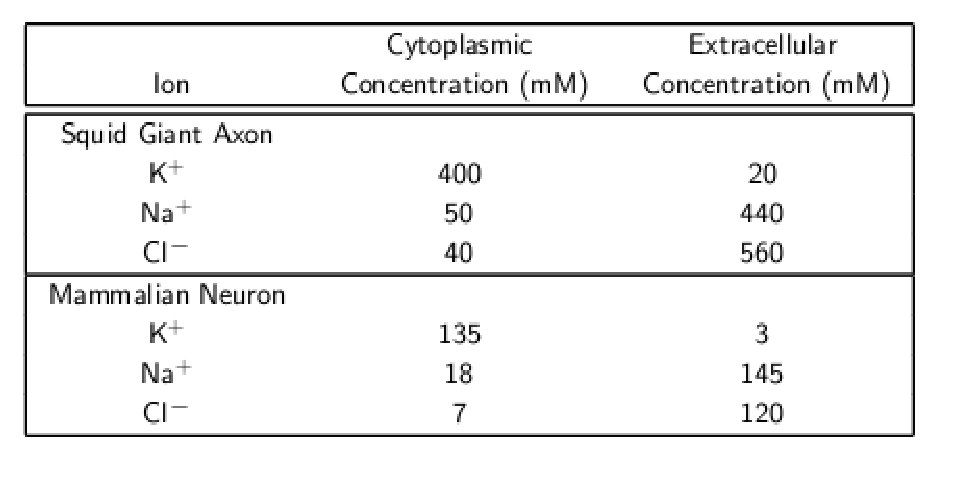
\includegraphics[height=4cm]{./images/ion_concentration.eps}}
  \caption{Ion concentration in squid giant axon and mammalian
    neuron}\label{fig:squid_axon-ion_con}
\end{figure}

\begin{figure}[htb]
  \centerline{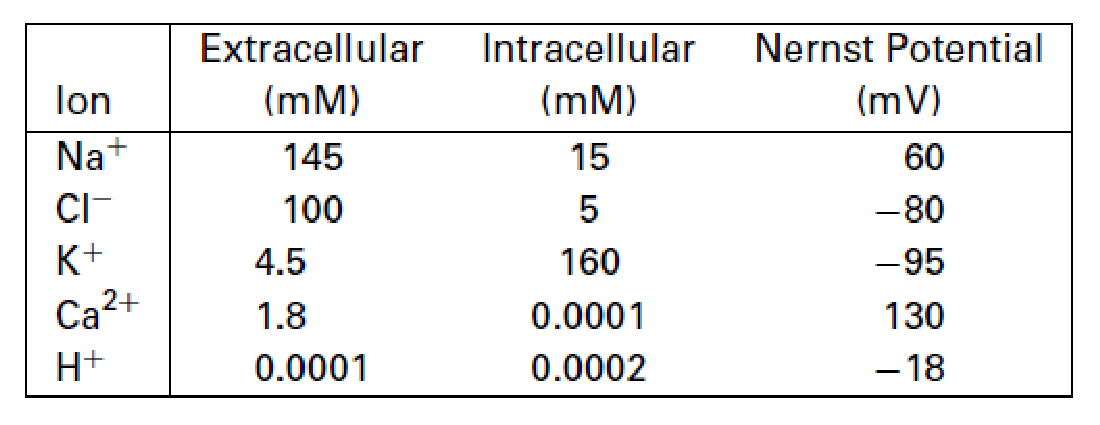
\includegraphics[height=3cm]{./images/ion_concentration_cardiac.eps}}
  \caption{Ion concentration in most cardiac
    cells}\label{fig:ion_con_cardiac}
\end{figure}


\section{Diffusion}
\label{sec:diffusion-2}

In 1D, an effective transport equation with an effective diffusion coefficient D
[$\mum^2$/s] and effective degradation rate k [1/s]:
\begin{equation}
\label{eq:reaction-diffusion-simple}
\frac{\partial c}{\partial t} = D \frac{\partial^2 c}{\partial x^2} - kc
\end{equation}
with the concentration $c$ (molecules/$\mum^3$) is a function of space and time, 
$c(x,t)$. For simplicity, we only write $c$. It is a partial differential
equation because it contains derivatives with respect to space and time
(Sect.\ref{sec:classification-pde}).
\begin{itemize}
  \item the first term is called the diffusion term
  \item the second term is called the reaction term. Here it represent the
  linear degradation (loss) (if $k>0$) and the production (if $k<0$) of the
  molecules of interest.

Sometimes, instead of the degradation rate $k$, the half-life of molecules
$\tau$ [s] is used. This is the time after which the concentration has been
reduced by half:
\begin{equation}
\frac{1}{2}c_i = c_i e^{-k\tau}
\end{equation}
or $k = ln(2)/\tau$.
In exponential gradients, the concentration decays by the same
 percentage at each position. 


   \item Non-linear degradation: the degradation rate $k$ is a function $k(c)$
   of the concentration 
\begin{equation}
\frac{\partial c}{\partial c} = -k(c).c
\end{equation}
with the special case: self-enhanced degradation
\begin{equation}
k(c) = k^* c^{n-1}; \;\;\; n>1
\end{equation}

\begin{equation}
\label{eq:reaction-diffusion-nonlinear}
\frac{\partial c}{\partial t} = D \frac{\partial^2 c}{\partial x^2} - k(c)
\times c
\end{equation}
 In the special case, the steady-state solution is 
 \begin{equation}
 c(x) = \frac{A}{(x+x_b)^m}
 \end{equation}
 As the concentration is proportional to $1/x^m$,
 the type of gradient is called {\it power-law gradient}.
Here, power-law gradients decay fast close to the source and more slowly at a
distance, i.e., their decay length-scale $\lambda_s$ is position-dependent and
reflects the local steepness of the gradient.
\begin{equation}
\begin{split}
\lambda_s = \frac{x+x_b}{m} \\
c_o = \frac{A}{x_b^m}
\end{split}
\end{equation}

  \item Linear degradation with directional bias:
  
  So far, no experimental evidence for spreading with directional bias has been
found, although it has been theoretically considered, although it has been
theoretically considered, e.g. morphogen molecules move by random walk, but
endogenous conditions make transport directional. This can be described by
regular diffusion plus a drift term, describing molecules moving with velocity
$v$ in a certain direction. 

A mechanism based on diffusion with drift and linear degradation leads to
exponential steady-state gradients, and the decay length is stretched or
compressed depending on the drift direction.

  
  \item directional {\bf active transport}, rather passive transport as
  described above.
  
  Example: vesicle movement on microtubule
  
  Active transport may be nondirectional, but it cannot be described by the
  diffusion equation, because it invokes forces.
  
  In passive transport (Fickian diffusion), the mean square displacement of
  freely diffusing molecules is linearly related to time.
  
  However, for actively transported molecules, this relationship is nonlinear.
  This is also true, for example, for molecules that are caged in polymer
  networks and thus do not diffuse freely.
  Such phenomena can be described by {\bf anomalous diffusion models}, which
  lead to the formation of exponential gradients.
   Continuous time random walk (CTRW) theory is used to model   \citep{hornung2005}
    
\end{itemize}
To understand how to solve the problem, read Sect.\ref{sec:morphogene}.

The diffusion coefficient of Bicoid has also been measured by FRAP (D = 0.3
$\mum^2$/s) (Gregor et al. 2007), whereas its degradation rate $k$ is unknown.

 The diffusion of calcium is in the range of 250-300$\mu$m$^2$/s in the
cytosol, and 100-150$\mu$m$^2$/s in the network SR. 
The diffusion values of other molecules are shown in Fig.~\ref{fig:diffusion_values}.

\begin{figure}[hbt]
 \centerline{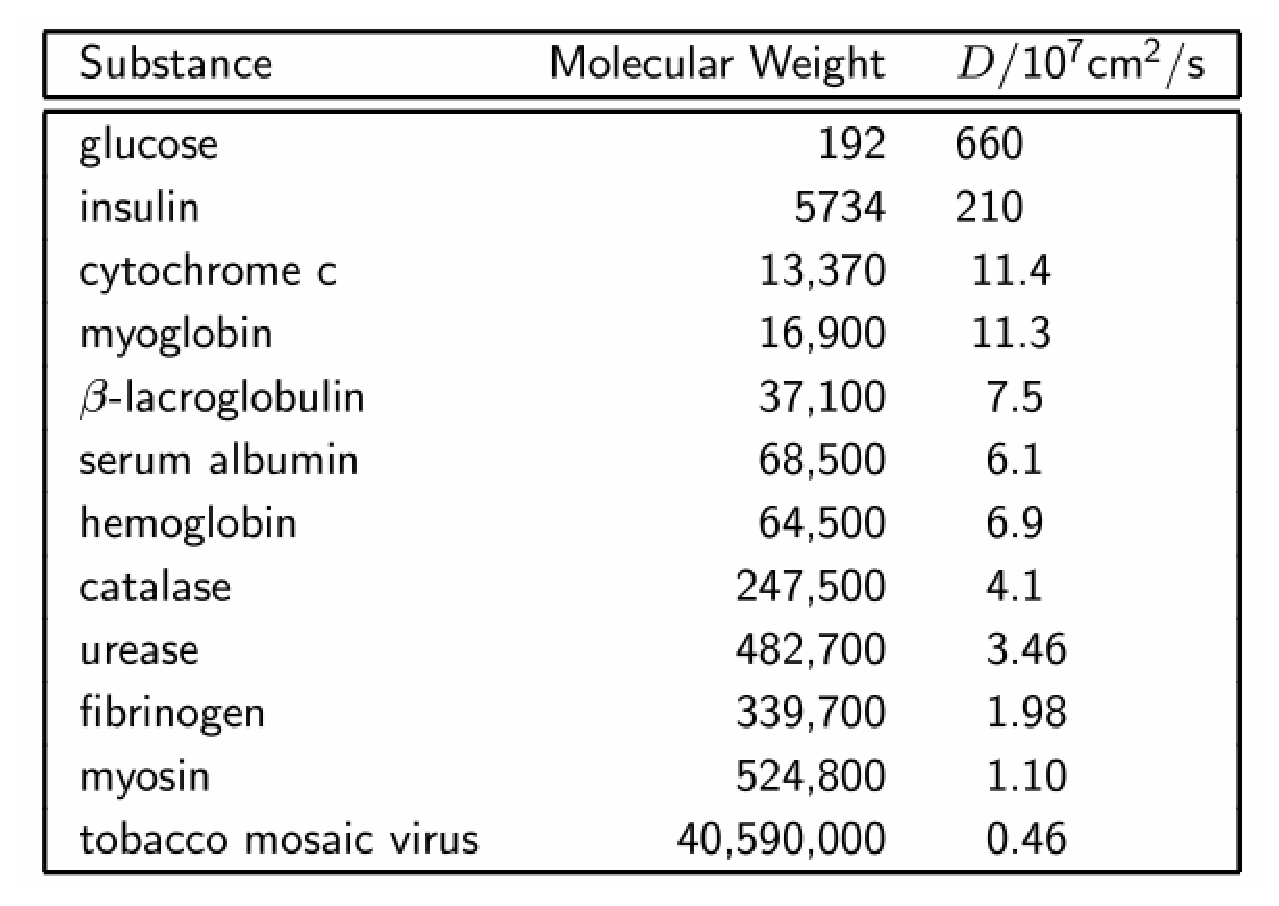
\includegraphics[height=5cm, angle=0]{./images/diffusion_values.eps}}
\caption{Molecular weight and diffusion coefficients of some
  biochemical substances}
\label{fig:diffusion_values}
\end{figure}

For isotropic (or spherical symmetric), the diffusion part is written as
\citep{crank1975}
\begin{equation}
\nabla \cdot (D_c\nabla C) = D_C \left( \frac{\partial^2 C}{\partial r^2} +
\frac{2}{r}\frac{\partial C}{\partial r} \right)
\end{equation} 
and for anisotropic diffusion, the formula is
\begin{equation}
\nabla \cdot (D_c\nabla C) = D_{Cx}\frac{\partial^2 C}{\partial x^2} +
D_{Cy}\frac{\partial^2 C}{\partial y^2} + 
D_{Cz}\frac{\partial^2 C}{\partial z^2} 
\end{equation}


\section{Electronic concepts}
\label{sec:basic-concepts}

The values for typical parameters are given in
Fig.~\ref{fig:cable_param}. 

\begin{figure}[hbt]
  \centerline{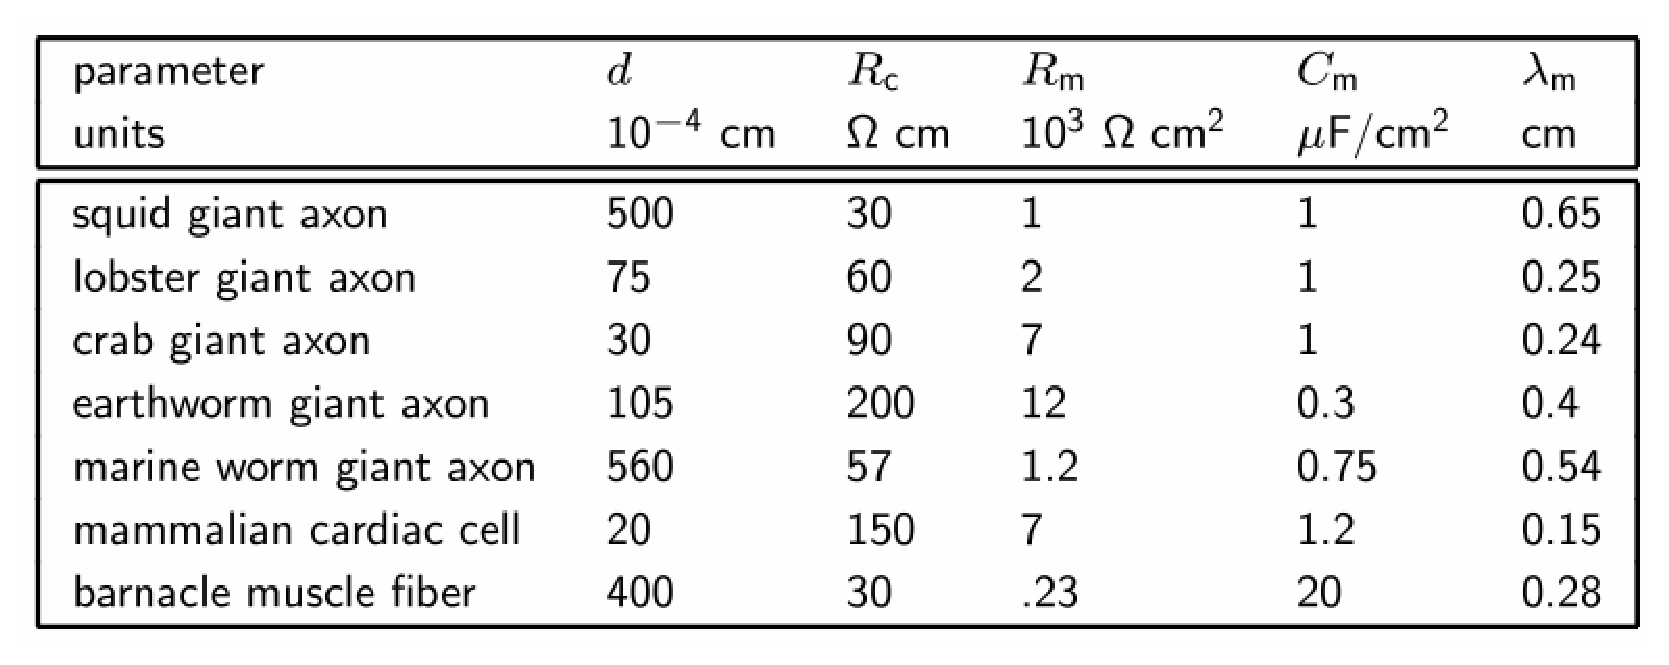
\includegraphics[height=5cm,
    angle=0]{./images/cable_parameters.eps}}
  \caption{Typical cable parameter values for a variety of excitable
    cell types (Keener an Sneyd (1998))}
  \label{fig:cable_param}
\end{figure}

\subsection{Electric time constant}
\label{sec:time-constant}

Consider a circuit of RC in parallel (Sect.\ref{sec:core-conductor-membrane}).
The time constant $\tau$ is
\begin{equation}
\tau = r_m c_m
\end{equation}

It is the time require to charge 63.2\% (or $e$-fold or $\sim 2/3$) of the
capacitor or to discharge it to 36.8\% (or $1/e$-fold) of its initial voltage is
known as the {\bf time constant} of the circuit.
\begin{eqnarray}
  \label{eq:490}
  \tau = \text{RC}
\end{eqnarray}
with R in unit Ohm, C in unit farad (F or
Coulomb/Voltage)\footnote{\url{http://www.tpub.com/neets/book2/3d.htm}}


\subsection{Membrane time constant}
\label{sec:membr-time-const-1}

Similarly, the concept of ``time constant'' is also important to
neurology. It tells how fast the neuron response to the synaptic input
or applied current (current injection), i.e. neuron's ``response
time''. In other words, it tells, when there is a synaptic input, how
long would it take for the neuron's membrane potential $V_m(t)$ to
increase/decrease $e$ times~\citep{koch1966htc}
(Sect.\ref{sec:membrane-time-constant}).

It is defined as
  \begin{equation}
    \label{eq:684}
    \tau = \Rm \Csc = \frac{\Csc}{g_\sc}
  \end{equation}
  with $g_\sc=\sum_i g_i$ (mS/cm$^2$) is the total conductance per unit
  area of membrane, $\Csc$ is specific membrane capacitance
  ($\mu$F/cm$^2$). The conductance is proportional to the number of open ion
  channels, and the capacitance is the function of the properties of the
  lipid bilayer. 
  
The time constant is used to describe how fast/slow the  rise and fall of the
membrane potential in response to the stimulus (i.e. injected current)
  \begin{equation}
    \label{eq:718}
    \begin{split}
      V_m &= V_{max}.(1-e^{-t/\tau})  \; \; \text{ rise} \\
      V_m &= V_{max}.e^{-t/\tau}  \; \; \text{ fall} \\
    \end{split}
  \end{equation}
  The meaning of this is that:
  \textcolor{red}{{\it the larger the time constant, the slower the rise or fall of the
      potential}}.

\section{Standard units}
\label{sec:standard-units}

To avoid the variation between cells, all quantities are determined
based on a unit of membrane area, except the voltage. The information
is given in Table~\ref{tab:terminology_2}.


\begin{table}[hbt]
  \begin{center}
    \caption{Standard units}
    \begin{tabular}{lr}
      \hline
      voltage (potential) & mV \\
      characteristic time constant ($\mathcal{T}$) & millisecond (ms) \\
      membrane time constant ($\tau_m$) & Farad.S or Farad.Ohm$^{-1}$ \\
      exponential time constant  ($\tau$) & sec \\
      + relaxation (decay/growth) time constant & \\
      currents ($I_i$) & $\mu$A.cm$^{-2}$ \\
      capacitances (C) & $\mu$F.cm$^{-2}$ \\
      conductances ($g_i$) & mho.cm$^{-2}$, m mho.cm$^{-2}$, n mho.cm$^{-2}$ \\
      cellular dimension & micrometer (micron) $\mu$m \\
      & $10^{-8}$cm$^2$ =  micron square\\
      the order of conductance $g$  & 1 to 150 pS \\
      whole-cell conductance of nanosiemens & mS.cm$^{-2}$ \\
      maximum possible conductance $\overline{g}$ & (mho/cm$^2$,mmho/cm$^2$,
      nmho/cm$^2$) \\
      concentration [X] & mM (milimolar, or milimole per litre)\\
      fraction of open channel ($f,f_\infty$) & unitless\\
      cell volume $V_{cell}$ & pL = $10^3\mu$m$^3$\\
      myoplasm volume $V_{myo}$ & \\
      network SR volume $V_{nsr}$ & \\
      
    \end{tabular}
  \end{center}
  \label{tab:terminology_2}
\end{table}

% In electrostatic, the work required to move a quantity of charge Q
% from point O to P is
% \begin{equation}
%   \label{eq:1219}
%   W_e = Q (\Phi_P-\Phi_O)
% \end{equation}
% with $V_m = \Phi_{out}-\Phi_{in}$ is the potential (mV), charge Q [C]
% (coulombs) and $W_e$ is work (J/mol). 
% In electrophysiology, the quantity of ions is often expressed in {\it
%   moles}. If one mole of ions is transferred, from point O to P, the
% work required is
% \begin{equation}
%   \label{eq:1220}
%   W_e = z_{ion}F(\Phi_P-\Phi_O)
% \end{equation}
% with $z_{ion}$ is the valence of the ion (e.g. $z_\ca=2$) [unitless],
% F is Faraday constant [C/mol]. Faraday constant convert the quantity
% of moles to the quantity of charges for a univalent ions; that's why
% we need to multiply the valence for non-univalent ions. 
% 
% When a force exerts on a unit charge, an electric field is
% defined. The work required to move a unit positive charge against the
% electric field $\overline{E}$ is
% \begin{equation}
%   \label{eq:1221}
%   dW = -\overrightarrow{E}\cdot\overrightarrow{ds}
% \end{equation}
% with $\overrightarrow{ds}$ is the vector displacement. Replacing
% $Q=1$ in eq.~\eqref{eq:1219}, then we have
% \begin{equation}
%   \label{eq:1222}
%   \Phi_P-\Phi_O =  -\overrightarrow{E} \cdot \overrightarrow{ds}
% \end{equation}
% Using Taylor series expansion
% \begin{equation}
%   \label{eq:1223}
%   \Phi_P= \Phi_O \frac{d\Phi}{ds} + ...
% \end{equation}
% If we neglect the higher order term, and keep the first term only.


% The {\bf current density} $\overrightarrow{J}$ and electric field
% $\overrightarrow{E}$ are related by
% \begin{equation}
%   \label{eq:1224}
%   \overrightarrow{J} = \sigma \overrightarrow{E} = -\sigma \nabla \Phi
% \end{equation}
% with $\sigma$ is the conductivity of the medium. If we're interested
% in the ions, the flux $j$ of these ions are subject to the electric field
% force, and is dependent upon the electric resistance, which in turns
% is a function of ionic mobility $u$ of the ionic species. 
% \begin{equation}
%   \label{eq:1225}
%   \overrightarrow{j_e} = u \frac{z}{|z|}c\nabla \Phi
% \end{equation}
% with $c$ is the ionic concentration [mol/cm$^3$], z = valence
% [unitless], u = ionic mobility [cm$^2$/(V.sec)], and
% $\overrightarrow{j_e}$ = ionic flux (due to electric field)
% [mol/(cm$^2$.sec)]. 
% 
% If, the ionic concentration is not uniform between adjacent
% compartments, there is a passive redistribution of ionic
% concentration, called {\bf diffusion}
% \begin{equation}
%   \label{eq:1226}
%   \overrightarrow{j_D} = -D\nabla c
% \end{equation}
% with D = diffusion constant [cm$^2$/sec], c = ionic concentration
% [mol/cm$^3$], $\overrightarrow{j_D}$ [mol/(cm$^2$.sec)].
% 
% \begin{framed}
%   A connection between ionic mobility $u$ and diffusion constant $D$
%   is
%   \begin{equation}
%     \label{eq:1227}
%     D = \frac{u.R.T}{|z|F}
%   \end{equation}
% with T = absolute temperature [K], R = Faraday constant [J/(mol.K)]
% \end{framed}
% 
% The {\bf Nernst-Planck equation} describes the flux of an ion under
% the affect of diffusion and electric field.
% \begin{equation}
%   \label{eq:1228}
%   \begin{split}
%     \overrightarrow{j} = \overrightarrow{j_D} + \overrightarrow{j_e} =
%     -D (\nabla c + \frac{c.z.F}{R.T}\Delta \Phi) 
%  \end{split}
% \end{equation}
% with $\overrightarrow{j}$ = ionic flux [mol/(cm$^2$.sec)]. We can
% easily convert the ionic flux to the electric current density $J$ by
% multiplying the ionic flux by $zF$ (i.e. the number of charges carried
% by each mole)
% \begin{equation}
%   \label{eq:1242}
%   \begin{split}
%     J = -DzF (\nabla c + \frac{c.z.F}{R.T}\Delta \Phi) \\
%     = - \left(u.R.T.\frac{z}{|z|}\nabla c + u.c.|z|F\nabla\Phi\right)
%   \end{split}
% \end{equation}
% with $J$ = electric current density [C/(sec.cm$^2$)] = [A/cm$^2$].
% 
% \begin{framed}
%   {\bf Nernst equation}: At equilibrium, there must be no current, or
%   \begin{equation}
%     \label{eq:1229}
%     \overrightarrow{j} = 0 =     -D (\nabla c +
%     \frac{c.z.F}{R.T}\Delta \Phi)  
%   \end{equation}
% or
% \begin{equation}
%   \label{eq:1230}
%   \nabla c = -\frac{z.F}{R.T}\Delta \Phi 
% \end{equation}
% or
% \begin{equation}
%   \label{eq:1231}
%   \frac{dc}{c} = -\frac{z.F}{R.T} .d\Phi 
% \end{equation}
% If we integrate from the intracellular space (i) to the outer
% extracellular space (o)
% \begin{equation}
%   \label{eq:1232}
%   \int^o_i  \frac{dc}{c} = \ln c|^o_i = -\frac{z.F}{R.T} \int^o_i d\Phi 
% \end{equation}
% or 
% \begin{equation}
%   \label{eq:1233}
%   \ln \frac{c_o}{c_i} = -\frac{z.F}{R.T} (\Phi_o-\Phi_i)
% \end{equation}
% \end{framed}

% The {\bf Goldman-Hodgkin-Katz equation} assumes that the membrane is
% planar, uniform and infinite in the lateral extent. Also, if $x$-axis
% is chosen normal to the membrane surface with the origin at the
% interface of the membrane with the extracellular region, $x=h$ is the
% thickness of the membrane (Sect.\ref{sec:membrane-thickness}), the variation of
% the potential field $\Phi$ is the function of $x$ only. 
% \begin{equation}
%   \label{eq:1234}
%   \frac{d\Phi}{dx} = \frac{\Phi_i-\Phi_o}{h}=\frac{V_m}{h}
% \end{equation}
% then, using eq.~\eqref{eq:1228}
% \begin{equation}
%   \label{eq:1235}
%   \overrightarrow{j} = -D(\frac{dc}{dx}+\frac{c.z.F}{R.T}\frac{d\Phi}{dx})
% \end{equation}
% or
% \begin{equation}
%   \label{eq:1236}
%   \frac{dc}{dx}=  -\frac{\overrightarrow{j}}{D}- \frac{V_m.z.F}{h.R.T}c
% \end{equation}
% or
% \begin{equation}
%   \label{eq:1237}
%   \frac{dc}{ -\frac{\overrightarrow{j}}{D}- \frac{V_m.z.F}{h.R.T}c} = dx
% \end{equation}
% If we assume a constant field approximation, i.e. $\overrightarrow{j}
% = \text{constant} = j$, so only $c$ is the function of $x$, we
% integrate both side from $x=0$ to $x=h$, then
% \begin{equation}
%   \label{eq:1238}
%   -\frac{hRT}{V_mzF}\ln\left(\frac{\frac{j}{D}+\frac{V_mzF}{hRT}c^{(h)}}{\frac{j}{D}+\frac{V_mzF}{hRT}c^{(0)}}\right) = h
% \end{equation}
% or
% \begin{equation}
%   \label{eq:1239}
%   j = -\frac{DV_mzF}{RTh} \frac{c^{(h)}-c^{(0)}\exp(-V_m\frac{zF}{RT})}{1-\exp(-V_m\frac{zF}{RT})}
% \end{equation}
% However, the measurable concentration are those in the intracellular
% and extracellular (bulk) space, and the formula use the concentration
% from just outside or just inside the membrane. So, if we assume they
% are scaled by a {\it partition coefficient $\beta$}, then
% \begin{equation}
%   \label{eq:1240}
%   \begin{split}
%     c^{(h)} = \beta_o c_o \\
%     c^{(i)} = \beta_i c_i \\
%   \end{split}
% \end{equation}
% with $c_i,c_o$ are measurable ionic concentration inside and outside,
% respectively. Finally, the {\bf Goldman-Hodgkin-Katz equation} is
% \begin{equation}
%   \label{eq:1241}
%   j = -\frac{DV_mzF}{RTh} \frac{\beta_ic_i-\beta_o c_o\exp(-V_m\frac{zF}{RT})}{1-\exp(-V_m\frac{zF}{RT})}
% \end{equation}
% Typically, we assume the partition coefficients are the same,
% i.e. $\beta_o =\beta_i = \beta$. 
% \begin{equation}
%   \label{eq:1245}
%   j = -\frac{\beta DV_mzF}{RTh} \frac{c_i- c_o\exp(-V_m\frac{zF}{RT})}{1-\exp(-V_m\frac{zF}{RT})}
% \end{equation}
% The electric current density, against, is computed by multiplying the
% flux with $zF$.
% 
% 
% The {\bf permeability} of an ion is defined as $P$ [cm/sec]
% \begin{equation}
%   \label{eq:1243}
%   P = \frac{D.\beta}{h}
% \end{equation}
% then the electric current density is
% \begin{equation}
%   \label{eq:1244}
%   J =  -\frac{P.V_mz^2F^2}{RT} \frac{\beta_ic_i-\beta_o c_o\exp(-V_m\frac{zF}{RT})}{1-\exp(-V_m\frac{zF}{RT})}
% \end{equation}
% Using this equation, if we consider a channel is permeated to more
% than one ion, say $\Ca$ channel is permeated by $\Ca, \Na$ and $\K$
% ions with 3 different permeability $P_\ca, P_\na, P_\k$ then at equilibrium
% \begin{equation}
%   \label{eq:1246}
%   J = J_\ca + J_\na + J_\k = 0
% \end{equation}
% or 
% \begin{equation}
%   \label{eq:1247}
%   \begin{split}
%     P_\k\left[c_{i,\k} - c_{o,\k}\exp (-\frac{E_mF}{RT}\right] &+
%     P_\na\left[c_{i,\na} -
%       c_{o,\na}\exp (-\frac{E_mF}{RT}\right] + \\
%     &P_\ca\left[c_{i,\ca} - c_{o,\ca}\exp (-\frac{E_mF}{RT})\right] = 0
%   \end{split}
% \end{equation}
% or
% \begin{equation}
%   \label{eq:1248}
%   P_\k c_{i,\k} +   P_\na c_{i,\na} +   P_\ca c_{i,\ca}  =
%   \exp(-\frac{E_mF}{RT}) \left(  P_\k c_{o,\k} +   P_\na c_{o,\na} +   P_\ca c_{o,\ca} \right)
% \end{equation}
% and the membrane potential at which the (net) membrane current is zero
% is called the {\bf reversal potential} $E_m$ which is defined via the
% so-called {\bf Goldman-Hodgkin-Katz} (GHK) equation as follows
% \begin{equation}
%   \label{eq:1249}
%   E_m = -\frac{RT}{F} \ln \frac{P_\k c_{i,\k} +   P_\na c_{i,\na} +   P_\ca c_{i,\ca}}{P_\k c_{o,\k} +   P_\na c_{o,\na} +   P_\ca c_{o,\ca}}
% \end{equation}
% 
% 
% 
% When performing any of the calculation between those quantities, it's
% important to know their units.  Standard units are: milivolts,
% miliseconds, nanofarads, nanoamperes, microsiemens (mS)
% \begin{verbatim}
% nF .mV/mS = nA = uS . mV
% \end{verbatim}
% 
% 
% However, in physiology, a better convention for some units is to
% define them {\it per unit of surface area}. This will avoid the
% geometrical difference between cells. The surface area of a neuron
% might be $3\times 10^4 \mu$m$^2$, or $3\times 10^{-2}$cm$^2$.  So, the
% new units are nanofarads per centimeters, nanoamperes per square
% centimeters, milisiemens per square centimeters.
% \begin{verbatim}
% (uF/cm^2) . mV/mS = uA/cm^2 = (mS/cm^2) . mV
% \end{verbatim}
% The quantities that are unaffected are milivolts, miliseconds. 
% 
% So, we use $\Csc$ (nF/cm$^2$) and $R_m$ ($\Omega$.cm$^2$).
% 



\section{Physical \& Chemical terms}
\label{sec:physical--chemical}

An ion's {\bf valence} is the number of charges, plus or minus, that
it carries. So, \ce{Ca^2+} is a {\it divalent}, while \ce{K+} is a
{\it univalent}.

If the permeability of \ce{K+} is considered one, the permeability of
other ions across the membrane is represented by the equation
\begin{eqnarray}
  \label{eq:539_copy}
  P_{\ce{K+}}:P_{\ce{Na+}}:P_{\ce{Cl-}} = 1:0.05:0.45
\end{eqnarray}

\section{Statistical tests}
\label{sec:statistical-tests}

The test for significant was two-tailed ANOVA among multiple
groups. For pairwise comparison, they used Student's t test. Differences
were considered significant when p-value $< 0.05$. 

\section{Tools for electrophysiology}

Data were analyzed with Igor Pro (Version 4, Wavemetrics, Lake
Oswego, OR), Clampfit 8 (Axon Instruments, Union City, CA) or
Mini Analysis (Synaptosoft, Decatur, GA).

For samples $>$10, central tendency was estimated by computing
a mean (mean $\pm$ SE); for smaller samples, medians were computed. 

Differences between samples were analyzed with a Student's t-test (large
samples) or a paired Wilcoxon signed-rank test (small samples).

\subsection{Tools for spike shape parameters extraction}

Spike shape parameters were measured using the Mini Analysis routines.
Specifically, spike threshold was determined by locating the membrane voltage at
which the second derivative of the spike waveform exceeded three times its SD in
a period before the spike onset.

Spike amplitude was defined as
the difference between the peak and the baseline of action potential.
Spike width was measured at half the spike amplitude. The afterhyperpolalization
was defined as the difference between the spike baseline
and the minimum membrane voltage after the action potential
peak.


%%% Local Variables: 
%%% mode: latex
%%% TeX-master: "mainfile"
%%% End: 

 
\chapter{Introductory}
\label{chap:introductory}
Prerequisites: calculus, biology

\section{Dynamical phenomenon}
\label{sec:dynamic-phenomena}

Generally speaking, a dynamical phenomenon is any process that instantly changes
over time. In that sense, a living cell is a dynamical process, with cell
growth, cell division, intracellular communication (like ion exchanges in
response to some cellular event), signal transduction, cell movement, etc. Even
though a single cell is a completed entity, it needs to use the energy and to
exchange matters (intake oxygen and expell wastes). Thus, a cell is not a closed
system. However, due to the fact that not everything can come into or expel from
the cells; cells are {\it selectively open
  systems}\footnote{ NOTE: the universe = the system + its surrounding

  + Isolated system = system that exchanges neither energy nor matter
  with its surroundings

  + Closed system = system that exchanges energy but not matter with
  its surroundings

  + Open system = it exchanges both energy and matter with its
  surroundings (such system takes in resources (energy, matters) from
  its environment, process them in some way, and produces output
  (energy, matters)). This concept is originally developed from
  thermodynamics.

  In real world systems, there is no complete isolated or closed
  system. Further, there is no true open system, but
  {\it selectively open system}. In other words, a selectively open
  system is, in need, open to some and closed to other influences.
  Cells have a mechanism to repel or digest strange particles, yet
  allow necessary particles (ions, \ce{CO2}...)  to get into the
  intracellular environment, i.e. the {\it cytoplasm}.  }.

Another unique characteristic of cells is that they are far from
{\it equilibrium}, if not never in equilibrium, i.e. there is always
influx and efflux of particles across the biomembrane.  We may be
interested in:
\textcolor{red}{what kinds of energies and matters does a cell
  accept?}
and
\textcolor{red}{from where do cells obtain these
  \hyperref[sec:resources-energy]{energies} and
  \hyperref[sec:resources-matters]{matters}?}.

\subsection{Resources of energy}
\label{sec:resources-energy}

Glucose \ce{C6H12O6} is an important energy source for cells in both
plants and vertebrates.
Plants obtain (radiant) energy from sunlight, i.e. photons which helps
making glucose, as given in the following equation
% \begin{center}
% \ce{6CO2_{(g)} + 12 H2O_{(g)} + photons ->[\text{enzyme}] C6H12O6_{(aq)} + 6O2_{(g)} + 6H2O_{(1)}}
% carbon dioxide + water + light energy \ce{->} glucose + oxygen + water
% \end{center}

\begin{center}
\ce{ $\underset{\text{carbon dioxide}}{\ce{6CO2_{(g)}}}$ +
$\underset{\text{water}}{\ce{12 H2O_{(g)}}}$
 + $\underset{\text{light energy}}{\text{photons}}$ ->[\text{enzyme}]
$\underset{\text{glucose}}{\ce{C6H12O6_{(aq)}}}$ +
$\underset{\text{oxygen}}{\ce{6O2_{(g)}}}$ + 
$\underset{\text{water}}{\ce{6H2O_{(1)}}}$
}
\end{center}


Unlike plants, vertebrates don't have the proper enzymes to enable
the glucose synthesis from sun light. Thus, they obtain energy
(nutrients) from foods in a process known as {\it metabolism process}
whose reactions are called {\bf metabolic reactions}
(Sect.\ref{sec:metabolic-reactions}).

\subsection{Metabolic reactions}
\label{sec:metabolic-reactions}
\label{sec:anabolic-reaction}

There are two
classes of metabolic reactions\footnote{\url{http://www.scienceclarified.com/Ma-Mu/Metabolism.html}}:
{\it catabolic reactions} and {\it anabolic reactions}.
\begin{itemize}
\item In the catabolism process (Sect.\ref{sec:catabolic-energy-metabolism}),
  complex molecules from foods, with the support of enzymes, are broken down
 into simple molecules and releases energy. 
  
  The total amount of simple molecules is called {\it metabolic pool}.

\item In the anabolism process, the released energy from catabolism
  process is used to build other complex molecules
  (i.e. biomolecules), or for other purposes 
(e.g. keeping body warm). 

The remaining unused energy are stored in the body for later use in the form of
ATP (Sect.\ref{sec:ATP-synthesis}) or fat
\footnote{\url{http://www.scienceclarified.com/Ma-Mu/Metabolism.html}}.

\end{itemize}

\subsection{Resources of matters}
\label{sec:resources-matters}

At the macro level, the resources of matters that plants need are
photons, \ce{CO2}, \ce{H2O}... and vertebrates need are various kinds
of nutrients in the form of food, beverages...  The constituents of
nutrients can be
\begin{enumerate}
\item
  carbohydrate\footnote{carbohydrate is a compound consisting of
    carbon, oxygen, and hydrogen} $\rightarrow$ sugar
\item lipids $\rightarrow$ fatty acids, glycerol
\item proteins $\rightarrow$ amino acids
\end{enumerate}


At the micro level, we're focusing on how and what a cell exchanges to
each other and to extracellular environment. Matters that cells
exchange to each other and to extracellular environment can be ions
(\ce{Ca^2+}, \ce{K+}, \ce{Na+}...), proteins and some other substances
whose amount can vary depending upon the {\bf state} of the cell.

A cell, as a dynamical system, is modeled to undergo through a number of
different states. How the state of a cell is defined varies depending upon how
detailed of the cell we want to model. Normally, the state of a dynamic model is
represented in a qualitatively way by a set of {\bf state functions}
(Sect.\ref{sec:state-functions}).
This will be covered in the next section. % Here, we meet the concept of state.

\section{Mathematical biology: Computational modelling in biology}
\label{sec:comp-modell-biol}

This book will introduces different useful computational models, and how to
develop a good one, starting from models for different types of cellular
components (e.g. ion channels, pumps, exchanger) from asbtract level to mechanistic level,
and then at the whole cell level, which we target electrical excitable cells for
the heart and the brain.

{\bf Mathematical biology}, the branch of math applied in biology, is
a strong and well-developed branch of applied mathematics.  Let's
review

\begin{enumerate}
\item  {\it why we need a model}?
  \begin{itemize}
  \item all quantities of interest cannot be measured {\it in
      vivo}.
    Some of these can be obtained {\it in vitro} on small tissue
    preparation or isolated cells.

  \item the ultimate purpose is to study the dynamics of the whole
    cells, not just a part or a small cell of it.

  \item computer simulation, {\it in silico}, can yield the hidden
    information that we cannot obtain from {\it in vivo} or
    {\it in vitro} measures.
  \end{itemize}

\item {\it What is a good model}?
  \begin{itemize}
  \item a too simple model fails to capture the salient behavior and
    have limited predictive capability

  \item a too complex model can be computationally intractable.

  \item a good model depends on the questions being answered.
  \end{itemize}
\end{enumerate}

\subsection{Challenges in computational biology}

To study a dynamical system (Sect.\ref{sec:dynamic-phenomena}), i.e.
understanding the dynamic of the system, we need a means to record how the
system changes over time.

To observe the changes from a real system, in laboratories, data are record
periodically. This is not a trivial task as in nature, even the simplest dynamic
phenomena are exceedingly complex, especially in molecular processes.
For example, in many problems, it's not easy to follow the changes due to the
tiny time scale (i.e. the temporal resolution of the recorder is not high
enough) or the signal is too small (i.e. the spatial resolution of the recorder
is not high enough) or due to the rareness of the event (i.e. it may take months
or years for a change to happen).

Given that challenges, computational modelling aims at deriving the systematical
change of a system based on the experimental data.  Even though computational
models will never be as useful as laboratory data in terms of providing a
concrete view about a physiological process, it does provide a quantitative
understanding where conducting an experiment is very expensive or hard to do. As
one said: there is no accurate models, but there are useful models.

A good model can reproduce experimental data that were used to create them.
However, a useful model is not only a good model, but is also capable of
predictive. That is, they can be used to guide making decision in hypothesis
testing, medical treatment, or in drug developments.
Useful models need to be designed following closely with experimental data,
using some mathematical formulations to describe the dynamical process
(Sect.\ref{sec:dynamic-phenomena}).

Before we can develop such models for a particular problem domain, we need to
understand how to represent a dynamical system
(Sect.\ref{sec:representing-system}).

\subsection{Representing a system: state functions, state space}
\label{sec:representing-system}
\label{sec:state-functions}
\label{sec:state-space}

A system can be studied when it reaches the steady state condition. To gain the
maximal control of the system, and to avoid any undesired affects, such a system
is often examined with the assumption of a {\bf conserved system}, i.e. by
disturbing a little bit the parameter, the system go through a number of change
but no loss in energy. Thus, the change in the system can be considered as going
through a number of reversible steps. Sect.~\ref{sec:reversible-vs.-non} will
discuss why the assumption of a reversible system is important.

% After reading the previous section, we now agree that cells are dynamic.
From the view point of thermodynamics, a dynamical system can be uniquely
determined throught its current state.
Thus, to study the behavior of a dynamic phenomenon, it's important to know the
{\bf states} of the process/system/phenomenon at different time points. This
state is often determined by a set of parameters whose values do not depend upon
how the system reaches that state. It means that the values of such parameters
are functions of state; i.e. a parameter is called a {\bf state function}
\footnote{Read ThermoStat book, Chapter 5 (Thermodynamics System-State) for more
detail}.

\begin{mdframed}
  
  In a thermodynamic system, there are many quantities that are
  considered as state functions: pressure ($p$), volume ($V$),
  temperature ($T$), internal energy ($U$), mass ($m$), energy ($E$),
  Helmholtz free energy ($F$ or $A$), Gibbs energy ($G$)\footnote{The word
  ``free'' in Gibbs free energy was banished since 1988 by IUPAC},
  entropy ($S$), enthalpy ($H$).
  Among them, {\it Gibbs (free) energy function} is the most important and the
  most widely used. % So, by using a subset of such quantities, we can
  % fully describe a system.
\end{mdframed}

The smallest set of state functions that can fully characterize a system forms
the {\bf state space} of that system; and its size is called the {\bf dimension}
($D$) of the state space of the system. It's important to know that this set is not
unique and the choice a specific state space varies from problem to problem. 

{\bf Example}: a system of monatomic gas with a fixed number of particles has $D
= 2$, i.e. the system is uniquely determined by 2 parameters. The two widely
state spaces are (1) $V$ and $T$; (2) $T$ and $p$. In essence, the two state
spaces ($p,T$) and ($V,T$) are equivalent, and simply form two different
coordinate systems on which we can study the dynamics of the system.

If we assign an energy level with each state, the set of all states can form one
or more energy wells (or potential wells). A state of a dynamical system can be
stable and unstable; and those with energy at the bottom of the energy wells are
stable states. As a dynamical system, the system can change from one state to
another, in a reversible or irreversible way.

With the current limitation of mathematical tools, we can only study a dynamical
system (i.e. examine the values of the state functions) under the assumption of
stable state or equilibrium state, from where we can assume any pertubation is a
reversible process (Sect.\ref{sec:reversible-vs.-non}).
% \textcolor{red}{As a matter of fact, the condition of equilibrium is very
% important in studying the dynamics of a system using computational tools}. In
% the next section, we'll discuss why the assumption of reversible is important
% and how to represent a dynamical system to study at equilibrium state
% (Sect.\ref{sec:reversible-vs.-non}).
  
\subsection[Quasi-statics vs. Reversible vs. Non-reversible]{Quasi-statics vs.
reversible vs. non-reversible systems}
\label{sec:reversible-vs.-non}

The condition of equilibrium is very important in studying the dynamics of a
system using available computational tools (Sect.\ref{sec:repr-dynam-syst}).

{\bf Why can't we study an irreversible process and if we have
  reversible process, how can we study it?}
- In a non-reversible system, the amount of work that we actually get out of the
system is always less than the input energy and the amount of useless energy
depends upon how the system was designed and the material involved. To take into
account the loss, we may need to incorporate the entropy into the simulation
(Sect.\ref{sec:entropy}).
Also, calculus cannot be used; since measurable steps are not in uniform
infinitesimal jumps.  So, it's hard to study such systems and compare them using
our current available computing power as well as mathematical language.

As a matter of fact, we mainly study the dynamics of a closed system under the
``reversible'' assumption. In such idealized system, there is no energy loss,
i.e. no entropy. Thus, in a small enough time interval, the change is considered
ideally {\it
  reversible}\footnote{An irreversible process occurs in certain direction. Once
  the process having been taken place, the system cannot go back to its previous
  state. A reversible process is a process that can be reversed without leaving
  any trace during its change. In practice, a truly reversible process does not
  exist. The real process are irreversible}.
A reversible process can be represented by differential equations to derive the
results and these results are independent of the materials used to construct a
particular system. The widely mathematical tool to study such systems is
calculus (ODE and PDE) - Sect.\ref{sec:repr-dynam-syst}.


\begin{figure}[hbt]
  \centerline{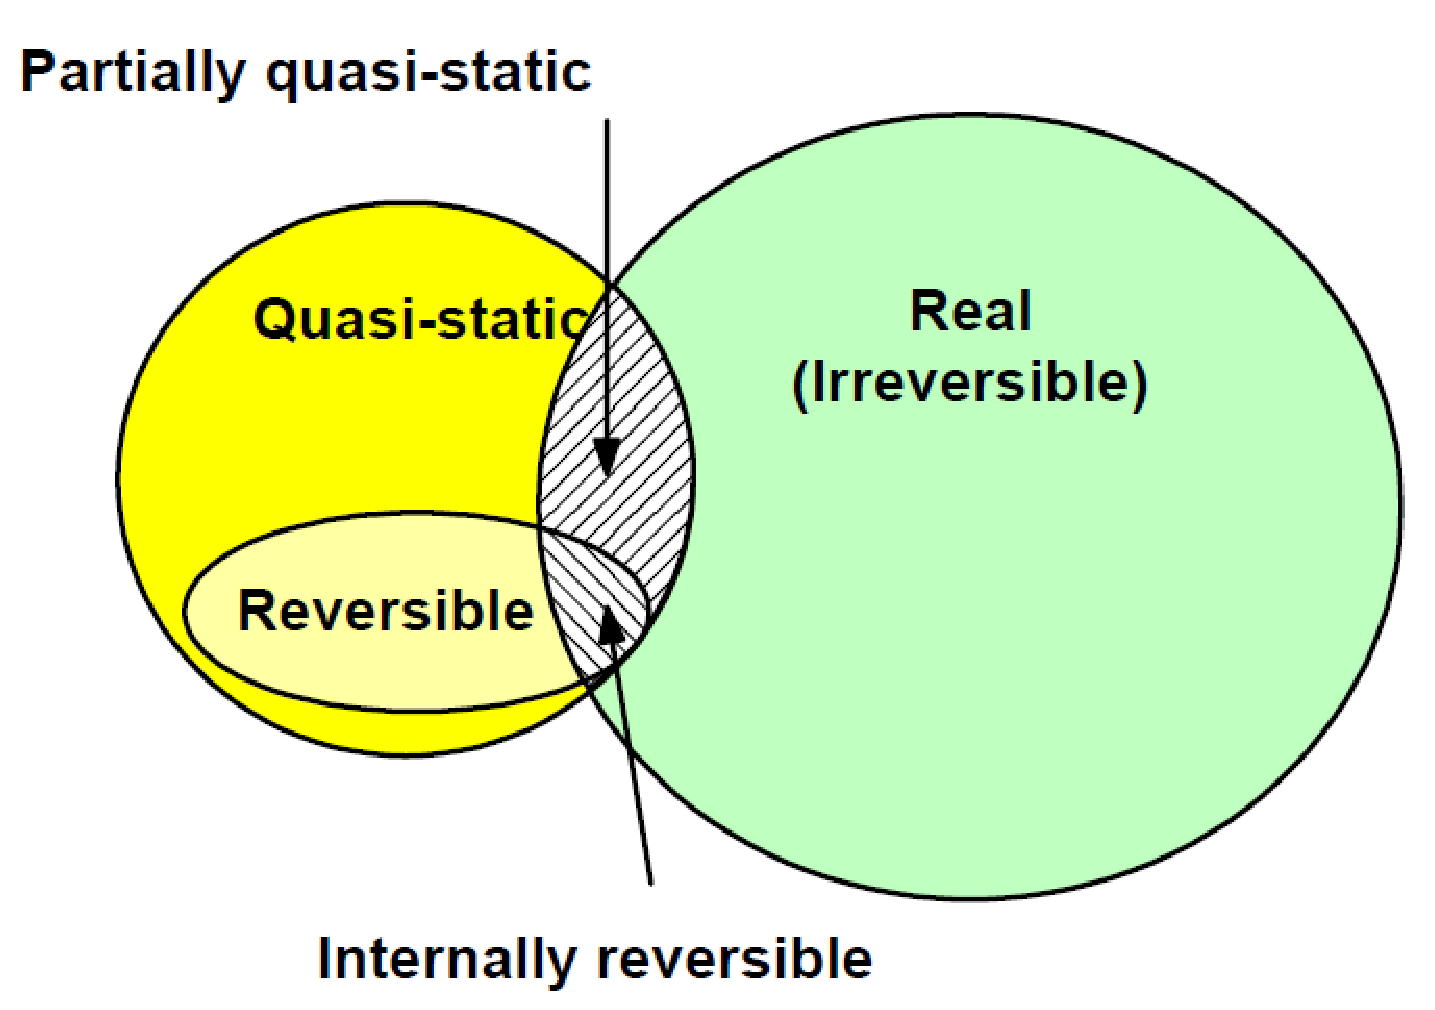
\includegraphics[height=5cm,
    angle=0]{./images/internal_reversible.eps}}
\caption{Internally reversible}
\label{fig:int_reversible}
\end{figure}

A reversible system can be
\begin{itemize}
\item externally reversible: the reversible process occur outside the
  system
\item internally reversible: the reversible occur inside the system
\item totally reversible: the reversible occur both inside and outside
\end{itemize}
\textcolor{red}{We'll make use only ``internally reversible process''}
in which the system pass through a series of equilibrium states and
can return to the initial state on exactly the same set of equilibrium
states, with the reverse
order\footnote{Fundamental of thermo-fluid sciences. Yunus A. Aengel,
  Robert H. Turner, pg.246}. A reversible process is in {\bf quasi-static}, i.e.
  each state is infinitesimally close to equilibrium (NOTE: A quasi-static process
  can be irreversible). By examining the system in a series of equilibrium
  states, the values of state functions can be estimated as the time evolution.
  As the process remain arbitrarily close to equilibrium at all time, the time
  evolution of a quantity is represented by differential equations.


% \subsection{Example 1}
% \label{sec:example_1}

\subsection{Representing (the dynamics of) a reversible system: ODEs, PDEs}
\label{sec:repr-dynam-syst}

The widely used method to represent the change of a {\it reversible system}
(Sect.\ref{sec:reversible-vs.-non}) during the time evolution is using
mathematical formulas. In mathematical language, a small change of a quantity
over time is represented in the form of {\it differential equations}, e.g. ODE
or PDE. The system can be solved using {\it deterministic} or {\it stochastic}
models.

In deterministic models, the assembled behavior of the system is assumed, i.e.
we always get the same result at different trials for a given input. In many
cases, practically, it's important to incorporate the stochastic behavior of the
system. Thus, the role of stochastic modelling is getting more important; yet
require more computational time.


\subsection{Kinetic scheme}
\label{sec:kinetic-scheme}


\begin{framed}
  We use the term {\bf mechanism} to refer to how an event occurs in a
  physical system; while the term {\bf kinetics} refers to how an event occurs
  from the mathematical model. For example: the excitation-contraction coupling
  mechanism or the kinetics of channel gating in a Markov-Chain model.
\end{framed}

Kinetic schemes focus attention on conservation of material (in a closed set of
reactions, material is neither created or destroyed) and flow of material from
one state to another (Sect.\ref{sec:kinet-interpr-ionic}).
\begin{itemize}
  \item a set of states
  
  \item arrows connecting one state to another
\end{itemize}

The notion of "state" is context-dependent: it may mean actual material quantity
of a molecular species (sometimes moles, sometimes mass), the well-stirred molar
concentration in a volume or the density on a surface, or the probability of a
particle being in a particular state.
\begin{itemize}
  \item  "the value of state A" we mean a value expressed in the dimensions of
  A. When A is in units of concentration or density,

  \item "the material in state A" is the product of A and the size of the
  compartment (volume or surface) in which A is distributed.
\end{itemize}

In a kinetic scheme, arrows that point toward or away from a state represent
paths along which material enters or leaves the state.
For each state there is a differential equation that expresses how the amount of
material in the state is affected by fluxes that enter and leave it.

As a result, any kinetic scheme is easily translated into a corresponding set of
differential equations (Sect.\ref{sec:repr-dynam-syst}). 


\subsection{Steps to build a mathematical model}
\label{sec:mathematical-biology}


In practice, no mathematical model can produce the result identical to the
system it modeled.  In stead, it is a simplification of the real system, and
typically in a smaller scale. Nevertheless, a model can be practicable if (1)
its behavior show the trend of what's going on as closed to that of the real one
as possible, (2) its behavior/change is tractable (using analytical methods or
numerical methods).

Thanks to the abundant availability of quantitative experimental data,
and the rapidly development of computing power, computers have proved
to be a powerful tool to dissect the molecular processes.  A
mathematical model solved on computers is called the
{\bf computational model}.  Below is the logical steps to create a
computational model using computers.

\begin{enumerate}
\item Taking clues from the experimental data \ce{->} try to identify
  the {\it biological/molecular mechanism of the dynamic phenomena}
  from data/plots (this may require closed consultants with
  experimentalist working on the problems.), the pathways (which one
  interact with which one, which one induce the
  activation/inactivation of which one, etc.)

\item {\it Derive a hypothesis} (an overall model) using arrows given in
  Fig. \ref{fig:pathway-key} \ce{->} we call this schematic
  representation, or cartoon, which should be explicitly clear enough
  to be translated into a series of elementary steps representing
  individual mechanisms.


\item Apply the basic laws of physics and chemistry to translate the
  elementary steps of the molecular mechanisms into a mathematical
  expression.

\item The changes based on the mathematical expressions are then expressed in
the form of time dependent differential equations (Ordinary Differential Equation
  (ODE) or Partial Differential Equation (PDE)).


  \textcolor{red}{``How can a system be represented in ODEs?''}  - when
  the system is broken into individual components, as well as
  corresponding quantities for each components, the changes in such
  quantities (i.e. dependent variables) can be represented using
  ordinary differential equations $dX/dt=f(X,Y,...)$.

\item Solve the equations using some standard numerical methods (e.g. Euler
method, Runge-Kutta method) or, in simple cases, analytical methods.

\item {\it Hypothesis testing} \ce{->} finally, carefully study the
  differential equations to know whether the overall model is correct
  or not (by comparing the numerical solutions with some given
  experimental data).

\end{enumerate}

{\bf IMPORTANT}: Rigorous analysis of complicated (ordinary/partial)
differential equations requires specialized training, since there are
many subtleties that can be gained only with experience.

To support the interpretation of the problem, a {\it kinetic diagram}
should be utilized. In this diagram, it should

\begin{itemize}
\item for each component:
  \begin{enumerate}
  \item identify all {\bf dependent variables}, i.e.  changing
    quantities of the component. These quantities are normally state
    functions. Typically, in cellular physiology, the state functions
    of interest are the ion concentrations ([\ce{Ca^2+}], [\ce{K+}],
    [\ce{Na+}], [IP3]...). We may also investigate the fraction of ion channels
    in a particular state (Open or Closed).
  \item list all possible
    {\bf transfers between every pair of variables} and adopt a symbol
    to represent a {\it rate constant} associated with each transfer;
    then estimate the values of the rate constants. 
    
    If everything is unchanged, the rate constants are always constant. However,
    due to the dynamics of the internal media inside the cell, such rate
    constants can be functions of something else (the conditions under which we
    perform the measurement). Thus, we need to predict the functional form of
    the rate constants, and then calculate it based on given values.
  \end{enumerate}

\item inter-components:
  \begin{enumerate}
  \item identify all {\bf constraints}, and make sure the system is
    closed (solvable) based on {\bf conservation laws}. 
    
  \item between two components, there can be more than one parameter to
    change, so there can be more than one connection between them. 
  \end{enumerate}
\end{itemize}

{\bf Example}: A cell is composed of different components:
mitochondria, sarcoplasmic reticulum (SR), Golgi apparatus, cytoplasm,
nucleus...

The problem will be more complicated if the change in one parameter is
dependent upon the change in the other ones, e.g. $\dot{X_i} = f(X_i,
X_j, X_k...)$.  In almost practical systems, finding $X_i(t)$ can only
be done using numerical methods. However, there are some cases the
system can be solved analytically.

\section{Numerical issue when solving a computational model}

Computers are powerful machines to help solving complicated problems.
However, they do not have infinite precision. Therefore, knowing about errors is
important in choosing the right numerical methods, and data types to represent
the independent variables.

\subsection{round-off error: machine + language dependent}
\label{sec:round-off-error}

To study the time evolution of a dynamical system, we do integration of the
dependent variables using computers. As we cannot represent a real value on
computer with infinite accuray, there's always a {\bf round-off error}. You can read
more how a numerical value is represented on computer elsewhere [REF].
It means that the value stored on computer is an approximate to the true value. To reduce this
error, we can use more bits in the decimal parts, e.g. from single precision
(4bytes) to double precision (8bytes). 

On every computer, for each data type, there's a smallest representable number,
called $\eta$, so that when a number of order unity is added to $\eta$, the
result is a new number of different value. The value of $\eta$ is depending how
many bytes is used to represent the value. So, the round-off error is denoted as
$\bigO(\eta)$.

For IBM-PC, and double-precision, $\eta=2.22\times 10^{-16}$ (which is specified
in the system header file \verb!float.h!).
\begin{verbatim}
#define __DBL_EPSILON__    2.2204460492503131e-16
#define __FLT_EPSILON__    1.19209290e-7F
\end{verbatim}
In Fortran, the intrinsic function EPSILON(X) return the $\eta$ value, of the
same kind as X, so that $(1+\eta)$ is the smallest number that is greater than
1.

\subsection{truncation error (per time-step): numerical method dependent}
\label{sec:truncation-error}

Computer is useful in representing the mathematical formula in the form of
linear or non-linear algebraic equations.
A powerful mathematical tool to approximate an arbitrary function f(x) in the
form of algebraic equations is {\bf Taylor expansion} which can be of different
order of accuracy to the original formula. The error is called {\bf truncation
error}.

Depending on the order to keep, we'll have different magnitude of truncation
error. The equation for the line is derived from Taylor expansion of the curve
\begin{equation}
y(t_n+h) = y(t_n)+ y'(t_n)h + y''(t_n)\frac{h^2}{2} + \ldots
\end{equation}
or
\begin{equation}
\label{eq:Taylor_2nd_order_form}
y_{n+1} = y_{n} + f(t_n, y_n) h + \bigO(h^2)
\end{equation}

As the form being solved by the computer (e.g.\ref{eq:Taylor_2nd_order_form}) is
an approximateion of the original equation, this is another source of error,
called {\bf truncation error} which comes from the numerical method being used.
The higher the order of $\bigO(\cdot)$, the smaller the truncation error. In
ODE, we typically try to reaches at least, second-order in time $\bigO(\Delta
t^2)$. In PDE, it's very challenging to get second-order in both space
($\bigO(\Delta x^2)$, $\bigO(\Delta y^2)$, \ldots) and in time 
$\bigO(\Delta t^2)$, with good speed performance.


\subsection{accumulative error (net truncation error)}
\label{sec:accumulative-error}
\label{sec:net-truncation-error}

In solving ODE, Euler method is the first-order approximation of the
unknown curve $y(t)$ from point of time $t_1$ to $t_2$. 
Using the initial value $y_0$ and the first-order appximation Euler method, we
have
\begin{equation}
\frac{dy}{dt} = y'(t) \approx \frac{y_{n+1}-y_n}{h} 
\end{equation}
we can find $y_{n+1}$ with the truncation error is $\bigO(h^2)$ with $h$ is the
step length. The shorter the step length, i.e. $h=t_2-t_1$, the more accuracy
the result. On an interval of unity length, with step length $h$, the number
of steps is $h^{-1}$. So, the accumulative error (or net truncation
error) is $\bigO(h^2) \times h^{-1} = \bigO(h)$. In other words, the
accumulative error using Euler method to do the integration is proportional to the step-length. 

In essence, it's important to choose an appropriate numerical method to limit
the cumulative relative error to a small enough value. Suppose we want the
cumulative error below $10^{-6}$, so we need at least 1 million time-step per
unit time interval in $x$.
 
\begin{framed}
A method is $n$-th order if the truncation error {\it per step} is
$\bigO(h^{n+1})$.
\url{http://farside.ph.utexas.edu/teaching/329/lectures/node33.html}
\end{framed}

\subsection{net round-off error}

Assuming that each time step has only one floating-point operation, then the net
round-off error, with $\eta$ is the round-off error per arrithmetic operation
and $h^{-1}$ operations. Then the total round-off error is $\eta/h$, after
$h^{-1}$ iterations.

\subsection{total error: net round-off + net truncation errors}
\label{sec:total-error}

So, the total error is the sum of the net round-off error and net truncation
error. 

Example: for Euler method is
\begin{equation}
\epsilon = \eta/h + h
\end{equation}
So, truncation error dominates at large time-step while round-off error
dominates at small-time step. The minimum value of this net error is
$\epsilon_0 \approx \eta/2$ when $h = h_0 \approx \eta^{1/2}$. 

\subsection{choosing time-step: ODE}

As discussed above, there's no point in making the time step smaller than
$h_0 \approx \sqrt{\eta}$.

So, at the double-precision,
i.e. $\eta = 2.2\times 10^{-16}$, we don't need to use time-step smaller than 
$h_0 = 10^{-8}$ which gives $\epsilon_0 \approx 10^{-8}$. This level of accuracy
is good enough for most  scientific calculations. 

\begin{framed}
For single precision, where $\eta = 1.19\times 10^{-7}$, the practical
smallest time-step is $h_0\approx 3\times 10^{-4}$ and net error $\epsilon
\approx 3\times 10^{-4}$ which is not adequate for scientific calculation. 
\end{framed}

Now, we come to the question what is the largest time step we can use.
Using large time-step, we have large truncation error, or we call it {\it
numerical instabilities} where the total truncation error explodes along the
course of the simulation.

For other methods of higher order accuracy, we can use a larger time-step. 

\subsection{choosing time-step and space-step: PDE}


Check more: 
\url{https://en.wikipedia.org/wiki/Linear_multistep_method}
\url{https://en.wikipedia.org/wiki/Courant-Friedrichs-Lewy_condition}
% TODO: Update this part (critical time-step and spatial step)

This paragraph tells us the choice for step in space and time. In Euler method
to solve PDE the choice is often
\begin{verbatim}
1-Dimension: D*h/(dx^2) < 1/2
2-Dimension: D*h/(dx^2) < (1/2)^2
3-Dimension: D*h/(dx^2) < (1/2)^3
\end{verbatim}
with $D$ is Diffusion constant. 

\subsection{choosing time-step: dynamics}

A dynamic time-step numerical methods are also good
choices. 


% \section{Kinetics of a chemical reaction}
% \label{sec:basic-equat-react}

\section{An example of a dynamical system: a simple model of ion channel gating}
% \label{sec:math-model-cell}
% \section{}
\label{sec:model-ion-channel}


In Sect.\ref{sec:comp-modell-biol},, we have learnt different factors that
determine the properties of a system as a number of states, and essential
concepts of state transition similar to a chemical reaction. In this section, we
will apply those knowledge, especially the 6 distinct steps in section
\ref{sec:repr-dynam-syst}, to the dynamics of a simple system of $N$ ion
channels. Each channel is assumed to be in either Open or Closed state.

\begin{framed}

  All matters are exchanged in cells via tiny gates formed by special proteins
  known as channels.  The term ``gating'' refers to the opening/close (or
  activation/deactivation) of a class of ion channel\footnote{an ion channel is
  a gate that allows only ions to go through}. An example is the glucose protein
  (GLUT) with two states in an oxidized cholesterol bilayers, as shown in
  Fig.~\ref{fig:ionchannel}.
  In some complicated models, the gating can be modelled with more than two
  states, e.g. Close, Inactive, Open.
\end{framed}

\begin{figure}[htb]
  \centerline{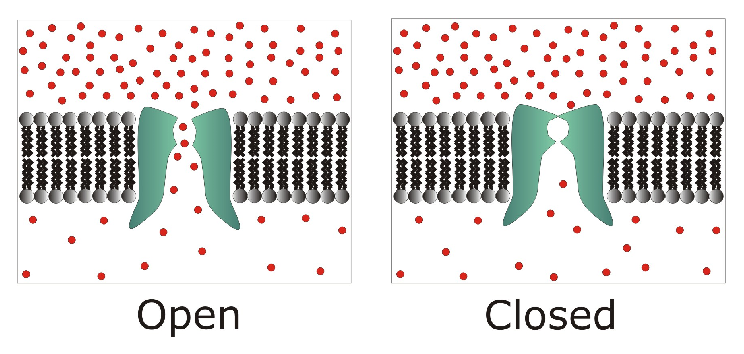
\includegraphics[height=3cm]{./images/ion_channel_state.eps}}
  \caption{A two-state model of GLUT ion channel (Open=conducting state,
  Closed=inactive)}
  \label{fig:ionchannel}
\end{figure}

% We assume a system of 2 states; and the transition between open and
% close is random, and is independent from any external factors.

\subsection{Assumptions}

\begin{enumerate}
  
  \item The system is a conserved system: i.e. 
  
  \begin{itemize}
  
    \item the number of channels is fixed. At a time, there is $n_1$ Open
    channels and $n_2$ Closed channels, and $N=n_1+n_2 =$ constant.

For simplicity, \textcolor{green}{we assume that there is only one type of ion
channel in a single cell (so they all have the same kinetics, i.e.
same transition rates)}\footnote{However, in a practical application, varying
number of channels was neccessitated by birth or death of channels during the
course of a {\bf long} experiment}.
  
    \item and the total number of ion channels is fixed.
  \end{itemize}
  
  \item The transition from one state to another can be represented in the form
  of the kinetic diagram which denotes the transitions between 2 states by solid
  lines and arrows
  \begin{equation}
    \label{eq:7}
    \ce{C <=>[k^+][k^-] O}
  \end{equation}
  with C denote ``closed'' state, O denotes ``open'' state.  $k^+,
  k^-$ are {\it rate constants} (like those described in a chemical
  reaction) and the arrows represent the
  {\it elementary molecular processes}.

  Further, it's important to know that this is a reversible and
  unimolecullar process in the sense that only a single reactant
  (NOTE: bimolecular process when there is two reactants). 

\end{enumerate}


% \item The biological mechanism is the switching between 2 states of an
%   ion channel, as shown in Fig.\ref{fig:ionchannel}. A single channel
%   is considered as the atomic component, so there is no need to break
%   the system into subproblems.
% 
% \item Derive an overall model: the model is 
\begin{framed}
  
  
  \textcolor{red}{How we define the measurement of ``concentration''?}.
  For a comprehensive references of different way to define
  ``concentration'', read
  \href{http://en.wikipedia.org/wiki/Concentration}{[wiki]}. Here are
  some examples:

  \begin{enumerate}
  \item If channels are in intact cells, concentration is often
    expressed in terms of volume-volume percentage.

  \item Another common use measurement is expressed in terms of the
    total weight of integral membrane protein in a sample

  \item For ion channels in a single cell, concentration can be
    expressed in terms of the fraction of ion channels in that
    state.
  \end{enumerate}

\end{framed}

As O and C are not chemical compounds, we cannot use the mass-mass
ratio as the measure of concentration. In our problem, we choose (3)
as the definition of concentration of ion channels. 
% Given that $N$ be
% the number of ion channels in the cell membrane and it is large
% enough. 
% 
% At time $t=0$, $N_0$ be the number open ion channels and $N_1$ be
% the number of closed ion channels. Then, we have

\begin{equation}
  \label{eq:9}
  [\text{O}]_0 = f_O(t=0) = \frac{N_O(t=0)}{N}, [\C]_0 = f_C(t=0) =
  \frac{N_C(t=0)}{N}
\end{equation}
To study the system, we need to know how $f_O(\cdot)$ and
$f_C(\cdot)$ change over time.

\begin{mdframed}
Since our kinetic model involves only 2 states $\{O,C\}$, and no
birth/death, we always have $N = N_0(t) + N_1(t)$=constant or 
$f_O(t) + f_C(t) =1$. 
This satisfies the idea of conversation law which physically
states that ion channels are neither created nor
destroyed.
\textcolor{red}{The assumption of conservation of the quantities in
  a system is critical to the simulation study of the system}.
\end{mdframed}

\subsection{Flux and Concentration: Mathematical abstraction of the real system}
\label{sec:flux-example}
\label{sec:concentration-example}



The {\it rate of transition} $J$, also referred to as {\bf flux}, in which ion
channels turn from one state to another at a unit of time is used
(Sect.\ref{sec:fluxes}).
    
Apply the basic law of physic and/or chemistry:
  \begin{itemize}
  \item flux from C to O: the rate of of channels swtiching from closed state to
  the open state per a unit of time is
  \begin{equation}
  J_+ = k^+[\C]
  \end{equation} 
    
    
   \item flux from O to C: the rate of transition in which ion channels turn
   from the open state to the closed state per a unit of time is
    \begin{equation}
    J_- = k^-[\text{O}]
    \end{equation}
\end{itemize}

If we assume the total amount of channels is large enough and the assumption
that total ion channels is fixed, then the amount of channels in each state, say
open and closed, can be represented in the form of {\bf concentration} or the
fraction of channel in that state (Sect.\ref{sec:concentration}), denoted as [O]
and [C] respectively.

Using the {\bf law of mass action} (Sect.\ref{sec:law-mass-action}, we obtain
the {\it reaction quotient} Q
    \begin{equation}
      \label{eq:8}
      Q = \frac{[\text{O}]}{[\C]}
    \end{equation}
By comparing the value of Q with the equilibrium constant $K_{eq}$, it can tell
us whether the reaction moves to the right ($Q<K_{eq}$ or left direction ($Q>K_{eq}$).

\subsection{ODE: first-order kinetics representation of the model}
\label{sec:first-order-kinetics-example}

To study a dynamical system, i.e. the change over time, the available tools from
maths are ODE or PDE (Sect.\ref{sec:repr-dynam-syst}).

From time $t_1$ to $(t_1+\Delta t)$, the number of open channels can change,
as do the closed channels. We have
\def\flux{{\text{flux}}}
\begin{equation}
  \begin{split}
    \label{eq:10}
    \flux_{O \ce{->} C} &= J_- = k^- f_O  \\
    \flux_{C \ce{->} O} &= J_+ = k^+ f_C = k^+ (1-f_O)
  \end{split}
\end{equation}
with $k^+, k^-$ are the rate constants, and
the concentrations are $f_O, f_C$ respectively at each side of the
reaction.

The degree of freedom of the system is 1. So, if we know the number of
opened channels at a time instant, it can tell the fraction of closed
channel. So, to study the system, we only need to use a single ODE for
$f_O$
\begin{equation}
  \label{eq:11}
  \frac{df_O}{dt} = - J_- + J_+  =  - k^- f_O + k^+ (1-f_O)
\end{equation}

\textcolor{red}{For simplicity in notation, we use $f$ to substitute
  for $f_O$ with $f$ is a function of time, $f(t)$}.
\begin{equation}
  \label{eq:254}
  \frac{df}{dt}  =  - (k^-+ k^+) f + k^+ =  - (k^-+ k^+) (f - \frac{k^+}{k^-+ k^+})
\end{equation}


% Using mathematical equations to represent the change of open channels in a
% unit of time. The difference between the two fluxes in eq.\eqref{eq:10}
% represents the change in the number of open ion channels in a unit of time,
% given as follows.
If we assign $X = (f - \frac{k^+}{k^-+ k^+})$, and $\lambda = (k^-+ k^+)$, as
$dX = df$, we have
\begin{equation}
  \label{eq:255}
  \frac{dX}{dt} = - \lambda X
\end{equation}

Here, at a given time point, the rate of change of the dynamical variable 'X' is
the function of the current value of 'X'. It means that the rate of change of X
follows the {\it first-order kinetic} (Sect.\ref{sec:first-order-reaction}).
First-order kinetics is the most common assumption of kinetics to be used
(Sect.\ref{sec:order-reaction}).

The (analytical and numerical) solutions of this equation will be discussed in
Sect.\ref{sec:analytical-solution-first-order-system} and
Sect.\ref{sec:numerical-solution-first-order-system}), respectively.


\subsection{time-constant of decay: analytical solution }
\label{sec:analytical-solution-first-order-system}

% \subsubsection{Mathematical derivation}
% \label{sec:math-deriv}

Any first-order reaction kinetics, as shown in the classic eq. \eqref{eq:255},
has the exact solution of as an exponential decay function, in the form 
\begin{equation}
X = X_0 \times e^{({-\lambda t})}
\end{equation}
with
\begin{equation}
  \label{eq:256}
  X_0 = X(0)=f(0)-k
\end{equation}
with $k = \frac{k^+}{k^-+k^+}$, see {\bf Appendix B}
(Sect.\ref{chap:analyze-diff-equat}).

\subsection{-- time constant}
\label{sec:time-constant-example}

As discussed in Sect.~\ref{sec:expon-time-const}, in an exponential decay
function, a convenient way is to denote $\tau = \frac{1}{\lambda}$ and $\tau$ is
called the {\bf time constant} (with the same unit of time).

In this simple case, we can obtain the {\it analytical solution}
\begin{equation}
  \label{eq:14}
  f(t) = X + k = (f(0) - k) e^{({-t/\tau})} + k 
\end{equation}

\begin{framed}

  \textcolor{red}{As the mean of the distribution, the time constant
    $\tau$ is the ``mean open time'' (the mean duration of the channel
    openings)} ([ns] or [ms]). The variance is $\tau^2$.
\end{framed}

\subsection{-- steady-state solution}
\label{sec:steady-state-value-example}

Since $\tau > 0$, when the time goes to infinity ($t \rightarrow
+\infty$) the system reach a stable state that we call steady-state,
i.e.  $\lim_{t\rightarrow \infty} \exp({- t/\tau}) = 0$. Hence, $X(t)$
is a decay function that approach a single value ,
\begin{equation}
  \label{eq:23}
  f_{\infty} =f(\infty) = k  
\end{equation}
and is called the {\bf steady-state fraction of open channels} at a
time point when the time point is large enough.  Then, we can rewrite
\begin{equation}
  \label{eq:15}
%  f_0(t) = f_\infty + (f_0(0) - f_\infty) \exp({-t/\tau})
  f(t) = f_\infty + (f(0) - f_\infty) e^{({-t/\tau})}
\end{equation}
% with $f_\infty = \frac{k^+}{k^++k^-}$, and $\tau = \frac{1}{k^++k^-}$.

This decay function tells us the fraction of channels in Open state at a
given time point.
% , with high probability for short time and low
% probability for long time.



\subsection{-- Example (in R)}
\label{sec:example-in-r}

A complete understanding of a system required manipulating the
parameters and see how it affects the behavior of system.
\textcolor{red}{What information is required to analyse this problem?}
\begin{itemize}
\item rate constants: $k^+, k^-$.

\item portion of open channels at time zero $f(0)$
\end{itemize}



\begin{figure}[htb]
  \centerline{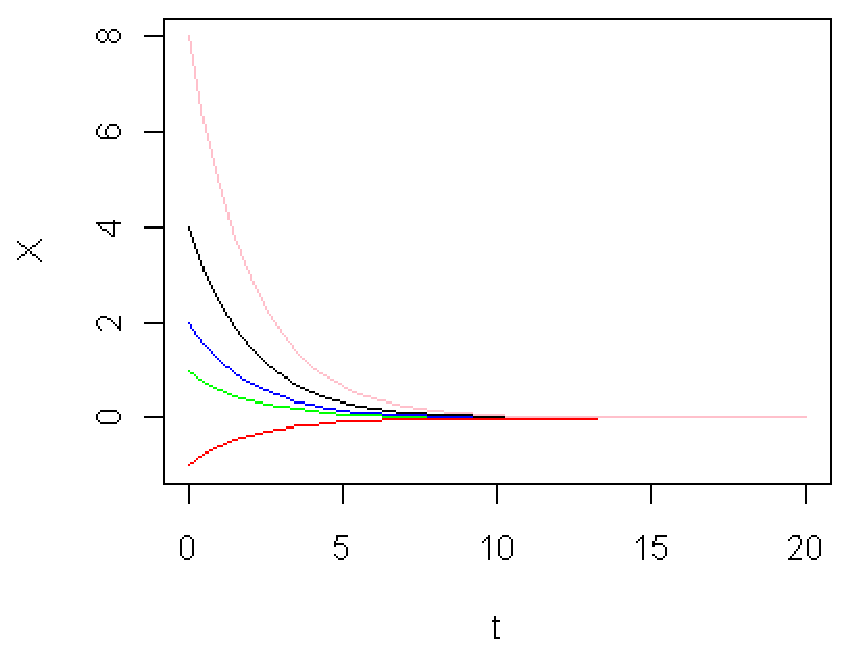
\includegraphics[height=6cm]{./images/gating_analytical.eps}}
  \caption{The family of $X=X(0)e^{-t/\tau}$ with $\tau=2$ and $X(0) =
    -1,1,2,4,8$}\label{fig:gating-analytical}
\end{figure}

To show how the initial value and setting parameters affect the shape
of the curves, in a data analysis, we need to use plots or graphics to
help readers understanding the problem easier. Here, we use
\hyperref[chap1.1.r]{R code} to plot the equation $X(t)$ with
\begin{itemize}
\item different initial values $X(0)$: (-1,1,2,4,8)

\item for a period of time from 0 to 20[unit of time], time step is
  0.5[unit of time].
\item Assuming that the mean open time $\tau$ (tau) is equal to 2ms.
\end{itemize}
\begin{equation}
  \label{eq:47}
  X = X(0) \times \exp({-t/\tau})
\end{equation}

In our example, the model of single type of channels describes
exponential decay (or growth) to a steady state fraction of open
channels, $f_\infty$, Fig.~\ref{fig:gating-analytical}.

{\bf Remarks:} The two important time points
\begin{itemize}
\item The time at which the value of the function decays to 1/2 of the
  initial value is called {\bf half-time},  denoted as $T_{1/2}$, with
  $T_{1/2} = \tau ln2$ since 
  \begin{equation}
    \label{eq:16}
    X(0) e^{-T_{1/2}/\tau} = \frac{X(0)}{2}
  \end{equation}
\item After a time period $t=\tau$, the value of X is $X = X(0)e^{-1}
  \approx X(0) \times 0.37$ (or the new value is e-fold decrease of
  the initial value)
\end{itemize}
The above principles apply to growing as well as decaying function in
the form of exponential. 


\subsection{Numerical solution}
\label{sec:numerical-solution-first-order-system}

Even though eq. \eqref{eq:255} has the exact solution; in many other ODE
formula, the analytical solution is rarely available. To solve the system on
computer, an approximation method is required in that the ODE needs to be
represented in the form of an algebraic equation that can be solved by the
computers.

This section will introduce how an approximated solution for an ODE can be
obtained.\footnote{For detailed references, read
  {\it Numerical methods for Engineers} - Chapra \& Canale.}
Sect.\ref{chap:ordin-diff-equat}) discusses more details different numerical
methods, depending upon the order of the ODE, and the level of accuracy in time
and/or space.

Using Taylor expansion (Sect.\ref{{sec:taylor-expansion}}), a simple method with
first-order accuracy in time (Sect.\ref{sec:numerical-method-ode-first-order})
is {\it Euler method}. The Euler method is identical to the first-order Taylor
expansion:
\begin{eqnarray*}
  X(t+\Delta t) = X(t) + \Delta t .X'(t)
\end{eqnarray*}
With $X'(t) = \frac{dX}{dt}=-\frac{X}{\tau}$, we have

\begin{equation}
  \label{eq:17}
  X(t + \Delta t) = X(t) - \frac{X(t)\Delta t}{\tau}
\end{equation}

Since  $X(\cdot) = f(\cdot) - f_\infty$, we have
\begin{equation}
  \label{eq:18}
  f(t+\Delta t) = f(t) - \frac{(f(t) - f_\infty)\Delta t}{\tau}
\end{equation}
Given this formula, by using an iterative approach, we can obtain the
value of the state function $f$ at a time instant $(t+\Delta t)$ given
the value of the state function at a previous time instant $t$.

\subsection{-- Example (R code)}
\label{sec:example-r-code}


\begin{figure}[htb]
  \centerline{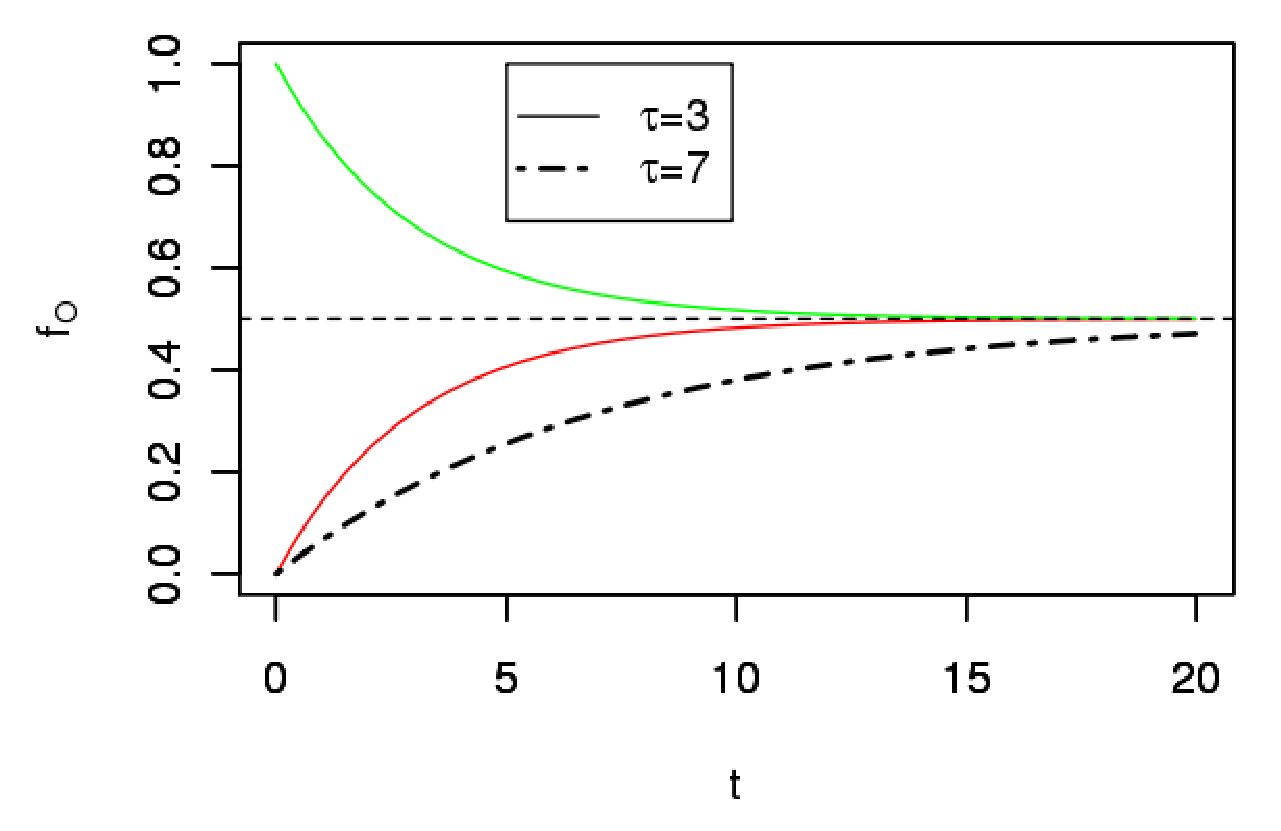
\includegraphics[height=6cm]{./images/gating_numerical.eps}}
  \caption{Analyze the dynamics of fraction opening channel
    $f=f(0)e^{-t/\tau}$ with $\tau=3$ms, 7ms, and $f(0) = 0$ and
    1}\label{fig:gating-numerical}
\end{figure}
Assuming that the time step is $\Delta t = 0.03$ms. We examine two
different initial conditions: (1) no channel is open($f(0) = 0$) and
(2) all channels are open ($f(0)=1$); as well as two time constants
$\tau = \{3, 7\}$ms. The steady-state fraction of open channel is
$f_\infty = 0.5$, as shown in Fig.~\ref{fig:gating-numerical}.

{\bf R-code}: (\hyperref[chap1.2.r]{chap1.2.r})

As shown in Fig. \ref{fig:gating-numerical}, the rate at which the
steady state is reached depends on the value of the time constant
$\tau$ (the smaller the $\tau$ or the faster the kinetics of the
gating mechanism).

\subsection{-- Example (in XPP)}
\label{sec:example-in-xpp}

A faster and easier way to analyze is using the XPP tool which has
many numerical methods installed, and visualization tool to see the
data. 
% \lstinputlisting{./codes/XPPAUT/chap1.}

\subsection{Analytical vs. Numerical solutions}
\label{sec:analyt-vs.-numer}

Let's see the difference between the results produced using the
analytical method and numerical methods, as given in
Fig.~\ref{fig:gating-comparison}
\begin{figure}[htb]
  \centerline{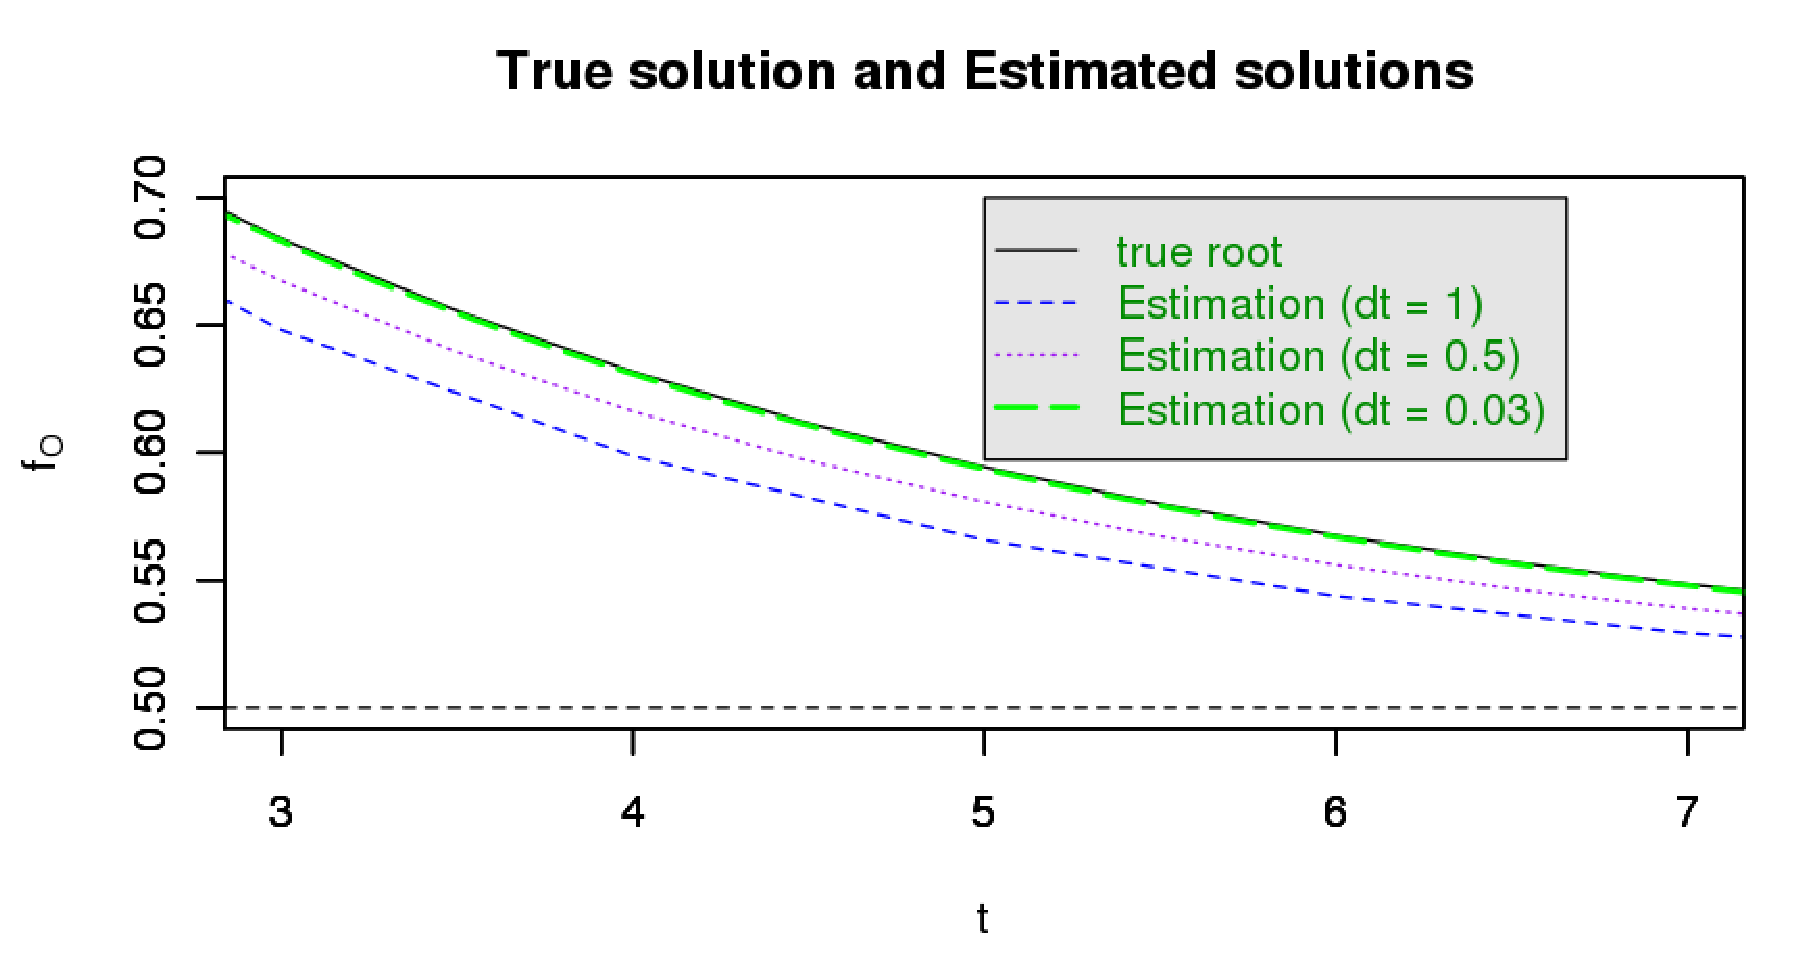
\includegraphics[height=7cm]{./images/gating_comparison.eps}}
  \caption{Approximated solution and analytical
    solutions}\label{fig:gating-comparison}
\end{figure}

{\bf Remarks:}

\begin{itemize}
\item The result of analytical method is always the true solution. All
  numerical methods just produce an approximated solution.

\item The accuracy of a numerical solution is highly dependent upon
  the selected parameters, e.g. the step size, as shown in
  Fig.~\ref{fig:gating-comparison}.  Only the step size whose
  {\it magnitude is smaller} than the value of $\tau$ do a reasonable
  job to approximate the exact exponential solution, e.g. $\Delta t =
  2 < \tau = 3$ is good, but $\Delta t = 6 > 3$ is
  bad.
  \textcolor{blue}{If we say an order of magnitude smaller/larger, it
    means 10x smaller/larger}.

\item There are different ways to plot the result of solving the
  differential equation that frequent gives insight into the
  properties of the solution.
\end{itemize}

{\bf R-code}: \hyperref[chap1.3.r]{chap1.3.r}

\subsection{Rate of change (phase diagram)}
\label{sec:analysis-rate-change}
\label{sec:rate-of-change-example}

Besides solving the dynamical system using analytical or numerical method, there
is a different way to study the system is by studying the {\it rate of change}
in time. 
\begin{enumerate}
  \item In the former approach, i.e. by plotting X or $f$ against the time $t$, we only
know change of the state function $f$ in the course of time.

  \item In the later approach, i.e. it is helpful to examine {\it how fast of
  the change}. Since the rate of change is indeed the first-order derivative of $f$,
we can plot $df/dt$ vs. $f$, without having to solve the ODE to find the exact
value of $f$.
\end{enumerate}

\begin{framed}

  A powerful mathematical tool to study the rate of change is {\bf phase plane
  analysis} (Sect.\ref{sec:phase-plane-analysis}).  This is particularly useful
  to analyze differential equations (ODE) with 2 variables. This will be covered
  in the next chapter.
\end{framed}

% \begin{equation} \label{eq:24} \frac{df}{dt} = \frac{f-f_\infty}{\tau} \text{ 
% vs.  } f \end{equation} tells us the rate of change as a function of $f$
% (portion of open channels).

\subsection{-- Example (R-code)}

{\bf R-code}: \hyperref[chap1.4.r]{chap1.4.r}

\begin{figure}[htb]
  \centerline{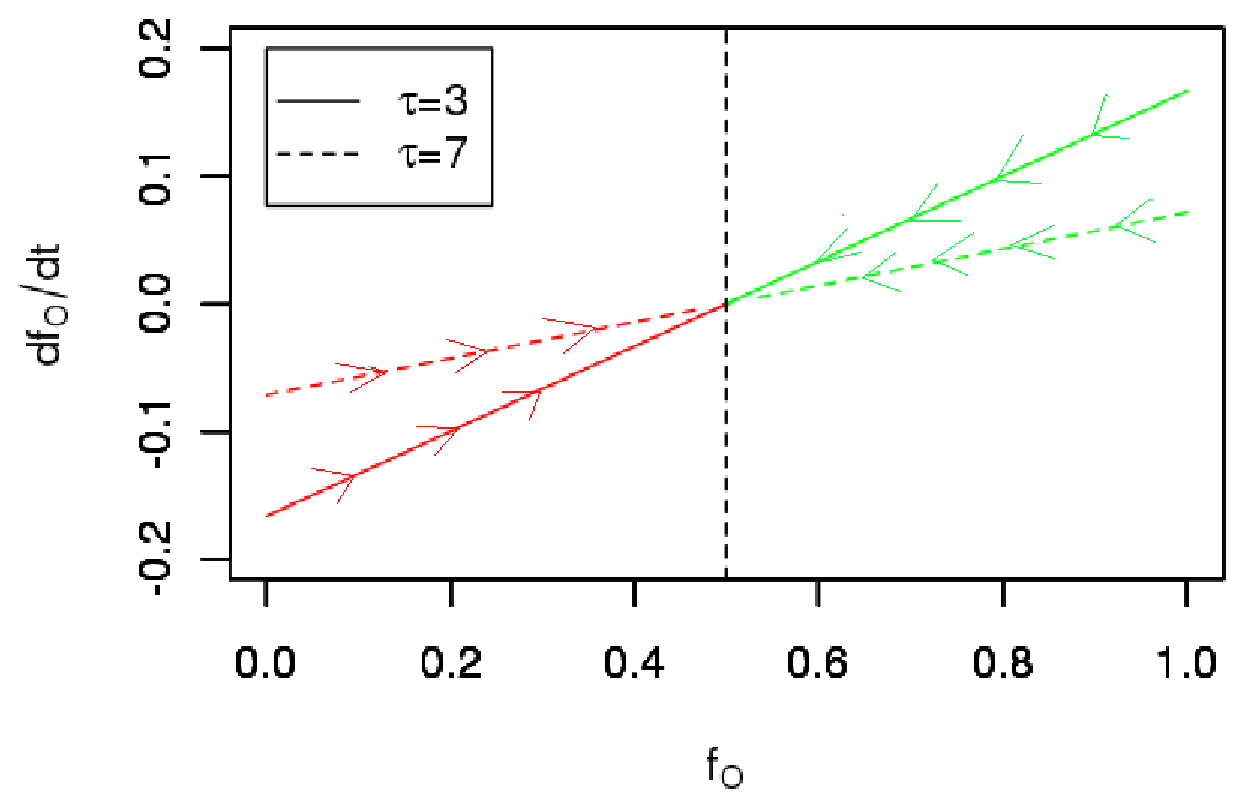
\includegraphics[height=7cm]{./images/gating_rate.eps}}
  \caption{Rate of open state-transient at different mean open time
    constant. $f =\frac{N_0}{N}$ is restricted within [0,1] on
    physical background}\label{fig:gating-rate}
\end{figure}

Given $f_\infty = 0.5$ and two initial conditions: $f_0 = 0$ or 1, the
plot in Fig. \ref{fig:gating-rate} shows that all converge to the
steady-state fraction open channel $f_\infty$.  The steeper the line,
the faster the rate of opening the channels $df/dt$; the lower the
value of mean open time constant $\tau$; the faster the
opening-transient of the channels.  

With two different initial fraction opening channels, both converge to
the same steady state fraction opening channels $f_\infty$. Thus, to
show the direction of the change, we can use the arrow to show the
direction in which $f$ is changing. 

{\bf Remarks:} 
\begin{itemize}
\item When analyzing the gating phenomena, in a cell, there are
  thousands of ion channels of a given type. Then, a reasonable way is
  to study the average behavior of the entire ensemble of channels (or
  in some circumstances, a local region) to determine the {\bf
    cellular dynamics}.
\end{itemize}

\subsection{Steady-state value and time-constant}

From the given example, there are two quantities of a variable X that follows
first-order kinetics that we will see again, and very often. They are 
\begin{itemize}
  \item stead-state value $X_\infty$
  \item time constant $\tau_X$
\end{itemize}

% Another and better notation is to define
\begin{equation}
  \label{eq:685}
  \begin{split}
f_\infty=\frac{k^+}{k^-+k^+} \\
\tau=\frac{1}{k^-+k^+}
\end{split}
\end{equation}

So, we have
\begin{equation}
  \label{eq:686}
  \frac{df}{dt} = -\frac{f-f_\infty}{\tau}
\end{equation}
We easily realize that $f_\infty$ is the value of $f$ at steady-state,
i.e. when $df/dt=0$, and $\tau$ is the time it takes for X to change from
initial value to the a new value that is $1/e$ times the initial value (for
decay) or $e$ times the initial value (for increase).
% mean of the distribution.
% More detail will be given in the next chapter.
%   Denote $x = f_0(t)$ as the number of open channels at a given time
%   point that depend on $t$.  Clearly, this is a differential
%   equation
%   \begin{equation}
%     \label{eq:12}
%     \frac{dx}{dt} = -\frac{x-k}{\tau}
%   \end{equation}
%   with
%   \begin{equation}
%     \label{eq:150}
%     \tau = \frac{1}{k^++k^-}; k=\frac{k^+}{k^++k^-}
%   \end{equation}
% \item What remains are the analysis of the eq. \eqref{eq:12}.
  
%   Eq. \eqref{eq:12} has the form of a simple linear equation
%   \begin{equation}
%     \label{eq:13}
%     \frac{dX}{dt} = -\frac{X}{\tau}
%   \end{equation}
%   with $X = x - k = f_0(t) - k$.

\section{Summary}
\label{sec:summary-7}

In this chapter, you have learnt a general procedure to develop a model, with a
sample of modeling the dynamics of a system of 2-state ionic channels. We also
learnt important concepts being used in modelling. In the next chapter, we will
discuss in detail ionic channels, and how to model their kinetics in an
excitable cell.

%%% Local Variables: 
%%% mode: latex
%%% TeX-master: "mainfile"
%%% End: 

\chapter{Dynamics of Ion Flux}

\section{Concentrations}
\label{sec:concentrations}

In previous chapter, we use the concept of {\it 'fraction of open channel'}
(Sect.\ref{sec:concentration-example}) to map from a discontinued quantity (i.e.
the number of channel) to a continuous quantity (i.e. fraction in the range 0 to
1). In a generic context of chemical species, an equivalent concept called {\bf
concentration} is used.

Concentration is a way to describe mixture composition, e.g. the
amount of a solvent in a solution. However, this doesn't necessary
liquid ones. 

\subsection{mass (weight/weight) percentage: grams of substance per 100 grams of
sample}
\label{sec:concentration-mass-percentage}

One way is to use mass (weight) percentage (\% w/w)
\begin{equation}
  \label{eq:999}
  \text{c}_{\% w/w} = \frac{m_\text{substance}}{m_\text{solution}} \times 100\%
\end{equation}
In simple case when solution contains only one solvent and one solute,
then $m_\text{solution} = m_\text{solute}+m_\text{solvent}$.  

IMPORTANT: Only weight percentage is the percentage concentration that is always
unambiguous, i.e. does not change with temperature. Unit : (\%). 

\begin{verbatim}
1% w/w means 1 gram of substance per every 100gram of sample
\end{verbatim}

\subsection{mass-volume percentage, volume-volume percentage}

Unlike weight-weight percentage (Sect.\ref{sec:concentration-mass-percentage}),
mass-volume percentage or volume-volume percentage are temperature dependent, so
such quantities are unambiguous.

{\bf Mass-volume (or weight-volume) percentage} (\% w/v) is
\begin{equation}
  \label{eq:1000}
  \text{c}_{\% w/v} = \frac{m_{substance}}{V_{solution}} \times 100\%
\end{equation}
the unit of Volume is [mL], and unit of mass is [g]. So, the overall
unit is in [\% g/mL]. So, it's possible to have solutions of
concentration above 100\% w/v. 



{\bf Volume-volume percentage} (\% v/v) is
\begin{equation}
  \label{eq:1001}
  \text{c}_{\% v/v} = \frac{V_{substance}}{V_{solution}} \times 100\%
\end{equation}
The problem with this usage is that ``volume is only additive for
ideal gas only''. So, the final volume is not a sum of volumes used
when preparing mixture. It means that volume-volume percentage doesn't
sum to 100\%. To convert between concentration types, we need to know
densities of the solution and of both pure solvent and solute. 


\subsection{parts per million/billion: ppm, ppb}

For very low concentration, people often use {\bf ``parts per''}
notation. 

NOTE: \verb!1% w/w! above can be understood as ``1 mass part per
hundred mass parts'', though very rarely used. Instead, these are
often used
\begin{verbatim}
ppm     =  parts per million (10^6)
ppb     =  parts per billion (10^9)
ppt     =  parts per trillion (10^12)
ppq     =  parts per quadrillion (10^15)
\end{verbatim}

``ppq'' is rather a theoretical construct than a useful thing. It can
also use volume by volume, rather than mass by mass. 

Example: 1mL of \ce{SF6}(g) added to 1000L of hydrogen \ce{H2}(g) is 1ppm
vol/vol, but 73 ppm mass/mass. Another example: 1 atom of lead per $10^6$
beryllium atoms there are 23 ppm of lead mass/mass.

\subsection{molar concentration: M (or mole/(Liter solution)), mM, $\mu$M, nM}
\label{sec:concentration-Molar}

{\bf Molar concentration} (M, mM, $\mu$M, nM) or {\bf molarity} is
\begin{equation}
  \label{eq:1002}
  c_M = \frac{n_{substance}}{V_{solution}}
\end{equation}
with unit is [mole/L] or [Molar] or [M].

NOTE: Some old books use M/500 unit, it means 1 mol per 500 litres of solution
(or M/500 means 0.002 mol/L).

\textcolor{red}{Molar concentration is the most often used concentration unit as
it makes stoichiometric calculations much easier}, which can be measured with
the highest precision and for most analytical applications this is the preferred
way of expressing concentration.

{\it The only drawback is that it's temperature-dependent}, e.g. the volumes
increase when the temperature increase and molar concentration goes down. 
To avoid temperature dependency, we can use {\bf molarity}
(Sect.\ref{sec:concentration-molarity}).

\subsection{-- molarity (mole/kg)}
\label{sec:concentration-molarity}

Unlike {\it molar concentration} concept (Sect.\ref{sec:concentration-Molar});
{\bf molarity} is temperature independent.
\begin{equation}
  \label{eq:1003}
  c_m = \frac{n_{substance}}{m_{solvent}}
\end{equation}
is expressed in [mole/kg] units. 

NOTE: It's rarely used in analytical chemistry, molality is often used in {\bf
physical chemistry}, especially when dealing with substance properties over a
wide range of temperature, or properties change with both temperature and
mixture composition.

\subsection{-- normality}
\label{sec:concentration-normality}

{\bf Normality} (similar to molarity, but use equivalent, not moles) has the
units number of [equivalents per Liter]. 

So, the same solution can have different normalities for different types of
reactions. So, it's \textcolor{red}{reaction-dependent}. E.g.: 1M sulfuric acid
solution is 2N for acid/base reactions, and 1N in the reaction of barium sulfate
precipitation.

\begin{framed}
  Molar mass of the substance
  \begin{equation}
    \label{eq:1005}
    n_\text{substance} = \frac{m_\text{substance}}{m_M}
  \end{equation}
with $n_\text{substance}$ is the number of moles. 
\end{framed}

\subsection{Molar fraction}
\label{sec:concentration-molar-fraction}

{\bf Molar fraction} is the number of moles of a substance divided by
the total number of moles of all substances. So the range of a value for molar
fraction is from 0 to 1 and {\bf unitless}. The quantity is temperature
independent.

Conversion:
\begin{enumerate}
\item from weight percentage to molality 
  \begin{equation}
    \label{eq:1004}
    c_m = \frac{1000\times c_{\% w/v/}}{m_M(100-c_{\% w/w})}
  \end{equation}
the factor 1000 is necessary as molality is in [mole/kg] while all
masses are in grams (gr). 
\end{enumerate}

\subsection{protein concentration (mg/ml)}
\label{sec:concentration-protein}


In biochemistry, protein concentration is measured in mg/ml, and is measured
using Bradford method (Coomassie Blue reagent; Pierce Chemical
Co., Rockford, IL) with bovine serum albumin (Sigma Chemical, Co.) as standard. 

Reference:
\begin{itemize}
\item \url{http://www.chembuddy.com/?left=concentration&right=concentration-follies}.  
\end{itemize}


\subsection{Faraday constant}
\label{sec:Faraday-constant}

The particles are often electric charges, whose unit is
Coulomb (C). Definition:
\begin{itemize}
\item {\it 1 Coulomb is the amount of charge that must pass through an
    electrolytic cell in order to deposit $1.1180\times 10^3$g of silver
    from a solution of silver nitrate}, or

\item 1 Coulomb is the amount of charge on $6.242\times 10^{18}$
  electrons. 
\end{itemize}
So, the charges on one mole of electrons (which is Avogadro number
$N_A=6.023\times 10^{23}$ of electrons) is
\begin{equation}
  \label{eq:1343}
  \frac{N_A}{6.242\times 10^{18}} = 9.649\times 10^4 (\C/\text{mol. electrons})
\end{equation}
This quantity is known as {\bf Faraday constant}
\begin{equation}
  \label{eq:1344}
  1\text{ Faraday } = 9.649\times 10^4 \;\;(\C/\text{mol. electrons})
\end{equation}
Faraday's constant converts quantity of moles to quantity of charge for a
univalent ion, i.e. $z=1$. 

\section{Flux $J$}
\label{sec:fluxes}

A flux describes the rate of a reaction, i.e. the speed of reaction
(Sect.\ref{sec:speed-reaction}). In the previous example, we studied the simple
example of the rate of switching between open and close of a cluster of $N$ ion
channels (Sect.\ref{sec:flux-example}).

In chemical reactions, the fraction of 'open' channel in that example is
replaced by the 'concentration' of a given species
(Sect.\ref{sec:concentration}), and the {\bf chemical flux} is used to study the
rate of chemical reactions (Sect.\ref{sec:chemical-flux}).


% \subsection{Current density}
% 
% To avoid the variation between cells, all quantities are determined
% based on a unit of membrane area, except the voltage. The information
% is given in Table~\ref{tab:terminology_2}.
% 
% \begin{table}[hbt]
%   \begin{center}
%     \caption{Ionic currents}
%     \begin{tabular}{p{2cm}r} 
%       \hline
%       notation & description \\ 
%       \hline\hline
%       $I_i$ & ionic current through plasma membrane ($I_{\ce{Na}},
%       I_{\ce{K}}$) \\
%       & ...$I_i = g_i(V_m-E_i) $ \\
%       $I_{app}$ & applied step current (rectangular pulse) (mA/cm$^2$)\\
%       $I_m=\frac{I_0}{A}$ & the current density per unit area (mA.cm$^{-2}$) \\
%       $i_m$ & the current density per unit length (mA/cm) \\
%       $I_\dhpr, I_\LCC$,  $I_\Ca$       & the calcium current via DHPR (L-type channels) \\
%       $I_\ryr$ & the current of calcium released via RyR from JSR \\
%       $I_\Na$ & the current of sodium \\
%       $I_\NaCa$ & the current via Na/Ca exchanger \\
%       $I_\K$ & the current via potassium channel \\
%     \end{tabular}
%   \end{center}
%   \label{tab:Current}
% \end{table}
% 
% With different types of ions, there are respectively different ionic
% currents, Table \ref{tab:Current}. Typically, all currents are indeed
% ``current density'', i.e. in unit [Ampere/unit square], e.g. mA/cm$^2$.

\subsection{Atomic vibrations: thermal energy}
\label{sec:thermal-energy-distribution}
\label{sec:atomic-electronic-energy}
\label{sec:electronic-energy}

Heat causes atoms to vibrate.  The vibration amplitude increases with
temperature.

When vibration are sufficient large to break the bonds, a material is
disruptly transformed from one state to another, e.g. from solid to liquid.

\begin{itemize}
  \item vibration frequency: $10^{13}$ Hz
  
  \item heat provides the atoms an amount of energy, called
  atomic/electronic energy.
  
  Heat causes atomic vibration which generate an amount of energy, called
  atomic/electronic energy.
  
  The average atomic/electronic energy due to thermal excitation is of order of
  $k_B T$, i.e. $E_\text{average} \sim k_BT$ (with $k_B$ = Boltzmann constant,
  and $T$ = temperature in absolute degree Kelvin).

NOTE: $k_BT = 0.026$ (eV) for room temperature.
  
The distribution of such energy around the mean follow the Boltzmann
distribution function (Sect.\ref{sec:Boltzmann-equation})

\begin{equation}
P(E) = \exp\left( -E/(k_BT)\right)
 \end{equation}
$k_B = 1.38 \times 10^{-23}	$(J/K) = $8.62\times 10^5 $ (eV/K).  
  
  
\end{itemize}


\subsection{Atomic diffusion: vacancy diffusion (interdiffusion and
self-diffusion)}

Diffusion is material transport by atomic motion from one lattice site to
another. To move from lattice site to lattice site, atoms need energy to break
bonds with neighbors, and to cause the necessary lattice distortions during
motion from site to another. This energy comes from atomic vibration as
mentioned above.

This type of diffusion, i.e. vacancy diffusion, depends on the presence of
vacancies and therefore increases with the vacancy concentration as the
temperature increases.  Motion of vacancies in one direction is equivalent to
motion of atoms in the opposite direction.

Interdiffusion occurs in response to a concentration gradient (more rigorously,
to a gradient in chemical potential).

\begin{figure}[hbtp]
  \centerline{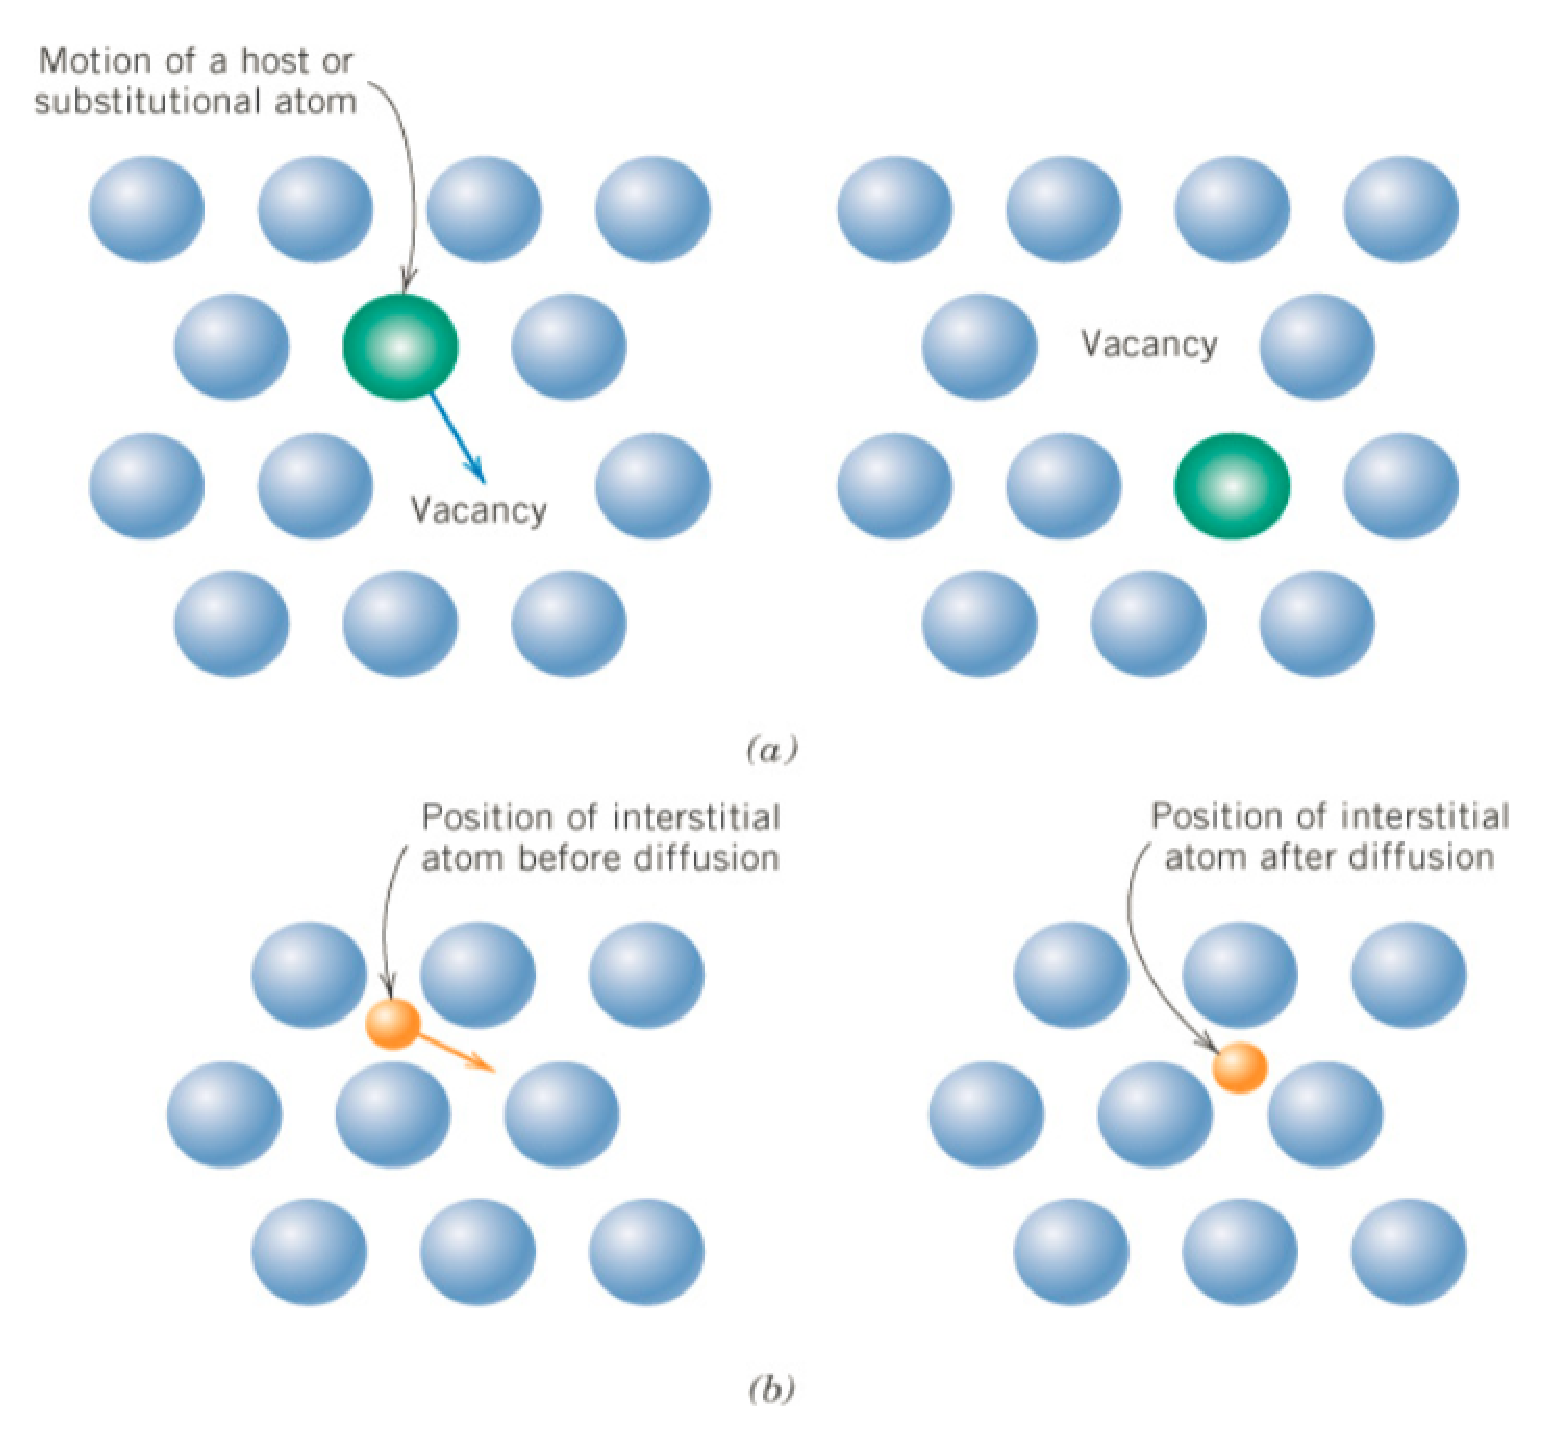
\includegraphics[height=5cm,
    angle=0]{./images/motion.eps}}
\caption{(A) vacancy diffusion; (B) interstitial diffusion}
\label{fig:motion}
\end{figure}

\subsection{Atomic diffusion: interstitial diffusion (interdiffusion only)}

Interstitial diffusion (depends on temperature).  This is generally faster than
vacancy diffusion because there are many more interstitial sites than vacancy
sites to jump to.

\subsection{Probability of energy jump}


\begin{equation}
R_j = R_0 \exp \left( - \frac{E_m}{k_BT} \right)
\end{equation}



\subsection{Diffusion flux (J)}

Diffusion is process which is NOT due to the action of a force , but a result of
the random movements of atoms ( statistical problem).

The flux of diffusing atoms, J, is used to quantify how fast diffusion occurs. 
The flux is defined as either in 
\begin{enumerate}
  \item  number of atoms diffusing through unit area and
per unit time, i.e. atoms/(m$^2$.second).

  \item mass flux: mass of atoms diffusing through
unit area per unit time, (e.g., kg/(m$^2$.second))
\end{enumerate}

\begin{equation}
J = \frac{M}{A.t} = \frac{\text{mass (or atoms or
moles)}}{\text{(cross-sectional area) x time}}
\end{equation}
unit of J (g/(cm$^2$.sec)) if M is mass (g).

In differential form, the instantaneous flux $J$ is
\begin{equation}
J(t) = \frac{1}{A} \frac{\partial M}{\partial t}
\end{equation}

\subsection{Steady-state diffusion: Fick's first law}

In 1D, at steady state of an isothermal, isobaric system, the diffusion along
the direction $x$ is proportional to the concentration gradient.
\begin{equation}
J = - D \frac{dC}{dx}
\end{equation}
As the slope of the change from high to low concentration 
\begin{equation*}
dC/dx = \frac{c_\text{dest}-c_\text{source}}{dx} < 0
\end{equation*}
as $c_\text{dest}=c_\text{low}$ < $c_\text{source}=c_\text{high}$, the minus sign indicate the flux
get positive value and flows in the direction down the concentration gradient. 

$D$ is the diffusion coefficient (Sect.\ref{sec:diffusion-coefficient}), and is
typically chosen as a constant as a given temperature.

\subsection{Diffusion coefficient: Diffusion constant}
\label{sec:diffusion-constant}
\label{sec:diffusion-coefficient}

Diffusion coefficient is the measure of mobility of diffusing species.
At steady-state, the diffusion coefficient is considered a constant value at a
given temperature.
\begin{equation}
D = D_0 \exp \left( - \frac{Q_d}{RT} \right)
\end{equation}
with 
\begin{itemize}
  \item  $D_0 =$ temperature-independent pre-exponential (m$^2$/sec);

\begin{equation}
D_0 = \frac{k_BT}{h}
\end{equation}  
with $h = $ Planck's constant ($6.6 \times 10^{-34}$ J/sec), and $k_B = $
  
  \item $Q_d$ = activation energy for diffusion (J/mole, or eV/atom)
  
  \item $R = $ universal gas constant ()
  
  \item $T = $ temperature (K)
\end{itemize}
If we take the log on both sides
\def\ln{{\text{ln}}}
\begin{equation}
\ln D = \ln D_0 - \frac{Q_d}{R} \left( \frac{1}{T} \right)
\end{equation}
or
\def\log{{\text{log}}}
\begin{equation}
\log D = \log D_0 -\frac{Q_d}{2.3 R} \left( \frac{1}{T} \right)
\end{equation}

\subsection{Nonsteady-state diffusion: Fick's second law}


In most real situations the concentration profile and the the diffusion flux and
the concentrations change with time, i.e. the concentration gradient are
changing with time, Fig.\ref{fig:diffusion-in-time-space}.

\begin{equation}
\frac{\partial C}{\partial t} = \frac{\partial}{\partial t}\left( D
\frac{\partial C}{\partial x} \right) = D \frac{\partial^2 C}{\partial x^2}
\end{equation}

So the time-varying diffusion follows the so-called Fick's second law.

\begin{figure}[hbtp]
  \centerline{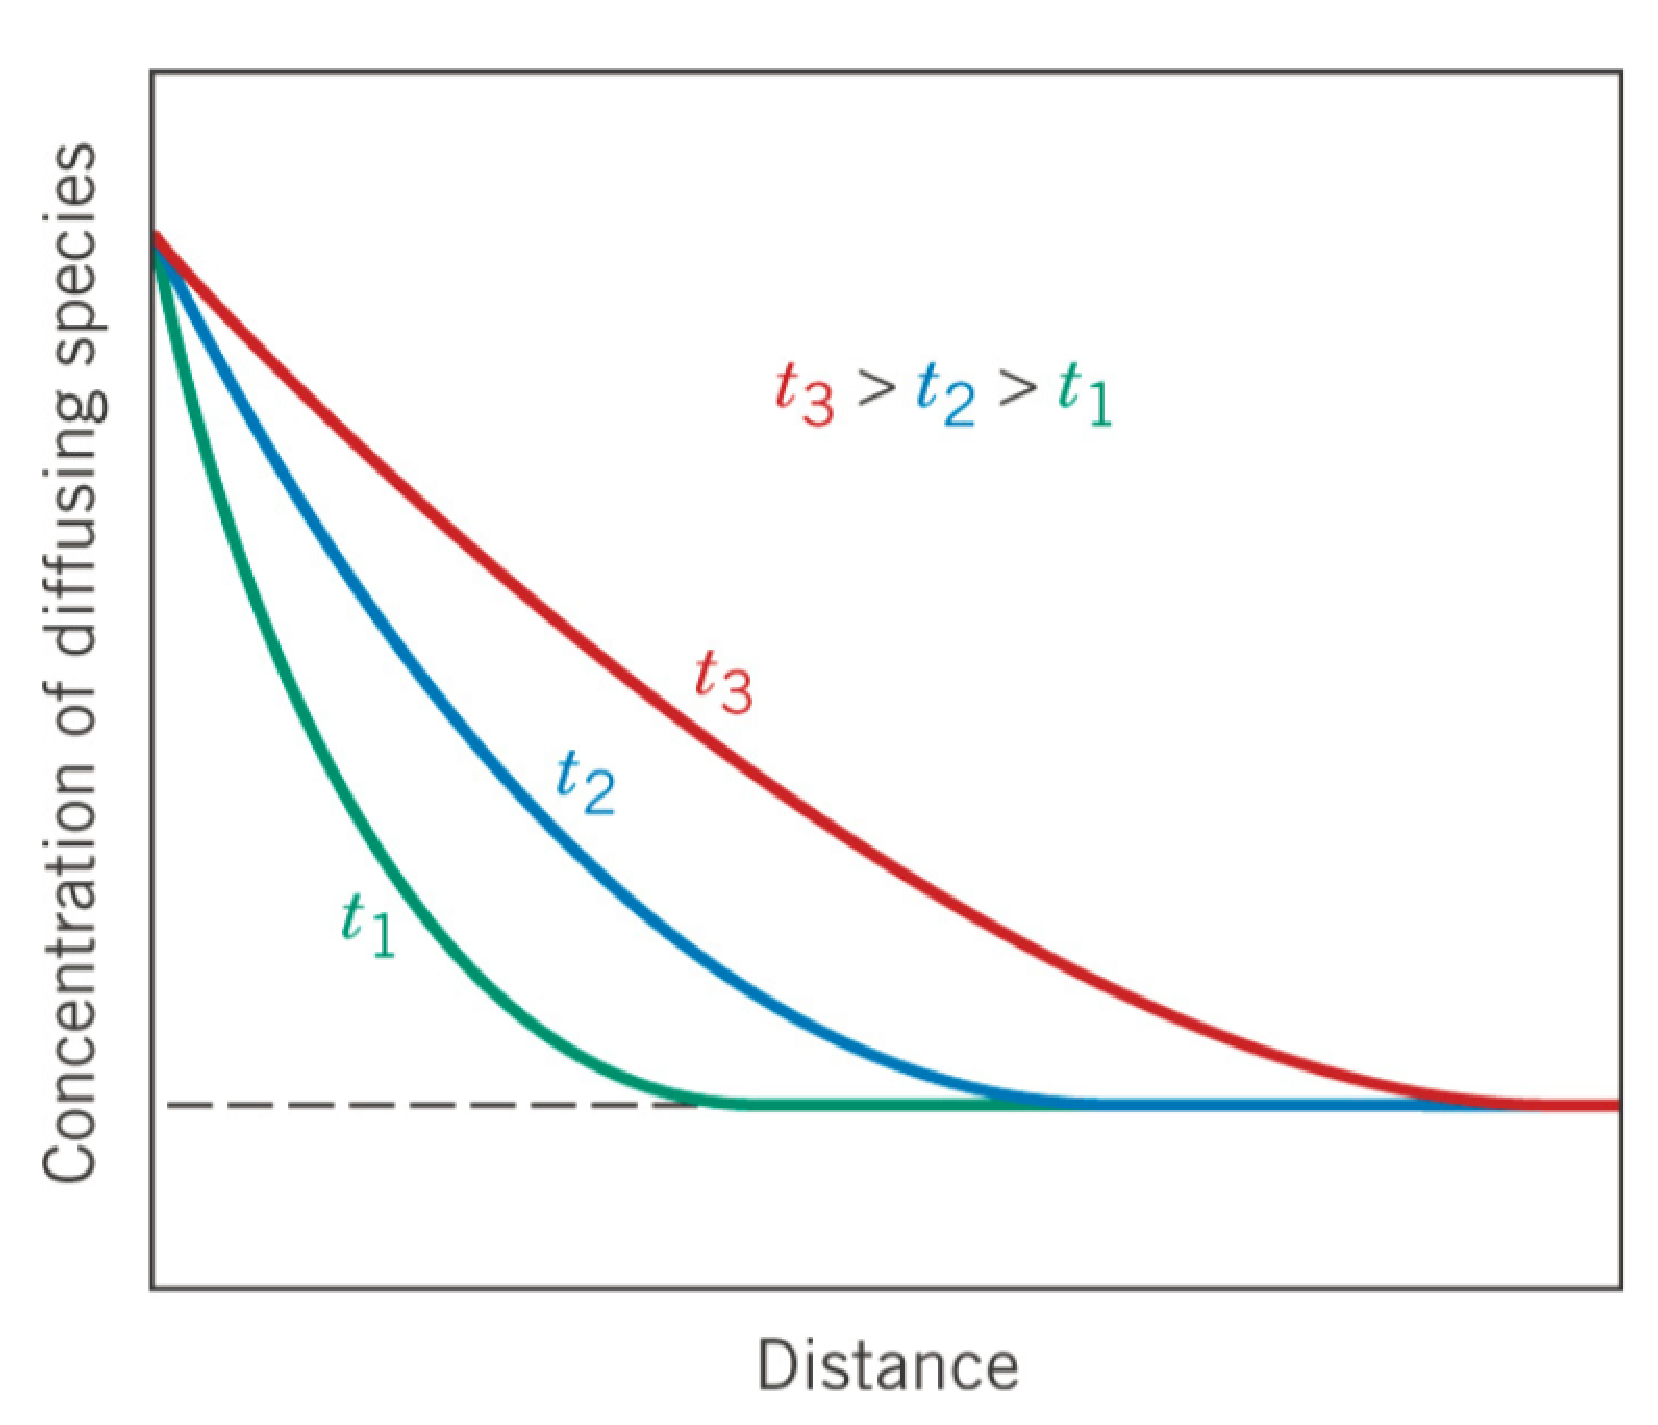
\includegraphics[height=5cm,
    angle=0]{./images/diffusion-in-time-space.eps}}
\caption{Diffusion in time and space}
\label{fig:diffusion-in-time-space}
\end{figure}


Diffusion constant $D$ (distance$^2$/time) is a quantity that tell how fast a
species is translocated from one place to another based on Fickian Law
(deterministic). For a given distance $x$ (distance), the time for movement
is defined as
\begin{equation}
t = \frac{x^2}{2*D}
\end{equation}
The time-constant for this transfer is known as the reciprocal of the time,
$\tau$ (sec$^{-1}$)
\begin{equation}
\tau = \frac{1}{t}
\end{equation}

\begin{framed}
  A connection between ionic mobility $u$ and diffusion constant $D$
  is
  \begin{equation}
    \label{eq:1227}
    D = \frac{u.R.T}{|z|F}
  \end{equation}
with T = absolute temperature [K], R = Faraday constant [J/(mol.K)]
\end{framed}

\section{Chemical flux: Fluxes in aqueous media}
\label{sec:chemical-flux}

For (transmembrane) flux of currents via (selective pores) ion channels, let's
check Sect.\ref{sec:equat-ionic-curr}. In this section, we discuss flux across
two compartments
\ref{sec:flux-example}
\ref{sec:fluxes}

In transport phenomena, a flux is defined as the amount of a substance
that flows through a unit area (or unit volume) per a unit of
time. Generally, the amount is in term of density (e.g. mass per unit
volume or mass per unit surface area), so a flux is a vector.  In
chemical diffusion, the unit of flux
\begin{itemize}
\item can be (mol.cm$^{-2}$.s$^{-1}$) 
\item  or (mol.cm$^{-3}$.s$^{-1}$)

\item or (mol.L.s$^{-1}$) or ($\mu$M/sec).
\end{itemize}
We typically use \verb!cm! rather than metre in chemical diffusion.

There are 4 physical laws that dictates the movement of ions
\begin{enumerate}
\item drift movement under electric field (Sect.~\ref{sec:drift-ions})
\item diffusion of ions under concentration
gradient (Sect.~\ref{sec:ionic-diffusion})
\item the relationship between the two above processes, i.e. the
  diffusion coefficient $D_c$ and the drift mobility $\mu$
  (Sect.~\ref{sec:einstein-relation})
\item the basic principle of separation of charges in biological systems, e.g.
if there is any barrier such as the plasma membrane that separate the two spaces
\end{enumerate}
These laws lead to fundamental equations in computational cell
biology: Nernst-Planck, Nernst, Goldman-Hodgkin-Katz equations, and
Donnan equilibrium equation.

\subsection{Molar flux: Nernst-Planck equation}
\label{sec:flux-molar-flux}
\label{sec:Nernst-Planck-equation}

\textcolor{red}{Effect 1}: The molar flux for diffusive properties in terms of
the diffusion coefficient ($D_s$) and the local concentration of the property
($c_s$). This is Fick's law (Sect.\ref{sec:fickian-diffusion}).

\begin{equation}
M'_s = -D_s \frac{dc_s}{dx}
\end{equation}

\textcolor{red}{Effect 2}: The molar flux of solute due to electrophoretic
effects is defined in terms of the concentration of s (i.e. $c_s$), the
electrical mobility ($u_s$ - the velocity of S in the fluid), and the local
potential ($\Psi$).

\begin{equation}
M'_s = - u_s c_s \frac{d\Psi}{dx} 
\end{equation}


The two affects above are fundamentally additive, i.e.

\begin{equation}
M_s = -D_s \frac{dc_s}{dx} - u_s c_s \frac{d\Psi}{dx}
\end{equation}
This is known as {\bf Nernst-Planck equation} (after Nernst 1888,1889; Planck,
1890). It extends Fick's law for the case where the diffusing particles are also
moved with respect to the fluid by electrostatic forces.
\begin{equation}
\begin{split} 
\frac{\partial c_s}{\partial t} &= -\nabla(J) \\
J &= - \left[ D \nabla c_s - u c_s + \frac{Dz_s e}{k_BT} c_s (\nabla \Psi +
\frac{\partial A}{\partial t}) \right] 
\end{split}
\end{equation}
Its dimension depend on those used to express the ionic concentration an
velocity. NORMALLY: The unit is mol/(cm$^2$.c).

SUMMARY: The total ionic flux for the \verb!k!-th ion type, $\bar{j}_k$, is
given by the sum of ionic fluxed due to (1) diffusion (D), and (2) electric
field (e).
Using {\bf Einstein relationship}
\begin{equation}
\bar{j}_k = \bar{j}_{k,D} + \bar{k}_{k,e} = -D_k \left( \nabla c_k +
\frac{c_k z_k F}{RT} \nabla \Phi \right)
\end{equation}

\begin{mdframed}
Ion flows from one place to another in an aqueous media can be the result from
two driving forces: from an electric field force
(Sect.\ref{sec:flow-by-electric-field-force}) and those resulting from a
diffusional force (Sect.\ref{sec:flow-by-diffusional-force}). For the flow of
ions across a barrier, such as plama membrane, read
Sect.\ref{sec:equat-ionic-curr}.

The {\bf Nernst-Planck equation} describes the flux of an ion (charged
chemical species) in a fluid environment under the affect of diffusion and
electric field.
\begin{equation}
  \label{eq:1228}
    \overrightarrow{j} = \overrightarrow{j_D} + \overrightarrow{j_e} =
    -D (\nabla c + \frac{c.z.F}{R.T}\Delta \Phi) 
\end{equation}
with $\overrightarrow{j}$ = ionic flux [mol/(cm$^2$.sec)]. 
\end{mdframed}

However, what we care about is the current across the membrane, not the molar
flux. It is discussed in Sect.\ref{sec:ionic-flow}.


\subsection{Nerns-Einstein relationship}
\label{sec:Einstein-relationship}

Nernst-Einstein relationship defines 
\begin{equation}
D_s = \frac{u_s RT}{z_s F}
\end{equation}
with $z_s$ is the valence of S.


\subsection{Ionic flows}
\label{sec:ionic-flow}

In order to get from the molar flux (Sect.\ref{sec:flux-molar-flux}) to the
current we need only multiply by the valence and Faraday's constant
\begin{equation}
I_s = z_s.F.M_s
\end{equation}
\ref{sec:nernst-equation}
We can easily convert the ionic flux to the electric current density $I$ by
multiplying the ionic flux by $zF$ (i.e. the number of charges carried
by each mole).

The ionic flux $\bar{j}_k$ can be converted to an electric current density
$I$ by multiplying the former by \verb!z_k.F!
\begin{equation}
I_k = \bar{j}_k \times z.F = -D_k z_k F \left( \nabla c_k +
\frac{c_k z_k F}{RT} \nabla \Phi \right)
\end{equation}
The unit of electric current density $J_{k}$ is [C/(cm$^2$.s)] = [A/cm$^2$].

The equivalent form is
\begin{equation}
I_k = - \left(  \mu_k R T \frac{z_k}{|z_k|} \nabla c_k + u_k c_k
|z_k| F. \nabla \Phi \right)
\end{equation}
\url{http://www.bem.fi/book/03/03.htm}

\begin{mdframed}
\begin{equation}
  \label{eq:1242}
  \begin{split}
    I &= -DzF (\nabla c + \frac{c.z.F}{R.T}\Delta \Phi) \\
     &= - \left(u.R.T.\frac{z}{|z|}\nabla c + u.c.|z|F\nabla\Phi\right)
  \end{split}
\end{equation}
with $I$ = electric current density [C/(sec.cm$^2$)] = [A/cm$^2$].
\end{mdframed}

By integrating the Nernst-Planck equation across the cell membrane -
the center of the membrane is taken as the origin of coordinates for a membrane
of thickness $h$ - for a steady-state and arbitrary potential profile, the
diffusive flux across the cell membrane is (Jacquez, Schultz, 1974)
\begin{equation}
I_k^d = \frac{-h P_k}{\int_{-h/2}^{h/2}  \exp\left( z_k F \psi(x) /(RT)
\right)dx} 
\left[  c_k^i Z^{z_k}_i \exp\left(\frac{z_k F V}{2 RT} \right) 
      - c_k^o Z^{-z_k}_o \exp\left( -\frac{z_k F V}{2 RT} \right)
\right]
\end{equation}
NOTE:
\begin{enumerate}
  \item $P_k$ = permeability of ion $k$ - Sect.\ref{sec:permeability}
  
  \item $z_k$ = valence of ion $k$
  
  \item $\psi(x)$ = the potential at point $x$ along the membrane
  
  NOTE: $\psi(-h/2)$ = from the outside at $-h/2$;
  $\psi(h/2)$ = from the inside at $h/2$
  
  \item $c_k^i, c_k^o$ = the concentration (activity) of ion $k$ at
  intracellular and outer-side of membrane, respectively.
  
  \item $Z$ factor is defined as 
  
\begin{equation}
Z_i = \exp (F V_i /(RT)) \qquad;
Z_o = \exp (F V_o / (RT)) 
\end{equation}
with $V_i = \psi_i - \psi(h/2)$; and $V_o = \psi(-h/2) - \psi_o$ - which are
potential differences between inner and outer bulk phases with the adjacent
membrane surfaces.

NOTE: The transmembrane potential $\Vm = \psi_i - \psi_o = V_i + V + V_o$


\end{enumerate}



\subsection{- caused by electric field force}
\label{sec:flow-by-electric-field-force}
\label{sec:electric-field}

We consider two points: O (with reference potential $\Phi_O$) and P (with
potential $\Phi_P$).  So, the work required to move one unit charge 
is
\begin{equation}
\label{eq:work-move-1-molecule-ion}
W_e = (\Phi_P - \Phi_O)
\end{equation}

Whenever a force exerts on a unit charge, an electric field is defined, in the
opposite direction of the translocation. The {\bf electric field} is defined as
{\it the force that exerts on a unit charge}.

The work $W_e$ required to move Q quantity of charge from
point O to point P is
\begin{equation}
W_e = Q (\Phi_P - \Phi_O)
\end{equation}
with $W_e$ [Joules, J], $\Phi$ [Volt], Q [Coulomb, C]). 

\begin{mdframed}
Instead of using Coulomb, the quantity of ions in electrophysiology is often
used as {\it moles}. Suppose the valence of an ion is $z$ and the change on one
mole of electrons is $F$ (Faraday constant), then the work required to move one
mole of an ion (i.e. an $N_A$ number of molecules of
that ion) of valence $z$ [unitless] from point O to point P is
\begin{equation}
W_e = zF (\Phi_P - \Phi_O)
\end{equation}
NOTE: for $\Ca$ ion, $z_\Ca = 2$.

\end{mdframed}

The work required to move a unit positive charge (i.e. $Q=1$) from O to P (of
distance $ds$) against the electric field $\vec{E}$ is defined as
\begin{equation}
dW = - \vec{E} \cdot \vec{ds}
\end{equation}
with $\vec{ds}$ is the vector of displacement.


Combined with eq.\ref{eq:work-move-1-molecule-ion}, we have
\begin{equation}
\Phi_P - \Phi_O = - \vec{E} \cdot \vec{ds}
\end{equation}

Applying Taylor series expansionof the scalar field $\Phi$ around the point O
along the path $s$
\begin{equation}
\Phi_P = \Phi_O + \frac{d\Phi}{ds} ds + \ldots
\end{equation}
The second term is known as {\it directional derivative of $\Phi$ in the
direction $s$} and by vector-analytic properties of the gradient is given by
$\nabla \Phi \cdot \vec{ds}$. 

If P is very close to O, the remaining higher terms may be neglected. So, we
have $\Phi_P - \Phi_O = \nabla \Phi \cdot \vec{ds}$.


\subsection{- caused by diffusional force}
\label{sec:flow-by-diffusional-force}

If the ionic concentration is not uniform between adjacent compartments, this
leads to a passive redistribution of ionic concentration, which can be described
using {\bf Fickian diffusion} formula (Sect.\ref{sec:ficks-law-diffusion})
\begin{equation}
  \label{eq:1226}
  \overrightarrow{j_D} = -D\nabla c
\end{equation}
with D = diffusion constant [cm$^2$/sec] (Sect.\ref{sec:diffusion-constant}), c
= ionic concentration [mol/cm$^3$] (or Molar=mole/litre), $\overrightarrow{j_D}$
[mol/(cm$^2$.sec)].


\subsection{-- ((((()))))}
In a metabolism process, the product C of one reaction can be the input (i.e.
the reactant) of another one. Hence, the concentration of C, i.e. [C], can
change due to either the consumption of C or the production of C.
Sect.\ref{sec:concentration} describes how a concentration is defined.

\begin{equation}
  \label{eq:135}
  \begin{split}
    \ce{A + B <=> C} \\
    \ce{C + D -> E}
  \end{split}
\end{equation}

The amount of C (in moles) that create/consumed in a unit volume per
unit of time is called the
{\bf chemical flux}\footnote{\url{http://en.wikipedia.org/wiki/Flux}}
of species C, denoted by $J$. 

The equation is given
\begin{equation}
  \label{eq:85}
  J = [C]k
\end{equation}
with $[C]$ is the concentration of the product C
[mol.m$^{-3}$.s$^{-1}$], $k$ is the reaction rate.

{\bf NOTE}: Flux (from Latin: fluxxus - flow)
{\it indicates the amount of flow go through a unit of surface (area)
  per unit time}.
There are different context for using flux, here, we talks about
{\bf chemical flux}, denoted by $J_{chem}$ [mol.m$^{-3}$.s$^{-1}$].

If we can call the amount of C produced in a unit time is $J_{in}$ and
the amount of C consumed in a unit time [s] is $J_{out}$, then the
change in concentration (in the direction of adding) of C in a unit
time [s] is
\begin{equation}
  \frac{d[C]}{dt}=J_{in} - J_{out}
\end{equation}

Let's consider an isobaric, isothermic reaction, i.e. $p=const,
T=const$. Then, based on eq. \eqref{Gibbs} introduced in the previous
chapter, the change in Gibb's free energy of a particular substance is
\begin{equation}
  \label{eq:64}
  dG= -SdT + \mu dN + Vdp = \mu dN
\end{equation}
with $\mu$ is the
{\bf chemical
  potential}\footnote{\url{http://en.wikipedia.org/wiki/Chemical_potential}},
i.e.the potential per mole.


Chemical potential of a component in a solution can be thought of in
many
ways\footnote{\url{http://www.geol.umd.edu/pages/facilities/lmdr/chmpot.htm}}.
In our case, it is defined as the rate at which the extensive internal
energy increase as the number of moles of the component in question
increase.
\begin{equation}
  \label{eq:136}
  \mu = \frac{\partial U}{\partial N_i}|_{S,V,N_{j\neq i}} 
\end{equation}
Its unit is {\it the ``energy'' per mole} [J/mol], $dN$ is the change in
the number of moles for such substance (negative for loss,
positive for gain). Under such condition, the change in the Gibb's
free energy is caused by the change in the number of moles.
% or its variant {\it ``energy'' per mole}

{\bf NOTE}: In general thermodynamics, studied particles don't have to
be only atoms or molecules (i.e. the objects of chemistry). They can
be electrons, holes, or anything else that can be identified and
numbered. The ``chemical potential'' of the electrons, however, is
still a major parameter of the system (to the annoyance of the solid
state physicists - they therefore usually call it ``Fermi
energy'')\footnote{\url{http://www.tf.uni-kiel.de/matwis/amat/def_en/kap_2/advanced/t2_4_1.html}}.



\section{Flux within a single compartment}
\label{sec:flux-within-compartments}

Flux within a single compartment refers to the rate of formation or losing of a
species, i.e. the amount of change over a unit of time, e.g. $J_E = d[E]/dt$.

\section{Flux across compartmental border}
\label{sec:flux-across-compartments}

When spatial dimension is considered, then we need to also estimate the
the flux, i.e. concentration change, due to diffusion from one compartment to
another.


\section{Duffision}
\label{sec:diffusion}

\subsection{Diffusion formula}

Depending on the diffusion, the
formula can be simplified in two ways
\begin{enumerate}
\item isotropic:
  \begin{equation}
    \label{eq:1430}
    \nabla.(D_C\nabla[\Ca]) = D_C(\partial^2[Ca]/\partial r^2 +
    (2/r)\partial[\Ca]/\partial r)
  \end{equation}

\item anisotropic:
  \begin{equation}
    \label{eq:1431}
    \nabla.(D_C\nabla[\Ca]) = D_{Cx}\partial^2[\ca]/\partial x^2 +
    D_{Cy}\partial^2[\ca]/\partial y^2 + D_{Cz}\partial^2[\ca]/\partial z^2 
  \end{equation}
\end{enumerate}


\subsection{How fast of a diffusion: effective diffusion constant}
\label{sec:effective-diffusion-constant}

Under a standard environment ({\it in vitro}), the diffusion of a species is
known as true diffusion. However, under an {\it in vivo} environment, the diffusion can be
slower, due to the viscosity in the media, etc. This diffusion is known as {\bf
effective diffusion constant}. To model kinetics of species inside the cell, we
need to consider using effective diffusion constants, and similarly with
effective volume (to be discussed in the next section).




\section{Currents (movements of ions)}
\label{sec:currents}

Current is the total amount of positive charges (in unit of Coulombs) flowing
across a fixed point in the wire per unit of time
\begin{eqnarray}
  \label{eq:409}
  I = \frac{dQ}{dt}
\end{eqnarray}
with the unit of current is {\bf Ampere} = A = Coulomb/sec = C/sec
(Sect.\ref{sec:current-ampere}).

The current is often calculated using the formula
\begin{equation}
I_s = \bar{g}_S \times \left(  \text{driving forces} \right)
\end{equation}
with the driving force can be
\begin{enumerate}
  \item linear - Sect.\ref{sec:ohms-law}
  
  \item non-linear - Sect.\ref{sec:GHK_current}
\end{enumerate}

\subsection{current in physics}
\label{sec:current-in-physics}

By convention, in physics, current is the direction of the movement of positive
charge (or the opposite sign of the electron movement).

\subsection{current in electrophysiology}
\label{sec:current-in-electropysiology}
\label{sec:ionic-currents}

By convention, in physics, current is the direction of the movement
of positive charge (or the opposite sign of the electron movement). 

However, in electrophysiology, the sign of the (density) current is positive if
the positive charged ion moves from inside to outside of the cell, and vice
versa. This is opposite for negative charged ions, e.g. $\Cl$. For the stimulus
current, if we use

\begin{equation}
  \label{eq:1365}
  \Csc \frac{dV_m}{dt}=-I_\ion + I_\stim
\end{equation}
then $I_\stim$ (from outside to inside) is positive. Otherwise, if we
use
\begin{equation}
  \label{eq:1366}
  \Csc \frac{dV_m}{dt}=-(I_\ion + I_\stim)
\end{equation}
then $I_\stim$ (from outside to inside) is negative. Again, the unit
$\Csc$ is $\mu$F/cm$^2$, and $V_m$ is [mV], while $I_\ion, I_\stim$ is
in $\mu$A/cm$^2$. 

\begin{figure}[hbt]
  \centerline{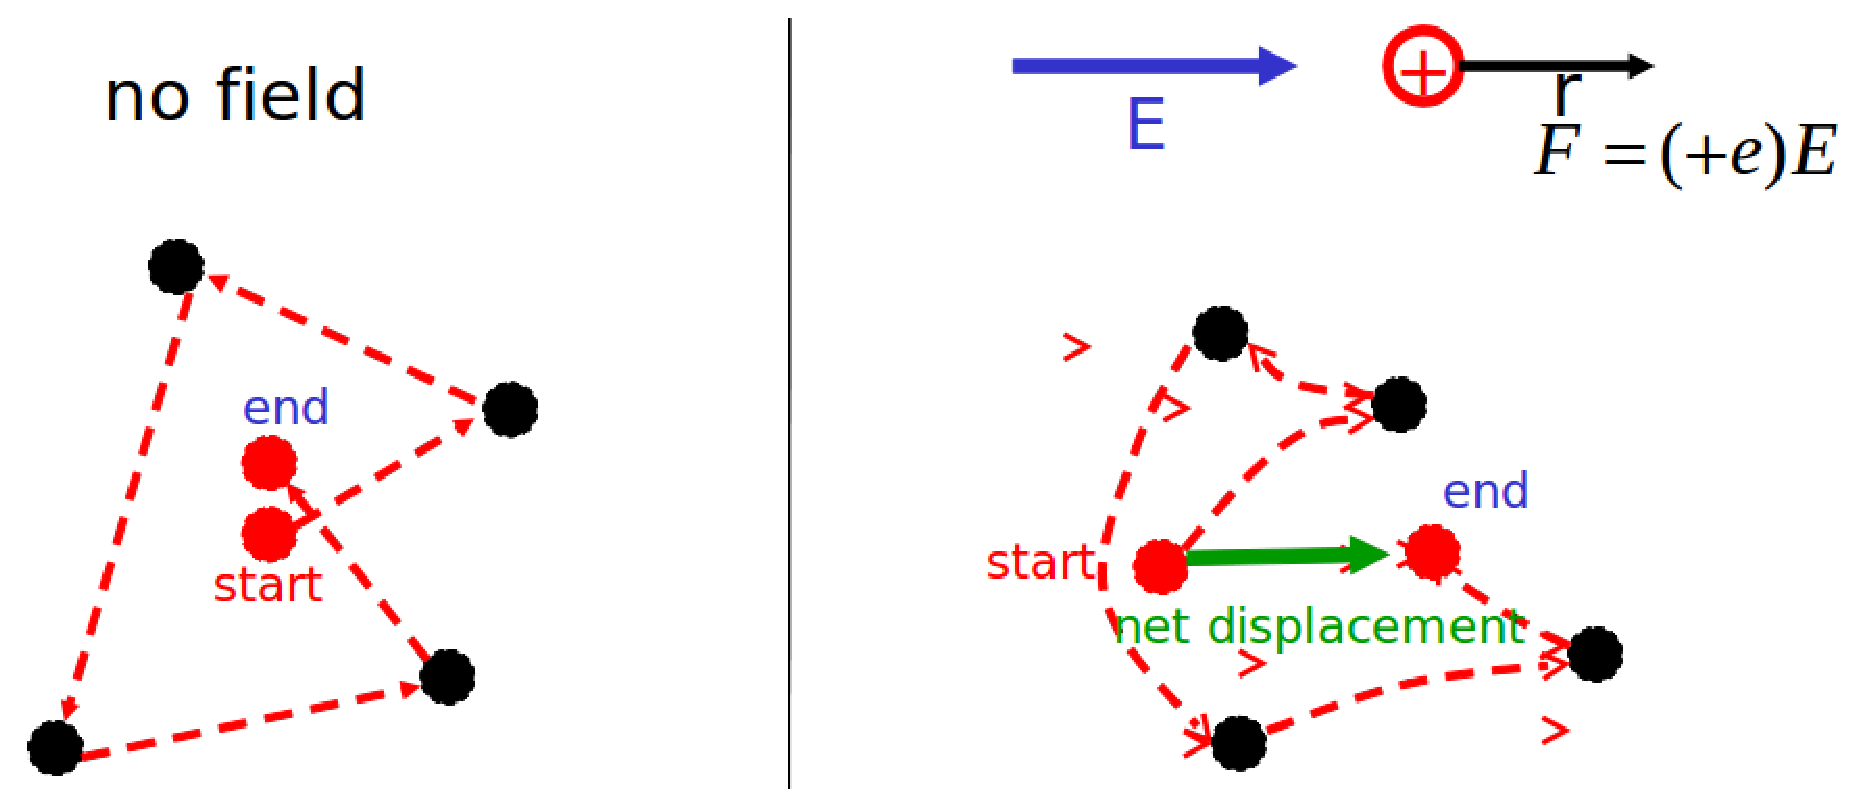
\includegraphics[height=4cm,
    angle=0]{./images/electric_field.eps}}
  \caption{Electric field}
  \label{fig:elec_field}
\end{figure}


At a point in space, using Kirchoff's law (i.e. the law of conservation), the
applied current $I_\app$ is equal to the sum of the membrane current via
capacitor $I_m$ and the ionic current $I_\ion$ (positive if outward),
Fig.~\ref{fig:electric_current}.
\begin{equation}
  \label{eq:689}
  I_\app = I_\ion + I_m + I_{\text{axial}}
\end{equation}
with unit [ampere/unit area]. NOTE: $I_m = \frac{dV_m}{dt}$ 
%So, the transmembrane current $I_m$ is given by
%the sum of the ionic currents and the current flowing into the membrane
% capacity
If we convert to density current, i.e. current per unit surface area, then
\begin{equation}
\Csc \frac{dV_m}{dt} = - \sum j_{ion} + \frac{1}{A} I_\app - j_{\text{axial}}
\end{equation}
with the equation of individual inonic currents $I_{ion}$ can be selected from
Sect.\ref{sec:equat-ionic-curr}.

\begin{enumerate}
  \item current density: nA/$\mum^2$
  \item specific membrane capacitance: $\mu F/\mum^2$
  \item surface area (A) : $\mum^2$
  \item current injection ($I_\app$): nA
\end{enumerate}

If an AP is initiated at all points along the fibre simultaneously, the membrane
potential at all points along the fibre would be the same (or uniform). Then the
axial current $I_{\text{axial}}$ will therefore be zero. 
% This type of response is called a 'membrane' action potential by
% Hodgkin-Huxley, and is rewritten with $I_m=0$ \citep{noble1962mhh}.

Finally, we obtain the widely use formula to model the electrical
property of a cell membrane
  \begin{equation}
    \label{eq:33}
    \Csc \frac{dV_m}{dt} = -\sum_i g_i (V_m-E_i) + \frac{1}{A} I_\app %+
    % I_{\text{axial}}
  \end{equation}
with $\Csc$ in ($\mu$F/cm$^2$), $V_m$ in [mV], $g_i$ in (mS/cm$^2$),
and $I_\app$ in ($\mu$A) and $A$ is surface area. 

\subsection{Current: Ampere}
\label{sec:ampere-current}
\label{sec:current-ampere}
The movement of 1 Coulomb per second is known as the unit of
electrical current, denoted as Ampere (A). It means that 1 (A) = 1
(C/sec), or
\begin{equation}
  \label{eq:1345}
  1 \text{ Faraday } = 9.649\times 10^4 (\text{A.sec})
\end{equation}


\begin{table}[hbt]
  \begin{center}
    \caption{Ionic currents}
    \begin{tabular}{p{2cm}r} 
      \hline
      notation & description \\ 
      \hline\hline
      $I_i$ & ionic current through plasma membrane ($I_{\ce{Na}},
      I_{\ce{K}}$) \\
      & ...$I_i = g_i(V_m-E_i) $ \\
      $I_{app}$ & applied step current (rectangular pulse) (mA/cm$^2$)\\
      $I_m=\frac{I_0}{A}$ & the current density per unit area (mA.cm$^{-2}$) \\
      $i_m$ & the current density per unit length (mA/cm) \\
      $I_\dhpr, I_\LCC$,  $I_\Ca$       & the calcium current via DHPR (L-type channels) \\
      $I_\ryr$ & the current of calcium released via RyR from JSR \\
      $I_\Na$ & the current of sodium \\
      $I_\NaCa$ & the current via Na/Ca exchanger \\
      $I_\K$ & the current via potassium channel \\
    \end{tabular}
  \end{center}
  \label{tab:Current}
\end{table}

With different types of ions, there are respectively different ionic currents,
Table \ref{tab:Current}. Typically, all currents are indeed ``current density''
(Sect.\ref{sec:current-density}), i.e. in unit [Ampere/unit square], e.g.
mA/cm$^2$.


\subsection{Current density}
\label{sec:current-density}

In electrophysiology, to avoid the variance in geometry of the cells, the ionic
current measured in one cell is often converted to {\bf current density},
with unit $\mu$A/cm$^2$, or $\mu$A/$\mu$F. This is useful, under the assumption
that regardless of the cell sizes, shapes, the density is pretty much similar
among the cells. So we can use this to develop models for any cell sizes.

Besides current as density, all quantities are determined based on a unit of
membrane area, except the voltage. The information is given in
Table~\ref{tab:terminology_2}.

The {\bf current density} $\overrightarrow{J}$ and electric field
$\overrightarrow{E}$ are related by
\begin{equation}
  \label{eq:1224}
  \overrightarrow{J} = \sigma \overrightarrow{E} = -\sigma \nabla \Phi
\end{equation}
with $\sigma$ is the conductivity of the medium. If we're interested
in the ions, the flux $j$ of these ions are subject to the electric field
force, and is dependent upon the electric resistance, which in turns
is a function of ionic mobility $u$ of the ionic species. 
\begin{equation}
  \label{eq:1225}
  \overrightarrow{j_e} = u \frac{z}{|z|}c\nabla \Phi
\end{equation}
with $c$ is the ionic concentration [mol/cm$^3$], z = valence
[unitless], u = ionic mobility [cm$^2$/(V.sec)], and
$\overrightarrow{j_e}$ = ionic flux (due to electric field)
[mol/(cm$^2$.sec)]. 


\subsection{Drift of ions}
\label{sec:drift-ions}

Major types of ions in the cells are $\K$, $\Na$, $\Ca$, $\Cl$....  In most part
of the body, the space-charge neutrality is applied
(Sect.~\ref{sec:princ-space-charge}). Yet an important exception is in the
plasma membrane of individual cells. The membrane is selectively permeable to
certain ions under certain condition, thus maintaining a concentration gradient
which results in an electric field across the membrane. Near the plasma
membrane, ions moving is not only affected by diffusion
(Sect.~\ref{sec:ionic-diffusion}) but also under the affect of an electric field
$\mathbf{E}$ which is the result of potential gradient.
\begin{equation}
  \label{eq:1368}
  \mathbf{E} = \frac{\partial V}{\partial l} = \nabla \phi
\end{equation}
with $V$ is the voltage, and $l$ is the length.  This electric field exert a
force $\mathbf{F}=q.\mathbf{E}$ on the particle of charge $q$, causing a {\bf
drift of ions}. It means the ion move randomly, but with a net drift velocity,
i.e. the average motion of the ion, is in parallel to the electric field
$\mathbf{E}$.  This {\bf drift velocity} is dependent upon the material of the
transmitting media, and is in the order of millimeters per second in contrast to
the order of the random speed of the electron themselves (million meters per
second)\footnote{The speed of light is 300 million meters per second}, as shown
in Fig.~\ref{fig:elec_field}.

To tell how well a material can accommodate the movement of electric
charges, we use the concept of {\bf electrical conductivity}, the
symbol is $\kappa$ (or $\sigma$ or $\gamma$), with the unit is
[Siemen/metre] (S.m$^{-1}$) which is the ratio of the current density $j$
(A/m$^2$) to the electric field (V/m).
\begin{equation}
  \label{eq:1367}
  \kappa = \frac{j}{|\mathbf{E}|}
\end{equation}
with $|\mathbf{E}|$ is the magnitude of the electric field. 

The drift velocity is constant, and is the product of the magnitude of
the electric field times a constant called mobility $\mu$.
\begin{equation}
  \label{eq:1369}
  v_\drift = |\mathbf{E}|\times \mu
\end{equation}

The drift flux of ions C moving across the electric field is described
by Ohm's law ({\bf Planck's equation})
\begin{eqnarray}
  \label{eq:407}
  J_\drift = \kappa\mathbf{E} = \mu \frac{z}{|z|} [\text{C}] \nabla \phi
\end{eqnarray}
Units
\begin{itemize}
\item $J_\drift$: molecules/(sec.cm$^2$)
\item $\kappa$ is electrical conductivity (conductivity of the
  material): molecules/(V.sec.cm)
\item $\mathbf{E}=-\frac{\partial V}{\partial x}$ is electric field:
  V/cm
\item  $[\text{C}]$ is the concentration of ions C which
  is in [molecules/cm$^3$].
\item V is electric potential (voltage): V
\item $\mu$: mobility : cm$^2$/(V.sec)
\item z is valence of ion, e.g. +1 for \ce{Na+}, +2 for \ce{Ca^2+} :
  dimensionless
\end{itemize}

The current density can be expressed in terms of free charge density
\begin{eqnarray}
  \label{eq:408}
  j=\eta qv_\drift
\end{eqnarray}
with $\eta$ is free charge density (i.e. number of charge carriers per
unit volume), $v_\drift$ is drift (average) velocity of each charge,
$q$ is the charge of a single charge carrier (ions), $q=z.(+e)$. When
the mobile charges has valence +1 (i.e. contribute one free electron),
then $q=e=1.6\times 10^{-19}$ C.


Thus, the current $I$ is the amount of charge pass through a cross
section area A, given that the wire is modeled a shaded disk of area A
and length L.
\begin{eqnarray}
  \label{eq:411}
  I = j\times A =  \eta qAv_\drift
\end{eqnarray}
\begin{figure}[hbt]
  \centerline{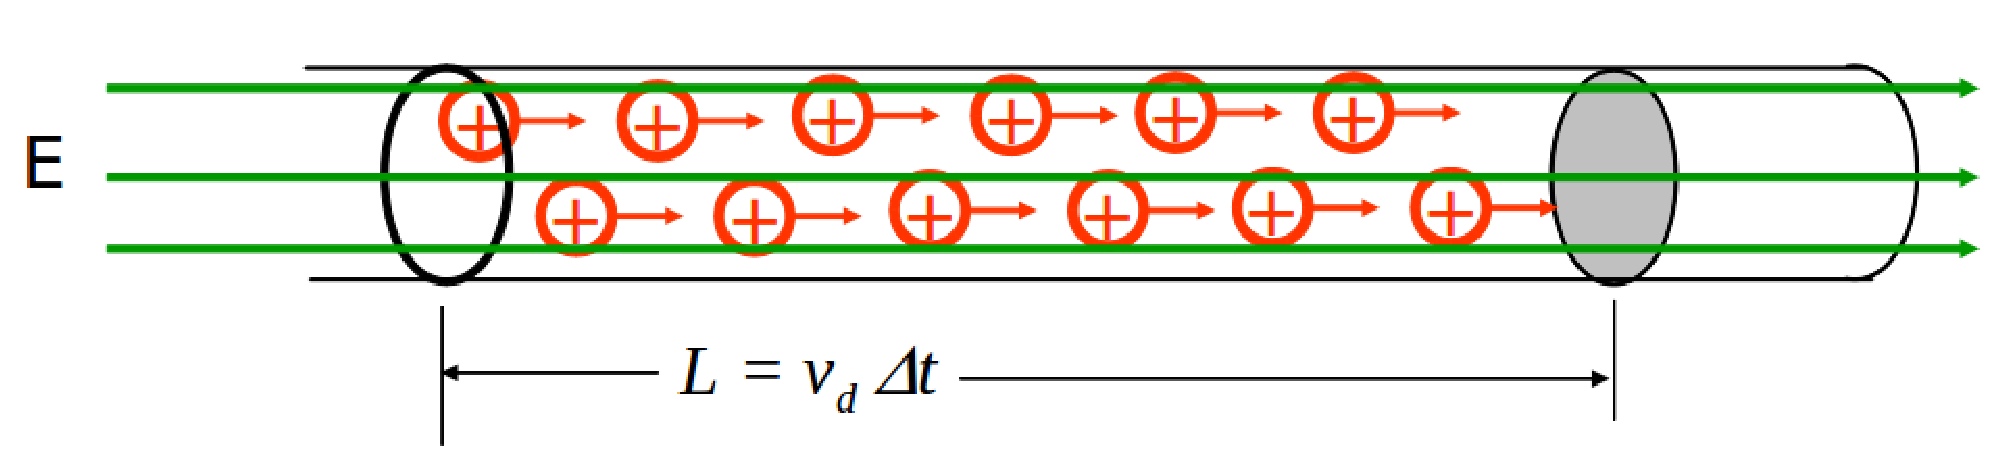
\includegraphics[height=2cm,
    angle=0]{./images/current.eps}}
  \caption{Current}
  \label{fig:current}
\end{figure}

{\bf Quizz}: A copper wire of cross sectional area $A = 3\times
10^{-6}$m$^2$ carries a current of $I=10$A. Find the drift velocity of
the electrons in this wire $v_\drift$. Copper has a density of
$k=8.95$ g/cm$^3$, and atomic weight is
$m_a=63.5$g/mole. Avogadro's number is $Avog.=6.02\times 10^{23}$
atoms. Assume each atom contributes one free electron.

{\it Solution}:  The number of mole per a unit volume is
$\frac{k}{m_a}$. In a single mole, there are Avogadro number of
molecules. Thus, the number of molecules in a unit of volume of the
wire is $\frac{k}{m_a}\times Avog.$. As each molecule (atom)
contribute one free electron, the number of free electron in a unit of
volume is $\eta\times q = \frac{k}{m_a}\times Avog.$. Finally, the
drift velocity is
\begin{eqnarray*}
  v_\drift = \frac{I}{\eta q A} = \frac{10}{\frac{k}{m_a}\times
    Avog. A}
\end{eqnarray*}


\begin{framed}
  $j$ is proportional to the electric field $\mathbf{E}$
  \begin{eqnarray*}
    j= \sigma \mathbf{E}
  \end{eqnarray*}
  while the potential difference $V=\mathbf{E} L$ with $L$ is the length
  of the wire, and $\mathbf{E}$ is the electric field between the two
  ends of the wire. For a uniform wire, we have
  \begin{eqnarray*}
    V = I \times \frac{\rho L }{A}
  \end{eqnarray*}
  with $\rho = \frac{1}{\sigma}$ (unit: $\Omega m$) is the resistivity,
  the quantity
  \begin{eqnarray*}
    R = \rho \frac{L}{A}
  \end{eqnarray*}
  is the resistance (unit: ohm = $\Omega = \frac{Volt}{Amp}$).
\end{framed}

\subsection{Ionic diffusion}
\label{sec:ionic-diffusion}

Ions in a biological system are not uniformly distributed. The
gradient in ion concentration is the main-driving force of the
diffusion of ions in different compartment of the cell. Physical
principles of ion diffusion is decrsibed in this section.

For simplicity, we consider the case when ions moving in a single
dimension, i.e. along x-axis. This is known as the {\bf Fick's first law}
\begin{equation}
  \label{eq:1370}
  J_\diff = -D \frac{\partial[\text{C}]}{\partial t}
\end{equation}
with $J_\diff$ is [molecules/(sec.cm$^2$)], the diffusion coefficient
is (cm$^2$/sec), and $[\text{C}]$ is the concentration of ions C which
is in [molecules/cm$^3$].


\subsection{Einstein relation}
\label{sec:einstein-relation}

Einstein (1905) derived this relationship

\begin{eqnarray}
  \label{eq:412}
  D = \frac{k_BT}{q}\mu = \frac{\mu RT}{|z|F}
\end{eqnarray}
which formally states that diffusion and drift processes in the same
medium are additive.

\subsection{Principle of space-charge neutrality}
\label{sec:princ-space-charge}

\begin{figure}[hbt]
  \centerline{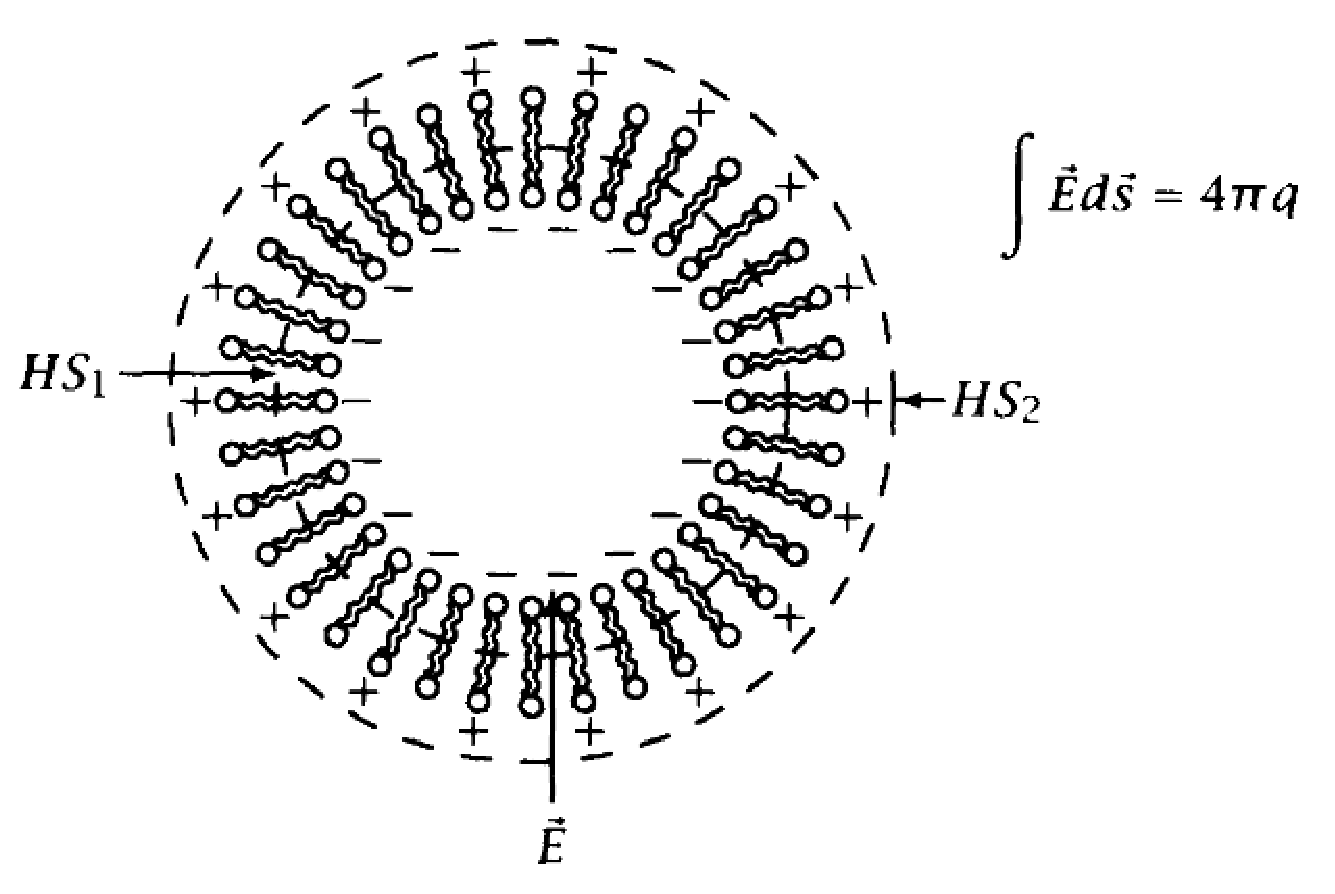
\includegraphics[height=5cm,
    angle=0]{./images/sphere_cell_02.eps}}
  \caption{spherical cells}
  \label{fig:sphere_cell_charge}
\end{figure}

For a given volume, the amount of positive charges is approximately equal to the
amount of negative charges. 
\begin{equation}
  \label{eq:1371}
  \sum z_i^A (+e) [\text{C}_i] =   \sum z_i^C (+e) [\text{C}_i] 
\end{equation}
with $z_i^A, z_i^C$ are valences of anion species, and cation species,
respectively.  This holds for any volume of biological systems, except
in the plasma membrane where the electric field is non-zero. We'll
discuss the movement of ions across the membrane via ion channels in
Sect.~\ref{sec:movement-ion-across-ion-channels}.

Another way to express the space-charge neutrality is using Gauss's
law which states that, the flux of electric field $\mathbf{E}$ through
any closed surface, of a given volume (no matter what the shape is),
is equal to $4\pi$ times the total charges enclosed in that closed
surface.
\begin{eqnarray}
  \label{eq:413}
  \int_{surface} \mathbf{E}\cdot d\mathbf{a} = 4\int_{volume} \rho dv = 4\pi Q
\end{eqnarray}
with $\mathbf{a}$ is the oriented area, $\rho$ is the charge density
(coulombs per volume) (NOTE: $\cdot$ is scalar product). This means
that
\textcolor{red}{the electric field only depends on the total charge
  the volume contains, not the shape of the volume}.

As shown in Fig.~\ref{fig:sphere_cell_charge}, the electric field
inside HS1 is non-zero, as the total charge is negative. However, the
electric field inside HS2 is zero, as the total charge now is zero.


\section{Resistance vs. Conductance}
\label{sec:resistance-conductance}

Ohm's law often uses resistance $R$ (Ohm $\Omega$) to characterize current
flows. In electrophysiology, the current flow through an ion channel is often
represented by the reciprocal of resistance, or conductance $g$ (unit:
Siemens, S).

\begin{mdframed}
EXPLAIN:
Along the cell membrane, ionic channel form parallel circuit of resistance $r_i$
with $i$ is channel index. When multiple channel opens, the new resistance
formed by these channels is $1/r_\text{total} = 1/r_i + 1/r_2 + \ldots + 1/r_n$. 

If we use conductance, the formula is simpler 
$g_\text{total}=g_1 + g_2 + \ldots + g_n$.

\end{mdframed}


The resistance of a given object depends primarily on two factors: What material
it is made of, and its shape.
\begin{equation}
R = \frac{l\rho}{A}
\end{equation}
with $l = $ length of the conductor [m], $A$ = cross-sectional area [m$^2$],
$\rho = $ electrical resistivity (specific electrical resistance) of the
material [Ohm.m].
\begin{equation}
G = \frac{A}{l}\sigma
\end{equation}
with $\sigma = 1/\rho$ = electrical conductivity [S/m].

The formula above is not exact, as it assumes the current density is totally
uniform in the conductor, which is not always true in practical situations.
However, this formula still provides a good approximation for long thin
conductors such as wires.

Another situation for which this formula is not exact is with alternating
current (AC), because the skin effect inhibits current flow near the center of
the conductor. For this reason, the geometrical cross-section is different from
the effective cross-section in which current actually flows, so resistance is
higher than expected.

\url{https://en.wikipedia.org/wiki/Electrical_resistance_and_conductance}


\section{Effective volumes}
\label{sec:effective-volumes}

In cell, a large fraction of the calcium is bound to buffers. If the binding is
assumed to be fast or instantaneous, the change in calcium concentration can be
calculated by multiplying the change (d[$\Ca$]/dt) with the so-called buffering 
fraction is $\beta$, the real amount of calcium should be $c/\beta$, defined
over the volume $V$. However, we don't use $c/\beta$ as the concentration, but
$c$ as the concentration. Then, this concentration should be defined over a 
different volume, known as {\bf effective volume} $\hat{V}$. 
\begin{equation}
  \label{eq:1412}
  c/\beta.V = c\hat{V}
\end{equation}
or
\begin{equation}
  \label{eq:1411}
  \hat{V} = \frac{V}{\beta}
\end{equation}
% part of the volume of the compartment is occupied by the buffer. So,
% it's common usually to use the effective volume, which is the real
% volume divided by the buffering factor in calculation
% \begin{equation}
%   \label{eq:1008}
%   \hat{V} = \frac{V}{\beta}
% \end{equation}
% with $\beta$ tells the fraction of volume of the species being used
% for buffering. 
E.g.
\begin{equation}
  \label{eq:1009}
  \begin{split}
    \hat{V_\nsr} &= \frac{V_\nsr}{\beta_\nsr} \\
    \hat{V_\ds} &= \frac{V_\ds}{\beta_\ds}\\ 
    \hat{V_\myo} &= \frac{V_\myo}{\beta_\myo} 
  \end{split}
\end{equation}

In non-spatial model, or in spatial model with the assumption of
stationary buffers, we can assume a constant fraction of $\ca$ buffer
capacity for the myoplasm $\beta_\myo$~\citep{williams2007pda}.

\section{Units in electrophysiology}


When performing any of the calculation between those quantities, it's
important to know their units.  Standard units are: milivolts,
miliseconds, nanofarads, nanoamperes, microsiemens (mS)
\begin{verbatim}
nF .mV/mS = nA = uS . mV
\end{verbatim}


However, in physiology, a better convention for some units is to
define them {\it per unit of surface area}. This will avoid the
geometrical difference between cells. The surface area of a neuron
might be $3\times 10^4 \mu$m$^2$, or $3\times 10^{-2}$cm$^2$.  So, the
new units are nanofarads per centimeters, nanoamperes per square
centimeters, milisiemens per square centimeters.
\begin{verbatim}
(uF/cm^2) . mV/mS = uA/cm^2 = (mS/cm^2) . mV
\end{verbatim}
The quantities that are unaffected are milivolts, miliseconds. 

So, we use $\Csc$ (nF/cm$^2$) and $R_m$ ($\Omega$.cm$^2$).

\section{How fast a reaction}
\label{sec:how-fast-reaction}

Cells are dynamic processes in which a change in cells can be of
physical or chemical origins (Chap.\ref{chap:chem-react-transp}).  
To see how fast of a chemical reaction, we use a quantity that tells
the time, counting from the starting of the reaction, at which a
certain fraction of the product has been catalyzed. The choice of the
``fraction'' will be discusses shortly. 

\subsection{Exponential time constant $\tau$ (first-order reaction)}
\label{sec:expon-time-const}

\textcolor{red}{In practice, many chemical reaction follows
  first-order kinetics}, or we can break up into a number of first-order
  chemical reactions.
As shown in eq.~\eqref{eq:415}, the current concentration of A is an
exponential function of the initial concentration $[\A]_0$. 

To see how fast/slow of such first-order reaction, they estimate the time when
the ``fraction'' of reactant to be used is 1/2; and the time point is known as
half-time constant or reaction half-time (or {\bf doubling-time constant} if we
refer to the product), i.e.
when half of the reactant has been consumed, or the product increased double.
This is denoted as $T_2$ (for product) and $T_{1/2}$ (for reactant)
\begin{equation}
  \label{eq:663}
  \begin{split}
    T_{1/2} &= \frac{\ln 2}{|k|}\; ; \; k<0 \\
    T_2 &= \frac{\ln 2}{k}\; ; \; k>0 
  \end{split}
\end{equation}
However, back to the time this concept was formulated, people don't
have calculators to find the logarithm. So, people prefer using the
{\bf exponential time constant} $\tau$, i.e. we use $\exp(t/\tau)$
rather than $\exp(kt)$. The unit of $\tau$ is unit of time.
\begin{equation}
  \label{eq:664}
  \tau = \frac{1}{k}
\end{equation}
$\tau$ is the amount of time we must wait for an e-fold increase
($e\approx 2.71$) or decrease (about 1/3 of the initial value).

\begin{framed}
  {\bf TIP}: We can think of reaction half-time as a one cell cycle (one
  generation), while exponential time constant is the triple in time.
\end{framed}

\begin{framed}
  In cell physiology, there is a different concept, though the term looks
  similar, called {\bf membrane time constant}
  (Sect.\ref{sec:membr-time-const-1}) 
\end{framed}

\subsection{Characteristic time (time scale) $\mathcal{T}$}
\label{sec:char-time-time}

For reactions whose rate of changes that are not exponential, it's hard
to find the exponential time constant. Instead, we often speak of a
``time scale'' or ``characteristic time''. It tells how fast/slow of
change of a system. At first
\begin{enumerate}
\item Find the max and min signal: $M_{max},M_{min}$
\item Find the maximum value of the slope (first-order derivative)
  of points within the range from min to max
\item Find the intersections of that slope with two horizontal line
  across the max and min signal.
\item The time between the two intersections is called the {\bf
    characteristic time} $\mathcal{T}$. 
  \begin{equation}
    \label{eq:665}
    \mathcal{T} = \frac{M_{max}-M_{min}}{\max\{\text{slope}\}} 
  \end{equation}
\end{enumerate}

{\bf Example}: The sinusoidal signal $y=\sin(\frac{2\pi t}{T})$. The
max and min value is $M_{max}=1,M_{min}=-1$. The slope is 
\begin{equation*}
  \text{slope}=y'=\frac{2\pi}{T}\cos(\frac{2\pi t}{T})
\end{equation*}
with $T$ is the period, then the maximum value of slope is
$\frac{2\pi}{T}$. Then the characteristic time is
\begin{equation}
  \label{eq:666}
  \mathcal{T} = \frac{1-(-1)}{2\pi/T} = T/\pi
\end{equation}

\subsection{Time constant and observed rate constant}
\label{sec:time-const-observ}

Suppose that a reaction is at equilibrium. Then, if the reaction is
perturbed (e.g. by a sudden change in ligand concentration); the new
equilibrium state will be reached. If the system is modeled with no
intermediate state; i.e. 2 states totally, a simple exponential time
course is enough to approximated. 
\begin{equation}
  \label{eq:843}
  \ce{A <=>[k_{12}][k_{21}] B}
\end{equation}
The rate of this process, thus, can be expressed via an {\bf observed
  time constant} $\tau$, or its reciprocal, the {\bf observed rate
  constant} $\lambda = 1/\tau$.
\begin{equation}
  \label{eq:842}
  \begin{split}
    \tau &= \frac{1}{k_{12}+k_{21}} \\
    \lambda &= k_{12} + k_{21}
  \end{split}
\end{equation}
and the exponential function is $e^{-\lambda t}$ or $e^{-t/\tau}$. 

Equilibrium will be fast ($\tau$ is small) if either the forward
($k_{12}$ is large) or the backward ($k_{21}$ is large) is fast. 



\section{Cytoplasmic resistivity}

Dendrites tend to be long and thin.
The cytoplasm has relatively low electrical resitivity
(Sect.\ref{sec:cytoplasmic-resistivity}); while the membrane has relatively high
resistivity. NOTE: Materials with low electrical resitivity enable current
through easier.



\section{Sign and Direction: Voltage and Current}
\label{sec:voltage-current}

Strictly, voltage is ``energy per unit charge'' (i.e. joules per coulomb, or
equivalent unit: volt).
Voltage is supplied by a battery, and is used by a component (light bulbs,
resistance...), but not in wires. That's why we say voltage across a component. 
Thus, the proper name for {\bf voltage} is {\bf potential difference}, i.e.
$V_m = V_a - V_b$.

Electronic currents, on the other hands, is the {\bf rate of flow of charge}.


\begin{figure}[hbt]
  \centerline{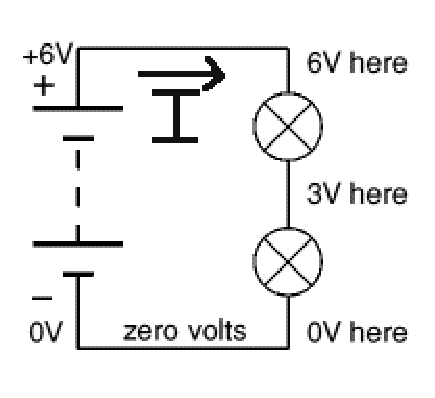
\includegraphics[height=4cm,
    angle=0]{./images/V_I_direction.eps}}
\caption{I-V in electronics}
\label{fig:V-I_elec}
\end{figure}

\subsection{Conventions in electronics}

There are two types of current: direct current (DC) and alternating current
(AC). Direct current has a constant direction, and/or possessing a voltage with
constant
polarity\footnote{\url{http://www.allaboutcircuits.com/vol_2/chpt_1/1.html}}.

In electronics, the common convention for the direction of DC current is the
direction from high voltage to low voltage (high energy to low energy). Besides,
in the common sense, the voltage is defined as the difference between the pole
with high voltage to that of low voltage so that the voltage difference is
always non-negative.

\begin{mdframed}
In electronics we rarely use the name 'potential difference'. Instead, one end
is often implicitly given the value 0(V). The point with zero volt is
often set to the negative terminal of a battery.
\end{mdframed}

In a standard copper wire, electrons are the charge carriers and drift along the
gradient of electrical potential. Even though the electrons (-) are the mobile
charge-carriers, it has long been the convention that the direction of {\it
electric current} is the flow of positive charge. As electrons always move from
the point of negative potential to points of positive potential, the current
flow is considered as the flow of ``imagined'' positive charges.  This flow of
positive charges is known as {\it conventional flow}. The direction of the flow
of electrons is thus of the opposite side of the direction of currents, or the
current go out from (+) pole, and enter (-) pole, Fig.\ref{fig:V-I_elec}.

\subsection{Conventions in cell electrophysiology}
\label{sec:conv-cell-phys}

In electrophysiology, only DC current is used. The convention described in the
previous section, however, is not that being used for studying the  electrophysiology of
the membrane\footnote{\url{http://www.tpub.com/content/doe/h1011v1/index.htm}}.
\textcolor{red}{Thus, there are four important points to know when
  studying cell electrophysiology.}

The charge carriers in electrophysiology are mainly one of the two ionic
species, $\Na$ and $\K$, and to a lesser extent $\Ca$ and $\Cl$.

\begin{itemize}
\item the intracellular terminal is cathode (-), while the
  extracellular is anode (+).

\item membrane potential is the difference between that in the
  cytoplasm w.r.t that in the extracellular, $V_m=V_i-V_o$, as shown
  in Fig. \ref{fig:Ohm_circuit}. Thus it can be positive or negative. 

So, to measure the voltage, we need two reference points. We will learn that
there has been a change in the sign convention as in the early days (pre-1980s),
$V_m=V_o-V_i$.

\item ionic membrane currents $I_X$ (with $X$ represents an ion species) are
defined with positive sign for outward direction and negative for inward ionic
current.
  
\item applied (injected) current $I_\app$ (or $I_\text{inj}$) is inward
direction yet the sign is (+), eq.
\ref{eq:1469}.
\end{itemize}

\begin{figure}[htb]
  \centerline{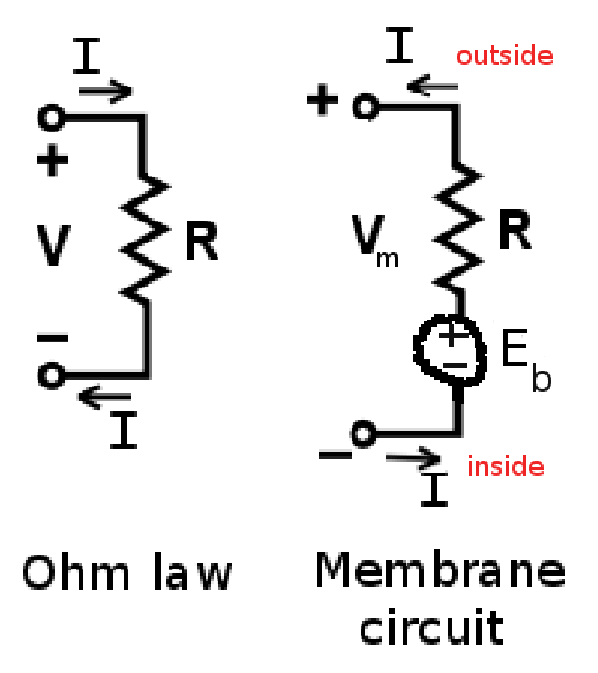
\includegraphics[height=5cm]{./images/Ohm_membrane_circuit.eps}}
  \caption{(A) Normal circuit, (B) Membrane circuit}\label{fig:Ohm_circuit}
\end{figure}



\section{The formation of reactions - Theory of absolute reaction rate}
\label{sec:form-react-theory}

% \subsection{Basic biochemistry}
% \label{sec:basic-biochemistry}

% Consider a reaction:
% \begin{center}
%   \ce{mA + nB ->[k] pC}
% \end{center}
% The reaction {\it rate
%   constant}\footnote{\url{http://en.wikipedia.org/wiki/Rate_constant}}, 
% $K$ or $\lambda$, quantities the
% speed of the reaction.  The rate equation is
% \begin{equation}
%   \label{eq:68}
%   \frac{dC}{dt} = K [A]^m[B]^n
% \end{equation}
% with [X] is the concentration of the substance X; its unit is
% [moles/volume] (or [moles/area] if the reaction occur at the
% boundary).  The {\it order of the reaction} above is $(m+n)$.  $K$ is
% the coefficient depending on the temperature and its unit depend on
% the {\it order of the reaction},


% \subsection{The formation of reactions}
% \label{sec:formation-reactions}


\begin{figure}[htb]
  \centering
  % \input{./images/state_transition_t}
  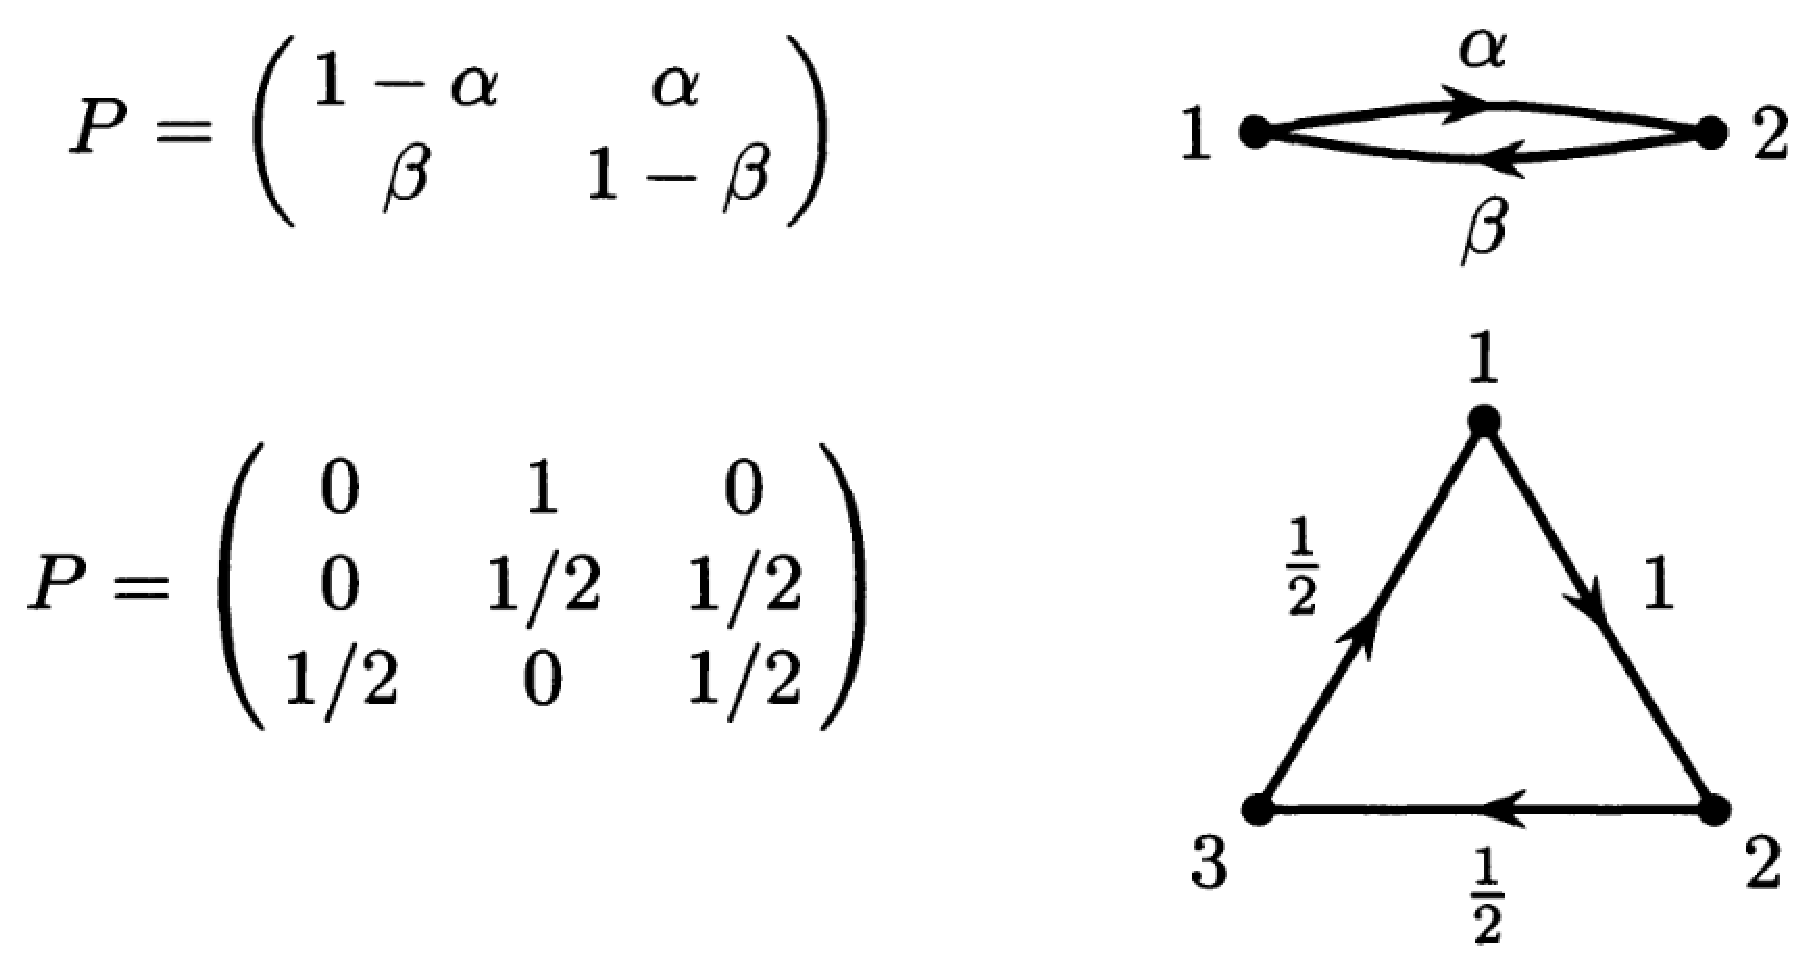
\includegraphics[height=7cm]{./images/state_transition.eps}
  \caption{State transition}
  \label{fig:state_trans}
\end{figure}

In general, chemical reactions require splitting existing chemical
bonds. To analyze such processes, it is necessary to know the
interaction energy of an atom as a function of distances to each of
its neighbors.

{\bf Example:} For simplicity, we consider the interaction
(e.g. bonding) between two molecules. As shown in Fig.
\ref{fig:state_trans}, the two molecules can be in contact
(associative state AS), or can be aparted (disassociated state
DS). Both are quite stable states. In order to jump from one state to
another, there should be an intermediate state that is very
unfavorable and unstable that we call it the {\it transition state} TS.

The energy at TS is relatively higher than those of the two stable
states (DS and AS), and we call it {\it activation energy} (or
mid-night energy). When the system's energy reach to the level of TS,
the TS is now {\it activated}.  The height from the energy at TS to
that of a stable state is, conceptually, termed the
{\it potential barrier} (or the energy barrier) and denoted as $E_A$
or $E_a$ or here we use $\Delta G_0^\#$.

\begin{comment}
  Consider two atoms (molecules) in the surface of free energy. Then,
  the path from A $\rightarrow$ B will essentially has a
  valley-shaped. It means that the reaction follows the path that has
  minimum activation energy.
\end{comment}

In reality, the bonding can be a hydrophobic tether in which two
chemical groups be in contact (or tether)(CS or AS) or disassociated
state (DS).  We consider the reversible reaction

\begin{equation}
  \label{eq:ASDS}
  AS  \xrightleftharpoons[b]{f} DS  
\end{equation}
The {\it rate constant} is relatively high in the initial ($K_0$) and
then decreases. This relation is formulated as follows ({\bf Arrhenius equation})

\begin{equation}\label{eq:Arrhenius}
  K = K_0.e^\frac{-\Delta G_0^\#}{RT}
\end{equation}
with $K_0$ (unit depending on the order of the reaction) is an
empirical factor ({\it Arrhenius-coefficient}) - the initial rate
constant, [$\Delta G_0^\#$] = Joules/mole (note: we substitute $R$ by
$k_B$ when [$\Delta G_0^\#$] = Joules/molecule).

A simple interpretation is that $K_0$ is the number of collisions per
second, and $e^\frac{-\Delta G_0^\#}{RT}$ is the probability that any
given collision will result in a reaction. Then $K$ is the number of
collisions that leads to reactions per second. This relation is
discovered by Arrhenius and hence the eq.~\eqref{eq:Arrhenius} is
called {\bf Arrhenius equation} which is closely related to van't
Hoff's equation. It's simple but describes an accurate relation that
tells the temperature dependence of the reaction
rate\footnote{\url{http://en.wikipedia.org/wiki/Arrhenius_equation}}.


{\bf REMARKS:}
\begin{enumerate}
\item $K$ is called a rate constant, yet not exactly a constant. For a
  given reaction,  it's a constant at a given temperature. However, it
  varies exponentially upon the temperature $K=K(T)$.
% \item The formula $K = K_0 e^{-\frac{\Delta E}{k_B T}}$ with $\Delta
%   E$ is the activation energy that we have studied (when dealing with
%   the number of particles passing the energy barrier) is a special
%   case of Arrhenius equation ( the unit of $\Delta E$ is Joules per
%   molecule).

\item Using {\it theory of absolute reaction rate} (aka {\it transition
    state
    theory})\footnote{\url{http://www.faqs.org/theories/A-Ac/Absolute-Reaction-Rate-Theory-of.html}},
  it is assumed that there is an equilibrium between the AS and TS
  state as given in eq.~\eqref{eq:67}. 
\begin{equation}
  \label{eq:67}
  AS
  \xrightleftharpoons[b]{f} TS \rightarrow DS  
\end{equation}
(note: since there is very few number of molecules from DS go back to
TS so we can consider it as a unidirection reaction).

The equilibrium constant for the first phase is $K^*_{eq}$ (the symbol
* refer to the activated transition state).  Its relation with the
rate constant ($K$) is derived by Wilson-Sommerfeld from kinetic
quantum theory \citep{glaser2001biophysics}.
  \begin{equation}
    \label{eq:WilsonSommerfeld}
    K = q \frac{k_BT}{h}K^*_{eq}
  \end{equation}
  with $q$ is the fraction between activated molecules which leaves to
  the right vs. to the left of the activation energy (for symmetry of
  the relations, we have $q=1$); $h = 6.62\times 10^{-34}$ (J.s) is the
  Planck's constant.

  Based on eq.~\eqref{eq:vantHoff_2}, we have
  \begin{equation}
    K = q \frac{k_BT}{h}e^{-\frac{\Delta G^*}{RT}}
  \end{equation}
and combining with eq. ~\eqref{eq:69}, the result is
  \begin{equation}
    K = q \frac{k_BT}{h}e^{-\frac{\Delta H^*}{RT}}e^{\frac{\Delta S^*}{R}}
  \end{equation}
  The temperature independent exponential part is of particular
  interest. The macromlecules, during the reaction, can get a larger (
  $\Delta S^* < 0$) or a lower ($\Delta S^* < 0$) degree of order. We
  call $ S^*$ is {\bf entropy of activation} which tells the
  conformation of the macromolecules.

  Under the conditions that the total number of molecules remains
  constant (e.g. the sum of stoichiometric numbers between the
  reactants and the products are the same), $\Delta G = 0, q=1$ and small molecules,
  the value of $K$ is

  \begin{equation}
    K = \frac{k_BT}{h} = 10^{13} s^{-1}
  \end{equation}
  at T = 300K (human body temperature).


\item The Arrhenius equation in eq. \eqref{eq:Arrhenius} is important since it not only
  describes the temperature dependence of chemical reactions, but also
  can be used to describe other time dependence quantities such as
  diffusion, kinetics of phase transition, complicated biological
  processes - at certain temperature intervals - (e.g. growth rate,
  heart rate), structural transition in biomolecule (only if there is
  a dominant free energy barrier)...

\item For a problem in which we want to know whether a time dependence
  parameter $K$ follows the Arrhenius equation or not, we often use
  {\bf Arrhenius plot}. Based on the fact that if such quantity $K$
  follows the Arrhenius equation, then 
  \begin{equation}
    \ln \frac{K}{K_0} = -\frac{\Delta G^\#}{RT} =  \frac{\Delta S^\#}{R} - \frac{\Delta H^\#}{RT} = f(1/T)
  \end{equation}
  In other words, we expect to see a straight line between (1/T)
  vs. ln(K/K$_0$) if $K$ follows the Arrhenius equation.

%   NOTE: $\Delta G^\# = \Delta H^\# - T\Delta S^\#$.

\item Using Arrhenius equation, we can calculate the life span of a
  bond possessing a specific bonding energy resisting the attack of the
  energy of thermic noise ($RT$). In that sense, we have $K =
  \frac{1}{\tau}$, and the quantity
  \begin{equation}
    \tau = \tau_0 e^{\frac{E_D}{RT}}
  \end{equation}
  will tell us how much time to cross this energy barrier (i.e. the
  bonding is broken). $E_D$ is the activation energy of a decay
  reaction. For small molecules, the values of $\tau_0$ ranges from
  $10^{-14} \rightarrow 10^{-13}$ second. And depending on the
  activation energy $E_D$, the lifespan can vary from a very short time
  ($10^{-12}$s) to very long time span ($10^5$s). 

  The {\it mean life span} is a typical variable of statistical
  thermodynamics. In DNA, the spontaneously molecular transformation,
  known as mutations, results in new residues whose stability has not
  yet been approved by natural selection. The lifespan of these
  residues can be changed by a slightly displacement of its bond
  energy. Hence, remutations (mutation on mutated residues) occur more
  often than could be expected statistically.

  Protein folding occurs in sub milli-second scale. In other words,
  normally, in protein folding, the value of $E_D$ is about
  $(1\rightarrow10)\times RT$; and in protein aggregation, the value
  of $E_D$ is $(20)\times RT$. In deed, a small change in activation
  energy, e.g. in the presence of enzyme, will lead to dramatic
  changes of the life span.


\item Even though a real biological process usually consist of a large
  number of single reactions, each with different activation energies,
  the overal process is determined by a
  {\bf simple limiting reaction}, i.e. the slowest reaction in a
  series of chemical reaction. Example:

\ce{NO2 + NO2 -> NO + NO3} (slow step)

\ce{NO3 + CO -> NO2 + CO2} (fast step)

Clearly, no matter how fast the second step can be, the overal rate
should be at the same rate of the slower step 1 since one of the
reactants in step 2 is the product of the step 1. Such kind of process
is called {\it rate limiting process}. In that sense, the straight
line of the Arrhenius plot for the slowest step will reflect the
activation energy of this rate limiting process\textit{rate limiting
  reaction}\footnote{\url{http://en.wikipedia.org/wiki/Rate-determining_step}}.
\end{enumerate}

{\bf Example}: $H_2O \xrightleftharpoons[]{K_d} H^+ + OH^-$

$K_d = 2.5\times 10^{-5} s^{-1}$

$\tau_d = 11 hours$

$pK = pH - \log \frac{[OH^-]}{[H_2O]}$


\section{Fickian motion: no viscosity}
\label{sec:transport-process}

This section deals with the movements of molecules which is the basic
behavior of life entities. Even though there is still no universally
accepted theory of the liquid state, one can account for the overall
behavior of liquids through the formal treatment of diffusion and
viscosity (the quantity that describes the fluid's resistance to
flow). Here, we just mention the basic movement, diffusion, and one
measure - viscosity. For a complete description, read
Sect.\ref{chap:appendix-b}. 


The direction of the force of atomic bombardment is constantly changing, and at
different times the particle is hit more on one side than another, leading to
the seemingly random nature of the motion. This was called {\bf Brownian motion}
(Sect.\ref{sec:Brownian-motion}).
\url{http://en.wikipedia.org/wiki/Brownian_motion}


\subsection{Diffusion: Particles in water}
\label{sec:diffusion-particles}


From observing the Brownian motion (Sect.\ref{sec:Brownian-motion}), Einstein
pointed out that the water molecules (because of their smaller sizes) are more
mobile than the pollen particles. Hence, it is valid to think in terms of the
water molecules that hit the pollen particles, but not the reverse.

\begin{figure}[hbt]
  \centerline{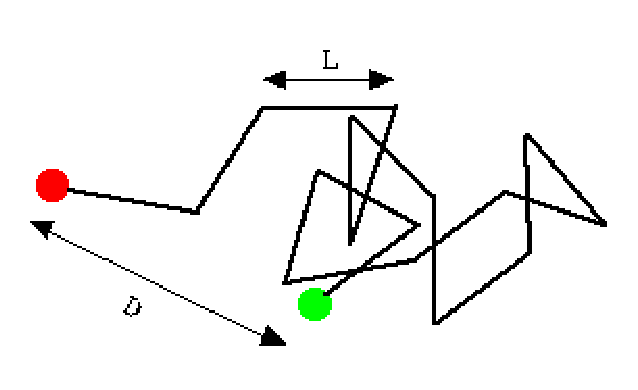
\includegraphics[height=5cm,
    angle=0]{./images/random_walk.eps}}
\caption{Random walk}
\label{fig:random_walk}
\end{figure}

Einstein's formula has two parts:
\begin{enumerate}
  \item relates the diffusion coefficient to the mean
square displacement of a Brownian particle: to determine how far a Brownian
particle travels in a given time interval.

NOTE: Classical mechanics is unable to determine this distance because of the
enormous number of bombardments a Brownian particle will undergo, roughly of the
order of $10^{21}$ collisions per second.
  
  \item relates the diffusion coefficient to measurable physical quantities.
  
In this way Einstein was able to determine the size of atoms, and how many atoms
there are in a mole (i.e. Avogadro's number), or the molecular weight in grams,
of a gas
\end{enumerate}
\textcolor{red}{We will focus on the first part.}
It requires certain number of assumptions:
\begin{itemize}
  \item conservation of particle number
  \item the increment of particle position in an unrestricted one-dimensional
  space (x), denoted as $\Delta$, is a random variable.
  
The probability density function $\phi(\Delta)$ is used to describe the relative
likelihood for this random variable $\Delta$ to take on a given value.

\end{itemize}


When we examine the movement of a specific particle, we can divide its
trajectory into small straight paths. In that sense, the particle
moves from point to point in an essentially ballistic manner. Further,
if each jump is independent from the history jumps, the movement
process is said to be stochastic and the movement themselves is said
to describe a {\bf random walk}, as shown in
Fig.~\ref{fig:random_walk}.  

Assuming after $n$ small displacement of length $L$, and the particle
move in a straight line, the total displacement would be $r=nL$
However, due to the randomness in the direction of the movement
(sometimes forward, sometimes backward, sometimes to the left,
sometimes to the right...), the particle have displaced a distance
\begin{eqnarray}
  \label{eq:237}
  r = \sqrt{nL}
\end{eqnarray}
In general, if the particle moves randomly, with each displacement of
length $r_i$, then the square of the average displacement $\vec{r}^2$,
is a good measure of the Brownian motion.
\begin{equation}
  \label{eq:70}
  <\overrightarrow r^2> = \frac{\sum_{i=1}^n r_i^2}{n}
\end{equation}
with the trajectory is projected on an arbitrary
axis\footnote{\url{http://mahalanobis.twoday.net/stories/210704/}}. The
classical results showed that, in the absence of any directional bias,
the mean of distance travelled in any number of steps, $n$, is zero,
i.e. $<\overrightarrow{r}> = 0$.


The density (i.e. the number of particles per unit volume) $\rho$
changes in a Taylor series
\begin{equation}
\rho(x, t+\tau) = \rho(x, t) + \tau \frac{\partial \rho(x)}{\partial t}
\end{equation}
\ldots
\begin{equation}
\frac{\partial \rho}{\partial t} = \frac{\partial^2 \rho}{\partial x^2} \times
\int^{+\infty}_{-\infty} \frac{\Delta^2}{2\tau} .\phi(\Delta)d\Delta + \text{
higher-order even moments}
\end{equation}
with the diffusion coefficient $D$ is
\begin{equation}
D = \int^{+\infty}_{-\infty} \frac{\Delta^2}{2\tau} .\phi(\Delta)d\Delta 
\end{equation}

The density of the Brownian particle satisfies the {\bf diffusion equation}
\begin{equation}
\frac{\partial \rho}{\partial t} = D \frac{\partial^2 \rho}{\partial x^2}
\label{eq:Einstein_diffusion_eq} 
\end{equation}
Assuming the system with $N$ particles starts from the origin at $t=0$, the
solution of the above equation is
\begin{equation}
\rho(x, t) = \frac{N}{\sqrt{4\pi D t}} e^{-\frac{x^2}{4Dt}}
\end{equation}

This allows Einstein to calcualte the moments
\begin{itemize}
  \item The first moment (mean) = 0 (as the Brownian particle is equally likely
  to move to the left as it is to move to the right)
  
  \item The second-moment (variance) is $\bar{x^2} = 2Dt$ (which is the mean
  squared displacement in terms of time elapsed $t$ and the diffusion constant $D$)
\end{itemize}

Consider in a given environment, the diffusion coefficient (or simply
diffusivity) of the particle is $D$ [cm$^2$.s$^{-1}$] in 3-dimension,
for a stochastic process, the mean squared displacement, within a
period of time t, of a particle is
\begin{equation}
  \label{eq:Einstein.1905}
  <\overrightarrow r^2> = 6Dt
\end{equation}(discovered by Einstein in 1905)

Different environment causes dramaticaly difference in travelled
distance of the particle. For example, the distance diffuse (during
the same time) in liquid is 10cm, while in solide is $10^{-1}$cm.

\begin{table}[hbt]
  \begin{center}
  \begin{tabular}{cc}
\hline
    D[cm$^2$.s$^{-1}$] & environment \\
\hline
$D=10^{-9}$ &  in solid \\
 $D=10^{05}$ & in water \\
$D=10^{-1}$ & in gas \\
\hline
  \end{tabular}
  \end{center}
  \caption{Diffusion coefficient}
  \label{tab:Diffusion}
\end{table}


Now, we consider a real-wold example of transmission in biological
environment.

{\bf Example}: Small membrane-bound vesicles deliver neurotransmitter
to the pre-synaptic membrane of nerve axons.  If the vesicle travels
in a 3D-manner, it takes a long time to reach the pre-synaptic
membrane that travelling in one dimension. We examine two cases.

\subsection{1D diffusion: Fick's first law}
\label{sec:1d-diffusion}

\begin{figure}[hbt]
 \centerline{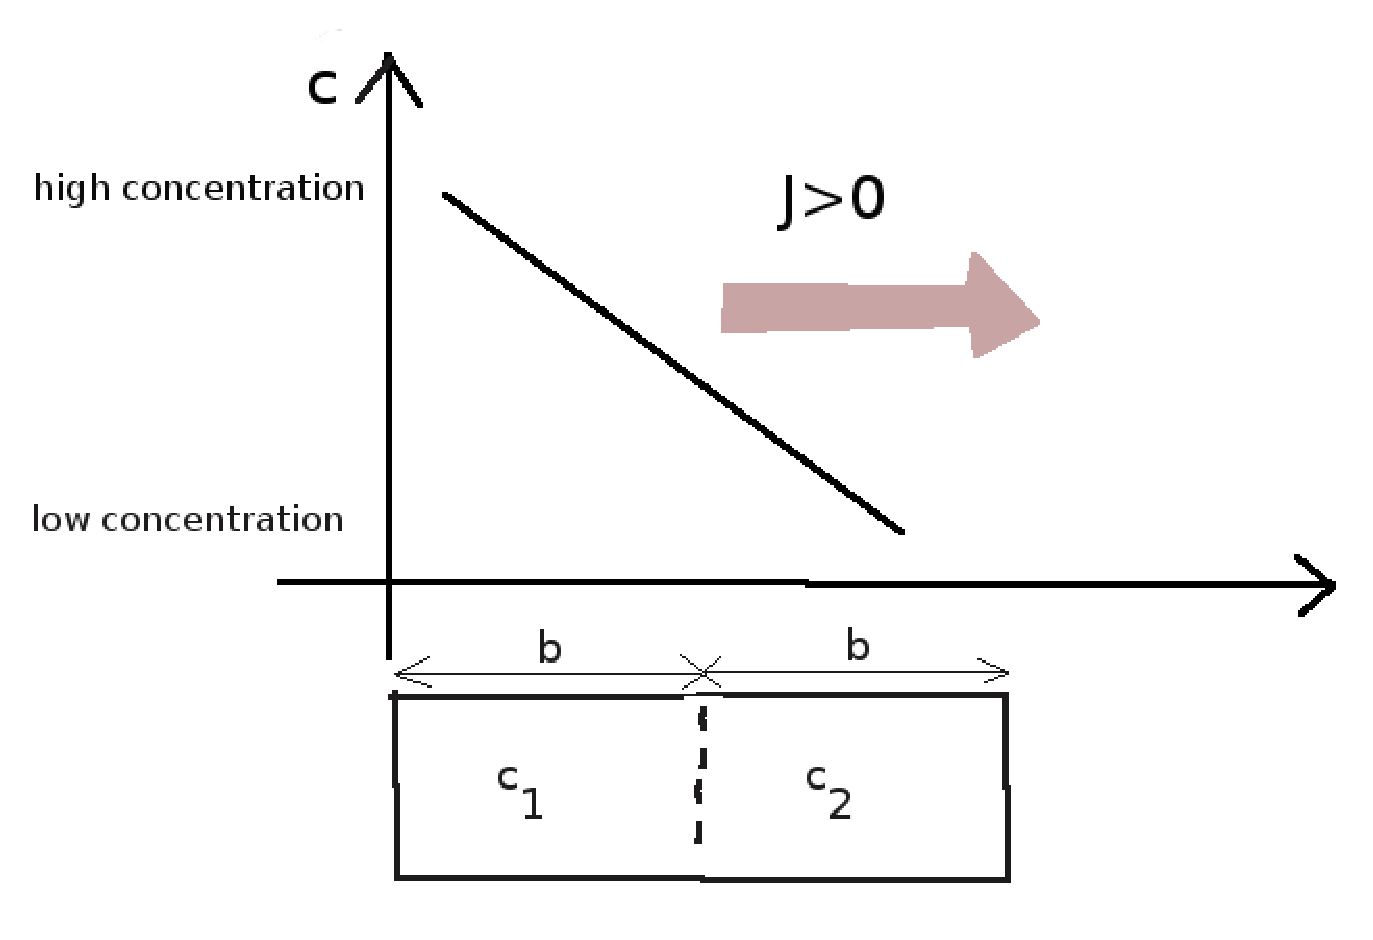
\includegraphics[height=7cm]{./images/Fick_law.eps}}
\caption{The illustration for Fick's law}
\label{fig:Fick_law}
\end{figure}

The cell creates protein microtubules that lie along the direction of
the axis of the axon to guide the passage of the vesicles. Under this
scenario, to quantitatively describe the diffusion. A conceptual
approach is to examine the situation in which the movement is along
the axis of a cylinder having a cross-section of unit area. Suppose
that the cylinder is divided into imaginary slabs of thickness $b$,
which is equal to the length of a single diffusive jump.

We consider two successive imaginary chambers of length $b$, chamber
one on the left side, as shown in Fig.~\ref{fig:Fick_law}. Let's $c_i$
denotes the concentration of molecules [per cross-section's area] in
chamber $i$, then the number of molecules in chamber $i$ is
\begin{equation}
  \label{eq:71}
n_i = c_ib  
\end{equation}
and that $c_1 > c_2$. Let's $f$ denotes the frequency with which the
particles make their jumps. There are two possible direction of jumps,
left or right, with equal probability (i.e. 1/2). Hence, the number of
particles move from the chamber 1 to chamber 2 is $\frac{1}{2}n_1f$,
and the number of particles move from the chamber 2 to chamer 1 is
$\frac{1}{2}n_2f$. 

Assuming the positive direction of the axis is from left to right,
then the flux $J$ of particles across the imaginary plane that devide
the two chambers per a unit time is
\begin{equation}\begin{split}
    J &= \frac{1}{2}n_1f - \frac{1}{2}n_2f \\
   &= \frac{1}{2}fb \left (c_1 - c_2 \right) \\
   &= -\frac{1}{2}fb \left (c_2 - c_1 \right) \\
    &= -\frac{1}{2}fb^2 \frac{\partial c}{\partial x} 
  \end{split}
\end{equation}

The examining context is for 1D diffusion, then the simple
diffusion coefficient
\begin{equation}
  D =\frac{ <\overrightarrow r^2>}{time} = <\overrightarrow
  r^2>.f = \frac{1}{2}b^2f
\end{equation}

Finally, we have the formula 
\begin{equation}
  J= -D \frac{\partial c}{\partial x}
\end{equation}
which is called {\bf Fick's First Law} (for a single dimension
movement). As we're assuming $c_2 < c_1$, and the gradient is the new
value minus the old value, the negative sign of the right side
indicates that the flux is flowing from left to right, or in other
words, in the direction of lower concentration.

In 2 or more dimension, we use
\begin{equation}
J = -D \nabla c
\end{equation}

\subsection{3D diffusion: Einstein formula}
\label{sec:3d-diffusion}

Now, for a more general case, a random jump can
move in 3D space, without the friction and collision, we have the
classical Newton equation
\begin{equation}
  m \frac{d^2\overrightarrow r}{dt^2} = \overrightarrow F
\end{equation}
In the general case, with friction force $-\xi \frac{d\overrightarrow
  r}{dt}$ and force due to collision $\overrightarrow R$, we have
\begin{equation}
  m \frac{d^2\overrightarrow r}{dt^2} =\overrightarrow F - \xi
          \frac{d\overrightarrow r}{dt} + \overrightarrow{R} 
\end{equation}
with $\xi$ is the {\it friction coefficient} (or drag coefficient)
\begin{equation}
  \xi = \frac{k_BT}{D}
\end{equation}
is the {\bf Einstein's formula}. 

\subsection{3D diffusion: Stoke's formula}

However, if the particle is a spherical shape of radius $r$, then the friction
coefficient is formulated as ({\bf Stokes' formula})
\begin{equation}
  \xi = 6\pi\eta r
\end{equation}
with $\eta$ is the viscosity [dyne.s.cm$^{-2}$] = [Poise] = [P] (Jean
Louis Poiseuille).

Finally, we learn this very important formula
({\bf Einstein-Stoke's formula}) for the diffusion coefficient in 3D
space:
\begin{equation}
  D = \frac{k_B T}{6\pi \eta r}
\end{equation}

{\bf REMARKS}:
\begin{enumerate}
\item Diffusion occurs due to the non-zero gradient of concentration

\item Flux $J$ is proportional to diffusion coefficient $D$.

\item The diffusion coefficient depends on the temperature, the
  viscosity and the size of the particle.
\end{enumerate}


\section{Navier-Stock equation: particles in viscous fluid (viscosity)}
\label{sec:viscosity}
\label{sec:navier-stock-equation}

Viscosity is a quantity that measures the resistance of a fluid to
flow. Then, to describe the motion of a fluid substance, we use
{\bf Navier-Stokes equations}. This is a set of differential equations
that describes how velocity $\mathbf{v}$, pressure $p$, temperature
$T$ and density $\rho$ are related. However, they do not explicitly
establish the relation among the variables of interest (e.g. velocity
$v$ and pressure $p$), but their rate of changes (e.g. $dv$ and
$dp$). These equations were derived independently by Navier in France
and Stokes in England\footnote{\url{http://www.grc.nasa.gov/WWW/K-12/airplane/nseqs.html}}.

For a particle of spherical shape of radius $r$ to move within a
fluid of  viscosity coefficient $\eta$ (eta), and the
temperature is $T$, then the displacement (for a single particle)
within a time interval $\Delta t$ is now

\begin{equation}
  <\overrightarrow r^2> = \frac{k_BT \Delta t}{3\pi \eta r}
\end{equation}
which is the {\bf Einstein-Smoluchowski} formula. This will alows us
to compute the time for a single particle crossing a certain distance
by diffusion.

The eq.\ref{eq:Einstein_diffusion_eq} is assumed in the osmotic pressure
experiment A similar formula can be achieved if particles are in a viscous fluid
(viscosity $\mu$ - particle's mobility in the fluid) in a gravitational field
($g$ = gravitational acceleration). There are two regions:
lower part of higher concentration, and upper part with lower concentrations. Gravity tends to make
the particles settle, whereas diffusion acts to homogenize them, driving them
into regions of smaller concentration.
\begin{enumerate}
  \item downward speed under the action of gravity: $v = \mu mg$, with $m$ =
  particle's mass
  
  \item the mobility of a particle of spherical shape  with radius $r$ follows
  the George {\bf Stoke's equation}:
\begin{equation}
\mu = \frac{1}{6\pi \eta r}
\end{equation}
with $\eta$ = dynamic viscosity of the fluid.
\end{enumerate}
 In a state of dynamic equilibrium, the particles are distributed according to
the barometric distribution
\begin{equation}
\rho = \rho_o e^{-\frac{mgh}{k_BT}}
\end{equation}
with $\rho - \rho_o$ = the difference in density of particles separated by a
height difference of $h$.
%\subsection{Background}
\subsection{Advection operator, convection operator}
\label{sec:background}

{\it advection operator}: 

The word {\it advection} refers to the horizontal transfer/movement of
a body of atmosphere or fluid. In Cartesian coordinate, the {\it
  advection operator} is 
\begin{equation}
  \label{eq:73}
  (\mathbf{v}.\nabla)(*) = u\frac{\partial}{\partial x}(*) +
  v\frac{\partial}{\partial x}(*) + w\frac{\partial}{\partial x}(*) 
\end{equation}
with $\mathbf{v} = (u,v,w)$ is  the fluid's velocity in 3D-space.  The
advection operator is not simple to solve numerically.

{\it convection operator}: Convection is the most general term to
refer to the movement of molecules in a fluid.

Now, consider a quantity $\psi = \psi(\mathbf{x},t) $ is a physical quantity
that can change in time and space. $psi$ can be temperature or
chemical concentration, etc. Then, we have
\begin{equation}
  \label{eq:74}
  \frac{d}{dt}\psi = \frac{\partial \psi}{\partial t} + \nabla \psi
  \frac{\partial \mathbf{x}}{\partial t}
\end{equation}

If the path $\mathbf{x}(t)$ is chosen to have a velocity equal to that
of the fluid, then
\begin{equation}
  \label{eq:75}
  \frac{\partial \mathbf{x}}{\partial t} = \mathbf{v}
\end{equation}
Then, we have
\begin{equation}
  \label{eq:76}
    \frac{D\psi}{Dt} = \frac{\partial \psi}{\partial t} + \mathbf{v} .\nabla \psi  
\end{equation}
with $\psi$ can be a scalar or a vector and $\nabla \psi$ then is a
gradient or a tensor derivative, respectively. We call this
{\it convective derivative}.  The first term of the right-hand side is
the ordinary Eulerian derivative (the change at a point w.r.t. time)
and the second term represents the change of a quantity w.r.t
position.

% \begin{equation}
%   \label{eq:72}
%   \frac{D}{Dt}(*) = \frac{d}{dt}(*) + (v.\nabla)(*)
% \end{equation}

\subsection{Euler equations}

{\it Euler equation}: Euler equation describes how the velocity
$\mathbf{v}$, pressure $p$ and density $\rho$ are related. This is a
set of coupled differential equations and can only be solved
numerically. Our world has 3 spatial dimension (up-down, left-right,
fore-aft) and one time dimension. Euler equations have
\begin{enumerate}
\item one time-dependent equation for conservation of mass

  As the fluid is moving, the definition of mass is a little
  tricky\footnote{\url{http://www.grc.nasa.gov/WWW/K-12/airplane/mass.html}}\footnote{\url{http://www.grc.nasa.gov/WWW/K-12/airplane/mass.html}}. Let's consider an amount of fluid pass through a surface of
  area A at velocity $\mathbf{v}$ in some amount of time $t$. Then the
  volume $V$ of the fluid is defined to be
\begin{equation}
  \label{eq:78}
  V = A\times \mathbf{v} \times t
\end{equation}
Then, a mass at point ``a'', $m_a$, is simply the density $\rho$ times
the volumes at ``a''.
\begin{equation}
  \label{eq:79}
  m_a = (\rho \times A\times \mathbf{v} \times t)_a
\end{equation}
Similarly, at another point ``b'', the mass is
\begin{equation}
  \label{eq:80}
  m_b = (\rho \times A\times \mathbf{v} \times t)_b
\end{equation}
Based on the conservative of mass, we have
\begin{equation}
  \label{eq:81}
 (\rho \times A\times \mathbf{v} \times t)_a = (\rho \times A\times \mathbf{v} \times t)_b
\end{equation}
Since the time period is independent of location, we have
\begin{equation}
  \label{eq:82}
  (\rho \times A\times \mathbf{v}) = const
\end{equation}

\item three time-dependent equations for conservation of momentum
\end{enumerate}

\subsection{Navier-Stokes equation}

{\it Navier-Stokes equation}: Navier-Stokes equations is an extension
of the Euler equations when a new quantity, {\it viscosity} of the
fluid, is taken into account.

Navier-Stokes equation is based on the assumption that fluid is made
of continuum substance, not being made of discrete particles. Second,
all the field of interest like pressure ($p$), velocity ($v$), density
($\rho$), and temperature ($T$) are differentiable.  Further, the
equation is built based on the basic principles of conservation of
mass, momentum and energy.

To measure the change of a quantity, one can measure in two ways:
\begin{enumerate}
\item measure the change on a fixed point in space as the particles of
  the fluid pass by: we call it {\it Eulerian derivative}

\item measure the change of that quantity by following a parcel of
  fluid along its streamline: we call it {\it convective derivative}.
\end{enumerate}

The most general form of the Navier-Stokes equation is

\begin{equation}
  \frac{\partial \mathbf{v}}{\partial t} + (\mathbf{v}. \nabla) \mathbf{v} = \frac{\nabla p}{\rho} + \nu \Delta^2\mathbf{v} + \mathcal{F}_{body}
\end{equation}
where $\mathbf{v}$ [m.s$^{-1}$] is the flow velocity vector, $\nu$
[N.s.m$^{-2}$] is the kinematic viscosity, and $\mathcal{F}_{body}$ is the body
forces acting on the fluid.

\subsection{Special cases}
\label{sec:special-cases}


For constant flow, the first term of the left-hand side vanish.  The
second term can be neglible for favourable ratios of object size (the
term $(\mathbf{v}. \nabla)\mathbf{v}$ is of order $\mathbf{v}^2/r$,
where $r$ is the characteristic length of the object or conduit and
the term $\nu \Delta^2\mathbf{v}$ is of order $\nu
\mathbf{v}/r^2$). The ratio
\begin{equation}
  \frac{(v.\nabla)v}{\nu \Delta^2v} = order \left(  \frac{vr}{\nu}        \right)
\end{equation}
The quotient in the final parentheses is the Reynolds number
\begin{equation}
  R = \frac{rv\rho}{\eta} = \frac{vr}{\nu}
\end{equation}
where $r$ is the characteristic streaming distance, $v$ is the flow
velocity, $\eta$ is the dynamical viscosity and $\rho$ is the density
of medium.
\begin{itemize}
\item If R $\gg$ 1, it is inertial motion (depend on $m
  \frac{d^2R}{dt^2}$) which means that the motion is controlled by its
  mass (e.g. human $R=10^6$).
\item If R $\ll$ 1, it is diffusion motion (depend on $\xi, R, D$)
  which means that motion of small particles (e.g. bacteria) is
  controlled by the collision (e.g. bacteria $R=10^-5$)
\end{itemize}

REMARKS: In CHARMM, the friction coefficient is defined as $\xi = m \gamma$
with m is the mass of molecule and $\gamma$ is the damping coefficient
(frequency of collision). $[\gamma] = \frac{1}{S}$

Example:

\begin{itemize}
\item Amino acid: mass $m = 10^{-22}$g, $a$ = 5\AA, $\gamma \approx$ 50
  ps$^{-1}$, $\tau = \frac{1}{\gamma} \approx 10^{-14}$ s
\item Bacteria: mass $\eta = 0.01$ Poise, $m = 10^{-12}$g, $a = 10^-4$ cm,
  $\gamma \approx 20 \mu$ s$^{-1}$, $\tau = \frac{1}{\gamma} \approx
  10^{-7}$ s.
\end{itemize}

For more information, read Appendix \ref{chap:appendix-b}.


\section{Average molecular kinetic energy}


\url{http://hyperphysics.phy-astr.gsu.edu/hbase/kinetic/molke.html}



%%% Local Variables: 
%%% mode: latex
%%% TeX-master: "thermo-stat"
%%% End: 
%%
%% AppendixB.tex
%% Login : <hoang-trong@hoang-trong-laptop>
%% Started on  Thu Jul  9 15:16:16 2009 Hoang-Trong Minh Tuan
%% $Id$
%% 
%% Copyright (C) 2009 Hoang-Trong Minh Tuan
%%

% \chapter{Appendix B}
\chapter{Movement of particles}
\label{chap:appendix-b}

\section{Movements (Mortility) of cells}

\begin{framed}
In all cases, organisms with typical linear dimension $R$ in the range of
0.5$\mum \le R \le 10\mum$ can swim with the speeds of $v \approx 10-100\mum/s$,
thus the Reynolds number Re=$\rho.v.R/\eta$ ($\rho$ and $\eta$ are the liquid's
density and viscosity) are vanishingly small ($\le 10^{-3}$ in water).
\end{framed}

Micro-organisms use a variety of strategies to generate motion with low-Re
propulsion, i.e. by rotating or beating one or more flagella. A wild-type {\it
Escherichia coli} cell (of size $\sim 1\mum \times 2\mum$ spherocylinder) has
six to ten 6-10$\mum$ long helical flagella. For each bundle, the flagella can
rorate clockwise (CW) (viewing from flagella to cell body), they can propel the
cell forward in a straight run. Each new re-bundling, a new run is generated in
an essentially random direction, i.e. {\it random walk}.

\begin{framed}
Tracking cell movement is laborious, i.e. need over $10^2$ cells on average, and
thus limiting statistical accuracy. Also, 3D tracking requires speciallized
equipments, thus typically results are presented in 2D projections, which
further limits the statistical accuracy (as cells move out of the imaging
plane) \citep{martinez2012}. 
\end{framed}

Techniques for tracking movements involves: differential dynamic microscopy
(DDM) \citep{martinez2012}.

\section{Movements of particles}
\label{sec:movements-particles}

% In nature, transport (mass transfer) occurs in fluid through the
% combination of advection and diffusion.

{\it Environmental fluid mechanics} is the field studying natural
process that change concentrations. The change in concentrations of a
substance can be due to either (1) the movement of that substance from
one location to another, or (2) the substance is transformed into
another substance. Accordingly, these processes are classified into 2
broad groups: {\it transport} and {\it transformation}. The two
primary modes of transport in environmental fluid mechanics are
{\it advection} (transport associated with the flow of fluid (or air
in the case of gas mechanics)) and {\it diffusion} (transport
associated with random motions within the fluid).  With
transformation, there are also two primary modes: {\it physical}
(transformation caused by physical laws, e.g. radioactive decay), and
{\it chemical} (aka {\it reaction} - the transformation caused by
chemical or biological reactions, e.g. dissolution and respiration).

\subsection{Expressing concentration}
\label{sec:expr-conc}

To know that a substance change and to evaluate how much a chemical is
present in any region of a fluid, the fundamental quantity called
{\it concentration} is used. There are various ways to define the
concentration, and the measure chosen is just the matter of
taste. However, the very important point is to choose the measure of
concentration whose units are consistent with the equation (normally
PDE) used to predict fate and transport.

Mathematically, the concentration $C$ is the ratio of the mass $M_i$
of the substance $i$ to the total volume $V$ of the mixture.
\begin{equation}
  \label{eq:167}
  C = \frac{M_i}{V}
\end{equation}
with the common unit of concentration is [mg/l], [kg/m$^3$], or
[lb/gal]. 

For one- or two-dimensional problem, the concentration can also be
expressed as the mass per unit segment length (or per unit area).
\begin{equation}
  \label{eq:216}
   conc= \frac{M_i}{l}; conc = \frac{M_i}{S}
\end{equation}
In some situation, instead of using {\it concentration}, a related
quantity - the {\bf mass fraction}, $\chi$, the ratio of the mass of a
substance $M_i$ to the total mass of a mixture $M$ (including the mass
of component substances) is used
\begin{equation}
  \label{eq:167}
  \chi = \frac{M_i}{M}
\end{equation}
which is unitless, but is often expressed using mixed units,
e.g. [mg/kg], [parts per million (ppm)], [parts per billion (ppb)].

{\bf CAUTIOUS}: In dilute aqueous system, at the density of pure water
at $4^0$C as 1g/cm$^3$, making values for concentration in [mg/l] and
mass fraction in [ppm] are identical. However, in other solutions,
[ppm] and [mg/l] are not identical.

Another popular concentration measure used by chemists is the {\bf
  molar concentration} $\theta$ which is defined as the ratio of the
number of moles $N_i$ of a substance $i$ to the total volume $V$ of the
mixture
\begin{equation}
  \label{eq:167}
  \theta = \frac{N_i}{V}
\end{equation}
whose unit is [mol/l] or [$\mu$mol/l]. 

{\bf NOTE}: The atomic weight of an atom is reported in the Periodic
table in unit [g/mol], and one mole has  $6.023\times 10^{23}$
molecules. 



\subsection{Dimensional analysis}
\label{sec:dimensional-analysis}

Before developing the equations for different movements of particle,
we should learn a very powerful analytical technique called {\bf
  dimensional analysis}.

The concept behind dimensional analysis is that any process can be
represented by some parameters, usually in the form of {\it
  dimensionless variables}, to describe the process at all scales (not
just the scales we measure in the laboratory or the field). This
method is based on the {\bf Buckingham $\pi$-theorem}.

Consider a process that can be represented by $m$ variables whose
units are generated from $n$ ($m\ge n$) different physical dimensions
(length, time, mass, temperature, etc.)  Then, there are $(m-n)$
independent non-dimensional groups that can be formed from these
variables. Then, such system can be fully represented by these $(m-n)$
dimensionless variables. Mathematically, an equation involving $m$
variables can be equivalently rewritten as an equation of $(m-n)$
dimensionless variables. $n$ is called the
{\it number of fundamental dimensions} used.

The question is
\textcolor{red}{``how to find out these $(m-n)$ dimensionless
  variables from the given variables?''}
- Let's take a look at this example.

{\bf Example}: Three variables (A,B,C) with two dimension (L,T) as
given A in unit of [L/T], B in unit of [T$^2$], C in unit of
[LT]. Then we need only one dimensionless variable $\pi$ created by
\begin{equation}
  \label{eq:190}
  \pi = \frac{AB}{C}
\end{equation}
In the next section, there is a practical example for this method.

Once we have these $(m-n)$ dimensionless variables, these variables
are related to each other according to
\begin{equation}
  \label{eq:175}
  \pi_1 = f(\pi_2, ...,\pi_i,...,\pi_{m-n})
\end{equation}



\subsection{Diffusion}
\label{sec:diffusion}

The fundamental quantity in the study of diffusion is {\bf flux} -
denoted by $J$, i.e. the amount of a substance passing across a
cross-section area in a unit of time. Thus, the SI unit for flux is
mol.m$^{-2}$.s$^{-1}$.

\subsubsection{Fickian diffusion}
\label{sec:fickian-diffusion}


Diffusion refers to the transport of particles in a tilt fluid and
does not necessarily follow fluid particles. Diffusion has 2
properties: (1) random from nature, (2) transport from regions of high
concentration to another region of low concentration, with an
equilibrium state of uniform concentration.


Now, what is the {\bf diffuse flux equation}? - For didactic purposes,
we examine only one component of the 3D motion: motion left or right
along the $x$-axis. Consider a box divided into two chambers with the
mid-line is at $x=0$ as the boundary, as shown in
Fig.~\ref{fig:diffusion-chamber}, the mass of particles on the left
chamber as $M_l$, mass of particles on the right chamber as $M_r$.
The probability (transfer rate per unit of time) that a particle moves
across the boundary are the same for each chamber and is $k$, with
unit [time$^{-1}$].  Without any external factors, based on the
property of diffusion, after a period of time $\delta t$, the
distribution of particles will be uniform, i.e. half of the particles
stays on the right and half stays on the left.

\begin{figure}[hbt]
 \centerline{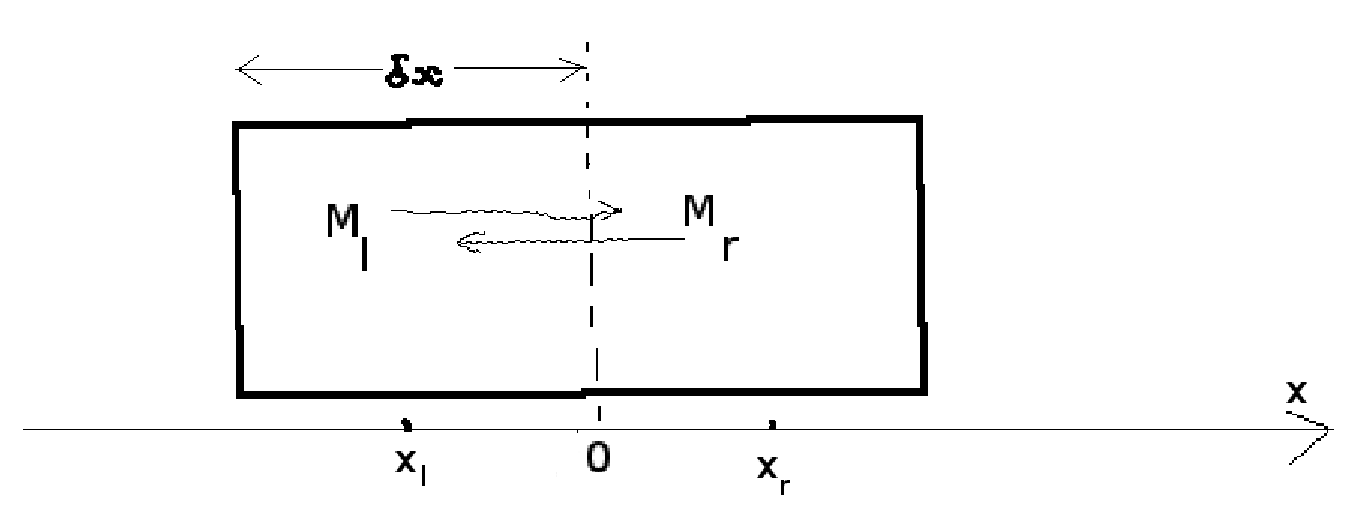
\includegraphics[height=5cm]{./images/diffusion_chamber.eps}}
 \caption{Demonstration the diffusion in closed chambers}
\label{fig:diffusion-chamber}
\end{figure}


Now, we examine the flux $J_x$ of particles passing a unit of area
(i.e. passing a single line) in a single unit of time, given the
positive direction is to the right direction. This change is caused by
the moving right of particles from the left chamber and the moving
left of particles in the right chamber.
\begin{equation}
  \label{eq:168}
  J_x = k(M_l-M_r)
\end{equation}
In order to know the total mass flux rate, we need to expand the line
to a surface $A$ and then expanding it to a volume $V$.  The flux
across a cross-section area $A$ is $J_xA$.


Assuming the volume of each chamber is $V=\delta x \delta y \delta z$,
the concentrations on each side can be written as
\begin{equation}
  \label{eq:169}
  \begin{split}
      C_l &= \frac{M_l}{\delta x \delta y \delta z} \\
      C_r &= \frac{M_r}{\delta x \delta y \delta z}
  \end{split}
\end{equation}
with $\delta x$ is the width, $\delta y$ is the breadth, $\delta z$ is
the height of the volume. 

Assuming that $\delta y \delta z = 1$, then $J_x$ represents the
\textcolor{blue}{flux in the $x$-direction per unit of cross-section
  area},
i.e.  perpendicular to $x$.  Consider the location of each chamber is
at the middle of it, then, the gradient in concentration can be
written in the form of finite difference approximation
\begin{equation}
  \label{eq:170}
  \frac{dC}{dx} = \frac{C_r-C_l}{x_r-x_l} = \frac{M_r-M_l}{\delta x (x_r-x_l)}
\end{equation}
Physically, $\delta x$ is
the average step along the $x$-axis taken by a molecule in the time
$\delta t$, or  $\delta x = (x_r-x_l)$. Then we have
\begin{equation}
  \label{eq:171}
  (M_l-M_r) = - (\delta x)^2 \frac{dC}{dx}
\end{equation}
substitute it into eq.~\eqref{eq:168}, then
\begin{equation}
  \label{eq:172}
  J_x = -k(\delta x)^2 \frac{dC}{dt}
\end{equation}

Based on the dimensional analysis,  $q$ cannot depend on an arbitrary
$\delta x$, we must assume that $k(\delta x)^2$ is a constant, which
is known as the {\bf diffusion coefficient}, denoted by $D$. Finally,
we have
\begin{equation}
  \label{eq:173}
  J_x = -D\frac{dC}{dt}
\end{equation}
This is {\bf Fick's first law}, and the processes obey this
relationship are called {\bf Fickian diffusion}.  As ordinary
solutions and gases are isotropic (every direction in space is the
same) so that there is just one diffusion coefficient
$D=D_x=D_y=D_z$. Thus, we can generalize eq.~\eqref{eq:173} to 3D
space, the diffusive flux vector at a point (unit area) is
\begin{equation}
  \label{eq:174}
  J = -D (\frac{\partial C}{\partial x}, \frac{\partial C}{\partial
    y}, \frac{\partial C}{\partial z}) = -D \nabla C =
  -D\frac{\partial C}{\partial x_i}
\end{equation}
with 
\begin{eqnarray*}
  \nabla = \left( \frac{\partial}{\partial x},
    \frac{\partial}{\partial y}, \frac{\partial}{\partial z} \right)
\end{eqnarray*}
is $\nabla$ (nabla)
operator\footnote{we use $\partial$ to denote partial differential for
  a specific variable, and the $d$ notation for one-dimensional
  derivative}.

% and
% \begin{equation}
%   \label{eq:179}
%   q_x = -D\partial y \partial z \frac{\partial C}{\partial x}
% \end{equation}

The random motion of particles from which Fick's law is derived is
called {\bf Brownian motion}. As $D$ is molecular diffusion
coefficient, it is also denoted by $D_m$. $D$ depends on the phase
(solid, liquid, gas), temperature, and molecular size. 

{\bf Example:} The equation for molecular diffusion through
thermocline (z-axis), as shown in Fig.~\ref{fig:alpine-lake} is
\begin{equation}
  \label{eq:185}
  J_z = D_m \frac{\partial C}{\partial z}
\end{equation}
with plus sign value of $J_z$ indicates downward motion.
\begin{figure}[hbt]
 \centerline{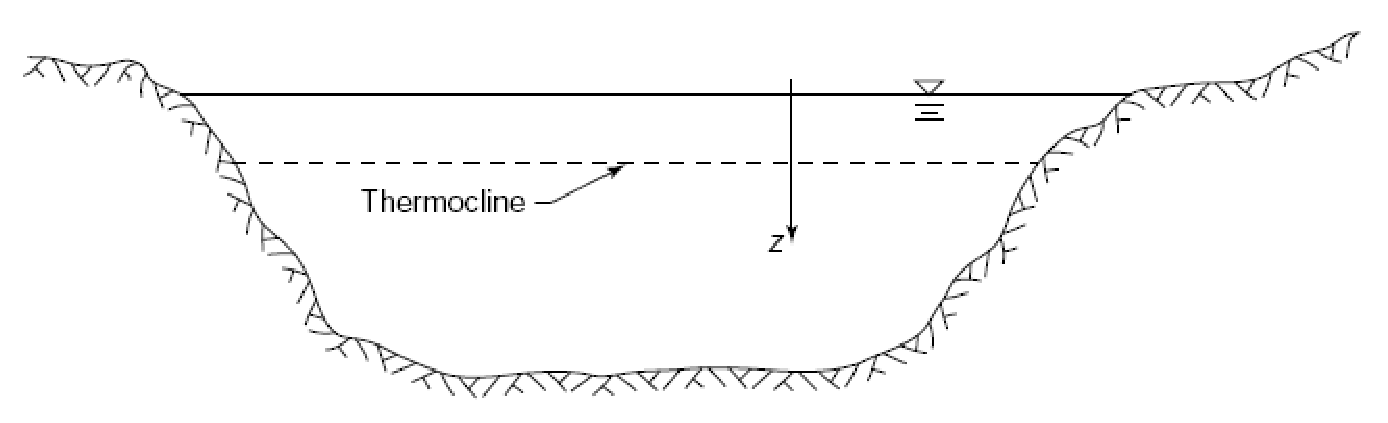
\includegraphics[height=3.5cm]{./images/alpine_lake.eps}}
\caption{Schematic of a stratified alpine lake.}
\label{fig:alpine-lake}
\end{figure}


However,
\textcolor{red}{what we need is the equation that predict the
  time-evolution of concentration $C(t)$ in space due to diffusive
  transport. Can we find it out? }

The mass change $\dot{m_x}$ across the area $A$ along the x-axis is
also the change in concentration, i.e. $A$ is a rectangle ($A=\delta
y\delta z$).
\begin{equation}
  \label{eq:176}
  \dot{m_x} = \int\int_A J_x\vec{n}dA = J_xA
\end{equation}
with $\vec{n}$ is the unit vector normal to the surface.  Extending to
three dimension, we examine a control volume (CV) of size $(\delta x,
\delta y, \delta z)$ as shown in Fig.~\ref{fig:diff-volume}. The
change in mass is given
\begin{equation}
  \label{eq:177}
  \frac{\partial M}{\partial t} = \sum \dot{m}_{in} - \sum
  \dot{m}_{out} = (\delta \dot{m_x}, \delta \dot{m_y}, \delta \dot{m_z})
\end{equation}

\begin{figure}[hbt]
 \centerline{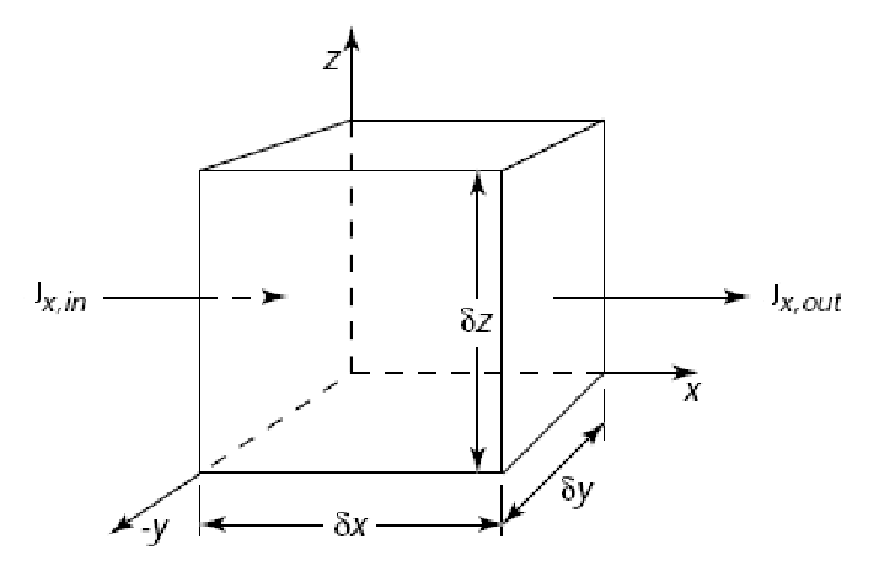
\includegraphics[height=5cm]{./images/diff-volume.eps}}
\caption{Differential control volume for derivation of the diffusion equation}
\label{fig:diff-volume}
\end{figure}

Using Fick's law, we have
\begin{equation}
  \label{eq:178}
  \begin{split}
    J_{x,in} &= -D\frac{\partial C}{\partial x}|_1\\
    J_{x,out} &= -D\frac{\partial C}{\partial x}|_2
  \end{split}
\end{equation}
Then, the net flux in the $x$-direction is
\begin{equation}
  \label{eq:180}
  \delta \dot{m}_x = - D\delta y \delta z \left( \frac{\partial
      C}{\partial x}|_1 - \frac{\partial C}{\partial x}|_2 \right)
\end{equation}

To estimate $ \frac{\partial C}{\partial x}|_2$ from $
\frac{\partial C}{\partial x}|_1$, the powerful technique first-order
Taylor series is utilized.
\begin{equation}
  \label{eq:181}
   \frac{\partial C}{\partial x}|_2 =  \frac{\partial C}{\partial
     x}|_1 + \frac{\partial}{\partial x}(\frac{\partial C}{\partial
     x}|_1)\delta x + R(2)
\end{equation}
with $R(2)$ is higher order terms and can be ignored. Then
\begin{equation}
  \label{eq:182}
  \delta \dot{m}_x =  D\delta y \delta z \frac{\partial
    C^2}{\partial^2 x} \delta x 
\end{equation}

Similarly, the formula for the net flux in $y$- and $z$- directions
\begin{equation}
  \label{eq:183}
  \begin{split}
    \delta \dot{m}_y &= D \delta x \delta y \delta z \frac{\partial
    C^2}{\partial^2 y}  \\
    \delta \dot{m}_z &= D \delta x \delta y \delta z \frac{\partial
    C^2}{\partial^2 z}  
  \end{split}
\end{equation}

As the mass $m$ is related to the concentration, i.e. $m=C\times
V=C\delta x\delta y\delta z$. Thus, $\dot{m} = \frac{\delta
  C}{\delta
  t}
\delta x \delta y \delta z$. Combine all equations together, finally
\begin{equation}
  \label{eq:184}
  \frac{\partial C}{\delta t} = D(\frac{\partial C^2}{\partial^2x} +
  \frac{\partial C^2}{\partial^2y} + \frac{\partial C^2}{\partial^2z}
  ) = D\nabla^2 C
%  = D\frac{\partial C^2}{\partial x_i^2}
\end{equation}
which is called {\bf Fick's second law}.  The previous question is now
answered.
\textcolor{red}{This is the fundamental equation in environmental
  fluid mechanics.}
Yet, another question arises: \textcolor{red}{can we solve it?} -
There are different ways, and one of them is Fischer method or the
so-called {\bf similarity method}.  The power of a similarity method
is that it turns a partial differential equation (PDE) into an
ordinary differential equation (ODE), which is the goal of any
solution method for PDEs.

{\bf Example}: Using similarity method to solve the one-dimensional
diffusion problem in a narrow pipe (radius $a$, infinite length). At
time $t=0$, a mass of tracer $M$ is injected uniformly across the
cross-section of area $A=\pi a^2$ at point $x=0$. We need to find the
equation for the concentration (the spread) of the tracer in the
$x$-direction over time due to molecular diffusion alone: $C_x(t)$.

\begin{itemize}
\item Under the assumption, i.e. $\partial C/\partial y = \partial
  C/\partial z = 0$, the equation we need to solve is
  \begin{equation}
    \label{eq:187}
    \frac{\partial C}{\partial t} = D\frac{\partial C^2}{\partial^2 x}
  \end{equation}

\item No particle can travel to infinity, $C_{\pm\infty}(t)=0$.

\item To specify the initial condition (only at $x=0$ has the
  particles with uniform distribution $M/A$, other locations $x \ne
  0$, the concentration is zero), the {\it Direct delta function} $\delta x$
  is used
  \begin{equation}
    \label{eq:188}
    C_x(0) = (M/A) \delta x
  \end{equation}

\item Mathematically, the total inject mass is
  \begin{equation}
    \label{eq:189}
    M = \int_V C_x(t)dV = \int_{-\infty}^\infty \int_0^a
    (M/A)\delta(x) 2\pi r dr dx
  \end{equation}
as $dV = 2\pi r drdx$.

\item Dimensional analysis technique is utilized: first, we need to
  identify all variables and noting their units (dependent: $C$
  (M/L$^3$), independent: $M/A$ [M/L$^2$], $D$ [L$^2$/T], x [L], $t$
  [T]) with M(ass), L(ength), T(ime). There are $m=5$ parameters and
  $n=3$ different dimensions. Then, we can form two dimensionless
  variables
  \begin{equation}
    \label{eq:191}
    \begin{split}
      \pi_1 &= \frac{C}{M/(A\sqrt{Dt})} \\
      \pi_2 &= \frac{x}{\sqrt{Dt}}
    \end{split}
  \end{equation}
  {\bf TIPS}: There are different arrangements to create $\pi_1, \pi_2$,
  however the rule of thumb is:
  (1) make sure the dependent variable can be obtained from $\pi_1$
  conveniently, (2) $\pi_1 = f(\pi_2)$, then
\begin{equation}
  \label{eq:192}
  C_x(t) = \frac{M}{A\sqrt{Dt}} f(\pi_2) = \frac{M}{A\sqrt{Dt}} f(\frac{x}{\sqrt{Dt}})
\end{equation}
with $f(.)$ is an unknown function known as
{\bf a similarity solution} because $C_x(t)$ has the same shape in
$x$-direction at all time $t$. The next question is
\textcolor{red}{what is the shape of $C$?}.

The detail how to solve the solution analytically is
skipped\footnote{since numerical methods are commonly used in
  practical problems},
let's just look at the actual solution (analytical solution) to see
how powerful the dimensional analysis gives us.
\begin{equation}
  \label{eq:193}
  C =  \frac{M}{A\sqrt{4\pi Dt}} \exp(\frac{-x^2}{4Dt})
\end{equation}
\textcolor{red}{How can we find this solution?} - There are two
primary ways: (1) plot the experimental data and then predict the form
of the smooth curve fitting the plot, then use some curve fitting tool
to estimate the parameter with the coordinate $(\pi_1, \pi_2)$, (2)
using eq.~\eqref{eq:192} as the solution for the differential equation
and solve it analytically with initial and boundary conditions
provided above [NOTE: For information on software for curve fitting, read
'Data Visualization' book].
The solution in 3D motion is
\begin{equation}
  \label{eq:194}
  C(x,y,z,t) = \frac{M}{4\pi t\sqrt{4\pi D_x D_y D_z}}
  \exp(-\frac{x^2}{4D_x t} -\frac{y^2}{4D_y t} -  \frac{z^2}{4D_z t})
\end{equation}

\item The maximum concentration is when the first-order derivative is
  zero and this can be achieved when the exponential part is zero or
  $x=y=z=0$.

\item Interpretation of the similarity solution: The shape of the
  concentration is bell-shaped, or its distribution is a Gaussian
  distribution with variance $\sigma^2 = 2Dt$. 

\item Regardless of the time, the values of mass $M$, concentration
  $D$ and the ratio $C/C_{mas}$ are always constant. 
\end{itemize}


\subsubsection{Turbulent diffusion}
\label{sec:turbulent-diffusion}

Turbulence also causes a kind of random, chaotic motion that behaves
asymptotically like Fickian diffusion. However, the Fickian diffusion
is a random yet smooth motion, while the turbulent motion is purely
random,
disorder\footnote{the chaotic is observed at the macroscopic level,
  yet at the microscopic level, it is highly organized}.
In essence, turbulent motion is much larger than molecular motion, and
turbulent diffusion coefficients $D_t$ are much larger than molecular
diffusion coefficients $D_m$.

Since turbulent diffusion obeys the same Fickian flux law, then the
turbulent diffusive flux $J_{z,t}$ can be related to the molecular
diffusive flux $J_{z,t} = J_z$ by the equation
\begin{equation}
  \label{eq:186}  
  J_{z,t} = J_{z,m} \frac{D_t}{D_m}
\end{equation}
\subsection{Advection Diffusion}
\label{sec:advection}

In the previous example, without the flow of the pipe fluid, the
injected tracer spread equally in all direction whose concentration
following Gaussian distribution with the center of the mass is at the
initial location $(0,0,0)$. Now, if we open the valve and allow water
to flow in the pipe, we expect the center of the mass to move with the
mean flow velocity in the pipe. It means that the central is now
\begin{equation}
  \label{eq:195}
  \eta = x - (x_0 + ut)
\end{equation}
with $\eta$ is the moving reference frame, $x_0$ is the injection
point of the tracer (zero in the previous example), $u$ is the mean
flow velocity and $ut$ is the distance traveled by the center of the
mass in time $t$. This is the mechanism of advection.

Advection is a transport mechanism of a substance by a moving
fluid. Advection is a conserved property of a moving fluid and is
described mathematically as a {\it vector field}. So, we expect that
the equation for advection diffusion to be something like this
\begin{equation}
  \label{eq:196}
   C =  \frac{M}{A\sqrt{4\pi Dt}} \exp
   \left(\frac{-(x-(x_0+ut))^2}{4Dt} \right)
\end{equation}
We need test this prediction by deriving the equation for advection
diffusion equation. This relies on the
{\it principle of superposition}: advection and diffusion can be added
together if they are linearly independent. However, how do we know
they are independent processes? Two processes are dependent only one
process feeds back on the other. Diffusion is a random process, with
random step $\pm \delta x$. With advection, each molecule will move
$u\delta t$ in the cross-flow direction. So, the advection just add
something to that random step in diffusion. The net movement under
advection-diffusion is $u\delta t \pm \delta t$. Thus, the total flux
in the $x$-direction is
\begin{equation}
  \label{eq:197}
  J_x = uC + J_{x,Fickian} = uC - D \frac{\partial C}{\partial x}
\end{equation}
with $J_{x,Fickian}$ is the Fickian flux described in the previous
section.

Here, $uC$ is the correct term for advection.  Use the flux law and
the conservation of mass... finally, we have
\begin{equation}
  \label{eq:198}
  \frac{\partial C}{\partial t} + \nabla \dot (uC) = D\nabla^2 C
\end{equation}
 or in Einstein notation
 \begin{equation}
   \label{eq:199}
   \frac{\partial C}{\partial t} + \frac{\partial u_iC}{\partial x_i}
   = D\frac{\partial C^2}{\partial x_i^2}
 \end{equation}
which is the {\bf advection-diffusion equation} with the right
hand-side is
\begin{equation}
  \label{eq:200}
  \frac{\partial}{\partial x_i} \left( D_{ij} \frac{\partial
      C}{\partial x_j} \right)
\end{equation}

\subsection{Convection}
\label{sec:convection}

Many people use the term convection synonymously with
advection. However, convection describes the transport by combined
molecular and eddy diffusion, while advection refers to transport with
a general flow of fluid.


\section{Chemical Reaction}
\label{sec:chemical-reaction}

Just a remind, the equation that represents the change in density
$C(x,t)$ with time when it is sufficiently smooth
\begin{equation}
  \label{eq:217}
  \frac{dC(\mathbf{x},t)}{dt} = D\nabla^2C(\mathbf{x},t)
\end{equation}
with $\mathbf{x}$ is the 3D coordinate of the particle. 

Now, what if we want to write a differential equation describing the
time dependence of the density in terms of various spatial
derivatives, i.e. $\frac{d}{dx}C(x,t), \frac{d}{dxdy}C(x,t),
\frac{d}{dx^2}C(x,t), ...$.


A system of reacting and diffusing molecules are called
reaction-diffusion systems. Chemical reactions causes the molecular
densities to change with time even there is no diffusion. The general
dynamic of the system using a set of coupled equations of the form
\begin{equation}
  \label{eq:218}
  \frac{dC_i(\mathbf{x},t)}{dt} = D\nabla^2C_i(\mathbf{x},t)+R_i(\{n_j(\mathbf{x},t)\})
\end{equation}
where $R_i(\{n_j(\mathbf{x},t)\})$ is the rate of changes in the
concentration of a molecular species $i$.


Assumptions:
\begin{enumerate}
\item the density is not too rapidly varying in space, so that local
  reaction rate depends only on the local densities and not their
  gradients

\item diffusion time between reactions is large compared to the time
  of reaction.

\item 
\end{enumerate}

\section{Incorporating transformation with advective-diffusion equation}
\label{sec:incorp-transf-with}

\subsection{Advective-reacting diffusion equation}
\label{sec:advect-react-diff}


\subsection{Reaction-diffusion equation}
\label{sec:react-diff-equat}

A system of chemical substances - morphogens - diffusing through a
mass of tissue of a given geometrical form and reacting together
within it, is adequate to describe for the main phenomena of
morphogenesis - the biological processes of forming
patterns/structures. What laws to control the development in such
situations?
\begin{itemize}
\item The diffusion follows the ordinary law of diffusion, i.e. moving
  from regions of high concentration to those of lower concentration,
  at a rate proportional to the gradient of concentration and also the
  ``diffusibility'' of the substance. If there is no cell walls, the
  reaction would inversely proportional to the square root of the
  molecular weights.
\item The reaction rate is assumed to obey the ``law of mass
  action'', i.e. the reaction rate is proportional to the
  concentrations, i.e the chance of encountering of the molecules. 
\end{itemize}

There are in fact 6 different forms :
\begin{enumerate}
\item stationary waves on the isolated ring of cells, account for the
  phenomena of phyllotaxis.
\item tentacle patterns on Hydra and for whorled leaves. 
\item gastrulation on a sphere 
\item pattern reminiscent of dappling 
\end{enumerate}


The first person to describe this phenomena is
Turing\cite{turing1952cbm}\footnote{\url{http://www.turingarchive.org/viewer/?id=476&title=2}}.
Turing studies the morphogenesis of the embryo. A solution of linear
differential equations with constant coefficients is in the form of a
sum $\sum A e^{bt}$ with $A, b$ are complex quantities. The real part
should be
\begin{equation}
  \label{eq:219}
  Real(Ae^{bt})=A'e^{\alpha t} \cos(\beta t + \phi)
\end{equation}
with $A=A'ei^\phi, b=\alpha+i\beta$.

\begin{enumerate}
\item $\alpha=0$: sinusoidal oscillation
\item $\alpha<0$: a damped oscillation
\item $\alpha>0$: an oscillation of ever-increasing amplitude.
  \begin{equation}
    \label{eq:220}
    \frac{dy}{dt} = \alpha y; \; \alpha > 0
  \end{equation}
\end{enumerate}
At a sufficient great lapse of time, all the terms $Ae^{bt}$ will
become negligible in comparison with the terms which has the greatest
real part. Unless this greatest real part is zero, these dominant
terms will eventually either tend to zero (for negative real part) or
to infinite values (for positive real part).

\begin{enumerate}
\item any of the numbers $b$ has a positive real part ($\alpha_i>0$),
  the system is unstable
\item 
\end{enumerate}


Suppose that there are $N$ cells and $M$ types of morphogens. Then, at
a specific time point, there will be a number of a type of morphogen
in a given cell. Thus, to know the state of a single cell, we need M
values. Accordingly, to know the state of a system with $N$ cells, we
need $MN$ number of values. These number changes with time, partly
because of reactions, partly because of diffusion.

\begin{itemize}
\item To know the value of a given morphogen in a given cell due to
  diffusion, we need to know the concentration of that morphogen
  (i.e. the number of molecules of that type of morphogen) in the cell
  and in all neighboring cells, as well as the rate of diffusion for
  that morphogen
\item TO know the value of a given morphogen in a given cell due to
  reaction, we need to know the concentration of all types of
  morphogens in that cell only. 
\end{itemize}


%%% Local Variables: 
%%% mode: latex
%%% TeX-master: "thermo-stat"
%%% End: 

%%%\include{Membrane_ElectricalPropagation}
\import*{../BioMedical_Research/}{MedicalPhysics}

\part{Chemical reaction - Chemical kinetics}
\import*{../BioPhysics_Thermo_Stat/}{ChemicalBond}
\chapter{Chemical reaction - Transportation}
\label{chap:chem-react-transp}

\def\A{{\text{A}}}
\def\B{{\text{B}}}
\def\C{{\text{C}}}
\def\D{{\text{D}}}

The previous chapter (Chap.\ref{chap:chem-bond-quant}) discussed the mechanism
of atom interactions at a lower level, the bonding energy of covalent and
non-covalent bonding.

In this chapter, we will look at the chemical interaction between molecules
within a single physical compartment/volume. The change in concentration of a
species in this compartment is the result of the reaction occurs that involve
the given species. When multiple compartments, i.e. spatial dimension, is
considered, then the change in concentration of the species is also under
another effect called the diffusion part (Sect.\ref{sec:diffusion}), represented
in the form of flux (Sect.\ref{sec:flux-across-compartments}).

{\bf Thermochemistry} is the field that study how a chemical reaction occurs
(Sect.\ref{sec:thermochemistry}).

% Chemical reaction is what happens at microscopic level.
% at a higher level. 
Important concepts involves the {\bf time scale} of a
process which tells whether a chemical reaction is fast, or slow. This
property is known as the {\bf rate of reaction} and is studied under
the field {\bf reaction kinetics}.

In a chemical reaction, the energy $E$ is the internal energy $U$
(Sect.\ref{sec:gibbs-fund-equat}), the chemical potential of the i-th species in
the system is defined as the partial derivative of the $U$ on the number of particles in species
i-th.
\begin{equation}
  \label{eq:chem_potential}
  \mu_i = \left( \frac{\partial U}{\partial N_i} \right)_{S,V,N_{j \ne i}}
\end{equation}

We have studied the macroscopic and microscopic viewpoint of a thermodynamic
system. At thermodynamic equilibrium, the system assumes the state with maximum
entropy (Sect.\ref{sec:entropy}). Finding such configuration, requires
estimating the partition function $Z$, and the Maxwell-Boltzmann distribution of
velocities of particles in a low density system. In such systems, the effect of
quantum mechanics were neglected.


% In the previous chapter we have learnt the kinetics of reactions, i.e.
% how fast different atoms/molecules interact to form a new species. In
% this chapter, we will study the underlying mechanism of chemical
% bonding. In order to do so, we need to know the structure of an atom
% and new technical concepts.

% \section{Wave function}
% \label{sec:wave-function}

% In quantum mechanics, the dynamics of all subatomic particles are
% described in terms of wave functions. It maps a possible state of the
% system into complex numbers. 
\section{Thermochemistry}
\label{sec:thermochemistry}


\textcolor{red}{Hess's law (Sect.\ref{sec:Hess-law}) and the Lavoisier \&
Laplace law (Sect.\ref{sec:Lavoisier-Laplace-law}) above are the bedrock for
thermochemistry}.

Both laws are preceded {\bf the law of conservation of energy}\footnote{[Wiki]
The conservation of energy stated that the energy is not created or destroyed
itself, it just transform from one form to another.}
(Sect.\ref{sec:conservation-of-energy}) and it can be shown that the two laws
are the direct consequences of it. However, {\it the conservation of energy does
NOT tell us what the various forms of energy are and how energy transforms from
one form to another}. This led to the concept of {\it affinity}
(Sect.\ref{sec:affinity}).

\subsection{-- Lavoisier and Laplace's law: {\it specific heat} and {\it latent
heat}}
\label{sec:Lavoisier-Laplace-law}

In the 18th century (1780) Antoine Lavoisier and Pierre-Simon Laplace laid the
foundation of {\it thermochemistry} - a branch of thermodynamics
(Sect.\ref{sec:thermodynamics-systems}) (See the book Thermodynamics) - which
studies the energy involved or absorbed in chemical reactions (heat into work
and vice verse) - by showing that {\it the same amount of heat must be supplied
to decompose a compound as would be produced on its formation}, i.e. heat
evolved in a reaction is equal to the heat absorbed in the reverse reaction.

They investigated the {\it specific} and {\it latent heat}
(Sect.\ref{sec:latent-heat}) of a number of substances, and amount of heats
involved in combustion.

\begin{itemize}

\item specific heat = heat received required to increase the system one degree
1$^o$ in temperature.
 
\item latent heat = heat receive required in order for a state transition
  to occur (e.g. solid \ce{->} liquid)
\end{itemize}

\subsection{-- Hess's law}
\label{sec:Hess-law}

In 1840 Swiss chemist Germain Hess formulated the principle that the evolution
of heat in a reaction is the same whether the process is accomplished in one
step or in a number of consecutive stages. This is known as {\bf Hess's law}.

Example: the heat of formation of \ce{CO2} is equal to the sum of heat of the
formation of CO and the heat of oxidation of that amount of CO to \ce{CO2}. Hess
employed this principle to determine indirectly the heat of formation of
compounds from their elements, when this magnitude, as is generally the case,
was inaccessible to direct measurement.



\subsection[Berthelot and Thomsen: affinity]{Affinity: driving-force for a
chemical reaction}
\label{sec:affinity}

To explain the microsopic aspect of chemical reaction, a theoretical foundation
is needed.  Ilya Prigogine - {\it ''As motion was explained by Newtonian concept
of force, chemists  want a similar concept of 'driving force' for a chemical
change. Why do chemical reactions occur, and why do they stop at certain points?
Chemists called the 'force' that caused chemical reactions {\bf affinity}, but
it lacked a clear definition."} 

{\bf Affinity} is the next stage to study the direction of energy transform,
after the concept of conservation of energy was formed
(Sect.\ref{sec:conservation-of-energy}).
{\bf Affinity} refers to the tendency for the reaction to occur in one direction
instead of the other\footnote{Affinity is the property of which dissimilar
substances are capable of entering into chemical combination with each other}.
\textcolor{red}{However, there is still no way to quantify "affinity''}.
With that effort, the French chemist Marcellin Berthelot and the Danish chemist
Julius Thomsen had attempted to quantify {\bf affinity} using heats of reaction
(Sect.\ref{sec:principal-of-maximum-work}).

However, this has so many exceptions (especially in reversible reactions) and
then had been abandoned by its authors. As a result, it is now of only
historical importance. \textcolor{red}{Nowadays, ``{\bf free energy}'' is a more
advanced and accurate term to replace the outdated term ``affinity''}
(Sect.\ref{sec:free-energy-direction-reaction}).
The concept of ``free-energy'' was originally derived from thermodynamics.

\subsection{-- principal of maximum work (obsolete)}
\label{sec:principal-of-maximum-work}

Berthelot proposed the {\it principal of maximum work} (in thermochemistry),
i.e. in a pure chemical reaction (a chemical changes occurring without the
intervention of outside energy), the reaction tends to occur in the direction
toward the production of bodies or a system of bodies that liberate heat.

Based on these and other ideas, Berthelot and Thomsen, as well as others,
considered the {\it heat given out in the formation of a compound as a measure
of the affinity}. 



\subsection{Affinity constants: binding strength}
\label{sec:affinity-constants}

{\bf Affinity constants} are numeric values that tells the strength
with which two molecules interact. Given an affinity constant, we can
know an interaction is ``tight binding'' or ``weak binding''. 

\subsection{-- binding constant, dissociation constant}
\label{sec:binding-constant}
\label{sec:dissociation-constant}

\begin{itemize}
  \item To tell the tendency in binding of two molecules, we use
{\bf binding constant} (association constant) $K_B$. 

  \item To tell the tendency in dissociation of a complex into two separate
  molecules, we use {\bf dissociation constant} $K_D$. $K_D$ is inversely
  related to affinity while $K_B$ is directly related to affinity.
\end{itemize}

So
\begin{equation}
  \label{eq:332}
  K_D = \frac{1}{K_B}
\end{equation}
The unit of $K_D$ is molar (M, moles/(litres-solution)), and the unit of $K_B$
is $M^{-1}$.  \textcolor{red}{For convenience, typically, $K_D$ is more widely
used}.

In a reaction with two {\bf rate constants} $k^+_{1}$ (binding) and
$k^-_{1}$ (dissociation)
\begin{equation}
  \label{eq:333}
  \ce{A + B <=>[k^+_1][k^-_{1}] AB}
\end{equation}
then 
\begin{equation}
  \label{eq:334}
  K_D = \frac{k^-_1}{k^+_{1}}
\end{equation}
Correspondingly, the unit of $k^-_{1}$ is $\text{time}^{-1}$ while
$k^+_{1}$ is Molar$^{-1}\text{time}^{-1}$.

\begin{framed}
  
  High affinity means large $K_B$, which in turns equivalent to (high
  $k^+_1$ and low $k^-_{1}$). This means that the complex formation occur
  rapidly, while the complex dissociate slowly.
\end{framed}


\subsection{-- estimate dissociation constant: $K_D$}
\label{sec:determining-k_d}

{\bf IMPORTANT}: We don't have to know the forward and backward rates
$k^+_1$, $k^-_{1}$ in order to compute $K_B$ or $K_D$. Instead, we can
compute them directly at the equilibrium state of the reaction.  This
is because of the fact that, at equilibrium, the concentration of each
reactants and the complex (product) follow this equation
\begin{equation}
  \label{eq:335}
  K_D = \frac{[A]_{eq}[B]_{eq}}{[AB]_{eq}}
\end{equation}
Based on the law of total mass conservation, $[A]_{total}=[A]+[AB]=a_t$,
then 
\begin{equation}
  \label{eq:336}
  \begin{split}
    K_D[AB]_{eq} &= (a_t-[AB]_{eq})[B]_{eq} \\
 \rightarrow\;\;   \frac{[AB]}{a_t} &= \frac{[B]}{[B]+K_D}
  \end{split}
\end{equation}

The {\bf fraction bound} $[AB]/a_t$ is the fraction of A involves into the
reaction at equilibrium. The upper bound is 1 (used all A) when [B] is
at a great amount, i.e. at infinity. 

\begin{framed}
  The idea behind using $K_D$ is that when [B] is equal to $K_D$, the
  fraction bound is 1/2.


  \begin{equation}
    \label{eq:337}
    \frac{[AB]}{a_t} = \frac{\frac{[B]}{K_D}}{\frac{[B]}{K_D}+1}  
  \end{equation}
\end{framed}

To determine $K_D$, the concentration of A, $a_t$ is held constant;
while they vary [B]. For each value of [B], they obtained a value of
[AB] at equilibrium. The curve plotting [B] vs. $[AB]/a_t$ is a hyperbola. 
Then, $K_D$ is the tangent coefficient of the line $1/[B]$ vs. $a_t/[AB]$
\begin{equation}
  \label{eq:338}
   \frac{a_t}{[AB]}= K_D\frac{1}{[B]} + 1
\end{equation}

{\bf EXPERIMENT TIPS}: To quickly measure $K_D$, it is often use a
small concentration of A compared to $K_D$ ($a_t\ll K_D$) - ideally
100-fold below the $K_D$. With this condition, at equilibrium, [AB] is
thus pretty much relatively small compared to $K_D$.  In addition,
$[B]_{total}$ covers a range from 10-fold below to 10-fold above
$K_D$.  Knowing that $[B]_{total}=b_t=[B]_{free}+[AB]$, then at
equilibrium, $[AB]$ is rather small compared to $[B]$ free. In the
end, we don't have to measure [B] free at equilbrium, but we can
assume [B] free to be equal $[B]_{total}$. Otherwise, we have to
measure [B] free at equilibrium every time we change the concentration
of $[B]_{total}$. 

Theoretically, the fraction bound approach 1 when [B] total go to
infinity. However, this is not true. At saturation, the fraction bound
approach a asymptotic line at $y=f_{max}$. Thus, we have to modify
eq.~\eqref{eq:336}
\begin{equation}
  \label{eq:339}
   \frac{[AB]}{a_t} = f_{max}\frac{[B]}{[B]+K_D}
\end{equation}
An equivalent form that is more commonly used is
\begin{equation}
  \label{eq:340}
    X_{AB}= {X_{AB}}_{max}\frac{[B]}{[B]+K_D}
\end{equation}
Here, $X_{AB}$ is not a concentration, instead it can be any thing
that denote the amount of AB complex, and ${X_{AB}}_{max}$ is the maximum
amount of $X_{AB}$ at equilibrium. 

\section{Direction of reactions}
%\section{Factors to determine the reaction}
\label{sec:fact-determ-react}
\label{sec:free-energy-direction-reaction}

Early efforts to quantify the direction of a (chemical) reaction used {\it
affinity} (Sect.\ref{sec:affinity}). Nowadays, to study the direction of the
reaction, {\bf free energy} is the modern measure to use, compared to the
obsolete one {\it affinity}.

However, in between, different concepts had also been used to study the
direction of a reaction
\begin{enumerate}
  \item entropy - Sect.\ref{sec:entropy}: reaction occurs in the direction of
  increasing entropy
  \item enthalpy - Sect.\ref{sec:enthalpy}
\end{enumerate}



\section{Speed of reactions}
\label{sec:speed-reaction}


\import*{../BioPhysics_Thermo_Stat/}{DeterministicReactionKinetics}
\import*{../BioPhysics_Thermo_Stat/}{StochasticReactionKinetics}

\part{Bio-BioChem}
\chapter{BioChem Intro}
\label{chap:biochem-intro}

This chapter introduces basic concepts for you to user when reading articles,
helping to understand the cellular mechanism which may be useful to build the
model.


``{\it The studying of Biochemistry shows how the inanimated molecules
  that constitute the living organisms interact to maintain and perpetuate the
  life animated solely by using the physical and chemical laws that govern the
  nonliving universe.}'' Albert L. Leningher.

``{\it Biochemistry is the study of the chemical processes in living
organisms. It deals with the structure and function of cellular
components, such as proteins, carbohydrates, lipids, nucleic acids,
and other biomolecules.}'' Wiki.


\section{Incredibility of life}
\label{sec:incredibility-life}

Life refers to the live and death of organisms which present on the Earth across
scales, Fig.\ref{fig:smallness}. Regardless of the size of an organism, the unit
of life are cells (Chap.\ref{chap:cell-life}).

\begin{figure}[hbt]
  \centerline{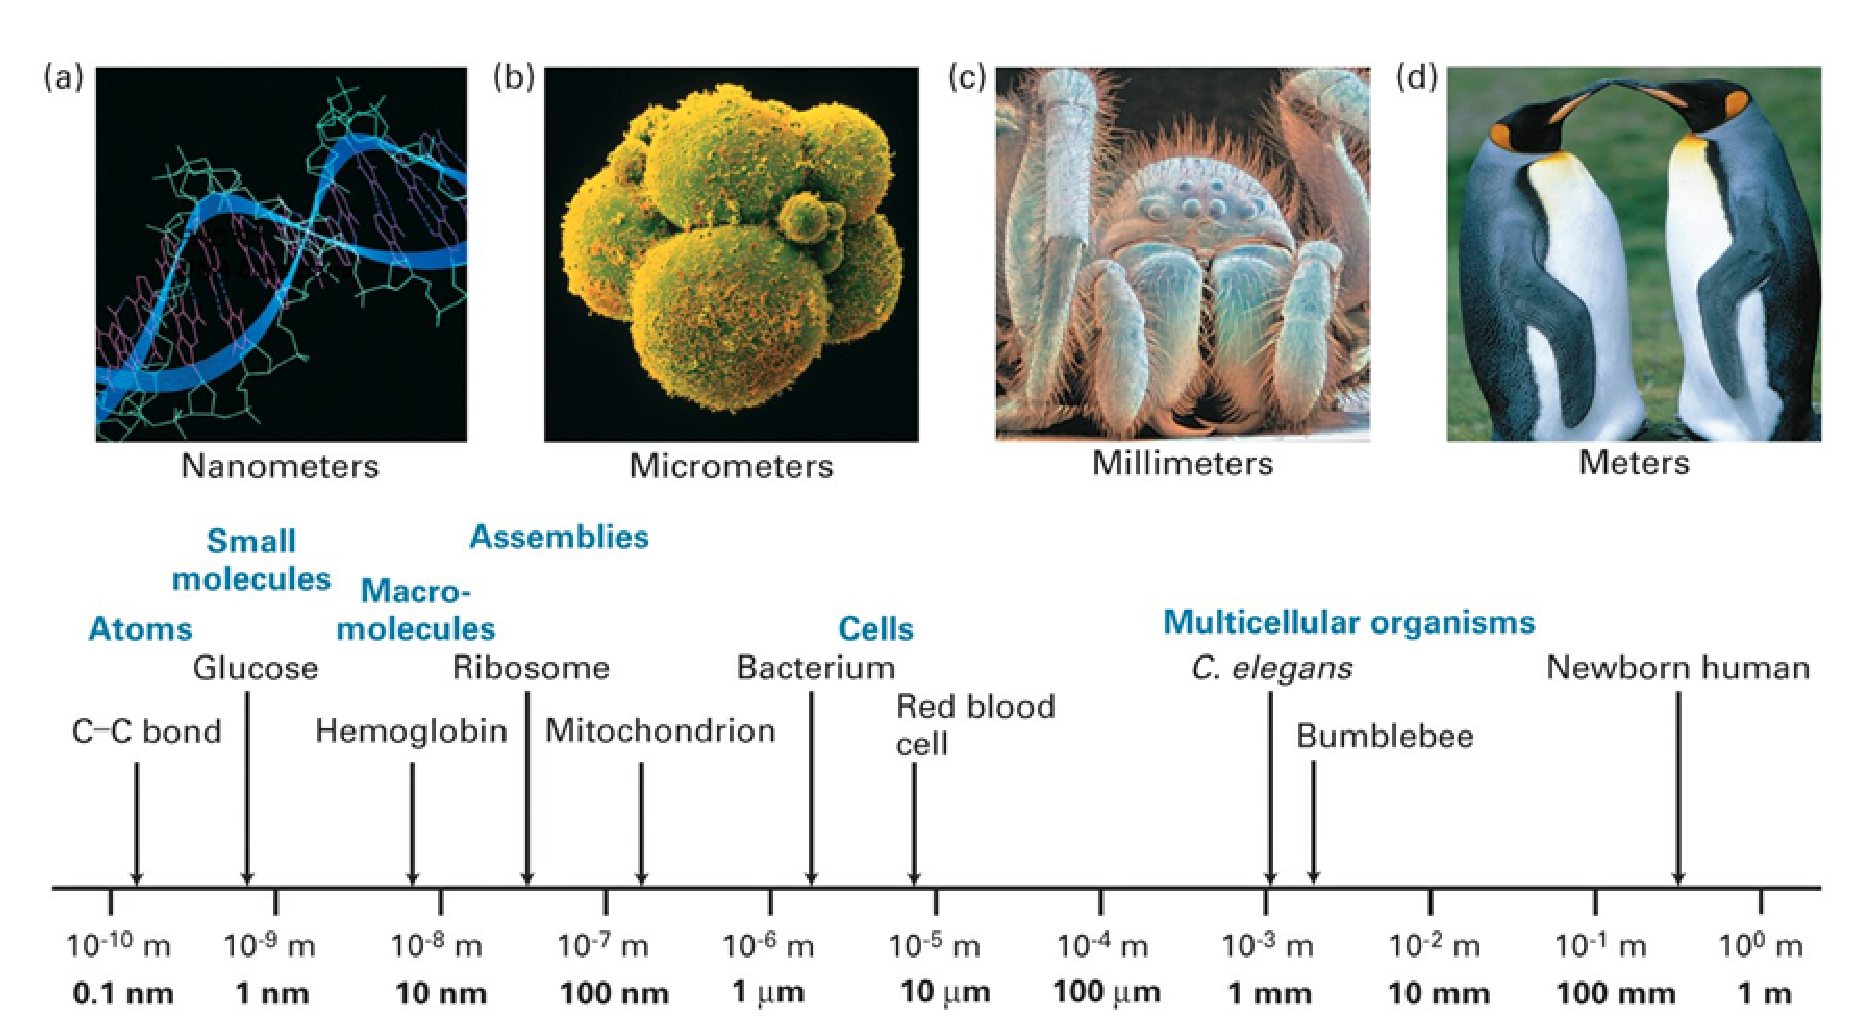
\includegraphics[height=6cm,
    angle=0]{./images/smallness.eps}}
\caption{Multi-scale of lifes}
\label{fig:smallness}
\end{figure}

\begin{enumerate}
  \item 1869: Miescher first isolated DNA molecules from white blood cell from
  pus-soaked bandages obtained from a nearby hospital.
  
  \item 1944: Avery provides evidence that DNA, rather than protein, carries the
  genetic information (using bacterial transformation)
  
  \item 1953: Watson and Crick discovered the double-helix structure of DNA
  molecules (based on X-ray results generated by Franklin and Wilkins)
  
  \item 1955: Kornberg discovered DNA polymerase - an enzyme now used to produce
  labeled DNA probes.
  
  \item 1961: Marmur and Doty discovered {\it DNA renaturation} - establishing
  the specificity and feasibility of nucleic acid hydridization reactions.
  
  \item 1962: Arber discovered the evidence for the existence of {\it  DNA
  restriction nuclease} which can cut DNA double helix at specific sites defined
  by the local nucleotide sequence - later Nathans and H.
  Smith can purified (purified from bacteria) and use in DNA sequence
  characterization (Sect.\ref{sec:DNA-restriction-nucleases}).
  
Different species of bacteria make different restriction nucleases, which
protect them from viruses by degrading incoming viral DNA.
\footnote{\url{https://www.ncbi.nlm.nih.gov/books/NBK26837/}}

  
  \item 1966: Nirenberg, Ochoa, and Khorana elucidatd {\it genetic code}. 
  
  \item 1967: Gellert discovered {\it DNA ligase} - the enzyme that join DNA
  fragment together.
  
  \item 1972-1973:  Boyer, Cohen, Berg, and their colleagues at Stanford
  University and the University of California at San Francisco discovered {\it
  DNA cloning techniques}
  
  \item 1973: Southern discovered technique - which named after him - to detect
  the presence of a specific DNA sequence - Sect.\ref{sec:Southern-blotting}
  
  \item 1975-1977: Sanger and Barrell and Maxam and Gilbert discovered technique
  to quickly sequence DNA, i.e. rapid DNA-sequencing methods.
  
  The next generation is not available until 1991.
  
  \item 1981-1982: Palmiter and Brinster produced {\bf transgenic mices};
  Spradling and Rubin produce transgenic fruit flies.
  
  \item 1982: GeneBank was created, at  Los Alamos National Laboratory, to store 
  publicly available sequenced genetic DNA sequences.
  
  \item 1983: Murray and Szostak described YAC - Sect.\ref{sec:YAC}
  
  \item 1985: Mullis and co-workers invented {\bf PCR} - Sect.\ref{sec:PCR} 
  for fast DNA cloning
  
  \item 1987: Capecchi and Smithies introduced technique to perform {\bf
  targeted gene replacement in mouse embryonic stem cells.}
  
  \item 1989: Fields and Song developed {\bf yeast two-hybrid system} - study
  protein-protein interactions - Sect.\ref{sec:protein-protein-interaction}
  
  
  \item 1989: Olson and colleagues describe sequence-tagged sites, unique
  stretches of DNA that are used to make physical maps of human chromosomes.
  
  \item 1990: Lipman and colleagues release {\bf BLAST} - algorithm to  search
  for homology between DNA and protein sequences.
  
  \item 1990: Simon and colleagues studied how to efficiently use BAC
  (Sect.\ref{sec:BAC}) to carry large pieces of cloned human DNA for sequencing.
  
  \item 1991: Hood and Hunkapillar introduced new automated DNA sequencing.
  
  \item 1995: Venter and colleagues sequenced the {\it first complete genome} -
  and from bacterium Haemophilus influenzae.
  
  \item 1996: Goffeau and an international consortium of researchers announced
  the {\it first complete genome of a eukaryote} - from yeast Saccharomyces
  cerevisiae.
  
  The one for human is in 2001.
  
  \item 1996-1997: Lockhart and colleagues and Brown and DeRisi produced {\bf
  DNA microarray technique} - allow the simultaneous monitoring of thousands of
  genes.
  
  \item 1998: Sulston and Waterston and colleagues produced {\it the first
  complete sequence of a multicellular organism} - from nematode worm
  Caenorhabditis elegans.
  
  \item 2001: Consortia of researchers announced the {\it first draft of
  sequenced human genome}
\end{enumerate}

\subsection{DNA: deoxyribonucleic acid}
\label{sec:dna}
\label{sec:amino-acid}


DNA  -  deoxyribonucleic acid  -  is the material for genes, Fig.\ref{fig:DNA}.

\begin{itemize}

 \item DNA is the polymer formed by the sequence of monomers called {\bf
  nucleotides} - Sect.\ref{sec:nucleotide}. There are 4 different types of
  nucleotides (Sect.\ref{sec:nucleotide}) that make up the DNA: A, T, G, C.

A DNA exists in the form of double strands held together by hydrogen bond (a
non-covalent force). 

A nucleotide has the structure {\bf base-sugar-phosphate}. 
\begin{itemize}
  \item sugar (ribofuranoside group) - Sect.\ref{sec:ribofuranose}
  \item phosphate (phospho-diesters) - Sect.\ref{sec:phosphate-group}
\end{itemize}
A base of an amino acid in protein is encoded by a triplet of 3 adjacent
nucleotide in the DNA.

  \item  A gene is a segment of the DNA at which it carries information
  (chemical message) which holds information that signals the cell how to
  assemble the amino acids in the correct order to produce/make the protein
  (Sect.\ref{sec:protein-overview}) for which that gene is "responsible".

A triplet of 3 adjacent nucleotides (bases) on a DNA strand specifics (i.e.
encode) each amino acid in a protein. Hence, to code for large number of
proteins, the length of the DNA has to be very long.  

Genes are part of the chromosomal DNA molecule. Each gene is distinct from the
next, separated by spacer sequences  -  which has no known function.

  \item (As such information is inherited from both parents) the
  information is called {\it hereditary information} or genetic information.

 \end{itemize}

\begin{figure}[hbt]
  \centerline{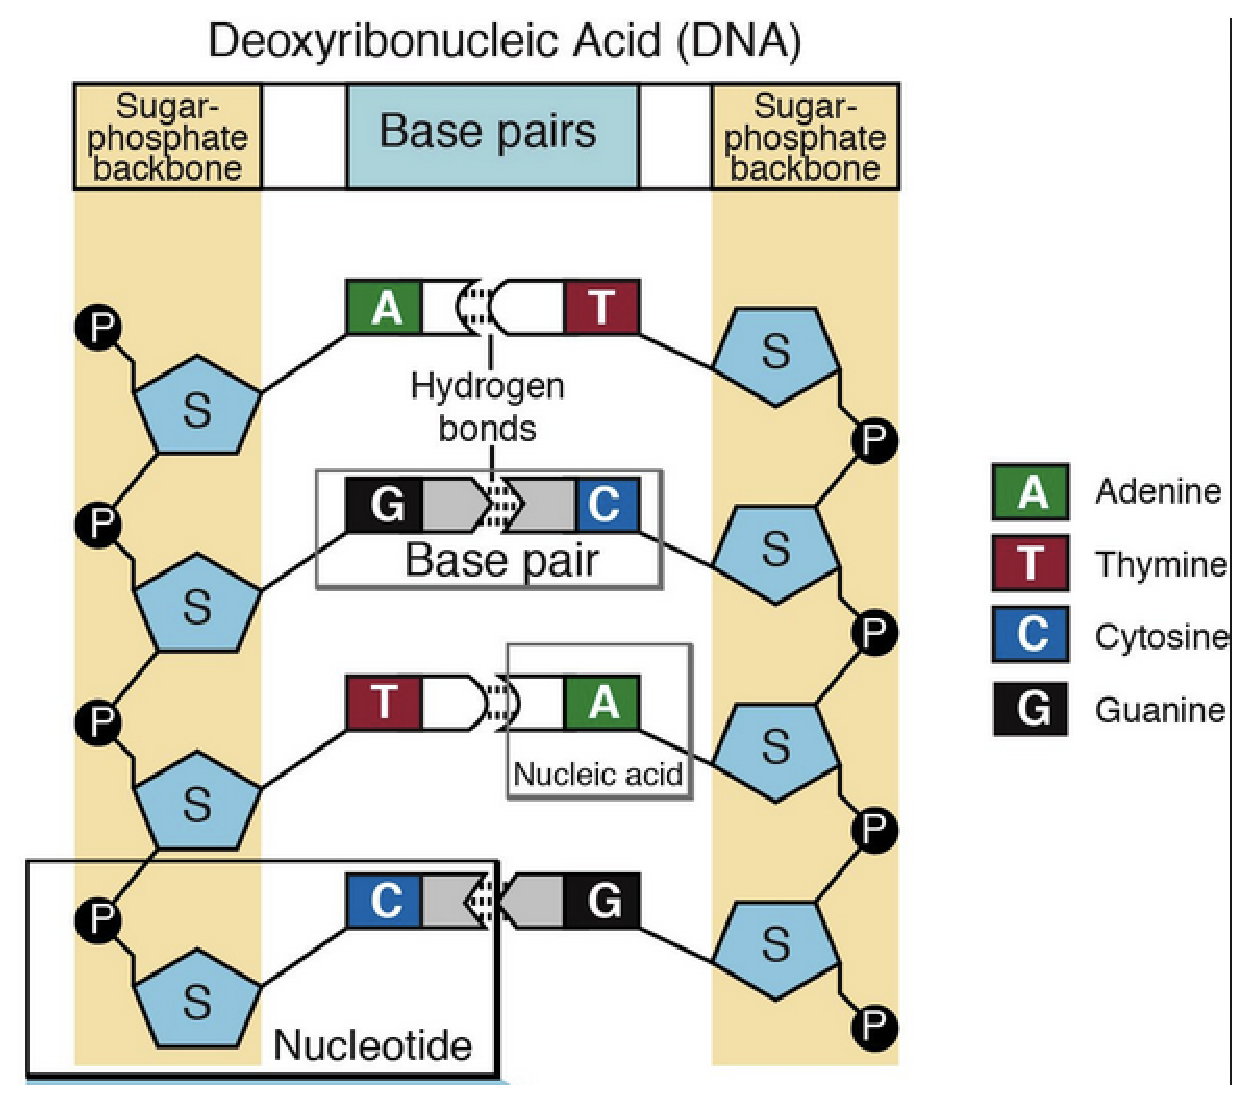
\includegraphics[height=5cm,
    angle=0]{./images/DNA.eps}}
\caption{A (double-straned) DNA with two sugar-phosphate backbone}
\label{fig:DNA}
\end{figure}


\subsection{Nucleotide (nucleobase)}
\label{sec:nucleotide}
%\label{sec:nucleotide}

A nucleobase
\begin{enumerate}
  \item {\bf A}denosine	
  \item {\bf T}hreonine
  \item {\bf G}uanine	
  \item {\bf C}ytosine ({\bf U}ranine)
\end{enumerate}

A {\bf nucleotide}, Fig.\ref{sec:nucleotide} is a monomer units forming DNA and
RNA. DNA has 4 types of nucleotides: A, T, G and C; while RNA has 4 types: A, U,
G, and C.

A nucleotide is composed of (in the direction of 5' to 3')
\begin{itemize}
  \item 5'-end (i.e. 5'-position of the carbon atom in the sugar ring):
  phosphate group (one or many)

  \item 5-carbon sugar ring:

  \item 3'-end:  nitrogeneous base (e.g.  adenine, guanine, thymine, cytosine)
\end{itemize}
A nucleotide is also called {\bf nucleobase} due to its role in bonding nucleic
acids (DNA and RNA), Fig.\ref{fig:DNA} - Sect.\ref{sec:dna}.

\begin{figure}[hbt]
  \centerline{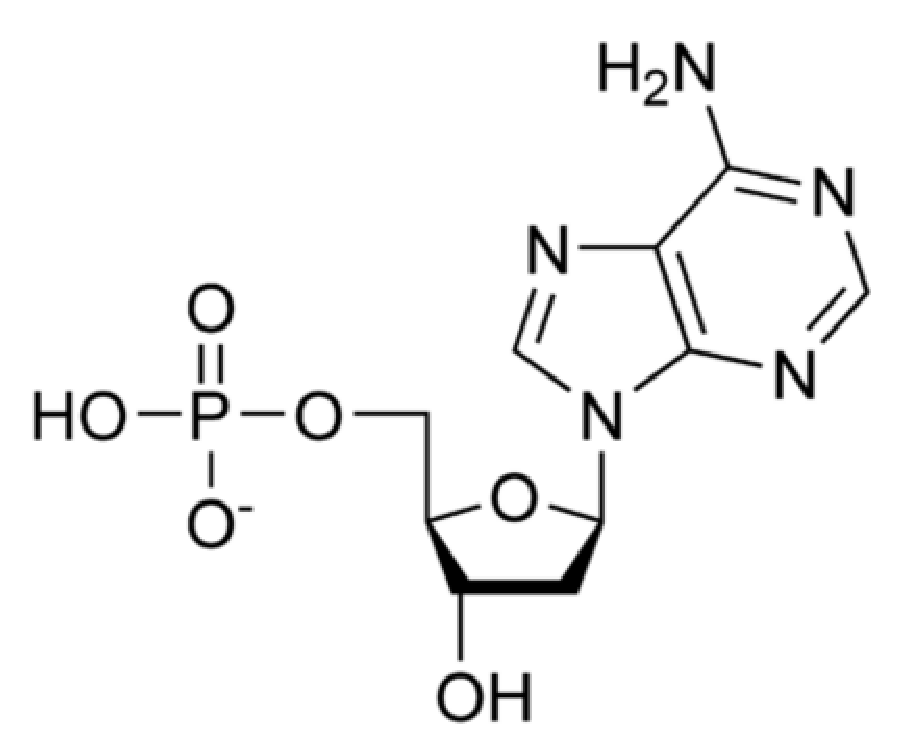
\includegraphics[height=5cm,
    angle=0]{./images/nucleotide.eps}}
\caption{A nucleotide is a building block of nucleic acids. It is a monomer
composed of (1) a nitrogenous base (whose purpose is to bond nucleic acids
together), (2) a 5-carbon sugar; and (3) a phosphate group }
\label{fig:nucleotide}
\end{figure}


\subsection{-- Adenosine (A)}
\label{sec:adenosine}



\subsection{Junk DNA: dogma of life}
\label{sec:junk-dna}


The {\bf Central Dogma} about genetic inheritance has been widely
accepted for decades. 
\begin{verbatim}
DNA --> RNA --> mRNA --> genes ---> protein 
\end{verbatim}

Now, very recently it has become evident that our concept of genetic inheritance
is not the full story. First, biological complexity is not proportional to gene
numbers. The rice plant has more genes than does a human. Another oddity is
that, in a human, the DNA sequences that actually code for protein sequences
amount to only 1.5\% of the total. What happens to the rest?

A large amount of the DNA have no (or unknown) informational
content. So, this major part in a DNA sequence is called
{\bf junk DNA}. Until recently, there is now evidence that junk DNA
contains large number of {\it non-coding microgenes}. They code for
tiny micro RNAs which are not for protein-coding purposes. What are
they for?

It is too early to be known fully but tiny micro RNAs appear to be
responsible for some of the inherited characteristics of
organisms. Elimination of microgenes has been shown to cause dramatic
changes in the structure of a plant. This is a hot research area of
molecular biology.


\section{RNA: mRNA (microRNA), rRNA, tRNA}
\label{sec:RNA}

Although DNA stores the information which cells utilize for protein synthesis.
This is a multi-step process, and the first one is generating RNA. In other
words, RNA carries out the instructions encoded in DNA. Importantly, the
process needs the help of a special protein - called {\it RNA polymerase}
(Sect.\ref{sec:RNA-polymerase}).

\begin{verbatim}

DNA (double strand) ---[transcription]--->        RNA
RNA (single strand) ---[copy         ]--->        RNA
\end{verbatim}

A RNA is a linear, single-stranded polymer, composed of ribose nucleotides, that
is synthesized by transcription of DNA or by copying of RNA. This process is
called {\bf transcription}
\begin{equation}
\ce{ \text{a segment of DNA (double-strand)} ->[\text{enzyme RNA polymerase}]
RNA}
\end{equation} 

\begin{equation}
\ce{RNA ->[\text{copy}] RNA}
\end{equation}

Both RNA and DNA are nucleic acids. In the first method, the RNA
polymerase bind and open the double strand from the 5' end (i.e. DNA
upstream) at a specialized sequence called {\bf promoter} (which is about 3
elements in bacteria, but upto 7 elements in eukaryote). \textcolor{red}{This
promoter is not so far from the site or location of transcription initiation}.

\begin{itemize}
  \item TATA box (TATTAA sequence): in eukaryote is about 25-35 base pairs away
  from the transcription initiation site.
  
  \item TATAAT sequence (called Pribnow box) in prokaryote is about 10 base
  pairs away from the transcription initiation site
   
   NOTE: Not all Pribnow box has this exact sequence TATAAT. This is just the
   most common sequence. 	
   
   \item TTGCCA sequence which is about 35 base pairs upstream from the
   transcription initiation site.
   
\end{itemize}
\url{http://www.nature.com/scitable/topicpage/dna-transcription-426}

Many eukaryotic genes also possess an enhancer sequence, which is at a
considerable distance from the genes they effect. NOTE: Some genes have an A-T
rich region of 40-60 nucleotides upstream from the transcription initiation site
that enhance the rate of transcription. The enhancer sequence binds to activator
protein and alter the 3D structure of the DNA to help the DNA 'attract' the RNA
pol II easier. REMEMBER: The eukaryotic DNA are not straight, but is tightly
packed as chromatin, and thus it needs some specialized proteins to make the
template strand accessible.

\subsection{RNA polymerase}
\label{sec:RNA-polymerase}

There are 3 different kinds of RNA polymerase in eukaryotic cells (but only 1
in bacteria) which then create three types of cellular RNA - mRNA, rRNA, and
tRNA - play different roles in protein synthesis.

\begin{enumerate}
  \item RNA pol I: transcribe genes that encode ribosomal RNA (rRNA).
  
  rRNA then associate a set of proteins to form ribosomes.
  
  A ribosome is a large complex comprising several different rRNA molecules and
  more than 50 proteins, organized into a large subunit and small subunit; the
  site of protein synthesis.
  
  
  \item RNA pol II: transcribe genes that encode messenger RNA (mRNA) - which
  serves as the templates for production of protein. The protein synthesis occur
  at ribosome. The genes transcribed by the RNA pol II are also called pol II
  genes.
  
  The information is encoded in the form of a series of 3-base code 'words',
  each 3-base (called {\bf codon}) encodes an amino acid in a protein. Which
  3-base map to which amino acid is decided by the tRNA
  
  There are 4 different types of base: 
  \begin{itemize}
    \item DNA: has A, C, G, T : adenine, cytidine, guanine, and thymine
    \item RNA: has A, C, G, U : adenine, cytidine, guanine, and uracil
  \end{itemize}
  So, 1-base system encode only 4 amino acids, 2-base system encode 16 amino
  acids. With 20 amino acids, it requires a 3-base system which can encode 64
  code words. But there are only 20 amino acids, i.e. 20 code words. So, among
  64 code words
  \begin{itemize}
    \item 3 code words are used to encode the stop codon, i.e. telling to stop
    the synthesis
    
    \item 61 code words to encode for 20 amino acids. So, most amino acids are
    encoded by more than one codons.
  \end{itemize}
  
  \item RNA pol III: transcribe genes that encode transfer RNA (tRNA).
  tRNA is the key to deciphering the code words in mRNA.
  
  Each type of amino acid has its own type of tRNA, which binds it and carries
  it to the growing end of a polypeptide chain if the next code word on mRNA
  calls for it.
  
\end{enumerate}
\url{http://www.ncbi.nlm.nih.gov/books/NBK21603/}

\subsection{microRNA (miRNA)}
\label{sec:microRNA}
\label{sec:mRNA}

The mRNA is processed in the nucleus before transport to the cytoplasm.

MicroRNAs (miRNAs) are small (17-24 nucleotides) non-protein coding genes
present in virtually all animals and  plants;  and tend to be transcribed from
several different loci in the genome.

Though not encoding for protein, MicroRNAs  mediate post-transcriptional gene
silencing by binding to the 3'-untranslated region (UTR) or open reading frame
(ORF) region of target mRNA. The discovery of microRNAs as well as other RNAs
that do not encode for proteins, indicates that there is much more to the genome
than protein coding genes. Indeed, microRNAs represent ~4\% of the genes in the
human genome.

This discovery suggests that the genome is far from being deciphered, and most
importantly that miRNAs are likely to represent just the "tip of the iceberg"
with many other small non-coding RNAs to be discovered.

miRNA are found in exosome (Sect.\ref{sec:miRNA-in-exosome}).
Given the transportability of vesicles (Sect.\ref{sec:exosome}), the role of
miRNAs in exosomes is gaining increasing attention.

\subsection{-- mRNA level to protein expression}
\label{sec:mRNA-level-2-protein-expression}

{\bf How is mRNA expression predictive for protein expression?} 
A key assumption in studying mRNA expression is that it is informative in the
prediction of protein expression. However, only limited studies have explored
the mRNA-protein expression correlation in yeast or human tissues and the
results have been relatively inconsistent.   

\begin{enumerate}
  \item  the first multilevel expression correlation study in normal human
  cells, human circulating monocytes (CMCs) (Guo et al., 2008).
  
  CMCs are an important cell type in the human immune system.
  The protein expression level is studied using 2-DE gels for quantification and
  identification. Here, 105 protein spots were detected and the intensity of the
  gray scale represent the expression level.
  The result showed that mRNA expression might be sometimes useful, but
  certainly far from perfect, in predicting protein expression levels.
  
  \item Kendrich et al. (2014) 
  
  \item 
\end{enumerate}

% Acta Biochim Biophys Sin (Shanghai). 2008 May;40(5):426-36.
% Guo Y1, Xiao P, Lei S, Deng F, Xiao GG, Liu Y, Chen X, Li L, Wu S, Chen Y, Jiang H, Tan L, Xie J, Zhu X, Liang S, Deng H.


\subsection{tRNA}

\subsection{rRNA}

\subsection{piRNA (piwi-interacting RNA)}
\label{sec:piRNA}


\subsection{siRNA}
\label{sec:siRNA}


\subsection{intron-derived miRNA (miRtrons)}
\label{sec:miRtrons}



\section{Chromosome}
\label{sec:chromosome}

A chromosome = thread-like structure of nucleic acids (i.e. DNA sequences) and
protein {\it found in the nucleus of most living cells}, carrying genetic
information in the form of genes - Sect.\ref{sec:gene-history}.
The protein - histone (Sect.\ref{sec:histone})


\subsection{chromosome 4}
\label{sec:chromosome-4}

Chromosome 4 spans more than 186 million base pairs (the building material of
DNA) and represents between 6 and 6.5 percent of the total DNA in cells.

Chromosome 4 likely contains 1,000 to 1,100 genes that provide instructions for
making proteins. Changes in chromosome 4 have been identified in
\begin{enumerate}
  \item several types of human cancer

genetic changes are somatic, which means they are acquired during a person's
lifetime and are present only in certain cells

A specific translocation involving chromosome 4 and chromosome 14 is commonly
found in multiple myeloma, which is a cancer that starts in cells of the bone
marrow, e.g. abnormally fuses the WHSC1 gene on chromosome 4 with part of
another gene on chromosome 14, leading to overactive WHSC1, which appears to
promote the uncontrolled growth and division of cancer cells.
  
  \item Facioscapulohumeral muscular dystrophy:  

  \item WHS (Wolf-Hirschhorn syndrome):
  a contiguous gene deletion syndrome associated with a hemizygous deletion of
  chromosome 4p16.3.
  
  \url{http://www.omim.org/entry/194190}
  
  
  \item \url{https://ghr.nlm.nih.gov/chromosome/4#conditions}
\end{enumerate}


\section{Biomolecule: organic compounds}
\label{sec:living-organisms}
\label{sec:biomolecule}

NOTE: Please check out the movie "{\it The inner life of a cell}" created in
NewTek Lightwave 3D and Adobe after
Effect\footnote{\url{http://www.studiodaily.com/main/searchlist/6850.html}}

\begin{framed}
  Living organisms are complicated (with multi-scale structures) but highly
  organized (Sect.\ref{sec:incredibility-life}).
\end{framed}

A typical organism is composed of many {\bf cells} (typically of many types)  -
viruses excluded. In turn, these cells possess subcellular structures (known as
{\bf organelles}). Even though small, organelles subsequently are complex
assemblies of very large {\bf polymeric molecules} (known as macromolecules).
A {\bf macromolecule} has a complex three-dimensional structure (the
conformation) which is a consequence of interactions/bonding between the {\bf
monomeric units} (small molecules such as sugars, amino acids, and lipids)
according to their individual chemical properties.

\begin{framed}
  Sugars (Sec.\ref{sec:sugar}), Amino Acids (Sect.\ref{chap:amino-acids}),
  Lipids (Sect.\ref{sec:lipids}) are all basic molecules for creating living
  cells.
\end{framed}

\subsection{Aldehydes vs. Ketones}
\label{sec:aldehydes}
\label{sec:ketones}

A {\bf aldehyde} is an organic compound with the carbonyl structure (i.e.
central carbon bonded to a hydrogen and R-group) $\ce{R-CHO}$; and 
the carbonyl is placed at the end of the carbon skeleton.

A {\bf ketone} also has the carbonyl structure like aldehyde, yet the 
carbonyl is placed in  between two carbon atoms of the backbone.



Aldehydes and ketones are widespread in nature and are often combined with other
functional groups. Aldehydes and ketones are known for their sweet and sometimes
pungent odors.

\url{http://chem.libretexts.org/?title=Core/Organic_Chemistry/Aldehydes_and_Ketones/Properties_of_Aldehydes_&_Ketones/Natural_Occurrence_of_Aldehydes_and_Ketones}
\subsection{Important role of H, N, C and O}
\label{sec:important-role-h}

{\bf CHONPS}: mnemonic acronym for the most common elements in living
organisms: carbon, hydrogen, oxygen, and nitrogen, phosphorus, sulfur.

\begin{figure}[hbt]
  \centerline{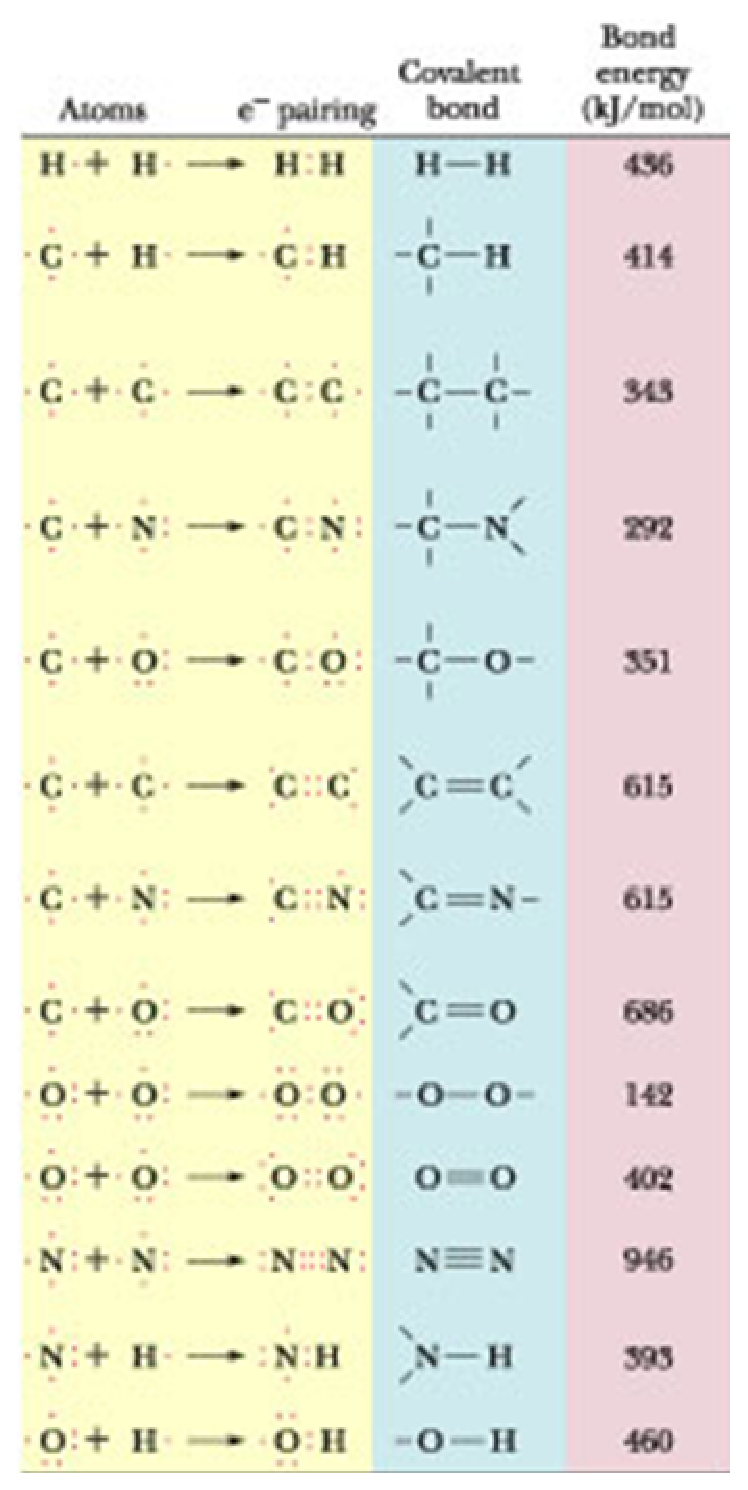
\includegraphics[height=10cm,
    angle=0]{./images/bonding_C.H.O.N.eps}}
  \caption{Bonding C, H, O, N}
  \label{fig:bonding_chon}
\end{figure}


\begin{framed}
  In those basic molecules described above, H, N, C and O are
  important to the chemistry of life; especially C which forms the
  backbone of all biomolecules. 
  
  As C can bond readily to other C atoms; they can build an arbitrarily long
  complex molecules and polymers. 
  
  In the periodic table, a molecule with similar properties with C is Si
  (silicon) - with 4 valence bonds and can bonds to itself in the form of
  crystal lattices (rather than long chains like C). However, 
  Silicon compounds do not readily recombine into different permutations in a
  manner that would plausibly support life-like processes.
\end{framed}

Beside their very abundance in nature, H, N, C and O can form covalent
bonds (strong) by electron-pair sharing. Furthermore, they are
{\it among the lightest elements of the periodic table} capable of
forming such bonds. 

Biomolecules are macromolecules, normally in the form of polymers,
i.e. long chain of monomers (amino acid, nucleotide...). In such
biomolecules, carbons (C) are the backbone. The reason is that C atoms can
form 4 covalent bonds (maximum) with other atoms, together with its
ability to form C-C bonds, enables the formation of a wide variety of
molecules of different shapes, size and properties.


\subsection{History }
\label{sec:history-}

\subsection{-- urea: first synthesized organic compound}

In 1828: urea  is the first organic compount  to be synthesized artificially (from inorganic materials)
\begin{itemize}
\item	urea is the waste product (found and retracted from urine)
 \item	urea is highly soluble (it can create 6 hydrogen bonds with water)
 \item	too high concentration of urea in the blood can cause damage to organs in the body

\end{itemize}

\subsection{-- enzyme (-ase) is protein?}
\label{sec:enzyme-history}

In 19th century, when studying the fermentation of sugar to alcohol by
yeast, Louis Pasteur recognized that this process occurs under a vital
force contained within the yeast cells called "ferments". In 1878,
Wilhelm Kuhne coined the term enzyme (come from Greek "in leaven") to
describe such process.

In 1897, Eduard Buchner produced cell-free yeast extract and used this
"press juice" to show that sugar was fermented even when there is no
living yeast cells. It means that the fermentation process does not
occur inside the yeast cells. He call such yeast extract zymase.
\begin{itemize}
 \item Later on, various enzymes are named according to the reaction
   they carry out. Typically the suffix \verb!-ase! is added to the
   name of the substrate (e.g., lactase is the enzyme that cleaves
   lactose) or the type of reaction (e.g., DNA polymerase forms DNA
   polymers).

  \item Buchner hypothesized that yeast cells secrete proteins into
    their environment in order to ferment sugars.
\end{itemize}

At this point, we all know that enzyme could function outside a living
cells. However, there were arguments that proteins are not enzymes,
they are merely carriers for true enzymes and that proteins per se are
incapble of catalysis. In 1926, Sumner showed that enzyme urease was a
pure protein. In 1937, he showed the same result with enzyme
catalase. And the affirmative conclusion was finally proved by
Northrop \& Stanley: enzymes are proteins.

\subsection{-- lysozyme: first resolved structure enzyme}
\label{sec:lysozyme-history}

At that days, proteins has very small structure that cannot be seen by
microscope. Hence, their structures were unknown. However, the
discovery that enzymes can be crystallized eventually allowed their
structures to be identified by the X-ray crystallography technique. In
1965, the first enzyme's structure to be solved was lysozyme (an
enzyme found in tears, egg whites that digests the coating of some
bacteria * kill the bacteria).

\subsection{-- metabolism process}

Metabolism is the term derived from Greek metabolimos for "change" or
"overthrow". The first metabolic cycle discovered was the urea cycle (discovered
by Krebs). The next very important metabolic cycle was the cytric acid cycle
(Krebs cycle).

\subsection{-- gene}
\label{sec:gene-history}

Another historic event is the discovery of {\bf genes} and its role in the
transfer genetical information. {\it A gene is a stretch of DNA or RNA that
determines a certain trait.} 

There is always two copies of a gene - one on the chromosome from the mother,
and one from the father. The exception is genes on the X and Y chromosomes.

Genes mutate and can take two or more alternative
forms
\begin{enumerate}
  \item allele - Sect.\ref{sec:allele}: variants in gene (i.e. DNA sequencing)
  that encode for the same trait.

Each organism has two alleles for every gene, one on each chromosome.


  \item
\end{enumerate}

In 1958, Beadle \& Tatum received the Nobel prize for work in fungi showing that
one gene produces one enzyme (or protein). Even though all cells hold the
same genetic information (stored in chromosomes - Sect.\ref{sec:chromosome}),
depending on the cell type, certain genes are expressed while some are
silent. The question is on which cell type a gene is expressed and at what
level (Sect.\ref{sec:gene-transription-process}).

Since then, the biochemistry has advanced with the development of new techniques
such as chromatography, X-ray diffraction, NMR spectroscopy, radioisotopic
labelling, electron microscopy and molecular dynamics simulations.  Today, there
are 3 branches of biochemistry (as established by Michael Sugar)

\begin{itemize}
  \item Plant biochemistry
  \item General biochemistry
  \item Human/medical/medicinal biochemistry (focus on the biochemistry of human and medical illness)
\end{itemize}

\subsection{-- allele}
\label{sec:allele}

Humans, have paired homologous chromosomes in their somatic cells, and these
contain two copies of each gene. An organism in which the two copies of the gene
are identical - that is, have the same allele - is called homozygous for that gene. 

For heterozygous, {\bf condominance} is the situation in which two different
alleles for a trait are expressed unblended in the phenotype of heterozygous
individuals.  Neither allele is dominant or recessive, so that both appear in
the phenotype or influence it.  Type AB blood is an example.  Such traits are
said to be codominant.

A {\bf dominant allele} is an allele that masks the presence of a recessive
allele in the phenotype. Dominant alleles for a trait are usually expressed if
an individual is homozygous dominant or heterozygous.

{\bf Incomplete penetrance} is the situation in which an allele is expressed
only if certain factors are present in the environment.



An {\bf allele} is a specific variation (or mutation) of a gene.
Example: each person has 23 pairs of chromosomes.
Suppose we choose a particular chromosome from two different people and examine
the DNA from the same spot on both chromosomes. We will find that the pattern of
the bases (A's, C's, T's, and G's) is similar, but it is often not exactly the
same, even if the region is a protein-coding gene. So, {\bf there can be
different variant of a gene that can encode for a given product, e.g. eye
color}. Different alleles of a single gene code for the same trait, but they may
manifest themselves in different ways. The gene for eye color contains the
instructions governing eye pigment, for example, but the specific color is
determined by the particular alleles one has. 

{\bf Example}: the gene for eye color has several variations (alleles) such as
an allele for blue eye color or an allele for brown eyes.

{\bf Example}: The way in which the Huntington gene varies among individuals is
by the number of repeated C-A-G codons it contains. t is important to understand that
everyone has the Huntington gene, but individuals with Huntington's disease have
a many-CAG version of the gene, one that does not function normally.
\url{http://web.stanford.edu/group/hopes/cgi-bin/hopes_test/the-inheritance-of-huntingtons-disease-text-and-audio/#what-are-alleles-how-many-alleles-can-there-be-for-a-gene-and-how-many-copies-does-each-individual-have}

Each organism has two alleles for every gene, one on each chromosome.
{\bf The body/cell will uses one allele to express the protein.} (the question
is which one, see below). If the two alleles are the same (e.g., both coding for
blue eyes), they are called {\bf homozygotes}. If they are different (e.g., one for blue eyes and one
for brown eyes), they are {\bf heterozygotes}.  In the case of heterozygotes,
the individual may "express" either one or a combination of the two traits.
\begin{enumerate}
  \item A dominant allele is one that will always be expressed if present. 
  
  For example, the allele for Huntington's disease is dominant, so if an
  individual inherits an allele for Huntington's from only one of the parents,
  they will have the disease. 
  
  \item a recessive allele is one that will only be expressed if it is found on
  both genes.
\end{enumerate}
A person actually has two copies of every gene, one allele on each of two
homologous chromosomes. 
\begin{verbatim}
Allels present               Allele expressed
Dominant/Dominant -->         Dominant
Dominant/Recessive-->         Dominant
Recessive/Recessive-->        Recessive
\end{verbatim}

Since each chromosome in the pair comes from a different parent, organisms
inherit one allele from each parent for each gene. 

\subsection{-- protein synthesis rate}

Protein biosynthesis is by far the largest consumer of energy during cellular
proliferation; translation by ribosomes is estimated to account for ~50\% of the
energy consumption of a rapidly growing bacterial cell, and ~30\% of that for a
differentiating mammalian cell (Buttgereit and Brand, 1995; Russell and Cook,
1995).  Eukaryotic cells have mechanisms to ensure that the products of
so-called {\bf housekeeping genes}, which are needed in great abundance, are
available to the cell.
\begin{itemize}
  \item   One method is to attract and keep the RNA polymerases (which
  transcribe the gene into messenger RNA (mRNA), which is the template for
  translation into a protein - the actual gene product) bound to the gene
  sequence through a variety of DNA "promoter" and "enhancer" sequences, which
  other proteins called transcription factors bind to and recruit the polymerase
  to the gene. These polymerases are kept active for as long as the cell needs
  the gene's protein product, churning out copy after copy of mRNA      
  
  \item There are many other mechanisms as well, ranging from how the core
  histone proteins that give chromosomes their shape bind near the gene, to the
  manner in which the translation machinery (ribosomes) bind to the mRNA and
  produce multiple protein molecules per mRNA copy.   
\end{itemize}
\url{https://www.ncbi.nlm.nih.gov/pmc/articles/PMC4006352/}



\subsection{Numbers in Greeks}
\label{sec:numbers-greeks}

The names of organic compounds are often given by the length of the
carbon chain. 
\begin{itemize}
\item Di-   = 2
\item Tri-  = 3
\item Penta- = 5
\item Hexa- = 6
\item Octa- = 8
\item Deca- = 10
\item Octadeca- = 18
\item 
\end{itemize}

\section{Phosphate group}
\label{sec:phosphate-group}


A phospshate group ($\ce{-PO4^-}$) has many important roles.
Along with sugars (Sect.\ref{sec:sugar}) and bases (Sect.\ref{sec:bases}), i.e.
the sugar-phosphate backbone, it makes up nucleic acids, like DNA and RNA
(Sect.\ref{sec:dna}). As part of energy carriers, like ATP, it provides energy
for moving our muscles.

In addition to its role in the backbone of DNA, phosphate groups play a
biochemical role in ribosome-substrate interactions and the regulation of
cellular processes. Phosphate groups also play a major part in the bending of
the DNA backbone, due to the repulsion of the negative charges. 


\section{Isomers: constitutional isomers + steroisomers}
\label{sec:isomer}

{\bf Isomers} are molecules with the same chemical formula, but differ
chemical structure, i.e. individual atoms are arranged differently in space.



The two main forms
\begin{itemize}

  \item {\bf Stereoisomer} = isomers, with the same sequence of bonded atoms,
  but differs in 3D  orientations, i.e. atoms have different arrangement of
  atoms (Sect.\ref{sec:stereoisomers}).
  
  \item {\bf Structural isomers} (constitutional isomers) = isomers, but with
  different order of the bond connections.
\end{itemize}
We will focus on steroisomers, e.g. cis-trans isomers (Sect.\ref{sec:cis-}).

\url{http://chemwiki.ucdavis.edu/Inorganic_Chemistry/Coordination_Chemistry/Isomers/Stereoisomers}

\subsection{Stereoisomers}
\label{sec:stereoisomers}

Stereoisomerism is the arrangement of atoms in molecules whose connectivity
remains the same but their arrangement in space is different in each isomer. The
two main types of stereoisomerism are: {\bf DiaStereomerism} (including
'cis-trans isomerism') and {\bf Optical Isomerism} (also known as
'enantiomerism' and 'chirality' - Sect.\ref{sec:enantiomers})

Stereoisomerism can occur when a double bond is present, because the pi bond
involved prevents that bond from being "twisted" the same way as single bond.


Diastereomers are stereoisomers that are not enantiomers (mirror images) of each
other. With different shapes, diastereomers can have different physical and
chemical properties. 

\subsection{-- Diastereomer}
\label{sec:diastereomer}



\subsection{------ cis- and trans-isomers (geometric isomer)}
\label{sec:cis-}
\label{sec:trans-}


{\bf Cis-trans isomers } (obsolete term: geometric isomeris) = isomers with
restricted rotation molecules, e.g. due to double bonds. {\bf Geometric
isomerism} concerns the type of {\it isomer} where the individual atoms are in
the same order, but manage to arrange themselves different spatially.
We will focus on the cis-trans isomers in {\bf biomolecules}.

The cis/trans system should only be used when the carbon atoms involved each
have a hydrogen atoms attached. The prefix {\bf cis-} and {\bf trans}- are used
to identify which side of the double bond C=C the similar atoms are found,
Fig.\ref{fig:Cis-Trans}.
\begin{enumerate}
  \item cis- = on-this-side (two functional groups connecting to each C-atom  of
  the double-bond link are on the same side of the double bond C=C)
  
  \item trans- = across (two functional groups are on opposite side of the
  double bond C=C)
\end{enumerate}
The trans/cis system for naming isomers breaks down when there are more than two
different substituents on a double bond, and thus E/Z notation is used
(Sect.\ref{sec:E-Z-notation})

\begin{mdframed}
{\bf Biomolecules} are complex molecules with C-C or C=C connections as the
backbone and attach to the backbone are functional groups.
\begin{itemize}
  \item C-C = single-bonding of two carbon atoms
  \item C=C = double-bonding of two carbon atoms
  
  Double bonds are formed when p orbitals between two atoms overlap.
  \textcolor{red}{Double bond restrict free rotation}.
\end{itemize}
IMPORTANT: If there are two identical functional groups on one side of the
carbon link, the biomolecule cannot be an isomer, e.g. $\ce{(CH3)2C=CClCH3}$.

\end{mdframed}
%Depending on the orientation of the functional groups



\begin{figure}[htb]
    \centerline{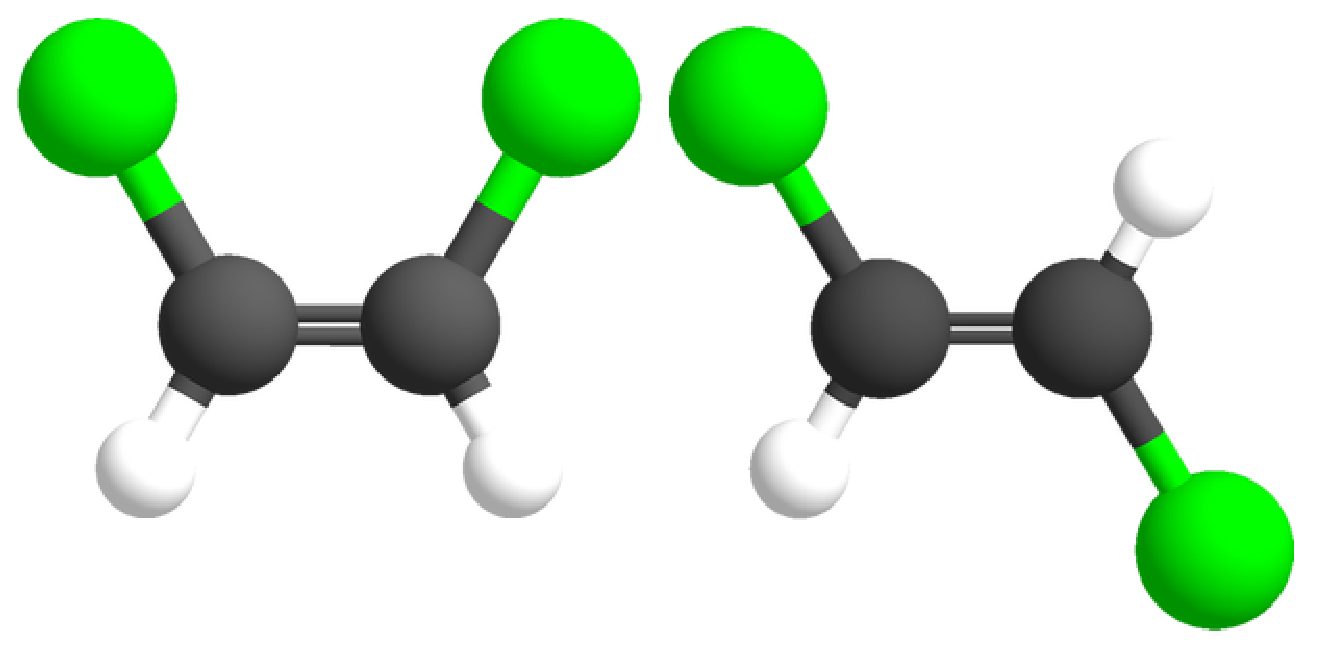
\includegraphics[height=5cm]{./images/Cis-Trans.eps}}
\caption{(Left) Cis- ; (Right) Trans-}\label{fig:Cis-Trans}
  \end{figure}

PHYSICAL PROPERTIES:
\begin{itemize}
  \item Cis- isomers tend to have {\it higher boiling points} than their trans-
  counterparts. 
  
  Trans- isomers generally have lower melting points and have lower
  densities than their cis- counterparts.
  
  \item Cis- isomers collect the charge on one side of the molecule, giving the
  molecule an overall {\it polar effect}. 
  
  Trans- isomers balance the individual dipoles and have a non-polar tendency.
\end{itemize}  
\url{http://chemistry.about.com/od/organicchemistry/tp/Geometric-Isomerism.htm}

\subsection{D- and L-form}
\label{sec:D-and-L-form}
\label{sec:L-isomer}
\label{sec:D-isomer}
\label{sec:chiral-center}


Students who take biochemistry are exposed to an old, confusing, and often
incorrect method of specifying configurations at {\bf chiral centers} as D or L.
This scheme was devised in the early years of this century by Emil Fischer, a German
organic chemist who worked extensively with carbohydrates.
\url{http://chemistry.umeche.maine.edu/CHY251/dlwrong.html}


Modern notation are R- and S-form; but it will NOT always work out that D = R
and L = S.
\begin{itemize}
  \item {\it D-=(Latin) dexter = right, L-=(Latin)laevus = left})
  \item {\it R-=(Latin) rectus = right-handed, S-=(Latin) sinister =
  (left-handed)}
\end{itemize}

\subsection{E- and Z-form}
\label{sec:E-Z-notation}

The E/Z notation is unamibiguous. Z (from the German {\it zusammen}) means
together and usually corresponds to the term cis; E (from the German
{\it entgegen}) means opposite and usually corresponds to the term trans.

RULES: for each functional group, find the 'first' one based on priority rule
\begin{enumerate}
  \item Priority rule (used to identify which part of the molecule to consider
  first)
  
  Cahn-Ingold-Prelog (CIP) priority rule: An atom with higher atomic number has
  higher priority. (e.g. I > Cl > C > H)
  
  
  \item first atom of two groups is the same, consider the second atom(s) in the
  same way as the first. (e.g. -C(CH3)3 > -CH(CH3)2 > -CH2CH3 > -CH3). If this
  does not assign priority, consider the next atoms until there is a difference.
  
  
\end{enumerate}

\subsection{-- Optical isomer (enantiomer, chiral)}
\label{sec:optical-isomer}
\label{sec:enantiomer}
\label{sec:chiral-center}

Enantiomers (or chirals) are two molecules of same molecules-arrangement; but
are nonsuperimposable mirror images.
NOTE: {\bf cheir} (Greek of chiral) = hand.
It similar to the person's left hand is the same as his right hand, except that
they are mirror images of each other.

{\it The most common cause of enantiomerism in organic molecules is the presence
of a stereocenter, carbon with four different groups bonded to it.}
This center carbon atom is known as {\bf chiral center}

{\bf Chiral centers} are tetrahedral atoms that have four different
substituents. 
\begin{itemize}
  \item  The most common type of chiral atom in organic molecules are
{\bf Carbons} because they can be SP$_3$ hybridized and can form four bonds.
  
  \item The other types of atoms that can be chiral are {\bf quaternary
  nitrogens}, {\bf tertiary nitrogens} that are at the bridgehead (junction) of
  a bicyclic ring system, hypervalent phosphorous (with more than three bonds),
  and hypervalent sulfur (with more than two bonds).  However, these other types
  of chiral atoms are very unusual.
  
  \item Molecules with a single chiral center are ALWAYS chiral. Molecules with
  more than one chiral center are {\it usually} (but not always) chiral.
\end{itemize}
\url{http://www.chem.sc.edu/faculty/shimizu/333/Chem_333/5a.ii.html}

\subsection{---- R- and S- system}
\label{sec:R,S-system}

Because enantiomers are different compounds, 
each must have a different name.

The R,S system is a way to distinguish between enantiomers without having to
draw them and point to one or the other, and use use the CIP priority rules
(Sect.\ref{sec:E-Z-notation}).

\begin{enumerate}
  \item Assign the priority to each of the atoms that are bounded to the
  sterocenter (1, highest to 4, lowest).
  
  
  
  \item  When drawing the 3D molecule structure: point the lowest priority (4)
  atom away from you.
  
  \item R configuration: clockwise from 1 to 2 to 3
  
  \item S configuration: counterclockwise from 1 to 2 to 3.
\end{enumerate}
\url{https://en.wikibooks.org/wiki/Organic_Chemistry/Chirality/R-S_notational_system#E-Z_Notation}


\section{Rings}
\label{sec:benzen}
\label{sec:aromatic-ring}

The most commonly encountered aromatic compound is benzene. The usual structural
representation for benzene is 6-carbon ring (i.e. a hexagon with 3
double-bonds and only Hydrogens connected to carbon).

Benzene was first isolated by Michael Faraday in 1825, from the whale oil used
in gaslights. Eilhardt Mitscherlich synthesized benzene in 1834, and showed it
to have a molecular formula of $\ce{C6H6}$.  
Many other compounds with similar properties to benzene were discovered in the
1800s, all having a low ratio of hydrogen to carbon. The low ratio indicates the
presence of double-bonds (C=C).
Since many of these molecules had pleasant aromas, they were called "aromatic
compounds." 
\url{https://www.angelo.edu/faculty/kboudrea/molecule_gallery/04_aromatics/00_aromatics.htm} 

Aromatic hydrocarbons are nonpolar, and are insoluble in water.  However, when
other atoms are substituted on the benzene ring, they may be very water-soluble.
 For instance, phenol, which has an -OH group attached to the benzene ring, is
very water-soluble.

A number of aromatic molecules are known by common names
\begin{itemize} 
  \item benzene with a -CH3 group attached is called "toluene"; 
  
  \item benzene with an -NH2 group attached is called "aniline"; 
  
  \item a benzene with a -CO2H group is called "benzoic acid," etc.
  
  \item  more complicated substituents, the benzene ring is named as a
  substituent, in which case it is called "phenyl."  For instance, an
  eight-carbon chain with a benzene ring on the third carbon is called
  "3-phenyloctane."
  
  
\end{itemize}


\subsection{Phenolic ring}
\label{sec:phenolic-ring}



\section{tyrosine}
\label{sec:tyrosine}

\url{http://www.russelllab.org/aas/Tyr.html}

\begin{mdframed}

Stratural analysis have provided the dominant role of {\it large} tyrosine
residues for mediating molecular contacts and of {\it small} serine/glycine
residues for providing space and flexibility. \citep{koide2009}

\end{mdframed}

Tyrosine:
\begin{itemize}
  \item aromatic $\rightarrow$ allow tyrosine to form stacking interaction with
  other aromatic side-chain, i.e. adhesion purpose
  
  \item partially hydrophobic $\rightarrow$ prefer to be buried in the protein
  hydrophobic core
  
  \item amino acid
  
  \item contains an active hydroxyl group $\rightarrow$ making it more likely to
  interact with non protein atoms (e.g. non-protein ligands)
\end{itemize}

Along with Serines and Threonines, Tyrosine is a target of phosphorylation by
protein tyrosine kinases (PTK) \citep{hubbard2000}, i.e. phosphate group
attached to the tyrosine to facilitate the signal transduction process. This
process is highly specific, i.e.
Tyrosine kinases generally do not work on Serines/Threonines and vice versa.

Phosphorylation of tyrosine residues (Sect.\ref{sec:tyrosine}) modulates
enzymatic activity and creates binding sites for the recruitment of downstream
signaling proteins.
Two classes of PTKs \citep{hubbard2000}
\begin{enumerate}
  \item transmembrane receptor PTKs (receptor tyrosine kinase - RTK, or
  tyrosine receptor kinase - TRK, {\bf Trk} is the name used in neurobiology -
  Sect.\ref{sec:Trk}):
  
  RTK has one extracellular domain for ligand binding, and one intracellular
  kinase domain. To perform its function, RTK needs to form dimer which requires
  the binding of ligand to stabilize the dimer. 
  The interaction between the cytoplasmic domain 
  of RTK stimulate the autophosphorylation of tyrosine, causing conformation
  change. Subsequent to this, the receptor's kinase domains are activated,
  initiating the phosphorylation signaling cascades.
  
   The activity is tightly regulated through several modes of autoregulation
  
  
  \item nonreceptor PTKs
\end{enumerate}


The versatility of tyrosine in forming intermolecular
contacts has also been exploited in surface engineering
to promote protein crystallization



\section{Exosome}
\label{sec:exosome}

Exosome (Pan) as inter-cellular messengers:
extracellular RNA communications (exRNA not only control the cell that hold it;
but it can control cells far apart via exosomes). Study of exosomes has
been mainly in cancer research, but still limited in cardiovascular research.

Endosomes (E) has inverted plasma membrane.

Susmita Sahoo
\begin{itemize}
  \item Sahoo - Losordo, Circ. Res, 2014
  
%    Circ Res. 2014 Jan 17;114(2):333-44. doi: 10.1161/CIRCRESAHA.114.300639.
% Exosomes and cardiac repair after myocardial infarction.
% Sahoo S1, Losordo DW.
  
  \item stemcell-derived exosomes: 

Stem cell first derived from bone marrow (Jacobson et al, 1951, Science)

Doppler et al., 2013. Cardiac regeneration: current therapies-future concepts
Stefanie A. Doppler, Marcus-Andre Deutsch, Rudiger Lange, and Markus
Kranecorresponding author
\url{https://www.researchgate.net/profile/Stefanie_Doppler}
\url{https://www.researchgate.net/profile/Marcus_Andre_Deutsch}
\url{http://www.professoren.tum.de/en/lange-ruediger/}

Due to the beating of the heart, stemcell transplant to the heart is hard, as
very few is retained.

Next: paracrine secretion from the cell which is 2 components: vesicles + 

Human CD34+ exosomes conditioned media (CM):
PB-derived CD34+ cells isolated from G-CSF mobilized individuals.
Extract two forms of sizes: 8nm and 60nm, which are then separated to get 60nm
(supposed to be exosomes). Then, they analyze morphological and biochemical
characteristics of these exosomes.

CD34+ exosome induce angiogenesis (i.e. forming new blood vessels). However,
exosomes is not uptake into the cell; but there are some proteins as receptors
on the membrane of the cell that exosomes bind to and trigger the events.

They injected the exosomes into the eschemic part of the blood vessil in
the limb, and the CD34+ exosome help retain the limb; which show the presence of
the blood flow to the limb with CD34+ exosomes presence.

CD34+ exosomes improve heart wall motion (Sham (i.e. normal): 35\%; block
everything:
5\%; then add CD34+ exosomes: 25\%).


\textcolor{red}{So, what make exosome special?}
\begin{itemize}
  \item RNA inside exosome
  \item the exosome itself
  \item the surface protein as receptor on the membrane of receiving cell
  (don't know which protein yet)
\end{itemize}
The author does not know for sure; and assume they are equally important.

Exosome RNA is enriched for miRNAs (30-60\%), measured using fluorescence unit
(FU). miRNA profiling of CD34+ shows CD34+ exo is enriched with pro-angiogenic
RNA. 

There are many miRNA: 126, 130, 30a, \ldots
They tested by knocking down miRNA-126 in exosome (but not specific as it also
affect others); and it shows a decrease in functions. \textcolor{red}{Not sure
why for now.}
So, they assume miR-126 is important, and directly induce pro-angiogenic gene
expression in mouse tissue.
\textcolor{red}{How about in human?} They don't find any difference in mouse and
human of this miRNA.

Papers: Ashraf 2010 paper; Ebrahim - Marban 2014.; Lim 2010. 
Khan, Koshere 2015.

{\bf Hypothesis}: exosomes from CDC convert inert fibroblast into beneficial
fibroblast.

CD34+ exosome is uptake quickly (within 1-4h) by cells in ischemic tissue; but
is not maintained (e.g. loss after 24h).
Mainly uptake by endothelical cells (87\%); and a smaller amount by
cardiacmyocytes (34\%). Fibroblast in cell culture is different from
that in vivo; though the author not sure why.

{\bf Hypothesis}: Na/K-ATPase surface protein control the uptake of exosomes.
It is important to know the protein that involve into regulating the uptake of
exosomes into the cells.


{\bf Question}: how about the role of heart-secreated exosomes (we have just
cover CDC34+ exosome only)? now found any physiological role so far.

Emanueli, C. 2016, PLoS One.

The author's goal is to built artificial exosomes with the necessary RNA (so we
don't need biologocaly released exosome) to treat cardiovascular diseases.


\item {\bf GOAL}: AAV-exosome: novel vector for myocardial gene delivery


\item {\bf GOAL}: epitranscriptomic regulation of cardiac ischemic remodeling
\begin{enumerate}
  \item a new layer of gene regulation: 
  
  \item the author found big difference in failing heart in m6A RNA methylation
  (high in failing heart)
  
  \item 
\end{enumerate}


\end{itemize}


Exosomes are 40-100 nm nano-sized vesicles that are released from many cell
types into the extracellular space, and are present in almost all biological
fluids. Exosomes were first discovered by Pan and Johnstone in 1983.
In 1989, Johnstone defined such functional vesicles as exosomes.
According to the way of vesicular secretion from cells, extracellular vesicles
can be grouped into two general classes
\begin{enumerate}
  \item microvesicles
  
  \item exosomes: released by exocytosis when multivesicular bodies (MVBs)
  fuse with the plasma membrane
\end{enumerate}

 In addition to the proteins, various nucleic acids have recently been
identified in the exosomal lumen, including mRNAs, microRNAs (miRNAs), and other
non-coding RNAs (ncRNAs). The exosomal RNA, i.e. mRNAs (Sect.\ref{sec:mRNA}) and
microRNAs (miRNAs - Sect.\ref{sec:microRNA}) in exosomes, can be taken up by
neighboring or distant cells and subsequently modulate recipient cells.

Exosomal miRNAs play an important role in disease progression, and can stimulate
angiogenesis and facilitate metastasis in cancers
Importantly, miRNA profiles of exosomes may differ from those of the parent cells.


Conveying information via circulating vesicles is deemed to be the third way of
intercellular communication that can deliver to cells further from the origin
cell. It is as essential as the cell-to-cell contact-dependent signaling
(e.g. electrical syanpse) and signaling via transfer of soluble molecule (e.g.
chemical synapse).


Several reports have shown that exosomes play important roles in immune
response, tumor progression, and neurodegenerative disorders. 

\subsection{exosomal miRNA}
\label{sec:miRNA-in-exosome}

There are four potential modes for sorting of miRNAs into exosomes, although the
underlying mechanisms remain largely unclear. 
\begin{enumerate}
  \item neural sphingomyelinase 2 (nSMase2)-dependent pathway
  
   overexpression of nSMase2 increased the number of exosomal miRNAs, and
  conversely inhibition of nSMase2 expression reduced the number of exosomal
  miRNAs (Kosaka et al. (2013))
  
  
  \item  sumoylated heterogeneous nuclear ribonucleoproteins (hnRNPs)-dependent
  pathway
  
  sumoylated hnRNPA2B1 could recognize the GGAG motif in the 3' portion of miRNA
  sequences and cause specific miRNAs to be packed into exosomes
  (Villarroya-Beltri et al. (2013))
  
  \item 3'-end of the miRNA sequence-dependent pathway:
  
   3' ends of uridylated endogenous miRNAs were mainly presented in exosomes
  derived from B cells or urine, whereas the 3' ends of adenylated endogenous miRNAs were mainly presented in B cells
  
  \item AGO2-related pathway or miRNA induced silencing complex
  (miRISC)-related pathway
  
   mature miRNAs can interact with assembly proteins to form a complex called
  miRISC.  The main components of miRISC include miRNA, miRNA-repressible mRNA,
  GW182, and AGO2. The AGO2 protein in humans, which prefers to bind to U or A
  at the 5' end of miRNAs, plays an important role in mediating mRNA
  
  Knockout of AGO2 could decrease the types or abundance of the
  preferentially-exported miRNAs, such as miR-451, miR-150, and miR-142-3p, in
  HEK293T-derived exosomes
  
  
\end{enumerate}


\section{Chromatin: nucleosome, histone}
\label{sec:chromatin}
\label{sec:histone}
\label{sec:nucleosome}

The eukaryotic DNA (Sect.\ref{sec:dna}) in each chromosome are not straight, but
is tightly packed as {\bf chromatin}, and thus it needs some specialized
proteins to make the template strand accessible.

Chromatin is the complex basis of DNA and (histone) protein that makes up
chromosomes (Sect.\ref{sec:chromosome}). The {\bf nucleosome} is the fundamental
unit of chromatin. Each nucleosome has about 146 pairs of little less than 2
helical turns of DNA wrapping around a set of 8 {\bf histone} proteins - called
histone octamer. Each histone octamer is composed of two copies each of the 4
types of histone proteins H2A, H2B, H3, and H4.

Changes in chromatin structure are affected by chemical modifications of histone
proteins such as methylation (DNA and proteins) and histone acetylation
(proteins - Sect.\ref{sec:acetylation}), and by non-histone, DNA-binding proteins.
\begin{itemize}
  \item  Genetic modification - e.g. histone acetylation at N-terminal tail (a
  key role in regulating gene expression) - controlled by the balance of 2
  enzymes: HAT (Histone acetyltransferase) and HDAC (Histone Deacetylase) -
  Sect.\ref{sec:HDAC}.
  
HAT enables the expression of a gene. HDAC performs the opposite function, i.e.
tie coiling of the DNA and close chromatin structure. So, overexpression of HDAC
or aberant recruitment of HDAC or underexpression of HAT all results the
condense of chromatin structure, i.e. links to down regulation of certain genes.
   
\end{itemize}

\subsection{Histone acetyltransferase (HAT)}
\label{sec:HAT}

DNA sequences are packed structure (Sect.\ref{sec:chromosome}) with the
support of a protein called {\bf histone} and thus need to be unpacked for
transcription process to occur, i.e. the DNA sequence should be accessible to
the (gene) transcriptional machinary.

{\bf Histone acetyltransferase} (HAT) performs histone acetylation
(Sect.\ref{sec:acetylation}) to remove histone protein and thus to uncoild the
DNA and open chromatin structure. \textcolor{red}{NOTE: HAT can also acetylate
non-histone proteins, such as nuclear receptors and other transcription factors
to facilitate gene expression.}

The removal of acetyl group is done by HDAC (Sect.\ref{sec:HDAC}).

There are 2 types of HAT:
\begin{enumerate}
  \item {\bf type A HAT}: in nucleus
  
  They contain a bromodomain, which helps them recognize and bind to acetylated
  lysine residues on histone substrates.

The type-A HATs are a more diverse family of enzymes than the type-Bs; yet they
can be classified into 3 groups: GNAT, MYST and CBP/p300 families.
Broadly speaking, each of these enzymes modifies multiple sites within the
histone N-terminal tails.
  
  \item {\bf type B HAT}: in cytoplasm
  
  Type B HAT (which lacks bromodomain as their targets are unacetylated) is
  responsible for acetylating newly synthesized histones prior to their assembly
  into nucleosomes.

This class of HATs is highly conserved and all type-B HATs share sequence
homology with scHat1, the founding member of this type of HAT
  
\end{enumerate}

HAT calatyze acetyle group to the N-terminal of histones and non-histone
proteins. It utilizes acetyl CoA (Sect.\ref{sec:Acetyl-CoA}) as cofactor to
facilitate the process. In doing so, HAT neutralize the lysine's positive charge
and this action has the potential to weaken the interactions between histones
and DNA.

However, it is not just the histone tails that are involved in this regulation,
but there are additional sites of acetylation present within the globular
histone core, such as H3K56 that is acetylated in humans by hGCN5 (Bannister,
Kouzarides, 2011).


\section{Epigenetic change}
\label{sec:epigenetic-change}

{\bf Epigenetics} refers to  the heritable modification in the gene
function/activity without changing the DNA sequence encoding for that gene.
It affects gene regulation by changing the DNA conformation, i.e. 3D structure.

This process is found in many cancer cell types.
One such change is {\bf histone modification} which can be caused by either
overexpression (or aberent recruitment) of HDAC.

\section{Tumor necrosis factor-$\alpha$ (TNF-$\alpha$)}
\label{sec:TNF-alpha}

Tumor necrosis factor (TNF), formerly known as tumor necrosis factor-$\alpha$ or
TNF-$\alpha$, is a cytokine involved in systemic inflammation
\citep{mirkhani2012}.  NOTE: cytokine = substances secreted by cells in the
immune systems and have an affect on other cells.

Previously, lymphotoxin (LT, secreted by T-cells) was known as tumor necrosis
factor-$beta$. Thus, TNF-$\alpha$ was given to tumor necrosis factor.
However, since there's no $\beta$ suffix to LT, some researchers suggested to
use TNF only. 

TNF can be produced in many cells, including cardiac myocytes and neurons.
\begin{enumerate}
  
  \item  In heart, TNF led to an increase in spontaneous SR leak (due to
  elevated reactive oxygen species production from mitochondria and NADPH
  oxidase sources triggered by TNF) and can generate triggered activities in
  isolated mice atrial myocytes.

\end{enumerate}


\begin{framed}

TNF can bind 2 types of receptors (TNFRs): TNF-R1 (found in most tissues -
Sect.\ref{sec:TNF-R1}), TNF-R2 (found only in immune system - Sect.\ref{sec:TNF-R2s}). 

Upon binding of TNF, TNFR forms trimers. This conformational change leads to the
dissociation of protein SODD from the (intracellular) death-domain, allowing
adaptor protein TRADD to bind to this death-domain (serving as a platform for
subsequent protein binding that can trigger different signalling pathways). 

TNFR involves in the three major signalling pathways: (1) activation of NFKB
(stress response, inflammatory response, etc.) - Sect.\ref{sec:NFKB}, (2)
activation of MAPK - Sect.\ref{sec:MAPK}, (3) induction of death signalling.

\end{framed}

\subsection{p55 receptor (TNF-R1)}
\label{sec:TNF-R1}
\label{sec:p55-receptor}

{\bf Vascular (endothelial) permeability}: Stimulation of TNFR1, but not TNFR2,
induced cytoskeletal reorganization associated with increased permeability.
SB-203580, a p38 mitogen-activated protein kinase inhibitor, blocked
TNFR1-induced cytoskeletal reorganization and permeability (Ferrero et al.,
2001).



\subsection{p75 receptor (TNF-R2) (low-affinity nerve growth factor receptor)}
\label{sec:p75-receptor}
\label{sec:TNF-R2}

p75 receptor is TNF-R2, a member of the tumor necrosis factor (TNF) receptor
superfamily. It is {\bf low-affinity} to several mature neurotrophins, and thus
is also called low-affinity nerve growth factor receptor (LNGFR); yet has {\bf
high-affinity}  for pro-neurotrophins. 

BDNF is a member of neurotrophin family

{\bf Vascular permeability}: Even though TNFR1 shows a more prominent effect
(Sect.\ref{sec:TNF-R1}), an antagonist anti-murine TNFR2 antibody partially
inhibited the effect of murine TNF on liver vessels, suggesting that TNFR2 also
plays a role in the regulation of TNF-induced vascular permeability in vivo.




\section{Blocker/Inhibitors}
\label{sec:blockers-inhibitors}

Table.\ref{tab:ion-channel-blockers} shows different 
natural toxins and synthetic pharmacological agents
exist that can be used to reduce or eliminate specific voltage-activated
ion channel activity.

Many of these agents are effective against one particular type of ion channel,
e.g. tetrodotoxin (TTX) and dendrotoxin (DTX - Sect.\ref{sec:dendrotoxin}),
which target Na+ and K+ channels, respectively.

\begin{table}[hbt]
\begin{center}
    \begin{tabular}{lc}
Channel Type & Compound/Reagent \\
        \hline
K+ channels & \\
Delayed rectifier (Kd) & TEA, Ba2+, capsaicin, 4-AP, margatoxin \\
Inward rectifier (Kir) & TEA, Cs+, Rb+, Na+, Ba2+ \\
A-type & TEA, 4-AP, dendrotoxin \\
K(Ca) & \\
$\qquad$ Big K & Charybdotoxin, iberiotoxin \\
$\qquad$ Small K & Apamin \\
$\qquad$ K(ATP) & TEA, Cs+, Ba2+ \\
Na+ channels & TTX, STX, CNQX, agatoxin, 
Scorpion toxin \\
Ca2+ channels & \\
$\qquad$ L-type & Nifedipine, verapamil, 
BayK8644, Cd2+, La3+ \\
$\qquad$ T-type & Ni2+, La3+ \\
$\qquad$ N-type & $\omega$-conotoxin, La3+ \\
$\qquad$ P-type & FTX funnel spider toxin \\
Cl-/anion channels & Chlorotoxin, avermectin B, NPPB,
DIDS, Zn2+ \\
        \hline
    \end{tabular}
\end{center}
\caption{Commonly used ion-channel blockers}
\label{tab:ion-channel-blockers}
\end{table}


\subsection{Tetrodotoxin (TTX)}
\label{sec:tetrodotoxin}
\label{sec:TTX}

Tetrodotoxin (TTX) is a toxic found in Japanese puffer fish and in the skin of
certain frogs and salamanders. TTX specifically blocks some $\Na$ channels
(Sect.\ref{sec:Na-current-TTX-sensitive}) - though there exists 
TTX-resistance $\Na$ channels (Sect.\ref{sec:Na-current-TTX-resistant}).

Tetrodotoxin (TTX) is a highly toxic, experimental inhibitor of $\Na$ channel.
TTX binds to the extracellular site 1 of fast $\Na$ channel, which temporarily
disable the function of $\Na$ channels. Blocking $\Na$ channels has potential
use in treating some cardiac arrhythmias. However, overdose of TTX is very
poisonous.

\subsection{Tetraethylammonium (TEA)}
\label{sec:tetraethylammonium}
\label{sec:TEA}

Tetraethylammonium (TEA) is a large organic cation. TEA (tetraethylammonium) is
a classical Kv channel blocker (Sect.\ref{sec:Kv_channel}), from the external or
internal side of the pore region.

\begin{itemize}
  
  \item External TEA: the channels Kv1.1, Kv1.3 and Kv1.6 are sensitive, at
  IC50=0.3-10 mM. TEA sensitivity is mainly due to the presence in Kv1.1 of that
  critical residue.
   
NOTE: Kv1.2, Kv1.4, Kv1.5 and Kv1.7 are insensitive to external TEA, i.e. IC50
$>$ 100 mM.
Unlike Kv1.2, as Kv1.2 tetrameric channel has valine (Val381) at the
equivalent location, it makes Kv1.2 channel insensitive to external TEA.
\url{http://channelpedia.epfl.ch/ionchannels/2}
  
  \item Internal TEA: 
\end{itemize}

Example: KRP - Sect.\ref{sec:KRP}

\subsection{Dendrotoxin: alpha-DTX (alpha-Dendrotoxin)}
\label{sec:dendrotoxin}
\label{sec:alpha-DTX}

Dendrotoxins are a group of peptides that have been isolated from the venom of
green mamba and black maba snake. 
\begin{itemize}
  \item  Alpha-dendrotoxin was originally isolated from the venom of the green
  mamba Harvey and Karlsson (1980). 
  
  \item Later on, others are isolated: beta-1, beta-2, gamma-,
  delta-dendrotoxins Benishin et al (1988).
\end{itemize}
Related peptides dendrotoxin-I and dendrotoxin-K have been purified from black
mamba venom Strydom (1976).

\begin{itemize}
  \item  $\alpha$-DTX (alpha-Dendrotoxin) is a blocker that has a high affinity
  for three Kv1 family subunits- Kv1.1, Kv1.2, and Kv1.6 (Coetzee et al. 1999) -
Sect.\ref{sec:Kv1-channels}.

{\bf Mouse}:
\begin{verbatim}
EC50 = 9.4 nM: inhibit whole-cell Kv1.1

EC50 = 2.8 nM: inhibit Kv1.2

EC50 = 250 nM: inhibit Kv1.3 

EC50 = 20 nM: inhibit Kv1.1
\end{verbatim}

{\bf Rat}:
\begin{verbatim}
EC50 = 8.6 nM: block Kv1.2

EC50 = 17 nM: block peak Kv1.2
\end{verbatim}

{\bf Human}:
\begin{verbatim}
EC50 = 20 nM: block peak Kv1.6 
\end{verbatim}

  \item dendrotoxin-K (57 amino-acid) is a  selective blocker of voltage-gated
  potassium channels
  
  \item dendrotoxin-I is  isolated from Dendroaspis p.polylepis snake venom: it
  blocks Kv1.2, Kv1.1; and  heteromultimeric channels containing
  these with other Kv1 isoforms
  
Effective concentration is 10-100 nM.  

in oocytes:
\begin{verbatim}
EC50 = 0.13  nM    for Kv1.2

EC50 = 3.1   nM    for Kv1.1
\end{verbatim}
and higher values for mammalian cells.

\url{https://www.alomone.com/p/dendrotoxin-i/D-390}

\end{itemize}


\subsection{methylsulfonate}
\label{sec:methylsulfonate}

Methylsylfonate can replace chlorine and thus eliminate chlorine conductance.

\subsection{Cadmium}
\label{sec:cadmium}

Cadmium blocks $\Ca$ channels.

\subsection{4-AP}
\label{sec:4-AP}

4-aminopyridine (4-AP). See Sect.\ref{sec:K+current_4-AP-sensitive}.
$\ce{C5H4N-NH2}$ formula: is a drug has been approved by FDA in 2010 to manage
symptoms of multiple sclerosis. 

4-AP is known to
\begin{enumerate}
  \item block/reduce K+ currents: relatively selective blocker of Kv1 channels
  (Sect.\ref{sec:Kv1-channels}) at 1mM 4-AP; without significant affect other $\Na$, $\Ca$ and $\K$ channels. 
  
   \item block Nav channels - Sect.\ref{sec:Nav-blockers}
\end{enumerate}

\subsection{Tertiapin}

Tertiapin is a 21-amino acid peptide isolated from venom of the European honey
bee. It can blocks 2 different types of $\K$ currents: Kir
(Sect.\ref{sec:Kir_family}) and BK(Ca) (Sect.\ref{sec:BK-current})

The time it takes to block BK(Ca) is longer than that for Kir, suggesting two
different blocking mechanism. Tertiapin inhibits the BK channels only after a
minimal stimulation of 15 minutes, in contrast with less than a minute for the
GIRK channels.

\begin{enumerate}
  \item Kir-block:
  Tertiapin binds to different subunits: GIRK1 (Kir3.1), GIRK4 (Kir3.4), and
  ROMK1 (KIR1.1) to induce a dose-dependent block of the potassium current.
  
  \item BK(Ca)-block:
  The block of BK cells is voltage-, concentration- and use-dependent, meaning
  the blockage changes with different stimulation voltages and frequencies,
  different concentrations and with the duration of application of tertiapin.
  The IC50 for BK channels is 5.8 nM.
  
\end{enumerate}


\section{Acetylation (add acetyl group to a molecule)}
\label{sec:acetylation}

The introduction of an acetyl group into a molecule is called {\bf acetylation}.
Acetyl group (\ce{C2H3O} or \ce{H3C-C(=O)-}) is often transferred from
Acetyl-CoA (Sect.\ref{sec:Acetyl-CoA}) to coenzyme-A (Sect.\ref{sec:CoA}).

Example of common targets of acetylation 
\begin{itemize}
  \item histones, e.g. histone acetylation by HAT (Sect.\ref{sec:HAT})
  
  \item 
\end{itemize}



\chapter{Cloning and Detecting DNA fragment}

Analyzing DNA sequence is important to understand genetic information.
As DNA can be very long, typically it is broken down into shorter sequences,
e.g. DNA fragments for sequencing. 

Unlike a protein, a gene does not exist as a discrete entity in cells, but
rather as a small region of a much longer DNA molecule. Finding the complete
sequence for a particular gene is challenging, as it can be one or a few among a
hundred thousand or more DNA fragments, indistinguishable in their average size.
Finding such gene is called {\bf purification}.

We will discuss techniques to isolate a specific region of a genome, and use it
to produce a virtually unlimited number of copies of it, and to determine the
sequence of its nucleotides overnight using automated machines.

\section{Cleaving DNA into DNA fragments with DNA restriction nucleases}
\label{sec:DNA-restriction-nucleases}

DNA fragments are fragments from whole chromosome cut by using certain DNA
restriction nucleases.
  
A chromosome of $10^8$ base-pairs are extremely long, and they are too large
  to be sorted.  The chromosomal DNA is first cut with a restriction nuclease
  selected to recognize sequences that occur only rarely (once every 10,000 or
  more nucleotide pairs). 
  
  The first DNA restriction nuclease was purified from bateria.
  Different species of bacteria make different restriction nucleases, which
  protect them from viruses by degrading incoming viral DNA. {\it Each nuclease
  recognizes a specific sequence of four to eight nucleotides in DNA}.
  Such sequences are protected from cleavage by methylation at an A or a C
  residue; the sequences in foreign DNA are generally not methylated and so are
  cleaved by the restriction nucleases. 
  
  Different restriction nucleases have different sequence specificities, and it
  is relatively simple to find an enzyme that can create a DNA fragment that
  includes a particular gene. Large numbers of restriction nucleases have been
  purified from various species of bacteria; several hundred, most of which
  recognize different nucleotide sequences, are now available commercially. 
  
  NOTE: Some restriction nucleases produce {\bf staggered cuts}, which leave
  short single-stranded tails at the two ends of each fragment.  Ends of this type are
  known as {\it cohesive ends}. Restriction nucleases produce DNA fragments with
  cohesive ends can be easily joined together. Fragments with the same cohesive
  ends can readily join by complementary base-pairing between their cohesive
  ends.
  
  
  The size of the DNA fragment can then be used as a basis for partial
  purification of the gene from a mixture.
  
\section{Separation DNA fragments}

DNA fragments of different lengths are separated using gel
electrophoresis: agarose or polyacrylamide gels.
A variation of agarose gel electrophoresis, called pulsed-field gel
electrophoresis, is used to separate very long DNA fragments.
This is part of Southern blot method (Sect.\ref{sec:Southern-blotting}).  
  
Each nucleotide in a nucleic acid molecule already carries a single negative
charge.

  \begin{itemize}
    \item  For DNA fragment < 500 nucleotides long: specially designed
    polyacrylamide gels allow separation of molecules that differ in length by
    as little as a single nucleotide 
    
    \item For extremely long DNA fragments: pulsed-field gel electrophoresis can
    be used to separate them.
    
    Ordinary gel electrophoresis fails to separate such molecules because the
    steady electric field stretches them out so that they travel end-first
    through the gel in snakelike configurations at a rate that is independent of
    their length.
    
    In pulsed-field gel electrophoresis, by contrast, the direction of the
    electric field is changed periodically, which forces the molecules to
    reorient before continuing to move snakelike through the gel. This
    reorientation takes much more time for larger molecules, so that longer
    molecules move more slowly than shorter ones.    
  
  \end{itemize}


\section{Staining/Labeling DNA fragments}

The DNA bands on agarose or polyacrylamide gels are invisible unless the DNA is
labeled or stained in some way.
  
  
\subsection{Radiactive-tagged label}

Radioactive labeled: using {\it radioisotope} (e.g. $^{32}$P):
transfer a single $^{32}$P-labeled phosphate from ATP to 5'-end to each DNA
fragment. As  only one $^{32}$P atom is incorporated by the kinase into each DNA
strand, the DNA molecules labeled in this way are often not radioactive enough
to be used as DNA probes; however, they have been invaluable for other
applications including DNA footprinting.

More sensitive detection method incorporates a radioisotope into the DNA
molecules before electrophoresis, and the emited energetic $\beta$ particle is
easily detected by autoradiography.

Today, radioactive labeling methods are being replaced by labeling with
molecules that can be detected chemically or through fluorescence.

\subsection{Chemically-tagged label}
\label{sec:DNA-probe}

Chemically tagged: e.g. the 5'-end is tagged with some chemical group e.g. {\it
ethidium bromide} which fluoresces under ultraviolet light when it is bound to
DNA. A DNA molecule made in this way is allowed to bind to its complementary DNA
sequence by hybridization and is then detected with an antibody (or other
ligand) that specifically recognizes its modified side chain.

This is done via 2 steps: DNA denaturation and DNA hybridization.
\begin{enumerate}
  
  \label{sec:DNA-denaturation}
  \item {\bf DNA denaturation}:  an aqueous solution of DNA is heated at 100$^\circ$C
  or exposed to a very high pH (pH $\ge$ 13), the complementary base pairs that
  normally hold the two strands of the double helix together are disrupted and the double helix
  rapidly dissociates into two single strands.
  
  This process, called DNA denaturation, was for many years thought to be
  irreversible; but it was proved to be reversible in 1961.

  \label{sec:hybridization}  
  \label{sec:DNA-hybridization}  
  \item {\bf DNA renaturation} (or DNA hybridization):
   single strands of DNA readily re-form double helices by a process called
  hybridization  if they are kept for a prolonged period at 65$^\circ$C. 
  
  Hybridization reactions can occur between any two single-stranded nucleic
  acid chains (DNA/DNA, RNA/RNA, or RNA/DNA), provided that they have
  complementary nucleotide sequences.
  
\end{enumerate}
    
Single-stranded DNA molecules used to detect complementary sequences are known
as {\bf probes}; these molecules, which carry radioactive or chemical markers to
facilitate their detection can be anywhere from fifteen to thousands of
nucleotides long.

Different hybridization conditions allow less than perfect DNA matching. 


\section{Count DNA fragments}

Using DNA hybridization (Sect.\ref{sec:DNA-hybridization}), DNA probe can detect
in a complex mixture of nucleic acids, only those molecules with sequences that
are complementary to all or part of the probe.

{\it Hybridization reactions using DNA probes are so sensitive and selective
that they can detect complementary sequences present at a concentration as low as one
molecule per cell.}

It is thus possible to determine how many copies of any DNA sequence are
present in a particular DNA sample. The same technique can be used to search
for related but nonidentical genes. 
 
\url{https://www.ncbi.nlm.nih.gov/books/NBK26837/}

  

\section{Detect DNA fragment vs. RNA level}

The previous sections discusses different steps in detecting DNA fragment, or
RNA levels. Consider the example: detect whether there is a change in albumin
level - a protein in liver cells normally secrete into the blood in large
amounts - between normal and mutant mice.
\begin{enumerate}
  \item collects identical samples of liver tissue from mutant and normal mice
  (the latter serving as controls) 
  
  \item disrupts the cells in a strong detergent to inactivate cellular
  nucleases that might otherwise degrade the nucleic acids (RNA or DNA). 
  
  \item separates the RNA and DNA from all of the other cell components: 
  
  the proteins present are completely denatured and removed by repeated
  extractions with phenol - a potent organic solvent that is partly miscible
  with water; the nucleic acids, which remain in the aqueous phase, are then
  precipitated with alcohol to separate them from the small molecules of the
  cell.
  
  \item separates the DNA from the RNA by their different solubilities in
  alcohols and degrades any contaminating nucleic acid of the unwanted type by
  treatment with a highly specific enzyme, e.g. RNase or DNase. 
  
  NOTE:  mRNAs are typically separated from bulk RNA by retention on a
  chromatography column that specifically binds the poly-A tails of mRNAs.
  
  
  \item to analyze the albumin-encoding mRNAs with a DNA probe, a technique
  called Northern blotting is used - Sect.\ref{sec:Northern-blotting}
  
\end{enumerate}

\subsection{RNA hybridization}

Alternatively, DNA probes can be used in hybridization reactions with RNA rather
than DNA to find out whether a cell is expressing a given gene. In this case a
DNA probe that contains part of the gene's sequence is hybridized with RNA
purified from the cell in question to see whether the RNA includes molecules
matching the probe DNA and, if so, in what quantities.   

\subsection{Southern blotting (i.e. detect DNA fragment)}
\label{sec:Southern-blotting}

The technique was named after E.M. Southern who invented it in 1975.

It is used to {\it detect the presence of a particular DNA fragment} in a sample
(i.e. a complex mixture), e.g. detect the gene (via its encoded DNA fragment) in
the entire genome. The detectable DNA can be encoding for a single gene, or it
can be part of a larger piece of DNA such as a viral genome.

STEPS:
\begin{enumerate}
  \item the DNA containing the gene of interest is extracted from human cell,
  then cut into fragments by {\bf restriction enzymes} - DNA restriction nucleases.
  \textcolor{red}{CRITICAL: obtain the complete DNA fragment at the intended
  restriction enzyme site}
  
  The site at which the enzyme cut is called restriction enzyme sites.
  There are different restriction enzymes; each restriction enzyme has been
  validated for use with one of our universal buffers (L, M, H, K, or T(+BSA))
  
  \item using {\bf 2D-GE} (two-dimensional gel electrophoresis, e.g. agarose
  gel) to separate the DNA fragments based on its size, and electric charge. The
  bands are made visible by staining.
  
  Beside agarose gel, acrylamide gels can alternatively be used for good
  resolution of smaller DNA fragments (<800 bp). 
 
  
  \item blotting (i.e. imobilize) the separated DNA fragments:
  by blotting, the DNA bands are transferred to a positively charged nylon
  membrane, e.g. the {\bf nitrocellulose filter}, where the DNA fragments
  positions are fixed.
  
  \item the filter is exposed to the DNA probe with sequence homologous to the
  target DNA fragment. This DNA probe is labeled with radioactivity (i.e. {\bf
  radioactively labeled probe}), fluorescent dye, or an enzyme
  hat can generate a chemiluminescent signal when incubated with the appropriate
   substrate. 
  
  The probe   base-pair (hybridize) with the short sequence on the gene.
  The choice of the label depends on several factors such as the nature of your
  probe or probe template, sensitivity needed, quantification requirements, ease
  of use, and experimental time.
  
  \item the filter is exposed to {\bf X-ray film}, where only the DNA fragment
  with the paired isotope is identified by a band on the developed film.

\end{enumerate}

\begin{figure}[hbt]
  \centerline{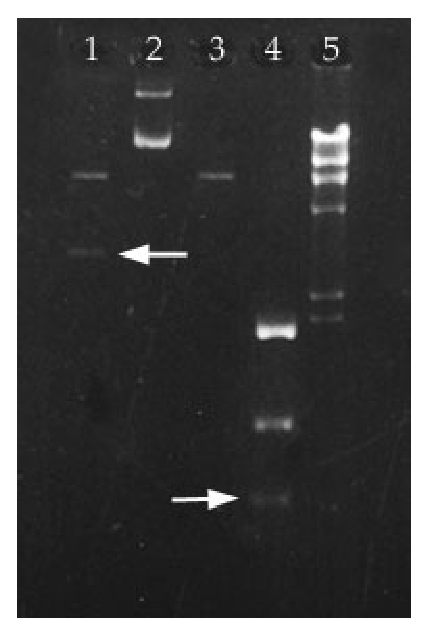
\includegraphics[height=5cm,
    angle=0]{./images/Southern-blotting.eps}}
  \caption{Example of Southern blotting}
\label{fig:Southern-blotting}
\end{figure}


{\bf HOW TO READ}: There are a few lanes, and the figure is show such taht the bigger DNA
fragments, which migrate slower, is showed as staying on top of the figure.
\begin{enumerate}
  \item lanes: 
  \begin{itemize}
    \item Standard Lanes:
    
    
    \item Sample Lanes:
    Each lane has DNA fragments restricted by a given restriction enzyme from
    one DNA sample. All these DNA samples, can be from the same stock of DNA
    digested with 3 different Restriction Enzymes, or maybe from different
    pieces of DNA altogether.
    
     When we are interested in determining the success of a particular digest,
    we often want to calculate the size of these bands, which we need to
    reference to Standard Lanes.
  \end{itemize}
  
  \item as the total DNA amounts are the same in each lane, 
  at one location, the band in one lane can be brighter than that in another
  lane. On a molar level, much more DNA of one size is present in that band than
  in a different band, although the lesser amount may be a larger fragment.
  
  
\end{enumerate}
\url{http://www.life.illinois.edu/molbio/geldigest/photo.html}



 
  There are often 3 lanes: left lanes are for DNA ladder, middle lane for the
  DNA fragments of interest, the right lane is also for DNA ladder.
  In this case, left lane and right lane are Standard Lanes, or sometimes
  Molecular Weight Markers or "Ladders". They are similar to the Control in an
  experiment, because we know exactly how they are going to turn out every time.
  These lanes contain DNA of a specific, predetermined size from a known source,
  digested with a Restriction Enzyme that cuts that piece of DNA a known number
  of times, yielding a predicted number of bands whose size we know exactly.
  
  
  To help identify the molecular weight (M.W.) along the axis, DNA ladder
  are often provided, DNA ladders are those with known molecular weights, and their
  migration along the matrix can be used as a reference to identify the M.W. of
  the DNA fragments of interest on the middle lane.
  PRINCIPLE: molecular weight is inversely proportional to migration rate through a gel
  matrix via alogarithmic relationship.
  \url{https://en.wikipedia.org/wiki/Molecular-weight_size_marker}
  
  One important sample every experiment should include is uncut DNA. Uncut DNA
  exists in as many as three different forms: {\bf supercoiled, relaxed
  circular, and linear}. Just because you didn't add any RE to your sample does
  not mean it hasn't gotten nicked or even cut at some point in its preparation. Nicking
  causes supercoiling to be relaxed, while cutting as you know causes
  linearization. Nothing has been removed from this piece of DNA, so all 3 forms
  are the same size. Does that mean they will migrate the same? Unfortunately
  no. Imagine a rubber band all twisted up into a little knot. That is very much
  like the compact form of supercoiled DNA. The relaxed, unknotted rubber band
  is similar to the circular form, and if you were to cut the rubber band once
  with scissors, it would resemble linear DNA. Which will experience the most
  resistence in an agarose gel? The least? From fastest to slowest is
  supercoiled, circular, then linear, despite the fact that all three fragments
  are of exactly the same length.
  
  

\subsection{Northern blotting (i.e. detect RNA, mRNA)}
\label{sec:Northern-blotting}

Northern blotting was developed by Alwine and his colleagues in 1979.
The name was chosen as a misnomer to 'Southern'.

The differences with Southern blotting are
\begin{itemize}
  \item detect RNA (not DNA), i.e. level of density implies the number of RNA
  molecules.

The intact mRNA molecules purified from mutant and control liver cells are
fractionated on the basis of their sizes into a series of bands by gel
electrophoresis. 

  
  \item use a different filter, i.e. Amino benzyloxymethyl filter
  
  \item RNA-(DNA probe) hybridization, rathern than DNA-(DNA probe)

Then, to make the RNA molecules accessible to DNA probes, a replica of the
pattern of RNA bands on the gel is made by transferring ("blotting") the
fractionated RNA molecules onto a sheet of nitrocellulose or nylon paper. The
paper is then incubated in a solution containing a labeled DNA probe whose
sequence corresponds to part of the template strand that produces albumin
mRNA. The RNA molecules that hybridize to the labeled DNA probe on the paper
(because they are complementary to part of the normal albumin gene sequence)
are then located by detecting the bound probe by autoradiography or by
chemical means.

The size of the RNA molecules in each band that binds the probe can be
determined by reference to bands of RNA molecules of known sizes (RNA standards)
that are electrophoresed side by side with the experimental sample.



\end{itemize}

Newer methods to detect RNA level:  RT-PCR (Sect.\ref{sec:RT-PCR}), gene array
analysis and nuclease protection assays.

\subsection{FISH technique (i.e. detect mRNA)}
\label{sec:FISH}

Detecting intracellular features such as specific mRNA molecules does not
require antibodies and possesses enormous potential because it can exploit the
genomics and microarray data, i.e.  single cell mRNA abundance measurements are
required. 

Count individual mRNAs within single cells using  florescent in-situ
hybridization (FISH) techniques has some limitation:  (1) require optimized cell
fixation protocols that are not universally applicable to all tissues and cell
types; (2)  tens of probes per RNA molecule need to be designed to generate a
detectable signal.

A better technique is RT-PCR - Sect.\ref{sec:RT-PCR}.

\subsection{PCR - polymerase chain reaction}
\label{sec:PCR}

Now that so many genome sequences are available, genes can be cloned directly
without the need to construct DNA libraries first. A technique called the
polymerase chain reaction (PCR) makes this rapid cloning possible 

PCR allows the DNA from a selected region of a genome to be amplified a
billionfold, effectively "purifying" this DNA away from the remainder of the genome.
\begin{itemize}
  \item a region of DNA fragment to be 'amlified' is separated using heat
  
  \item the desired DNA oligonuleotides as primers attach to each side to start
  the {\it in vitro} DNA synthesis (with the help of DNA polymerase)
  
  \item the process in step 2 is then repeated as many time as you want (using
  as many cloned copies present as the sources); eventually billion copies of
  the DNA fragments are generated.
  
  After three more cycles, 240 of the 256 DNA chains correspond exactly to the
  original bracketed sequence, and after several more cycles, essentially all of
  the DNA strands have this unique length. 
\end{itemize}

The PCR method is extremely sensitive; it can detect a single DNA molecule in a
sample. Trace amounts of RNA can be analyzed in the same way by first
transcribing them into DNA with reverse transcriptase - Sect.\ref{sec:RT-PCR}).

The PCR cloning technique has largely replaced Southern blotting
(Sect.\ref{sec:Southern-blotting}).

\subsection{RT-PCR, scRT-PCR (i.e. detect mRNA)}
\label{sec:RT-PCR}
\label{sec:scRT-PCR}

Single-cell {\bf reverse transcription polymerase chain reaction} (RT-PCR or
scRT-PCR) is a novel technique to count mRNA based on PCR (Sect.\ref{sec:PCR}).
It is a much simpler technique for mRNA quantification that has a large dynamic
range and is amenable to high kkthroughput analysis (Raj and Oudennarden 2009,
Dimov et al., 2014).

Single-cell RT-PCR (scRT-PCR) verification is often used in combine with
patch-clamp - Sect.\ref{sec:patch-clamp-whole-cell}.

% reverse transcription-PCR (scRT-PCR) and
% patch-clamp studies (Johns et al., 1997; Dryer et al., 1998; Martina et al.,
% 1998).

\section{-------------------}
\label{sec:techniques-clone-DNA}

Any DNA fragment that contains a gene of interest can be cloned. DNA cloning has
2 meanings
\begin{enumerate}
  \item isolation of a particular stretch of DNA (often a particular gene) from
  the rest of a cell's DNA.

  \item making many identical copies of a DNA molecule - This can be done simply
  by inserting a particular fragment of DNA into the purified DNA genome of a
  self-replicating genetic element-generally a virus or a plasmid.

The techniques to alter isolated gene and transferred back into the
germ line of an animal or plant, so as to become a functional and heritable part
of the organism's genome. 

The principles underlying the methods used for cloning genes are the same for
either type of cloning vector, although the details may differ. Today most
cloning is performed with plasmid vectors.

Plasmid (vector) - circular DNA that can replicate independently of the genome.
Plasmids were used to clone fragments of DNA of 1,000 to 30,000 nucleotide
pairs. 
\begin{enumerate}
  \item PAC
  \item BAC
  
New {\bf plasmid vectors} from bacteria based on the naturally occurring F
plasmid of E. coli can clone fragments of DNA of 100,000-300,000 nucleotide
pairs. F-plasmid and its derivative, the bacterial artificial chromosome (BAC) -
is present in only one or two copies per E. coli cell.

  \item YAC - Sect.\ref{sec:YAC} such as pYAC3, pYAC4 plasmids.
  
  For very larger DNA fragments (up to 2 Mbp), YAC is used.
  
\end{enumerate}
\end{enumerate}

\begin{figure}[htb]
  \centerline{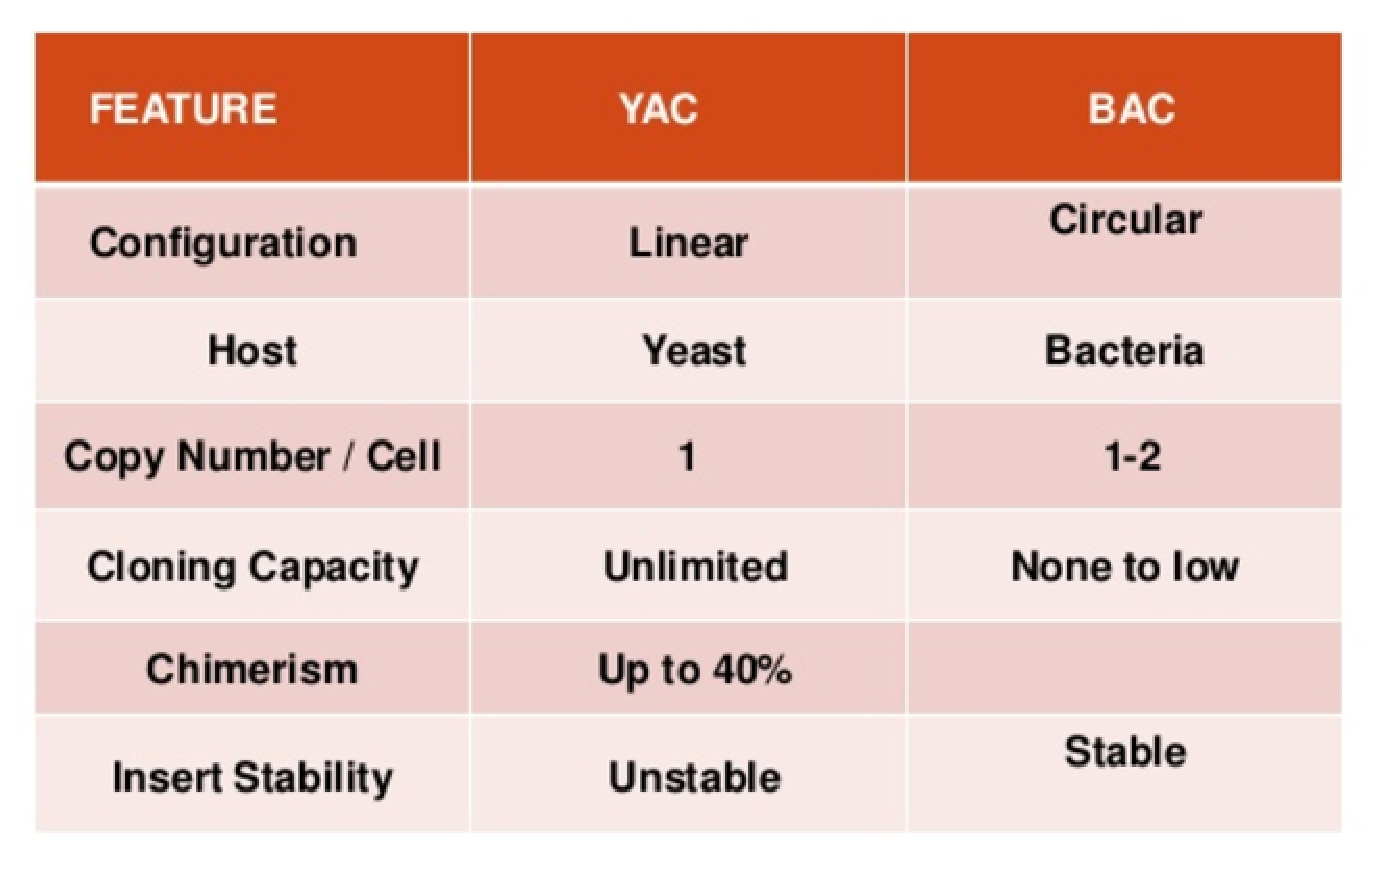
\includegraphics[height=4cm]{./images/YAC-BAC.eps}}
  \caption{Compare YAC and BAC}\label{fig:YAC-BAC}
\end{figure}


\section{P1 artificial chromosomes (PACs)}
\label{sec:PAC}

\section{Bacterial Artificial Chromosome (BAC)}
\label{sec:BAC}
\label{sec:plasmid-vector}

To study human genome, which is too big, to be able to sequence from one end to
the other; they are broken down into manageable chunks. The DNA from white blood
cells are often being used. Fragments of human DNA are then stored in bacteria,
e.g. {\it E. Coli}, from which it can be sequenced and cloned.

A {\bf plasmid} is a genetic structure, i.e. typically in the form of a circular DNA
strand in the cytoplasm of the bacterium or protozan, that can replicate itself
independently of the chromosomes. 

{\bf F plasmid} present in only one or two copies per E. coli cell.
The low number reduces the chance for  the cloned DNA fragments to become
scrambled due to recombination with sequences carried on other copies of the
plasmid. This enhances the stability to clone large DNA fragments.

Bacterial Artificial Chromosome (BAC) refers to the technique to insert a DNA
fragment into a bacterial cell (e.g. E.Coli) using a plasmid called {\bf BAC
vector}. An E.coli genome is about 3 Mbp and you can't put much more than
200-300Kbp without stunting its growth (and favoring the growth of
recombinants). So, a {\bf BAC vector} can hold a DNA fragment of up to 300 kb.

The BAC vector, now with the foreigner DNA fragment, is then transfered to the
bacteria, which then can mobilize from F+ male bacteria to F- female bacteria.
{\bf Conjugation} is the gene that transfers from one bacteria to another.

The structure of a BAC vector
\begin{enumerate}
  \item  a cloning site (which can splitted to accept the DNA fragment): include
  {\it lacZ}
  
  \item F plasmid {\it par genes} (F = fertility)
  
  F factor controls its own replication, with two origins of replication: {\bf
  oriV} (for bidirectional replication) and {\bf oriS} (for unidirectional
  replication). It also has a genes that regulate DNA synthesis to keep its copy
  at a low level; and a gene that regulates the partition into daughter cells
  after {\it E. Coli} divides.
  
  \item ori
  
  \item Cm$^R$
\end{enumerate} 

BACs are preferred over YACs (Sect.\ref{sec:YAC}) because growing yeast and
purifying YACs is much more difficult compared to growing E. coli and purifying
BACs.  Finally, the entire BAC clones can be shotgun-sequenced fairly rapidly
(Sect.\ref{sec:shotgun-sequencing-method}).

\section{Yeast Artificial Chromosome (YAC)}
\label{sec:YAC}


Yeast artificial chromosomes (YACs) are genetically engineered chromosomes (i.e.
synthetic chromosome) derived from the DNA of the yeast, Saccharomyces
cerevisiae, to contains a targeted DNA fragment from another species. 
It has
\begin{enumerate}
  \item centromere
  \item telomere
  \item autonomous replicating sequence (ARS) element - required for
  replication and preservation of YAC in yeast cells
\end{enumerate}

YAC was first described in 1983 by Murray and Szotak.
YAC can behave like naturally existing chromosomes, provided they have proper
size. Different YAC plasmids: pYAC3, pYAC4 plasmids, Fig.\ref{fig:YAC-pYAC3}.

\begin{figure}[htb]
  \centerline{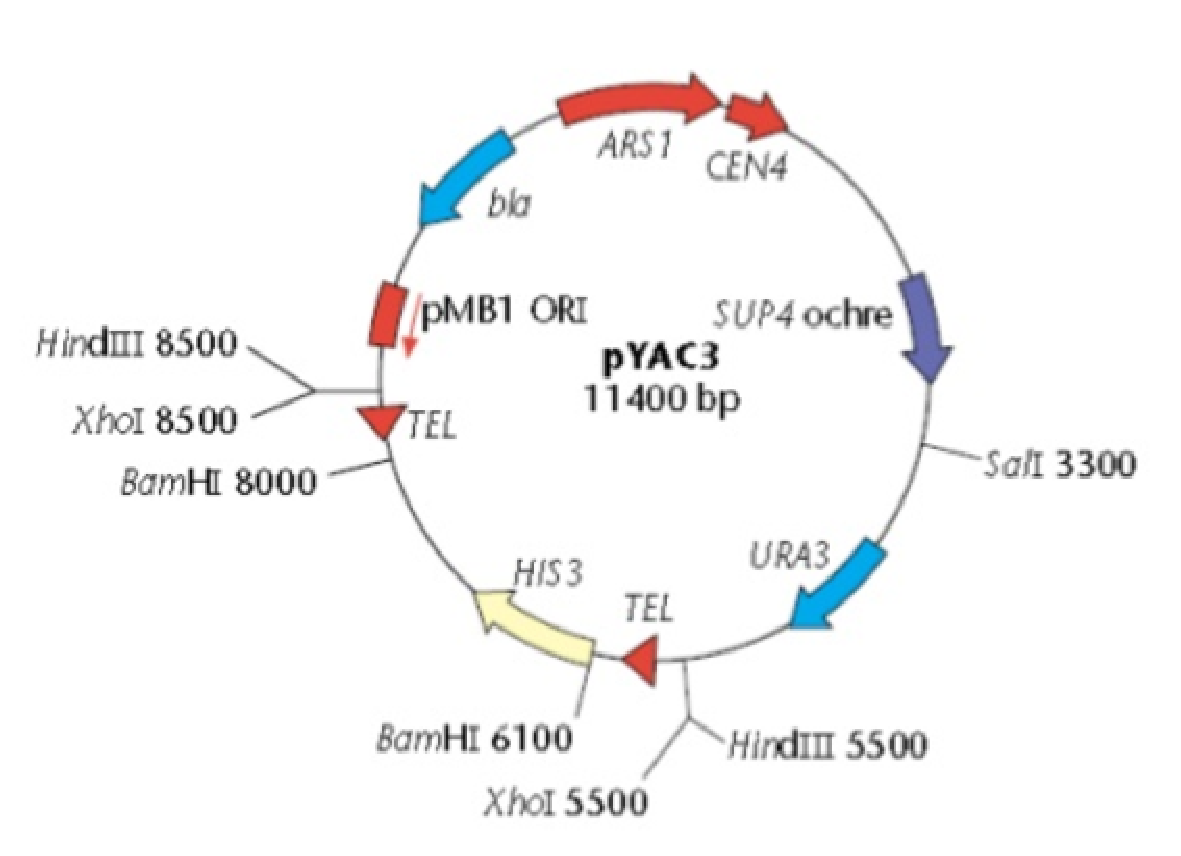
\includegraphics[height=3cm]{./images/YAC-pYAC3.eps}}
  \caption{pYAC3}\label{fig:YAC-pYAC3}
\end{figure}

YAC (to contain a foreigner DNA) is built using an initial circular plasmid,
Fig.\ref{fig:YAC-pYAC3}, and then typically broken into 2 linear molecules using
restriction enzymes; before a DNA ligase is used to ligate a sequence or gene of
interest between 2 linear molecules. YAC can contain more base pairs (up to
2 Mbp) than BAC's F-plasmid vectors (Sect.\ref{sec:BAC}), i.e.
100-1000 kb (i.e. over a million base pairs). However, YACs are significantly
less stable than BACs.s

{\bf Examples of yeast expression vectors}: YACs, YIps (yeast integrating
plasmids), and YEps (yeast episomal plasmids). A YAC is a circular DNA plasmid
where the target DNA fragment can be inserted, before being inserted into the
yeast.


 
 
\section{-------------------}
 
\section{DNA libraries}
\label{sec:DNA-libraries}

A DNA library is a comprehensive collection of cloned DNA fragments from a cell,
tissue, or organism. 

This library includes (one hopes) at least one fragment that contains the gene
of interest. Libraries can be constructed with either a virus or a plasmid
vector (Sect.\ref{sec:techniques-clone-DNA}) and are generally housed in a
population of bacterial cells. 

BACs (Sect.\ref{sec:BAC}) are now the preferred vector for building DNA
libraries of complex organisms - including those representing the human and
mouse genomes.

\subsection{traditional methods}

Sequencing the DNA directly from DNA fragments limit the amount of genes can be
detected. A better method is building cDNA libraries -
Sect.\ref{sec:cDNA-libraries}.
\begin{verbatim}
DNA ---[DNA restriction nuclease]---> DNA fragments (double-strand)
                                    (some with full-genes; many not)
                                    
          DNA fragments ---[inserted into plasmid vectors]---> vector
          
          vector  --[cloning]-->  DNA cloning
\end{verbatim}

IMPORTANT: As the genomic DNA is cut into fragments at random, only some
fragments contain genes. Many of the genomic DNA clones obtained from the DNA of
a higher eucaryotic cell contain only noncoding DNA


\subsection{cDNA libraries}
\label{sec:cDNA-libraries}

An alternative strategy is to begin the cloning process by selecting only those
DNA sequences that are transcribed into mRNA and thus are presumed to correspond
to protein-encoding genes. 

\begin{verbatim}
DNA --[transcription]-> RNA transcripts --> mRNA 
         mRNA --[reverse transcription]---> (complement) DNA single-strand

         cDNA --[DNA polymerase]---> DNA-containing gene double-strand
         
         DNA double-strand --[inserted into plasmid vector]--> vector

         vector  --[cloning]-->  DNA cloning
\end{verbatim}

This is done by extracting the mRNA (or a purified subfraction of the mRNA) from
cells and then making a complementary DNA (cDNA) copy of each mRNA molecule
present; this reaction is catalyzed by the reverse transcriptase enzyme of
retroviruses, which synthesizes a DNA chain on an RNA template. 

The single-stranded DNA molecules synthesized by the reverse transcriptase are
converted into double-stranded DNA molecules by DNA polymerase, and these
molecules are inserted into a plasmid or virus vector and cloned.
Each clone obtained in this way is called a cDNA clone, and the entire
collection of clones derived from one mRNA preparation constitutes a cDNA
library.

ADVANTAGES:
\begin{enumerate}
  \item contain the uninterrupted coding sequence of a gene.  

  \item  some proteins are produced in very large quantities by specialized
  cells. 
  
  In this case, the mRNA encoding the protein is likely to be produced in
  such large quantities that a cDNA library prepared from the cells is highly
  enriched for the cDNA molecules encoding the protein, greatly reducing the
  problem of identifying the desired clone in the library   
  
\end{enumerate}

\section{DNA sequencing}
\label{sec:DNA-sequencing}

In the late 1970s methods were developed that allowed the nucleotide sequence of
any purified DNA fragment (Sect.\ref{sec:DNA-libraries}) to be determined simply
and quickly.

Although the same basic method is still used today, many improvements have been
made. Now it is done completely automated using machines: robotic devices mix
the reagents and then load, run, and read the order of the nucleotide bases from
the gel.

The computer screen display the 'probability' that a given nucleotide (A, T, G,
C) is detected at each location, Fig.\ref{fig:DNA-sequencing}.

\begin{figure}[htb]
  \centerline{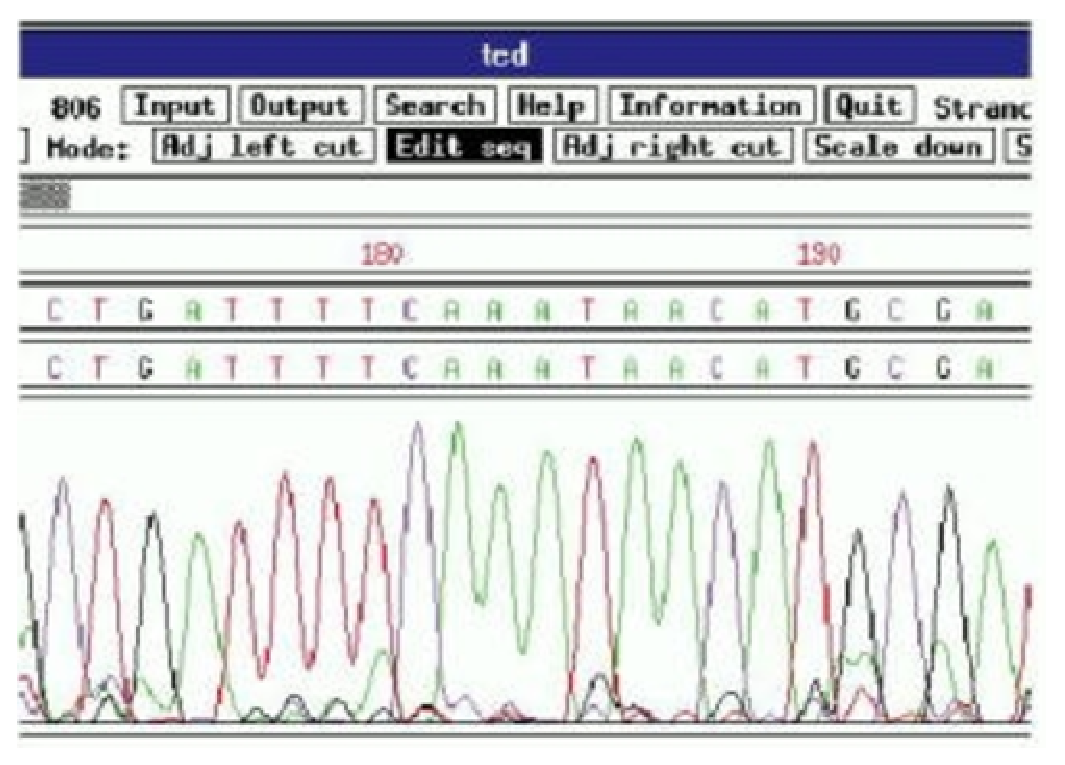
\includegraphics[height=4cm]{./images/DNA-sequencing.eps}}
  \caption{a clear stretch of nucleotide sequence can be read here between positions 173
and 194 from the start of the sequence. Each colored peak represents a
nucleotide in the DNA sequence. The figure is part of the
sequence of the genome of the plant Arabidopsis. (Courtesy of George Murphy.)}
\label{fig:DNA-sequencing}
\end{figure}

\subsection{Shotgun sequencing method}
\label{sec:shotgun-sequencing-method}

Haemophilus influenzae (a bacterium that can cause ear infections or meningitis
in children) was the first organism to have its complete genome sequence - all
1.8 million nucleotides - determined by the shotgun sequencing method, the most
common strategy used today.

In the shotgun method, long sequences of DNA are broken apart randomly into many
shorter fragments. Each fragment is then sequenced and a computer is used to
order these pieces into a whole chromosome or genome, using sequence overlap to
guide the assembly. The shotgun method is the technique of choice for sequencing
small genomes. 

Although larger, more repetitive genome sequences are more tricky to assemble,
the shotgun method has been useful for sequencing the genomes of Drosophila
melanogaster, mouse, and human.


\subsection{Nucleotide Sequences Are Used to Predict the Amino Acid Sequences of Proteins}

Although in principle there are six different reading frames in which a DNA
sequence can be translated into protein (three on each strand), the correct one
is generally recognizable as the only one lacking frequent stop codons
\begin{verbatim}
3 choices of starting point on each strand:
ABCABC
 BCABCA
  CABCAB
\end{verbatim}

If necessary, a limited amount of amino acid sequence can then be determined
from the purified protein to confirm the sequence predicted from the DNA.

The problem comes, however, in determining which nucleotide sequences-within a
whole genome sequence-represent genes that encode proteins. 
\begin{enumerate}
  \item  It is easier if DNA sequence from a bacterial or archeal chromosome,
  which lacks introns, or from a cDNA clone.
  
  The location of genes in these nucleotide sequences can be predicted by
  examining the DNA for certain distinctive features:
  by searching the nucleotide sequence for open reading frames (ORFs) that begin
  with an initiation codon, usually ATG, and end with a termination codon, TAA,
  TAG, or TGA.
  
  To minimize errors, computers used to search for ORFs are often directed to
  count as genes only those sequences that are longer than, say, 100 codons in
  length. 
  
  
  \item   more complex genomes, such as those of eucaryotes, the process is
  complicated by the presence of large introns embedded within the coding
  portion of genes. 
  
  In many multicellular organisms, including humans, the average exon is only
  150 nucleotides long.
  
  To deal with this, a second major approach to identifying the coding regions
  in chromosomes is through the characterization of the nucleotide sequences of
  the detectable mRNAs (in the form of cDNAs). The mRNAs (and the cDNAs produced
  from them) lack introns, regulatory DNA sequences, and the nonessential
  "spacer" DNA that lies between genes. It is therefore useful to sequence large
  numbers of cDNAs to produce a very large collection (called a database) of the
  coding sequences of an organism.
\end{enumerate}

{\bf Predicting}: For nucleotide sequences that are conserved between closely
related organisms usually encode proteins, comparison of these conserved
sequences in different species can also provide insight into the function of a
particular protein or gene.

\subsection{why genome sequencing?}

This is part of the emerging field {\bf genomics}.
The genomes of many organisms have been fully sequenced; these include plant
chloroplasts and animal mitochondria, large numbers of bacteria and archea, and
many of the model organisms that are studied routinely in the laboratory,
including several yeasts, a nematode worm, the fruit fly Drosophila, the model
plant Arabidopsis, the mouse, and, last but not least, humans.   


Researchers have also deduced the complete DNA sequences for a wide variety of
human pathogens. These include the bacteria that cause cholera, tuberculosis,
syphilis, gonorrhea, Lyme disease, and stomach ulcers, as well as hundreds of
viruses-including smallpox virus and Epstein-Barr virus (which causes infectious
mononucleosis).

Examination of the genomes of these pathogens should provide clues about what
makes them virulent, and will also point the way to new and more effective treatments.

Comparison of the complete genome sequences of different organisms allows us to
trace the evolutionary relationships among genes and organisms, and to discover
genes and predict their functions.

Assigning functions to genes often involves comparing their sequences with
related sequences from model organisms that have been well characterized in the
laboratory, such as the bacterium E. coli, the yeasts S. cerevisiae and S.
pombe, the nematode worm C. elegans, and the fruit fly Drosophila.

{\bf LIMITATION}: although comparative analysis of genomes reveals a great deal
of information about the relationships between genes and organisms, it often
does not provide immediate information about how these genes function, or what
roles they have in the physiology of an organism, i.e. in the context of a
living organism.


\section{Antibody}
\label{sec:antibody}



Antobodies actually include several classes of molecules
\begin{enumerate}
  \item {\bf IgG}: (most useful)  a protein molecule that is made and secreted
  and can recognize specific antigens.
  
  \item {\bf IgM}: designed to be expressed on the cell surface
  
  \item {\bf IgA}: designed for secretion in the bodily fluids 
\end{enumerate}

Antibodies are often used to help detecting an antigen (Sect.\ref{sec:antigen}),
using one of the following techniques
\begin{enumerate}
  \item Western blot - Sect.\ref{sec:Western-blot}
  
  \item Immunohistochemistry (IHC) - Sect.\ref{sec:immunohistochemistry}
\end{enumerate}
\url{http://www-users.med.cornell.edu/~jawagne/Antibody_Approaches.html}

As a single antibody only target a specific segment of the antigen, to ensure
the protein is full-length, not a fragment, it is often better to 
utilize several antibodies that spanned the entire length of the HTT protein,
e.g. antibodies for detecting Htt protein (Hughes, Jones, 2011).





\subsection{IgG}
\label{sec:IgG-antibody}

IgG is composed of two subunits including two "heavy" chains and two "light"
chains

\subsection{Immunohistochemistry (IHC)}
\label{sec:immunohistochemistry}

IHC method elucidate tissue-specific and subcellular localization of an antigen
within a sample.  IHC staining is accomplished using antibodies that recognize a
target protein and antibody-antigen complexes that are visualized via
chromogenic, radioactive or fluorescent substrates.

The method is less quantitative than western blot
(Sect.\ref{sec:Western-blot}) or ELISA (Sect.\ref{sec:ELISA}), yet they offer
the advantage of characterizing protein expression in the context of intact
tissue.

\subsection{Enzyme-linked immunosorbent assay (ELISA)}
\label{sec:ELISA}


\url{http://www.abcam.com/protocols/antibody-methods-and-techniques}

\subsection{Immunocytochemistry (ICC)}
\label{sec:ICC}
\label{sec:immunocytochemistry}

ICC is used to study the subcellular distribution of proteins using
fluorescently-labeled antibodies.

In contrast with IHC, this technique affords {\it greater spatial resolution} as
cultured cells lack the complex surrounding environment found in tissue samples.

\subsection{Flow cytometry}
\label{sec:Flow-cytometry}
\label{sec:flow-cytometry}

{\bf Flow cytometry} has been primarily used to address single-cell behavior. 
Flow cytometry is a means of measuring certain chemical and physical properties
of cells. Parameters measure include {\bf cell-size} and the expression of
cell-surface and intracellular markers. 

Flow cytometry measures the fluorescence emitted by labeled antibodies, bound to
individual cells in a mixed population.

While flow cytometry is effective, it is limited by the availability of
antibodies. Only a minority of known human genes have commercially available
antibodies. {\it Flow cytometry is also difficult to perform when the
distinguishing features of subpopulations are molecules inside the cells rather
than on the surface of cells.}

Recently, a tool employing mass spectrometry has been developed to leverage the
precision of flow cytometry analysis. The combination of the two techniques,
termed single-cell mass cytometry (CyTOF), allows the simultaneous measurement
of more than 40 cellular parameters at single-cell resolution with over 100
available detection channels (Janes et al., 2011; Spitzer et al, 2016).
% Janes, M. R. & Rommel, C. Next-generation flow cytometry. Nat. Biotechnol. 29,
% 602-604 (2011).
% Spitzer, M. H. & Nolan, G. P. Mass cytometry: single cells, many features. Cell
% 165, 780-791 (2016).  

Compared to fluorescence-based cytometry, mass cytometry employs element-tagged
probes that enable the discrimination of elements according to their mass/charge
ratio (m/z), with minimal overlap and background cellular signal. All these
attributes simplify the large panel experimental design, thus uniquely enabling
high-dimensional cytometry experiments that would not be possible otherwise



\subsection{Fluorescence-activated cell sorting (FACS)}
\label{sec:FACS}

Fluorescence-activated cell sorting (FACS) is a more sophisticated system,
which quantifies the fluorescent signal and separates the cells from a mixed
population that contains preselected characteristics (i.e. fluorescence
intensity, size and viability).  

\subsection{Immunoprecipitation (IP)}
\label{sec:Immunoprecipitation}

Immunoprecipitation is a versatile technique that enables isolation and
purification of individual and complexed proteins.
Antibodies are immobilized on solid-phase substrates (e.g. magnetic/agarose
beads), which capture antigens from complex solutions.

\subsection{Chromatin immunoprecipitation (ChIP)}
\label{sec:ChIP}

Chromatin immunoprecipitation (ChIP) is a procedure used to determine whether a
given protein binds to a specific DNA sequence in vivo.


\subsection{ELISPOT}
\label{sec:ELISPOT}

ELISPOT is used for the detection of secreted proteins, such as cytokines and
growth factors. The technique enables quantification and comparison of immune
responses to various stimuli. 



\subsection{Western blot}
\label{sec:Western-blot}

It is also possible to use an antibody to detect a protein after fractionation
by SDS-PAGE, using the method called {\bf Western blotting}.

The name is chosen as the method is for fragment detection, which is analogous
with northern blotting (Sect.\ref{sec:Northern-blotting}) and Southern blotting
(Sect.\ref{sec:Southern-blotting})


\subsection{Antigen (epitope), anti-idioptype antibody}
\label{sec:antigen}
\label{sec:epitope}

An {\bf antigen} is a  protein that can be recognized (bound) by the antibody
(Sect.\ref{sec:antibody}). These antigens are most commonly polypeptides or
carbohydrates, but they can also be lipids, nucleic acids, or even small
molecules like neurotransmitters. 

A particular antibody molecule can only interact with a small region of an
antigen (called {\bf epitope}) and in the case of a polypeptide this is
generally about 5-12 amino acids. This region can be continuous or it can be
distributed in different regions of a primary structure that are brought
together because of the secondary or tertiary structure of the antigen.

{\it It is possible, although unlikely, that the same, or closely related
epitopes, could be shared by the different antigens.}

In some cases, it is possible to make an antibody that is directed {\bf against}
the antigen binding site of another antibody. This type of antibody is called an
{\bf anti-idiotype antibody}.

\section{ membrane-selective FM-dyes}
\label{sec:FM-dyes-membrane-selective}

The membrane-selective FM-dyes, FM4-64 and FM1-43, belong to a class of
amphiphilic styryl dyes developed by Betz and co-worker (Betz et al., 1992,
1996) which are both membrane-selective fluorescent dyes. The abbreviation 'FM'
stands for the chemist's name, Fei Mao, who developed the FM-dyes from the
related probe, dimethylaminostyrylmethylpyridiniumiodine (DASPMI).
 
FM-dyes fluoresce significantly only when they are in a hydrophobic
environment, e.g. a lipid-rich membrane.

FM4-64 and FM1-43 differ slightly in their chemical structure, and these
structural differences can result in different patterns of membrane staining
(Fischer-Parton et al., 2000; Hickey et al., 2002).  


\subsection{FM4-64 dye}
\label{sec:FM4-64-dye}

Styryl dye FM 4-64 has been reported to selectively stain yeast vacuolar
membranes with red fluorescence (excitation/emission maxima ~515/640 nm). 
FM4-64 is usually preferred to FM1-43 due to its superior brightness, greater
contrast, higher photostability, and its red-shifted emission facilitating
concomitant use with the green fluorescent protein (GFP) (Bolte et al., 2004).

This lipophilic dye is an important tool for visualizing vacuolar organelle
morphology and dynamics, for studying the endocytic pathway and for screening
and characterizing yeast endocytosis mutants. 

\chapter{Software and Database of organic compounds (e.g. proteins)}



\section{Organic compound databases}
\label{sec:databases}


\begin{itemize}
\item	{\bf CAS database} is the most comprehensive repository for data
  on organic compounds. The search tool SciFinder is offered.

\item {\bf Beilstein database} contains information on 9.8 million
  substances, covers the scientific literature from 1771 to the
  present, and is today accessible via CrossFire. 
  
  Structures and a large diversity of physical and chemical properties is
  available for each substance, with reference to original literature.

\item {\bf PubChem database} contains 18.4 million entries on compounds and
especially covers the field of medicinal chemistry.
\end{itemize}


\section{Software tools}
\label{sec:tools}

As the 3D structure of a biomolecule define its function, it is important to
understand/predict the 3D structure. We discuss software tools for visualizing
the 3D structure of biomolecules (Sect.\ref{sec:living-organisms}).

\subsection{MDLChime}
\label{sec:MDLChime}

It is recommended to use Jmol (Sect.\ref{sec:Jmol}) instead.

If you still want to use MDLChime, check the link \url{http://www2.mdl.com/}.
MDLChime provide capability to
\begin{itemize}

   \item view and manipulate PDB file (the file that contains information which
can be used to generate 3D structure of proteins) and other molecular models
via the web browser (i.e. directly from a WWW page)

   \item How to install MDLChime manually to run with
Firefox\footnote{\url{http://www.umass.edu/microbio/chime/pe_beta/pe/protexpl/chiminst.htm}}:

   \item Sample image to
test\footnote{\url{http://www.umass.edu/microbio/chime/atp.pdb }}
\end{itemize}

\subsection{Jmol}
\label{sec:Jmol}

Jmol is better than MDLChime (Sect.\ref{sec:MDLChime}), as it is a desktop-based
program, and has more features, e.g. RasMol scripting language
(Sect.\ref{sec:Rasmol}).

URL: \url{http://jmol.sourceforge.net/} (a replacement for MDLChime)

\subsection{Protein Explorer (PE) - Windows only)}
\label{sec:Protein-Explorer}


Protein Explorer: (best for beginners, work only in Windows, requires MDLChime browser plugin) 
\begin{itemize}
  
\item view three-dimensional structures of protein, DNA, and RNA
  macromolecules, and their interactions and binding of ligands,
  inhibitors, and drugs

\item \url{ http://www.umass.edu/microbio/chime/pe_beta/pe/protexpl/frntdoor.htm}

\item Offline tool:
\url{http://www.umass.edu/microbio/chime/regisfrm/downlpew.htm}

\end{itemize}

\subsection{MolSlide Manager}
\label{sec:MolSlide-Manager}

{\bf MolSlide Manager}: an utility that helps you create 3D molecular structure
and view it without using Protein Explorer (PE) or MDLChime, and the image can
be included in your report or tutorial
presentation\footnote{\url{http://www.umass.edu/microbio/chime/pe_beta/pe/protexpl/molview/
}}.

\subsection{Rasmol}
\label{sec:Rasmol}

Rasmol is no longer under development (last is 2009). Jmol
(Sect.\ref{sec:Jmol}) and Sirius has incorporated the RasMol scripting language
into its commands.

\url{http://alternativeto.net/software/rasmol/}



\subsection{PyMOL}
\label{sec:PyMol}

PyMOL can produce high-quality 3D images of small molecules and biological
macromolecules, such as proteins. PyMOL is one of a few open-source
visualization tools available for use in structural biology.

PyMOL uses OpenGL Extension Wrangler Library (GLEW) and Freeglut, and can solve
Poisson-Boltzmann equations using the Adaptive Poisson
Boltzmann Solver.


\begin{verbatim}
Amoeba = amip
Rotifers = a microscopic organism
Rumen = (dvat.hoc) da. co? (cu?a tra\^u,bo')
erythrocyte = red blood cell
leukocyte = white blood cell
platelet = thrombocyte = a small blood cell needed for normal blood clotting 
cerebellum = brain,
epithelial = (bie\^?u mo\^) belonging to or formed by epithelium
epithelium = a layer of cells which form or covering over the internal and external surfaces of the body

\end{verbatim}


\chapter{Biology of cell}
\label{chap:cell-life}

A cell is a unit of life (Sect.\ref{sec:incredibility-life}).

\section{Cell types and cell's organelles}
\label{sec:cell-types}
\label{sec:cell-organelles}

A cell type is a classification used to distinguish between morphologically or
phenotypically distinct cell forms within a species. Cells might look different
under a microscope, most cells have chemical and structural features in common.
In each cell, there are about {\bf 20 different types of organelles and
structures}.

Your body has many different kinds of cells. In humans, there are about {\bf 200
different types of cells} (a number which seems low given the amount of
diversity and specialization in our body).

From a single zygote, the human body grows into {\bf 37 trillion cells}. Each
cell type is derived from one of the three regions in early stage of embryonic
development (Sect.\ref{sec:brain_development}): endoderm, mesoderm and ectoderm
(Sect.\ref{sec:endoderm}).

Each cell is a complex living system, with 
\begin{itemize}
  \item a machine to produce products, i.e. different proteins
  \item the proteins are made based on the given footprint, i.e. the genetic
  information encoded in the DNA sequences which is wrapped in the molecules
  called chromosomes (Sect.\ref{sec:chromosome}), which locates
  inside the nucleus.

Even though all cells have the same genetic information, i.e. the same exact
copy of the set of chromosomes (e.g. in human is 23 set of chromosomes),
different cell types express different subset of genes at different expression
levels for each gene.

\end{itemize}


The mRNA (Sect.\ref{sec:mRNA}) present in each cell gives a snapshot of the
genes that are expressed and important to that cell. Different types need to
express different genes and so accumulate different mRNAs. It's far easier to
measure a cell's mRNA than, say, its protein levels, because we are very skilled
at analyzing at amino-acid sequences.
\footnote{\url{http://www.nature.com/scitable/blog/bio2.0/discovering_new_cell_types_one}}


Link:
\url{https://en.wikipedia.org/wiki/List_of_distinct_cell_types_in_the_adult_human_body}


\section{Cell culture}
\label{sec:cell-culture}

Cell culture is the process by which cells are grown under controlled
conditions, generally outside of their natural environment.

\section{Cell line}
\label{sec:cell-line}

A cell line refers to a population of cell culture (Sect.\ref{sec:cell-culture}) developed from a single cell and
therefore consisting of cells with a uniform genetic makeup.
\begin{enumerate}
  \item first: separate single cell

Cells can be isolated from tissues for ex vivo culture in several ways.
  
  \item second: grow the cell: only the white cells are capable of growth in
  culture.
  
Cells are grown and maintained at an appropriate temperature and gas mixture
(typically, 37$^\circ$C, 5\% CO2 for mammalian cells) in a cell incubator.
Aside from temperature and gas mixture, the most commonly varied factor in
culture systems is the cell growth medium. Recipes for growth media can vary in
pH, glucose concentration, growth factors, and the presence of other nutrients.

\end{enumerate}
\url{https://en.wikipedia.org/wiki/Cell_culture}

\subsection{Immortalized cell line}

A typicall cell would normally not proliferate indefinitely (the division stops
after a number of cell divisions) but for some cell (such as HeLa cell -
Sect.\ref{sec:HeLa-cell-line}), due to mutation, have evaded normal cellular
senescence and instead can keep undergoing division. Such cell line is called
{\bf immortalized cell line}.
An immortalised cell line should not be confused with stem cells, which can also
divide indefinitely, but form a normal part of the development of a
multicellular organism.

Researchers have identified numerous ways to transform primary tissues from
humans and animals into immortalized cell lines.
There are various immortal cell lines. 
\begin{itemize}
  \item Some of them are normal cell lines - e.g. derived from stem cells. 

   \item Other immortalised cell lines are the in vitro equivalent of cancerous
   cells.

Cancer occurs when a somatic cell which normally cannot divide undergoes
mutations which cause de-regulation of the normal cell cycle controls leading to
uncontrolled proliferation. Immortalised cell lines have undergone similar
mutations allowing a cell type which would normally not be able to divide to be
proliferated in vitro.

\end{itemize}

Embryonic and induced pluripotent stem cells
(Sect.\ref{sec:induced-pluripotenti-stem-cell-line}) may get more media
attention, but ordinary somatic cell lines still form the backbone of biomedical
research.


 
\subsection{-- HeLa cell line}
\label{sec:HeLa-cell-line}
\label{sec:cell-line-HeLa}

On February 8, 1951, George Gey of Johns Hopkins University isolated some cells
from a cervical cancer biopsy (from the patient named Henrietta Lacks) and
placed them into a petri dish with some medium.

Lacks died of her cancer eight months later, but her cells, dubbed {\bf HeLa},
became the first immortalized cell line, capable of renewing itself in
artificial culture indefinitely.
In the decades since their isolation, scientists have grown an estimated 20
tons of them.
\footnote{\url{http://www.nature.com/news/most-popular-human-cell-in-science-gets-sequenced-1.12609}}

The genome of HeLa cell was sequence in 2013; however its genome is a bizarre,
error-filled genome, with one or more (with up to five copies of some) extra
copies of many chromosomes. Many genes were duplicated even more extensively,
with four, five or six copies sometimes present, instead of the usual two. 
Furthermore, large segments of chromosome 11 and several other chromosomes were
reshuffled like a deck of cards, drastically altering the arrangement of the
genes.  Around 2000 genes are expressed at levels higher than those of normal
human tissues because of the duplications.

Having been replicating in labs around the world for six decades, HeLa cells
have also accrued errors not present in the original tumour DNA.  It means it is
difficult to trace the origin of these alterations.

HeLa cells could prove useful for studying aspects of the biology of cervical
tumours, such as their response to cancer drugs.
In recent years, the genomes of many cervical tumours have been sequenced, and
so it should be possible to see how these compare with the HeLa genome.

\subsection{-- Induced pluripotent stem cell line}
\label{sec:induced-pluripotenti-stem-cell-line}
\label{sec:cell-line-induced-pluripotenti-stem}

Alternative cell lines, such as induced pluripotent stem cells generated from
patient skin cells, offer a more accurate window on human biology than HeLa
cell line.



\subsection{Cell line cross-contamination}
 
About 15-20\% of the time, cells used in experiments have been misidentified or
contaminated with another cell line. Cell line cross-contamination can be a
problem for scientists working with cultured cells.

\url{https://www.sciencemag.org/custom-publishing/technology-features/art-culture-developing-cell-lines}


\section{Transcriptional regulation}
\label{sec:transcriptional-regulation}

The first step in the translation of genomic sequence  into  physiology  or 
pathophysiology  is  transcription.

Transcriptional  regulation  has  been  studied  almost  exclusively on  nucleic
acids  extracted  from  cultured cells or tissues by
\begin{itemize}
  \item Northern blot - Sect.\ref{sec:Northern-blotting}
  
  \item differential  display
  
  \item serial  analysis  of  gene expression  (SAGE) 
  
  \item  forms  of  microarray

\end{itemize}


\subsection{Transcription factors}
\label{sec:transcription-factor}

Transcription   factors   (TF's ) are proteins that regulate gene expression.
Transcriptional regulation in eukaryotes occurs within a {\bf chromatin}
setting, and is strongly influenced by the posttranslational modification of
histones, the building blocks of chromatin, such as methylation, phosphorylation
and acetylation.

An established paradigm that TFs specifically   recognize   only   relatively
short   (4-20 bp) consensus DNA motifs in that  the consensus TATA box motif
provides the specificity. However, this has been recently challenged by
different  high-throughput methods both in  vivo and in vitro.
\begin{enumerate}

  \item  Human pre-initiation complex (PIC): there is no specificity-determining
    consensus motifs for the positioning of PIC have been identified


  
  \item 
\end{enumerate}

\subsection{Gene transcription}
\label{sec:gene-transription-process}

All cells have the same genes, but not all genes are expressed in every cell at
all times. Factors regulating the timing, rate, and location of gene expression
are encoded in DNA as well, and contribute to biologic variation.

For the  information encoded in a gene to be expressed, it goes through a
multi-step
 process:
\begin{enumerate}
  \item inside the nucleus: a specialized protein attach to the DNA strand and
  make a copy of the DNA sequence in the form of a molecule called {\bf mRNA}
  
  \item mRNA is transferred to outside the nucleus
  
  \item translation step: a cellular mechinery reads the genetic instructions in
  the mRNA and synthesizes proteins.
\end{enumerate}

\textcolor{red}{\bf IMPORTANT}: mRNA does not correspond exactly to the DNA from
which it was transcribed. After transcription in the nucleus, the sequence is
processed to remove and shuffle segments. This increases the number of proteins
that can be produced from a single gene.
{\it There are only 20,000 - 25,000 genes, but more than 200,000 different types
of proteins in the human body}.

\section{Cell type (phenotype) detection techniques}

Cellular diversity of the brain is largely attributed to the spatial and
temporal heterogeneity of progenitor cells (Sect.\ref{sec:progenitor-cell}).
 
Distinguishing cell phenotype while recording 
\begin{enumerate}
  \item axonal tracing (Kawaguchi et al., 1990): has been technically difficult
  and labor intensive
  
  \item single-cell gene profiling (Surmeier et al., 1996) such as flow
  cytometry (Sect.\ref{sec:Flow-cytometry}) which is limited by the number of
  available antibodies


  \item Detecting intracellular features such as specific mRNA molecules does not
require antibodies and  possesses enormous potential because it can exploit the
genomics and microarray data, i.e.  single cell mRNA abundance measurements are
required 
  
  count individual mRNAs within single cells using
  \begin{itemize}
    \item  florescent in-situ hybridization (FISH) techniques 
    
Limitation:   (1) require optimized cell fixation protocols that are not
universally applicable to all tissues and cell types; (2)  tens of probes per
RNA molecule need to be designed to generate a detectable signal
    
    \item reverse transcription polymerase chain reaction, RT-PCR: a
    much simpler technique for mRNA quantification that has a large dynamic
    range and is amenable to high throughput analysis 
  \end{itemize}  
\end{enumerate} 
 
\section{eGFP (enhanced green fluorescent protein) reporter genes}
\label{sec:EGFP}

Transgenic mice that express enhanced green fluorescent protein (EGFP) reporter
genes in a variety of cells have been generated (Gong et al., 2003).
This can be used to map gene expression at cellular resolution.
\begin{itemize}
  \item  green fluorescent protein (GFP) is expressed under control of D1
  receptor or D2 receptor promoter regions (Gong et al., 2003; Day et al.,
  2006).

  \item D1 and D2 EGFP-positive MSNs (Day et al., 2006;  Kreitzer and
  Malenka, 2007; Cepeda et al., 2008)

\end{itemize}


Visualization of EGFP expression in specific neuronal or glial cell populations
has also provided compelling evidence that this strategy can result in the
identification of expressing cell types, as the detailed morphology of
EGFP-expressing cells is aparent.

The endogenous messenger RNA and protein coding sequences have been replaced by
sequences encoding the EGFP reporter gene. {\bf IMPORTANT: As in any
genereplacement experiment, the stabilities of the reporter gene mRNA and
protein can be different from those of the endogenous gene products.} So, they
are not a direct measure of mRNA accumulation or protein abundance for the
endogenous gene products.


\subsection{Single-cell gene expression profiling}
\label{sec:single-cell-gene-expression-profiling}

A key goal of biology is to relate the expression of specific genes to a
particular cellular phenotype.  {\bf Single-cell profiling}, i.e.
high-throughput analysis of individual cells using technique such as flow
cytometry.

Gene expression profiling is key to single-cell analysis
applications. Single-cell analysis helps
\begin{enumerate}
  \item Unlock the mystery in gene expression profiles between individual cells
  \item Avoid the mistake of taking averages of entire cell populations
  \item Discover previously undetected subpopulations and unveil new regulatory
  path
\end{enumerate}

The  use  of  transcription  sites  for  expression 
profiling  allows analysis of coordinated transcription events and  organization  of  gene expression.

{\bf Single-cell gene expression profiling} is a  complementary approach that
monitors mRNA synthesis  by  visualizing  specific  sites  of transcription.

To achieve  sensitive  and  specific  detection  of RNAs by fluorescence in situ
hybridization (FISH), we used oligomer DNA probes that were each tagged with a
single fluorophore at  multiple  sites.

To  detect  many  mRNAs simultaneously, we used combinations of these probes
labeled with spectrally distinct colors (Levsky et al., 2002 - Science).
Colocalization of multiple colors in the image represented independent 
hybridization  events  that  signified  the  presence  of  a  transcription 
site.


\section{Techniques to reconstruct morphologies}
\label{sec:morphology-reconstruct}

MSN are filled with 0.2\% biocytin, and anatomically reconstructed generating
serial optical sections (Z-stacks) acquired on a laser scanning confocal
microscope (Zeiss LSM 510; Jena, Germany) at 1 $\mum$ intervals. No correction
was applied for tissue shrinkage during fixation (Gertler et al. Surmeier, 2008).




\import*{../BioPhysics_Thermo_Stat/}{Amino-Acids}
\def\Bmax{{B\text{$_\max$}}}

\chapter{Enzymes and Substrates}
\label{chap:enzymes}

\def\vmax{{\text{v}_\max}}
\def\Km{{\text{K}_m}}
\def\muM{{\mu\text{M}}}

\section{Enzyme: -ase prefix} 
\label{sec:enzyme}
% \subsection{enzyme}
% \label{sec:enzyme}
Enzymes are specific proteins that function as catalysts -  usually one
enzyme, one reaction. It allows the reaction to occur under normal conditions
(body temperature).

An enzyme is a protein that facilitate a chemical reaction to occur by
lowering the energy barrier (Sect.\ref{sec:energy-barrier}).
There are different mechanisms for an enzyme to perform the function
- Sect.\ref{sec:enzyme-mechanism}. Regardless of the mechanism, the chemical
reactions can be described using the so-called enzyme kinetics -
Chap.\ref{chap:enzyme-kinetics}.


The name of an enzyme is suffixed with {\bf -ase}.

\begin{framed}
  Enzymes is important to cellular activities
\end{framed}

Most of the biochemical pathways in living things are enhanced by some enzyme
(Sect.\ref{sec:enzyme}) that targets a particular substrate
(Sect.\ref{sec:substrate}). The efficiency of the enzyme-catalyzed reactions is
often increased by the presence of helper molecules called {\bf coenzymes}
(Sect.\ref{sec:co-enzyme}).


\subsection{active sites (of enzymes)}
\label{sec:active-site}

The {\bf active site} is the part of an enzyme to which substrates
(Sect.\ref{sec:substrate}) bind and where a reaction is catalyzed. 
\begin{itemize}
  \item 1 active site: a single substrate is broken down into 2 products
  
  \item 2 active sites: two substrates come together to create one larger
  molecule.
  
  \item 2 active sites: two substrates both become modified, and leave the
  reaction as two products.
\end{itemize}

Since enzymes are proteins, the active site is composed of a unique combination
of amino acid residues (side chains or -R groups).
Each amino acid residue can be large or small; weakly acidic or basic;
hydrophilic or hydrophobic; and positively-charged, negatively-charged, or
neutral. The positions, sequences, structures, and properties of these residues
create a very specific chemical environment within the active site. A specific
chemical substrate matches this site like a jigsaw puzzle piece and makes the
enzyme specific to its substrate.

\subsection{substrate and enzyme-substrate complex}
\label{sec:substrate}

A reactant in a chemical reaction is called a {\bf substrate} when acted upon by
an enzyme.  There may be one or more substrates for each type of enzyme,
depending on the particular chemical reaction, and thus there may be one or more
active sites (Sect.\ref{sec:active-site}) on a single enzyme.


When an enzyme binds its substrate (Sect.\ref{sec:enzyme-binding-mechanism}), it
forms an enzyme-substrate complex.


\subsection{environmental factors: pH, temperature}

Environmental conditions can affect an enzyme's active site and, therefore, the
rate at which a chemical reaction can proceed. 

Environmental factors:
\begin{enumerate}
  \item {\bf temperature}: typically, increase temperature increases reaction
  rate
  
However, increasing or decreasing the temperature outside of an optimal range
can affect chemical bonds within the enzyme and change its shape. If the enzyme
changes shape, the active site may no longer bind to the appropriate substrate
and the rate of reaction will decrease. 

  \item {\bf pH}: 
  
Dramatic changes to the temperature and
pH will eventually cause enzymes to denature.

  
\end{enumerate}

\subsection{mode of action of enzymes}
\label{sec:enzyme-binding-mechanism}

There are two hypothesises:
\begin{enumerate}
  \item lock and key - Sect.\ref{sec:lock-and-key}
  
  \item induced fit - Sect.\ref{sec:induced-fit}
\end{enumerate}

\subsection{-- lock and key (1894)}
\label{sec:lock-and-key}

Emil Fisher proposed this hypothesis in 1894. 
\begin{itemize}
  \item  active site of the enzyme is like a 'lock' into which substrate fits
  like a 'key', which requires perfect fit.
  
  \item there is no conformational change in the enzyme
  
\end{itemize}

\subsection{-- induced fit (1959)}
\label{sec:induced-fit}

Daniel E.Koshland formulated this hypothesis in 1959. According to this
hypothesis the active site does not have a rigid 'lock and key' conformation.
The binding of the substrate molecule to the enzyme molecule induces to modify
the shape of the active site so that it becomes complementary to the substrate
molecule. This is called the induced fit . Induced fit is possible because of
the flexibility of the protein molecules.


\subsection{Protein phosphorylation}
\label{sec:phosphorylation}

Protein phosphorylation is one of decisive post-translational modification steps
for modulating protein expression and function.  Synaptic receptors including
ion channels and GPCRs are known to be modulated by phosphorylation.

\begin{mdframed}
Phosphorylation (and dephosphorylation) is among the most common modes of
posttranslational modification in proteins, and it is estimated that, at any
given time, up to 30\% of all proteins are phosphorylated.
\end{mdframed}


Ionotropic glutamate receptors are certainly the targets for phosphorylation by
various protein kinases (Lee et al., 2006 ; Liu et al., 2006 ; Wang et al.
2006).

In addition to constitutive phosphorylation, stimulated phosphorylation can
also occur, e.g.  activation of mGluR1a with a selective agonist induced a rapid
and transient increase in the phosphorylation level
(Sect.\ref{sec:mGluR_group-1-phosphorylation}).




\section{Enzyme classification and EC convention}
\label{sec:enzyme-mechanism}
\label{sec:EC_convention}
\label{sec:enzyme-classification}

As the enzymes perform their functions via different mechanisms, the enzymes are
classified based on these different mechanisms. They are numbered based on the
so-called {\bf Enzyme Commission} Number (EC), which divided into different
levels.

Level 1
\begin{itemize}
  \item EC 1 = Oxidoreductases (transfer H or O atom or electrons from one
  substance to another) - Sect.\ref{sec:EC_1}
  
  \item EC 2 = Transferases (transfer 1 functional group from one substance to
  another) - Sect.\ref{sec:EC_2}
  
  
  \item EC 3 = Hydrolases (create two new products from 1 substance
  by hydrolysis (using $\ce{H2O}$)) - Sect.\ref{sec:EC_3}
  

EC 3 = (hydrolase) enzyme that use water to break up some
    other molecule
  
  \item EC 4 = Lyases (cleave C-C, C-N, C-O or C-S bond) - Sect.\ref{sec:EC_4}
  
A lyase  catalyzes the breaking of various chemical bond; by means other than
hydrolysis (which is the one used by EC 3).


  
  \item EC 5 = Isomerases  (rearrange order within a molecule)
  
  \item EC 6 = Ligases (join together two substance into 1 product).
  This process need energy ATP (i.e. release ADP)
  
\end{itemize}
\url{http://en.wikipedia.org/wiki/Enzyme_Commission_number#Format_of_number}

Level 2, level 3 and level 4: take an example from EC 3 with level 2 is 3.1 
\begin{enumerate}
  \item EC 3.1 = hydrolase that act on ester bonds
  \item EC 3.1.1 = carboxylic-ester hydrolases
  \item EC 3.1.3 =  hydrolase that act on mono-ester bond
  \item EC 3.1.4= hydrolase that act on diester bond
  \item EC 3.1.4.1 = phosphodiesterase I
  \item EC 3.1.4.2 = glycerophosphocholine
  \item EC 3.1.4.3 = phospholipase C - Sect.\ref{sec:PLC}
  \item EC 3.1.4.4 = phospholipase D - Sect.\ref{sec:PLD}
\end{enumerate}

\subsection{EC 1 (OXIDOREDUCTASES)}
\label{sec:EC_1}

An EC1 enzyme catalyzes redox reaction (Sect.\ref{sec:redox-reaction}), i.e. an
oxidation step and reduction step, i.e. transfer electrons from one molecule to
another
\begin{verbatim}
AH  +  B         <------EC1 enzyme----->  A   +    B-H

A(reduced)  + O  <------EC1 enzyme----->  AO
\end{verbatim}
with $H$=hydrogen, $O$=oxygen atom.

OXIDOREDUCTASES (Sect.\ref{sec:oxidoreductase}): they are enzymes that catalyze
{\bf oxidation-reduction reactions} - Sect.\ref{sec:redox-reaction}.

They are further classified depending upon the target group functioning as
electron donors
\begin{itemize}
  \item EC 1.1. = act on CH-OH group
  
  \item EC 1.2 = act on aldehyde or oxo group
  
  \item EC 1.3. act on CH-CH group
  
  \item EC 1.4 = act on CH-NH2 group
  
  \item \ldots
\end{itemize}
\url{https://en.wikipedia.org/wiki/Oxidoreductase}

\url{http://www4.uwsp.edu/chemistry/tzamis/365f00pdfs/enzymeclasses02.pdf}

\subsection{EC 2}
\label{sec:EC_2}


An EC2 enzymes transfer of a functional group (e.g. phosphate group) from one
substance (e.g. ATP molecule) to another (e.g. a protein).
\begin{verbatim}
A-R  + molecule <----EC2 enzyme--->   A + molecule-R
\end{verbatim}
with $R$=some functional group.

\subsection{EC 3}
\label{sec:EC_3}

An EC3 enzyme uses water to split a substrate into 2 products:
\begin{verbatim}
AB + H2O  <------EC3 enzyme----->  A-OH + B-H
\end{verbatim}

EC 3 enzymes \url{http://www.enzyme-database.org/downloads/ec3.pdf}

\begin{itemize}
  \item EC 3.1 = acting on ester bond
  
  \item EC 3.2 = glycosylases
  
  \item EC 3.3 = acting on ether bond
  \item EC 3.4 = acting peptide bond
  
  \item EC 3.6.1.3
  \item \ldots
  \item EC 3.13 = 
  
\end{itemize}

\subsection{EC 4}
\label{sec:EC_4}

A lyase  catalyzes the conversion from one molecule (i.e. the substrate) to
another (i.e. the product), by breaking of various chemical bond on the
substrate; by means other than hydrolysis (which is the one used by EC 3).

Lyases differ from other enzymes in that they require only one substrate for the
reaction in one direction, but two substrates for the reverse reaction.
\url{https://en.wikipedia.org/wiki/Lyase}

\section{Bonds}

\subsection{Phosphodiester bond}
\label{sec:phosphodiester-bond}

Phosphodister bond  is a covalent bond in which a phosphate group
($\ce{HPO_4}$) joins adjacent carbons through ester linkages.
\url{http://www.biosyn.com/tew/What-is-a-Phosphodiester-bond.aspx}

Phosphodiester bonds are central to all life on Earth, as they make up the
backbone of DNA and RNA strands, by linking 3'-Carbon of one sugar to 5'-carbon
of another sugar in the chain. NOTE: 
\begin{itemize}
  \item DNA: sugar is deoxyribose
  \item RNA: sugar is ribose
\end{itemize}

The phosphate group is the reduced from tri-phosphate or di-phosphate forms of
the nucleotide building blocks
\begin{itemize}
  \item di-phosphate form: one phosphate is taken away
  \item tri-phosphate form: two phosphate are taken away
\end{itemize}
This process gives off energy required for forming phosphodiester bond. 



\chapter{EC1 enzymes: Oxidoreductase}
\label{sec:oxidoreductase}

Sect.\ref{sec:EC_1} describes EC1 enzyme family which is {\bf oxidoreductase}.
{\bf Oxidoreductase} is an enzyme (EC 1 - Sect.\ref{sec:EC_1}) that catalyzes
the transfer of electrons from one molecule (the {\bf reductant}, {\bf electron
donor}) to another ({\bf oxidant}, {\bf electron acceptor}).
\begin{itemize}
  \item \textcolor{red}{{\it donor:acceptor} oxidoreductase } : should be the
  proper name
  
  \item \textcolor{red}{{\it donor} oxidoreductase}: the common name
  
E.g.: glyceldehyde-3-phosphate oxidoreductase

  \item \textcolor{red}{{\it acceptor} oxidoreductase}: also the common name

E.g.: NAD+ reductase
\end{itemize}
In a biological systems, this group of enzymes utilizes NADP or NAD+ as
cofactors (Sect.\ref{sec:NADP}, Sect.\ref{sec:NAD+}).

Example: A$^{-}$ is reductant, B is oxidant.
\begin{equation}
\ce{A^- + B -> A + B-}
\end{equation}

However, in a biochemical reactions, it is sometimes harder to identify
(Sect.\ref{sec:glycolysis})
\begin{equation}
\ce{P_i + glyceraldehyde-3-phosphate + NAD^+ -> NADH + H^+ +
1,3-biphosphoglycerate}
\end{equation}
where glyceraldehyde-3-phosphate is reductant, and NAD+ is the oxidant.

\section{Classification}

{\bf Members}: 6 categories
\begin{enumerate}
  \item  oxygenases, 
  
  \item reductases, 
  
  \item peroxidases, 
  
  \item oxidases, 
  
  \item hydroxylases, and
  
  \item dehydrogenases  (Sect.\ref{sec:dehydrogenase})
  
Example: lactate dehydrogenase (NAD+), acyl CoA dehydrogenase (FAD),
ketoacyl-ACP reductase (NADPH/H+)
\end{enumerate}
\textcolor{red}{Most oxidoreductase enzymes are dehydrogenases, although
reductases are also common}.

\section{Dehydrogenase}
\label{sec:dehydrogenase}

Dehydrogenase (de-hydrogen-ase) is an enzyme belong to {\it oxidoreductase}
(Sect.\ref{sec:oxidoreductase}) that modify (oxidize) a substrate by removing
(de-) one or many hydrogens (1 electron + 1 proton) from that substrate to an
electron acceptor (Sect.\ref{sec:electron-acceptor}). Its accepted nomenclature
is {\it donor-name} dehydrogenase.

\begin{enumerate}
  \item  {\bf lactate dehydrogenase} - Sect.\ref{sec:LDH}: 
  interconversion of lactate and pyruvate is catalyzed by this enzyme
  
  \item pyruvate dehydrogenase - Sect.\ref{sec:PDC-pyruvate}, i.e. the enzyme
  that remove hydrogen from pyruvate
  
  \item isocitrate dehydrogenase, i.e. the enzyme that remove hydrogen from isocitrate
  
  \item glutamate dehydrogenase - Sect.\ref{sec:glutamate-dehydrogenase}, i.e.
  the enzyme that remove hydrogen (H+) from isocitrate
  
  \item $\alpha$-ketoglutarate dehydrogenase - Sect.\ref{sec:TCA-pathway}
\end{enumerate}

In a biological systems, this group of enzymes utilizes NAD+ or FAD as
cofactors (Sect.\ref{sec:NAD+}, Sect.\ref{sec:FAD}).
In particular, NAD+ or FAD serves as electron acceptors.


NOTE: If -OH is the substrate, when the hydrogen is removed the free electrons
on the oxygen will be used to create a double bond. 

\subsection{-- $\alpha$-ketoglutarate dehydrogenase (oxoglutarate dehydrogenase complex = OGDC)}
\label{sec:ketoglutarate}
\label{sec:alpha-ketoglutarate-dehydrogenase complex}
\label{sec:oxoglutarate-dehydrogenase-complex-}
\label{sec:OGDC-oxoglutarate}

$\alpha$-ketoglutarate dehydrogenase complex involves in the TCA cycle
(Sect.\ref{sec:citric-acid-cycle}), for facilitating the converting 
$\alpha$-ketoglutarate into ATPs. Because of that $\alpha$-ketoglutarate can be
used as an energy substrate, i.e.
can be converting into ATP by being used in the citric acid cycle.


KINETICS DATA of this enzyme [extracted from  Azotobacter vinelandii]
\begin{verbatim}

K_m = 0.14 +/- 0.04 mM 

V_max = 9 +/- 3 umol.min^-1 . mg^-1
\end{verbatim}
NOTE: enzyme alpha ketoglutarate dehydrogenase is activated by [$\Ca$] and
[ADP] and inhibited by [NADH].


In humans, the activity of glutamate dehydrogenase is controlled (i.e.
inhibiting) through ADP-ribosylation, a covalent modification carried out by the
gene sirt4. This regulation is relaxed in response to caloric restriction and
low blood glucose. So, under low glucose, glutamate dehydrogenase activity is
raised to produce more $\alpha$-ketoglutarate.

Beta cells secrete insulin in response to an increase in the ATP:ADP ratio, and,
as amino acids are broken down by GLDH into $\alpha$-ketoglutarate, this ratio rises
and more insulin is secreted.

\subsection{-- pyruvate dehydrogenase (PDC)}
\label{sec:pyruvate-dehydrogenase}
\label{sec:PDC-pyruvate}



\subsection{-- succinate dehydrogenase (SDH)}
\label{sec:succinate-dehydrogenase}

Succinate dehydrogenase or succinate-coenzyme Q reductase (SQR) or respiratory
Complex II is the only enzyme that participate in both citric acid cycle (TCA -
Sect.\ref{sec:TCA-pathway}) and electron transport chain
(Sect.\ref{sec:electron-transport-chain}).

There are 4 subunits of SDH:

Rustin et al. (2002)


\subsection{-- glutamate dehydrogenase (GDH, GLDH)}
\label{sec:glutamate-dehydrogenase}

Glutamate dehydrogenase (GLDH, GDH) is an enzyme (EC 1.4.1.2), present in most microbes and
the mitochondria of eukaryotes, and its functional role is to convert glutamate
(Sect.\ref{sec:glutamate}) into $\alpha$-ketoglutarate
(Sect.\ref{sec:alpha-ketoglutarate}), and vice versa.

\begin{equation}
L-glutamate + NAD(P)+ -------[GDH]------> alpha--ketoglutarate + ammonia + NAD(P)H + H+
                                  <----
\end{equation}


GDH needs a specific co-factor, and depending on the type of co-factor, GDH is classified into different groups
\begin{verbatim}

EC 1.4.1.2: L-glutamate + H2O + NAD+    <====> 2-oxoglutarate + NH3 + NADH + H+
EC 1.4.1.3: L-glutamate + H2O + NAD(P)+ <====> 2-oxoglutarate + NH3 + NAD(P)H + H+
EC 1.4.1.4: L-glutamate + H2O + NADP+   <====> 2-oxoglutarate + NH3 + NADPH + H+
\end{verbatim}

Typically, in mammals, the $\alpha$-ketoglutarate to glutamate reaction does not
occur - except in the brain as given below, as glutamate dehydrogenase
equilibrium favours the production of ammonia and $alpha$-ketoglutarate.

\begin{enumerate}
  \item affinity to ammonia: very low ($K_m$ = 1 mM)
  
  So, for GDH to combine with ammonia to trigger the reverse reaction, the body
  need a toxic level of ammonia
  
  \item  In humans the relevant genes are called GLUD1 (glutamate dehydrogenase
  1) and GLUD2 (glutamate dehydrogenase 2), and there are also at least 8 GLDH
  pseudogenes in the human genome as well
  
  \item Elevated blood serum GLDH levels indicate liver damage
  
  \item GLDH is localised in mitochondria
  
  \item In clinical trials, GLDH can serve as a measurement for the safety of a drug.
\end{enumerate}

However, in brain, the NAD+/NADH ratio in brain mitochondria encourages
oxidative deamination (i.e. $\alpha$-ketoglutarate to glutamate) (McKenna, Ferreira, 2016).

% McKenna & Ferreira (2016) Enzyme complexes important for the glutamate-glutamine
% cycle. The Glutamate/ GABA-Glutamine Cycle. Springer Int.




\subsection{-- malic dehydrogenase (MDH)}
\label{sec:malic-dehydrogenase}

\subsection{-- lactate dehydrogenase (LDH)}
\label{sec:lactate-dehydrogenase}
\label{sec:LDH}

In vertebrates, the interconversion of lactate and pyruvate is catalyzed by the
enzyme {\bf lactate dehydrogenase}.

Two distinct subunits 
\begin{enumerate}
  \item LDH-5 subunit (muscle type)
  
High expression of LDH-5 suggesting that muscle release lactate to other cell,
i.e. liver in this case. 
  
  \item LDH-1 subunit (heart type)

High expression of LDH-1 suggesting the cell expressed LDH-1 receives lactate,
and uses that
\end{enumerate}

The different isoforms between neurons and astrocytes may means different
conversion rate fom pyruvate to L-lactate. 

\section{GAPDH (EC 1.2.1.12)}
\label{sec:GAPDH-enzyme}


Glyceraldehyde 3-phosphate dehydrogenase (GAPDH, or less common G3PDH):
is EC1.2.1.12 (with 37 kDa) that involves in step 6 of glycolysis
(Sect.\ref{sec:glycolysis}).

Although GAPDH is mainly cytosolic, it has also been reported to
be in specific subcellular compartments including the cytoskeleton,
membranes, and fusion vesicles (Tristan et al., 2011).

GAPDH is present on fast moving vesicles (i.e. motile vesicles that are actively
transported in axons), i.e. thus we call vesicular GAPDH.
A strong colocalization of endogenous GAPDH on BDNF-containing
vesicles along axons was found.

Vesicular GAPDH is necessary and sufficient to provide on-board energy for fast
uvesicular transport, e.g. Sect.\ref{sec:fast-axonal-transport}. Vesicular
transport include
\begin{itemize}
  \item transporting mitochondria
  
Milton-C Depletes Mitochondria from Axons and Induces an ATP:ADP Ratio Drop in
Axons but Does Not Affect FAT.
  
  \item transporting BDNF (Sect.\ref{sec:BDNF})
  
Inhibition of GAPDH reduces BDNF transport but inhibition of mitochondrial ATP
synthesis does not (Zala et al., 2013).

\end{itemize}

The association of GAPDH with vesicles is regulated by
\begin{enumerate}
  \item Htt protein - Sect.\ref{sec:HD-theory-mitochondria-transport}
  
  \item Rab2 GTPase: required for protein transport within the early secretory
  pathway binds to and recruits GAPDH to vesicular membranes (Tisdale et al., 2004).

NOTE: specific Rabs that remain to be identified could recruit GAPDH onto fast
moving vesicles in axons (Zala et al., 2013).

  \item posttranslational modifications of GAPDH, such as palmitoylation at
  cysteine 244 that was shown to increase recruitment of GAPDH to vesicles (Yang
  et al., 2005).

\end{enumerate}


\chapter{EC2 enzymes}

Sect.\ref{sec:EC_2} describes EC2 enzyme family.
Here, we focus on a number of them.

\section{EC 2.7: protein kinase}
\label{sec:kinase}
%\section{Kinase}
\label{sec:protein-kinase}

Kinase are proteins that catalyze the transfer of a phosphate group (from a
nucleoside molecule, e.g. ATP molecule) to a specified target molecule; i.e. it
phosphorylates (or insert phosphate group - Sect.\ref{sec:phosphate-group}) into
the specified target molecule in order to regulate the target molecule's
functions. 

The activity of these proteins is countered by the activity of protein
phosphatases (Sect.\ref{sec:protein-phosphatase}).

A {\bf protein kinase} (EC 2.7) is a kinase whose target molecule is a protein.
\begin{verbatim}
ATP + protein <----protein kinase--->   ADP + phosphoprotein
\end{verbatim}

At least 125 of the 500+ human protein kinases are {\bf serine/threonine
kinases} (STK) - Sect.\ref{sec:STK}). 
\begin{enumerate}
  \item EC 2.7.11 = STK - Sect.\ref{sec:STK}
  \item EC 2.7.10 = Tyrosine kinase - Sect.\ref{sec:tyrosine-kinase}
\end{enumerate}

\section{-- tyrosine kinase (EC 2.7.10)}
\label{sec:tyrosine-kinase}


A tyrosine kinase is an protein kinase (Sect.\ref{sec:protein-kinase}).
It functions as an "on" or "off" switch in many cellular functions. 


\url{http://enzyme.expasy.org/EC/2.7.11.1}
\begin{enumerate}
  \item Protein tyrosine kinase 2 (Pyk2) - Sect.\ref{sec:Pyk2}
\end{enumerate}


\subsection{Pyk2}
\label{sec:Pyk2}
\label{sec:Protein-tyrosine-kinase-2}

Protein tyrosine kinase 2 (Pyk2) is a cytoplasmic enzyme found concentrated in
the {\it focal adhesions} (Sect.\ref{sec:focal-adhesion}) that form between
cells growing in the presence of extracellular matrix constituents.

Pyk2 protein is encoded by the gene (in human) PTK2. Pyk2 belongs to  FAK
subfamily of protein tyrosine kinases.

The activation of Pyk2 is an important early step in cell growth and
intracellular signal transduction pathways triggered in response to certain
neural peptides or to cell interactions with the extracellular matrix.



\section{-- STK: serine/threonine kinase (EC 2.7.11)}
\label{sec:STK}
%\section{serine/theronine protein kinases}
\label{sec:serine-thereonine_protein-kinases}

A {\bf serine/threonine protein kinase} (EC 2.7.11.1) (STK) is a kinase enzyme
that phosphorylate -OH group of serine (Ser) and threonine (Thr) amino acid
residue, i.e. replace -OH with a phosphate group. 

(STK = those that phosphorylate the -OH group of serine or threonine) found in
1978 \citep{klee1978}. This is the dominant type of protein kinase, with at
least 125 in the total of 500+ protein kinases.
%These kinases phosphorylates the OH group of serine or threonine.
\footnote{\url{http://enzyme.expasy.org/EC/2.7.11.1}}

\begin{framed}

About 125+ in the total of 500+ human protein kinase are STK. They play a role
in regulation of cell proliferation, programmed cell death, cell differentiation
and embryonic development. There are different types of STK: Protein Kinase A
(PKA), Protein Kinase C (PKC), $\ce{Ca2+}/$Calmodulin-dependent protein kinase
(CaM kinases), etc.
\end{framed}

Examples:
\begin{enumerate}
  
  \item MAPK - Sect.\ref{sec:MAPK}
  
  \item GSK3 - Sect.\ref{sec:GSK3}

  \item PKA - Sect.\ref{sec:PKA} %- depend on cAMP
  % (Sect.\ref{sec:cAMP-dependent_pathway})
 
  \item PKC - Sect.\ref{sec:PKC}
 
  \item CaM kinases (e.g. CaMKII - Sect.\ref{sec:CaMKII} - regulated by
  $\Ca$/Calmodulin complex (Sect.\ref{sec:calmodulin})
  
  \item Akt - Sect.\ref{sec:Akt-protein-kianse-B}
\end{enumerate}


\url{http://en.wikipedia.org/?title=Serine/threonine-specific_protein_kinase}

% Example:
% \begin{enumerate}
%   
%   \item \ldots
% \end{enumerate}

\subsection{GSK3 (Glycogen synthase kinase 3)}
\label{sec:GSK3}
\label{sec:glycogen-synthase-kinase-3}

Glycogen synthase kinase 3  (GSK-3) is a STK (Sect.\ref{sec:STK}), and is first
discovered in 1980 and its function was known targetting glycogen synthase.
Nowadays, GSK-3 is known to target > 40 different proteins in different
pathways; and \textcolor{red}{usually inhibit the activity of downstream
target}.

GSK-3 is part of CMGC group (Sect.\ref{sec:CMGC-group}).
% Phosphorylation of a protein by GSK-3 (which  can increase or decrease its
% ability to bind substrate) usually inhibits the activity of its downstream
% target.
The speed and efficacy of GSK-3 phosphorylation is regulated by a number of
factors.

A mammals GSK-3 is encoded by two known genes, {\it GSK-3 alpha} (GSK3A) and
{\it GSK-3 beta} (GSK3B).

\subsection{-- location}
\label{sec:GSK3-location}

The localization and specificity of PKA are largely controlled by A-kinase
anchoring proteins (AKAPs), i.e. PKA type-II is associated with AKAP100 -
Sect.\ref{sec:AKAP}. However, the dynamics of PKA in neurons, and the roles of
specific AKAPs, are poorly understood.
\begin{enumerate}
  \item in hippocampal and cortical layer 2/3 pyramidal neurons in vitro and in
  vivo (Zhong et al., 2009)
  
  %https://www.ncbi.nlm.nih.gov/pmc/articles/PMC2702487/
  PKA was concentrated in dendritic shafts compared to the soma, axons and
  dendritic spines; by microtubule-binding protein MAP2 (Sect.\ref{sec:MAP2}),
  indicating that MAP2 is the dominant AKAP in neurons.
  
  Following cAMP elevation, catalytic subunits dissociated from the
  MAP2-tethered regulatory subunits and rapidly moved to become enriched in
  nearby spines.
  
  \item 
\end{enumerate}


GSK-3 is active in a number of central intracellular signaling pathways,
including immune system, cellular proliferation, migration, glucose regulation,
and apoptosis - Sect.\ref{sec:apoptosis}.

\textcolor{red}{The activity of GSK-3 is far greater in the nucleus and
mitochondria than in the cytosol in cortical neurons.}


\subsection{-- in diseases}
\label{sec:GSK3-in-disease}

GSK-3 has been implicated in some diseases, including Type II diabetes (Diabetes
mellitus type 2), Alzheimer's Disease (Sect.\ref{sec:Alzheimer-hypothesis}),
inflammation, cancer, and bipolar disorder.

\subsection{PKA (cAMP-dependent protein kinase)}
\label{sec:PKA}

cAMP-dependent protein kinase (PKA) is a member of STK
(Sect.\ref{sec:serine-thereonine_protein-kinases}).
PKA is a tetrameric holoenzyme with two catalytic (C) subunits and two
regulatory (R) subunits, i.e. R$_2$C$_2$ (Francis and Corbin, 1994; Scott,
1991).
\begin{enumerate}
  \item   Each regulatory subunit binds and inhibits a catalytic subunit at the
  resting state
  
  \item At high concentration of [cAMP], cAMP (Sect.\ref{sec:cAMP}) binds to the
  regulatory subunits and altering PKA conformation, i.e. activate catalytic
  subunits.

  \item 
\end{enumerate}


\subsection{-- classification: PKA-1 and PKA-2}
\label{sec:PKA-classification}

The two class of regulatory subunits (I, II) forms the two isoforms: PKA type I
and PKA type II.
\begin{itemize}

  \item PKA type I: predominantly cytosolic (i.e. everywhere)

However, recent studies also showed PKA type I also bind to AKAP
(Sect.\ref{sec:AKAP}). 

  \item PKA type II: with 75\% are highly localized to specific
  subcellular compartment via binding to a family of AKAP \citep{rubin1994} 
  
  Type II, especially II$\beta$, is the dominant isoform in many neurons
  (Brandon et al., 1997; Brandon et al., 1998; Ventra et al., 1996).
  
\end{itemize}


\subsection{-- localization in cardiac myocyte}
\label{sec:PKA-localization-cardiac}

\textcolor{red}{\bf In cardiac myocyte}, \citep{Yang1998} showed that PKA type I
and PKA type II both found in rat ventricular myocytes.

\subsection{-- localization in neuron}
\label{sec:PKA-localization-neuron}

\textcolor{red}{\bf In brain}, 
PKA localization is determined by the AKAP proteins that it binds to
(Sect.\ref{sec:AKAP})

\subsection{-- function}
\label{sec:PKA-function}

PKA is  
\begin{enumerate}
  \item  PKA has also been implicated in protein trafficking, protein
  degradation, gene transcription, the regulation of neuronal excitability and
  other neuronal functions (Choi et al., 2002; Ehlers, 2000; Goldsmith and
  Abrams, 1992; Greenberg et al., 1987; Hoshi et al., 2005; Impey and Goodman,
  2001; Inan et al., 2006; Pedarzani and Storm, 1993).   
  
   \item important for learning and memory in Aplysia, flies and mice (Abel et
   al., 1997; Byrne and Kandel, 1996; Dubnau et al., 2003).

PKA is involved in multiple forms of synaptic plasticity (Blitzer et al., 1998;
Brandon et al., 1997; Chevaleyre et al., 2007; Frey et al., 1993; Greenberg et
al., 1987; Lu et al., 2007; Tzounopoulos et al., 1998; Weisskopf et al., 1994;
Yasuda et al., 2003), including hippocampal long-term potentiation (LTP) -
Sect.\ref{sec:LTP}.

  \item 
\end{enumerate}

PKA is activated by cAMP - sect.\ref{sec:cAMP-dependent_pathway} only. Activated
PKA then can translocate to the desginated region
(Sect.\ref{sec:PKA-localization-neuron}) and phosphorylate other proteins
\begin{itemize}

  \item phosphorylate AC5 and AC6 {\it in vitro} (at several serines and
  thereonin residues - Sect.\ref{sec:serine-thereonine_protein-kinases}) -
  Sect.\ref{sec:AC-III-regulator}

NOTE: Mutate a single serine in C1 domain (S674) to alanine prevents
phosphorylation and PKA-mediated inhibition of AC6.

NOTE: Precise locations of phosphorylation on AC5 is unknown, even though AC5
contains 14 putative phosphorylation consensus sites (and S788 in AC5
corresponds to S674 in AC6).

  \item L-type $\Ca$ chananels \citep{Kamp2000} - Sect.\ref{sec:L-type_Ca-channels}

Activation of different GPCR act through cAMP/PKA pathways

\begin{itemize}
  \item Adrenergic receptor stimulation results in marked increase in ICaL
  \item A-kinase anchor proteins and binding of phosphatase PP2a to the carboxyl
  terminus of alpha(1C) Cav1.2 subunit: both alpha(1C) and ss(2a) subunit are
  substrates of PKA in vivo.
\end{itemize}


  \item  hyperphosphorylation of RYR2 (Sect.\ref{sec:ryr}):
  dissociate FKBP12.6 (Sect.\ref{sec:FKBP}) from RYR, increasing $\Ca$ leak by
  increasing $P_o$ of RyR2 \citep{marx2000}.


NOTE: RYR2 is a complex protein with other binding components: FKBP12.6, PPA,
PP1, mAKAP, PP2a, PKA. However, isoproterenol infusion reduced the amount of
FKBP12.6 bound to the RyR2 complex but did not alter levels of PKA, RII, PP1, or
PP2A.

PKA only modulated Ca2+ sparks when wild type (WT) PLB,  suggesting RyR2 has no
effect to $\Ca$ spark.

  \item phosphorylate phospholamban (PLN, Sect.\ref{sec:phospholamban}): remove
  the inhibitition effect of PLN on SERCA, i.e. increase the $\Ca$ uptake

IMPORTANT: RyR2 and PLB are differentially regulated with respect to PKA
phosphorylation in the severe hypertrophy of the Dahl-hypertensive rat.
\begin{itemize}
  \item NaF is required to see PKA-hyperphosphorylated RYR2
  \item NAF is not required for the phosphorylation of PLN in cardiac myopathy
\end{itemize}
In heart failure, RyR2 is PKA-hyperphosphorylated but PLB is not. 
Reiken et al. (2002) provided the fist report of a condition in which both RyR2
and PLB are PKA-hyperphosphorylated in the same
cardiomyopathy.\citep{Reiken2002}.

The hypophosphorylation of PLB in PMI heart failure indicates that Ca2+ pumping
into the SR will be decreased both by PLB-mediated inhibition of SERCA2a
activity and by reduced levels of SERCA2a.



  \item  DARPP-32: Sect.\ref{sec:DARPP32}
  
  \item tyrosine kinase Fyn (Sect.\ref{sec:Fyn})

  \item STEP: protein phosphatase striatal-enriched tyrosine phosphatase
  (Braithwaite et al., 2006, Scott et al., 2006, Hallett et al., 2006)

  
  \item Other targets of PKA: enzymes that promote muscle contraction (increasing
  heart rate), transcription factor (regulat gene expression), enzymes that
  convert glycogen to glucose.

\end{itemize}



\subsection{PKC (EC 2.7.11.13)}
\label{sec:PKC}

{\bf Protein kinase C} (PKC, EC 2.7.11.13) is not a single protein, but is a
family of proteins belong to STK (Sect.\ref{sec:STK}).
  

\subsection{-- isoforms: (c)PKC, (n)PKC, and (a)PKC}
\label{sec:PKC-isoforms}

There are 15 isoforms (isozymes), divided into 3 subfamilies
\begin{enumerate}

  \item (c)PKC - {\bf conventional PKC} (classical): whose activation requires 3
  elements ($\Ca$, DAG, and a phospholipid (membrane))

NOTE: $\Ca$ helps to translocate (c)PKC from cytosol to the membrane, where it
will be activated by DAG.
  
Subtypes: PKC$\alpha$, PKC$\beta_1$ (or $\beta$I), PKC$\beta_2$ (or $\beta$II),
 PKC$\gamma$
  
  \item (n)PKC - {\bf novel PKC}: whose activation requires only DAG; but not
  $\Ca$
  
Subtypes: PKC$\delta$, PKC$\delta_1$, PKC$\delta_2$, PKC$\delta_3$, 
 PKC$\varepsilon$, PKC$\eta$, PKC$\theta$ 
  
  \item {\bf atypical PKC}: whose activation require neither $\Ca$ nor DAG;
  but relies on a different second messenger (e.g. phosphoinositide 3-kinase
  (PI3-kinase) pathway)
  
Subtypes: PKC$\zeta$ (which is different from PKM$\zeta$
 - Sect.\ref{sec:PKMzeta}), and $\lambda/\iota$. 
  
\end{enumerate}
\url{http://en.wikipedia.org/wiki/Protein_kinase_C}


\subsection{-- (n)PKC and (c)PKC activation}
\label{sec:PKC-activation}

Regulatory domains of both conventional and novel PKCs contain tandem C1 (C1A
and C1B) domains and a C2 domain. 
\begin{enumerate}
  \item N-terminal or C1 domain (about 50 residues) - a cysteine-rich compact
  structure with 5 short $\beta$ strands; a short helix, and two zinc ions.
  
  C1 domain is identified as the interaction site for diacylglycerol (DAG)
  and phorbol ester; in a phospholipid and zinc-dependent fashion (binds 2 zinc
  ions).
   
 \textcolor{red}{affinity of isolated C1A and C1B} to DAG and phorbol ester:
 \begin{itemize}
   \item PKC$\alpha$: C1A domain with high affinity for DAG and the C1B
domain with high affinity for phorbol ester (Ananthanarayanan, et al., 2003)
   
   \item PKC$\gamma$: Both C1A and C1b domains of PKC have comparably high
   affinities for both DAG and phorbol ester. (Ananthanarayanan, et al., 2003)
    
 \end{itemize}

  \item C2 domain (about 130 residues) - 8-stranded anti-parallel $\beta$
  strands; with interconnecting loops involved in $\Ca$-dependent membrane
  binding.

  \textcolor{red}{the translocation is depending on subtypes}
  \begin{itemize}
    \item  PKC$\alpha$ did not translocate to the plasma membrane in response to
    DAG at a basal intracellular calcium concentration (Ananthanarayanan, et
    al., 2003)
     
    \item PKC$\gamma$ rapidly translocated to the plasma membrane under the same
    conditions  (Ananthanarayanan, et al., 2003)
  \end{itemize}
\end{enumerate}

\begin{mdframed}
NOTE: The C1 domain of same functionality is also found in other
proteins: protein kinase D (PKD/PKC$\mu$), chimaerin, Ras-GRP, DAG kinases, and
Raf-1 kinase.
\end{mdframed}

Because of the two domains, PKC directly activated by
\begin{enumerate}
  
  \item  $\Ca$ helps to translocate (c)PKC from cytosol to the membrane, where it
will be activated by DAG.

Non-membrane bound PKC has a pseudosubstrate which blocks its active site -- it
looks like a dog biting its own tail, the tail being the pseudosubstrate.  
(c)PKC binds to released Ca2+ ions (potentially via IP3R opening) and
this triggers its translocation to the cell membrane.
When PKC binds the membrane it is "stretched out" so the "tail" is on one end
and the "dog's mouth" -- the active site -- is on the other end.   So there is
nothing blocking the active site and the enzyme starts working.
At the membrane, the conventional PKC interacts with DAG, via its C1 domain.

  \item at membrane, (DAG-sensitive) membrane-bound protein diacylglycerol
  (DAG) (Sect.\ref{sec:DAG}) .

% NOTE: Depending on the isoforms, it may also require $\Ca$ and a phospholipid
% for activation.


  \item phorbol ester: analogue to DAG and can directly stimulate PKC 
  (conventional: alpha, betaI, betaII, gamma; novel: delta, epsilon, eta, theta) 

Example:  phorbol 12-myristate 13-acetate (PMA) or aka 12-O-tetradecanoylphorbol
13-acetate (TPA) appear to activate of a novel PKC isoforms; which is blocked by
bisindolylmaleimide I; but not the conventinal PKC isoforms blockers - Go6976

PKC in strial neurons (MSNs) is activated by phorbol-12-myristate-13-acetate
(PMA) (Surmeier et al., 1996). 
  
\end{enumerate}

PKC is indirectly activated, via DAG, by 
\begin{enumerate}
  \item  a reactive oxygen species (ROS - Sect.\ref{sec:ROS}) in a complex
  manner.

Hydrogen peroxide and superoxide increases both autonomous and
cofactor-dependent PKC activity.

  \item stimulation of M1 AChR (Sect.\ref{sec:M1-muscarinic-receptor})

  \item stimulation of mGluR group I family (Sect.\ref{sec:mGluR_group-1})  
\end{enumerate}


Activation of PKC has been suggested to 
\begin{itemize}

  \item play a role in the late phase of NMDAR-dependent LTP
  (Sect.\ref{sec:LTP_depend-NMDAR}).

  \item promote activity of $\alpha$-secretase and trafficking of APP from
  Golgi/trans-Golgi network to cell surface
  
  \item lead to activation of ERK1/2 (that can modulate $\alpha$-secretase
  activity and APP processing)
  
There is a contradictory result that $\alpha$-secretase-mediated APP processing
is not modulated by ERK1/MEK cascade.

  \item phosphorylate mGluR group I (Sect.\ref{sec:mGluR_group-1}) at specific
  serine/threonine sites.
  
Emerging evidence also shows the significant involvements of G protein-coupled
receptor kinases, Ca2+ /calmodulin-dependent protein kinase II, tyrosine
kinases, and protein phosphatases in controlling the phosphorylation status of
group I mGluRs (Mao et al., 2008).
  
  \item abolished the [Ca2+]i increase (of ER $\Ca$ release via IP3R), by
  inhibiting the production of IP3.
\end{itemize}


% PKC are divided into conventional PKC (PKC$\alpha$, $\beta1, \beta2$, and
% $\gamma$); while novel PKC ($\delta, \varepsilon, \theta$, and $\eta$).

 
\subsection{Protein Kinase M zeta (PKMzeta)}
\label{sec:PKMzeta}

Protein kinase M zeta (PKMzeta) as a key molecular component of long term
memory. PKMzeta is a persistently active kinase that maintains enhanced
electrical communication at the synapses between neurons.
The role of PKMzeta was discovered by infusing ZIP, a selective inhibitor of
PKMzeta, into the hippocampus of rat, and long-term memory was ereased after
that. \url{http://www.cns.nyu.edu/corefaculty/Fenton.php}

NOTE: PKM$\zeta$ is not a cleavage of full-length
PKC$\zeta$, but is translated from a unique PKMzeta mRNA in the mammalian brain,
which is transcribed by an internal promoter within the PKC$\zeta$ gene and
transported to the dendrites of neurons.

As the promoter for full-length PKC$\zeta$ is largely inactive in the forebrain
and so PKM$\zeta$ is the dominant form of $\zeta$ in the forebrain and the only
PKM that is translated from its own mRNA.



\subsection{PKD: protein kinase D}
\label{sec:PKD}

protein kinase D (PKD) has structural, 
enzymological, and regulatory properties different from the PKC family members
(Sect.\ref{sec:PKC})

PKD phosphorylation Is Highly Sensitive Even to Low Concentrations of DHPG - an
agonist to mGluR (Sect.\ref{sec:mGluR}). However, DHPG-Induced Phosphorylation
of PKD Occurs Through mGluR5 but not mGluR1.

DHPG-Induced Phosphorylation of PKD is dependent on Phospholipase C
(PLC) activation.

Activation of PLC$\beta$ results in production of the second messengers IP3 and
DAG, which in turn lead to release of calcium and activation of PKC.



\subsection{PKG}
\label{sec:PKG}

\subsection{CaMK}
\label{sec:CaMK}

\subsection{-- CaMKII}
\label{sec:CaMKII}

$\Ca$/calmodulin-dependent protein kinase II (CaMKII) is a multifunctional
serine/threonine protein kinase
(Sect.\ref{sec:serine-thereonine_protein-kinases}) which can phosphorylate many
different proteins in reponse to increasing intracellular $[\Ca]$
\citep{hook2001}.

\begin{framed}
The four different but closely related CaMKII genes: $\alpha, \beta, \gamma,
\delta$. NOTE: $\alpha, \beta$ isoforms are restricted to nerve cells, while
$\gamma, \delta$ isoforms are more ubiquitously expressed. 

The major isoform of CaMKII is expressed by $\delta$ gene with the splice
variant $\delta_C$ being localized to the cytosol \citep{maier2007}, the splice
variant $\delta_B$ found in the nucleus with an 11 amino acid NLS (nuclear
localization sequence) \citep{edman1994}.

\end{framed}

CaMKII was first found in neurons \citep{kennedy1981}, and then in the heart
\citep{jett1987}, albeit at a lower levels.  However, CaMKII is important as it
has been known to phosphorylate some proteins involving in cardiac EC coupling,
e.g. LCC, RyR, and phospholamban (PLN - Sect.\ref{sec:phospholamban})
\citep{maier2002, hook2001}. 

CaMKII was found to be co-localized to multiple target proteins along with
phosphastases (Sect.\ref{sec:PP-protein-phosphatase}), such as PP1.
\textcolor{red}{Phosphastase dephosphorylate target proteins and functions as an
antagonist to CaMKII} (Sect.\ref{sec:PP1}). 

Non-$\Ca$ transporters, e.g. SL Na/K channels, may be also regulated by CaMKII
\citep{maier2007}.

% \section{CaMKII}
% \label{sec:CaMKII}
% 
% Information about CaMKII in cardiac cells is given in Sect.\ref{sec:CaMKII}

\section{Multi-tiered MAPK signaling cascades}
\label{sec:multi-tiered-MAPK-cascades}
\label{sec:MAPK-multi-tiered-cascades}

The multi-tiered MAPK signaling cascades means:
\begin{itemize}
  \item tier-1: activated MAP3K (Sect.\ref{sec:MAP3K}) phosphorylated MAP2K to activate MAP2K.
  
MAP3K are typically membrane-bound proteins

  \item tier-2: activated MAP2K phosphorylated MAPK
  
Only MAPK can enter the  nucleus; or to many other subcellular targets. 

  \item tier-3: activated MAPK then can phosphorylate associated substrates. 
\end{itemize}

NOTE: The three-tiered system is common for classical MAPK pathways
(Sect.\ref{sec:MAPK/ERK-pathway}). However, atypical MAPK (such as ERK3 and
ERK4 - Sect.\ref{sec:atypical-MAPK}) can be directly phosphorylated by PAK
(similar to MAP3K) - Sect.\ref{sec:ERK4}.

\subsection{MAP2K}
\label{sec:MAP2K}

Mitogen-activated protein kinase kinase (MAP2K, MEK, MAPKK) is the enzyme (EC
2.7.12.2) that once activated (by MAP3K) phosphorylates MAPK at the two
phosphorylation sites to activate MAPK. MAP2 kinases display very little
activity on substrates other than their cognate MAPK, classical MAPK pathways
form multi-tiered (i.e. MAP3K $\rightarrow$ MAP2K $\rightarrow$ MAPK
$\rightarrow$ substrates), but relatively linear pathways.

MAP2K are members of the Ste7 protein kinase family.

\subsection{MAP3K}
\label{sec:MAP3K}

MAP3K is an (upstream Serine-Threonine kinases) enzyme that phosphorylate MAP2K
(Sect.\ref{sec:MAP2K}).


\section{MAPK/ERK signaling cascades}
\label{sec:MAPK}

MAPKs belong to the CMGC (CDK/MAPK/GSK3/CLK) kinase group
(Sect.\ref{sec:CMGC-group}). The closest relatives of MAPKs are the
cyclin-dependent kinases (CDKs - Sect.\ref{sec:CDK}).

{\bf Mitogen-activated protein kinase }(MAPK) are protein kinases
(Sect.\ref{sec:protein-kinase}) that once-activated, targets to these amino
acids: Serine, Threonine. It is thus belong to STK (Sect.\ref{sec:STK}). MAPK
are only found in eukaryotes. The first mitogen-activated protein kinase found
in mammals is ERK1 (MAPK3).

\begin{mdframed}
Based on the evolutionary tree, MAPK signalling pathway is generally classified
into 3 main branches: p38 kinases, c-Jun N-terminal kinases (JNKs),
extracellular signal-regulated kinases (ERKs)

The name 'mitogen-activated' was given as these first found members involved in
growth factor signaling. However, this term is now a misnomer, as most
MAPKs are actually involved in the response to potentially harmful, abiotic stress
stimuli (hyperosmosis, oxidative stress, DNA damage, low osmolarity, infection,
etc.)
\end{mdframed}

SEE ALSO: MAP2K (Sect.\ref{sec:MAP2K})

\textcolor{red}{MAPK are catalytically inactive in their base form}.
\begin{enumerate}
  
  \item The first step en route to their activation consist of relieving their
  auto-inhibition by a smaller ligand (such as Ras for c-Raf, GADD45 for MEKK4
  or Cdc42 for MLK3). This commonly (but not always) happens at the cell
  membrane, where most of their activators are bound; thus giving these kinases
  the name extracellular signal-regulated kinase (ERK).

  \item Then, to be activated, \textcolor{red}{most MAPKs (i.e. three-tied
  classical MAPKs) requires two phosphorylation events in their activation
  loops} leading to side-to-side homo- and heterodimerisation of their now
  accessible kinase domains.
\end{enumerate}

For more details, check members of MAPK. \textcolor{red}{The naming convention
is based on ERK and a number}.

\begin{itemize}
  \item NLK: details of activation remains unknown
  
  \item ERK7 (MAPK15): details of activation remains unknown
  
  \item ERK (or classical MAPK) - Sect.\ref{sec:ERK}:
   ERK1/2 (or MAPK1/2)
  %J Cell Biol. 1998 Aug 10;142(3):625-33.
%Growth factor-induced p42/p44 MAPK nuclear translocation and retention requires
% both MAPK activation and neosynthesis of nuclear anchoring proteins.
%Lenormand P1, Brondello JM, Brunet A, Pouyssegur J.
  \item  PLC (Sect.\ref{sec:PLC-beta})
  
  \item atypical MAPK - Sect.\ref{sec:ERK3} (those with two-tiered MAPK pathways
  (Sect.\ref{sec:MAPK-multi-tiered-cascades}) and also requires only a single
  phosphorylation at a single residue in the activation loop):  ERK3 (MAPK6),
  ERK4 (MAPK4)
  
\end{itemize}


\begin{figure}[hbt]
  \centerline{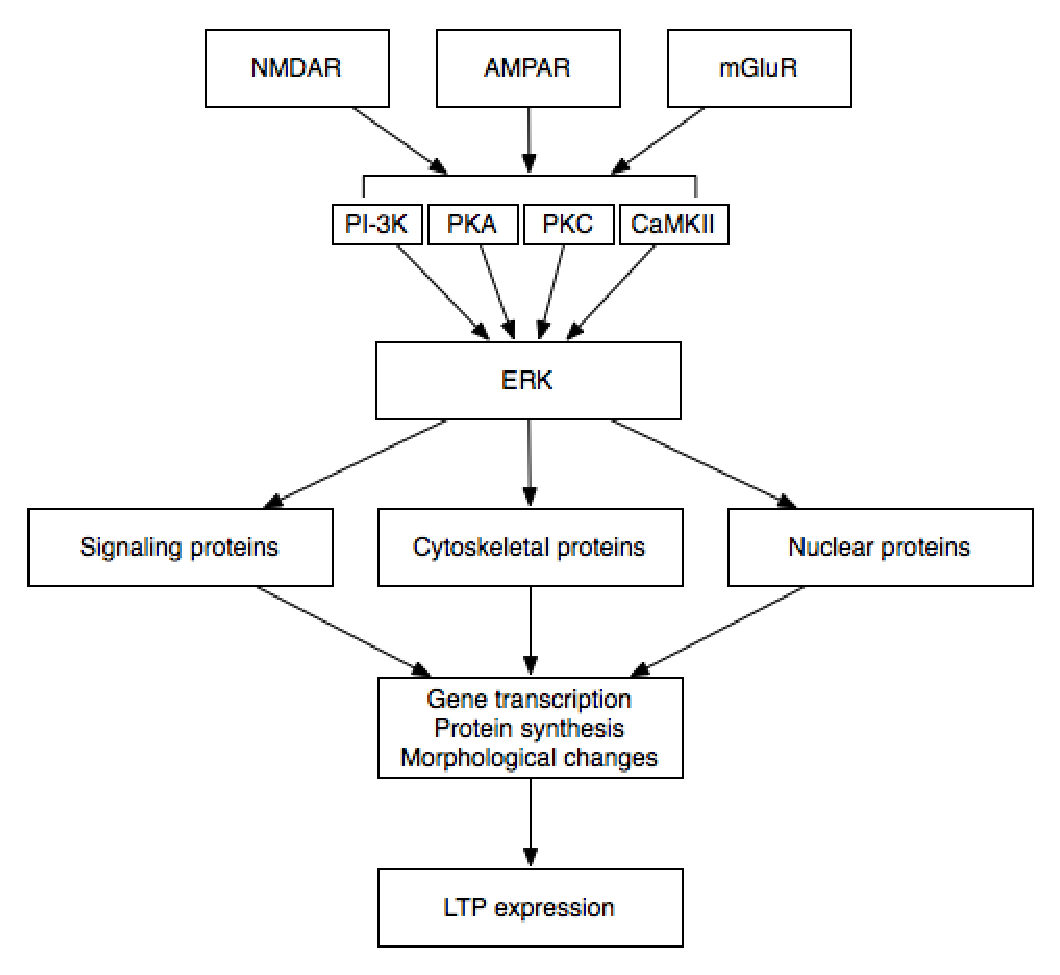
\includegraphics[height=6cm,
    angle=0]{./images/ERK_convergence.eps}}
\caption{ERK }
\label{fig:ERK_convergence}
%https://repository.library.georgetown.edu/bitstream/handle/10822/553186/janssenSchroederMeganJayne.pdf?sequence=1
\end{figure}

\subsection{ERK (classical MAPK): MAPK1/2 (ERK1/2), MAPK3 (ERK1)}
\label{sec:ERK}
\label{sec:MAPK1/2}
\label{sec:MAPK3}

Extracellular signal-regulated kinase (ERK) was originally considered equivalent
to MAPK (Sect.\ref{sec:MAPK}). Now, with more MAPK's members, ERK (representing
classical MAPK) is a member of MAPK family.
\begin{enumerate}
  \item {\bf ERK1} (MAPK3): 
  
  Transgenic gene knockout mice lacking MAPK3 are viable and it is thought that
  MAPK1 can fulfill most MAPK3 functions in most cells. Exception: MAPK3
  is important for T cells, i.e. lacking MAPK3
  reduces T cell development into CDC4+ CD8+ stage.

  \item {\bf MAPK1} is aka MAPK2: so they are often called MAPK1/2.
  Nowadays, {\bf MAPK1/2} is called as ERK1/2.
  
  MAPK1 has 85\% sequence similarity with MAPK2.
  They were found during a search for protein kinases that are rapidly
  phosphorylated after activation of cell surface tyrosine kinases such as the
  epidermal growth factor receptor (EGFR - Sect.\ref{sec:EGFR}).
  
  No conditional MAPK1 KO mouse was survived, suggesting critical functional
  role of MAPK1. 
\end{enumerate}


Depending on the cellular context, the MAPK/ERK cascade
(Sect.\ref{sec:MAPK/ERK-pathway}) mediates diverse biological functions such as
cell growth, adhesion, survival and differentiation through the regulation of
transcription, translation, cytoskeletal rearrangements. About 160 substrates
have already been discovered for ERKs.
\begin{itemize}
  \item Many of these substrates are localized in the nucleus, and seem to participate
in the regulation of transcription upon stimulation.

The substrates include transcription factors (such as ATF2, BCL6, ELK1, ERF,
FOS, HSF4 or SPZ1), cytoskeletal elements (such as CANX, CTTN, GJA1, MAP2, MAPT,
PXN, SORBS3 or STMN1), regulators of apoptosis (such as BAD, BTG2, CASP9, DAPK1,
IER3, MCL1 or PPARG), regulators of translation (such as EIF4EBP1) and a variety
of other signaling-related molecules (like ARHGEF2, FRS2 or GRB10).
  
  \item  However, other substrates are found in the cytosol as well as in other
  cellular organelles, and those are responsible for processes such as
  translation, mitosis and apoptosis. 

Protein kinases (such as RAF1, RPS6KA1/RSK1, RPS6KA3/RSK2, RPS6KA2/RSK3,
RPS6KA6/RSK4, SYK, MKNK1/MNK1, MKNK2/MNK2, RPS6KA5/MSK1, RPS6KA4/MSK2, MAPKAPK3
or MAPKAPK5) and phosphatases (such as DUSP1, DUSP4, DUSP6 or DUSP16) are other
substrates (of MAPK/ERK) which enable the propagation the MAPK/ERK signal to
additional cytosolic and nuclear targets, thereby extending the specificity of
the cascade.
\end{itemize}
\url{http://www.uniprot.org/uniprot/P27361}

As mentioned earlier, activation of MAPK/ERK molecule requires (1) removal of
auto-inhibition; (2) phosphorylation at two sites (Thr202 and Tyr-204).
Activated MAPK/ERK then can interaction with substrates.
\begin{enumerate}
  \item in the case of MAPK3 (ERK1): substrates are DUSP3, DUSP6, GTF2I, 
  HDAC4, MAP2K1, MAP2K2, PTPN7, RPS6KA2, SPIB
  
  \item in the case of MAPK1 (ERK): substrates are ADAM17, CIITA, DUSP1, DUSP22,
  DUSP3, ELK1, FHL2, HDAC4, MAP2K1, MAP3K1, MAPK14, MKNK1, Myc, NEK2, PEA15,
  PTPN17, Phosphatidylethanolamine binding protein 1, RPS6KA1, RPS6KA2, RPS6KA3,
  SORBS3, STAT5A, TNIP1, TOB1, TSC2, UBR5, VAV1.
\end{enumerate}
Dephosphorylated and inactivated by DUSP3, DUSP6 and DUSP9.

    
ERK can be the molecular link between early phase LTP to late phase LTP
(Sect.\ref{sec:LTP_depend-NMDAR}), since many signaling cascades involved in
E-LTP, including CaMKII and PKC, can converge on ERK,
Fig.\ref{fig:ERK_convergence}.
  
\begin{enumerate}
    \item ERK1: p44 MAPK
    \item ERK2: p42 MAPK
\end{enumerate}
key mediators of signal transduction from the cell surface to the nucleus. 

\subsection{atypical MAPK: ERK3 and ERK4}
\label{sec:ERK3}

atypical MAPK like ERK3 and ERK4 are two-tiered phosphorylation system, in that
they are activated by phosphorylation by PAK proteins ({\bf p21 activated
kinases}) which are related to MAP3K (Sect.\ref{sec:p21-activated-kinases}).



\subsection{MAPK/ERK-pathway: Ras-Rak-MEK-ERK pathway}
\label{sec:MAPK/ERK-pathway}

\textcolor{red}{\bf MAPK/ERK pathway}:
\begin{verbatim}
BDNF --> TrkB receptor  + EGF receptors

       ---> MAPK1/2 (or ERK1/2)
             ---> calpain-2  (NOT calpain-1)
             (
\end{verbatim}   

In neurons, MAPK1/2 (aka ERK1/2) is activated by both brain-derived neurotrophic
factor (BDNF) and EGF. Using cultured primary neurons and HEK-TrkB cells, both
of which express BDNF and EGF receptors, Jourdi et al. (2010) showed that BDNF
stimulated m-calpain but not $\mu$-calpain serine phosphorylation, and this
effect is blocked by MAPK inhibitors.

Remarkably, BDNF- and EGF-induced calpain activation was preferentially
localized in dendrites and dendritic spines of hippocampal neurons, and was
associated with actin polymerization, which was prevented by calpain inhibition.




\section{p21-activated kinases (PAK)}
\label{sec:p21-activated-kinases}

PAK (p21-activated kinases) are enzymes serve as targets for small GTP binding
protein CDC42 and Rac (Sect.\ref{sec:Rac})
\begin{enumerate}
  \item PAK1: 
  \item PAK2
  \item PAK3
  \item PAK4
  \item PAK5
  \item PAK6
\end{enumerate}

\section{CMGC group}
\label{sec:CMGC-group}

CMGC kinase group comprises a group of closely related protein kinases:
CDK (Sect.\ref{sec:CDK}), MAPK (Sect.\ref{sec:MAPK}), GSK3
(Sect.\ref{sec:GSK3}), and CLK (Sect.\ref{sec:CLK}).

They are Serine/Threonine kinases (Sect.\ref{sec:STK}).

\section{CLK}
\label{sec:CLK}



\chapter{EC3 enzymes}
\label{chap:EC3-enzymes}


Sect.\ref{sec:EC_3} describes EC3 enzyme family.
Here, we focus on a number of them.

\section{EC3: Phospholipase}
\label{sec:phospholipase}

\begin{figure}[hbt]
  \centerline{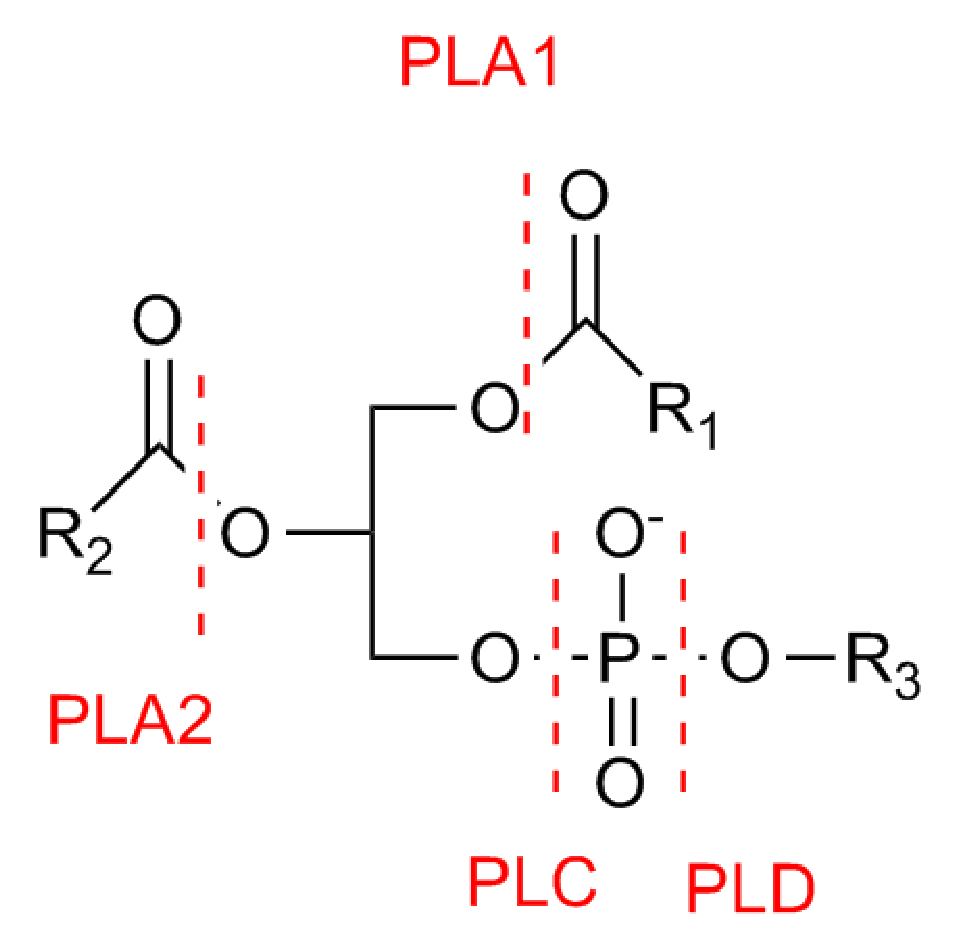
\includegraphics[height=5cm,
    angle=0]{./images/phospholipase.eps}}
\caption{Different kinds of phospholipase}
\label{fig:phospholipase}
\end{figure}


{\bf Phospholipase} is an EC 3 enzyme (Sect.\ref{sec:EC_3}) that hydrolyzes
phospholipid groups (e.g. lecithin or a similar phospholipid) of a substrate
protein. Why phospholipids is important? - Sect.\ref{sec:phospholipids}

There are 4 major classes: A, B, C, and D. 
\begin{enumerate}
  \item PLA - Sect.\ref{sec:PLA}
  
  \item PLB (EC 3.1.1.?, lysophospholipase): cleave both SN-1 and SN-2 acyl
  groups
        
  \item PLC (EC 3.1.4.3) cleaves before the phosphate
  group - Sect.\ref{sec:PLC}, release di-acylglycerol + phosphate-containing
  head group.
  
\item PLD (EC 3.1.4.4) - Sect.\ref{sec:PLD}: cleave after the phosphate group,
i.e. hydrolyze phosphatidylcholine (Sect.\ref{sec:phosphatidylcholine}) to form
phosphatidic acid (PA), releasing soluble choline to cytosol 

\end{enumerate}


PLC and PLD are considered {\bf phosphodiesterases}.
We will focus on PLC which plays an important role in signal transduction
pathways (Sect.\ref{sec:PLC}).

\section{-- phospholipase A (PLA)}
\label{sec:PLA}
\label{sec:phospholipase-A}

Phospholipase A is an enzyme that cleave phospholipid
\begin{enumerate}

   \item PLA1 (EC 3.1.1.32): cleave the SN-1 acyl group (axyl)

   \item PLA2 (EC 3.1.1.4): cleave SN-2 acyl group - Sect.\ref{sec:PLA2}
\end{enumerate}

\subsection{PLA2}
\label{sec:PLA2}

There are two PLA2
\begin{itemize}
  \item cPLA2 (85 kDa): generate arachidonic acid for signalling purpose
  
  \item sPLA2 (14-18 kDA): generate arachidonic acid for inflammatory
\end{itemize}

PLA2 is activated by ligand binding to receptors, including:
\begin{enumerate}
  \item 5-HT2 receptor (Sect.\ref{sec:5-HT_receptor})
  
  \item mGluR1
  
  \item bFGF receptor
  
  \item IFN-$\alpha$ receptor
  
  \item IFN-$\gamma$ receptor 
\end{enumerate}

Phospholipases A2 include several unrelated protein families with common
enzymatic activity.
\begin{enumerate}
  
  \item cPLA2 (85 kDA): cytosolic PLA2: $\Ca$-dependent, and involved in
  signaling process
  
  \item sPLA2 (secreated PLA2, 12-14 kDa): promote inflammation
  
  \item lp-PLA2 (lipoprotein PLA2): associated with cardiac disease
\end{enumerate}

\section{-- PLC (Phospholipase C)}
\label{sec:PLC}

{\bf PLC} (EC 3.1.4.3) is an enzyme family (class C of phospholipase -
Sect.\ref{sec:phospholipase}) whose function is to cleave the phosphate groups.
It is thus called phosphodiesterase (Sect.\ref{sec:phosphodiesterase}).
Phospholipase C is a truly remarkable signalling moiety. We know of no other
single enzyme that can produce (or modulate), directly, three distinct signals:
inositol 1,4,5- trisphosphate (IP3), diacylglycerol, and phosphatidylinositol
4,5-bisphosphate (PIP2) - Sect.\ref{sec:GPCR-PLC-IP3-DAG-pathway}. All PLC
isoforms are activated by Ca2+ ions, although their sensitivities to [Ca2+] vary
greatly (Sect.\ref{sec:PLC-Calcium}).


\subsection{3 subfamilies}
\label{sec:PLC-subfamilies}


Mammalian PLC has at least 13 isoforms, grouped into 6 subfamilies, based on
sequence similarity:
$\beta, \gamma, \delta, \varepsilon, \zeta, \eta$
~\citep{rhee2001rps,saunders2004plcz,cockcroft2006plc}.
In general, these PLC families share a conserved core architecture consisting of
an N-terminal PH domain followed by a series of EF hands, a catalytic TIM barrel
and a C2 domain, Fig.\ref{fig:PLC}.


Each isoform has a specific activator.  Depending on the subfamilies and
isoforms, they can be found in plasma membrane and/or nucleus membrane. 

\begin{enumerate}
\item {\it PLC$-\beta$}: Sect.\ref{sec:PLC-beta}
% activated by G$_{\alpha q/11}$
% subunit - Sect.\ref{sec:G-protein-coupled-receptor}

\item {\it PLC$-\gamma$}: - Sect.\ref{sec:PLC-gamma}

\item {\it PLC$-\delta$}: activated by an increase in [\ce{Ca^2+}] -
Sect.\ref{sec:PLC-delta}


\item {\it PLC$-\varepsilon$}: newly discovered in the heart, contains
  RasGEF and Ras-activated domains. - Sect.\ref{sec:PLC-epsilon}

\item {\it PLC$-\zeta$}: injected into the egg by the sperm -
Sect.\ref{sec:PLC-zeta}



\item {\it PLC-$\eta$}: Sect.\ref{sec:PLC-eta}
\end{enumerate}

% Once activated (presumbly through Gq$\alpha$ type of G protein -
% Sect.\ref{sec:Gq/11-protein}), all these first 5 types of PLC requires
% intracellular $\Ca$ to perform its catalytic function, although the optimal
% $[\Ca]$ for maximum activation is different in different PLC isozymes.
%NOTE: The residue important for Ca2+-binding is not present in PLC-beta
% isoforms.

% PLC cleaves phospholipids just before the phosphate group. An example is 
% \begin{itemize}
% \end{itemize}


% \subsection{PLC and Mg2+}
% 
% Activation of PLC-$\beta$1 by G-proteins in the presence of the nonhydrolyzable
% guanine nucleotide analogue GTP$\gamma$S was completely dependent on Mg2+ ions
% (Blank-Exton, 1991).


\subsection{PLC and Calcium}
\label{sec:PLC-Calcium}

The association of phospholipase C with Ca2+ signaling dates back arguably to
experiments published by Lowell Hokin (Hokin, 1966). 
\begin{verbatim}
PLC ---[Ca2+]--------> activated PLC
\end{verbatim}
Bob Michell suggested that inositol lipid turnover (i.e. later confirmed as PIP2
by Creba et al., 1983; Weiss et al., 1982; Berridge, 1983), initiated by
phospholipase C (PLC)-mediated inositide breakdown, was upstream of Ca2+
signaling (Michell, 1975; Michell et al., 1977). 


\begin{enumerate}
  \item Blank - Exton (1991) : PLC-$\beta$1 

Hydrolysis of PIP2 by PLC-$\beta$1 was maximal at 100$\muM$ of $\Ca$, and
calcium become inhibitory at 1 mM. 

Maximal activation of PLC-$\beta$1 (10-fold) occured between 100nM to 220nM of
calcium.
  
  \item 
\end{enumerate}

Mike Berridge (Berridge, 1983) then proposed that the released head group, IP3,
could function as a Ca2+ signaling second messenger. This was rapidly confirmed
experimentally by Berridge and his collaborators (Streb et al., 1983), and
subsequently by other investigators (Burgess et al., 1984; Prentki et al., 1984;
Joseph et al., 1984; Hirata et al., 1984; Biden et al., 1984; Whittaker \&
Irvine, 1984; Suematsu et al., 1984; Brown \& Rubin, 1984).

The less selective, Ca2+-permeable channels, the TRPCs (Sect.\ref{sec:TRPC}),
are activated by PLC, most likely by changes in membrane composition of DAG and
PIP2, Fig.\ref{fig:PLC-activated-Ca2+-influx}.
	

\subsection{PLC blockers}

\textcolor{red}{\bf PLC blockers}
\begin{enumerate}
  \item U73122 
  [1-[6-((17$\beta$-3-methoxyestra-1,3,5(10)-trien-17-yl)amino)hexyl]-1 H -
  pyrrole-2,5-dione] 5 $\muM$ applied intracellularly to block PLC-$\beta$
  
  \item 
\end{enumerate}

\subsection[PLC-beta]{PLC-$\beta$ subfamily}
\label{sec:PLC-beta}

Members of the PLC$\beta$ subfamily are composed of an N-terminal
pleckstrin homology (PH) domain, four EF-hand motifs, catalytic TIM barrel (X
and Y domains) and a C2 domain (calcium/lipid-binding domain, CaLB), and a
C-terminal coiled-coil domain (CT domain), Fig.\ref{fig:PLC}.

\begin{figure}[hbt]
  \centerline{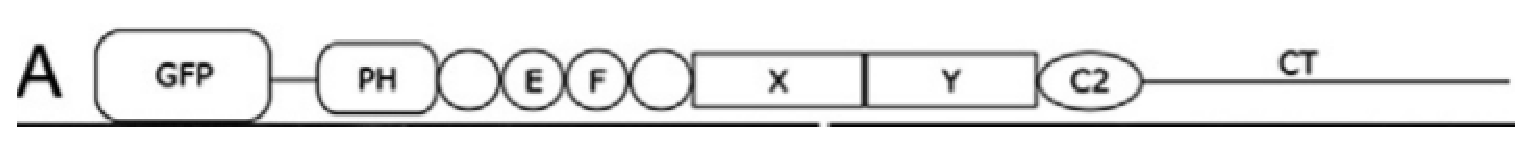
\includegraphics[height=1cm,
    angle=0]{./images/PLC.eps}}
  \caption{Core components of a PLC protein: N-terminal PH domain, 4 EF hands,
  catalytic TIM barrel (with X and Y domains), C2 domain, and C-terminal (CT)
  domain. CT domain is uniquely found in PLC-$\beta$ isozymes which is necessary
  for homodimerization and stimulation of phospholipase activity through direct
  interactions with G$\alpha$-GTP subunits of the Gq family (Sect.\ref{sec:Gq/11-protein})}
  \label{fig:PLC}
\end{figure}

Compared to other PLC subfamilies, PLC-$\beta$ has a unique long C-terminal (CT)
domain of about 450 amino acids. The EF-hand was initially proposed  to be
involved in the binding of Ca2+ ions. However, a comparison between genuine
Ca2+-binding EF hands and those of PLC$\beta$ enzymes shows that the residues
essential for Ca2+-binding are lost in PLC$\beta$ isoforms. The C2 domain does
not function as a Ca2+-binding domain either, as determined by sequence
analysis.

\subsection{-- activators}
\label{sec:PLC-activators}

Depending on the isoform, PLC$\beta$s are activated by heterotrimeric G proteins
(GTP-bound Gq$\alpha$ and/or G$\beta$$\gamma$ subunits) and/or GTP-bound Rac
(Sect.\ref{sec:PLC-beta}); and these three classes of G proteins mediate signals
originating from diverse cell surface receptors, thereby positioning PLC-b
isozymes downstream of a broad range of cellular inputs, including hormones,
growth factors and neurotransmitter.

\begin{itemize}
  \item calcium - Sect.\ref{sec:PLC-Calcium}
  
  \item G$\alpha$/q subunit bound to CT domain for activation PLC-$\beta$.
 
The Gq-selective WO82 and WO83 antiserum detected 2 types of Gq-proteins: 42kDa
and 43kDa that activate PLC-$\beta$1; which has little effect on PLC-$\gamma$ and
PLC-$\delta$ (Blank, Exton, 1991).

The activation of the 42kDa and 43kDa PLC-$\beta$1 by purified G-protein was
specific for nonhydrolyzable guanine nucleotides, the potency decreasing in the
order GTP$\gamma$S > GMPPNP > GMP-PCP. NOTE: GTP has no effect, probably
because of the intrinsic GTPase activity (GAF - Sect.\ref{sec:GAF-domain}) of
$\alpha$-subunit.

Also, activation of 42kDa and 43kDa PLC-$\beta$l by G-proteins
in the presence of GTPyS was completely dependent on Mg2+ ions with
4-5 mM proved to be optimal (Blank-Exton, 1991).
  
  \item G$\beta\gamma$ subunits also directly activate PLC-$\beta$ isozymes via
  PH domains (see below).

  \item Rac1 (target PLC $\beta$2 and $\beta$3) - Sect.\ref{sec:Rac}

NOTE: GTPase Rac1 recently found to directly activate PLC-$\beta$2 and
PLC-$\beta$3 via PH domain.
  
  PLC$\beta$2 in favor of GTPase Rac1 (over other Rho-family GTPases) :
  Rac1 engages the pleckstrin-homology (PH) domain of PLC-beta2 to optimize its
  orientation for substrate membranes (Jezyk et al. (2006))
  
 As G$\beta\gamma$ also engages the PH domain to activate PLC-beta2.
 These two activation events (G$\beta\gamma$ and Rac1) are compatible, leading
 to additive stimulation of phospholipase activity.
 
  
  \item  Waldo et al. (2010) showed that that loop between EF hands 3 and 4 of
  PLC$\beta$3 interacts with G$\alpha/q$ and promotes its GTPase activity

  \item  Another domain that is reported to interact with G$\alpha/q$ is the
C-terminal domain (CT), i.e. removal of this domain make PLC-$\beta$ no longer
activated by G$\alpha/q$ proteins. CT domains also have an inhibition effect on
calcium signaling, i.e.block the production of IP3 that is needed to trigger
internal calcium release.

CT domains derived from the various isoforms do not show a high amino acid
identity ($\approx$ 30\%).

\end{itemize}

\subsection{-- localization}

Currently, it is difficult to visualize the location of endogenous
PLC$\beta$s, since the available antibodies do not give consistent results in
immunofluorescence. Instead, VFP can be used to study.

Studying subcellular location of PLC$\beta$1a, PLC$\beta$1b, PLC$\beta$2, PLC$\beta$3,
and PLC$\beta$4a proteins was done by Adjobo-Hermans et al. (2013) 
\begin{itemize}
  \item  full-length visible-fluorescent-proteins-tagged (VFP-tagged) of these
  PLCs in Hela cells
  \item VFP-tagged of individual domains to see whether these domains play a
  role in determining the subcellular distribution of the full-length protein
\end{itemize}

They showed that
\begin{itemize}
  \item  PLC$\beta$2 and PLC$\beta$3 were not detected in the plasma membrane
 
But they must be on the plasma membrane to hydrolyze PIP3. A possible
explaination is that a minor fraction of full-length PLC$\beta$2 and PLC$\beta$3
may be localized at the plasma membrane, since such a small proportion (e.g.
10\%) is not detectable when using fluorescence microscopy.
 
Recruitment of PLC$\beta$2 and PLC$\beta$3 to membrane may be induced by
increasing the amount of PIP2 or other negatively charged phospholipids

  \item PLC$\beta$1b and PLC$\beta$4a were enriched in the plasma membrane. 

PLC$\beta$1a withouts its CT domain was not found in plasma membrane, suggesting
the important role of CT domain in anchoring the enzyme to plasma membrane.

  \item  None isoforms were found in the nucleus
  
  \item The PH domain and the C2 domain did not localize to the membrane, in
  agreement with other findings
  
  \item The CT domains of PLC$\beta$1a, PLC$\beta$1b, PLC$\beta$3
  and PLC$\beta$4a clearly locate at the membrane; yet CT domain of PLC$\beta$2
  is not. 

In addition, fluorescence level of CT$\beta$3 in cytosol also increase, as
compared to CT$\beta$1a and CT$\beta$4a.

The CT$\beta$2 was detected in cytosol, similar to CT domain in full-length
PLC$\beta$2.

\end{itemize}

\subsection{-- downstream targets}

Activated PLC-$\beta$ then slides down to hydrolyze a membrane-bound {\bf PIP2}
(Sect.\ref{sec:PIP2}), i.e.  the cleaved PIP2 turns into at least
2 second messengers - DAG (Sect.\ref{sec:DAG}) and IP3 (Sect.\ref{sec:IP3}).
\begin{itemize}
  \item DAG activate PKC (Sect.\ref{sec:PKC}) which can affect NMDAR trafficking
  via NAP (NMDAR-associated proteins which recently is belived CaMKII).
  
  \item IP3 bind to and open IP3R, releasing $\Ca$ from the ER store
\end{itemize}
However, CT domains of many PLC-beta have negative effect on the PLC-beta
signaling, i.e. the overal result is that \textcolor{blue}{effects of
CT$\beta$1a, CT$\beta$1b and CT$\beta$3 on blocking calcium signaling are
significantly different from signaling of non-transfected cell} (
The strength of inhibition of CT domain follows the decrease order: 
CT$\beta$1a  $\geq$ CT$\beta$3 $\gg$ CT$\beta$2; which is correlate with the
affinity of the CT domain to the plasma membrane) This has been explained by
 
\begin{itemize}
  
  \item  CT domain (CT$\beta$1a, CT$\beta$1b, CT$\beta$3) blocking the upstream
  effect of G$\alpha$q.

This is based on the evidence that this inhibition
can be overcome by over-expression of G$\alpha$q. 
  
  \item CT domain (CT$\beta$1a) blocking the PLC hydrolysis of PIP2.
\end{itemize}

% \textcolor{red}{However, CT domain of PLC-$\beta$1 have
% a negative effecbeen shown to produce inhibition in the PLC-$\beta$1's
% production of IP3}.

\begin{mdframed}

{\bf To understand the role of CT domains} - Two cases: non-transfected cell
with transfected cell (i.e. cell having CT domains of an associated PLC); both
with $\Ca$-indicator Fura-red (Sect.\ref{sec:fura-2}) (Adjobo-Hermans et al.,
2013). 
\begin{itemize}
  \item Histamine $\rightarrow$ 5-HT receptor activation $\rightarrow$ PKC
  activation $\rightarrow$ IP3 production $\rightarrow$ $\Ca$ release from ER 
  $\rightarrow$ free Fura-red level reduced, i.e. an increase in cytosolic
  $\Ca$.
  
  \item With the expressed CT$\beta$1a, the overal increase of cytosolic $\Ca$
  was small. 
  
  \item With the expressed CT$\beta$1b, calcium level still increase; yet with a
  significant delay 
  
The delay here is explained by inhibition of IP3 production which requires the
time to build up enough IP3 for opening IP3R to release ER $\Ca$. 

  
  \item With the expressed CT$\beta$2, calcium level still increase (yet with
  a minor delay and the elevation is somewhat smaller)
  
  \item With the expressed CT$\beta$3, calcium level increase at a smaller
  level; and with a significant delay
\end{itemize}

\end{mdframed}

\textcolor{red}{ROLE 1}: Activated PLC-$\beta$ is part of the GPCR-mediated
signaling at the plasma membrane (Sect.\ref{sec:GPCR-PLC-IP3-DAG-pathway}).
This role is important in (1) cardiovascular function, (2) neuronal plasticity.
\begin{enumerate}
  \item  hippocampal synapses, PLC$\beta$ acts as an efficient
coincidence detector triggering retrograde endocannabinoid
signalling to mediate {\it short-term plasticity}
(Hashimotodani et al. 2005, 2008).

  \item  
\end{enumerate}

\textcolor{red}{ROLE 2}: PLC-$\beta$ is also a component of a mitogen-activated
nuclear phosphoinositide signaling pathway. A large fraction of total cellular
PLC-$\beta$ can be found in the nucleus.
Mitogenic agents stimulate nuclear PLC-$\beta$ activity through a mitogen
activated protein kinase (MAPK) cascade - Sect.\ref{sec:MAPK}.

\textcolor{red}{ROLE 3}: 
\begin{itemize}
  \item PLCB1 has been shown to interact with TRPM7
  \item PLCB2 has been shown to interact with TRPM7 and MAP2K3.
  \item PLCB3 has been shown to interact with $\Na/\H$ exchange regulatory
  factor cofactor 2.
  \item PLCB4 (nothing else)
\end{itemize}


\subsection{-- Isoforms}

There are 4 major isoforms: PLC-$\beta_1$, PLC-$\beta_2$, PLC-$\beta_3$, and
PLC-$\beta_4$; each encoded by a different gene in human PLCB1, PLCB2, PLCB3,
and PLCB4, respectively. These isoforms differ in their tissue distribution,
molecular mass, specific activity, and sensitivity to regulation by G protein
subunits; suggesting that each isoform could play a divergent role in cellular
signaling (review: Adjobo-Hermans et al. (2013)).

\begin{itemize}
  \item PLC-$\beta$1: expressed at high levels in the brain.

PLC$\beta$1 is the major isozyme in hippocampal neurons.
  
\citep{dowal2008} studied on  PC12 and HEK293 cells and suggested that
activation of PLC-$\beta$1 by Gq is achieved through changes in intermolecular
interactions rather than diffusion and association. These pre-formed complexes
in turn give rise to rapid, localized signals.
  
  \item PLC-$\beta$2: expressed in cells from hematopoietic origin.
  
There are also two other modes of PLCbeta(2) membrane recruitment that
may accommodate contrasting functional needs to hydrolyze PIP2 in localized
versus dispersed populations (Sect.\ref{sec:PLC-beta}) \citep{gutman2010}.

  \item PLC-$\beta$3: ubiquitously expressed
  
  \item PLC-$\beta$4: expressed in specific parts of the brain and the retina
  
NOTE: PLC-$\beta_1$, PLC-$\beta_3$: found in most cells, albeit different
levels of expressions among the cells.
  
NOTE: PLC-$\beta_2$, PLC-$\beta_4$: found mainly in hematopoietic cells
and retina, respectively.

\end{itemize}

 
\subsection{-- PLC-beta-1 isoform}

PLC-$\beta$1 exists as two immunologically indistinguishable polypeptides of 150
and 140 kDa and is encoded in rat brain by two distinct transcripts of 5.4 and
7.2 kilobases (kb). NOTE: The 7.2 kb transcript is different from 5.4 kb
transcript by an additional 118 nucleotides located near the end of the coding
sequence and a 1738-nucleotide extension of the 3'-flanking region.

PLC-beta 1a and PLC-beta 1b correspond to the previously identified 150- and
140-kDa PLC-beta 1 enzymes, respectively
\begin{itemize}
  \item PLC-$\beta$1a: 1216-amino acid polypeptide derived from 5.4 kb
  transcript. 

  \item PLC-$\beta$1b:  1173-amino acid polypeptide derived from 7.2 kb
  transcript. NOTE: The additional 118 nucleotides gives rise to an open reading
  frame that is capable of coding PLC-$\beta$1b.

\end{itemize}
Both PLC-beta 1a and PLC-beta 1b are expressed in rat brain and C6Bu-1 glioma
cells.    PLC-beta 1a and PLC-beta 1b are derived from a single gene by
alternative RNA splicing (Bahk et al., 1994).

PLC-$\beta$1 can be activated by G$\alpha$q/11 protein -
Sect.\ref{sec:GPCR-PLC-IP3-DAG-pathway}, i.e. activated by two G-protein alpha
subunits, alpha-q and alpha-11. The C-terminal region as the segment containing
amino acid sequences required for activation by G$\alpha$q protein.
To have enough energy to activate PLC-$\beta$, $G_{\alpha q/11}$-GTP loose one
phosphate group and becomes $G_{\alpha q/11}$-GDP and finally re-binding to
GPCRs.

  
PLC$\beta_1$ (EC 3.1.4.11, 1-phosphatidyl-1D-myo-inositol
  4,5-bisphosphate) cleave PIP2 to form IP3 and DAG - Sect.\ref{sec:PIP2}.
  \textcolor{red}{ It  needs $\Ca$ as a co-factor}. 

\begin{verbatim}
PIP2 + H2O ----[enzyme: PLC-beta-1]---> IP3 + DAG 
\end{verbatim}
\begin{itemize}
  \item IP3 links to increase of $[\Ca]$ via IP3R channels Sect.\ref{sec:ip3-pathways}
  \item DAG links to increase PKC activity (Sect.\ref{sec:PKC})
\end{itemize}

% \begin{enumerate}
%   \item   
% % PLC$\beta_1$ is activated by two alpha subunits: G$_{\alpha,q}$ and
% % G$_{\alpha,11}$, or collectively called G$_{\alpha,q/11}$ which is found in 
% % mGluR1 or mGluR5 (Table \ref{tab:GPCR_ligand_Gprotein}).
% 
%    \item 
% \end{enumerate}

\subsection{-- PLC-beta-2}

PLC-$\beta$2 can be activated by 
\begin{itemize}
  \item G$\alpha$q/11 protein - Sect.\ref{sec:GPCR-PLC-IP3-DAG-pathway}

Although G$\alpha$(q) resembled Rac2 in increasing the contribution of exchange
to the FRAP of PLCbeta(2) and in enhancing its membrane association, the latter
effect was weaker than with Rac2.
 
  \item G$\beta\gamma$ protein - Sect.\ref{sec:Gbetagamma-mediate-signaling-pathway}
  
The N-terminal segment of PLC beta 2 with amino acid sequence extending to the
end of the Y box is the region required for activation by G$\beta\gamma$
\citep{wu1993}.
  \begin{itemize}
  \item G$\beta_1\gamma_1$, G$\beta_1\gamma_5$, G$\beta_2\gamma_5$ could activate
  PLC-$\beta$2 but not PLC-$\beta$1 isoform
  \item G$\beta_2\gamma_1$ does not activate PLC-$\beta$2 isoform.
\end{itemize}  
The coexpression of G$\beta_1\gamma_1$ (but not G$\beta_1\gamma_5$) and
G$\alpha$16 in COS-7 cells was able to synergistically activate PLC-$\beta$2.  


  \item Rac1 protein (Sect.\ref{sec:Rho}): Jezyk et al. (2006)
  
Rac1 engages solely the PH domain of PLC-$\beta$2 to localize and
orient it relative to substrate-containing membranes. 

\end{itemize} 

PLC$\beta_2$ (EC 3.1.4.11): similar to PLC$\beta_1$ in its catalytic function.
   
\subsection{-- PLC-beta-3}

PLC$\beta_3$ (EC 3.1.4.11): similar to PLC$\beta_1$ 

\subsection{-- PLC-beta-4}

PLC$\beta_4$ (EC 3.1.4.11): similar to PLC$\beta_1$


\subsection{PLC-delta subfamily}
\label{sec:PLC-delta}

PLC-$\delta$ is activated by an increase in [\ce{Ca^2+}].

\subsection{PLC-zeta subfamily}
\label{sec:PLC-zeta}


PLC-$\zeta$ is injected into the egg by the sperm.

\subsection{PLC-eta subfamily}
\label{sec:PLC-eta}


PLC-$\eta$

\subsection{PLC-epsilon subfamily}
\label{sec:PLC-epsilon}

PLC-$\varepsilon$ is a newly discovered PLC subfamily in the heart, contains
RasGEF and Ras-activated domains (Sect.\ref{sec:Ras}).
  

\subsection{PLC-gamma subfamily}
\label{sec:PLC-gamma}

Tyrosine kinases (Sect.\ref{sec:tyrosine}) that couple to PLCgamma; which leads
to IP3 production (Sect.\ref{sec:IP3_synthesis}).

\subsection{In hearts}

only members of the $\beta$, $\gamma$, $\delta$, $\varepsilon$
subfamilies are expressed in cardiac myocytes~\citep{berridge2003csd,
kockskamper2008ip3}.

\subsection{In neurons}
\label{sec:PLC-in-brain}


The hippocampus had the highest specific activity of PI-PLC (i.e.
phosphotidine-inositide-specific PLC), followed by striatum, frontal cortex,
cerebellum, and liver.
\begin{itemize}
  \item   aluminum chloride (AlCl3, 10-500 microM) inhibits hydrolysis of
  phosphatidylinositol 4,5-bisphosphate (PIP2) by PI-PLC in a
  concentration-dependent manner. 
  %https://www.ncbi.nlm.nih.gov/pubmed/8560464
  
  PI-PLC inhibition by 100 microM AlCl3 was greatest in the liver, followed by
  cerebellum, hippocampus, cortex, and striatum.

However, AlCl3 did not affect the shape of the calcium concentration curve,
suggesting that aluminum does not inhibit PI-PLC activity by interference with
the cofactor, calcium.
  
  \item 
\end{itemize}

Purkinje cells express all subtypes with the exception of the PLC$\beta_2$,
PLC$\beta_1$ has the lowest and PLC$\beta_4$ the highest expression level in
Purkinje cell.
\begin{itemize}
  \item PLC$\beta_3$ prevails in the caudal cerebellum
  \item PLC$\beta_4$ is reciprocally expressed in the rostral lobuli of the
  cerebellum
  
  \item PLC$\beta_1$ is present primarily in the somata of Purkinje cells and
  is, therefore, unlikely to play a major role in synaptic transmission at
  parallel fiber synapses that are all located in the spiny dendrite
\end{itemize}

PLC-beta 1 and -gamma 1, in particular, are known to protect cells from
oxidative stress.
Yasuda et al. (2008) confirmed rat cortical neurons that ER stress decreases the
expression of PLC-beta 1, but not -gamma 1, in neurons.

It is unknown whether PLC isozyme expression is affected by alteration of
intracellular Ca2+ concentration, while it is recently suggested that PLC may
have additional roles in calcium signaling, particularly in the regulation of
Ca2+ entry into cells across the plasma membrane.



\section{-- PLD (Phospholipase D)}
\label{sec:PLD}

PHospholipase D (PLD) is EC 3.1.4.4 enzyme
(Sect.\ref{sec:enzyme-classification}) that catalyze the hydrolysis,
i.e. using water to hydrolyses phosphatidylcholine
(Sect.\ref{sec:phosphatidylcholine}) into phosphatidic acid and choline.

A range of agonists acting through G protein-coupled receptors and receptor
tyrosine kinases (Sect.\ref{sec:tyrosine-kinase}) stimulate this hydrolysis. 

PLD activity has been implicated in numerous celular pathways
\begin{enumerate}
  \item signal transduction
  
  \item membrane trafficking
  
  \item regulation of mitosis
\end{enumerate} 

Isoforms: 
\begin{enumerate}
  \item Phospholipase D1 is encoded by gene {\it PLD1}
  
  \url{https://en.wikipedia.org/wiki/PLD1}
  
  \item Phospholipase D2 is encoded by gene {\it PLD2}
  
  \url{https://en.wikipedia.org/wiki/PLD2}
\end{enumerate}

\section{Protein phosphatase}
\label{sec:PP-protein-phosphatase}

A phosphatase is an enzyme that removes a phosphate group from its substrate.
This action is directly opposite to that of phosphorylases
(Sect.\ref{sec:phosphorylases}) and kinases
(Sect.\ref{sec:serine-thereonine_protein-kinases}), which attach phosphate
groups to their substrates by using energetic molecules like ATP.
\begin{enumerate}
  \item phosphorylate mGluR5 - Sect.\ref{sec:mGluR_group-1-phosphorylation}
 
Indeed, PP1$\gamma$1 (PP1C1) in both recombinant and native forms binds to the
C-terminus of long-form group I mGluRs, i.e., mGluR1a, mGluR5a, and mGluR5b
(Croci et al., 2003).
The fact that the PP1$\gamma$ 1-binding motif on mGluR1/5 falls within or
immediately distal to possible PKC phosphorylation sites (such as S881 and S890
on mGluR5a) is noteworthy. It is currently unknown whether other PP isoforms
(PP1/2A, PP2B, etc.) can directly bind to mGluR1/5.
 
  \item 
\end{enumerate}

\section{Phosphorylases}
\label{sec:phosphorylases}

A {\bf phosphorylase} is an enzyme that helps to attach phosphate groups to
their substrates by using energy.


\subsection{PP1/2A (okadaic acid-sensitive phosphatase): PP1, PP2A}
\label{sec:protein-phosphatase}

Protein phosphatases (PPs) is an enzyme that dephosphorylates an amino acid
residue of its protein substrate, i.e. removing the phosphate group. So, it
counters and balance the effect of protein kinases which add phosphate groups to
substrate (Sect.\ref{sec:protein-kinase}) - Sect.\ref{sec:phosphorylation}. 


\begin{enumerate}
  \item PP1 - Sect.\ref{sec:PP1}
  \item PP2A - Sect.\ref{sec:PP2A}
  \item PP2B - Sect.\ref{sec:PP2B}
  \item PP5
\end{enumerate}

Above proteins phosphorylate these targets
\begin{enumerate}
  \item tau - Sect.\ref{sec:tau-phosphorylation} mainly by PP2A
  
  \item CaLv1.2 (Sect.\ref{sec:CaLv1.2-channel}): PP2A and PP2B are part of the
  complex that comprises $\beta_2$ adrenergic receptor, trimeric Gs protein, AC,
cAMP-dependent protein kinase (PKA).

  \item 
\end{enumerate}


\subsection{PP1 }
\label{sec:PP1}

Protein phosphatase type-1 (PP1) includes metal-dependent protein phosphatases
(PPMs) and aspartate-based phosphatases.

Activated PP1  affects many signalling steps, by dephosphorylating receptors
such as AMPA and NMDA glutamate receptors, or GABAA receptors, voltage-gated ion
channels (Na2+, L-, and N/P-Ca2+), kinases such as calcium/calmodulin kinase II,
and transcription factors (e.g., CREB),

PP1 is inhibited by 
\begin{enumerate}
  \item phospho-Thr34-DARPP-32 (Sect.\ref{sec:DARPP32})
  
The reversed process, i.e. dephosphorylation of Thr34, is mediated by
protein phosphatase-2B (PP2B, also called calcineurin), upon activation of the
Ca2+ pathway - Sect.\ref{sec:PP2B}). 
%protein phosphatase inhibitor-1 (Sect.\ref{sec:DARPP32})
  \item 
\end{enumerate}

The inhibition of PP1 can play a critical role in disease progression.
There is a significantly lower PP1 activity in both gray and white matters in
Alzheimer disease brains.This suggests that dysfunctional phosphatases play a
role in Alzheimer's disease.

PP1 and CaMKII are mutual inhibitory [Strack et al., 1997], i.e. inhibiting PP1
would promote CaMKII activity (Sect.\ref{sec:CaMKII}).

% TODO: PP1 research more about the role of PP1 in medium-spiny neuron
%       and/or striatum.

\subsection{-- PP2A (PP2)}
\label{sec:PP2A}

Protein phosphatase 2 (PP2), also known as PP2A is a ubiquitous and conserved
{\bf serine/threonine phosphatase}.

PP2A is a dimeric enzyme composed of 3 parts:
the structural A and catalytic C subunits, and a regulatory B subunit.
There are  four classes of variable regulatory subunits: B (PR55), B' (B56 or
PR61), B'' (PR72), and B''' (PR93/PR110), with at least 16 members in these
subfamilies.


PP2A has autocatalytic dephosphorylation properties analogous to autocatalytic
kinase activity of CaMKII.
The first report of {\bf autodephosphorylation} - intermolecules self-activating
mechanism of PP2A


\subsection{PP2B (calcineurin)}
\label{sec:calcineurin}
\label{sec:PP2B}
\label{chap:calcineurin}

Calcineurin (or PP2B) is a serine/threonine proteine phosphatase
(Sect.\ref{sec:protein-phosphatase}), Fig.\ref{fig:Calcineurin_pathway}.
\begin{enumerate}
  \item a heterodimer of 2 subunits:
  \begin{itemize}
    \item calcineurin A (CnA): a 59-63 kDa (e.g. 61-kDa) calmodulin-binding
    catalytic subunit

The catalytic subunit has 3 isoforms: (in mammals) encoded by 3 different genes
(PPP3CA, PPP3CB, and PPP3CC) or ($\alpha, \beta, \gamma$).
    
    \item calcineurin B (CnB): 19-kD Ca2+-binding regulatory subunit 

The regulatory subunit has 2 isoforms: (in mammals) encoded by 2 genes (PPP3R1,
PPP3R2) or (B1 and B2).
  \end{itemize}

The name ``calcineurin'' was coined by Klee on the basis of it calcium-binding
properties and localization to neuronal tissue \citep{klee1979}. Nowadays,
Calcineurin is found to co-localize with many signaling proteins (e.g.
Ca2+/Calmodulin).
However, while CnA$\alpha$, CnA$\beta$, CnB1 gene products are found in every
cell; calcineurin CnA$\gamma$ and CnB2 expression are found mainly in brains and
testis \citep{molkentin2004cns}.

Calcineurin is CaM kinases as it is primarily regulated by $\Ca/$Calmodulin
complex and thus a major player in $\Ca$-dependent eukaryotic signal
transduction pathways (review: \citep{rusnak2000}).

   \item Cain is a 230 kDa protein with a C-terminal domain that acts as a
non-competitive inhibitor of calcineurin.

   \item AKAP79 (Sect.\ref{sec:AKAP}) is a scaffolding protein that docks
   calcineurin, PKA and PKC.

  \item Calcineurin is activated by $\Ca$, but is inhibited by cyclosporin A
(Csa)/FK506. 

To avoid many side-effect of using Csa/FK506, genetic models with inhibited
calcineurin activity were used. Strategies include: (1) overexpressing
the naturally inhibitor of calcineurin, known as {\it calcipressins} (from 2
proteins Cabin1/Cain and AKAP79), (2) transgenic overexpression of the
calcineurin inhibitory protein MCIP1 (myocyte-enriched calcineurin-interacting
protein-1), (3) dominant-negative mutant of Calcineurin, (4) Calcineurin
A$\beta$ gene targeted mice. In essnce, they used 4 separate
transgenic approach (Cain, AKAP79, MCIP1 and dnCnA) and one gene
targeted mouse model (CnA$\beta$ null) \citep{wilkins2002cac}.

\end{enumerate}



% 82, 86, 108, 171, 232, 233, 247, 267, 281, 290,
% 312, 337, 377, 397, 401, 402, 417, 441
However, the role of calcineurin in the baseline unstimulated heart is unknown.
It has been suggested that calcineurin is inactive. However, calcineurin is also
known to directly sense $[\Ca]_i$ where it is activated by sustained elevations
in intracellular calcium \citep{crabtree1999, klee1998, dolmetsch1997}.
Thus, during calcium transient, it may regulate, in part, the baseline
calcineurin activity as a mechanism for adapting cardiac load. 


Once Calcineurin is activated, it catalyses the desphosphorylation the members
of the nuclear factor of the NFAT family in the cytoplasm and promote the
translocating from cytoplasm into the nuclear where NFAT can upregulates the
expression of IL-2 (interleukin-2), Fig.\ref{fig:Calcineurin_pathway}. David Yu
Lab from JHU have showed early evidence of NFAT nuclear translocation using FRET
imaging. The suggested role of calcineurin include redox and/or oxidative
stress. In the heart, calcineurin was found to link to {\bf cardiac hypertrophy}
(Sect.\ref{sec:cardiac-hypertrophy}.



\begin{figure}[hbt]
  \centerline{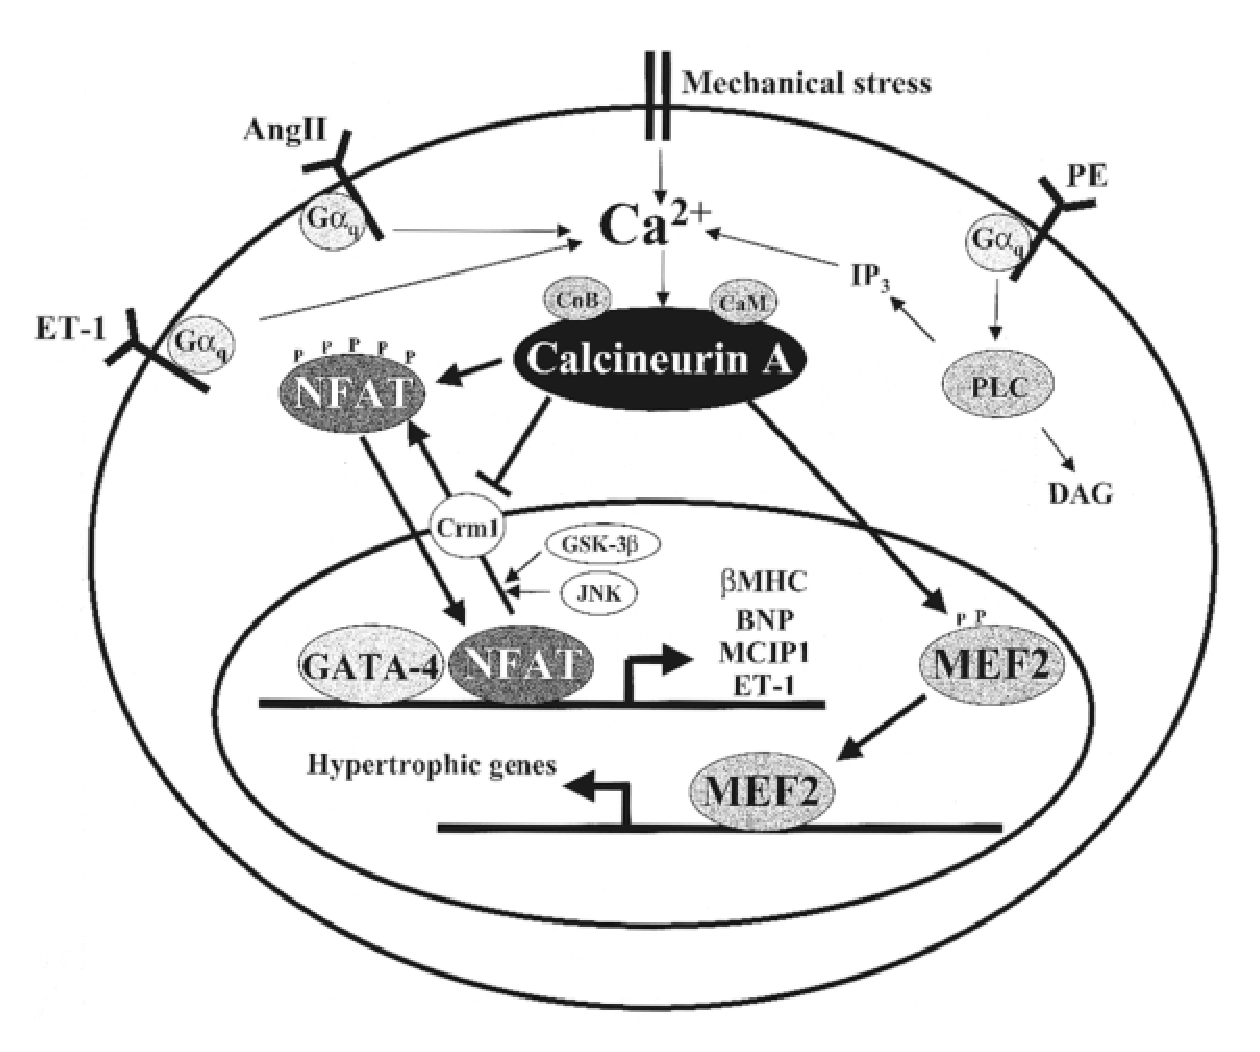
\includegraphics[height=5cm,
    angle=0]{./images/Calcineurin.eps}, 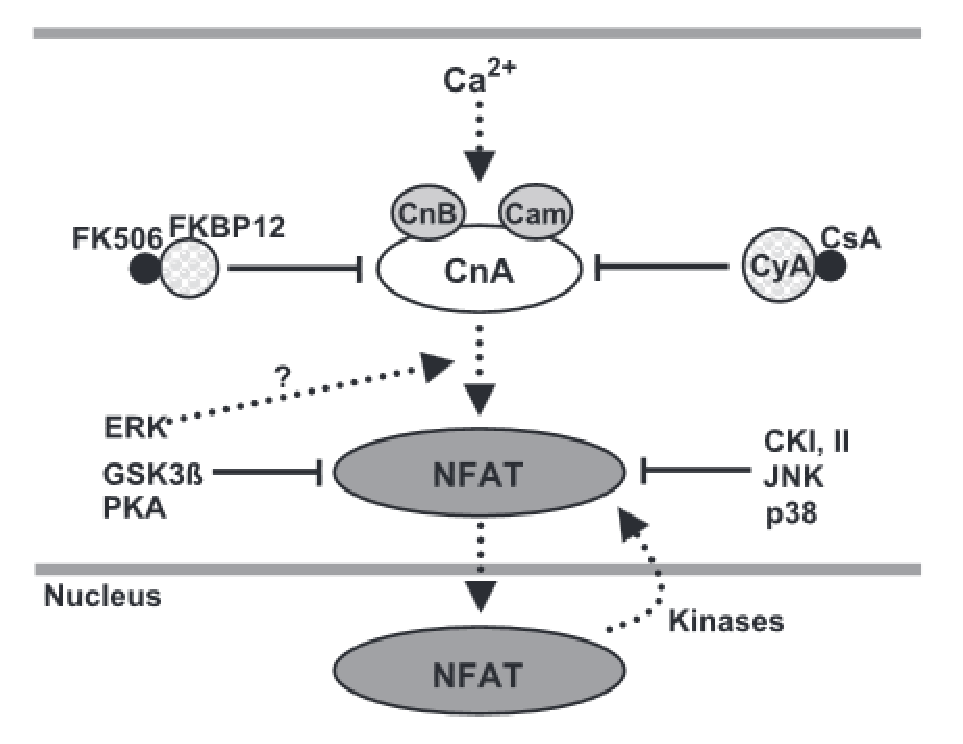
\includegraphics[height=5cm,
    angle=0]{./images/Calcineurin_2.eps}}
  \caption{Calcineurin signaling pathways in cardiac myocytes \citep{wilkins2002cac}}
  \label{fig:Calcineurin_pathway}
\end{figure}

 



\section{AKAP}
\label{sec:AKAP}

NOTE: \textcolor{red}{AKAP is a protein that can bind multiple proteins at the
same time, forming a scaffold for multi-enzyme complex} and control the
localization of such proteins.

Several AKAPs have been identified with its name given by the apparent
molecular weight on SDS-PAGE gels. AKAPs are found to localize to different
subcellular compartments, yet there quantitative distribution hasn't been
reported \citep{Yang1998}

More than 50 AKAPs have been identified, many of which are expressed in neurons
(Bauman et al., 2004; Tasken and Aandahl, 2004)
\begin{itemize}

  \item AKAP84: mitochondria

  \item AKAP220: peroxisome

  \item AKAP85: golgi

  \item MAP2: microtubules

  \item AKAP95: nucleus
  
  \item \textcolor{red}{AKAP100} tether with PKA type II
  (Sect.\ref{sec:PKA-classification}):
  
  AKAP100 localized to multiple subcellular compartments (nucleus, sarcolemma,
  intercalated disc, at Z-line region of the T-tubule and junctional SR) in
  adult rat heart with PKA type II.
  
  AKAPs bind to the N-terminal dimerization domain of PKA regulatory subunits
  and typically contain a second domain that binds to the cytoskeleton or
  intracellular scaffolds, thus targeting PKA to specific subcellular locations
  (Wong and Scott, 2004).   
\end{itemize}

\subsection{AKAP84 (in mitochondria)}
\label{sec:AKAP84}



\subsection{AKAP85 (in golgi)}
\label{sec:AKAP85}

\subsection{AKAP95 (in nucleus)}
\label{sec:AKAP95}

\subsection{AKAP100 (in neurons)}
\label{sec:AKAP100}

\subsection{AKAP220 (in peroxisome)}
\label{sec:AKAP220}

\subsection{MAP2 (in microtubules)}
\label{sec:MAP2}


\section{PDE (Phosphodiesterase)}
\label{sec:PDE}
\label{sec:phosphodiesterase}

\textcolor{red}{Review: Essayan (2001).}


3',5'-cyclic nucleotide phosphodiesterases (PDEs) refers to a family of enzyme
(Sect.\ref{sec:enzyme}) with many different PDE subtypes
(Sect.\ref{sec:PDE-classification}) that degrades cyclic nucleotide
(Sect.\ref{sec:cyclic-nucleotide}) cAMPs and cGMP
\begin{verbatim}
cAMP + H2O --------[PDE]------> 5'-AMP

cGMP + H2O --------[PDE]------> 5'-GMP 
\end{verbatim}

Catalyzation of PDE degrades cAMP and cGMP - which may disrupt normal cellular
signaling via cAMP/cGMP signaling pathways. First, you need to know the
functions of cAMP (Sect.\ref{sec:cAMP-dependent_pathway}) and cGMP
(Sect.\ref{sec:cGMP-dependent-pathways}). The downstream effects would be
cGMP-dependent protein kinase (PKG - Sect.\ref{sec:PKG}), cAMP-dependent protein
kinase (PKA) - Sect.\ref{sec:PKA}, and cAMP-regulated guanine nucleotide
exchange factors (cAMP-GEFs). 

Therefore regulation of PDEs hydrolytic activity is important for modulation of
cellular functions via PDE inhibitors (Sect.\ref{sec:PDE10-inhibitor}) which
breaks a phosphodiester bond (Sect.\ref{sec:phosphodiester-bond}) of cyclic
nucleotide (Sect.\ref{sec:cyclic-nucleotide}), i.e. cAMP and cGMP.


\subsection{classification: PDE I, PDE II, PDE III}
\label{sec:PDE-classification}

\textcolor{red}{PDE are classified into 3 classes: I, II and III}, each with
its own catalytic domain structure. We will focus on PDE I
(Sect.\ref{sec:PDE-I}) as it presents on higher level species.

\subsection{-- PDE II}
\label{sec:PDE-II}

PDE II has been  identified in slime molds, fungi, and bacteria, and contain a
distinct catalytic domain structure ({\bf PDEase II}) that is selective for cAMP
as a substrate. 

\subsection{-- PDE III}
\label{sec:PDE-III}

PDE III exist only in prokaryotes, and have a completely different catalytic
mechanism that resembles that of the purple acid phosphatases.

\subsection{PDE I: contains 11 families PDE1 - PDE11}
\label{sec:PDE-I}


Class I PDE (PDE I) is a class of PDE (Sect.\ref{sec:PDE}) that contains the
characteristic {\bf PDEase I} catalytic domain and consist of eleven distinct
families differing in substrate specificity (e.g. cAMP - Sect.\ref{sec:cAMP}),
tissue localization, regulatory mechanisms, and pharmacological properties.

Found in vertebrates, including human, rat, and mouse, Class I PDE is composed
of 21 genes, grouped into 11 families (PDE1 to PDE11) \citep{Omori2007} .
3 additional families have been reported; but not enough data (Essayan, 2001).
Five of the eleven PDE families (including the photoreceptor PDE6 family)
contain regulatory modules that have been termed GAF domains -
Sect.\ref{sec:GAF-domain}. Human has more than 50 PDE isoforms.

\textcolor{red}{NAMING CONVENTION}: hsPDE4D1
\label{sec:PDE-name-convention}
\begin{itemize}
  \item first 2 letters: indicate animal species (e.g. hs = homo sapien)
  \item PDE4 = the family; the Arabic number after PDE designate the gene
  family (1..11)

  \item D = the letter refers to the distinct subfamily gene (A..D)
  
  \item 1 = the number refers to splice-variant (isoforms); 
  each with different functional and regulatory characteristics, may exist for
  any given gene product. The splice variants in PDE regulates a specific cell
  signaling.
\end{itemize}


{\bf DETAILS}: NOTE (Km = $\muM$ = $\mu$mol/L)
\begin{enumerate}
  
  \item PDE1 (3 genes): hydrolyze both cAMP (Km=1-30) and cGMP (Km=3), expressed
  in a non-myocyte fraction of cardiac tissue, brain, lung and smooth muscle,
  activated by $\Ca$/Calmodulin, i.e. a CaM binding site (Sect.\ref{sec:calmodulin}).
  
  \item PDE2 (1 gene): hydrolyze both cAMP (Km = 50) and cGMP (Km=50), expressed
  in adrenal gland, heart, lung, liver and platelets; activated by cGMP
  binding to GAF domains - Sect.\ref{sec:GAF-domain}
  
  \item PDE3 (2 gene) - holds a trans-membrane domain: hydrolyze both cAMP (Km =
  0.2) and cGMP (Km=0.3) (yet with higher $V_\max$ for cGMP); expressed 
  heart, lung, liver, platelets, adipose tissue, and immunocytes.
  
  \item PDE4 (4 gene): specific for cAMP (Km=4); as for cGMP (Km > 3000);
  expressed in Sertoli cells, kidney, brain, liver, lung, and immunocytes
  
  It has upstream conserved regions (UCRs).
  
  \item PDE5 (1 gene): specific for cGMP (Km=1); as for cAMP (Km=150), highly
  expressed in vascular smooth muscle; and also found in lung, platelets.
  
  \item PDE6 (3 gene): specific for cGMP (Km=60); as for cAMP (Km=2000). It is
  however is a photoreceptor.
  
  \item PDE7 (2 genes): specific for cAMP (Km=0.2); as for cGMP (Km > 1000);
  expressed in skeletal muscle, heart, kidney, brain, pancreas, T lymphocytes.
  
  \item PDE8 (2 genes): specific for cAMP (Km=0.06); IBMX-insensitive;
  expressed in testes, eye, liver, skeletal muscle, heart, kidney, ovary, brain,
  T lymphocytes.

It has a response regulator receiver (REC) domain [Pfam accession
no. PF00072] and a per-arnt-sim (PAS) domain [Pfam accession no. PF00989].

  \item PDE9 (1 gene): cGMP-specific (Km=0.17), IBMX-insensitive;
  expressed Kidney, liver, lung, brain.
  
  \item PDE10 (1 gene): hydrolyze both cAMP (Km=0.05) and cGMP (Km=3.0) -
  Sect.\ref{sec:PDE10}; and expressed in Kidney, liver, lung, brain
  (specifically enriched in striatal SPN -
  Sect.\ref{sec:HD-role-of-PDE10-loss}).
  
  Inhibitors: TP-10

  \item PDE11 (1 gene): hydrolyze both cAMP (Km=0.7) and cGMP (Km=0.5); 
  expresed in skeletal muscle, prostate, kidney, liver, pituitary and salivary
  glands, testes
\end{enumerate}
Recent data showed that Phosphodiesterases (PDE)  localize to specific
subcellular, and control the temporal/spatial dynamics of cAMP, allowing a
highly localized cAMP gradients in cell. 


\begin{figure}[hbt]
 \centerline{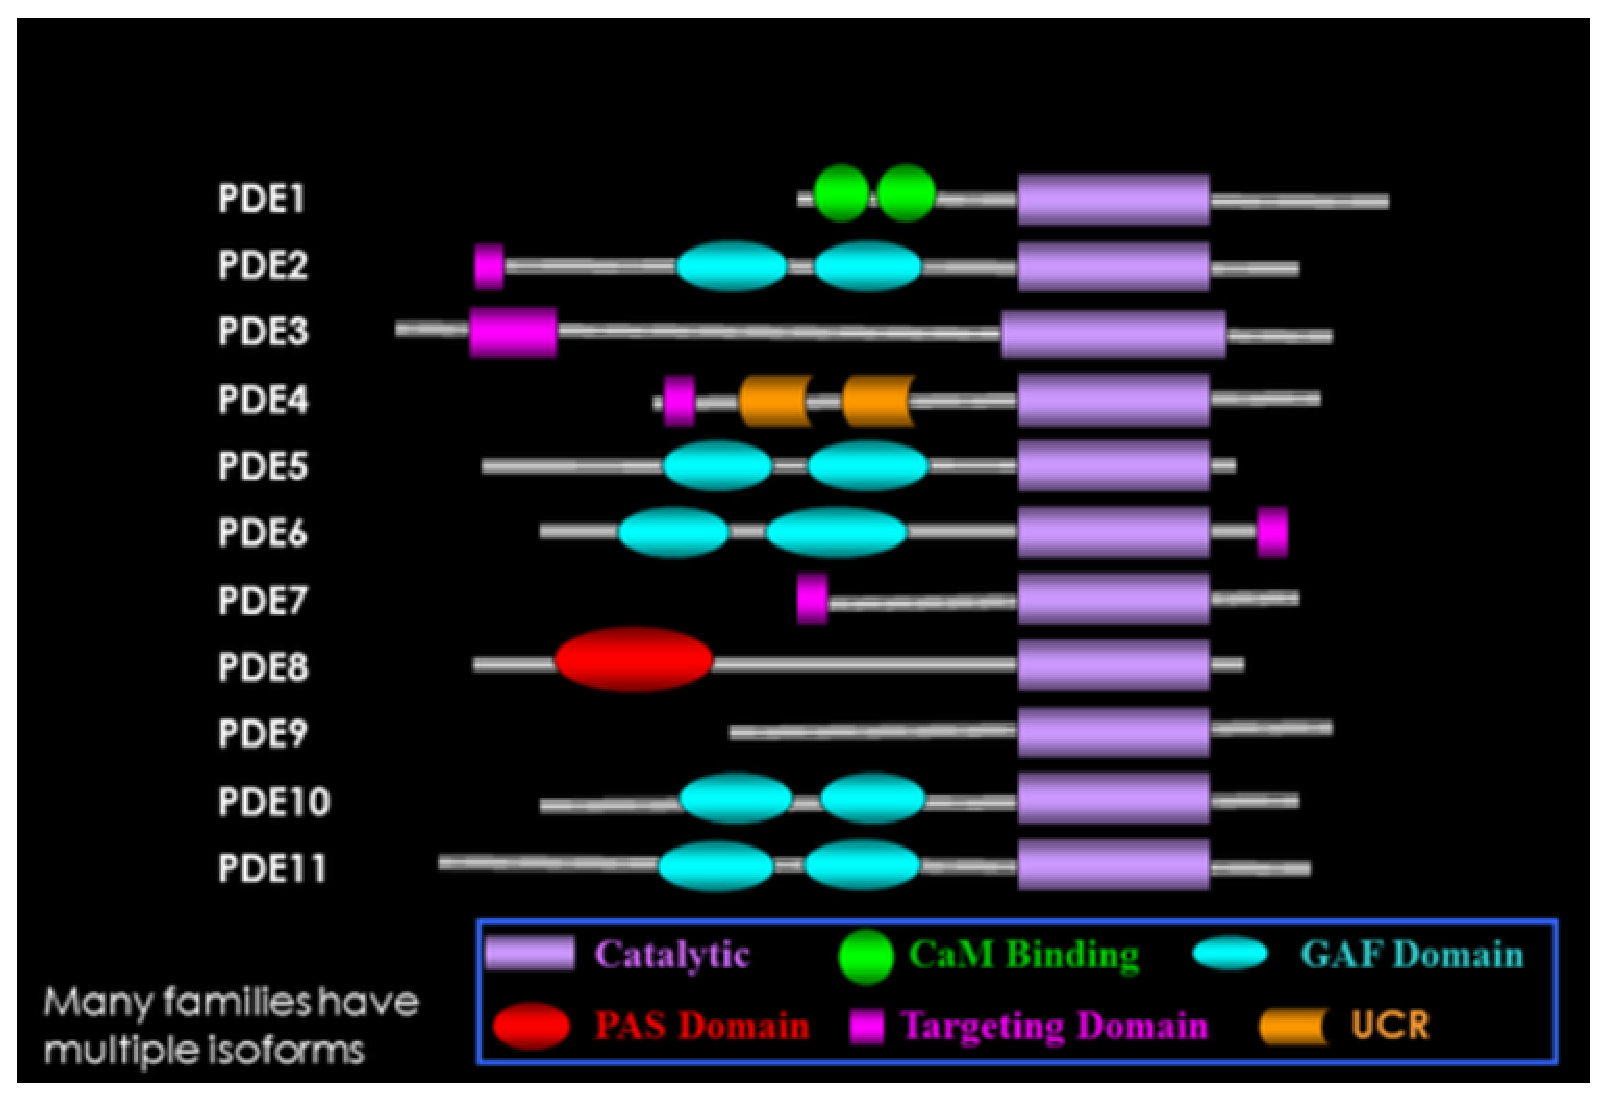
\includegraphics[height=4cm]{./images/PDE-class-I.eps}}
\caption{Structures of 11 families of PDE-class-I: left (N-terminal) to right
(C-terminal): PAS domain, CaM binding site, GAF domain}
\label{fig:PDE-class-I}
\end{figure}

\subsection{-- PDE I structure}
\label{sec:PDE-I-structure}

Structure: Fig.\ref{fig:PDE-class-I}
\begin{itemize}
  
  \item The homologous HD domain on the C-terminal controls 
  the affinity to cAMP and/or cGMP: 

All families have this; yet the differences in the amino acid sequence of the
different PDE families are known to account for the substrate specificity
(cAMP-specific, cGMP-specific, or dual-substrate).
  
  \item The N-terminal of PDE controls enzymatic activity and subcellular
  localization.

\end{itemize}


\subsection{-- PDE1}
\label{sec:PDE1}

Remeber the convention of calling PDE in Sect.\ref{sec:PDE-name-convention}.
There are three genes (A, B, C) encodes PDE1, each with a splice variant of
N-terminal region (N1, N2 and N3)
\begin{enumerate}
  \item PDE1A : high affinity to cGMP 
  
  \item PDE1B : hydrolyze cGMP with a Km value lower and a Vmax value higher
  than those for cAMP.
  
  \item PDE1C :  high affinity to both cGMP and cAMP 
\end{enumerate}


\subsection{-- PDE2}

There is only 1 gene (A)
\begin{itemize}
  \item hydrolyzes both cGMP and cAMP with similar maximal rates and relatively
  high Km values

  \item with a GAF-domain (Sect.\ref{sec:GAF-domain}), cGMP can binds to
  allosterically regulate both cAMP and cGMP signaling. 
\end{itemize}


\subsection{-- PDE3}

There are 2 genes (A, B)
\begin{itemize}
  \item both shows high affinity for both cAMP and cGMP
  
  \item A low Vmax value for cGMP compared with that for cAMP
  
  \item 
\end{itemize}

The presence of a 44-aa insert in the catalytic domain is a
unique characteristic of the PDE3 family. Another special
feature is the presence of N-terminal hydrophobic membrane
association domains (NHRs). 


\subsection{-- PDE4}
\label{sec:PDE4}

PDE4D genes encode 9 splice-variants (PDE4D1-PDE4D9) with unique amino termini
which is important for subcellular localization

\begin{itemize}
  \item PDE4D3 binds to mAKAP, creating mAKAP-PKA-PDE4D3 signalling molecule
  \citep{Dodge2001}, i.e. PKA phosphorylation increase PDE4D3 activity 2x
  \citep{Lehnart2005}

  \item  
\end{itemize}

\subsection{-- PDE6 (photoreceptor)}
\label{sec:PDE6}

PDE6 family consists of 3 genes, PDE6A (rod), PDE6B (rod), and PDE6C (cone).
 
 
 
\subsection{-- PDE10}
\label{sec:PDE10}


PDE10 is a family in PDE-class I (Sect.\ref{sec:PDE-I}), and also holds the GAF
domain (Sect.\ref{sec:GAF-domain}). As encoded by only 1 gene, PDE10 is also
called PDE10A. PDE10 controlls cell's functioning via hydrolizing cAMP and cGMP
(Sect.\ref{sec:PDE10-function}).

PDE10A is expressed in Kidney, liver, lung, brain (specifically enriched in
striatal SPN - Sect.\ref{sec:HD-role-of-PDE10-loss} where it exerts a powerful
control on striatal gene expression (Kleiman et al., 2011; Strick et al., 2010).

PDE10 level is detected using PET study with PDE10 radioligand such as
$\ce{[^3H]-PF-04831704}$ to determine PDE10 $\Bmax$, i.e.
the saturation level of radioligand binding to PDE10 reflects the current level
of PDE10. A new dedicated PET scanner, microPET, is used
for imaging small laboratory animals (Sect.\ref{sec:microPET}).
  
PDE10A is hypothesized associating with Parkinson's disease and different
neuropsychiatric disorders such as Huntington's disease, obsessive-compulsive
disorders (OCD) and schizophrenia.

\begin{enumerate}
  
  \item {\bf Parkinson's Disease}:
  
  \item {\bf Huntington's Disease}:
PDE10A is highly expressed in the striatum by medium spiny neurons (almost
exclusively), and it has been demonstrated to be involved in the regulation of
striatal signaling through the reduction of medium spiny neuronal sensitivity
towards glutamatergic excitation. Scientists think that PDE10 helps brain cells
communicate with one another and that it might be a good drug target for the
disease. PDE10 inhibitors may offer a unique way to acutely boost
hypofunctioning indirect-pathway (IP) activity in HD patients and combat
especially hyperkinesic features of motor impairment.
However, PDE10 transcript and enzyme are dramatically
reduced in HD patients, questioning whether further inhibition
of PDE10 would be beneficial in a clinical context (Ahmad
et al., 2014; Russell et al., 2014). In R6/2 and Q175 mice

\begin{enumerate}
  \item fast-pace R6/2 mice: PDE10 \Bmax declined to 36\%$\pm$5\% of WT level at
  6 weeks of R6/2 (early symptomatic); and to 15\%$\pm$2\% of WT level at 15 weeks of R6/2 (end
  stage of disease)
  
  \item slow-progressing Q175 KI mice: PDE10 \Bmax has a modest upregulation
  \begin{itemize} 

    \item 114\%$\pm$12\% of WT level at 1.5 months het-Q175; and then down to
    56\%$\pm$2\% of WT level at 8-9 months old het-Q175

    \item 120\%$\pm$05\% of WT level at 1.5 months hom-Q175; and then down to
    26\%$\pm$2\% of WT level at 8-9 months old hom-Q175
  \end{itemize}

\end{enumerate}

PDE10i TP-10 (Sect.\ref{sec:PDE10-inhibitor}) was reported to ameliorate motor
and cognitive dysfunction and improved neuropathological abnormalities in the
R6/2 HD mouse model when dosed from pre-symptomatic ages (Giampa` et al., 2010;
Giralt et al., 2013).

PDE10 inhibitors (PDE10i) are reported to enhance cortical responsivity of
iSPNs, but not dSPNs in wild-type (WT) rats (Threlfell et al., 2009) as shown
greater induction of DARPP32 phosphorylation in response to PDE10i
in iSPNs (about 6-fold) versus dSPNs (about 2-fold) (Nishi et al., 2008) -
Sect.\ref{sec:DARPP32}.

PDE10i in rodents, where PDE10i mainly phenocopy D2 antagonists (putative
activation of IP), suppressing rodent motor activity.

\end{enumerate}




% TODO: Read about PDE10 in Huntington disease
% http://en.hdbuzz.net/195

% TODO: To read
% http://www.soci.org/~/media/Files/Conference%20Downloads/2013/Young%20Chemists%20in%20Industry%202013/Harry_Mackenzie_Presentation.ashx

% TODO: HD project - mining the data available from CHDI

% TODO: Read about RDoC
%
% http://www.nimh.nih.gov/research-priorities/rdoc/research-domain-criteria-matrix.shtml

\subsection{---- function}
\label{sec:PDE10-function}

Soderling et al. (1999) described PDE10A - a dual substrate for cAMP and cGMP
(Sect.\ref{sec:cyclic-nucleotide}).
\begin{itemize}
  \item Km = 0.05 $\muM$ to hydrolize cAMP
  
  \item Km = 3.0 $\muM$ to hydrolize cGMP
\end{itemize}
But the rate for cGMP is faster, i.e. $v_\max$ ratio (cGMP/cAMP) is 4.7.

PDE10 inhibitors (PDE10i) are reported to enhance cortical responsivity of iSPNs
but not dSPNs in WT rats (Threlfell et al., 2009), which is reiterated directly
by biochemical evidence showing greater induction of DARPP32 phosphorylation in
response to PDE10i in iSPNs (~ 6 -fold) versus dSPNs (~ 2-fold) (Nishi et al.,
2008) - Sect.\ref{sec:DARPP32}, and indirectly by behavioral consequences of
PDE10i in rodents, where PDE10i mainly phenocopy D2 antagonists (putative
activation of IP), suppressing rodent motor 5 activity.

PDE10 level is studied using
\begin{enumerate}
  \item {\it ex vivo} PDE10-selective (binding) radioligand [3H]-PF-04831704
  
  \item   {\it in vivo} microPET (Sect.\ref{sec:microPET}) to evaluate PDE10
  levels using the PDE10 PET ligand [18F]MNI-659
\end{enumerate}


\subsection{---- ligand}
\label{sec:PDE10-ligand}

\begin{enumerate}
  \item  [18F]MNI-659 : a radioligand for imaging of the
PDE10A enzyme in microPET (Sect.\ref{sec:microPET})
 
  \item 
\end{enumerate}

\subsection{---- inhibitor (PDE10i)}
\label{sec:PDE10-inhibitor}

PDE10i 
\begin{enumerate}

  \item (non-selective) papaverine: (which means it also inhibit other PDE)
  
  \item (selective) TP-10
  
  \item (selective) PF-02545920 (PF-920):
  2-[4-(1-Methyl-4-pyridin-4-yl-lH-pyrazol-3-yl)-phenoxymethyl]-quinoline
  succinic acid.
  
PF-920 is a PDE10 Inhibitor that is in development at Pfizer for
Huntington's Disease and as an adjunctive treatment for Schizophrenia.

\url{https://orphandruganaut.wordpress.com/2014/06/03/orphan-drugs-pfizer-receives-fda-designation-for-huntingtons-disease/} 
 
 \item PF-04898798 (PF-798): Kd=0.8 nM for rat PDE10A; and this is >1000-fold
 selectivity over other PDEs.
\end{enumerate}

\subsection{-- in Heart}

\textcolor{red}{Cardiac PDEs fall into 5 families.}
\label{sec:PDE-heart}

In the heart, PDE4 (Sect.\ref{sec:PDE4}) is the subtype that regulates cAMP
\citep{Lehnart2005}. \citep{Dodge2001} showed that PDE4 binds to muscle A-kinase
anchoring proteins (AKAP). mAKAP colocalizes with LCC and RyR2 in cardiac muscle \citep{Ruehr2003,
Yang1998}

\subsection{-- in Brain}
\label{sec:PDE-brain}


\subsection{GTPase}
\label{sec:GTPase}

Small GTPases act as molecular switches in intracellular signaling pathways and
have many downstream targets.
GTPases are active when bound to GTP and inactive when bound to GDP, allowing
their activity to be regulated by GEFs, and the opposing GAF
(Sect.\ref{sec:GAF-domain}).

\subsection{GAF domain}
\label{sec:GAF-domain}
\label{sec:GTPase-activating-factor}

GTPase-activating factor (GAF) domain is a protein domain [Pfam accession no.
PF01590] (amino terminal allosteric regulatory sites).

It is suggested that activated PLC, beside cleaving PIP2 to produce IP3 and DAG,
also activate GAF
\begin{equation}
\ce{GAF <=>[h_f][k_f.(PLC*)] GAF*}
\end{equation}
with \verb!GAF*! (activated GAF), and \verb!PLC*! (activated PLC). Activated GAF
then can involve in providing negative feedback to G$\alpha$-GTP; by converting
to G$\alpha$-GDP
\begin{equation}
\ce{G_\alpha-GDP <=>[r_g][h_g.(GAF*)] G_\alpha-GTP}
\end{equation}
%NOTE: CT domain (Sect.\ref{sec:PLC})

Activated GAF hydrolyzes G$\alpha$-GTP which reduces PLC activation by
G$\alpha$-GTP. NOTE: An option to test purified G-protein's effect is using
nonhydrolyzable guanine nucleotides, e.g. GTP$\gamma$S.
(Sect.\ref{sec:guanine-nucleotide}).

The known functions of GAF domains are cGMP binding-mediated allosteric
regulation and dimerization of GAF-PDEs. \textcolor{red}{Several of the
GAF-containing PDEs bind cGMP at noncatalytic binding sites, resulting in
allosteric regulation of enzyme activity in the catalytic domain.}

NOTE: Some GAF domains have also been reported to bind cAMP.

GAF-PDE subfamily: PDE2, PDE5, PDE6, PDE10, and PDE11.

Other PDEs (PDE1, PDE3, PDE4, and PDE7-9) have no GAF domain and belong to the
non-GAF-PDE subfamily.


\section{Protein phosphatase inhibitor-1 (or inhibitor-1)}
\label{sec:protein-phosphatase-inhibitor-1}


{\bf Control of protein phosphorylation/dephosphorylation occurs through
regulation of protein kinase and protein phosphatase activities and is an
integral component of intracellular signal transduction.}

\subsection{inhibitor-1}
\label{sec:inhibitor-1}

Inhibitor-1 was the first endogenous molecule found to regulate protein
phosphatase activity (Huang, Glinsmann, 1976). So, protein phosphatase
inhibitor-1 is a prototypical mediator of cross-talk between protein kinases and
protein phosphatases.

Inhibitor-1 is widely expressed in mammalian tissue with highest levels
occurring in the brain, skeletal muscle, adipose, and kidney tissues.
Within the brain, the highest levels of inhibitor-1 immunoreactivity are
associated with the dentate gyrus of the hippocampus and the neostriatum and
substantia nigra of the basal ganglia. In the MSN neurons of neostriatum,
inhibitor-1 is co-expressed with a homologous PP-1 inhibitor, DARPP-32
(Sect.\ref{sec:DARPP32}); yet  inhibitor-1 is about 10 times less abundant than
DARPP-32 in the striatum.

\begin{itemize}
  \item Inhibitor-1 purified from rabbit skeletal muscle is an 18,700-kDa acid-
  and heat-stable protein composed of 166 amino acids that are highly conserved
  throughout phylogeny.
  
  \item 
\end{itemize}
% Huang F. L., Glinsmann W. H. (1976) Eur. J. Biochem. 1976:419-426. Google
% Scholar

The activation of inhibitor-1 requires it to be phosphorylated at certain sites
\begin{enumerate}
  
  \item {\bf Thr-35} by PKA: making inhibitor-1 becoming a potent inhibitor of
  PP-1 (with IC50 of 1nM - the value is dentical to that for phospho-Thr34-DARPP32)
  (Bibb, Greengard, 2001).
  The process is dephosphorylated by PP-2B and PP-2B; with PP-2B activity
  predominating in the presence of Ca2+.
  
  \item {\bf Ser-67} site (by Cdk5) in vitro: Cdk5 (Sect.\ref{sec:CDK5}) was
  found to be the only kinase that phosphorylates inhibitor-1 at Ser-67 in
  intact striatal brain tissue. The state of phosphorylation is dynamically
  regulated by NMDAR (Bibb, Greengard, 2001).
  
NOTE: phospho-Ser-67 inhibitor-1 was dephosphorylated by protein phosphatases-2A
and -2B.
    
Phosphorylation of Ser-67 did not convert inhibitor-1 into an inhibitor of
PP-1. However, it makes phospho-Ser-67 DARPP-32 becoming a less
efficient substrate for cAMP-dependent protein kinase.

\end{enumerate}



\subsection{DARPP32 (DARPP-32, PPP1R1B)}
\label{sec:DARPP32}
\label{sec:PPP1R1B}

Integration of neurotransmitter and neuromodulator signals in the striatum plays
a central role in the functions and dysfunctions of the basal ganglia. 
DARPP-32 is a key actor of this integration in the GABAergic medium-size spiny
neurons, in particular in response to dopamine and glutamate.
The name is given because of molecular weight 32 kDa (DARPP-32).
There is a homologous protein, though its level in striatal neurons is 10x less
abundant, called inhibitor-1 (Sect.\ref{sec:inhibitor-1}).


DARPP32 is a member of the so-called {\bf protein phosphatase inhibitor-1}
(Sect.\ref{sec:protein-phosphatase-inhibitor-1}). DARPP32 is both dopamine-
(Sect.\ref{sec:dopamine-signaling-pathway}) and cAMP-
(Sect.\ref{sec:cAMP}) regulated phosphoprotein.


The normal level of DARPP32 is  about 500 $\muM$ (i.e. about 10x of
inhibitor-1) (Bibb, Greengard, 2001). There are different phosphorylation sites
on DARPP32:

\begin{itemize}
  \item {\bf Thr34} (D34 form as it is presumbly via activation of D1-receptor)
  by PKA. \textcolor{red}{There are also other phosphorylation sites that
  modulate DARPP32's bility to inhibit PP-1}.
  
  cAMP-dependent protein kinase (PKA) phosphorylate DARPP-32 at the Thr34
  residue (Hemmings \& Greengard 1986; Nishi et al. 1997; Greengard et al.
  1999), presumbly via by dopamine at D1-receptor.

PKA activation requires cAMP activation (Sect.\ref{sec:cAMP}) which is
positively affected by D1-Receptor activation; and negatively affected by
D2-Receptor activation.

Upon phosphorylated at Thr34 (i.e. activation), DARPP-32 is turned into a
powerful inhibitor of the multi-functional protein phosphatase PP-1
(Sect.\ref{sec:PP1}) (with IC50 of 1nM).

Blocking PP-1 generates a series of effects on various voltage-gated and
synaptic ion channels. Because of its powerful inhibition on PP-1, DARPP32 is
also called {\bf PPP1R1B} (Protein phosphatase 1 regulatory subunit 1B), and is
one of three related, PKA-regulated inhibitors of PP1 (Sect.\ref{sec:PP1}).

  \item {\bf Thr75} site (by CDK5 - Sect.\ref{sec:CDK5}): similar to the effect
  on inhibitor-1 (Sect.\ref{sec:inhibitor-1}), this makes DARPP32 less sensitive
  to PKA.

\end{itemize}


\section{CDK: cyclin-dependent kinase}
\label{sec:CDK}

CDK belongs to CMGC group (Sect.\ref{sec:CMGC-group}). CDK involves in
regulating:  transcription, mRNA processing, and the differentiation of nerve
cells.

By definition, CDK needs a bound cyclin to function.
Without cyclin, CDK has little kinase activity; only the cyclin-CDK complex is
an active kinase. Cyclin-CDK then can phosphorylate their substrates on serines
and threonines.

NOTE: Consensus amino acid sequence
\begin{verbatim}
[S/T*]PX[K/R]
\end{verbatim}
with S/T* is the phosphorylated serine or threonine, P is proline, X is any
amino acid, K is lysine, and R is arginine.

\subsection{CDK5}
\label{sec:CDK5}

CDK5 is a cell-division protein kinase 5 that is activated by protein p35 (or
CDK5R1) and p39 (or CDK5R2); although these proteins have no cyclin sequence
homology.

\begin{enumerate}
  \item p35 \ref{sec:p35-protein}
\end{enumerate}



\section{PI3K/Akt pathways}
\label{sec:PI3K-Akt-pathways}

The PI3K/Akt signaling pathways link recptor tyrosine kinase to TOR activation,
and thereby repress autophagy (Sect.\ref{sec:autophagy-regulators}).

\subsection{Akt/protein kinase B}
\label{sec:Akt-protein-kianse-B}

{\bf Akt/protein kinase B}, a serine/threonine kinase (Sect.\ref{sec:serine-thereonine_protein-kinases})

\begin{itemize}
  \item in inactive state: locate in cytocol
  
  \item once Akt, along with 3-phosphoinositide-dependent protein kinase 1
  (PDK1), recruited by activated PIP3 (Sect.\ref{sec:PIP3} - PIP3 is activated
  once phosphorylated by PI3K - Sect.\ref{sec:PI3K}):   it translocate to
  membrane lipid bilayer.
  
  Once Akt and PDK1 are stably colocalized at membrane, the Akt activation can
  occur.    Akt is activated by phosphorylation on its two residues: Thr308 and
  Ser473 (Alessi et al., 1996) - partial activation if only at each site and full
  activation require both sites. 
  Phosphorylation at Ser473 is critical as it occurs first, before PDK1-driven
  phosphorylation at Ther308 (Scheid and Woodgett, 2003)
  
\end{itemize}

Partial activation of Akt is reflected through an increase in phosphorylation of
two downstream substrates, Forkhead (FKHR) and mammalian target of rapamycin
(mTOR), in a delayed and prolonged manner at Akt-specific phosphorylation sites


\subsection{PI3K}
\label{sec:PI3K}

{\bf Phosphoinositide 3 kinase}  (PI3K) is the enzyme that upon activation by
growth factor can 
\begin{itemize}
  
  \item phosphorylate PIP2 (Sect.\ref{sec:PIP2}) to produce PIP3
  at D3 position in the inositol ring.
  
  This is important for hippocampal LTP as PIP3 (Sect.\ref{sec:PIP3}) are
  through to regulate membrane trafficking and mediate signaling in response to
  various stimuli in many cell types.
  
  \item associated with adaptor and scaffolding proteins in postsynaptic side
  and is imlicated in the insertion of AMPAR receptors into the membrane (Man
  et al., 2003), i.e. activation of PI3K is necessary for LTP 
  \begin{enumerate}
    \item in dentate gyrus (Sect.\ref{sec:dentate_gyrus})'s granule cells:
    \item in CA1 region of hippocampus 
  \end{enumerate}
\end{itemize}

PI3K has been shown 
\begin{enumerate}
  \item activate Akt (Sect.\ref{sec:Akt-protein-kianse-B})

Two indirects downstreams  
\begin{verbatim}
Akt --> mTOR and FKHR
\end{verbatim}


  \item to interact with the MAPK / extracellular signal-regulated
kinase (ERK) pathway under certain conditions - Sect.\ref{sec:MAPK}
  \item 
\end{enumerate}

Inhibitor
\begin{enumerate}
  \item LY294002 (10$\muM$)

LY294002  blocked phosphorylation of Akt and the prolonged phosphorylation of
FKHR and mTOR

  \item 
\end{enumerate}

\section{ATPase (EC 3.6.1.3)}
\label{sec:ATPase}

Transmembrane ATPase are EC3 enzymes (Sect.\ref{chap:EC3-enzymes}) and are
important
\begin{enumerate}
  
  \item P-type ATPase - Sect.\ref{sec:P-ATPase}

Example: $\Na/\K$-ATPase - Sect.\ref{sec:NaK_pump}: maintains the cell
membrane potential.

  \item F-type ATPase - Sect.\ref{sec:F-ATPase}
  
  \item V-type ATPase - Sect.\ref{sec:V-ATpase}
  
  \item ABC (ATP binding cassette) transporter 
\end{enumerate}
CHECK: \url{https://enzyme.expasy.org/EC/3.6.1.3}

ATPase functions by hydrolyze ATP, to provide energy needed for coupling the
transport of cations across the concentration gradient across the membrane.
%ATPases are a class of enzymes that catalyze the decomposition of ATP into ADP
\begin{verbatim}
ATP --> ADP + Phosphate-ion + Energy
\end{verbatim}
and use the released energy to drive other chemical reactions.

\subsection{V-ATPase}
\label{sec:V-ATpase}


\subsection{F-ATPase (Fo/F1-ATPase): ATP synthase}
\label{sec:Fo/F1-ATPase}
\label{sec:F-ATPase}
\label{sec:ATP-synthase}


The structure of the ATP synthase enzyme which is Fo-F1-ATPase
has only recently been worked out.  {\bf F-ATPase} contains 2 domains: F0 and
F1.
\begin{itemize}
  \item Fo domain = integral in the membrane

The o in the Fo stands for oligomycin, because oligomycin is able to inhibit its
function.

  \item F1 domain = peripheral (on the side of the membrane that protons is
  moving into), i.e. to receive protons
\end{itemize}

F-ATPase is found in complex V of mitochondria (Sect.\ref{sec:complex-V-mito}).

ATP synthase enzyme functions as a sort of rotary motor, turned by the flow of
hydrogen ions through it (from inter-membrane space into the matrix), which then
powers the synthesis of ATP.


In yeast, 60\% of these proteins are in the cristae membrane while in cardiac
mitochondria, upto 94\% are found in the crista (Mannella, Lederer et al. 2013).
As the crista are non-static structures that change in shape, size and number,
it reflects the change in ATP generation by affecting the expression of
Fo/F1-ATPase. This change occurs depending on energy requirements of the cell
during normal physiological and disease conditions.
Thus, it can be established that the morphology of crista along with the densely
packed ATP-producing protein apparatus embedded on it and the overall
mitochondrial function are linked. 

Fo/F1-ATPase {\bf modulators}
\begin{enumerate}
  \item thought to be activated by mitochondrial matrix calcium 
  
Crucial to mitochondria's performance, uptake of Ca2+ occurs mainly via Ca2+
uniporter (Sect.\ref{sec:MCU}).

  \item proton gradient, i.e. mitochondrial inner membrane potential d$\Phi$.
\end{enumerate}

\subsection{P-ATPase (E1/E2-ATPase): Na/K-ATPase, H+-ATPase, Ca2+-ATPase, SERCA}
\label{sec:P-ATPase}
%\subsection{P-type ATPases}
\label{sec:P-type_ATPase}
\label{sec:E1/E2-ATPase}
\label{sec:P-ATPase}

Most members of this transporter superfamily catalyze cation uptake and/or
efflux driven by ATP hydrolysis (details is discussed in
Sect.\ref{sec:P-ATPase-classification}). P-type ATPases (or {\bf E1-E2 ATPases})
is an important class active transporter. The name comes form (1) at least 2
conformations (E1 and E2); (2) its capability to catalyze auto-phosphorylation
of the key conserved residue {\it aspartate residue} (Asp) during the pumping
cycle.
Because of two main conformation E1 and E2 (enzyme 1 and enzyme 2); so they are
also known as {\bf E1-E2 ATPases} (Sect.\ref{sec:P-ATPase-conformation}).


Examples:
\begin{enumerate}
  \item $\Na/\K$-ATPase - Sect.\ref{sec:NaK_pump}
  \item $\H$-ATPase 
  \item $\Ca$-ATPase - Sect.\ref{sec:PMCA}
  \item SERCA - Sect.\ref{sec:SERCA_pump}
\end{enumerate}



\subsection{-- Inhibitor}
\label{sec:P-ATPase-inhibitor}

A common inhibitor to all P-type pumps is $\La$. Another one is orthovanadate.

Importantly, $\La$  increases the steady-state level of phosphorylated
intermediate of $\Ca$-ATPase, but decreases that of others.

\subsection{-- distribution}
\label{sec:P-ATPase-distribution}

In erythrocyte, it's estimated about 700 molecules of $\Ca$ pump, with as least
twice the number (>1,400 molecules) for $\Na/\K$-pump. Type III ATPase (e.g.
$\H$-ATPase) is about $10^6$ molecules, and $10^5-10^6$ range for the SERCA pump
\citep{carafoli1994}.

\subsection{-- classification}
\label{sec:P-ATPase-classification}

P-type ATPases is the superfamily, with more than 32 families, with totally more
than 400 unique members (June 2007 in Swiss-Prot) \citep{bublitz2011}. 

Members of P-type ATPases can pumps a large array of cations. Based on
phylogenetic analysis, they are classified into 5 phylogenetic subfamilies,
which are then further divided into subclasses (A, B, C, etc.)
\citep{axelsen1998}. Type I (6 membrane traverses in prokaryotic cells), type II
(4 membrane traverses in eukaryotic cels). The main electrogenic P-type ATPases
are type II and III, in which type II are the most diverse
\citep{kuhlbrandt2004}.

\begin{enumerate}
  \item Type I (6-transmembrane tranverses): transport heavy metals
    ($\ce{K+}, \ce{Cu+}, \ce{Ag+}, \ce{Cu^2+}, \ce{Zn^2+}...$)

Type I are heavy metal ATPases; while type II ATPases are characterized by the
ability to transport cations of lower molecular masses ($\Na, \K, \Ca$, and
$\H$) \citep{moller1996}.

  \item Type II ($P_2$) (4-transmembrane tranverses): 4 groups
  \begin{itemize}
    
    \item Type IIa and IIb transport $\Ca$, i.e. $\Ca$-ATPase
    (Sect.\ref{sec:Ca-ATPase}):  SERCA (Sercoplasmic/Endoplasmic Reticulum
    $\Ca$-ATPases), and PMCA (Plasma Membrane $\Ca$-ATPases).
    
    \item Type IIc are Na/K-ATPase (Sect.\ref{sec:NaK_pump}), H/K-ATPase. 
    
    \item Type IId contains a few fungal ATPase
    of unknown functions.
  \end{itemize}

%\textcolor{red}{We'll discuss Type II mainly}. :


  \item Type III: plasma-membrane $\H$-ATPase (plants and fungi -
  Sect.\ref{sec:H-ATPase}), and $\Mg$-ATPase (3 bacterial species)

  \item Type IV: ATPases involving in transport of phospholypids 
  
  \item Type V: ATPase of unknown specificity
\end{enumerate}


\begin{figure}[hbt]
  \centerline{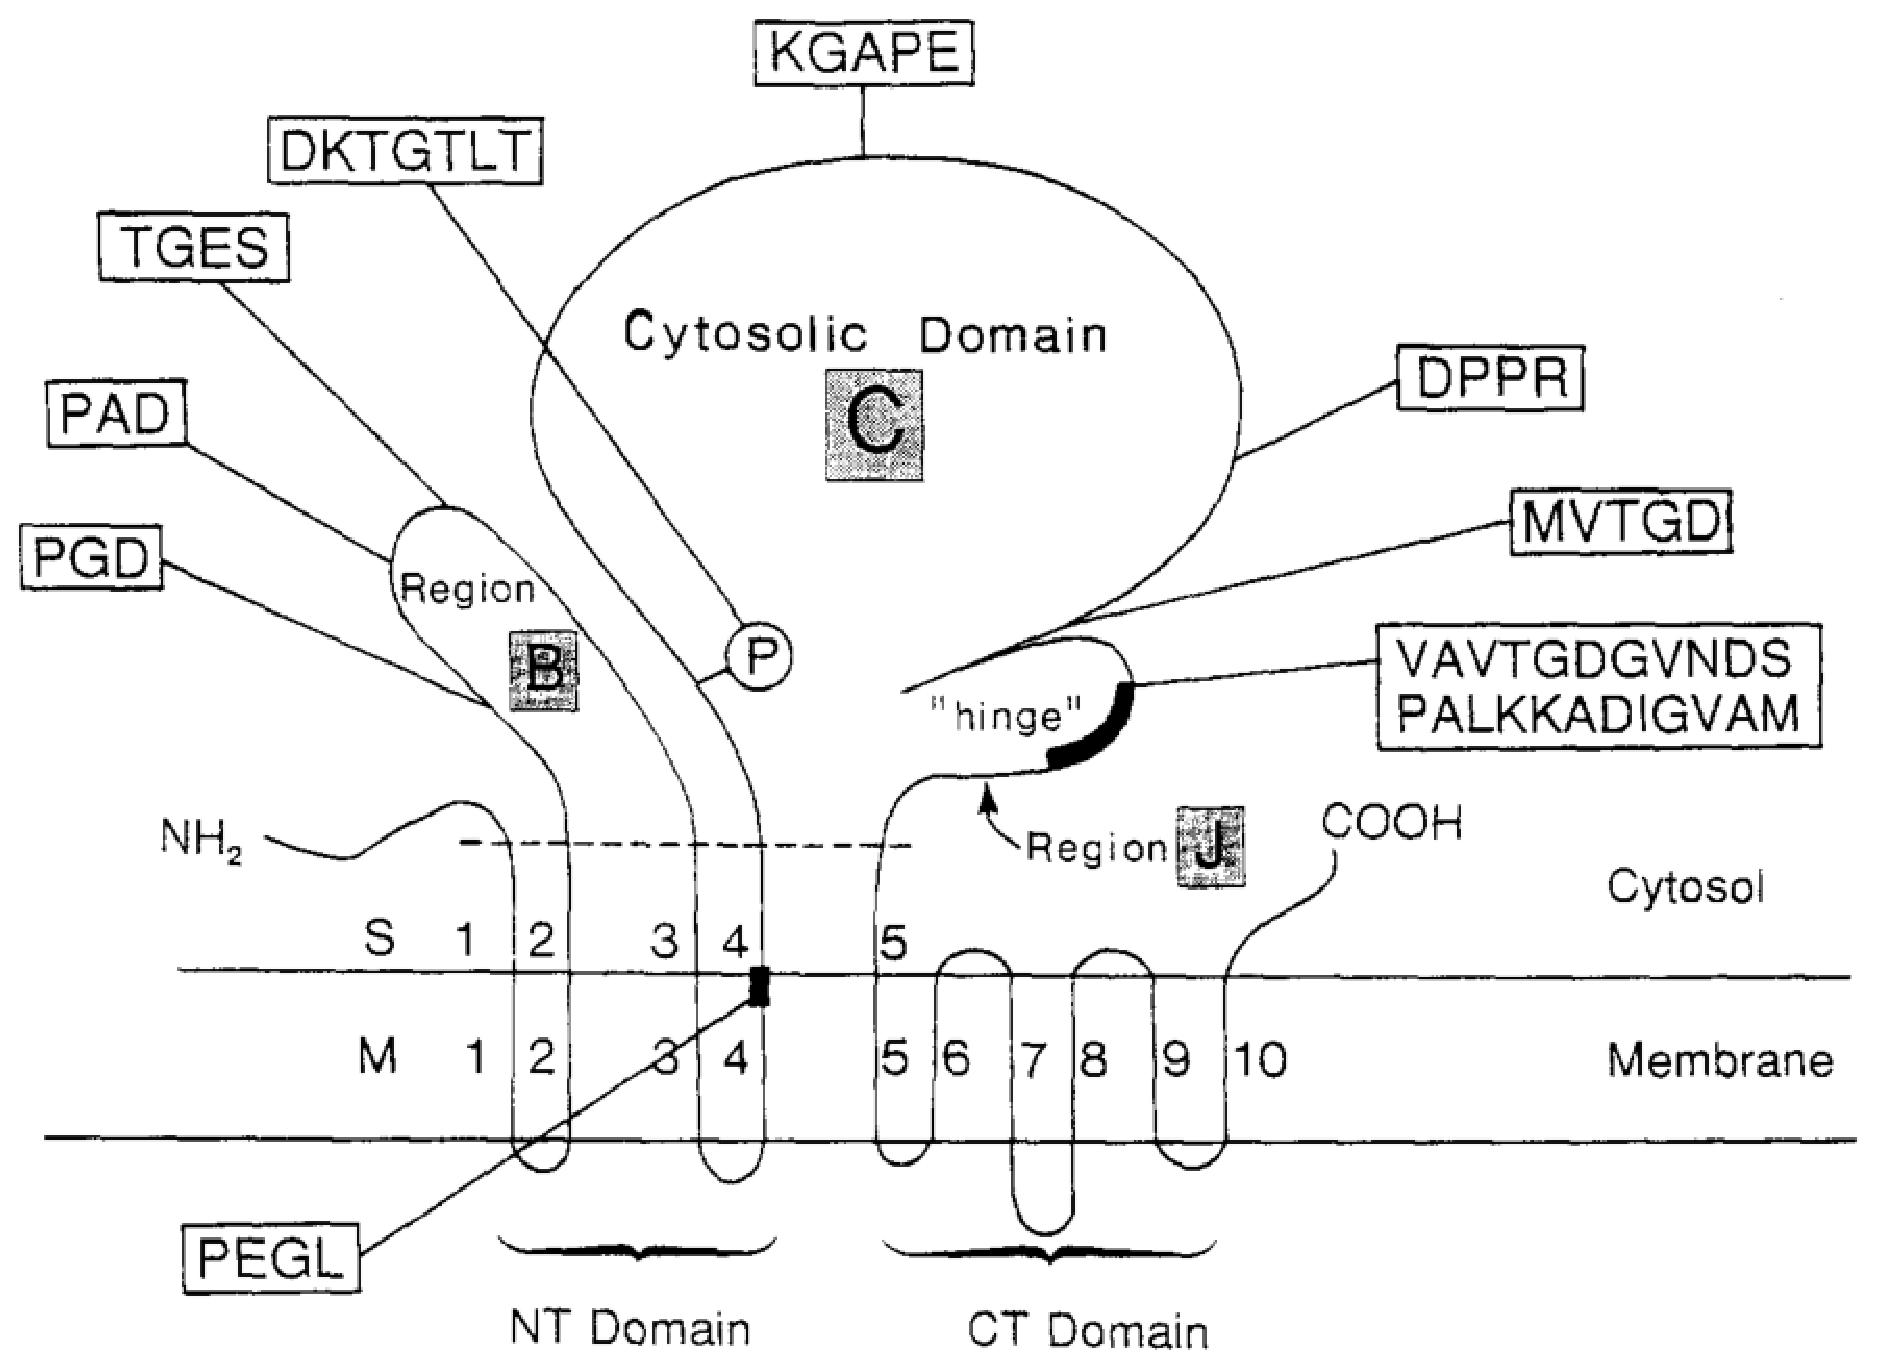
\includegraphics[height=5cm,
    angle=0]{./images/P-ATPase_type2.eps}}
\caption{Type II ATPases, represented by Na/K-ATPase \citep{moller1996}. In the
conserved region DKTGTLT, residue D is the reversibly phosphorylated Asp.}
\label{fig:P-ATPase_type2}
\end{figure}


\subsection{-- structural conformations}
\label{sec:P-ATPase-conformation}

Typically, prokaryotic P-type ATPases have lower molecular mass ($\approx
70$kDa), while eukaryotics P-type APTases have higher mass ($\approx
100-140$kDa).

Structurally, a P-type II ATPases is divided into N-terminal domain and
C-terminal domain, Fig.\ref{fig:P-ATPase_type2}. 
\begin{itemize}

  \item  N-terminal domain has 4 transmembrane helices (M1-M4), and the
  continuation of each polypeptide chain in the cytosolic side is projected as
  'stalk' segments (S1-S4).

Region B at the N-terminal part of the polypeptide chain linked to the membrane
by a number of {\it membrane traverses} \citep{moller1996}. 

  \item  C-terminal domain has 6 transmembrane helices (M5-M10). The cytosolic
  portions, comprising a 'small' and 'large' cytosolic loop, which can be
  removable by proteolytic digestion, are referred to as {\it Region B} and {\it
  Domain C}, respectively.

\end{itemize}
Domain C contains the phosphorylation site (at N-terminal end) and ATP-binding
site (in the central and C-terminal end). After the Domain C is a long stretch
of conversed sequence (known as {\it Region J}) (about 60 amino acid residues)
that connects to S5.


\begin{figure}[hbt]
    \centerline{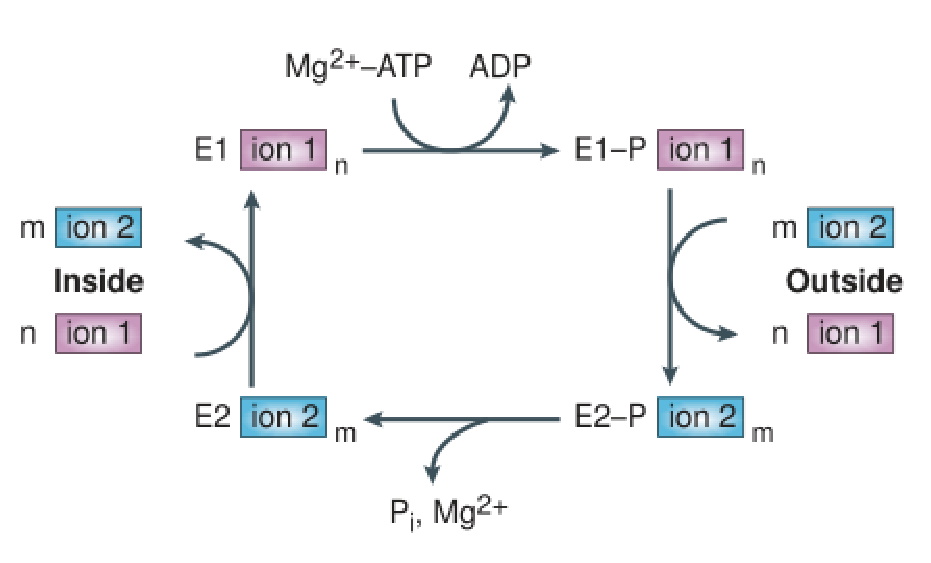
\includegraphics[height=4cm,
      angle=0]{./images/Post-Albers_cycle.eps}}
    \caption{General ion-translocation based on Post-Albers scheme
    \citep{kuhlbrandt2004}}
    \label{fig:Post-Albers-cycle}
  \end{figure}

Proteins belonging to the P-type ATPase share the conformation of an acid-stable
phosphorylated intermediate as part of its reaction cycle.
Given the above structure, typically, two major conformational state \ce{E1} and
\ce{E2} are assumed. Thus, P-ATPases are also referred to as E1/E2-ATPases.

The two states can be phosphorylated by ATP and hydrolysis Pi, respectively.
Nowadays, we know that there are other intermediate states; however, E1/E2
nomenclature is still almost universally accepted \citep{kuhlbrandt2004}. The reaction
mechanisms can be formulated in 4-step scheme, Fig.\ref{fig:Post-Albers-cycle}:
\begin{equation}
\ce{E1 ->[(1)] E1P ->[(2)] E2P ->[(3)] E2 ->[(4)] E1}
\end{equation}

In the case of Na/K-ATPase, it's called Post-Albers scheme \citep{post1972},
Fig.\ref{fig:serca_NaK_scheme}.

\begin{enumerate}

  \item Step 1: The binding of Ion1 (e.g. $\Na$ and $\K$ for Na/K-ATPase, $\Ca$
  for SER $\Ca$-ATPase) to the intracellular high-affinty site in E1 state
  triggers the phosphorylation of the enzyme by $\Mg$-ATP, resulting into the
  phosphorylated (intermediate) state \ce{E1P}. The intermediate \ce{E1P} is of
  the high-energy type, i.e. it can be dephosphorylated by ADP:
  \ce{E1P +  ADP -> ATP + \ldots}

NOTE: There are other factors that affect the rate of binding.

  \item Step 2: The translocation of the bound cations Ion1 (3Na for
  Na/K-ATPase, 2Ca for Ca-ATPase) across the membrane (from inside to outside)
  and conversion of the covalently bound  phosphate to a 'low-energy' type
  \ce{E2P}, which is unreactive with ADP. 
  
This new conformation (state) has a lower affinity to Ion1 ($\Na$ (for
Na/K-ATPase) and $\Ca$ (for Ca-ATPase)), allowing Ion1 to escape to the outside,
along with the binding of Ion2, i.e. state \ce{E2P}-Ion2.
  
  \item Step 3: Phosphate is removed from Asp residue of the enzyme by
  hydrolysis, giving the state \ce{E2} with Ion2 binding (which is $\K$ for
  $\Na/K$-ATPase, and $\H$ for $\Ca$-ATPase).
  
During this process, the terminal phosphate of ATP is transiently transferred to
aspartate (Asp) residue in the active site, resulting in reversible
conformational changes.

  \item Step 4: This step involves the translocation of other cations Ion2 (of
  2K for Na/K-ATPase, or 1-2H for Ca-ATPase) in the opposite direction. Enzyme
  returns to \ce{E1} state. This step is rate-limiting for Na/K-ATPase, where
  ATP modulation plays a crucial role for pump turnover.
  
  \item Starting a new cycle\ldots
\end{enumerate}

\begin{figure}[hbt]
  \centerline{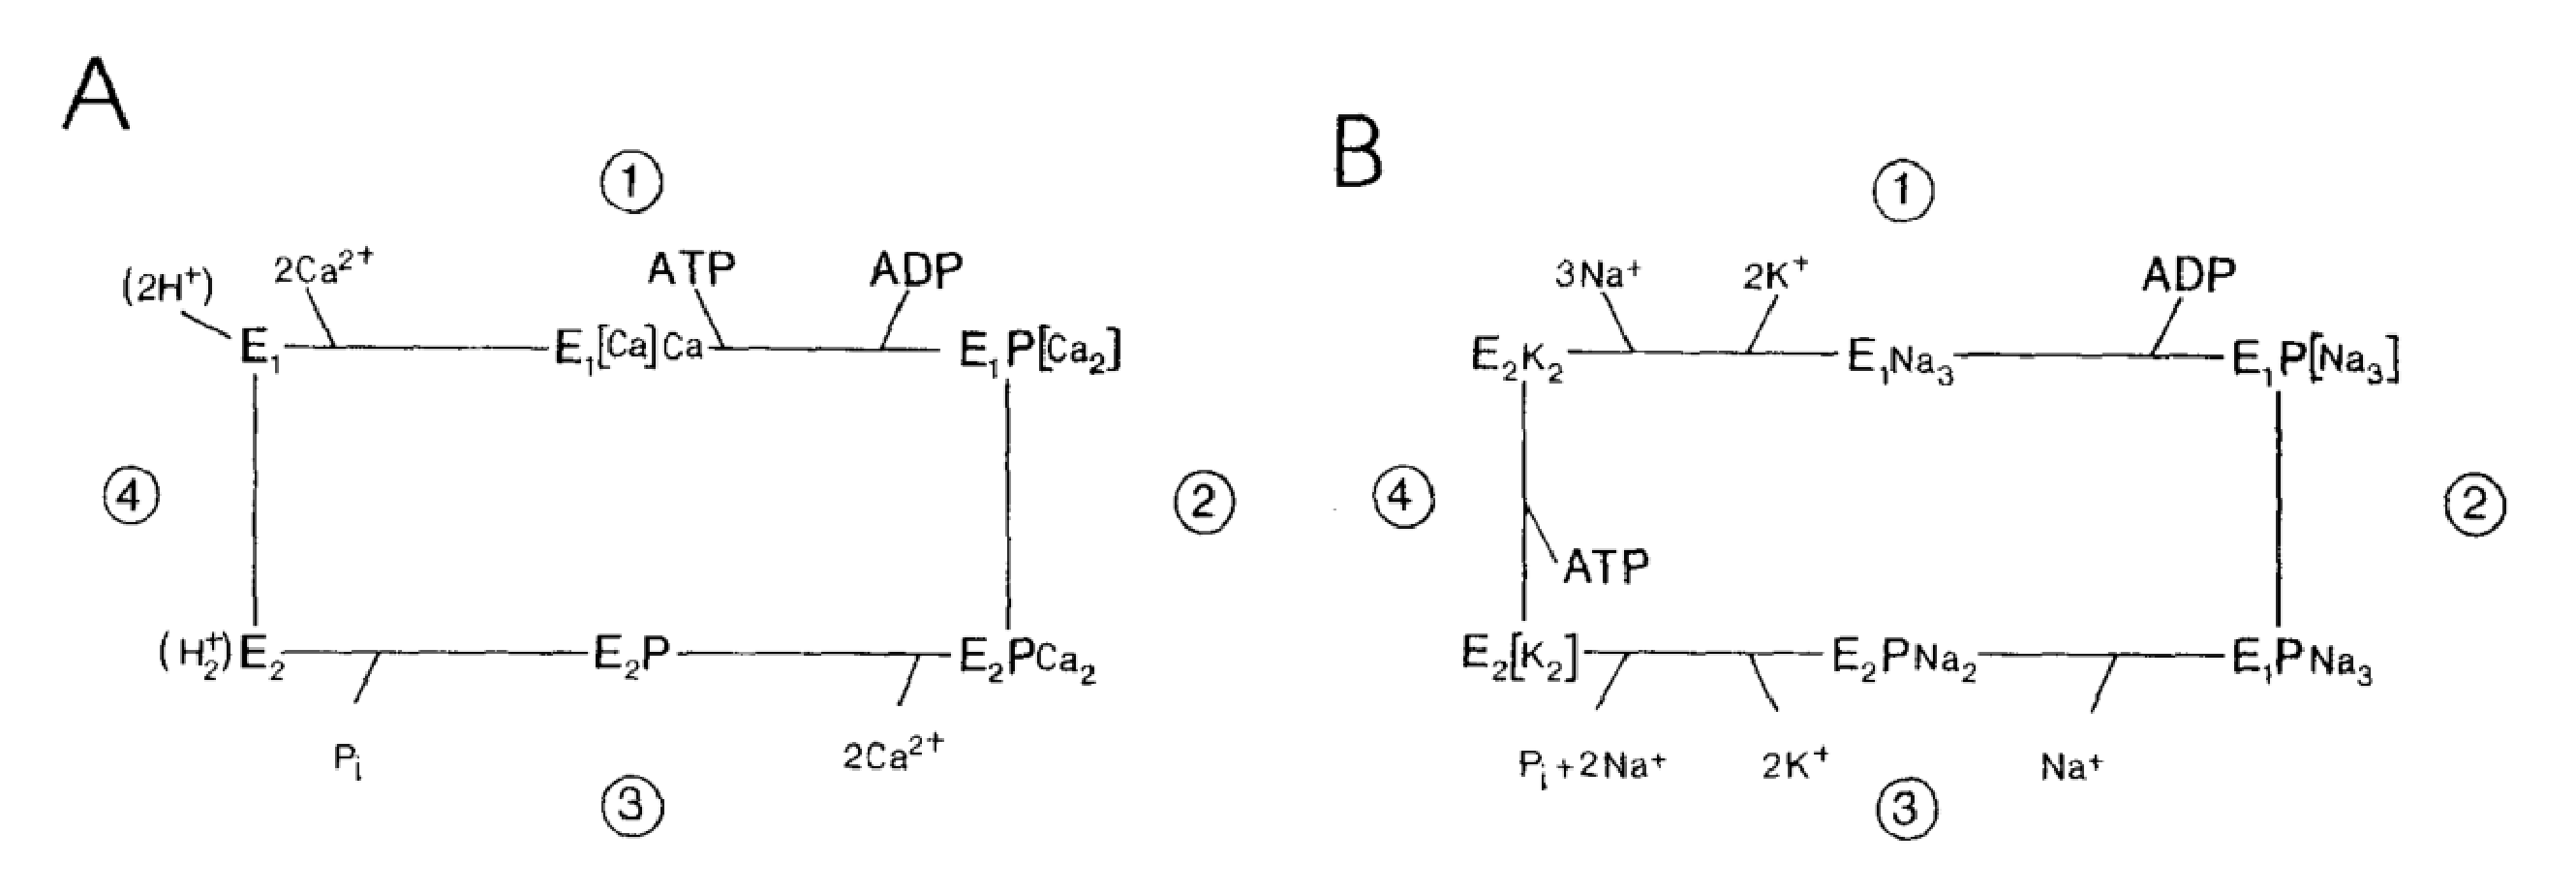
\includegraphics[height=5cm,
    angle=0]{./images/SERCA_NaK-scheme.eps}}
\caption{Kinetic scheme (A) SERCA-ATPase and (B) Na/K-ATPase \citep{moller1996}}
\label{fig:serca_NaK_scheme}
\end{figure}

Regardless of the reaction mechanism, a fundamental feature of $\Ca$ pumps is
the existence of occluded forms in steps associated with ion translocation, and
the feasibility of phosphorylation with inorganic phosphate (Pi) under \ce{E2}
state in which enzyme is unreactive with ATP or other high-energy phosphate compounds.
To stabilize the formation of transition state complex with ATPase, P-ATPases
can react with vanadate (instead of Pi). 



\subsection{AAA+ ATPase}
\label{sec:AAA+-ATPase}

{\bf Thorase} is an amino acid protein containing AAA+ ATPase domain composed of
\begin{itemize}
  \item ATP binding motif (Walker A)
  
  The mutated one is denoted as K193T or mA-Thorase.
  
  \item ATP hydrolysis motif (Walker B):
  
  The mutated one is denoted as E139Q, or mB-Thorase.
  
  \item N-linker (NL) domain: may transduce energy from ATP hydrolysis to the
rest of the protein

\item second region of homology (SRH): 
\end{itemize}

Thorase possesses ATPase activity with a $\Km$ of 43.4 $\muM$ and a $\vmax$ of
11.0 nM ATP/min/mg protein. The ATPase activity of Walker A and Walker B reduced
by 60\%-70\%, and greater than 90\%, respectively in the mutant containing both
mutations (mAB-Thorase).

Cellular distribution: Thorase is found
\begin{itemize}
  \item mainly in hippocampal CA1 pyramidal neurons
  \item at the synapse
  \item colocalize with postsynaptic marker PSD95, GluR1, and GluR2
\end{itemize}
Thorase is not expressed in axons. 



\section{Sar1}
\label{sec:Sar1}

Sar1 is a membrane trafficking protein, i

\section{Glutamate receptor-interacting protein (GRIP)}
\label{sec:GRIP}

Glutamate receptor-interacting protein (GRIP) is a family of protein binding to
glutamate receptors (Sect.\ref{sec:glutamate_receptor}), via interacting with
GluR2 subunit - a common subunit of AMPAR (Sect.\ref{sec:AMPAR}). 

\subsection{GRIP1}
\label{sec:GRIP1}

The structure of GRIP contains seven PDZ domains and binds to the C-terminus of
the GluR2 subunit of AMPA receptors (Sect.\ref{sec:AMPAR}). The AMPA receptor
amino acid sequence that the GRIP protein binds to is ESVKI (a conserved serine amino acid in the
C-terminal of both AMPAR and NMDAR).

Although the number of PDZ domains is different for the proteins PSD-95
(Sect.\ref{sec:PSD}) and GRIP, the PDZ domain is a common structural motif in
proteins that help mediate protein-protein interactions


\section{MAGUK}
\label{sec:MAGUK}

MAGUK is a superfamily of proteins: containing functional important domains:
mainly PDZ, SH3, and GUK; but many of them also contain regions homologous of
CaMKII, WW and L27 domains
\begin{enumerate}
  \item PDZ: short peptide binding sequences (80-90 amino-acids) commonly found
  at the C-terminus of interacting proteins.
  
  PDZ is an acronym combining the first letters of three proteins - post
  synaptic density protein (PSD95), Drosophila disc large tumor suppressor
  (Dlg1), and zonula occludens-1 protein (zo-1)  which were first discovered to
  share the domain.
  
  \item SH3: a protein-protein interaction domain of
  about 60 amino acids residues 
  
  They are found 
  in several other protein families such as: PI3 Kinase, Ras GTPase-activating
  protein, CDC24 and cdc25. One of the most well known features is that it can
  form an intramolecular bond with the GUK domain, creating what is known as a GUK-SH3 'closed' state.
  
  \item GUK: 
\end{enumerate} 

Members of MAGUK:  PSD95 (Sect.\ref{sec:PSD}), PSD-93, SAP97
(Sect.\ref{sec:SAP97}) and SAP102.

SAP97  and  PSD-95  can be alternatively spliced, with the $\alpha$-isoform
containing a double-cysteine/palmitoylation site, and the $\beta$-isoform having
an L27 domain at the N-terminus (Chatalov, 2009).

\begin{itemize}
  \item $\beta$-isoform of SAP97 is the most prevalent
   
  \item $\alpha$-isoform of PSD95 is the most prevalent
\end{itemize}

\section{GKAP}
\label{sec:GKAP}

guanylate kinase-associated protein (GKAP) is a family of scaffolding protein 



\section{Src-kinase}
\label{sec:Src-kinase}

Src family kinase is a family of non-receptor tyrosine kinases that include 9
members, i.e. they are not associated with cell-surface receptor:
\begin{enumerate}
  \item SrcA subfamily: Src (Sect.\ref{sec:Src}), Yes,  Fyn, and Fgr
  \item SrcB subfamily: Lck, Hck, Blk and Lyn
  \item Frn (its own subfamily)
\end{enumerate}
SrcA and SrcB subfamilies are specific to vertebrates.

\subsection{Src}
\label{sec:Src}

Src belong to SrcA subfamily of Src-kinase family (Sect.\ref{sec:Src-kinase}).
c-Src stands for "cellular Src kinase" and should not be confused with
"C-terminal Src kinase" (CSK) which is an enzyme which phosphorylates c-Src at
its C-terminus.

are not associated with a cell-surface receptor.
Src protein phosphorylates specific tyrosine residues in other proteins

Src is part of the NMDAR, Src, and Pannexin-1 complex (Sect.\ref{sec:NMDAR}).

\section{Protesome}
\label{sec:protesome}

% Cancer Treat Rev. 2003 May;29 Suppl 1:3-9.
% The proteasome: structure, function, and role in the cell.
% Adams J1.

The proteasome is a multisubunit enzyme complex that plays a central role in the
regulation of proteins that control cell-cycle progression and apoptosis, and
has therefore become an important target for anticancer therapy.

\section{STEP: striatal enriched protein tyrosine phosphatase}
\label{sec:STEP}

Striatal enriched protein tyrosine phosphatase (STEP) 
drives LTD in several ways.

\begin{enumerate}
  \item dephosphorylate the AR2 subunit of AMPAR, leading to removal of AMPAR
  from postsynaptic side
  
  \item inactivate Src by inhibiting Pyk2 (Sect.\ref{sec:Pyk2}), i.e. reducing
  Ca2+ influx via NMDAR.

NOTE: Src enhances NMDAR currents

  
\end{enumerate}

\section{Arachidonic acid (AA)}
\label{sec:arachidonic-acids}

Arachidonic acid (AA) is a polyunsaturated fatty acid present in the
phospholipids of biomembrane of cells. It is abundant in the brain, muscles, and
liver (Sect.\ref{sec:AA-production}).

AA can diffuse between cells and can act either directly or through metabolites
to alter cell functions and ionic currents (Piomelli and Greengard, 1990; Ordway
et al., 1991).

AA is a second messenger that is involved in regulation of signaling enzymes,
such as PLC-$\gamma$, PLC-$\delta$, and PKC-$\alpha$, and -$\beta$
isoforms; modulate synaptic transmission. 

The concentration at which AA occurs in tissues and cells is low: 2$\muM$
nonesterified arachidonate in the arterial blood of dogs (see Table 2 of Van der
Vusse et al., 1982), 9 - 16 $\muM$ in the plasma of rats (see Table 1 of Rapoport,
2003) and 5.3 - 13.1 $\muM$ in human plasma (see Burtis et al., 2006).
Much higher concentrations are found in secretagogue-stimulated pancreatic
islets; increments in cellular levels of 38 - 75 $\muM$ are reported by Wolf et
al. (1991). A total of 99.9\% of the non-esterified arachidonate is bound to
albumin. Therefore, the effects of fairly low (2 - 10 $\muM$) AA concentrations are of
particular interest.

It is important to distinguish between effects of AA itself and effects of AA
metabolites (Meves, 2008). Recently, the interest to functional role of AA has
been shifted from classical ion channels ($\Ca$, $\Na$ channels) to new types of
channels (TRP and non-SOCE channels).

\begin{enumerate}
  \item inhibits \textcolor{red}{HVA $\Ca$ channels} through free radical
  formation and PKC activatin (Keyser and Alger, 1990)
  
  \item either depress or enhance $\K$ current via lipoxygenase or
  cyclooxygenase metabolites (Keyser and Alger, 1990; Schweitzer et al., 1990;
  Zona et al., 1993): activate $\K$ channels in smooth muscle cell (Ordway et
  al., 1989), in cardiac muscle cells (Kim and Clapham, 1989).
 
In Aplysia, lipoxygenase metabolites of AA modulate S-type K+ channels (Piomelli
et al., 1987).

   \item enhance \textcolor{red}{NMDA-activated currents} (Miller et al., 1992).
   
   \item depress $\Na$ current in squid giant axon (Takenaka et al.,
1988) when AA at high concentration (ED$_{50}=0.18$ mM). 

In CONTROL: GABA release is induced by high $[\K]_o$ (56 mM, which activate
$\Ca$ channels) or veratrine (5 $\mu$g/ml) - which depolarize neurons by greatly
prolonging open times of $\Na$ channels (Barnes and Hille, 1988; Catterall,
1992).
AA diminished veratrine- but not K+-evoked release of [$^3$H]GABA suggests the
actions of AA on Na+ influx.

Fraser, MacVicar (1993) showed that AA 10 $\muM$ reversibly depressed the
amplitudeof INa, at all potentials (reduce 33\% at -10mV) in cultured neurons,
and reduce 30\% in acutely isolated neurons.

In Na+ channels of rat skeletal muscle, half inhibition occurs at 4 $\muM$ AA
(Bendahhou et al., 1997).

   \item modulate synaptic transmission in a complex way:
   AA enhances transmitter release at high concentrations (Freeman et al., 1990;
   Lynch and Voss, 1990) and inhibits at lower concentrations (Herrero et al.,
   1991).

A bidirectional action has been recently proposed for another intercellular
messenger, nitric oxide (Sect.\ref{sec:nitric-oxide}), which can play a positive
(Schuman and Madison, 1991) or negative (Izumi et al., 1992) role in regulating
long-term potentiation.

In striatal neurons, AA may affects the release of GABA from cultured striatal
neurons and acutely isolated striatal neurons (Fraser, MacVicar, 1993).
 
   \item TRP channels (Sect.\ref{sec:TRP-structure})
   
   \item SOCE channels (Sect.\ref{sec:SOC}) 
   
   \item non-SOCE channels:  
\end{enumerate}

\subsection{AA production}
\label{sec:AA-production}
\label{sec:arachidonic-acids-production}

Several neurotransmitters cause the release of AA by acting through
phospholipase A2 (Axelrod, 1990; Shimizu and Wolfe, 1990)

Arachidonic acid is a 20-carbon omega-6 poly-unsaturated fatty acid.
AA is freed from membrane phospholipid molecule by the enzyme
phospholipase A2 (PLA2 - Sect.\ref{sec:PLA2}), or can also be generated from DAG
(Sect.\ref{sec:DAG}) by diacylglycerol lipase (DAG lipase).
\begin{verbatim}
DAG lipase ---[cleave off DAG]----> arachidonic acid 
\end{verbatim}



\section{Nitric oxide (NO)}
\label{sec:nitric-oxide}

Nitric oxide (NO), the smallest signalling molecule known, is produced by three
isoforms of NO synthase (NOS; EC 1.14.13.39) - Sect.\ref{sec:NO-synthase}.

{\bf Nitric oxide}, a freely diffusible gas, is produced by
\begin{itemize}
  \item  several metabolic pathways in the mitochondrion and in the surrounding
  cell and has widespread effects on mitochondrial function either as NO,  or
  following conversion to peroxynitrite (\ce{ONOO^-}), or other reactive
  nitrogen species (RNS). 
  
  The precise metabolic pathways are controversial (Lacza 2009). 
\url{https://www.ncbi.nlm.nih.gov/pmc/articles/PMC4570492/}

Nonetheless, some, but not all, studies have provided evidence indicating that a
mitochondrial variant, named mtNOS, may be present in the inner mitochondrial
membrane or matrix.  

conventional NOS isoforms may be associated with the outer mitochondrial
membrane and represent an alternative, externally regulated source of NO to the
interior of the mitochondria (see next item). 

  \item 3 isoforms of NOS - Sect.\ref{sec:NO-synthase} nNOS, iNOS, eNOS.
  
  These enzymes convert L-arginine to NO and L-citrulline
  
\end{itemize}

Once formed, NO can diffuse into mitochondria from the surrounding cellular
space or could traverse longer distances from other, more remote cells.
\textcolor{red}{Remarkably, nanomolar concentrations of NO can inhibit
mitochondrial respiration, so even a small amount of NO in the mitochondrial
matrix may regulate ATP synthesis.}
\url{https://www.ncbi.nlm.nih.gov/pubmed/16051505/}


Similar to AA (Sect.\ref{sec:arachidonic-acids}), a bidirectional action has
been recently proposed for another intercellular messenger, nitric oxide
(Sect.\ref{sec:nitric-oxide}), which can play a positive (Schuman and Madison,
1991) or negative (Izumi et al., 1992) role in regulating long-term
potentiation.



\section{Tyrosine receptor kinase (Trk)}
\label{sec:Trk}

Trk are  transmembrane proteins and are receptors of neurotrophin
(Sect.\ref{sec:neurotrophin}).
Upon binding of a proper neurotrophin, Trk member then can activate many
intracellular signaling pathways, including those controlled by Ras, the
Cdc42/Rac/RhoG protein family, MAPK, PI3K and PLC-gamma.

Several novel signaling pathways controlled by Trk receptors have been
characterized, and it has become clear that membrane transport and sorting
controls Trk-receptor-mediated signaling because key intermediates are
{\bf localized to different membrane compartments}.

Differential splicing also generates an isoform of TrkC with a modified kinase
domain that has altered substrate specificity, and isoforms of TrkB and TrkC
that lack kinase domains.

A second signal, such as cAMP or Ca2+ (Sect.\ref{sec:calcium-function}), is
required for efficient insertion of receptors into the surface membrane.

\subsection{Trk-A}
\label{sec:Trk-A}

Trk-A is the receptor of NGF (Sect.\ref{sec:NGF})

Ubiquitination is a reversible post-translational modification involved in a
plethora of different physiological function. Among the substrates that are
ubiquitinated, neurotrophin receptors (TrkA, TrkB, TrkC, and p75NTR) have been
studied recently. TrkA is the most studied receptor in terms of its
ubiquitination. Sect.\ref{sec:ubiquitin} discusses ubiquitin.


\subsection{Trk-B}
\label{sec:Trk-B}

The receptor tyrosine kinase TrkB (also known as NTRK2) is the receptor of
neurotrophin BDNF (Sect.\ref{sec:BDNF}). Differential splicing also generates an
isoform of TrkB  that lack kinase domains.

TrkB is known primarily for its function during PNS and CNS development, has
emerged in recent years as a potent regulator of hippocampal LTP. Understanding
the mechanisms that underlie learning is one of the most fascinating and central
aims of neurobiological research. Hippocampal long-term potentiation (LTP) is
widely regarded as a prime candidate for the cellular mechanism of learning
(review: Minichiello, 2009)

The phosphorylation of striatal TrkBRs occurs in response to
depolarization-induced release of BDNF by cortical terminals.

\subsection{Trk-C}
\label{sec:Trk-C}

Trk-C is the receptor of neurotrophin NT-3 (Sect.\ref{sec:NT-3})

Differential splicing also generates an isoform of TrkC with a modified kinase
domain that has altered substrate specificity, and isoforms of TrkB and TrkC
that lack kinase domains.


%%% Local Variables: 
%%% mode: latex
%%% TeX-master: "mainfile"
%%% End: 

\section{Amyloid-beta}
\label{sec:amyloid-beta}

The level of A$\beta$ plaque can be detected using a sensitive sandwich ELISA
system (Green et al., 2008).

A$\beta_{1-40}$

A$\beta_{1-42}$


\section{MAP: microtubule-associated protein}
\label{sec:MAP}

Tau (Sect.\ref{sec:tau-protein}) is the major microtubule associated protein
(MAP) of a mature neuron.  The other two neuronal MAPs are MAP1
(Sect.\ref{sec:MAP1}) and MAP2 (Sect.\ref{sec:MAP2}).

\subsection{MAP1}
\label{sec:MAP1}

\subsection{MAP2}
\label{sec:MAP2} 




\subsection{tau protein: MAPT gene}
\label{sec:tau-protein}
\label{sec:MAPT-gene}
\label{sec:tau}

Tau proteins are proteins that perform the function of stabilizing microtubules.
Tau proteins belong to the microtubule-associated proteins (MAP) family -
Sect.\ref{sec:MAP}. The proteins work together with a globular protein called
{\bf tubulin} to stabilize microtubules and aid the assembly of tubulin in the
microtubules. Tau proteins - as a phosphoprotein - achieve their control of
microtubule stability through its different isoforms and phosphorylation state
(Sect.\ref{sec:tau-phosphorylation}).

These proteins are abundant in nerve cells and are present to a much lesser
degree in oligodendrocytes and astrocytes.

IMPORTANT (SUBCELLULAR-LOCATION): Tau proteins are \textcolor{red}{mainly active
in the distal portions of axons} where they stabilize microtubules as well as
providing flexibility.

Tau proteins are produced through alternative splicing of a single gene called
MAPT ({\bf microtubule-associated protein tau}). The proteins were discovered in
Marc Kirschner's laboratory at Princeton University in 1975.

The proteins work together with a globular protein called tubulin to stabilize
microtubules and aid the assembly of tubulin in the microtubules. 

\subsection{-- phosphorylation of tau protein}
\label{sec:tau-phosphorylation}

Hyperphosphorylation of tau depresses the biological activity of tau
(Sect.\ref{sec:tau}). So dephosphorylation may contribute to the disease
progression.  The four phosphatases (PP1, PP2A, PP2B and PP5 -
Sect.\ref{sec:protein-phosphatase}) all dephosphorylated tau at Ser199, Ser202,
Thr205, Thr212, Ser214, Ser235, Ser262, Ser396, Ser404 and Ser409, but with
different efficiencies toward different sites.

High levels of the serine/threonine PPases are found throughout the
brain, with PP1, PP2A, PP2B, and PP5 being abundant and implicated in AD.

\begin{itemize}
  \item  The K(m) values of tau dephosphorylation catalysed by PP1, PP2A and PP5
  were 8-12 $\muM$, similar to the intraneuronal tau concentration of human
  brain, whereas the K(m) of PP2B was fivefold higher. 
  
  \item PP2A is the major tau phosphatase that regulates its phosphorylation at
  multiple sites in human brain (Liu, Gong, 2005).
  
PP2A, PP1, PP5 and PP2B accounted for approximately 71\%, approximately 11\%,
approximately 10\% and approximately 7\%, respectively, of the total tau
phosphatase activity of human brain. 

The total phosphatase activity and the activities of PP2A and PP5 toward tau
were significantly decreased, whereas that of PP2B was increased in AD brain.

\end{itemize}


\subsection{-- tauopathies}
\label{sec:tauopathies}

Neurological disorders related to dysfunction of tau proteins are called {\bf 
tauopathies} (Sergeant et al., 2005). Many etiological factors,
phosphorylation, splicing, and mutations, relate Tau proteins to neurodegeneration.
\textcolor{red}{Normal adult human brain tau contains 2-3 moles phosphate/mole
of tau protein.}
Abnormally hyperphosphorylated tau is a key feature of human tauopathies.
Although we are not sure whether phosphorylation rather than oligomerization of
tau (Sect.\ref{sec:tau-oligomers}) is an initial molecular event in tau
pathogenesis

\begin{itemize}
  \item  AD (Sect.\ref{sec:tau-Alzheimer}): hyperphosphorylated tau proteins.
  

In Alzheimer disease (AD) brain tau is $\tilde{}$ three to four-fold more
hyperphosphorylated than the normal adult brain tau and in this
hyperphosphorylated state it is polymerized into paired helical filaments
([PHF]) admixed with straight filaments (SF) forming neurofibrillary tangles.

Some research suggests that an exosome-based mechanism may be responsible for
the release of tau proteins in Alzheimer's disease. 

\item 
\end{itemize}


\subsection{-- properties}

Tau protein has several unique characteristics such as natively unfolded
conformation, thermo-stability, acid-stability, and capability of
post-translational modifications.


\subsection{-- biomarkers}

$^{18}$F-THK523 as a tauopathy marker, i.e.
binds specifically to tau tangles.

\subsection{-- tau oligomers: NFT}
\label{sec:tau-oligomers}
\label{sec:NFT}

We still do not know whether tau itself is toxic. 

Researchers are now looking for 'tau oligomers' as toxic components, because
'tau oligomers' contain variable species of tau protein [e.g., dimer (disulfide
bond-dependent or -independent), multimer (more than dimer), granular (defined
as EM or AFM) and perhaps small filamentous aggregates ] (Sahara, Avila, 2014).

{\bf Neurofibrillary Tangles} (NFTs) are aggregates of hyperphosphorylated tau
protein that are most commonly known as a primary marker of Alzheimer's disease. 

Although we do not know the exact forms of toxic tau oligomers, accumulating
evidence has shown the probability of tau oligomer propagation from cell to
cell.
However, the mechanism of tau transmission from cell to cell is still unknown. 

Research focusing on extracellular tau will open potential new avenues for
discovering the mechanism of tau propagation.


\section{Cyclic nucleotide (cNMP): cAMP and cGMP}
\label{sec:cyclic-nucleotide}


A {\bf cyclic nucleotide} (cNMP) is a nucleotide (Sect.\ref{sec:nucleotide})
with {\bf single}-phosphate group and a cyclic bond arrangement between the
sugar ring and that phosphate group. Like other nucleotides, cyclic nucleotides
are composed of three functional groups: a sugar, a nitrogenous base (R-), and a
single phosphate group (\ce{PO_4^-}).


There are two types of cyclic nucleotide: cyclic adenosine 3',5'-monophosphate
(cAMP - Sect.\ref{sec:cAMP}) and cyclic guanosine 3',5'-monophosphate (cGMP -
Sect.\ref{sec:cGMP}) which were identified in late 50s and early 60s. 
\begin{itemize}
  \item cAMP-dependent pathways - Sect.\ref{sec:cAMP-dependent_pathway}
  
  \item cGMP-dependent pathways - Sect.\ref{sec:cGMP-dependent-pathways}
\end{itemize}
As second messengers, cAMP and cGMP concentration controls the strength of the
many cellular signals; and such concentrations are determined by the balance
between production and degradation of cAMP (Sect.\ref{sec:cAMP}) and cGMP
(Sect.\ref{sec:cGMP}). Their intracellular concentration is controlled by a
complex family of PDE (Sect.\ref{sec:PDE}), i.e.
activation PDE (Sect.\ref{sec:PDE}) cleaves the 3',5'-cyclic phosphate moiety of
cAMP/cGMP to produce the corresponding 5'-nucleotide (i.e. cGMP is converted to
5'-GMP and cAMP is converted to 5'-AMP) \citep{fischmeister2006}.

\begin{framed}

cAMP and cGMP are both second-messenger that affect cGMP-dependent protein
kinase (PKG - Sect.\ref{sec:PKG}), cAMP-dependent protein kinase (PKA) -
Sect.\ref{sec:PKA}, cAMP-regulated guanine nucleotide exchange factors
(cAMP-GEFs) - Sect.\ref{sec:cAMP-GEF}, and PDEs (Sect.\ref{sec:PDE}) (even
though PDEs also control the degradation of cAMP/cGMP). However, it is important
to remember that there are different members in the PDE family, and each play a
certain role at a certain cell type, for a certain signaling pathways.

A proper knowledge of how they are produced or degraded, what do they target
effectors by either covalent ({\it phosphorylation}) or non-covalent ({\it
direct binding to proteins, e.g. ion channels or guanine-nucleotide-exchange
factors}).

\end{framed}

\subsection{cAMP (cyclic AMP) and CREB}
\label{sec:cAMP}
\label{sec:CREB}

The 3', 5'-cyclic adenosine monophosphate (cAMP) is one type of cyclic
nucleotide (Sect.\ref{sec:cyclic-nucleotide}) and function as second messengers
within cells. It was first described by Sutherland and Rall in 1957.

cAMP provides regulatory signal via specific cAMP-binding proteins
(Sect.\ref{sec:cAMP-dependent_pathway}).  
\begin{itemize}

  \item cAMP production: Sect.\ref{sec:cAMP-production}
  
  \item inhibition of cAMP's hydrolysis  by sodium fluoride and caffeine. 

REMEMBER that caffeine is a phosphodiesterase (PDE) inhibitors. 
Among \textcolor{red}{11 families of PDE-I}, with at least 20 genes and 50
unique isoforms, only PDE4, PDE7 and PDE8 are cAMP-specific \citep{Conti2003}
(Sect.\ref{sec:PDE-I}).
  
cAMP is hydrolized by PDE10A (Sect.\ref{sec:PDE10}), thus the level of PDE10A is
important in regulating cAMP's function. The level of cAMP can be assessed using
phosphorylation status of CREB.

   \item cAMP function: Sect.\ref{sec:cAMP-function}
\end{itemize}


{\bf CREB} (cAMP-response element-binding protein), which is a transcription
factor and phosphorylated cAMP-response element-binding protein (pCREB), is a
downstream factor of cAMP; so the phosphorylation status of CREB, i.e.
level of pCREB, can be used to indirectly infer the level of cAMP.
pCREB is measured using a pCREB enzyme linked immunosorbent assay
(ELISA) kit (Cat No. KHO0241, Invitrogen Corp., Carlsbad, CA).

\textcolor{red}{CREB stabilize the memory formation in brain}
\begin{itemize}
  \item  decreasing CREB function blocks long-term changes in synaptic function,
  but not short-term ones.
  
IMPOTANT: CREB is necessary for the late stage of long-term potentiation. 

  \item disturbance of CREB function in brain can contribute to the development
  and progression of Huntington's Disease  (Sect.\ref{sec:HD-role-of-PDE10-loss}). 

\end{itemize}

$\Ca$ elevation (via NMDAR and/or VSCC and/or ER $\Ca$ release) induces the
activity of CaKMII (Sect.\ref{sec:CaMKII}), resulting the activation of the
kinases (PKA, PKC and CK2) and translocate to the cell nucleus. These proteins
phosphorylate CREB at Ser-133, i.e. becoming pCREB.
pCREB recognize cAMP Response Element.
% cAMP and $\Ca$ activates a protein kinase which translocates to the
% cell nucleus, where it activates a CREB protein via PKA-mediated
% phosphorylation of cAMP-response element binding protein (CREB becomes pCREB)
% at Ser-133.

Even though CREB was found to occupy about 4000 promoter sites {\it in
vivo}; only a small proportion of CREB target genes was induced by cAMP in any
cell type. In addition, Zhang et al. (2005) found that CREB phosphorylation
alone is not a reliable predictor of target gene activation and that additional
CREB regulatory partners are required for recruitment of the transcriptional
apparatus to the promoter.

\begin{enumerate}
  \item NMDA and D1-receptors modulate pCREB levels in the caudate nucleus
  and suggest mutual permissive roles for both receptors (Nijholt et al., 2002).
  %Brain Res Gene Expr Patterns
  %In vivo CREB phosphorylation mediated by dopamine and NMDA receptor
  % activation in mouse hippocampus and caudate nucleus.
  

Later, it was showed that D1 receptors mediate CREB phosphorylation via
phosphorylation of the NMDA receptor at Ser897-NR1 (Dudman et al., 2003)

  \item  D1 receptors alters the properties of L-type Ca2+ channel inhibitors
  and turns them into facilitators of Ca2+ influx. (Eaton et al., 2004)
  
\end{enumerate}

\subsection{-- distribution}
\label{sec:cAMP-concentration}

\citep{Rall1958} found that cAMP is produced not only in liver, but in other
cell types (Sect.\ref{sec:cAMP-production}). \citep{Ashmana1963} found both cAMP
and cGMP in rat urine.

To detect cAMP, we can use FRET-based cAMP imaging (Sect.\ref{sec:FRET})
\begin{itemize}
  \item GFP-tagged PKA 
  
  \item 
\end{itemize}

\subsection{-- production}
\label{sec:cAMP-production}

cAMP typically is the product of adenylate cyclase (AC) class III
(Sect.\ref{sec:AC-III}) [in  human, it's AC-IIIa] in response to epinephrine and
glucagon [NOTE: cGMP produced by guanylate cyclase (GC -
Sect.\ref{sec:guanylate-cyclase})].

REMINDER: Among 10 known isoforms of AC-IIIa, 9 of them are membrane-bound,
each modulated by a different set of regulators.


Interestingly, however, there are other receptors that also produce cAMP to
translate its signal but generate different effects. This was hypothetized that
the temporal and spatial change of cAMP play an important role in responsible
for the specific functional roles of the signal pathways that use cAMP
\citep{Zaccolo2002}. 

\begin{enumerate}
  \item $\beta$-AR stimulation
  
  \item cAMP concentration is increased by NaF, caffeine (as inhibiting the enzyme(s)
hydrolyzing this compount), and epiphrine, glucagon \citep{Rall1958}.

  \item 
\end{enumerate}

Even though local generation of cAMP has been described
\citep{brunton1981, Buxton1983}, the range of actions are controversial
\begin{enumerate}
  
  \item  cAMP's range of action has been reported to be tens to hundreds $\mum$. 
  
  
  \item cAMP's range of action only as small as about 1$\mum$, with cAMP
  created in microdomains with very high concentration.
  
This was found in cardiac myocytes, cAMP production via $\beta$-AR stimulation
\citep{Zaccolo2002}. Such high gradient of cAMP can activate PKA anchored to the T-tubules membrane,
providing a mechanism for $\beta$-AR stimulus selectivity. 

  \item Using FRET-based cAMP imaging, \citep{Nikolaev2006} showed that
  $\beta_1$-AR stimulation (Sect.\ref{sec:beta-adrenergic_stimulation}) produce
  cAMP that propagate throughout entire of the cell, while $\beta_2$-AR
  stimulation produce cAMP with a smaller localized increase cAMP that doesn't
  propagate even in the presence of PDE inhibitors \citep{lisa2006}
  (Sect.\ref{sec:PDE}).

  \item 
\end{enumerate}
\ref{sec:PKA}

\subsection{-- cAMP production in Dictyostelium (slime mold)}
\label{sec:cAMP-production-Dictyostelium}
\label{sec:Dictyostelium}

The slime mold {\it Dictyostelium discoideum} is a eukaryotic organism that feed
on bacteria. When food (bacteria) are plentiful, the cells forage independently;
while when it becomes scarce, the population come together to form first a
motile 'slug', and then a fruiting body, which scatters Dictyostelium spores in
the environment.

Aggregation into a slug involves cell-to-cell communication mediated by
secreated cAMP (i.e. extracellular cAMP). The concentration of cAMP oscillates
in waves across the colony, thus directing the cells to an aggregation point.

\begin{figure}[hbt]
 \centerline{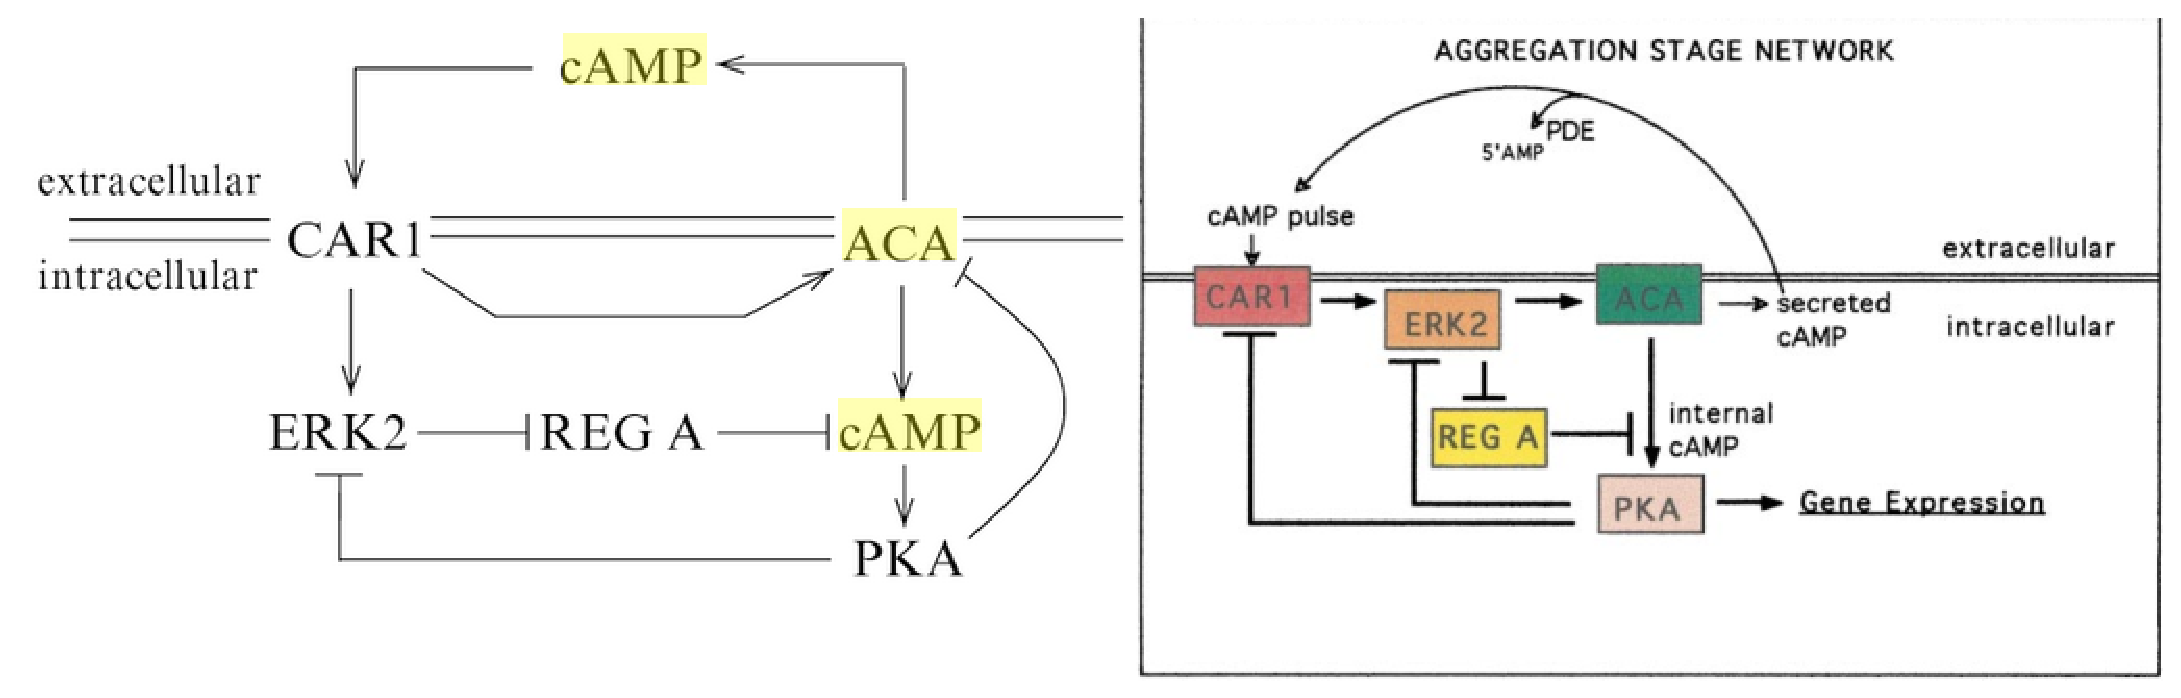
\includegraphics[height=3cm]{./images/cAMP-oscillation-Dictyostelium.eps}}
 \caption{Model of cAMP oscillation}
\label{fig:cAMP-oscillation-Dictyostelium}
\end{figure}

Model of the {\bf oscillation of intracellular cAMP level for Dictyostelium} was
first proposed by Michael Laub and William Loomis (1998) with a periodicity of 7
minutes, Fig.\ref{fig:cAMP-oscillation-Dictyostelium}. 

\begin{itemize}
  \item \textcolor{red}{Positive feedback}:
  \begin{enumerate}
  \item  extracellular cAMP binds to surface receptor CAR1 (Sect.\ref{sec:CAR1})
  
  activated CAR then cause  adenylyl cyclase (ACA) and the MAP kinase ERK2 
  transiently activated; each however function oppositely in terms of regulating
  cAMP
  
  \item activated ACA produces intracellular cAMP

  \end{enumerate}

  \item \textcolor{red}{Negative feedback}: 2-3 mins after the stimulation of
  cells with external cAMP and the activation of ACA, there is a rapid 5- to
  10-fold reduction in the affinity of CAR1  to  cAMP  and  a  consequent 
  reduction  in  ACA activity  (Caterina et al.,  1995a,b).  
  Thus, ligand binding oscillates in response to the levels of external cAMP.
  
  \begin{enumerate}

    \item A rise in the internal concentration of cAMP activates protein kinase
   A such that it inhibits ERK2 and leads to a loss-of-ligand binding by CAR1

    \item ERK2 phosphorylates the cAMP phosphodiesterase REG A that reduces the
  internal concentration of cAMP.
  
    \item After each peak (pulse), extracellular cAMP is rapidly hydrolyzed by a
  secreted PDE; whereas  intracellular  cAMP  is hydrolyzed by an intracellular
 phoshodiesterase (REG A)

  \end{enumerate}
%A secreted phosphodiesterase reduces external cAMP concentrations between
% pulses.
\end{itemize}
Experimental finding showed that cells become refractory to stimulus by
cAMP (e.g. adding exogenous cAMP) soon after responding to cAMP and then become
excitable again when the stimulus is removed.


The model is robust in that 25-fold changes in the kinetic constants linking the
activities have only minor effects on the predicted frequency. Moreover,
constant high levels of external cAMP lead to attenuation, whereas a brief pulse
of cAMP can advance or delay the phase such that interacting cells become
entrained.   


Maede (2004) showed spontaneous oscillations in activation of the
mitogen-activated protein (MAP) kinase ERK2 that occur in phase with peaks of
cAMP, and show that ERK2 modulates cAMP levels through the phosphodiesterase
RegA. Similar oscillatory processes may occur in cells of many different
species.

The robust circuit modeled here produces the spontaneous oscillations in cAMP
observed during the early development of D. discoideum and can account for the
synchronization of the cells necessary for chemotaxis and further development.



\subsection{-- function}
\label{sec:cAMP-function}

cAMP has been regarded as a freely diffusible second messenger that mediates the
action of a number of different receptors and modulates many cellular functions,
as diverse as cell (movements, growth, metabolism) and synaptic plasticity.
\begin{itemize}
  \item  {\bf In the heart}, cAMP is generated upon $\beta$-AR stimulation
  and is probably the most important modulator of sympathetic control over
  cardiac contractility by binding to different proteins.
  
  \item  The agent SKF 83822 is exclusively activates the cAMP pathway (Rashid
  et al., 2007) so it is used to study the functional role of cAMP.

  \item In 1970s, studies focused on cAMP's role in immune and inflammatory
  diseases: immunomodulatory properties of cAMP and the anti-inflammatory
  potential of PDE inhibitors (Lichtenstein et al.)

Also, during this time, the superfamily of PDE enzymes was born, as PDE
activities from tissue homogenate were found there exists pharmacokinetically
and biologically distinct PDE subtypes and that the relative amounts of these
PDEs varied among different tissues.
Then, the idea of using selective PDE inhibitors to target specific tissues,
pathways, and disease processes was first postulated (Sect.\ref{sec:PDE}).

  \item 
\end{itemize}


The important questions are: \textcolor{red}{Do cAMP/cGMP and their effectors
freely diffuse inside the cell or are they localized?} If they localize, do they
have any physiological or pathophysiological role? \citep{fischmeister2006}.


\begin{enumerate}
  \item the predominant downstream effector of cAMP is PKA - (Sect.\ref{sec:PKA}).

Most of cAMP effect on cell's function is via protein phosphorylation of PKA.
However, PKA is largely compartmentalized by an anchoring protein name AKAPS
(A-kinase anchoring proteins) - Sect.\ref{sec:AKAP}.  
   
  \item  
  \item 
\end{enumerate}


Other than the theory of cAMP local generation, the localization of effectos
like PKA can also affect the functional role of cAMP. In other words, there have
been some evidences that these proteins are not uniformly distributed
\begin{enumerate}
  \item Gs heterotetrameric guanine nucleotide-binding proteins [8]
  \item Adenylyl cyclases (AC) [8.9]
  \item AKAP-anchored PKA [10]
  \item L-type $\Ca$ channels: [9]
  \item Phosphodiesterases (PDE) \citep{Dodge2001} (Sect.\ref{sec:PDE}):
  localize to specific subcellular domains via binding to AKAP.
  
  In striatum, we focus on PDE10A (Sect.\ref{sec:PDE10})
\end{enumerate}
This provides potential anatomical basis for the local generation of cAMP.





\subsection{cGMP}
\label{sec:cGMP}

Both cAMP and cGMP are second messengers
within cells. \citep{Ashmana1963} found both cAMP and cGMP in rat urine.
Compared to cAMP, cGMP has a lower concentration, and thus is believed to play a
lesser role in cell function. As cGMP is hydrolized by PDE10
(Sect.\ref{sec:PDE10}), the level of PDE10A is important in regulating cGMP
function. 
\begin{itemize}
  \item  cGMP is measured using a cGMP enzyme immunoassay (EIA) kit (Cat No.
  581001, Cayman Chemical, Ann Arbor, MI)
\end{itemize}


The physiological role of cGMP has been found recently on
\begin{itemize}
  \item retina: cGMP mediates the effect of light on cation channels
  \item cGMP inhibits specific forms of PDE
\end{itemize}




\section{cAMP-regulated guanine nucleotide exchange factors (cAMP-GEFs, Epacs)}
\label{sec:cAMP-GEF}
\label{sec:Epacs}

cAMP-regulated guanine nucleotide exchange factors (cAMP-GEFs) are also called
exchange proteins directly activated by cAMP (Epacs).



\section{GAD (Glutamic Acid Decarboxylase)}
\label{sec:GAD}
\label{sec:GAD-enzyme}
% \label{sec:Glutamate-decarboxylase}
% \label{sec:GAD-Glutamate-decarboxylase}

Glutamic Acid Decarboxylase (GAD) is an enzyme that catalyzes the
decarboxylation of glutamate to GABA and CO2 (Sect.\ref{sec:GABA}).

\begin{verbatim}
Glutamate  ---[GAD]----> GABA  +  CO2
\end{verbatim}

In mammals, GAD exists in two isoforms encoded by two different genes - GAD1 and
GAD2. 
\begin{enumerate}

  \item  GAD1 (or GAD67 due to 67 kDa ): expressed in GABAergic neurons in brain
  
  spread evenly throughout the cell; and is transcribed during early
  development, i.e. is needed throughout development for normal cellular
  functioning.
  
  \item GAD2 (or GAD65 due to 65 kDA): expressed in GABAergic neurons in brain
  and pancreas
  
  expressed localized to nerve terminals, i.e. suggest GAD65 
  synthesizes GABA for neurotransmission; and is not found during
  development, i.e. not needed until slightly later in development when synaptic
  inhibition is more prevalent.
  
  GAD65 forms a complex with Heat Shock Cognate 70 (HSC70), cysteine string
  protein (CSP) and Vesicular GABA transporter VGAT, which, as a complex, helps
  package GABA into vesicles for release during
  
  \item At least two more forms, GAD25 and GAD44 (embryonic; EGAD) are described
  in the developing brain. 
  
GAD25 is encoded by two alternative transcripts of GAD1, I-80 and I-86.

GAD44 is encoded by only I-80.  
\end{enumerate}

\textcolor{red}{SUMMARY}: GAD65 and GAD67 synthesize GABA at different locations
in the cell, at different developmental times, and for functionally different purposes.

\textcolor{red}{Regulartory mechanisms}:
\begin{itemize}
  \item GAD65 is activated by phosphorylation while GAD67 is inhibited by
  phosphorylation.
  
  \item GAD67 is phosphorylated at threonine 91 by protein kinase A (PKA), while
  GAD65 is phosphorylated, and therefore regulated by, protein kinase C (PKC).
\end{itemize}

\section{GRK}
\label{sec:GRK}

The G protein-coupled receptor kinase (GRK) interactome: Role of GRKs in
GPCR regulation and signaling \citep{Ribas2007}. 

\begin{enumerate}
  \item phosphorylate mGluR group I - Sect.\ref{sec:mGluR_group-1-phosphorylation}
\end{enumerate}

GRK1 and GRK2 are mediated by
\begin{enumerate}
  \item Ca(2+)/NCS-1 - Sect.\ref{sec:NCS-1}
\end{enumerate}


\section{IC50 and EC50}
\label{sec:IC50}
\label{sec:EC50}


While EC50 is the dose (concentration depending how the experiment is done)
required to induce a response 50\% of the maximum,
IC50 refers to the concentration of opposite effect, i.e. dose/concentration
required to achieve 50\% inhibition (of a biological or biochemical function)
when you already have some sort of binding or activity.
 
Example: In regulating adenylyl cyclase (Sect.\ref{sec:AC-IIIa}, IC50 Gi$\alpha$
for 50\% of maximal inhibition effect is 50-150nM {\it in vitro} EC50 (i.e.
effective concentration of G$\alpha$s that causes 50\% of maximal response) is
10-30 nM.

\section{IC50 vs. Ki}
\label{sec:Ki}

Unlike IC50 (Sect.\ref{sec:IC50}) which changes depending on the experiment Ki
is an absolute value and is often referred to as the inhibition constant of a
drug. 

Ki refers to the concentration of the drug (can be either an agonist or
antagonist it just has to compete competitively with your radioligand for the
receptor) which would occupy 50\% of the receptors if there was no radioligand
present.

\begin{equation}
 Ki=\frac{\text{IC50}}{(1+([L]/Kd))}
\end{equation}
where [L] is the concentration of the radioligand used and Kd is the
dissociation constant of the radioligand.

The lower the IC50 or Ki values are the more potent the drug is (so the greater
affinity it has for the receptor). NOTE: these values have nothing to do with
activity, just binding of a drug to a receptor.

NOTE:  Antagonists can bind to the receptor wiht high affinity but have no
efficay. {\bf Radioligand assays} only provide information on binding affinity,
they are not {\bf funtional assays} (they provide no information on the activity
of a ligand, only information on whether something is a ligand for a specific
receptor).   

\begin{verbatim}
Affinity = how tightly a substance binds to the receptor

Efficacy = measurement of the maximum biological response of a compound

Potency = Amount of drug needed to achieve a specific biological response
\end{verbatim}


\section{Protease: cathepsin}
\label{sec:protease}
\label{sec:cathepsin}

NOTE: proteases are divided based on their pH-dependent activities
\begin{itemize}
  \item {\bf cathepsins protease}: (found in lysosomes) activated at the low pH
  found in lysosomes.

The activities mainly lies almost entirely within lysosome organelles.
There are, however, exceptions such as cathepsin K, which works extracellularly
after secretion by osteoclasts in bone resorption.

Depending on the amino acid at which the target protein is cleaved, the protease
are given the associated names, e.g. Cathepsin A (serine protease)

\url{https://en.wikipedia.org/wiki/Cathepsin}

  \item (calcium-activated) {\bf neutral protease} (calpain):
  intracellular cysteine protease not associated with the lysosome and having an
  optimum activity at neutral pH - Sect.\ref{sec:calpain}).
  
\end{itemize}

\section{PTEN}
\label{sec:PTEN}

{\bf Phosphatase and tensin homologue deleted on chromosome 10} (PTEN) is a
phosphatidylinositol phosphate phosphatase and is frequently inactivated in
human cancers. 

\subsection{PTEN upregulation}
\label{sec:PTEN-high-level}

High level of PTEN is harmful
\begin{enumerate}
  \item PTEN level is high in HD mouse model - Sect.\ref{sec:HD-theory-impaired-TrkBR-signaling}
  
  \item neonatal repeated exposures to isoflurane resulted in the activation of
  PTEN in the hippocampus; which decrease of self-renewal capacity in
  hippocampal neural precursor cells.
  
\end{enumerate}

\subsection{PTEN function}
\label{sec:PTEN-function}

PTEN is a phosphatase that inactivates Akt (Sect.\ref{sec:Akt-protein-kianse-B})

The balance between phosphoinositide 3-kinase (PI3K) and PTEN determines
PI(3,4,5)P3 levels - Sect.\ref{sec:PIP3}. 
PTEN dephosphorylates PIP3, and suppresses the growth and proliferation of many
cell types.  PTEN will convert PIP3 to PIP2 which limits cell
growth and proliferation. It has been heavily studied, in large part due to its
status as a tumour suppressor in many tumour types.

PI3K is regulated by a variety of intracellular and extracellular signals, but
little is known about the regulation of PTEN (review: Gericke et al., 2006).


The treatment of PTEN inhibitor BPV (pic) restored PSD-95 synthesis.
In addition, BPV (pic) treatment reversed the activation of NR2B-containing
NMDARs - found in thalamus; indicating a possible role of NR2B as the downstream
of PTEN in mediating tau phosphorylation in the neonatal rats repeatedly exposed
to isoflurane.  This can be a  novel role of PTEN in mediating tau
phosphorylation and cognitive deficits caused by neonatal repeated exposures to
isoflurane (Tan et al., 2017).



\chapter{EC4 enzymes}
\label{chap:EC4-enzymes}

\section{Adenylyl Cyclase (AC) (EC4.6.1.1)}
\label{sec:AC_adenylyl_cyclase}
\label{sec:adenylyl_cyclase}

{\bf Adenylyl cyclase} (AC, adenylate cyclase)  is an enzyme 
belonging to EC 4 family (Sect.\ref{sec:EC_4}).  The best known class of
adenylyl cyclases is class III or AC-III.

\subsection{classes: AC-I to AC-VI}
\label{sec:adenylyl-cyclase-classes}

There are 6 known classes of AC (I-VI) of no sequence similarities, i.e. it may
be explained by the product of convergent evolution. The best known and abundant
is a type of cAMP-producing enzyme - AC class III (AC-III), especially
AC-IIIa subclass, due to their important roles in human health
(Sect.\ref{sec:AC-III}).


\begin{enumerate}
  \item AC-I : (the first to be characterized) only found in {\it E. Coli} -
  $\gamma$-proteobacteria.

  \item AC-II: toxins secreted by  pathogenic bacteria such as Bacillus
  anthracis and Bordetella pertussis into host cell 

There is no known intracellular role of AC-II in these bacteria.

  \item AC-III: found in human and some bacteria. \textcolor{red}{We only focus
  on this} (Sect.\ref{sec:AC-III}).
  
Class III ACs are universal. They are found in metazoa, protozoa, fungi,
eubacteria, some archaebacteria and certain green algae.

  \item AC-IV: first reported in the bacterium Aeromonas hydrophila
  \item AC-V: reported in specific bacteri
  \item AC-VI: reported in specific bacteri
\end{enumerate}

\subsection{AC I}

Class I AC's are large cytosolic enzymes (~100 kDa) with a large regulatory
domain (~50 kDa) that indirectly senses glucose levels.

As a second messenger, upon activated, AC I activates expression of genes for
importing and metabolizing other sugar. cAMP exerts this effect by binding the
transcription factor CRP, also known as CAP.

\subsection{AC II}

AC II are toxins secreted by some bacterias.
These bacteria also secrete proteins that enable the AC-II to enter host cells,
where the exogenous AC activity undermines normal cellular processes.



\section{--  AC-III}

Class III ACs is a type of adenylyl cyclase - Sect.\ref{sec:adenylyl_cyclase})
that are most related to human's health. They are considered as universal, as
they are found in metazoa, protozoa, fungi, eubacteria, some archaebacteria and
certain green algae.


\subsection{cellular localization}

Most AC-III's are integral membrane proteins involved in transducing
extracellular signals into intracellular responses.


\subsection{functions}

\begin{verbatim}
extracellular ligand --> GPCR --> G-protein --> AC ---[ATP]--> cAMP 
\end{verbatim}

\begin{enumerate}
  \item {\bf in human liver}: adrenaline (via GPCR) indirectly stimulates AC to
  mobilize stored energy in the "fight or flight" response. 
  
  Nobel Prize was awarded to Earl Sutherland in 1971 for this discovery.
  
  The outside signal (in this case, adrenaline) binds to a receptor (which is a
  GPCR), which transmits a signal to the G protein, which transmits a signal to
  adenylyl cyclase, which transmits a signal by converting adenosine triphosphate to
  the second messenger cAMP - Sect.\ref{sec:cAMP}.
  
  \item 
\end{enumerate}

\subsection{activator/inhibitor}

\textcolor{red}{All classes of AC catalyzes the conversion from ATP to cAMP,
and also create pyrophosphate} (i.e. $\ce{P2O7^{4-}}$ or abbreviated as PP$_i$)
- Sect.\ref{sec:pyrophosphate}
\begin{verbatim}
ATP -----[AC]------>  cAMP + (PO4-PO3)^{4-}
\end{verbatim}

\begin{itemize}

  \item activated by released G$_s\alpha$ subunit (Sect.\ref{sec:Gs-protein})
  via the stimulation of catecholamine - Sect.\ref{sec:Catecholamines}
  
  \item inhibited by released G$_i$ subunit (Sect.\ref{sec:Gi-protein})

\end{itemize}
besides other AC-class-specific activator/inhibitor to be discussed in each
subsection.


\begin{mdframed}
NOTE: there are {\bf photoactivable adenyly cyclase} (PAC) found in {\it E.
gracilis}, and can be inserted into other organisms via genetic manipulation,
which is a useful technique for neuroscience researchs.
\end{mdframed}

\subsection{AC-III: a, b, c, d}
\label{sec:AC-III}
\label{sec:adenylyl-cyclase-classIII}

Class III adenylyl cyclases is the most abundant type of
AC (Sect.\ref{sec:AC_adenylyl_cyclase}).  
\begin{itemize}
  \item sequence - Sect.\ref{sec:AC-III-sequence}
  \item classification - Sect.\ref{sec:AC-III-classification}
\end{itemize}

\subsection{-- sequence/structure/isoforms}
\label{sec:AC-III-sequence}
\label{sec:AC-III-catalytic-domains}
\label{sec:AC-III-classification}

Most AC-III are transmembrane protein with 12 transmembrane (TM)
segments, organized in the following order:

{\bf N-terminal - M1 region (6 TMs) - C2 cytoplasmic domain - M2 region (6
  TMs) - C1 cytoplasmic domain}.

The important parts for functions are N-terminal, C1 and C2 regions.
NOTE: The two cytoplasmic regions (C1a and C2a) are the active sites (i.e.
catalytic sites or catalytic domain - (termed {\bf cyclase homology domain
(CHD)})). The catalytic sites must form dimer for the AC to be active, and the
catalytic process occurs at the dimer interface.

\begin{enumerate}
  \item C1 region is divided into C1a and C1b
  \item C2 region is divided into C2a and C2b
\end{enumerate}

The  first  class  III  AC  was  cloned  from {\it Saccharomyces cerevisiae}.

The catalytic domains are quite divergent in their primary structures and have
been subdivided into four subclasses (class IIIa - class IIId): ACIIIa, ACIIIb,
ACIIIc, and ACIIId \cite{linder2003}. \textcolor{red}{Subclass a (ACIIIa) is the
one found in mammals} (Sect.\ref{sec:AC-IIIa}).

%Most class III adenylyl cyclases are multi-domain proteins.

\subsection{-- regulators}
\label{sec:AC-III-regulator}

The catalytic domains (cyclase homology domain (CHD)) of class III ACs must form
dimers to be active.

Activated AC class III catalyze the conversion from adenosin triphosphate (ATP -
Sect.\ref{sec:ATP-molecule}) to produce cAMP - (Sect.\ref{sec:cAMP}) and
pyrophosphate (Sect.\ref{sec:pyrophosphate}).
Also, this process requires divalent cations, usually $\Mg$.
\footnote{\url{http://www.ncbi.nlm.nih.gov/books/NBK27958/}}
\begin{equation}
\text{(excess)} \ce{ATP ->[\text{(activated)AC}][\text{(required cofactor)}
\Mg] cAMP + pyrophosphate}
\end{equation}


\subsection{AC-IIIa (mammals): 12 TM}
\label{sec:AC-IIIa}

AC-IIIa has 10 known isoforms: AC1-AC10 (AC type I to AC type X) or
ADCY1-ADCY10.

\begin{itemize}
  \item membrane-bound AC: 9 isoforms (type I to IX) 

In the membrane-bound AC, the two CHDs: C1a and C2 are tethered to the membrane
anchors: M1 and M2. A chimeric catalyst composed of type V AC C1a and type AC C2
in complex is mainly used to study the function of AC-III.
  
  \item soluble AC: 1 isoform (sAC)
\end{itemize}

\subsection{-- regulators}
\label{sec:ACIII-regulators}

Remember that AC-IIIa has 10 isoforms in which 9 isoforms are membrane-bound
(Sect.\ref{sec:AC-III-sequence}).

The activity of the nine membrane-bound AC isoforms is differentially modulated
by a complex set of primary and secondary regulators, Fig.\ref{fig:AC-III-a}
(review: Linder - Schultz 2006):

\begin{enumerate}
  
  \item {\bf primary regulator} Gs$\alpha \cdot$ GTP or pharmacological agents
  (e.g.  forskolin):
  stimulate all 9 isoforms by a factor of 3 to 20
  %Gs and forskolin: enhance AC-III
  
  Upon G-protein binding, the dissociation constant (Kd) of V C1a/II C2 drops
  from $> 5\muM$ to 0.7 $\muM$.

In tissues that expresses both AC5 and AC6 (e.g. cardiac fibroblasts, gastric
smooth muscle) or transfected cells to express both (HEK-AC5 and HEK-AC6 cells),
G$\alpha$q enhances activity of AC6 activity; but not AC5.

  \item {\bf primary regulator} $\Ca$/Calmodulin: stimulate AC3, AC5, and AC8
  
    
  \item {\bf secondary regulator} (non-competitive antagonist) Gi and
  G$\beta\gamma$: inhibit AC-III (mostly in AC1, AC5 and AC6; and much lesser in
  other isoforms)
  
Gi$\alpha1$, Gi$\alpha2$, Gi$\alpha3$, Go$\alpha$, Gz$\alpha$ acts as secondary
regulator, i.e. \textcolor{red}{do not inhibit the basal activity of AC; but
only activity stimulated} by physiological regulators such as G$\alpha$s (above)
or pharmacological agents such as forskolin.

For AC-III type V and type VI: Gi$\alpha$ inhibited 70-80\% the enhancement
caused by G$\alpha$s (IC50 Gi$\alpha$ for 50\% of maximal inhibition effect is
50-150nM {\it in vitro}).  {\bf NOTE}: Go$\alpha$ has no inhibition effect on
these.

For AC-III type I: all Gi$\alpha$ and Go$\alpha$ inhibited 50\% the enhancement
caused by $\Ca$/Calmodulin; but not the enhancement caused by G$\alpha$s.

  \item G$\beta\gamma$: with a complex pattern
  
  \begin{enumerate}
    \item secondary or 'conditional' regulator on AC-II, AC-IX,
    AC-VI 
    
G$\beta\gamma$ increase AC-II activity with a weak 1.5x enhancement only.
 
 NOTE: G$\alpha$s increase 4- to 11-fold with EC50 (i.e. effective
 concentration of G$\alpha$s that causes 50\% of maximal response) is 10-30 nM.

    \item inhibit AC-I, AC-III, and AC-VIII.
    
G$\beta\gamma$ causes maximum 
\begin{itemize}
  \item 80\% inhibition on enhanced activity of AC-I
stimulated by $\Ca$/Calmodulin; with IC50 is 5-10 nM.

  \item 50\% inhibition on enhanced activity of of AC-I stimulated by G$\alpha$s
  
  \item 30\% inhibition on enhanced activity of AC-I stimulated by forskolin.
\end{itemize}

  \end{enumerate}
  
  
  \item PKA phosphorylation (Sect.\ref{sec:PKA}):  inhibit AC5, AC6
  
  
  \item PKC phosphorylation: enhance AC5, inhibit AC6
  
PKC$\alpha$ and PKC$\zeta$ (Sect.\ref{sec:PKC}) enhances basal activity, 
as well as G$\alpha$s-mediated and forskolin-mediated enhanced activity, of
recombinant AC5, similar to AC2. However, there was one study confirmed that PMA
(phorbol ester) does not stimulate AC5. 

The effects of PKC phosphorylation on AC6 are inconsistent (can be inhibition,
stimulation or no effect). 
%https://books.google.com/books?id=UKUt23dBIDMC&pg=PA198&lpg=PA198&dq=PKA+phosphorylation:+inhibit+AC5,+AC6&source=bl&ots=23bENfFPjs&sig=0Z2uJin5YC71_06i-U056ijhRQA&hl=en&sa=X&ved=0ahUKEwiazOjh5dTQAhVJ6YMKHa6PCK8Q6AEILDAB#v=onepage&q=PKA%20phosphorylation%3A%20inhibit%20AC5%2C%20AC6&f=false


\end{enumerate}

As showed above, the mode of activation (either via G$\alpha$s or
$\Ca$/Calmodulin) is important for the effect of antagonists.

\begin{figure}[hbt]
  \centerline{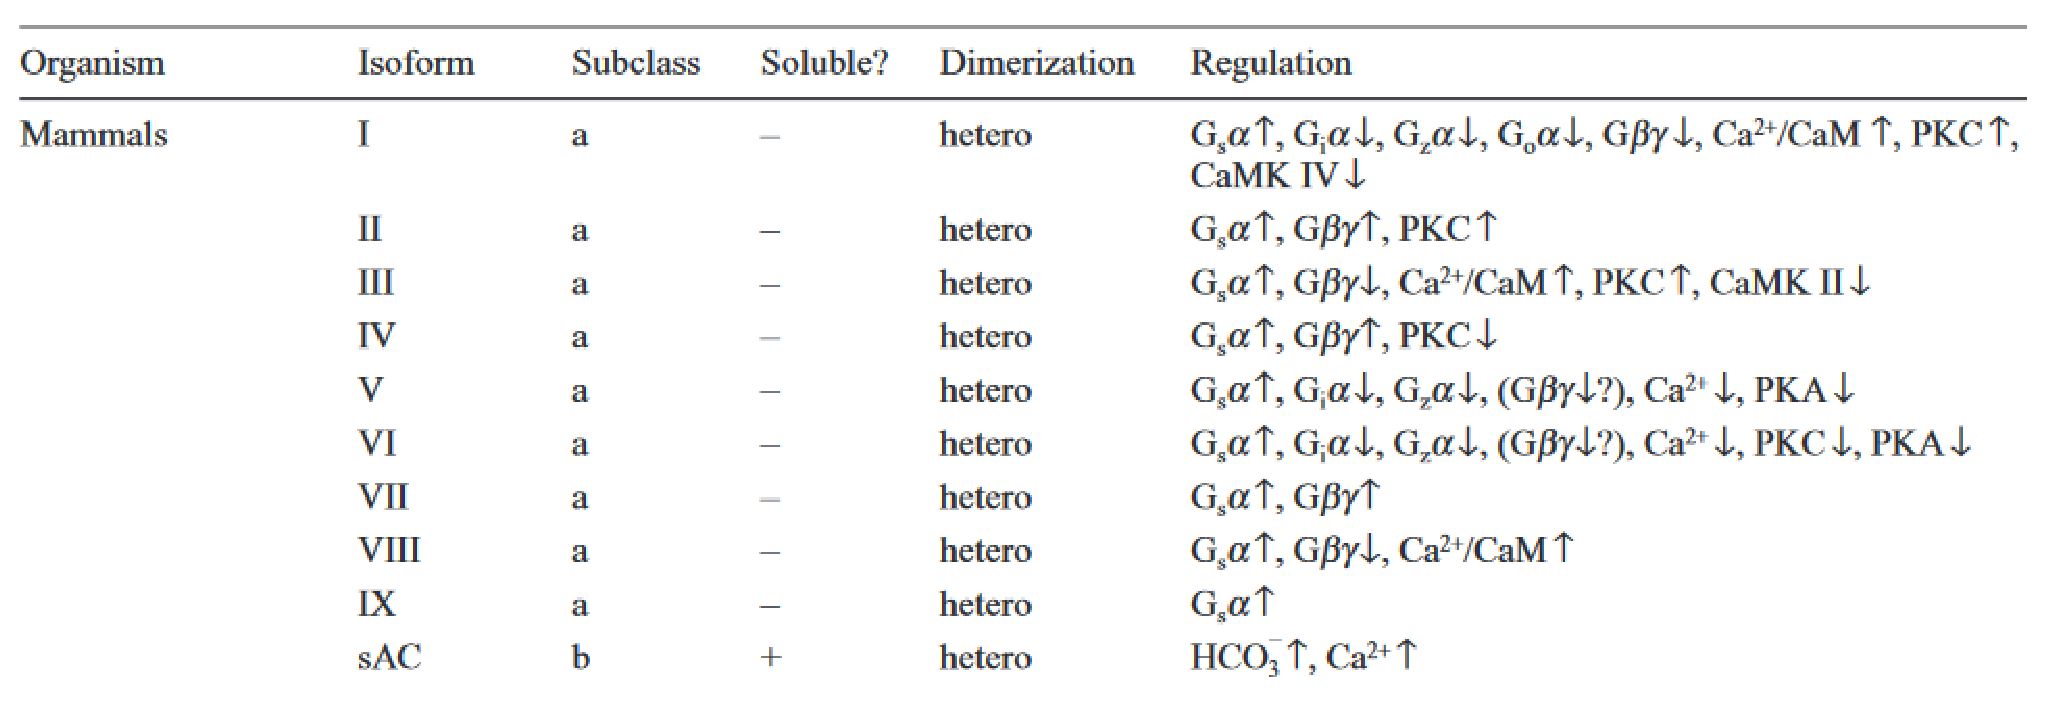
\includegraphics[height=4cm,
    angle=0]{./images/AC-III-a.eps}}
\caption{class III AC subclass a (in mammals)}
\label{fig:AC-III-a}
\end{figure}

\subsection{-- brains}

{\bf In neurons}
\begin{itemize}
  \item striatum: AC5 is the principal integrating  signals  from  multiple 
  receptors  including  D1, D2, and  $A_{2A}$ receptors in  striatum 
  \item 
\end{itemize}

$\Ca$-sensitive AC are located next to VDCC for faster reactions to $\Ca$
influx. These ACs are suspected to play an important role in learning process,
as a \textcolor{red}{coincidence detectors}
(Sect.\ref{sec:coincidence-detectors}).

\subsection{-- hearts}

{\bf In hearts}, AC5 and AC6 are the dominant isoforms; with AC7 and AC9 at mRNA
levels and AC4 both at mRNA and protein level \citep{fischmeister2006}.
It's impossible to discriminate AC5 from AC6 using current available antibodies.
So, immunofluorescence staining of isolated adult ventricular myocyte using a
common AC5/AC6 antibody showed that the signal from them with preferential
localization in T-tubular membrane \citep{fischmeister2006}.

\subsection{AC-IIIa type I}

Types I and VIII appear to be expressed exclusively in the brain,
adrenal gland and retina.

\subsection{AC-IIIa type V}
\label{sec:AC5}
\label{sec:AC-IIIa-type-V}

Type V adenylyl cyclase is highly enriched in brain and is localized largely to
the striatum and related structures, such as the nucleus accumbens and olfactory
tubercle, which are innervated by dopamine. It is inhibited by free Ca2+ at
physiological concentrations (0.1 to 1.0 $\muM$).
  
AC type V enzyme is also expressed in heart and kidney, where it is associated
with blood vessels; the anterior lobe of the pituitary; and the retina.


\subsection{AC-IIIa type VI}

Type VI adenylyl cyclase is enriched in brain and heart, with low
expression in other tissues, such as testes, muscle, kidney and lung.
  
Type VI adenylyl cyclase is structurally similar to the type V enzyme, and
both are inhibited by free Ca2+ at physiological concentrations (0.1 to 1.0
$\muM$)

  
\subsection{AC-IIIa type VII}

Type VII adenylyl cyclase is found in several tissues; concentrations are
highest in lung and spleen, moderate in heart and low in brain, kidney and
skeletal muscle

\subsection{AC-IIIa type IX}
  
Type IX: Less is known about the type IX enzyme, which to date has not
been characterized extensively; yet the most divergent in sequence of AC-III
isoforms. 

White-type (WT) AC9 is insensitive to forskolin; yet replacing a single amino
acid (Y1021L) in C2 loop can restore forskolin sensitivity.

AC9 is stimulated by G$\alpha$s; and inhibited by $\Ca$/calcineurin.

Coincidence detector, i.e. G$\alpha$s-stimulated AC9 activity (G$\alpha$s from
M1 receptor or 5HT$_{2A}$ - Sect.\ref{sec:M1-muscarinic-receptor} and
Sect.\ref{sec:5-HT3-receptor}) is

\begin{itemize}

  \item inhibited by activation of G$\alpha$i/o-coupled receptors; and this
  inhibition is removed by pertussis toxin
  
  \item reduced by 50\% in the presence of phorbol esters (appear to be the
  result of activation of a novel PKC isoforms; which is blocked by
  bisindolylmaleimide I; but not the conventinal PKC isoforms blockers - Go6976
  - Sect.\ref{sec:PKC}).
  
\end{itemize} 


\section{Guanyl cyclase (GC) (EC4.6.1.2)}
\label{sec:guanylate-cyclase}

Guanylate cyclase (guanyl cyclase, guanylyl cyclase, or GC)
is a lyase enzyme


\section{Guanine nucleotide}
\label{sec:guanine-nucleotide}

Nucleotides are small molecules composed of three parts, a nitrogenous base, a
sugar and one or more phosphates. Guanine nucleotide
\begin{enumerate}
  \item GTP

\begin{verbatim}
-(PO3)-(PO3)-(PO3)-O-(sugar)-Base
\end{verbatim}

  \item GDP

\begin{verbatim}
-(PO3)-(PO3)-O-(sugar)-Base
\end{verbatim}
Guanosine diphosphate (GDP) has only two phosphate groups.

\end{enumerate}
The nucleotide GTP are hydrolyzable by GAF (Sect.\ref{sec:GAF-domain})

The nonhydrolyzable guanine nucleotides such as GTP$\gamma$S.


\section{Molecular switch}
\label{sec:molecular-switch}


\begin{enumerate}
  \item G-proteins - Sect.\ref{sec:G-protein}
  
  \item DARPP32 - Sect.\ref{sec:DARPP32}: molecular switch to regulate and
  fine-tunes the phosphorylation state of PP-1.

NOTE: DARPP32, once activated, is a potent inhibitor of PP-1.
  
  \item DNA topoisomerase II$\beta$: molecular switch in neural differentiation
  of mesenchymal stem cells
  \url{https://www.ncbi.nlm.nih.gov/pubmed/25217229}
  
  \item notch signaling pathway (originally discovered in Drosophila): 
  \url{https://www.ncbi.nlm.nih.gov/pubmed/20681026}
  
  \item 
\end{enumerate}
\chapter{Enzyme Kinetics}
\label{chap:enzyme-kinetics}

{\bf Enzyme kinetics} is the study of chemical reactions in which substrate 
are catalyzed by an enzyme. In such reactions, the process is quite
complicated and thus, often divided into a number of elementary
reaction~\footnote{\url{http://en.wikipedia.org/wiki/Enzyme_kinetics}} which
contains fast reactions and slow reactions.

Although the law of mass action has been widely used to explain reversible
chemical reactions (Sect.\ref{sec:law-mass-action}), it is typically impossible
to apply that to chemical reactions that involve enzyme, unless multiple steps
are used. \textcolor{red}{However, in enzyme kinetics, there are
situations that the law
  of mass action is invalid: (1) at high concentration, doubling the
  concentration of one reactant need not double the overall reaction; (2) at
  extremely low concentration, it may not be appropriate to represent
  concentration as a continuous variable}.

\section{Introduction}

The enzyme usually manipulate other molecules - the {\it substrate} -
by allowing the substrate to bind to the enzyme's
active site; thus allow the substrate to be transformed into products
through a series of steps known as {\it enzymatic mechanism}, as shown
in Fig.~\ref{fig:enzyme_subs}. 

{\it In vivo}, the enzyme activity can be exerted by
\begin{enumerate}
  \item binding to small molecules: substrates or effectors (inhibitors,
  and activators), at catalytic or regulatory sites on the enzymes

  \item modification the enzyme through either covalent changes
  (hydrolysis, phosphorylation, ...), or noncovalent changes
  (polymerization/depolymerization, ...)
\end{enumerate}
In general, an enzyme can bind to a single substrate or multiple substrates.
Although this mechanism is often going through a complex series of steps, the
rate of the overall process is determined by the step that is slowest. This {\it
rate-determining step} can be a chemical reaction or a conformational change of
the enzyme or substrate(s). It is similar to the rate-limiting step in
multi-step chemical reaction (Sect.\ref{sec:multiple-step-reaction}).


\begin{figure}[hbt]
 \centerline{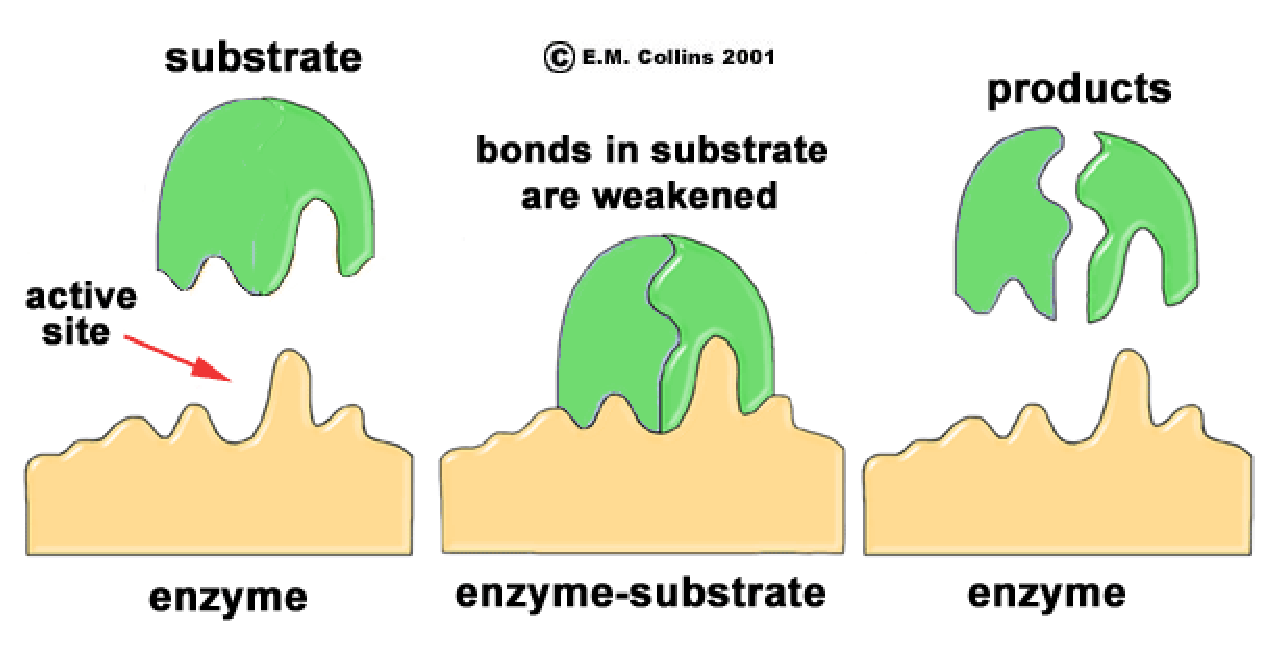
\includegraphics[height=4cm]{./images/enzyme_substrate.eps}}
\caption{Enzyme mechanism}
\label{fig:enzyme_subs}
\end{figure}


{\bf Example}: Consider this chemical reactions: enzymes $E$ help
accelerate the conversion from the substrate $S$ into the product
$P$. Enzyme reaction does not follow the law of mass action, as the
rate of the reaction (catalysis) does not show a linear response to an
increasing substrates, i.e. the rate of the reaction vs. the substrate
concentration is a hyperbolic curve, as shown in
Fig.~\ref{fig:rate_reaction}.

\begin{figure}[hbt]
 \centerline{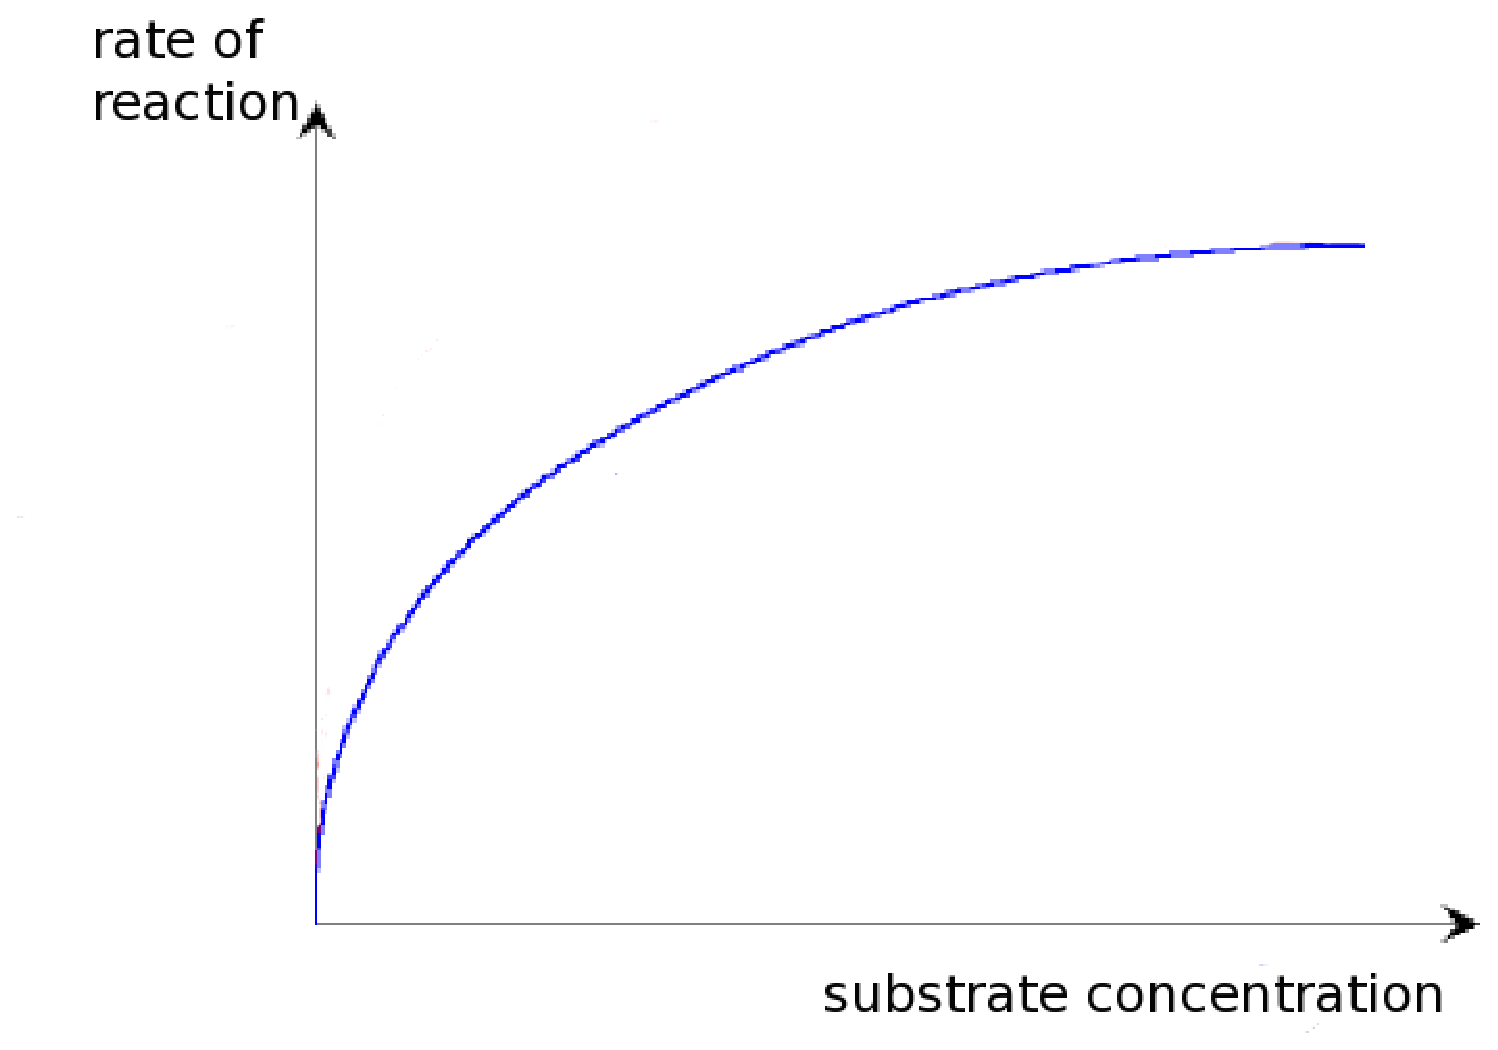
\includegraphics[height=5cm]{./images/rate_reaction.eps}}
 \caption{Rate of reaction}
 \label{fig:rate_reaction}
\end{figure}


In enzyme kinetics, there are two major approaches: the classical {\it
deterministic} approach (Sect.\ref{sec:enzyme-kinetics-deterministic}), and the
modern {\it stochastic} approach (Sect.~\ref{sec:stoch-model-enzyme}). However,
a major challenge when solving a system of multiples reactions is that the time
step is contrained by the fastest reaction, i.e. smallest {\it time constant}.


\section{One-binding site approach}
\label{sec:enzyme-kinetics-deterministic}

The one-binding site model is used when the velocity of product formation
follows the hyperbolic curve, Fig.\ref{fig:hyperbolic_sigmoidal_relationship}.
Michaelis-Menten kinetics (Sect.\ref{sec:equil-appr}) requires 2
assumptions\footnote{\url{http://depts.washington.edu/wmatkins/kinetics/quadratic.html}}:
\begin{enumerate}
\item free ligand (substrate) approximation [S]$\approx s_0$

[S] is close to the total substrate concentration in the system $s_0$ which is
the true independent variable in most experimental set-ups. This is valid when
the amount of substrate is much higher than the amount of enzyme

\item rapid equilibrium (of the substrate), $d[S]/dt=0$
\end{enumerate}
% \item steady-state approximation (of the complex), $d[ES]/dt=0$

The Briggs-Haldane modification for Michaelis-Menten kinetics
(Sect.\ref{sec:quasi-steady-state}) replaces the second assumption with
steady-state approximation $d[ES]/dt\approx 0$. 

Morrison kinetics remove also the first assumption
(Sect.\ref{sec:morrison-kinetics}).

If the binding site at the enzyme can be bound by a molecule other the
substrate, and thins binding inhibit the binding of the substrate, the need to
use a competitive one-site model (Sect.~\ref{sec:competitive-one-site}).

\subsection{One-site model}
\label{sec:mich-ment-kinet}

To explain the conversion of the substrate $S$ to product $P$ by enzyme $E$,
Michaelis-Menten in 1913 proposed a model that is now considered as a classical
deterministic theory of enzyme kinetics \citep{michaelis1913kir}.

They postulated that at first $E$ bind to $S$ forming a complex, denoted by $ES$
(some use the notation $C$), which then either (1) separate or (2) breaks down
into the product $P$ and releasing $E$.

\begin{eqnarray}
  \label{eq:261}
  \left\{  
    \begin{array}{lcc}
      \ce{E + S ->[k_1] ES} & \text{association} & \text{(rapid)} \\
      \ce{ES ->[k_2] E + S} & \text{dissociation} & \text{(rapid)} \\
      \ce{ES ->[k_3] E + P} & \text{decomposition} & \text{(slow)}
    \end{array}
\right.
\end{eqnarray}
with $k_i$ are deterministic rate constants. Remember in
Sect.\ref{sec:elementary-reactions}, the unit of $k_2,k_3$ are sec$^{-1}$, while
that of $k_1$ is M$^{-1}$.sec$^{-1}$.

At individual step,the law of mass action is applied to each reaction and
yields 4 differential equations for the rate of change of [S], [E], [P], [ES].
NOTE: The power term for each concentration is 1 as this is elementary
reaction.

\begin{equation}
  \label{eq:267}
  \begin{split}
    % \frac{d[S]}{dt} &= k_{-1}[ES] - k_1[S][E] \\
    % \frac{d[E]}{dt} &= k_{-1}[ES] - k_1[S][E] + k_2[ES] \\
    % \frac{d[ES]}{dt} &= -k_{-1}[ES] + k_1[S][E]  - k_2[ES] \\
    % \frac{d[P]}{dt} &= k_2[ES]
    \frac{d[S]}{dt} &= k_{2}[ES] - k_1[S][E] \\
    \frac{d[E]}{dt} &= k_{2}[ES] - k_1[S][E] + k_3[ES] \\
    \frac{d[ES]}{dt} &= -k_{2}[ES] + k_1[S][E]  - k_3[ES] \\
    \frac{d[P]}{dt} &= k_3[ES]
  \end{split}
\end{equation}

Due to the two conservation laws: total amount of enzyme is
preserved, and total amount of substrate is preserved.
\begin{equation}
  \label{eq:279}
  \begin{split}
      [E] + [ES] &= E_T = e_0 \\
      [S] + [ES] + [P] &= s_0
  \end{split}
\end{equation}
The four ODEs can be reduced to two
\begin{equation}
  \label{eq:280}
  \begin{split}
    % \frac{d[S]}{dt} &= k_{-1}(e_0-[E]) - k_1[S][E] \\
    % \frac{d[E]}{dt} &= (k_{-1}+k_2)(e_0-[E]) - k_1[S][E]  \\
    \frac{d[S]}{dt} &= k_{2}(e_0-[E]) - k_1[S][E] \\
    \frac{d[ES]}{dt} &= -(k_{2}+k_3)[ES] + k_1[S](e_0-[ES])
    % \frac{d[E]}{dt} &= (k_{2}+k_3)(e_0-[E]) - k_1[S][E]  \\
  \end{split}
\end{equation}
with initial condition $(s_0, e_0)$. How can we solve this set of ODEs
since they can not be integrated explicitly. Let's look at different
hypothesis in the coming sections.




\subsection[Michaelis-Menten assumption]{Michaelis-Menten assumption:
equilibrium approximation of substrate [S]}
\label{sec:equil-appr}
\label{sec:Michaelis-Menten-formula}

To be able to solve eq.~\eqref{eq:280}, Michaelis and Menten
\textcolor{red}{assumed that the enzyme concentration is much less than the
substrate concentration}, i.e. $e_0 < s_0$. So, at equilibrium, 
the substrate concentration doesn't change,
e.g. $d[S]/dt=0$, or
\begin{equation}
  \label{eq:281}
  \frac{[S][E]}{[ES]} = \frac{k_{2}}{k_1}
\end{equation}
% This is known as the equilibrium assumption, i.e. the association and
% diassociation of the substrate to the enzyme is 

It means that 
\textcolor{red}{the rate of decomposition is slow enough so that it
  doesn't disturb the association-disassociation equilibrium}
( $k_{2} \gg k_3$).  Thus, it allows the association-disassociation
steps to be treated as an isolated system $\ce{A <=> B}$.  In other
words, a compact form is
\begin{eqnarray}
  \label{eq:263-c}
    \left\{  
    \begin{array}{lcc}
      \ce{E + S <=>[k_1][k_2] ES} & \text{association/diassociation} & \text{(rapid)} \\
      \ce{ES ->[k_3] E + P} & \text{decomposition} & \text{(slow)}
    \end{array}
\right.
\end{eqnarray}
% or
% \begin{equation}
%   \label{eq:266}
% %  S + E \ce{<=>[k_1][k_{-1}]} C \ce{->[k_2]} P + E
%   S + E \ce{<=>[k_1][k_{2}]} C \ce{->[k_3]} P + E
% \end{equation}
% or
% \begin{equation}
%   \label{eq:289}
%    S + E \ce{<=>[k_1][k_{2}]} ES \ce{->[k_3]} P + E
% \end{equation}

%  it is
% supplied by a reservoir or the change is negligible. Thus, it is at
% equilibrium with the complex swiftly, or
% and

Noting that [E]+[ES] = $e_o$ with $e_o$ is the initial concentration of $E$,
then
\begin{equation}
  \label{eq:295}
      % [ES] &= \frac{k_1}{k_{-1}}[S](e_0-[ES]) \\
     [ES] = \frac{k_1}{k_{2}}[S](e_0-[ES]) 
\end{equation}
or
\begin{equation}
  \label{eq:296}
      % [ES] = \frac{e_0[S]}{\frac{k_{-1}}{k_{1}}+[S]} 
      [ES] = \frac{e_0[S]}{\frac{k_{2}}{k_{1}}+[S]} 
\end{equation}
or, from eq.~\eqref{eq:295}, the rate of product formation is
\begin{eqnarray}
  \label{eq:1}
  v = \frac{d[P]}{dt} = k_3 \ce{[ES]} =  k_3e_0\frac{[S]}{K_m+[S]} 
\end{eqnarray}
with $K_d=\frac{k_2}{k_{1}}$ is the dissociation constant and has the unit as
concentration, i.e. M (molar), mM (milimolar, or milimoles per litre or mmoles
per litre).  

As we can see in eq.~\eqref{eq:1}, due to the fast kinetics of the ES complex
formation, the rate of forming the product P is  determined by $k_3$.

If we assign $v_\max = k_3 e_0$, then
the rate of product creation is 
\begin{equation}
  \label{eq:310}
  v = v_\max \frac{[S]}{K_m+[S]}
\end{equation}
with [S] is usually assumed to be equal to the initial concentration
of substrate $s_0$. The unit of $v_\max$
is the same as that of $v$, i.e. [mM/sec].

\begin{framed}
  The value of $v_\max$ represents the \textcolor{red}{maximum velocity
  achieved by the system, and this happens when the substrate is so ``abundant'',
  i.e. very ``high'' concentration of [S]}. The exact of 'abundant' is dependent
  on the type of substrate, some substrate reaches the maximum speed at quite
  low concentration, and if we add more, it doesn't change the reaction
  velocity.

  $K_m$ (sometimes represented as $K_S$) represents the
  \textcolor{red}{concentration of substrate at which the reaction velocity
  reaches 50\%  of $v_\max$}.
%   So, aka half-maximal constant as it is the concentration of substrate at which
%   half of the reaction has occurred.
  The meaning of $K_m$ is related to the affinity of the substrate for
the enzyme. If $K_m$ has very low concentration in relative to the resting
level of [S] then substrate has a high affinity for the enzyme.
   
\end{framed}

{\bf SUMMARY}: In summary, Michaelis-Menten equation describes how the
reaction rate $rate$ depends on the positions of the substrate-binding
equilibrium and the rate constant $k_3$.
\textcolor{red}{However, there is the contrary: if [S] doesn't change,
  then S would not be used up, i.e. S must be of very huge amount of
  there must be a large reservoir supplying S?}.
In practice, this is not realistic, especially {\it in vivo}.  This
pointed out that eq.~\eqref{eq:263-c} is not a good approximation.  


% This lead to the
% classical {\it hyperbolic Michaelis-Menten equation}, as shown in
% Fig.~\ref{fig:rate_reaction}, relating the rate of forming $P$ to the
% concentration of the substrate $S$ (to be explained shortly).
% \begin{eqnarray}
%   \label{eq:262}
%   v = v_\max\frac{[S]}{\frac{k_2}{k_1}+[S]}
% \end{eqnarray}
% with $V=k_3E_T$ (given $E_T=[E]+[ES]$), the total enzyme concentration
% in the complex). 

\subsection[Briggs-Haldane assumption]{Briggs-Haldane assumption: quasi- (or
pseudo-) steady-state approximation of complex [ES]}
\label{sec:quasi-steady-state}
\label{sec:Michaelis-Menten-modified}

The steady-state assumption of Michaelis and Menten was somehow unrealistic as
their assumption means there is no change in S. 

To resolve that problem, instead of using steady-state assumption, Bridges and
Haldane (1925)~\citep{briggs1925nke} used a quasi-steady state equilibrium for
ES. It means that ES both involves in fast and slow process, yet the net
concentration doesn't change.

Still using the assumption that \textcolor{red}{the enzyme concentration is much
less than the substrate concentration}, i.e. $s_0\gg e_0$.
This is logical because the enzyme only need a small concentrations compared to
that of the substrate for the reaction to occur~\citep{li2008qssa}, e.g.
$\epsilon = \frac{e_0}{s_0}$ is typical in the range $10^{-2}$ to $10^{-7}$.


The new interpretation is
\begin{equation}
  \label{eq:289}
  S + E \ce{<=>[k_1][k_{2}]} ES \ce{->[k_3]} P + E
\end{equation}


  Under the above assumption, soon after the beginning of the
  reaction, the concentration of the complex ES reaches its
  steady-value. This transient occur so fast as to be unobservable. It
  means that after the complex is ``filling up'', its concentration
  changes much more slower than those of the product [P] and substrate
  [S]. Thus, it can be considered that [ES] was essentially doesn't
  change over time, i.e. $d[ES]/dt\approx 0$ rather than using
  $d[S]/dt=0$. 

In essence, the complex is assumed to be in    {\it quasi-steady-state
assumption} (QSSA) (or pseudo-steady-state)  and the overall rate of reaction is
determined solely by $k_2$ (the rate is  generally orders of magnitude lower
than $k_1$)\footnote{\url{http://www.biofitweb.cox-thurmond.net/FittingRoom/MMderivatioin.htm}}.

% or
% \begin{equation}
%   \label{eq:297}
%   S + E \ce{<=>[k_{on}][k_{off}]} ES \ce{->[k_{cat}]} E + P
% \end{equation}
% with $k_{on}$ is the bimolecular association rate constant, $k_{off}$
% is the unimolecular disassociation rate constant of enzyme-substrate
% binding to produce free enzyme and the substrate; $k_{cat}$ is the
% unimolecular disassociation rate constant of the enzyme-substrate to
% produce free enzyme and the product.
% with $k_1$ is the bimolecular association rate constant, $k_2$
% is the unimolecular disassociation rate constant of enzyme-substrate
% binding to produce free enzyme and the substrate; $k_3$ is the
% unimolecular disassociation rate constant of the enzyme-substrate to
% produce free enzyme and the product.

% {\bf IMPORTANT}: $k_{on}$ has the unit of
% [concentration$^{-1}$.time$^{-1}$], and $k_{off}$ and $k_{cat}$ have
% units of [time$^{-1}$]. By definition, the dissociation binding
% constant of the ES complex is $K_d = \frac{k_{off}}{k_{on}}$ (unit of
% concentration).

{\bf IMPORTANT}: $k_1$ has the unit of
[concentration$^{-1}$.time$^{-1}$], and $k_2$ and $k_3$ have
units of [time$^{-1}$]. By definition, the dissociation binding
constant of the ES complex is $K_d = \frac{k_2}{k_1}$ (unit of
concentration).

% Now, we have
% \begin{equation}
%   \label{eq:298}
%   \begin{split}
%     \frac{d[S]}{dt} &= k_{off}[ES] - k_{on}[S][E] \\
%     \frac{d[E]}{dt} &= k_{off}[ES] - k_{on}[S][E] + k_{cat}[ES] \\
%     \frac{d[ES]}{dt} &= -(k_{off} + k_{cat})[ES] + k_{on}[S][E]  \\
%     \frac{d[P]}{dt} &= k_{cat}[ES]
%   \end{split}
% \end{equation}
% The third differential equation is the most important,
Again, using eq.~\eqref{eq:280}, under the QSSA assumption, we have
$\frac{d[ES]}{dt}=0$ or

\begin{equation}
  \label{eq:277}
   % 0= -(k_{off} + k_{cat})[ES] + k_{on}[S][E]
  0= -(k_2 + k_3)[ES] + k_1[S](e_0-[ES])
\end{equation}
or
\begin{equation}
  \label{eq:300}
  [ES] = \frac{e_0[S]}{\frac{k_2+k_3}{k_1} + [S]}
\end{equation}
with $e_0$ is the initial concentration of enzyme.

Finally, we have the rate of product formation
\begin{equation}
  \label{eq:299}
  % v = k_{cat}[ES] =
  % k_{cat}\frac{e_0[S]}{\frac{k_{off}+k_{cat}}{k_{on}} + [S]}
  v = k_3[ES] = k_3e_0\frac{[S]}{\frac{k_2+k_3}{k_1} + [S]}
\end{equation}
Again, if we define: $v_\max=k_3e_0$ and $K_m=\frac{k_2+k_3}{k_1}$
({\bf Michaelis constant}), then we have \textcolor{red}{Briggs-Haldane
equation}
\begin{equation}
  \label{eq:301}
  v = v_\max \frac{[S]}{K_m+[S]}
\end{equation}
which is a similar formula with eq.~\eqref{eq:310}, except $K_m$ is
different.
\textcolor{red}{This is the more popular form being used nowadays}. Also, it's
important to know that $K_d$ and $K_m$, though have the same unit, they are not
exactly has the same meaning.


% As the enzyme concentration doesnot change over time, we have $ [C] +
% [E] = e_o $. Finally, the classic Michaelis-Menten equation is now
% \begin{equation}
%   \label{eq:278}
%   \begin{split}
%         \frac{d[P]}{dt} &= v =  k_2e_0 \frac{[S]}{K_m+[S]} \\
%         &= v_\max  \frac{[S]}{K_m+[S]} \\
%   \end{split}
% \end{equation}
% or
% \begin{equation}
%   \label{eq:283}
%   [C] = e_0 \frac{[S]}{K_m+[S]} 
% \end{equation}
% with $v_\max = k_2 e_0$ and $K_m = \frac{k_{-1}+k_2}{k_1}$ is the
% Michaelis constant, and $v$ is the initial velocity of the reaction.

{\bf SUMMARY}:
\begin{enumerate}
\item The overall rate of the reaction is dependent upon the values of
  $k_1, k_2, k_3$ and the concentration of substrate [S].
\begin{equation}
K_m = \frac{k_2+k_3}{k-1}
\end{equation}

The Michaelis-Menten equilibrium assumption (Sect.\ref{sec:equil-appr}) is the
simpler case of Briggs-Haldane quasi-steady-state assumption, i.e.  it is assumed
  that substrate binding and disassociation occurred much more rapidly
  than product formation, then $k_2 \gg k_3$ (aka
  {\bf rapid equilibrium approximation}) or $K_m$ is lower
  approximated to the dissociation constant $K_d$
\begin{equation}
  \label{eq:282}
  K_m \approx K_d= \frac{k_2}{k_1}
\end{equation}

\end{enumerate}

% \hyperref[sec:nond]{Dimensionless} is an important aspect when
% designing the set of ODEs, as the form of a solution can depend
% critically on the units one choose for various quantities involved.


\subsection{Michaelis constant}
\label{sec:Michaelis-constant}

The Michaelis constant $K_m$ 
\begin{enumerate}
  \item the same as $K_d=k_2/k_1$ under Michaelis-Menten equilibrium assumption
  
  \item not the same as $K_d$, as $K_m=\frac{k_2+k_3}{k_1}$ under Brigss-Haldane
  quasi-equilibrium assumption
\end{enumerate}
\textcolor{red}{NOTE: We should not confuse $K_a$ the association constant with
$K_m$ the Michaelis constant}.

{\bf IMPORTANT}: Michaelis-Menten law is not universally applicable.
\begin{enumerate}
  \item The first limitation for Michaelis-Menten kinetics is that it is
  based on the law of mass action, particularly based on the
  QSSA. 
  
 Under QSSA assumption, the kinetics is known as
  {\bf Briggs-Haldane kinetics}; thus Michaelis-Menten kinetics is the
  special case of Briggs-Haldane kinetics.
  
  \item QSSA assumption requires the continuous distribution of
  substances and the free diffusion and thermodynamically-random
  collision. 

[S] is the free substrate concentration, but typically is
  assumed to be close to the total substrate concentration present in
  the system $[S] = s_0$. This so-called {\bf free ligand approximation} (or
  free substrate approximation) is valid so long as the total enzyme
  concetration is well below $K_m$ of the system, i.e. $[S]\approx
  s_0$. If this condition is not met, we need to use
  {\it Morrison equation} (Sect.\ref{sec:morrison-kinetics}).

\end{enumerate}

\subsection{Plotting}
\label{sec:plotting}

Given the Michaelis equation
\begin{equation}
  \label{eq:321}
  v = v_\max \frac{[S]}{K_m+[S]}
\end{equation}

\subsection{* Lineweaver-Burk plot}
\label{sec:Lineweaver-Burk-plot}

To analyze this equation, Lineweaver-Burk plot is
utilized~\citep{lineweaver1934edc}. 
\begin{equation}
  \label{eq:322}
  \frac{1}{v}_0 = \frac{K_m}{v_\max}\frac{1}{[S]} + \frac{1}{v_\max}
\end{equation}
which plot $\frac{1}{v}$ vs. $\frac{1}{[S]}$. This is a linear
relation, and both $1/v$ and $1/[S]$ can be obtained
experimentally. Thus, $K_m$ can be inferred from the slope of the
line and its intercept on the x-axis, as shown in
Fig.~\ref{fig:lineweaver-burk}. Since enzyme concentration [E] is
difficult to determine, $K_m/v_\max$ is very useful, i.e. it measures
enzyme efficiency and all enzymes can be compared using it. 

\begin{figure}[hbt]
 \centerline{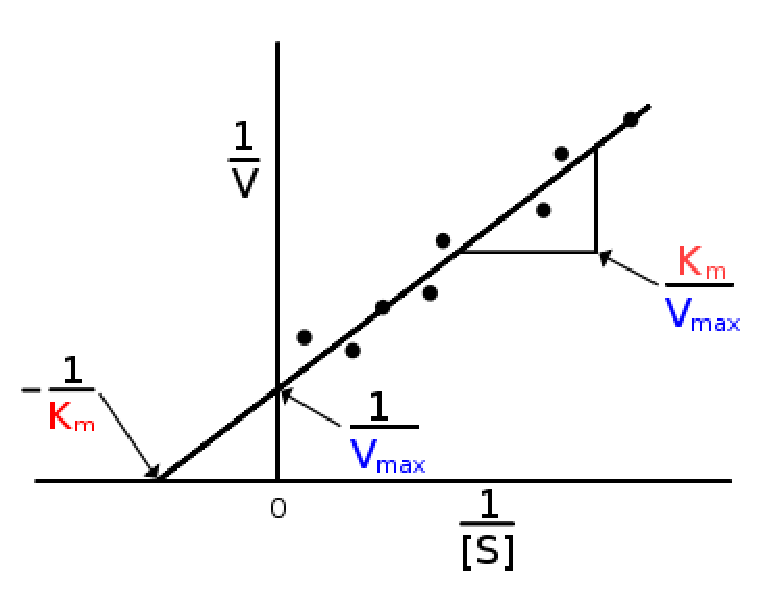
\includegraphics[height=5cm]{./images/Lineweaver-Burk_plot.eps}}
\caption{Lineweaver-Burk plot}
\label{fig:lineweaver-burk}
\end{figure}
$v$ achieve the value $v_\max$ only at very high [S].

{\bf NOTE}: Lineweaver-Burk even though provides interesting
interpretation, this method is error-prone. This is because of the
small error in the measurement of $v$ or $[S]$ can lead to
non-trivial error in $1/v_o$ and $1/[S]$. Thus, another method is more
preferable, e.g. Hanes-Woolf plot.


\subsection{* Hanes-Woolf plot}
\label{sec:Hanes-Woolf-plot}

{\bf Hanes-Woolf} plot plots
$[S]/v$ vs. $[S]$.
\begin{equation}
  \label{eq:324}
  \frac{[S]}{v} = \frac{1}{v_\max}[S] + \frac{K_m}{v_\max}
\end{equation}
Hanes-Woolf had been used to determined important kinetic parameters
$v_\max$, $K_m$, $v_\max/K_m$ rapidly. The drawback of Hanes-Woolf
is that both ordinate and abscissa are dependent variables of [S]; so
it is impossible to use statistical measurement (goodness of fit,
correlation coefficient R...) Nowadays, for a more accurate
computation, non-linear regressions are often being used.

$K_m$ for most enzymes is between $10^{-1}$ to $10^{-7}$ mM and
this values depends upon particular substrate as well as the
environment condition (pH, ionic strength, temperature). 

\subsection{Morrison kinetics: dynamic [S]}
\label{sec:morrison-kinetics}

When total enzyme concentration is significant compared to $K_m$, 
a significant fraction of substrate ([ES]) will be bound to the
enzyme. Thus, the substrate concentration [S] is no longer closed to
the total substrate $s_o$ (from the beginning), i.e. we need to use $[S] =
s_0-[ES]$.

Eq.\ref{eq:277} should be written as
\begin{equation}
  \label{eq:311}
  [ES]^2 - (e_0+s_0+K_m)[ES] + e_0s_0 = 0
\end{equation}
with $K_m=\frac{k_2+k_3}{k-1}$.

Finally, we have the rate of forming product 
\begin{equation} 
  \label{eq:312}
  v  = k_3 \ce{[ES]} =
  v_\max\frac{(e_0+s_0+K_m)-\sqrt{(e_0+s_0+K_m)^2-4e_0s_0}}{2e_0}
\end{equation}
with $v_\max = k_3 e_0$.

This quadratic velocity equation is aka {\bf tight-binding equation}
or Morrison equation~\citep{morrison1969kin}. As $K_m$ large, then the
quadratic equation approach the hyperbola curve of Michaelis-Menten
equation, as shown in Fig.~\ref{fig:Morrison_kin}.

\begin{figure}[hbt]
 \centerline{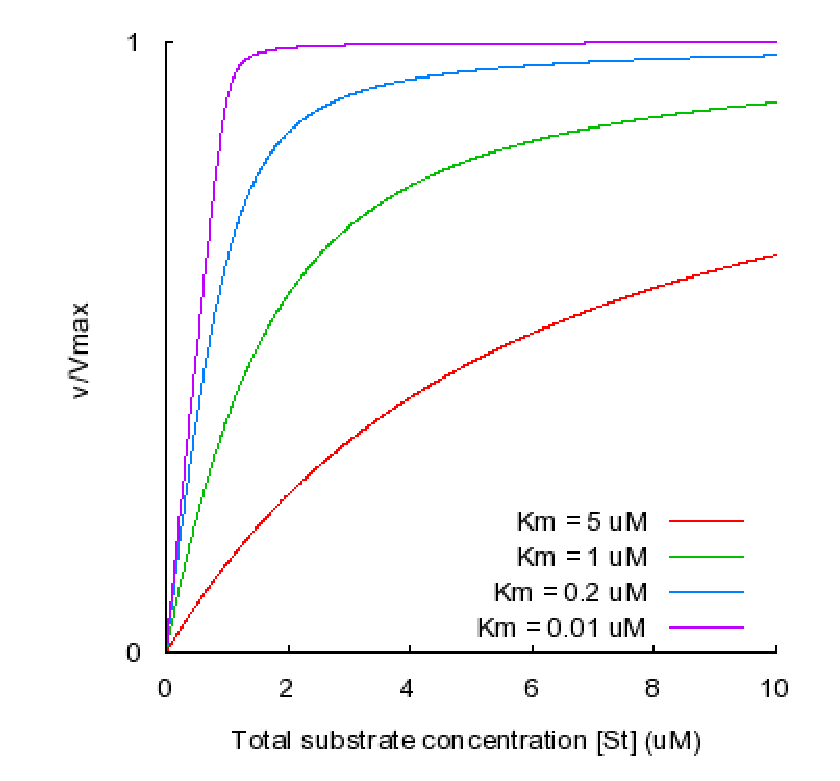
\includegraphics[height=5cm]{./images/Morrison_kin.eps}}
\caption{Morrison kinetics}
\label{fig:Morrison_kin}
\end{figure}

\subsection{Competitive one-site model}
\label{sec:competitive-one-site}

The competitive one-site model explains the situation when the binding site at
the enzyme can be bound by a molecule other the substrate, and this binding
inhibits the binding of the substrate.

This is similar to competitive two-site models
(Sect.~\ref{sec:competitive-two-site}), where the enzyme has one
catalytic binding site and one allosteric site and at a single
time, only one molecule can bind to the enzyme. So, the binding of the active
site prevents binding of the substrate and vice versa,
Fig.\ref{fig:enzyme_competitivemodel}.

\begin{figure}[hbt]
  \centerline{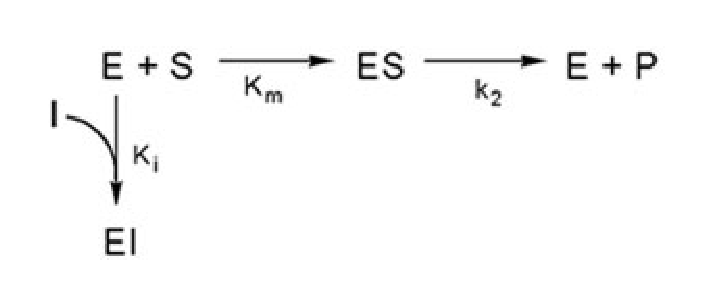
\includegraphics[height=3cm,
    angle=0]{./images/enzyme_competitivemodel.eps}}
\caption{An enzyme with one active site and one inhibitor: $K_i$ the
dissociation constant for EI complex}
\label{fig:enzyme_competitivemodel}
\end{figure}

The rate of production formation is now
\begin{equation}
v = k_3 \ce{[ES]} = v_\max \frac{\ce{[ES]}}{e_0} = v_\max
\frac{\ce{[S]}}{\ce{[S]} + K_m \left( 1 +
\frac{\ce{[I]}}{K_i} \right)}
\end{equation}

To see if the reaction following this scheme or not, we can use the following
plots: Michaelis-Menten, Lineweaver-Burk, and
Hanes-Woolf equations, with the equation modified to include a term that
describe the inhibition by I.
\begin{enumerate}
  \item Michaelies-Menten: $v = \frac{v_\max[\S]}{[S]+K_m\left(1 +
  \frac{[I]}{K_i} \right)}$
  \item Lineweaver-Burk: $\frac{1}{v} = \frac{1}{v_\max}+
  \frac{1}{v_\max}\frac{K_m}{[\S]}\left(1+\frac{[I]}{K_i}\right)$
  \item Hanes-Woolf: $\frac{[\S]}{v}=\frac{[\S]}{v_\max} +
  \frac{K_m}{v_\max}\left(1+\frac{[I]}{K_i}\right)$
\end{enumerate}

\subsection{Velocity of enzyme catalysis}
\label{sec:veloc-enzyme-catalys}

It's generally accepted that hydrolysis step is rate-limiting  in the
SR-ATPase reaction. In SERCA-pump, with a ``basic'' and a ``extra''
channels, the rate constants are the same, i.e. $k_h^b\approx
k_h^e=k_h$ (b=basic, e=extra). 

\begin{equation}
  \label{eq:1208}
  \ce{ATP + E1 <=> ATP\cdot E1}
\end{equation}
In the absence of $\Ca$, the velocity of enzyme catalysis with
saturating substrate concentration is
\begin{equation}
  \label{eq:1209}
  v_\max^{basic} = k_h^b[\ce{ATP\cdot E1}]\approx \frac{k_h[\ce{E0}]}{1+K_e}
\end{equation}
with $\ce{E0\approx[ATP\cdot E1]+[ATP\cdot E2]}$ is the total enzyme
concentration. 

In the presence of $\Ca$, the velocity of enzyme catalysis with
saturating substrate concentration is
\begin{equation}
  \label{eq:1210}
  v_\max^{total} = k_h^b[\ce{ATP\cdot E1}] + k_h^e[ADP\cdot P\sim E2]
  \approx [\ce{E0}]
\end{equation}
The extra maximal velocity is defined as
\begin{equation}
  \label{eq:1211}
  v_\max^{extra} = v_\max^{total}-v_\max^{basic} = k_h^e[ADP\cdot
  P\sim E2] \approx \frac{k_h[\ce{E0}]}{1+1/K_e}
\end{equation}

The plot log(V/T) vs. (1/T) are linear ``total'' ATPase, but not
nonlinear for ``basic'' and ``extra'' activities. 


% \section{Enzyme kinetics - other models}
% \label{sec:enzyme-kinet-other}
% 
% 
% To deal with the heterogeneous distribution of reactants, i.e. the
% fractal-like kinetics, there have been some limited mobility-derived
% kinetics have been successfully
% applied\footnote{\url{http://en.wikipedia.org/wiki/Michaelis-Menten_kinetics}}.
% For a single binding site model, 
% \begin{enumerate}
% \item when the substrate concentration $[\S]$ can change
%   (Sect.~\ref{sec:morrison-kinetics})
% \item the binding site at the enzyme can be bound by a molecule other
%   the substrate, that inhibit the binding of the substrate
%   (Sect.~\ref{sec:competitive-one-site}).
% \item as the enzyme is large, it can have more than one binding sites,
%   distinct from the active sites. The binding to these sites can
%   affect (enhance/degrade) the activity of the enzyme at the active
%   site. This is known as {\bf allosteric binding site} (or regulatory
%   sites). This is described in a separate section
%   (Sect.~\ref{sec:models-mult-bind}).
% \end{enumerate}
% 
% References:\url{http://assay.nih.gov/assay/index.php/Types_of_Inhibition}
% 
% \subsection{Lumped scheme of fast equilibrium}
% \label{sec:lumped-scheme-fast}
% 
% 


\section{Multiple-binding site approach}
\label{sec:models-mult-bind}

Both Michaelis-Menten kinetics, Briggs-Haldane kinetics and Morrison
kinetics use one-site model, in which each enzyme bind to a single
substrate only, and producing a product plus the enzyme
\begin{equation}
\ce{S + E -> P + E}
\end{equation}
In the simplest model, Michaelis-Menten, the enzyme activity is controlled by
the substrate concentration. In the Morrison model, the enzyme
activity is controlled by both the substrate and enzyme concentration.

\begin{framed}
\textcolor{red}{It's important to differentiate substrates vs. effectors}.
The site where substrate binding is called {\it catalytic site} (or active
site), while that for effector binding is called {\it regulatory site}.

  The broader term to refer to substrates and effectors is  {\bf ligand}, and
  both types of sites is called ligand-binding sites.

  If these substrate and effector  are identical, the interactions are
  termed {\bf homotrophic interactions}; otherwise, they are called
  {\bf heterotrophic interactions}. 
  
\end{framed}

As the enzyme is large, it can have more than one binding sites, i.e. more than
one substrates, and it can also produce more than one products.
In reality, many enzymes have more than one substrate (A, B) and more than one
product (P, Q). Substrates bind to catalytic sites; while Effectors bind to
regulatoric site(s). The binding to the regulatoric sites can affect
(enhance/degrade) the activity of the enzyme at the active  site.

Example: the enzyme alcohol dehydrogenase catalyzes the oxidation of
ethanol with NAD (a biological oxidizing agent) to form acetaldehyde and NADH.  

This makes the problem more complicated as there are different scenarios for the
binding to occur, and the products to be formed
\begin{enumerate}
  \item sequential yet random binding
  \item sequential yet ordered binding - Sect.\ref{sec:sequential-models}
  \item ping-pong mechanism - Sect.\ref{sec:ping-pong-mechanism}
\end{enumerate}

In an enzyme system, activating or inhibitory effects are measured in terms of
variations of the two classical kinetics constants ($K_m$ and $v_\max$), as a
function of the substrate concentration [S] and effector concentration [F].


\begin{framed}
  One-site models has the saturation curve as {\it hyperbolic},
  Fig.\ref{fig:hyperbolic_sigmoidal_relationship}.
  
  Multiple-site models has the saturation curve either (1) hyperbolic or (2)
  non-hyperbolic behavior (e.g. sigmoidal).   
\end{framed}

\subsection{Sequential binding
mechanism}
%\subsection{Sequential models}
\label{sec:sequential-models}

\textcolor{red}{In sequential models, the binding of all substrate is required
for product formation}. With multiple substrates (e.g. A and B) and multiple
binding sites, the binding at different sites on a single enzyme can be random
(A before B or B before A is the same) or in an ordered manner (A has to bind
before B). We will examine both cases, Fig.\ref{fig:binding-sequential}.

\begin{figure}[htb]
  \centerline{\includegraphics[height=4cm]{./images/binding_order2.eps}}
  \caption{(A) random sequential; (B) ordered
  sequential of binding with the signature
  Lineweaver-Burk plots $1/v$ vs. $1/\ce{[A]}$
  with different [B] concentrations intersected
  at a single point}\label{fig:binding-sequential}
\end{figure}

For both mechanisms, Lineweaver-Burk plots at varying A and different fixed
values of B give a series of intersecting lines,
Fig.\ref{fig:binding-sequential}.  Derivative curves can be solved to obtain
appropriate kinetic constants.

Early work in this regard was carried out by Adair and Pauling, operating under
the {\bf rapid equilibrium approximation}, i.e. 
all substrate binding and dissociation steps happen much more rapidly than
catalytically productive steps.

In 1954, King and Altman showed how to solve any kinetic system without
resorting to this approximation, but making it more complicated.
This is analogous to the difference between $K_M$ (or $K_D$) in the
Michaelis-Menten model and $K_M$ in the Briggs-Haldane model
(Sect.\ref{sec:quasi-steady-state}).


\subsection{* Sequential random model}
\label{sec:sequential-random-models}

\begin{figure}[htb]
  \centerline{\includegraphics[height=5cm]{./images/sequential-random-binding.eps}}
  \caption{Sequential random binding}\label{fig:sequential-random-binding}
\end{figure}

Consider a random sequential bi-bi reaction for a "simple" case in which the
rapid equilibrium assumption defines the binding of substrates A and B,
Fig.\ref{fig:sequential-random-binding}. There are two effective dissociation
constant for the reactant A
\begin{itemize}
  \item $K_\text{ia}$: dissociation constant of A binding to E
  
  \item $K_\text{a}$: dissociation constant of A binding to EB
\end{itemize}

\begin{equation}
\begin{split}
\ce{E + A <->[K_{ia}] EA } \\
\ce{EA + B <->[K_b] EAB}
\end{split}
\end{equation}
or
\begin{equation}
\begin{split}
\ce{E + B <->[K_{ib}] EA } \\
\ce{EB + A <->[K_a] EAB}
\end{split}
\end{equation}

then
\begin{equation}
\begin{split}
\ce{EAB <=>[k_9][k_{10}] EPQ} \\
\ce{EPQ <->[k_{11}] P + EQ} \\
\ce{EQ <->[k_{13}] Q + E}
\end{split}
\end{equation}

The rate-limiting step is between \ce{EAB <=> EPQ}.

\begin{equation}
\begin{split}
\ce{K_{ia} = \frac{[E][A]}{[EA]}} \\
\ce{K_{ib} = \frac{[E][B]}{[EB]}} \\
\ce{K_{a} = \frac{[EB][A]}{[EAB]}} \\
\ce{K_{b}} = \frac{[EA][B]}{[EAB]} 
\end{split}
\end{equation}
from that we can find [E], [EA], [EB] as a function of [EAB].

NOTE: $e_0 = \ce{[E] + [EA] + [EB] + [EAB]}$, so
\begin{equation}
e_0 =  \left( \ce{\frac{K_{ia}K_b}{[A][B]} + \frac{K_b}{[B]} + \frac{K_a}{[A]}
+1} \right) \ce{[EAB]}
\end{equation}

NOTE: Assuming rapid equilibrium of the two paths, i.e. all substrate binding
and dissociation steps happen much more rapidly than catalytically productive
step, then $\ce{K_{ia}K_b = K_{ib}K_a}$.


References:
\begin{itemize}
  \item
  \url{http://employees.csbsju.edu/hjakubowski/classes/ch331/transkinetics/olcomplicatedenzyme.html}
\end{itemize}

\subsection{* Sequential ordered model}
\label{sec:sequential-ordered-models}
%(Random-Sequential vs. Ordered-Sequential) 

For random reactions the order in which the substrates bind does not matter. 
Although sequential ordered models are less general than sequential random
models, they have fewer free parameters and so are easier to use when fitting
experimental data. This means that, \textcolor{red}{in cases where they are
applicable, sequential ordered models
  are often a better choice than sequential random models when it comes to
  analyzing experimental data}~\citep{monod1965nat}.

An abbreviated notation  scheme developed by W.W. Cleland is shown below for the
sequential random and sequential ordered mechanisms.  

\subsection{* Sequential: single subtrate but multi-binding sites and one
product}

Fig.\ref{fig:single-substrate-multi-bindingsite_single-product} shows a model in
which the enzyme has two binding sites, that can accept a single type of
substrate
\begin{itemize}
  \item the first binding of S, forming complex ES that can produce product P,
  with rate $k_\text{cat}$
  
  \item the second binding of S, forming doubly-occupied complex ESS that can
  produce product P, but tentatively with a faster rate $k_\text{cat2}$.
\end{itemize}

 \begin{figure}[htb]
  \centerline{\includegraphics[height=4cm]{./images/single-substrate-multi-bindingsite_single-product.eps}}
  \caption{Single
  subtrate, with
  multiple binding
  sites, e.g. two,
  and one product}\label{fig:single-substrate-multi-bindingsite_single-product}
\end{figure}

Under the assumption of fast equilibrium of substrate
association/disassociation
\begin{equation}
\begin{split}
\ce{K_{d1} = \frac{[E][S]}{[ES]} } \\
\ce{K_{d2} = \frac{[ES][S]}{[ESS]} }
\end{split}
\end{equation}

From that we can calculate [ES],
[ESS].
\begin{equation}
\begin{split}
\ce{[ES] = \frac{[E][S]}{K_{d1}}  } \\
\ce{[ESS] = \frac{[ES][S]}{K_{d2}}} = \frac{[E][S]^2}{K_{d1}{K_{d2}}} 
\end{split}
\end{equation}
NOTE: $e_0 = \ce{[E] + [ES] + [ESS]}$, so we need to find [E] as a function of
$e_0$, and then replace into the previous equations to find [ES] and [ESS] as a
function of $e_0$
\begin{equation}
e_0 = \ce{[E]} \left( 1 + \ce{\frac{[S]}{K_{d1}} + \frac{[S]^2}{K_{d1}K_{d2}}}
\right)
\end{equation}
or
\begin{equation}
\begin{split}
\ce{[ES] =  ...   } \\
\ce{[ESS] =  ...   }
\end{split}
\end{equation}


Finally, the reaction velocity $v$:
\begin{equation}
v = \ce{ k_{cat} [ES] + k_{cat,2}[ESS] } =
\ce{ \frac{k_{cat} \frac{[S] e_0}{K_{d1}}  + k_{cat,2}
\frac{[S]^2 e_0}{K_{d1}K_{d2}} }{1 + \frac{[S]}{K_{d1}} +
\frac{[S]^2}{K_{d1} K_{d2}} } }
\end{equation}

NOTE:
\begin{equation}
v_{\max,1} = k_\text{cat} \ce{e_o} \;\;\;
v_{\max,2} = k_\text{cat2} \ce{e_o} 
\end{equation}

then the equivalent form
\begin{equation}
v = \ce{ v_{\max,1}[ES]/e_0 + v_{\max,2}[ESS]/e_0 } =
\frac{v_{\max,1} \frac{[S]}{K_{d1}}  + v_{\max,2} \frac{[S]^2}{K_{d1}K_{d2}} }
{1 + \frac{[S]}{K_{d1}} +\frac{[S]^2}{K_{d1} K_{d2}} }  
\end{equation}


\url{http://depts.washington.edu/wmatkins/kinetics/sequential.html}

\subsection{Non-sequential binding}

Non-Sequential mechanism does not require both substrates to bind before
releasing the first product. 
Typically, the binding of the second substrate could result
in a change of the shape of the first substrate saturation curve that makes
production more effective or less effective.

\begin{enumerate}
  \item Ping-pong mechanism - Sect.\ref{sec:ping-pong-mechanism}
\end{enumerate}

\subsection{* Ping-pong binding mechanism (double-displacement mechanism)}
\label{sec:ping-pong-mechanism}

Ping-pong mechanism is a type of non-sequential binding. 
It is called this because the enzyme bounces back and forth from an intermediate
state to its standard state. Here, we have two substrates A and B; binding 
(at potentialy two different sites) on enzyme E, to form two products P and Q.

The substrate A binds first to the enzyme and produce product P.
{\it Typically, this is the scenario when the product P is a fragment of the
original substrate A}; and the rest of the substrate is covalently attached to
the enzyme E , which is designated as E'.

\begin{equation}
\ce{A + E -> EA <=> P.E^' -> P + E^'}
\end{equation}

The product P is a fragment of A; and the other fragment of A still
attaches to the enzyme, giving E'.

Now the second reactant, B, binds and reacts with E' (e.g. B forms a covalent
bond to the fragment of A still attached to the enzyme), from that the
product Q is created.
\begin{equation}
\ce{B + E^' -> E^'B <=> EQ -> Q + E}
\end{equation}

\begin{figure}[htb]
  \centerline{\includegraphics[height=4cm]{./images/pingpong-mechanism.eps}}
  \caption{Ping-pong mechanism with the signature
  parallel lines in Lineweaver-Burk plot of $1/v$
  vs. $1/\ce{[A]}$ curves at different [B]
  concentrations}\label{fig:pingpong-mechanism}
\end{figure}

This represents a {\bf ping-pong mechanism} or {\bf double-displacement
mechanism}, Fig.\ref{fig:pingpong-mechanism}. The enzyme exists in an
intermediate form E' which is temporary and at the end of the reaction the
enzyme MUST be found in its original form.

\begin{equation}
\begin{split}
\ce{A + E -> EA <=> P.E^' -> P + E^' } \\
\ce{B + E^' -> E^'B <=> EQ -> Q + E}
\end{split}
\end{equation}

\textcolor{red}{How to identify}: 
For this mechanism, Lineweaver-Burk plots
(Sect.\ref{sec:Lineweaver-Burk-plot}) at varying A and different fixed values of
B give a series of parallel lines, i.e. the plot of $1/v$ vs. $1/\ce{[A]}$ as
[B] changes.

\url{http://chemwiki.ucdavis.edu/Biological_Chemistry/Catalysts/Enzymatic_Kinetics/Ping-pong_mechanisms}

\subsection{Meaning of $K_m$, velocity $v$ in multi-substrate/multi-product
mechanism?}


\subsection{Meaning of $K_m$, velocity $v$ in allosteric mechanism?}

\subsection{K system vs. V system}

In both K and V systems, an effector can act as an activator (positive effector)
or an inhibitor (negative effector).

\subsection{* K system: competitive-binding (change $K_m$)}


If the binding of a ligand (effector, substrate) involves the change
in Michaelis-Menten constant $K_m$ but no change in maximal velocity,
the effect of the ligand is ``competitive'' and the system is called
{\bf K system}, as shown in Fig. \ref{fig:K_system}. 

\begin{figure}[hbt]
 \centerline{\includegraphics[height=5cm]{./images/K_system.eps}}
\caption{K system}
\label{fig:K_system}
\end{figure}

\subsection{* V system: uncompetitive binding (change $v_\max$)}


Similarly, if the
binding of a ligand involves the change in maximal velocity only, the
effect of the ligand is ``uncompetitive'' and the system is referred
to as {\bf V system} ~\citep{monod1965nat}. 

\begin{figure}[hbt]
 \centerline{\includegraphics[height=5cm]{./images/Allosteric_enzyme_K_V.eps}}
 \caption{Behavior of allosteric systems: (A) K-system; (B)
   V-system. $v$ is the initial velocity of the enzymatic reaction and
   [$L$] is the ligand concentration}
\label{fig:enzyme_K_V}
\end{figure}

This is known as {\bf allosteric binding site} (or regulatory
sites).


Allosteric interactions (between enzyme and effectors) stabilize
conformational state of the enzyme that either increase/decrease the
affinity for substrate (K-system) or catalytic potential (V-system) or
both, as shown in Fig.~\ref{fig:enzyme_K_V}. Allosteric interactions
play an important role in the regulation of enzyme
activity~\citep{hammes1973kae}.

\subsection{Allosteric (cooperativity) binding: K }


\begin{figure}[htb]
  \centerline{\includegraphics[height=5cm]{./images/hyperbolic_sigmoidal_relationship.eps}}
  \caption{Hyperbolic
  (Michaelis-Menten)
  vs. Sigmoidal
  (Cooperativity)}\label{fig:hyperbolic_sigmoidal_relationship}
\end{figure}

  In reality, many of regulatory enzyme exhibit {\it non-hyperbolic}
kinetic and/or binding isotherms. Such behavior can be explained as
the activity is enhanced or degraded by the binding of some other
molecules. This can be multiple substrate or effector binding sites on
the enzyme~\citep{hammes1973kae}. The effector can be either
activators or inhibitors that correspondingly enhance or inhibit the
activity of the associated enzyme.
  

  In multiple-binding models, the binding of the first ligand can
  enhance/facilitate the binding to the second ligand (``positive
  cooperativity'' - the curve has {\it sigmoidal shape}); or the binding
  can inhibit the binding to the second (``negative cocoperativity'' - the
  curve has inverse sigmoidal shape),
  Fig.\ref{fig:hyperbolic_sigmoidal_relationship}.

\subsection[Non-competitive two-site model]{Non-competitive two-site model: one
substrate + one inhibitor}
\label{sec:non-competitive-two}

\begin{figure}[hbt]
  \centerline{\includegraphics[height=5cm,
    angle=0]{./images/1bind_1inhibit.eps}}
  \caption{An enzyme with 1 catalytic binding site and 1 allosteric
    one}
\label{fig:1bind_1inhibit}
\end{figure}

In this situation, the enzyme has two binding sites, one for substrate
and one for inhibitor. Thus, both enzyme (E) and the complex (ES) can
also interact with the inhibitor ($I_c$),
Fig.~\ref{fig:1bind_1inhibit}. 

By using Lineweaver-Burk plot, it is observed that competitive
inhibitors decrease $v_\max$ but have no effect on $K_m$,
Fig.~\ref{fig:enzyme_K_V}(b). The new maximum velocity $v'_\max$ has
the relation with the old $v_\max$ as follows
\begin{equation}
  \label{eq:326}
  v'_\max = \frac{1}{1+\frac{[I_c]}{K_i}} v_\max
\end{equation}
with $K_i=\frac{k^-_3}{k^+_3}$.  Then, the new initial velocity
formula is
\begin{equation}
  \label{eq:327}
  v = \frac{1}{1+\frac{[I_c]}{K_i}} v_\max \frac{[S]}{K_m+[S]}
\end{equation}
with $v_\max = k_2[\text{E}]_o$.

As shown in Fig.~\ref{fig:enzyme_K_V}(b), the curve $v$ vs. [S]
looks very different from a competitive inhibitor since increasing [S]
has no impact on the increase in the initial velocity. A negative
cooperativity can also decrease maximum velocity
(Sect.~\ref{sec:negat-coop}).

\subsection[Competitive two-site model]{Competitive two-site model: one substrate + one inhibitor}
\label{sec:competitive-two-site}

An enzyme mechanism model for the enzyme with one site for substrate,
but now with an inhibitor that is competitive to bind to the same
site on the enzyme. The binding of the inhibitor prevent the binding
of the substrate to the enzyme. This is the model for the competitive
inhibitor ($I_C$) interacting with the enzyme (E). This is aka the K
system. 
\begin{equation}
  \label{eq:323}
  \begin{split}
    &\ce{E  + S <=>[k_1][k_2] ES ->[k_3] E + P} \\
    &+ \\
    &I_C \\
    &\upharpoonleft\downharpoonright K_i \\
    & EI_C
  \end{split}
\end{equation}
with $K_i$ is the inhibitor binding constant.
Due to the binding of inhibitor, it slows down the process, thus the
$v$ vs. $[S]$ curve change with the presence of competitive
inhibitor. 

With the presence of inhibitors, the
\textcolor{red}{new Michaelis-Menten constant is $K'_M$ which has a
  relation to the old $K_m$} as follows
\begin{equation}
  \label{eq:325}
  K'_M = K_m \left( 1 + \frac{[I_c]}{K_i} \right)
\end{equation}
Then, the new initial velocity formula
is~\citep{dixon1953eic,kakkar1999cei}
\begin{equation}
  \label{eq:328}
  v =  v_\max \frac{[S]}{ K_m \left( 1 + \frac{[I_c]}{K_i} \right)+[S]}
\end{equation}
with $K_m=\frac{k_1+k_2}{k_3}$.



\subsection{Multiple catalytic binding sites - independent}
\label{sec:mult-catalyt-bind}

Consider an enzyme with $n$ catalytic binding sites for ligand
L. Then, we will have $n$ corresponding association constant $K_i$.
\begin{equation}
  \label{eq:313}
  \begin{split}
    E + L &\ce{<=>} EL; \; K_1 = \frac{[EL]}{[E][L]} \\
    EL + L &\ce{<=>} EL_2; \; K_2 = \frac{[EL_2]}{[EL][L]} \\
    \vdots \\
    EL_{n-1} + L &\ce{<=>} EL_n; \; K_n = \frac{[EL_{n}]}{[EL_{n-1}][L]} 
  \end{split}
\end{equation}
The average number $r$ of ligand molecules bound to the enzyme is
defined as
\begin{equation}
  \label{eq:314}
  \begin{split}
      r &= \frac{\text{moles of L bound}}{\text{moles of enzyme}} =
  \frac{\sum^n_{i=1} i[PL_i]}{\sum_{i=0}^n [PL_i]} \\
  &= \frac{K_1[L]+2K_1K_2[L]^2 + \dots +
    nK_1...K_n[L]^n}{1+K_1[L]+K_1K_2[L]^2+\dots + K_1K_2...K_n[L]^n}
  \end{split}
\end{equation}
This is aka {\bf Adair equation}~\citep{adair1925odc}. This is general,
however, quite complex when $n$ is large.
\textcolor{red}{A common assumption is given to simplified it: all
  sites are independent and identical}.
Thus, the intrinsic association constant are the same $K$ which
relates to the association constant defined above as
\begin{equation}
  \label{eq:315}
  K_i = \frac{n-i+1}{i} K; \; i\ge 1
\end{equation}
Finally, we have
\begin{equation}
  \label{eq:316}
  r = \frac{nK[L]}{1+K[L]}
\end{equation}

The identical sites are classified into a single class. For a single
type of ligand L, most enzymes indeed, have more than two classes of
binding sites. Thus, if the enzyme has $n_1$ equivalent sites of class
1 with an intrinsic association constant $K_1$, $n_2$ equivalent sites
of class 2 with an intrinsic association constant $K_2$..., and the
binding to each class of sites occurs independently, then with $m$
classes of binding sites, we have
\begin{equation}
  \label{eq:317}
  r = \sum_{i=1}^m r_i = \sum_{i=1}^m \frac{n_iK_i[L]}{1+K_i[L]}  
\end{equation}
This adequately describes the data, but not provide any explanation
for the changing association constants. To establish a nature of the
cooperativity between binding sites, different methods of plotting
binding data have been utilized. The curves from 1-4 are shown in
Fig.~\ref{fig:enz_kin}, the curve in 5 is shown in
Fig.~\ref{fig:enz_kin_2}.
\begin{enumerate}

\item $r$ vs. [L]: 
  \begin{itemize}
  \item If enzyme contains only identical sites (single class of
    sites)
    \begin{itemize}
    \item For non-interacting cooperativity, a hyperbolic curve is
      obtained.
    \item For positive cooperativity, the curve is sigmoidal
    \item For negative cooperativity, the final value of $r$ approach
      more slowly than in a hyperbolic curve.
    \end{itemize}
  \item If enzyme contains more than two classes of binding sites,
    both positive and negative cooperativities are possible and the
    plots may display undulation or bumps~\citep{teipel1969ipr}
  \end{itemize}

\item $r$ vs. $\log([L])$: By using log, this plot can cover a wide
  range of concentration [L], and the steepness of the curve can give
  a convenient measure of the cooperativity.
  \begin{itemize}
  \item all binding isotherms (curves) appears in sigmoidal
  \item equal steepness for equal
    cooperativity~\citep{koshland1966ceb}.
  \item the steepness is in the order of {\it positive cooperativity}
    $>$ {\it no cooperativity} $>$ {\it negative cooperativity}
  \end{itemize}

\item $1/r$ vs. $1/[L]$:
  \begin{itemize}
  \item linear for non-interacting identical sites (single class); and
    the slope is $\frac{1}{nK}$, the intercept is $1/n$.
  \item concave upward for positive cooperativity 
  \item concave downward for negative cooperativity. However, this can
    also be obtained from polymorphic forms, electrostatic
    repulsion.... So, the concave downward cannot be used as a proof
    of negative cooperativity.
  \end{itemize}

\item $\frac{r}{[L]}$ vs. $r$: the equivalent form of
  eq.~\eqref{eq:316} is
  \begin{equation}
    \label{eq:318}
    \frac{r}{[L]} = Kn - Kr
  \end{equation}
This plot is called {\bf Scatchard plot}, a convenient for determining
both $n$ and $K$.
\begin{itemize}
\item linear for non-interacting identical sites
\item concave downward for positive cooperativity
\item concave upward for negative cooperativity
\end{itemize}

\item $\log\frac{r}{n-r}$ vs. $\log([L])$: As mentioned in the
  previous section, the sigmoidal curve can also be fitted by the Hill
  equation
  \begin{equation}
    \label{eq:319}
    r = \frac{n[L]^h}{K + [L]^h}
  \end{equation}
with $h$ is the Hill coefficient; the equivalent form is
\begin{equation}
  \label{eq:320}
  \log\frac{r}{n-r} =h\log[L] - \log K
\end{equation}
\begin{itemize}
\item Hill coefficient $h> 1$: positive cooperativity
\item Hill coefficient $h= 1$: no-interacting cooperativity
\item Hill coefficient $h< 1$: negative cooperativity
\end{itemize}
\end{enumerate}

\begin{figure}[hbt]
 \centerline{\includegraphics[height=11cm]{./images/enz_kin_curve.eps}}
\caption{Equilibrium binding and initial velocity of data. $r$ is the
  number of moles of ligand bound per mole of enzyme,$v$ is initial
  velocity of the enzymatic reaction, $n$ is the total number of
  ligand binding-site per enzyme molecule, $v_\max$ is the maximum velocity}
\label{fig:enz_kin}
\end{figure}

\begin{figure}[hbt]
 \centerline{\includegraphics[height=8cm]{./images/enz_kin_2.eps}}
 \caption{Illustration of Hill plots. $r$ is the number of moles of
   ligand bound per mole of enzyme,$v$ is initial velocity of the
   enzymatic reaction, $n$ is the total number of ligand binding-site
   per enzyme molecule, $v_\max$ is the maximum velocity}
\label{fig:enz_kin_2}
\end{figure}

\subsection{Multiple catalytic binding sites - cooperative binding}
\label{sec:dissociation-curve}
\label{sec:cooperativity}

Typically, in a multiple-binding-site model, the binding of one
substrate can enhance/degrade the affinity of binding of subsequent
substrates. This is known as {\bf cooperativity}. 

Cooperativity, or concerted action, of multiple subunit proteins is a well
recognized phenomenon, the classic example being hemoglobin's increase in
affinity for additional oxygen molecules after one, two, or three have bound. 

In the previous sections, the velocity follows the simple hyperbolic curve,
Fig.~\ref{fig:rate_reaction}, Fig.~\ref{fig:Morrison_kin},
Fig.~\ref{fig:K_system}, Fig.~\ref{fig:enzyme_K_V}. However,
\textcolor{red}{many of the enzyme systems has the reaction velocity follow a
sigmoidal shape}. And it is cooperativity behavior that can produce such
sigmoidal shape.

{\bf Knowledge base}: Cooperative binding occurs in system with three
or more molecules when the binding of one molecule affects the binding
of others. This effect can be positive or negative. By positive, it
means that the binding of B to A will increase the affinity of A for
C. By negative, it means that the binding of B to A will decrease the
affinity of A for C. 

\subsection{-- Example}
\label{sec:example}

{\bf Example}\footnote{\url{http://www.ventworld.com/resources/oxydisso/dissoc.html}}:
Haemoglobin (Hb) is an intracellular protein that serves as the primary vehicle for transporting oxygen in
blood\footnote{Oxygen is also carried by (dissolved) in plasma, but in
  a much lesser degree}.
Hemoglobin is contained in erythrocytes (red blood cells).  Each Hb
molecule has a maximum capacity of carrying oxygen. The current
capacity of carrying oxygen  is dependent upon the specific
physiological condition. How much of that capacity at any time is 
called the {\it  oxyhaemoglobin saturation} ($Sa_{O_2}$), expressed in
percentage and is formulated as the ratio of the amount of oxygen
bound to the hemoglobin to the (maximum) oxygen carrying capacity of the
Hb. 

% Oxygen carrying capacity of the Hb is determined by the amount of Hb
% present in the blood.
\begin{equation}
  \label{eq:304}
  Sa_{O2} = \frac{\text{amount of oxygen bound to Hb}}{\text{amount
      of Hb}} 100\%
\end{equation}

% Depending upon the suitable conditions, oxygen bound to the Hb is
% released into the body tissue, or oxygen is observed from the tissue
% into the blood. Each Hb molecule has a capacity of carrying \ce{O2}
% molecules.

The amount of oxygen bound to Hb at any time is related, in large
part, to the {\bf partial pressure of oxygen} ($Pa_{O_2}$) in
blood. This value is high at lung and low at other body tissues. At
high $Pa_{O_2}$, oxygen are readily to bind to Hb; otherwise, HB cannot
maintain its full bound capacity of oxygen and thus oxygen are
released to tissue cells.

The behavior of oxygen transport by haemoglobin (Hb) at different
conditions of pH, \ce{CO2}, temperatures has been intensively studied
to increase the accuracy.  This is often represented as an
{\bf oxygen dissociation curve} (ODC) (or interactive oxyhemoglobin
dissociation curve) with x-axis is $Pa_{O_2}$ and y-axis is $Sa_{O_2}$, as
shown in Fig.~\ref{fig:SDC_plot}. 

\begin{figure}[hbt]
  \centerline{\includegraphics[height=5cm]{./images/PO2_SO2_plot.eps}}
  \caption{Standard ODC plot showing P50, and SO2 at PO2=80mmHg}
  \label{fig:SDC_plot}
\end{figure}

Commonly, the curve is plotted along with the $P_{50}$ value. This is
the value which tells the pressure at which SO2 is
50\%\footnote{\url{http://www.bio.davidson.edu/Courses/anphys/1999/Dickens/Oxygendissociation.htm}}.
The curve has a sigmoidal or S-shape. 

{\bf Why ODC is sigmoidal?}: Hb absorbs \ce{O2} rapidly in the range
20-40mmHg. At PO2 above 60 mmHg, the standard SDC curve is relatively
flat, i.e oxygen content does not change significantly even with large
increase of partial pressure of oxygen.  As partial pressure of oxygen
increase, the saturation of oxygen increase also, until a maximum
capacity can be reached. As this limit is reached, very little
additional binding occurs and the curve levels out as the haemoglobin
become saturated with oxygen.

% Thus, to get more oxygen to the tissues, either the oxygen have to
% dissolve more into the plasma, or the body then need more Hb.

One of the first person who derived the mathematical formula for this
relation is~\citep{hill1910pea}. Hill postulated that
cooperative binding occurs between Hb and \ce{CO2}. The aggregation
between haemoglobin and oxygen can occur at different levels, e.g.
\begin{equation}
  \label{eq:302}
  \begin{split}
    \ce{Hb + O2 <=>[k_1] HbO2} \\
    \ce{HbO + O2 <=>[k_2] HbO4} \\
    ... \\
    \ce{HbO_{n-2} + nO2 <=>[k_n] HbO_{2n}}
  \end{split}
\end{equation}
with $n$ is the ``number'' of molecules of oxygen to bind to a single
Hb molecule, $k_i$ are association constants (reaction
quotients, or Hill coefficient)~\citep{leow2007odc}. Using the law of mass actions, we have
\begin{equation}
  \label{eq:305}
  k_i = \frac{[\ce{HbO_{2i}]}}{[\ce{HbO_{2i-2}}][\ce{O2}]} = 
  \frac{[\ce{HbO_{2i}]}}{k_1k_2...k_{i-1}[\ce{Hb}][\ce{O2}]^{i}} 
\end{equation}
In essence, the net association constant for the overall reversible
process is
\begin{equation}
  \label{eq:306}
  K_n =k_1k_2...k_{n-1}k_n= \frac{[\ce{HbO_{2n}]}}{[\ce{Hb}][\ce{O2}]^{n}} 
\end{equation}
Under the assumption that all oxyhemoglobin at any point in time is
predominantly in the form of $\ce{HbO_{2n}}$, then using the law of
conservation of mass: 
\begin{equation}
  \label{eq:307}
  \begin{split}
    \text{total Hb} &= \text{total deoxygenated Hb + total
      oxyhemaglobin} \\
    &= [Hb] + [HbO_{2n}] \\
    &= [Hb] + K_n[Hb][\ce{O2}]^n
  \end{split}
\end{equation}

Then
\begin{equation}
  \label{eq:308}
  \begin{split}
    \ce{SaO2} &= \frac{\text{total oxyhemoglobin}}{\text{total Hb}} \\
    &= \frac{[\ce{HbO_{2n}}]}{ [Hb] + K_n[Hb][\ce{O2}]^n} \\
    &= \frac{K_n[\ce{O2}]^n}{ 1 + K_n[\ce{O2}]^n}
  \end{split}
\end{equation}
This is known as {\bf Hill equation} with a reasonable approximation
to Hb-oxygen data is $n\approx 2.6$. 

Adair \citep{adair1925odc} developed a 4-constant equation
({\bf Adair equation}) that's better fit the data. The four constants
related to the successive affinity constant of oxygen to the four heme
groups in Hb. Later, Pauling made the first attempt to give a
theoretical explanation for the changing affinity constants, i.e. to
the conformation of the proteins Hb (geometry of the 4 subunits).

Oxygen dissociation curve (ODC) have been attacked by many
researchers, yet there is no complete satisfying reason why the curve
has a form adapted to the needs of the organism, rather than the form
given by the simple laws of physics and chemistry.


When enzyme E is cooperative binding to substrate S to form \ce{ES_n},
the we have
\begin{equation}
  \label{eq:341}
  \begin{split}
    ES_n &= \frac{K_n[S]^n}{1+K_n[S]^n} \\
    &= \frac{[S]^n}{1/K_n+[S]^n} 
  \end{split}
\end{equation}

\subsection{-- Extreme Cooperativity (Hill equation)}

Consider an example when an enzyme has 2 binding sites
\begin{equation}
  \label{eq:269}
  \begin{split}
    \ce{S + E <=>[k_1][k_{-1}] C1 ->[k_2] E + P } \\
    \ce{C1 + S <=>[k_3][k_{-3}] C2 ->[k_4] C1 + P } 
  \end{split}
\end{equation}
The reaction velocity of the systems as determined by two slower
reactions, which is represented via $k_2, k_4$. Using assumption of
quasi-steady-equilibrium, we have $dc_1/dt=dc_2/dt=0$, then
\begin{equation}
  \label{eq:1372}
  \begin{split}
    c_1 = \frac{K_2e_0.s}{K_1K_2+K_2s+s^2} \\
    c_2 = \frac{e_0.s^2}{K_1K_2+K_2s+s^2}
  \end{split}
\end{equation}
with $K_1=\frac{k_{-1}+k_2}{k_1}$, $K_2=\frac{k_{-3}+k_4}{k_3}$. The
reaction velocity is defined as
\begin{equation}
  \label{eq:1373}
  v = k_2c_1 + k_4c_2 = \frac{(k_2K_2+k_4s)e_0.s}{K_1K_2+K_2s+s^2}
\end{equation}
\begin{enumerate}
\item Under the assumptions that the two active sites are independent
  and identical, then $k_1=2k_3$, and $k_{-3}=2k_{-1}$ and
  $2k_2=k_4$. The factors of 2 is chosen because there are two
  identical binding sites, which doubling the amount of
  reactions. Then eq.~\eqref{eq:1373} becomes
\begin{equation}
  \label{eq:1374}
  v = 2\frac{k_2e_0.s}{K+s}=\frac{k_4e_0.s}{K+s}
\end{equation}
with $K=\frac{k_{-1}+k_2}{k_3}$.


\item Under the assumption that the binding of the first substrate is
  low, yet the binding of the second one is fast (thanks to the
  binding of the first one). So, we let $k_3\rightarrow\infty$,
  $k_1\rightarrow 0$ while keeping $k_1k_3=$constant. Then,
  $K_2\rightarrow 0$, and $K_1\rightarrow \infty$ while
  $K_1K_2=$constant. In this case, eq.~\eqref{eq:1373} becomes
  \begin{equation}
    \label{eq:1375}
    v = v_\max \frac{s^2}{K_m^2+s^2}
  \end{equation}
with $K_m^2=K_1K_2$.


In general, if there are $n$ binding sites, with the assumptions
$K_n\rightarrow 0$, $K_1\rightarrow\infty$ and $K_1K_n=$ constant,
then 
\begin{equation}
  \label{eq:1376}
  v = v_\max \frac{s^n}{K_m^n+s^n}
\end{equation}
with $K_m^n=\pi^n_{i=1}K_i$. This is known as {\bf Hill equations}.

NOTE: $n, K_m$, and $v_\max$ are determined from experimental data,
using {\bf Hill plot} (Fig.~\ref{fig:enz_kin_2}) which plot
$\ln(v/(v_\max-v)$ against $\ln s$.
\begin{equation}
  \label{eq:1377}
  n\ln s = n\ln K_m + \ln\left(\frac{v}{v_\max-v}\right)
\end{equation}
In practice, for the best fit, $n$ can be a non-integer.  

\end{enumerate}

\subsection{-- Negative cooperativity}
\label{sec:negat-coop}

Negative cooperativity decrease the velocity, similar to V-system
(Sect.~\ref{sec:competitive-two-site}). This can be modelled by
decreasing $k_3$, Fig.~\ref{fig:cooperativity}.
Using quasi-steady-state approximation, the velocity of the reaction
for an enzyme with allosteric inhibitor is
\begin{equation}
  \label{eq:1390}
  v = v_\max\frac{K_3}{i+K_3}
  \left( \frac{s(k_{-1}+k_3i+k_1s+k_{-3})}{k_1(s+K_1)^2+(s+K_1)(k_3i+k_{-3}+k_2)+k_2k_{-3}/k_1}\right)
\end{equation}
where $K_3=k_{-3}/k_3$ and $K_1=k_{-1}/k_1$.

\begin{figure}[hbt]
  \centerline{\includegraphics[height=5cm,
    angle=0]{./images/cooperativity.eps}}
  \caption{positive cooperativity ($K_1=1000, K_2=0.001$), independent
    binding ($K_1=0.5,K_2=2$), negative cooperativity
    ($K_1=0.5,K_2=100$). The other parameters were chosen as
    $e_0=1,k_2=1,k_4=2$ (unit arbitrary)}
\label{fig:cooperativity}
\end{figure}

\subsection{-- Cooperativity factor}
\label{sec:coop-fact}

Cooperativity factor describes the level of cooperativity that arise
when the binding of one molecule affect the binding of
ano1ther. Suppose that A is an enzyme, B and C are two
substrates. Then, the dissociation constant between A and C is
$K_{D(AC)}$ and that between A and B is $K_{D(AB)}$. When $B$ bind to
A first, it affect the dissociation constant between A and C by a
factor $\alpha$. Alternatively, when $C$ bind to A first, it affect
the dissociation constant between A and B a factor $\beta$. 

Both $\alpha$ and $\beta$ are called cooperativity factors. They are
not Hill coefficient, yet both types are used to describe
cooperativity. When $\alpha$ (or $\beta$) is greater than 1, a system
has negative cooperativity. When it is equal to 1, a system lack
cooperativity. When it is smaller than 1, a system has positive
cooperativity. 
\begin{equation}
  \label{eq:342}
  \begin{split}
    &A + B \;\;\; \ce{<=>[K_{D(AB)}]} AB \\
    &+ \;\;\;\;\;\;\;\;\;\;\;\;\;\;\;\;\;\;\;\;\;\;\;  + \\
    &C\;\;\;\;\;\;\;\;\;\;\;\;\;\;\;\;\;\;\;\;\;\;\;\;\;\;  C \\
    K_{D(AC)}&\upharpoonleft\downharpoonright  \;\;\;\;\;\;\;\;\;\;\;\;\;\;\;\;\;\;\;\;\;\;    \upharpoonleft\downharpoonright\alpha K_{D(AC)} \\
    &AC + B \ce{<=>[\beta K_{D(AB)}]} ABC
  \end{split}
\end{equation}

\subsection{-- Mechanistic models of cooperativity}
\label{sec:mech-models-coop}

There were 2 different types of ligands: regulatory effectors and substrates.
They bind to the target protein at topographically distinct sites; yet mutually
influence each other through a reversible conformational change. This concept of
indirect or ``allosteric'' interactions was different from the classical
explanation of enzyme inhibition through steric hindrance at a common binding
site. The second issue is the cooperative (homotropic) interactions of some
identical ligands. A mechanistic explanation for the cooperativity binding model
was proposed by~\citep{monod1965nat}, known as {\bf Monod-Wyman-Changeux model}
(MWC). A literature review of other models is given by~\citep{dixon1979,
changeux2005}.


Assumptions being used by Monod-Wyman-Changeux model
\begin{enumerate}
  \item The regulatory proteins have a quaternary structure with identical
  subunits with symmetry properties. An enzyme (i.e. cooperative proteins) is
  composed of several identical reacting units, called {\bf promoters}, that occupy
  equivalent positions within the protein.
  
\item Each promoter contains one binding site for each ligand

\item The binding sites within each enzyme are equivalent

\item If the binding of a ligand to one promoter and induce the
  conformational change in that promoter; it also induce identical
  conformational change in all other promoters.
  
\item The enzyme has 2 conformational states, denoted by R and T,
  which differ in their binding affinity to ligands. T = low-affinity
  low-activity, R = high-affinity, high-activity state.
\end{enumerate}
The conformational R-T equilibrium is an intrinsic property of the allosteric
oligomers accessible in the absence of ligand. Here, ligands control protein
functin by altering a pre-existing equilibrium between high (R) and low (T)
reactive conformations.  Due to its simplicity, the postulated 2-state
``concerted'' transition has been a debated issue. There have been other
alternative sequential model with multiple conformations, each with different
numbers of ligand molecules bound \citep{viappiani2004}. 

{\bf Example}: An enzyme has 2 binding sites, i.e. 2 promoters. So,
for each conformational state, there can be 0, 1 or 2 ligands
binding. Totally, there are 6 states: $R_i$ (i=0,1,2) and $T_i$
(i=0,1,2). If we assume $R_1$ cannot convert directly to $T_1$ and
similar to $R_2$ and $T_2$, the schematic diagram for the kinetics of
the enzyme is given in Fig.~\ref{fig:MWC_model}.

\begin{figure}[hbt]
  \centerline{\includegraphics[height=5cm,
    angle=0]{./images/MWC_model.eps}}
\caption{An example of Monod-Wyman-Changeux model}
\label{fig:MWC_model}
\end{figure}
To estimate the rate constants, we assume that all reactions are in
equilibrium. Let denotes $r_i$ and $t_i$ are constants of chemical
species in the corresponding state. Using $s$ as the concentration of
the substrate, then the fraction Y of occupied sites (saturation
function) is
\begin{equation}
  \label{eq:1386}
  Y = \frac{}{}
\end{equation}

If there are $n$ binding sites, then 
\begin{equation}
  \label{eq:1387}
  Y = \frac{sK_1^{-1}(1+sK_1^{-1})^{(n-1)} + K_2^{-1}
  \left[  sK_3^{-1}(1+sK_3^{-1})^{(n-1)}\right]}{(1+sK_1^{-1})^n+K_2^{-1}(1+sK_3^{-1})^n}
\end{equation}
\textcolor{red}{Y is a sigmoidal function of $s$}.

Special cases:
\begin{enumerate}
\item $K_2=\infty$ (i.e. only the conformation R exists), then
  \begin{equation}
    \label{eq:1388}
    Y = \frac{s}{s+K_1}
  \end{equation}
\item $K_3=\infty$ (i.e. the substrate cannot bind directly to the T
  conformation)
  \begin{equation}
    \label{eq:1389}
    Y = \frac{sK_1^{-1}(1+sK_1^{-1})}{(1+sK_1^{-1})^2+K_2^{-1}}
  \end{equation}
\end{enumerate}




\section{Stochastic model of enzyme kinetics}
\label{sec:stoch-model-enzyme}


\begin{framed}
  With stochastic behavior, the reaction rate can be considered as
  the product of the number of collisions per unit of time between $A$
  and $R$ and the probability that a collision can produce $C$, or in
  other words, the energy released from the collision is high enough
  to pass the reaction energy. Then, only the number of collisions per
  unit of time is the deterministic part; and a random number, that
  determine the completion of the reaction is the stochastic part. 

  The unit of the {\it rate constant} depending on the type of the
  reaction; e.g. unimolecular or bimolecular or .... In addition, its
  value also depends on the geometrical shapes and sizes of the
  reactant molecules, as well as the temperatures of the mixture.
\end{framed}

A prior probability is assigned 
\begin{itemize}
\item for the two molecules S and E to collide and form the complex
\item for a complex to be broken down to E and P
\item for a complex to be separate into E and S.
\end{itemize}

Thus, the framework for the mode is given
\begin{itemize}
\item [Axiom 1] Given at a time $t$ (after mixing S and E), the
  mixture has $n_1$ molecules (per constant volume) of free enzyme E
  and $n_2$ molecules of substrate S. So, the probability for forming
  a new complex ES in the time interval $(t,t+\Delta t)$ is
  \begin{eqnarray}
    \label{eq:2}
    n_1n_2[\mu_1.\Delta t + O(\Delta t)]
  \end{eqnarray}
  with $\mu_1.\Delta t + O(\Delta t)$ is the probability for each pair
  to combine, $\mu_1$ is the mean (or the rate transition) 
\item [Axiom 2] Given at a time $t$ (after mixing S and E), the
  mixture has $n_3$ molecules (per constant volume) of free complex
  ES. So, the probability for dissociating back to E and S in the time
  interval $(t,t+\Delta t)$ is
  \begin{eqnarray}
    \label{eq:2}
    n_3[\mu_2.\Delta t + O(\Delta t)]
  \end{eqnarray}
  with $\mu_2.\Delta t + O(\Delta t)$ is the probability for each
  complex molecule to dissociate, $\mu_2$ is the mean (or the rate
  transition) 
\item [Axiom 3] Given at a time $t$ (after mixing S and E), the
  mixture has $n_3$ molecules (per constant volume) of free complex
  ES. So, the probability for the complex to pass the energy barrier
  to make the product P in the time interval $(t,t+\Delta t)$ is
  \begin{eqnarray}
    \label{eq:2}
    n_3[\mu_3.\Delta t + O(\Delta t)]
  \end{eqnarray}
  with $\mu_3.\Delta t + O(\Delta t)$ is the probability for each
  complex molecule to pass the energy barrier, $\mu_3$ is the mean (or
  the rate transition).
\end{itemize}
and $O(\Delta t)$ represents the fluctuations, or the randomness at
each time step.

For the three above conditions to satisfy, other assumptions involves:
\begin{enumerate}
\item The individual molecular events are all statistically
  independent, i.e. the probabilities for joint occurrences of all
  kinds are determinable as the products of the probabilities of the
  individual component events.
\item Initially, the number of substrate molecules is far in excess of
  the number of enzyme molecules.
\item Environmental physical parameters (T, p, pH) are assumed
  constant for the entire interval, rendering the rate transition
  $\mu_1, \mu_2, \mu_3$ constant.
\end{enumerate}
The rate constant $k_i$ in classical enzyme kinetics is mapped to the
probability parameter $\mu_i$ (for more detail, read Chap.10 (sec 5)
of the Computational Biology book). In the context of Markov-Chain
Theory, it is an ``intensity number'' i.e. an element of the
``Q-matrix'' that determines the transition probabilities of the
process from one concentration state to another.
\textcolor{red}{One can say that
  {\it the stochastic model agrees ``on the average'' with the
    deterministic one; or the former one is consistent in the mean''
    with the latter}}~\citep{bartholomay1962errt}.

In this problem, there are totally 4 quantities, $n_i$. Suppose $n_4$
is the number of product molecules at time $t$, then $n_{i0}$ (i=1..4)
is the number of molecules for each species at time $t=0$, with
$n_{30}=n_{40}=0$. Based on the law of conservation, we have
\begin{equation}
  \label{eq:4}
  \begin{split}
    n_1 &= n_{10} - n_3 \\
    n_4 &= n_{20} - (n_2+n_3)
  \end{split}
\end{equation}
Eventually, the problem turns into two canonical variables $n_2,n_3$.
The probability, at time $t$, in the mixture there are $n_2,n_3$
molecules of substrate S and complex [ES] is denoted as
$p(n_2,n_3,t)$.  In the small time step, it is assumed that only one
reactive event to take place, i.e. $n_i$ either doesn't change,
increase one or decrease one.
(\textcolor{red}{this is the basic idea to formulate the Markov-Chain
  Monte-Carlo simulation using Q-matrix}).
A good explanation for this assumption can be referenced in
Bartholomay (1961)~\citep{bartholomay1962errt}.  If $n_2$ and $n_3$ are
independent, there would be $3\times 3=9$ ways. However, from
eq.~\eqref{eq:4}, they are interrelated. So, given the value of the
current time is $n_2,n_3$, for the next time step, there are only 4
mutually exclusive possible cases:
\begin{enumerate}
\item [$E_1$] no change in the next time step: $n_2,n_3$
\item [$E_2$] substrate doesn't change, complex change one (make product):
  $n_2,n_3-1$
\item [$E_3$] substrate reduce one (to form complex), complex increase one:
  $n_2-1,n_3+1$
\item [$E_4$] substrate increase one, complex decreases one (dissociate):
  $n_2+1,n_3-1$
\end{enumerate}
We then set up 4 difference equation of the form
\begin{eqnarray*}
 E_i =  p(n'_2,n'_3,t+\Delta t) - p(n_2,n_3,t)
\end{eqnarray*}
with $\sum E_i = 1$. So, in the stochastic modelling, if the random
follow the uniform distribution, to know the next state of the
mixture, we generate a random number X, e.g. using uniform
distribution and see which range that X fall into. This is exactly the
same as Markov-Chain Monte-Carlo simulation. 

\section{Tools for enzyme kinetics}
\label{sec:tools-enzyme-kinet}


\subsection{VisualEnzymics}
\label{sec:visualenzymics}

Visual Enzymics is a statistical analysis for enzyme kinetics. It
supports 5 types of enzyme kinetic data and 70 model equations
\footnote{\url{http://www.softzymics.com/models.htm}}.


% \section{Enzymatic reation-rate theory}
% \label{sec:enzym-reat-rate}

% Thus, at the equilibrium concentration, the concentration of A is
% \begin{eqnarray*}
%   A_0\mu_1\mu_2/(\mu_1+\mu_2)^2
% \end{eqnarray*}


\chapter{Protein Overview}
\label{sec:protein-overview}

A brief introduction to proteins is given in Sect.\ref{sec:proteins-evolution}.

\section{Evolution of Proteins}
\label{sec:evolution-proteins}
\label{sec:proteins-evolution}

Proteins (Sect.\ref{sec:protein-overview}) are special biomolecules
(Sect.\ref{sec:biomolecule}), and play crucial structural and functional roles
in organism's body: structures, muscle contraction, nerve impulses, hormone
action, chemical signaling, and regulation of metabolism.  Proteins are
synthesized from 20 different monomers called amino acids, ranging in number
from about 50 to 2000 amino acids per protein. Proteins are synthesized at a
cellular structure known as ribosomes.

The instruction of how to build a protein is encoded by genes which are segments
in the DNA (Sect.\ref{sec:dna}). DNA contains life-encoding information, and
exist in the form of double-strands structure, twisted to reduce the occupied
space in the form of chromosome (Sect.\ref{sec:chromosome}).

Each new generation of cells must have a complete set of genes inherited from
the parent cells so that one copy can be given to each of the two daughter cells
(from cell division). Also the cell has tricks for producing different versions
of proteins form a single gene ({\bf differential splicing technique} -
Sect.\ref{sec:splice-variant}). 

\begin{mdframed}
Each cell contains the full gene set. However, depending on the cell types,
certain genes are expressed only. A human being has an estimated 30,000 genes in
each cell.

\end{mdframed}


Another point is that with a large number of genes, the duplication
(reproduction) of this vast mass of information cannot occur without
errors which are known as gene mutations. The gene changes causes a
new protein is created. This process is called
{\bf evolution of protein}.

The evolution of protein requires the development of new genes. The
problem is that how you can change an essential gene to a new one
without eliminating the function of the original gene? It can be
explained by another type of accident in the replication of genes,
namely {\bf gene duplication} in which a given gene is duplicated
twice. From this we have the evidence that a set of related genes
exists which obviously have evolved from a common ancestor.



\section{Protein length and size}
\label{sec:protein-length}
\label{sec:protein-size}

The protein size can be measured geometrically in terms of how much space they
take up and in terms of their sequence size as determined by the number of amino
acids that are strung together to make the protein.

NOTE: average amino acid has a molecular mass of 100 Da, we can easily
interconvert between mass and sequence length.

\begin{enumerate}
  
  \item Rubisco protein (monomeric mass 55 kDa):  one of the most abundant
  proteins on Earth, is responsible for extracting about a hundred Gigatons of
  carbon from the atmosphere each year

  For example the 55 kDa Rubisco monomer, has roughly 500 amino acids making up
  its polypeptide chain. By fixating CO2 one at a time, with each CO2 with a
  mass of 0.044 kDa (just another way of writing 44 Da that clarifies the 1000:1
  ratio in mass).
  
  
  \item ATP synthase (molecular mass 500-600 kDa): decorates our mitochondrial
  membranes and is responsible for synthesizing the ATP molecules (with mass
  507 Da - Sect.\ref{sec:ATP-molecule})
  
  \item 
\end{enumerate}
Unlike Rubisco protein which can function as a monomer, 
in half the number of proteins, it turns out that proteins function when several
identical copies are symmetrically bound to each other, e.g. homo-olimers or
hetero-olimers. Homo-oligomers are about twice as common as hetero-oligomers.
The most common states are the dimer and tetramer (and the non
oligomeric monomers). 

Median length of proteins
\begin{verbatim}
H. sapiens				375 a.a
D. melanogaster			373 a.a.
C. elegans				344 a.a.
S. cerevisiae 			379 a.a.
A. thaliana				356 a.a.
eukaryotes				361 a.a.
bacteria				267
archaea 				247 a.a.
\end{verbatim}

\subsection{volume and diameter}

The spatial extent of soluble proteins and their sequence size often exhibit an
approximate scaling property 
\begin{enumerate}
  \item  volume scales linearly with sequence size  	
  
  Thus the radii or diameters tend to scale as the sequence size to the 1/3
  power.
 
 Example: Rubisco protein is  3-6 nm in diameter.
  
  \item 
\end{enumerate}

\url{http://book.bionumbers.org/how-big-is-the-average-protein/}

\section{Reelin}
\label{sec:reelin}


Reelin is a large secreted extracellular matrix glycoprotein that helps regulate
the neuronal migration and positioning of cells in the developing brain by
controlling cell-cell interactions (Sect.\ref{sec:Cajal-Reizius-cell}).

Reelin continues to work in the adult brain. It modulates synaptic plasticity by
enhancing the induction and maintenance of long-term potentiation, stimulate
dendrite and dendritic spines development, \ldots
\url{https://en.wikipedia.org/wiki/Reelin}

\section{Protein regulation: covalent modification}
\label{sec:protein-regulation}
\label{sec:covalent-modification}

Covalent modification has been identified with control in carbohydrate
metabolism, fat metabolism, sensory systems, muscular contraction, protein
synthesis, nitrogen metabolism, and malignant transformation.

Proteins that have been found to be controlled by covalent modification
(leading to 2 forms: phosphorylated and dephosphorylated), i.e.
protein can exist in the unmodified form W and the modified
form W*.
\begin{enumerate}
  \item glycogen phosphorylase : Cori and Green (1) and Krebs and
Fischer (2)
  
  \item IP3 - Sect.\ref{sec:IP3-degradation}
\end{enumerate}

\subsection{sensitivies}
\label{sec:sensitivies}

In phenomena such as sensing, and in the regulation of metabolism, it is
important that the "turning on" of one pathway and the "turning off" of another
be sensitive to relatively small changes in effector concentration

\begin{enumerate}
  
  \item  One known mechanism for increasing the sensitivity of a system is
  through cooperative interactions. - Sect.\ref{sec:cooperativity}

  \item Another is the effect of a ligand that enters at more than one step in a
  pathway-e.g., to activate one enzyme and inhibit another, as happens in the glycogen cascade

  \item there is a property of covalent systems that, in the absence of
  allosteric cooperativity and multiple inputs, can generate sensitivity
  equivalent to cooperative enzymes with high Hill coefficients.

The response can arise from kinetics of covalent modification analogous to the
cooperativity present in allosteric enzymes with, Hill coefficients greater than
1.

\label{sec:stochastic-resonance}
This is called {\bf ultra-sensitivity}, to describe
an output response that is more sensitive to change in
stimulus than the hyperbolic (Michaelis-Menten) equation -
Sect.\ref{sec:Michaelis-Menten-modified}.
Other name is {\bf stochastic resonance}.
\url{https://en.wikipedia.org/wiki/Stochastic_resonance_(sensory_neurobiology)}
\end{enumerate}

\subsection{splice variants}
\label{sec:splice-variant}



\section{Protein components}
\label{sec:protein-components}

\subsection{-- inside CSF}
\label{sec:protein-components-CSF}

The protein concentration in CSF increases with age, and reaches up to 600 mg/L
in old age without clinical relevance (Rice \& Singer, 1965).

Lumbar CSF contains slightly higher protein amounts than suboccipital CSF, with
244 mg/L compared to 218 mg/L, respectively.


\section{Protein domains}

A protein is made of a sequence of amino acids ({\bf primary structure}),
Fig.\ref{fig:protein-structure-4-levels}.

A short segments of amino acids interact to each other and form {\bf secondary
structures}
\begin{enumerate}
  \item alpha helices
  
  \item beta pleated sheets
  
  \item 
\end{enumerate}

An overal 3D structure of all segments form the {\bf tertiary structure}.

When two or more poly-peptides that are folded in 3D shape and combine together,
we have {\bf quaternary structure}.

\begin{figure}[hbt]
  \centerline{\includegraphics[height=4cm,
    angle=0]{./images/protein-structure-4-levels.eps}}
  \caption{Protein 4 levels of structures}
  \label{fig:protein-structure-4-levels}
\end{figure}


\subsection{HEAT repeat}
\label{sec:HEAT-repeat}

The term HEAT for HEAT repeat domain comes from the first 4 proteins that
were found containing this domain: ({\bf H}untingtin, elongation factor 3 ({\bf
E}F3), protein phosphatase 2A (PP2{\bf A}), and the yeast kinase {\bf T}OR1).
See Sect.\ref{sec:Htt-protein} for Huntington protein.

HEAT repeat domain consists repeats of about 47 residues that forms 2
anti-parallel $\alpha$-helix and two turns arranged about the common axis. These
repeats are linked by flexible inter-unit loops.
%, with 10-35 glutamates

FUNCTION: There are evidences suggested domains formed by HEAT-repeats are
important for the formation of protein-protein interactions.
% a rod-like helical structures which are involved in
% intracellular transport
\url{http://pawsonlab.mshri.on.ca/index.php?option=com_content&task=view&Itemid=64&id=203}


\section{Histone deacetylase: HDAC (KDAC)}
\label{sec:HDAC}
\label{sec:KDAC}
\label{sec:Histone-deacetylase}

{\bf TIPS:} Histone is a type of proteins that packs the long chain of DNA into
bead-like structures of the chromosome (Sect.\ref{sec:histone}). To transcribe a
region of DNA sequence, histone need to be removed from the DNA sequence which
is done by the enzyme called HAT {\bf histone deacetylases} (HAT) -
Sect.\ref{sec:HAT}. In particular, HAT carries out lysine acetylation on histone
(Sect.\ref{sec:histone}). In opposite, HDAC reverse lysine acetylation, i.e.
lysine deacetylation, from N-terminal of histone, allowing the histone to wrap
more tightly, i.e. preventing gene transcription.


IMPORTANT: As HDAC also target non-histone proteins, HDAC proteins are now also
called {\bf lysine deacetylases} (KDAC), to describe their function rather than
their targets which are multiple. \textcolor{red}{\it There are more than 50
non-histone proteins identified as substrate for HDAC.}

\begin{enumerate}
  \item classes of HDAC - Sect.\ref{sec:HDAC-classes}

The zinc ion located at the bottom of HDAC's conserved deep channel structure.
Many HDACs perform its lysine deactylase function in a zinc-dependent catalytic
action. These HDACs are classified into Class I, II and IV. 
  
  \item HDAC affinity to targets - Sect.\ref{sec:HDAC-affinity}
\end{enumerate}

\subsection{isoforms/classes}
\label{sec:HDAC-classes}

In mamals, there are 18 found HDAC.

The HDACs are phylgenetically classied into 4 classes of HDAC, depending upon
their sequence similarity with homologous enzymes from {\it Saccharomyces
cerevisiae}: each with different members
\begin{enumerate}
  \item Class I HDAC: 4 members - HDAC1-3; and HDAC8
  
  Enzymes of Class I and Class II HDAC are closely related to yeast {\bf scRdp3}
  and {\bf scHda1}, respectively. 
  
  \textcolor{red}{Class I HDACs} are involved in cell proliferation
  and survival; and are expressed ubiquitously in different body tissues. 
    
  \item Class IIA HDAC: 4 members - HDAC4, HDAC5, HDAC7, and HDAC9
  
  Members in Class IIA can shuttle between cytoplasm and nucleus; with weaker
  deacetylase activity.
  
  \item Class IIB HDAC: 2 members - HDAC6 (Sect.\ref{sec:HDAC6}) and HDAC10
  (Sect.\ref{sec:HDAC10})
  
  Classes IIB is mostly found in cytosol; with a preference targeting to
  non-histone proteins.
  The members has two catalytic domains.
  
  
  \textcolor{red}{Class II HDAC seems to have tissue-specific role}; depending
  the non-histone protein target.
   
  \item Class III HDAC (known as {\bf sirtuins}): are homologous to yeast {\bf
  scSir2}. 
  
  Enzymes in Class III HDAC requires a specific cofactor (NAD+ -
  Sect.\ref{sec:NAD+}) for activity, with different structural features.
  
  \item Class IV HDAC: only 1 member: HDAC11

HDAC11 was found closely related to class I; yet not enought identity to be
placed in it; so it is put into a new class.

\end{enumerate}

\subsection{structure}
\label{sec:HDAC-structure}

The first HDAC-like protein structure solved by X-ray was the bacterial HDAC
homologue HDLP from {\it Aquifex aelicus} in 1999.

Structural analysis revealed a conserved 11 $\AA$ deep channel among all HDAC
structures; with zinc ion located at the bottom. Class I, II, and IV HDACs
depend on zinc to perform its function,  i.e. zinc-dependent HDACs.

4 members of Class I HDAC are ubiquitous, and relatively small enzymes (about
500 amino acids) essentially located in nucleus of the cells.

6 members of Class II HDAC are larger (about 1000 amino acids) and are further
classified into Class IIA and IIB. 
\begin{itemize}
  \item N-terminal of class IIA is the one responsible for nuclear-cytoplasmic
  shuttling through phosphorylation-dependent binding to 14-3-3 proteins.
  
  This interaciton regulates the activity of transcription factor such as 
  myocyte enhancer factor-2 (MEF2) - play repressor role in a variety of
  biological functions.
  
  \item 
\end{itemize}



\subsection{affinity/specificity}
\label{sec:HDAC-affinity}

In general, HDACs have a relatively low substrate specificity, i.e. a single
enzyme can deacetylate multiple sites of histones.

NOTE: HDACs are often found to be together in multiple distinct complexes.
This makes it difficult to determine which activity (specific HDAC and/or
complex) is responsible for a specific effect.
\begin{enumerate}
  \item HDAC1 is found with HDAC2 within NuRD, Sin3a and Co-REST complexes
  
  HDAC1, HDAC2, and HDAC3 are found in complexes with specific transcriptional
  corepressors, blocking the expression of tumor suppressor genes.
  
\end{enumerate}


HDAC's role
\begin{enumerate}
  \item affect DNA reading, i.e. enhance

  \item HDAC4: affect the aggregation (i.e. sticky glob formation) of mHtt
  protein

NOTE: Get rid of HDAC4   delay the forming of sticky globs of mHtt.
HDAC4 also contains glutamine-rich region.

  \item class IIA HDAc has another zinc ion coordinated to a
Cys-Cys-His-Cys motif close to the cavity that may participate in substrate
recognition or in protein interactions.
  
  \item HDAC2: 

So, along with the NFAT nuclear import, we observe the
export of HDAC2.
  
\end{enumerate}

\subsection{HDAC10}
\label{sec:HDAC10}

HDAC10 has 2 catalytic domains; one of that is catalytically inactive domains
whose biological function is still unknown.

\subsection{HDAC4}
\label{sec:HDAC4}

HDAC4 remains sequestered in the cytoplasm until it is called upon to shuttle
into the nucleus to take part in regulating transcription.

The potential theurapeutic roles of HDAC4 have been suggested for
\begin{enumerate}
  \item HD - Sect.\ref{sec:HD-theory-HDAC-inhibitor}
\end{enumerate}



\subsection{HDAC6}
\label{sec:HDAC6}

HDAC6 is Class IIB HDAC (Sect.\ref{sec:HDAC}), with 1215 amino acids, and is
found mainly in heart, liver, kidney, placenta; with small prevelance in brain,
Fig.\ref{fig:HDAC_ClassIIB-subcellular-rat-brain}.
However, the role of HDAC in neurodegeneration has been partially elucidated so
far, particularly of beneficial in animal models of neurodegenerative diseases
(Simoes-Pires et al., 2013).
HDAC6 plays a central role in protein aggregate elimination, in neuronal
oxidative stress and in the mitochondrial transport.

\begin{figure}[hbt]
  \centerline{\includegraphics[height=5cm,
    angle=0]{./images/HDAC_ClassIIB-subcellular-rat-brain.eps}}
\caption{HDAC6 and HDAC10 distribution in rat brain in the scale of 10:
Co (Cortex); Ca/Pu (striatum: Caudate/Putamen); Am (Amygdala); Hi
(Hippocampus); SNpc (Sect.\ref{sec:SNpc}); LC (Locus coeruleus)}
\label{fig:HDAC_ClassIIB-subcellular-rat-brain}
\end{figure}


HDAC6 has 2 independent catalytic domains with zinc-finger ubiquitin-binding
domain at C-terminal.
\begin{itemize}
  \item a zone characterized by Ser-Glu containing tetradeca-peptide repeating
  domain (SE14): responsible for HDAC6 intracellular retention and {\it tau}
  interaction - Sect.\ref{sec:tau-protein}.
  
  \item two leucine-rich nuclear export sequence (NES1, NES2):
  control nucleus-cytoplasmic shuttling process.
  
  \item what make HDAC6 different from others is the presence of {\bf zinc
  finger domain at C-terminal}.
  
This structure  alone and in complex with ubiquitin, is formed by a compact
structure of 5 antiparallel $\beta$-strands, 2 $\alpha$-helices, and 3 zinc ions
with a distinct aromatic pocket. It is similar to other human zinc finger
domains recognizing ubiquitin (Sect.\ref{sec:ubiquitin}).

\end{itemize}

\textcolor{red}{The strategy to be adopted in promising therapeutics targeting
HDAC6 is still controversial.}

\begin{itemize}

  \item 
  HDAC/HAT enzymatic balance has been suggested to be important in neuronal
  homeostasis, such as neurophysiological functions, memory processes, and
  learning.
  
  The deregulation of this balance may affect proper gene expression of
  proteins involved in apoptosis and neuroprotection.
    
  \item    Specific inhibitors exert neuroprotection by increasing the
  acetylation levels of $\alpha$-tubulin with subsequent {\it improvement of the
  axonal transport} - Sect.\ref{sec:axonal-transport}, which is usually impaired
  in neurodegenerative disorders.
  
HDAC6 has 2 catalytic domains; and  take part in the microtubule network by
acting as a specific $\alpha$-tubulin deacetylase.
  
   \item bind to ubiquitin - Sect.\ref{sec:ubiquitin} - modulating cell
   protective response to cytotoxic accumulation of misfolded and aggregated
   proteins.
   
   
     
\end{itemize}

\subsection{HDAC6 inhibitor: tubacin}
\label{sec:HDAC6-inhibitor-tubacin}

One of the most studied HDAC6 specific inhibitor is tubacin.
\begin{enumerate}
  \item IC50 = 
\end{enumerate}

\subsection{HDAC6 inhibitor: ricolinostat}
\label{sec:HDAC6-inhibitor-ricolinostat}

The selective histone deacetylase 6 (HDAC6) inhibitor, ricolinostat, for the
treatment of multiple myeloma. Clinical results to date suggest that
ricolinostat is likely to operate synergistically with other agents.

\section{EGF (epidermal growth factor)}
\label{sec:EGF}

Epidermal growth factor (EGF) is  is a growth factor that stimulates cell
growth, proliferation, and differentiation by binding to its receptor EGFR
(Sect.\ref{sec:EGFR}).

Human EGF is a 6-kDa protein with 53 amino acid residues and three
intramolecular disulfide bonds.

EGF was first found in submaxillary glands of mice and in human urine; and then
found in many human tissues: e.g. submandibular gland, parotid gland.

\subsection{EGFR}
\label{sec:EGFR}



\section{Neurotrophin}
\label{sec:neurotrophin}

Neurotrophin refers to molecules with trophic (survival- and growth-promoting)
effects on neurons. The gene family encodes functionally and structurally
related proteins:

\begin{enumerate}
  \item NGF - Sect.\ref{sec:NGF}

NGF was the first member. The second-member of this neurotrophic family is BDNF
(Sect.\ref{sec:BDNF}). 
  
  \item BDNF - Sect.\ref{sec:BDNF}
  
  \item NT-3 (neurotrophin-3) - Sect.\ref{sec:NT-3}: or NGF-2 or
  hippocampus-derived neurotrphic factor (HDNF)

Newer members: NT-3, NT-4/5 have also been found; each
has a distinct profile of trophic effects on subpopulations of neurons in the
peripheral and central nervous systems.
  
  \item NT-4/5 - Sect.\ref{sec:NT-4/5}
\end{enumerate}
Neurotrophin effects are mediated by interaction with their heterogeneous
receptors (referred to as NGFRs - Sect.\ref{sec:NGFR}) present on specific
neuronal cell populations.

Neurotrophins also share a distinctive three-dimensional structure containing
two pairs of antiparallel $\beta$-strands and cysteine residues in a cystine
knot motif.

NOTE: Preneurotrphin have altered binding characteristics and distinct biologic
activity in comparison with mature neurotrophins.

Depending on the member, it activates a particular member of two different
receptor classes
\begin{enumerate}
  \item Trk - Sect.\ref{sec:Trk}, e.g. TrkB receptor - Sect.\ref{sec:Trk-B}
  
  \item p75 receptor - Sect.\ref{sec:p75-receptor}
\end{enumerate}

\subsection{NGF: Neuron growth factor}
\label{sec:NGF}

Levi-Montalcini and  Stanley Cohen shared the Nobel prize for finding a
compound, expressed in peripheral cells, that attracted spinal neurons and
induced neurite formation discovered in the early 1950s.
The compound is called NGF as its trophic (survival- and growth-promoting)
effects on sensory and sympathetic neurons (Levi-Montalcini and Hamburger,
1951). 

The substance - NGF - was then isolated from tumors, snake venom, and
mouse salivary glands. NGF is the first identified growth factor.
The structure of NGF suggested a compound that acted like insulin, i.e. 
an endocrine-like substance, on target cells; leading to efforts to find its
receptors.
\begin{enumerate}
  \item Trk-A - Sect.\ref{sec:Trk-A}
  
  \item ?
\end{enumerate}
% molecular signaling pathways by which NGF and related compounds modulate
% cellular function.

Using serial analysis of gene expression, Lloyd Greene of Columbia University
and the team identified hundreds of genes that became more or less active after
exposure to the compound.
\begin{enumerate}
  \item  {\bf ATF5}: one of transcription factors, i.e. proteins that determine
  whether genes are turned on or off. 
  
  ATF5 was particularly abundant in neural progenitor cells, but not in mature
  neurons or astrocytes, and that NGF shut down production of ATF5.
  
  ATF5 is important for proliferation of [stem] cells that eventually give rise
  to the brain. When the stem cell encounter growth factor, they turn into
  differentiated cells and stop proliferating.
  
  \url{http://www.ncbi.nlm.nih.gov/gene/22809}
  
  \item {\bf proNGF}: a precursor protein of NGF
  
  
  
\end{enumerate}

\subsection{How receptors discriminte BDNF vs. NGF?}
\label{sec:BDNF-vs-NGF}
\label{sec:NGF-vs-BDNF}

BDNF shares about 50\% amino acid identity with NGF (Sect.\ref{sec:NGF}), NT-3
and NT-4/5.

NGF-responsive neurons do not express high-affinity
BDNF receptors suggests that BDNF utilizes a different
high-affinity receptor than does NGF (Rodriguez-Tebar
and Barde, 1988).


\subsection{BDNF: Brain-derived neurotrophic factor}
\label{sec:BDNF}

{\bf Brain-derived neurotrophic factor} (BDNF) protein is the second member of
the neurotrophic family (Sect.\ref{sec:neurotrophin}), after NGF
(Sect.\ref{sec:NGF}). 

In most brain regions, such as cortex, both {\it Bdnf} mRNA and BDNF protein are
present. In contrast, in the striatum {\it Bdnf} mRNA is virtually absent,
whereas BDNF protein levels are high. It means the striatum cannot produce BDNF;
but heavily depends on the supply of BDNF from other regions. 

\begin{mdframed}

BDNF is a protein, that is in human encoded by the gene called {\it BDNF} gene
(chromosome 11p, with four 5' exons and one 3' exon) and was found in 1982.
The four 5' exons associate with different promoters. Comparison with NGF
(Sect.\ref{sec:BDNF-vs-NGF}).

BDNF is made in the ER (Sect.\ref{sec:sarcoplasmic-reticulum}), and and secreted
to extracellular media from dense-core vesicles.
BDNF is synthesized from a large precursor protein, pre-pro-BDNF, that is
proteolytically processed and trafficked through the Golgi apparatus to the
trans-Golgi network where it is packaged into secretory vesicles (Thomas and
Davies, 2005).  

Transport of BDNF is studied using (BDNF)-eGFP-containing vesicles using fast 3D
videomicroscopy followed by deconvolution  (Gauthier et al, 2004; Dompierre et
al, 2007).

BDNF is a neurotrophin that is abundant in the cerebral cortex and hippocampus
where it is transported along axons to its striatal targets.
Phosphorylation of S421 on the Htt protein, i.e. {\bf pS421HTT}, facilitates
anterograde transport, and with absent or reduced phosphorylation of S421,
retrograde transport is favored (Zala et al.
2008).
\end{mdframed}

BDNF is not produced in adult striatum, instead it is synthesized  from the cell
bodies located in the cerebral cortex, substantia nigra pars compacta, amygdala,
and thalamus (Altar et al., 1997; Baquet et al., 2004) - review: Baydyuk, Xu,
2014; and from that BDNF are anterogradely transported to synapses; and the
extracellular BDNF binds to at least two receptors (TrKB receptor and p75 NTR -
see below) on the surface of striatal neurons (SPN, or MSN) that are capable of
responding to this growth factor.

The two types of BDNF-receptors on SPN - Sect.\ref{sec:MSN-in-(dorsal)striatum}.
\begin{enumerate}
  \item {\bf TrkBR} (pronounced "Track B", NTRK2 - neurotrophic tyrosine
  receptor kinase) - Sect.\ref{sec:Trk-B}
  
  BDNF binding and activating specific tropomyosin-related kinase-B (Trk-B)
  receptors.

  \item LNGFR ( low-affinity nerve growth factor receptor, or p75 receptor) -
  Sect.\ref{sec:p75-receptor}.
\end{enumerate}
\url{http://en.wikipedia.org/wiki/Brain-derived_neurotrophic_factor}

BDNF helps to support the survival of existing neurons, encourage the growth and
differentiation of new neurons (Sect.\ref{sec:neurogenesis}) and synapses (i.e.
promoting synaptic transmission, synaptic plasticity and synaptic growth).
BDNF was first  shown to promote survival of a subpopulation of dorsal root
ganglion neurons. Nowadays, BDNF is found active in the hippocampus, cortex, and
basal forebrain ({\it important for long-term memory}); and is also expressed in
the retina, motor neurons, the kidneys, saliva, and the prostate.
\begin{itemize}
  \item in CNS: In the brain, it is active in the hippocampus, cortex, and basal
  forebrain
  
  \item in PNS: retina, motor neurons, the kidneys, saliva, and the prostate
\end{itemize}

BDNF can modulate NMDA receptor activity  through phosphorylation (increase NMDA
receptor activity through phosphorylation of the NR2B subunit) and activation of
the NMDA receptor one subunit, particularly at the PKC Ser-897 site.
The mechanism underlying this activity is dependent upon both ERK and PKC
signaling pathways, each acting individually, and all NR1 phosphorylation
activity is lost if the TrKB receptor is blocked.

One mechanism through which BDNF appears to maintain elevated levels of neuronal
excitation is through preventing GABAergic signaling activities.

BDNF in LTP (Sect.\ref{sec:BDNF-mediate-LTP})
\ldots

\subsection{-- BDNF polymorphism: Val66Val, Val66Met, Met66Met}
\label{sec:BDNF-Val66Val}
\label{sec:BDNF-Val66Met}

The age-onset has been shown to be correlate with BDNF polymorphism, though the
underlying cellular mechanism is unknown.
\begin{enumerate}
  \item Val66Val: has earlier age-onset than Val66Met
  
  \item Met66Met: not enough data due to low frequency of HD patients with
  Met66Met
\end{enumerate}

% \subsection{-- BDNF polymorphism: Val66Val}
% \label{sec:BDNF-Val66Met}

\subsection{NT-3 (neurotrophin-3) or NGF-2 or HDNF (hippocampus-derived
neurotrophic factor)}
\label{sec:NT-3}


Neurotrophin-3 (NT-3) (Maisonpierre et al., 1990) is also known as {\bf
hippocampus-derived neurotrophic factor (HDNF)} (Hohn et al., 1990;
Ernfors et al., 1990; Maisonpierre et al., 1990; Rosenthal et al., 1990) or 
{\bf NGF-2}  (Kaisho et al., 1990).

NT-3 activates Trk-C
(Sect.\ref{sec:Trk-C}). NOTE: NT-3 can also activate TrkA and TrkB in certain
cellular contexts.

\subsection{NT-4/5: neurotrophin-4/5}
\label{sec:NT-4/5}

neurotrophin-4/5 (NT-4/5) (Hallbook et al., 1991; Ip et al., 1992) 



\section{Ubiquitin}
\label{sec:ubiquitin}

Ubiquitin, a highly conserved 76-amino acid protein, was originally described in
1975 in studies aimed at discovering hormones produced by the thymus (Goldstein
et al., 1975). Ubiquitin has since been identified in all eukaryotic cells and,
although it was first studied for its role in {\it tagging proteins for
degradation} by the proteasome, it is now known to be {\it involved in processes
as varied as signal transduction, endocytosis, and DNA repair}.

 We use to the term "free" ubiquitin to designate the unconjugated pool of
ubiquitin and "conjugated" to refer to ubiquitin that has been covalently
attached to substrates of the ubiquitin proteasome system.

In mouse brain, 60\% of the processed ubiquitin is found as a free monomer and
40\% is conjugated onto substrates (Kaiser et al., 2011).
% Kaiser SE, Riley BE, Shaler TA, Trevino RS, Becker CH, Schulman H, Kopito RR
% Nat Methods. 2011 Jul 10; 8(8):691-6.
Of the conjugated ubiquitin, approximately 90\% is found on mono-ubiquitinated
substrates and 10\% is found on polyubiquitinated substrates.
Rates of ubiquitin conjugation and deconjugation can directly influence the
steady-state levels of free ubiquitin. 

The high levels of free ubiquitin found in neurons may serve as a reservoir to
allow for rapid responses to cell stimulation or stress. (review: Hallengren,
Wilson, 2013).

Ubiquitin is transported from the soma to distant locals like axons and
dendrites. A single study in the literature indicates that ubiquitin is
trafficked via slow axonal transport down the rat optic nerve; with a rate 3
mm/day, , indicating that the length of time required for newly generated
ubiquitin to reach synaptic terminals is on the order of days, or even weeks, in
some neurons. In certain neurodegeneration in that aggregate forms,
sequestration of ubiquitin in these aggregates may contribute to a local
depletion in free ubiquitin that can only be replenished by ubiquitin
synthesized in the soma.

As ubiquitin is a component of the cellular response to heat shock and other
stressors, the slow rate of transport may therefore make distal axons and
dendrites particularly vulnerable to stress.

Ubquitin can targets mitochondria during mitophagy process (Sect.\ref{sec:mitophagy}).





 


%%\import*{../BioPhysics_Thermo_Stat/}{StochasticReactionKinetics}
%%\import*{../BioPhysics_Thermo_Stat/}{BioMembrane}
% ; whizzy-master thermo-stat.tex

\def\ER{{\text{ER}}}

\chapter{BioMembrane (Plasma Membrane)}
%\chapter{Membranes}
\label{chap:membranes}
\label{cha:biom-plasma-membr}

% We have looked at the two major biomolecules: aldehyde and ketone
% (Sect.\ref{sec:aldehydes}). 
%At a higher level, a cell is a unit composition of a species, yet is very
% complicated.


To characterize the function of a cell, in this chapter, we will study
the boundary of a cell, the plasma membrane.  What are the major
functions of cellular membranes?

\begin{itemize}
\item Provide an environment for enzymes, ligands
\item A physical barriers (control traffic in/out)
\item Crucial role in mechanical property of cells
\end{itemize}


\begin{enumerate}
\item In prokaryotes, there is a single plasma membrane which contains
  hundreds of different types of proteins. These proteins (1) catalyze
  ATP synthesis and initiation of DNA replication, (2) membrane
  transport proteins that enable specific ions, sugars, amino acids,
  and vitamins to cross the impermeable phospholipid bilayer to enter
  the cell and other metabolic product to exit.

\item In eukaryotes, the plasma membrane is neither a site for ATP
  synthesis nor DNA replication. Yet it is studded with a multitude of
  membrane transport proteins that allow selective import/export of
  small molecules and ions.  Another types of proteins: (1) receptors
  are proteins that allow the cell to recognize chemical signals from
  neighboring to adjust its metabolism or its pattern of gene
  expression in response. Other specialized plasma membrane proteins
  allow the cell to adhere to other cells and to components in the
  surrounding fibrous extracellular matrix (e.g. binding components of
  the cytoskeleton).
\end{enumerate}

\section{New papers}

\citep{kusumi1996, kusumi2005}


\section{Memebrane as a natural barrier}
\label{sec:membrane-natural-barrier}

Cells use inorganic ions (\ce{K+}, \ce{Ca2+}, \ce{Na+}, \ce{Cl-}) for
transmitting signals across the cell membranes and along the surface
of the cell. However, ions have great difficulty passing through the
membranes by simple diffusion because the hydrophobic inner part of
the cell membranes that oppose the passage of hydrophilic
ions. Inorganic ions is quite small, however, there are always a layer
of water molecules attaching to it. This phenomena makes it difficult
for ion to diffuse.

A membrane is a phospholipid bilayer, i.e. two layers of phospholipid
(Sect.\ref{sec:phospholipids}) that build a hydrophobic [not disolving in
water], low dielectric barrier [dielectric material is poor conductor of
electricity and can serve as a capacitor] to hydrophilic and charged molecules.
So, the a biological membranes serves as {\it an electrical insulator}
(Sect.\ref{sec:plasmamembrane-as-RC}).

\section{1. Membrane compositions: cartoon models for plasma membranes}
\label{sec:models-membranes}
%\section{Models of biomembrane}
\label{sec:models-biomembrane}

Models for membranes:
\begin{itemize}

\item 1855: Carl N\"ageli realized the existence of an outer layer of
  cells ({\bf plasma membrane}) with its own special properties when
  he noted the difference in the rates of penetration of pigments in
  damaged and undamaged plant cells.

  \begin{figure}[htb]
    \centerline{\includegraphics[height=5cm]{./images/phospholipid_structure.eps}}
    \caption{Lipids regular structure}\label{fig:lipids}
  \end{figure}

\item 1897: Wilhelm Pfeffer concluded that plasma membrane is the
  universal barrier to water and solutes. This idea was then modified
  by Charles, Overton: membranes exercise selectively control through
  its differential permeability ({\it semipermeable}) and is composed
  of certain types of liquid crystals ({\bf lipids}), as shown in
  Fig. \ref{fig:lipids}.

\item 1917: Irving Langmuir discovered that in nature, lipids tends to
  spread out into a layer of 1 molecular thick when he examined them
  close to the air-water surface.

\item 1925: Evert Gorter, Fr. Grendel noticed that the membrane of the
  erythrocyte (red blood cell) spans two lipid molecules (each
  phospholipid molecule 3nm long $\longrightarrow$ bilayer has 6nm
  thick): {\bf Gorter-Grendel lipid bilayer mode}, as shown in
  Fig.\ref{fig:membrane1}.
  \begin{figure}[htb]
    \centerline{\includegraphics[height=2cm]{./images/bilayer.eps}}
    \caption{Gorter-Grendel lipids bilayer}\label{fig:membrane1}
  \end{figure}

\item mid-1930s: James Danielli, Hughe Davson, and Newton Harvey made
  accurate measurements of the {\it surface tension} of the plasma
  membrane and noticed it's lower than that of most
  lipids. Furthermore, it was known that the addition of protein to
  oil lowers the oil's surface tension. Hence, they proposed that
  {\it there are proteins on the plasma membrane}:
  {\bf Davson-Danielli
    model}\footnote{http://www.boomer.org/c/p4/c11/c1102.html}.
  Their membrane model is essentially correct. However, they believed
  that lipid bilayer located at the center and the proteins form a
  thin film at the lipid-water interfaces, as shown in
  Fig. \ref{fig:membrane2} which, later we will know that, is
  incorrect.
  \begin{figure}[htb]
    \centerline{\includegraphics[height=2.5cm]{./images/bilayer-protein.eps}}
    \caption{Davson-Danielli model}\label{fig:membrane2}
  \end{figure}

\item 1954: Davson and Denielli revised the model. They proposed that
  the hydrophobic parts of the lipids lie in the bilayer interior,
  while the hydrophilic regions face the water at either side having
  proteins as gaps, as shown in \ref{fig:membrane3}.
  \begin{figure}[htb]
    \centerline{\includegraphics[height=2.5cm]{./images/bilayer-protein-modified.eps}}
    \caption{Modified Davson-Danielli model}\label{fig:membrane3}
  \end{figure}

  They also proposed the existence of small pores through the membrane
  (i.e. {\bf ion channels})
\item Mid-1950s: The bi-layer hypothesis was confirmed by the
  experiments of R.D. Robertson. He stained the membranes so that the
  two layers can be seen under electron microscope.

  \begin{figure}[htb]
    \centerline{\includegraphics[height=4cm]{./images/lipidmove.eps}}
    \caption{Possible moves of lipid in the plasma membrane: lateral
      shift and (rarely) transverse diffusion }\label{fig:lipidmove}
  \end{figure}

\item 1970: David Frye and Michael Edidin detected the lateral
  movement of lipid molecules, as shown in
  Fig.~\ref{fig:lipidmove}. Molecules rarely flip transversely across
  the membrane (flip-flop process), because hydrophilic parts would
  have to cross the membrane's hydrophobic core. Phospholipids move
  quickly along the membrane's plane, about $2\mu m/s$.

\item 1970s-1980s: Singer and Nicolson suggested the
  {\bf fluid mosaic model} (Sect.\ref{sec:Singer-Nicolson}). It means that lipid
  bilayer is not rigid, yet like a fluid in which the proteins are found embedded
  in the bilayer and have freedom to move to create a {\it mosaic}
  pattern. Thus, proteins  distribute at various locations, with
  different  amounts. Proteins can drift  
  laterally, yet more slowly than
  lipids\footnote{\url{http://home.earthlink.net/~dayvdanls/CampOLs/MemModels.html}}. In
  this model, the proteins drifts between the lipids rather than
  forming a layer on either side of the lipids, as shown in
  Fig. \ref{fig:membrane4}
  \footnote{http://porpax.bio.miami.edu/~cmallery/150/memb/c8.7x7.fluid.mosaic.jpg}.
  \begin{figure}[htb]
    \centerline{\includegraphics[height=2.5cm]{./images/fluid-mosaic-model.eps}}
    \caption{Fluid mosaic model}\label{fig:membrane4}
  \end{figure}
  The lipid-bilayers serve as both the solvent for proteins, and as a
  permeability regulator.

\item The fluic-mosaic model underwent various modifications. It's
  noted that many membranes are quite assymmetric in their lipid
  compositions. A complete illustration of the
  fluid-mosaic model is given in Fig. \ref{fig:fluid-mosaic-complete}.
  \begin{figure}[htb]
    \centerline{\includegraphics[height=7cm]{./images/fluid-mosaic-complete.eps}}
    \caption{Bilayer regular structure (Fluid-mosaic
      model)}\label{fig:fluid-mosaic-complete}
  \end{figure}

\item The Ole Mouritsen's {\bf matress model}
  \footnote{Mattress model of lipid-protein interactions in membranes
    Biophysical Journal, Volume 46, Issue 2, Pages 141-153
    O.MOURITSEN}
  postulated that the integral proteins often have a shorter thickness 
  than that of the bilayer. This causes local decrease in membrane
  thickness. We will know later that this is due to
  electrostatistically effect.  

\item There is a recent interest in a vesicle unit with
  membrane-bound, called {\bf liposomes} (two types: unilamellar
  liposomes \& multilamellar lipososomes). In multilamellar type, this
  structures comprises of many bilayers, arranged like the layers of
  an onion, as shown in Fig. \ref{fig:liposome}. Liposomes have a
  diameter around 30nm, and bound by a single lipid bilayer. Liposomes
  have become the standard test vehicle for experiments without
  needing the normal cellular environment. In 1974, Weissmann and his
  team developed a novel use of liposomes, i.e. for packaging enzymes
  and delivering them to deficient
  cells\footnote{http://en.wikipedia.org/wiki/Liposome}.
  \begin{figure}[htb]
    \centerline{\includegraphics[height=5cm]{./images/liposome-multibilayer.eps}}
    \caption{Liposomes with two bilayers}\label{fig:liposome}
  \end{figure}
\end{itemize}

In summary, the predominant molecules in the biomembrane is {\it phospholipids}
(Sect.\ref{sec:phospholipids}). A phospholipid molecule is amphipathic, with one
head hydrophilic, and two tails hydrophobic. Other membrane lipids involve {\it
glycolipid}, which is based on {\it sphingosine molecule} - basic, long-chain,
unsaturated amino alcohol \ce{C18H37NO2} and {\it cholesterol}. Besides lipids,
the membranes also contain different types of proteins, e.g. peripheral protein,
integral protein... that serve as the sensors for cell signaling.

\subsection{Singer-Nicolson model (1972): fluid-mosaic model}
\label{sec:Singer-Nicolson}

The most widely used for the plasma membrane is {\bf fluid mosaic model}
which is proposed by Singer and Nicolson in 1972 (Singer-Nicolson
model), Fig.~\ref{fig:mosaic_fluid}.  They suggested that the
membranes are dynamic structures composed of proteins and
phospholipids. 

In this model, the phospholipid bilayer is a fluid matrix, in essence, the
solvent for protein. The proteins can be associated with the surface of this
bilayer or embedded in the bilayer to varying degrees. This corresponds to two
classes of proteins: peripheral proteins (or extrinsic proteins -
Sect.\ref{sec:peripheral-proteins}) and integral proteins (or intrinsic
proteins - Sect.\ref{sec:integral-proteins}).

\begin{itemize}
\item Peripheral proteins do not penetrate the membrane, but still
  stick to the membrane by ionic interactions or hydrogen bonds with
  integral proteins. Hence, they can be disassociated from the
  membrane by treatment with salt solutions or by changes in pH.

\item Integral proteins possess hydrophobic surface, and hence, can
  penetrate the lipid bilayer itself, as well as the surface which
  prefer the contact with aqueous medium. This type of proteins can
  either insert into the membrane or expose them on the surface of
  both sides.

\end{itemize}

\subsection{-- protein insertation rate to the membrane}

\textcolor{red}{The question is how fast can proteins move in
  biological membranes?} Many membrane proteins can move laterally
  across a membrane at a rate of a few microns per minute. On the
  other hand, some integral proteins (which often found to be anchored
  to the cytoskeleton) move very slowly, with diffusion rates of about
  10nm/sec or even slower.

The Singer-Nicolson model suggested a value of approximately 5 nm for
membrane thickness which is the same as the experimental result using
low angle X-ray difraction in a study in the early 1970s. 

The interior of these membranes are low in electron density since the
``tails" of the phospholipids are low in electron density while the
outside edges of these same membranes are of high electron density (~
high negative charged).

In the membrane, the hydrocarbon chain orientation is as follows: the
hydrocarbon tails of the phospholipids may tilt and bend and adopt
variety of orientation. However, the portions of a lipid chain near
the membrane surface lie most nearly perpendicular to the membrane
plane, i.e. the lipid chain ordering decreases toward the end of the
chain.

\subsection{The importance of assymmetry}
\label{sec:import-assymm}


Membranes are asymmetric structures (both laterally and transversely). It means
that they are not uniformly distributed.

(1) Lateral asymmetry arises when lipids or proteins of particular types cluster
in the plane of membrane.
* Lipids also undergo rapid lateral motion in membranes. Lipids in model systems
are often found in asymmetric clusters. Such behavior is referred to as a phase
separation. Lateral phase separation can be induced in model membranes by
divalent cations, which interact with negatively charged particles on the
surface of the bilayer. As shown in Figure 4, Ca2+ causes the phase separation
in these 1pids: phosphatidylserine (PS) and phosphatidylethanolamine (PE). Ca2+
added the membrane forms complexes with negatively charged serine carboxyls,
causing the PS to cluster and separate from other lipids. We call this
metal-induced lipid phase separations which have been shown to regulate the
activity of membrane-bound enzymes. It's worthy to know that there are still
other ways to alter the assymetry of lipids in biological membranes.

Figure 4. Phase separation of phosphatidylserine (green circles) induced by
divalent cations Ca2+

* One of the corollaries of the Singer-Nicolson model is that the membrane
proteins are randomly distributed through the plane of the membrane and has been
experimentally verified. However, there are cases where membrane proteins are
distributed in a nonrandom way across the surface of a membrane. Some proteins
interact intimately with certain other proteins, forming multi-subunit complexes
that perform specific functions in the membrane. A few integral membrane
proteins are known to self-associate, forming large multimeric clusters.
(2) Membrane asymmetries in the transverse direction (from one side of the
membrane to the other) can be anticipated since the properties of the membrane
depend upon which side it is. One of them is that the membrane transport, which
is driven in one direction only. One would surmise that the proteins involved in
these must be arranged asymmetrically in the membrane.
* Integral membrane proteins have been shown to arrange asymmetrically by Mark
Bretscher.
* Phospholipids are also distributed asymmetrically between the inner and outer
layer of the membranes. In erythrocyte , phosphatidylcholine (PC) comprises
about 30\% of the total phospholipid in the membrane. Of this amount, 76\% is
found in the inner monolayer, and 24\% is found in the outer monolayer, as shown
in Figure 5.

Figure 5. Distribution of different types of phospholipids across membranes
(Rothman \& Lenard, 1977, Science 194:1744) Asymmetric lipid distributions are
important to cells in several ways  -  The carbohydrate groups of glycolipids
(and of glycoproteins) always face the outside surface of plasma membrane   to
participate in cell recognition  -  The total charges on the inner and outer
surface depend on the distribution of lipids * the resulting charge difference
affects the membrane potential, which in turn is known to modulate the activity
of certain ion channels and other membrane proteins.
In summary: from a thermodynamic perspective, these asymmetries could only occur
by virtue of asymmetric syntheses of the bilayer itself or by energy-dependent
asymmetric transport mechanism. Without at least one of these, the lipids of all
kinds would eventually distribute equally.
Phospholipid can flip from oneside of the bilayer to the other by the aid of
flippase protein. With flippase, these lipids can reduce the time for it to move
from 10 days or more to a few minute or less. Rapid phospholipid movement from
one monolayer to the other occurs in an ATP-dependent manner in erythrocytes.
This energy-dependent lipid flippase activity may be responsible for the
creation and maintenance of transverse lipid asymmetries.

Figure 6. Phospholipids can be flipped across a bilayer membrane by the action
of flippase protein

We have studied phase separation which indicates lateral asymmetry. Now, we
learn phase transition which refers to the changes in a bilayer membrane under
temperature changes. The temperature at which these changes occur is called
transition temperature (~melting temperatures) Tm. Below the phase transition,
the surface area per lipid is minimal and the bilayer thickness is maximal.
Above the phase transition temperature, the surface area per lipid increases and
the bilayer thickness decrease by 10 to 15%.

Figure 7. Gel-to-liquid crystalline phase transition.

Phase transitions have been characterized in a number of pure and mixed lipid
systems.
Table 1.




\section{Lipids}
\label{sec:lipids}
\label{sec:fats}
\label{sec:fatty-acids}

Fat content in the food
\begin{verbatim}
Total fat            19g
 Saturated fat        5g
 Trans fat            5g
 Unsaturated fat      5g
\end{verbatim}

{\bf Fatty acids} are long, straight chain carboxylic acids, i.e. composed of
carbon atoms, each forming double bond to an oxygen with a string of carbons and
hydrogens attached. 
\begin{itemize}
  \item a fatty acid is saturated when all the bonds between carbon atom is
  single-bond.
\end{itemize}

A {\bf fat} (or oil) is formed when three fatty acid molecules react with a
glycerol molecule to yield a triglyceride (and three water molecules)
- Sect.\ref{sec:triglycerides}

{\bf Lipids} include a wide range of non-water soluble compounds. Fats and oils
belong to a subgroup of lipids, called glycerides, oor triglycerides to be
precise, with predominantly unsaturated fatty acids. Lipids are the essential
components in a cell membrane (Sect.\ref{sec:cell-membrane})

%We'll study its structure and classification.
\begin{figure}[hbt]
  \centerline{\includegraphics[height=5cm,
    angle=0]{./images/lipid_layers.eps}}
\caption{(A) spherical-like, (B) sheet-like}
\label{fig:lipids}
\end{figure}

\begin{figure}[hbt]
  \centerline{\includegraphics[height=5cm,
    angle=0]{./images/sheetlike_bilayer.eps}}
\caption{A sheet-like phospholipid bilayer in details}
\label{fig:sheet-like}
\end{figure}


\section{-- Lipids in cell membrane}
\label{sec:cell-membrane}

Lipids (Sect.\ref{sec:lipids}) are the essential components in a cell membrane,
with
\begin{itemize}
  
   \item {\bf phospholipids} (or {\bf phosphoglycerides}) are the principal
   building block of most biomembranes, with one polar head group and two
   non-polar (hydrophobic) tails.

When the phospholipids are mechanically dispersed in aqueous solution,
the phospholipids aggregate into one of three forms:
{\it spherical micelles}, liposomes, and
{\it sheetlike phospholipid bilayers}. In any configuration, the
hydrophobic ``tails" allign themselves tightly together in the center
to minimize their interaction with water. 
So the cell membrane is often bilayer.
Each phospholipid layer in this lamellar structure is called a leaflet. There
are three important properties of the bilayers:
\begin{enumerate}
\item The hydrophobic core is impermeable barrier that prevent the
  diffusion of water-soluble solutes. However, to allow some specific
  to go through, there are membrane tranport proteins embeded in the
  plasma membrane.
\item Its stability: the bilayer structure is maintained by
  hydrophobic and Van der Waals interactions between lipid chains.
\item All phospholipid bilayers can spontaneously form sealed closed
  compartments

\end{enumerate}

   \item The other principal classes of membrane lipids are {\bf sphingolipids}
   and {\bf cholesterol} (Sect.\ref{sec:cholesterol}). They are amphipathic.

The sphingolipids include the sphingomyelins and glycosphingolipids (the
cerebrosides, sulfatides, globosides and gangliosides). Sphingomyelins are the
only sphingolipid that are phospholipids. 
\end{itemize}

Because exposure the edges of the bilayer to solvent is highly
unfavorable, extensive bilayers normally wrap around themselves and
form closed versicles, i.e. all cell membranes enclose an entire cell.
As a result, cells have an {\it internal face} and an external face
(the surface presented toward the extracellular environment). More
commonly, we designate the two surfaces as the {\bf cytosolic surface}
and {\bf exoplasmic face}, correspondingly.  
\begin{figure}[hbt]
  \centerline{\includegraphics[height=5cm,
    angle=0]{./images/mosaic_model.eps}}
 \caption{Fluid Mosaic model}
\label{fig:mosaic_fluid}
\end{figure}

\section{-- Lipid in waters}
\label{sec:lipid-in-water}

The chemical potential (i.e. speed of reaction) of a hydrocarbon in
water is given
\begin{equation}
  \mu_{HC,wat} = \mu_{HC,wat}^0 + RT \ln(f_{HC,wat}\times X_{HC,wat})
\end{equation}
with $f$ is the coefficient of chemical activity and $X_{HC,wat}$ is
the concentration (or mole fraction). HC is the hydrocarbon that,
in this case, is lipid. So we can rewrite the equation
\begin{equation}
  \mu_{lip,wat} = \mu_{lip,wat}^0 + RT \ln(f_{lip,wat}\times X_{lip,wat})
\end{equation}

In water environment, solubility of HC is very low, then the mutual
interaction of HC is negligible, or $f \approx 1$. 
In a hydrocarbon environment (HC-HC), we also have
$X_{lip, HC} = 1$.
\begin{equation}
  \mu_{lip,HC} = \mu_{lip,HC}^0 + RT \ln(f_{lip,HC}\times X_{lip,HC})
\end{equation}
When the equilibrium is hold, the chemical potential will then be
equal $\mu_{lip,wat} = \mu_{lip,HC}$. Also, for simplicity, we assume
$f_{lip,HC} = 1$, then
\begin{equation}
  \mu_{lip,BL}^0 = \mu_{lip,wat}^0 + RT \ln X_{lip,wat}
\end{equation}

Based on experimental data, C. McAuliffe stated that
\begin{equation}
  \ln X_{lip,wat} = -4.11 - 1.49 n_C
\end{equation}
with $n_C$ is the number of carbons in the chain. It means that  the
energy increase $0.006aJ$ for each additional methyl group (\ce{CH3-})
in the hydrocarbon chain. Adding one lipid to the BL
\begin{equation}
  \label{eq:1}\begin{split}
  \Delta \ln X_{lip,wat}& = (-4.11) - 1.49 (n_c+1)-(-4.11-1.49n_c)\\
&= -1.5 \\
RT\Delta \ln X_{lip,wat} &=-1.5RT = -1.5\times 2.4 kJ/mol \\
&\approx -3.6 kJ/mol
\end{split}
\end{equation}


If we want to examine whether a lipid prefer to stay in aqueous
environment or in the bilayer, we cannot assume $X_{lip,HC} = 1$,
since in a bilayer, there can be different types of lipids
(i.e. HC). A general form 
\begin{equation}
  \mu_{lip,BL} = \mu_{lip,BL}^0 + RT \ln(f_{lip,BL}\times X_{lip,BL})
\end{equation}

Here, we deals with two states of lipids: join with bilayer or aqueous
environment. In practice, the situation is more complicated, there are
different states of aggregation in which a lipid can participate. 

\section{-- Micelles}
\label{sec:lipid-in-micelle}
\label{sec:micelle}

\begin{equation}
  \label{eq:2}\begin{split}
  \mu_{lip,wat}& = \mu_{lip,mi} \\
  \mu_{lip,mi} &= \mu_{lip,mi}^0+\frac{RT}{m}\ln (X_{lip,m}/m) \\
\end{split}
\end{equation}
with $m$ is the number of lipids in the micelles.

In the two environments:

\begin{equation}
  \label{eq:3}
  X_{lip,mi} = m \times X_{lip,w}^m \exp (-\frac{m}{RT}(\mu_{lip,mi}^0-\mu_{lip,wat}^0))
\end{equation}
Based on this equation, we notices that:
\begin{itemize}
\item $X_{lip,mi}$ is monotonic with $X_{lip,wat}$
\item $X_{lip,mi}$ decrease with m as
  $(\mu_{lip,mi}^0>\mu_{lip,wat}^0)$

NOTE: $X_{lip}$ always less than 1
\item $X_{lip,mi}$ increase with m.
\end{itemize}

Regarding surface effects, bear in mind that the negatively charged
outer surface of a phospholipid bilayer will attract protons, and
this produces a local change in pH, as follows
\begin{equation}
  \label{eq:13}
  pH_{surface} = pH_{bulk} + \frac{q_e\Psi_0}{2.3k_BT}
\end{equation}
where $q_e = 1.6\times 10^{-19} C$ is electronic charge, and $\Psi_0$
is the surface potential.
\section{The synthesis of phospholipids and cholesterols}
\label{sec:synth-phosph-chol}
\label{sec:cholesterls}

Finally, we consider how phospholids and cholesterol are synthesized
in cells and distributed to the many membranes and organelles.

\section{Phospholipids}
\label{sec:phospholipids}

STRUCTURE:
\begin{itemize}
  \item a head: hydrophilic group consisting a phosphate group
  
  \item two tails: hydrophobic groups
\end{itemize}
\begin{verbatim}
      ------------tail1 (R1)
head-<
      ------------tail2 (R2)
\end{verbatim}
Within these three classes of membrane lipids
(Sect.\ref{sec:phospholipid-classification}), enormous diversity results from
various combinations of fatty acid "tails" and polar "heads."

Phospholipids is the major component of cell membranes; besides other molecules
(e.g., proteins, glycolipids, sterols). Phospholipids are organized in a
bilayer, when hydrophobic tails line up against one another.
\begin{verbatim}
   head head ...
   /\   /\
  | |  | |
 T1 T2
 T1 T2
  | |  | |  ...
  \/   \/
  head head ...
\end{verbatim}

The phospholipid molecules are hypothesized to act as a solvent for all the
substances and proteins within it, i.e. the (transmembrane) proteins and
glycolipids are free to diffuse laterally through the lipid matrix and migrate
over the membrane. Sterols contribute to membrane fluidity by hindering the
packing together of phospholipids.

\subsection{-- classification}
\label{sec:phospholipid-classification}

Three general types of membrane lipids, Fig.\ref{fig:phospholipids}
\begin{enumerate}
  \item {\bf glycerophospholipids}:  two fatty acids joined to glycerol -
  Sect.\ref{sec:glycerol}
  
  \item {\bf sphingolipids}: a single fatty acid is joined to a fatty amine,
  sphingosine
  
  \item {\bf sterols}: a rigid system of four fused hydrocarbon rings
\end{enumerate}

Glycerophospholipids and sphingolipids contain polar or charged alcohols at
their polar ends; some also contain phosphate groups.

\begin{figure}[hbt]
  \centerline{\includegraphics[height=3cm,
    angle=0]{./images/phospholipids.eps}}
\caption{Storage lipids and membrane lipids}
%http://www.bioinfo.org.cn/book/biochemistry/chapt09/bio2.htm
\label{fig:phospholipids}
\end{figure}


\subsection{-- function as signal transduction}

Some  types of phospholipid can be split to produce products that function as
second messengers in signal transduction
\begin{enumerate}
  \item PIP2 - Sect.\ref{sec:PIP2}: activated PLC split PIP2 into IP3 (free) and
  DAG (membrane-bound)
  
  \item 
\end{enumerate}

\subsection{Glycerophospholipid (phosphoglycerides)}
\label{sec:glycerophospholipid}
\label{sec:phosphoglycerides}

{\bf Glycerophospholipids} (or phosphoglycerides) are glycerol-based
phospholipids (Sect.\ref{sec:phospholipids}), and is the most abundant of the
polar lipids in most membranes. The formation of glycerophospholipid is
discussed in Sect.\ref{sec:glycerol}.

Each glycerophospholipid has:
\begin{itemize}
  \item head with glycerol as the backbone 
  
\begin{verbatim}
CH2- R1
|
CH-  R2
|
CH2- PO4- X 

NOTE: X = head-group-substituent
\end{verbatim}
with C1- and C2- connecting two tails; and C3- attached to a highly polar or
charged (and therefore hydrophilic) head group through phosphodiester bond. 
  
  \item two tails as {\it non-polar fatty acid regions}:
  hydrocarbon tails of fatty acids, designated R1, R2, with ester linking to
  C1- and C2- of glycerol.
\end{itemize}


All glycerophospholipids are named for their polar head group
\begin{enumerate}
  \item Phosphatidylinositol (PI) - Sect.\ref{sec:phosphatidylinositol}
  \item Phosphatidylcholine (PC) - Sect.\ref{sec:phosphatidylcholine}
  \item Phosphatidylglycerol (PG) - Sect.\ref{sec:phosphatidylglycerol}
  \item Glycosyl phosphatidylinositols (GPI) - Sect.\ref{sec:GPI}
\end{enumerate}
All have a negative charge on the phosphate group at pH 7.0. The head-group
alcohol may also contribute one or more charges at pH near 7.
\footnote{\url{https://www.rpi.edu/dept/bcbp/molbiochem/MBWeb/mb1/part2/lipid.htm}}

{\it Neural membranes} contain several classes of glycerophospholipids which
turnover at different rates with respect to their structure and localization in
different cells and membranes.


  
\subsection{1. phosphatidylcholine (PC)}
\label{sec:phosphatidylcholine}

Phosphatidylcholine is a class of phospholipid with choline as the head-group.
\begin{equation}
\text{Choline} = \ce{-CH2-CH2-N^+(CH3)_3}
\end{equation}
Phosphatidylcholine (PC) is one of the 4 main components of the cellular plasma
membrane (Sect.\ref{sec:glycerophospholipid}).
PC is more commonly found in the exoplasmic or outer leaflet of a cell membrane.
It is thought to be transported between membranes within the cell by
phosphatidylcholine transfer protein (PCTP). PC also plays a
role in membrane-mediated cell signaling and PCTP activation of other enzymes.
 
Phospholipase D (Sect.\ref{sec:PLD}) catalyzes the hydrolysis of
phosphatidylcholine to form phosphatidic acid (PA), releasing the soluble
choline headgroup into the cytosol.

Arachidonic acid-containing phosphatidylcholine (AA-PC), [PC(16:0/20:4)+K]+
\begin{itemize}
  \item  significantly increased in the ipsilateral ventral and dorsal horns of
  the spinal cord after sciatic nerve transection in PNI (Sect.\ref{sec:PNI})
\end{itemize}

\subsection{2. phosphatidylglycerol (PG)}
\label{sec:phosphatidylglycerol}

\begin{equation}
\text{Glycerol} = \ce{-CH2-CH(OH)-CH2-OH}
\end{equation}

\subsection{3. glycosyl phosphatidylinositol (GPI)}
\label{sec:GPI}
\label{sec:glycosyl-phosphatidylinositol}

Glycosyl phosphatidylinositol (GPI or glycosyl-PI) is complex glycolipids that
is the predominant form of membrane-attachment, i.e. attach some proteins to the
{\it outer surface} of the plasma membrane (Homans et al., 1988).


\subsection{4. Phosphatidylinositol (PI, PtdIns)}
\label{sec:phosphatidylinositol}

{\bf Phosphatidylinositol} (PtdIns, PI) is classified as glycerophospholipids
(Sect.\ref{sec:glycerophospholipid}).

\begin{equation}
\text{myo-Inositol = a six-carbon ring} 
\end{equation}
NOTE: In the phosphorylate forms of PI (to be discussed later), one or many
hydroxyl group (-OH) in the myo-inositol polar ring (Sect.\ref{sec:inositol})
will be substituted with phosphate groups by the enzyme phosphatidilinositol
synthase (PIS).

\begin{figure}[hbt]
  \centerline{\includegraphics[height=5cm,
    angle=0]{./images/PtdIns-biosynthesis.eps}}
  \caption{PtdIns biosynthesis}
  \label{fig:PtdIns-biosynthesis}
\end{figure}

\textcolor{red}{\bf SYNTHESIS MECHANISM}: PI is synthesized by a single enzyme
called {\bf phosphatidylinositol synthase} (PIS) which uses myo-inositol and
cytidine-diphosphate (CDP)-diacylglycero as substrates; the second product is
produce cytidine-monophosphate (CMP), Fig.\ref{fig:PtdIns-biosynthesis}

\begin{verbatim}
myo-inositol + cytidine-diphosphate (CDP)-diacylglycero
       ---(enzyme: PIS)-------> PI +  CMP
\end{verbatim}

\begin{mdframed}

{\bf SYNTHESIS LOCATION}: Not only on ER membrane; but also other membrane
locations, including plasma membrane.

As PIS is an integral membrane protein of the endoplasmic reticulum (ER) which
is required to synthesize PI, it has been believed that PI is synthesized in the
ER before being moved to the plasma membrane with the help of PI-transfer proteins (PITP),
Fig.\ref{fig:PtdIns-mobilization}(A). However, recent evidences challenge this
dogma by showing that under {\bf phosphatidylinositol depletion}, to help
quickly producing PI, {\bf Sar1 GTPase-dependent cycle} can create a mobile
PI-producing compartment that transport PIS from the ER to numerous cellular
compartments, including the plasma membrane, to produce PI
Fig.\ref{fig:PtdIns-mobilization}(B) \citep{kim2001, bankaitis2001}.
\end{mdframed}
% with \begin{itemize} \item PIS-containing mobile vesicle compartment \item
% Diacylglycerol-containing mobile vesicular compartment \end{itemize} and

\begin{figure}[hbt]
  \centerline{\includegraphics[height=7cm,
    angle=0]{./images/PtdIns-mobilization.eps}}
  \caption{(A) PI is produced in the ER membrane, then migrate to
  plasma-membrane where (1) PI is phosphorylated by 4-OH kinase into PI(4)P, and
  then (2) PI(4)P phosphorylated by 4-phosphate 5-OH kinase to generate
  PIP2; (B) PI is produced directly in the plasma-membrane as PIS is
  delivered to the plasma-membrane by Sar1 GTPase-dependent cycle
  which cooperates with PIS to produce a mobile compartment containing PI and
  PIS to deliver to the membrane \citep{bankaitis2001}}
  \label{fig:PtdIns-mobilization}
\end{figure}


PI integrates multiple intracellular signaling pathways and thus modulate a
large range of cellular activities. Its role is reflected via its different
phosphorylated forms, such as PIP2 (Sect.\ref{sec:PIP2}) and PIP3
(Sect.\ref{sec:PIP3}). The phosphorylated forms of PtdIns are called {\it
phosphoinositides} or (if two or more phosphpate groups are replaced) {\it
polyphosphoinositides} (PPI) (Sect.\ref{sec:phosphoinositides}).

\subsection{-- localization}
\label{sec:PtdIns-localization}
\label{sec:PI-localization}

The localization of PI is also considered important which is thought to provide
essential spatial and temporal cues for protein recruitment and intracellular
membrane traficking.

\textcolor{red}{\bf LOCALIZATION}: PI
\begin{enumerate}
  
  \item presynaptic side: the turnover of PI is critical for neurotransmitter
  vesicle cycling and synaptic function
  
  \item postsynaptic side:
\end{enumerate}


%  consists of a family of structural
% lipids (on cell membrane) with myo-inositol is an important component - the polar head group . 
\subsection{-- Phosphoinositides and Polyphosphoinositides (PPI)}
\label{sec:phosphoinositides}
\label{sec:polyphosphoinositides}
\label{sec:PPI}

The phosphorylated forms of PtdIns (Sect.\ref{sec:phosphatidylinositol}) are
called {\it phosphoinositides} which play an important role in cell signaling,
membrane trafficking. There are different names, depending on the number of
phosphate groups being substituted. 
The myo-inositol ring of the PtdIns can be phosphorylated at position 3, 4, and
5, Fig.\ref{fig:PtdIns-biosynthesis}. The two and six hydroxyl group is
typically not phosphorylated due to steric hindrance (i.e. higher energy price,
slow reaction rate).

\begin{itemize}
  \item {\bf phosphatidylinositol monophosphate}

Phosphatidylinositol monophosphates: there are 3 cases
  \begin{enumerate}
    \item PI(3)P: Phosphatidylinositol 3-phosphate, or PtdIns3P
    \item PI(4)P
    \item PI(5)P
  \end{enumerate}
  
  
  \item {\bf phosphatidylinositol bisphosphate}

Phosphatidylinositol biphosphates: there are 3 cases
  \begin{enumerate}
    \item PI(3,4)P2
    \item PI(3,5)P2
    \item PI(4,5)P2 = {\bf PIP2} = Phosphatidylinositol 4,5-bisphosphate -
    Sect.\ref{sec:PIP2}
  \end{enumerate}

 
  \item {\bf Phosphatidylinositol triphosphates (PIP3)}: there is 1 case:
  PIP3 = PI(3,4,5)P$_3$ = Phosphatidylinositol 3,4,5-trisphosphate

Only PIP3 is not found in plant cells.  
  
%   if there are are phosphorylated
%   derivatives of phosphatidylinositol (PtdIns) implicated in many aspects of cell function.
\end{itemize} 


\url{http://en.wikipedia.org/wiki/Phosphatidylinositol}

\begin{figure}[htb]
    \centerline{\includegraphics[height=9cm]{./images/Phosphatidylinositol-metabolism.eps}}
\caption{At (30): PIP2 is }\label{fig:Phosphatidylinositol-metabolism}
  \end{figure}


\subsection{-- PPI}

{\bf Polyphosphoinositides} (PPI) refers to the molecules when two (P(3,4)P2,
P(4,5)P2, P(3,5)P2) or three (PIP3) phosphate groups are replaced in
phosphoinositides (Sect.\ref{sec:phosphoinositides}). Among them, PIP2 is the
major isoform on the cell membrane of mammalian cells (Sect.\ref{sec:PIP2}).

\subsection{---- PIP2 (i.e. PI(4,5)P2)}
\label{sec:PIP2}

Other names: {\bf Phosphatidylinositol 4,5-bisphosphate} (or
4,5-biphosphatidylinositol), abbreviated as PtdIns(4,5)P2, or PI(4,5)P2.

Though PIP2 is a minor phospholipid component of cell membrane (about $1\%$ of
total anionic phospholipids), PIP2 is the major form of PPI
(Sect.\ref{sec:polyphosphoinositides}) on the cell membrane of mammalian cells
(review: \citep{McLaughlin2002}), and once phosphorylated it becomes PIP3
(Sect.\ref{sec:PIP3}).


\textcolor{red}{SYNTHESIS MECHANISM}: PIP2 is synthesized from the
phosphorylation of PI(4)P (Sect.\ref{sec:phosphatidylinositol}) by PI(4)P 5
kinase (i.e. 4-phosphate 5-OH kinase, Fig.\ref{fig:PtdIns-mobilization}(A));
upon the activation of PI(4)P 5 kinase by phosphatic acid (PA).
NOTE: PA is the product of phospholipase D, and the small GTPase Arf.

NOTE: small GTPase Arf also activate PI4 kinase.

\begin{verbatim}
PtdIns (or PI) 
   --phosphorylated by 4-OH kinase-> PI(4)P 
        ---phosphorylated 4-phosphate 5-OH kinase--> PI(4,5)P (or PIP2) 
\end{verbatim}

\begin{mdframed}
PIP2 is important in the attachment of the cytoskeleton to the plasma membrane,
exocytosis, endocytosis, membrane trafficking, and the activation of enzyme. 

\textcolor{red}{A cytosolic protein with charges no less than 12 charges is
needed for it to bind PIP2 or PIP3.}

\textcolor{red}{How can a single lipid PIP2 can have so many role?} -

SUGGESTION: there are different pools of PIP2 in the plasma membrane, i.e.
non-uniform distribution of PIP2 on plasma membrane, which makes it possible to
function as spatial and temporal detector/transducer for signal.

\end{mdframed}

PIP2 can be 
\begin{enumerate}
  \item converted to PIP3 by PI3K - Sect.\ref{sec:PIP3}
  
  \item hydrolyzed by PLC-$\beta$ to produce DAG and IP3
  (Sect.\ref{sec:GPCR-PLC-IP3-DAG-pathway}),
  Fig.\ref{fig:Phosphatidylinositol-metabolism}. 

\begin{Verbatim}
      hydrolyzed by PLC-beta 
PIP2 -----------------------> IP3 + DAG
\end{Verbatim}

\end{enumerate}




\subsection{---- PIP3 (i.e. PI(3,4,5)P3)}
\label{sec:PIP3}

PIP3 is the maximal phosphorylated form (i.e. P(3,4,5)P3) of phosphoinositides
from PIP2 (Sect.\ref{sec:PIP2}) by PI3K (Sect.\ref{sec:PI3K}).
PIP3 is phosphorylated by phosphoinositide 3-kinase (PI3K) -
Sect.\ref{sec:PI3K}.
\begin{equation}
\ce{PIP2 <=>[PI3K][PTEN] PIP3}
\end{equation}

PIP3 is trisphosphorylated, and therefore has the potential to exhibit complex ionization
behavior. Each of the phosphates in the head group have the ability to titrate independently of
each other, but they also have the potential to interact with each other due to their close
proximity. 

PIP3 is the most difficult to characterize PI, due to its low basal abundance.
To test the role of PIP3, a domain with high-specificity to PIP3 was used to
remove the availability of PIP3 for binding with other endogenous targets on CA3
neuron. PIP2 exhibits complex ionization behavior and shares a similar structure
to PIP3. It was believed that the 4 and 5 phosphate of PIP3 would also exhibit
complex ionization behavior, but it was not known how the presence of the 3
phosphate group would affect this.


\begin{itemize}
  \item Sect.\ref{sec:synaptic-plasticity-CA3-to-CA1}

Overexpressing pleckstrin homology (PH) domain from General Receptor
for Phosphoinositides (GRP1) in CA1 neurons from organotypic hippocampal slice
cultures - such domain has 650-fold specificity to PIP3 than PIP2 and other
phosphoinosidites (Sect.\ref{sec:phosphoinositides}).

By affecting only CA1 cells; but not CA3 cells, it ensures recombinant proteins
only expressed on postsynaptic side.
  
  \item 
\end{itemize}
\textcolor{red}{For a cytosolic protein to be able to bind to PIP2 or PIP3
directly; it needs to have the charge of no less than 12 charges.}

% Similar to PIP2, PIP3 can also be cleaved by PKC
% (Sect.\ref{sec:GPCR-PLC-IP3-DAG-pathway}), producing IP3 and DAG.

%(Sect.\ref{sec:phosphoinositides})

% \textcolor{red}{PIP3 is the phosphorylation from PIP2.} PIP3 is a phospholipid
% resides on the plasma membrane. 

\url{http://en.wikipedia.org/wiki/Phosphatidylinositol_(3,4,5)-trisphosphate}

\section{Diacylglycerol (DAG)}
\label{sec:DAG}
\label{sec:DAG_synthesis}

% {\bf diacyl glycerol} (DAG)
{\bf Diacylglycerol} (DAG, di-glyceride) is a membrane-bound glyceride (i.e. an
ester formed from glycerol and fatty acids). 

\begin{itemize}
  \item A glycerol has 3 hydroxyl functional groups which can be esterified with
  1, 2 or 3 fatty acids to form monoglyceride, diglyceride, or triglyceride.

Vegetable oils and animal fats contain mostly triglycerides, which can be broken
down into mono- or di- form.

  \item The two fatty acids in diglyceride can bind to either C-1 and C-2
  positions or the C-1 and C-3 positions.
  
\end{itemize}

There are two possible forms of DAG:
\begin{enumerate}
  \item 1,2-DAG
  
  \item 1,3-DAG
\end{enumerate}
NOTE: Remember that glycerol is the head-part of phosphatidylglycerol
(Sect.\ref{sec:phosphatidylglycerol}).

\textcolor{red}{DAG synthesis} is 
\begin{enumerate}

  \item Sect.\ref{sec:GPCR-PLC-IP3-DAG-pathway} which also produces IP3
  (Sect.\ref{sec:IP3}). However, IP3 is diffusible, but \textcolor{blue}{DAG
  remains bound to the membrane} (due to its hydrophobic property).

DAG formation is one of the two products of the hydrolysis of PIP2
(Sect.\ref{sec:PIP2}) by enzyme PLC-beta (Sect.\ref{sec:PLC}) - with the
co-factor of $\Ca$ for PLC to function; the other product of this process is
IP3.

\begin{verbatim}
PLC + [Ca2+] ----[cleave off IP3 group from phospholipid]----> DAG + IP3
\end{verbatim}

  \item hydrolysis of phosphatidylcholine (Sect.\ref{sec:phosphatidylcholine})

\begin{verbatim}
PC --[hydrolysis by PLC]---> DAG + phosphorylcholine

PC --[hydrolysis by PLD]--> phosphatic acid + choline
\end{verbatim}

Phosphatic acid and DAG are readily interconverted.

\end{enumerate}


DAG can 
\begin{enumerate}
  \item activate PKC (Sect.\ref{sec:PKC-activation})

DAG species vary in their ability to activate PKC.
  
  \item activate TRPC3, TRPC6, TRPC7 - a subfamily of transient receptor
  potential canonical (TRPC) cation channels (Sect.\ref{sec:TRPC})
  
\end{enumerate}




\section{Membrane proteins}
\label{sec:membrane-proteins}

The phospholipids constitute the fundamental structural unit of all biological
membranes. But it is the membrane proteins which carry out essentially all of
the active function of membranes.

In the Singer-Nicolson fluic mosaic model (Sect.\ref{sec:Singer-Nicolson}),
there are 2 types of proteins: peripheral proteins \& integral proteins. Another
class of proteins not anticipated by Singer and Nicolson is the lipid-anchored
proteins; these proteins associate with membranes by means of a variety of
covalently linked lipid anchors.

\subsection{-- integral proteins: unilateral + transmembrane}
\label{sec:transm-prot}
\label{sec:integral-proteins}

{\bf Integral membrane proteins} = glycoproteins: These proteins are
inserted into the plasma membrane so that the hydrophobic part is
surrounded by the hydrophobic portions of the lipids. These integral
membrane proteins are classified into 2 classes:
\begin{itemize}
\item {\it unilateral}: reaching only part way across the membrane

\item {\it transmembrane}: the two hydrophilic ends of the protein
  exposed on both sides of the membrane.
\end{itemize}


Transmembrane proteins have C-terminal end in the cytoplasm and
N-terminal (can be modified by various carbohydrates) extends over a
long distance into the outer environment of the cell).  These
carbohydrates, in some cases, functions as receptors and are location
of immunological reactions. Further, the N-terminal is where the
monomer of the N-acetylneuraminic acid (sialic acid) located. It
carries a dissociable carboxyl group. It means it carry a fixed
negative surface charges. Depending on cell types, there are 1-10
groups of sialic acid per 1nm$^2$ membrane area.  The glycoprotein
forms a loose external layer of the cell (glycocalyx = surface coat)
and the negative charges modify the thickness of the membrane
structure electrostatically.  The largest, oldest superfamily of
proteins that are transmembrane proteins: ATP-binding cassette
transporter
(ABC-transporter)\footnote{\url{http://en.wikipedia.org/wiki/ATP-binding\_cassette\_transporter}}.


\subsection{-- peripheral proteins}
\label{sec:peripheral-proteins}


{\bf Peripheral proteins} = cytoplasma protein: these proteins may be
(1) attached to integral proteins or (2) on the cytoplasmic side, they
are held by filaments of cytoskeleton. For the later situation, they
are parts of the cytoskeleton with connection to inner side of
membrane. 

Example, in human erythrocytes, they are heterodimeric protein with
molecular mass 260-220 kDa. They connect to each other by globular
actin molecular with molecular mass about 100 kDa.  Cytoskeleton is a
dynamic structure to control the lateral distribution of proteins in
the membrane.

\section{-- Proteins in lipid bilayer}
\label{sec:prot-lipid-bilay}

Protein exists in 2 states: r (relax) and t (expansion).
Let's consider an elementary layer with area of the cross-section is
$A(z)$ (relax) or $A_t(z)$ (expansion). 

The expansion of the protein would lead to the increase in the
energy. Then, it requires some work $W$ which can be due to pressure
$V=p(z)$. $W$ is the work done by a single molecule, then the total
work requires to multiply with an Avogadro number $N_A$.
\begin{equation}
  \label{eq:4}
  \begin{split}
    \mu_r &= \mu_r^0 + RT \ln[r] + W \\
\mu_t &= \mu_t^0 + RT ln[t]
  \end{split}
\end{equation}

Consider a reversible process: $r \leftrightarrows t$, at equilibrium,
we have $\mu_r = \mu_t$.

\begin{equation}
  \label{eq:5}
  \begin{split}
      dV_t(z) = A_t(z) dz \\
dV(z) = A(z) dz \\
ddV(z) = dV_t(z) - dVr(z)
  \end{split}
\end{equation}
Clearly, the change in volume leads to the change in work $\Delta W =
p dV$.

The work is now 
\begin{equation}
  \label{eq:6}
  W = N_A\int_Z p(z) ddV(z)
\mu_p^0 + RT \ln[r] + N_A\int(p(z).\Delta A.dz)
\end{equation}

Finally, 
\begin{equation}
  \label{eq:7}
  \mu_p^0 + RT ln[r]_0 + N_A\int p_0(z) \Delta A.dz = \mu_t^0 + RT\ln[t]_0
\end{equation}
with $p_0(z)$ is a new pressure. Then
\begin{equation}
  \label{eq:8}\begin{split}
  \mu_r^0 + RT\ln\frac{[r]}{[t]} + N_A \int p(z) \Delta A(z) dz =
  \mu_t^0 \\
  \mu_r^0 + RT\ln\frac{[r]_0}{[t]_0} + N_A \int p(z) \Delta A(z) dz =
  \mu_t^0 
\end{split}
\end{equation}

Next
\begin{equation}
  \label{eq:9}
  \begin{split}
    RT\ln \frac{[r]_0}{[t]_0} = -N_A \int \Delta p(z) \Delta A(z) dz
    \\
\frac{[r]}{[t]} = \frac{[r]_0}{[t]_0} .exp \left( -\frac{1}{k_BT}\int
  \Delta p(z) \Delta A(z) dz \right)
  \end{split}
\end{equation}

Finally, at p(z)
\begin{equation}
  \label{eq:10}
  F_t=\frac{[t]}{[r]+[t]} = \frac{1}{1+\frac{[r]}{[t]}}=\frac{1}{1+\frac{[r]_0}{[t]_0}e^\alpha}
\end{equation}
at $p_0(z)$
\begin{equation}
  \label{eq:11}
  F_{0,t} = \frac{[t]_0}{[r]_0+[t]_0} = \frac{1}{1+\frac{[r]_0}{[t]_0}}
\end{equation}
$\alpha$ depends on the fluctuation of the system. This ratio 
\begin{equation}
  \label{eq:12}
  f = \frac{F_t}{F_{0,t}}
\end{equation}
can be one state or another depending on...  this bilayer can actually
play important role in choosing the state of the protein.

SUMMARY:
\begin{itemize}
\item Bilayer is not simply the medium for protein to embed. It also
  effect the nature conformation of the embedded proteins.
\item State with lower energy (native state) also depend on the
  external environment, beside the chemical binding between its
  elements.
\item As long as the overall profile/shape/volume of the protein does
  not change (it just displace its position), the conformation of the
  protein does not change.
\end{itemize}



%%% Local Variables: 
%%% mode: latex
%%% TeX-master: "thermo-stat"
%%% End: 

\section{Signaling complexes}
\label{sec:signaling-complexes}

Signaling complexes are clusters of interacting proteins, on or near
the plasma membrane to receive the external stimuli and transmit it
into the cell. 

The site-specific formation of signaling complexes is mediated by
proteins that serve as attachment sites for other proteins - from that
they are given the name {\bf anchors, scaffolds}, or {\bf adaptors},
depending on specific types of interactions that they mediate. 
\begin{itemize}
\item anchor: protein that attach other proteins to a specific site
\item scaffold: protein that bind multiple proteins together. 
\item adaptor: a protein with multiple interaction domains that
  connect two proteins which do not interact directly. 
\end{itemize}
These definitions are NOT mutually exclusive. 

\section{2. Membrane fusion}
\label{sec:SNARE-protein-in-membrane-formation}
\label{sec:Rab-GTPase-in-membrane-formation}

Membrane fusion is required for membrane trafficking
(Sect.\ref{sec:membrane-trafficking}), regeneration of various sub-cellular
compartments after cell division, and cell growth. It is a process that is
regulated by both proteins and lipids.

Until recently the molecular mechanisms of membrane fusion were thought to be
driven mainly by Rab GTPases and SNARE proteins.
However, recently, \textcolor{red}{the role of phosphoinositides in membrane
fusion has been emphasized}, resulted in a re-evaluation of the "SNARE model" to
include the higher phosphorylated phosphoinositides. \citep{zhendre2011}

\begin{itemize}
  \item membrane vesicle (MV1, MV2) 
  \item nuclear envelope remnants (NER) 
\end{itemize}
are critical for the assembly of the nuclear envelope.

Membrane types:
\begin{itemize}
  \item MV1-like membrane: the constituents are 
  PC:PI:PIP:PIP2, 30:20:18:12, mol\%
  
  \item NER-like membrane: the constituents are PC:CH:PI:PIP:PIP2, 28:42:16:7:7,
  mol\%
\end{itemize}
Phosphoinositides are the first lipids reported to counterbalance the ordering
effect of cholesterol. Zhendre et al. showed that at the membrane surface,
phosphoinositides control the orientation dynamics of other lipids in the model
membranes, while remaining unchanged themselves \citep{zhendre2011}.


\section{-- Traffic through membrane}
\label{sec:membrane-trafficking}

In this section, we examine how ions can be transferred through the
plasma membrane. The two canals are ion pumps and ion channels. As
shown in Fig. \ref{fig:membrane-battery}, there are two driving forces
for ions across the biomembrane. One is the diffusion under the effect
of concentration gradient and the other is the diffusion under the
effect of voltage gradient. Thus, these canals are given the name
{\it voltage-mediated} or {\it ion concentration-mediated}
pumps/channels. This make the transportation through cell membrane
complex.

For simplicity, we're examining a single type of ion (e.g. \ce{K+})
whose internal and external concentration is $c_i, c_o$,
respectively. The displacement via diffusion follows Fick's First
law. Here, the flux J is rewritten as $J_{chem}$ to differentiate with
the flux ($J_{elec}$) caused by electrolyte (ionic solution) to be
mentioned later. Suppose that the positive sign of the x-direction is
from inside-to-outside, then

% there is no minus sign since $c_{new}-c_{old}=c_i-c_o > 0$.

\begin{equation}\label{eq:J_chem}
  \begin{split}
    J_{chem} &= -D (c_o-c_i) \\
    &= -D \frac{\partial c}{\partial x}\\
  \end{split}
\end{equation}
with [$J$] = [mol.s$^{-1}$.m$^{-2}$], [$D$] = [m$^2$.s$^{-1}$], the
concentration [$c$]=[mol.m$^{-3}$], and $x$ is linear dimension in
unit of [m].


\begin{figure}[htb]
  \centerline{\includegraphics[height=6cm]{./images/membrane_battery.eps}}
  \caption{The basis of ionic battery}\label{fig:membrane-battery}
\end{figure}

Due to the potential difference between the two sides of the plasma
membrane, the ion channels can functions as an ionic battery, as shown
in Fig. \ref{fig:membrane-battery}. This creates an electric field
$\vec{E}$ which exert a force (called {\it drift} or
{\it electrophoresis}) on the charges near the channels. Although the
drift accelerate the ions moving across the membrane, it does not
accelerate forever. When the ions' velocities increase, the ions also
experience more collisions with each other. In the end, they attain an
average terminal velocity called a {\it drift velocity},
$v_{drift}$\footnote{\url{http://hyperphysics.phy-astr.gsu.edu/hbase/electric/ohmmic.html}}. This
drift velocity is on the order of millimeters per second ($\mu m/s$)
in contrast to the speeds of the electrons themselves which are on the
order of a million meters per second ($Mm/s$).  Assuming we're
examining the x-direction, if the electric field $\vec{E}$ is not so
strong, similar to eq.~\eqref{eq:137}, the drift velocity is
proportional to the field strength we have

\begin{equation}
  v_{drift} = \mu_p |\vec{E}|_x = -\mu_p \frac{\partial \Psi}{\partial x}
\end{equation}
with $d\Psi=\Psi_i-\Psi_o$, [$v_{drift}$]=[m/s], $\mu_p$
[m$^2$.(V.s)$^{-1}$] is the electrical mobility coefficient ($\mu_p
\lessgtr 0$) and $|\vec{E}|_x$ is the field strength ([V.m$^{-1}$]) in
the x-direction.  Then, the expression for the flux of ions due to
drift (or electrolyte) is

\begin{equation}\label{eq:J_elec}
  J_{drift} = J_{elec} = v_{drift} c = -\mu_p c \frac{\partial \Psi}{\partial x}
\end{equation}
with [$J_{elec}$] = [mol.s$^{-1}$.m$^{-2}$],$z$ is the valence of
charges [unitless], the concentration $c$ is [mol.m$^{-3}$].

Einstein, in 1905, showed that diffusion and drift experience the same
frictional resistance in
solution\footnote{\url{http://www.as.wm.edu/Faculty/DelNegro/cbm/050908.html}}.
Hence, the relation between the mobility and the diffusion is given by
\begin{equation}
  \label{eq:44}
  D = \mu_p \frac{k_BT}{q}
\end{equation}
with $q=ze$ is the charge carrier.  Eq.~(\ref{eq:44}) is the
{\bf Einstein equation} relating the electrical mobility $\mu_p$ to
the diffusion coefficient $D$. This equation is derived from ideal gas
equation, hence it is true for {\it ideal gas} only. However, Einstein
equation is a good approximation for electrolytes (particles are
ions).  In particular, mobility is not strictly constant and is
independent of the field strength $|\vec{E}|$.


% Hence, the expression for diffusion is
% \begin{equation}
%   \label{eq:63}
%   J_{diff} = J_{chem} = \mu_p \frac{k_BT}{q} \frac{\partial c}{\partial x}
% \end{equation}

The total flux
\begin{equation}
  \label{eq:89}
  J_{total} = J_{chem} + J_{elec} = -\mu_p \frac{k_BT}{ze}
  \frac{\partial c}{\partial x} - \mu_p c \frac{\partial \Psi}{\partial x}
\end{equation}
is the {\bf Nernst-Planck molar flux equation}.

Noting that $R = k_BN_A$ and $F=eN_A$ with $N_A$ is Avogadro number, we
have
\begin{equation}
  \label{eq:90}
  J_{total} =  -\mu_p \frac{RT}{zF}
  \frac{\partial c}{\partial x} - \mu_p  c \frac{\partial \Psi}{\partial x}
\end{equation}

If we multiply both side of eq.~(\ref{eq:90}) by $zF$ ($z$ is the
valence, $F$ is the Faraday's constant) which changes the flux of
material to flux of charge (which is by definition, electric current),
the result would be the current density.
\begin{equation}
  \label{eq:91}
  I = zFJ_{total} =  -\mu_p RT
  \frac{\partial c}{\partial x} - \mu_p Fz c \frac{\partial \Psi}{\partial x}
\end{equation}
with the current density [I] = [A/cm$^2$] =
[C.s$^{-1}$.cm$^{-2}$]. This is called
{\bf Nernst-Planck current density equation} and is more useful from
the perspective of neurophysiology.


\begin{figure}[htb]
  \centerline{\includegraphics[height=3cm]{./images/cyllinder.eps}}
  \caption{Imaginary cylinder}\label{fig:cyllinder}
\end{figure}

\subsection{Derive Einstein equation}
\label{sec:derive-einst-equat}

We have introduced the Einstein equation in eq.~\eqref{eq:44}. Here,
we describe how to obtain this formula.

Now, we consider an imaginary cylinder of cross-section area $A$ and
length $dx$ containing an amount of charge particles. Assuming the
concentration of charge particles is $c$, then the number of particles
in the cylinder is $cAdx$.

Assuming each particle has an electrical charge $q$, then each will
exert a force $Eq$ on another ($E$ is the magnitude of the electric
field). Then the total electrical force is
\begin{equation}
  \mathcal{F}_{elec} = EqcAdx
\end{equation}

It's important to know that the increase in concentration
$\longleftrightarrow$ increase in pressure.  Then, with different
concentrations at two ends of the cylinder, we will have different
pressures (say $P+dP$ and $P$) at the two ends. This gradient in
concentration causes a chemical force
\begin{equation}
  \mathcal{F}_{chem} = A[(P+dP) - P] = AdP
\end{equation}

At equilibrium, the two forces will be of the same magnitude (but
opposite direction), then
\begin{equation}\label{eq:EqC}
  Eqc = \frac{dP}{dx}
\end{equation}

Remind from equation \eqref{eq:idealgas}, the ideal gas equation
\begin{equation}
  PV = Nk_BT
\end{equation}
with N is the number of charge particles. Since $\frac{N}{V}$ is
simply the concentration $c$.  Then
\begin{equation}
  P = ck_BT
\end{equation}
Apply it to \eqref{eq:EqC}, we have
\begin{equation}
  Eqc = k_BT\frac{dc}{dx} = k_BT\frac{\partial c}{\partial x}
\end{equation}

Furthermore, at equilibrium, the total flux is zero, then
\begin{equation}\label{eq:2flux}
  -D \frac{\partial c}{\partial x} = \mu_p c \frac{\partial
    \Psi}{\partial x}
\end{equation}

Since $k_B$ and $T$ are constants, and $E=-
\frac{\partial \Psi}{\partial x}$, combining eq.~(\ref{eq:EqC}) with
eq.\eqref{eq:2flux}, we have
\begin{equation}
  \mu_p = \frac{qD}{k_BT}
\end{equation}
or
\begin{equation}
  \label{eq:134}
  D = \frac{\mu_p k_BT}{q}
\end{equation}
In addition, by taking the antiderivative of eq.~(\ref{eq:2flux}), at
equilibrium, we have
\begin{equation}
  \label{eq:210}
    D \int_{in}^{out}\frac{dc}{c} = -\mu_p \int_{in}^{out}d\Psi
\end{equation}
or
\begin{equation}
  \label{eq:211}
  D \ln\frac{c_o}{c_i} = -\mu_p(\Psi_o-\Psi_i)
\end{equation}
or
\begin{equation}
  \label{eq:212}
  \frac{k_BT}{q} \ln\frac{c_o}{c_i} = (\Psi_i-\Psi_o) 
\end{equation}
or
\begin{equation}
  \label{eq:213}
  V_m = \Delta \Psi =   \frac{k_BT}{q} \ln\frac{c_o}{c_i} 
\end{equation}
with is the so-called {\bf Nernst equation}.

{\bf Example}: If there are two types of ions in the solution
(\ce{Na+},\ce{Cl-}).  Suppose that the initial concentration of the
two types of ions are equal and is denoted by $c$. Utilizing
eq. \eqref{eq:J_chem} and \eqref{eq:J_elec}, the net flux of ions
through the plasma membrane under the influence of ionic concentration
gradient and electric field is

\begin{equation}
  \label{eq:92}
    J_{total} = -(D_+-D_-) \frac{dc}{dx} - (\mu_++\mu_-) Ec
\end{equation}
with $E=\frac{\partial \Psi}{\partial x}$ is the scalar value of the
vector electric field $\vec{E}$.

{\bf NOTE}: The positive direction is assumed to be from inside to
outside (or from left to right). The plus (+) sign in the final
parentheses are due to the two species of ions, carries
opposite-signed but move in opposite direction, so contribute to the
current are additive.

Suppose there is only $n=1$ moles of charge particles, then
$q=nzF=zF$. Thus, we multiply two sides of eq.~(\ref{eq:92}) by the
charge $q$, we obtain the electric current (by our convention, in the
direction from inside to outside) is
\begin{equation}
  I = -q (D_+ - D_-) \left( \frac{\partial c}{\partial x}\right) - qEc(\mu_+ + \mu_-)
\end{equation}
which is called {\bf Nernst-Planck equation}, the same as
eq.~(\ref{eq:91}). This is the very important equation.  Then
\begin{equation}
  I =  -qc(\mu_+ + \mu_-)\left[ \frac{(D_+ - D_-)}{\mu_+ + \mu_-}
    \left( \frac{dc}{c}\right) + E \right]
\end{equation}
The second term inside the brace is the electric field. By analogy,
the first term should be the non-electric field (i.e. chemical field)
which arise naturally from the concentration gradient.  This is the more
general form of Ohm's law.
\begin{equation}
  I = -\sigma (E_{chem} + E)
\end{equation}
with $\sigma = qc(\mu_+ + \mu_-)$ and
\begin{equation}
  \label{eq:132}
  E_{chem} = q \frac{(D_+ - D_-)}{\mu_+ + \mu_-}
    \left( \frac{dc}{c}\right)
\end{equation}

\section{3. Membrane Domains}
\label{sec:membrane-domain}


``Self-replication systems require boundaries''

The cell membranes are not homogeneous in function, but localized in
regions of specialized functions.  The term `` domain or microdomain ``
is used to refer to such regions, marked distinctively from the
contiguous membrane by some physical features.

A lipid domain, which includes lipid caveolaeand lipid raft, are one of the
least understood membrane domains. They are rich in sphingolipids and
cholesterol  - thus also called cholesterol-sphingolipid-rich lipid domain.

\subsection{Lipid rafts}
\label{sec:lipid-rafts}


Lipid rafts can include/exclude proteins to variable extents. 
\begin{itemize}
\item	Glycosyl phosphatidylinositol (GPI - Sect.\ref{sec:GPI})-anchored protein,  
\item	Src-family kinases (double acylated proteins), 
\item	alpha-subunit of heterotrimeric G proteins 
\item	Cholesterol-linked and palmitoylated proteins (Hedgehog) 
  are the proteins with raft affinity.
\end{itemize}

Raft lipids are most abundant at the plasma membrane, but also found in the biosynthetic and endocytic pathways. 
\begin{itemize}
\item 	Cholesterol is synthesized in the ER.
\item	Sphingojlipid synthesis and head-grop modification occur in the Golgi.
\end{itemize}
It is suggested that first cholesterol-sphingolipid-raft first
assembled in the Golgi; and they move mainly towards the plasma
membrane.

\subsubsection{GPI-anchored protein}
\label{sec:gpi-anchored-protein}

GPI-anchored proteins are uniformly distributed on the cell
surface. However, under the expose to cross-linking antibodies, they
become clustered. 


\subsection{Lipid caveolae}
\label{sec:lipid-caveolae}

Lipid caveolae is a subset of lipid rafts found in the caveolae  - the
cell surface invaginations.

\section{4. Junctions between Plasmamembrane and ER-membrane}
\label{sec:junction-ER-plasmamembrane}
\label{sec:junction-plasmamembrane-ER}

The junction that connects the endoplasmic reticulum (Chap.\ref{chap:ER}) to the
plasma membrane (ER-PM junction) is unique in providing a direct communication
link between the ER and the PM.
The word {\it junction} whose etymologic origin is the Latin verb {\it jungere},
to join is used to define
\begin{itemize}
  
  \item  small gap: specialized parts of the ER and PM where the two membranes
  stay in close apposition and the width of the inter-membrane space ranges from
  7 to 30 nm

Electron micrograph (EM) images on T cell showed the gap as 17nm.  
The dyad (in the cardiac myocyte) or triad (in the skeletal muscle cell) is
about at a distance of 9 to 12 nm.

Under RyR-knockdown mice, the dyad junction is about 7nm.
Upon overexpression of JP-1 in nonmuscle cells, junctions of 7.6 nm are
observed, a distance similar to the 7 nm separating membranes in the junctions
of RyR knockdown mice


  \item no fusion: both membranes conserve their identity - fusion has not been
  observed.
  
  \item protein-rich region: it creates a restricted protein-rich cytoplasmic
  space.

  \item the membrane contact sites are stable from minutes to days
 
 Stable contacts differ from more transients contacts between the ER and PM that
 can
result from the continued highly dynamic remodeling of ER structures and those
that can bring membranes near each other without stable contacts necessarily
being formed.

\end{itemize}

Although ER-PM junctions were first described 50 years ago, their broad
importance in Ca2+ signaling, as well as in the regulation of cholesterol and
phosphatidylinositol lipid transfer, has only recently been realized.

The existence of contacts between the ER and the PM was first reported in 1957
in muscle and a few years later in neurons under EM images.
The best-characterized ER-PM junction is arguably the connection between the
sarcolemma (a muscle specialization of the PM) and the sarcoplasmic reticulum (a
muscle ER specialization) in cardiac and skeletal striated muscles.

Contacts between the ER membranes and the PM have received different names in the
literature
\begin{enumerate}
  \item dyad - Sect.\ref{sec:diadic_subspace} -- in cardiac myocyte
  
  \item triad - Sect.\ref{sec:triad} - in skeletal muscle cell
  
  \item PM-associated membranes, PM contact sites, peripheral
couplings, and ER-PM junctions
\end{enumerate}

\begin{mdframed}

Question: what is the signalling pathways or what is the structural connections
between the plasma membrane channels and the endoplasmic reticulum?
\begin{itemize}
  \item In myocyte: based on the concept in the skeletal muscle: DHPR channels
  on T-tubule interacts with RyR on SR membrane.

  \item In neurons:
   
In the phospholipase signaling system, endoplasmic reticulum IP3 receptors would
interact directly with plasma membrane capacitative calcium entry channels.

A fall in lumenal Ca2+ in the endoplasmic reticulum would induce a
conformational change of IP3R. This would be conveyed directly to the plasma
membrane channel via a protein-protein interaction that induces $\Ca$ entry,
which is called {\bf capacitative calcium entry}.

\end{itemize}

\end{mdframed}


The overexpression of the following proteins increase the number of
ER-PM junctions (as the ER calcium sensor)
\begin{enumerate}
  
  \item STIM (Sect.\ref{sec:STIM}): STIM1, STIM2

STIM associated with plasma membrane calcium channels Orai1-3
(Sect.\ref{sec:Orai}).

  \item junctophilin - Sect.\ref{sec:junctophilin}
  
  \item junctate - Sect.\ref{sec:junctate}
\end{enumerate}
However, the detail physiological components that required to form ER-PM
junction is not clearly known at different cell types.


{\bf NEURON}: Although neuronal ER-PM junctions were among the first to be
described in electron microscopy studies, their structure, components, or
functions are still not well understood.

{\bf YEAST, PLANTS}: Although yeast and plants have ER-PM junctions and Ca2+
signaling is essential for their physiology, none have STIM or Orai, and in the
case of yeast, the ER does not have a clear function in controlling Ca2+
homeostasis.

{\bf NON-EXCITABLE CELLS, e.g. lymphocyte}: 


\subsection{dyad}
\label{sec:dyad}

In cardiac cells, the junction between T-tubule (Sect.\ref{sec:t-tubule}) and
the junctional ER membrane is called a {\bf diads}, as the T-tubule and a {\it
single} terminal cisterna and it occurs at the Z-line.
% In cardiac cell, the SR coupling is {\bf dyads}, i.e. one SR terminal cisternae
% couple with T-tubule. 

This dyad is observed as a junctional area between the sarcolemma (T-tubular
surface) and flattened element of jSR (junctional SR) having 'feet' structure on
the surface \citep{carl1995}. 

The key components of a dyad is DHPR on one side
(Sect.\ref{sec:DHPR-Ca2+channel}) and RyR on the other side
(Sect.\ref{sec:ryr}). The cardiac-specific RyR isoform is RyR2.
Hower, the molecular component to form the dyad is more complex -
Sect.\ref{sec:junction-components}
\begin{itemize}
  \item dyad normal space is 9-12 nm
  
  \item dyad in RyR-knockdown mice: 7nm

It is not known if JP-2 only dyad can be stretched to 9-12nm; or it needs RyR.

\end{itemize}

A dyad is comprised of LTCC, RyR2, Cav3, and JPH2 in rat myocytes demonstrated a
temporal correlation between development of influx of Ca2+ from the LTCCa, CICR,
and T-tubule formation
\begin{itemize} 
  \item  JPH2 has also been shown to bind Cav3, a protein which localizes to the
sarcolemma

  \item Cav3 is necessary for the formation of 'little cave'-like invaginations
  of the cardiomyocyte sarcolemma called caveolae, as well as regulation of
  several cardiac ion channels including the LTCC and various K+ channels.
 
\end{itemize}

Whereas expression of Cav3 and RyR2 was observed early in development, JPH2
expression was not seen until day 15 and was associated with formation of the
T-tubule and maturation of CICR.

\subsection{triad: striated skeletal muscle}
\label{sec:triad}

The T-tubule (Sect.\ref{sec:t-tubule}), together with a {\it pair} of terminal
cisternae\footnote{the enlarged area of the SR} on either side and facing the
central T-tubule, form an arrangement known as {\bf triads}.
This is the location where local release of calcium occurs, i.e. $\Ca$ sparks
at the triadic junctions (Sect.\ref{sec:calcium-spark-skeletal-cell}).


Triadin, the protein found at the triad region, has been suggested maintaining
the linkage between DHPR and RyRs.
In skeletal muscle, the RyR isoform is RyR1 (Sect.\ref{sec:RyR}), which is
activated in triads by a voltage-triggered conformational change of DHPR that
induces the mechanical force to pull on the connected RyR1 to open the channel
and release Ca2+ from the ER into the cytosol - Sect.\ref{sec:VICR_CICR}.


\subsection{peripheral coupling: immature striated and
smooth muscles}
\label{sec:peripheral-coupling}

The functional couplings between the channels take place in junctional membrane
complexes (JMCs) called peripheral coupling in immature striated and smooth
muscles.

% Franzini-Armstrong, C. & Protasi, F. (1997) Physiol. Rev. 77, 699-729.
% 
% Flucher, B. E. (1992) Dev. Biol. 154, 245-260.

\subsection{smooth muscle ER-PM junction}

Guinea-pig urinary-bladder smooth muscle showed that RyRs and DHPRs can be
colocalized at ER-PM-like junctions. 
Though both calcium-dependent, contraction in smooth muscle is
slower in that of striated muscle (skeletal and cardiac) due to 
less numerous with a more random spatial pattern.

\subsection{yeast ER-PM junction}

The yeast ER structure differs from the one in mammalian cells.
Yeast ER can be separated into sheet-like perinuclear ER and cortical ER
structures, connected by ER tubules. The cortical ER is close to the plasma
membrane (PM) and forms numerous ER-PM junctions.

\subsection{rhabdomere (Drosophila) ER-PM junction}

Ommatidium: formed by eight photoreceptor cells that pack together to generate a
cone whose center is occupied by microvilli.

Rhabdomere ER-PM junction: an ommatidium showing photoreceptor cells (numbered;
only number 1 is shown fully in the Figure of Carrasco-Meyer (2011)) that extend
along the cone with the microvilli, constituting the rhabdomere.


\subsection{Components of a junction}
\label{sec:junction-components}s

Among the many proteins found in the ER-PM junctions
\begin{verbatim}
ER luminal protein: CSQ
RyR
Junctin
Mitsugumin29
Triadin
Junctophilin
JP45
Cytosolic protein: FKBP12.6 (associate RyRs)
DHPR
\end{verbatim}
DHPR, RyR, STIM1 are not required for forming ER-PM junction.

Junctophilin is the main candidate that play the important role of bridging the
membranes (Sect.\ref{sec:junctophilin}).

\textcolor{red}{\bf Translocation of ER-membrane proteins}:
ER-resident trans-membrane proteins typically have relatively high diffusion
coefficients that can range from 0.02 to 0.5 $\mum^2$/s (164, 165); 
with 0.05 $\mum^2$/s, STIM is among the slowest. This suggest for a period of 30
seconds, STIM1 range of action is finding junctions within approximately 2
$\mum$ radius.


\subsection{STIM (stromal-interacting molecule)}
\label{sec:STIM}

STIM is a ER-membrane protein that sense the change in ER calcium level and
involved in SOCE (Sect.\ref{sec:SOCE}).
There are two isoforms: STIM1 and STIM2. It is a calcium store sensor, i.e.
activated by $[\Ca]_\ER$-depletion and then interact with $\Ca$ channels on the
plasma membrane to trigger $\Ca$ influx.

There are two isoforms: STIM1 and STIM2.

\begin{enumerate}
  \item Calcium sensitivity: 
  
  STIM1 has high affinity to luminal calcium: $\approx 200 \muM$, i.e requires
  large reduction in ER calcium to be activated.
  
  STIM2 has a lower affinity to luminal calcium: $\approx 400 \muM$; i.e. thus
  STIM2 are partially activated at basal luminal calcium level.
  
  \item 
\end{enumerate}

Both STIM1 and STIM2 have consensus sequences for binding to EBs, and this
binding can be observed as a dynamic apparent movement of STIM1 with EB1 along
the ER membrane.

Both STIM isoforms also have a long coiled-coil
domain immediately adjacent to the membrane-spanning domain (split into two parts) that
may function as a spacer. It is estimated the length of this coiled-coil
domain is at least 15nm (based on the basis of about 0.14nm/amino acid spacing). 
This is about the gap of the spacing of the junction, i.e. about 17nm observed
in electron micrograph image of T cell.

\subsection{ -- STIM1}
\label{sec:STIM1}

STIM is a channel on ER membrane and is necessary for cells to trigger PM Ca2+
influx when ER Ca2+ levels decrease. At normal ER calcium level, STIM1 is kept
in an inactive state by the binding of Ca2+ in the ER to STIM1's EF hand in the
lumen of the ER. Inactive STIM1 is likely present in the ER in a monomeric or
dimeric form and Ca2+ dissociation from the EF-SAM domain triggers an increase in
oligomerization.


Upon low ER $\Ca$, it activates STIM1 and translocate STIM1 within the
endoplasmic reticulum to sites where it can interact with ion channels on PM.
At ER-PM junction, STIM1 interact with and open
\begin{enumerate}
  
  \item ORAI1 (Sect.\ref{sec:Orai}): activate the store-operated Orai1
  Ca2+-selective channels - (Sect.\ref{sec:SOC})
  

Orai1 can interact with STIM1 at the domain termed CAD  or SOAR domain, with the
domain likely forming a tetramer.
  
  
  \item STIM1 interacts with CaV1.2 channels when it is in the region of ER-PM
 junction having both CaV1.2 and Orai1 channels (Sect.\ref{sec:Orai})
 
 STIM1  activation can also be from mutational modification strongly suppresses
 voltage-operated calcium (CaV1.2) channels while activating store-operated Orai
 channels. 
  
\end{enumerate}


Translocation of STIM1 to ER-PM junctions likely occurs by passive local
diffusion over a few micrometers; via its interaction with PM PIP2 and
PIP(3,4,5)P3 lipids. \textcolor{red}{IMPORTANT}:
With 8 positive charges in monomeric STIM1, this is below the threshold of more
than 12 charges needed for cytosolic proteins to bind PIP2 and PIP(3,4,5)P3
lipids directly (Sect.\ref{sec:PIP2}). Thus oligomerization is considered
necessary; before translocation to occur.


{\bf IMPORTANT}: Oligomerization seems to be a key step in STIM1 activation.
However, it is not known how oligomerization of proteins occur as it can be
driven by either changes in ligand concentration or increases in the protein
concentration, possibly shifting the basal equilibrium state toward a partial
oligomerization in cells that overexpress STIM1.
\begin{enumerate}
  \item HYPOTHESIS OF $[\Ca]_\ER$-dependent STIM1 activation:

When Ca2+ in the ER is depleted, Ca2+ dissociates from the STIM1 EF-SAM domain,
changes its conformation, thereby inducing protein {\bf oligomerization},
generating a bigger cluster of positively charged amino acids; which is now
sufficient to interact with PIP2, and other negatively charged lipids in the PM.
This enables the localization of STIM1-PIP2 complex to the ER-PM junction; where
STIM1 can bind and activate Orai1 channel (Sect.\ref{sec:Orai}).

  \item [STIM1]concentration-dependent STIM1 activation:

Overespresion of STIM1 showed an increase in oligomerization; without needing
for reducing $[\Ca]_\ER$. Oligomerization likely leads to a loss in binding
between STIM1 and EB1 (end binding protein 1) proteins as suggested by an
observed loss in colocalization between STIM1 and EB1 following ER Ca2+
depletion.

\textcolor{red}{Oligomerization seems to be rapid, i.e. occur within 4seconds,
whereas STIM1 is still in the ER away from ER-PM junctions (from fluorescence
resonance energy transfer data)} (Carrasco - Meyer (2011)).
  
\end{enumerate}
% STIM1-localization change appears to be a reversible binding interaction
% with EB1 and not a processive STIM1-transport process

 
\textcolor{red}{Cell types}: STIM-Orai-mediated "inside-out" Ca2+ signaling is
found in in striated muscle excitation-contraction coupling, in directional
ergosterol lipid transfer from the ER to the PM in yeast, in
phosphatidylinositol (PtdIns) lipid transfer in Drosophila photoreceptor cells,
as well as in the creation of plasmodesmata cell-cell communication structures
in plants.

\begin{itemize}
  \item   {\bf YFP-tagged STIM1}: 
Lowering the level of Ca2+ in the ER induced the translocation of an
ER-localized YFP-tagged STIM1 protein to ER sites near the PM (puncta).
The translocation takes about 40 seconds, paralleling the induction of Ca2+
influx into cells.  No insertion of STIM1 to the PM was found.
YFP-STIM1 translocation to puncta could be rapidly reversed by again increasing
ER Ca2+. 
 
At the junction (Sect.\ref{sec:junction-ER-plasmamembrane}), STIM1 can stay in
the ER and signal to the PM by directly interacting with and 
\begin{enumerate}
  \item opening the PM-localized Ca2+ channel
  \begin{itemize}
 
     \item   Orai1 (Sect.\ref{sec:Orai}).
  
    \item  Trp channels  (Sect.\ref{sec:TRP-classification})
  
  This is not yet generally accepted. 
  \end{itemize}
  
  \item inhibiting CaLv1.2 (DHPR) - Sect.\ref{sec:DHPR-Ca2+channel}
  
  This is interesting in the context of muscle as discussed below, where STIM1
  may have a role in signaling a muscle 'fatigue state' when the sarcoplasmic
  reticulum (ER) level is too low and the muscle continue contraction. To
  increase interval of relaxation, i.e. contraction needs to be blocked;
  which is why the STIM-mediated inhibition of DHPRs may help with blocking
  the contraction and giving enough time for the reloading of the Ca2+ stores.
 
 
 \item regulate adenylate cyclase activity (Sect.\ref{sec:adenylyl-cyclase-classIII})
\end{enumerate}

When the concentration of Ca2+ inside the ER approaches an upper set point,
another protein, SARAF (TMEM66) associates with STIM1 to inactivate the
store-operated calcium channel

\end{itemize}

There are also hypothesis about the role of mitochondria as mitochondria can be
proximal to the PM and ER-PM junctions. Because the consequent Ca2+ increase in
the mitochondria is important for its metabolic activity, this may also suggest
that localized mitochondria near ER-PM junctions enhance a cell's ATP production
in response to Ca2+ influx.


\subsection{ -- STIM2}
\label{sec:STIM2}

Even though STIM2 is more likely to be activated than STIM1 (due to lower
affinity to calcium-binding inhibition effect), STIM2 is typically present at
much lower concentrations compared with STIM1.

STIM2 also has the lower maximal activation of Orai1 by STIM2 when compared with
STIM1.

The polybasic tail of STIM2 also has a higher affinity for PIP2 lipids compared
with STIM1, which may enhance its basal activity in cells. 





\subsection{junctophilin}
\label{sec:junctophilin}


Junctophilin is the protein believed to be important for bridging the ER-PM
membranes. (Review: Landstrom-Wehrens (2014), Carrasco-Meyer (2011)).

From the analysis of 60 JPH genes from over 40 species, Garbino et al. (2009)
confirmed the highly conservation of the gene across species.
% Molecular evolution of the junctophilin gene family
% Alejandro Garbino,1,2 Ralph J. van Oort,1 Sayali S. Dixit,1 Andrew P. Landstrom,3 Michael J. Ackerman,3 and Xander H. T. Wehrens1,2,4


\begin{enumerate}
  \item JP-1 found in skeletal muscle
  
  \item JP-2 : found in cardiac myocyte - Sect.\ref{sec:JP-2}

JP-2 knock-down mice showed JP-2 is required to constitute peripheral
coupling structures (the precursors of ER-PM junctions during myocyte
differentiation), though it is not sure the molecular-partner of JP-2 on the PM
is a protein or a lipid.
  
  \item JP-3 and JP-4: found in neuron
  (Sect.\ref{sec:JP-3})
\end{enumerate}

All have an ER transmembrane region and several MORN (membrane occupation and
recognition nexus) motifs in the sarcoplasmic-exposed region.
\textcolor{blue}{These motifs are necessary to link junctophilins with the PM}.
\begin{itemize}
  \item In plants:
  
These motifs can bind phosphatidic acid, phosphatidylinositol-4- phosphate, and
PIP2, thereby providing a possible mechanism for the connection between the ER
membranes and the PM.
 
  \item 
\end{itemize}

\subsection{-- JP-1}
\label{sec:JP-1}

JP-1 is expressed in skeletal muscle where ER-PM junctions are formed where
DHPR and RyR1 are also co-localized.


JPH1 plays a key role in skeletal muscle EC coupling and that disruption or
impairment of JPH1 function is associated with poor skeletal muscle function
through a loss of cellular ultrastructure and triad development.

Silcensing JP-1
\begin{enumerate}
  
  \item JP-1 knockout mice with perinatal lethality, mutant skeletal muscle
  shows deficiency of triad junctions and insufficient contraction.

  \item Disrupte the ER-PM junction, which is associated with impaired LTCC Ca2+ influx.

  \item Decreases store-operated Ca2+ entry (SOCE), which disturb the balances
  net Ca2+ loss from intracellular Ca2+ stores, leading to reduced
  SR-stored calcium release via RyR1.
  
  This is explained as the disruption of interaction between STIM1 and Orai1
  (Sect.\ref{sec:STIM1}).
  

  \item 
\end{enumerate}



\subsection{-- JP-2}
\label{sec:JP-2}

JP-2 is a member of the junctophilin family protein
(Sect.\ref{sec:junctophilin}) and is important for the formation of T-tubule-SR
junction \citep{21}. JP-2 expression can be silenced using JP-2 short hairpin
(sh) RNA. JP-2 shRNA can knock-out JP-2 expression level to 51\% after 64 hours
\citep{wei2010}.

JP-2 knockout embryos showing cardiac arrest, mutant cardiac myocytes exhibit
deficiency of peripheral couplings (Sect.\ref{sec:peripheral-coupling}) and
arrhythmic Ca2+ signaling. JPH2 null mice, although embryonic lethal,
demonstrate a 90\% increase in the distance of the cardiac dyad as well as
vacuolization of the SR. Mutations in JPH2, expressed in cardiocytes, cause
hypertrophic cardiomyopathy.

JPH2 expression silencing in cardiac cells in vitro has been shown to impair
CICR with decreased Ca2+ transient amplitude and blunting of spontaneous
generation of Ca2+ transients.
This was found in cells with unchanged expression of the LTCC, RyR2, NCX, SERCA,
and phospholamban and suggest JP2 silcensing altered function of RyR2 rather
than altered protein expression; 
\begin{enumerate}
  \item \sout{maybe through disrupting the junction
  which enables high elevation of subspace calcium to trigger RyR.}

WHY: Co-immunoprecipitation showed that RyR2 directly binds JPH2, suggesting a
role in the regulation of RyR2 gating.
  
  \item  (in JP2 knowckdown adult mice) increase RyR2 activity: RyR
  hyperactivity with increased spark frequency despite impaired CICR and EC
  coupling gain.

STUDY showed RyR2 clusters in close proximity to similarly shaped
clusters of JPH2 with approximately 80\% colocalization.
  
  \item 
\end{enumerate}


\subsection{-- JP-3 and JP-4}
\label{sec:JP-3}
\label{sec:JP-4}

Both JP-4 and JP-3 are found predominantly expressed in brain.

Unlike JP-1 and JP-2, JP-3 and JP-4 shows no signicant role in cellular
architecture stabilization and brain development individually. In particular,
JPH3 knockout mice had no discernible disruption in neuronal cellular
architecture.

Detailed intracellular Ca2+ signaling studies in these mice have not been done
to date, nor has a comprehensive analysis of all major functional regions of the
brain been done to determine whether a more robust phenotype may be
identifiable.

JP-3 is 
\begin{enumerate}
  \item  found to play a role in Huntington disease-like 2 (HDL2)
-Sect.\ref{sec:Huntington-disease}.
  
  \item JP-3 showed to play a role in mediating balance and motor control,
via maintenance of efficient calcium signaling.
 
  \item 
\end{enumerate}

JPH3/4 double knockout (JP-KDO) mice demonstrate disrupted intracellular Ca2+
signaling
\begin{itemize}
  
  \item   In Purkinje cells,  the JPH3 knockout mice demonstrated no apparent
  difference in action potentials and normal synaptic function.

JPH3/4 double knockout mice also demonstrate a similar impairment in Ca2+
signaling of Purkinje cells (as showed below).
It impaired Ca2+ crosstalk between plasmalemmal P/Q-type voltage-gated channels
and intracellular RyR channels impairing SK channel-mediated
after-hyperpolarization, i.e. low Ca2+ rise.

  \item disrupted communication between plasmalemmal Ca2+ entry via the
  N-methyl-D-aspartate (NMDA) glutamate receptors and intracellular neuronal
  RyRs, as well as the small conductance Ca2+-activated potassium (SK) channels,
  was noted in hippocampal neurons.

The molecular uncoupling of voltage-sensitive Ca2+ channels from neuronal RyRs
in JPH3/4-deficient mice may mirror the uncoupling of SOCE from RyR1 in skeletal
muscle with loss of JPH1.

\end{itemize}

[Kakizawa et al., 2008;
Garbino et al., 2009].

% \subsection{-- JP-4}
% \label{sec:JP-4}

JP-4 is found predominantly expressed in brain.
JPH4 localizes to spatially discrete areas in the brain compared with JPH3.


\subsection{junctate}
\label{sec:junctate}

Junctate is a Ca2+-sensing structural component of Orai1 and stromal interaction
molecule 1 (STIM1) - Sect.\ref{sec:Orai}, and Sect.\ref{sec:STIM1}.


\section{Biological property}
\label{sec:biol-funct-membr}

We have learnt the constituents of a plasma membrane
(Sect. \ref{sec:models-membranes}). In this and coming sections, we
will go into details its function.  Remembering that the constituents
of the biomembrane involve phospholipids, glycolipid, cholesterol,
integral proteins, peripheral proteins, as shown in
\ref{fig:membrane-full}.  The biomembrane is composed of 2 layers of
lipid molecules in which the hydrophobic ends of each layer face the
interior of the bilayer. This arrangement forms the semipermeability
in the lipids bilayer

\begin{figure}[htb]
  \centerline{\includegraphics[height=6cm]{./images/Cell_membrane.eps}}
  \caption{Cell membrane composition}\label{fig:membrane-full}
\end{figure}

% bilayer of biomembrane
% At first, we will describe the biological functions of the cellular
% membrane. We also learnt that a thermodynamic system is stable only
% when the energy required to keep its components together is at the
% lowest possible value. And it requires much higher energy to keep a
% hydrophobic head stay closed to water molecules. Further, a lipid
% molecule is an amphipathic molecule with one hydrophobic group and one
% hydrophilic group.  In that sense, .

\subsection{Semipermeable}
\label{sec:semipermeable}


% special transmembrane proteins: active pumps & ion channels
As water can diffuse through the biomembrane, you might think that
small ions, e.g. \ce{Na+}, \ce{K+}, \ce{Ca^2+} can penetrate the
membrane easily. This is, however, incorrect since around the ions
there are always many surrounding water molecules and form the
{\it first solvation shell} (Sect.~\ref{sec:water}).  These water
molecules are electrostatically attracted to the ions because of the
relatively high surface-charged density of the ion. 

This make the ion moving as a shell with larger size than the ion's
size. So, in order to pass across the membrane, the ions need to break
all connections with the surrounding water molecules. This can be done
with the help of special transmembrane proteins which are classified
into two categories based on their selectivity: (1) {\it active pumps}
where more than one types of ions can pass through and it needs energy
(ATP), (2) {\it ion channels}, as shown in Fig.~\ref{fig:ion-channel},
where only a single type of ion can pass through and it does not
require energy, but is dependent on {\it electrochemical gradient}.
The former type is called {\it primary active transport}
(e.g. \ce{Na+}/\ce{K+}-ATPase, \ce{Ca^2+} ATPase), while the later
type is called
{\it secondary active
  transport}\footnote{http://en.wikipedia.org/wiki/Active\_transport}.
Each channel is indeed a specialized protein, of the generic family of
{\it major intrinsic protein} (MIP).

\begin{figure}[htb]
  \centerline{\includegraphics[height=6cm]{./images/ion-channels.eps}}
  \caption{Ion channels}\label{fig:ion-channel}
\end{figure}

The ions that we have mentioned
(\ce{Na+}, \ce{K+}) are particularly important for normal functions of
  the nervous signaling system. As these ions carry charges, their
  concentration define the {\it potential difference}  $V_m$
  between the cytoplasmic fluid and extracellular environment ($\Delta
  V = V_m = \Psi_i-\Psi_o$). We will study in detail the
  potential difference in section \ref{sec:electrical-property-biomembrane}.  

  \begin{framed}
    In
    myocytes, \ce{Ca^2+} is more important as it is considered as the
    second messenger agent, i.e. the change in its concentration in the
    cytoplasmic environment can trigger specific cellular
    events\footnote{\url{http://users.rcn.com/jkimball.ma.ultranet/BiologyPages/S/Second_messengers.html}}.
  \end{framed}
% %  and discuss in more detail in next
% % chapters that the change in potential difference between inside and
% % outside of biomembrane does ultimately stimulate a nerve spike.
% They may serve as second
% messenger agents, as the change in their concentration between
% extracellular environment and cytoplasmic environment can trigger
% specific cellular events.  

% \subsection{Primary active transports}
% \label{sec:prim-active-transp}

% Chap.~\ref{chap:nak-exchanger}. 

% \subsection{Ion-channels}
% \label{sec:ion-channels}



\section{Mechanical property}
\label{sec:mechanical-property-1}

The actual mechanical property of the plasma membrane is determined by
its physical properties, i.e. the composition. The composition is
different from membrane to membrane. Membranes with high proteins
content, e.g. of a mitochondrion (the protein-lipid ratio is 3:1),
tend to be stiff.  At region of lower protein content, like myelin
(the protein-lipid ratio is 1:10), it is highly flexibility.

You're recommended to read Chap.~\ref{chap:biom-prop-bio} first. 

\subsection{Foundation of mechanical physics}
\label{sec:found-mech-phys}

The tensile force $F$ is the stretching force pulling at both ends of
a component or structure along its length. The unit is [Newton], or
[N].
  \begin{figure}[htb]
    \centerline{\includegraphics[height=0.5cm]{./images/tensileForce.eps}}
    \caption{Tensile Force F}\label{fig:tensileForce}
  \end{figure}

  This tensile force sets up a {\it tensile stress} (or
  {\it shear stress}) $\tau$ which is the applied force per a unit area of
  cross-section of a body. The unit is [Newton per unit area], or
  [N.m$^{-2}$].
  \begin{figure}[htb]
    \centerline{\includegraphics[height=1cm]{./images/tensileStress.eps}}
    \caption{Tensile Stress $\tau$}\label{fig:tensileStress}
  \end{figure}

\begin{equation}
  \label{eq:59}
  \text{tensile stress} = \tau = \frac{F}{A}
\end{equation}

The stress has the effect of stretching the object - a
{\it tensile strain} $\varepsilon$ (Cauchy strain, engineering strain) or the
increase of length per a unit of length. This quantity is unitless.
  \begin{figure}[htb]
    \centerline{\includegraphics[height=1cm]{./images/strain.eps}}
    \caption{Strain}\label{fig:strain}
  \end{figure}

\begin{equation}
  \label{eq:58}
  \varepsilon = \frac{l}{L}
\end{equation}


Other properties of a structure:
\begin{itemize}
\item {\it elastic}: the ability of a structure to return to its
  original lengths after the load is removed. Such material can be
  distorted easily but does not break.

\item {\it strong}: a strong material needs high tensile force to
  break it, i.e. high breaking stress.

\item {\it stiff}:  a stiff material, in contrast to elastic one,
  needs a strong tensile force to produce a small extension (tensile
  strain), i.e. stiff material is difficult to change its shape. On
  the other hand, a {\it flexible material} only needs a small stress
  to produce a large extension.
\end{itemize}

The property of a material that tells us how stiff it is, within the
elastic limit, is called {\bf Young modulus}\footnote{\url{http://www.matter.org.uk/schools/Content/YoungModulus/Default.htm}}, denoted by Y.
\begin{equation}
  \label{eq:60}
  Y = \frac{\text{tensile stress}}{\text{tensile strain}} = \frac{\tau}{\varepsilon}
\end{equation}
the equivalent formula
\begin{equation}
  \label{eq:61}
  l = \frac{\tau}{Y}L
\end{equation}
is termed the {\it Hooke's law}.


{\bf Example}: extension vs. applied force on different materials in
Fig.~\ref{fig:extension-force}.
  \begin{figure}[htb]
    \centerline{\includegraphics[height=4cm]{./images/extension-force.eps}}
    \caption{Extension-Force between copper and steel}\label{fig:extension-force}
  \end{figure}


\subsection{Mechanical property}
\label{sec:mechanical-property}


Mechanical properties of the biomembranes are very important for
understanding cell physiological functions (cell movements, cell
division, vesiculation, membrane fusion). These are controled by the
{\it visco-elastic properties of cell membranes}.

The lipids in the biomembranes show a high lateral mobility since they
can easily exchange their positions on one side of the plasma
membrane. The time interval for such lateral movement vary widely
(from minutes to many hours are known) depending upon the types of
lipids. The lipids can also exchange between the two leaflets of the
membrane. This is a so-called flip-flop process. The mobility of
transmembrane proteins, however, are strongly limited by their fixation
on the cytoskeleton.

It's important to know that physical parameters like viscosity,
elasticity, strain... are not suitable to represent highly organized
supramolecular structures like biomembranes.  Nevertheless, in some
cases, we still can use them as effective parameters (i.e. to have an
estimate of the system).

To examine the physical properties of the membrane, we consider a
tensile force F, as shown in Fig. \ref{fig:stress_motion}, to
extend/deform a membrane of surface area $A$ with length $l$ by an
amount $\Delta l$ which corresponds to a change in surface area
$\Delta A$.  In general, the biomembrane is easily {\it deformable} by
a shearing force causing a strain $\varepsilon$
\footnote{\url{http://en.wikipedia.org/wiki/Strain_(materials_science)}}.
\begin{equation}
  \label{eq:25}
  \varepsilon = \frac{\Delta l}{l}
\end{equation}

\begin{figure}[htb]
  \centerline{\includegraphics[height=6cm]{./images/stress_motion.eps}}
  \caption{Stress}\label{fig:stress_motion}
\end{figure}

To measure the stiffness, we use {\it Young's modulus}. Based on
eq.~\eqref{eq:60}, the stress $\tau$ is given as follows
\begin{equation}
  \tau = Y \frac{\Delta l} {l} = Y \frac{\Delta A}{A}
\end{equation}
% To establish a relationship between mechanical membrane properties and
% macroscopic materials (rubber, steel...), $Y'$ must be divided by the
% thickness of the membrane ($d$), which is approximately $d =
% 8\times10^{-9} m$, $Y = Y'/d$ [N.m$^{-2}$] which is called
% {\bf Young modulus}.
% The strain: $\varepsilon = \frac{\Delta l}{l}$ Hook's law tell us the
% stress: $\delta = Y.\varepsilon$.
\begin{table}
\begin{center}
\label{tab:sample-young-modulus}
  \begin{tabular}{|l|c|}
    \hline
    & Y \\
    \hline
    rubber & $10^6$ \\
    steel & $10^{11}$ \\
    membrane & $10^8$ \\
    \hline
  \end{tabular}
\caption{Sample Young modulus}
\end{center}
\end{table}

Looking at Table \ref{tab:sample-young-modulus}, surprisingly,
\textcolor{red}{the membrane is more bendable, flexible than
  rubber. However, membrane is not expandable}
($\varepsilon=0.02$). Specifically, the membrane will rupture if it is
expanded by more than 1-2\% of its area. This is due to the fact that
the bilayer is not chemically linked, but just a physical arrangement
under specific constraints. So, an increasing in area would lead to
the increase in distances between lipid heads which may hazardously
destroy the bilayer structure.

\begin{figure}[htb]
  \centerline{\includegraphics[height=5cm]{./images/single-lipid.eps}}
  \caption{Single lipid}\label{fig:single-lipid}
\end{figure}

If one leaflet of the membrane increases its area by an inclusion of
additional molecules. It's likely to form a conically-shape of lipid
molecules. A factor $f$ that characterizes this property relates the
area of the head groups ($A_H$ = constant) to the mean area ($A_F$),
as shown in Fig.\ref{fig:single-lipid}. In which $A_F$ can be
calculated by the mean length $l$ of the fatty-acids and the effective
volume of the region of fatty-acids ($V_F$) by: $A_F = V_F/l$. The
shape factor $f$ is defined as
\begin{equation}
  f = \frac{V_F}{lA_H}
\end{equation}
where $V_F$ strongly depends on their phase condition (i.e. degree of
order).

In summary, the membrane has very high flexibility in transformation
its shape, but with minimal ability for area extension. Indeed, it is
nearly impossible to extend the area of the membrane which is very
unlike rubber sheet.


\subsection{Surface tension $\gamma$}

As described in Fig. \ref{fig:air_water}(A), in bulk phase, each water
molecule can form up to 4 hydrogen bonds with other water
molecules. This interaction, between molecules of the same kind, is
referred to as {\bf cohesive
  force}\footnote{otherwise,
  it is called adhesive force}.
For a molecule in bulk, the cohesive force is shared equally to the
neighboring molecules, i.e. the molecule is pulled equally in all
directions.  Water molecules at the surface, however, can only form 2
hydrogen bonds on average. As a
result, % the force from the apical side is different from
% the other side. Hence, 
the water molecules at the water-air (or in
general, liquid-gas) surface experience stronger inward/downward
attraction forces and thus, tend to move downward, as shown in
Fig.\ref{fig:air_water}(B).

\begin{figure}[htb]
  \centerline{\includegraphics[height=3cm]{./images/air_water.eps},
    \includegraphics[height=3cm]{./images/cohesion-surface_tension.eps}}
\begin{center}
\verb|                 |(A) \verb|                            | (B)
\end{center}
  \caption{Water and Air intact}\label{fig:air_water}
\end{figure}



As described in eq. \eqref{eq:force-energy}, the higher the force in
interaction, the higher the magnitude of the energy. Hence, in order
to stay on the surface, the molecules on the surface must have a
higher energy than that of the molecules inside the bulk phase. We all
know that a system is stable only the energy is minimized. It means
that the aqueous system also tends to diminish the surface area
$S$. With minimal in surface area, this can reduce the number of water
molecules on the surface, or we can say it try to increase the number
of hydrogen bonds. 

However, this surface area cannot decrease to zero.  It means that the
cohesion forces between the molecules on the surface create a
repelling force against this inward attraction. This property is
referred to as {\bf surface tension}, denoted by $\gamma$. Its unit
can be 
\begin{itemize}
\item force per unit length, i.e. {\it dynes/cm}
\item {\it energy per unit area} (more general as it applies to not
  only liquid but also solid surface). This energy is called the
  {\bf surface energy}. The energy which is required to enlarge the
  surface of a liquid by 1$m^2$ is called
  {\bf specific surface energy} and is equivalent to the
  {\bf surface tension} $\gamma$ with [$\gamma$]=
  [J.m$^{-2}$]=[N.m$^{-1}$].
\end{itemize}

\begin{framed}
  If we want to increase the surface area, the system requires more
  and more liquid molecules at this higher level of energy (i.e. the
  surface energy).  It's important to know that
  {\it for objects with the same volume, the one with spherical shape
    has the minimum surface area}.
  This explains the behavior of bubbles or vesicles formation in
  liquids.
\end{framed}


{\bf Example:} At room temperatures (25$^0$C), we have
\begin{center}
  \begin{tabular}{|l|c|}
    \hline
    % \caption{Coefficient of tension}
    & $\gamma$ [N.m$^{-1}$] \\
    \hline\hline
    water & 0.0728 \\
    ethanol & 0.0223 \\
    benzene & 0.0282 \\
    \hline
  \end{tabular}
\end{center}
It's noting that the surface tension will decrease when the
temperature is increased.  Surface tension is important in two ways:
small organism can stand on the lakes surfaces; secondly, it's
important in biomechanics of the lung, where a highly solvated surface
is in contact with the air.

{\bf Example:} Now, we consider an example that the surface
surrounding a water environment is of spherical shape of radius
$R$. Due to surface tension, there will be an outer layer of width $d$
without any water molecules ($d\ll R$). We define:
\begin{itemize}
\item $V$ : volume of the sphere
\item $V_s$: volume of the outer layer (spherical shell)
%\item $V_s$: volume of the sphere ($=V + V_d$)
%\item $r$ : radius of the inner spherical container ($r \approx R$)
\end{itemize}
\begin{figure}[htb]
  \centerline{\includegraphics[height=3cm]{./images/sphere_water.eps}}
  \caption{Spherical aqueous environment}\label{fig:sphere_water}
\end{figure}
Then, the volume $V$ of the sphere and that $V_s$ of the spherical
shell, as shown in Fig. \ref{fig:sphere_water} are
\begin{equation}\begin{split}
    V = \frac{4}{3} \pi R^3 \\
    V_s \approx S.d = 4\pi R^2 d
  \end{split}
\end{equation}
given that $d \ll R$.

As the water molecule is small enough, we can assume that the water
molecules occupy all the spaces inside the spheres, then the ratio
\begin{equation}
  \frac{N_d}{N} = \frac{V_s}{V} \approx \frac{d}{R}
\end{equation}
with $N$ and $N_d$ are the number of water molecules to occupy the spherical
container and spherical shell, respectively.

% For any sphere, at the outer layer, the value of $d$ is quite constant
% (fixed). So, when $R\rightarrow \infty$, we will have $N_d \ll N$.
% So, if we examine a very small sphere with a few water molecules. The
% radius R has the tendency to increase.

\begin{figure}[htb]
  \centerline{\includegraphics[height=3cm]{./images/buble.eps}}
  \caption{A vesicle with a surface tension $\gamma$}\label{fig:buble}
\end{figure}


Now, we consider an air bubble (vesicle) inside the water
environment. The water tension causes a pressure $p_{ext}$ on the
surface of the vesicle and decreases the volume of the vesicle and
in turns generates a repelling pressure $p_{int}$, as shown in
Fig.\ref{fig:buble}.  Given the unit of the surface tension $\gamma$
is energy per unit of area [J.m$^{-2}$], under the exerting force
$f_s$, the vesicle possesses a potential energy $E_s$ 
\begin{equation}
  E_s = \gamma \text{S} =  \gamma 4\pi r^2
\end{equation}
with S is the surface area, and $\gamma$ is also called the
coefficient of the surface tension of the vesicle.  Then, the exerting
force, in the opposite direction of $E_s$, is
given as\footnote{\url{http://hyperphysics.phy-astr.gsu.edu/HBASE/pegrav.html}}

\begin{equation}
  f_s = - \frac{\partial E_s}{\partial r} = - 8 \pi r \gamma
\end{equation}
and accordingly, the pressure (the force per unit area) on the vesicle
is
\begin{equation}
  p_s = \frac{f_s}{\text{S}} = - \frac{ 8 \pi r \gamma}{4\pi r^2} = - \frac{2\gamma}{r}
\end{equation}
This is the difference between external pressure and internal
pressure, or
\begin{equation}
  p_s = p_{ext} - p_{int}
\end{equation}
Finally, we have
\begin{equation}
  p_{int} =  p_{ext} + \frac{2\gamma}{r}
\end{equation}
It is evident that, for a larger vesicle, the tension is reduced.



\section{Electrical Property}

Check Sect.\ref{sec:electrical-property-biomembrane}.

\section{Signaling pathways}
\label{sec:signaling-pathways}


Lipid metabolites are key elements in signaling pathways

Signal Transduction Knowledge Environment (STKE) is a comprehensive
resource for database on signaling pathways.

\subsection{Signal transmission}
\label{sec:signal-transmission}

{\bf Signal transduction} (previously, signal transmission or sensory
transduction) refers to the process of a cell convert one kind of
signal/stimulus to another.

Most signal transduction process involves a series of chemical
reactions.  Most signal transduction 



\section{MIP: Aquaporins}
\label{sec:aquaporins}
\label{sec:MIP-major-intrinsic-protein}

Aquaporins are water-specific transmembrane (TM) proteins and belongs to the
so-called {\bf major intrinsic proteins} (MIP). MIP family proteins are thought
to contain 6 TM domains. Genetic defects in Aquaporins have linked to several
human diseases. Peter Agre who discovered aquaporins was awarded Nobel prize in
2003, along with Roderick MacKinnon for his work on the structure and mechanism
of potassium channels. 

Water molecules can go inside the cells via aquaporins, with a much faster rate
than via the phospholipid bilayer. Transport via phospholipid bilayer is called
osmosis. In 1993, the first aquaporin (aquaporin-1 or previously called CHIP-28
as it has 28 kDa) was reported by Agre from John Hopkins University
\citep{agre1993}. Before that, no one has questioned of a second pathway for
water transport other than phospholipid bilayer due to the relatively high water
permeability in some epithelial cells.


% \chapter{Membrane Physics}
% \label{chap:membrane-physics}
% 
% In Chapter \ref{chap:membranes}, we have studied some very important
% properties of a biomembrane.


\section{Focal adhesion (cell matrix)}
\label{sec:focal-adhesion}

The focal adhesions (also cell-matrix adhesions or FAs) are large macromolecular
assemblies through which mechanical force and regulatory signals are transmitted
between the extracellular matrix (ECM) and an interacting cell.

The assembly of focal adhesions is highly regulated, with protein recruitment
occurring in a sequential manner, resulting in a structure with organized
layers.

\section{HEK293 cells}
\label{sec:HEK293-cell}

%%% Local Variables: 
%%% mode: latex
%%% TeX-master: "mainfile"
%%% End: 
%\include{BuffersEndogenous}
\chapter{Endoplasmic Reticulum (ER)}
\label{chap:ER}

The endoplasmic reticulum (ER) is an extensive intracellular membrane system.
It is important for a number of cellular functions including translocation of
secretory proteins across the membrane (from ER to plasma membrane), insertion
of membrane proteins, lipid synthesis, calcium storage and signaling, and
separation of nucleoplasm from cytoplasm.

\section{Introduction}

ER was first discovered in 1945 by K.R. Porter. He first called ER as "a
lace-like reticulum" \citep{porter1945}. ER contains sacs and tubules that
extend across the cell; connect to the nuclear envelope; and form a dynamic,
constantly reorganizing, continuous membrane that separates the ER lumen from
the cytosol.


Structurally the ER is a network that is present throughout the cytoplasm, and
consists of
\begin{enumerate}
  \item cisternae
  
  \item flattened sheets
  
  \item 60-100 nm diameter tubules that form  
  irregular polygons with a common luminal space connected via three-way
  junctions
\end{enumerate}

The shape of the ER is heterogeneous,and varies between cell types and
cell stages, but can be divided into three domains
\begin{enumerate}
  \item smooth ER (ribosome-free ER): predominantly composed of tubules

smooth ER is characterized by a much lower density of ribosomes and extends more
uniformly across the cytosolic space.
  
  \item rough ER (ribosome-bound ER: primarily composed of sheets and cisternae
  
  The rough microscopic appearance reflects the presence of membraneassociated
  ribosomes.

  SER and RER were initially identified by electron microscopy; the RER is
  decorated with ribosomes, whereas the SER is not.

  \item NE (nuclear envelope) is a different ER domain; it is a double-membrane
structure in which the outer membrane is connected to the peripheral ER and the
inner membrane is connected to the outer at the nuclear pore. In animal cells it
is distinguished from the rest of the ER by nuclear pores and a set of membrane
proteins enriched in the inner NE.

Most of the rough ER is localized around the nucleus as a continuation of the external
nuclear membrane. It is the primary place where membrane and secreted proteins are
synthesized.
\end{enumerate}

ER also forms the junction with the plasma membrane
(Sect.\ref{sec:junction-plasmamembrane-ER}) which is known to play an important
role in regulating Ca2+ signaling.

\section{Regulators}

Several recently identified proteins are known to regulate
the structure and stability of the ER.

{\bf Reticulons} and {\bf DP1} are two families of ubiquitous and
structurally related eukaryotic proteins associated with
ER membranes, and these are responsible for maintaining
the tubular shape of the ER.

{\bf Atlastin-1}, a dynamin-like GTPase, interacts with reticulon proteins to
promote fusion and the formation of the tubular network.

{\bf CLIMP-63} is a microtubule-binding protein that regulates
the abundance of interaction sites between the ER and the
microtubule cytoskeleton, effectively stabilizing the network.

Fusion of membrane tubules also requires NSF/ $\alpha$, $\gamma$-SNAP, the
p97/p47/VCIP135 complex, syntaxin 18, and BNIP1/sec20.

Other candidates for the maintenance of ER structure include huntingtin, the
EF-hand Ca2+-binding protein p22, spastin, and kinectin.


\section{Nuclear envelope (NE)}
\label{sec:nuclear-envelope}



\section{Rough endoplasmic reticulum}
\label{sec:rough-ER}

RER has ribosome.
RER must be present in all cells, as the RER forms the lipids and proteins that
make up cell membranes, thanks to the presence of ribosome.

To study the distribution of RER in neurons:
\begin{enumerate}
  \item  In invertebrate neurons, e.g. C. elegans, ribosomes were abundant in
  the cell body and rare in neurites, similar to RER membrane protein
  localization; while general ER markers were present throughout the cell body
  and neurites \citep{rolls2002}.  

RER membrane proteins diffuse rapidly, and their mobility is more comparable to
that of general ER membrane proteins than NE membrane proteins.

NOTE: C. elegans neurons generally project only one or two unbranched neurites,
which are often both pre- and postsynaptic, and so are very different from these
mammalian neurons.

  \item  
\end{enumerate}


\section{Smooth endoplasmic reticulum (sarcoplasmic reticulum)}
\label{sec:smooth-ER}
\label{sec:sarcoplasmic-reticulum}

SER doesn't have ribosome.
SER aids in the formation of plasma membranes through production of lipids
(cholesterol and triglycerides). SER functions in steroid hormone synthesis in
endocrine cells. In hepatocytes, SER aids in detoxification pathway.

SER is prominent in certain cell types, such as liver, steroid-synthesizing
cells, muscle, and neurons.

To study the distribution of SER in neurons:
\begin{enumerate}
  \item In invertebrate neurons, e.g. C. elegans,
  general ER markers were present throughout the cell body
  and neurites \citep{rolls2002}. 
  
NOTE: C. elegans neurons generally project only one or two unbranched neurites,
which are often both pre- and postsynaptic, and so are very different from these
mammalian neurons.

 \citep{ramirez2000}  
\end{enumerate}

%%\include{Calcineurin} - moved into another file

\chapter{Calmodulin}
\label{chap:calmodulin}


\section{Calmodulin superfamily}

Calmodulin (CaM) was first discovered in 1963 in brain and heart.
Later on, it was found that CaM is a calcium-binding protein
(Sect.\ref{sec:calcium-binding-proteins}) with 4 EF-hand $\Ca$-binding motifs,
thus giving it the name Calmodulin ({\bf CALcium MODulated proteIN}, CaM), first
suggested by Cheung \citep{cheung1970, cheung1980}. 


The largest group of
Ca2+-binding proteins belongs to the calmodulin (CaM) superfamily. CaM
superfamily includes $\approx$ 600 proteins; with about 300 target proteins
whose conformational changes as the result of CaM binding.


\begin{mdframed}
Other names:
calcium-dependent regulator modulator protein, calcium-dependent regulator
(CDR), activate protein and troponin-C-like protein \citep{jurado1999la}.

\end{mdframed}



Calmodulin is a major calcium transducer and plays crucial role to the
metabolism and physiology of
eukaryotes\footnote{\url{http://www.ebi.ac.uk/interpro/potm/2003_3/Page_1.htm}}.
\footnote{\url{http://www.ebi.ac.uk/interpro/potm/2003_3/Page_1.htm}}.

\subsection{structures}

\begin{enumerate}
  \item  a pair of N-terminal (EF-hand 1 and EF-hand 2) and 
  
  \item C-terminal EF-hand (EF-hand 3 and EF-hand 4)
\end{enumerate}

\url{http://www.nostatic.com/proteins/calmodulin/CalmodStruc.htm}


\section{Calmodulin: apocalmodulin (ApoCaM), Ca2+-bound Calmodulin ($\Ca$-CaM)}
\label{sec:calmodulin_extension}
\label{sec:calmodulin}

Calmodulin's structure is very similar to the structure of troponin C (which is
another calcium binding protein). They are both members of the EF-hand
superfamily.

\begin{enumerate}
  \item  The presence of Ca2+/CaM is required for phosphorylation of several proteins
(myosin light chain kinase, phosphorylase kinase).

  \item CaM-kinase II mediates the secretion of neurotransmitters

It activates tyrosine hydroxylase required in catecholamine biosynthesis
NOTE: CaM-kinase II is capable of autophosphorylation even in the absence of
Ca++.
  
  \item  CaM regulates adenylate cyclase (cAMP), and cAMP regulates CaM. 
  
  \item A-kinase, regulated by CaM, phosphorylates the IP3 receptor
  
  \item  cAMP and CaM-kinases control CREB
  
  \item CaM activates cyclic nucleotide phosphodiesterase - an enzyme degrading
  cAMP. 
  
  \item 
\end{enumerate}

\subsection{-- distribution}

Calmodulin is ubiquitous and is found in many cell types, at various
subcellular locations (e.g. the cytoplasm, inside the organelles, or
associated with the plasma or organelle membranes).
\textcolor{red}{Calmodulin exists in 2 forms: Ca2+-free (apocalmodulin), and
Ca2+-bound.}

% CaM is ubiquitous and is found in many cell types, at various subcellular
% locations (e.g. the cytoplasm, inside the organelles, or associated with the
% plasma or organelle membranes). For more details, look at the book Heart
% Electrophysiology. 

\subsection{-- why Calcium-calmodulin?}

Calmodulin (CaM) is a small acidic (pI = 3.9-4.3), highly conserved 17kDa
protein (148 a.a in vertebrates) with high affinity for $\Ca$~\citep{Chin2000a}.

There are two globular domains in CaM, each containing a pair of
helix-loop-helix Ca2+-binding motifs called EF-hands, i.e. giving 4 EF-hand
$\Ca$-binding sites for each Calmodulin molecule,
Fig.\ref{fig:Calmodulin-4-EF-hands}. The EF-hand motif for calcium binding is
about 29 residues, consisting a 9-residue helix, followed by a 12-residue loop
and a 8-residue helix.

\begin{figure}[hbt]
  \centerline{\includegraphics[height=6.6cm,
    angle=0]{./images/Calmodulin-4-EF-hands.eps}}
\caption{(A) $\Ca$-free Calmodulin vs. (B) $\Ca$-bound Calmodulin; (C) The
pairwise proximity of (red and blue, violet and brown) of four $\Ca$-binding EF
hand domains; (D) structure of the $\Ca$-loop on the N-terminal of CaM protein
- the dotted lines show interaction between $\Ca$ or $\Mg$ ion with Asp20,
Asp22, Asp24, Thr26, Glu31 residues; (E) Ribbon diagram showing $\Ca$/CaM
complex with the target peptide of protein kinase \citep{valeyev2008} }
\label{fig:Calmodulin-4-EF-hands}
\end{figure}


There are more than 500 known EF-hand proteins which are likely evolved from a
single EF-hand domain by duplication \citep{yang2003}. As calcium binding is
essential for the biological function of CaM, knowing the key determinants of
calcium binding affinity of CaM is important. The effectors can be calcium,
non-calcium ligand or protein environment. 

\subsection{-- how Ca2+/CaM complex work?}

$\Ca$ binding alters CaM conformation. Upon $\Ca$ binding, an activated
calmodulin changes its conformation which enable it to bind to a substrate, e.g.
a target protein and regulate the functions of that target protein, thereby
affecting many cellular functions (e.g. muscle contraction, short-term and
long-term memory, apoptosis - Sect.\ref{sec:apoptosis}, ...).
These target proteins (Sect.\ref{sec:cam-binding-proteins}) cannot bind calcium
directly, so they use calmodulin as a calcium-sensor and signal transducer
\citep{persechini1999}.


\begin{enumerate}
  \item  The best known canonical binding mode of CaM interaction with a
target is the "wrap-around" in which both N- and C-terminal domains of CaM bind
to the same target protein region, Fig.\ref{fig:Calmodulin-4-EF-hands}(E).

  \item A variation of the wrap-around CaM binding interaction has been shown to
  occur with the brain specific PKC substrate CAP-23/NAP-22 
  
  \item "extended" mode of interaction include anthrax exotoxin, Edema
  Factor, and Ca2+ Pump.

The extended mode of interaction is proposed to occur in target binding to
apo-CaM via the IQ motif.

  \item CaM-induced target dimerization has been reported as having another
  distinctly different binding mode. 

The dimerization of Ca2+-dependent K+ channels is achieved by adopting the
extended conformation of the EF-hand domains of CaM protein. Other examples of
target dimerization induced by CaM binding are the glutamate decarboxylase
(GAD) and transcription factor SEF2-1/E2-2.

\end{enumerate}

This suggests CaM interacts with phosphorylase kinase, CaATPase and skMLCK in
the apo state, but activates these proteins only when Ca2+ ions bind to a
CaM-target protein complex.

CaMKII kinase, on the other hand, binds to the Ca2+-CaM complex rather than
apo-CaM.

To elucidate the mechanisms underlying Ca2+/CaM-dependent target regulation,
researchers have measured the kinetics and steady-state levels of
CaM-target binding.

% In addition, the Calcium-Calmodulin complex is responsible for $\Ca$-dependent
% regulation of the activities of a vast array of different proteins (enzyme,
% pumps, and ionic channels\ldots) .
Target of Ca2+/CaM complex:
\begin{itemize}
  \item  \textcolor{red}{PMCA}: Sect.\ref{sec:PMCA}

Among those with high affinity (Kd = 5 nM) for the calmodulin-calcium complex
is the PMCA.
However, the free calmodulin-binding domain of the PMCA also interacts
with the ATP-binding site of the pump and acts as an inhibitor of ATP-driven pump
function

  \item IP3R - Sect.\ref{sec:IP3R-inhibition}
  
\end{itemize}
  

\subsection{-- affinity}

First, we need to know there are different mechanisms leading to
Ca2+/CaM-dependent target regulation. There are 4 $\Ca$ binding sites.

At normal condition, the binding affinity to $\Ca$ is $K_a = 1-10 \muM^{-1}$ at
low ionic strength \citep{linse1991}.
When local $\Ca$ increases to 5-20$\muM$, calcium then bind to CaM. Also, the
binding affinity is pH-dependent. The increase of pH raises affinity to Ca2+ and
eliminates cooperativity between Ca2+ binding sites on CaM \citep{valeyev2008}.

Because of its high binding capacity and affinity, Calmodulin plays an important
role in spatial propagation of calcium signals. 

\begin{enumerate}
  
  \item CaM-Ca complex has high affinity to PMCA: $K_d = 5$ (nM) -
  Sect.\ref{sec:PMCA-activator}.
  
  \item CaM bind all three RyR isoforms at nanomolar affinity irrespective RyR
  is Ca-free or Ca-bound. The stoichiometry is one CaM bind to one RyR subunit
  (Sect.\ref{sec:RyR-Ca2+-calmodulin}).
  
  \item At the physiological condition, calmodulin normally tethers with L-type calcium
channels, and when calcium ions bind to calmodulin, it triggers the inactivation
process to the associated L-type calcium channel -
Sect.\ref{sec:LCC_activation_inactivation}.
\end{enumerate}

Compared with TpnC, CaM has the similar primary, secondary and 3D structures
with an identical geometry of calcium binding pockets \citep{yang2002}. However,
its binding affinity differs by a magnitude of 3, and TpnC cannot activate most
of CaM's targets. Also, cardiac-Troponin C (cTpnC) has a higher affinity for
$\Ca$ in its C-terminal ($K_d=0.1\muM$), than CaM ($K_d=1-10\muM$)
\citep{george1993}.

CaM can also affect SR $\Ca$ release by acting on other proteins, e.g. DHPR,
CaMKII and calcineurin (a CaM-activated protein phosphatase).



\subsection{Ca2+-binding sites}

CaM can make use of the \ce{Ca^2+} from the SR or ER, besides using the calcium
influx from the extracellular environment when there is an action potential. 
% CaM can make use of \ce{Ca^2+} in the SR (sarcoplasmic reticulum) or
% ER (endoplasmic reticulum) and it can bind up to 4 \ce{Ca^2+}.

The maximum number of calcium ions binding to one calmodulin molecule is 4, i.e.
CaM has the 4 EF-Hand calcium-binding
motifs\footnote{\url{http://en.wikipedia.org/wiki/EF_hand}}.

Further, a CaM can undergo post-translation modifications (e.g.
phosphorylation, acetylation, methylation, proteolytic cleavage) which can
potentially modulate (enhance/down-regulate) its functions.


\section{CaM-binding proteins}
\label{sec:cam-binding-proteins}


\begin{figure}[htb]
  \centerline{\includegraphics[height=7cm]{./images/CaM-binding-proteins.eps}}
  \caption{CaM-binding proteins}\label{fig:CaMBOT}
\end{figure}

CaM-binding proteins (CaMBP) is a diverse group of protein, as shown in
Fig.\ref{fig:CaMBOT}. There are more than 100 known target proteins to Ca2+/CaM,
e.g. protein kinases (like CaMKII), and phosphatases.

The binding and regulation by CaM can be categorized into 2 modes:
calcium-dependent (\ce{Ca^2+}-CaM) and calcium-independent (\ce{Ca^2+}-free or
{\it apocalmodulin} (ApoCaM)).

\textcolor{red}{\bf The question is how can CaM recognize which target protein
to bind to?} - The answer is there is no general models of target recognition.
In fact, there are several mechanism of interactions that have been described
for different targets.

\ce{Ca^2+}-CaM-binding proteins kinases, phosphatases, second
messenger signalling proteins, cytoskeletal and muscle proteins.
These proteins can be either \ce{Ca^2+}-activated or
\ce{Ca^2+}-inhibited.

\begin{enumerate}
  \item RyR - Sect.\ref{sec:calmodulin-RyR1}
\end{enumerate}


%%% Local Variables: 
%%% mode: latex
%%% TeX-master: "cardiology"
%%% End: 

\chapter{Gene Editing}


\section{CRISPR-Cas9}
\label{sec:CRISPR-Cas9}


CRISPR-Cas9 is an experimental gene editing technique used to make {\it precise
changes} in DNA. Other researchers are refining CRISPR-Cas9 to be more
efficient, specific, and safe.

This experimental technique is not ready to try in humans, but it has moved
quickly from test tubes to living cells to organisms.

To fix genes on a microscopic scale, one cell at a time, the faulty code has to
be located and physically cut - and that's what CRISPR-Cas9 does.
This cutting requires two components: (1) a guide RNA and (2) a cutting enzyme
called Cas9. The guide RNA finds and presents the right spot on the DNA, and
the Cas9 acts as the scissors, actually cutting the DNA.

CRISPR-Cas9 can operate in either: {\bf delete} mode, and {\bf editing} mode.



\begin{enumerate}
  \item   CRISPR-Cas9 can be used to edit the HD gene in the brain of a living
  mouse
  
  The pecific guide RNAs will show Cas9 where to cut twice, on both sides
  of the extra long stretch of C-A-G repeats in the HD gene. Then the new ends can
  be patched together, permanently removing the offending part.   
  
  The guide RNA and Cas9 'scissors' are carried by specially designed viruses
  that must be injected into the brain. Li's group applied this technique to the
  striatum. A few weeks later, the CRISPR-cas9 components had spread to many
  cells, disabling the dysfunctional HD gene, and signs of stress on the neurons
  had diminished.
  
  
  
\end{enumerate}

\part{Imaging}
\chapter{Preclinical Imaging}


Preclinical Molecular Imaging, Fig.\ref{fig:preclincal-imaging}, using microPET
(Sect.\ref{sec:microPET}), microCT (Sect.\ref{sec:microCT}) and Optical Methods.
\begin{itemize}
  
  \item  Optical fluorescent signal is linked to the growth factor, thus optical
  images show drug delivery over time.

  \item CT images show bone growth over time 
\end{itemize}
They provide complementary information,
Fig.\ref{fig:preclincal-imaging-pros-cons}. However, the output of each method
depends upon different conditions, Fig.\ref{fig:preclincal-imaging-depend}.

\begin{figure}[hbt]
  \centerline{\includegraphics[height=5cm,
    angle=0]{./images/preclincal-imaging-pros-cons.eps}}
\caption{Pros and Const of different imaging techniques}
%http://snmmi.files.cms-plus.com/docs/rpsc_SNMclass2.pdf
\label{fig:preclincal-imaging-pros-cons}
\end{figure}

\begin{figure}[hbt]
  \centerline{\includegraphics[height=5cm,
    angle=0]{./images/preclincal-imaging-depend.eps}}
\caption{of different imaging techniques}
%http://snmmi.files.cms-plus.com/docs/rpsc_SNMclass2.pdf
\label{fig:preclincal-imaging-depend}
\end{figure}



\url{http://snmmi.files.cms-plus.com/docs/rpsc_SNMclass1.pdf}

\section{PET (positron-emission tomography)}
\label{sec:PET}


The two main functional brain imaging techniques, positron emission tomography
(PET) and functional magnetic resonance imaging (fMRI - Sect.\ref{sec:fMRI}),
detect signals that are directly related to energy delivery and use (Logothetis
et al., 2001; Raichle, 1983, 1998).


The PET scan uses a special dye containing radioactive tracers.
A small amount of liquid radioactive material is injected into the body, either
being swallowed, inhaled, or injected into a vein in your arm depending on what
part of the body is being examined.). Example:
A small needle will be inserted into a vein, usually in your arm or the back of
your hand, to fit an intravenous line (a thin plastic tube) through which the
liquid radioactive material is injected. Your blood sugar level will be checked,
as high or low blood sugar levels can alter the appearance of the scan.
If you are having an FDG-PET scan, you will be asked to rest quietly in a bed or
arm chair, avoiding movement or talking for 90 minutes. During this time you
will be alone. You may be asked to drink some contrast material that moves
through your stomach and bowel, and helps to improve the quality of the images.
Occasionally, depending on the medical condition or symptom, a catheter (a thin
flexible tube) may be placed into your bladder to help improve image quality.
You will then be moved to the scanning room and positioned on the PET scanning
bed. It is important to remain as still as possible during the scan, as movement
can result in reduced image quality and the images may be blurry.
You should drink plenty of fluids after the test is finished. This will flush
the radioactive substance out of the body through the kidneys and into the
bladder. Total time is about 2-3 hours.
The radioactive tracers only remain in your body for a few hours. The radiation
dose you receive is equivalent to several years of natural background radiation
from the normal environment. This small amount of additional radiation does not
cause any side effects.
\url{https://www.insideradiology.com.au/pet-scan/}


IMPORTANT: The radiolabelled molecular probes  have different rates of
uptake depending on the type and function of tissue involved.

\begin{enumerate}

  \item (most common) $^{18}$F or fluorine-18 (F-18) or {\bf  fludeoxyglucose
  ($^{18}$F-labeled 2-deoxyglucose FDG)}, i.e.
  FDG-PET: a simple sugar (like glucose but oxygen atom is replaced by F-18)
  called FDG, which stands for “fluorodeoxyglucose”.

  
  It is injected into the bloodstream and accumulates in the body where it gives
off energy in the form of gamma rays, upon being uptake by glucose-using cells
after that it is phosphorylated by hexokinase (whose mitochondrial form is
greatly elevated in rapidly growing malignant tumors). 
The oxygen atom that is replaced by F-18 to generate FDG is required for the
next step in glucose metabolism in all cells, no further reactions occur in FDG.

   
   NOTE: most tissues (with the notable exception of liver and kidneys) cannot
   remove the phosphate group added (to FDG) by hexokinase. This means that FDG
   is trapped in any cell that takes it up until it decays, since phosphorylated
   sugars, due to their ionic charge, cannot exit from the cell.
   
   This results in intense radiolabeling of tissues with high glucose uptake,
   such as the brain, the liver, and most cancers.


The (high) concentrations of tracer imaged will indicate (high) tissue metabolic
activity as it corresponds to the regional glucose uptake.

The PET scan system detects pairs of gamma rays emitted indirectly by such
positron-emitting radionuclide (tracer). Three-dimensional images of tracer
concentration  within the body are then constructed by computer analysis.
In terms of FDG-PET, the high signal reflects high glucose consumption in
the area, e.g. potentially location of cancer tumors or abnormal high energetic
demand in the brain region.

FDG is also useful for imaging inflammatory or infective processes, and for
imaging brain metabolism (Sect.\ref{sec:PET-neuroimaging}).
  
   \item Less often, other radioactive tracers are used to image the tissue
   concentration of other types of molecules of interest.
   
   \item $^{15}$O$_2$: detect changes in oxygen consumption, which are
   associated with localized brain activities.
   
   \item  $^{15}$O (oxygen-15)-labeled water: reveals changes in cerebral blood flow (CBF)
   
   The blood flow, in general, believed to be correlated, and has been measured
   using the tracer oxygen-15 (with 2-minute half-life). Changing of regional
   blood flow in various anatomic structures (as a measure of the injected
   positron emitter) can be visualized and relatively quantified with a PET scan.
   
   What it measures is actually the flow of blood to different parts of the
   brain. 
   
   \item Detect endocanabinoid system change
   \url{https://link.springer.com/chapter/10.1007/978-3-642-42014-6_11}
    
   
\end{enumerate}

\label{sec:PET-CT-scan}
PET scanners are combined with computed tomography (CT) scanners, called PET-CT
scanners. CT imaging uses X-ray equipment to create detailed images of slices of
the inside of your body. The PET-CT combination allows any abnormality on the
PET scan to be precisely located within the body, allowing for more accurate
diagnosis of any problems. The PET or PET-CT scanner looks like a large box with
a circular hole in the middle.

If you are having a combined PET-CT, the CT scan is done first and takes less than 2
minutes. The PET scan takes approximately 15–20 minutes, but the time will vary
depending on the areas of your body being scanned.


\subsection{PET neuroimaging}
\label{sec:PET-neuroimaging}

{\bf PET neuroimaging}, using FDG-PET, is based on an assumption that areas
   of high radioactivity are associated with brain activity.
   
   
   NOTE: As Alzheimer brain greately decrease brain metabolism of both glucose
   and oxygen in tandem; standard FDG-PET of the brain, which measures regional
   glucose use, may also be successfully used to differentiate Alzheimer's
   disease from other dementing processes.
   
NOTE: In human, the spatial resolution of state-of-the-art PET scanner is 4-6mm;
while in small animal, we expects it to be sub-milimeter. The
photomultiplier-based detector ring diameter for microPET is of approximately
150 mm (6 in), as compared with approximately 800 mm (31 in) for human PET
systems. An exception with LabPET (Gamma Medica/GE Healthcare), which uses
semiconductor avalanche photodiode-based detectors.



\subsection{PET-tau scan}
\label{sec:PET-tau-scan}



\section{microPET (radioisotope distribution) on mice, rat}
\label{sec:microPET}

Small-animal PET refers to imaging of animals such as rats and mice using
dedicated (small, high-resolution) PET scanners and has emerged since 1990s.
Compared with a human PET scanner, a small-animal PET scanner is used for
subjects that typically are 2 to 3 orders less in weight and volume than a
human. NOTE: In human, the spatial resolution of state-of-the-art PET scanner is
4-6mm; while in small animal, we expects it to be sub-milimeter which gives it
the name {\it micro}PET.
When micro is used as a prefix to an imaging modality, such as micro-CT and
micro-MRI, it indicates small-animal imaging.

\begin{mdframed}
The primary use of animal PET is concentrated in
academic  or  government  research  laboratories  (70\%-
80\%), with the remainder being in pharmaceutical and bio-pharmaceutical
companies. PRICE: \$400K to \$1.2M.

Like clinical PET scanners, small-animal PET systems implement 3-dimensional
data acquisition in list mode to enable image time framing and provide
physiologic gating inputs to correct for cardiac and respiratory motion
\end{mdframed}

Developing methods for in vivo molecular imaging in small animals is important
in biomedical research.
\begin{itemize}
  \item  nanoScan PET/MRI and a nanoScan PET/CT (Mediso ltd, Hungary) scanner
  (Nagy et al., 2013)

%   Nagy, K., Toth, M., Major, P., Patay, G., Egri, G., Haggkvist, J., Varrone,
%   A., Farde, L., Halldin, C., and Gulyas, B.
% (2013). Performance evaluation of the small-animal nanoScan PET/MRI system.
% Journal of nuclear medicine : official publication, Society of Nuclear Medicine
% 54, 1825-1832.
  
\end{itemize}

With radiotracer concentrations to be determined in vivo, a dedicated animal
scanner permits the entire time course of a tracer to be measured in a single
animal and provides the means for repeated studies of that same subject over an
arbitrary period of time.
\begin{itemize}
  \item mouse is anesthetized with inhalation of isoflurane and oxygen gases
  
As animals are not cooperated like human, to remain stills during the imaging
(tens of minutes), anesthesia must be used.
NOTE: Because of their smaller bodies, the physiologic conditions of mice and
rats are more susceptible to environmental changes and hypothermia during the
imaging process.
To warrant the reliability and reproducibility of PET data, especially when
physiologic parameters such as blood flow, substrate metabolism, or organ
functions are being investigated, a heating source (light bulb, air flow, or
pad) must be used to maintain the animal's body temperature, and vital signs
must be monitored to verify the animal's homeostasis.

To ensure cons istency during a longitudinal study, certain devices are commonly
used to hold the animals in selected positions.

  \item then, a cannula was inserted in the tail through which the radioligand
  was administered iv.
  \item example, the mouse was imaged with both the dopamine D2
  receptor ligand [11C]raclopride and with [18F]MNI-659, a radioligand for
  imaging of the PDE10A enzyme. 
  
  \item image data files were reconstructed and the individual PET images were
  co-registered to a MRI template in PMOD 3.4 (Zurich, Switzerland)
  
  \item Binding Potential (BPND) in the whole striatum including caudate and putamen was
calculated with the simplified reference tissue method and using the cerebellum
as reference region.
\end{itemize}

There are many different isotopes, with different half-lifes, max energy,
$\beta+$ fraction, and positron ranges. The most widely used isotopes for PET
imaging are F-18, C-11, O- 15 and N-13. The isotope for a particular target is
injected at the tail of the mice.
\begin{enumerate}
  \item PDE10 PET imaging using PDE10 PET ligand [18F]MNI-659 in vivo
  
In vitro: PDE10-selective radioligand \ce{[^3H]-PF-04831704} and PF-06327104.

\end{enumerate}

\begin{figure}[hbt]
  \centerline{\includegraphics[height=5cm,
    angle=0]{./images/preclincal-imaging.eps}}
\caption{Different imaging techniques}
%http://snmmi.files.cms-plus.com/docs/rpsc_SNMclass1.pdf
\label{fig:preclincal-imaging}
\end{figure}


Example: On the experimental day, mice were anesthetized with inhalation of
isoflurane and a cannula was inserted in the tail through which the radioligand
was administered iv. All PET measurements were performed with a nanoScan
PET/MRI and a nanoScan PET/CT (Mediso ltd, Hungary) scanner (Nagy et al.,
2013). Each mouse was imaged with both the dopamine D2 receptor ligand
[11C]raclopride (Sect.\ref{sec:D2-like-receptors}) and with [18F]MNI-659, a
radioligand for imaging of the PDE10A enzyme (Sect.\ref{sec:PDE10-ligand}).

\begin{mdframed}
\label{sec:binding-potential}

Binding potential (BP) is a combined measure of the density of "available"
neuroreceptors and the affinity of a drug to that neuroreceptor.
So, it is not the exact indicator of neuroreceptor density, as the same density,
but if the affinity change, it still gives a different BP.

Example: A Ligand with a concentration L associates with a receptor of
concentration or availability R to form a ligand-receptor complex with concentration RL.
The BD is the ratio of the complex RL to free ligand at equilibrium and in the
limit $L \rightarrow 0$.
\begin{equation}
\text{BP}_{\text{ND}} = \frac{\text{RL}}{\text{L}}|_{\text{L}\rightarrow 0}
\end{equation}


\url{https://en.wikipedia.org/wiki/Binding_potential}
\end{mdframed}

Binding Potential (BP$_{\text{ND}}$) in the whole striatum including caudate and
putamen was calculated with the simplified reference tissue method and using the
cerebellum as reference region. The difference between WT and Q175 was analyzed
with Student t-test (p-value <0.05 was considered significant). PET images are
displayed as standard uptake value (SUV\% = kBq/cc $\div$ MBq injected / body
weight (g) * 100).


\section{Optical method (light making it out of the body)}

Chap.\ref{chap:Imaging_Tech}.
\begin{itemize}
  \item Bioluminescent Imaging: Light generated within animal, emitted and detected

  \item Fluorescent Imaging: Light shined on animal, fluorophore wave shifts the light, 
light travels back out for detection
\end{itemize}

However, the data is not quantitative (in-vivo); and not applicable to humans.


\section{MR (proton density)}
\section{microCT (electron density)}
\label{sec:microCT}

A typical microCT system can produce images of 50 micron resolution ($\approx$ 25
micron pixel size) or greater.
High resolution is only possible in ex vivo imaging protocols, since heart and
respirator movement will blur in vivo images.

Unlike human CT scanners, most preclinical CT systems required several 
minutes to acquire data, thus conventional CT contrast agents that last 2-3 
seconds are not suitable.

Recently longer lasting liver \& vascular CT contrast agent Fenestra has been
developed.




\chapter{Measuring $[\Ca]$ using Imaging Techniques}
\label{chap:Imaging_Tech}

Electrical recording techniques have proved to be an powerful (invasive) tools
in measuring channel kinetics (Chap.\ref{chap:kinetics-channels}). However, in
order to measure intracellular signaling, especially calcium, a non-invasive
technique is required. Optical imaging using confocal scanning microscopy has
proved to be a powerful non-invasive tool is discussed
(Sect.\ref{sec:confocal-line-scan}, and Sect.\ref{sec:confocal_imaging}).  The
method requires using some fluroescent probe to be immersed into the cells
(Sect.\ref{sec:intro_measure-Ca-imaging}). Details of the fluorescence
microscopy is described in Appendix \ref{apdx:optical_imaging}.

A large fraction of intracellular calcium is bount to buffer. The total calcium
is estimated using fast buffering assumption and the proper formula for
back-calculating the amount of free calcium based on the fluorescent signals.
An example \citep{bassani1995fsr}
\begin{equation}
[\Ca]_\tot = [\Ca]_i + \frac{B_{\max,1}}{1+(K_1/[\Ca]_i)} +
\frac{B_{\max,2}}{1+(K_2/[\Ca]_i)} + \frac{[\text{Indo-1}]}{1+(K_d/[\Ca]_i)} 
\end{equation}
with the free intracellular calcium, in the case of Indo-1 fluorescent signal,
is calculated based on 
\begin{equation}
[\Ca]_i = K_d \times \beta \frac{R - R_\min}{R_\max - R}
\end{equation}
with $K_d=0.44\muM$ (in vitro, at 22$^\circ$C). NOTE: The value {\it in vivo}
can be different; yet there is no way to know the value {\it in vivo}. $\beta$
is the ratio of free/bound Indo-1 at 485nm. Total
$[\text{Indo-1}]=50\muM$, R=$F_{405}/F_{485}$. The two endogenous buffer with
maximum capacities are assumed: $B_{\max,1}, B_{\max,2}$, with empirical constant. 

In Sect.\ref{sec:fluorescence-dyes}, we will cover different dyes being used as
a calcium indicator. Techniques and algorithms from which we can estimate
calcium level is described in Sect.\ref{sec:estimate-Ca} and
Sect.\ref{sec:calibrate_Fluo}). A widely-used application of the technique is in
detecting local calcium signal, known as calcium sparks. This is a
time-consuming process. Then, there has been some algorithm developed to
automate the process (Sect.\ref{sec:spark-detection}). Also, techniques to
generate the synthetic image of line-scan images from the simulation result are
discussed (Sect.\ref{sec:artificial-line-scan}).

\section{Introduction}
\label{sec:intro_measure-Ca-imaging}

When the important role of calcium was becoming more clear, it's a daunting task
to estimate this level in cardiac cells. Efforts to detect free $[\Ca]_i$
started since 1920s, yet very few was successful. In 1970s, Ridgeway et al.
first proposed a reliable way to measure calcium concentration using
photoprotein aequorin in giant muscle fibre of the barnacle
(\citep{ridgeway1976, ridgway1977}), which then being applied on frog cardiac
muscle \citep{allen1978}, frog skeletal muscle fibre \citep{blinks1978} and on
canine Purkinje fibers \citep{wier1980, wier1982}. The concentration of aequorin
added was about 150$\muM$. However, its sensitivity is poor for measuring
resting calcium which is very low in concentration. This is a challenge due to
cell signalling can be the result of a local elevation of calcium within
small sample volumes, under physiologic conditions.

In 1980s, Tsiens group was pioneered in developing different fluorescent probe
that can serve as calcium indicators
\citep{grynkiewicz1985,minta1989,tsien1989}. These probes are now being used in
fluoresence confocal microscopes \citep{baylor2000}. Other choices were
$\Ca$-selective microelectrodes \citep{lopez1983}, metallochromic dyes
\citep{baylor1982}. Different types of calcium indicators are discussed in
Sect.\ref{sec:fluorescence-dyes}.

\begin{framed}
The probe (or dye) can be injected into the cell using acetoxymethyl (-AM) ester
derivation of the dye. E.g.: Quin-2 is introduced into the cell by
using a membrane-permeant ester derivative. Then, cytosolic esterases will split
off the ester group, leaving Quin-2 (membrane-impermeant) trapped inside of the
cell.  NOTE: $5\muM$ of Fura-2 AM injected created 50-100$\muM$ of
Fura-2\citep{wier1987}.

The Fluo-3 can be introduced into the cell by diffusion from the cut ends. The
solution at the cut ends were 'internal' (in mM): 125 Cesium Glutamate, 10
Cs-HEPES, 5.5 $\ce{MgCl2}$, 1.0 EGTA (nominal $[\Ca]$ set to 100nM), 0.1
Fluo-3, 5 Creatine-phosphate, 5 ATP, and 5 Glucose, pH 7.0. The cut ends are
separated from external media by double Vaseline gaps. The external media were
(in mM): 131.5 TEA-methane-sulfonate, 10 TEA-HEPES, 10 Calcium Methanesulfonate,
TTX (10$^{-4}$ g/l), pH 7.0, 17$^\circ$C \citep{cheng1999}.
\end{framed}

The signal that we measure is the {\bf fluorescence} which occurs when a
molecule absorbs light photon from the UV-visible light spectrum (the excitation
wavelength), and then release these light photons to return to the ground-state
(under the affect of the light in a different wavelength, known as emission
wavelength). The duration between absorbtion and emission is very small,
$<10^{-9}$ (sec). Not all excited molecules retur to the ground-state during
that short period of time. The difference between excitation and emission
wavelengths is called {\bf Stokes shift}. The intensity of the emitted light is
defined as F
\begin{equation}
F = \phi I_0 \left( 1-e^{-\varepsilon bc} \right)
\end{equation} 
where $\phi$ is the quantum efficiency (percentage of molecules in an excited
electronic state that decay to ground-state by fluorescent emission), $I_0$ is
the incident radiant power, $\varepsilon$ is the molar absorptivity, $b$ is the
path length of the cell, $c$ is the molar concentration of the fluorescent dye
(i.e. calcium-bound dye). A reduced form in the case of dilute concentration,
i.e. $\varepsilon bc <0.05$, is 
\begin{equation}
F = k \phi I_0 \varepsilon bc
\end{equation}
So, when $\phi, I_0, \varepsilon, b$ remain constant, and the assumption of
1:1 binding of calcium to the probe molecule, the fluorescent signal is linearly
proportional to the calcium concentration. 


Calcium-bound fluorescent probe absorb the light in a particular
wavelength, and then release the photons in a different wavelength. By measuring
this emitted photons, 

The kinetics of the dyes can be accurately measured in a controlled medium ({\it
in vitro}). However, due to the complex constituents in the myoplasm, the
properties of the dyes can change dramatically {\it in vivo} media, as a
significant of dye bound to proteins in the myoplasm which can alter both
absorbance spectral and kinetics properties of the dyes.
In the myoplasm, aldolase is an abundant myoplasmic protein. Thus, a proper
estimating of $K_d$ {\it in vivo} should be made with buffer plus aldolase
\citep{harkins1993} (Sect.\ref{sec:Kd_dyes}. Dyes are mobile
exogenous buffers, and its mobility inside the cytosol of the cell is an
important as well, Sect.\ref{sec:dye_diffusion}.

Using these dyes, fluorescence imaging is a novel technique to observe very
small and local change in calcium concentration. The idea of using dyes
(fluorescent probe) is as follows. The energy of the light (normal, or UV-light,
or laser-light) coming to the dye can trigger the fluorescence from the dye at
the focal point, which can then detected by the optical device. The signal
represents the fluorescent level.
Typically, the free indicator has very weak fluorescence. Yet once bound to
calcium, it shifts the fluorescence intensity. With the stoichiometry 1:1, the
level (or the change) of calcium-bound fluorescence can be used to infer the
level of free calcium in the media, using a proper calibration method
(Sect.\ref{sec:estimate-Ca} and Sect.\ref{sec:calibrate_Fluo}). The ability to
detect these small changes in calcium concentration is important as many weak
interactions are important in cell functions.

The device to generate the laser light is called laser scanning microscopy
(Sect.\ref{sec:confocal-line-scan}). Among the two major platforms, confocal
laser scanning microscopy will be focused in this chapter. Confocal laser
scanning microscope was developed in 1980s. The image is recorded in line-scan
mode (X-t scans), yielding a 2D image with spatial information on y-axis and
temporal information on x-axis (Sect.\ref{sec:confocal-line-scan}).
The intensities of the pixel is typically represented as R=F/F0 or $\Delta $F/F,
with F0 and F are intensity of Calcium-bound fluorescence CaF at resting
$[\Ca]_i$ (the base-line intensity or before stimulation) and dynamics value,
respectively.
\begin{equation}
\Delta F/F0 = \frac{F-F_0}{F_0-B}
\end{equation}
with $B$ is the background signal from averaged areas
adjacent to the cell (which is assumed to be zero), and $F_0$ is the average
background area inside the cell before the stimulation.

\begin{framed}
 
Recently multi-photon microscopy allows precise spatial and temporal analysis of
intracellular $\Ca$ activity \citep{denk1997, wilt2009}. This allows not only
the measurement of $\Ca$ concentration at a small volume, but also the detection
of $\Ca$ movement in cells. Novel techniques have been developed to use multiple
dyes to investigate different parameters simultaneously (e.g. $[\Ca]$ and pH
level).
\begin{enumerate}
  \item High temporal resolution (that can detect $[\Ca]$ change in the order
  of ms) use {\it photodiode-based} TILL Photometry setup.
  \item High spatial resolution (that can measure tens of ms upto 200Hz) using
  fast integrate CCD cameras.
\end{enumerate}
\end{framed}

The local elevatin of calcium is detected as calcium sparks in the line-scan
images. To detect and quantify sparks's properties from the line-scan images,
different methods have been proposed to automate the process
(Sect.\ref{sec:spark-detection}). Also, to test the model's result, computer
generated line-scan images is a useful technique
(Sect.\ref{sec:artificial-line-scan}).

\section{Calcium indicators}
\label{sec:calcium-indicator}

$\Ca$ indicators (probes or reporters or sensors) are those that can form
reversible complexes with $\Ca$ ions. There are two types of indicators:

  \begin{enumerate}
  \item chemical indicator (chelate $\Ca$ ions): give a visible sign
    (usually by color change), on the presence or absence of a
    threshold concentration of a chemical species

  \item adsorption indicator (e.g. fluorescen): indicate an excess of
    a substance.
  \end{enumerate}

Historical use:
\begin{enumerate}
  \item bioluminescent calcium-binding photoproteins (Ashley, Ridgeway, 1968) -
  Sect.\ref{sec:aequorin}
  
  \item synthetic compound aresenazo III - absorbance dye that change its
  absorption spectrum as a function of bound calcium (Brown et al., 1975)
\end{enumerate}


Nowadays, there are two methods of choices:
\begin{enumerate}
  \item  synthetic indicators delivered by invasive chemical or physical
methods: typically more sensitive - Sect.\ref{sec:fluorescence-dyes}  

Roger Tsien got the Nobel prize for the discovery of fluorescent calcium
indicator in 1980. These indicators were the result of the hybridization of
highly calcium-selective chelators like EGTA or BAPTA with a fluorescent
chromophore.


  \item protein-based sensors delivered with genetic methods: 
  typically less sensitive - Sect.\ref{sec:calcium-indicator-protein-based}
  
\end{enumerate}

NOTE: single fluorophore sensor GCaMP and several families of Forster resonance
energy transfer based sensors, e.g. yellow Cameleon-Nano, are protein-based
indicators, though have yet surpassed the sensitivity and speed of commonly used
synthetic calcium indicators (e.g., Oregon Green Bapta-1-AM, OGB1-AM).

\section{-- Fluorescence dyes }
\label{sec:fluorescence-dyes}

Review: \citep{paredes2008}.



% However, the ultimate goal is to measure free calcium concentration. This
% requires a proper calibration method, which is covered in
% Sect.\ref{sec:calibrate_Fluo}.
For review: Sect.\ref{sec:calcium-indicator}. In this section, we only focus on
adsorption indicator, e.g. fluorescence. 
Roger Tsien got the Nobel prize for the discovery of fluorescent calcium
indicator in 1980. These indicators were the result of the hybridization of
highly calcium-selective chelators like EGTA or BAPTA with a fluorescent
chromophore.  

The  fluorescent indicators are very powerful, which can be measured using UV
light (e.g. Fura-2, Indo-1) or visible light (e.g. Fluo-3).
Under ultraviolet or visible radiation, the change in fluoresence intensity
($\Delta F$) from resting value (F0) is measured, and this is mapped to the
change in free calcium concentration $\Delta [\Ca]$ using a proper calibration
method (Sect.\ref{sec:calibrate_Fluo}).

\begin{framed}
$\Ca$ indicators are dyes that change their spectral
 properties when bind to $\Ca$ \citep{takahashi1999}. If the indicator is
 fluorescence, it can absorb the light in a given wavelength $\lambda_\ex$
 (excitation) and emit the light in a different wavelength $\lambda_\emi$
 (emission) based on its binding  to a given molecule.
 
A higher emitted wavelength reflects the release of  energy in the form of
photons. The number  of photons released (in a small region, within a small time
duration) is detected by the confocal microscopy.
 The flurescent intensity is then mapped to color value (from 0 to 255).
 \end{framed}

Using calcium-indicator like fluorescence allow detecting the change in calcium
concentration at rest ($\sim 0.1\muM$).
The main weakness of using fluorescence is that all dyes with the visible
excitation wavelength lack a major shift in their emission spectra upon
$\Ca$-binding, i.e. the  number of photons released is low. This prevents the
measurement at the  subcellular level, especially in moving preparation like
muscle cells. In such  measurement, the change in fluorescence in a volume
element (voxel) may not  from the change in $[\Ca]$ per se, but may also a
result from changes in local  dyes concentration (as another cellular structure
enters the voxel as the cell moves) \citep{lipp1994}.u

Many fluorescences are derived from $\Ca$ buffer EGTA synthesized by Tsien's
group.  In cardiac cells, the fluo series of indicators are often prefered.

  \begin{itemize}
  \item EDTA (Ethylenediaminetetraacetic acid) : chelating agent that
    can bind to different metal ions ($\Ca, \mg, \ce{Fe^3+}$). So, it's not a
    good indicator for $[\Ca]$. However, due to this property, it's more widely
    used than EGTA in medicine (e.g. cure metal poisoning)

  \item EGTA (ethylene glycol tetraacetic acid): like EDTA, yet with a
    much higher affinity to $\Ca$ than to $\mg$. It is useful for
    making buffer solution that resemble the environment inside the
    cells where $\Ca$ is often at least a 100-fold less concentration
    than $[\Mg]$.

  \item Quin-2 :  (Sect.\ref{sec:quin-2})

  \item BAPTA \citep{tsien1980}: a homologue to EGTA (very high affinity to
  $\Ca$ over $\Mg$ with $10^5$-fold higher). It's better in that the affinity is
  less affected by pH, and faster binding/unbinding (Sect.~\ref{sec:bapta}) with
  $K_d = 0.11\muM$ in 0.1M KCl.

  \item Fura-2:the first-widely use dyes for $\Ca$-imaging
    with $K_d = 0.04\muM$ (Sect.~\ref{sec:fura-2}). The excitable wavelength is
    $\sim 380$ nm.

  \item Fluo-3: Sect.\ref{sec:fluo-3}. The excitable wavelength is $\sim 480$
  nm, with higher $\Ca$ affinity than Fura-2 (about 200-fold).

  \item Fluo-4: Sect.\ref{sec:fluo-4}

  \item Fluo-5: Sect.\ref{sec:fluo5N}

  \end{itemize}

The properties of dyes are different between {\it in vitro} and {\it in vivo}
environment. One important factor in choosing the dye to use is $K_d$ the
dissociation constant. Thus, a throughly studies of the difference in the
dissociation constants of the fluorescences are important \citep{hagen2012}.
Dyes with high $\Ca$-affinity is used to measure $[\ca]_i$ at very low level,
while dyes with low $\Ca$-affinity is used to measure $[\ca]_i$ at higher
concentration. However, hig-affinity dye can become saturated at relatively low
$[\Ca]$, so it may not give accurate estimation of how high $[\Ca]$, e.g. at
$[\Ca]_\ds$. Here, we need to use low-affinity dyes.

\begin{framed}
Fluo-2, -3, and -4 are often used to measured cytosolic calcium
concentration. Fluo-5N is used to measured calcium in the SR. Rho-2 is used to
measured calcium in the mitochondria.
\end{framed}

\subsection{Low affinity vs. High affinity}

Depending on the affinity to calcium, the fluorescence dyes can be classified
into low and high affinity. For high affinity indicators (Fura-2, Fluo-3), we
typically need to add milimolar concentration of added $\Ca$ buffers (e.g. EGTA)
to achieve high accuracy {\it in vitro} measurement.

Besides a family of indacators of high $\Ca$ affinity ($K_d < 1\muM$), there is
also a family of indicators of low $\Ca$ affinity ($K_d > 10\muM$). The large
increase in $K_d=k^-/k^+$ is mainly caused by the increase in dissociation
constant $k^-$, rather than a decrease in association constant $k^+$. For
low-affinity indicators (e.g. Furaptra), the adding of another $\Ca$ buffers is
less critical.
Examples:
\begin{enumerate}
  \item mag-Fura-2 (aka Furaptra), Fura-2FF and BTC \citep{hyrc2000}: Furaptra:
  with $K_d = 50\muM$ (about 250-fold larger than $K_d$ of  Fura-2).

\item Info 1FF, Fura 2FF: These dyes show low-affinity for $\Ca$, but
high-affinity for $\Mg$: Mag-indo 1, Mag-fura 2, Mag-fura 5 (with $K_{d,\Mg} =
$2.7, 1.9, and 2.3mM, respectively)\citep{takahashi1999}.

\end{enumerate}


\begin{figure}[hbt]
  \centerline{\includegraphics[height=4cm,
    angle=0]{./images/ratiometric_nonratiometric.eps}}
\caption{(A) Non-ratiometric and (B)
ratiometric\footnote{\url{http://www.hexec.it/tesi/node89.html}}}
\label{fig:ratiometric_nonratiometric}
\end{figure}

\subsection{Ratiometric vs. Non-ratiometric}


Another way to classify fluorescent indicators (probes) is its reflection to
wavelengths: ratiometric (dual-wavelength) vs. nonratiometric (single
wavelength) indicators, Fig.\ref{fig:ratiometric_nonratiometric}.

\begin{enumerate}
  \item ratiometric group: Indo-1, Fura-2 (red),  or
  (as long as pH remain constant) SNARF (seminaphtho-rhodafluors)
  \item nonratiometric group: Quin-2, Fluo-3, Fluo-4, $\Ca$ green-2, $\Ca$
  Orange, Rhod-2
\end{enumerate}
Ratiometric indicators have 2 sets of excitation/emission wavelengths. By taking the ratio
of the two fluorescence intensity values taken at two different excitation
wavelength, it allows detecting $[\Ca]$ more accurately, avoiding the effect of
unequal dye loading, bleaching and focal-plane shift. An example is that we have
two cells with the same $[\Ca]_i$, but different dye concentration, so by taking
the ratio, it will reveal that their $[\Ca]$ are identical. Using the ratio
corrects the variation due to unequal dye loading, bleaching. However, due to
the quick binding saturation, it has limited application to measuring a wide
variation of $[\Ca]$.

Non-ratiometric indicators have only 1 pair of excitation/emission wavelength.
Advantage of non-ratiometric indicators is that an increase in fluorescence
signal can be related directly to an increase in $[\Ca]$ and it can measure a
wide range of $[\Ca]$ change. A drawback is that the measured intensity depends
on many factors not related to $[\Ca]$, e.g.
acquisition condition, probe concentration, and optical path length. So, it's
important to emphaisize using the same total dye concentration when using
non-ratiometric dyes, e.g. Fluo-3, Fluo-4.

\subsection{Emission spectra: blue, green, etc.}

Another way is to classify calcium-indicators into several groups
based on the emission spectra:
\begin{enumerate}
  \item blue-emission: Quin-2, Indo-1, Benzothiaza, Fura-2
  \item green-emission: Fura-2, BTC, Fluo-3, Calcium green, Oregon green
  1,2-bis(2-amino-phenoxy)ethane-N,N,N',N'-tetraacetic acid (BAPTA)
  \item yellow, orange-emission: calcium orange, cal- cium crimson, and rhod 2
  \item red and near-infrared emission: calcium crimson and Fura red
\end{enumerate}

\subsection{Chemical form}

Another way of classification is based on their chemical form: salt (acid),
ester, and dextran conjugates.

\subsection{EGTA}

EGTA is an early $\Ca$ indicator. For
calibration, see Sect.\ref{sec:calibrate_EGTA}.

\subsection{BAPTA}
\label{sec:bapta}

BAPTA can binds to $\Mg$ ions, yet to $\Ca$ with $10^5$-fold higher
\citep{tsien1980}.
Recent studies showed that BAPTA have higher affinity to \ce{Zn^2+} (zinc) than
to $\Ca$. The dissociation constant for $\Ca$ binding is $K_d\sim 0.11\mu$M
at 0.1M KCl. The rate constant of $\Ca$ binding is
$k^+ = 500\muM^{-1}.s^{-1}$ ~\citep{pethig1989}.


\subsection{Quin-2 (1980)}
\label{sec:quin-2}

Quin-2 is the first generation non-ratiometric fluorescent $\Ca$ indicator
\citep{tsien1980, tsien1982,tsien1989}. Quin-2 has a single excitation and
emission wave length ($\lambda_{ex}=332$ nm, $\lambda_{em}=498$ nm).
The excitation wavelength $\lambda_{ex}=339$ nm is too short, as a significant
amount can comes from autofluorescence $F_\min$ (i.e. where $[\Ca]=0$). So, this
is a weak point of using Quin-2.

\textcolor{red}{When bound to $\Ca$, the emission fluorescence increase 5-6
fold}.
Quin-2 has a high affinity of $\Ca$, making it work well to measure $[\Ca]_i$ at
resting levels, i.e. near $10^{-7}$M or 0.1$\muM$. \citep{sheu1984} shown the
resting $[\Ca]_i$ in rat ventricular myocyte was about 0.18$\muM$ using with
$K_d = 0.115\muM$  {\it in
  vivo}. 
  
Quin-2 also binds to $\mg$ with $K_d=1-2$mM (low-affinity). In vivo, the
dissociation constant can be different due to the effect of Mg; thus it is
called the effective dissociation  constant, whose value is $K_d = 115$ (nM) (at
$[\Mg]_i=1$ mM). This can be altered by changing $[\Mg]_i$, e.g. $K_d=60$ (nM)
at $[\Mg]_i=0.0$.

Quin-2 also serve as a buffer for $\Ca$. At higher levels, the dye approaches
saturation and lose resolution.
It means that at high $[\Ca]_i$, we need dyes with low $\Ca$-affinity to
measure. Increase in Quin-2 fluorescence indicates an increase
in $[\ca]_i$, without much shifting in emission and excitation wave
length between bound vs. unbound Quin-2).

Newer dyes of choice, with 2 different wave lengths, are Fura-2
(Sect.~\ref{sec:fura-2}) and Indo-1 (Sect.~\ref{sec:indo-1}).  This gave birth
to the quantitative ratio fluorescent techniques $\Delta F=F_a/F_b$. The key
characteristic of these new indicators is the wavelength shift (in either
emission or excitation) upon binding with an ion, e.g. $\Ca$.


\subsection{Fura-2 (1985)}
\label{sec:fura-2}

Fura-2 is a ratiometric fluorescent dye which binds to free intracellular $\Ca$
with 30-fold brighter than Quin-2~\citep{grynkiewicz1985}.
\textcolor{red}{ Newer calcium indicators is Cameleons}
(Sect.~\ref{sec:cameleons}).
\begin{itemize}
\item In the absence of $\Ca$, excitation maximum is 372nm. When bound
  to calcium, the maximum shift is 340nm.

\item In both bound and unbound, the emission wavelength of the Fura-2
  is $\lambda_{em}=510$ nm.
\end{itemize}

So, using the ratio of the fluorescence excited at these two
wavelengths $F_{340}/F_{380}$ is directly correlated to the amount of
free $[\ca]_i$. Recently, they also use
$F_{335}/F_{405}$~\citep{goldhaber1991,chudin1999icd}, as well as
$F_{360}/F_{390}$~\citep{Larbig2010}. However, the emission at 360nm
is closed to the noise floor, so an alternate approach is to use
{\bf ``self-ratio''}. Particularly, only the emission data at 390nm is
used. The inverse of the emission at this single wavelength is
normalized ($\Delta F/F_0$).

Fura-2AM added to the cell is about 0.5$\muM$ \citep{williams1990qic} which
gives level of Fura-2 about 13-27$\muM$.

In chromaffin cells, fura-2 has $k^-_m=97$ (1/s), and $k^+_m=601
(\mu$M$^{-1}$.s$^{-1}$. Fura-2 has a rapid binding kinetics, with the relaxation
time is of the order of 5ms. The dissociation constant for Fura-2 is thus
$K_d=k^-/k^+=0.16\mu$M~\citep{wagner1994erb}.

\citep{blatter1990} measured the diffusion coefficient of Fura-2 is $D_F =
31.9\mum^2/s$.
This value is about 3x lower than the expected value of free diffusion in the
myoplasm. It means that a certain amount of dyes bound to the non-mobile
proteins. Assuming of instantaneous binding, this gave 30-35\% of the Fura-2 are
available for diffusion.
The diffusion of free Fura-2 and Ca-bound Fura-2 are quite similar.

% Depening on the dye, if there are two
% excitation wavelength, then we have two values of R: $R_\min$ (lower wavelength), and $R_\max$ (higher wavelength).

\begin{framed}
  Nikon Diaphot can excite wavelength at 1200Hz, so that both
  wavelengths can be updated at every 800$\mu$s. All fluorescence data
  are filtered with a 50Hz lowpass Gaussian filter (Clampex 9).
\end{framed}




% \subsection{Fura-2AM}
% \label{sec:fura-2am}


\subsection{Indo-1 (1985)}
\label{sec:indo-1}

Indo-1 is a ratiometric indicator synthesized by Tsien
group~\citep{grynkiewicz1985}.
It has about 30-fold brighter than Quin-2, which means the affinity to $\Ca$ is
high, i.e. a small change in $[\Ca$ can be easily detected using a smaller
amount of dyes, and thus avoid the buffering effect of the dye on $\Ca$.
Indo-1 is different from Fura-2 in that it has dual emission peak, rather than
dual excitation peak. 

\begin{itemize}
\item The main emission peak, in $\Ca$-free solution, is 485nm; while
  in $\Ca$ solution, it shifts to 405nm. Some uses a slightly different
  wavelength, e.g. 400/475. Fluorescence emitted by the cell was recorded as
  photon counts per second at 405 and 485 nm, i.e. $F_{405}$ and $F_{485}$. The
  illumination field was restricted to a circular spot 30$\mu$m in diameter. The
  background fluorescence recorded from a field of the same size at both
  wavelengths was subtracted from the signal recorded, e.g.
  $R_{405}=F_{405}-\text{background}$ and $R_{485}=F_{485}-\text{background}$,
  before the fluorescence ratio $R=R_{405}/R_{485}$ was computed.

\item In both bound and unbound state, the excitation wavelength of
  Indo-1 is 365nm \citep{grynkiewicz1985}. Newer samples use a different
  wavelength, e.g. 353nm by \citep{}
\end{itemize}
\citep{blatter1990} measured the diffusion coefficient $D_F = 15.7\mum^2/s$.
\citep{westerblad1996} measured $K_d = 311$ (nM) and resting calcium in Xenopus
muscle is 0.052$\muM$. 

\begin{framed}
Indo-1 is more pH-insensitive than EGTA between pH 6.0 and 8.1, and has high
selectivity to $\Ca$ than other ions ($\Mg, \Zn, \Mn$). Similar to Fura-2,
Indo-1 is not cell permeable. However, Indo-1AM is membrane-permeable.
\end{framed}

The main disadvantage of Indo-1 is that it has rapid photobleaching under UV
illumination, which generate $\Ca$-insentive fluorescent compount from Indo
whose emission spectrum is very closed to $\Ca$-free Indo-1. Also,
autofluorescence due to NADH also overlap with the spectrum of $\Ca$-free
Indo-1 \citep{takahashi1999}.


Many {\it in vivo} methods estimate the {\it in vivo} values of
minimum and maximum fluorescence ratios ($R_{min}, R_{max}$) and using
an {\it in vitro} dissociation constant $K_d$.
\begin{itemize}
\item $R_{min}$ is hard to measure reliably as it's difficult to get
  $[\ca]_i$ to a very low level ($< 1$nM).
\item $R_{max}$ is also hard to measure reliably in cardiac myocytes
  as the high concentration cause massive hypercontracture of the
  cell, which can destroy cellular integrity.
\end{itemize}

\begin{framed}
  {\it In vivo} measurement of $R_{min}$~\citep{bassani1995a}:
  \begin{itemize}
  \item indo-1 loaded cells were exposed to 10 mM caffeine twice, to
    empty SR $\Ca$ stores, then superfused with 0Ca solution for 15min
  \item bath solution was then switched to K-buffer containing 5 mM
    EGTA, leaving for 20min perfusion
  \item
  \end{itemize}
{\it In vivo} measurement of $R_{max}$
\end{framed}


\subsubsection{Finally}
\label{sec:finally}

\begin{equation}
  \label{eq:966}
  [\ca]_{i,tot} = [\ca]_i + \frac{B_{max1}}{1+(K_1/[\ca]_i)}+
  \frac{B_{max2}}{1+(K_2/[\ca]_i)}+ \frac{[\text{indo}]_i}{1+(K_{in}/[\ca]_i)}
\end{equation}
with $B_{max1},B_{max2},K_1,K_2$ are empirical constants for
buffering. The last term reflects $\Ca$ bindings to indo-1,
i.e. $[\text{indo}]_i=50 \mu M$, $K_{in}=250 nM$. To obtain the rate
of transport, we differentiate it
\begin{equation}
  \label{eq:967}
  \frac{d[\ca]_{i,tot}}{dt} = J_{sr}+J_\ncx+J_{slow}-J_\leak
\end{equation}

The fluxes can be described using simple quasi-empirical $[\ca]$
dependent of the form
\begin{equation}
  \label{eq:968}
  J_x = \frac{v_{max}}{1+(K_m/[\ca]_i)^n}
\end{equation}
with $v_{max}$ is the maximum flux rate, $K_m$ is Michaelis-Menten
constant, $n$ is Hill coefficient. and then fitted with experimental
data to find the parameters~\citep{bassani1994rir}.


\subsection{Fluo-2 (1988)}
\label{sec:fluo-2}

The {\it in vitro} $K_{d,\ca} = 390$ nM for Fluo-2AM (measured at 20$^\circ$C,
in quart capillary tubes filled with Fura-2 solution, sealved by Vaseline at
each end \citep{baylor1988})\citep{hagen2012}. There're evidences that in
myoplasm of frog skeletal muscle fibers, the diffusion constant is 3-fold
smaller than expected on the basis of the molecular weight \citep{baylor1988},
which suggests a majority of Fura-2 molecules bind to protein. The {\it in vivo}
$K_d = ???$ can be estimated using least-square fitting \citep{konishi1988}.
\begin{equation}
K_d = \frac{F-F_\min}{F_\max-F}[\Ca]
\end{equation}
with $F_\max, F_\min$ are fluorescence intensities measured at zero $[\Ca]$
(EGTA solution), and saturating $[\Ca]$, respectively. This can also be derived
from the fomula
\begin{equation}
K_d = K_{d,\ca}(1 + \frac{[\Mg]}{K_{d,\Mg}})
\end{equation}
with $K_{d,\ca}$ is the dissociation constant for $\Ca$ in the absence of $\Mg$,
and  $K_{d,\Mg}$ is the dissociation constant for $\Mg$ in the absence of $\Ca$.
The normal concentration of $\Mg$ in the cytosol is about 1.5mM. This gives the
$K_d=188$nM in vivo. \citep{minta1989} estimated effective $K_d=0.37\muM$. 

The dissociation constant $K_{d,\Mg}=1.9$mM.

\begin{framed}
The Fluo family share a common molecular structure: a BAPTA-like $\Ca$-binding
site linked covanlently to a xanthene moiety. It also shows an increase in
cellular loading efficiency, reduced pH sensitivity, and the excitation maxima
that match the emission wavelength of common lasers \citep{hagen2012}.
\end{framed}


\subsection{Fluo-3 (1989)}
\label{sec:fluo-3}

Fluo-3 is a nonratiometric indicator discovered by Tsien
group~\citep{minta1989,kao1989} from BAPTA combined with a fluorescein-like
structure. The excitation and emission wavelengths are $\lambda_{ex}=506$ nm,
$\lambda_{em}=526$ nm.
The freeform excited wavelength (448nm) make Fluo-3 producing little
autofluorescence and thus inducing less photodamage in dye-loaded cells than
previous dyes. So, it's suitable for use in flow cytometry, confocal laser
scanning microscopy, microplate screening assays, or light microscopy.


Fluorescence of $\Ca$-bound fluo-3 has about 40x-200x more intensity than its
$\Ca$-free counterpart~\citep{harkins1993} making it the most widely used dye in
detecting $[\Ca]_i$, yet it's quite suceptible to photobleaching than many other
indicators.
As the increase in $[\Ca]_\myo$ is in the range of 5x-10x, Fluo-3 is good enough
to detect these changes.
This yields a high $F_\max/F_\min$ ratio making it superior in detecting local
$\Ca$ elevations, than Fura-2 and indo-1.

% \begin{framed}
%   Fluo-3 is unsuitable for two-wavelength ratiometric,
%   i.e. $R_\max/R_\min$. Ratiometric measurements can be made using Fura red, or
%   (as long as pH remain constant) SNARF (seminaphtho-rhodafluors).
%   However, it has high $F_\max/F_\min$ which
%   produce high signal contrast and high signal-to-noise ratio, making
%   Fluo-3 is superior to Fura-2 or Indo-1.
% \end{framed}


Fluo-3 is a penta-valent anion (mol wt 765) and is predicted to have a
\textcolor{red}{ diffusion coefficient of $90\mu m^2/s$}.
However, in skeletal muscles, the diffusion was measured between 12 to 30 $\mu
m^2/s$~\citep{harkins1993}, suggesting that about 80\% of the dyes  bound to
immobile cellular constituents ~\citep{smith1998}. Experimental results showed
the evidence that fluo-3 interact with large molecular weight proteins, e.g.
aldolase. So, computational models either (1) use small diffusion constant, (2)
use real diffusion constant and consider mobile Fluo-3 and immobile
protein-bound Fluo-3 explicitly in the model.

Fluo-3AM added to the cell is about 2$\muM$ \citep{williams1990qic} which
results into total [Fluo-3] $\sim 50\muM$.

With the presence of proteins in the myoplasm, it also affect the $K_d$ with
calcium. In vitro $K_d$ was measured using various solutions of known $[\Ca]$,
created by mixing 4mM EGTA and 4mM Ca-EGTA in various ratios \citep{mcguian1991,
zhao1997}. The dissociation constant with $\Ca$ {\it in vitro} is $K_d=325$nM
(or $\approx 335$
nM\footnote{\url{http://www.invitrogen.com/1/1/604-fluo-3-am-cell-permeant-special-packaging.html}}
or 390
nM\footnote{\url{http://www.embl.de/eamnet/html/calcium/nonratio.htm}}\citep{hagen2012}
or $K_d=400$nM \citep{trafford1999nrr}). \citep{minta1989} estimated effective
$K_d = 0.4\muM$

{\it In vivo}, the calcium-affinity is becoming lower, i.e. higher dissociation
constants. \citep{smith1998} estimated it to be $K_d\sim
1.13\muM$. Recent measurement showed $K_d=0.8\muM$ \citep{hagen2012}, or
$K_d=0.89\muM$ measured on rabbit cardiac myocytes \citep{loughrey2003} (i.e.
$k^+=80\muM^{-1}.s^{-1}, k^-=72.s^{-1}$).

\begin{framed}
The cytoplasmic environment also alters the interaction with calcium, i.e.
slowing both the dissociation constant and association rate. In particular, $k^- = 200-700 $ per second
\citep{eberhard1989} to 90 (per second) \citep{harkins1993}; $k^+=1000
\muM^{-1}.s^{-1}$ {\it in vitro} to 80 $\muM^{-1}.s^{-1}$ {\it in vivo}. This
eventually increase $K_d$ from 0.4$\muM$ (in vitro) to 1-3$\muM$ (in vivo).
\end{framed}

The cell is stimulated using field stimulation (e.g. Voltage-clamp 25-30V for
2.0ms) or by current-injection (I-clamp 2nA for 2.0ms). In patch-clamp
experiment (i.e. AP or current clamp), the elapsed time between 10\% rise and
90\% decay, known asn APD90, and the $t_{90-10}$ the time required for the
calcium transient (CaT) to decay from 90\% to 10\% of the peak amplitude, are
\citep{hagen2012}
\begin{itemize}
  \item APD90 = 38.6$\pm 2$ms, first transient $t_{90-10}=599\pm 42$ms, and
  steady-state $t_{90-10}=631\pm 29$ms  (Fluo-4)
  \item APD90 = 39.2$\pm 1.6$ms, first transient $t_{90-10}=415\pm 24$ms, and
  steady-state $t_{90-10}=426\pm 24$ms (Fluo-3)
  \item APD90 = 37.0$\pm 1.0$ms, first transient $t_{90-10}=777\pm 40$ms, and
  steady-state $t_{90-10}=682\pm 40$ms   (Fluo-2)
\end{itemize}
In rat ventricular myocyte, the average volume was 36.8pL/cell, and cytosolic
fraction is 0.65 \citep{bers2001ecc}. At high stimulation rate (1Hz vs. 0.5Hz),
there's an increase in fluorescence baseline (F0) in Fluo-2 and Fluo-3, but not
in Fluo-3.



\subsubsection{Cordeiro et al. (2001) - Rabbit heart Purkinje fiber}
\label{sec:cordeiro_2001}

\citep{cordeiro2001} used confocal microscopy (Bio-Rad 1024 laser-scanning confocal
microscope) and 100$\muM$ Fluo-3.

Staining with 5$\muM$ di-8-ANEPPS dye, the results shown that Purkinje fibers
lack T-tubular structure. The calcium was modelled binding to ATP, Fluo-3 and
Troponin (Trpn). The cell was modeled as a cylinder divided into 100 concentric
compartments to allow diffusion equations of $\Ca, \Mg, \ATP$ and Fluo-3. The
rate constants for $\ATP$ binding was based on \citep{baylor1998}, adjusted to
36$^\circ$C with $Q_{10}=2.0$. Other diffusion constants: $D_\Ca= 300 \mum^2/s$
and $D_F = 25\mum^2/s$.  The total concentration of buffers, as claimed by the
authors unknown at that time, so they were fitted to experimental data by
adjusting the concentration of [Trpn], [ATP], and [Fluo-3].

They estimated peak F/F0 reached $\sim 2.0$ at the surface and $1.75$ at the
center.

\subsubsection{Inoue - Bridge (2003) - rabbit ventricular myocytes}
\label{sec:Inoue-Bridge_2003}

\citep{inoue2003} (Sect.\ref{sec:spark_Inoue-Bridge_2003}) used BioRad MCR-1024
laser scanning confocal microscope, and Fluo-3. Images were captured with
0.15$\mum$ and 2ms per pixel resolution.

Under AP stimulus, spark appearances are litmited to the beginning of APs. After
treatment with 1$\muM$ thapsigargin, the sparks disappear.

The peak F/F0 values are greater than 1.5.  The FWHM spark size were 1.8$\mum$
(in mice), and $2\mum$ (in rats).



\subsection{Calcium Green-1 (CG-1)}
\label{sec:Green-1}
\label{sec:CG-1}

Calcium Green-1 (two wavelengths: 506/531 nm) can increase intensity up to
14-fold upon $\Ca$ binding, with little shift in wavelengths.
Although Calcium Green-1 is structurally similar to Fluo-3
(Sect.\ref{sec:fluo-3}, it is more fluorescent at low calcium concentrations,
facilitating the determination of baseline Ca2+ levels and increasing the
visibility of resting cells, i.e. $K_d = 315$ nM.

The probe is excited by visible light, as the energy required for excitation is
low, which means less photodamage for cell. Commonly used laser-based
instruments (i.e., confocal laser scanning microscopes) are able to efficiently
excite these indicators, and their emissions are in regions of the spectrum
where cellular autofluorescence and scattering backgrounds are often less of a
problem.

\subsection{Cameleons (1997)}
\label{sec:cameleons}

Cameleons are genetically-encoded calcium indicators.

\subsection{Rhod 2 (1989)}
\label{sec:rhod_2}

\citep{minta1989} developed Rhod2. Rhod 2 is used to measure mitochondrial
$\Ca$. As the mitochondrial membran exihibits a large potential difference, the
AM form of Rhod2 can be easily injected into the mitochondria membrane.
Effective dissociation constant $K_d=1.0\muM$ \citep{minta1989}.

\subsection{Fura-red (1989)}

Fura-red is chemically similar to Fura-2, but the absorbance and
fluorescence-excitation band is in visible, not ultra-violet, wavelengths
\citep{demarinis1990}. Fluorescence excited with 2 wavelengths: 420nm and 480nm
(using Lens 32x, N.A.=0.60) after noise correction are $F_{420}, F_{480}$.
The fluorescence emission at wavelength greater than 550nm was selected with a
barrier filter. The ratio $R=F_{420}/F_{480}$ is calculated. The values of R for
the calcium-free and Ca-bound forms of the indicator are denoted as $R_\min,
R_\max$.

Based on Sect.\ref{sec:in_vitro_measure_Fluo}, parameters for {\it in vitro}
measurements are:
\begin{enumerate}
  \item At buffers 2.0cP (no aldolase): (1) 420nm excitation: $Y_1=1.050$
  (Calcium-free), $Y_1=1.122$ (Calcium-bound); (2) 480nm excitation: $Y_1=1.100$
  (Calcium-free), $Y_1=1.037$ (Calcium-bound).
  \item At bufers 1.6cP (with aldolase): (1) 420nm excitation: $Y_1=1.038$
  (Calcium-free), $Y_1=1.106$ (Calcium-bound); (2) 480nm excitation: $Y_1=1.101$
  (Calcium-free), $Y_1=1.033$ (Calcium-bound).
\end{enumerate}

The dissociation constant $K_d$ was estimated using the least-square fit for the
equation, assuming 1:1 binding of calcium
\begin{equation}
\label{eq:mc154}
f = \frac{[\Ca]}{[\Ca]+K_d}
\end{equation}
with $f$ is the fraction of calcium-bound fluorescence. This gives {\it in
vitro} $K_d = 0.41\muM$.

Fura-red has been used in measuring free-calcium in frog skeletal muscles
\citep{kurebayashi1993}, with [Fura-red] = 25$\muM$.
% $\ge$ 0.2-0.3mM.
To estimate free calcium, first they map R to $f$, and then using equation
\ref{eq:mc154} with a given value of $K_d$ to find $[\Ca]$.


\subsection{Fluo-4 (2000)}
\label{sec:fluo-4}

Fluo-4 is an improved version of Fluo-3 (Sect.\ref{sec:fluo-3}), with
freeform excited wavelength is higher $\lambda_{ex}= 488$ nm, which provides
brighter fluorescence emission.
The wavelengths in $\Ca$-bound form are ($\lambda_{ex}=494$ nm,
$\lambda_{em}=516$ nm).

Fluo-4 is similar to Fluo-3 in several ways, e.g. spectral properties,
stability, $K_{d,(\Ca)}$, convenience and ease of loading, and high $\Ca$-
dependent fluorescence enhancement \citep{gee2000}.
It is often used in the form of Fluo-4AM so that can be inserted into the cell
via diffusion. However, using AM ester form, it leads to significant organellar
compartmentalization in Fluo4-AM than in Fluo3-AM \citep{hagen2012}.

The {\it in vivo} dissociation constant was estimated about $K_d=9.7 \muM$
\citep{} or $K_d = 1.400\muM$ \citep{hagen2012}.


Fluo-4 can quantify $[\ca]_i$ in the range 100nM to 1$\mu$M.
{\bf In vitro} dissociation constant is about $K_d=350$nM \citep{hagen2012}. Due
to its higher fluorescence emission intensity, we can use a lower amount of
Fluo-4, compared to Fluo-3, to measure intracellular $\Ca$ concentration.

\begin{framed}
Fluo-4FF is Fluo-4 related dyes that have lower $\Ca$-affinity so
that can measure $[\ca]$ at higher level and wider range (from 1$\muM$ to 1 mM).
Fluo-4FF can excite under argon-ion laser source with $\lambda_{ex}=488$ nm. In
$\Ca$-bound  form, $\lambda_{ex}/\lambda_{em}=494/516$ nm.
\end{framed}

\begin{figure}[hbt]
  \centerline{\includegraphics[height=2.2cm,
    angle=0]{./images/fluo-4_lowaffinity.eps}}
\caption{Low-affinity $\Ca$-indicator dyes: Fluo-5F, Fluo-5Cl,
  Mag-fluo-4, Fluo-5N}
\label{fig:low-affinity}
\end{figure}

The data is captured using Omega Optical bypass filter (Brattleboro, VT, USA).
Images were acquired with Quantix HCCD camera. The images were then analyzed
using MetaFluor imaging software (Universal Imaging Corp, PA, USA). A normalized
fluorescence image is generated: (1) each image was 'background-corrected' by
pixel-by-pixel subtraction of the average measured value from a sampled
extracellular region, (2) the background-corrected fluorescence image was then
normalized, pixel by pixel, to the fluorescence masured in a single image from
the initial control conditions (to subtract autofluorscence)


\subsection{Oregon Green BAPTA}
\label{sec:Oregon-Green-BAPTA}

Oregon Green 488 BAPTA-1 is a fluorescent dye $\Ca$ indicator, with two
wavelengths 494/523 nm. It can detects $\Ca$ increase upto 14 fold.

\subsection{GFP-based $\Ca$ indicators}
\label{sec:GFP_dye}

Green fluorescent protein (GFP) is a protein composed of 238 a.a residues
(26.9kDa) from jellyfish {\it Aequoria victoria} that exhibits blight green
fluorescence when exposed to light in the range of wavelength from blue to
ultraviolet. GFP-based forms are used as biosensors, e.g. a reporter of gene
expressions. Half-life of GSP was estimated to be $\tilde 26$ hours.

PROS: it can be introduced into the cells and maintained in the genome through
breeding.



\subsection{-- GCaMP: GCaMP6}
%\subsection{GCaMP6}
\label{sec:GCaMP6}

GCaMP is a fusion of GFP, calmodulin and M13, that is used as a calcium
indicator with a good signal-to-noise. The widely use is in neurons, where
calcium can bind to calmodulin (up to 4 calcium ions per calmodulin).
The highest performance GCaMP are GCaMP3 \citep{tian2009} and GCaMP5 of faster
kinetics and greater response than the original GCaMP.

GCaMP6 has been introduced since 2013 (Chen et al., 2013) which has been shown
to outperform other sensors in cultured neurons and in zebrafish, flies, and
mice {\it in vivo}.
\begin{itemize}
  \item layer 2/3 pyramidal neurons of the mouse visual cortex

GCaMP6 reliably detected single action potentials in neuronal somata and
orientation-tuned synaptic calcium transients in individual dendritic spines.
  
  \item 
\end{itemize}

\subsection{Fluo 5N}
\label{sec:fluo5N}

Fluo-5N is used to measure $[\Ca]$ in the SR which was pioneered by Bers and
colleagues \citep{shannon2003,shannon2003cs}.
To calibrate $[\Ca]_\SR$ from the fluorescence intensity, \citep{shannon2003}
suggested the formula for {\it in situ} calibration
\begin{equation}
\Delta [\Ca]_\sr = K_d \frac{1+\frac{\Delta
F}{F_0-F_\min}}{K_d/C_0-\frac{\Delta F}{F_0-F_\min}}-C_0
\end{equation}
with $F_0$ and $F_\min$ is the fluoresence level at rest, and after emptying SR,
respectively. With Fluo-5N, $K_d = 400\muM$, and diastolic $[\Ca]$ is
$C_0=1.0\mM$ .


Fractional change in CSQN-bound $\Ca$ is calculated as
\begin{equation}
\Delta [\text{CaCSQN}] = K_{d,\CSQN} \frac{\Delta
[\Ca]_\sr}{C_0(K_{d,\CSQN}+[\Ca]_\sr)}
\end{equation}
with $\Ca$ dissociation constant of CSQN: $K_{d,\CSQN}= 500\muM$.




\subsection{Citrate and Maleate and ADA}
\label{sec:citrate-maleate}

Citrate is a weak acid, can be used as $\Ca$ chelating agent
($K_d=0.47$mM). Maleate has $K_d=11$mM). They can be effectively
transported into the SR, thus increasing $\Ca$ buffering capacity of
the SR.

They are diffusible exogenous buffers.

\subsection{Asante Calcium Red (ACaR)}

Asante Calcium Red (ACaR) is a new ratiometric $\Ca$ indicator. 

\subsection{Fluorescence in myoplasm vs. nucleoplasm}

It has been shown that Fluo-3 and Fluo-4 have distinct characteristics in the
cytoplasmic vs. nucleoplasmic compartment \citep{thomas2000}. Some studies
reported the leak of indicators from the cytoplasm to the extracellular medium
via sarcolemmal anion transporters \citep{mcdonough1989,mitsui1993}.

\section{-- Protein-based calcium indicator}
\label{sec:calcium-indicator-protein-based}

Protein-based genetically encoded calcium indicators (GECIs) is another
breakthrough come from Roger Tsien (Miyawaki et al., 1997).

Early GECIs are not powerful due to slow response kinetics and low
signal-to-noise ratios.



\section{Buffers (in vitro + in vivo) and Dyes Properties}
\label{sec:buffers-dyes}

\subsection{Buffers alone (in vitro)}

The standard buffer solution contained (in mM) \citep{kurebayashi1993}: 97.7
KCl, 10 PIPES (piperazine-NN'-bis[2-ethane-sulfonic acid]) and either 10 EGTA
('0 $\Ca$' solution) or 10 \ce{CaCl2} ('sat. $\Ca$' solution). The ionic
strength was 0.15 M and, unless indicated otherwise, had a pH of 7.03. [Note:
all solutions were titrated to a pH of 7.00 at room temperature (-200C). At 16C,
a solution pH of 7.03 is expected, given the temperature dependence of the PIPES
buffer (38)].
For the experiments that characterized the effects of $\Mg$  on fura red, 10 mM
\ce{MgCl2} was added to the 0 and sat. $\Ca$ solutions, resulting in free
[Mg2+]'s of approximately 8.3 and 10 mM, respectively (assumed apparent
dissociation constant of EGTA for $\Mg$, 40 mM); KCl was lowered to 67.7 mM to
maintain ionic strength at 0.15 M.
\begin{itemize}
  \item To characterize the effect of pH on Fura red, pH was changed to 6.8
  (titrated with HCl) or 7.5 (titrated with KOH). Accordingly, KCL was changed
  to 100 mM and 93.3 mM, to maintain ionic strength  (due to the effect
  of PIPEs to total ionic strength).
\end{itemize}

The viscosity in buffer alone is 1.1cP.

\subsection{Buffers + sucrose (viscosity or diffusion)}

The effect of viscosity on the indicator should be studied in buffer plus
sucrose, which increase the viscosity (reported in centipoise = cP) from 1.1cP
(no sucrose) to 2.0cP (with 0.564M sucrose), and 2.9cP (with 0.842M sucrose)
\citep{kurebayashi1993}.

\subsection{Buffers + aldolase}

Aldolase is the most abundant soluble proteins in myoplasm on a weight basis
\citep{ottaway1977}. Early papers used rabbit aldolase \citep{kurebayashi1993}
which is added to the buffer in the amount of 55 mg/ml protein, giving the
solution viscosities 1.6 cP. Protein solutions were used either immediately
after dialysis or stored frozen at -20$^\circ$C and used within 3 days.

The effect of aldolase was tested with different concentration e.g. 0, 15, 30
and 55 mg/ml while keeping the viscosity the same (1.6cP) by adjusting sucrose
amount.


\subsection{Dissociation constant $K_d$ of the dyes}
\label{sec:Kd_dyes}

An important quantity to reflect the property of the dye is the dissociation
constant $K_d$. The value of $K_d$ is dependent upon pH, temperature, viscosity,
ionic strength, protein binding and the amount of $\Mg$, as well as other metal
ions.
\begin{enumerate}
  \item The $K_d$ reported from the product website for the dyes are based on {\it in
vitro} environment. A typical {\it in vitro} environment is simple salt solution
(150mM KCl, 1mM $\ce{MgCl2}$, with pH $\sim 7$, and possibly with sucrose added
to approximate the viscosity of the cytosol (in muscle, this is about twice of
that in a simple salt solution)) \citep{baylor2000}.

 \item The {\it in vivo} (intracellular) environment afffect strongly on
 indicator properties ($k^+,k^-$) and increase $K_d$. \textcolor{red}{The
 dissociation constant $K_d$ reported in this book is  based on {\it in vivo}}
 (i.e. with the presence of $\Mg$ and other metal ions).
\end{enumerate}

Concentration of free $\Mg$ in cytosol is about 1,000- to 10,000 fold higher
than free $[\Ca]$. Thus, using a calcium indicator with high selectivity over
$\Mg$ is better than using the one with lower selectivity to avoid the
interference of $\Mg$ to the precised measurement. In vivo, the adding of
soluble proteins can affect at least 2 parameters:
$F_\min$ (i.e. the value of fluoresences in Ca-free solution) and $K_d$. E.g.
adding 55mg/ml soluble protein, with Fura-2, $F_\min$ increase 90\%, and $K_d$
incrase 3.6 fold (from 0.19 to 0.69$\muM$).

Many studies suggested as much as 85\% of fluorescence is protein-bound, giving
the change in $K_d$ up to 5-fold, e.g. Fura-2 \citep{konishi1988},
\citep{thomas2000}.


The time constant at equilibrium for a 1:1 binding is defined as
\begin{equation}
1/\tau = k^+ [\text{Buffer}_{total}]
\end{equation}

The value of $K_d$ in intact myocyte can be estimated using the suggested
formula \citep{loughrey2003}
\begin{equation}
K_d = \frac{(F_\max-F_\text{dia})[\Ca]_\text{dia}}{F_\text{dia}}
\end{equation}
with $dia$ refer to the case with minimum fluorescence. 



\subsection{Diffusion constant of the dyes}
\label{sec:dye_diffusion}

Giving the free diffusion coefficient is $D$, and the ratio of bound-fluoresence
over free fluorescence $R=$(dye-bound)/(dye-free). Then, the effective diffusion
constant is
\begin{equation}
D_\app = \frac{D}{1+R}
\end{equation}

The ratio measured at ver low $[\Ca]$ is $R_\min$, and very high $[\Ca]$ is
$R_\max$.



\section{Estimate $[\Ca]$: Calibrate Fluorescent signal}
\label{sec:calibrate_Fluo}
\label{sec:estimate-Ca}

Review: \citep{takahashi1999,thomas2000, baylor2000, guatimosim2011}.

Fluorescence dyes is a powerful indicator to detect the level of free $[\Ca]_i$
in the cytosol~\citep{baylor2010} or sarcoplasmic reticulum. The most
straightforward approach is to determine in-situ calibration curves. Here, the
effective dissociation constant $K_d$ is of particular important and $K_d$ must
be compatible with the $[\Ca]$ in the range of interest. Typically, the dyes can
detect $[\Ca]$ in the range of $0.1K_d$ to $10K_d$.

\begin{framed}

IMPORTANT: $K_d$ of the dye depends on many factors: pH, temperature, ionic
strength, viscosity, protein binding and the presence of $\Mg$, and other ions.
All $\Ca$ indicators are also $\Ca$ buffers. So, unavoidably, the measurement of
$\Ca$ concentration with indicators leads to an increase in the $\Ca$ buffering
capacity.

$K_d$ measured in vitro is well-defined but is not the same as actual $K_d$ in
the cell. The reason is that in the cell, there are many factors that affect
$K_d$, e.g. pH, viscosity, ionic strength. So, $K_d$ for the same dye can be
different between different cell types in vivo. Recently, \citep{hagen2012} did
a study on the properties of different dyes (Fluo-2, Fluo-3 and Fluo-4). $K_d$
measured in a protein-rich buffers like the cytosol were significantly higher
than that in simple buffers i.e. a decrease in $\Ca$ affinity.
\end{framed}

Some studies have suggested that as much as 85\% of the cytosolic $\Ca$
indicator bind to protein, which could increase the dissociation constant $K_d$
upto 5-fold \citep{thomas2000}. Other causes can be the indicator
unintentionally loaded into other compartment, e.g. up to 50\% of the
fluorescent $\Ca$ indicator can be found in the mitochondria. Most dyes
(fluorescence) are assumed to react with $\Ca$ according to a 1:1 binding
reaction
\begin{equation}
  \label{eq:990}
  \ce{Ca^2+ + D <=>[][K_{e,\ca}] CaD}
\end{equation}
with $K_{d,\ca} = \frac{k_{off}}{k_{on}}$ the dissociation constant of the
indicator for $\Ca$.
\begin{enumerate}
  \item  {\it In vitro} value of $K_{d,\ca}$ is often measured in
the absence of $\Mg$ (0.1-0.1M salt solution at $T=6-22^\circ$C, pH$\sim$7). So,
$[D]_T=[D]+[\text{CaD}]$.
	\item {\it In vivo}, the metal binding site of the indicators can also react with
$\Mg$ with an appreciable affinity, so for a more realistic modelling, depending
on  the dyes being  used, we  may consider this effect in the system
(Sect.\ref{sec:fluorescence-dyes}). Then the total dye is $\Dt=
[D]+[\CaD]+[\MgD]$. If we consider $\Mg$ explicitly in the model, we may use the
in vitro $K_d$. Otherwise, we may need to use a different value for $K_d$ in the
simulation which is higher than that being shown on the product website.
\end{enumerate}

\begin{equation}
  \label{eq:991}
  \ce{Mg^2+ + D <=>[][K_{d,Mg}] MgD}
\end{equation}

The choice of calibration is dependent (1) the dye is ratiometric or
nonratriometric, (2) in vitro or in vivo (in situ). \textcolor{red}{REMEMBER:
Before performing any calculation below, the fluorescence level CaF need to be
deconvoluted from the fluroescence image to get the pure CaF}.

Under the assumption of rapid equilibrium, the observed fluorescence F is
calculated as follows
\begin{equation}
\F = \F_\max\frac{[\Ca]_i}{[\Ca]_i + K_d}
\end{equation}
with $\F_\max$ is the maximum fluorescence. In many works, $\F_\max=\F_{sat}$
(is assumed to be the fluorescence at saturation $[\CaF]_{sat}$). In
\citep{trafford1999nrr}, $\F_\max$ is measured directly by damaging the cell
with patch pipette. This results in an abrupt increase of $[\Ca]_i$ and saturate
the fluorescence. In the subsections, we will discuss how free calcium is
estimated from fluorescence level, depeneding upon which kinds of dyes are being
used.

\subsection{Ratiometric indicators}
\label{sec:calibrate_ratiometric_indicator}

Define $R$ is the ratio of the two intensity, $R=F_{\lambda_1}/F_{\lambda_2}$.
The use of the ratio automatically cancel out the confounding variables (e.g.
local differences in Fura-2 concentration or cell thickness that may lead to
artifacts). The main disadvantage is that when auto-fluorescence is significant,
we need to subtract the background before doing the ratio. Auto-fluorescence is
significantly reduced in new dyes, so we don't need to do the subtraction step.

\begin{framed}
How to measure ratiometric fluorescence signal?
\begin{enumerate}
  \item Capture the 2 emitted images: one at $\lambda_1$ and $\lambda_2$, say we
  have image R1 and R2
  \item Capture the 2 background images (due to auto-fluorescences): capture the
  background ($\Ca$-free environment) with illumination at $\lambda_1$ and
  $\lambda_2$, say we have images B1 and B2
  \item Take the ratio of the two pictures with background subtraction:
  (R1-B1)/(R2-B2). This is the final fluorescence image (line-scan image).
\end{enumerate}
For new dyes, we can assume $B1=B2=0$.
\end{framed}

Even the methods described below was developed for Fura-2 and Indo-1, they can
be used for other dyes.

\subsubsection{Fura-2}
\label{sec:calibrate_Fura-2}

There are different proposed formula. \textcolor{red}{The first} and widely used
method was derived by ~\citep{grynkiewicz1985}. At rest, we have 
$R_r=F_{420}/F_{480}$; and
action potential stimulation 
$R'=\frac{F_{420}+ \Delta F_{420}}{F_{480}+\Delta F_{480}}$. For ratiometric
measurement and {\it in vitro}, we use
\begin{equation}
[\Ca] = \beta \times K_d \times \frac{R-R_\min}{R_\max-R}
\end{equation}
with $K_d$ is {\it in vitro} dissociation constant. $F$ is the experimentally
measurement intensity (CaF). The subscript $\min$ refers to values measured in
the absence of $\Ca$. The subscript $\max$ refers to values measured at
saturation of $\Ca$ (very high). 
$\beta$ is the ratio of the fluorescence intensities at the wavelength chosen
for the denominator of R in zero and saturating $\Ca$. The value of $R_\max$ and
$R_\min$ can be obtained using low concentration of the dye because the ratio is
theoretically independent of the dye concentration. 


\textcolor{red}{How to come up with the above formula?}: At first, the
fluorescent ratio $R=F_1/F_2$ is defined as 
\begin{equation}
  \label{eq:1288}
  R = \frac{S_{f1}+S_{b1}\frac{[\Ca]_i}{K_d}}{S_{f2}+S_{b2}\frac{[\Ca]_i}{K_d}}
\end{equation}
and then free calcium is derived using
\begin{equation}
  \label{eq:1289}
  [\Ca]_i = K_d\left(\frac{R-(S_{f1}/S_{f2})}{(S_{b1}/S_{b2}-R)}\right)\left(\frac{S_{f2}}{S_{b2}}\right)
\end{equation}

Rationing the fluorescence intensity of the calcium-bound dye and calcium-free
dye, $F_{\lambda_1}$ and $F_{\lambda_2}$ respectively, can yield a good
measurement of $[\Ca]_i$, which is independent of dye concentration and optical
path length (these are uncontrollable parameters).
\begin{itemize}
\item $F_{\lambda_1}$ (or $F_1$) is the fluorescence intensity at wavelength
  $\lambda_1$
\item $F_{\lambda_2}$ (or $F_2$) is the fluorescence intensity at wavelength
  $\lambda_2$
\end{itemize}
The 2 above quantities are determined using the following 4 proportionality
coefficients:
\begin{itemize}
\item $S_{b1}, S_{b2}$ are the fluorescence intensity for $\Ca$-bound dye at
wavelengths $\lambda_1$ and $\lambda_2$, respectively
\item $S_{f1}, S_{f2}$ are the fluorescence intensity for $\Ca$-free dye at
wavelengths $\lambda_1$ and $\lambda_2$, respectively
\end{itemize}
E.g.: For Fura-2, then $S_{f2}/S_{b2}=$[Fura-2]/[Ca.Fura-2].
\begin{equation}
  \label{eq:1286}
\begin{split}
F_1 = S_{f1}c_f + S_{b1}c_b \\
F_2 = S_{f2}c_f + S_{b2}c_b
\end{split}
\end{equation}
where $c_f, c_b$ are related to $[\Ca]$, \textcolor{red}{under the assumption of
single calcium binding, and quick binding}: $\ce{F + Ca^2+ <=>[][K_d] FCa}$
\begin{equation}
  \label{eq:1287}
  c_b = c_f\frac{[\Ca]_i}{K_d}
\end{equation}
with $K_d$ is the effective dissociation constant.

\begin{framed}
NOTE: $S_{f1}/S_{f2}$ is the limiting value that R can have at
zero $[\Ca]_i$ and thus can be considered as $R_\min$; and $S_{b1}/S_{b2}$ is
the analogous to $R_\max$. Thus
\begin{equation}
  \label{eq:1290}
  [\Ca]_i = \beta \times K_d \times \left(\frac{R-R_\min}{R_\max-R}\right)
\end{equation}
with $\beta = \left(\frac{S_{f2}}{S_{b2}}\right)$. If we choose $\lambda_2$ to
be the wavelength at which all the calibration spectra cross one another, then
$\beta=1$. The form above is closely analogous to the calibration method being
used for non-ratiometric dyes where $[\Ca]= K_d\left( (F-F_\min)/(F_\max-F) \right)$.
\end{framed}

One set of parameters using
\begin{itemize}
  \item Fura-2 with $\lambda_1=340$nm and $\lambda_2=380$nm is $R_\min = 0.768$,
  $R_\max=35.1$, $S_{f2}/S_{b2}=15.3$, and $K_d = 135$nM.
\item $\lambda_1=340$nm and $\lambda_2=480$nm is $R_\min = 0.768$,
  $R_\max=35.1$, $S_{f2}/S_{b2}=15.3$, and $K_d = 125$nM.
\end{itemize}

\textcolor{red}{The second method} was derived by ~\citep{sipido1994}
\begin{equation}
  \label{eq:1458}
  [\Ca]_i = \frac{\beta
    \frac{dR}{dt}\left[1-\frac{(R-R_\min)(\beta-1)}{(\beta-1)R+R_\max-\beta
      R_\min}\right] + k_\off \beta(R-R_\min)}{k_\on (R_\max-R)}
\end{equation}
with $k_\off=23$[s$^{-1}$]~\citep{baylor1988}, $k_\on=1.03\times 10^8$
[M$^{-1}$.s$^{-1}$], with $K_D=224$nM for Fura-2.

\textcolor{red}{The third and simpler method} was derived by
\citep{chudin1999icd}. They suggested a simpler form, yet can yield identical
results of up to 10x the $K_d$ for $\Ca$ binding. Assuming
$[\Ca]_{systole}=820nM$ and $[\Ca]_{diastole}=200$nM during a 1Hz pacing, the
pseudo-calibrated $[\Ca]_i$ is estimated using the following linearly formula
\begin{equation}
  \label{eq:1285}
  \begin{split}
    \alpha &=
    \frac{[\Ca]_{systole}-[\Ca]_{diastole}}{R_{systole}-R_{diastole}}
    \\
    \beta &= \alpha.R_{diastole}-[\Ca]_{diastole} \\
    [\Ca]_i &= \alpha.R-\beta
  \end{split}
\end{equation}
with $F_{335}/F_{405}$.

\textcolor{red}{The fourth method} was derived by \citep{rudolf2003} 
\begin{equation}
[\Ca] = K_d \times (\frac{R-R_\min}{R_\max-R}) \frac{\text{Sf}_2}{\text{Sb}_2}
\end{equation}
with $R_\max$ is R at saturating $[\Ca]$, $R_\min$ is R value at zero $[\Ca]$
(NOTE: R is the ratio between the two wavelength which can be measured
experimentally); with $\text{Sb}_2$ fluorescence value at saturating $[\Ca]$ for
wavelength 2; $\text{Sf}_2$ is fluorescence value at zero $[\Ca]$ for wavelength 2.

\subsubsection{Indo-1}
\label{sec:calibrate_Indo-1}

With dual emission peak (say at 405nm and 485nm), fluorescence ratio
$R=R_{405}/R_{485}$ was converted to free cytosolic $\Ca$ concentration using
the equation~\citep{grynkiewicz1985}  under the assumption of instantaneous
binding of calium to Indo-1
\begin{equation}
  \label{eq:965}
  [\ca]_i = K_d \beta \frac{R-R_{min}}{R_{max}-R}
\end{equation}
with $K_d=250 nM$ the dissociation constant ({\it in vitro} is 240
nM). The ratio of free to bound indo-1 fluorescence at 485nm
wavelength was $\beta=3.0$. The minimum and maximum of $R$ was
determined in vivo was~\citep{bassani1994rir}
\begin{itemize}
\item $R_{min}=0.18\pm 0.02$ and $R_{min}=0.17\pm 0.02$ for rabbit and
  rat cells, respectively.

\item $R_{max}=0.54\pm 0.03$ and $R_{max}=0.55\pm 0.04$ for rabbit and
  rat cells, respectively.
\end{itemize}

\begin{framed}
  The precise value of $[\ca]_i$ corresponding to a given fluorescence
  ratio $R$ is usually not known.
  \begin{itemize}
  \item Ikenouchi et al. (1991) stated that {\it in vivo} $K_d$ of
    indo-1 was the same as the value {\it in vitro} (250 nM)
  \item Hove-Madsen-Bers (1992) stated that {\it in vivo} $K_d$ of
    indo-1 was expected to be $\sim 1000$ nM.
  \end{itemize}
  The study shown the result agree with the latter one.
\end{framed}

However, the method described in eq.~(\ref{eq:965}) is not ideal.
\citep{balke1994} estimated free $[\Ca]_i$ using 'calibration parameters'
obtained {\it in situ}, and then corrected for the kinetics of Indo-1, as
described in \citep{sipido1991}. Then, another (better) calibration method was
proposed by ~\cite{bassani1995a} using null point technique to direct estimate
$K_d$ and $[\ca]_i$ for indo-1~\citep{bassani1995a}, based on the same formula as
\citep{grynkiewicz1985}, eq.\ref{eq:1289}. Indo-1 with $\lambda_1=400$nm and
$\lambda_2=490$nm is $R_\min = 0.121$, $R_\max=2.60$, $S_{f2}/S_{b2}=2.01$, and
$K_d = 250$nM. \citep{bassani1995rdc} used $K_d = 0.441 \pm 0.009\muM$ {\it in
vitro}, while $R_\min, R_\max, \beta$ was determined {\it in vivo}. The study
shown that $K_d\sim 884$nM which agrees with the valued estimated by
Hove-Madsen-Bers (1992). The 90\% confidence interval is 707-1009 nM. Result:
\begin{itemize}
\item $K_d$ for indo-1 in the cell was found to be 2-3 times higher
  than the value in {\it in vitro} solutions.
\end{itemize}

In 1998, Zhou {\it et al.} pointed out that Indo-1 fluorescence emission is
calcium dependent in practice. Theoretically, there should be no
calcium-dependent at $\sim 440$ nm for indo-1 emission. So, a $\Ca$-independent,
isosbestic signal $F_c$ was introduced, and it also proportional to
[indo-1]~\citep{zhou1998}.
\begin{equation}
  \label{eq:978}
  F_c = F_{400} + \alpha F_{500}
\end{equation}
with $F_{400},F_{500}$ are indo-1 emission signal at 400 nm and 500
nm wavelengths, respectively. $\alpha$ is ``isocoefficient'' for
indo-1 setup; its value is sensitive to the optical system, including
the $\Ca$ dye. However, for a given set-up with fixed optical hardware
condition, the value of $\alpha$ is constant for different indo-1
concentrations, different cells of the same cell types, and even for
different cell types. For their setting, they used $\alpha = 0.23$.

Avoiding using the assumption of instantaneous binding, \citep{shannon2000rms}
used a different formula. First, they find the calcium-bound to indo-1
\begin{equation}
  \label{eq:977}
  [\ca\cdot \text{indo-1}] = \frac{[\text{indo-1}]_{tot}}{1+\frac{R_{max}-R}{\beta(R-R_{min})}}
\end{equation}
with $R_{min},R_{max}$ was measured {\it in vivo}
as~\citep{bassani1995a}, and $\beta=3.0$. Then, the free calcium is estimated using
the derivative of the above measurement
\begin{equation}
[\Ca]_i = \frac{k_\off [\ca\cdot\text{indo-1}] +
\frac{d[\ca\cdot\text{indo-1}]}{dt} }{k_\on \left([\text{indo-1}] -
[\ca\cdot\text{indo-1}] \right)}
\end{equation}
NOTE: $[\text{indo-1}]_{tot}$ is the total indo-1 in the cell which can change
as more dye diffuse from the pipette to the cell.
\begin{equation}
  \label{eq:979}
  [\text{indo-1}]_{tot} = [\text{indo-1}]_{pipette} \frac{F_c(t)}{F_c(\infty)}
\end{equation}
with $F_c(t) = F_c(\infty) (1-\exp(-t/\tau))$, where $\tau$ is a
function of series resistance and cell size~\citep{zhou1998}. 

Consider L as the ligand that $\Ca$ bind to,
[L]=[indo-1]$_{tot}$-[Ca$\cdot$indo-1], then the kinetics of the
indicator is given as follows
\begin{equation}
  \label{eq:980}
  \frac{d[\ca\cdot L]}{dt} = k_{on}([\ca]_i) L -
  k_{off}([\ca\cdot L])
\end{equation}

~\citep{weber2001} used $R_\min=0.24, R_\max=2.91$, $\beta=4.17$ and
$K_d=844$ nM~\citep{bassani1995a}.


\subsection{In vitro measurement method}
\label{sec:in_vitro_measure_Fluo}

Quartz capillaries (diameter is 226$\pm 3\mum$) mounted on optical bench
apparatus is used. The capillaries is cleaned with EDTA
(ethylenedinitrilo-tetraacetic acid) and ethanol, with contained indicator at
200$\muM$.

We put the solution into the capillaries. For ratiometric dyes, the fluorescence
excited at two wavelengths (say 420nm and 480nm) are measured. These are the raw
values. To account for the noise, we also measure the fluorescence excited at
the two wavelengths without the indicator, and then subtract them from the raw
values. These corrected values are denoted as $F_{420}, F_{480}$.

The ratio $R=F_{420}/F_{480}$ is measured. As $\Ca$ helps shifting the
intensities of the signal, under $\Ca$-free and $\Ca$-bound forms, the ratio of
the fluoresencce is given as $R_\min, R_\max$. The measured fluorescence is
based on the formula \citep{kurebayashi1993}
\begin{equation}
F = k \times i \times A \times \frac{10^{-B_i-B}-10^{-A_i-A}}{A_i+A-B_i-B}
\end{equation}
with $I$=intensity of the excitation beam; $k$= a constant that depends on
indicator's quantum efficiency; A,B=absorbance of the dye at excitation
and emission wavelengths, respectively. $A_i,B_i$=absorbance of the sample at excitation
and emission wavelengths, respectively [$i$= intrinsic].  In in vitro,
$A_i=B_i=0$.
\begin{itemize}
  \item Fura red: B=0
\end{itemize}

At higher concentration of the dyes, the fluorescence intensities per unit dye
concentration decreases (due to the so-called 'inner filter effect'). This
effect means more light are absorbed by the free dye, which then reduces the
excitation beam and possibly the intensity of the emitted fluorescence as well.
For some dyes, like Fura red, we need this correction. So, the measured
fluorescence need to multiply with a factor $Y_1$ to take into account the inner
filtering effect
\begin{equation}
Y_1 = \log_e \left[ 10\frac{A}{1-10^{-A}} \right]
\end{equation}
$Y_1>1.0$, and A is calculated using Beer's law: $A=\epsilon . [D_T].l$ (with
$\epsilon$=molar extinction coefficient, $[D_T]$=indicator total concentration,
$l$=path length through the sample).


\subsection{In vivo measurement method}
\label{sec:in_vivo_measure_Fluo}

The normal Ringer solution is (in mM): 120 NaCl, 2.5 KCI, 5 PIPES and 1.8 CaCl2
(pH = 7.1). A high $\Ca$ solution, modified Ringer solution with 11.8 mM
\ce{CaCl2} is used to contain the isolated fiber cell.


The total concentration of the indicator $[D_T]$ is calculated using Beer's law
with $l$=myoplasmic path length.
\begin{enumerate}
  \item Fura red: in the slution 2.0cP without
  aldolase: $\epsilon(458nm)=2.1\times 10^4$M$^{-1}$.cm$^{-1}$,
  $\epsilon(494nm)=1.71\times 10^4$M$^{-1}$.cm$^{-1}$, and in the solution 1.6cP
  with aldolase:  $\epsilon(459nm)=1.87\times 10^4$M$^{-1}$.cm$^{-1}$,
  $\epsilon(498nm)=1.97\times 10^4$M$^{-1}$.cm$^{-1}$ \citep{kurebayashi1993}.
\end{enumerate}

The fluorescence intensities are measured and corrected the same way in in vitro
condition, say $F_{420}, F_{480}$. The change in fluorescence intensities, in
response to an action potential, is denoted as $\Delta F$, e.g. $\Delta
F_{420}, \Delta F_{480}$. This change is then normalized by the resting
fluorescence F, i.e. $\Delta F/F$ is determined. The resting F in vivo need to
multiply with a correcting factor $Y_2$, to bring F to the value measured in the
absence of reduction due to the absorbance of light by the fiber
\begin{equation}
Y_2 = \log_e \left[10 \frac{A+A_i-B_i}{10^{-B_i}-10^{-A_i-A}} \right]
\end{equation}
with $Y_2 > 1.0$ \citep{kurebayashi1993}.






\subsection{Non-ratiometric indicators}

A common way to overcome the limitation of non-ratiometric indicator is using
two different indicators at the same time.\citep{williams1990} used Fluo-3 and
Fura-2 with Fura-2 being used as the baseline in ratio calculation.

Under {\it  in vitro} assumption and 1:1 binding, $[Ca]$ is estimated using
either this (prefered if $[\Ca]_{rest}$ is uncertain or varying, e.g. measuring
SR Calcium)
\citep{shannon2003cs}
\begin{equation}
  \label{eq:1291}
  \begin{split}
  [\Ca]_i = K_d \left( \frac{F-F_\min}{F_\max-F}\right) \\
[\Ca]_i = K_d \frac{F}{F_\max - F}
  \end{split}
\end{equation}
or this (see Sect.\ref{sec:cheng-et-al_subsect})
\begin{equation}
[\Ca]_i = K_d \frac{R}{\frac{K_d}{[\Ca]_{rest}}+1-R}
\end{equation}
with $F_\min$ is the autofluorescence of the dye itself, i.e. under calcium-free
condition, and $F_\max$ is under saturation of calcium (very high
concentration). To obtained $F_\max, F_\min$, we need precise estimation of the
dye concentration or {\it in vivo} calibration in the same cell.

$K_d$ is an important factor when choosing the dye.
For a given dye with $K_d$, the dyes are thought to work well for $[\Ca]$ to be measured in the range of
$0.1K_d$ to $10K_d$.
However, the result is most reliable when $[\Ca]$ below or very near
$K_d$\citep{takahashi1999}. \textcolor{red}{High-affinity indicator (i.e. low
$K_d$) when $K_{D,\ca}<1\mu$M. Low-affinity indicator when $K_{D,\ca}>25\mu$M}.


Often, Fluo-3 or Fluo-4 is incubated into the cell with
1$\mu$M~\citep{gee2000}. So, they are high-affinity dyes.
As described in~\citep{baylor2010},
\begin{itemize}
\item dyes in purpurate family (DMPDAA, PDAA, TMX) are extremely low
  $\Ca$-affinity ($K_{D,\ca}>700\mu$M).

\item dyes in the tri-carboxylate (Furaptra, Mag-fura-5, Mag-fura-red,
  Mag-indo-1, Mag-fluo-4, Magnesium-orange) has 10-100 folder higher
  than dyes in purpurate family of $\Ca$-binding.
\end{itemize}

% \begin{framed}
%   Once binding, t...????
% \end{framed}


\begin{framed}
  The resting concentration of dyes is $[\F]_r$ or $[\text{D}]_r$.
    Other quantities
  \begin{enumerate}
  \item $\Dt$: total dye concentration. If we assume no $\mg$, the
    $\Dt= [D]+[\CaD]$


  \item fraction of the indicator in the $\Ca$-bound form
    \begin{equation}
      \label{eq:992}
      f_{\CaD} = \frac{[\CaD]}{[D]_T}
    \end{equation}

    If we assume rapid buffering or rapid equilibrium, then
    \begin{equation}
      \label{eq:993}
      f_\CaD = \frac{[\Ca]}{[\Ca]+K_{D,\ca}}
    \end{equation}

  \end{enumerate}
\end{framed}


\begin{figure}[hbt]
  \centerline{\includegraphics[height=5cm,
    angle=0]{./images/fluo-3_fluo-4.eps}}
  \caption{In vitro measurements of Fluo-3 and Fluo-4 properties}
  \label{fig:fluo-3_fluo-4}
\end{figure}


%
% \subsection{Challenges}
% \label{sec:challenges}

Accurate measurement of free $[\ca]_i$ is challenging for several
reasons~\citep{bassani1995a}
\begin{enumerate}
\item incubation of the dyes using
acetoxymethylester (AM) forms has not been scatter uniformly, i.e.
compartmentalization during loading can be significant. Typically, we need to
wait for a certain time (e.g. 15mins) for the dyes to diffuse uniformly.

\item indicator loading into the mitochondria, which occupy a
  significant portion of the cardiac cell (20-36\%) can be
  substantial

\item hydrolysis of AM can lead to $\Ca$-insensitive fluorescence, and
  consequently, underestimate $[\ca]_i$
\end{enumerate}


%
% Recently, estimation of fluorescence intensity has been reported, not based on
% $[\Ca]$, but using pseudoratio $\Delta F/F$
% \begin{equation}
% \Delta F/F  = \frac{F-F_\base}{F_\base-B}
% \end{equation}
% where F is CaF, $F_\base$ is the Ca-bound fluoresence intensity before
% stimulation, $B$ is the background signal (averaged of areas adjacent to the
% cell). $\Delta F/F$ is thought to approximately reflect $[\Ca]_i$ if there is no
% % change in dye concentration, intracellualr environment, or path length.

\subsubsection{Sheu-Sharma-Banerjee (1984) - Quin-2}
\label{sec:calibrate_Quin2}

\citep{sheu1984} defined F as the dynamics level of fluorescence in Quin-2
loaded cell. To detect $F_\max$, they increase $[\Ca]$ by disrupting the plasma
membrane using 70$\muM$ Digitonin. $F_\min$ is the auto fluorescence of the dye
itself, i.e. measured at $[\Ca] < 10$nM. To do so, they added 25mM EGTA at
pH=8.7 to take all Calcium ions. So, the level of free calcium is back
calculated using
\begin{equation}
[\Ca]  = K_d \frac{F - F_\min}{F_\max - F}
\end{equation}
with $K_d = 0.115\muM$. So result lead to $[\Ca] = 181\pm 18$ nM in resting
cell.

\subsubsection{Williams et al. (1990) - EGTA}
\label{sec:calibrate_EGTA}

Free calcium concentration can be estimated using
\begin{equation}
[\Ca]_i = K_d \times \frac{[\text{Ca-EGTA}]}{[\text{EGTA}]}
\end{equation}
As free calcium concentration is very small (about $10^6$ times smaller than
total $[\Ca]$), the above formula can be estimated as
\begin{equation}
[\Ca]_i = K_d \times \frac{[\text{solution B}]}{[\text{solution A}]}
\end{equation}
with solution B contains 10 mM Ca-EGTA, and solution A contains 10 mM EGTA.

\citep{williams1990} claimed that using the above formula having many sources of
errors. So, it's better to use indicators with dual excitation wavelength.

\subsubsection{Williams et al. (1990) - Fluo-3/Fura-2}

\citep{williams1990qic} used 2$\muM$ Fluo-3 and 0.5$\muM$ Fura-2 incubated for
10mins, leading to 42-175$\muM$ Fluo-3 and 13-27$\muM$ Fura-2 in the cell. The
experiments was done at room temperature (20-22$^\circ$).

MRC-500 confocal microscope coupled to Olympus IMT-2 inverted microscope and
oil-immersion lens NA=1.3.
The theory minimum thickness is 0.26$\mum$ in Z-plane resolution, though the
practical value is around 0.5$\mum$.

A line-scan image has dimension 768pixels $\times$ 128 lines repeated every
250ms. The intensity at each pixel is measured 6ms/line. The degree of
enhancement of Fluo-3 is defined as $F_\max/F_\min$ with $F_\max, F_\min$ are
fluorescence of calcium-bound dye under saturating $[\Ca]$ and $[\Ca]=0$ ($<
10^{-9}$M). The ratio was estimated 4.95$\pm$0.04 (so we can take $F_\max=4.95,
F_\min=1.0$).
The result also shown the propagation of $\Ca$ waves starting from the edge of
the cell is about 87$\mum/$sec, and starting from the center of the cell is
about 115$\mum/$sec (measured the slope).

\begin{equation}
\begin{split}
[\Ca] &= K_d \frac{[\CaF]}{[F]} \\
[F]   &= [F]_T - [\CaF]
\end{split}
\end{equation}
For the resting $[\Ca]$, then CaF/F$_T$=0.36. Thus, F/F$_T$=0.64. The
fluorescence intensity (increase from the resting level RL of value 122
grey-scale-unit to the stimulated level SL = 170 units) is the sum
of Ca-bound dye and the free dye
\begin{equation}
\text{RL} = F_\max \times [\CaF]/[F]_T + F_\min \times [F]/F_T = 2.42 \text{
intensity units}
\end{equation}
They detected the increase in intensity about 1.40, so SL = 2.42x1.4=3.39
(intensity units).


\subsubsection{Cheng et al. (1993) - Fluo-3}
\label{sec:cheng-et-al_subsect}

To convert nonratiometric signal into $[\Ca]_i$, ~\citep{cheng1993cse}
used the pseudoratio equation (Sect.\ref{sec:spark_cheng1993})
\begin{equation}
  \label{eq:1455}
  [\Ca]_i = K_d \frac{R}{\frac{K_d}{[\Ca]_{rest}}+1-R}
\end{equation}
with R=F/F0 is the emitted Ca-bound fluorescence divided by the resting
emitted fluorescence; each after background
subtraction. $[\Ca]_{rest}=100$nM, $K_d=1100$nM.

\subsubsection{Lipp-Niggli (1994) - Fluo-3/Fura-red}
\label{sec:lipp_niggli}

\citep{lipp1994} used a mixture of two $\Ca$ indicators with excitation spectra
in the visible range of wavelengths. Fluo-3 excite at 514nm with an increase in
green fluorescence (525nm) upon $\Ca$-binding; and the other Fura-red showed a
decrease in the red fluorescence (600nm). The ratio of the two fluoresecence can
be used to calibrate free $[\Ca]_i$ concentration.

The cell is loaded with 100$\muM$ Fluo-3 and 100$\muM$ Fura-red.

\subsubsection{Cannell-Cheng-Lederer (1994)}
\label{sec:cannell-cheng-lederer_1994}

Based on \citep{grynkiewicz1985} approach, the free $[\Ca]_i$ is calculated from
the observed fluorescence
\begin{equation}
\label{eq:1599}
[\Ca]_i = K_d \frac{\F -\F_\min}{\F_\max - \F}
\end{equation}
with $K_d$ is the affinity of the dye to $\Ca$, $F_\min$ is the fluorescence in
the absence of calcium ($[\Ca]_i=0$), and $\F_\max$ is the fluorescence in the
saturation of $\Ca$.

NOTE: For Fluo-3, $\F_\min \approx 0$, and $\F_\max$ can be estimated from the
resting level of $[\Ca]_i \approx 100$ nM.
\begin{equation}
\F_\max = \F_\rest \left( \frac{K_d}{[\Ca]_\rest} + 1 \right)
\end{equation}

If we use the normalized fluorescence R=F/F$_\rest$, then
\begin{equation}
[\Ca]_i = \frac{K_dR}{K_d/[\Ca]_\rest - R + 1}
\end{equation}

\subsubsection{Trafford et al. (1999) - Fluo-3}
\label{sec:trafford-et-al-99}

The free $[\Ca]_i$ is calculated from the observed fluorescence
\begin{equation}
\label{ eq:1499}
[\Ca]_i = K_d \frac{\F}{\F_\max - \F}
\end{equation}
with $K_d = 1035$nM.

\subsection{aequorin}
\label{sec:aequorin}

Aequorin is one of the first calcium indicators. They are bioluminescent
calcium-binding photoproteins (Ashley and Ridgway, 1968;
Shimomura et al., 1962).
\begin{itemize}
  \item  The first studies of $[\Ca]_i$ transient in Purkinje fibers were done by Wier et
al. \citep{wier1980, wier1982} using bioluminescent protein aequorin

Using aequorin and action potential, the signal of calcium transients consisted
of two components, L1 and L2, Fig.\ref{fig:Aequorin_L1L2}. L1 is the fast
component and L2 is the more slowly rising component. L2 occur after a brief
decline in luminescence. Except for the amplitude, L1 is quite constant for
different experimental conditions.  L2 can be removed indicated that the two
components have different underlying processes. L1 can be removed by using drug
D600 (which block LCC, but not NCX). Thus, it was hypothesized that L1 is due to
$\Ca$ entry via slow inward current ($I_\CaL$), and L2 is due to $\Ca$ release
from internal storage (SR). Using aequorin and Voltage-clamp,
Fig.\ref{fig:Aequorin_L1L2}(B), they observed the same phenomena:
L1 and L2.

  
\end{itemize}

The bioluminescence of aequorin is usually shown as $L/L_\max$
\citep{takahashi1999}. Previously, the relation between light (L) and $[\Ca]_i$
is nonlinear, with $L\approx [\Ca]_i^{2.5}$ in the physiological range
\citep{allen1977}.

\begin{equation}
L/L_\max = \left( \frac{1+K_R \times [\Ca]}{1+ K_{TR} + K_R \times [\Ca]}
\right)^n
\end{equation}
with $n$ is the number of $\Ca$-binding sites and $K_R, K_{TR}$ are equilibrium
constant for $\Ca$ binding to R state and transition between T and R states of
aequorin.


\begin{figure}[hbt]
  \centerline{\includegraphics[height=5cm]{./images/Purkinjie_Calcium_Wier1982.eps},
  \includegraphics[height=5cm]{./images/LCC_current_Purkinje.eps}} \caption{AP
  (left) and V-clamp (right) experiment setting.
  {\bf Left}: Aequorin signal (L) associated with the action potential ($V_m$). 
  The contraction (T) reached peak within 130ms and completely relaxes within the
  200-300ms.
    {\bf Right}: from -45mV holding potential (to inactivate the fast $\Na$
    current) to -15mV for duration 500ms, frequency=every 2.5s}
  \label{fig:Aequorin_L1L2}
\end{figure}

\subsection{GFP-based $\Ca$ indicators}

For the case of GFP donor
\begin{equation}
[\Ca] = K_d \times (\frac{R-R_\min}{R_\max-R})^{1/n}
\end{equation}
with $n$ is the number of interacting sites of the indicators. Estimate minimum
and maximum values of fluorescence ratio $R_\min$, $R_\max$, and use {\it in
vivo} dissociation constant $K_d$

For the case of GFP acceptor
\begin{equation}
[\Ca] = K_d \times (\frac{F_\max - F}{F - F_\min})^{1/n}
\end{equation}

\subsection{Change in local SR}

Changes in local free $[\Ca]$ is derived based on Fluo-5N
(Sect.\ref{sec:fluo5N}).

\subsection{Level of calcium}


Resting calcium was estimated to be
\begin{enumerate}
  \item 0.05$\muM$ in cut fibers, and less than $0.06\muM$ in intact frog fibers
  \citep{kurebayashi1993}
  \item 0.18-0.27$\muM$ in intact frog fibers \citep{kurebayashi1993}
\end{enumerate}

The peak of $\Delta [\Ca]$ triggered by a single action potential was estimated
to be
\begin{enumerate}
  \item 20-30$\muM$ in cut fibers, and 10-15$\muM$ in intact frog fibers
  \citep{kurebayashi1993}
\end{enumerate}

\section{Laser line-scanning image}
\label{sec:confocal-line-scan}

The development of the fluorescent indicators was paralleled by the development
of new imaging instrumentation. A detailed discussion of imaging techniques is
discussed in Sect.\ref{sec:fluorecence_microscope}.  Here, we focus on
{\bf line-scanning confocal microscopies}. Other good books:
\citep{price2011bcm}.

The confocal microscope sequentially scans a focused point of light through the
specimen's fluorescent intensity at each spot. The brightness of individual
pixels in the line-scanning image is a representation of the fluorescence
intensity at the corresponding spot in the specimen, i.e. the summing of all the
photons coming from the area illuminated into a single value that become the
brightness value for that pixel.

The size of the smallest area can be detected as a single pixel has the radius
limited by the {\bf Airy disk}, i.e. the Airy disk define the smallest area can
be illuminated. The size of the pixel is assumed to be equivalent in size of the
excitation area in the specimen. The detector in laser-point scanning confocal
microscopes is {\bf photomultipler tube} (PMT), while that in spinning-disk
confocal microscope is the cooled coupled devices (CCDs). Here, spinning disk is
the disk containing an array of pinholes.

Higher N.A. lenses can collect photons count from wider angle. However, even
high N.A. lenses can collect maximum about 30\% of the emitted light. In a
well-maintained system with high quality optics, it's still doubtfull that
probably about 20-25\% of emitted photons will reach the detector
\citep{jerome2011dic}.

Laser-scanning confocal microscopy (Sect:\ref{sec:confocal-line-scan}) is better
than wide-field epifluorescence microscopy (Sect.\ref{sec:widefield_microscopy})
as it reduces out-of-focus fluorescence through defined optical sections inside
the specimens. It's the de facto for many research on calcium signalling and
cellular structure. However, it has the fundamental resolution limit (200-250nm
in lateral and 500-700nm in axial direction) \citep{Kohl2013} which is not able
to resolve many subcellular structure, e.g. mitochondria, RyR2 arrangement.
Newer imaging techniques include STED, RESOLFTs, SSIM, and techniques based on
localization of individual fluorescent proteins (STORM, PALM, FPALM)
\citep{Huang2009}.




\subsection{Mechanism}
\label{sec:mechanism-laser-scanning-confocal-microscopy}

There are two major platforms for laser scanning microscopy: confocal laser
scanning microscopy (cLSM) and multi-photon laser scanning microscopy (mLSM or
MPLSM) (two-photon or
three-photon)\footnote{\url{http://www.celanphy.science.ru.nl/Bruce web/scanning
microscopy.htm}}. The detection sides are DIFFERENT, but the illumination sides
are very similar. As shown in Fig.\ref{fig:LSM_diagram}, a beam of laser light
is focused into a small point at the plane called {\bf focal plane} (f.p.) of
the specimen, e.g. inside the cell loaded with a probe (e.g. fluorescence). The
scanning mirror is computer controlled to direct (move) the beam along the X-Y
direction at the focal plane. As it scans, the fluorescent emission at the focal
point on the focal plane  is detected by a {\bf photon multipler tube}. The
signal is reconstructed into an image using the computer hardware.

\begin{figure}[hbt]
  \centerline{\includegraphics[height=5cm,
  angle=0]{./images/LSM_diagram.eps}}
  \caption{A schematic diagram of LSM}
  \label{fig:LSM_diagram}
\end{figure}

There are two modes of scanning, Fig.\ref{fig:LSM_modes}:
\begin{enumerate}
  \item {\bf X-t scans} (or line-scan imaging): the laser continually scans the
  same X-line through the specimen (at a fixed focal plane). Each scan give an 
 X-t line. These lines are stacked to give the temporal change of the signal
 along that line over time. There are several factors to determine the quality
 of the line-scan imaging: (1) the time to scan one line of a given length, (2)
 the pixel resolution. E.g.: To scan one line, BioRad MRC 600 or 1000 take 6ms.
 
 Conventionally, during confocal laser scanning, the data is acquired as the
 laser scans in only one direction. To improve the quality, 'bidirectional
 scanning' mode can be used \citep{hallett1999}. Data from one line is obtained.
 So the spatial information is very poor. 
 A better solution is X-Y scans.
 
  \item {\bf X-Y scans}: the laser light scan along the X-direction, then
  slightly move in the Y-direction, before doing another X-line scan. After the
  entire X-Y plane is scanned (one cycle), it goes back to the original location
  to start another X-line scan. Of course, it takes more time to complete one
  cycle, e.g. Biorad MRC 600 takes 400ms. So one cycle give the X-Y at a given
  time point. Multiple X-Y scans be saved as a stack of images. Each one give
  new information at every 400ms. Given a fixed speed of the detector, depending on the scan
  area (e.g. $128\times 128$ pixels or $512\times 512$ pixels), it may take
  shorter or longer to record an image, e.g. between 1.0 sec to 4.0 sec to
  record an image.
   
  \item {\bf X-Y-Z scan}: also possible, with the same mechanism. Due to the
  slowness, the method is rarely applied in dynamic imaging where time is
  important. However, the mode is very common in immunocytochemistry and other
  staining methods.
  
\end{enumerate}

\begin{figure}[hbt]
  \centerline{\includegraphics[height=5cm,
  angle=0]{./images/LSM_modes.eps}}
  \caption{Two modes of LSM}
  \label{fig:LSM_modes}
\end{figure}

In confocal laser scanning microscopy, the laser being used is (continuous) ion
laser, i.e. {\bf gas laser} (converting electrical energy to a laser light
output) that uses ionized gas. The most common ion is the mixed of Argon (Ar)
and Krypton (Kr), i.e. Ar/Kr, to give the output wavelength that appear as white
light. When the laser light, with high intensity, reflect on the specimen ($\Ca$
indicator or dye), it triggers the emission of fluorescent light (photons) on
the focal plane. However, considerable fluorescence is created above or below
the focal plane as well. To get rid of the out-of-focus light, a pin hole is
introduced to allow the detector (the photon-multiplier tube) to avoid the noise
as much as possible. As shown in Fig. \ref{fig:LSM_detection}, the light outside
the focal plane (i.e. the yellow in the figure) is largely excluded. Only the
light in the focal plane (i.e. the green in the figure) can pass through the pin
hole to reach the photon-multiplier tube. NOTE: The focus plane of illumination
is the same as the focal plane of detection, i.e. they are {\bf confocal}.

\begin{figure}[hbt]
  \centerline{\includegraphics[height=5cm,
  angle=0]{./images/LSM_detection.eps}}
  \caption{Mechanism of detection of LSM}
  \label{fig:LSM_detection}
\end{figure}

In multi-photon laser scanning microscopy, the discrete lasers as {\bf solid
state laser} are used. Photons are given off in pulses, i.e. at some given
interval. A titanium sapphire laser (Ti:\ce{Al2O3}) can generate ultrashort
pulses, i.e. giving off photons at 10ns interval. Also, the wavelength can be
longer than that in gas lasers. Due to the dis-continuity of the signal, the
light energy reaching the probe is lower, Fig. \ref{fig:MLSM_mechanism}. When a
probe absorbs one photon from the first pulse of light, the electron is not
elevated completely to an excited state, but an intermediate or ``pseudo''
excited state. If only one photon is absorbed, the probe will fall back to the
ground-state (S0) without giving off any fluorescence. If, by chance, the second
photon (coming from the subsequent pulse of the laser) is absorbed, then the
electron of the probe is elevated to the true excited state (S1). Consequently,
fluorescent light will be given off for it to return to the ground state. The
chance to have two photons triggering the signal is higher in the focal-point
than out-of-focus points. This reduces out-of-focus signal dramatically. As
two-photon is required to excite, the system is called 2-photon laser scanning
microscopy \citep{helmchen2005}. An important advantage of MPLSM is that the
region excited by MPLSM is much smaller than that excited by CLSM,
Fig.\ref{fig:MLSM_mechanism}. 

\begin{figure}[hbt]
  \centerline{\includegraphics[height=7cm,
  angle=0]{./images/MLSM_mechanism.eps}}
  \caption{Mechanism of detection of MPLSM}
  \label{fig:MLSM_mechanism}
\end{figure}

\begin{framed}
The probability of multi-photon event is extremely low and occurs only where the
laser light is the most intense, i.e. at the focal point. An example: given the
laser light at the intensity of sunlight on earth, one-photon event occur once
every second, while two-photon event occur once every 10 million years. This
gives us the capability to detect event at a very small region. A three-photon
event is even more rare, occuring only once in the life time of the universe
at the intensity of the sunlight.  The laser beams generated by the microscopy
focusing at the very small poit has the intensity considerably higher than that
of sunlight. 

MPLSM is more sensitive than CLSM, thus giving a sharper image. The longer
wavelength being used in MPLSM is an advantage because it's inherently less
damaging to biological material than shorter wavelengths. Short-wave length in
CLSM is known to produce free radicals which can damage biological material. 
Also, longer wavelength can penetrate deeper (5x times) into biological material
(up to 500$\mum$ vs. 100$\mum$ for CLSM). This is important in imaging in
tissues.
\end{framed}

The $\Ca$-bound indicator reflects to the coming light and changes the light
wavelength. The emitted light, in terms number of photons, from $\Ca$-bound
indicator is recorded. Through the use of filters, only the wavelength
corresponding to the $\Ca$-bound indicator will be detected by the line-scanning
confocal light microscopy. In addition, the source light goes through a number
of filters to filtering away unwanted wavelengths, e.g.
out-of-focus wavelengths or wavelengths from the light emited by the free
indicator.

The intensity of this emitted light is captured by the CCD camera or can be
observed by human eyes. This intensity of fluorescence F(x,t) is directly
proportional to the concentration of free $\Ca$ (See calibration methods
Sect.\ref{sec:calibrate_Fluo}).
However, the correct estimation of free $[\Ca]$ from this intensity is highly
dependent upon the position of the confocal line-scan laser beam, the
linearity/non-linearity of the binding and the resolution of the microscopy
(diffraction limit).

\subsection{Line-scan images}

May articles have discussed these techniques: using Fluo-4
\citep{guatimosim2011}.

Cells are typically stimulated 1Hz for 15sec to reach steady-state condition
before recording. Line-scan image is recorded using ``X-t scans'' mode.
Typically, each image is a collection of about 512 lines, with interval $\sim
2$ms (skeletal cell), or 2.09 ms (cardiac cell). Each line is a collection of
768 intensities (pixels), taken at 0.139$\mum$ distances (skeletal muscle), or
0.156$\mum$ (cardiac cell). The fluorescence is normalized to the initial
intensity $F_o(x)$ which is obtained by averaging $F_o(x,t)$ before the
depolarizing pulse.
In confocal line-scannig microscopy (cLSM), the major problems with the
fluorescent imaging are {\bf photobleaching} and image  noise.

\begin{framed}
 Each fluorescent molecule can emit about $10^4-10^5$ photons/molecule before
 photolysis. However, when fluorescence is employed for imaging, the number
 is generally extreme small. So, the noise or statistical variation in the
 number of defected photons follows {\bf Poisson noise}.
 
 Photobleaching occurs when excessive excitation leads to the destruction of the
 fluorescent molecules and hence a reduciton in the emission intensity
 (bleaching). This is not the problem with ratiometric dyes as the ratio will
 remain the same, even when photobleaching occurs. With nonratiometric dyes,
 photobleaching can be reduced by attenuating the laser light, and increase the
 detector sensitivity (photomultiplier), yet it can increase the noise.
\end{framed}

To generate the original image (no noise, no optical blurring), a good
understanding of the nature of the image recording and processing of line-scan
images using cLSM is important. Ideally, one pixel on the image reflects the
intensity of one point source of a given size (fluorescent beads). However,
there are many factors that degrade the quality of the captured image, i.e.
causing optical blurring. So, energy emitted by a point source (fluorescence) at
the focal point captured by the objective lens is not as an equivalent pixel,
but rather a blurred set of diffraction fringes from the neighboring point
sources. The effect from farther pointsource is becoming less, and can be
modelled mathematically in the form of a {\bf point-spread function} (PSF).
Even though confocal modality was designed to reduce axial and lateral blurring,
it's never blur-free,
Fig.\ref{fig:psf_info}\footnote{\url{http://www.olympusmicro.com/primer/techniques/confocal/signaltonoise.html}}.
PSF has been known to be different in lateral direction (image plane x-y) and
axial direction (optical axis z).

\begin{figure}[hbt]
  \centerline{\includegraphics[height=5cm,
    angle=0]{./images/psf_info.eps},\includegraphics[height=5cm,
    angle=0]{./images/PSF_LSM410.eps}}
  \caption{(A) Axial and Later PSF; (B) PSF of 2-photon microscope with FWHM of
  400nm in x-y direction and 800nm in axial direction \citep{soeller1999}}
\label{fig:psf_info}
\end{figure}

The recorded (blurred) image can be represented mathematically by the equation
(replicated theoretically using a proper {\bf point-spread function} and
convolute with the simulated data).
\begin{equation}
\mathbf{g  = H \otimes (f + n)}
\end{equation}
with $\mathbf{g}$ is the blurred image (or the line-scanning confocal image).
$\mathbf{H}$ is the distortion operator, aka {\bf point-spread function} (PSF).
$\mathbf{f}$ is the ideal (unknown) raw picture, and $\mathbf{n}$ is the noise.
To find out $\mathbf{f}$, we need a good estimation of noise and PSF and then using
deconvolution operation. In a simulation scenario, as discussed in Sect.\ref{sec:artificial-line-scan}, we
have $f$ as the result of the simulation, we then need to apply  convolution,
using a proper PSF, adding some noise to give a computer-generated  line-scan
image $g'$. This image is expected  to be similar to what recorded from the
line-scanning confocal microscope.

\begin{framed}
The convolution of the function describing the actual light intensity
$i(x,y,z)$ with the point-spread function $\PSF(x,y,z)$ is described as
\begin{equation}
  \label{eq:1110}
  \begin{split}
  &\text{in 2D:} o(x,y,z) = i(x,y) \otimes \PSF(x,y) \\
  &\text{in 3D:} o(x,y,z) = i(x,y,z) \otimes \PSF(x,y,z)
  \end{split}
\end{equation}

\end{framed}

\section{Image enhancements}

Fluorescence was averaged over one to four pixels on both sides of the line
segment, at a rate of 30 frames/sec. Also, the baseline fluorescence $F_0$ was
defined as the background-subtracted fluorescence along the segment averaged
over 10 frames immediately preceding agonist exposure \citep{wang1993lpf}, e.g.
$\Delta F$ is avaraged in a 9 pixel-wide region of interest..

Image is represented using normalized fluorescence $\Delta F/F_0$.


\subsection{Noise}

The previous section (Sect.\ref{sec:mechanism-laser-scanning-confocal-microscopy}) has introduced the basic
mechanism of cLSM.  Given a simulated (or unknown) ideal image as input, where
the intensity of each pixel contains the number of photons (which could be
integer or floating-point).
\begin{enumerate}
  \item  For large number of photons, shot noise, with its Poisson
  characteristics, the standard variance is equivalent to the square root of the
  mean signal and behaves like Gaussian distribution.  Gaussian provides a
  symmetric (bell-shaped) curve prediciton of the distribution where x can be
  positive or negative. At high photon count, the estimation is  hard due to the
  power term in the distribution. So, Gaussian distribution is a  good
  approximation for the noise 
\begin{equation}
G_{\overline{x},s}(x,\overline{x},s) =
\frac{e^{-\frac{1}{2}(\frac{x-\overline{x}}{s})^2}}{s.\sqrt{2\pi}}
\end{equation}
 
  \item However, this is not correct when the number of photons is small.
  The measured fluorescence at each time at each pixel can be described by a
  signal plus correlated noise (SCN). In that scenario, the noise at each pixel
  scales with the intensity appropriately, not uniformly. So, A poisson noise
  model should be used.
  \begin{equation}
P_{\overline{x}}(x,\overline{x}) = \frac{(\overline{x})^x.e^{-\overline{x}}}{x!}
\end{equation}
Here, we only need to know the mean to estimate the distribution. IMPORTANT:
Poisson distribution requires x to be positive (i.e. the counting number).

  To remove the noise, digital deconvolution usig Richardson-Lucy algorithm is
  recommended \citep{richardson1972, vanderVoort1995, vankempen1997}. More
  detail: see \citep{soeller1999}.
  \begin{equation}
  I_{n+1}=I_n\left[ \frac{D}{I_n*H} \otimes H \right]
  \end{equation}
  with $D$ is raw data, $I_{n+1}$ is the revised image at step $(n+1)$. $*$ and
  $\otimes$ are convolution and cross-correlation operators, respectively. NOTE:
  15 iterations were used.
  
  In neuro sciences, approaches to processing two-photon data consist of
  averaging the measured fluorescence levels over multiple trials followed by
  kernel-based smoothing or fitting an appropriate curve to these time-series
  data (see \citep{malik2011}). To avoid using many data, principal component
  analysis (PCA) was also used to denoise the image data by dimension reduction
  \citep{mukamel2009}. Others used Fourier analysis of two-photon data from
  experiments of periodic stimulation to extract the signals at excitation
  frequency \citep{kalatsky2003, mrsic-flogel2003}, but not at other
  frequencies. \citep{malik2011} used harmonic regression to represent the
  signal and order $p$ autoregressive process to model correlated noise.
\end{enumerate}


\begin{framed}
Increasing the sample size give more accurate measurement of the number of
counts per sample, or the standard deviation decreases with sample size:
$s_{\overline{x}}=\sqrt{\overline{x}/N}$
\end{framed}

Changing the size of the focal spot of the confocal microscope at the specimen
results in a decrease number of photons detected, implying a higher noise level.
This is reflected via a smaller PSF. To maintain the same signal-to-noise, the
sampling period has to be increased which face the limitation capability of the
device itself. The effect of optical blurring caused by the diffraction limit
can be mathematically represented by applying 3D convolution with a point-spread
function will generate the theoretical 3D confocal image of $\Ca$-dependent
fluorescence. The captured signal (photons) is converted into the digital signal
by photomultiplier tube. By fixing z, we obtain a 2D confocal image, and by
fixing both z and y, we obtain a line-scan image.  Typically, 8-bit
photomultiplier is used, then saturated pixels (255)can be displayed in red or
yellow, while black-level pixels are displayed in blue or  greens.


Sect.\ref{sec:PSF} describes in detail point-spread functions (PSF).
Sect.\ref{sec:noise_confocalmicroscopy}. To generate a theoretical (confocal)
image, the result above need to be convolved in 1D, 2D or 3D space, at each
moment in time, with the measured PSF.

\begin{figure}[hbt]
  \centerline{\includegraphics[height=7cm,
    angle=0]{./images/pratusevich_spark.eps}}
  \caption{$L_i$ represents the concentration of dyes and other
    intracellular buffers. $\ce{CaL_i}$ represents the concentration of
    Ca-bound form. The spatial distribution of Ca-bound form was
    convolved in 3D-space, at each moment in time, with a measured PSF
    to derive the image intensity. The direction of the scan line was
    assumed to be in parallel to the cell, $z$ is the direction of the
    optical axis of the microscope, $y$ is normal to the plane (x,z).}
  \label{fig:pratusevich_spark}
\end{figure}


Comparing between $\Ca$ sparks in intact myocytes and permeabilized myocytes,
the properties are similar, except the average amplitude are higher in intact
myocytes (0.905 $\Delta F/F0$ vs. 0.539 $\Delta F/F0$ based on criteria
$Cri=3.8$) \citep{picht2007}. Other parameters (FWHM, FDHM, full width, full
duration, and time to peak) are comparable for both conditions. Essentially,
$Cri=3.8$ is the standard choice for detecting sparks using automatic algorithms
\citep{cheng1999, picht2007}. If the noise level is low, and the amplitude of
the events is relatively high, we can use a smaller criteria, e.g. $Cri=3.2$.
The average full duration was 83.6ms (large events) and 38.6 (small events). The
average time constants from peak to nadir for small events was 19.7ms (fitted by
a single exponential function), and for large events was 42.2 ms (fitted by a
single expoential function; while using the sum of two exponential functions
give a smaller value for the time constant of the fast component 37.6 ms
\citep{gordienko2002}); average full width was 10.5 and 5.5$\mum$ in small and large events.

The smaller normalized amplitude $\Delta F/F0$ can be accounted by a higher free
$\Ca$ in the base-line (e.g. $[\Ca]_\myo$ = 150nM vs. 100nM) \citep{picht2007}.
The smaller spark amplitude in permeabilized vs. intact myocytes can be
explained by an increase in cytosolic $\Ca$ buffering capacity (due to 0.35mM
EGTA in the cytosolic solution).



\subsection{Devices}

\begin{framed}
The data format (.lsm) is a data format recording a line of laser point
scanning confocal or multiple-photon (two-photon) microscopes using Carl Zeiss
AG. The 5th generation of the device (Zeiss LSM 510, LSM 5 Pascal or LSM 5 Live)
is obsolete and should be replaced by the 7th generation (LSM 700, LSM 710 or LSM 780)
\end{framed}


Skeltal muscle, a device is used
\begin{enumerate}
  \item Microscope (Axiovert 100, Zeiss, Germany), with 40x, 1.2 N.A.
  water immersion objective (c-Apochromat, Zeiss) + inverted confocal microscope
  attachment to scan the fluorescence (MRC 1000, Bio-Rad, MA)
  \citep{cheng1999}, giving each pixel 2ms x 0.139$\mum$ (i.e. 512 lines/sec).
  
  \item MRC 1000 (Bio-Rad, Hercules, CA) with 40x, 1.2 N.A. water immersion
  objective (Zeiss, Germany), giving each pixel 2ms x 768 poins/line.
  Fluorescence F(x,t) was normalized to F$_o$(x), which is derived as average of
  F(x,t) before the depolarization pulse applied \citep{rios2001}, e.g. average
  data from 40ms to 20ms before the peak.
   
\end{enumerate}

Cardiac cell, a device is used
\begin{enumerate}
  \item Nikon Diaphot TMD with 60x, 1.4 N.A. oil-immersion objective + Bio-RAD
  MRC-600 confocal imaging system. The lens can move in the z-axis with a step
  of 0.02$\mum$, giving spatial resolution (i.e. PSF) FWHM$_{x,y}=0.48\mum$,
  FWHM$_z=1.30\mum$ \citep{pratusevich1996}. NOTE: PSF is measured by imaging a
  fluorescent bead 0.1$\mum$ in diameter, taking 16 optical sections along the
  z-axis with 0.28$\mum$ interval.
  
  \item Zeiss Plan-Nefluar 40x, 1.3 N.A. oil immersion objective + Zeiss LSM-410
  inverted confocal microscope, giving spatial resolution (i.e. PSF)
  FWHM$_{x,y}=0.5\mum$, FWHM$_z=1.0\mum$ \citep{song1997}.
  
  \item Inverted Epifluorescence microscope using $K_d=400$nmol/L
  \citep{trafford1997, dibb2004, walden2009}
 
  \item Zeiss LSM-410 inverted confocal microscope (Carl Zeiss, Inc., Germany),
  giving spatial resolution FWHM$_{x,y}=0.4\mum$,
  FWHM$_z=0.9\mum$ \citep{smith1998}, giving each pixel 2.0ms x 0.15$\mum$
  
  \item Microscope (Zeiss Plan-Neofluar) with 40x, 1.3 N.A. oil
  immersion objective + Zeiss LSM-410 inverted confocal microscope (Carl Zeiss,
  Inc., Germany), giving spatial resolution (i.e. PSF) FWHM$_{x,y}=0.4\mum$,
  FWHM$_z=0.9\mum$ \citep{cheng1999}, giving each pixel 2.09ms x 0.156$\mum$
  (i.e. 478 lines/sec).
  
  \item 63x, 1.4 N.A. oil immersion objective, giving spatial resolution (i.e.
  PSF) FWHM$_{x,y}=0.25\mum$, FWHM$_z=0.52\mum$ \citep{wier2000, izu2001lcg},
  giving each pixel 3ms (2.560ms for scanning and 0.440ms for flying 'back') x
  0.1$\mum$ (i.e. 256 pixels/line, 332 lines/sec). The photon count per pixel
  (with pixel duration 10$\mus$) typically not exceed 50 ( corresponding to a
  count rate of $5\times 10^6$ cps) \citep{izu2001}. The relatively small pixel
  size to ensure the Nyquist criterion is met. 
  
  \item Bio-Rad MRC 1024ES equipped with Olympus 60x 1.4 N.A. objective
  \citep{lukyanenko1999, lukyanenko2000, lukyanenko2001}. Using 30$\muM$ Fluo-3,
  each scan was digitized into 768 pixels/line, giving dimension each pixel of
  0.33$\mum$ x 6ms (i.e.
  166Hz). Amplitude F/F0 was determined using automatic algorithm
  \citep{song1997,cheng1999, lukyanenko2000}.

  \item Cat ventricular myocytes: confocal microscope (Radiance 2000/MP,
  Bio-Rad) \citep{picht2007}, giving 3ms x 0.12$\mum$ (i.e. 332 lines/sec). 
  
\end{enumerate}

Two-photon microscopy
\begin{enumerate}
  \item   Zeiss LSM 410 two-photon microscope: using Zeiss 63x, 1.25 N.A.
  oil-immersion objective. (X-Y)-Z images were obtained with a nominal spacing
  of 200nm along the optical axis. The spatial resolution FWHM$_{x,y}=0.4\mum$,
  FWHM$_z=0.8\mum$ \citep{soeller1999}. To exceed Nyquist criterion for image
  sampling, the voxel size was set to (x,y,z)=0.1x0.1x0.2$\mum$. The cell area
  that could be imaged is 102x102$\mum$.
  
\end{enumerate}

Video imaging
\begin{enumerate}
    \item Nikon Diaphot epifluorescence microscope 20x Fluor objective (Nikon),
  Hamamaatsu C2400 silicon-intensified target camera, Sony VHS video tape
  recorder: 1pixel = 0.86$\mum$ \citep{wang1993lpf}. 
    
\end{enumerate}

Fluorescence:
\begin{enumerate}
  \item Fluo-3 (Molecular Probes, Eugene, OR) \citep{cheng1999}, loaded 5$\muM$
  Fluo-3 AM for 5min \citep{walden2009}.
  \item 10$\muM$ Fluo-4 AM (Invitrogen) \citep{picht2007}
\end{enumerate}

\section{Automatic spark detection}
\label{sec:spark-detection}

Given the two types of $\Ca$ sparks, the first question is
\textcolor{red}{whether spontaneous sparks and evoked sparks really
  the same?}. Experimental data shown that it seems there is no significant
difference~\citep{cannell1995b,lopez-lopez1995}. Both transients reach the peak
in about 10ms. Then, the spark declines with half-time decay of about 20ms.
NOTE: The decline of global $\Ca$ transient is slower, about 160ms.

% \begin{enumerate}
% \item Sect.~\ref{sec:spark_cheng1993}
% \item Sect.~\ref{sec:collier-et-al}
% \end{enumerate}


The line-scan image can be F or $\Delta F/F0$. Typically, each pixel is of
dimension $0.139\mum$ and 2msec. Each line is typically 512 pixels length, i.e.
71$\mum$ (along the x-axis or the length of the cell). The PSF function is
typically FWHM$_{xy}=0.4\mum$ and FWHM$_z=0.9\mum$. The background noise at each
pixel should largely follow Poisson distribution.

\begin{framed}
Under voltage-clamp, the nature of raw image data is altered in 2 ways: 
\begin{enumerate}
  \item During the active clamp step, there may be a smooth elevation of
  background fluorescence
  \item there is a time interval, before the start of voltage clamp, during
  which there is a change in background noise is known to be present. 
\end{enumerate}
\end{framed}

Some studies reported modes in amplitude histograms \citep{tsugorka1995,
klein1996, lukyanenko1996, shirokova1997, xiao1997, satoh1997}. \citep{rios1997}
shown that calcium spark under voltage-clamp can have central mode. However, the
problem is complicated due to the unknown spark origin which can be at variable
distances from the scan line \citep{shirokova1997, smith1998}. Nevertheless, the
widely accepted theory of spark amplitude distribution is monotonic (without a
mode), i.e. each spark has only a single peak
\citep{pratusevich1996,smith1998,cheng1999}. Thus, the modes detected was
accounted by the bias in detecting against small amplitude events. Typically,
monotonic peak is the assumption. To detect spark peak from confocal image:
\begin{enumerate}
  \item $[\Ca]$ has to be at least 50nM  greater than $[\Ca]$ in neighboring
  region, time to peak in between 2 to 20ms, with half-time decay between
  10-40ms. The spatial FWHM at the peak from 0.5$\mu$m to 3$\mu$m
\end{enumerate}
To compare probability of sparks between trials (cells), we can normalized using
$P_s$=(number of spark)/(maximum number of sparks).

% \subsection{Spark characteristics}
% \label{sec:spark-char}
The wide variation in $\Ca$ sparks amplitude are assumed to be
affected by the two main factors:
\begin{enumerate}
\item positionally different (out-of-focus linescan position),
  i.e. the sensor doesn't point to the location of the peak calcium
  spark.
\item intrinsic different in CaRU properties, for which some release
  more $\Ca$ than others.
\end{enumerate}
To identify the affect of these factors individually,~\citep{izu1998}
studies the change (1) in RyR channel current or channel open time
which collectively called source strength $\alpha$, and (2) study the
$\Ca$ sparks amplitude histogram $N(\alpha)$
(Sect.~\ref{sec:izu-et-al}). Other factors to affect spark amplitude
are:
\begin{enumerate}
\item SR $\Ca$ load~\citep{satoh1997, gyorke1997, song1997}
\item different number of RyR openings in a spark~\citep{lipp1996}
\item SR RyR2 operate in subconductance mode, which then produce a
  different population of $\Ca$ spark with a smaller
  amplitude~\citep{xiao1997}.
\end{enumerate}


\begin{framed}
  \textcolor{blue}{Isopotential cell is a widely used assumption to
    model current flowing through a large population of voltage-gated
    ion channels}.
  In other words, at the same time, each channel experiences the same
  voltage and the activation of those channels experiences the same
  stochastic process. Hence, identical {\it rate constants} for gating
  mechanism can be applied to each channel and only average behavior
  needs to be considered.

  All the models developed in the first half of the book, including
  spatial models, use this assumption.
\end{framed}

Based on this monotonic assumption, \citep{cheng1999}
(Sect.\ref{sec:sparkdetect_cheng1999}) published the first and widely used open
source in IDL for automated spark detection.
\citep{picht2007} published the plug-in to work with ImageJ based on
\citep{cheng1999} algorithm. Another method developed for IDL by
\citep{sebille2005}. Previously, the process of identifying sparks from confocal
microscopy image is quite subjectively; with some arbitrary criteria, e.g.
minimum spatial half-width (i.e. full-width half maximal (FWHM)), amplitude
threshold, decay half-time. The algorithm of \citep{cheng1999} was based on the
idea (1) searching for connected regions that are above the noise level, (2)
once a spark is detected, the region is excised from the image, and use the new
image for repeating the spark analysis. To avoid recount the same spark that
have multiple peaks (because of noise). The threshold is \verb!Cri! or
\verb!Cri1!, and the criteria is usually $m+\text{Cri}\times \sigma$, with $m$
and $\sigma$ are mean value and standard deviation, respectively. From that, two
binary images (0 and 1) at levels of $m+2\sigma$ and $m+\text{Cri}\times \sigma$
are generated. NOTE: $m+\text{Cri1}$ is used in Voltage-clamp case. The
signal-to-noise is defined as $m/\sigma$. If we want to apply the noise to the
ideal image, we can adjust this ratio until a realistic look of the line-scan
image is obtained.


\subsection{Technical issues with spark magnitude detection}
\label{sec:techn-issu-with}

The fact that the image of a single point source is never a single
point, but a blurred and degraded finite area due to noise by the
imaging system.  In other words, if the object is an impulse function,
i.e. a single point with a given intensity, the result image is spread
out to form a finite area in the image plane (aka
{\bf Green's function} or impulse function). So, when the object is
divided into discrete point objects of varying intensity $O(u,v)$, the
image $I(x,y)$ is computed as a sum of the point-spread function (PSF)
of each source point. This process is usually formulated by a
convolution equation. Mathematically, the image is expressed as
\begin{equation}
  \label{eq:1033}
  I(x_i,y_i) = \int\int O(u,v) PSF(x_i-Mu,y_i-Mv)dudv
\end{equation}
with $PSF(x_i-Mu,y_i-Mv)$ is the image of the point with impulse
function $\delta(x_o-u,y_o-v)$.
\textcolor{red}{Knowing the correct PSF of the measuring device is
  very important in restoring the (original) image with
  deconvolution}.

% The image of the object can be seen as the convolution of the true
% object and a point-spread function (PSF).

% \begin{framed}
%   The output image is the convolution of the ideal image with the
%   PSF. The PSF is an impulse function. PSF can be constant or vary
%   over the plane field, depending on types of images. So, we need to
%   define zones of constant PSF (isoplanatic region) to allow use of
%   convolutional forms and the transform domain.
% \end{framed}

Using confocal line-scan image, it's not easy to detect the correct
peak of the $\ca$ spark, as we don't know the origin of spark relative
to the scan line. Other challenges are~\citep{pratusevich1996}
\begin{enumerate}
\item out-of-focus fluorescence
\item $\ca$ diffuse from the sites where it is released to the volume
  being observed
\item spatial-temporal profile of $\ca$ is different from that of the
  dye fluorescence
\end{enumerate}

The automatic way to detect sparks is based on the idea of detect
regions that have sufficiently high density of pixels with values
exceed some threshold level. The choice of the threshold is STD of the
background signal times a factor (e.g. 1.4) that can be varied by
users.
\begin{enumerate}
\item create a binary image, in which pixels in the images less than
  (background level + threshold) is set to 0; otherwise set it to
  unity.
\item detect high-density region of non-zero:
  \begin{itemize}
  \item at every pixel (i,j), the number of non-zero pixels within a
    square neighborhood of size N$_{size}$ centered on (i,j) is
    counted.
  \item if N$_{size}$ < N$_{live}$, then set (i,j) to zero (i.e. pixel
    ``dies''); otherwise set it to 1.
  \item Repeat the process N$_{generation}$ times for every pixel.
  \end{itemize}
  This can be implemented quickly using IDL. The number of living
  pixels for a single pixel can be found by using a boxcar averaging
  of size N$_{size}\times$N$_{size}$. Then, we threshold-setting all
  pixels to binary again using threshold as N$_{live}$. t

  The proper values: N$_{size}=7$, N$_{live}=12$ and
  N$_{generation}=3$ is good~\citep{izu1998}.
\end{enumerate}

\begin{framed}
  Before processing actual linescan images, the prominent horizontal
  lines seen in many images (see Fig. 1 A) are removed to avoid being
  identified as potential Ca2+ sparks by the detection program. This
  is done by setting the zero frequency component (corresponding to
  time) of the image's Fourier transform to zero. The linescan image
  without horizontal lines is recovered by inverting the modified
  transform.
\end{framed}



\subsection{Cheng et al. (1999)}
\label{sec:sparkdetect_cheng1999}

\citep{hollingworth2001} use this algorithm \citep{cheng1999}.

A 3x3 smoothed version of $\Delta F/F$ image was scanned for
possible sparks. Criteria: at least 3 consecutive pixels on a given scan line
and one contiguous pixel on the subsequent scan line has value $\Delta F/F$
greater than a threshold $\Delta F/F_\text{threshold}$.

F(x) is recalculated as average from F(x,t) after exclusion the region
identified as sparks (Sect.\ref{sec:sparkdetect_cheng1999}). Then,
recalculate $\Delta F/F(x,t)$ (eq.\ref{eq:1512}), and reapply the spark detection
again. The process is repeated until number of detected sparks and the points
associated with these sparks remain unchanged.


\section{Synthetic line-scan image}

To test the algorithms, we can generate synthetic images, i.e. the output not
from experiments nor from simulation. The peaks were varied from 0.05 to 0.70
(unit is $\Delta F/F0$), and signal-to-noise-ratio (SNRs) varying from 2.0
(high noise) to 4.0 (low noise).
\begin{equation}
\text{SNR} = \frac{\text{mean}}{\text{SD}}
\end{equation}
The amplitude of the synthetic spark ranged from 0.05 to 0.79 $\Delta F/F0$.
Also, the background level has the same mean of 38 (with standard deviation
(SD) of 19, 12.6, 9.5; corresponding to SNR of 2.0, 3.0 and 4.0). Typically, SNR
of $\sim 3$ was observed in both intact and permeabilized cardiomyocytes
\citep{picht2007}. This can be higher or lower, depending on the setting of
microscopes or experimental conditions. 



\section{Artificial line-scan image}
\label{sec:artificial-line-scan}

Concentration of Calcium-bound fluorescence, the output of a simulation, is the
data in Step (2), Fig.\ref{fig:pratusevich_spark} ~\citep{pratusevich1996}. To
generate an artificial line-scan image, we can follow the same protocol, i.e.
incorporate it with noise, and then do convolution with a given PSF. This
requires F and PSF to have the same overall dimensions and the voxels to be of
the same sizes.

The nature of the photon noise is Poisson, if the number of photons at each
pixel is high, we can approximate with Gaussian distribution, i.e. (in IDL)
\begin{verbatim}
img2 = 0L > ROUND( img1 + RANDOMN(seed, Nx, Ny)*SQRT(img1) )
\end{verbatim}
However, this is not correct when the number of photons per pixel is low. A
solution is
\begin{verbatim}
imnoise = POIDEV( im)

!or
imnoise =  randomn(im, /POISSON)

!or
a=3Drandomu(seed,poisson=3D10.0)
\end{verbatim}

A good, simple estimated PSF is the Gaussian kernel. Given that spatial
distribution of Ca2+-bound Fluo-3 is Gaussian, the spark is assumed to have
Gaussian profile. However, the recorded image doesn't show that.
The anisotropic of sparks can be explained (1) due to optical-blurring, or (2)
attributed to cellular structure and anisotropic diffusion rather than imaging.

\begin{framed}

A 2D PSF is isotropy due to the symmetric of the lens. However, in 3D, due to
the low resolution in axial, the 3D PSF is anisotropy.
The assumption of Gaussian $\Ca$-bound dye distribution is valid when the SR
  calcium release and the source strength is sufficiently weak so that the dye
  doesnot saturate. Then, we can assume PSF is Gaussian. So the convolution of a
  Gaussian Ca-bound dye concentration profile with a Gaussian PSF yields a
  Gaussian image.

  However, the observation image will deviate from Gaussian when the
  source is extended, or when the dye is saturated, or the confocal
  microscope is poorly aligned.
\end{framed}

The diffraction limited spots have shot noise (Poisson distributed) and
background noise (Gaussian distributed). So, to simulate data collected from a
fluorescence microscope, we use the following IDL
function\footnote{\url{https://groups.google.com/group/comp.lang.idl-pvwave/browse_thread/thread/604cab62a56a48ac?hl=en&pli=1}}.

The main source of noise is the photomultiplier tube, with the important
property that the level of the noise increases with increases in the level of
the signal. To model this noise, a normally distributed random variable was
added at each spatiotemporal point to the Cadye variable so that, for a given
point, the addition did not change the mean of the signal and the standard
variation was proportional to the mean. The proportionality coefficient (usually
0.5) was varied until the appearance of the resulting ratio images had been
adjusted to resemble a typical experimental record.

{\tiny 
\begin{verbatim}
FUNCTION psf, N, psf_width, bn_width, black_level, x_dim, y_dim, $
       x0, y0, Show=show
  ; psf generates a photon spot with background noise and
  ;  poisson noise.
  ; NOTE:
  ;      + psf_width is the stddev of the
  ;                  gaussian spot in units of pixels.
  ;      + bn_width is the stddev of the
  ;                 gaussian distributed background noise.
  ;
  ; Dan larson
  ; 5/22/00
;**********define the index arrays************************
x_dim = long(x_dim)
y_dim = long(y_dim)
array=lindgen(x_dim, y_dim)
xarr=array mod x_dim
yarr=array/x_dim

;**********define some parameters for the point spread function****************
F=1.0/(sqrt(2.0)*psf_width) ;This factor shows up repeatedly in the
                            ;error function calculation
a = 0.0
b = 0.0          ; a,b,c,d are transformed integration limits for the
                 ; error function
c = 0.0
d = 0.0
spot=dblarr(x_dim, y_dim)
poisson_noise=dblarr(x_dim, y_dim)
background_noise=bn_width*randomn(seed, x_dim, y_dim)   ; gaussian
distributed background noise with a black level
a=F*(yarr - 0.5 - y0)
b=F*(yarr + 0.5 - y0)
c=F*(xarr - 0.5 - x0)
d=F*(xarr + 0.5 - x0)
spot =N*0.25*(errorf(a)-errorf(b))*(errorf(c)-errorf(d))
index=where(spot GT 0, count)

;handle the case of no photons
if count gt 0 then begin
    location=array_indices(spot, index)
    for i=0, count-1 do begin
        poisson_noise(location[0, i], location[1, i])=randomn(seed,
poisson=spot[location[0, i], location[1, i]])
       ;if (photon GT 0.0) then poisson_noise(i-1, j-1)= randomn(seed,
poisson=photon) else poisson_noise(i-1, j-1) = 0.0; poissson
distributed shot noise
        endfor
    endif else begin
        poisson_noise=spot
    endelse
ideal_spot= black_level+spot
poisson_spot= black_level+poisson_noise
background_spot=black_level+background_noise

;********************this is the important spot**************
noisy_spot= black_level+background_noise + poisson_noise
if keyword_set(show) then tvscl, noisy_spot
;print, total(spot), total(poisson_noise)

A={ideal_spot:ideal_spot, poisson_spot:poisson_spot, $
      noisy_spot:noisy_spot, background_spot:background_spot, $
      spot_photons:total(spot), noisy_spot_photons:total(poisson_noise), max_noisy_spot:max(noisy_spot)}
return, A
end
\end{verbatim}
}

Although confocal modality has been designed to reduce axial and
lateral blurring, a confocal image is never blur-free. Each light
microscopic has a dimensionless optical point, so-called
{\bf point-spread function} (PSF).  PSF size is often expressed in
terms of the width at which the signal is of half the maximum
intensity (full-width half-maximum, or FWHM).

The shape of (unknown) PSF is an important factor in determining the
properties of the image. Thus, it's important the actual PSF to be
measured to analyze correctly the underlying formation process.
\begin{enumerate}
\item \citep{cheng1996csc} used FWHM 0.4$\mum$ in X-Y resolution, and 0.8$\mum$
in Z direction in images of 0.1$\mum$ fluorescent beads.

\item A typical lateral FWHM is $<0.4\mu$m~\citep{parker1997} and
  axial FWHM of 0.7-1.4$\mu$m for high power immersion objective lens
  in the focal plane~\citep{pratusevich1996}.

  E.g.: Using Nikon Diaphot TMD inverted microscope: the measured 3D
  PSF is highly asymmetric. The FWHM was 0.48$\mu$m in $y$-axis, and
  1.30$\mu$m in z-axis~\citep{pratusevich1996}.

\item ~\citep{smith1998} used {\bf point spread function} (PSF) as a
  3D Gaussian function having axial and lateral full width at
  half-maximum (FWHM) are different, i.e. 0.8$\mu m$ and $0.4\mu m$,
  respectively, comparable to the dimension of a $\ca$ spark
  (Sect.~\ref{sec:smith-et-al}).
  \begin{equation}
    \label{eq:971}
    G(x,y,z) = g(x,\sigma_{xy}).g(y,\sigma_{xy}).g(z,\sigma_{z})
  \end{equation}
  with $\sigma_{xy}=\frac{(0.4\mu m)^2}{(8 \ln2)}$, and $\sigma_z = \frac{(0.8\mu
    m)^2}{(8\ln2)}$. The values are based on the fact that $g(\text{FWHM}/2,\sigma)=g(0,\sigma)/2$
  \begin{equation}
    \label{eq:972}
    g(w,\sigma) = \frac{1}{\sqrt{2\pi\sigma}}\exp(-\frac{w^2}{2\sigma})
  \end{equation}


  So, the values of the pixels in the theoretical confocal line-scan
  image $[\ce{CaF}]_{avg}$ are calculated based on the simulated dye
  profile $[\CaF]$ as follows
  \begin{equation}
    \label{eq:970}
    \begin{split}
      I(x,Y_{offset},Z_{offset},t) &% [\ce{CaF}]_{avg}(x,Y_{offset},Z_{offset})
      = \\
      \int\int\int &[\CaF](x',y',z')\times G(x-x',Y_{offset}-y',
      Z_{offset}-z')dx'.dy'.dz'
    \end{split}
  \end{equation}
  with $Y_{offset},Z_{offset}$ represent the degree to which the origin
  of the spark is out of register with the center of the PSF, while $x$
  is the distance along the line scan.

\item ~\citep{izu1998} used also Gaussian function for PSF
  (Sect.~\ref{sec:izu-et-al})
  \begin{equation}
    \label{eq:1452}
    G(x,y,z) =
    N\exp(-\frac{x^2}{\sigma^2_{xy}})\exp(-\frac{y^2}{\sigma^2_{xy}})
    \exp(-\frac{z^2}{\sigma^2_{z}})
  \end{equation}
with $N=\frac{1}{\pi^{3/2}\sigma_{xy}^2\sigma_z}$ normalize the
integral of PSF over all space to unity. Similar to \citep{smith1998},
the standard deviation is related to FWHM as
\begin{equation}
  \label{eq:1453}
  \sigma=\frac{\FWHM}{2(\log(2))^{1/2}}
\end{equation}
with FWHM$_{xy}=0.4\mu$m, and $\FWHM_z=0.4...1.3\mu$m.

As both mobile Fluo-3 and immobile protein-bound Fluo-3 are
considered, the intensity of the image is the convolution of the
summation of the two function
% \begin{equation}
%   \label{eq:1451}
%   G_m(r,t) + G_i(r,t)
% \end{equation}
% as
\begin{equation}
  \label{eq:1454}
\begin{split}
  I ( x,Y_{offset},Z_{offset},t) = \int\int\int
  ([\CaFi](x,Y_{offset},Z_{offset},t) + \\
  [\CaFm])(x,Y_{offset},Z_{offset},t))
  G(x-x',Y_{offset}-y',Z_{offset}-z') dx'dy'dz'
\end{split}
\end{equation}

\item The PSF function of the microscope was determined by imaging 3-D
  stacks of 100 nm fluorescent latex beads in the medium used for
  mounting cells~\citep{soeller2008}
\end{enumerate}

The simulation result are often reported as $F/F_o$, by which it means
$[\CaF]_{avg}/[\CaF]_\infty$ where $[\CaF]_\infty$ is the resting
Ca-bound fluorescence (i.e. the one prior to depolarization)
\begin{equation}
  \label{eq:1119}
  [\CaF]_\infty = \frac{[\Ca]_\infty [F]_T]}{K_{d,F} + [\Ca]_\infty}
\end{equation}
and
\begin{equation}
  \label{eq:1120}
  \begin{split}
    [\CaF]_{avg}(x; Y_{offset},Z_{offset}) =\\
    \int\int\int [\CaF](x',y',z').G(x-x',Y_{offset}-y',Z_{offset}-z')dx'.dy'.dz'
  \end{split}
\end{equation}
with $G(x,y,z)$ is the PSF.

NOTE: The average fluorescence intensity (F, F0) can be measured in
whole-cell or for simplicity, we can take a small region of the cell,
e.g. over a 35$\mu$m wide region.

Although the intensity of the PSF extends in three dimension, typically we only
need to keep the lateral components (x and y), and we can neglect the axial
direction (z-depth). This 2D  lateral component is referred to as {\bf Airy
disk}. The resolution is directly related to FWHM of the PSF.


\begin{framed}
  The typical way to find the convolution is transforming to Fourier
  domain to map the convolution to multiplication, i.e. we find the
  discrete approximation of the Fourier transform of [CaF] and
  G($\cdot$), then we multiply them in the frequency domain. The size
  of the volume to carry out the convolution was dictated by the
  extent of the spreading of bound dye and the FWHM in axial and
  lateral direction.  Finally, the result is transformed back to the
  time domain.

  A typical volume (of $64^3$ elements) measure 3.6$\mu$m along the x-
  and y-directions and 4.5$\mu$m in the z-direction.
\end{framed}

$Y_{offset}, Z_{offset}$ is the line scan position on the y-z plane deviating
from the center of the release site, which is perpendicular to the x-axis. For
each time point $t_i$, we collect 1D array of $I(x,Y_{offset},Z_{offset},t_i)$ for all
x. Stacking all 1D array for all $t_i$, we form a line-scan image.

\begin{framed}
  A line-scan image is typically 256pixels per line (0.1$\mu$m per
  pixel), and 512 lines per frame (3ms per line). The small pixel size
  is required to ensure Nyquist criterion is met, as FWHM of the PSF
  of the microscope is 0.25$\mu$m~\citep{izu2001lcg}.
  ~\citep{izu1998} generated the line-scan image using 4$\mu$m in
  x-axis and 180ms in time.
\end{framed}

Recording a pixel is
\begin{enumerate}
  \item (1990-2000) typically 10$\mu$s for each pixel. So, recording a
line take 2.56ms, excluding 440$\mu$s for mirror ``flyback'', i.e. the
sensor returning to the original position to start a new line. Number
of photon counts per pixel typically not exceed 50 (counts per 10$\mu$s),
i.e. corresponding to a count rate of $50\times 10^5$ counts per
second (cps). Given the line-scan image of size 768pixels x 512 lines,
recording a line of 768 pixel take 768x10()$\mu$s)+440($\mu$s)=8.12(ms). So,
with 512 lines, it takes: 512x8.12=4,147(ms)=4.1(sec). 


  \item (2010+) typically takes 2$\mu$s in. So, recording a line (512 pixels)
  takes 1.54 (ms), including the flyback (about 0.2ms). Number of photon counts
  can be detected at a single pixel is about 30\%, i.e. the detection efficiency
  is about 30\%. A line-scan image is of 512pixels x 300 lines.
\end{enumerate}

Experimental data shown that the STD of the value in the recorded
image increase linearly (slope = 0.3) with the mean fluorescence, and
this relationship holds regardless of the sample region. So, to model
the noise,~\citep{izu1998} add a value to each simulated $I(x,y,z,t)$
point a random value from a Gaussian distribution with mean zero, and
$\sigma=0.3\times I(x,y,z,t)$.

``26-percent contrast of the Rayleigh criterion is considered reasonable in
typical fluorescence microscopy applications, and is the basis for the common
expression defining lateral resolution according to the following equation ``.

Line-scan images were typically 256 pixels per line, at 0.1 m per pixel, and
 512 lines per frame, at 3.0 ms per line. \citep{wier2000} recorded a line-scan
 image using a line of 25.6$\mum$ in length in 3ms. Of this
time, 0.44 ms are used for horizontal flyback. Thus the pixel dimension was
10$\mus$ and 0.1$\mum$. Long pixel duration limit the distance that can be
scanned. The peak of the pseudo F/F0 seldom exceed 4 or 5. $\Ca$ sparks with
F/F0 $\sim$ 2 can be detected experimentally.

The relatively small pixel size ensures that the Nyquist criterion is met,
because the FWHM of the point spread function (PSF) of the microscope is 0.25
$\mum$. Pixels are typically 10.0 $\mus$, giving time for linear scanning of
2560ms, with 440$\mus$ for ``mirror flyback'' of the reader. The number of
counts per pixel typically doesn't exceed 50, corresponding to a count rate of
$5\times 60$ cps.

\section{Generating spark profile}

There are two strategies: 
\begin{enumerate}
  \item extract a lines across the line-scan image (either
vertical or horizontal). This will allows us to detect time courses of spark at
different offset from the source (if using horizontal line), and the spark
spreading at different time point after the peak detected (if using vertical
lines). \citep{sobie2002tcas} in Fig.3(B) and (C), and Fig.4 middle trace.

  \item To find the FWHM and FDHM, we extract the region (4$\mum$ x 50ms) from
  the location of the spark. Then we extract a similar horizontal or vertical
  line, yet here for each line, we calculate the average all point along that
  line. \citep{sobie2002tcas} averaged over $1\mum$ wide (Fig.4 bottom trace).  
\end{enumerate}

\section{Softwares}

\subsection{Using ImageJ}

LSM image reader is now incorprated into ImageJ.

To isntall a new
plugin:\url{http://imagejdocu.tudor.lu/doku.php?id=howto:plugins:how_to_install_a_plugin}

Plugins: SparkMaster\url{http://sites.google.com/site/sparkmasterhome/home}

\subsection{Matlab - PsychoPhysics Toolbox}

Visual stimuli can be generated using Matlab's PsychoPhysics Toolbox.

\section{Experimental Techniques}

\subsection[SSV2008 - calcium mobility in SR]{Swietach - Spitzer - Vaughan-Jones
(2008) - SR $\Ca$ mobility}

A novel method to measure $\Ca$ mobility in the SR without using Fluo-5N loaded
into the SR. This avoids the effect of fluorophore (with $K_d=0.4$mM) enhancing
luminal $\Ca$ mobility as the Fluo-5 can functions as a mobile buffer.

In their method, $\Ca$ is drained slowly from SR by opening RyRs at one end,
using local exposure to caffeine. The method works well on both rat and guinea
pig, where Fluo-5N cannot be loaded reliably.

% \subsubsection{PSF (Optical blurringo)}
% \label{sec:optical-blurring}




\part{Channel models}
%%\include{SingleCellModelling} - deleted moved content
%%merged into ChannelKinetics -\include{VoltageGated_IonicCurrent}

\chapter[Voltage-gated Ionic Channels]{Voltage-gated Ionic channels}
\label{chap:voltage-gated-ionic}


\def\spot{{\text{spot}}}
\def\Erev{{\text{E}_{\text{rev}}}}
\def\peak{{\text{peak}}}
\def\step{{\text{step}}}
\def\inj{{\text{inj}}}
\def\spot{{\text{splot}}}
\def\leak{{\text{leak}}}
\def\loss{{\text{loss}}}
\def\out{{\text{out}}}
\def\ion{{\text{ion}}}
\def\axial{{\text{axial}}}
\def\Vcond{{\text{Vcond}}}
\def\Vstep{{\text{Vstep}}}


\section{Introduction}
\label{sec:introduction}

The presence of a transmembrane potential ($\Vm$) -
Sect.\ref{sec:transmembrane-potential} is experimentally confirmed by the
presence of voltage-gated ionic channels which are transmembrane proteins.
In this chapter, we look further by examining voltage-gated ion channels
(Sect.\ref{sec:Voltage-and-Ligand-activated-channels}).

As the gradient of ion concentrations relates to the homeostasis which
eventually affects the normal function of the cell, it's more important to know
the ion concentrations change inside of the cell than the fraction of channels
in each state. However, this is often neglected and often the measurement is
based on dynamics of membrane potential change, in the form of action potential
(Sect.\ref{sec:action-potential}).

The membrane potential ($\Vm$) is a function of the ionic currents through the
opening ion channels and is often modeled as a parallel RC circuit
(Sect.\ref{sec:circ-cell-membr}).

\subsection{Transmembrane proteins as ion channels}
\label{sec:intro-channel-and-membrane}
%\subsection{Ion channels and Biological Membranes}
%\section{Voltage + Ligand-activated ion channels}
\label{sec:ion-channel}

Due to the nature 'blocking' function of biological membranes
(Sect.\ref{sec:membrane-natural-barrier}), to allow charged molecules to diffus
across the membrane, there are transmembrane proteins serving as ion channels on
it.

Ion channels provide a high conducting, hydrophilic pathway across the
hydrophobic interior of the membrane. The pore structure of the ion channel thus
can transport charged molecules across the low dielectric medium
(Sect.\ref{sec:structure}).
The conformational change between closed and open state is called gating, as in
opening and closing a gate (Sect.\ref{sec:channel-gating}).

\subsection{Structure of an ion channel}
\label{sec:structure}

{\bf Ion channels} (or pore structures) are protein complexes that
reside on the biomembrane of cells and their function is to facilitate
the diffusion of ions across biological membranes. Nearly all types of
cells we see today are highly dependent on the actions of these ion
channels to transfer ions in and out of the cell.
Channels are in fact {\it ion selective},
i.e. they can discriminate between size and charge of the ions
(Sect.\ref{sec:permeability-ions}).

\begin{mdframed}
Transmembrane proteins that do not permeate ions; yet can transduce
intra-cellular signal via changing its conformation are called receptors.
Example are G-protein coupled receptors (Sect.\ref{sec:GPCR}).
\end{mdframed}

The role of ion channels, along with {\it mitochondrial membranes}, is
essential for life. Without it, the use of ion gradients which are
necessary for the production of chemical energy (ATP) and therefore
life itself would be impossible.


The two widely known structures are porins and $\K$-channels (both of bacterial
origin).  Much information about the 3D structure of an ion channel was known first with
bacterial $\K$ channel, Fig.\ref{fig:KcsA_channel}. As a matter of fact, the
naming conventions of many ion channels are based on these two known structures. Here, we briefly
introduce porins (Sect.\ref{sec:porin}) - the first structure to be resolved at
atomic resolution <0.3nm \citep{cowan1992}.

Essentially, a  channel is typically a tetramer, i.e. with 4 subunits. They
occupy about 12nm long and 8nm in diameter, which span 3nm or so of
lipid-bilayer membrane. Each subunit has a few transmembrane domains, N-termnal
and C-terminal, e.g.
Fig\ref{fig:Shaker_gene}.

\begin{figure}[hbt]
  \centerline{\includegraphics[height=4cm,
    angle=0]{./images/Shaker_gene.eps}}
  \caption{A topology for transmembrane channel's subunit of Shaker gene}
\label{fig:Shaker_gene}
\end{figure}

\begin{enumerate}
  \item a channel is a tetramer with 4 subunits with (1) a narrow
    selectivity filter on the outer side, (2) a vestibule in the
    middle of the membrane. Carbonyl oxygen lines the inner wall of
    the selectivity filter, forming transient binding sites for
    dehydrated $\K$ ions.

  \item each subunit contributes 2 transmembrane helices, forming a
    cone, with its wide end facing the outside of the cell where $\K$
    exit the channel.
  \item two $\K$ ions occupy sites in the selectivity filter, and the
    third one is located in the center of the vestibule.
\end{enumerate}

Some domains can function as a voltage-sensor, or a binding site for
ligand-binding. For the former case, under the influence of a transmembrane
voltage $V_m$, the charged protein residues relocate, changing the tertiary
structure of the ion channel protein, thus allowing selected species of ions to
go through.

The 3D structore of most ion channels are discussed in details in different
chapters (K+ channel - Chap.\ref{chap:potassium-channels}, Na+ channel -
Chap.\ref{chap:Na_models}, Ca2+ channel - Chap.\ref{chap:Ca-channel-models}).

% An ion channels in general has 4 parts:
%
% \begin{enumerate}
%
%   \item a central conduction pathway (formed by the subunits) for ions to pass
%   through
%
%   \item an ion recognition site to allow passage of specific ions
%   (selectivity filter),
%
%   \item domains that function as one or more gates, i.e. enable the ions
%   to pass through when the channel opens; and blocked if it is closed.
%
%   The  gating of these sensors are determined by the sensor domains below.
%
%   \item a sensor that senses the triggering signal and transmits it to
%   the gate to open/close the gate.
% \end{enumerate}

% \begin{figure}[htb]
%   \centerline{\includegraphics[height=7cm]{./images/ionchannel_structure.eps}}
%   \caption{Ion channel structure}\label{fig:ionchannel1}
% \end{figure}


\subsection{Classification of ion channels: : Voltage + Ligand-activated ion
channels}
\label{sec:class-ion-chann}
\label{sec:voltage-gated-ion-channel}
\label{sec:Voltage-and-Ligand-activated-channels}
\label{sec:Ligand-and-Voltage-activated-channels}

  The main type of stimuli to open an ion channel are (1) Voltage (voltage-gated
  channel), (2) mechanical stress (mechanically-gated channels), (3) binding of
  ligand (ligand-binding channels). The ligand can be extracellular (e.g.
  neurotransmitter (transmitter-gated channels)), or intracellular stimuli
  (ion-gated channels or nucleotide-gated channels). In addition, the activity
  of an ion channels is also regulated by protein phosphorylation or
  dephosphorylation. Mechanically gated channels often have cytoplasmic
  extension that link to the cytoskeleton.


\begin{figure}[htb]
  \centerline{\includegraphics[height=4cm]{./images/ionchannel_structure.eps}}
  \centerline{\includegraphics[height=4cm]{./images/cartoon_ion_channel.eps}}
  \caption{A cartoon of an membranous ion channel: A portion of the
    transverse membrane protein form a ``gate'' that is sensitive to
    membrane potential, allowing the pore to be in open or closed
    state}\label{fig:cartoon_ion_channel}
\end{figure}

Typically, we'll focus on voltage-gated ion channels
(Sect.\ref{sec:membrane-potential}), Fig.\ref{fig:cartoon_ion_channel}.
A common way to classify voltage-gated ion channels are based on the ions that
it transports dominantly (Sect.\ref{sec:selectivity-ion-channel}). E.g. an ion
channel permeate to \ce{Ca^2+}, \ce{Sr^2+}, \ce{Ba^2+}, yet the permeability of
\ce{Ca^2+} is the highest. Thus, it is reasonable to name the ion channels to
the type of dominant ions across that channel, e.g. \ce{Ca^2+}-channels,
\ce{Na+}-channels, \ce{K+}-channels, \ce{Cl-}-channels.
% Based on the selectivity of the different ion channels, each type is given a
% different name:
\begin{itemize}
\item \ce{K+} channels (potassium ion channels)
\item \ce{Na+} channels (sodium ion channels)
\item \ce{Ca^2+} channels (calcium ion channels)
\item \ce{Cl-} channels
\item Non-selective cation channels
\end{itemize}
In addition, depending on how fast/slow the channel react to the change in
membrane potential, and/or the direction of the ion transport, the channels can
be classified into detailed classes: e.g. $I_\Ktof$ (transient outward and fast
$\K$ channel) and $I_\Ktos$.

For each type of ion channel, there are different subfamilies. Ion channels are
not restricted to excitable cells only.  There are more than 100 types of ion
channels have been discovered so far with different way to categorize them
(Sect.\ref{sec:class-ion-chann}). A single neuron may contain more than 10 types
of ion channels on the plasma membrane. Probably, the most common ion channels
are \ce{K+} channel, which are found in the plasma membrane of almost every
animal cell.


Ion channels can be classified according to which chemical or physical
modulator controls their gating activity (Sect.\ref{sec:class-ion-chann}).
\begin{itemize}
  \item Transmembrane potential $V_m$-gated channels (electric field): sensitive
  to membrane potential

  \item ligand-gated channels (neurotransmitters, $\Ca$)

  \item second-messenger-gated channels nucleotides (G-protein)

  \item Mechano-sensitive channels osmotic pressure, membrane curvature:
  influenced by membrane strain

  \item Gap junctions (porins not gated, not selective to specific ions)
\end{itemize}

% It can also be classified based on the activators, e.g. voltage-gated or
% ligand-binding gated.

\begin{mdframed}

{\bf Knowledge base}: In practice, the activation/inactivation of ion channels
are regulated by some activators/inhibitors. Such affectors can be membrane
potential ($V_m$), or chemical ligands (agonists/antagonists), or both the two
factors. Thus, ion channels can be classified based on these activators:
\begin{itemize}
  \item ligand-gated ion channels (either activation or
  inactivation). The ligand can be extracellular stimuli
  (e.g. neurotransmitter) or intracellular stimuli (i.e. ion-gated
  channels or nucleotide-gated channels)

  \item voltage-gated (voltage-activated, voltage-operated) ion channels
  which can be depolarization-activated channels or
  hyperpolarization-activated channels.
\end{itemize}
An ionic channels can be both voltage- and ligand-gated channels.

\end{mdframed}
% \end{minipage}

% Typically, as described briefly in previous chapters, ion channels are
% classified according to which chemical or physical modulator controls their
% gating activity .
% \begin{enumerate}
%   \item Ligand-gated ion channels neurotransmitters: sensitive to chemical
%   stimuli, e.g. Second-messenger gated channels nucleotides (e.g. G-protein).
%
% \end{enumerate}



\section{Permeability vs. Conductance}
\label{sec:conductance}
\label{sec:conductance-permeability}

{\bf Knowledge base}: Conductance is closely related to, but not
identical to permeability.

Permeability and conductance are relevant concepts; but they are not exactly the
same.   
\begin{enumerate}
  \item  {\bf Permeability} (Sect.\ref{sec:permeability}) measure the movement
  of mass (which can be either charged or neutral) across the membrane

  \item {\bf Conductance}: movement of positive {\it charge} (e.g.
  opposite direction of electrons) across the membrane.  It is used only for
  movement of charged particles.

Obviously, for charged particles both mass and charge move, so the two things
are not separable. However, it's possible that the particle does NOT move, but
the electrons (which carry charges) move. In that case, i.e. if you had loose
electrons, their movement would be primarily based on conductance, not on
permeability.

Conductance is the reciprocal of resistance  (Sect.\ref{sec:resistance-conductance}).

\end{enumerate}

{\bf Permeability is easier to measure; but measuring conductance is not easy in
cell.}


\section{Permeability of Ion Channels}
\label{sec:permeability-ions}



\begin{mdframed}
  {\bf Knowledge base}: There are 3 main types of canals that ions can
  be transported through the biomembrane:
  {\it ion pumps/transporters}, {\it exchangers} and
  {\it ion channels}.  Both ion pumps and exchangers use ATP energy to
  transport the ions in the direction against that ion's concentration
  gradient; while the activation of ion channels depends upon the
  electrochemical gradient, e.g. membrane potential $V_m$. 
  
  As using energy, the currents through these exchangers/pumps are called {\it
  active currents}; while those go through the ionic channels are called {\it
  passive currents}.
\end{mdframed}

Sect.\ref{sec:conductance-permeability} explains the different between
permeability vs. conductance.

\subsection{Selectivity of ion channels}
\label{sec:selectivity-ion-channel}

Two important properties of ion channels that make it distinguishable
from aqueous pores:

\begin{enumerate}
  \item ion selectivity, i.e. permitting some ions to pass easier, but not
    others.

  \item cannot open continuously, i.e. at single protein level (or single
  channel level), the recorded current showes a random switching between ON and
  OFF state.

\end{enumerate}

{\bf The question is whether a single type of ion or more than one can
  go through a channel?}
- This is an active research in the early time of electrophysiology.

\begin{enumerate}

  \item  Some channels permeate more than one types of ions, e.g. $\Ca$ channels
  permeate not only calcium, but also to $\Na,
  \K$~\citep{meves1973cic,reuter1977sic}. 
  
  
Example: $\K$ channels can conduct $\K$ ions 10,000-fold better than $\Na$,
though both ion species are of the same size (a featureless sphere with
similar diameter: 0.133nm vs. 0.095nm) and the same charge. However, only a
single amino acid substitution can cause the channel to lose this capability.
  
  \item As the ion concentration gradients are different for different ions, the
  driving force or the permeability are different between ion species.

  Example: there's a strong driving force ($V_m-E_\rev$) for $\Na$
  ions (due to the strong positive of $E_{\rev,\na}$, but a weak driving force
  on $\K$ ions (due to $E_{\rev,\k}$ near the resting membrane potential, so
  this driving force only become strong once the AP reach the peak).

  \item On the other hands, the permeability for $\K$ is high, but membrane
  permeability to $\Na$ is low. When the overall permeability
  for different ion species are different and the Goldman equation is applied
  \citep{goldman1943pir}.

\end{enumerate}

\begin{mdframed}

   There is no channel permeable to a single ion only,
  i.e. no channel is perfectly selective. \ce{Na+}-channel in axon is fairly
  permeable to \ce{NH4+} ions and even slightly permeable to \ce{K+} ions.
Even though an ion channel permeate not to a single type of ion, typically
one of them has the dominant permeability.


  A single opening channel can permeate up to 100 million ions per
  second, a rate of $10^5$ times greater than the fastest rate of
  transport mediated by any known protein. However, the ion channel
  cannot couple to any energy source to perform its function. So, the
  transport is always passive, i.e. ``downhill'' from high
  concentration to low concentration. This is known as passive
  transport; while transport via exchanger/pump is called active
  transport as they requires ATP. Models for these active transports will be
  discussed in Chap.~\ref{chap:models-pumps}.
\end{mdframed}


The amazing capability of ion channels to select ions for permeation was
revealed when the crystal structure of the bacterial $\K$ channel was resolved,
Fig.~\ref{fig:KcsA_channel}. Typically, a cation is surrounded by water
molecules due to electrostatic force, and the ion channel's pore size is too
small for them to go through. So, at first, the water molecules surrounding
the ion need to be removed for the ion to go through.


\begin{figure}[hbt]
  \centerline{\includegraphics[height=5cm, angle=0]{./images/K_channel.eps}}
  \caption{The structure of bacterial $\K$ channel's subunit}
  \label{fig:KcsA_channel}
\end{figure}

\subsection{permeability}
\label{sec:permeability}


Consider the next flux $\bar{m}$ of an ion
\begin{itemize}
  \item $\bar{m}$ is positive for inward current of positive ions

  \item the inward flux is $m_i$ (positive), and the outward flux is $m_o$
  (negative)

  So, $\bar{m} = m_i + m_o$

  \item the net flux as a function of ion permeability $P$, and concentrations
  $c_o, c_i$

\begin{equation}
\label{eq:net-flux}
\bar{m} = P \times (C_o - C_i \exp\left( E_\rev.F/(RT) \right)) \times f(E_\rev)
\end{equation}
with $E_{\rev}$ is (inside-outside) reversal potential.

The factor $f(E_{\rev})$ describes potential dependence of the flux.
This is NOT a constant-field derivation.

\end{itemize}
At reversal potential for a single type of ion channel (or resting potential in
case of different types of ion channels), the total chages movement is zero
\begin{equation}
\label{eq:net-flux-balance}
z_1 \bar{m}_1 + z_2 \bar{m_2} + \ldots + z_n \bar{m_n} = 0
\end{equation}
with $\bar{m_i}$ is the next flux of ion $i$ of valance $z_i$.


The {\bf permeability} of an ion is defined as $P$ [cm/sec]
\begin{equation}
  \label{eq:1243}
  P = \frac{D.\beta}{h}
\end{equation}
NOTE: P (cm/sec) is equivalent to 10*P ($\mum$/ms).

\begin{mdframed}

The units of permeability $P$ are indeed: cm$^3$ / (sec . cm$^2$), as P = D/L,
with D=diffusion constant, L=membrane thickness. 

\begin{verbatim}
permeability * concentration_difference * surface_area = flux
\end{verbatim}

\end{mdframed}

IMPORTANT: $P$ is not a constant but can be a function of something
else, e.g. transmembrane voltage or ion gradient
(Sect.\ref{sec:permeability-non-electrolyte-ion}). In many cases, this
permeability is defined as a function of trans-membrane voltage $\Vm$ -
Sect.\ref{sec:permeability-Voltage-dependence}.

then the electric current density is
\begin{equation}
  \label{eq:1244}
  J =  -\frac{P.V_mz^2F^2}{RT} \frac{\beta_ic_i-\beta_o c_o\exp(-V_m\frac{zF}{RT})}{1-\exp(-V_m\frac{zF}{RT})}
\end{equation}
Using this equation, if we consider a channel is permeated to more
than one ion, say calcium-channel is not perfectly selective to calcium, but is
permeated by $\Ca, \Na$ and $\K$ ions with 3 different permeability $P_\ca,
P_\na, P_\k$ then at equilibrium (or at reversal potential $E_m$ of that
calcium channel), the net flux is zero 
\begin{equation}
  \label{eq:1246}
  J = J_\ca + J_\na + J_\k = 0
\end{equation}
or
\begin{equation}
  \label{eq:1247}
  \begin{split}
    P_\k\left[c_{i,\k} - c_{o,\k}\exp (-\frac{E_mF}{RT}\right] &+
    P_\na\left[c_{i,\na} -
      c_{o,\na}\exp (-\frac{E_mF}{RT}\right] + \\
    &P_\ca\left[c_{i,\ca} - c_{o,\ca}\exp (-\frac{E_mF}{RT})\right] = 0
  \end{split}
\end{equation}
or
\begin{equation}
  \label{eq:1248}
  P_\k c_{i,\k} +   P_\na c_{i,\na} +   P_\ca c_{i,\ca}  =
  \exp(-\frac{E_mF}{RT}) \left(  P_\k c_{o,\k} +   P_\na c_{o,\na} +   P_\ca c_{o,\ca} \right)
\end{equation}
and the membrane potential at which the (net) membrane current is zero
is called the {\bf reversal potential} $E_m$ which is defined via the
so-called {\bf Goldman-Hodgkin-Katz} (GHK) equation as follows
\begin{equation}
  \label{eq:1249}
  E_m = -\frac{RT}{F} \ln \frac{P_\k c_{i,\k} +   P_\na c_{i,\na} +   P_\ca c_{i,\ca}}{P_\k c_{o,\k} +   P_\na c_{o,\na} +   P_\ca c_{o,\ca}}
\end{equation}


Normally, permeabilities are reported relatively to $P_{\ce{K+}}$ as in
most nerve cells at rest, $P_{\ce{K+}}$ is larger than $P_{\ce{Na+}}$ and
$P_{\ce{Cl-}}$. The permeability ratio of $\K$ ions to $\Na$ ions
\begin{equation}
P_K : P_\Na = \frac{-\left( \exp( E_\rest .F .z_\k / (RT)) \right) [\K]_i +
[\K]_o}{ \exp( E_\rest .F .z_\na / (RT)) [\Na]_i + [\Na]_o}
\end{equation}
\begin{enumerate}
  \item In MSN (Sect.\ref{sec:medium_spiny_neurons})

Nisenbaum et al. (1996)
\begin{verbatim}
P_K : P_Na = 49 : 1
\end{verbatim}

  \item General use:
  \footnote{\url{http://www.csupomona.edu/~seskandari/physiology/physiological_calculators/ghk_equation.html}}.

  \begin{eqnarray}
    \label{eq:539}
    P_{\ce{K+}}:P_{\ce{Na+}}:P_{\ce{Cl-}} = 1:0.05:0.45
  \end{eqnarray}

  \item The permeability can also represented as a function of voltage -
  Sect.\ref{sec:permeability-Voltage-dependence}
  \label{sec:GHK-Ca2+}
\begin{equation}
P_\Ca = P(\Vm)
\end{equation}
\end{enumerate}

\subsection{-- non-electrolyte ion}
\label{sec:permeability-non-electrolyte-ion}

In solubility-diffusion theory, the permeant of non-electrolyte ions is
determined by the intramembrane ion concentration gradient. If the membrane
thickness is $h$, with concentration gradient $\Delta c$, given that $S$ denotes
the ion, then the molar flux density $M_S$
\begin{equation}
M_S = -P_S \Delta c_S
\end{equation}
$P_S$ (cm/s) is membrane permeability, $M_S$ (mol/cm$^2$.s) molar flux density
of S.

If the partition of S between water and membrane occurs rapidly and considered
as equilibrium, we only consider the effect of concentration gradient within the
membrane $\Delta c_S.\beta_S$, with $\beta_S$ (dimensionless) water-membrane
partition coefficient for S. Using Fick's first law, the new equation is
\begin{equation}
M_S = - \frac{\Delta c_S D_S \beta_S}{h}
\end{equation}

$D_S$ is diffusion constant of S within the membrane. Then, the permeability can be determined using
\begin{equation}
P_S = \frac{D_S.\beta_S}{h}
\end{equation}
with $h$ is the thickness of the membrane.


\begin{figure}[hbt]
  \centerline{\includegraphics[height=6cm,
    angle=0]{./images/theory_permeability.eps}}
  \caption{(A) Solubility-diffusion theory; (B) Activation-energy profile; (C)
  Homogeneous membrane}
\label{fig:theory_permeability}
\end{figure}

\subsection{-- electrolyte ion}
\label{sec:permeability-electrolyte-ion}

If ion S is an electrolyte, it might see the membrane as a series of
potential energy barriers, which Danielli called $\mu_a$. These energy barriers
are small enough not to be rate-limiting, Fig.\ref{fig:theory_permeability}.

The effective diffusion constant is $D=k\lambda^2$ (Eyring theory -
Sect.\ref{sec:eyring-rate-theory}) or $D=k h^2/n^2$, with $k$ is unidirectional
rate constant for jumping over an energy barrier in the membrane, $\lambda$ is
the distance between energy minima, and $n$ is the number of jumps needed to
cross the membrane. \citep{woodbury1971} derived the formula for permeability
coefficient
\begin{equation}
P_S = \frac{\beta_S k_S h}{n^2}
\end{equation}
However, using these models are quite complicated.

Another theory, by far the most popular, is {\bf constant-field theory}
developed by Goldman (1943) and Hodgkin-Katz (1949) -
Sect.\ref{sec:constant-field-theory}. This is based on continuum-independence
approach, i.e. ion permeations are independent and the energy gradient is
continuum across the membrane.
The two important assumptions are (1) ions transports are independent, (2)
electric field in the membrane is constant (i.e. the potential drop linearly
across the membrane).  It gives rises two equations: GHK current equation
(Sect.\ref{sec:GHK_current}) and GHK voltage equation
(Sect.\ref{sec:GHK_voltage}). Here, the permeability constant is
\begin{equation}
P_S = \frac{D_S\beta_S}{h}
\end{equation}
which is the same as that in solibility-diffusion theory.
% and is defined as the
% D/h (D=diffusion of Na ion across the membrane area, h=thickness of
% the membrane)

\subsection{voltage-dependent permeability}
\label{sec:permeability-Voltage-dependence}

\def\Ba{{\text{Ba}^{2+}}}
\def\Vhalf{{\text{V}_{\text{h}}}}
\def\Vslope{{\text{V}_{\text{s}}}}

In the case of $\Ca$ channel, the permeability of the channel to $\Ca$ or $\Ba$
is a function of trans-membrane voltage $\Vm$, as shown in
Fig.\ref{fig:Ca2+-current-voltage-clamp-Bargas-1994-MSN}.
\begin{equation}
P(\Vm) = \frac{\alpha}{1 + \exp\left( \frac{\Vm - \Vhalf}{\Vslope}  \right)}
\end{equation}

\begin{figure}[hbt]
  \centerline{\includegraphics[height=6cm,
    angle=0]{./images/Ca2+-current-voltage-clamp-Bargas-1994-MSN.eps}}
  \caption{Currents activated by step voltage commands and ramps (Bargas et
  al., 1994).
  {\bf (A)} inward currents (including $\Ca$ and leak curent) using holding potential at -80mV;
  then step to different values from -50mV to +55mV with 15mV step; before
  repolarizing back to -55mV (i.e. ramp current). NOTE: The second phase back to
  -55mV is used to estimate the tail current. {\bf (B)} The I-V curve of peak $\Ca$ currents at
  different step voltage in (A) (after
  subtracting leak current). {\bf (C)} The I-V curve in (B) is used to derive
  the permeability trace }
\label{fig:Ca2+-current-voltage-clamp-Bargas-1994-MSN}
\end{figure}


\subsection{single channel permeability}
\label{sec:single-channel-permeability}

If there are $n$ channels in a 1 cm$^2$ patch of membrane, and membrane
permeability is P (cm/sec) - Sect.\ref{sec:permeability}), then the permeability
of a single channel is P/n and also has units of cm/sec.


The permeability of a single ion channel can be defined via the single-channel
unitary current $i_\na$ ($\muA/\muF$ or $\muA/$cm$^2$ depending wherether we
incorporate $\Csc$ in the equation or not), by switching elements in
eq.~\eqref{eq:876}
\begin{equation}
  \label{eq:1351}
P_\na =   \frac{i_\na}{
z_\na^2.V_m\frac{F^2}{RT}\times\frac{\ce{[Na_o]}-\ce{[Na_i]}\exp(z_\na.\frac{V_m-E_{\ce{Na}}}{RT/F})}{1-\exp(z_\na.\frac{V_m}{RT/F})}}
\end{equation}
NOTE: The total membrane ionic current is typically in unit of $\muA$.

To find the permeability for a single channel, say L-type $\Ca$ channel with
unitary current $i_\dhpr$, the formula is (Sect.~\ref{sec:unit-i_cal-curr})
we do similar to eq.~\eqref{eq:1351}
\begin{equation}
  \label{eq:1353}
  P_\dhpr = \frac{i_\dhpr}{z_\ca ^2 \frac{F}{RT/F}V_m
    \left[\frac{\exp\left(\frac{z_\ca V_m}{RT/F}\right)[\ca]_\myo-0.341[\ca]_o}{\exp\left(\frac{z_\ca V_m}{RT/F}\right)
        - 1} \right]}
\end{equation}
Suppose in a cardiac cell, we have $N$ calcium-release units (CaRUs), each one
with $N_L$ $\Ca$ channels, then the whole-cell permeability is
\begin{equation}
  \label{eq:1352}
  P_\dhpr^T = P_\dhpr \times  N \times  N_L
\end{equation}






\section{Equations of Ionic Currents}
\label{sec:equat-ionic-curr}

In this section, we will discuss how we formulate the current via opening ion
channels which form as energy barriers.

The Nernst-Planck equation (Sect.\ref{sec:Nernst-Planck-equation}) describes the
movement of charged ions from one region to another in aqueous media. However,
when the charged ions moving from the extracellular region to intracellular
region across the cell membrane, the cell membrane has thickness and there may
be energy barriers or blocking sites within the channel.
In this case, the \textcolor{red}{ions flowing through the open channel may not
obey the Nernst-Planck equation and we must model the complex behavior within this
membrane}.

There are different treatments
\begin{enumerate}
  \item the simplest one: Hodgkin-Huxley formula using Ohm's law, in which it is
  assumed a linear dependency between the current and the voltage
  (Sect.\ref{sec:ohms-law})

  \item the more complicated one: known as the Goldman-Hodgkin-Katz formula
  using constant-field theory (where the energy barrier drop linearly across the
  membrane), in which the current is a non-linear function of voltage
  (Sect.\ref{sec:GHK_voltage})

  \item the most complicated one: Eyring rate theory (Sect.\ref{sec:eyring-rate-theory})
  with multiple energy barriers
\end{enumerate}


This requires a proper understanding of ion permeabilities
(Sect.\ref{sec:permeability-ions}).
\begin{itemize}
  \item assuming each ion channel transports only one type of ion species.
  Here, the transport is linear. Hodgkin-Huxley model used the linear formula
    (Sect.\ref{sec:ohms-law}).

%  The I-V relation can be linear or non-linear.
%   \begin{enumerate}
%     \item :
%     \item
%   \end{enumerate}

  \item assuming multiple ion species can be transported via the ion channel,
  each with a different membrane permeability $P_S$ (for ion $S$).
  Here,  the transport is non-linear:
  \begin{enumerate}
    \item the transports of different ion species via the single channel is
    independent. The nonlinear relation is represented via
    Goldman-Hodgkin-Katz equation
(Sect.\ref{sec:GHK_voltage}).


    \item the transports of different ion species via the single channel is
    dependent: rate-theory description ionic permeation
    (Sect.\ref{sec:eyring-rate-theory}). The detail discussion for ionic
    currents via ion channels is given in Appendix.~\ref{sec:movement-ion-across-ion-channels}.

  \end{enumerate}

\end{itemize}


\subsection{Ohm's Law}
\label{sec:ohms-law}

During studying the electrical behavior of a cell membrane, it's observed that
the ionic current $I_S$ of some ion species $S$ through the associated ionic
channel can be approximated using linear {\bf Ohm's
law}\footnote{\url{http://en.wikipedia.org/wiki/Ohm's_law}}
\begin{equation}
  \label{eq:50}
  I = \frac{V}{R}
\end{equation}

For ion S, the current can be written in the form
\begin{eqnarray}
  \label{eq:545}
  I_S = g_S (V_m-E_S)
\end{eqnarray}
$E_\rev$ is the potential at which there is no current, so we call it reversal
potential (Sect.\ref{sec:reversal-potential}); $V_m$ [mV] is the transmembrane
potential at the time of analysis and $g$ is the conductance in (mS/cm$^2$) and
$I_\text{ion}$ in ($\mu$A/cm$^2$). Sect.\ref{sec:resistance-conductance}
explains the uses of conductanace $g$ in Ohm's law in cell electrophysiology.
 
\begin{mdframed}
For a cell with multiple ion channels, if all channels are modeled using
Ohm's law, then the total ionic current is

\begin{equation}
  \label{eq:30}
  I_{ion} = I_K + I_{Na} +... = \sum_i g_i (V_m-E_i)
\end{equation}

\end{mdframed}

\begin{figure}[htb]
  % \centerline{\includegraphics[height=4cm]{./images/electric_current.eps}}
  \centerline{\includegraphics[height=4cm]{./images/current_in_cell.eps}}
  \caption{Electric currents via cell membrane}\label{fig:electric_current}
\end{figure}
 
This linear assumption of the ionic current has been widely used to model the
dynamics of transmembrane potential of excitable cells, e.g.
Sect.\ref{sec:model_HH-based}.


% The formula to find $E_\rev$
% for a channel selective to a single-ion is {\bf Nernst equation}
% (Sect.~\ref{sec:nernst-equation}), and the formula when the channel is
% selective to multiple ions is formulated via the Goldman-Hodgkin-Katz voltage formula
% (Sect.~\ref{sec:GHK_current}).




% If I-V follows a linear relationship, then we can use the simple Ohm's
% law. Thus, the ionic current has the form
% \begin{equation}
%   \label{eq:29}
%   I_{ion} = g (V_m-E_b)
% \end{equation}




\subsection{Goldman-Hodgkin-Katz Current Equation (GHK):
Constant-Field Theory}
\label{sec:constant-field-theory}
\label{sec:GHK_current}
\label{sec:GHK_flux}

\begin{mdframed}
The GHK flux equation is mostly used by electrophysiologists when the ratio
between [S]$_i$ and [S]$_o$ is large and/or when one or both of the
concentrations change considerably during an action potential.
In such cases, the current-potential curve I-V follows a non-linear
relationship. Therefore, we cannot use Ohm's law.
\end{mdframed}

An exact formula for the diffusion of ions in an aqueous media is represented by
Nernst-Planck equation (Sect.\ref{sec:Nernst-Planck-equation}). With the
presence of the plasma membrane of thickness $h$, the electric field can
cause a non-linear relationship between the I-V

Goldman developed the {\bf ``constant field'' theory} to derive the equation of
the movement of ions under the constant field assumption
~\citep{goldman1943pir} (Sect.\ref{sec:permeability-ions}).
\begin{verbatim}
Vo |     |
   |     |
   |     | Vi
   <--h-->
   (membrane)
 ------------------->x
 dV/dx=constant = Vm/h
\end{verbatim}

% When I-V curve  follows a non-linear relationship and the transport of the ions
% across the channels can be assumed independent,

GHK flux equation is a solution to the Nernst-Planck equation
(Sect.\ref{sec:Nernst-Planck-equation}) with the assumptions listed below
\begin{enumerate}
  \item membrane is homogeneous substance
  \item electrical field is constant so that the transmembrane potential varies
  linearly across the membrane
  \item  ions access the membrane instantaneously from the intra- and
  extracellular solutions
  \item permeant ions do not interact
  \item movement of ions is affected by both concentration and voltage
  differences
\end{enumerate}

% using {\bf Goldman equation} (which was later extended to calculate ionic
% current for ion channels (Sect.\ref{sec:GHK_current})

Using Nernst-Planck equation (Sect.\ref{sec:Nernst-Planck-equation}), with the
assumption that the system is symmetrical in the x and y directions (around and
along the axon, respectively), only the z direction need be considered. :
\begin{equation}
j_S =   -D_S (\frac{d[S]}{dz} + \frac{[S].z_S.F}{R.T}\frac{V_m}{h})
\end{equation}


\begin{itemize}
  \item the first term corresponds to Fick's law of diffusion

  $D_S$ is the diffusion constant of ion S [m$^2$/sec]

  \item Based on constant-field theory (Sect.\ref{sec:const-field-appr}),
  the electric field (Sect.\ref{sec:electric-field}) is assumed to be constant
  across the membrane, so that it can be set equal to $V_m/h$, where $h$ is the
  thickness of the membrane.

\end{itemize}


The {\bf Goldman-Hodgkin-Katz equation} assumes that the membrane is
planar, uniform and infinite in the lateral extent. Also, if $x$-axis
is chosen normal to the membrane surface with the origin at the
interface of the membrane with the extracellular region, $x=h$ is the
thickness of the membrane (Sect.\ref{sec:membrane-thickness}), the variation of
the potential field $\Phi$ is the function of $x$ only.
\begin{equation}
  \label{eq:1234}
  \frac{d\Phi}{dx} = \frac{\Phi_i-\Phi_o}{h}=\frac{V_m}{h}
\end{equation}
then, using eq.~\eqref{eq:1228}
\begin{equation}
  \label{eq:1235}
  \overrightarrow{j} = -D(\frac{dc}{dx}+\frac{c.z.F}{R.T}\frac{d\Phi}{dx})
\end{equation}
or
\begin{equation}
  \label{eq:1236}
  \frac{dc}{dx}=  -\frac{\overrightarrow{j}}{D}- \frac{V_m.z.F}{h.R.T}c
\end{equation}
or
\begin{equation}
  \label{eq:1237}
  \frac{dc}{ -\frac{\overrightarrow{j}}{D}- \frac{V_m.z.F}{h.R.T}c} = dx
\end{equation}
If we assume a constant field approximation, i.e. $\overrightarrow{j}
= \text{constant} = j$, so only $c$ is the function of $x$, we
integrate both side from $x=0$ to $x=h$, then
\begin{equation}
  \label{eq:1238}
  -\frac{hRT}{V_mzF}\ln\left(\frac{\frac{j}{D}+\frac{V_mzF}{hRT}c^{(h)}}{\frac{j}{D}+\frac{V_mzF}{hRT}c^{(0)}}\right) = h
\end{equation}
or
\begin{equation}
  \label{eq:1239}
  j = -\frac{DV_mzF}{RTh} \frac{c^{(h)}-c^{(0)}\exp(-V_m\frac{zF}{RT})}{1-\exp(-V_m\frac{zF}{RT})}
\end{equation}
However, the measurable concentration are those in the intracellular
and extracellular (bulk) space, and the formula use the concentration
from just outside or just inside the membrane. So, if we assume they
are scaled by a {\it partition coefficient $\beta$}, then
\begin{equation}
  \label{eq:1240}
  \begin{split}
    c^{(h)} = \beta_o c_o \\
    c^{(i)} = \beta_i c_i \\
  \end{split}
\end{equation}
with $c_i,c_o$ are measurable ionic concentration inside and outside,
respectively. 

Finally, the {\bf Goldman-Hodgkin-Katz equation} is
\begin{equation}
  \label{eq:1241}
  j = -\frac{DV_mzF}{RTh} \frac{\beta_ic_i-\beta_o c_o\exp(-V_m\frac{zF}{RT})}{1-\exp(-V_m\frac{zF}{RT})}
\end{equation}
Typically, we assume the partition coefficients are the same,
i.e. $\beta_o =\beta_i = \beta$.
\begin{equation}
  \label{eq:1245}
  j = -\frac{\beta DV_mzF}{RTh} \frac{c_i- c_o\exp(-V_m\frac{zF}{RT})}{1-\exp(-V_m\frac{zF}{RT})}
\end{equation}
The electric current density, against, is computed by multiplying the
flux with $zF$.

Example: the instantaneous current $I_{\ce{Na}}$ described by the constant field
equation (read Sect.~\ref{sec:const-field-appr} for more detail) is proportional
to the permeability $P_\na$ multiplied a non-linear function of voltage $V_m$.
\begin{equation}
  \label{eq:876}
  %I_{\ce{Na}} =
  % P_{\ce{Na}}.z_\na^2.V_m\frac{F^2}{RT}\times\frac{\ce{[Na_o]}-\ce{[Na_i]}\exp(z_\na.\frac{V_m-E_{\ce{Na}}}{RT/F})}{1-\exp(z_\na.\frac{V_m}{RT/F})}
    I_{\ce{Na}} =
  P_{\ce{Na}}.z_\na^2.V_m\frac{F^2}{RT}\times\frac{\ce{[Na_o]}-\ce{[Na_i]}\exp(z_\na.\frac{V_m}{RT/F})}{1-\exp(z_\na.\frac{V_m}{RT/F})}
\end{equation}
with $P_{\ce{Na}}$ is the permeability [cm/sec], $z_\na=1$ [unitless].  This
equation as then extended  to apply to find the resting membrane potential of a
multi-ion system (Sect.~\ref{sec:GHK_current}).

\begin{equation}
\begin{split}
I_\na(out) = P_\na z_\na F V_\na \frac{[\Na]_i}{1-\exp(-V_\na)} \\
I_\na(in) = P_\na z_\na F V_\na \frac{[\Na]_o}{1-\exp(V_\na)} \\
\end{split}
\end{equation}
with $V_\na = z_S V_m F/(RT)$ (for compactness).

Even though both the unidirectional fluxes (above) are nonlinear function of
$V_m$, at large potentials, they become asymptotic to straight lines.
One of the assumptions in GHK flux equation is \textcolor{red}{ions move
independently of each other}, where each flux (inward and outward) approaches an
asymptotic value as the membrane potential $V_m$ diverges from zero:
\begin{equation}
I_\na(out) = P_\na z_\na F V_m \frac{F^2}{RT}[\Na]_i \\
I_\na(in) = P_\na z_\na F V_m \frac{F^2}{RT}[\Na]_o \\
\end{equation}
%  This is the
% net-flux of two unidirectional fluxes (efflux and influx of ions)
If we keeps every thing constant, except the $V_m$, both fluxes are linear
function (straight line) to the membrane potential $V_m$. So, if the two
concentrations (inside vs. outside) are identical, the slope will be identical.
When the concentrations change ($\frac{[S]_i}{[S]_o}$ changes), the current in
one direction is larger than the other, and this effect can be reversed. This is
called {\bf rectification}.


A more general formula is known as {\bf Goldman-Hodgkin-Katz} current equation,
i.e. for ion S with valence $z_S$
\begin{equation}
  %%%%{eq:865}
  \label{eq:GHK-current}
  \begin{split}
    I_S &= z_S^2 P_S\frac{F^2}{RT}(V_m-V')
    \left[\frac{c_{S_i}\exp(\frac{z_SV'}{RT/F})-\frac{\beta_o}{\beta_i}c_{S_o}.\exp\left(\frac{-z_S(V_m-V')}{RT/F}\right)}{1-\exp\left(\frac{-z_S(V_m-V')}{RT/F}\right)}
    \right] \\
    &= z_S^2 P_S\frac{F^2}{RT}(V_m-V')
    \left[\frac{c_{S_i}\exp(\frac{z_SV'}{RT/F})\exp\left(\frac{z_S(V_m-V')}{RT/F}\right)-\frac{\beta_o}{\beta_i}c_{S_o}}{\exp\left(\frac{z_S(V_m-V')}{RT/F}
        \right) - 1}
    \right] \\
    &= z_S^2 P_S\frac{F^2}{RT}(V_m-V')
    \left[\frac{c_{S_i}\exp\left(\frac{z_SV_m}{RT/F}\right)-\frac{\beta_o}{\beta_i}c_{S_o}}{\exp\left(\frac{z_S(V_m-V')}{RT/F}
        \right) - 1}
    \right] \\
  \end{split}
\end{equation}
where $P_s=(D\beta_i)/h$ is the permeability of the membrane to species S
(NOTE: $D(x)$ is the single-ion diffusion coefficients [cm$^2$/sec];
$h$ is membrane thickness [cm]); $c_{S_i},c_{S_o}$ is the intracellular and extracellular
concentration of species S, respectively [$\mu$M] or [mM], $z_S$ is the valence of the ion S
[unitless]; and $\beta_i, \beta_o$ are the partition coefficients
[unitless]. $V'$ [mV] is assumed to be large and positive. Alternatively, we can
choose $V'=+50$mV, or $V'=0$mV.
\textcolor{red}{GHK equation is widely used when the ratio between [S]$_i$ and
[S]$_o$ is large and/or when one or both of the concentrations change
considerably during an AP.} The most common example where this equation is used
for $[\Ca]$.


\textcolor{red}{IMPORTANT}: When $V_m\rightarrow 0$: using L'Hopital rule, we
have
\begin{equation}
I_S = P_S z_S F ([S]_i - [S]_o)
\end{equation}

\textcolor{red}{IMPORTANT}: The change in current required to produce a small
change in voltage about an existing value is called {\bf slope resistance},
$r=\Delta V/\Delta I$ or the slope conductance $g=\Delta I/\Delta V$ (Thompson,
1986).  Another quantity is called {\bf chord conductance}. At the extreme of
voltage, both the chord conductance and slope conductance asymtotically approach
\begin{equation}
\begin{split}
g = z^2 F^2 P [X]_o  \qquad \text{ if } \Vm \rightarrow -\infty  \\
g = z^2 F^2 P [X]_i  \qquad \text{ if } \Vm \rightarrow +\infty  
\end{split} 
\end{equation}
In other words, the  current expressed by GHK flux is predominantly determined
by $[X]_o$ (extracellular concentration of ion X) for large negative voltage;
and by $[X]_i$ for large positive voltage.

When $V_m\rightarrow \infty$: the slope conductance
is given by the following equation
\begin{equation}
g_m = \frac{P.F^2.z^2. [\K]_i}{RT}
\end{equation}
So, the GHK equation using conductance, say for background $\K$ channel
(Brickley, Wisden, 2007), is
\begin{equation}
\label{sec:GHK-current-conductance}
I_{\text{GHK, leak}} = \bar{g_\leak} \frac{\Vm}{[\K]_i} \left[ \frac{[\K]_i -
[\K]_o \exp\left( \frac{-\Vm. F}{RT} \right)}{1 - \exp\left( \frac{-\Vm. F}{RT}
\right)} \right]
\end{equation}


\textcolor{red}{IMPORTANT}: The reversal potential is implicitly defined in the
GHK equation, by setting $I_S = 0$, then $V_m$ value at $E_\rev$
\begin{equation}
E_\rev	= -\frac{RT}{z_S F} \ln \left( \frac{[S]_o}{[S]_i}\right)
\end{equation}
which is the Nernst equation (Sect.\ref{sec:nernst-equation}).

\begin{mdframed}
  IMPORTANT: The unit of the current using constant-field theory is
  [Ampere] or a multiple of [A], e.g. [$\mu$A], [pA]. To avoid the variance
  between different cells, the current is converted to current density
  which is widely used in modeling.

The whole-cell surface capacitance $\Csa$
  (i.e. the capacitance of the cell surface area) with unit [Farad] or [pF].
  \begin{itemize}
  \item in canine: $\Csa=153.4$pF~\citep{greenstein2002}.
  \end{itemize}
This is also converted to the specific surface capacitance $\Csc=1\mu$F/cm$^2$
\citep{weidmann1970ect}. In early works, the specific surface capacitance was
found incorrectly as a different value.
\end{mdframed}



For simplicity, we choose $V'=0$ [mV], then
\begin{equation}
  \label{eq:544}
  \begin{split}
    I_S &= z_S^2 P_S\frac{F}{RT/F}V_m
    \left[\frac{c_{S_i}-\frac{\beta_o}{\beta_i}c_{S_o}.\exp\left(\frac{-zV_m}{RT/F}\right)}{1-\exp\left(\frac{-zV_m}{RT/F}\right)}
    \right] \\
    &= z_S^2 P_S\frac{F}{RT/F}V_m
    \left[\frac{\exp\left(\frac{z_sV_m}{RT/F}\right)c_{S_i}-\frac{\beta_o}{\beta_i}c_{S_o}}{\exp\left(\frac{z_sV_m}{RT/F}\right)
        - 1} \right]
  \end{split}
\end{equation}
This is the famous {\bf Goldman-Hodgkin-Katz} (GHK) current equation,
which leads to the GHK potential equation in eq.~\eqref{eq:26}. The
partition coefficients are~\citep{pitzer1973, lee1984, sun2000mlc}
(ref. Sect.\ref{sec:LCC_Sun2000})
\begin{itemize}
\item $\beta_o=\beta_i=0.75$ for \ce{Na+} and \ce{Cs+}
\item $\beta_o=0.341, \beta_i=1.0$ for \ce{Ca^2+} and \ce{Ba^2+}
\end{itemize}


\begin{mdframed}

  Eq.~\eqref{eq:545} and eq.~\eqref{eq:GHK-current} are the two most widely
  used formulation in theoretical models of cellular electrical
  activity. There are some others that will be discussed
  later. However, the I-V curves of open sodium and potassium channels
  in the squid giant axon are approximately linear, so Hodgkin-Huxley
  model them using eq.~\eqref{eq:545}.
\end{mdframed}




\subsection{Multi-ion channels with dependency}
\label{sec:multi-ion-channels}


% So, eq.~\eqref{eq:26} works for when ions movements across the channels are
% independent.
Constant-field theory (Sect.\ref{sec:GHK_voltage}) assumes the flow of
multiple ions species across a single channel are independent to each other and
the energy gradient is continuum across the membrane.
However, there are several observations that ions competes each other when
moving across a single ion channels. There have been a
number of different strategies:
\begin{enumerate}
  \item  \citep{danielli1939} replaced the continuum by a series of activation
  energy barriers which was small enough not to be rate-limiting. The
  entry energy barrier can be high enough and serves as rate-limiting.

  \item Rate theory replaces the membrane continuum with a series of energy
  barriers
\end{enumerate}

If in a multi-ion channels, the movement of different types divalent ions are
dependent, we need a generalized form~\citep{pickard1976gghk} or using Eyring
rate theory (Sect.\ref{sec:eyring-rate-theory}).

\begin{mdframed}
  An important notice to the using of GHK equation is that it's
  assumed the permeation of ions to a single channel are
  independent. Given that calcium channels permeate to Na and K as
  well, some data shown that there is no monovalent permeation while
  a significant amount of Ca is passing through the channel. So, a
  solution is to proposed the permeation of, say $P'_K$ for K channel,
  is a decreasing function of Ca current, e.g.
  \begin{equation}
    \label{eq:949}
    P'_K = \frac{\overline{P}_K}{1+\frac{I_{\ce{Ca}}}{I_\text{Ca,half}}}
  \end{equation}
  with $\overline{P_K}$ is the permeation of K in the absence of Ca current,
  $I_\text{Ca,half}$ is the level of Ca current that reduce the
  permeation of K to half~\citep{jafri1998cad}.
\end{mdframed}
% \begin{figure}[htb]
%   \centerline{\includegraphics[height=5cm]{./images/Electric_Circuit_Membrane.eps}}
%   \caption{Equivalent circuit of biomembrane}\label{fig:membrane-circuit}
% \end{figure}
% As nerve cell is the subject of the study, the equivalent circuits to
% such part of the membrane originated by

% The resting potential in eq.~\eqref{eq:28} is a {\it steady state} in
% which each type of ion channels is permeable by only one specific type
% of ions. And the expression for the GHK potential is a general case,
% i.e. a steady state solution of a different kinetic equation for total
% current based on different assumptions about how ion cross the
% membrane.

{\bf QUIZZ}: Calculate the resting potential using the information
given in Fig.~\ref{fig:ion_concentration} and $g_{\ce{Na}} = 0.5\times
10^{-6}$ S, $g_{\ce{K}} = 10\times 10^{-6}$ S,
$g_{\ce{Cl}} = 2.5\times 10^{-6}$
S.

References: ~\citep{moreton1968acf}



\subsection{Barrier Model: Eyring Rate Theory}
\label{sec:eyring-rate-theory}
\label{sec:energy-barrier}

Barrier model assume the ion moving across the ion channel via binding at
multiple location along the channel pores. This is known as {\bf hopping
models}. The individual ions can then hop along the channel from one binding
site to the next, at each site with a given rate constant,
Fig.\ref{fig:barrier-model-ion-channel}.

\begin{figure}[htb]
  \centerline{\includegraphics[height=3cm]{./images/barrier-model-ion-channel.eps}}
  \caption{Barrier model with multiple
  sites during ion movement}\label{fig:barrier-model-ion-channel}
\end{figure}

One standard approach for defining these hopping rates is to use
Arrhenius type rate constants
\begin{equation}
k_{i,j} = k_o \times \exp\left( - \frac{\Delta U}{k_BT} \right)
\end{equation}
with $\Delta U$ is the energy barrier a particle has to cross to jump to the next binding
site.  It is generally assumed that the energy barrier $\Delta U$ or $E_{ij}$
can be decomposed into two parts:
\begin{enumerate}
  \item protein-intrinsic potential landscape G that does not depend on the applied
membrane voltage

   \item the second part is contributed by a linear additive term that gives
the influence of the membrane voltage on the overall energy landscape
\end{enumerate}




The prefactor $k_o$ has been a subject of many discussions over the past
decades.
\begin{enumerate}
  \item The traditional prefactor: $k_o = \frac{k_BT}{h_p}$ where $h_p$ is
  Planck's constant

This is not species-dependent and has been considered inadequate in
since in a situation with no energy barriers present, all ion species would have
the same transition rates.

  \item Chen and his co-workers derive an alternative prefactor

\begin{equation}
k_o = \frac{D}{d^2} \frac{\exp(V_{appl}/(k_BT))}{\frac{1}{d} \int^d_0
\exp(\Delta U/(k_BT)) dx}
\end{equation}

with $V_{appl}$ is the applied external potential; $D$ = diffusion
coefficient and $d=	$ the width of the energy barrier.


Under the assumption of high energy barrier, then
\begin{equation}
k_o = \frac{2D}{d^2\sqrt{\pi}} \sqrt{|\frac{\Delta U}{k_BT}|}
\end{equation}
\end{enumerate}


\subsection{Poisson-Boltzmann model (PB)}
\label{sec:Poisson-Boltzmann-model}

In PB theory, the Poisson equation for the electrostatic potential V is
supplemented with the assumption that (at equilibrium) the distribution of
mobile ions can be approximated by the Botzmann factor

For small potentials V it is common to linearize this equation and one then
speaks of linearized Poisson-Boltzmann theory.

A comparison of PB with Brownian Dynamics simulations showed that the
PB approximation is inappropriate in the narrow channel geometry.

\subsection{Poisson-Nernst-Plank model (PNP): drift-diffusion systems}
\label{sec:Poisson-Nernst-Plank-model}

The macroscopic model based on the Poisson-Nernst-Planck (PNP) equations is used to
describe the transport of charged ions through a single open channel pore.

The underlying assumptions are that the ion movement through the pore is mainly
driven by diffusion and electrostatic interactions among the moving ions,
protein charges, and an externally applied electric field.

PNP is a mean field approach, i.e. time averages of the electrostatic field are
computed rather than the fluctuations on atomic time scales. So, it models
average charged densities of the ions instead of the movements of individual
ions. PNP approach is best used for relatively large channels like the L-type
Ca2+ channel or the ryanodine receptor that have a wider diameter of the
selectivity filter as e.g. compared to K+ channels.

\begin{mdframed}

The PNP equations have been used since decades as a standard model to describe
electro-diffusion in various systems, e.g. simulation of semiconductor devices.
The name drift-diffusion equations is another name for PNP system in physics.
In the ion channel context more species are included into the system (as
compared to only electrons and holes in semiconductor applications).

In 3D, it has a Poisson equation for the electrostatic potential V and a set of
continuity equations for the ion densities $\rho_k$.

The valence of each ion species is denoted by $z_k$ and the species-dependent
diffusion coefficient by $D_k$ (with $k$ represent $\Na$, $\K$ or $\Ca$).
Generally $D_k = D_k(x)$ is a space-dependent
function. The electrochemical potential $\mu_k$ can be decomposed into three
parts
\begin{enumerate}
  \item  the ideal part constituted by diffusion and mean field electrostatic
  interaction

  \item local short-range electrochemical interactions $\mu_k^{ex}$


  \item additional
externally applied potentials $\mu_k^0$
\end{enumerate}

The classical PNP approach ignores the short-range interaction terms and
additional external potentials. However, especially the first one will become
important when considering the restricted geometry of the selectivity filter. As
space is limited inside the filter region, crowding effects gain importance for
the proper determination of the particle densities.

\end{mdframed}

In 2D system of ionic diffusion, Fig.\ref{fig:PNP-2D-ionic-diffusion}, with the
measured current $I$ flowing through the channel from one bath to the other is
given by
\begin{equation}
I = e_o \int^{m-1}_{i=1} \int_{\Gamma_o}z_k J_k dn
\end{equation}
with $\Gamma_o \subset \Gamma_D$ constitutes one part of the Dirichlet boundary.

\begin{figure}[htb]
  \centerline{\includegraphics[height=6cm]{./images/PNP-2D-ionic-diffusion.eps}}
  \caption{PNP-2D-ionic-diffusion}\label{fig:PNP-2D-ionic-diffusion}
\end{figure}








Eyring rate theory is used to model the saturation of current at high
concentration of permeate ions \citep{lauger1973}. Some studies assumed no
more than one ion could occupy the pore at any one time. Such one-ion models
avoid concentration-dependent ionic permeability ratios and flux ratio exponents
of unity. So, only voltage-dependent can be accounted for \citep{hille1978,
lauger1973, begenisich1979}. Other studies have focused on multi-ion pores
\citep{hille1978, begenisich1979} that incorporate concentration-dependent
permeability ratios and flux ratio exponents of greater than one.

Because of mathematical simplicity, it's preferable to use one-ion model where a
single ion at a time can occupy the channel. In certain cases, like $\Ca$
channels, it cannot predict the saturation of calcium current with increasing
$[\Ca]_o$.  A better approach is combining Eyring rate theory
\citep{eyring1931,eyring1935,eyring1949} and standard chemical kinetics which
treat channels as a series of energy wells and energy barriers (See Appendix
\ref{sec:barrier-model}).

There are two parts we need to deal with: (1) the pre-exponential term and (2)
the activation energy part. {\bf Eyring equation} or Eyring-Polanyi equation
relates the reaction rate to
temperature\footnote{\url{http://en.wikipedia.org/wiki/Eyring_equation}}. The
original form is
\begin{equation}
k = \frac{k_BT}{h}\times e^{-\Delta ^\ddagger G}
\end{equation}
with $h$ is Planck's constant, $\Delta ^\ddagger G$ is the Gibbs energy of
activation [NOTE:
The symbol $\ddagger$ to indicate transition states (double dagger) is used as a prefix
to appropriate quantities, e.g. $^\ddagger G$, rather than the more often used
$\Delta G^\ddagger$] \citep{muller1994}. The pre-exponential part has been dealt
by different researchers (review:\citep{laidler1983}), before it came to the
above equation developed by Eyring in 1935, and at the same times Evans and Polanyi.
It is known as {\bf transition-rate  theory}.

Consider a channel with a number of binding sites, e.g. two binding sites,
reflected by local energy minimum flanked by symmetrical barriers, and that the
sites can be bind simultaneously. Transitions of ions between different states
of occupation can be described as rate constants $k$, which are
Voltage-dependent
\begin{equation}
k(V_m) = \frac{k_B T}{h}\exp\left( -\Delta ^\ddagger G/(RT) - z\delta V_m F/(RT)
\right)
\end{equation}
with $\delta$ is the fraction of the electrical field experienced by the ion
during the transition, $z$ is the valance. The term $k_BT/h$ represents the
intrinsic frequency of thermal vibration ($=6.5\times 10^{12}$ s$^{-1}$ at
22$^\circ$C), indicating the maximum value of the rate constants. The rate
contants for the transition of ions from the intra- (or the extra-)cellular to
the binding site has the same form, but multiplied by the
concentration of intracellular ion (or extracellular ion, respectively).
%Based on
% the collision theory of gases, where molecules are treated as hard spheres, C
% and B, the collision number $Z_{CB}$ (i.e. the total number of collision per
% unit time per unit volume) is
% \begin{equation}
% Z_{CB} = N_C N_B d^2_{CB}\left( 8\pi k_BT \frac{m_C+m_B}{m_Cm_B} \right)^{1/2}
% \end{equation}
% with $N_C,N_B$ are the total number of molecules of C, and B, respectively, per
% unit volume, $d_{CB}$ is the sume of the radii, $m_C,m_B$ are the masses. When $Z_{CB}$ is multiplied by
% the Arrhenius factor $e^{-E_a/(RT)}$, it gives the rate of reaction between A
% and B. Then, we take the division by $N_C N_B$, and multiply by the Avogadro
% number $N_A$, this returns the rate constant in molar unit (SI:
% m$^3$.mol$^{-1}$.s$^{-1}$)
% \begin{equation}
% k = N_A d^2_{CB} \left( 8\pi k_BT \frac{m_C+m_B}{m_Cm_B} \right)^{1/2}
% e^{-E_a/(RT)}
% \end{equation}
% This is however, not provide a good approximation to observed rates, and thus
% need refinement. A better approach using Maxwell-Boltzmann distribution, where
% Rice applied statistical analysis and came up with the formula
% \begin{equation}
%
% \end{equation}

\begin{mdframed}
  Each internal energy (inner/outer) well represents an ion-binding site
  and ions can interact by competing for these sites.
\end{mdframed}

\begin{figure}[hbt]
  \centerline{\includegraphics[height=5cm,
    angle=0]{./images/energy_well.eps}}
\caption{Energy well of single-binding site on each side}
\label{fig:energy_well}
\end{figure}

Example: The mechanism for transporting $\Ca$ ion across the channel with the
energy barrier as shown in Fig.\ref{fig:energy_well}. The channel has a single
binding-site with an energy barrier on either side.
The site can be empty (X) or occupied with calcium (XCa)

\begin{equation*}
  \begin{split}
    \ce{X + Ca <=>[k_1][k_{-1}] XCa <=>[k_2][k_{-2}] X + Ca} \\
    \text{(outside)} \;\;\;\;\;\; \;\;\;\;\;\; \;\;\;\;\;\; \;\;\;\;\;\; \;\;\;\;\;\;\text{(inside)}
  \end{split}
\end{equation*}
with the rate constants are exponential functions of the barrier
height and fractional membrane potential.
\begin{eqnarray}
  \label{eq:1041}
  k_1 = A.\exp\left(-G_1 -\delta_1z_\Ca V_mF/(RT) \right) \\
  k_2 = B.\exp\left(-G_3 + G_2-\delta_3z_\Ca V_mF/(RT) \right) \\
  k_{-1} = B.\exp\left(-G_1 + G_2-\delta_2z_\Ca V_mF/(RT) \right) \\
  k_{-2} = A.\exp\left(-G_3 -\delta_1 z_\Ca V_mF/(RT) \right)
\end{eqnarray}
with $G_1,G_3$ are the heights of the inner and outer energy barrier,
respectively. $G_2$ is the depth of the energy well. A is the average
vibration frequency for biomolecular reactions ($10^{11}$ sec$^{-1}$
molar$^{-1}$) and B is the average vibration frequency for solid
($10^{13}$ sec$^{-1}$). If the energy well was placed half of the
electrical distance through the membrane, we have
$\delta_1=\delta_2=\delta_3=\delta_4=0.25$. If we place the well close
to the inner membrane surface, we choose $\delta_1+\delta_2=0.75$.

The depth of the energy was selected so that it gives the $\Ca$
dissociation constant $K_\ca=7.3$mM in the absence of voltage field
($V_m=0$mV). Finally, the net flux through the channel in steady-state is given
\begin{equation}
  \label{eq:1042}
  J=\frac{k_{-1}k_{-2}[\Ca]_i-k_1k_2[\Ca]_o}{k_1[\Ca]_o+k_{-2}[\Ca]_i+k_{-1}+k_2}
  \;\;\; (\text{sec}^{-1})
\end{equation}
and the single channel current is
\begin{equation}
  \label{eq:1043}
  I = z_\Ca \times e \times J
\end{equation}
with $e = 1.6\times 10^{-19}$C (absolute value of the charge on electron).


{\bf Example 2}: \citep{vanHooft2003} with two binding sites and two permeable
ions ($\Ca$ and $\Na$). This gives 9 different occupation states. The fraction
of $\Ca$ current is
\begin{equation}
\frac{I_\ca}{I_\ca + I_\na}
\end{equation}
and the estimated permeability ratio $P_\ca/P_\na$ is
\begin{equation}
= \frac{[\Ca]_o}{[\Ca]_o + P_\na/P_\ca \times ([\Na]_o/4)\times \left[ 1 -
\exp(2V_mF/(RT)) \right]}
\end{equation}
Concentrations are converted to ion activities, with activity coefficients 0.5
for $\Ca$, and 0.7 for $\Na$.

{\bf Example 3}: Na models  (Sect.\ref{sec:Ina_Begenesich1980})


%  Ohm's
% law (Sect.\ref{sec:ohms-law}) cannot be used in most cases. Some of the
% biophysical laws use Nernst's equation (Sect.\ref{sec:nernst-equation}) or GHK
% equations (Sect.\ref{sec:GHK_current}).


\subsection{Deterministic movement of ions: molecular dynamics simulation with
Newtonian's law}

Molecular Dynamics (MD) is a method that is based on the atomistic details of a
system. MD really takes each individual particle (e.g. $\Ca$ ions) in the system
into account. It can thus be seen as the most detailed, but also as the
most complex method for simulation.

To model ionic conductance, MD takes into account individual $\Ca$ ions at the
extracellular and intracellular side; and every particle in the system behaves
according to Newton's laws of motion. It is thus a deterministic approach, since
for a given initial configuration the evolution of the system is determined by
Newton's law.

MD simulation consists of computing the trajectories of every particle in the
system, which is done by integrating Newton's second law
\begin{equation}
\frac{d{\bf x}^2}{dt^2} = \frac{\mathbf{F}}{\mathbf{m}}
\end{equation}
with the vector ${\bf x}$ represent the coordinates of all particles;
$\mathbf{F}$ the forces acting on every particle; and $\mathbf{m}$ the
mass of all particles.

One major issue in MD is the choice or the design of the force field $F$.
Ideally, all interactions between all the particles in the system should be
included, leading to a strongly coupled system of equations.
\begin{enumerate}
  \item First MD simulations (1957) was based on simple models done by Alder and
  Wainwright.

  \item Later, far more accurate and complex fields have been used.

  Software for MD simulations: AMBER, CHARMM and GROMOS/GROMACS, utilize
  prominent force fields that differ in certain parameter settings
\end{enumerate}
\textcolor{red}{The choice of time-step is critical}
\begin{itemize}

  \item  Too large timesteps lead to instabilities, since two particles
might have already crashed into each other during the long time step which
otherwise would have collided smoothly.

 \item Too small time steps: take too much time

 \item Leach (in the book: Molecular Modelling -  Principles and Applications,
 1996) suggests $10^{-14}$ seconds or $10^{-5}$ nanoseconds for (atom systems
 and translational motion); to $5\times 10^{-16}$ seconds for
 for flexible molecules with flexible bonds, when translation, rotation,
 torsion and vibration are present.

\end{itemize}

To generate a reliable flux, time spans of micro- to milliseconds have to be
simulated, while the range covered by MD simulations is currently on the time
scale of nanoseconds. From the numbers above we already see that it is difficult
to really simulate the ion transport through membrane channels using MD.

Nevertheless, with certain simplifications like potential of
mean force approximations of the solvent, MD might be used to get an idea of the detailed
picture e.g. from the protein residues lining the filter wall. However, setting up the force
field required for the simulation can pose several problems, especially in the case of synthetic
nanopores, since the conventional force fields for simulating biomolecular systems do not
include synthetic materials.



\subsection{Stochastic movement of ions: molecular dynamics simulation with
Langevin equation}

Models where the explicit solvent is replaced by some approximate model,
introducing random forces into the system, are also known as Stochastic or
Brownian Dynamics. There Newton's law of motion is replaced by the Langevin
equation that includes friction due to the solvent and some random fluctuations.

\subsection{Stochastic gating of ion channels:}

Another stochastic approach to determine the possible configurations of a system
are the so-called Monte Carlo methods.

Imagine a system consisting of N different particles whose coordinates
$\mathbf{r}^N$. The probability density of finding the system in configuration
$\mathbf{r}^N$ is determined by Boltzmann equation (Sect.\ref{sec:macr-state-vs})
\begin{equation}
\frac{\exp\left( -\beta \mathcal{U}(r^N)\right)}
{\int \exp\left( -\beta \mathcal{U}(r^N)\right)}
\end{equation}
with $\mathcal{U}$ denotes the energy of the system, and $\beta =
\frac{1}{k_BT}$. The Boltzmann factor is the exponential term.

The MC helps to determine the equilibrium distribution of ions inside the
channel.
\begin{enumerate}
  \item In {\bf importance sampling}:  the probability of visting a particular
  point $r^N$ of the configuration space is proportional to the Boltzmann factor

  \item In {\bf random sampling}: the configuration points are distributed randomly
over the whole phase space
\end{enumerate}
The importance sampling on the other hand focuses on regions of the phase space
that have an important contribution to the ensemble average.

Metropolis et al. in introduced a method for importance sampling  and the
resulting method is hence called the Metropolis MC method. It is nowadays
widely-used in MC simulations, to efficiently sample the phase space.
\begin{enumerate}
  \item given an initial configuration of the system $r^N$, compute the energy
  $\mathcal{U}(r^N)$; then

   \item at each time step: only allow 1 particle to move.

   This can be done by (1) select a particle at random, (2) generate a movement;
   (3) check if we accept the move or not.

  \item step (1) + (2)

   So, we select a particle at random, and give it a random placement
   $r' = r + \Delta$. With this, calculate the resulting energy
   $\mathcal{U}{r'^N}$

  \item step (3): the acceptance of the move is given by the probability

  \begin{equation}
  p_{acc} = \min\left\{ 1, \exp(-\beta \left[ U(r'^N) - U(r^N) \right])
  \right\}
  \end{equation}
  NOTE: $p_{acc} = 1$ when the enegy decreases, i.e. the move is always accepted if it does not lead to an increase in
the energy.

  To do so, generate a random number $c$ from a uniformly distributed [0,1]; if
  the random number if less than $p_{acc}$, then accept the move; otherwise, the
  move is rejected and the old configuration is kept for the next step.

\end{enumerate}


In order to get an efficient algorithm the displacement $\Delta$ has to be
chosen appropriately. If it is chosen too large, the moves are rejected too
often and little movement through the phase space is achieved.
On the other hand, if the displacement is chosen too small there is
a high acceptance rate for the moves but the phase space is explored slowly
anyway




\section{Rectification: outward-rectification, and inward-rectification}
\label{sec:rectification}


{\bf Rectification} means the change of conductance due to the two opposing
forces
\begin{itemize}
  \item the membrane potential $(\Vm - E_\rev)$

Under symmetric concentration condition, in Ohm's law, the linear
function of voltage gradient across the membrane is the driving force for the
ionic current, e.g. I=g(V-E); and the I-V curve would be a straight line passing
through the origin, i.e. $E = 0$ (mV).

So, if $\Vm > E_\rev$: it drives the inward current.
%\ref{sec:calcium-dynamics}
  
  \item the concentration gradient of the permeable ions, which 
  has unequal ion concentration across the biomembrane.

In the case of $\K$, as $[\K]_i > [\K]_o$, it drives the current in the outward
direction.

\end{itemize}
So, the balance of this two driving forces can change the direction of the
overall current through that ion channel.

When current flows more easily from a side of high permeant ion
concentration, this form of rectification is called {\bf Goldman-Hodgkin-Katz}
rectification (or open rectification) - Sect.\ref{sec:GHK-rectification}.


Channels can rectify if they only open in a voltage range that favours outward
or inward current
\begin{itemize}

  \item {\bf Outward rectification} means the outward current is more stronger
  upon transmembrane potential changes.

Most potassium outward currents open with a delay after the transmembrane
voltgage change, thus they are called {\bf delayed outward rectification}
(Sect.\ref{sec:delayed-rectifier}).

Some voltage-gated K+ channels show voltage-dependent outward rectification
because they open only with membrane potential value at which outward K+
flux is favoured.


  \item {\bf Inward rectifier} : e.g. Sect.\ref{sec:K+-inward-rectifier}

Some depolarization-activated channels are inward rectifiers because they
inactivate so rapidly once they open that they only pass large currents on
recovery from inactivation at negative voltages where inward flux is favoured.

Still other voltage-gated channels show inward rectification because they are
opened by steps to hyperpolarized voltages.

Some channels rectify because they are blocked in a voltage-dependent fashion.
Example: inward rectifiers of the Kir class allow for the passage of inward
current because internal magnesium and polyamines obstruct them when membrane voltage is
positive to EK. The channels are unblocked at hyperpolarized potentials below EK,
allowing significant inward K+ flux (Sect.\ref{sec:Kir_family}).

Remember that when a channel opens, the ion flows independently in both
directions. So, {\bf inward rectification} means that given an equal, but
opposite electrochemical driving force; the inward flow exceeds the outward
flow.

% the inward current is stronger upon transmembrane potential changes
\end{itemize}


\subsection{GHK rectification (open rectification)}
\label{sec:GHK-rectification}
\label{sec:open-rectification}

What GHK rectification means is that:
\begin{itemize}
  \item KCNK0 currents change in a linear fashion as a function of voltage
when the K+ concentration is identical across the membrane

  \item But when the concentration of K+ is high intracellularly and low
  extracellularly, a larger outward current is observed
\end{itemize}
In GHK's equation, it is assumed that the  ions move independently of each
other, and the total flow of ions across the membrane is simply equal to the sum
of two oppositely directed fluxes.

Potassium channels preferentially pass current in one direction.
Most, if not all, ion channels show some degree of open rectification.
\textcolor{blue}{The degree of rectification is dependent on the concentration
gradient: the greater the concentration gradient, the greater the
voltage-dependent current rectification}. This phenomenon is well described by
the Goldman-Hodgkin-Katz (GHK) current equation (Goldman, 1943; Hodgkin and
Katz, 1949; Hodgkin and Horowicz, 1959).


\section{Pump-Leak model: Leakage channels (leak current)}

The size of the needed ionic flux to balance the model depends on the surface
area of the cell; whereas the effect of the ionic flux on the internal
concentrations depends on the volume of the cell. To balance a model, there are
always active fluxes which use energy and passive flux which depends on chemical
gradients. This passive flux forms a constant background current, regardless of
the different ion channels incorporated into the computational model or how
selectivity of the sarcolemma membrane (SL). These 'unknown' channels are called
{\it leakage} channels of the membrane.

% , there is always a small little
% current to affect the resting potential, which seems to form a constant
% 'background' current.
% However, with this leakage current, in the end, everything will be in equal, and
% the cell will be exploded. To avoid this problem, a mechanism known as active
% pump exist to stop the run down in concentration gradient.

There are different types of pumps, e.g. $\Na/K$ exchange pump. Active pumps use
metabolic energy obtained by hydrolizing ATP to pump $\Na$ and $\K$ ions against
their concentration gradients (Na:K=3:2, with 3Na out in exchange for 2K in) to
balance the passive flux. Active pumps will be covered in Chapter
\ref{chap:models-pumps}.

The transport ratio $r$ (e.g. r=1.5 for Na/K exchanger) of the active pump has
the reversal potential
\begin{equation}
E_\rev = \frac{RT}{zF}\log \frac{r[\K]_i + \alpha [\Na]_i}{r[\K]_o + \alpha
[\Na]_o}
\end{equation}
In squid giant axon, Na/K exchange pump makes a small contribution ($\approx
-4$mV) to the resting membrane potential.

\section[Solving Electrical Property of Biomembrane]{Examples: Solving
Electrical Property of Biomembrane}
\label{sec:exampl-ionic-curr}

\subsection{Simple system with one type of ionic channel}

As mentioned in Sect.~\ref{sec:introduction}, the example in
Sect.~\ref{sec:model-ion-channel} utilized 3 assumptions.
\begin{enumerate}
\item Again, we assume there is one type of ion channels in the
  cell. For simplicity,
  \textcolor{green}{we examine the case when I-V is linear, or the
    current follow the simple Ohm's law}
  (Sect.~\ref{sec:ohms-law}), with the permeability is now replaced by
  conductances $g_i$, the current is
  \begin{equation}
    \label{eq:1413}
    I_i = g_i (V_m-E_i) \;\;\; \text{($\muA$)}
  \end{equation}

  So, what we need is to find $g_i$. At whole-cell level, the
  conductance is not constant, but proportional to the fraction of open
  channels $f_i$.

  \begin{equation}
    \label{eq:34}
    g_i = f_i \overline{g_i}
  \end{equation}
  with the maximum possible conductance is denoted as $\overline{g_i}$
  (g-bar).

\item Again, we assume the ion channel has 2 states:
  $\ce{C <=>[k^+][k^-] O}$. Reuse eq.~\eqref{eq:254}, the fraction of
  channel in each state is defined as
  \begin{equation}
    \label{eq:257}
    \frac{df_i}{dt}  =  - (k_i^-+ k_i^+) (f_i - \frac{k_i^+}{k_i^-+ k_i^+})
  \end{equation}
\end{enumerate}

{\bf Situation 1}: If the rate transition $k^+_i, k^-_i$ are all constant,
it was covered in Sect.~\ref{sec:model-ion-channel} of the previous chapter. For
a multiple channels system, we discuss it in Sect.\ref{sec:solv-electr-prop}.


{\bf Situation 2}: If the rate transition $k_i^-, k_i^+$ can change,
e.g. voltage-dependent. Thus, we may need ODEs for $k^+_i$ and
$k^-_i$. This case, though more complicated, is more realistic. We'll
examine in Sect.\ref{sec:example_Vm-gating-channel}.

\subsection{Simple system with multiple types of ionic channels}
\label{sec:solv-electr-prop}

Under the assumption of I-V relationship is linear (discussed in
Sect.\ref{sec:equat-ionic-curr}), the total conductance in a parallel circuit is
the sum of component conductance.

\begin{equation}
  \label{eq:51}
  g = \sum_i g_i
\end{equation}
When all ion channels are closed, the conductance is zero. For a
single type of ion channels $i$, the conductance should be
proportional to the fraction of open channels $f_i$. If
all channels $i$ are active (open), the maximum possible conductance
is denoted as $\overline{g_i}$ (g-bar). If at a single time point, given
the fraction of open channels as $f_i$, we have

% the total conductance $g_i$ is the product of the $\overline{g_i}$ and

In the simple case, when the biomembrane has only one type of ion
channels with reversal potential $E_{rev}$, then the relation of the
current flows is
\begin{equation}
  \label{eq:35}
  \Csc \frac{dV_m}{dt} =  -f\overline{g} \times (V_m-E_{rev}) + I_\app
\end{equation}

\textcolor{green}{It is normally assumed that the leak conductance never
  change, $g_{\leak}=\overline{g}_{\leak}$}.
Finally, eq.~\eqref{eq:33} is equivalent to
\begin{equation}
  \label{eq:52}
  \Csc \frac{dV_m}{dt} =  -f_K\overline{g_K} \times (V_m-E_{\ce{K}})
  -f_{Na}\overline{g_{Na}} \times (V_m-E_{\ce{Na}})+ \overline{g_{\leak}} \times (V_m-E_{\leak}) + I_\app
\end{equation}
with $\overline{g_i}$ are constants and can be determined experimentally,
$E_i$ are reversal potential for channel $i$; $f_i$ are fraction open
channels, i.e. time-dependent quantities.  As $E_{leak}$ can be easily
taken out from the formula, i.e. define $V_m$ as $V_m-E_{leak}$ and
$E_i$ as $E_i-E_{leak}$.
\textcolor{red}{For simplicity, $E_{\leak}$ is assumed to be zero}.
\begin{equation}
  \label{eq:929}
  \Csc \frac{dV_m}{dt} =  -f_K\overline{g_K} \times (V_m-E_{\ce{K}})
  -f_{Na}\overline{g_{Na}} \times (V_m-E_{\ce{Na}})+ \overline{g_{\leak}} \times V_m + I_\app
\end{equation}

Thus, problem in eq.~\eqref{eq:33} has been mapped to
eq.~\eqref{eq:929}. To solve this differential equation, we need to
know the fraction of open channels $f_i$ which are time-variant quantities.


To solve eq.~\eqref{eq:33}, we need to know
\begin{enumerate}
\item $I_\app$: stimulus current ($\mu$A/cm$^2$), can be controlled
\item $E_i$: reversal potential [mV] for channels of type $i$, can be
  determined experimentally (using antagonists to turn off all other
  ion channels, and then measure channels of type $i$ in isolated at
  rest)
\item $\Csc$: specific membrane capacitance ($\mu$F/cm$^2$) -
Sect.\ref{sec:specific-membrane-capacitance}).

\item $g_i$: (mS/cm$^2$) a time-dependent quantity (has complicated
  kinetics and need to formulate properly using mathematical tools). Here, we
  model simply $g_i = f_i \overline{g}_i$ with $\overline{g}_i$ is the maximum conductance
  which can be measured experimentally.
\end{enumerate}


{\bf NOTE}: For a single type of channel, at steady state, when there is no
change in membrane potential, the left side of eq.~\eqref{eq:35} should be zero.
 The fraction of open channel is $f_\infty$ and the steady state membrane
potential is now
\begin{equation}
  \label{eq:151}
  V^{ss} = E_{rev} + \frac{I_\app}{f_\infty\overline{g}}
\end{equation}

{\bf QUIZZ}: A proto-cell has a specific membrane capacitance
$\Csc=1\mu$F/cm$^2$ and contains only \ce{K+} selective channels, with initial
concentration (inside and outside) as given in Fig.~\ref{fig:ion_concentration}.
Besides \ce{K+} ions, there are also anions \ce{A-} equal in concentration to
\ce{K+} at both cytoplasmic and extracellular environment.

\begin{enumerate}
\item If \ce{K+} channels open, what is the steady state voltage
  across the membrane, assuming ion concentration do not change? --
  Using eq.~\eqref{eq:151} and  $I_\app = 0$.

\item How many \ce{K+} must move out of the cell per cm$^2$ to achieve
  a voltage difference equal to that in part (1)
\end{enumerate}


% Using eq.~\eqref{eq:35}, it is possible to estimate the {\it
%   characteristic time for the relaxation of the membrane
%   potential}. When all channels are open, then $f_i=1$, and
% \begin{equation}
%   \label{eq:142}
%   \frac{dV_m}{dt} =  - \frac{(V_m-E_{rev})}{\hat{\tau}} + I_\app/C
% \end{equation}
% with the estimated characteristic time is
% \begin{equation}
%   \label{eq:87}
%   \hat{\tau} = C/\overline{g}
% \end{equation}

% {\bf NOTE}: The role of relaxation time, the higher the value of
% $\hat{\tau}$, the slower the change in membrane voltage.


\subsection{More complicated system where channels are $V_m$-gated}
\label{sec:example_Vm-gating-channel}

% \subsection{Finding $g_i \leftrightarrow f_i \leftrightarrow V_m$}
% \label{sec:g_i-rightl-f_i}

% \subsubsection{Important notice}
% \label{sec:important-notice}

% So far, the transaction rate from one state to another is assumed to
% be constant.
This section continues the analysis of the previous section, under the
assumption that either or both $k^+_i, k^-_i$ are
voltage-dependent. Thus, $k^+$ should be a function of $V_m$; then the
fraction of open channels $f_i$ should be a function of membrane
voltage $V_m$, i.e. $f_i(V_m)$. So, from the relation between $g_i$
and $f_i$, we can build the relation between $g_i$ and $V_m$.


A better form of eq.~\eqref{eq:257} is in the {\bf first-order form}
\begin{equation}
  \label{eq:36}
  % \frac{df_0}{dt} = -\frac{f_0-f_\infty}{\tau}
  \frac{df_i}{dt} = -\frac{f_i-f_{i,\infty}}{\tau_i} =
  \frac{f_{i,\infty} -f _i}{\tau_i}
\end{equation}
with
\begin{equation}
  \label{eq:37}
  f_{i,\infty} = \frac{k_i^+}{k_i^++k_i^-}, \tau_i = \frac{1}{k_i^++k_i^-}
\end{equation}
are called the {\it steady state} open fraction and the characteristic
mean open {\it time constant} (aka {\it relaxation time constant})
(Sect.~\ref{sec:how-fast-reaction}), respectively. The unit
$[f_\infty]$ = unitless, $[\tau]$= sec$^{-1}$. For a reaction at equilibrium,
\begin{equation}
[\Ca] + [\text{Buffer}] \ce{<=>} [\text{Ca.Buffer}]
\end{equation}
the time constant is estimated as
\begin{equation}
1/\tau = k^+ [\text{Buffer}_{total}]
\end{equation}


\textcolor{blue}{For simplicity in notation, the index $i$ is
  neglected.}
$k^+, k^-$ are time-variant quantities that represent
the rates of transition $\ce{C}\ce{<=>[k^+][k^-]}\ce{O}$.

% In order to solve the linear ODE in eq.~\eqref{eq:52} and
% eq.~\eqref{eq:257}, we still need to know the rate constants $k_i^-,
% k_i^+$.
% % Later, you will know that the two quantities $f_{\ce{K+}},
% % f_{\ce{Na+}}$ are voltage-dependent.
\begin{figure}[hbt]
  \centerline{\includegraphics[height=7cm,
    angle=0]{./images/Lecar_g_V.eps}}
  \caption{Normalized $V_m$-dependent conductance and conductance
    relaxation time for a protein extracted from aerobacter bacteria}
  \label{fig:Lecar_V_g}
\end{figure}

\begin{equation}
  \label{eq:79}
  f_{\infty} = \frac{k^+}{k^++k^-}, \tau = \frac{1}{k^++k^-}
\end{equation}
Interestingly, experimental
  results~\citep{lecar1975mcg} shown that the fraction of open
  channels $f$, is a sigmoid function of voltage $V_m$, and the
  relaxation time constant $\tau$ is a bell-shaped function of voltage
  $V_m$,
Fig.~\ref{fig:Lecar_V_g}. This means that \textcolor{red}{there's a biphasic
bahavior of ion channel gating where the conductance-$V_m$ follows a nice bell-shaped
relationship}. Up till now, this still serve as the basic for building kinetic
models of voltage-gated ion channels. The next section will provide some
numerical result to prove this.

\subsection{-- f($V_m$)}
\label{sec:fv_m}

Given that f($V_m$) is a sigmoidal function of $V_m$, the question is what is a
proper functional form of $f(V_m)$. Assuming that each state (Open or Close)
corresponds to a major conformation of the channel which is associated with a
particular level of potential energy, as shown in Fig.~\ref{fig:state_energy},
in which the transition from one state to another need to overcome a threshold
activation energy.

% The probability for the channel to be at a given state is given by the
% Gibbs  energy change $E_i$ which is a function of the internal
% electrostatic and Van der Waals interaction between protein residues,
% entropy of protein folding, and external electric field. This
% probability follows the so-called Boltzmann distribution.
% \begin{equation}
%   \label{eq:690}
%   Prob(E_i) = \frac{\exp{-\frac{E_i}{k_BT}}}{\sum_j\exp{-\frac{E_j}{k_BT}}}
% \end{equation}
Based on Maxwell velocity distribution law, eq.\ref{eq:1333},
the probability for the channel to be at a given state is given by
\begin{equation}
  \label{eq:690}
  Prob(E_i) = \frac{\exp{-\frac{E_i}{k_BT}}}{\sum_j\exp{-\frac{E_j}{k_BT}}}
\end{equation}
where the activation energy $E_i$ is a function of the internal
electrostatic and Van der Waals interaction between protein residues,
entropy of protein folding, and external electric field. This
probability follows the so-called Boltzmann distribution.


\begin{figure}[hbt]
  \centerline{\includegraphics[height=5cm,
    angle=0]{./images/state_energy.eps}% ,
    % \includegraphics[height=5cm,
    % angle=0]{./images/channel_state_transition.eps}
  }
  \caption{State and energy}
  \label{fig:state_energy}
\end{figure}


\label{sec:Kramer-reaction-rate-theory}
At equilibrium, dotted red line in Fig.~\ref{fig:state_energy}, even though the
two state have the same energy, there is a rate that channels switch the state.
This is known as the {\bf Kramer's escape rate} across the activation energy
barrier
\begin{equation}
  \label{eq:691}
  r=\frac{D}{2\pi k_BT} \sqrt{E''(x_{min})|E''(x_{max})|}\exp(-\frac{E_0}{k_BT})
\end{equation}
with $x$ is the reaction coordinate, $E''(x_{min}),|E''(x_{max})|$ are
the curvature of the blue curve, i.e. when the magnitude of energy
difference between the two state is maximum, $E_0=|E(x_\max)-E(x_\min)|$.
\textcolor{red}{Assume that the change in energy in each state when
  changing the voltage is in opposite sign}
(i.e. never both state increase the energy simultaneously, which is like a
see-saw). Thus, regardless of the complicated energy calculation if we take
into account all factors affecting the activation energy of the ion channel,
the energy difference between the two states can be accounted for the
difference in conformational energy $W$ and the energy change $-zV_m$
due to the movement of the effective gating charge $z$ across the
membrane potential $V_m$. In other words, we can assume the energy difference to
be proportional to the voltage, i.e. $\Delta E=W-zV_m$.
NOTE: $z$ depends on the position of the positive charges in the S4
segment\footnote{S4 segment is the one that is the voltage-sensor in may ion
channels}, and the structure of the electric field within the membrane.
Thus, changing the membrane voltage may change the energy level at two
states, Fig.~\ref{fig:state_energy} which can lead to the more
likelihood of one state jumping to
another or vice versa\footnote{Read Chapter 7 of Thermo-Stat book}.

On a single cell membrane, experimental results have shown that
$\log(k^+)$, $\log(k^-)$ are linear functions of membrane voltage
$V_m$~\citep{ehrenstein1974koa}. So, the rate transition from one state to
another can be defined as
\begin{equation}
  \label{eq:692}
  \begin{split}
    k^+(V) = r \exp[-(\frac{W_1-zV_m}{k_BT})] \\
    k^-(V) = r \exp[+(\frac{W_2-zV_m}{k_BT})] \\
  \end{split}
\end{equation}
with $k^+(V)$ is rate from C to O, $k^-(V)$ is rate from O to C.  $r$
is an empirical factor (aka {\it coefficient of rate constant}) that
tells how often the voltage pass the threshold and is independent of
$V_m$.  Under the same experimental condition, the rate constant $r$
varies from membrane to membrane by an order of magnitude.

% At macroscopic scale, the movement of ions through thousands of ion
% channels, given the fraction of open channels is $f$, then
% \begin{equation}
%   \label{eq:693}
%   \frac{df}{dt} = k^+(V)\times[1-f]-k^-(V)\times f
% \end{equation}

If we assume that at $V_m=0$, all the
channels are open and the conductance is at
maximum~\citep{ehrenstein1970nnr}, then a simpler form for
eq.~\eqref{eq:692} is

\begin{equation}
  \label{eq:39}
  \begin{split}
    k^+ &= k_0^+ \exp(-\alpha V_m) \\
    k^- &= k_0^-  \exp(-\beta V_m)
  \end{split}
\end{equation}
with $\alpha, \beta$ are some constants (can be determined
experimentally) whose units are $\frac{1}{[\text{voltage}]}$. This
follows the Boltzmann distribution.

\subsection{-- Derive  $f_\infty$ and $\tau$}
\label{sec:analyze-f-tau}


Substitute them into eq.~\eqref{eq:79}, the new form of the steady
state fraction of open channels and the characteristic relaxation time
constant are
\begin{equation}
  \label{eq:40}
  \begin{split}
    f_\infty &= \frac{1}{1+\frac{k_0^-}{k_0^+}
      \exp((\alpha-\beta)V_m)} \\
    \tau &= \frac{1}{k_0^+\exp(-\alpha V_m)} \times \frac{1}{1+\frac{k_0^-}{k_0^+}\exp((\alpha-\beta)V_m)}
  \end{split}
\end{equation}
To make the expression more intuitive, we define
\begin{equation}
  \label{eq:42}
  S_0 = \frac{1}{\beta-\alpha}, \;
  V_0 = \frac{\ln (\frac{k_0^-}{k_0^+})}{\beta-\alpha}
  % \begin{split}
  %   S_0 &= \frac{1}{\beta-\alpha} \\
  %   V_0 &= \frac{\ln (\frac{k_0^-}{k_0^+})}{\beta-\alpha} \\
  % \end{split}
\end{equation}
with $S_0$ and $V_0$ are in unit of (Voltage).

Then, the new expression for the steady state fraction of open channel
and mean open time constant in eq.~\eqref{eq:40}, are
\begin{equation}
  \label{eq:43}
  \begin{split}
    f_\infty &= \frac{1}{1+\exp(-\frac{V_m-V_0}{S_0})} \\
    \tau &= \frac{\exp(\alpha V_m)}{k_0^+(1+\exp(-\frac{V_m-V_0}{S_0}))}
  \end{split}
\end{equation}
As given in the previous figure, $f_\infty$ should be a sigmoidal function of
$V_m$, and $\tau$ is the bell-shaped function with $V_m$
\textcolor{blue}{The curves are characterized by a slope
  factor $S_0$ and a half-point for the curve $V_0$. The potential
  $V_0$ is determined so that $f_\infty=0.5$}.


{\bf NOTE}:
\begin{eqnarray*}
  tanh(x) = \frac{e^{x}-e^{-x}}{e^{-x}+e^{x}}, cosh(x) = (e^{-x}+e^{x})/2
\end{eqnarray*}

Then, the {\it hyperbolic form} for those two expressions in
eq.~\eqref{eq:43} are
\begin{equation}
  \label{eq:45}
  \begin{split}
    f_\infty &= 0.5 \left( 1 + tanh (\frac{V_m-V_0}{2S_0})\right) \\
    \tau &= \frac{\exp(V_m\frac{(\alpha+\beta)}{2})}{2\sqrt{k_0^+k_0^-}cosh(\frac{V_m-V_0}{2S_0})}
  \end{split}
\end{equation}
with $S_0, V_0$ are given in eq.~\ref{eq:42}.

{\bf QUIZZ}: Prove the correctness of eq.~\eqref{eq:45}.

{\bf QUIZZ}: What is the meaning of $V_0$ and $S_0$? - To answer this,
you have to perform the below analysis. [ANSWER: $S_0$ is the membrane
potential at which half of the channel open, and $V_0$ is the slope of the
change (how fast/slow channels open: the higher $S_0$ in magnitude the faster
the change) and the sign of $S_0$ tells the sigmoidal is forward or backward].

\subsection{-- Analysis of $f_\infty$}
\label{sec:analysis-2}

To see how the values of $V_0$ and $S_0$ affect the fraction of open
channels, we examine two cases:
\begin{itemize}
\item  $V_0 = -50$mV, $S_0 = -2$mV
\item  $V_0 = -25$mV, $S_0 = 5$mV
\end{itemize}
The membrane potential $V_m$ is examined in the range from -75mV
(resting potential) to 25mV.

{\bf R-code}: \hyperref[chap2.1.r]{chap2.1.r}



\begin{figure}[htb]
  \centerline{\includegraphics[height=7cm]{./images/equilibrium_open_fraction.eps}}
  \caption{Steady-state fraction of open channel (sigmoid function of
    $V_m$)}\label{fig:open_fraction}
\end{figure}

{\bf REMARK}:
\begin{itemize}
\item the activation is a sigmoid shape (green and black)

\item the inactivation is the reversed sigmoid shape (red and blue).

\item $V_0= \frac{\ln (k_0^-/k_0^+)}{\beta-\alpha}$ is the potential
  value that determines (1) half of the channel open at steady-state,
  (2) how early a channel is activated.

  With (2), it means that the ion channels with more negative $V_0$
  activate earlier than other ion channels during voltage
  depolarization. The gradually increasing in the sigmoid shape is
  interpreted as there is a multistep process in gating mechanism
  (will be discussed in the Hodgkin-Huxley's model)

\item the sign of $S_0 = \frac{1}{\beta-\alpha}$ tells us the trend of
  of channel gating following the membrane voltage. Initially,
  \begin{itemize}
  \item $S_0>0$: all gates close
  \item $S_0<0$: all gates open
  \end{itemize}
  Then, when the membrane potential depolarizes,
  \begin{itemize}
  \item In the case of $S_0>0$: gates tend to open
  \item In the case of $S_0<0$: gates tend to close.
  \end{itemize}
\item $S$ is the slope factor
  % \item the magnitude of $S_0$ inversely determines how fast the rate of
  %   state transition, i.e.  switching from open to close or vice
  %   verse. By looking at the steepness of the curve $f_\infty(V_m)$,
  %   i.e. the higher $|S_0|$ the less steepness. The lower steepness is
  %   considered as a delay (sigmoid shape). This sigmoidicity is
  %   interpreted as there is a multistep process in gating mechanism
  %   (will be discussed in the Hodgkin-Huxley's model)
\end{itemize}


\subsection{-- Analysis of $\tau$}
\label{sec:analysis}

$\tau$ is the mean open time. Here, the relationship between the membrane
potential $V_m$ and the exponential time constant $\tau$ is examined.  In our
case, the change in energy in each side is in opposite sign, as shown in
Fig.~\ref{fig:energy_profile}, thus we have

\begin{equation}
  \label{eq:53}
  \alpha = -\beta;
\end{equation}

\begin{figure}[hbt]
  \centerline{\includegraphics[height=3cm]{./images/energy_configuration.eps}}
  \caption{Energy barrier profile }
  \label{fig:energy_profile}
\end{figure}

Rewritten eq.~\eqref{eq:39}
\begin{equation}
  \label{eq:58}
  \begin{split}
    k^+(V_m) &= k_0^+ \exp(-\alpha V_m) \\
    k^-(V_m) &= k_0^-  \exp(\alpha V_m)
  \end{split}
\end{equation}
Let's define $\phi =
\frac{1}{2\sqrt{k_0^+k_0^-}}$, then the relaxation time
\begin{equation}
  \label{eq:46}
  \tau = \frac{\phi}{cosh(\frac{V_m-V_0}{2S_0})}
\end{equation}

As $k_0^+, k_0^-$ are constants, the given information is that:
\begin{equation}
  \label{eq:86}
  2\sqrt{k_0^+k_0^-} = 0.2\text{ms}^{-1}
\end{equation}

{\bf R-code}: \hyperref[chap2.2.r]{chap2.2.r}


\begin{figure}[htb]
  \centerline{\includegraphics[height=6.5cm]{./images/chap2_tau_V.eps}}
  \caption{The characteristic relaxation time $\tau$ which are picked
    around the values of $V_0$ and have the width determined by $S_0$}\label{fig:tau_V}
\end{figure}

{\bf REMARK}:
\begin{itemize}

\item The curve of the mean open time $\tau(V_m)$ is a bell-shaped
  function of membrane voltage which is analogous to the well-known
  Hodgkin-Huxley mean open time constant for axonal excitation.

\item The higher the value of $\tau$, the longer the channels in open
  state.

\item The peak of the curve $\tau(V_m)$ are peaked around the values
  of $V_0$. $V_0$ is the membrane voltage at which the fraction of
  active ion channels is $f_\infty$.

\item The magnitude of $S_0$ determine the variance in the gating of
  channels, i.e. the larger $|S_0|$ the wider the width and the more
  channels to be in open state..
\end{itemize}

\section{Giant axon of the squid}
\label{sec:squid-giant-axon}

Squids squirt jets of water when they need to move quickly, as when escaping a
predator. To make this escape as fast as possible, they have an axon that can
reach 0.5 - 1.0 mm in diameter (signals propagate more quickly down large
axons). The squid giant axon was the first preparation that could be used to
do voltage clamp for measuring the kinetics of transmembrane current
(Sect.\ref{sec:transmembrane-current}).
%Squid axon is a nerve fiber with .5mm.


\begin{figure}[hbt]
  \centerline{\includegraphics[height=5cm,
    angle=0]{./images/giant_axon.eps}}
  \caption{An experiment with squid giant axon}
  \label{fig:giant_axon}
\end{figure}

Early studies on physiological properties of ion channels utilized the squid
giant axons, as shown in Fig.~\ref{fig:giant_axon}. It was J.Z.Yong~ who first
discovered the applicability of squid axon to electrophysiological studies~\citep{young1936}.

Examples of concentration of different types of ions in squid giant axons and
mammalian neuron \citep{gilbert1990} at resting stage are shown in
Fig.~\ref{fig:ion_concentration}.  Due to the large amount of negatively charged
proteins in the cytosol, at resting state, intracellular charge $V_i$ is always
more negative than extracellular charge $V_o$.

\begin{figure}[htb]
  \centerline{\includegraphics[height=5cm]{./images/ion_concentration.eps}}
  \caption{Ion concentration in squid giant axon and mammalian neuron
    at resting potential}\label{fig:ion_concentration}
\end{figure}

\textcolor{red}{In this chapter, mathematical models for reproducing
the AP in giant axon of the squid using Hodgkin-Huxley model is the major
topic}. In this model, the membrane potential is considered to be a function
of concentration of sodium, potassium and chlorine ions on either side of the
membrane, and by the relative permeabilities of the membrane to these ions.
In the last part of the chapter, we also discuss some models for AP in muscle
cells and Purkinje fibre that were based on Hodgkin-Huxley's model. This will
help creating the basis for the studying of the next chapters.

\begin{mdframed}

{\bf Knowledge base}: Negative ions are rarely permeated through
cell membranes. At the time the model was created, studies with isotopes shown
that the cell membrane permeates $\Na$, $\K$, $\Cl$, and water \citep{Leaf1959}.
The major role of \ce{Ca^2+} has not been confirmed. Thus, Hodgkin-Huxley model for
axons (to be studied in this chapter), only \ce{Na+}, \ce{K+},
\ce{Cl-} are examined. In muscle cells, \ce{Ca^2+} ions play
essential roles to (1) generate the prolonged AP (plateau phase) and
(2) {\it excitation-contraction coupling} (ECC), especially in
ventricular cardiac cells.

This form of elevation, first believed to be global
transient~\citep{fabiato1975cic}, yet later widely accepted by the hypothesis
of local elevation of calcium concentration, known as \ce{Ca^2+} {\it sparks}
(from RyR)~\citep{cheng1993cse} and \ce{Ca^2+} {\it puffs} (from
IP3)~\citep{parker1991rr}. In the scope of this chapter, we can ignore this.
\end{mdframed}

The ionic concentration between the cytoplasm and the extracellular
milieu are not the same. Indeed, it is the gradient that help cells
maintaining the normal functional role,
Fig.~\ref{fig:ion_concentration}.



\textcolor{red}{In this chapter, we will study the dynamics of a
single ion channels in a more detailed and more realistic manner,
focusing on 3 transmembrane ionic channels (\ce{Na+}, \ce{K+},
\ce{Cl-}) in squid axon used by the classic Hodgkin-Huxley
model. Other types of ionic channels (LCC, IP3, RyR...), for other
types of cells, will be discussed in other chapters}
(Chap.~\ref{chap:dhpr-models}, Chap.~\ref{chap:models-pumps},
Chap.~\ref{chap:ip3r-models}, Chap.~\ref{chap:ryr-models}).




\section{Q10 factor}
\label{sec:q10-factor}


Not all experiments are carried out at the same temperature. In this section, we
will learn how to map the result from one temperature to another one.
As mentioned in the previous chapter, the temperature T affect the kinetics of a
chemical reaction. In gating channels, this is also correct.
This dependency is expressed in the quantity $\Phi$ that change of every
10$^\circ$C.
\begin{equation*}
  \begin{split}
    dm/dt &= \Phi[-\frac{m-m_\infty(v)}{\tau_m(v)}]\\
    dn/dt &= \Phi[-\frac{n-n_\infty(v)}{\tau_n(v)}]\\
    dh/dt &= \Phi[-\frac{h-h_\infty(v)}{\tau_h(v)}]\\
  \end{split}
\end{equation*}
NOTE: another way to interpret is the change in the time constants
\begin{equation}
\tau_\text{newTemperature} = \frac{\tau_\text{oldTemperature}}{\Phi}
\end{equation}

\begin{framed}
  Q10 is a unitless
  quantity\footnote{\url{http://www.csupomona.edu/~seskandari/physiology/physiological_calculators/Q10.html}}
  that tells the increase in reaction rate for every 10-degree rise in
  temperature. Suppose $R_i$ is the rate at temperature $T_i$, then
  \begin{eqnarray*}
    Q10 = \left(\frac{R_2}{R_1}\right)^{\frac{10}{T_2-T_1}}
  \end{eqnarray*}
  If the reaction is completely temperature-independent, then
  $Q10=1.0$. NOTE: $Q10 \approx 1$ for the diffusion of ions and
  molecules in bulk solution. For many biological processes, especially
  those involving large-scale protein conformational change, $Q10 > 2$.
\end{framed}

% and
% \begin{enumerate}
%   \item
% \end{enumerate}

$\Phi$ is the coefficient (Tadj: or temperature adjustment)
that tells the change of the three conductance variables following the
change in temperature
\begin{eqnarray*}
  \Phi=(Q10)^{(T_C-6.3)/10}
\end{eqnarray*}
All formulation obtained in HH model to be discussed later are measured at
$T_C=6.3$ ($^\circ$C), with a $Q10=2.3$, thus $\Phi=1$. In the case data is
collected from the condition of different temperatures, we need to adjust them
accordingly to the same temperature.

\begin{mdframed}

  {\bf Knowledge base}: Ion currents change at different temperature and it may
  greatly affect the action potential. Q10 is a unitless
  quantity
  \footnote{\url{http://www.csupomona.edu/~seskandari/physiology/physiological_calculators/Q10.html}}
  that tells the increase in reaction rate for every 10-degree rise in
  temperature. Suppose $R_i$ is the rate at temperature $T_i$, then

  \begin{eqnarray*}
    Q10 = \left( \frac{R_2}{R_1} \right)^{\frac{10}{T_2-T_1}}
  \end{eqnarray*}

  If the reaction is completely temperature-independent, then
  Q10$=1.0$. NOTE: Q10 $\approx 1$ for the diffusion of ions and
  molecules in bulk solution.

  For many biological processes, especially those involving large-scale protein
  conformational change, Q10$ > 2$.

\end{mdframed}

\section{Tonic conductance vs. Phasic conductance}
\label{sec:tonic-conductance}
\label{sec:phasic-conductance}

The conductance, measured in skin is traditionaly characterized by
 two types - tonic and phasic - which can roughly be thought of as "the smooth
underlying slowly-changing levels" vs. "the rapidly changing peaks."

{\bf Tonic conductance}: the change in conductance is a slowly changing in
level, which explains the conductance in the absence of any particular discrete
environmental event or external stimuli, Fig.\ref{fig:rhythmic_contraction_SMC}.
Tonic changes in the skin conductance level typically occur in a period of from
tens of seconds to minutes.

{\bf Phasic conductance}: the change in conductance is typically associated with
short-term events, i.e. with abrupt change (or showing 'peak') in the
conductance level.
It is typically the recorded value in the presence of discrete environmental
stimuli (sight, sound, smell, cognitive processes that precede an event such as
anticipation, decision making, etc).


\section{K channels}

The universally appearance of K channels make them not possessing a
single kinetics. Indeed, there are more than one type of K channels
(Chap.\ref{chap:K_model} and one chapter in the ThermoStat-BioPhysics book):
Later researches had revealed a third conductance, known as
$g_A$. Both $g_K$ and $g_A$ are inward and are carried by Potassium
ion. However, $g_A$ activate at the subthreshold potential
range\footnote{subthreshold = small-signal, here it is below -40 mV}
and has the time constant between that of $g_{Na}$ and
$g_K$\citep{connor1971prf}. These current account for the repetitive
firing of spikes.  The question is
\textcolor{red}{how $K_A$ channel help a cell fire repetitively at low
  frequencies?}. The answer lies in the events of interspike interval.
\begin{itemize}
\item At the end of the first AP, $K_A$ channel are all inactivated,
  but K channels are so strongly activated that the cell
  hyperpolarized despite the steady applied stimulus current.
\item This hyperpolarization gradually remove inactivation of $K_A$
  channels, and also shut down K channels. This allow the cell
  membrane to depolarize again.
\item This small depolarization allow $K_A$ channels to open again,
  and the outward current $I_A$ can counterbalance the inward stimulus
  current $I_\app$.
\end{itemize}

$g_A$ is predominant between the interspike interval, and mainly to
counterbalance the inward current $g_{Na}$ and the stimulus current. The
new equation is
\begin{equation}
  \label{eq:546}
    % I_{m} = \Csc\frac{dV_m}{dt} + I_{\ce{Na}} + I_{\ce{K}} + I_{leak} - I_\app
      \Csc\frac{dV}{dt} = -g_{\ce{Ca}} (V-V_{\ce{Ca}}) - g_{\ce{K}}  (V -
  V_{\ce{K}}) - g_{\ce{A}}(V-V_{\ce{A}}) - g_L (V - V_L) + I_\app
\end{equation}

In later chapters, $I_K$ is called the delay-rectifier $I_\Kdr$;
while $I_{K,A}$ is from the low AHP Ca-activated current
$I_{K-AHP}$. In many cases, it's very difficult to distinguish
$I_{K,A}$ from $I_\Kdr$.

% {\bf NOTATION}: There are two sets of subscript, the first one to
% denote the process (B and
% A)\footnote{analogous to activation $m$ and inactivation $h$ in HH
%   model}, and the second one to denote the channel type (I, K, A).
%
%
% The capacitance is the ratio of the applied current vs. the rate of
% change of the initial voltage.
% \begin{eqnarray}
%   \label{eq:547}
%   I_\app = \Csc\frac{dV}{dt}
% \end{eqnarray}
% In the vicinity of $-40$ mV, A channels are completely inactivated,
% while I and K channels haven't been appreciably activated. Thus, the
% conductance at this condition is assigned to $g_L$ (leak
% conductance), which is the slope of the I-V curve, and the voltage at
% this point is the leakage equilibrium potential $V_L$.
%
% $g_{Na}$ give rises after a delay to a peak and then decrease
% exponentially. Thus, $g_{Na}$ is defined using the same form as one in
% HH model.



\chapter{Experimental recordings}

Long before the discovery of ion channels, it has been known that there is a
voltage gradient between the inside and outside of the biomembrane of many
cells, as recorded using electrodes - one injected into the cell's inner medium
and one put into the extracellular medium (Sect.\ref{sec:electrode}).
This happens because the biomembrane is organized in such a way that behave like
an electric circuit (Sect.\ref{sec:electrical-property-biomembrane}).

The capability of recording electrical activity of a single cell,
Fig.\ref{fig:recording-Vm}, date back to the mid twentith centity with two
events (1949-1952) that profoundly affected the field of electrophisiology was
(1) the introduction of intracellular glass microelectrode
(Sect.\ref{sec:micro-electrodes}) by Gilbert Ling and Ralph Gerard, (2)
development of ionic theory of action potential (AP) by Katz, Hodgkin and Huxley
\citep{graham1946, cole1949, hodgkin1952ap} that explains the dynamics of
membrane resistance.

\section{Cell preparation techniques}

\begin{figure}[hbt]
  \centerline{\includegraphics[height=4cm,
    angle=0]{./images/Cell-recording-techniques.eps}}
\caption{Schematic diagram of different cell recording techniques: (A)
microelectrode; (B) Patch-electrode; (C) Extracellular recording}
\label{fig:Cell-recording-techniques}
%http://mhs3.mp.kanazawa-u.ac.jp/eng/staff/rihabiri/shosaku.html
\end{figure}

Fig.\ref{fig:Cell-recording-techniques}:
\begin{enumerate}

  \item {\bf extracellular recording}
  (Sect.\ref{chap:extracellular-recording}):  if multiple cell recordings are
  desired, they probably are a necessity.
  \textcolor{red}{Measure voltage changes which is often small amount ($\mu$V)}.


  \item {\bf intracellular recording}: record the potential difference between
  the intracellular space (at the point of insertion) and some extracellular
  reference point. \textcolor{red}{Measure voltage different and current
  (mV, nA)} - Sect.\ref{sec:intracellular-recording}

  \item {\bf patch-clamp recording} (including whole-cell patch-clamp): can
  records current via a few channels or many channels.
  \textcolor{red}{Measure ionic currents only; yet for a wide range (pA - nA)}
  - Sect.\ref{sec:patch-clamp}

  The pipette is bigger, and forms a tight (i.e. suction) with the outer-side of
  the cellular membrane, i.e. not breaking the cell membrane, and measure the
  current pass-through the membrane when the ion channels/receptors on the
  membrane patch covered by the pipette opens.

\end{enumerate}
\url{http://www.scholarpedia.org/article/Intracellular_recording}

\begin{figure}[hbt]
  \centerline{\includegraphics[height=4cm,
    angle=0]{./images/recording-Vm.eps}}
\caption{Two different techniques for recording Vm: (A) electrode, (B)
fluorescent dye. Compare results: (C) method (A)  and (B) at same location; (D)
same recording technique of Vm at different location in the same cell}
\label{fig:recording-Vm}
\end{figure}

\subsection{Cell dissociation techniques}
\label{sec:technique-cell-dissociation}

\subsection{-- from brain}

Reference videos:
\begin{itemize}
  \item isolate the hippocampus:
  \url{https://www.youtube.com/watch?v=tdEvicXkMCk}

  \url{https://www.youtube.com/watch?v=Upf15CB29V4}

NOTE: The CA1 region of the hippocampus was used predominantly in developing and
testing the method of cell isolation as it is a region rich in cells of a
stereotyped morphology.

  \item
\end{itemize}

\textcolor{red}{There are different ways to dissociate mouse brain tissue}, as
the effectiveness of each method depends upon {\bf IMPORTANT FACTORS}:
like age of mice (embryo, young or adult) region of the brain you use (e.g.
cerebellum, cortex, etc.) and protocol you use.


\begin{itemize}
\label{sec:enzymatic-treatment-technique-dissociate-cells}

  \item enzymatically approaches: trypsin, papain, etc.

It has been shown that papain treatment provided better survival of hippocampal
neurons (PMID: 9128149).

NOTE: Enzymatic digestion alone is ineffective, it is necessary to agitate the
slices to achieve dissociation. Low temperatures (< 15$^\circ$C) after enzymatic
digestion, reduced the yield of cells to zero.

  \item non-enzymatically approaches: like mechanical dissociation, or Versene
  (that is EDTA -based solution)
\end{itemize}
but overall the most important things for successful achieving of your goals is
time and temperature (bearing in mind hypoxia and inflammation of brain tissue)
and trituration, which should be done fast but gentle - fire polished Pasteur
pippets of different diameters for trituration should be employed (and try to
avoid bubbles during trituration)



Pioneers with their own protocols:
\begin{itemize}

  \item  (Numann and Wong, 1984) isolating neurons based on papain digestion,
  e.g.  Papain Dissociation Kit from Worthington (since it has been tested for
  use on brain tissue).

Neither collagenase nor hyaluronidase alone or in combination with trypsin
proved effective.

Papain is recommended for brain tissue digestion (particularly
embryonic/postnatal).  Papain yielded cells with clean surfaces but they did not
prove as viable as those subjected to trypsin digestion. A better protocol is
introduced by Huettner, Baughman (1986).


  \item Huettner \& Baughman (J Neurosci. 1986 Oct;6(10):3044-60.  Primary
  culture of identified neurons from the visual cortex of postnatal rats.
  Huettner JE, Baughman RW.):

\textcolor{red}{This is the recommended protocol using papain} since it helps
preserve the viability of neurons derived from postnatal animals.

  \item  R. K. S. Wong and A. Kay (1986) introduced technique to isolate neurons
free of cellular debris and glial investment, and then a Giga-Ohm seal (in the
range 5-100 G$\Omega$) is formed for patch-clamping
(Sect.\ref{sec:patch-clamp}). This is better the the above method in both yield and quality.

\textcolor{red}{how to make cell separation easier}? A PIPES-based saline
consistently yielded more cells than an equivalent HEPES-buffered saline. It was
not sure how PIPES-based saline is better; but the nature of the salines that
facilitate dissociation are suggestive of the involvement of intracellular pH. A
low extracellular pH and an elevated CO2 level, should lead to a decline of
intracellular pH, while the absence of extracellular bicarbonate ions might
disrupt intracellular pH regulation, if a bicarbonate-dependent acid extruding
mechanism is a necessary part of pH regulation (Roos and Boron, 1981).
It was speculate that a lowered intracellular pH could disrupt cell-cell
interaction, by affecting the extracellular glycoproteins that mediate this
nexus or by causing glia to retract, perhaps triggered by the closure of gap
junctions, caused by the fall in pH (Connors et al., 1984).

{\bf Bicarbonate-buffered saline} (in mM):  NaCl 114, KCl 5,  $\ce{CaCl_2}$  1,
$\ce{MgCl_2}$ 1, $\ce{NaHCO_3}$  26, D-glucose 25, HEPES 10 at pH 7.4.

Two sorts of solution were found to promote dissociation of brain slices; either
a bicarbonate-buffered saline with a  pH between 6.2 and 6.5 under a  5\%
CO2/95\% 02 atmosphere, or a  PIPES-buffered saline under a  100\% 02 atmosphere
at pH 6.2-7.4. This gives cell of 10 fold greater than that obtained with a
bicarbonate-buffered saline.


\textcolor{red}{Solutions}: these solutions (in mM) are used during the course
of dissociation procedure
\begin{itemize}
  \item PIPES saline: NaCl 120, KCl 5, $\ce{CaC1_2}$ 1, $\ce{MgCl_2}$ 1,
  D-glucose 25, PIPES 20 (piperazine-N, N'-bis [2-ethanesulfonic acid]) (pH 7.0).

WHEN TO USE: The brain is rapidly but carefully removed and placed in cold
(about 5$^\circ$C) PIPES saline that has been bubbled with 100\% 02.

NOTE: The brain region of interest is blocked-off using a scalpel blade; and
slices of about 650 $\mum$ thickness is cut out using Mcilwain tissue chopper
device \footnote{\url{https://www.youtube.com/watch?v=Li4SoZaleBE}}.
The slice is put on central chamber (at 32$^\circ$C) with 100\% 02 introduced
continuously (flow rate about 150 ml/min) into the chamber.
\textcolor{red}{Slices can be held in the chamber up to 10 h after commencing
the enzymatic digestion while cells are still usable}.

   \item DMEM: Dulbecco's modified Eagle's medium with HEPES 25, D-glucose 25
(supplied in this modified form by Gibco, Grand Island, N.Y.).

WHEN TO USE: When cells are needed, two slices are removed from the chamber and
placed in approximately 1 ml of DMEM, held in a small glass
\textcolor{red}{Neurons should be prepared just before recording, as isolated
cells last for not more than 2 hours}.

DMEM greatly improves the yield and viability of cells only when used at the
trituration stage.

   \item HEPES saline: NaCl 140, KCl 5, $\ce{CaCl_2}$ 1, $\ce{MgCl_2}$ 1,
   D-glucose 24, HEPES 10 (pH 7.4).

WHEN TO USE: The neurons are allowed to settle on the bottom of the dish before
the DMEM is replaced with the HEPES saline, which is used during recording and
need not be oxygenated.

\end{itemize}

Also, it can hold cells in good condition, particularly with intracellular
solutions having fluoride as the predominant anion (see methods), for up to 1 h.
\textcolor{red}{The quality of the cell is heavily depending upon the skill of
operator}. The skill lies in the rapid removal of tissue with the minimum of
handling applied to the tissue and in a meticulous attention to detai.

\begin{mdframed}
Others have described methods for the bulk isolation of neurons from adult brain
(reviewed in Althaus and Neuhoff 1982, and Schaffner and Schnaar, 1983).
Most of these methods are complex, time consuming and often  do not yield cells
that are free of glial investments.
Such methods have been aimed at   the preparation of large quantities of cells
for biochemical experiments.
\end{mdframed}

  \item {\bf in vitro} conditions: you should consider replacing part (1/3) of
  the growth media after 48-72 hours after you've plated your cells (in vitro
  conditions),  in order to remove all the dead cells, cell debris and
  inflamatory or appoptotic factors released by dying cells in your culture
  dish.


\end{itemize}
\url{https://www.researchgate.net/post/What_is_the_best_way_to_enzymatically_dissociate_mouse_brain_tissue_that_gives_a_high_yield_for_all_cell_types_neurons_astrocytes_microglia}

% KAY, A. R. AND WONG, R. K. S. Isolation of neurons suitable for patch-clamping
% from adult mammalian central nervous systems. J. Neurosci.
% Methods 16: 227-238, 1986.


Works: Huguenard, Hamill, Prince (1988)

\subsection{-- from cultured neurons}

Acutely isolated cells with cultured neurons:

\subsection{in vitro recordings}


\subsection{in vivo recordings}

\section{Physiological recording in excitable cells (neurons, myocytes)}

Data acquisition (DAQ) is the process of measuring an electrical or physical
phenomenon such as voltage, current, temperature, pressure, or sound with a computer.
A DAQ system consists of 
\begin{enumerate}
  \item  sensors, 
  
  \item DAQ measurement hardware, and 
  
  \item a computer with programmable software.
  
  LabView (Sect.\ref{sec:LabView}) from National Instruments.
  
\end{enumerate}
\url{http://www.ni.com/data-acquisition/what-is/}

%The communication between neurons in real time (from $\mus$ to hours) can be
%detected using
\begin{itemize}
  \item {\bf Current-clamp } (Sect.\ref{sec:current-clamp-protocol}): to measure
  voltage

  \item {\bf Voltage-clamp } (Sect.\ref{sec:voltage-clamp-protocol}): to
  estimate membrane conductance (via measuring membrane currents)

\end{itemize}

Review: \citep{cummins2009, perkins2006}.
\url{http://www.utdallas.edu/~tres/microelectrode/microelectrodes_ch04.pdf}

\url{http://www.utdallas.edu/~tres/microelectrode/microelectrodes_ch10.pdf}

\subsection{LabView}
\label{sec:LabView}

LabView has seamless hardware integration, approachable programming, and
built-in analysis algorithms, LabVIEW reduces the complexity of automation and
customization.

\subsection{WinFluor}
\label{sec:WinFluor}

\url{https://github.com/johndempster/WinFluorXE}

\url{https://github.com/johndempster/WinFluor}

NI-DAQmx and Traditional NI-DAQ are two independent drivers, each with their own
unique DLL's and functions.

Error:
\begin{verbatim}
Application has failed to start because nidaq32.dll was not found
\end{verbatim}
\url{http://digital.ni.com/public.nsf/allkb/F7F09E0377369C7586257150005D00F3}


 


\subsection{pClamp (Axon Systems)}
\label{sec:pCLAMP}

pCLAMP applications for controlling and analyzing electrophysiological
experiments with computers
\begin{enumerate}
  \item DOS-compatible version 1.0 (1973) in Caltech: originally used for
  kinetic studies on nicotinic acetylcholine receptors and on voltage-sensitive currents

  \item converted to PC-compatible software in mid-1982 and have been in use
  since 1983

  \item in 1984, licensed to Axon Instruments, Inc.

  \item in 1998: first Windows version, pCLAMP 7

  \item in 2002: first full conversion from DOS to Windows.

support for a variety of synaptic data (long-term potentiation/depression
[LTP/LTD] and minis), as well as action potentials.

  \item in 2006: pCLAMP 10 was released and also Molecular Devices Corp acquired
  Axon Instruments, Inc

  %\item
\end{enumerate}

\subsection{-- ABF file format}
\label{sec:ABF-file-format}

The Axon Binary File format (ABF) was created for the storage of binary experimental data.
It originated with the pCLAMP suite of data acquisition and analysis programs, but is also
supported by AxoScope Software. 
\begin{itemize}
  \item version 1.x
  
  \item version 2.x: released with pCLAMP 10 in 2006
  
  MAJOR CHANGES: the file header is now of variable length
\end{itemize}

The file forma is proprietary, but readers can be created by third-party
developers by using the ABFFIO library.
\begin{itemize}
  \item Matlab: 
  
abf 1.x: \url{https://www.mathworks.com/matlabcentral/fileexchange/6190-abfload}

abf 2.x: 

  \item 
\end{itemize}


\subsection{-- Components}

\begin{itemize}
  
  \item  Clampex (data acquisition) - patch-clamp data (with generate stimulus
  in different waveforms); and measure any physical parameter that can be
  linearly converted to a voltage (e.g. end-plate current, fluorescent signals,
  pressure)

Clampex 10.2 save files in ABF 2.x format.

  \item Clampfit (data analysis): parameter fitting - Sect.\ref{sec:Clampfit}

  \item AxoScope (background chart editing) - a subset of Clampex (but no
  episodic stimulation mode)

  \item MiniDigi (two-channel digitizer)

\end{itemize}

\section{Estimate current passing through a given channel type or a single
channel}
\label{sec:transmembrane-current}

The current passing through a given channel type is estimated via the
transmembrane current by blocking all other channel types, using proper blockers
or antagonists. Two broad types
\begin{enumerate}
  \item voltage-gated ion channels - Sect.\ref{sec:data-acquisition}

  \item ligand-gated ion channels -
  Sect.\ref{sec:measure-current-Ligand-activated-channels}
\end{enumerate}

Remember the total transmembrane current density $I_m$ is divided into
(1) capacitive current, (2) leak current, and (3) ionic currents which are in
parallel. The one we measure is the combination of 3 components; but the one we
are interested is the third component. So subtraction of capacitive current
(Sect.\ref{sec:capacitive-current-subtraction}) and leak current
(Sect.\ref{sec:leak-current-subtraction}) are needed.

The electric circuit established to measure the transmembrane current
$I_m$ (pA) which can be mapped to current density (pA/$\cm^2$) by estimating
the surface area $A$ (cm$^2$).
\begin{equation}
I_m = \Csc \frac{d\Vm}{dt} + \sum_{i=ion} I_{i} + I_\leak
\end{equation}
with current units (pA/cm$^2$).


% \section{Techniques to record data from voltage-gated vs. ligand-gated ion
% channels}

 
\section{-- Voltage-dependent ion channels}
\label{sec:data-acquisition}
\label{sec:measure-current-Voltage-activated-channels}

Suppose the gating of an ion channel is mainly/purely voltage-dependent, the
current we estimate is the transmembrane current $I_m$ which can be detected
using voltage-clamp protocols (Sect.\ref{sec:voltage-clamp-protocol}.
% electrophysiological techniques, such as voltage-clamp, allow us to measure the
% voltage (at the membrane surface) or current (at a particular voltage-gated ion
% channel) over time.

\begin{itemize}
  \item the earliest experiment in electrophysiology started with Jan Swammerdam
  (1637-1680) who did early experiment to study muscle contraction and
  neurophysiology using frog leg.

  \item Luigi Galvani (1737-1798) showed the first experimental evidence of
  electrical activity by using metal wires in frog muscle and triggering leg
  twitched.

  \item Cole and Marmont (1947) developed voltage-clamp technique
  for whole-cell recording (Sect.\ref{sec:voltage-clamp-Cole-Marmont}).

  \item Hodgkin and Huxley did the first intracellular measurement of AP in
  squid giant axon (Sect.\ref{sec:voltage-clamp-hodgkin-huxley})

  \item Graham impaled micro-pipettes into skeletal muscle fibers

  \item Bert Sakmann and Erwin Neher developed patch-clamp technique
  (Sect.\ref{sec:patch-clamp}) which is a refinement of voltage-clamp technique
  for single-channel recording
\end{itemize}


Depending upon the voltage-clamp protocol
\begin{enumerate}
  \item whole-cell clamp (Chap.\ref{chap:voltage-clamp-whole-cell}): current
  passing through a single type of ion channel

  \item patch-clamp (Chap.\ref{chap:voltage-clamp-patch}):  current passing
  through one or a few ion channels of a given type.
\end{enumerate}
it can be used to derive the kinetics of ensembled behavior or of single
channels. Under the voltage clamp protocol, the voltage is forced to change in
a square step fashion, as rapidly as possible, from a holding value to a
conditioning step value. This is induced by an injected current $I_\app$ (pA)
which keep adjusted.
\begin{itemize}
  \item upon the short time step ($\Delta t$) that $\Vm$ change from one value
  to another: this generate a capacitive current $I_c$ -
  Sect.\ref{sec:capacitive-current}, so we would see a brief spike of this
  capacitive current

  \item once the voltage reaches the new value, $d\Vm/dt=0$ so capacitive
  current is zero; thus, the transmembrane current now comprises only the ionic
  current

\end{itemize}

In a voltage-clamp procotol, we also applied an injected current $I_\text{app}$
(pA)
\begin{equation}
I_m = \Csc \frac{d\Vm}{dt} + I_\leak + \sum_{i=ion} I_{i} + \frac{1}{A}
I_{\text{app}}
\end{equation}
with 'estimated surface area' A (cm$^2$).


In a cable, with propagated membrane potential (Sect.\ref{sec:cable-axon}), if
there is a gradient in membrane potential; the transmembrane current
of the compartment $j$-th, is the difference between current passing through it
from two adjacent compartments (based on Kirchoff's law)
\begin{equation}
I_{m;j} = I_{j-1,j} - I_{j,j+1}
\end{equation}

References:
\begin{itemize}
\item \url{http://www.nature.com/nature/focus/ionchannel/#archive}
\item \url{http://www2.montana.edu/cftr/IonChannelPrimers/beginners.htm}
\item \url{http://www.sophion.dk/Technology/ion_channels}
\item \url{http://www.whatislife.com/reader/channels/channels.html}
\item \url{http://www.cnsforum.com/imagebank/item/rcpt_sys_nic_ag1/default.aspx}
\item \url{http://www.biologyreference.com/Ho-La/Ion-Channels.html}
\item
  \url{http://www2.montana.edu/cftr/IonChannelPrimers/ion_channel_history2.htm} (good)
\end{itemize}

\subsection{Leak and capacitive current subtraction}
\label{sec:P/N-subtraction}
\label{sec:current-subtraction}

In voltage-gated channels, the voltage impulse can induce a passive current by
redistributing the charges in membrane capacitance
(Sect.\ref{sec:capacitive-current}) and has a characteristic exponential time
course. This current can easily exceed the single channel current by two orders
of magnitude.

To eliminate this current, P/N subtraction can be used, i.e. we create an
idealized passive response and subtract it
and automatic, yet it can increases the recording noise, and thus requires
(Sect.\ref{sec:capacitive-current-subtraction}). P/N subtraction is convenient,
additional recording time. The noise in the passive current can be removed by
fitting the passive current piecewise to appropriate functions (e.g.
exponential, ramp).

Note that subtraction of capacitive and leakage currents is purely cosmetic. It
does not actually improve the signal recorded. However, it may allow revealing
small current components that would otherwise be hard to identify.

Capacitative and leakage currents were subtracted digitally by the P-P/4
procedure (Bezanilla and Anlastrong 1977).

Correction for leakage can be made by fitting the traces to a flat or
sloping base line by linear regression analysis and then by redrawing the curves
relative to the fitted base line.

\subsection{-- Capacitive current substraction}
\label{sec:capacitive-current-subtraction}

At transient of voltage in voltage-clamp
(Sect.\ref{sec:voltage-clamp-current-components}), the change in charge
separation leads to the capacitive current, once the new potential is reached,
there is no capacitive current. When there is a change in potential, \ce{Na+}
open quickly and we see more \ce{Na+} go inside which cause an inward current.
However, the depolarization, beside activating sodium channel, also deactivate
them. Then, the \ce{K+} channels open and we see an outward of \ce{K+} current
while more \ce{Na+} have been closed.

How to remove the contribution of capacitance to the trace at the beginning?
Also, in practice, it is impossible to hold $\Vm$ fixed, but we can only keep
$\Vm$ vary in a small variation around $V_c$. However, this is enough to
generate the capactive current (Sect.\ref{sec:capacitive-current}). So, to
remove this 'background' current from the signal to give a better estimation of
ionic current, a process called {\bf leak substraction} is needed.

This leak substraction process can be done on-line or off-line.
There are 2 protocols, depending upon the experiment conditions.
Suppose the recorded current trace is given in
Fig.\ref{fig:capacitive-n-leak-subtraction}(A) which has both capacitive
current, leak current and ionic current
\begin{enumerate}

  \item if the recording is carried out in both conditions (with and without
  blockers), the subtraction of the two signals (traces) immediately remove the
  capacitive current from the ionic signal as the capacitive signal is
  independent of the channel blocker agents.

  \item (if the above is not possible) P/N subtraction - first proposed by
  Bezanilla and Armstrong (1977) can be used:
  \begin{itemize}

    \item first measure the trace contributed only by capacitive
     current using a series of N (typically N=4) voltage step of 1/N
    (i.e. 1/4 or -1/4 depending on polarity) amplitude of the test pulse from a
    potential at which no Vm-dependent channels are activated.

If N=-4, i.e. P/P-4 protocol, there are 4 hyperpolarizing pulses of (-1/4
amplitude, i.e. -145mv hyperpolarized with -25 mV step from -120mV holding
potential): these 4*(-1/4) amplitude trace is given in
Fig.\ref{fig:capacitive-n-leak-subtraction}(B).

%     \item then continue with 'test' voltage is
%     preceded by


\begin{figure}[hbt]
  \centerline{\includegraphics[height=6cm,
    angle=0]{./images/capacitive-n-leak-subtraction.eps}}
  \caption{(A) the trace recorded at voltage-clamp from -120 mV holding
  potential to -20 mV}
\label{fig:capacitive-n-leak-subtraction}
\end{figure}

    \item finally, subtracted (if N>0) or sum (if N<0) the signal of P/N
    protocol from/with the actual current trace of interest to give the trace of
    only ionic current, Fig.\ref{fig:capacitive-n-leak-subtraction}(C)

  \end{itemize}
\end{enumerate}

If capacitive currents are not of interest, it is recommended that P/4 leak
subtraction be performed on-line by the data-acquisition program because it
significantly reduces the amount of data stored.

\subsection{-- Leak substraction}
\label{sec:leak-current-subtraction}

It is important to obtain the 'leakage' current at potentials at which no
voltage-activated currents occur. Most often this can be achieved by stepping to
potentials negative to the resting potential, i.e. applying a hyperpolarizing
current.

However, some cells also express inwardly rectifying (or anomalous rectifying)
currents (Sect.\ref{sec:inward-rectifier-Kir}) that are active at the resting
potential and negative thereof. Under these circumstances leak currents must be
recorded at potentials (and/or condition) at which the I-V curve is linear and
no voltage-dependent currents are activated.

Once the trace is obtained, leak current (or $\Cl$ current) -
Sect.\ref{sec:leak-current}) is assumed to be a simple linear function of
voltage and the conductance $\bar{g}_\leak$ can be obtained by fitting that to
the function:
\begin{equation}
I_\leak = \bar{g}_\leak \times (\Vm - E_\leak)
\end{equation}

\subsection{Ramp generator: voltage ramp, current ramp}
\label{sec:voltage-ramp}

To perform voltage clamp or current clamp, we need a ramp generator.

In electronics and electrical engineering, a ramp generator is a function
generator that increases its output voltage up to a specific value, called a
ramp. So a small force is applied in increment to increase the voltage/current
to a new value via a series of motion, in stead of in one motion. Electrical
potential progression smoothed by the ramp generator, i.e.
to provide a nearly linear (current/voltage) ramp up/down.
\begin{itemize}
  \item A voltage ramp  is a voltage that is linearly increasing or decreasing
  at any rate.
\end{itemize}

Originally, ramp generators were implemented as analog hardware devices. Today,
this functionality is part of the software of a digital device.
\subsection{-- Step (voltage) clamp}
\label{sec:step-clamp}

In step clamp, the  steady state currents-vs-voltage is plot

\subsection{-- Ramp (voltage) clamp}
\label{sec:ramp-clamp}

The "ramp clamp" was so named to describe an experiment in which the control
voltage was swept with a linear increase in voltage with time (ramp) from a
resting level to a strong depolarized value.


The membrane current was plotted vs voltage directly and continuously.

The ramp clamp method generates current-voltage relations very much more rapidly than
using step clamps, and therefore seems ideal for a study of rapidly activating or time-
independent currents




\section{-- Ligand-activated ion channels}
\label{sec:measure-current-Ligand-activated-channels}

Ligand-activated ion channels, e.g. neurotransmitter-activated, currents are
perhaps easier to identify and isolate than their voltage-dependent counterparts
(Sect.\ref{sec:data-acquisition}).

The ionic currents are induced in a time-dependent manner based on the
application of exogenous ligands.
Ligand-gated current can be isolated from background noise by subtracting
recorded currents in the absence and presence of a given ligand.

\subsection{Fast-scan cyclic voltammetry (FSCV)}
\label{sec:FSCV}

Voltammetry studies the current as a function of applied potential, i.e. I=f(V).
The potential is varied arbitrarily either step by step or continuously, and the
actual current value is measured as the dependent variable.

Cyclic voltammetry - A voltammetric method that can be used to determine
diffusion coefficients.

Fast-scan cyclic voltammetry (FSCV) was developed by Julian Millar and
colleagues in London in the early 1980s.  FSCV in combination with carbon-fiber
microelectrodes became a very popular method for detection of neurotransmitters,
hormones and metabolites in biological systems, e.g. 5-HT, dopamine,
norepinephrine. \textcolor{red}{At 10 Hz (i.e. 100 ms temporal resolution)}, it
can samples the dynamic of neurotransmitter release and clearance.
\begin{enumerate}
  \item  The potential at the microelectrode is held at a potential insufficient to
oxidize dopamine (e.g., -0.4 V vs a Ag/AgCl reference electrode) and then
linearly ramped to an oxidizing potential (e.g., +1.3 V) and back at a high scan
rate (e.g., 400 V/s) multiple times each second.

  \item During positive sweep, dopamine at the surface of the electrode is
  oxidied to form {\it dopamine-o-quinone} (peak reaction at approximately +0.7
  V)

  \item During negative sweep, dopamine-o-quinone is
  reduced back to dopamine in the negative sweep (peak reaction at approximately
  -0.3 V).
\end{enumerate}
\url{http://www.jove.com/video/3464/presynaptic-dopamine-dynamics-striatal-brain-slices-with-fast-scan}

During the redox reactions electrons are transferred between these molecules and
the microelectrode (electrolysis).
This flux of electrons is measured (as current) and is directly proportional to
the number of molecules that undergo electro-oxidation.
 For quantification of changes in dopamine concentration over time, the current
at its peak oxidation potential can be plotted for subsequent voltammetric
scans. This approach can be utilized to make rapid chemical measurements in a
range of biological preparations and conditions.
\url{http://depts.washington.edu/pemplab/?page=fscv}

Fast-scan cyclic voltammetry offers real-time measurements of changes in
extracellular dopamine concentrations in vivo. With its subsecond time
resolution, micrometer-dimension spatial resolution, and chemical selectivity,
it is the most suitable technique currently available to measure transient
concentration changes of dopamine.



\subsection{Two-photon uncaging: neurotransmitter}
\label{sec:two-photon-uncaging}

To measure the role of neurotransmitter on receptors, it requires rapid and
localized application of neurotransmitters, e.g. glutamte.
Caged compounds are biological signaling molecules, e.g. caged glutamate,
inactivated by a photosensitive blocking group.
When these compounds absorb ultraviolet (UV) light, a covalent bond attaching
the caging group is broken, and an active signaling molecule is released.


To initiate the released of active neurotransmitter, light is used, i.e.
photon uncaging. However,  unfocused light can cause uncaging at above and below
the target cell which limits depth resolution.

A better technique is called {\bf two-photon uncaging}, i.e. a double-caged
glutamate that requires absorption of two photons for conversion to active
glutamate \citep{pettite1997}. Here, glutamate is caged by two groups whose
released required obsorption of two photons and thus limit the axial spread from
42um to only 17um, i.e. improve spatial resolution (Fig.3a in the paper).

This method was used to map the distribution of glutamate receptors on hippocampal pyramidal neurons
(Sect.\ref{sec:pyramidal-neurons}) to study AMPAR (Sect.\ref{sec:AMPAR}).

Assumptions:
\begin{enumerate}
  \item the light tapers to a leak 5.6 $\mum$ wide and $\approx$ 15 $\mum$ deep

  \item   any given depth z, the light forms a Gaussian spot with half-maximal
  radius rspot(z).

  Also, peak light intensity at the center of any cross-section must
  be versely proportional to the spot area $r^2_\spot(z)$. On that plane, at a
  point at lateral distance $r$ to the center, the light intensity
  is A(r,rspot(z)), with

  \item
\end{enumerate}

\subsection{ -- in vivo}

\citep{noguchi2011} developed a method to apply 2P uncaging of neurotransmitters in vivo of
neocortex of adult mice. They can measured in vivo at upto 200 $\mum$ from the
pial surface.

\section{Understand cell recording: measure voltage (current clamp), measure
current (voltage clamp)}
\label{sec:understand-cell-ephys-recording}

NOTE: Older patch-clamp amplifiers implement a different circuit that is less
suitable for voltage recording. However, to help understand the circuit
configuration easier, let's learn a simple circuit -
Sect.\ref{sec:current-clamp-protocol}.

{\bf The terminology used for describing the various resistances involved in
electrophysiological recordings is confusing.}
\begin{enumerate}
  \item {\bf series resistance} = {\bf access resistance} = {\bf electrode
  resistance} - Sect.\ref{sec:series-resistance}

  \item {\bf input resistance} (Sect.\ref{sec:input-resistance}) = the total
  resistance observed by the amplifiers which is equal to the sum of {\bf
  membrane resistance} and {\bf electrode resistance}.

NOTE: The former, i.e. membrane resistance, generally dominate the sum.

  \item Injection of a step current into a cell will generate a charging curve
  typically composed of one or more exponential components. The slowest is the
  membrane time constant, $\tau_m$
  (Sect.\ref{sec:membrane-time-constant}).
  Faster components may represent redistribution of charge within
  multicompartment cells.

\end{enumerate}


Kay, Wong (1986): on CA1 pyramidal neuron
\begin{enumerate}
  \item resting potential in the range -45 to -60 mV

  \item action potential: amplitude 80 to 110 mV

NOTE: the large overshoot can be attributed to the absence of sodium in the
intracellular recording solution that they used) -
Sect.\ref{sec:electrode-electrolyte-solution}.

  \item input resistance (Sect.\ref{sec:input-resistance}): 300 - 1000 Mega-Ohm
  (M$\Omega$) from

NOTE: The value is high compared to those obtained from slice preparation (with
50 - 120 M$\Omega$ at room temperature (Brown, Griffith (1983))). The
explaination could be the loss of distal dendritic membrane

\textcolor{red}{High input resistance} facilitates voltage-clamp analysis by
reducing the series resistance error (Sect.\ref{sec:series-resistance}).
Also, the abbreviated morphology minimizes space-clamp problems
(Sect.\ref{sec:space-clamp}).

  \item {\it test normal activity of the neuron}: isolated cells respond to the
  application of $\gamma$-aminobutyric acid (Numann and Wong, 1984) and
  glutamate (Kay et al., 1984), i.e. it respondes to GABAergic input and
  Glutamatergic input.

  \item out-side out configuration (Sect.\ref{sec:patch_clamp-outside-out}) can
  be used to record the current via a few channels on the patch.

  \item {\bf reduce the kinetics of current}: , e.g. varying extracellular
  concentration

Several procedures were used to reduce the magnitude of Na+ conductance in
mature neurons to ensure graded, voltage-dependent inward currents. These
included reduced extracellular $[\Na]_o$, submaximal tetrodotoxin concentrations
(i.e. reduce the number of opening $\Na$ channels), and reduced holding
potential (i.e. reduce the driving force).


\end{enumerate}

\section{Ringer's solution}
\label{sec:Ringer-solution}

In 1882, Ringer discovered the proper concentration of different ions in the
solution that keeps the isolated cardiac cells a normal functioning heart beat
for hours which allows further investigating of the cells {\it in vitro}. This
`saline' solution, known as {\bf Ringer's solution}, and later advances has
found the foundation for cellular physiology.

There are different variations in Ringer's solution to help understanding the
contribution of different ionic concentration to the behavior of the nerve
fibers (or excitable cells) - see (Adrian, Freygang (1962)).

\subsection{normal Ringer solution}

normal Ringer solution typically has
\begin{itemize}
  \item 2.5 mM $[\K]_e$

Osmotic coefficients (G) are from Robinson and Stokes (1959) and these have
been taken at a concentration of 100 raM. For Na2SO4 and K2SO4 the values are
extrapolated to 55 mM.
All solutions have equal osmotic pressures corresponding to a
concentration of 210 milliosmoles.

  \item
\end{itemize}

\subsection{$\Cl$-free and $\Na$-free Ringer solution: sucrose Ringer's
solution}
\label{sec:Ringer-solution-Cl-free-Na-free}

Here, sucrose replaces $\ce{NaCl}$.

\subsection{sulfate-sucrose Ringer's solution}
\label{sec:Ringer-solution-sulfate-sucrose}




\section{Electrode: micro-Electrodes}
\label{sec:electrode}
\label{sec:micro-electrodes}

Intracellular electrodes are made of thin glass pipettes that are pulled to a
very fine and sharp ending or tip.
The microelectrode is placed in the microelectrode holder; which usually has
Ag/AgCl pellet in its upper end to provide electrical continuity between the
microelectrode filling solution (Sect.\ref{sec:series-resistance})


To measure conductance (i.e. currents) across the membrane, a sharp electrode
was inserted into the cell, whilst the ground electrodes was put into the fluid
surrounding the cell, Fig.\ref{fig:Cell-recording-techniques}(A).
To form a closed circuit for current flow, two electrodes are needed
(Sect.\ref{sec:voltage-clamp-Cole-Marmont}).

\begin{mdframed}
An {\bf electrode} is a metallic or non-metallic device, in different shapes
(wires, discs, rods) and sizes (can be small to micrometers in diameter), that
is used to transmit the electrical current from a metallic part to a
non-metallic part of an electrical circuit.

The sharpness of the resulting electrodes depends on the glass type
(borosilicate, aluminosilicate or quartz). The outer diameter of the tip is
typically of the order of 50-500 nanometers.
\end{mdframed}

\begin{figure}[htb]
  \centerline{\includegraphics{./images/EEG_electrode_DEN-12SAF.eps},
  \includegraphics{./images/EEG_electrode_GH-48S.eps}}
  \caption{Sample EEG electrodes}\label{fig:EEG-electrode}
\end{figure}

Different types of electrodes with pros/cons can be used,
Fig.\ref{fig:electrode-AgCl-and-Platinum}
\begin{enumerate}
    \item crude glass electrodes (used in the early day): large size and thus
    cannot be used in many cells, i.e. mostly famouse for recording in
    squid giant axon.

    \item finer glass electrode with tips of 2-5$\mum$ diameter (Graham and
    Gerard (1946)): can be used for skeletal muscle cells.

NOTE: glass micropipettes were also starting to be
used for superfusion and application of drugs

    \item Silver/Silver Chloride electrode (AgCl coating):
     reversible but exhaustible
{\small
\begin{verbatim}
- perform well in solutions containing Chlorine
- Chlorine concentration inside the micropipette (e.g. 3M KCl)
  can be different from that in the bath (e.g. 120 mM NaCl)
  --> result into the so-called "liquid junction potential"

- If AgCl is exhausted by the current flow,
  silver ions leaking can pose many problems as it damage proteins
\end{verbatim}
}
    \item Platinum electrode:  irreversible but inexhaustible
\end{enumerate}

\begin{itemize}
  \item capacitor + resistor (leak) = phospholipid bilayer
  \item resistors with conductance = different types of ion channels
  \item electrodes (wire in circuit, which is used to transform current flows
  from electrons to ions) = liquids (in biology)
\end{itemize}

\begin{figure}[hbt]
  \centerline{\includegraphics[height=5cm,
    angle=0]{./images/electrode-AgCl-and-Platinum.eps}}
\caption{(A) AgCl electrode; (B) Platinum electrode}
\label{fig:electrode-AgCl-and-Platinum}
\end{figure}

To measure intracellular potential, today we use microelectrode as {\it glass
micro-pipettes}\footnote{\url{http://en.wikipedia.org/wiki/Glass_electrode}}
(Sect.\ref{sec:micro-pipette}). In a landmark publication in 1976,
\citep{neher1976} introduced the using of micropipettes to form a high
resistance seals on a tiny patch of the cell membrane - which reduced
significantly the membrane area and for the first time, allowed high fidelity
recordings currents from single ion channels (Sect.\ref{sec:patch-clamp}).


\subsection{-- Micro-pipettes}
\label{sec:micro-pipette}

Micropipete is a special type of micro-electrode
(Sect.\ref{sec:micro-electrodes}) with a tip diameter $<1\mum$ and a resistance
of several mega-Ohms ($M\Omega$).

There is a compromise between the size and the resistance of the pipette as the
smaller the micro-pipette the higher the resistance. We need pipette to be small
enough so that it does not damage the cell. And we still need the resistance
small enough so that we can discriminate the small neuronal signals from noises.
Inside the micro-pipette is the solution with the ionic concentration similar to
that of the intracellular cytoplasmic and a small chlorided silver wire inside
the pipette is used to transmit the signal.

Micropipette is critical for recording, especially single channel recording
(Sect.\ref{sec:single_channel_recording}). A glass pipette with an open tip that
is very small in diameter, about $1\mum$, and is filled with electrolyte
solution (Sect.\ref{sec:electrode-electrolyte-solution}). The micro pipette is
pressed against a tiny area or patch of a cell membrane and light suction is
applied to help in the formation of a high resistance seal between the glass and
the cell membrane (Sect.\ref{sec:GigaOhm-seal}, Sect.\ref{sec:MegaOhm-seal}).

{\bf Step 1}: The choice of glass dependent upon the task is
single-channel recording or whole-cell recording.
\begin{itemize}
  \item single-channel recording: low-noise is important

  \item whole-cell recording: dynamic performance is important than the
  contribution of the pipette to the background noise
\end{itemize}


{\bf Step 2}: The choice of the electrode glass stock with a tip of optimal
geometry that is pulled into a pipet. This geometry differs between
single-channel recording or whole-cell recording.


{\bf Step 3:} The outside wall of the pipet is coated with a hydrophobic
elastomer possessing good electrical properties. This procedure is essential for
low-noise single-channel recordings but can be done much less carefully for
whole-cell recording.

\url{http://neurobio.drexelmed.edu/GaoWeb/Resources/Recording _Techniques.pdf}

\subsection{Electrolyte solution of electrode}
\label{sec:electrode-electrolyte-solution}


For intracellular recording electrodes were filled with one of the following
solutions (in mM):
\begin{itemize}
  \item potassium = Gluconate 150, HEPES 10, EGTA 3, pH 7.4 (Kay, Wong (1986))

  \item KF 120, CaC12 1, MgC1 2, EGTA 11, HEPES 10, pH 7.4. (Kay, Wong (1986))

NOTE: There is no sodium in the intracellular recording solution that Kay, Wong
(1986) used. So, this may create a larger inward current, or larger overshoot of
action potential in the recording trace.

  \item external and the internal (pipette-filling) solutions were designed to
  separate the Na + channel current (INa) from other voltage-dependent currents
  (Ogata, Tetabayashi, 1990).

The external solution contained (in mM): NaCl 100, tetraethylammonium chloride
(NMe4Cl) 25, CaCl2 1.8, CsCl 5, MgCl2 1, glucose 25, HEPES 5, and CoCl2 2.
The solution was titrated to pH 7.4 with NaOH.

The internal solution contained (in mM): caesium glutamate 125, NaCl 10, MgCl2
2.5, HEPES 5, EGTA 5, and glucose 5. The pH of the internal solution was
adjusted to 7.0 with CsOH.

The replacement of external and internal K+ with Cs+ and the presence of the
external \ce{NMe_4^+} effectively suppressed the K+ current.
The external \ce{Co^{2+}} totally suppressed the Ca2+ current.

\end{itemize}
All recordings were made at room temperature.

\subsection{-- MegaOhm seal}
\label{sec:MegaOhm-seal}

\citep{neher1976} introduced the technique (Sect.\ref{sec:patch-clamp})  to
record, for the first time, the current via a single or a few ionic channels.
A small heat-polished glass pipette is pressed against the cell membrane,
forming an electrical seal with a resistance of the order of
50 M$\Omega$ (Neher, 1978).

The high resistance of this seal ensures that most of the currents originating
in a small patch of membrane flow into the pipette, and from there into
current-measurement circuitry contained in the headstage of the pipette. The
circuit is a current-to-voltage converter
(Sect.\ref{sec:current-to-voltage-converter}).

This high resistance of the seal is important also because it determines the
level of background noise in the recordings.
Also, to reduce the dominant source of background noise, the leakage shunt under
the pippete rim between membrane and glass, the cell membrane had to be
treated enzymatically. 

\subsection{-- GigaOhm seal}
\label{sec:GigaOhm-seal}

The GigaOhm seal refers to the extremely tight contact formed by the
microelectrode attaching to the membrane, i.e. giving very low ionic current
loss, Fig.\ref{fig:pipete-seal-leaky}, and provides better results than the
traditional Mega-Ohm seal (Sect.\ref{sec:MegaOhm-seal}).
We now can obtain giga-seals on nearly every cell type we have tried.
It should be noted, however, that enzymatic treatment of the cell surface is
required in many cases, either as part of the plating procedure for cultured
cells, or as part of the preparation of single cells from adult tissues.

The high resistance of a "giga-seal" helps
\begin{itemize}
  \item reduce the noise caused by the loss, i.e. improve the quality of
  recordings

reduces the background noise of the recording by an order of magnitude, and
allows a patch of membrane to be voltage-clamped without the use of
microelectrodes (Sigworth and Neher 1980).

  \item Giga-seals are also mechanically stable, which enables whole-cell
  patch-clamp to be performed (Sect.\ref{sec:patch-clamp-whole-cell})

  \item patch patch-clamp: gently pull the membrane patch with the attached
  pipet off the cell (Sect.\ref{sec:patch-clamp-patch}).

\end{itemize}

During electrode placement, electrode resistance is monitored continuously by
applying a small voltage pulse (1-5mV, 2-10ms) to the electrode.
Once contact is made between the electrode and cell membrane, electrode
resistance spontaneously increase by 10-50\%.  To form GigaOhm seal, one applies
a gentle suction to the electrode by mouth or a small syringe.


\begin{figure}[htb]
%   \centerline{\includegraphics[height=5cm]{./images/voltage_clamp.eps}}
%   \centerline{\includegraphics[height=4cm,
%     angle=0]{./images/pipete-seal-leaky.eps}}
  \centerline{\includegraphics[height=5cm]{./images/voltage_clamp.eps},\includegraphics[height=4cm,
    angle=0]{./images/pipete-seal-leaky.eps}}
  \caption{Demonstration of patch-clamp
  technique. The current through the seal $I_\text{seal}$ also recorded as part of
the $I_\text{channel}$, increasing the noise on the measured
current. GigaOhms resistance formed between the pipette-membrane interface is
required to avoid
$I_\text{seal}$ leaky current
and is critical for the good
measurement of single-channel
current}\label{fig:voltage-clamp-measure-channel-gating}
\label{fig:pipete-seal-leaky}
\end{figure}
%, Fig.\ref{fig:pipete-seal-leaky}.

\section{Op-amp (operational amplifier)}
\label{sec:op-amp}

An operational amplifier (op-amp) is a device as shown in Fig.\ref{fig:op-amp}
that satisfy the {\bf golden rules} (properties)
\begin{enumerate}
  \item $V_\text{out} = G \times (V_+ - V_-)$ with G is the
  gain (in theory: $G \approx \infty$)

The output voltage of the op-amp is the difference between the voltages present
at the non-inverting ($V_+$) and inverting ($V_-$) inputs multiplied by the gain
$G$, assumed here to be infinite, but in reality of the order of $10^5$ or more.
This gain is not particularly useful until the output is connected back to the
inverting input in some way.

  \item inputs ($V_+, V_-$) draw no current

  \item use-cases: open-loop (i.e. amplify the signal) -
  Sect.\ref{sec:op-amp_open-loop}), closed-loop with positive or negative
  feedback (Sect.\ref{sec:op-amp_closed-loop_negative-feedback})

  Example: negative feedback (with resistance $R_f$) ensure (in theory) $V_-$
  get the same value as $V_+$, in practice; they are as close as possible
  depending the gain value.

  In the presence of the negative feedback, the output tends to displace $V_-$
  towards $V_+$.
  The larger the gain, the closer the two become; at infinite gain we can assume
  that the the two are equal.

  \item

\end{enumerate}

The purpose of an op-amp is to increase the voltage
level of a signal (to a useful or detectable level) while preserving as
accurately as possible the original waveform. Two important properties for a
good amplifier:
\begin{enumerate}
  \item  Linear amplitude response is an
important property so that the output signal is directly proportional to the input signal.
  \item A predictable and stable gain: magnitude of the gain is equal to the ratio of the output
signal amplitude to the input signal amplitude
  \begin{verbatim}
  gain = Aol = Vout/Vin
  \end{verbatim}

\end{enumerate}
They can be used to make filters, limiters,  rectifiers, oscillators,
integrators, and other devices.


\begin{figure}[hbt]
  \centerline{\includegraphics[height=5cm,
    angle=0]{./images/op-amp.eps}}
\caption{(a) a typical op-amp with 2 inputs + 1 output, and 2 voltage-supply
(-Vee, +Vcc); (b) a simple internal design of an op-amp; (c) usage case 01:
open-loop amplifier, i.e. one input is grounded (here, it is the inverting
input is grounded), (d) use case 02: a negative-feedback non-inverting op-amp}
\label{fig:op-amp}
\end{figure}

When using an op-amp, one input is connected with a given voltage Vin,
and the other input is grounded, Fig.\ref{fig:op-amp}.
Depending on how  we design the feedback circuit, the gain of the  output Aol is
considered as a  transfer function, which can be the combination of multiple
Aol$_i$ in a linear/non-linear way.

Op-amps require power supplies and the output voltage therefore cannot exceed
the supply voltage.
\begin{equation}
-V_\text{ee} \le V_- \le V_\text{out} \le V_+ \le +V_\text{cc}
\end{equation}
Example: for $\pm$15 V supplies, the op-amp will work
correctly in the linear operating range between, say, $\pm$13 V.
Fig.\ref{fig:op-amp}.


\subsection{- open-loop amplifier}
\label{sec:op-amp_open-loop}

An open-loop amplifier is the basic usage of an op-amp, Fig.\ref{fig:op-amp}(C):
\begin{verbatim}
 Vout = Aol * (V+ - V-) = Aol * Ve
 \end{verbatim}
 with Ve = V+ - V-.

Basically, it performs the amplification of the 'differential input', i.e.
finding the difference between two inputs  V+ (a non-inverting input) and V-
(the inverting input) and amplify the difference with a factor Aol,
Fig.\ref{fig:op-amp}

\begin{mdframed}

\verb!Aol! (open-loop gain) is typically very large (>100,000) so that even
with a small voltage difference in the input, the op-amp can drive the amplifier
output nearly to the supply voltage. The term open-loop refers to the absense of a
feedback loop from the output to the input.
\end{mdframed}

\textcolor{red}{An ideal open-loop op-amp has an infinite loop-gain Aol},
$\text{Aol} = \frac{\text{Vout}}{\text{V+ - V-}}\rightarrow \infty$; with a very
large input resistance Rin = $V_e/i_e$, and very small output resistance Rout
$\approx 0$.


\subsection{- closed-loop amplifier: positive-feedback vs. negative-feedback}
\label{sec:op-amp_closed-loop_negative-feedback}
\label{sec:op-amp_closed-loop_positive-feedback}

An open-loop op-amp itself has very high gain, but relatively poor gain
stability and linearity.

To help stabilize Vout, a feedback is often used as a powerful tool ({\bf
closed-loop amplifier}). Example: Even with zero input Vin=0, a small
time-varying noise signal do exist in the circuit. Suppose there is a small
change in Vout, indicating by an upward arrow if the change is small positive.
\textcolor{blue}{How the system stabilize itself by reducing Vout?}
The answer is: due to the feedback connection, this small change is returned
back to the op-amp input through voltage divider Rg, Rf; and increases V-, in
the case the feedback loop is connecting to V-. In turns, it will then cause a
decrease in Vout, i.e. reducing the previous positive noise in the Vout. So,
\begin{itemize}
  \item positive-feedback : amplify the change in Vout
  \item negative-feedback: remove the change in Vout
\end{itemize}

\begin{enumerate}
  \item positive-feedback ({\it positive-feedback = Vout connects a feedback
  circuit to V+ via a resistance Rf}): devices are often driven up to their
  extreme operating mode (e.g. comparator, flip-flops, oscillators, timing circuits)

%   NOTE: Vout is connected back to V+   (inverting input) via the feedback
%   circuit.

  \item negative-feedback ({\it negative-feedback = Vout connect a feedback
  circuit to V- via a resistance Rf}): devices are often in their linear mode
  (e.g.   amplifiers, linear voltage regulators (such as maintaining the
  voltage in voltage-clamp protocol), filters)

In a negative feedback op-amp, though the gain is greately reduced, it is very
stable limited only by the temperature dependence of the resistors Rg and Rf.
A close-loop {\bf op-amp} with negative feedback can be used to
make an amplifier with different desired properties
\begin{enumerate}
  \item stable gain

  \item high linearity

  \item low output impedance
\end{enumerate}

\end{enumerate}



% A negative feedback op-amp can be either non-inverting
% or inverting voltage amplifier.
% \begin{itemize}
% %  \item positive-feedback op-amp:
%
%   \item negative-feedback non-inverting op-amp:
%
% The input voltage signal Vin is applied to the non-inverting input V+ of op-amp,
% and Vout is connected back to V- (inverting input) via the feedback circuit.
%
%   RESULT: the output voltage of the op-amp closely follows that input voltage
%   Vin.
%   \url{http://www.allaboutcircuits.com/textbook/semiconductors/chpt-8/negative-feedback/}
%
%   \item negative-feedback inverting op-amp: Vout is connected back to V-
%   (non-inverting input) via the feedback circuit, and apply a voltage signal
%   Vin to the inverting input V-
% \end{itemize}

\section{Filters}
\label{sec:filter-electrical}

Basically, an electrical filter is an electronic circuit that can be designed to
modify, reshape or reject (attenuate/weaken) all unwanted frequencies of an
electrical signal and accept or pass only those signals of frequencies wanted by
the circuits designer.

So, an electrical filter filter out unwanted signals, {\bf based on the
frequencies}; as any signal is indeed the summation of components in the form of
sinusoidal signals of different frequencies.

Filters are named based on either
\begin{itemize}
  \item the components in the circuit: passive vs. active (Sect.\ref{sec:passive-filter})

Passive: it uses resistors, capacitors, and inductors.

Active: beside using those in passive filter, it also requires amplifying
elements (e.g. transitors, op-amp).

  \item frequency: low-pass, band-pass, high-pass, and band-stop

Depending on which way around we connect the resistor and the capacitor with
regards to the output signal (Vout) determines the type of filter construction
resulting in either a Low Pass Filter or a High Pass Filter.

\end{itemize}

{\bf IMPORTANT}: The reactance of a capacitor
(Sect.\ref{sec:capacitive-reactance}) varies inversely with frequency, while the
value of the resistor remains constant as the frequency changes.



\subsection{passive vs. active filters}
\label{sec:passive-filter}
\label{sec:active-filter}

Passive filters are made up of passive components such as resistors, capacitors
and inductors and have no amplifying elements (transistors, op-amps, etc) so
have no signal gain, therefore their output level is always less than the input.

An active filter use op-amp to increase the signal, i.e. gain
(Sect.\ref{sec:op-amp}).

A simple filter has an RC; more sophisticated low pass filters have a
combination of series inductors and parallel capacitors.


Passive RC filters attenuate the signal and have a gain of less than one,
(unity). It functions as a {\bf voltage divider}, e.g.
to divide its supply voltage by the ratio of R2/(R1+R2)
\begin{equation}
\text{Vout} = \text{Vin} \times \frac{R_2}{R_1 + R_2}
\end{equation}

Here, the low-pass filter or high-pass filter is constructed by replacing one of
the voltage divider resistors with a suitable capacitor as shown.


\subsection{Low-pass filter LPF (0 Hz to a cut-off frequency)}
\label{sec:low-pass-filter}

SIMPLE MEANING: A low-pass filter blocks or attenuate the frequency components
(of the signal) above a given cut-off value; so only those below the cut-off frequency is
allowed to pass through. Because of that, its other names: {\bf high-cut
filter}, or (in audio application) treble-cut filter.


{\bf ELECTRICITY}:  A low-pass filter is often built using a simple RC circuit
(resistor-capacitor). Let's review the {\bf capacitive reactance}
(Sect.\ref{sec:capacitive-reactance}). Example: first-order passive low-pass
filter (Sect.\ref{sec:low-pass-filter-first-order})

{\bf NEURON/BRAIN}: 
\begin{itemize}
  \item  most sensory information passes through primary sensory thalamic
  nuclei, however the consequence of this remains unclear. Various propositions
  exist, likening the thalamus to a gate, or a high pass filter. Here, using a
  simple leaky integrate and fire model based on physiological parameters, we
  show that the thalamus behaves akin to a low pass filter.

i.e. only input of slow frequency can drive the spiking of thalamic neurons; but
not input at high frequency.
\url{https://www.frontiersin.org/articles/10.3389/fncir.2015.00089/full}

  \item 
\end{itemize}


\subsection{-- first-order (one-pole) passive LPF}
\label{sec:low-pass-filter-first-order}
\label{sec:low-pass-filter-one-pole}


A simple first-order passive filter can be created by connecting a single
resistor (R) and a capacitor (C) in series with an input signal (Vin), and the
output of this filter (Vout) is taken from the junction of the resitor and
capacitor, Fig.\ref{fig:filter-first-order-passive}.
\textcolor{red}{Input signal goes through both R and C; but the output signal
is taken across the capacitor only}. The name means it has only 'one' reactive
component, the capacitor, in the circuit.

\begin{figure}[hbt]
  \centerline{\includegraphics[height=6cm,
    angle=0]{./images/filter-first-order-passive.eps}}
  \caption{First-order passive low-pass filter}
  \label{fig:filter-first-order-passive}
\end{figure}


As the capacitive reactance Xc can change depending upon the input frequency
(Sect.\ref{sec:capacitive-reactance}), we have the following behavior of output
Vout=Vc.
\begin{itemize}

  \item  With the circuit setup in Fig.\ref{fig:filter-first-order-passive},
  low-frequency of input gives Xc will be very large compared to R of the
  resistor, i.e. voltage Vc across the capacitor will be much larger than
  voltage drop Vr which is developed across the resistor. It means, it allows
  low-frequency input to be recorded at Vout.

  \item High-frequency input Vin gives Xc much smaller than R of the resistor,
  i.e. Vc will be much smaller than compared to Vr. Remember that Vin = Vc +
  Vr; so Vin is no longer present in the output Vout=Vc.
\end{itemize}


\subsection{Band-pass filter (within certain frequency band)}
\label{sec:band-pass-filter}

\subsection{Band-stop filter (stop only within certain frequency band)}
\label{sec:band-stop-filter}

\subsection{High-pass filter (cut-off frequency to any higher freq.)}
\label{sec:high-pass-filter}


A high-pass filter is often built using a simple RLC circuit
(resistor-inductor-capacitor)

\section{Field stimulation}
\label{sec:field-stimulation}

Since tissues are usually excited by field stimulation, quite often the
threshold of excitation is reported as the number of volts injected into the
electrical field instead of the number of milivolts of membrane potential. 

Example:
\begin{itemize}
  \item  the cell is stimulated using field stimulation (e.g. Voltage-clamp
  25-30V for 2.0ms.
\end{itemize}



\section{Newer method to trigger the opening of ion channels}

To trigger the opening of ion channels: classical methods are 
\begin{itemize}
  \item tissue-level: field stimulation (Sect.\ref{sec:field-stimulation}).
  
  \item single-cell level: electrical stimulation
  (Sect.\ref{sec:voltage-clamp-techniques} or Sect.\ref{sec:current-clamp-protocol}) using an electrode.
  
\end{itemize}

However, an electrode is often not sufficiently thin and flexible to selectively
stimulate neuronal structures of interest.

\subsection{Optical stimulation}

Optical stimulation can overcome the limitation of classical electrical
stimulation (Sect.\ref{sec:voltage-clamp-techniques} or
Sect.\ref{sec:current-clamp-protocol}):

\begin{enumerate}

  \item one-photon uncaging or two-photon (2P) uncaging -
  Sect.\ref{sec:two-photon-uncaging}: more suitable for studying subcellular
  neuronal structures such as synapses.

  \item optogenetics - Sect.\ref{sec:optogenetics} : often more appropriate to
  study network properties.
\end{enumerate}


\subsection{Optogenetics}
\label{sec:optogenetics}

{\bf Optogenetics} is the application of genetic and optical techniques to
remotely control living cells (typicall neurons in the brain) in living animals
(even within freely-moving animal).
The cells must be genetically modified to express light-sensitive ion channels
or pumps.

{\it It combines optics and genetics to control and monitor the activities of
individual neurons in living tissue}, and can precisely measure the effects of
those manipulations in real-time.

The genes of which are transfected into a certain set of cells in the brain
tissues, and subsequent stimulation of their proteins causes changes in the
membrane potentials (Zhang et al. 2007; Gradinaru et al. 2010).

\textcolor{red}{Experts}
\begin{enumerate}
  \item Anatol Kreitzer -
  \url{https://gladstone.org/our-science/people/anatol-kreitzer}
\end{enumerate}

Spatially-precise neuronal control is achieved using optogenetic actuators like
channelrhodopsin, halorhodopsin, and archaerhodopsin, while temporally-precise
recordings can be made with the help of optogenetic sensors for calcium,
chloride or membrane voltage.


\subsection{Isolating ionic currents}
\label{sec:isolating-ionic-current-components}

Four methods of current isolation are commonly used to isolate voltage-activated
ionic currents:
\begin{enumerate}
  \item \textcolor{red}{kinetically}: based on the time-scale of channel
  activation and inactivation of different kinds of ion channels.

Example:
\begin{itemize}
  \item  Na+ currents typically activate within 200-300 $\mu$sec and inactivate
completely within 2-5 msec.
  \item K+ currents may take several msec to activate, and often inactivate
slowly, if at all.
\end{itemize}

Simple current isolation (mainly to study the
current amplitudes) can thus be accomplished by studying whole-cell
currents at different time points following stimulation.

  \item \textcolor{red}{current subtraction via stimulus protocols}:
  Voltage-dependence of the steady-state activation and inactivation
of currents often allows selective activation of subpopulations
of ion channels

Example:
\begin{itemize}
  \item Isolate Ca-low vs. Ca-high currents: voltage steps originating from
  different holding potentials can separate low-threshold vs. high-threshold $\Ca$ currents

  \item Isolate KA current vs. Kdr current: Depolarizing voltage steps applied
  from very negative holding potentials (e.g., -110 mV) can activate both
  transient "A" type (KA) and delayed-rectifying (Kd)
K+ currents. Voltage steps applied from a more positive holding potential (e.g.,
-50 mV) will completely inactivate all KA channels while not affecting Kd
activity, Fig.\ref{fig:KA-current-Kdr-current}

%  \item
\end{itemize}


  \item \textcolor{red}{isolation solutions}: dialysis of cytoplasm with patch
  pipet contents occurs rapidly after whole-cell configuration is achieved, thus
  allowing for manipulation of internal ionic concentrations.

Example:
\begin{itemize}
  \item to block K+ channels: replacing pipet KCl with impermeant Cs+ or
  N-methyl-D-glucoronate (NmDG) $\rightarrow$ isolate $\Na$ currents

  \item  acetate,
glucoronate, or isothionate can each be substituted for Cl- ions

  \item tetramethyl-ammonium chloride (TMA-Cl) can be substituted
for Na+ ions
\end{itemize}
It has even been reported that the contribution of one ion-channel population
can be determined by replacement of all but the desired ion with glucose or sucrose.


  \item \textcolor{red}{current isolation Via Pharmacology}: natural toxins and
  synthetic pharmacological agents
exist that can be used to reduce or eliminate specific voltage-activated ion
channel activity,  Tab.\ref{tab:ion-channel-blockers}.

\item
\end{enumerate}



\subsection{Digitize data}
\label{sec:digitize-data}

The analog output of the amplifier
(Sect.\ref{sec:patch-clamp-electronic-component}) is typically amplified to make
effective use of the dynamic range, e.g. A/D converter translates to an
amplification range of -10V to +10V.

At the same time, signals are filtered (e.g. Bessel filter).
The cell and electrode are essentially a single-stage RC filter, due to RC
component of cell membrane-series resistance combination.

As the single channel current is typically too small, an amplifier is often
used.   Suppose the amplifier can amplify the signal 1000 times (i.e. 1000
mV/pA). These voltages are then recorded (by using an oscilloscope, a chart
recorder, frequency-modulated magnetic tape...)  for display purpose, or for
further analysis. Finally, for permanent storing purpose, the recorded data need
to be digitalized into 0s and 1s; which requires an analogue-to-digital (AD)
conversion, the preprocessing of data (filter, noise removal, compressor...).
The raw data is in analog, but we can only store them in digitized form. This
requires the sampling using AD converter. AD converters, however, has a sampling
limit.



\begin{framed}

  AD converter has only a limited sampling rate (e.g. 50-200 kHz/one channel),
  i.e. 20$\mus$ - 5$\mus$. It means it cannot detect event shorter than 5$\mus$.
  Interpolation is necessary when the original signal is sampled relatively
  sparse.

  Also, AD converters accept Voltage in the
  range $\pm 10$V, with maximum $\pm 10.24$ V. The Voltage should span
  as much as possible in this range to increase the resolution. A
  quantity, {\bf dynamic range}, is used to measure the efficient use
  of an electronic device (AD converter, or amplifier).

\end{framed}

Due to the limit of Voltage input of the AD converter; the
  maximum current can be detected is $\frac{10\times 10^3
    (mV)}{1000
    mV/pA}
  = 10 pA$. If the minimum signal can be detected is $10$ fA, the
  dynamic range is $(10-(-10)) \log (\frac{10 pA}{10 fA}) = 60$ dB
  (decibels).

As the measurement is never noise-free, we need to consider the nature of
errors, noise when measuring the data and  discuss how to improve the
signal-to-noise ratio (Sect.\ref{sec:noise-analysis}) using noise removal
(Sect.\ref{sec:noise-removal}).

Next, we do {\it event detection} (Sect.\ref{sec:event-detection}), and then
from that the series of dwell-time in open and close states are estimated.
Based on the series of open dwell-time and closed dwell-time, we can estimate
build the histogram of dwell-time in open state, and closed-state,
respectively. Also, the mean dwell-time in open and closed state can also be
estimated (Sect.\ref{sec:dwell-time}).

\textcolor{red}{Example}: As shown in Fig.\ref{fig:GlyR_dwelltime}, the data was
filtered at 5 kHz, giving S/N=19. In both cases, the final time resoltuion was
15$\mus$. The experimental histogram was fitted by mixtures of exponentials
using {\bf EKDIST program}
\footnote{\url{www.ucl.ac.uk/Pharmacology/dcpr95.html}}. Here, we often use
log-scale axis, to cover a wide range
(Sect.\ref{sec:dwell-time-histogram-linear-y-log-x}).

\begin{figure}[hbt]
  \centerline{\includegraphics[height=5cm,
    angle=0]{./images/GlyR_dwelltime.eps}}
  \centerline{\includegraphics[height=5cm,
    angle=0]{./images/concentration-response_curve.eps}}
  \caption{Dwelltime (left: shut, right: open) distribution at two different
  concentration of Glycine: above: 50$\muM$ and below: 10mM; (B)
  Concentration-reponse curve}
\label{fig:GlyR_dwelltime}
\end{figure}

Using EKDIST, we have two shut-time components and opentime components, Table
\ref{tab:dwelltime_GlyR} \citep{lodesani2008}. This is, however, only an
empirical fit of the distribution with no kinetic models taken into account. To
realise the parameter for a given Markov-chain model, we need to use {\bf HJCfit
program} \footnote{\url{www.ucl.ac.uk/Pharmacology/dcpr95.html}}.

\begin{table}[hbt]
\begin{center}
    \begin{tabular}{lcccc}
        \hline
     & \multicolumn{2}{c}{50$\muM$} & \multicolumn{2}{c}{10mM} \\
     & tau (ms) & area(\%) & tau (ms) & area(\%) \\
shuttime & 0.0033 & & 0.0029 &  \\
    & 0.018 & & 0.0178 & \\
opentime & 2.65 & & & \\
	& 7.10 & 82.2 & 6.68 & 100 \\
    \end{tabular}
\end{center}
\caption{Dwelltime of GlyR}
\label{tab:dwelltime_GlyR}
\end{table}

To estimate the kinetic rate constant from data published in steady-state
conditions, HJCfit software need to be used. It basically maximum the likelihood
of an entire sequence of apparent open and shut times. The input is the Markov
model with the transition rates are free parameter. Since it's impossible to
know the data from a single channel, only data from intra-burst and
intra-cluster periods are analyzed, as they are being quite sure from the
activity of the same channel. Another input is the $t_\text{crit}$ the
critical shut time length, so that every burst (cluster) is contained between
shut period longer than $t_\text{crit}$.



\chapter{Extracellular recording}
\label{chap:extracellular-recording}

NOTE: extracellular recordings can normally only pick up fast electrical events,
like action potentials, but fail in case of slower, graded voltages, such as
receptor potentials or synaptic potentials.

To understand the activity of individual neurons and how that activity 
contribute to neuronal circuits, we use extracellular recording (which focus on
neuron's AP as the 'code').

LIMITATION:
\begin{enumerate}
  \item  at the membrane level: subthreshold events, such as synaptic potentials
  that might influence the cell's excitability, remain hidden.

Recording subthreshold potentials requires an intracellular or membrane level
approach; which can be done more easily in {\it in vitro} preparations, rather
than in whole animal.

  \item at the neural circuit level: single-unit extracellular
  electrode samples activity of only one or a few neurons

This can be a limitation to see the functioning of a large neuronal ensemble or
circuit with this approach. This requires multi-unit electrode recordings
  
\end{enumerate} 


e.g.
  LFP - Sect.\ref{sec:LFP})

\section{1. Extracellular recordings (voltage: microVolt $\mu$V)}
\label{sec:extracellular-recording}

\section{1.a. Extracellular single-unit recordings }
\label{sec:extracellular-recording-single-unit}

\section{1.b. Extracellular multiple-unit recordings }
\label{sec:extracellular-recording-multiple-unit}


\chapter{Trans-membrane recording (whole-cell)}
\label{chap:voltage-clamp-whole-cell}

Trans-membrane recording is needed when we need to characterize the ion channels
that regulates the dynamics of trans-membrane potential of a cell.
Typically, the recording is ionic current across the membrane and is done via
voltage-clamp technique. The technique is divided into 2 parts
\begin{enumerate}
  \item whole-cell level recording: this chapter

  \item patch-clamp recording (a few channel or single-channel):
  Chap.\ref{chap:voltage-clamp-whole-cell}
\end{enumerate}

\section{Current-clamp (record voltage)}
\label{sec:current-clamp-protocol}
\label{sec:transmembrane-potential-recording}
\label{sec:membrane-potential-recording}

The transmembrane potential $V_m$ of an excitable cell is recorded using
current-clamp technique.
Its other names: {\bf bridge} recording, {\bf voltage-follower} recording.

A voltage is recorded by having electrodes at 2 locations.
It uses an electrode intruded the membrane into the interior of the cell, which
introduces several artefacts into the recording. Suppose the recorded value is
$V_p$, while the truth 'unknown' value is $V_m$.
\begin{itemize}

  \item  The transmembrane voltage Vm is the voltage different caused by current
  passing through the RC circuit (C = capacitance caused by the phospholipid
  bi-layer as a capacitor; R = the resistance caused by ionic channels)

The electrode has a resistance, $R_e$; as the resistance is in series to the RC
circuit, it is also called series resistance $R_s = R_e$
(Sect.\ref{sec:series-resistance}).

  \item \textcolor{red}{Errors introduced by electrode}:
  However, the electrode is not completely sealed, as it
  needs a tiny hole to inject current.  So, when we pass an injected
  current throuth the tip of the electrode, which is in serial to the circuit,
  the recorded potential  $V_p = V_m + V_\text{loss}$.

%Since the micropipette is intracellular, changes in Vm are included in Vp
% \begin{equation}
% V_p = V_m + V_\loss
% \end{equation}

The voltage loss via the tip of the electrode
is 
\begin{equation}
V_\text{loss} = R_e \times I_p  = R_s \times I_p
\end{equation}
with $I_p$ is the injected current
(clamped current).

Clearly this error will be zero if no current is injected; otherwise, it can be
minimised by using large electrodes containing highly-conductive solution (which
will give a low resistance).

So, a correction is needed to ensure $V_p$ is as closed as $V_m$ as possible.
This voltage error is relatively easy to correct for, since we (and
the ampliffier) know the injected current $I_p$, and the series resistance
$R_e$ can be estimated (Sect.\ref{sec:series-resistance}). A correction is done
using {\bf bridge balance} - Sect.\ref{sec:bridge-balance}.


Because of that, the value recorded is $V_p$ which is not exactly the same as
the 'unknown' true value $V_m$, Fig.\ref{fig:current-clamp}. Often, a second
electrode is used to adjusted the error introduced (as mentioned below) and to
give 'true' reading of $V_m$.

   \item \textcolor{red}{There can be a maximum current (few nano-ampere nA) can
   passthrough the electrode}, i.e. $I_p < I_\max$.

Typically glass microelectrodes have a very non-linear current-voltage relation,
and often the response may saturate (i.e. no larger currents can be pushed
through) with currents of only a few nA's; this of course depends on the
resistance and the other properties of the electrode tip.

\end{itemize}


Whole-cell patch-clamp techniques are widely used to measure membrane currents
from isolated cells. While suitable for a broad range of ionic currents, the
{\bf series resistance (Rs) of the recording pipette} limits the bandwidth of
the whole-cell configuration, making it difficult to measure rapid ionic currents.

There have different methods proposed to compensate Rs to improve the bandwidth
\begin{itemize}
  \item Sherman, Shrier, Cooper (1999)
\end{itemize}


\subsection{applications}
\label{sec:voltage-recording}

\textcolor{red}{Example appliations of current-clamp}:
\begin{enumerate}

  \item to measure resting potential, when there is zero current injection or
  other perturbation - Sect.\ref{sec:resting-potential}.

  \item to measure voltage change caused by leak current - from that the
  conductance of leak current is estimated - Sect.\ref{sec:leak-current}.

  \item  to measure voltage change caused by currents at synaptic spine,
  i.e. such membrane potential change is called postsynaptic potential (PSP) -
  Sect.\ref{sec:postsynaptic_potential})

  By applying a known constant (or time-varying) current, we can mimics the
  current produced by a synaptic inputs, and then we measure PSP.

%  , action potential and resting potential.

\end{enumerate}

\subsection{-- estimate resting membrane potential}
\label{sec:resting-membrane-potential-estimation}

\subsection{-- estimate membrane leak current}
\label{sec:leak-current-estimation}
\label{sec:leak-conductance-estimation}

\textcolor{red}{Explain the estimation of membrane leak current}: As shown in
Fig.\ref{fig:current-clamp}, the electrode (with resistance $R_e$ -
Sect.\ref{sec:electrode-resistance}) is penetrated into the cell; along with a
parasitic capacitance $C_p$ (Sect.\ref{sec:parasitic-capacitance}).  During a
step current injection controlled by current source $I_p$, the current gets into
the soma and then flow via 2 pathways:
\begin{enumerate}
  
  \item via the phospholipid bilayer and the transmembrane proteins (as
  represented by a capacitor $C_m$ and resistance $R_m$), causing a rise in
  transmembrane potential with {\bf membrane time constant} $\tau_m = R_m C_m$.

  \item via the electrode, i.e. the loss voltage $V_\text{loss}$ (see above)

\end{enumerate}

So, under the assumption that no ionic channel is available (or opening), then
estimating surface area can give us $C_m$ (with the assumption specific
membrane capacitance $\Csc = 1 \muF/$cm$^2$). Then, looking at the voltage
trace, we can estimate the time constant $\tau_m$.  Using those two values,
it helps to tell membrane resistance $R_m = \frac{\tau_m}{C_m}$
(Sect.\ref{sec:membrane-resistance}).

Finally, the leak conductance: $G_\leak = 1/R_m$
(Sect.\ref{sec:leak-current}).


\begin{figure}[hbt]
  \centerline{\includegraphics[height=5cm,
    angle=0]{./images/current-clamp.eps},
    \includegraphics[height=5cm,
    angle=0]{./images/current-clamp-current-source.eps}
    }
\centerline{\includegraphics[height=5cm,
    angle=0]{./images/current-clamp-capacitance-neutralization.eps}}
  \caption{Voltage recording using current-clamp protocol: recorded value $V_p$
  which is aimed to reflect the value of $V_m$. A current $I_p$
  is the injected into the cell via an electrode of resistance $R_e$.
  An amplifier (is needed to record the signal) as an Op-amp with
  negative-feedback (Sect.\ref{sec:op-amp_closed-loop_negative-feedback}) ensure
  $V_\out=V_p$. However, as you will learn in the text that $V_p$ is not
  exactly the same as $V_m$ due to voltage loss $V_\text{loss}$ or
  $V_\text{err}$. (B) {\bf High quality current source}: a second op-amp is used
  with two input: $V_\text{cmd}$ and $V_p$. This ensures the voltage out of
  op-amp A2 is always $V_\text{cmd}$ regardless of $V_p$; and thus the input
  current source is always $I_p = V_\text{cmd}/R_p$ regardless of $V_p$.
  (C) {\bf Capacitance neutralization}: {\bf G} is the amplifier; a positive
  feedback circuit (in red) is added, which injects an amplified version of the
  output back into the input via a capacitor.}
  \label{fig:current-clamp}
\end{figure}

\clearpage 

\subsection{parasitic capacitance (stray capacitance)}
\label{sec:current-clamp-stray-capacitance}
\label{sec:parasitic-capacitance}

The parasitic capacitance, or stray capacitance is an unavoidable and usually
unwanted capacitance that exists between the parts of an electronic component or
circuit simply because of their proximity to each other.



The capacitor of {\bf parasitic capacitance} $C_p$ arises from the capacitance
between the electrode  filling solution and the bath saline combined with some
unavoidable capacitances associated with the headstage and its electronics.
Stray capacitances are often of the order of a few picofarads, but much larger
or smaller values are possible

 Remember that a capacitor requires current flow to change its voltage.
Thus, in order to record a change of membrane potential at the amplifier,
the parasitic capacitance must be charged.


\subsection{current source}
\label{sec:current-clamp-current-source}



\subsection{bridge balance: compensation circuit to correct
voltage drop}
\label{sec:bridge-balance}
\label{sec:current-clamp-bridge-balance}


The voltage loss $V_\loss$ (Sect.\ref{sec:current-clamp-protocol}) is corrected
by adding a circuit that (1) can generate a signal that is proportional to the
product of the micropipette current $I_p$ and the micropipette resistance $R_e$;
(2) this signal is then subtracted from the buffer amplifier output (to separate $V_m$
component from $V_p$). 

The technique is called {\bf Bridge Balance} as in the
early day, a resistive circuit known as a Wheatstone bridge (a resistor network)
was used to achieve the given goals with $R_v$ adjusted until 'balance', i.e. no
voltage between C and D, Fig.\ref{fig:Wheastone-bridge} (see Daavid J.
Aidley's book - The Physiology of Excitable Cell, page 42) -
Sect.\ref{sec:Wheatstone-bridge}.
% https://books.google.com/books?id=3JgC_rE8ZVwC&pg=PA42&lpg=PA42&dq=In+1939,+Cole+and+Curtis+use+a+Wheatstone+bridge&source=bl&ots=-TmGqNzorw&sig=j2zCzgb0DhB_qHXB-5sYzaizI3M&hl=en&sa=X&ved=0ahUKEwiI_YOZ6sfVAhWITCYKHQTPDB4Q6AEITzAH#v=onepage&q=In%201939%2C%20Cole%20and%20Curtis%20use%20a%20Wheatstone%20bridge&f=false

\begin{enumerate}
  
  \item In Fig.\ref{fig:Wheastone-bridge} for DC circuit: 
  the two known fixed resistance $R_1$ and $R_2$ are used; and $R_3=R_v$ is a
  known variable resistance.
  
  $R_v$ is altered until there is no voltage between C and D, i.e. the bridge
  is called to be balance, i.e. 
  \begin{equation}
  R_1/R_2 = \frac{R_x}{R_v}
  \end{equation} 

As we know $R_v$; the formula enable us to find $R_x$.

  \item for AC circuit, Fig.\ref{fig:Wheastone-bridge}(B): a similar method can
  be used to find the unknown impedance Z.
  
  If the two fixed resistance $R_1$ and $R_2$ are equal, then the bridge is
  balanced when the variable resistance $R_v$ is equal to $R_x$; and the
  variable capacitance $C_v$ is equal to $C_x$.
  
\end{enumerate}

\textcolor{red}{NOTE: All modern micropipette ampliffiers use a different
implementation using op-amps}. Operational amplifier circuits are used to
generate the subtraction, but the name has persisted. There are several ways to
set the bridge balance
\begin{enumerate}
  \item A commonly used technique: brief repetitive pulses, e.g. 5 nA 2ms pulse
  is applied to a 50 M$\Omega$ electrode

IN THE BATH: apply brief repetitive pulses of current to the micropipette while
it is immersed in the preparation bath. The Bridge Balance control is advanced
until the steady-state pulse response is eliminated,
Fig.\ref{fig:bridge-balance}(B). At this point, the circuit is balanced and the
micropipette resistance can be read from the calibrated readout of the Bridge
Balance control.

The same technique can even be used after the micropipette has penetrated the
cell.

  \item
\end{enumerate}
It is important that the micropipette resistance be constant. Clearly, if the micropipette
resistance varies as the current flows there will be no unique setting of the Bridge Balance
control and the measurement will include an artifact due to the variable voltage drop
across the micropipette.

\begin{figure}[hbt]
  \centerline{\includegraphics[height=5cm,
    angle=0]{./images/bridge-balance.eps}}
  \caption{(A) no bridge-balance (big voltage drop is recorded at one 2ms
  pulse); (B) optimum bridge balance is used and the voltage drop across the micropipette is eliminated from the record
({\it the transient at the onset and finish of the voltage step is the result
of finite bandwidth of headstage amplifier}). (C) bridge-balance control is
advanced too far [the voltage drop is overcompensated and thus a
reverse-polarity step appears]}
  \label{fig:bridge-balance}
\end{figure}

It is important that the micropipette resistance be constant. Clearly, if the micropipette
resistance varies as the current flows there will be no unique setting of the Bridge Balance
control and the measurement will include an artifact due to the variable voltage drop
across the micropipette.

\textcolor{red}{NOTE}:
\begin{enumerate}
  \item the bridge is an adjustment of the output signal; it has no effect on
  the cell. Operations that not affect the cell is called {\bf cosmetic
  operations}

  \item Operations that affect the cell - which often involve an element of
  positive feedback (Sect.\ref{sec:op-amp_closed-loop_positive-feedback})
  often leads to 'effective' change and is thus not recommended.

  \item A second electrode is often used, to report the 'true' value of
  somatic $V_m$; such electrode is always held with zero current flow (to
  prevent any artifacts would result from voltage drop generated by this
  current)
\end{enumerate}

\subsection{-- Wheatstone bridge}
\label{sec:Wheatstone-bridge}

{\bf Wheatstone bridge} (aka {\it resistance bridge}) is an electric circuit
developped by Samuel Hunter Christie (first described in a paper entitled
"Experimental  Determination of   the   Laws   of   Magneto-Electric Induction"
in  1833). However, Christie's work  also  was  largely  unnoticed, probably
because  his  description  was awkward  and  buried  in  a  long  and somewhat
 tedious    paper.  Charles     Wheatstone     (1802-1875)
referred to Christie's work in a paper in 1843, described it more clearly and
named it {\bf resistance bridge} and  its branches were called 'arms'. The
circuit later beared Wheatstone name.
\url{https://www.ietlabs.com/pdf/GenRad_History/A_History_of_Z_Measurement.pdf}

The circuit {\it measure unknown resistance values} and as a means of
calibrating measuring instruments, voltmeters, ammeters, etc, by the use of a
long resistive slide wire.
Today digital multimeters provide the simplest way to measure a resistance.
Nevertheless, the Wheatstone Bridge can still be used to measure very low values
of resistances down in the milli-Ohms range.
\begin{itemize}
  \item  The Wheatstone Bridge circuit is nothing more than two simple
  series-parallel arrangements of resistances connected between a voltage supply
  terminal and ground producing zero voltage difference between the two parallel
  branches when balanced.
  
  \item  A Wheatstone bridge circuit has two input terminals and two output
  terminals consisting of four resistors configured in a diamond-like
  arrangement as shown.  

STEP 1: two resistors are in series ($R_1$ and $R_2$), the same currents (i)
flow through both of them. Each resistor within the series chain produces an
\verb!I.R! drop, or voltage drop across itself as a consequence of the current
flowing through it as defined by Ohms Law We can see that the source voltage
$V_S$ is divided among the two series resistors in direct proportion to their
resistances.
\begin{equation}
\begin{split}
V_1 &= R_1 \times I \\
V_2 &= R_2 \times I \\
V_S &= V_1 + V_2
\end{split}
\end{equation}
{\it This is the principle of voltage division}, producing what is commonly
called a potential divider circuit or voltage divider network.

STEP 2: In Wheatstone bridge, we add another series resistor circuit,  using the
same resistor values in parallel with the first. As the second series circuit
has the same resistive values of the first, the voltage at point D, which is
also the voltage drop across resistor, R4 will be the same at that in R2, with
respect to zero (battery negative).
But something else equally as important is that the voltage difference between
point C and point D will be zero volts. When this happens, both sides of the
parallel bridge network are said to be {\it balanced} because the voltage at
point C is the same value as the voltage at point D with their difference being
zero.

STEP 3: What if we reversed the position of the two resistors R3 and R4 (or
exchange its values), so $V_{R4}= 0.4 (A) \times 10 (\Omega) = 4$ (Volts).
and D = 4 volts. Then the difference this time is: 8 - 4 = 4 volts..
The voltage difference between points C and D will be 4 volts as: C = 8 volts
The result of swapping the two resistors is that both sides or 'arms' of the
parallel network are different. When
this happens the parallel network is said to be {\it unbalanced} as the voltage
at point C is at a different value to the voltage at point D.  
\end{itemize}
So we can see that a Wheatstone bridge circuit can be used to compare an unknown
resistance $R_X$ with others of a known value, for example, R1 and R2, have
fixed values, and R3 could be variable 
\begin{equation}
\frac{R_1}{R_2} = \frac{R_3}{R_X} 
\end{equation}

\begin{mdframed}

In a DC circuit, only resistors affect current.
The voltage is proportional to the current passing through a resistor based on
Ohm's law: $V=I.R$.


In an AC circuit, there are other quantities  that  affected  current,  at least
 transient  current. They are {\bf capacitors}.
Oliver   Heaviside   (1850-1925)   introduced   the   terms   {\bf impedance Z}
(Sect.\ref{sec:impedance}), "capacitance"  and  "inductance"  in  1892  and  an 
operational  notation  for complex impedances.
Ohm's Law was generalized to $E = I.Z$, where $Z = R + jX$ and  $j=\sqrt{-1}$.
For  a  complex  impedance  the  bridge  balance  equation  now  became
$Z_X/Z_S$ =  $Z_A./Z_B$.

%  - with a resistor R and capacitor C in parallel: an alternating
% current is generated using Wheatstone bridge.
% The alternating current passing through a network with a resistor R and
% capacitor C  in parallel; then the voltage appearing across the network is
% proportional to the current; and the constant of proportionality is called the
% {\bf impedance Z} (Sect.\ref{sec:impedance}).

% The biological membrane is represented as an AC circuit, with 
% \begin{equation}
% V = I . Z
% \end{equation}
If we could measure the impedance Z change during an action potential, then we
can know what change changes in the resistance and capacitance of the membrane.

The value of the unknown resistance $R_x$ can be calculated using  a simple
Wheatstone bridge circuit. 
\end{mdframed}


\begin{figure}[hbt]
  \centerline{\includegraphics[height=5cm,
    angle=0]{./images/Wheatstone-bridge-2.eps}}
  \centerline{\includegraphics[height=3cm,
    angle=0]{./images/Wheastone-bridge.eps}}
\caption{Wheastone bridge: (A) a simple DC Wheastone bridge to measure
resistance; (B) a simple AC Wheastone bridge to measure resistance $R_x$ and
capacitance $C_x$ in parallel}
\label{fig:Wheastone-bridge}
\end{figure}


\subsection{capacitance neutralization}
\label{sec:capacitance-neutralization}

As shown in Fig.\ref{fig:current-clamp}(C); the output is amplified with a
gain $G$  and then its result is used to charge the parasitic capacitance on the
input.

Assume initially $V_m = V_p = V_\out = 0$ (mV). With a current injection, a step
change in the membrane potential occurs from 0 to new value $V$.



\section{From action potential to voltage clamp}
\label{sec:from-acti-potent}

The understanding of the ionic composition forming an action potential
(Sect.\ref{sec:action-potential}) was not experimentally confirmed until
recording of axonplasm in squid giant axon was made available.

\begin{figure}[hbt]
  \centerline{\includegraphics[height=5cm,
    angle=0]{./images/electrode_Vrest.eps}}
  \caption{Detecting resting potential using a microelectrode, which is
  displayed via a specialized oscilloscope or
  voltmeter\footnote{http://www.st-andrews.ac.uk/~wjh/neurotut/mempot.html}}
  \label{fig:microelectrode}
\end{figure}

In an excitable cell (e.g. neuron, myocyte), the change in ionic conductance is
a function of both voltage, and time. Also, the change in membrane potential
affects the gating of ion channels which provides a feedback loop back to the
membrane potential. This loop of interaction make it very hard to measure the
ionic conductance. We need a way to fix one variable, e.g. voltage, to be able
to measure the current over time.

In 1912, Hober first used high frequency impedance measurement
(Sect.\ref{sec:electrical-impedance-method}) on biological materials - measure
the conductivity of a suspension of erythrocytes.

Fricke first suggest an equivalent circuit for living cell; and developed the
theory of electrical impedance measurement.

In 1939, Cole and Curtis (\citep{cole1939}) extended the measuremet, used a
Wheaston bridge (Sect.\ref{sec:Wheatstone-bridge}) with high alternating
current (2 to 1000 kHz) to measure the transient increase in membrane
conductance during AP to marine eggs, muscle, nerve and various other tissues.
\begin{itemize}
  \item determine change in electrical properties of {\it Nitella}; the squid
  giant axon during activity

They suggested that electrical impedance measurements of muscle might throw
light upon the membrane changes which accompany the action of certain agents,
especially narcotics.
  
  \item the membrane capacitance $C_x$ was showed to be around 1.1 $\muF/\cm^2$
  (in resting condition) - as shown in the oscilloscope with thin line (i.e. no
  broadened range); and felt about 2\% during activity.
  
  \item the resistance $R_x$ however fell very remarkedly during activity; from
  1000 $\Omega$.cm$^2$ (resting condition) down to 25 $\Omega$.cm$^2$ (during
  activity).
\end{itemize}
The electrical circuit for the biomembrane is then generated with two additional
components: axial resistance (longitudinal resistance) of the external medium
$r_o$ and longitudinal resistance of the axoplasm $r_i$ and is called {\bf
core-conductor theory} (Sect.\ref{sec:core-conductor-membrane}).



\section{2. (Whole-cell) intracellular recordings (record voltage mV, current
nA)}
\label{sec:intracellular-recording}
%\section{Voltage-clamp technique}
\label{sec:voltage-clamp-techniques}
%\section{Voltage Clamp}
%\label{sec:voltage-clamp-techniques}

Whole-cell recordings integrate the response of a large number of potentially
heterogeneous ion channels. Isolating these ionic current components is a
critical step (Sect.\ref{sec:isolating-ionic-current-components}).

As the membrane is formed by a resistor $R_x$ and capacitor $C_x$; the idea is
to hold the voltage constant to study the conductance through the membrane.

In 1939, Hodgkin, Huxley and Cole made the first squid giant intra-axonal
recordings. The voltage will be measured at the tips of the electrode.  However,
as the ``clamp'' on voltage decreases fairly quickly (along the axon), the clamp
cannot keep the voltage steady and uniformly.

In 1949, to break the feedback loop, a technique developed by Marmont (and Cole
used that for his experiment), known as {\bf space clamp} is used to hold the
voltage $V_m$ at a level of interest, i.e. isopotentiality over a region of axon
by threading a wire along the interior of the axon to short-circuit the
longitudinal resistance of the axoplasm - Sect.\ref{sec:space-clamp}. This was
later adopted by Hodgkin-Huxley to developed their landmark model
(Sect.\ref{sec:voltage-clamp-hodgkin-huxley}.



In 1982, Sakmann and Neher developed {\bf patch-clamp} (``Giga-seal'') that
allow the determination of a single ion channel kinetics\cite{fishmann1975pvc}.


Whole-cell recording~\cite{kay1986ans},\cite{numann1987ocs}.
The basic idea is to insert a conductive medium (the electrolyte filling the
pipette, e.g. 1-3 M KCl) through the cell membrane with minimal damage to the
cell, Fig.\ref{fig:Ling-Gerard-3-electrodes}. The quality of electrodes is very
important (Sect.\ref{sec:electrode}).


  \begin{figure}[htb]
    \centerline{\includegraphics[height=5cm]{./images/Ling-Gerard-3-electrodes.eps}}
    \caption{Recording apparatus using 3 micro-electrodes of Ling-Gerard type
    (Adrian, Freygang (1962)) }\label{fig:Ling-Gerard-3-electrodes}
  \end{figure}

Using squid giant axon, the axons were mounted in an air-gap chamber (Fishman,
1970). The ionic concentrations on both side of the membrane were kept under
close control; and the current across the membrane of the central 3mm of axon
was measured, with 20mm length clamped by means of 3-plate guard-electrode
system (Moore, Cole, 1963). In Fig.\ref{fig:Ling-Gerard-3-electrodes}, the fiber
is sartorious muscles of English frogs ({\it Rana temporaria}). The sartorius
was left attached to the split pelvic bone; with all other muscles removed to
espose the ends of the fibers at their attachment to the pelvic tendon (see
Adrian, Freygang (1962)).
\begin{enumerate}
  \item the micro-electrodes are 445 $\mum$ apart - and one of them is $445\mum$
  from the end of the fiber.

  \item the electrode is in series with either a 100 M$\Omega$ or 1000 M$\Omega$
  resistor. Also, the resistance of the electrode itself is between 5 to 20
  M$\Omega$; with the tip potentials less than 5 mV.

  \item the electrodes are filled with 3.0 M KCl.

  \item among the three electrodes: two are used for recording potential
  at two locations (first and second ones). NOTE: the third one is the one
  nearest to the end of the fiber.

  \item an amplifier Tektronix 502 (double-beam oscilloscope) is used for
  displaying transmembrane potential: between the one nearest to the far end of
  the fiber and the external fluid.

  \item an amplifier Tektronix 502 (double-beam oscilloscope) is used for
  recording the different in potential at micro-electrodes 1 and 2.

  \item the fiber is putt in a large volume of conducting fluid, assuming
  potential of the outer surface of the membrane w.r.t. the distant point can be
  considered as zero.

  \item current is inserted at the 1st (left-hand) electrode and alter the
  membrane potential by $V_a$ at $x=a$ and by $V_b$ at $x=b$.

  \item \textcolor{red}{experimentally, we can measure $V_a$ and $(V_b - V_a)$}.

\end{enumerate}

As the gating of ion channel is a function of voltage (or transmembrane
potential), it is important to control this membrane potential (at different
value) to see (1) steady-state behavior and (2) the dynamics of the change from
one steady-state (equilirbium) to a new equilibrium.

The principle of voltage clamp technique was developed by Marmont and Cole
(1949) for the squid giant axon; whose method was applied by Hodgkin and Huxley
to idenfity different ionic components regulating the transmembrane potential
(Vm) and then developed the first mathematical model representing the dynamics
of such transmembrane potential (Vm). Details is covered in
Sect.\ref{sec:from-acti-potent}. Also, to study the gating of ion channels,
different protocols have been utilized - voltage-clamp protocol
(Sect.\ref{sec:voltage-clamp-protocol}).

\textcolor{red}{APPROACHES}
\begin{enumerate}
  \item  Micropipette voltage-clamp techniques for whole-cell current measurement traditionally
assign the role of potential measurement and current passing to two different intracellular
micropipettes.

Early approaches use 2 electrodes: one to measure the voltage, and one to pass
the required current Ip  to ensure that the voltage recorded remains constant
whatever currents flow in the cell. By knowing the holding voltage, and the
injected current Ip; the current through the ion channel can be measured.
However, it is often impractical or impossible to use two electrodes.
So, typically a single electrode is used.

  \item 
\end{enumerate}





\subsection{Space-clamp (Marmont's clamp, 1949)}
\label{sec:space-clamp}
\label{sec:Marmont-clamp-device}

Space-clamp refer to the effort to clamp the voltage across a region (in space)
along the axon. NOTE: In a full neuron, due to the wide spreading in space,
ensuring the uniform of transmembrane voltage everywhere is a challenging
task. This is known as {\it space-clamp problem} when doing whole-cell
voltage-clamp (Read Sect.\ref{sec:space-clamp-problem} to understand better
about space-clamp problem.)

To keep the membrane potential uniform along a region/segment of axon, it means
that we need to prevent the axial current, i.e. longitudinal current along the
axon fiber.

\textcolor{red}{The question is how to prevent {\it axial current}?}
In 1949, a technique developed by Marmont (and then used by Cole to do the
voltage-clamp experiments), known as {\bf space clamp} is used to hold the
voltage $V_m$ at a level of interest, i.e. isopotentiality over a region of
axon (described in details in Sect.\ref{sec:space-clamp-axon}.

Cole's later used that device to perform a number of voltage-clamp experiments
(Sect.\ref{sec:voltage-clamp-Cole-Marmont}).



\subsection{-- in the axon: 2 electrodes (lateral guard electrode + 1
axial-wired internal electrode) + electronic-feedback circuit}
\label{sec:space-clamp-axon}

In the 1930's, the huge axon of the squid become a favorite tool to study the
basis of action potential. It is important to study transmembrane current $I_m$
(Sect.\ref{sec:transmembrane-current}) at a short-enough segment over time.
This requires 2 things: (1) keep the membrane potential constant, (2) no axial
current (so that the current measured is the transmembrane current).

In neurons, with a long axon or dendrite tree, the current can flow in two
directions: the transmembrane potential, and the
presence of axial currents $I_\axial$.

In summer 1947,  George Marmont (while working with Kacy Cole) developed a
technological breakthrough to 'block' the axial current. 
Marmont used two electrodes and an electronic feedback circuit to help fixing
the transmembrane potential $\Vm$. His two electrodes consisted of fine wires
twisted (i.e. in a double spiral) around an insulating glass rod,  which
provides support and prevents the wires from touching each other.
This was before the era of micro-electrodes (Sect.\ref{sec:micro-electrodes});
and thus could be only used on large cells.

% achieve isopotentiality over a region of axon.
\begin{enumerate}
  \item   One electrode (axial wire) with {\it very low resistance per unit
  length} is inserted into the axon, which is bathed in a volume of high
  conductivity, e.g. sea-water. 
  This single electrode is used to measured the internal voltage and,
  simultaneously, to pass the current.

The key to this technological {\it tour de force} was to add chloride carefully
to the silver axial wire (along the interior of the axon), thereby reducing the
surface resistance and junction potential that would normally act as barriers to
current flow in the wire.
This helps to short-circuit the longitudinal resistance of the axoplasm,
Fig.\ref{fig:space-clamp-axon}.
This technique resulted in a uniform potential throughout the length of axon
surrounding the wire, {\it eliminating longitudinal voltage gradients and thus
eliminating propagation}. This helps them to measure the transmembrane current
$I_m$ more accurately.

Marmont was also able to restrict transmembrane current measurement to a short
central segment of the axon membrane (now with uniform potential).  Thus the
radial membrane current, i.e. transmembrane current $I_m$, measured in the
central region of the axial wire was not contaminated by any longitudinal (or
axial) current.

  \item One external electrode (lateral guard electrode, and is a spiral
  electrode),  for current and potential measurement.
\end{enumerate}

The mathematical form of this transmembrane current is given in
Sect.\ref{sec:cable_equation}

\begin{itemize}
  \item The external resistance is very low because of the large volume of
  solution in which the axon is immersed

  \item The internal resistance is made virtually zero by the insertion of the
  metal wires that short-circuit the resistance of the cytoplasm inside the
  axon. This make the inside of the length of axon with wired having a uniform
  voltage, i.e. no longitudinal current (i.e. no sag in membrane potential to
  occur).
\end{itemize}


\begin{figure}[hbt]
  \centerline{
\includegraphics[height=4cm,
    angle=0]{./images/space-clamp-axon.eps}
    }
\caption{Marmont's space clamp with lateral guard electrodes: the squid axon
passed through the holes in the shaded insulating partitions. The central
outside spiral electrode, for current and potential measurement, was between
similar guard electrodes. The internal electrode, solid line, was inserted from
the right to lie in the center of the axon to short-circuit the longitudinal
reistance of the axoplasm}
\label{fig:space-clamp-axon}
\end{figure}



\begin{figure}[htbp]
\centerline{\includegraphics[height=6cm]{./images/voltage-clamp-Cole.eps}}
\caption{Different traces of the current density (mA/cm$^2$) recorded across the
membrane at different voltage clamp by Cole. The value of each voltage step is
indicated next to the current record that it produced}
\label{fig:Vm-clamp-Cole}
\end{figure}

\subsection{-- (Cole's (voltage) clamp)}
\label{sec:voltage-clamp-Cole-Marmont}

Kenneth S. (Kacy) Cole shared a lab at the Marine Biological Laboratory in Woods
Hole, MA, with Marmont. Cole used the device developed by Marmont
(Sect.\ref{sec:space-clamp-axon}) to perform his own experiment with different
conditioning step potentials ($V_c$: command potential).

Initially, the transmembrane potential of the axon was at a holding potential
which is resting potential ($\Vm=V_\rest$) in this case. Also, the command
potential $V_c$ is also at this value.

Now, we want to clamp to a new value. Then, the command potential is given a
series of depolarizing voltage steps away from rest: starting from t=0, and hold
the voltage step for 1ms, Fig.\ref{fig:Vm-clamp-Cole}. The electronic feedback
circuit provide a third current $I_p$ (or $I_\inj$) generated by the difference
in $V_c-V_m$.
\begin{equation}
I_p = \frac{V_c - V_m}{R_m}
\end{equation}
with $R_m$ is membrane resistance.

\textcolor{red}{The most interesting feature of the voltage-clamp data is that
when $V_c$ is set to a value above the resting potential, a brief net inward
current is generated followed by a long-lasting net outward current}.


This current $I_p$ is injected into the intracellular media via a second
injected electrode, with the goal is to change $V_m$ to a new value $V_c$. This
change is not instanteneously, but has a short delay; during which a capacitive
current is generated. In overall, there are two intrinsic currents across a
membrane: capactive current $I_\cap$ (Sect.\ref{sec:capacitive-current}) and
ionic current $I_\ion$ (Sect.\ref{sec:ionic-currents}).

\begin{itemize}
  \item During the time  $V_m$ jumps from the holding potential to a new value
  $V_c$, it causes a capacitive current (Sect.\ref{sec:capacitive-current}):

  NOTE: A capacitive current appears only at
  the beginning of the step, i.e. during $dV/dt>0$.
  \begin{enumerate}
    \item positive: when $\Vm$ jump from resting value to a larger step value
    \item negative: when $\Vm$ jumps from a step value to a smaller resting
    value
  \end{enumerate}

Once $\Vm$ is established to the new value $V_c$, the capacitive current
disappear, i.e. $I_\cap = 0$. So, we can isolate the capacitive current from the
ionic current, by ignoring the current at a short time period after the voltage
change.
% the first and last short time of clamping the $\Vm$ for a certain period.

  \item Once $\Vm$ is set to a new value $V_c$, if $V_c$ is depolarized
  enough, it also triggers the opening of ion channels $I_\ion$.

  During the clamping time, the ionic current $I_\ion$ change smoothly (but not
  instantaneously, regardless of the voltage step being used).
%   So, it's not
%   all-or-none behavior.

  \begin{enumerate}

    \item an early stage: net inward ionic current (after a short delay due to
    capactivie current) starting to see at $V_\step=+18$ mV, \textcolor{red}{red part,
    negative part}) increase downward smoothly (i.e. peak is more negative),
    until reaching a peak value - {\it lasting about 1.5 msec}).

    At different value of voltage clamp, the inward current bends at different
    angle, and reaching different peak values.
    The peaks of these  inward current reaches the 'max' value at $V_\step$ =
    +38 mV), and then decrease in amplitude (i.e. the peak is less negative, as
    shown in trace $V_\step=+64$mV).

    We no longer see this inward current between trace $V_\step$ = +64 mV to
    +128mV.

    \item a more slowly developed outward current follows the inward current.

    The amplitude (i.e. the peak) of the outward current also dependent on the
    level of depolarization. However, in constrast to the inward current, the
    direction of the flow of this later current doesn't reverse.

  \end{enumerate}

  \item During the time  $V_m$ jumps from the clamped potential
  $V_c$ to the resting potential, it causes a tail current
  (Sect.\ref{sec:tail_current}):
\end{itemize}


The drawback of Cole's data is the delayed onset of the sag (i.e. decline) in
membrane potential, rather staying at a steady value (Check Hodgkin-Huxley's
better protocol).  Cole's voltage clamp used a single axial wire to measure the
internal voltage and, simultaneously, to pass the current. Thus, when Cole
showed Hodgkin and Huxley his voltage clamp data, they conjectured that
electrode polarization might have caused the sag in the sustained outward
current in Cole's records.

Cole showed his results to Alan Hodgkin and Andrew Huxley, suggesting the
possibility that the outward current was related to potassium but gave no
explanation for the inward current. Hodgkin and Huxley then performed their own
experiments and developed the mathematical theory of the observation which
brought them the Nobel prize later
(Sect.\ref{sec:voltage-clamp-hodgkin-huxley}).
\footnote{\url{http://fohs.bgu.ac.il/nia/NIA2003/neurolab/appendix/local.ref/kacvclmp.htm}}

% Also, the possibility that this early inward current might be
% carried by Na ions fit with Hodgkin, Huxley, and Katz's observations that the
% overshoot of the action potential was dependent on the external Na
% concentration.

Marmont and Cole were able to study what has come to be called
membrane {\bf action potentials}. He stimulated the membrane patch with square
pulses of current and carried out numerous experiments to see how changes in
ions and the introduction of drugs altered the action potential shape.
\textcolor{red}{Despite his important advance, Marmont was unable to determine
the basis of the generation of the impulse from his experiments} - which was
later discovered by Hodgkin-Huxley.

We will discuss how this was tackled in the axon recording
(Sect.\ref{sec:space-clamp-axon}) and soma recording
(Sect.\ref{sec:space-clamp-soma}).


% \subsection{-- Cole's clamp}
%
% % The change in $\Vm$ affects the gating of the channel (e.g. making the channel
% % in conducting state), and in turns, the opening of the channel enable the movement of ions
% % that cause the change in ionic concentration gradient which provides a negative
% % feedback to the $\Vm$.
%
% In an excitable cell (e.g. neuron, myocyte), the change in ionic conductance is
% a function of both voltage, and time. Also, the change in membrane potential
% affects the gating of ion channels which provides a feedback loop back to the
% membrane potential. This loop of interaction make it very hard to measure the
% ionic conductance. We need a way to fix one variable, e.g. voltage, to be able
% to measure the current over time.

\subsection{-- in soma}
\label{sec:space-clamp-soma}

This part is not present, as the original epxerience focused on long
axon. (Probably, the soma is considered a spherical shell so clamp the soma
only).

\subsection{-- space-clamp problem}
\label{sec:space-clamp-problem}

Also, {\bf space-clamp problem} refers to the challenge when
trying to achive the uniform potential for the neuron which typically have
very large morphology.

It means the technique try to clamp the voltage equally along the length of the
axon or dendrite or across neuron (if the electrode is plugged into the somata)
yet due to the very long structure of morphology, the voltage is not completely
uniform everywhere. As such, the recorded current is not the transmembrane
current (via opening ion channels); but also include the axial current
$I_m=I_\ion - I_\axial$.

When you're trying to estimate the current via sodium channel, if sodium
conductance density is too high; it may reduce the effect of space clamp, i.e.
the compensated injected current does not have enough time to diffuse compare to
high inward flux to keep membrane potential at all locations the same.

To improve space clamp conditions, it was necessary to reduce sodium currents in
most experiments by adding low concentrations of tetrodotoxin (TTX, 40 nM)
(Huguenard et al., 1988; Reckziegel et al., 1998). NOTE: Properties of native
and TTX-reduced currents were not different (cf. Reckziegel et al., 1998)

As there are many things to take into account during the experiment, the early
voltage-clamp technique is applicable only to spherical cells (or cells with
small size) whose membrane potentials can be assumed the same everywhere.

As the 'clamp' voltage is indeed the voltage measured at the tip of the
voltage-clamp electrode. In nonspherical cells, such as neurons, the membrane
potential at regions far away from the tip of the voltage-clamp electrode is not
clamped properly. This means that the current recorded by the voltage-clamp
electrode is the sum of the {\it local current across the membrane} and {\it of
axial currents} from locations experiencing different membrane potentials.

\subsection{Hodgkin-Huxley's clamp (1950): 2 electrodes (with internal 
axial-wire is dual-electrode) + electronic-feedback}
\label{sec:voltage-clamp-hodgkin-huxley}
\label{sec:voltage-clamp-two-electrodes}
\label{sec:double-micr-techn}

After seeing Cole's data from Cole's voltage clamp
(Sect.\ref{sec:voltage-clamp-Cole-Marmont}) at his lab in University of Chicago
in Spring 1948, Hodgkin argued about the delayed onset a series resistance
between the wire surface and the axoplasm of the squid giant axon
(Sect.\ref{sec:squid-giant-axon}, Fig.\ref{fig:Vm-clamp-Cole}) that causes the
{\bf sag} (i.e. decline) in the outward current after reaching its peak. As
explained by Hodgkin, it was due to experimental failure, i.e. the voltage is
not properly clamped due to current loss.

NOTE: At the interface of a metal exposed to electrolyte solutions such as
axoplasm; current passage can change both the potential difference between the
metal and electrolyte, and the resistance of the interface (known as {\bf
electrode polarization}). So, Hodgkin and Huxley conjectured that electrode
polarization might have caused the sag in the sustained outward current in
Cole's records. Polarization, then, was likely to be a serious artifact that
needed to be eliminated by improvements in the electrode arrangement.

So, in Marmont's device, there is a current loss which is the current passing
through the internal axial wire due to a change in the junction potential
between the axial wire and the axoplasm ({\bf electrode polarization}). 
Polarization, then, was likely to be a serious artifact that needed to be
eliminated by improvements in the electrode arrangement.

Working with Sir Bernard Katz, they constructed an elegant
voltage clamp that employed separate internal electrodes, one to measure the
potential and the other to pass currents.
\begin{itemize}
  \item   one to measure the potential and 
  
  \item the other to pass currents; this eliminated possible electrode
  polarization problems

This passed current provides a current compensated for the current loss.

\end{itemize}
Using such devices, Hodgkin-Huxley carried out a better voltage-clamp protocol.

\begin{figure}[htb]
  \centerline{\includegraphics[height=4cm]{./images/voltage-clamp-HH.eps}}
  \caption{Voltage-clamp of squid giant axon: put
  into a dish containing saline solution}\label{fig:voltage-clamp-HH}
\end{figure}

GOAL: Fix $\Vm$ to a given value $V_\step$
\begin{enumerate}

  \item to amplify and measure the transmembrane potential, a negative-feedback
  op-amp is used (Sect.\ref{sec:op-amp_closed-loop_negative-feedback}), i.e. V-
  is connected to the voltage of value $V_\step$ and Vout is connected back to
  the V- (inverting input) via the feedback resistor of resistance Rf (we call
  it {\it voltage divider}): it greatly reduces the gain of the circuit, and
  help keeping Vout recover from change caused by the noise and is
  equal to Vin, which is Vp in Fig.\ref{fig:op-amp-voltage-clamp-circuit}(e).
  The negative feedback is not instantaneous.

  \item an electrode with resistance Re ({\it series resistance}, access
  resistance) is connected one end to the input V+ of the op-amp, and the other
  end injected inside of the cell,
  Fig.\ref{fig:op-amp-voltage-clamp-circuit}(e).

   \item input resistance - Sect.\ref{sec:input-resistance}

\end{enumerate}

\begin{figure}[htb]
  \centerline{\includegraphics[height=5cm]{./images/op-amp-voltage-clamp-circuit.eps}}
  \caption{(A) voltage clamp; (B) }
  \label{fig:op-amp-voltage-clamp-circuit}
\end{figure}


\begin{enumerate}
  \item first electrode (crossing the membrane):

This internal recording is inserted into the axon (V+), a reference electrode is
put into the bath (V-): the difference signal $\Vm$ is amplified by the op-amp
(Sect.\ref{sec:op-amp}) to be detectable. A second op-amp is used, with $\Vm$ as
V+, and a voltage clamp $V_c$ as V-.

  \item second electrode (cross the membrane): provide injected current
  $I_\inj$,

To ensure $\Vm = V_c$ or keeping $\Vm$ as closed to $V_c$ as possible (i.e.
clamp $\Vm$ with a command-voltage value), the difference signal is used to
generate a current that is injected into the axon,
Fig.\ref{fig:voltage-clamp-HH}(B).

\end{enumerate}

This mored advanced clamp device using two electrodes can avoid electrode
polarization (or current loss due to passing through the electrode),
Fig.\ref{fig:voltage-clamp-HH}, i.e. there is no sag in the outward current.

Hodgkin and Huxley was then able to perform a crucial step of a complete
description of the time- and voltage-dependence of the ionic currents.

\subsection{-- experiment 1: overshoot is a function of sodium current}

By changing external sodium concentration, Hodgkin-Huxley showed that it
affects the height of the action potential overshoot of zero.

\subsection{-- experiment 2}

They used specific blocking agents to dissect out the currents that underline
the action potential, Fig.\ref{fig:HH-experiment-dissect-currents}
\begin{itemize}
  \item Tetrodotoxin (TTX) blocks $\Na$ currents (Sect.\ref{sec:tetrodotoxin})

Since $\Na$ current is an inward current dependent upon extracellular sodium
concentration, this current can be eliminated by removing all external sodium.
This is similar to using TTX, with a major exception - there is an initial
outward surge. EXPLAIN: Even without $[\Na]_o$, there is still $[\Na]_i$, which
can flow outward, down its concentration gradient, through the open $\Na$
channels, Fig.\ref{fig:HH-experiment-dissect-currents}(C).

  \item Tetraethylammonium (TEA) blocks $\K$ currents
  (Sect.\ref{sec:tetraethylammonium})

  \item Chloride conductance was eliminated by replacement of chloride with
  methylsulfonate.
\end{itemize}

\begin{figure}[htb]
  \centerline{\includegraphics[height=3cm]{./images/HH-experiment-dissect-currents.eps}}
  \caption{Dissecting the two components $\Na$ and $\K$ channels in squid giant
  axon\footnote{\url{http://www.sumanasinc.com/webcontent/animations/content/voltage_clamp.html}}}
  \label{fig:HH-experiment-dissect-currents}
\end{figure}

This  inward current caused by opening of $\Na$ channels is transient, turning
on and then off in spite of the fact that the voltage remains constant.
IMPORTANT: the speed of the onset of the early current, its magnitude, and even
its direction (changing from inward to outward at strong depolarizations) are
voltage-dependent.



% \begin{figure}[hbtp]
%   \centerline{\includegraphics[height=5cm,
%     angle=0]{./images/pipete-seal-leaky.eps}}
% \caption{Good and Bad seal in single channel recordings; in single channel
% recording, the current through the seal $I_\text{seal}$ also recorded as part of
% the $I_\text{channel}$, increasing the noise on the measured current}
% \end{figure}


Based on Ohm's law
\begin{equation}
I = \frac{V_m}{R}
\end{equation}
it's apparent that
\begin{itemize}
  \item  the larger the voltage, the larger the current. However, this
is not always the case for ionic channels, due to both $V_m$-dependent
activation and inactivation.

  \item the larger the resistance, the smaller the current.

\end{itemize}


% In the late 1940s, micro-electrode techniques for the measurement of
% intracellular potentials in single nerve and muscle fibre were made available
% (Sect.\ref{sec:micro-electrodes}).

There are two commonly used voltage-clamp protocols
\begin{itemize}
  \item single-step - Sect.\ref{sec:voltage-clamp-single-pulse}
  \item double-step - Sect.\ref{sec:voltage-clamp-double-pulse}
\end{itemize}
Any change in current over time reflects changes in resistance, i.e., the
opening and closing of ion channel.

\subsection{Sucrose-gap techniques (1954)}
\label{sec:sucr-gap-techn}

The sucrose-gap technique (single gap) was introduced in 1954 by Robert Stampfli
(who worked with Hodgkin and Huxley in 1947-1949).
The sucrose gap technique improves CAP recording by replacing the extracellular
solution between the recording electrodes with a non-conductive sucrose solution
to minimize extracellular shunting.


A chamber holding sucrose solution is applied to the extracellular space,
wrapping around a segment of the nerve fiber is used. As sucrose solution has
the high resistance, a conduction block is created, i.e. forming a gap, and thus
reduces the amount of conducting medium outside of the cell. Thus, making the
recording of currents moving along nerve fibers become more easily. It is useful
in the study of small nerve fibers and electrically connected cells such as
smooth muscle cell.

The nerve fiber is put into a 3 chambers/nodes apparatus, in that the center
node is the sucrose gap. The potential differences is measured between the two
segments separated by the sucrose gap, can be used to infer the axial current.

\begin{enumerate}

  \item {\bf test chamber} (test node): contains physiological solution - mimics
  the ion concentration and osmotic pressure of the cell's natural environment

NOTE: Test drugs can be applied to this chamber. Ag-AgCl or platinum wire
electrode is used to stimulus the cell/nerve fiber in this chamber.

  \item {\bf sucrose chamber} (or gap) - intermediate between the first and
  third chamber: contain an isotonic extracellular sucrose solution of a high
  specific resistance.

This prevent the extracellular current, and thus only intracellular axial
current. This enable proper recording of the potential difference between the
first and third chamber.

  \item {\bf third chamber} (potassium-rich chamber): contains a KCl solution
  that mimics the intracellular solution.

The extracellular sucrose solution has very low conductivity and thus two
flowing streams of sucrose could be used as the "guard" regions in a chamber,
isolating a short, central segment of bare axon. Also, each end of the axon was
bathed in a pool of isotonic KCl solution to eliminate membrane potentials
there.
\end{enumerate}
Basically, the high concentration of sucrose is applied to the extracellular
space, which prevents the correct opening/closing of $\Na$ and $\K$ channels on
the membrane in that region; and increases the resistance between two groups of
cells. This allows all of the current originating on one side of the gap to flow to the
other side only through the interior of the nerve or tissue.

With the sucrose-gap technique the amplitude of the recorded current depends
critically on the ratio of intra- to extracellular longitudinal resistance.


\begin{figure}[hbt]
 \centerline{\includegraphics[height=5cm]{./images/double-sucrose-gap.eps}}
 \caption{Double sucrose-gap device}
\label{fig:double-sucrose-gap}
\end{figure}

\subsection{Double sucrose-gap technique}
\label{sec:double-sucrose-gap-technique}

\textcolor{red}{Double sucrose-gap technique:}
chambers containing sucrose solutions are used to isolate a segment of the nerve
or it is used to measure resistance and membrane potential at the same time. Two
tissue, which is immersed in a physiological solution. The two ends of the nerve
or tissue are depolarized by a solution rich in potassium ions.
The double sucrose gap can be used as a voltage clamp as well.


The sucrose-gap technique has been widely used as a convenient tool for
recording of the membrane activities from myelinated or unmyelinated nerves and
muscle preparations (such as smooth and cardiac muscles). The quantitative
measurements of membrane and action potentials in preparations with electrical
coupling between their compartments are made much easier by this technique; the
recorded potentials are rather similar to those recorded with a microelectrode.
%https://www.researchgate.net/publication/247389290_Sucrose-gap_technique_Advantages_and_limitations


A double sucrose-gap is generally advantageous when used to electrically isolate
smaller segments of nerve fibers than would be possible with a single
sucrose-gap. The double sucrose-gap technique is also utilized over the single
sucrose-gap to study cardiac muscle, to provide better clear resolution of early
currents, those occurring within the first 10-100 milliseconds of
depolarization.

Moore, with Fred Julian and David Goldman (1962) adopted sucrose-gap technique
to make voltage clamp. This was first applied to perform voltage-clamp on frog
atrial heart.

[Rouqier O., Vassort G., Stampfli R. (1968) Voltage clamp experiments on frog
atrial heart muscle fibres with the sucrose gap technique. Pflugers Arch Gesamte
Physiol Menschen Tiere. 301(2):91-108]





% \subsection{Double microelectrode techniques}
% \label{sec:double-micr-techn}
% 
% Better than sucrose-gap technique: (1) avoid the problem of shunt
% resistance.

\subsection{Single-electrode (microelectrode) voltage clamp}
\label{sec:voltage-clamp-single-electrode}

The major disadvantage of Hodgkin-Huxley's double-electrode voltage clamp
technique (Sect.\ref{sec:voltage-clamp-hodgkin-huxley}) is its requirement for
double impalement of the cell, i.e. disrupt the cell membrane twice with 2
different electrodes: one to inject charge particles (current pulses) and one to
measure the potential change (inside vs. outside: $\Delta V_m$) -
Sect.\ref{sec:injected-current}. This restricts its application to rather large
cells (>20 $\mum$) and prevents study of cells embedded in tissue.

In an attempt to solve this limitation, single-electrode switching amplifiers
were developed, i.e. one electrode serving double duty as voltage and current
electrode. The electrode switch back and forth between two inputs
\begin{itemize}
  \item  first the amplifier connects its voltage-sensing input
to the electrode, takes a reading, 

  \item and then switch to connecting the current source output to the same
  electrode to deliver current to the cell.
\end{itemize}

{\bf TEMPORAL RESOLUTION}: By switching back and forth between 2 modes, the
technique is limited in its time-resolution, which must be set based on the
cell's RC time constant. 

Cole and Moore (1960) continued to use the axial wire (with the guard ring
technique) to pass current but avoided the complexity of Hodgkin-Huxley's
dual-electrode axial cannula by using the recently developed {\bf
microelectrode} to measure the voltage just inside the membrane.

An electronic switch inside the electrode rapidly switches the wire to the
electrode between a stimulator delivering the current pulses and an amplifier to
measure the change in potential. For short periods of time, the amplifier
connects its voltage-sensing input to the electrode, takes a reading, and
subsequently connects the current source output to the same electrode to deliver
current to the cell

The high frequency of switching requires a low capacitance electrode, as the
time at one mode needs to be longer than the time capacitive current is removed.
This approach, however, is limited in its time-resolution by the switching
frequency between the two modes, which must be set based on the cell's RC time
constant (the product of cell's input resistance and capacitance).


\subsection{* Whole-cell patch clamp: whole-cell ruptured patch-clamp,
whole-cell perforated patch-clamp, whole-cell loose patch-clamp}
\label{sec:patch-clamp-whole-cell}



\subsection{-- whole-cell ruptured patch-clamp}
\label{sec:whole-cell-patch-clamp-Giga-Ohm}

Whole-cell {\bf ruptured patch-clamp}: The pipette is left in place on
the cell to form the GigaOhm seal but more suction is applied to rupture the membrane
patch.

\subsection{-- whole-cell outside-out patch-clamp}

Whole-cell outside-out patch-clamp (see in patch outside-out
patch-clamp)

The latter approach has an advantage of reusable the patch with different
solutions since the binding sites of the ligand-gated channels are mainly
located on the extracellular side of the membranes.
Also, as the composition of the intracellular is lost with the outside-out
configuration, the 'not physiological conditions' of this approach may not give
accurate records of {\it in vivo} ion channels behavior.
However, there are situations that we need to use outside-out configuration,
e.g. concentration jump or voltage jump experiments to recorded data (see
Sect.\ref{sec:GlyR_example})

Most whole-cell voltage-clamp measurements are made with a patch-clamp headstage
amplifier configured with a 500 M$\Omega$ feedback resistor allowing to measure
currents of up to 20 nA, Fig.\ref{fig:patch-clamp}.
\begin{itemize}
  \item In 5 kHz bandwidth, the resistor alone produces about 400 fA rms noise
\end{itemize}
NOTE: A low gain 50 M$\Omega$ headstage can pass currents of up to 200 nA.

Other offshoots of the patch pipet technique are the loose patch, the perforated
patch, as well as the recording from macropatches and the patch-cram detection
technique. Perhaps the recent developments in the patch-clamp field with the
biggest impact are the combination of two of the most powerful life science
technologies: molecular biology and imaging. This led to the intertwining of the
patch pipet with RT-PCR (Sect.\ref{sec:RT-PCR}) and fluorometric techniques.

It records the currents through multiple channels at once, over the membrane of
the entire cell, Fig.\ref{fig:whole-cell-patch-clamp}. At whole-cell recording,
there are two patch-clamp approaches:
\begin{enumerate}
  \item ruptured patch-clamp
  \item outside-out patch-clamp
  \item inside-out patch-clamp
  \item loose patch-clamp
\end{enumerate}

\begin{figure}[hbtp]
  \centerline{\includegraphics[height=5cm,
  angle=0]{./images/whole-cell-patch-clamp.eps}} \caption{Whole-cell patch clamp
  for cardiac myocytes. The interior of the pipette is filled with either high
  Sodium chloride or potassium chloride solution. An electrode (chloried silver
  wire) connects the pipette solution to the head stage of an electronical
  amplifier. The amplifier is connected in the circuit so that the current
  flowing through the ion channel is measured as a voltage drop. A second
  choride silver wire is inserted into the bath around the cell and serves as a
  ground electrode.}
  \label{fig:whole-cell-patch-clamp}
%\url{https://www.haikudeck.com/the-patch-clamp-method-education-presentation-FnnhmtwzqX#slide-7}
\end{figure}


\subsection{-- whole-cell inside-out patch-clamp}

Whole-cell {\bf perforated patch-clamp}: The pipette is left in place on the
cell to form the GigaOhm seal; yet suction is not used to rupture the membrane.
Instead, the electrode solution contains small amounts of an antifungal or
antibiotic agent, such as amphothericin-B, nystatin, or gramicidin, which
diffuses into the membrane patch and forms small pores in the membrane,
providing electrical access to the cell interior.

Perforated patch-clamp allows recording a more stable AP by minimizing
intracellular dialysis and ionic current rundown \citep{ishibashi2012}.

\subsection{-- whole-cell loose patch-clamp}

Whole-cell {\bf loose patch-clamp}: Instead
of forming a tight G$\Ohm$ seal, loose patch forms a loose seal (low electrical
resistane). The lack of a tight seal creates a small gap through which ions can
pass outside the cell without entering the pipette.
It also allows (1) the micro-pipette to be removed from the cell after
recording, without breaking the membrane (repeated measurements in a variety of
locations on the same cell without destroying the integrity of the membrane),
(2) studying muscle cells as they contract under real physiological conditions,
(3) obtaining recordings quickly.

To form a loose seal, the pipette is moved slowly towards the cell, until the
electrical resistance of the contact between the cell and the pipette increases
to a few times greater resistance than that of the electrode alone.

Loose patch-clamp nowadays can resolve currents smaller than 1 mA/cm$^2$.

\subsection{Dynamic clamp}
\label{sec:dynamic-clamp}

Consider the current clamp (Sect.\ref{sec:current-clamp-protocol})
\begin{equation}
\Csc \frac{dV_m}{dt} = -\sum I_\text{ion} + I_\inj
\end{equation}
in that the injected current can be completely independent from the
transmembrane potential $\Vm$.

In {\bf dynamic clamp} protocol, we impose a loop in that $I_\inj(\Vm)$.
The above equation is strictly equivalent to the 'additional' current of
conductance $-g_\text{add}$ with reversal potential $E_\text{add}$
\begin{equation}
\Csc \frac{dV_m}{dt} = -\sum I_\text{ion} - g_\text{add}(V_m - E_\text{add})
\end{equation}

This is exactly what happens in a dynamic clamp protocol, i.e. a loop between
injected current as a function of the current transmembrane potential.

The dynamic clamp is a novel method that uses computer simulation to introduce
artificial conductances into cells to simulate electrical coupling,
votage-dependent, leak, and synaptic conductances.  This approach makes computer
simulation an interactive experimental tool.

Since $g_\text{add}$ is time-dependent, it can be negative; and we can model any
waveform of $g_\text{add}$. This provides a way to cancel out the effect of a
given ion channel types. $g_\text{add}$	 has to be calculated in real time, e.g.
assuming the NaT channel follow the Hodgkin-Huxley formula 
(Sect.\ref{sec:NaT-current})

% TODO: update this section dynamic clamp

\section{Information}
\subsection{Why?}
\label{sec:why}

As most ion channels on the membrane are voltage-gate channels, it is the
voltage that determines the membrane permeability, not the trans-membrane
currents. In nerve cells, the action potential (AP) is determined mainly by the
two types of ion channels, sodium and potassium. The sodium conductance
activates rapidly and drives the rising phase of the AP while the potassium
conductance activate slowly and contribute to the falling phase of the AP, as
shown in
Fig.~\ref{fig:AP_diagram}\footnote{\url{http://www.sumanasinc.com/webcontent/animations/content/voltage_clamp.html}}.

\begin{figure}[htb]
  \centerline{\includegraphics[height=6cm]{./images/AP_diagram.eps}}
  \caption{Voltage clamp for squid axon}\label{fig:AP_diagram}
\end{figure}

One difficulty when studying the ionic permeability (the conductances)
is that they're changing over time and with voltage. The idea is that
it would be easier if we can control (or clamp) one free parameter,
e.g. the voltage and see how the conductances change over time
only. This is the core idea of a technique called {\it voltage clamp}.

By fixing the voltage across the membrane, one can analyse the change
in conductance (or electric current) through each type of channel
easily. The voltage clamp was invented by Kenneth Cole (1940s) and
applied by Hodgkin et al. (1952) to measure squid giant axons'
electrical
current\footnote{\url{http://www.scholarpedia.org/article/Voltage_clamp}}.
This is a negative electronic feedback device that adjusts the applied
current $I_{app}$ to match and counter the membrane currents such that
the membrane voltage is held constant (clamped) at any desired level
\footnote{\url{http://www.ncbi.nlm.nih.gov/books/bv.fcgi?rid=neurosci.box.174}}.

{\bf Why holding the voltage constant for a certain period of time is
important?} In a biological system, the transporation of ions across the
biological membrane occurs throught the channels pore of certain types of ion
channels whose gating (opening or closed) is governed by the change in voltage.
So, the best way to characterize this voltage-dependency
is to use voltage-clamp protocols.

\subsection{Theory}
\label{sec:theory}

The membrane is assumed to function as a capacitor and the current
through the membrane is composed of the ionic current and the
capacitive current
\begin{equation}
  \label{eq:158}
  I_m = I_{ion} + C\frac{dV}{dt}
\end{equation}
The voltage is usually forced to change in a squared stepwise fashion,
i.e. being change as rapidly as possible from one steady level to
another.

\subsection{Experiment}
\label{sec:experiment}


\begin{figure}[htb]
  \centerline{\includegraphics[height=4cm]{./images/voltage_clamp.eps}}
  \caption{Voltage clamp for squid axon}\label{fig:voltage_clamp}
\end{figure}

A neuron to be examined is placed in a dish of saline solution, as
shown in Fig. \ref{fig:voltage_clamp}. One electrode is inserted
inside the axon, one is put in the solution as an external reference
(bath) electrode. Then, the voltage difference $V_m$ across the
membrane is measured.

$V_m$ is then being used to compare with the voltage to be controlled
(called {\it command voltage}) $V_c=E$. If the two voltages are
different, the comparator fire a difference signal.
The voltage clamp
amplifier will magnify to a scale factor $A$ and generate a current
that is injected into the axon by a third electrode (called
{\it current-passing electrode}).

\begin{equation}
  \label{eq:159}
  V_0 = A(V_m-V_c)
\end{equation}
This potential difference pass currents through an access resistance
$R_a$ and pass through the membrane and adjust the membrane potential
\begin{equation}
  \label{eq:160}
  V_m = V_0 + R_aI_{app}
\end{equation}

This current $I_{app}$ aims to adjust $V_m$ so that its feedback keep
$V_m$ as closed to $V_c$ as possible.  The amount of applied current
$I_{app}$ can be recorded and analyzed.

Substituting for $V_0$, we have the controlled expression for $V_m$
\begin{equation}
  \label{eq:161}
  V_m = V_c\frac{A}{1+A} -\frac{R_aI_{app}}{I+A}
\end{equation}
Clearly, as the gain $A$ increases, the membrane potential approaches
the command potential, and the effect of the access resistance is reduced.



\begin{figure}[htb]
  \centerline{\includegraphics[height=6cm]{./images/voltage_clamp_schematic.eps}}
  \caption{Simplified schematic of voltage
    clamp}\label{fig:voltage_clamp_schematic}
\end{figure}

\subsection{Examples}
\label{sec:examples}

Suppose $V_c$ and $V_m$ are identical and equal to -65mV. Then there
is no injecting current into the axon. As a result, there is no change
in the membrane potential.

What if we impose a new voltage to the control $V_c = 0$mV? The
comparator then fire an electrical current
\begin{equation}
  \label{eq:162}
  I_{app} = \frac{V_m-V_0}{R_a}
\end{equation}


{\bf REMARK}:

\begin{itemize}
\item
In this method, the channel behavior is obtained using
current measured from an area of membrane with a uniform, controlled
voltage than when the voltage is changing freely with time and between
different regions of the cells.

\item
This method is applied to measure whole cell or large area of membrane
containing hundreds of ion channels. Such current is called
{\it macroscopic currents}. In order to study a single channel, we use
a newer technique, {\it patch-clamp}.
\end{itemize}

\subsection{Currents in a voltage clamp}
\label{sec:voltage-clamp-current-components}

A typical record resulting from the application of a step change in membrane
potential is shown in Fig.\ref{fig:voltage_clamp_ex} with upto 4 components.

\begin{itemize}
  \item the current trace being used for fitting is the average of a number of
  traces

Example: each current trace was an average of three consecutive
records elicited at 0.3 Hz
  
  \item the unexpected components (capacitive current and leak current) are then
  subtracted from the trace recorded using a hyperpolarizing current (which is
  expected to show the change of current via these two components)

\begin{enumerate}
  \item the transient component ({\bf capacitive current}): This initial
  capacitive surge is completed in about 20$\mu$sec, corresponding to the
  presence of a capacitor - Sect.\ref{sec:capacitive-current}.

At the transient change in control voltage, there is a transient
change in capacitive current followed by a characteristic pattern of
inward and outward current, as shown in Fig.~\ref{fig:voltage_clamp_ex}.
This capacitive current needs to be subtracted from the recorded trace if
present - Sect.\ref{sec:capacitive-current-subtraction}.

This current drops to zero before the ionic current becomes significant.

  \item an early inward current:
  this is the  result of experimental error (insufficient clamp, clamp ringing,
  capacitive surge, etc.).


An example of error is:  this initial flow of ionic current arising from a
trans-threshold voltage step is due to $\Na$ influx.

The net driving force of this $\Na$ influx is the difference between the step
potential and the sodium Nernst potential (Sect.\ref{sec:nernst-equation}) of
about +57 mV. Example: $V_s = +20$ mV, then $(V_s - E_\rev) = -37$ mV. Since
this is negative, it is inward, i.e a result inward (sodium) current is
expected. The elevated sodium permeability is transitory, i.e. quickly decay.
As the $\Na$ permeability falls, the $\K$ permeability rises and remain
elevated.

REMEMBER: This can be the small amout of $\na$ ion influx via
$\K$ channels.

  \item an (rise to asymptotic) outward current: this can be outward of $\K$
  current

The driving force is $(V_s - E_\rev(\K))$. If $V_s = +20$mV and
$E_\rev(\K)=-70$mV, then the driving force is $(20 - (-70))=+90$mV, i.e. the
strong outward current.

\end{enumerate}
\url{http://www4.ncsu.edu/~msolufse/Currents.pdf}
  

  
  \item the resulting membrane current trace were then filtered using an
  eight-pole Bessel lowpass filter (4 kHz, 3 dB, VBF8, Kemo Ltd, Beckenham, UK) 
\end{itemize}



\begin{figure}[htb]
  \centerline{\includegraphics[height=6cm]{./images/voltage_clamp_ex1.eps}}
  \caption{Voltage clamp}\label{fig:voltage_clamp_ex}
\end{figure}



\subsection{Separate currents in a voltage clamp}
\label{sec:voltage-clamp-separate-current-components}

A problem given in Sect.\ref{sec:voltage-clamp-current-components} makes it hard
to extract the current from a specific ion channel. In many cases, ionic
substitution can be used.

However, ionic substitution alone cannot be used to separate currents through
different channels that permeate the same ions, e.g. different types of $\K$
channels. To study individual type of ion channel, we can use specific agents to
block the corresponding type of ion channels. E.g. Tetrodotoxin (TTX) specify
blocks sodium channels. Tetrathylammonium (TEA) specify blocks potassium channels.

$\Ca$ ion also poses different problems as $\Ca$ entry may activate other ion
channels (e.g. $\Ca$-dependent $\K$ channels and $\Cl$ channels); and because
replacement of $\Ca$ with other ions, e.g. with $\Ba$, can shift
voltage-dependence of gating many ion channels.

Another way to get rid of unexpected ion channels, is using a dynamic clamp
(Sect.\ref{sec:dynamic-clamp}) which inject a current, that is expected
to be of the same magnitude but of different direction of the current
that we want to get rid of.





\subsection{-- Series resistance (Rs) = electrode resistance (Re) = access
resistance: 10-500 MegaOhms (older) to 10 GigaOhms (newer)}
\label{sec:series-resistance}
\label{sec:electrode-resistance}
\label{sec:access-resistance}
\label{sec:microelectrode-filling-solution}
% \subsection{-- series resistance (Rs)}
% \label{sec:series-resistance}
%
%\subsection{electrode resistance (10-500 MegaOhms)}
%\label{sec:electrode-resistance}

A resistance defines how hard/easy the current can pass through.

The resistance $R_e$ of the (tip of an) electrode depends not only on the length
of the electrode shank (e.g. 15mm) and the size of the tip (e.g. outer diameter
of 70nm), but also on the nature of the conductive electrolyte inside the tip
(eg. 3M KCl filling). 

When using in a current clamp (Sect.\ref{sec:current-clamp-protocol}), this
resistance is in series to the RC circuit of the membrane, and is thus also
known as series resistance $R_s$.

Typical resistances of intracellular electrodes to DC-current are 10-500
Megaohms.

{\bf Example}: An electrode with a shank of about 15 mm and with a tip outer
diameter of about 70 nm.
\begin{itemize}
  \item  filled with 3 M KCl filling (typicall): has resistance $R_e$ of 100
  Megaohm 
  
  \item with the neuron-marking solution Lucifer Yellow (5 \% LY with 0.1 \%
LiCl), which has much lower mobility than potassium or chloride ions: has
resistance $R_e$ of 600 MegaOhm or more.
\end{itemize}


\url{https://www.researchgate.net/post/Can_someone_advise_on_series_resistance_in_current_clamp}

\url{http://neurobio.drexelmed.edu/GaoWeb/Resources/Series Resistance Compensation.pdf}

\url{http://www.biologie.ens.fr/~barbour/electronics_for_electrophysiologists.pdf}



\subsection{electrolyte}


The pipette of the electrode is a conductive medium (the electrolyte
filling the pipette, e.g. 1-3 M KCl).  The electrolyte helps to create a
distributed resistor.


\subsection{electrode capacitance (pF) and resistance}
\label{sec:electrode-capacitance}

The glass electrode has also a (distributed) capacitance, which is high enough
(in the range of picoFarads) to define, with the electrode resistance
(Sect.\ref{sec:electrode-resistance}), a large time constant for the electrode
(the time constant $\tau$ = RC).

How fast signals can be recorded (how reliable is the high frequency end of the
spectrum) is determined by how well the electrode capacitance can be
compensated. It is possible to decrease the electrode time constant from the
range of tens of milliseconds to some microseconds.



\subsection{RC of electrolyte-electrode}

Because the resistance (Sect.\ref{sec:electrode-resistance}) and the capacitance
(Sect.\ref{sec:electrode-capacitance}) form together a low-pass filter, the
electrode is inherently very slow, if nothing is done about the problem.


\subsection{tip potential}
\label{sec:tip-potential}

The tip potential is difficult to measure, but this is possible to estimate with
a measurement of the recording electrode against a similar but broken-tipped
specimen.

A glass microelectrode will generate a voltage called a tip potential, when in
contact with any solution, be it intra- or extracellular, artificial or in
tissue. The tip potential may be up to nearly -100 mV.

If the tip potential is the larger, the sharper is the electrode.
The tip potential is formed by two components, the liquid junction potential and
the tip potential proper.
\begin{itemize}
  \item  The tip potential proper is a more mysterious part of the phenomenon.
  It depends on the tip size and shape, but is abolished in symmetrical
  solutions (i.e. when the filling solution and the outside liquid have the same
  components)

  \item
\end{itemize}


 The electrolyte in the pipette, when touching another electrolyte, will form a
Nernst potential-like voltage that is defined by the composition of the
solutions in question.






\subsection{recorded potential}

In routine use the experimenter would use the amplifier's off-set
control to remove the tip potentials, as well as to get rid of other similar
voltages (like the voltage created by the dis-similarity between the recording
and the indifferent electrode).

Exact recording of DC-voltage levels, most notably the cell resting potentials,
may be biased by the tip potentials (Sect.\ref{sec:tip-potential}), although
they have been partially offset from the recordings by electronics.

The recorded voltage contains noise both from the cell membrane and from the
electrode. This is because during recording a small (bias) current flows through
the electrode tip. In addition to this, the glass electrode is especially prone
to pick up 50 Hz (or 60 Hz) hum. This requires some elaborate planning
concerning the grounding of the recording set-up. All that can be done to reduce
electrode capacitance is useful as well, although some theoretically-attractive
techniques, like so-called driven shield (driving the recorded signal to the
immediately surrounding grounded surface in order to eliminate the capacitance),
do not help very much in practice.

\subsection{Whole-cell recording}

Ion channels catalyze the diffusion of ions across membranes with
electrical currents in the order of pico Amperes ($10^{-12}A$). The
recording of single channel currents shows
{\it two current levels corresponding to the closed and open state
  respectively}.
Transitions between these two states are very fast and in the order of
fractions of a millisecond ($10^{-3}s$), and appear in the recordings
as rectangular jumps from one level to the other. The amplitude of the
jump corresponds to the current magnitude. The current can be
normalized and expressed as resistance $R$ (or its inverse, the
conductance $g$) because it is proportional to the membrane potential as
defined by Ohm's law (V = R*I).

% To measure the current level, a common experimental technique is {\bf
%   Voltage clamp}
% Nowadays, there are two major ways to record the kinetics of ion channels:
% (1) whole-cell recording, (2) single-channel.

\begin{itemize}
\item Whole-cell recordings give much more accurate information near
  $E_{rev}$ (Sect.\ref{sec:reversal-potential}), where net current is small; they
  also allow manipulation of ion concentrations on both sides of the membrane with relatively
  little rundown.

\item Single-channel measurements eliminate the uncertainty associated
  with variations in channel gating, a particularly serious problem at negative
  potentials where channel deactivation is rapid.  However, the current and
  dwell-time for a single channel at the negative potential is relatively small.

  This drawback has been resolved with the use of Bay K 8644 and some other
  agonists to increase the proportion of long, well-resolved
  openings~\citep{hess1986ccs} (Sect.\ref{sec:LCC_Hess1984}).
\end{itemize}

% To model correctly the gating of ion channels, there are different methods.
% We'll cover how data are collected, and how to interpreted the data, from that
% a proper kinetics model of ion channel gating can be developed.

\subsection{Macroscopic currents}

In 1982, the first subunit of the nicotinic receptor was cloned
\citep{noda1982}. Also, expression of the receptor in oocytes or cell lines can
be made alllowed the effect of mutations to be tested easily. The widely studied
channels are nicotinic receptor, and glycine receptors. The results from other
channels are still not clearly understood, e.g. glutamate receptors (NMDA)
\citep{colquhoun2002}.

\subsection{Maximum conductance}
\label{sec:maximal-conductance}

An important use of the I-V curve (Sect.\ref{sec:I-V-curve}) is to calculate the
maximum conductance of the whole-cell level by estimating the slope between the
peak-current and the voltage, while fixing the reversal potential as origin,
Fig.\ref{fig:IVcurve_conductance}.

\textcolor{red}{IMPORTANT:} The conductance recorded at $I_{\text{peak}}$ is not
the maximal conductance (as described in
Sect.\ref{sec:peak-conductance-vs-maximal-conductance}). So, to help finding the
maximal conductance at peak current, we find the slope conductance of the peak
current I-V curve in the range
\begin{itemize}
  \item 0 to +40 mV for $\Na$ current (Huguenard, Hamill, Prince (1988))

  \item
\end{itemize}

Example: \citep{lee1999}: From the holding potential -80mV, the different test
pulse of 20ms as applied from -80mV to +35mV in 5mV increment. The next test
pulse is repeated in 5sec interval.  The peak
$I_\na$ at different conditioning pulse voltage are recorded vs. $V_m$
(Sect.\ref{sec:Ina_Lee1999}).

As the extreme point of the I-V curve is near the $V_m = 0$ (mV), the maximum
conductance is $g_\max = \frac{E_\rev}{I} = tan(\alpha) = -1.5 nA / (+60) mV$.
\url{http://amrita.vlab.co.in/?sub=3&brch=212&sim=1309&cnt=1}

\begin{figure}[hbt]
 \centerline{\includegraphics[height=4cm,
 angle=0]{./images/IVcurve_conductance.eps}}
 \caption{The whole-cell conductance is estimated}
\label{fig:IVcurve_conductance}
\end{figure}

\section{Standard voltage-clamp protocol}
\label{sec:voltage-clamp-protocol}

Voltage-clamp techniques enable holding the membrane potential at a command
value. The transmembrane potential is held using a proper
voltage-clamp technique (Sect.\ref{sec:voltage-clamp-techniques}).
The question is how we utilize this technique in understanding gating of
voltage-gated ion channels. Example:
\begin{enumerate}

  \item in excitable cells: voltage-(and/or-ligand) activated conductances

  \item  in neurons: estimate  postsynaptic current (PSC -
  Sect.\ref{sec:postsynaptic-current}).

  By holding the somatic postsynaptic-potential (PSP), we measure transmembrane
  current (Sect.\ref{sec:transmembrane-current}) required to maintain that
  voltage.  Despite the fact that the voltage-clamp does not mimic a process
  found in nature, it is useful
  \begin{enumerate}
    \item eliminate the capacitive current, except for a the current in a brief
    time following a step to a new voltage (Sect.\ref{sec:capacitive-current})

    \item the current that flows (during that brief charging time) are
    proportional to the membrane conductance, i.e. to the number of open channels

    \item it offers the control over the key variable (i.e. the $V_m$) that
    determines the opening and closing of ion channels
  \end{enumerate}

\end{enumerate}

The purpose of a voltage-clamp protocol is to help estimating the kinetics of
activations and inactivation characteristics of voltage-gated ion channels, by
holding the transmembrane potential at different values and switch from one
value to another.

\begin{mdframed}

\textcolor{red}{Usually, the investigator has no inherent interest in the
membrane current, but is interested in the membrane conductance, since
conductance is directly proportional to the ion-channel activity}. 

Current is measured because the investigator has no direct way of measuring
conductance (Sect.\ref{sec:conductance-permeability}). By holding the membrane
potential constant (or at the very least, constant after a rapid step), the
investigator ensures that the current is linearly proportional to the
conductance being studied.

\end{mdframed}


Typically, voltage-clamp protocols are used to study voltage-dependent
activation; but it can also be used  for voltage-dependent inactivation of the
ionic channels, as shown in Fig.\ref{fig:voltage-clamp-measure-channel-gating}.
In this section, we discuss different choices, in terms of order and duration,
of holding voltage and varying voltage steps, i.e. voltage-clamp protocol.

The two common choices are, Fig.\ref{fig:voltage-clamp-2ways}
\begin{enumerate}
  \item varying voltage-step  (hold a negative value, and switch to different
  more-positive value) -
  Sect.\ref{sec:voltage-clamp-protocol-varying-voltage-step}.

Suppose the channel is voltage-gated and opens at depolarized membrane
potential, so this protocol  detect kinetics of activation.

  \item varying pre-voltage step (hold a positive value, and switch to
  different more negative value) - Sect.\ref{sec:voltage-clamp-protocol-varying-pre-voltage-step}

At a certain membrane potential, the inactivation gate ($h_\infty$ achieves a
certain value between 0 and 1), the question is how fast this inactivation gates
switch back to 1 (the value at reversal potential of $\K$ channel), it can
detect kinetics of inactivation.
\end{enumerate}
References: Hodgkin and Huxley, 1952a; Wei et al., 1990; Jerng and Covarrubias,
1997; Filatov et al., 1998).

\begin{figure}[htb]
    \centerline{\includegraphics[height=5cm]{./images/voltage-clamp.eps}}
    \caption{standard voltage-clamp protocol to {\bf (A)}
    estimate the activation characteristic; {\bf (B)}
    the inactivation characteristic}\label{fig:voltage-clamp}
\end{figure}


%\section{Voltage-clamp protocol: varying-step and varying pre-step}

%Sect.\ref{sec:voltage-clamp-techniques} discusses how to clamp a voltage.

\subsection{varying voltage-step protocol: voltage-dependent activation}
\label{sec:voltage-clamp-protocol-varying-voltage-step}
\label{sec:voltage-step}

\begin{verbatim}

         ------
         ------
         ------ Vstep
Vrest----
\end{verbatim}

\textcolor{red}{varying step potentials} - {\bf first set of data}: to estimate
activation characteristic (i.e.
how fast the activation gate $m$ open and inactivation gate $h$ close, i.e.
\textcolor{red}{identify the time-constant $\tau_m(\Vm)$ and $\tau_h(\Vm)$ as
well as steady-state activation curve $m_\infty(\Vm)$}):
put the channel in fully open of inactivated state (i.e. $h=1$) and fully closed
activated state (i.e. $m=0$), i.e. hyperpolarized potential; and then trigger
the channels open (i.e. $m>0$) at different voltage-step value.

This set consists of a prestep to a hyperpolarized potential (or sometimes the
cell is simply held at the hyperpolarized level) followed by a step to one of a
range of possible depolarized potentials, Fig.\ref{fig:voltage-clamp}(A).

The voltage level during the prestep is called the {\bf prestep potential} (or
the {\bf holding potential} if there is no prestep), and the voltage during the
depolarized step is called the {\bf step potential}. At each cycle, we use a new
step potential.

For \textcolor{red}{depolarization-activated channels}, the {\it prestep
potential is generally chosen sufficiently low} so that essentially all
inactivation gates are open and all activation gates are closed.
Also, the duration of the prestep needs to be long enough to enable the
inactivation variable to attain its steady-state value. The cell is then held at
the step potential until its response has reached an equilibrium.


\subsection{varying pre-voltage step protocol: estimate inactivation
time-constant tau-h and estimate h-infty}
\label{sec:voltage-clamp-protocol-varying-pre-voltage-step}
\label{sec:voltage-clamp-protocol-estimate-inactivation-single-pulse}

\begin{verbatim}
               ------Vstep
               |
               |
         ------
         ------
         ------ Vcond
Vrest----
\end{verbatim}

\textcolor{red}{varying pre-step potentials (conditioning protocol)} - {\bf
second set of data}: to estimate inactivation characteristic - the time constant
$\tau_h$ (i.e. how fast the inactivation gate $h$ close, i.e. \textcolor{red}{identify the
steady-state inactivation curve $h_\infty(\Vm)$ and provide more data for the
determination of time constants at the single step potential}):
put the channel at different fraction of open inactivate gate by using multiple.

NOTE: At rest, the inactivation gates are fully open (i.e. $h=1$) The prestep
are chosen to make $h$ reaching certain steady-state value, and then see how
fast this value go to 0.

{\bf Two stages}:
\begin{enumerate}

  \item [initial] keep at resting potential ($m \approx 0; h \approx 1$)

  \item  {\bf conditioning step} (with +8mV depolarization from resting
  potential), and stay there with varying duration.

  \item {\bf test step} (then depolarize $\Vm$ to a value at which sodium
  current is maximum (about +57 mV from resting value).
\end{enumerate}
At +8mV depolarization, $m$ is still small, so not much inward current. However,
$h$ can change significantly depend how long we stay at the conditioning step
potential, which reduces the amount of channels available for the subsequence
strong depolarization. At 40ms duration of conditioning step, the peak
current at the test step is only 40\% of that in the case of no conditioning
step phase. This suggests $h$ reaches $h_\infty(V_\rest+57) \approx 0.6$.

The second set of experiments consists of various {\bf hyperpolarized prestep
potentials} followed by a voltage step to the same depolarized level, generally
chosen sufficiently high so as to be sure that most inactivation gates are
closed (i.e. $h=0$) and most activation gates are opened (i.e. $m=1$).


\begin{figure}[hbt]
  \centerline{\includegraphics[height=4cm,
    angle=0]{./images/voltage-clamp-2ways.eps}}
\caption{(1) Varying step protocols; (2) varying pre-step protocol}
\label{fig:voltage-clamp-2ways}
\end{figure}

If we keep the conditioning prepulse long enough, the saturated value of current
is then normalized to the peak current, say at -20mV (see below), and then the
sigmoidal curve is then used to fit and find $h_\infty$.
\begin{equation}
h_\infty = \frac{1}{1 + \exp\left( \frac{\Vm - V_h}{k} \right)}
\end{equation}

Example:
\begin{enumerate}
  \item Ebihara-Johnson (1980) vary conditioning prepulse from -100 mV to -40mV
  (keep each value for duration 300ms) before switching to the step potential
  -20 mV (the one at maximum sodium current)

  \item
\end{enumerate}

\subsection{two-pulse voltage-clamp protocol (double-pulse) (estimate
inactivation)}
\label{sec:voltage-clamp-protocol-estimate-inactivation-double-pulse}

\begin{verbatim}

         ------       ------
         ------       ------
         ------ Vstep -------

Vrest----      ------

\end{verbatim}

This double-pulse protocol also gives independent assessment of time constant of
inactivation $\tau_h$ (similar to that is done by
Sect.\ref{sec:voltage-clamp-protocol-estimate-inactivation-single-pulse}).

Two pulse of short duration (e.g. 1.8 ms) and of same amplitude (e.g. +44 mV
from resting potential) with different interval gap.
\begin{enumerate}
  \item $(I_\na)_o$: the current measure with a single pulse is used, e.g. the
  second pulse only

Based on Hodgkin-Huxley \citep{hodgkin1952dem}, the peak current was -0.25
mA/cm$^2$.

  \item $(I_\na)_{V1}$: the current measured at the second pulse, with two
  pulses are used, with different gap interval.

In double-pulse, the inward current at the second pulse is reduced as the result
of inactivation, especially at short interval gap (Fig.6,
\citep{hodgkin1952dem}).
This is because $h$ has reduced to a smaller value after the first pulse, and
need some times to recover, back to the value at Vrest.

However, at very short interval, it reduces current down to 37\%; instead of
0\%.
\textcolor{red}{\bf IMPORTANT:}
there are two mechanism of reduced conductance
\begin{enumerate}

  \item one associated with the rapid fall of sodium conductance associated with
  repolarization (i.e. $m$ has not recovered back to 1 yet)

Even with the same membrane potential, the state of the system at the second
pulse is completely different that in the first pulse. The state of repolarized
potential before the second pulse is called {\bf refractory period} or {\bf
inactivated state}, in that less $m$ is available for quickly opening during the
second pulse.

  \item one associated with a slower decline during maintained depolarization
  which turns the channels into a refractory of inactivated condition (i.e. $h$
  jumps to a small value) from which it recovers (i.e. bring $h$ back to 1) with
  a slow rate when the fibre is repolarized.


\end{enumerate}

%\item

% This is clearly associated with the incomplete decline of sodium
% conductance d

\end{enumerate}

So, the plot $\frac{(I_\na)_{t}}{(I_\na)_o}$ vs. time (as gap interval) is
showed in Fig.\ref{fig:inactivation-tau-h-double-pulse}. The curve can be
estimated using
\begin{equation}
C_1 - C_2 \times \exp\left( -t/\tau_h\right)
\end{equation}
with estimated values: $C_1 = 1; C_2 = 0.63$ and $\tau_h = 12 $ ms for that
amplitude of pulse (i.e. +44)

\begin{figure}[htb]
  \centerline{\includegraphics[height=5cm,
  angle=0]{./images/inactivation-tau-h-double-pulse.eps}}
  \caption{Recovery from  inactivation as derived from
  double-pulse protocol}\label{fig:inactivation-tau-h-double-pulse}
\end{figure}


\subsection{* Single-stepped Voltage Impulse}
\label{sec:voltage-clamp-single-pulse}

({\bf single stepped voltage impulse}):
The technique starts with holding the membrane potential at a predetermined
level (a holding potential), and then apply a triggerred
potential (stepped voltage, the clampped voltage) for a certain time, before
returning to the holding potential.

The peak of the current across the ion channels (current relaxation) is
measured, Fig.\ref{fig:Vclamp_IVcurve}.
In such system, the I-V curve is often used, Fig.\ref{fig:Vclamp_IVcurve}(B).
Here, the peak is recorded for the case of $\Na$ channel and $\K$ channel. The
second-half of the parabola usually shows a more or less straight line. Using a
proper ion channel blockers, e.g. TTX for the case of $\Na$ channel, I-V curve
is used to calculate the reversal potential $E_\rev$. 
 
\begin{figure}[hbt]
  \centerline{\includegraphics[height=4cm,
  angle=0]{./images/Vclamp_IVcurve.eps}}
   \centerline{\includegraphics[height=4cm,
  angle=0]{./images/IVcurve_Na-K.eps}}
  \caption{Different voltage-steps are applied, e.g. from -60mV to +50mV with
  increment +10mV: (A) $I_\na-V_m$ curve (B) $I_\k-V_m$ curve }
\label{fig:Vclamp_IVcurve}
\end{figure}

%\clearpage

\subsection{* Double-stepped Voltage Impulse}
\label{sec:voltage-clamp-double-pulse}

The widely used technique recently is {\bf double-stepped voltage impulse} in
which the channel is held at the holding potential first $V_1$, then change the
potential to $V_{\stim}$ for a short period of time, and then switch to a second
pulse $V_2$ (doubled impulsed: a holding potential, and then triggerred
potential for a certain time, before jump to a new triggered potential).

The purpose of double-pulse protocol is to eliminate the contribution of the
fast component. We can subtract the result of the single-pulse protocol with the
double-pulse protocol to extract the current generated by the fast component.

Double-pulse protocol can use different value of $V_2$ to detect the kinetics of
channels. The recorded data contains information about both channel opening
(during the depolarization) and channel closing (upon returning to the holding
potential (or, in the second method, $V_2$)).

(long holding potential and short test potential), where membrane potential is
held at a constant value $V_H$ for an interval of time sufficiently long for the
current flow to reach a steady state. Then, time-dependent currents are recorded
following the application of a test potential $V_T$. The current is recorded
just after the application of $V_T$. The set of time-dependent currents (for a
particular channel type) is recorded by varying the holding or test potentials.

The experimental setup is described as shown in Fig.\ref{fig:voltage_clamp2}. At
first, the cell is isolated, then a pipette is apposed against the membrane
surface; suction is applied to break the membrane under the pipette tip. The
interior of the pipette is then in continuum with the intracellular space. To
simultaneously impose the potential and record current, an electronic feedback
circuit is placed inside the pipette.

\begin{figure}[hbt]
  \centerline{\includegraphics[height=5cm,
  angle=0]{./images/voltage_clamp2.eps}}
  \caption{(A) Voltage-clamp setup; (B) Stimulation protocol; (C) A typical
  current wave shape \citep{wang2004pe}}
  \label{fig:voltage_clamp2}
\end{figure}





\subsection{voltage ramp}
\label{sec:voltage-ramp}

\subsection{current ramp}
\label{sec:current-ramp}

We basically gradully increase the injected current (i.e. for a given duration,
at a given slope), until the first spike is observed. This can be used to detect
the input resistance.

\section{Experimental setup}
\label{sec:data-recording-setup}

In order to measure the data from which the kinetics of an ion channel can be
estimated, the ion channel can be measured
\begin{enumerate}
  \item  at the intact environment, e.g. cell-attached recording
  (Sect.\ref{sec:cell-attached-recording}), or

  \item a slice of the membrane containing the ion channel is cut out for
  measurement, or

  \item by reconstitute the ion channel in an artificial environment, e.g.
  planar lipid-bilayer (Sect.\ref{sec:planar-lipid-bilayer}).

\end{enumerate}

\subsection{Impedance spectroscopy}
\label{sec:impedance-spectroscopy}

To study the kinetics of ion channels {\it in vivo}, Impedance spectroscopy (IS)
is the most powerful electrochemical relaxation method to study electrical
properties of the biomembrane. Frequency response analyzers machine (with wide
range of frequency < 1mHz to >100kHz) are used for bioelectrochemical impedance
measurements. However, it requires only a few number of elementary phenomena to
happen for a good data analysis. Traditional methods use black (bilayer) lipid
membranes. Newer methods use supported lipid membranes (s-BLMs)

\subsection{Planar lipid-bilayer}
\label{sec:planar-lipid-bilayer}


Nowadays, the kinetics of ion channels are often studied not in the {\it in
vivo} environment, but in the {\it in vitro} environment by embedding the ion
channels into the planar lipid-bilayer. Planar lipid bilayer, aka black lipid
membranes (BLM) is a configuration of the phospholipids that assembled across
the hole in a septum made with a lipophilic, dielectric material (e.g. teflon,
delrin or polysulphone), Fig.\ref{fig:planar-lipidbilayer}.

The bilayer links the two fluid-filled chambers. There are three main techniques
for creating BLMs: Montal-Mueller technique, BLM on patch pipette technique and
the painted lipid technique \citep{lodesani2008}. There are also other kinds of
artificial BLMs: supported BLMs (s-BLMs), polymer-cushioned BLMs, etc.

\begin{figure}[hbt]
  \centerline{\includegraphics[height=5cm,
    angle=0]{./images/planar_lipidbilayer.eps};
    \includegraphics[height=5cm,
    angle=0]{./images/NE_technique.eps}}
  \caption{(A) A cartoon of planar lipid bilayer setting; (B)
  Nystatin/Ergosterol technique for delivering the channel to BLMs}
  \label{fig:planar-lipidbilayer}
\end{figure}

Reconstitution of the ion channels into the planar lipid bilayer is a powerful
technique to study the channel properties (e.g. ion selectivities, conductance,
kinetics, etc.). Inserting the channels into the PLM can be easy for some
channels (e.g. gramicidin, alamethicin). However, most other channels,
especially ligand-gated channels are hard to put into the PLMs. A solution is to
fracture the cell membrane into small pieces (which is quickly forming
liposomes; it's better to have a controlled size, e.g. 100$\mum$ in diameter),
and deliver the liposomes into the PLMs. A popular method is Nystatin/Ergosterol
method, developed by Woodbury-Miller in early 1990s.

\subsection{In vitro}

This section describe the environment required to measure
(Sect.\ref{sec:digitize-data}) a single muscle tissue or single cell.

Muscle strand extraction
\begin{enumerate}
  \item tissue (papillary muscles and ventricular trabeculae with diameter
  0.15-0.4mm, length: 3-5mm) was extracted from animal under nembutal or ether
  anaesthesia \citep{mcdonald1989}

  \item tissue then was mounted in a small-volume bath and superfused with Krebs
  solution (in mM): NaCl 113.1, KCl 4.6, \ce{CaCl2} 2.45, \ce{MgCl2} 1.2,
  \ce{NaH2PO4} 3.5, \ce{NaHCO3} 21.9, and Glucose 5; equilibrated with 95\%
  \ce{O2} - 5\% \ce{CO2} (pH 7.4 at 36$^\circ$C) \citep{mcdonald1989,
  watanabe1985}

  \item Detected resting potential with 1ms pulse at 1Hz was between -85 mV to
  -90mV. \citep{mcdonald1989}
\end{enumerate}


Single cell extractions
\begin{enumerate}
  \item Single cell was extracted (from hearts of adule guinea-pigs and cats)
  using enzymatic dispersion.
  \item Cell was then perfused (2-4ml/min) in the saline solution containing
  (in mM): NcCl 131, KCl 10.8, \ce{CaCl2} 3.6, \ce{MgCl2} 1; Gluose 10; and
  HEPES 5 (giving pH 7.3-7.4 at 35$\pm$1$^\circ$C).\citep{mcdonald1989, cavalie1983}
\end{enumerate}

Tension monitor: Statham UC2 force transducer \citep{watanabe1985}.

To extract the channels: we can read the section describes the media for LCC
(Sect.\ref{sec:reconstitute_LCC}). The channels are then put into {\bf planar
lipid bilayers} (Sect.\ref{sec:planar-lipid-bilayer}) for
patch-clamp techniques (Sect.\ref{sec:patch-clamp}).
Finally, the currents was recorded and digitized (Sect.\ref{sec:digitize-data})

\subsection{Cell-attached configuration}
\label{sec:cell-attached-recording}


Distribution of a given ionic channel current is measured using cell-attach
configuration, i.e. a pipete with open tip suck to the membrane patch, and
measure the activity within the tip.


However, there are technical problems inherent in the frequently used
cell-attached preparation - the estimation of patch membrane area introduces a
significant error to the determination of conductance densities. Also, the high
variability due to the random sampling of membrane area containing only very few
channels requires a large number of recordings.


\subsection{Two-electrode voltage clamp (TEVC)}
\label{sec:TEVC}

TEVC is a technique that enables the measurement of the density of voltage-gated
K+ conductances from the soma and apical dendrites of neurones by recording
ionic currents.
It combined with measurement of passive membrane parameters and reconstruction
of neuronal morphology (Schaefer et al., 2003).





\section{Modeling voltage-clamp}
\label{sec:voltage-clamp-modeling}
\label{sec:modeling-voltage-clamp}

Remember that the capacitive current $I_\cap=C\frac{dV}{dt}$
(Sect.\ref{sec:capacitive-current}).

So, an instantaneous or step change in membrane potential during voltage-clamp
(i.e. infinite rate of change $dV/dt=\infty$) is impossible, as this would
generate a capacitive current of infinite value.  So, there is always a rising
phase for the voltage to change from one holding value to a new value.



\section{Cell Lines}

\subsection{C2C12}

Myoblast is a cell that differentiate to give rise to muscle cells. C2C12 is a
myoblast cell line in mouse.

\subsection{N1E-115}

Mouse neuroblastoma cell line N1E-115 is well-suited for study of IP3-mediated
$\Ca$-release waves \citep{surichamorn1990}. During the first 30 sec of the
agonist-evoked $\Ca$ signalling, the increase in $[\Ca]_i$ is caused entirely by
release from intracellular $\Ca$ stores, with no measurable contribution from
influx. N1E-115 cells do not exhibit CICR involving RYRs \citep{wang1995}.


%%% Local Variables:
%%% mode: latex
%%% TeX-master: "mainfile"
%%% End:





\chapter{Trans-membrane recording (patch-clamp)}
\label{chap:voltage-clamp-patch}

\section{3. (Single-channel) (Extracellular) patch-clamp recording (record
currents:
pA - nA)}

Traditional voltage-clamp techniques use two electrodes that permeate the cells,
and also makes it limited to only large cells ($>20\mum$ in diameter).
Single-electrode voltage clamp helps to work with smaller cells, but limited to
spatial resolution as it needs to switch back and forth between voltage sensing
and current injection.

The extracellular patch clamp technique has allowed, for the first time, the
currents in single ionic channels to be observed (Neher and Sakmann 1976) -
Sect.\ref{sec:patch-clamp}.


\subsection{Patch-clamp technique}
\label{sec:patch-clamp}

GOOD BOOK: \citep{molleman2002}, \citep{rae1991}

\textcolor{red}{\bf Before patch-clamp}: microelectrode has to be inserted into
the cell, and voltage-clamp (Sect.\ref{sec:voltage-clamp-techniques}) could only
be applied to rather big cells as sharp microelectrodes were needed to penetrate
the membrane.

\textcolor{red}{\bf Patch-clamp recording} is a form of voltage-clamp technique
and for the first time resolved single channel currents across a membrane patch.
This technique has revolutionized understanding of the function and subcellular
location of voltage-gated or ligand-gated ion channels in excitable cell, and
also allows measuring ionic current via a single or a few ion channels.
The technique was pioneered by Erwin Neher and Bert Sakmann in late 1970s and
then matured by Hamill in early 1980s.
\footnote{\url{http://www.ncbi.nlm.nih.gov/books/bv.fcgi?rid=.0lonjQKnvf0T4tqRh-_6eEU-yZdL1vVIhIO}}


\textcolor{red}{\bf Classic approach} (Mega-Ohm seal, in late 1970s by Bert
Sakmann and Erwin Neher):
Sakmann-Neher's patch-clamp (Sect.\ref{sec:Neher-Sakmann-patch-clamp}) uses one
pipette that forms a tight seal - resistance between the membrane and the
pipette tip is in the range of few Mega-Ohm, i.e. a {\bf Mega-Ohm seal}
(Sect.\ref{sec:MegaOhm-seal}).
The pipette is also function as the micro-electrode
(Sect.\ref{sec:micro-electrodes}) that can simultaneously do voltage recording
and passaging the current (if needed).


\textcolor{red}{\bf Advanced approach} (Giga-Ohm seal): In 1981, Sakmann and
Neher, in collaboration with Hamill, Marty, and Sigworth, developed a GigaOhm
seal and fabrication of pipettes, and the various cell-attached and cell-free
recording configuration \citep{hamill1981}. In particular, tight
pipette-membrane seals, with resistances of 10-100 Giga-Ohm (G$\Omega$), can be
obtained when precautions are taken to keep the pipette surface clean, and when
suction is applied to the pipette interior. We will call these seals "{\bf
giga-seals}" (Sect.\ref{sec:GigaOhm-seal}).


\begin{mdframed}

The patch-clamp techniques  is limited to cells that have clean surface
membranes, restricting the technique to cultured neurons or muscle.
Cell isolation techniques have enable isolating regular neurons from CNS
(Sect.\ref{sec:technique-cell-dissociation}).
However, it should be noted, however, that enzymatic treatment of the cell
surface is required in many cases, either as part of the plating procedure for
cultured cells, or as part of the preparation of single cells from adult
tissues. Enzymatically dissociated cells have proved of value  in  the
exploration of the membrane properties of a  number of excitable cells, amongst
these, heart muscle (Trube, 1983) and peripheral ganglia (Kostyuk et al.,
1981).

\end{mdframed}

As the patch-clamp technique is later also used for measuring whole-cell
current, the methods for measuring single-channel (or a few-channel) current is
called {\bf patch patch-clamp} - Sect.\ref{sec:patch-clamp-patch}; while the
methods for whole-cell recording is called {\bf whole-cell patch-clamp} -
Sect.\ref{sec:patch-clamp-whole-cell}.



% \begin{figure}[hbt]
%  \centerline{\includegraphics[height=5cm]{./images/patch_clamp_single_channel_current.eps}}
% \caption{Patch-clamp record of single-channel
%   current\footnote{Fundamental neuroscience, Larry R. Squire, pg.230}}
% \label{fig:pc-single-channel}
% \end{figure}

\subsection{* Patch patch-clamp: cell-attached patch-clamp, inside-out patch
clamp, outside-out patch clamp}
\label{sec:patch-clamp-patch}

\begin{enumerate}
  \item cell-attached patch-clamp: Sect.\ref{sec:patch-clamp-cell-attached}
  (original method, as developed by Neher-Sakmann using Mega-Ohm)
  
  \item With Giga-Ohm available, two variants of patch-clamp methods were
  developped.

The other two methods involving ripping the patch, but the inner
membrane can face the bath solution ({\bf inside-out patch clamp}), or the outer
membrane can face the bath solution ({\bf outside-out patch clamp}).
This enables the medium inside or outside can be manipulated; and currents are
measured via single-channel or a few-channel.
  
\end{enumerate}


\begin{figure}[hbtp]
  \centerline{\includegraphics[height=5cm,
    angle=0]{./images/patch-clamp_setup.eps}}
  \centerline{\includegraphics[height=3cm,
    angle=0]{./images/patch_clamp_options.eps}}
  \caption{Patch-clamp setup. (A) cell-attached configuration using negative
  pressure (suction) to form pipette-membrane interface, (B) outside-out
  configuration}
\label{fig:patch-clamp_setup}
\end{figure}


\subsection{-- cell-attached patch-clamp (Neher-Sakmann patch-clamp)}
\label{sec:patch-clamp-cell-attached}
\label{sec:Neher-Sakmann-patch-clamp}

The patch clamp was originally developed by Sakmann-Neher
(Sect.\ref{sec:patch-clamp}). The MegaOhm seals enable measuring the ionic
curents at a small patch of the membrane enclosed inside the micropipette.
The original method by Neher-Sakmann is called {\bf cell-attached
configuration}, i.e. only forming a suction with the cell
membrane, Fig.\ref{fig:patch-clamp_setup}. 


{\bf cell-attached configuration} (on-cell patch): the pipette is sealed to the
membrane and the cell remains intact, i.e. without breaking the membrane and the
integrity of the cell is maintained. The cell-attached patch-clamp configuration
 represents the method of choice to describe the endogenous properties of
voltage-activated ion channels in the axonal, somatic and dendritic membrane of
neurons, without disturbance of the intracellular milieu.
\begin{itemize}
  
  \item A pressure is used to suck the membrane patch to the pipette, to ensure
  the open tip resistance to the patch, e.g. somatic patch or dendritic patch,
  is high enough. A value of $> 10 $ M$\Omega$ is considered good enough.
  
  \item Higher resistance electrodes (13-17 M$\Omega$) can be used to record K+
  currents from the initial segment of the axon.

  \item The tip of the pipette was gently pressed against the membrane and a
  negative pressure that did not exceed 10 mbar is typically applied.

\end{itemize}


Sakmann-Neher used a micro-pipet with tip diameter 3-5$\mum$ that form a tight
link to a small patch of the membrane of skeletal muscle and form a MegaOhm seal
($\approx 50$ M$\Omega$) with the membrane to record the current through that
patch, Fig.\ref{fig:patch-clamp}.
\begin{itemize}
  \item current Ip through the electrode causes a voltage drop that is
  proportional to the measured pipete current (-Ip).

  \item OpAmp adjust the voltage source (Vs) to maintain a constant pipete
  potential (Vp) at the desired reference potential (Vref).

  \item When a current flow through an ion channel,  i.e. Vp is instantaneously
  displaced from Vref. Then OpAmp alter Vs to generate a current Ip that exactly
  oppose the displacement of Vp from Vref.

NOTE: The current measured during a patch-clamp experiment (membrane current
flow) is equal and opposite to Ip.
\end{itemize}

\begin{figure}[hbt]
  \centerline{\includegraphics[height=3cm,
    angle=0]{./images/patch-clamp.eps}}
  \caption{Neher and Sakmann got Nobel prize in 1991 (for their pioneering work
  in late 1970s of recording current via a single or a few channels):
  current-to-voltage converter with R = feedback resistance, Vref = reference potential, Vs =
  voltage source}
\label{fig:patch-clamp}
\end{figure}

In 1981, Neher discovered that a very high resistance (tens or even hundreds of
G$\Omega$) seals can form between the cell membrane and the tip of a clean pipet
when gentle suction is applied to the pipet interior. The great discovery was
that
\begin{itemize}

  \item the high resistance of the seal ensures that almost all of the current
  from the membrane patch flows into the pipet and to the input of the
current-sensitive headstage preamplifier.

  \item It also allows the small patch of membrane to be voltage-clamped rapidly
  and accurately via the pipet

  \item the high resistance of the seal greatly reduces the noise it contributes
  to single-channel measurements

  \item the pipette also serves as a fluid bridge that connects
the current-sensitive headstage amplifier input to the surface (if inside-out
patch clamp - Sect.\ref{sec:patch-clamp-patch}) or interior of the cell (if outside-out
patch clamp).
The insulating properties (both resistive and more importantly capacitive) of the
glass that forms the wall of the pipet are also crucial to the ability to
measure current originating in the patch and to the background noise levels that
can be achieved.
\end{itemize}



However, there are technical problems inherent in the frequently used
cell-attached preparation - the estimation of patch membrane area introduces a
significant error to the determination of conductance densities
(Sect.\ref{sec:conductance-density-estimation}).



\subsection{-- inside-out patch-clamp}
\label{sec:patch_clamp-inside-out}

{\bf inside-out patch}: is a variant of Giga-Ohm seal whole-cell patch-clamp
(Sect.\ref{sec:whole-cell-patch-clamp-Giga-Ohm}), i.e. we can manipulate the
inner-cell medium; while measure currents via a few channels only. 

Once the pipette is sealed to the membrane, the
micro pipette is quickly withdrawn from the cell; ripping the patch of
membrane off the cell, leaving the patch of membrane attached to the micro
pipette and exposing the intracellular surface.

This method is used when the experimentor wants to manipulate the
environment at the intracellular surface of ion channels.

\subsection{-- outside-out patch-clamp}
\label{sec:patch_clamp-outside-out}

{\bf outside-out patch configuration}: after the patch is formed
(Sect.\ref{sec:patch-clamp} - the micro-pipette/electrode penetrate
the cell), the electrode is then slowly withdrawn from the cell, allowing an
irregular bulge "bleb" out of the cell (ripping the membrane patch out of the
cell), this bleb will detach from the cell and reform as a convex membrane on
the end of the electrode with the original outside of the membrane facing
outward of the electrode \citep{hamill1981}.

This means that the fluid inside the pipette will be simulating the
intracellular fluid. A researcher is free to move the pipette and the bleb
with its channels to another bath of solution to study the properties of the
ion channels at different solutions of the extracellular surface of the
membrane.

While multiple channels can exist in a bleb of membrane, single channel
recordings are also possible in this conformation if the bleb of detached
membrane is small and only contains one channel.

As a patch-clamp technique (Sect.\ref{sec:patch-clamp}), a pippete forms a tight
suction to the membrane. As a whole-cell patch-clamp, the 
patch is ruptured without breaking the seal, allows for the altering of
cytoplasmic constituents if the experimenter so wishes.

In outside-out patch-clamp, a comparatively blunt low-resistance (1-5 M$\Omega$)
is used, instead of a high resistance $> 50$M$\Omega$ in Neher-Sakmann's
patch-clamp experiment (Sect.\ref{sec:Neher-Sakmann-patch-clamp}) The fastest
signals recorded under whole-cell conditions are on the order of 200-500
$\mu$sec (2-5 kHz).


\subsection{Example: measure single AChR current}



\begin{figure}[hbt]
 \centerline{
 \includegraphics[height=5cm]{./images/patch_clamp_single_channel_current.eps},
 \includegraphics[height=7cm]{./images/patch-clamp-closed-view.eps}}
\caption{A closed view of how electrical current change in a single
channel/receptor, e.g. uncaging [ACh] near the receptor \footnote{Fundamental
neuroscience, Larry R.
Squire, pg.230}}
\label{fig:pc-single-channel}
\end{figure}

A closer view of the single-channel electrical current is shown in
Fig.~\ref{fig:pc-single-channel}. Based on the recording data, three properties
of ligand-gated channels are drawn.
\begin{enumerate}
  
  \item A ligand, e.g. ACh, activate the ionotropic receptor
  (Sect.\ref{sec:acetylcholine_receptor}), causing the opening of the individual
  ionic channels. Normally, for a channel to open, it requires two or more
  molecules of ligands (or  transmitters) to bind to the receptor.

  \item An opening channel does in a ``all-or-none'' fashion. It means
  that when the channel open, the permeability (conductance) does not
  change upon the amount of concentration of the transmitter, it just
  increase the probability ($P_o$) of being open.

\item As the ionic current flowing through each ion channels is
  extremely small ($pA$), any single channel just make a small
  contribution to the postsynaptic potential. Hence, the change in
  membrane potential requires a large population of ion channels to
  open at the same time. By adding the opening of 1000 channels at a
  time, we'll see the current generated by a single channel ($4 pA$)
  can now be measured as the value of $4 nA$, as shown in
  Fig.\ref{fig:pc-multiple-channels}.

\end{enumerate}
In addition, the channel openings are independent events. It means
that the duration of any one channel opening does not have any
relation to the duration of a previous opening.

\begin{figure}[hbt]
 \centerline{\includegraphics[height=5cm]{./images/channel-currents.eps}}
 \caption{electrical current (A) of a single channel; (B) of 1000 of
   channels opening simultaneously}
\label{fig:pc-multiple-channels}
\end{figure}

\section{-- Electronic components}
\label{sec:patch-clamp-electronic-component}

\begin{itemize}
  \item micro-electrode

  \item a glass micro-pipette (Sect.\ref{sec:micro-pipette}) with an open tip
  first of diameter 3-5$\mum$ (by Sakmann and Neher in 1976), and then
  about 1$\mum$ (the size enclosing a membrane surface 'patch' that is large
  enough to contain one or a few ion channels).
\end{itemize}

\label{sec:current-to-voltage-converter}
The single most important electronic component of a patchclamp
amplifier is the current-to-voltage converter, which is contained
in the headstage of the pipette.

The  patch clamp op-amp thus must function as a current-to-voltage converter to
allow this current to be displayed on an oscilloscope or computer.
Electronic components of a patch-clamp setup
\begin{enumerate}
  \item oscilloscope
  \item stimulator
  \item computer
  \item optional external signal filter
  \item VCR recorder
  \item patch-clamp amplifier

High quality patch-clamp amplifier:
\begin{itemize}
  \item List EPC 9 amplifier
  \item Axon Instruments Axopatch 200 amplifier
  \item Axopatch 1D: with built-in stimulator (yet most electrophysiologists
  prefer the use of an external stimulator that offers greater versatility)
\end{itemize}
Each equips with multiple Bessel filters (most with 4 pole Bessel filters),
variable gain settings, at least 2 feedback resistor settings for whole-cell and
single-channel recordings.

An external 8 pole Bessel filter (such as a Frequency Devices, Series 920)
allows the selection of a wider range of cutoff frequencies.
\end{enumerate}
Data can be collected and digitized on-line at up to 330 kHz (i.e. 3$\mu$s) and
can be stored to the hard disk of a computer.

Data analysis can subsequently by done by playing data back off-line to a
computer equipped with an A/D converter.



\section{Types of recording data}

Data were gathered using either a combination of voltage steps or voltage ramps
\begin{enumerate}
  \item voltage ramp

  \item voltage steps
\end{enumerate}




\subsection{on neurons}

Because of the very small diameters of axons in the brain, direct
electrophysiological measurements of axonal ion channels have only recently
become feasible (Colbert-Pan, 2002).


\subsection{Single-channel recording}
\label{sec:single_channel_recording}

\subsection{Single channel currents}

Single-channel recording provides molecular insights that are nearly
unattainable from macroscopic measurements.
\citep{neher1976} successed in observing directly the current through individual
channels. With the available of patch-clamp recording technique (1983)
(Sect.\ref{sec:patch-clamp}), a bunch of data describing gating kinetics of
single channels are available (Sect.\ref{sec:digitize-data}).

Patch-clamp recordings of single-channel activity are the measurement of the
current flowing through an ion channel over time. Typically, the data show
sudden transitions between two well-defined levels of current flow. The two
current levels are normally interpreted as representing closed and open states
of an ion channel.


\begin{figure}[hbt]
  \centerline{\includegraphics[height=5cm,
    angle=0]{./images/ion_channel.eps}}
\caption{Single channel behavior}
\label{fig:single_behavior}
\end{figure}

Latorre et al., 1982 described the protocol with voltage-clamp using an LF157
operational amplifier (National Semiconductor, Santa Clara, CA) with a
$10^8\Omega$ feedback resistor, with practical time resolution 4-5 kHz (i.e.
0.20-0.25ms).


Example: In Fig.\ref{fig:voltage-clamp-measure-channel-gating}, the
application of a 5 mV test pulse of 25 ms duration results to the
single-channel recording of
  \begin{enumerate}
    \item about 2.5 nA recorded if the pipette tip is lowered into the external
    recording solution.

    \item about 300 pA recorded if the pipette tip partially touch the membrane,
    i.e. the oclusion of the pipette tip by the cell membrane increases the
    resistance

    \item about 3 pA recorded if the pipette tip strongly touches the membrane,
    i.e. application of a negative pressure (i.e.
    suction) to the pipette further increases the resistance (to about 1.7
    $G\Ohm$ = $\frac{5.10^{-3} \text{Volt})}{3.10^{-12} \text{A}}$) by creating
    a seal between the electrode and the membrane, eliminating the leakage
    current across the pipette-membrane interface.

   This is about the correct result for a few channels opening recording.
   \textcolor{red}{The formation of a high resistance seal is essential for the
   successful recording of ionic current using the patch clamp
technique because formation of such a seal increases the signal-to-noise ratio
to an acceptable level.} By keeping the membrane potential fixed at different
clamped value, it can minimize the local spread of local circuit current, and
the observed current is the one moving across the membrane.

\end{enumerate}
Some channel has very large unitary conductance, e.g.BK(Ca) with 200-300pA
current amplitude.

\begin{mdframed}

In order to measure single-channel current amplitudes in biological membranes
accurately, input resistance must be on the order of GigaOhms ($10^9$ Ohms) -
Sect.\ref{sec:input-resistance}.

NOTE: 1pA single channel corresponds to about $6\times 10^6$ ions per second.
So, for an RyR2 channel, with 0.2pA, the throughput is about $12\times 10^5$ ions
per second, or $12\times 10^2$ per milisecond.
\end{mdframed}

In Fig.~\ref{fig:single_behavior}, the upper level represents closed state
(no-conducting), and the lower level is the open state. The number tell
us\footnote{\url{http://www.neurocomputing.org/RealNeurons.aspx}}
\begin{enumerate}
\item Channel open briefly (the hole) with -3 pA current
\item Channel open for a longer amount of time, and show a
  {\bf flicker} of current interruption
\item Channel close (very long)
\item Channel opens
\item Channel open briefly and has a significant flicker
\item Channel open for 20 msec with several flickers (NOTE: time scale
is different in this figure)
\item Channel open for very long, with little flicker
\end{enumerate}

Single channel recording is thus not trivial, as the amplitude of the random
fluctuations of membrane current (noise) can be significant when compared with
the picoampere (pA) to nanoampere (nA) current scale of most biologically
significant ion channels (signal). Problems associated with signal to noise
ratio (Sect.\ref{sec:noise-analysis}) vary considerably with channel density and
basic biophysical properties of the channel being studied.
\begin{itemize}
  \item $\Na$ channels activates at a more negative potential and thus easier to
  measure

  \item $\Ca$ channel currents are generally low in amplitude and activate at
more positive potentials at which membrane noise is increased, for example,
decreases their signal to noise ratio and makes their characterization harder to
study
\end{itemize}

The opening of a single channel of type $i$ is represented by a unique value of
$g_i$ (Sect.\ref{sec:conductance-levels}).
However, subconductance states, or states in which an ion channel passes less
than maximal current per unit time than usual, have been described for some ion
chan- nels. Such states are presumed to arise from some perturbation of the
transition from the closed state to the fully open state that produces a state
having an intermediate conductance


\subsection{Event detection (single channel behavior)}
\label{sec:event-detection}

{\it An event is defined as a sudden change in current as the result of the
opening or closing of an ion channel}. As a result, the recorded voltage will
switch from a baseline value to a triggered  value. The general procotol is
discussed in Sect.\ref{sec:digitize-data}.

Due to the high flux rate, up to $10^6$ ions per second, the channels normally
stay open (in conducting) for only a fraction or a few miliseconds, allowing the
flux of tens of thousands of ions through the pore. At the single channel level,
the channel undergoes a small number of kinetic states that live long enough to
be experimentally resolvable. Some of the states do not conduct ions (closed),
and some do partially or fully (opens).

The square-like pulse events of single channels appear as spikes. The event is
stored in an {\it event table} with at least two information:
\begin{enumerate}
  \item (1) amplitude,

  \item (2) time point (e.g. the on/off time when the amplitude reach the 50\%
  level), from that dwell-time can be calculated (Sect.\ref{sec:dwell-time})
\end{enumerate}
These are {\it regular events}.

{\it ``Special'' events} are those whose amplitude reach only at a sublevel; yet
is not noise (Sect.\ref{sec:sublevel-detection}).
Due to the noise, and the limitation of detecting signals, interpreting the data
to the states of ion channels is very challenging
(Sect.\ref{sec:challenge_state_interpretation}).
\begin{enumerate}
  \item  Techniques used by Hodgkin-Huxley \citep{hodgkin1952ap} is limited as
  it cannot detect transitions of the gating system that doesn't change the conductance of
the channel.


  \item The newer method, {\bf fluctuation analysis}
  (Sect.\ref{sec:fluctuation-analysis}), has the same limitation, yet provides
  other kinetic features.

As the fluctuation of a single channel is too small to be measured, early approaches estimated single-channel
kinetics using 'macroscopic' data where the measurements were made from a large
number of channels using the {\bf moment-to-moment variation} in the number of
open channels gives rise to fluctuation about the mean current, and {\bf
spectral analysis} of these fluctuations can give information about the behavior
of a single channel \citep{stevens1972}.

 NOTE: It was pointed out that using {\bf noise analysis} or {\bf
    concentration jumps} (for ligand-gated channels, the ligand concentration is
    set to a higher value for a certain period of time) is in principle
    equivalent \citep{colquhoun1977rfm}.
\end{enumerate}

\subsection{Challenge in state interpretion}
\label{sec:challenge_state_interpretation}

Noise is an instantaneous variation of the threshold level
(Sect.~\ref{sec:noise-analysis}). The thermal noise can affect the gating of ion
channels which tends to open/close at random.

The second challenge is that even in a small membrane patch, there are many ion
channels. As a result, practically, we cannot measure directly the current of a
single channel, and it's imposible to know if two successive opening originate
from the same channel or not, so the duration of shut period cannot be
interpreted simply. This is a main drawback, as most of the information about
the kinetic mechanism come from measurement of shut-time duration rather than
open-time duration.

A solution to the above issue is to use the gaps within a burst
(Sect.\ref{sec:bursts}, as it has a good reason to believe that at least all
the openings in a given burst originate from the same ion channel, even though
the next burst can come from another channel. It also means that the gaps
between bursts cannot be interpreted simply.


\subsection{* threshold crossing}

One solution is {\bf threshold crossing}.
A simple approach is to use single threshold (e.g. halfway between the open
and the closed current levels - 50\% of the full amplitude of channel signal)
\citep{dempster1993}, and the duration of the event is measured as the time the
signal below or above the threshold.

If the signal-to-noise S/N is large, two thresholds are used (e.g.
25\% and 75\%). Here, an opening event is recorded when the signal goes above
the lower threshold, whilst the closing event is recorded by the crossing of the
above threshold.

To estimate the time the signal cross the threshold, as we don't have the
continuous data, but the digitized data after filtering, interpolating is
needed. Typically, the duration of events needs to be roughly $1.3t_r$ with
$t_r$ is the 10-90\% risetime of the filter \citep{colquhoun1982osp}.
This method is incapable of fitting events too brief to reach the threshold.

% TODO: check to extend Viterbi algorithm and another novel method

When you measure the signal for a time duration too long; the baseline can
change, a phenomenon known as {\it drifting baseline problem}. In this case, we
need to use a different method; yet requires more careful handling for not
making a mistake between a long-lived open channel state/substate to a new
baseline. Viterbi algorithm has been used to improve the identification of open
time and shut time interval ~\citep{fredkin1992brs}.
Using a novel approach, ~\citep{venkataramanan2002ahm} proposed a Markov-based
method, without requiring the identification of open and shut intervals
(Sect.~\ref{sec:markovian-model}).

\subsection{* timecourse fitting}

Other than using threshold crossing, an alternate option is {\bf timecourse
fitting}. The advantage of this is to be able to deal with multiple conductances
or subconductance states and allow better time resolutions. This method is more
widely used as it allows us to detect very fast components (i.e. brief events)
in the kinetics. As this method can go with any time resolution, it's still
important that the user choose the appropriate time resolution. Timecourse
fitting can be done using {\bf SCAN program} from Colquhoun group
\footnote{\url{www.ucl.ac.uk/Pharmacology/dcpr95.html}}.


\subsection{Fluctuation analysis}
\label{sec:fluctuation-analysis}

\citep{alvarez2002}

\subsection{Burst (ligand-binding ion channels)}
\label{sec:bursts}

Typically, two or more opening of a single channel at the same time (the {\it
nachschlag} phenomenon - a German word for backslash first used by Neher and
Sakmann) is very rare. However, under the presence of agonist and/or antagonist
(e.g. ACh), this may happen, leading to {\bf burst} opening behavior, separated
by longer shut periods, Fig.\ref{fig:gap_burst}.

In 1977, \citep{colquhoun1977rfm} predicted  that channel openings would not
occur singley, but occur quite frequent as bursts of openings, separated by
short shutting, that can dictate the rate of decay of synaptic currents
\citep{colquhoun1985fes}. This is typically the case under the 'blocking' effect
of ligand-binding. This effect is known as enzyme kinetics
(Sect.\ref{chap:enzyme-kinetics}).

\begin{figure}[htb]
  \centerline{\includegraphics[height=5cm]{./images/gap_burst.eps}}
  \caption{Patch-clamp recording from a rat muscle cell in culture in the
  presence of 5$\muM$ ACh at $V_m=-70$mV (pg.314, International Review of
Neurobiology, Volume 24 edited by John Raymond Smythies, Ronald J. Bradley)}
\label{fig:gap_burst}
\end{figure}

The number of opening within a burst is determined based on the gaps; yet using
gaps within a burst, it comes with a third challenge, the resolution.
It may not be able to detect the shortest openings and gaps and two or more
successive openings in the burst is counted as a single opening.

\subsection{* N-burst}

It is believed that a burst of opening comes from a single channel.
Several short closure gaps within the apparent open period is called {\bf
N-burst} (with 'N' comes from the fact that it happens under normal
curcimstances \citep{nelson1979, colquhoun1981fmt}. An N-burst is defined as a
series of opening interrupted by gaps that are less than some critical duration
$t_\text{crit}$ (0.5-3msec). This length of gaps is very much smaller than the
mean intervals between current pulses assumed to be independent, so N-burst
duration is considered as a single entity.

% To deal with
% burst characteristics, read Sect.\ref{sec:bursts} and
% Sect.\ref{sec:burst_cluster}.



\begin{framed}
In neuroscience, terminology to describe this bursting behavior include {\it
nachslag} (the German word for backlash) \citep{colquhoun1981fmt}, or {\it
paroxysms} \citep{montal1984}. This was experimentally tested by
\citep{colquhoun1981fmt, colquhoun1985fes}. The techniques was first used in
studying the binding (affinity and afficacy) of an agonist (drug) to protein
\citep{colquhoun1998bga}; which can then be used in studying gating problems in
the context of ion channels (Sect.
\ref{sec:markovian-model}).

{\it Nachschlag} phenomenone is quite
rare, and quite long, shuttings. The short shutting in a burst was not seen
until the giga-Ohm seal method was developed \citep{hamill1981}. Gating within a
burst is typically from a single channel, and this find structure of the burst
of opening allowed the separate estimation of the rate constants of
ligand-binding as well as channel gating (i.e. the separate estimation of
affinity and efficacy) \citep{colquhoun1998}.
\end{framed}

\subsection{* B-burst}

{\bf B-burst} (B for blockers) \citep{colquhoun1981fmt}.
The typical scale for bursts is milliseconds. The concept of B-burst occur when
in addition to the open-close transition, there's anothe state, i.e. the
occlusion (plugging) of the open state in the represence of some agents
(barbiturates, procaine, lidocaine derivatives, etc.).

\subsection{* D-burst}

{\bf D-burst} (D for {\it d}esensitizing agonist concentration))
\citep{sakmann1980}, a composite of open and close states.


\subsection{Clusters of burst}
\label{sec:burst_cluster}

Bursts can be grouped into a higher order of association - {\it clusters} of
bursts \citep{colquhoun1981sps}.
There are some possible mechanisms for burst and clusters of bursts, to occur.
The separation of bursts and inter-burst interval within a cluster and the
distances between clusters, varied with agonist concentration. We denotes: $t_b$
as burst duration, $t_i$ as interburst interval, $c_b$ is cluster duration and
$c_i$ is intercluster interval, Fig.\ref{fig:Burst_opening}. The silences
periods within the apparent open state of the channel are termed {\bf gaps},
i.e. electrically silent events. Different interpreation of gaps have been
proposed. It's believed that gaps caused by the blocking of some agents. So,
this requires the redefinition of previous concept. Now, open states can be a
composite of open and close states, i.e. N-bursts.

\begin{figure}[hbt]
  \centerline{\includegraphics[height=4cm,
    angle=0]{./images/Burst_opening.eps}}
\caption{In the presence of desensitizing agonist concentrations, several AChR
gated (at lest four levels are detected (upper trace)). After a few seconds, }
\label{fig:Burst_opening}
\end{figure}


The total cluster duration ($c_b$) and intercluster interval ($c_i$). The
typical scale is in seconds.

\subsection{Fitting burst behavior}

The grouping of openings into bursts and clusters is a reflection of the
existence of multiple open (and can be shut) states of a single channel. This
would result a situation where the data cannot be fit by a single exponential
distribution, but a sum of several exponential terms (a collection of Poisson
phenomena) \citep{colquhoun1977rfm}. Example: in AChR, N-bursts need to be
fitted by two exponential distributions, with 2 different time constants
$\tau_f=0.15$ msec (25\%), and $\tau_s=10$msec (75\%) (This is for 20nM
suberryldicholine in perisynaptic region of frog neuromuscular region
\citep{colquhoun1981fmt}).

\citep{colquhoun1982osp} proposed a general method to derive distribution of
{\it observable} characteristics of bursts of openings, i.e. total burst length
($t_b$), interburst interval ($t_i$), total open time per bursts, the length
of the $k$-th shut period within a burst, etc. As there is no completely
unambiguous way to tell any particular shut period is within a burst or not,
Bayes's theorem can be used to calculate the probability that a paticular shut
period is part of a burst \citep{colquhoun1981sps}.



\subsection{Sublevel detection}
\label{sec:sublevel-detection}

In some records, they display several conducting levels from a single
channel.

\subsection{What to measure}
\label{sec:what2measure}

In order to build a kinetic model, what we need to know.
\begin{enumerate}
  \item steady-state inactivation as a function of $V_m$ or ligand
  concentration:
  at a fixed membrane potential, at equilibrium condition, what is the fraction of channels opening
  or closing.
  \item rising time and decaying time during sudden jump in Voltage or ligand
  concentration
  \item time course of development of inactivation: after the channels fully
  open, does the inactivation can be fitted by a single exponential function
\begin{equation}
1/(1+\exp(AV_m+B))
\end{equation}
  or the inactivation has two components (one fast + one
  slow) which needs to be fitted by the following function
\begin{equation}
\frac{1}{1+\exp(A_1V_m+B_1)+\exp(A_2V_m+B_2)}
\end{equation}

 If we have more components,  we can extend this fitted function to fit the
 inactivation curve data.

  \item the time course of recovery from inactivation: if inactivation is
  incorporated into the model, how long after that the channels can be activated
  again. This time course can also be fitted with a single exponential function
  or more.
\end{enumerate}

How to do that: example for $\Na$ channels (Sect.\ref{sec:Ina_Chiu1977})
\begin{enumerate}
  \item To measure the recovery from complete inactivation: use 50ms
  prepulse of -26mV to induce complete inactivation \citep{chiu1977} (using
  the oscilloscope to make sure that the sodium current decay to the base line
  by the end of the prepulse). At the end of the prepulse, the potential is set
  to recovery potential $E_R$ for $t$(ms), before switching to a test
  pulse after a delay $t$. The degree of recovery at different delay is shown in
  Fig.\ref{fig:Ina_recovery_Chiu77} with $E_R=-100$mV and $t$=5ms, 15ms, and
  test pulse at -34mV is used.

  As we can see in the figure, it takes some times for the channels to be fully
  recovery. The control pulse is the test pulse applied at 200ms after the
  prepulse. It's believed that 200ms is enough for the channels to be fully
  recover from inactivation, and is ready to open. The peak current of this
  control pulse $I_\na^\infty$ was applied to normalize the peak of
  sodium current when the delay $t$ is shorter. Example:  To measure time-course
  recovery from inactivation at very hyperpolarizing  voltage,
  Fig.\ref{fig:Ina_protocol_Chiu77}: after termination of the prepulse  within
  20msec in the hyperpolarized potential, the control pulse was  applied (as
  prolonged hyperpolarization at very negative value can kill the  channel). Too
  see how the model is developed to fit to the experimental data, see
  Sect.\ref{sec:Ina_Chiu1977}. [NOTE: The normalized peak of sodium of current
  is not the exponential function fo delay time $t$, but a sigmoidal shape with
  a small initial delay].


NOTE: In the case $E_R$ is very hyperpolarizing voltage, the control pulse was
taken at only 20ms after the prepulse since prolonged hyperpolarization at a
very negative value can kill the node.

  \item To measure the development of inactivation, when the currents are at
  maximum peak, we impose a step depolarization and measure the decay of
  inactivation current under the maintained depolarization.

%   \item To measure the development of inactivation, the time course can be
%   measured in two ways
% \begin{enumerate}
%  \item when the currents are at maximum peak, we impose a step depolarization
%  and measure the decay of inactivation current under the maintained
%  depolarization.
%
%   \item bring the channels to closed state, and then trigger a test pulse
%   at different time delay to measure the dependence of the peak sodium current
%   on the time after the onset.
% \end{enumerate}
\end{enumerate}
For each of the method, we test with different values of the membrane potential
(test pulses).


\begin{figure}[hbt]
 \centerline{\includegraphics[height=5cm,
 angle=0]{./images/Ina_protocol_Chiu77.eps}}
 \caption{The two-pulse method (upper trace=voltage, lower trace=current): The
 40ms prepulse (PP) at -26mV can completely inactivate the channel.
 Subsequently, membrane potential was hyperpolarized to -100mV to permit
 recovery from inactivation, and then applying a test pulse (TP at 5ms and 25ms)
 to test different degrees of recovery. The peak current reflect the degree of
 recovery from previous inactivation. The reason means that to be fully
 recovered from inactivation, the channels need some times; otherwise, only a
 small fraction can be opened. It's believed that after 200msec, the channels
 are fully recovered and the test pulse applied at this time gives the maximum
 peak current. So, all currents are normalized to this current}
\label{fig:Ina_protocol_Chiu77}
\end{figure}

\begin{figure}[hbt]
 \centerline{\includegraphics[height=5cm,
 angle=0]{./images/Ina_peak_double-pulse-protocol.eps}}
 \caption{(A) At different delay in applying the test pulse, the degree of
 recovery increase at increasing the delay. Here, only $I_\na$ at the last 3msec
 is shown with $E_R=-85$mV. (B) Analyze the recovery from complete inactivation
 at different values for $E_R$, with $I_\na^{\text{test}}$ is the peak sodium current in the
 test pulse. [NOTE: resting potential -89mV, $T=4.5^\circ$C] }
\label{fig:Ina_recovery_Chiu77}
\end{figure}

How to measure activation and inactivation kinetics? example LCC channel
\citep{mahajan2008}
\begin{enumerate}
  \item The standard rectangular pulse protocol with test step pulses from -40
  mV to +50 mV in 10mV increments from a holding potential -80 mV.
  \item $\Na$ currents were inactivated by a prepulse step (-80 mV to -40mV
  form 40ms) and the addition of 10$\muM$ tetrodotoxin to the superfusate
  \item Recovery from inactivation is measured using standard recovery protocol
  with a 250ms voltage-clamp pulse to 10mV (P1) followed by repolarization to
  one of the holding potentials (-100, -80, -60 mV) for a variable time
  interval, after which a second pulse to 0mV (P2) was delivered to test how
  much fraction of channels can be reactivated. Recovery was calculated as the
  ratio of peak currents between P1/P2, and plot as a function of recovery
  interval.
  \item AP clamp (current-clamp) at steady-state was used to measure $I_\CaL$ at
  pacing cycle length (CL) of 1000ms and 400ms
\end{enumerate}

\subsection{Channel density (conductance density)}
\label{sec:conductance-density-estimation}


\subsection{-- neuron}

In neurons, cell-attached preparation (Sect.\ref{sec:patch-clamp-cell-attached})
is often used to estimate dendritic channel distribution, e.g.  K+ currents have
been measured in dendrites from various type of neurones (Bischofberger \& Jonas,
1997; Hoffman et al. 1997; Korngreen \& Sakmann, 2000; Bekkers, 2000b; Martina et
al. 2003).

However, there are technical problems inherent in the frequently used
cell-attached preparation - the estimation of patch membrane area introduces a
significant error to the determination of conductance densities. Moreover, the
high variability in measurements due to the random sampling of the membrane with
each patch containing only very few channels requires a large number of
recordings.

A better technique that enables the measurement of the density of voltage-gated
K+ conductances from the soma and apical dendrites of neurones by recording
ionic currents using two-electrode voltage clamp (TEVC) combined with
measurement of passive membrane parameters and reconstruction of neuronal
morphology \citep{schaefer2003}. Its applications
\begin{itemize}
  \item measure density of $\K$ channels (Schaefer et al., 2007)

  \item
\end{itemize}

\chapter{Dynamics of Membrane Potential}
\label{chap:dynamics-Vm}

\def\Erev{{\text{E}_{\text{rev}}}}
  \def\deact{{\text{deact}}}

The dynamics of excitable cell (Sect.\ref{sec:excitable-cells}) is a major focus
of computational biology (Sect.\ref{sec:comp-modell-biol}).
There is another type of cell - non-excitable cell
(Sect.\ref{sec:non-excitable-cells}).
By default, we will talk about excitable cell.

At the cellular level of excitable cell, models of a cell has mainly been
focused on the electrophysiological property, i.e. the dynamics change in
trans-membrane potential $\Vm$ (Sect.\ref{sec:membrane-potential}).
Early works by Hodgkin and Huxley has developed the mathematical foundation for
modeling $\Vm$ (Chapter.\ref{chap:modeling-excitable-cells}). In particular, the
change of $\Vm$ is governed by the change in the ionic gradients across the
membrane (Sect.\ref{sec:ion-concentration-neuron}).

The ions can permeate across the membrane via different types of ion channels,
e.g. voltage-gated ion channels (Sect.\ref{chap:voltage-gated-ionic}), which
generate ionic currents (Sect.\ref{sec:ionic-currents}).
To study transmembrane properties, we need to incorporate all these types of ion
channels and modeled them like an electric circuit
(Sect.~\ref{sec:circ-cell-membr}).

 
\begin{verbatim}
/////////////////////////////////////////////////////////////////
\end{verbatim}
\textcolor{red}{\bf If you want to know} 
\begin{enumerate}
  \item about the biological components of a biomembrane,
  read Chap.\ref{chap:membranes}.

  \item about the different types of ion channels on the
  biomembrane (Sect.\ref{sec:intro-channel-and-membrane}) 
  %and ion channels as 
  %transmembrane proteins (Sect.\ref{sec:ion-channel}).
  
  \item about experimental setup to record ionic current via one or many
  ion channels of a given type
  (Sect.\ref{sec:data-recording-setup}) 
  (Sect.\ref{sec:data-acquisition}).
  
  Such data is important for building a mathematical model for ion channel
  gating, by fitting the parameters
  
  Ion channels of voltage-dependent and/or ligand-binding-dependent are
  typically of interest (Sect.\ref{sec:Voltage-and-Ligand-activated-channels}. 
  
  \item about the different mathematical models for modeling ion transports
  across the ion channel (Sect.\ref{sec:movement-ion-across-ion-channels})

  \item 
\end{enumerate}

\textcolor{red}{\bf In this chapter, we will learn} 
\begin{enumerate}  
  \item what defines a membrane potential - Sect.\ref{sec:membrane-potential}    

  \item what is reversal potential - Sect.\ref{sec:reversal-potential}
  
  \item what is resting potential - Sect.\ref{sec:resting-membrane-potential}
  
  \item technique to model membrane potential using core-conductor theory and
  cable equation - Sect.\ref{sec:core-conductor-model}
\end{enumerate}




\section{TransMembrane potential}
\label{sec:membrane-potential}

As the biomembrane is impermeable (Sect.\ref{sec:membrane-natural-barrier}), the
plasma membrane maintains a proper gradient in ionic concentrations between the
inner of the cell and the extracellular environment through a process known as
homeostasis.
This is important to keep the cell alive. As such, all cells exhibit a voltage
difference across the cell membrane. This gradient results in a {\bf membrane
potential} (denoted by $E_m$ or $V_m$, we prefer using $V_m$, as $E$ is used to
denote membrane resting potential - Sect.\ref{sec:resting-potential}).

\begin{mdframed}

{\bf IMPORTANT NOTICE}: The first complete model to study electrophysiology of
an excitable cell was developed by Hodgkin-Huxley (1952) -
Sect.\ref{sec:Hodgkin-Huxley-1952-model}) and
Sect.\ref{sec:Hodgkin-Huxley-1952-model-of-propagation}.
In these papers, they defined the membrane potential is the potential of the
outside w.r.t the inside) \citep{hodgkin1952ap} (review: \citep{nelson2004}).
% (this convention is opposite from that defined
% by~\citep{hodgkin1952ap} in which  
However, since then, there has been an important change in convention of how we
define transmembrane potential. 

The membrane potential as being used nowadays, is defined as the inside
potential w.r.t the outside potential, $V_m=V_i-V_o$. Using this convention, the
transmembrane potential at rest (i.e. resting membrane potential) is always
negative\footnote{In squid axon, resting potential is $-65mV$, and AP is
$+55mV$}. 
\end{mdframed}

Because of the conventional change as given in the box, unlike many papers in
the early days of the electrophysiology field, the plot of membrane potential
use $V_m$, instead of $-V_m$, to show a positive variation (depolarization).
Similarly, \textcolor{red}{the {\it inward triggered} (stimulus) current is {\it
positive}, while the ionic currents are positive when they are outward 
currents}, NOT inward as defined in Hodgkin-Huxley's equation (we will discuss
in detail shortly).




\section{Reversal potential}
\label{sec:reversal-potential}

As we learn in Sect.\ref{sec:circ-cell-membr}, the transmembrane potential
($\Vm$ - Sect.\ref{sec:membrane-potential}) is the result of chemical gradient
of ionic concentrations across the membrane.
The ions can translocate across the membrane via selective ion-permeable
trans-membrane proteins.  Many of the transmembrane proteins serve as gating
channels are voltage-gated (Chap.\ref{chap:voltage-gated-ionic}).

Upon the channel opening, the movement of charged ions generate an ionic
current.  The ionic current (Sect.\ref{sec:currents}) can be estimated using
\begin{equation}
I = g \times (\Vm - E_\rev)
\end{equation}
with $E_\rev$ is called the {\bf reversal potential} for that ionic channel
type.

When we consider an individual type of ion channel, e.g. blocking all
other ion channels, there's a value of $\Vm$ at which the net movement of ion
(in-out) is zero. We call this {\bf reversal potential} of that type of ion
channel.  The reversal potential for each type of ion
channels\footnote{\url{http://www.cvphysiology.com/Arrhythmias/A007.htm}} is the
value of the transmembrane potential necessary to keep the corresponding ions
from diffusing down its chemical gradients (i.e. $g>0$) while $I=0$.


% The difference between the chemical gradient and electrical gradient is called
% the {\bf driving force}. So, the zero-net movement is achieved when the {\it
% electrical} gradient is exactly balanced with {\it chemical} gradient (or the
% driving force is zero) and the ions are in equilibrium (though the gradient is
% not zero).

The value of this reversal potential $E_\rev$ can be determined using 
\begin{enumerate}
  \item {\bf Nernst equation} (Sect.\ref{sec:nernst-equation}) or 
  
  \item {\bf Donnan equation} - Sect.\ref{sec:Donnan-equilibrium}
  
  \item {\bf GHK equation} (Sect.\ref{sec:GHK_current}), 
  
  \item {\bf Mullins-Noda equation} (i.e. GHK equation applied for ATPase) -
  Sect.\ref{sec:GHK_current-ATPase}
\end{enumerate}
depending whether the channel is selective to a single ion or multiple ions,
respectively.

To simplify the computation, typically, \textcolor{red}{reversal potential is
assumed to be constant for some types of ion channel} (a reasonable
assumption for large cell, i.e. small surface to volume
ratio).\footnote{\url{http://www.brooklyn.cuny.edu/bc/ahp/LAD/C5/C5_ProbSize.html}}
% and $V_m-E_b$ is the driving force across the membrane functioning as the
% ionic battery.

\subsection{Values of reversal potential in squid giant axon, vertebrate
neurons} 

Here is the value for the reversal potential in squid giant axon (invertebrate)
\begin{enumerate}
  \item $E_\k$=-96 (mV)  (with $[\K]_i=150$mM, $[\K]_i=4$mM) (as more $\K$
  inside, the reversal potential should be negative) -
  Sect.\ref{sec:ion-concentration-neuron}

For physiological K+ ion concentrations at physiological temperature (37
$^\circ$C), RT/zF is $\approx$ 27 mV and EK is $\approx$-97 mV.
 
 NOTE: $E_\rest=-90$(mV) which is near the reversal potential of $\K$
  channels
  
  \item $E_\na=+52$ (mV) (with $[\Na]_i=20$mM, $[\Na]_o=145$mM)
  \item $E_\ca=+134$ (mV) (with $[\Ca]_i=0.1\muM$, $[\Ca]_o=1.8$mM)
\end{enumerate}

In vertebrate neurons:
\begin{itemize}
\item In most neurons, the resting potential
(Sect.\ref{sec:resting-membrane-potential}) is in the range $-90$ mv to $-65$mV.

\item \ce{K+} reversal potential is $E_K=-85mV$ which is very close to
  the resting potential of certain cell types. 
  
  Other types of channels are closed at resting potential, so the driving force
  is mainly controled by potassium current through certain potassium channel
  types. Reversible potentials of other ions are different (e.g.
  $E_{\ce{Na}}=+65$mV, $E_{\ce{K}}=-85$mV, $E_{\ce{Ca^2+}}=+120$mV).

\item For a monovalent (\ce{K+}), a 10-fold change in concentration
  lead to about 60mV change in membrane potential (see
  eq.~\eqref{eq:Nernst_equa}.

\item For a divalent (\ce{Ca^2+}), a 10-fold change in concentration
  lead to about 28mV change in membrane potential (see
  eq.~\eqref{eq:Nernst_equa}).
\end{itemize}


\subsection{Single-ion permeable: Nernst Equation}
\label{sec:nernst-equation}

\begin{mdframed}
  
  Chemical energy: $W_\text{chem} = N.R.T.\ln \frac{[X]_i}{[X]_o}$ is the energy
  change associated with moving $N$ moles from concentration $[X]_i$ to
  concentration $[X]_o$ (mol.l$^{-1}$), R=8.31 J/(K.mol) is the universal gas
  constant, and T is absolute temperature, $\ln$ is natural algorithm (base e).
  
  Electrical energy: $W_\text{elec}=N.z.F.E$ is the energy change associated
  with moving $N$ moles of charge particles of valence $z$ in an electric field
  of strength $E$ (Volts), F=96,480 (C/mol) is Faraday constant.
  
  Nernst equation is the result when $W_\text{chem}=W_\text{elec}$.
  
\textcolor{red}{\bf Example}: %(con't the previous section) 
At resting phase, there is no net electrical current, i.e. $E = - E_{chem}$.
Since $E=\frac{\partial V}{\partial x}$, we have
\begin{equation}
  \label{eq:93}
  E_{chem} = -\frac{\partial V}{\partial x} \rightarrow E_{chem}dx =
  -dV
\end{equation}
or $-\int_a^bE_{chem}dx = V_b - V_a$
   
\end{mdframed}

The Nernst equation allows one to determine the voltage of an electrochemical
cell ($\Delta$ E) taking the Gibbs energy change ($\Delta$G) and the mass action
expression (Q) into account. The voltage of an electrochemical cell is directly
related to Gibbs energy change (Sect.\ref{sec:gibbs-free-energy-1}).
\begin{equation}
\Delta G^\circ = -n \times F \times \Delta E^\circ
\end{equation}
with $n$ is the number of electron exchanged in the chemical process; $F$
is Faraday constant; and $\Delta E^\circ$ is the
electromotive force under standard conditions, that
is, the difference in the standard reduction potentials of
the two half-cells involved in the process. NOTE: The superscript $^\circ$
implies the thermodynamic standard state.

Life, however, occurs under nonstandard conditions. Under nonstandard conditions
the relationship can be derived from a process such as (oxidate + reductate)
\begin{equation}
\ce{ a Red_1 + b Ox2 <=> cOx1 + d Red2}
\end{equation}
and we need to use ($RT \ln Q$ is the 'correction' factor for being at
nonstandard conditions)
\begin{equation}
\Delta G = \Delta G^\circ + R.T.\ln Q
\end{equation}
with $Q$ is the mass action expression
\begin{equation}
Q = \frac{[\ce{Ox_1}]^c [\ce{Red_2}]^d}{[\ce{Red_1}]^a [\ce{Ox_2}]^b}
\end{equation}

Finally, the  voltage of an electrochemical cell can be expressed as
\begin{equation}
\Delta E = \Delta E^\circ - \frac{RT}{nF} \ln Q \qquad \text{[Volt]}
\end{equation}
where R is the universal gas constant (R = 8.314 J. K$^{-1}$. mol$^{-1}$), T
the temperature (in Kelvin), and F the Faraday constant
(F = 9.6485 $\times$ 10$^{4}$ C. mol$^{-1}$). This will yield the result in unit
of [Volt]. This is called {\bf Nernst equation}.

The Nernst equation at T = 298.15 K (i.e. 25$^\circ$C), using 2.303 as the
conversion factor for \verb!ln! into \verb!log10!,
\begin{equation}
\Delta E = \Delta E^\circ - \frac{59.1 (mV)}{n} \log Q
\end{equation}



\begin{mdframed}
  {\bf Nernst equation}: Based on eq.\ref{eq:1242} (Sect.\ref{sec:ionic-flow}),
  at equilibrium, there must be no current, or
  \begin{equation}
    \label{eq:1229}
    \overrightarrow{j} = 0 =     -D (\nabla c +
    \frac{c.z.F}{R.T}\Delta \Phi)  
  \end{equation}
or
\begin{equation}
  \label{eq:1230}
  \nabla c = -\frac{z.F}{R.T}\Delta \Phi 
\end{equation}
or
\begin{equation}
  \label{eq:1231}
  \frac{dc}{c} = -\frac{z.F}{R.T} .d\Phi 
\end{equation}
If we integrate from the intracellular space (i) to the outer
extracellular space (o)
\begin{equation}
  \label{eq:1232}
  \int^o_i  \frac{dc}{c} = \ln c|^o_i = -\frac{z.F}{R.T} \int^o_i d\Phi 
\end{equation}
or 
\begin{equation}
  \label{eq:1233}
  \ln \frac{c_o}{c_i} = -\frac{z.F}{R.T} (\Phi_o-\Phi_i)
\end{equation}
or $E_\rev = \Phi_i - \Phi_o = \frac{RT}{zF}\ln\frac{c_o}{c_i}$.
\end{mdframed}

Suppose that there is only one type of ion channels in a cell or the cell can
permeate only a single type of ion of valence $z$ and the concentration on each
side of the membrane (inside: $c_i$, outside: $c_o$).

At equilibrium (there is no net movement of ions across the plasma membrane),
the resting (reversal) potential $E_\rev$ (mV) of the ion is given by the {\bf
Nernst equation}.
% \begin{equation} \label{eq:25} \begin{split} % V_m = \Delta V &= V_i - V_o
% E_{rev} &= \frac{RT}{Fz} \ln \frac{c_i}{c_o} \\
% &= 2.303\frac{RT}{Fz} \log_{10} \frac{c_i}{c_o} \\
% &=\frac{61.5}{z}\log_{10}\frac{c_i}{c_o}  \text{[mV]}\\
% \end{split} \end{equation} with $c_i, c_o$ is the concentration of the ion
% inside and outside the membrane, correspondingly; $F$ is the Faraday constant,
% $z$ is the valence of the ion (i.e. the number of charges transferred in the
% cell reaction), $R$ is universal gas constant, $T$ is absolute temperature
% (read Sect.~\ref{sec:standard-units} for more detail).


\begin{equation}
    \label{eq:Nernst_equa}
    \begin{split}
      E_\text{rev} &= \frac{RT}{Fz} \ln \frac{c_o}{c_i} \\
      &= 2.303\frac{RT}{Fz} \log_{10} \frac{c_o}{c_i} \\
    \end{split}
\end{equation}
(read Sect.~\ref{sec:standard-units} for more detail).

At body temperature (at $37^0$C):
$RT/F \approx 60mV$, we have
\begin{equation}
E_\rev=\frac{61.5}{z}\log_{10}\frac{c_o}{c_i}\text{[mV]}
\end{equation}
So: (a) for a monovalent ion ($z=1$) like \ce{K+}, its 10-fold change in
concentration would lead to approximately 60.0 mV increase in membrane
potential; (b) for divalent ion ($z=2$), its 10-fold change in concentration
would lead to 28mV membrane potential change.

% with $c_i, c_o$ is the concentration of the ion inside and outside
% the membrane, correspondingly; $E_{rev}$ is the reversible membrane
% of that ion; $F$ is the Faraday constant, $z$ is the valence of the
% ion, $R$ is universal constant, $T$ is absolute temperature
% (read Sect.~\ref{sec:standard-units} for more detail). 
  

{\bf  Interpretation of Nernst equation}; The polarity of the Nernst
potential depends on the direction of the concentration gradient. Also, it
doesn't matter the absolute values of the concentration are, it is the ratio
[X]$_o$/[X]$_i$ that counts. So, as long as the ratio of the concentration on
one side to another has the same ratio, the value of the Nernst potential
doesn't change.

{\bf QUIZZ}: What is the reversible potential for each ion channel
using the information in Fig.~\ref{fig:ion_concentration}?

\subsection{-- Assumption of constant reversal potential}

A membrane is a capacitor of capacitance C (Sect.\ref{sec:capacitance}). The
typical value of the specific capacitance for biological membrane is
1.0$\muF$/cm$^2$. Assuming a cell as a sphere with diameter 50$\mum$, i.e. the
surface area is $4\pi.r^2=7.8\times 10^{-5}$cm$^2$, the capacitance is
C=$7.8\times 10^{-11}$ F = 78 pF.  Assuming a medium with only $\K$ on each
side, to reach from 0mV to the equilibrium potential -75mV, the total number of $\K$ ions
to leave the cell is
\begin{enumerate}
  \item the total charges moved to establish $\Delta \Vm=75$mV: 
  
  $Q=\Delta V_m$.C = $75\times10^{-3} * 7.8\times10^{-11}=5.9\times 10^{-12}$
  Coulombs
  
  \item given one $\K$ ion has the charge of $e=1.6\times 10^{-19}$ Coulombs,
  the total number of ions moved is $Q/e = 37,680,000$ ions.
\end{enumerate}

In squid axon: with the same volume containing all $\K$ ions, so there is about
$1.04\times 10^{-12}$ moles of $\K$ ions given the concentration is 400mM
(Sect.\ref{sec:ion-concentration-neuron}).
With one mole consists of $6.03\times 10^{23}$ ions, the total ions in that volume
for the certain concentration is $6.2\times 10^{11}$ ions. So, the loss of $\K$
ions is insignifcant (0.006\%). Also, it's reasonable to assume the external
volume is relatively huge, so that change in concentration is infinitesimal.

In vertebrate neuron: consider the $[\K]_i = 150$mM; and the volume of the cell
(as a sphere) is 5.24e-10 Liter (Sect.\ref{sec:ion-concentration-neuron}), there
is about 7.86e-11 moles of intracellular potassium.
With one mole consists of $6.03\times 10^{23}$ ions, the total ions in that
volume for the certain concentration is $4.74\times 10^{13}$ ions. So, the loss
of $\K$ ions from intracellular side is insignifcant (0.006\%).

If we also assume the external volume is relatively huge, so the change in
concentration on extracellular side is infinitesimal. This is a 
reasonable assumption in many cases, and thus reversal potential of potassium
can be assumed fixed during an action potential.


\subsection{Multiple ions of same permeability: Donnan equilibrium}
\label{sec:Donnan-equilibrium}

\textcolor{red}{The Nernst equation holds true only for single-ion
  system}. In this single-ion system, the {\bf equilibrium potential} (Nernst
potential) is also known as {\bf reversal
potential}\footnote{\url{http://en.wikipedia.org/wiki/Reversal_potential}};  as
a change in membrane potential on either side of the equilibrium  potential
reverse the direction of the ion flux. 

If the membrane has a single type of ion channels, yet the channel permeate to
more than one type of ion species. When the membrane is permeable to different
ions equally, eventually, at equilibrium the system reaches the same
concentration for each species at each side of the membrane, e.g.
$[\S]_i=[\S]_o$. However, there are species, like proteins, cannot permeate
across the membrane. Most cells have a relatively high concentration of
impermeable anionic colloids which are mostly made up of large molecular weight
anions like negatively charged proteins and organic phosphates.

So what should the ions concentration of $\K$ and $\Cl$ at each side should be
at equilibrium. Definitly, the distribution is uneven, and the formula of how
uneven is defined by {\bf Gibbs-Donnan equilibrium} (or just Donnan equilibrium)
\footnote{\url{http://www.physioviva.com/movies/gibbs-donnan/index.html}}
\citep{bartlett1952} which states that the product of the concentrations of
diffusible ions on one side of the membrane is equal to the product of
concentration on the other side. So, the membrane can maintains high cations on
inside and high anions on outside (e.g.
$\K$ and $\Cl$). 

\textcolor{red}{Donnan equilibrium is applied when the movement of ions is
passive (i.e. driven by concentration gradient), i.e. no ATP (energy) is needed
to drive the moving of ions across the membrane, and the permeability is the
same for different ion species}. So, by using chemical energy formula, the
potential at which the equilibrium is achieved is
\begin{equation}
\frac{RT}{z_\k.F}\ln\frac{[\K]_o}{[\K]_i} = E_\rest =
\frac{RT}{z_\cl.F}\ln\frac{[\Cl]_i}{[\Cl]_o}
\end{equation}
So, $[\K]_i.[\Cl]_i = [\K]_o.[\Cl]_o$. The cell then maintains {\it
space-charge neutrality}. So, you can see the ratio is the same for each types
of ions (example: $[\K]_o:[\K]_i$ = 80:40mM = 2:1, $[\Cl]_i:[\Cl]_o$ = 40:20mM =
2:1).


% \subsection{Multi-ion channels: linear I-V}
% \label{sec:multi-ion-ionic}

% Some ion channels have significant permeabilities to more than one ion. These
% ions move across the channel pore in different directions. Thus, even though
% each single type of ion is not in equilibrium, there are the membrane
% potential at which the summed currents of the multiple ions will equal zero.

% I-V follows the linear relationship, we can use the simple formula
% \begin{equation} \label{eq:1410} V_\rest = \frac{\sum_i g_i(V_m-E_i)}{\sum_i
% g_i} \end{equation} However, this equation is not widely used in practice.
{\bf Does Donnan rule obey in real cell?}
\begin{itemize}
  \item Hold on frog muscle fibres: $[\K]_i=124$,
$[\K]_o=2.25$, $E_\rev=-101$mV; and $[\Cl]_i=1.5, [\Cl]_o=77.5, E_\rev=-99$mV.

NOTE: The values are almost the same: $[\K]_i.[\Cl]_i=186, [\K]_o.[\Cl]_o=174$,
and $E_\rest$ from -90mV to -100mV.

   \item Not holding on squid axon: $[\K]_i=400$,
$[\K]_o=20$, $E_\rev=-75$mV; and $[\Cl]_i=108, [\Cl]_o=560, E_\rev=-41$mV.

NOTE: The values are quite different: $[\K]_i.[\Cl]_i=43200,
[\K]_o.[\Cl]_o=11200, E_\rest$ about -60 mV.
\end{itemize}

The reason of Donnan equilibrium doesn't hold is that the permeability of
different ions are different, e.g. due to different in channel density, channel
activities. When Donnan rule is not obeyed, then we need to use a different
equation, the Goldman equation, or the Goldman-Hodgkin-Katz constant-field
equation (Sect.\ref{sec:GHK_current}).

\subsection{Multiple ions of different permeability: Goldman equation}
\label{sec:Goldman-equation}
\label{sec:GHK_voltage}

\begin{mdframed}

{\bf REVIEW}:
The reversal potential is governed by the concentration of ion species,
not by the energy of its distribution.  Remember the equation for the
electrical current in eq. \eqref{eq:91}. When the membrane is at
thermodynamic equilibrium, for a single type of ion channels, we have
derived the {\bf Nernst equation} in
eq.~(\ref{eq:213})\footnote{\url{http://www.medicalcomputing.net/action\_potentials.html}}.
\begin{equation}
  \label{eq:156}
 (\Psi_{in} - \Psi_{out}) = \Delta V =  \frac{RT}{zF} \ln\frac{c_{out}}{c_{in}} 
\end{equation}
The {\it Nernst equation} is very important. And the quantity
$c_i/c_o$ is called {\bf Donnan ratio}.  $z$ is the valence number
(e.g. 1 for \ce{K+}), $F=9.648\times 10^4 \text{C.mol}^{-1}$ is the
Faraday's constant, $R = 8.31\times$ J.K$^{-1}$.mol$^{-1}$, $T =
273.15+^0$C $= ?$K.

The potential difference in eq. \eqref{eq:156} is called the {\it reversible
potential} $E_\rev$.

\end{mdframed}


However, in cell physiology, there are more than one type of ions and an ion
channel can permeate to more than one type of ions
(Sect.\ref{sec:permeability-ions}).  So, when the membrane/channel permeate to
more than one species, the reversal potential is dependent on: (1) the
concentration gradients, (2) the absolute concentration, and (3) the relative
permeabilities.

To explain the non-lineariry in the current-voltage relationship
(Sect.\ref{sec:I-V-curve}), David Goldman (1943) attempted to find such
relationship by using a number of assumptions - Sect.\ref{sec:GHK_current}.

\textcolor{red}{\bf ASSUMPTION}: The Goldman equation is derived based on the
assumptions (review: Offner, 1991)
\begin{enumerate}
  \item constant-field across the membrane -
  Sect.\ref{sec:constant-field-theory}, and incorporate the existence of an
  constant electric field along the depth of the ion channel

  \item steady-state, i.e. zero net current flow across the membrane -
  Sect.\ref{sec:permeability}
  
\end{enumerate}

\textcolor{red}{This current equation was later extended by Hodgkin and Katz, so
the Goldman-Hodgkin-Katz equation to explain the reversal potential (this section),
as well as the resting membrane potential -
Sect.\ref{sec:GHK-equation-resting-potential} by Hodkin, Katz (1949))}.

Example: GHK equation which is eq.\ref{sec:GHK-Na-K} (assuming Na+ and K+
permeate at resting membrane potential) or eq.\ref{sec:GHK-Na-K-Cl} (assuming
Na+, K+ and Cl- permeate at resting membrane potential).



% there is no net electrical current, i.e.
% \begin{equation}
%   \label{eq:155}
% I =  -\mu_p RT
%   \frac{\partial c}{\partial x} + \mu_p Fz c \frac{\partial
%     \Psi}{\partial x} = 0
% \end{equation}
% or
% \begin{equation}
%   \label{eq:214}
%   RT \int_{in}^{out}  \frac{dc}{c} =  Fz \int_{in}^{out} d\Psi
% \end{equation}
% or

\textcolor{red}{\bf Example}: in frog sartorius muscle fiber, the membrane
permeates to three different ion species: \ce{K+}, \ce{Na+}, and some \ce{Cl-}, then the resting
potential is expressed as (Mullins, Noda (1963)). So, at rest, we have the
overal movement of charged ions is zero, i.e.
\begin{equation}
z_1 \bar{m}_1 + z_2 \bar{m_2} + \ldots + z_n \bar{m_n} = 0
\end{equation}
with $\bar{m_i}$ is the next flux of ion $i$ of valance $z_i$
(Sect.\ref{sec:permeability}).  

\begin{equation}
\label{sec:GHK-Na-K-Cl}
%\label{eq:26}
  E_{\rev,GHK} =% \Delta V_{total} = 
  \frac{RT}{F}\ln 
  \left( 
    \frac{
      P_{\ce{K^+}}\ce{[K^+]}_{out} +  P_{\ce{Na^+}}\ce{[Na^+]}_{out} +  P_{\ce{Cl^-}}\ce{[Cl^-]}_{in} 
    }{ P_{\ce{K^+}}\ce{[K^+]}_{in} +  P_{\ce{Na^+}}\ce{[Na^+]}_{in} +  P_{\ce{Cl^-}}\ce{[Cl^-]}_{out} 
    } 
   \right)
  % V_{GHK} = \Delta V_{total} = \frac{RT}{F}\ln \left( \frac{
  %     p_{\ce{K^+}}\ce{[K^+]}_{out} +  p_{\ce{Na^+}}\ce{[Na^+]}_{out} +  p_{\ce{Cl^-}}\ce{[Cl^-]}_{in} 
  %   }{ p_{\ce{K^+}}\ce{[K^+]}_{in} +  p_{\ce{Na^+}}\ce{[Na^+]}_{in} +  p_{\ce{Cl^-}}\ce{[Cl^-]}_{out} 
  %   } \right)
\end{equation}
with coefficients 
\begin{itemize}
  \item  $P_S$ [m/sec] (Sect.\ref{sec:permeability-ions}) is called the relative
permeability for ion $S$ and must be determined experimentally (using voltage-clamp for
whole-cell permeability (Sect.\ref{sec:voltage-clamp-techniques}) or patch-clamp
technique for single-channel permeability (Sect.\ref{sec:patch-clamp})
\footnote{Read Appendix of the Thermo-Stat textbook}).
  
  The relative magnitude of permeability constant depends upon the relative
  mobilities and solubilities of ions in the membrane

\begin{equation}
P_\k = \frac{RT}{F.h} \mu_\k \times b_\k
\end{equation}
with $h$ is thickness of the membrane; $\mu_x$ is mobilities of ions $x$ in the
membrane; and $b_x$ is the partition coefficients between membrane and aqueous
solution (in [0,1]).
  
  \item [ion]$_o$ = extracellular concentration [Molar] or [mole/L]
  \item [ion]$_i$ = intracellular concentration [Molar] or [mole/L]
  
  \item for muscle, $\Cl$ has been shown to redistribute quickly, and passively
  in response to change in membrane potential.
  
  So, in $\Cl$-free solution; or in Ringer's solution with sufficient time has
  been allowed for redistribution of $\Cl$, the $\Cl$ term can be removed.
\begin{equation}
  E_{\rev,GHK} =% \Delta V_{total} = 
  \frac{RT}{F}\ln 
  \left( 
    \frac{
      P_{\ce{K^+}}\ce{[K^+]}_{out} +  P_{\ce{Na^+}}\ce{[Na^+]}_{out}  
    }{ P_{\ce{K^+}}\ce{[K^+]}_{in} +  P_{\ce{Na^+}}\ce{[Na^+]}_{in}  
    } 
   \right)
\end{equation}
\end{itemize}
% states that membrane potential is the weighted average of the Nernst potential
% for each permeant ion species, with the weighting dependent on the
% permeability and concentration of that species.

\textcolor{red}{\bf Example}: Either condition that leads to permeation of
$\Na$ and $\K$ only with $\alpha$ is the Na:K permeability ratio:
\begin{itemize}
  
  \item Resting membrane potential of membrane in that without $\Cl$-permeation
  or after a significant time to allow complete redistribution of $\Cl$
  
  \item Reversal potential of the channel permeates to both Na+ and K+ 
\end{itemize}
%then the reversal potential for that channel is
% A simple equation, with only $\Na$ and $\K$.
In the case of of two ions, at reversal potential $E_\rev$
\begin{equation}
z_\na m_\na + z_\k m_\k = 0
\end{equation}
or $m_\na + m_\k = 0$ (given unit valence). Based on eq.\ref{eq:net-flux},
\begin{equation}
\begin{split}
P_\na [\Na]_o f(E_\rev) - P_\na [\Na]_i \exp\left( E_{\rev} F/(RT) \right) \\
+ P_\k [\K]_o f(E_\rev) - P_\k [\K]_i \exp\left( E_{\rev} F/(RT) \right) = 0
\end{split}
\end{equation}
Finally, the equation of reversal potential is
\begin{equation}
\label{sec:GHK-Na-K}
E_{\rev, GHK} = \frac{RT}{F}\log \frac{[\K]_o + \alpha[\Na]_o}{[\K]_i + \alpha
[\Na]_i}
\end{equation}




\begin{mdframed}

Nernst equation (Sect.\ref{sec:nernst-equation})  is the special case of
Goldman equation. However, the derivation of Goldman equation is much more
complicated.

When only one permeant ion type is present on each side of the membrane and its
concentration is varied 10x, Nernst-Planck equation and Goldman-Hodgkin-Katz
equations predict a shift of 56 mV (at 10$^\circ$C) in reversal potential. This
56mV shift is widely used. However, it's not always correct. Suppose using $\K$
as the only permeate ion for $\Na$ channels, when internal $[\K]$ is varied 10x,
the reversal potential shift 40mV. Also, the selectivity ratio $P_\na/P_\k$
(calculated from GHK potential equation), decreases from 12.8 to 3.5 when we
reduce the axo-plasmic side $[\K]_i$ from 355mM to 42mM \citep{begenisich1980}.  

\end{mdframed}



%   Eq.~\eqref{eq:26} is the Nernst-like equation; indeed 
%   \textcolor{red}{GHK equation is widely used when computing
%     membrane resting potential (Sect.\ref{sec:resting-potential}.}

\section{Resting membrane potential (RMP)}
\label{sec:resting-membrane-potential}
\label{sec:resting-potential}
\label{sec:RMP}
%TODO TUAN: revise this
 
The biological cell retains a large difference in concentration of ions (such as
sodium, potassium...)  between the inner and outer medium.  As described in the
previous section in eq.~\eqref{eq:2flux}, there is an equilibrium membrane
potential $E_m$ at which the net flow of all ions across the membrane is zero.
Sect.\ref{sec:resting-membrane-potential} describes what determine the resting
membrane potential of a cell.

At resting potential, the total chages movement is zero
\begin{equation}
\label{eq:net-flux-balance}
z_1 \bar{m}_1 + z_2 \bar{m_2} + \ldots + z_n \bar{m_n} = 0
\end{equation}
with $\bar{m_i}$ is the next flux of ion $i$ of valance $z_i$.
A generalized GHK equation is used to calculate resting potential -
Sect.\ref{sec:GHK-generalized}.
% This potential is calculated by Goldman equation.

The resting membrane potential is measured in 0 current configuration.
However, depending on the environment, i.e. the bath solution being used, the
ionic concentration gradient can be different and this would affect RMP.

\subsection[Single type of ion channels]{Thermodynamic equilibrium of cell membrane (a single type
  of ions)}
\label{sec:therm-equil-cell}

Assuming there is only one type of ions across the bio-membrane of the cell, and
the gating of this channel type is a function of trans-membrane potential; then
at equilibrium, the cell maintains a voltage gradient known as {\bf reversal
potential} (Sect.\ref{sec:reversal-potential}).
This reversal potential can be estimated using
Nernst equation -
Sect.\ref{sec:nernst-equation}; or Nernst-Planck
equation \ref{sec:Nernst-Planck-equation}.


\begin{mdframed}
  {\bf Knowledge base}: When the activity of an ion channel type
  dominate those of other types of ion channel within the membrane of a
  cell, it can be considered as there is only one type of ion channels
  in the membrane. Thus, the membrane potential of the cells will
  equilibrate (become equal) to the reversal potential of that ion
  channel. In squid giant axon, at resting, only \ce{K+} channel
  operates, or at least dominate all other types of ion channels. Thus,
  the resting potential is approximately equal to \ce{K+} reversal
  potential, i.e -85mV.  Different ions have different reversible
  potentials (e.g. $V_{\ce{Na}}=+65$ mV, $V_{\ce{K}}=-84$ mV, $V_{\ce{Ca^2+}} = +120$ mV)
  \footnote{Physiology By Linda S. Costanzo, pg.9}.
\end{mdframed}

\subsection[Multiple types of ion channels]{Resting membrane potential
(multiple types of ion channels): (RMP, Vrest)}
\label{sec:meas-rest-potent}

In a biological cell, there are positively charged ions called cations (e.g.,
Na+, K+, Mg2+, Ca2+) and negatively charged ions called anions (e.g., Cl- and
proteins that act as anions). 
At resting phase, the cell retain a constant ratio of ions between intracellular
and extracellular environment (i.e. zero net flux of ions in/out the membrane).

The {\bf resting membrane potential} is the difference between intracellular and
extracellular potential, $V_m = V_i - V_o$, at which the influx and outflux of
ions is balanced. This is denoted as $E_\rest$. However, this is not a fixed
value, but can be different depending on the circumstances (e.g. cell types, ion
channel expressions), i.e. can be as high as -30 mV or as low as -90 mV.

Sect.\ref{sec:ion-concentration-neuron} describes typically ion
concentrations across the biomembrane in neurons at rest. 
\begin{enumerate}
  
  \item With this gradient of ions, in nerve cells, sodium channels are normally
  closed, while even at resting stage, some potassium channels are still open. 
  In a typical nerve cell, at resting phase, the internal concentration of
  potassium is higher than its external concentration.


  \item In general, the DIFFUSION FORCE will drives \ce{K+} ions along the
  concentration gradient which is to the outer medium. This will, clearly,
  increase the internal negative net charges.

Accordingly, the inward ELECTRIC FORCES will pull the \ce{K+} back to the
interior. Both forces will balance the amount of influx and efflux of \ce{K+},
i.e. no NET movement of \ce{K+}. We have studied the corresponding fluxes in the
previous section.

  \item In addition, the negative charged proteins stay inside of the cell while
  the negative \ce{Cl-} stay outside of the cell, as shown in
  Fig.\ref{fig:ion-concentration}. This guarantees a negative membrane potential
  $V_m = \Psi_i - \Psi_o$ at resting phase.
  
  \item \textcolor{red}{\bf Depending upon the cell types (which may express
  one or many of the following ion channels), the resting membrane potential is
  controlled by}


\end{enumerate}

\subsection{GHK equation}
\label{sec:GHK-equation-resting-potential}

Hodgkin and Katz (1949) extended Goldman equation
(Sect.\ref{sec:Goldman-equation}) to calculate resting membrane potential using
\begin{equation}
P_\k : P_\na : P_\Cl = 1 : 0.04 : 0.45
\end{equation}
for resting nerve. This gave the resting membrane potential of -59 mV; while the
observed value with a microelectrode containing sea water was -48 mV. 
The difference was explained by a liquid junction potential of -11 mV between
sea water and axoplasm.

In active condition, this permeabilities is expected to change to
\begin{equation}
P_\k : P_\na : P_\Cl = 1 : 20 : 0.45
\end{equation}
and an action potential of 97 mV height is observed. 

\textcolor{red}{\bf ASSUMPTION}: The equation derived based on the assumptions
\begin{enumerate}
  \item constant-field across the membrane -
  Sect.\ref{sec:constant-field-theory}, and incorporate the
  existence of an constant electric field along the depth of the ion channel

  \item membrane is homogeneous
  
  \item zero net current flow across the membrane - Sect.\ref{sec:permeability}
  
  
  \item zero net current due to pumps
\end{enumerate}

\subsection{-- ranges of Vrest}
\label{sec:resting-membrane-potential-range}

Mammalian cells have resting membrane potentials of -60 to -90 mV because K+
ions are not the only ions that move at rest: for example, leak of Na+ and Cl-
moves the membrane towards their Nernst potentials (about +67 and -93 mV,
respectively).

The value of resting membrane potential is the balance of these different
currents
\begin{enumerate}
  \item Kir - Sect.\ref{sec:Kir_family} - which tends to bring it closer to -90
  mV
  
  \item HCN - Sect.\ref{sec:HCN-channels} - which tends to bring it closer to
  -60 mV (as resting potential of HCN is -40 mV)
  
  \item excitatory synaptic inputs - Sect.\ref{sec:synaptic-input-current}
  
  \item inhibitory synaptic inputs - Sect.\ref{sec:synaptic-input}
  
  \item leak current: which is via (1) through the phospholipid bilayers) -
  Sect.\ref{sec:leak-current}, (2) sodium channel, (3) potassium channel.
  
  At rest potential Sodium Ion influx is much smaller than potassium ion efflux
  and thus can be ignored in modeling (however, there is a concern about this -
  Sect.\ref{sec:leak-Na-channel}.
  
  
  \item Na/K pump - Sect.\ref{sec:NaK_pump}: outward current 

  The excitable cell is like a battery, in that gradient in concentrations is
  needed for charging the battery. However, at rest, there is always a leak
  (Sect.\ref{sec:leak-current}) via the phospholipid bilayer, i.e. the
concentration of sodium on the outside of the cell will drop (slightly) as
sodium flows inward the cell, and potassium flows outward the concentration on
the inside will drop slightly. These events discharge the battery.

To counteract this discharge the Sodium/Potassium pumps expends energy in the
form of ATP in order to recharge the batteries. The amount of current that the
pumps moves is very small relative to the larger currents of sodium rushing in
and the potassium rushing out during an Action Potential. Thus when a neuron
fires there is very little overall current contribution from the pumps.
  
  The Sodium/Potassium pump maintains the overall concentrations of ions on
  either side of the membrane (at rest). . The reasons the pump doesn't
  overcharge the batteries is the constant but smaller discharge at rest. 
  
  Rates of Leakiness and Pump activity: If only you could say one is stronger
  than the other. It depends on the conditions of the cell.
  {\it Suppose 140 mM is the 'ideal' intracellular concentration of the cell for
  'normal' resting potential of the cell}; then the pump is capable of keeping
  up with the leakiness of the membrane until the internal concentration of
  potassium reaches about $140$ $mM$ (again that just a ballpark number).
  If their is less Potassium in the cell then $140$ $mM$ the pump is stronger,
  if there is more than $140$ $mM$ the leak of potassium is stronger.
  
  \url{https://biology.stackexchange.com/questions/43356/confusion-about-resting-membrane-potential-and-the-na-k-pump}
\end{enumerate}

At rest, most neurons are primarily permeable to K+, resulting in an RMP closer
to the equilibrium (Nernst) potential of K+ (EK $\approx$ -90 to -97 mV) than to
that of Na+ (ENa  $\approx$ +50mV to +60 mV).
However, the RMP of most mammalian neurons is in the range of -50 to -80 mV (as
far as 40 mV depolarized to EK), suggesting existence of other resting
conductances, which we will see next can be leak currents, HCN currents, and
$\Na$/$\K$ pump.

\subsection{-- ions moved at rest}

\textcolor{red}{\bf What drive the resting membrane potentials?}
\begin{itemize}
  
  \item leak current (Sect.\ref{sec:leak-current}): not many computational
  models break down into two components like thus; but rather model as a linear
  function of resting membrane potential $I_\leak = g_\leak \times (\Vm -
  \Erev)$
  \begin{enumerate}
    \item  potassium leak current (Voltage-independent) -
    Sect.\ref{sec:leak-K+-current}:
    leak outward, i.e. hyperpolarize Vm
    
    In addition to some voltage-gated K+ channels (KV) that are open at RMP,
    there are K+ conductances that are voltage-independent
    (Sect.\ref{sec:leak-K+-current}) and are constitutively open at RMP; these
    contribute the 'leak' K+ current.
       
     \item sodium leak current - Sect.\ref{sec:Na-leak-channel}: leak inward,
     i.e. depolarize Vm
    
  They are TTX-resistant, voltage-independent, "true" background Na+ conductance
  (Na+ leak current, IL-Na) 

    \item $\Cl$ leak:
    
    The influence of Cl- can be complex because of large variation in
    intracellular Cl- concentrations ([Cl]$_i$), thus E$_\Cl$, due to variation
    in the expression of Cl- transporters.
    
    For example, [Cl]$_i$ starts high in the immature hippocampal neurons but
    decreases during maturation because of increases in the expression of KCC2
    K+/Cl- cotransporter and the increase in Cl- exclusion, resulting E$_\Cl$
    switching from being depolarized to RMP to one that's hyperpolarized to RMP
    (Rivera et al., 1999). As a consequence, the same neurotransmitter GABA
    acting through the Cl- channel GABAA receptor
    (Sect.\ref{sec:GABA_receptors}) can be excitatory in an immature neuron but
    inhibitory in adult (Ben-Ari et al., 1989).
       
  \end{enumerate}
  
  \item how about other $\K$ channels: do they leak? 
  
YES: Any channel open at rest will contribute to
background K+ current
\begin{enumerate}
  \item Kir subunits: act to stabilize cells near $E_K$: 
  
  
Example: acetylcholine-induced current in the heart - I$_\KACh$ -
Sect.\ref{sec:IKAch_current} - crucial for heart-rate control.

  \item Kv subunits: somes are active at hyperpolarized potentials
when on their own; while others leak when associated with
accessory subunits.

MinK-related peptide 2 (MiRP2) assembles with the Shaw family isolate Kv3.4 to
form subthreshold K+ channels in skeletal muscle that set the resting membrane
potential and are associated in mutant form with inherited periodic paralysis -
Sect.\ref{sec:Kv3.4-MiRP2}.

  \item mixed complex of KCNQ2/3 and KCNQ3/4: show a relatively hyperpolarized
  activation threshold ($\approx$ -60 mV).

They contribute to M CURRENTS in sympathetic neurons and the central nervous
system, and are inhibited by muscarinic receptor activation and are associated
with familial epilepsy - Sect.\ref{sec:M-current}.
 
KCNQ1 subunits gain prominent expression in the ear and heart and are associated
with inherited deafness and arrhythmia; MiRP2-KCNQ1 complexes have been shown to
allow for the passage of K+ ions at rest in experimental cells.
 
\end{enumerate}
  
  \item persistent sodium (Nap) current (Sect.\ref{sec:NaP-current}): regulated
  by voltage, but can also be regulated by modulators such as G protein
  $\beta\gamma$ subunits (Ma et al., 1997).
  
  The persistent Na+ currents (INaP) at RMPs can be generated by voltage-gated
  Na+ (NaV) channels through the "window" current, or by non-inactivating ion
  channels (Crill, 1996).
  
  These subthreshold, NaV-dependent conductances are highly sensitive to voltage
  and are mostly blocked by tetrodotoxin (TTX) in the central nervous system. 
  
  \item KIR current (Voltage-dependent) - Sect.\ref{sec:Kir_family}: The weak
  inward rectifier - Sect.\ref{sec:inward-rectifier-weakly}

    Weak inward rectifier, along with the "leak" channels
    (Sect.\ref{sec:K_leak-current}), establishes the resting membrane potential
    of the cell.   
  
  \item HCN current (in cells that express HCN) - Sect.\ref{sec:HCN-channels}:
  depolarize Vm.

(in some neurons) hyperpolarization-activated cation channels (HCN,
If/Ih current), which conduct inward Na+, are open at rest (Robinson and
Siegelbaum, 2003) - Sect.\ref{sec:HCN-channels}.
  
  \item Na/K-ATPase: Sect.\ref{sec:NaK_pump}: 3Na+ out and 2K+ in, i.e.
  hyperpolarize Vm.

  
  $\Na$ leak into the cell as background currents. $\K$ ions can ``leak'' out
  through the plasma membrane easily as K channels still active at resting
  potential; whist Na permeability is low. That's why it need to use the Na/K
  exchanger to bring more Na  out, and take back K in.

In early days,  Hodgkin and Katz estimated that the resting relative
permeability of Na+ and K+ (PNa/PK) was 0.04 (4\%) (Hodgkin and Katz, 1949b).
By varying the basal PNa/PK, the nervous system can have a wide range of RMPs
among different neurons, a heterogeneity in neuronal intrinsic properties known
to exist in the brain (Kandel et al., 2000; Llinas, 1988).

\end{itemize}


\subsection{-- measure Vrest}

In Sect.\ref{sec:therm-equil-cell}, we have learnt how to estimate the reversal
membrane potential for a single type of ion channel. For a more practical
purpose, the resting potential in a cell is the balanced value that involves
multiple types of ions and ion channels.

Resting Membrane Potential (RMP) is the voltage (charge) difference across the
cell membrane when the cell is at rest. The value is determined by the
distribution of different ions across the membrane.

NOTE: A spherical cell of radius 5$\mum$ with resting potential $V_\rest = -70$
(mV) and $\Csc = 1\muF$/cm$^2$ stores about $-0.22\times 10^{-12}$ Coulomb
inside the cell and an equal but opposite amount of charge outside the cell.


\begin{figure}[htb]
  \centerline{\includegraphics[height=6cm]{./images/electric-potential.eps}}
  \caption{Voltage-clamp: two electrodes to measure resting
    potential}\label{fig:measure-Vrest}
\end{figure}

To measure the transmembrane voltage at the resting stage, we can use
a pair of electrodes, as shown in Fig. \ref{fig:measure-Vrest}. 
Experimentally, RMP is measured only after the cell had recovered from
penetration and had stabilized ($\ge$ 10 min after impalement).

This technique is called {\bf voltage clamp}. For more detail on the
technique, read section \ref{sec:voltage-clamp-techniques} (voltage-clamp) and
\ref{sec:patch-clamp} (patch-clamp). This value of potential
difference $E_m$ or $V_m$ is called {\bf resting potential}, denoted
by $V_{rest}$.  The value of resting potential vary from species to
species, a nerve cell has a voltage difference of about $-60 mV$ to
$-100 mV$. Its mean that if we set the electrical potential of the
outer membrane is zero, and the resting potential is $-60 mV$ then the
electrical potential of the inner cell is $-60mV$. 



Now, if we put the two electrodes at position ``a'' inside and position ``b''
outside the membrane. Given the concentration at these two points are $c_a$
and $c_b$; then the potential difference between the two electrodes at
resting is
\begin{equation}\label{eq:diff_potent}
  \begin{split}
    \Delta V &= V_a - V_b = - \int_b^a E_{chem}dx  \\
    &=- \int_b^a q\frac{D_+ -
      D_-}{\mu_+ + \mu_-}  \left( \frac{dc}{cdx}dx \right) \\
    &= -q\frac{D_+ - D_-}{\mu_+ + \mu_-} \ln \left( \frac{c_a}{c_b}
    \right)
  \end{split}
\end{equation}

It can be inferred from eq.~\eqref{eq:diff_potent} that no potential
difference if either the two concentration are equal or two diffusion
coefficients are equal.  To remove the diffusion coefficient from
\eqref{eq:diff_potent}, we utilize the Einstein equation (for ideal
gas only, but can also be a good approximation for electrolytes) in eq. \eqref{eq:134}.
\begin{equation}\label{eq:diff_potent2}
  \Delta V = V_a - V_b = -\frac{k_BT}{q} \frac{\mu_+ -
    \mu_-}{\mu_+ + \mu_-} \ln \left( \frac{c_a}{c_b} \right)
\end{equation}

To make it more intuitive, we use the two subscripts i and o to denote
the inside and outside cell environment. We now substitute them into
eq. \eqref{eq:diff_potent2}
\begin{equation}
  \Delta V = V_i - V_o = - \frac{k_BT}{q} \frac{\mu_+ -
    \mu_-}{\mu_+ + \mu_-} \ln \left( \frac{c_i}{c_o} \right)
\end{equation}


If the two ionic types are \ce{Na+} and \ce{Cl-}, as in a sodium
chloride electrolyte (\ce{NaCl}), the mobility coefficient ($\mu_-$)
of \ce{Cl-} is about 1.5 times of $\mu_+$ of \ce{Na+}.  We have
\begin{equation}
  \label{eq:133}
  \frac{\mu_+ - \mu_-}{\mu_+ + \mu_-} \approx -0.2
\end{equation}
This potential difference will gradually decay to zero (when $c_i =
c_o$) because of the movement of ions. This is not gonna happen in
cellular membrane since the ion channels are selective, as mentioned
in section \ref{sec:ion-channels}.

{\bf REMARKS}
\begin{itemize}
\item Suppose the cell membrane is permeability to negative ions much
  greater than positive ions, i.e. $\mu_- \gg \mu+$, then
  \begin{equation}
    \Delta V = V_i - V_o = \frac{k_BT}{q} \ln \left( \frac{c_i}{c_o} \right)
  \end{equation}
\item If the negative ions are rarely permeated by the membrane, we
  consider $\mu_- = 0$, then
  \begin{equation}
    \Delta V = V_i - V_o = -\frac{k_BT}{q} \ln \left( \frac{c_i}{c_o} \right)
  \end{equation}
  Again, we obtain the {\bf Nernst equation} and is true for cell
  membrane since negative ions are rarely allowed to go through the
  cell membrane.

\end{itemize}



Thus, the Goldman equation (or {\bf
Goldman-Hodgkin-Katz (GHK) voltage equation}) have been developed.  GHK equation for $N$ monovalent
positive ions and $M$ monovalent negative:
\begin{equation}
  \label{eq:157}
  \Delta V_{total} = \frac{RT}{F}\ln \left( \frac{
\sum_i^N P_{M_i^+}[M^+_i]_{out} + \sum_j^M P_{A_j^-}[A^-_j]_{in} 
}{
\sum_i^N P_{M_i^+}[M^+_i]_{in} + \sum_j^M P_{A_j^-}[A^-_j]_{out} 
} \right)
\end{equation}
with $P_{ion}$ is the relative permeability for that ion
([m.s$^{-1}$]) which must be determined experimentally.

The resting potential was first calculated from squid giant axon, with
the following information
\begin{itemize}
\item \ce{Na+}: $c_{in} = 50 mmol/L, c_{out} = 440 mmol/L$
\item \ce{K+}: $c_{in} = 400 mmol/L, c_{out} = 20 mmol/L$
\item \ce{Cl-}: $c_{in} = 40 mmol/L, c_{out} = 560 mmol/L$
\end{itemize}

{\bf Notice}:
\begin{itemize}
\item each charge particle has only a single electronic charge ($q =
  e$), then at $23^0C$, $k_BT/e = 0.025V = 25mV$.
\item resting potential of a single type $\Delta V = V_{rest} = -50mV$
\item If we assume perfect selectivity for our ion channels, i.e. each
  ion channel allow only a type of ion to go through, the total
  current accross the membrane is the summation of current from
  different type of ions
  \begin{equation}
    I = \sum_i I_i = \sum g_i \Delta V_i = g_{total} \times \Delta V_{total}
  \end{equation}
  with $V_i$ can be calculated from the Nernst equation, $I_i = q_i
  \Delta V_i = \frac{\Delta V_i}{R_i}$, $g_i$ [$\frac{1}{Ohm}$] is the
  conductance, and
  \begin{equation}
    \Delta V_{total} = V_{rest}^{total} = \frac{\sum g_i \Delta V_i}{\sum g_i}
  \end{equation}
  This is the formula for resting potential that we are trying to
  formulate and is called {\bf Goldman equation}.
\end{itemize}

\begin{figure}[htb]
  \centerline{\includegraphics[height=5cm]{./images/membrane-circuit.eps}}
  \caption{Equivalent circuit of biomembrane}\label{fig:membrane-circuit}
\end{figure}
Since the concentration of \ce{K+} is higher at inside, while the
concentration of \ce{Na+} and \ce{Cl-} are higher at outside, the
circuit diagram of the resting potential can be drawn as shown in
Fig.~\ref{fig:membrane-circuit}.

All lipids structures of the bilayer can be destroyed by extremely
high pressure in the sense of {\it Le Ch\^atelier's principle}\footnote{\url{http://en.wikipedia.org/wiki/Le_Chatelier's_principle}}. This
is due to the fact that the molecular structure are the result of
dynamics of water structure and hydrophobic bonds, they are not
chemical bonds.

Resting potential of a neuronal cell is about -70mV while the resting
potential of a ventricular myocardium is about -85mV to -95mV. At
resting, the membrane is most permeable to \ce{K+} and relatively
impermeable to other ions.

%%% Local Variables:
%%% mode: latex
%%% TeX-master: "thermo-stat"
%%% End:




\subsection{Mullins-Noda : Generalized Goldman equation - or GHK for ATPase}
\label{sec:GHK_current-ATPase}
\label{sec:Mullins-Noda-equation}
\label{sec:GHK-generalized}

One of the assumption in GHK equation (for whole-cell resting potential) is
zero-net current. However, this is not correct in the case of electrogenic
pumps. Mullins and Noda (1963) emphasized the presence of electrogenic pump
$\Na/\K$-ATPase. 


\begin{mdframed}
In the presence of Na-K-ATPase, both sodium and potassium move through the
channel with a coupling, i.e. there is a fix ratio of ionic translocation
between the two ion types. For every ATP molecule consumed, the pump moves three
$\Na$ out for every two $\K$ in, and it generates its own current - (we say
ATPase is electrogenic).

They noticed that, in $\Na$-free and $\Cl$-free Ringer's solution, the resting
potential is closed to that obtained using GHK equation. However, in normal
Ringer's solution, the resting potential in frog muscle fibers is about 10mV
lower than the value deduced from GHK-equation.

\end{mdframed}

So, the more generic assumption to derive the {\bf general GHK equation} is that
there is zero net rate of charge transfer across the membrane (Mullins, Noda
(1962); Jacquez, Schultz (1974)).

\begin{enumerate}
  
  \item symmetric cell with uniform membrane potentials
  
NOTE: polarized cells (which has at least basal and apical dendrites) are not
considered (Sect.\ref{sec:polarized-cell})
  
  \item there is a zero-net fluxes, i.e. zero-net rate of charge transfer,
  across the membrane
  
  \item [IMPORTANT]: no assumption of steady-state

\begin{equation}
\sum\limits_{k} z_k\left[ \bar{j}_k^d + \bar{j}_k^p \right] = 0
\end{equation}
with $z_k$, $j_k^d$, and $j_k^p$ are valence, net diffusive flux and net
pump-mediated flux of ion $k$.

  \item only univalent ions are present
  
\begin{equation}
\sum\limits_{k} \left[ \bar{j}_k^d + \bar{j}_k^p \right] = 0
\end{equation}
  
  \item If steady-state assumption is used, then for a symmetric cells with
  uniform membrane properties, the steady-state condition implies zero-net flux
  for {\it each ion}. So we need to use
  
\begin{equation}
\bar{j}_k^d + \bar{j}_k^p  = 0
\end{equation}
for every ion type $k$.
  
  \item [CONVENTION USED IN THE WORK]: positive flux when it is inward
  $\rightarrow$ this is opposite of the convention being used nowadays.
\end{enumerate}

The overal flux of an ion may involve passive (inward $m_i$, outward $m_o$)
fluxes, and the pumped efflux $p_o$. So, based on eq.\ref{eq:net-flux-balance},
we need to write as 
\begin{equation}
z_\k \bar{m_o}^\k + z_\k \bar{m_i}^\k + z_\k \bar{p_i}^\k = 0
%z_\na m_\na + z_\k m_\k + p_i= 0
\end{equation}
or $-\bar{m}_\k = p_i^\k$.


So, the voltatge at which the cytosol is neither gaining nor losing charge, the
formula was derived by Mullins and Noda (1963) for steady-state, and later
revisited by Jacquez and Schultz (1974) with a comprehensive mathematical
analysis for both steady-state and non-steady-state.
\begin{enumerate}
  
  \item for arbitrary number $m_k$
  
\begin{equation}
\sum\limits_{k} m_k\left[ \bar{j}_k^d + \bar{j}_k^p \right] = 0
\end{equation}
  
\end{enumerate}


LIMITATION: Similar to GHK equation, the equation below requires the assumption
that $[\Na]_i$ and $[\K]_i$ are in steady-state.

\begin{equation}
  E_{\rev,GHK} = %\Delta V_{total} = 
  \frac{RT}{F}\ln 
  \left( 
    \frac{
      r \times P_{\ce{K^+}}\ce{[K^+]}_{out} +  P_{\ce{Na^+}}\ce{[Na^+]}_{out}  
    }{ r \times P_{\ce{K^+}}\ce{[K^+]}_{in} +  P_{\ce{Na^+}}\ce{[Na^+]}_{in}  
    } 
   \right)
\end{equation}
with the new parameter $r$ is the number of sodium ions moved out for every
potassium ion moved in, i.e. $r=1.5$ \citep{mullins1963}.

\textcolor{red}{\bf Non-steady state formula}: They also proposed a formula for
non-steady state condition (Jacquez, Schultz, 1963)
\begin{equation}
  E_{\rev,GHK} = %\Delta V_{total} = 
  \frac{RT}{F}\left(\ln (\frac{m_o^\k}{m_i^\k}) 
  + \ln ([\K]_o/[\K]_i)  
   \right)
\end{equation}

The difference between Mullins-Noda equation vs. Goldman equation is about 3mV. 
\url{www.wileyshortcourse.com/cellbiology/textboxes/textbox_14_2.pdf}


\ref{sec:passive-conductance}

\section{Action potential (AP)}
\label{sec:action-potential}

Excitable cell types are characterized by the ability to generate an all-or-none
active property called {\bf action potential}  in response to depolarizing
stimuli. Nerve cells and muscle cells are excitable.

{\bf Action Potential} (AP) refer to the all-or-none transient increase in
membrane potential (when it passes a given threshold) -
Sect.\ref{sec:membrane-potential}.
\begin{itemize}
  \item AP in cardiac cells - Sect.\ref{sec:AP-cardiac}
  \item AP in nerve cells - Sect.\ref{sec:AP-neuron}
\end{itemize} 

\begin{mdframed}
In 1848, Emile Du-Bois Reymond (1818-1896) discovered the existence of electric
molecules in cell membranes and the ``negative'' variation (the nerve AP),
Fig.\ref{fig:microelectrode}. 

In 1902, Julius Bernstein developed the first ``membrane theory'' and predicted
massive increase in non-selective membrane permeability during an AP. In
particular, Bernstein (1902, 1912) suggested that the cell membrane was
selectively permeable to $\K$ ions at rest, given that $[\K]_i$ is high, and
$[\K]_o$ is low; and during the AP, the permeabilities to other ions increase.
This was subsequently referred to as {\it Bernstein hypothesis} or Potassium
electrode hypothesis.

However, newer results from measurement of action potential of the nerve
(using voltage-clamp techniques - Sect.\ref{sec:voltage-clamp-techniques}) is
not a simple depolarization as explained by Bernstein hypothesis.

The new hypothesis by Hodgkin and Huxley (see Hodgkin, Katz (1949)) which
involved the increase in conduction of multiple ion-selective pathways, each
with different kinetics, and life-time. This is in part driven by the ionic
gradients across the membrane. The comparison of ionic composition between those
in the axoplasm of squid nerve and that in sea water (in which experimental
preparations are normally immersed) showed that

\begin{enumerate}

  \item $[\K]$ concentration in fresh squid axoplasm is about 20-40x higher than
  that in sea water

  \item $[\Na]$ and $[\Cl]$ concentrations is less then 1/10 of those in sea
  water.
\end{enumerate}

{\bf Knowledge base}: In early time of scientific research on membrane
potential, it is observed that the membrane potential behaves in all-or-none
manner, i.e. when the membrane voltage pass a threshold, it transiently increase
to reach the peak, known as excited point or {\bf action impulse} (nerve
cell) or {\bf action potential} (AP) (cardiac cell); otherwise, it gradually
returns to the resting state. In general, the membrane potential is a two-state
switch: {\it resting potential} (resting stage, excited stage) and {\it action
potential} (evoked stage, contracted stage), Fig.~\ref{fig:AP}.

\end{mdframed}

The change in membrane potential is determined by the influx/efflux of some
ions, which are transported across the membrane via different pathways -
biologically known as ion channels in conducting state. However, different types
of voltage-gated ion channels activates at different magnitude of depolarization
in membrane potential. We will study how the change in ion concentrations lead
to the change in membrane potential, i.e. the switching between resting vs.
action potential.

\begin{figure}[hbt]
  \centerline{\includegraphics[height=5cm,
    angle=0]{./images/AP.eps}}
  \caption{(1) Lower curve: A tonic membrane depolarization, (2) An AP occur
  when the membrane potential pass the threshold in neuron }
  \label{fig:AP}
\end{figure}

Even there's is no single membrane potential value at which all channel are
closed, when we examine for each type of channel individually, there is a
certain value of membrane potential at which the net charge is zero. The value
of membrane potential at this state is known as {\bf resting potential}. 

\subsection{action potential's properties: threshold, amplitude, half-width, fast AHP, ADP
  and medium AHP, delay to first spike, frequency-current relationship}
\label{sec:action-potential-properties}
\label{sec:AP-adaptation}

NOTE: whole-cell recording may alter firing properties in different ways : 
\begin{enumerate}
  \item buffering calcium with EGTA would reduce AHP.
  
  \item Dialysing intracellular milieu may disrupt any G protein regulated
  mechanisms (e.g Ih current)
\end{enumerate}

\begin{mdframed}
  First, use current clamp to hold the Vm close to the resting membrane
  potential (e.g. -82mV for CA1 pyramidal neuron).
  
Then record excitabilty as the number of action potentials evoked by a series of
depolarizing current steps (The duration, magnitude of the depolaizations, and
replicates are usually dictated by type of neuron from which you are recording).

You then plot the intensity of the applied currents for each depolarization vs
the number of action potentials evoked by each depolarizing current step. This
is the {\bf frequency-current relationship}. The slope of the linear fit to the
relationship between these two parameters is your quantified excitability.
\end{mdframed}

measure the threshold from the 1st derivative at the point where the derivative
is $\ge$ 20 mV/ms. 

amplitude, half-width, fast AHP, ADP and medium AHP - Sect.\ref{sec:AHP-fast}.

The delay of the first spike is also important and can be measured from 1 s long
depolarizing current steps. See Storm 1988.

The frequency-current relationship is also important and you just need to inject
1s long depolarizing current steps. You plot the frequency to the current
amplitude and from the f-I curve you can calculate the rheobase, gain and the
point where the cell enters depolarization block.

The adaptation is a parameter that gives you information about the temporal
distribution of spikes during a train. I usually measure it with an index: (1  - 
(Flast/Finitial)) where Flast is the average frequency of the last two or three
ISIs and Finitial is the average frequency of the first two or three ISIs. The
colsest the value to 0 the more regular is the firing; the closest the value to
1 the more adapting is the firing.

\url{https://www.researchgate.net/post/Does_anyone_have_a_protocol_for_examining_the_basic_firing_properties_of_a_neuron_using_whole-cell_patch_clamp_techniques_in_pClamp}



\subsection{adaption of action potential}
\label{sec:adaptation-AP}

The adaptation is a phenomenon by which the firing of a cell slows down during a
{\it train of action potentials}.  Different cell types can express different
firing patterns some are regula firing (i.e. the interspike interval does not
change during a train of spikes) some are adapting (i.e. the interspike interval
is bigger at the end of a train than at its onset.

So in some cases (like CA1 pyramidal cells or stellate cells of the entorhinal
cortex) the firing frequency is higher at the beginning of a train of action
potentials than at the end. There are different mechanisms that underly
adaptation in different cell types.

\begin{enumerate}
  \item slow activating $\K$ channels, e.g. Kv7 - Sect.\ref{sec:Kv7.x}
  
  \item $\Ca$-activated $\K$ channel that underly slow AHP
  
  \item the inactivation of $\Na$ channels
\end{enumerate}



\subsection{ membrane potential at rest}

At rest (Sect.\ref{sec:resting-membrane-potential}), potassium leak is the
dominant conductance of the membrane (Sect.\ref{sec:leak-K+-current}). So,
resting potential is very closed to the reversal potential of $\K$ currents.
Even though there are other leak currents, such as sodium leak
(Sect.\ref{sec:leak-Na-channel}), chlorine leak
(Sect.\ref{sec:leak-Cl-channel}), in most cases of modeling, the unspecified
leak current is used.

\begin{mdframed} 

{\bf Knowledge base}: The cell is never at equilibrium,
even at resting potential. Due to the high intracellular
concentration of \ce{K+} ions at resting and the high permeability
to \ce{K+} ions, some potassium ion channels keep working at resting
potential, i.e. the osmotic pressure cause an efflux of \ce{K+} ions
from the cytoplasmic to the extracellular. On the other hand, to
keep a gradient, \ce{Na+}/\ce{K+}-ATPase pumps transport 2 potassium
ions to the inside and 3 sodium ions to the outside at the cost of 1
ATP molecule. This mechanism keeps a low intracellular concentration
of sodium ions and cause the net flow of potassium to be zero. As a
result, the membrane resting potential is almost closed to the
\ce{K+} reversal potential.
\textcolor{red}{In most neurons, the resting potential is about
$-70$mV.} (Sect.\ref{sec:resting-potential})

\ce{Na+} channels are {\it lower-voltage activated} channels; thus
are activated first while \ce{K+} channels are high-voltage
activated channels are activated only when the membrane voltage is
positive enough
(\textcolor{blue}{there are many classes of \ce{K+} channels - read
ThermoStat book}).

\end{mdframed} 


\subsection{ depolarization of membrane potential}

So, \textcolor{red}{\bf what cause depolarization?}. Based on eq.\ref{eq:1469},
the triggered current $I_\app$ cause a small depolarization to the membrane,
which induce the opening of some \ce{Na+} channels - the {\it first process},
i.e.
\ce{Na+} from external cell (high concentration) permeate into the cytoplasm.
More positive ions inside induces more positive membrane potential. This
positive feedback triggers more and more \ce{Na+} channels to open, causing
membrane potential to increase. The membrane potential is shifted from the $\K$
reversal potential toward $\Na$ reversal potential (which is quite positive).

If the stimuli is long enough, i.e. enough \ce{Na+} channels open, the membrane
potential pass the threshold for action potential (AP), there would be a
transient increase in membrane potential.
However, \ce{Na+} channels only open at medium membrane potential and become
inactivated at high membrane potential. The high membrane potential inactivates
the \ce{Na+} channels is termed the {\it second process}. This phenomenon is
called the biphasic (activation/inactivation) of membrane potential on sodium
channels. \textcolor{blue}{We will study in detail the dynamics of \ce{Na+}
channel modeled by the Hodgkin-Huxley model in
Sect.~\ref{sec:Hodgkin-Huxley-1952-model}}.


\subsection{repolarization after action potential}
\label{sec:replarization-AP}
\label{sec:AP-repolarization}

The mechanism underlying repolarization of AP is important for the general speed
and efficacy of neuronal processing, as well as for more specific functions,
e.g. control of transmitter release and repetitive firing.
\begin{itemize}
  \item modulation of rate of spike repolarization in synaptic terminal : can be
  essential in certain forms of learning - Sect.\ref{sec:memory-learning}
  
  \item change in spike duration can affect activation of voltage- and
  $\Ca$-activation currents which regulate excitability and repetitive firing.
\end{itemize}

{\bf What cause the repolarization?}: The earliest study of action potential was
on squid giant axon, in that Hodgkin-Huxley proposed the important of two
voltage-dependent ion channels - $\Na$ channels (now known as transient sodium
channel Nat - Sect.\ref{sec:NaT-current}) and $\K$ channel (now known as
delayed-rectifie channel $I_K$ - Sect.\ref{sec:delayed-rectifier}).
\textcolor{red}{We will learn soon that in other neurons of mammals; and/or
other cell types; the process may require the involvement of other types of ion
channels, e.g. calcium-permeable channels or calcium-dependent potassium
channel.}

\textcolor{red}{In squid giant axon (invertebrate)}: the repolarization is
caused by
\begin{enumerate}
  \item inactivation of $\na$ current
  \item activation of delayed rectified $\K$ current - $I_K$
\end{enumerate}

Due to the biphasic of \ce{Na+} channels, the inward \ce{Na+} become inactivated
and thus slow down the increase of membrane potential. Concurrently, the more
depolarized of the potential triggered the high-voltage activated \ce{K+}
channels (delayed rectifier $\Kdr$) - the {\it third process}. This is a slow
process that permits an outward current \ce{K+}. The efflux of \ce{K+} cause the
membrane potential to slowly hyperpolarize, i.e. becoming more negative.
However, due to the slow kinetics of K channels, some \ce{K+} channels remain
open even when the membrane reach the resting potential, i.e.
\ce{K+} ions continue to diffuse of the cell. This eventually cause the membrane
potential lower than the resting value.

\textcolor{red}{In frog sympathetic ganglie (vertebrate)}: the
repolarization is caused by
\begin{enumerate}
  \item inactivation of $\na$ current
  \item activation of $\Ca$-activation $\K$ current; rather than $I_K$ 
  (Adams, Constanti, Brown \& Clark, 1982; MacDermott \& Weight, 1982)
\end{enumerate}

\textcolor{red}{In rat ganglia (vertebrate)} (Beluzzi, Sacchi \& Wanke, 1985)
and \text{red}{rat hippocampal pyramidal neuron} (Storm, 1987):
the repolarization is caused by
\begin{enumerate}
  \item inactivation of $\na$ current
  \item activation of $\Ca$-activation $\K$ current $I_C$ (in early papers);
  rather than $I_K$
  
  The current is TEA-sensitive kind (denoted as $I_C$)
  
  \item fast transient outward current KAf:
  contribute with a variable degree, depending on the membrane potential.
  
\end{enumerate}
\textcolor{red}{Storm (1987) suggest a similar mechanism operate in mammalian
brain as well, i.e. both $\Ca$-dependent K+ current and transient outward K+
current underlie spike repolarization in hippocampal CA1 pyramidal cells.}
{\bf NOTICE: there is not a single but multiple $\Ca$-dependent and transient
outward $\K$ currents}
\begin{enumerate}
  \item 3 different $\Ca$-dependent K+ current - Sect.\ref{sec:K(Ca)_family}
  
  \item $\Ca$-independent K+ current: 
  \begin{itemize}
    \item  e.g. classical A-type current of molluscs
  (it is blocked by 4-AP 0.1mM but not by TEA (2mM)) - a similar current is also
  found in hippocampal cells
  
    \item transient K+ currentswhich inactivate more slowly than the typical 'A
    and are even more sensitive to 4-AP (frog node of Ranvier: Dubois, 1983;
    nodose ganglion: Stansfield, Marsh, Halliwell \& Brown, 1986).
    A similar current may exist in hippocampal CAl neurones (Storm, 1986a).

    
  \end{itemize}
  
\end{enumerate}

\textcolor{red}{The repolarization may go through a phase called
after-hyperpolarization} - Sect.\ref{sec:after-hyperpolarization}

It is the \ce{Na+}/\ce{K+} pumps that retain the membrane to revert back the
resting potential, completing one cycle of ECC. Until the membrane can reach the
resting value, the cell is said to be in {\it inactivated stage}, i.e. there
cannot be any AP.
Those are major phases that we need to remember when examining the
physioelectrical properties of a cell.


\subsection{regenerative potential}
\label{sec:regenerative-potential}
\label{sec:action-potential-regenerative}


In slice preparation, certain mammalian neurons can generate slow regenerative
potential resulting from an influx of $\Ca$ (Kita, Kitai, 1985).
% Kita H, Kita T, Kitai ST.
% Regenerative potentials in rat neostriatal neurons in an in vitro slice preparation.
% Exp Brain Res. 1985;60(1):63-70.
\begin{enumerate}
  \item dorsal thalamus  (Jahnsen and Llinas  1984),
  
  \item substantia nigra (Llinas et al. 1984)
  
  \item cerebellum (Llinas and Sugimori 1980a, b),
  
  \item inferior olivary nuclei (Llinas  and Yarom 1981)
   
  \item hippocampal CA1 and CA3 regions Schwarzkroin and Slawsky 1977; Wong et
  al. 1979)
  
  \item spinal cord dorsal horn. (Murase and Randic 1982)

\end{enumerate}


\section{Foundation of  electrostatics}
\label{sec:found-of-electr}

\subsection{-- Electrical force}
\label{sec:electrical-force}


Electrostatic phenomena arise from the {\it forces} that two electric
charges ($q_1$ and $q_2$) within a particular medium exert on each
other. Such force, which can be repulsive or attractive depending on
the signs of the two charges (+ or -), is described by the
{\it Coulomb's law}
\begin{equation}\label{Coulomb-law}
  F = \frac{q_1q_2}{4\pi \varepsilon \varepsilon_0 r^2} = k_e \frac{q_1q_2}{r^2}
\end{equation}
with $q_i$ can be positive or negative, $r$ is the distance between
the two electric charges. $\varepsilon_0 \approx 8.854\times 10^{-12}$
(derived unit: C.V$^{-1}$.m$^{-1}$ or F.m$^{-1}$ or ...) is called the
{\bf electric
  constant}\footnote{
  the historical synonym is dielectric constant of vacuum. Other
  obsolete terms: {\it permittivity of free space} or
  {\it vacuum permittivity}} and $\varepsilon$ is the
{\bf relative static permittivity}
\footnote{{\it dielectric constant}, relative dielectric constant and
  static dielectric constant are ambiguous and obsolete terms}.
$k_e=\frac{1}{4\pi \varepsilon \varepsilon_0}$ [N.m$^2$.C$^{-2}$] is
the {\it Coulomb's constant} and can be calculated precisely. 

\begin{equation}
  \varepsilon_0 = \frac{1}{\mu_0 c_0^2} = 5.526\times 10^{7} e.V.^{-1}m^{-1}
\end{equation}
with $c_0$ is the speed of light in vacuum ($\approx$ 3million
$m.s^{-1}$) and $\mu_0$ is the magnetic constant.


Indeed, $k_e$ depends on the medium in which the two electric charges
reside. In vacuum space, there is no material to transmit electron, so
the relative static permeability (dielectric constant) of vacuum is
set to $\varepsilon = 1$ as the standard value. And the property
telling the ability to conduct electric in other media is relative to
this value. So, in contrast to the electric constant $\varepsilon_0$,
$\varepsilon$ is dimensionless. Materials with high relative static
constant (dielectric constant) are useful in manufacture of high-value
capacitor.  The term {\it dielectric constant} is obsolete, and the
term {\bf dielectric} refers to a non-conductive substance or medium.

\subsection{-- Electrical field}
\label{sec:electrical-field}

Based on {\it Newton's law of universal gravitation}, every object
with a mass $m$ can attract another matter of mass $m_o$ with a force
whose magnitude is directly proportional to the product of their
masses and inversely proportional to the square of the distance $d$
between them.
\begin{equation}
  \label{eq:33}
  F = G \frac{m\times m_o}{d^2}
\end{equation}
A trivial example is the gravitational force that the earth exerted on
any person on the earth. The farther he is from the earth, the lower
the force exerting on him.

Similarly, at the microscopic scale, one charge $q_s$ also has the
ability to exert a force on other molecules. Since 19th century,
Michael Faraday postulated that in the space surrounding a charge, it
has a property called {\bf electric field} (EF) which is a vector
quantity. An electric field is a {\it field vector}; to discriminate
it with the notation for energy $E$, we use the bold notation
$\mathbf{E}$ or
$\vec{E}$\footnote{\url{http://www.glenbrook.k12.il.us/GBSSCI/PHYS/Class/estatics/u8l4b.html}}.
This EF exerts a force on any charge particle (called
{\it test charge}) surrounding the source charge
({\it central particle}). However, EF is a little bit different from
the gravitational force as its magnitude neither depend on mass nor the
valence of the test charge.

\begin{equation}
  \label{eq:34}
  |\vec{E}| = k_e \frac{q_s}{r^2}
\end{equation}
with $q_s$ is the electrical charge of the source charge, $r$ is the
distance from the source to test charge.

Combining eq.~\eqref{Coulomb-law} and eq.~\eqref{eq:34}, the electric
field $\vec{E}$ is indeed the electric force exerting on a unit of
valence of the test charge $q_t$.
\begin{equation}
  \label{eq:35}
  |\vec{E}| = \frac{F}{q_t}
\end{equation}
with [$\vec{|E|}$] = [force per charge] = [N.C$^{-1}$].
% {\it It's important to notice that the EF does not depend upon the
%   valence of the test charge $q_t$, but is only dependent on the
%   source charge $q_s$}.

\subsection{-- Visualize electric field}
\label{sec:visu-electr-field}

The previous formula gives the magnitude of an electric field; we also
need its direction.  We can use electric field lines to visually
representing the vector nature of an electric field. Based on
eq.~\eqref{eq:34}, the sign of the electric field is dependent upon
the sign of the source charge. Hence, a convention is proposed that
electric field pointing toward the source charge if it has negative
charge and outward for the positive charge. Further, to denote how big
in the magnitude, the higher in density of the arrow denotes the
higher in magnitude of the electric field.

\begin{figure}[htb]
  \centerline{\includegraphics[height=4cm]{./images/electric_field.eps}}
\centerline{\includegraphics[height=4cm]{./images/electric_field_density.eps}}
  \caption{(A) Direction of EF,(B) Density of EF}\label{fig:electric-field}
\end{figure}


\subsection{-- Electrical potential energy}
\label{sec:electr-potent-energy}


Electrostatic potential energy or energy of electrostatic binding:
Like any other form of energy, electrical potential energy is measured
in Joules. Electrical potential energy $U_E$ is a
{\it potential energy} that a charge particle possesses when it
resides within an electrical field.  This potential energy is
associated with the {\it conservative Coulomb forces}.  Assume that a
target charge $q_t$ resides within the electric field caused by a
source charge $q_s$, at a distance $r$ to that source charge, then we
say that the target charge possesses an electrical potential energy.
The question is
``\textcolor{red}{how can we compute the electrical potential
  energy?}''

The concept of potential is closely linked to force. For a system of
two charges ($q_s$ and $q_t$), the
{\it electrical potential
  energy}\footnote{\url{http://hyperphysics.phy-astr.gsu.edu/Hbase/electric/elepe.html}}
is defined as the force to move the test charge $q_t$ from infinitive
to the position with distance $r$ from the source charge $q_s$.
\begin{equation}
  \label{eq:123}
  U_E = -W = -\int_\infty^r Fdr = \frac{k_eq_sq_t}{r}
\end{equation}
Hence, at infinity, the $U_E = 0$. The exerting force change the
potential energy of the charge particle.

% Hence, the value of the absolute electric potential ($\frac{U_E}{q}$)
% is not much helpful. Consider two points in space, the electric
% potential difference
% \begin{equation}
%   \label{eq:95}
%   \Delta V = \varphi_A - \varphi_B = \frac{-W}{q}
% \end{equation}
% In particular, for a single point source charge, it is logical to set
% the zero point at infinity. Then, the expression for the potential
% difference of a point at a distance $r_a$ from a single point charge
% $q_s$ is in fact the value computed using the reference point at
% infinity whose electric potential is zero.
% \begin{equation}
%   \label{eq:46}
%   \Psi_a = \Psi_a - \Psi_\infty = k_eq_s \left[ \frac{1}{r_a} -
%     \frac{1}{\infty} \right] = \frac{k_eq_s}{r_a}
% \end{equation}
% for any arbitrary value of $r_a$. This choice of zero potential is
% logical in this case as the electric field and force approach zero at
% infinity. NOTE: we use $\Psi$ instead of $\varphi$ to denote potential
% difference.

% This potential difference equals (but inverted sign) to the work
% required to move either charge from the distance $r=\infty$ to
% $r=r_0$.
% \begin{equation}
%   \label{eq:94}
%     U_E = -W = -\int_{\infty}^{r_0}Fdr = -\int_{\infty}^{r_0}\frac{q_1q_2}{4\pi\varepsilon\varepsilon_0r^2}dr = \frac{q_1q_2}{4\pi\varepsilon\varepsilon_0r_0}
% \end{equation}
% Here, the potential at infinity is assumed to be zero.


% However, the value of the electrical potential energy is still
% dependent upon the test charge. A new quantity, called {\bf electrical
%   potential} (or {\it electric potential}), denoted by $\Psi$, is defined.

\subsection{-- Electrical potential}
\label{sec:electrical-potential}
\label{sec:transmembrane-potential}

Based on eq.~(\ref{eq:123}), the electrical potential energy is
dependent upon the valence of the test charge or the amount of charge
we're moving. Hence, it is helpful to define a quantity that is
independent from the test charge, i.e.  the electrical potential
energy per unit of charge. The new measure is called
{\bf electrical potential} (or electric potential, electrostatic
potential), denoted by $\Psi$ ($\Psi_E$ or $V$).  The electric
potential of a charge is dependent upon only the source charge and the
distance from the test charge to it.
{\it It's important to identify the difference between electrical
  potential energy and electrical potential}.
\begin{equation}
  \label{eq:42}
  \text{electrical potential} = \frac{\text{work}}{\text{unit of charge}} =
  \frac{\Delta \text{electrical potential energy}} {\text{unit of charge}}
\end{equation}
The unit of $\Psi$ is [Joule/Coulomb] or [Volt]. A mathematical form
is
\begin{equation}
  \label{eq:124}
  \Psi = V = \frac{U_E}{q_t} = \frac{-W}{q_t} = \frac{k_eq_s}{r}
\end{equation}


Depending on the context, we can use the following terms
alternative to electrical potential: {\it potential difference},
{\it potential drop}, {\it potential rise}, {\it electromotive force}
(EMF).


Based on eq.~\eqref{eq:34} and eq.~\eqref{eq:124}, we realize that an
{\it electric field} $\vec{E}$ is characterized by the
{\it gradient (or derivative) of the electrical potential} $\Psi$ .
\begin{equation}\label{eq:electrical-potential}
\begin{split}
  |\vec{E}| &= -\text{grad}\Psi = -\nabla \Psi \\
%  E_x &= \frac{dV}{dx}
\end{split}
\end{equation}


% The electric field $\mathbf{E}$ is analogous to g, the acceleration
% due to gravity (i.e. gravitational field). The electric field of a
% positive charge point away from the charge, while that of a negative
% charge point toward the charge, as shown in \ref{fig:electric-field}.

% \begin{figure}[htb]
%   \centerline{\includegraphics[height=6cm]{./images/electric-field.eps}}
%   \caption{Electric field}\label{fig:electric-field}
% \end{figure}

% Like the electric force, the electric field $\mathbf{E}$ is a vector
% (note: different from the energy of electrostatic binding $E$) and the
% corresponding electrical potential is a radial function of the
% distance r from the charge


% The electrical potential is defined as the work required to move a
% charge particle from infinity to the point of distance r from the
% particle in space.

\begin{figure}[htb]
  \centerline{\includegraphics[height=6cm]{./images/equipotential-lines.eps}}
  \caption{Electric field and dipole structure} \label{fig:equipotential-lines}
\end{figure}

{\it At a given time, at a single point in space, there can be only
  one value of the electrical potential}.
Points in space of the same electrical potential are connected via an
{\it equipotential line}, as shown in
Fig. \ref{fig:equipotential-lines}. The field vectors form the field
lines and they are perpendicular to the equipotential lines.

{\bf Calculate electric field}: As electric field is a vector quantity
while electric potential is a scalar quantity, it's easier to compute
the electric field through the electrical potential.

We now demonstrate how to calculate the electric field from the
electrical potential of a biomembrane. The electrical potential is a
scalar parameter, and its differential over three directions (x,y,z)
would create a vector of electric field, as shown in
eq. \eqref{eq:electrical-potential}. The term {\it field strength} of
a field indicates the magnitude of its field vector.

Now, we examine the component of an electric field in a single
dimensional component, say x.
\begin{equation}
  E_x = \frac{d\Psi}{dx}\vec{i}
\end{equation}
with $\vec{i}$ is the unit vector along the x-axis.

We assume a homogeneous membrane (of course, the biomembrane is far
from homogeneous), as shown in
Fig. \ref{fig:potential_field-strength}. The phase I and phase II are
two different media which can be considered as inside and outside of
the cell. The electrical potential difference between the two surfaces
is $\Delta \Psi = \Psi_I - \Psi_{II} = -50mV$ and the thickness of the membrane is
$x=7nm$. Then, the field strength is
\begin{equation}
  |E_x| = \frac{50mV}{7nm} = 7.14\times 10^{-6} \text{Vm}^{-1}
\end{equation}
\begin{figure}[htb]
  \centerline{\includegraphics[height=7cm]{./images/potential_field-strength.eps}}
  \caption{Electric potential and field strength near the homogeneous
    membrane}\label{fig:potential_field-strength}
\end{figure}

% If a charge q in the electric field $\mathbf{E}$, then the force
% $\mathbf{F}$ acting on it is
% \begin{equation}
%   \mathbf{F} = \mathbf{E}q
% \end{equation}

\subsection{-- Dipole}
\label{sec:dipole}

A new terminology referring to two charges of the same magnitude ($|q|$)
but opposite sign at a given distance $r$ and the defined direction is
toward the positive charge is {\bf dipole}, as shown in Fig.
\ref{fig:equipotential-lines}\footnote{\url{http://hyperphysics.phy-astr.gsu.edu/Hbase/electric/dipole.html}}.

In cell biology: the dipole is the result of charged particles passing through
the membrane at a specific location and other charges crossing at a different
membrane location. However, interpreting the recording's result is not trivial
(Sect.\ref{sec:dipole-in-brain}). 


{\it Dipole plays an important role in electrostatic}. The polarity of
a dipole can be characterized by a {\bf dipole moment} $\vec{p}$, a
vector quantity.  By definition, dipole moment is the product of the
magnitude of the charge $q$ and the vector distance $\vec{r}$.
\begin{equation}
  \vec{p} = |q|\vec{r}
\end{equation}
with the unit is {\bf Debye unit} [D] or [C.m] or [A.s.m], and 1D =
$3.3\times10^{-30}$[C.m].

{\bf Example:} An ampholytic molecule (i.e. molecules carry both
positive and negative groups of the same magnitude) can function as a
dipole. Proteins and other biomolecules are ampholytic molecules. And
dipole moment of several compounds are known, as shown in Table
\ref{tab:Dipole_moment}. We will go into details when studying
trans-membrane proteins. 
\begin{table}[hbt]
\begin{center}
  \begin{tabular}[]{lcc}
    \hline
    & D & C.m\\
    \hline\hline
    Protein & 100-1000 & \\
    DNA calf thymus & 32,000 & \\
    water & 1.85 & \\
    $\alpha$-helix & 63.1 & \\
    \hline
  \end{tabular}
\end{center}
\caption{Dipole moment}
\label{tab:Dipole_moment}
\end{table}

Since the electric charge is the source of electric field, the
electric field at any point in space can be mathematically related to
the charges present. We have studied the formula in eq. \eqref{eq:34}
for a single source charge. For multiple source charges, we have to
use vector sum from the individual point charge
\footnote{\url{http://hyperphysics.phy-astr.gsu.edu/hbase/electric/mulpoi.html}},
as demonstrated in Fig.\ref{fig:EF-multiple-source}.

  \begin{figure}[htb]
    \centerline{\includegraphics[height=5cm]{./images/electric_field-multiple_source_charge.eps}}
    \caption{EF of 2 source charges}\label{fig:EF-multiple-source}
  \end{figure}

% For two point source charges, the electric potential caused by them is
% \begin{equation}
%   \label{eq:47}
%   \Psi = \frac{k_e q_1}{r_a} + \frac{k_3q_2}{r_b} 
% \end{equation}
% where $k_a = \frac{1}{4\pi \varepsilon \varepsilon_0}$.

% For three or more point source charges, the electric potential caused
% by them is
% \begin{equation}
%   \label{eq:48}
%   \Psi = k_e\left[ \frac{q_1}{r_{1}} +
%     \frac{q_2}{r_{2}} + ...   \right]
% \end{equation}

Another approach is to relate derivatives of the electric field to the
surface charge density $\sigma$ using the vector calculus operation called
divergence \footnote{\url{http://hyperphysics.phy-astr.gsu.edu/hbase/electric/diverg.html}}. 
\begin{equation}
  \label{eq:49}
  |\nabla . \vec{E}| = \frac{\sigma}{\varepsilon\varepsilon_0} = 4k_e \pi \sigma
\end{equation}
In the charge-free region, we have
\begin{equation}
  \label{eq:51}
  |\nabla . \vec{E}| = 0
\end{equation}

Combine eq.~\eqref{eq:electrical-potential} and eq.~\eqref{eq:49}, we
have the Poisson's
equation\footnote{the amount of charges in a line, surface or volume
  and can be positive or negative}.
\begin{equation}
  \label{eq:50}
  \nabla^2 \Psi(r) = -\frac{\rho(r)}{\varepsilon \varepsilon_0}
\end{equation}

In the charge-free region, we have LaPlace's equation
\begin{equation}
  \label{eq:52}
  \nabla^2 \Psi = 0
\end{equation}


{\bf NOTE:} The electrical volume charge density $\rho$ ([$\rho$] =
[C/m$^3$])\footnote{the amount of electric charges of a substance in a
  unit volume}
can also be calculated from the ion concentration $c_i$ of the ions
$i$ in the cloud by
\begin{equation}
  \label{eq:86}
  \rho = \sum_{i=1}^{n} c_iz_ieN_A = F\sum_{i=1}^{n} c_i z_i
\end{equation}
with $N_A$ is the Avogadro number (number of elementary entities
(atoms) in a mole) [1/mol], $c_i$ = number of moles of ions $i$ in a
unit volume = [mol/m$^3$], $F = N_Ae = 9.648\times 10^4$(C.mol$^{-1}$)
is the {\it Faraday constant} which tells us the amount of electric
charge carried by one mole of electron. $z$ is the valence [unitless].

 \begin{figure}[htb]
    \centerline{\includegraphics[height=5cm]{./images/capacitor_battery.eps}}
    \caption{Capacitor}\label{fig:capacitor}
  \end{figure}

\subsection{-- Dipole in the brain}
\label{sec:dipole-in-brain}

In the brain's cortical structures, pyramidal cells are spatially organized,
their dendrites being more or less aligned. As a result, sources and sinks tend
to be spatially aligned, allowing local fields to add up and be detected by a
recording electrode.

However, in regions like the striatum, there is no geometrical arrangement
allowing the summation of fields.  If a dendrite of a medium spiny neuron is
active, it will generate a small dipole, locally, with a given orientation.
Since dendrites are not spatially aligned in the striatum, dipoles may have any
type of orientation, resulting in a global net null electrical field. A way to
increase confidence that the recorded field is local is to use a bipolar
electrode and to use one lead as the reference (although it can also lead to
false positives).


\subsection{-- Capacitor}
\label{sec:capacitor}

{\bf Capacitor} consists of two conductors making from metal
{\bf plates} (e.g. alumni foil), separated by a dielectric
(e.g. paper, mica, ceramic or even air). Each conductor can store
electrons.  When the capacitor is connected to a battery, as shown in
Fig.\ref{fig:capacitor}, the plate connected on the negative terminal
of the batter receive electrons from the battery, while the other
plate loses electrons to the battery.  The conductors thus contain
equal and opposite charges ($\pm q$) on their facing surfaces. The
capacitor is designed in such a way that it can be fully charged
quickly and discharge slowly. By this way, the capacitor can serve as
a device to store electrons.  The capacitor's storage potential, or
{\it capacitance} C is measured in units called {\bf Farah} and is
defined as the ratio between the number of charges $q$ on a conductor
to the potential between them, i.e. 1F capacitor can store 1Coulomb of
charge at 1Volt.

\begin{equation}
  C = \frac{q}{V}
\end{equation}
with $V$ is voltage between the two plates, $q$ is the magnitude of
charge at each plate. With one plate is considered as source charge
and the other is test charge, an electric field is present between
them.

% Under a high electric field, the dielectric
% with high dielectric constant is easier to be broken down. So,
% depending upon the usage purpose, a suitable dielectric should be
% carefully chosen.
In a simple capacitor formed by two parallel plates of area $A$ and
separated by an insulator of dielectric constant $\epsilon$ and
thickness $d$, the capacitance is
\begin{eqnarray}
  \label{eq:236}
  C = \frac{\varepsilon\varepsilon_0 A}{d}
\end{eqnarray}

\begin{itemize}
\label{dielectric_constant}
\item in vacuum, we have $\varepsilon=1$ and $k_e=8.987\times 10^9
 $ N.m$^2$.C$^{-2}$.
\item in pure water, at 18$^0$C, $\varepsilon=81.1$
\item in all kind of glasses, $\varepsilon$ is between 5 and 7.
\item in arranged layers of lipids, $\varepsilon$ is about 3.5
\item in cell membrane (assuming cell width is 6nm), the average
  dielectric constant is about 6.7 (which is about two-fold of that of
  lipids. The reason for this is due to the heterogeneity of the cell
  membrane - not purely lipids on the membrane)
\end{itemize}
\subsection{---- capacitive reactance}
\label{sec:capacitive-reactance}

A capacitor consists of two conductors separated by an insulator, also known as
a dielectric; and only the space within is conductive. As the capacitor charges
or discharges, a current flows through it which is restricted by the internal
impedance of the capacitor. This internal impedance is commonly known as
Capacitive Reactance. So {\bf Capacitive reactance} (with symbol $X_c$ or Xc) is
an opposition to the change of voltage across an element. Capacitive reactance
is inversely proportional to the signal frequency (or angular frequency
$\omega$) and the capacitance .
\footnote{\url{http://www.electronics-tutorials.ws/filter/filter_1.html}}

\begin{figure}[hbt]
  \centerline{\includegraphics[height=3cm,
    angle=0]{./images/capacitive-reactance.eps}}
  \caption{The capacitive reactance is the internal impedance (which is in
  the same unit of resistance (Ohm)) - but the of capacitive reactance is
  variable and is inversely proportional to the frequency}
  \label{fig:capacitive-reactance}
\end{figure}

\textcolor{red}{Example:} In an AC circuit of 120 V, 60Hz power source and
connects to a capacitor of 10$\muF$. The current and the voltage is always
90$^\circ$ in phase.
\footnote{\url{https://www.myodesie.com/wiki/index/returnEntry/id/3074}}

Unlike resistance which has a fixed value, for example, 100$\Omega$s,
1k$\Omega$, 10k$\Omega$ etc, (this is because resistance obeys Ohms Law),
Capacitive Reactance varies with the applied frequency so any variation in
supply frequency will have a big effect on the capacitors, 'capacitive
reactance' value. 
\begin{equation}
X_c = \frac{1}{2\pi f.C}
\end{equation}
So, with high frequency $f$, the capacitor functions as a resistor of
$X_c = 0$, so no current through the capacitor, $I=0$, i.e. the capacitor
applies an short circuit signal path to any unwanted frequency signals on the
output terminals. 


LESSON: This variation is called the capacitors {\bf complex impedance}.
The electrons in the form of an electrical charge on the capacitor plates,
appear to pass from one plate to the other more rapidly with respect to the
varying frequency.
\begin{itemize}
  \item as  the frequency applied to the capacitor increases: it decreases the
  capacitive reactance
  \item as  the frequency applied to the capacitor decreases: it increases the
  capacitive reactance.
  
\end{itemize}

\subsection{-- Debye-H\"ukel Theory}
\label{sec:debye-hukel-theory}

The electric field for a single source is true only when the distance
between the source and target charges is closed enough. However, in
ionic solution, it deviates from ideality because of long-range
interaction between ions. To overcome this difficulty, Debye-H\"ukel
theory assumes ions has an actual position in solution and is
surrounded by an atmosphere of oppositely charged
ions\footnote{\url{http://www.faqs.org/theories/Cu-De/Debye-H-ckel-Theory.html}}.

In this way, the electric field will be built up from many surrounding
source charges, as well as by the central ion. This field is spherical
symmetrical and the {\it electric potential} can be described by the
function $\Psi(r)$. The {\it electrical potential energy} of an ion in
the electric field is
\begin{equation}
  \label{eq:125}
  \Delta E =  q_i\Psi(r) = z_ie\Psi(r)
\end{equation}
with $z_i$ is the valence (can be positive or negative),
$e=1.602\times 10^{-19}$C. Due to a {\it thermal noise} (Nyquist
noise, Johnson-Nyquist
noise)\footnote{the electric noise generated by thermal agitation of
  the charge carriers (usually the electrons) inside an electrical
  conductor at equilibrium, which happens regardless of any applied
  voltage}
($k_BT$), then the concentration of the ion $i$ at a point with
potential $\Psi$ follow the Boltzmann distributions
\begin{equation}
  \label{eq:87}
  c_i(\Psi) = c_i^0 \exp^{\frac{z_ie\Psi}{k_BT}}
\end{equation}
with $c_i^0$ is the concentration in bulk.

% However, the important quantities are $c_i(r)$ and $\Psi(r)$. This
% can be possible using Poisson equation. 
% \begin{equation}
%   \label{eq:88}
%   \nabla^2 \Psi(r) = -\frac{\rho}{\varepsilon \varepsilon_0}
% \end{equation}

References:
\begin{itemize}
\item
  \url{http://www.regentsprep.org/Regents/physics/phys03/apotdif/default.htm}
\item \url{http://www.rwc.uc.edu/koehler/biophys/4b.html}
\item \url{http://www.absoluteastronomy.com/topics/Electric_potential}
\item
  \url{http://www.glenbrook.k12.il.us/GBSSCI/PHYS/CLASS/circuits/u9l1a.html}
\item \url{http://users.powernet.co.uk/bearsoft/Field.html}
\item
  \url{http://hyperphysics.phy-astr.gsu.edu/Hbase/electric/elevol.html#c1}

\item \url{http://en.wikipedia.org/wiki/Electrical_energy}
\item \url{http://en.wikipedia.org/wiki/Electric_potential}
\end{itemize}


\subsection{-- Impedance Z}
\label{sec:impedance}

Opposition to current flow in an AC circuit is called impedance, symbol Z and
for a series circuit consisting of a single resistor in series with a single
capacitor (e.g. Sect.\ref{sec:low-pass-filter-first-order}).

In a DC circuit, if we pass a current through a resistor, the voltage $V$
across the resistor is proportional to that current, with the factor $R$ called
resistance 
\begin{equation}
V = I . R
\end{equation}
Similarly, if we pass an alternating current (using for example Wheaston bridge
- Sect.\ref{sec:bridge-balance}) through the R-C circuit, we get the constant
factor called impedance Z.
\begin{equation}
V = I . Z
\end{equation}

The {\bf impedance is a complex quantity} containing both resistive and
capacitive elements, the circuit impedance is calculated as:
\begin{equation}
X = \sqrt{R^2 + X_c^2}
\end{equation}

In a biological membrane or biological tissue, the {\bf impedance} can be
modeled as a resistor (representing extracellular path) in parallel with a
resistor and capacitor in series (both representing the intracellular path).
This results in a change in impedance versus the frequency used in the
measurement. A small current on the order of 1-10 $\mu$A is passed between two
electrodes, and the voltage is measured between the same (for a two electrode
configuration) or between the other two electrodes.
The impedance  change can be detected using the method in
Sect.\ref{sec:electrical-impedance-method}.


 
\subsection{-- Electrical impedance method}
\label{sec:electrical-impedance-method}
\label{sec:impedance-detection-method}

\textcolor{red}{Electrical impedance method}: The electrical impedance methods
enabled measurement of electrical properties of the delicate structures under
various conditions. It measures {\bf electrical impedance}
(Sect.\ref{sec:impedance}).

Sect.\ref{sec:Wheatstone-bridge} describes how the Wheastone bridge can be used
to help finding the two unknown components of the AC circuit: resistor $R_x$ and
capacitance $C_x$, which is equivalent to the circuit in biomembrane of the
cell.

Cole and Curtis (1939) applied the same principle to measure the impedance
changes in axon membrane during the passage of an action potential. The squid
giant axon is placed in a trough passed between two plates (as given below)
which were connected to a bridge circuit similar to those in
Fig.\ref{fig:Wheastone-bridge}(B).
\begin{itemize}
  \item The high frequency alternating current (2 to 1000 kHz) was applied to
  the bridge; 
  the output was converted to 175 kHz signal of the same amplitude; and then
  displayed on oscilloscope.
  
  The oscilloscope traces a thin line when the bridge was in balance; and a
  broadended band when it was out of balance.
  
\end{itemize}

Example of the device is given in Fig.\ref{fig:impedance-method} to measure
transverse impedance of muscle. The three variants were different in the size
and shape of electrodes used.
\begin{itemize}
  \item two plates of bakelite: separated by celluloid spacers of various
  thickness
  
  \item the two plates are attached by 4 brass screws
  
  \item the solution: Ringer's solution
  
The composition of the Ringer's solution used in these experiments
was as follows: 7 gm. \ce{NaCl}, 0.3 gm. KCl, 0.25 gm. \ce{CaCl_2} in a liter
of solution. The solution was buffered to pH 7.4 with sodium bicarbonate

  \item filter paper: were used for circulation of solutions past the muscle

Two moist filter paper strips completely covering the muscle and placed one on
each side between the muscle and electrode. 

The dimensions of the filter paper strips are approximately 5 mm. by 10 cm.,
their width being approximately the same as the width of the muscle.

Whether the filter papers run along the muscle (paralld to the long axis of the
muscle) or across the muscle (at right angles to the long axis of the muscle)
seems to have no measurable effect upon either (1) the final equilibrium
resistance value when a new solution is circulated or (2) the time constant -
the time interval elapsing between the beginning of the reaction and the time
when half the effect has taken place.

The electrical properties of the filter papers are not altered by the solutions
which are circulated. It was found that the ratio of the resistance per filter
paper to the specific resistance of the solution circulated is practically the
same.

This filter paper method of changing solutions is much to be preferred to one
method used by Osterhout (1922) in measuring the conductivity of Laminaria.
When changing solutions Osterhout took his measuring cell apart, removed the
tissue, washed the tissue in the new solution, and replaced it in the measuring
chamber.
    
  \item the electrodes: (material: platinum black upon platinum) are flush with
  the surface of the bakelite plates
  
Copper wires are soldered to them and pass out of the cell through holes drilled
in the bakelite.

The electrodes are replatinized for each experiment (i.e. the agents are
washed away) and are always kept moist.

Three types of electrodes were employed (a) small round electrodes 1 mm
in diameter, (b) larger discs 15 mm in diameter, and (c) long strip electrodes
20 mm in length and 1 mm wide.
\begin{itemize}
  \item first type: small size is unsatisfactory as its small size does not permit parallel lines of
current flow.

  \item long electrodes (c) were most satisfactory from the point of
view of parallel current flow.

When longer electrodes are used, the total resistance of muscle plus filter
papers increases as filter papers are added, as is to be expected.
 
\end{itemize}

  \item As the length of the electrodes is increased; the
central component of the current flow, which is perpendicular to the fiber axes
of the muscle, becomes increasingly important and the end components, where the
current flows out into the tissue beyond the ends of the electrodes and the lines of
current flow are not parallel, become less important. 

It is much easier to analyze transverse impedance measurements where the lines
of current flow are mostly parallel and perpendicular to the muscle, and for
this reason the muscle chamber containing the strip electrodes 20 mm. long and 1
mm. wide was the one finally selected for these studies although the others
were used in preliminary work.
   
   \item The altenating current generated by Wheatstone bridge was devised
   by Cole and Curtis (1937) - Sect.\ref{sec:Wheatstone-bridge}. 

The current sent through the measuring cell is so small that the impedance Z was
independent of it. Transverse impedance was measured at all times. It was
measured as parallel resistance, Rp, and capacity Cp of the membrane.

\end{itemize}

\begin{figure}[hbt]
  \centerline{\includegraphics[height=5cm,
    angle=0]{./images/impedance-method.eps}}
  \caption{Muscle chamber to measure transverse impedance of muscle}
  \label{fig:impedance-method}
\end{figure}


\section{Electrical property of biomembrane}
\label{sec:electrical-property-biomembrane}

After discussing the two properties of biomembrane, biological
(Sect.\ref{sec:biol-funct-membr}) and mechanical
(Sect.\ref{sec:mechanical-property}) properties, we continue to mention the
last, but the most important property, especially for excitable cells:
{\bf electrical property}. 

Both intracellular and extracellular solutions contains charged molecules
(e.g. ions), and the translocating of these ions across the membrane generate
ionic currents. 

The membrane serves as a barrier that separate these charged ions and thus keep
a potential difference between the intracellular and extracellular voltage.
Thus, this narrow gap forms a significant electrical capacitor. We will discuss
this property in detail soon. At first, we introduce the basis knowledge for
studying the electrical property.

It is observed that the matters at the boundary of two phases possess
the properties different from those extended in either of the
continuous phase separated by this interface.  Before modelling a
membrane, we examine a solid-liquid interface.  This is also called
{\it electrode/electrolyte} interface and the phenomenon was first
studied by Helmholtz in 1850s.

\subsection{-- Helmholtz layer}
\label{sec:helmholtz-layer}

This is the first and simplest model. Helmholtz examined a single
negative colloid (electrode, solid) with its surface against the ionic
environment.  The excess amount of electrons (i.e. with a specific
charge density) at the surface of the colloid creates an electric
field. It is this electric field modify the ionic concentration of the
solution in the vicinity of the electrode.

In particular, many positive ions (aka {\it counter-ions}) will be
concentrated near the charged surface, to neutralize/balance the
charges on the surface in a one-by-one fashion, as shown in
Fig.~\ref{fig:Helmholtz-DL} while the negative ions (aka {\it co-ions}
are repulsed deep into the bulk).  Thus, we have a small but finite
volume of liquid phase which is different from the extended liquid
(i.e the bulk phase).
{\it This is the central concept to electrochemistry}.
\begin{figure}[htb]
  \centerline{\includegraphics[height=8cm]{./images/Helmholtz-diffuse-layer.eps}}
  \caption{Helmholtz Diffuse Layer}\label{fig:Helmholtz-DL}
\end{figure}
Helmholtz also assumed that there is no electron transferred between
the solid and the liquid. Hence, in this model, the layer of ions is
rigid and is adsorbed sitting directly on the charged surface.

In summary, the electrical potential $\Psi$ is {\it linearly}
dissipated from the surface ($\Psi_s$) to the center of the layer of
counter-ions where $\Psi_o = 0$. The distance $d$ from the surface to
the point where the electrical potential is neutralized is equal to
the radius of the ions \citep{lyklema1995fic}.

% As this layer is formed by ions in the
% liquid to balance the electrode charges, we also call if
% {\it diffuse layer} or {\it Helmholtz layer}

\subsection{-- Gouy-Chapman Double Layer}
\label{sec:gouy-chapman-double}

The Helmholtz model is not realistic as it hypothesizes the rigid
layer of opposite charges. In nature, the counter-ions are not rigidly
held as a single layer, but tends to diffuse into the liquid until the
electrical potential set up by the ions on the surface restrict this
tendency. This forms not a single layer, but a region of specific
width. Guy and, independently, Chapman developed the theories of the
region so called {\bf diffuse double layer} (DDL) in which the change
in concentration $c_i$ of the counter-ions of type $i$ near the
charged surface within a unit volume follows the Boltzmann
distribution.
\begin{equation}
  \label{eq:36}
  c_i = c_i^0 \exp(-\frac{\Delta E_i}{k_BT})
\end{equation}
where $c_i^0$ is the bulk concentration (number of ions) of
counter-ions of type $i$ per unit of volume, $k_B$ is the Boltzmann
constant ($1.38\times 10^{-23}$m$^2$.kg.s$^{-2}$.K$^{-1}$), $\Delta E_i$ is
the energy required to bring an ion of type $i$ from an infinity
distance from the charged surface to a point where its potential is
$\Psi$
\begin{equation}
  \label{eq:40}
  \Delta E_i = z_ie\Psi
\end{equation}
$z_i$ is the valence (i.e. number of charge) of the ion of type $i$,
$e$ is the elementary charge ($-1.602\times 10^{-19}$C). In
eq. \eqref{eq:36}, clearly, the closer the positive ions to the
boundary ($r \approx$ 0), the higher the concentration.

% There is, however, an error, as
% the derivation of this form assumes that activity is equal to the
% molar concentration. This may be OK approximation for the bulk
% solution, but will not true near a charged surface.  

In Gouy-Chapman model, we have a {\it diffuse double layer} rather
than a {\it rigid layer}. It means that an ion diffuse in 3D
space, rather on a plane, under a Brownian motion. We hence must concern
ourselves with the volume charge density $\rho$ rather than the
surface charge density $\sigma$.
\begin{equation}
  \label{eq:37}
  \rho(r) = \rho_{fixed} + \sum z_i N_Ae c_i =  \rho_{fixed} + F\sum z_i  c_i 
\end{equation}
$\rho(r)$ the volume charge density at the point with electric
potential $\Psi(r)$. We can make the problem simplifier by assuming
$\rho_{fixed} \approx 0$, or we have
\begin{equation}
  \label{eq:62}
  \rho(r) = F\sum z_i c_i
\end{equation}

Combine eq.~\eqref{eq:36} and eq.~\eqref{eq:62}, we have
\begin{equation}
  \label{eq:41}
  \rho = F\sum c_i^0 z_i \exp(-\frac{\Delta E_i}{k_BT})
\end{equation}


As described in eq.~\eqref{eq:50}, the coulombic interaction between
charges is expressed by the Poisson equation
\begin{equation}
  \label{eq:38}
  \frac{d^2}{dx^2}\Psi = -\frac{\rho}{\varepsilon \varepsilon_0}
\end{equation}
with $\Psi$ varies from $\Psi_0$ on the charged surface to 0 in the
bulk solution. Combine the Boltzmann distribution in eq.~\eqref{eq:41}
and the Poisson equation in eq. \eqref{eq:38}, we have the
{\bf Poisson-Boltzmann equation}.

\begin{equation}
  \label{eq:53}
  \frac{d^2}{dx^2}\Psi = -\frac{F}{\varepsilon
    \varepsilon_0}\sum_{i=1}^{n} c_i^0 z_i  \exp(-\frac{\Delta E_i}{k_BT})
\end{equation}
with $n$ is the number of types of ions.

{\bf NOTE:} The Poisson-Boltzmann equation is important since it can
be used in modelling {\it implicit solvations} (i.e. an approximation
of the effect of the solvents on the structures and interaction of
proteins, DNA, and other molecules of different ionic strengths).

To solve the Poisson-Boltzmann equation (i.e. $\Psi(r)$), one needs
two initial conditions:
\begin{equation}
  \begin{split}
    \Psi(\infty) &= 0\\
    \Psi(0) &= \Psi_H
  \end{split}
\end{equation}
with $\Psi_H$ is the electric potential at the surface.



{\bf Find electric potential}: Assuming that in a weak electric field
(the electric potential is very low), i.e. $k_BT\gg \Delta E_i$, the
exponential can be approximated using only the first two terms, which
is called {\bf Debye-H\"ukel approximation}, e.g. $\exp(x) = 1 + x +
x^2/2!+...$. Then, we have
\begin{equation}
  \label{eq:54}
\begin{split}
  \frac{d^2}{dx^2}\Psi &\approx
  -\frac{F}{\varepsilon \varepsilon_0}\left[\sum c_i^0 z_i  -\sum
    c_i^0z_i \frac{\Delta E_i}{k_BT} \right] \\
 &=  -\frac{F}{\varepsilon \varepsilon_0}\left[\sum c_i^0 z_i  -\sum
    c_i^0z_i^2e \frac{\Psi}{k_BT} \right] 
\end{split}
\end{equation}

Further, assuming that the total concentration of positive and
negative charges in a volume is approximately equal. Then, considering
a one-one-valent electrolyte (i.e.. 2 types of ions (\ce{Na+},
\ce{Cl-}) of the same concentration). Due to preservation of
electroneutrality, we have $\sum c_i^0 z_i = 0$, then
\begin{equation}
  \label{eq:55}
  \frac{d^2}{dx^2}\Psi =
  \left[\sum
    \frac{Fc_i^0z_i^2e}{\varepsilon \varepsilon_0 k_BT} \right] \Psi
\end{equation}

In short form, we have
\begin{equation}
  \label{eq:56}
  \frac{d^2}{dx^2}\Psi =
  \kappa^2 \Psi  
\end{equation}
with $\kappa = \sum
\frac{Fc_i^0z_i^2e}{\varepsilon \varepsilon_0 k_BT}$ is the
{\bf Debye-H\"ukel parameter}. Finally, the electric potential is
\begin{equation}
  \label{eq:57}
  \Psi(x) = \Psi_0 e^{-\kappa x}
\end{equation}
with $\Psi_0$ is the electric potential at the plate surface, and the
unit of $\kappa$ is [length]$^{-1}$.

{\bf NOTE:} The distance at which the electric potential dropped (1/e)
is $1/\kappa$ and is called {\bf double layer thickness} or
{\bf Debye length}.
\begin{equation}
  \label{eq:39}
  \lambda = \frac{1}{\kappa} = \left[ \frac{\varepsilon \varepsilon_0 k_BT}{Fe\sum c_i^0z_i^2} \right]^{1/2}
\end{equation}
with $F=N_Ae$.  The double layer thickness decreases with increasing
valence $z_i^0$ and concentration $c_i$.

{\bf NOTE:} Debye-H\"uckel length $r_D$ is dependent upon the ions,
and dielectric constant $\varepsilon$ is caused by the water. So, they
have no relations.
\begin{enumerate}
\item Temperature increase, then $r_D$ increase
\item Dielectric constant $\varepsilon$ increase, the $r_D$ increase.
\end{enumerate}

\subsection{-- Gouy-Chapman-Stern model}
\label{sec:gouy-chapman-stern}


Even though the Gouy-Chapman model (DDL) is a better approximation of
reality than Helmholtz model, it still has limited quantitative
application.  Experimentally, the DDL is somewhat larger than
calculated. The assumption that ions behave as point charges
(i.e. size is as small as a point) is not true as each ion has a small
but finite size. It means that there must be a physical limit that
counter-ions can approach the charged surface (not closer than a few
$nm$). In other words, the first ions of the Gouy-Chapman DDL are not
on the surface, but at some distance $d$ away from the surface which
is, as mentioned in Helmholtz model, usually taken as the radius of
the ion.  Stern modified the DDL model and named it
{\bf Electrical Double Layer (EDL)} model.
% Stern further take into account the absorption
% of some of the ions on to the surface of the plane.

\begin{figure}[htb]
  \centerline{\includegraphics[height=8cm]{./images/Stern-DDL.eps}}
  \caption{Change in charge density through Diffuse Double Layer}\label{fig:Stern-DL}
\end{figure}



% The DDL is used to visualize the ionic environment in the vicinity of
% charged surface.

% \begin{figure}[htb]
%   \centerline{\includegraphics[height=8cm]{./images/ion-water.eps}}
%   \caption{Diffuse Double Layer}\label{fig:ion-water}
% \end{figure}

% {\bf NOTE:} The quantities introduced below will be described in
% detail:
% {\it$\Psi_0$ is the electrical potential at the surface, $\Psi_H$ is
%   the electrical potential at the end of the Helmholtz layer, $x_H$ is
%   the thickness of the Helmholtz layer, $1/\kappa$ is the
%   Debye-H\"uckel length (measure of the effectiveness of the diffuse
%   double layer) at which the electrical potential is dropped by a
%   factor e.}

\subsection{-- Others}
\label{sec:others}

There are different modification to the Gouy-Chapman model for more
complicated situations. Valleau and Torrie proposed the model for
unequal ion sizes~\citep{valleau1982edl}.

\subsection{-- Model for cell membrane}
\label{sec:model-cell-membrane}


The EDL can now be utilized to model for each side of the cell
membrane, as shown in Fig. \ref{fig:membrane-potential}. The bottom
part of the figure show the plot of electric field at inside and
outside the cell membrane. Since each side faces against a different
medium (extracellular environment vs. cytoplasma), it will have
different surface electrical potentials, $\Psi_i$ for internal and
$\Psi_e$ for external with $\Psi_i$ is more negative.

\begin{figure}[htb]
  \centerline{\includegraphics[height=6cm]{./images/cell-membrane_electrical-potential.eps}}
  \caption{Fixed charges of a cell membrane and the electrical
    potential}\label{fig:membrane-potential}
\end{figure}

The potential difference $\Delta \Psi = \Psi_i - \Psi_e$ is the transmembrane
potential. It's important to know that the value of $\Psi_i$ depends
on the positions where the membrane is cut. Both the external and
internal membranes carry fixed charges (e.g. charges of
phosphotidylserine, dissociation of the carboxyl groups of sialic
acids (neurominic acids) and a number of peripheral proteins). In
human erythrocytes, with surface area is 140$\mu$m$^2$, they have
approximately $10^7$ dissociated sialic acid groups.


\begin{figure}[htb]
  \centerline{\includegraphics[height=6cm]{./images/membrane-wall.eps}}
  \caption{Stress}\label{fig:membrane-wall}
\end{figure}

{\bf Electrophoresis} refers to the movement of charged molecules and
particles in an externally applied electric field. Their mobility
coefficient ($\mu$) is defined as the ratio between their velocity
($v$) and their field strength ($|\vec{E}|$)
\begin{equation}
  \label{eq:137}
  \mu = \frac{v}{|\vec{E}|}.
\end{equation}

In a bilayer membrane, even though the external-surface charge of the
membranes can be measured easily by cell electrophoresis, the charge
of cytoplasmic side cannot be measured easily. In fact it is a
function of the position of the cut through the membrane and the
direction of the cut.


Electrostatic is a special characteristic of cell membrane. In contrast
to the external medium (extracellular environment) and the cytoplasma,
the plasma membrane has a high electrical resistance R, and a low
dielectric constant $\varepsilon$ (about 6.7).  This allows us to
consider the cell membrane as a capacitor with a certain capacitance C
and resistance $R$. The two leaflets of a membrane of course contain
many charges.

\begin{itemize}
\item The specific capacitance (C$_{sp}$) can be computed from the
  membrane thickness ($\Delta x$) and dielectric constant
  ($\varepsilon$). 
  \begin{equation}
    C_{sp} = \frac{\varepsilon\varepsilon_0}{\Delta x}
  \end{equation}
  This value is relatively constant because both quantities cannot
  vary significantly.  The mean dielectric constant (with $\Delta x =
  6nm$, $C_{sp} = 10^{-2}$ Fm$^{-1}$) $\varepsilon \approx 6.7$.

\end{itemize}

We then use the studied knowledge to discuss influence of weak
electric and electromagnetic fields on cells and organisms.




\section{Membrane (isopotential or single-compartment) as an RC circuit}
\label{sec:membrane-RC-circuit}
\label{sec:plasmamembrane-as-RC}

Different studies have suggested that the biomembrane is comprised by
phospholipids bilayers which can serve as a capacitor -
Sect.\ref{sec:capacitor}. The electrical property of the biomembrane is
discussed in Sect.\ref{sec:electrical-property-biomembrane}.

However, the membrane not only has the phospholipid but also many other
transmembrane proteins/channels that conduct charged ions, constituting
a variable conductance (or resistance) in parallel with the cell capacitance,
which can be represented as the circuit in Fig.\ref{fig:membrane_RC}.
The combination of resistance across all channels in parallel form the
so-called membrane resistance $R_m$ (Sect.\ref{sec:membrane-resistance}).

\begin{figure}[hbt]
  \centerline{\includegraphics[height=3cm,
    angle=0]{./images/membrane_RC.eps}}
  \caption{An electric circuit represents a compartment/segment of the axon}
  \label{fig:membrane_RC}
\end{figure}


\subsection{Membrane segment: Membrane resistance $R_m$ (MegaOhm)}
\label{sec:membrane-resistance}
\label{sec:input-resistance}
\label{sec:injected-current}

{\bf Membrane resistance} (or membrane input resistance) $R_m$ is one of the
measures that is often used to quantify the passive electrophysiological
properties of a neuron (i.e. when there is no active channels opening. From
this, we can map to the leak conductance $G_m$
(Sect.\ref{sec:leak-conductance-estimation}).

As this is the resistance that is measured under the presence of an input
current, it is also called {\bf input resistance} $R_\text{in}$. This is one of
the two popular measures to understand the passive property of the cell membrane
of a neuron type (Sect.\ref{sec:passive-properties-input-resistance})
\ref{sec:passive-properties-excitable-cells}
\begin{mdframed}
  
To measure the input resistance you can inject 3 or 4 subthreshold  1 s long
current steps (hyper- and depolarizing) of small amplitudes and measure the
voltage deflection at the end of the voltage response.
  
Then you plot the I-V curve and perform a linear regression (V in mV and I in
nA will give you Rinput in MOhm), the input resistance will be the slope of
the linear fit.
  
\end{mdframed}

Suppose the cell is currently held at \verb!V@Iclamp!; so if $Iclamp=0$, then
that is the resting membrane potential. Now, to investigate the 

Injecting a negative current (though an electrode) redistributes the charges
across the intra-cellular space and across the membrane.
\begin{itemize}
  \item 
\end{itemize}

increases the charge
separation across the membrane, making Vm becomes more negative (or
hyperpolarized). The current injection needs to be small enough that the
resulting change of membrane potential does not significantly affect gating
variables. Without active currents, then there is a linear relationship between
the injected current and the change in Vm. This define a resistance
$R_\text{in}$ (Rin) - {\bf input resistance}
\begin{equation}
\Delta V = I \times R_\text{in}
\end{equation}
The input resistance of a neuron (at the point of current injection pulse) is
defined as as the change in voltage (after it has reached a steady state)
associated with the injection of a current, divided by the input current.
So, at the point of a current injection pulse, {\bf input resistance} is given
by Ohm's law .
\begin{equation}
R_{in} = \frac{\Delta V_m}{\Delta I}
\end{equation}

\begin{mdframed}
\textcolor{red}{\bf What happens to the injected current?}:

The current delivered by your electrode must escape the cell by flowing through
the membrane. If the cytoplasm was a perfect conductor, then the injected
current would spread uniformly over the entire surface area of the cell--i.e.
the current density would be uniform, and equal to I\_inj / totalarea.


But cytoplasm is not a perfect conductor, and real cells have long skinny
branches. For locations that are anatomically close to the electrode, the
intervening cytoplasm introduces only a very small net series resistance, so the
membrane potential at close locations is very close to the value Vo that you
measure at the injection site, and membrane current density is also very close
to the value at the injection site. With increasing distance x from the
injection site, the net resistance of the intervening cytoplasm also increases,
and the membrane potential Vx must decrease as well.

Therefore the total current delivered by the electrode cannot spread equally over the
entire membrane. Instead, most of it is concentrated in membrane that is near the
electrode. This means that the local current density is higher than it would be if
cytoplasm were a perfect conductor, so the local membrane potential is also higher,
and your measurement of RN must give you an overestimate of Rm.

\end{mdframed}

\begin{mdframed}
The size of the cell and the number of open ion channels affect the input
resistance. Larger size means lower resistance (more surface area for current to
flow through) and more open ion channels means lower resistance (the conductance
g=1/R increases when you open ion channels so the resistance decreases).   

Manipulating input resistance (say by opening Cl- channels, which don't change
the voltage of the cell much but do decrease the resistance) can change the
responsiveness of the neuron to other inputs. This phenomenon is called
shunting inhibition.   
\end{mdframed}

If the injected current is in (nA), and voltage in (mV), then the input
resistance is in unit of Mega.Ohm (M$\Omega$). \textcolor{red}{For the same
input, the neurons with higher input resistance will change more of membrane
potential}. 
\footnote{\url{https://www.neuron.yale.edu/phpBB/viewtopic.php?f=8&t=2822}}


\textcolor{red}{Rin is the input resistance of the model cell and is in units of
resistance.}.  Rm is the specific resistance and is in units of resistance*area,
i.e. it is the resistance of a patch of membrane with unit surface area.

\begin{itemize}
  \item low input resistance = high conductance, i.e. imply there are opening
  channels
  
  \item high input resistance = low conductance, i.e. imply there is no (or
  very few) opening channels
\end{itemize}
The {\bf input resistance} of a neuron reflects the extent to which the plasma
membrane channels are open, i.e. the more channel open the smaller input
resistance (in other words, a high input resistance implies closed channels).


The {\bf input resistance} is the total resistance observed
by the amplifier: 
\begin{verbatim}
input resistance = membrane resistance - electrode resistance  - axial resistance
R_in             = R_m /surfaceArea    - R_el                  - Raxial
\end{verbatim}
with the $R_m$ membrane resistance generally dominating the sum -
Sect.\ref{sec:membrane-resistance}) which is the slope resistance
(Sect.\ref{sec:slope-resistance}). The electrode resistance $R_\text{el}$ -
Sect.\ref{sec:electrode-resistance}.

\begin{itemize}
  
  \item If we model a neuron with a single soma compartment
or the cell is electrically compact (Sect.\ref{sec:model-an-axon}), then input
resistance is given by the membrane resistance $R_m$.

\begin{verbatim}
Rin (MOhm) = Rm (MOhm*cm^2) / surfaceArea(cm^2) - R_el
\end{verbatim}
or 
\begin{equation}
R_\text{in} = \frac{\Delta V}{I_\inj} - R_\text{el}
\end{equation}
NOTE: 1 cm$^2$ = 10$^8$ $\mum^2$. 

  \item If there are compartments connected to each other (or the cell has
  significant electrical extent), then the axial resistance between two
  compartments (with distance of the two center points is $l$; and diameter is
  $d$) is
\begin{equation}
R_a = \frac{R_A \times 4. l}{\pi .d^2}
\end{equation}
with $R_A$ specific axial resistance (Ohms/m).

  \item $R_i$ also depends on the detailed geometry of the cell.
\end{itemize}

As $R_m$ reflects the extent to which membrane channels are opened, and it is
the dominating term, the {\bf input resistance} $R_\in$ of a neuron is
inheritently reflect the extent to which membrane channels are opened. {\it A
low resistance (high conductance) implies open channels, while high resistance
implies closed channels.}


Any current $I_p$ injected to the cell will cause a a voltage drop 

 \begin{verbatim}
Verr = Ip . Re 
 \end{verbatim}
 
Clearly, this can be minimised by using large electrodes containing
highly-conductive solution, i.e. Re $\approx 0$.
Most amplifiers provide a control allowing  the  user  to  estimate  the  series
resistance Re.   This  value  is used  by the  amplifier  to  generate  the 
expected  voltage  drop  across  the  resistance and to correct the recorded
voltage for this error.

In practice, this is done by  injecting  a  current  step  and  adjusting  the
electrode  resistance control until no instantaneous voltage change is observed
at the beginning of the step.


Without any channel open, the leak current through the membrane is very low,
giving its extremely high input resistance (i.e. at the order of Giga-Ohms).
The input resistance of the neuron is often measured at the soma. 

PROTOCOLS
\begin{itemize}
  \item an injected current pass electric charges into the intracellular
  \item depending the amount of charges leak out across the membrane, we can
  tell the input resistance
  \begin{itemize}
    \item few charge leak: a big change in potential is measured
    \item many charge leak (typically via opening channel): a small change in
    potential is measured
  \end{itemize}
\end{itemize}
Although measuring input resistance is best accomplished with two
microelectrodes, one to inject current pulses and one to measure the resulting
potential, it is also possible to make the measurement with a single electrode
(Sect.\ref{sec:voltage-clamp-single-electrode}).

The above technique is used in single channel recording
(Sect.\ref{sec:single_channel_recording}). 

\textcolor{red}{In practice}, to measure input resistance, packets of charges
(current pulses) are injected through a microelectrode, and the potential that results is
measured.
\begin{itemize}
  \item  The depolarizing pulse causes the the voltage-activated channels to
  open, causing the cell to fire. 
  
  \item The hyperpolarizing pulse deactivates the channels, and allows one to
  see the passive properties.
\end{itemize}


{\bf EXAMPLE}: 
\begin{enumerate}
  \item input resistance in the slices of pyramial neurons range from 20-over 50
  M$\Omega$
  
  \item striatal neurons has low input resistance: 31 $\pm$ 8 M$\Omega$
  
  the low input resistance (10-30 MOhms), making the cell relatively insensitive
  to small synaptic inputs.
\end{enumerate}

% \begin{itemize}
%   \item  If the injected charges produce a big change in potential, few charges
%   have leaked out across the membrane and the input resistance is high.
%   
%   \item If the injected charges produce a small change in potential, charges
%   have leaked across the membrane and the input resistance is low (open channels have let the charges escape). 
% \end{itemize}

% Although measuring input resistance is best accomplished with two
% microelectrodes, one to inject current pulses and one to measure the resulting
% potential, it is also possible to make the measurement with a single electrode.
\url{http://www.science.smith.edu/departments/neurosci/courses/bio330/labs/L8-9pix/TschuluunNotes.html}


\subsection{-- Slope resistance of the membrane}
\label{sec:slope-resistance}

The slope resistance is $1/(\text{slope}) = 1/(di/dv)$.

The Rm at the particular potential at which the measurement was made 
\begin{equation}
R_m	= \Delta V / \Delta i 
\end{equation}
is the slope resistance of the membrane.


\subsection{-- Specific membrane resistance}
\label{sec:specific-membrane-resistance}



\subsection{-- membrane thickness (h)}
\label{sec:membrane-thickness}

Each layer of membrane phospholipid bilayer is $ \approx 30-50 \AA$, and the 
lipid bilayer is about 6-10 nm. 

In the axon, we need to use a different value for $h$, which is quite large due
to the myelinated sheath. The usual thickness of the myelin sheath is between
200 and 800 $\mum$.

Myelin increases resistance across the cell membrane by a factor of 5,000 and
decreases capacitance by a factor of 50 (Sect.\ref{sec:myelin-sheath}).



\subsection{Membrane segment: membrane capacitance C (in series with the
membrane resistance: RC)}
%\section{Membrane capacitance}
\label{sec:membrane-capacitance}

A cell is delimited by its lipid membrane. A pure lipid bilayer is an ex-
cellent insulator. Both inside and outside the cell is a dilute saline solution,
which is a conductor. The sequence conductor-insulator-conductor define a
{\bf capacitor} of capacitance $C$ (Sect.\ref{sec:capacitance}) in unit of
Farad.

The membrane, however, itself is not a perfect {\bf capacitor}.


Typical values encountered in electrophysiology are very small fractions of a
Farad, e.g. picoFarads ($10^{-12}$ F) and nanoFarads ($10^{-9}$ F). The total
membrane capacitance change depends on the volume/surface area of the
membrane/neuron. However, it was found that the specific capacitance of
biological membranes is considered to be constant, e.g. about 1 $\muF.\cm^{-2}$
(Sect.\ref{sec:specific-membrane-capacitance}). 

The current generated by the change in transmembrane potential is called {\bf
capacitive current} - Sect.\ref{sec:capacitive-current} and should be subtracted
from traces recording ionic currents to achieve a better estimation of the
ionic currents.

The membrane as a capacitor is discussed for neuron in
Sect.\ref{sec:capacitance-in-neurons} and for cardiac myocyte in
Sect.\ref{sec:capacitance-cardiac-muscle}. In this section, we discuss the
meaning of measuring capacitance for plasma membrane.
 
NOTE: 
\begin{itemize}
  \item  Resistors in series sum, while resistors in
parallel combine `reciprocally'

  \item Capacitances in parallel sum, while capacitances
in series combine `reciprocally', i.e. Ctot =
$\frac{1}{\frac{1}{C1}+\frac{1}{C2}}$.
\end{itemize}

% To model the transmembrane
% current, we need to model the membrane as a capacitor with a given capacitance.
% Phospholipid monolayers can be modelled as a large capacitor (polar headgroup)
% in series with a smaller capacitor (the alkane chains). 

As the total capacitance $\Cm$ scales with the surface area, it is a standin for
measurement of cell surface area $S$. There are different methods that can be
used to estimate capacitance, all based on the assumption of membrane
isopotentiality:
current-clamp step, voltage-clamp step, and voltage-clamp ramp protocol.

All measurements of neuronal capacitance (not just the  voltage-clamp  step
method)  are  based  on  the  assumption  that  the  neuronal  response  is
passive. Therefore, capacitance was measured at voltages between -50 and -60 mV
to avoid activation of voltage-gated currents (check
Sect.\ref{sec:capacitive-current}).
If there is no window of membrane potential that is free from active
conductances, such as might be the case if h (Sect.\ref{sec:funny-channel}) or
Kir current (Sect.\ref{sec:Kir_family}) are present, pharmacological blockers
should be used to block any currents that might disrupt the passive response of
the neuron.

\begin{enumerate}
  \item {\bf Current-clamp}:   Sect.\ref{sec:current-clamp-protocol}
  
  \textcolor{red}{isopotential cell or finite cable or
  (using a correction factor) a cable connected to a spherical soma}:
  $\Cm = \tau/R'_m$ - calculate the ratio of the membrane time constant $\tau$
  (measured using current step) to the cell input resistance \citep{rall1977}.

  \item {\bf Voltage-clamp}: Sect.\ref{sec:voltage-clamp-techniques}
  
   (fast and simple to use - some softwares (pClamp,
   Molecular Devices) provide tool for automatic capacitance calculation based
   on this method) - \textcolor{red}{crucial assumption: isopotential} (which is
   okay with small cells with few and/or short processes):
   estimate $\Cm$ by integrating total capacitive current transient during
   voltage-step; yet this method is found to be more sensitive to changes in
   pipette capacitance and is not as
  good as the previous approach.
  
   
   
  \item Voltage-ramp: Sect.\ref{sec:voltage-ramp}
  
  Based on the fact that capacitive current is proportional to the rate of
  change of the membrane potential with the constant of proportionality equal to
  the membrane capacitance, $I_c = \Cm \frac{dV_m}{dt}$.
  
  \item phase-shift measurements in response to sine-wave current inputs
\end{enumerate}


The electrical signal cannot propogate that far in a passive model
(Sect.\ref{sec:simple-model-passive}) due to the strong leak current. For the
nerve cell to propagate the signal far enough, the membrane should serve as
an insulator to prevent this leak.
Whenever there is an insular keeping charges apart; it will act like a capacitor
with a given capacitance C (Sect.\ref{sec:capacitance-in-neurons}). A standardized
measurement, called as {\bf specific membrane capacitance} called $\Csc$ is often used
(Sect.\ref{sec:specific-membrane-capacitance}).
As a result, the equivalent electric circuit for a cylinder is
shown in Fig.~\ref{fig:cylinder}. 

% \begin{figure}[hbt]
%   \centerline{\includegraphics[height=4cm,
%     angle=0]{./images/cylinder_cell.eps}}
% \caption{A cylinder with multiple compartments}
% \label{fig:cylinder}
% \end{figure}

% \begin{figure}[htb]
% \centerline{\includegraphics[height=4cm]{./images/cylinder.eps}}
% \centerline{\includegraphics[height=4cm]{./images/nerve-process.eps}}
% \caption{A nerve process (axon or dendrite)}\label{fig:cylinder}
% \end{figure} 

\begin{figure}[htb]
\centerline{\includegraphics[height=4cm]{./images/membrane_RC-model.eps}}
\caption{A nerve process (axon or dendrite) with an
external current $I_{inj}(x,t)$ is injected into the cable}\label{fig:cylinder}
\end{figure} 

With the presence of a capacitor, the longitudinal current $I_i$ and the voltage
$V_i$ are now both distance-dependent and time-dependent, i.e.  we now replace
$I_i$ and $V_i$ by $I_i(x,t)$ and $V_i(x,t)$, respectively. 

Under the assumption of $R_o = 0$ (i.e. $V_o(x,t) = const$), then $V_i(x,t)$
becomes $V_m(x,t)$. Eq.\ref{eq:dIidx} becomes
\begin{equation}
  \label{eq:dIidx_capacitor}
  -\frac{\partial I_i(x,t)}{\partial x} =  \frac{1}{r_i}\frac{\partial
  ^2V_m(x,t)}{\partial x^2}
\end{equation} 

% 
% Similarly, we have
% \begin{equation}
% -I = \frac{1}{R_i} \frac{\partial V}{\partial x} 
% \end{equation}
% Under the assumption of $R_o = 0$ (i.e. $V_o(x,t) = const$), then
% \begin{equation}
% \label{eq:Ileak_2}
% -I = \frac{1}{R_i} \frac{\partial V_m}{\partial x}
% \end{equation}

The current can now leak through not only the
resistance $r_m$, but also the capacitor.  The leakage
current should have an additional term (and in general a third term is added as well)
\begin{equation}
\label{eq:dIidx_active}
%  \Delta I = -\frac{dI}{dx}= \frac{V}{R_m'} + \Cm \frac{dV}{dt}
-\frac{\partial I_i(x,t)}{\partial x} = \underbrace{\frac{V_m(x,t)}{r_m}}_{I_m}
+ \underbrace{c_m
\frac{\partial V_m(x,t)}{\partial t}}_{I_c} - I_\inj(x,t)
\end{equation}
with the second term on the right side is the current leakage through the
capacitor, i.e. {\it capacitive current}
$I_c$ (Sect.\ref{sec:capacitive-current}); and the third-term is current
injection.

Combine eq.\ref{eq:dIidx_capacitor} with eq.\ref{eq:dIidx_active}, we
have
\begin{equation}
  \label{eq:129}
  \frac{1}{r_i} \frac{\partial ^2V_m}{\partial x^2} = 
  \frac{V_m}{r_m} + c_m
  \frac{\partial V_m}{\partial t} - I_\inj
\end{equation}
% or
% \begin{equation}
%   \lambda^2 \frac{\partial ^2V_m}{\partial x^2} = V_m + \tau
%   \frac{\partial V_m}{\partial t} - I_\inj
% \end{equation}
which is a hyperbolic PDE (Sect.\ref{sec:hyperbolic-pde}).

\begin{mdframed}[linecolor=red!60!black,  linewidth=2pt]
In this model, we keep assuming the resistance of
the extracellular fluid is zero, $R_0 = 0$.
The general solution of eq.~\eqref{eq:129} is
\begin{equation}\label{eq:Vxt}
\begin{split}
  V &= V(x,t) \\ 
   &= \frac{V_0}{2}\left( e^{-x/\lambda}
    \text{erfc}(\frac{x/\lambda}{2\sqrt{t/\tau}}-\sqrt{t/\tau}) + e^{x/\lambda} \text{erfc}(\frac{x/\lambda}{2\sqrt{t/\tau}}+\sqrt{t/\tau}) \right)
\end{split}
\end{equation}
with $\lambda = \sqrt{r_m/r_i}$ is the length constant and 
$\tau =r_mc_m$ is the {\it time constant}. The time constant is the
  duration of time required for the stimulus to increase the potential
  e times (62.3\%) of the original value. The symbol {\it erfc} denotes the
complementary error function, it means

\begin{equation}
  \label{eq:130}
     \text{erfc(k)}= 1 -
  \frac{2}{\pi}
  \int_0^{k} e^{-y^2} dy
  \\
\end{equation}

\end{mdframed}


\subsection{-- capacitance (C=Q/V)}
\label{sec:capacitance}

The sequence {\it conductor-insulator-conductor} defines a capacitor. The key
characteristic of a capacitor is that it can store charge (Q, measured in
Coulombs) proportionally to the applied potential or voltage, giving the
equation
\begin{enumerate}
  \item capacitor in parallel form a sum: $C_\tot = \left(C_1 + C_2\right)$
  
  \item capacitor in series combine 'reciprocally', i.e.
  $C_\tot = \left(\frac{1}{C_1} + \frac{1}{C_2}\right)$
\end{enumerate}

Capacitance is the ratio of the charge stored per unit membrane over the
membrane potential.
\begin{equation}
C = Q/V
\end{equation}
or
\begin{equation}
\Cm = \frac{Q}{V}
\end{equation}

\begin{mdframed}
The total charge $Q$ accumulated at the surface of an area $S$ 
\begin{equation}
Q = \kappa \epsilon_o . S. \mathbf{E}
\end{equation}
with the electrical field $\mathbf{E}=\frac{-V_m}{b}$ (for the potential difference
dV = -70mV, and $b$ is the membrane thickness, e.g. $b=h=6$nm), then 
$\mathbf{E} \approx 1.17 \times 10^7$ (V/m).
(the reason for using $b$ is that in the case of neuron axon's membrane, it may
be different from the lipid bilayer thickness $h$ due to the myelin).
The capacitance for the membrane of thickness $b$ 
\begin{equation}
\Cm = \frac{\kappa \epsilon_o.S}{b}
\end{equation}
giving the dieletric constant $\kappa = 7$, and electrical permittivity
$\epsilon_o = 8.85\times 10^{-12}$ C$^2$/(N.m$^2$), $S$ is the membrane surface
area (Sect.\ref{sec:surface_area_membrane}).
\begin{itemize}
  \item $\kappa = 2$ (for pure biological membranes)
  \item $\kappa$ in the range 2-80 (for proteins) 
\end{itemize}

\end{mdframed}

\subsection{---- C = Q/Vstep-size}

\begin{figure}[htbp]
\centerline{\includegraphics[height=6cm]{./images/voltage-clamp-Q.eps}}
\caption{Measuring capacitance $\Cm$ using
voltage-clamp $\Delta V = 5$mV. Illustrated data
collected from LP neuron of crab {\it Cancer
borealis}: $Q = \int_t (I_c(t) - I_\ss)dt$
which is the area under the
transient current \citep{taylor2012}}\label{fig:voltage-clamp-Q}
\end{figure} 

Another way to calculate Q is using {\bf Voltage-clamp},
Fig.\ref{fig:voltage-clamp-Q}:
deliver a small voltage-clamp step ($\Delta V_m \le 10$ mV) nears the resting
(holding) membrane potential $V_r$ long enough for  the capacitive current
$I_c(t)$ to decay and reach steady-state $I_\ss$. The capacitance is found by
dividing the integrated transient charge by the voltage-clamp step size
\citep{neumann1977}.  
%or (in Voltage-clamp method)
\begin{equation}
\Cm \approx C_{vc}= \frac{Q}{\Delta V_\step} 
 = \frac{\int_t (I_c(t)-I_\ss)dt}{\Delta V_\step}
\end{equation}
The capacitance calculated from voltage-clamp $C_{vc}$ is an 
accurate  estimate  of  the  total  cell capacitance $\Cm$.



\subsection{---- C = }

If the pertubations are relatively small, the current relaxations can be
described in terms of relaxation time constants. Impedance data was analyzed
assuming a simple RC-series circuit.

\citep{satoh1996svr} suggested using the formula
\begin{equation}
  \label{eq:1435}
\Cm = \frac{\tau}{\Delta V_m} * \frac{I_\peak}{1 - I_\infty/I_\peak}
\end{equation}
with $\Cm$ is the total (patch/whole-cell) membrane capacitance, $\tau$ is the
time constant of the capacitive current relaxation, $I_\peak$ is the peak capacitive
current immediately after the voltage step is applied, $I_\infty=I_\ss$ is the
steady-state current during the voltage step. The values of $\tau, I_\peak$ are determined
using single exponential fit and $I_\infty$ is determined using extrapolation
of the fitted exponential curve back to the start of the current response from
the first sample point during voltage-step $\Delta V_m = V_\stim - V_r$.
However, \citep{gentet2008} showed that the first one or two sample points
($\approx 10 \mus$) in the capacitative current transient
(Sect.\ref{sec:capacitive-current}) were sensitive to the fast pipette
capacitance compensation setting, so these points were not included in the
exponential fit. Data points are sampled at 20 kHz and filtered at 5 kHz.

\begin{mdframed}

(Patch or whole-cell) voltage-clamp is often used to estimate total membrane
capacitance (Sect.\ref{sec:patch-clamp}). IMPORTANT: Unlike the voltage-clamp to
measure voltage-dependent ionic conductances, the voltage step to estimate
capacitance is quite small to avoid the active conductance. Then, the cell
membrane was ruptured to be measured the cell capacitance.

% \begin{equation}
% \Cm = \frac{\tau}{\Delta V_m}\frac{I_\peak}{1-\frac{I_\infty}{I_\peak}}
% \end{equation}
% with $\Cm$ is total membrane capacitance, $\tau$ is time constant of the
% capacitive current relaxation, $I_\peak$ is the peak capacitive current
% immediately after the voltage step is applied. 


See other experiments: \citep{benitah1993} (holding potential $V_r=-80$ mV, then
step to 5mV for 20ms) with pCLAMP software was used to measure/analyze the data;
\citep{gentet2008} (-5mV pulse applied from $V_r = -60$ mV; a RC-equivalent
circuit is assumed with two resistors and a capacitor: $R_s$ (resistance of the
recording pipette), $R_p$ (patch or cell membrane resistance), $C_p$ (patch
membrane capacitance)) - Sect.\ref{sec:capacitive-current}
\begin{equation*}
\label{eq:capacitive-calculation}
\begin{split}
C_p &= \Cm = \tau (\frac{1}{R_s} + \frac{1}{R_p}) \\
R_p &= \Rm = \frac{\Delta V_m}{I_\infty} - R_s \\
R_s &= \frac{\Delta V_m}{I_\peak}
\end{split}
\end{equation*}
\end{mdframed}

\subsection{-- capacitance in neuron}
\label{sec:capacitance-in-neurons}

Capacitance is a fundamental neuronal property. 
Sect.\ref{sec:capacitance} discusses  different methods to estimate capacitance.
\citep{golowasch2009} showed that these methods result to significantly
different values; and they suggested that
\begin{enumerate}
  
  \item  current-clamp method (Sect.\ref{sec:current-clamp-protocol}) is a good
  choice for cells even with complex architecture. other methods (voltage-clamp
  step or ramp protocols) yield significant errors for neurons whose membrane
  structure is not electrotonically compact.

With highly complex neurons the current-clamp step method still can
underestimate the capacitance due to numerical errors introduced by
multiexponential fitting methods.

   \item When measurements are done with both current- and voltage-clamp steps,
   long pulses should be used, rather than brief pulses, as is commonly done,
   especially with voltage-clamp pulses.
\end{enumerate}

% The electrical properties can be derived from voltage-clamp (VC) experiments
% where electric current relaxation is measured during (and after) a stepwise change in voltage
% across the excitable biomembrane 

% \begin{equation}
%   \Acap = \Cm = \frac{\tau}{\Delta V_m}.\frac{I_o}{1-I_\infty/I_o}
% \end{equation}
% with $\tau$ is the time constant for the capacitive current
% relaxation,  $I_o$ is the peak capacitive current determined by single
% exponential fit and extrapolation to the first sample point after
% V-clamp $\Delta V_m=V_\stim-V_r$, and $I_\infty$ is steady-state
% current during V-clamp. 

{\bf MEMBRANE AS CAPACITANCE}: 

% the total charge Q accumulated at the surface are S 
% $=2\pi a$ (with $a$ is the radius from the center to the outside of the
% membrane) of the membrane) is

The charge density $\sigma$ at the surface of the membrane
\begin{equation}
\sigma	= \frac{Q}{S} = 7\times 10^{-4} \;\;(\text{C/m}^2)
\end{equation}

The myelin reduces the capacity/area by a factor of 300.
\begin{itemize}
  \item unmyelinated axon of length L=1m, $b=10nm$, $a=2.5\mum$: $C \approx 0.1
  \muF$, $Q = 6.8$ nC
  \item the axon of the size above, with myelinated section for length D=1.4mm
  and the thickness of the myelinated section is 2$\mum$: then the myelinated
  section has $C \approx 6.8 \times 10^{-13}$ F, $Q=4.8\times 10^{-14}$ C.
  
  If the myelinated axon for length L=1m, then the new capctiance is Cnew = Cold
  x 1/1.4 x $10^3$ = 49 nF, Qnew=Qold x 1/1.4 x $10^3$ = 34pC
\end{itemize}



\subsection{-- time constant}
\label{sec:membrane-time-constant}

In physics and engineering, a "time constant" is a way of describing how fast or
slow a system reacts to something when the reaction can be described as an
exponential decay.

In neuroscience, the "membrane time constant" of a neuron is simply a way of
measuring passive properties of the neuron's membrane. It showss how quickly a
neuron's voltage level saturates after it receives
an input signal. Typically, the input signal is a hyperpolarizing injected
current, so that no ionic channels can be activated, and then the membrane
potential decays until reaching a new stable value. By fitting the voltage trace
to an exponential curve, the time constant tells how long would it takes for
the signal to decay e-times, i.e.
1/e $\approx$ 1/2.7 = 0.37.

Another way to measure time constant is that after a neuron receives an input
signal (or "spike") from another neuron, the synaptic input causes the neuron's
membrane potential to depolarize (subthreshold) quickly and then decay to 37\%
above its resting state. Neurons have time constants of around 5 - 20
milliseconds (ms).
% , which means after 5 - 20 ms (depending on the exact time constant).
\textcolor{red}{The time constant varies depending on the neuron type. It is
specified by the product of the membrane resistance and the membrane
capacitance.} (Sect.\ref{sec:leak-conductance-estimation}).

% NOTE: 
% \begin{itemize}
%   \item in isopotential neuron: $\Cm \times \Rm = \tau$ - the capacitance times
%   the input resistance is the time constant which tells how quickly the neuron's
%   membrane potential responds to input.
%   
%   \item in non-isopotential neuron: $\Csc \times \Rsc = \tau$ - the specific
%   membrane capacitance times the specific input resistance  play  similar  roles
%   in determining the time constant at which the cell as a whole (i.e.
%   averaged over space) responds to input.
% \end{itemize}

The time constant $\tau$ plays an important role of how fast the membrane
(Sect.\ref{sec:membrane-RC-circuit}) responses (rise or fall) to synaptic input
or current injections (Sect.\ref{sec:time-constant}). This links to input
resistance (Sect.\ref{sec:input-resistance}).

\begin{mdframed}
The membrane time constant is measured from an exponential fit to the
subthreshold voltage responses. See Spruston \& Johnston 1992.
\end{mdframed}
% \begin{equation}\begin{split}
%   \text{erfc}(\frac{x/\lambda}{2\sqrt{t/\tau}}-\sqrt{t/\tau}) = 1 -
%   \frac{2}{\pi}
%   \int_0^{\frac{x/\lambda}{2\sqrt{t/\tau}}-\sqrt{t/\tau}} e^{-y^2} dy
%   \\
%   \text{erfc}(\frac{x/\lambda}{2\sqrt{t/\tau}}+\sqrt{t/\tau}) = 1 -
%   \frac{2}{\pi}
%   \int_0^{\frac{x/\lambda}{2\sqrt{t/\tau}}+\sqrt{t/\tau}} e^{-y^2} dy
% \end{split}
% \end{equation}

{\bf NOTE}: The addition of the capacitance component makes the system's response
sluggish, which means it requires a certain amount of time for the system
to response to any stimulus, as shown in Fig.~\ref{fig:V_standardized-x}. 

\begin{figure}[htb]
\centerline{\includegraphics[height=6cm]{./images/V_standardized-x.eps}}
\caption{The numbers on the curves are the stimulus time (in units of
  membrane time-constant $\tau_m = r_m c_m$)}\label{fig:V_standardized-x}
\end{figure}

{\bf ANALYSIS 01}: \textcolor{red}{If we fixed the time which is the duration we
stimulate a signal}, the normalized solution of eq.~\eqref{eq:Vxt} is a curve
which is function of the normalized distance, as shown in
Fig. \ref{fig:V_standardized-x}. At the same stimulus time (same
curve), the potential decrease when the distance increase. The maximum
distance is reached when the potential is zero. Hence, comparing among
different curves, the longer the stimulus time, the longer the maximum
distance the signal can go. However, there is a maximum distance that
the signal can go (when $t\rightarrow \infty$).  Specifically, with
error function
\begin{equation}\begin{split}
  1 -
  \frac{2}{\pi}
  \int_0^{-\infty} e^{-y^2} dy = 2 \\
  1 -
  \frac{2}{\pi}
  \int_0^{\infty} e^{-y^2} dy = 0
\end{split}
\end{equation}
the maximum distance the signal can be transmitted is 
\begin{equation}
  V(x,t\rightarrow \infty) = V_0 e^{-\frac{x}{\lambda}}
\end{equation}

{\bf ANALYSIS 02}: \textcolor{red}{If we fixed the distance}, the normalized
solution of eq.~\eqref{eq:Vxt} is a curve which is a function of the normalized
time, as shown in Fig.\ref{fig:V_standardized-t}. At the same distance
(same curve), the longer the stimulus time, the higher the potential
when it reach that distance. The closer to the origin ($x\rightarrow
0$), the higher the potential.
\begin{figure}[htb]
\centerline{\includegraphics[height=6cm]{./images/V_standardized-t.eps}}
\caption{The numbers on the curves are the distance at which we
  measure the voltage (in units of membranes length-
  constant $\lambda = \sqrt{r_m/r_i}$)}\label{fig:V_standardized-t}
\end{figure}  



\subsection{-- the rise and fall of membrane potential}
%time constant, lengthc onstant of membrane}

\begin{mdframed}

{\bf NOTE:} Length constant ($\lambda$) is the constant used in
neurobiology. To describe the rise in potential difference across the
membrane, we use
\begin{equation}
  V = V_0 (1-e^{-x/\lambda})
\end{equation}
To describe the fall of voltage, we use
\begin{equation}
  V = V_0 . e^{-x/\lambda}
\end{equation}
Generally speaking, the length constant is the distance at which the
voltage increase 63\% (fall 37\%) of the $V_0$ during the rise (fall)
of voltage.
\end{mdframed}


{\bf NOTE:} Time constant ($\tau$) is the time it takes the system's
step response to reach approximately 63\% of its final (asymptotic)
value.

\subsection{-- Current injection}

{\bf Inject current}: Instead of having the voltage of value $V_o$ at location
$x=0$, we inject a current $I_\inj(x,t)$. Here, we uses it as a function
of space and time, to consider the general scenario that the injection can
be at any location and can change over time.

Consider the nerve cell with one axon and one dendrite at two opposite
directions. If the current of magnitude $2I_0$ (at t=0,x=0) is injected, then
the current flow in either direction should be $I_0$, parallel with the axis of
the dendrite or the axon. Then {\bf Alan Hodgkin and William Ruston} derived the
counterpart of the above equation as
\begin{equation}
  V(x,t) = \frac{\lambda R_i I_0}{2}\left( e^{-x/\lambda}
    \text{erfc}(\frac{x/\lambda}{2\sqrt{t/\tau}}-\sqrt{t/\tau}) - e^{x/\lambda} \text{erfc}(\frac{x/\lambda}{2\sqrt{t/\tau}}+\sqrt{t/\tau}) \right)
\end{equation}

\textcolor{red}{It's important to recognize the change of the sign on the second
term} (from + to -) inside the bracket compared with eq.~\eqref{eq:Vxt} terms.
This equation shows the {\it temporal variation of the voltage} at different
distances from the point of current injection.

{\bf NOTE:} The capacitance of the crustacean nerve membrane is about
C = $1\mu $F.cm$^{-2}$, then multiplying this by the corresponding membrane
resistance $R_m'$, we have the time constant $\tau$ about 5ms. 
\begin{equation}
  \tau = 5000 \text{ Ohm.cm}^2 \times 10^{-6} \text{F.cm}^{-2} = 5ms
\end{equation}
It means that any attempt to stimulus over a period of time shorter
than this will be thwarted by what we can loosely called
{\it system's electrical inertia}, as shown in Fig.~\ref{fig:V-tv}. In
this Figure, the membrane potential change but does not depolarized
enough to trigger an action potential.
\begin{figure}[htb]
\centerline{\includegraphics[height=5cm]{./images/V-temporal_variation.eps}}
\caption{Temporal variation (2ms stimulus)}\label{fig:V-tv}
\end{figure} 

\subsection{-- speed of electrical signal propagation}

The length-constant $\lambda$ and the time-constant $\tau$ determine the speed
with which an electrical signal can be {\it passively} propagated along the
nerve membrane. By passively, we mean that there is no ion channels on
the membrane or no opening of the ion channels. That speed is given by
$\lambda/\tau$ [length/time].
\begin{equation}
  \text{speed} = \lambda/\tau = \frac{4mm}{5ms} \approx 1m/s
\end{equation}

This is however too sluggish to response to any external signal. There should
be an error in the model. And we now know that the assumption 
$r_m =constant$ is wrong. We have to take into account the ion channels and
ion bumps which cause the variability in the resistance
(Sect.\ref{sec:complex-model-action}).

\subsection{-- specific membrane capacitance $\Csc$}
\label{sec:specific-membrane-capacitance}
%\subsection{specific membrane capacitance}
%\label{sec:specific-membrane-capacitance}

Due to the variation in volume from cell to cell, for comparative purposes,
membrane currents and membrane conductance are normalized to the cell unit area,
e.g. pA/cm$^2$ or mS/cm$^2$ (Sect.\ref{sec:specific-membrane-capacitance}).

NOTE: With specific membrane capacitance 1$\mu$F/cm$^2$, 1 pF capacitance
represents 100 $\mum^2$ of membrane.

In modeling excitable cells, to avoid the variance in cell sizes
which leads to different recording data; the normalized values are often
reported, e.g. in the form of per unit surface area ($\mum^2$). 

In terms of membrane capacitance, the per membrane-surface-area unit value is
called {\bf specific membrane capacitance}.
There was different reported values in the early days.
This was due to the different estimation of the surface area of the patch clamp.
For example: in cardiac myocyte, the true membrane surface area was about 10
times higher from the estimated value, due to considerable folding of the large
fraction of biomembrane forming T-tubules.


Nowadays, we know that specific membrane capacitance is pretty much
the same across cell types. Normally, the value is chosen as
$\Csc=1\mu$F/cm$^2$.


The specific membrane capacitance of cell membrane is approximately
1$\muF$/cm$^2$ and is fairly constant among different muscle cell types and
species \citep{hille1992mb}, the membrane current density and normalized
membrane conductance can also be represented in the form pA/pF, or mS/pF,
respectively.


% We have studied in the preceding chapter that, the ionic concentration at the
% vicinity of the membrane are different from the bulk. As a result, each
% leaflet of the membrane can serves as a plate of the capacitor.
In membrane biophysics, the membrane is now considered as an electrical
capacitor with a capacitance per unit length is $\Csc$ [Farad per unit area],
i.e. [$\muF$/cm$^2$]. The thickness $b$ of the bilayer and the dielectric
constant $\epsilon$ of the lipid bilayer determine the numerical value of $\Csc$. 
(the reason for using $b$ is that it may be different from $h$ due to the
myelin). The capacitance per surface area is
% \begin{equation}
% \Csc = \frac{C}{S} = \frac{k\epsilon_o}{b} = 0.01 \;\;(\text{F/m}^2)
% \end{equation}

%The capacitance across the membrane normalized by surface takes the form4
\begin{equation} 
\Csc = \frac{C}{S} = \frac{\epsilon_o \kappa}{b} \;\;(\text{F/m}^2)
\end{equation}
with $\epsilon_o$ is the permitivity of free sapce, $\kappa$ is the
dielectric constant of the biomembrane, and $b$ is the membrane thickness. Both
$\kappa$ and $b$ change with membrane composition (Sect.\ref{sec:capacitance-in-neurons}).

Early estimates of $\Csc$ for biological membrane were obtained using the squid
giant axon preparation with value $\Csc$ to be 1.0-1.3$\muF/\cm^2$. Typically,
$\Csc=1\mu$F/cm$^2$ \citep{cole1968, weidmann1970ect}, and  has traditionally
been viewed as a ``biological constant''. This view neglects possible
cell-to-cell differences in the density of proteins embedded in the membrane.
At a sufficiently high concentration, embedded proteins will increase the
average thickness and the dielectric constant of the membrane.

$\Csc$ was treated to be 0.7-1.0 $\muF$/cm$^2$ (Koch 1999; Solsona et al. 1998). 
\begin{enumerate}
  \item Using artificial lipid bilayers without any transmembrane proteins, two
  typical values of $\Csc$ are  \citep{niles1988}
\begin{itemize}
  \item 0.7 $\muF/\cm^2$ for membranes prepared from asolectin lipids
  \item 0.94 $\muF/\cm^2$ for membranes prepared from egg lecithin
\end{itemize}

  \item Using whole-cell patch clamp on mice mast cells, $\Csc$ was
found to be 1.0 $\muF/\cm^2$ \citep{solsona1998}. 

  \item Using electro-rotation technique on spherical cultured mammalian cells
  (suspended cells are subjected to an oscillating electric field, which causes
  them to spin; and the rate of rotation is measured and used to estimate $\Csc$): 
  $\Csc = 0.8 \muF/\cm^2$ \citep{sukhorukov1993}
\end{enumerate}

In neuron, it is more difficult to measure $\Csc$ because of their
complex morphology. 
\begin{enumerate}
  \item Using compartmental studies 
  \begin{itemize}
  \item 0.75 $\muF/\cm^2$ in hippocampal pyramidal neurons ( Major et al.,
  1994), 
  \item 2.4 $\muF/\cm^2$ in spinal cord ventral horn neurons ( Thurbon et al.,
  1998) and 
  \item 0.9 $\muF/\cm^2$ in hippocampal interneurons ( Chitwood et al., 1999)
  \end{itemize}

These discrepancies may be due to inaccuracies in the reconstruction of
dendritic morphology, e.g.
confocal microscopy has shown that conventional fixation and measurement
techniques can underestimate the surface area of the soma of adult phrenic
motoneurons by 200\%.
To minimize the error, \citep{gentet2008} uses nucleated patch.
    
  \item \citep{gentet2008} estimated the neuronal membrane to be the same 
  $\Csc = 0.9 \muF/\cm^2$ for 3 different neuron types using nucleated patch
  \begin{itemize}
  \item 0.92 $\muF/\cm^2$ in nucleated patches from somatic membrane of cortical
  pyramidal neurons (layer V), 
  \item 0.85 $\muF/\cm^2$ in \ldots spinal cord neurons (lumbar region of spinal
  cord), and 
  \item 0.92 $\muF/\cm^2$ in \ldots hippocampal neurons of 7-14 day-old Wistar
  rats, respectively.
  \item 1.06 $\muF/\cm^2$ in cultured glial cells
  \end{itemize}
  Voltage-clamp protocol is used to estimate the capacitive current as a
  single exponential time course in a nucleated patch
  
\end{enumerate}

\begin{mdframed}
In myelinated axon, the myelin 
\begin{itemize} 
  \item  reduces the capacitance of the axon's membrane,
from $\Csc \approx 1.0 \muF/\cm^2$. to $\Csc \approx 5.0 \times
10^{-3} \muF/\cm^2$.

  \item increase the resistance of unit area of membrane, from $0.2 \Omega.m^2$
  (unmyelinated) to about $40 \Omega.m^2$ (myelinated)
\end{itemize}
\end{mdframed}

\citep{gentet2008} showed that increasing the protein content (i.e. about 20,000
GlyR channels are present in the membrane of transfected HEK-293 cells with
$\Csc = 1.11\pm 0.08$) does not change $\Csc$ (compared to untransfected HEK-293
cells with $\Csc = 1.05\pm 0.09$), and thus suggested that, to a first
approximation, $\Csc$ may be treated as a ``biological constant" across many
classes of neuron.
The estimated value of $\Csc$ was slightly larger in HEK-293 cells than in
neurons, but this discrepancy may reflect a systematic error arising from the
indirect estimate of HEK-293 membrane surface area.

Then, the actual value of C can be calculated by multiplying $\Csc$ with the the
total cell membrane area. For the sake of convenience, the latter value is
widely used and with the value $1\muF/$cm$^2$.


% IMPORTANT: Specific conductance and specific capacitance are defined as ``per
% unit area''. However, when we talk about specific resistance (or membrane
% resistivity), we use unit ``Ohm times unit area'', e.g. Ohm.cm$^2$. Specific
% membrane capacitance is similar in most cells and generally agreed to be
% 0.5-1.0 $\muF$/cm$^2$  



\begin{figure}[htb]
\centerline{\includegraphics[height=5cm]{./images/membrane-circuit-2.eps}}
\caption{An active nerve process $R_0 = 0$}\label{fig:circuit2}
\end{figure}


\subsection{** DC signal}

For a DC steady-state signal, $\partial V/\partial t = 0$, i.e. the cable
equation reduces to an ODE
\begin{equation}
\frac{dV^2}{dX^2} - V = 0
\end{equation}
with $V = V_i - V_e - E_r$ ( the voltage difference across the membrane as a
deviation from its resting value).

\subsection{** AC signal (Laplace transform)}
\label{sec:Laplace-transform}

For AC (sinusoidal) steady-state signal, using Laplace transform domain
(solution in this domain can be used to obtain expression for AC adminttance,
impedance, and transfer functions), the cable equation reduces to a different
ODE
\begin{equation}
\frac{d^2 \hat{V}}{dX^2} - q^2 \hat{V} = 0
\end{equation}
with $\hat{V}$ and $q$ are both complex variables, implying a modulus and a
phase angle.

For an AC steady-state:
\begin{equation}
q^2 = 1 + j \omega \tau \qquad; j = \sqrt{-1}
\end{equation}
and $\omega$ is the angular frequency $\omega = 2\pi f$.

In Laplace transform domain
\begin{equation}
q^2 = 1 + \tau s
\end{equation}
with $s$ is the complex variable (complex frequency) used to define the
relation of $\hat{V}(X,s)$ (in Laplace transform domain) to $V(X,t)$ (in
time-domain). A solution in Laplace transform domain can be used to obtain
expression for the solution to various boundary value problem.

\subsection{Complex model - membrane as capacitor + ion channels}
\label{sec:complex-model-action}

By modeling the phospholipid bilayer of the membrane as a capacitor, it helps to
explain the slow decay of electrical signal as a transmembrane leak current.
However, it is still unable to explain the fast propgation of the electrical
signal.

To facilitate the fast propagation, the resistance has to be lowered.
So, the constant membrane resistance is not a correct assumption.

As a result, we have to take into account the effect of the transmembrane ion
channels and ion pumps that can significantly change the
resistance of the membrane. So, the term $\frac{V_m}{r_m}$ in eq.\ref{eq:129}
should be added the contribution from $I_\ion$ (which is not a single term but
is a combination of multiple ionic currents)

% This model was developed by Hodgkin and Huxley (1952), as shown in Fig.
% \ref{fig:Hodgkin-Huxley} (Sect.\ref{sec:Hodgkin-Huxley-1952-model}).


% The mathematical
% representation for the following assumption is called {\bf cable equation} (Sect.\ref{sec:cable_equation})


\subsection{Convention of symbols/units}
\label{sec:specific-resistivity}


\begin{enumerate}
  \item The cable with diameter $d$ ($\mum$), or internal radius $r=a=d/2$;
  cable length $l$, and the thickness of plasma membrane lipid bilayer $h=8-10$
  (nm)
  
  \item Convention 1 (measured per membrane-length unit):
  
  \begin{equation}
  \frac{1}{r_i}\frac{\partial^2 V_m}{\partial x^2} = c_m \frac{\partial
  V_m}{\partial t} + \frac{V_m}{r_m}
  \end{equation}
  with $i_\ion = \frac{V_m}{r_m}$; other units are for a unit length of cable
  having some fixed diameter.
  
  \begin{itemize}
    \item $r_e$ : extracellular (outer) resistance per unit length, [Ohm/cm]

  Suppose the external medium is a shell of conducting cytoplasm surrounding the
  cable and with the resistance $r_e$ (resistance per unit length).
  For large external volumes (e.g. the case of a single neuronal fiber placed
  in a bath solution), $r_e$ is assumed to be zero. 

    \item $r_i$ ($r_a$): intracellular (axoplasm) resistance per unit length
    [Ohm/cm], of the axoplasm of radius $a=d/2$.

\begin{equation}
r_i = \frac{4 R_i}{\pi d^2}
\end{equation}
This value depends on the size of the cross-sectional area of the intracellular
medium.

The higher the cross-section area ($\pi \times d^2$), the greater the number of
paths for the charge to flow through its axoplasm, and the lower the axoplasmic
resistance.

    \item $r_m$ : %specific 
    membrane resistance per unit length (Ohm.cm)

\begin{equation}
r_m = \frac{R_m}{\pi d}
\end{equation}

NOTE: $(\pi \times d)$ is the circumference of the axoplasm cross-section. The
larger the circumference, the more charge to escape through the membrane, i.e.
the lower the specific membrane resistance.

   \item $c_m$ ($\muF/\cm$): %specific 
   membrane capacitance per unit length
   
\begin{equation}
c_m = \Csc \times \pi \times d
\end{equation} 
with $d$ = inner diameter of the fiber.

The larger the circumference, the more membrane available to store charge, i.e.
the higher the specific membrane capacitance.
 
  \end{itemize}
  
  \item Convention 2 (measured of one unit area of membrane): 
  
  If we want to describe the cable properties in terms of the cable
diameter $a$, we will need expressions for the actual resistances and capacitance in
terms of the cable dimensions
\begin{equation}
\frac{d}{4R_a} \frac{\partial^2 V_m}{\partial x^2} = \Csc \frac{\partial
V_m}{\partial t} + \frac{V_m}{R_m} + I_j
\end{equation}
with $V_m$ is the voltage for a compartment of length $l$ and diameter $d$.

$I_\leak = \frac{V_m}{R_m}$ with $R_m$ is membrane resistance at rest;
$I_j$ is the ion flows from that compartment through active channels (nonlinear
synaptic or voltage-gated)
\begin{equation}
I_j = g_{AMPAR, NMDAR}(t) (V_m - E_\syn) + g(t)_\ion (V_m - E_\rev)
\end{equation}

NOTE: For non-uniform diameter, Rm, Ra and Cm may vary among compartments

  \begin{itemize}
    \item $R_o$ ($R_e$): The resistance of the fluid (outer
  environment) is uniformly $R_o$ [Ohm], which is typically assumed as zero.
  
%    - a shell
%   that can be characterized by a
  
  \item $R_i$ ($R_a$) [Ohm.cm] : axial resistivity (internal resistivity,
  cytoplasmic resisitivity), i.e. the specific resistance of the intracellular medium of a
  neuronal process (e.g. axon or dendrite) defined as the resistance of the
  medium contained within a fixed-radius cylinder of unit length and unit
  cross-sectional area, measured between flat ends of the cylinder. For neurons,
  $R_i$ is typically on the order of 100 [Ohm.cm].
  % (of length $l$)
 \begin{equation}
 R_i = R_a = r_i \times l = \frac{4 l R_A}{\pi d^2}
 \end{equation}
 with $l$= cable length, $R_A$, $d=2a$ diameter of cable.

\label{sec:axial-resistivity}
\label{sec:cytoplasmic-resistivity}

$R_a$ has different reported value for different cell types.
The cytoplasm (and therefore $R_a$) is usually assumed to be uniform throughout
the cell, i.e. in axon, somata, and dendrite of a neuron has the same value of
Ra.

Measuring $R_a$ is quite challenging, giving a wide range of measured value
\begin{enumerate}
  \item \citep{carpenter1975} measured the axial resistivity in axon ($R_a \approx
31-68$ (Ohm.cm)) with axoplasm (interior fluid) electrica resistivity $\rho_i =
0.5-2.0 \Omega.m$, $a=d/2$ is the radius of the inner smembrane.

Squid axon: 35.4$\Omega$.cm which is appropriate for invertebrate neurons.

% \begin{equation} R_a = \frac{\rho_i \times l }{ \pi  a^2} = \frac{ 4 \rho_i .
% l }{\pi  d^2} \end{equation} 
%The interior fluid with electrical resistivity
% $\rho_i$, axon radius to outside membrane $a$ and length of the cable $h$,
% then $R_a$ is the {\bf cytoplasmic resistivity} or internal resistivity
% (Ohm.mm).
% \begin{equation} R_a = \frac{\rho_i . h}{\pi a^2} \end{equation}
% \textcolor{red}{The internal resistance per unit length $r_i$ increases with
% decreasing radius $a$} \begin{equation} r_i = \frac{\rho_i }{\pi  a^2}
% \end{equation}

    \item $R_a = 141.9$ (Ohm.cm) and $\Csc  = 0.64 \muF/\cm^{-2}$ in Purkinje
    cells (Bekkers, 2011)

   \item $R_a = 123$ (Ohm.cm) for the rat subthalamic nucleus.
    
NOTE: A value about 150-200 $\Omega$.cm is usually chosen for mammalian neurons.

\end{enumerate}

IMPORTANT: $R_a$ is a specific property of the intracellular medium and should
not depend on the dimension of the cylinder. It is the {\bf total resistance}
$R_T$ that depends on the length $L$ of the cylinder, i.e. $R_T = R_a \times L$.
\footnote{\url{http://rd.springer.com/referenceworkentry/10.1007/978-1-4614-7320-6_35-2}}

 
%NOTE: some books uses $r_i$ for $R_i$ and $R_i$ for $R_i^0$.

\begin{figure}[hbt]
  \centerline{\includegraphics[height=5cm,
    angle=0]{./images/params_cell.eps}}
\caption{Typical parameter values for excitable cells}
\label{fig:param_cell}
\end{figure}

  \item $R_m$: specific membrane resistance, e.g.
  [Ohm.cm$^{2}$] .

\begin{equation}
R_m = \frac{r_m}{l} = \frac{R_M}{\pi d l}
%\frac{\rho_m }{2\pi r.h}
\end{equation}
with $\rho_m=1.6\times 10^7$ ($\Omega.m$).

How to measure $R_m$:
\begin{verbatim}
Spruston, N. and Johnston, D. Perforated patch-clamp analysis of the passive 
membrane properties of three classes of hippocampal neurons. Journal of 
Neurophysiology 67:508-529, 1992.

Thurbon, D., Lescher, H.-R., Hofstetter, T., and Redman, S.J. Passive electrical 
properties of ventral horn neurons in rat spinal cord slices. Journal of Neurophysiology 
79:2485-2502, 1998.
\end{verbatim}
you may also want to look at papers that  cite these two articles, to see other
methodologies.

% \begin{equation}
% r_m=\frac{R_m.l}{A_m}
% \end{equation}
% with $r_m$: membrane resistance for a unit length of cylinder (Ohm.cm), $R_m$
% (Ohm.cm$^2$) is the membrane resistance from extracellular side of the membrane
% to intracellular side of the membrane.
% \begin{equation}
% R_m = \frac{\rho_m . b}{S}
% \end{equation}
% with $b$ is the thickness of the membrane, $\rho_m=1.6\times 10^7$
% ($\Omega.m$) is the electrical resistance of the membrane material.
% Given $a $ the radius to the outside of the membrane, $h$ = the length of the
% cable, then $S=2\pi a h$. 

%   \item $R_m^0$: The total resistance through the membrane of thickness $h$,
% i.e. $R_m^0 = R_m\times h$ [Ohm]
% 
% The total resistance through the membrane of thickness $h$ along the
% distance $\Delta x$ is : $R_m \times h \times \Delta x$ [Ohm.m].
    
   \item $R'_m = R_m \times h$: [Ohm.cm$^3$] 
   
   \item $\lambda = \sqrt{r_m/r_i}$ [cm]: the length constant (tells how far
   the potential when it reduces $e$-times)
    
   \item $\tau = r_m c_m$ [second]: the time constant (tells how long
   of the stimulus to increase the potential $e$-times)
   
  \item $\Csc$: specific membrane capacitance, i.e. the
  capacitance per unit area of membrane [$\muF/\cm^2$] - Sect.\ref{sec:specific-membrane-capacitance}
  
\textcolor{red}{a thicker membrane would lead to a smaller value of $\Csc$ and
faster temporal responses}. The speed with which this signal is propagated to
the soma is inversely proportional to $\Csc$. The specific membrane capacitance
is determined by the thickness of the membrane and by its dielectric constant
(Sect.\ref{sec:specific-membrane-capacitance}).

  \item C : total capacitance [nF] 


  \end{itemize}

  \item $I_i$: The intracellular current (axial current) $I_i$ [Ampere]

  \item $I_m = i_m(x,t)$: the current through the plasma membrane per unit
  distance [Ampere/meter].
  
  Suppose the outward current has positive sign (+), then $I_m$ is in opposite
  sign to the decay of the intracellular current, $I_m = -\frac{dI_i}{dx}$.
    
  \item $\Delta I_i = \frac{dI_i}{dx}$: The decay of $I_i$ along the axial
  direction which is also equal the leak current through the plasma membrane
  $I_m$. 
  
%  $\Delta I_i = \frac{V_{n+1}-V_{n}}{dx} = \frac{dV}{dx}$.

 
\end{enumerate}

\begin{mdframed}

{\bf NOTE:} In general, the resistance R of a conductor is determined
by its length l, its crossectional area A and its resistivity $\rho$
[Ohm.m].
\begin{equation}
  R = \frac{\rho}{A}.l
\end{equation}
Then
\begin{equation}
  \label{eq:resistance}
  \begin{split}
R_i^0 &= \frac{\rho_i}{\pi r^2}.\Delta x \\
R_m^0 &= \frac{\rho_m}{\pi.((r+h)^2-h^2)}.\Delta x 
= \frac{\rho_m}{\pi.(2r+h).h}.\Delta x
\approx \frac{\rho_m}{2\pi.r.h}.\Delta x
\end{split}
\end{equation}
as $h \ll 2.r$. NOTE: $\rho_i$ is the resistivity of the intracellular medium;
and $\rho_m$ is the resistivity of the lipid membrane.

$R_i^0$ : The  {\it cytoplasmic resistivity}, i.e. the total resistance along
the longitudinal of a cylinder of length $\Delta x$ (m), then $R_i^0 = R_i\times
\Delta  x$ [Ohm].

{\bf NOTE:} Metals, having many free electrons, have low resistivity while
{\it lipids have high resistivity}, i.e. $\rho_i \ll \rho_m$.
\end{mdframed}



\section{Membrane of non-isopotential}
\label{sec:membrane-RC-circuit-non-isopotential}

In practice, the membrane potential is not uniform, especially for large cells
like neurons. When the membrane is long, we can 'see' the membrane as a series
of segment, each segment has an isopotential of length $l=1$ (length unit). 
The two adjacent compartments are connected via an axial resistance $R_j$, as
shown in Fig.\ref{fig:membrane_RC-multiple-cpt}.

\begin{figure}[hbt]
  \centerline{\includegraphics[height=5cm,
    angle=0]{./images/membrane_RC-multiple-cpt.eps}}
  \caption{More realistic equivalent circuit for neurones. Usually at
least somatic and dendritic compartments are required}
  \label{fig:membrane_RC-multiple-cpt}
\end{figure}


Another schematic diagram of a circuit representing multiple compartments
(each compartment does not have the capacitance shown) is given in
Fig.\ref{fig:circuit1}.

\begin{figure}[htb]
\centerline{\includegraphics[height=7cm]{./images/membrane_simplemodel.eps}}
\caption{A passive nerve process $R_0 = 0$: the current flows in 2 directions:
axial direction with intracellular resistance is modeled by the purely ohmic
resistance $R$ (Ohm), and cross-membrane direction is represented as $i_m(x,t)$.
The diameter of the cable $d=2\times a$, the membrane resistivity $\rho_m$ and
intracellular resistivity $\rho_i$. The membrane potential decay exponentially,
with the speed of the decay is represented by the length constant $\lambda$ which is a function of membrane
resistance property $r_m$ and intracellular medium's resistance per unit length
$r_i$}\label{fig:circuit1}
\end{figure} 

\citep{golowasch2009} showed that in a two-compartmental model, $C_{vc}$ is
equal to the weighted sum of the capacitance from the two compartments,
where  the  weights are determined by the size of the steady-state voltage
deflection  in  each  compartment,  measured  as  a  fraction  of  the
voltage-clamp  command  step. 

This is generalized to a neuron with arbitrary geometry
\citep{taylor2012}.
IMPORTANT: \textcolor{red}{the voltage-clamp step has to be long enough for the
voltage at all points in the neuron tree to come to steady-state}

The cell surface area is divided into many small patches, with  each  patch
weighted by a factor reflecting how much the voltage
is  deflected  at  that  point. The factor is equal to the square of the voltage
deflection at each point, with voltage deflection is measured as the
ratio of $V_\ss(x)$ at that point over the voltage-step size $\Delta V$. 
\begin{equation}
\Cm = C_w = \sum_k \int_x \Csc^{(k)} w_x dx
=
\sum_k \int_x \Csc^{(k)} \left[ \frac{V_\ss^{(k)}(x)}{\Delta V} \right]^2
dx
\end{equation}
with $\Csc^{(k)}$ is the capacitance per unit length for the $k$-th cable
segment.




\section{Circuit of Cell Membrane and Experimental Techniques}
\label{sec:circ-cell-membr}

Even before the discovery of transmembrane protein that serves as selective ion
channel, it was believed that the plasma membrane itself serve as a RC
circuit (Sect.\ref{sec:plasmamembrane-as-RC}).

On the biomembrane, there are ion channels that can be modeled as a resistor
(R$_i$) in series with a battery $E_i$ serving as the reversal potential
(Sect.\ref{sec:ionchannels-resistors}).


The best way to study the physiological and biophysical properties of these
channels is to treat the cell as an electric circuit in that the RC circuit is
modeled in parallel to the R$_i$-E$_i$ circuit. K.S. Cole (1968) was the first
to build an equivalent circuit to a part of plasma membrane with all types of
ion channels for giant squid axons, as shown in Fig.~\ref{fig:membrane-circuit}.


Here, (1) the phospholipid bilayer acts as a capacitor that accumulates
electronic charges as the membrane potential $V_m$ changes, (2) the ionic
permeability for ion $i$ has the dimensions of a conductance $g_i$ (Siemens or
S)\footnote{Siemens is more widely used to substitute mho}, (3) the
electrochemical driving forces acts as batteries driving the ionic currents
($V_m-E_i$).

\begin{figure}[htb]
  \centerline{\includegraphics[height=5cm]{./images/conductance-ionchannels-membrane.eps}}
  \centerline{\includegraphics[height=5cm]{./images/MembraneCircuit.eps}}
  \caption{(A) conductances in parallel summate together (opening
  channels are resistors; and the lipid bilayer serves as dielectric medium);
  (B) From (A), we can build an equivalent circuit of biomembrane of nerve
  cells for multiple types of ion channels}\label{fig:membrane-circuit}
\end{figure}

The study to the electrophysiology of cell membrane was made available thanks to
the invention of intracellular microelectrode by Gilbert Ling and Ralph Gerad.
Then, a feedback control device developed by K.S. Cole and G. Marmont (1949)
capable of holding the transmembrane potential at any prescribed value, known as
{\bf Voltage-clamp} \citep{cole1949,marmont1949} (for review read
~\citep{halliwell1994vct}). This is important as many ion channels are
voltage-gated. Thus, knowing the conductance at different $V_m$, we can derive
the kinetics of the ion channels.


In 1976, Erwin Neher and Bert Sakmann published a method to measure the ionic
current across a single channel or a few channels known as {\bf Patch-clamp}
which brought them the Nobel prize in 1991
~\citep{fishmann1975pvc, hamill1981, ogden1981, halliwell1994vct}
(Chap.~\ref{chap:kinetics-channels}) (Review:\citep{verkhratsky2006}). This
allows investigation currents through a single channel which has a wide
application in pharmaceutical researches. 

{\bf Current-clamp} is the technique to measure the change of $V_m$ (free to
change), by injecting a small current into the cell, i.e. a  square-impulse current $I_\app$,
causing the membrane potential of the cell changes - depolarization, i.e less
negative or more positive. This is used to study how the cell response when an
electrical current enter the cell, e.g. the cell responds to
neurotransmitter\footnote{\url{http://en.wikipedia.org/wiki/Electrophysiology}}.


Using the circuit in Fig.~\ref{fig:membrane-circuit}, Hodgkin-Huxley assumed
that the circuit has 3 ionic currents, for \ce{Na+}, \ce{K+} and the
non-specific leak (made up by chloride and other ions).
\textcolor{green}{Under the assumption that all ionic currents follow
  the simple Ohm's law} (Sect.~\ref{sec:ohms-law}), with the permeabilities now
  replaced by conductances, the membrane potential in eq.~\eqref{eq:27} is now
\begin{equation}
  \label{eq:28}
  % V_m = \frac{V_{\ce{Na+}} g_{\ce{Na+}} + V_{\ce{K+}} g_{\ce{K+}} +  V_{\ce{Cl-}}
  %   g_{\ce{Cl-}}}{  g_{\ce{K+}} +   g_{\ce{Na+}} +   g_{\ce{Cl-}}}
  V_m = \frac{E_{\ce{Na+}} g_{\ce{Na+}} + E_{\ce{K+}} g_{\ce{K+}} +  E_\text{leak}
    g_{\leak}}{  g_{\ce{K+}} +   g_{\ce{Na+}} +   g_\text{leak}}
\end{equation}
with $E_S$ is the reversible potential of ion $S$ (determined
experimentally), $g_S$ are the
conductances ($S=\ce{Na+}, \ce{K+}$, non-specify leak) which can be
voltage-dependent.

\begin{mdframed}
  {\bf Knowledge base}: As area of the membrane has many ion channels,
  the study of a single type of ion channels can be carried out using
  specific agents to block all but that type of ion channels. This is
  the method that measures $E_S$ (reversal potential for ion $S$).
\end{mdframed}

The general form of finding the membrane potential eq.~\eqref{eq:28} is given as
follows\footnote{For more detail on how the equivalent circuit of the
  membrane was developed, read chapter 11 of the Thermo-Stat
  textbook}.

\begin{equation}
  \label{eq:27}
  V_m = \frac{\sum_S (E_Sg_S)}{\sum_S g_S}
\end{equation}
with $E_S$ is the reversible potential for each type of ion channels
calculated from eq.~\eqref{eq:Nernst_equa}.  The conductance $g_S$ represents
the permeability for each type of ions across the membrane. 

This section describe how the cell membrane is modelled. However, it doesn't
tell us any thing about the dynamic of the cell membrane. This will be covered
in the next section.

\section{-- Cell membrane (core conductor model): Core conductor theory and
cable equation}
%\section{Core-conductor model}
\label{sec:core-conductor-model}
%\subsection{core conductor model}
%\subsection{membrane as core conductor}
\label{sec:core-conductor-membrane}

Core-conductor model refers to a set of concepts used for analyzing
problems existing mostly along one dimension, in our case is an excitable
fibre where the transmembrane potential are not the same along the fiber. 

Core-conductor model is closely tie to a collection of equation,
called {\bf cable equations}, which is particularly useful in
electrophysiology and the easiest, most useful framework for
understanding propagation, to be discussed in Sec.~\ref{sec:non-isop-cell}.

A core-conductor nerve axon/dendrite is often idealized as a thin tube of
membrane that is filled with a core of electrically conducting medium (i.e.
axoplasm) and is bathed on the outside by another electrically conducting medium
(e.g. extracellular fluid). The idea of modeling the cell membrane of an
excitable cell started with early measurement of the impedance property of the
biomembrane (Sect.\ref{sec:from-acti-potent}).
\begin{itemize}
  \item the membrane is modeled as R-C parallel circuit: a transverse resistance
  $r_m$ and transverse capacitance $c_m$
  
  \item the longitudinal resistance of external medium is $r_o$
  \item the longitudinal resistance of axoplasm is $r_i$
\end{itemize}

Nerve axons and dendrites are often idealized as {\bf core conductors} - as both
intracellular cytoplasmic core and extracellular fluid are ionic media that both
conduct electric current, and are separated by a poorly insulated cable.
This thin tube of cable is often treated as a cylinder whose length is very much
greater than its diameter.

The current in unit length (i.e. 1 cm) of axon
\begin{equation}
i_m = \frac{V}{r_m} + c_m \frac{dV}{dt}
\end{equation}

The current $i$ flowing through the longtidinal directions with resistances
$r_o$ and $r_i$ must get progressively less when it moves far away from the
source:
\begin{equation}
i = - \frac{dV}{dx}\left(\frac{1}{r_m + r_i} \right)
\end{equation}
and
\begin{equation}
i_m = - \frac{di}{dx}
\end{equation}
or
\begin{equation}
i_m = \left(\frac{1}{r_m + r_i} \right) \frac{d^2V}{dx^2}
\end{equation}

We combine the two equations and get
\begin{equation}
\frac{V}{r_m} + c_m \frac{dV}{dt} = \left(\frac{1}{r_m + r_i} \right)
\frac{d^2V}{dx^2}
\end{equation}
or
\begin{equation}
c_m \frac{\partial V}{\partial t} = - \frac{V}{r_m} + \left(\frac{1}{r_m + r_i}
\right) \frac{\partial^2V}{\partial x^2}
\end{equation}
with space constant - Sect.\ref{sec:space-constant} $\lambda$ and time constant
- Sect.\ref{sec:time-constant} $\tau$.

A shorter form of {\bf core-conductor equation} (cable equation) is written as
\begin{equation}
V = \lambda^2 \frac{\partial^2V}{\partial x^2} - \tau \frac{\partial
V}{\partial t}
\end{equation}

\subsection{-- 3D treatment}

The mathematical treatment of core conductor was first published in 1873 by
Weber in a 3-D analysis - which later become the classical mathematical physics
with the application of Bessel function to the steady flow of electric current
and potential in the external volume or the internal cylindrical core cross
section.

\subsection{-- 1D approximation of 3D}

Near the electrode (injecting into the cell), there is a non-uniformity of
potential and current in cylindrical cross section, following an exponential
decay and then become more nearly uniform
\begin{itemize}
  \item  Thus, for locations not too close to an electrode, the steady-state
  results of three-dimensional core conductor theory do approach the simpler
results of one-dimensional cable theory

  \item  Recent revisit of the analysis concluded that one-dimensional cable
  theory provides an excellent approximation for most purposes (which involve
  longitudinal distances that are many times the cylinder diameter).
  
\textcolor{red}{HOWEVER: Remember that the difference between 1D and 3D result
can be significant at locations close to point sources of current or in problems where
the distribution of potential in a large extracellular volume is of primary
importance}.

\end{itemize}


\subsection{Electrotonus (linear) behavior}
\label{sec:electrotonus_linearbehavior}

Electrotonus has had various meanings over the years, sometimes descriptive and
sometimes theoretical \citep{rall1977}.

Nowadays, ``electrotonus'' is an adjective refering to 
{\bf passive membrane core conductor properties}. We have
\begin{enumerate}
  \item electrotonic distance - Sect.\ref{sec:electrotonic-distance}
  

  \item electrotonic length
\end{enumerate}
Also, this is the behavior of the membrane voltage behavior in subthreshold
conditions, under which the behavior of the membrane voltage is linear to the
resistance (i.e. ohmic).
 
Similar to the case for sphere, we will examine the cable under
subthreshold condition. This is important as it happens frequently
under clinical and experimental studies. Thus, the membrane may be
modeled as linear up to the point of activation.

At first, let's point out the difference with the spherical model: the
length of fibers, thus
\begin{enumerate}
\item  events at different sites may occur at
  different time
\item adjoining segments of fibers are responding to the stimulus at
  different degrees 
\item fibers are evaluated using stimulus placed at different
  locations which may be inside, outside or distant from the fiber
\end{enumerate}

Under subthreshold condition, $r_m$ is constant and we have
\begin{eqnarray}
  \label{eq:4061}
  i_m = c_m\frac{dv_m}{dt} + \frac{v_m}{r_m}
\end{eqnarray}
with $r_m$ is membrane resistance time unit length % of fiber
[Ohm.cm], $c_m$ is capacitance per unit length ($\mu$F/cm), $i_m$ is
the transmembrane current per unit length (current density, mA/cm). 
An alternative form is
\begin{eqnarray}
  \label{eq:523}
    I_m = \Cm\frac{dV_m}{dt} + \frac{V_m}{R_m}
\end{eqnarray}

\subsection{-- space constant (lambda)}
\label{sec:space-constant}

The membrane space constant extracted from core-conductor theory
(Sect.\ref{sec:core-conductor-membrane}) 
\begin{equation}
\lambda^2 = \frac{r_m}{r_o + r_i}
\end{equation}

Typically, the extracellular space is considered infinite, i.e. $r_o = 0$, so it
becomes
\begin{equation}
\lambda = \sqrt{\frac{r R_m}{2R_i}}
\end{equation},
with $r$ is the radius of the cylinder (cm), $\Rm$ is the specific membrane resistance
(Ohm.cm$^2$), $R_i$ is the specific intracellular (axial) resistivity (Ohm.cm).

\subsection{-- electrotonic distance vs. electrotonic length}
\label{sec:electrotonic-distance}

In a cylinder with 2 ends: pA and pB. If we take one end (pA) as the reference
point, we consider one point along the cylinder of distance $x$ to pA.

The electrotonic distance X is defined as X = x / lambda, where x is the
physical distance along a cable, and lambda is the space constant
(Sect.\ref{sec:space-constant}).

Think of it as distance "in units of lambda".


\begin{framed}

In a cable with sealed ends, the cytoplasm act as one conductor and the
extracellular space act as another one. If we assumes (not always true) that the
conductance of extracellular space may be taken as infinite, then the signal
that flows down the cable will be attenuated over the length of the axon. If $l$
is the length of the cylinder, then {\bf electrotonic length} $L$ is defined as
$L=l/\lambda$. The {\bf electrotonic distance} is different from {\bf
electrotonic length}. Electrotonic distance X is defined in the unit of
$\lambda$, i.e. if we say the electrotonic distance X of the dendrite is 1.5, it
means the length of the dendrite is $x=1.5\lambda$. Electrotonic length can
refer to any position along the cable (not just the end) to the end, but
electrotonic distance must be calculated from one end to another end.
Electrotonic length equals electrotonic distance for $x=l$. NOTE:
\textcolor{red}{the term "electrotonic distance" has no meaning when applied to
a structure of finite length, because it doesn't tell anything about how well
electrical signals spread along that structure} \citep{johnston1994fcn}.

In the case of cable equation, the voltage decay along an infinite cylindrical
cable is defined as $V(x) = V_0 \times e^{-(x/\lambda)}$. So, we can write
$X=\ln \left(V_0/V(x)\right)$. 
\end{framed}

\subsection{Transient (non-linear) - bursting behavior}
\label{sec:transient-non-linear}
\label{sec:electrotonus_vs_transient}
\label{sec:bursting_behavior}

It was only after the work of Frank and Fuortes in 1956~\citep{frank1956ssm}
that people know about the non-linear behavior (transient) of membrane potential
when it exceeds the threshold $V_s$. So, we first examine the membrane under
linear (subthreshold) condition.

%\subsection{Electrical signal within neurons: Electrotonus vs. Transient}

The signal transmission in a neuron was thought unidirectional, from dendrites
to soma to axon. However, many evidences it is not the case where the signal
can also back-propagate from soma to dendrite, and axon back to soma. 

% The receiving end is the dendrites which link directly to the sensors or through
% the synaptic connections with other neurons (Sect.\ref{sec:synapse}).

The jelly-like substance that contains both inorganic and organic matter in the
cell body is called {\bf cytoplasm}, while that in the axon is called {\bf
axoplasm}. In an inactive neuron, the axoplasm has resting potential at -90 mV
relative to the extracellular fluid. The potential is depolarized upon $\Na$
channel opening (i.e. positive charge moving in).

There is a threshold for incoming signals to the soma, i.e. only the summated
electrical signals at the axon hillock (Sect.\ref{sec:axon-hillock}) with an
amplitude above a threshold are accepted and the signal is transmitted further
along the axon. If the summated signal is below the threshold, it is called
{\bf electrotonus} (Sect.\ref{sec:electrotonus_linearbehavior}), otherwise, it is called
{\bf transient} behavior (Sect.\ref{sec:transient-non-linear}).
If the depolarization below the threshold (-65 mV), then the signal (electrical
charges) only move for a short distance and fade away. If the depolarization
above the threshold, the an action potential (AP) is generated.


\begin{mdframed}
CYCLE: During a burst, \ce{Ca^2+} ions enter the cell with each AP faster than the cell
can clear them away; thus $[\Ca_i]$ gradually increases until, at a point that
can activate outward K(Ca) current. In addition, the depolarizing $I_{\ce{Ca}}$
is weakened by \ce{Ca}-induced inactivation of \ce{Ca} channels. The
inactivation of \ce{Ca} channels, and activation of K(Ca) channels, thus
hyperpolarize the membrane, shutting off activity and \ce{Ca^2+} entry. This
leads to the fall in $[\Ca_i]$ again, thus K channels shut, permitting a new
cycle of bursting.

The dynamics are really complex, as the voltage-clamp reveals about 7
types of ionic channels: K channels, $K_A$ channels, K(Ca) channels,
Ca channels, some Na channels, ``leak'' channels, and a very slowly
gated channels permeable to \ce{Na+} and \ce{Ca^2+} ions (i.e. Na/Ca
exchanger). 

\end{mdframed}

The most common transient behaviors in neurve cells is the bursting pattern.
In most cells, trains of action potentials are followed by a slow
afterhyperpolarization (AHP) lasting several seconds.
The most widely cell used as the cell model is R15. Substances have been
extensively used to study its effect on the neuron bursting are:
acetylcholine (Ach), dopamine (DA), Aplysia egg-laying hormone (ELH),
Phe-Met-Arg-Phe-amide (FM-RFamide), $\gamma$-aminobutyric acid (GABA), serotonin
(5-HT), cyclic-adenosine monophosphate (cAMP), and cyclic-guanosine
monophosphate (cGMP).
\begin{enumerate}
  \item silences bursting
  \item elongated bursting
  \item tonic spiking
\end{enumerate}
 
Most computational models use Hodgkin-Huxley-type formalism and fit the
parameters from voltage clamp data.  Hindmarsh-Rush model is the first model
that can reproduce bursting behavior \citep{hindmarsh1984}
(Sect.\ref{sec:Hindmarsh-Rush_model}). From the above simple models, there are
detailed, specific models: compartmental (structure), more types of ionic
currents, and adaptive (state-dependent probability). First, we introduce
different ways to transduce signals
(Sect.\ref{sec:neuron_mechanism_transmission}).

In all models, non-linear systems theories have been widely applied to study
neurons to study parameter spaces (Sect.\ref{sec:fitzh-nagumo-model})
\begin{enumerate}
  \item 2D nullcline analysis in the phase-plane
  \item bifurcation analysis
  \item slow-fast time-scale decomposition
  \item geometrical analysis of phase-response curves \citep{demir1997}
  \item multistability as an information storage mechanism
\end{enumerate}



\subsection{Cable theory and cable equation}
\label{sec:cable_equation}

Cable theory dated back to 1855 when Lord Kelvin (i.e. William Thomson)
developed what is commonly called the cable equation to describe the attenuation
and distortion of signals in the first Atlantic cable.
The signal's degradation was so bad that "repeater" stations were required along
the cable to restore the shape and amplitude to the signal.

An important merit, of cable theory is the simplifying assumption that reduces
the problem to a single spatial dimension, namely, distance along the cable;
this greatly facilitates \textcolor{red}{the theoretical treatment of
transients, as well as steady states}.


A local transmembrane circuit current (per unit length) $i$
\begin{equation}
i_m = \frac{1}{r_1 + r_2} \frac{\partial^2 \Vm}{\partial x^2}
\end{equation}
with $i$ is membrane current per unit length; $r_1$ and $r_2$ are
external resistance and internal resistance per unit length; and $x$ is distance
along the fiber. 

For an axon surrounded by large volume of external and conducting fluid, $r_1$
(resistance of external media) is neglible compared with $r_2$
(internal resistance per unit length). The transmembrane current density becomes
\begin{equation}
I_m = \frac{a}{2 R_2	 } \frac{\partial^2 \Vm}{\partial x^2}
\end{equation}


The whole-circuit equation is
\begin{equation}
I_m = \frac{a}{2 R_2	 } \frac{\partial^2 \Vm}{\partial x^2}
  = \Csc \frac{\partial \Vm}{\partial t} + \sum_{i=ion} I_i +
  \frac{1}{A}I_{\text{app}}
\end{equation}


\subsection{cable equation in membrane}

Applying cable theory to neuronal core conductors
(Sect.\ref{sec:core-conductor-membrane}) was not explicitly recognized until
about 1900.

Nature, knowing that spikes face degradation similar to that in the submarine
cable, arranged for a continuous regenerative process to maintain the integrity
of the shape and amplitude of the impulse. 
The nerve axon, in giving an action potential, was behaving as if there were
repeater stations closely spaced all along the axon. The repeater stations in
nerve are the voltage-gated Na and K channels.

\begin{itemize}
  \item the axon, like a cable, has a conducting core separated from the outside
  by a partially insulating layer (membrane) which has a capacitance.
  
  \item 
\end{itemize}
Cable theory predicts how much current {\it passively} flow down the length of
the dendrite/axon through the cytoplasm and how much of it leaks out of the
dendrite across the membrane.
\begin{enumerate}
  
  \item the leakiness of the membrane: represented by resistance across a unit
  area of dendrite membrane ({\bf specific membrane resistance} $R_m$) - which
  can vary widely among neurons.
  
Example: at rest $R_m \approx 50,000 \Omega.\cm^2$  
  
  \item the intracellular resistance across a unit length of the dendrite ({\bf
  specific resistivity of the cytoplasm} $R_a$):

Example: at rest $R_a \approx 200 \Omega.\cm$  
  
  \item cable diameter $d$ (or radius $r$): thick cable enables more current
  flow than thin dendrite
  
The length constant is $\lambda = \sqrt{\frac{r.R_m}{2 R_a}}$.

If $r=5 \mum$: $\lambda = 2500 \mum$: The signal propagate farther in a thick
dendrite.

If $r=1 \mum$: $\lambda = 1118 \mum$

If $r=0.1 \mum$: $\lambda = 354 \mum$

\end{enumerate}


\begin{equation}
  \frac{r_m}{r_i} \frac{\partial ^2V_m}{\partial x^2} = V_m(x,t) +
  r_m c_m \frac{\partial V_m (x,t)}{\partial t} + r_m I_\inj(x,t)
\end{equation}
or
\begin{equation}
  \lambda^2 \frac{\partial ^2V_m}{\partial x^2} = V_m(x,t) +
  \tau_m \frac{\partial V_m (x,t)}{\partial t} + r_m I_\inj(x,t)
\end{equation}

NOTE:
\begin{equation}
r_i = \frac{4R_i}{\pi d^2}; \;\; r_m = \frac{R_m}{\pi d}; \;\;
c_m = \Csc \pi d
\end{equation}
then another widely used form of the cable equation is

% \begin{equation}
%   \label{eq:cable-equation}
%   \frac{R_m'}{R_i} \frac{\partial ^2V_m}{\partial x^2} = V_m + R_m'\Csc
%   \frac{\partial V_m}{\partial t} + R_m' \times I_\ion
% \end{equation}

%or if an injected current $I_\app$ is applied
\begin{equation}
  \label{eq:cable-equation}
%  \label{eq:cable-equation_full}
  \frac{d}{4R_i} \frac{\partial ^2V_m}{\partial x^2} = \frac{V_m}{R_m} + 
  \Csc \frac{\partial V_m}{\partial t} + \frac{1}{\pi d} I_\inj
\end{equation}
which is a hyperbolic PDE (Sect.\ref{sec:hyperbolic-pde}).

% \begin{itemize}
%   \item $I_m = g_\leak (V_m - E_\leak)$
%   
%   \item $I_\ion$: modeled for different types of ionic channels
%   
%   \item $I_\inj$: injected current
% \end{itemize}


\subsection{-- length constant of a cable ($\lambda$)}
\label{sec:length-constant}

The denominator in the exponential term of eq.~\eqref{eq:128} is called the
{\bf length constant} (in unit of distance), denoted by $\lambda$ (lambda), as
it is the distance from that the membrane potential decrease (1/e)
\begin{equation}
  \lambda = \sqrt{r_m/r_i} = \sqrt{r\rho_m'/2\rho_i}
\end{equation}
with $\rho_i$ is unit of resistance times {\it length}, $\rho_m'$ is
unit of resistance times {\it area}. {\bf The length constant is the
distance at which the transmitted signal drop 1/e (or about 63.2\%) of
its initial magnitude.}

{\bf Example:}: A bare crustacean (gia'p xa'c) has its axon with a
diameter $d=30\mu m$ and typically has the resistivity $\rho_m' =
5000$Ohm.cm$^2$, and $\rho_i = 50$Ohm.cm which gives a length constant
$\lambda \approx 2.7$mm. The given length constant tells us that the
initial electrical potential decrease a factor of (1/e) after a
distance of 2.7mm. This is too short and a disadvantage for long
distance transmission of signal, e.g. from brain to the foot. To
transmit about 1 metre in length, an axon should have a diameter of
about 5m. This is clearly not a practical proposition.

In such sense, the length constant of 2.7mm may be enough for handling
the signal that pass along the dendrites (i.e.
{\it passive cable response}) and impinge upon the soma. So, it is
acceptable to model the dendrites using this model.  A conclusion is
withdrawn: {\it To have a good model for the axon's signal transmission, we
should take into account the influences of the membrane capacitance C}
(Sect.\ref{sec:moder-model-active}).


\subsection{ -- Dimentionless the cable equation}
\label{sec:non-diment-cable}

{\bf SUMMARY}: In simple cases, we can avoid the difference in units
by non-dimensionalizing the space and time. We thus need to define new
variables $X=x/\lambda_m$ (spatial dimension) and $T=t/\tau_m$ (temporal
dimension) which are both unitless. The equation is put in the so-called
{\bf electrotonic coordinates}, i.e. we have the
{\bf unitless form of the cable equation}
\begin{eqnarray}
  \label{eq:436}
  \frac{\partial V_m}{\partial T}  =
  \frac{\partial^2V_m}{\partial X^2} - V_m
\end{eqnarray}
% with 
% \begin{eqnarray}
%   \label{eq:437}
%  V_m = I_{ion}R_m
% \end{eqnarray}
%with $f$ is a function of both voltage and time. 







\subsection{-- Short length}
\label{sec:short-length}

For a short length increment $\Delta x$ (compared with the length constant
$\lambda$ -Sect.\ref{sec:length-constant}) along the cylinder (representing a
nerve axon or dendrite), the resistance to electric current flow across the
membrane is much greater than the core resistance along the distance $\Delta x$.

Upon such criteria, it is safely to assumed that the electric current inside the
core conductor tends to flow parallel to the cylinder axis for a considerable
distance before a significant fraction leaks across the membrane.

Upon one spatial dimension, it leads to the cable equation
(Sect.\ref{sec:cable_equation}).

\subsection{-- uniform cylindrical core conductor}

Assuming a uniform cylindrical core conductor with the length $l$ many times its
diameter $d$.


One key assumption of one-dimensional cable equation is that the intracellular
voltage $V_i$ is a function of only 2 variables: time $t$ and distance $x$ along
the axis of the core conductor.

%\subsection{Cable model of a cylindrical axon}

\subsection{linear core-conductor}

Linear aspects of the observed phenomena (those explainable in terms of a core
conductor having a passive membrane) should be distinguished from the nonlinear
aspects.


\subsection{Assumptions}
\label{sec:assumptions-1}

Consider a fiber 
\begin{enumerate}
\item it is assumed axial symmetric. All fields quantities are
  functions of $r$ (the cylindrical radius) and $x$ (cylindrical
  coordinate) at most. For linear core-conductor, we assume
  longitudinal currents and transmembrane current as well as
  intracellular and extracellular potentials are functions of $x$
  only.

\item external path carries axial current only. The fiber can be
  modeled as
  \begin{itemize}
  \item residing in the air but with a small film of extracellular
    fluid (appropriate in an {\it in vitro} study)
  \item residing in a large fiber bundle (as  {\it in vivo}),
    i.e. $r_e\approx 0$ as there is a wide pathway for parallel
    external current.
  \end{itemize}
\item internal current is assumed to confine to the axial direction
  only, i.e. one dimension. This approximation is well established as
  the fiber radius is much smaller than the fiber length (infinite
  length). 
\item passive conditions of the membrane work for underthreshold case
  of the membrane potential. When it exceeds the threshold,
  Hodgkin-Huxley (or similar nonlinear behavior) need to be
  considered.
\end{enumerate}

\subsection{Model for a single excitable fiber}
\label{sec:model-for-single}

If the reasonable assumption of axial symmetry is made, the resultant
model is essentially one dimensional. Thus, currents and fluids flow
in the longitudinal direction only, except where they cross the
membrane.
\begin{figure}[hbt]
  \centerline{\includegraphics[height=4cm,
    angle=0]{./images/core-conductor.eps}}
  \caption{Electrical representation of a cylindrical fiber membrane
    for (A) subthreshold condition; (B) transthreshold condition}
\label{fig:core-conductor}
\end{figure}

As we can see in Fig.~\ref{fig:cat_fascicle}, few fibers have circular
cross-section and some are quite convoluted, but they can be
approximated as circular, or better, as elliptical. Further, the
interstitial current surrounding the fascicle can be considered as
axial. If there are totally $N$ fibers, and the total interstitial
cross-section area is $A_\epsilon$, then each fiber is associated with
an interstitial cross-section area $A_\epsilon/N$ and the
extracellular resistance $r_e=\frac{R_e}{A_\epsilon/N}$.
\begin{figure}[hbt]
  \centerline{\includegraphics[height=5cm,
    angle=0]{./images/cat_nerve.eps}}
\caption{Photomicrograph of a transverse section of a cat saphenous
  nerve fascicle.}
\label{fig:cat_fascicle}
\end{figure}

\subsection{-- Short length}
\label{sec:short-length}

For a short length, i.e. short compared to $\lambda$ - the length constant of
the core conductor (Sect.\ref{sec:length-constant}), but many times the cylinder
diameter, then the resistance to electric current flow across the membrane is
much greater than the resistance along the interior core or along the exterior
core.

Upon such criteria, it is safely to assumed that the electric current inside the
core conductor tends to flow parallel to the cylinder axis for a considerable
distance before a significant fraction leaks across the membrane.

Upon one spatial dimension, it leads to the cable equation
(Sect.\ref{sec:cable_equation}).

\subsection{-- uniform cylindrical core conductor}

Assuming a uniform cylindrical core conductor with the length $l$ many times its
diameter $d$.


One key assumption of one-dimensional cable equation is that the intracellular
voltage $V_i$ is a function of only 2 variables: time $t$ and distance $x$ along
the axis of the core conductor.

\section{-- Mechanism of electrical propagation along cell membrane}
\label{sec:electrical-propagation}

In excitable cells like the neurons, the electrical signal propagation from the
dendrite to the soma and then along the axon.
At different locations, the transmembrane potential can be different.
In this section, we study the dynamics of potential change along the length of
the membrane from a point of electrical pulse causing the change in membrane
potential.

This was experimentally enabled with the development of electrode for voltage
recording (Sect.\ref{sec:electrode}). An example is a short segment of the
membrane, e.g. the axon, and perhaps the axon hillock or a single branch of the
dendrite, which can be modeled as a long cylinder of length $x$ with radius $r$
filled with conducting material in the intracellular medium, the thickness of
the cylinder $h$ is also the thickness of the membrane,
Fig.\ref{fig:membrane-cylinder} (thus called a cable).
\textcolor{red}{The plasma membrane is made of mainly by two layers of
phospholipids molecules - with their  polar heads facing each other - of
thickness $h$} (Sect.\ref{sec:membrane-thickness}).
% one layer is $ \approx 30-50 \AA$}.

Though the cylinder has non-isopotential, this cylindrical piece is divided into
segments of length $\Delta x$, under the assumption that a compartment, a
segment of the cylinder, is isopotential.

\begin{figure}[htb]
\centerline{\includegraphics[height=4cm]{./images/membrane-cylinder.eps}}
\caption{An axon with membrane thickness $h$ modeled as a
cylinder of diameter $d$ and length $l$}\label{fig:membrane-cylinder}
\end{figure} 

\begin{enumerate}
  \item The electrical current has 2 components:
  (1) $I_i$ is the current transmitted  along the axon; (2) it may leak through the
  membrane.
  
  As the currents are assumed to flow either horizontally (i.e. along the
cable) or vertically (i.e. across the membrane), the cable can be viewed
as one-dimensional. It is said that ``everywhere along the cable, the potential
depends only on the length variable, and not an radial or angular variables''.
This is known as the {\bf core conductor assumption}.

  \item The resting potential is uniformly distributed along the cylinder.
  
  \item Each cylinder is considered as being immersed in a large volume of
  conducting fluid, i.e. no gradient. The resistance of the fluid (outer
  environment) $R_o$ [Ohm/cm] is thus uniform.
  
  As no extracellular voltage gradient exists, the entire extracellular
  space is isopotential $V_e(x,t) = $constant. Thus, we can safely set it to
  zero; i.e. $R_o = 0$
  
  \item The cytoplasm inside the cylinder, i.e. the {\it axoplasm},
offer a uniform resistance $R_i$ [Ohm per unit length].

  \item We assume that the net resistance across a unit
  length of the membrane thickness is $R_m$ [Ohm per unit length] (fixed value).
\end{enumerate}

In Sect.\ref{sec:simple-model-passive}, we treat the membrane as simple as a
resistor with constant resitance (R) where the membrane potential passively
propagate along the cylinder. However, this does not explain the slow decay of
qthe membrane potential. This requires a new information
(Sect.\ref{sec:moder-model-active})

\begin{enumerate}
  \item [6.] The plasma membrane functions as a capacitor with capacitance C
  [Coulomb] that separate the ions on each side of the membrane.  
\end{enumerate}
This explains the slow decay, but still not enough to explain the fast
propagation of the membrane potential, under neuron's spike generation. 
This requires a new information (Sect.\ref{sec:complex-model-action})
\begin{enumerate}
  \item [7.] On the plasma membrane, there exists proteins that gates the
  transportation of ions across the membrane, so that once the gates open, it
  quickly reduces the resistance to enable the fast propagation of membrane
  potential $V_m$.
\end{enumerate}

% To study the electrochemical properties of nerve cells, we have to
% develop a good model of them with the following assumptions.
%. Every model still requires some assumptions:
\section{Mechanism of electrical propagation}

The voltage is not the same along the long fiber, so there must be axial
current. Considering the conservation of matters: the axial current is gradually
decrease due to current loss via the transmembrane current
(Sect.\ref{sec:transmembrane-current}), such as leaky current
(Sect.\ref{sec:electrical-resistance-unmyelinated}).

\begin{enumerate}
  \item Along the axon as one single branch - Sect.\ref{sec:model-an-axon}
  \item 
   
  \item Along the branched dendrite tree
\end{enumerate}
%\section{A single cylinder (cable): model an axon}

\section{Something}
\subsection{electrical resistance along axoplasm}
\label{sec:electrical-resistance-unmyelinated}

{\bf THE RESISTANCE ALONG THE AXOPLASM}: The total electrical resistance $R_T$
(Ohm) along a cylinder cable of length $l$ and radius $r$ of the internal
membrane of the axon.
\begin{equation}
R_T = \frac{\rho l}{\pi r^2}
\end{equation}
with $\rho$ resistivity is a constant of the medium.
% \begin{itemize}
%   \item axon without myelin sheath: $\rho = 2.0	\quad \Omega.m$.
% 
% NOTE: For axon of $l=1$ mm, and $r = 5\mum$, the resistance is huge
% $R=2.5\times 10^7$ ($\Omega$) which means the axon per se is a poor
% electrical conducting medium.
% \end{itemize}

For both myelinated and unmyelinated neurons, the resistivity of the axoplasm is
$\rho = 2.0 \quad \Omega.m$. For axon of $l=1$ mm, and $r = 5\mum$, the
resistance is huge $R_T=2.5\times 10^7$ ($\Omega$) which means the axon per se
is a poor electrical conducting medium.


  

\begin{mdframed}
{\bf Electrical resistivity} ($\rho$: $\Omega.m$ (Ohm.metre)) = the intrinsic
property of how strongly a given material opposes the flow of electric current (which
depends on cross-sectional area).

{\bf Electrical resistivity through a membrane} ($\rho$: $\Omega.m^2$
(Ohm.metre square)) = the intrinsic property of how strongly a given surface area opposes
the flow of electric current (which depends on the surface area).

{\bf Electrical conductivity} (SI unit: Siemens per metre (S/m), CGSE unit: per
second (s$^{-1}$)) $ = \frac{1}{\rho}$) (notation use: $\sigma$ or $\kappa$
(electrical engineering) = measure the material's ability to conduct an electric current.

{\bf Dielectric constant} (a term deprecated in standards organizations in
physics and engineering) = relative permittivity (notation use: $\epsilon_r$, and
sometimes $k$) = a dimensionless number.
\url{http://en.wikipedia.org/wiki/Relative_permittivity}
\end{mdframed}

\subsection{electrical resistance across membrane}

{\bf THE RESISTANCE ACROSS THE MEMBRANE}: The cell membrane also permeate
charge. The resistance through the membrane depends on the surface area of the
axonal membrane ($h$ = membrane thickness)
\begin{equation}
R = \frac{\rho}{2\pi r h}
\end{equation}
with $\rho$ is resistivity of the axonal membrane.
In the axon, the thickness of the cell membrane is about $h=$5-6nm  (and if
covered by myelin it is 2$\mum$).


\begin{itemize}
  \item unmyelinated axon (UA): $\rho_\text{UA}=0.20 \Omega.m^2$

NOTE: For axon of $l=1$ mm, and $r = 5\mum$, the resistance is still huge
$R_\text{UA}=6.4\times 10^6$ ($\Omega$) which means the membrane is a poor
electrical conducting medium.

   \item myelinated axon (MA):$\rho_\text{MA}=40 \Omega.m^2$, which 
   improve the resistivity, i.e. reduce leakage across the membrane.
  
$R_\text{MA}=1.3\times 10^7 \Omega$.
\end{itemize}


\subsection{electrical pulse velocity: myelin}
\label{sec:myelin-sheath}

The electrical pulse travels along the axon with a speed in the range 0.6-100
m/s, depending on the properties of the axon, e.g. length, diameter, myelinated
or not. 


In brain with axon of length 0.01 mm, the speed signal is 0.5-2.0 m/s;
while in the limbs with axon of length upto 1m, the speed signal is 100 m/s.
In an unmyelinated squid giant axon ($\approx$ 500 micrometers in diameter), an
action potential is transmitted at about 25 m/s; that has been directly measured
experimentally.  In an unmyelinated human nerve of about 10 micrometers
diameter, the conduction velocity is calculated then to be about 0.5 m/s.
Myelination (i.e. reduce transmembrane current leak) increases conduction
velocity by a factor of about 100 (so that 10 micrometer human nerve fiber would
have a conduction velocity around 50 m/s).
With the nerve fiber of about 6 micrometer, the myelintated axon might transmit
AP's at 75 m/s.

In summary, the speed of the conductivity depends on (1) the electrical
resistance in the axoplasm; (2) the cell membrane + myelin sheath (i.e the
membrane capacitance reflecting the way they interact with charges across the
membrane).

\textcolor{red}{Myelin are composed of cells}. Myelin wraps around neurons MANY times.
As the membrane of cells forming a myelin is also a phospholibid bilayer, i.e.
RC circuit, each turn of myelin around the neuron works like another capacitor
connected in SERIES.
\begin{verbatim}
1/(net capacitance) = 1/c1 + 1/c2 + ... + 1/c_n
\end{verbatim}

This is the key concept. If you have capacitors in series, the total capacitance
remains constant while the capacitance of each cell membrane is reduced by a
factor proportional to the number of capacitors (wraps of cell membrane). So, if
there were 25 wraps of myelin around a section of neuron, the capacitance in
that location would be 1/25th of the capacitance in an area that did not have
myelin.

{\bf Non-myelinated} (or un-myelinated) axon would be the same as de-myelinated
axon, except they're actually alive and viable so you could test conductance. De-myelination
(i.e. the loss of myelination) would only occur in a pathological condition.
\footnote{\url{https://www.physicsforums.com/threads/myelin-increases-resistance-across-the-cell-membrane.258168/}}


\subsection{Convention of symbols/units}
\label{sec:specific-resistivity}


\begin{enumerate}
  \item The cable with diameter $d$ ($\mum$), or internal radius $r=a=d/2$;
  cable length $l$, and the thickness of plasma membrane lipid bilayer 
  $h=8-10$
  (nm)
  
  \item Convention 1 (measured per membrane-length unit):
  
  \begin{equation}
  \frac{1}{r_i}\frac{\partial^2 V_m}{\partial x^2} = c_m \frac{\partial
  V_m}{\partial t} + \frac{V_m}{r_m}
  \end{equation}
  with $i_\ion = \frac{V_m}{r_m}$; other units are for a unit length of cable
  having some fixed diameter.
  
  \begin{itemize}
    \item $r_e$ : extracellular (outer) resistance per unit length, [Ohm/cm]

  Suppose the external medium is a shell of conducting cytoplasm surrounding the
  cable and with the resistance $r_e$ (resistance per unit length).
  For large external volumes (e.g. the case of a single neuronal fiber placed
  in a bath solution), $r_e$ is assumed to be zero. 

    \item $r_i$ ($r_a$): intracellular (axoplasm) resistance per unit length
    [Ohm/cm], of the axoplasm of radius $a=d/2$.

\begin{equation}
r_i = \frac{4 R_i}{\pi d^2}
\end{equation}
This value depends on the size of the cross-sectional area of the intracellular
medium.

The higher the cross-section area ($\pi \times d^2$), the greater the number of
paths for the charge to flow through its axoplasm, and the lower the axoplasmic
resistance.

    \item $r_m$ : %specific 
    membrane resistance per unit length (Ohm.cm)

\begin{equation}
r_m = \frac{R_m}{\pi d}
\end{equation}

NOTE: $(\pi \times d)$ is the circumference of the axoplasm cross-section. The
larger the circumference, the more charge to escape through the membrane, i.e.
the lower the specific membrane resistance.

   \item $c_m$ ($\muF/\cm$): %specific 
   membrane capacitance per unit length
   
\begin{equation}
c_m = \Csc \times \pi \times d
\end{equation} 
with $d$ = inner diameter of the fiber.

The larger the circumference, the more membrane available to store charge, i.e.
the higher the specific membrane capacitance.
 
  \end{itemize}
  
  \item Convention 2 (measured of one unit area of membrane): 
  
  If we want to describe the cable properties in terms of the cable
diameter $a$, we will need expressions for the actual resistances and capacitance in
terms of the cable dimensions
\begin{equation}
\frac{d}{4R_a} \frac{\partial^2 V_m}{\partial x^2} = \Csc \frac{\partial
V_m}{\partial t} + \frac{V_m}{R_m} + I_j
\end{equation}
with $V_m$ is the voltage for a compartment of length $l$ and diameter $d$.

$I_\leak = \frac{V_m}{R_m}$ with $R_m$ is membrane resistance at rest;
$I_j$ is the ion flows from that compartment through active channels (nonlinear
synaptic or voltage-gated)
\begin{equation}
I_j = g_{AMPAR, NMDAR}(t) (V_m - E_\syn) + g(t)_\ion (V_m - E_\rev)
\end{equation}

NOTE: For non-uniform diameter, Rm, Ra and Cm may vary among compartments

  \begin{itemize}
    \item $R_o$ ($R_e$): The resistance of the fluid (outer
  environment) is uniformly $R_o$ [Ohm], which is typically assumed as zero.
  
%    - a shell
%   that can be characterized by a
  
  \item $R_i$ ($R_a$) [Ohm.cm] : axial resistivity (internal resistivity,
  cytoplasmic resisitivity), i.e. the specific resistance of the intracellular medium of a
  neuronal process (e.g. axon or dendrite) defined as the resistance of the
  medium contained within a fixed-radius cylinder of unit length and unit
  cross-sectional area, measured between flat ends of the cylinder. For neurons,
  $R_i$ is typically on the order of 100 [Ohm.cm].
  % (of length $l$)
 \begin{equation}
 R_i = R_a = r_i \times l = \frac{4 l R_A}{\pi d^2}
 \end{equation}
 with $l$= cable length, $R_A$, $d=2a$ diameter of cable.

\label{sec:axial-resistivity}

$R_a$ has different reported value for different cell types.
The cytoplasm (and therefore $R_a$) is usually assumed to be uniform throughout
the cell, i.e. in axon, somata, and dendrite of a neuron has the same value of
Ra.

Measuring $R_a$ is quite challenging, giving a wide range of measured value
\begin{enumerate}
  \item \citep{carpenter1975} measured the axial resistivity in axon 
  ($R_a \approx 31-68$ (Ohm.cm)) with axoplasm (interior fluid) electrica
  resistivity $\rho_i = 0.5-2.0 \Omega.m$, $a=d/2$ is the radius of the inner smembrane.

Squid axon: 35.4$\Omega$.cm which is appropriate for invertebrate neurons.

% \begin{equation} R_a = \frac{\rho_i \times l }{ \pi  a^2} = \frac{ 4 \rho_i .
% l }{\pi  d^2} \end{equation} 
%The interior fluid with electrical resistivity
% $\rho_i$, axon radius to outside membrane $a$ and length of the cable $h$,
% then $R_a$ is the {\bf cytoplasmic resistivity} or internal resistivity
% (Ohm.mm).
% \begin{equation} R_a = \frac{\rho_i . h}{\pi a^2} \end{equation}
% \textcolor{red}{The internal resistance per unit length $r_i$ increases with
% decreasing radius $a$} \begin{equation} r_i = \frac{\rho_i }{\pi  a^2}
% \end{equation}

    \item $R_a = 141.9$ (Ohm.cm) and $\Csc  = 0.64 \muF/\cm^{-2}$ in Purkinje
    cells (Bekkers, 2011)

   \item $R_a = 123$ (Ohm.cm) for the rat subthalamic nucleus.
    
NOTE: A value about 150-200 $\Omega$.cm is usually chosen for mammalian neurons.

\end{enumerate}

IMPORTANT: $R_a$ is a specific property of the intracellular medium and should
not depend on the dimension of the cylinder. It is the {\bf total resistance}
$R_T$ that depends on the length $L$ of the cylinder, i.e. 
$R_T = R_a \times L$.
\footnote{\url{http://rd.springer.com/referenceworkentry/10.1007/978-1-4614-7320-6_35-2}}

 
%NOTE: some books uses $r_i$ for $R_i$ and $R_i$ for $R_i^0$.

\begin{figure}[hbt]
  \centerline{\includegraphics[height=5cm,
    angle=0]{./images/params_cell.eps}}
\caption{Typical parameter values for excitable cells}
\label{fig:param_cell}
\end{figure}

  \item $R_m$: specific membrane resistance, e.g.
  [Ohm.cm$^{2}$] .

\begin{equation}
R_m = \frac{r_m}{l} = \frac{R_M}{\pi d l}
%\frac{\rho_m }{2\pi r.h}
\end{equation}
with $\rho_m=1.6\times 10^7$ ($\Omega.m$).

% \begin{equation}
% r_m=\frac{R_m.l}{A_m}
% \end{equation}
% with $r_m$: membrane resistance for a unit length of cylinder (Ohm.cm), $R_m$
% (Ohm.cm$^2$) is the membrane resistance from extracellular side of the membrane
% to intracellular side of the membrane.
% \begin{equation}
% R_m = \frac{\rho_m . b}{S}
% \end{equation}
% with $b$ is the thickness of the membrane, $\rho_m=1.6\times 10^7$
% ($\Omega.m$) is the electrical resistance of the membrane material.
% Given $a $ the radius to the outside of the membrane, $h$ = the length of the
% cable, then $S=2\pi a h$. 

%   \item $R_m^0$: The total resistance through the membrane of thickness $h$,
% i.e. $R_m^0 = R_m\times h$ [Ohm]
% 
% The total resistance through the membrane of thickness $h$ along the
% distance $\Delta x$ is : $R_m \times h \times \Delta x$ [Ohm.m].
    
   \item $R'_m = R_m \times h$: [Ohm.cm$^3$] 
   
   \item $\lambda = \sqrt{r_m/r_i}$ [cm]: the length constant (tells how far
   the potential when it reduces $e$-times)
    
   \item $\tau = r_m c_m$ [second]: the time constant (tells how long
   of the stimulus to increase the potential $e$-times)
   
  \item $\Csc$: specific membrane capacitance, i.e. the
  capacitance per unit area of membrane [$\muF/\cm^2$] - Sect.\ref{sec:specific-membrane-capacitance}
  
\textcolor{red}{a thicker membrane would lead to a smaller value of $\Csc$ and
faster temporal responses}. The speed with which this signal is propagated to
the soma is inversely proportional to $\Csc$. The specific membrane capacitance
is determined by the thickness of the membrane and by its dielectric constant
(Sect.\ref{sec:specific-membrane-capacitance}).

  \item C : total capacitance [nF] 


  \end{itemize}

  \item $I_i$: The intracellular current (axial current) $I_i$ [Ampere]

  \item $I_m = i_m(x,t)$: the current through the plasma membrane per unit
  distance [Ampere/meter].
  
  Suppose the outward current has positive sign (+), then $I_m$ is in opposite
  sign to the decay of the intracellular current, $I_m = -\frac{dI_i}{dx}$.
    
  \item $\Delta I_i = \frac{dI_i}{dx}$: The decay of $I_i$ along the axial
  direction which is also equal the leak current through the plasma membrane
  $I_m$. 
  
%  $\Delta I_i = \frac{V_{n+1}-V_{n}}{dx} = \frac{dV}{dx}$.

 
\end{enumerate}

\begin{mdframed}

{\bf NOTE:} In general, the resistance R of a conductor is determined
by its length l, its crossectional area A and its resistivity $\rho$
[Ohm.m].
\begin{equation}
  R = \frac{\rho}{A}.l
\end{equation}
Then
\begin{equation}
  \label{eq:resistance}
  \begin{split}
R_i^0 &= \frac{\rho_i}{\pi r^2}.\Delta x \\
R_m^0 &= \frac{\rho_m}{\pi.((r+h)^2-h^2)}.\Delta x 
= \frac{\rho_m}{\pi.(2r+h).h}.\Delta x
\approx \frac{\rho_m}{2\pi.r.h}.\Delta x
\end{split}
\end{equation}
as $h \ll 2.r$. NOTE: $\rho_i$ is the resistivity of the intracellular medium;
and $\rho_m$ is the resistivity of the lipid membrane.

$R_i^0$ : The  {\it cytoplasmic resistivity}, i.e. the total resistance along
the longitudinal of a cylinder of length $\Delta x$ (m), then 
$R_i^0 = R_i\times \Delta  x$ [Ohm].

{\bf NOTE:} Metals, having many free electrons, have low resistivity while
{\it lipids have high resistivity}, i.e. $\rho_i \ll \rho_m$.
\end{mdframed}

\section{Fitting Vm in neuron}


When fitting parameters for a model of this complexity, it is common to inject
current pulses of various amplitudes into the neuron being modeled while
recording the membrane potential. The simulation is then run under similar
conditions, and automated parameter searches are performed to adjust CM, RM, and
RA to give the best fit of the simulated Vm with the experimental results.
\url{http://www.genesis-sim.org/GENESIS/cnslecs/cns2a.html}

In Sect.\ref{sec:model-ion-channel} of Chap.\ref{chap:introductory}, we studied
a simple model of the dynamics gating of an ion channel.
When such ion channel is put into a plasma membrane formed by the phospholipid
bilayers which functions as a selective barrier (with a membrane capacitance -
Sect.\ref{sec:capacitance}) between two regions (extracellular and intracellular
regions), blocking the movement of charged ions from one region to the other.

When each region with a different concentration of charged ions, it creates a
transmembrane potential, formed by the electrical gradients across the barrier.
These channels, usually, gate as a function of this transmembrane potential.
At rest, the inward flows and outward flows are balanced, and it gives rise to a
value of membrane potential called {\bf resting membrane potential} -
Sect.\ref{sec:resting-membrane-potential}

Upon membrane potential pertubation, the channels may open, which enable the ion
flux (across the channel's pore) to move from one region to the other, creating
an ionic current I, in the direction of reducing the chemical concentration
gradient, or in other words, changing the transmembrane potential Vm.  The
relationship between I-V (Sect.\ref{sec:I-V-curve}) is very important in
understanding the electrical signal.

An important assumption in modeling membrane potential is isopotential. However,
this is not true in cells with very long dimension, e.g. the axon or dendrite,
the transmembrane potential is not uniformly changed, thus the change of Vm in
one region of the membrane can lead to the change of Vm in the adjacent region,
i.e. electrical propagation along the cell membrane
(Sect.\ref{sec:electrical-propagation}).


\chapter{I-V curve (Current-Voltage relationship)}
\label{sec:I-V-curve}

% TODO: group the three sections

The factors that determine current flow through channels of a certain type are
conductance $g$ and driving force, typically represented using the assumption
of the current following Ohmic's law as

\begin{equation}
I = g (V_m - E_\rev)
\end{equation}

\begin{itemize}
  \item $g = f(N_\open)$: proportional to the number of open channels $N_\open$

  \item driving force = $(V_m - E_\rev)$: driving force is the potential
  available to drive ions across the biomembrane.

  It is defined as the difference between actual transmembrane voltage
  (defined as inside relative to outside - Sect.\ref{sec:membrane-potential})
  and the equilibrium potential for the ion(s) permeating the channel, also
  known as reversal potential (Erev).
\end{itemize}

Single channel recording data have showed the apparent change in channel
conductance is largely the result of the opening and closing of
voltage-sensitive gates. When the channel opens, the I-V relationship frequently
tends to be linear over a considerable range, but may depart from linearity as
the result of adsorbed divalent cations, such as $\Ca$ and $\Mg$.


\section{Experimental protocols}

The voltage and current recording is discussed in Sect.\ref{sec:electrode}

The relationship will usually be best fit with a suitable equation from which
you will be able to determine the half maximal activation voltage (V50, or V1/2
- the voltage at which the current gated by the channel is 50\% of the maximum
current that it is able to gate) which is a more accurate way of expressing the
channel's voltage dependence than the voltage at which the peak current occurs.


The term I-V curve usually refers to the current voltage relationship of channel
activation, but you can also study the voltage-dependence of inactivation.

The current evoked at a given voltage step Vm can be measured using a variety of
protocols (Sect.\ref{sec:data-acquisition}).

\textcolor{red}{What is I-V curve (or I-$V_m$ curve)?}:
increasing intensities of square-wave hyperpolarizing and depolarizing current
pulses delivered through the recording electrode (-1.0 to +1.0 nA steps in
0.1 nA increments, 300- to 350-ms pulse durations). The first action
potential (AP) produced by the lowest incremental depolarizing current
step was analyzed.

\section{Different I-V curves}
\label{sec:I-V-curve-rectification}

I-V curves can be plotted in various ways
\begin{enumerate}

  \item peak current vs. voltage step - Sect.\ref{sec:I-V-curve-peak-current}

  \item steady-state current vs. voltage step -
  Sect.\ref{sec:I-V-curve-steadystate-current}

  \item Continuus quasi steady-state current vs. voltage step -
  Sect.\ref{sec:I-V-curve-quasi-steady-state}

  \item conductance-voltage curve (g-Vm) - Sect.\ref{sec:g-Vm-curve}
\end{enumerate}


Fig.\ref{fig:IV-curve} shows the relationship between the voltage and the
passing current on different circuit design. In electrophysiology, the I-V curve
is important clue to help understanding the dynamics of the membrane potential
under the opening of one or more ion channels (of one or different types).

\begin{figure}[hbt]
  \centerline{\includegraphics[height=5cm,
    angle=0]{./images/IV-curve.eps}}
\caption{I-V curve}
\label{fig:IV-curve}
\end{figure}

First, we need to know that the plasma membrane itself function as an RC
circuit (Sect.\ref{sec:plasmamembrane-as-RC}). Under such passive conductance,
the change in membrane potential follows the exponential rule:
\begin{enumerate}
  \item decay: $V = V_\max \times \exp(-t/(RC))$

  \item rice: $V = V_\max \times (1 - \exp(-t/(RC)))$
\end{enumerate}



\section{What can we learn from I-V curve}
\label{sec:I-V-curve-information}

\textcolor{red}{What we can learn with I-V curve (or I-$V_m$ curve)?}
Current-voltage (I-V) relationships are perhaps the most effective
way to summarize the behavior of voltage- and ligand-activated
ion channels.
\begin{enumerate}

  \item determine input resistance (Sect.\ref{sec:input-resistance}):

Example: Current-voltage curves were generated and fit with a
third-order polynomial to determine input resistance.

  \item reversal potential $E_\rev$ (Sect.\ref{sec:reversal-potential}): the
  X-intercept, i.e.
  the value of $V_m$ at which I=0.

  \item ionic dependence/selectivity,

  \item voltage-dependence (rectification),
  \item activation threshold,
  \item slope and cord conductance:  the slope is $g$

  \item overall quality of voltage-clamp
\end{enumerate}


The I-V curve is important as it provides many useful information
\begin{itemize}

  \item If the I-V curve is linear, it suggests the current follow Ohmic's law,
  i.e. $I=g(V-E_\rev)$.

Then, the conductance of a given ion channel can be determined from the slope
of the I-V curve

  \item  If the I-V curve is linear, then it suggested there is no active
  Voltage-dependent ionic channel opening involve in regulating the membrane.

%   \item the linearity of the I-V curve suggests the conductance of the ion
%   channel is not voltage-dependent.

Example: $\Ito$ (Sect.\ref{sec:Ito_channel}, Fig.\ref{fig:IVcurve-Ito_canine})

  \item If the I-V curve deviate from linearity, i.e. it is called to have {\bf
  rectification}.

{\bf Rectification} can occurs due to diverse factors, e.g. high ionic
concentration gradient across the membrane, such as the case of calcium currents
where the different in calcium concentration by 4 orders of magnitude. There
fore, when the channel open or close, the membrane never reaches equilibrium. In
such cases, GHK formula needs to be used - Sect.\ref{sec:GHK-rectification},
Sect.\ref{sec:GHK_current}.
\begin{equation}
I = \bar{P_\ca} \times m^2 \times h \times G(\Vm, [\Ca]_o, [\Ca]_i)
\end{equation}

  \item  the number of individual channels that are open within the patch of
  membrane being studied

  \item If the I-V curve is non-linear, then it suggested there is active
  Voltage-dependent ionic channel opening involve in regulating the membrane.
  Most of the ion channels have the I-V curve as non linear.
%   \item the non-linearity of the I-V curve suggests the conductance of the
%   ion channel is voltage-dependent.

\end{itemize}

\section{Peak current (activation) I vs. Vm-step}
\label{sec:I-V-curve-peak-current}

The I-V curve is the plot of the voltage step against the peak current achieved,
Fig.\ref{fig:4-AP_Kcurrent}(D). The time at peak current is considered as when
the activating gate, e.g. $m$ in the case of sodium current, reach the maximal
value in that voltage-clamp condition.

The curve can be used to fit using
\begin{equation}
I_{\text{peak},\na} = g_{\na} \times (\Vm - E_{\rev,\na})
\end{equation}

Then we convert that to g-V curve by dividing both side with the driving force
$(\Vm - E_{\rev,\na})$ - Sect.\ref{sec:g-Vm-curve}.

Another thing we can learn from peak current I-V curve is
\begin{enumerate}
  \item approximated maximal conductance $\bar{g}$: -
  Sect.\ref{sec:maximal-conductance}

IMPORTANT: This is not the same as the peak current recorded at
max($I_\peak$) which is obtained by dividing the peak current by the driving
force, assuming following linear Ohmic's law

\begin{equation}
g_{\peak,\na} = \frac{\max(I_{\text{peak,\na}})}{(\Vm_\text{at peak} -
E_{\rev,\na})}
\end{equation}
\end{enumerate}


\subsection{Activation curve: Conductance g vs. Vm-step}
\label{sec:g-Vm-curve}
\label{sec:conductance-voltage-curve}

If the reversal potential $E_\rev$ is known (Sect.\ref{sec:nernst-equation}),
then by dividing both side with the driving force $(V_m-E_\rev)$ of the
peak I-V curve (Sect.\ref{sec:I-V-curve-peak-current}), we have
the conductance voltage (g-V) curve.

These curves are typically sigmoidal and can be fitted by a multistage Boltzmann
function (Sect.\ref{sec:Boltzmann-equation}), i.e. with
\begin{equation}
g_\na = \frac{\bar{g_\na}}{1 + \exp\left( -(\Vm - V_{1/2}) / k \right)}
\end{equation}
with the maximal sodium conductance $\bar{g_\na}$ is the one at peak current in
the I-V curve.

Provided that current through a single channel is linear, conductance is
proportional to the number of open channels. Thus the G-V curve resembles an
activation curve.

\subsection{Deactivation curve: I-V}



\section{Peak conductance g vs. Vm-step curve}

If Ohmic law is assumed, then the peak I-V curve
(Sect.\ref{sec:I-V-curve-peak-current}) can be converted to the peak g-V curve
by dividing the peak current with $(V_\text{step} - E_\rev)$.

\section{Peak permeability $P_\na$ vs. Vm-step curve}

Using constant-field theory, the current equation as defined using permeability
is derived as given in Sect.\ref{sec:Ina_Frankenhaeuser-1960}.
Then, if Ohmic law is assumed, then the I-V curve can be converted to the peak
permeability $P$-V curve by dividing the peak current with
$(V_\text{step}-E_\rev)$.



\section{Steady-state (inactivation) I vs. Vm-step}
\label{sec:I-V-curve-steadystate-current}

The varying pre-step protocol is used
(Sect.\ref{sec:voltage-clamp-protocol-varying-pre-voltage-step}) to study
inactivation process

\subsection{Inactivation curve: steady-state}

\section{Continuous quasi steady-state I vs. Vm-step}
\label{sec:I-V-curve-quasi-steady-state}

\section{conductance with exponentially rise time and exponentially decay
time}
\label{sec:exponentially-rise-exponentially-decay}

The mathematical formula for a conductance with exponentially rising and
exponentially decaying conductance change is
\begin{equation}
A \times \left[ \exp(-t/\tau_\decay) - \exp(-t/\tau_\rise) \right]  +
\text{offset}
\end{equation}


% \begin{enumerate}
%
%
% Example: rapid component of
%   \item
% \end{enumerate}
Example: the change in Vm of thalamocortical (TC) neurons results from the
interplay of several inward and outward currents over a background provided by
the potassium and sodium leak currents. The steady-state conductances of
depolarizing Ih (hyperpolarization-activated cationic current), IT
(low-threshold calcium current), and INaP (persistent sodium current) move the
membrane potential away from the reversal potential of the leak conductances.
This depolarization is counteracted in turn by the hyperpolarizing steady-state
current of IA (fast transient A-type potassium current) and IKir (inwardly
rectifying potassium current). \citep{amarillo2014}


\section{Inward rectification I-V curve (subthreshold condition)}
\label{sec:I-V-curve-inward-rectification}

The I-V curve (Sect.\ref{sec:I-V-curve}) is often recorded at subthreshold
condition, and $\Vm$ is kept at -75 mV by current injection (excluded cells
with resting potential > -70 mV).
A current clamp
\begin{itemize}
  \item from -250pA to +250pA each for 500ms

  \item from -140pA to +200pA each for 500ms with step +40pA) is
applied, the membrane depolarize and the read a steady-state value,
without generating the spike in neuron. As the spike is generated at Iclamp >
+140pA, the I-V curve only plot form current from -140pA to +140pA.

\end{itemize}

The number of spikes elicited from current injections was determined by
eliciting the MSN at different current clamp, i.e. from 50 pA to 400 pA,
each for 500ms).

The I-V relationship of spiny neurons is normally characterized by a marked
{\bf inward rectification} in both the hyperpolarizing and depolarizing
directions from the resting potential.
\begin{itemize}
  \item in response to hyperpolarization from rest: an inward rectification
  current is defined as an increase in membrane conductance
that is manifested as a saturation in the amplitude of
hyperpolarizing voltage responses as a function of increasing
current intensity.

  \item in response to depolarization from rest, inward
rectification is defined as supralinear increase in the amplitude of
depolarizing voltage responses as a function of increasing current intensity
(Kita et al., 1984; Bargas et al., 1989; Kawaguchi et al., 1989; Nisenbaum et
al., 1994b)

\end{itemize}

 In MSN, the input resistance of the spiny neuron is low (10-30 MOhms), making
 the cell relatively insensitive to small synaptic inputs. The origin of inward
 rectification in the spiny neuron is a hyperpolarization-activated potassium
 channel, KIR2 (Nisenbaum and Wilson, 1995). The KIR2 channel is regenerative in
 the sense that it is a hyperpolarizing channel that is activated by
 hyperpolarization. In the Down state, when synaptic input is low, the
 conductance contributed by this channel is much larger than any other influence
 on the spiny neuron. The spiny cell's membrane potential moves close to the
 potassium reversal potential, and the cell enters a high-conductance state, in
 which it is relatively insensitive to synaptic input.

 Because the membrane potential in the Down state is more hyperpolarized than
 the chloride reversal potential, GABAA-mediated inhibitory synapses from
 striatal interneurons and from recurrent collaterals of other spiny neurons are
 all depolarizing in nature (Plenz, 2003).

% If the channel  pass inward current more easily than outward current, then it
% has the characteristic referred to as {\bf inward rectification}
% \begin{itemize}
%   \item Sect.\ref{sec:Kir_family} for $\K$ channel).
%
%   \item nAChR in neuron: Sect.\ref{sec:acetylcholine_receptor}
%
% In constrast to keletal muscle nAChR channels, which have a nearly linear
% current-voltage (I-V) relation, most neuronal nAChR channels show pronounced
% inward rectification (Sargent, 1993).
%
% \end{itemize}

It is believed that inward rectification is important because the decrease in
conductance at more positive membrane potentials acts to prevent shunting of the
spike once the threshold is crossed.

Because any cation channel with a linear I-V relation will tend to shunt the
spike, it might be expected that cation channels gated by other transmitters
would also show inward rectification, and indeed there are inwardly rectifying
cation channels gated by glutamate (Boulter et al. 1990) and serotonin (Maricq,
Peterson, Brake, Myers \& Julius, 1991), as well as acetylcholine and ATP.





% \section{Further discussions}
% \label{sec:further-discussions}


\section{Passive properties of excitable cells, e.g. neurons}
\label{sec:passive-properties-excitable-cells}
\label{sec:intrinsic-properties-neuron}

While all cells have membrane potential, only neurons (and muscle cells)
generate electrical signals that can be conducted rapidly over long distances.

We are interested in about {\it changes} in membrane potential under stimuli.
Let's first look at the neuron's passive electrical properties and geometry.
Neurons have 3 passive electrical properties that are important to electrical
signaling:
\begin{enumerate}
  \item {\bf resting membrane potential} (RMP) - Sect.\ref{sec:resting-membrane-potential}
  
  \item {\bf input resistance} Rin or Rn - Sect.\ref{sec:passive-properties-input-resistance}
  
  \item {\bf sag} - Sect.\ref{sec:sag}
  
  \item {\bf membrane capacitance}: the total capacitance can be used to infer
  the membrane surface area, under the assumption of a known membrane specific
  capacitance (Sect.\ref{sec:specific-membrane-capacitance}).
  
  \item {\bf membrane time constant} - Sect.\ref{sec:membrane-time-constant}

  \item {\bf rheobase} - Sect.\ref{sec:rheobase}
   
  \item {\bf features of AP}: threshold, amplitude, half-width, fast AHP, ADP
  and medium AHP, delay to first spike, frequency-current relationship -
  Sect.\ref{sec:action-potential-properties} 

  \item {\bf features of trains of AP or bursting}
  adaptation - Sect.\ref{sec:adaptation-AP}
  
  \item {\bf intracellular axial resistance} (along axon and dendrites): which
  is impossible to measure

\end{enumerate}
They determine the time course and amplitude of synaptic potential change
generated by the synaptic current.

\textcolor{red}{EXPERIMENTAL CONDITIONS}: When you study {\bf intrinsic
properties of a neuron}, it means you are studying it in the absence of synaptic
inputs.
\begin{itemize}

  \item \textcolor{red}{\bf Blockers of fast synaptic transmission}: 5 uM
  gabazine, 50 uM APV, 20 uM DNQX. Blocking synaptic activity will help to
  reduce trial-to-trial variability. 
  
  \item  The pipette solution also matters: K-gluconate based solutions are the
  most used, will give you reliable results for long recordings.
  
  K-methylsulphate solutions seem to preserve better the Ca-activated K-channels
  responsible for the slow AHP. I prefrer K-gluconate based solutions with 0.1
  or 0.2 mM EGTA.  
  
  \item DO NOT use Cs-based solution: as that would block most of the $\K$
  currents.
  
You can't record the firing activity of a neuron with a Cs-based pipette
solution.

  \item  
\end{itemize}


\subsection{sag}
\label{sec:sag}
\label{sec:passive-properties-sag}

The sag is a property expressed by neurons expressing HCN channels. In response
to hyperpolarizing current steps, the neurons will first passively
hyperpolarized and then the membrane potential starts to recover, due to some
delay before HCN channel opening which trigger inward current.

REVIEW: See Dickson et al 2000.

To measure the sag you can inject 1s long hyperpolarizing current steps and
measure the ratio between the voltage response at the steady-state and the
voltage response at the peak.


\subsection{Membrane input resistance (M.Ohm)}
\label{sec:passive-properties-input-resistance}

This is discussed in Sect.\ref{sec:membrane-resistance}.


\section{Passive conductance: RC circuit}
\label{sec:passive-conductance}
% of plasma membrane as a capacitor in parallel with a resistor

%plasma membrane with only phospholipid bilayer (C in parallel with (R+E)
% circuit)

\begin{figure}[hbt]
  \centerline{\includegraphics[height=5cm,
    angle=0]{./images/membrane-as-capacitor.eps}}
\caption{(A) RC circuit: a membrane behaves electrically like a capacitor in
parallel with a resistor; (B) If a pulse of current is applied, the
current first charges up the capacitor and then discharge (via the resistor as
a capacitive current (Sect.\ref{sec:capacitive-current})}
\label{fig:membrane-as-capacitor}
\end{figure}

Sect.\ref{sec:model-an-axon} explains why under {\bf passive conductance}, a
plasma membrane can be modelled as a capacitor with capacitance C in parallel with a
simple linear resistance $R$. This gives rise to 2 current components
\begin{enumerate}
  \item capacitive current $I_c$ (or $I_g$ in early papers) -
  Sect.\ref{sec:capacitive-current}

  \item leak current $I_\leak$ - Sect.\ref{sec:leak-current}
\end{enumerate}


Sect.\ref{sec:capacitance} discusses membrane
capacitance
\begin{itemize}

  \item  a membrane resistance which is often specified in terms of {\bf
  specific membrane resistance} $R_m$ (resistance times unit area, e.g. $\Ohm.$cm$^2$).

\begin{equation}
R = \frac{R_m}{\text{area of membrane being considered}}
\end{equation}

The specific resistivity of the membrane is approximately one
billion times higher than that of the intracellular cytoplasm.
The extremely high resistivity of the lipids prevents passages of any
significant amount of charge across the membrane.

  \item the {\bf specific leak conductance} $G_m = 1/R_m$ (Siemens per square
  centimeter, S/cm$^2$).

\end{itemize}

The behavior of the cell under passive conductance behavior is demonstrated in
Sect.\ref{sec:spherical-cell}.


\section{-- Capacitive current (Icap)}
\label{sec:capacitive-current}

NOTE: \textcolor{red}{In early days, this current is called gating current (i.e.
current caused by the translocation of charged gating particles) and is denoted
as } $I_g$ (Sect.\ref{sec:gating-current}).

Currents across the cell membrane consist of 2 components:
ionic current flowing through the ionic channels (passing through a R+E in
series, Sect.\ref{sec:ionchannels-resistors}), and capacitive current (passing
through a capacitor of capacitance C). Capacitive current only occurs within a
short period of time, during instantaneous voltage change, i.e. up-rising to the
clamped-potential or down-reseting to the holding potential.

The plasma membrane serves as a capacitor (Sect.\ref{sec:plasmamembrane-as-RC})
with a given capacitance C (Sect.\ref{sec:capacitance-cardiac-muscle}), thus
when the voltage $\Vm$ across the capacitor changes, there is a redistribution
of the charges within the membrane that causes a current known as {\bf
capacitive current} ($I_\cap$).
When there is no change or less change in the membrane potential (dV/dt = 0),
the capacitive current is almost zero, $I_\cap = 0.0$.

\textcolor{red}{NOTE}: The use of blockers on different ion channels doesn't
affect capacitive current.
It is important to know that upon $V_m$ changes with time, a current, according
to eq.\ref{eq:capacitive-current}, will flow but never directly across the
capacitance. The charge merely redistributes itself across the two sides by way
of the rest of the circuit.

\begin{equation}
\label{eq:capacitive-current}
I_\cap = \Cm \frac{dV_m(t)}{dt}
\end{equation}


NOTE: an instantaneous (or step) change in voltage would imply an infinite rate
of change of voltage due to the so closed-to-zero time-step, i.e.
$dV/dt\rightarrow \infty$, which would require an infinite capacitive current -
an impossibility. In other words, the capacitor prevents the instantaneous
changes of voltage across the membrane. So, \textcolor{red}{when modeling Vm at
the begining or at the end of a voltage-clamp, it is better to model the change
using a given ramp time}

\begin{verbatim}
Vclamp       __________
            /
          /
         /
Vrest___/.....
     t_start
        t_ramp

for t = [t_start, t_start+ t_ramp]
   Vm = Vm +
\end{verbatim}

% The question was can the plasma membrane of neuron have voltage-dependent
% permeabilities, i.e. is there an ionic current flows across the membrane when
% its potential is changed?

\begin{figure}[hbtp]
  \centerline{\includegraphics[height=2.5cm,
    angle=0]{./images/current-injection-through-capacitor.eps}}
\caption{The voltage (green) resulting from the injection of a current above
(blue)}
% http://www.ncbi.nlm.nih.gov/books/NBK10879/
\label{fig:current-injection-through-capacitor}
\end{figure}


\begin{figure}[htbp]
\centerline{\includegraphics[height=6cm]{./images/capacitive-current-gentet2008.eps}}
\caption{Capacitive current from a
nucleated patch (of somatic membrane of cortical pyramidal neuron) during -5 mV
voltage-clamp pulse: (A) the current transient is the ensemble average of 100
responses recorded at 100 kHz (i.e. 10$\mus$ per data point); (B) the expanded
section of the current shown in (A),
then fitted using a single exponential
with $\tau = 25.2 \mus$ \citep{gentet2008}}
\label{fig:capacitive-current-gentet2008}
\end{figure}

\begin{figure}[hbtp]
  \centerline{\includegraphics[height=5.5cm,
    angle=0]{./images/capacitive-current.eps}}
\caption{(A) A 65 mV hyperpolarization of the membrane potential produces only a
very brief capacitive current; (B) A 65 mV depolarization of the membrane
potential also produces a brief capacitive current which is followed by a
longer-lasting but transient phase of inward current and a delayed but sustained
outward current}
% http://www.ncbi.nlm.nih.gov/books/NBK10879/
\label{fig:capacitive-current}
\end{figure}

Measuring this capacitive current is important to estimate the total membrane
capacitance $\Cm$, from that the specific membrane capacitance $\Csc$ is studied
(Sect.\ref{sec:specific-membrane-capacitance}).
Capacitive current contains useful information pertaining to the cell size (or
more precisely, the surface membrane area of the recorded cell).
\textcolor{red}{EXPLAINS: The larger the capacitive current, the slower the
resultant voltage change}. So, the capacitive current imposes a constraint on
how rapidly $V_m$ changes upon current injection.

\subsection{hyperpolarize}

Hodgkin and Huxley did the experiment to measure $I_\cap$ by hyperpolarizing the
$V_m$ from -60 mV to -130 mV; where he observed 2 important points:
\begin{enumerate}

  \item  This capacitive current is nearly instantaneous, ending within a
  fraction of a millisecond, Fig.\ref{fig:capacitive-current}(A),
  Fig.\ref{fig:capacitive-current-gentet2008}.

  \item The peak is about 1 mA/cm$^2$, regardless of the step potential, which
  suggests the existence of a biological constant $\Csc$
  (Sect.\ref{sec:specific-membrane-capacitance}).

\end{enumerate}
Aside from this brief event, very little current flows when the membrane is
hyperpolarized, indicating no ion channel is opening.

The brevity of the capacitive current depends on many factors.
Using the patch voltage-clamp, Fig.\ref{fig:capacitive-current-measure}, to
measure the capacitance and capacitive curent, the peak of the capacitive
current is calculated using (check eq.\ref{eq:capacitive-calculation})
% \begin{equation}
% I_c dt = \Cm V_\step
% \end{equation}
% ($\Cm$ = capacitance of the membrane, $V_\step$ = step potential = $V_1$)
% with the peak
\begin{equation}
I_\text{peak} = \frac{V_o}{R_s}
\end{equation}
($V_o$= holding potential, $R_s$ = the resistance of the seal of the pipette);

then going back to the steady current $I_\ss=\frac{V_1}{R_s+R_m}$ with a decay
time constant
\begin{equation}
\tau = \Cm \frac{R_m R_s}{R_m + R_s}
\end{equation}

NOTE: If $R_m \gg R_s$; then $\tau = \Cm R_s$; $R_s = V_o/I(t=0)$.



% However, when $V_m$ is  depolarized from -60 mV to 0 mV, following the
% capacitive current (now with positive sign - the peak is about 1 mA/cm$^2$,
% regardless of the step potential), and the axon produces a rapidly rising
% inward ionic current (inward refers to a positive charge entering the
% cell-that is, cations in or anions out), which gives way to a more slowly
% rising, delayed outward current. The fact that membrane depolarization elicits
% these ionic currents establishes that the membrane permeability of axons is
% indeed voltage-dependent.


% When there is a potential change abruptly, e.g. from resting potential -65mV to
% -130mV in squid axon, the initial response of the axon is to
% redistribute the charge across the axonal membrane, which leads to the so-called
% {\bf capacitive current} which is nearly instantaneous, ending within a
% fraction of a millisecond

\subsection{depolarize}

However, when the membrane potential is depolarized from -65 mV to 0 mV, the
response is quite different, Fig.\ref{fig:capacitive-current}(B). First is the
capacitive current, then the axon produces a rapidly rising inward ionic
current (transient inward current), then followed by a slowly (delayed) outward
current. This suggests the existence of transmembrane proteins whose gating is
opened upon membrane depolarization.

\begin{figure}[hbtp]
  \centerline{\includegraphics[height=7cm,
    angle=0]{./images/capacitive-current-measure.eps}}
\caption{(A) Capacitive current; (B) The peak of the capacitive current depends
on the resistance $R_s$ of the pipete and the holding potential $V_o$}
% http://www.ncbi.nlm.nih.gov/books/NBK10879/
\label{fig:capacitive-current-measure}
\end{figure}


\section{-- Leak current}
\label{sec:leak-current}

Although the existence of leak currents was proposed in 1952 by Hodgkin and
Huxley, they remained a biophysical curiosity for more than 4 decades.
In the earliest days of electrophysiological recordings, the so-called {\bf
leak current} refers to a fixed conductance to explain the presence of resting
membrane potential which is different from K+ reversal potential.
To many uses nowadays, {\bf leak current} refers to a fixed background currents
present at rest, and to currents that seem to rise instantly to a new steady
level with voltage steps.

The estimation of a leak current is done by estimating the voltage change using
current-clamp protocol in a condition in that it tries to ensure no channel
opening (Sect.\ref{sec:current-clamp-protocol}), so this change is driven
mainly by the leak current (under the assumption of single-compartmental
neuron, i.e. no axial current), and $G_\leak = 1/R_m$ with
$R_m=\frac{\tau_m}{C_m}$.

\textcolor{red}{In practice, beside the leak current there is also axial
current, i.e. current loss from one compartment to another, so the estimation
is}


The existence of unique molecular transport entities responsible for leak
currents (also called resting or background conductances) was questioned despite
the fact that they were attributed prominent roles in the function of
sympathetic ganglia, invertebrate axons, vertebrate myelinated axons and
cardiac myocytes (Review: Goldstein et al., 2001).

We now understand that leak is not just seepage, but flux through dedicated
pathways (Review: Goldstein et al. (2001, 2005)).

\begin{enumerate}
  \item leaky $\K$ channels - Sect.\ref{sec:leak-K+-current}

NOTE: Sect.\ref{sec:ion-concentration-neuron} discusses ion concentrations.

  \item leaky $\Na$ channel - Sect.\ref{sec:leak-Na-channel}

  \item leaky $\Cl$ channel - Sect.\ref{sec:leak-Cl-channel}
\end{enumerate}
In most models, the leak current is assumed a monovalent current of linear form
(Sect.\ref{sec:leak-current-subtraction}).
%   \item active transport of $\Na$/$\K$ pumps: to keep internal level of $\Na$
%   low and $\K$ high, using 1 ATP for 3$\Na$ out and 2$\K$ in.


Review: Goldstein et al. (2005)
\url{http://pharmrev.aspetjournals.org/content/57/4/527}

%\subsection{Cable model of a cylindrical axon}
\subsection{leaky $\Cl$ channel}
\label{sec:leak-Cl-channel}

\subsection{leaky $\K$ channel}

Sect.\ref{sec:leak-K+-current}

\subsection{leaky $\Na$ channel}

Sect.\ref{sec:leak-Na-channel}


\section{Active conductance: RC + (R1E1) + (R2E2) + \ldots}
\label{sec:ionchannels-resistors}
%\label{sec:plasmamembrane-as-RC}
% plasma membrane with phospholipid bilayer with
% transmembrane protein (C in parallel with a series of (R+E)

On the plasma membrane, there is not only phospholipid (which is modeled as a
capacitor of capacitance C with membrane resistance R), but also transmembrane
proteins called ion channels which are modeled as a series of [resistor +
battery] (i.e. a resistor with conductance $g$ which is in serial with a battery
$E$), Fig.\ref{fig:RC-circuit}(A).

Each resistor represents the conductance $g_\ion$ of a particular type of ion
channel and $E_\ion$ representing its reversal potential
(Sect.\ref{sec:reversal-potential}).
Even though Ohmic's law is used to represent the current through R+E
(Sect.\ref{sec:ohms-law}), this conductance $g$ is not a constant but a
non-linear function of $V_m$ for most voltage-dependent ionic channels.


Upon channel opening, the electrical propagation is called {\bf active
conductance}. Sect.\ref{sec:model-an-axon} explains why under {\bf active
conductance}, the conductances through the ion channels are not linear.
REMINDER: The capacitor explains the slow decay of the potential, and the
incorporating of dynamics conductance (which is reduced when the ion channels
open) to explains the fast propagation of potential.


\begin{figure}[hbt]
  \centerline{\includegraphics[height=8cm,
    angle=0]{./images/RC-circuit.eps}}
\caption{(A) RC circuit of one-compartment cell; (B) RC circuit of a
2-compartment cell }
\label{fig:RC-circuit}
\end{figure}


In a biological cell, the intracellular side is negatively charged while the
outer side is positively charged.
with total capacitance $\Cm$ (Farad) which is the ratio of the amount of
charge Q stored in the whole membrane area to transmembrane voltage $V_m$
\begin{equation}
  \label{eq:687}
  \Cm=\frac{Q}{V_m} \; \; \text{ or } Q = \Cm.V_m
\end{equation}
Taking the derivative on both sides, we have
\begin{equation}
  \label{eq:688}
  \Cm\frac{dV_m}{dt}=\frac{dQ}{dt} = -I_c
\end{equation}
with the unit of the transmembrane current $I_c$ in electrophysiology is in
[Ampere], and the (+) sign is used for the current from inside to outside.


However, to avoid the variance in geometry between cells, it's better
to convert them to normalized form, i.e. per unit area. Thus, we define specific
membrane capacitance $\Csc$ ($\mu$F/cm$^2$) and the ionic current density
$I_m$  $(\muA$/cm$^2$) and $\Vm$ (mV).
\begin{equation}
  \label{eq:1256}
  \Csc \frac{dV_m}{dt} = -I_m
\end{equation}
Some times, people move $\Csc$ to the right side and define the current
as per unit capacitance.
\begin{equation}
  \label{eq:1257}
 \frac{dV_m}{dt} = -I_p
\end{equation}
with $I_p$ is in ($\muA$/$\muF$) or (pA/pF).

\begin{mdframed}
\textcolor{red}{Equations \eqref{eq:1256} and eq.~\eqref{eq:1257} are widely
used}. Early papers use the notation in eq.~\eqref{eq:1256}, while the newer
ones (after 2000) use the notation in eq.~\eqref{eq:1257}. So, if we notice to
the unit that they use for the current, we can tell which equation is being used
in the model.

\textcolor{red}{In this book, we will use eq.~\eqref{eq:1256}}. If we applied a
small current to stimualate the cell, the formula becomes
\begin{equation}
\label{eq:1469}
  \Csc \frac{dV_m}{dt} = -I_m + I_\app
\end{equation}
with $I_m= \sum I_\ion$, and the triggered current $I_\app$ can be either a
constant or a function of time (e.g. sinusoidal current).
\end{mdframed}

In the axon of cable length $l$, the axial current along the cable is given by
the formula
\begin{equation}
  \label{eq:351}
  I_\text{axial} = \Csc\frac{dV_m}{dt} + \sum I_\ion - I_\app
\end{equation}
However, if the
AP is initiated at all points along the fibre, then the membrane potentials at
each instant point are the same, then the inner potentials at all points are the
same, i.e. the axial current $I_\text{axial}$ will therefore be zero.
We need to use eq.\ref{eq:351} if we model the propagation along the
dendritic tree; other wise, if a point neuron is assumed, we
typically use formula eq.\ref{eq:1469}.

% Based on the above conventions, and the law of conservation, the
% applied current $I_\app$ is the sum of the membrane current via
% capacitor $I_m$ and the ionic current $I_\ion$ (positive if outward),
% Fig.~\ref{fig:electric_current}.
% \begin{equation}
%   \label{eq:689}
%   I_\app=I_\ion+I_m
% \end{equation}
% with unit [ampere/unit area].




\chapter{Kinetics of Channels}
\label{chap:kinetics-channels}

\def\gate{{\text{gate}}}
\def\shut{{\text{shut}}}
\def\open{{\text{open}}}
\def\rise{{\text{rise}}}
\def\decay{{\text{decay}}}
\def\ms{{\text{ms}}}

%  generally in whole-cell patch
% mode (e.g. Kay & Wong, 1987).
% Models are calibrated by comparing with experiment the

The conductance via an ion channel (microscopic) or a type of ion channel
(macroscopic) can be written in the form
\begin{equation}
I = \text{(conductance or permeability)} \times \text{(driving force)}
\end{equation}

In the case of
\begin{enumerate}
  \item  Hodgkin-Huxley, linear Ohm's law is used and the driving force is
purely the voltage $(\Vm - E_\rev)$

  \item Goldman-Hodgkin-Katz, the non-linear form is used and the driving force
  is the non-linear combination of voltage and ionic concentration difference
  between external and internal side.
\end{enumerate}

The conductance (or permeability) represent the state at which
ion can move across the channel's pore. In the case of
\begin{enumerate}
  \item Hodgkin-Huxley's approach: the gating is modeled as the fraction of
  bound 'activating' gates and 'inactivating' gates

  \item Discrete state Markov model: the gating is modeled as the transition
  from one well-defined state to another, in that there is one or a few
  conductance states.

  The discrete states correspond to local energy minima of the system.
  In order to traverse to a different state a certain energy barrier has to be
  overcome.

\end{enumerate}

\section{Kinetic interpretation of ion channel gating}
\label{sec:kinet-interpr-ionic}

The ion channel gating refers to the switching from closed to open state and
vice versa. This process is typically a function of voltage, in terms of both
the value and rate of change (dV/dt). Because of these two factors; for a
particular state transition, from state-A to state-B, upon a voltage-clamp from
one holding voltage to a different step potential, there are two quantities that
we are interested the most
\begin{enumerate}
  \item the steady-state (fraction of channel in state-A, and state-B)
  \item the kinetics (how fast the transition - how long does it takes to reach
  the steady-state, via the time-constant)
\end{enumerate}

Let's investigate the model of ion channel gating from the simplest level to
more complicated level (and of course, more realistic).

% In Hodgkin-Huxley type of equation, given the assumption of independent state
% variables $h, m, n$ (which represents the activation gate or inactivation gate,
% depending upon your choice of convention for the individual character), we will
% have $h_\infty(V_\step)$, and $\tau(V_\step)$.
%
% \textcolor{red}{4 things we need to know for a Hodgkin-Huxley model}
% \begin{enumerate}
%   \item voltage dependence of activation kinetics
%
%   \item voltage dependence of inactivation kinetics,
%
%   \item voltage dependence of steady-state inactivation, and
%
%   \item recovery from inactivation.
% \end{enumerate}

\subsection{Simple model: a single ion channel}

The very simple example of a dynamical system is the gating of a two-state ion
channel mentioned in Sect.~\ref{sec:model-ion-channel} in
Chap.\ref{chap:introductory} made some assumptions.

\begin{itemize}
\item a single cell has only one type of ion channels, i.e. they all have the
same kinetics.

\item the individual channel has only two states $\{O, C \}$.

\begin{equation}
\ce{C <=>[k^+][k^-] O}
\end{equation}

\item the transition rates (activation/inactivation rate) from one state to
another are constant ($k^+ = $constant, $k^-=$constant), i.e.
ion species transporting through the channels don't affect the gating.

So, to study when a channel open or close, we can use Monte-Carlo simulation
method (Sect.\ref{sec:monte-carlo-simul}).
% , i.e. estimate the time for the first state transition to occur,
% generate a random number $r$.

\item
\end{itemize}

%This is, however, far from what really is in a real cell.

\subsection{Simple model: a population of 1 type of channel}


In a population of channels of the same type, typically we are interested in the
fraction of channel in C-state and/or O-state. With $n=2$ states, we only needs
to keep track of $(n-1)=1$ state.

Suppose $f$ represent the fraction of channels in O-state

\begin{equation}
\ce{(1-f) <=>[k^+][k^-] f}
\end{equation}
So the rate of change $df/dt$ follows first-order kinetics
(Sect.\ref{sec:first-order-kinetics-gating}).

Now, the question is how we formulate $k^+$ and $k^-$. Next section will answer
that.

\subsection{Impirical model: a population of 1 type of channel with multiple
gates}

The current through the ion channels of type $i$ can be formulated in
different ways, as described in Sect.\ref{sec:equat-ionic-curr}. A simple form
is modeling as an Ohmic-function (Sect.\ref{sec:ohms-law})
\begin{equation}
I_i(V,t) = \bar{g} \times f(V,t) \times (V - E_{\rev,i})
\end{equation}
Sect.\ref{sec:model_HH-based} described a method to model $f(V,t)$.
% Hodgkin-Huxley modeled the instant driving force for the ionic current component as {\bf linear function} of $\Vm$, i.e. ($\Vm - E_\rev$), and a permeability
% coefficient which is represented as a conductance:% $g = \bar{g}\times f$.
% %with the conductance is a function of time and $\Vm$.
% \begin{equation}
% g_i(t) = \bar{g_i} \times f(t)
% \end{equation}
% with $\bar{g_i}$ is the maximum conductance (i.e. conductance when all channel
% of type 'i' open), and $f(t)$ = represents the fraction of channel of type 'i'
% open at time $t$. The question is how we model $f(t)$. This is discussed in
% Sect.\ref{sec:model_HH-based}.

\begin{mdframed}

In practice, the total current across the cell membrane at a time is
$I_i = N_{o}\times i_i$ with $N_o$ is the number of channel open and $i_i$ is
the single-channel current of type $i$.

Suppose the total number of channel of that type is $N$, then $f=\frac{N_o}{N}$
is the fraction of conducting channels. At whole-cell level, with $N$ is
very large, this value can be assumed to be contiguous.

% In chapter \ref{chap:voltage-gated-ionic}, kinetics of ion channels are modeled
% as the assembled behavior at the whole-cell level (i.e. macroscopic currents) at
% which the total conductance $g_i$ across a certain type of ion channel is
% defined as the product of the maximum conductance times the fraction of channels
% in the conducting states $f_o$, i.e. $i_i = g_i \times f_o$. This fraction of
% opening channels $f_o$ is is described via a number of gating variables
% whose dynamics is a linear or non-linear function of $V_m$ (i.e.
% Hodgkin-Huxley-based formula).


\end{mdframed}



Example: The macroscopic current, e.g. $I_\na$ for sodium current, was modeled as
being comprised of a population of equivalent microscopic channels. The size of
the population is assumed large enough so that the change in microscopic current
can be assumed as a contiguous function of macroscopic conductance $g$.

\begin{equation}
I_\na = g_\na (\Vm - E_{\rev,\na})
\end{equation}
with $g_\na = \bar{g_\na} \times f(\Vm)$, with $f(\Vm)$ is the fraction of
opening channels, and $\bar{g_\na}$ is the maximal conductance when all
channels open.

% For a single current component, an equivalent form is
% \begin{equation}
% I_i = g_i (V - E_{\rev,i})
% \end{equation}




% \begin{enumerate}
% \item An important subset of K channels that are open even at resting
%   potential (unstimulated cell), known as \ce{K+} leak channels.
%
% \item ...
% \end{enumerate}

\subsection{Impirical whole-cell model}

In a cell:
\begin{enumerate}
   \item there are population of channels that belong to different types of ion
   channels.

   Each type of ion channel is more permeable to one ion species than another,
   i.e.   an apparent property of ion channel is selectivity
  (Sect.~\ref{sec:permeability-ions}). From that, ion channels are classified
  into different classes, the name given to the channel is based on the ions
  that the channel permeate the most (Sect.~\ref{sec:class-ion-chann}).

 \item Each ion channel - as a transmembrane protein on the plasma
 membrane - whose gating can be driven by the membrane potential
 (Sect.~\ref{sec:membrane-potential})

 NOTE: We will also investigate the roles of ligand bindings on the gating
 of ion channels later (i.e. gating is a function of ligand concentration).

\end{enumerate}

In 1949, Hodgkin and Katz established that both \ce{Na+} and \ce{K+} made
important contributions to the trans-membrane ionic current and the AP depended
critically upon \ce{Na+} (in squid axon). In nerve cell, the AP is the transient
of membrane potential to the height of +100mV with a duration of about 1 msec.
In 1952, Hodgkin and Huxley developed a mathematical model to show that the ionic
permeability can be expressed in terms of 3 separate ionic conductances
(\ce{Na+}, \ce{K+}, and leak), denoted as $g_{Na}$, $g_K$ and $g_L$. Even though
the model can explain many neurophysiological phenomenona, the major unresolved
problem  is the molecular mechanism of the membrane permeability changes that
these equations describe (review:
\citep{ehrenstein1970nnr,ehrenstein1972}).

Even though the model is impirical; Hodgkin-Huxley-based models have been widely
used to investigate bioeletric phenomena, e.g. initiation and perpetuation of
cardiac arrhythmias \citep{beaumont1998, samie2000, qu2000, qu1999, karma1994,
harrild2000, fenton1998, comtois1999}, efflect of electric shocks on the
evolution of cardiac arrhythmias \citep{benett1999,  vigmond2001,
krassowska2003, meunier2002}, neuromuscular control \citep{ekeberg1999}, coding
of visual \citep{greenberg1999,kamiyama1996, siegel2001}, and auditory signal
\citep{cartee2000}, cofnitive functions like memory and learning
\citep{lytton1998, luk2000, shorten2000, stemmler1999}, braind disease
\citep{kubata2002}.


\subsection{Realistic model: HH-based vs. Markovian-based models}

A detailed model of the gating of a single channel requires putting the
protein into the context of a plasma membrane and taking into account the ion
radius, pore radius, charge, the interaction force between ions.
However, at the cellular macroscopic level, it's typically good enough to lump
many microscopic details into a few parameters.


The two major aims are: (1) develop a correct gating model (how many states, how
the states connect to each other), (2) best estimate of the model's parameters
(what is the {\it rate constants} from one channel to another)
~\citep{ball1989icg}. The different kinetics schemes for different ion channels
will be covered in the coming chapters.
Model formula based on
\begin{itemize}
  \item Hodgkin-Huxley-based approach
  \item Markovian models
\end{itemize}

% In this chapter, we introduce (1)
% different techniques to develop the model of an individual channel; (2) how data
% from kinetics of ion channels are collected, interpreted.

The techniques for developing models use
\begin{itemize}
  \item whole-cell macroscopic current data
  \item single channel microscopic current data - Sect.\ref{sec:single_channel_recording}
\end{itemize}

To model single channel kinetics, this requires knowleges of single-channel
gating data (Sect.\ref{sec:single_channel_gating}) which typically looks like
that shown in Fig.\ref{fig:single_behavior}. Single channels can be studied
using either: (1) in the cell membrane itself using 'patch recording' methods
or, (2) in a reconstituted system consisting of a model phospholipid membrane
into which ion channels are inserted \citep{sakmann1983, miller1986}.

For computational studies, we mainly focus on voltage-gated ion channels
(Chap.\ref{chap:voltage-gated-ionic}). The field of studying the measurement of
voltage change and ionic current change on a wide variety of scales, i.e. from a
single ion channels to the study of the whole organs like a heart is called {\it
electrophysiology}.






\section{A. Hodgkin-Huxley-based formula or Voltage-dependent phenomenological
models: two-state model with one (or many) activating (and/or inactivating)
sites}
%\section{Hodgkin-Huxley-based model}
\label{sec:model_HH-based}

The ionic current through of an ion channels - Sect.\ref{sec:equat-ionic-curr}
as modeled using Hodgkin-Huxley approach are often derived for ionic current
measured at the whole-cell level (macroscopic), not at the single channel level
(microscopic). This is one of the many approach to model the kinetics of ion
channels - Sect.\ref{sec:kinet-interpr-ionic}.

Using data from voltage-clamp techinque, Hodgkin and Huxley has developed the
model for action potential on the squid giant axon
(Sect.\ref{sec:Hodgkin-Huxley-1952-model}) which comprises a population of 3
different types of ion channels.

Now, we study how Hodgkin-Huxley developed the model for $\Na$ channel and $\K$
channel in that they assumed to be solely controlled by the membrane potential
$V_m$.

Alan Lloyd Hodgkin and Andrew Fielding Huxley describes the ensembled current
flowing through the membrane of a squid giant axon for each ionic species using
Ohmic's law (Sect.\ref{sec:ohms-law}) and the conductance at a time is estimated
using $g_S = \bar{g}_S \times f_S$, with $f_S$ is the fraction of opening
channels that permeate $S$. Modeling the change of $f_S$ is described more
details below.


\textcolor{red}{\bf IMPORTANT: Data collected from voltage-clamp protocols are
voltage traces, which can be used to generate I-V curve
(Sect.\ref{sec:I-V-curve}). Before fitting the current to the trace, we need to
subtract the raw data from the effect of 2 currents: capacitive current + leak
current} (Sect.\ref{sec:P/N-subtraction}). The capacitive current is given in
Sect.\ref{sec:capacitive-current}, and the third type of current (leak current
or $\Cl$ current - Sect.\ref{sec:leak-current}) is assumed to be a simple
linear function of voltage:
\begin{equation}
I_\leak = \bar{g}_\leak \times (\Vm - E_\leak)
\end{equation}

\begin{mdframed}
Although single-channel recording and the accurate measurement of gating
currents has since shown that Hodgkin and Huxley's conceptual model of
independent gates is incorrect, their mathematical model has continued to be
successful in describing the excitation phenomenon on a sufficiently macroscopic
scale (that is, on the level of an entire cell rather than a single channel).
For modeling efforts at this scale, Hodgkin- Huxley models remain the models of
choice.

Since the model is known to be conceptually incorrect, one cannot expect to
obtain excellent agreement between the model and experimental data; however, one
should strive to choose parameters for the model that yield the best possible
agreement.

\end{mdframed}


\subsection{Hodgkin-Huxley-based formula}
\label{sec:Hodgkin-Huxley-formula}


Depending whether the channel display inactivation behavior or not, the gating
is modeled through one-or-more activating gates (with fraction of such
gates open is $m^p$ with $p$ is the number of such gates); and zero-or-more
inactivating gates (with fraction of such gates open is $h^q$ with $q$ is the
number of such gates). At rest $m \approx 0; h\approx 1$.

\textcolor{red}{Here, we discuss voltage-gated channel with specific focus
on depolarization-activated ion channel}. The gating for
hyperpolarization-activated ion channel is similar, except with opposite sign,
i.e. at rest (m $\approx$ 0, h $\approx$ 1); then $m \rightarrow 1$ and $h
\rightarrow 0$ (when Vm hyperpolarized).

Upon membrane depolarization, the 'activating' gating particles translocates.
For some channels, along with membrane potential change, there exist
'inactivating' gating particles that also translocate to trigger the
inactivation process. So, we can summarize the model with

% The ion channel is assumped to be control by some 'activation' gates and some
% 'inactivation' gates.  Two groups of gates are considered
\begin{enumerate}

  \item the gating is assumed to be controled by the particles on one side only;
  but not from those on the other side.

  \item 'activation' particles with proportion on the inner side is $m$

If we assume that the sodium channel has  $p$ binding sites, all of the same
kinetics, then the fraction of opening channel with full binding to the
activation gates open is $m^p$.

  \item 'inactivation' particles with proportion on the extracellular side is $h$

  \item the translocation of such gates follow first-order kinetics -
  Sect.\ref{sec:first-order-kinetics-gating}

\end{enumerate}

\begin{mdframed}
The choice of $p$ is to capture the delay in activation, and is discussed in
Sect.\ref{sec:HH-formula-power-p-value}.

In many cases, only one inactivation binding site is assumed in that the
inactivation can be fit with a single exponential function.

So, the {\bf common form of current} based on Hodgkin-Huxley formula is
\begin{equation}
I = \bar{g}_\max \times m^p \times h \times (\Vm - \Erev)
\end{equation}

If bi-exponential (or multiple-exponential) form is needed, then we assume there
are two (or more) groups of sodium channels; each group of channel
still has one inactivation gate, yet the time constants of gates between the two
groups are different.

\begin{equation}
I = \bar{g}_\max \times \sum_{i=1}^{\text{num-groups}} m^p \times h_i \times
(\Vm - \Erev)
\end{equation}
\end{mdframed}

The proportion of 'activation' and 'inactivation' changes over time in response
to the membrane potential according to first-order
(Sect.\ref{sec:first-order-kinetics-gating}).

\textcolor{red}{Sect.\ref{sec:estim-kinet-param} discusses more complicated form
of the kinetics of the gating variables}; but in many cases; a first-order
kinetics with rate constants as function of voltage is good enough.


\subsection{-- no 'inactivation' gate: monophasic behavior}
%\subsection{Monophasic behavior}
\label{sec:HH-linear-behavior}

Suppose that the opening probability increase monotically with $V_m$ (i.e.
gradually increase then terminate), then the whole-cell current across the
channel of that type is given by the formula

\begin{equation}
i = \bar{i} \times y
\end{equation}
with $\bar{i}=\bar{g}(V_m-E_\rev)$ where $\bar{g}$ is a constant (maximum
conductance).

\textcolor{red}{Not all channels have 'inactivation' gates}; so alternative
formula can be
\begin{equation}
I = \bar{g}_\max \times m^p \times (\Vm - \Erev)
\end{equation}

Example:
\begin{enumerate}
  \item Hodgkin-Huxley's Kdr current: $n$ (like $m$), and $p=4$
\end{enumerate}

% \subsection{-- simplest formula}
%
%
% The whole-cell current for ion-X permeated channel with only 'activating' gate
% with fraction of opening $y$
% \begin{equation}
% \label{eq:HH_01}
% i_X = y. \bar{i_X}
% \end{equation}
% with $\bar{i_X}$ is the product of the driving force and the limiting
% conductance.
% \begin{equation}
% \bar{i_X} = \bar{g_X} (V_m - E_X)
% \end{equation}
%
% The kinetics of $y$ follows first-order kinetics
% \begin{equation}
% \frac{dy}{dt} = \alpha_y (1-y) - \beta_y. y
% \end{equation}
% There can be one or more types of $y$ in the equation eq.\ref{eq:HH_01}, i.e.
% $y=y_1 \times y_2 \times y_3 \times \ldots$ with $y_i$ is one gating variable.
%
% Since these activating molecules can diffuse bidirectionally across
% the membrane, the voltage- and time-dependent change of the normalized
% concentration is given by the first-order reaction
% \begin{equation}
%   [\text{activating molecules}]_{out} \ce{<=>[\alpha_{y_i}][\beta_{y_i}]}
%   [\text{activating molecules}]_{in}
% \end{equation}
% with $[\text{activating molecules}]_{in}=n$.

\subsection{-- HH formula: $m^3h$ (biphasic behavior)}
\label{sec:HH_equations}
\label{sec:Hodgkin-Huxley_equations}
%\subsection{Biphasic behavior}
\label{sec:HH-biphasic-behavior}

Some channels activate upon membrane depolarization, but the maintained
depolarization then inactivate the channels (i.e. reducing the conductance).
This biphasic behavior is typically modeled with 2 gating variables, say $y_1$,
$y_2$ (one for activation and one for inactivation).

$y_1$ becomes larger with $V_m$ depolarization, while $y_2$ becomes smaller with
$V_m$ depolarization.  Finally, the whole-cell current across the channel of
that type is given by the formula
\begin{equation}
i = \bar{i} \times y_1 \times y_2
\end{equation}
The inactivation variable $y_2$ declines when the membrane potential become less
negative.

NOTE: If the kinetics is slower in 'inactivation', we may need to use 2
'inactivating' variables. It means that we need the binding of two
'inacctivating' molecules to initiate the inactivation.
\begin{equation}
i = \bar{i} \times y_1 \times y_2^2
\end{equation}


Example: Many models for ion channels use this formula, with kinetics of $m,h$
are different depending upon the channel type
\begin{enumerate}
  \item Hodgkin-Huxley's Na current: Sect.\ref{sec:cena+-conductance}
\end{enumerate}

\subsection{-- channel not close completely (partial inactivation)}
%\subsection{Partial inactivation}

A number of the currents (KAs, KRP, CaN, CaL1.2) are described as partially
inactivating, and, in these cases, we used a modified version of the
Hodgkin-Huxley formulation

\begin{equation}
I_z = \bar{g_z} m^x ( a h + (1-a)) (V_m - E_{rev,z})
\end{equation}

The coefficient $a$ can be adjusted between 0 (no inactivation) and 1 (fully
inactivating) to increase or decrease the amount of inactivation.

In some other scenarios, the inactivated curve is considered never reach to
zero, i.e. always there is some current passing through the channel. In such
cases, \textcolor{red}{the 'inactivation' gate is not completely closed};
assuming  $a$ as the fraction of minimal opening 'inactivation' gates.
% , i.e.
% at the voltage clamp, the current open, then decay but not reseting to zero
\begin{equation}
I = \bar{g}_\max \times m^p \times ((1-a) * h + a) \times (\Vm - \Erev)
\end{equation}

\subsection{-- current with hyperpolarized activated component}

Depending on the model, we can assume how close of $h$ to 1 at resting membrane
potential. If $h=0.7$, for example, we can say that only 70\% are ready for
opening upon depolarization; so hyperpolarization current is important for
reactivating the inactivated channels, i.e. bring 100\% channel available for
opening (i.e. $h=1.0$ when Vm < Vrest).

\subsection{-- recording data comes from multiple channel subtypes that
differs only in the speed of inactivation but not the steady-state (case 1)}

\textcolor{red}{The 'inactivation' does not follow a single inactivation time
course but multiple, i.e. suggesting the existence of different channel
subtypes in the recording data} or a heterogeneous
population of channels.

The channels are heterogeneous, divided into two or more groups that are
identical in every respect except for their kinetics of inactivation
\begin{equation}
I = \bar{g}_\max \times m^p \times (f_1 h_1 + f_2 h_2 + \ldots + f_{n_h}
h_{n_h}) \times (\Vm - \Erev)
\end{equation}
with $n_h$ is the number of channel subtypes (or number of groups), and the
fraction of each subtype in the total channel is given by $f_i$, each subtype
with a different inactivation gate with fraction of opening gates is $h_i$.

NOTE:
\begin{equation}
\sum_{i=1}^{n_h} f_i = 1
\end{equation}

Even though the inactivation rate are different, the steady-state inactivation
value are the same $h_\infty(\Vm)$
\begin{equation}
\frac{dh_i}{dt} = \frac{h_\infty(\Vm) - h_i}{\tau_{h_i}(\Vm)} \qquad
i=1,\ldots,n_h
\end{equation}


{\bf Example}: The A-current in the stomatogastric ganglion (STG) of several
crustaceans is known to display an inactivation time course that strongly
suggests two or more time constants of inactivation (Buchholtz et al., 1992;
Golowasch et al., 1992; Harris-Warrick et al., 1995a, 1995b)

\subsection{-- recording data comes from multiple channel subtypes that not
only differ in kinetics, but also steady-state values (case 2)}

One could also consider heterogeneous groups where the steady-state inactivation
properties or the activation properties also differed

\begin{equation}
I = \bar{g}_\max \times (f_1 m_1^p h_1 + f_2 m_2^p h_2 + \ldots + f_{n_h}
m_{n_h}^p h_{n_h}) \times (\Vm - \Erev)
\end{equation}


\subsection{Kinetics of gating variables $x$: first-order}
\label{sec:estim-kinet-param}
\label{sec:first-order-kinetics-gating}

The 'activation'/'inactivation' gates $x$ open and close over time in
response to the membrane potential according to {\bf first-order kinetics}
- \ref{sec:first-order-kinetics-example}.

This is represented with two rate functions -
Sect.\ref{sec:rate-function-HH}, with a common
functional form - Sect.\ref{sec:rate-functions}. 

\begin{equation}
\begin{split}
\frac{dx}{dt} = \alpha_x(\Vm) \times (1-x) - \beta_x(\Vm) \times x
\end{split}
\end{equation}
or
\begin{equation}
\frac{dx}{dt} = \frac{x_\infty(\Vm) - x}{\tau_{x}(\Vm)}
\end{equation}

\textcolor{red}{\bf The analytical solution is}
\begin{equation}
\label{eq:first-order-analytical-solution}
x = x_\infty(\Vm) + (x_0 - x_\infty(\Vm)) e^{-t/\tau_x}
\end{equation}
with
\begin{equation}
x_\infty(\Vm) = \frac{\alpha_x}{\alpha_x + \beta_x} \\
\tau_x(\Vm) = \frac{1}{\alpha_x + \beta_x}
\end{equation}


Examples:
\begin{equation}
\begin{split}
\frac{dm}{dt} = \alpha_m(\Vm) \times (1-m) - \beta_m(\Vm) \times m \\
\frac{dh}{dt} = \alpha_h(\Vm) \times (1-h) - \beta_h(\Vm) \times h
\end{split}
\end{equation}
or an equivalent form, say for $m$, is
\begin{equation}
\frac{dm}{dt} = \frac{m_\infty(\Vm) - m}{\tau_m(\Vm)}
\end{equation}


SCENARIOS:
\begin{enumerate}
\item Voltage-dependent gating:

\begin{equation*}
\ce{(1-x) <=>[\alpha(V)][\beta(V)] x}
\end{equation*}


\item Calcium-dependent gating:
\begin{equation*}
\ce{C + nCa_i^{2+}  <=>[\alpha][\beta] O}
\end{equation*}

then
\begin{equation}
\ce{(1-x) <=>[\alpha((\Ca_i^{2+})^n)][\beta] x}
\end{equation}
(the binding of $n$ $\Ca$ ions to the binding sites will open the channel)

\item transmitter gating :

\begin{equation*}
\ce{C + nT <=>[\alpha][\beta] O}
\end{equation*}

then
\begin{equation}
\ce{(1-x)  <=>[\alpha(\text{[T]}^n)][\beta] x}
\end{equation}
(the binding of $n$ neurotransmitter molecules T transiently (upon released)
will open the channel)

\item second-messenger gating:
\begin{equation*}
\ce{C + nG <=>[\alpha][\beta] O}
\end{equation*}

then
\begin{equation}
\ce{(1-x) <=>[\alpha(\text{[G]}^n)][\beta] x}
\end{equation}
(the binding of one or several intracellular second messenger will open channel)

\end{enumerate}




\subsection{Functional form of rate functions $\alpha_x, \beta_x$}
\label{sec:rate-functions}

The precise forms of the rate functions $\alpha_x$ and $\beta_x$
(Sect.\ref{sec:rate-function-HH}) being used in Hodgkin-Huxley formula are
usually determined through a mix of theoretical and empirical considerations,
Fig.\ref{fig:rate-functions-forms}.

{\bf CHALLENGE}:  The activation time constants may be inadequate for
determining the rate functions if they are not measured at enough different
voltages, or if, at voltages less than $V_{2m}$, they are insufficiently precise
due to weak conductance signals.

\subsection{-- Simple exponential form (thermodynamic argument)}
\label{sec:rate-function-simple-exponential-form}

The gate is assumed to be controlled by bound charged
particles moving across the membrane in response to
an electric field, a simple thermodynamic argument
(Hille, 1992; Johnston and Wu, 1995) suggests
they follow a simple exponential form

NOTE: the conformational change consists of the movement of a
gating particle with charge $q$ (Hodgkin and Huxley, 1952; see also Borg-Graham,
1991).

\begin{equation}
\begin{split}
\alpha(\Vm) = a_o \exp\left( \frac{-\delta \Vm}{s} \right) \\
\beta(\Vm) = b_o \exp\left( \frac{(1-\delta)\Vm}{s}  \right)
\end{split}
\end{equation}
with $a_o,b_o, \delta$ are positive constants; and $0 \le \delta \le 1$
representing the relative location at which the electric field is centered.

{\bf IMPORTANT}: A gate that tends to open on depolarization will have $s<0$,
while a gate that tends to open on hyperpolarization will have $s>0$.

The rate functions of this simple exponential form lead to the familiar
Boltzmann function for the steady-state activation and inactivation curves.

{\bf CONS}: The drawback of models in which the rate functions are simple
exponentials of voltage is that these functions can reach unrealistically high
values, which leads to very small time constants. At moderately extreme voltages
either $\alpha_x$ or $\beta_x$ will be quite large, indicating that the
associated gates $x$ are changing their state from open to closed or vice versa
extremely quickly, despite the fact that conformational changes require a
certain minimum amount of time to occur.

A possibility to solve this problem is to force an artificial saturation of the
rate constants, e.g. full-trace method - Sect.\ref{sec:Willms-method} or
or impose a minimum value to the time constant (Borg-Graham, 1991).




\subsection{-- Thermodynamics model}

{\bf thermodynamic models} (Tsien and Noble, 1969; Hill and Chen, 1972; Stevens,
1978) provide a plausible physical basis to constrain and parameterize the
voltage-dependence of rate constants, which are then used to fit voltage-clamp
experiments.

The transition from one state to another represent the conformational change of
the ion channel protein. According to the theory of reaction rates (Eyring,
1935; Johnson et al., 1974), the rate of the transition depends exponentially on
the free energy barrier between the two states - Sect.\ref{sec:eyring-rate-theory}
\begin{equation}
\begin{split}
\ce{I ->[r(\Vm)] F} \\
r(\Vm) = r_o \exp\left( -\frac{\Delta G(\Vm)}{RT} \right)
\end{split}
\end{equation}
with $\Delta G(\Vm)$ is free energy barrier, which can be written as
\begin{equation}
\Delta G(\Vm) = G^\ast(\Vm) - G_o(\Vm)
\end{equation}
with $G^\ast(\Vm)$ is the peak (i.e. the free energy of an intermediate state),
and $G_o(\Vm)$ is free energy at state $I$.
\begin{itemize}
  \item smaller energy barrier means faster kinetics

  \item
\end{itemize}

Using this approach, the free energy of a given state $i$ can be written using
Taylor expansion
\begin{equation}
G_i(\Vm) = A_i + B_i \Vm + C_i \Vm^2 + \ldots
\end{equation}
with $A_i, B_i, C_i$ are constants specific for each conformational state
\begin{itemize}
  \item $A_i$ = free energy that is independent of the electrical field,

  \item $A-i \Vm$ = linear term as the interaction between electrical field with
  isolated charges and rigid dipole (Tsien and Noble, 1969; Hill
and Chen, 1972; Stevens, 1978; Andersen and Koeppe, 1992)

  \item any non-linear terms: Nonlinear terms results from effects such as
  electronic polarisation and pressure induced
by V (Hill and Chen, 1972; Stevens, 1978; Andersen and Koeppe, 1992) or from
mechanical constraints associated to the movement of charges due to the
structure of the ion channel protein (Destexhe and Huguenard, 2000).

   \item each conformational state of the ion channel protein will be associated
   with a given distribution of charges and will therefore be characterized by a
   given set of coefficients

\end{itemize}

The rate constants
\begin{equation}
r(\Vm) = r_o \exp\left[ - \left( -(A^* + B^* \Vm + C^* \Vm^2 + \ldots) - (A_0 +
B_0 \Vm + C_0 \Vm^2) \right) / (RT) \right]
\end{equation}
See Destexhe - Huguenard (2007).

In particular, the rate constant functions
\begin{equation}
\begin{split}
\alpha(\Vm) = \alpha_o \exp \left( - (a_1 + b_1 \Vm + c_1 \Vm^2) \right) \\
\beta(\Vm) = \beta_o \exp \left( - (a_1 + b_1 \Vm + c_1 \Vm^2) \right) \\
\end{split}
\end{equation}

So, there are different choices of approximation for the above equation
\begin{enumerate}
  \item  just use simple exponential function, i.e. the current is independent
  from the electric field

  \item more complicated: add higher order terms


\begin{equation}
\alpha(V) = A \exp\left(   - \frac{b_1 (V - V_h) + c1 \times (V - V_h)^2}{RT}
\right)
\end{equation}

or cubic expansion
\begin{equation}
\alpha(V) = A \exp\left(   - \frac{b_1 (V - V_h) + c1 \times (V - V_h)^2}{RT} +
d_1 \times (V - V_H)^3 \right)
\end{equation}
with $A, b_1, \ldots b_2$ are predefined constants.
\end{enumerate}

\section{-- Time trace of conductance for fitting}

Suppose we collect different current traces for each step-pulse, this trace is
subtracted from leak current and capacitive current
(Sect.\ref{sec:P/N-subtraction}) first.

The resulting current traces can be assumed to follow Ohmic law, so the
equation for the time course of current via the ion channels
following a voltage step is written as
\begin{equation}
I(t) = g(t) \times (\Vm - E_\rev)
\end{equation}
Here, we assume at time $t=0$ is the time at which the membrane potential is set to the step
potential. This can be converted to conductance equation if we devide both side
with $(\Vm - E_\rev)$ - Sect.\ref{sec:conductance-normalized}.

So, we can have three types of information
\begin{enumerate}
  \item \textcolor{red}{\bf many current traces I-t}, each for a given step
  pulse

  \item \textcolor{red}{\bf many conductance traces g-t}, each for a given step
  pulse

Based on eq.\ref{eq:first-order-analytical-solution}, the true functional form,
with respect to the HH model, of the conductance time traces obtained from
voltage-clamp experiments (as also described in
Sect.\ref{sec:conductance-Na+-current-HH-analytical-form}).

\begin{equation}
%\label{eq:HH-conductance-fit}
\begin{split}
g(t, \Vm) &= \bar{g} \times m^p(t, \Vm) \left[ f_1 h_1(t,\Vm) + \ldots + f_{n_h}
h_{n_h}(t,\Vm) \right] \\
 &= \bar{g} \left[ m_\infty(\Vm) + (m_0 - m_\infty(\Vm)) e^{-t/\tau_m} \right]^p
 \times \\
 & \sum_{i=1}^{n_h}  f_i \left[ h_\infty + (h_{i0} - h_{\infty})
 e^{-t/\tau_{h_i}} \right]
\end{split}
\end{equation}
NOTE $m_\infty, h_\infty, \tau_m, \tau_{h_i}$ are steady-state values and the
time constants at the step potential.

\begin{mdframed}
Apply optimally fitting to the non-linear function in
eq.\ref{eq:HH-conductance-fit} is a task that has only become tractable with the
advent of computers and relatively sophisticated software. In the early days, a
reduced form is used -
Sect.\ref{sec:conductance-Na+-current-HH-analytical-form-simplified-formed}.
\end{mdframed}

It can be writen to incorporate the pre-step voltage $V_{ps}$ and step voltage
$V_s$. NOTE : $m_0 = m_\infty(V_{ps}); h_{i0}=h_\infty(V_{ps})$

\begin{equation}
\label{eq:HH-conductance-fit}
\begin{split}
g(t, V_{ps}, V_s) &= \bar{g} \left[ m_\infty(V_s) + (m_\infty(V_{ps}) -
m_\infty(V_s)) e^{-\frac{t}{\tau_m(V_s)}} \right]^p
 \times \\
 &\sum_{i=1}^{n_h}  f_i \left[ h_\infty(V_s) + (h_\infty(V_{ps}) -
 h_{\infty}(V_s)) e^{-\frac{t}{\tau_{h_i}(V_s)}} \right]
\end{split}
\end{equation}

The validity of the formula requires the assumption that the pre-step duration
(i.e. holding potential) is sufficiently long enough to cause $m_0$ and
$h_{i,0}$ becoming the steady-state value of $m$ and $h$ at the end of pre-step
potential. \textcolor{red}{Since a transient decays at a rate of $e^{-t/\tau}$,
if there are different inactivation gate $h_i$, the duration of the pre-step
should be several times larger than the largest time constant at that voltage,
e.g. a duration of  $5.\max(\tau_{h_i})$ will ensure all transients
have decayed to less than 1\%
leaving the activation
and inactivation variables very close to their steady-state
values. IMPORTANT: Although the time constants $\tau_h$ aren't known
a priori, likely maximum values can be easily guessed,
and the sufficiency of the length of the prestep duration
can be checked after the time constants are calculated (to see if it matches
with the guessed value).
}


  \item \textcolor{red}{\bf the peak I-V curve}, the data point for the I-peak
  is obtained from each trace

The current traces w.r.t different voltage pulses is reploted in the form
of peak current vs. voltage, i.e. $I-V$ curve
(Sect.\ref{sec:I-V-curve-peak-current}), then we can use the Ohm's law to find
the estimated peak of maximum conductance (Sect.\ref{sec:maximal-conductance}).


\end{enumerate}





\subsection{-- peak conductance $g_\text{peak}$ vs. maximal conductance
$\bar{g}$}
\label{sec:peak-conductance-vs-maximal-conductance}

\def\peak{{\text{peak}}}

In order to fit with the conductance trace, \textcolor{red}{a simplified
analytical form} is used by Hodgkin and Huxley in
eq.\ref{eq:HH-Na-conductance-reduced-form} -
Sect.\ref{sec:conductance-Na+-current-HH-analytical-form-simplified-formed}.

So, the estimated  peak conductance $g_\text{peak}$ is not exactly the maximum
conductance. Mathematically, the peak conductance, $g_\peak$, is the value of
the conductance, $g(t)$, at the time when the derivative of g with respect to t is
zero, i.e. $dg/dt = 0$.

% Taking derivative of eq.\ref{eq:HH-conductance-fit} and set it to zero to find
% the value of conductance $g$, whose value is known as $g_\peak$, for the
% expression cannot be done analytically. However, a good approximation can be
% made under the assumption that the current completely inactivates given
% sufficient time, $h_\infty(\Vm) = 0$. Using this approximation, then we have

To find the maximal conductance, read Sect.\ref{sec:maximal-conductance}.


\begin{equation}
\begin{split}
g_\peak \approx & \bar{g} \times m_\infty^p \times h_0 \left[  1 - (1 + p
R_\text{eff})^-1 \right]^p \times \\
 & \sum_{i=1}^{n_h} f_i \left[  \left( \frac{m_\infty - m_0}{m_\infty} (1 + p
R_\text{eff})  \right) ( 1 + p R_\text{eff}) \right]^{-1/R_i}
\end{split}
\end{equation}
with
\begin{equation}
\label{eq:R_i-time-constant-ratio}
R_i = \frac{\tau_{h_i}}{\tau_m}
\end{equation}
is the time-constant ratio for each group of channels.

The effective inactivation time-constant, and effective activation time-constant
ratio for the entire population of channels $\tau_{h,\text{eff}}$ and
$R_\text{eff}$.
\begin{equation}
\label{eq:R_eff}
\begin{split}
R_\text{eff} = \frac{\tau_{h,\text{eff}}}{\tau_m} = \left( \sum_{i=1}^{n_h}
\frac{f_i}{R_i} \right)^{-1} \\
\tau_{h, \text{eff}} = \left(  \sum_{i=1}^{n_h} \frac{h_i}{\tau_{h_i}}
\right)^{-1}
\end{split}
\end{equation}


\subsection[-- find steady-state m-inf(Vm); maximum conductance
g-bar]{-- find steady-state $m_\infty(\Vm)$; maximum conductance $\bar{g}$}

The disjoint method uses peak conductances (i.e. maximal conductance) from the
first set of voltage clamp experiments
(Sect.\ref{sec:voltage-clamp-protocol-varying-voltage-step}) - I-V curve - to
estimate steady-state curves and the exponential rise or fall of the conductance
to estimate kinetic properties.

\begin{enumerate}
  \item the maximal conductance $g$ is calculated by dividing the current trace
  $I$ by the factor $(\Vm - E_\rev)$

Peak conductance $g_\peak(\Vm)$ (that is, the maximum value of the conductance
attained after the start of the step) is recorded from each of these conductance
traces

\begin{equation}
g_\peak(\Vm) = \bar{g} \times m_\infty^p
\end{equation}
The peak conductance, $g_\peak(\Vm)$, is considered to be the
product of the maximal conductance, $\bar{g}$, and the steadystate
activation $m_\infty(\Vm)^p$.

  \item  the set of peak conductances are then plotted as a function of the step
  voltage.

As the steady-state activation curve $m_\infty(\Vm)$
(Sect.\ref{sec:gate-kinetics-using-steady-state-formulas}) shows to be in the
form of a Boltzmann curve and thus the plot can be fit to the equation,

\begin{equation}
g_\peak(\Vm) = A \left( \frac{1}{1 + \exp\left(  \frac{\Vm - V_{2m}}{s_m}
\right)} \right)^p
\end{equation}
with $A, V_{2m}, s_m$ are those to be found.

\begin{itemize}
  \item  The fitted value of A is taken as an estimate of the maximal
  conductance  $\bar{g}$

Which can be estimated from the estimated surface area, and get the maximum of
all peak values $g_\peak(\Vm)$

  \item $V_{2m}$ and $s_m$ characterize the steady-state activation curve
  $m_\infty(\Vm)$.

\end{itemize}

  \item Typically, fits are tried with $p$ increasing from one to four until no
  significant improvement in the fit is obtained.
\end{enumerate}


\subsection[-- find time-constants tau-h]{-- find time-constants
$\tau_h$}

The inactivation process is the one that gradually reduces sodium permeability
($h$ moves form closed to 1.0 to closed to 0.0) after it has undergone the
initial rise associated with depolarization.

%The question is how fast $h$ changes upone depolarization.
The question is how fast $h$ can recover upon repolarization, i.e. the faster
the recover of $h$ back to 1.0; the more sodium channels are available for the
next depolarization. This is covered by Hodgkin-Huxley \citep{hodgkin1952dem}.

The time course of the steady-state inactivation curve $h_\infty(\Vm)$ is
estimated form the second voltage-clamp data set which uses two-stage voltage
protocols (Sect.\ref{sec:voltage-clamp-protocol-varying-pre-voltage-step}).
At each conditioning potential , we vary the time which gives us multiple data
points at each Vcond-Vstep pair (called (Vcond, V1), which gives us
$(I_\na)_{V1}$ (or $(I_\na)_\text{Vstep}$).

Since the step potential is the same for each step, i.e. $(\Vm - E_\rev)$ is the
same for each trace, and so converting the current to conductance is unnecessary
if only the relative sizes of the conductances are needed.



\subsection[-- find steady-state h-inf(Vm)]{-- find steady-state
$h_\infty(\Vm)$}
\label{sec:inactivation-steady-state-h_infty}

The time course of the steady-state inactivation curve $h_\infty(\Vm)$ is
estimated form the second voltage-clamp data set which uses two-stage voltage
protocols (Sect.\ref{sec:voltage-clamp-protocol-varying-pre-voltage-step}). In
this protocol, we keep the conditioning step long enough so that
$h \rightarrow h_\infty(V_\text{cond})$, and the conditioning potential
$V_\text{cond}$ are varied (e.g. in the case of $I_\na$ - from -46mV to +29mV as
reference to $(\Vm  - E_\rev)$) while keeping step potential the same (+49 mV as
reference to $(\Vm  - E_\rev)$).

This can be extracted form the data at $t \rightarrow \infty$ in finding time
constant $\tau_h(\Vcond)$. The steady-state value of the inactivation gate
$h_\infty$ at different step potential based on the varying pre-step (or
conditioning) protocol is given in Fig.\ref{fig:inactivation-gate-h-infinity},
which then can be fitted using
\begin{equation}
h_\infty(\Vstep) = \frac{1}{\exp\left( (\Vstep - V_{1/2})/k \right)}
\end{equation}
with the case of sodium current in Hodgkin-Huxley's data (at 3-7$^\circ$C),
$k=-7; V_{1/2}=+1.5$(mV) to +3.5 (mV) from the base $(\Vm -E_\rest)$.

\begin{figure}[htb]
  \centerline{\includegraphics[height=5cm]{./images/inactivation-gate-h-infinity.eps}}
  \caption{Inactivation gate $h_\infty$}\label{fig:inactivation-gate-h-infinity}
\end{figure}


The current is normalized
\begin{itemize}

  \item  The peak current of
each trace is recorded and then divided by the maximum of the peak currents
elicited (which will be the peak current elicited from the voltage-clamp
experiment with the most hyperpolarized prestep).

\begin{equation}
\frac{I_\peak(\Vm)}{\max\left\{ I_\peak(\Vm) \right\}} = \frac{1}{1 + \exp\left(
\frac{\Vm - V_{2h}}{s_h} \right)}
\end{equation}
\end{itemize}

This normalized peak currents are then plotted versus the series of prestep
potentials, and this can be fit using Boltzmann function (see above) to yield
$V_{2h}$ and $s_h$.

\subsection[-- find time-constants tau-m]{-- find time-constants
$\tau_m$}

If estimates of the time constants of activation and inactivation are desired,
they are determined from the traces obtained from the first set of voltage-clamp
experiments (Sect.\ref{sec:voltage-clamp-protocol}).

The data from the second set of experiments may also be pooled and used to help
determine the value of the time constants at the single depolarized step
potential.

In many cases, we assume two phases of time constant representing conductances:
rising phase, and slow decay phase. Each phase can be fit by a window.

Two windows are somewhat arbitrarily defined that represent the rising and
falling phases of the conductance.
\begin{itemize}

  \item  The criteria for determining the location of the windows is usually to
  move one edge as close to the peak as possible, and if this causes the fit to
  be visually bad near the peak, the edge is then moved slightly away from the
  peak.

  \item Other criteria are also employed, for example, using only the data after
  the steepest point on the downward slope to fit the inactivation time
  constants (Jerng and Covarrubias, 1997).

\end{itemize}

\subsection{----- rising phase}


\begin{itemize}

  \item If the conductance does not rise too rapidly and
the data are not too contaminated, the rising phase is generally fit to
functions of the form

\begin{equation}
g(t) = A \left( 1 - \exp( -t/B) \right)^p
\end{equation}
with $t$ is time before the start of voltage step; and $p$ is fixed before the
fit (which is the value of choice when fitting steady-state activation curve)

NOTE: Increasing p will cause a greater delay in
the rise of the conductance and a decrease in the fitted
value of B.

  \item The fitted values: $A$ = represents the peak conductance, $B$ = an
estimate of the time constant of activation at the step potential


\end{itemize}


\subsection{----- falling phase}

\begin{itemize}
  \item  The falling phase is fit to the function of form

\begin{equation}
g(t) = A_1 e^{-t/B_1}  + A_2 e^{-t/B_2}  + \ldots + A_{n_h} e^{-t/B_{n_h}} + C
\end{equation}
with $t$ is the time since the start of the voltage step.

Since each trace is fit separately, the fitted values of $A_i$ will in general
vary with the voltage.

   \item The fitted values of $B_i$ are used as estimates for the time constants
   of inactivation at the step potential.

   \item $A_i$ = contribution of each of the channel types

 NOTE: $f_i = \frac{A_i}{\sum_{j=1}^{n_h} A_j}$

   \item
There is no easy way to obtain optimal
fits of these parameters if one wishes to both use
all the data and constrain the relative contributions, $A_i$ ,
to be the same for each data trace, apart from fitting all
of the traces simultaneously

  \item $C$ = fraction of non-inactivating conductance

We expect that $C$ will be zero, unless the channel is not completely
inactivating, in which case C represents the fraction of noninactivating
conductance.

  \item if the step potential of the trace is not sufficiently depolarized, C
  will contain the value of the steady-state inactivation,
  $\bar{g}h_\infty(\Vm)$, at the step potential $\Vm$.

  \item
\end{itemize}

With such approach, variation of the gating time constants with the voltage was
ignored in contrast to the steady-state properties. A better approach is
discussed in Sect.\ref{sec:Willms-method}.

\subsection{Disjoint method: Hodgkin-Huxley's parameter estimation original
approach}
\label{sec:Hodgkin-Huxley-method}
\label{sec:disjoint-method-HH}

As a phenominological modeling approach, it does not matter if the receptor
(i.e. the ion channel) has one or many binding sites. However, a mathematical
formula was derived to fit the I-V curve (Sect.\ref{sec:I-V-curve}) which
typically in either (1) monophasic (Sect.\ref{sec:HH-linear-behavior}), or (2)
biphasic (Sect.\ref{sec:HH-biphasic-behavior}).

Hodgkin and Huxley estimated the currents' steady-state
and kinetic properties separately using data from voltage-clamp protocols. This
is called {\bf disjoint method}.

Rather than fitting eq.\ref{eq:HH-conductance-fit} directly, the disjoint method
makes various assumptions and approximations in order to decrease the complexity
of this task. NOTE: these assumptions can introduce significant errors in the
estimation of some of the model parameters (Willms, 1999).

\begin{mdframed}

{\bf For computer simulation of these currents, one would either wish to have a
functional form for the time constants showing their voltage dependence
(analogous to the Boltzmann function for the steady-state parameters) or a set
of rate functions that generate both the steady-state and time-constant curves.}
However, determining an appropriate functional form will first require an
experimental protocol thatwould allowfor the measurement of time constants at
hyperpolarized potentials.

\end{mdframed}

The disjoint method mainly use the peak conductance $g_\peak$ to estimate the
true unknown maximal conductance $\bar{g}$ and activation time constant based on
the following assumptions.

{\bf ASSUMPTION 1} (affect the stimate of maximal conductance $\bar{g}$):
Traditionally, for HH models, the inactivation process has been viewed as
occurring on a considerably longer time-scale than the activation process, i.e.
a good separation between the two processes, prompting the assumption that
activation is nearly complete before inactivation has a significant effect.
\textcolor{red}{Mathematically, this is the assumption that $R_\text{eff}$ is large}
\begin{itemize}
  \item   Based on this assumption, a voltage-clamp experiment with
a sufficiently hyperpolarized prestep potential ($h\approx 1$, $m\approx 0$)
will have a peak conductance $g_\peak$ that gives a fairly good estimate of the
product of the steady-state activation and the maximal conductance. This
introduce the attenuation factor AF error.

NOTE: $g_\peak$ is the recorded value, while the desired value is $\bar{g}
\times m_\infty^p$. The attenuation factor
AF$=\frac{g_\peak}{\bar{g}m_\infty^p}$ is used to estimate the goodness of this
estimation, i.e. good when AF is close to one.
% If the time constants of inactivation are sufficiently large relative to
% the time constant of activation, then this estimate will indeed be good

\begin{equation}
g_\peak \approx \bar{g} \times m_\infty^p
\end{equation}

NOTE: The time-constant ratio $R_i$, eq.\ref{eq:R_i-time-constant-ratio}, for
many currents is generally smaller than 100, the disjoint method will
significantly underestimate the product of the maximal conductance and the
steady-state activation.

This fact may partly explain why computer models of these currents often require
the programmer to input a higher maximal conductance in order to better mimic
the experimental results.

Example: Golowasch et al. (1992) estimated maximal conductance of A-current in
LP cell of crab is $0.38 \mu$S, but use the value of $2.2\mu$S in their model

  \item affect the estimate of steady-state activation due to errors
  associated with the change in the attenuation factor with step voltage
\end{itemize}

{\bf ASSUMPTION } (): assume initially the current is completely deactivated
(i.e. $m_0 = 0$).


The disjoint method simply fits time constants
(Sect.\ref{sec:gate-kinetics-using-time-constant}) at each step potential
independently.


\subsection{-- corrected AF}

REMARK: The disjoint method does worse  when the number of types of
in-activation channels ($n_h$) is increased from 1 to 2, even though the
exponential decay fits to the falling parts of the conductance traces were much
better with $n_h=2$. The reason for this is that models with $n_h >1$ have one
inactivation time constant closer in magnitude to the activation time constant
and thus the estimate of the maximal conductance is worse resulting in a
inferior overall fit.

REMARK: For channels that really has $n_h> 1$, if we use $n_h=1$, correcting the
maximal conductance estimate actually makes the overall fitworse for the
disjoint method. This is due to the fact that a single exponential
does a poor job at fitting the falling portion of the data.

REMARK: The disjoint method without correcting the maximal conductance shows no
statistically significant differences (or just barely significant) between fits
where $p$ is increased by one. This is due to Boltzmann fits to the peak
conductances, which also showed little dependence on increasing $p$ by one.

To improve the detection of maximum conductance from the measured peak
conductance, a correction factor can be used. The attenuation factor
\begin{equation}
\text{AF} = \left[ 1 - (1+ p R_\text{eff})^{-1} \right]^p
 \times \left[ \sum_{i=1}^{n_h} (f_i \times (1 + p R_\text{eff})^{-1/R_i}) \right]
\end{equation}

The attenuation factor depends on the time constant ratios, $R_i$, and the
distribution of the channels between the groups, $f_i$.


\subsection{Full-trace method: Willms method (1999)}
\label{sec:Willms-method}

As mentiond in the previous section, using peak conductance $g_\peak$ per se is
not a good indicator to estimate steady-state properties. Willms (1999) proposed
a method to utilize the full time traces of conductance $g(t)$.
\begin{itemize}
  \item information from full-trace is used to determine the steady-state
  characteristics (rather than simply 1 point)

GOAL: give better estimation of the true maximal conductance $\bar{g}$

  \item as parameters for rate functions are more sensitive to data around half
  activation/inactivation potential, but not for potential far away from this,
  the voltage-clamp data is not good enough to reason about the functional form.
  So, the author continues to use Hodgkin-Huxley's formula $m_\infty$ and
  $h_\infty$ for steady-state gates
  (Sect.\ref{sec:gate-kinetics-using-steady-state-formulas}).

  \item the choice of $p$ is discussed in Sect.\ref{sec:HH-formula-power-p-value}
\end{itemize}

For full-trace fitting, a standard non-linear least-square optimization
algorithm can be used
\begin{verbatim}
//for protocol varying step-potential with pre-step potential Vps
for each voltage-step Vs
  sum of errors
	from comparing the calculated one vs. value from record-data (given time point)
\end{verbatim}

The sum is taken over at each experiment, i.e. each pair of $(V_{ps}, V_s)$, and
$\sigma_{V_{ps},V_s}$ is the noise level in the data for the given experiment
(Sect.\ref{sec:noise-in-channel-current-recording}).

\begin{equation}
\chi^2  = \sum_{V_{ps}, V_s} \sum_{j=1}^n
  \left( \frac{y(V_{ps}, V_s, t_j) - g(V_{ps}, V_s, t_j)}{\sigma_{V_{ps}, V_s}}
  \right)^2
\end{equation}

When each conductance trace is fit individually, this scaling does not affect
the parameter estimation. However, when all of the traces are fit simultaneously
(such as this method), these differing noise levels must be taken into account
in order for the optimization procedure to yield {\bf maximum likelihood}
estimates of the parameters (Sect.\ref{sec:maximum-likelihood}). The choice of
$\sigma$ is discussed in Sect.\ref{sec:noise-in-channel-current-recording}, and
we can choose different noise estimation method to see if the full-trace method
is sensitive to noise level.

The chi-square test is used to estimate whether the full-trace produces
parameter sets with better maximum likelihood (Sect.\ref{sec:chi-square-test}).
Compared to the method used by Hodgkin and Huxley (1952) -
Sect.\ref{sec:Hodgkin-Huxley-method}, Willms (1999, 2002) provided an improved
method that utilizes the entire conductance trace from a voltage-clamp
experiment and estimates both steady-state and kinetic properties
simultaneously.

\subsection{-- application}


Full-trace method can be used to fit data
\begin{enumerate}
  \item from inactivating channel - using full set of voltage-clamp data -
  Sect.\ref{sec:voltage-clamp-protocol}

  \item from non-inactivating channel - using varying step potentials only -
  Sect.\ref{sec:voltage-clamp-protocol} with changing $V_s$ (keep $V_ps$ the
  same)

  \item from hyperpolarization-activated channel, e.g. $I_h$
  (Sect.\ref{sec:HCN-channels}) which are usually modeled as having a single
  inactivation process - using varying pre-step potential only -
  Sect.\ref{sec:voltage-clamp-protocol}

\end{enumerate}
NOTE: In the latter two scenarios, the disjoint method would have fewer problems
with obtaining reasonable fit.

\subsection{-- extended to voltage-gated and calcium-dependent currents}

The program currently does not support processes mediated by other factors, such
as calcium concentration.

We can use the full-trace method on voltage-clamp data in that each set of
voltage clamp data associates with a given level of calcium concentrations.
Any changes in the parameters between sets would then give insight into the
channel's dependence on calcium.





\subsection{Understand experimental data}

The current through the membrane has 2 components:
\begin{itemize}
  \item caused by charging and discharging of a single capacitor

  \item caused by ion flowing through one or many variable resistances in
  parallel with the capacitor.

One resistance corresponds to charge being carried by one type of
slecitivity ion channel. In the nerve cell these components are sodium and
potassium ions and a small leakage current that is associated with the movement
of other ions, including calcium.
\end{itemize}



\begin{mdframed}

There are two types of gating molecules: 'activating' particles and
'inactivating' particles that can bind to the sites on the channels.

However, the role of 'inactivating' particles (suppose with intracellular
fraction $x$) can be mapped to activating by using $(1-x)$, which can be easily
mapped to another character $y$. So, we can freely choose the number of 'gating'
variables, and the Hill coefficient so that it fit to the data.

\end{mdframed}

Based on the law of mass action (Sect.\ref{sec:law-mass-action}), with the
fraction of these 'hypothesized' gating molecules at inside that we often use
the notation 'm', 'h', 's', 'q', 'r' to represent the fraction of these gating
variables in intracellular side (if they are activating gating variables) and
the binding follows a certain Hill coefficient, such as 4, 2, 1, 2.4, 1.5, then
\begin{verbatim}
I(open) = G_max * m^4 * h^2 * s^1 * q^2.4 * r^1.5 * (Vm - Erev)
\end{verbatim}

% , and the binding follows a certain Hill coefficient that represents the
% number of binding sites. There are two types of gating molecules: 'activating'
% particles and 'inactivating' particles.

Typically, most ion channels using this approach follows closely with
Hodgkin-Huxley original formula, i.e. using 1
(Sect.\ref{sec:HH-linear-behavior}), 2 or maximum 3 gating variables
(Sect.\ref{sec:HH-biphasic-behavior}).
Also, the dynamics of these 'fraction' gating variables follow the first-order
kinetics, i.e. $dx/dt = \frac{x-x_\infty}{\tau}$.


Let consider one of the hypothesized variable which can diffuse freely across
the membrane barrier and the total amount is conserved, then we can write in the form
\begin{equation}
  [\text{activating molecules}]_{out} \ce{<=>[\alpha_n][\beta_n]}
  [\text{activating molecules}]_{in}
\end{equation}
Suppose the binding site is inside, so we're interested in
$y=[\text{activating molecules}]_{in}$ ($y \in [0.0,1.0]$);
and it obeys the first-order equation
\begin{equation}
  \frac{dy}{dt} = \alpha_y \times (1-y) - \beta_y y
\end{equation}
with $\alpha_y$, $\beta_y$ ([time]$^{-1}$). In the case of voltage-gated
channels, $\alpha_y, \beta_y$ are rate coefficients which vary with membrane
voltage $V_m$ but not with time.

A general form of the first-order equation
\begin{equation}
\frac{dy(V_m,t)}{dt} = \frac{y_\infty(V_m) - y(V_m,t)}{\tau_y(V_m)}
\end{equation}
with $y_\infty(V_m)$ is the steady-state value of gating variable $y$ at a
given value of $V_m$. All of this can be estimated using double-pulse protocol
to measure macroscopic current at different test pulse $V_m$. The expression for
$y_\infty(V_m)$ and $\tau_y(V_m)$  are
\begin{equation}
\begin{split}
y_\infty(V_m) = \frac{\alpha_y(V_m)}{\alpha_y(V_m) + \beta_y(V_m)} \\
1/\tau_y(V_m) = \alpha_y(V_m) + \beta_y(V_m)
\end{split}
\end{equation}

If $y_\infty$ has the sigmoid shape and $\tau_y$ has the bell shape, a
generalized function with 8 coefficients for rate constants $\alpha, \beta$ is
\begin{equation}
 \label{eq:578_new}
 \alpha (\text{or } \beta) = \frac{C_0 \exp [C_2(V_m + C_3)] +C_4(V_m +C_5)}{\exp [C_6(V_m +C_3)] + C_7}
\end{equation}
which changes between 0 and 1. However, for the special case like L-type $\Ca$
channel, $\tau_y-V$ doesn't has the bell-shaped but the U-shaped curve
(Sect.\ref{sec:LCC_Rasmusson1990}).

So, the difference in the kinetics behavior of one component and another are
reflected in the individual rate coefficients.



\subsection{Parameter Estimation}

Hodgkin-Huxley described current kinetics as a non-linear function of membrane
channel states, which is expressed via gating variables. In practice, there are
two modes for membrane current recording: data based on channel population, and
data from isolated channels. This section we describe how to model electrical
activity of a channel population.
In Sect.\ref{sec:markovian-model}, we will focus on modelling channel for
individual channel kinetics.

There are two main strategies for modelling kinetics of channel population: (1)
using Hodgkin-Huxley gating model \citep{nelson1990}, (2) using deterministic
Markovian model \citep{patlak1991}. The second approach is also discussed in
Chap.\ref{chap:markov-chain}. In this section, we only focus on
modelling kinetics of channel population using Hogkin-Huxley gating strategy.
Based on experimental data, and the mathematical form of a non-linear ODE, we
need to estimate the initial conditions and parameters.

The traditional way of estimating parameters is from currents recorded during
voltage-clamp stimulations using double-pulse protocol -
Sect.\ref{sec:voltage-clamp-double-pulse}.

Here, the time constants are fitted by using exponentials to the rising or
decaying phase of the currents. \citep{beaumont1993} pointed out that this
approach is good for many situations, based on certains assumptions. The weak
point was pointed out in \citep{willms1999, willms2002}. One is that
voltage-clamp data are relatively imprecise due to imperfect voltage control,
space clamp, and seal betwen the mouth of the pipette and the cell membrane
\citep{hamill1981}.


Consider a general channel $i$ modeled based on Hodgkin-Huxley approach,
i.e.
two states (Closed and Open). The easiest case is when one type of membrane
channels produces the current.
\begin{equation}
\ce{C_i <=>[\alpha_i(V_m)][\beta_i(V_m)] O_i}
\end{equation}
with $V_m$ is the membrane potential. With $y$ as the fraction of channel
population in the open state, then
\begin{equation}
\frac{dy_i(V_m,t)}{dt} = \alpha_i(V_m)(1-y_i(V_m,t)) - \beta_i(V_m)y_i(V_m,t)
\label{eq:vg_12}
\end{equation}
$y_i$ are gating variables. The fixed maximal conductance, when all channels
open, is denoted as $\bar{g}$. Typically, it's assumed $\bar{g}$ is constant.

This gating variables $y_i(V_m)$ achieve the steady-state $s_i(V_m)$, with a
time constant $\tau_i(V_m)$. The time course of $y_i(t|V_H,V_T)$ can be modelled
as
\begin{equation}
y_i(t|V_H,V_T) = s_i(V_T)+ \left( s_i(V_H) - s_i(V_T) \right) e^{-t/\tau_i(V_T)}
\end{equation}
Then, eq.\ref{eq:vg_12} can be rewritten as
\begin{equation}
\frac{dy_i(V_m,t)}{dt} = \frac{s_i(V_m)-y_i(V_m,t)}{\tau_i(V_m)}
\end{equation}
It's an experimental fact that, for the great majority of membrane channels,
$s_i(V_m)$ are monotonic functions (increasing/decreasing with the
membrane potential) exhibiting sigmoidal shape; and (for unknown historical
reason), the widely chosen functional form for it is Boltzmann functions.
\begin{equation}
s_i(V_m) = \frac{1}{1+e^{(V_m-V_o)/s_f}}
\end{equation}
Depending whether $s_i(V_m)$ is the increasing or decreasing function of
$V_m$, the gating variables $y_i$ are aka activation/inactivation gate.

For a channel model with one activation ($y_0$) and one inactivation gate
($y_1$), the current waveform during a voltage clamp stimulation has at most two
extrema. During the step stimulation, the gate which is closing can reacts more
rapidly to changes in membrane potential than the one which is opening. This is
the case for $\Na$ channels in cardiac cells of most animal species. To remedy
this problem, a modified double-pulse protocol is suggested in which
a conditioning pulse prior to the application of the test pulse is inserted,
Fig.\ref{fig:double_pulse_modified}. Here, $\eta$ is an independent variable.
The addition of a conditioning pulse complicates the analytical expression of
the membrane current.

\begin{figure}[hbt]
  \centerline{\includegraphics[height=3cm,
  angle=0]{./images/double_pulse_protocol_modified.eps}}
  \caption{ (A) Voltage-clamp protocol with the insertion of a conditioning
  pulse ($V_C$ within duration $\eta$); (B) a typcal current traces \citep{wang2004pe}}
  \label{fig:double_pulse_modified}
\end{figure}



Below we introduced different methods for estimating parameters in the
Hodgkin-Huxley-based models
\begin{enumerate}
  \item NEUROFIT (Willms et al., 2002) - Sect.\ref{sec:NEUROFIT}: This sofware
  is used to fit parameters for Hodgkin-Huxley approach based on nonlinear least square fitting of
  voltage-clamp data \citep{willms2002}. The method produces good result even in
  the presence of Gaussian noise.

  \item To deal with the case when $\bar{g}(V_m)$ and the function must be
 known, then we can use method by \citep{wang2004pe}

 \item P-GENESIS can be used for parameter searching (Sect.\ref{sec:P-GENESIS})

 \item Neurofitter (Geit et al., 2007)

 \item NEURON software: can be used for parameter searching -
 Sect.\ref{sec:NEURON}
\end{enumerate}


\subsection{Strategy}

Like in $\Na$ channel, we need to make $\gNa$ big enough to have proper dV/dt
and \ldots

Then, to reduce $\gNa$, we pass the fraction to $\tau_m$ and/or $\tau_j$ and/or
$\tau_h$, i.e. suppose $\gNa$ need to be rescaled $k$ times, i.e. gNa(proper) =
k* gNa. So,

\begin{verbatim}
Ina = gNa * m^3 * h * j * *(V-Ena)

Ina = gNa(proper) * (m')^3 * h * j * ...
   m' = m * k^{1/3}

Ina = gNa(proper) * (m')^3 * h' * j' * ...
   m' = m * l^{1/3}
   h' = h * x
   j' = j * x
   so that x^2 * l = k
\end{verbatim}


\section{-- Estimate gate kinetics $x$}
\label{sec:fit-activation-HH}

Due to historical reasons, i.e. the first model developed by
Hodgkin-Huxley (1952), the changes in transmembrane potential $\Vm$ of the cell
is modeled using parallel RC circuits (Sect.\ref{sec:circ-cell-membr}), and also
the current via an ion channel type is often
approximated represented using HH formula
(Sect.\ref{sec:Hodgkin-Huxley-formula}), i.e. based on Ohmic's law
(Sect.\ref{sec:ohms-law}).

Using Hodgkin-Huxley-based formula (Sect.\ref{sec:model_HH-based}), we need to
estimate the gate variable $x$ (which can be fraction of activation gate
$m$, and fraction of ionactivation gate $h$ for some Na+ channel, and only
fraction of activating gate $n$ of some K+ channel) and the power $p$ in the
activation gate.

Two ways to simulate the gate $x$:
\begin{enumerate}
  \item finding the direct functional form of $\alpha_x, \beta_x$

  \item using the steady-state value $x_\infty(\Vm)$ -
  Sect.\ref{sec:gate-kinetics-using-steady-state-formulas},
  and time constant $\tau_x(\Vm)$ -
  Sect.\ref{sec:gate-kinetics-using-time-constant}

IMPORTANT: Estimating time constants are always more difficult than steady-state
gates (see details in each section).
\end{enumerate}

Before doing that, or based on the parameter searching result, we need to
provide/revise
\begin{itemize}
  \item choice of $n_h$: number of groups with different inactivation kinetics

  \item choice of $p$
\end{itemize}

\textcolor{red}{Find $\tau_m$ and $m_\infty$}:
Assuming $m$ change much faster than $h$ (if $h$ is presence), then the portion
of early stage of the voltage trace during a clamp pulse is extracted (until it
reaches the peak). If there is no 'inactivation' h-gate, then the voltage trace
stay at the plateau without any decay. However, for finding $m$ and $\tau_m$, we
try to split the involvement of $h$. The curve for this portion is then fitted
using a sigmoidal curve. Assuming there are $q$ number of m-gates, then the
trace need to be fitted using
\begin{equation}
m^q(\Vm, t) = \left\{m_\infty - (m_\infty - m_o) \exp \left[
\frac{-t}{\tau_m(\Vm)} \right] \right\}^q 
\end{equation}
to find the rise time constant $\tau_m$ at that voltage-clamp. The half-voltage
activation is estimated by combinding the 'peak' of all voltage traces and find the value of voltage at
which half-activaiton occur. 

NOTE: For calcium channel, you will see that the value of $q$ is being used with
value ranges from 1 to 5 - Sect.\ref{sec:fit-activation-Ca2+-channel}

\subsection{fitting Hodgkin-Huxley kinetics for Ca2+ channel}
\label{sec:fit-activation-Ca2+-channel}

When modeling activation $m^q$, for calcium channel, you will see that the value
of $q$ is being used with value ranges from 1 to 5
\begin{itemize}
  \item m = 1 
  \item m = 2
  \item m = 5 
\end{itemize}
This wide range of values being used may reflect the space clamp problems of
the technique we use for clamping big neurons. REMEMBER: This does not rule out
the contamination caused by the change in inactivation-gate with different
kinetics. 

What's matter is the conductance, not the current -
Sect.\ref{sec:conductance-voltage-curve}. In the case of $\Ca$ channels, or any
that represented using GHK formula (Sect.\ref{sec:GHK-Ca2+}), the conductance is
converted using
\begin{equation}
g(\Vm) = \frac{P_\ca \times \Vm \exp(\frac{z_\ca F\Vm}{RT})}{1 - \exp(
\frac{-z_\ca F\Vm}{RT})}
\end{equation}

The Hodgkin-Huxley model predict a single exponential for the tail current
(Sect.\ref{sec:tail-current}), i.e. upon membrane repolarization back to the
value at which activation is zero (i.e. $m=0$), then the current decay which
can be fit with a single exponential. However, when $m^q$ with $q>1$ this is
need to be done with care by estimating de-activation kinetics.

\textcolor{red}{Case} $m^2$ kinetics; then the tail current should decay with a
time course that is a single exponential with time constant $\tau_m/2$.
\begin{itemize}
  \item  So the tail current evoked by stepping to voltage within the range of
  activation of calcium channel, and then repolarized back to the $E_\rev(\Ca)$ are expected
to be composed of the sum of two exponentials: one with time constant $\tau_m$;
and one with time constant $\tau_m/2$ (or $0.5\tau_m$).

NOTE: Check the book - Calcium Channels: Their Properties, Functions,
Regulation, and Clinical ...
By L. Donald Partridge, John K. Leach (Page 30).


\end{itemize}

\subsection{using rate functions: $\alpha, \beta$}
\label{sec:rate-function-HH}
\label{sec:HH-rate-function}

The Hodgkin-Huxley paper (1952) directly derive the rate constants ($\alpha_i$,
and $\beta_i$) by fitting empirical functions of voltage, based on the
observation that the rising phase and decaying phase has sigmoidal shape with
different level of delay before the rise, and the slope of the rise/decay.

\begin{equation}
\alpha (\text{ or } \beta) = \frac{C_1 \exp\left( C_2 (V_m + C_3) \right) + C_4
(V_m + C_5)}{\exp\left(C_6 (V_m + C_3)\right) + C_7}
\end{equation}
which varies between 0 and 1. This is explained by Sect.\ref{sec:rate-function-simple-exponential-form}

Example:
\begin{enumerate}
  \item Na+ channel model (Hodgkin-Huxley 1952) -
  Sect.\ref{sec:Ina_Hodgkin-Huxley}.

  \item Na+ channel model (Ebihara-Johnson (1980)) -
  Sect.\ref{sec:Ina_E-J-model}

  \item Na+ channel model - Sect.\ref{sec:Ina_Beeler-Reuter_1977}

  \item \ldots
\end{enumerate}

\subsection{using steady-state gates and time-constants}

A more convenient way to represent the gate $x$ is
\begin{equation}
\frac{dx}{dt} = \frac{1}{\tau_x(\Vm)}\times \left( x_\infty(\Vm) - x \right)
\end{equation}
with $x$ can be $m,n,h$.

NOTE:
\begin{equation}
x_\infty = \frac{\alpha}{\alpha+\beta}; \tau_x = \frac{1}{\alpha_n+\beta_n}
\end{equation}


\subsection{-- steady-state gates $m_\infty, h_\infty$}
\label{sec:gate-kinetics-using-steady-state-formulas}

As you will learns shortly, the steady-state gates $x_\infty(\Vm)$ can be quite
nicely fit using Boltzmann function (Sect.\ref{sec:Boltzmann-equation})
regardless of the functional forms of rate functions,
Fig.\ref{fig:rate-functions-forms}(B).

\begin{itemize}
  \item simple exponential form of rate function -
  Sect.\ref{sec:steady-state-curve-using-rate-function-simple-exponential-form}

  \item any functional form of rate functions -
  Sect.\ref{sec:steady-state-curve-using-rate-function-any-form}
\end{itemize}

\textcolor{red}{Since the steady-state curves generated by reasonable rate
functions are fairly well approximated by the Boltzmann function, which has just
two easily identifiable parameters, and since this function already has a long
history of use, it will likely remain the standard for steady-state curves even
though it may not be the most appropriate function}.



\subsection{--A. simple form of rate function (single energy barrier)}
\label{sec:steady-state-curve-using-rate-function-simple-exponential-form}

Using the formula of rate functions, e.g.
Sect.\ref{sec:rate-function-simple-exponential-form}, the steady-state curve of
the gate $x$ has the well-known form of Boltzmann function,
Fig.\ref{fig:rate-functions-forms}(B)(i).

\begin{equation}
x_\infty = \frac{1}{1 + \frac{b_o}{a_o} \exp\left( \frac{\Vm}{s_x} \right)}
\end{equation}
If we define $V_{2x} = -s_x \ln \left( \frac{b_o}{a_o} \right)$, then
\begin{equation}
x_\infty = \frac{1}{1 + \frac{b_o}{a_o} \exp\left( \frac{\Vm - V_{2x}}{s_x}
\right)}
\end{equation}

{\bf IMPORTANT}: The Boltzmann function's shape is sigmoid, either rising from
zero to one or falling from one to zero, depending on whether $s_x$ is negative
or positive, respectively (Sect.\ref{sec:Boltzmann-equation}). The role of the
parameter $s_x$ in determining the steepness of the Boltzmann curve.

This is the formula for the curves of activation and inactivation gates
\begin{itemize}
  \item $V_{2x}$ is the half-activation $V_{2m}$ (if $x$ is $m$) and
  half-inactivation voltage $V_{2h}$ (if $x$ is $h$)

$V_{2x}$ is the voltage at which half of the gate $x$ will be open at
equilibrium.

If $x$ is $m$ (activation gate), it should be noted that if there is only one
activation gate per channel (that is, $p=1$), $V_{2m}$ also represents the
voltage at which half of the channels are open; however, when there is more than
one activation gate, the probability of a channel being open at $V_{2m}$ is only
$(1/2)^p$.

  \item
\end{itemize}


Using voltage clamps (if the voltage is held constant for a sufficient length
of time), in many cases, the values at steady-state activation/inactivation gate
$x_\infty(\Vm)$ and the time constant $\tau_x$ of the (approximated) Boltzmann
equation are used to estimate the rate functions

\begin{equation}
\begin{split}
x_\infty (\Vm) = \frac{\alpha_x(\Vm)}{\alpha_x(\Vm) + \beta_x(\Vm)} =
\frac{1}{1 + \frac{\beta_x(\Vm)}{\alpha_x(\Vm)}} \\
\tau_x(\Vm) = \frac{1}{\alpha_x (\Vm) + \beta_x(\Vm)}
\end{split}
\end{equation}

The solution for the dynamics of gate $x(t)$ (can be $m,h$)
\begin{equation}
x(t) = x_\infty(\Vm) + (x_o - x_\infty(\Vm)) \exp\left(
\frac{-t}{\tau_x(\Vm)}\right)
\end{equation}
with $x_o$ is the initial condition for gate $x$ (i.e. at time zero.)



\subsection{--B. multiple energy barriers}

Sect.\ref{sec:Ina_Begenesich1980} used 3-barrier model.

\subsection{--C. non-symmetric form}

% NOTE: For any Hodgkin-Huxley based formula with $x_\infty$ has sigmonidal shape
% and the time constant $\tau_x$ has the bell shape, the general formula is used
% to fit the parameter
In the case the steady-state value is asymmetrical, another formula is suggested
(Sect.\ref{sec:Ina_Chiu1977}).



\subsection{--D. any form of rate functions? generalized rule of thumb}
\label{sec:steady-state-curve-using-rate-function-any-form}

Although the Boltzmann function arises from the simple exponential rate
functions, nearly any reasonable form of the rate functions $\alpha_x$ and
$\beta_x$ will give steady-state curves that are similar to the Boltzmann curve,
Fig.\ref{fig:rate-functions-forms}(B). \textcolor{red}{(Hodgkin and Huxley noted
this fact for the rate functions they used for the potassium current.)} - ref.
\citep{willms1999}.

Indeed, provided $\alpha_x$ is monotone (steadily) increasing and $\beta_x$ is
monotone decreasing (or vice versa), the steady-state curve $x_\infty$ will
always have a sigmoid shape.

However, it also means that the shape of the steady-state curve by itself is a
poor indicator of the functional form of the rate functions.

The Boltzmann curve in particular has proved to be adequate for describing the
steady-state data from many currents and has become the standard form of
description



\subsection{-- time constant}
\label{sec:gate-kinetics-using-time-constant}

In contrast to the steady-state curves which has sigmoid shape (i.e.
approximated by Boltzmann function) regardless of the rate functions, and for
that Boltzmann function is often used (Sect.\ref{sec:Boltzmann-equation}); there
is currently no widely accepted functional form for expressing the relationship
between the time constants and the voltage.

The fairly simple functional expressions for the dependence of the time
constants on the membrane voltage, which are also sufficiently general to
describe the range of dependencies seen, are more difficult to ascertain.

\textcolor{red}{In many available data, we only have time-constant information
from right-hand portion of the time-constant curve as the step potentials are
mostly above the half-(in)activation levels. This makes the distinction between
various possible rate functions very difficult.} (ref: Willms et al., 1999 -
page 163).
It is best to have a relatively simple functional form with biologically
meaningful parameters. However, in order to determine such a suitable form,
which would be valid over a wide range of voltages, it is likely necessary to
employ different experimental protocols that will yield information on the time
constants at hyperpolarized potentials.


The timeconstant curves $\tau_x = \frac{1}{\alpha_x + \beta_x}$, show
considerable variation depending on the particular form of the rate functions.

Regardless if the functional forms, there is one feature common to all of these
time-constant curves: \textcolor{red}{time-constant varies the most at voltage
concentrated near $V_2$ (half activation/inactivation voltage), while far from
$V_2$ the curves are nearly constant}, Fig.\ref{fig:rate-functions-forms}(C).
Since typically one only has data for inactivation time constants at depolarized
levels, far from $V_{2h}$, determining the appropriate form of the rate
functions from the inactivation time constants may be impossible.



\subsection{--A. simple form of rate function}

Using the formula of rate functions as simple exponential form -
Sect.\ref{sec:rate-function-simple-exponential-form}, the time constant curve is
{\it skewed bell shape} (NOTE: The curve is symmetric when $\delta = 0.5$),
Fig.\ref{fig:time-constants-skewed-bell-shape} (ref. \citep{willms1999}).
Example:
time-constant of K+ current - Fig.\ref{fig:time-constant-K-current}

\begin{equation}
\label{eq:time-constant}
\tau_x = \tau_o \frac{ \exp\left( \frac{\delta (V - V_2)}{s} \right)}{1 +
\exp\left( \frac{(V-V_2)}{s}  \right)}
\end{equation}

with
\begin{enumerate}
  \item $\tau_o = \frac{1}{a_o^{(1-\delta)} b_o^{\delta}}$ = determine the
  vertical scaling.

  \item $V_2$ = the horizontal center of the curve

  \item $s$ = scaling factor determining the steepness of the curve

  \item $\delta$ = determine the skewness of the curve (e.g. symmetric when
  $\delta = 0.5$)

\end{enumerate}

  \begin{figure}[htb]
    \centerline{\includegraphics[height=5cm]{./images/time-constants-skewed-bell-shape.eps}}
    \caption{Skewed bell shape of
    the time-constant curves in
    eq.\ref{eq:time-constant} with
    different values of $\delta$ (0.95; 0.75; 0.5; and 0.1).
    }\label{fig:time-constants-skewed-bell-shape}
  \end{figure}

\subsection{--C. other forms}

If the simple exponential rate functions are replaced with other forms, the
time-constant curve need not remain bell shaped, such as those in
Fig.\ref{fig:rate-functions-forms}(C).

Notice that the shapes of these curves can be considerably more complex: their
asymptotic values at extreme voltages need not be zero, they may lie both above
and belowtheir asymptotic values, and they may have multiple local extrema.


  \begin{figure}[htb]
    \centerline{\includegraphics[height=5cm]{./images/rate-functions-forms.eps}}
    \caption{{\bf (A)}. Different functional forms of rate
    functions: (i) exponential growth and
    decay; (ii) exponential growth with saturation abruptly
    to maximum; (iii) exponential growth with
    saturation smoothly to a maximum. {\bf (B)}
    steady-state curves resulting from these
    associated rate functions in (A). {\bf (C)}
    time-constant curves resulting from these
    associated rate functions in (A)}
    \label{fig:rate-functions-forms}
  \end{figure}

\section{-- The choice of $p$}
\label{sec:HH-formula-power-p-value}

The integer power $p$, as in the case of $m^p$, represents the number of {\it
independent} activation gates to be in bound by 'activating' particle.
It was introduced by Hodgkin and Huxley in order to explain the fact that they
measured a time delay in the rise of the sodium and potassium currents when
stepping from hyperpolarized to depolarized potentials but no such delay when
stepping in the opposite direction.

Since changing the value of $p$ has a significant effect only at the beginning
of the rising phase of the conductance trace, its value can be highly influenced by
the systematic errors present at this part of the trace.

\textcolor{red}{\bf RULE OF THUMB}: The value of $p$ for a specific current
should only be set to a number greater than one if the quality of fit of the
full-trace curve clearly dictates that a higher value is warranted. Different
values of p also alter the meanings of the steady-state activation curve
parameters and thus hinder the comparison of currents in the literature.

To decide whether the choice of say $V_{2m}=-41, s_m=-7.1; p=2$ is more or less
activated at a particular voltage than the current described by say $V_{2m}=-43;
s_m=-8.6; p=3$, we can use the following formulae to map each set (of $p>1$ to
the equivalent curve with $p=1$
\begin{equation}
\begin{split}
\tilde{V}_2 = V_2 + s \ln\left( 2^{1/p} - 1 \right) \\
\tilde{s}  = \frac{s}{2 p \left( 1 - 2^{-1/p} \right)}
\end{split}
\end{equation}

The equivalent curve with $p=1$ with get the values: $\tilde{V}_2$ and
$\tilde{s}$; then we can compare the two sets via comparing the two
associated equivalent curves in $p=1$.
% is the voltage value at which the curve with $p\ne1$ reach a value
% of 1/2, and $\tilde{s}$ is the slope value of both Boltzmann curves


Such a time delay can also be explained by using more complex models
\begin{enumerate}

  \item Markov-based models:  where the activation gate moves through a series
  of closed states to an open state (Hodgkin and Huxley considered using
  higher-order differential equations for $\alpha$ and $\beta$, which is equivalent)

  \item  where the activation and inactivation processes are not independent.

{\bf IMPORTANT:} Hodgkin and Huxley chose to keep the model conceptually and
computationally simple so that it would be tractable to their mechanical
calculating machine and not because of any evidence that the physical ion
channel was structured this way.

\end{enumerate}

The power $p$ has been set to various values by different researchers, but
generally it is between 1 and 4, and quite frequently 3 or 4, following the
choice of Hodgkin and Huxley.

Some fairly recent physical evidence seems to give an indication of the
'correct' power $p$ for certain channels. However, the choice of $p$
based on that is not necessary right
\begin{itemize}

  \item The fact that many potassium channels are tetramers, constructed from
  four nearly identical subunits that are arranged like barrels standing upright
  with sides touching to form an aqueous pore between them, gives credence to
  the hypothesis that $p$ should be 4.

HOWEVER: the critical assumption of the HH model that the activation gates are
independent is almost certainly false, for which reason one should not
necessarily expect the fourfold symmetry to be reflected in this model. Based on
biological mechanisms such as cooperativity binding
(Sect.\ref{sec:cooperativity}), the assumption of independent gating of gate
variables are wrong. Thus the structural form of potassium channel proteins is
not in itself an indicator of the appropriate number of activation gates for the
HH model.

  \item
\end{itemize}

\textcolor{red}{Practically, many neurobiologists who have characterized
currents without emphasis on the kinetic properties, have chosen p for reasons
other than to explain the delay in the rise of conductance at the start of a
voltage step}. That is, they fit the steady-state data several times to
Boltzmann curves with different values of p and choose the value that gives the
lowest residual error from the fitting algorithm. However, the quality of the
fit of steady-state activation data to a Boltzmann function is not a valid
criterion for determining the most suitable value of $p$ (ref: Willms et al.,
1999).

\section{-- Estimate reversal potential}

The original Hodgkin-Huxley model use Nernst formula to estimate reversal
potential - Sect.\ref{sec:nernst-equation}.

\section{-- Fitting the experimental data}


Voltage-clamp enables measuring the conductance as a function of time, for a
given clamped voltage (Sect.\ref{sec:voltage-clamp-techniques}). This makes it easier in
interpreting the data. Here, there are two important things: the instantaneous
behavior, and the steady-state behavior.



\subsection{Activation and Inactivation curve}
\label{sec:activation-curve}
\label{sec:inactivation-curve}

The activation
and deactivation current traces were fitted to the general equation
\begin{equation}
I(t) = \left( \sqrt[n]{I_\infty} - \left[ \sqrt[n]{I_\infty} -
\sqrt[n]{I_0}\right] \exp(-\frac{t}{\tau}) \right)^n
\end{equation}
with $I_\infty$	 is steady-state current (at a given voltage-clamp), $I_0$
is the current at time $t=0$ (at the given holding potential).

At any voltage-clamp experiment, the current go through two phases: rising
phases (activation) and relaxation phase (i.e. inactivation). The estimation of
the current through the ion channel neeed to subtract the measured data from (1) the leak or
background current, and (2) the capacitance current.

In Hodgkin-Huxley formla, $n$ is the number of gates in the model (i.e. binding
sites for the gating particles), $\tau$ (unit of time, e.g. milisecond)
is the time constant of the exponential relaxation.

Typically, we choose the holding potential so that $I_0 \approx 0$; so a simpler
formula for the activation and also inactivation current trace is used
\begin{equation}
I(t) = I_\infty  \left( 1 - \exp(-\frac{t}{\tau}) \right)^n
\end{equation}

\subsection{Modelling Inactivation}
\label{sec:ball-and-chain-model-of-inactivation}

The biological mechanism for ion channel inactivation was first proposed by
Armstrong and Bezanilla (1970s) when studying A-type K+ channel inactivation
(Sect.\ref{sec:K+-channel-inactivation-mechanism}), which postulated that a
positively charged inactivation particle (the $\alpha$-ball) on a tether,
prevents the movement of ions by physically occluding the pore
\citep{armstrong1973crm}. The location and molecular composition of the ball was
later identified by Zagotta, Hoshi and Aldrich (1990).
% Zagotta WN, Hoshi T, Aldrich RW. Restoration of inactivation in mutants of
% Shaker potassium channels by a peptide derived from ShB. Science 1990; 250:
% 568-71.
This is composed, roughly, of the first 20 amino acids in the
amino-terminal-thus the name N-type inactivation (\textcolor{red}{the red
ball}) tethered to the channel by a flexible unfolded polypeptide 'chain'
(\textcolor{blue}{in blue}) which is a 40 or more residues constituting the
chain.
\begin{itemize}
  \item  the first half is composed of hydrophobic
residues
   
Mackinnon and colleagues (Long et al., 2005; Zhou et al., 2001) have proposed
that N-inactivation occurs as a sequential reaction: the ball initially binds to
the T1 domain surface by electrostatic interactions, then it enters through the
lateral portals that connect the cytoplasm to the inner pore, reaches the inner
cavity to eventually plug the pore.
% Long SB, Campbell EB, Mackinnon R. Crystal structure of a mammalian
% voltage-dependent Shaker family K+ channel. Science 2005; 309: 897-903  

% Zhou  M, Morais-Cabral JH, Mann S, MacKinnon R. Potassium channel receptor
% site for the inactivation gate and quaternary amine inhibitors. Nature 2001;
% 411:
% 657-61.

In the closed state, the ball is in the cytosol. The open channel creates a
negative binding site on the positively charge near the mouth of the pore of the
channel. Thus, the binding of the ball to this site will inactivate the channel
immediately. This inactivation is also called {\bf ``N-type'' inactivation}.
   
   \item the rest has a net positive charge which pushes the ball
toward its channel receptor site upon depolarization  
\end{itemize}

\begin{mdframed}
  The delayed K channel open slowly, yet inactivated quickly.
  \textcolor{red}{The N-terminal 20 amino acids are required for rapid
    inactivation of the channel}.
  The kinetics of the inactivation of the K channel change when this
  region is modified; and is abolished if the entire region is
  removed. The kinetics is recovered when a synthetic peptide of the
  same sequence to the missing amino terminus is inserted. Thus, this
  functional region is believed to serve as a {\it tethered ball}.

  So, among the various model to explain this; the
  {\bf ``ball and chain''} model is the most widely
  accepted~\citep{armstrong1973crm}, as shown in
  Fig.~\ref{fig:ball_chain}.

\end{mdframed}



\begin{figure}[hbt]
  \centerline{\includegraphics[height=5cm, angle=0]{./images/ball_chain_model.eps}}
  \caption{Ball-and-Chain model for channel inactivation. A complete
    channel, composed of 4 subunits, needs 4 balls and 4 chains\footnote{\url{http://www.ncbi.nlm.nih.gov/books/bv.fcgi?rid=mboc4.figgrp.2044},
      \url{http://www.ncbi.nlm.nih.gov/books/bv.fcgi?rid=stryer.figgrp.1834}}}
  \label{fig:ball_chain}
\end{figure}


When the membrane is at rest (highly polarized), the closed
conformation has the lowest free energy and is therefore most stable;
when the membrane is depolarized, the energy of the open conformation
is lower, so the channel has a high probability of opening. But the
free energy of the inactivated conformation is lower still; therefore,
after a randomly variable period spent in the open state, the channel
becomes inactivated. Thus, the open conformation corresponds to a
metastable state that can exist only transiently. The red arrows,
Fig.~\ref{fig:ball_chain}(B) indicate the sequence that follows a sudden
depolarization; the black arrow indicates the return to the original
conformation as the lowest energy state after the membrane is
repolarized. Further discussion about the role of ball-and-chain model
can be referenced in Chapter 1 of Cabo and Rosenbaum book~\citep{cabo2002rosenbaum}.


\subsection{Tail current}
\label{sec:tail-current}

In patch clamp recordings (Sect.\ref{sec:patch-clamp}),
tail current are observed at the end (the tail !) of a voltage step (not to
confound with capacitive currents !). The previous voltage step induces
a sustained activation of a (non-inactivating) voltage dependent current. 
Upon the reset to the holding potential, the apperance of the tail current
represent the de-activation or inactivation of this current at the holding
potential that follows the voltage step.

They are very useful to estimate reversal potentials, de-activation kinetics and
so forth.

At the end of the voltage clamp, i.e. $\Vm$ switches back to the holding
potential, a tail current is also observed. {\bf The tail current} is then
fitted by
\begin{equation}
I(t) = I_0  \exp(-\frac{nt}{\tau})
\end{equation}

TIPS: If the tail current was fitted with a fourth order HodgkinHuxley model
($n=4$) the time constant is 4 times slower than the time constant obtained by a
monoexponential fit.

\subsection{Time constant}

\begin{figure}[hbt]
 \centerline{\includegraphics[height=7cm,
 angle=0]{./images/Na_tau_j_Gettes1974.eps}}
 \caption{The time constant of activate (white circle) and deactivation (black
 circle) of the fast $\K$ current (Kt) \citep{korngreen2000}}
\label{fig:time-constant-K-current}
\end{figure}

The time constant for activation and inactivation, at each voltage clamped, is
the time it takes to reach half activation, and inactivation, respectively. The
smooth line is the curve fit to the equation:
\begin{equation}
C_1 + C_2 \exp \left( - \left[\frac{\Vm - C_3}{C_4} \right]^2 \right)
\end{equation}
In the example of Fig.\ref{fig:time-constant-K-current}
\begin{equation}
\begin{split}
C_1 &= 0.34 \pm 0.03 \qquad \ms \\
C_2 &= 0.92 \pm 0.03 \qquad \ms \\
C_3 &= -71 \pm 2 \qquad \text{[mV]} \\
C_4 &= 59 \pm 4  \qquad \text{[mV]}
\end{split}
\end{equation}

\subsection{Po (probability that a channel is open) and normalized conductance}
\label{sec:conductance-normalized}
\label{sec:Boltzmann-equation}

If one assumes that a channel, activated by depolarization can only be in two
states: closed (C) and open (O); the energy difference between O and C is
\begin{equation}
E = V_m n + W
\end{equation}
with $n$ is the number of electronic charges on the particle; $V_m$ is membrane
potential, $W$ is the energy required to move the particle from out to in.

Using Boltzmann relation, the ratio of O to C is
\begin{equation}
\text{O/C} = S. \exp(E/(k_BT))
\end{equation}
with $S$ is entropy factor.

\textcolor{red}{NOTE: Boltzmann relation gives fairly close approximation to the
steady-state curves for any reasonable set of rate functions, and since it is
the accepted means of quantifying steady-state data by the disjoint method}
(Sect.\ref{sec:disjoint-method-HH})


\textcolor{red}{The probability that a channel is open}
\begin{equation}
\frac{P_O}{P_O+ P_C} = \text{O/(O+C)}= \frac{S. \exp(E/(k_BT))}{1+S.
\exp(E/(k_BT))}
\end{equation}
which has the shape of a sigmoidal function.

When $V_m$ is very negative, then the simple form is
\begin{equation}
\text{O/(O+C)} = P_o \approx S. \exp(E/(k_BT))
\end{equation}

Using varying step potential voltage-clamp protocol
(Sect.\ref{sec:voltage-clamp-protocol}), as shown in
Fig.\ref{fig:Ito_Po_Priebe1998}(B), at steady-state, the activation and
inactivation curve can be represented using a Boltzmann fit to the data
according to the equation

\begin{equation}
I/I_\max = \frac{I_\max}{1+\exp\left[ (V_m-V_{0.5})/k \right]}
\end{equation}
with $I$ is the current, $V_m$ is membrane potential,
Fig.\ref{fig:Ito_Po_Priebe1998}.

\begin{figure}[hbt]
\centerline{\includegraphics[height=3cm,
angle=0]{./images/Ito_Po_Priebe1998.eps}}
\centerline{\includegraphics[height=3cm,
angle=0]{./images/voltage-clamp-K+channel-set1.eps}}
\caption{(A) The steady-state activation and inactivation of simulated $I_\to$
\citep{priebe1998}. {\bf (B)} Relative conductance of slow non-inactivating K+
current (frog node of Ranvier) using varying step potentials (Dubois, 1981)}
\label{fig:Ito_Po_Priebe1998}
\end{figure}


Also, at steady-state, the conductance (g) can be normalized.
NOTE: The peak conductance is used to estimate the maximum conductance at
whole-cell level (Sect.\ref{sec:Willms-method}). qConductance data from whole
cells in nervous tissue (ganglia or slices) are typically weaker and noisier
than the oocyte data.

The normalized conductance $\frac{G}{G_\max}$ is fitted by Boltzmann equation
(Sect.\ref{sec:Boltzmann-equation}) [NOTE: We use upper case $G$ to indicate
the total conductance in unit of nanoSiemen, nS; which can be converted to
conductance density, denoted as smaller case $g$, by dividing the estimate
surface area of the patched membrane]
\begin{equation}
\label{eq:Boltzmann-equ}
\frac{G}{G_\max} = \left( \frac{1}{1 + \exp\left( -\frac{\Vm - V_{1/2}}{k}
\right)} \right)^n
\end{equation}
with $V_{1/2}$ is the value of transmembrane potential at which
the conductance of the channel current is half-max; and $k$ is the slope factor.
Depending upon the slope of this curve, we may need to fit with $n>1$.

The different values of $g$ can be measured at different voltage clamp, e.g.
voltage command either single-pulse (Sect.\ref{sec:voltage-clamp-single-pulse})
or double-pulse (Sect.\ref{sec:voltage-clamp-double-pulse}).

The conductance is measured by taking the maximal current amplitude at each
command voltage and then divided by the driving force calculated from the Nernst
equation, i.e. $(\Vm - E_\rev)$.
\begin{equation}
G = \frac{I_\peak}{(\Vm - E_\rev)}
\end{equation}


This is typically the function for the activation gating variable, e.g. $m$ in
Nat channel.

The current can be fitted using
\begin{equation}
I = \frac{I_\max}{1+\exp\left( [V_m - V_{1/2}]/k \right)}
\end{equation}
with $V_{1/2}$ is the steady-state inactivation midpoints of current
components, $k=RT/(z_\k.F)$.


[Software: Origin software can be used for curve fitting]

% \begin{equation}
% g_\ion = g_{\max,\ion} \times \frac{1}{1+\exp\left( V_m - V_{1/2})/k \right)}
% \end{equation}


\section{B. GHK model}

\begin{equation}
I = \bar{P_\ca} \times m^2 \times h \times G(\Vm, [\Ca]_o, [\Ca]_i)
\end{equation}
with $\bar{P_\ca}$ is maximum permeability of the membrane to $\Ca$ ion via the
channel. The conductance $G(\Vm, [\Ca]_o, [\Ca]_i)$ is the non-linear function
of voltage and ionic concentrations

\begin{equation}
G(\Vm, [\Ca]_o, [\Ca]_i) = \frac{Z^2F^2 \Vm}{RT} \frac{[\Ca]_i - [\Ca]_o
\exp\left( - ZF \Vm/ (RT) \right)}{1 - \exp \left( -ZF\Vm/ (RT)\right)}
\end{equation}

See other formula in Sect.\ref{sec:GHK_current}.

\section{C. Extended HH model}

The original HH formula faces a problem is that $\alpha$ and $\beta$ can be too
large, making the time constant too small, i.e. too fast gating. This is
unrealistic.

To help using minimal value for the time constant, and can handle more
complicated kinetics, we can use 3 states. With three states
\begin{equation}
\ce{C_1 <=>[\alpha(\Vm)][\beta(\Vm)] C_2  <=>[k_1][k_2] O}
\end{equation}
with $C_1, C_2 $ are two distinct closed states; and the second transition is
not dependent upon voltage, and therefore act as a rate-limiting factor when
$\alpha, \beta$ are large compared to $k_1, k_2$.

Using $k_1, k_2$, it therefore imposes a limit on the rate of opening/closure of
the gate.

Also, when $\alpha$ and $\beta$ are small compared to $k_1$ and $k_2$, the
system will be dominated by the first transition, while the two states C2 and O
will be in rapid quasi-equilibrium.
This system apparently solves the problem of having a minimal time constant
while still conserving the voltage-dependence of the gate.

{\bf CONS}: Even though it prevents too fast opening, the simple exponential
representation for $\alpha$ and $\beta$ still permits the first transition
(between C1 and C2) to occur arbitrarily fast at some voltages.

\section{D. Markovian model}
\label{sec:markovian-model}


In discrete state Markov models (DSMM), the discrete states correspond to local
energy minima of the system. In order to traverse to a different state a certain
energy barrier has to be overcomed. The general notation is that the rate
$k_{ij}$ refers to the transition from state $i$ into state $j$.
A crucial point in using DSMMs is always the proper definition of the transition
rates (Sect.\ref{sec:transition-rate-Markov}).


The simplest DSMM would be a system with only two states and the forward and
backward transition rates between them (Sect.\ref{sec:HH-to-Markov}).

Some kinetics models are very simple.  The essential properties of ion channel
activation can be captured by simplified kinetic models with just two states.
The kinetics of ionic channels were approximated from experimental data using
piecewise linear approximation. The simplest kinetic models for the gating of
different classes of ion channels are illustrated in Table 1.1. For synaptic
currents (Destexhe, Mainen, and Sejnowski 1994a) as for voltage-dependent
currents (Destexhe, Mainen, and Sejnowski 1994b; Destexhe 1997), simplified
kinetic models provide an efficient way to incorporate their basic properties,
such as the time course of rise and decay of their summation behavior.

Instead of using two-state model, the activation/inactivation
mechanism can be modeled using Markov chains, i.e.  \ce{K+} channels
has 5 distinct states (i.e. conformation), the \ce{Na+} channels has 8
distinct states.  Markov processes have been proved to be a useful
general tool in describing ion channel kinetics. In HH model, the
inactivation state of K channel is just a reciprocal of the activation
process, i.e. oppositely directed charge movement. However, in
reality, this is quite different. Inactivation is voltage-independent
and can immobilize the gating current.

In this chapter, we have focused on voltage-dependent gating using
Hodgkin-Huxley-based formalism. In the next chapter, we will discuss in detail
techniques of collecting, interpreting data and building the kinetics model for
a single ion channel. Later on, we will see calcium-dependent gating (in cardiac
cells) and neurotransmitter gating (in neurosynaptic junction)...

References:
\begin{itemize}
\item Methods in Neuronal Modeling: From Ions to Networks
  (1998). C. Koch and I. Segev, (eds.) MIT Press, Massachusetts
  (2nd-edition).
\end{itemize}



A common feature of single-molecule measurements is that the activity
occurs at discrete steps in a seemingly random manner.
This type of molecular kinetics can be described by a Markov model.
The molecule is assumed to exist in a finite number of discrete states, and
the transitions between states are governed by the first-order rate constants.

Hodgkin-Huxley formalism does not represent kinetic states of ion channels (e.g.
closed, open, inactivated). So, using Hodgkin-Huxley
(Sect.\ref{sec:model_HH-based}) is not suitable to simulate mulecular
interactions, ion-channel mutations that alter specific kinetic transitions, or
effects of drugs that bind to the channel in a specific conformational state.

% The mechanism of drug action is often studied with the law of mass action, i.e.
% the lifetime of each chemical species is a memoryless random variable that
% doesn't depend on the age of the species. In other words, the future state only
% depend on the current state, not on the time nor how that state was reached.
The solution is using Markov models which is the topic of this section.
The using of time-continuous discrete-state Markov process for ion channels
become popular when techniques to detect single-channel currents
available (Sect.\ref{sec:planar-lipid-bilayer}).

\begin{framed}
The general questions are \citep{Horn1984}: (a) is the gating process
Markovian?, (b) how many kinetics states should be?, (c) how are the states
connected to each other (kinetic scheme), (d) rate constants between states, (e)
what is voltage-dependence of each rate constants (or any ligand-concentration
dependence). A true Markov process is memoryless. It means that the dwell-time
in a given state should be independent from the time when the state was entered;
nor does it depend on the pathway by which it leaves this state. So, a necessary
and sufficient condition for memoryless is that the dwell-time in such state
should be exponential distributed \citep{feller1971, Horn1984}.
\end{framed}

% Typically, the individual ionic channels are embeded into lipid
% bilayer membranes. As the transition rates between conductance states of a
% single channel are fast (which exceeds the detection capability), compared with
% the dwell-time of a channel in a given state \citep{Horn1983}.
The transition rates are time-invariant, or may depend on the voltage ($\Vm$) or
the concentration of substances such as agonists or channel blockers. There have
been different theories developed to relate the overall rates with individual
transition rates in a given Markov scheme \citep{Horn1983}.
In essence, the single channel is assumed to exist in a number of finite
discrete states, the transition between states are governed by first-order rate
constants (Sect.\ref{sec:first-order-reaction}), and the rate constants are
independent of time.

As pointed above, the dwell-time should follow a single exponential decay
function. The overall rates (rate constants) are the decay rates, i.e.
time-constant estimated from that single exponential distribution. If we use the
matrix concept, the decay rates is the eigenvalues of a finite sum of
exponentially decaying components. The number of components is (N-1) for a
Markov process with N states. This defines the kinetics of the channel as
time-homogeneous Markov process. So, Markov-chain is a widely chosen method to
model the kinetics of individual channels at the molecule level.

\begin{framed}

The use of single-channel data is important as some rapid processes may be
difficult to detect in macroscopic data \citep{patlak1983}. The principal
technique for single channel data analysis is the dwell-time. The dwell-time
histograms of open time, or closed time is often used to estimate the number of
exponential components. The dwell-time in a given conductance level, splitted
into bins, and the number of events whose lifetime falls into each bin are
recorded. The histogram provides an estimate of the probability density for the
lifetime at that conductance level. This can be estimated using a sum of
exponential components with as many rates as states in that conductance level.
\end{framed}

Challenges:
\begin{enumerate}
  \item Typically, there are more than one state in a given conductance level (e.g. C1
and C2 are two non-conducting states). This makes very hard to decode the
transition rates between these states.

  \item In any experimental preparations, it's difficult, if not imposible, to
  have observe only one channel at a time. E.g. when studying acetylcholine
  receptor, in a preparation with multiple channels, to maximize the chance of
  oserving single channel kinetics, very low agonist concentration is used.
  Also, data with two or more channels gating together need to be discarded,
  i.e. overlap events are discarded.

  \item Some channels has dwell-time during activating depolarization is
  time-dependent. During the double pulse protocol, the dwell-time in the next
  pulse depends on the interval between the two pulses. To avoid time-dependent
  dwell-times for a given conductance state, typically fluctuation analysis is
  done.
\end{enumerate}

Recently, discrete time Markovian models can be used to estimate the model's
parameter at a very low signal-to-noise ratio using forward-backward or Baum-Welch
algorithms~\citep{colquhoun2008psi}. This requires the assumption (1)
white background noise and (2) state transition are time
discrete. Later, ~\citep{venkataramanan2002ahm} proposed a ``H-noise''
algorithm that can account for correlated background noise.

\subsection{Transition rates}
\label{sec:transition-rate-Markov}

A common approach taken in this respect is based on Eyring rate theory
(Sect.\ref{sec:eyring-rate-theory}) or Kramers reaction rate theory
(Sect.\ref{sec:Kramer-reaction-rate-theory}).
\begin{equation}
k_{ij} = k_{ij}^o \exp\left( - \frac{\Delta E_{ij}}{k_BT} \right)
\end{equation}
with $\Delta E_{ij}$ is the height of the energy barrier that needs to be
overcome when traversing from state $i$ to state $j$.
The prefactor $k^o_{ij}$ also has to be chosen appropriately (see discussion
about prefactor in Sect.\ref{sec:eyring-rate-theory}).

It is generally assumed that the energy barrier $\Delta U$ or $E_{ij}$
can be decomposed into two parts:
\begin{enumerate}
  \item protein-intrinsic potential landscape G that does not depend on the applied
membrane voltage

   \item the second part is contributed by a linear additive term that gives
the influence of the membrane voltage on the overall energy landscape
\end{enumerate}

\begin{equation}
\begin{split}
k_{ij} &= k_{ij}^o \exp\left( - \frac{\Delta G_{ij}}{k_BT} \pm
\frac{\tilde{z}_{ij} e_o V}{k_BT} \right) \\
      &= \tilde{k}^o_{ij}  \exp\left( \pm
\frac{\tilde{z}_{ij} e_o V}{k_BT} \right)
\end{split}
\end{equation}
$\tilde{z}_{ij}$ denotes the amount of charge moving in the corresponding
transition times the fraction of the field it traverses; $e_o$ has the usual
meaning of unit charge; and $V$ is the transmembrane potential ($\Vm$).

The sign in front of the second term in the exponent is determined by the impact
the membrane voltage has on the transition rate. The choice of signs (as given
below) is only appropriate for channels that tend to open upon depolarization
(which is in fact the case for most of the voltage-gated channels).
\begin{enumerate}
  \item forward rate (i.e. making channel open): has positive sign, i.e.
  reflecting the fact that for large negative voltages V the rate towards the
  open state will be small,

  \item backward rate (i.e. closing the channel): has negative sign, i.e.
  a negative sign leads to larger backward transition rates when a negative
  potential V is applied and vice versa for positive potentials V
\end{enumerate}

\textcolor{red}{IMPORTANT: There are exceptions where the channel opens upon
hyperpolarization, like several pacemaker channels. In this case the signs have to be
adapted appropriately.}


\subsection{Convert a Hodgkin-Huxley formalism to Markov model}
\label{sec:HH-to-Markov}

In the previous section, we have learnt Hodgkin-Huxley based kinetic schemes in
which each channel is modeled via a two-state gating mechanism,
eq.~\eqref{eq:826}. The macroscopic behavior of ion channels can be captured
using kinetic models that describes the transition between conformational states
of these ion channels, with temporal development of the process is described in
terms of time constant $\tau$, rather than rate constant. The limitation of this
method is that it cannot detect transitions of the gating system that doesn't
change the conductance of the channel.

An example is the case of $\Na$ channel. Hodgkin-Huxley postulated that $\Na$
channel activate with a delay, which can be describe by the binding of a number
of 'activating' molecule (which they chose to be 3 that fit the experimental
data), and the inactivation occurs with a time-course close to first-order
(which they model as the binding of a single 'inactivating' molecule). So, the
sequence of opening go through the sequential binding of the three 'activating'
molecule, in which in any of the state, the binding of the 'inactivating'
molecule can bring the channel to the 'inhibited' state. This can be mapped to a
8-distinct state Markov-chain model 7 non-conducting states ($C_{ij}$) and one
open (conducting) state ($O$), as listed in
Fig.~\ref{fig:Na-channel-states}~\citep{hille1978ice}. In the case of $\K$
channels, it would be 5 states.


% The detail of different
% kinetic schemes will be discussed in the next chapters.


\begin{figure}[hbt]
  \centerline{\includegraphics[height=5cm]{./images/Na-HH-model.eps}}
  \caption{A kinetic representation of gating transition in \ce{Na+} channels.}
  \label{fig:Na-channel-states}
\end{figure}


Example: \citep{Campbell1993} (Sect.\ref{sec:campbell93_Ito1})
\begin{equation}
\ce{ X4 <->[3\alpha][\beta] X3 <->[2\alpha][2\beta] X1 <->[\alpha][\beta]
\text{O}}
\end{equation}
Suppose that each gating variable has the charge of +2 or -2, the gating current
is proportional to the rate of movement of $m$ particles ($dm/dt$)
\begin{equation}
I = N.2e.dm/dt
\end{equation}
with $e$ is electronic charge, $N$ is number of channels.


Example: \citep{armstrong1981} (Sect.\ref{sec:Ina_Armstrong1981})


Many important biochemical reactions, including second-messenger
systems, synaptic release, and enzymatic cascades can also be
described by kinetic schemes.  A simple 2-state Markov-chain model
\begin{equation}
  \label{eq:827}
  \ce{\text{state(1)} <=>[\beta][\alpha] \text{state(2)}}
\end{equation}
With new experimental data available, it is believed that many
voltage-gated ion channels have complex behavior and thus, require
complex kinetic schemes to explain the behavior. One widely method is
using Markov-chain model, in which the kinetics scheme of an ion
channel is described via a continuous-time discrete-state model.


Kinetic models are inherently flexible in their level of detail, ranging from
the most detailed and biophysically realistic gating models to highly simplified
representations. Some detailed models determined from voltage clamp studies have
more than a dozen states (e.g., Raman and Trussell 1992); others have been found
for the gating of receptors by neurotransmitters and intracellular second
messengers such as calcium [NOTE: First messengers are those (e.g.
neurotransmitter or hormones) that bind to extracellular surface receptors and
cause the intracellular store to release calcium or other agents to trigger
internal cellular signal].
These models accurately describe the behavior of synaptic channels as measured
by single-channel or macroscopic current recordings, and are appropriate for
simulating patch-clamp experiments.

\subsection{Coupled models}
\label{sec:coupled-models}

In HH model, it assumed the independency between the activation and the
inactivation.  However, there are experimental results showed that they may not
be independent.

A fair body of evidence has suggested that $m^3h$ kinetics with first-order
transition of $m$ and $h$ parameters simply do not fit the details of $\Na$
gating channels \citep{hille1978ice}. The review by \citep{armstrong1981}
pointed out that the inactivation cannot occur unless the activation gate is
open. So, a 'coupled' model should be used \citep{goldman1972, hoyt1965,
hoyt1971} where the channel should open first before it can switch to the
inactivated state.

The most important point is that the channel must open or at least become
partially activated before it can enter the inactivated state, i.e. activation
and inactivation are not independent process.  This leads to a broader class of
models, {\it ``partially coupled'' or ``coupled'' inactivation models}. The
simplest model of coupled inactivation involves 3 states only: C, O and I.
\begin{equation}
  \label{eq:80}
  \ce{C <=>[\alpha_1][\beta_1]} O \ce{<=>[\alpha_2][\beta_2]} I
\end{equation}
with $\alpha_1$ is voltage-dependent, while $\alpha_2$ is
voltage-independent.  This is the fully coupled model, such as the one
above, the channel must open before it can inactivate, and it must
reopen upon recovery from inactivation.

Single-channel records, however, show that many ion channels
can inactivate and recover without the channel opening. This can be described
by a partially coupled model of inactivation, in which some of the
rate constants of activation,

\begin{figure}[hbt]
  \centerline{\includegraphics[height=2.5cm,
    angle=0]{./images/partially_coupled_inactivation.eps}, \includegraphics[height=2.5cm,
    angle=0]{./images/partially_coupled_inactivation_2.eps}}
  \caption{Two models of partially coupled inactivation}
  \label{fig:partial_couple_inact}
\end{figure}

Some models assume that there are more than one conducting states
using mode-based model~\citep{sigworth1977sc2}, e.g. normal mode and
Calcium mode in Ca-mediated inactivated Ca
channel~\citep{jafri1998cad}.

A more accurate yet require high computational power is using Brownian
motions and theory of diffusion to model the transport of ions across
the ion channels.


Another approach is using ad-hoc models.


We will learn many other approach when dealing with cardiac cells.





\subsection{Maximum-likelihood}

\citep{Horn1983} introduced a method to extract transition rates from single
channel data under different conditions by maximizing the likelihood of these
transition rates, and use combinatorial analysis to deal with the overlapping
openings and closing of small number of channels.

Suppose there are $k$ states per channels, and $n$ channels in total. The state
of the system, at any given time, can be characterized by a $k$ tuple $(n_1,
n_2, \ldots, n_k)$. NOTE: $n_i$ tells the number of channels in state $i$. The
constraint is
\begin{equation}
\sum_{i=1}^k n_i = n
\end{equation}


If we ignore the individual channels, assuming the indistinguisability of the
channels, then the total number of $k$-tuple which is also the number of
composition of $n$ into $k$ parts is the binomial coefficient
\begin{equation}
\left(\begin{array}{c} n+k-1 \\ n \end{array} \right)
\end{equation}
This can be represented by a single vector, e.g. 4 states and 3 channels, then a
vector (2,0,1,0) means two channels in state 1 and one channel in state 3. This
number is much smaller than $k^n$, if we discriminate the state of individual
channels, which practically is hard to know.

Consider the Q-matrix (Sect.\ref{sec:Q-matrix}), with $q_{ij}$ is the transition
rate from state $i$ to $j$ ($i\ne j$). If $\Delta t$ is the small enough time
interval, then $q_{ij}\Delta t$ is approximately the probability of transition
from state $i$ to $j$ to occur during that time interval. If $\Delta t$ is very
small, then the probability for two state transition to occur can be neglected.
This allows us to define the concept of neighborhood: any two compositions are
considered neighbors if there is a single channel transition between them.
Example: (3,0,0,1) and (2,0,1,1) are the neighbors.

Suppose there are two groups of states (conducting and non-conducting). The
channel has $l$ conducting states; and $(k-l)$ non-conducting state. Then, the
states of the same groups are put together. Suppose that the first $l$ states
are non-conducting. Here, it doesn't imply that the adjacent states are
connected to each other. In other words, it doesn't imply any kinetic scheme.
Consider a composition or a vector $(n_1, n_2, \ldots, n_k)$, then
\begin{equation}
\begin{split}
\sum_{i=1}^l n_i = c \\
\sum_{i=l+1}^k n_i = n-c
\end{split}
\end{equation}

The experimental data only provide us the conducting and non-conducting, so
instead of giving us a $k$-tuple, the data only provide us a particular
configuration (\#-states-in-group-1, \#-states-in-group-2). The
collection of compositions in each configuration is called the restricted
compositions.

Thus, for a given configuration of $c$ channels in the first group, and $(n-c)$
channels in the second group, the total number of restricted compositions is the
Cartesian  product of of the composition of [ $c$ channels into $l$ states ]
times the composition of [ $(n-c)$ channels into $(k-l)$ states].
\begin{equation}
\left( \begin{array}{c} c+l-1 \\ c \end{array} \right)  \left( \begin{array}{c}
n-c+k-l-1 \\ n-c \end{array} \right)
\end{equation}

In order to find the likelihood, the current probability connecting the two
neighboring compositions need to be accessed quickly \citep{nijenhuis1978}.
Assuming the channels gate independently, the transition rate from composition
$(n_1, n_2, \ldots, n_i, \ldots, n_j, \ldots, n_k)$ to composition $(n_1, n_2,
\ldots, n_i-1, \ldots, n_j+1, \ldots,  n_k)$ is given by
\begin{equation}
n_i q_{ij}
\end{equation}
It means there are $n_i$ different chances, each with rate $q_{ij}$.

So, giving an initial compositions, we can estimate the probabilities of all
different destination compositions after $t$ units of times.


For a given initial $n_i$ channels starting in state $i$, can be expressed as a
random vector $X_i$, which follows the {\bf multinomial distribution}.
\begin{equation}
P[X_i = (m^i_1, m^i_2, \ldots, m^i_k)] = \left( \begin{array}{c} n_i
\\ m^i_1, m^i_2, \ldots, m^i_k \end{array} \right) \Pi\lim_{j=1}^k
P_{ij}(t)^{m^i_j}
\end{equation}
with the first part is the {\it multinomial coefficient}. NOTE:
$n_i = \sum\lim_{j=1}^k n^i_j$.
\begin{equation}
\left( \begin{array}{c} n_i
\\ m^i_1, m^i_2, \ldots, m^i_k \end{array} \right) = \frac{n_i !}{m_1^{(i)}!
m_2^{(i)}!\ldots m_k^{(i)}!}
\end{equation}

So, with $n$ channels, putting with an initial state $(n_1,n_2, \ldots,n_k)$,
the sum of the random vectors $X_1+X_2+\ldots+X_k$ is a vector that represents
the random destination composition for all $n$ channels.



{\bf Softwares}: Softwares for building single-channel model using Hidden Markov
Model: QuB (Sect.\ref{sec:QuB}).


\subsection{Q-matrix: Intro}
\label{sec:Q-matrix}

The general theory for modelling the single channel kinetic behavior was
proposed by \citep{colquhoun1977rfm}. David Colcohoun and Alan G. Hawkes then
formalize the complete theory in the early 1980s \citep{colquhoun1982osp}. Given
any $n$-state Markov chain representing a channel mechanism, the mass action
transition rates can be represented in matrix form of size $n\times n$, which
they coined {\bf Q-matrix} (Sect.\ref{sec:Q-matrix}).

As the opening of a single channel depends on the prior binding of a ligand or a
conformation change triggered by a change in the electric field, the channel has
to be considered as making transition between succession of closed and open
states. Moreover, the transitions are fundamentally random events subject to the
law of statistics, the channel can thus be treated as a homogeneous Markov chain
model~\citep{colquhoun1977rfm,keynes1985mbb}. The common form is using the
Q-matrix.

Given two different states $i,j$ in a Markov chain, the conditional probability
of state transition from $i$ to $j$
\begin{equation}
p_{ij}(\Delta t) = \Prob \left( \text{state $j$ at time } (t+\Delta t) |
\text{state $i$ at time }t \right)
\end{equation}
Here, due to the memoryless property, the probability is a function of time
interval $\tau=\Delta t$, but not the time point $t$. The $k$-different states
of the Markov model form the $\mathbf{P}(\tau)$ matrix. This is
also known as the {\bf matrix methods}.

The probability matrix $\mathbf{P}(\tau)$ can be converted to the
$\mathbf{Q}-$matrix whose elements $q_{ij}$ represent the transition rate
constants. NOTE: at $\tau=0$, then $\mathbf{P}(0)= \mathbf{I}$ (with
$\mathbf{I}$ is the identity matrix); and $P_{ii}+ \sum_{j}P_{ij} = 1$ (in case of practical
applications, while from mathematical aspect it's replaced by less than and equal ($\le$) sign).

We define the matrix $\mathbf{Q}$ using the formula
\begin{eqnarray}
  \label{eq:571}
  \mathbf{Q} =  \lim_{\tau\rightarrow 0}\left(\frac{\mathbf{P}(\tau)-\mathbf{I}}{\tau}\right) = 0
\end{eqnarray}
Then
\begin{equation}
q_{ij} = \lim_{\Delta t\rightarrow 0}\left[ p_{ij}(\Delta t)/\Delta t \right]
\end{equation}
In general, the row sum of $\mathbf{P}$ is unity, and the row sum of
$\mathbf{Q}$ is zero. So $\mathbf{Q}$ is singular.

\begin{figure}[hbt]
 \centerline{\includegraphics[height=3cm,
 angle=0]{./images/Qmatrix_state-transition.eps}}
\caption{Derivation of transition probability of a two-state system}
\label{fig:Qmatrix_state-transition}
\end{figure}

We typically starts with a Markov model with the Q-matrix, and we need to find
$\mathbf{P}(\tau)$, given the starting probability at
each of the two state is $\pi=(\pi_1,\pi_2,\ldots)$. Consider the two-state
system, Fig.\ref{fig:Qmatrix_state-transition}, the probability that the system
is in state 1 after time $\Delta t$ is
\begin{equation}
\pi_1(1-k_{12}\Delta t) + \pi_2(k_{21}\Delta t)
\end{equation}
and the probability that the system is in state 2 after time $\Delta t$ is
\begin{equation}
\pi_1(k_{12}\Delta t) + \pi_2 (1-k_{21}\Delta t)
\end{equation}
The matrix form is
\begin{equation}
\left(\pi_1, \pi_2\right) \left(\begin{array}{cc} 1-k_{12}\Delta t & k_{12} \\
k_{12} & 1-k_{21}\Delta t
\end{array}
\right)
\end{equation}


Similarly, at time $t=n\Delta t$, the probability for the system at each state
is
\begin{equation}
\left(\pi_1, \pi_2\right) \left(\begin{array}{cc} 1-k_{12}\Delta t & k_{12} \\
k_{12} & 1-k_{21}\Delta t
\end{array}
\right)^n
= \mathbf{\pi} \left(\mathbf{I} + \left(\begin{array}{cc} -k_{12}\Delta t &
k_{12}
\\
k_{21} & -k_{21}\Delta t\end{array} \right) \right)^n
% = \mathbf{\pi} \left(\mathbf{I} + \left(\begin{array}{cc} \Delta t & 1
% \\
% 1 & \Delta t \end{array}\right) \left(\begin{array}{cc} -k_{12} & k_{12} \\
% k_{21} & -k_{21}\end{array} \right) \right)^n
\end{equation}
NOTE: $(1+\frac{t}{n})^n \rightarrow e^t$ when $n\rightarrow \infty$. So, the
probability for the system at each state can be written in the matrix form
\begin{equation}
\mathbf{\pi} \exp(\mathbf{Q}t)
\end{equation}
The above example shows how to find $\mathbf{P}(\tau)$ given that the system
doesn't change.

If there is no state transition, the element $q_{ij}=0$ or $k_{ij}=0$.
Colquhound et al. developed a strategy to derive the probability $\pi_{ij}$ from
$q_{ij}$ and $\tau$. In the Q-matrix, diagonal elements ($i=j$) always get the
negative value which is chosen so that the sum of elements in a row is always
zero. This will make it easy to find the probability of channel staying the same
state, i.e. next state $j=i$.
\begin{equation}
q_{ii} = - \sum^{n}_{j=1,j\ne i} q_{ij} \;\;\;\;; i=1..n
\end{equation}

So, given a small enough time step $\tau=\Delta t$ (i.e. $-1 < q_{ii}\times \tau
< 0$), the probability of state transition from $i$ to $j$ can be determined
from the transition rate constant (OPTION A)
\begin{equation}
%p_{ij}(\Delta t) = q_{ij} \times \Delta t
\begin{split}
\pi_{ij}(\Delta t) &= q_{ij} \times \Delta t \;\; (i\ne j)\\
\pi_{ii}(\Delta t) &= 1 + q_{ii}\times \Delta t
\end{split}
\end{equation}

Suppose the environment doesn't change, the probability that that next state is
$j$, given the current state is $i$ ($i\ne j$), regardless of when the
transition occurs is (OPTION B)
\begin{equation}
\pi_{ij} = -\frac{q_{ij}}{q_{ii}}
\end{equation}
NOTE: For each case, the sum is always zero. In the first case, we choose a
small time step and see what's the next state (including state unchanged). In
the second case, we want to know which is the next new state (which MUST be
different from the current state). \textcolor{red}{The reason we choose the
first strategy (OPTION A) is that the environment keeps changing (e.g. calcium
concentration changes when the channel opens), so we need to use  the small
time-step during which we can assume the effect of changing is  negligible}.

{\bf Example}:  Let's take an example for the gating of drug-operated ion
channel. Suppose the channel has two states
\begin{equation}
\ce{C <=>[k_1][k_{-1}] O}
\end{equation}
with two different mean dwell-time $\tau_o, \tau_c$. The intersection of the two
reciprocal $\tau_o$ and $\tau_c$, as in Fig.\ref{fig:mean_open_close_time}, can
be defined as the concentration of the agonist (at the given membrane
potential), at which the apparent rates of channel opening and closing are the
equal.  It means that $\tau_c=1/k_{-1}$ is a constant, regardless of agonist
concentration, while $\tau_o=1/k_{1}$ is a function of agonist concentration.

\begin{figure}[htb]
  \centerline{\includegraphics[height=5cm]{./images/mean_open_close_time.eps}}
  \caption{During D-bursts in the presence of 10$\muM$ ACh (12$^\circ$C,
  $V_m=-130$mV), the distribution of the duration open $t_o$ and closed $t_c$ of
  the channels, fitted with a single
  exponential functions, yielding the mean open
  time $\tau_o$ and closed time $\tau_c$. (C)
  By varying the concentration of agonist ACh,
  $\tau_c$ is a function of [ACh], but not
  $\tau_o$ (pg.317, International Review of Neurobiology, Volume 24 edited by John
  Raymond Smythies, Ronald J. Bradley)}
\label{fig:mean_open_close_time}
\end{figure}

Then, a two state model can be created: $\ce{C <=>[c_1(x_A)^m][c_{-1}] O}$,
with $x_A$ is the agonist concentration, $m$ is the Hill coeficient. Given the
linear relationship above, it can be assumed that $m=1$. Here, we examine the
case of constant drug concentration $x_A$, i.e. the transition between 2 states
can be assumed constant (i.e. not time dependent)~\citep{colquhoun1977rfm}.
The basic expression to use is the probability that a channel will undergo a
transition from one state to another during a time interval $\Delta t=\tau$.
\begin{equation}
P_{ij}(\tau) = \text{prob[$j$ at time $(t+\tau) | i$ at time $t$]}
\end{equation}
with $i, j$	are two states.

\begin{eqnarray}
P_{12}(\tau) = k_{-1}\tau + o(\tau)\\
P_{21}(\tau) = k_{1}\tau + o(\tau) \\
P_{11}(\tau) = 1 - \left[ k_{-1}\tau + o(\tau) \right] \\
P_{22}(\tau) = 1 - \left[ k_{1}\tau + o(\tau) \right]
\end{eqnarray}
with $o(\tau)$ is the quantity that includes the possibility of more than one
transition occuring during the interval $\tau$. When $\tau$ is small enough,
then $\lim\limits_{\tau\rightarrow 0}\left(\frac{o(\tau)}{\tau} \right) = 0$;
so, the probability for more than one  transition occuring during the small
interval $\tau$ is negligible  \citep{cox1965}.

The Q-matrix is
\begin{eqnarray}
  \label{eq:572}
  \mathbf{Q} = \left[
    \begin{array}{cc}
      -c_2 & c_2 \\
      (x_A)^m c_1 & -(x_A)^m c_1
    \end{array}
\right]
\end{eqnarray}
with eigenvalues $\lambda_1=0; \lambda_2=-(c_1 (x_A)^m+c_2);
\lambda_3=-c_2(c+1)$, and $c=\frac{(x_A)^m}{c_2/c_1}$ is the normalized
concentration.  The eigenvectors of
$\mathbf{Q}$ are $\mathbf{m_1}=\left[ \begin{array}{c}1\\1
\end{array}\right]$, $\mathbf{m_2}= \left[\begin{array}{c}1\\-c
\end{array}\right]$.

As explained in the next section, we can write the form $\mathbf{Q=M\Lambda N}$
\begin{equation}
\mathbf{M}=\left[\begin{array}{cc}
1 & 1 \\
1 & -c
\end{array} \right]; \mathbf{N}=\mathbf{M}^{-1} = \left[
\begin{array}{cc}
\frac{c}{c+1} & \frac{1}{c+1} \\
\frac{1}{c+1} & -\frac{1}{c+1}
\end{array}
\right]; \det(\mathbf{M})=-(c+1)
\end{equation}
The spectral projectors matrices of $\mathbf{Q}$ are
\begin{equation}
\mathbf{A}_1= \left[ \begin{array}{cc}
\frac{c}{c+1} & \frac{1}{c+1} \\
\frac{c}{c+1} & \frac{1}{c+1}
\end{array} \right];
\mathbf{A}_2= \left[ \begin{array}{cc}
\frac{1}{c+1} & -\frac{1}{c+1} \\
-\frac{c}{c+1} & \frac{c}{c+1}
\end{array} \right]
\end{equation}




\subsection{Q-matrix: Mathematical background}
\label{sec:q-matrix-approach}


The previous section introduced the basic idea of deriving the Q-matrix. This
section focuses on the mathematical background for developing the method. For a
non-negative matrix, there always exists an eigenvalue $\lambda_1$ that is real,
and greater than or equal to any others in magnitude, $\lambda_1 \ge
|\lambda_i|$. This is called the {\bf principal eigenvalue} or {\it dominant
eigenvalue} of $\mathbf{Q}$. A non-negative matrix  is either reducible or
irreducible. A matrix is irreducible if for each two node $i, j$, there exists a
path connecting $i$ to $j$. \textcolor{red}{When we build a Markov model, the
matrix should be irreducible}. An irreducible matrix can be either {\it
primitive} or imprimitive. An irreducible matrix is primitive if the greatest
common divisor  $d$ of the length of its loops is 1.

As a matrix of size $k\times k$, $\mathbf{Q}$ has $k$ eigenvalues $\lambda_1,
\lambda_2, \ldots, \lambda_k$. As $\mathbf{Q}$ is singular, one of them must be
zero, e.g. $\lambda_1=0$. To study the eigenvalues we can convert $\mathbf{Q}$
into a matrix of non-negative elements by adding to all diagonal elements the value
$m=-min(Q_{ii})> 0$, i.e. the matrix $\mathbf{Q} + m\mathbf{I}$ is a {\it
fortiori} irreducible.

Consider the case in which all eigenvalues are different, then $\mathbf{Q}$
is diagonalizable into the form:
\begin{equation}
\mathbf{Q}=\mathbf{M.\Lambda.N}
\end{equation}
with $\mathbf{\Lambda}=diag(\lambda_1, \ldots,\lambda_k)$ is the
block-diagonal matrix (the set of all eigenvalues is the spectrum of
$\mathbf{Q}$). $\mathbf{M}$ is the matrix in which each column is the
eigenvector of $\mathbf{Q}$, and $\mathbf{N=M}^{-1}$.
Using spectral expansion of $\mathbf{Q}$
\begin{equation}
\mathbf{Q} = \sum\limits_{i=1}^k \mathbf{A}_i\lambda_i
\end{equation}
with $\mathbf{A}_i=\mathbf{m}_i\mathbf{n}_i$, with $\mathbf{m}_i$ is the $i$-th
column from $\mathbf{M}$, and $\mathbf{n}_i$ is the $i$-th row from
$\mathbf{N}$. Properties of $\mathbf{A}_i$
\begin{enumerate}
  \item $\mathbf{A}_i\mathbf{A}_j=0$ ($i\ne j$)
  \item $\mathbf{A}_i\mathbf{A}_i=\mathbf{A}_i$
  \item $\sum\limits_{i=1}^k\mathbf{A}_i = \mathbf{I}$
\end{enumerate}

\begin{framed}
The spectral expansion (spectral decomposition) of $\mathbf{Q}$ is defined as
\begin{equation}
\mathbf{Q} = \sum_{i=1}^{k}\mathbf{A}_i\lambda_i
\end{equation}
with $\mathbf{A}_i$ are the spectral projectors of
$\mathbf{Q}$ satisfying the properties
\begin{eqnarray}
\mathbf{A}_i \mathbf{A}_i &&= \mathbf{A}_i \\
\mathbf{A}_i \mathbf{A}_j &&= \mathbf{0} \;\;\; (i\ne j) \\
\sum_{i=1}^{k} \mathbf{A}_i &&= \mathbf{I}
\end{eqnarray}
Using spectral decomposition, we also have this result
\begin{equation}
f(\mathbf{A}) = \sum_{k=1}^n f(\lambda_k)G_i
\end{equation}
\end{framed}

{\bf IMPORTANT}: The row sum of $\mathbf{Q}$ is zero (so the matrix is
singular), while the row sum of $\mathbf{P}$ is 1.

\begin{framed}
Proof: Let $\mathbf{1}_n$ is the $n\times 1$ vector, $\mathbf{A}$ is the matrix
with row sums zero. As $\mathbf{A1}_n$=0, so $\mathbf{1}_n$ belongs to the
null-space of $\mathbf{A}$, i.e. $rank(\mathbf{A})\le n-1$. (Use rank-nullity
theorem).

CONCEPT: The {\bf span} of a set of vectors is the space of points that can be
generated by a linear combination of these vectors. So span($\vec{0}$)=0;
span($\vec{[1,1]}$)= a line going through the root and (1,1). If two vectors are
linearly independent, then the span of them is $\mathcal{R}^2$ (the two
dimensional space). If three vectors are linearly independent, then the span of
them is the 3D space ($\mathcal{R}^3$). A set of $n$ vectors are linearly
independent if none of them can be generated as the linear combination of the
(n-1) other vectors.

CONCEPT: Colum space of a matrix is the span of the column-vectors of the
matrix. Row-space of a matrix has the same dimension as the column-space. The
dimension of the row-space is called the rank of the matrix, $rank(A)$. If we
apply Gaussian elimination on the rows of the matrix, then we have the {\it row
echelon form}. A matrix is in column-echelon form if it is the transpose of the
matrix in row-echelon form. The matrix is in {\it reduced-row echelon form} (rr
ech.) form if (1) it is in row-reduced form, (2) every leading coefficient is 1
and it is the only non-zero entry in its column.
\begin{equation}
A = \left[ \begin{array}{ccccc}1 & 0 & 0 & 0 & b_1\\ 0 & 1 & 0 & 0 & b_2 \\ 0 &
0 & 0 & 1 & b_3 \end{array} \right]
\end{equation}

CONCEPT: Given N a set of vector $\vec{x}$ such that $\mathbf{A}\vec{x}=0$. Then
we call $N$ is the Null-space of the matrix $\mathbf{A}$, i.e. N=N(A). The rank
of the null-space is called the nullity of the matrix, i.e.
$nullity(\mathbf{A})$.
\end{framed}

Based on \citep{cox1965} (page 178-182), the Chapman-Kolmogorov equation
(Sect.\ref{sec:Chapman-Kolmogorov-equation}) for a time-homogeneous Markov
process is

\begin{equation}
\label{eq:4421}
P_{ik}(t) = \sum_{j} P_{ij}(v)P_{jk}(t-v)  \;\;\; (t>v)
\end{equation}
In matrix form, eq.\ref{eq:4421} can be written in the form
\begin{equation}
\mathbf{P}(t) = \mathbf{P}(t)\mathbf{P}(t-v)
\end{equation}
or more neatly
\begin{equation}
\mathbf{P}(x+y) = \mathbf{P}(x)\mathbf{P}(y)  \;\;\; (x,y>0)
\end{equation}

Also, suppose that the initial state is $i$, and the system can be at any
state after a certain time $t$. The question is at time $(t+\Delta t)$, what
is the probability that the new state is $k$. It is the sum of two situations.
The first: the channel is at state $k$ at time $t$ and keep staying at that
state during the interval $\Delta t$. The second: the channel is at some state
$j$ at time $t$, and then switch to state $k$ during the interval $\Delta t$.
\begin{equation}
P_{ik}(t+\Delta t) = P_{ik}(t) \left\{ 1+ Q_{kk} \Delta t \right\} + \sum_{j\ne
k} P_{ij}(t)Q_{jk}\Delta t + o(\Delta t)
\end{equation}
or
\begin{equation}
P'_{ik}(t) = \frac{P_{ik}(t+\Delta t) - P_{ik}(t)}{\Delta t} = \sum_{j}
P_{ij}(t) Q_{jk}
\end{equation}
If $P_{i} (t)$ denotes the row vector of probabilities at time $t$ corresponding
to the intial state $i$, the matrix form is
\begin{equation}
\frac{d\mathbf{P}(t)}{dt} = \mathbf{P}(t).\mathbf{Q}
\end{equation}
The final solution (with $\mathbf{Q}$ is a constant matrix) is
\begin{equation}
\label{eq:4512}
\mathbf{P}(t) = e^{\mathbf{Q}t}
\end{equation}
$\mathbf{P}$ is also called the {\bf infinitesimal matrix}.

If $\mathbf{Q}$ of size $n\times n$ is diagonalizable, i.e.
$\mathbf{Q}=\mathbf{M.\Lambda.M^{-1}}$, then
\begin{equation}
\begin{split}
e^{\mathbf{Q}}&=\sum_{k=0}^\infty \frac{(\mathbf{M.\Lambda.M^{-1}})^k}{k!} =
\sum_{k=0}^\infty \frac{\mathbf{M}.(\mathbf{\Lambda})^k.\mathbf{M}^{-1}}{k!} \\
&=
\mathbf{M} \left( \sum_{k=0}^\infty \frac{\mathbf{(\Lambda)}^k}{k!} \right)
\mathbf{M}^{-1} \\
&=
\mathbf{M} \left[\begin{array}{ccc}
e^{\lambda_1} & & 0 \\
& \ddots &  \\
0 & & e^{\lambda_n}
\end{array} \right]
\mathbf{M}^{-1}
\end{split}
\end{equation}


\begin{framed}
We can also generalize to any function $f(\cdot)$, not only exponential, i.e
$f(\mathbf{Q})=\mathbf{M}. \diag(f(\lambda_1),\ldots,f(\lambda_n)).\mathbf{M}^{-1}$.
However, exponential function is widely used due to the fact that it can be used
to solve a system of ODEs: $\frac{d}{dt}\mathbf{y}(t) = \mathbf{Q.y}(t);
y(0)=\mathbf{y}_o$, so $\mathbf{y}= e^{\mathbf{Q}t}\mathbf{y}_o$. Mathematical
models of many physical, biological, and economic processes involves systems of
ODEs with constant coefficients $\mathbf{Q}$, even in the case of inhomogeneous
equations: $\frac{d}{dt}\mathbf{y}(t) = \mathbf{Q.y}(t)+ \mathbf{z}(t)$.

One case of matrix function, the exponential of matrix $\mathbf{Q}t$, denoted
$e^{\mathbf{Q}t}$ or $\exp(\mathbf{Q}t)$ is defined as
\begin{equation}
e^{\mathbf{Q}t} = \mathbf{I}+\sum_{n=1}^\infty\frac{\mathbf{Q}^nt^n}{n!}=
\mathbf{I} + \mathbf{Q}t +
\frac{\mathbf{Q}^2t^2}{2!}+\ldots+\frac{\mathbf{Q}^k.t^k}{k!} + \ldots
\end{equation}
The power series above always converges, so the exponential of $\mathbf{Q}t$ is
well-defined. Important properties of exponential function:
\begin{eqnarray}
e^{\mathbf{0}} = \mathbf{I} \\
\text{if } \mathbf{A} \text{ is invertible, then } e^{\mathbf{ABA}^{-1}} =
\mathbf{A}.e^{\mathbf{B}}\mathbf{A}^{-1} \\
det(e^\mathbf{A}) = e^{tr(\mathbf{A})} \;\;\; (tr=\text{transpose}) \\
\text{if $\mathbf{A}$ is symmetric, then exp($\mathbf{A}$) is symmetric} \\
(e^{\mathbf{A}t})' = \mathbf{A}e^{\mathbf{A}t} \\
\text{commuting: if} \mathbf{AB=BA}\text{ then } e^{\mathbf{A+B}}=
e^\mathbf{B}e^\mathbf{A} \\
 \text{if }\mathbf{AB=BA}\text{ then } e^{\mathbf{A}t}\mathbf{B}=
\mathbf{B}e^{\mathbf{A}t} \\
\text{if }\mathbf{AB=BA}\text{ then } e^{(\mathbf{A+B})t}=
e^{\mathbf{A}t} e^{\mathbf{B}t} \\
\ldots
\end{eqnarray}

\end{framed}

{\bf Example} Two-state Markov-chain with Q-matrix
\begin{equation}
\mathbf{Q} = \left[ \begin{array}{cc}
-a & a \\
b & -b
\end{array} \right]
\end{equation}
then $\mathbf{Q}^n=\left[-(a+b)\right]^n \mathbf{Q}$. Then using
eq.\ref{eq:4512}
\begin{equation}
\mathbf{P}(t) = \mathbf{I} + \frac{1}{a+b}\mathbf{Q} -
\frac{1}{a+b}\mathbf{Q}e^{-(a+b)t}
\end{equation}


\textcolor{red}{NOTE: The above is applied when $\mathbf{Q}$ is constant}.
However, we can easily extend to processes for which the transition rates are
functions of time, i.e.  $q_{ij}(t)$. We call it the {\bf Kolmogorow
differential equation}.
\begin{equation}
-\frac{\partial \mathbf{P}(t,u)}{\partial t} = \mathbf{Q}(t) \mathbf{P}(t,u)
\end{equation}
However, how to calculate $\mathbf{P}(t)$ efficiently is \textcolor{red}{a
challenging problem} (Sect.\ref{sec:non_constant_Q}). Common approaches are
using Taylor series, Scaling and Squaring, Eigenvectors, and Schur Decomposition
\citep{moler2003,smalls2007}. Based on  spectral expansion (spectral
decomposition), another form of eq.\ref{eq:4512} is
\begin{equation}
\mathbf{P}(t) = \sum_{i=1}^{k} \mathbf{A}_i e^{\lambda_i t}
\end{equation}
with $\mathbf{A}_i=\mathbf{m}_i.\mathbf{n}_i$.


Q-matrices is a widely used concept that tightly connect to
continuous-time Markov chains. Let $I$ is a countable set, e.g. the
state spaces $I = \mathcal(S) = {O,C}$. A {\it Q-matrix} on $I$ is a
matrix $Q=(q_{ij}:i,j\in I)$ that satisfies
\begin{itemize}
\item (i) $-\infty < q_{ii} \le 0$ for all $i$: diagonal elements are
  non-positive and finite.

\item (ii) $q_{ij} \ge 0$ for all $i\ne j$: off-diagonal elements are
  non-negative.

\item (iii) $\sum_{j}q_{ij} =0$ for all row $i$: sum of elements in
  each row is zero.
\end{itemize}

Interestingly, each diagram to represent a continuous-time Markov
chain is a unique Q-matrix with the value $q_{ij}$ denotes the
transition rate constant from state $i$ to $j$ ($i\ne j$). Then the
diagonal values are chosen easily to satisfy the third condition.

\begin{figure}[hbt]
 \centerline{\includegraphics[height=3cm]{./images/markov_chain_sample1.eps}}
\caption{}
\label{fig:Mkv_chain}
\end{figure}

\begin{equation}
  \label{eq:178}
  Q = \left(
    \begin{array}{ccc}
      -2 & 1 & 1 \\
      1 & -1 & 0 \\
      2 & 1 & -3
    \end{array}
\right)
\end{equation}

Then the row off-diagonal sum, $q_i=\sum_{j\ne j} q_{ij}$, is called
{\it rate of leaving i}. Q-matrix help solving the problem easier as
we can use matrix operations, instead of writing individual rate
equations.


Here, the state space $\mathcal{S}$ is discrete, while the time space
is continuous. A natural way to interpolate the discrete sequence
$(p^n:n-0,1,2...)$ is by the function $(e^{tq}:t\ge 0)$, where $q=\log
p$.


\subsection{Q-matrix for burst}

In burst behavior, the channel switches within a subset of states for a period
of time without leaving it during the time.  In general, suppose a single
channel has $k$ distinguishable states, in which $r$ of the states are open
(with conductance $\gamma_i$). This set of states are denoted as $\mathcal{A}$,
and the others ($k-r$ states with closed channels $\gamma_i=0$) are denoted as
$\mathcal{B}$. We can rearrange the order of the states in the transition matrix
$\mathbf{Q}$ so that the partitioned form can be written:
\begin{equation}
  \label{eq:573}
  \mathbf{Q} = \left[    \begin{array}{cc}
      \mathbf{Q}_{\mathcal{A,A}} &  \mathbf{Q}_{\mathcal{A,B}} \\
      \mathbf{Q}_{\mathcal{B,A}} &  \mathbf{Q}_{\mathcal{B,B}}
    \end{array}
    \right]
\end{equation}
and
\begin{equation}
\label{eq:1468}
  \mathbf{P} = \left[    \begin{array}{cc}
      \mathbf{P}_{\mathcal{A,A}} &  \mathbf{P}_{\mathcal{A,B}} \\
      \mathbf{P}_{\mathcal{B,A}} &  \mathbf{P}_{\mathcal{B,B}}
    \end{array}
    \right]
\end{equation}
Here, the to left-hand $r\times r$ elements of $\mathbf{P}$ refers to transition
between open states.
We can write
\begin{equation}
\begin{split}
\mathbf{P}_c(t) = \exp(\mathbf{Q}_{cc}t)\\
\mathbf{P}_o(t) = \exp(\mathbf{Q}_{oo}t)
\end{split}
\end{equation}

% \subsection{Burst behavior in neurons}
\textcolor{red}{\bf Example:} Burst behavior in neurons. The states in a Markov
chain of a single model are divided into groups
\begin{enumerate}
  \item $\mathcal{A}$ = a subset of those comprise open states ($k_\mathcal{A}$
  states)
  \item $\mathcal{B}$ = a subset of those comprise short-lived shut states
  ($k_\mathcal{B}$ states)
  \item $\mathcal{C}$ = a subset of those comprise long-lived shut states
  ($k_\mathcal{C}$ states)
\end{enumerate}
Then the Q-matrix is composed of 9 submatrices
\begin{equation}
\mathbf{Q} = \left[ \begin{array}{ccc}
Q_{\mathcal{AA}} & Q_{\mathcal{AB}} & Q_{\mathcal{AC}} \\
Q_{\mathcal{BA}} & Q_{\mathcal{BB}} & Q_{\mathcal{BC}} \\
Q_{\mathcal{CA}} & Q_{\mathcal{CB}} & Q_{\mathcal{CC}} \\
\end{array} \right]
\end{equation}

The distinction between states in $\mathcal{B}$ and $\mathcal{C}$ is based on
the difference in mean shut-time. The choice of the limit value for the mean
open-time is arbitrary; but typically is chosen from quantitatively analysis of
single-channel record.

In the simple Castillo-Kats model, [A] is the ligand concentration and
$k_D\times $[A] is the binding constant rate. When [A] is very low, then
lifetime of the unbounded state R is very long, with mean $\frac{1}{k_D.[A]}$.
These states can be grouped to $\mathcal{C}$. If $k_f$ is not too high compared
to $\beta$, then burst opening is possible by the transition between state AR
(group $\mathcal{B}$) and AR* (group $\mathcal{A}$). Using Q-matrix, we
rearrange the state index so that the lowest indices are for group
$\mathcal{A}$, and then to group $\mathcal{B}$ and finally group $\mathcal{C}$.


\subsection{Current before and after pertubation}
\label{sec:non_constant_Q}

Suppose that there are $k$ different states of the channel.
Let $p_j(t)$ is the probability that a channel is in state $j$ at time $t$. Let
$\mathbf{p}(t)$ be the $1\times k$ vector with elements $p_j(t)$. So
\begin{equation}
p_j(t) = \sum_{i=1}^k p_i(0)P_{ij}(t) \;\;\; (j=1,2,\ldots,k)
\end{equation}
or in matrix form
\begin{equation}
\mathbf{p}(t) = \mathbf{p}(0)\mathbf{P}(t) = \mathbf{\pi}e^{\mathbf{Q}t}
\end{equation}
with $\mathbf{\pi}= \mathbf{p}(0)$ is the row-vector of the initial
probability of each state of the channel before the pertubation is applied.
% or $\mathbf{p}(t+\tau) = \mathbf{p}(t)\mathbf{P}(\tau)$.

NOTE:
\begin{equation}
\frac{d\mathbf{p}(t)}{dt} = \mathbf{\pi}\frac{d\mathbf{P}(t)}{dt} =
\mathbf{\pi}\mathbf{P}(t) \mathbf{Q} = \mathbf{p}(t)\mathbf{Q}
\end{equation}
using spectral expansion
\begin{equation}
\mathbf{p}(t)=\mathbf{\pi}e^{\mathbf{Q}t}=\mathbf{\pi}\sum_{i=1}^k
\mathbf{A}_i e^{\lambda_it} = \mathbf{p}(\infty) + \mathbf{\pi}\sum_{i=2}^k
\mathbf{A}_i e^{\lambda_it}
\end{equation}
(based on the fact that $\lambda_1=0$, so
$\mathbf{p}(\infty)=\mathbf{\pi}.\mathbf{A}_1$).

{\bf Example}: 2-state channel: $p_1(\infty) = \frac{c}{c+1}, \pi_2 =
1-\pi_1$, the relaxation is
\begin{equation}
p_1(t) = p_1(\infty) + \left[ p_1(0) -p_1(\infty) \right] e^{\lambda_2 t}
\end{equation}

For a system of $N$ channels, each is modeled with $k$ different states, i.e.
$r$ states correspond to open channels, with conductance $\gamma_i$ (i.e. the
other $(k-r)$ states correspond to closed channels with conductance
$\gamma_i=0$), the expected total current (the essembled current) flowing at
time $t$ is $I(t)$
\begin{equation}
I(t) = N .\mathbf{p}(t). \mathbf{I}_\tau = N (V_m-E_\eq) \sum\limits_{i=1}^k
p_i(t)\gamma_i = N(V_m-E_\eq)\mathbf{p}(t) \mathbf{\Gamma.u}
\end{equation}
given that $\mathbf{I}=(\mathbf{i_1},\ldots,\mathbf{i}_k)$, with $\mathbf{i}_i
= (V_m-E_\eq) \gamma_i$.  $\mathbf{I}_\tau$ is the mean current of the channel
at time $t$.

$\mathbf{\Gamma}$ is the diagonal matrix of the channel conductances $\gamma_i$,
$\mathbf{u}$ is the $k\times 1$ vector with unit elements
[NOTE:$\mathbf{\Gamma.u}$ is just a column vector with elements $\gamma_i$; the
cumbersome  notation is used here to lead to a greater elegance later on].
Then the current relaxes as the sum of $(k-1)$ exponential terms, with rate
constants $\lambda_2, \lambda_3,\ldots,\lambda_k$ (NOTE: $\lambda_1=0$).
\begin{equation}
I(\infty) =
N(V_m-E_\eq)\mathbf{p}(\infty)\mathbf{\Gamma.u}
\end{equation}

{\bf Two-state Markov-chain}: With $k=2$ states, then
\begin{equation}
I(t)-I(\infty) = [I(0)-I(\infty)] e^{\lambda_2 t}
\end{equation}

When the number of channels is limited, the random opening and closures of the
channels produce measurable noise. So, at any time, the variance of the current
of a single channel, i.e. the variance of current fluctuation is
\begin{equation}
\sum\limits_{j=1}^k p_j(t) \left[ i_j - \bar{i}(t) \right]^2
\end{equation}
with $i_j$ is the unitary current at the $j$-th state. So the variance is
\begin{equation}
\sigma^2(t) = \frac{n.p(t).(\mathbf{I}_\tau)^2 - i^2(t)}{n}
\end{equation}
with $\mathbf{I}_tau^2 = (i_1^2, \ldots, i_k^2)$.

\begin{equation}
\var[I(t)] = N(V_m-E_\eq)^2 [ \mathbf{p}(\infty) \mathbf{\Gamma}^2_R
\mathbf{u}_R - (\mathbf{p}_R(\infty)\gamma_R \mathbf{u}_R)^2 ]
\end{equation}
with $R$ stands for open states. If all open states have the same conductance
$\gamma$, then the equation becomes
\begin{equation}
\var[I(t)] = \gamma (V_m-E_\eq)m_I p_T(\infty)
\end{equation}
which can be obtained directly from binomial distribution in the case of a
single open channel \citep{stevens1972}. So, the conductance can be estimated
using the above equation, provided that only a small fraction of channels is
open ($p_T(\infty) \approx 1$)
\begin{equation}
\gamma = \frac{\var[I(t)]}{(V_m-E_\eq)m_I}
\end{equation}
NOTE: The accuracy of the measurement need the recording system to be
sufficiently high frequencies.

In the case of 2-state, then
\begin{equation}
\sigma^2 = \frac{i.<I> - <I>^2}{n}
\end{equation}
with $i$ is the unitary current of opening state. This is a downward parabolic
form with two zero-crossing points $<I>=0$ and $<I>=i.n$, and a peak at $i.n/2$.
The slope of the curve at the first zero-crossing point can be used to determine
the unitary current, and the peak then can be used to detect the number of
channels in the patch \citep{qin2007}.

\subsubsection{Autocovariance function of total current}

If the channels are mutually independent, the autocovariance function is defined
as
\begin{equation}
\begin{split}
\Cov^2(\tau) &= E\left[I(t)I(t+\tau)-(E[I(t)])^2 \right] \\
 &= N(V_m - E_\eq)^2 E\left[\gamma(t)\gamma(t+\tau) - (E[\gamma(t)])^2 \right]
\end{split}
\end{equation}
with $E[\cdot]$ denotes the statistical expectation. Note that
\begin{equation}
\begin{split}
\Cov^2(\tau)
 &= N(V_m - E_\eq)^2 \sum\sum \gamma_i\gamma_j
 \prob\left[ \text{state $i$ at time $t$} \right].\prob\left[ \text{state $j$
 at ($t+\tau$)}| \text{state $i$ at $t$} \right] \\
 &= N(V_m - E_\eq)^2 \sum\sum \gamma_i\gamma_j p_i(\infty) P_{ij}(\tau)
\end{split}
\end{equation}


{\bf Two-state Markov chain}: we have state A = open, state B = close
\begin{equation}
\Cov^2(\tau) = \gamma (V_m-E_\eq) m_1p_2(\infty) e^{\lambda_2 t}
\end{equation}
with $m_I = Np_A(\infty)(V_m-E_\eq)\gamma$ is the mean current that is observed
to flow at equilibrium, $p_2(\infty)= p_B(\infty)$ (B is the set of closed
state), $\lambda_2 = -k_2(c+1)$.

\begin{framed}
The spectral density function is the Fourier transform of the autocovariance
function. NOTE: The Fourier transform of $e^{|\lambda t|}$ is
$-2\frac{\lambda}{\lambda^2+\omega^2}$, where $\omega = 2\pi f$, $f=$ frequency.
\end{framed}



\subsection{Concrete examples}

We'll gro through some examples, by writing down the $\mathbf{Q}$ matrix from
the probabilities of transition between states \citep{colquhoun1977rfm}.

{\bf Example}: A three-state model of drug-action
\begin{equation}
\label{eq:4452}
\ce{ A + T <=>[k_1][k_2] AT <=>[\beta][\alpha] AR}
\end{equation}
corresponding to state 3, state 2, and state 1. NOTE: A is the drug (with
concentration $x_A$), $T$ is the closed channel, $R$ is the open channel. With
$k=3$ states, there are $k-1=2$ components. An analytical result is given (but
numerical result is recommended for more complicated cases)
\begin{equation}
p_1(\infty) = \frac{c}{K_cd}; p_2(\infty)=\frac{c}{d}; p_3(\infty)=\frac{1}{d}
\end{equation}
where $d=\frac{c(K_c+d)}{K_c}+1$; $K_c=\alpha/\beta$ (equilbirium constant for
conformational change), $K_T=k_2/k_1$ (equilibrium constant for
bindings to shut channel), $c=x_A/K_T$ (normalized concentration). We then can
write down the $\mathbf{Q}$ matrix
\begin{equation}
\mathbf{Q} =\left[ \begin{array}{ccc}
-\alpha & \beta	 & 0 \\
\beta & -(\beta+k_2) & k_2	\\
0 & k_2c & -k_2c
\end{array} \right]
\end{equation}
Find the eigen values of the matrix
\begin{equation}
\lambda_1 = 0; \lambda_2,\lambda_3 = \frac{1}{2}\left[ -b \pm \sqrt{-4\alpha k_2
d} \right]
\end{equation}
with $b=\beta(K_c+1)+k_2(c+1)$.

Given a single open state, the mean of the lifetime (opening) is the inverse of
the outward rate constant, i.e. $\alpha^{-1}$. Here, the open lifetime is not
concentration dependent. \textcolor{red}{In some more complicated theories, we
may need to consider the role of concentration on opening lifetime}.




{\bf Example}: A three-state model in which $x_B$ is the concentration of the
antagonist B, as shown in eq.~\eqref{eq:854}, then

\begin{equation}
  \label{eq:853}
  \mathbf{Q} = \left[
    \begin{array}{ccc}
      -(k_1^+x_b+\beta) & k_1^+x_B & \beta \\
      k_1^- & -(k_1^-) & 0 \\
      \beta & 0 & -\beta \\
    \end{array}
  \right]
\end{equation}
{\bf Example 2}: A 5-state model in
Fig.~\ref{fig:nicotinic_receptor}. Here, the two agonist-bound, but
the channel are shut, are short-lived. However, it isn't necessary
that the lifetime of states 3 and 4 are both brief. Indeed, there can
be many $3<->4$ transitions before the channel reaches a different
state. The state 5 is the long-lived shut state; which is true only
when the agonist concentration is low.
\begin{equation}
  \label{eq:855}
  \mathbf{Q} = \left[
    \begin{array}{ccccc}
      - (k^*_{+2}+\alpha_1) & k^*_{+2} & 0 & \alpha_1 & 0 \\
      2k^*_{-2} & - (2k^*_{-2}+\alpha_2) & \alpha_2 & 0 & 0 \\
      ... \\
      0 & 0 & 0 & 2k_{+1} x_A & -(2k_{+1} x_A) \\
    \end{array}
  \right]
\end{equation}

For easier managing of the Q matrix,it is divided into component
matrices, e.g. in Example 2
\begin{itemize}
\item matrix whose elements are agonist-dependent, e.g. multiply with
  $x_A$
\item matrix whose elements are everything-independent
\end{itemize}

\begin{equation}
  \label{eq:856}
  \mathbf{Q} = \mathbf{Q_1} + x_A \mathbf{Q_2}
\end{equation}
with
\begin{equation}
  \label{eq:857}
  \mathbf{Q_2} = \left[
    \begin{array}{ccccc}
      - (k^*_{+2}) & k^*_{+2} & 0 & 0 & 0 \\
      0 & 0 & 0 & 0 & 0 \\
      0 & 0 & 0 & 0 & 0 \\
      0 & 0 & k_{+2} & -(k_{+2}) & 0 \\
      0 & 0 & 0 & 2k_{+1} & -(2k_{+1}) \\
    \end{array}
  \right]
\end{equation}
and
\begin{equation}
  \label{eq:858}
  \mathbf{Q_1} =
\end{equation}

\begin{framed}
  For the purpose of burst analysis, short-lived shut states are given
  lower numbers than long-lived shut states.
\end{framed}

\begin{framed}
  To find all the rate constant, we need to use the principle of
  microscopic reversibility: the product of rate constants in one
  direction is equal to the product of rate constants in the reverse
  direction.

  In many cases, rescaling the values of the Q matrix, from unit of
  per seconds, to unit of per milliseconds (make the values smaller)
  can help avoiding the numerical unstable.
\end{framed}


\begin{framed}
  \textcolor{red}{With the row sum is zero, in each row; the
    determinant of the matrix $Q$ is zero; and thus cannot be
    inverted}. To overcome this, there are two ways
  \begin{itemize}
  \item define a {\it reduced} Q matrix that has only (k-1) rows and
    columns, rather than $k$ (number of states).
  \end{itemize}

  The matrix $Q$ can be divided into component matrices according to
  the type of dependent (e.g. voltage-dependent; agonist-dependent,
  independent...) {\it in computation concerning averaging properties
    of a large number of channels}.

  The matrix $Q$ (or $Q_i$) can be divided into blocks (sub-matrices)
  according to the types of states (i.e. open, shut) {\it in
    computation that concern single-channel properties}.
\end{framed}

We partition Q-matrix into blocks, based on set open states $\mc{A}$,
and shut states $\mc{F}$.
\begin{equation}
  \label{eq:573}
  \mathbf{Q} = \left[    \begin{array}{cc}
      \mathbf{Q}_{\mathcal{A,A}} &  \mathbf{Q}_{\mathcal{A,F}} \\
      \mathbf{Q}_{\mathcal{F,A}} &  \mathbf{Q}_{\mathcal{F,F}}
    \end{array}
  \right] =
  \left[    \begin{array}{ccc}
      \mathbf{Q}_{\mathcal{A,A}} &  \mathbf{Q}_{\mathcal{A,B}} & \mathbf{Q}_{\mathcal{A,L}} \\
      \mathbf{Q}_{\mathcal{B,A}} &  \mathbf{Q}_{\mathcal{B,B}} &
      \mathbf{Q}_{\mathcal{B,L}}\\
      \mathbf{Q}_{\mathcal{L,A}} &  \mathbf{Q}_{\mathcal{L,B}} &
      \mathbf{Q}_{\mathcal{L,L}} \\
    \end{array}
  \right]
\end{equation}

The use of sub-matrices is very common in all calculations that
concern single-channel properties, e.g. evaluation of single-channel
model. However, for the average properties of a large number of
channels (i.e. relaxation or noise analysis), the whole matrix
Q-matrix is used instead.


% As we observed, there are so many parameters, in a Markov-chain model,
% are arbitrarily chosen, i.e. any given model is unlikely to yield a
% unique solution. Moreover,
% \textcolor{red}{it's based on the unproven assumption that individual
%   transition obeys first-order Eyring-Boltzmann
%   kinetics}~\citep{keynes1985mbb}.

It's important to know the kinetics of a particular type of ion
channels, how often a channel open and how long does it take for it to
open. This requires interpreting the single-channel experimental
data. Normally, it's the {\it mean opening time}, i.e. the mean time
for a channel to open fully~\citep{magleby1990ekp}.  What we're
interest is the distribution of the lifetime the channel in the open
states, i.e. in $\mathcal{A}$~\citep{colquhoun1981sps}.



\subsection{Convention}
\label{sec:convention}

An ion channel, at any time, is to be considered in one of $k$
physical states, labeling from 1 to $k$. The dynamics are governed by
the {\bf transition rate} $q_{i,j}$.
\begin{framed}
  Transition rate is rate constant for the transition between the
  states. Its unit is the reciprocal of time, i.e. (time$^{-1}$).
  \begin{itemize}
  \item For the case of dissociation reaction, the reaction occur
    randomly, i.e. independent of the ligand concentration.

  \item For the case of association reaction (i.e. ligand binding),
    the reaction is dependent upon the ligand concentration, so the
    transition rate is the product of the association rate constant
    and the function of ligand concentration .
  \end{itemize}
\end{framed}

{\bf Example}: $k=2$ states: T the first state, and AT the second
state.
\begin{equation*}
 T \ce{<=>[c_A.k^+][k^-]} AT
\end{equation*}
with $q_{1,2}=c_A.k^+$, $q_{2,1}=k^-$. The unit of $[k^-]$ is
(time$^{-1}$), and the unit of [$k^+$] is
(time$^{-1}$.concentration$^{-1}$).

\begin{framed}
  $q_{i,j}$ are known as transition rates which can change over
  time. $k^+, k^-$ are known as rate constants which are time
  independent. We will discuss how to determine these rate constants.
\end{framed}

For a small time increment $\delta t$, the probability for a state
transition to occur during the time interval $(t,t+\delta t)$ is
interpreted as
\begin{equation}
  \label{eq:877}
  P[\text{channel move from state $i$ to $j$ during $(t,t+\delta t)$}]
  \approx q_{i,j}\delta t
\end{equation}
with $\approx$ means `approximately equal to'.
\textcolor{red}{This is the microscopic probabilistic manifestation of
  the law of mass action}.
Inversely, $q_{i,j}$ is the limit as $\delta t$ go to zero of the
ratio of the above probability and the increment $\delta
t$~\citep{colquhoun1982osp}. The matrix of $\{ q_{i,j}\}$ is called
{\bf Q-matrix}.
\begin{itemize}
\item association rate constant $q_{i,j}$ has the unit of reciprocal
  time
\item most of the time, the transition rate with ligand binding is the
  association rate constant times the ligand concentration. However,
  the relation may not be linear if we have lumped states, e.g. the
  reduction of states under the assumption the agonists operating in
  parallel or the binding is so fast that it can be considered in
  parallel. Then the binding is expressed with cooperative binding
  number $\eta$.
%  \begin{equation*}
    \reactionnonumber{T <=>[c_A^{\eta}.k^+][k^-] AT}
%  \end{equation*}
\end{itemize}

The states are classified into 3 groups (of increasing state index):
\begin{enumerate}
\item open state $\mc{A}$
\item brief close states $\mc{B}$
\item long close states $\mc{L}$
\end{enumerate}
The number of states in each group is $k_\mc{A}+k_\mc{B}+k_\mc{L} =
k$.

The importance is how to classify the $k$ states according to their
observable characteristics.The simplest classification is to put them
into open states and shut states. The symbol
\begin{itemize}
\item  $\mc{A}$ = set of open states
\item $\mc{F}$ = set of shut states
\end{itemize}
If we are interested in burst characteristics, we can classify
$\mc{F}$ into ``brief'' $\mc{B}$ and ``long'' $\mc{L}$ subclass.
\begin{equation}
  \label{eq:878}
  \mc{F = B \bigcup L}
\end{equation}
\begin{framed}
  The ``brief'' shut states are those with short lifetimes on average
  and can be associated with short shut times within a burst.

  The ``long'' shut states refers to long gaps between bursts.
\end{framed}

\textcolor{red}{It's a convention to number the states so that
  $\mc{A}$ contains the smallest index states,
  $\mc{L}$ the largest and $\mc{B}$ the intermediate values}.

{\bf Example}: Consider the kinetics model for the current through a
single channel activated by acetylcholine-like
agonists~\citep{colquhoun1985fes}. The channel has 2 binding sites,
Fig.~\ref{fig:nicotinic_receptor}.
\begin{itemize}
\item $k_\mc{A}=2$ which are numbered 1 and 2
\item $k_\mc{B}=2$ which are numbered 3 and 4
\item $k_\mc{L}=1$ which is numbered 5.
\end{itemize}
\textcolor{red}{The important requirement is that not only a sojourn
  for each state within subset $\mc{B}$ should be on average brief,
  but also the time spent within $\mc{B}$ (e.g. total sojourn time on
  both 3 and 4 states) must also be on average brief}.
The former condition doesn't imply the latter one, e.g. given that the
time for each state 3 and 4 is very short, if there are many
$3\leftrightarrow 4$ transitions, then it's possible that a long time
could be spent within $\mc{B}$ .

\begin{figure}[hbt]
  \centerline{\includegraphics[height=5cm,
    angle=0]{./images/state_nicotinic_receptor.eps},\includegraphics[height=5cm,
    angle=0]{./images/5state_model.eps}}
  \caption{(A) Model of a nicotinic receptor. (B) Schematic diagram
    with rate constants}
  \label{fig:nicotinic_receptor}
\end{figure}

Another important point is that the transition from state 3 to state 4
is labeled as $2k_{-2}$, rather than $k_{-2}$. The reason is that with
two agonists binding, there are two options to dissociate one from the
complex. So, the rate constant for a single-site $k_{-2}$ is known as
the {\bf microscopic rate constant}; while the net rate constant
$2k_{-2}$ is known as the {\bf macroscopic rate constant}. Similar
remarks apply to the transition from 2 to 1, and 5 to 4. The value
$2k_{-2}.c_A^\eta$ is the {\bf transition rate} with $c_A$ is the
concentration of A. We'll discuss how to determine these rate
constants in the Sect.~\ref{sec:reversible--reactions}.

Experimental data suggests the mean life time of open state 1 is
considerably shorter than that of open state 2, and the mean life time
of shut state 3 and 4 are short.

~\citep{colquhoun1985fes} mentioned in detail how to estimate all rate
constants. We will review briefly the method, both experimentally and
mathematically.
\begin{itemize}
\item During the experiments, the current and voltage were
  recorded. Usually, signals were low-pass filtered at 10kHz before
  recording to prevent the saturation of the recorder due to
  high-frequency noise. Read more about noise in
  Sect.~\ref{sec:noise-analysis}.

\item The sampling rate was 8-10 times the filter cut-off frequency.

\item The position of opening and shutting transitions were measured
  by fitting the time course of the signal, using the measured step
  response function of the instruments.  Continuous open states are
  also analyzed so that conductance sublevel can be measured.

\item The result is an idealized record of the duration and magnitude
  of every detectable event. This record need to be revised to ensure
  a consistent time resolution throughout by imposing the fixed
  minimum resolvable duration, e.g. typically 40$\mu$s for shut period
  state, 60$\mu$s for openings. \textcolor{blue}{For very good
    records, 25$\mu$s resolution for shut periods was considered to be
    safe.}

\item From the revised record, values for open times, shut times,
  burst length... were constructed. The distribution for each will be
  plotted as (1) histogram, (2) fitting appropriate distribution by
  the method
  \begin{itemize}
  \item maximum likelihood \citep{Horn1983}
  \end{itemize}
  Distribution was fitted the sum of several exponential terms or by
  the sum of several geometric terms (Sect.~\ref{sec:dwell-time}).
\end{itemize}



\subsection{Reversible \& Non-reversible mechanisms}

\subsubsection{Reversible}
\label{sec:reversible--reactions}
\label{sec:microscopic-reversibility}

Most reaction systems spontaneously move itself to an equilibrium
state. All reaction steps in such mechanism will usually be
reversible, and the mechanism must obey the
{\bf principle of microscopic reversibility} or detailed balance.  It
implies that the product of the rate constants going in one way around
the cycle is the same as the product of the rate constants the other
way around. This helps us determine the last rate constant in a cycle,
by giving other rate constants, Fig.~\ref{fig:rc_detect}.

\begin{framed}
  The principle of microscopic reversibility: ``at equilibrium, each
  reaction step proceeds, on average, at the same in every
  direction''.

  The {\bf principle of microscopic reversibility} states that the frequency of
  transitions is the same in both directions for each individual reaction step.
  A consequence of this is that for any cyclic reaction, the product of rate
  constants going one way around the cycle is equal to the product going the
  other way around.
\end{framed}


\begin{figure}[hbt]
  \centerline{\includegraphics[height=3cm,
    angle=0]{./images/rc_detect.eps}}
\caption{Detect the last rate constant in a cycle (C is assumed to be
  the third state)}
\label{fig:rc_detect}
\end{figure}

In Fig.~\ref{fig:rc_detect}, the rate constant $k_{2,1}$ is determined
as
\begin{equation}
  \label{eq:879}
  k_{2,1} = \frac{98\times 100\times 50}{100\times 2} = 2450
\end{equation}
The question is based on what information to predict the value of
other rate constants in the cycle. This is based on the occupancy of
each state at equilibrium
\begin{equation}
  \label{eq:880}
  \begin{split}
    p_1(\infty) = 0.4851\\
    p_2(\infty) = 0.0198\\
    p_3(\infty) = 0.4951
  \end{split}
\end{equation}
So, if we set $k_{1,3}=1$, then the mean frequency of the
$O_1\rightarrow C$ transition is $0.4851\times 1 = 0.4851$ per second,
and the mean frequency of the $C\rightarrow O_1$ transition is
$0.4951\times k_{3,1}$. At equilibrium, there is no net circulation,
then
\begin{equation}
  \label{eq:881}
  0.4951\times k_{3,1} = 0.4851
\end{equation}
or
\begin{equation}
  \label{eq:882}
  k_{3,1} = 0.9798 \approx 0.98
\end{equation}
Normally, we want the rate constant to be an integer values. So, if we
set $k_{1,3}=100$, then $k_{3,1} = 98$. Similarly, we find the rate
constants between $C$ and $O_2$.

% A subtle consequence of the principle is that whether the record is
% read from left to right or from right to left, the stochastic
% probability must show time reversibility.
\begin{framed}
  Due to numerical sensitivity, it's important to guarantee all the
  reaction constants are computed with a reasonably accurate.
\end{framed}

\subsubsection{Non-reversible}
\label{sec:non-revers-mech}

In the case of non-reversible mechanisms, we don't utilize the
occupancy of each state at equilibrium, rather based on the mean
lifetime of each state, e.g.
\begin{equation}
  \label{eq:883}
  \begin{split}
    m_1 = 5 \text{ ms} \\
    m_2 = 0.4 \text{ ms} \\
    m_3 = 10 \text{ ms}
  \end{split}
\end{equation}

An example, when all the transitions are irreversible is given in
Fig.~\ref{fig:irreversible}.

\begin{figure}[hbt]
  \centerline{\includegraphics[height=4cm,
    angle=0]{./images/irreversible.eps}}
  \caption{A process with all non-reversible reactions}
\label{fig:irreversible}
\end{figure}




%
% \subsection{Q-matrix}
% \label{sec:q-matrix}
%
%

\section{E. Single-channel gating model}
\label{sec:single_channel_gating}
\label{sec:conductance-levels}
%\section{Channel gating}
\label{sec:channel-gating}

Based on the structure given above (Sect.\ref{sec:structure}), a typical ion
channel functions as a gate for ion transport across the plasma membrane under a
proper condition. Once the channel open, it is called to be in {\bf conducting
state}. The conformational change between conducting and non-conducting state is
called {\bf channel gating}.

At the single-channel level, the channel gating is governed by (1) environment,
(2) randomness. At a certain environmental condition, channel gating is
controlled by it's intrinsic stochastic nature (with the rate transition is
constant). However, this rate transition can be changed at different
enviromental conditions, e.g. upon the modulation by external factors like
enzymes which can bring the channels more likely to open or to stay in closed
state (with the rate transition is now a function of enzyme concentration,
etc.).

Sect.~\ref{sec:data-acquisition} describes how data are measured and
digitalized. From the digitalized recording data, we need to identify the
characteristics of the opening/closed of the channels (stochastic transition
between open/closed, or groups of openings or groups of closing known as
bursts), from that we can map to some states (conducting states or
non-conducting states), and the transition between them.

To build a model for channel gating, the ion channel  can be modelled simply as
two states (Open and Closed, Sect.\ref{sec:single-channel-model_HH-based}) or
multiple states using Markov-chain approach (Sect.\ref{sec:markovian-model}).



\begin{framed}
In many cases, it's important to know the kinetics gating of individual channels
(microscopic currents), e.g. channel conductance, the probability of channel
opening $P_o$, and the distribution of open and closed dwelling times, which
cannot be easily retrieved from macroscopic currents.
For example: in order to provide a quantitative view of how the current go
through individual channels add to produce the observed responses at the
sub-cellular level or at the microdomain region.
\end{framed}

\subsection{Two-state model (Open and Closed)}
\label{sec:single-channel-model_HH-based}


\textcolor{red}{The basic interpretation of channel data are two-state models}.
For a given channel recording, its series of open time $t$ and shut time $s$ are
recorded as $\{\mathbf{t,s}\}=(t_1,s_1,t_2,s_2,...,t_m,s_m)$.  The switching
from one state to another is very fast (in the order of fractions of a
millisecond) and appear in the recording as rectangular jump. The amplitude of
the jump corresponds to the current level in the order of pico-ampere
($10^{-12}$A). The current can be normalized and expressed as resistance (or its
inverse, the conductance).

\begin{framed}
  Lifetime in any single state is exponentially distributed with mean
  = 1/(sum of transition rates that lead away from the state)
\end{framed}

An important property when analyzing single channel kinetics is that individual
channels open and close in a stochastic manner, following the law of
probability. The transition between theses states are stochastic. The duration
at each state ({\bf dwell-time}) are thus continuous random variables.  Even
though the state transition is sudden and stochastic, the dwell-time is
frequently long enough to be observed with common recording tools. Here, using
threshold detection, it's assumed that an event is detected when the transition
amplitude exceeds a threshold. However, a simplification can be used when an
event is detected based on the absolute current flow.

The probability of channel close and open is not a constant, but can be modified
by some external modulator, e.g. the $V_m$ change (in the case of voltage-gated
channels), or drug concentration (in the case of drug-operated channels or aka
ligand-gated ion channels). For ligand-gated ion channels, the stochastic
behaviors of the gating processes are strongly influenced by binding of the
ligands to the receptive sites located on the channel surfaces, e.g.
binding of the ligands can open, enhance opening or inhibit the channel
\citep{colquhoun2002}. There're different strategies to deal with voltage-gated
vs. ligand-gated ion channels. One of the most studied channel is AChR
(Sect.\ref{sec:binding_3state}).

Suppose a channel with 2 states:
\begin{equation}
\ce{ C <=>[\alpha][\beta] O}
\end{equation}
with $\alpha(V_m), \beta(V_m)$ are transition rates. From the transition rates
above, if they are multiplied with a small enough time-step, it gives a number
between 0 and 1, which can be interpreted as the  transition probability for the
channel gating to another state or not. To simulate the channel gating, for an
individual channel, a random number between 0 and 1 is generated at each time
step. If the random number is equal to or smaller than the transition
probability, then the channel changes the state.
Otherwise, it remains the same state.
% A very small time step is chosen so that
% the probability of a transition at each time step is very small, e.g. the
% channel doesn't change the state at 90\%.

Given the assumption of rare {\it nachschlag} phenomenone, and single-channel
can be assumed to be either open or close, a binomial distribution can be
applied, with $p_o$ is the open probability of a single channel.
Based on the stochastic nature of the events, exponential fitting can be done,
and yield {\it mean} (average) time constant of such distribution, as expected
for Poisson processes, Fig.\ref{fig:mean_open_close_time}. So, the analysis of a
large number of events, e.g. gaps, bursts, or their corresponding interevent
durations can be done in the form of the distribution of {\bf dwell-times} as a
function of the number of events.


\begin{framed}

NOTICE: $\ce{C <=>[k^+][k_-] O}$. The mean dwell-time in state O is given by
$1/k_{-1}$, the mean dwell-time in state C is given by $1/k_1$.
\textcolor{red}{The mean dwell time in a given state is given by the elementary
rate constant leading away from that state}. For more complicated kinetics
scheme, where there are more than one going-out state, the reciprocal of the
mean dwell-time in a given state is the {\it sum} of all reaction rates
depopulating (i.e. leaving) that state
\begin{equation}
\tau_i = \sum_{n} k_{in}
\end{equation}
with $k_{in}$ is the rate-constant from state $i$ to neighboring state $n$. An
example is the binding-isomerization model
\begin{equation}
\ce{R + A <->[k_1][k_{-1}] RA <->[k_2][k_{-2}] RA2 <->[\beta][\alpha] R*A2 }
\end{equation}
with $K_1=k_{-1}/k_1, K_2=k_{-2}/k_2$.  In such cases, we need to use the sum of
multiple exponential distribution, i.e.  a collection of Poisson phenomena.
Then, we must characterized the time (decay) constant $\tau_o$ (mean channel
open-time), and $\tau_c$ (mean channel-closed time). The relationship between
these time constants, and the rate constants for channel closing $\alpha$ and
opening $\beta$ is model-dependent.
\end{framed}

% Thus, analysis of large number of events (gaps, bursts, etc.) or
% their corresponding interevent durations can be done in the form of distribution
% of their dwell times as a function of the number of events. So, the {\it
% dwell-time} histogram is created, as given in Fig.\ref{fig:dwell-time}.

% \begin{figure}[hbt]
%   \centerline{\includegraphics[height=4cm,
%     angle=0]{./images/dwell-time.eps}}
% \caption{Dwell-time histogram: (A-B) distribution of the duration of open
% ($t_o$), and closed ($t_c$) of current pulses during D-bursts (10$\muM$ ACh,
% 12$^\circ$C, -130mV). (C) dependence of their reciprocal of the mean open time
% and closed time on agonist concentration}
% \label{fig:dwell-time}
% \end{figure}

Typical assumptions for a single channel are: (1) the difference in current
between the open and closed state is directly proportional to $V_m$; (2) the
fraction of channels in open state varies with $V_m$; (3) the statistics of the
number of open channels (in a patch with few channels) follow binomial
distribution; (4) ion channels act independently. So, channels switching between
open and close can be estimated using single exponential distribution (Poisson
process) (Sect.\ref{sec:distribution_single_exponential}).  The chosen formula is
\begin{equation}
\begin{split}
\alpha(V_m) = \alpha(0).\exp^{(V_m-V_1)/\tau_1} \\
\beta(V_m) = \beta(0).\exp^{-(V_m-V_2)/\tau_2}
\end{split}
\end{equation}

{\bf Example}: Using the following equations, the gating at different value of
$V_m$, is shown in Fig.\ref{fig:single_channel_current_Alvarez2002} \citep{alvarez2002}.
\begin{equation}
\begin{split}
\alpha(V_m) = \alpha(0).\exp^{2(V_m-45)/25} \\
\beta(V_m) = \beta(0).\exp^{-2(V_m-45)/25}
\end{split}
\end{equation}


\begin{figure}[!hbt]
 \centerline{\includegraphics[height=8cm,angle=0]{./images/single_channel_current_Alvarez2002.eps}}
 \caption{Simulated single-channel current}
\label{fig:single_channel_current_Alvarez2002}
\end{figure}

The activity of the channel can be quantified as {\it open probability}, i.e.
the fraction of time it stays in the open conformation. $p_o$ can be inferred
from the histogram of an ion channel recording, i.e. as the fraction of time the
recorded current represents an open channel. Even though $p_o$ only provide
limited information, as it ignores channel kinetics, it can give a quick glimse
of channel activity. For a single channel, with unit current $i$ and open
probability $p_o$, the mean current passing through the channel is
\begin{equation}
  \label{eq:828}
  \overline{i} = i.p_o
\end{equation}
the variance is $\sigma_i^2=i^2p_oq$, with $q=1-p_o$.

\begin{framed}
The open probability of
a channel can be compared to the fractional saturation of hemoglobin with
molecular oxygen. Whereas in hemoglobin the fractional saturation is related to
the saturation pressure of the oxygen (the ligand of the heme), the open
probability is related to the concentration of the acetylcholine in the {\it
synaptic cleft}. The information that we can learn is their distributions (or
more strictly, the probability distribution function (PDF))
\citep{colquhoun1994}.
\end{framed}

Practically, $p_o$ is not a constant but a function of some factors, e.g. $V_m$.
So, we'll use $P_o$ notation instead, i.e. $P_o(V_m,t)$.
So, with $N$ channels, and the single-channel conductance is $\gamma$ for all
channels (independent of the membrane potential), then the time-dependent ionic
current experimentally observed is
\begin{equation}
I(t) = N\gamma P_o(V_m,t)(V_m-E_\rev)
\end{equation}
with $E_\rev$ the reversal potential is usually found using double-pulse
protocol (the first pulse trigger the channel opening, and the second pulse
closes the channel). By using a series of voltage pulses of increasing
amplitude, we can plot the function $I(t)/(V_m-E_\rev)$ vs. $t$, which is
usually an S-shaped curve reaching an asymptotic value within the limit of very
high voltages, Fig.\ref{fig:double_pulse_protocol} \citep{alvarez2002}. This is
known as {\bf cord conductance} curve, as the value is equal to $N\gamma
P_o(V_m,t)$.

\begin{figure}[!hbt]
 \centerline{\includegraphics[height=5cm,angle=0]{./images/double_pulse_protocol.eps}}
 \caption{(A) Voltage-clamp and macroscopic currents of squid axon $\K$
 channels (holding potential -67.1mV, voltage step is +10mV from 0 to +80mV for
 10ms). (B) Double-pulse protocol (resting potential: -67.1mV, first pulse:
 80mV, followed by a series of  potential from -106 mV to -36 mV with 10mV
 step). The second pulse that leads to zero current is -78mV, which is the
 known as the reversal potential}
\label{fig:double_pulse_protocol}
\end{figure}

The maximum cord conductance is $N\gamma P_{o,\max}$, with $P_{o,\max}$ is the
maximum opening probability. {\bf Nonstationary noise analysis} of the
macroscopic current can be used to separate $N$ from $\gamma$, and then
$P_{o,\max}$ can be determined.

Then, based on binomial distribution assumption for a single channel and the
independence between channels, the mean current $\overline{I}$ and the variance
for $N$ independent channels is $N$ times larger than a single-channel
\begin{equation}
  \label{eq:829}
\begin{split}
  \overline{I} &= Nip_o \\
  \sigma_I^2 &= i^2Np_o(1-p_o) = i\overline{I}(1-p_o) = i.\overline{I} -
  \frac{\overline{I}^2}{N}
\end{split}
\end{equation}
\textcolor{red}{Under the assumption that the probability for the
  channel to open is very small} $p_o\approx 0$
(i.e. the channel close most of the time), then we have the
approximate $\sigma^2=i\overline{I}$, or
\begin{equation}
  \label{eq:830}
  i \approx \sigma_I^2/\overline{I}
\end{equation}

Eq.\ref{eq:829} is fundamental for understanding the noise and the channel
characteristics. It's a parabola with roots on $\overline{I}=0$, and
$\overline{I}=iN$. The parabola is completed, if we have the data to plot
ranging from $P_o(0)=0$ to $P_o(\infty)=1$. The first-order derivative is zero
when $\overline{I}=iN/2$, i.e. $P_o=0.5$. The single-channel current can be
obtained from the slope in the neighborhood of either root of the parabola. A
better method to measure the variance is using the differences ($y_i$) between
successive points along the isochrone to calculate the variance
\begin{equation}
y_i = \frac{1}{2}(x_i - x_{i+1})
\end{equation}
where $x_i$ is the $i$-th point along the isochrone. Then,
\begin{equation}
\sigma_I^2 = \frac{2}{N-1}\sum_{i=1}^N(y_i-\bar{y})^2
\end{equation}
NOTE: Isochrone is defined as the set of $M$ points taked at any given time,
from $M$ different trials of the same condition settings (e.g. same $V_m$) ({\it
iso}-'equal', and {\it chronos}-'time'). All points on an isochrine have the same mean value of the
$p_o$.


% \subsection{Open and Closed states}
%
\subsection{-- Test}

The relationship between the experimentally determined $\tau_c$, $\tau_o$ and
the rate constant for channel closing and opening, respectively $\alpha, \beta$
is model-depenent. For a two-state reaction scheme: $\ce{C
<=>[\alpha][\beta]O}$, the relation is
\begin{equation}
\begin{split}
\beta = \frac{1}{\tau_o} \\
\alpha = \frac{1}{\tau_c}
\end{split}
\end{equation}
That is, the mean period spent in a given state is given by the elementary rate
constant leading away from that state. In general, the reciprocal of the mean
dwell time in a given state is the {\bf sum} of all reaction rate constants
leaving that state
\begin{equation}
\frac{1}{\tau_i} = \sum_n k_{in}
\end{equation}

This was fitted by a single exponential function, yielding mean open
$\tau_o=10.6$ ms, and mean closed $\tau_c=18$ ms.
From Fig.\ref{fig:mean_open_close_time}, it's noticed that $\tau_o$ is
concentration-dependent while $\tau_c$ is concentration dependence.
This dependence is described in a first approximation by a power law with the
exponent of 1.4 (or quivalent to the binding of two agonist preceding channel
opening).

In the case of binding-isomerization models, such as two-isomerization scheme:
$\ce{R+A <=>[k_1][k_{-1}] RA <=>[k_2][k_{-2}] RA_2 <=>[\beta][\alpha] R^*A_2}$;
with $K_1=k_{-1}/k_1$; $K_2=k_{-2}/k_2$. Assuming $k_1=2k_2,
k_{-2}=2k_{-1}$, and $\alpha+\beta \ll k_2+k_{-1}$ (this is necessary for )
\begin{equation}
\begin{split}
\alpha = \frac{1}{\tau_o} \\
\beta \left( \frac{[A]k_2}{[A]k_2+k_1} \right)^2 = \frac{1}{\tau_c}
\end{split}
\end{equation}

The mean number of open per N-burst is $\bar{n} = \beta/(2k_{-2})$; and the mean
of length of gap is $\bar{t}_g = (\beta+2k_{-2})^{-1}$. The resulting 'true'
mean open time is (of course the actual open lifetime is unknown, since we
cannot exlude the possibility that opening lifetime can be less than the
resolution of current techniques)
\begin{equation}
\tau_o = \left( \beta/(2k_{-2})(1/\alpha) \right) + \left( \beta/(2k_{-2})-1
\right) \left( 1+(\beta+2k_{-2}) \right)
\end{equation}

If the N-burst has 4 openings, the mean channel-open time would be about one
fourth of the observed 10msec, i.e. 2.5msec. So, $\beta=10,000-15,000$
sec$^{-1}$, and $k_{-2}=2000$sec$^{-1}$ \citep{colquhoun1981fmt}.

For two agonist-binding scheme, the fraction of each state at equilibrium is
\begin{eqnarray}
P_R(\infty) = \frac{1}{1+2[A]/K_1 + \left([A]^2/(K_1K_2\right) (1+\beta/\alpha)
}
\\
P_{RA}(\infty)=2[A]/K_1 P_R(\infty) \\
P_{RA_2}(\infty) = 2[A]^2/(K_1K_2) P_R(\infty)\\
P_{R^*A_2}(\infty) = (\beta/\alpha)2[A]^2/(K_1K_2) P_R(\infty)
\end{eqnarray}
About 5\% of the channel spend most of the time in the biliganded activated
(open) state $R^*A_2$. \textcolor{red}{The widely accepted hypothesis is that
agonist binding-step are faster than close-open isomerization. This rate-limiting step.}


\begin{equation}
% \ce{C<->[\begin{array}{c}A \\ \beta\end{array}][\alpha] O<->[\begin{array}{c}
% QX-222 \\ f \end{array}][\beta] B}
\ce{C <=>[a][\alpha] O <=>[f][\beta] B}
\end{equation}
The opening channel state O has two possible routes to decay: $\alpha$ is the
normal route, and $f$ is the additional route caused by the plugging of open
channel by the blocker, leading to the B state. In ion channel gating, this is
known as adaptation. This foward rate for blocking is proportional to the
blocker concentration [B]
\begin{equation}
\bar{t_o}=(\alpha + f[B])
\end{equation}
The presence of Lidocaine derivative QX-222 is abnormal; so B-burst characterize
a pathological blocked state. The kinetics within the B-burst are apparently
normal; with the interburst interval is 1/(Nb) sec ($N$=number of channels in
the patch). The mean gap duration in a B-burst is
\begin{equation}
\bar{t}_g  = ([B]/K_B) \alpha^{-1}
\end{equation}
with $K_B=b/f$ the equilibrium dissociation constant of the blocker for the
open-channel state. The mean number of openings per B-burst is
\begin{equation}
\frac{1+[B]f/\alpha}{\alpha+[B]f}
\end{equation}
The two equations yield the mean B-burst duration in the case of a blocker
showing resolvable gaps
\begin{equation}
\frac{1+[B]/K_B}{\alpha}
\end{equation}
with $[B]$ is blocker concentration.

{\bf Example}: Using the Q-matrix approach (Sect.\ref{sec:q-matrix-approach}),
with the channel is modelled using Markov-chain whose states are devided into 3
groups: $\mathcal{A,B,C}$. The probability for the channel to staying within
a subset during time [0,t] is
\begin{equation}
\begin{split}
p_{ij}^{\mathcal{A}}(t) = \pr(&\text{system remains in $\mathcal{A}$ throughout}
(0,t) \\
& \text{and in state $j$ at time $t$ } | \text{ system in state $i$ at time 0})
\end{split}
\end{equation}
with $i,j \in \mathcal{A}$. Similarly, we can extend to time $(t+\Delta t)$,
where the probability is calculated using intermediate time value $t$
\begin{equation}
\begin{split}
p_{ij}^{\mathcal{A}}(t) = & \sum\limits_{k\in \mathcal{A}}
\left\{ \pr(\text{system remains in $\mathcal{A}$ throughout} (0,t) \right.\\
& \text{ and in state $k$ at time $t$ } | \text{ system in state
$i$ at time 0})
\times
\\
& \left. \pr(\text{system at state $j$
at time }(t+\Delta t) | \text{ system in state $k$
at time t})  \right\}
\end{split}
\end{equation}
From Sect.\ref{sec:Q-matrix}, when $k\ne j$, then the second factor is equal to
\begin{equation}
q_{kj} \Delta t+o(\Delta t)
\end{equation}
and when $k=j$, then the second factor is equal to
\begin{equation}
1+q_{kk}\Delta t + o(\Delta t)
\end{equation}

Now, using matrix notation, we have
\begin{equation}
\pr_\mathcal{AA}(t+\Delta t) = \pr_\mathcal{AA}(t) \left[ \mathbf{I} +
Q_\mathcal{AA} \Delta t + o(\Delta t) \right]
\end{equation}
The identity matrix $\mathbf{I}$ means that for the diagonal values, a
unity is added. We can now write
\begin{equation}
\frac{d\pr(t)}{dt} = \pr_\mathcal{AA}(t)\times Q_\mathcal{AA}
\end{equation}
As $\pr_\mathcal{AA}(0)=\mathbf{I}$ (i.e. no transitions are possible at zero
time), the solution of the matrix form is
\begin{equation}
\pr_\mathcal{AA}(t) = \exp \left( Q_\mathcal{AA}(t) \right)
\end{equation}
The practical way to calculate the transition matrix $\exp(Qt)$ is based on
the mixtures of the scalar exponential components
\begin{equation}
\exp(Qt) = \sum\limits_{i=1}^n \exp(\lambda_i t)A_i
\end{equation}
with $A_i  = x_i y_i$ are spectral matrices; and $Q=X \Lambda^r X^{-1}$, with
$\Lambda^r$ is the diagonal matrix with the diagonal values are the powers of th
eigenvalues: $\lambda^r$.
\begin{equation}
Q = \left[ x_1, x_2 , \ldots, x_n \right] \left[\begin{array}{cccc}
\lambda_1^r & 0 & \ldots & 0 \\
0 & \lambda_2^r & \ldots & \\
\ldots & & \ldots \\
0 & 0 & \ldots & \lambda_n^r
\end{array}\right] \left[\begin{array}{c}
y_1 \\
y_2 \\
\vdots \\
y_n
\end{array}
\right]
\end{equation}


\subsection{SK channel }

Sect.\ref{sec:SK(Ca)-Moczydlowski-1993}


\subsection{Porin channel}
\label{sec:porin}

The membrane of {\it Escherichia coli} (Gram-negative bacteria) can permeate low
molecular mass compounds (< 600-700 Da) via transmembrane protein known as {\bf
porins}. Porins have water-filled pores that allow the diffusion of small
solutes with non-saturated behavior. Some proteins also produce water-filled
channels, yet they have stereospecific binding-sites that make the diffusion of
solute producing saturation-type kinetics very similar to Michaelis-Menten
enzyme kinetisc, Fig.\ref{fig:permeation_rate} (Sect.\ref{sec:mich-ment-kinet}).
So, the word {\bf porin} should be used only for non-specific channels
\citep{nikaido1992}.
% is slow when the
% solute concentration is low and is fast when the concentration is high. The
% diffusion reaches the peak at a certain solute concentration,

\begin{figure}[hbt]
  \centerline{\includegraphics[height=4cm,
    angle=0]{./images/permeation_rate.eps}}
  \caption{In non-specific porins, solute diffusion follows Fick's law of
  diffusion and is expected to proportional to [c]; but in specific channels, it
  follows a saturation curve}
\label{fig:permeation_rate}
\end{figure}

Bacterial porins has 16-18 transmembrane domains \citep{nikaido1992}. Porins
form {\it trimers} which are very stable.
Each monomer consists of an anti-parallel $\beta$-barrel. There are different
types of porins (phoE, LamB, OmpF, OmpC) with OmpF and OmpC are the two major
porins.

To study porins conducting activity, porins was first reconstituted into planar
lipid bilayer (Sect.\ref{sec:planar-lipid-bilayer}) in 1978 \citep{benz1978,
schindler1978}. OmpF has limited selectivity between different ions and the trimer
conductance is about 200 pS in 1M KCl.

The voltage-dependency of porins is still debated. To study voltage-dependent
closing of OmpF, different lipid-bilayers were used: Schindler-type bilayers,
Montal-Mueller-type bilayer, and Mueller-Rudin-type bilayers \citep{lakey1989}.
OmpF and OmpC can be closed by increasing the applied voltage to bring up
membrane potential difference, $V_m >100mV$; the kinetics of closure is slow
with events in the range of seconds. Experiments: a septum (or Teflon) pressed
between two Teflon cups (1mm-thick polyethylene septum (or 10$\mum$-thick
Teflon) sandwiched between two layers of 100$\mum$ Teflon); the hole is
100$\mum$ in diameter \citep{berrier1992}

\begin{enumerate}
\item Schindler-type: 5mM $\ce{CaCl2}$
\item \ldots
\end{enumerate}




\section{-- Movement of ions through ion channels }
\label{sec:movement-ion-across-ion-channels}

From the previous section, we know that an ion channel is a specialized
transmembrane protein structure that function as a selective pathway for ions to
get into/out of the cell. Some $\K$ channels are about 1,000 times more
selective to $\K$ than to $\Na$. Ion channels can transport ions through cell
membrane with very high efficiency (about $10^6-10^8$
ions/sec)\citep{hille1992mb}.

Ion selectivity, ion conductance, and channel activation can be characterized
using electrophysiological techniques mentioned in
Sect.\ref{sec:data-acquisition}. Using this data, we can build the model of ion
transport through the ion channel gating. The movements of ions through ion
channels are complex. There is no universal formula to express the current. There are two basic types of models:
\begin{enumerate}
\item the channel is described as a continuous medium
\item the channel is modeled as a sequence of binding sites, separated
  by barriers that impede the ion's progress; where the passage of
  ions through the channel is described as a number of jumping over
  the energy barriers, from one binding site to another.
\end{enumerate}
An excellent review of the advantage and disadvantage of each model is
given by~\citep{dani1990}.

\subsection{Continuous medium}
\label{sec:continuous-medium}

The simplest one that use Ohm's law is
\begin{equation}
  \label{eq:1405}
  I_\ion = g_\ion (V_m-E_\ion)
\end{equation}
with the reversal potential follows the Nernst potential
\begin{equation}
  \label{eq:1406}
  E_\ion = \frac{RT}{z_\ion F} \ln \frac{[\ion]_e}{[\ion]_i}
\end{equation}
In Ohm's law, the relationship I-V is linear. However, depending on
cell types, it can be non-linear where we use the Goldman-Hodgkin-Katz
I-V formula, eq.~\eqref{eq:1382}.

Another point to notice is that Nernst potential is universal if the
channel permeates to a single type of ion only. Otherwise, say if both
$\Na$ and $\K$ ions
\begin{enumerate}
\item both obey the Ohm's law, then
  \begin{equation}
    \label{eq:1408}
    E_\rev = \frac{g_\na.E_\na+g_\k.E_\k}{g_\na+g_\k}
  \end{equation}

\item both obey the GHK current equations,
  eq.~\eqref{eq:1382}, and permeate through the same channel; under the
  assumption of independence permeation, the reversal potential (at
  which there is no net current) is
  \begin{equation}
    \label{eq:1407}
    E_r = \frac{RT}{F}\ln\frac{P_\na[\na]_e+P_\k[\k]_e}{P_\na[na]_i+P_\k[k]_i}
  \end{equation}

\item if one follows Ohm's law and one follow GHK equation, then ....
\item if one move inward and one move outward, e.g....
\end{enumerate}

\subsection{-- Electrodiffusion models}
\label{sec:movement-ions-electrodiffusion}

The movements of ions under the effects of gradient concentration and
electrical gradients are given by {\bf Nernst-Planck equation}
\begin{equation}
  \label{eq:268}
  J=-D(\nabla c + \frac{zF}{RT}c\nabla\phi)
\end{equation}

At resting, i.e. no net movement of ions, or $J=0$, we have the {\bf
  Nernst equation} that describe the resting potential (or reversal
potential of individual species)
\begin{equation}
  \label{eq:1378}
  E_\rev = V = \frac{RT}{zF} \ln \frac{c_o}{c_i}
\end{equation}

NOTE: This is not a derivation from first principle
(Sect.\ref{sec:first-principle}), but from Nernst-Planck electrodiffusion
equation.

\subsection{-- Constant field approximation}
\label{sec:const-field-appr}

If we assume the electric field is constant, then $\nabla
\phi=-V_m/L$. Substitute back to eq.~\eqref{eq:268}, then, under 1D
movement assumption
\begin{equation}
  \label{eq:1379}
  \frac{dc}{dx} = -\frac{J}{D} + \frac{zF}{RT}\frac{V_m}{L}c
\end{equation}
The solution is
\begin{equation}
  \label{eq:1380}
  \exp(\frac{-zV_mFx}{RTL}) \times c(x) =
  -\frac{JRTL}{DzV_mF}\left(\exp(\frac{-zV_mFx}{RTL})-1\right) + c_i
\end{equation}
with the boundary condition: $c(0)=c_i$. To use the other boundary
condition $c(L)=c_o$
\begin{equation}
  \label{eq:1381}
  J = \frac{D}{L}\frac{zFV_m}{RT}\frac{c_i-c_o\exp(\frac{-zV_mF}{RT})}{1-\exp(\frac{-zV_mF}{RT})}
\end{equation}
with $J$ is the flux with units $\mu$M/s. This flux density becomes
the current when multiply by $zF$, i.e. number of charges carried per
mole
\begin{equation}
  \label{eq:1382}
  I_s = P_s\frac{z^2F^2}{RT}V_m\frac{c_i-c_o\exp(\frac{-zV_mF}{RT})}{1-\exp(\frac{-zV_mF}{RT})}
\end{equation}
with $P_s=D/L$ (the permeability of the membrane to ion
S). Eq.~\eqref{eq:1382} is the {\bf Goldman-Hodgkin-Katz
  equation}.


For a multi-ion flux, i.e. there are more than one type of ions can
move across an ion channel, we have the
{\bf Poisson-Nernst-Planck equation}. In general, it's not possible to
solve this equation in exact form. However, for simple models, we can
solve it. For example, we consider two types of ions: S1 and S2, with
concentrations $s_1$ and $s_2$, respectively, passing through an ion
channel, Fig.~\ref{fig:multi-ions}.

\begin{figure}[hbt]
  \centerline{\includegraphics[height=5cm,
    angle=0]{./images/multi-ions.eps}}
  \caption{2 different types of ions moving across a single channel}
  \label{fig:multi-ions}
\end{figure}

The potential in the channel must satisfy Poisson's equation
\begin{equation}
  \label{eq:303}
  \frac{d^2\phi}{dx^2} = -\frac{q}{\epsilon}(c_1-c_2)
\end{equation}
with $q=(+e)$ (unit electric charge), and $\epsilon$ is dielectric
constant of the channel medium (usually assumed to be aqueous
solution). The two electrochemical fluxes
\begin{equation}
  \label{eq:1393}
  \begin{split}
    J_1=-D_1(\frac{dc_1}{dx}+\frac{F}{RT}c_1\frac{d\phi}{dx})\\
    J_2=-D_2(\frac{dc_2}{dx}+\frac{F}{RT}c_2\frac{d\phi}{dx})\\
  \end{split}
\end{equation}
To solve this, we need to specify the boundary conditions, i.e. the
channel of length L and at $x=0$ (the inside of the membrane), we have
\begin{equation}
  \label{eq:1394}
  \begin{array}{cc}
    c_1(0)=c_i & c_2(0) = c_i \\
    c_1(L)=c_e & c_2(L) = c_e \\
    \phi(0) = V_m & \phi(L) = 0
  \end{array}
\end{equation}

\subsection{-- short-channel limit}
\label{sec:short-channel-limit}


For {\bf short-channel}, or {\bf low concentration limit} (the
potential has a constant gradient, i.e. $V_m=\nabla \phi=$constant,
but the concentration doesn't), then we can set $\lambda=0$
\begin{equation}
  \label{eq:1397}
  \lambda^2 = \frac{L^2qF\tilde{c}}{\epsilon RT}
\end{equation}
with $\tilde{c}=c_e+c_i$. This give $\frac{d^2\phi}{dx^2}=0$ or $d\phi/dt=V_m=$constant.

The disadvantage of the continuous model or Poisson-Nernst-Planck
equation

\subsection{-- Long-channel limit}
\label{sec:long-channel-limit}

For long-channel limit assumption, the gradient of concentration is
constant, but not the membrane potential.

Consider a channel that permeate both 2 different species S1 and S2.
\begin{equation}
  \label{eq:1383}
  J_1 = \frac{c_{o,1}-c_{i,1}}{v_1}(v-v_1)
\end{equation}
with $v =VF/(RT)$, $v_1=\ln\frac{c_{o,1}}{c_{i,1}}$ are dimensionless variables.
\begin{equation}
  \label{eq:1384}
  J_2 = ...
\end{equation}


\subsection{First principle}
\label{sec:first-principle}


A reference to first principle is Levine (1978) and Denbigh (1981).



\subsection{Barrier model}
\label{sec:barrier-model}


Instead of using continuous model (e.g. constant field model), we
discuss barrier model. In barrier model, the movement of ions across
the ion channel is modeled as the jumping of an ion over a discrete
number of free-energy barriers based on the channel's potential energy
profile~\citep{eyring1949,woodbury1971,lauger1973}.

\begin{figure}[hbt]
  \centerline{\includegraphics[height=5cm,
    angle=0]{./images/barrier_model.eps}}
  \caption{General potential energy profile for barrier models. The
    local minima (c1,c2) corresponds to binding sites within the
    channel. The local maxima are barriers that impede the ion flow.}
  \label{fig:barrier_model}
\end{figure}

Fig.~\ref{fig:barrier_model} show a sample of potential energy profile
of an ion channel. According to the theory of chemical reaction rates,
the rate at which an ion jumps from one binding site to the next is an
exponential function of the height of the potential energy barrier
that it must cross, i.e.
\begin{equation}
  \label{eq:1385}
  k_j=\kappa \exp(\frac{-\Delta G_j}{RT})
\end{equation}
with $\kappa$ is in unit 1/time. According to Eyring theory,
$\kappa=k_BT/h$. The derivation to this formula relies on the
quantization of energy levels of the ion in some transition
state. Other suggestion for expressions of $\kappa$ can be referenced
in Kramers (1940), McQuarrie (1967), and Laidler (1969).

For simplicity, we can assume:
\begin{enumerate}
\item {\bf symmetrical barriers}, i.e. each local maximum is at
  half-way between the local minimum on each side.
\item in the absence of electric field, the ends of the energy profile
  are at the same height, i.e. the energies required to travel in each
  directions are the same, or
  \begin{equation}
    \label{eq:1391}
    \sum^{n-1}_{i=0}\Delta G_i = \sum^n_{j=1}\Delta G_{-j}
  \end{equation}
\end{enumerate}
When the membrane potential is positive, i.e. it's easy for the
positive ions to move outward, and more difficult to move inward. So,
the transition rate $k_j$ will increase, and $k_{-j}$ will
decrease. This can be modeled as
\begin{equation}
  \label{eq:1392}
  \begin{split}
    k_j=\kappa \exp(\frac{1}{RT}(-\Delta G_j+zF\Delta V_{j+1}/2)\\
    k_{-j}=\kappa \exp(\frac{1}{RT}(-\Delta G_j-zF\Delta V_{j}/2)\\
  \end{split}
\end{equation}
The factor 2 is chosen as the barriers are assumed to be symmetrical,
i.e. the maxima are lowered by $zF\Delta V_j/2$.

\begin{framed}
  Although barrier model can give good fit to experimental data; they
  are phenomenological. Thus, although they are widely used (due to
  simplicity), mechanistic interpretation of the model should be made
  only with considerable caution.
\end{framed}

There are two cases, the jumping of an ion (1) are affected or (2) are
not affected by the concentration of ions on the channel at the next
binding sites. This will be examined by two different models:
non-saturating barrier model (simpler) and saturating barrier model.

\textcolor{red}{In saturating barrier model, the ionic flux across ion
  channel is saturated when the ionic concentration is increased. So,
  it's more practical} (Sect.~\ref{sec:satur-barr-models}).

\subsection{-- Non-saturating barrier models}
\label{sec:non-satur-barr}

The movement of an ion S over the barrier is independent of the ionic
concentration at the neighboring binding sites. This is equivalent to
\textcolor{red}{the assumption of concentration of S at any particular
  binding sites are arbitrarily large},
denoted by $c_j$ (j=1..n with $n$ is the number of binding sites).
The internal concentration of S is $c_0$ and the extracellular
concentration of S is $c_n$ (NOTE: $c_0$ is equivalent to $c_i$ and
$c_n$ is equivalent to $c_e$).

We assume
\textcolor{red}{the physical distance between the binding sites is the
  same},
i.e. equivalent to assuming a constant electric field in the
membrane. Then the gradient of $\phi$ is constant, or there is an
equal voltage drop across each barrier,
Fig.~\ref{fig:constant-E}. Thus, the electrical distance between each
binding sites is the same, denoted by $\lambda$. There are two
situations:
\begin{enumerate}
\item In the absence of electric field, the heights of the energy
  barriers decrease linearly through the membrane.
  \begin{equation}
    \label{eq:1395}
    \Delta G_j=\Delta G_0-j\delta G
  \end{equation}
  for some constant increment $\delta G$.

  \begin{figure}[hbt]
    \centerline{\includegraphics[height=5cm,
      angle=0]{./images/constant-E.eps}}
    \caption{Equal distance between the binding sites, the barriers are
      symmetrical.}
    \label{fig:constant-E}
  \end{figure}

  If we assume the positive sign of the flux is from left to right (or
  from inside to outside), then the flux across the binding site $j$ is
  \begin{equation}
    \label{eq:1396}
    J = \lambda (k_{j-1}c_{j-1}-k_{-j}c_j)
  \end{equation}
  The unit of $J$ (flux density) is (concentration.distance/time),
  i.e. moles per unit area per time.

  At steady-state, the fluxes over each barrier must be the same, i.r.
  \begin{equation}
    \label{eq:1398}
    k_oc_o-k_{-1}c_1 = k_1c_1-k_{-2}c_2=...=k_{n-1}c_{n-1}-k_{-n}c_n=M
  \end{equation}
  with $M=J/\lambda$.


\item If there is an electric field $\mathbf{E}$, it adds $FzV_m/(2n)$
  to the free energy change, as shown in Fig.~\ref{fig:with_E}
  \begin{equation}
    \label{eq:1400}
    \begin{split}
      \Delta G_j&=\Delta G_o-j\delta G - \frac{FzV_m}{2n} \\
      \Delta G_{-j}&=\Delta G_o-(j-1)\delta G + \frac{FzV_m}{2n} \\
    \end{split}
  \end{equation}

  \begin{figure}[hbt]
    \centerline{\includegraphics[height=5cm,
      angle=0]{./images/with-E.eps}}
    \caption{The presence of constant electric field skews the energy
      profile, bringing the outside end down to the inside. This increases
      the rate at which positive ions moving from inside to outside, and
      decreases the movement from outside to inside}
    \label{fig:with_E}
  \end{figure}

  The flux is
  \begin{equation}
    \label{eq:1401}
    J = k_0\lambda(c_0-c_ne^{-v})\frac{e^{-(g+v/n)}-1}{e^{-n(g+v/n)}-1}
  \end{equation}
  with $v=FzV_m/(RT)$, $g=\delta G/(RT)$.

\end{enumerate}

If we assume the membrane is homogeneous, i.e. $\delta G=0$, and
letting $n\rightarrow \infty$, then
\begin{equation}
  \label{eq:1402}
  J=\frac{k_{00}\lambda^2}{L}.v.\frac{c_0-c_ne^{-v}}{1-e^{-v}}
\end{equation}
with $k_{00}$ is the value of $k_0$ at $V_m=0$; $L$ is the width of
the membrane, and $D_S=k_{00}\lambda^2$ is the diffusion coefficient of
the ion over the first barrier in the absence of an electric
field. The equation is exactly the GHK current equation.
\begin{equation}
  \label{eq:1403}
  J=P_S.v.\frac{c_0-c_ne^{-v}}{1-e^{-v}}
\end{equation}
with $P_S=D_S/L$.


\subsection{-- Saturating barrier models}
\label{sec:satur-barr-models}

The non-satur-barrier model, the ionic flux keeps increasing without
limit as long as the ionic concentration increases, i.e. it satisfies
the {\it independence principle}. However, this is not usually found
to be true experimentally. The flux should saturate, reaching some
maximum value as [S] gets large. So, the flux is not a linear function
of [S], but a non-linear, saturating function of [S].  This is called
{\bf saturating barrier model} in ion channel which is similar to
those in enzyme kinetics (Chap.~\ref{chap:enzyme-kinetics}).

In saturating barrier model, the jumping of an ion channel dependent
on how high in concentration of ions in the next binding site. For
simplicity, we can assume that each binding site can bind up to
maximum one ion~\citep{lauger1973, hille1992mb}. So, if all binding sites
are full, the increase in ionic concentration doesn't increase the
ionic flux, i.e. the channel is saturated.

There are two subclasses: one-ion pore (i.e. single binding site), and
multi-ion pore.

\begin{enumerate}
\item one-ion pore: The kinetics is
  \begin{equation}
    \label{eq:1399}
    \ce{X + S_i <=>[k_0][k_{-1}] XS <=>[k_1][k_{-2}] X + S_e}
  \end{equation}
  with $S_i, S_e$ means the ion S inside and outside, respectively.
  Here, instead of using $c_1$ as the concentration of S at the binding
  site 1, we use $c_1$ as the probability that the binding site 1 is
  occupied (NOTE: In a population of ion channels, $c_1$ represent the
  fraction of channels that the binding site 1 is occupied).
\end{enumerate}

\subsection{Transition-state theory}
\label{sec:trans-state-theory}

A rate constant $k_h$ is described
\begin{equation}
  \label{eq:1206}
  k_h= \frac{k_BT}{h} \exp\{ -\frac{\Delta G^\#}{RT}\}
\end{equation}
with $k_B$ is Boltzmann constant, $R$ is universal gas constant, $T$
is absolute temperature, $h$ is Planck's constant; and $\Delta G^\#$ is
the standard-state free energy of activation.
\begin{equation}
  \label{eq:1207}
  \Delta G^\#=\Delta H^\# - T\Delta S^\#
\end{equation}
with $\Delta H^\#$ (standard-state enthalpy), $\Delta H^\#$
(standard-state entropy)

\subsection{Ussing flux ratio}
\label{sec:ussing-flux-ratio}

For those model do not follow the independence principle, they obey
the {\bf Ussing flux ratio}.

\begin{equation}
  \label{eq:1404}
  \frac{J_S}{J_{\overline{S}}} = \exp(\frac{V_mF}{RT})\frac{c_0}{\overline{c}_2}
\end{equation}
with S present only on the left-hand side, and $\overline{S}$ present on
the right.


\subsection{Markov-chain model}
\label{sec:markov-chain-model}


In the case of ion channels behavior, i.e. conformation change, the
concentration is generally substituted by the concept fraction of ion
channel in a particular state (open or shutting).
\begin{equation}
  \label{eq:847}
  \ce{C <=>[k_{12}][k_{21}] O}
\end{equation}
If $f$ is the fraction of open channels; then its equilibrium
(infinity) value is
\begin{equation}
  \label{eq:845}
  f_\infty = \frac{k_{21}}{k_{12}+k_{21}}
\end{equation}
or
\begin{equation}
  \label{eq:846}
  \tau = \frac{f_\infty}{k_{21}}
\end{equation}
The fraction of channels in a given state is called the
{\bf occupancy} of that state~\citep{colquhoun1994isc}.

However, this doesn't tell much about the kinetics of a single
channel. To deal with this, there are different ways:
\begin{enumerate}
\item The rate constant is considered as transition frequency: $f$ is
  the fraction of time that a single channel open; the single channel
  equivalent of the occupancy defined above.
\end{enumerate}

In Markov modeling scheme, the constant $k_{i,j}$ is no longer the
reaction constant; but the {\bf transition rate} that tell the rate
per second, a single channel change from one state to another. For
example: a rate constant $k^+_1=10^7$ M$^{-1}$s$^{-1}$, and
concentration of agonist 10$\mu$M; the binding rate is 100
sec$^{-1}$.
\begin{equation}
  \label{eq:852}
  \ce{ R <=>[100][1000] AR <=>[1000][1000] AR*}
\end{equation}



\section{Dwell-time}
\label{sec:dwell-time}
\label{sec:mean-open-time}
\label{sec:mean-close-time}

Dwell-time refers to the time a single ion channel stays in a particular state,
after its transition to that state, e.g. dwell-time of open state or dwell-time
of closing state.  The strategy to detect dwell-time is discussed in
Sect.\ref{sec:event-detection}.

% \subsection{Data display}
% \label{sec:data-display}

Traditionally, only the dwell-time information (i.e. time in open, time in
close), along with the amplitude for the current at open state, is available.
So, the common way to display the digitalized data is using {\bf histogram}; in
which the bins can be
\begin{itemize}
\item the interval to which the event duration (open periods; the shut
  periods) belong $\rightarrow$ lifetime histogram (or
  {\bf dwell-time histogram})
\item the interval to which the event amplitude belong $\rightarrow$
  {\bf amplitude histogram}.
\end{itemize}
\textcolor{red}{The height of the bins is the number of events fall
  into that bins}.

\begin{framed}
  Noise can cause error (skewness) to the histogram
  (Sect.\ref{sec:noise-analysis}). Another kind of binning errors come from
  using large bin widths. Things to be careful:
  \begin{itemize}
  \item event level: how high of the amplitude over the baseline is
    considered event?
  \item event duration: how long of the closed and open time
    before/after the transition is considered event?
  \item detection method:
  \item time range: you may want to compare events from early and late
    parts of the recording to check for baseline drift or the effect
    of shifting the gate-mode.
  \item sublevels: do sublevels occur? (then, need special ways of
    selecting them).
  \end{itemize}
\end{framed}

\subsection{Dwell-time histogram}
\label{sec:dwell-time-histogram}

Often, we don't use linear-scale axis when recording dwell-time
histogram. Dwell-time histogram can be rescaled using different methods
\begin{enumerate}

\item linear scaling for duration and number of entries (events) per
  bin

\item log. of the number of the time interval (when the interval
  cover a wide range)

\item log/log: of both axises

\item sqrt/log: the log of the time interval; and the square-root of
  the number of entries in the bin $\rightarrow$ follow the Poisson
  distribution~\citep{sigworth1987dti}
\end{enumerate}

\subsection{Probability distribution histogram}

We can use a bar chart, called a probability distribution histogram, to display
the probabilities that X lies in selected ranges.

If it can be fit by a single exponential function,
\begin{verbatim}
#events = x * exp(y * t/ tau)
\end{verbatim}
the average dwell time of the population should be equal the time-constant of
the linear least-square semilogarithmic plot
\begin{verbatim}
log(#events) = y * t / tau + ln(x)
\end{verbatim}
which is a straight line.

The average dwell-time is the time constant \verb!tau! of the fitted curve to
the probability distribution histogram.


\subsection{* Log-scale dwell-time histogram}
\label{sec:dwell-time-histogram-linear-y-log-x}

It's important to know that it's not simply a log transformation of the
conventional display; yet the p.d.f of $x$
\begin{equation}
f_x(x)= t \times f(t) = \sum a_i \tau_i^{-1} \exp\left( x-\tau_i^{-1} e^x
\right)
\end{equation}
with $x=log(t)$ and $t$=time.

\textcolor{red}{EXPLAIN}: Using log-scale on the x-axis:
\begin{equation}
    \label{eq:831}
    \begin{split}
      x &= \ln(t) \\
      \text{Prob}[t<t_1] &= \text{Prob}[x < \ln(t_1)] = P
    \end{split}
  \end{equation}
  then, the {\it pdf} of $x$, i.e. $f_x(x)$, is
  \begin{equation}
    \label{eq:832}
    f_x(x) = \frac{dP}{dx} = \frac{dt}{d(\ln(t))}\frac{dP}{dt} = t.f(t)
  \end{equation}

Exponential time base is used (logarithmically scaled bin widths) $\rightarrow$
follow a single exponential function. In simplest case, $f(t) = \tau^{-1}
\exp(-t/\tau)$.  However, in general, dwell-time distributions are usually
estimated by the sum of exponential distributions.
\begin{equation}
  \label{eq:833}
  f(t) = \sum a_i \tau_i^{-1} \exp(-t/\tau_i)
\end{equation}
with the area add up to one, i.e.  $\sum a_i = 1$
(Sect.~\ref{sec:dwell-time}).

\begin{framed}
  The sum of a number of i.i.d exponential distributions is Erlang
  distribution; a special case of Gamma distribution.
\end{framed}

\subsection{Amplitude histogram}
\label{sec:amplitude-histogram}

Amplitude histogram:
\begin{enumerate}
\item linear scaling for duration and number of entries per bin
\item log. of the number of events
\end{enumerate}
In general, amplitude distributions are usually estimated by the sum
of Gaussian distributions.

\begin{equation}
  \label{eq:1}
  n(I) = \sum_{i=1}^n \frac{a_i}{\sqrt{2\pi}\sigma_i} \exp\left( -\frac{(I_i-I_{0,i})^2}{2\sigma_i^2}\right)
\end{equation}
The parameters in this theoretical function can be fitted using
various algorithms: simplex, steepest descent, Levenberg-Marquardt
method.... Sect. \ref{sec:data-fitting} describes in details.  In
certain cases, a variable bin width histogram can also be used, i.e. a
narrower bin width for shorter intervals than for long ones.



\subsection{Distribution of a single dwell-time}
 \label{sec:distribution_single_exponential}

If a channel has a single open state and a single closed state, the distribution
of mean open-time or mean closed-time fits a single exponential
(Sect.\ref{sec:dwell-time-mean}). In many cases, multiple exponential terms are
used to properly fit the distribution, suggesting the channel may have multiple
open states and multiple closed states (Sect.\ref{sec:multiple-shut-states}).
Thus, a complex and more realistic approach using Markov-process can also be
used (Sect.\ref{sec:markovian-model}).

Given the assumption that the ion channel has two state (Open or Shut(Close)),
we then can measure some important quantities.
\begin{equation}
\ce{S <=>[\beta][\alpha] O}
\end{equation}
(with S=shut=closed).

From the transition rates above, if they are multiplied with a small enough
time-step $\Delta t$, the result is a number between 0 and 1, which can be
interpreted as the  transition probability for the channel gating to another
state or not.

When we look at a single channel, the state transition occur randomly,
so, if $\alpha$ is a transition rate (with unit of time$^{-1}$) out of
state i, and for a small time interval $(0,\Delta t)$, the probability
for the transition to occur at $\Delta t$ is $\alpha \Delta t$, i.e.
\begin{equation}
  \label{eq:886}
  \begin{split}
    \pr(\text{channel at another state at time }(t+\Delta
    t)|\text{channel at
      state i at time }t) \\
    = \alpha\Delta t
  \end{split}
\end{equation}

One important issue is that it can be not a proper probability as
$\alpha \Delta t$ can be greater than unity. Another issue is that
this definition doesn't make clear whether or not several state
changes are allowed during the time interval $\Delta t$. By
introducing a ``residue term'' $o(\Delta t)$, we have
\begin{equation}
  \label{eq:887}
  \begin{split}
    \pr(\text{channel at another state at time }(t+\Delta
    t)|\text{channel at
      state i at time }t) \\
    = \alpha\Delta t + o(\Delta t)
  \end{split}
\end{equation}
So the two questions to answer is
\begin{enumerate}
\item How small of $\Delta t$ to guarantee numerical stability?
\item How small of $\Delta t$ to guarantee single state change to
  occur and proper probability is attained
\end{enumerate}

% If we arrange the terms in eq.~\eqref{eq:887}, then
% \begin{equation}
%   \label{eq:888}
%   q_{ij} = \lim_{\Delta t\rightarrow 0} [P_{ij}(t+\Delta t)/\Delta t]
% \end{equation}
% with $q_{ij}$ is the transition rate.

\textcolor{red}{Consider a two-state scheme} with open time and shut
time (higher number of states will be discussed later), we have
\begin{equation}
  \label{eq:893}
  \begin{split}
    \pr(\text{channel opens {\it throughout} }(t,t+\Delta
    t)|\text{channel opens at time }t) \\
    = 1 - \alpha\Delta t - o(\Delta t)
  \end{split}
\end{equation}

The probability interpretation of state transition is explained as
follows.  With two-state scheme, like that in eq.~\eqref{eq:838}, when
an open channel switch to the shutting state; the channel need to
overcome an energy barrier, the activation
energy\footnote{the amount of activation energy comes from the
  {\bf random thermal energy}}.  Given the chance to surpass the
activation energy from close to open is a probability $p$; the
switching back and forth between open and shutting can be considered
as a {\it binomial distribution}. With a large number of trials $N$;
$p$ is small; the binomial distribution approaches the
{\it Poisson distribution}. In this distribution, the probability of
being no shutting during the time from 0 to $t$ is $e^{-\alpha t}$
which is also the probability of open lifetime $> t$. Then
\begin{equation}
  \label{eq:848}
  \text{Prob( open lifetime $\le$ t)} = 1- e^{-\alpha t} = F(t)
\end{equation}
As a result, the PDF for the open-channel lifetime is the first
derivative of the CDF
\begin{equation}
  \label{eq:849}
  f(t) = \frac{dF}{dt} = \alpha e^{-\alpha t} \;\; ; t\ge 0
\end{equation}
which is known as the {\bf alpha-function} ($\alpha$-function). This
is a simple exponential distribution with mean
$\frac{1}{\alpha}$. % Similarly, the duration of the shut time for a
% single channel of two-state has PDF
% \begin{equation}
%   \label{eq:850}
%   g(t) = \beta' e^{-\beta' t}
% \end{equation}

The probability of switching to S state after $\Delta t$ is
\begin{equation}
\label{eq:dwell_01}
\Prob \left( \text{channel shuts at $t+\Delta t$} | \text{channel
was open at $t$} \right) = \alpha \Delta t + o(\Delta t)
\end{equation}
with $o(\Delta t)$ is the term (which is very small) describing the
possibility of having several transition during $\Delta t$ and can be assumed
negligible. The lifetime (either open or closed) is a continuous random
variable, and thus can be described using probability density function (PDF)
$f(t)$, e.g. the random variable is the open lifetime.
\begin{equation}
  \label{eq:889}
  f(t) = \lim_{\Delta t\rightarrow 0}\left[\frac{\pr(\text{open state  between
        $t$ and $(t+\Delta t)$})}{\Delta t}\right]
\end{equation}

If we consider $R(t)$ is the probability of having the lifetime equal or longer
than $t$, then the probability of switching to another state after $t$ is
F(t)=1-R(t).
\begin{equation}
  \label{eq:890}
  R(t) = \pr(\text{channel stay at state S {\it throughout} the time from
    0 to $t$})
\end{equation}
and
\begin{equation}
  \label{eq:891}
  \begin{split}
    R(t+\Delta t) &=
    \pr(\text{channel stay at state S {\it throughout} the time from
      0 to $(t+\Delta t)$}) \\
    &=
    \pr(\text{channel stay at state S {\it throughout} the time from 0
      to $t$}) \\
    &\times
    \pr(\text{channel stay at state S {\it throughout} the time from
      $t$ to $(t+\Delta t)$}| \\
    &\text{channel stay at state S {\it throughout} the time from 0
      to $t$}) \\
  \end{split}
\end{equation}


Using the Markov assumption or the memoriless nature of lifetime variable, the
last probability doesn't depend on the history, so
\begin{equation}
  \label{eq:892}
  \begin{split}
    \pr(\text{channel stay at state S {\it throughout} the time from
      $t$ to $(t+\Delta t)$}| \\
    \text{channel stay at state S {\it throughout} the time from 0
      to $t$})  \\
  =  \pr(\text{channel stay at a state S {\it throughout} the time from
      $t$ to $(t+\Delta t)$}| \\
    \text{channel stay at the state S at time $t$}) \\
  = 1 - \pr(\text{channel stay at a state S {\it throughout} the time from
      $t$ to $(t+\Delta t)$}| \\
    \text{channel was at O at time $t$})
  \end{split}
\end{equation}

Combine eq.\ref{eq:dwell_01}, eq.\ref{eq:891} and eq.\ref{eq:892}, we have
\begin{equation}
  \label{eq:894}
  R(t+\Delta t) = R(t) \times (1-\alpha \Delta t - o(\Delta t))
\end{equation}

We thus have equivalent form
\begin{equation}
  \label{eq:895}
  \frac{ R(t+\Delta t) - R(t)}{\Delta t} = -R(t)\left(\alpha  +
      \frac{o(\Delta t)}{\Delta t}\right)
\end{equation}
To guarantee there is only one event to occur, we let $\Delta
t\rightarrow 0$, then the remainder term disappear and
\begin{equation}
  \label{eq:896}
  \frac{dR(t)}{dt} = -\alpha R(t)
\end{equation}
or as long as $\alpha$ is a constant during that small time $\Delta t$ (i.e. not
time dependent), the solution is
\begin{equation}
  \label{eq:897}
  R(t) = e^{-\alpha t}
\end{equation}
If the channel stay the same from 0 to $t$, and if the stay is open,
then it means the probability for the open life time to be greater
than $t$ is
\begin{equation}
  \label{eq:898}
  \pr(\text{open lifetime } > t) = R(t)
\end{equation}
or
\begin{equation}
  \label{eq:899}
  \pr(\text{open lifetime } \le t) = 1 - R(t) = F(t)
\end{equation}
which is the CDF. So the PDF is the derivative of CDF
\begin{equation}
  \label{eq:900}
  f(t) = \frac{F(t)}{dt} = \alpha e^{-\alpha t}
\end{equation}
We obtain the same result as eq.~\eqref{eq:849} in
Sect.~\ref{sec:prob-interpr-trans}.

\subsection{Mean lifetime of the open state}
\label{sec:dwell-time-mean}

The observed membrane current is $I(t) = \sum^N_{i=1}y_i(t)$, with N is the
total number of channels, $y_i(t)$ is the single channel current.  It's
important to know the kinetics of a particular type of ion channels, how often a
channel open and how long does it take for it to open. This requires
interpreting the single-channel experimental data. Normally, it's the {\it mean
opening time}, i.e. the mean time for a channel to open
fully~\citep{magleby1990ekp}.  What we're interest is the distribution of the
lifetime the channel in the open states, i.e. in
$\mathcal{A}$~\citep{colquhoun1981sps}.

The mean open time can be calculated as either
\begin{enumerate}
  \item simple average of the open times
  \item time constant of a least-square semi-logarithmic fit
\end{enumerate}

To find the distribution of the lifetime of the open conformation, we
consider a process in which the transition from shut states is
impossible, i.e.
shut states are absorbing \citep{colquhoun1977rfm}.
\begin{equation}
\label{eq:4891}
\mathbf{Q}_{\mathcal{BA}}=\mathbf{Q}_{\mathcal{BB}}=0
\end{equation}

If the process start with an open state (say $i$), the probability that {\it its
lifetimme before shutting is equal to or less than $t$} is $F_i(t)$. This is equal to the
probability that the system is in the shut state at time $t$, which is Prob[any
shut state at time $t |$ opens state $i$ at 0].
\begin{equation}
F(t) = \mathbf{P}_{\mathcal{AB}}(t)\mathbf{u}_B
\end{equation}
with $\mathbf{u}_B$ is a column vector of $(k-r)$ elements. The corresponding
probability density function $f(t)$ is
\begin{equation}
\begin{split}
f(t) &= \frac{d}{dt}\mathbf{P}_\mathcal{AB}(t).\mathbf{u}(t) \\
   &= \mathbf{P}_{\mathcal{AA}}(t).\mathbf{Q}_{\mathcal{AB}}(t).\mathbf{u}_B
\end{split}
\end{equation}

\begin{framed}
Using eq.\ref{eq:573} and eq.\ref{eq:1468}, we have
\begin{equation}
\frac{d\mathbf{P}_{AB}}{dt}=\mathbf{P}_\mathcal{AA}\mathbf{Q}_\mathcal{AB}+\mathbf{P}_\mathcal{AB}\mathbf{Q}_\mathcal{BB}
\end{equation}
Combine with eq.\ref{eq:4891}, the reduced form is
\begin{equation}
\frac{d\mathbf{P}_{AB}}{dt}=\mathbf{P}_\mathcal{AA}\mathbf{Q}_\mathcal{AB}
\end{equation}
\end{framed}

Through a number of transformation, the open lifetime has the distribution
\begin{equation}
f_\mathcal{B}(t) = f_1(t) = -q_{11}e^{q_{11}t}
\end{equation}
exponentially distributed with mean: $m_B = m_1 =
q_{11}^{-2}.(-q_{11})=-q_{11}^{-1}$. For the case of $k=2$ (Open and Closed
states), we have
\begin{enumerate}
  \item $n_{12}=\frac{q_{11}}{q_{11}+q_{22}} = p_2(\infty)$
  \item $\lambda_1=0, \lambda_2 = q_{11}+q_{22}=\frac{q_{11}}{p_2(\infty)}$
  \item $a_{11}^{(2)}=m_{12}n_{21}=p_2(\infty)$
  \item mean life-time of state 1 is
  $-q_{11}^{-1}=-\frac{1}{\lambda_2p_2(\infty)}$
  \item the relaxation of the fraction of channels in state 1:
  $p_1(t)=p_1(\infty)+ [p_1(0)-p_1(\infty)]e^{\lambda_2t}$
  \item the autocovariance function:
  $\Cov^2(\tau)=\gamma(V_m-E_\eq)m_1p_2(\infty)e^{\lambda_2\tau}$
  \item If state 1 consists of open channels only and state 2 of shut channels
  only, then $p_1(\infty)=p_B(\infty), p_2(\infty)=p_\mathcal{A}(\infty)$.
\end{enumerate}



\subsection{Distribution of multiple (shut) states}
\label{sec:multiple-shut-states}

\begin{framed}
  In a many state scheme, which will be described in detail in
  Sect.~\ref{sec:markovian-model}, we expect all of the distributions of
  quantities like open times, shut times, burst lengths... will be the
  mixture of exponential distributions. This is the case when the
  transition rates are constant and we expect a Markovian behavior.

  \begin{equation}
    \label{eq:851}
    f(t) = a_1\lambda_1 e^{-\lambda_1 t} + a_2\lambda_2 e^{-\lambda_2
      t} + ...
  \end{equation}

  NOTE: Each component distribution has a unit area. To ensure the
  final sum distribution also have the unit area, each one is
  multiplied by a factor $a_i$ where $\sum a_i = 1$ to make sure the
  underlying area is 1.
\end{framed}

When there are more than two states, e.g. $k=3$, the situation is more
complicated. Distinct open and closed states can only be distinguished by their
dwell-time distribution, accurate fitting of multiple exponential terms is
critical. Also, it's important to notice that the time constants can be
different by some orders of magnitude. \textcolor{red}{In many cases, to deal
with this large range of time constants, duration histograms are constructed
using logarithmic bin width on the time axis}. Example: one bin represents
duration from 1.0 to 1.2 ms, and another bin represents durations from 10 to 12
ms. \textcolor{red}{A good strategy to fit the sum of exponential terms is
maximum-likelihood fit, rather than least-squares fit} \citep{colquhoun1995fsa}.

We introduce a slightly model compared to
eq.~\eqref{eq:835}.
\begin{equation}
  \label{eq:903}
  \ce{ \text{Close } <=>[\beta^'][\alpha] \text{Open} <=>[k_{+B}x_B][k_{-B}] \text{Blocked} }
\end{equation}
Here, we have two shut state (close and
blocked)~\citep{colquhoun1977rfm}. However, the two shut states cannot
intercommunicate directly, but only by going through the open
state. So, the sojourn of each state can be expressed by a separate
random variable, each one follow a single exponential
distribution. So, the relaxations (and noise) of total shut time is
described by the sum of two exponentially distributed (and Lorentzian,
respectively) components with two rate constants $\lambda_1,
\lambda_2$. The first component is with mean $1/\beta'$, and the
second component with mean $1/k_{-B}$. The PDF of all shut times is
\begin{equation}
  \label{eq:904}
  f(t) = a_1\beta'e^{-\beta't} + a_2k_{-B}e^{-k_{-B}t}
\end{equation}
with the area of each component is
\begin{eqnarray}
  \label{eq:905}
  a_1 = \frac{\alpha}{\alpha+k_{+B}x_B} \\
  a_2 = \frac{k_{+B}x_B}{\alpha+k_{+B}x_B}
\end{eqnarray}

\subsection{Distribution of bursts (case 1)}
\label{sec:distribution-bursts}

In the previous example, if the agonist concentration is low
(i.e. $\beta'$ is low), i.e. openings are infrequent, and if the
blocker dissociate quickly from the channel (i.e. $k_{-B}$ is large),
blockages are brief. So, openings would be expected to occur in bursts
(as the channel blocks and unblocks several times in quick succession
before entering a long shut period).

So, during a burst of openings (i.e. a block of opening times
separated by short gap of shut), the
\begin{itemize}
\item mean length of an opening is $m_o=\frac{1}{\alpha+k_{+B}x_B}$
\item mean length of a single blockage (i.e. gap within a burst):
  $m_w=\frac{1}{k_{-B}}$
\item mean length of a single shut lifetime (i.e. gap between bursts):
  $m_b=\frac{1}{\beta'}$
\end{itemize}

\begin{framed}
  Even though it's convenient to derive results in terms of rate
  constants $\lambda_1,\lambda_2$, it's preferable to use time
  constants $\tau_1=1/\lambda_1,\tau_2=1/\lambda_2$ (whenever
  possible). There are two reasons
  \begin{enumerate}
  \item To avoid confusion with fundamental chemical reaction rate
    constants (e.g. $k_{-1},k_{+B}$...)
  \item To avoid constants with the derived/observed rate constants
    $\lambda$ which dependents on all the fundamental rate constants.
  \end{enumerate}
\end{framed}
 The open lifetime is also exponentially distributed, yet with a
 single component of mean $\frac{1}{\alpha+k_{+B}x_B}$.

 \subsubsection{Fast blockers}
 \label{sec:fast-blockers}

 For low-affinity blockers, in normal condition, they only produce
 very brief blockages (e.g. about 20 $\mu$s for acetylcholine on
 nicotinic receptors). They only have noticeable effect at high
 concentration, at which blockages become more frequent.  Then, if the
 association of blockers is fast (i.e. $k_{+B}x_B$ is large), and the
 dissociation is fast as well (i.e. $k_{-B}$ is large), bursts will
 consist of a large number of very short opening, separated by very
 short blockages. This is the special case of the example above.

\subsubsection{Slow blockers}
\label{sec:slow-blockers}

If the binding is fast, yet the dissociation is low, then the blockers
produce very long blockages, e.g. tubocurarine on nicotinic
receptors. The blockage can last up to 3s, and thus very hard to
detect the bursts.

\subsubsection{Number of openings per burst}
\label{sec:number-openings-per}

The number of openings in a burst of openings is a random variable as
well. If we define $\pi_{12}$ as the probability that an open channel
will become blocked in its next transition. This depends on the
transition rate from open state to blocked state $k_{+B}x_B$. This
rate must be divided by the sum of all rates for leaving open state so
that the probability add to unity.

\begin{equation}
  \label{eq:837}
  \pi_{12} = \frac{k_{+B}x_B}{\alpha+k_{+B}x_B}
\end{equation}
Similarly, the probability that an open channel will become Close in
its next transition is $\pi_{13}$
\begin{equation}
  \label{eq:906}
  \pi_{13} = \frac{\alpha}{\alpha+k_{+B}x_B}
\end{equation}
Then, the probability that a burst have only 1 opening, i.e. current
open and next is Close, is $\pi_{13}$. The probability that a burst
have 2 openings, i.e. current open, next is blocked, next is open and
next is shut, is $\pi_{12}\pi_{21}\pi{13}$. In general, to have $r$
openings (i.e.  $(r-1)$ blockages), the probability is
\begin{equation}
  \label{eq:907}
  P(r) = \left(\pi_{12}\pi_{21}\right)^{r-1} \pi_{13}
\end{equation}
\textcolor{red}{This is known as ``geometric distribution''}. The
probability that we observe $n$ or more openings is
\begin{equation}
  \label{eq:908}
  P(r\ge n) = (\pi_{12}\pi_{21})^{n-1}
\end{equation}


The mean number of opening per burst is $m_r$
\begin{equation}
  \label{eq:909}
  m_r = \sum rP(r) = \frac{1}{1-\pi_{12}} = 1 + \frac{k_{+B}x_B}{\alpha}
\end{equation}
\textcolor{red}{It means the mean number of openings per burst
  increase linearly with the antagonist concentration}

\begin{framed}
  If more than one channel contributing to the experimental record,
  luckily it will be likely that all openings within a particular
  bursts originates from the same channels, so the lengths of gaps
  within bursts will be interpretable and useful. However, it will not
  be known whether between two adjacent bursts, the second burst
  originates from the same channel as the previous one, so the length
  of shut times (gaps) between bursts will not be interpretable.
\end{framed}

So, the mean of open lifetime per burst is the product of the mean
number of openings $m_r$ times the mean length of an opening $m_o$
\begin{equation}
  \label{eq:910}
  m_rm_o = 1/\alpha
\end{equation}

The mean shut time per burst is
\begin{equation}
  \label{eq:911}
  (m_r-1)m_w = c_B/\alpha
\end{equation}
with
\begin{equation}
  \label{eq:912}
  c_B=x_B/K_B
\end{equation}
with $K_B=k_{-B}/k_{+B}$.

The mean burst length is the sum of the mean opening time per burst
plus the mean shut time per burst
\begin{equation}
  \label{eq:913}
  \frac{1+c_B}{\alpha}
\end{equation}
\textcolor{red}{Now, we derive the distributions}. The gap within
bursts are from a single state, so the total gap length per burst
follow a single exponential distribution, with the mean is given in
eq.~\eqref{eq:911}. Similarly, the openings within bursts are from a
single state, so the total opening lifetime per burst follows a single
exponential distribution with mean given in eq.~\eqref{eq:910}. So,
the distribution of the burst length is described as the sum of the
two component exponential distributions above.

However, the distribution of the total number of openings per burst
follow the geometric distribution (eq.~\eqref{eq:907}).

\subsection{Distribution of bursts (case 2)}
\label{sec:distr-bursts-case}

Now, we turn to the example in eq.~\eqref{eq:835} where the two shut
states can intercommunicate, Fig.~\ref{fig:3state_scheme}. Similar to
case 1, the burst will be obvious as long as the time spent in AR, on
average, $\frac{1}{\beta+k_1^-}$ is short compared to the time between
bursts. So, the mean of open lifetime per burst is exponentially
distributed with mean $1/\alpha$. With the new mean length of a single
blockage $m'_w =\frac{1}{\beta+k^-_1}$, the mean shut time per burst
is
\begin{equation}
  \label{eq:914}
  (m_r-1)m'_w = (1/\alpha-1)/(\beta+k^-_1)
\end{equation}
The mean burst length is the sum of the two exponential distributions
above.

However, the time between bursts is more complicated than case
1 as the distribution of the gap between bursts is complicated by the
fact the repeated occupancies R$\ce{<=>}$AR may occur before a burst
starts, and this gap also include the time spent in AR after the last
opening of the previous burst and before the first opening in the
current burst.

\begin{figure}[hbt]
  \centerline{\includegraphics[height=5cm,
    angle=0]{./images/3_state.eps}}
\caption{Illustration of transitions between various states}
\label{fig:3_state}
\end{figure}


\subsection{Total open time per burst paradox}
\label{sec:total-open-time}

Suppose that in the model, there are a number of short-lived shut
states ($\mathcal{B}$) that the channel stay during a gap within a
burst, and a number of long-lived shut states ($\mathcal{C}$) that the
channel stay during a gap between bursts. If there is a single open
state and
\begin{itemize}
\item the only route from $\mathcal{B}$ to $\mathcal{C}$ is via this
  open state, and the total transition rate from the open state to
  $\mathcal{C}$ is $\alpha$, then the total open time per burst, on
  average, is $1/\alpha$.
\item there is a rout route from $\mathcal{B}$ to $\mathcal{C}$ that
  does not go through this open state, and the total transition rate
  from the open state to $\mathcal{C}$ is $\alpha$, then the total
  open time per burst, on average, must be less than $1/\alpha$.
\end{itemize}

\subsection{Symmetry or asymmetry}
\label{sec:symm-or-assymm}

There have been some reports of asymmetry in sublevel structure. The
finding of asymmetry suggests that either the reaction mechanism is
not reversible, or it is not at equilibrium. Clearly, the flow of ions
through an open ion channel is far from equilibrium. So, any coupling
between ion flow and channel gating could, in principle, give rise to
asymmetry.

\subsection{The number of channels}
\label{sec:number-channels}

The knowledge of the number of channels in the patch-clamp is
critical as it determines the length of the shut periods between
openings.
\begin{itemize}
\item The largest number of simultaneously open channels that is seen
  in the record.
\item When the number of channels $N$ is considered large, and the
  channel operate independently, each one has low open probability
  $p_0$, then the binomial distribution is approximated by the Poisson
  distribution with the mean is $Np_0$. So, we only need to estimate
  $Np_0$ and $p_0$, from that we calculate $N$. However, how do we
  know the open probability of a single channel when we don't have the
  data from single channel.
\end{itemize}


\subsection{Frequency interpretation of transition rate}
\label{sec:freq-interpr-trans}

At equilibrium, when the fraction of channels in each state are
constant, and the milieu condition are fixed, in a closed cycle, the
number of state transition per second in one direction will be equal,
on average, to the number of state transition per second in the
reverse direction.
\begin{itemize}
\item In eq.~\eqref{eq:838}, we need a conservation in AR*: $\alpha
  f(V_m)$ times the number of channels in conducting state equal
  $\beta'$ times the number of channels in closed states.
\item In eq.~\eqref{eq:835}, it need 2 requirements
  \begin{enumerate}
  \item conservation in AR: $k^+_1f(x_A)$ times the number of R
    channel plus $\alpha f(V_m)$ times the number of channels in
    conducting state AR* equal $k_1^-$ times the number of channels in
    AR state plus $\alpha$ times the number of channels in AR* state.
  \item conservation in AR*: $\alpha f(V_m)$ times the number of
    channels in conducting state equal $\beta$ times the number of
    channels in AR states.
  \end{enumerate}
\end{itemize}
% A rate constant, with unit similar to that of frequency, can be
% interpreted as frequency. For example, in eq.~\eqref{eq:834}, we can
% say the number of opening per second is $k^+$ multiplied by the
% fraction of channels that are in the open state. At equilibrium


This is, however, not correct when the number of channels is small. In
other words, as with noise analysis, when the recording is made from
small number of channels the system will rarely be {\it exactly} at
equilibrium at any given moment. Moreover, it is more convenient to
work with the {\it fraction} of channels (denoted $p$) in a given
state, than with the concentration of
channels~\citep{colquhoun1994isc} (more detail, read
Appendix~\ref{sec:movement-ion-across-ion-channels}). We will tackle this in
Sect.~\ref{sec:prob-interpr-trans}.

% \subsection{Probability interpretation of transition rate}
% \label{sec:prob-interpr-trans}




\section{Theory of drug action}
\label{sec:drug_action}

Similar to enzyme kinetics (Chap.\ref{chap:enzyme-kinetics}) which involves
enzyme and substrate ($e_o\ll s_o$), in the theory of drug action, it involves
the reaction between a drug and an ion channel (receptor).
A theory of drug action is developed on the assumption that excitation by a
stimulant drug is proportional to the rate of drug-receptor combination, rather
than to the proportion of receptors occupied by the drug.

\subsection{Simple binding: one ligand to one receptor}
\label{sec:binding_simple}

The classical theory of drug action suggested that when a drug A (i.e.
ligand) binding with a closed channel T (i.e. receptor), an active complex R is
form (which can lead to the channel opens or a response is generated)
(Sect.\ref{sec:binding_simple})
\begin{equation}
\ce{A + T <=>[k_1][k_{-1}] R(open)}
\end{equation}
Binding occurs when ligand and receptor collide (due to diffusion) in the
correct orientation and with enough energy.

\textcolor{red}{Example}:  Consider the example of Ligand binding to Channel: L
+ Ch $\ce{<=>[k_0][k_1]}$ ChL. At equilibrium, dChL/dt = 0 or
\begin{equation}
\label{eq:ChL}
\text{[ChL]} = K_a \text{[Ch][L]}
\end{equation}
NOTE: $K_a=K_\eq = 1/K_d$ (unit: M$^{-1}$).
or
\begin{equation}
  \label{eq:834}
  \text{close} \ce{<=>[k^+][k^-]} \text{open}
\end{equation}
with $k^+$ (unit: M$^{-1}$.min$^{-1}$), $k^{-}$ (unit: min$^{-1}$).

Using the law of mass action, at equilibrium, with $K_d$ is the equilibrium
dissociation constant (unit: M); and $K_a$ is the equilibrium association
constant.
\begin{equation}
K_d = \frac{k^-}{k^+}
\end{equation}

\begin{mdframed}
In the case of ion channels embedded into the lipid bilayer, and we assume
negligible rundown of channels (the possibility of having inserted channels
deactivating during the recording), then the total number of channels $N$ is
constant. Also, it is assumed the number of ligand molecules is assumed very
much larger than $N$.

\end{mdframed}

Pharmacologists often use the term {\bf fractional occupancy}, i.e. the fraction
of receptors occupied or bound with ligand at equilibrium, as a function of
ligand concentration
\begin{equation}
\text{fractional occupancy} = \frac{[\text{ligand-receptor}]}{[\text{total
receptor}]} = \frac{[\text{ligand}]}{[\text{ligand}] + K_d}
\label{eq:fractional-occupancy-1}
\end{equation}
So, when [ligand] is very high, the fractional occupancy approaches 100\%.

Similarly, if at equilibrium, $n$ is the mean number of bound channels; and let
$V$ is the volume of the solution surrounding the membrane and is constant, then
eq.\ref{eq:ChL} can be written in terms of number of molecules
\begin{equation}
\frac{n}{V\times A} = K_a	\frac{N-n}{V\times A}\frac{n_L}{V\times A}
\end{equation}
with $A$ is the Avogradro's number, and $n_L/(V.A) = [\ce{L}]$.
So
\begin{equation}
\frac{n}{N} = \frac{K_a.\text{[L]}}{1+K_a\text{[L]}}
\label{eq:fractional-occupancy-2}
\end{equation}
The eq.\ref{eq:fractional-occupancy-2} is equivalent to the
eq.\ref{eq:fractional-occupancy-1} (NOTE: $K_d=1/K_a$).

However, this simple theory is not satisfied for 3 main reasons:
\begin{enumerate}
  \item some drugs cannot open all channels, even at high drug concentrations
  (which is contrary to the prediction of the theory).

  \item the curve of concentration vs. response is not hyperbolic shape, but a
  sigmoidal shape, i.e. it show cooperativity and saturation
  \item it provides no physical explanation of why drug binding should cause a
  channel to open.
\end{enumerate}
This is similar to enzyme kinetics (Chap.\ref{chap:enzyme-kinetics}).

More complicated theories included: Del Castillo-Katz model
(Sect.\ref{sec:binding_3state}), allosteric coupling \citep{karlin1967,
thron1973}, cooperativity binding \citep{changeux1968, colquhoun1973}.
% A more
% detail is covered in Appendix \ref{chap:phys-chem-laws}.

\subsection{Del Castillo-Katz model: one ligand + one receptor}
\label{sec:binding_3state}

Rather than using the simple 2-state binding model as described above
(Sect.\ref{sec:binding_simple}), in a paper in 1957, \citep{delCastillo1957}
proposed the 3-state binding model with a receptor R, the agonist A, the complex
AR which can isomerise to an active state AR*, Fig.\ref{fig:ligand_channel}.

\begin{figure}[hbt]
  \centerline{\includegraphics[height=2.5cm,
  angle=0]{./images/ligand_channel.eps}}
  \caption{The del Castillo-Katz(1957) mechanism}
  \label{fig:ligand_channel}
\end{figure}

\begin{mdframed}

In the recorded data, we may observe longer-than- usual closed state or
longer-than-usual open state. This can be explained that the channel expose more
than 2 shut states. Another situation is that we observe multiple conducting
level, at which only the highest level is considered as conducting state.
\end{mdframed}


Example: A ligand must be bound before the ion channel can
open, e.g. a three-state scheme with 2 shuts and 1 open. After the
binding, the channel can be actived or not with a lower rate.

% \begin{equation}
% \ce{ A + R <=>[k_D][k_f] AR} \ce{<=>[\beta][\alpha] AR^*}
% \end{equation}
% or
\begin{equation}
  \label{eq:835}
  \ce{A + R <=>[k^+_1][k^-_1] \text{AR} <=>[\beta][\alpha] \text{AR*}}
\end{equation}
or
\begin{equation}
  \label{eq:835b}
  \ce{R <=>[k^+_1\ce{[\A]}][k^-_1] \text{AR} <=>[\beta][\alpha] \text{AR*} }
\end{equation}

R is also considered at {\it inactivated state}, AR is {\it closed state}, and
AR* is {\it open state}.  Only the open state is the conducting state.

So, at equilibrium, if we consider the two initial states
\begin{equation}
P_R . k^+_1 .[A] = P_{AR}.k^-_1
\end{equation}
with $P_R$ is the fraction of receptors in the vacant state (or probability);
$P_{AR}$ is the fraction of receptors in the bound shut-state (or probability),
and $[A]$ is the ligand concentration.

\textcolor{red}{If the binding and dissociation are ``fast'' enough}, the vacant
and occupied states are always at equilibrium via a dissociation constant
$K_d'=k_1^-/(k_1^+\ce{[A]})=K_d/\ce{[A]}$ with $K_d=k^-_1/k^+_1$, rather than 2
separate rate constants.
\begin{equation}
  \label{eq:901}
  \ce{R <=>[K^'_d] \text{AR} <=>[\beta][\alpha] \text{AR*}}
\end{equation}


We can combine R and AR into a single state (call S),
\begin{equation}
  \label{eq:838}
 \ce{ \text{shut (R or RA)} <=>[\beta^'][\alpha] \text{AR*}}
\end{equation}
% \begin{equation}
% \ce{S <=>[\beta^'][\alpha] AR*}
% \end{equation}
which then reduces the number of
state from 3 down to 2 (see Sect.\ref{sec:lump-rapid-equil}), i.e. it comes back to the
simplified scheme in eq.~\eqref{eq:834}, yet the true opening rate $\beta$ is
replaced by the effective opening rate $\beta'$.
\begin{equation}
\beta' = \beta\left( 1+ K_d'\right)
\end{equation}

ANOTHER WAY TO EXPLAIN: As the new combined-state $S$
has the probability $P_S = P_R + P_{AR}$. As $P_R = P_{AR}\frac{K_d}{[A]}$, with
$K_d=k^-_1/k^+_1$, then
\begin{equation}
P_S = P_{AR}\left( 1+ \frac{K_d}{[A]}\right)
\end{equation}
% or
% \begin{equation}
% P_{AR} = \frac{P_S}{\left( 1+ \frac{K_d}{[A]}\right)}
% \end{equation}
Similarly, the new forward rate is
\begin{equation}
\beta' = \beta\left( 1+ \frac{K_d}{[A]}\right)
\end{equation}
% \begin{equation}
% \beta' = \frac{\beta}{\left( 1+ \frac{K_d}{[A]}\right)} = \beta \frac{[A]}{[A]+
% K_d}
% \end{equation}


\subsection{One binding site, yet the channel can open without ligand-binding}

If, the channel can open, without necessary agonist-binding, yet may
be at a lower rate; we can have the scheme in
Fig.~\ref{fig:3state_scheme}.

\begin{figure}[hbt]
  \centerline{\includegraphics[height=3cm]{./images/3state_scheme.eps}}
  \caption{Another 3-state scheme}
  \label{fig:3state_scheme}
\end{figure}

\begin{framed}

What we mean by a ``fast'' reaction depend entirely on the time
resolution of the experiment as well as the rates of other steps in
the mechanism~\citep{colquhoun1994isc}.
\end{framed}


\subsection{Cooperativity binding}


\subsection{Orthosteric and Allosteric interaction}
\label{sec:orthosteric_allosteric}

There are 2 types of drugs: orthosteric and allosteric \citep{nussinov2012}.
Orthosteric occurs when the drug binds at the active site; and allosteric occurs
when the drug bind elsewhere on the protein surface to change the conformation
of the protein binding site (at another location) - .


\subsection{-- orthosteric}
\label{sec:orthosteric-binding}

Typically, a substrate bind to catalytic site to activate an enzyme (orthosteric
binding).

\subsection{-- allosteric coupling}
\label{sec:allosteric-coupling}
\label{sec:allosteric-interaction}

Unlike orthosteric binding (Sect.\ref{sec:orthosteric-binding}), there are
situations when enzyme binding is to enhance or degrade (not to activate or
inhibit) the substrate. This is known as {\bf allosteric interaction}, and the
binding site is called the {\bf allosteric site}.

On a substrate, there can be single or multiple allosteric sites. The central
idea explaining allosteric mechanism is that: a binding of a ligand can cause
conformational changes that lead to altered protein activity.
Alternatively, allosteric effect refers to the changing in the conformational
distribution of protein, after the binding of ligand \citep{ming2005}
(Sect.\ref{sec:orthosteric_allosteric}).

Allosteric drug work by shifting the free energy landscape. The effect of
burtubing one site that lead to an altered activity in another site (substrate
site) in allostery was originally described in oligomeric systems
(review: \citep{changeux2005}).

The idea of allosteric coupling was first applied to model ligand-protein
interaction \citep{monod1965nat}, membrane potential dependent of membrane
protein \citep{stevens1978}. Works on RyR channel is discussed in
Sect.\ref{sec:allosteric-coupling-RYR}.

\subsection{Desensitizing-response}
\label{sec:desensitizing-response}

After activation, many ligand-gated ion channels enter a desensitized state in
which  the  neurotransmitter  remains  bound  but the  ion  channel  is  closed.

\subsection{Other models}

Review: most researches have been focusing on ligand-activated ion channels
\citep{colquhoun2002}.

\subsection{Diffusion limited reaction (kinetic perfection)}
\label{sec:diffusion-limited-reaction}

A diffusion limited reaction is a reaction that happens so quick that the
rate-limiting step is determined by the rate of transport of the
reactant (i.e. the substrate) through the reactant medium (usually a solution),
into the active site on the enzyme, i.e. the diffusion constant of the
substrate. As quickly as the substrate reaches the enzyme's active site, they react.
The enzyme is then called {\bf kinetically perfect enzyme}.

The theory of diffusion-controlled reaction was used to  estimate the upper
limit of enzyme-substrate reaction. According to Alberty-Hammes-Eigen model, the
upper limit is $10^9 (1/(M.sec))$.
From experiment on \ce{H2CO3} (gas) in 1972, the upper limit is indeed an order
of magnitude higher than the upper limit found in the above simple model, i.e.
$1.5 \times 10^{10} (1/(M.sec))$.

To fix that difference, a newer model proposed by Kuo-Chen Chou et al.
that took into account the spatial factor and force field factor between the
enzyme and its substrate.



\section{Model development}
\label{sec:data-fitting}

A common set of features used to build the model is the {\bf mean dwell-time},
i.e. the time channel reside in a particualr state, and the dwell-time histogram
(Sect.\ref{sec:dwell-time-histogram-linear-y-log-x}), and the amplitude of the
current (Sect.\ref{sec:amplitude-histogram}).

Early approach relies on the half-amplitude threshold detection to idealize the
data into dwell-times, followed by fitting of the duration histograms to resolve
the kinetics. The dwell-time fitting has also evolved into direct fitting of the
dwell-time sequences using the full maximum likelihood approach while taking
account of the effects of missed events.

Methods for making inference on channel kinetics derived from macroscopic
methods are: (1) jump in voltage or concentration, (2) noise analysis, and
requires one to cope with the whole matrix of transition rate $\mathbf{Q}$.
Using single channel data, the resolution is better, i.e. time constant as short as
$10\mus$ can be resolved in dwell time distributions with 10x faster than the
result from macroscopic methods, as it only deals with a subsection of the
matrix $\mathbf{Q}$. Other advantages can be achieved by exploiting the
correlations between dwell times \citep{colquhoun1995qm}.


\citep{gurkiewicz2007} suggested using genetic algorithm to build channel
kinetis using whole-cell voltage-clamp recording data.

The usual approach involve
\begin{enumerate}
\item postulate a plausible model
\item use the law of mass action (macroscopic) and reversibility
  (microscopic) to find the expected kinetics and equilibrium behavior
  and compare with experimental data.
  \begin{itemize}
  \item If the data are recorded from a large number of channels, the
    only {\it average} behavior are observed.
  \item If the data are recorded from a small number of channels, then
    the stochastic behavior need to be taken into account.
  \end{itemize}
\end{enumerate}

\begin{framed}
  There is no good reason to use cumulative distribution to display
  data; they are highly misleading.
\end{framed}


The theoretical curve, e.g. sum of exponential functions or sum of
Gaussian function - depending on the type of histogram we used
(Sect.~\ref{sec:dwell-time-histogram}), is fitted to the histogram.
\begin{enumerate}
\item Maximum-likelihood can also be used to fit functions to
  individual events, rather than to the histogram bins.
\item When we use the {\it PDF} to fit the histogram, it is helpful to
  consider the ordinate as the ``frequency'' or a number per unit
  time\footnote{dimension: time$^{-1}$}. Consider $N=494$ observations
  organised in a histogram. So if the block, for the 2ms-bin interval
  (from 4ms to 6ms), has 60 observations; we call the value of the
  ordinate, at the midpoint (t=5ms), as 60 (2ms)$^{-1}$.
\end{enumerate}

Given an initial estimation of the parameters (Check \citep{sun2000mlc}), the
optimized parameters can be found using iteration method like
Levenberg-Marquardt algorithm. The input is
\begin{enumerate}
  \item the measurement of data
  \item the set of parameters being optimized
  \item the set of parameters have already been optimized
  \item the remaining parameters with only initial values.
\end{enumerate}

\subsection{Binding sites and Kinetics}

To estimate the number of binding sites and the magnitude of affinity constants,
we fit the data with the curve of the form
\begin{equation}
y = \sum_i \frac{n_i K_i[X]}{1 + K_i [X]}
\end{equation}
using an iterative least-square method. Here, $n_i$ and $K_i$ are the number of
binding sites and the affinity constants, respectively, of the $i$-th class
(i.e. there are 4 binding sites, but there are two classes of binding-affinity.
So we can have 1 site of high-affinity and 3 sites of low-affinity; or 2 sites
of high-affinity and two of low-affinity).

{\bf Example}: Troponin-C has 4 calcium binding sites. If there are competition
between $\Ca$ and $\Mg$ for the high-affinity sites, then the binding affinity
for calcium is defined as \citep{Potter1975}
\begin{equation}
K_{',\ca} = \frac{K_\ca}{1 + K_\Mg [\Mg]}
\end{equation}

To study the binding affinity, free energy change $\Delta G$ is often used.
Example: $\Delta G_\text{intr}$ is directly related to intrinsic calcium binding
affinity, which can be described as macroscopic constant for the formation of
1:1 metal-protein complex
\begin{equation}
\Delta G_\text{intr} = - RT\ln K_a = RT\ln K_d
\end{equation}
with $K_a$ and $K_d$ are macroscopic association and dissociation constant,
respectively.
\begin{equation}
K_a = \frac{[P-\ca]}{[P][\ca]} \;\;\;\;; \;\; K_d = 1/K_a
\end{equation}
When the binding of ligand, e.g. calcium, accompanies the large conformational
change between apo- and loaded forms of the protein, then the total measured
free energy change is the net sum of intrinsic affinity and the contribution
from conformational entropy between apo- and loaded-forms of each binding site
$\Delta G^i_\text{conform}$.
\begin{equation}
\Delta G_\text{tot} = \Delta G_\text{intr} + \Delta G^i_\text{conform}
\end{equation}
NOTE: In many cases, the conformation of CaM and its relative population of
free calcium are largely dependent on solvent conditions (e.g. pH, temperature,
salt concentrations). If there is cooperativity between multiple metal binding
sites $\Delta G_\text{coop}$, then we need to add it to

E.g: there are two sites, each at N and C-terminal of the protein CaM,
respectively \citep{yang2003}
\begin{equation}
\Delta G = \Delta G^1_\text{intr} + \Delta G^2_\text{intr} + \Delta
G_\text{coop} + \Delta G_\text{conform}
\end{equation}


\subsection{Model fitting}
\label{sec:model-fitting}

Using the law of mass action, the time rate of change of the occupancy
probabilities of each state in a Markov process can be written as the sum of
transition entering the current state minus the transitions leaving the state
\begin{equation}
\frac{dX_i}{dt} = \sum_{j=1}^N \left(a_{ji} X_j \right) - \left( \sum_{j=1}^N
a_{ij} \right)X_{i}
\end{equation}
where $X_i$ is the $i$ state, $a_{ij}$ is the rate constant for the
transition from $i$ to $j$ state. $N$ is the number of state in the Markov
model. Using matrix notation, we have
\begin{equation}
\frac{d\overrightarrow{X}}{dt}
\end{equation}

In Sect.~\ref{sec:data-fitting}, we have discussed techniques to fit
data for models with two states. In this section, we will discuss the
techniques to fit data via a multiple state scheme.

{\bf Example}: How do we compute the open time distribution?
\begin{equation}
  \label{eq:854}
  \begin{split}
    &\text{close} \ce{<=>[\beta][\alpha]}  \text{Open}
    \ce{<=>[k^+_1x_B][k^-_1]}\text{blocked} \\
    \text{state \#:} &\text{3 \hspace{1.1cm}    1  \hspace{1.1cm}    2 } \\
    &\ce{R_C <=> R_O <=> RB}
  \end{split}
\end{equation}

Suppose the channel open at time $t$, so the probability that the
channel will change the state during the interval $(t,t+dt)$ is
\begin{equation}
  \label{eq:859}
  \begin{split}
    \frac{dF}{dt} &= -\frac{\text{Prob}[\text{O at $t$, and $O->C_1$ or
        $O->C_2$ during $(t,t+dt)$}]}{dt} \\
    &= -(\beta + k^+_1x_B) F(t)
  \end{split}
\end{equation}
The solution to this equation is a single exponential function, but
with a faster decay than the case with one shut state. NOTE: there is
no way to distinguish the dwell-time in O that terminate in close or
the dwell-time in O that terminates in blocked.

The probability for being in the close stat (third state) is
\begin{equation}
  \label{eq:860}
  \frac{dP_3}{dt} = -P_3 \beta +  P_2 \alpha
\end{equation}
Similarly, we have $\frac{dP_1}{dt}, \frac{dP_2}{dt}$; and summary we
combine them into one form
\begin{equation}
  \label{eq:861}
  \frac{d(P_1 \;\; P_2 \;\; P_3)}{dt} = (P_1 P_2 P_3) \times \left(
    \begin{array}{ccc}
      & &
    \end{array}
    \right)
\end{equation}

{\bf Example}:\citep{colquhoun1977rfm} Suppose the mean lifetime of the open
state is $m_R = 1$ (ms), number of channels is $N=10^7$, $(V_m-E_\eq) = -80$
(mV), and single channel conductance is $\gamma = 25$ (pS). There are three
cases we consider:
\begin{enumerate}
  \item  full agonists
can open 95\% of channels at sufficiently high concentration
\item agonists can open only 20\% or 5\% of channels.
\end{enumerate}
KM theory is assumed, i.e.
\begin{equation}
\ce{A + T <=>[k_2][k_1] AR <=>[\beta][\alpha] R}
\end{equation}
As the mean open time is the inverse of outward rate constant, so
$\alpha=1/(1msec) = 1000$ sec$^{-1}$. For the first case, to open 95\% of
channels, it's necessary to take $K_c = \beta/\alpha = 5.263\times 10^{-2}$, so
$\beta = 1.9\times 10^{4}$ sec$^{-1}$. A moderately low concentration,
$c=2.6\times 10^{-3}$, will open, at equilibrium, 4.7\% of channels,
$p_R(\infty)=p_1(\infty)=0.047$ (about 5\%), $p_2(\infty)=0.002, p_3(\infty) =
0.951$. This result in $m_I = 940$ (nA), a large current by experiment standards.

If we assume fast binding, we can take the dissociation rate constant for
binding as $k_2 = 10^4$ sec$^{-1}$. In fact, $k_2$ can be much larger ($10^5$
or $10^6$ sec$^{-1}$) to approach the true fast binding limit, i.e.
$k_2(c+1)\gg (\alpha+\beta)$, but there is an upper limit to the rate that can
be used. For example, if we use $k_2=10^6$ sec$^{-1}$, then if the drug
concentration $x_A=10\muM$, this would imply $k_1=2.6\times
10^8$M$^{-1}$.sec$^{-1}$ (this reaches the upper limit for association rate set
by diffusion and higher than actually observed value for small
molecule-macromolecule association \citep{burgen1966}).

\begin{figure}[hbt]
 \centerline{\includegraphics[height=3cm]{./images/single_channel_current_Colquhoun77.eps}}
\caption{Single channel current simulated}
\label{fig:single_channel_current_Colquhoun}
\end{figure}

The probability that the next state transition of a channel in state 2 (AT) will
be
\begin{enumerate}
  \item opening (state 1, AR) is $\pi = \beta/(k_2+\beta)$.
  \item dissociation (state 3) is $1-\pi$.
\end{enumerate}

The probability of observing $r$ openings during a given occupancy is $P(r) =
\pi^r(1-\pi)$. Simulated result is given in
Fig.\ref{fig:single_channel_current_Colquhoun} which showed that the channel is
indeed open for most of the time that it is occupied.
Fig.\ref{fig:single_channel_current_Colquhoun} e(2) shown occupancy without
opening. The probability of $r$ opening per occupancy (i.e. rapid burst of
opening occuring during a single occupancy) is $\pi^{r-1}(1-\pi)$, with mean
$\frac{1}{1-\pi}$ (equal to $(1+\beta/k_2)$ for KM theory).
The mean life time for AT state is $1/k_2=0.1$ ms.
The mean number of opening per occupancy, $\sum (rP(r))$, is $\frac{\pi}{1-\pi}
= \beta/k_2$. The AT state is more likely to open than to dissociate, by a
factor of $\beta/k_2 = 1.9$.   The mean duration of the occupied (AT or AR)
state is 2.00 msec. The apparent open lifetime is $1/\lambda_2 = 2.82$ (msec).


For the second case (moderate agonist, low concentration, slow binding): $K_c=4$
so that at high concentration, only 20\% of channels can be opened. $c=8\times
10^{-4}$ so that at equilibrium $p_R(\infty) = 2\times 10^{-4}$. This gives
$m_I = 4$ (nA) (similar to peak current caused by release of a single quantum
ACh.).


{\bf Example}:\citep{colquhoun1977rfm} Suppose the mean lifetime of the open
state is $m_R = 1$ (ms), number of channels is $N=10^7$, $(V_m-E_\eq) = -80$
(mV), and single channel conductance is $\gamma = 25$ (pS). There are three
cases we consider:
\begin{enumerate}
  \item  full agonists
can open 95\% of channels at sufficiently high concentration
\item agonists can open only 20\% or 5\% of channels.
\end{enumerate}
Monod-Wyman-Changeux theory is assumed, i.e. a single channel is a complex
protein with multiple subunits; the opening of the channel requires the
cooperative binding of multiple drug molecule, one to each subunit. A general
theory uses different rate constant for different subunits. This would lead to
so many parameters to fit. As a result, typically, it's assumed that the
kinetics of binding is the same at every subunit.

If $n$ subunits are considered, Fig.\ref{fig:MWC_model}. The mean lifetime of
the open state is
\begin{equation}
m_R = \frac{(1+c_R)^n}{\sum_{i=0}{n}\left(\begin{array}{c} n \\ i
\end{array}\right) c^i_R\alpha_i }
\end{equation}
with $c_R=x_A/K_R$ is drug-concentration normalized w.r.t. the equilibrium
constant ($K_R$) for binding to the open conformation. If all $\alpha_i$ are the
same, say $\alpha$, then we would have $1/\alpha$ as single value for
independent concentration.

 \begin{figure}[hbt]
 \centerline{\includegraphics[height=5cm]{./images/MWC_model2.eps}}
\caption{Monod-Wyman-Changeux model}
\label{fig:MWC_model}
\end{figure}

If al the binding steps were fast, there would be effectively $k=2$ states: open
state (state 1: R$_n$, AR$_n$,\ldots, A$_n$R$_n$), and shut (state 2: T$_n$,
AT$_n$, \ldots, A$_n$T$_n$). So, we have
\begin{equation}
\begin{split}
-q_{11} = q_{12} = \sum_{0}^n \left(\begin{array}{c} n \\ i
\end{array}\right) \frac{c^i_R\alpha_i}{(1+c_R)^n} \\
-q_{22} = q_{21} = \sum_{0}^n \left(\begin{array}{c} n \\ i
\end{array}\right) \frac{c^i_T\alpha_i}{(1+c_T)^n}
\end{split}
\end{equation}
with $c_T = x_A/K_T$ is the drug concentration normalized w.r.t. the equilibrium
constant $K_T$ for binding to shut conformation. NOTE: $1/q_{12}$ is the mean
lifetime of open state.

 \begin{figure}[hbt]
 \centerline{\includegraphics[height=5cm]{./images/MWC_model3.eps}}
\caption{Simplified Monod-Wyman-Changeux model}
\label{fig:simplified_MWC_model}
\end{figure}

From thermodynamic considerations, open channels must exist in the absence of
drug. However, the fraction of such channels is small. If we assume only
$n=2$ subunits, Fig.\ref{fig:simplified_MWC_model}, the 5-state model is given.
Further simplification can be done by assuming that binding to the shut (T)
conformation is very fast, though binding to the open (R) conformation (for
which the drug affinity is greater) may not be. Then, a 3-state model can be
used:
\begin{enumerate}
  \item state 1 (open): $\ce{A2R2}$
  \item state 2 (open): $\ce{AR2}$
  \item state 3 (shut): $\ce{T2,AT2,A2T2}$
\end{enumerate}
with the mean open lifetime is
\begin{equation}
m_R = \frac{2M_{c_T}+c^2_T}{\alpha_1 2M_{c_T}+\alpha_2c^2_T}
\end{equation}
which changes from $\alpha_1^{-1}$ to $\alpha_2^{-1}$ as concentration
increases, i.e. lifetime would reduce to $\alpha^{-1}$ if
$\alpha_2=\alpha_1=\alpha$.

If we reduce to $k=2$, by assuming fast binding to both open and shut
conformation, so
$q_{12}=-q_{11}=\frac{\alpha_12M_{c_T}+\alpha_2c^2_T}{2M_{c_T}+c^2_T}$, and
$q_{21}=-q_{22}=\frac{\beta_12c_T+\beta_2c^2_T}{(1+c_T)^2}$. Then, the single
rate constant $\lambda_2=(q_{11}+q_{22})$ and the mean open lifetime is
$m_R=q_{12}^-1$.



\subsection{Model finding}
\label{sec:model-finding}

Finding the best Markov model involves 2 steps:
\begin{itemize}
\item topology design: number of state, connectivities that specify
  the allowable state transitions
\item optimization of Markov model's parameters
  \begin{itemize}
  \item Maximum-likelihood method to optimize the parameters; with
    likelihood-ratio test is used to identify the best model
    topologies~\citep{magleby1990ekp, colquhoun1995fsa}
  \end{itemize}
\end{itemize}
The matrix of state transitions is specified by a Q-matrix (read
Sect.~\ref{sec:q-matrix-approach}). Suppose we have a Markov model of
$N$ states, with the parameters $\mu_i$

The estimation of hidden Markov model's parameters can be done using
the {\it forward-backward} or {\it Baum-Welch} algorithm, even at low
signal-to-noise ratio. However, these two methods require the
assumption that
\textcolor{blue}{the background noise is white and the underlying
  state transitions occur at discrete times}.










\subsection{Parameter estimation (average behavior)}
\label{sec:param-estim-aver}

Given the plausible scheme of $k$ states for a single ion channel, the
time-independent rate constants can be estimated as the ``average''
behavior using the law of mass action.  If the transition rates
between states are constant, then the time course of the mean current
$I(t)$, through the system of very large number of ion channels is
described by the sum of $(k-1)$ exponential terms
\begin{equation}
  \label{eq:836}
  I(t) = I_\infty + w_1 e^{-t/\tau_1} + w_2 e^{-t/\tau_2} + ... + w_{k-1} e^{-t/\tau_{k-1}}
\end{equation}

\begin{framed}
  If most of the time is spent in one substate, which may be visited
  many times, then we expect the distribution of the overall lifetime
  will itself be essentially a simple exponential. The reason is that
  ``the sum of a random number of exponentially distributed time
  intervals is itself exponentially distributed''.
\end{framed}

The amplitude $w_i$ and the time constants $\tau_i$ can be calculated
using appropriate methods
\begin{itemize}
\item ~\citep{colquhoun1977rfm}
\item Q-matrix approach
\end{itemize}
In this case, the time constant $\tau_i$ depends on all of the rate
constants in the model, and thus they have no simple physical
significance.

In the next section, we will see the important role of exponential
distribution in stochastic processes, i.e.
\textcolor{red}{the change of the reactant in a reversible reaction
  can be modeled via a single exponential function}
(Sect.~\ref{sec:distribution_single_exponential}).


\subsection{Parameter estimation (stochastic behavior)}
\label{sec:param-estim-stoch}

If the data is recorded from a small number of channels, the
fluctuations about the average behavior become large enough to
measure. Suppose with $N=10^6$ ion channels, and in equilibrium, there
are 1000 channels open on average. The probability for a single
channel to open at a given moment is $p=1000/10^6=0.001$. The standard
deviation is given by the binomial distribution $\sigma=\sqrt{Np(1-p)}
= 31.6$. It means that there is no equilibrium state, i.e. the number
of channels in the conducting state at particular moment is not
constant, but varies in the range $1000\pm 31.6$.

The current $I(t)$ given in eq.~\eqref{eq:836} is not constant, but
there is a fluctuation about this average value as a result of
moment-to-moment random variations in the number of ion channels that
open. So, there is no equilibrium in this case. However, if we look at
the lifetime of open state for a long time enough, we can estimate the
distribution of the open lifetime. As a matter of fact,
\textcolor{red}{the term ``fraction of channels that open in
  equilibrium'' is replaced by the term ``fraction of time for which
  the channel stay open''},
a quantity that can be measured accurately over a period of
observation long enough to contain many open and shut intervals
(Sect.~\ref{sec:dwell-time}).

{\bf Example}: In Eq.~\eqref{eq:835}, the rate of reaction is
proportional to the product of the reactant concentrations and the
rate constant. The transition rates ((time$^{-1}$)) can be
\begin{itemize}
\item a constant, e.g. $k^-_1$
\item a function of ligand concentration, e.g. $k_1^+f(x_A)$ with
  $x_A$ is free ligand A concentration. If $f(x_A)=x_A$, the unit of
  $k_1^+$ is [conc$^{-1}$.time$^{-1}$]
\item a function of membrane potential $V_m$, e.g. $\alpha.g(V_m)$. If
  $g(V_m)=V_m$, the unit of $\alpha$ is [time$^{-1}$.mv$^{-1}$]
\end{itemize}

\subsection{Voltage-dependent activation}

Voltage-dependent activation/inactivation of ion channels involves the movement
of charged voltage sensor. It is characterized by an effective gating charge of
valence $z$ moving from the inner membrane surface to the outer.
\begin{enumerate}
  \item  In the case of Shaker $\K$ channel, this charge is large ($\approx 13e$)
\citep{aggarwal1996css}, then activation occurs in a relative narrow voltage
range.
  \item In the case of TRP channels, the gating charge is much smaller (-0.7e
  for TRPM4), the activation curve is relative slow, Fig.\ref{fig:TRP_Vm}
\end{enumerate}

Typically, the activation curve can be modelled using Boltzmann function
\begin{equation}
P_\circ = \frac{A}{B + C\times \exp(-(V_m-V_{1/2})/S)}
\end{equation}
$V_{1/2}$ is the potential of half-maximal activation, $s=RT/(zF)$ is the slope
factor with $z$ is the valance of the gating charge. In the case if $\Ca$ is the
gating charge, $z=2$. If we model the channel as two state
\begin{equation}
\ce{ C <=>[k^+][k^-] O}
\end{equation}
then
\begin{equation}
P_\circ = \frac{k^+}{k^++k^-}
\end{equation}

Under different condition, the $P_\circ-V_m$ curve can shift to the
left/right or bending over a shorter/wider range of $V_m$. A thermodynamic
formalism can be used to model this \citep{voets2004}. Consider the simple
2-state model
\begin{equation}
P_\circ = \frac{1}{1 + \exp\left( (\Delta G - zFV_m)/RT \right)}
\end{equation}
with $z$=gating charge, F = Faraday's constant, R = gas constant, T =
temperature (K). $\Delta G$ is the free energy difference.

\subsection{-- alpha function (double-exponential waveform): first-order
kinetics}
\label{sec:alpha-function}

Transmitter released from presynaptic terminals binds to postsynaptic receptors
and typically causes a conductance increase for one or more ions.

For acetylcholine (ACh) receptor at the neuromuscular junction, the conductance
change has the kinetic form as shown in fig. \ref{fig:alpha-function} which can
be represented by a mathematical function called {\bf alpha function} (in
NEURON, it is called AlphaSynapse).

\begin{figure}[hbt]
  \centerline{\includegraphics[height=4cm,
    angle=0]{./images/alpha-function.eps}}
  \caption{Alpha function}
\label{fig:alpha-function}
\end{figure}

There are different ways to implement the function to achieve the similar
shape of alpha functions
\begin{enumerate}
  \item books (e.g. Jack, Noble \& Tsien, 1975) and papers (e.g. Purves, 1976)

\begin{verbatim}
I(t) = alpha^2 * t * exp(-alpha*t)
\end{verbatim}

  \item  Rall (1967) suggests

\begin{verbatim}
f(t) = (t/tp) * exp (1 - t/tp)
\end{verbatim}

with tp=1/alpha, i.e.
\begin{verbatim}
 f(t) = (alpha*t) * exp (1 - alpha*t)
\end{verbatim}

  \item NEURON software

\def\onset{{\text{onset}}}
\begin{equation}
g = g_\max \times (t-t_\onset)/\tau * \exp\left(
- \frac{t-t_\onset-\tau)}{\tau}\right)
\end{equation}
The maximum conductance occurs at time $t=t_\onset + \tau$.

\end{enumerate}
\url{https://www.neuron.yale.edu/phpBB/viewtopic.php?f=15&t=2982}



\subsection{-- second-order kinetics}

\begin{verbatim}
   a_1
C <==> O
 \    /
b1\ / c1
   D
\end{verbatim}
with $a_1(\Vm,[L]); a_2(\Vm)$; $b_{CD}(\Vm,[L]); b_{DC}(\Vm)$;
$c_{OC}(\Vm); c_{CO}(\Vm)$.

\section{D. Model reduction techniques**}
\label{sec:model-reduct-techn}

\subsection{Fast/slow analysis}
\label{sec:fastslow-analysis}


\subsection{Lumping for rapid equilibrium partial reactions}
\label{sec:lump-rapid-equil}

Consider the conformation change of an enzyme (protein) through a number of
state. Using rapid equilibrium, we can reduce the number of states of a
kinetic model by using lumped scheme. Example:
\begin{equation}
  \label{eq:1192}
  ...\ce{X1 <=>[k^+_1][k^-_1] X2  <=>[k^+_2][k^-_2] X3
    <=>[k^+_3][k^-_3] X4 }...
\end{equation}
If we assume the middle reaction, between $\ce{X2}$ and $\ce{X3}$ is
very fast relative to others, i.e. $k^+2,k^-_2\gg
k^+_1,k^-_1,k^+_3,k^-_3,...$, then X2 and X3 are in equilibrium to
each other: $\ce{[X2]k^+_2 = [X3]k^-_2}]$ or
\begin{equation}
  \label{eq:1193}
  \ce{[X2] = K_d [X3]}
\end{equation}
with $K_d=k^-_2/k^+_2$. If we define a new variable $\ce{X23}$ as
\begin{equation}
  \label{eq:1194}
  \ce{X23 = X2 + X3 =} (1 + \ce{K_d)X3 }= (1+\frac{1}{K_d})X2
\end{equation}
So, if we eliminate $\ce{X2}, \ce{X3}$ and using $\ce{X23}$, then we
have new reaction scheme
\begin{equation}
  \label{eq:1195}
   ...\ce{X1 <=>[\alpha^+_1][\alpha^-_1] X23
      <=>[\alpha^+_3][\alpha^-_3] X4 }...
\end{equation}
where $\alpha^+_1=k^+_1, \alpha^-_3=k^-_3$ (no change), but
\begin{equation}
  \label{eq:1196}
  \begin{split}
    \alpha^-_1 &= (1+\frac{1}{K_d})k^-_1\\
      \alpha^+_3 &= (1+K_d)k^+_3
  \end{split}
\end{equation}
In general, if we have $n$ consecutive fast reactions,  there will be
$n$ fast variables $K_i$ and one lumped slow variable which is the sum
of $(n+1)$ enzyme states.
\begin{equation}
  \label{eq:1197}
  ... X_{i-1} \ce{<=>[k^+_{i-1}][k^-_{i-1}] X_i <=>[K_i] X_{i+1}  <=>[K_{i+1}]
    X_{i+2}
    <=> ... <=>[K_{i+n-1}] X_{i+n} <=>[k^+_{i+n}][k^-_{i+n}]  }...
\end{equation}
The lumped variable is
\begin{equation}
  \label{eq:1198}
  X_{\sum_i}(t) = \sum_{j=0}^n X_{i+j}(t)
\end{equation}
with the lumped reaction scheme
\begin{equation}
  \label{eq:1199}
  ...\ce{X_{i-1} <=>[\alpha^+_{i-1}][\alpha^-_{i-1}] X_{\sum_i}
    <=>[\alpha^+_{i+n}][\alpha^-_{i+n}] X_{i+n+1} }...
\end{equation}
where $\alpha^+_{i-1}=k^+_{i-1}, \alpha^-_{i+n}=k^-_{i+n}$, and ????????
\begin{equation}
  \label{eq:1200}
  \begin{split}
    \alpha^-_{i-1} &= (1+\sum \frac{1}{K_d})k^-_{i-1}\\
    \alpha^+_{i+n} &= (1+\sum K_d)k^+_{i+n}
  \end{split}
\end{equation}


Now, what if we have agonist
\begin{equation}
  ...\ce{X1 <=>[k^+_1][k^-_1] X2 + \text{$\eta [\Ca]$}
  <=>[k^+_2][k^-_2] X3 <=>[k^+_3][k^-_3] X4 } ...
\end{equation}
which is equivalent to
\begin{equation}
  ...\ce{X1 <=>[k^+_1][k^-_1] X2 <=>[k^+_2 c^{\eta}][k^-_2] X3
  <=>[k^+_3][k^-_3] X4 }...
\end{equation}
with $c = [\Ca]$. Under the assumption of fast binding,
we have the fractional saturation Y is
\begin{equation}
Y = \frac{c^\eta}{K^\eta + c^\eta}
\end{equation}
with Y is the fraction of total binding sites on protein occupied by the ligand
$\Ca$. Consider this example: RyR-CSQ interaction with $c$ = calcium
concentration (with Hill coefficient 4), and $q$ = CSQ concentration (with Hill
coefficient 1), Fig.\ref{fig:Tania_RyR-CSQ}. NOTE: When we find the dissociation
constant, we need to get rid of $q$ or $c^4$.

\begin{figure}[hbt]
 \centerline{\includegraphics[height=5cm]{./images/Tania_RyR_CSQ.eps}}
\caption{Markov model of RyR-CSQ interaction}
\label{fig:Tania_RyR-CSQ}
\end{figure}

Using fast binding/unbinding, we try to reduce the number of states as follows
\begin{enumerate}
  \item $C_{1U}$ and $C_{1B}$ to $C_1$:
  $[C_1]=[C_{1B}](1+K_{d3}/q)=[C_{1U}](1+q/K_{d3})$
  \begin{itemize}
    \item the transition from $C_1$ to $C_{2U}$ is: $k_1 (1+K_{d3}/q) c^4$
    \item the transition from $C_1$ to $C_{2B}$ is:
    $k_{1}(1+\frac{q}{K_{d3}})c^4$
  \end{itemize}
  \item $C_{2U}$ and $C_{2B}$ to $C_2$:
  $[C_2]=[C_{2B}](1+K_{d3}/q)=[C_{2U}](1+q/K_{d3})$
  \begin{itemize}
    \item the transition from $C_2$ to $O_{U}$ is: $k_2(1+K_{d3}/q)$
    \item the transition from $C_2$ to $O_{B}$ is: $k_{2}(1+\frac{q}{K_{d3}})a$
    \item the transition from $C_2$ to $C_1$ is :
    $k_{-1}(1+K_{d3}/q)+k_{-1}(1+\frac{q}{K_{d3}})$
    \item the transition from $C_1$ to $C_2$ is: $k_1(1+K_{d3}/q+1+q/K_{d3})c^4$
  \end{itemize}
  \item the dissociation constant between $C_1$ and $C_2$ is $K_d=\frac{k_{-1}}{k_1}$
  \item $C_1$ and $C_2$ to $C$: $[C]=[C_2](1+K_d/c^4)=[C_1](1+c^4/K_d)$
  \begin{itemize}
    \item the transition from $C$ to $O_U$: $k_2(1+K_d/c^4)$
    \item the transition from $C$ to $O_B$: $k_2(1+\frac{c^4}{K_d})a$
  \end{itemize}
  \item $O_U$ and $O_B$ to O: $[O]=[O_B](1+K_{d3}/(aq))=[O_U](1+aq/K_{d3})$
  \begin{itemize}
    \item the transition from $C$ to $O$ is: $k_2(1+K_d/c^4+1+c^4/K_d)a$
    \item the transition from $O$ to $C$ is:
    $k_{-2}(1+aq/K_{d3}+1+K_{d3}/(aq))$
  \end{itemize}
\end{enumerate}



\subsection{Concrete examples}
\label{sec:model_reduction}

{\bf Fast drug-binding:}
Using example in eq.\ref{eq:4452}, for the case of fast binding (i.e.
$k_2(c+1)\gg (\alpha+\beta)$), so state 2 and 3 will be kinetically
indistinguishable, and can be pooled into a single state
\begin{equation}
\ce{ \text{state 2'} <=>[\beta^'][\alpha] AR}
\end{equation}
The rate $\alpha$ doesn't change, but rate $\beta'$ is different. If we define
event A as ''state 1 at time (t+$\Delta t$)'', event B as ''state 2' at time
t'', event B$_1$ as ''state 2' is the AT form at time t'', and event B$_2$ as
''state 2' is not in the AT form at time t''. Apply $P(A)=P(A|B)*P(B)$. As B is
partitioned into B1 and B2 which are mutually exclusive, the probability of transition to A at time
(t+$\Delta t$) given B at time t is
\begin{equation}
P(A|B)= \left( P(A|B1) * P(B1) + P(A|B2)*P(B2) \right) / P(B)
\end{equation}
NOTE: $P(A|B2)=0$, then
\begin{equation}
P(A|B)= P(A|B1)*P(B1)/P(B) = \beta * \text{(equilibrium fraction of state 2)}
\end{equation}
or at infinity, the equilibrium fraction of channel in AT form is
$\left(p_2(\infty)\right)/(p2+p3)$ (NOTE: We dont' consider $p_1(\infty)$
here) or
\begin{equation}
P(A|B)=\beta \times \frac{c}{c+1}
\end{equation}
Again, the mean lifetime is $1/\alpha$, but the rate constant in the relaxation
and noise spectra is $\lambda_2 =
-[\alpha+\beta\frac{c}{c+1}]=-\frac{\alpha}{p_T(\infty)}$.
Finally, the $\mathbf{Q}$ matrix is
\begin{equation}
\mathbf{Q} = \left[ \begin{array}{cc}
-\alpha & \alpha \\
\frac{\beta c}{c+1} & -\frac{\beta c}{c+1}
\end{array}\right]
\end{equation}


{\bf Fast conformational change} (slow drug-binding):
\begin{equation}
\ce{ A + T <=>[k_1][k_2^'] \text{state 1'}}
\end{equation}
with $k_2' = \frac{\beta}{\beta+\alpha}$. So
\begin{equation}
\mathbf{Q} = \left[ \begin{array}{cc}
-k_2\frac{\alpha}{\alpha+\beta}
\frac{\beta c}{c+1} & -\frac{\beta c}{c+1}
\end{array}\right]
\end{equation}

The mean lifetime of state 1' (the occupied state), if $p_2(\infty)\approx 1$
(most receptors are vacant) is
$\lambda_2=-\frac{k_2\alpha/(\alpha+\beta)}{p_2(\infty)}$


\section{Spectral expansion of a matrix}
\label{sec:spectr-expans-matr}


\section{Example: Acetylcholine Receptor}


Early researches utilized acetylcholine (ACh) targetting to ACh-receptor (AChR)
on neuron end-plate (see Sect.\ref{sec:single_channel_gating} for brief
introducing to AChR). Besides acetylcholine and nicotine as the two most
important agonist; the two commonly known inhibitors are {\it curare alkaloids}
and {\it $\alpha$-bungarotoxin} - which bind to the receptor binding site to
inactivate the receptor by blocking the access for the agonist.

The study of AChR-ligand interactions {\it in vitro} is popular. One of the main
reason is that AChR protein is by far the best characterized neurotransmitter
receptor \citep{barrantes1983}. The AChR molecule is a glycoprotein, with its
monomer is composed of two quasi-identical subunits (called $\alpha$) and three
additional subunits (called $\beta, \gamma$, and $\delta$). The currently
accepted subunits ratio is 2:1:1:1, i.e. $\alpha_2\beta\gamma\delta$. The
synthesis of AChR and the regulation of its level is quite complex.
The two ACh molecules must bind to activate AChR. There are 5 residues in the
N-terminal (extracellular) of the $\alpha$-subunits are involved in agonist
binding (Tyr93, Trp149, Tyr190, Cys192, and Cys193). Using voltage-clamp,
\citep{anderson1973} measured a single-channel current of 5pA which correspond
to 30,000 ions per channel per millisecond.



The main goal of flux measurement is to find out the dependence of flux rates on
the concentration of ligands (agonist or antagonist). To understand
dose-response curves, fast mixing/detection methods are necessary. Early
multistate model of AChR-agonist interactions is given in Fig.
\ref{fig:AChR-agonist}. The number of agonist molecules involved in the
physiological gating phenomenon is about 2 or larger \citep{colquhoun1979}.
Typically, the Hill coefficient is closed to 2.  It's difficult to correlate
flux data with fractional occupancy of binding sites using reaction mechanisms
currently accepted for the action of agonists {\it in vivo}. This gives
difficulty in using such multiparameter model. The biliganded form ($A_2R_p$) is
different from the native resting (activable) biliganded receptor ($A_2R$),
which ought to precede channel gating ($A_2R^*$). Desensitization is the
inactivation process. The rapid inactivation process has a rate constant of 2
sec$^{-1}$, and the slow inactivation process with rate constant 0.12
sec$^{-1}$, in the presence of Carb (in {\it Torpedo} membranes).

\begin{figure}[hbt]
  \centerline{\includegraphics[height=4cm,
    angle=0]{./images/AChR-agonist_model.eps}}
\caption{Multistate model of AChR-agonist interaction: A=agonist, R=AChR in
resting state, D=desensitized state. Isomerization between the two states (R)
and (D), and between the closed-channel and activated, open-channel conformation
(R$^*$)\citep{barrantes1983}}
\label{fig:AChR-agonist}
\end{figure}

To study single channel kinetics, it needs (a) a membrane area with low receptor
density (e.g. extrasynaptic regions), and (b) using low agonist-concentration.
Then the transition between the conducting and non-conducting states are treated
as Markov processes. The duration of each state ({\bf dwell-time}) is
exponentially distributed in time. From such distribution, we can estimate the
individual rate constants for channel opening and closing.

 In the absence of information, the common assumption was that the first
binding step was much faster than the second gating step
(Sect.\ref{sec:model_reduction}). Then the time constant obtained from noise
analysis and the time constant from the decay of synaptic currents should be
both a measure of the mean open time of the channel \citep{colquhoun2002}.
However, that assumption is wrong.


\section{Available softwares}
\label{sec:available-softwares}

\subsection{Cell morphologies}

\begin{enumerate}
  \item Claiborne Lab: database of reconstructed cells from hippocampus:
  \url{http://www.utsa.edu/claibornelab}

  \item Hippocampal Neuronal Morphology: it includes a morphology editing and
  viewing software \verb!Cvapp! (Sect.\ref{sec:CVapp})

  \url{http://www.compneuro.org/CDROM/nmorph/cellArchive.html}
  \item NeuroMorpho: lase database (over 5000 cells)
  of digitally reconstructed neurons: \url{http://NeuroMorpho.org}
  \item VNED:
  Reconstructed
  Cells and
  Model-generated
  from different
  types of neurve
  cells (Virtual
  Neuromorphology
  Electronic
  Database) \url{http://krasnow.gmu.edu/cn3/L-Neuron/database/index.html}
\end{enumerate}

\subsection{Analyze single-channel kinetics}

There are some existing software that allows you to do data fitting,
single-channel data analysis... Colquhoun's analysis program
\citep{colquhoun1996} analyze single-channel data to determine opening and
closing times, and then find the maximum likelihood fit for the kinetic scheme
to the open and close time distribution:
\url{http://www.ucl.ac.uk/Pharmacology/dcpr95.html}

Another tool is \url{http://www.qub.buffalo.edu/} which use a different
algorithm \citep{qin1996} to infer kinetic scheme parameters from single-channel
data.

\subsection{Cell signalling models and data}

\begin{enumerate}
  \item Biomodels.net: contains published cell signalling models.
  \url{http://www.ebi.ac.uk/biomodels}
  \item BJP Guide to Receptors and Channels: provide an overview of receptors
  and channels with bibliographies for references.
  \url{http://www.nature.com/bjp/journal/vgrac/ncurrent}
  \item DOQCS: Database of Quantitative Cellular Signalling contains models for
  signalling pathways, largely built from GENESIS and Kinetikit.
  \url{http://doqcs.ncbs.res.in}
  \item IUPHAR: \url{http://www.iuphar-db.org/index.jsp}

  \item LGIC (Ligand-Gated Ion Channels databse):
  \url{http://www.ebi.ac.uk/compneur-srv/LGICdb/LGICdb.php} with 554 entries
  (Jul,2012)
\end{enumerate}

\subsection{Plotting and General-purpose mathematical software}

\begin{enumerate}
  \item AUTO (bifurcation analysis tool): the grandparent package of the newer
  package XPPAUT (Chap.\ref{chap:XPPAUT}), PyDSTool (Sect.\ref{sec:PyDSTool})
  and MatCont (Sect.\ref{sec:MatCont}).
  \url{http://indy.cs.concordia.ca/auto}

  \item XPPAUT (Sec.\ref{sec:xpp-tool}): a general equation solver. We can do
  bifurcation analysis as well.

  \item MatCont: freely package in MatLab for analyzing dynamical systems using
  numerical continuation to create bifurcation analysis

  \item MatLab: the popular commercial package: numerical computations and data
  visualization in science and engineering
  \item OCTAVE: the open-source variant of MatLab
  \item PyDSTool: a developing open-source that integrate simulation, modeling
  and analysis package, based on SciPy package in Python. It can be used to
  create bifurcation diagram
  \url{http://www.cam.cornell.edu/~rclewley/cgi-bin/moin.cgi}
  \item R: an open-source language for statistical computing
  \item SciPy: open source package for mathematics ans science written in Python
\end{enumerate}

\section{Fractal or diffusion models}
\label{sec:fractal-models}

The Markovian models make the assumption of a finite number of
discrete states of proteins. Another view point is that a protein can
exist in essentially infinite number of conformations. Thus, some sort
of fractal or diffusion models should be preferred (ref.[]).

However, there are several reasons to support that such approach, at
present, are not likely to be helpful.
\begin{enumerate}
\item Markovian models fit the experimental data better
\item Theoretical argument of fractal models is not really
  convincing. The reason is that fractal stem from mathematics, rather
  than physics, so it may not reflect the real world.
\end{enumerate}


\section{Channel distribution}
\label{sec:chan_dist}

Resting potential in ventricular myocytes is $\sim -85$ (mV). The sarcolemma is
so much less permeable to $\Na$ than to $\K$. So, $\Na$ contributes less to
resting potential.

Density of ion channels, pumps, and receptors in ventricular sarcolemmal
membrane, Table \ref{tab:pump_chan_distribution}.
\begin{table}[hbt]
\begin{tabular}{lc}
& ($\mu$m$^{-2}$) \\
\hline\hline
Na/K pump	 & $\sim 400$ \\
Na channel & 16 \\
DHPR & 25 \\
L-type & 1.2 \\
T-type & 0.1 \\
K channel (ATP-sensitive $I_{K(ATP)}$ & 10 \\
K channel ($I_{K1}$ or $I_\Kir$) (inward rectifier) & 1 \\
K channel ($I_K$ or $I_\Kv$) (delayed rectifier) & 1 \\
$\beta$-adrenergic receptor & 2 \\
muscarinic receptor & 6 \\
\hline
\end{tabular}
\caption{Pump/channels distribution}
\label{tab:pump_chan_distribution}
\end{table}

The gating of an ion channel can be a combination of {\it voltage-gated}, {\it
time-dependent}, and {\it ligand-gated}.
\begin{enumerate}
  \item Voltage-gated: Ca-channel, Na-channel, and some K-channel

NOTE: The voltage sensor reside on S4 domain.
  \item Ligand-gated (G-dependent): Acetylcholine-sensitive K channel,
  Adenosine-sensitive K channel, and ATP-sensitive K channel.

  \item Stretch-activated channel (mechanoreceptors): \textcolor{red}{still
  controversal}: non-selective channel (unknown), specific channels
  (swelling-operaantited $\Cl$ channels)
\end{enumerate}

The time constant for activation/inactivation of $\Na$ channel is very fast ($<
1$ ms), so the time step of all simulation should be smaller than that
(typically below or equal to 0.1 ms).

{\bf Ionophores} refers to compounds that increase the flow of ions across an
ion channel, e.g. momensin is $\Na$ ionophore, nigericin is $\K$ ionophore.
However, they are not being used in clinical practice.

\section{Schild method}
\label{sec:schild_method}

Heinz Schild, in 1940s and 1950s, developed a method to measure equilibrium
constant in binding of a competitive antagonist. He used the so called {\bf dose
ratio}. For receptors with a single binding site, if a certain agonist A of
concentration $A_o$ produce a certain response on the receptor withut the
antagonist. Now, with the presence of the  antagonist B, to mantain the same
response, the concentration of A need to be  increased up to $A_1$. The ratio
$A_0/A_1$ is known as {\bf dose ratio} (or concentration ratio).

The experimental method, {\it radioligand binding}, discovered by
\citep{paton1965} many years later agrees well with Schild method in many cases.

\citep{colquhoun2007} examined the condition under which the method is valid.
Schild equation
\begin{equation}
r = 1 + c_B
\end{equation}
with $c_B = \frac{[\text{B}]}{K_B}$ (the normalized concentration), $K_B$ is the
equilibrium constant. So, $r$ is unitless. The fraction of binding site ($p_A$)
occupied by A at equilibrium is
\begin{equation}
\label{eq:ck_101}
p_A = \frac{c_A}{1+c_A+c_B}
\end{equation}
with normalized concentration $c_A=[A]/K_A, c_B=[B]/K_B$. An elegant form of
eq.\ref{eq:ck_101} is
\begin{equation}
p_A = \frac{\frac{c_A}{1+c_B}}{1+\frac{c_A}{1+c_B}}
\end{equation}
as it shows that $p_A$ won't change when the concentration of A change with a
factor of $(1+c_B)$.

The condition for the Shild equation to be exact:
\begin{enumerate}
  \item The antagonist B is a true antagonist, i.e. it doesn't change the
  conformation of the receptor.
  \item Binding of agonist and antagonist is mutually exclusive.
  \item Measurements are made at equilibrium
  \item The observed response is the same if the occupancy at each site by
  agonist A is the same, regardless of the binding of B in other sites.
\end{enumerate}


{\bf What if we have more than one binding
sites?} Interestingly, the formula the Shild equation still hold. The idea of
multiple binding sites was first discussed by Gaddhum (1943) using Hill
equation.

% \section{Data fitting}
%



% \subsection{Plausible model}
% \label{sec:plausible-model}
%
% Since the beginning of this chapter, we have discussed the dwell-time
% in which the kinetics of ion channels is modeled with two states (open
% and shut).  With dwell-time information, the kinetics of ion channels
% are normally modeled via a two-state scheme.
% \begin{equation}
%   \label{eq:834}
%   \text{close} \ce{<=>[k^+][k^-]} \text{open}
% \end{equation}
% This is the foundation for us to derive the distribution of open time
% (or shut time). Later on, it will be generalized to multiple-state
% kinetics models as well (Sect.~\ref{sec:markovian-model}).
%
% \textcolor{blue}{There are situations that we need to use more than
%   two states to model an ion channel}. For example, in the recorded
%   data, we may observe longer-than-usual closed state or
%   longer-than-usual open state. This can be explained that the channel
%   expose more than 2 shut states. Another situation is that we observe
%   multiple conducting level, at which only the highest level is
%   considered as conducting state. This will be the focus of
%   Sect.~\ref{sec:markovian-model}). For now, we only introduce briefly
%   some examples. An example is that a ligand must be bound before the
%   ion channel can open, e.g. a three-state scheme with 2 shuts and 1
%   open
% \begin{equation}
%   \label{eq:835}
%   \text{R} \ce{<=>[k^+_1][k^-_1]} \text{AR}
%   \ce{<=>[\beta][\alpha]} \text{AR*}
% \end{equation}
% with R represent a shut state, R* is an open state; A is the agonist
% molecule. R is also considered at {\it inactivated state}, AR is
% {\it closed state}, and AR* is {\it open state}.  Only the open state
% is the conducting state.
% \begin{itemize}
% \item vacant: R, occupied: AR, AR*
% \item shut: R, AR; open: AR*
% \end{itemize}
%
% If, the channel can open, without necessary agonist-binding, yet may
% be at a lower rate; we can have the scheme in
% Fig.~\ref{fig:3state_scheme}.
%
% \begin{figure}[hbt]
%   \centerline{\includegraphics[height=3cm]{./images/3state_scheme.eps}}
%   \caption{3-state scheme}
%   \label{fig:3state_scheme}
% \end{figure}
%
% \begin{framed}
%   What we mean by a ``fast'' reaction depend entirely on the time
%   resolution of the experiment as well as the rates of other steps in
%   the mechanism~\citep{colquhoun1994isc}.
% \end{framed}
% \textcolor{red}{If the binding and dissociation are ``fast'' enough}, the
% vacant and occupied states are always at equilibrium via a
% dissociation constant $K_A=k_1^-/k_1^+$, rather than 2 separate rate
% constants.
% \begin{equation}
%   \label{eq:901}
%   \text{R} \ce{<=>[K_A]} \text{AR}
%   \ce{<=>[\beta][\alpha]} \text{AR*}
% \end{equation}
% This also reduce the number of state from 3 down to 2 (see
% Appendix~\ref{sec:enzyme-kinetics}), i.e. it comes back to the
% simplified scheme in eq.~\eqref{eq:834}, yet the true opening rate
% $\beta$ is replaced by the effective opening rate $\beta'$.
% \begin{equation}
%   \label{eq:838}
%   \ce{ \text{shut (R or RA)} <=>[\beta^'][\alpha] \text{AR*}}
% \end{equation}
% with
% \begin{equation}
%   \label{eq:839}
%   \beta' = \beta \frac{x_A}{x_A+K_A}
% \end{equation}
% Many of the available kinetics models use the two-state approach,
% and/or Hodgkin-Huxley-based model (Sect.\ref{sec:model_HH-based}).

\section{Statistics analysis}

Typically, data are reported as mean $\pm$ standard error of the mean ($\pm$
SEM).

Statistical diferences between two samples are evaluated using Student's
two-tailed $t$-test with P-value $P<0.05$ \citep{kurebayashi1993}.

%
% \section{Interpretation of rate constants}
% \label{sec:interpr-rate-const}

% \section{Rate constant and Probabilities}
% \label{sec:rate-const-prob}

% In the previous section, we learnt that there are two situations that
% we need to estimate the parameters differently. In this section, we
% will discuss how to interpret the rate constant (or more precisely,
% the transition rate) upon the given condition.

\section{Distribution of sum of several exponential distributions}
\label{sec:distr-sum-some}

\subsection{ 2 exponential distributions}
\label{sec:distribution-sum-2}


For a two-state scheme with two rate constant $\alpha, \beta'$, the
lifetime between two successive openings consists of one open time
plus one shut time.
\begin{itemize}
\item The PDF of the open time is $f_1(t) = \alpha e^{-\alpha t}$
\item The PDF of the shut time is $f_2(t) = \beta' e^{-\beta' t}$
\end{itemize}
If the lifetime between the two successive openings is $t$, and the
open time is $\tau$, then the PDF for the lifetime between the two
successive openings is $t$ is the product of the PDF for the open time
is $t$ and the PDF for the shut time to be $t-\tau$. We need to
examine all possible value of $\tau$ which varies form 0 to $t$.  It
corresponds to the convolution of their individual PDFs.
\begin{equation}
  \label{eq:917}
  f(t) = \int_{\tau=0}^{\tau=t}f_1(\tau)f_2(t-\tau)d\tau
\end{equation}

\begin{framed}
  % The PDF of the sum of two independent random intervals is the sum
  % $f_1(\tau)*f_2(t-\tau)$ of all possible value of $\tau$, ranging
  % from $0$ to $t$.
The convolution in time domain can be mapped to simple multiplication
using {\bf Laplace transform}. Computing Laplace transform directly
can be fairly complicated. So, usually we just look up from a table -
{\bf table of transform}\footnote{\url{http://tutorial.math.lamar.edu/Classes/DE/Laplace_Table.aspx}}
\begin{equation}
  \label{eq:918}
  \begin{split}
    f_1^*(s) = \frac{\alpha}{s+\alpha} \\
    f_2^*(s) = \frac{\beta'}{s+\beta'} \\
  \end{split}
\end{equation}
The Laplace transform convert the integral into algebraic
multiplication
\begin{equation}
  \label{eq:919}
  f^*(s) = f_1^*(s).f_2^*(s) =
  \frac{\alpha\beta'}{\alpha-\beta'}\left(
    \frac{1}{s+\beta'}-\frac{1}{s+\alpha}\right)
\end{equation}
Then, we find the inversion of the transform
\begin{equation}
  \label{eq:920}
  f(t) =  \frac{\alpha\beta'}{\alpha-\beta'}\left(
    e^{-\beta' t}- e^{-\alpha t}\right)
\end{equation}
\end{framed}



\subsection{ $k$ exponential distributions}
\label{sec:distribution-sum-k}

The open time in a burst is approximately equal to the sum of $k$
openings (if the shut periods are short). Suppose that each of the
openings has the same exponentially distributed length with mean
$\tau_0=1/\alpha$, i.e. PDF $f_1(t) = \alpha e^{-\alpha t}$.


So, we apply the same inference as described in
Sect.~\ref{sec:distribution-sum-2}, the open time in a burst $t$ is
the product of the $f_1(\tau_1)f_1(\tau_2)...f_k(\tau_k)$, with $\sum
\tau_i = t$. As the range of values of $\tau_i$ can varies from $0$ to
$t$. We need to find the $k$-fold convolution of $f_1(t)$. Using
Laplace transform, we have
\begin{equation}
  \label{eq:922}
  f^*(s) = \left[ f^*_1(s)\right]^n = \left[\frac{s}{s+\alpha}\right]^n
\end{equation}
Using table of transform, the inversion is
\begin{equation}
  \label{eq:884}
  \Gamma_k(t) = f(t) = \frac{\tau_o^{-1}(t/\tau_o)^{k-1}e^{-t/\tau_o}}{(k-1)!}
\end{equation}
with $\tau_o=1/\alpha$. The result is a Gamma distribution with mean
$k\tau_o$ and variance $k\tau_0^2$.

\textcolor{red}{For $k=1$, it becomes the simple exponential
  distribution, and for $k$ become large, the PDF becomes more and
  more symmetrical and eventually toward a Gaussian distribution}.

So, the probability for the dwell-time to be in a range
$[t_\min, t_\max]$ is given $P(t_\min < t <t_\max) = F(t_\max)-F(t_\min)$
where $F(\cdot)$ is the cumulative distribution function of $\Gamma_k(t)$
\begin{equation}
  \label{eq:885}
  F(t) = 1-\sum_{r=0}^{k-1}\frac{(t/\tau_o)^r e^{-t/\tau_o}}{r!}
\end{equation}

An important conclusion is that the transition into/out of open states
are generally rapid (i.e. about 10$\mu$s), while this is not
necessarily true for the transition between closed states.

The opening states tend to occur in the so-called {\bf Nachschlag}
bursts, whose properties depend on the concentration and nature of the
agonist. Regardless of that, it's never be easy to reach unambiguous
conclusion about the kinetics of a multi-state systems of ion
channels.

\subsection{random number exponential distributions}
\label{sec:distr-sum-rand}

The previous section deals with the convolution of a {\it fixed}
number of exponentially distributed intervals. In the case of, for
example, the number of openings per burst, it is not constant, where
each single opening length follows the simple exponential
distribution. We have learned that the number of opening per burst
follows geometric distribution. So, the probability of having $r$
openings per burst is
\begin{equation}
  \label{eq:915}
  P(r) = \pi^{r-1}(1-\pi)
\end{equation}
with mean
\begin{equation}
  \label{eq:916}
  m_r = \frac{1}{1-\pi}
\end{equation}
The PDF for a burst with $r$ openings is the weighted of the PDF for
$r$ openings
\begin{equation}
  \label{eq:923}
  P(r) \left[f_1(t)\right]^r
\end{equation}
As $r$ can get any values from 1 to $\infty$, we need to use the
convolution
\begin{equation}
  \label{eq:924}
  f(t) = \int_{r=1}^\infty P(r) \left[f_1(t)\right]^r
\end{equation}

So, the Laplace transform is
\begin{equation}
  \label{eq:921}
  \begin{split}
    f^*(s) &= \sum_{r=1}^\infty P(r)[f_1^*(s)]^r \\
    &= \frac{1-\pi}{\pi} \sum_{r=1}^\infty \left(\frac{\pi
        s}{s+\alpha}\right)^r \\
    &= \frac{\alpha(1-\pi)}{s+\alpha(1-\pi)}
  \end{split}
\end{equation}
The inversion of the Laplace transform is
\begin{equation}
  \label{eq:925}
  f(t) = \alpha(1-\pi)e^{\alpha(1-\pi)}
\end{equation}
which is a simple exponential distribution with mean
$\frac{1}{\alpha(1-\pi)}$.


\subsection{Correlation between states}
\label{sec:corr-betw-stat}

There are evidences that there is a correlation between the length of
one opening and the length of the next~\citep{fredkin1985iam}. So, the
behavior of the channel after a perturbation (e.g. voltage jump or
concentration jump) depends on the nature of the correlation.

\begin{framed}
  The single-channel experiments can tell the number of states, yet it's
  hard to discover the connectivity. So, correlation can help reveal
  such connections between states.
\end{framed}

According to Markov assumption, such correlation cannot be
existed. However, in 1985, Fredkin {\it et al.} pointed out that under
certain conditions, correlation between states can
occurs~\citep{fredkin1985iam} if
\begin{enumerate}
\item there are at least two {\it indistinguishable} open states and
  at least two {\it indistinguishable} shut states (i.e. two states
  with the same conductance level and different mean length).

\item there is no single state deletion can separate the shut states
  and open states. The minimum number of states to be deleted to
  separate the shut states and open states is called the {\bf
    connectivity}. So, we need connectivity greater than 1.
\end{enumerate}


% ; they are:
% \begin{itemize}
% \item If there are at least two
%   indistinguishable\footnote{e.g. two open states with the same
%     conductance, and different mean lifetime}
%   open states and two indistinguishable shut states .

% \item There must be at least 2 routes from open states to shut
%   states. It means that there must be no single state whose deletion
%   totally separates the open states from shut
%   states\footnote{ The number of states that must be delete to have 2
%     separate cluster of states is called the {\it connectivity}}.

% \end{itemize}
\begin{figure}[hbt]
  \centerline{\includegraphics[height=3cm, angle=0]{./images/state_scheme.eps}}
  \caption{(A),(B): no correlations; (C): has correlation (connectivity
    = 2)}
  \label{fig:state_scheme}
\end{figure}

As shown in Fig.~\ref{fig:state_scheme}, in (A) we can delete either
C3 or O2; in (B) we can delete C3; yet in (C) we need to delete both
C3 and C4; to separate the open and shut states. In (C), condition 2
satisfied. For condition 1,
\textcolor{red}{correlations between successive open times will be
  seen only if the two open states have different mean lifetimes}
(yet with the same conductance).

\begin{framed}
  Fig.~\ref{fig:state_scheme}(C) can predict well most of the
  properties of the nicotinic receptor (with $O_2$ has a long mean
  lifetime compared with $O_1$, same conductance). States with long
  open times tend to occur in runs, i.e. there is a positive
  correlation between the length of one opening and the next
  opening. However, long openings tend to occur adjacent to short
  shutting, i.e. negative correlation between open time and subsequent
  shut time.
\end{framed}

The above result can be extended to the correlations (1) between the
lengths of burst of openings and (2) between the lengths of opening
within a burst~\citep{colquhoun1987ncs}.
\begin{itemize}
\item There is correlation {\bf between bursts} when the
  connectivity\footnote{can go though intermediate states} between
  open states and {\it long-lived} shut states is greater than 1
\item There is correlation between openings {\bf within a burst} when
  the {\it direct}\footnote{no intermediate states} connectivity
  between the open states and {\it short-lived} shut states is greater
  than 1.
\end{itemize}
In Fig.~\ref{fig:state_scheme}, if C5 and C5 are long-lived shut
states; then (C) has correlation within burst; and (D) has all types
of correlations.

\subsection{Two-dimensional distribution}
\label{sec:two-dimens-distr}

With the bold evidences of correlation between open time and shut
time, it is suggested to use two-dimensional distribution (between the
open time and preceding shut time); rather than examining distribution
of open time and shut time in isolation.  The 2D distribution show the
open-time in one axis, and the shut-time in the
other~\citep{magleby1992dps}. They proposed {\bf dependency plot}

\subsection{Single-channel and macroscopic current after a jump}
\label{sec:single-chann-macr}


Keeping a normal membrane conductance is viable to cell. In certain
cases, changing the kinetics of ion permeable channels can help in
medical treatment. Many drugs have been developed to cause the opening
of these channels, thus increasing the conductance.

Everything that has been mentioned so far are based on single-channel
records at steady state, i.e. membrane potential and ligand
concentration must be constant. However, ion channels operate in a
dynamic milieu, in which membrane potential and ligand concentration
are changed in a stepwise fashion from one constant value to
another. Such changes is called a {\bf jump}.

There are two things important:
\begin{itemize}
\item the state of the ion channel when the jump was applied
\item whether the channels show any correlation of the sort discussed
  in Sect.~\ref{sec:corr-betw-stat}.
\end{itemize}

\begin{framed}
  The potential difference across the membrane is held constant by means
  of a voltage clamp. The opening and closing of a single channel cause
  a rectangular pulse of current, of amplitude $y$, to flow.
  \begin{eqnarray}
    \label{eq:566}
    y = \gamma (V-V_{eq})
  \end{eqnarray}
  with $\gamma$ is the conductance of a single channel, $V$ is the
  clamped voltage and $V_{eq}$ is the equilibrium (zero-current)
  potential.
\end{framed}

\subsubsection{No correlations}
\label{sec:no-correlations}

\begin{framed}
  The simplest case is there is no correlations, e.g. there is a
  single open state. In this case, except for the {\it first latency},
  all opening and shutting following the jump will have exactly the
  same distribution as in steady state.
\end{framed}

{\bf Example}: At $t=0$, the agonist concentration suddenly increase
from zero to a finite value. Then, the time elapsed before the ion
channel, to change to a new state, is called the {\bf first latency}.


\subsubsection{With correlations}
\label{sec:with-correlations}

\begin{figure}[hbt]
  \centerline{\includegraphics[height=5cm, angle=0]{./images/multiplestate_channel.eps}}
  \caption{Channels of multiples open/close states~\citep{colquhoun1985fes}}
  \label{fig:channel-state}
\end{figure}

\begin{framed}
  With 2 state model, the main concern are the means of the observed
  open times, observed shut times; according to a particular assumption
  of distribution.

  In models of multiple states, so far it extend to models in which open
  states have the same conductance; and the models are approximated by
  mixtures of exponential
  distributions~\citep{schurholz1993ado,blatz1986csc}. Exact solutions
  ca also be obtained using Laplace transform~\citep{ball1989icg}.
\end{framed}


This has been studied in ~\citep{colquhoun1987ncs}.

\section{Examples - Glycine receptor (GlyR)}
\label{sec:GlyR_example}

The current of single channel is measured in {\bf pA}. For ligand-gated ion
channels, the ligand concentration is important to study the channel behavior.
An example here is Glycine receptor (GlyR) - Sect.\ref{sec:Glycine-receptor}

HJCfit program is used to estimate the parameter in the model of
Fig.\ref{fig:GlyR_alpha2_model}(B). Here,
\begin{enumerate}
  \item  the three binding sites was assumed
equal and independent, i.e. the following contrains are used:
$k_{+1}=k_{+2}=k_{+3}$.
  \item $\delta_2$ was contrained by microscopic reversibility: $\delta_2 =
  \frac{\gamma_2 k_{+3} \delta_3 3k_{F,-3}}{k_{F,+3}\gamma_3 3k_{-3}}$
  \item the standard deviation of each parameter (free rate constants) were
  calculated from the likelihood covariance matrix \citep{colquhoun2003}
  \item $\alpha_i, \beta_i, \delta_i, \gamma_i$: unit s$^{-1}$
  \item $k_i$ : unit M$^{-1}$.s$^{-1}$
\end{enumerate}

Other than the model, HJCfit uses the same data as the one for EKDIST program.
Here, critical shut time $t_\text{crit}$ was fixed at 0.5ms and 0.8ms for burst
and cluster, respectively. Fit was done repeatedly using different initial
guess. For those giving the same output, it's suggested that the likelihood
surface has a well defined maximum. The choice of $t_\text{crit}$ is very
important and can lead to under/over estimation of association rate constants.

As shown in Fig.\ref{fig:GlyR_estimated_param}(B), there are some rate constants
that cannot be estimated by the HJCfit program, e.g. binding and unbinding rates
$k_{+i}, k_{-i}$. The reason is that these rates are mainly involved in the
inter-burst shut times, and we don't have these data as the input. Also, looking
at the CV\%, the rates connecting the di-liganed branches, e.g. connecting
$A_2F$ and $A_2F^*$, like $\gamma_2, k_{F,+3}, 3k_{F,-3}$ have wide variations
(closed to 50\% or greater), or some ($\alpha_2, \beta_2$) without estimated
errors ({\it Not def}).

We then look at the equilibrium occupancies of individual states,
Fig.\ref{fig:GlyR_estimated_param}(A), the two states $A_2F$ and $A_2F^*$ has
very low occupancies, even for low values of agonist concentration. So, we can
neglect the two states to simplify the model,
Fig.\ref{fig:GlyR_estimated_param}(C).

\begin{figure}[hbt]
 \centerline{\includegraphics[height=5cm, angle=0]{./images/GlyR_estimated_param.eps}}
 \centerline{\includegraphics[height=3cm,
 angle=0]{./images/GlyR_model_2simplified.eps}}
 \caption{(A) Equilibrium state occupancies (B) Rate constants with estimated
values and the coefficient of covariations, (C) Simplified model without mono-
and di-liganed openings}
\label{fig:GlyR_estimated_param}
\end{figure}


Steady-state conditions can't give all the information we need to estimate the
model rate constants, as we don't have the information to link the long
inter-cluster and inter-burst shut periods with burst and cluster. A
solution is to measure concentration jump experiments. Here, short pulses of
know agonist concentration ({\bf concentration jumps},
Fig.\ref{fig:glycine_pulse}, or in the case of voltage-gated channel, {\bf
voltage jump}) must be applied to the solution.

These experiments can't be done in cell-attached configuration since it doesn't
allow us to change the grud concentration. Then we need to use outside-out
configuration (Sect.\ref{sec:patch_clamp-outside-out}). From the experimental
point of view, the challenge is to apply the short pulse of agonist (or voltage)
to resemble a square-wave shape, with rapid on and off phases. This ensure all
the receptors are equally exposed to the agonist, to a first approximation.

\begin{figure}[hbt]
 \centerline{\includegraphics[height=5cm, angle=0]{./images/glycine_pulse.eps}}
\caption{1.2 sec long concentration jump}
\label{fig:glycine_pulse}
\end{figure}

There are three phase to analyze in a concentratio jump (or voltage jump)
experiment. The first phase, just after the stimulation, there is a rising due
to agonist binding, and the following of openings, lead to the peak current.
If the very high concentration of glycine is used, the peak corresponds to the
all open channels condition. During the second phase, the current declines until
it reaches a steady-state, a process known as {\it desensitization}. Typically,
it's assumed that the binding is much faster than the desensitization one. At
the third phase, after the end of the agonist pulse application, it's a slow decay
due to channel inactivation.

So, we need to measure 10-90\% rise-time, desensitization time, and deactivation
time, along with the amplitude of the peak. These data from the macroscopic
currents obtained from the concentration jump experiments can be estimated using
some software, e.g. {\bf Channelab software}, based on least-square minimization
fitting, Fig.\ref{fig:GlyR_estimated_param_2}. However, it's important to know
that the model we fit has two additional states: $D_1, D_2$ that connect to
state $A_3F^*$. All the rate constants were fixed, except for those relating
$D_1, D_2$ and the binding rate $k_{+i}$. The fixed rate constants use the value
from single-channel analysis of steady-state data. Here there are two phases of
fitting. The first phase estimate paramete desensitization parameter, and the
second one for the $k_{+1}$ as the only free parameter.

\begin{figure}[hbt]
 \centerline{\includegraphics[height=5cm, angle=0]{./images/GlyR_estimated_param_2.eps}}
\caption{Rise time and desensitization and deactivation time constants}
\label{fig:GlyR_estimated_param_2}
\end{figure}

\section{Maximum-likelihood}
\label{sec:maximum-likelihood}
\label{sec:chi-square-test}

The {\it likelihood} of a set of parameter values
\begin{equation*}
\left\{ a_1, a_2, \ldots, a_m \right\}
\end{equation*}
is defined as the {\bf probability} of seeing the given data if it arose
from that set of values. {\bf Maximum likelihood} estimates of
parameters are those that maximize this probability.

Suppose the $n$ measured data points are $z_i$ which are assumed to be the
measurement from from some 'true' function $z(x_i; a_1, a_2, \ldots, a_m)$ (the
function is need to be identified via a set of parameters above), then
the maximum likelihood is obtained by minimizing the error function

{\bf Chi-square test}: the smaller the better of parameter set
\begin{equation}
\chi^2  = \sum_{i=1}^n \left( \frac{z_i - z(x_i; a_1, \ldots, a_m)}{\sigma_i}
\right)^2
\end{equation}
We need to know $\sigma_i$.

NOTE: each measured data point, $z_i$, has a measurement error that is
independently random and has a Gaussian distribution with standard deviation
$\sigma_i$ about the predicted model value, $z(x_i)$.

Suppose we use different methods to find this parameter sets
$\left\{a_i\right\}$, then using chi-square test, we can tell which parameter
set is better, i.e. which method is better.

{\it References: Press WH, Flannery BP, Teukolsky SA, Vetterling WT (1988)
Numerical Recipes in Fortran: The Art of Scientific Computing. Cambridge
University Press, Cambridge, MA.}



\chapter{Noise analysis}
\label{sec:noise-analysis}

\begin{framed}
In the case that patch-clamp recording can have more than one channel, it's
unable to assign to which channel the transition should be assigned. So, an
idealization is to assign the closing randomly to one of the channels. This can
avoid distorting channel statistics. A more sophisticated technique was
developed by \citep{jackson1985}.
\end{framed}

Knowledge of channel amplitude is important. The macroscopic current change that
is resulted from the channel permeation is generally faster (and thus can be
distinguishable) than changes that is resulted from ($V_m$-dependent) changes in
number of opening channels.

NOTE: A very good book is the ``blue book'' {\bf Single-Channel Recording},
edited by Bert Sakmann and Erwin Neher (Chap. 3 + Part III).

The recorded single-channel current is calculated using the formula
\begin{equation}
i(t) = V_m \gamma + \text{noise}
\end{equation}
with $\gamma$ is the single-channel conductance.

As the noise (current fluctuation) is not related to the membrane potential, so
the noise is chosen as Gaussian to simulate instrumental noise, and the recorded
current is pased through a single-pole passive low-pass filter
(Sect.\ref{sec:noise-removal}).

Another type of noise is found that cause the channel show the transition from
one state to another. This noise depends on $P_o$, and maximum when $P_o=0.5$,
and must be 0 when the channel is always closed or open. The noise level of this
type of noise must depend on the number of channels $N$ present in the patch.

\section{Current-based random noise}
\label{sec:noise-in-channel-current-recording}

Random noise in voltage clamp data is essentially current-based. Recorded
currents from whole-cell voltage-clamp experiments have approximately normally
distributed random noise (Sect.\ref{sec:white-gaussian-noise}).

The noise level (standard deviation, $\sigma$) seems to vary only slightly with
the prestep $V_{ps}$ and step $V_s$ potentials, so that the signal to noise
ratio is best for experiments that generate the largest currents
(Sect.\ref{sec:voltage-clamp-protocol}).

% The noise level seems to vary only slightly with the choice of prestep $V_{ps}$
% and step potential $V_s$, so that the signal-to-noise ratio (SNR) is best for
% experiments that generate the largest currents.

{\bf IMPORTANT}: Converted conductance traces
(Sect.\ref{sec:conductance-normalized}), however, do have differing noise
levels. Since the recorded current is divided by the factor $(V_s - E_\rev)$,
the noise level of each conductance trace will be given by $\frac{\sigma}{(V_s -
E_\rev)}$. Thus, experiments with step potentials closer to the reversal
potential will yield conductance traces with higher noise levels.

When each conductance trace is fit individually, this scaling does not affect
the parameter estimation. However, when all of the traces are fit simultaneously
(such as Full-trace method - Sect.\ref{sec:Willms-method}), these differing
noise levels must be taken into account in order for the optimization procedure
to yield {\it maximum likelihood} estimates of the parameters
(Sect.\ref{sec:maximum-likelihood}).

To estimate the noise level from data set comprised of all of the voltage clamp
traces, the standard deviation, $\sigma_i$ used for each data point will depend
on the specific current/conductance trace to which the point belong. To obtains
independent estimates of the noise level for a given trace, we can
\begin{enumerate}
  \item chose a time window of 100 to 150 ms in length at the end of each trace
  where the conductance is relatively flat. The data within the window were then
  fit in a least-squares sense to a {\bf quadratic polynomial}, and the
  calculated standard deviation for this fit was used as an estimate of the noise level for
  the entire trace.

We also tested various other windows and either linear or cubic polynomials for
the noise-level calculation, including a window from 20 to 70 ms.


\end{enumerate}


\section{Thermal noise (Johnson noise)}
\label{sec:thermal-noise}

The thermal noise $\sigma_n$, or Johnson noise of a simple resistor, such as a
patch of cell membrane, is described by the following equation

\begin{equation}
\sigma_n = \sqrt{\frac{4k_BT \Delta f}{R}}
\end{equation}
$k_B$ Boltzmann constant, $T$ absolute temperature,
$\Delta f$ = measurement of bandwidth,
$R$ = resistance (or force) that opposes the movement of charged particles
from one point to another.

NOTE: from the equation, small increases in resistance result in significant
decreases in thermal noise.

\section{White (Gaussian) noise}
\label{sec:white-gaussian-noise}
\label{sec:gaussian-noise}


\section{$1/f$ noise (flicker noise)}
\label{sec:1f-noise}


$1/f$ noise or aka {\bf flicker noise} decrease with increasing
frequencies. It doesn't have specific source, and the equation of the
spectral density is
\begin{equation}
  \label{eq:902}
  s(f) = \frac{a}{f^b}
\end{equation}
with $a$ is a constant.

1/f noise is an intermediate between the well understood white noise
with no correlation in time and random walk (Brownian motion) noise
with no correlation between increments.

References:
\begin{itemize}
\item \url{http://www.scholarpedia.org/article/1/f_noise}
\end{itemize}

\section{Input impedance}
\label{sec:input-impedance}

Impedance is mathematically symbolized by the letter 'Z' and is measured in the
unit of ohms ($\Omega$), in complex form. It extends the concept of resistance
to AC circuits, so it has the same unit as resistance.

The input impedance of a parallel RC circuit is (w=omega, the angular frequency)
\verb!Z=R/(1+j*w*R*C)!, with $j$ refers to the imagine part.

\section{Bessel filter}
\label{sec:Bessel-filter}

To eliminate highfrequency noise, a low-pass filter is used.
IMPORTANT: Based on Nyquist sampling theory, an analog waveform needs to be
twice the cutoff frequency, e.g. if the analog filter is set at a -3dB cutoff
frequency of 3 kHz, a minimum sampling frequency of 6 kHz or 167 $\mu$s
intervals is required. Four- or 8-pole Bessel filters have excellent
characteristics for filtering whole-cell currents, Fig.\ref{fig:filter-Bessels}.
A sampling frequency 5 times the -3dB frequency is commonly recommended for
actual recordings.

NOTE: At cut-off frequencies above 2kHz, 4- and 8-pole filters
do not differ significantly in the onset or settling time.


\begin{figure}[hbt]
  \centerline{\includegraphics[height=4cm,
    angle=0]{./images/filter-Bessels.eps}}
  \caption{2ms square pulse was applied to (1) Frequency Device model 902 8-pole
Bessel filter, and (2) -pole Bessel filter of the Axopatch 1D amplifier. The
responses to three commonly used -3dB cutoff frequencies 1kHz, 2kHz, and 5kHz}
\label{fig:filter-Bessels}
\end{figure}

\textcolor{red}{Why the cutoff frequency is taken for 3dB and not other values
like 1 or 2 db?}
\begin{itemize}
  \item First, -3dB is not always the value to use for all filters.

NOTE: Some filter approximations with passband ripple (Chebyshev, elliptical) do
NOT use this 3dB limit. In some particular cases it can be necessary - even for
Butterworth filters - to specify the band edge at the 1dB or 2dB frequency.
Thus, the 3dB limit is not a "natural" threshold - it just makes sense for many
applications.

  \item -3dB fall correspond to root(2)*Max-value

NOTE: the reason we take root(2) factor is, for a sinusoidal wave, root(2) is
R.M.S value.

The cutoff frequency $f_c$ is where the two asymptotes |R| (w->0) and
\verb!|1/(j*w*C)| (1->inf)! meet on a Bode plot.
However, also at that point the real and imaginary parts of the denominator are
equal. The magnitude of the denominator is then sqrt(2) of its value at low
frequency, so it is clear where that factor comes from (or the factor 2 when
squared for power).

  \item The -3dB, come from 20 Log (0.707) or 10 Log (0.5). to determine the
  bandwidth of signal, when decrease the voltage from maximum to 0.707Max or
  decreasing the power from max to half power.

\end{itemize}
\url{https://www.researchgate.net/post/Please_tell_me_Why_the_cutoff_frequency_is_taken_for_3dB_and_not_other_values_like_1_or_2_db/2}

\section{Noise from pipette}


The electrical properties of glass that are important to its noise performance
are its dielectric constant (=$\frac{its permitivity}{permitivity of vacuum}$)
and its dissipation factor (i.e. a measure of the lossiness of a dielectric
material). The bulk resistivity of a glass might also be important, but is
usually sufficiently high to be ignored.
Dielectric constant generate dielectric noise - Sect.\ref{sec:dielectric-noise}
Dissipation factor implies thermal noise - Sect.\ref{sec:thermal-noise}. Glasses
with low dissipation factor and low dielectric constant have lowest thermal
noise.

However, understanding pipet noise requires more
than simply understanding the electrical properties of glass, e.g. pipette
geometry, depth of immersion, type and extent of elastomer coating.

Of the noise sources described for pipette, only thin-film noise can be
completely eliminated (or in any case reduced to negligible levels).

Distributed RC noise, dielectric noise, and Re-Cp noise can
never be eliminated, but they can be minimized.


\section{-- Dielectric noise (thermal noise)}
\label{sec:dielectric-noise}

Ideal capacitors display no dielectric loss and do not generate thermal noise
(Sect.\ref{sec:thermal-noise}).
We refer to thermal noise as dielectric noise.
Dissipation factor is a measure of the lossiness of a dielectric material.

Dielectric noise arises from the capacitance $C_d$ of the region of the pipette
that is immersed in the bathing solution. For pipets of equivalent geometry and
depth of immersion, the higher the dielectric constant of the glass, the higher
the pipet capacitance. Pipet capacitance generates noise by several mechanisms.

Dielectric constant for
\begin{itemize}
  \item glass used for patch pipet-fabrication: 3.8 for quartz to more than 9
  for some high-lead glasses.

  \item borosilicates: 4.5-6

  \item soda-lime glasses: near 7
\end{itemize}

Quartz is among the least lossy of all practical dielectrics.
Dissipation factor $D$
\begin{itemize}
  \item Quartz:  is in the range $10^{-5} - 10^{-4}$, is far lower than
glasses used for patch pipette

  \item high-lead glasses have dissipation factor of $10^{-3}$); and

  \item for borosilicates: 0.002-0.005

  \item soda-lime glasses: 0.01 (highest dissipation factor) - giving high noise
\end{itemize}

PSD of dielectric noise
\begin{equation}
S_d^2 = 4k_B T D C_d (2\pi f)  \qquad \text{Amp}^2/\text{Hz}
\end{equation}

rms noise in a filter of bandwidth B is given by
\begin{equation}
I_d = (4k_B T D C_d c_2 \pi B^2)^{1/2} \qquad \text{Amp } \text{ rms}
\end{equation}
with $c_2$ coefficient that depends on the type of filter used.


\section{-- Seal noise}

The noise associated with the membrane-glass seal is less easily
predicted.

This thermal noise as part of the property of the pipette
(Sect.\ref{sec:dielectric-noise}) increase at each step below
\begin{verbatim}
pipette --> attach electrode holder to headstage input of pipette
           i.e. add capacitance at the amplifier input
                (yet added noise should be small)
  --> pipette immersed into the bath and GigaOhm seal is formed
           i.e. further increase capacitance at headstage input
\end{verbatim}

The total amount of capacitance associated with an immersed pipet can vary from
a fraction of a pF up to 5 pF or more.

Heavy elastomer coating and shallow depths of immersion can help reduce the
capacitance increase.

\section{-- Thin film noise}

Thin films of solution are capable of creeping up the outer surface
of the pipet from the bath.
Such film can increase noise. The noise associated with thin film
is usually in the range 100-300 pA rms in 5kHz.

Coating the pipet with Sylgard 184 or other suitable elastomers can essentially
eliminate the formation of external films of solution and thus eliminate thin
film noise.

\section{-- Distributed RC noise}

\section{-- Re-Cp noise}

The noise arises from the thermal voltage noise of the entire lumped pipet
resistance (Re) in series the capacitance
of the patch membrane (Cp).

\section{Power spectral density (PSD)}

A power spectral density (PSD, Amp2/Hz) with rises as
$f^2$ at frequencies above roughly 1 kHz.


\section{Noise removal (smooth data)}
\label{sec:noise-removal}

To increase signal-to-noise ratio in single channel recording, filters
are used, e.g. Bessel filter, Gaussian filters. The useful property of
the Gaussian filter is that the Fourier transform of a Gaussian
function is itself a Gaussian function.

High frequency noise should be removed using low-pass filter, i.e. signal with
frequency from 0Hz to an upper limit (cut-off frequency) $f_c$ are allowed to be
retained.

\begin{enumerate}
  \item at 1Hz, then use low-pass filter at 0.3kHz \citep{flockerzi1986}
\end{enumerate}


\subsection{-- three-point polynomial method}
\label{sec:smooth-data-three-point-polynomial}

Time series data can be smoothed using three-point polynomial method to remove
high frequency noise.


\section{Passive current: P/N subtraction}

Sect.\ref{sec:P/N-subtraction}


\chapter{Tools for data extraction}

Given experimental data in the figures, how can you digitize it for your own
use, e.g. parameter estimation? You can use tools like
\begin{enumerate}
  \item AutoTrace:
  \url{http://sourceforge.net/projects/autotrace/?source=recommended}
  \item Graph Data Extractor:
  \url{http://sourceforge.net/projects/graphdataextrac/?source=recommended}
  \item Engauge Digitizer:
  \url{http://www.freewaregenius.com/engauge-digitizer/}
  \item Graph: \url{http://sourceforge.net/projects/graph/?source=directory}
\end{enumerate}
\url{http://www.astrobetter.com/digitize-that-figure-fast/}




%\chapter{Parameter Estimation}
\section{eFEL library}
\label{sec:eFEL}


\subsection{Install}


Install, directly from the pip repository
\begin{verbatim}

\end{verbatim}

If you modify locally, then you need to follow the 2 steps: 
first install efel Python module
\begin{verbatim}
cd eFEL-master
python setup.py install --user
\end{verbatim} 

Then, the library (efel.so) needs to be compiled and installed separately
\begin{verbatim}
cd eFEL-master
mkdir build_cmake
cd build_cmake
cmake ..
make install

sudo -H make install  
  //which install to 
  /usr/local/share/DependenvyV5.txt
  /usr/local/lib/libefel.so
  /usr/local/include/efel.h
  /usr/local/include/*.h files (cfeature.h, LibV5.h...)
\end{verbatim} 




\subsection{How it works?}


\begin{verbatim}
import efel;
\end{verbatim}
At time of import, it will call \verb!_initialise()!
automatically.


(Optional) if we want to reset, use \verb!reset()! which also call
\verb!_initialise()! implicitly
\begin{verbatim}
efel.reset()
\end{verbatim}

IMPORTANT: \verb!_initialise()! is also implicitly called by any
getFeatureDouble(), getDistance(). 

IMPORTANT: \verb!_initialise()! calls cppcore.Initialise() which recreate the
\verb!cFeature! singleton object. So, if you want something to be
persistent, across the call, pass via 
\begin{itemize}
  \item \verb!traces!  or 

  \item \verb!_settings! in api.py 

This object is recreated when \verb!efel.reset()! is called. Until there, its
data are persistent across \verb!getFeatureDouble()! calls.
\end{itemize}

\textcolor{red}{Python api}: defined in \verb!api.py!, e.g. 
\begin{verbatim}
efel.reset()
efel.setThreshold()
efel.setIntSetting()
efel.setParamString()
efel.setCurrentUnit()
\end{verbatim}
These Python API will call \verb!cppcore.<api>! as defined in
cppcore.cpp;  
\begin{verbatim}
import efel.cppcore as cppcore

cppcore.Initialize(.., ..)
cppcore.getFeatureNames(feature_names)
cppcore.setFeatureDouble(feature_name, [value_as_list])

  // NOTE: we can update this so that we can pass feature's criteria 
  //   other than (mean, std)
cppcore.getDistance(trace, feature_name, mean, std)  


cppcore.setFeatureString(name, value)

cppcore.setFeatureDouble(name, value)
\end{verbatim}

The conversion from Python-API (cppcore.<api>) to C language's API as
defined in cppcore.cpp (no header version) via \verb!PyMethodDef! section, e.g.
\begin{verbatim}
static PyMethodDef 
CppCoreMethods[] = {
  {"setFeatureString", setfeaturestring, METH_VARARGS,
    "set a string-based feature"},

}
\end{verbatim}
Here, the C language's \verb!setfeaturestring! has a specific prototype (return
a \verb!static PyObject*!; two arguments of types \verb!PyObject*! to indicate
any object coming from Python language)
\begin{verbatim}
static PyObject*  
setfeaturestring(PyObject*  self, PyObject* args) {

}
\end{verbatim}

Inside of these API, we will do the conversion from Python type to C type, using
one of the following API
\begin{verbatim}
PyArg_ParseTuple()
\end{verbatim}
and then use C language API defined in
\verb!cFeature.h! file. To convert back from C type to Python type, use 
\begin{verbatim}
Py_BuildValue()
\end{verbatim}
\url{https://docs.python.org/2.0/ext/buildValue.html}

A singleton \verb!cFeature! is instantiated inside \verb!efel.cpp! 
\begin{verbatim}
cFeature *pFeature = NULL;

int Initialize(const char* dependency_filename, const char* log_dir){
   pFeature /* if NULL */
     = new cFeature(string(dependency_filename, string(log_dir));
     
 return 1; /* if success */
}
\end{verbatim}

All the data for feature's value and name are stored inside cFeature class
\begin{verbatim}
class cFeature {
  mapStr2Str mapStrData;
  mapStr2doubleVec mapDoubleData;
  mapStr2intVec    mapIntData;
}

//typedef map<string, string>  mapStr2Str
//typedef map<string, vector<double>> mapStr2doubleVec;
\end{verbatim}
are stored



\subsection{check all possible feature}
\label{sec:efel-featurenames}

use
\begin{lstlisting}
import efel;

efel.getFeatureNames() ; # show all features supported
\end{lstlisting}

{\tiny
\begin{verbatim}
[
'AHP1_depth_from_peak', 'AHP2_depth_from_peak',

'AHP_depth', 'AHP_depth_abs', 'AHP_depth_abs_slow', 'AHP_depth_diff', 'AHP_depth_from_peak', 'AHP_slow_time', 'AHP_time_from_peak',

'AP1_amp', 'AP1_begin_voltage', 'AP1_begin_width', 'AP1_peak', 'AP1_width',

'AP2_AP1_begin_width_diff', 'AP2_AP1_diff', 'AP2_AP1_peak_diff', 'AP2_amp', 'AP2_begin_voltage', 'AP2_begin_width', 'AP2_peak', 'AP2_width',

'AP_amplitude', 'AP_amplitude_change', 'AP_amplitude_diff', 'AP_amplitude_from_voltagebase', 'AP_begin_indices', 
'AP_begin_time', 'AP_begin_voltage', 'AP_begin_width', 'AP_duration', 'AP_duration_change', 'AP_duration_half_width', 
'AP_duration_half_width_change', 'AP_end_indices', 'AP_fall_indices', 'AP_fall_rate', 'AP_fall_rate_change', 
'AP_fall_time', 'AP_height', 'AP_phaseslope', 'AP_phaseslope_AIS', 'AP_rise_indices', 'AP_rise_rate', 
'AP_rise_rate_change', 'AP_rise_time', 'AP_width', 'APlast_amp',

'BAC_maximum_voltage', 'BAC_width',

'BPAPAmplitudeLoc1', 'BPAPAmplitudeLoc2', 'BPAPHeightLoc1', 'BPAPHeightLoc2', 'BPAPatt2', 'BPAPatt3',

'E10', 'E11', 'E12', 'E13', 'E14', 'E15', 'E16', 'E17', 'E18', 'E19', 'E2', 'E20', 'E21', 'E22', 'E23', 
'E24', 'E25', 'E26', 'E27', 'E3', 'E39', 'E39_cod', 'E4', 'E40', 'E5', 'E6', 'E7', 'E8', 'E9',

'ISI_CV', 'ISI_log_slope', 'ISI_log_slope_skip', 'ISI_semilog_slope', 'ISI_values', 'Spikecount',

'adaptation_index', 'adaptation_index2', 'all_ISI_values',

'amp_drop_first_last', 'amp_drop_first_second', 'amp_drop_second_last',

'burst_ISI_indices', 'burst_mean_freq', 'burst_number',

'check_AISInitiation',

'decay_time_constant_after_stim',

'depolarized_base',
'doublet_ISI',
'fast_AHP', 'fast_AHP_change',
'interburst_voltage',

'inv_fifth_ISI', 'inv_first_ISI', 'inv_fourth_ISI', 'inv_last_ISI', 'inv_second_ISI', 'inv_third_ISI', 
'inv_time_to_first_spike',

'irregularity_index',
'is_not_stuck',
'max_amp_difference', 'maximum_voltage',
'mean_AP_amplitude', 'mean_frequency',
'min_AHP_indices', 'min_AHP_values',
'min_voltage_between_spikes', 'minimum_voltage', 'number_initial_spikes',
'ohmic_input_resistance',

'oscillation_amplitude_2diff', 'oscillation_amplitude_variance_2diff', 'oscillation_frequency_2diff', 
'oscillation_frequency_variance_2diff',

'peak_indices',
'peak_time',
'peak_voltage',
'single_burst_ratio',
'spike_half_width', 'spike_width2',
'steady_state_hyper', 'steady_state_voltage', 'steady_state_voltage_stimend',
'time_constant', 'time_to_first_spike', 'time_to_last_spike', 'time_to_second_spike', 'trace_check',

'voltage', 'voltage_after_stim', 'voltage_base', 'voltage_deflection', 'voltage_deflection_begin'
	//voltage_base = value before the stimulation
	//steady_state_voltage = steady-state Vm value during current injection (at the end of simulation)

]
\end{verbatim}
}


\subsection{Write code for a new feature}

The new feature function can use the utilities in \verb!mapoperation.h! to query
values from other feature, in order to facilitate the calculation of the current
feature. 


\subsection{Add a new feature}

REMEMBER: that features are defined into different version files, from LibV1 to
LibV5 (of course, we can extend to LibV6 if we like). 
You can put the new feature's implementation into LibV5.h/cpp. However, if you
want to put it into a new file, say LibV6.h and LibV6.cpp, check
Sect.\ref{sec:feature-file}.

Suppose a new feature is added into LibV5, the implementation of that new
feature, e.g. \verb!spike_freq_adap_ratio! is defined in
\begin{verbatim}
//eFEL-master/efel/cppcore/LibV5.h
  // all feature function has the same interface 
  // i.e. 3 input arguments, return 'int'
int spike_freq_adap_ratio(mapStr2intVec& IntFeatureData,
          mapStr2doubleVec& DoubleFeatureData,
          mapStr2Str& StringData);
\end{verbatim}
and the implementation is in the associated .cpp file, e.g. \verb!LibV5.cpp!
\begin{verbatim}
//return value
//  1= success
//
\end{verbatim}

We also tell its dependency functions into the description file
\verb!DependencyV5.txt! (Sect.\ref{sec:dependency-file})

Next, add to the map with key is the name for the new feature and value
is the reference to the appropriate function (i.e. the function we just
implemented above)
\begin{verbatim}
//eFEL-master/efel/cppcore/FillFptrTable.cpp

FptrTableV5["spike_freq_adap_ratio"] = &LibV5::spike_freq_adap_ratio;
\end{verbatim}

Finally, we tell what data type is expected for that new feature, typically is
'double'
\begin{verbatim}
//eFEL-master/efel/cppcore/cfeature.cpp

void cFeature::fillfeaturetypes()
{

 ...
 featuretypes["spike_freq_adap_ratio"] = "double";
}
\end{verbatim}
NOTE: An updated code to help finding the error's location better (when a
dependency is not satisfied) is add to
\begin{verbatim}
//eFEL-master/efel/cppcore/cfeature.cpp

int cFeature::setVersion(string strDepFile)
{
 
 ...
 int retVal = DepTree.setFeaturePointers(mapFptrLib, &FptrTable, &fptrlookup);
 //new code
 if (retVal < 0) {
    GErrorStr = DepTree.ErrorStr;
    std::cout << DepTree.ErrorStr;
    std::cout << "ERROR: " << GerrorStr << std::endl;
    exit(1);
 }
}
\end{verbatim}

\subsection{Add new source/header file}
\label{sec:feature-file}


Suppose you want a completely new set of source/header files for current trace
feature, e.g. peak I current; you may want to add LibV6.cpp and LibV6.h to 
\verb!eFEL-master/!

You need to update these files
{\tiny
\begin{verbatim}
developers.rst
eFEL-master/efel/cppcore/CMakeLists.txt
eFEL-master/efel/cppcore/FillFptrTable.h
eFEL-master/efel/cppcore/FillFptrTable.cpp //add FptrTableV6 mapping
eFEL-master/efel/cppcore/FillFptrTable.cpp //add FptrTableV6 mapping
eFEL-master/efel/cppcore/cfeature.cpp //update FptrTableV6 mapping (and define
                                      // (output) 0type of all features) 
eFEL-master/setup.py
\end{verbatim}
}

and of course, write the two files.

\begin{verbatim}
//eFEL-master/setup.py 
cppcore_source = [ ...
        'LibV6.cpp'
        ]

cppcore_headers = [ ...
        'LibV6.h',
        ]
\end{verbatim}

\subsection{Dependency file (cTree)}
\label{sec:dependency-file}
\label{sec:cTree-class}

The Dependency file let users to define the implementation for a certain
feature depends upon the what version of the implementation of the features that
it depends upon

\begin{verbatim}
//eFEL-master/efel/DependencyV5.txt

LibV5:spike_freq_adap_ratio   #LibV5:inv_last_ISI #LibV5:_inv_first_ISI
LibV5:tau_DP_ratio  #LibV1:peak_time
\end{verbatim}
The \verb!api.py:getFeatureNames()! will returns the list of all features, and
the dependency, using this file.

By default, the file is DependencyV5.txt, whose location is inside the eFEL
package. If you want to rename this to a more general filename, e.g.
\verb!Dependency.txt!, or use a different file just to be able to use a
specific version of implementation for one feature (which may have different
methods to extract feature's value). There are two options

\begin{enumerate}
  \item call \verb!setDependencyFileLocation()! before using the library

\begin{lstlisting}
import efel
efel.reset()

//define trace
trace['T']
trace['V']
trace['stim_start']
trace['stim_end']

features = ['peak_indices', 'Spikecount']

dependency_file = os.path.join(".", 'DependencyV5_LibV4peakindices.txt')
feature_values = \
    efel.getFeatureValues([trace], features)
\end{lstlisting}  
check \verb!tests/test_basic.py! 

  \item completely rename it (not recommend)

search for and update (we also need to update multiple
locations)
\begin{verbatim}
// eFEL-master/Makefile   
// eFEL-master/setup.py   
// eFEL-master/efel/CMakeLists.txt
// eFEL-master/efel/settings.txt
// eFEL-master/efel/api.py

package_data={
  '': [
     'DependencyV5.txt',
     'VERSIONS.txt',
     'README.md'
     ...
     ] + cppcore_headers
  }
\end{verbatim}
\end{enumerate}


The \verb!cTree! class in DependencyTree.h file provides the capability to store
multiple dependency-files in the system.

\begin{lstlisting}
clss cTreee{
   vector<string> strDependencyFile;
   vector<string> vecFeature;
}
\end{lstlisting}


\subsection{cppcore: interface between Python and C extension module}



\subsection{Design}

Everything (feature, data field) are treated as 'key' to the dictionary.

\subsection{-- default settings}
\label{sec:efel-minimal-settings}

To help initializing the \verb!{feature, value}! spaces, we start with
3 dictionaries

\begin{lstlisting}
_settings = efel.Settings()

_int_settings = {}

_double_settings = {}
\end{lstlisting}

\verb!_settings! dictionary: To assign value to keys in this dict, we use
reset() function which calls
\begin{lstlisting}
// setDoubleSetting() and setIntSetting() are two wrappers
//   that update _double_settings, and _int_setting dictionary
//   with key, value

setDoubleSetting('spike_skipf', 0.1)
...
setIntSetting('strict_stiminterval', 0)
...

//at the end, this function will add them into 
//  feature map
// with feature = dict's key
//      feature's value = dict's value for that key
_initialise()
\end{lstlisting}

The \verb!_initialise()! is a very important function as it performs initial
setting which prior to doing any of that it needs to to initialize the library
via \verb!cppcore.Initialize()! function.



\subsection{-- map from Python to C's dict}
\label{sec:cppcore-map-Python-data-to-C-internal-data-structure}


The functions \verb!setFeatureInt()! and \verb!setFeatureDouble! of cppcore are
used to provide feature's name and feature's value (as list) into the C
language's name space

\begin{verbatim}
for setting_name, int_setting in list(_int_settings.item()):
   cppcore.setFeatureInt(setting_name,  [int_setting])
   
for setting_name, double_setting in list(_double_settings.item()):
   cppcore.setFeatureDouble(setting_name,  [double_setting])
   
\end{verbatim}

These functions should have an equivalent C's functions, and this mapping in
name is defined in a PyMethodDef structure in a wrapper file, e.g. cppcore.cpp
(check Python's book on Python extension module).

\subsection{-- passing data to C's dict}
\label{sec:efel-pass-data-to-C-cppcore}

The data, as 'T' (time), 'V' (voltage), 'I' (current), and many more are also
passed into C's dict using the strategy as above, i.e.
cppcore.setFeatureDouble() in
Sect.\ref{sec:cppcore-map-Python-data-to-C-internal-data-structure}.

They will be stored in a \verb!cFeature! class's two map
\begin{verbatim}
//extra types are defined in types.h

class cFeature {

  mapStr2intVec  mapIntData;
  mapStr2doubleVec mapDoubleData;
  mapStr2Str   mapStrData;

  std::map<string, string> featuretypes; //'feature-name' as its type 'double', 
                      // 'int'
}
\end{verbatim}

\verb!types.h! 
\begin{lstlisting}
  //feature-name as key
  // its value as value
  //NOTE: 'T', 'V', 'I' (from data column-field) are also
  //    considered as feature-name
typedef std::map<std::string, std::vector<int> > mapStr2intVec;

typedef std::map<std::string, std::vector<double> > mapStr2doubleVec;

typedef std::map<std::string, std::string > mapStr2Str;

  //map a feature's to a function that do the calculation of the feature's value
  // the function's prototype is always with 3 arguments
 typedef int (*feature_function)(mapStr2intVec&, 
                                 mapStr2doubleVec&,
                                 mapStr2Str&);

 /* the mapping from feature-name to function pointer is defined here */
typedef std::map< std::string, feature_function> feature2function;

  /* the pair as above */
typedef std::pair<feature_function, std::string> featureStringPair;

  /* map from libversion, e.g. "LibV1" to the proper table
  //this manage all FptrTableV1, FptrTableV2 ...
std::map< std::string, feature2funtion*> mapFptrLib;  


\end{lstlisting}
So, once you load a new 'I', you should clean-up the existing one.

We can define as many feature-to-function mapping, as organized into different
groups, or versions
\begin{lstlisting}
// inside Global.h
feature2function FptrTableV1;
feature2function FptrTableV2;

feature2function FptrTable;
\end{lstlisting}

and these maps (except the last one) will be filled in by \verb!FillFptrTable()!
function defined in \verb!FillFptrTable.h! file.
\begin{lstlisting}
// FillFptrtable.h file

// include the files where the functions are defined
#include "LibV1.h"
#include "LibV2.h"


// as we use the maps from any other file, declare with 'extern'
extern feature2function FptrTableV1;
extern feature2function FptrTableV2;

int FillFptrTable()
{
  FptrTableV1["peak_indices"] = &LibV1::peak_indices;
}
\end{lstlisting}


\subsection{-- get feature(s)'s values}


To return a value for a feature's name (which can be a single-item list, or
multiple-item list), we just need to call \verb!getFeatureValues()!. To get a
single-item list, we use \verb!getMeanFeatureValues()!.

NOTE: In this call, we also need to provide data that are required - i.e. the
feature's name (e.g. 'T', 'V') and its values which are the information needed
to calculate (Sect.\ref{sec:efel-pass-data-to-C-cppcore}) 

\begin{lstlisting}
def getFeatureValues(
   
   ):
   
   map_result = parallel_map(_get_feature_values_serial, traces_featurenames)
   
   if return_list:
       return list(map_result)
   else:
       return map_result
\end{lstlisting}

\begin{lstlisting}
def _get_feature_values_serial(trace_featurenames):
  // as this function is used by map, it is better to pass data in the form of
  // tuple, so that we can pass any many as we want
  
  trace, featureNames, raise_warnings = trace_featurenames
  
  featureDict = {}
  
  _initialise()  // configure
\end{lstlisting}
NOTE: Sect.\ref{sec:efel-minimal-settings}

store feature's name ('T', 'V', 'I')  and its data.  
\begin{lstlisting}
   for item in list(trace.keys()):
       cppcore.setFeatureDouble(item, [x for x in trace[item])
\end{lstlisting}

final step:
\begin{lstlisting}
   for featureName in featureNames:
       cppcoreFeatureValues = list()
       exitCode = cppcore.getFeature(featureName, cppcoreFeatureValues)
       
       if exitCode < 0:
          //handle failure
       else:
          //convert result to numpy.array
          featureDict[featureName] = numpy.array(cppcoreFeatureValues)
   
   return featureDict
\end{lstlisting}

\chapter{Parameter search: Tools for data fitting}
\label{sec:parameter-search}
\label{chap:parameter-search}


Parameter estimation is the process of trying to calculate model parameters
based on a dataset.

The data can be
\begin{enumerate}
  \item result of time course

  \item steady-state experiments
\end{enumerate}
or both.

For parameter search, using data from different initial conditions, i.e.
the dataset may be comprised of several files each including possibly
multiple experiments.
\begin{enumerate}
  \item COPASI - Sect.\ref{sec:COPASI}
\end{enumerate}

The Problem of Parameter Estimation in Overparameterized Models: (stochastic)
Evolutionary Algorithms versus (deterministic) Classic Gradient Fittings.
Classic fittings by gradient nonlinear procedures pose the drawback of their
dependence on initial parameter values (i.e. should be closed to the global
minima). These procedures are not appropriate for models where many parameters
are included, and many local minima are supposed to exist because many
solutions, including the global minimum, may be ignored. Evolutionary algorithms
(EAs) (Eiben and Smith, 2003) can be used as a viable alternative to these
problems - Sect.\ref{sec:Evolutionary-algorithm}.


\section{1. What to tune?}

The first question is what to tune?

In most model, the activation/inactivation kinetics can be fitted from
experimental data.

\textcolor{red}{for activation}:
\begin{itemize}
  \item use the peak current (I-V) curve to estimate maximal peak
  conductance $\bar{g}$ use Ohmic's law

NOTE: Divide both side with $(V_\text{step, at peak current} - E_{\rev})$.

  \item use Ohmic's law to convert peak current I-V curve into
  g-V curve

NOTE: Divide both side with $(V_\text{step} - E_{\rev})$.

  \item Find the fit to g-V curve (Sect.\ref{sec:g-Vm-curve}) using Boltzmann
  function.


\end{itemize}

What is left is the maximum conductance, at different compartment. Thus, most
fitting efforts have been trying solely by balancing the conductance of these
intrinsic currents.

\section{2. Objectives: Tune based on what? Feature extractions}

Typically, we have voltage-clamp data with different protocols
(Sect.\ref{sec:voltage-clamp-protocol})
\begin{enumerate}
  \item varying step-potential - Sect.\ref{sec:voltage-clamp-protocol-varying-voltage-step}

  \item varying pre-step potential - Sect.\ref{sec:voltage-clamp-protocol-varying-pre-voltage-step}
\end{enumerate}

\section{3. Curve fitting methods and tools}
\label{sec:fit-methods-curve-fitting}
\label{sec:curve-fitting}
\label{sec:curve-fitting-tools}

%\section{Curve Fitting tools}

Linear and non-linear curve fitting were carried out with least
significant non-difference routines available from SigmaPlot (Jandel
Scientific, USA).

Learn a curve fitting tool:
\begin{enumerate}
  \item cftool in MatLab,
  \item \href{http://www.uniphiz.com/fitting.htm}{FindGraph},
  \item \href{http://curve-fitting.qarchive.org/}{DataFit},
  \item \href{http://www.physics.wisc.edu/~craigm/idl/idl.html}{IDL} and many
others.

  \item \url{http://www.qtiplot.com/doc/manual-en/x6518.html} QtiPlot
\end{enumerate}


\subsection{linear regression}
\label{sec:fit-using-linear-regression}

Single exponentials were then fitted by linear regression analysis, whereas
double exponentials were fitted by minimizing the least square error function
using PRAXIS, an algorithm for finding zeros and extrema of functions without
calculating derivatives (Brent, 1973).


\subsection{non-linear sum of least-square fitting routine}

Fits to an exponential time course and to a simple Boltzmann distribution were
determined by the computer using a non-linear sum of the least-squares fitting
routine.

\section{3. Constraint}

This describes the ranges for acceptable values for every parameters.

Typically, parameters are not independent; and let the system to 'discover' this
relationship via searching all possible combination is a daunting task for the
given limitation of computing power and is practically impossible. Is there any
functional relationship for a parameter to another that we can use?



\section{Fitting methods for neurons}
\subsection{automated fitting of models to experiments}

Vanier MC, Bower JM (1999) A comparative survey of automated parametersearch
methods for compartmental neural models. J Comput Neurosci 7:
149-171.

Van Geit W, De Schutter E, Achard P (2008) Automated neuron model
optimization techniques: a review. Biol Cybern 99: 241-251.



\section{4. Group 1: Gradient fitting}
\section{5. Group 2: Evolutionary algorithms (EA)}
\label{sec:Evolutionary-algorithm}

Good resources: Eiben, Smith (2003) Introduction to evolutionary computing;
Eiben, Smith (2007) Parameter control in evolutionary algorithms.



EA explores the complete parameter space by including, in a computational
program, the mechanisms of reproduction, mutation, and the Darwinian principles
of natural selection.


Mimicking biological evolution, these programs iteratively generate better and
better solutions by creating new generations of parameter estimates.

Because EAs follow stochastic rather than gradient methods, the possibility for
solutions to become trapped in local minima are lower (Moles et al., 2003).

Implementation is discussed in Chap.\ref{chap:DEAP}.

\subsection{Challenges}

Finding the appropriate setup for an evolutionary algorithm is a long standing
grand challenge. This includes
\begin{enumerate}

  \item the choice of presentation: e.g. binary representation

  \item selection operator, i.e. select(): e.g. tournament selection,
  generational replacement.

  \item recombination operator (aka cross-over operator), i.e. mate(): uniform
  crossover

NOTE: crossing over, process in genetics by which the two chromosomes of a
homologous pair exchange equal segments with each other, i.e. exchange values
from a subset of parameters between the two individuals

NOTE: generally, recombination is a broader term, and encompasses more forms of
genetic exchange beyond crossing-over.

  \item mutation operator, i.e. mutate(): e.g. bit-flip mutation
\end{enumerate}

Also, further details have to be given, for instance, the population size, the
probability of mutation $p_m$ and probability for crossover $p_c$, and the
tournament size.

The values of these parameters greatly determine whether the algorithm will find
an optimal or near-optimal solution, and whether it will find such a solution
efficiently. Choosing the right parameter values is, however, a hard task.

\subsection{Types of EA}

More details, check DEAP chapter on Python manual book.

\begin{enumerate}
  \item Genetic Algorithm (GA):

Introduced in 1975 by John Holland, Genetic Algorithms (GAs) are a subcategory
of algorithms found under the general topic of Evolutionary Algorithms
(Larranaga et al. , 1999).

  \item
\end{enumerate}

\subsection{Roche et al. (2006)}

%Roche D, Serra J, Rovira X, and Giraldo J (2006) A genetic algorithm for curve
%fitting: a possible choice for unsatisfactory nonlinear regressions. Proc Br
% Pharmacol Soc 4:008. Available online only:

\subsection{Druckmann et al. (2007): Multi-objective optimization (MOO) combined
with evolution algorithm}
\label{sec:MOO-evolutionary-algorithm}

Druckmann S, Banitt Y, Gidon A, Schurmann F, Markram H, et al. (2007) A
novel multiple objective optimization framework for constraining conductancebased
neuron models by experimental data. Front Neurosci 1: 7-18.

Deb K, Pratap A, Agarwal S, Meyarivan T (2002) A fast and elitist
multiobjective genetic algorithm: NSGA-II. Ieee Transactions on Evolutionary
Computation 6: 182-197

Multiple features (spike frequency, spike width, and adaptation index, \ldots)
are described into different objective functions. The model is then fit by an
elitist non-dominated sorting evolutionary algorithm (Deb et al., 2002). They
utilize fitting in stages (e.g. first the dendritic spiking zone, and then both
spiking zones, Figure 4)

RATIONALE: Currently, most fitting methods use a few objectives.
Optimization convergence seems to be further compromised when the objectives
involve several highly nonlinear active zones that interact strongly with each
other. For this reason, our method of {\bf fitting in stages} can be useful for
further optimization studies. It will be worthwhile to examine other MOO
algorithms that may be better suited for a large number of objectives [63-64].

\section{EA operators}

\subsection{mutations}

\subsection{-- Gaussian mutations}

The main operator (and almost the trademark) of ES is the Gaussian mutation,
that adds centred normally distributed noise to the variables of the
individuals.
\begin{equation}
\mathbf{X \rightarrow X + \sigma N(m,C)}
\end{equation}
So, the current values of all $n$ parameters $X$ (of the parent) are 'mutated'
to new values (to help creating the offspring) using

\begin{itemize}
  \item $\sigma$: {\bf step-size} (the scaling factor) -
  Sect.\ref{sec:EA-Gaussian-mutation-step-size-tuning}

  \item $N(m,C)$: the $n \times n$ multivariate normal distribution with mean
  $m$ and covariance matrix $\mathbf{C}$
\end{itemize}
To achieve the 'best' ES for a given problem, we may need to tune
these two choices.

In the simplest case, we can focus on only the step-size if
\begin{equation}
\mathbf{X \rightarrow X + \sigma N(0,C)}
\end{equation}
and assume $C$ is the identity matrix in $R^n$, i.e. the diagonal matrix in that
all diagonal values are 1s.

\subsection{---- tuning step-size}
\label{sec:EA-Gaussian-mutation-step-size-tuning}

The step-size $\sigma$ gives information about the scale of the search, i.e.
the distance between the parent and successful offspring.

A good strategy is using an {\bf adaptive step-size}, i.e. we don't want to jump
to far if the current parent is already closed to the optimal/solution (check
Eiben, Smith, 2007).

{\bf One-fifth rule}: if the success rate over some time window is larger than
the success rate when the step-size is optimal (0.2, or one-fifth!), the the
step-size should be increased (the algorithm is making too many small steps); on
the other hand, if the success rate is smaller than 0.2, then the step-size
should be decreased (the algorithm is constantly missing the target, because it
shoots too far).

However, there are many situations where the one-fifth rule can be mislead.
Moreover, it does not in any way handle the case of non-isotropic functions,
where a non-diagonal covariance matrix is mandatory. Hence, it is no longer
used today.








\section{BluePyOpt framework}
\label{sec:BluePyOpt}
\url{https://github.com/BlueBrain/BluePyOpt}


The optimizer framework in Python called {\bf BluePyOpt} utilize NEURON
simulator (by default; others: NEST, NEURON, STEP), and parameter extraction
eFEL library, based on some parameter search method (can be chosen).
\begin{enumerate}
  \item  STEPS - opensource molecular-level simulator.

  \item  NEURON - opensource cellular-level simulator.

  \item NEST - opensource network-level simulator.

  \item CoreNeuron/Bluron/Neurodamus - variants of the Neuron simulator for specific
  HBP simulation use cases.

   \item IBM's NTS: This was added by Tuan M. Hoang Trong  
\end{enumerate}

The tool can be run on  laptops to Linux clusters and cloud-based compute
infrastructures (via Python's scoop).

It is a C++ multi-objective optimisation (currently used for etype channel
fitting) based on voltage recording. Recently, it has been extended to accept
current recording by Tuan M. Hoang Trong (at IBM).

\subsection{How it works}

Read the Python's book on chapter about DEAP's algorithm.


\subsection{CellModel: morphology, model mechanism, and model parameters}
\label{sec:cell-model}

\textcolor{red}{CellModel}: template that will describe the cell has to be
defined: a morphology (from .SWC or ASC file), model mechanisms, model
parameters

\begin{lstlisting}
# l5pc_model.py
def define_morphology():
	//ephys.morphologies.NrnFileMorphology(
	//      'morphology/SomeFile.asc',
	//      do_replace_axon=True)
	pass

def define_mechanism():
    //i.e. assign ion channels to section list
    // By default a Neuron morphology has the following sectionlists:
    //    somatic, axonal, apical and basal.
    somatic_loc = ephys.locations.NrnSeclistLocation('somatic',
      	seclist_name='somatic')

      	//add channels
      	// The 'name' field can be chosen by the user, this name should be
      	//    unique. The 'prefix' points to the same field in the NMODL file of
      	//    the channel. 'locations' specifies which sections the mechanism
      	will be added to.
    hh_mech = ephys.mechanisms.NrnMODMechanism(
        name='hh',
        prefix='hh',
        locations=[somatic_loc])
    pass

def define_parameters():
   // a parameter can be either frozen or not-frozen
   // frozen param = those fixed with exact value
   // not-frozen param (tunable param) =  only has some bounds but the exact
   //               value is not known yet.
   cm_param = ephys.parameters.NrnSectionParameter(
        name='cm',
        param_name='cm',
        value=1.0,
        locations=[somatic_loc],
        frozen=True)
	//tunable param
	gnabar_param = ephys.parameters.NrnSectionParameter(
        name='gnabar_hh',
        param_name='gnabar_hh',
        locations=[somatic_loc],
        bounds=[0.05, 0.125],
        frozen=False)
    gkbar_param = ephys.parameters.NrnSectionParameter(
        name='gkbar_hh',
        param_name='gkbar_hh',
        bounds=[0.01, 0.075],
        locations=[somatic_loc],
        frozen=False)
	pass


//need to pass 1. morphology
//             2. mechanism
//             3. list of all parameters
def create():
  cell = ephys.models.CellModel(
	'l5pc',
	morph=define_morphology(),
	mechs=define_mechanisms(),
	params=define_parameters()
	)
  return cell
\end{lstlisting}


\subsection{SequenceProtocols: run the simulation}
\label{sec:protocol}

A protocol consists of a set of stimuli (along with targeted location), and a
set of responses (i.e. recordings at some given locations). These responses will
later be used by the evaluator to calculate the score of the parameter values.


Example: 2 protocols: two square pulses (\verb!ephys.stimuli.NrnSquarePulse!) at
somatic
\begin{lstlisting}
soma_loc = ephys.locations.NrnSeclistCompLocation(
        name='soma',
        seclist_name='somatic',
        sec_index=0,
        comp_x=0.5)

sweep_protocols = []
for protocol_name, amplitude in [('step1', 0.01), ('step2', 0.05)]:
    stim = ephys.stimuli.NrnSquarePulse(
                step_amplitude=amplitude,
                step_delay=100,
                step_duration=50,
                location=soma_loc,
                total_duration=200)
    rec = ephys.recordings.CompRecording(
            name='%s.soma.v' % protocol_name,
            location=soma_loc,
            variable='v')
    protocol = ephys.protocols.SweepProtocol(protocol_name, [stim], [rec])
    sweep_protocols.append(protocol)

twostep_protocol = ephys.protocols.SequenceProtocol('twostep', protocols=sweep_protocols)
\end{lstlisting}

Here are some diferent stimuli and recordings to choose
\begin{enumerate}
  \item \verb!ephys.stimuli.NrnSquarePulse!: which requires amplitude, delay,
  duration, location, (which is repeated until the time passes) total duration.

  \item \verb!ephys.recording.CompRecording!: name of recorder, location to
  record, what to record (variable)
\end{enumerate}

A protocol is defined as a unique name, the stimuli and recording
\begin{enumerate}
  \item \verb!ephys.protocols.SwepProtocol!:
\end{enumerate}

Finally, we need to define a sequence of protocols by combining them together in
the given order
\begin{enumerate}
  \item \verb!ephys.protocols.SequenceProtocol!: the name, and the list of
  protocols
\end{enumerate}


The run() method of a protocol accepts a cell model (Sect.\ref{sec:cell-model}),
a set of parameter values and a simulator (Sect.\ref{sec:cell-simulator}). For
non-frozen parameters, we need to pass-in the given values
\begin{lstlisting}
default_params = {'gnabar_hh': 0.1, 'gkbar_hh': 0.03}
responses = twostep_protocol.run(cell_model=simple_cell,
                                 param_values=default_params,
                                 sim=nrn)
\end{lstlisting}

\subsection{Simulator}
\label{sec:cell-simulator}

This case it will be Neuron, i.e. the NrnSimulator class
\begin{lstlisting}
nrn = ephys.simulators.NrnSimulator()
\end{lstlisting}

This simulator needs to be passed into the protocol to perform the simulation
(Sect.\ref{sec:protocol}).


\subsection{Cell evaluator: protocols, e-feature to estimate the score}
\label{sec:cell-evaluator}


To optimise the parameters of the cell we need to create cell evaluator object.
This object will need to know which protocols to use (Sect.\ref{sec:protocol}),
which e-phys feature to optimise, etc.

For every response we need to define a set of eFeatures we will use for the
fitness calculation later. We have to combine features together into objectives
that will be used by the optimalisation algorithm.

\begin{lstlisting}
objective = ephys.objectives.SingletonObjective(
            feature_name,
            feature)
objectives.append(objective)

score_calc = ephys.objectivescalculators.ObjectivesCalculator(objectives)

cell_evaluator = ephys.evaluators.CellEvaluator(
        cell_model=simple_cell,
        param_names=['gnabar_hh', 'gkbar_hh'],
        fitness_protocols={twostep_protocol.name: twostep_protocol},
        fitness_calculator=score_calc,
        sim=nrn)
\end{lstlisting}


\subsection{Optimizer}

\subsection{-- DEAPOptimiser}
\label{sec:DEAPOptimiser}


\textcolor{red}{Create an optimizer}: default is DEAPOptimisation (use DEAP
library - Sect.\ref{sec:DEAP})
\begin{lstlisting}

import bluepyopt

opt = bluepyopt.optimisations.DEAPOptimisation(
    evaluator=evaluator,
    map_function=map_function,
    seed=os.getenv('BLUEPYOPT_SEED'))

\end{lstlisting}
which we needs to provide
\begin{enumerate}
  \item \verb!evaluator=! (default: None): An evaluator
  (Sect.\ref{sec:cell-evaluator})

  \item \verb!use_scoop=! (default: false): if SCOOP library is used
  (Sect.\ref{sec:SCOOP})

  \item \verb!seed=! (default: 1)

  \item \verb!offspring_size=! (default: 10)

  \item \verb!eta=! (default: 10): the parameter of mutation and cross-over
  operator

IMPORTANT: \verb!eta! defines how much they 'spread' solution around (the lower
this value, the more spread)

  \item \verb!mutpb=! (default: 1.0): mutation probability

  \item \verb!cxpb=! (default: 1.0): cross-over probability

IMPORTANT: cxpb + mutpb = 1.0 (should sum to one)

  \item \verb!map_function=! (default: None)



\end{enumerate}

\subsection{-- User-defined}

\textcolor{blue}{User-defined optimizer}: defined inside \verb!deapext!
subfolder
\begin{lstlisting}

opt = bluepyopt.deapext.optimisations.NSDEwFeatCrowdOptimisation(
    evaluator = evaluator,
    map_function = map_function,
    numSDs = NUMSDS,
    featsToUse = featsToUseList
    )
\end{lstlisting}


\section{Clampfit (pCLAMP)}
\label{sec:Clampfit}

Clampfit is part of the pClamp toolsuite (Sect.\ref{sec:pCLAMP}).


% \subsection{}


\section{IDL}

\section{COPASI}
\label{sec:COPASI}
\label{sec:Gepasi}

Gepasi has not been updated since 2002. It has been superseded by COPASI.

\subsection{COPASI parameter search}
\label{sec:COPASI-paramsearch}

COPASI parameter estimation provides tools to optimize parameters in non-spatial
deterministic models to best fit experimental data.

This dataset can be the result of time course or steady-state experiments or
both. COPASI reads a dataset, which may be comprised of several files each
including possibly multiple experiments.

Each experiment of your dataset contributes to the objective function with the
following weighted sum of squares:
\begin{equation}
E(P) = \sum\lim_{i,j} w_j . \left( x_{i,j} - y_{i,j} (P) \right)^2
\end{equation}
with $E(P)$ is the error function of the generated parameter set $P$.
NOTE: $x_{i,j}$ is a point in the input dataset; and $y_{i,j}(P)$ is the
generated value form the model using the generated parameter set.

\url{http://copasi.org/Support/User_Manual/Tasks/Parameter_Estimation/Experimental_Data/}

The methods COPASI uses to estimate good parameter values are the same as in the
optimization task.



\url{http://vcell.org/webstart/old/Alpha_2015_07_31_16_40_03/user_docs/VCell_Help/topics/ch_3/BioModelApplications/ParameterEstimation/parameterEstimationMethods.html}



\section{IGOR Pro (WaveMetrics)}

\url{http://www.wavemetrics.com/products/igorpro/dataanalysis.htm}


\section{HJCFIT - DC Analysis}

\url{http://www.ucl.ac.uk/Pharmacology/dcpr95.html}


\section{Matlab}

\section{MLAB}

MLAB\footnote{\url{http://www.civilized.com/orderinfo.html}} stands for Modeling
LABoratory is a commercial program for interactive mathematical and statistical
modelling. The features are curve-fitting, differential equations, statistics
and graphics. It has been used in \citep{kurebayashi1993}.

\section{NEUROFIT (Hodgkin-Huxley)}
\label{sec:NEUROFIT}

FULLTRCE fit ion channel model with voltage-clamp data by using the full current
trace rather than just pack currents or just rising or falling phases.

NEUROFIT provides a user-friendly with FULLTRCE as the backend.

Voltage-clamp data can be
\begin{enumerate}
  \item text format

  \item {\bf .abf} format: r Axon Instruments
binary format (abf files).

\item
\end{enumerate}

\subsection{-- Fitting algorithm}

The optimization procedure employed by NEUROFIT is the well-known
Levenberg-Marquardt algorithm, and has been implemented as a C translation of
the Fortran code lmder.f, the latter being freely available from Bell Lab's
Netlib facility.

\section{NEUROFITTER}
\label{sec:NEUROFITTER}

Neurofitter uses \verb!Evolving Objects! as an implementation of Evolutionary
Strategies and \verb!NOMAD! for the Mesh Adaptive Search algorithm. 

Patched versions of EO and NOMAD that can interface with Neurofitter are
available in the "External library" download section of the sourceforge webpage.
More information about installing EO can be found in the Documentation section

\url{https://sourceforge.net/projects/neurofitter/files/Source/}

\section{Neurotune}
\label{sec:Neurotune}

\url{http://docs.openworm.org/en/latest/Projects/muscle-neuron-integration/}

\url{https://github.com/NeuralEnsemble/neurotune}

\url{http://www.opensourcebrain.org/projects/osb/wiki/Hackathon2013}

\url{https://github.com/vellamike}


\section{Optimizer (Friedrich - Kali Lab, 2014)}

Optimizer offers an intuitive graphical user interface (GUI), which handles
all of the main tasks involved in model optimization, and gives the user
access to a variety of commonly used cost functions and optimization algorithms.



% A flexible, interactive software tool for fitting the parameters of neuronal models.
% Peter Friedrich1,2, MichaelVella3, Attila I. Gulyas1, Tames F. Freund1,2 and Szabolcs Kali1,2*

\url{https://github.com/KaliLab/optimizer}



\section{PatLak}
\label{sec:PatLak}

Mean-Variance Analysis:
\url{http://salus.med.uvm.edu/~patlak/patlak.html}


\section{StimFit}
\label{sec:StimFit}

This program read single channel data, and write it to.

\url{http://code.google.com/p/stimfit/}

\begin{verbatim}
sudo apt-get install libboost-dev
\end{verbatim}


\section{VCell}
\label{sec:parameter-search-VCell}

In an ODE-only system of VCell (Sect.\ref{sec:VirtualCell}): the Simulation
interface provides a 'Parameter Estimation' tool.

Import of multiple sets of experimental data (e.g. timecourse data) in CSV
format is supported, which can be optionally subsampled. All parameters in the
model are available for selection in an automatic multiple-fitting routine, with
automatically provided initial guesses and bounded ranges, but which can be
manually specified and further constrained. Two algorithms are currently
available to perform the optimization task, the Powell method and CFSQP (C code
for Feasible Sequential Quadratic Programming). Such parameter estimation tasks
can be independently saved and reused, and the results can be used via "smart
copy-and-paste" to initialized new Applications using the optimized parameter
values.

The final values of parameters, can be copied as initial values for another
Application (Sect.\ref{sec:Application-VCML})
using 'smart copy-and-paste'.

NOTE: Some parameters cannot be optimized in a compartmental models,
e.g. diffusion rates, since they are not present in compartmental
approximations.

An additional Simulation feature has been implemented (for both spatial and
compartmental Applications) - parameter scans ("sweeps").
This feature allows user to select one or more parameters that can be chosen to
vary, independently or in lockstep.
The parameters to be scanned for can be defined directly as lists of values, or
with an arbitrary number of equal intervals (linear or log) across a
user-defined range (upper and lower bounds). All values of all parameters with
the "scan" flag set are combined to create a matrix of simulations that are
performed in parallel and that generate a number of result sets that are
logically linked and can be displayed in a single result set viewer.

A quite powerful feature is the possibility to specify a particular parameter to
be varied in a manner dependent on another parameter, through a freeform
mathematical expression (e.g. the diffusion coefficient for molecule X may be
scanned across 5 different values, while the diffusion coefficient for molecule
Y is defined as always being twice that of X).


\subsection{Powell method}
\label{sec:Powell-method}


\subsection{CFSQP: C code for Feasible Sequential Quadratic Programming}
\label{sec:CFSQP}



\section{NEURON + BGLibPy (Python on top NEURON)}
\label{sec:bglibpy}

BGLibPy - a Python productivity interface on top of Neuron.

\section{Neuroinformatics  Platform}


\section{-- BluePy (not open-source yet)}

BluePy is a library for accessing various objects in the circuit models and
simulation reports. It contains parsers for various data formats used within the
Project, as well as tools for computational neuroscientists who wish to analyse
and validate circuit properties and simulation results.

BluePy interacts with the following data formats, which are produced and
consumed in various parts of the cellular model building and simulation pipeline
\begin{enumerate}
  \item BlueConfig - simulation configuration file.

  \item CircuitConfig - circuit configuration file, a strict subset of the BlueConfig.
SP6

  \item start.target / default\_user.target / start\_meso.target - definitions
  of groups of cells used for analysis and circuit building software components.

  \item circuit.mvd2 / circuit\_mvd2.sqlite - metadata regarding cells in a
  circuit, ASCII and SQLite DB form respectively.

  \item start.ncs - legacy simulation output data.

  \item Morphologies - H5, SWC and ASC files describing the points and connections of an individual neuron.

  \item nrn.h5 files - final synapse parameters, for pre- and post-synapses.

  \item Spatial Index - "novel spatial access methods ... [exploiting] connected
  spatial objects [to] enable an additional means of accessing data in spatial
  proximity"1.

\begin{verbatim}
- SYNAPSE_payload.dat / SYNAPSE_index.dat / SYNAPSE_index.idx
- SEGMENT_payload.dat / SEGMENT_index.dat / SEGMENT_index.idx
\end{verbatim}

  \item XML recipe files - method of describing certain parameters of a circuit design.

  \item miniHints.mhf - file containing minicolumn positions to be avoided from other meso-scale columns.

  \item out.dat - output format describing the spikes that have been generated, and the time at which they were generated

\end{enumerate}

It is considered to be one of the cornerstones of analysis and validation of
cellular-level models produced by the Brain Simulation Platform.


\chapter{Parameter search: Markov}


Modeling channel gating using continuous time Markov processes, and then solving
the underlying ordinary differential equations.
\begin{enumerate}
  \item commercial

  \item open-source:
  \begin{enumerate}
    \item \ref{sec:conductance-permeability}
  \end{enumerate}
\end{enumerate}


\section{ModFossa}
\label{sec:ModFossa}


\section{QuB (Markov-based)}
\label{sec:QuB}

Hidden Markov Model:
\url{http://www.qub.buffalo.edu/}




\chapter{QuB Express}

There are two main versions:
\begin{enumerate}
  \item QUB Classic: simulates, or acquires + pre-process + analyze ion channels
  data measured instruments
  \item QUB Express: interactively simulate ion channel and analyse it.
\end{enumerate}

In this chapter, we learn how to build a model using QuB Express.
\url{http://www.qub.buffalo.edu/wiki/index.php/Video_Lessons}

\url{http://www.qub.buffalo.edu/wiki/index.php/Main_Page}

QuB express has 6 main panels: Model, Tables, Scope, Tools, Details, and
Text-out.\footnote{\url{http://www.qub.buffalo.edu/wiki/index.php/QUB_Express}}.

\section{Models, Tables}
\label{sec:model_tables}

The two main components (Models, Tables) in the GUI of QuB Express is showed in
Fig.\ref{fig:QuB_Express_01}. The second part allows us to modify the Markov
model by adding/removing states, and adjust the connectivity between states.
By default, you will have a two-state Markov model. The first part has different
tables that allow us to modify different aspects of the given model.

\begin{figure}[hbt]
  \centerline{\includegraphics[height=5cm,
    angle=0]{./images/QuB_Express_01.eps}}
  \caption{Two components in the GUI of QuB Express}
  \label{fig:QuB_Express_01}
\end{figure}

A model is like a graph, with {\it states} as vertex, and {\it transition rates}
as connecting edges. A new state can be added by clicking on the second part and
choose ``New State''. There, you need to choose a color for that new state. The
color represents a {\it class} of states that have the same conducting level.
Typically, {\bf black} means no conducting. The definition of the conducting
level for each class of states is given in the {\bf CLASS table} in the first
component, Fig.\ref{fig:QuB_Express_02}. Apart from grouping channels of the
same conducting level, we have a secondary mechanism to group states using Group
index. There, we have:
\begin{enumerate}
  \item Index: the index of the class (managed by the system)
  \item Group: a secondary mechanism to group states
  \item Amp:  the mean current amplitude (unit = pA) (0=no conducting,
  1=conducting at 1pA, 2=conducting at 2pA)
  \item Std: standard deviation of the Gaussian noise about the mean {\bf Amp}
  (unit = pA)
  \item Cond: the mean conductance (unit = pS) in pico Siemens
  \item CondStd: standard deviation of the Cond
  \item vRev: is the reversal potential $E_\rev$ (unit: Volt)
\end{enumerate}
Depending on how you choose to model the current, it can either use (Amp, Std)
or (Cond, CondStd). If we use (Cond, CondStd), then the current is calculated
based on
\begin{verbatim}
pA = pS * (V - vRev)
\end{verbatim}
NOTE: The voltage must be in (Volt).


\begin{figure}[hbt]
  \centerline{\includegraphics[height=3cm,
    angle=0]{./images/QuB_Express_02.eps}}
  \caption{(A) Add new state, (B) Adjust {\bf class} for each state}
  \label{fig:QuB_Express_02}
\end{figure}


Now, jump to the {\bf STATE table} where we can modify individual states'
properties. 
\begin{enumerate}
  \item Index: the index of the class (managed by the system)
  \item Group: a secondary mechanism to group states
  \item Class:
  \item Pr: initial probability for the channels in that state (NOT BEING USED
  if we choose {\it Start at Equilibrium} (Fig.\ref{fig:QuB_Express_03}))
  \item x, y: the coordinates of the state on the Model panel 
  \item Label: Label for the states in graph
\end{enumerate}

Now, jump to the {\bf RATES table} where we modify the transition rates which is
defined using the general formula
\begin{verbatim}
k = k0 * Ligand * e^(k1 * Voltage)
\end{verbatim}
with 
\begin{enumerate}
  \item \verb!Ligand! is where you define how the transition is a function of
ligand concentration, e.g. if the rate follows $([\Ca]_\ds)^2$ then we write 
\verb!Cads^2! with \verb!Cads! is a variable that we need to define then.
  \item \verb!Voltage! is where you define how the transition is a function of
  voltage, e.g. if the rate follow \verb!-(V-10)/20!, then we write
  \verb!(Vm-10)! with \verb!k1=-1/20! and \verb!Vm! is the membrane potential
  that we need to define then.
\end{enumerate}
The two important coefficients are \verb!k0! pre-exponential coefficient and
\verb!k1! exponential coefficient.

If your model has a loop, then you can add kinetic constraint to the model using
{\bf KINETIC CONSTRAINT table}. 
\begin{enumerate}
  \item Balance all loops: for microscopic reversibility. Selects the states in
  the loop by modifying States column in the table

Example: 
  \item Add row: 
  \item Delete row: delete an existing constraint
\end{enumerate}

If we want the rate to become more likely with positive $V_m$ then make
\verb!k1! positive; otherwise makes it negative.

\section{Scopes}

After you have created the model (Sect.\ref{sec:model_tables}), the output of
the simulation is showed in component {\bf Scopes} which looks like the
oscilloscope. To modify how you want the simulation to be, select and
modify: Sampling frequency, Start at Equilibrium, etc.
Fig.\ref{fig:QuB_Express_03}.


\begin{figure}[hbt]
  \centerline{\includegraphics[height=3cm,
    angle=0]{./images/QuB_Express_03.eps}}
  \caption{How you want the simulation to be}
  \label{fig:QuB_Express_03}
\end{figure}


The data consists of one or more parallel signals. The first signal (index=0) is
the Markov model to be analyzed. Other signals can be data from other variables,
e.g. ligand concentration, transmembrane voltage, etc.

A signal is a list of segments (default = 1). We can add more segments by
changing Segments, Fig.\ref{fig:QuB_Express_03}. The duration of the simulation
for each Segment is given next to that textbox. The output frequency for each
Segment is given in the left textbox. As we can see in the Scope panel, the
Segment contains ``events'' (aka ``dwells''), or a class of amplitude values.
Essentially, for each signal we have
\begin{verbatim}
[(classes[], durations[], amp_of_cls[]), ...]
\end{verbatim}

\url{http://www.qub.buffalo.edu/src/qub-express/api/qubx_single_molecule/max_subi_ll.py}

\section{Simulate}

After we have setup the model (Sect.\ref{sec:model_tables}), we can now run the
Simulation with either (1) at Equilibrium, (2) responding to a stimulus
protocol.

\section{Parameter Estimations}

If you already have the model, i.e. with proper connections, and you want to
estimate the parameter, then this is the right section.


\section{Model Search}

After we have setup the model (Sect.\ref{sec:model_tables}), we can now use
Modeling\\Util tab, Fig.\ref{fig:QuB_Express_04}. Select ModelSearch from
Utilities and proper Optimizer
\begin{enumerate}
  \item MacroR
  \item MacRates
  \item MIL (Maximum Interval
  Likelihood):\url{http://www.qub.buffalo.edu/wiki/index.php/Modeling:MIL}
  \item MSL
  
\end{enumerate}

\url{http://www.qub.buffalo.edu/wiki/index.php/Modeling:Model_Search}

\begin{figure}[hbt]
  \centerline{\includegraphics[height=2cm,
    angle=0]{./images/QuB_Express_04.eps}}
  \caption{Model search}
  \label{fig:QuB_Express_04}
\end{figure}

Other options:
\begin{enumerate}
  \item No loops: skip connection scheme with cycles of 3 or more states
  \item Balance loops: constrain all cycles to be in a detailed balance. Tricks:
  \url{http://www.qub.buffalo.edu/wiki/index.php/How_to_satisfy_cycle_(im)balance}
  \item Max connections: skip connection scheme with too many total connections 
  \item Max exit rates per state: skip connection scheme with too many connections from a
  single state
  \item Initial k0: starting value for all pre-exponential terms. If we don't
  want them to have the same starting value, we can multiply each of them
  with a number randomly chosen in the range specified by \verb!Randomize!
  \verb!starting rates!
  \item Randomize starting rates: 
  
\end{enumerate}



\section{QUB Express code}

We need g++, boost, python, pygtk, gtk++2, pycairo, argparse, numpy and scipy.
QUB Express was released in 2010. 

\import*{../BioPhysics_Thermo_Stat/}{Cl-channels.tex}

\chapter{Sodium Channels (Na channel)}
\label{chap:Na-channel}

\def\dtsz{{\text{dt}$^\text{sz}$}}

Na+ channel homologs that conduct Ca2+ appeared more than a billion years ago.
Then, sodium-selective $\Na$ channels evolved separately in Cnidaria and
Bilateria (Sect.\ref{sec:cnidarians}) which has structural differences at
channel pore. Ion selectivity is crucial for fast and accurate signaling, and
the emergence of Na+-selectivity likely addressed a need to distinguish neuronal
stimuli from intracellular signaling driven by Ca2+.

We will discuss
\begin{enumerate}
  \item Nav channels - Sect.\ref{sec:Nav-channels}
  
   The ion selective filter is a ring of four amino acids (Asp, Glu, Lys, and
   Ala [DEKA] which is conserved in all vertebrate and many invertebrate Navs.
   The Lys at the third position of the DEKA SF is critical for ion selectivity,
   as indicated by the increase in Ca2+ and K+ conductance when it is
   substituted in mammalian Nav channels.
   
  \item Nav-like channels - Sect.\ref{sec:Nav-like-channels}

   The ion selective filter is a ring of four amino acids (Asp, Glu, Glu, and
   Ala [DEEA] and has been observed in many invertebrates, including arthropods,
   mollusks and tunicates.
     
  \item voltage-independent sodium channel - Sect.\ref{sec:Na-channel-voltage-independent}
\end{enumerate}

\section{Sodium channel vs. Sodium current}

\textcolor{red}{REMEMBER that a particular type of {\bf sodium current} and the
{\bf sodium channel} that underlying that current are two different concepts}.
One sodium current, as estimated from the experiment, can be the result of the
activation of one, two or more types of sodium channels.

The nomenclature of sodium channels was developed in 2000 (Goldin et al.
(2000)). 
\begin{enumerate}
  \item based on {\bf sodium currents}
  
There are mainly two type of $\Na$ current: transient (inactivating) -
Sect.\ref{sec:transient-sodium-current}, and persistent (non-inactivating)
current - Sect.\ref{sec:persistent-sodium-current}. Other types:
resurgent sodium current (Sect.\ref{sec:resurgent-sodium-current}).

Each current can be the result of $\Na$ permeability through one or more types
of $\Na$ channels, e.g. Nav1.6, Nav1.2 (Sect.\ref{sec:Na-channel-structure}).
  
  \item {\bf based on sodium channels}: the subunit isoforms that express the
  transmembrane protein underlying one of the above sodium currents.
\end{enumerate}
% Goldin AL, Barchi RL, Caldwell JH, Hofmann
% F, Howe JR, et al. 2000. Nomenclature
% of voltage-gated sodium channels. Neuron
% 28:365 - 68

\section{Nomenclature}
\label{sec:nomenclature-Na-channel}

We use the parallel nomenclature for ion channel called UCL/HGNC/HUGO Human Gene
Nomenclature symbols which is developped in conjunction with the human genome
project (reference: Sect.\ref{sec:nomenclature-Cav-channels},
Sect.\ref{sec:nomenclature-K_channel}) - review: Trimmer, Rhodes (2004).

Nav channel are primarily in Nav1 family.
Nav channel genes start with {\it SCN}, then a numerical designation followed by
an A for $\alpha$-subunit
\begin{enumerate}
  \item SCN1A = Nav1.1
  \item SCN2A = Nav1.2
\end{enumerate}
EXCEPTION: 
\begin{itemize}
  \item Nav1.6 = SCN8A 
\end{itemize}


\section{Nav channels: Nav1.x}
\label{sec:Nav-channels}
\label{sec:Nav1-family}


Sodium gating currents were first recorded in 1972 by Armstrong and Bezanilla
(1972) at Woods Hole; and shortly after by Rojas and Keynes at Plymouth (1973).
Unlike Nav-like channel (Sect.\ref{sec:Nav-like-channels}), the motif for
selective filter is DEKA in Nav channels (see structure section).

In 1984, Numan and colleagues cloned cDNA encoding of electric eel
electroplax Nav channel $\alpha$ subunit to study the underlying
genes that encode the sodium proteins. This was the first subunit of a
voltage-dependent ion channel to be cloned, lead to the first understanding of
the amino acid  sequence of the gene encoding a voltage-gated ion channel.

Typically, the leak current (I$_g$) and sodium current is recorded; after
subtracting the symmetrical capacitive current
(Sect.\ref{sec:capacitive-current}); and then finally the sodium current is
calculated after subtracting the leak current.

Voltage-independent sodium channels also exist -
Sect.\ref{sec:Na-channel-voltage-independent}.


\subsection{Structure}
\label{sec:Na-channel-structure}

Voltage-gated sodium channels (Nav) are are the founding  members of a
superfamily that include voltage-gated $\K$ channels, voltage-gated $\Ca$
channels, Trp-relatd channels (Sect.\ref{sec:TRP-classification}) and
cyclic-nucleotide-gated channels (Sect.\ref{sec:cyclic-nucleotide}).

In this family
\begin{itemize}
  
  \item $\Na$ channels is the most recent and has evolved from similarly
  structured $\Ca$ channels with a single large pore-forming $\alpha$ subunit;
  and possibly with one or more (regulatory) beta ($\beta$) auxiliary subunit
  (Sect.\ref{sec:Na-channel-beta-subunit}), Fig.\ref{fig:Na-channel-structure}.
  

\begin{enumerate}
  \item alpha subunit (Sect.\ref{sec:Na-channel-alpha-subunit}) control: channel
  opening, ion selectivity, and rapid inactivation
  
  \item beta subunit (Sect.\ref{sec:Na-channel-beta-subunit}) control:
  voltage-dependency of opening and closing
\end{enumerate}

  $\Ca$ channels are probably arose by 2 rounds of gene duplication from
  the ancestors $\K$ and cyclic-nucleotide-gated channels.
  
  \item A single $\alpha$ subunit has 4 homologous repeat
  domains (labeled from I to IV); each domain contains 6 TMs (labeled S1 to S6).
  
  The highly conserved S4 segment (for each domain) acts as the channel's
  voltage sensor (voltage-sensing domain or VSD). VSDs are connected to the pore
  domain through connecting helices S4-5.

%   Whereas the $\alpha$-subunit of Kvs is single pore (one pore) domain -
%   Sect.\ref{sec:K2P}, the $\alpha$-subunits of Cavs and Navs are large monomers
%   of four homologous, nonidentical domains (Hille, 2001).
  
  \item The appearance of 4-domain sodium channels coincided with evolution of
  metazoans that had specialized neurons - Sect.\ref{sec:metazoan-brain}.
  
  From sea anemone {\it Nematostella vectensis}, a member of the early-branching
  metazoan phylum Cnidaria, it revealed a sodium-selective channel bearing a
  noncanonical selective-filter (SF). Phylogenetic study assigns 
  Nematostella Na+-selective channel to a channel group unique to Cnidaria,
  which diverged >540 million years ago from Ca2+-conducting Na+ channel homologs. 
  
\end{itemize}

\begin{figure}[hbt]
  \centerline{\includegraphics[height=6.5cm,
    angle=0]{./images/Na-channel-structure.eps}}
  \caption{The long ($\approx$ 260kDa) $\alpha$ subunit is organized in four
  homologous domains (I-IV), each of which contain six transmembrane $\alpha$
  helices (S1-S6) and an additional pore loop located between the S5 and S6
  segments.
  The two auxiliary subunits are at extracellular side; $\Psi$: sites of
  probable N-linked glycosylation; P: sites of demonstrated protein
  phosphorylation by protein kinase A (circles) and protein kinase C (diamonds);
  shaded region: pore-lining S5-P-S6 segments; ++: S4 voltage sensors; h in
  shaded circle: inactivation particle in the inactivation gate loop; open
  shaded circles: sites implicated in forming the inactivation gate receptor.
  Sites of binding of $\alpha$- and $\beta$-scorpion toxins (ScTx) and a site of
  interaction between $\alpha$ and $\beta_1$ subunits are also shown}
  \label{fig:Na-channel-structure}
\end{figure}

\subsection{voltage-sensing domain}
\label{sec:voltage-sensing-domain}
\label{sec:VSD-voltage-sensing-domain}

Studies of Kv channels suggested that the voltage-dependent conformational
changes of VSDs, particularly of the gating charge-containing S4 segments, lead
to the opening of the cytoplasmic gate of the pore domain


 \subsection{-- alpha subunit (DEKA selective filter): 9 (Nav1.1-Nav1.9) + 1
(Nax)}
\label{sec:Na-channel-alpha-subunit}
\label{sec:DEKA-motif}



Vertebrate large pore-forming $\alpha$-subunit genes, especially those encoding
the human and rodent sodium channels, are the best characterized to date.  The
$\alpha$ subunit of a sodium channel is of $\approx 260$kDa),
Fig.\ref{fig:Na-channel-structure}.

A single $\alpha$ subunit folds into four homologous domains (I-IV or DI-DIV
(D=domain)), which are similar to one another. Each domain contain six
$\alpha$-helical transmembrane segments (S1-S6), in that S5-S6 segments form the
pore-forming domain. 
 
\begin{itemize}

  \item The voltage sensor is on S4 of each domain, similar to that in $\K$
channel - Sect.\ref{sec:Kv_channel} (Yu, Catterall (2003)).

Upon depolarization, S4 segment moves toward the extracellular side of the
cell membrane, allowing the channel to become permeable to ions

  \item ion-conducting pore: can be broken into 2 regions
  
  \begin{enumerate}
    \item {\it more external (i.e. more extracellular) of the pore}: formed by
    the P-loop between S5 and S6 of each domain.

  A reentrant loop between helices S5 and S6 is embedded into the transmembrane
  region of the channel to form the narrow, ion-selective filter at the
  extracellular end of the pore.
  This portion is the most narrow and in in charge ion selectivity filter (SF) -
  it is a ring of four amino acids (Asp, Glu, Lys, and Ala [DEKA]) that are
  contributed by the pore-lining loops (p-loop) of the four domains
  \citep{catterall2000}.

  The Lys at the third position of the DEKA SF is critical for ion selectivity,
  as indicated by the increase in Ca2+ and K+ conductance when it is substituted
  in mammalian Navs (Heinemann et al., 1992; Schlief et al., 1996).

  Although the DEKA SF is conserved in all vertebrate and many invertebrate Navs
  (Widmark et al., 2011), novel Nav-like channels with a DEEA SF have been
  observed in many invertebrates (Sect.\ref{sec:Nav-like-channels}).
    
  
    \item {\it more internal}: formed by the four repeats that combine S5-S6 of
    each domain.

The four repeats provides structural support for the selectivity filter
(SF) that determines the ion selectivity.

  \end{enumerate}
  
The transmembrane protein with only the pore-forming $\alpha$ subunits are
enough for functional expression, i.e. channel opening, ion selectivity and
rapid inactivation; yet the kinetics and voltage dependence of channel gating
are modified by the presence of auxiliary $\beta$ subunits.
  
  \item {\bf modulating}:
  \begin{enumerate}
    \item The region linking domain I and II: sites of phosphorylation (P): 4
    sites for PKA; and one site for PKC. 
    
    \item The region linking domains III and IV: one site for phosphorylation by
    PKC; and one inactivation site for the channel after prolonged activation.
  \end{enumerate}  
  
\end{itemize}

There are 9 different $\alpha$ subunits: Nav1.1 to Nav1.9. A tenth related
isoform (Na$_x$) may also function as a Na+ channel
(Sect.\ref{sec:Nav1-family-alpha-subunit-based-classification}).
Each $\alpha$ subunit is encoded by at least 20 exons.

\begin{figure}[hbt]
  \centerline{\includegraphics[height=5cm,
    angle=0]{./images/Nav-channel-phylogenetic-tree.eps}}
\caption{Phylogenetic tree of rat Nav channels (rNav) (Yu, Catterall (2003)).
PAUP software (Sect.\ref{sec:PAUP-software-phylogenetic}) is used to construct
the tree; ClustalW is used to analyze protein sequence for grouping. Human
chromosomes with human ortholog gene map to rat Nav is shown on the right side}
\label{fig:Nav-channel-phylogenetic-tree}
\end{figure}

  
\subsection{-- beta subunits: 4 (beta-1 to beta-4)}
\label{sec:Na-channel-beta-subunit}

There are 4 found beta auxiliary subunits in the range 33-36 kDA:
  ($\beta_1$ 36 kDa, $\beta_2$
33 kDa, $\beta_{1A}$ 45 kDa, and $\beta_3$ (not found size), $\beta_4$ (recently
found by (Yu, Catterall (2003))). These subunits are encoded by {\it
Scn1b-Scn4b} genes.

More information about their association to alpha-subunit, read 
\begin{enumerate}
  \item Sect.\ref{sec:Nav-neuronal} for CNS
  
  \item Sect.\ref{sec:Nav-skeletal} and Sect.\ref{sec:Nav-cardiac} for the
  skeletal muscle and the heart, respectively.
  
\end{enumerate}


% 10. Isom LL. (2001) Sodium channel beta subunits: anything but auxiliary.
% Neuroscientist, 7 (1): 42-54. [PMID:11486343] \begin{itemize} \item In CNS:
% 260 kDa $\alpha$ subunit with one or more auxiliary $\beta$ subunit
% ($\beta_1$, $\beta_2$, $\beta_3$) of 33-36 kDa \end{itemize}

\begin{itemize}
  
  \item On the basis of structural and sequence identity, $\beta$
  subunits belong to immunoglobulin superfamily of cell adhesion molecules
  (IgCAMs). The C-terminal of beta-subunit is short and is believed to form an
  immunoglobin domain.

 NOTE: Nav$\beta$1 to Nav$\beta$4, through their extracellular Ig-fold
domains, interact with different $\alpha$ subunits and alter their physiological
properties and subcellular localization.

The residue at Ig-domain interact with ankyrin, tenascin and neurofascin, which
may be responsible for targeting sodium channel complexes to the nodes of
Ranvier.

  \item $\beta_1$ and $\beta_3$ bind covalently to the alpha-subunit via a
  di-sulphide bridge; while $\beta_2$ and $\beta_4$ bind \textcolor{red}{much
  more weakly}.
  
  \item $\beta_1$ and $\beta_2$ subunits function as cell adhesion molecules
  through their extracellular Ig-like domain.

  
  \item $\beta$4 is similar to the $\beta$2 subunit (35\% identity) and contains
  an extracellular Ig-like domain which interacts with $\alpha$ subunits at
  Cysteine  residue.

Overexpression of $\beta$4 induced neurite outgrowth in neuroblastoma cells and
increased spine density in hippocampal cultured neurons, suggesting a
function in cell adhesion as seen for other b-subunits.

This interaction is required for $\beta$4 recruitment at the nodes of Ranvier.
$\beta$4 subunits is thought to underline resurrent sodium current
(Sect.\ref{sec:resurgent-sodium-current}).

It is reported that $\beta$4 is enriched in axon initial segments (AIS) and
nodes of Ranvier of diverse neuronal types in the brain (Buffington et al.
(2013)).

% With similar structure to $\beta_2$, $\beta_4$ is predicted to form an
% extracellular Ig-like fold that might be implicated in such intermolecular
% interaction.

% $\alpha$ subunit has 6 alpha-helical TM segments (S1-S6), with voltage-sensor
% on S4.
 
\end{itemize}



\subsection{-- DEEA selective filter}
\label{sec:DEEA}


A sodium channel with a {\it DEEA} motif (Asp, Glu, Glu, and Ala)  for selective
filter (SF) have been observed in many invertebrates, including arthropods,
mollusks and tunicates (Zhou et al., 2004; Cui et al., 2012; Sato and Matsumoto,
1992; Nagahora et al., 2000)


\subsection{Classification: alpha-subunits}
\label{sec:Nav1-family-alpha-subunit-based-classification}

Ten genes encoding the $\alpha$ (pore-forming) subunit of the voltage-gated
$\Na$ channels (Na$_v$) have been found in different mammalian tissues
\citep{goldin2001}, with similar function
(Sect.\ref{sec:Na-channel-alpha-subunit}). Despite their similarity of function,
the sodium channels were originally named in many different ways, with no
consistent nomenclature for the various isoforms. To eliminate the confusion, a
standardized nomenclature was developed based on $\K$ channels. The number
following the subscript 'v' indicates the gene subfamily (currently only NaV1),
and the number following the full point identifies the specific channel isoform
(e.g., NaV1.1).

There are 9 different mammalian sodium channel isoforms: Nav1.1 to Nav1.9.
\begin{enumerate}
  \item On chromosome 2 (human + mouse): Nav1.1, Nav1.2, Nav1.3, and Nav1.7
  
  These channels are TTX-sensitive and is blocked by TTX at nanoMolar
  concentration
  
  \item On chromosome 3p21-24: Nav1.5, Nav1.8 and Nav1.9

  They have amino-acid sequence that modify TTX-sensitivity wit varying degree
  of TTX resistance (Sect.\ref{sec:TTX-resistant-Nav1-group-2}). 
  
\end{enumerate}

Besides the 9 different isoforms, there are also a closely related sodium
channel-like proteins have been cloned from mouse, rat, and human but have not
yet been functionally expressed (Nax).
These Nax channels are approximately 50\% identical to the NaV1 subfamily of
channels but more than 80\% identical to each other
(Sect.\ref{sec:Nax-channels}).


Lab: \url{http://www.hg.med.umich.edu/labs/meislerlab/research.php}

\subsection{-- group 1 (TTX-sensitive): Nav1.1, Nav1.2, Nav1.3, and Nav1.7}
\label{sec:TTX-sensitive-Nav1}

There are different groups of TTX-sensitive Nav channels. Here we discuss group
1. Other groups: 3 (Sect.\ref{sec:TTX-sensitive-Nav1-group-3}) and 4
(Sect.\ref{sec:TTX-sensitive-Nav1-group-4}). The level of TTX required for
blocking is given in Sect.\ref{sec:Nav-blockers}.

\textcolor{red}{Nav1.1, Nav1.2, Nav1.3, and Nav1.7 are located on chromosome 2}
in both human and mouse (chromosome 2q24); and thus they are the most closely
related group based on phylogenetic tree analysis. They are TTX-sensitive
(Sect.\ref{sec:Na-current-TTX-sensitive}).
   
\begin{itemize}
  
    \item Nav1.1 (former name: rat I (for rat), HBSCI (for human), GPBI (for
    guinea-pig), SCN1A): encoded by SCN1A gene (sodium-channel,
    voltage-gated, type I alpha subunit found in chromosome 2q24.3) -
    Sect.\ref{sec:Nav1.1}
   
  \item Nav1.2: encoded by SCN2A (found in chromosome 2q24.3)
  
  \item Nav1.3: encoded by SCN3A (found in chromosome 2q24)

  \item Nav1.7: encoded by SCN9A
\end{itemize}  


\subsection{-- group 2 (TTX-resistant): Nav1.5, Nav1.8 and Nav1.9}
\label{sec:TTX-resistant-Nav1-group-2}


Nav1.5, Nav1.8, and Nav1.9 are on chromosome 3p21-24; and thus they are also
closely related with amino acid sequences of $> 64\%$ identical.
They are TTX-resistant (Sect.\ref{sec:Na-current-TTX-resistant}) to
varying degrees due to changes in amino acid sequence at a single position in
domain I.

\begin{itemize}
    \item Nav1.5 (LQT3): the principal cardiac isoform, encoded by SCN5A (found in
  chromosome 3p21) \citep{marban1998} - Sect.\ref{sec:Nav1.5-cardiac}.
   
   In the cardiac isoform Nav1.5 (Sect.\ref{sec:Nav1.5}), a
  single amino-acid change from Phenylalanin to Cysteine in the pore-region of
  domain I is responsible for 200-fofld reduction in TTX-sensitivity (relative
  to channels encoded by genes on chromosome 2).
  
   \item Nav1.8 and Nav1.9: these two channels are preferentially expressed in
   peripheral sensory neurons.
   
   The amino-acid residue change from Serine to Cysteine result in even greater
   resistance to TTX 
    
\end{itemize}  

\subsection{-- group 3: Nav1.4 (TTX-sensitive) in skeletal}
\label{sec:TTX-sensitive-Nav1-group-3}

There are different groups of TTX-sensitive Nav channels. Here we discuss group
3. Other two groups: 1 and 4. 

Nav1.4 is tetrodotoxin sensitive (non selective).
Nav1.4: encoded by SCN4A (found in chromosome 17q23.3 of human; chromosome 11 of
mouse and chromosome 10 of rat).

Nav1.4 is expressed at high levels in adult skeletal muscle, at low levels in
neonatal skeletal muscle, and not at all in brain or heart. Nav1.4 channels are
located in the sarcolemma and T-tubular membranes, with a high density near the
endplate of the muscle cell.

Mutations in this gene have been linked to several myotonia and periodic
paralysis disorders
\begin{itemize} 
  \item Mutations in NaV1.4 channels increase channel activity by impairing fast and/or
slow inactivation causing hereditary sodium channelopathies of skeletal muscle,
e.g. muscle stiffness.
  
\end{itemize}

CaM (Calmodulin) regulates the current density of NaV1.4. Association with CaM
is important for functional expression of NaV1.4. Disrupting the interaction
between CaM and the C terminus of NaV1.4 reduced current amplitude by 99\%.

\url{http://channelpedia.epfl.ch/ionchannels/123}

\subsection{-- group 4: Nav1.6 (TTX-sensitive nanoMolar range)}
\label{sec:TTX-sensitive-Nav1-group-4}

Nav1.6: encoded by SCN8A (found in chromosome 12q13.1 in human; chromosome 15
in mouse; and chromosome 7 in rat).

Nav1.6 is highly abundance in the CNS (Sect.\ref{chap:CNS}), with greater than
85\% sequence identity and similar functional properties to channels encoded by
genes on chromosome 2 (Sect.\ref{sec:TTX-sensitive-Nav1}), i.e. TTX-sensitive
in nanoMolar range. However, phylogenetic analysis show a more distant
evolutionary relationship to channels on chromosome 2,
Fig.\ref{fig:Nav-channel-phylogenetic-tree}.

No evidence was found that CaM modulates the voltage dependence of activation or
inactivation of either Nav1.4 or Nav1.6 channels.  Calmodulin also was able to
modulate the inactivation kinetics of Nav1.6, but not Nav1.4, currents in a
calcium-dependent manner.
Disrupting the interaction between CaM and the C terminus of of Nav1.6 reduces
the current amplitude by 62\% (Herzog - Cummins, 2003).




\section{NaChBAC (Nav1 in bacteria): NavRh}

NaChBac is a bacterial voltage-gated sodium (Nav) channel that shows sequence
similarity to voltage-gated calcium channels [Zhang et al, 2013]. 
\url{https://www.ncbi.nlm.nih.gov/pmc/articles/PMC3587708/}
\begin{itemize}
  \item  NavRh, a marine bacterial NaChBac ortholog: two $\Na$ binding sites
  
  The extracellular Na+ ion first approaches site 1 constituted by the side
  groups of Ser181 and Glu183, and then spontaneously arrives at the
  energetically more favorable site 2 formed by the carbonyl oxygens of Leu179
  and Thr178. Na+ permeates through the selective filter in an asymmetrical
  manner, a feature that resembles that of the mammalian Nav orthologs, i.e.
  more inward than outward.
  
  Compared to $\Ca$ channels: Ca2+ ions are prone to being trapped by Glu183 at
  site 1, which then blocks the entrance of both Na+ and Ca2+ to the vestibule
  of the selective filter (SF).
  
  
 
\end{itemize}


\subsection{NavRh}

NavRh has two Na+ binding sites are identified in the selectivity filter (SF) in
Zhang et al. (2013) simulation.
\url{https://www.ncbi.nlm.nih.gov/pmc/articles/PMC3587708/}



\section{Nav-like channels: Nav2.x}
\label{sec:Nav-like-channels}    
\label{sec:Nav2-family}    

The type 2 channels (Nav2.x) are approximately 50\% identical to the type 1
channels (Sect.\ref{sec:Nav1-family}), with significant differences in
regions that are critical for channel function.

Nav-like channels emerged before nervous systems or multicellularity evolved.
Novel Nav-like channels with a {\it DEEA} motif (Asp, Glu, Glu, and Ala)  for
selective filter (SF) have been observed in many invertebrates, including
arthropods, mollusks and tunicates (Zhou et al., 2004; Cui et al., 2012; Sato
and Matsumoto, 1992; Nagahora et al., 2000). NOTE: The Nav channels have DEKA
motif as selective filter (Sect.\ref{sec:Nav-channels}).

Channels with DEKA SF are termed Nav1 (Sect.\ref{sec:DEKA-motif}); while those
with DEEA SF are coined Nav2 (Sect.\ref{sec:DEEA}).
There are five Nematostella channels as NvNav2.1 - 2.5 (Barzilai et al., 2012).
%https://www.ncbi.nlm.nih.gov/pmc/articles/PMC3809514/
\begin{itemize}
  
  \item  exhibited slowly developing activating and inactivating currents in
  response to depolarizing voltage pulses, and substantial tail currents when
  returned to a holding potential
  
  
  
\end{itemize}

Still, only two of these Nav-like channels, BSC1 of the cockroach Blattella
germanica and DSC1 of Drosophila melanogaster, have been functionally expressed
and shown to preferably conduct Ca2+ (Zhang et al., 2011; Zhou et al., 2004).

\section{Nax channels}
\label{sec:Nax-channels}

Nax channels have been cloned from mouse, rat, and human but have not yet been
functionally expressed (Nax). These Nax channels are approximately 50\%
identical to the NaV1 subfamily of channels (Sect.\ref{sec:Nav-channels}) but
more than 80\% identical to each other.

It is suggested that the Nax may not function as a voltage-dependent sodium
channels; but at as a salt sensor. Indeed, Nax KO mice have deficits in sensing
extracellular salt levels in hypothalamus. 

\section{Voltage-independent sodium channel}
\label{sec:Na-channel-voltage-independent}

Sodium channels that are not voltage-gated also exist in biology
though they are structurally unrelated to voltage-gated sodium channels.

Example: the epithelial sodium channels (EnaC) of the EnaC/degenerin (DEG) gene
family mediate sodium transport in epithelia.

We won't focus on this channel further.

\chapter{Nav 1.x channels}
\label{chap:Nav-channels}

The overview of Nav1.x channels is given in Sect.\ref{sec:Nav1-family}.
In this chapter, we will go into details.


\section{Distribution of Nav channels}
\label{sec:Nav-detection-techniques}

Two brain isoforms, Nav1.1 and Nav1.6, have very distinct cellular and
subcellular expression. 

Different techniques to identify Na+ channels
\begin{enumerate}

  \item Using eel Nav channel cDNA, Numa and colleagues were later able to
isolate and identify sequence 3 different rat brain Nav channel
alpha-subunits: Nav1.1 (SCN1A), Nav1.2 (SCN2A), and Nav1.3 (SCN3A).

Nav1.1 mRNA was found highly expressed in {\bf cerebellum}; and at lower levels
in striatum, hippocampus, and thalamus; while it is undetectable in cortex.
  
  \item Autoradiographic localization of specific bound, e.g. I-labeled scorpion
  toxin (but not useful as a label for Na+ channel in intact neural tissue or
  slices)
  
  Detected high level of Na+ channel in AIS of cultured spinal cord neurons, and
  in neurites compared to the cell bodies (i.e. soma) of cultured brain neurons
  
  
  \item Immunocytochemical methods (e.g. using polyclonal antisera) against Na+
  channel purified from rat brain
  
  NOTE: polyclonal antisera reacts poorly with Na+ channels from peripheral
  nerve or skeletal muscle; i.e. more specific to Na+ channels from CNS.
  [Wollner, Catterall, 1986]
  
  NOTE: The technique does NOT allow quantitative estimates of channel density.
  
  \item Ankyrin-G (a membrane protein) is $\Na$ channel-associated protein which
  can be used to identify the region at which $\Na$ channel expressed
  (Purkinje cells in mouse cerebellum) [Zhou et al., 1998]
  
  Na+ channels colocalized with isoforms of the membrane-skeletal protein
  ankyrin-G at axon initial segments, nodes of Ranvier, and postsynaptic folds
  of the mammalian neuromuscular junction.
  This isoform at AIS and node of Ranvier, is 480- and 270-kD alternatively
  spliced variants of ankyrin-G, respectively.
  
   \item Antibody:
   
   Nav1.2(green)
   
   Pan-alpha antibody : recognize both Nav1.2 and Nav1.6
   
    
\end{enumerate}


% In cardiac, the $\Na$ current is generated mainly by the cardiac isoform
% (Na$_v$1.5). 
\begin{enumerate}
  \item  group 1 (NaV1.1, NaV1.2, NaV1.3, and NaV1.7) are broadly expressed in
  neurones; yet with different subcellular distribution.

Nav1.1 mRNA was found highly expressed in {\bf cerebellum}; and at lower levels
in striatum, hippocampus, and thalamus; while it is undetectable in cortex.

Nav1.1. polypeptide was found predominantly in cell bodies and dendrites of
expressing cells. 
Nav1.1. polypeptide was found predominantly in cell bodies (somas) and dendrites
of expressing cells. Nav1.1 is found predominantly in soma and proximal AIS of
fast-spiking GABAergic neurons. (Maurice, Surmeier, 2004) found Nav1.1 mRNA in
all cholinergic interneurons.


Nav1.2 mRNA has a similar pattern of cellular expression like Nav1.1; while
Nav1.2 polypeptide was found specifically localized to axons and terminals,
especially Nav1.2 is the predominant at nodes of Ranvier during early
stage of developmental myelination. So, in the non-myelinated portions, Nav1.2
is highly expressed (in the absence of nav1.6).

(In rodents) Nav1.3 was found at highest level mainly at early stage of
delopment, i.e. embryonic and early postnatal brain. 

In human brain, Nav1.3 has a somatodendritic localization, similar to that
observed in Nav1.1.
  
  \item group 2 (Nav1.5, Nav1.8 and Nav1.9) are highly expressed in heart and
  dorsal root ganglion neurons. 

  Nav1.5 is transiently expressed in developing skeletal muscle but is replaced
  by Nav1.4 in the adult.
  
  Interestingly, Nav1.5 has recently been reported to be expressed at both mRNA
  and protein level in mammalian brians. In mouse brain, Nav1.5 is localized to
  axons.
  
  Nav1.5 is not founed in cholinergic interneurons (Maurice, Surmeier, 2004).
  
  Nav1.8, Nav1.9: preferentially expressed in peripheral sensory neurons.


  \item NaV1.4, expressed primarily in skeletal muscle, and 
  
  \item NaV1.6, expressed primarily in the central nervous system (CNS) with
  high abundant.

Nav1.6 mRNA is highly expressed in cerebellar granule cells, and in (pyramidal
and granule cells) of hyppocampus. 

In many central neurons, Nav1.6 is found as the soma and dendrites of such
cells. Interestingly, Nav1.6 is also found as the principal Nat current at
distal axon initial segment (AIS), nodes of Ranvier of both fast-spiking
GABAergic and excitatory neurons. Nav1.6 is found at high level in conjunction
with Nav1.2 in some cells. Nav$\beta$4 is also enriched in AIS of fast-spiking
GABAergic neurons (Sect.\ref{sec:resurgent-sodium-current}).

At early state of developmental myelination, i.e. nodes of Ranvier initially
formed, Nav1.2 channel is the dominant (while Nav1.6 is not present); and then
with further maturation of the node, Nav1.6 becomes the predomiant. Thus, in
adult neurons with myelinated axons, Nav1.6 expressed at high densities at nodes
of Ranvier.

(Maurice, Surmeier, 2004) found Nav1.6 mRNA in large subset of cholinergic
interneurons; while Nav1.2 mRNA is only detected in one-half of the samples.

% Nav1.6: highly abundant in CNS
  
\end{enumerate}

NOTE: Nav1.1, Nav1.2, Nav1.3, Nav1.4 and Nav1.6, are called neuronal isoform
of Na channels as they are found in the CNS and adult skeletal muscle.


\begin{itemize}
  \item Nav1.1:
  
Early studies showed hippocampal  pyramidal cells  and  dentate  gyrus granule
cells  express  Nav1.1  in  their somata and dendrites. Later studies showed an
opposite result.
% localized to somata and dendrites of neurons (Westenbroek et al., 1989; Gong
% et al., 1999).
   \begin{enumerate}
     
     \item in developing neocortex: Nav1.1 .is predominantly found in AIS of
     parvalbumin-positive (PV) interneurons
     (Sect.\ref{sec:parvalbumin-positive-interneuron}), and in axons and somata
     of a subpopulation of layer V pyramidal excitatory neurons

Here, Nav1.1 is involved in sustained high-frequency firing of neocortical
fast-spiking interneuron (Ogiwara et al., 2007).

     \item in hippocampus: predominantly distributed within somata and axons of
     PV interneurons.

NOTE:  pyramidal neurons express Nav1.1 at extremely low levels
   \end{enumerate}

%  \item 
\end{itemize}

NOTE: The proteins encoded by these genes are also found in the heart, though
with a much lesser expression level (detected using mRNA level), representing
between 5\% to 30\% of total $I_\na$ \citep{brette2006}.


In skeletal:
\begin{enumerate}
  \item \citep{brette2006} (rat): Na channel density is about 4-times higher at the cell
    surface than at the T-tubule \citep{jaimovich1976}
\end{enumerate}
  
%     Na$_v$1.1, Na$_v$1.2,
% Na$_v$1.3, Na$_v$1.4, and Na$_v$1.6
  

\section{Nav channel's kinetics}
\label{sec:i_na-channels}
\label{sec:Nav-channel-kinetics}

Even though Nav channels can be studied in isolation in cell lines or in
oocytes; the lacking of associated subunits, e.g. $\beta$ subunits, make it hard
to know whether the characteristics recorded in these expression systems
accurately reflect the in vivo properties of the channels.

\begin{equation}
I_\na = g_\na (V_m-E_\na)
\end{equation}
with $g_\na$ is the conductance (a measure of permeability of the membrane to
$\Na$ ions).  The probability that a sodium channel is open increase steeply wih
membrane potential in the range near -50mV.

The $I_\na$ current normally open briefly ($\approx 1$ms) and then quickly
inactivate, producing a large inward current that rapidly extinguishes. Once
inactivated, the channels normally cannot reopen until the membrane
hyperpolarizes (during diastole).

To estimate the channel density (N, number of channels), the maximum conductance
($\bar{G}$, mS/pF) was divided by the conductance of a single channel ($\gamma$,
i.e. $\bar{G}=\gamma N$ \citep{hille1978ice}).





\subsection{Drug target}

The fast sodium channels ($I_\na$) are important in generation
the AP, and serve as the primary site for antiarrhythmic drug action. As the
matter of fact, $\Na$ channel is the target of many drug in heart disease
treatment (see Sect.\ref{chap:cardiac-diseases}).
Class I antiarrhythmias drugs are those targeting $\Na$ channels, e.g.
lidocaine, quinidine. To increase the flow of ions along the electrochemical
gradient, we can use {\bf ionophores}, compounds that enter membranes to act as
pathways for ions.


All of the pharmacological agents that act on sodium channels have receptor
sites on the $\alpha$ subunits. At least six distinct receptor sites for
neurotoxins and one receptor site for local anesthetics and related drugs have
been identified
\begin{enumerate}
  \item neurotoxin binding site 1
  \item ..
  \item neurotoxin binding site 6:
  \item local anesthetics binding site:
\end{enumerate}
\url{http://www.guidetopharmacology.org/GRAC/FamilyIntroductionForward?familyId=82}

\subsection{$[\Na]_i$ concentration}

The extracellular $[\Na]_o = 156$mM. There is less change in $[\Na]_i$ during
ECC cycle. However, under different different stimulus frequency and/or HF
condition, the level of $[\Na]_i$ can change significantly. The intracellular
$[\Na]_i$ depends on the ionic strengths, pH and the composition of the
solutions used during the isolation of the cardiac myocytes.
The typical resting range is 5-13 mM.

Sodium-binding benzofuran isophthalate (SBFI) is the most widely used
$\Na$-sensitive fluorescent indicator \citep{minta1989Na}.
\citep{Grupp1985} used Sprague-Dawley rats (175-200mg, body temperature) gave
quiescent $[\Na]_i = 8.5\pm 2.6$ mM and $V_\rest=-79.2\pm 2.4$ mV.
\citep{Shattock1989} estimated resting $[\Na]_i=12.7\pm 0.6$ mM (rat) and
$7.2\pm 0.5$ mM (rabbit).
\citep{Levi1994} estimated quiescent $[\Na]_i=10.9\pm 0.74$ mM in rat (which
gives reversal potential of NCX is -35mV), and significantly lower in rabbit:
$[\Na]_i=3.8\pm 0.23$mM (which give reversal potential of NCX is +45mV).

\citep{Baartscheer2003} (rabbit) investigated the change in $[\Na]_i$ under
control and HF condition at different stimulation frequency (0.2-3Hz), giving
\begin{enumerate}
  \item Control (rabbit): $[\Na]_i$ from 3.8 mM to 6.4mM
  \item HF: $[\Na]_i$ from 6.4 to 10.8 mM
\end{enumerate}

\citep{Baartscheer1997} (rat) estimated control $[\Na]_i=9.6 \pm 0.4$ mM using
SBFI in emission ratio mode. The method is consider better as it doesn't need
micro-electrodes which disrupt the cell membranes. In addition, they
suggested using the fluorescent probe in dual emission mode, rather than
dual excitation mode. The high end of the range, i.e. 20 mM, is unlikely as it
would implicate reversed mode operation of NCX.


Using 1- to 3-day neonatal rat cardiomyotes, \citep{Katoh2013} estimated
$[\Na]_i=7.5\pm 0.4$ mM. 

\subsection{Blockers}
\label{sec:Nav-blockers}

\begin{itemize}
  \item TTX:  \ref{sec:TTX}
  
  The majority of Nav channels are sensitive to block by low [TTX] (< 30
  nM); while Nav1.5, Nav1.8 and Nav1.9 requires TTX > 1$\muM$.
  
  \item 4-AP: \ref{sec:4-AP}
  
  4-aminopyridine (4-AP) can be used to block $\Na$ channels, prolonging APD.
  4-AP has been known to reverse tetrodotoxin (TTX) toxicity.
  
\end{itemize}


\subsection{Neuronal Na channels}
\label{sec:Nav-neuronal}
\label{sec:neuronal-Nav-channels}

In terms of encoding genes, at least nine distinct sodium channel $\alpha$
isoforms have been identified in mammals (Goldin et al. 2000).
Nav1.1, 1.2 and 1.6 are major subtypes in the adult mammalian brain.
Genetic knockout of any of their associated genes SCN1A, SCN2A and SCN8A,
respectively, are lethal; indicating their essential and non-redundant function
of these channels \citep{catterall2008}.

Most neuronal sodium channel $\alpha$ subunits are inhibited by low nanomolar (<
30 nM) concentrations of TTX (Catterall, 1992) - Sect.\ref{sec:Nav-blockers}.
REFERENCES: Sect.\ref{sec:TTX-sensitive-Nav1},
Sect.\ref{sec:TTX-sensitive-Nav1-group-3} and
Sect.\ref{sec:TTX-sensitive-Nav1-group-4}. Nav channels in CNS contains
$\beta_1$ (or $\beta_3$) and $\beta_2$ subunits (Goldin et al., 2000), and
recently also found $\beta_4$ (Lai, Jan (2006)) -
Sect.\ref{sec:Na-channel-beta-subunit}.


TTXs (TTX-sensitive) and TTXr (TTX-resistant)
\begin{itemize}

  \item  Nav1.1, Nav1.2, and Nav1.6 are abundant in juvenile and adult CNS
  
  \item Nav1.1, Nav1.2, Nav1.3 and Nav1.7 are highly tetrodotoxin-sensitive and
  are broadly expressed in neurones.
  
  \item  Nav1.3 is highly expressed in rodent fetal nervous tissues, whereas
  
  \item Three sodium channels - Nav1.7, Nav1.8 and Nav1.9 - are preferentially
  expressed in peripheral neurons

   \item Nav1.1, Nav1.2, and Nav1.6 are also expressed at low levels in the peripheral
   nervous system. The three isoforms that have been cloned from sympathetic and
   dorsal root ganglion neurons, yet Nav1.7, Nav1.8 and Nav1.9, are much more
   abundant The Nav1.7 channel is localized in axons, where it functions in
   initiating and conducting the action potential. 
     
\end{itemize}
Subcellular distribution and properties of Na+ channels are essential for
neuronal functions. During development, Nav1.6 replaces Nav1.2 in maturing nodes
of Ranvier in myelinated axon (Sect.\ref{sec:AIS}).

The time course of \ce{Na+}-channels occurs in 2 stages: activation
then inactivation. The activation occur during the rising phase. The
{\it rising phase}, i.e. the time required to open all the \ce{Na+}
channels, occurs in a very short period of time (ms) as when the
membrane potential pass the gate threshold, it increases abruptly. 

\begin{mdframed}
The transient increase in voltage also opens the \ce{K+}-ion channel, secreting
potassium ions to outside, e.g. driving $V_m$ toward $E_K$. As a result, the AP
will elevate a slow, but prolonged efflux of \ce{K+} to outside through the
potassium ion channel.
\end{mdframed}

At the time all \ce{Na+} channels are open, the membrane voltage $V_m$ is nearly
equal to the sodium equilibrium voltage $E_{Na}$ ($\approx 30$ mV for
sodium channels on the membrane of squid axon), as shown in
Fig.~\ref{fig:action_potential}. When it reaches this maximum value of voltage,
\ce{Na+} channels are turned off, reducing the effect of sodium channels on
membrane potential.

Without the strong effect of inward sodium current, the outward current becomes
dominant, causing the membrane potential to start hyperpolarizing. This is the
inactivation stage.
Combined the changes in both sodium and potassium permeability cause $V_m$ to
drop quickly - {\it falling phase}.  
% This process will repolarize
% (hyperpolarize) the membrane potential (i.e. more negative).

In squid giant axon, with the rising phase like sigmoid and decay like an
exponential curve, $\Na$ current is modeled with 2 gating variables $m$ and $h$
\citep{hodgkin1952ap}
\begin{equation}
g_\na = \bar{g_\na}.m^3.h
\end{equation}
Here, activation and inactivation are independent, or mathematically, $m$ is not
a function of $h$, so any state can be inactivated
(Sect.\ref{sec:Ina_Hodgkin-Huxley}).

A high density of Na+ channels in the axon hillock, or initial segment, is
believed to determine the threshold for action potential initiation in neurons.
However, in a study on Na+ channels in axonal patches (>30 $\mum$ from the
soma), i.e. the axonal initiation site (AIS) of Layer V pyramidal neuron ,
Colbert and Pan (2002) found that
\begin{itemize}
  \item $\Na$ chananels in AIS are activated by 7 mV less depolarization
than were somatic Na+ channels.

  \item No presense of A-type K+ channels: these channels, which were prominent
  in somatic and dendritic patches, were rarely seen in axonal patches
\end{itemize}

They suggested the biophysical properties of axonal channels, rather than a high
density of channels in the initial segment, are most likely to determine the
lowest threshold for action potential initiation.


\subsection{--- sensory neurons}

\begin{enumerate}
  \item   All {\bf sensory neurons} have a TTXs sodium current component and up
  to six different TTXs $\alpha$ subunits are expressed in DRG neurons - dorsal  root
  ganglion (Waxman et  al., 1999) - Sect.\ref{sec:dorsal-root-ganglion}.

  In  large  sensory  neurons,  the  predominant  sodium current is reported to
  be TTXs, but in around half of the small neurons there is a prominent TTXr
  current as well (Elliott and Elliott, 1993; Rush et al., 1998)

There are two types of TTXr Na currents found in sensory neurons:
\begin{itemize}
  
  \item TTXr VGSC SNS/PN3 (Akopian et al., 1996; Sangameswaran et al., 1996)

  \item SNS2, which was shown by heterologous expression to
be a TTXr VGSC (Tate et al., 1998), is effectively identical to a putative VGSC
channel designated NaN (Dib- Hajj et al., 1998)
\end{itemize}

\end{enumerate}


More restricted expression patterns are observed for Nav1.8 and Nav1.9; these
channels are highly expressed in small sensory neurons of dorsal root ganglia
(Sect.\ref{sec:dorsal-horn}) and trigeminal ganglia
(Sect.\ref{sec:trigeminal-nerve}) where they have a key role in nociception
(Sect.\ref{sec:nociceptor}).

\subsection{--- Purkinje fiber}

\citep{weidmann1955cmp} was the first to showed the existence of this fast $\Na$
current in Purkinje fiber. Quantitatively,  \citep{armstrong1979} pointed out
that as channels are closing, the decay time is 3x more  rapidly than predicted
\citep{armstrong1977}. See the suggestion in Sect.\ref{sec:Ina_Armstrong1981}.



\subsection{TTX-sensitive voltage-gated Na currents}
\label{sec:Na-current-TTX-sensitive}


Most neurons express a high density of tetrodotoxin (TTX)-sensitive
voltage-gated sodium channels, whose main function is to generate action
potentials by carrying a large rapidly-activating and rapidly-inactivating
'transient' sodium current (Sect.\ref{sec:NaT-current}), activated when membrane
voltage is depolarized above threshold (typically near -55 to -50 mV).

Many neurons also express a much smaller TTX-sensitive sodium current that flows
at subthreshold voltages (Sect.\ref{sec:NaP-current}).
This current, once activated by depolarization, shows little or no inactivation,
thus constituting a steady-state or 'persistent' sodium current at subthreshold
voltages.



\subsection{-- NaT (transient sodium current)}
\label{sec:NaT-current}

NaT current is a type of TTX-sensitive voltage-gated Na current
(Sect.\ref{sec:Na-current-TTX-sensitive}), activated at -55 mV to -50 mV.

Tetrodotoxin (TTX)-sensitive sodium channels carry large transient currents
during action potentials and also "persistent" sodium current, a noninactivating
TTX-sensitive current present at subthreshold voltages

\begin{enumerate}
  \item fast-spiking interneurons
\label{sec:Martina-Jonas-1997}
Martina-Jonas (1997) estimated fast sodium current from rat hippocampal CA1
interneurons.
  

  \item rat hippocampal CA1 pyramidal neurons
\label{sec:Martina-Jonas-1997}
Martina-Jonas (1997) estimated fast sodium current from rat hippocampal CA1
pyramidal neurons.
  
\end{enumerate}


\subsection{----- Nav1.1}
\label{sec:Nav1.1}

Nav1.1. = (former name: rat I (for rat), HBSCI (for human), GPBI (for
guinea-pig), SCN1A): encoded by SCN1A gene (sodium-channel, voltage-gated, type
I alpha subunit found in chromosome 2q24.3) - review: Goldin et al., 2000.

Two brain isoforms, Nav1.1 and Nav1.6, have very distinct cellular and
subcellular expression. 
  
SCN1A gene provides instructions for making one part (the alpha subunit) of a
sodium channel called NaV1.1. More than 150 mutations in the SCN1A gene have
been associated with various seizure disorders that begin in infancy or
childhood. \footnote{\url{http://ghr.nlm.nih.gov/gene/SCN1A}}
  
There are more than 100 heterozygous mutations of human SCN1A gene encoding
Nav1.1 have been reported in several human epleptic disorders, namely,
generalized epilepsy with febrile seizure plus (GEFS+), intractable childhood
epilepsy with generalized tonic-clonic seizures (ICEGTC), and severe myoclonic
epilepsy in infancy (SMEI) (Escayg et al., 2000; Claes et al., 2001; Fujiwara et
al., 2003).

More than 200 mutations in the Nav1.1 $\alpha$ subtype have been linked to
inherited epilepsy syndromes, ranging in severity from the comparatively mild disorder
Generalized Epilepsy with Febrile Seizures Plus to the epileptic encephalopathy
Severe Myoclonic Epilepsy of Infancy.

Recent studies have shown that Nav1.1 is particularly important for the
excitability of GABAergic neurons (58, 59; see Nicotinic acetylcholine receptor
mutations), and these channels are clustered at the AIS (Sect.\ref{sec:AIS}) of
some types of interneurons, including parvalbumin-positive, fast-spiking interneurons.

However, several studies have shown that NaV1.1 (or NaV1.3 in immature neurons)
is also present in the somato-dendritic compartment of several types of neurons,
including glutamatergic pyramidal cells in cortical systems, where it may
control neuronal excitability through integration of synaptic impulses and
regulation of the threshold for action potential propagation to the dendritic
and axonal compartments


\subsection{----- Nav1.3}
\label{sec:Nav1.3}

Nav1.3 neuronal channels are expressed primarily at early stages during
development and are almost undetectable in the normal adult nervous system
(Felts et al., 1997). However, Nav1.3 channels are reexpressed in adult neurons
after some types of injury, such as axotomy (Waxman et al., 1994) and
kainate-induced seizures (Gastaldi et al., 1997).
The levels of Nav1.3 mRNA and protein are increased in sensory neurons after
transection of their peripheral, but not their central, axons (Black et al.,
1999) - see Cummins et al. (2001).

Nav1.3 channels generated fast-activating and fastinactivating
currents.  Recovery from inactivation was relatively
rapid at negative potentials (-80 mV) but was slow at more
positive potentials.

Coexpression of $\beta$3 subunits had small but significant
effects on the kinetic and voltage-dependent properties of
Nav1.3 currents in HEK 293 cells, but coexpression of $\beta$1 and
$\beta$2 subunits had little or no effect on Nav1.3 properties

\subsection{----- Nav1.7}
\label{sec:Nav1.7}

Nav1.7 is expressed in both large and small diameter DRG neurons.
The voltage-gated sodium channel NaV1.7 is preferentially expressed in
peripheral somatic and visceral sensory neurons, olfactory sensory neurons (OSN)
and sympathetic ganglion neurons. NaV1.7 accumulates at nerve fibre endings and
amplifies small subthreshold depolarizations, poising it to act as a threshold
channel that regulates excitability.

Genetic and functional studies have added to the evidence that NaV1.7 is a major
contributor to pain signalling in humans.
The pathogenic G616R variant of Nav1.7 displays gating abnormalities within
dorsal root ganglion (DRG) neurons that are not seen when these channels are
expressed in HEK 293 cells. In humans, gain-of-function mutations in SCN9A ,
which encodes Nav1.7, lead to severe neuropathic pain, whereas loss-of-function
mutations in this gene lead to an indifference to pain.

\subsection{-- NaP (TTX-sensitive persistent sodium current)}
\label{sec:NaP-current}

NaP current  (NaP current, INaP) is a type of TTX-sensitive voltage-gated Na
current (Sect.\ref{sec:Na-current-TTX-sensitive}). INaP was abolished by
tetrodotoxin (TTX, 0.5-1 microM) or an Na(+)-free solution. In contrast, it was
not affected by Ca2+ channel blockers. 

Although INaP is usually only about 1\% of the transient Na+ current, it is
important for several neuronal functions because it is the main depolarizing
current in the subthreshold voltage range.

This current is found in neurons from the mammalian CNS (recorded from
hippocampal pyramidal neurons, Purkinjie cells). It can be activated at
depolarization at subthreshold voltages (found at -70 mV with steeply
voltage-dependent), yet show no sign of inactivation.
\begin{itemize}
  \item Pyramidal neurons:
  
  \item MSN (Sect.\ref{sec:medium_spiny_neurons}): INaP began to activate at
  potentials less negative than -70 mV and peaked at -34 +/- 1 (SE) mV

  Its average peak amplitude was -100 +/- 17 pA.
  
  NaP is modulated by Dopamine, i.e. Dopamine (DA) (20-100 microM) produced a
  significant reduction of INaP.
  
  \item Purkinje cells:  
  
  \item Stellate cells:
  \label{sec:Magistretti-Alonso-1999}
  
  
\end{itemize}

Although its magnitude is $< 1\%$ of the transient sodium current (e.g. in
neocortical neurons, it is estimated to represent only 0.25\% of transient
current), it has functional significance because it is activated about 7-10 mV
negative to the transient sodium current (NaT current -
Sect.\ref{sec:NaT-current}), where few voltage- gated channels are activated and
neuron input resistance is high.

\begin{mdframed}
NaP current greatly influences the frequency and pattern of firing of many
neurons by producing a regenerative depolarizing current in the voltage range between the
resting potential and spike threshold. It adds to synaptic current, and evidence
indicates that  it  is  present in the dendrites, where relative small
depolarization will activate INaP, i.e. increasing the effectiveness of distal
depolarizing synaptic activity.

Subthreshold sodium current can drive pacemaking (e.g. Bevan and Wilson, 1999;
Del Negro et al., 2002), promote bursting (Azouz et al., 1996; Williams and
Stuart, 1999), generate and amplify subthreshold electrical resonance (Gutfreund
et al., 1995; D'Angelo et al., 1998) and promote theta-frequency oscillations
(White et al., 1998; Hu et al., 2002).

\end{mdframed}

Single-channel conductance 
\begin{itemize}
  \item  (from nearly 40\% of the patches from
  cultured pyramidal neurons): 15-25 pS carried a $\ce{Cd^2+}$, and
  $\ce{Co^2+}$-insensitive inward current
  
  \item in Purkinje cells studied with cell-attached patches in slices from
  Guinea Pig cerebellum: only 7 pS.
\end{itemize}


Hypothesis for the observation of this current
\begin{enumerate}
  \item window current hypothesis based on Hodgkin-Huxley formalism:
  \textcolor{red}{wrong}
  
By plotting the plots of $h$ (prob. that Na channel is not inactivated), and $m$
(prob. that Na channel is activated) vs. $\Vm$ (the membrane potential): the
overlap between $h$ curve and $m$ curve over a small potential range, predicting
a steady sodium conductance over this range. Here, the peak $g_\na$ is about -50
mV, and rapidly falls to zero with further depolarization. So this is incorrect.

Instead, $g_\nap$ (measured from hippocampal pyramidal neuron) increase
monotonically following Boltzmann curve (Sect.\ref{sec:Boltzmann-equation}) with
$V_{1/2}$ about -50 mV, and the slope factor $k$  was 5-9 (mV) and does not
decrease (even at potential positive to 0.0 mV). The average $g_{\max,\nap}$ was
7.8 $\pm 1.1$ (nS) (in 21 neuron in slices) and 4.4$\pm$ 1.6 (nS) (in 10
dissociated cells lost their processing, i.e. no dendrite, no axon), suggesting
NaP are densely aggregated on or closed to soma (French et al., 1990).
Persistent Sodium Current in Layer 5 Neocortical Neurons Is Primarily Generated
in the Proximal Axon (Astman et al., 2006)

  \item generated by an unusual subtype of sodium channel that does not
  inactivate


  \item a modal change in the inactivation properties of the (widely-known)
  transient sodium channel
\end{enumerate}


\subsection{---- Nav1.2 (high-threshold)}
\label{sec:Nav1.2}

Nav1.2 and Nav1.6 are both persistent Na+ channels, expressed in axons.
At axon terminals, the Na+ channel subtype that is most often found concentrated
near presynaptic terminals in cortical areas is NaV1.2.

Nav1.2 is present in premyelinated CNS neurones and at immature nodes of
Ranvier, before a transition to expression of Nav1.6 at mature nodes (Boiko et
al. 2001; Kaplan et al. 2001).

Both Nav1.2 and Nav1.6 are expressed along demyelinated axons in white matter
from mice with experimental autoimmune encephalomyelitis (EAE) (Craner et al.
2003, 2004a) and in human white matter from acute multiple sclerosis (MS)
plaques (Craner et al. 2004b) - Sect.\ref{sec:MS-multiple-sclerosis}.

The Nav1.2 channel displays more depolarized activation and availability
properties that may permit conduction of action potentials, even with
depolarization. However, Nav1.2 channels show a greater accumulation of
inactivation at higher frequencies of stimulation (20-100 Hz) than Nav1.6 and
thus are likely to generate lower frequencies of firing.

\subsection{---- Nav1.6 (low-threshold)}
\label{sec:Nav1.6}

Nav1.6 expresses Na channels at mature Ranvier nodes, from Nav1.2
(Sect.\ref{sec:Nav1.2}). Nav1.6, which has been shown to produce persistent
current (Smith et al.
1998; Burbidge et al. 2002), is colocalized with the Na+/Ca2+ exchanger in
injured axons

Both Nav1.2 and Nav1.6 are expressed along demyelinated axons in white matter
from mice with experimental autoimmune encephalomyelitis (EAE) (Craner et al.
2003, 2004a) and in human white matter from acute multiple sclerosis (MS)
plaques (Craner et al. 2004b) - Sect.\ref{sec:MS-multiple-sclerosis}.

Nav1.2 is expressed, often together with the Na+/Ca2+ exchanger, along
demyelinated axons that do not show signs of injury in EAE (Craner et al. 2004a)
and in MS (Craner et al.
2004b). It is hypothesized that Nav1.2 would produce a smaller persistent
current than Nav1.6 (Rush, Dib-Hajj, and Waxman, 2005). 

\textcolor{red}{Nav1.6 vs Na+/Ca2+ exchanger}: Nav1.6 channels produce a larger
persistent current that may play a role in triggering reverse Na+/Ca2+ exchange,
which can injure demyelinated axons where Nav1.6 and the Na+/Ca2+ exchanger are
colocalized.



\subsection{-- resurgent current}


\ref{sec:resurgent-sodium-current}
Another subthreshold current generated by Na+ channels is the resurgent current,
an unusual transient Na+ current elicited by repolarizations that follow strong
depolarizations and that can contribute to spontaneous or high-frequency firing.
The resurgent current is substantially reduced in neurons isolated from NaV1.6
or NaV1.1 knockout mice, indicating that both of these Na+ channel types can
contribute to its generation.
\url{http://www.ncbi.nlm.nih.gov/books/NBK98195/}

\subsection{TTX-resistant (TTXr) voltage-gated Na currents}
\label{sec:Na-current-TTX-resistant}

As TTXr channels are expressed predominantly by small neurons it has been
suggested that they may play a particular role in pain mechanism.

\begin{enumerate}
  \item TTXr SNS (PN3)
  
  \item TTXr SNS2 (NaN)
\end{enumerate}
Both  channels  are  sensory  neuron  specific
with  SNS2  restricted  entirely  to  those  small  dorsal  root
ganglion (DRG) cells with unmyelinated axons (C-fibers).

In muscle afferent neurons in dorsal root ganglia (DRGs), the majority of Na(V)
channels were found to be TTXr, with Na(V) current in only a few (14\%) neurons
showing substantial (>50\%) TTX sensitivity (TTX-S) (Ramachandra et al., 2012).
The two genes are suggested to express the channels
\begin{enumerate}
  \item Na(V)1.8

The TTX-R current was sensitive to a Na(V)1.8 channel blocker, A803467,
suggesting Na(V)1.8 gene expresses this channel.
  
  \item Na(V)1.9


A portion of the TTX-R Na(V) current appeared to be noninactivating during their 
25-ms voltage steps, which suggested activity of Na(V)1.9 channels.
The majority of the noninactivating current was insensitive to A803467 but
sensitive to extracellular sodium. 
\end{enumerate}

Even though mutated Nav1.3 (mutated to be tetrodotoxin-resistant (TTX-R)) can be
expressed in SNS-null dorsal root ganglion (DRG) neurons via biolistics; the
voltage dependence of steadystate inactivation was about 7 mV more depolarized
in SNS-null DRG neurons, demonstrating the importance of background cell type in
determining physiological properties.

\subsection{---- Nav1.8}
\label{sec:Nav1.8}

\subsection{---- Nav1.9}
\label{sec:Nav1.9}

Nav1.5 contributes to the upstroke velocity of APs, whereas Nav1.9, which
remains active during the falling phase, opposes AP repolarization.


\subsection{Skeletal Nav channels (Nav1.4, Nav1.5)}
\label{sec:Nav1.4-skeletal}
\label{sec:Nav1.5-skeletal}
\label{sec:Nav-skeletal}

Nav1.4 and Nav1.5 are the primary muscle Na+ channels that control the
excitability of the skeletal and cardiac myocytes, respectively.
Nav1.5 is transiently expressed in developing skeletal muscle but is replaced by
Nav1.4 in the adult.

Na channels in heart contains from $\beta_1$ through $\beta_4$ subunits; while
Na channels in adult skeletal muscle only contain $\beta_1$ subunit (Isom,
2001). Also, there are increasing evidence points to the expression of $\beta$
subunits in a broad range of traditionally non-excitable cells, including stem cells,
glia, vascular endothelial cells, and carcinoma cells (Diss et al., 2008; Chioni
et al., 2009; Andrikopoulos et al., 2011).

\subsection{Cardiac Nav channels (Nav1.1, Nav1.5)}
\label{sec:Nav1.5}
\label{sec:Nav1.5-cardiac}
\label{sec:Nav-cardiac}
\label{sec:Nav1.1-cardiac}

It has been showed that cardiac sodium channels are composed of alpha-,
beta(1)-, and beta(2)-subunits. The dominant form of the channel in the heart is
Nav 1.5, with associated $\beta$-1 or $\beta$-2 subunits.
Nav1.5, encoded by SCN5A gene, is responsible for the rising phase of the
cardiac action potential. In cardiac:
  \begin{enumerate}
	\item \citep{brette2006} (rat): relatively homogeneous (about 13
	channels/$\mum^2$) observe also neuronal (in rat). Also, neuronal Na channels
	is higher at the T-tubule than the surface (2.5  channels/$\mum^2$) vs. 0.3
	channels/$\mum^2$, giving about 1 channels/$\mum^2$ in total sarcolemma)
	
	\item \citep{dominguez2008} (mouse): highly co-localize with
	$\beta-1$ $\Na$ channale and is distributed in T-tubule system and in the
	intercalated discs.
  \end{enumerate}
\textcolor{red}{NOTE: Recently, there is evidence of the presence of neuronal
$\Na$ isoform Nav1.1 in the heart}. 

To date, more than 160 mutations in SCN5A have been described, leading to range
of cardiac abnormalities and these mutations are spread widely across the
channel with particular clusters around the intracellular loops, C-terminus and
S4 transmembrane segment in DIV (Zimmer and Surber, 2008)
\begin{itemize}
  \item  In Nav1.5, a single amino-acid change from phenylalanine to cysteine in the
pore region of domain I is responsible for 200-fold reduction in tetrodotoxin
sensitivity [14] relative to the channels encoded on chromosome 2.
  
  \item Mutations of Nav1.5 that impair inactivation cause inherited long QT syndrome
type 3 and Brugada syndrome.
  
\end{itemize}
The expression of six Navs was observed in failing VCMs (ventricular cardiac
myocytes) as follows: Nav1.5 (57.3\%) > Nav1.2 (15.3\%) > Nav1.1 (11.6\%) >
Nav2.1 (10.7\%) > Nav1.3 (4.6\%) > Nav1.6 (0.5\%).
Failing VCMs showed up-regulation of Nav1.1 expression, but reduction of Nav1.6
mRNA.

INa(P) current is usually about 1\% of the size of the peak transient current
[INa(T)], but is enhanced by hypoxia.


% Voltage-gated $\Na$ channels are Na$_v$1.5 isoform encoded by SCN5A gene,
% i.e. voltage-gated, type 5, at $\alpha$ subunit with S4 is the segment for
% voltage-sensor.   
  
In cardiac cells, the kinetics of $\Na$ currents (which is Nav1.5) are more
complex than that in neurons (which is Nav1.1). Despite their many similar
properties with neuronal $\Na$ channels \citep{cachelin1983, Scanley1990}, the
kinetics of cardiac $\Na$ channels are slower, and decay occurs with more than
one time constant (i.e.
modeled with two inactivation variables $h, j$ in Hodgkin-Huxley formalism).
In cardiac cells, it was first observed that the reactivation is slower due to a
longer AP. \citep{haas1971} suggested using 2 inactivation variables
(Sect.\ref{sec:Ina_Haas}).
\begin{equation}
g_\na  = \bar{g_\na}.m^3.h.j
\end{equation}

On phase 0 of the AP, $\Na$ channels open when $V_m$ reaches
-70mV to -60mV (the threshold of activation). Sodium current flows inward
rapidly during the first few miliseconds of depolarization. At the same time,
depolarization trigger ``fast inactivation'' of $\Na$ channels. The inactivation
has 2 time constants:
\begin{enumerate}
  \item the first one act quickly (after less than 1 ms), switching off $\Na$
  current

Canine Purkinje fiber
\begin{enumerate}
  \item \citep{Scanley1990} (10-13$^\circ$C): The mean channel open time is
  biphasic function of $\Vm$ with maximum value 1-1.5ms between -50 to -40 (mV)
  (Sect.\ref{sec:Ina_Scanley_1990})
  
\end{enumerate}

  \item the second one act slower (after approximately 4ms). This is the slow or
  late sodium current $I_\Nas$ or $I_\Nal$ \citep{undrovinas2002}. There are two
  types of late $\Na$ current: burst and background\citep{zilberter1994}. 
\end{enumerate}

\subsection{-- current}


The peak $I_\na$ current can be measured at different voltage-clamp, and maximum
peak is achieved at between -30 mV and -20 mV. $I_\na$ shows similar
time-to-peak for channel in the external surface and in the T-tubule, which
means Voltage-control is the same (in rat) \citep{brette2006}.

\begin{enumerate}
  \item \citep{brown1981} (rat): the peak current  density is about 0.9-1.9
  mA/cm$^2$ (assuming cell surface area is 8000$\mum^2$).
  
NOTE: rat ventricular myocardium (at 20-22$^\circ$C) using
  voltage-clamp technique (with holding potential -80mV) and threshold potential
  is between -70 and -60mV, with maximum peak at between -30mV and -20mV. Under
  the Krebs-Ringer solution  containing physiological concentration
  $[\Na]_i=145$mM.
  
   \item \citep{Fozzard1986} (rat Purkinje fiber - room temperature): The
   threshold for activating $I_\Na$ -65mV to -60mV. Reversible potential at
   +16mV The peak current 500$\muA$-1mA/cm$^2$ (assume $\Csc=1\muF$/cm$^2$)
   between -30mV to -40mV voltage clamp (with $[\Na]_i=100$mM, $[\Na]_o=150$mM).
   The peak achieve in a short time (250$\mus$).
   
NOTE: Data recorded using $[\Na]_i=10$ mM, $[\Na]_o=150$mM, $[\Ca]_o=1.8$mM. 
   
   \item \citep{lee1999} (neonatal rat - room temperature): The peak current at
   -30mV voltage clamp (from holding potential -80mV) is 800pA, in the presence
   of $[\Na]_o=20mM$ at room temperature. The half-inactivation is at -76 mV.
   Peak single channel current is greater than 2pA (at holding $\Vm=-40$mV and
   $[\Na]_o=250$mM). Reported single channel current 27 pS/pF.
   
  \item \citep{ashamalla2001} (rat): the peak current density at -30mV was:
  -49.7$\pm$ 2.5 pA/pF (RV epicardial), -32.9$\pm$3.2 pA/pF (LV epicardial) and -49.7$\pm$
  3.7 pA/pF (LV endocardial). $\Na$ channels at different regions of the heart
  has the same Vm-dependent inactivation, Vm-dependent steady-state
  inactivation or reactivation. So, there is a gradient across the LV wall, but
  not RV wall, in $\Na$ channel density.
  
  \item \citep{brette2006} (rat at 23$^\circ$C): the maximum Na conductance
  1.94$\pm$ 0.15 nS/pF which gives the maximum current about -80 pA/pF at -40 mV
  from holding potential -120mV, Fig.\ref{fig:Ina_cardiac_brette2006}.
  $V_{1/2}=-51$ (mV).
  
NOTE: The cell volume they use is pretty small, giving capacitance only 156 pF
(in which T-tubules is 29\% of the total SL). In Wistar rat, a study reported
cell volume 23.6 pL and 200 pF \citep{swift2006} 
\end{enumerate}

\begin{figure}[hbt]
  \centerline{\includegraphics[height=5cm,
    angle=0]{./images/Ina_cardiac_brette2006.eps}}
  \caption{$I_\na$ in control and detubulated ventricular myocytes}
  \label{fig:Ina_cardiac_brette2006}
\end{figure}


To measure the $\Na$ currents, we need to block other currents:
\begin{enumerate}
  \item block $\K$ currents using internal and external application of TEA
  \item leak was subtracted electronically
\end{enumerate}


The activation curve is fitted with Boltzmann equation  (Sect.\ref{sec:Boltzmann-equation})
\begin{equation}
\label{eq:Boltzmann-equ}
a = \frac{1}{1+\exp\left( V_m - V_{1/2})/k \right)}
\end{equation}
with $a$ is activation variable, and $k$ the slope factor, $V_{1/2}$ is
the potential at the current of half-activated. 


\subsection{-- mutation SCN5A}

Mutation of this genes are associated with different arrhythmogenic syndromes:
including long QT syndrome (LQT3 and a peculiar polymorphic ventricular
tachycardia - Torsades de Pointes) \citep{wang1995, wang1995scn5a}, Brugada
syndrome \citep{weiss2002}, Lenegre disease (inherited cardiac conduction
defect).
\begin{itemize}
  \item  The mutation invariably disrupt the fast inactivation, and allow repeated
reopening during sustained depolarization, evoking a small, persistant $\Na$
current during the AP plateau \citep{Balser2001}, Fig.\ref{fig:I_Na_mutation}.

\begin{figure}[hbt]
  \centerline{\includegraphics[height=5cm,
    angle=0]{./images/I_Na_mutation.eps}}
  \caption{Tetrodotoxin (TTX)-sensitive Na current: (A) Wild-type; (B) A
  mutation in the C-terminus}
  \label{fig:I_Na_mutation}
\end{figure}
  
\end{itemize}


\subsection{Coupled states Na channel}

Other studies suggested that 'coupled' model should be used. Indeed, the time
course of recovery during inactivation (i.e.
decay) exhibits two exponential components (one fast + one slow). Thus,
\citep{chiu1977} proposed 3-state inactivation model: one open and two closed
states (Sect.\ref{sec:Ina_Chiu1977}).

Summary: a $\Na$ channel can exist in one of the three hypothetical states:
resting, activated, and inactivated.
\section{Sodium transient current}
\label{sec:transient-sodium-current}

The conventional voltage-dependent TTX-sensitive sodium channels produce the
large, inward currents that underlie fast action potentials in neurons.

In certain cell types, the current may also present, with a smaller amount, at
rest which influence subthreshold electrical behavior, as suggested originally
by effects of tetrodotoxin (TTX) at subthreshold voltages (Hotson et al., 1979;
Llinas and Sugimori, 1980a).

\begin{enumerate}
  
  \item {\bf Nav1.1}:   Nav1.1 is predominantly expressed in the soma and
  proximal axon initial segment of fast-spiking GABAergic neurons
  
  
  \item {\bf Nav1.6}: Nav1.6 is found at the distal axon initial segment and
  nodes of Ranvier of both fast-spiking GABAergic and excitatory neurons.
  
 NOTE: an auxiliary voltage-gated sodium channel subunit, Nav$\beta$4, is also
 enriched in the axon initial segment of fast-spiking GABAergic neurons.
 
 The C-terminal tail of Nav$\beta$4 is thought to mediate resurgent sodium
 current (Sect.\ref{sec:resurgent-sodium-current}), an atypical current that
 occurs immediately following the action potential and is predicted to enhance
 excitability.
 
\end{enumerate}

\subsection{Resurrent sodium current (NaR)}
\label{sec:NaR-current}
\label{sec:resurgent-sodium-current}

Nav$\beta$4, an auxiliary subunit to sodium channel, is enriched in the AIS of
fast-spiking GABAergic neurons.The C-terminal of Nav$\beta$4 is thought to
mediate the {\bf resurgent sodium curent}. This is an atypically current that
occurs immediately following AP and is predicted to enhance excitability of the
cells (review: Patel, Cummins, 2015).

In Purkinje neurons, an unusual voltage- and time-dependent behavior of sodium
current in which repolarization from a voltage of +30 mV to voltages near -40 mV
elicits a transient current of several hundred picoamps. This 'resurgent' sodium
current, which is sensitive to TTX, is present in Purkinje neurons, but not
present in CA3 pyramidal neurons (Raman, Bean (1997)). On Purkinje neurons,
the peak is $\sim$ 120pA (at -30mV) with 50mM $\Na$ as charge carrier.

The channels underlying this resurgent sodium current also generate conventional
fastinactivating sodium current (Sect.\ref{sec:transient-sodium-current}).
This current has been found in 
\begin{enumerate}
  \item cerebellar Purkinje neuron (Raman, Bean (1997))

The peak is small, 3.5\% of the peak transient elicited by step from -90mV to
-30mV; but the resurrent current flows a longer time, i.e. a much slower decay
kinetics ($\tau = 30$ ms for resurrent current; vs. 1.5ms for transient current
at -30mV)
   
\end{enumerate}
but NOT in
\begin{enumerate}
  \item CA3 pyramidal neuron
\end{enumerate}

Nav$\beta$4 - the modulatory Na(+) channel subunit
(Sect.\ref{sec:Na-channel-beta-subunit}) - is thought to underlie resurgent
Na(+) current.
\begin{enumerate}
  \item  In cerebellum (Purkinje cells) and spinal cord, $\beta$4 is
  clustered/localized in AIS and nodes of Ranvier (like other $\beta$ subunits)

Here, Nav1.6 (Sect.\ref{sec:Nav1.6}) and $\beta$1 are also localized in the same
region.

  \item In striatal projection axons, however, $\beta$4 is diffusely distributed
  in axons  (Miyazaki, Nukina (2014))
 
 Neurons expressing $\beta$4 are mainly found in the striatum; with strongest
 $\beta$4 immunoreactivity was observed in GPe and SNr (i.e. in striatal
 projection neurons iSPN and dSPN).
 
 $\beta$4-deficient mice exhibit a reduction of INaR, disruption of
  repetitive firing and increased failure rates in medium spiny neurons (MSNs)
  in the striatum, suggesting that $\beta$4 serves as a physiological channel
  modulator in MSN.


\end{enumerate}

\section{Sodium persistent current}
\label{sec:persistent-sodium-current}

Some voltage-clamp experiments in many types of central neurons have shown the
existence of persistent or noninactivating sodium currents active at
subthreshold voltages (Stafstrom et al., 1985; French et al., 1990; Cepeda et
al., 1995). Such currents may play major roles in regulating repetitive firing,
amplifying dendritic depolarization, and producing afterdepolarizations and
plateau potentials (for review, see Taylor, 1993; Crill, 1996).

However, there is still little known about the channels that underlie these
currents.



 
\section{Na+ leak current}
\label{sec:Na-leak-channel}
\label{sec:leak-Na-channel}

Sodium leak current is considered contributing an important part to resting
membrane potential (Sect.\ref{sec:resting-membrane-potential}).

Ren (2011): reference (Atherton and Bevan, 2005; Eggermann et al., 2003; Jackson
et al., 2004; Jones, 1989; Khaliq and Bean, 2010; LeSauter et al., 2011; Pena
and Ramirez, 2004; Raman et al., 2000; Russo et al., 2007).


\subsection{Nalcn (non-selective)}
\label{sec:NALCN}
\label{sec:Nalcn}
%\label{sec:Nalcn-channel}

NALCN gene expresses a  Voltage-independent, non-selective cation Nalcn channel
(permeable to $\Na$, $\K$, and $\Ca$) that is widely expressed in the nervous
system. NALCN gene is at chromosome 13q33.1 (Gross, 2013).

\begin{itemize}
  \item Lee et al. (1999) first cloned in rat, with 4 subunits, each with 6TM/P
  (Sect.\ref{sec:6TM/P}).
  
  Rat and human NALCN shares 99\% identity.
  
  \item Northern blot analysis showed the dominant expressin is in 
  \begin{enumerate}
    
    \item  rat brain and  spinal cord horn neurons; and moderate expression in
    heart; weak expression in pancreas; not in  liver, muscle, kidney, or
    testis. (Lu et al., 2007)
  
    \item human brain (cerebellum, corpus callosum, cortex, brainstem, striatum,
    substantia nigra, putamen, pons, and spinal cord); not found in 
    nonneural tissues, including blood, liver, skeletal muscle, bone marrow, and
    adipose tissue (Koroglu et al., 2013); low expression in human muscle and
    fibroblast (Al-sayed et al., 2013)
  \end{enumerate}
  
\end{itemize}

Nalcn is responsible for the neuronal background Cs(+)- and TTX-resistant Na+
leak conductance and regulate neuronal excitability (Lu et al., 2007) -
Sect.\ref{sec:Na-current-TTX-resistant}, i.e. 
the Voltage-independent sodium current helps slightly depolarize
neurons. 

{\bf Activators}
\begin{itemize}
  
  \item  In mouse hippocampal and VTA neurons
  (Sect.\ref{sec:ventral-tegmented-area}), Nalcn is activated by substance P
  receptor - TACR1 (Sect.\ref{sec:substance-P-like-neuron}), rather than
  G-protein.
  
  substance P activate its receptor - TACR1 (162323) which is also a G
  protein-coupled receptor but occurs by means of a unique mechanism: it does
  not require G protein activation but is dependent on Src family kinases
  (Sect.\ref{sec:Src}).

  \item Activation of M3 muscarinic receptors by acetylcholine:  significantly
  increases NALCN currents,
  
  \item Activation of NK1 by Substance P:  significantly increases NALCN
  currents,
\end{itemize}

{\bf Inhibitor}
\begin{itemize}
  \item  Activation of CaSR ($\Ca$-sensing receptor) by extracellular calcium
  stops the flow of the currents (Sect.\ref{sec:GPCR-class-C})
\end{itemize}


Nalcn and Unc79 (Sect.\ref{sec:UNC79}) interacted directly with Unc80, but not
with each other. In addition, the channel also plays a major role in determining
the sensitivity to extracellular Ca2+ of neuronal excitability. However,
activation of Nalcn channel alone were insensitive to extracellular Ca(2+), and
Unc80 provided Ca2+ sensitivity. Unc79 appeared to contribute to Ca(2+)
sensitivity of Nalcn currents by interacting with Unc80 and stabilizing Unc80
protein level, based on the observation given below (review: Ren, 2011).
\begin{itemize}
  
  \item  Unc79 -/- hippocampal neurons showed normal Nalcn-dependent Na+ leak
  currents, but their leak currents were largely insensitive to changes in
  extracellular Ca(2+) concentration.
  
  \item Overexpress of Unc80 can bypass the requirement for Unc79, i.e. rescue
  extracellular $\Ca$-sensitivity.
\end{itemize}
\url{http://www.omim.org/entry/616884}


\subsection{-- UNC79}
\label{sec:UNC79}

UNC79 gene encode for the protein that (name as KIAA1409) functions as an
accessory subunit of the Nacln channel (Sect.\ref{sec:Nalcn}). It has 1,597
amino acids.

They are found  in adult and fetal brain, adult spinal cord, and in all specific
adult brain regions examined. Very weak expression was detected in pancreas,
with little to no expression detected in other adult and fetal tissues.

\subsection{-- UNC80}
\label{sec:UNC80}

UNC80 gene encodes a large protein (named as KIAA1843) necessary for the
stability and function of the Nalcn (Sect.\ref{sec:Nalcn}). The protein has
1,341 amino acids. 


\section{Pyramidal Nat}
\label{sec:Nat-Pyramial}

\subsection{CA1 hippocampal}
\label{sec:Nat-Pyramial-CA1-hippocampal}

Sah et al. (1988) 

\subsection{neocortical}
\label{sec:Nat-Pyramial-neocortical}

Huguenard, Hamill and Prince (1988) did whole-cell voltage-clamp on rat
neocortical neurons (both pyramidal and non-pyramidal neuron) from {\bf
sensorimotor area} isolated using their acute dissociation technique
(Sect.\ref{sec:technique-cell-dissociation}), measured at E16 (day 16) and at
P50 (postnatal, day 50) to quantify the developmental changes in kinetic
properties. 

NOTE: Pieces of cortex (600$\mum$) are incubated at 26$^\circ$C in {\bf
Bicarbonate-buffered saline} (in mM):
NaCl 130, KCl 5, $\ce{CaCl_2}$  1, $\ce{MgCl_2}$ 1, $\ce{NaHCO_3}$  26,
D-glucose 25 (i.e. dextrose 25), cysteine 0.01, 1.6 mg/ml papain (type IV,
Sigma), and HEPES 20 at pH 7.4.


RESULTS:
\begin{enumerate}
  
  \item {\bf conductance}: near 10 pS/$\mum^2$ (E16); and (when
  normalized to density value) increase 6- to 10-fold during first two week
  postnatal (P50). Yet, final conductance reached in pyramidal neurons was
  higher than in non-pyramidal neuron.
  
  The increase in conductance density can be explained by either
  (1) higher single-channel conductance (i.e. number of channel does not change
  much); (2) many more channels added. The recording data at single-channel
  level confirms the later option, i.e. more channels added.
  
  \item half-activation: $V_{1/2} = -32$ (mV) and slope $k = 6.5$ mV per e-fold
  change in activation; quite the same for both developmental and matured
  pyramidal neuron.
  
  
  \item \textcolor{red}{In E16 immature rat}:
  \begin{itemize}
  \item {\bf threshold for activation}: -55 mV
  
  \item {\bf I-V curve gives peak $I_\na$} (different voltage-clamp pulses):
  near -10 mV; with peak about 380 pA. (check Fig.2 in paper).
  
  Holding potential -100 mV; with +10 mV voltage step increment starting at -56
  mV for the duration 15 ms.

  \item {\bf f-V curve gives half-activation}: at $V_{1/2}=-29$ mV; slope
  $k=6.5$ (mV) per e-fold; peak conductance $\bar{g}_\na = 6.4$ nS based on
  Ohm's law 
  
  \begin{equation}
  I_{\text{peak},\na} = \bar{g}_\na \times (\Vm - E_{\rev,\na})
  \end{equation}
  
  \item can be fit using Hodgkin-Huxley formula: with activation is fit using
  monophasic exponential decay with time constant $\tau_h$.

  \item the time course of decay $\tau_h$ is independent from the values of
  $[\Na]_o$, i.e. it is indepenent of the current (Fig. 8 in the paper).
  
  \item {\bf maximal conductance}: 
  \end{itemize}
  
  \item \textcolor{red}{In P50 postnatal rat}:
  \begin{itemize}
    \item measurement was not easy at normal $[\Na]_o =145$ mM; so they also
    measured at reduce $[\Na]_o = 10 $mM
    
    \item {\bf maximal conductance}: 131 nS (normal $[\Na]_o$) and 7 nS (at
    reduced $[\Na]_o$)
    
    \item the decay has 2 components: 
    
\begin{equation}
I_\na = I_{\na,f} + I_{\na,s}
\end{equation}


  \end{itemize}
  
\end{enumerate}

\section{Non-pyramidal neocortical neuron Nat}


A similar work done by Huguenard, Hamill and Prince (1988) which compared
non-pyramidal neocortical neuron vs. pyramidal neuron in sensorimotor
area (see also Sect.\ref{sec:Nat-Pyramial-neocortical}).
\begin{enumerate}
  \item no kinetics difference, i.e. we can use kinetics from Pyramial neuron
  for non-pyramidal neuron
  
  The difference in AP is thus explained by the difference in current density
  (see in Sect.\ref{sec:Nat-Pyramial-neocortical}), i.e. change in the number of
  channels per unit membrane area - which underlies the increased rate of rise of AP.
  
  
  \item 
\end{enumerate}

\section{Neostriatal neuron}

\subsection{Ogata, Tatebayashi (1990) - rat}

NOTE - Incubation (1 hour, with continuously bubbled with 100\% O2): Pieces of
cortex (600$\mum$) are incubated at 36$^\circ$C in {\bf Bicarbonate-buffered saline} (in mM):
NaCl 120, KCl 5, $\ce{CaCl_2}$  1.8, $\ce{MgCl_2}$ 1, 
piperazine-N,N'-bis[2-ethanesulfonic acid]Na (PIPES-Na)
%$\ce{NaHCO_3}$  26,
D-glucose 25, trypsin 0.5\%.
%, 1.6 mg/ml papain (type IV, Sigma), and HEPES 20 at pH 7.4.

After that, the slices were gently agitated with a fire-polished pasteur pipette
(inner tip diameter, 100 $\mum$).

Electrical recording was based on  whole-cell variation of
the patch-clamp technique (Hamill et al. 1981) -
Sect.\ref{sec:patch-clamp-whole-cell}.
\begin{itemize}
  \item suction pipette: resistance 1.2-2 M$\Omega$
  
  \item membrane current passing through the pipetter was recorded using
  current-to-voltage converter designed by M. Yoshii (Narahashi et al., 1987)
  
  \item the command pulse is adjusted to compensate the effect caused by total
  resistance - the decay of capacitive current was speed up for compensation
  
  The decay phase of the capacitive transient was
well described by a single exponential function before and after series
resistance compensation.
  % Sect.\ref{sec:bridge-balance}
  
  \item Capacitative and leakage currents were subtracted digitally by the P-P4
  procedure (Bezanilla and Anlastrong 1977) - Sect.\ref{sec:leak-current-subtraction}

  \item The liquid junction potential between internal and external solutions
  were about -13 mV (and the data shown is adjusted after this)
  
  \item the solution for pipette is discussed in Sect.\ref{sec:electrode-electrolyte-solution}
\end{itemize}


\textcolor{red}{RESULTS}
\begin{enumerate}
  
  \item {\bf activation curve}:  activated at -60 mV; peak current: at -20 mV
  (of value -2 nA); Vrev = +60 mV (from Nernst equation) (or +54 mV from the I/V
  curve); half activation:$V_{1/2} = -25$ (mV) and slope k = 10 (mV).
  (Fig. 3A).
  
  
  time constant (curve has bell-shape configuration): increase value (reaching
  peak at -60 mV) and then decrease (Fig. 5).
  
  \begin{itemize}
    \item at -100 mV: 0.3162 (ms)
    \item at -90 mV: 0.3162 (ms)
    \item at -80 mV: 0.3512 (ms)
    \item at -70 mV: 0.4474 (ms)
    \item at -60 mV: 0.5566 (ms)
    \item at -50 mV: 0.3548 (ms)
    \item at -40 mV: 0.2399 (ms)
    \item (at -30mV) 0.16$\pm$0.02 (ms)
    \item at -20 mV: 0.1047 (ms)
    \item at -10 mV: 0.0871 (ms)
    \item at 0 mV: 0.0851 (ms)
    \item at +10 mV: 0.0813 (ms)
    \item at +20 mV: 0.0832 (ms)
    \item at +30 mV: 0.0832 (ms)
    \item at +40 mV: 0.0832 (ms)
    \item at +50 mV: 0.0832 (ms)
  \end{itemize}  
  
  \item {\bf inactivation curve}: $V_{1/2} = -62$ (mV); slope k = 6 (mV)
  
  time constant (also bell-shape configuration): increase slowly (reach peak
  value at -60 mV) and then decrease. 
  
  They found that the inactivation was a two-order process; particularly at
  relatively negative activation levels. So, two components of inactivation were
  found; and below are the values for the fast component
\begin{itemize}
    \item at -100 mV:5.9196 (ms),  
    \item at -90 mV: 5.9196 (ms)
    \item at -80 mV: 5.9197 (ms)
    \item at -70 mV: 6.9103 (ms)
    \item at -60 mV: 8.2985 (ms)
    \item at -50 mV: 3.9111 (ms)
    \item at -40 mV: 1.4907 (ms)
    \item (at -30mV) 0.6596 (ms)
    \item at -20 mV: 0.5101 (ms)
    \item at -10 mV: 0.4268 (ms)
    \item at 0 mV: 0.3673 (ms)
    \item at +10 mV: 0.3370 (ms)
    \item at +20 mV: 0.3204 (ms)
    \item at +30 mV: 0.3177 (ms)
    \item at +40 mV: 0.3151 (ms)
    \item at +50 mV: 0.3142 (ms)
\end{itemize}   
NOTE: The slow component may arises from a subset of Na channels with delayed
opening or multiple reopening during a step depolarization. 
Another explanation is that the two exponential components arised from two
subsets of Na channels with different mean channel-open times.
The result supported the multiple reopening or delayed opening with a single
inactivated state.
  
\end{enumerate}

\subsection{Pisani, Calabresi (1995) - rat}
\label{sec:drug-felbamate-FBM}
\label{sec:felbamate}
\label{sec:Nat-striatal-neuron-Pisani-calabresi-1995}
\label{sec:FBM}

\textcolor{red}{RESULTS}
\begin{enumerate}
   \item {\bf activation curve}:  
%   activated at -60 mV;  
%   peak current: at -20 mV; Vrev = +60 mV (from Nernst equation) (or +54 mV from
%   the I/V curve); half activation:$V_{1/2} = -25$ (mV) and slope k = 10 (mV).
%   (Fig. 3A)
%   
Tested with holding -70 mV, and then depolarize step pulse +10mV, until to -20
mV.
    
%   time constant (curve has bell-shape configuration): increase value (reaching
%   peak at -60 mV) and then decrease (Fig. 5).
%   
%   \begin{itemize}
%     \item (at -30mV) 0.16$\pm$0.02 (ms)
%   \end{itemize}  
 
  from holding -70 mV to -20mV: it induces INa with peak 1200 (pA), i.e.
  1.2 nA, total current. 
   
  \item {\bf inactivation curve}: $V_{1/2} = -50$ (mV); slope k = 7.29 (mV)
  
  Tested with holding -70 mV, and then hyperpolarize step pulse -10mV, until to
  -110 mV.
  
%   time constant (also bell-shape configuration): increase slowly (reach peak
%   value at -60 mV) and then decrease.
  
\end{enumerate}


Anticonvulsant drug {\bf felbamate} (FBM) is tested its
effect on striatal neurons.
\begin{itemize}
  
  \item (2-phenyl-1,3-propanediol-dicarbamate) = FBM

NOTE: FBM shows its role as an antileptic drug, e.g. an neuroprotectant
agent:  effective in the treatment of partial onset seizures
(Sect.\ref{sec:seizure-drug}) and in the Lennox-Gastaut syndrome.
  
  \item at theurapatically relevant concentration (30 - 300 $\muM$)
  
  \item a dose-related effect on reduction of $\Na$ current (tested with 10-100
  $\muM$) with IC50 is 28 $\muM$.
  
  FBM shifts inactivation curve to the more negative value by 10.4mV (without
  clear modification of the slope).
  
  \item at 1.2mM $\Mg$ control condition: FBM does not affect corticalstriatal
  glutamatergic transmission, based on the fact that EPSP (intracellular
  recording) and field potential - Sect.\ref{sec:field-potential} (extracellular
  recording) not change.
  
  \item without $\Mg$ block: dose-related effect on NMDA-current (postsynaptic
  level) on the amplitude of field potential and EPSP.
  
\end{itemize}


\textcolor{red}{Protocols}:
\begin{enumerate}
  \item adult male Winstar rat (200-250 g)
  
  \item coronal slice (450$\mum$ thickness), incubated in 
  HEPES-buffered Hank's balanced salt solution (HBSS), bubbled with 100\% 02 and
  warmed at 34$^\circ$C; and enzymatic treatment
  (Sect.\ref{sec:enzymatic-treatment-technique-dissociate-cells}).
  
{\bf Incubation} in solution containing (in mM): sodium chloride (NaCl) 126,
potassium chloride (KCl) 2.5, monosodium acid phosphate (NaH2PO4) 1.2, magnesium
chloride (MgCl2) 1.2; calcium chloride (CaCl) 2.4, glucose 10 and sodium
carbonate (NaHCO3) 26; the solution was gassed with a mixture of 02 (95\%) and
CO2, (5\%).

In some experiments MgCl2 was omitted from the solution.
  
   \item extracellular electrode: 2 M NaCl; 
   
   \item intracellular recording electrodes were filled with either 2 M KCl or 
   2M K-acetate (30-60 M$\Omega$).
   
   \item for synaptic stimulation, bipolar electrodes were used.
   
 These were placed in the cortex, close to the recording electrode, or in the
 white matter between the cortex and the striatum.
  
\end{enumerate}

\subsection{Siep, Kohling (2001) - hamster}
\label{sec:Nat-striatal-Siep-Kohling-2001}
\label{sec:dystonic-mutant-hamster}
\label{sec:paroxysmal-dystonia-hamster-model}


Dystonic mutant \dtsz hamsters are a model for paroxysmal dystonia.

The effect of lamotrigine was tested on healthy vs. \dtsz hamster on 
on (a) current/voltage relationship, (b) kinetics, and (c) steady-state inactivation
and activation of INa current.


\textcolor{red}{RESULTS}: Study INa in healthy vs. \dtsz hamster with whole-cell
clamp recording. Holding potential -80 mV. Tight-seal whole-cell
recordings were obtained using the method of Hamill et al. (1981) with seal
resistances > 1 G$\Omega$.
 
\begin{enumerate}
  
  \item estimated cell capacitance: 5.3 $\pm$ 0.6 (pF)
  
  Assuming value of $\Csc = 1 \muF/\cm^2$; sodium conductance and current
  density was very high (> 280 pS/cm$^2$; or > 2000 pA/pF).
  
  \item {\bf activation curve}:  (threshold for activation) activated at -65 to
  -55 mV; %peak current: at -20 mV; Vrev = +60 mV (from Nernst equation) (or
  % +54 mV from the I/V curve); 
  half activation:$V_{1/2} = -31.2 \pm 0.5$ (mV) and 
  %slope k = 10 (mV).
  %(Fig. 3A)

  As native INa currents was found quite large (> 10 nA or > 10,000 pA), the
  current had to be reduced using the procedure described by Huguenard et al.
  (1988) and Reckziegel et al. (1998). Under these conditions, maximal
  INa current amplitudes was 1.2 nA peak at -16.6 mV. 

   
   time constant with value
   \begin{itemize}
     \item 0.25 $\pm$ 0.08 (ms) at -20 mV in healthy; and 0.19 (ms) in \dtsz 
   \end{itemize}  
%   time constant (curve has bell-shape configuration): increase value (reaching
%   peak at -60 mV) and then decrease (Fig. 5).
%   
%   \begin{itemize}
%     \item (at -30mV) 0.16$\pm$0.02 (ms)
%   \end{itemize}  
%   
   \item {\bf inactivation curve}: $V_{1/2} = -75$ (mV); slope k = 8.1 (mV)
	
	Under CTRL, at a resting membrane potential of approximately -80 mV, only
	about 50\%  of the channels are available for action-potential generation. 
	
   time constant
   \begin{itemize}
     \item 1.15 $\pm$ 0.08 (ms) at -20 mV in healthy; and 0.96 (ms) in \dtsz
     
     
   \end{itemize}
%   time constant (also bell-shape configuration): increase slowly (reach peak
%   value at -60 mV) and then decrease.
  
\end{enumerate}




\textcolor{red}{Protocols}: (based on Pisani, Calabresi (1995))
\begin{enumerate}
  \item postnatal P21 and P30 hamster (200-250 g)
  
  \item coronal slice (500$\mum$ thickness), incubated in 
  HEPES-buffered Hank's balanced salt solution (HBSS), bubbled with 100\% 02 and
  warmed at 32$^\circ$C; and enzymatic treatment with 1.0 mg/ml trypsin
  (Sect.\ref{sec:enzymatic-treatment-technique-dissociate-cells}).
  
{\bf Incubation} in solution containing (in mM): sodium chloride (NaCl)
\textcolor{red}{120}, potassium chloride (KCl) \textcolor{red}{5}, magnesium
chloride (MgCl2) \textcolor{red}{1}; calcium chloride (CaCl2)
\textcolor{red}{1}, PIPES 20; glucose \textcolor{red}{25}; with pH 7.0; the
solution was gassed with a mixture of 02 (95\%) and CO2, (5\%).

%no: , monosodium acid phosphate (NaH2PO4) 1.2,  and sodium carbonate
% (NaHCO3) 26
  
   \item extracellular electrode: 2 M NaCl; 
   
   \item intracellular recording electrodes were filled with either 2 M KCl or 
   2M K-acetate (30-60 M$\Omega$).
   
   \item for synaptic stimulation, bipolar electrodes were used.
   
 These were placed in the cortex, close to the recording electrode, or in the
 white matter between the cortex and the striatum.
  
\end{enumerate}

\chapter{Na models (Sodium channels)}
\label{chap:Na_models}

The transient $\Na$ channels (Chap.\ref{chap:Na-channel}) is a critical type of
ion channel as it is low-voltage activated and thus the first channel to open
during membane depolarization to trigger the onset of AP with a steep voltage
sensitive ionic conductance. This chapter will focus on discussing different
models developed for Nat (transient) and Nap (persistent) channels. By default,
without giving the name, it is Nat channels.

% A small depolarization on membrane potential can also trigger the activationg
% of $\Na$ channels.

References to read: ~\citep{clancy1999,grandi2007,irvine1999}

\citep{hanck1990}


\section{Hodgkin-Huxley-type formula}
\label{sec:Hodgkin-Huxley-Na-models}

The channel is assumed to be gated by a number of 'activating' gates and a
number of 'inactivating' gate. 

The fraction of opening channel is assumed proportional to the fraction of
'activating' gates and 'inactivating' gate in Open state. This is
mathematically represented by two quantities $m$ and $h$; with typically 3
activating gates and 1 inactivating gate.

IMPORTANT: The major assumptions are (1) the opening and closing of
'activating' gates and 'inactivating' gates are independent from each other; (2)
kinetics of each gate follow first-order kinetics
and are voltage-dependent (Sect.\ref{sec:first-order-kinetics-gating}).

\begin{equation}
I_\na = \bar{g_\na} m^3 h (V_m-E_\na)
\end{equation}
with $g_\na = 120$ mS/cm$^2$, $m$ (fraction of activating gates in Open state),
$h$ (fraction of inactivating gates in Open state).

\begin{equation}
\begin{split}
\frac{dm}{dt} &= \alpha_m (1-m) - \beta_m m \\
\frac{dh}{dt} &= \alpha_h (1-h) - \beta_h h \\
\end{split}
\end{equation}

The analytical solution is
\begin{equation}
\begin{split}
m  &= m_\infty \times (m_\infty - m_0) \times e^{-t/\tau_m}  \\
\tau_m &= \frac{1}{\alpha_m + \beta_m} \\
m_\infty &= \frac{\alpha_m}{\alpha_m + \beta_m} \\
h  &= h_\infty \times (h_\infty - h_0) \times e^{-t/\tau_h}  \\
\tau_h &= \frac{1}{\alpha_h + \beta_h} \\
h_\infty &= \frac{\alpha_h}{\alpha_h + \beta_h} \\
\end{split}
\end{equation}

If we assume $E_\rev$, then we can convert I-V curve to g-V curve. 
Using certain assumptions, the conductance $g_\na$ is approximated using the
equation given in
Sect.\ref{sec:conductance-Na+-current-HH-analytical-form-simplified-formed}.


\subsection{Hodgkin-Huxley (1952) - squid axon}
\label{sec:Ina_Hodgkin-Huxley}

The landmark mathematical formula for modeling $\Na$ channel current is that
proposed by Hodgkin and Huxley (Sect.\ref{sec:cena+-conductance}) using data
measured for squid giant axon  at 15$^\circ$C.

UNIT of rate constants (in ms) 
\begin{equation}
%  \label{eq:353}
\begin{split}
      \alpha_m = \frac{-0.1(V_m - (-40))}{\exp(-\frac{V_m - (-40)}{10})-1} ,
      \beta_m = 4 \times \exp(-\frac{V_m - (-65)}{18})
      \\
          \alpha_h = 0.07\times \exp (-\frac{V_m - (-65)}{20})  ,
      \beta_h = \frac{1}{\exp(-\frac{V_m - (-35)}{10}) + 1}
\end{split}
\end{equation}

In their model, there is substantial overlap between activation and
inactivation, i.e. inactivation begins immediately after depolarization reaching
at the maximum rate. This cause a relatively small fraction of the channels can
be opening at the maximal, which is about 0.43.

\section{Frankenhaeuser (1960) - myelinated nerve fiber}
\label{sec:Ina_Frankenhaeuser-1960}

The total recorded current comprised of (1) capacitive current, (2) unspecified
leak current; (3) sodium current; and (4) delayed ionic current (e.g. via Ca2+
channels). To separate sodium current:
\begin{itemize}
  \item leak and capacitive currents were estimated from records taken using
  anodal pulses; and then subtracted from the total recorded current. 
  
  \item the delayed current starts after the peak of initial current: was
  measured using the low sodium concentration condition.
  
  This current is measured in low sodium concentration condition (as in the
  case of Hodgkin and Huxley).
  
  An alternate option: the time course of sodium current is estimated
  from traces - instantaneous current - of sudden repolarization of voltage
  pulse closed to a value near the reversal potential of this delayed current. 

\end{itemize}

Frankenhaeuser used the constant-field equation
(Sect.\ref{sec:constant-field-theory}) to describe sodium permeability $P_\na$;
which requires assumptions
\begin{enumerate}
  \item the same assumptions that needed to derive constant-field equation
  \item $P_\na$ changes with finite speed
  
  \item $\na$ change rapidly and reach steady-state, so the transient is
  neglected
\end{enumerate}

\begin{equation}
I_\na = P_\na \times \frac{F^2 \Vm}{R.T} [\Na]_o \frac{\exp((\Vm-E_\na).F/(RT)) 
- 1}{\exp(\Vm.F/(RT)) - 1}
\end{equation}
and 
\begin{equation}
P_\na = \bar{P_\na} \times m^p \times h
\end{equation}
which can be approximated using simplified analytical form similar to
eq.\ref{eq:HH-Na-conductance-reduced-form}
\begin{equation}
P_\na \approx P'_\na \times \left( 1 - \exp(-t/\tau_m)\right)^p \times
\exp(-t/\tau_h) 
\end{equation}
with the asymptote value $P'_\na = \bar{P_\na} \times (m_\infty)^p \times h_0$.

The current is fitted using data from myelinated nerve fiber from {\it Xenopus
laevis}. The found that $p=2$ gave a better fit than using $p=3$ (which was used
for squid axon fiber data).

STEPS:
\begin{enumerate}
  \item varying step-potential: measure peak-I vs. V curve, from that estimate
  peak $P_\na$ vs.
  V curve
  
  \item  (study the influence of $\Vm$ value on the 'inactivation' in
  steady-state) - Sect.\ref{sec:inactivation-curve}.
\end{enumerate}

\section{Chiu (1977) - myelinated nerve}
\label{sec:Ina_Chiu1977}

In myelinated nerve, measured at 4.5$^\circ$C using
voltage-clamp technique, \citep{chiu1977} suggested that the time course of
development of inactivation is not strictly exponential, but the sum of at
least two independent exponentials. So, the steady-state inactivation
$h_\infty(V_m)$ is asymmetrical and was suggested to be fitted by the equation
\begin{equation}
\frac{1}{1+\exp(A_1 V_m+B_1)+\exp(A_2V_m+B_2)}
\end{equation}
than using the simple function $\frac{1}{\left[1+\exp(AV_m+B)\right]}$.

The protocol to measure the experimental data is described in
Sect.\ref{sec:what2measure}. The question is how we fit the data? Here, the peak
of $I_\na$ is not an exponential function of the recovery time $t$, at a given
recovery potential $E_R$. Rather, it's a sigmoidal time course with a small
initial delay, Fig.\ref{fig:Ina_protocol_Chiu77}(A) + (B).
The normalized peak current $p(t)=I^t_\na/I_\na^\infty$ with $t$ is the delay
time before applying the test pulse.  

If the recovery time course is a simple exponential function, then $p(t)$ should
follow the functional form $p(t)=1-\exp(-t/\tau_h)$ and the function
$\left(-\ln(1-p)\right)$ should yield a straight line passing through the
origin. However, the actual data, Fig.\ref{fig:Ina_log_Chiu77}(A), shows that at
small $t <6$(ms), it's not a straight line. So, $\tau_h$ was fitted for the data
at $t>6$(ms). At a recovery potential $E_R$, the intercept of this straight line
represent the 'delay' in recovery from inactivation (which is smaller for more
hyperpolarized potentials). These data of 'delay' are plotted in
Fig.\ref{fig:Ina_log_Chiu77}(B).


\begin{figure}[hbt]
 \centerline{\includegraphics[height=4cm,
 angle=0]{./images/Ina_log_Chiu77.eps}} 
 \caption{Semi-logarithm plot}
\label{fig:Ina_log_Chiu77}
\end{figure}


So, Chiu suggested using the 3-state model:
\begin{equation*}
\begin{split}
&\ce{0 <=>[a_{01}][a_{10}] 1 <=>[a_{12}][a_{21}] 2}  \\
& (a_{ij} = \exp(A_{ij}V_m + B_{ij}))
\end{split}
\end{equation*}
with 0 = open; 1,2=closed state.

  The data then can be fitted using the equation of time course of recovery
  \begin{equation}\label{eqn:Po_Chiu77}
  P_0(t)/P_0(\infty) = 1 + \frac{k_2}{k_1-k_2}\exp(-k_1t) +
  \frac{k_1}{k_2-k_1}\exp(-k_2t)
  \end{equation}
  The delay can be deduced to have the following potential dependence
  \begin{equation}
  t = \frac{1}{k_2}\ln\frac{k_1}{k_1-k_2}
  \end{equation}
  The continuous lines in Fig.\ref{fig:Ina_protocol_Chiu77}(B) are fitted by
  eqn.\ref{eqn:Po_Chiu77}. 
  

\section{Begenisich-Cahalan (1980) - squid axon}
\label{sec:Ina_Begenesich1980}

\citep{begenisich1980, begenesich1980b} used rate-theory description to search
for the proper energy barriers and wells with three-barrier model, that best fit
resulting reversal potential of $\Na$ channels. About 15000 parameters sets of
well depths were tested, for each model, the current calculated from this model
were compared with I-V data, and the best result as the values shown in
Fig.\ref{fig:Ina_freenergy}(B). In the two-binding site model, the general form is given in
Fig.\ref{fig:Ina_freenergy}(A). 

\begin{figure}[hbt]

  \centerline{\includegraphics[height=5cm,
    angle=0]{./images/Eyring_2site-model.eps}}
  \centerline{\includegraphics[height=5cm,
    angle=0]{./images/Ina_energybarrier.eps}}
\caption{(A) An arbitrary free energy profile of an ion with two-binding site
channel permeable to a single type of ion with 4 possible states. (B) If the
channel peremeate two different types of ions ($\Na$ and $\ce{NH4}$) then we
have two free energy profiles and 9 possible states}
\label{fig:Ina_freenergy}
\end{figure}

Supose there are two types of ions ($\Na$ and $\ce{NH4}$) that can permeate
through the $\Na$ channel. So, the empty state of two-binding site OO can be
filled either by ions of type A or type B or both. It's reasonable to assume
{\bf sequential binding}, i.e. ions can move to only empty site and both sites
can NOT be simultaneously occupied. This give 9 different possible states with 
9 transition-rate equations with $P_i(t)$ is the fraction of channels in state
$i$-th at time $t$
\begin{equation}
\begin{split}
\frac{dP_1(t)}{dt} &= -P_1(t) \sum^9_{j\ne 1}k_{1j} + \sum^9_{j\ne 1}
k_{j1}P_j(t) \\ 
 &\ldots \\
\frac{dP_9(t)}{dt} &= -P_9(t) \sum^9_{j\ne 9}k_{9j} + \sum^9_{j\ne 9}
k_{j9}P_j(t) \\  
\end{split}
\end{equation}

In general, there are totally 144 possible rate constants $k_{ij}$. However, in
this case, only 28 (forteen forward and forteen reverse) are non-zero. Further,
not all these rate constants are independent.

We're insterested in the steady-state solution where $dP_i/dt = 0$ and under the
conservation law: $\sum P_i = 1$. This can be written in the matrix form
$\mathbf{P}^T.\mathbf{K = 0}$, with
\begin{equation}
P = \left(\begin{array}{c} P_1 \\ P_2 \\ \ldots \\ P_9
\end{array}
 \right) \text{ and } K = \left( \begin{array}{cccc} 
 -\sum^9_{j\ne 1}k_{1j} &  k_{12} & \ldots & k_{19} \\
 \ldots \\
 k_{91} & k_{92} & \ldots & -\sum^9_{j\ne 9}k_{9j}
 \end{array}\right)
\end{equation}
$\mathbf{K}$ is the matrix where the row sum is zero. NOTE: Where necessary, the
rate constant also include the ionic concentration, or the rate constant can be
function of the ionic concentration as well.

\begin{mdframed}

Using the barrier energy (Sect.\ref{sec:eyring-rate-theory}) in the model, the
rate constants can be estimated using the {\bf principles of absolute reaction
rate theory}. E.g. the rate constant $k_{24}$ is proportional to the rate of
ionic movement from well G2 to well G3 over energy barrier G3
\begin{equation}
k_{24} = \eta \exp\left( -G_{23} + G_2 - D_2.V_m \right)
\end{equation}
The \textcolor{red}{first two terms} $G_{23}, G_2$ represent the intrinsic
(non-voltage dependent) part of the free energies (unit: $k_BT$). 

The \textcolor{red}{last term} is the contribution of the membrane potential
$V_m$, and $\eta$ is the frequency factor (unit: 1/sec). The value of $\eta$ in the usual Eyring
formulation is $k_BT/h$ (with $h$ is Planck's constant, $k_B$ is Boltzmann
constant and $T$ is temperature (Kelvin)) [NOTE: $k_BT/h \approx 5.8\times
10^{12}$ (1/s) at 10$^\circ$C]. Hill suggested that this factor $\eta$ should be
replaced by $D/(RA)$ with $D$ is inoic diffusion constant, $R$ is capture
distance (pore), and $A$ is deBroglie wave-length of reacting species. Then, for
$\Na$ ions (D=$1.5\times10^{-5}$ cm$^2$/s, R=2.4$\AA$), the value should be $3\times
10^{11}$ (1/s). However, an exact value for $\eta $ is not important to be able
to use this approach.
\end{mdframed}

After having the rate constants and steady-state probabilities $P_i(\infty)$,
the steady-state flux of each type of ion (A and B) can be calculated. Here, the
middle barrier is chosen
\begin{equation}
\begin{split}
F_A = P_4 k_{42} - P_2 k_{24} \\
F_B = P_5 k_{56} - P_6 k_{65} \\
\end{split}
\end{equation}

The permeability $P_\text{NH4}/P_\na$ was calculated using GHK equation
\begin{equation}
\begin{split}
P_\text{NH4}/P_\na	 = \frac{[\Na]_o}{[NH4]_i} \exp(\frac{-E_\rev.F}{RT}) \\
P_\text{NH4}/P_\na	 = \frac{[\Na]_i}{[NH4]_o} \exp(\frac{E_\rev.F}{RT}) \\
\end{split}
\end{equation}


\section{Armstrong (1981)}
\label{sec:Ina_Armstrong1981}

\subsection{activation}

\citep{armstrong1981}  found that the sigmoidal activation curve implies the
existence of at least 3 closed states. They suggested sequential multi-state
binding, started with 5 closed state (the number is necessary to fit the
activation as a sigmoidal and also achieve the appropriate time course) and one
open state and use only one gating variable
\begin{equation}
\ce{X6 <->[a_5][\beta_5] X5 <->[a_4][\beta_4] X4 <->[a_3][\beta_3] X3
<->[a_2][\beta_2] X2 <->[a_1][\beta_1] \text{O}}
\end{equation}
The choice of 5 rather than 4 or 6 states, as it gives better fit to the data.
Nevertheless, the model is still empirical. 

The rate constants in the first four steps are
fast (X6$\rightarrow$X2), and the last one (X2$\rightarrow$O) is slow (to
generate fast and intermediate components).

\subsection{inactivation}

Model for inactivation, after a time, inactivate occur by the reaction
X$_1^{*}\rightarrow$ X$_1$Z. The state X$_1$Z is fuly open (which is the
conducting state), and entry to this state only occur after the channel opens.
Under membrane repolarization, the channels quickly switch to X$_2$Z (partially
close). In this model, the maximum open fraction is approximately 0.7 (as
mostly channels open and conduct at least momentarily before thay inactivate,
and a small fraction follow the path X$_2\rightarrow$X$_2$Z).


\section{Horn-Vandenberg (1984) - tissue-culture GH3 cell}
\label{sec:Ina_Horn1984}

\citep{Horn1984} created a model based on tissue-cultured GH3 cell (a clonal
line from rat pituitary gland - Sect.\ref{sec:pituitary-gland}). 
By testing current via a single channel only, it seems that there is only one 
opening state, as the dwell-time history shows only one peak. 
They suggested that Hodgkin-Huxley model and any model requiring a channel
to open before inactivating is unacceptable.


They also want to know which classes of models are not consistent with
experimental data.
Fig.\ref{fig:Ina_Vandenberg} showed different inactivation time constant at
different test pulses: $\tau_h$ = 8.1, 3.1 and 1.9 (ms) for -20mV, 0mV and
+20mV. \citep{Vandenberg1984} showed the whole-cell rate of inactivation is
voltage-dependence with $\tau_h$ varied e-fold per 26 mV.


\begin{figure}[hbt]
 \centerline{\includegraphics[height=6cm,
 angle=0]{./images/Ina_Vandenberg1984.eps}}
\caption{Macroscopic sodium currents (A) elicited in response to +29ms voltage
step from -50mV to +40 mV with 10-mV increment from holding potential -80mV;
(B) currents for test pulse -20, 0, and +20 mV; together with a single
exponential fit to the falling phase \citep{Vandenberg1984}}
\label{fig:Ina_Vandenberg}
\end{figure}


The number of arrangement of closed states of the $\Na$ channel are not known.
They tested 25 different configuration for 5-state Markov model. The basic one
is given in Fig.\ref{fig:Ina_scheme1_Horn1984}. The inactivated state is
different from other closed states in 2 ways: (1) the channels at holding
potentials stay in one of the closed states; (2) the rate for leaving I-state
are small at activating voltages (and end up in the I-state after the
depolarization). 

As there is no certain about the initial probability distribution among the
states at rest, the assumption was: at time zero, 98\% of the channels are in C1
and 2\% are in C2. With 10 rate constants, only 9 are need to be estimated as
the last one can be calculated from microscopic reversibility.

\begin{figure}[hbt]
 \centerline{\includegraphics[height=2cm,
 angle=0]{./images/Na_scheme1_Horn1984.eps}}
\caption{A simple Markov-based model for $\Na$ channel}
\label{fig:Ina_scheme1_Horn1984}
\end{figure}



\section{Rose-Hindmarsh (1989)}
\label{sec:Ina_Rose-Hindmarsh-1989}

\begin{equation}
I_\na = \bar{g_\na} \times m_\infty^3(\Vm) \times (0.85 - n) \times (\Vm -
E_\na)
\end{equation}

Sodium activation is assumed instantaneous, i.e. using $m_\infty$, and the
kinetics is similar to original HH-model (Sect.\ref{sec:Ina_Hodgkin-Huxley},
except it shifts $\Vm$-dependent to $\sigma_i$ (i=m, n).
  
\section{Hindmarsh - Rush (1989)}
\label{sec:Ina_Hindmarsh-Rush-1989}

Hindmarsh-Rush developed the model for $\Na$ current in
thalamic neuron (Sect.\ref{sec:Hindmarsh-Rush_model}) using the Hodgkin-Huxley formula
for gating kinetics, with a shift in Voltage-dependency upward along the axis.


\section{Wang et al. (1991) - thalamic neuron}
\label{sec:Ina_Wang1991}

\section{Rush-Rinzel (1994) - thalamic neuron}
\label{sec:Ina_Rush-Rinzel1994}

The transient Na current model in Rush and Rinzel (1994 -
Sect.\ref{sec:Rush-Rinzel-1994}) is based on that developed by Hindmarsh-Rush
(1989) - Sect.\ref{sec:Ina_Hindmarsh-Rush-1989}).

They simplified further and replace 
\begin{itemize}
  
  \item replace sodium inactivation gating variable $h$ by a linear function of
  potassium activation $n$ gating, i.e. $h = 0.85 - n$, i.e. to emulate the
  effect of potassium A-current shift the threshold for sodium spike.
%TODO: modeling effect of K+ on Na+ gating

So, sodium inactivation is not explicitly included.
To match recent experimental findings that $\tau_h$ is approximately constant at
30 ms for V $>$ -40 mV (Huguenard and McCormick 1992).

  
  \item sodium activation is assumed instantaneous, i.e. using $m_\infty$, and 
  the kinetics is similar to original HH-model
  (Sect.\ref{sec:Ina_Hodgkin-Huxley}, except it shifts $\Vm$-dependent to
  $\sigma_i$ (i=m, n), as in Sect.\ref{sec:Ina_Rose-Hindmarsh-1989}
  
\end{itemize}

\begin{equation}
I_\na = \bar{g_\na} \times m_\infty^3(\Vm) \times (0.85 - n) \times (\Vm -
E_\na)
\end{equation}


\section{Martina-Jonas (1997): Nat in interneurons vs. principal neurons}
\label{sec:Nat-Martina-Jonas-1997-interneuron-DG-basket-cells}
\label{sec:Nat-Martina-Jonas-1997-pyramidal-CA1}

Martina, Jonas (1997) studied the functional difference of $\Na$ channels
between interneurons, e.g. dentate gyrus basket cell
(Sect.\ref{sec:dentate_gyrus}, Sect.\ref{sec:basket-cell}); and principal
neurons, e.g. CA1 pyramial neuron of rat hippocampal slices.

Recording were done on a membrane nucleated patch of surface area about 78.5
$\mum^2$. Test pulses: from -80mV to +40mV; solution: 84mM $[\Na]_i$

\begin{table}[hbt]
\begin{center}
    \begin{tabular}{lcc}
        \hline
        & DG basket cells &  CA1 pyramidal neurons \\
        \hline \hline
        peak current & at about -20mV & the same \\
        Erev (membrane patch) & +15.6mV & +15mV \\
        Erev (linear interpolation to physiological value) & \\
        using 12 $[\Na]_i$ & +63.3 mV & +60.6 mV  \\
         and 4mM  & +70.0 mV & +75.1 mV \\
        \hline
        activation & k=11.5 (mV) & k=11.8 (mV) \\
        & Vh = -25.1 (mV) & Vh = -23.9 (mV) \\
        \hline
        time constant activation (-30mV to +40mV) &  the same & the same \\
        \hline
        deactivation time constant  & faster in BC & \\
        (tail current decay) &  0.12ms at -40mV & 0.20 ms at -40mV \\
        \hline
        inactivation & k=6.7 & k=10.7 \\
        & Vh = -58.2 (mV) & Vh = -62.9 (mV) \\
        \hline
    \end{tabular}
\end{center}
\caption{Comparison of Nat current in interneurons (e.g. DG basket cells) vs.
principal neuron (e.g. CA1 pyramidal neurons)}
\label{tab:Nat-interneuron-vs-pyramidal-neuron}
\end{table}

\begin{enumerate}
  \item Nat interneurons: 
\end{enumerate}


\section{Colbert - Pan (2002)}
\label{sec:NaT-Colbert-2002}

The  model is developed for Sect.\ref{sec:Colbert-Pan-2002}.

\begin{equation}
g_\na = \bar{g_\na} m^3 h
\end{equation}

Parameters were determined using least-square fit to axonal $\Na$ current
ensemble average. $\bar{g_\na} = 0.0336$ S/cm$^2$. 

However, the model was chosen so that only 35\% open maximum, i.e. max($m^3h$) =
0.35, thus the peak $\Na$ conductance is about 12 mS/cm$^2$.


Room Temperature: 23$\pm$ 0.5$^\circ$C.

To construct activation curves, we held patches at -100 mV and stepped
them to -70, -60, -50, -45, -40, -30, -20, -10 and 0 mV. 

The peak current at each potential was then converted to a chord conductance
assuming a Na+ reversal potential of +55 mV.

Least-square fit was made using single Boltzmann function: yield a half
activation $V_{1/2}$ and slope $k$.


Somatic patches included K+ channel blockers to block the fast transient K+
currents. They included axonal and initial segment patches without
blockers in the analysis because they lacked the fast transient current, and the
relatively small sustained current reached a maximum well after the peak of the
Na+ current, except for few cases (n=2 for axon, n=3 for initial segment).

For inactivation curves, we held patches at potentials between -100 and -30 mV
for 3 s and then stepped them to 0 mV to evoke currents.
We normalized
data to the maximum current (from -100 mV) and fit them to a negative
Boltzmann curve.






\section{Wolf et al. (2005) - NaT (CA1 hippocampal pyramidal neuron)}
\label{sec:NaT-Wolf-2005}

\citep{wolf2005} (Sect.\ref{sec:Wolf-2005-MSN}) used data to fit NaT from rat
hippocampal CA1 pyramidal neurons provided by Martina-Jonas (1997) -
Sect.\ref{sec:Martina-Jonas-1997}. \textcolor{red}{Using voltage-clamp, Fig.1 in
the paper, with holding potential -90mV; and 50ms test-pulse from -80mV to
+40mV: the peak is at -20mV (using [$\Na$]i = 84 mM)}
 
\begin{equation}
I  = \bar{g} m^x h^y (V_m - E_\rev)
\end{equation}

Two diffent kinetics are used:
\begin{itemize}
  \item If $V_m \le -40$(mV)
  
\begin{equation}
\tau_m = 0.025 + 0.14 \times \exp[(v + 40)/10]
\end{equation}
  
  \item If $V_m \ge -40$(mV)

\begin{equation}
\tau_m = 0.02 + 0.145 \times \exp[-(V+40)/10]
\end{equation}
\end{itemize}

\section{Wolf et al. (2005) - NaP (entorhinal cortical stellate cells)}
\label{sec:NaP-Wolf-2005}

\citep{wolf2005} (Sect.\ref{sec:Wolf-2005-MSN}) used data to fit NaP 
\begin{enumerate}
  \item inactivation: from steady-state I-V curve from entorhinal cortical
  stellate cells (Magistretti- Alonso, 1999) - Sect.\ref{sec:Magistretti-Alonso-1999}
  
  \item activation: a computational model of a rat layer 2/3 pyramidal neuron
  (Traub et al., 2003)
\end{enumerate}


\chapter{Na model (cardiac)}

Until early 1980s, direct measurements of the excitatory sodium current (Ina) in
heart had been difficult because the complex multicellular organization of
cardiac muscle limits the degree of spatial and temporal uniformity that can be
achieved with the voltage clamp technique.

\begin{enumerate}
  \item Longitudinal non-uniformities arise because a point source of
current must be used. 

Voltage non-uniformities can be tolerated for relatively small membrane
currents (Kass, Siegelbaum \& Tsien, 1979) but become severe when membrane
current flow is intense, as during the excitatory sodium current.

Voltage non-uniformity was minimized by partially removing the external sodium
to reduce the size of the current, and by lowering the temperature to slow the
current kinetics. Under these conditions, the recorded currents satisfy a number
of criteria for adequate voltage control.

  \item Radial non-uniformities are introduced in many preparations by the
  presence of narrow intercellular spaces which places a significant external
  resistance in series with much of the total membrane.
  
\end{enumerate}

Low temperatures were necessary to improve temporal resolution of INa.
Typically, it starts at room temperature (about 24$^\circ$C) and bath
temperature gradually lowered to the desired final level.
Once a stable condition was obtained, the superfusate was exchanged for one
containing low sodium (to reduce INa current). 


\section{Purkinje fibers}

NOTE: Purkinje fibres from rabbit ventricle have fewer morphological
complexities than other naturally occurring cardiac preparations.
They lack transverse tubules, unlike mammalian ventricular muscle, and have
fairly wide (1 $\mum$) intercellular clefts, unlike sheep Purkinje fibres and
frog myocardium. Cable analysis showed the rabbit Purkinje fibre to behave as a
simple RC cable with an extremely low external series resistance.

Radial non-uniformities in membrane potential and potassium
ion concentration during voltage clamp polarizations were considerably smaller
in Purkinje fiber of rabbit ventricle than those found in ungulate Purkinje
fibres in similar experiments.

Earlier studies (until 1970s) of INa in the rabbit Purkinje fibre using the
{\bf double sucrose gap} were complicated by poor viability of the preparations
and by the presence of large extracellular shunt currents.



\section{Hodgkin-Huxley-type formula}
\label{sec:Hodgkin-Huxley-Na-models-cardiac}


\subsection{Dudel, Rudel (1969) - Purkinje fiber (cardiac)}
\label{sec:Ina_Dudel-Rudel-1969-Purkinje-fiber}

Using the same assumptions and approximation by Hodgkin and Huxley,
eq.\ref{eq:HH-Na-conductance-reduced-form},  the rate constants are estimated -
Sect.\ref{sec:rate-function-simple-exponential-form}

UNIT of rate constants (in ms) 
\begin{equation}
\begin{split}
\alpha_m &= \frac{0.55}{\exp(\frac{\Vm - (55)}{10}) + 1} \\
\beta_m &= \frac{0.015 \left( \Vm - (-16) \right)}{\exp(\frac{\Vm - (-6)}{2})
- 1} \\
\beta_h &= \frac{0.108}{\exp\left(- \frac{\Vm - (-50)}{15}\right) + 1 } \\
& \text{ $\alpha_h$ and $h_\infty$ are zero when $\Vm > -100$ mV}
\end{split}
\end{equation}

\textcolor{red}{NOTE}: the absolute of the rate constants measured by Dudel
and Rudel for the cooled (low temperature) Purkjie fiber are
\begin{enumerate}
  \item lower than that in Hodgkin-Huxley
  model for squid giant axon about 10x
  \item lower than that in Frankenhaenser data for myelinated nerve fiber about
  100x (i.e. two orders of magnitude)
\end{enumerate}
There can be imperfection in the voltage-clamp protocols in the study, making
the rise is slower. 

\subsection{Colatsky (1980)}
\label{sec:Ina_Colatsky-1980}

Colatsky (1980) also use permeability formula, similar to that in Frankenhaenser
(1960) (Sect.\ref{sec:Ina_Frankenhaeuser-1960}) to model INa. 
\begin{equation}
P_\na= \frac{I_\na. R.T}{F^2 . \Vm . [\Na]_o}
\frac{\exp(\Vm.F/(RT)) - 1}{\exp((\Vm-E_\na).F/(RT)) - 1}
\end{equation}


Low temperature was used to improve the temporal resolution of INa, i.e.
kinetics slower. The total recorded current is the result of 3 components; in
that each can be subtracted out from the trace. Also, the late inward Ca2+
current can be reduced by using magnesium ($\Mg$) in the bath solution.
In such condition, the ionic current recorded on depolarization consisted of INa
and a small amount of leak.

PROTOCOLS: It uses two-micro-electrode voltage clamp technique of Deck, Kern \&
Trautwein (1964) with minor modifications (Tsien, 1974).
Lower sodium level is used, e.g. 10-13\% less than normal. 

NOTE: the I-V curves incorporate differences in both driving force and resting
inactivation
\begin{itemize}
  \item at 20mM $[\Na]_o$, and holding potential -82 mV: 
  
  
  the Erev is +2.5 mV, which get the peak INa at -26$\pm$2 mV
  
  \item at 155 mM $[\Na]_o$, and holding potential -71 mV: the Erev is +44 mV,
  which get the peak INa at -15$\pm$1 mV.
  
\end{itemize}

The measured permeability $P_\na$ is then normalized to the maximum permeability
calculated from each run.
\begin{itemize}
  \item $P_\na$ also show sigmoidal relationship with step potential;
  with almost no activation at -55 mV; to nearly full activation at -10 mV.  
\end{itemize}


\subsection{Ebihara-Johnson (1980) - TTX-sensitive, fast INa on
tissue-cultured Purkinje fiber of embryonic chicken heart (37$^\circ$C)}
\label{sec:Ina_E-J-model}

In Purkinje fiber, the time course of inactivation was found to be fast, with
time constant for inactivation of sodium current was estimated less than 1-2 ms.
However, the developed voltage clamp did provide sufficient voltage control at
the first 10ms after depolarization step (Deck, Kern and Trautwein (1964)
method), i.e. voltage step did not complete less than a milisecond. 

Early data in sheep Purkinje fiber at 8$^\circ$C showed the voltage and
time-dependence rate coefficients of activation and inactivation is similar in
form to that found in squid giant axon (Sect.\ref{sec:Ina_Hodgkin-Huxley}) at
15$^\circ$; but \textcolor{blue}{the one in Purkinje fiber is about an order of
magnitude slower}.
\begin{enumerate}
  
  \item Temperature dependence of resting membrane potential in Purkinje fiber:
  \begin{itemize}
    \item at about 20$^\circ$C: Vrest decrease a little
    \item at 10-20$^\circ$C: the fiber increasingly depolarize
    \item at < 10$^\circ$C: Vrest is about -30mV to -10mV below.
  \end{itemize}
    
  \item   
\end{enumerate}

A previous study was Dudel, Rudel (1969) -
Sect.\ref{sec:Ina_Dudel-Rudel-1969-Purkinje-fiber} - cooled very small Purkinje
fiber down to 4-5$^\circ$C, to separate fast sodium current from capacitive
current. REVIEW:
\begin{itemize}
  \item    NOTE: This also affect resting membrane potential, i.e. Vrest decreased -30mV
  at this low temperature. 
  
  \item   They found that $h$ inactivation gate has a remarkable potential depdenence
  with $h=1$ at Vm = +180 mV; and $h=0$ at -100mV. 
 
  
  The time course of the removal of inactivation showed a similar dependence on
  conditioning prepotential and time to that found for the squid giant axon.
  
  The decay of the sodium current flowing after depolarization can be fitted by
  two time constants rather than one.
  
\end{itemize}
 
\citep{ebihara1980fsc}

\citep{ebihara1980iic} studied kinetics of transient INa current in a tissue of
11-day embryonic heart cells at 37$^\circ$C. They showed that the kinetics is
similar to that found in nerve.
\begin{itemize}
  \item time constant of inactivation $\tau_h$ seems independent of voltage for
  large preparation; and then steeply voltage dependent with less spatial
  non-uniformity within the preparation, i.e. $\tau_h = 2.14$(ms) at -40mV; and
  0.18 (ms) at -5 mV.
  
  \item 
\end{itemize}
  
In this study, it suggested that at 37$^\circ$C the sodium carrying system
should be almost entirely inactivated ($h=0$) when the action potential reaches
its   Vrest. It was showed that using two-electrode give better measurement of
the Na current. Using two-microelectrode, the data from 11-day-old embryonic
heart cells at 37$^\circ$C of chicken was measured.
\begin{enumerate}
  \item Sect.\ref{sec:voltage-clamp-protocol-estimate-inactivation-single-pulse}
  to estimate $h_\infty$
  
  $h=1$ when $\Vm < -90$ (mV), i.e. current saturated or all channel is open
  when depolarized from -90mV to -20mV.
  
  $h=0$ when $\Vm > -50$ (mV), i.e. no current is observed if conditioning
  prepulse at $\Vm > -50$ (mV) for 300ms. 
  
  In overall, the shape of $h_\infty$ is fitted with Boltzmann curve with $V_h
  = -69$ (mV) and $k=6.3$ (mV).
  
  \item time constant of inactivation $\tau_h$ was found in Fig. 6
  
  \item time course of activation was too fast to be separated from capacitive
  current when step potential > -10 mV. 
\end{enumerate}

\citep{ebihara1980fsc} formulated the fast $\Na$ current by the equation using
Hodgkin-Huxley original formula (NOTE: E-J model)
\begin{equation}
I_\na = \bar{g_\na} m^3 h (V_m - E_\na)
\end{equation}
with $E_\na = 29$ (mV) as the $[\Na]_i = 40$ (mM) in chicken
embryo heart cells. $\bar{g_\na} = 23$ (mS/cm$^2$).
\textcolor{red}{The peak sodium conductance, using voltage clamp with
holding-potential at -60mV, is shown in Fig.2 of the paper (peak about -10mV)}.

Compared to squid at 15$^\circ$C: the functions of potentials are similar,
except the magnitudes are larger (faster).

NOTE: There is a type for $\alpha_m$ in the paper
\begin{equation}
\begin{split}
\alpha_m &= \frac{0.32 (V_m - (-47.13))}{1 - \exp \left( (V_m - (-47.13))/(-1.0)
\right)}
\\
\beta_m &= 0.08 \times \exp \left( V_m / (-11) \right) 
\end{split}
\end{equation}

If $V_m > -40$ (mV) then
\begin{equation}
\begin{split}
\alpha_h &= 0 \\
\beta_h &= \frac{1}{0.13 \exp \left( (V_m - (-10.66))/(-11.1) \right)}
\end{split}
\end{equation}

If $V_m < -40$ (mV) then
\begin{equation}
\begin{split}
\alpha_h = 0.135 \exp \left( -(V_m - (-80))/ 6.8 \right) \\
\beta_h = 3.56 \exp \left( 0.079 V_m \right) + 3.1 \times 10^5 \exp \left( 0.35
V_m \right)
\end{split}
\end{equation}

NOTE: \citep{spach1995} used $E_\na = 33.45$ (mV), and $\bar{g_\na} =
28$mS/cm$^2$.
\section{Haas et al. (1970) - atrial (4-7$^\circ$C)}
\label{sec:Ina_Haas}

The kinetics of Na current was studied at 4-7$^\circ$C, in atrial
\citep{haas1971}. At this temperature, the time-constant for
recovery from inactivation is slow, i.e. from 100ms to 600ms. 

\textcolor{red}{The peak conductance using voltage-clamp with holding potential
-60mV; occurs at -40mV, Fig.4 in the original paper.}

Haas et al. suggested the inactivation curve has two different time constants,
and thus should be fitted with two inactivation variables, represented by the
$h$ as the fraction of open inactivated-gate-type-1; and $j$ as the fraction of
open inactivated-gate-type-2.

\begin{equation}
g_\na  = \bar{g_\na}.m^3.h.j
\end{equation}
\section{Beeler-Reuter (1977) - heart}
\label{sec:Ina_Beeler-Reuter_1977}

\textcolor{red}{Temperature is important in parameter difference. There are two
temperatures being used: room temperature (25$^\circ$C or 295K) and body
temperature (37$^\circ$C or 310 K)}. However, applying voltage-clamp technique
to cardiac myocyte at normal temperatures was currently limited. So, the
activation parameter, $m$ was adopted from squid axon by Hodgkin-Huxley model
\citep{hodgkin1952ap}.

The inactivation process is expected to be completed within 10msec, while the
re-activation from the inactivation occurs at a much slower time-scale. As the
re-activation process is thus assumed to occur via 2 time-course, the fast one
($h$) and the slower one ($j$). The inclusion of $j$ was based on
\citep{haas1971} (Sect.\ref{sec:Ina_Haas}). The value for $\tau_j$ was chosen by
matching the data of \citep{gettes1974} (data from
\textcolor{red}{right-ventricular papillary muscle of guinea-pig, measured at
37$^\circ$C, } using double-pulse protocol with a conditioning action potential)
for the potential $< -60$ mV, Fig.\ref{fig:Na_tau_j_Gettes1974}, and then bend
the curve to the right side (more positive potential) to be roughly parallel to
$\tau_h$.

\begin{figure}[hbt]
 \centerline{\includegraphics[height=7cm,
 angle=0]{./images/Na_tau_j_Gettes1974.eps}} 
 \caption{Time course of recovery of (dV/dt)max after a conditioning AP: filled
 circle \protect\pie{360} = guinea-pig papillary muscle, half-filled circle
 \protect\pie{-180} = sheep ventricular trabecula, crosses (x) = pig ventricular
 trabecula, open triangles $\triangle$ = Purkinje fiber from one calf and three
 sheep}
\label{fig:Na_tau_j_Gettes1974}
\end{figure}


It has been showed that the basic kinetic characteristics of $I_\na$ are similar
in ventricular cells across species \citep{hanck1995}. In cardiac cells,
Beeler-Reuter formula is based on \citep{haas1971}:
\begin{equation}
I_\na = g_\na m^3 h j (V_m-E_\na)
\end{equation}
with
\begin{enumerate}
  \item Beeler-Reuter (1977): $g_\na= 4$ (mS/cm$^2$), $E_\na = 50$ (mV),
  Fig.\ref{fig:beeler_reuter_3}.
  
  \item LR-1 (1991 - derived from cardiac cell of chicken embryo): $g_\na=23$
  (mS/cm$^2$), $E_\na=54.4$ (mV) (based on $[\Na]_i=18$ mM) to keep the peak
  $\bar{i_\na}=400 (\muA/\muF)$ 
  \begin{eqnarray}
  \alpha_m = \frac{a_1 (V_m - V_{half,1} )}{1-\exp((V_m - V_{half,1})/b_2)} \\
  \beta_m = a_3 \exp((V_m-V_{half,2})/b_3) \\
  \end{eqnarray}
  with $a_1=0.32, V_{half,1}=-47.13, V_{half,2} = 0, b_2=-10, b_3=-11$.
  
  If $V_m \ge -40$ (mV)
  \begin{eqnarray}
  \alpha_h = 0 ;   \beta_h = \frac{1}{0.13(1+\exp((V_m - V_{half,3})/(-11.1)))}
  \\
  \alpha_j = 0 ;   \beta_j = \frac{0.3\exp(-2.535\e{-7} V_m)}{1+\exp(-0.1(V_m -
  (-32)))}
  \end{eqnarray}
  with $V_{half,3}=-10.66$.
  
  If $V_m < -40$ (mV)
  \begin{eqnarray*}
  \alpha_h = && 0.135 \exp((V_m-(-80))/(-6.8)) \\
  \beta_h = &&3.56 \exp(0.079 V_m) + 3.1\e{5} \exp(0.35 V_m) \\
  \alpha_j = &&\frac{V_m+37.78}{1+\exp(0.311(V_m+79.23))} \\
       &&\left(-1.2714\e{5} \exp(0.2444V_m) - 3.474\e{-5} \exp(-0.04391 V_m)
       \right)
  \\
  \beta_j = &&\frac{0.1212 \exp(-0.01052 V_m)}{1+ \exp(-0.1378(V_m+40.14))}
  \end{eqnarray*}
  NOTE: The reason to use two different formulas is that $h_\infty$ is found to
  be zero when $V_m \ge -50 $mV. The dynamic of $j$ is obtained by setting
  $j_\infty = h_\infty$.
  
  \item LR-2 (1994 - guinea pig ventricular myocyte, 37$^\circ$C): $g_\na=16$
  (mS/cm$^2$), $E_\na=70$ (mV) to keep the peak $\bar{i_\na}=380 (\muA/\muF)$
  
  \item Pandit {\it et al.} \citep{pandit2001} (rat, 25$^\circ$C): 
  (Sect.\ref{sec:pandit_2001_rat}): $g_\na = 0.8\muS = 8$mS/$\muF$ = 8
  mS/cm$^2$ (as capacitance C$_m$ = 10$^{-4} \muF$).
  
  \begin{eqnarray*}
  m_\infty = \frac{1}{1+ e^{(V+45)/-6.5}} \\
  h_\infty = j_\infty = \frac{1}{1 + e^{(V+76.1)/6.07}} \\
  \frac{dm}{dt} = \frac{m_\infty - m}{\tau_m} \\
  \frac{dh}{dt} = \frac{h_\infty - h}{\tau_h} \\
  \frac{dj}{dt} = \frac{j_\infty - j}{\tau_j} \\
  \tau_m = \frac{0.00136}{\frac{0.32(V + 47.13)}{1-e^{(-0.1(V+47.13))}}+ 0.08
  e^{V/11}}
  \end{eqnarray*}
  $m_0= 4.164108e-03, h_0 = 6.735613e-01, j_0 = 6.729362e-01$ 
\end{enumerate}
with
\begin{equation}
E_\na = \frac{RT}{z_\na F} \ln\left( \frac{[\Na]_o}{[\Na]_i} \right)
\end{equation}


\section{Benndorf (1988, 1994) - cardiac single channel}

\citep{benndorf1984} measured the single $\Na$ channel at 35$^\circ$C. 

%\section{Berman et al., (1989)}
\section{Scanley et al. (canine Purkine fiber): Markov-model (1990)}
\label{sec:Ina_Scanley_1990}


A 5-state Markov model (single channel) was proposed for canine Purkine fiber
based on histogram analysis and maximum likelihood method to estimate the
parameters. The model is based on 5-state of \citep{Horn1984}
(Sect.\ref{sec:Ina_Horn1984}).

The maximum likelihood method was used to compare predictions of Markov chain
models with experimental recordings.
\section{Lee-\ldots-Shibata (1999) - cardiac rat ventricular myocyte}
\label{sec:Ina_Lee1999}

\citep{lee1999}: From the holding potential -80mV, the different test pulse of
20ms as applied from -80mV to +35mV in 5mV increment. The next test pulse is
repeated in 5sec interval. The peak $I_\na$ at different conditioning pulse
voltage are recorded vs.
$V_m$.

In the E-J model \citep{ebihara1980fsc} (Sect.\ref{sec:Ina_E-J-model}), the
reversal potential $E_\na = 29$ (mV), as the concentration $[\Na]_i = 40$ (mM)
in chicken embryo heart cells. While in the model simulation, they used a
different value of $[\Na]_i$, thus giving the different reversal potential.
\section{Irvine-Jafri-Winslow (1999)}
\label{sec:Ina_Irvine1999}

The continuous-time Markov model with the rate constants are not empirical
functions, but rather are based on thermodynamic principles of Eyring rate
theory. It thus give physical meaning to the rate constants and can be used to
test the model easily.
The model state transition rates are explicit functions of {\it enthalphy}, {\it
entropy}, $V_m$, and temperature. The parameter values are derived at
temperature 10-23$^\circ$C. The Markov model can also be used to predict single
channel behaviors.

The model is derived from Kuo-Bean model for $\Na$ channel in CA1 hippocampal
neurons \citep{kuo1994}. 
\section{Clancy-Rudy (1999, 2002, 2006)}

\citep{clancy1999, clancy2002, clancy2006}

\citep{clancy2006} studies the effects of state-specific drug bindings in
wild-type and mutant cardiac $\Na$ channels.

\section{Iyer-\ldots-Winslow (2004)}
\label{sec:Ina_Iyer2004}

The model is developed based on \citep{irvine1999}
(Sect.\ref{sec:Ina_Irvine1999}) with parameters adjusted to reflect currents
measured at 33$^\circ$C, Fig.\ref{fig:Iyer2004_Ina}.
To create the model working at human body temperature, the parameter values from
the original model (Sect.\ref{sec:Ina_Irvine1999}) was extrapolated to match
$\Na$ current dynamics at body temperature (33$^\circ$C) \citep{nagatomo1998,
wang2000}. Experimental data was collected from recombinant human hH$_1$
channels. Here:
\begin{enumerate}
  \item  half-maximal activation
voltage of -39.6mV and slope factor 7.2 (compared with experimental data:
-39.6$\pm$2.2mV, and 7.1$\pm$0.5 \citep{nagatomo1998})
  \item half-maximal inactivation
voltage of -82.4mV and slope factor 5.8 (compared with experimental data:
-85.8$\pm$2.7mV, and 5.8$\pm$0.1 \citep{nagatomo1998})
\end{enumerate} 

\begin{figure}[htb]
  \centerline{\includegraphics[height=5cm]{./images/Iyer2004_Ina.eps}}
  \caption{Simulated (solid line) vs. experimentally measured $I_\na$ currents
  from \citep{nagatomo1998, wang2000} (at 33$^\circ$C)}\label{fig:Iyer2004_Ina}
\end{figure}
 
The $I_\na$ density is also adjusted to reproduce the measurement of AP
amplitude which is 126mV at 1Hz pacing (in the midrange of experimental data
\citep{li1998, nabauer1996}), and phase 0 upstroke velocity $(dV_m/dt)_\max$
(Volt/sec) to be 350 (V/s), similar to values measured experimentally in human
ventricular subepicardium and midmyocardium \citep{drouin1995, pereon2000}.














%\import*{../BioPhysics_Thermo_Stat/}{K-channels.tex}
\chapter{\texorpdfstring{Potassium (\ce{K+}) channels}{Potassium channels (K+
channels)}}
\label{chap:potassium-channels}

\def\SK{{\text{SK}}}
\def\KACh{{\text{{KACh}}}}
\def\TEA{{\text{TEA}}}
\def\Erev{{\text{E}_{\text{rev}}}}
\def\KtwoP{{\text{K}_{\text{2P}}}}

Julius Bernstein (1839-1917) is a German physiologist who first explained the
origin of ``resting potential'' and ``action potential'' of nerves and muscles
\footnote{\url{http://www.st-andrews.ac.uk/~wjh/neurotut/mempot.html}}.
In 1902, he developed the first quantitatively model of membrane theory. Along
with this model, he also (in 1902, 1912) first pointed out the existence of
transmembrane proteins in excitable cell membranes serving as ion channels that
are selective to $\K$ ions (review: \citep{seyfarth2006}). At that time, the $\K$
channels were found to be \textcolor{red}{outward rectifying potassium
conductance} (Sect.\ref{sec:rectification}), i.e.
Sect.\ref{sec:K_outward-rectifier}.
  
In 1949, Sir Bernard Katz described a novel potassium channel with conductance
that are \textcolor{red}{inward rectification}~\citep{Katz1949}. As it's different with
what every one think $\K$ current should be, this channel was first given the
name {\it anomalous rectifier} (Sect.\ref{sec:Kir_family}).

\begin{figure}[hbt]
  \centerline{\includegraphics[height=7cm,
    angle=0]{./images/K-channel_classification.eps}}
\caption{3 structural classes (6TM/P, 4TM/P and 2TM/P). In {\it C. elegans},
6TM/P structural class is subdivided into 6 families; and only
voltage-gated family is subdivided into subfamilies \citep{wei1996}}
\label{fig:K-channel_classification}
\end{figure}

Since then, there are many other types of $\K$ current have been discovered.
Some $\K$ channels open rapidly, and some, slowly; some
voltage-dependent, and some calcium-dependent; some have large conductance, some
with small conductance; some transport $\K$ more easily inward, some more easily
outward (upon transmembrane potential depolarization).
As such, K+ channels are the largest and most diverse type of ion channel
found in nature. $\K$ channels are the founding members of the S4-superfamily of ion
channels. We'll discuss $\K$ channels's models in Chap.\ref{chap:K_model}.

\section{Introduction}
\label{sec:introduction-4} 

The completion of the sequencing of the genomes of {\it Drosophila melanogaster}
(fruit fly) and {\it Anopheles gambiae}, which belong to the same order - the
Diptera - allows us to compare and contrast K+-channel genes and gene families
present within the genomes of two Dipterans.

There are about 30-100 $\K$ channel genes in each organism (humans, Drosophila,
Caenorhabditis elegans) ~\citep{Miller2000}.
The size and diversity of potassium channels were not fully understood until the
complete genome sequencing of {\it C. elegans} in 1998 with about 70 genes
encoding potassium channels. Luckily, all types of potassium channels found in
C. elegans are conserved in mammals, which made it easier to infer the
functional role of potassium channels in mammals.
So, {\it C. elegans}, even though a simple species with only 302 neurons, has
been a widely used for studying K+ channels.

\begin{mdframed}
  Ion channels, as special transmembrane proteins, are believed to
  undergo a series of conformational change that allow the opening
  (gating) and closing (inactivation) swiftly. 
  
  Given that the volume of a neuron about $10^{-12}$ ml, the intracellular
  \ce{K+} concentration is 100 mM (about $10^8$ ions), the rate of permeability
  of \ce{K+} is $10^7$ per second (near diffusion-limited rate); then with 10
  channels opening, it could drain all \ce{K+} ions in about 1 seconds. Thus,
  the opening and closing of \ce{K+} need to be brief and fast (in millisecond)
  \citep{choe2002pcs}.
\end{mdframed}


\subsection{Structure of a subunit}
\label{sec:structure-K-channel}

A protypical potassium channel is a tetrameric protein formed by 4 identical
subunits (Review: ~\citep{choe2002pcs}).
A canonical structure of a subunit is 2TM/P: 2 inner helices and a P loop
between them.

There are different types of subunits, and they form different
subfamilies of $\K$ channels (Sect.\ref{sec:K_channel-nomenclature}).
There are two major high-level structure for a subunit:
\begin{itemize}
  \item 2TM/P - Sect.\ref{sec:2TM/P}
  \item 6TM/P - Sect.\ref{sec:6TM/P}
\end{itemize}
However, there are other types of \ce{K+} channels that may differ in some
parts, as shown in Fig.~\ref{fig:K_channel2}. 

\begin{figure}[hbt]
  \centerline{\includegraphics[height=5cm,
    angle=0]{./images/K_channels2.eps}}
\caption{4 main classes of a subunit in \ce{K+} channels: (A) 2TM/P, (B) 6TM/P
(4 transmembrane helices (S1-S4) precede 2TM/P), (C)
 8TM/2P (hybrid of 2TM/P and 6TM/P), (D) 4TM/2P}
\label{fig:K_channel2}
\end{figure}

The S5-S6 (in the case of 6TM/P) or M1-M2 (in the case of 2TM/P) is known as the
ion-permeation module. Between them, the  short stretch of about 20 amino acids
known as the P (i.e. pore forming) region which is highly conserved: it is this
region which gives K+ channels their remarkable ability to discriminate between
K+ and other cations with almost perfect distinction, yet facilitate the
transmembrane passage of more than a million ions per second. The conserved
sequence is {\bf T-X-G-X-G} and is known as the 'K+ channel signature sequence'.

The structure of each subunit is discussed below. The different types of
potassium channel family will be discussed in
Sect.\ref{sec:K_channel-nomenclature}.

\subsection{-- 2TM/P}
\label{sec:2TM/P}

\textcolor{red}{\bf 2TM/P}: The subunits of (evolutionary) oldest potassium
channels consist of  2 transmembrane (TM) helices, and one intervening pore-loop
(P loop).  The 2TM/P subunit of KcsA (Sect.\ref{sec:KcsA}) has only 2
transmembrane segments (outer-$\alpha$ helix M1 and inner-$\alpha$ helix M2
linked by reentrant loop P) with a central pore.  The pore-forming 2TM/P domain
is flanked by cytoplasmic, protein-interacting domains
\begin{enumerate}
  \item  The amino-terminal tetramerization domain that is a conserved among
  voltage-gated $\K$ channels
  
  \item A carboxy-terminal, protein-interacting domain that is characteristic of
  inwardly-rectifying $\K$ channels.
  
  \item A carboxy-terminal, nucleotide-binding domain known as {\bf KTN
  NAD-binding domain} that is highly conserved across all prokaryotic
  $\K$-transport systems, and in plants.
  
  This is related to {\bf RCK domain} (which regulate the conductance of $\K$
  ions) in eukaryotic BK $\K$ channel - Sect.\ref{sec:BK-current}.
\end{enumerate}

$\K$ channels with 2TM/P per subunit:
\begin{enumerate}
  \item KcsA - Sect.\ref{sec:KcsA}

 
  \item Kir - Sect.\ref{sec:Kir_family}, Fig.\ref{fig:K_channel}(B).
  
\end{enumerate}

The $\K$ selectivity is associated with this the motif {\bf TVGYG}
(Thr-Val-Gly-Tyr-Gly) ({\it selectivity filter}) located in a re-entrant loop
P. There are 4 copies of the motif forming the pore, and in the case of KCsA;
(using resolution 3.2$\AA$) the narrowest part of the channel filter is
about 2.7 $\AA$ in diameter, and about 12$\AA$ long.

The crystal structure of KcsA shows the channel filter is $\approx 12\AA$ long
and $\approx2.5\AA$ in diameter. The highly selectivity of $\K$ channels is
achieved by a number of 'stereochemical' checkpoints. Each checkpoint has 4
oxygen atoms, and is repeated 5 times every $\approx 3\AA$ along the filter
(Review: \citep{choe2002pcs}). At 2.0$\AA$ resolution of KcsA, six K+-binding
sites have been accurately visualized along the selectivity filter - four
internal (P1-P4) and two external (P0 and P5).

\begin{figure}[hbt]
  \centerline{\includegraphics[height=5cm,
    angle=0]{./images/K_channels.eps}}
  \caption{(a) 6TM/P found in Kv-family potassium channels; (b) 2TM/P found in
  Kir potassium channel. {\bf NOTE}:
  Transmembrane helices are numbered S1-S6 in $\Kv$; M1 and M2 in $\Kir$ with S4
  is voltage-sensing domain; P is pore helix; S is signature sequence
  (TMxTVGYG); N is amino terminus; C is carboxyl terminus; T1 is conserved T1
  domain \citep{Miller2000}. The T1 domain is attached to the rest of the
  channel by four tethers that define four lateral openings through which K+
  ions enter the channels' pores.
pore.}
\label{fig:K_channel}
\end{figure}


\subsection{-- 4TM/P}
\label{sec:4TM/P}

\textcolor{red}{\bf 4TM/P}:

In {\it C. elegans}, surprisingly, the most frequently encountered type of
potassium channel belongs to the 4TM/P class of channel with 46 known genes.
The K+ channels has 4 subunits: each is a 4TM/P with 4 transmembrane $\alpha$
domain and Pore-loop. The $\alpha$ is the non-inactivating Kv component.

In Drosophila there are approximately 11 genes encoding channels of this
type (Adams et al., 2000; Littleton and Ganetzky, 2000; and Rubin et al., 2000),
while in humans there are approximately 15 genes.


\subsection{-- 4TM/2P}
\label{sec:4TM/2P}

Similar to 8TM/2P (Sect.\ref{sec:8TM/2P}), {\bf 4TM/2P} subunit has two 2TM/P
motifs (Sect.\ref{sec:2TM/P}).

Example:
\begin{itemize}
  \item leak $\K$ current - Sect.\ref{sec:leak-K+-current}
\end{itemize}


\subsection{-- 6TM/P}
\label{sec:6TM/P}

\textcolor{red}{\bf 6TM/P}: $\K$ channels in vertebrate have 6 TM segments per
subunit plus N-terminal domain and ancillary subunits. The four transmembrane
(4TM) helices (S1-S4) precede the 2TM/P in voltage-gated K+ channels to endow
the channel with the capability to sense and respond to the change in membrane
potential. As you see later, the presence of S4 motif is critical for
voltage-sensitive.

The 6TM/P are the predominant class of among ligand-gated voltage-gated \ce{K+}
channels.
\begin{itemize}
  \item The core-forming domain S5-P-S6 is homologous to M1-P-M2 in KcsA
  (yet with 30\% sequence similarity).

The S5-P-S6 section resembles the 2TM-1P subunit; yet it is the S4 segment that 
provides voltage-dependent behavior.

  \item  6 \ce{K+}-binding sites: 4 internal (P1-P4) and 2 external (P0, P5).  

  \item S4 is voltage-sensing domain: The gating (opening) is triggered by the
voltage depolarization, along with the conformational change in S4 membrane
helix. \textcolor{red}{S4 is thus suggested as a voltage sensor}. 

The four transmembrane helices S1-S4 form the voltage-sensing module and
response of voltage change in transmembrane potential. 

  \item $\K$ channels with two P-domains are usually highly regulated $\K$
  selective leak channels (Sect.\ref{sec:leak-K+-current}).

  \item Different ancillary subunits - Sect.\ref{sec:Kv-ancillary-subunits}
  
%  \item 
\end{itemize}

\subsection{-- 8TM/2P}
\label{sec:8TM/2P}

Similar to 4TM/2P (Sect.\ref{sec:4TM/2P}), {\bf 8TM/2P} subunit has two 2TM/P
motifs (Sect.\ref{sec:2TM/P}). 8TM/2P so far has only been found in yeast.

Example:
\begin{itemize}
  \item TOK-1 - Sect.\ref{sec:TOK-1_current}
\end{itemize}


\subsection{Regulatory factors}
\label{sec:K_regulatory-factors}

As mentioned above, a prototypical \ce{K+} channel has some $\alpha$-helix
subunits with one or two short {\bf P loop}, Fig.\ref{fig:K_channel2}\footnote{P
loop - a short amino acid sequence that dips into the membrane without fully
crossing it.
Primary P loop in K channel has the sequence Thr-Val-Gly-Tyr-Gly}. P-loop
contains the sequence T/SxxTxGxG, which is the $\K$ selectivity sequence.
The carboxyl-terminal, protein-interaction domain is the characteristics for the
{\it inwardly rectifying $\K$ channels}. Another part, the carboxyl-terminal,
nucleotide-binding domain (known as {\it KTN NAD-binding domain} - PFAM number
PF02254) is highly conserved across all prokaryotic \ce{K+}-transport system and
serves as the universal regulator in determining the $\K$ conductance.

\begin{enumerate}
\item $\Kv$ are activated by $V_m$ depolarization

\item $\Ca$-activated $\K$ channels responds to $[\Ca]_i$. Some are sensitive to
both $V_m$ and cytosolic $[\Ca]_i$.

\item $\Kir$ are gated by different intracellular signals,
  e.g. G-protein, nucleotides, or polyamines (spermine, spermidine and
  putrescine).
\end{enumerate}

In addition to the intrinsic mechanism that regulates the gating,
protein-protein interaction can also affect the channel function. The best known
case is the inwardly rectifying \ce{K+} channel Kir3 (Sect.\ref{sec:Kir3.x}) by
{\bf G-protein-coupled receptors} (G$\beta\gamma$ complex).
The most striking example is the interaction between the amino-terminal domain
of Kv4 channels and the protein KchiP ($\Kv$ channel in the human encoded by
KCNIP1 gene) which enhances inactivation and recovery rates~\citep{choe2002pcs}.
In addition to the above factors, protein phosphorylation is often found to
modulate the sensitivity of $\K$ channels.

\subsection{Potassium concentration}
\label{sec:concentration-K+-ion}

[K]i = 140 mM, and [K]o = 3 mM.

\subsection{K+ channel inactivation}
\label{sec:K+-channel-inactivation-mechanism}


SUMMARY: The inactivation can occur either at the cytoplasmic side (N-type
inactivation) or extracellular side (C-type inactivation),
Fig.\ref{fig:Kchannel_inactivation}.

In the late 70s, Armstrong and Bezanilla in an effort to explain the mechanism
of A-type inactivation, proposed the 'ball-and-chain' model
(Sect.\ref{sec:ball-and-chain-model-of-inactivation}).
The self-inactivating property of the $\Kv$ channels (Sect.\ref{sec:Kv_channel})
was hypothesized as an inactivating ball connecting to the T1 domain
\citep{hoshi1990}.

\begin{figure}[hbt]
  \centerline{\includegraphics[height=5cm,
    angle=0]{./images/inactivation_mechanism.eps}}
  \caption{Mechanism of channel inactivations \citep{sanguinetti1997}}
  \label{fig:Kchannel_inactivation}
\end{figure}

Many $\K$ channels inactivate {\bf rapidly by N-type inactivation} and slowly by
C-type inactivation. However, $I_\Kr$ is different; it has C-type inactivation
much faster than transition from closed to open state.

\section{Ancillary subunits of K+ channels}
\label{sec:Kv-ancillary-subunits}

For review: \citep{sansom2002}

\begin{itemize}
  
  \item inactivation domain (ball) at N-terminus: block intracellular ion
  conduction pathway
  
  \item T1 domain (NTD) at N-terminus: to stabilize the functional
  tetrameric channel.

Subunits from the same families can assemble to form a heterotetrameric
channels. This does not happen with subunit from different families. The
polypeptide chain - known as T1 tetramerization domain - with 131 amino acids
that immediately precede S1 is to stabilize the functional tetrameric channel.
  
  \item Kv $\beta$ at separate chain: Sect.\ref{sec:beta-subunit-K+-channels}
  
  \item Calmodulin-binding domain (CaMBD) at (intracellular) C-terminus:
  $\Ca$-sensing domain, i.e. channel open when $\Ca$ bind to the EF-hand in
  N-lobe of CaM.
  
  \item RCK domain at (intracellular) C-terminus: $\Ca$-sensing domain, which 
   is found not only in eukaryotic BK channels, but also in
  many prokaryotic K channels and in prokaryotic transport
  system subunits such as TrkA
  
  \item \label{sec:minK-subunit} minK protein act as a $\beta$-subunit that
  coassembles with an $\alpha$-subunit, KvLQT1, to form $I_\Ks$ channel
  (Sect.\ref{sec:IKs_current}). minK ($K_\min$) is the smallest $\K$ channel
  protein known (with 130amino acids and a single transmembrane domain), and
  regulate the slow component of delayed rectifier current $K_s$.
 
 \item  KChIP subunit - Sect.\ref{sec:KChIP}
\end{itemize}

\subsection{Kv-beta subunit}
\label{sec:beta-subunit-K+-channels}

A-type channels contain $\beta$-subunits as regulatory proteins.
Post-translational modifications, e.g. protein phosphorylation, are also pivotal
in A-type K+ channel modulation as a temporary change to the function of K+
channels. These two fundamental modes of modulation can co-exist in the same
channel protein.

Kv$\beta$ subunits were first found in bovine rat extracts (Parcej et al.,
1992). They are soluble proteins lacking transmembrane domains, or
N-glycosylation consensus sites. The N-terminal of Kv$\beta$ subunits are
variable, i.e. in some isoforms the first 20 residues constitute the
inactivating ball ($\beta$-ball) that confer the A-type characteristics to
non-inactivating $\alpha$-subunits. 
% Parcej DN, Scott VE, Dolly JO. Oligomeric properties of alphadendrotoxin-
% sensitive potassium ion channels purified from bovine
% brain. Biochemistry 1992; 31: 11084-8.
Since then there are 3 highly related distinct $\beta$-subunits 
\begin{itemize}
  \item from rat brain: Kv$\beta$1, Kv$\beta$2
  
  \item from ferret: Kv$\beta$3
  
  \item from human heart: hKv$\beta$3
\end{itemize}

Four major classes of ancillary subunits of A-type channels have been described
which differ in their sequences, structures, effects and $\alpha$-subunit
specificity:

\begin{enumerate}
  \item Kv$\beta$2 subunit: a soluble protein with aldo-keto-reductase (AKR)
  activity. AKR is an enzyme that catalyzes a redox reaction using an NADPH
  cofactor. 
  
  Kv$\beta$2 has no inactivation ball therefore it does not convert their partners
  into A-type channels although it can accelerate inactivation kinetics..
  
  The structures of rat Kv$\beta$2 [34] alone and in complexes formed with the T1
  domain of rat Kv1.1; and entire rat Kv1.2 

  It was shown that mutations in the cofactor NADP(+) binding domain,
abolished the ability of several Kv$\beta$ isoforms to alter the trafficking of
Kv1.2.
However, mutations in a key catalytic tyrosine residue found in the active site
of all AKRs did not affect trafficking characteristics. In constrast,  when
residues within the NADP(+) binding pocket were mutated, they suppressed Kv$\beta$-
mediated effects on Kv1.2 trafficking suggesting that the integrity
of the NADP(+) binding pocket, rather than catalytic activity, is
required for intracellular trafficking of Kv$\beta$-Kv1 channel complexes

  \item Kv$\beta$1 and Kv$\beta$3 subunits interact with the Kv1 family of $\alpha$-
subunits and induce rapid inactivation in all Kv1 channels, except Kv1.6 that
has a NIP - an N-type inactivation prevention domain
  
  \item 
\end{enumerate}

Generally, the $\alpha$-ball and the $\beta$-
ball do not have direct interactions [31] although they may share
sequence homology as, for instance, the $\beta$-balls of Kv$\beta$1 and Kv$\beta$3
with the $\alpha$-balls of Kv1.4 and Kv3.4. In contrast, the Kv$\beta$ C-terminus,
which is responsible for the binding to the  $\alpha$-subunit, is
more conserved.

\subsection{KChIP}
\label{sec:KChIP}

The K+ channel interacting proteins, KChIPs, constitute an important family of
soluble auxiliary subunits of Kv4.x channels. KChIP proteins belong to neuronal
calcium-sensors family (Sect.\ref{sec:neuronal-calcium-sensor}).
It is believed that KChIPs are integral regulatory components of Kv4 channels
and that expression of these KChIPs with Kv4 $\alpha$-subunits yields A-type
currents with properties that more closely resemble those recorded from
mammalian central neurons (Sect.\ref{sec:A-type-K+current}).

There are four KChIP (Frank An, Rhodes (2000)) that binds to cytoplasmic
N-terminal of Kv4 $\alpha$-subunits. 
\begin{enumerate}
  \item all four KChIP genes are highly expressed in brain

All four KChIPs co-localize and co-immunoprecipitate with brain Kv4.x
alpha-subunits, and are thus integral components of native Kv4.x channel
complexes.

  \item only KChIP2 mRNA is abundant in the heart.
\end{enumerate}

KChip1, KChIP2, KChIP3  can modulate Kv4 channel by variety of mechanisms
\begin{enumerate}
  \item  increased surface channel density, 
  
  \item shifting the activation V1/2 to more negative potentials, 
  
  \item slower inactivation and faster recovery from inactivation
  
NOTE: Unidentied factors encoded in low molecular weight (LMW) brain mRNA make
Kv4 inactivation faster; while the KChIPs slowed inactivation.
\end{enumerate}

\textcolor{red}{Both KChIP1 and KChIP2, but not KChIP3/4, robustly associated
with Kv4.2 subunits}. In striata from HD mice, the association of KChIP1 (but
not KChIP2) with Kv4.2 channels was elevated.

It has been proposed that neuronal Kv4.x channels (Sect.\ref{sec:Kv4-channels})
are ternary complexes including pore-forming Kv4 subunits, K(+)
channel-interacting proteins (KChIPs), and dipeptidyl peptidase-like proteins
(DPPLs). However, colocalization evidence was still lacking. 
Absent from glia, DPP10 proteins appear mainly in the cell bodies of DPP10(+)
neurons, not only at the plasma membrane but also in the cytoplasm.


KChIPs have four EF-hand-like domains and bind calcium ions. The first found
member is KChIP3 - Sect.\ref{sec:KChIP-3} (Frank An, Rhodes, 2000).
\begin{enumerate}
  \item  KChIP1 is predominantly expressed in brain, 
  
  \item KChIP2 is expressed in heart, brain and lung, and 
  
  \item KChIP3 is highly expressed in brain with lower expression in testes
  
\end{enumerate}
All three KChIPs bound $\Ca$.

The newly discovered: KChIP4


\subsection{-- KChIP-4}
\label{sec:KChIP-4}


Unlike KChIPs1-3, KChIP4a could not rescue the aberrant phenotype of Kv4.2 in
heterologous cell.

A recent report provides a striking alternative view of the role of the KChIP4a
Nterminus in regulating Kv4 channels.

The authors provide compelling evidence that the Nterminus of KChIP4a is not
cytoplasmic but instead forms a transmembrane segment (53), bringing into
question the results of structural studies suggesting an intramolecular binding
of a cytoplasmic KChIP4a N-terminus to other cytoplasmic KChIP4a domains. 



\subsection{-- KChIP-1}
\label{sec:KChIP-1}

N-terminal EF-hand of KChIP1 interact with target-helix derived from T1 domain
of Kv4.2 channels (Zhou et al., 2004) and Kv4.2 channels (Pioletti et al.,
2006).

Binding interaction between KChIP1 and Kv4.2 is independent of calcium or
tolerates EF-hand mutations, whereas modulation of Kv4.2 kinetics is dependent
on calcium or is highly sensitive to point mutations within the EF-hand domains.

\begin{itemize}
  \item  At least 6.4\% of inhibitory interneurons in the hippocampus
  coexpressed Kv4.3, KChIP1 and DPP10, with the highest density in the CA1
  strata alveus/oriens/pyramidale and the dentate hilus 
  
  \item Colocalization of Kv4.3/KChIP1/DPP10 was also detected in at least 6.9\%
   of inhibitory interneurons scattering throughout the neocortex. 
\end{itemize}
Both hippocampal and neocortical Kv4.3/KChIP1/DPP10(+) inhibitory interneurons
expressed parvalbumin or somatostain, but not calbindin or calretinin. 
\url{https://www.jove.com/visualize/abstract/25355692/immunohistochemical-localization-dpp10-rat-brain-supports-existence}


\subsection{-- KChIP-2}
\label{sec:KChIP-2}

\subsection{-- KChIP-3}
\label{sec:KChIP-3}

KChIP-3, also known as Downstream Regulatory Element Antagonistic Modulator
(DREAM) and calsenilin, interacts with other intracellular partners (presenilin,
calmodulin, and DNA) and was implied in Alzheimer's disease and pain sensing,
although a molecular mechanism of KChIP-3 interactions with distinct
intracellular partners remains unknown.

To study binding affinity, full length KChIP-3 (residue 1-256) and $\Delta$N
KChIP-3 (residue 65-256) were used. RESULT: Calmodulin interaction with KChIP-3
shows a Kd $\approx$ 3.3 mM whereas the peptide analogous to KChIP-3(29-44)
binds with Kd $\approx$ 150 nM, deletion of 64 residues from the KChIP-3
N-terminus abolishes the complex formation. 
The interactions between KChIP-3 and calmodulin are regulated by the presence of
Ca2+. \url{http://www.cell.com/biophysj/pdf/S0006-3495(14)02735-0.pdf}

\begin{enumerate}
  \item  colocalization of Kv4.2/Kv4.3/KChIP3/DPP10 in neocortical layer 5 pyramidal
neurons and olfactory bulb mitral cells.
  \item 
\end{enumerate}

\section{Classification and Nomenclature}
\label{sec:K_channel-nomenclature}
\label{sec:nomenclature-K_channel}

Due to the diversity of Kv channel subunit $\alpha$ genes compared to $\Ca$ and
$\Na$ channels, there are different ways to name Kv channels that have been used
\begin{enumerate}
  \item based on number of TM - Sect.\ref{sec:nomenclature-K_channel-based-number-TM}
  \item based on homology of hydrophobic TM core - Sect.\ref{sec:nomenclature-K_channel-based-homology-TM-core}
  \item based on Kv Drosophila genes -
  Sect.\ref{sec:nomenclature-K_channel-based-Drosophila-genes}: It is important
  to understand this section.

  \item based on Kv human genes - Sect.\ref{sec:nomenclature-K_channel-based-Human-genes}
  \item based on kinetics - Sect.\ref{sec:nomenclature-K_channel-based-kinetics}
\end{enumerate}
We will focus on the use the parallel nomenclature for ion channel called
UCL/HGNC/HUGO Human Gene Nomenclature symbols
(Sect.\ref{sec:K+-channel-classification-human-genes}) which is developped in
conjunction with the human genome project (reference:
Sect.\ref{sec:nomenclature-Cav-channels},
Sect.\ref{sec:nomenclature-Na-channel}) - review: Trimmer, Rhodes (2004).

Fig.\ref{fig:K+-channel-families} shows different families of $\K$ channels.
$\K$ channels are the founding members of the S4-superfamily of ion channels.

Some $\K$ channels open rapidly, and some, slowly; some voltage-dependent, and
some calcium-dependent; some have large conductance, some with small
conductance; some transport $\K$ more easily inward, some more easily outward
(upon transmembrane potential depolarization).
A single $\K$ channels can have more than one of this features; and thus there
is always overlapping when classifying them.

K currents are mostly studied in nerve cells (particularly nerve cells of
Drosophila - Sect.\ref{sec:Kv-Drosophila}), so its nomenclature is mainly
defined by neuro scientists.


\begin{figure}[htb]
  \centerline{\includegraphics[height=6cm]{./images/K+-channels.eps}}
  \caption{Families of $\K$ channels}
  \label{fig:K+-channel-families}
\end{figure}


% Across the cell membrane, \ce{K+} concentration gradient determines the resting
% potential of the cell. However, this bioelectricity, or electrophysiology, of
% single cells had not been consider adequately until 1950s when the work of
% Hodgkin, Huxley and Katz's and subsequent works showed the permeable of the
% biomembrane to some other ions, \ce{Na+}, \ce{Ca^2+} and \ce{Cl-}... also.

\subsection{based on the number of transmembrane domains}
\label{sec:nomenclature-K_channel-based-number-TM}

A functional K+ channel protein is a tetramer, typically of four identical
subunits.  The genes encoding for a single subunit for potassium channels can be
divided into 8 conserved families, Fig.\ref{fig:K-channel_classification}.
 
\begin{itemize}
  
  \item {\bf 4TM/P}: a novel class of potassium channel, as it only requires 2
  subunits to form a single channel of that class, while the other two requires
  4 subunits.

It should be noted that the more subunits an ion channel is made out of, the
less selective it tends to be to the passage of its respective ion. So, 
potassium channels with two 4TM/P subunits are more selective to $\K$ ions than
the other two structural of potassium channels.

  \item {\bf 2TM/P}: inward-rectifier $\Kir$ family (Sect.\ref{sec:Kir_family}) 

  ($\Ca$-independent) inward-rectifier (anomalous rectifier, KIR or
  $\Kir$) which is gated by different intracellular signals: many subfamilies
  classified into ``weak inward rectifiers'' and ``strong inward rectifiers''.
  
  \item {\bf 6TM/2P}: A subunit is comprised of 4TM/P and 2TM/P. Based on the
  ancillary subunits, the 6TM/P domain superfamily can be dividied into
  conserved gene families
%  $V_m$-gated ($\Kv$) family (Sect.\ref{sec:Kchannel_Vm-dependent}), KQT, Eag
% (Sect.\ref{sec:Eag-like_Kchannel}), Slo ($\Ca$-dependent $\K$ channels family
% - Sect.\ref{sec:Kchannel_Ca-activated}), and SK
  
\begin{enumerate}
  \item Kv channels ($V_m$-gated $\K$ channels) -
  Sect.\ref{sec:Kchannel_Vm-dependent} or Sect.\ref{sec:Kv_channel}
  
  
  \item CNG (HCN channels -  Sect.\ref{sec:HCN-channels}) 

  \item leak $\K$ channels (Sect.\ref{sec:K_leak-current}) 

  \item KCNQ channels (originially known as KvLQT channels)
  
  \item EAG-like $\K$ channels (Sect.\ref{sec:Eag-like_Kchannel})

  \item K(Ca) ($\Ca$-dependent $\K$ channels family
  - Sect.\ref{sec:Kchannel_Ca-activated}):
	\begin{itemize}
	  \item Slo-like channel: BK channel ($I_C$)
	  \item IK channel
	  \item SK channel ($I_\AHP$) - Sect.\ref{sec:SK_current}
	\end{itemize}
\end{enumerate} 
K(Ca) channels are architecturally similar to Kv channels,
with an extra transmembrane segment near the amino terminus
(Sect.\ref{sec:K_regulatory-factors}).

%Each family (Kv, K(Ca), and Kir) are classified into subfamilies. 

  \item {\bf 7TM/2P}: Sect.\ref{sec:MaxiK-current}
  
  \item {\bf 8TM/2P}: hybrids of 6TM/P and 2TM/P, and were first found in yeast
\end{itemize}
%as discussed in Sect.\ref{sec:structure-K-channel}\citep{Miller2000}. 

% Other
% variations in structures will be discussed in
% Sect.\ref{sec:K_channel-nomenclature}.


% \textcolor{red}{The first 2 families of channels allows outward K
%   currents. $\Kir$ are the inward rectifiers}.

% In terms of transmembrane topology, there are 2 broad types,
% Fig.~\ref{fig:K_channel}: 

\subsection{based on homology of hydrophobic TM core}
\label{sec:K+-channel-classification-TM-core}
\label{sec:nomenclature-K_channel-based-homology-TM-core}

Based on the {\it homology of the hydrophobic transmembrane core}, the $\alpha$
subunits are classified into 12 classes ($\Kv$1-12 or $\Kv\alpha$1-12)
\citep{choe2002pcs}.  The $\alpha$-subunits form non-activating Kv channels.

To have fast or slow inactivating properties, ancillary subunits need to be
added to the channel. There's an $\beta$-subunit associated with each
$\alpha$-subunit in some classes (Sect.\ref{sec:Kv-ancillary-subunits}) that
aims to modulate the activity of $\Kv$ channels, rather than conducting current,
e.g. Fig.\ref{fig:MaxiK_channel}.

\textcolor{red}{\bf CLASSIFICATION 1}: based on Kv1-Kv12
\begin{enumerate}

  \item Kv1 \ldots Kv4: Sect.\ref{sec:Kv-Drosophila}


 \item Kv5 \ldots Kv10: Sect.\ref{sec:Kv-non-Drosophila}
\end{enumerate}

% Other than using the homology-based classification described above, we'll
% choose the following classification to describe the $\K$ channels:


\subsection{based on Drosophila genes}
\label{sec:K+-channel-classification-Drosophila-genes}
\label{sec:nomenclature-K_channel-based-Drosophila-genes}


Efforts to isolate cDNA encoding Kv channels $\alpha$ subunits from {\it
Drosophila melanogaster} has lead to the naming based on the gene locus.
There are total four different genes that encode potassium channels in {\it
Drosophila melanogaster}
\begin{enumerate}
  \item Shaker - Sect.\ref{sec:Shaker-gene}
  \item Shab - Sect.\ref{sec:Shab-gene}
  \item Shaw - Sect.\ref{sec:Shaw-gene}
  \item Shal - Sect.\ref{sec:Shal-gene}
\end{enumerate}

\subsection{based on human genes (KCN* genes)}
\label{sec:K+-channel-classification-human-genes}
\label{sec:nomenclature-K_channel-based-Human-genes}

Kv channel $\alpha$ subunit genes start with KCN; then a letter indicating the
gene index; and finally a number indicating the isoform
\begin{enumerate}
  \item KCNA = Kv1: Kv1.1 = KCNA1
  \item KCNB = Kv2
  \item KCNC = Kv3
  \item KCND = Kv4: Kv4.2 = KCND2
\end{enumerate}

\textcolor{red}{CLASSIFICATION 2}: In human, we can classify based on the genes
family of potassium channels, which is known as
KCN\footnote{\url{http://ghr.nlm.nih.gov/geneFamily/kcn}}
\begin{itemize}
  
  \item KCNA: 
\begin{itemize}
  \item KCNA1 = Voltage-gated, Shaker-related family, member 1
  \item KCNA3 = $\Kv$1.3: channels encoded by KCNA3 gene in human (found in T
 and B lymphocytes). Each human T-cell expresses about 300 Kv1.3 and about 10-20
$\Ca$-activated Kca1.3 channels
\end{itemize}

Kv1.1, Kv1.5 and Kv1.6 are encoded by genes on chromosome loci 12p13.

  \item KCNJ

\begin{itemize}
  \item KCNJ2 = Kir of subfamily J, member 2
\end{itemize}

  \item \ldots

%\item KCNJ

  \item KCNQ

\item \ldots
\end{itemize}

\subsection{based on kinetics (i.e. time dependence)}
\label{sec:K+-channel-classification-kinetics}
\label{sec:nomenclature-K_channel-based-kinetics}

By using time dependence as a basis for classification, Kv currents may be
divided into two archetypical categories: slow 'delayed rectifier' currents and
rapid 'A-type' currents.

\textcolor{red}{CLASSIFICATION 3}: The other property of Kv channels 

\begin{enumerate}

  \item A-type currents (I$_A$) - Sect.\ref{sec:A-type-K+current}): rapidly
  inactivating.
  
  Kv1.4, Kv3.x (Kv3.3, Kv3.4), Kv4.x

$I_A$ is encoded by {\it Shal} gene (in neurons), and {\it Shaker} gene (in
muscle) \citep{tsunoda1995}.

  \item delayed rectifier (Sect.\ref{sec:delayed-rectifier})
    (also called non-A-type voltage-dependent K channels) 
    includes Kv1.x, Kv2.x, Kv3.x (Kv3.1, Kv3.2), Kv7.x 
    (Sect.\ref{sec:Kv7.x}) and Kv10.x (Kv10.1, Kv10.2) : delayed onset of
    activation followed by little or slow inactivation (slowly  inactivating or non-inactivating).

The term delayed rectifier was first used by Hodgkin-Huxley to describe the
voltage-dependent K+ current that developed after the Na+ current in response to
depolarization of {\it Loligo } giant axons
(Sect.\ref{sec:Hodgkin-Huxley-1952-model}).

 $\Kdr$ (obsolete symbol $I_\k$, current symbol  $I_\text{K2}$,
 $I_\text{K-DR}$, $I_\text{k,DR}$)

  \item Slowly activating: Kv12.x (Kv12.1, .2, and .3)
  
  \item Outward-rectifying: 
  Kv$\alpha$10.x: Kv10.2 (KCNH5)

  \item Inward-rectifying (Sect.\ref{sec:rectification} - pass current more
  easily into the cell at depolarized potential): Kv11.x (Sect.\ref{sec:Kir_family}).
  
  Kv$\alpha$11.x - ether-a-go-go potassium channels: Kv11.1 (KCNH2) - hERG,
  Kv11.2 (KCNH6), Kv11.3 (KCNH7)
  
  
   \textcolor{blue}{The total $V_m$-dependent outward $\K$ current in most neurons
and muscles can loosely be accounted by the two components}: rapidly
inactivating A-current $I_A$ (time constant $\tau_h\approx 10$ms), and the
slowly inactivating ``delayed rectifier'' component $I_{K2}$ (or $I_\Kdr$)
($\tau_h=200-2000$ms). Each can also be subdivided into subtypes, e.g. $I_{A1},
I_{A2}, I_{K2a}, I_{K2b}$, to fit to activation and inactivation curves with
different time constant \citep{huguenard1992}. 

  \item K(Ca) class (Sect.\ref{sec:Kchannel_Ca-activated}):
  Maxi-$K_\ca$ channels (Sect.\ref{sec:MaxiK-current}) 
  
\end{enumerate}
%\url{http://en.wikipedia.org/wiki/Voltage-gated_potassium_channel#A-type_potassium_channel}

\section{Two-pore-domains channel (K2P): 4TM/2P}
\label{sec:K2P}
\label{sec:tandem-pore-domain-K+-channel}

Before 1995, K+ channel subunits were identifiable by the presence of a single
pore-forming P domain. The identification of $\K$ channels with two-pore domains
in tandem was predicted in 1995 for the TOK1 (YORK). However, this yeast channel
possessed 8TM; and it was strongly outward rectifying (Sect.\ref{sec:TOK}).

The $\KtwoP$ channels are mainly dimers (homodimers), with a pseudo-tetrameric
pore (Brohawn et al., 2012, 2013; Dong et al., 2015; Miller and Long, 2012); 
only a few examples of heteromerization have been previously reported.
\begin{enumerate}
  \item heterologous coexpression of TREK-1 and TREK-2 subunits results in the
  formation of functional heterodimers (Lengyel et al., 2016)
  
The heteromer was inhibited by extracellular acidification and by spadin
similarly to TREK-1. Its ruthenium red sensitivity was intermediate
between TREK-1 and TREK-2 homodimers.

 Formation of TREK-1/TREK-2 channels was also demonstrated in native dorsal root
ganglion neurons indicating that heterodimerization may provide greater
diversity of leak K+ conductances also in native tissues.  
\item 
  \item 
\end{enumerate}

There are at least 42 potential genes for 4TM/2P subunits in the complete
genomic sequence of the nematode {\it Caenorhabditis elegans}, with at least 14
of them have been cloned, studied and formally designated.

Two-pore domain (K2P, tandem-pore, K$_\text{2P}$) family gives rise to leak
(i.e. background) $\K$ current. The current is important in stabilizing the
negative resting membrane potential and counterbalance depolarization.
In 1996, the identification of TWIK (now called TWIK-1) gave birth to this last,
but rapidly emerging family of mammalian background $\K$ channel
(Sect.\ref{sec:TWIK-1-channel}). Now the members are classified into different
subfamilies (Sect.\ref{sec:K2P-classification}).


\begin{mdframed}

REMINDER: There are three major families of K+ channel (review: O'Connell et
al., 2002).:
\begin{enumerate}
  
  \item voltage-gated family (Kv - Sect.\ref{sec:Kv_channel}), including K(Ca) -
  Sect.\ref{sec:Kchannel_Ca-activated}),

  \item inward rectifier family (Kir - Sect.\ref{sec:Kir_family}) and 
  
  \item two-pore domain (this section).
% As all functional K+ channels are thought to have four P-domains; thus K2P
% channels would comprise two subunits.
\end{enumerate}

\end{mdframed}

We will split into two parts
\begin{enumerate}
    \item KCNK - in animal (mammalian, and yeast) - Sect.\ref{sec:KCNK}
    \item KCO1 - in higher plant - Sect.\ref{sec:KCO1}
\end{enumerate}

\subsection{K2P classification}
\label{sec:K2P-classification}

\begin{figure}[hbt]
  \centerline{\includegraphics[height=5cm,
    angle=0]{./images/K2P_classification.eps}}
  \caption{NOTE: KCNK8, KCNK11, and KCNK14 do not exist.}
\label{fig:K2P_classification}
\end{figure}

The 15 members of human $\KtwoP$ can be divided into 6 subfamilies based on
sequence similarities and functional resemblance, Fig.\ref{fig:K2P_classification}
\begin{enumerate}
  \item TWIK - Sect.\ref{sec:TWIK-channel}
  
  \item TREK - Sect.\ref{sec:TREK-channel}: TREK-1 and TREK-2
  
  \item TASK - Sect.\ref{sec:TASK-channel}
  
  \item TALK - Sect.\ref{sec:TALK-subfamily}
  
  \item THIK
  
  \item TRESK
\end{enumerate}

\subsection{1. Leak potassium currents (KCNK, dORK)}
\label{sec:leak-K+-current}
% \subsection{Leak $\K$ current (KCNK or K2P)}
\label{sec:K_leak-current}
\label{sec:dORK}
\label{sec:KCNK}

Leak currents have been described since 1950s.
We now understand that leak is not just seepage, but flux through dedicated
pathways.

In this section, we describe $\KtwoP$ channels in mammalian and yeast. For
higher plant, check Sect.\ref{sec:KCO1}.
The name K2P (or $\KtwoP$) is derived from the fact that the alpha subunits has
two pore regions - {\bf two-pore-domain} (tandem-pore or two-P-domain).

Two-pore-domain $\K$ channels are substrate for resting $\K$ currents in
neurons. The name KCNK is the animal homologue of K2P with four $\alpha$
subunits, each  of 4 TM and two pore-loop (2P) - Sect.\ref{sec:4TM/P}.

KCNK was first called {\bf dORK} channel as the first type - KCNK0
(Sect.\ref{sec:KCNK0}) - was first found in {\it D. melanogaster} neuromuscular
gene library (as {\it kcnk}$\Theta$ gene for KCNK$\Theta$ channel) and operate
as openly rectifying with $\K$ selective leak pore. Although KCNK channels were
discovered recently, since 1996, they outnumbered other channel types (Goldstein
et al., 1996; Ilan and Goldstein, 2001) - Sect.\ref{sec:KCNK-classification}).

K2P channels, along with some other channels that operate at resting membrane
potential (Sect.\ref{sec:resting-membrane-potential}), are responsible for
baseline or leak currents (Sect.\ref{sec:leak-current}).

Example:
\begin{enumerate}
  \item marine snails Aplysia : the serotonin-sensitive S-type background K+
  channels
  
  synaptic sensitization down-modulate this serotonin-sensitive S-type K+
  current.
  
  \item marine snails Lymnaea: the anaesthetic-sensitive background K(An)
  channels - Sect.\ref{sec:TASK1}
  
 stimulation of K(An) channels can hyperpolarize and reversibly suppresses
 electrical activity in anaesthetic-sensitive pacemaker neurons.

\end{enumerate}

\subsection{-- functions}

The well know function of background $\K$ current is to stabilize the negative
resting membrane potential and counterbalance depolarization.

\begin{itemize}
  
  \item  In neurons, they are a major determinant not only of membrane potential
  but also membrane input resistance, which is a primary factor in the magnitude
  and kinetics of responses to synaptic inputs.

  \item  Current flow through K2P channels is determined predominantly by the
  prevailing electrochemical gradient for K+, and

  \item The I/V curves (Sect.\ref{sec:I-V-curve}) can be described by the GHK
  equation (GHK rectification or open rectification -
  eq.\ref{eq:GHK-current}), i.e. possess Goldman-Hodgkin-Katz (open)
  rectification (Sect.\ref{sec:rectification}), i.e. non-linear potassium leak.
  
  \item  Given the normal concentration gradients, with high K+ inside and low
  K+ outside the cell, outward currents are larger than inward currents because
  of the availability of ions. This appears as an outward rectification of the
  currents that disappears if the external K+ concentration is raised to
  cytosolic levels (Sect.\ref{sec:rectification}).
\end{itemize}

\subsection{-- kinetics}

As the open probability is independent of voltage, thus, these channels are
thought to contribute to the resting membrane potential and are classified as
background K+ channels. Previously, it is assumed that the current via the
background $\K$ channel is passive, i.e. I=g*(V-E).

However, it is now known that this primary hyperpolarizing action is not
performed passively. These channels are regulated by several voltage-independent
mechanisms including oxygen tension, pH, mechanical stretch, and G-proteins
(Sect.\ref{sec:G-protein}). 

For models, read Sect.\ref{sec:leak-K+-current-models}.

% ``Leak'' $\K$ current, aka {\bf tandem pore domain $\K$ channels} (or two pore
% domain potassium - K2P) is a family of 15 members. 

\subsection{-- agonists: 2-APB}
\label{sec:2-APB}

K2P channels are generally sensitive to anaesthetics, and usually show
differential sensitivity to inhalation (e.g., halothane, isoflurane) and local
(e.g., lidocaine, bupivicaine) agent (review: O'Connell, Hunter, 2002).

2-Aminoethoxydiphenyl borate (2-APB) has been recently identified as a common
agonist of TWIK-related K(+) channel (TREK)/TRAAK channels, a subfamily of
two-pore domain K(+) (K2P) channel.

However, TREK-2 displays much higher sensitivity to 2-APB compared with TREK-1,
despite that these two channels share the highest homology among K2P members
(Zhuo et al., 2015).

% Insights into the stimulatory mechanism of 2-aminoethoxydiphenyl borate on
% TREK-2 potassium channel.
% R-G Zhuo, X-Y Liu, +4 authors X-Y MaNeuroscience2015


\subsection{KCNK classification}
\label{sec:KCNK-classification}

K2P is a family of 15 members (K$_\text{2p}$x.y) form what is
known as "leak channels". 
\begin{itemize}
  \item {\it D. melanogaster} has 11 {\it kcnk} genes
  
  \item {\it C. elegans}: over 50 putative K2P channels in {\it C.
  elegans}, which is about half of the total K2P channels in animal's genes
  (review: \citep{OConnell2002}).

  \item   There are 7 two-pore-domain $\K$ channels in rat and mouse

The nomenclature is quite confusing. NOTE: There are genes of multiple names,
e.g. Kcnk6 is officially Kcnk8. However, Kcnk8 should have been Kcnk7, as {\it
Kcnk8 is the mouse variant of the human gene KCNK7}. There are also subunits
named for functional attributes that later proved to be minor or inaccurately
assessed.
 
\end{itemize}


Because of the confusing in naming, a simplified terminology that is gene-based
is recommended to use and in accord with HUGO (Human Genome Organization)
assignations; for example, 
\begin{itemize}
  \item  {\it KCNK0} gene (in italic) and KCNK0 channel
  \item {\bf $\KtwoP1-18$} for protein products.
\end{itemize}
On mammals, we focus on 7 of them from KCNK1 to KCNK5, KCNK9, and KCNK10
\citep{talley2001}, Fig.\ref{fig:K2P_classification}.

\begin{itemize}
  \item KCNK0 = dORK1
  
  \item KCNK1 = K$_{2p}$1.1 = TWIK-1 - Sect.\ref{sec:TWIK-1-channel} 
  
  
  \item KCNK2 = TREK-1 (Sect.\ref{sec:TREK-1-channel})
  
  \item TASK family: Sect.\ref{sec:TASK-channel}
  \begin{enumerate}
    \item KCNK3 =   K$_{2p}$3.1 = TASK-1, 

    \item KCNK5 = K$_{2p}$5.1 = TASK-2, 
    
    \item KCNK9 = K$_{2p}$9.1 = TASK-3, 

    
    \item K$_{2p}$17.1 = TASK-4,
     
    \item K$_{2p}$15.1 = TASK-5
  \end{enumerate}
   
  \item KCNK4 = K$_{2p}$4.1 = TRAAK (Sect.\ref{sec:TRAAK-channel})
  
%  mRNA for TRAAK also was highest in the cortex
  
  
  \item K$_{2p}$7.1
  
  NOTE: There is no channel name K$_{2p}$8.1, K$_{2p}$11.1 and K$_{2p}$14.1.
  
  \item K$_{2p}$9.1 
  
  \item KCNK10 = K$_{2p}$10.1 = TREK-2  (Sect.\ref{sec:TREK-2-channel})
  
%  expression of TREK-2 was primarily restricted to   the cerebellar granule
  % cell layer.
  
  \item \ldots
  \item K$_{2p}$15.1 =
  \item \ldots 
  \item K$_{2p}$18.1 
\end{itemize}
 
The differential expression of each of these genes likely contributes to
characteristic  excitability  properties  in  distinct  populations  of
neurons,  as  well  as  to  diversity  in  their  susceptibility  to
modulation.
\footnote{\url{http://en.wikipedia.org/wiki/Tandem_pore_domain_potassium_channel}}


There are two particular processes regarding K2P channel trafficking
for which most evidence exists.
\begin{itemize}
  \item TASK channel trafficking from ER
  \item TREK channels localized to particular regions in neuronal membrane.
\end{itemize}

\subsection{-- KCNK0 (dORK1)}
\label{sec:KCNK0}

KCNK0 is the first background $\K$ channel cloned (from {\it Drosophila
melanogaster}) in 1996. Initially, it was named dORK1 (or ORK1, d=drosophila),
and later was renamed to KCNK0 by the author when more members of background
potassium channels are found.

\textcolor{red}{Kinetics}
\begin{enumerate}

  \item macroscopic current is instantaneous, independent of voltage and
  selective for K+.

  \item  showed a behaviour called 'Goldman-Hodgkin-Katz rectification' or 'open
  rectification', as their conduction properties approximated predictions of
  constant-field current equations for free electrodiffusion through an open
  ion-selective pore (Sect.\ref{sec:GHK-rectification})

  \item Whereas all KCNK channels are expected to leak in this fashion, the
  various isolates have already begun to reveal their individual differences.

  \item  \textcolor{red}{IMPORTANT: studies of single KCNK0 channels have shown
  that leak channels are not always open}, depending upon protein kinase action:
  when kinases are active (open probability, Po $\approx$ 1) and close when they
  are suppressed (Po <0.05).

KCNK0 activity is finely tuned through integration of signals from multiple
second-messenger pathways that involve protein kinases A, C and G.

  \item Notable influences include kinase-dependent pathways, arachidonic acid,
  membrane stretch, external pH and temperature.

\end{enumerate}

\subsection{-- TWIK subfamily}
\label{sec:TWIK-channel}

TWIK means {\bf T}wo pore domain {\bf W}eak {\bf I}nward rectifying K+ channel.

\subsection{---- KCNK1 = TWIK-1 = K2P 1.1 (HOHO1)}
\label{sec:TWIK-1-channel}
\label{sec:KCNK1}
\label{sec:HOHO1}

TWIK-1 (KCNK1) is a weak inward rectifier $\K$ channel
(Sect.\ref{sec:TWIK-channel}).
Human TWIK-1 is also called HOHO1.
Despite high injection of TWIK-1 mRNA, only a small current was detected on {\it
Xenopus laevis} oocytes.

There was widespread distribution of  TWIK-1,  with  highest  levels  in  the
cerebellar  granule  cell layer, thalamic reticular nucleus, and piriform
cortex. TWIK-1 is also a highly expressed astrocytic K2P, beside TREK-1.

In astrocytes, the major distribution of TWIK-1 is in intracellular
compartments, and if in the membrane, it is a non-selective cation channel (Wang
et al., 2013, 2015).

\begin{itemize}
  \item mGluR3 (Sect.\ref{sec:mGluR_group-2}) activation recruits TWIK-1 channel
  to membrane (Wang et al., 2015).
  
% Wang, W.,Kiyoshi,C.M.,Du,Y.,Ma,B.,Alford,C.C.,Chen,H.,etal.(2015).
% mGluR3 activationrecruitscytoplasmicTWIK-1channelstomembranethat
% enhances ammoniumuptakeinhippocampalastrocytes. Mol. Neurobiol.
% doi: 10.1007/s12035-015-9496-4[Epubaheadofprint].

% Wang, W.,Putra,A.,Schools,G.P.,Ma,B.,Chen,H.,Kaczmarek,L.K.,etal.
% (2013). ThecontributionofTWIK-1channelstoastrocyteK(+)currentis
% limited byretentioninintracellularcompartments. Front. Cell.Neurosci. 7:246.
% doi: 10.3389/fncel.2013.00246

  \item  In another hypothesis, the channel is inserted into the membrane, but
  is silent by a special post-translational modification: sumoylation, by SUMO
  protein.
\end{itemize}
% However, \textcolor{blue}{TWIK-1 is mainly located in intracellular
% compartments}, and its transfer to plasma membrane is tightly regulated. 

{\bf Kinetics}
\begin{enumerate}
  \item at symmetrical $[\K]$: TWIK-1 single channel conductance was 34 pS (at
  -80 mV of symmetrical 140 mM $[\K]$)
  
The same conductance was measured in mutated form, i.e. K274E of human TWIK-1.

  \item TWIK-1 is mediated by intracellular pH (i.e. blocked by acidification)
  and is activated by PMA - a pharmacological activator of PKC -
  Sect.\ref{sec:PKC} though PMA has no direct effect on TWIK-1.
  
PMA = of phorbol 12-myristate 13-acetate

\end{enumerate}

\subsection{---- KCNK6 = TWIK-2 = K2P 6.1 (TOSS)}
\label{sec:TWIK-2-channel}
\label{sec:KCNK6}

Human or mouse TWIK-2 is also called {\bf TOSS}.

{\bf Kinetics}: kinetics of TWIK-2 was found to be the same as that of TWIK-1
(Sect.\ref{sec:TWIK-1-channel})
\begin{itemize}
  \item TWIK-2 induces a weakly inward rectifying current in symmetrical $[\K]$

The current deviate from an ideal background $\K$ current
(Sect.\ref{sec:leak-K+-current-ideal})
was the activity is a function of $\Vm$ with about 50\% of TWIK-2 inactivate
slowly ($\tau \approx 2$ seconds) at strong depolarization; with steady-state
half-inactivation is at +65 mV; the remaining show ideal background current.

The inactivation is a function of $[\K]_o$, with no inactivation is found in
symmetrical high $[\K]$.
 
  \item human TWIK-2 when expressed in {\it Xenopus} oocytes has a small current
  amplitude:
  $< 0.5 - 1.0 \muA$ in 115 mM $[\K]$ at -100 mV
  
  \item rat TWIK-2 produce 15x higher conductance than human TWIK-2 in COS-7
  cells
  
\end{itemize}


\subsection{---- KCNK7}
\label{sec:KCNK7}

KCNK7 is the third member of TWIK subfamily; yet it cannot be expressed in {\it
Xenopus} oocytes or COS-7 cells. 

NOTE: KCNK7 of different species was initially called as KCNK6 or KCNK8. Later
KCNK6 was renamed to TWIK-2 (Sect.\ref{sec:TWIK-2-channel}) and KCNK8 was
omitted.

Human KCNK7 has an unconventional sequence - GLE - in the second channel pore
domain; while in other channels, the second glycine is strictly conserved, i.e.
GLG, GYG, or GFG - which is important in forming selectivity filter. So, this
raised the question whether KCNK7 may function as a $\K$ channel at all
(Enyedi, Crijak, 2010).

\subsection{-- TREK subfamily}
\label{sec:TREK-channel}
  
TREK means {\bf T}WIK-{\bf R}elated $\K$ channel -
Sect.\ref{sec:TWIK-channel}.
\begin{enumerate}
  \item TREK-1 = KCNK2 = TPKC1
  
  \item TREK-2 = KCNK10
\end{enumerate}

\subsection{---- KCNK2 (TREK-1) = K2P 2}
\label{sec:KCNK2}
\label{sec:TREK-1-channel}

TREK-1 (or KCNK2) is the first member of TREK subfamily
(Sect.\ref{sec:TREK-channel}) and was discovered in Michel Lazdunki's Lab (Fink
et al., 1996). The channel's name has been used rom TPKC-1; then TREK-1; and now
KCNK2. The behavior of the channel is quite complicated (see below).

It is recommended to know KCNK0 first (Sect.\ref{sec:KCNK0}).
TREK-1 and TWIK-1 has low sequence similarity (28\%). Currents generated by
TWIK-1 is inward, yet currents generated by TREK-1 is outward rectifying.

Rat KCNK2 was cloned and found to share 95\% identity with the human gene at
amino acid level. Human KCNK2 gene encodes 426-residue KCNK2 channel subunit.

\textcolor{red}{Regulators}: TREK-1 is highly dynamic and subject to regulation
by various changes occurring in the interstitial environment, such as pH,
temperature, osmolarity, and mechanic force (Patel et al., 1998; Maingret et
al., 1999; Lesage and Lazdunski, 2000; Chemin et al., 2005; Murbartian et al.,
2005).
%  whole-cell TREK-1 currents are
% increased by arachidonic acid, mechanical stretch and volatile anaesthetics and
% diminished by lowered temperature via a protein kinase A (PKA)-dependent
% pathway.
\begin{itemize}
  \item stretch-activated (Fink et al., 1996)

   \item anesthetic-activated:  TREK-1 is also activated by volatile anesthetics
   and has been suggested to be an important target in the action of these
   drugs.
  
  \item heat-activated (Maingret et al., 2000) via PKA-dependent pathway
  
TREK-1 has a seven-fold increase in current accompanies a 10 $^\circ$C increase
in temperature, compared to a two-fold increase in TASK-1 current
(Sect.\ref{sec:TASK1}).

Heat-sensitivity is removed by intracellular cyclic adenosine monophosphate
(cAMP), and by mutation of serine (S) at position 333 to alanine.
As serine is a site for phosphorylation by protein kinase A.

   \item PKA phosphorylation at serine site: 
   
   TREK-1 changes from a leak channel to a voltage-gated channel upon
   phosphorylation of S333.
   
 
   \item  TREK-1 is inhibited by neurotransmitters that produce an increase in
intracellular cAMP (Sect.\ref{sec:cAMP}), e.g. cholinergic modulation, and by
those that activate the Gq protein pathway (Sect.\ref{sec:Gq/11-protein}).

  \item internally applied arachidonic acid and polyunsaturated fats can
  stimulate TREK-1; similar to TREK-2 and TRAAK (Sect.\ref{sec:TRAAK-channel})

\end{itemize}

{\bf Kinetics}: the kinetics deviate from ideal background $\K$ current because
of 2 factors: (1) a function of extracellular $[\K]_o$ and $[\Ca]_o$; (2)
voltage-dependency. TREK-1 is an outwardly rectifying leak type
K+ channel that follows Goldman-Hodgkin-Katz (GHK) constant field rectification
(Fink et al., 1996). 

IMPORTANT: The GHK equation also anticipates that leak channels lack voltage
and time dependency - that is, K+ flow should remain stable over time. However,
several mammalian K2P channels, including TREK1, show both voltage- and
time-dependent gating.


\begin{enumerate}
	
    \item current - voltage relationship of the potassium leak conductance
   deviates significantly from a linear ohmic leak due to the asymmetrical
   distribution of potassium ions across the membrane.

	In the symmetrical case of $[\K]$: the single-channel current 
	is linear or slightly inwardly rectifying, which can be modeled as an ideal
	background $\K$ current (Sect.\ref{sec:leak-K+-current-ideal}).
	
	However, in the presence of physiological concentration of $\K$ and $\Ca$, the
	unitary conductance of TREK-1 is progressively reduced at negative $\Vm$ and
	has a tendency to saturate at very negative $\Vm$. Because of this, it produces
	a marked {\bf outward rectification}, which opposite the electrical driving
	force to create this saturation. The conductance is however, in sensitive to
	$[\Mg]_o$.
	
	The outward rectification is attributed to external $[\Mg]_o$ block which is
	present at negative $\Vm$; and to an intrinsic voltage-dependent mechanism
	(review: Honore (2007)).
	
	\item TREK-1 opening probability $P_o$ can be as high as 0.6  at high positive
	$\Vm$.

Early reports described TREK-2 as a non-voltage gated K+ outward rectifier (i.e.
almost instantaneous activating channel); however, it is later revealed that it
is also accompanied by a fast ($\tau = 4 - 6$ ms) time-dependent component,
representing the Vm-gated property. 

   \item TREK-1 does not inactivate; with a low deactivation time $\tau = 5 - 7$
   ms. 

This fast activation and deactivation may explained why Vm-depedenty property
was not detected in certain voltage-clamp protocols.

  \item TREK-1 expressed in mammalian cells exhibits small ( approximately 52
  pS) and large ( approximately 220 pS) unitary conductance levels
  
  At symmetrical $[\K]$ of 140 mM: the single channel conductance is 95-130 pS
  at positive $\Vm$. The channel can also exihibit low conductance, 40 pS,
  with shorter splice variants.
  
  \item  TREK-1 is an open rectifier when the single canonical PKA consensus
site is mutated to alanine (or bears no phosphate), passing
large currents both inwards and outwards in symmetrical
conditions.
  
  \item If the PKA consensus site is altered to aspartate (or phosphorylated)
  it passes more outward current even in symmetrical K+ owing to
  voltage-dependent changes in their open probability 
  
  \item half-maximal activation voltage value is >0 mV and it does not change
  with EK
  
This phenotypic alchemy is expected to enhance neuronal excitability as leak
currents inhibit depolarization towards firing threshold, whereas channels
activated at supra-threshold potentials do not interfere with rise to threshold
but do facilitate recovery and repetitive re-firing.


\end{enumerate}


TREK-1 is expressed robustly in the central nervous system (CNS), especially in
the hippocampus (Bockenhauer et al., 2001),
\begin{enumerate}

  \item TREK-1 was highest in the striatum and in parts of the cortex (layer IV)
  and hippocampus (CA2 pyramidal neurons). 

  \item TREK-1 is highly expressed in (hippocampal) astrocytes.
  
  TREK-1 proteins were mainly located in the intracellular compartments of the
  hippocampus. Covalent association of TREK-1 with TWIK-1
  (Sect.\ref{sec:TWIK-1-channel}), has been reported as a mechanism underlying
  the  trafficking of heterodimer TWIK-1/TREK-1 channel to the membrane and 
  contributing astrocytic passive conductance. However, in a nother study, Du et
  al. (2016) don't see any change to electrophysiological properties of the
  astrocyte.
  %http://journal.frontiersin.org/article/10.3389/fncel.2016.00013/full
% and contributing to astrocyte passive conductance.


\end{enumerate}


TREK-1 has an important role in neuroprotection against epilepsy and brain and
spinal chord ischemia. In particular, Trek1-/- mice display an increased
sensitivity to ischemia and epilepsy.

\subsection{---- KCNK10 (TREK-2)}
\label{sec:TREK-2-channel}
\label{sec:KCNK10}

Expression of TREK-2 was primarily restricted to the cerebellar granule cell
layer.  \url{http://www.jneurosci.org/content/21/19/7491.short}
 
{\bf Kinetics}:
\begin{enumerate}
  \item The $P_o$ at +40 mV is about 2x as high as that at -40 mV.
  
  \item in constrast to TREK-1, depolarization actually decreases the
  conductance of TREK-2.
  
This inward rectification of the unitary current may balance the voltage-driving
force, and resulting in an almost linear and only slightly outward rectifying
current in symmetrical concentration case.

  \item 
\end{enumerate}

\subsection{---- TRAAK current: KCNK4, K2P 4}
\label{sec:TRAAK-channel}
\label{sec:KCNK4}

TRAAK is {\bf T}WIK-{\bf R}elated {\bf A}rachidonic {\bf A}cid-activated $\K$
channel, and is a member of TREK subfamily (Sect.\ref{sec:TREK-channel}). mRNA
for TRAAK also was highest in the cortex

{\bf Kinetics}
\begin{enumerate}
  \item internally applied arachidonic acid and polyunsaturated fats can
  stimulate TRAAK, similar to TREK-1 and TREK-2.

  \item the TRAAK current is not affected by $[\Mg]_o$
  
  \item single channel I-V relationship is only slightly inward, under
  symmetrical $[\K]$
  
  \item in physiological concentration $[\K]$, the conductance is 45 pS in the
  range of $\Vm$ [0, +60] mV. 
  
  \item at whole-cell level, TRAAK has a classical non-rectifying leak channel
\end{enumerate}

\subsection{-- TASK subfamily}
\label{sec:TASK-channel}
\label{sec:pH-sensitive-K+-channel}
\label{sec:K+-channel-pH-sensitive}

TASK is {\bf T}WIK-related with (extracellular) {\bf A}cid-{\bf S}ensitive $\K$
channel in the physiological range, and was first cloned from kidney.
As the name implies, these channel are sensitive to pH levels.

The biological mechanism for pH-sensitivity may link to histidine residue at
distal to the P domain (in TASK-1 and TASK-3) because the mutation of this
residue, e.g. H98N, causes a large reduction in pH-sensitivity. The inhibition
by protons (\ce{H^+}) is voltage-independent; and protons do not enter the filter pore to
block the channel; instead it exerts the inhibition by titration an amino acid
on the extracellular side.

\begin{enumerate}
  \item TASK1 (TBAK1, OAT1, KCNK3) - Sect.\ref{sec:TASK1}  
  
  \item TASK3 (KCNK9) - Sect.\ref{sec:TASK3}
  
  \item TASK5
\end{enumerate}

IMPORTANT: Despite having names with TASK, the two channels below do not belong
to TASK subfamily
\begin{itemize}
  \item TASK2 (KCNK5) - Sect.\ref{sec:TASK2}
    
  \item TASK4 - Sect.\ref{sec:TASK4}
\end{itemize}

Among file of them, only four are functional TASK channels (TASK-5 is
nonfunctional) and they have different sensitivities to extracellular pH. These
channels show currents as a function of extracellular pH, i.e. [H+].
% \begin{equation}
% \frac{I}{I_\max} = \frac{1}{1 + \left( \frac{[\H]}{K_D} \right)^n}
% \end{equation}
The formula
\begin{equation}
I = I_\max \times \frac{1}{1 + \left(\frac{[\H]}{K_D}\right)^n}
\end{equation}
with $[\H]$ is hydrogen ion concentration. 

As shown in the table below, only TASK-1 and TASK-2 are influenced by
extracellular pH under normal physiological condition (check Figure 3,
O'Connell, Hunter (2002)). Thus, the physiological relevance of TASK-4 is not
cleared, even though co-expression of TASK-4 with other channel subunits may
alter its pH-sensitivity.

\begin{verbatim}
              Kd      n (Hill coefficient)
TASK-1        7.3     1.5
TASK-2        8.3     0.7
TASK-3        6.7     2.0
TASK-4        10      1.0
\end{verbatim}


\begin{itemize}
  \item TASK channels do exhibit some TEA sensitivity (IC50 = 10 mM) (Brickley
  et al., 2007)
  
  \item  It seems from these curves that only TASK-1 and TASK-2 have pK's which would
allow regulation by the extracellular pH under normal physiological conditions.
The low pK of TASK-3 would suggest that it would be permanently open, but it is
expressed in the stomach where the lumen pH is around 4.5 and the pH in the
gastric pits themselves may be less than one.

  \item TASK-4 has an extremely alkaline pK, and is expressed, amongst other places
(liver, lung, placenta, pancreas, small intestine, aorta, heart atrium, colon,
ovary, peripheral blood leukocytes, prostate, spleen, testis and thymus, small
extent in brain), in the pancreas where the pH within the lumen of the secretory
ducts is approximately 0.5 pH units alkaline to plasma. The physiological role
of TASK-4 is unclear; though its coexpression with other channel subunits may
change its pH sensitivity.
  
  \item 
\end{itemize}

TASK-1 (Sect.\ref{sec:TASK1}) and TASK-3 (Sect.\ref{sec:TASK3}) mRNA transcripts
are found in neural tissue, while TASK-2 is highly expressed in the kidney, and
TASK-4 is ubiquitously expressed, but to a lesser extent in neural tissue
\citep{OConnell2002}.

For  TASK-1,  highest  mRNA accumulation  was  seen  in  the  cerebellum  and 
somatic  motoneurons. 

TASK-3  was  much  more  widely  distributed,  with robust  expression  in  all 
brain  regions,  with  particularly  high expression  in  somatic  motoneurons, 
cerebellar  granule  neurons, the locus ceruleus, and raphe nuclei and in
various nuclei of the hypothalamus.


\subsection{---- KCNK3 (TBAK1, TASK1, OAT1 and KCNK3): background current
in neurons and hearts}
\label{sec:KCNK3}
\label{sec:TASK1}
\label{sec:OAT1}
\label{sec:TBAK1}

There are identical subunits with multiple names; for example, TBAK1,
TASK1, OAT1 and KCNK3 are the same subunit.

TASK-1 is found in cerebellar granule neurons (CGNs -
Sect.\ref{sec:granule_cells}). Under genetic ablation, the AP in CGN neuron has
a significantly broader and smaller AP.  Similar observation also found in
orexin/hypocretin neurons and cardiac tissues (review: MacKenzi et al., 2015).
  
\begin{figure}[hbt]
  \centerline{\includegraphics[height=4cm,
    angle=0]{./images/KCNK3_TASK-1.eps}}
  \caption{Whole-cell current from TASK-1 (KCNK3) and is sensitive to
  extracellular pH}
\label{fig:KCNK3_TASK-1}
\end{figure}

Different studies have demonstrated TASK-1 to be the background conductance in
rat cultured cerebellar granule neurons (CGNs). The leak current in these cells
is called IKSO (standing-outward K+ current) and  was identified as a
TASK-1-mediated current using multiple lines of evidence.

TASK display linear current when symmetrical $[\K]$ concentration. 
TASK-1 is heat-sensitive, with 2-fold increases in current when 10$^\circ$C
increase in temperature. This is less than TREK-1
(Sect.\ref{sec:TREK-1-channel}).

A background current, IKP, exists in cardiac myocytes, 
was identical to mouse TASK-1 except for an additional nine amino acids in the
N-terminus. These splice variants are not pharmacologically or biophysically
distinct. In cardiac myocytes, IKP influences the amplitude and duration of the
action-potential plateau, and consequently the duration of contraction


\textcolor{red}{Kinetics}
\begin{enumerate}
  \item  Kcnk3 is an open rectifier (Sect.\ref{sec:GHK-rectification}) noted for
  its inhibition by external protons across the physiological pH range

The I-V curve can be described well by GHK equation.
  
  
  \item low basal open probability (<0.05), brief transitions to the open state,
  blockade by acidification of the extracellular medium in a K+-sensitive
  fashion, and decremental changes in activity in response to its most common
  regulators 
  
\end{enumerate}

The most extensively studied mammalian genes, rat {\it Kcnk3} and mouse Kcnk3
seem to mediate currents in several tissues.
\begin{enumerate}
  \item  cardiac background currents $I_{\text{Kp}}$

In the mouse, Kcnk3 is expressed throughout the heart with prominence in the
ventricles. IKp influences the amplitude and duration of the action-potential
plateau and, consequently, the duration of myocardial contraction.
It seems likely that Kcnk3 channels contribute to native IKp currents in mouse
heart.
  
  \item neurotransmitter-inhibited leak currents in central neurons, 
  
Inhibition of resting K+ leak currents is a widespread mechanism by which
serotonin, noradrenaline, substance P, glutamate, thyrotropin-releasing hormone
(TRH) and acetylcholine (acting through muscarinic receptors) enhance neuronal
excitability in the nervous system. This is
crucial to the regulation of 'state-switching' in cortical
and thalamic neurons, which seems to mediate transitions
between sleep and wakefulness, and perhaps attentiveness.

  
  \item neuronal currents altered by volatile anaesthetics and, perhaps,
  
  \item oxygen sensing by the carotid body, and the action of ANGIOTENSIN II on
  adrenal cells
\end{enumerate}



\subsection{------- oxygen-, acid- and anaesthetic-sensitive TASK-like
background K+ channel}
\label{sec:oxygen-sensitive-background-K+}

The oxygen-sensitive background K+ current in rat carotid body type-I cells
is likely to be an endogenous TASK-1-like channel (Buckler et al., 2000).

\begin{itemize}
  \item under symmetrical $[\K]$: linear I-V relationship
  
It suggest a lack of intrinsic voltage-sensitivity.
It however showed little voltage sensitivity except at extreme positive
potentials.

  \item channel open at resting potential, and is blocked by {\it hypoxia}
  
  \item single channel conductance: 14 pS
  
  \item  Blockers:
  
  10mM $\Ba$ (block 57\%); 200 $\muM$ zinc (block 53\%); 200 $\muM$ bupivacaine 
  (block 55\%); 1 mM quinidine (105\% inhibition).
  
  
  \item Activator:
  
  anaesthetic halothane (1.5\%) increase current 176\%
  
  Halothane (3 mM) also stimulated single channel activity in inside-out patches
   (by 240\%). 
  NOTE: Chloroform had no effect on background K+ channel activity.
  
  Acidosis (pH 6.4) inhibited the oxygen-sensitive background K+ current (by
  56\%) and depolarised type-I cells.
  
\end{itemize}


\subsection{---- KCNK9 (TASK3)}
\label{sec:TASK3}
\label{sec:KCNK9}

TASK3 is closest structure to TASK-1 (Sect.\ref{sec:TASK1}), and both are
inhibited by extracellular acidification. Also, several other factors also
affect TASK-1 and TASK-3 in the same direction.

TASK3 resides on chromosome 8 and is exclusively expressed in maternal allele.
So, the mutation of this gene cause inherited disease with mental retardation
and characteristic dysmorphism.

 In cerebellar granule neurons (CGNs), this open rectification has
been shown to influence the voltage-dependence of the input conductance



\subsection{---- TASK5}
\label{sec:TASK5}

TASK-5 cannot be functionally expressed, although
its mRNA is abundantly expressed in several tissues.
So, its classification into TASK subfamily is purely based on sequence
similarity, rather than functionality.


\subsection{-- TALK subfamily}
\label{sec:TALK-subfamily}

Two members
\begin{enumerate}
  \item TASK-2 - Sect.\ref{sec:TASK2}
  
  \item TASK-4 (TALK-2) - Sect.\ref{sec:TASK4}
\end{enumerate}

\subsection{---- KCNK5 (TASK2)}
\label{sec:TASK2}
\label{sec:KCNK5}

Both are sensitive to extracellular [pH], TASK1 and TASK2 has 30\% sequence
similarity. However, TASK-2 is more  closer to TREK-1 than it is to TASK1.

KCNK5 (TASK2) is indeed a member of TALK subfamily
(Sect.\ref{sec:TALK-subfamily}), rather than TASK, due to their low sequence
similarity.

\subsection{---- TASK4 (TALK-2)}
\label{sec:TASK4}
\label{sec:TALK-2}

TASK4 is indeed a member of TALK subfamily (Sect.\ref{sec:TALK-subfamily}),
rather than TASK, due to their low sequence similarity.



\subsection{2. KCO1 (in plant)}
\label{sec:KCO1}

KCO1 is the outward rectifying $\K$ channel found in plant, i.e. Arabidopsis
thaliana, with 2P/4TM subunits (Sect.\ref{sec:4TM/2P}).

\textcolor{red}{Kinetics} (Czempinski et al., 1997)
\begin{enumerate}
  
  \item depolarizing-activated outward current
  
  \item responds to changes in $E_\K$

  \item has tandem $\Ca$-binding EF hand, i.e. gate as a function of
  cytoplasmic Ca2+ levels at nanomolar level.
  
  No $\K$ current was detected when $[\Ca]_i < 150 $nM. The current as a
  saturating outward activity when $[\Ca]_i \approx 300 $ nM.
  
  Single channel conductance of 64 pS (from excised membrane patches)
  
\end{enumerate}

\section{TOK-1 currents (transient outward rectifier): 8TM/2P}
\label{sec:TOK-1_current}
\label{sec:TOK}

TOK1 (transient outward (rectifier) K+ current) is a {\it non-voltage-gated,
strongly outwardly rectifying} K+ channel (Sect.\ref{sec:K_outward-rectifier})
found in the fungi {\it Saccharomyces cerevisiae} (Ketchum et al., 1995) and
that has a 2P/8TM predicted topology (Sect.\ref{sec:8TM/2P}).

Even though TOK-1 channel also has two-P-domain like K2P (Sect.\ref{sec:K2P}),
This yeast channel is structurally (with 8 TM) and functionally different from
mammalian $\KtwoP$. So far, TOK-1 is the only channel to have been described
thus far with 8 TM domains and there are apparently NO homologues in the genome
of {\it C. elegans}. TOK-1 was later also found in bread mold {\it Neurospora
crassa} (Roberts 2003), and opportunistic pathogen {\it Candida albicans} (Baev
et al., 2003).



\textcolor{red}{Kinetics}:
\begin{enumerate}
  \item TOK-1  only permits outward current

TOK-1 passes large outward current when the $\Vm$ depolarizes above
$E_\K$.
  
  \item  instantaneous increase followed by a slow rising phase in response to
  depolarization 

The channel passes outward current when membrane voltage is positive relative to
EK. The trace reveals a fast and a slow phase to current development after a
change in voltage
 
  \item activated by external {\it K1 killer toxin}, i.e. peptide encoded by an
  RNA virus that mediates strain-environmental dominance by killing its
  virus-free neighbours.
  
  leading to increased K+ flux and death of virusfree cells

  \item blocked by internal {\it K1 killer toxin}  
\end{enumerate}

\begin{mdframed}

K+ homeostasis is crucial for yeast cell survival, though the reason is unknown, as resting potential and nutrient
uptake in yeast cells are primarily dependent on a transmembrane gradient for protons rather than for K+, as is 
the case in mammalian cells.

\end{mdframed}



% TOK-1 channels have eight putative TM domains and two pore rqegions (8TM/2P),
% topologically resembling a tandem of Kv and Kir subunits. 

  

\section{Inward-rectifier $\Kir$ family ($I_\Kir$, KirX.Y) - anomalous: 2TM/P}
\label{sec:Kir_family}

Many cell types exhibit {\it inward rectification} in response to
hyperpolarization, i.e. when a negative current is injected into the cell, the
hyperpolarization activate this Kir current.

\begin{mdframed}
Early discovered $\K$ channels display the 'typical' outward current, i.e.
preferentially carry outward (rather than inward) potassium currents upon
membrane potential depolarization. 

Katz (~\citep{Katz1949}) in his experiment on frog twitch muscle fiber using
isotonic K-sulfate solution with symmetrical concentration of $[\K]$ on both
sides of the membrane; he found a much high membrane conductance for inward
current than outward current. When $\K$ channels with inward rectification was
found, they were named {\bf inward-going} or {\bf "anomalous rectification"} to
distinguish it from outward potassium currents (Hodgkin \& Horowicz, 1959,
Adrian \& Freygang, 1862). The similar inward-going current was later found in
egg cell membrane of tunicate and startfish (review: Hagiwara, Takahashi
(1974)).

The concept of rectification is discussed in Sect.\ref{sec:rectification}.
A channel that is {\bf inwardly-rectifying}  is one that passes ions (positive
charge) more easily in the inward direction (into the cell) than in the outward
direction (out of the cell) when Vm is more positive than the reversial
potential $E_\k$. When $\Vm$ is more negative than $E_\k$, then the channel
triggers an inward current. Here, the (inward) conductance increases with
hyperpolarization (allowing more $\K$ entry). It means that K entry dominates K
outward around $E_K$.
% In canine heart, this K entry helps to maintain a long plateau in AP,
% contributing a major role in cardiac pacemaker activity, and regulating firing
% frequency~\citep{rudy1988duk}.
Hypothetically, the inward direction of the $\K$ ions is determined by the
plugging to the inner side of the pore by polyamines (e.g. spermine and
spermidine). Ion selectivity: T1 $>$ K $>$ Rb $>$ \ce{NH4} $\gg$ Na.
Nowadays, we use the term $\Kir$ or Kir channels or K(ir) refering to inward
rectifier superfamily (IRK) that close upon depolarization (maintain a more
prolonged AP), and allows inward K curents (with a delay).


\textcolor{red}{IMPORTANT: There is also a type of outward $\K$
current but is not inward-rectifier $\K$ current. They are 'leak' K+ current
(Sect.\ref{sec:leak-K+-current}).}


\end{mdframed}

There are several subfamilies of KIR that differs in rectification properties
and activation determinants (Doupnik et al., 1995) - Sect.\ref{sec:Kir-family}.

\subsection{K(ir) family}
\label{sec:K+-inward-rectifier}
\label{sec:inward-rectifier-Kir}
\label{sec:anomalous-rectification}
\label{sec:Kir-family}


% Inward rectifier potassium channel means the channel starts with outward $\K$
% current at repolarized potential; then, upon membrane depolarization, due to the
% strong concentration gradient of $\K$ toward inside the cell
% (Sect.\ref{sec:concentration-K+-ion}), the inward current through the channel
% getting stronger, and the offset the outward current through the channel. As a
% result, the summation current can become positive  (Example:
% Sect.\ref{sec:Kir_family}).

Kir channels are simple channels (2TM/P) and are activated at resting potential
then decline upon depolarization. Thus, \textcolor{red}{Kir are present in many
cell types, except those having HCN currents} (Sect.\ref{sec:HCN-channels})
\textcolor{red}{, to  set the resting membrane potential}. 
% All $\Kir$ requires PIP2 for activation (Sect.\ref{sec:PIP2}).
% They are regulated by several mechanisms (oxygen tension, pH, G-proteins, ATP,
% etc.) and some are $V_m$-gated (Sect.\ref{sec:Kchannel_Vm-dependent}). 


\begin{figure}[hbt]
  \centerline{\includegraphics[height=4cm,
    angle=0]{./images/Kir_family.eps}}
\caption{Only Kir2 and Kir3 carry strong rectifying
  current (Fig.\ref{fig:Kir_current}). Heteromeric assemblies of Kir2.1 Kir2.2,
  and Kir2.3 subunits form $I_{K1}$. Heteromeric assemblies of Kir3.1 and Kir3.4
  underlies $I_{\ce{KACh}}$ current}
\label{fig:Kir_family}
\end{figure}


\subsection{-- Classification 1: Kir1.x to Kir7.x}
\label{sec:Kir-classification-genes-based}

{\bf CLASSIFICATION 2} (based on the encoding genes): There are 7 subfamilies
($\Kir$1.x-$\Kir$7.x) each with different members, depending upon the genes that
encoded the channels, found in different cell types \citep{kulbo2005}.
They are also found in multiple prokaryotic isoforms: KirBac1.1-9.

\begin{enumerate}
  \item Kir1
  
  \item Kir2 : Kir2.1, Kir2.2, Kir2.3, and Kir2.4 subunits
  
   $I_{\k 1}$ (Sect.\ref{sec:IK1_current}): is heteromeric assemblies of Kir2.1,
   Kir2.2 and Kir2.3 subunits.
  
  \item Kir3 : Kir3.1, Kir3.2, Kir3.3, and Kir3.4 subunits
  
 They forms G-protein coupled KIR receptors, i.e. $I_{\KAch}$ -
 Sect.\ref{sec:KACh-current} - is heteromeric assembly of Kir3.1 and Kir3.4.
  
  \item Kir4 
  
  \item Kir5
  
  \item Kir6 ($\k_\ATP$)
  
  \item Kir7
\end{enumerate}
In addition to subfamilies shown in Fig.~\ref{fig:Kir_family}, the newly found
ones are:
\begin{enumerate}
\item Kir2.5 : cloned from fish
\item Kir3.5: cloned from {\it Xenopus laevis}
\end{enumerate}



\subsection{-- Classification 2: strong vs. weak}
\label{sec:Kir-classification-signal-strength-based}

Inwardly rectifying potassium channel family members often differ widely in
gating kinetics, as shown in Fig.~\ref{fig:Kir_current}(C). 

{\bf CLASSIFICATION 1}: It is based on the level of rectification
\begin{enumerate}
  \item {\bf weak inwardly rectifier}: Kir4.1 (Sect.\ref{sec:Kir4.1})
      
  \item {\bf strong inwardly rectifier}: Kir2.x and Kir3.x carry strong inwardly
  rectifying current (Sect.\ref{sec:inward-rectifier-strongly}) 
  
They are  Kir2.x and Kir3.x - first found in skeletal muscle, but also found in
glial cells and neurons of CNS.
  
\end{enumerate}

% It can also be classified into two types:
% \begin{enumerate}
%   \item strongly inwardly-rectifying $\Kir$ channel: 
%   
%   \item weakly inwardly-rectifying $\Kir$ channels: 
% \end{enumerate}



% \subsection{Inward rectifier ($\Kir$ \texorpdfstring{$\rightarrow$}{:} $I_{K1}$
% and $I_\KAch$ and $I_\KATP$)}



% Inward-rectifier $I_{K1}$ (or $I_\Kir$) which allows $\K$ influx, and
% help 

\subsection{-- expression levels}

Of the seven main types of Kir channels, at least two (KIR2.x and 3.x) are
present in the MOB. Of the 2.x family, KIR2.1 is highly expressed in
periglomerular cells (Pruss et al., 2005), as well as KIR2.2 (a.k.a.
IRK2/KCNJ12; (Karschin et al., 1996); also KIR2.3 is weakly expressed in the
glomerular layer (Inanobe et al., 2002; Allen Brain Atlas, 2013).

SURx proteins (Sect.\ref{sec:SUR-protein}) are not detected in the MOB (Allen
Brain Atlas, 2013), and therefore the more likely target of the action of
quinacrine are 2.x Kir channels, whose presence in the MOB would be confirmed by
our data.

The presence of KIR3.x channels (G protein-coupled Kir, a.k.a. GIRK, channels)
has been reported in the periglomerular layer of the MOB (Karschin et al.,
1996); the sensitivity of a fraction of the hyperpolarization-activated inward
current to tertiapin, a rather selective blocker of KIR3.1 - 3.4 channels (Jin and
Lu, 1998; Kitamura et al., 2000; Ramu et al., 2008), would confirm this finding.

Quinacrine suppresses a large (46\%) fraction of hyperpolarization-activated
inward current in DA periglomerular neurons. It means 54\% of the this current
comes from Ih-channel (Sect.\ref{sec:Ih-current}).

\subsection{-- kinetics and antagonist}
\label{sec:Kir-kinetics}

\begin{enumerate}
  \item  A voltage-dependent block of the channel pore by polyamines and
  intracellular magnesium is thought to be responsible for the inward
  rectification of these channels (Lopatin et al., 1995) 
  
  \item \ce{Cs^+}-sensitive
  
  \item \ce{Ba^2+} as antagonist
  
  200 $\muM$ $\Ba$ block Kir
  
  \item Quinacrine, which differentially inhibits the Kir channels (KIR2.3 >
  KIR2.1 $\gg$ KIR6.2; (Lopez-Izquierdo et al., 2011)

  \item Muscarine reduce Kir 
   
  \item  inactivation of Kir2.1?
  \begin{itemize}
    \item in a subset of striatal neuron (ENK(+) or ENK/SP(+) neurons) in NAc: 
    inactivation occurs at hyperpolarized potential
    
    \item SP(+)-expressed neurons (in NAc) don't have inactivating KIR; instead
    non-inactivting KIR
    
    \item in striatopallidal neuron in striatum: Kir2.1 has no inactivation
    (Ariano, Levine (2004) - Fig.1(A)), 
    
  \end{itemize}
  
  \item why Kir2.1 does not exhibit inactivation?
  
  The decay of inward current through KIR has been attributed to
  a number of factors:
  \begin{enumerate}
    \item depletion of external $[\K]$ near the channel
    
    \item decrease of $\K$ permeability
    
    \item inhibition by external cations such as $\Na$, \ce{Rb^+}, $\Mg$,
    \ce{Ca^+}, $\Ba$ or $\Ca$
    
 Shieh et al. (2000) suggest it is external $[\K]$; but not other divalent
 cations is the blocker of inactivation, as channel inactivation still present
 with 5mM internal and external EDTA.
 
    \item ML133 is Kir2-specific inhibitor
    
      
    \item the $\Vm$-dependent inactivation is suggested to be indirect
    
    Binding of external $\K$ to the 'inactivation' binding site is
    $\Vm$-independent. 
  \end{enumerate}
   
  \item inactivation Kir2.1:
  
High $[\K]_o$ prevents the Kir channel from inactivation. 

With lower enough $[\K]_o$, internal $[\Mg]_i$ and polyamines induced
time-dependent decay of inward current. The decay was showed to be
Vm-independent in the range -60 mV to -150 mV (Shiel et al. 2000), with order of
potency: spermidine > spermine $\gg$ $\Mg$.

Positive charges, such as $[\Na]_o$, in extracellular media also induces
time-dependent inactivation block (Mermelstein et al., 1998). However, in $\Na$
free condition, the inactivation is still there. 


The inactivation is voltage-dependent, i.e. increasing with hyperpolarization. 
\end{enumerate}

\subsection{-- Classification 3: KATP, K1, GIRK}
\label{sec:Kir-classification-3}

{\bf CLASSIFICATION 3}: Another way to classify the inward-rectifier channels is
using 3 classes:


\begin{enumerate}
  
  \item KATP (K$_\ATP$, ATP-sensitive $\K$ channels):
  $\Kir$6.1, $\Kir$6.2, ATP-dependent ($\Kir$1.1, $\Kir$2.2, $\Kir$4.1)

$I_\KATP$ (Sect.\ref{sec:Kir_KATP}):  only open under pathological condition
(e.g. ischemia) when ATP level is low, i.e. ATP-activated $I_\KATP$.

% $I_\Katp$: another prominent $\Kir$ current found in cardiac cell,
% yet only open under certain pathological condition (e.g. ischemia)
% when ATP level is abnormal.

  \item $\Kir$ ($I_{\k1}$): $\Kir$2.1, $\Kir$2.3, $\Kir$2.4, $\Kir$2.6,
  $\Kir$4.2, $\Kir$5.1, $\Kir$7.1

Denoted as $I_{K1}$ in early papers (Sect.\ref{sec:IK1_current}) as opposed
to $I_{K2}$ used for delayed-rectifier.

  \item GIRK (G-protein activated potassium current -
  Sect.\ref{sec:GIRK}): heteromeric formed by
  $\Kir$3.1, $\Kir$3.2, $\Kir$3.3, $\Kir$3.4 subunits.
  
\end{enumerate}

% There are 3 inward rectifier currents:
% \begin{enumerate}
%   \item  $I_{K1}$ 
%   \item  $I_\KAch$ and 
% \end{enumerate}
% In ventricular myocytes, the more prominent component is $I_{K1}$; while in SA
% node or AV node, the current is receptor-activated denoted as $I_\KAch$. The
% third one, 


\subsection{Comparison with other K+ channels}

\subsection{-- Kir vs. leak K+ current}

Kir conduct substantial current near the resting potential but carry little or
no current at depolarized potentials. However, it is important to know that
inward rectifiers also differ from tandem pore domain potassium channels, which
are largely responsible for "leak" K+ currents (Sect.\ref{sec:leak-K+-current}).

\subsection{-- Kir vs. KcsA}

The activation of Kir channel depolarize the cell membrane, as they are inward
preferably. \textcolor{red}{NOTE}: Even though the animal inward-rectifier $\K$
channels (inwardly rectifying $\K$-selective channels (Kir$X.Y$)) share a common
2TM/P topology (Sect.\ref{sec:2TM/P}) with KcsA (Sect.\ref{sec:KcsA}), they are
otherwise somewhat distantly related with a sequence similarity of only about
15\%. However, further studies between Kir6.2 and KcsA support the use of
KcsA-like models for Kirs (review: \citep{sansom2002}).



\subsection{-- Single channel conductance}

The single channel conductance is about 20pS in cardiac
ventricular cells. The conductances~\citep{Anumonwo2010}: $\sim$20-31 pS for
Kir2.1, $\sim$34-42 pS for Kir2.2, $\sim$10-14 pS for Kir2.3, $\sim$15 pS for
Kir2.4 and $\sim$42 pS for Kir3.1.


\subsection{-- Blockers}

Kir4.1 and Kir2.3 both show fast activation kinetics and slight time-dependent
inactivation, and were blocked by micromolar concentrations of external cesium and
barium.

% The inward $\K$ current ($I_\text{K1}$):
% \begin{enumerate}
% \end{enumerate}

% In Voltage-clamp, the inward rectifier current
% shows a downward deflection, while the outward rectifier current shows an upward
% deflection, Fig.\ref{fig:rectifier_current}. Some inward rectifiers are weak
% inward rectifiers that carry measureable outward $\K$ current. The strong inward
% rectifiers carry very little outward current. They mainly active at voltage
% negative to the reversible potential $E_{\rev,\K}$ where they carry inward
% current (much larger current below the 0nA in Figure above).

\subsection{in glial cells and neurons in CNS}


Kir2.x and Kir3.x are also found in glial cells and neurons of CNS, besides
their presence in cardiac and skeletal cells. Between these two extremes of
strongly inward $\K$ current and weakly inward $\K$ currents, the brain is
particularly well endowed with K channels that have intermediate rectification
properties. Many of these channels are strongly dependent on ligand activation,
often through G proteins or other second messenger systems
(Sect.\ref{sec:Kir_GIRK}).

% In BRAINS:
\begin{enumerate}
  \item IRK (Kir2.0) : best charactered in brain - Sect.\ref{sec:Kir2.0}
  
Neurons in rat NAcc express primarily (Sect.\ref{sec:MSN-K+-currents}).
  
  \item G-protein coupled IRK (Kir3.0): Sect.\ref{sec:Kir3.x}

Kir3.x: Neuronal cells predominantly express GIRK1, GIRK2, and GIRK3 but also
express GIRK4 to a minor extent (Wickman et al., 2000) - Sect.\ref{sec:GIRK}.

\end{enumerate}


\begin{itemize}
  \item Kir activates rapidly; and show little inactivation
  
  \item Kir magnitude depends on the difference between $\Vm$ and $E_\K$, i.e.
  $(\Vm - E_\K)$.

  \item The gating of KIR is strongly dependent on $[\K]_e$. The reason is that:
  KIR is blocked by intracellular $\Mg$ and polyamines, at potential positive to
  $E_\K$.
    
  \item Kir is blocked in a time- and voltage-dependent manner by low
  concentrations of extracellular Barium (0.01 - 0.1 mM).
  
  \item Kir is blocked in a solely voltage-dependent manner by higher
  concentration of Cesium (2 - 10 mM) and TEA (> 20 mM)
\end{itemize}



\subsection{in cardiac and skeletal}
\label{sec:Kir-cardiac-skeletal}

Kir2.1, Kir2.2, and Kir2.3 are the three isoform that form the tetrameric ion
channel $I_\Kir$ in cardiac and skeletal cells.

$K_\ATP$ is also found in cardiac cells (Sect.\ref{sec:Kir_KATP}).


\subsection{weak inwardly rectifier}
\label{sec:inward-rectifier-weakly}

Note that these channels are not perfect inward rectifiers, as they can pass
some significant outward current at positive potential, e.g. in the voltage
range up to about +30 mV above resting potential. 

However, they are different from outward rectifiers
(Sect.\ref{sec:K_outward-rectifier}) which are considered as more "typical"
potassium channels preferentially and carry outward (rather than inward)
potassium currents at depolarized membrane potentials.

MEMBERS:
\begin{enumerate}
  \item Kir4.1 - Sect.\ref{sec:Kir4.1}
  
  \item K-ATP - Sect.\ref{sec:Kir_KATP}
\end{enumerate}

\subsection{-- Kir4.1}
\label{sec:Kir4.1}

Kir4.1 channels are weakly inwardly rectifying potassium channels
(Sect.\ref{sec:inward-rectifier-weakly}) that critically regulate extracellular
K+ levels and are expressed in the CNS primarily by astrocytes
(Sect.\ref{sec:astrocyte-perivascular-endfeet}).

One of the major physiological roles of potassium channels in glial cells is to
promote 'potassium spatial buffering' in the central nervous system, a process
necessary to maintain an optimal potassium concentration in the extracellular
environment. This process requires the precise distribution of potassium
channels accumulated at high density in discrete subdomains of glial cell
membranes (Connors, Kofuji, 2004).
\begin{enumerate}
  \item  Kir4.1 is associated with the dystrophin-glycoprotein complex (DGC) in
  mouse brain and cultured cortical astrocytes, through PDZ domain-mediated
  interaction with $\alpha$-syntrophin.
 
Kir4.1 can bind directly to $\alpha$-syntrophin, requiring the presence of the
last three amino acids of the channel (SNV), a consensus PDZ domain-binding motif

 Kir4.1 failed to associate with the DGC in brains from $\alpha$-syntrophin
 knockout mice.
 
  \item AQP4 (waver aquaporin 4) needs agrin to segregate to perivascular
  astrocytic endfeet, and the process is also mediated by
  agrin binding to $\alpha$-dystroglycan (a member of dystrophin-dystroglycan
  complex - DDC). This couples AQP to $\alpha$1-syntrophin - a member of DC.
  
This  explains the co-localization of Kir4.1 and AQP4
\end{enumerate}


As the inward current is not dominant, the channels carry measurable outward
K+ currents (about 0.5 nA) at voltages positive to the K+ reversal potential
$E_{\rev,\K}$. %, and no inward current

In the hippocampus, Kir4.1 shows only moderate expression compared to other
brain regions (Nwaobi et al., 2014). 

\subsection{-- ATP-sensitive Potassium channel (KATP)}
\label{sec:Kir_KATP}

Similar to Kir4.1, $\KATP$ channels display only weak rectification
(Sect.\ref{sec:inward-rectifier-weakly}) and allow substantial outward current
to flow at positive potentials.

ATP-sensitive potassium channels ($\Katp$) were first found in cardiac cells by
Noma ~\citep{Noma1983}. $\Katp$ are expressed in numerous tissue types including
skeletal muscle, brain, kidney, purheart, pancreatic b-cells, and smooth muscle.
The channels are typically found in sarcolemmal (sarc$\KATP$)
\citep{inagaki1995}, mitochondrial (mito$\KATP$) \citep{inoue1991}, or nucleus
(nuc$\KATP$) \citep{quesada2002}.
\begin{itemize}

  \item $\Katp$ have been found to be modulated by pH, fatty acids, NO, SH-redox
  state, various nucleotides, G-proteins and various ligands (adenosine,
  acetylcholine, benzopyrans, cyanoguanidines, etc.).
  
  \item  The receptors are A1 purinergic receptor~\citep{sorota1998}.  The
  suggested pathway is that (1) adenosine stimulates A2 receptors, which
  activates adenylyl cyclase; (2) the resulting
increase  intracellular cAMP stimulates protein kinase A, which, probably
through a phosphorylation step, opens KATP channels \citep{kleppisch1995}.
\end{itemize}


In smooth muscle, an ATP-sensitive $\K$ channel activated by Adenosine $K_\ADO$
was found \citep{kleppisch1995}. The functional role in vascular smooth muscle
has also been studied \citep{brayden2002}.

\subsection{----- : Kir6.1, Kir6.2 and SUR subunits}
\label{sec:Kir_KATP_Kir6.1-6.2-SUR}
\label{sec:SUR-protein}

ATP-sensitive $\K$ channels is composed of $\Kir$6.x subunits ($\Kir$6.1 and
$\Kir$6.2) and sulfonylurea receptors (SUR) subunits. 

SUR is the protein that regulate the sensitivity to pharmacologic agents and
ATP. 

$\Kir$6.x subunits has 2 transmembrane domain, and SUR subunits have 3
transmembrane domains.
\begin{enumerate}
  \item Sarc$\KATP$ has 4 $\Kir$ subunits and 4 SUR subunits, giving them
  totally 8 subunits (octamer). The true ratio varies upone tissue type.
  \item Mito$\KATP$'s components is less known.
  \item Nuc$\KATP$ was recently confirmed from isolated patches of nuclear
  membranes, with kinetics similar to Sarc$\KATP$.
\end{enumerate}

\textcolor{red}{$\Katp$ are inhibited by physiologic levels of ATP}
and, as ATP falls, channel open probability increases (although the degree of
ATP reduction needed would rarely be seen under physiologic conditions.
When mitochondria function declines, which produce less ATP for the cell, to
conserve energy, sarc$\KATP$ open, reducing the duration of AP while
nuc$\KATP$-mediated $\Ca$ concentration changes within the nucleus.
Experimental studies showed $\Katp$ openers exert profound {\bf cardioprotective
pharmacology} effect in numerous mammalian species~\citep{Grover2000}.

\subsection{----- : Kir1.1 (ROMK), Kir2.2, Kir4.1}
\label{sec:Kir_KATP_Kir2.1-2.2}

There are other ATP-dependent $\K$ channels:
\begin{enumerate}
  \item $\Kir$1.1  (aka ROMK (renal outer medullary potassium channel)) is
  encoded by KCNJ1 gene.
  
  \item $\Kir$2.2 is encoded by KCNJ12 gene. This is one of the multiple
  inwardly rectifying channels that contribute to the cardiac inward rectifier
  current IK1.
  
  \item $\Kir$4.1 is encoded by KCNJ10 gene. This channel is found in glial
  cells in brain.
\end{enumerate}

In cardiac cells, we have $\Kir$1.2.

\url{http://en.wikipedia.org/wiki/ATP-sensitive_potassium_channel}.

\subsection{strong inwardly rectifier: Kir2.x, Kir3.x}
\label{sec:inward-rectifier-strongly}
\label{sec:Kir-strong}

Among the different subfamilies, Fig.~\ref{fig:Kir_family}, only two subfamilies
Kir2 and Kir3 (Sect.\ref{sec:Kir-classification-genes-based}) fit to the
definition of {\it strong inwwardly rectifying current} and are classically
found in skeletal and cardiac muscle, with different level of
expression~\citep{Anumonwo2010}.

An inward rectifier carry $\K$ ions inwardly through the cell membrane much more
efficient than outwardly (at hyperpolarized potential); even though the $\K$
concentration gradient is outward (Sect.\ref{sec:concentration-K+-ion}), as the
channel pore is blocked in a voltage-dependent manner.

There are two types of strong inwardly rectifier K+ channel: one  formed
by (homogenous or heterogenous) Kir2.x subunits (Sect.\ref{sec:Kir2.x}) or
by Kir3.x subunits (Sect.\ref{sec:Kir3.x}).

These (strong) inward rectifier $\K$ channels has a high conductance at negative
voltages (i.e. carry inward current about -6.2 nA near the K+ reversal
potential, as shown in Fig.\ref{fig:rectifier_current}) which allows cells to
maintain a stable resting potential. Such conductance reduces with membrane
depolarization. Very little current flows through the
channels at potential positive to -40 mV.

NOTE: The high conductance at negative  voltage allows cell to maintain a
stable resting potential; yet the greatly reduced outward conductance during
membrane depolarization avoids short-circuiting the generating of action
potential.

% The channels carry very little outward current at all, and are mainly active
% at voltages negative to the K+ reversal potential to carry the inward current
% (about -6.2 nA)

\subsection{-- Kir2.x (IRK: Kir2.1, Kir2.3)}
\label{sec:Kir2.x}
\label{sec:Kir2.0}

Kir2.x is a class of strong inwardly rectifier
(Sect.\ref{sec:inward-rectifier-strongly}), which has inward current at
negative membrane potential, and is a main driver for resting membrane
potential. Kir2.1 is very similar to the cardiac inward rectifier K+ current
(IK1) - Sect.\ref{sec:IK1_current}.

At negative membrane potential, the voltage-dependent blockade of
outward currents by the intracellular polyamines spermine and spermidine
enables the inward current to flow.
Upon membrane depolarization (up to around -60mV), the inward currents is
strongly reduced, due to the blocking of
intracellular Mg2+ and spermine (SPM) in physiological conditions
\citep{huang2016}
\begin{itemize}
  \item  a bundle-crossing region is responsible for the flux-coupling blocking
  phenomena of SPM 
  
  I176 to A184 residues constituting the bundle-crossing region might also be
  involved in the blocking effect of SPM.
  
  However, 10 $\mu$M SPM can not fully block the outward currents even at strong
  depolarization.
  
  \item it has been reported that 0.5-1 mM Mg2+, and 1-20 $\mu$M SPM at
  physiological concentrations both have qualitatively similar flow- and
  voltage-dependent blocks of the Kir2.1 channel.
  
  S165, a residue in the transmembrane domain marking the
  external end of the central cavity in the Kir2.1 channel, is reportedly crucial to intracellular
  Mg2+ but not SPM block
  
  \item Only Kir2.3 are sensitive to Muscarinic receptor activation -
  Sect.\ref{sec:M-current}
  
  Kir2.3 is found on postsynaptic side of excitatory synapses.
  
\end{itemize}

\textcolor{red}{MECHANISM:} 
Early and incorrect studies beliefed that intracellular $\Mg$ can block
Kir2, which compete with $\K$ for entry into the channel's pore
~\citep{Guo2002}. 

Nowadays, essential properties of rectification can be explained by
\begin{itemize}
\item potent and strongly $V_m$-dependent block of Kir2 channels by
  intracellular organic cations called polyamines which can be found
  in many cell types at low milimolar
  range~\citep{Cohen1998}. However, most polyamines are bound to RNA,
  DNA, and ATP, leaving only a few can cause rectification in Kir
  channels~\citep{Yan2005}.

  \textcolor{red}{Among different polyamines (spermine, spermidine and
    putrescine), spermine is the most potent inducer of rectification,
    then to spermidine, putrescine}, and lowest is $\Mg$.
\end{itemize}

Residues critical for inward rectification are D172, a ``rectification
controller'', E224, E299.
\begin{itemize}
\item In Kir2, D172 in charges of ``steep'' (highly voltage
  dependent), and E224, E299 are ``shallow'' (less voltage dependent)
  of the rectification. 
\end{itemize}

In human, Kir2.1 is the dominant isoform underlying ventricular $I_{K1}$, and
lower role in atrial $I_{K1}$~\citep{Gaborit2007}. The gene that encode Kir2.1
is KCNJ2. The mutation at this gene can cause loss- or gain-of-function
\citep{lopatin2001}. When the membrane depolarize, the channel pass an {\it
outward current} to help end the AP. However, when the membrane potential is
hyperpolarized (below -85 mV), the channel passes a large {\it inward} $\K$
current. Inward rectifier channels are found in many cell types (cardiac,
kidney, neurons, etc.).

In guinea pig, Kir2.4 is found localized to neuronal cells only. So, the current
$I_{K1}$ from cardiac myocytes is supposed to be the contribution from these
channels Kir2.1-2.3.
    
NOTE: Kir2.5 : cloned from fish


\textcolor{red}{REGULATORS}: The channel is blocked by
\begin{enumerate}
  \item TEA (internal) - Sect.\ref{sec:TEA}
  \item Cs and $\Ba$.
\end{enumerate}


Flecainide does not modify Kir2.2 or Kir2.3, yet preferentially
increased the outward IKir2.1 generated at physiological potentials.
So, flecainide increase $I_{K1}$ at ventricular myocyte, but not in
atrial myocytes. It does so by increasing $P_o$ of Kir2.1 channels,
not modifying unitary current amplitude. The location where Flecainide
bind to Kir2.1 is Cys311~\citep{Caballero2010}.


\url{http://en.wikipedia.org/wiki/Inward-rectifier_potassium_ion_channel}
\url{http://www.ncbi.nlm.nih.gov/pubmed/14977398}

%\subsection{----- \texorpdfstring{K1 channel: $I_{K1}$}{K1 channel}}
\subsection{----- K1 channel (cardiac)}
\label{sec:IK1_current}
%\subsection{Inward-rectifier $I_{K1}$ current (ventricular myocyte)}

The inward-rectifier $I_{K1}$ is the channel found in cardiac myocyte  and is
supposed to be the result of multiple inward-rectification $\Kir$ channels, i.e.
Kir2.1-2.3 (Sect.\ref{sec:Kir2.x}).


\subsection{-- Kir3.x (GIRK): G-protein coupled IRK}
\label{sec:Kir_GIRK}
\label{sec:Kir3.x}
\label{sec:GIRK}
%\subsection{G-protein coupled IRK (Kir3.0)}
\label{sec:Kir3.0}

%   There are several subfamilies of inward rectifier: $K_\ATP$, GIRK/$\Kir$
%   (G-protein coupled inward-rectifier), etc.

G protein-coupled inwardly-rectifying $\K$ channels (GIRKs) is a type of G
protein-coupled receptor (GPCRs)-activated potassium channel with string inward
rectification (Sect.\ref{sec:inward-rectifier-strongly}).

The GPCRs that can activate GIRK channels are \citep{yamada1998}
\begin{enumerate}
  \item serotonergic (5-HT1A), 
  
  \item GABAergic receptor type B (GABA-B) - Sect.\ref{sec:GABAB-receptor} 
  
  \item muscarinic (m2), 
  
  \item adenosine (A1), 
  
  \item opioid ($\mu$, $\delta$, and $\kappa$),
  
  \item adrenergic ($\alpha$2), and 
  
  \item dopaminergic (D2) receptors
\end{enumerate}

Upon activation, such  GPCRs release activated G$_{\beta\gamma}$-subunits from
inactive G$_{\alpha\beta\gamma}$. G$_{\beta\gamma}$-subunits then interact with
the GIRK channels to gate the channel.

\textcolor{red}{As an inward current, GIRK is important in maintenance of the
resting membrane potential, regulation of action potential duration, and
receptor-dependent modulation of cellular excitability.}
When activated, GIRK channels typically decrease the firing rate of
atrial myocytes and neuronal cells.

There are 4 subtypes: GIRK1-3 channels (encoded by KCNJ3, KCNJ6, KCNJ9 genes,
respectively) are found in central nervous system, GIRK4 channels (KCNJ5 gene)
is found primarily in the heart.
\begin{enumerate}
  \item GIRK4 = Kir3.4   (known as CIR)
  \item GIRK3 = Kir3.3
  \item GIRK2 = Kir3.2 - Sect.\ref{sec:GIRK2.x}
  \item GIRK1 = Kir3.1

  \item Kir3.5: cloned from {\it Xenopus laevis}
\end{enumerate}




\subsection{------ GIRK1/GIRK4 heteromer (Kir3.1/Kir3.4): $I_\KACh$ current (MK,
muscarinic potassium channel, acetylcholine-activated potassium channel KAch, M current)}
\label{sec:KACh-current}
\label{sec:IKAch_current}
\label{sec:MK-channel}
\label{sec:M-current}

M-current refers to the current that is sensitive to the activation of
Muscarinic receptors (Sect.\ref{sec:muscarinic-acetylcholine-receptor}).

M-current are potassium current, and is reduced by 
\begin{verbatim}
ACh --> M1-receptor --> Galpha,beta-gamma  --> PLC-beta

PIP2 level increase --> DAG  + IP3

IP3 --> release [Ca2+] via IP3R

DAG --[require Ca2+]--> PKC 
    PKC modulate Kv7/M-current via PKC phosphorylation
    PKC modulate Kir current
\end{verbatim}

\begin{enumerate}
  \item M1-type receptor reduce Kir2.3 current - Sect.\ref{sec:Kir2.x}
  
  \item slow voltage-gated M-channel (KCNQ) - Sect.ref{sec:KCNQ}
\end{enumerate}


M current is a type of slow, noninactivating voltage-gated outward potassium
current (Sect.\ref{sec:Kchannel_Vm-dependent}) first discovered in bullfrog
sympathetic ganglion cells. The name ``M'' is named after the antagonis
muscarine (when ACh acting muscarine receptors) and several peptide
neurotransmitter. 

and these are called

\begin{itemize}

  \item \textcolor{red}{atrial tissue} (SA node and AV node):  muscarinic
  potassium channels ($I_\KACh$ or MK-current, acetylcholine-activated potassium
  channel) .

Kir3.2, Kir3.3 were not found in atrial cells, leaving Kir3.1 (GIRK1) and Kir3.4
(GIRK4) the only candidate for cardiac $I_\KACh$ (Sect.\ref{sec:KACh-current}).

In atrium and nodel cells, $K_\ACh$ current helps decreasing the heart rate, and
was suggested to be anovel target in treatment of atrial fibrillation (AF)
\citep{walsh2010}. Upon the activation of {\bf m}uscarinic
acetylcholine-activated receptor (MAChR), it increases the outward flux via the
M-current, thus suppressing the net inward flux \citep{adams1982}.

  
  \item \textcolor{red}{neurons}: MK channel (M-current) encoded by 2-subunits
  of GIRK1 and 2-subunits of GIRK4

The channel is found in vertebrate central neurons and sympathetic cells.
The channel is regulated by neurotransmitter and second messenger, e.g.
muscarinic receptors (Sect.\ref{sec:muscarinic-acetylcholine-receptor}).
M channel is PIP2-regulated ion channel (Sect.\ref{sec:PIP2}).


\textcolor{red}{The inward rectifier in cardiac cells doesn't respond to
  muscarine}\citep{sakmann1983aas}.

    \item  mixed complex of KCNQ2/3 and KCNQ3/4 (Sect.\ref{sec:KCNQ}): show a
    relatively hyperpolarized activation threshold ($\approx$ -60 mV).

They contribute to M CURRENTS in sympathetic neurons and the central nervous
system, and are inhibited by muscarinic receptor activation and are associated
with familial epilepsy - Sect.\ref{sec:M-current}.
     
KCNQ1 subunits gain prominent expression in the ear and heart and are associated
with inherited deafness and arrhythmia; MiRP2-KCNQ1 complexes have been shown to
allow for the passage of K+ ions at rest in experimental cells.

     
\end{itemize}
In some cases, an ``M'' current is part of a ``delayed rectifier''
(Sect.\ref{sec:delayed-rectifier}). The current activates at membrane potential
closed to the resting one or at hyperpolarized potentials.

   
% This type of G protein-coupled
% inward-rectifying current $I_\KACh$ is supposed to be the result of two types of
% $\K$ channels: GIRK1 and GIRK4.

At first $I_\KAch$ was thought to be encoded by GIRK1 gene only (G-protein
activated inward rectifying K1 channel $I_{K1}$)\citep{costa2005}. Nowaday, we
know that it is a heteromultimer encoded by two distinct genes: GIRK1 (2
subunits, Kir3.1) and GIRK4 (2 subunits, Kir3.4) \citep{krapivinsky1994}; with
the receptor for the agonist is muscarinic M2 cholonergic receptor~\citep{soejima1984}.

KAch current is more prominent in atrial tissue, i.e. SA node and AV node.
As no other GIRK genes was found in the heart, heteromeric assemblies of Kir3.1
and Kir3.4 underlies $I_{\ce{KACh}}$ current (Sect.\ref{sec:Kir3.x})


M channel is unique because it is open at rest and even more likely to be open
during depolarization. M-channels are the reason for slow depolarizations
produced by neurotransmitter.
\begin{enumerate}
  \item initial depolarization increase $P_o$ of M-channel
  \item opening M-channels generate an outward potassium current, which 
  counteract the inward $\Na$ current. 
  
  \item Overall result: full action potential is   prevented.
\end{enumerate}
The M-channel is important in raising the threshold for firing an action
potential. 

\url{http://en.wikipedia.org/wiki/M_current}



\subsection{------ GIRK2.x (Kir3.2)}
\label{sec:GIRK2.x}






%\subsection{$I_{BK_\ca}$}


\subsection{TWIK}

Sect.\ref{sec:TWIK-1-channel}.

\subsection{Inward-rectifying Kv11.x channel}

Kv channels also display inward rectification properties. There are three of
them: Kv11.1 (hERG in human, gene KCNH1 - Sect.\ref{sec:HERG_channel}), Kv11.2 and
Kv11.3.

\subsection{$I_\kCa$}

\subsection{$I_\kNa$}

\subsection{$I_\kFFA$}
% \subsection[\texorpdfstring{$\Kir$ channels KIR}{Kir
% PIP2-gated channels}]{Inward-rectifier \texorpdfstring{$\Kir$ channels}{Kir
% channels}:
% Ligand-activated ($I_\Kir$, $I_\KAch$ ($I_{K1}$), $I_\KAdo$ $I_\kATP$,
% $I_{K,min}$, $I_{BK_\ca}$, $I_\kCa$, $I_\kNa$ and $I_\kFFA$)} 


\subsection{$I_{K,min}: 1TM$}
\label{sec:IK_min-current}

The singletransmembrane domain, voltage-dependent minK channel.



\subsection{Proton-activated $\K$ channels: KcsA}
\label{sec:KcsA}

KcsA had been the only available structure for potassium channel until 2006.
A good review of \ce{K+} channels before this landmark
was~\citep{armstrong1998vic}.

This canonical $\K$ channel  is a tetramer formed by 4 symmetrical subunits,
each with 2TM/P (Sect.\ref{sec:2TM/P}); which was first found in KcsA channel
(Sect.\ref{sec:KcsA}).
The bacterial (prokaryotic) channel KcsA (PDB entry 1BL8) - found in {\it
Streptomyces lividans} is also the one whose crystal structure of a \ce{K+}
channel was first found \citep{doyle1998}. Even a subunit is 2TM/P, its sequence
in the pore structure (from residual 23 to 119) is very similar to that of
eukaryotic K+ channels (Shaker genes - Sect.\ref{sec:Shaker-gene}) so it is
widely used to study properties of K+ channels.

Based on the X-ray crystal structure of KcsA, the insight into the mechanism of
selectivity and permeation process has been revealed. 
\begin{enumerate}
  \item resolution data at 3.2 \AA
  
  \item narrow selectivity filter: 12 \AA long
  
  \item a large cavity: 10 \AA diameter (near the middle of the membrane)
  
A K+ ion move through the internal pore and cavity;
\begin{itemize}
  \item from inside: the K+ ion can move to outside and still remain mostly
hydrated.
  \item the narrow selectivity filter separating the cavity with extracellular
  solution, makes K+ harder to move inside, i.e. as it has to shed its hydrating
  waters to enter.
  
\begin{mdframed}

NOTE: When an ion enters the selectivity filter, it evidently dehydrates (nearly
completely). To compensate for the energetic cost of dehydration, the carbonyl
oxygen atoms must take the place of the water oxygen atoms, come in very close
contact with the ion, and act like surrogate water.

Also, the two $\K$ ions at opposite ends of the selectivity filter, at about
7.5\AA distance (about the distance between $\K$ ions in a 4mM KCl solution) and
resulting in mutual repulsion (hence their positions nearly at opposite ends).
When a new $\K$ ion comes into the pore, the attractive force between a K1 ion
and the selectivity filter becomes perfectly balanced by the repulsive force
between ions, and this is what allows conduction to occur.

\end{mdframed}

\end{itemize}

Electrostatic calculations show that when an ion is moved along a narrow pore
through a membrane, it must cross an energy barrier that is maximum at the
membrane center. The inner pore and cavity lower electrostatic barriers without
creating deep energy wells. The structural and chemical design of this part of
the pore ensure a low resistance pathway from the cytoplasm to the selectivity
filter, facilitating a high (outward) throughput.
  
  \item two $\K$ ions on the filter, and is 7.5 \AA apart
  
  \item permeability $\K$ $\approx \ce{Rb^+}$ > $\ce{Cs^+}$ (with radius: K+
  1.33 \AA; Rb+ 1.48 \AA; Cs+ 1.69 \AA); very very small permeability for the
  smallest alkali metal ions such as $\Na$ or \ce{Li^+} (with smaller radius:
  Na+ 0.95 \AA; Li+ 0.60 \AA; these ions have more electron dense than that of
  K+, Rb+ and Cs+); i.e.
  permeability of $\K$ is 10,000x more that of $\Na$ (a
  \textcolor{red}{throughput rate approaching the diffusion limit - about $10^8$
  ions per second})
  
  \item ion can permeate in both direction; and ionic mixture result in {\it
  anomalous conductance behavior}.
  
  \item the pore can be blocked by tetraethylammonium
(TEA) ions from both sides.
\end{enumerate}
This configuration promotes ion conduction by exploiting electrostatic
repulsive forces to overcome attractive forces between K+ ions and the
selectivity filter.



\begin{itemize}
  \item  KcsA : found in bacteria, proton-activated and open at acidic pH (i.e.
  lowering of pH).
  
  \item ???
\end{itemize}

\textcolor{red}{The gating requires the presence of $\Mg$ ions.} 

\label{sec:KcsA-channel-blockers}
{\bf Blockers}:   KcsA channel can be blocked internally (TEA and also the
inactivation domain located at the N-terminus of some Kv channel) or externally
(tetraethylammonium (TEA) and various peptide toxins).


\section{Kv family (Vm-gated Kv{\it X.Y}): 6TM/P}
\label{sec:Kchannel_Vm-dependent}

The $V_m$-dependent $\K$ channel ($\Kv$, KvX.Y) is a homo-tetramer formed by 4
$\alpha$-subunits of the same type (6TM/P - Sect.\ref{sec:6TM/P}), i.e. no
subunits from different families can form a functioning Kv channel.
In mammals, these channels are widely expressed in brain, muscle and heart where
they control complex waveforms of electrical activity.

Our understanding of this family of potassium channels mainly come from
Drosophila genes (Sect.\ref{sec:Kv-Drosophila}) and some from non-Drosophila
genes (Sect.\ref{sec:Kv-non-Drosophila}). They are indeed outward current
(Sect.\ref{sec:K_outward-rectifier}), and the notation for mammalian potassium
channels is Kv$X.Y$, with $X$ has 4 values 1 to 4, mapping to the four
equivalent genes in Drosophila (Shaker, Shab, Shaw, and Shal -
Sect.\ref{sec:Kv-Drosophila}).


\subsection{1.A. Drosophila potassium genes (Kv1, Kv2, Kv3, Kv4)}
\label{sec:Kv-Drosophila}

There are 4 related subfamilies of Drosophila potassium channel genes Shaker,
Shaw, Shal and Shab (Butler et al., 1989).
\begin{enumerate}
  \item Shaker - Sect.\ref{sec:Kv1-channels}
  \item Shaw - Sect.\ref{sec:Kv2-channels}
  \item Shal - Sect.\ref{sec:Kv3-channels}
  \item Shab - Sect.\ref{sec:Kv4-channels}
\end{enumerate}


\subsection{- Kv1 subfamily (Shaker gene): Regulator of conductance of K+ (RCK
channels)}
\label{sec:Kv1-channels}
\label{sec:Shaker-gene}

Kv1 class is aka {\bf Shaker-related channels}, due to the fact that the  gene
({\it Sh} gene) that encoded the channel (found in fruit fly) when mutated cause
the fly's leg to shake.  Shaker-related potassium channels (or {\bf regulator of
conductance of K+} RCK channel) are A-type K+ channels
(Sect.\ref{sec:A-type-K+current}) from mammals whose gene similar to the one
first clone from Drosophila Shaker mutants belong to Kv1 subfamily.

\begin{itemize}
  \item found mainly in muscle cell (Sect.\ref{sec:A-type-K+current-myocyte})
  
  \item expressed in rat brain (Stuhmer et al. 1989), e.g. striatum

\begin{enumerate}
  
  \item In neurons of the medial trapezoid body, heteromers of Kv1.1, Kv1.2, and
  Kv1.6 subunits are important regulators of repetitive spiking (Dodson et al.
  2002).
  
  \item Striatum: Kv1.2 (KAs - Sect.\ref{sec:KAs-current}) 
\end{enumerate}
  %beside Raw proteins
  %(Sect.\ref{sec:Raw-K+-channel})
\end{itemize}

Depending on the genes that encode the Kv1 channel, they can have different
names, e.g. Kv1.1 (KCNA1 gene), Kv1.2 (KCNA2), Kv1.3 (KCNA3), Kv1.4, Kv1.5
(KCNA5), Kv1.6 (KCNA6), Kv1.7 (KCNA7), Kv1.8 (KCNA10).

Kv1 raises AP firing threshold; responsible for the repolarization of the
membrane potential.

\textcolor{red}{\bf Antagonist}:
\begin{enumerate}
  \item $\alpha$-DTX (Sect.\ref{sec:alpha-DTX}) blocks all 3 types
  Kv1.1, Kv1.2, and Kv1.6
 
Kv1.1, Kv1.2, and Kv1.6 channels can form homomeric or heteromeric ion channels.
In heterologous expression systems, Coetzee et al. 1999 showed that (1) the
slowly inactivating current is sensitive to 4-aminopyridine (4-AP) at micromolar
concentrations and to $\alpha$-dendrotoxin ($\alpha$-DTX), and (2) the recovery
from inactivation is slow (Shen, Surmeier (2004); Day, Surmeier (2008)).

  \item other Kv1 family toxins that lacks a high affinity for Kv1.2 subunit:
  r-agitoxin-2, dendrotoxin-K, and r-margatoxin.

  \item {\bf DTX-K (100nM)}: only block channels containing Kv1.1 subunits
  (Robertson et al. 1996; Wang et al. 1999b).
  
  \item {\bf r-margatoxin (MgTX; 30 nM):} only block channels containing Kv1.3
  subunits
  
  \item {\bf AgTX (10 nM)}: a high-affinity blocker of Kv1.1, Kv1.3, and Kv1.6,
  but not Kv1.2 (Garcia et al. 1994)
\end{enumerate}


\subsection{- Kv2 subfamily (Shab gene)}
\label{sec:Kv2-channels}
\label{sec:Shab-gene}

Voltage-gated K+ channels from mammals whose gene similar to the one first clone
from Drosophila Shab mutants belong to Kv2 subfamily.
The function of the expressed proteins can be changed by the modulating of
Kv5-Kv10 genes (Sect.\ref{sec:Kv-non-Drosophila}). Most of the delayed rectifier
current (Sect.\ref{sec:delayed-rectifier}) are the products of the {\it Shab}
gene \citep{tsunoda1995}.

Kv2 class is {\bf Shab-related channels}. Depending  on the genes that encode
Kv2 channels, they can have different names, e.g. Kv2.1 (KCNB1 gene), Kv2.2
(KCNB2).
   
Kv2 influences AP repolarization and hyperpolarizes the inter-AP membrane
potential during high frequency firing.
Kv2.1/2.2 channels are more slowly deactivating than Kv3.1/3.2 (Hwang et al.,
1992; Kirsch et al., 1993) - Sect.\ref{sec:Kv3-channels}.
This prolonged deactivation of these channels at negative membrane potentials
should increase the relative refractory period, effectively slowing discharge
rates. \textcolor{red}{By regulating the coexpression of these Kv3 and Kv2
family channels, neurons may tune their discharge patterns effectively}.

\begin{mdframed}
The names Shaker, Shaw, Shab, and Shal are  based on the genes encoding
potassium-selective channels that were found in fruit fly {\it Drosophila}; and
each has been shown to have human homology.
These channels has pore-forming $\alpha$ subunits that associate with different
types of $\beta$ subunits. The fourth TM  domain has positively charged
residues that can act as voltage sensor.

\end{mdframed}

\subsection{- Kv3 subfamily (Shaw gene): Raw channel (TEA and 4-AP sensitive)}
\label{sec:Kv3-channels}
\label{sec:Shaw-gene}
\label{sec:Raw-K+-channel}

Kv3 class of K+ channel is found prominently in \textcolor{red}{brain, and
retinal ganglion cells} (Sect.\ref{sec:Kv3-channels}). The Shaw-related rat
potassium channel family is dubbed {\bf Raw}.

Unlike other voltage-gated K+ channels, Raw K+ channels exhibited intense
rectification due to a voltage-dependent block by internal $\Mg$.
\begin{itemize}
  \item expressed in rat brain (Rettig et al. 1992) 
\end{itemize}

Kv3 subfamily channels regulate firing frequency of auditory and fast-spiking
GABAergic interneurons, accelerates AP repolarization. They are sensitive to TEA
respectively for half-blocking).

Kv3 channels have the rapid and steeply voltage-dependent activation and
deactivation kinetics of which are well-suited for generating narrow action
potentials and short refractory period, with up to 1 kHz.

The potassium channel subunit KV3.1b is localized to somatic and axonal
membranes of specific populations of CNS neurons. 

\subsection{---- Kv3.1, Kv3.2}
\label{sec:Kv3.1}
\label{sec:Kv3.2}

The striatum contains a subpopulation of fast-firing GABA-ergic interneurons
characterized by the presence of immunoreactivity for the calcium-binding
protein, parvalbumin.

In the dorsolateral striatum, only parvalbumin mRNA-positive neurons expressed
the mRNA encoding the potassium channel Kv3.1

Kv3.1-Kv3.2 channels play critical roles in the generation of fast-spiking
properties in cortical GABAergic interneurons (Rudy, 2006).
Kv3.1/3.2 channels are unique in their ability to deactivate within 1 msec at
260 mV (Vega-Saenz de Miera et al., 1994; Robertson, 1997).
Several studies have concluded that these channels underlie a 'fastspiking'
pattern found primarily in GABAergic interneurons (Du et al., 1996; Massengill
et al., 1997; Martina et al., 1998; L. Wang et al., 1998). E.g.: blocking a
rapidly deactivating Kv3-like K1 current reduces the ability of interneurons to
discharge at high frequencies

\subsection{---- Kv3.3}
\label{sec:Kv3.3}

Kv3.3 increases the spontaneous firing rate via cooperation with resurgent
sodium currents (Akemann, 2006).




\subsection{- Kv4 subfamily (Shal gene)}
\label{sec:Kv4-channels}
\label{sec:Shal-gene}

Kv4 class is {\bf Shal-related channels}. This is the most complex class of
$V_m$-gated ion channels from structural and functional standpoints.
Shal-gene encodes some forms of A-current (Sect.\ref{sec:A-type-K+current}) in
neurons.
%%not right -->, i.e. A-type K+ current is encoded by Kv4 subunits.

A-type K1 channels with Kv4-like properties are prominent in
(Sect.\ref{sec:A-type-K+current-neuron})

\begin{enumerate}

  \item in {\bf neostriatal cholinergic neurons} are
  attributable to K+ channels containing Kv4.2 a subunits (Song et al., 1998).

NOTE: single-cell reverse transcription-PCR (scRT-PCR) and patch-clamp studies
(Sect.\ref{sec:scRT-PCR}).

  \item somatodendritic regions of other central and peripheral neurons . 

NOTE: Immunocytochemical studies (Sheng et al., 1992; Maletic-Savatic et al., 1995;
Alonso and Widmer, 1997); and reverse transcription-PCR (scRT-PCR) and
patch-clamp studies (Johns et al., 1997; Dryer et al., 1998; Martina et al.,
1998) - Sect.\ref{sec:scRT-PCR}.

  \item neurons in the basal ganglia, e.g. spiny projection neurons (SPN).
  
\end{enumerate}
   
\subsection{1.B. Non-Drosophila genes (Kv5, Kv6, Kv8, Kv9, Kv10)}
\label{sec:Kv-non-Drosophila}


Kv5, Kv6, Kv8 and Kv9 are newly cloned electrically-silent $\alpha$-subunits
which don't possess any functional activity; but appear to form heteromeric
channels with Kv2 subunits. So, they modulate Shab channel activity
(Sect.\ref{sec:Kv2-channels}) \citep{salinas1997}.
\begin{enumerate}
   \item Kv5 (KCNF)
   \item Kv6 (KCNG)
   \item Kv8 
   \item Kv9 (KCNS)
   \item Kv10 class is voltage-gated non-inactivating delayed rectifier $\K$
   channel: Kv10.1 (KCNH1), Kv10.2 (KCNH5)
\end{enumerate}


\section{Kv family - section 2}
\label{sec:Kv_channel}

In the previous section Sect.\ref{sec:Kchannel_Vm-dependent}, we describe a form
of classifying Kv-family channels, mainly based on study from Drosophila with
Kv1-Kv4 genes. Those from Kv5-Kv10 are not found in Drosophila.


In this section, we provide a different approach of how Kv-family channels are
named, based on the kinetics of the channels. 
They can be
\begin{enumerate}
  \item outward rectifier - Sect.\ref{sec:K_outward-rectifier}
\end{enumerate}
In general, Kv family are outward
potassium currents which are closed at the resting potential, but activated at
different rates by depolarization, i.e. outward rectifiers.

\subsection{Outward rectifiers (KDR + KA)}
\label{sec:K_outward-rectifier}

The early detected potassium channels, e.g. the one used in Hodgkin-Huxley
model (Sect.\ref{sec:cek+-conductance}), is an outward delayed rectifier which
plays an important role in repolarizing the membrane potential after an AP.
This is, however, not the unique outward $\K$ channel in different cell types. 

Depending upon the genes that express the protein, outward rectifier $\K$
currents can be classified into
\begin{enumerate}
  \item transient outward currents (KA, I$_A$, Ito, 'A'-current, IKt) -
  Sect.\ref{sec:K_outward-rectifier}: and may be thought of as "outwardly
  rectifying."

The outward currents with both transient (KAf) and sustained (KAs) components
(KAf - Sect.\ref{sec:KAf-current}; KAs - Sect.\ref{sec:KAs-current}).
There are different mechanisms leading to channel inactivation.
  
  \item (outward) delayed rectifier currents (KDR, Kdr, IKv3.1, non-'A' current)
  - Sect.\ref{sec:delayed-rectifier} - the sustained component (i.e. with slow
  recovery from inactivation).
  
  \item non-inactivating $\K$ current - KRP (Sect.\ref{sec:KRP})
\end{enumerate}

\textcolor{red}{However, there are other potassium channels also display outward
rectifying properties}
\begin{enumerate}
  \item TOK1 - Sect.\ref{sec:TOK-1_current}
\end{enumerate}

KAf, KAs and non-inactivating $\K$ currents are depolarization-activated outward
current; while KDR is repolarization-activated outward current. In opposite
direction to outward current is the inward rectifier $\K$ current -
Sect.\ref{sec:inward-rectifier-Kir}.


\begin{mdframed}
Using patch-clamp analysis on intact axons of Jellyfish {\it Aglantha digitale},
K+-selective channels that form the basis of outward current can be divided into
4 different classes, based on their range of kinetics.
All 4 classes have the same conductance characteristics (Robert W. Meech,
Chapter 20, Evolution of the First Nervous System).

% \begin{enumerate}
% 
%   \item rapidly-inactivating A-type - Sect.\ref{sec:A-type-K+current}
% 
%   \item non-inactivating delayed rectifier
% \end{enumerate}
%https://play.google.com/store/books/details?id=vEYGCAAAQBAJ&rdid=book-vEYGCAAAQBAJ&rdot=1&source=gbs_vpt_read

\end{mdframed}
% These channels to carry transient (Sect.\ref{sec:Kv_Ito}) or sustained
% (Sect.\ref{sec:Kv_DR}) potassium outward currents. 

% There are two outward rectifiers $\K$ currents:
% \begin{itemize}
%   \item KA (A-type current): transient outward rectifier -
%   Sect.\ref{sec:A-type-K+current}
%   \item Kdr: (outward)  delayed rectifier - Sect.\ref{sec:delayed-rectifier}
% \end{itemize}

\subsection{A. A-type potassium channel (fast/rapid activating, rapidly
inactivating) (K$_A$ channels): 4-AP sensitive}
\label{sec:A-type-K+current}
\label{sec:Ito_channel}

The membranes of most excitable cells contain a distinct set of potassium
channels that can rapidly open and close following depolarization, giving rise
to the transient outward $\K$ current, $I_A$ (A-type current) (Rogawski, 1985).

The name {\bf A-type current} derives from the typical profile of
\begin{enumerate}
  \item rapid activation at subthreshold voltages; followed by fast inactivation
  of the current (becomes inactivated at above approximately -40mV
(Sect.\ref{sec:A-type-K+current-Connor-Stevens-1971})).

   \item the time constants are intermediate between $g_\Na$ and $g_K$ of
   delayed rectifier ($I_K$ in Hodgkin-Huxley's work, i.e. contribute to
   repolarization) and thus predominate during the middle and latter part of the
   interspike interval.
\end{enumerate}
This biophysical diversity is matched by the  molecular heterogeneity.
Genes with A-type properties are found in several sub-families of Kv channels
Kv1 (Shaker-like), Kv3 (Shaw-like), and Kv4 (Shal-like) -
Sect.\ref{sec:Kv-Drosophila}. At least 6 genes code for K+ channel subunits that
form A-type K+ current: \textcolor{red}{Kv1.4; Kv3.4; Kv4.1; Kv4.2; Kv4.3; and
erg3} (review: Tkatch, Surmeier, 2000).

Aldrich and co-workers (Solc et al., 1987) first discovered 2 different forms of
A-type current (Sect.\ref{sec:A-type-K+current-Drosophila})
\begin{enumerate}
  \item $A_1$ current
  
  \item $A_2$ current (Shaker-gene) 
\end{enumerate}

% At least six genes code for K+ channel subunits that form A-type channels in
% heterologous expression systems: Kv1.4, Kv3.4, Kv4.1-3, and erg3 (Stuhmer et
% al., 1989; Baldwin et al., 1991; Pak et al., 1991; Roberds and Tamkun, 1991;
% Schroter et al., 1991; Serodio et al., 1996; Shi et al., 1997).

Because of this diversity in properties, A-type K+ channels serves different
functions depending upon the cell types
(Sect.\ref{sec:A-type-K+current-function}) Also, co-expression of accessory
subunits with certain Kv $\alpha$-subunits confers rapid inactivation to
otherwise noninactivating (Sect.\ref{sec:MK-channel}) or moderately inactivating
delayed rectifier channels.
The auxiliary channel subunits can transform non-inactivating, delayed rectifier
K+ channels into inactivating, A-type channels (Rettig et al., 1994; Heinemann
et al., 1996).


\begin{mdframed}

{\bf A-type currents} were first observed in {\it Onchidium} neurons
(inverterbrate, molluscan neurons) by Hagiwara, Kusano and Sato; and later its
kinetics was characterized in {\it Nudibranch} molluscan neurons by Connor and
Stevens (Hagiwara et al., 1961; Connor and Stevens, 1971) with a characteristic
(as we just mentioned) {\bf transient (i.e. early outward current), rapidly
inactivating} K+ current.

The existence of $I_A$ in primitive metazoan organisms, such as the sea
pansy Renilla, suggests A-current arose early in evolution, possibly even before
the appearance of Vm-gated $\Na$ channels.

\end{mdframed}

In vertebrate, rapidly inactivating, A-type K+ currents have been found in a
wide variety of mammalian neurons (Rudy, 1988); yet they have a wide biophysical
properties and only those with Kv4 family subunits appear to have properties
similar to those originally described in invertebrates - that is, an ability to
open at subthreshold membrane potentials and to recover quickly from
inactivation (Serodio et al., 1994) - Sect.\ref{sec:A-type-Kv4-like}.



\subsection{** functions}
\label{sec:A-type-K+current-function}

A-type K+ channels serves different functions depending upon the cell types 
(Sect.\ref{sec:A-type-K+current-function})

\begin{enumerate}
  \item {\bf neurons}: $I_A$ determine the interval between consecutive spikes
  during repetitive spikings - Sect.\ref{sec:A-type-K+current-neuron}
  
  \item {\bf cardiac myocyte}: $I_\to$ control the initial repolarization of the
  myocardium. - Sect.\ref{sec:A-type-K+current-myocyte}

  \item {\bf smooth muscle cell} - Sect.\ref{sec:A-type-K+current-smoothmuscle}
\end{enumerate}

\textcolor{red}{A-type K+ current plays prominent role in spike repolarization
(Storm 1987), controlling spike frequency, and integration of synaptic input}
(the level of A-type K+ activation can produce different shunting effect).
Like the majority of ion-channels, A-type channels generally contain additional
regulatory proteins
% Storm, J.F., Action potential repolarization and a fast
% after-hyperpolarization in rat hippocampal pyramidal cells, J. Physiol.
% (Lond.), 385 (1987) 733-759
 
\begin{enumerate}  
  \item  $\beta$-subunits that induced fast-inactivating properties and
  fine-tune their properties, including trafficking, location and abundance,
  sensitivity to stimulation, pharmacology and gating
  (Sect.\ref{sec:Kv-ancillary-subunits}).
  
  NOTE: The $\alpha$-subunit is non-inactivating voltage-dependent function.
  
  \item KChIP auxiliary proteins - Sect.\ref{sec:KChIP}
\end{enumerate}

So, A-type currents are voltage-gated (Sect.\ref{sec:Kchannel_Vm-dependent})
potassium (Kv) currents that undergo {\it transient (rapid) activation} (at
subthreshold range of $\Vm$). The kinetics of inactivation can be splitted into 2
components: {\bf rapid inactivation} or {\bf slower inactivation} (during
depolarization pulses of duration). Depending on the organs, we have two
different notations:

\begin{itemize}

  \item $I_A$ current in neurons: there are 2 components: KAf (faster
  inactivation), and KAs (slower inactivation) -
  Sect.\ref{sec:A-type-K+current-neuron}.
  
  \item $\Ito$ current in atrial and ventricular myocytes: Itof (faster
  inactivation), Itos (slower
  inactivation) Sect.\ref{sec:A-type-K+current-myocyte}:
\end{itemize}

Neher [ref], and Thompson [ref]. They are found in both cardiac
(Sect.\ref{sec:A-type-K+current-myocyte}) and neuronal cells
(Sect.\ref{sec:A-type-K+current-neuron}); and also are identified and
characterized in vascular, genitourinary, and gastrointestinal smooth muscle
cells (Sect.\ref{sec:A-type-K+current-smoothmuscle}).
In human, the channel is formed by Kv4.x subunits (Sect.\ref{sec:Kv4-channels}).


The apparent multiplicity of roles played by the A-current may be a reflection
of different subtypes of channel with distinctive gating properties, i.e.

\begin{enumerate}

  \item by activating transiently (the transition of $m$ activation from 0 to
  1): it can filter out or limit the depolarizing synaptic inputs.
  
  \item by inactivating slowly (the transition of $h$ inactivation gate
  from 1 to 0 is slow): it slowly permit the membrane to depolarise towards the
  spike threshold. 
\end{enumerate}

\begin{enumerate}
  
  \item some A-type currents (A-like current): open at subthreshold, inactivate
  quickly and recover quickly from inactivation (e.g. those found in
  invertebrates).
  
NOTE: only channels composed of Kv4 family subunits appear to have properties
similar to those originally described in invertebrates-that is, an ability to
open at subthreshold membrane potentials and to recover quickly from
inactivation (Serodio et al., 1994) - Sect.\ref{sec:Kv4-channels}.

  \item  some A-type (or 'A-like') currents inactivate rapidly but recover from
inactivation very slowly, taking seconds at hyperpolarized membrane potentials. 


  \item some A-type currents activate only at suprathreshold membrane
  potentials, rather than at subthreshold potentials, predisposing them to a
  role in spike repolarization. 

  \item The molecular picture is further complicated by the ability of auxiliary
  channel subunits to transform non-inactivating, delayed rectifier K1 channels
  into inactivating, A-type channels (Rettig et al., 1994; Heinemann et al., 1996).

  \item the  role for IA in delaying the time to first firing and in integration
  (in the mathematical sense) of synaptic inputs have been proposed for hippocampal
pyramidal cells (Storm, 1988), for thalamic relay cells (McCormick, 1991), and
for striatal spiny projection neurons (Nisenbaum et al., 1994).
 
\end{enumerate}


\subsection{** distribution}

There is now direct evidence that $I_A$ channels are present on dendrites, as
well as on the somata and axons of some mammalian neurons (Sheng et al., 1994).



% A-type was discovered when experiments by Connor and Stevens on some encoding
% membranes, e.g. gastropod neurone soma, showed an additional outward K channel
% type, known as transient (rapidly) inactivating A-type (''A'') current $I_A$
% ($K_A$ channels), which is encoded by {\it Shal} gene
% (Sect.\ref{sec:Shal-gene}). 

\subsection{A.1. Drosophila}
\label{sec:A-type-K+current-Drosophila}

Aldrich and co-workers (Solc et al., 1987) have described two types of fast
transient A-channels in {\it Drosophila}, which they term A1 and A2, in two
different cell types; both have different conductance, voltage-dependence and gating kinetics.

The two are distinguished primarily by their voltage-dependence, with about 30mV
shift in voltage-dependence of HVA current (Surmeier, 1989).
\begin{itemize}
  \item  The A1 channel (found in myotube) is activated at {\it relatively
  depolarized potentials} and has rapid inactivation kinetics -
  Sect.\ref{sec:A1-K+-current}.

The expression of this membrane protein is either blocked or altered by
mutations of the Shaker locus (Sect.\ref{sec:Shaker-gene}). 

The A1 current is the principal repolarizing current following a spike in pupal
flight muscle and axons. This is mapped to KAs current found in mammalian neuron
(Sect.\ref{sec:KAs-current}).
  
  \item The A2 channel protein (found in neuron) is activated at less
  depolarized potentials, has slower inactivation kinetics than the A1 current
  and is unaffected by the Shaker mutation - Sect.\ref{sec:A2-K+-current}.
  
  Due to the low threshold activation, A2 channel may be more important in
  controlling repetitive firing in {\it Drosophila} neurons than in spike
  repolarization. This is mapped to KAf current found in mammalian neuron
(Sect.\ref{sec:KAf-current}).
\end{itemize}
%Solc, C.K., Zagotta, W.N. and Aldrich, R.W., Single-channel and genetic
% analyses reveal two distinct A-type potassium channels in Drosophila, Science 236 (1987) 1094-1098.

At single-channel level:
\begin{enumerate}
  \item A1 channel: 12-16 pS; with complete inactivation with 500-ms prepulse to
  -20mV
  
  \item A2 channel: 5-8 pS; with complete inactivation with 500-ms prepulse to
  -80mV
\end{enumerate}
In mammalian sensory neuron, the single A-current conductance are different,
with 20pS; and inactivation time constant in the range 30ms to 100ms (see more
details in Sect.\ref{sec:A-type-K+current-neuron},
Sect.\ref{sec:A-type-K+current-myocyte} and
Sect.\ref{sec:A-type-K+current-smoothmuscle}.


At macroscopic level, A1 channels are faster and more voltage-dependent
macroscopic inactivation rate, a larger steady-state component, and a less
negative steady-state inactivation cullre than the A2 neuronal currents.

\subsection{--- (myotube) A1 current: 4-AP miliMolar (2-5mM) sensitive}
\label{sec:A1-K+-current}

A1 current is one A-type K+ current found in Drosophila
(Sect.\ref{sec:A-type-K+current-Drosophila}). The time courses of both
macroscopic activation and inactivation of the myotube A1 current were voltage
dependent. The current turned on slowly at low voltages.
As the voltage was increased, it turned on faster and developed a larger and
more rapidly inactivating component that decayed to a steady-state value.

These myotube currents are similar in both voltage dependence and kinetics to
the A currents recorded in adult muscle (Salkoff, Wyman, 1980) at a similar
temperature (20$^\circ$ to 23$^\circ$C) and were similarly blocked by 5 mM
external 4-AP.

The myotube current showed no reduction in amplitude after a prepulse to -50 mV,
a prepulse voltage that almost completely inactivated the neuronal current. This
amount of sustained current is also voltage-dependent. This suggests that the
inactivation is non-completed in this type of channel.

\subsection{--- (neuronal) A2 current: 4-AP miliMolar (2-5mM) sensitive}
\label{sec:A2-K+-current}

A2 current is one A-type K+ current found in Drosophila
(Sect.\ref{sec:A-type-K+current-Drosophila}). The neuronal A current (i.e. A2
channel) behaved differently from A1 current.

The macroscopic activation rate was voltage-dependent only at the lowest
voltages, and the macroscopic inactivation rate was largely independent of
voltage over the entire range studied. The neuronal current inactivated
completely with a double-exponential time course that was slower than the rate
of decay seen in myotube A current.


\subsection{A.2. mammalian neurons: A-type Kv4-like channels}
\label{sec:A-type-K+current-neuron}
\label{sec:K+current_4-AP-sensitive}
%\subsection{--- neurons (KAf, KAs): Kv4}

In many neurons, A-type channels (Sect.\ref{sec:A-type-K+current}) are
unavailable at resting membrane potentials due to pronounced steady-state
inactivation (this is in contrast to that in myocyte -
Sect.\ref{sec:A-type-K+current-myocyte}).

A-type channels become available in these cells during afterhyperpolarizations
following action potentials, when the membrane potential becomes sufficiently
negative to remove inactivation \citep{cai2007}.
The opening of A-type channels during the decay of the afterhyperpolarization
tend to delay depolarization. Thus, the opening of the channels can slow down
the return of the membrane potential toward the value of readiness for a new AP,
which eventually prolong the interspike interval (prolong the period between
action potentials, i.e. {\bf regulate firing frequency}).

% In many neurons, A-type channels are usually silent at $V_\rest$; yet
% transiently activate during the decay of the after-hyperpolarization phase of
% AP, delaying depolarizations .
A-type currents determines the interval between two consecutive AP during
repetitive firings. That explains the low frequency firing pattern of neuron at
low depolarization found in certain crab leg axon.

The 4-AP sensitive K+ currents is composed of two components, which
are differentiated based on their kinetics of recovery from inactivation and
their sensitivities to 4-AP (Surmeier et al.
1991, 1994): transient, inactivating KAf (Sect.\ref{sec:KAf-current}) and
slowly, (non-inactivating or inactivating) KAs (Sect.\ref{sec:KAs-current}).

\begin{enumerate}
  \item Granule cell:
  
It's suggested that Kv4 subunits are the major components of $I_A$ in central
nervous system (CNS) \citep{serodio1998}.
Expression of dominant-negative mutant Kv4.2 (Kv4.2dn) in cultured cell
eliminate A-type current, suggested that A-type channels is formed by
Kv4.2 subunits.

An inactivating,  A-type-like channel can be formed when a channel of Kv1 family
coexpressed with ancillary Kv $\beta_1$ subunit \citep{shibata2000}.
  
  \item Purkinje fiber:

The presence of $K_A$ current in Purkinje fiber was given by Kv1.4, Kv3.4 and
Kv4 subunits  \citep{hounsgaard1988}.

  \item Hippocampus:
  
  The Kv1.4-containing A-type $\K$ channels are found in similar regions
  to Kv1.1. channels \citep{cooper1998}. 

  Kv1.4-containing A-type currents are particularly targeted to axons and
  possibly terminals, suggesting a pre-synaptic role in synaptic transmission.

\end{enumerate}
  

\begin{figure}[hbt]
  \centerline{\includegraphics[height=5cm,
    angle=0]{./images/IKr_IKs_currents.eps}}
  \caption{2 components of delayed rectifier $\K$ current \citep{sanguinetti1997}}
\label{fig:Kcurrent_IKs_IKr}
\end{figure}


\subsection{------  4-AP (miliMolar range) sensitive K+ current: KAt (KAf): 
Kv4.2}
\label{sec:K+current_4-AP-sensitive-KAt}
\label{sec:KAf-current}
\label{sec:A-type-Kv4-like}

KAf is the first (and fast) component of the transient 4-AP sensitive A-type K+
current (Sect.\ref{sec:A-type-K+current}) in neurons.
% The time constant is fast and was voltage-independent, i.e. $\tau = 40$ms (at
% potential test +5mV to +35 mV).
In nerve cells, the transient outward $\K$ current $I_A$  ($\KA$ channels) is
fast but brief acting, i.e. open within a few milliseconds after membrane
depolarization at or above spike threshold ($\approx$ -45 mV) with time constant
$\tau_h \approx 10$ (ms), but then rapidly close (inactivate), within 20-100ms
(typically 50ms).

In striatal neurons, KAf is
\begin{enumerate}
  \item blocked by 4-AP at relatively high concentration with IC50 = 2 mM
  
  \item blocked by dendrotoxin (DTX) with IC50 = 1 $\muM$ (Surmeier et al.,
  1988, 1991)
\end{enumerate}


A-type K+ channels with Kv4-like properties (Sect.\ref{sec:Kv4-channels}) are
prominent in the somatodendritic membrane of many mammalian brain neurons,
including neurons in the basal ganglia. In other words, A-type K+ channels in
neurons are the same as the K+ channel encoded by {\it Shal} gene in Drosophila
(Sect.\ref{sec:Shal-gene}).  A discussion for general A-type K+ channels is
given in Sect.\ref{sec:A-type-K+current}.

Kv4.2 channel (Sect.\ref{sec:Kv4-channels}) has been shown to be a major
contributor to A-type potassium current in striatal neurons (Tkatch et al.,
2000) and has kinetics similar to the classic KAf current (Surmeier et al.,
1989).

Fig.\ref{fig:4-AP_Kcurrent} shows the 4-AP-sensitive K+ current
(Sect.\ref{sec:4-AP}) in spinal cord astrocyte.
In striatal neurons (Sect.\ref{sec:medium_spiny_neurons}), 10 mM 4-AP can
completely block the transient component (IC50 is 125 $\mu$M 4-AP); while
reducing the persistent component by 40\%. So, the persistent component is
called 4-AP resistance, persistent K+ current (KRP - Sect.\ref{sec:KRP}).
 
% They are voltage-dependent, $\Ca$-independent K+ outward current, with 2
% components:
% 
% \begin{enumerate}
%   \item fast A-type current (Sect.\ref{sec:A-type-K+current}): KAf, KAt
%   
%   \item 4-AP resistance persistent A-type current (KRP): 
% \end{enumerate}


\begin{figure}[hbt]
  \centerline{\includegraphics[height=4cm,
    angle=0]{./images/4-AP_Kcurrent.eps}}
\caption{(A) traces recorded from a spinal cord astrocyte using stepprotocol
indicated in inset; (B) recording from the same cells (with same
stimulus protocols) at 2 min after application of 2 mM 4-AP to block
4-AP-sensitive K+ current; (C) the 4-AP-sensitive K+ current as the result of
subtraction (B) from (A); (D) The I-V curve (Sect.\ref{sec:I-V-curve})}
\label{fig:4-AP_Kcurrent}
\end{figure}


Kv4 channels are assembled into macromolecular complexes (An et al., 2000;
Shibata et al., 2003). Quantitative PCR analysis of iSPNs separated by FACS
revealed that mRNAs for Kv4.1, Kv4.2, Kv4.3 subunits and auxiliary KChIP and DPP
subunits were expressed. In strial neurons, Kv4.2 subunits were much more
abundant in iSPNs (D2-MSN - Sect.\ref{sec:iSPN}) than either Kv4.1 or Kv4.3
subunits.

\textcolor{red}{\bf Modulators}: The Kv4.2 $\alpha$
subunit can be modulated by (1) protein-protein interaction with interacting
partners (Nakahira et al., 1996; Perez-Garcia et al., 1999; An et al., 2000;
Holmqvist et al., 2002; Nadal et al., 2003); (2) phosphorylation

\begin{itemize}
  \item protein-protein interaction:

NOTE: Many proteins that strongly interacted with the Kv4.3 N-terminal bait also
interacted with the N-terminal 180 amino acids of Kv4.2, but not with Kv1.1
  
\begin{enumerate}
  \item Kv $\beta$ subunits


  \item KChIP (K+ channel interacting proteins) - Sect.\ref{sec:KChIP}

Both KChIP1 and KChIP2, but not KChIP3/4, robustly associated with Kv4.2
subunits.
  
  \item dipeptidyl peptidase IV-related proteins 
\end{enumerate}

  \item bona fide substrate phosphorylation:
 
\begin{enumerate}
  \item extracellular signalregulated kinase (ERK)-mitogen-activated protein
  kinase (MAPK) and 
  
  \item PKA (Adams et al., 2000; Anderson et al., 2000) phosphorylate Kv4.2 at
  N-terminal and C-terminal cytoplasmic domains at sites Thr-38 and Ser-552,
  respectively - Sect.\ref{sec:PKA}. \textcolor{red}{Vm-dependent activation of
  Kv3.2 is decreased by PKA, PKC activation, i.e. 15mV shift } (Hoffman,
  Johston, 1998). IMPORTANT: requires KChIP3 co-expression (Schrader, Sweatt,
  2002)
  %%: found in hippocampal CA1 neurons and ventricular myocytes

\textcolor{red}{DATA}: PKA phosphorylation of synthetic peptide
\begin{itemize}
  \item at site N-terminal: $K_m$ = 294 $\muM$, and velocity $V_\max = $ 7.7
  $\mu$mol/min/mg.

NOTE: At high concentration of PKA, it has inhibition effect.
  
  \item at site C-terminal: $K_m$ = 133 $\muM$, and velocity $V_\max = $ 54.1
  $\mu$mol/min/mg.
\end{itemize}
NOTE: A well established PKA substrate, Kemptide has $K_m$ = 16 mM and Vmax
= 20.2 $\mu$mol/min/mg (at 30$^\circ$C).


This post-translational modifications have been shown to change both current
density and biophysical properties of A-type K+ current thoughts to be mediated
by Kv4.2 (Hoffman and Johnston, 1998; Yuan et al., 2002)

  \item CaMKII phosphorylate Kv4.2 at Ser438, Ser459 (Varga, Sweatt, 2004) 
\end{enumerate} 

\end{itemize}


\subsection{------  4-AP (microMolar range) sensitive K+ current: KAs
(D-current $I_D$): Kv1.2 - sensitivity to both $\alpha$-dendrotoxin
and low concentrations of 4-AP}
\label{sec:K+current_4-AP-sensitive-KAs}
\label{sec:KAs-current}
\label{sec:D-type-K+-current}

IAs (KAs) is a delayed-rectifier of fast-activation kinetics (D-current or
$I_D$) to distinguish it from KDR - Sect.\ref{sec:delayed-rectifier} which is a
non-A type current. 

\begin{mdframed}

$I_D$ was first described by Storm (1988) in hippocampal CA1 pyramidal neurons.
It was distinguished by its slow inactivation, sensitivity to (first) low
concentrations of 4-aminopyridine (IC50 = 40 $\muM$) (Storm, 1988; Wu and
Barish, 1992; Golding et al., 1999); and ability to delay the onset of AP firing
during long current steps.

A more recent criterion is its sensitivity to $\alpha$-DTX, which has been shown
to block the same slowly inactivating current as 50-100 $\mu$M 4-AP in
hippocampal (Wu and Barish, 1992; Golding et al., 1999) and cortical neurons
(Foehring and Surmeier, 1993; Locke and Nerbonne, 1997).
Bekkers and Delaney (2001) showed that D-current is reduced/blocked by either
100 $\muM$ 4-AP (aminopyridine) and 1-2mM $\alpha-$DTX (dendrotoxin,
Sect.\ref{sec:dendrotoxin}).
NOTE: $\alpha$-DTX is the toxic (antagonist) specific to D-current; but 4-AP
also affect A-type current KAf (Sect.\ref{sec:A-type-K+current}).

They presents mainly near the soma, also, their present is at low density.
The Kv1.2 subunit, probably in combination with other Kv proteins and Kv$\beta$
subunits, is thought to comprise $I_D$ channels (Coetzee et al., 1999).

\end{mdframed}

The channel activates {\it transiently} with a small depolarization in the {\it
subthreshold range} for membrane potential generation  and then quickly
inactivated during depolarizing pulses of duration~\citep{connor1971prf}.

KAs activates rapidly at subthreshold membrane potentials (spike threshold about
-45 mV in striatal neurons; and the channel open at about -65 mV), inactivates
over hundreds of milliseconds (i.e. non-inactivating or very large
inactivating time-constant), and is
\begin{itemize}
  
  \item selectively blocked by low concentrations of 4-AP (IC50 = 100 $\mu$M)
  (Surmeier et al. 1991, 1994).
  
  \item blocked by DTX (IC50 = 30 nM) (Surmeier 1991)
\end{itemize}

The classic KAs current (Nisenbaum et al., 1994) has been recently attributed to
Kv1.2 channels (Shen et al., 2004) - Sect.\ref{sec:Kv1.2}.

\begin{enumerate}
  \item Shen et al. (2004) assumed Kv1.2 form the classic KAs current
\end{enumerate}

{\bf IMPORTANT}: $\alpha$-DTX-sensitive channels are functionally different from
delayed rectifier IK channels; even though $\alpha$-DTX-sensitive channels
resemble IK channels both in their steady-state activation properties (Fig. 5D)
and their relatively slow kinetics (Bekkers, Delaney, 2001).

As $I_D$ is near soma, and little change of $I_D$ is sensitive to neuron's
excitability, it is likely that $I_D$ current plays the role of modulating spike
threshold in the axon. Such a role could be further enriched if $I_D$ is subject
to neuromodulation. Indeed, activation of metabotropic glutamate receptors has
recently been reported to accelerate the inactivation of $I_D$ in CA1 pyramidal
neurons, increasing neuronal excitability (Wu and Barish, 1999).

\subsection{--- Kv4.3}
\label{sec:Kv4.3-channel}

Kv4.3 is an A-type $\K$ channel subunits expressed strongly in basket cells
(Sect.\ref{sec:basket-cell}) and stellate cells (Sect.\ref{sec:stellate_cells})
but not in Purkinje cells (PCs) in adult cerebellum (Hsu et al., 2003) - see
also Masugi-Tokita (2007).


\subsection{A.3. myocyte (atrial + ventricular) Ito: Kv1.4, Kv4.2, Kv4.3}
\label{sec:A-type-K+current-myocyte}
%: $I_A$ (neuron) and $\Ito$ (heart)

A-type channels in muscle (myocyte) are encoded by Shaker gene
(Sect.\ref{sec:Kv1-channels}).
\textcolor{red}{In atrial and ventricular cardiac cells, A-type current are
present and are called with a different name ``transient" outward current} (Ito
or $\Ito$) (Sect.\ref{sec:Ito-current}), {\it or rapidly inactivating K current
or fast transient K current} \citep{wang1998, wang1994, cai2007}. In cardiac
cells, there are two genes to encode A-type current: fast (rapid) component and
slow component; thus giving the two other names $\Itof, \Itos$. 
% \begin{itemize}
%   \item slow component: Kv
% \end{itemize}
Ito is encoded by A-type K+-channel genes such as Kv1.4, Kv4.2, and Kv4.3.

\begin{mdframed}
\textcolor{red}{It is often not easy to distinguish A-type K+ current and
delayed rectifiers K+ current (Sect.\ref{sec:delayed-rectifier}). That's why in
cardiac cells, A-type current is also called delayed-rectifier IK current in
some publications}.
\end{mdframed}

In contrast to neuronal A-type currents
(Sect.\ref{sec:A-type-K+current-neuron}), Ito channels are available at resting
membrane potentials, and thus is predominantly responsible for the initial
repolarization (phase 1) of the cardiac action potential,
Fig.\ref{fig:ion_channel_roles_AP}.

The distribution of Ito within the myocardium is nonuniform and contributes
toward regional variations in action potential waveforms. In cardiac myocyte,
A-type current Ito has
\begin{enumerate}  
   \item early activation (with measurable thresholds typically between -45 and
   -60 mV) compared to $I_K$ ($> -40$mV).

   \item quickly inactivate, i.e. the steady-state inactivation complete
  at -40mV

The short time of opening can cause an early  phase of incomplete
repolarization, but do not contribute significantly to the repolarization from
the plateau phase. This creates a top-notch shape in the cardiac AP.
   
   \item repolarization to potentials negative to -50 mV is typically required
   for restoration of channel availability
   
   \item Inhibition by  
\begin{enumerate}
  \item 4-aminopyridine (4-AP) at mM concentration -
   Sect.\ref{sec:4-AP})
  \item Cs and TEA (internal)
\end{enumerate}
   
   \item It is insensitive to extracellular tetraethylammonium (TEA) ions are
   considered to be pharmacological hallmarks of A-type currents (although
   notable exception exists).

\end{enumerate}

\begin{figure}[hbt]
  \centerline{\includegraphics[height=4cm,
    angle=0]{./images/IVcurve_Ito.eps}}
\caption{I-V curve of the transient outward postassium current $\Ito$ obtained
from an isolated canine left ventricular epicardial myocyte
\citep{kornreich2007}}
\label{fig:IVcurve-Ito_canine}
\end{figure}


Its potent properties are:
\begin{enumerate}
  \item  Ion selectivity:
$\K \gg \Na$. 

  \item The current can be fitted - Sect.\ref{sec:A-type-K+-model}
  
\end{enumerate}


\subsection{A.4. smooth muscle cell}
\label{sec:A-type-K+current-smoothmuscle}

A-type current was also found in vascular smooth muscle cells
\citep{amberg2003}. In contrast to the A-type currents of the myocardium
(Sect.\ref{sec:A-type-K+current-myocyte}), the physiological function of A-type
currents in vascular myocytes has not been fully clarified.
However, it is suggested that the physiological function of A-type currents in
smooth muscles may be related to the maintenance of membrane potential and
regulation of excitability.


A-type currents have been identified in vascular smooth
muscle cells of the rabbit (portal vein, pulmonary artery, aorta), rat
(pulmonary artery, renal resistance artery), and human (mesenteric artery).
A-type currents have been identified in genitourinary (GU) smooth muscle cells
of the guinea pig (ureter, seminal vesicles, and vas deferens), rabbit (vas
deferens), rat (myometrium), and human (myometrium).
A-type currents are also present in gastrointestinal (GI) smooth muscle cells of
the mouse (fundus, antrum, jejunum, and colon), rat (ileum), guinea pig (colon),
and opossum (esophagus), and a "transient delayed rectifier" has also been
characterized in the human esophagus.





\subsection{B. non-A current (Delayed rectifier $\Kdr$): IK2, IKr, IKs}
\label{sec:delayed-rectifier}


Delayed rectifier $\Kdr$ (non-''A'' voltage-dependent K channels) is (1) an
outward $\K$ current (Sect.\ref{sec:K_outward-rectifier}) and (2)
voltage-dependent (Sect.\ref{sec:Kchannel_Vm-dependent}); yet open slowly, i.e.
with a delay after transmembrane potential depolarized.
The current is important for repolarizing the AP.

At least five gene families are known to code for subunits having delayed
rectifier-like properties (Kv1, Kv2, Kv3, eag, KCNQ) (Pongs, 1992; Shi et al.,
1997, 1998; H. Wang et al., 1998)

Sect.\ref{sec:Ik_HodgkinHuxley-axon} describes the history of K(dr) current.
Basec on the kinetics, it can be divided into three components of the delayed
rectifier $I_\Kdr$, as given below.
There's also a third type of delayed-rectifier, called ultra-rapid delayed
rectifier current IKur ($I_\text{Kur}$) \citep{li1996}.

\begin{enumerate}

  \item IK2 - Sect.\ref{sec:IK2_current}
      
  \item $I_\Kr$, $K_f$ or $K_r$ or HERG channel \footnote{we use HERG
  name when refering to human cardiac cell}, Fig.\ref{fig:Kcurrent_IKs_IKr} -
  Sect.\ref{sec:IKr_current}
  
  $I_\Ks$ has a linear I-V relationship, and $I_\Kr$ is preferentially blocked
  by class III antiarrhythmic compounds \citep{sanguinetti1997}.

  \item $I_\Ks$ or $K_s$ - Sect.\ref{sec:IKs_current}.


\end{enumerate}
When any of the two genes encoding the two later currents is defective, it may
give rise to 2 different types of long QT syndrome. 
Class III antiarrhythmic drugs inhibit $K_r$ but not $K_s$ channels. 

TEA applied internally blocks $I_K$ currents, A-type currents and Ca-activated K
currents also. Extracellular ATP was found to increase $I_\Kdr$ current in
guinea-pig ventricular myocytes \citep{matsubayashi1999}.


\subsection{-- Ik : IK2(Ik), IKr(Ix1), IKs(Ix2)}
\label{sec:Ik_HodgkinHuxley-axon}
\label{sec:IK2_Purkinje-fiber}
\label{sec:IKx1_Purkinje-fiber}
\label{sec:IKr_Purkinje-fiber}
\label{sec:IKs_Purkinje-fiber}
\label{sec:IKx2_Purkinje-fiber}

\begin{mdframed}
The concept of an ($V_m$-dependent) outward delayed rectifier $\K$ current
$I_\k$ was first given in Hodgkin-Huxley modeled (Sect.\ref{sec:I_Kdr}) in
their experiment on axon in that the conductance shows a significant delayed
before rising under voltage clamp protocol.

In Hodgkin-Huxley model (1952), it has only one potassium current component, so
they used \textcolor{red}{the notation $I_\text{K}$ which is now obsolete} as
better notation is recommended when multiple types of potassium current is
added. They activate with a delay upon the depolarization of the membrane
potential, and rises slower than the Na current~\citep{hodgkin1952cmc}. In this
model, the current $I_\k$ is responsible for the repolarization of the AP, i.e.
terminating the AP. This K current is not activated by a rise in internal
\ce{Ca^2+} concentration.

Later on, in the model developed for Purkinje fiber, the concept was revised
with three outward $\K$ currents. \textcolor{red}{The role of $I_\k$ in HH model
is substituted by $I_{K2}$ in later models}, so that the two other outward K+
current components can be added: 
\begin{itemize}
  \item  the fast component $I_\Kr$ (early called $I_{x1}$) and 

  \item the slow component $I_\Ks$ (early called $I_{x2}$)
  \citep{difrancesco1981nip, sanguinetti1997}.
\end{itemize}

\textcolor{red}{"A" current (Sect.\ref{sec:A-type-K+current}) and
delayed-rectifier currents are similar (in terms of kinetics) in cardiac cells
(but not in neurons). So in cardiac cells, some papers interchangebly uses the
two terms}: with (guinea pig), the classical delayed rectifier curent IK are
called IKr (rapid IK) and IKs (slow IK); while in human and canine we use the
term $I_\tof, I_\tos$ which are indeed A-type current
(Sect.\ref{sec:A-type-K+current}).

\end{mdframed}



\subsection{-- IK2 }
\label{sec:IK2_current}

(\textcolor{red}{current notation}: $I_\text{K2}$, $I_\text{K-DR}$,
$I_\text{k,DR}$) develops slowly ($\tau_h \approx 200-2000$ms) 

The outward current during the plateau phase to counter the inward current
caused by LCC and NCX. In the cardiac myocyte, the resulting net current is
slightly outward and causes a slow rate of repolarization from the plateau to
-20mV. When the membrane potential repolarize enough, the increase
inward-rectifier (Sect.\ref{sec:Kir_family}) become actives and can rapidly
bring the membrane potential back to the resting level -80mV.

\textcolor{red}{$I_{K2}$}: The channels display in bursting behavior . Ion
selectivity: T1$^+$ > K > RB > \ce{NH4} $\gg$ $\Na$. This type of channels
is blocked by (not completely, but at various degree)

\begin{enumerate}
\item divalent cations in the cell, like $\Ca$, $\Ba$
\item 4-aminopyridine (4-AP): block equally from outside or inside of
  the cells
\item Tetraethylammonium (TEA) in the cell: block differently, suggesting two
  different types of binding sites (externally applied blocks some K
  channels, but not other K currents). 
\item Cs ions
\end{enumerate}


\begin{framed}

{\it Drosophila} provides a unique tools of mutant analysis to study ionic
channels. {\it Shab} gene is the exclusive gene underlying delayed rectifier
currens in both muscle and neurons \citep{tsunoda1995}. 
The current can be fitted using Sect.\ref{sec:Boltzmann-equation}
\end{framed}

\subsection{-- $I_\Kr$ (rapidly delayed-rectifier): Kv1.2}
\label{sec:IKr_current}
%\subsection{Rapidly delayed-rectifier $I_\Kr$ channels}
\label{sec:Kv1.2}

% (notation: IKr, IKf) 

\begin{enumerate}
  \item Kv11.1 channel: 

The rapidly delayed rectifier current $I_\Kr$ found in ventricular
myocytes of many species, including neonatal mice, is the
summation of the currents through inward-rectifying Kv channels
(Kv11.1)~\citep{mazhari2001,clancy2001,oehmen2002,fink2008}.

In human the gene to encode the Kv11.1 channels in called hERG gene, giving the
name hERG channels. It plays an important role in regulating cardiac AP. HERG
channels have the same kinetics of $I_\Kr$ in mice, except for more negative
activation \citep{liu2004}. 
  
  \item 
\end{enumerate}


$I_\Kr$ has a bell-shaped of I-V relationship. The rapid component is given in
Fig.\ref{fig:IVcurve-IKr}. The slope become negative about 0mV when assessed
with 4-s pulses. The blocker of $I_\Kf$ is E-4031 (at 3$\muM$) and sotalol.

 
\begin{figure}[hbt]
  \centerline{\includegraphics[height=4cm,
    angle=0]{./images/IVcurve_IKr.eps}}
\caption{I-V curve with normalized current for the rapid component of the
delayed rectifier $\K$ current (IKr) by overexpression of HERG in canine
ventricular myocyte \citep{hua2004}}
\label{fig:IVcurve-IKr}
\end{figure}

EXPERIMENT: The membrane is clamped with a high voltage (+20mV) for a long
enough period to permit $I_\Kr$ to reach the steady-state.
Then the membrane is pulsed to a new testing potential, from that we measure the
peak current, Fig.\ref{fig:IKr_peakcurrent}. Peak current was determined with
($\Circle$) or without ($\CIRCLE$) a hyperpolarizing interpulse. The magnitude
with a hyperpolarizing test pulse (at $\Circle$) is the measurement of
instantaneous I-V relationship in the absence of channel inactivation.

\begin{figure}[hbt]
  \centerline{\includegraphics[height=5cm,
    angle=0]{./images/IKr_Sanguinetti1997.eps}}
  \caption{Using test pulse of -100mV to emulate fast channel inactivation
  which cause rectification of $I_\Kr$ channel. The brief interpulse allow the
  channel to recover from inactivation to open state.}
  \label{fig:IKr_peakcurrent}
\end{figure}

\subsection{-- $I_\Ks$ - the slow-component of delayed-rectifier current}
\label{sec:IKs_current}

 \citep{iost1998, li1996}
 
$I_\Ks$ is formed by KvLQT1 and the $\beta$-subunit called minK
(Sect.\ref{sec:minK-subunit})  \citep{barhanin1996, sanguinetti1996}. $I_\Ks$
responds to $\beta$-adrenergic stimulation (to enhance
4-6x)\citep{kurokawa2001}. This can be physiologic or phatologic significance.
Example: under tachycardia, the time between beats is shortened which may
threaten coronary flow that occur mainly in diastole. Hence, with
$\beta$-adrenergic stimulation, it shorten the AP to give enough time for
adequate coronary flow. However, under long QT syndrome, this sympathetic
stimulation can accelerate the advent of the next depolarizing, leading to
serious arrhythmias and cardiac death.


\subsection{-- IKur current (Kv1.5)}
\label{sec:IKur_current}

The ultra-rapid activating delayed rectifier K(+) current (I(Kur)), carried by
Kv1.5 channels, is a major repolarizing current in human atria, but seems to
play no role in the ventricle.

Its role in restoring sinus rhythm has been under studied \citep{tamargo2009}
 

\subsection{4-AP resistant (and TEA-sensitive), persistant K+ current:
KRP}
\label{sec:KRP}

Depolarization-activated, calcium-independent potassium
(K+) currents has 2 components: transient and persistent components. In this
section, we focus on the persistent part - KRP.

The persistent component of K+ outward current called KRP 

KRP is resistant to 4-AP (i.e. 10 mM 4-AP only reduces 40-50\% of KRP), yet it
is sensitive to TEA.

NOTE: 4-AP also blocks the A-current (Storm, 1993), D-current
(Sect.\ref{sec:D-type-K+-current}). Partial blockage of A-current requires
micromolar 4-AP.

This persistent K+ current as 2 components, based on the effect of TEA
(tetraethylammonium - Sect.\ref{sec:TEA}).
The concentration-response curve is fitted by the sum of two exponential curves
\begin{equation}
I = \frac{I_\max}{1 + \frac{[\TEA]}{\text{IC50}_1} } +
   \frac{1- I_\max}{1 + \frac{[\TEA]}{\text{IC50}_2} }
\end{equation}
suggesting a high and low-affinity binding sites presents on the channel.

TEA concentration:
\begin{itemize}
  \item IC50(1, high-affinity site) = 125$\muM$ block 23\% of blockable current
  
  
  \item IC50(2, low-affinity site) = 5.9 M blocks 77\% of blockable current
  
  25mM of TEA blocks 90\% of the current
\end{itemize}

PROPERTIES:
\begin{enumerate}
  \item relative insensitive to 4-AP; but sensitive to TEA  (as given above)

  \item relatively hyperpolarized membrane potential for activation
  
  Unlike the other persistent K+ current, i.e. KAs (Sect.\ref{sec:KAs-current})
  in many other cell types, KRP activates at relatively hyperpolarized membrane
  potentials (approximately -70 mV; while KAf/KAs is at -40mV); and the
  inactivation is at more depolarized potential (-55mV; while KAs is at -100mV
  and KAf is at -60mV). The slope for inactivation is steeper for KRP (6mV for
  KRP; and 19mV for KAf).
  
  The Boltzmann function describing activation had a half-activation Vmh = -13
  mV, with slope Vcm = 12 mV.

  \item slow kinetics of activation at $\Vm$ at or below the spike threshold
  
  
  \item slow kinetics of inactivation
  
  
\end{enumerate}


\subsection{KCNQ current: Kv7.2, Kv7.3)}
\label{sec:Kv7.x}
\label{sec:KCNQ}

{\it KCNQ} genes encode five Kv7 K+ channel subunits
\begin{enumerate}
  \item Kv7.1
  
  \item Kv7.2
  
  \item Kv7.3
  
  \item Kv7.4
  
  \item Kv7.5
\end{enumerate}
Among them, four forms (Kv7.2, Kv7.3, Kv7.4 and Kv7.4) are expressed in the
CNS.

Kv7.2 and Kv7.3 are the principal molecular components of slow voltage-gated
M-channel. In some cases, an ``M'' current is part of a ``delayed rectifier''
- Sect.\ref{sec:M-current}. It regulates firing frequency, e.g. in adaption
(Sect.\ref{sec:adaptation-AP}).



\subsection{``S'' current}

The current is outward rectifying with weak $V_m$-dependent. The channel is
blocked by cAMP-dependent protein kinase phosphorylation, which is the result
from [cAMP] increases produced by serotonin \citep{klein1982}.



\subsection{Maxi-K current}

This current is voltage-dependent $[\Ca]_i$-regulated current
(Sect.\ref{sec:MaxiK-current}).

\subsection{TREK-1}

Sect.\ref{sec:TREK-1-channel}

\section{K(Ca) or KCa channels: 6TM/P}
\label{sec:Kchannel_Ca-activated}
%\subsection{K(Ca) family}
\label{sec:K(Ca)_family}

$\Ca$-dependent potassium channel (K(Ca) channels) were first characterized in
red blood cells, where their activation leads to membrane hyperpolarization and
cell shrinkage, i.e. it causes an outward current. In CNS, the first K(Ca)
channels described were those in mollusc neurons and cat spinal motor neurons.

\textcolor{red}{NOTE}: Some $\Ca$-activated K channels also show
voltage-dependent. Like any other calcium-sensitive processes, $g_{\ce{Ca}}$
obtains voltage dependence from the voltage dependence of \ce{Ca^2+} entry.
NOTE: BK(Ca) channels are a special member of Kv-subfamily
(Sect.\ref{sec:Kv_channel}).

In frog sympathetic neurons, 3 different $\Ca$-dependent $\K$ current
\begin{enumerate}
  \item {\bf fast-activating, non-inactivating current} $I_C$ 
  
  The channel is blocked by TEA - Sect.\ref{sec:TEA}
  (frog ganglia: Adams et al. 1982; hippocampus: Brown \& Griffith, 1983a;
  Lancaster \& Adams, 1986);

  \item fast transient TEA-sensitive current
  
  (frog ganglia: MacDermott \& Weight, 1982, Brown, Constanti \&
  Adams, 1982; hippocampal CA3 cells: Zbicz \& Weight, 1985; CAl cells: Storm,
  1986a)

  \item {\bf slow, non-inactivating TEA-resistant current} $I_\AHP$ - this
  current underline the slow after-hyperpolarization (AHP) in frog ganglia 
  (Pennefather, Lancaster, Adams \& Nicoll, 1985) and hippocampal pyramidal cells
  (Lancaster \& Adams, 1986).
  
\end{enumerate}

In mammals, the channel is similar to Slo (Sect.\ref{sec:SLO-channel}) There are
different types of $\Ca$-activated Slo-like $\K$ channels, and they are found in
different types of cells \citep{blatz1987}. They were first found in red blood
cells, under the name Gardos channel (Sect.\ref{sec:Gardos-channel}) where the
rise in $[\Ca]$ opens the Gardos channel causing potassium loss and cell
dehydration.


SK channels and IK channels are more sensitive to $\Ca$ than are BK channels;
and only BK channels has both $[\Ca]_i$-dependent (as a modulator) and
$V_m$-dependent (as an activator). Even though there are several types of
Ca-activated K channels, the first two of them are well characterized:
\begin{enumerate}
  
  \item BK channels or Maxi-K channel or TEA-sensitive K(Ca) channel
  (KCa1.1, $I_{\ce{K(Ca)}}$, $I_\text{K,Ca}$, $I_C$) -
  Sect.\ref{sec:MaxiK-current}
  
  Large unitary conductance (200-300 pS).
  
  \item Small-K channel (SK) or slow AHP\footnote{AHP = afterhyperpolarization}
  K(Ca) channels ($I_{AHP}$) - Sect.\ref{sec:SK_current}. 
  
  The smaller unitary conductance is 2-25pS. In contrast to BK channel,
  $I_{AHP}$ is a very small current with little-voltage dependent, yet higher
  \ce{Ca^2+} dependent and is not blocked by TEA.
  
  \item IK (Intermediate-conductance $\Ca$-activated
  K current) \ce{K+} channel, with conductance 20-85 pS 
  %25-100pS
  (Sect.\ref{sec:IK_current})
  

  \item Others: KCa4.1 (Slack, Slo2.2), KCa4.2 (Slick, Slo2.1) , KCa4.3 (Slo3)
\end{enumerate}




\subsection{BK current (or Maxi-K, KCa1.1, Slo1-current, Slo-like channel):
large conductance (activated by $V_m$, modulated by $[\Ca]_i$)}
\label{sec:MaxiK-current}
\label{sec:BK-current}
%\subsection{Slo-like channel}
\label{sec:SLO-channel}

NAMES: KCa1.1, BK, Slo1, Maxi-K, KCNMA1.

The large conductances of the single channel (200-300pS) was called Big
Potassium (BK) channel by \citep{marty1983} (in chromaffin cells) or 'Maxi-K'
channels by \citep{latorre1983}. This large conductance makes the channel very
effective in hyperpolarizing the membrane potential, i.e. a major contribution
to fAHP (Sect.\ref{sec:AHP-fast}). 


\textcolor{blue}{BK(Ca) channels are found ubiquitously in almost every cells,
except heart myocytes}.
In neurons,BK channels colocalize with calcium channels, shape action potential
waveforms and regulate transmitter release.

\begin{mdframed}


Slo-like potasium channels were first cloned in {\it Drosophila} (Elkins et al.,
1986: Atkinson et al., 1991), and form large conductance BK-type channels
(Sect.\ref{sec:BK-current}).
This class can be divided into three subfamilies, typified by the vertebrate
genes mSlo (Slo-1), Slack (Slo-2) and mSlo-3 (Slo-3).
\begin{enumerate}
  \item Slo-1 (mSlo) gene (BK current, Maxi-K current -
  Sect.\ref{sec:MaxiK-current}):  expressed in brain, various muscles
  
  control the myogenic tone of arterial and airway smooth muscle, and are also
  key regulators of neurotransmitter release in vertebrate.
  
  Slo-1 mutations were also found to increase the quantal content of (1) release
  even in a wild-type (unc-64+) background; and (2) evoked EPSC four-fold. 
  
  \item Slo-2 gene in {\it C. elegans} (in vertebrate it is called Slack gene): 
  expressed in brain, various muscles
  
  Slo-2 genes are sensitivity to both intracellular calcium and chloride ions
  (Yuan et al., 2000); while in mammels, sodium and chloride ions co-activate
  Slo-2 channels. This may be an evolutionary adaption reflecting the absence of
  the classical voltage-dependent sodium channel in C. elegans. 
  
  \item Slo-3 (mSlo-3) gene: 
\end{enumerate}


\begin{mdframed}

The gene to encode the $\alpha$ subunut of BK channel is {\it Slo} (or Slo1 to
distinguish with newer discovered genes), as the primary sequence, first cloned from {\it Drosophila}
(flight muscle mutation called {\it Slowpoke}).
For this reason the $\alpha$-subunit is called {\it dSlo})
\citep{kaczorowski1996}. The genes to encode the BK channel in other species, in
mouse = {\it mSlo}, and in human = {\it hSlo} \citep{gribkoff2001}.

There are other newly identified genes ({\it Slo2, Slo3}) which show a close
analogies to {\it Slo} gene. 
\end{mdframed}

\end{mdframed}
 
Maxi-$K_\ca$ channels is the tetramer of 4 $\alpha$ subunits, each has 7
TM domains, Fig.\ref{fig:MaxiK_channel} \citep{toro1998}, with the newly
discovered transmembrane domain S0 is an exoplasmic N-terminus, and is suggested
to be critical for $\beta$-subunit modulation, Fig.\ref{fig:MaxiK_channel}.
The channels display two phenotypical types: type I
(Sect.\ref{sec:BK(Ca)-type-I}) and type II (Sect.\ref{sec:BK(Ca)-type-II})
\citep{calderone2002}.


Although the pore-forming subunit ( $\alpha$ subunit) is encoded by a single
gene, it has four tissue-specific accessory subunits, $\beta$1
through $\beta$4. 
\begin{enumerate}
  \item $\beta$1 subunit primarily distributes in smooth muscle cells

Association of the beta-1 subunit with the BK channel increases the apparent
Ca2+ sensitivity of the channel and decreases voltage dependence, i.e. shift
half-voltage activation to the right.

  \item $\beta$2 is found in  various endocrine cells, including pancreas and
  adrenal chromaffin cells, and in the brain, including hippocampus.

Association of beta-2 subunit cause, following activation of MaxiK current,
persistent inactivation.
  
  \item $\beta$3 subunit is found in smooth muscle (to control smooth muscle
  tone) and is also neuronally expressed
  
Association of beta-3 subunit  partially inactivate or slightly decrease the
activation time of MaxiK alpha subunit currents.  At least four transcript
variants encoding four different isoforms have been found for this gene.

  \item  $\beta$4 subunits are most exclusively expressed in the brain. 

Association of beta-4 subunit slows activation kinetics, leads to steeper
calcium sensitivity, and shifts the voltage range of current activation to
more negative potentials than does the beta 1 subunit.

\end{enumerate}
% e.g Kv$\beta$1.1 mediates fast N-type
% inactivation.
% 
% \begin{enumerate}
%   \item $\alpha$: Slo1 -  only composed of the pore-forming subunit
%   \item $\alpha$-beta?: Large conductance Ca2+-activated K+ channels
%   \item $\alpha$-beta?: Maxi-K
%   \item $\alpha$-beta?: BK or BKCa
%   \item $\alpha$-beta?: KCa1.1
% \end{enumerate}




\begin{figure}[hbt]
  \centerline{\includegraphics[height=5cm,
    angle=0]{./images/Maxi-K_channel.eps}}
  \caption{Schematic representation of a maxi-K channel protein including both
  the $\alpha$ and $\beta$ subunits. The {\it Slo} $\alpha$-subunit has 7
  transmembrane domain (S0-S6), a pore domain (P), and a long cytoplasmic tail
  containing 4 additional hydrophobic segments S7-S10. \citep{gribkoff2001}}
\label{fig:MaxiK_channel}
\end{figure}

Expression studies suggest that $\beta$2 and $\beta$4 are the principle
$\beta$ subunits expressed in central neurons, Fig.\ref{fig:BK(Ca)-channels}.
\begin{itemize}
  \item S2, S4: voltage-sensor

\label{sec:RCK-domain-BK-channel}

  \item RCK domain, Ca2+ bowl domain: $\Ca$-binding sites to control the
  conductance of $\K$ ions
  
  RCK domain control the conductance of \ce{K+} of the eukaryotic  BK \ce{K+}
  channel subfamily.
 
\end{itemize}


\begin{figure}[hbt]
  \centerline{\includegraphics[height=5.4cm,
    angle=0]{./images/BK(Ca)-channels.eps}}
\caption{$\beta$2 confers fast-type inactivation; $\beta$4 contains residues
that confers venom torin-resistance. () Flow chart of neuronal BK channel
pharmacology and gating properties}
\label{fig:BK(Ca)-channels}
\end{figure}

\textcolor{red}{Blockers}:
paxilline (2-10$\muM$) indiscriminately blocks both type I and type II BK
channels (Hu et al., 2001).
Recently, Martentoxin ( Shi et al., 2008; Tao et al., 2012 ) and Conopeptide
Vt3.1 ( Li et al., 2014 ) were identified as more selective blockers of
BK/$\beta$4 channels than the pore-forming $\alpha$ subunit alone.
The neuronal $\beta$2 subunit does not alter Conopeptide Vt3.1 block ( Li et
al., 2014 ). Whether or not Martentoxin also blocks BK/ $\beta$2 channels has
not been established with certainty.

\subsection{-- Type I BK(Ca): iberiotoxin-sensitive}
\label{sec:BK(Ca)-type-I}

The conventional iberiotoxin-sensitive type I, fast-gated BK channels:
BK current, $I_\text{fast}$.

BK channel activates at 1-10$\muM$ of $[\Ca]_i$, at voltage close to resting
potential. Also, the channel show a large $V_m$-dependent (triggered by
depolarization), with the conductance increases with membrane depolarization.
The BK channels have a role in the onset of the afterhyperpolarization, thereby
shortening the action potential and enhancing the speed of repolarization.

The probability for channel opening increase $e$-fold for $V_m=10-15$ mV.
Its role is of importance in vascular smooth muscle.

Based on the observation shown in Fig.\ref{fig:MaxiK_Vm-dependent}, Maxi-K$_\ca$
is triggered by voltage, not by $\Ca$. Instead, $\Ca$ acts as a modulator, which
swicth the channel from a $\Ca$-independent state to a $\Ca$-dependent state at
$[\Ca]> 1\muM$ \citep{toro1998}. Here, cytosolic calcium bind to the channels
during opening of vascular calcium channel and open these potassium channels.
This results in a large efflux of potassium (compared to other potassium
channels) so that the vascular cell hyperpolarize and the calcium channels
close.

\begin{figure}[hbt]
  \centerline{\includegraphics[height=5cm,
    angle=0]{./images/MaxiK_Vdependent.eps}}
  \caption{The I-V relationship for maxi-K channel current recorded at
  whole-cell level from human embryonic kidney cells \citep{gribkoff2001}}
\label{fig:MaxiK_Vm-dependent}
\end{figure}

\textcolor{red}{Inhibitors}: 37-aminoacid peptide charybdotoxin (ChTX) isolated
form venom of the scorpion is the first BK blocker with satisfactory of
selectivity. Other highly selective BK-blocker is Iberiotoxin (IbTX). Due to the
physiological role during the hyperpolarization process resulting from a $\K$
outflow, the channel is a potential drug target when using some compound to
activate the outward $\K$ current \citep{calderone2002}. Due to the large
conductance, BK channel is the promising candidate for drug target.
Another one is ATP-sensitive channels (K$_\ATP$).


\subsection{***** Type I: fast-activating, inactivating}

The channel develops rapidly (1-2 msec) and
decay within tens of miliseconds.

The inactivating BK channels Type I: ( $\alpha$ + $\beta$2).
$\beta$2 subunit confers N-type inactivation and  is sensitive to iberiotoxin
block. However, some splice products of $\beta$3 subunit also confer
inactivation; yet $\beta$3-expressed protein has weak expression in the brain
(Wallner et al., 1999; Xia et al., 1999; Uebele et al., 2000; Hu et al., 2003).

These channels are found in
\begin{enumerate}
  
  \item  CA1 (Cornu Ammonis-1) neurons of the hippocampus ( McLarnon, 1995 ) and
  
  \item adrenal chromaffin cells ( Solaro and Lingle, 1992 )
\end{enumerate}

GOAL: repolarize the first few, but not later, action potentials in a train,
resulting in a frequency-dependent spike broadening ( Shao et al., 1999; Faber
and Sah, 2003 ).



\subsection{***** Type I: fast-activating, non-inactivating}

non-inactivating type I: $\alpha$ alone, Fig.\ref{fig:BK(Ca)-type-I}.

This long-lasting outward current is blocked by a low concentration of TEA.
In neurons, BK channels colocalize with calcium  channels. It is also very
voltage-dependent at constant \ce{Ca^2+} concentration.
\footnote{http://elysium.wustl.edu/LingleLab/general.htm}.

\begin{figure}[hbt]
  \centerline{\includegraphics[height=3.4cm,
    angle=0]{./images/BK(Ca)-type-I.eps}}
\caption{BK(Ca) channel co-localize with $\Ca$ channels: (A) Depolarization
open $\Ca$ channel, the influx of $\Ca$ trigger BK(Ca), the opening of BK(Ca)
causes an outflux of $\K$ provides a negative feedback, i.e. in turns repolarize
the potential; (B) Single channel recording of BK(Ca) $\alpha$-alone: one at
various voltage, one hold voltage at +40mV, and test different $[\Ca]_i$; 
(C) conductance-voltage curve recorded from BK(Ca) $\alpha$-alone recorded from
inside-out patch (Sect.\ref{sec:patch_clamp-inside-out}): one with 0 $[\Ca]_i$
(using 5mM EGTA to buffer); and one with 60$\muM$ $[\Ca]_i$ }
\label{fig:BK(Ca)-type-I}
\end{figure}

\subsection{-- Type II BK(Ca): $\beta$4-containing BK(Ca) channel
(slow-activating, non-inactivating)}
\label{sec:BK(Ca)-type-II}

Type I subtype is sensitive to  scorpion venom (charybdotoxin and iberiotoxin).
However, the so-called "type II" subtype has the property of toxin resistance
and is slow-gated.

This unique property is due to the channel assembly with an accessory
neuron-enriched $\beta$4 subunit which not only occlude the toxin binding to BK
channel, but also slow the activation and deactivation kinetics(i.e.
$\alpha+\beta4$), Fig.\ref{fig:BK(Ca)-type-II}.
Until 2014, our understanding of the functional role of $\beta$4-containing BK
potassium channels in neurons is still very limited.

$\beta$4 modulates steady-state properties  (Behrens et al., 2000; Brenner et al.,
2000; Lippiat et al., 2003; Ha et al., 2004; Wang et al., 2006).
\begin{itemize}
  \item  by causing negative shifts of the conductance-voltage relations in high
  calcium ($[\Ca]_i > 10 \muM$)
  
  \item by causing positive shifts of the conductance-voltage relations in low
  calcium. Two proposed mechanisms
  \begin{enumerate}
    
    \item  $\beta$4, like the related $\beta$1and $\beta$2, cause an increased
    energetic barrier for gate opening ( Orio and Latorre, 2005; Wang and
    Brenner, 2006; Wang et al., 2006).
    
    \item reduce gating charge which also can contribute to reduced channel
    openings (Contreras et al., 2012)

  \end{enumerate}
\end{itemize}

\begin{figure}[hbt]
  \centerline{\includegraphics[height=6.4cm,
    angle=0]{./images/BK(Ca)-type-II.eps}}
\caption{BK(Ca) type II: (A) the widely used recording with symmetrical, high
potassium concentrations (replacing external sodium with potassium; 
(B)  at physiological external sodium, low external potassium
concentration instead indicate that $\beta$4 confers a negative shift of
the G-V relationship at all calcium concentration}
\label{fig:BK(Ca)-type-II}
\end{figure}

The channels are found in  \citep{wang2014}
\begin{enumerate}
  \item dentate gyrus granule neurons and in purkinje neurons of the cerebellum.

In these neurons, the role of these channels is largely consistent with
slow-gated channels that reduce excitability either through an interspike
conductance, such as in purkinje neurons, or by replacing fast-gating BK
channels that otherwise facilitate high frequency AP firing, such as in dentate
gyrus neurons. 

  \item More recent studies suggest that $\beta$4 subunits may also be
  expressed in some neurons lacking iberiotoxin-resistant BK channels, such as
 in CA3 hippocampus neurons.
\end{enumerate}

$\beta$4 dramatically promotes BK channel opening by shifting voltage sensor
activation to more negative voltage ranges, but also slows activation to
timescales that theoretically preclude BK ability to shape action potentials
(APs).

IMPORTANT: $\beta$4 surface membrane trafficking is regulated through an
endoplasmic reticulum (ER) retention signal and carboxyl-terminal
palmitoylation.

\subsection{SK current (KCa2.x current): small conductance (gated solely by
$[\Ca]_i$)}
\label{sec:SK_current}

NAMES: KCa2.1 (SK1, encoded by {\it KCNN1} gene in human), KCa2.2 (SK2, KCNN2),
KCa2.3 (SK3, KCNN3)
\begin{itemize}
  \item hSK1 (560 aa): human SK, or (due to the intermediate conductance) IK
  channel (Sect.\ref{sec:IK_current})

  \item rSk1 (Sect.\ref{sec:SK_current-2.1}): rat homologue of human SK1

  \item rSK2 (580 aa), rSK3 (553 aa):

\end{itemize}
These channels as classified based on either apamin-sensitive
(Sect.\ref{sec:SK_current-apamin-sensitive}) or apamin-insensitive
(Sect.\ref{sec:SK_current-apamin-insensitive}).
Many, but not all SK channels are blocked by apamin and the plant alkyloid,
$d$-tubocurare (dTC) (Kohler et al., 1996).
The molecular basis for this is due to two residues, an aspartic acid and an
asparagine, which reside on opposite sides of the deep pore and are essential
for apamin sensitivity.
Exchange of either one of the residues found in SK2 into the sequence of SKI
endows partial apamin sensitivity, while exchange of both residues renders SKI
channels as sensitive to apamin as SK2 channels.

A closely related channel encoding an intermediate-conductance calcium-activated
potassium channel (IK channel) with functional and pharmacological
characteristics consistent with the Gardos channel has been reported by several
groups (Sect.\ref{sec:IK_current}).


\begin{itemize}
  \item rSK2 is blocked by extracellular apamin at $K_i = 63$ pM.

NOTE: hSK1 is not affected even at 100 nM apamin.
  
  \item rSK2 is blocked by extracellular dTC at $K_i = 2.4\muM$
  
NOTE: hSK1 is 30-fold less sensitive to dTC, i.e. $K_i = 76.2\muM$
   
\end{itemize}


Small-conductance Ca-activated K channels ({\bf SK K(Ca)}) are potassium
selective and are activated by an increase in the level of intracellular
calcium,  such  as  occurs  during  an  action  potential.
 SK channels is responsible for
slow, long lasting afterhyperpolarization (sAHP -
Sect.\ref{sec:AHP-slow}) in neurons that follows the spike and modulate
firing frequency; thus giving it the name $I_{\AHP,d}$.
The channels varies considerably in different cell types, activating slowly (10
to 1000 ms), and it may decay over several seconds.
Their  activation  causes  membrane hyperpolarization, which inhibits cell
firing and limits the firing frequency of repete tive  action  potentials.

The channel is activated by Ca2+ entering either directly through voltage-gated
Ca2+ channels, or through Ca2+-induced Ca2+ release, depending on the neuronal
subtype.
The decline in $I_\AHP$ can be more closely related to $\Ca$ diffusion from the
membrane.  However, several studies have pointed to a mismatch between the fast
kinetics of intracellular Ca2+ and the slow activation of sIAHP, and various
theories have been proposed to explain this phenomenon.

Ca2+ gating of the SK channels is accomplished by constitutive association of
calmodulin (CaM) with the intracellular COOH-terminal domain of the channel
$\alpha$-subunits called the CaM binding domain (CaMBD). Apart from gating, CaM
is also required for channel assembly and trafficking.

Ca-activated K channels play important functional roles in regulating {\bf
firing frequency} (\ce{Ca^2+} accumulate upon repetitive firing, spike frequency
adaptation), cell's metabolism (e.g. provide a negative feedback to regulate
\ce{Ca^2+} entry).  If Ca entry takes place during AP, the slow AHP K(Ca) are
responsible for AHP that follow the spike and play major role in modulating {\it
firing frequency}.

\begin{mdframed}

Betweek SK1, SK2 and SK3, the intracellular N- and C-termini of the different
subunits lack the homology seen among the other domains, suggesting that they
may endow functional specificity such as regulation by second messengers.

\end{mdframed}

\subsection{** Apamin-sensitive}
\label{sec:SK_current-apamin-sensitive}

SK2 (Sect.\ref{sec:SK_current-2.2}) and SK3 (Sect.\ref{sec:SK_current-2.3}) are
apamin sensitive. The voltage-independent, Ca2+-dependent small K current (SK
current), with single channel conductance about 10-14pS (or 5-20pS in symmetrical 120mM
potassium on both sides of the membrane (Bond et al., 1999), is
apamin-sensitive.
\begin{enumerate}
  \item  SK channel activates at very low 0.01-0.1$\muM$ of $[\Ca]$, with little
  or no $V_m$-dependent.

  \item When [\ce{Ca^2+}] is lowered from 2 to 0.2 mM, then {\it slow AHP} is
disappeared; only {\it fast AHP} remains (Sect.\ref{sec:BK-current}). 
\end{enumerate}

There are at least 3 different genes encode the channels, giving 3 subtypes of
SK channels: Sect.\ref{sec:SK_current-2.1}, Sect.\ref{sec:SK_current-2.2} and
Sect.\ref{sec:SK_current-2.3}.
Each subtype of SK channels consists of a pore-forming $\alpha$-subunit of 6 TMs
that is about 550-730 amino acids in length with its intracellular COOH and NH2
termini. Many data suggested calcium  ions  do  not  interact directly with the
SK channel $\alpha$ subunit; but indirectly through the constitutive interaction
with calmodulin and subsequent calcium-dependent conformation alterations.

\begin{itemize}
  \item  Three different isoforms of SK channels were found in heart and the
  differential expression of SK1 and SK2 in mouse atria and ventricles (Tuteja et al. 2005). 
  
  \item Voltage-independent, apamin-sensitive K+ channels activated by
  submicromolar concentrations of Ca2+ (with half-activation $K_{1/2}=0.3 \muM$
  and Hill coefficient $\eta$ close to 4) have been described for peripheral
  cell types, inclUding skeletal muscle, gland cells, and T lymphocytes.
\begin{equation}
g_\SK = \bar{g_\max}\frac{1}{1 + \left(\frac{K_{1/2}}{[\Ca]} \right)^\eta}
\end{equation}   
\end{itemize}

The physiological kinetics of K(Ca) channels in different cells would be a
complex blend of kinetics of \ce{Ca^2+} entry, \ce{Ca^2+} buffering and
diffusion, \ce{Ca^2+} uptake and extrusion into intracellular organelles,
\ce{Ca^2+} binding to the channels, and voltage-dependent transitions.
%  Experimental results shown that SK K(Ca) channels make {\it slow AHP} (afer
% hyperpolarization).



\begin{mdframed}

BK(Ca) current is voltage-dependent and tends to turn-off at voltage
closed to resting potential (-70mV to -60mV) at physiological concentration of
\ce{Ca^2+}. 

The turn-off of $I_{AHP}$, on the other hands, may be more closely to the
diffusion of $\Ca$ away from the membrane (i.e. need submembrane compartment).
\end{mdframed}

Apamin-sensitive SK channels (SK2, SK3) have been implicated in several
important physiological processes such as excitability, sleep-wake cycles,
learning and memory, and digestive system activity. A provocative study suggests
that the SK3 gene may be linked to some forms of bipolar disorder.
Denervated skeletal muscle, or skeletal muscle from patients with myotonic dystrophy
(DM49) contains apamin-sensitive SK channels and radiolabeled apamin binding sites,
while normal adult skeletal muscle does not. These results suggest SK channels may
be valuable targets for therapeutic intervention (Bond et al., 1999).

\subsection{-- SK2: KCa2.2}
\label{sec:SK_current-2.2}

SK2 and SK3 are apamin sensitive (Sect.\ref{sec:SK_current-apamin-sensitive}).
SK2 has IC50 as 60 pM (Bond et al., 1999).
Single SK2 channel activity is dependent upon calcium and is quantitatively
similar to macroscopic currents.

Analysis of stationary SK2 channel behavior showed two modes of gating: low Po
and high Po.
\begin{itemize}
  \item  
  when $1\muM$ $\Ca$ is applied to single channel patches, the Po is 0.6; but
  also a low Po of 0.05 is also observed. Channels switch spontaneously and
  rapidly between the two modes
  
  \item the frequency of mode switches and time spent on each mode is $\Ca$
  dependent.
\end{itemize}
The two modes share many features, having similar open times and short and
intermediate closed times.
However, the long calcium-dependent closed time in the low open probability mode
is much longer - several hundred milliseconds to seconds - than the long closed
time in the high open probability mode.

SK channel gating may be modeled by a scheme with four closed and two open
states, which reproduces very well the single-channel data.

\subsection{-- SK3: KCa2.3}
\label{sec:SK_current-2.3}

SK2 and SK3 are apamin sensitive (Sect.\ref{sec:SK_current-apamin-sensitive}).
SK3 has IC50 as 1 nM.
SK3 channels, which have an intermediate sensitivity to apamin, contain one of
the two determinant residues for apamin sensitivity, consistent with the
mutagenesis studies.

SK3 showed similar levels of expression in atria and ventricles.





\subsection{** Apamin-insensitive SK (hSK1)}
\label{sec:SK_current-apamin-insensitive}

Apamnin-insensitive SK channels have also been reported such hSK1 (in human) -
Sect.\ref{sec:IK_current}. If we look at apamin-insensitive sAHP, the kinetics
is quite different from that of apamin-sensitive sAHP (Sect.\ref{sec:AHP-slow}).


\subsection{-- SK1: KCa2.1}
\label{sec:SK_current-2.1}

SKI is not blocked by apamin (100 nM).
SK1 is expressed in regions that have apamin-insensitive sAHPs, such as
hippocampal pyramidal neurons (Sect.\ref{sec:AHP-slow}).
SK1 transcript was found to be more abundant in atria compared with ventricles,
similar to the previously reported finding for SK2 channel.

Variants of mouse SK1 channel (mSK1) differ mainly in the COOH-terminal
structure, affecting a portion of the sixth transmembrane segment (S6) and the
calmodulin binding domain (CaMBD).


\subsection{-- IK current (KCa3.1): intermediate conductance}
\label{sec:IK_current}

NAMES: KCa3.1 (IKCa1, SK4, KCNN4)

IK channel is a closely related channel to SK channels, encoding an
intermediate-conductance calcium-activated potassium channel with functional and
pharmacological characteristics consistent with the Gardos channel The IK
channel has a similar properties as SK1 current (Sect.\ref{sec:SK_current-2.1},
i.e. apamin-insensitive, a Calmodulin-mediated $\Ca$-dependent activation; yet
it has a higher conductance: 20-85pS.


There is only one gene (hKCa4 from  human T lymphocytes, hIK1 from human
pancreas) found encoded for the  intermediate conductance calcium-activated
potassium channel (IK) channel \citep{ishii1997, logdson1997}.
The gene from human is KCNN4, with 6 transmembrane domain (S1-S6), with 41-42\%
similarity in sequence with 3 genes encoded for SK channels
(Sect.\ref{sec:SK_current}). 
\begin{enumerate}

  \item hIK1 gave rise to inwardly rectifying potassium current in Xenopus
  oocyte (activated by $[\Ca]_i$ at $K_{0.5} = 0.3 \muM$), with the slope in
  Hill equation is 1.7 and single-channel conductance of 39 pS in the inward
  direction.
  
   hIK1 currents were reversibly blocked by charybdotoxin (Ki = 2.5 nM) and
  clotrimazole (Ki = 24.8 nM) but were minimally affected by apamin (100 nM),
  iberiotoxin (50 nM), or ketoconazole (10 $\muM$),
  
  \item 
\end{enumerate}
The channel is potentially blocked by scorpion toxin charybdotoxin (ChTx) and the antimycotic
clotrimazole (CLT). So, the role of IK channels as a potential drug target has
also been examined \citep{jensen2001, jensen2002}.


Expression:
\begin{enumerate}
  \item express in human lung mast cell (HLMC):
it plays a critical role in the cell's migration to diverse chemotactic stimuli,
and to a lesser extent in their degranulation. Drugs that directly block this
channel or which close it indirectly therefore have potential as
novel therapies for mast cell-dependent disease.

The activation of KCa3.1 is attenuated, i.e. the channel is closed, by albutamol
and adenosine via $\beta-$adrenoreceptor
(Sect.\ref{sec:beta-adrenergic-receptor}) and adenosine A2A receptor
(Sect.\ref{sec:A2A-receptor}) through Gs-coupled mechanism independent of cAMP.
It is later confirmed that the activation of EP2 receptor would also close
KCa3.1 (Duffy et al., 2008).
% http://onlinelibrary.wiley.com/doi/10.1002/eji.200738106/pdf

\label{ref:GPE2}
Prostaglandin E2 (PGE2) is a prostanoid with four specific GPCR, i.e.
EP1, EP2, EP3 and EP4.
\begin{itemize}
  \item EP4 coupled to Gs
  \item EP3 coupled (predominantly) to Gi; and lesser to Gs.
  
PGE2 promotes degranulation and migration of mouse bone marrow-derived mast
cells through the Gi-coupled EP3 prostanoid receptor, and induces LTC4 and
cytokine secretion from human cord blood- derived mast cells.

  \item EP2 coupled to Gs

PGE 2 binding to the Gs-coupled EP 2 receptor on HLMC inhibits their
degranulation (in opposite to EP3)

  \item EP1 receptors mobilize $[\Ca]_i$, probably through Gq.
\end{itemize}
mouse mast cells express the EP3 receptor whose activation induces both
degranulation and chemotaxis.

Human cord blood-derived mast cells, express both EP2 and EP3 receptors.

  
  \item 
\end{enumerate}


\subsection{---- Gardos channel}
\label{sec:Gardos-channel}

The first demonstration that internal calcium ions regulate potassium flux was
provided by Gardos from red blood cells.
The electrophysiological and pharmacological properties of the Gardos channel
show that it belongs to the IK subfamily (Sect.\ref{sec:IK_current}). 
\begin{itemize}
  \item 50 pS at -120 mV
  \item 13 pS at 120 mV
\end{itemize}

It is blocked by charybdotoxin (CTX) but not the structurally related peptide
iberiotoxin (IBX), both of which block BK channels.

\subsection{K(Ca) agonists/antagonists}
\label{sec:K(Ca)_agonists}
\label{sec:K(Ca)_antagonists}

{\bf Antagonists}
\begin{enumerate}
  \item Charybdotoxin (CTX): block small- and medium-conductance K(Ca)
  channels - Sect.\ref{sec:MaxiK-current} [Garcia et al., 1995]
%Charybdotoxin and its effects on potassium channels.  


  \item iberiotoxin (ibTX):block maxi-K(Ca) or BK(Ca) with high affinity Kd
  $\approx$ 1 nM by decrease both probability of opening, and the open time as
  well.
  
  \item agitoxin 2 (AgTX2)
\end{enumerate}
%\section{Inward-rectifier}


\section{AHP currents: $I_\AHP$, sI$_\AHP$}
\label{sec:AHP-currents}


After hyperpolarization (Sect.\ref{sec:ahp-after-hyperp}) refers to the
prolonged depolarization after an action potential. This is the result of one or
many outward $\K$ currents; collectively denoted as $I_\AHP$.

As the AHP can be divided into slow AHP (sAHP) and fast AHP (fAHP) -
Sect.\ref{sec:AHP-slow}  and Sect.\ref{sec:AHP-fast}, the $I_\AHP$ can be the
result of
\begin{enumerate}
  \item Myenteric neurons of guinea-pig ileum:
  
  Charybdotoxin and iberiotoxin sensitive K+ channels, i.e.
  opening of a large-conductance (BK) calcium-dependent potassium channel.
  There is no apamin-sensitive K+ channels involved [Kunze et al., 1994]. 
  %Kunze WA1, Bornstein JC, Furness JB, Hendriks R, Stephenson DS.
  %Charybdotoxin and iberiotoxin but not apamin abolish the slow
  % after-hyperpolarization in myenteric plexus neurons.
  
  \item 
\end{enumerate}

\section{$I_\to$}
\label{sec:Ito1}
\label{sec:Ito2}  
\label{sec:Ito-current}

% $I_{\to,1}$ and $I_{\to,2}$
In cardiac myocytes, there are two components of transient
  outward fast-inactivating potassium current $I_\to$ :
\begin{enumerate}
  \item 
  a larger, voltage-activated (rapidly activating and inactivating),
  4-AP-sensitive $I_{\to,1}$; and
  
  \item a smaller, calcium-activated $I_{\to,2}$. 
\end{enumerate}
In many cases, different authors use  $I_{\to}$ as referring to $I_{\to,1}$.
  
  
  In atria, Purkinje fibers and subepicardial ventricular cells, the current
  denoted as transient outward K + current $I_\to$, gives the typical
  ``spike-and-dome" appearance (the notch).


\subsection{--  $I_\tof$, HERG channel}
\label{sec:Itof_channel}
\label{sec:HERG_channel}

In cardiac cell, the current is used interchangbly with the notation $I_\Kr$
(Sect.\ref{sec:IKr_current}), as HERG channel ($I_\Kr$): HERG gene in {\it
Xenopus} oocytes induces a current with properties similar to $I_\Kr$
(Sect.\ref{sec:IKr_current}) \citep{sanguinetti1995, trudeau1995}.

The gene hERG (human-Ether-a-go-go-Related Gene) is the human homolog of the
gene found in Drosophila called Ether-a-go-go gene (the gene when aneasthetised
with Either, the leg start shake, like the porpular dancing at the Whisky A
Go-Go night club in West Hollywood, CA - (Sect.\ref{sec:Eag-like_Kchannel})).
The superfamily that includes this channel is the Shaker family as the
channel was first cloned in a mutant of the fruit fly {\it Drosophila}
(Sect.\ref{sec:Shaker-gene}). 
In human, the gene is called HERG (human ether-\'a-go-go-related gene). When
HERG is mutated, it give an abnormal Kr current that explains one type of
long QT syndrome.

The encoded channel play an important role in regulating heart's beat, by
mediating the underlying $I_\Kr$ current in cardiac
AP~\citep{mazhari2001,clancy2001,oehmen2002,fink2008}. The loss of functionality
in channels' conductance may result a potentially fatal disorder called {\bf
long QT syndromes}; while the gain of functionality may result into {\bf short
QT syndrome}. Both disorders can lead to the risk of lethal cardiac arrhythmias,
due to repolarization disturbances in the cardiac AP. There are more mutations
that lead to long QT syndrome than for shrot QT syndrome
\citep{hedley2009}

\subsection{-- $I_\tos$}
\label{sec:Itos}

\section{KQT-like potassium channels (C. elegans)}
\label{sec:KQT-like-K+-channel}

In {\it C. elegans}, KQT potassium channels are related to the human KvLQT
(KCNQ) channel family (Sect.\ref{sec:KCNQ}).  C. elegans has three genes
encoding channels of the KQT family.

In humans, there are five of these genes in humans (KCNQ1-5).
Remarkably, four of the five human genes are associated with hereditary
diseases. In addition to long-QT syndrome (associated with KCNQ1), KCNQ
mutations have been linked with Benign Familial Neonatal Convulsions (KCNQ2 and
KCNQ3; Biervert et al., 1998; Charlier et al., 1998; Singh et al., 1998 and
2003), and the Non-syndromic Autosomal Deafness, DFNA2 (KCNQ4; Kubisch et al.,
1999).

KQT1 in C.elegans is the homologue to KvLTQ1 in humans.

\section{Eag-like potassium channels}
\label{sec:Eag-like_Kchannel}
\label{sec:erg-related-gene}

Eag-like channels (Ether-a-go-go) refers to channel encoded by the Drosophila
ether-a-go-go (eag) gene. 

 Eag-like channels form a diverse family in {\it C. elegans}
\begin{itemize}
  \item Eag
  \item Erg (Eag-related gene)
  
Although they are voltage-gated K+ channels constructed of subunits with six
transmembrane domains, functionally, erg channels are inward rectifiers. This
inward rectification is due to fast inactivation kinetics combined with slow
activation as well as fast recovery from inactivation combined with slow
deactivation.

  
  \item Elk
\end{itemize}

The human orthologue is {\it Herg}-like channel (Sect.\ref{sec:HERG_channel})
which encoded by HERG gene whose mutations can cause long QT syndrome type 2
(LQT2).



\section{Kinetics}

K channels vary widely in kinetics, voltage-dependent, single-channel behaviors,
etc, Fig.\ref{fig:KA-current-Kdr-current}. A review of K channels is given by
Rudy~\citep{rudy1988duk}.

\begin{figure}[hbt]
  \centerline{\includegraphics[height=6cm,
    angle=0]{./images/KA-current-Kdr-current.eps}}
  \caption{(A) Kdr (delayed-rectifier K+) + KA ('A'-type K+) recordings from
a spinal-cord astrocyte activated from holding potential -110 mV (step protocol
see inset); (B) same cell and same voltage-step
protocol but steps originated from a different holding potential -50mV (which
blocks KA current); (C) KA current is found by subtracting (B) from (A)}
\label{fig:KA-current-Kdr-current}
\end{figure}


Experimental studies have shown the many types of $\K$ channels, with many of
thems are present in almost every eukaryotic cells. However, they are different
in many ways, e.g. voltage-dependency, pharmacology, single-channel conductance
and other properties. \ce{K+} channels play critical roles in defining action
potential frequency and duration (in cardiac cells), and repetitive firing
properties (in nerve cells). Dysfunctions of particular \ce{K+} channels have
been implicated in epilepsy, ataxias, and various cardiac arrhythmias.

At normal condition, the concentration of $[\K]$ is much higher inside vs.
extracellular. This outward gradient makes the $\K$ to move outward easier than
inward. The early discovered $\K$ channel is the outward transient $\K$ current.
% To produce the depolarizing signals, the inward current via $\Na$ channels
% and/or $\Ca$ channels needs to overcome the outward \ce{K+} channels.
As a matter of fact, when $\K$ current was first incorporated into an
electrophysiological model by \citep{hodgkin1952ap} for the squid giant axon,
this current was shown to be responsible for the repolarization of the AP, and
was called outward delayed rectifier $I_\Kdr$. The onset of AP is the result of
the inward of $\Na$ and/or $\Ca$ across the sarcolemma. The repolarization of
$V_m$ required the extrusion of ions, which is controlled by 3 types of $\K$
channels, Fig.\ref{fig:Kcurrent_all} \citep{sanguinetti1997}.

However, due to the complexity in $\K$ current as we mentioned earlier, there is
inward $\K$ current as well. The inward rectifier $\K$ current discovered later
was then given the name {\it anomalous current}. Now, we introduce the role of
different types of $\K$ channels during an AP.
The APD in nerve and skeletal cells is short, while it's longer in cardiac
ventricular myocytes (several hundred of milliseconds), depending on species and
depending on the regions (endo- side or epi-side) on the ventricular wall.
This prolonged (plateau) phase is essential for normal EC-coupling in the heart.
This long AP is the result of many types of $\K$ channels either activate
slowly, inactivate rapidly, or conduct less current at positive potentials. This
leads to the net effect in that the outward current is small soon after the
initiation but incomplete phase of repolarization.


\section{In Neurons}

There are different voltage-gated potassium channels residing on central
neurons. However, it is more important to focus on potassium channels on
dendritic spines - neuronal locus of plasticity, where short-term alterations in
synaptic strength are assumed to be converted to long-lasting memories that are
embedded in stable morphological changes.

Previous studies revealed the expression of the voltagegated K+ channel subunits
Kv$\alpha$1.2, Kv$\alpha$1.4 Kv$\alpha$2.1, Kv$\beta$1.1 and Kv$\beta$2.1 in L5
neocortical pyramidal neurones (Sheng et al. 1994; Rhodes et al. 1995, 1996).
Also, Kv$\alpha$4.2 and Kv$\alpha$4.3 subunits were detected in L5 neocortical
pyramidal neurones (Tsaur et al. 1997; Serodio \& Rudy, 1998). This suggested a
$\K$ channel is a heteroners, containing probably both $\alpha$ and $\beta$
subunits.

Dendritic spines: \citep{sala2014}
\begin{enumerate}
  \item Kv4.2 channels - carries transient $I_A$ current (Sect.\ref{sec:A-type-K+current})
  
  Distribution: distribute evenly on dendrites and spines, but with no
  preference to remote dendrites

 Factors: It was filamin doubles the
current density generated through the Kv4.2 channels in transfected
cell lines. However, a recent mapping study could not
localize filamin within dendritic spines of cultured hippocampal
neurons.
 
  \item voltage-independent/calcium-dependent potassium SK2 (small potassium)
  channels - 
  
  Distribution: resides at high concentrations
near postsynaptic density within dendritic spines
  
  Factor: it is activated by a rise in intracellular calcium, is
selectively blocked by apamin. Blockade of SK channels or their genetic deletion
increases excitability of dendrites and spines and enhances their ability to
undergo LTP. This channel is subject to modulation by the M1 muscarinic receptor
(reduces the sensitivity of this channel to intracellular calcium concentration,
increase in the size of the excitatory postsynaptic potential (EPSP), and may
underlie the effects of muscarinic drugs on learning and memory). Interestingly,
the channel is activated by an influx of calcium through the NMDA receptor

In the process of LTP, SK2 channel is assumed to be removed
from the plasma membrane, and thus increase excitability of
the dendritic spine

   \item GIRK: voltage-insensitive potassium channel assumed to be
selectively associated with the postsynaptic density is the G
protein-coupled K channel.

It complexes with protein kinase A, protein kinase C and phospholipase C, as
well as protein phosphatase 1, protein phosphatase 2A, and regulators of G
protein signaling, all of which modulate its activity.

It is assumed to be activated by the metabotropic
GABA receptor (GABA-B) and by serotonin to hyperpolarize
the spine membrane and cause depotentiation of the excitatory
synapse. Interestingly, morphine enhances GIRK channel
activity in the hippocampus.

While GIRK channels are not assumed to selectively localize in dendritic spines,
their interactions with excitatory neurotransmission has important implications
for dendritic spine plasticity.
\end{enumerate}

\section{In cardiac}

The cardiac inward-rectifier $\K$ channels (2TM-1P subunits) regulate the
resting membrane potential, the frequency of pacemaker cells and the shape and
duration of the cardiac action potential \citep{tamargo2004}.

For voltage-gated potassium currents (6TM-1P subunits), cardiac cells typically
display at least one transient outward current and several delayed rectifiers to
control the duration of the action potential. The molecular basis for each of
these currents is formed by subunits that belong to different Kvx.y subfamilies
and alternative splicing can contribute further to the diversity in native
cells.

Additional subunits have evolved by concatenation of two 2Tm-1P subunits
(4Tm-2P); dimers of such subunits yield voltage-independent leak channels.

A special class of 6TM-1P subunits encodes the 'funny' pacemaker current which
activates upon hyperpolarization and carries both Na and K ions.

\begin{enumerate}
  \item $V_m$-gated $\K$ channels: 
  \begin{itemize}
    \item rapidly-activating and inactivating transient outward current
    $I_{\to1}$
    \item ultrarapid $I_\Kur$
    \item rapid $I_\Kr$ and slow $I_\Ks$ components of the delayed rectifier
    current
    \item inward rectifier $I_{\k,1}$
  \end{itemize}
  
  \item ligand-gated $\K$ channels:
  \begin{itemize}
    \item adenosine triphosphate-sensitive $I_\KATP$
    \item acetylcholine-activated $I_\KAch$
  \end{itemize}
  
  \item 
\end{enumerate}

Changes in the expression of K+ channels explain the regional variations in the
morphology and duration of the cardiac action potential among different cardiac
regions and are influenced by heart rate, intracellular signalling pathways,
drugs and cardiovascular disorders.

\begin{figure}[hbt]
  \centerline{\includegraphics[height=5cm,
    angle=0]{./images/K_current_all.eps}}
  \caption{3 major types of $\K$ currents \citep{sanguinetti1997}}
\label{fig:Kcurrent_all}
\end{figure}

All types of potassium channels in a cardiac cell are shown in
Fig.\ref{fig:K_channel_all}.

\section{Summary}
\label{sec:summary-3}


The concentration of \ce{K+} ions are $10^{16}$ times more
concentrated than internal \ce{Ca^2+} ions. Thus, even if \ce{K+} ions
have a far lower permeability in \ce{Ca} channels than \ce{Ca^2+}
ions, they could still carry more outward current.  


Delayed rectifier $\Kv$ activates during the repolarization, and $\Kir$
involves in maintaining the resting potential (i.e.
$\Kir$ still active at resting potential). The name $\Kv$ only activate slowly
in response to the $V_m$ change during repolarization (repolarization-activated,
not depolarization-activated). [NOTE: {\bf rectification}  refers to the
property of non-linearity in conductance change and voltage \citep{hille1992mb}.
The polarity is called inward if the (positive) ions get into the cell through
channels more easily than they get out; and outward rectification if vice
versa.]

\begin{framed}

There can be different degree of rectification for inward or outward
rectification. Strong inward rectifier Potassium current K$_\ir$ is essential
for the stable resting membrane potential, and long plateau of AP in cardiac
myocytes. At $V_m$ to -40mV, there is very little K$_\ir$ flows outwardly to
avoid the short-circuit in the AP (thus minimizing ATP consumption for pumping
out Sodium and Calcium ions)\citep{tanaka1999}.

\end{framed}

In pancreatic beta cells, to avoid $\K$ leak due to hypoxic damage, a thid
family of $\K$ channel activate, which is ATP-sensitive $\K$ channel ($K_\ATP$).
We only add this to the model when ATP is added as a separate variable.

Like $\Na$ channel, transmembrane S4 segment is the $V_m$ sensor. S2 and S3 are
served to protect S4 from irrelevant charges of the lipid bilayer.

The time-independent $I_{K1}$ is improtant during fast phase-3 repolarization.
The time-dependent $I_\k$, $I_\to$ and possibly $I_\Kp$ are important at
late phase-2 (plateau) repolarization and in determining the shape and duration
of APD. NOTE: $I_\k$ is broken down into $I_\Kf$ and $I_\Ks$. 

In guinea-pig ventricular cells, $I_\k$, but not $I_\to$ is responsible for
plateau repolarization. 


\section{Mink-related peptide 2 (MiRP2) associated with Kv3.4}
\label{sec:Kv3.4-MiRP2}
\label{sec:MiRP2-Kv3.4}


MinK-related peptide 2 (MiRP2) assembles with the Shaw family isolate Kv3.4 to
form subthreshold K+ channels in skeletal muscle that set the resting membrane
potential and are associated in mutant form with inherited periodic paralysis.

% %% Local Variables:
% %% mode: latex %% TeX-master: "thermo-stat" %% End:


\chapter{$\K$ models}
\label{chap:K_model}

\def\Cl{{\text{Cl}^{-}}}
\def\rest{{\text{rest}}}
\def\Erev{{\text{E}_{\text{rev}}}}
\def\KIR{{\text{KIR}}}

In constrat to $\Na$ current which is the result of a single type of $\Na$
channels (inward), $\K$ current is more complex. The $\K$ current is the result
of $\K$ transportation through different types of $\K$-permeated channels that
can be inward or outward.
Due to the many types of $\K$ channels, the nomenclature for $\K$ currents is
quite complicated, and we need to understand them clearly
(Chap.\ref{chap:potassium-channels}).

Even on a single type of excitable cells, there are different types of $\K$
channels \citep{rudy1988duk}. The detail biological phenomenon behind this open
and close of \ce{K+} channel can be referenced from
literature~\citep{yang1995evs,yang1996mbc,french1996ibp,larson1996tms,aggarwal1996css,seoh1996vsr}.

\begin{figure}[hbt]
  \centerline{\includegraphics[height=7cm,
    angle=0]{./images/K_channel_all.eps}}
  \caption{Schematic diagram with all K channels on the surface of a cardiac
  cell \citep{nass2008}}
  \label{fig:K_channel_all}
\end{figure}

\section{KDR}
\label{sec:I_Kdr}

This outward delayed-rectifier $\K$ current is $V_m$-dependent and is
responsible for the repolarization of the membrane potential, and thus affecting
AP duration. It contributes to refractory period.

As the channel is activated with a delay, thus giving it the name {\bf delayed
rectifier}. This name was given as the membrane conductance $g_{\ce{K}}$ changes
with a delay after a voltage step~\citep{hodgkin1949icu}. Nowadays, this name is
still being used to denote axon-like K channels even though the current is not
the same as the one used in Hodgkin-Huxley original model; as there are other
$\K$ channels discovered that also change the membrane conductance with a delay
(Sect.\ref{sec:delayed-rectifier}).

The single channel conductance in squid giant axon, lobster membrane and
skeletal muscle is about 15-20pS. In axon, depolarization increases the
frequency of bursts. 

\section{-- Hodgkin-Huxley (1952): $I_\k$ }
\label{sec:KDR-Hogkin-Huxley-1952}

This KDR model in Hodgkin-Huxley model (Sect.\ref{sec:cek+-channel}) is a lumped
of different $\K$ currents. Even this is the main K current, there are also
other K currents to be discusses in the next sections. The second discovered
outward current carring $\K$ ions is A-type $I_A$ current (Connor, Stevens,
1971) - Sect.\ref{sec:A-type-K+current-Connor-Stevens-1971}).

\begin{framed}
The formula in this model can be reused in newer model, but the values should
not, as the 'new' $I_\k$ in newer models ($I_\Kdr$) is different from the old
one. 
\end{framed}

Its kinetics is empirically described by a first-order kinetics $n$ raised to a
power, with/without a first-order of inactivating parameter $k$.
\begin{equation}
  \label{eq:2941}
  g_K = \bar{g_K} \times n^x 
\end{equation}
with $n$ is the activation gating parameter, and $x$ is the Hill coefficient.
{\bf NOTE}: the activating parameter $n$ is raised to a
power to obtain sigmoidity. \textcolor{red}{$\bar{g_K} = 24.31$ m.mho/cm$^2$}.


with
\def\Vhan{{\text{V}_{1/2,\alpha,n}}}
\def\Vhbn{{\text{V}_{1/2,\beta,n}}}
\begin{equation}
  %\label{eq:352}
      \alpha_n = \frac{-0.01 (V_m - \Vhan)}{\exp(-\frac{V_m - \Vhan}{10})-1}
      ,
      \beta_n = 0.125 \exp(-\frac{V_m - \Vhbn}{80})  
\end{equation}
with $\Vhan = -55$ (mV), $\Vhbn = -65$ (mV).

\begin{framed}
NOTE: Even though A-type current is different from KDR, A-type current and
$\Ca$-activated $\K$ current can also produce delayed rectification. 
\end{framed}  

\section{-- Rush-Rinzel (1994)}
\label{sec:KDR-Rush-Rinzel-1994}

Sect.\ref{sec:Rush-Rinzel-1994} developed the KDR model with the same formula as
Hodgkin-Huxley (Sect.\ref{sec:KDR-Hogkin-Huxley-1952})
\begin{equation}
  \label{eq:2941}
  g_K = \bar{g_K}n^4
\end{equation}

with
\def\Vhan{{\text{V}_{1/2,\alpha,n}}}
\def\Vhbn{{\text{V}_{1/2,\beta,n}}}
\begin{equation}
  %\label{eq:352}
      \alpha_n = \frac{-0.01 (V_m - \Vhan)}{\exp(-\frac{V_m - \Vhan}{10})-1}
      ,
      \beta_n = 0.125 \exp(-\frac{V_m - \Vhbn}{80})  
\end{equation}
with $\Vhan = -41$ (mV), $\Vhbn = -51$ (mV).
%%INDEED: Rush-Rinzel uses
%       \alpha_n = \frac{-0.2 (V_m - \Vhan)}{\exp(-\frac{V_m - \Vhan}{10})-1}
%       ,
%       \beta_n = 2.5 \exp(-\frac{V_m - \Vhbn}{80})  
      
\section{A-type K+ current}
\label{sec:A-type-K+-model}

\begin{framed}
NOTE: Even though A-type current is different from KDR, A-type current and
$\Ca$-activated $\K$ current can also produce delayed rectification. 
\end{framed}  

{\bf KNOWLEDGE BASE}: $I_A$ is different $I_K$ (the delayed-rectifier in
Hodgkin-Huxley's work) in several aspects:

\begin{enumerate}

  \item $I_A$ has extremely fast activation (following Vm depolarization), and
  then rapidly inactivate in an exponential fashion (with that maintained Vm
  depolarization), i.e. within 10-100 ms (mostly within 50ms).
  With strong steady-state inactivation, no A-current can be elicited unless the
  membrane potential is conditioned to levels more hyperpolarized than -50mV.
  
 $I_A$ can be described using Hodgkin-Huxley formula  similar to $\Na$ channels.
 Kinetically, A-type currents bear closer resemblance to voltage-gated Na+
 currents than to delayed rectifier K+ currents $I_K$ (or KDR)
 (Sect.\ref{sec:delayed-rectifier}). Even though A-current can reproduce delayed
rectification; the main difference with $I_K$ is that this A-type current
doesn't have $V_m$-dependent bursting behavior (like in neurons). However, in
general, \textcolor{red}{it is often not easy to distinguish A-type current and
``delayed rectifiers''. That's why in cardiac cells, A-type current is also
called delayed-rectifier IK current}.
  
  \item $I_A$ activates at a more hyperpolarized Vm (around -60mV) than that of
  $I_K$ (which activates at around -40mV)
  
  \item $I_A$ is blocked by 4-AP (at high concentration IC50 = 2mM,
  intracellularly applied); and TEA; but compared to $I_K$, $I_A$ is less
  sensitive to TEA.
\end{enumerate}

In particular, they found that a new type of K+ channel in that: {\it the
voltage clamp on the range of membrane potential $> -40$mV in isolated neurone
somas is qualitatively similar to that of squid axon and other neurons. However,
on membrane potential $< -40$mV, e.g.
a step change from -70 mV to -40mV produces a transient outward current which is
much more rapid than the K+ current described in the $> -40$mV range}. This
transient outward, rapidly inactivating current is the result of a different
type of K+ channel; which is called A-type (I$_A$ current, and $g_A$
conductance), and is found to play an important role in repetitive firing.

\textcolor{red}{A-type is a transient outward potassium current}. However, the
term transient outward current has been confusingly used to designate both
\begin{itemize}
  \item  Ca2+-activated K+ currents (elicited by step depolarizations that
  activate large, initial Ca2+ entry events), slowly inactivating,
  voltage-dependent K+currents, and  

  \item true A-type currents (which is rapidly inactivating) and is
  $\Ca$-independent.
\end{itemize}


The current can be fitted  using
\begin{equation}
I = \frac{I_\max}{1+\exp\left( [V_m - V_{1/2}]/k \right)} + \text{baseline}
\end{equation}
with $V_{1/2}$ is the steady-state inactivation midpoints of current
components, $k=RT/(z_\k.F)$. \verb!baseline! is offset current due to 'leak'
current and non-inactivating (Shaw) current present \citep{tsunoda1995}. An
alternate formula was given by
\citep{schutter1986}\footnote{\url{http://www.genesis-sim.org/userdocs/pub-purkinje-deschutter1-conductance1-ka1/pub-purkinje-deschutter1-conductance1-ka1.html}}.
\citep{shibata2000} used a different formula
\begin{equation}
I(t)  = A_0 + A_1 \exp(-t/\tau_1)
\end{equation}
with $A_0$ is the non-inactivating current and the amplitude $A_1$, time
constant $\tau_1$ that best fit the evoked current. To analyze the steady-state
activation, the currents were fit with the following normalized Boltzmann
equation
\begin{equation}
I(V_m) = g_\max \frac{\left( V_m - V_r\right)}{1+\exp\left[ -(V_m-V_{0.5})/k)
\right]}
\end{equation}
with $I(V_m)$ is current (pA) for a given voltage $V_m$ (mV); $V_r$ is the
reversal potential for $\K$ current (about -70mV); $V_{0.5}$ is the membrane
potential for half-activation; $k$ is the slope factor; and $g_\max$ is the
maximal conductance (nS)
\begin{equation}
g = \frac{I}{V_m-V_r}
\end{equation}
To analyze steady-state inactivation, the currents were fit with the following
normalized Boltzmann equation
\begin{equation}
I(V_m) = \frac{I_\max}{1+\exp \left[ -(V_m-V_{0.5})/k\right]}
\end{equation}
with $I_\max$ is the maximal current (pA) to the step $V_m=20$mV measured after
200ms control prepulse -120mV.

\subsection{Single-channel A-current}
\label{sec:single-channel-conductance-A-type-K+-current}
\label{sec:A-type-K+-current-single-channel-conductance}

Single A-current has been described in mammalian sensory neurons (Cooper,
Shrier (1984); Kasai et al. (1986)).

Single A-currents of two different components ($A_1$, and $A_2$) in Drosophila
was described by Aldrich and co-workers (Solc et al. (1987)) with distinct
conductance, voltage-dependency, and gating kinetics.
\begin{itemize}
  
  \item $A_1$ channel is found in myotube (Shaker-gene related -
  Sect.\ref{sec:Shaker-gene}):
  more conductance (12-16 pS), faster and more Vm-dependent macroscopic
  inactivate rate; larger steady-state component; and is less negative
  steady-state inactivation curve the $A_2$.
  
  \item $A_2$ channel is found in neuron: less conductance (5-8 pS); and active
  at lower membrane potential.
\end{itemize}

\subsection{-- K+ currents in MSN}
\label{sec:MSN-K+-currents}

\textcolor{red}{\bf Outward rectifier currents}:
\begin{enumerate}
  \item KDR
  \item KAf
  \item KAs (mature neurons)
  \item non-inactivating current
\end{enumerate}

Early studies in mammalian brain neurons only found $A_2$ type. In the study of
neostriatal neurons, Surmeier (1989) found that two populations of MSN neurons:
one express $A_1$ type ({\it activate at more depolarized potential}); and one
expresses $A_2$ type; but not both.

In Surmeier (1991), he reported a quantitatively change in K+ current by
neostriatal neuron before and after 4-week post-natal development period.
% NOTE: neurons were cultured from either embryos (E15-E19) or pups in their first
% postnatal week; then maintained in culture for 2-days to 6-weeks prior to
% recording
\begin{enumerate}
  \item at near the end of first post-natal week: K+ currents is mainly KAf
  (rapidly inactivating A-current) and very slowly-inactivating delayed
  rectifier K+ current.
  
  A-current is larger; and the only one exhibits inactivation at negative
  membrane potentials.
  
  \item at fourth post-natal week: a third conductance emerge and comes to
  dominate the whole-cell recording in most striatal neurons
\end{enumerate}

\textcolor{red}{\bf Inward rectifier}: Among the two types of inward rectifiers
(KIR, and GKIR), neurons in NAcc only express KIR (Sect.\ref{sec:Kir2.0}). KIR
plays an important role in determining (1) resting membrane potential, (2)
synaptic integration in MSN in both NAcc (Sect.\ref{sec:MSN-in-NAc}) and dorsal
striatum (Sect.\ref{sec:MSN-in-(dorsal)striatum}).

\section{$I_A$: Connor-Stevens-1971}
\label{sec:A-type-K+current-Connor-Stevens-1971}

\citep{connor1971prf} discovered two outward $\K$ currents: $I_K$ and $I_A$ in
gastropod neurone somas. $I_K$ (with conductance $g_K$) is delayed-rectifier
(mapping to Hodgkin-Huxley 1952 model); while $I_A$ is a new type of outward
current. NOTE: More detailed discussion about all kinds of A-type currents is
given in Sect.\ref{sec:A-type-K+current}.

In this study, potassium ions appear to be the predominant current-carrying ion
for $g_A$, its time constants are intermediate between those of $g_\na$, and
$g_K$, and, because it becomes inactivated at above approximately -40 mV, its
predominant role in neurone behaviour is limited to voltages in the subthreshold
range. 
\begin{itemize}
  \item immediately following a spike: $g_K$ dominate neuron's behavior, and
  this current decays toward its resting value
  \item as $g_K$ decrease, $g_A$ is activated and predominates during the middle
  and latter part of the interspike interval.
  
NOTE: the increase of $g_A$ during this phase is important, to counter balance
the inward current via $g_\Na$ and the stimulus current.
\end{itemize}

The rate constants $\alpha_x, \beta_x$ as a function on voltage is represented
here by piecewise linear approximation. \textcolor{red}{NOTE: In their paper,
double subscripts is used: first subscript = the underlying process, i.e. the
gate variable (A,B are used instead of $m,n$), the second subscript = the
channel-type (A-type = new A-type K+ current, K-type = delayed rectifier K+
current, I-type = inward Na+ current)}.







\section{-- KAf ($I_\tof$)}

fast A-type current ($I_\tof, I_\Kr$, ''A'' current) -
Sect.\ref{sec:KAf-current}, is the fast transient $V_m$-dependent $\K$ current.
The channel quickly activates by depolarizing steps from holding potential
negative to the resting potential (as -40mV in molluscan neurons), and then
quickly inactivates \citep{connor1971prf}. The conductance increases with
membrane depolarization. The kinetics is similar to $\Kdr$
\begin{eqnarray}
  \label{eq:2351}
  \bar{g_A}a^4b
\end{eqnarray}
where $a^4$ gives activation with a sigmoid rise and $b$ gives
inactivation with an exponential fall.\begin{equation}
g_A = \bar{g_A}.a^x.k
\end{equation}
This channel is found in several neuronal cells, muscle and eggs with constant
conductance. In atria, Purkinjefibers and subepicardial ventricular cells, the
current denoted as transient outward $\K$ current $I_\to$, gives the
typical ``spike-and-dome'' appearance (the notch). 

In cardiac myocytes, there are two components of $I_\to$: a larger, voltage-activated,
4-AP-sensitive $I_{\to1}$; and a smaller, calcium-activated $I_{\to2}$. In many
cases, they use $I_\to$ as referring to $I_{\to1}$.

The single channel conductance is 15-20pS, without a $V_m$-dependent bursting
behavior. Its main function is to regulate the firing rate, AP repolarization
and latency to the first spike in axon.


\subsection{Campbell et al. (1993) $I_{\to1}$}
\label{sec:campbell93_Ito1}

\citep{Campbell1993} developed models for the $I_{\to1}$ macroscopic current in
ferret right ventricular myocytes which is calcium-insensitive
voltage-dependent. NOTE: The ion selectivity of $I_{\to1}$ in ferret right
ventricular myocytes is consistent with data on isolated rabbit and dog
myocytes; so the model can also be used in cardiac cell models for these
species.

NOTE: In this study, $P_\na/P_\k=0.082$ of $I_{\to1}$ is too small; so it was
assumed that the channel permeate to $\K$ only. Reported from other isolated mammalian cardiac
myocytes, the permeability ratio is higher (0.11-0.26).

\begin{equation}
I_{\to1}= a^3.i.G_{I_{\to1}} (V_m-E_\rev)
\end{equation}
with $G_{I_{\to1}}=68.8$(pS/pF) at 22$^\circ$C; and $E_\rev=(RT/zF)\ln
\frac{0.082[\Na]_o+[\K]_o}{0.082[\Na]_i+[\K]_i}$. 

$a(V,t)$ is the activation gating variable, and $i(V,t)$ is the inactivation
gating variable.
\begin{equation*}
\begin{split}
\frac{da}{dt} &= \alpha_a(V_m)\left[1 - a \right]-\beta_a(V_m).a \\
\alpha_a(V_m) &= 45.16.\exp\left( 0.003577*V_m \right) \\
\beta_a(V_m) &= 98.9 \exp\left( -0.06237*V_m \right)
\end{split}
\end{equation*}
and
\begin{equation}
\begin{split}
\frac{di}{dt} &= \alpha_i(V_m)\left[1 - i \right]-\beta_i (V_m).i \\
\alpha_i(V_m) &= 1.9 \exp\left( \frac{-(V_m+13.5)/11.3}{1+0.051335
\exp\left[-(V_m+13.5)/11.3\right]} \right)
\\
\beta_i(V_m) &= 1.9 \exp\left( \frac{(V_m+13.5)/11.3}{1+0.067083
\exp\left[(V_m+13.5)/11.3\right]} \right)
\end{split}
\end{equation}

For temperature in the range 12-22$^\circ$C, the Q10 is being used as follows
\begin{equation}
\begin{split}
Q_{10}G_{I_{\to1}}=1.84\pm 0.04 \\
Q_{10}\alpha_a(V_m)=3.17\pm 0.54 \\
Q_{10}\beta_i(V_m)=10.62\pm 0.53
\end{split}
\end{equation}


NOTE: The activation has a sigmoid time dependence, which is reproduced by
describing activation as being due to $n$ independent identical activation
gating variables. 

{\bf Single-channel model}: single channel conductance was reported previously,
with 14pS (rabbit atrium, [K]$_p$=5mM) and 19.9pS (rabbit AV node,
$[\K]_p=5.4$mM); 27pS and 5pS (mouse ventricular myocytes, $[\K]_p=5.4$mM). In
this study (ferret right ventricular myocyte), the single channel conductance
was 4-7pS ($[\K]_p=5.4$mM). The differences here can be due to experimental
factors, or species variant. In {\it Drosophila} myotube A$_1$-type $\K$
channel, the conductance was in the range 12-16pS ($[\K]_p=2$mM), and A$_2$-type
$\K$ channel has the conductance in the range 5-8pS ($[\K]_p=2$mM).


\begin{framed}
4-AP has been used as pharmacological tools for the study and
classification of $\K$ channels in various tissues. 4-AP is used as an
indicator to identify the voltage-dependent inactivating $I_\to$ (or
$I_\text{A}$) $\K$ currents. Also, in mammalian cardiac myocytes, 4-AP is used
to separate $I_\to$ into 2 different components: $I_{\to1}$ and $I_{\to2}$. 
\end{framed}


\citep{Campbell1993b} developed models incorporating [4-AP], focusing
on $I_{\to1}$ $\K$ channels which is 4-AP-blockable. The mechanism of block by
4-AP is 4-AP-level dependency. However, the block is incomplete, even at [4-AP]=10mM;
and the mechanism of block is complex (see below), with voltage- and
frequency-dependent characteristics. The degree of block is lessened with either
increasing frequency or depolarization.

At [4-AP]=5mM, it not only reduces peak $I_{\to1}$, but also slowed the
activation and time-course of current decay, Fig.\ref{fig:Ito1_4-AP}(A); and the
peak $I_{\to1}$ is a sigmoidal function of [4-AP] (mM), fitted by the smooth
curve to a single-binding site equation.
\begin{equation}
\frac{I_{\to1,\text{4-AP}}}{I_{\to1},\text{control}} =
\frac{1}{1+\frac{[4-AP]}{K_d}}
\end{equation}
with $K_d = 0.201$ (mM) (which is independent of $V_m$, with value before 
correction for the leak current is $K_d=0.191\pm 0.011$mM)
(Fig.\ref{fig:Ito1_4-AP}(B)).

The results also showed that the for a given [4-AP], the peak is independent of
the pulse potential over the range (from +20 to +100mV with 10mV increment) at
which $I_{\to1}$ is activated (and holding potential -70mV); yet it's dependent
on the holding potential. The protocol was also repeated with increasing [4-AP]
(from 0.0625mM-10mM). At higher [4-AP] ($>1$mM), the pulse frequency was
increased (one pulse per 10-30s), while at lower [4-AP], one pulse per 1-2min.

\begin{figure}[hbt]
 \centerline{\includegraphics[height=5cm, angle=0]{./images/Ito1_4-AP_campbell93.eps}}
\caption{(A) At 800ms V-clamp pulses of +50mV (holding potential Vm=-70mV) and
5mM 4-AP (calibration: 100ms, 100pA); (B) Dose-reponse curve for
block of peak $I_{\to1}$ by 4-AP \citep{Campbell1993}}
\label{fig:Ito1_4-AP}
\end{figure}

Some other studies suggested 4-AP could not bind to the channels while the
channels are in their resting state (i.e. tonic block could not develop at
hyperpolarized potentials.). However, in this study, they showed that the
channels don't have to be previously activated in the presence of 4-AP for the
block to develop. So, they suggested that 4-AP bind to the closed
(resting) state, but doesn't bind significantly to the inactivated states. Thus,
they suggested the channels have two non-conducting states: C and I. 

Tonic block is prevented at 0mV; which indicates that no substantial binding
occurs to states I1 and I2 in model-1 and state I1 in model 3. The two models
differ only in the inactivation; while the activation sequences are the same
(C3,C2, C1, O). As 4-AP only bind to the channel at the activating sequence, and
single-binding site is assumed, there are three possible cases, with $B_n$
denotes 4-AP-bound closed state.

However, a more complex multiple-closed state binding model is required,
Fig.\ref{fig:Ito1_4-AP_campbell93_model}. There are alway ambiguities in
assignment the rate constants to specific transitions between closed states \citep{hille1992mb}.


\begin{figure}[hbt]
 \centerline{\includegraphics[height=5cm, angle=0]{./images/Ito1_4-AP_campbell93_model.eps}}
\caption{Different proposed models of $I_{\to1}$ that incorporate 4-AP binding
\citep{Campbell1993}}
\label{fig:Ito1_4-AP_campbell93_model}
\end{figure}


\subsection{Greenstein et al. ($\Ito$)}
\label{sec:Greenstein_Ito1}

$\Ito$ is the $\Vm$-dependent $\Ca$-indepenent current that play an important
role in shaping the early phase of cardiac ventricular AP (the notch). It's an
transient outward current. However, the role of $\Ito$ to APD is unclear. In
failing hearts, the expression levels of genes to encode for $\K$ decrease. 

In canine and human, $\Ito$ is likely a combination of Kv4.3 and Kv1.4-enoded
currents ($\Ikvft, \Ikvof$). 

\begin{equation}
\Ikvof = \frac{P_\Ikvof}{\Csc} \frac{F^2V_m}{RT} \Po(V_m,t)
\frac{[\K]_i-[\K]_o\exp(-V_mF/(RT))}{1-\exp(-V_mF/(RT))}
\end{equation}
with $P_\Ikvof$ is maximum channel permeability,
$\Csc=10^4$pF/mm$^2$=1$\mu$F/cm$^2$ is the specific membrane capacity; and $\Po$
is the probability of channel opening. 

\subsection{Korngreen et al. (2000) - Pyramidal L5 neuron}

\citep{korngreen2000}


\section{Kv1.2}

It has been found in 
\begin{enumerate}
  \item MSN : Sect.\ref{sec:Kv1.2-Shen2003-MSN}

This slowly inactivating, low-threshold K+ current has been implicated in the
regulation of state transitions and repetitive activity in striatal medium spiny
neurons. This channel opens in a subthreshold voltage range but unlike Kv4
channels inactivates slowly.

  \item 
\end{enumerate}

\subsection{Shen et al. (2003) - MSN}
\label{sec:Kv1.2-Shen2003-MSN}

Using different blockers, the result showed that the Kv current
(Sect.\ref{sec:Kv1-channels}) only affected by Kv1.2 blockers; and is not
affected by Kv1.1 or Kv1.6 blocker \citep{shen2003}.

Channel gating was assumed to conform to a Hodgkin-Huxley-like formalism
\begin{equation}
\begin{split}
I = \bar{G_\max} \times m^2 \times \left[ a * h + (1 - a) \right] \times \left(
\Vm - E_\rev \right)  \\
\tau_m = \tau_{m,0} + C_m \exp \left( - \frac{\Vm -
V_{\tau_m}}{V_{\tau_{Cm}}} \right) \\
\tau_h = \frac{C_h}{\alpha \exp( \frac{\Vm - V_{\tau_h,1}}{V_{\tau_{c,1}}}) 
                    +\alpha \exp( \frac{\Vm - V_{\tau_h,2}}{V_{\tau_{c,2}}}) }
\end{split}
\end{equation}
with $a $ represent the fraction of channel always inactivate.


\begin{verbatim}
Vmh = -27 mV; Vmc = -16 mV;
tau_m0 = 3.4 ms; Cm = 89.2; Vtau_hm = 34.3 mV; Vtau_cm = 30.1 mV; for
the inactivation process, the parameters were: Vhh = -33.5 mV;
Vhc = 21.5 mV; Ch = 548.7; Vtau_h1 = -0.96 mV; Vtau_c1 = 29.01 mV;
Vtau_h2 = -0.96 mV; Vtau_c2 = 100 mV.
\end{verbatim}
Temperature correction: Q10 = 2.3 (or $\Phi$=3 for conversion from 22 to 35
degree Celcius).


\section{Kv4 (A-type)}


In granulle cells: midpoints of activation (Vhact of -4.6 mV) and inactivation
(Vhinac of -42.2 mV) and the slope factors (kact of 5.0 mV and
kinac of 5.7 mV).  (Shibata et al., 2000)

The IA took more than 40 msec to fully recover from inactivation at -120 mV, and
the value of $\tau$ (recovery time constant) was 6.6 msec at -120 mV, 15.5 msec
at -80 mV, and 41.4 msec at -50 mV.

The amplitude of mKv4.2 currents was 713.9 $\pm$ 80.5 pA/pF at +40 mV.



\section{Shaker $K_v$ current}	


\citep{zagotta1994}


\section{KIR}
\label{sec:KIR-models}

The KIR current is sensitive to extracellular potassium concentration,
and the steady-state curve was therefore shifted to match the given [K+]$_o$,
and and potassium reversal potential.

\subsection{Kinetics of an inward-rectifier current}
\label{sec:Kir-channel-kinetics}

All $\Kir$ requires PIP2 for activation (Sect.\ref{sec:PIP2}).
They are regulated by several mechanisms (oxygen tension, pH, G-proteins, ATP,
etc.) and some are $V_m$-gated (Sect.\ref{sec:Kchannel_Vm-dependent}). 

A $\K$ channel that is {\bf inwardly-rectifying} ($I_\Kir$) if, at any given
driving force ($\Vm-E_\rev$), it passes current (positive charge of $\K$) more
easily and of greater magnitude in the inward direction (into the cell), than
the outward direction (out of the cell), i.e. depolarizing the membrane. The
inward current is shown as negative current (downward deflection).

\begin{mdframed}
Unlike Kv channels (which are activated by depolarisation, allowing the outward
flow of K+ in depolarised cells), Kir channels on the other hand, preferentially
conduct K ions in the inward direction, from the extracellular fluid into the
cell. 

Upon membrane depolarization, i.e. $(\Vm-\Erev)>0$, the pore of these Kir
channels becomes blocked by positively charged Mg2+ or polyamine molecules,
leading to the rectification of current flow which gives this channel sub-family
their name. Kir channels stabilise the membrane potential once it approaches the
K+ equilibrium potential, which is expected to regulate cell's resting membrane
potential (Sect.\ref{sec:resting-potential}).

\end{mdframed}

Suppose $\Erev$ is the reversal potential of $\K$ channel
(Sect.\ref{sec:reversal-potential}), then the inwardly rectifying $\K$ channels
behave:
\begin{enumerate}
  \item If $\Vm < \Erev(K)$ (i.e. at hyperpolarized potential below $E_K$): the
  channels are unblocked (from internal $\Mg$), allow the channel to open with
  significant inward $\K$ influx.
  
  Kir support the flow of positively charged K+ ionsinto the cell, pushing the
  membrane potential back to the resting potential $\Erev$.
  
  $I=g(\Vm-\Erev)$ is negative
  
  \item If $\Vm > \Erev$ (when membrane potential is positive to $E_K$): the
  channel is blocked by internal $\Mg$ and polyamines, i.e. no $\K$ current via
  the channel.
\end{enumerate}

An example is showed in Fig.\ref{fig:rectifier_current} which display whole-cell
recording of Kir2.x expressed in HEK293 cell (Sect.\ref{sec:HEK293-cell}). {\bf
IMPORTANT}: The voltage number is indeed $(\Vm - \Erev)$, i.e. the relative of
$\Vm$ w.r.t. to the reversal potential of the Kir2.x channel. If we plot the
peak current vs. $\Vm$, i.e. I-V curve, then the result looks like
Fig.\ref{fig:Kir_current}.

\begin{figure}[hbt]
 \centerline{\includegraphics[height=5cm, angle=0]{./images/inward_current.eps}}
\caption{ The whole-cell voltage clamp in HEK293 cell evoked inward
potassium-selective currents which rapidly reached a peak amplitude and then
relaxed to a steady-state level. This is Kir2.x channel. \textcolor{red}{The
values of voltages traces is the value of} $(\Vm - \Erev)$. 13 responses
superimposed in the image using Voltage-clamp (top is 
$(\Vm -E_{\rev,\K}) = +60 $mV , bottom is $(\Vm - E_{\rev,\K}) = -60$mV).
The channel display strong inward current at negative potential, and 
then reduce upon depolarization. At strong positive potential, it can display
small (positive) outward current. \textcolor{red}{This is an example of a
strong inward-current, as the outward current is very small even when $\Vm$ is
very positive to $\Erev$}}
\label{fig:rectifier_current}
\end{figure}


\begin{figure}[hbt]
  \centerline{\includegraphics[height=5cm,
    angle=0]{./images/Kir_current.eps}}
  \caption{{\bf (B)}. When $\Vm$ is negative to $\Erev(K+)$, the inward current
  becomes stronger. When $\Vm$ is positive to $\Erev(K+)$, it may display an outward
  behavior. This outward currents of $\Kir$ current (conductance) increases and
  after a certain membrane potential, it declines upon further depolarization
  and thus exhibits a characteristic region of so-called {\it negative slope}
conductance. Another unique property is the dependence upon extracellular
$[\K]_o$. The increase in $[\K]_o$ shifts the $\Kir$ current/voltage
relationship nearly in parallel with the reversal potential $E_\K$, leading to a
{\bf ``crossover''} phenomenon, i.e. at potential positive to the
crossover, the $\Kir$ conductance increases rather than decreases.
~\citep{Anumonwo2010}. {\bf (C)} The different conductances shape at
inward-stage betwen Kir2.1, Kir3.1/Kir3.4, Kir2.3 and Kir2.2}
\label{fig:Kir_current}
\end{figure}


Inward-rectifier current helps resisting $\K$ efflux at positive potentials. The
inward current is active at hyperpolarized potential, and decreases under
depolarization. Thus, the inward rectification results in no detectable outward
current via these channels at plateau-range potentials. After the membrane has
repolarized (from the peak +40mV) to -20mV, then the inward rectifier again
begin to conduct outward current. As the membrane continue to repolarize to its
resting level, the current dominates the net outward conductance.
  
Inward rectification is an important property of cardiac, skeletal muscles and
neurons.  This is the channel that provides resting conductance in some cells,
as it dominates the outward current at resting potential. The channel involves
in cardiac pacemaker activity, egg fertilization, and regulating of fire
frequency in axons.

\subsection{KIR (Hagiwara, Takahashi (1974, 1980)) - starfish egg cell}
\label{sec:KIR-model-Hagiwara-Takahashi-1974-starfish-egg-cell}

The KIR in immature egg cell membrane of a starfish {\it Nordora punctiformis}
was modeled with the conductance that is a function of $\Vm$ and a function of
$[\K]_o$. Hagiwara, Takahashi (1974) examined the current by varying $[\K]_o$
and $\Vm$. They found that the curve change in parallel with changing $E_\K$,
Fig.\ref{fig:Kir_current}.
\begin{equation}
g_\k = f(\Vm, [\K]_o, t)
\end{equation}

The voltage-dependent part is represented using Boltzmann function:
$1/(1+\exp(V-Vh)/k))$. The slope of $\log I_\KIR - \log[\K]_o$ line for a fixed
$\Vm$ is approximatedly 1/2 indicates that the current is proportional to the
square root of $[\K]_o$.

\begin{equation}
g_K = A \left[  1 + \exp\left( \frac{\Vm - V_h}{k_h} \right) \right]^{-1}
\left([\K]_o\right)^{1/2}
\end{equation}
with $V_h= V_\rest - 15$ (mV); and $k_h = 7$ (mV). 

The permeability ratio $P_x/P_\k$ of ions through KIR: \ce{T1^+}(1.5) > K(1.0) >
Rb (0.3 to 0.4) > \ce{NH4} (0.03 to 0.04) > Na, Cs. 

\textcolor{red}{Q10}: The temperature dependency was Q10 = 1.62 (Hagiwara \&
Yoshii, 1980).


\subsection{KIR (Leech, Stanfield (1981)) - skeletal muscle}
\label{sec:KIR-model-Leech_Stanfield-1981-skeletal-muscle}


Leech and Stanfield (1981) studied KIR by varying $[\K]_i$, instead of $[\K]_o$.
REMEMBER: When changing $[\K]_o$, the conductance shift along the potential axis
(i.e. the change in location of activation curve), Fig.\ref{fig:Kir_current}.
However, when $[\K]_i$ is changed, with a given $[\K]_o$, the conductance does
not shift. Instead, $g_\k$ is relatively higher at $\Vm=E_k$ if $E_\k$ has been
made more negative by raising $[\K]_i$; and relatively smaller at $E_\k$ if
$E_\k$ has been made more positive by reducing $[\K]_i$.

{\bf SUMMARY}: The relation of $g_k$ of KIR is better described as a function of
$\Vm$ and $[\K]_o$; rather than $(\Vm - E_\k)$.
\begin{equation}
g_\k = f(\Vm, [\K]_o, t)
\end{equation}
with the ratio of  $I_o$ (initial current); $I_s$ (steady-state current,
measured at after 2 second)

\begin{equation}
I_o/I_s = 0.57 \frac{1}{1 + \exp \left( (\Vm-V_h)/k_h \right) + 0.43}
\end{equation}
with
\begin{itemize}
  \item $V_h$ = - 11 (mV); $k_h = 7.5 $(mV) for 160 mM $[\K]_o$
  
  \item $V_h$ = - 19.5 (mV); $k_h = 7.5 $(mV) for 80 mM $[\K]_o$
  
  \item $V_h$ = - 36.5 (mV); $k_h = 7.5 $(mV) for 40 mM $[\K]_o$
   
\end{itemize}


It can be explained by the two-state model
\begin{equation}
\text{Close/Low-conductance} \ce{<=>[\alpha_n][\beta_n]} \text{Open}
\end{equation}
with 
\begin{itemize}
  \item $\alpha_n$ is a rate constant for opening and depends steeply on voltage
  $\Vm$
  
  \item $\beta_n$ is a rate constant for closing and is relatively independent
  of potential
\end{itemize}


\subsection{KIR (Nisenbaum, Wilson (1995)) - dorsal striatum}
\label{sec:KIR-model-Nisenbaum-Wilson-neostriatum-neuron}

They create a simple model to study the balance between inward-rectifying and
outward-rectifying currents.

\textcolor{red}{Inward-rectifying current}: The Bolzmann equaiton is used
\begin{equation}
g = \bar{g} \times \left( 1 - \frac{1}{1+ \exp\left( (\Vm - V_h)/k_h \right)} 
\right)
\end{equation}
with $\Vm$ is membrane potential, $V_h$ is half-activation voltage 
($V_h=(E_\k - 15)$ mV); $k_h = 10$ (mV).

Consider 3 values of $E_\k$
\begin{enumerate}
  \item $E_\k=$-70 (mV); so $V_h = -85 $(mV)
  
  \item $E_\k=$-90 (mV); so $V_h = -105 $(mV)
  
  \item $E_\k=$-110 (mV); so $V_h = -125 $(mV)
\end{enumerate}

\textcolor{red}{Outward-rectifying current}: The Bolzmann equaiton is used
\begin{equation}
g = \bar{g} \times \left( \frac{1}{1+ \exp\left( (\Vm - V_h)/k_h \right)} 
\right)
\end{equation}
with $V_h = -60$(mV); and $k_h = 10$(mV).


\subsection{KIR - IRK1 (Mermelstein, Surmeier (1998)) - nucleus accumbens}
\label{sec:KIR-model-Mermelstein-Surmeier-1998-NAc}



\subsection{KIR2 (Kubo - Murata, 2001)}

The steady-state activation curve was fitted to a mouse KIR channel composed of
KIR2.1 subunits expressed in human embryonic kidney cells. The steady-state
curve is then shifted to match the $[\K]_o$ and $E_\k$ in rat.



\section{IKr - Clancy(2001)}

\citep{clancy2001}

\section{IKs - Silva(2005)}

\citep{silva2005} 
 
 \section{Ito - Bondarenko (2004) - mouse (25$^\circ$C)}
 
 \citep{bondarenko2004cma}
 
 \section{BK(Ca) - Shao et al. (1999)}
 
 The big conductance $\Ca$-dependent $V_m$-gated $\K$ current (BK(Ca)) is
 described in Sect.\ref{sec:BK-current}.
 As the current needs to be activated first by $V_m$, before it can be modulated
 by $[\Ca]_i$, typically three states are used: Close, Open, and Inactivated.
\begin{verbatim}
C  <=> O -> I -> C
\end{verbatim}
This is a model for BK(Ca) $\alpha$-a generic $beta$ auxiliary subunit.

\section{SK(Ca) - Moczydlowski (1993)}
\label{sec:SK(Ca)-Moczydlowski-1993}

SK(Ca) is discussed in Sect.\ref{sec:SK_current}.
The gating behavior is derived from single-channel recording extracted from rat
skeletal muscle incorporated into planar phospholipid bilayer.
The kinetics is Voltage-independent (-60 mV to +60mV), Ca2+-dependent (tested
with 0.1$\muM$ - 10$\muM$) (based on first-order rate constants).
They aimed to develop a kinetic model able to predict both the microscopic and
macroscopic behavior of the channel.
% \textcolor{red}{The unitary conductance is 290$\pm 30$ pS, which map to that
% of BK current, so not sure if this is an SK(Ca) or not.?}

The unitary current about 20 pA (Fig. 2).
Total event: 200-1000 opening for 20 second of channel time.
Time resolution (0.25ms - 1ms). NOTE: slow closure, i.e. closing events lasting
longer than 500 ms, were excluded from the present analysis.

Rare substate conductance level of -50\% of the full open state, lasting as
long as 50 ms in duration is also observed. The frequency of occurence of
substate events did not appear to vary with voltage and $\Ca$ concentration.

NOTE: Both rate substate and slow closure does not affect the analysis due to
the rare occurence of them.

REMIND: A more serious problem that could affect our analysis of channel gating
was variation in the Ca" concentration dependence and voltage dependence from
channel to channel.

\subsection{Analysis}

Model is built from 72 combination of Vm and $[\Ca]_i$.
They measure the mean open time and closed time (Sect.\ref{sec:mean-open-time}).

From observation of the single-channel recording data, there are two types of
close events:
\begin{itemize}
  \item well-resolved closed-state events: about 37\% of the population, and
  mean-time 16ms
  
  \item short-lived clustered spikes (flickers) emanating from open-state
  level in a bursting pattern: about 63\% of close-event population, and
  mean-time $< 0.4$ (ms).
\end{itemize}
channel spends only a small fraction of the
total time in flicker events .

SUGGEST MODEL
\begin{verbatim}
C <=> C2 <=[fast-kinetic]=> O1 <=> O2
           for short-lived
           spikes
\end{verbatim}


Removing these short-lived closed and open events ($< 1$ ms): 
\begin{itemize}
  
  \item the dwell-time in close event can be fitted with a single exponential
  (represented by a single straight line) Fig. 4(B) upper trace with $\tau_C=16$ ms
  
  \item the dwell-time in open event can be fitted with a single exponential
  (reprsented by a single straight line) Fig. 4(B) upper trace with $\tau_O =18$
  ms 
\end{itemize}
They refer to this residual gating pattern as the primary gating mode, since the
channel spends >97\% of total time in.
This effectively restrict the analysis to conditions in which the
overall mean closed time is $>3$ ms.

\subsection{Model}

Mean open dwell-time (Sect.\ref{sec:dwell-time-mean}) is plotted vs $[\Ca]_i$;
and mean closed dwell-time is plotted vs reciprocal of $[\Ca]_i$
\begin{itemize}
  \item $\tau_O$ is a linear function of $[\Ca]_i$
  
\begin{equation}
\tau_O = \frac{1 + [\Ca]/K_4} \times 1/\alpha
\end{equation}  
  \item $\tau_C$ is a linear function of $1/[\Ca]_i$


\begin{equation}
\tau_C = \frac{1 + K_1/[\Ca]} \times 1/\beta
\end{equation}  
\end{itemize}
to hold over the range of open-state probabilities of 0 .05-0 .95.

Even though the mean dwell-time $\tau_O$ and $\tau_C$ also show $V_m$
dependency; this tends to converge to the same value 
\begin{itemize}
  \item value 1  = $1/\alpha$: at low $[\Ca]_i$, and for all different values of
  $V_m$

  \item value 2: at high $[\Ca]_i$, and for all different values of $V_m$
\end{itemize}


\subsection{General model: 8-state}


Using log-log plot of $K_\eq$ vs. $[\Ca]_i$:
The slope of the Hill plots of open-closed equilbrium (log($P_O/(1-P_O)$)
vs. $[\Ca]$ (log([Ca]/M)) is greater than 1; suggesting there is more than 1
binding site (Fig.11 C)
\begin{itemize}
  \item slope 1.2 at negative voltage
  \item slope 1.8 at positive voltage
\end{itemize}

General model: 8 states
\begin{itemize}
  \item 4 close states: zero conductance
  \item 4 open states: same conductance value
\end{itemize}

\begin{figure}[hbt]
 \centerline{\includegraphics[height=5cm]{./images/SK(Ca)-model.eps}}
\caption{A general 8-state scheme: first-order transitions between C and O with
reverse rate constant $\alpha$ and $\beta$; while transition between close
states (or between open states) are modeled as fast equilibrium with 4
dissociation constants: K1, K2, K3 and K4.
Table 1: subset pathways (C=[$\Ca$]). For microscopic reversibility:
$K_1\beta_1/\alpha_2 = K_3\beta_1/\alpha_1$ (upper), and $K_2\beta_2/\alpha_3= K_4\beta_3/\alpha_2$ (lower)}
\label{fig:SK(Ca)-model}
\end{figure}

\subsection{Scheme R1: 4-state}

IMPORTANT: it is possible that the probabilities for some of the states are
small under normal conditions, so that we can effectively ignore them .
We then try different possible subset pathways,
Fig.\ref{fig:SK(Ca)-model}(Table 1).
\textcolor{red}{Only model 3 is reasonable as it shows the open time constants
as a linear function of [Ca] and close time constant is a linear function of
1/[Ca]}.

\begin{equation}
\ce{C <=>[k_1\text{[Ca]}][k_{-1}] C.Ca <=>[\beta][\alpha] O.Ca
<=>[k_4\text{[Ca]}][k_{-4}] O.Ca_2}
\end{equation}
with $K_1 = k_{-1}/k_1; K_4 = k_{-4}/k_4$.
NOTE: $\beta=\beta_2$, $\alpha=\alpha_2$.


\textcolor{red}{HOW TO FIND} $\alpha, \beta$, $K_1, K_4$?
\begin{enumerate}
  \item analyze the slope and intercept of the straight lines in the data above

plot for $\tau_o$ vs. [Ca]: intercept at $1/\alpha$, slope $1/(\alpha K_4)$

plot for $\tau_c$ vs. [Ca]: intercept at $1/\beta$, slope $1/(\beta K_1)$

\end{enumerate}

As all the straight lines converge at points closed to the y-axis, i.e.
the intercept is not a strong function of voltage, and can be estimated
as: ($\alpha=280$ (1/s) and $\beta=480$ (1/s)).

However, the slopes are strong functions of voltage, expressed inside $K_1$ and
$K_4$, (data in Fig.10) which can be fit well with a single exponential function
for the case of ionic channel blocker
\begin{equation}
K(V) = K(0)	 \times \exp\left(-z\delta FV/(RT)\right)
\end{equation}
with $K(0)$ is zero-voltage dissociation constant, $z$=valence of $\Ca$ (+2),
$\delta	=$ fractional distance of the electric field that is felt by the ion

\begin{mdframed}

HYPOTHESIS to explain $V_m$-dependent of Ca2+ binding: 
First, a conventional interpretation implies these binding sites are located in
an electric field, represented by the value $\delta$. The derived value $\delta$
of 0.75 and 0.95 tells that the location of the sites is deep in the electric
field.
\begin{itemize}
  \item hypothesis 1: possible locations at the mouth of the channel ({\it cis}
  side) - unattractive due to repulsive force exerted by two divalent ions $\Ca$
  and one monovalent ion $\K$ crowded together in a small area, i.e. at least 5
  negative charges distributed throughout the site to prevent the mutual
  repulsion which still possible if the 'wide mouth' of the channel.
  
  \item hypothesis 2:  $\Ca$ activation site is far away from conduction pathway
  (channel pore), but is more sensitive to $V_m$ as it is closer to the lipid
  membrane (lipid head groups)

  \item hypothesis 3: actual $\Ca$ binding rates are voltage-independent; yet
  voltage can lead to the change in protein structure making the binding easier,
  i.e.  the coupling between voltage and apparent $\Ca$ binding affinity rather
  than a direct influence of the electric field on the movement of $\Ca$ ions.

\end{itemize}

\end{mdframed}


\begin{itemize}
  \item since $K_1 > K_4$ : $\Ca$ binding to close state exhibit lower affinity
  than binding to open state 
  
  \item the difference in affinity also enhanced at higher voltage: this can be
  explained by the difference in $\delta $ value for the two binding reactions.
  
  low-affinity site is located at 70-80\% of electric field (i.e.
  $\delta =  0.67-0.84$), while high-affinity site is located at 90-100\% of
  electric field (i.e. $\delta = 0.9-1.0$)
\end{itemize}

Opening probability $P_o$, was measured as the simple fraction of time in the
equilibrium open state at various Ca2+ concentrations and voltages, i.e. can be
derived from equilibrium treatment of the scheme above
\begin{equation}
P_o ([\Ca],V_m) = \frac{[\ca]^2 + [\ca] K_4}{[\ca]^2 + [\ca]K_4
(1+\alpha/\beta) + K_1 K_4 (\alpha/\beta)}
\end{equation}


Now we look at the equilibrium behavior, i.e. prob. of opening.
\begin{equation}
P_o ([\Ca], V_m) = \frac{\bar{\tau_o}}{\bar{\tau_o} + \bar{\tau_c}}
\end{equation}


\subsection{scheme R2: Low [Ca] condition}

In the limit of low $[\Ca]_i$, the scheme above predicts that the probability of
doubly bound open state is low, and that the mean open time approaches
$\alpha^{-1}$, which leads to a new scheme

\begin{equation}
\ce{ C <=>[k_1\text{[Ca]}][k_{-1}] C.Ca <=>[\beta][\alpha] O.Ca}
\end{equation}

This kinetic scheme is known to predict bursting pattern of channel opening. 
\begin{itemize}
  \item the mean number of openings per burst is $(1+ \beta/k_{-1})$
  
  \item the mean length of closing events within a burst is 
  $\frac{1}{\beta +k_{-1}}$
\end{itemize}
So, if $\beta$ is large compared to $k_{-1}$, opening events tend to occur in
closely spaced clusters.

\subsection{Macroscopic level}

Macroscopic level studied is conducted by recording steady-state current.
\begin{itemize}
  \item By combining (C, C.Ca) into one state:
  
The forward rate is $\beta (1 + 1/K_d) = \beta(1 + [\ca]/K_1)$
  
  \item By combinding (O.Ca, O.Ca2) into one state:
  
The forward rate is $\alpha (1 + K_d) = \alpha(1 + K_4/[\ca])$
  
\end{itemize}

At equilibrium:
\begin{equation}
\ce{\text{close} <=>[\text{fwrate}][\text{bwrate}] \text{open}}
\end{equation}
This is exactly the same as the equation for the gating variable 'n' in
Hodgkin-Huxley formula:

which gives the time constant
\begin{equation}
\begin{split}
\tau = \frac{1}{\text{fwrate + bwrate}} \\
f_\text{open,inf} =  \frac{\text{fwrate}}{\text{fwrate + bwrate}}
\end{split}
\end{equation}
and 
\begin{equation}
\frac{df}{dt} = \frac{f_\infty - f}{\tau}
\end{equation}
with $f$ is the fraction of opening channel.

The current 
\begin{equation}
I = \bar{g} \times f \times (V_m - E_\rev)
\end{equation}

\section{Leak K+ current}
\label{sec:leak-K+-current-models}

The non-voltage-gated component of excitable cell membranes, usually called the
passive membrane, plays an important role in defining electrical properties of
neurons. Passive membrane properties are controlled by the behavior of leak
currents. 

Most leak channels in neurons are voltage-independent $\K$-permeable TASK -
Sect.\ref{sec:TASK-channel} (Gonzalezetal.,2012) and Cl- permeable CIC-2
channels (Jentschetal.,2005). There is also a small contribution from
TTX-insensitive, $\Na$ permeable NALCN channels (Ren, 2011) -
Sect.\ref{sec:NALCN}.
If PK is set at 1.0, then the relative to the K+ permeability, PCl is 0.45 and
PNa is 0.04. In other words,
K+ carries ~67\% of the current in neurons at rest, Cl- ~30\%
and Na+ only 3\%.
\url{http://www.d.umn.edu/~jfitzake/Lectures/DMED/IonChannelPhysiology/MembranePotentials/Permeabilities.html}

NOTE: Given $[\Cl]_i = 9$mM, $[\Cl]_o = 125$mM; the equilibrium potential for
Cl- (-71 mV) is typically close to the resting membrane potential, which means
that changing PCl will not change the membrane potential.  If the extracellular
or intracellular Cl- concentrations change, thereby changing the equilibrium
potential, this statement would no longer be true.

Leak-channel, by definition, is voltage-independent. However, leak currents do
show voltage-dependent. When both the voltage, and concentration gradient are
taken into account, the associated electrical current rectifies with membrane
potential. The degree of rectification depends on the concentration gradient;
the higher concentration gradient the greater voltage-dependent current
rectification, which is well described by GHK equation
(Sect.\ref{sec:GHK-rectification}).

\subsection{ideal background $\K$ current}
\label{sec:leak-K+-current-ideal}

This is the properties of an ideal background $\K$ current should have if it
follows GHK equation (Sect.\ref{sec:GHK-equation-resting-potential})
\begin{enumerate}
  \item not voltage-dependent, i.e. open probability $P_o$ is the same
  regardless of the membrane potential
  
  As a matter of fact, $P_o$ is also independent from the concentration gradient
  on two sides of the membranes.
  
  \item the amplitude of the current instantaneously follows the change in
  membrane potential, i.e. the channel is time-independent (or there is no
  delayed, no activation time, no inactivation time)
  
  \begin{equation}
  I_\leak = g \times (\Vm - E_\K)
  \end{equation}
  with $E_\K$ is GHK equation.
  
  \item it is not rectifying (Sect.\ref{sec:rectification}), i.e. there no
  opposite driving force caused by the electrochemical gradient of the permeable
  ions; other than the mebrane voltage.
 
\end{enumerate}

IMPORTANT: $\KtwoP$ channels do not perfectly fullfill these criteria.
Due to the asymmetrical distribution of $\K$ ions across the membrane, I-V curve
is non-linear. The functional significance of this non-linear behaviour is not
often considered. Depending on the specific types
(Sect.\ref{sec:KCNK-classification}), the current of different background $\K$
channel deviate from the above principles (Enyedi, Crijak, 2010).
\begin{enumerate}
  \item extracellular pH dependency: Sect.\ref{sec:TASK-channel}
  
  \item 
\end{enumerate}


\subsection{linear K+ leak}

In their seminal works on squid giant axons, Hodgkin, and Huxley approximated
the membrane leak current as Ohmic, i.e., linear, since in their preparation,
sub-threshold current rectification due to the influence of ionic concentration
is negligible.
Most studies on mammalian neurons have made the same, largely untested,
assumption.


\subsection{non-linear K+ leak}

Leak channels have, by definition, a voltage-independent conductance, but leak
currents do show a dependence on membrane potential, as they are driven by both
electrical potentials of permeating ions and ionic concentration gradients.

When a concentration gradient is taken into account, the associated electrical
current rectifies with the membrane potential.
\begin{enumerate}
  \item TASK-3 - Sect.\ref{sec:TASK-3-model-Brickley-Wisden-2007}
  \item 
\end{enumerate}

\subsection{-- Brickley, Wisden (2007) - TASK-3}
\label{sec:CNG-Brickley-Wisden-2007}
\label{sec:TASK-3-model-Brickley-Wisden-2007}

The non-linear I-V curve of background $\K$ current, presumably TASK-3
(Sect.\ref{sec:TASK3}) is modeld using eq.\ref{sec:GHK-current-conductance}. 
TASK-3 is a non-inactivating background $\K$ leak; with limiting conductance
$\bar{g}_\leak = 5 $nS (whole-cell) to appoximate input conductance of WT
during AP firing.

Loss of TASK-3 reduces $\K$ permeability of adult CNGs (Brickley, Wisden
(2007)).
\begin{itemize}
  \item at -20 mV: steady-state outward current was reduced from 41.4 pA/pF in
  WT to 22.9 pA/pF in TASK-3 KO neurons
  
  \item AP threshold does not change between WT (-39.4 mV)  to TASK-3 KO (-40.6)
  adult CNGs
  
  \item AP amplitude is reduced: 106.5 mV (in WT) down to 84.3 mV (in TASK-3 KO)
  CNGs, reflecting a reduction in AP overshoot: 36.5 mV (WT) down to 14.2 mV
  (in TASK-3 KO)
  
  \item little change in AHP: -69.9 mV (WT) to -70.0 mV (TASK-3 KO)
  
  \item AP width is significantly broader: 435 $\pm 21 \mus$ (WT) vs. $624\pm
  61 \mus$ (TASK-3 KO)
  
  This links to the slower AP rising rate in TASK-3 KO: 
  250.4$\pm10$ mV/ms (WT) vs. 159.9$\pm$18.1 (mV/ms) in TASK-3 KO.
  
  This also links to repolarizing phase in TASK-3 is slower: -220.4 mV/ms (WT)
  to -166.3 mV/ms (TASK-3 KO).
  
  \item it results in a 10 mV depolarization of RMP: from -80.3 mV (WT) to -70.9
  mV (in TASK-3 KO)
  
  
  This leads to less current injection required to trigger AP: 24 pA (in WT) vs.
  12 pA (in TASK-3 KO). However, there is major AP accommodation for TASK-3 KO
  neurons, i.e. (1) peak AP is reduced during sustained depolarization; (2) AHP
  is also reduced in magnitude (which hinders the less recovery of
  voltage-gated sodium channels (VGSC) from inactivation, perhaps trapping Nat
  channel in 'inactivated' state). {\bf Is this correct? answer is NO}  
  
  {\bf TEST}: To test if depolarized RMP is the cause of this AP accommodation,
  they inject current to hyperpolarized the RMB in TASK-3 KO to the WT's RMB
  level. However, this does not prevent AP accommodation. Conversely, in WT, AP
  accommodation also observed but only in neurons with imposed RMP more
  depolarized than -60 mV, e.g. near AP threshold. So the data suggest
  steady-state inactivation of VGSC
  
  
  
  \item in CNG: $E_\K = -104$ (mV)
  
  \item TASK-1 KO shows no change in RMB (resting membrane potential)
  
  \item In the presence of TTX, 4-AP and TEA, they also reduce background $\K$
  leak
  
TEA sensitivity of TASK channels: IC50 = 10 mM
\end{itemize}

\subsection{-- Huang, De Shutter (2015)}
\label{sec:leak-K+channel-Huang-DeShutter-2015}

Based on the description of background current
(Sect.\ref{sec:leak-K+-current-models}), Huang and De Shutter (2015) limited the
background current to two ions: $\K$ and $\Cl$; and used their
absolute permeability ratio and known membrane conductance, the permeability for
individual ions can be calculated.

In this GHK model, resting membrane potential (RMP) lie between $E_\K$ and
$E_\Cl$. So, $I_\K$ cause hyperpolarization; while $\Cl$ current cause
depolarization. 

Assuming the permeability ratio is $P_K/P_\Cl = 1$; the gradient concentration
of $\K$ is stronger than that of $\Cl$, i.e. 60-fold vs. 13-fold. So, $\K$
rectification is stronger than that of $\Cl$, or the effect of $\K$
hyperpolarization is stronger. 

%\import*{../BioPhysics_Thermo_Stat/}{Ca_channels.tex}
%%
%% Voltage-gated_Ca.tex
%% Login : <hoang-trong@hoang-trong-laptop>
%% Started on  Sun May 31 00:41:54 2009 Hoang-Trong Minh Tuan
%% $Id$
%% 
%% Copyright (C) 2009 Hoang-Trong Minh Tuan
%%

%\chapter{\texorpdfstring{\ce{Ca^{2+}} channels (VDCC)}{Voltage-gated Ca2+
%channels (VGCC)} }
\chapter{Voltage-gated Ca2+ channels (VGCC)}
\label{chap:voltage-gated-ceca2+}
\label{chap:VDCC_Intro}
\label{sec:VGCC}

In the previous chapters, we have studied some voltage-gated channels, e.g.
potassium and sodium channels. In this chapter, we will study {\bf voltage-gated
calcium channels} (or calcium channels for short).

In Hodgkin Huxley model, \ce{Na+} and \ce{K+} are major agents for action
potential (AP) in squid giant axon (Sect.\ref{sec:hh-model}).
In myocytes, there is another ion: \ce{Ca^2+} which is not only in maintaining
AP but also is an important second-messenger.  It is recommended to read
Chapter~\ref{chap:myocyt-muscle-cells} for basic knowledge in myocytes. In nerve
cells, $\Ca$ channels also play an important role in synaptic plasticity
(Sect.\ref{sec:synaptic_plasticity}).

Single channels and whole-cell voltage clamp recordings have revealed more
detail in the $\Ca$ channels. There are different types of $\Ca$ channels, yet
they are all voltage-dependent, so called $V_m$-dependent $\Ca$ channels (VDCC).

This chapter will answer such questions: what is the structure of a $\Ca$
channel? how many types of $\Ca$ channels? how they are named? 

\section{Structure}
\label{sec:structure-1}


\begin{figure}[htb]
  \centerline{\includegraphics[height=7cm]{./images/Ca-channel-structure.eps}}
  \caption{Cartoon of the structure of a \ce{Ca^2+}
  channel\footnote{\url{http://www.sinc.sunysb.edu/Stu/glho/symptoms_clip_image002.jpg}}}\label{fig:ca_channel_structure}
\end{figure}

A calcium channel is in fact a complex transmembrane protein composed of 4 or 5
subunits, each is encoded by multiple
genes\footnote{\url{http://www.iuphar-db.org/IC/FamilyMenuForward?familyId=11}}.
$\alpha$ is the pore-forming subunit, and the others are auxiliary subunits.

\begin{enumerate}
\item {\bf $\alpha_1$ subunit} (Sect\ref{sec:alpha-1-subunit-VDCC}) : the largest subunit
  (190-250kDa). $\alpha_1$ subunit contains DHP binding site and most
  importantly form the pore of \ce{Ca^2+} channel.

This is the reason why $\Ca$ channel is aka DHPR (dihydropyridines receptor).

\item $\beta$ subunit (52kDa) (Sect.\ref{sec:beta-subunit-VDCC}): is the
intracellular subunit that regulate the activity of $\alpha_1$ subunit.

\item $\alpha_2\delta$ (160kDa) (Sect.\ref{sec:alpha-2-delta-subunit-VDCC}): is a transmembrane,
disulfide-linked complex ($\alpha_2$ subunit + $\delta$ subunit)

\item $\gamma$ subunit (32kDa) (Sect.\ref{sec:gamma-subunit-VDCC}): found mainly
in skeletal muscle cells, not in cardiac cells.
\end{enumerate}

\subsection[alpha-1 subunit]{$\alpha_1$ subunit}
\label{sec:alpha-1-subunit-VDCC}

Even though there are different subunits, however, the pharmacological and
electrophysiological diversity of \ce{Ca^2+} channels primarily arise from the
existence of multiple forms of the $\alpha_1$ subunit. Thus one way to classify
$\Ca$ channel is based on $\alpha_1$ subunit
(Sect.\ref{sec:calcium-channel-classification-alpha-subunit}).

An $\alpha_1$ subunit is
encoded by at least 10 distinct genes.
As shown in Fig.~\ref{fig:ca_channel_structure}, 
the subunit is organized in 4 homologous domain
(domain I - domain IV) , and 5 large intracellular
segments: N terminus (NT), C terminus (CT), and loops (L1,L2,L3) to links the
domains. 

Each domain contains 6 trans-membrane $\alpha$ helix segments (S1-S6) and a
re-entrant $p$-loop that is thought to contain the amino acids that line the
pore and form the selectivity filter \citep{catterall2005iup} with
\textcolor{red}{segment S4 is the voltage sensor}.
There are also a large number of short intracellular linkers between
transmembrane segments within each domain.

\begin{figure}[htb]
  \centerline{\includegraphics[height=7cm]{./images/Ca_subunit_structure.eps}}
  \caption{Subunit structure of Ca$_v1$ channels}\label{fig:ca_subunit}
\end{figure}

\subsection[beta subunit]{$\beta$ subunit}
\label{sec:beta-subunit-VDCC}

The $\beta$ subunit is the only calcium channel subunit for
which there is crystal structure information.
\begin{itemize}
  \item core of this subunit is homologous to membrane-associated guanylate
  kinases (MAGUKs), with a conserved interacting SH3 and guanylate kinase (GK)
  domains.
  
  Electrophysiological data showed that the co-expression of SH3 and GK domains
  is critical as either one of the regions along is incapable of regulating
  $\Ca$ channel activitity, i.e. showing the functional significance of the
  intramolecular SH3-GK interaction.
  
  
  \item residues on GK domain form a hydrophobic groove for high-affinity
  binding of HVA calcium channels.
\end{itemize}

\textcolor{red}{The mammalian brain expresses 4 different types of $\beta$
subunit}: $\beta_1$ through $\beta_4$, which can undergo alternate splicing.

They share a similar structural arrangement with two highly conserved regions
(C1 and C2) of high overall sequence homology (75\% and 85\%, respectively),
separated and flanked by 3 variable regions (V1 through V3) of much lower
homology (35-55\%).

A $\beta$ subunit physically binds to $\alpha_1$ subunit at
\begin{itemize}
  \item  a region within the $\alpha_1$ subunit domain I-II linker, highly
  conserved among HVA $\Ca$ channels. So they are called alpha interaction domain (AID).
  
  Binding of the $\beta$ subunit to AID region is critically dependent on
  functional association of the SH3 and GK region.
  
  \item report of a second calcium channel $\beta$ subunit interaction site
  within the C-terminus of $\alpha_1$ subunit, but the role of this site remain
  unclear.
\end{itemize}

Depending the subtype of $\beta$ subunit, it affects $\Ca$ channels kinetics,
and current densities. However, this is controversy as a recent study showed
that the calcium channel $\alpha_1$ subunit can give rise to robust current
activity even when expressed alone \citep{yasuda2004}.

The most obvious affect of $\beta$ subunit is on regulating channel {\bf
inactivation rates}
\begin{itemize}
  \item $\beta_{2a}$: dramatically slowing inactivation 
  \item $\beta_{3}, \beta_{1b}$: accelerate inactivation
\end{itemize}
(Review: \citep{kisilevsky2008})

\subsection[alpha-2-delta subunit]{$\alpha_2\delta$ subunit}
\label{sec:alpha-2-delta-subunit-VDCC}

There are four different types of calcium channel $\alpha_2-\delta$ subunit,
each is encoded by a single gene, and the two peptides $\alpha_2$ and $\delta$
are linked via a disulfide bond.

\subsection[gamma subunit]{$\gamma$ subunit}
\label{sec:gamma-subunit-VDCC}

The skeletal muscle L-type calcium channel complex also contains a $\gamma$
subunit ($\gamma_1$) which is a four transmembrane helix with cytoplasmic N- and
C-termini.

Seven additional potential candidates for neuronal calcium channel $\gamma$
subunits have been identified; however, it is not clear if these are bona fide
calcium channel subunits.
\begin{itemize}
  \item The association of $\gamma_2$ and $\gamma_3$ to neuronal $\Ca$ channels
  \citep{kang2001, letts1998}

  The neuronal $\Ca$ channel $\gamma_2$ subunit (stargazin) has also been linked
  to AMPA receptor trafficking and pharmacology. Stargazin functions as a
  chaperon protein for proper folding and
surface expression of AMPA receptors (Sect.\ref{sec:AMPAR}).
Stargazin also involves
in the synaptic targeting of AMPA receptors through its interaction
with PSD95, a scaffolding protein enriched in postsynaptic
density (PSD).
  
\item 
\end{itemize}


\section{Nomenclature}
\label{sec:nomenclature-Cav-channels}

We use the parallel nomenclature for ion channel called UCL/HGNC/HUGO Human Gene
Nomenclature symbols which is developped in conjunction with the human genome
project (reference: Sect.\ref{sec:nomenclature-K_channel},
Sect.\ref{sec:nomenclature-Na-channel}) - review: Trimmer, Rhodes (2004).

However, the scenario for $\Ca$ channels are more disorganized and more complex
\begin{enumerate}
  \item Cav1.1 (need $\alpha_{1S}$) is CACNA1S
  
  \item Cav3.1 (need $\alpha_{1G}$) is CACNA1G
\end{enumerate}


\subsection{Based on alpha-subunit ($\alpha$-1S, $\alpha$-1A, $\alpha-$1B,
$\alpha-$1F)}
\label{sec:calcium-channel-classification-alpha-subunit}
\label{sec:alpha-subunit-Ca2+channel}

Historically, there are various names given to the corresponding gene products
$\alpha_1$. In 1994, a unified nomenclature was adopted - $\alpha_1$ subunits
were referred to as 
\begin{itemize}
  \item  $\alpha_{1S}$ for the original skeletal muscle isoform (S=skeletal) 

  \item $\alpha_{1A}$ to $\alpha_{1E}$ for those discovered subsequently.
%   \begin{itemize}
%     \item $\alpha_{1C}, \alpha_{1E}$: found in cardiac cells 
%     
%   \end{itemize}
  
  \item  Since then, there are 4 new $\alpha_1$ subunits have been identified,
  i.e. $\alpha_{1F}$, $\alpha_{1G}, \alpha_{1H}, \alpha_{1L}$.
  
\end{itemize}


\subsection{Based on numerical system (Cav1, Cav2, Cav3)}
\label{sec:Cav1.x}
\label{sec:Cav2.x}
\label{sec:Cav3.x}

As $\alpha_1$ is the pore-forming subunit, the genes encoding this subunit is
often used to classify the ion channel. The genes encoding $\alpha_1$ subunits
fall into 3 families using numerical system, Fig.\ref{fig:Ca_channel_info}:
\begin{itemize}
  \item Cav1 (Ca$_v$1): encode 4 different L-type $\Ca$ channel isoforms
  (Cav1.1-1.4) - Sect.\ref{sec:L-type-Ca2+}.
  
  In mammal, Cav1.1-1.4 are encoded by $\alpha$1 subunit genes CACNA1S, CACNA1C,
  CACNA1D, and CACNA1F respectively. 
  
  Cav1-type calcium channels are sensitive to dihydropyridine (DHP) antagonists
  such as nifedipine or nimodipine, or to phenylalkylamines like verapamil; so
  they are aka DHPR channels in cardiac cell. They are thus aka DHPR, i.e.
  DHP-receptor.
  
  \item Cav2 (Ca$_v$2): encode three different (intermediate)-threshold
  activated calcium channels:  N-type, splice variant P/Q-type, and R-type $\Ca$
  channels.
  
  At the neuronal synapse: P/Q-type (Cav2.1), N-type (Cav2.2), R-type (Cav2.3) -
  Sect.\ref{sec:R-type_Ca-channel}
  
  \item Cav3 (Ca$_v$3): encode 3 different low-threshold activated calcium
  channels T-type $\Ca$ channel isoforms: T-type (Cav3.1-3.3) = LVA
  (low-voltage activated)
  
\end{itemize}
Except T-type, all other types are HVA (high-voltage activated) -
Sect.\ref{sec:HVA_Ca2+}.

\begin{figure}[hbt]
  \centerline{\includegraphics[height=6cm,
    angle=0]{./images/Ca_channel_info.eps}}
\caption{Classification and inactivation profiles of $\Ca$ channels}
\label{fig:Ca_channel_info}
\end{figure}


In 2000, a rational nomenclature was adopted based on the well-defined $\alpha$
subunit of potassium channels \citep{Ertel2000Nomenclature}
(Chap.\ref{chap:potassium-channels}). This nomenclature uses a
numerical system (Ca$_v1.1$, Ca$_v2.1$,Ca$_v3.1$, etc.) to define families and subfamilies of
\ce{Ca^{2+}} channels based on similarities in amino acid sequences,
as shown in Fig.~\ref{fig:ca_channel_phylogeny}
\citep{catterall2005iup}.

\begin{figure}[htb]
  \centerline{\includegraphics[height=5cm]{./images/Ca_channel_nomenclature.eps}}
  \caption{Phylogeny of \ce{Ca^2+} channels $\alpha_1$ subunits}
  \label{fig:ca_channel_phylogeny}
\end{figure}

\subsection{Based on voltage-dependent (LVA, HVA)}
\label{sec:LVA_Ca2+}
\label{sec:HVA_Ca2+}

Remembering that the movement of ions cause an electrical current.
Correspondingly, the flow of \ce{Ca^2+} through a \ce{Ca^2}-channel on the
plasma membrane cause an electrical current $I_{\Ca}$ whose magnitude can be used
to represent a calcium ion channel. Hence, an alternate naming system ($I_{\Ca}$)
is used based on the level of depolarization of voltage:
\begin{itemize}
  
  \item  {\it low-voltage-activated calcium channels} (LVA): display rapid
  gating kinetics, exhibit a small unitary conductance, and play a major role in
  neuronal pacemaker activity (T-type $\Ca$ channels) -
  Sect.\ref{sec:T-type_Ca-channels} (Akaike, 1991; Huguenard 1996).

  \item {\it high-voltage-activated calcium channels} (HVA): require more
  positive membrane depolarization in order to open and can be further
  categorized, based on their functional characteristics, into N-, P-, Q-, R-,
  and L-types (see next classification scheme). - Sect.\ref{sec:HVA_Ca2+} (Bean,
  1989).

HVA is classified into 
\begin{enumerate}
  \item HTS = high-threshold sustained component
  
  \item HTI = high-threshold inactivating component
\end{enumerate}


\end{itemize}

\subsection{-- HVA: HTS, HTI}
\label{sec:HTS-HVA-Ca2+-current}
\label{sec:HTI-HVA-Ca2+-current}

Chirchill, MacVicar (1998) 

\subsection{Based on alphabetical system (L-type, P/Q-type, R-type, T-type)}
\label{sec:calcium-channels-classification-alphabet}
\label{sec:L-type-Ca2+}
\label{sec:P/Q-type-Ca2+}
\label{sec:T-type-Ca2+}
\label{sec:CaL-type}

Finally, the third nomenclature is to use an alphabetical system.

\begin{itemize}

  \item L-type: LCC = L-type $\Ca$ channels  (L=long-lasting (i.e. the channel
  activate later and last longer)) - Sect.\ref{sec:DHPR-Ca2+channel}

There are 4 different L-type $\Ca$ channels; encoded by $\alpha_{1C}$ and
$\alpha_{1D}$ genes (Sect.\ref{sec:alpha-subunit-Ca2+channel}).

$\alpha_{1D}$ is expressed at relatively high levels in pacemaker cells.
In ventricular myocytes, L-type \ce{Ca^2+} channel ($I_{Ca,L}$) derived from
$\alpha_{1C}$ is dominant and is the main concern.

$I_{Ca,L}$ derived from $\alpha_{1D}$ activates at an intermediate potential
($V_m$) between that for $I_{Ca,T}$ and $I_{Ca,L}$ derived from $\alpha_{1C}$.
Eventually, $I_{Ca,L}$ and $I_{Ca,T}$ serve different functional role.


  \item N-type (`N' for Neural-type): found mainly pre-synaptic terminals and
  involve in neurotransmitter release. Strong depolarization by an AP causes
  these channels to open and allow influx of \ce{Ca^2+}, initiating vesicle
  fusion and release of stored neurotransmitter.

N-type is encoded by Cav2.1 gene ($\alpha$1A subunit), which can be identified
using Cav2.1 antibody.

\begin{mdframed}
NOTE: $\alpha_\text{1C}$ is the pore-forming subunits of L-type; while
$\alpha_\text{1A},\alpha_{1B}$ are the pore-forming subunits of P/Q-type and
N-type, respectively.
\end{mdframed}

  \item P-type (`P' for Purkinje cells): found mainly in Purkinje fibers in the
electrical conduction system in the heart. They functions as N-type channels 

P/Q-type is encoded by Cav2.2 gene ($\alpha$1B subunit), which can be identified
using Cav2.2 antibody.
 
  \item Q-type: poorly understood. They has a high threshold of
  activation and relatively slow kinetics. 

  \item R-type: poorly understood. They has a high threshold of
  activation and relatively slow kinetics. 

  \item T-type: produce pacemaker potential in the SA node of the heart.
(T = transient (i.e. the channel activate early and inactivate soon after
that))

T-type channels are encoded by $\alpha_{1G}$ and $\alpha_{1H}$ genes
(Sect.\ref{sec:alpha-subunit-Ca2+channel}).
T-type means transient low-threshold voltage activated $\Ca$ current, activated
at potential ranging -50mV to -30mV and display fast inactivation.

\end{itemize}

\subsection{-- T-type (Cav3.1, Cav3.2, Cav3.3)}
\label{sec:T-type_Ca-channels}

In the heart, T-type $\Ca$ channel was detected in atrial \citep{bean1985} and
ventricular \citep{nilius1985}. This channel activate and inactivate at the potential
($<-50$mV) far negative below the range for activating L-type $\Ca$ channels. 
\textcolor{red}{T-type channels activate earlier than L-type and also
inactivate completely at $V_m < -50$mV} \citep{hess1984}. 

\begin{framed}
  T-type channels activate at a more negative potential and also
  inactivates more rapidly than L-type channels. T-type channels resides
  mainly at conducting system (His bundle, Purkinje cells) and pacemaker
  cells, while L-type channels are dominant in non-pacemaker cells, e.g.
  myocardial cells (ventricular myocytes). The only exception with which
  $I_{Ca,T}$ is found in ventricular myocytes is adolescent with
  immature and developing hearts~\citep{chen2007afh}; yet the current is
  still small compared with $I_{Ca,L}$.
  \textcolor{red}{Hence, it is clear that L-type (from $\alpha_{1C}$) is
    responsible for EC coupling in cardiac myocytes.}
\end{framed}

\subsection{-- L-type ($I_{Ca,L}$)}
\label{sec:L-type_Ca-channels}

L-type means long-lasting and later-activated, i.e. high-threshold voltaged
$\Ca$ current. Its first detected blocker is dihydropyrinidine (i.e.
nifedipine), so the channel is also known as {\bf dihydropyrinidine receptor
(DHPR)} \citep{reuter1985}. Other blockers: cadmium (\ce{Cd^2+}) so the current
is aka called $\Cd$-sensitive $\Ca$ current.

$I_{Ca,L}$ involves in contraction of heart muscle, gene expression in
neurons, hormone secretion, etc.
\textcolor{red}{So, whenever we're talking about $I_{Ca,L}$, it is
  about L-type from $\alpha_{1C}$}.


In {\bf cardiac cells}, LCC (expressed by $\alpha$-1C gene) is an essential
transmembrane ion channel that serves 2 main functions: (1) trigger the
initiation of excitation contraction (EC) process, (2) generate the prolonged
depolarization characteristic of cardiac AP.

In {\bf neurons}, LCC is accepted that voltage-dependent facillitation is
PKA-dependent as it's sensitive to $\beta$-adrenergic stimulation
\citep{hadley1991} (Sect.\ref{sec:beta-adrenergic_stimulation}), not G
protein-dependent.
However, there was evidence that G$\beta\gamma$ can also reduce current, though
the physiological role was unclear \citep{ivanina2000}.
The data by \citep{hoogland2004} suggested that LCC are functionally present in
dendritic spines of CA1 pyramidal neurons, contribute to spine Ca2+ influx, and
can be modulated by the $\beta_2$ adrenergic receptor through PKA in a highly
compartmentalized manner.




\subsection{Based on the inhibitor (DHPR)}
\label{sec:DHPR-Ca2+channel}

Another less common use to distinguish \ce{Ca^2+} channels are based
on their inhibitors. 
\begin{itemize}
\item L-type \ce{Ca^2+} channels is blocked selectively by some
  antagonist, e.g.  1,4-dihydropyridines (DHPs), phenylalkylamines,
  and benzothiazepines.  
  
  \textcolor{red}{L-type channels on T-tubules of the cardiac
  myocytes are blocked by DHP, and thus are called DHP receptors
  (DHPR).}

  Even though N-type, P/Q-type and R-type calcium channels are all
  HVA calcium channels, they are relatively unaffected by L-type calcium channel
  antagonist drugs, as described above, but are blocked by specific toxins from
  snails and spider venoms (see below).

  \item N-type  \ce{Ca^2+} channels generated by Ca$_v2.2$ is block selectively
by $\omega-$conotoxin GVIA, MVIIA, and CVID.

  \item P- and Q-type channels are differentially sensitive to $\omega$-agatoxin
IVA.
  
  \item R-type channels have shown to be potently inhibited by the spider toxin
  SNX-482.
  
\item T-type calcium channels are classified as LVA, i.e. weak
  depolarization and are transient. They are resistant to both organic
  antagonists and to the snake and spider toxins as described above.

\end{itemize}

\section{Distribution of $\Ca$ channels}
\label{sec:calcium-channels-distribution}

So, we have learnt different types of \ce{Ca^2+} channels and
different naming systems. In addition, different types of
voltage-gated calcium channels are spatially distributed differently
in variety types of cells.  
\begin{itemize}
\item L-type \ce{Ca^2+} from $\alpha_{1C}$ is mainly found in cardiac
  myocytes, smooth muscle cells, endocrine cells, neuronal cell bodies
  (support $\Ca$-dependent gene transcription) and proximal dendrites.  
  
  As the ventricles are the chambers that are major component of EC coupling, it
  is L-type \ce{Ca^2+} from $\alpha_{1C}$ that mediate EC coupling in skeletal,
  cardiac and smooth muscles.
  \textcolor{red}{Later on, when referring to L-type channels, it
    means L-type \ce{Ca^2+} channels from $\alpha_{1C}$.}
  

\item L-type \ce{Ca^2+} from $\alpha_{1D}$ is
  present in cardiac atrial myocytes, pacemaker cells, endocrine cells, neuronal
  cell bodies and dendrites.
  

\item N-, P/Q- type \ce{Ca^{2+}} channels (Sect.\ref{sec:N-and-P/Q-type}) are
expressed prominently in neurons, particularly presynaptic nerve terminals
(control evoked neurotransmitter release).

On the presynaptic nerve terminal, strong depolarization by an action potential
causes these channels to open and allow influx of Ca2+, initiating vesicle
fusion and release of stored neurotransmitter.

\begin{enumerate}
    \item N-type are found in soma, dendrites and a subpopulation of dendritic
  spines (tested on CA1 region of rat hippocampal slices \citep{mills1994})
  
  \item P/Q-type are found in Purkinje fiber with two distinct patterns
  (scatter and clustered) \citep{indriati2013}:
  scater = increasing 2.5-fold from soma to distal dendrites, clustered (74-fold
  higher density than the scattered particles) = on the P-face of soma and
  primary dendrites.
  
  The clustered P/Q-type were found virtually colocalize with 2 types of
  calcium-activated potassium channels, BK and SK2, with the nearest neighbor
  distance of $\sim$ 40 nm.
  
\end{enumerate}

 \item R-type (Sect.\ref{sec:R-type_Ca-channel}) have been found to play a role
 in evoked neurotransmitter release in certain synapses
 
  N-type ($\alpha_\text{1B}$) and P/Q-type
 ($\alpha_\text{1A}$)) , and other cells (R-types
 - ).

\item T-type calcium channels can be found in a wide variety of cell
  types, where they are involved in shaping the AP and controlling
  patterns of repetitive firing.

Single-channel recordings from guinea pigs suggest that T-type channels are
particularly abundant on hippocampal CA3 pyramidal neurons, as compared with
neurons from area CA1 or the dentate gyrus (Fisher et al., 1990).

\end{itemize}
\textcolor{red}{In heart, we often see Ca$_v1.2$} ($\alpha_{1C}$, L-type) and
\textcolor{red}{Ca$_v2.3$.} ($\alpha_{1E}$, R-type); while Ca$_v1.1$
($\alpha_{1S}$) is found in skeletal muscle.

In cardiac myocytes, calcium channels are particularly abundant in the
transverse (T)-tubule system and they are L-type Ca channels (LCCs) 
which are also classified as HVA, is generated by Ca$_v1.2$ ($\alpha_{1C}$) or
Ca$_v1.3$ ($\alpha_{1D}$). Guinea pig ventricular cells show 2 distinct types of $\Ca$
channel: L-type and T-type. L-type ($\alpha_\text{1C}$) is dominant in
ventricular myocytes.


% L-type DHPR channels is a type of voltage-gated \ce{Ca^2+} channels
% found mainly in cardiac myocytes and mediate calcium influx in
% response to membrane depolarization.  However, the low-level entry
% \ce{Ca^2+} is not enough to cause contraction in myocytes. It is the
% release of \ce{Ca^2+} from intracellular stores \citep{bassani1995fsr},
% in which the elementary event is termed
% {\bf
%   \ce{Ca^2+}-sparks}\footnote{\ce{Ca^2+}-sparks
%   is a large transient increase of localized internal [\ce{Ca^2+}]
%   from a group of RyRs and will be discussed in detail in
%   Chap.~\ref{chap:calcium-signalling}}. The free \ce{Ca^2+} in the
% myoplasm then regulate intracellular
% processes\footnote{
%   {\it e.g. excitation-contraction coupling (ECC),
%     excitation-secretion coupling, neurotransmission},
%   and {\it gene expression}, depending on the types of cells}.
% 

% 
% \section{T-type vs. L-type}
% \label{sec:T-and-L-type_Ca-channels}
% \label{sec:calcium-current}
% 
% L-type calcium current refers to the transportation of \ce{Ca^2+}
% through the ventricular sarcolemma (plasma membrane of ventricular
% myocytes) via L-type calcium channels.  $I_{Ca,T}$ is LVA
% (low-voltage-activated) while $I_{Ca,L}$ is HVA. Hence, $I_{Ca,T}$ is
% more independent of \ce{Ca^2+} influx.  
% 
%  while

%\subsection{L-type}

\section{L-type, Cav1.2 ($\alpha$)}
\label{sec:CaLv1.2-channel}

Unlike CaLv1.3 channel, CaLv1.2 is a HVA calcium channel
(Sect.\ref{sec:HVA_Ca2+}).



\subsection{$I_{Ca,L}$ activation}
\label{sec:i_ca-l-activation}


\begin{figure}[htb]
  \centerline{\includegraphics[height=5.5cm]{./images/Ca_cycling.eps}}
  \caption{\ce{Ca^2+} cycling}\label{fig:Ca_cycling}
\end{figure}

In addition to the $V_m$-dependent activation of L-type current, in
cardiac myocytes, the facilitation for $I_{Ca,L}$ is found to depends
on {\bf \ce{Ca^2+}/CaM-dependent protein kinase II}
(CaMKII)\footnote{\url{http://openwetware.org/wiki/BIO254:CaMKII}}. 

CaMKII is activated when the complex \ce{Ca^2+}/CaM bind to it. The activation
of CaMKII can facilitate the activation of \ce{Ca^2+} channels. This happens
over a longer timescale (from one beat to the next) and as a result increase
$I_{Ca,L}$ amplitude.
\textcolor{red}{The molecular mechanism is not fully resolved}.


\subsection{$I_{Ca,L}$ inactivation}
\label{sec:calcium-inactivation}

Opposing to the activation process, there is a process that decreases
$I_{\ce{Ca},L}$.
\textcolor{red}{During AP, $I_{Ca,L}$ turnoff is mediated by both
  voltage- and \ce{Ca^2+}-dependent inactivation, yet the latter is by
  far predominant}~\citep{bers2001ecc}.
Indeed, the \ce{Ca^2+}-dependent inactivation is expressed via
{\bf calmodulin} (CaM), the classical \ce{Ca^2+} receptor protein
inside cells. Several studies concluded that {\bf calmodulin} (CaM)
mediates both inactivation and
facilitation~\citep{lee1999calm, zuhlke1999calm}.
\textcolor{red}{However, the question is how CaM act to inactivate
  LCC},
e.g. it binds directly to the LCC or indirectly by interacting with
some protein kinases or phosphatases to regulate the LCC?.
~\citep{ehlers1999calm} proposed 3 models,
Fig.~\ref{fig:calmodulin_hyp}, with a tether site (IQ-motif) for CaM
constitutively bound under resting condition, as well as a
CaM-effector site through which \ce{Ca^2+}-associated CaM
(\ce{Ca^2+}/CaM) modulate channel gating.

\begin{figure}[hbt]
  \centerline{\includegraphics[height=7cm,
    angle=0]{./images/calmodulin_inactivation.eps}}
  \caption{Three different models for Calmodulin (CaM) inactivation of
    voltage-gated calcium channels (VGGC): (A) IQ-motif acts as both
    tether and effector, (B) IQ-motif acts as effector only, (C) tether only}
  \label{fig:calmodulin_hyp}
\end{figure}

With an increase in $[\ce{Ca^2+}]_{ds}$ (owing to the influx of
calcium or release from SR), it triggers the activation of CaM - a
protein activated when bind with \ce{Ca^2+}. Activated CaM - known as
Ca2+/CaM complex, can associate with the C terminus of the $\alpha_{1C}$
protein ({\it read a Chapter in Cardiology book}).  Precisely, Ca2+/CaM
binds to an IQ-like motif (isoleucine-glutamine) (or EF-hand) on the
carboxyl tail on the main
$\alpha_{1C}$-subunit~\citep{zuhlke1999calm}.
 
\begin{framed}
  An IQ motif is an extremely basic unit (23 amino acids) that serves
  as a binding site for different EF-hand proteins (e.g. myosin light
  chain, CaM, CaM-like proteins). Many IQ motif are protein kinase C
  (PKC) phosphorylation sites. 
\end{framed}

The electrical stimuli will depolarize the membrane voltage difference
$V_m$ at the T-tubules of cardiomyocytes. The depolarization will open
some LCCs.  When the potential difference passes a threshold, it can
trigger/cause/activate enough number of LCCs from which the Ca influx
can induces the release of Ca form internal calcium storage (SR) via
RyR channels. This is a process known as CICR and the transient
increase in internal [Ca] lead to the transient depolarization in
membrane potential. The transient increase in myoplasmic [Ca] can
trigger some subcellular events (an action), hence we call this
transient depolarization in membrane potential is an
{\bf action potential} (AP).

In summary, the \ce{Ca^2+}-dependent $I_{Ca,L}$ inactivation may
function as a negative feedback system to limit \ce{Ca^2+} influx
under conditions in which \ce{Ca^2+} influx and SR \ce{Ca^2} release
is high. This can be a protection against cellular \ce{Ca^2+}
overload, which can cause arrhythmias and cell death. $I_{Ca,L}$
facilitation may serve to offset the negative effect of increased
frequency on \ce{Ca^2+} channel availability. Lastly, the amount of
\ce{Ca^2+} influx via $I_{Ca,L}$ during AP varies among cell types.

\section{L-type, Cav1.3 ($\alpha$)}
\label{sec:CaLv1.3-channel}

CaLv1.3 channels is a LVA calcium channel (Sect.\ref{sec:LVA_Ca2+})

\section{N-type and P/Q type}
\label{sec:N-and-P/Q-type}

N-type and P/Q-type are neuronal voltage-dependent $\Ca$ channels.
P/Q- and N-type channels trigger synaptic transmission in the majority of
neurons of the central nervous system. 

However, whether and under which conditions both channel types act cooperatively
or independently is still insufficiently understood.
A recent study suggested a more direct coupling of P/Q type to synaptic release
compared to N-type \citep{nimmervoll2013}.


These channels are inhibited by neurotransmitters (a voltage-independent
pathway) and voltage-repolarization. 
\begin{itemize}
  \item  In the voltage-independent pathway, the channels are
usually inhibited by G protein-coupled receptors
(Sect.\ref{sec:G-protein-coupled-receptor} via several second messenger
pathways.
  \item The voltage-dependent mechanism of N-type and P/Q type is G protein-dependent,
which is the result of a direct binding of G$\beta\gamma$ subunit G protein to
the channel. 

G-beta-gamma (G$\beta\gamma$) complex is a dimeric protein complex which is
cleaved from the G$\alpha\beta\gamma$ complex upon the activation of G-protein
coupled receptor. This allow the G-alpha (G$\alpha$) to function as a messenger
in signal transduction (Sect.\ref{sec:G-protein}). As the matter of fact, the
role of G$\beta\gamma$ is to inhibit G$\alpha$ subunit. However, the free
G$\beta\gamma$ has also found to play a role in other cellular activities; one
of that is L-type calcium channel \citep{dupre2009}.

\end{itemize}


\section{R-type $\Ca$ channels}
\label{sec:R-type_Ca-channel}

The R-type calcium channel is a type of voltage-dependent calcium channel
(Sect.\ref{sec:calcium-channels-classification-alphabet}), and is strongly
expressed in cortex, hippocampus, striatum, amygdala and interpeduncular nucleus
of the brain.

They have a high threshold of activation and relatively slow kinetics.
They are poorly understood, but like Q-type calcium channels, they appear to be
present in cerebellar granule cells. 

\section{Reconstituted $\Ca$ channels}
\label{sec:reconstitute_LCC}

To study single channel kinetics, it's important to extract the protein from the
media. Since 1989, the LCC channel was purified from rabbit skeletal muscle
T-tubules and then incorporated into phospholipid bilayer membranes at the tip
of glass patch pipettes~\citep{mcdonald1989}. The solution on both sides of the
bilayer contained (in mM): \ce{BaCl2} 90, HEPES 5, TTX 0.02 (pH 7.3 at
20-23$^\circ$C).


\section{$\Ca$ current on}
\label{sec:calcium-current-on}

\subsection{Squid giant axon }
\label{sec:calcium-current-on-axon}

$\Ca$ entry through squid axon membrane has been shown as 2 components
\begin{itemize}
  \item early component as a leak of $\Ca$ ions through TTX-sensitive $\Na$
  channels
  
  \item a late component which is not affected by TTX
\end{itemize}
The amount of Ca entering the fibre is very small, i.e. 0.08 pM/cm$^2$ per AP
with 112 mM $\Ca$ in external solution (represents a charge transfer 0.02
$\mu$C/cm$^2$), compared to net $\Na$ entry 3-4 pM/cm$^2$ (represents a charge
transfer 0.3-0.4 $\mu$C/cm$^2$) \citep{meves1973cic}.

In squid giant axon, the calcium current was activated at about -40 mV and it
peaked at about 0 mV. The peak inward current was 3 microA/cm2 when external Ca
was 80 mM and 0.9 microA/cm2 in 8 mM Ca \citep{dipolo1983}.
In 80 mM Ca, the calcium current is turned on in less than 10 msec, and it does
not decay appreciably for pulses up to 70 msec in duration.

Barium can replace calcium, and cadmium blocks the calcium current
(Sect.\ref{sec:cadmium}).

\section{Signal detection}

Early efforts of measuring $I_\CaL$ {\it in vivo} using optical imaging
techniques involved using aequorin (Sect.\ref{sec:aequorin}). Voltage-clamped
protocol is often used to measure $I_\CaL$, with the ability to control the
level and duration of membrane depolarization, which cannot be obtained using
action potential (AP). The interpretation of aequorin signal can be complicated
as the elevation of aequorin signal can be the result of $I_\CaL, I_\NCX$ or the
release of $\Ca$ from calcium internal storage.

\begin{enumerate}
  \item Aequorin signals were sampled at 0.5ms interval; then filtered with an
  exponential filter of 2ms. The final output is the average of about 100
  aequorin signals \citep{wier1982}.
\end{enumerate}

\begin{figure}[hbt]
  \centerline{\includegraphics[height=5cm]{./images/LCC_current_Purkinje.eps}}
  \caption{Purkinje fibre (from top to bottom): Membrane potential, LCC current
  and tension (derived from \citep{wier1982}). The peak tension reached at 140ms after the
  starting of voltage clamp depolarization; relaxation starts after 400ms}
  \label{fig:LCC_current_Purkije_Wier82}
\end{figure}

Read more: Sect.\ref{sec:unit-i_cal-curr}, Sect.\ref{sec:IcaL_macroscopic}

\subsection{Density}

Early estimate of LCC density shown that about 0.5-5 channels/$\mum^2$
\citep{reuter1984}. Based on whole-cell current, it's estimated about
$10^4-10^5$ channels per cell (of medium size or total capacitance $C_m\sim
150$pF).

\subsection{$P_o$}

\begin{figure}[hbt]
  \centerline{\includegraphics[height=5cm,
    angle=0]{./images/LCC_Po_Sun2000.eps}}
  \caption{The opening probability $P_o$ at different voltage clamp using $\Ba$
  as charge carriers, $[\Ba]_o=100$mM \citep{sun2000mlc}}
  \label{fig:LCC_Po}
\end{figure}

The probability of opening $P_o$, Fig.\ref{fig:LCC_Po} are estimated using
different methods:
\begin{enumerate}
\item with high $[\Ba]_o$, substituting for $\Ca$, as unitary $\Ca$ current
with $\Ca$ as charge carrier is small ($\sim 0.33$ (pA) at +20mV with 160mM
external $\Ca$ \citep{yue1990}) while using $\Ba$ yield 3-fold larger in unitary
current\citep{imredy1994mcs}. However, the problem of using $\Ba$ is that
$\Ca$-dependent inactivation is not observed.

\item assuming $P_o$ reaches 1.0 at positive potential

\item defining $P_o$ as the probability that the channel opens at
  least once at a given potential (i.e. channel ``availability'')

\item the ratio of total open time over the total recording time
  during a given voltage step, which indeed yields average $p_\avg$
  during the entire duration of step, not the peak $P_o$. So, $P_o$ is
  low for rapid inactivation.
\item to assess peak $P_o$, a more accurate formula is using ensemble
  average current
  \begin{equation}
    \label{eq:1423}
    P_o = \frac{I}{N.i_\ca}
  \end{equation}
  with $I$ is peak ensemble average current, $N_i$ is the number of
  functional channel in the patch, and $i_\ca$ is unitary current
  amplitude at the test potential~\citep{josephson2010pgp}
  (Sect.~\ref{sec:josephson-et-al-1}).
\end{enumerate}

The mean open time at 0mV and +20mV is 0.65ms and 1.4ms, respectively by
\citep{fenwick1982}. Other experimental data show $P_o$ increase from nearly
zero at -30mV to 0.6 at +30 mV \citep{reuter1982}. See: \citep{sun2000mlc}.

\begin{framed}
Experimental results with two-pulse protocol shown that
positive prepulse (+10mV) not only fail to produce significant $\Ca$
entry, but also do not produce significant $\Ca$ release (from SR)
\citep{lee1985icc}. However, using very strong depolarization prepulse
(+110mV), there was an increased activity of LCCs, with an enhancement
in the number of long-duration (mode 2) \citep{josephson2002mgu} and
larger conductance than mode 1 \citep{josephson2002mcu}
(Sect.~\ref{sec:josephson-et-al}).
\end{framed}

L-type $\Ca$ channels open very briefly (0.2 ms) and extremely infrequently
($P_o=0.04$ at the time of maximal macroscopic current) \citep{mazzanti1990,
rose1992}. During this brief opening, the current is constant. Near the mouth of
the channels, $[\Ca]$ can rise quickly to levels of severals hundred of mM when
the channel opens, but falls quickly (less than 1ms) when the channels closes
\citep{bers1991}. 




\subsection{Macroscopic current}
\label{sec:IcaL_macroscopic}

Using aequorin and Voltage-clamp (from -45mV holding potential to -15mV for
duration 500ms, frequency=every 2.5s), the net inward current was 100nA in
Purkinje fibre \citep{wier1982}. The macroscopic current get the highest value
at +10mV with peak current density 4.7 nA/nF \citep{rose1992}.

The relation between single channel current i($V_m$) can be related to
whole-cell macroscopic current $I^*(V_m)$ as follows
\begin{equation}
I^*(V_m)=P(V_m).N.i(V_m)
\end{equation}
with $P(V_m)$ is the probability of a channel opening near resting potential
(which is very small) and is an important factor in determining the average
current amplitude. $i(V_m)$ is single channel current, and $N$ is the total
number of channels in the cell. The sigmoidal relation between I and $V_m$ can
be described by the equation
\begin{equation}
P(V_m) = \frac{1}{1+ \exp\left((V_h-V_m)/k \right)}
\end{equation}
with $V_h=-12$ mV, $V_m$ is the normalized voltages ($V_\text{peak}+V_m$), and
$k=7$mV is the slope factor. 
If we use the formula
\begin{equation}
P(V_m) = \frac{1}{1+ \exp\left((V_m-V_h)/k \right)}
\end{equation}
then the fitted parameters are $V_h=-33$mV, and $k=7$ mV \citep{mcdonald1986}. 

\subsection{Tail currents}
\label{sec:tail_current-Ca2+-channel}

{\bf Tail current}: Tail current refers to the activation of DHPR under large
depolarization ($V_m>40$ mV) and then a sudden repolarization occur
(Sect.\ref{sec:tail-current}).
Models that discuss this effect are Sect.\ref{sec:LCC_Sun2000}. 


\subsection{Unitary $I_\CaL$ current}
\label{sec:unit-i_cal-curr}


Using membrane patches of ventricular myocytes, efforts to measure single
channel current started on neonatal rat \citep{reuter1982}, adult guinea pig
\citep{cavalie1983, hess1984, trautwein1985}. In early 1990s, as $\Ca$ current
is small, other charges carriers were used to derive current through the
channel, e.g. $\Ba$ as charge carrier increase the single channel events to
3-fold \citep{yue1990}. So, in early days, where current via L-type $\Ca$
channels was measured using $\Ba$ or monovalent cation as charge carriers,
$\Ca$-sensitive inactivation was not able to be detected.


In chick dorsal root ganglion neurons, Weber et al.  estimated values of 0.24 pA
(CaV1), 0.33 pA (CaV2) and 0.2 pA (CaV3), at a membrane potential of -65 mV and
an extracellular calcium conc entration of 2 mM, by direct single-channel
recording and extrapolating from measurements at more elevated calcium
concentrations. Such a small  amplitude  makes  it  extremely challenging  to
resolve  and  e stimate  accurately.
Single calcium channels are therefore studied almost exclusivel y in high
extracellular barium  solutions  (e.g.  Fox et  al.,  1987 a ),  since  barium
($\Ba$) permeates  CaV1  and  CaV2 channels  at  higher rates  than  does 
calcium (as $\Ba$ has no inactivation effect on the channel, but $\Ca$ also
creates inactivation on the calcium channel), giving much larger, detectable
channel current amplitudes close to 1.0 pA in size.

Unitary currents were measured when putting the channel in an artificial bilayer
under a control condition that often underestimate the level of multiple ions
present in the physiological solutions. So, the unitary $\Ca$ currents measured,
even though small ($\approx$0.33 pA at +20 mV with $[\Ca]_o$=160 mM
\citep{yue1990}), it's still larger than unitary RyR current ($\approx$ 0.1pA).
\citep{wang2001} measured single channel current $\approx 0.3$ pA, which
translates to a rate of $10^6$ (s$^{-1}$).


To generate large-enough single channel currents of resolvable amplitude,
20-110mM $\Ba$ was bathed in the membrane patches. To keep intracellular
divalent cation concentration at low leve, 10mM EGTA was added as buffer and
132mM $\Cs$ to minimize outward currents \citep{mcdonald1986}. To avoid the
effect of $\Na$ current, holding potential was use with -50mV, and 20$\muM$
tetrodotoxin was added.

Under different concentration of $\Ba$ or using either $\Ca$ or $\Ba$ as ions
in the solution, it may shift the I-V  curve to the left/right,
Fig.\ref{fig:ICaL_McDonald1986}(A). The current peak is maximized at voltage
pulse +10mV, Fig.\ref{fig:ICaL_McDonald1986} (B). There was little difference in
time to peak compared between 3.6mM $\Ba$ and 3.6 mM $\Ca$ in solution,
Fig.\ref{fig:ICaL_McDonald1986} (C).


\begin{figure}[hbt]
  \centerline{\includegraphics[height=5cm,
    angle=0]{./images/ICaL_McDonald1986.eps}; \includegraphics[height=5cm,
    angle=0]{./images/ICaL_time2peak_McDonald1986.eps}}
\caption{Using holding potential -50mV: (A) I-V  curve at 3.6mM $\Ca$
($\circ$); 3.6mM $\Ba$ (black circle), and 90mM $\Ba$ (filled triangle). (B)
currents recorded during 300ms pulse using pulse at -15mV or +10mV bathed in
3 different solutions conditions as described previously. (C) time to peak}
\label{fig:ICaL_McDonald1986}
\end{figure}



The activity of ion channels can be measured at molecular level since
1994 using patch-clamp \citep{mcdonald1994}. As opening of a single
LCC channel can trigger the $\Ca$ spark
(Chap.~\ref{chap:sparkology-study-ca}), to help modeling, it's
important to have an accurate native, unitary current measured at
physiological condition, i.e. in the absence of LCC agonist and
physiological concentration of calcium ions $[\Ca]_o$. 

Under physiological condition, the measured $I_\CaL$ is quite small (0.1-0.2 pA
with $[\Ca]_o =2$mM) \citep{church1996,guia1999,rubart1996,yue1990}. The
background noise is about 0.2-0.3 pA root-mean-square (RMS). So, it's hard to
distinguish the single channel current from noise. To increase signal-to-noise
ratio, there are 2 options:
\begin{enumerate}
  \item some tried to use a large
concentration of $[\Ca]_o$~\citep{imredy1994mcs}. However, it could potentially
change the kinetics of the channel. A
solution is to  use an alternate divalent ions, e.g. $\Ba$ (typically 70-110mM)
\citep{pietrobon1990,hirano1999} which yields higher unitary  current by
increasing the amplitude; yet it raised the problem that  the kinetics of the
channel, e.g. $\Ca$-dependent inactivation, is  bypassed. 

  \item prolong the opening of the channel usings some agonists
  (Sect.\ref{sec:DHPR_agonists}). A further complication is that the short unitary current ($\sim$ 1ms)
limits the amount of filtering that can be applied to remove the
background noise. To avoid this, a common strategy is to prolong the
opening of the channel using agonists like CGP28392, Bay K 8644, and
FPL64176 \citep{mcdonald1994,yue1990,imredy1994mcs, fan2000} to prolong the
duration of the channel opening. However, these agonist also change
$V_m$-dependent, amplitude and conductance of the channel as well,
e.g. in
heart \citep{kokubun1984,hess1986ccs,handrock1998,
  reuter1988,fan2000}, in smooth muscle \citep{caffrey1986}.
  \item 
\end{enumerate}

LCC is activated by membrane depolarization. The inactivation of LCC
during depolarization results from both
$V_m$-dependent \citep{hadley1987} and
$\Ca$-dependent \citep{lee1985icc}. At single channel level, the
$\Ca$-dependent inactivation shown a shift of gating from relatively
frequent, brief opening ({\bf mode 1}) to a lower open probability,
termed {\bf ``mode Ca''} \citep{imredy1994mcs}. There are also
evidences of {\bf mode 2} - a $\Ca$-independent increase in $I_\CaL$
(long-duration of opening, yet relatively frequent) at strong
depolarization
prepulse \citep{pietrobon1990, 
  josephson2002mgu}. \citep{josephson2002mcu}
shown that mode 2 not only have longer opening-duration, but also of
greater conductance than mode 1.

\begin{framed}
Agonists like Bay K 8644 can pharmacologically promote mode 2
long-openings,and can increases conductance by 25\% (from 12pS to 15pS
with 100mM $\Ba$) \citep{caffrey1986}.
\end{framed}

\subsubsection{Guia {\it et al.} (2001)}
\label{sec:guia-it-et}

\citep{guia2001} derived a method to measure $I_\CaL$ at physiological
condition, and determine concentration-dependent as well as
ion-species-dependent of $I_\CaL$ in native cardiac myocytes. The
result
\begin{enumerate}
\item single-channel conductance is 3pS with physiological
  concentration ($[\Ca]_o=2$mM); and maximum 5pS with high
  concentration. The value 3pS is closed with that in chick ciliary
  ganglion neuron (2.6pS) \citep{church1996}, and $\ca_{v2.2}$
  channels in chick dorsal root ganglion neurons
  (2.5pS) \citep{weber2009}.

  Using Barion \ce{Ba^2+}, maximal conductance is 15pS, i.e. 3-fold
  faster rate of passage through the pore.


\item
  \textcolor{red}{At 0mV, $[\Ca]_o=$2mM produces $I_\CaL=0.12$pA, and
    2mM of \ce{Ba^2+} yields 0.19pA unitary current}.
  The concentration of ions to produce the half-maximal current is not
  much difference between $\Ca$ and $\Ba$, i.e. $K_{m,\ca}=
  1.7\pm$0.3mM, and $K_{m,\Ba}=1.9\pm$0.4mM.
\end{enumerate}

To calculate the permeability for a single L-type $\Ca$ channel, we
apply eq.~\eqref{eq:1353} with $[\ca]_\myo=0.1\mu$M,
$[\ca]_o=2$mM=$2e3\mu$M, and $i_\dhpr=0.12$pA; at $V_m=-10$ mV
\begin{equation}
  \label{eq:1354}
  \begin{split}
    P_\dhpr &=  \frac{i_\dhpr}{z_\ca ^2 \frac{F}{RT/F}V_m
      \left[\frac{\exp\left(\frac{z_\ca V_m}{RT/F}\right)[\ca]_\myo-0.341[\ca]_o}{\exp\left(\frac{z_\ca V_m}{RT/F}\right)
          - 1} \right]} \\
    &=  \frac{0.12 [pA]}{4 \frac{9.6485d4[C/mol]}{26.7123387[mV]}(-10)[mV]
      \left[\frac{\exp\left(\frac{2*(-10)[mV]}{26.7123387[mV]}\right)0.1[\mu
          M]-0.341*(2e3)[\mu
          M]}{\exp\left(\frac{2*(-10)[mV]}{26.7123387[mV]}\right)
          - 1} \right]}
  \end{split}
\end{equation}

\subsubsection{Josephson et al. (2002)}
\label{sec:josephson-et-al}

Josephson et al. examined the role of prepulse (induce inactivation or
facilitation) and divalent ion (types and concentration) on (1) gating
of single LCC \citep{josephson2002mgu}, and the
conductance \citep{josephson2002mcu} of single LCC current. The
divalent ions to tested were $\Ca$ at nearly physiological
concentration ($[\Ca]_o=$5mM), and a range of concentration of $\Ba$
ions, both in the absence of any agonists.

\subsubsection{Recording techniques}
\label{sec:recording-techniques}

The technique to record is the same as \citep{guia2001}
(Sect.~\ref{sec:guia-it-et}). Data is recorded at room temperature
(22.5-23.5$^\circ$C). Currents are amplified using Axopatch 200B patch
clamp (Axon Instruments Co.) and recorded to computer using PClamp
software (v.6 and v.8) via Digidata 1200A acquisition system. Data are
then Gaussian filtered 2kHz \citep{sakmann1983} and digitized at 10kHz
sampling rate.

To study the effect of prepulse, A {\bf double voltage-step protocol}
was used, i.e. each 100 ms
prepulse\footnote{\url{http://en.wikipedia.org/wiki/Depolarizing_pre-pulse}},
using potential from -50mV to +130mV (with increment 20mV, i.e. 10
steps) was immediately followed by 300-400ms test voltage step -10mV
or 0mV.  The rate to apply the 10-step protocol above is 0.5Hz (to
allow complete recovery between runs), from a holding potential
$V_m=-50$mV.  The 10-step protocol was repeated 100-200 times, or
until the channel rundown was observed.

\begin{framed}
  The 100ms prepulse was chosen because it doesn't produce complete
  $V_m$-dependent inactivation. This allows a relative ion
  concentration-dependent effects on inactivation and facilitation. 
\end{framed}

Data file, each contain the episodes recorded at a given prepulse
potential. Leak currents and capacity currents were subtracted out by
subtracting the average of episodes.
\begin{itemize}
\item {\it Event detection}: Single LCC opening/closing was identified
  based on 50\% amplitude threshold (set constant for each experiment)
  using Fetchan 6.0/PClamp.
\item The rise time of the recording system is 0.166ms at 2kHz, so any
  events shorter than 2ms are not included in the kinetic analysis.
The fraction of maximum amplitude attained by an event, $A_\max/A_o$
is given \citep{colquhoun1995fsa}
\begin{equation}
  \label{eq:1422}
  A_\max/A_o=\erf(0.886.w/\tau_r)
\end{equation}
with $\erf(\cdot)$ is error function, $w$ is the duration of the
event, $\tau_r$ is the rise time of the filter.  So, channel events of
$w=0.5$ms attain 99\% of their amplitude after filtering. By limiting
the analysis to opening of $w=0.5$ms and higher, this eliminate the
possibility that full amplitude of brief (mode 1) opening were
significantly modified due to the filtering process.

\item number of active LCC in the patch (N) was estimated by the
  maximum number of overlapping currents recorded upon repolarization
  following a prepulse of +130mV (to get maximal activation, and
  synchronization of mode 2 openings). The probability for openings is
  then calculated as the sum of all open time detected divided by the
  total episode time averaged over the test voltage step.
\end{itemize}

The data analysis (probability of opening, open-time distribution with
their exponential fit, amplitude distribution with the Gaussian fit,
and scatter-plot of amplitude) were done using a modified version of
pSTAT (PClamp, Axon Instruments). For significant testings, they used
ANOVA, Dunnett's method. or Student's paired t-test. 

\subsubsection{Results}
\label{sec:results-1}

They decided to test the Voltage-dependent effects of conditioning
prepulse, using different level of $\Ba$ and $\Ca$,
Fig.~\ref{fig:josephson2002}. Using 105mM $\Ba$, a test voltage
(-10mV) for 400ms from a holding potential -50mV shown frequent LCC
opening and were nearly time-invariant during the test pulse. However,
combining the test pulse with +10mV prepulse for 100ms, the channel
opening during the test step was less frequent, i.e. partial
inactivation. The interesting part is that using a much higher
prepulse (+110mV), the channels increased the activity (mode 2); or
the large positive prepulse induced facilitation of channel activity.

Using 5mM $\Ba$ (test step is now 300ms), a similar, but slightly
different, pattern is observed.

Using 5mM $\Ca$ (protocol like 105mM $\Ba$), the role of prepulse is
similar, yet the subsequent frequency of re-opening was reduced, as
compared to $\Ba$. \textcolor{red}{In summary, depending upon the
  value, prepulse show either inactivation or facilitation of $\Ca$
  channel activity}.

\begin{figure}[hbt]
  \centerline{\includegraphics[height=6cm,
    angle=0]{./images/josephson_2002.eps}}
  \caption{Effect of 100ms prepulse on $P_o$ of LCC during the test
    step. (A) The plot is logarithmically or averaged probability of
    opening $p_\avg$ (averaged over multiple test step for a given
    prepulse). (B) data in A were normalized to their values at -50mV
    (without a prepulse). Values $<1.0$ represent inactivation, values
    $>1.0$ represent facilitation of single channel currents.}
  \label{fig:josephson2002}
\end{figure}

As shown in Fig.~\ref{fig:josephson2002}(A), $p_\avg$ during the test
step (test pulse) decreased with increasing prepulse, and reached a
minimum at
\begin{itemize}
\item -10mV for 2mM $\Ba$
\item +10mV for 5mM $\Ba$
\item +30mV for 10mM $\Ba$
\item +30 to +50mV for 105mM $\Ba$
\item +30mV for 5mM $\Ca$
\end{itemize}
If the prepulse is more positive, $p_\avg$ returned to its initial
value; and even higher above the value without the prepulse if the
prepulse is of greater positive. This single channel current is
similar to whole-cell level $\Ca$ channel current. 

To obtained a precise comparison, the data are normalized to
$\overline{p}_\avg$ obtained at -50mV holding potential,
Fig.~\ref{fig:josephson2002}(B).
\textcolor{red}{The (maximal extent) degree of prepulsed-induced
  inactivation decreased with increasing $\Ba$ concentration or we can
  say the degree of facilitation decreases with increasing $\Ba$
  concentration},
i.e. the maximal extent of inactivation of $p_\avg$ is: 74\% (2mM
$\Ba$), 63\% (5mM $\Ba$), 52\% (10mM $\Ba$), and 18\% (105mM
$\Ba$). The maximal extent of inactivation of $p_\avg$ was greatest
with 5mM $\Ca$ (94\%). At high positive prepulse, +130mV, the
facilitation increase (compared to the $p_\avg$ with no prepulse) 36\%
(105mM $\Ba$), 46\% (5mM $\Ba$), 392\% (5mM $\Ba$), and 258\% (5mM
$\Ca$).

% The shifting (to left or right) in U-shape inactivation/facilitation
% curve is caused by the type and concentration of divalent ions,
% Fig.~\ref{fig:josephson2002}.
The threshold for $\Ca$ channel activation was:
\begin{itemize}
\item -40mV to -30mV for 2mM $\Ba$
\item -30mV to -20mV for 5mM $\Ba$
\item -10mV to 0mV for 105mM $\Ba$
\item -30mV to -20mV for 5mM $\Ca$
\end{itemize}
$P_o$ for $\Ca$ channel using nearly physiological concentration
$[\Ca]_o=5$mM is $\sim 10$-fold lower than that recorded with
$\Ba$. This is further dramatically reduced with a +10mV prepulse,
i.e. most episodes displaying no channel openings (Fig.3 in paper). 

The previous paragraphs discuss the effect on probability of opening.
\textcolor{red}{How about prepulse effect on the opening time
  $\tau$?}.
They assume the opening times are classified into 3 classes: fast time
constant $\tau_1$, medium time constant $\tau_2$, and slow time
constant $\tau_3$. So, the distribution of open-time is the sum of 3
exponential components (which showed a better fit than the sum of
2\footnote{they compared to choose the better one using ``F''-value
  (goodness-of-fit criteria) calculated form the sum of squared errors
  for the two models in pSTAT}).
The result (Table 1 in the paper) is given in
Fig.~\ref{fig:josephson2002-tau}.

\begin{figure}[hbt]
  \centerline{\includegraphics[height=4cm,
    angle=0]{./images/josephson_2002-tau.eps}}
  \caption{Table 1. open time constant (ms) and their proportions
    (\%)}
\label{fig:josephson2002-tau}
\end{figure}


\textcolor{red}{How about the role of prepulse and ion-species on
  conductance and current amplitude?}.
For current amplitude, using the sum of 2 Gaussian distributions to
fit the amplitude distributions, the mean amplitudes are (with 105mM
$\Ba$)
\begin{itemize}
\item absence of prepulse: $-1.13\pm0.1$pA (14\%) and $-0.89\pm0.2$pA
  (86\%)
\item with prepulse +110mV and test pulse 0mV: $-1.17\pm0.074$pA
  (32\%) and $-0.92\pm0.057$pA (68\%)
\end{itemize}
Clearly, there's an increase $\sim 27\%$ of average amplitude in long
duration (mode 2). Fitting with 2 Gaussian distributions for the cases
of 5mM $\Ba$ and 5mM $\Ca$ (both with prepulse +100mV, the results
are:
\begin{itemize}
\item 5mM $\Ba$: $0.56\pm0.08$ pA (21\%) and $0.42\pm0.08$ pA (79\%),
\item 5mM $\Ca$: $0.30\pm0.1$ pA (39\%) and $0.25\pm0.1$ pA (61\%)
\end{itemize}

\textcolor{red}{The relation between current amplitude and duration of
  channel opening during test pulse were studied as well}.
Using scatter plot, brief events distribute symmetrical about the
average amplitude. In mode 2, however, the current are higher than
average amplitude \citep{josephson2002mcu}.  The opening were
classified into 2 groups: short and long.  The cutoff for the shorter
events was $<3.5$ ms for 105mM $\Ba$ and for 5mM $\Ba$, and $<2.0$ ms
for 5mM $\Ca$. As pointed out above, the events with $<.5$ms are
excluded from analysis.
\begin{itemize}
\item 105mM $\Ba$: prepulse-induced short opening is $-0.91\pm0.22$pA,
  and long-duration (prepulse: +110mV, step 0mV) has $-1.16\pm0.13$pA,
  which is 27\% larger in magnitude than short opening.
\item 5mM $\Ba$: ... has $-0.39\pm0.03$pA, and ... $-0.50\pm0.06$pA
  which is 28\% increase.

\item 5mM $\Ca$: ... (test -10mV) has $-0.24\pm0.06$pA,
  ... $-0.30\pm0.07$pA, which is 25\% increase.
\end{itemize}

For conductance, the slope conductance (measuring tail current
(i.e. near the end of the test pulse and remain opening) in the case
of $\Ba$, and during voltage step for $\Ca$ (as tail current is rare))
\begin{itemize}
\item 105mM $\Ba$: $25.7\pm1.2$pS for long-opening and $14.5\pm0.5$pS
  for all openings.
\item 5mM $\Ba$: $18.2\pm.6$pS... and $10.8\pm0.4$pS ...
\item 5mM $\Ca$: $6.1\pm0.3$pS and $3.6\pm0.2$pS for all openings
\end{itemize}


In summary, high positive prepulse shown a 10- to 100x increase in
mean open time $\tau$, and 70\% increase in conductance. The frequency
of mode 2, in the absence of prepulse or agonists, depends on many
factors, e.g. species, endogenous intracellular levels of cAMP... In
mode 2, they hypothesized that
\textcolor{green}{the channel may loss divalent selectivity, allowing
  monovalent to go through. This loss may be facilitated by high
  voltage prepulse}. This needs to be tested. 


With a physiological $\Ca$ concentration $[\Ca]_o=1.8$mM, the
$V_m$-dependence for activation would be shifted to the left
(i.e. less positive). The deactivation in mode 2 is relatively slow
compared to mode 1 (especially at depolarized potential), mode 2
openings would be continuing during the repolarization process. This
may explain for the late $\Ca$ influx during repolarization.


\subsubsection{Josephson et al. (2010)}
\label{sec:josephson-et-al-1}

The scarcity of unitary LCC current at physiological range was due to
technical difficulty. Even though, the previous research
(Sect.~\ref{sec:josephson-et-al}) has made an effort to use nearly
physiological $[\Ca]_o=5$mM, Josephson et a. made a progress to use
physiological value $[\Ca]_o=$2mM to study $V_m$-dependent gating
kinetics on peak $P_o$ and dwell-time \citep{josephson2010pgp}, and to
study $\Ca$-dependent gating kinetics \citep{josephson2010cdc}, both
in the absence of LC agonists.

\subsubsection{Recoding techniques}
\label{sec:recoding-techniques}

Similar to Sect.~\ref{sec:recording-techniques}. One change: data
analysis and non-linear curve fitting were performed using Origin v7.5
(OriginLab Corp, USA).

\subsubsection{Results}
\label{sec:results-2}

The peak opening probability for single LCC channel is calculated from
eq.~\eqref{eq:1423} with $i_\ca$ is from~\citep{guia2001}
(Sect.~\ref{sec:guia-it-et}). $P_o$vs.$V_m$ was fitted using Boltzmann
distribution with maximum value 0.3, midpoint is -12mV, and slope
factor 8.5. The slope can be used to calculate the number of gating
charges of channel activation $z_g$
\begin{equation}
  \label{eq:1424}
  z_g = k(RT/F)
\end{equation}
with $RT/F=25$mV, which give 3 electric charges are transferred across
the membrane electric field during the channel activation. The average
number of ions entering the cell through a single opening of
individual LCC is 300-400 ions, remains relatively constants over the
range of potential from -30mV to 0mV.

\begin{figure}[hbt]
  \centerline{\includegraphics[height=5cm,
    angle=0]{./images/josephson_2010_Po.eps}}
\caption{$P_o$ vs. $V_m$ shown a sigmoidal function, best fitted with
  a Boltzmann equation}
\label{fig:josephson_2010_Po}
\end{figure}

As shown in Fig.~\ref{fig:josephson_2010_Po}, the peak $P_o=0.3$ at
$V_m=+30$mV. Using computational model, \citep{greenstein2002}
estimated $P_o=0.05-0.15$. From other experimental
studies,~\citep{herzig1993,handrock1998} used 70mM $\Ba$ and
\citep{rose1992} used 10mM $\Ca$, \citep{rose1992} yielded peak
$P_o=0.03$ which is an order of magnitude lower than the present
finding. \textcolor{red}{So, $P_o$ need to be investigated further to
  have a more accuracy value}. 

The dwell open time ($\sim 0.2$ms) is brief and has been assumed to be
$V_m$-independent. However, the present study find an increase in
dwell-time with depolarization, Fig.~\ref{fig:josephson_2010_tau}. So,
this MOT increase counterbalance the decrease in unitary LCC amplitude
with depolarization, so that average $\Ca$ influx to be relatively
constant across a range of potential. 

\begin{figure}[hbt]
  \centerline{\includegraphics[height=5cm,
    angle=0]{./images/josephson_2010_tau.eps}}
\caption{Mean open time (MOT), recorded using 2mM $\Ca$ measured at
  100ms test step}
\label{fig:josephson_2010_tau}
\end{figure}


%\section{Voltage-gated calcium channels (VGCC)}
%\label{sec:VGCC}
\chapter{Store-operated calcium channels (SOC; on plasma membrane)}
%\section{Store-operated calcium channels (SOC; on plasma membrane)}
\label{sec:store-operated-calcium-channel}
\label{sec:SOC}
\label{sec:capacitative-calcium-entry}
% \section{Capacitative calcium entry}
% \label{sec:capacitative-calcium-entry}


The concept {\bf capacitative model} for store-operated calcium entry
(Sect.\ref{sec:store-operated-calcium-entry}) lead to a proposal whereby the
activation of Ca2+ influx occurred secondarily to the depletion of the
endoplasmic reticulum Ca2+ pool (Putney, 1986),
Fig.\ref{fig:PLC-activated-Ca2+-influx}.
\begin{itemize}
  \item  In 1992: the first report by Hoth and Penner (Hoth \& Penner, 1992) of
  a membrane current activated by Ca2+ store depletion in mast cell.

This current has been described in an earlier report from another laboratory
(Lewis \& Cahalan, 1989) for human leukemic T cells but it was not recognized as
such - Sect.\ref{sec:calcium-oscill-waves}.

Hoth and Penner (Hoth \& Penner, 1992) called the current calcium
release-activated calcium current or Icrac (Sect.\ref{sec:Icrac}).

  \item 
\end{itemize}


\begin{figure}[hbt]
  \centerline{\includegraphics[height=4cm,
    angle=0]{./images/PLC-activated-Ca2+-influx.eps}}
  \caption{Agonist (Ag)-activated GPCR receptor links to PLC activation, which
  cleave PIP2 into DAG and IP3. IP3 trigger $\Ca$ release from ER via IP3R.
  The drop in ER Ca2+ activates a Ca2+ sensor, STIM1 (Sect.\ref{sec:STIM1}),
  that redistributes within the endoplasmic reticulum to sites where it can
  interact with Orai1 (Sect.\ref{sec:Orai}). Another class of less selective,
  Ca2+-permeable channels, the
TRPCs (Sect.\ref{sec:TRPC}), are activated by PLC, most likely by changes in
membrane composition of DAG and PIP2. Not shown in this figure is a presumed complex interaction between the
pathways involving the translocation of TRPC channels to the membrane in response to
Ca2+ entering through Orai1 channels (see (Cheng et al., 2011)).}
  \label{fig:PLC-activated-Ca2+-influx}
\end{figure}


Its other names: CRAC = calcium-release activated calcium channels (or
currents); SOC channels. As the activation of CRAC is due to the change in
internal calcium store - ER; CRAC is also known as {\bf store-operated calcium
chananels} (SOC channels).

% SOC channels refer to calcium-pereable channels on plasma-membrane that are
% activated upon the depletion of $[\Ca]_\ER$, via the intermediate of STIM1
% protein on the ER membrane. It is known as ``store-operated" or the
% "capacitative" mechanism.

The loading status of the endoplasmic reticulum regulates plasma membrane Ca2+
influx was initially called {\bf capacitative calcium entry} because of the
analogy with electrical circuitry wherein a resistance (plasma membrane) and
capacitance (Ca2+ store) in series mutually regulate one another.
However, today perhaps the more popular term is {\bf store-operated calcium
entry} occurring through {\bf store-operated calcium channels}
\citep{putney1999} (Putney - Tomita, 2012).



Capacitative calcium entry appears to also be a major means of signal
transduction in electrically {\it non-excitable cells}, e.g. lymphocytes.


\begin{mdframed}

The question is {\bf how $[\Ca]_\ER$ deplete in the first place?} The answer can
be GPCR (Sect.\ref{sec:GPCR-PLC-IP3-DAG-pathway}) activating PLC which produces
IP3 (Sect.\ref{sec:ip3-pathways}) and IP3 in turn mediates the discharge of Ca2+
from intracellular stores (components of the endoplasmic reticulum).

Putney (1986) proposed that the activation of a receptor (GPCR) which was linked
to the formation of IP3 might trigger the entry of $\Ca$ via a biphasic process
in non-excitable cell, e.g. rat parotid acinar cell \citep{putney1986,
takemura1989}.
% Takemura H, Putney JW. Capacitative calcium entry in parotid acinar cells. Biochem J. 1989;
% 258:409-412..

\end{mdframed}

CRAC proteins typically have between 4 and 6 transmembrane $\alpha$-helical
spanners (TMSs); with 4TM channels is the loss of 2TMs from 6TM channels.
Almost all CRAC homologues are about 250 residues long, but some are up to 100
residues longer.


\section{Orai: ORAI1, ORAI2}
\label{sec:Orai}
\label{sec:ORAI1}

The plasma membrane protein "Orai" (ORAI1 and ORAI2 in humans) forms the pore of
a type of calcium-permeable channels - {\bf calcium-release activated calcium
influx (CRAC) channel}; without needing membrane depolarization. There are three
genes encoded for the channel: Orai1, Orai2, and Orai3.

\begin{itemize}
  \item  ORAI1 open with it interacts with the STIM1 protein
  (Sect.\ref{sec:STIM1}).
\end{itemize} 



\section{TRP (Transient Receptor Potential) channels}
\label{chap:TRP}
\label{chap:TRP-family}

Review: \citep{ramsey2006}

Transient Receptor Potential (TRP) channels were discovered while analyzing
visual mutants in {\it Drosophila}. The photoreceptor, i.e. protein encoded by
the transient receptor potential (trp) gene, responds to light and activate a
{\it Ca(2+) permeable cation channel} that is regulated by PLC -
(Sect.\ref{sec:TRP-regulator}).



{\it trp} is a Drosophila photoreceptor mutant incapable of maintaining a
sustained receptor potential in response to photostimulation.
Because insect photoreceptors utilize a phospholipase C signaling system, this
phenotype suggested to Hardie and Minke that trp might encode a component of the
calcium entry pathway.

The sequence of TRP suggested a homology to the sequence of mammalian
voltage-dependent calcium channels. The idea that TRP could function as a
capacitative calcium entry channel was first examined by Schilling and
coworkers (Sect. \ref{sec:TRP-classification}).

Mammalian TRP-related genes were initially cloned in two
different laboratories

\section{TRPC channels (canonical)}
%\label{sec:TRPC}
%\section{TRPC}
\label{sec:TRPC}

TRPC is the mammalian TRP homologs (Sect.\ref{sec:TRP-classification}) TRPC all
appear to encode Ca2+ permeable, but relatively non-selective cation channels
with properties clearly distinct from Icrac (Sect.\ref{sec:CRAC} (Trebak et al.,
2003b;Beech et al., 2004;Venkatachalam \& Montell, 2007)..

There are 7 different genes: TRPC1, TRPC2, TRPC3, TRPC4, TRPC5, TRPC6, TRPC7
\begin{itemize}
  \item in general: TRPC can be activated by PKC, with some activated by DAG.
  
  \item TRPC1 also activated by stretching of the membrane
  
  \item TRPC3 regulate RyR1 (Sect.\ref{sec:RyR1})

Knockout of TRPC3 in primary skeletal myotubes demonstrates impaired RyR1
excitation-contraction (EC) coupling gain and SR Ca2+ release with intact SR
store Ca2+ levels.
  
  \item TRPC5 also activated by extracellular reduced thioredoxin
  
\end{itemize}

It has long been suggested that TRPC are store-operated channels (SOC) which
open due to the depletion of intracellular calcium stores.
However, two other proteins, stromal interaction molecules (STIMs) and the
Orais, have more recently been implicated in this process (Sect.\ref{sec:SOC}).
TRPC is a class of less selective, Ca2+-permeable channels, and is activated by
PLC (Sect.\ref{sec:PLC-Calcium}), most likely by changes in membrane composition
of DAG and PIP2.

A third possible scenario is TRPC1 and STIM1 cossemble to underlying SOCE
(Sect.\ref{sec:SOCE}). Some TRPC channels are inhibited by protein kinase C
and/or require the tyrosine kinase, src. 

In {\bf mammalian brain}: the predominant TRPC channels are the TRPC1, TRPC4 and
TRPC5 and they are densely expressed in corticolimbic brain regions, like the
hippocampus, prefrontal cortex and lateral septum.
\begin{itemize}
  \item TRPC 1,4,5 are activated by metabotropic glutamate receptor group 1
  (Sect.\ref{sec:mGluR}) agonist DHPG

  \item TRPC6 has been implicated in late Alzheimer's diseases
\end{itemize}

In {\bf heart}:
\begin{itemize}
  \item TRPC1 channels are found on cardiomyocytes, smooth muscle, and
  endothelial cells
  
  \item TRPC1 activated by receptors coupled to PLC (Sect.\ref{sec:PLC}), 
  mechanical stimulation, and depletion of intracellular $\Ca$ stores.
  
  \item TRPC1 channels mediate smooth muscle proliferation, linking to
  myocardial hypertrophy.
  
  \item TRPC3 and TRPC6 are activated by PLC stimulation and DAG production


  
  \item TRPC3 is upregulated in the atria of patients with atrial fibrillation
  (AF); TRPC3 regulates angiotensin II-induced cardiac hypertrophy which
  contributes to the formation of fibroblasts which can manifest into AF.

  \item upregulation of TRPC1, TRPC3, and TRPC6 genes found in heart diseases
  (e.g. fibroblast, cardiovascular hypertrophy)
  
MECHANISM: through activation of calcineurin pathway
(Sect.\ref{sec:calcineurin}) and the downstream transcription factor NFAT
(nuclear-factor of activated T-cell).
\end{itemize}

\section{TRPV channels (vanilloid)}
\label{sec:TRPV-channel}

TRPV channels belong to TRP family (Sect.\ref{sec:TRP-classification}).
All TRPVs are highly calcium selective.
 		
\section{TRPV1 channels}
\label{sec:TRPV1-channel}

To date, the most studied member of the TRP family is the TRPV1 

\section{TRPV4 channels}
\label{sec:TRPV4-channel}

TRPV4 is a member of TRPC channel (Sect.\ref{sec:TRPV-channel}).
The channel is activated by osmotic, mechanical and chemical cues. It also
responds to thermal changes (warmth). 


\section{ -- Structure and Classification}
\label{sec:TRP-structure}

Transient receptor potential channels (TRP) is a 6-transmembrane (6-TM)
cation-permeable channels. 

Like other 6-TM channels (example: Sect.\ref{sec:6TM/P}), TRPs probably form a
tetrameric quaternary structure, with each subunit contributes to a shared
selectivity filter and ion-conducting pore similar to that seen in $\K$
channels. The subunits are coupled via allosteric interaction to control {\it
one or more gates}, yet the location of the gate(s) in TRP channels is not
known.


\section{ -- Classification}
\label{sec:TRP-classification}

TRP channels were first found in {\it Drosophila}.
The family (28 channel subunits genes) is classified into 7 subfamilies: TRPA,
TRPC (Sect.\ref{sec:TRPC} - human homolog), TRPM, TRPML, TRPN, TRPP, and TRPV
(Sect.\ref{sec:TRPV-channel}).

\section{-- Activity}
\label{sec:TRP-regulator}

The TRP channel generally peremeate $\Ca$ with {\it polymodal activation}
properties (permeability ratio: $P_\ca/P_\na$ = 1-10). 

However, there are TRP channels that prefer $\Na$ ($P_\ca/P_\na< 0.05$):
TRPM3$\alpha$1, TRPM4, TRPM5.
Some are $\Ca$-selective ($P_\ca/P_\na>100$): TRPM3$\alpha$2, TRPV5, TRPV6.
They help raising $[\Ca]_i$ and $[\Na]_i$ and depolarize ($V_m$) the cell. A
voltage-conductance relations show a shallow Boltzmann slope, and getting more
stronger at non-physiological positive voltage ($V_{1/2}=92$mV, slope S=32 mV,
z=0.75) \citep{nilius2005}. NOTE: Boltzmann equation: $y=y_\circ +
A\exp(t/\tau)$. As shown in Fig.\ref{fig:TRP_Vm}, the $P_o$ changes over a broad
range of $V_m$, extending into very positive potentials. However, under the
effect of different gating modifiers (temperature, 100nM Capsaicin, 30$\muM$
menthol), the curve can shift significantly to the physiological range (Fig.2 of
\citep{nilius2005}).

\textcolor{red}{\bf Voltage-independent?}: TRP channels was considered to be
voltage-independent. However, recent discoveries have showed that TRP channels
appear to have weak voltage-dependent, with the activation curve only occur at
non-physiological positive voltage range, though the voltage sensor is not known
yet \citep{nilius2005}.


\textcolor{red}{\bf PLC}: Generally, TRP are activated by phospholipase C
(Sect.\ref{sec:PLC}); however, the channels are regulated by many other factors.
PLC catalyzes the hydrolysis of phosphatidylinositol 4,5-bisphosphate
[PI(4,5)P2] to form the two classical second messengers inositol 1,4,5
trisphosphate (IP3) that releases Ca2+ from intracellular stores, and
diacylglycerol (DAG) that activates protein kinase C (PKC).

\textcolor{red}{\bf Ca2+/CaM}: Among the regulators are $\Ca$/calmodulin
(Ca2+/CaM) (Sect.\ref{sec:calmodulin}) and other $\Ca$-binding proteins. 



\begin{figure}[hbt]
  \centerline{\includegraphics[height=5cm,
    angle=0]{./images/TRP_Vm-dependent.eps}}
  \caption{(A) Activation curve of Shaker $\K$ channel. (B) Activation curve of
  TRP.}
  \label{fig:TRP_Vm}
\end{figure}



\section{Icrac (calcium-release activated calcium current: CRAC)}
\label{sec:Icrac}
\label{sec:CRAC}

Icrac was shown to be a highly Ca2+ selective current, such that the
current-voltage relationship is highly inwardly rectifying with a positive
reversal potential. This current is highly selective for Ca2+ and exhibits
strong negative feedback regulation by Ca2+, which apparently occurs in a region
of high Ca2+ concentration close to the inner aspect of the channel.

The current is strongly inwardly rectifying, but as to whether this is a
property of asymmetrical permeability properties or simply a reflection of the
sizable outwardly directed calcium gradient cannot be experimentally determined.
However, in the complete absence of divalent cations, the channel passes
monovalent cations indiscriminately and loses its property of inward
rectification.

As is the case for other Ca2+-selective channels, Ca2+ both blocks as well as
permeates the channels such that severe reduction of external divalent cations
produces larger inward Na+ currents (Hoth \& Penner, 1993).

Perhaps one of the most interesting properties of the CRAC channels is their
apparent extremely small unitary current, estimated on the basis of noise
analysis to be of the order of a few fA.
Hoth and Penner were not able to detect single channel events by conventional
patch-clamp techniques, and their size was estimated later by use of noise
analysis to be of the order of a few tens of fS (Zweifach \& Lewis, 1993)

\section{}

This second type of capacitative calcium entry current has been observed in
endothelial cells and A431 cells.
The channels are activated by $\Ca$ store depletion, but can also be activated
directly by IP3.
Expression of type 3 IP3 receptor in Xenopus oocytes specifically augments Ca2+
entry, without affecting Ca2+ release, suggesting that the type 3 IP3 receptor
can function in the plasma membrane as a capacitative calcium entry channel.

In these cell types, a divalent cation selective current has been described but,
unlike Icrac the current is associated with identifiable single channel openings
with conductance of the order of 2-10 pS.

These channels also differ from those
underlying Icrac in that they are comparably permeable to both
Ba2+ and Ca2+.


However, they also differ from one another in that the A431 cell channels appear
more permeable to Ba2+ than to Ca2+,(39) while the channels in endothelial cells
appear slightly more permeable to Ca2+.
Perhaps most significantly, in both cell types it appears that these same single
channels can be directly activated by IP3.

\section{Icranc}

Krause et al.(44) have described a nonselective
cation current in mouse pancreatic acinar cells that is activated
by intracellular store depletion, designated Icranc for
calcium release-activated nonselective cation current.

Single channels of the order of 50 pS were associated with this current.

Pharmacologically, it is distinct from Icrac or from the current in endothelial
cells (or from any know capacitative calcium entry mechanisms for that matter)
in that it is not inhibited by La3+ or Gd3+ but is blocked by flufenamic acid or
genestein.






%%% Local Variables: 
%%% mode: latex
%%% TeX-master: "thermo-stat"
%%% End: 






%\include{VDCC_intro}
\chapter{\texorpdfstring{$\Ca$ channel models}{Ca2+ Channel Models}}
\label{chap:dhpr-models}
\label{chap:Ca-channel-models}

In the chapter~\ref{chap:kinetics-channels}, we have learnt how the models for
ion channels, particularly focusing on Markov models, are developed from
experimental data. In this chapter, we will discover in detail models for $\Ca$
channels (Chap.\ref{chap:VDCC_Intro}), specifically L-type $\Ca$ channels (aka
Dihydropyridine Receptors (DHPR)).
Other types of ion channels will be discussed in the coming chapters.

The gating of LCCs is believed to be voltage-dependent. However, the
inactivation is more complex, and is thought both voltage- and [Ca]-dependent.
We will discuss in detail in Sect.~\ref{sec:LCC_activation_inactivation}.

 
\begin{table}[hbt]
\begin{center}
\begin{tabular}{p{4cm}|p{3.0cm}p{4cm}}
%\begin{tabular}{l|l|l}
\hline \\ 
& T-type & L-type \\
\hline \\
voltage activation threshold & -60 to -50 mV (in SA) & -40 mV (in SA) \\
	& -50 mV (atria, not human) & -30 mV (atria) \\
	conductance (pS) & 8 & 25 \\
	mean open time (ms) & 1-2 & $< 1$ \\
	inactivation kinetics & fast & slow \\
	Bay K 8644 & no effect & open channel \\
	$\beta$-receptor  stimulation & no effect & major effect \\
	blocker & nickel, amiloride, mibefradil & verapamil, nifedipine diltiazem, D600 (2$\muM$)\\
	\hline
\end{tabular}
\caption{Properties of T-type vs. L-type \citep{opie2004}}
\end{center}
\end{table}

\section{New papers}

\citep{schroder1998, findlay2002, peterson1999}


\section{Introduction}
\label{sec:introduction-10}

There are two types of calcium channels that can contribute to pacemaker
activity, AP upstroke \& plateau phases, and arrhythmias [particularly {\it
tachycardia} - {\it early afterdepolarisation} (EAD)]. They are L-type
($I_{Ca,L}$ - Sect.\ref{sec:L-type-Ca2+}) and T-type ($I_{Ca,T}$
- Sect.\ref{sec:T-type-Ca2+})~\citep{bers2008cca}.

Another name for L-type $\Ca$ channel is DHPR (Sect.\ref{sec:DHPR-Ca2+channel}).
DHPR, in cardiac muscle, whose number varies from 10-100\% of the
number of RyR2s, are localized at the diad junctions, but are randomly
positioned relative to the RyR lattice. \textcolor{red}{This contrasts
to the regular arrangement of DHPR tetrads found in skeletal
muscle}. 


\subsection{Effect of blockers (antagonists)}

These are well-known blockers of $I_\CaL$ (review: \citep{janis1983, janis1984}) 
\begin{enumerate}
  \item Phenylalkylamines (e.g. verapamil, D600): relatively selective for
  myocardium
  \item dihydropyridine (DHPR), e.g. nitrendipine, difedipine
  \item $\Ca$-calmodulin inhibitor, e.g. fendiline
\end{enumerate}
Some can have dual effects on LCC, e.g. DHPR can provoke a small transient
stimulation prior to inhibition \citep{hess1984, brown1984, brown1985} or D600
\citep{mcdonald1989}.

Nonselective: These blockers have blocking effect on all $\Ca$ channels
\begin{enumerate}
  \item Mibefradil (Posicor): a drug used for treatment of hypertension
  \item  bepridil
  \item fendiline
\end{enumerate}

\url{https://en.wikipedia.org/wiki/Calcium_channel_blocker}

\subsection{Effect of agonists}
\label{sec:DHPR_agonists}

Agonists: Bay K 8644 (-), benzoyl pyrrole FPL 64176, CGP 28 392.

\begin{framed}
There are 2 types of Bay K 8644:
\begin{enumerate}
\item (+) isomer: an LCC antagonist
\item (-) isomer: an LCC agonist
\end{enumerate}
It's the membrane potential that determine whether Bay K 8644 acts as an agonist
or antagonist \citep{Sanguinetti1986}. There are other factors that affect the
antagonism of Bay K 8644 to L-type $\Ca$ channels.
\end{framed}
  
Bay K 8644 (-) and benzoyl pyrrole FPL 64176 both shift the
$V_m$-dependent activation/inactivation to a more negative value (i.e. -10mV).
Besides, FPL 64176 show the rate of activation and decline of $\Ca$ current,
while Bay K 8644 accelerate the rate of current decay~\citep{fan2000}. Bay K
8644 (-) and CGP 28 392 enhance macroscopic currents by prolong the mean open
time \citep{hess1984, kokubun1984}. 

% \subsubsection{Bay K 8644 (-)}
% \label{sec:bay-k-8644}

As it's not easy to measure single channel current, to enhance the LCC current,
they prolong the LCC opening by using Bay K 8644 (-). At [Bay K 8644] = 1$\mu$M,
LCC currents reach the maximum, i.e. 3-fold and the $V_{1/2}$ of the activation
curve of LCC is shifted from -10 to -17.5 mV in the I-V
curve~\citep{january1988}. To account for this change:
\begin{enumerate}
\item In addition, the activation time constant $\tau_d$, at all
  potentials, is reduced by 11\%.

\item A 10mV shift is introduced in the negative direction of
  steady-state inactivation curve $f_\infty$ and $\tau_f$ of $I_\CaL$.
\item The values of $f_\infty$ and $\tau_f$ is reduced by 5\% to
  reflect the acceleration of inactivation of $I_\CaL$ in the presence
  of Bay K 8644. 
\end{enumerate}

Studies first using Bay K 8644 were Sect.\ref{sec:LCC_Hess1984}. FPL 64176 exerts
its effects on by binding to a site on the pore-forming $\alpha_1$ subunit of
LCC. This site is closed to dihydropyridine binding site \citep{rampe1991}. It
causes a longer-lasting tail current than do dihydropyridine agonists, thus more
effectively isolating LCC from other neuronal $\Ca$ currents\citep{lewis1994}.
The effects of FPL 64176 on neurons has been done by \citep{Liu2003} which
shows to enhance L-type but inhibit N-type neuronal $\Ca$ channels.


\subsection{Effect of Temperature}

\citep{cavalie1985tit} used whole-cell Voltage-clamped technique to measure
I-V  curve in guinea pig ventricualr myocytes,
Fig.\ref{fig:ICaL_temperature_Cavalie1985}. The curve was unaffected when the
temperature in the range 21-37$^\circ$ C. The main affect was in the current
amplitude $I_\CaL$ and the time course. $Q_{10}$ for amplitude, time to peak,
and $T_{1/2}$ inactivation was estimated to be 2.96$\pm$0.14, 2.52$\pm$0.13, and
2.82$\pm$0.28, respectively.

\begin{figure}[hbt]
  \centerline{\includegraphics[height=5cm,
    angle=0]{./images/ICaL_temp_Cavalie1985.eps}}
\caption{$I_\CaL$ currents under 2 different temperatures: 22$^\circ$C and
35$^\circ$C}
\label{fig:ICaL_temperature_Cavalie1985}
\end{figure}


\subsection{Permeability and reversible potential}

$\Ca$ channels is known to permeate different ions (both monovalent and
divalent). The reversible potential $E_\rev$ was assumed
\begin{equation}
\begin{split}
E_\rev &= \frac{RT}{2F}\ln\frac{4P_\Ba a^o_\Ba}{P_\Cs a^i_\Cs + P_\Na a^i_\Na}
 \end{split}
\end{equation}
with $a^i, a^o$ represent ion activities estimated from concentrations by taking
activity coefficient $\gamma$: $\gamma_\Ba=0.26$, $\gamma_\Cs=\gamma_\Na=0.75$.
Assuming $P_\Ba/P_\Cs=1430, P_\Na/P_\Cs=3$, then $E_\rev= +94$ mV. The result
$E_\rev=+55$ mV, gave a better I-V  curve \citep{mcdonald1986}. Different
permeability gives different value for the reversable potentials. 


\subsection{Models}
\label{sec:LCC_models}

L-type $\Ca$ channels typically begin to activate between -40mV to -30mV and the
peak currents reach maximum between 0 amd +10mV. The maximal $I_\ca$ density
\begin{enumerate}
  \item rat control: 4.28$\pm$ 0.98 pA/pF \citep{delbridge1997} or in the
  presence of 1$\muM$ Isoproterenol (16.6$\pm$2.3 pA/pF)
  \item rat pressure-overload hypertrophy: 4.57$\pm$ 0.6 pA/pF
  \citep{delbridge1997}, or in the presence of 1$\muM$ Isoproterenol
  (16.5$\pm$2.3 pA/pF).
\end{enumerate}

First models of $\Ca$ channels were based on Hodgkin-Huxley formalism
(Sect.\ref{sec:difr-noble-1985}). \citep{hess1986ccs} first proposed
mode-switching model (Sect.\ref{sec:LCC_Hess1984}); then others
(Sect.\ref{sec:LCC_Imredy1994}, \ref{sec:LCC_Jafri1998}, \ref{sec:LCC_stern1999}).
Modal models can easily replicate normal gating mechanism, as well as the
effects of large depolarizations, blockage by DHPR and $\beta$-adrenergic
stimulation by simply shifting to another modes. However, mode-switching models
lead to so many states, and it's hard to fit parameters. An alternate option is
multi-state models, or Markov-chain models (Sect.\ref{sec:LCC_Sun2000}). 
In experiments, to eliminate CDI, they substitute $\Ca$ with $\Mg$ or $\Ba$. In
the Markov model, the transitions with $\Ca$-dependent inactivation are set to
zero.

To account for multi-ion permeability, and also to avoid multi-state models, GHK
equation is often used (Sect.\ref{sec:LCC_Luo1994}) with large permeability to
$\Ca$, coupled with small permeability of other ions $P_\ca/P_\na > 1000$).
However, GHK equation assume ions across the channel independently, i.e. without
interacting, while the experiment data shown that $[\Ca]_o=1$ (mM) exclude $\Na$
and $\K$, even these ions are present with a thousand times higher in
concentration \citep{mccleskey1986}. This, however, violate experimental data.

Due to the striking structural similarity in the sequence homology between $\Ca$
proteins and $\Na$ or $\K$ proteins. It's typically assumed activation is rapid
and is solely voltage dependent. However, modelling the inactivation behavior
of L-type $\Ca$ channels has long been challenging. The reason is that the
inactivation kinetics is complex with both voltage, and calcium dependence.

Experimental data shown that open probability for LCC is around 0.3 to 0.7 at
+10 to +60 (mV) depolarization \citep{cachelin1983}.

\section{Estimating channel kinetics}


A double pulse protocol is often used to measure channel currents. The cell is
kept at quiescent to steady-state (e.g. -80mV), then slowly depolarize the
channels from resting to -50 mV for 500ms. The L-type $\Ca$ channes are kept at
-50mV for 50ms, before applying different test pulses (from -40mV to +40mV with
step +10mV) \citep{santana1996}. 

In order to estimate the tail current, a ramp protocol is also used (Bargas et
al., 1994). The kinetics is then estimated using GHK formula
(Sect.\ref{sec:GHK-Ca2+}).

\subsection{Intramembrane charge movement vs. ionic currents}

In the first computational model of axon, Hodgkin-Huxley assumed the gating of
ion channels is the result of intramembrane movement of charged groups or
dipolar molecules that could change locations or orientation in reponse to
changes in $V_m$. Since then, a considerable amount of work has spent on the
role of intramembrane charge movement in serving as a voltage-sensor
\citep{Dubois1982, Schneider1973, Ahern2001}. The movement of these gating
charges in response to voltage changes can induce a substantial reorientation of
the transmembrane segments that facilitates the energetically favorable opening
of the ion-selective pore.

 Early experiments to explain how a change in transmembrane potential
across the SL and T-tubule membrane could bring about the release of $\Ca$ from the
neighobring SR showed that a movement of charges across the T-tubule

The membrane current density $i_m$ is related to the difference potential
$\Delta V = V_2 - V_1$
\begin{equation}
i_m = \frac{2 V_m}{3 r_i l^2}
\end{equation}
with $r_i$ is internal resistance per unit length of the fiber, and $l$ is the
length of the fiber. At different test pulse, from a given holding potential,
shows an 'on' and 'off' area. Also, it showed an effect of pulse duration on
charge movement \citep{Schneider1973},
Fig.\ref{fig:Vstim_Charge_movement_Schneider1973}. Here, the areas of the 'on',
and 'off' seem to match 


\begin{figure}[hbt]
  \centerline{\includegraphics[height=6cm,
    angle=0]{./images/Vstim_Charge_movement_Schneider1973.eps}}
  \caption{Three microelectrode technique (holding potential -79mV, length
  $l=172\mum$). (B) Effect of pulse duration on charge movement; comparison
  between the 'on' area and 'off' area at different pulse durations. (C)
  Effect of membrane voltage on charge movement \citep{Schneider1973}}
\label{fig:Vstim_Charge_movement_Schneider1973}
\end{figure}

The goal was to investigate the relationship between charge movements and
membrane potential $V_m$. By defining the area of extra transient A(V), which
can be expressed by single exponential Boltzmann
\begin{equation}
\frac{A(V_m)}{A_\max} = \frac{1}{1+\exp(-(V-V_{1/2})/k)}
\end{equation}
with $V_{1/2}=-53$ mV, k=8 (mV), $A_\max = 22$ mV.ms,
Fig.\ref{fig:Vstim_Charge_movement_Schneider1973}(C).

The conclusion is that there is a fixed amount of charge, free to move between
different locations across the membrane or between intramembrane locations that
see different membrane potential. Here, two positions where we put two
microelectrodes $V_1$ and $V_2$. Then the potential is very negative, all the
charged groups would be in position 1; with depolarization, some will move to
position 2; on repolarization, those charged groups on position 2 would return
to 1. These movements of charge would produce transient currents resembling
those observed in the experiments aboved. If $f_1$ is the probability of the
group in position 1, $f_2$ is the probability in position 2, then the Boltzmann
expression is
\begin{equation}
\frac{f_1}{f_2} \propto \exp \left[ -\alpha z F (V-V_{1/2})/(RT) \right]
\end{equation}
with $z$ is the valence of the charge group, $V_{1/2}$ is the potential at which
$f_1=f_2$. NOTE $f_1+f_2 = 1$. NOTE $k = RT/(\alpha z F)$. Based on
\citep{Schneider1973}, the physiological role of charge movement was unknown,
yet it may has certain roles in triggering mechanisms.

To measure the real amount of charge movement $Q$, for a certain membrane
change, \citep{Adrian1976} estimated about 30nC/$\muF$ of charge moves between membrane
potential of -80 mV and 0mV, Fig.\ref{fig:charge_movement_Adrian1976}. At
membrane potential positive to 0mV, the charge movement seems to saturate.

\begin{figure}[hbt]
  \centerline{\includegraphics[height=6cm,
    angle=0]{./images/charge_movement_Adrian1976.eps}}
  \caption{$\Ca$ quarks}
\label{fig:charge_movement_Adrian1976}
\end{figure}

The depolarization of skeletal muscle fiber is accompanied a relatively small
non-linear component of membrane capacitive current that is attributed to the
movement of charged groups within the fibre membrane. So, intramembrane charge
movement was hypothesized as the voltage sensor. The on charge moved during the
depolarization is denoted as $Q_{on}$ and off charged moved during the
repolarization is denoted as $Q_{off}$ \citep{Melzer1986}.

\subsection{Molluscan neurons}

\citep{adams1979, kostyuk1981}

\subsection{Scorpion skeletal muscle}

\citep{scheuer1986}

\subsection{Heart}



In early studies, a slowly prepulse 500-ms from holding potential to prepulse
-50 mV, and keep -50mV for 50-ms, before applying the second test pulse is used
\citep{santana1996}. The reason of using a long prepulse to -50mV is that $\Na$
current is completely inactivated at this potential. After the test pulse, the
membrane was returned to -80mV. To isolate $\Ca$ current from other membrane
currents, a solution with 0Na 5 Ca external solution is used. To block ionic
currents, but allowing the measurement of charge movement, we use 0 Na, 4 Cd
solution. In a typical measurement, we see a rapid (positive) outward current
before (negative) inward $I_\ca$ current, before $I_\ca$ began to nominate the
recording $I_\ca$. $I_\ca$ reaches peak at the end of the 6-ms, and upon
repolarization, a tail current is observed. 

The test-pulse is used from -50mV to +10 mV \citep{hadley1991}, and they
splitted the outward transient current during depolarization into $Q_{on}$ and
inward transient during repolarization itno $Q_{off}$. The decline phase for the
tail current is about 0.65ms


To study $V_m$-dependent activation, a small duration of voltage step (6 ms or 7
ms) is used to produce maximal activation, yet to avoid rapid $\Ca$-dependent
inactivation. The reason is that the current reaches the peak by the end of 6-ms
step, and a tail current is seen upon repolarization. Then, another protocol,
with a 20-ms voltage-step is used to study charge movement. The analysis of
inactivation is complicated due to two inactivation mechanisms: $V_m$-dependent
and $\Ca$-dependent.

Voltage-clamp protocol with 7-ms step from -50mV holding with tespulse showed in
the figure from -40mV to +60mV in 0Na, 5Ca solution,
Fig.\ref{fig:LCC_Vm_activation_Hadley1991}. Here, the total cell capacitance was
assumed 50pF. NOTE: Large depolarization can cause vigorous contraction
(10\%-15\% cell shortening), but SR $\Ca$ was assumed normal due to the absence
of any spontaneous waves of CICR \citep{santana1996}.

\begin{figure}[hbt]
  \centerline{\includegraphics[height=7.2cm,
    angle=0]{./images/LCC_Vm_activation_Hadley1991}}
\caption{Normalized conductance-voltage relationship ($\Circle$) and
charge-voltage relationship ($\CIRCLE$). The solid curve is Boltzmann fit to
$I_\ca$ with $V_{1/2} = -6$ (mV) and $k = 11$ (mV). The dashed curve is
Boltzmann fit to $Q_\text{on}$ data with $V_{1/2} = -7.5$ (mV) and $k=11.5$ (mV)}
\label{fig:LCC_Vm_activation_Hadley1991}
\end{figure}

 

\section{Mechanism of activation/inactivation}
\label{sec:LCC_activation_inactivation}

In Purkinje fibre, using voltage-clamp (the clamp potential settled within 5ms,
then keep for the duration of 500ms)\citep{wier1982}, the current trace begins
with an outward spike (which changes direction after 8ms), then turn into a net
inward current. When the membrane is depolarized, $I_\CaL$ rises quickly to its
peak and gradually declines. The peak of the net inward current (reached after
15ms the start of depolarization) is about -100nA.  The underlying decay is called
``inactivation''. At the end of the voltage-clamp, the net current is outward
directed again, and then slowly declining this outward current after
depolarization, Fig.\ref{fig:LCC_current_Purkije_Wier82}.

Early review on this slow-inward current includes \citep{mcdonald1982} with a
bell-shaped curve of I-V relationship, showing a both activation and
inactivation phase. It's accepted that the channel is $V_m$-dependent
activation, i.e. the depolarization of the membrane potential ($V_m$) lead to
the transient inward $\Ca$ current ($I_\CaL$ rises quickly) and then decline
gradually. 
 
In early 1970s, the mechanism of inactivation was still in controversy with two
hypothesis: (1) Voltage-dependent \citep{bassingthwaighte1972cme}, (2)
[$\Ca$]$_i$-dependent \citep{linden1980,aronson1980}, or (3) both. 
The Hodgkin-Huxley-based formula of the current, based on the first
hypothesis, can be written as
\begin{equation}
I_\si = g_\si .d(V_m,t).f(V_m,t).(V_m-V_\si)
\end{equation}
with $d$ is activation variable, $f$ is inactivation variable. Using this
formula, the activation was first estimated to follow a mono-exponential time
course, with $\tau_d$ ranges from 5ms to 20-30ms for $V_m$ between -40mV to
+30mV in ventricular tissue \citep{reuter1973dcc} and shorter in SA-node
\citep{noma1980}. 

The idea that $\Ca$-sensitive inactivation was first discovered in Paramecium
\citep{brehm1978} which later was confirmed as a ubiquitous negative feedback
mechanism.  However, \textcolor{red}{with new experimental results, the
inactivation of DHPR is believed to be both $V_m$-dependent and
[$\Ca$]$_i$-dependent}, and
  first reported by \citep{lee1985icc}.
Nowadays, it's widely accepted that $I_\CaL$ is both $V_m$-dependent activation
and inactivation; and $\Ca$-dependent inactivation \citep{mcdonald1994}.
$\Ca$-dependent inactivation is the fast component, and $V_m$-dependent
inactivation is the slow component. 

\citep{hadley1991} suggested that the two mechanisms are independent. It implies
that the channel inactivated by voltage can also be inactivated further by $\Ca$
and vice versa. This can be modelled using two Inactivated states, each two for
$\Ca$ and $Voltage$. So, we need either 4 inactivated states, or three states in
which the first two inactivated states are both connected to the third
inactivated states. Check Sect.\ref{sec:LCC_Sun2000} for the latter case, and
Sect.\ref{sec:LCC_Mahajan2008} for the former case.

When using experimental data to estimate the prameters, it's suggested not to
use $\beta$-agonists as they have found to significantly effect on current
magnitude, voltage-dependent properties, and $\Ca$-dependent properties of the
channels \citep{faber2007DHPR}.

\subsection{CDI: Calcium-Calmodulin}
\label{sec:CaCM}

\textcolor{red}{\bf Experimental evidence}

the effect of
exogenous Ca2+ buffers and the type of buffer that can
interfere with CDI provide information about the distance
between the source of Ca2+ and the Ca2+-binding
site, and in turn, about the mechanism of CDI.

\textcolor{red}{\bf Biological mechanism}

Different hypotheses were proposed to explain how and where $\Ca$ affect LCC
\begin{itemize}
  \item How
  \begin{enumerate}
    \item {\bf shell model}: a 'shell' underneath the surface membrane of
    elevated $[\Ca]$ - a submembrane region \citep{standen1982bsm,chad1984},
    i.e. calcium current leads to a 'shell' of elevated $\Ca$ concentration
    underlying the entire plasma membrane; and the rate of filling this 
    shell govern the rate of $\Ca$ inactivation of the
    $\Ca$ current. Here, both open and closed channels in the shell
    experiences the same level of $[\Ca]$ so they have the same inactivation
    rate.
    
    \item {\bf pore model}: $\Ca$ channel pore experience a
    higher level of $[\Ca]$ \citep{sherman1990, Keizer1992}.
    Here, open channel has more $\Ca$, so the open channel are much more likely
    to be inactivated than closed channels.
    
    \item {\bf domain model}: a domain around the cytoplasmic entrance of the
    channel [ACCEPTED]: \citep{chad1986, yue1990csi, imredy1992scd, imredy1994mcs,
    deleon1995ecb}.
    
    \citep{deleon1995ecb} shown that there is consensus $\Ca$-binding motif,
    located on the $\alpha_{1C}$, called EF-hand motif can be a $\Ca$-binding
    inactivation site~\citep{deleon1995ecb} ($\Ca$-induced exposure of
    hydrophobic residues on the E and F helices, which could then interact with
    a complement hydrophobic surface to inhibit opening). EF-hand region of
    L-type $\Ca$ channel (LCC), not in the conduction pore, can be a potential
    locus for inherited electrical disorders like long QT syndrome. In addition,
    EF-hand can  be a new molecular target for inotropic and anti-arrhythmic
    drugs. \citep{qin1999} narrowed down this region into a shorter segment 
    located downstream of the EF-hand, containing 144 a.a. and called RL-VS
    (denoting the begining and the ending amino acids). In the middle of the
    RL-VS sequence is an 8 a.a. sequence with an {\bf IQ motif}.
    
  \end{enumerate}
  \item Where
  \begin{enumerate}
    \item direct $\Ca$ binding to the channel: \citep{sherman1990,
    Keizer1992,standen1982bsm}
    \item $\Ca$ induce channel (de)phosphorylation: \citep{chad1986,
    armstrong1989}
    \item $\Ca$ activation of calmodulin [ACCEPTED]: \citep{chad1986,
    armstrong1989, peterson1999}. Calcium-free CaM is called Apocalmodulin
    (Sect.\ref{sec:calmodulin}), while calcium-bound calmodulin is denoted as
    Ca/CaM complex \citep{jurado1999}. However, where Ca/CaM acts ??? (return to the
    information given above, i.e. the EF-hand motif) The detailed mechanism is
    given below
  \end{enumerate} 
\end{itemize} 

Nowadays, the underlying cellular mechanism of calcium-dependent inactivation is
through the binding of calcium to calmodulin, the direct sensor of inactivation.
Calmodulin (CaM or CM), i.e. CALcium-MODULated proteIN, belongs to the Troponin
C superfamily of high-affinity calcium-binding proteins. Each CaM molecule has 4
calcium-binding sites (the EF-hand: 4 homologous domains, each with one
$\alpha$-helix-calcium binding loop) \citep{kretsinger1980}. NOTE: The EF-hand
here is different from the EF-hand motif in $\alpha_\text{1C}$ in LCC.
 
Given that Calmodulin regulates L-type calcium channel. It is clearly that
without the IQ motif, the CDI is removed \citep{qin1999}. However, the question
is the mechanism.Three hypothesises were given \citep{ehlers1999calm}.
\begin{enumerate}
  \item CaM bind to IQ motif all the time, when $[\Ca]$ elevates, $\Ca$ binds to
  CaM to trigger the inactivation.
  
  \item CaM bind to IQ motif all the time, when $[\Ca]$ elevates, $\Ca$ binds to
  CaM that cause $\Ca$/CaM to move to the {\it effector site} - where it really
  trigger the inactivation.
  
  \item CaM bind to the some other {\it tethering site} (not the IQ motif), when
  $[\Ca]$ elevates, $\Ca$ binds to CaM that cause the conformational change that
  allow $\Ca$-CaCM to bind with IQ motif to trigger the inactivation.
\end{enumerate}

It was found that Calmodulin tether to the channel, but not affect the channel;
until $\Ca$ bind to calmodulin, forming CaCaM complex, then CaCaM inhibit the
opening of the channels. So, depending on the assumed model, IQ-motif can
function as a tether (option 2), an effector site (option 3) or both (option 1).
Knowing these will help to understand the effect of mutation in
structure-function relations of $\Ca$-sensitive inactivation.
CaM is the actual $\Ca$ sensor for inactivation \citep{peterson1999}. The CaM
tethers with L-type $\Ca$ channels at the C-terminus, independent of
$\Ca$-binding to CaM. The reason is that the half-maximal binding of CaM to the
RL-VS region is 0.37$\muM$ of calcium concentration, which is enough at resting
level \citep{qin1999}. In the absence of $\Ca$, the C-terminus-CaM complex is
hypothesized to act as a brake on the ability of inactivation gate (to
inactivate the channel) which locate at the cytoplasmic I-II linker
\citep{mahajan2008}.

\begin{framed}
The inactivation dependence of $\Ca$ channel to divalent cations were
tested with $\Ca$, \ce{Sr^2+} and \ce{Ba^2+}, correspondingly as
external ions. \textcolor{red}{The inactivation was most sensitive to $\Ca$, to
a lesser extent to \ce{Sr^2+}, and the least to \ce{Ba^2+}} by looking
at the change in the time-course of the inactivation.
\end{framed}


\begin{framed}
At first, it was assumed that the inactivation is dependent upon bulk myoplasm
calcium. Later, based on local control theory~\citep{wier1994lce}, DHPRs
inactivation depends on a local change of concentration of calcium $[\Ca]_\ds$,
rather than the cytosolic one $[\ca]_i$
\citep{bers1991ecc,cheng1993cse}.  The rate of inactivation can be
controlled, for a given voltage clamp, by grading the amount of $\Ca$
entry \citep{wier1999}. 

\end{framed}

When $\Ca$ binds to this tethered CaM, $\Ca$ induces conformational change, i.e.
the $\Ca$/CaM complex interacts with the IQ-like motif at the carboxyl end
tail of $\alpha_{1C}$, Fig.\ref{fig:LCC_diagram}. This binding removes CaM from the
brake site, allowing I-II linkers to inactivate the channel more rapidly. The
region for $\Ca$-dependent inactivation is called putative EF hand or an IQ-like
motif for CaM binding. CaM contains 4 calcium-binding domains with an
E-helix-loop-F-helix repeat. It's suggested that 3 to 4 calcium ions is required
for the activation of CaM \citep{cox1988}. \textcolor{red}{The LCC remains in
this non-conducting state until the inactivation process is reversed in the
event of a decrease in $[\Ca]_i$.} So, in modelling, the backward rate constant
from calcium-inactivated state to opening state is set to a small value.

\begin{figure}[hbt]
  \centerline{\includegraphics[height=4cm,
    angle=0]{./images/LCC_diagram.eps} }
  \centerline{\includegraphics[height=4cm,
    angle=0]{./images/LCC_Ca-dependent_inactivation.eps} }
\caption{ (A) CI region of the cytoplasmic -COOH tail has a region important for
$\Ca$-dependent inactivation; (B) Evidence of $\Ca$-dependent inactivation
(using depolarization step -10mV)}
\label{fig:LCC_diagram}
\end{figure}

As shown in Fig.\ref{fig:LCC_diagram}(B), when $\Ba$ is used as the charge
carrier, it doesn't have the significant reduction in currents. Here, the effect
of $\Ba$-dependent inactivation exist, but very small. Also, when CaM is
knockout (i.e. suppressing high-affinity $\Ca$ binding sites), the effect of
$\Ca$-dependent inactivation is removed as well. \textcolor{red}{At 180ms after
the voltage-clamp, the inactivation should be completed} \citep{rose1992}. 

\begin{framed}
Interestingly, CaM can also bind to analogous IQ regions on other memmbers of
the channel family (N-, P/Q-, and R-type of $\Ca$ channels) in a $\Ca$-dependent
manner as well. However, the lack of $\Ca$-dependent inactivation suggests that
it's the result of a failure to transduce CaM binding into inactivation, rather
than the failure to bind CaM.

\end{framed}

The rate of $\Ca$ binding to CaM is very fast. It was suggested that CaM has
four calcium binding sites. There are two hypothesis \citep{cox1988}
\begin{enumerate}
  \item The four binding sites have very similar affinities
  \item Two pair of sites with pronounced positive co-operativity within each
  pair and a marked difference in affinity between the pairs. One pair (at
  N-terminal) with high $\Ca$ affinities  and the other pair (at C-terminal)
  with low $\Ca$ affinities \citep{martin1985}. 
\end{enumerate}
Many studies favour the latter model. If we assume the fast binding sites are
always occupied, and only consider the low-affinity sites, with $K_d \approx
10\muM$ \citep{jurado1999}.

The reaction of $\Ca$ with Quin-2 is very much faster than the dissociation of
$\Ca$ from CaCM so it can be used as a kinetic indicator. \citep{martin1985}
used Quin-2 buffer to induce the dissociation of $\Ca$ from $\Ca_4$-CaM complex
(CaCM) in the presence of 0.1M KCl, and in the tempperature range
11.3-30.1$^\circ$C. The effect of 0.1M KCl is to accelerate the slow process by
a factor of $\approx 2$, while the fast process is slowed by $\approx 3$.
\begin{enumerate}
  \item low affinity sites C-terminal ($k_\off$=10-40 s$^{-1}$): $k^\off =
  9.1\pm 1.5$ (1/s) (without KCl), $k^\off = 24\pm 6.0$ (1/s) (with KCl)
  \item high affinity sites N-terminal ($k_\off$=300-500 s$^{-1}$): $k^\off =
  650$ (1/s) (without KCl), $k^\off = 240\pm 50$ (1/s) (with KCl) 
\end{enumerate} 
So, $k_C=10k_N$ ($k_C$=at C-terminal, $k_N$=at N-terminal).

It was assumed that a diffusion controlled on-rate constant of $k^\on=10^2$
($\muM^{-1}$.s$^{-1}$) the same at both types of binding sites
\citep{eigen1962}. It's suggested that the high-affinity complex ($K_d=1$nM) is
only formed if at least three calcium ions bind to CaM. So, the $K_d$ difference
is about 10-20x. However, if the $\Ca$-on-rates are different as well, then
there's no difference  in $K_d$ between the two types of  $\Ca$-binding sites. 


\begin{figure}[hbt]
  \centerline{\includegraphics[height=4cm,
    angle=0]{./images/Enzyme_CaCM_scheme.eps} }
\caption{A scheme of energy coupling in the interaction between CaM, $\Ca$ and
the enzyme \citep{cox1988}. Here, there are 9 independent parameters: }
\label{fig:LCC_diagram}
\end{figure}

So, at the early rising of $[\Ca]$, calcium first binds to the C-terminal half
of CaM, and later to two lower-affinity binding site (domains I and II)
\cite{cox1988}. The energy barrier for
\begin{enumerate}
  \item dissociation of one $\Ca$ ion: $\Delta G_d=$ 59 kJ/site
(fast) and 67  kJ/site (slow).
\item association of one $\Ca$ ion: $\Delta G_a=$ 30 kJ/site (fast) and 38
kJ/site (slow).
\end{enumerate}


CDI in L-type calcium channel has widely known to be PKA dependent. However,
there are evidence that it can also be G protein-coupled receptors dependent in
which G-beta-gamma (G$\beta\gamma$) is believed to affect CDI of L-type
calcium channel \citep{ivanina2000}. G$\beta\gamma$ has direct interaction with
C-terminal of L-type $\Ca$ channel \citep{qin1997}.

Calmodulin not only mediate $\Ca$-dependent inactivation, but also {\it
facilitation} (Sect.\ref{sec:facilitation_CaMKII}). 
  
\subsection{VDI}

VDI is affected by mutatios to the pore-encoding portions of the channel
\citep{stotz2001} or the mutations within the I-II linker \citep{splawski2004,
dafi2004}.  The VDI is completely eliminated in Timothy syndrome, with G406R
missensed mutation.

There has been recent evidences that VDI may also dependent on the IQ-CaM
complex \citep{liang2003}, giving rise to the possibility that VDI and CDI are
not entirely independent. That's why some models assume the two inactivated states
(in each mode), or the two modes connecting to the same third inactivated
states. 

It's suggested that the channel has two kinetics: fast and slow
voltage-dependent \citep{ferreira2003}. 

\subsection{Time course of activation/inactivation}
\label{sec:LCC_timecourse}


The activation and inactivation time constant was fitted using Boltzmann
function. The theoretical curve was fit to the data using Marquardt algorithm,
to determine $V_{1/2}$ and $k$ of the Boltzmann function for best fitting
exponential curve. See next section for the experimental procotol
(Sect.\ref{sec:double_pulse_protocol}).

Inactivation of $I_\CaL$ is biexponential when $\Ca$ is the charge carrier and
mono-exponential when $\Ba$ is the charge carrier. So, many models model the
inactivation in two pathways: VDI and CDI (Calcium-dependent Inactivation and
Voltage-dependent inactivation). 



\subsection{Double-pulse protocol}
\label{sec:double_pulse_protocol}


\begin{framed}

The double-pulse protocol is typically used to study steady-state inactivation
\citep{hadley1987}. From the resting potential (holding potential), a prepulse
is applied (tested with different value of conditioning potentials, and at the same duration). The prepulse
duration was chosen for particular experiments to induce calcium-sensitive
inactivation. Then, the next pulse is used to test the readiness of L-type $\Ca$
channels after inactivated.

After the prepulse, the channel is brought back to holding potential for 10-ms
before applying a test pulse. For each trial, a different concentration of
agonist (say Bay K 8644(-)) is used, e.g. 40, 100, 500nM, and 2$\muM$. In
Purkinje fiber, the holding potential is -50mV. In rat ventricular myocyte, the
holding potential is -80 mV, then various prepulse potential for 400 ms, then to
step pulse 0 mV for 100ms and finally clamped back to the holding potential
\citep{sun2000mlc}. Here, the interval separating the prepulse and step-pulse
was eliminated to avoid time-dependent recovery from inactivation and also to
maximize voltage-dependent effect. It also avoid $\Ca$ tail currents during the
interval that could lead to additional inactivation.

\end{framed}

\citep{imredy1994mcs} used patch-clamp to measure single channel. Prepulse
protocol: hold the patch at -50 mV, after which a prepulse +20 mV is applied for
100ms. A ``control" protocol: bring the patch back at -80 mV for 20 ms before
applying the testpulse +20mV for 400ms. Each prepulse protocol is alternated
with a control protocol. This will give us the data of current in both absence
and presence of $\Ca$ prior $\Ca$ entry, Fig.\ref{fig:Imredy_Vclamp}. The
interpulse -80 mV can drive the channel to the left-most close state.

\begin{figure}[hbt]
  \centerline{\includegraphics[height=5cm,
    angle=0]{./images/Imredy_Vclamp.eps}}
  \caption{(A) V-clamp method; (B) Channel recording}
\label{fig:Imredy_Vclamp}
\end{figure}

The threshold for triggering the channel lies positive to -50mV in ventricualr
tissue, while in SA-node, it maybe negative to -60mV \citep{noma1980}.
Stepping the voltage from holding potential -50 mV to +20 mV, the time course
$\tau$ of $P_o$ was obtained from averaging several records by fitting a
monoexponential function \citep{yue1990csi}. The dependence of $\tau_f$ on
voltage was first assumed to be with an exponential time course, then was
revised to be a bell-shaped with the maximum near -15mV (or more precisely to be
a U-shaped with a minimum near -25mV) \citep{mcdonald1982}.

\section{CDF (calcium-dependent facilitation): CaMKII }
\label{sec:facilitation_CaMKII}

There are many $\Ca$-dependent proteins that contribute to the fine tuning of
ECC. One of them is CaMK, with the predominant cardiac isoform is CaMKII
(Sect.\ref{sec:CaMKII}).
We know that $\Ca$-dependent inactivation occurs via $\Ca$-bound calmodulin
(Ca2+/CaM). However, at high frequency of pacing rate, the LCC also exhibits
$\Ca$-induced potentiation or facilitation. This cannot be detected using
voltage-clamp or prepulse \citep{brette2006cc}. 

At high frequency, peak $I_\CaL$ is slightly increase, and (higher impact) the
process of inactivation is slower \citep{carmeliet2004}. Biologically, this
facilitation process is the result of activation of CaMKII that
phosphorylate the C-terminal of the $\alpha 1$-subunit
\citep{yuan1994, wu2001} or $\beta$-subunit \citep{Grueter2006}.
Facilitation and inactivation may occurs simultaneously \citep{hirano1994}.
\textcolor{red}{The physological role of facilitation is still not clear; yet
it may offset to some degree the $\Vm$-inactivation at higher pacing rates}.

Incorporating CaMKII to the model of LCC and other proteins is considered
important, as altering CaMKII signaling pathway is thought to shape the
phenotype of heart failure (HF) \citep{}, e.g. 
\begin{itemize}
  \item acute overexpression of CaMKII (in isolated rabbit ventricular
  myocytes): increase $\Ca$ spark frequency and enhanced frequency-dependent acceleration
  of relaxation. Its expression is increased in human heart failure in both
  ischemic and dilated cardiomyopathy \citep{hoch1999, kirchhefer1999}. It's
  believed caused by the impaired ejection fraction, i.e. instead of pumping
  out via NCX, there's an increase in SR uptake via SERCA pump (mainly through
  PLB phosphorylation). However, transgenic overexpression of $\delta_C$ isoform
  (CaMKII$\delta_C$) lead to reduced SR $\Ca$ content and thus causing altered
  intracellular $\Ca$ handling.

  \item elevated CaMKII activity (in transgenic mice): increase AP duration,
  decrease twitch shortening, and leading to dilated cardiomyopathy \citep{}.
\end{itemize} 

When $[\Ca]_i$ increases during systole, $\Ca$ bind to CaM (upto 4 calcium ions
per CaM), then Ca2+/CaM complex binds to the regulatory domain of CaMKII and
displaces the autoinhibitory domain on CaMKII, thereby activating the enzyme.
EC50 for the activation (i.e. half maximal activation) is at
$[\Ca]_i=0.5-1\muM$. After activated, CaMKII can lock itself in the activated
state upon autophosphorylation which allow CaMKII to maitain the active state
even after $[\Ca]_i$ has declined. Even though autophosphorylation is not
essential for the activating of CaMKII, it does increase the affinity to CaM
($\approx 700x$, i.e. $K_d$  decreases from 45nM to 60pM) \citep{braun2005},
trapping CaM \citep{meyer2006}. Remember that the resting level
$[\Ca]_i=100$nM, so CaM is still trapped for several seconds.

%\chapter{\texorpdfstring{$\Ca$ channel models}{Ca2+ Channel Models}}
\section{Hodgkin-Huxley-based LCC model}

This section focus on LCC model that use Hodgkin-Huxley-based formula.

It is assumed that the $\Ca$ current follows a linear relationship with the
membrane potential, i.e. the whole-cell ionic current can be calculated as the
fraction of opening channels times the maximum conductance times ($V_m-E_i$). 
The fraction of opening channels can be represented as the result of the product
of some gating variables.
\begin{itemize}
  \item $d$ = voltage-dependent activation
  \item $f$ = voltage-dependent inactivation
  \item $f_2$ = calcium-dependent inactivation
\end{itemize}

In Hodgkin-Huxley scheme, the gating variables are independent of each other.
However, it was showed that the strong coupling between kinetic transitions
cannot be reproduced with Hodgkin-Huxley paradigm \citep{rudy2006}.

Also, Hodgkin-Huxley formalism does not represent kinetic states of the
individual ion channels (open, closed, inactivated) and is therefore not
suitable for simulating molecular interactions, ion-channel mutations that alter
specific kinetic transitions, or effect of drugs that bind to the channel at a
specific conformational state. The solution is to use Markov-models which will
be described in the next sections.

\subsection{Beeler-Reuter (1977)}

There were evidences that LCC pemeate not only calcium, but also other ions.
Even though, for simplicity, \citep{beeler1977rap} assumed LCC is selective only
to $\Ca$. The channel is assumed to be activated and inactivated by membrane
potential
\begin{equation}
I_\si = \bar{g_\si}.d.f.(V_m-E_s)
\end{equation}
with two gating variables $d(V_m,t)$ (activation) and $f(V_m,t)$ (inactivation)
(Sect.\ref{sec:beeler-reuter-model}).

\subsection{Ashcroft-Stanfield (1982)}

Ashcroft-Stanfield assumed that LCC increase with $[\Ca]_o$, and is inhibited by
$[\Ni]_o$ \citep{ashcroft1982cis, ashcroft1982}. Also, the current reach the
maximum value at a certain value of $[\Ca]_o$. To formulate that the Ca-current
is saturated when $[\Ca]_o$ is high enough that most likely all binding sites
are bound, ~\citep{ashcroft1982} used the simple formula
\begin{equation}
  \label{eq:1074}
  I_\ca(V_m) = \frac{I_{\max,\ca}(V_m)}{1+\frac{K_\ca(V_m)}{[\Ca]_o}}
\end{equation}
with $K_\ca(V)$ is the dissociation constant for the binding site. At
$V_m=0$mV, $K_{\max,\ca}(0)=7.3$mM,
$I_{\max,\ca}(0)=-226\mu$A.cm$^{-2}$. 


It was hypothesized that there is a number of binding sites on the extracellular
side of the channels. To model the effect of Ca-channel inhibitors, say
$\ce{[Ni]_o}$, that potentially completely block Ca-current when $[\ce{Ni}]_o$
is high enough to occupy the binding sites,~\citep{ashcroft1982} used the
formula
\begin{equation}
  \label{eq:1075}
  I_\ca(V_m) =
  \frac{I_{\max,\ca}(V_m)}{1+\frac{K_\ca(V_m)}{[\Ca]_o}\times \left(1+\frac{[\ce{Ni}]_o}{K_\ni(V)} \right)}
\end{equation}
As Ni bind twice as strong as Ca, we have $K_\ni$ is about half of
$K_\ca$, e.g. $K_\ni=3.7$mM at $V_m=0$mV. 

\subsection{Standen-Stanfield (1982)}

Experimental data shown that $V_m$-dependency show a biphasic behavior (i.e.
both activation and inactivation). However, modelling $V_m$-dependent activation
and inactivation {\it per se} cannot fit the experimental data. It was then
suggested that $\Ca$-dependent inactivation should be considered. For the first
time, a formula for LCC with $\Ca$-dependent inactivation was given by
\citep{standen1982bsm} (Sect.\ref{sec:standen_1982model}). However, the model
ignore voltage-dependent inactivation. \textcolor{red}{[CONS: no
Voltage-dependent inactivation]}
 
Also, it's widely accepted that LCC permeate multiple ions; so GHK-equation
(constant-field theory) is being used as well.
\begin{equation}
I_\CaL = \bar{P_\ca}.m^3.h.\frac{z_\ca ^2V_mF^2}{RT} \left[
     \frac{ \gamma_{o}[\ca]_o-\gamma_{i}[\ca]_i\exp(z_\ca V_mF/RT)}{1-\exp(z_\ca V_mF/RT)}\right]
\end{equation}
with $m(V_m,t)$ (activation) and $h([\Ca]_i,t)$ (inactivation).


\subsection{DiFrancesco-Noble (1985 - Purkinje fibre)}
\label{sec:difr-noble-1985}

Later on, it was found that LCC is not selective to $\Ca$ only. There are other
ions that can permeate through LCC as well. \citep{difrancesco1985mcea}
explicitly describe the current through LCC (on Purkinje fibres), $I_\si$ as the
sum of three separate ionic currents: Ca, K, and Na. [NOTE: In their previous
model, only the first two ions $\Ca, \Na$ were considered
\citep{reuter1977sic}.]
\begin{equation}
  \label{eq:864}
  I_{si} = I_{\ce{Ca}} + I_{\ce{Na}} + I_{\ce{K}} \;\;\;\text{(nA)}
\end{equation}
Then, the reversal potential of LCC is estimated using GHK-based equation
\begin{equation}
  \label{eq:862}
  E_{Ca} = \frac{RT}{F} \ln \left( \frac{
      4P_{\ce{K^+}}\ce{[K^+]}_{out} +  P_{\ce{Na^+}}\ce{[Na^+]}_{out} +  P_{\ce{Ca}}\ce{[Ca]}_{out} 
    }{ 4P_{\ce{K^+}}\ce{[K^+]}_{in} +  P_{\ce{Na^+}}\ce{[Na^+]}_{in} +  P_{\ce{Ca}}\ce{[Ca]}_{in} 
    } \right)
\end{equation}
with the permeability of $\Ca$ ions $P'_{\ce{Ca}}$.
\begin{equation}
  \label{eq:863}
  P'_{\ce{Ca}} = P_{\ce{Ca}} \left[ \frac{1}{\exp(\frac{V_m - V'}{RT/F}) +
      1 }\right] 
\end{equation}
$V'$ is the fixed charge potential (resulting from the relative distribution
of fixed surface charges in the vicinity of the respective ion
channels on both sides of the membrane). The relative permeability for the three
ions are represented via the ratios $P_{\ce{Ca}}/P_{\ce{Na}} = 1/0.01$,
$P_{\ce{Ca}}/P_{\ce{K}}=1/0.01$. 

The three gating variables were: $d$ voltage-gating
activation variable, $f$ voltage-gating inactivation variable, $f_2$
$\Ca$-dependent inactivation variable \citep{difrancesco1985mcea}
(Sect.~\ref{sec:difr-noble-purk}).

\subsection{Rasmusson et al. (1990)}
\label{sec:LCC_Rasmusson1990}

\citep{rasmusson1990mme, rasmusson1990mms} modelled L-type $\Ca$ current using
two gating variables, without calcium-dependent inactivation
\begin{equation}
I_\ca = d.f.\bar{I}_\ca
\end{equation}
with
\begin{equation}
\bar{I}_\ca = \frac{0.01174 V_m \left( [\Ca]_i \exp(0.07792 V_m) -
[\Ca]_o \right)}{\exp(0.07792 V_m) - 1}
\end{equation}

The two gating variables have the time constant and equilibrium values as given
below
\begin{eqnarray}
1/\tau_d &&= \frac{0.035 (V_m + 10)}{d_\infty \left( 1- \exp (- (V_m + 10)
/ 6.24\right)} \\
d_\infty &&= 1/ \left(1+ \exp(- (V_m + 10) / 6.24 \right) \\
1/\tau_f &&=  0.0197 \exp(-(0.0337(V_m+10))^2)) + 0.02 \\
f_\infty &&= \frac{1}{1+ \exp((V_m + 35.06)/8.6} + r 
\end{eqnarray}
with 
\begin{equation}
r = \frac{0.6}{1 + \exp((50-V_m)/20)}
\end{equation}

The model was developed using SV cell data from \citep{Hume1981}. The peak was
reduced to account for the lower peak (2.0-2.5x smaller) in bullfrog atrial cell
vs. SV cell, i.e. at $[\Ca]_o=$2.5mM, peak $I_\ca$ = 200pA  at 0mV in atrial vs.
500pA in SV cell. 

The time constant of the inactivation term $\tau_f$ doesn't have the
conventional bell-shaped function of $V_m$, but a nonmonotonic U-shaped
dependence upon $V_m$. The steady-state inactivation $f_\infty$ has also a
monotonic U-shape dependence on $V_m$, i.e. $f_\infty$ decrease when $V_m$
depolarized until +20mV and then it becomes reactivating (increase) if $V_m$
continues to increase (> +20mV).




\subsection{Luo-Rudy (1994)}
\label{sec:LCC_Luo1994}

\citep{luo1994dmc_a} incorporates the inactivation by both $\Ca$ and voltage.
Also, to account for multi-ion permeability across L-type $\Ca$ channels, they
used GHK equation with a large permeability for $\Ca$ and a smaller permeability to
$\Na$, $\K$. Using GHK equation, the permeations through the channels of
different ion species are assumed to be independent
(Sect.\ref{sec:luo-rudy-phase-2}).

\section{Hess et al. (1984,1986) - mode switching}
\label{sec:LCC_Hess1984}

Hess et al. didn't proposed a particualr working mode, but a mechanism of gating
known as {\bf mode switching}. To help record more accurate measurement of small
unitary currents, Bay K 8644 was used to obtain long-lasting openings of LCC,
Fig.\ref{fig:BayK8644}. The contribution from T-type $\Ca$ channels was
assumed insignificant and was ignored.

\begin{figure}[hbt]
 \centerline{\includegraphics[height=7cm, angle=0]{./images/BayK8644.eps}}
\caption{Bay K 8644 increase the proportion of channel switching with
  long-lasting openings.}
\label{fig:BayK8644}
\end{figure}

The $\Ca$-sensitive in gating requires a different approach rather than
Hodgkin-Huxley formalism. Even though they didn't introduce a particular working
model, \citep{hess1986ccs} suggested a three mode model,
Fig.~\ref{fig:Hess_mode}

\begin{figure}[hbt]
 \centerline{\includegraphics[height=7cm, angle=0]{./images/Hess_mode.eps}}
\caption{3 modes of $\Ca$ channels}
\label{fig:Hess_mode}
\end{figure}

\begin{itemize}
\item mode 1: a brief opening ($\sim$ 1ms) and burst (switching between short
closed and opening)
\item mode 2: much longer opening interrupted by brief closure
  appeared very rarely
\item mode 0: no opening at all
\end{itemize}
Mode 0 is favoured by $\Ca$ antagonist nitrendipine and
nimodipine. Mode 2 is favoured by $\Ca$ agonist Bay K 8644 (which bind to $\Ca$
and thus reduces the number of free $\Ca$ that can bind to L-type
$\Ca$ channels to inhibit the opening). Mode 1 and 2 both have two closed state
and one open state; each with different rate transition.
\begin{equation}
  \label{eq:989}
  I \ce{<=>} C \ce{<=>} O
\end{equation}

\citep{hess1986ccs} summarized:
\begin{enumerate}
\item Suggest multiple modes of $\ca$ channels: Due to the complex structure of
the channel, \citep{hess1984} suggested using multiple
state model formalism to better represent the kinetics of the channels. One way
is the {\bf ``modal switching'' approach} in which the kinetics of the  channels
is characterized by different modes. 

\item New ranking of ion permeability: $P_{\ce{Ca}}/P_{\ce{Cs}} > 1000$,
$P_{\ce{Ca}}/P_{\ce{K}}>1000$. The  relative selectivity for divalent ions are: $\Ca
> \ce{Sr^2+} >  \ce{Ba^2+} \gg \ce{Mg^2+}$.  The relative selectivity for
monovalent  ions are: $\ce{Li+} > \ce{Na+} > \ce{K+} >
  \ce{Cs+}$. % The reversal potential was
% measured $E_{\ce{Ca}} = 40.8 \pm 1.5$ mV.
\end{enumerate}

\section{Sanguinetti et al. (1986) - effect of Bay K 8644}

\citep{Sanguinetti1986} proposed a model to explain the effect of Bay K 8644.

\begin{equation*}
\ce{R <=>[k_{12}][k_{21}] O <=>[k_{23}][k_{32}] I}
\end{equation*}

In this sequential model, the mean open time ($t_o$) is given by
\begin{equation}
t_o = \frac{1}{k_{21}+k_{23}}
\end{equation}
(the inverse of the rate constant going out of the Open state).

If it's assumed little or no activation occur, i.e. $k_{23}$ is small and
$k_{21}$ is the dominant rate constant affecting mean open time. So, $k_{21}$
must decrease to increase mean open time. This change can be used to emulate the
effect of Bay K 8644, i.e. increase the single channel mean open time.
\citep{Sanguinetti1986} decreased $k_{21}$ by a factor of 10.

\section{Keizer-Maki (1992) - domain model}
\label{sec:keizer-maki1992}

$P_{oo}(t,t_j)$ is the conditional probability that a channel is open at time
$t$, given that the channel is known to open at time $t_j$, i.e. P[open,t|
open, t']. {\it Conditional open probability} shows that $\Ca$-dependent
inactivation occurs at a faster time scale (less than a milisecond), rather than
on a time scale of tens of miliseconds from experimental result
\citep{yue1990csi}. So, there much be some memory effect.

Example: minimal domain model where $\Ca$ binding and blocking occurs
simultaneously
\begin{equation}
\ce{C <=> O <=>[[\Ca\text{]}] B}
\end{equation}
with $B$ is blocked state (inactivated state), as the result of $\Ca$ binding to
an open channel (but not closed channel). No matter what time an open state is
observed, the chance to be blocked is the same as long as the channel is open.

Example: to explain the memory effect, i.e. an open state is more likely to ba
inactivated
\begin{equation}
\ce{C <=> O <=>[[\Ca\text{]}] O^' <=> B}
\end{equation}
Here, two open states $O$ and $O'$ are assumed to have the same conductance. So,
for a sufficient elapse of time, $O$ state is more likely to switch to open state
$O'$ that is blocked more rapidly than state O. So, the model can explain the
conditional observation. 

Equation of single-time probability W(i,t) (with $i=C, O, O', B$): using the
initial condition W(C,0) = 1.0.  

By stepping (depolarization) at time $t=0$, and measure many times, taking
average of single-channel records, the single open-time probability W(open,t)
was estimated \citep{yue1990csi}. NOTE: W(open,t) = W(O,t) + W(O',t). The weight
factor for each of the two states O and O' are
\begin{equation}
\begin{split}
w_O(t) &= \frac{\text{W(O,t)}}{\text{W(open,t)}} \\
w_{O'}(t) &= \frac{\text{W(O',t)}}{\text{W(open,t)}} \\
\end{split}
\end{equation}

The conditional probability
\begin{equation}
\begin{split}
P(\text{open,t|open,t'}) &= w_O(t).\left( P[O|O,t-t'] + P[O|O',t-t'] \right) +
\\
  & w_{O'}(t) \left( P[O'|O,t-t'] + P[O'|O',t-t'] \right)
\end{split}
\end{equation}

Finally, \citep{Keizer1992} proposed
\begin{equation}
P_\text{open}(0) = k_1^- + (k_3^+ - k_1^-).w_O(t)
\end{equation}
Even though the rate constants are manually selected.

\section{T-type Ca2+ (Wang et al. (1991))}
\label{sec:T-type-Ca2+-Wang-1991}
%\subsection{Wang et al., (1991) - T-type $\Ca$ current}
\label{sec:LCC_Wang1991}

\citep{wang1991} used the same analogy for Hodgkin-Huxley Na+ model
(Sect.\ref{sec:HH_equations}) to model T-type $\Ca$ channel
\begin{equation}
I_T = \bar{g_T} m^3(\Vm) \times h \times (\Vm - E_\ca)
\end{equation}
with inactivation goes through 3 states, rather than 2,
Fig.\ref{fig:HH-gates-T-type-Ca-Wang-1991}.

\begin{figure}[htb]
  \centerline{\includegraphics[height=3cm]{./images/HH-gates-T-type-Ca-Wang-1991.eps}}
  \caption{Kinetic models of T-type $\Ca$ channel: (A) an activation gate
  follows first-order kinetics; (B) the inactivtion gate has kinetics with 2 steps, i.e.
  3 states (C1 and C2 is used to account for slow recovery from inactivation
  (much slower than state transitions between C2 and O2))}
  \label{fig:HH-gates-T-type-Ca-Wang-1991}
\end{figure}


The model is then simplified using  assumption for instantaneous
(rapid) activation
\begin{equation}
I_T = \bar{g_T} s_\infty^3(\Vm) \times h \times (\Vm - E_\ca)
\end{equation}
with activation is assumed to be instantaneous, i.e. using $s_\infty$.

The current is almost fully inactivated at rest, $h \approx 0.1$ at 
$\Vm = -65$ (mV).

To elicit it, the membrane voltage must be hyperpolarized for a sufficient
amount of time in order to remove the inactivation. The current is then
activated transiently upon release from this hyperpolarized voltage level.

They have data for voltage-clamp measured at 24$^\circ$C; to test the model with
current-clamp data measured at 34-35$^\circ$C; they applied a Q10 of value 5 and
3 for activation and inactivation of T-type model, respectively. So, at body
temperature, $\tau_m$ is multiplied by 0.2; and $\tau_1, \tau_2$ are multiplied
by 0.33.


\section{T-type Ca2+ (Rush-Rinzel (1994))}
\label{sec:T-type-Ca2+-Rush-Rinzel-1994}

The model ($I_T$) for T-type $\Ca$ channel (Sect.\ref{sec:T-type-Ca2+}) was
hypothesized that voltage sensitivity of $I_T$ inactivation is increased (i.e.,
varies more steeply with voltage) - Sect.\ref{sec:Rush-Rinzel-1994}.

\begin{equation}
I_T = g_T s_\infty^3(\Vm) \times h (\Vm-E_{\rev,\Ca})
\end{equation}
where activation is assumed to be instantaneous.

The model is assumed to be almost fully inactivated at rest $h \approx 0.1$ at V
= - 65 mV).
To elicit it, the membrane voltage must be hyperpolarized for a sufficient
amount of time in order to remove the inactivation.

The current is then activated transiently upon release from this hyperpolarized
voltage level.




\section{Imredy-Yue (1994)}
\label{sec:LCC_Imredy1994}

The idea of multiple modes in gating of $\Ca$ channels
(Sect.~\ref{sec:LCC_Hess1984}) was formulated into a physical {\bf modal
switching} model by \citep{imredy1994mcs} with 2 modes. The biological mechanism
of where $\Ca$ binds to inactivate was unclear ($\Ca$ channel pore, or a domain
around the cytoplasmic entrance of the channel, or a shell underneath the
surface membranex) at that time (Sect.\ref{sec:LCC_activation_inactivation}).
[\textcolor{red}{NOTE: Nowadays, we know that calcium binds to calmodulin to
activate the inhibition.}]

\subsection{Analysis}

Different possible schemes for gating of LCC is given in
Fig.\ref{fig:Imredy_LCC}, yet only scheme IV is accepted. To study
$\Ca$-dependent inactivation, a double-pulse protocol was used. The prepulse to
induce high calcium in the cytosolic side, and then use the data at the second
pulse which give the behavior under $\Ca$-dependent inactivation.

The time to first opening (first latency) in depolarization is shorter than time
to opening after a prepulse to induce $\Ca$-sensitive inactivation. So,
$\Ca$-inactivation promote a conformation of endured closed conformation. After
the prepulse, the rise has the fast component and then a slow component of time
scale $\approx$ 100 ms. The hypothesis is that the channel can occupy a
long-lived closed state after $\Ca$ entry. So, scheme I is rejected
 
\begin{figure}[hbt]
      \centerline{\includegraphics[height=5cm,
    angle=0]{./images/Imredy_models.eps}}
  \caption{Different schemes. Shaded areas can include multiple states
  constituting a mode. ``I'' = inactivated states underlying $V_m$-sensitive inactivation}
\label{fig:Imredy_LCC}
\end{figure}

% Also, $V_m$-sensitive inactivation also reduces channel availability which is
% typically represented by a linear activation scheme. The slow and fast
% components of the rise of channel openings excludes the kinetics picture
% represented in scheme I.  

\citep{imredy1994mcs} suggested that there should be 2 pathways leading to
opening, e.g. a long-lived closed state C'$_\text{long}$, as a side branch for
the normal pathway, to drive the slow component. However, scheme II failed to
show any apreciable change in $P_{oo}$ (the conditional probability described in
Sect.\ref{sec:keizer-maki1992}). Thus, we need a second open state O' to which
the channels in C$_\text{long}$ group can open, and the closing rate from O' is
faster than from O. The opening state O' is unstable. It's represented in Scheme
III.

Experimental results also shown that the Voltage-sensitive inactivation and
$\Ca$-inactivation are two independent processes \citep{hadley1991}.
$[\Ca]$-sensitive inactivation reduces the overall availability of a channel to
open at all. This is represented in scheme IV which is a specific subtype of
scheme III. The $\Ca$-dependent inactivation shows a discrete shift in the
pattern of gating from mode 1 (characterized by dense burst or high  $P_O$), to
mode 2 (mode $\Ca$ - characterized by infrequent  openings).
\citep{imredy1994mcs} also suggested that \textcolor{red}{there is about
100-fold reduction in the final opening rate of mode \ce{Ca^2}}.

\begin{figure}[hbt]
 \centerline{\includegraphics[height=4cm,
   angle=0]{./images/Imredy-Yue_mode.eps},
   \includegraphics[height=3cm, angle=0]{./images/Imredy-Yue_LCC.eps}}
 \caption{Imredy-Yue proposed model. Mode 1 has more and long
   openings, Mode 2 or mode Ca($\ca$ sensitive inactivation) has less
   and short opening}
\label{fig:Imredy-Yue}
\end{figure}

\subsection{Proposed model}

In Fig.~\ref{fig:Imredy-Yue}, the transition $\ce{C2 <=> O3}$ is
$V_m$-insensitive. The transition rate from mode 1 to mode $\Ca$ require
a slow intermodal transition rate $K_{lu}, K_{lu}$, a function of
$V_m$. 
\begin{itemize}
\item $K_{ul} \le .025$ ms$^{-1}$
\item $K_{lu} \le .01$ ms$^{-1}$
\end{itemize}
The transition rate from mode $\Ca$ to mode 1 is state-dependent,
e.g. more rapid with \ce{C6} than with \ce{C4} than with \ce{O5}.

\begin{framed}
  
  Structurally, there are two potential evidences of
  $\Ca$-binding sites: (1) a motif resembling the EF-hand in the
  proximal C terminus; (2) an ultra-negative locus between domain 2
  and 3.
\end{framed}

However, they didn't derive any set of parameters for the gating rate constants.
Instead, they suggested that the recovery from mode $\Ca$ need to be tested over
a broad range of $V_m$, using parameters obtained from fits of the {\it first
latency distribution} F (sum of two exponential distributions)
\begin{equation}
  \label{eq:866}
  F = g \left[ f(1-e^{-t/\tau_{fast}}) + (1-f) (1-e^{-t/\tau_{slow}}) \right]
\end{equation}
where $g$ represents the plateau level of F, and $f$ is the amplitude
of the fast exponential component. $g$ provides a good measure of channel
availability at the beginning of the testpulse. F is derived from first opening
events. $f$ gauges the probability that an available channel is in mode 1 at the
beginning of the test pulse. 

With mode 1 and mode $\Ca$ are treated as two independent gating subsystems, the
opening probability
\begin{equation}
P_\text{oo,observed} = fP_\text{oo,1}+(1-f)P_\text{oo, Ca}
\end{equation}
with $P_\text{oo,1}$ and $P_\text{oo, Ca}$ are calculated from mode 1 and mode
$\Ca$ in isolation.


\section{Jafri et al. (1998) - single channel}
\label{sec:LCC_Jafri1998}

~\citep{imredy1994mcs} proposed a model in which the LCC has two modes: {\it
normal mode} and {\it calcium mode} (Sect.~\ref{sec:LCC_Imredy1994}). The
channel switches from {\it normal mode} to $\Ca$ {\it mode} when a $\Ca$ bind to
the EF-motif. In $\Ca$ mode, the channel has a much lower probability of
opening. This is essentialy similar to what suggested by \citep{marks1992}
(Sect.\ref{sec:DHPR_Marks1992}) and \citep{hess1984}.

\citep{jafri1998cad} extended this concept with a 12-state model for LCC (JRW
model), with 6 states in each mode, Fig.~\ref{fig:Jafri_mode}
(Sect.~\ref{sec:jafri-rice-winslow}).

%  \begin{figure}[hbt]
%   \centerline{\includegraphics[height=3cm,
%     angle=0]{./images/jafri_12st_LCC.eps}}
%   \caption{2 modes, each mode with 6 states}
% \label{fig:}
% \end{figure}

% Experimental data suggested the importance of $\Ca$-binding inactivation of LCC
% \citep{deleon1995ecb} (Sect.\ref{sec:LCC_activation_inactivation}). However, in
% early models, $\Ca$-inactivation of $\Ca$-channel was represented using a
% Michaelis-Menten-type function, which assume instantaneous inactivation or
% activation after $[\ca]_i$ elevation or $[\ca]_i$ falls, respectively. As there
% were evidences of time-dependent inactivation. 
% 

\begin{figure}[hbt]
  \centerline{\includegraphics[height=2.7cm,
    angle=0]{./images/Jafri_mode_switching.eps}}
  \caption{Switching between two modes: Normal vs. Calcium-dependent}
  \label{fig:Jafri_mode}
\end{figure}

The choice of 6 states in each mode is based on the fact that the ionic channel
is tetrameric with 4 subunits and the assumption that the activation requires
the sequential binding of 4 agonists, each to a subunit. The subunits are
assumed to be identical, so that an agonist can bind to any of them. The
switching between 2 neighboring states is represented via gating variables
\begin{itemize}
\item $V_m$-dependent activation gating variable for each subunit is
  $\alpha$ (increase with $V_m$). Example: at state $C_0$ there are 4
  available subunits, then the probability for the binding to occur is
  $4\alpha$.

\item $V_m$-dependent inactivation gating variable for each subunit is
  $\beta$ (decrease with $V_m$). 
\end{itemize}
$\Ca$-dependent inactivation is modeled as mode-switching with the transition
rate is a function of $[\Ca]$.


\begin{framed}
  The close symmetry between the two modes and similarity of rates are
  due to the fact that gating currents in experimental data are very
  similar between the two modes \citep{hadley1991, shirokov1993cdi}, and also to
  avoid explosion of parameters to estimated.
\end{framed}

A single subunit transition between closed and open conformation are
$V_m$-dependent, and the rate constants follow the first-order reaction
where the rate is an exponential function of $V_m$ ({\it general law})
\begin{equation}
\begin{split}
\alpha = \alpha_0 \times \exp\left( \alpha_1 . (V_m - V_0) \right) \\
\beta = \beta_0 \times \exp \left( \beta_1 . (V_m - V_0) \right)
\end{split}
\end{equation}


In addition, in JRW model, the inactivation is by $[\ca]_\ds$ (ds
= dyadic subspace)\footnote{original paper use $[\ca]_{ss}$} which
is higher than $[\ca]_i$. So, the affect of calcium-inactivation
is the fast component while $V_m$-dependent inactivation is the slow component.

The higher the membrane potential $V_m$, the more $[\ca]_\ds$ to
be released, thus increasing the probability of switching to
$\Ca$ mode. Thus, at state $C_3$, it's more likely to switch to
Ca-mode than at state $C_1$ and $C_2$. To model this, the elementary
transition to $\Ca$ mode $\gamma$ is multiplied to a factor
$a>1$, each time the state index is higher. Along with that, the
transition rate from $\Ca$ mode to normal mode would decrease,
which is modeled as the divisor on $\omega$ by a factor $b>1$. 

Using deterministic approach, $C_i, C_{\ca i} (i=1...4)$ represent the fraction
of LCC channels in each closed state. Each LCC is composed of 4 subunits whose rate
transition between activation and inactivation are considered as
atomic events, i.e. fixed rate transitions. For example: in normal
mode, the rate transition from inactive to active for a single subunit
is $\alpha$. At $C_0$, with 4 inactivated subunits, the probability
for $C_0$ to have one activated subunit is $4\alpha$.

Here, there are two open states: $O$ and $O_\ca $. The transition to
these two states are controlled by two $V_m$-independent rate constant
$f$ and $f'$ in which $f'$ is 500 times smaller than $f$.  
\begin{itemize}
\item The change in the fraction of LCC in each state is denoted by
  ODEs, as given in eq.~\eqref{eq:777}.

\item Mathematical description for the elementary transition rates is
  given in eq.~\eqref{eq:763}.
\end{itemize}

\begin{framed}
  REMEMBER: when designing a Markov chain model:
  {\it micro reversibility} requires that for each (closed) cycle, the
  product of transition rates in one direction is equal to the product
  of transition rates in the other direction.
\end{framed}

LCC is assumed to permeate only $\Ca$ (inward) and $\K$ (outward). The
permeation through the channel is modeled using constant-field theory where
permeability of $\K$ is modified as a decreasing function of $\Ca$ current,
eq.\ref{eq:780}.

\begin{figure}[hbt]
  \centerline{\includegraphics[height=5cm,
    angle=0]{./images/Jafri_98_LCC-current.eps}}
  \caption{(A) I-V relation for an open LCC (solid line: permeation model,
  dashed line: separate contribution by $\Ca$ and $\K$); (B) Peak $I_\ca$ is
  obtained by multiplying the open LCC I-V relation above with $P_{o,\max}$}
  \label{fig:Jafri98_LCCcurrent}
\end{figure}


The I-V relation of the model is multiplied by $P_o$ to simulate $V_m$-clamp
data, Fig.\ref{fig:Jafri98_LCCcurrent}, and fitted to experimental data from
\citep{mcdonald1986}. However, the major problem is that there are too many
states, and thus many parameters to be fitted. As a result, there can be many
parameter sets can fit the experimental data.
% However, $V_m$ inactivation has not been considered yet.
% \citep{stern1999lcm,greenstein2002} incorporated $V_m$-dependent inactivation
% (Sect.~\ref{sec:LCC_stern1999}, \ref{sec:greenst-winsl-2002}).

\section{Stern et al. (1999)}
\label{sec:LCC_stern1999}

\citep{stern1999lcm} proposed 24-state gating scheme for LCC. The
scheme has 4 modes (mode 1, mode Ca, mode 2 (or mode V), and mode
Ca-V), more than Jafri et al. 12 states model, as $V_m$ inactivation
is incorporated as a different mode. Each mode with a cascade of 5 closed state,
connected by 4 gating variables, and one last open state.

\begin{figure}[hbt]
  \centerline{\includegraphics[height=5cm,
    angle=0]{./images/Stern_24st_LCC.eps}}
  \caption{5 modes, each mode with 6 states, having similar state
    transitions, with opening in the rightmost state}
\label{fig:Stern_24stateLCC}
\end{figure}


LCC is believed to be both $V_m$ inactivation and $\ca$ inactivation. So, in
mode-Ca, the binding of $\ca$ may inhibit the activity of the channel. Similar
to mode-$V_m$, which shift the activation potential to the left. The data shown
I-V curve has bell-shaped and the channel activate the most at between 0 - 20
mV, i.e. peak $I_\dhpr$ reaches the maximum in this range. However, the model is
not widely used due to its high number of state that may lead to high
computational expensive.

\section{Sun et al. (2000) - rat }
\label{sec:LCC_Sun2000}

\begin{framed}
Modal switching models are high-order, with so many parameters to fit.
Hodgkin-Huxley-based models are lower-order, more compact approximation; yet
many not be able to adequately characterize the complex dynamics of ion 
channels.  An alternate is to use a lumped {\bf multiple-state model} with
Markovian characteristics. 
  
\end{framed}

\begin{figure}[hbt]
  \centerline{\includegraphics[height=5cm,
    angle=0]{./images/Sun_experiment_1.eps}}
\centerline{\includegraphics[height=5cm,
    angle=0]{./images/Sun_experiment_2.eps}}    
\caption{First pair: Holding potential -40 mV; labels are extracellular
concentration (mM). (A) step potential +10mV, (B) +80mV. In the second pair:
voltage-clamp data using different $[\Ca]_o$}
\label{fig:Sun_Ica}
\end{figure}

\citep{sun2000mlc} developed LCC that assumes to permeate different ions $\Ca$,
$\Ba$, $\Na$, and $\Cs$ (multi-ion single-file channel containing at least two
ion binding sites) \citep{hess1984}. Extracellular calcium bind to the
allosteric high-affinity regulatory site in a voltage-dependent fashion to
convert the channel into monovalent-impermeant state. The first component in
the following equation reflects the effect of blocking $i_\na, i_\cs$ at high
$[\Ca]_o$ (or $[\Ba]_o$). At low $[\Ca]_o$, the divalent cations produce less
current than the monovalent. However, at high $[\Ca]_o$, it boost $\Ca$ inward
currents. This U-shaped $[\Ca]_o$ dependence is simulated macroscopically by
introducing a $[\Ca]_o$-dependent repulsion function in front of the $i_\ca$
term. Fig.\ref{fig:Sun_Ica} shows current data.

In essence, depending upon which divalent ions is being used in the bathing
medium, the expression for total current across LCC are given as

\begin{equation}
\begin{split}
i_\tot = i_{\Ba,\tot} = \frac{K_\ba(V_m)}{K_\ba(V_m)+[\Ba]_o)} (\overline{i_\na} +
\overline{i_\cs}) + \\
\left( \frac{-1}{1+ \exp\left( ([\Ba]_o - 0.08)/0.00159 \right)} +1 \right)
i_\ba
\end{split}
\end{equation}
or
\begin{equation}
\begin{split}
i_\tot = i_{\Ca,\tot} = \frac{K_\ca(V_m)}{K_\ca(V_m)+[\Ca]_o)} (\overline{i_\na} +
\overline{i_\cs}) +
\\
\left( \frac{-1}{1+ \exp\left( ([\Ca]_o - 0.08)/0.00159 \right)} +1 \right)
i_\ca
\end{split}
\end{equation}

The microscopic total unitary current going through a single opening channel is
$i_\tot$, with $K_\ba(V_m)$ and $K_\ca(V_m)$ are voltage-dependent binding
function of divalent ions; $\overline{i_\na}, \overline{i_\cs}$ are the maximum of the
corresponding current component through a single open channel for $\Na$ and
$\Cs$, respectively.
\begin{eqnarray}
K_\ba(V_m) = 0.00132\exp\left( (V_m-21.73)/21.24 \right) \\
K_\ca(V_m) = 0.00105\exp\left( (V_m-21.73)/21.24 \right) 
\end{eqnarray}

\begin{figure}[hbt]
 \centerline{\includegraphics[height=5cm, angle=0]{./images/Sun_DHPR.eps}}
\caption{Schematic diagram of L-type channel. $k_{24}, k_{54}$ are
Calcium/Calmodulin dependent}
\label{fig:Sun_DHPR}
\end{figure}

GHK equation (Sect.\ref{sec:GHK_voltage}) is used to represent
microscopic individual ionic current via a single L-type $\Ca$ channel
\begin{equation}
\begin{split}
i_\na &= P_\na .z_\na^2 \left( \frac{VF^2}{RT}\right) \left( \frac{0.75
[\Na]_i e^{VF/RT} - 0.75 [\Na]_o}{e^{VF/RT} - 1} \right) \\
i_\cs &= P_\cs .z_\cs^2 \left( \frac{VF^2}{RT}\right) \left( \frac{0.75
[\Cs]_i e^{VF/RT} - 0.75 [\Cs]_o}{e^{VF/RT} - 1} \right) \\ 
i_\ca &= P_\ca .z_\ca^2 \left( \frac{VF^2}{RT}\right) \left( \frac{
[\Ca]_i e^{VF/RT} - 0.341 [\Ca]_o}{e^{VF/RT} - 1} \right) \\ 
i_\ba &= P_\ba .z_\ba^2 \left( \frac{VF^2}{RT}\right) \left( \frac{
[\Ba]_i e^{VF/RT} - 0.341 [\Ba]_o}{e^{VF/RT} - 1} \right) \\ 
\end{split} 
\end{equation}
with the permeability $P_Y=(D_Y.\beta_i)/l$. 
\begin{itemize}
  \item $P_\na=8.0355\times 10^{-5}$
  \item $P_\cs=6.2088\times 10^{-5}$
  \item $P_\ca=67.367\times 10^{-4}$
  \item $P_\ba=41.456\times 10^{-4}$ 
\end{itemize}
and $[\Na]_o=140.0$ (mM), $[\Cs]_o=3.0$ (mM), $[\Cs]_i=140.0$ (mM).

The diffusion constant $D(x)$ is constant in \ce{Na+}, \ce{Ca^2+}, \ce{Ba^2+}
cases; and in the case of \ce{Cs+}, it's a function
\begin{equation}
  \label{eq:868}
  D(x) = \overline{D} e^{\frac{2z_YFV_m(L-x)}{RT}}
\end{equation}
NOTE: $\beta_o=\beta_i=0.75$ for $\Na$ and $\Cs$; $\beta_o=0.341; \beta_1=1.0$
for $\Ca$ and $\Ba$.

\citep{sun2000mlc} modeled the L-type $\Ca$ channel with 5 states,
Fig.~\ref{fig:Sun_DHPR}. The LCC-model has both voltage-dependent and
calcium-dependent inactivation. The transition rates are determined only by the
initial states and by external variables, e.g. membrane potential and $[\Ca]$.
\begin{enumerate}
  \item At resting, the channel is at closed state C$_1$. 
  \item Under depolarization, the channel quickly open, switching to open state
  O$_2$. 
  \item The inactivation is complex with 2 independent pathways: $V_m$-dependent
  (O$_2$ to C$_5$) and $[\Ca]$-dependent (O$_2$ to C$_4$ and then to C$_5$). 
\begin{equation}
  \label{eq:867}
  \begin{split}
    \ce{O2 &<=>[\Ca] C4 <=> C5 } \;\; ; \text{both fast \& slow
      phase $\Ca$ inactivation}\\
    \ce{O2 &<=>[V_m] C5 }
  \end{split} 
\end{equation}
  
  So, $I_\CaL$ declines with 2 component time courses. The fast component is
  seemd to be $[\Ca]$-dependent, and the slow one is both $\Ca$-independent and
  $V_m$-dependent. To model this fast component, an intermediate closing state
  C$_4$ is used. To model the slow component, a common C$_5$ state is used.
  These two separate and distinct decay processes are a fundamental assumption
  in other models as wells (Sect.\ref{sec:LCC_Imredy1994}, .\ref{sec:LCC_Jafri1998}).
   
   \item The pathway connecting C$_5$ and C$_1$ characterize the
   so-called ``ultra-slow'' inactivation process \citep{boyett1994}. This
   pathway is masked by $\Ca$-dependent inactivation and $\Ca$-dependent
   inactivation. However, if the duration of the conditioning pulse is long
   enough, e.g. 20s, it can manifest itself. [NOTE: We thus can merge C5 and C1
   if we don't consider long pulse. In such case, we need to modify the rate
   constants accodingly].
    
    \item The additional open state $O_3$ represent the long-lasting open
    channel state to account for the increased tail current at large
    depolarization ($V_m> +40$mV).

{\bf Tail current}: A long-lasting open channel state $O_3$ is added which is a
lumped state of 2 ditinct gating pattern described by \citep{pietrobon1990}. At
small $V_m$, $k_{23}$ is very small, and will become significant only at very
large and long $V_m$.

    \textcolor{red}{It's assumed single channel conductance is the same at two
    open state O$_2$ and O$_3$}.
\end{enumerate}

Then, the whole-cell current for $N$ LCC channels is
\begin{equation}
I_\CaL = N \times i_\tot \times (P_{O2}+P_{O3})
\end{equation}

\subsection{Parameter estimation}

{\bf Rate constants} (transition rates): they are all measured at steady-state
condition. There are two open states O2 and O3. The transition from O2 to O3 is
voltage-independent and represent the steady-state open probability.

When the two different pathways are masked to each other, we need to follow
different experimental conditions to find individual pathway separatedly. An
example is there are two inactivation pathways, in order to measure the rate
constants, say voltage-dependent inactivation $k_{21}$, all other factors need
to be controlled, e.g. NOT using $\Ca$ as charge carriers.

\begin{enumerate}
  \item $V_m$-depenent activation: $\ce{C1 <=>[k_{12}(V_m)][k_{21}(V_m)] O2}$.
  
  As the time constant for the activation is much faster ($\ge 100$ times) than
  those of inactivation kinetics, so they reasonably assume that when the
  activation occurs, there is no channel in states other than C$_1$ and
  O$_2$. So $P_{C1}+P_{O2}=1$, and
  \begin{equation}
  dP_{C1}/dt = k_{21}P_{O2} - k_{12}P_{C1} \;\;; dP_{O2}/dt =
  k_{12}P_{C1}-k_{21}P_{O2}
  \end{equation}
Using the approach of Sect.\ref{sec:model-ion-channel}, a single function in
which the change in fraction of channels in $O_2$ can be written in the form of
steady-state activation $P_{O2,\infty} (V_m)$ and activation time constant
$\tau_{O2,\infty} (V_m)$ (both are function of $V_m$).
\begin{equation}
dP_{O2}/dt = \frac{P_{O2,\infty}(V_m)-P_{O2}}{\tau_{O2,\infty}}
\end{equation}
with 
\begin{equation}
P_{O2,\infty}(V_m)=\frac{k_{12}(V_m)}{k_{12}(V_m)+k_{21}(V_m)} \;\;; 
\tau_{O2,\infty}(V_m)=\frac{1}{k_{12}(V_m)+k_{21}(V_m)} 
\end{equation}
From this, we can reverse the equation to find $k_{12}$ and $k_{21}$.
\begin{equation*}
k_{12}(V_m)=\frac{P_{O2,\infty}(V_m)}{\tau_{O2,\infty}(V_m)} \;\;;
k_{21}(V_m)=\frac{1-P_{O2,\infty}(V_m)}{\tau_{O2,\infty}(V_m)} 
\end{equation*}

NOTICE: After incorporating other states (particularly voltage-dependent
inactivation states), the system need to be adjusted so that the opening
probability $P_O$ should be in the range 0.3-0.7 at +10 mV to +60 mV
depolarization \citep{cachelin1983}. Then, an new factor \verb!att! is added to
$k_{12}$.
\begin{equation}
\att = \frac{-4867.42}{1+\exp^{(V_m-35.0)/3.53}} +
\frac{-130.5}{1+\exp^{(V_m-10.574)/0.89}} + 4998.92
\end{equation}
\begin{equation}
k_{12}(V_m)=\frac{P_{O2,\infty}(V_m)}{\tau_{O2,\infty}(V_m)} \att \;\;;
k_{21}(V_m)=\frac{1-P_{O2,\infty}(V_m)}{\tau_{O2,\infty}(V_m)} 
\end{equation}

Here, steady-state $P_{O2,\infty}$ and $\tau_{O2,\infty}$ are estimated from
voltage-clamp experimental data by fitting a Boltzmann distribution (sigmoidal
kinetisc), and the sum of two Gaussian functions, respectively,
Fig.\ref{fig:Sun_activation}. 

\begin{figure}[hbt]
 \centerline{\includegraphics[height=5cm]{./images/Sun_activation.eps}}
\caption{Activation: steady-state fraction of opening channels $P_{O2,\infty}$
and time constant $\tau_{O2,\infty}$}
\label{fig:Sun_activation}
\end{figure}

The general forms for steady-state opening probability
\begin{equation}
P_{O2,\infty}(V_m)= \frac{-1.0}{1.0+\exp\left(\frac{V_m-V_{1/2}}{S}\right) } +
1.0
\end{equation}
with $V_{1/2}$ is the activation threshold which can be adjusted by changing the
extracellular $\Ca$ (or $\Ba$), $S$ is related to the inverse slope of the
activation curve at $V_{1/2}$.

Experimental data also showed a small increase in $[\Ca]_o$ (still in the range
0.0 - 1.0 mM), can shift the voltage activation threshold $V_{1/2}$ from -28.6
mV to -11.4 mV. This positive-directive shifting effect saturates at $[\Ca]_o=40$ mM
\citep{kwan1993}. So, to characterize this shifting, an equation that fits
well to $[\Ca]_o-V_{1/2}$ data (least-square fit) is
\begin{equation}
V_{1/2} = -16.334 + 13.31 \exp\left(-[\Ca]_o/0.053 \right) + 31.65 \exp\left(
-[\Ca]_o/11.305 \right)
\end{equation}
and 
\begin{equation}
S = \left(0.632 + 0.368 \exp(\frac{-([\Ca]_o-0.1)}{0.784})\right)
\frac{-3.792}{1 + \exp\left( \frac{[\Ca]_o - 0.0469}{0.011}\right)} +
3.695
\end{equation}

\begin{equation}
\tau_{O2,\infty}(V_m) = 0.00025 + 0.00305 \exp(-0.0045(V_m+7.0)^2) + 0.00105
\exp(-0.002(V_m-18.0)^2)
\end{equation}


\item $V_m$-dependent inactivation: To avoid the effect of $\Ca$ or
$\Ba$-dependent inactivation, ionic substitution experiments were carried out
where $\Na$ or $\Cs$ are charge carriers via L-type $\Ca$ channels, i.e.
$[\Na]_o=$140 mM (no $\Ca_o,\Ba_o$), $[\Cs]_i=$140 mM.

They need a good initial guess for $k_{25}(V)$ and $k_{52}(V)$ by using
the strategy below. The authors ignored the effect of $V_m$-dependent activation
and the transition from $O_2$ to $O_3$, so the two transition rates
$k_{25}(V_m)$ and $k_{52}(V_m)$ are estimated from the two-state scheme:
 $\ce{O2 <=>[k_{25}(V_m)][k_{52}(V_m)] C5}$.

Again, they need to estimate the steady-state $P_{O5}(V), \tau_{O5}(V)$. The
time course inactivation need to be determined using double-pulse protocol with
100ms interval in between. Based on the corresponding experimental data,
Fig.\ref{fig:Sun_inactivation}, they suggested each one should be expressed as
the sum of two Boltzmann functions (i.e. combine of two sigmoidal curves
continuitively). 

% Remember that $k_{25}$ and $k_{52}$ obtained from the above distribution are not
% accurate since $V_m$-dependent inactivation is not completely independent of
% $V_m$-dependent inactivation and the transition from $O_2$ to $O_3$.

Definitely, when adding $k_{25}$, it reduces $P_{O2,\infty}(V)$. So, to push the
open probability of LCC to the proper range, an attenuation factor \verb!att!
was added to $k_{21}$.

\begin{figure}[hbt]
 \centerline{\includegraphics[height=5cm]{./images/Sun_inactivation.eps}}
\caption{Inactivation: steady-state fraction of opening channels $P_{O5,\infty}$
and time constant $\tau_{O5,\infty}$ (data obtained using two-pulse protocol
with 100ms interval in between)}
\label{fig:Sun_inactivation}
\end{figure}

Similarly, when considering $\Ca$-dependent inactivation states, it will bring
down $P_{O2,\infty}(V)$. To account for $\Ba$ and $\Ca$-dependent inactivation,
the new coefficient $k^*_{25}$ is formulated as the product of the conventional
rate coefficient and an inhibition factor \verb!(1-inh)!. NOTE: \verb!inh! rises
from 0.2 (at +40mV) to 0.9 (at +80 mV) when $[\Ca]_o=1.0$ (mM).
\begin{equation}
\begin{split}
k_{25} &= \left( \frac{-18.465}{1+\exp^{(V_m-51.23)/6.785}} + 32.0 \right) \\
k^*_{25} &= k_{25} \times (1 - \inh) \\
k_{52} &= \frac{-5.0}{1+\exp^{(V_m-30)/0.787}} + 6.0
\end{split}
\end{equation}
with the value of \verb!inh! receive the appropriate formula depending we use
$\Ca$ or $\Ba$.
\begin{eqnarray}
\inh(\Ca) &&= \left( \frac{-0.888}{1+\exp^{(V_m-43.066)/2.289}} + 0.89 \right)\\ 
&& \left( \frac{-1.199}{1+\exp^{([\Ca]_o-0.259)/0.164}} + 1.004 \right) \\
\inh(\Ba) &&= \left( \frac{-0.888}{1+\exp^{(V_m-43.066)/2.289}} + 0.89 \right)\\
&& \left( \frac{-1.199}{1+\exp^{([\Ca]_o-0.259)/0.164}} + 1.004 \right)\times
0.1
\end{eqnarray}
$\inh$ as a function of $V_m$ and $[\Ca]_o$ rise from 0.2 (at +40mV) to 0.9 (at
+80mV) when $[\Ca]_o=1.0$mM. The inhibition function increase sharply with
increasing $[\Ca]_o$, and also increase, but slower, with increase in voltage
> +20 mV. 

\item $[\Ca]_o, [\Ca]_i$-mediated inactivation: the effect of $[\Ca]_o$ is added
as a term to $i_\ca$ as described from the beginning of the section. In the case
of $[\Ca]_i$, it needs to be able (1) inactivation occurs faster at negative
potential (as $\Ca$ flux through the channel is greater at negative
depolarizations that at positive potentials), (2) the bigger the unitary
currents $i_\ca$ at negative potential, the more likely to inactivate the
channel.

As calmodulin (CMD) is the $\Ca$-sensor for $\Ca$-dependent inactivation. So,
$k_{24}$ is a function of the Ca-CMD complex
\begin{equation}
k_{24} = c_{24} [\CaCaM]_\DHPR
\end{equation}
with $c_{24}$ is a constant, and the binding of $\Ca$ to $\CaM$ depend on the
local calcium concentration with a Hill coefficient 3 \citep{qin1999}.
\begin{equation}
d[\CaCaM]_\DHPR/dt = k^+_\CaM [\Ca]_\DHPR^3 ([\CaM]_\tot - [\CaCaM]_\DHPR) -
k^-_\CaM [\CaCaM]_\DHPR
\end{equation}
Total CaM concentration and rate constants are derived from \citep{smith1998}. 

In the case of $\Ba$ as charge carriers, the inactivation is considered lower
(100x slower) compared to $\Ca$. So, when $\Ba$ is used, the model is the same,
except association constant of $\Ba$ to CaM is reduced to 10\% of that of $\Ca$. 

There are evidences that $[\Ba]_o$ and $[\Ca]_o$ also affect voltage-dependent
inactivation pathway where we don't find when $\Na$ or $\Cs$ is used as charge
carriers. So, $k_{25}$ need to be adjusted, and the new coefficient $k^*_{25}$
is used (see above). 

\item At high depolarization (> +40mV), there is a pronounced decrease in
voltage-dependent inactivation (when $[\Ca]_o=1.0$mM is used). To explain for
this, 
\end{enumerate}


The fraction of channels in each state is calcualted using ODEs
\begin{equation}
\begin{split}
dP_{C1}/dt &= k_{21} P_{O2} + k_{51} P_{C5} - (k_{12}+k_{15}) P_{C1} \\
dP_{O2}/dt &= k_{12} P_{C2} + k_{32} P_{O3} + k_{42} P_{C4} + k_{52} P_{C5} -
(k_{21}+k_{23}+k_{24}+k_{25}^*) P_{O2} \\
dP_{O3}/dt &=  \\
dP_{C4}/dt &=  \\
dP_{C5}/dt &= 
\end{split}
\end{equation}

\begin{framed}
To study the dynamics of LCC (amplitudes and dynamics), they eliminated all
$\Ca$ contribution from RyR release (by applying high dose of ryanodine
$20\muM$). Extracellular  $[\Ca]_o=1.0$ (mM) is assumed to be constant. $\Ca$
entry via LCC is assumed to diffuse passively.
\end{framed}



\subsection{Data analysis}
\label{sec:Sun_dataanalysis}

The gating of LCC is put into the context of a small restricted
subsarcolemmal space $V_c$, in addition to the extracellular $V_e$ and
intracellular volume $V_i$. The cleft space is  modeled as a narrow cylindrical
space, i.e. a dyadic subspace  with dyadic gap $h\sim 15$ (nm) and width from
60-120 nm (they use h=18nm, d=120nm), Fig.\ref{fig:Sun_DHPR_cellmodel}. The
diffusion constant of $\Ca$ ranges from 100-600 $\mum^2/s$ (they use $D_\ca=250\mum^2/s$).

Polar coordinates were used in computation. The calcium at the center (0,0) is
responsible for LCC $\Ca$ current inactivation, and the calcium at the mouth of
RyR, i.e. point (0,h), is responsible for RyR $\Ca$ activation and inactivation.
The boundary condition at r=d/2 for local $[\Ca]_\ds$ is the cytosolic
$[\Ca]_i$.

\begin{figure}[hbt]
 \centerline{\includegraphics[height=5cm, angle=0]{./images/Sun_cleftspace.eps}}
\caption{Cleft space geometry (only $I_\CaL$ and $I_\ryr$)}
\label{fig:Sun_DHPR_cellmodel}
\end{figure}

Setting: $[\Ca]_o = 1$mM (constant), $\Ca$ ions diffuse passively in the
cylindrical cleft space upon $I_\text{CaL}$ entry.

The model is developed from whole-cell voltage-clamp data. However, single
channel activity was done by averaging the mean open time
\begin{equation}
\bar{t} = \frac{P_o}{r}
\end{equation}
with $r$ is the average opening rate obtained by counting the number of opening
transitions $n$ during the period $T_p$ (the time-averaged current was
calculated). Here, the mean open time increases from 0.84ms at pulse potential
0 mV to 1.7ms at pulse +20 mV. Experimental data: 0.65ms and 1.4ms, respectively
by \citep{fenwick1982}. Other experimental data show $P_o$ increase from nearly
zero at -30mV to 0.6 at +30 mV \citep{reuter1982}.
 
\subsection{Numerical method}

The simulation and analyis were performed on 233MHz Intel PII workstation
running Windows NT 4.0 OS. The parameters involved in GHK equations were found
using a non-linear least-squares method (Marquardt iteration method)
\citep{marquardt1963}. The algorithm was described in \citep{lau1995}
(pp.354-358). The single channel activity simulation was done by embedded the
model into QuB program \citep{qin1996}. 

The numerical method to solve the ODEs was Merson-modified Runge-Kutta 4th-order
adaptive step algorithm \citep{kubicek1983}. The errors from all variables were
normalized to ensure all variables contributed equally to the global error
calculation. 

To solve the diffusion PDE in the cleft space, explicit finite difference scheme
was used, which is similar to that described in \citep{smith1998}.


% \begin{figure}[hbt]
%   \centerline{\includegraphics[height=5cm,
%     angle=0]{./images/Sun_experiment_2.eps}}
% \caption{Holding potential -40 mV; labels are extracellular concentration (mM).
% (A) step potential +10mV, (B) +80mV}
% \label{fig:Sun_ICaL}
% \end{figure}


IMPORTANT: Even though the model replicated experimental results, it cannot
produce ``model behavior''. One suggestion is to add one closed state $C_6$ in
front of $C_1$ and utilize a slow rate constant between $\ce{C6 <=> C1}$.


\section{Greenstein-Winslow (2002) - single channel}
\label{sec:LCC_greenstein2002}

\citep{greenstein2002} (Sect.\ref{sec:greenst-winsl-2002}) used a modified version of
mode-switching 12-state LCC model from \citep{jafri1998cad}
(Sect.\ref{sec:LCC_Jafri1998}) and incorporate into a canine ventricular
myocyte model based on \citep{winslow1999} (Sect.\ref{sec:winslow-et-al}). 

Gating of a single L-type $\Ca$ channels (LCC) is modeled using mode-switching
from~\citep{jafri1998cad} (Sect.~\ref{sec:LCC_Jafri1998}) with adjusted
parameters' values.
\begin{itemize}
\item $V_m$-dependent of forward and reverse activation transition
  rate ($\alpha, \beta$) was adjusted based on newer data from canine
  midmyocardial cells \citep{hobai2001}

\item $V_m$-independent transition rate to open states ($f,f'$) are
  adjusted to give peak $P_o$ in the range 5-15\% in response to
  maximal voltage clamp stimulus
  
\item Mode-switching transition rate ($\gamma, \omega$) are adjusted
  to enhance $\Ca$-dependent inactivation.  
  
\item At very positive potential, it can also inactivate the LCC. So,
$V_m$-dependent inactivation of an LCC is incorporated, indicated by $y_{i,j}$
using the simple 2-state gating scheme,  Fig.~\ref{fig:Greenstein_lCC}(B).
Depolarization promotes transition  of some opening channels from the available
state $y$ to the unavailable state  $(1-y)$.

  $V_m$-dependent steady-state inactivation function $y_\infty$ is modified to
  have asymptotic value of 0.6 for large positive membrane.
  \begin{equation}
    \label{eq:1329}
    \begin{split}
        y_\infty &= \frac{0.4}{1+\exp(\frac{V_m+12.5}{5})}+0.6  \\
        \tau_\infty &= \frac{340}{1+e^{(V_m+30)/12}} + 60 \\
        k_{f,y} &= y_\infty/\tau_\infty \\
        k_{b,y} &= \frac{1-y_\infty}{\tau_\infty}
    \end{split}
  \end{equation}
  with $\tau$ in (ms), and $k_{\ldots,y}$ in (ms$^{-1}$).
 
\item $\Ca$ flux via LCC was formulated using GHK equation (constant field
theory). Also, based on local-control theory, the channel senses $[\Ca]$ in
the inner mouth of the channel is $[\Ca]_\ds$, rather than $[\Ca]_\myo$.
 
\item \textcolor{red}{LCC permeability $P_\dhpr$ is adjusted to
  $91.3\mu$m$^3$.s$^{-1}$, which yields a single channel slope
  conductance of 8.2 pS, and unitary current $i_\CaL = \sim -12$pA at 0mV}.
\end{itemize}

\begin{figure}[hbt]
  \centerline{\includegraphics[height=5cm,
    angle=0]{./images/Greenstein_LCC.eps}}
  \caption{(A) Mode-switching of LCC; (B) $V_m$-dependent inactivation
    for LCC}
\label{fig:Greenstein_lCC}
\end{figure}

In the model, the peak current density $I_\CaL \approx 4.7 \muA/$cm$^2$, and a
sustained component of 0.7pA last for nearly the entire duration of AP. The
sustained component is due to LCC keep reopening and $[\Ca]_\ds$ remain
moderately higher than $[\Ca]_\myo$ during AP.

The peak $[\Ca]_\ds$ in the model is about 40$\muM$.
LCC channels open with a dealy 5ms after the triggering. Local jSR release flux
can be triggered by a single LCC opening, and last for $\approx 20$ms. The
longer release gives a high EC gain. The EC gain at 0mV was 12. The mean RyR
open time in the model is $\approx 7$ms. The $\Ca$ sparks (spike) half-maximal
duration in the model was $\approx 25$ms (the experimental value is 20-25ms
using confocal images).

\begin{figure}[hbt]
  \centerline{\includegraphics[height=8cm,
    angle=0]{./images/Greenstein_DHPRcurrent.eps}}
  \caption{ (A) macroscopic $I_\CaL$ simulated at different $V_m$ steps (from
  -30mV to +40mV with +10mV increment). (B) mean peak $I_\CaL-V_m$ relation
  averaged from 5 simulation at each potential; (C) $P_o$ of LCC (black solid
  line), and probability that $V_m$-dependent inactivation has not occurred
  (dash line) in response to +0mV step; (D) steady-state inactivation curve
  with (filled circle) and without (open circles) $\Ca$ as charge carrier (we
  can see the effect of $\Ca$ inactivation)}
\label{fig:Greenstein_DHPRcurrent}
\end{figure}

The whole-cell current is given in eq.~\eqref{eq:1218}.
\begin{equation}
  \label{eq:1218}
  I_\CaL = N_\LCC . i_\CaL . p_o . f_\act
\end{equation}
with $N_\LCC$ is the total number of LCC in cells. However, not all of them are
available for conducting, even they're open, until they're phosphorylated
mode.
This phenomenone is incorporated by multiplying with $f_\act$, the fraction of
active channels (i.e. open and is available  for conducting $\Ca$). Finally,
$p_o$ is the open probability for a single channel, and $i_\CaL$ is single channel current.

Typically, the fraction of active channel varies from time to time. However, to
avoid the high computational demand, they made the \textcolor{red}{assumption
that $f_\act$ is constant ($f_\act=0.4$)\citep{handrock1998}, so
  $N_\act=N_\LCC.f_\act$}. So, the new formula for eq.\ref{eq:1218} is
eq.~\eqref{eq:1324}

As $i_\CaL,p_o$ are determined based on experimental constraint for single
channel, $N_\act$ is chosen so that whole-cell $I_\CaL$ reach the whole-cell
measurement in canine~\citep{hobai2001}, i.e. $N_\act=50,000$ which
corresponds to \textcolor{red}{$N_\CRU = 12,500$ CRUs}.





\section{Koh-\ldots-Levchenko (2006) - human (single channel)}
\label{sec:LCC_Koh2006}

In previous LCC models, the $\Ca$-dependent inactivation is derived from
$[\Ca]_\ds$. However, the underlying mechanism is that calcium ions bind to
CaM and $\Ca$/CaM complex that inactivate the channel. \citep{koh2006} developed
an LCC model that account for the binding kinetics of individual $\Ca$ ions to
CaM. Here, they assume the high-affinity sites, but not the low-affinity sites,
are responsible for the inactivation process \citep{peterson1999}. So, binding
of two $\Ca$ ions at the two high-affinity sites is enough for triggering the
inactivation.

Here, the binding of $\Ca$ to Calmodulin is assumed to occur regardless whether
the channel is opening or not. As shown in Fig.\ref{fig:LCC_Koh2003}, LCC enters
$\Ca$-inactivated states after two $\Ca$-binding events at the high-affinity
$\CaM$ sites, Fig.\ref{fig:LCC_Koh2003}. Here, the recovery from $\Ca$-dependent
inactivation is governed by the dissociation of $\Ca$ from $\Ca$/CaM complex.

To account for the voltage-dependent inactivation, they assume from any of the 6
states, it can switch to voltage-inactivation state; and this process is
irreversible during the simulation of 250 ms.  \citep{koh2006} used this
mode-switching model in their stochastic  Monte-Carlo simulation of $\Ca$ sparks
(Sect.\ref{sec:koh_levchenko_2006}). 

\begin{figure}[hbt]
  \centerline{\includegraphics[height=5cm,
    angle=0]{./images/LCC_Koh2003.eps}}
  \caption{The generation of $\Ca$ is indicated by {\it asterisks} transitions
  at the Open states. 
  }
\label{fig:LCC_Koh2003}
\end{figure}


\subsection{Parameter estimation}

To model the effect of non-phosphorylated and phoshorylated LCC models, they
used the same scheme, yet with different reaction parameters obtained from
\citep{schroder1998}.

Rate constants (unit: s$^{-1}$) are derived from a study on single LCC
availability and $P_o$ in healthy and failing human ventricles
\citep{schroder1998}. The unitary current (unit: pA) is represented in terms of
the rate of $\Ca$ entry (unit: s$^{-1}$). The list of rate constants is given
in Table \ref{tab:LCC_Koh2006}. 

Experimental data: \citep{wang2001,findlay2002,Johnson1996,schroder1998}.	

\begin{table}[hbt]
\begin{tabular}{cc}
$k_\text{O1-O1} = 10^6 [\text{s}^{-1}]$ & \citep{wang2001} \\
$k_\text{O2-O2} =  $ & at 0mV, 23-25$^\circ$C, rat ventricular myocyte \\
$k_\text{C1-C2} = 2.3 [1/(\muM.s)]$ & \\
$k_\text{O1-O2} = 2.4 [s^{-1}] $ & \\
\ldots & \ldots 
\end{tabular}
\label{tab:LCC_Koh2006}
\caption{Parameters}
\end{table}



\section{Bondarenko et al. (2004) - ferret}
\label{sec:LCC_Bondarenko2004}

\citep{bondarenko2004mgc,bondarenko2004cma} developed 8-state Markov-based model
for ferret ventricular myocyte, Fig.\ref{fig:LCCmodel_Bondarenko2004}.
There are 4 closed states (C$_1$-C$_4$), one open state (O), and three activate
state (I$_1$-I$_3$).

\begin{figure}[hbt]
  \centerline{\includegraphics[height=6cm,
    angle=0]{./images/LCCmodel_Bondarenko2004.eps}}
\caption{A 8-state model of L-type $\Ca$ channel}
\label{fig:LCCmodel_Bondarenko2004}
\end{figure}


\section{Hinch et al. (2004)}

\citep{hinch2004slc} 

\section{Faber-Rudy (2007)}
\label{sec:LCC_Faber2007}

\citep{faber2007DHPR} studied missense mutation G406R that causes Timothy
syndrome which is characterized by a prolonged QT interval on the ECG and
arrhythmia development, and many other organ dysfunctions.

Here, the global cellular approach is used where only a single subsarcolemmal
space, along the length of the T-tubules, into where calcium from L-type $\Ca$
channels and RyR flows. IMPORTANT: This approach is not suitable to simulate
local microscopic processes of $\Ca$ sparks. 

The 14-state model that mirrors two mode: mode voltage and mode calcium,
Fig.\ref{fig:LCC_Faber2007}. There is only one conducting state. It's assumed
four voltage sensitivie transitions before the channel opening to reflect the 4
voltage sensors, each in each homologous domains making up the
$\alpha_\text{1C}$ and to describe the complex channel behavior (fast and slow
voltage-dependent). The model is based on the assumption that the channel can be
inactivated by calcium at any time, regardless of whether the channel is opening
or not.

\begin{figure}[hbt]
  \centerline{\includegraphics[height=4cm,
    angle=0]{./images/LCC_Faber2007.eps}}
\caption{LCC Markov model. The upper tier (mode $V_m$) represents the
voltage-dependent inactivation and the lower tier (ModeCa) represent
$Ca$-dependent inactivation}
\label{fig:LCC_Faber2007}
\end{figure}

To estimate the parameters for the model, using experimental data that doesn't
use $\Ca$ as the charge carriers, then the transition rates from Mode V to
ModeCa are all set to zero. The model was then validated using experimental data
from guinea pig ventricular myocytes at 37$^\circ$C. Also, the data were
recorded without $\beta$-agonists as they have found to significantly effect on
current magnitude, voltage-dependent properties, and $\Ca$-dependent properties
of the channels.



\subsection{Case studies}

In Timothy syndrome, the VDI pathway is eliminated while leaving the CDI
unaffected \citep{splawski2004, splawski2005}. 

\section{Mahajan et al. (2008)}
\label{sec:LCC_Mahajan2008}

\citep{mahajan2008} (Sect.\ref{sec:mahajan_weiss_2008}) proposed a new LCC
model.  The model was developed using data from rabbit ventricular myocytes and
applied to \citep{shannon2004} rabbit ventricular AP model
(Sect.\ref{sec:shannon_2004_rabbit}).

The 7-state model, Fig.\ref{fig:LCC_Mahajan08}, was developed using patch-clamp
data at 35-37$^\circ$C, which has both CDI and VDI. Macroscopic currents were
recorded using voltage- or current-clamp conditions for whole-cell, technique
described in \citep{rae1991}. 

The current traces of experimental data at -20, -10, 0, +10, +20 and +30 mV were
used to fit the parameters. The multi parameters were fit using multidimensional
least squares algorithm from Berekeley Madonna software package. Microscopic
reversibility was implemented for all closed loops.

\subsection{VDI}

Voltage-depenent activation (VDA) controls the transition between closed states.
A detailed model uses 4 closed states (representing the gating each of the 4
subunits). Here, they choose to use only 2 closed states, with the transition
from C2 to C1 is strongly voltage-dependent.

\begin{figure}[hbt]
  \centerline{\includegraphics[height=7cm,
    angle=0]{./images/LCC_Mahajan08.eps}}
  \caption{7-state model}
  \label{fig:LCC_Mahajan08}
\end{figure}

The transition from C1 to open O is voltage-independent and determine the
steady-state open probability.





\section[Hashambhoy-Winslow-Greenstein (2009)]{Hashambhoy-Winslow-Greenstein
(2009) - CaMKII (canine)}
\label{sec:LCC_CaMKII_Hashambhoy2009}



Typically, LCC is modeled with 2 modes. Mode 1 is the dominant form of LCC
gating, characterized by repeated brief opening. Mode 2 is the high-activity
gating mode, characterized by prolonged channel openings. 
Inhibition of CaMKII activity significantly decreases the likelihood of early
afterdepolarization (EAD) in rabbit hearts \citep{Dzhura2000}. The functional
result of CaMKII-mediatd events is $I_\CaL$ facilitation, i.e. increasing channel open
probability \citep{}. This can be explained by different hypothesis:
\begin{enumerate}
  \item an increase rate of recovery from $\Ca$-dependent inactivation (CDI).
  \item a shift to high-activity gating mode
\end{enumerate} 
The structure and functions of CaMKII has been studied under different
conditions. From that, different multi-state CaMKII models have been proposed,
as functions of $\Ca$ and calmodulin concentration\citep{Kubota2001,Dupont2003}.
Hashambhoy et al. model is based on CaMKII model by \citep{Dupont2003}, and
assumed the second hypothesis, i.e. shift in gating-mode.
The hypothesis was tested by incorporating into the canine model by
\citep{greenstein2002}. \textcolor{red}{The result suggests that the shift in
gating mode is enough to account for increased $I_\CaL$ amplitude.}

Here, each CaMKII holoenzyme is tethered to a single LCC. The states of the
CaMKII will determine the state of LCC. 
\begin{enumerate}
  \item \citep{Dupont2003} developed a 5-state
deterministic model for CaMKII. Hashambhoy et al. add 2 new states: 

The transitions between states are controled by $\Ca$ levels, CaM, phosphatase,
and the activity of neighboring CaMKII subunits in the same holoenzyme. Here,
they restrict autophosphorylation events to
occur between adjacent CaMKII  subunits. 
   
\end{enumerate}


The LCC model is mode-switching 12-state based on \citep{greenstein2002} with
the only difference in the channel closing parameter $g$ and $g'=$.  




%%% Local Variables: 
%%% mode: latex
%%% TeX-master: "mainfile"
%%% End: 


%%\import*{../BioPhysics_Thermo_Stat/}{IP3-gated.tex}


\chapter{IP3 and IP3-gated ion channels}
\label{chap:ip3-gated-ion}


{\it IP3-gated ion channels} (or IP3 receptors, IP3R) is a type of
\ce{Ca^2+}-channel whose activation is mediated by IP3. Thus, IP3-gated ion
channels is also called {\it IP3-receptors} (IP3Rs). 

IP3Rs are often found in nonmuscle cells (e.g. nerve cells), but also in cardiac
cells (Sect.\ref{sec:IP3R_cardiac}). In this chapter, we first examine the
structure of IP3, IP3R and its isoforms, then the IP3-signaling pathways.

% There is no longer any
% doubt that IP3 plays crucial physiological and pathological role in the heart.
% These roles, however, are incompletely understood and remain to be defined more
% precisely. 

\section{Introduction}

\subsection{Inositol (myo-inositol)}
\label{sec:inositol}
\label{sec:myo-inositol}

% The first component of IP3 is {\it myo-inositol} - a prominent 3D structure of
% inositol. 

{\bf Inositol} (cyclohexane 1,2,3,4,5,6-hexol) is a 6-fold alcohol of
cyclohexane. Inositol has 9 possible {\it steroisomers} (Sect.\ref{sec:isomer})
with the prominent form is cis-1,2,3,5-trans-4,6-cyclohexanehexol, aka {\it
myo-inositol} (mI), as shown in Fig.~\ref{fig:inositol}. 

\textcolor{red}{Myo-inositol is the first component of IP3}
(Sect.\ref{sec:IP3}), and the structural lipid phosphatidylinositol
(Sect.\ref{sec:phosphatidylinositol}).
Myo-inositol's three dimensional structure looks
like a chair. It has a ring of 6 carbons. The carbons are numbered in an
anticlockwise direction when the ring is viewed from above.

{\bf NOTES}: Myo-inositol is found in many food, cereal, nuts, beans,
and fruits, especially melons and oranges.

  \begin{figure}[htb]
    \centerline{\includegraphics[height=3cm]{./images/inositol_structure.eps},
\includegraphics[height=2cm]{./images/inositol_chair.eps}}
\caption{Myo-inositol
  (cis-1,2,3,5-trans-4,6-cyclohexanehexol), where the
  hydroxyl groups (-OH) are on the same side at position
  1,2,3,5}\label{fig:inositol}
  \end{figure}

As shown in Fig. \ref{fig:agranoff}, myo-inositol has a plane of symmetry
running through carbon atoms 2 and 5 which divides the molecule into chiral
halves, i.e. each half mirroring to each other through the plan crossing carbons
2 and 5.  Thus, any substitution on carbon 1,3,4 or 6 will alter this symmetry
and the product be designated as D- or L- form (Sect.\ref{sec:D-and-L-form}). 
However, as L-form and D-form are exchangeable, \textcolor{red}{UIPAC
nomenclature suggests to use D-form for myo-inositol}.
Agranoff's turtle is a useful mnemonic for remembering inositol phosphates
numbering, as shown in Fig.~\ref{fig:agranoff}.

\begin{figure}[htb]
  \centerline{\includegraphics[height=6cm]{./images/agranoff_turtle.eps}}
  \caption{Agranoff's turtle}\label{fig:agranoff}
\end{figure}

Myo-inositol plays at least two important physiological roles in the central
nervous system (CNS)
\begin{enumerate}
  
  \item cell osmotic regulation (Nakinishi
et al., 1989)
  
  \item phosphoinositide signal transduction pathway (Berridge
and Irvine, 1989).
\end{enumerate}

Some studies confirmed that myo-inositol (mI), an osmolyte, is exclusively glial
and based on these results, myo-inositol has been suggested for use as a
glia-specific marker for in vivo MRS studies (Brand, Richter- Landsberg,
Leibfritz, 1993).
However, Moore et al. (1999) suggested that it is not exclusively glial cells,
at least in human CNS. Further reading is required to get more data for
conclusion. Read Sect.\ref{chap:neuro-marker} for information about neuro
markers.


\subsection{Inositol phosphate}
\label{sec:inositol-phosphate}

The six carbons (each with 1 hydroxyl group) that comprise the inositol ring
(Sect.\ref{sec:inositol}) can be phosphorylated in a combinatorial manner,
generating a truly astonishing range of {\bf inositol phosphates} and inositol
lipids. \textcolor{red}{The order of attaching phosphate groups to myo-inositol
is following the given orders: 4, 1, 5, 3.} 

\begin{itemize}
\item D-myo-inositol 4-monophosphate
\item D-myo-inositol 1,4-biphosphate
\item D-myo-inositol 1,4,5-triphosphate (Ins(4,1,5)P$_3$)

\textcolor{red}{IP3 (Sect.\ref{sec:IP3}) is {\bf D-myo-inositol
1,4,5-triphosphate}}.

\item D-myo-inositol 1,3,4,5-tetrakphosphate
\item D-myo-inositol pentakisphosphate
\item D-myo-inositol hexakisphosphate

{\bf NOTE}: There is no order with pentakisphosphate and
hexakisphosphate~\citep{berridge1989ipa}.
\end{itemize}


\section{IP3 (D-myo-inositol 1,4,5-triphosphate)}
\label{sec:IP3}
\label{sec:IP3_structure}

IP3 is the phosphorylated form of D-myo-inositol (Sect.\ref{sec:inositol}) at 3
locations, giving its the name D-myo-inositol 1,4,5-triphosphate.
In the previous chapter, we have mentioned \ce{Ca^2+} as one of the
second-messenger agents. Now we come to introducing another second messenger
agent, {\bf inositol-1,4,5-triphosphate} (Ins(1,4,5)P3 or IP3) or precisely as
{\bf D-myo-inositol 1,4,5-triphosphate}. The role of IP3 as the second
messenger, and the upstream of calcium release from ER is discussed in
Sect.\ref{sec:PLC-Calcium}.

Like calcium, IP3 is a second-messenger that involves in many intracellular
signalling (Sect.\ref{sec:ip3-pathways}).



\section{IP3 signal transduction pathways}
\label{sec:ip3-pathways}
%\section{IP3 and IP3R functions}

{\bf SUMMARY}: This signal transduction involves 3 main components:
a receptor, a coupling G protein and a PLC-$\beta$. In many types of eukaryotic
cells, the suggested mechanism is that the specific receptor when bound by a
ligand, will activate the trimeric G protein. The alpha subunit of this
activated G protein then (G$\alpha$q/11) activates phospholipase C (aka
phosphoinositidase C). As told by its name, phospholipase C cleaves off IP3 from
the plasma membrane, with DAG as the other product. Then IP3 can diffuse into
the cytoplasm. IP3 raises the cytosolic level of calcium ion by releasing it from
the endoplasmic reticulum (Sect.\ref{sec:GPCR-PLC-IP3-DAG-pathway}).

% In many types of eukaryotic cells, the suggested mechanism is that the
% activation of surface receptors leads to the production of
% inositol-1,4,5-trisphosphate (IP3). Receptor-activated phospholipase C generate
% IP3 and DAG. IP3 raises the cytosolic level of calcium ion by releasing it from
% the endoplasmic reticulum (Sect.\ref{sec:GPCR-PLC-IP3-DAG-pathway}).

\IPthree has been shown to mobilize free $\Ca$ (from resting level 0.2$\muM$ to
0.6$\muM$), and causing discrete spikes \citep{meyer1991} or a series of $\Ca$
transients rising periodically (i.e. oscillation) \citep{woods1987, dupont2000}.
A dedicated chapter for calcium wave from IP3 is given in
Chap.\ref{chap:calcium_waves_IP3R}.

At low $[\Ca]_i$, IP3-bound receptor is unlikely to open. When spontaneous
openings of IP3R do occurs, it triggering the release of $\Ca$ from
intracellular stores \citep{berridge1993}. The nearest neighbor IP3-bound
receptor is on average too far away for the released $\Ca$ to diffuse to it.
However, when $[\Ca]_i$ is high, it increase the opening probability $P_o$ of
the IP3-bound receptors, bringing more $\Ca$ to be released. This feedback takes
place between IP3-R that are less than 1$\mum$ apart, and the feedback effect of
$\Ca$ occur within 2ms after being released \citep{wang1993lpf}.

\begin{framed}
The average distance between IP3 receptors of 0.3 $\mum$
if the IP3 receptor has one binding site for IP3, and 0.5 $\mum$
if it has four.

\end{framed}


These two processes (Ca2+ influx via VSCC, and Ca2+ release from ER) have been
known to be linked in some way long before the nature of that linkage was known
(Putney, 1977). Upon production (Sect.\ref{sec:IP3_synthesis}), \IPthree
diffuses rapidly into the cell interior to perform its signaling function.
\begin{enumerate}

  \item  The first report on the second messenger role of IP3 - and also is
  commonly used nowadays - was its binding to the receptor - \tIPthreeR - the
  gating of $\Ca$ \citep{berridge1993,  streb1983rcn}. IP3 induces the release
  of \ce{Ca^2+} from non-mitochondrial internal stores, mainly ER/SR, which can
  link to calcium oscillation (Sect.\ref{sec:IP3-calcium-oscillation}). However,
  IP3 has also been shown to release \ce{Ca^2+} from other compartments (as
  microdomains), e.g. Golgi, nuclear envelope\citep{rizzuto2006mic}. 

The released $\Ca$ then provide a positive feedback to trigger further $\Ca$
release by activating RyR and IP3R from the cytosolic side. This requires IP3R
to be near RyR2. However, the subcellular distribution of both IP3R and RyR2 are
still under investigating.


   \item 

\end{enumerate}


\begin{figure}[hbt]
 \centerline{\includegraphics[height=7cm]{./images/IP3_DAG_pathway.eps}}
\caption{IP3/DAG pathways}
\label{fig:IP3-DAG}
\end{figure}



IP3 rapidly diffuses and binds to the InsP3-receptor Ca2+ channels in the ER
membrane, inducing Ca2+ release. IP3Rs are specific to calcium only, as shown in
Fig.~\ref{fig:IP3-IP3R}.  It's only IP3 synthesized from $G_{\alpha
q/11}$ can bind to IP3R (Sect.\ref{sec:IP3R}).
\begin{enumerate}
  \item cardiac myocyte - Sect.\ref{sec:IP3R_cardiac}
  
  \item neuron - Sect.\ref{sec:IP3R_neuron}
\end{enumerate}

The increase in concentration of IP3 allows IP3 to bind to IP3-receptors, and
induces the release of \ce{Ca^2+} from internal stores ER or, indirectly, by
stimulating calcium entry~\citep{berridge1989ipa}. $\Ca$ release can display
different patterns (Sect.\ref{sec:IP3-calcium-oscillation}). This suggest that
the potential role of IP3 go beyond the release of \ce{Ca^2+} from internal
store\citep{kockskamper2008ip3}.


\begin{figure}[hbt]
 \centerline{\includegraphics[height=3cm]{./images/IP3_bind_IP3R.eps}}
\caption{IP3 bind to IP3-receptors to trigger the release of
  \ce{Ca^2+} from SR}
\label{fig:IP3-IP3R}
\end{figure}


  \begin{figure}[htb]
    \centerline{\includegraphics[height=8cm]{./images/calcium_mobilizing.eps}}
    \caption{Calcium-mobilizing messengers and modulators}\label{fig:Ca_mobilizing}
  \end{figure}

Another product in the production of IP3 is PKC (Sect.\ref{sec:PKC}), which may
inhibit IP3 production by inactivating agonist receptors.
However, it is not known whether the involvement of these Ca21-dependent
feedback mechanisms serves a physiological role.

% However, IP3 is \textcolor{red}{unlikely} to be a key player in
% cardiac excitation-contraction (EC) coupling, but RyR receptors in a
% process known as CICR.

% The release of IP3 into the cytoplasm mobilizes \ce{Ca^2+} from
% non-mitochondrial internal storage which is believed to be ER/SR. 

% TECHNICAL TERMS:
% receptor-operated channel = ligand-binded channel = second
% messenger-operated channel

% voltage-gated channel

\subsection{Synthesis IP3: PLC $\rightarrow$ IP3 +
DAG}
\label{sec:IP3_synthesis}
\label{sec:IP3-production}

% At the biomembrane, there is a type of transmembrane {\it receptor proteins},
% called {\bf G proteins-coupled receptor} (GPCR - Sect.\ref{sec:GPCR}), as
% shown in Fig.~\ref{fig:IP3}.

The IP3 we focus on is D-myo-inositol 1,4,5-trisphosphate [Ins(1,4,5)P3]
(Sect.\ref{sec:IP3_structure}). As part of the IP3 signal transduction pathway
(Sect.\ref{sec:ip3-pathways}), IP3 production is the result of the binding of extracellular ligands to plasma
membrane recetpors, leading to the production of IP3 in the peripheral
cytoplasm. The recently pathophysiological role of IP3R to the regulation of
$[\Ca]_i$ level is that the binding of some agonist on the SL-membrane-bound
enzyme phospholipase C (Sect.\ref{sec:PLC}) can activate these enzyme to
hydrolyze phosphatidylinositol biphosphate (PIP2) into \IPthree and
diacylglycerol (DAG - Sect.\ref{sec:DAG}), Fig.\ref{fig:IP3-DAG}.
\textcolor{red}{However, DAG remains on bound to the membrane, while
  IP3 is released as a soluble molecule to the cytosol}.


IP3 is synthesized via  different signaling pathways
\begin{itemize}
  \item  GPCR - PLC(beta) - PIP2 -(require $\Ca$)- IP3 cascade
(Sect.\ref{sec:phosphatidylinositol-signal-pathway}).

GluR activate mGluR which is the GPCR (Sect.\ref{sec:mGluR}).  

   \item tyrosine kinase - PLC(gamma) - PIP2 -(require $\Ca$)- IP3 cascade  
   
   receptor tyrosine kinases couple to PLC-$\gamma$
   (Sect.\ref{sec:PLC-gamma})
   
   \item Ras  - PLC-$\varepsilon$ - PIP2 -(require $\Ca$)- IP3 cascade
   
   Ras coupled to PLC-$\varepsilon$    \citep{kockskamper2008ip3}.
 
\end{itemize} 


When the [\ce{Ca^2+}] increases, DAG and calcium together work to
activate protein kinase C (PKC)~\citep{nishizuka1988mhp}.  
However, beside the positive feedback, there exists a negative
feedback 

{\tiny
\begin{verbatim}
PLC ---[Ca2+]-----> IP3  + DAG
	different isoforms of PLC has different sensitivities to Ca2+

DAG --> PKC
//negative
    INHIBIT: PKC inhibit IP3 production by inactivating the agonist receptors
    that activate PLC
	
\end{verbatim}
}


\subsection{IP3 degradation}
\label{sec:IP3-degradation}
\label{sec:IP3K}
\label{sec:IP3-5-phosphatase}
\label{sec:IP3P}

The level of inositol 1,4,5-trisphosphate in the cytoplasm is tightly regulated
by two enzymes, the inositol 1,4,5,5-phosphatase and the inositol
1,4,5-trisphosphate 3-kinase (Sect.\ref{sec:IP3-concentration}).
\begin{enumerate}
  
  \item IP3 (1,3,4-triphosphate - Sect.\ref{sec:IP3}) can be hydrolyzed
  (dephosphorylated) to 1,4-inositol biphosphate  by 1,4,5,5-phosphatase
  (i.e. {\bf IP3 5-phosphatase}) (IP3P) .

In permeabilized RBL cells containing 1 $\mu$M Ca2+ and 1 mM Mg2+-ATP, it
was found that more InsP3 is removed by hydrolysis than by phosphorylation
(Meyer, Stryer, 1988).
  
  \item IP3 can be phosphorylated to IP4 (i.e. 1,3,4,5-inositol
  tetrakisphosphate) by {\bf IP3 3-kinase} (IP3K) whose activity requires $\Ca$
  - see below.
  
   
\end{enumerate}

% IP3 5-phosphatases remove IP3 by dephosphorylation and a group of 3-kinases
% (inositol phosphate kinases) eliminate it by further phosphorylation at its 3-
% or 6-hydroxy group.
\textcolor{red}{There are 3 isoforms (A, B, C) of IP3K} (Nalaskowski, Mayr,
2004); with the first two isoforms have been well studied. The novel third form
found in human IP3K-C (HsIP3K-C), while the  rat homologue of HsIP3K-C was found
differs remarkably from the tissue distribution of HsIP3K-C.
\begin{itemize}
  \item  IP3K-A and IP3K-B predominant targeting to the cytoskeleton and
  endoplasmic reticulum, 
  
  \item rat IP3K-C shuttles actively between the nucleus and cytoplasm
\end{itemize}

\begin{itemize}
  \item  rat IP3K-C (RnIP3K-C) is mainly present in heart, brain, and testis and
  shows the strongest expression in an epidermal tissue, namely tongue epithelium. 
 
 human IP3K-C, showing remarkable differences to its rat homologue in the
 N-terminal targeting domain.
  
  \item \textcolor{red}{Isoform A is the major isoform present in rat and human
  neuronal cell} (Communi et al., 1997). In transfected Chinese hamster ovary
  (CHO) cells, the phosphorylated residue of IP3 was identified as Thr311
  (Communi et al., 1997). This, in human brain sequence, corresponding to a CaM
  kinase II-mediated phosphorylation consensus site, i.e. Arg-Ala-Val-Thr.

  \item
\end{itemize}

\begin{verbatim}
IP3 ---[dephosphorylation by IP3 5-phosphatase IP3P]--> delete IP3 
	
IP3 ---[phosphorylation by IP3-kinase IP3K]--->  delete IP3
       [  & Ca2+ dependent                ]  
\end{verbatim}

Both enzymes have similar affinities to IP3 (\textcolor{red}{Km 2-5 $\mu$M}) -
Sect.\ref{sec:IP3-concentration} (Woodring et al., 1997).

Regulated by calcium/calmodulin and via phosphorylation by protein kinase C or
the cyclic AMP-dependent protein kinase. Differential expression and regulation
of the two inositol 1,4,5-trisphosphate 3-kinase isoforms provides multiple
mechanisms for regulating the cytosolic level of inositol 1,4,5-trisphosphate in
cells (Woodpring et al., 1997).

\begin{enumerate}
  \item  Calcium/calmodulin stimulated the activity of isoform A about 2.5-fold, whereas
the activity of isoform B was increased 20-fold (Woodpring et al., 1997).

In another study (Communi et al., 1997), phosphorylation of isoform A resulted
in 8- to 10-fold enzyme activation and a 25-fold increase in sensitivity to the
Ca2+:CaM complex.

  \item cyclic AMP-dependent protein kinase phosphorylated A form to the extent
  of 0.9 mol/mol and isoform B to 1 mol/mol. 

This phosphorylation of isoform A causes 2.5-fold increase in its activity when
assayed in the absence of calcium/calmodulin, 
When assayed in the presence of calcium/calmodulin, phosphorylation of isoform A
by the cyclic AMP-dependent protein kinase increased activity 1.5-fold
  
  \item Protein kinase C phosphorylated isoform A to the extent of 2 mol/mol and
  isoform B to 2.7 mol/mol. 

Phosphorylation by protein kinase C on isoform A decreased activity by 72\%.

The activity of isoform B in the absence of calcium/calmodulin was not affected
by phosphorylation using either kinase.
When assayed in the presence of calcium/calmodulin, phosphorylation of isoform B
by cAMP-dependent protein kinase decreased activity by 45\%.


Phosphorylation of either isoform A or B by protein kinase C resulted in a 70\%
reduction of calcium/calmodulin-stimulated activity
\end{enumerate}




\begin{figure}[hbt]
 \centerline{\includegraphics[height=4cm]{./images/IP3.eps}}
\caption{IP3 in the plasma membrane}
\label{fig:IP3}
\end{figure}

 
% Among the many types of G protein-coupled receptors (GPCR -
% Sect.\ref{sec:G-protein-coupled-receptor}), the one with $\alpha$-subunit as
% G$_{q}$ or G$_{11}$, i.e. $G_{\alpha q/11}$ can indirectly trigger the release
% of IP3\footnote{\url{http://en.wikipedia.org/wiki/G_proteins}}.
% 
% Thus, we mainly
% focus on $G_{\alpha q/11}$ subunit.




\subsection{IP3 concentration}
\label{sec:IP3-concentration}

The concentration of Ins(1,4,5)P3 (Sect.\ref{sec:IP3}) in the cell is regulated
by three signaling enzymes: phospholipase C isoforms release Ins(1,4,5)P3 from
the plasma membrane by hydrolysis of PIP2 (Sect.\ref{sec:PIP2}), whereas
inositol phosphate 5-phosphatases remove IP3 by dephosphorylation and a group of
inositol phosphate kinases eliminate it by further phosphorylation at its 3- or
6-hydroxy group (Sect.\ref{sec:IP3-degradation}).
\begin{verbatim}
IP3 = 1,3,5-triphosphatse

(1) dominate at low IP3
IP3 ---[3-Kinase]--> IP4 --[5-phosphastase]--> 1,3,4-triphosphase (I-1,3,4-P3)

(2) dominate at high IP3
IP3 ---[5-phosphatase]--> IP2 --> IP1 --> I
\end{verbatim}

The measured dissociation constant for IP3 and the IP3 receptor/channel ranges
from 1nM to 100 nM depending on the receptor isotype, tissue, and
experimental conditions.
The binding sites or states involved in physiologic Ca21 signaling are not
known due to obscure basal level of IP3.

Since the IP3 receptor in Xenopus oocytes is nearly identical to the type I
receptor of mammalian cells, the range of [IP3] in most mammalian cells is
likely to be similar to that in the oocyte. The choice of the value is important
as it determines the fraction of IP3R opening at rest
(Sect.\ref{sec:IP3-affinity-IP3R}).

\begin{enumerate}
  \item Xenopus oocyte :

Luzzi et al. (1998) found basal IP3 level is \textcolor{red}{40$\pm$10 nM}.
After applying LDA to activate GPCR (producing IP3) for 2 min, peak IP3 level
increased to 650 nM; with maximum peak was 1.8 $\muM$. It is thus suggested
under these conditions, the physiologic range of [IP3] was from 40 nM to 2
$\muM$.

  
  \item HELA cells: 
  
  \item Atrial myocyte: 
  In cultured neonatal cardiac myocytes, using FIRE-1 sensor, under agonists
  (endothelin-1, phenylphrine, angiotensin II), the peak free IP3 was estimated
  30 nM \citep{remus2006ip3con}. Then, the basal value of
  IP3 was testimated 15 nM \citep{cooling2007mhip3}.

% Modeling studies in atrial myocytes estimated the basal value is \~{} $15 nM$,
% increases to maximal value is \~{} $35 nM$ within \~{} $400s$, and then declines
% to basal values within tens of minutes\citep{cooling2007mhip3}.
% Upon stimulation, intracellular [IP3] may increase by a factor $>12$. Under the
% stimulation of $\alpha$-adrenergic and ET-1, free IP3 increases to \~{} $30
% nM$\citep{remus2006ip3con}. 

   \item 
\end{enumerate}

\subsection{IP3 sensor}
\label{sec:IP3-sensor}

Fluorescent IP3 sensors based on the IP3 binding domain of IP3R have recently
been developed (Tanimura et al., 2004; Sato et al., 2005; Remus et al., 2006)
\begin{enumerate}
  \item FIRE (Fluorescent IP3-responsive element) by using IP3-binding domain
  of IP3 isoforms 1, 2, and 3.  \citep{remus2006ip3con}

FIRE-1 for IP3R-1, and showed $K_d = 31.3 \pm 6.7$ nM IP3.
 
  \item IRIS (IP3R-based IP3 sensor) (Matsuura, Mikoshiba, 2006)

IRIS-1 for IP3R-1, and showed $K_d = 549 \pm 62$ nM IP3; is significantly lower
than those of fusion proteins composed of residues 224-604 (Kd = 107 $\pm$ 41 nM; n
= 3), 224-584 (Kd = 105 $\pm$ 0 nM; n = 3), and 224-579 (Kd = 95 $\pm$ 38 nM). 

On Sf9 cells, IP3-sensitivity with Kd = 437$\pm$30 nM; slightly higher than the
value (above) measured in COS7 cell.

\end{enumerate}


\section{-- IP3R in cardiac cells}
\label{sec:IP3R_cardiac}
\label{sec:IP3R-heart}

% In the scale of this book, we will cover the role of IP3 in cardiomyocytes whose
% most obvious function is to contract rhythmically and in a controlled manner.

The notion that IP3 mediates $\Ca$ release from ER/SR in the heart is not new.
However, due to the overwhelm of $\Ca$ from RyRs, IP3Rs have been largely
overlooked, and often regard as making a minor contribution, if any, to
 $\Ca$ signaling.
Recently, the role of IP3 in normal function of the heart has been raised
\citep{hund2008} (Sect.\ref{sec:IP3R_cardiac}).

Currently, it is not known well whether IP3 generation is just a vestigial
pathway or indeed plays an active role in cardiac signalling. No matter what its
function is, there is strong evidence that there is no substantial role for IP3
and its associated \ce{Ca^2+} release in normal EC
coupling\citep{woodcock2005ip3}.


Although published data have suggested that all IP3R isoforms are
expressed in cardiac myocytes, the majority of recent reports concur
that Type 2 IP3R constitutes the predominant channel
isoform~\citep{li2005et1} (Sect.\ref{sec:IP3R-2}). 

In heart, IP3R1 could be involve in physiological modulation of cardiac
contractility, but does NOT play any major role in EC coupling in either cardiac
or skeletal muscle\footnote{Kinetics of \ce{Ca^2+} release from IP3R1 is too
slow compare with Type 2 RyRs to contribute to \ce{Ca^2+} transient during EC
coupling}.
In addition, with its presence in the intercalated discs, it suggests a role in
cell-cell communications and its presence at high level in Purkinje fibers, it
suggests a role in generating cardiac rhythms.

Interestingly, the role of IP3R-dependent \ce{Ca^2+} release appear to be
species-dependent\citep{domeier2007ird}. Thus, we will describe IP3R2 and IP3R3
based on species.

\begin{itemize}
\item In rabbit: IP3R2 and IP3R3 are expressed in both atrial and
  ventricular myocytes\citep{domeier2007ird}.  in rabbit, the
  expression of each type in atrial myocytes is 3- to 4-fold higher
  than that in ventricular myocytes while the expressions of RyRs was
  similar between the two tissues, as shown in
  Fig.~\ref{fig:RyR_IP3R_expression}

\item In rat: IP3R2 and IP3R3 are expressed in both atrial and
  ventricular myocytes. The ratio of IP3R in atrial to ventricular is
  $\tilde 6-fold$)\citep{lipp2000fip3}.

\item In guinea pig: 

\item In human:

\end{itemize}


\subsection{cardiac development}
\label{sec:cardiac-development}

The determination of which types of \ce{Ca^2+} release channels are
present at each of the major stages of murine development provides the
basis for further understanding of how \ce{Ca^2+}-dependent signaling
plays a role in growth and development.  Studies in pre-natal cardiac
and embryonic stem cell-derived myocytes
\footnote{stem cell-derived myocytes grown {\it in vitro} can
  recapitulate the development and differentiation of cardiac cells
  very closely}
have indicated that IP3Rs may play a significant role in cardiac
development, and initiation of pacemaker activity. 

Takeshima et al.'s study on young embryonic rat heart cells showed
that RyR2 deactivation at embryonic day (E) 10 causes major cardiac
defects. However, it was normal with \ce{Ca^2+} release from
intracellular stores at embryonic day
E7.5-9.5~\citep{takeshima1998ela}.  IP3Rs are expressed very early
(E5.5) while RyRs are not abundant until E8.5 or
later~\citep{rosemblit1999icr}.  IP3Rs' expression declines as the
cells differentiate and other \ce{Ca^2+}-handling are put into place.
These data indicate that IP3Rs expressed earlier than RyRs in the
developing heart 


The above results, as well as other evidences, suggest that IP3Rs may
be responsible for the early cycling of \ce{Ca^2+} in developing
myocytes prior to the maturation of EC
coupling~\citep{kockskamper2008ip3}.  The \ce{Ca^2+} cycling within the
developing heart switches from reliance on IP3R to pacemaker currents,
voltage-gated \ce{Ca^2+} and RyRs. However, IP3Rs are not entirely
lost during fetal development. It continues to demonstrate in neonatal
animals, and in adulthood.


Complete depletion of Type 1, Type 2, or Type 3 IP3Rs in mice, or
combined knockout of Types 2 and 3 does not prevent the normal
development of murine heart (or whole animal). These results could
indicate that either (1) IP3Rs are not essential for cardiogenesis, or
(2) there are some unknown redundancy between IP3R isoforms, such that
the presence of any of the three isoforms will do. 


\subsection{neonatal cells}
\label{sec:neonatal-cells}

Neonatal animals have relatively high expression of IP3R compared to
adult cells, and demonstrate to be of functional. Neonatal cardiac
cells response to different agonists (endothelin-1 (ET-1), angiotensin
II, phenylephrine, ATP, pros-taglandins, IGF-1) for IP3 production and
\ce{Ca^2+} mobilization~\citep{jaconi2000ip3,shubeita1990et1}.
However, these same agonists also promote hypertrophic growth of
neonatal cardiac cells~\citep{shubeita1990et1,iwaki1990aba} IP3R1,
IP3R2, and IP3R3 are all expressed in neonatal
cells\citep{kockskamper2008ip3}.


\subsection{matured cardiac cells}
\label{sec:matur-card-cells}


IP3 is an important activator of a specific class of ER/SR \ce{Ca^2+}
release channels (aka IP3R), while neither Ins(1,3,4,5)P4 nor
Ins(1,4)P2 is an effective ligand at IP3Rs~\citep{wilcox1998ndp}. In
addition, IP3 is unlikely to activate IP3Rs far away form its site of
generation. So, \textcolor{red}{a local control is highly suggested}.
IP3Rs are often localized close to the plasma membrane and upstream
receptor-PLC
complexes\footnote{In neurons, there are 2 different PLC-coupled
  receptors that can produce IP3. However, it's only IP3 produced via
  \ce{B2R}s is able to activate IP3Rs~\citep{delmas2002smd}}.  However,
in atrial myocytes, most IP3Rs are perinuclear. There are evidences
that IP3R present on the plasma membrane of some cell types
also~\citep{vazquez2002ip3r}. IP3R are regulated by \ce{Ca^2+} and IP3,
and are modulated by many additional signals.

IP3/IP3R-dependent \ce{Ca^2+} release in cardiac tissues was
demonstrated since early 1980s~\citep{hirata1984rci,nosek1986ite}.
Recently, there are evidence to show IP3-induced \ce{Ca^2+} release
from other microdomains, e.g. Golgi, nuclear
envelope~\citep{rizzuto2006mic}.  Even though, IP3R-dependent
\ce{Ca^2+} release represents the main avenue of intracellular
\ce{Ca^2+} release in electrically non-excitable cells; in excitable
cells, especially cardiac myocytes, the main pathways occur through
RyRs (about 100-fold).
\textcolor{red}{ \ce{Ca^2+} release from a single IP3R is called
  \ce{Ca^2+} blips; while \ce{Ca^2+} release from a cluster of IP3Rs
  is termed \ce{Ca^2+} puffs.}
In comparison to \ce{Ca^2+} sparks, \ce{Ca^2+} puffs has amplitudes
which were 75-80\% smaller, while were about 3 times longer-lasting,
and their rise time was prolonged approximately
two-fold~\citep{kockskamper2008ip3}.

So far, the understanding of the functions of
\hyperref[sec:ip3-pathways]{\it IP3-signaling pathways} is far from
complete.  For a better understanding of IP3 and IP3R's functions,
it's important to know the temporal-spatial localization of IP3
generation, and IP3R, as well as the mechanism of how IP3 induces the
release of \ce{Ca^2+} and how it affects to the release.
\textcolor{red}{We'll focus those properties on cardiac myocytes of
  different species. Further, only IP3R2 and IP3R3 are of mainly
  interest.}

% IP3/IP3R-dependent \ce{Ca^2+} release in cardiac tissues was
% demonstrated since early 1980s~\citep{hirata1984rci,nosek1986ite}. On
% average, IP3R release approximately 30-50\% of the calcium taken up by
% the non-mitochondrial pool of calcium, the remainder can be released
% by calcium ionophores.


\ce{Ca^2+} signaling in cardiac myocytes is composed of not only
global \ce{Ca^2+} signals, but also of spatially restricted \ce{Ca^2+}
signals within signaling {\it microdomains}.  Accordingly,
IP3R-dependent \ce{Ca^2+} release may not contribute much to global
\ce{Ca^2+} release, yet it may regulate a variety of cellular
processes by altering microdomain $[\ce{Ca^2+}]$. By this way, a
rather straightforward way so that IP3R-dependent \ce{Ca^2+} release
may modulate EC coupling is to increase microdomain [\ce{Ca^2+}] in
the vicinity of RyR release clusters (ultimately, increase sensitivity
of RyR to CICR, and efficiency of EC coupling).
\textcolor{red}{In cat, \ce{Ca^2+}
  ``puffs''\footnote{\ce{Ca^2+} release event through
    a cluster of IP3Rs~\citep{yao1995qpi}} was observed}
  \footnote{tetracaine is RyR2 inhibitor, used to block $\Ca$ release via
  RyR2}~\citep{zima2004ip3}.
\ce{Ca^2+} ``puffs'', however, was not observed in rabbit ventricular
myocytes.  Probably IP3R-mediated \ce{Ca^2+} release in these cells is
below the detection threshold of the confocal microscopy being used.


% As IP3Rs are highly sensitized by an increase in IP3, IP3Rs are often
% localized close to the plasma membrane and upstream receptor-PLC
% complexes.  IP3 regulates many cellular processes to response to many
% stimuli (neurotransmitters, hormones, growth factors).  Several
% studies also have implicated IP3 generation in both
% {\it arrhythmogenic} and {\it hypertrophic responses}.

\begin{figure}[hbt]
  \centerline{\includegraphics[height=4cm]{./images/RyR_IP3R_expression.eps}}
\caption{RyR and IP3R(2,3) expression in atrial and ventricular
  myocytes ($n=4$). Data in (B) are normalized and are shown as $means\pm
  SE$. Significant difference from ventricular myocytes, P<0.05}
\label{fig:RyR_IP3R_expression}
\end{figure}

To see how IP3R mediate SR \ce{Ca^2+} release during EC coupling, the
frequencies and amplitudes of \ce{Ca^2+}
sparks\footnote{\ce{Ca^2+} spark frequency is quantified as number of
  sparks per second within 100$\mu m$ of scanned distance [sparks$\dot
  (100\mu m)^{-1}\dot s^{-1}$
\break
Fluo-4 fluorescence emission (F) as normalized to baseline
fluorescence emission (F$_0$). Changes of intracellular [\ce{Ca^2+}]
are presented as changes of ratio $\Delta F/F_0$ (with $\Delta F = F-F_0$)}
in ventricular myocytes were measured between under control condition
and under the addition of IP3, as shown in
Fig.~\ref{fig:IP3_Ca_spark}. With the addition of IP3, the frequency
of \ce{Ca^2+} increase (after 1min); thus cause a reduction of SR
\ce{Ca^2+} content. As a result, it causes a feedback on SR \ce{Ca^2+}
release, i.e. \ce{Ca^2+} spark frequency decrease (after 5min) and the
amplitudes decrease.

\begin{figure}[hbt]
 \centerline{\includegraphics[height=4cm]{./images/IP3_Ca_spark.eps}}
 \caption{(A) \ce{Ca^2+} sparks under control condition (left), 1min
   (center) and 5min (right) after addition of 10$\mu M$ IP3, the
   profile of \ce{Ca^2+} sparks at the bottom correspond to the
   vertical line denoted by black bars at left. (B) The frequency and
   amplitude of \ce{Ca^2+} sparks. Data are normalized to mean of
   values preceding IP3 addition ($t=-4min$ to $t-0$). Significant
   difference from mean value before IP3 addition, $P<0.05$.}
\label{fig:IP3_Ca_spark}
\end{figure}


{\bf Description of Fig.~\ref{fig:IP3_Ca_spark}}: Under control
condition: \ce{Ca^2+} frequency is $17.1\pm 2.0$ sparks $\times$
$(100\mu m)^{-1}\times s^{-1}$ (n=9). With the addition of IP3 ($10\mu
M$): (after 1min) frequency is $121\pm 4.0\%$, n=9 and then return to
baseline after 5-10min; then (after 7min) the amplitude of \ce{Ca^2+}
decreases to $86.9\pm 3.9\%$ of control, n=9, $P<0.05$.
Data are compared using paired or unpaired Student's t-test from $n$
individual cells.


\begin{figure}[hbt]
 \centerline{\includegraphics[height=5cm]{./images/IP3_RyR_relation.eps}}
 \caption{IP3 does not affect RyRs. (A)(B) the incorporation of RyR
   into lipid bilayers does not change; (C) average open probability
   of RyR are similar}
\label{fig:IP3_RyR}
\end{figure}

One experiment has shown that IP3 has no direct effect on RyR
properties, as shown in Fig.~\ref{fig:IP3_RyR}. This was done by
exposing RyR to IP3 by allowing RyR incorporated to the
biomembrane\citep{domeier2007ird}. Another experiment suggested that
effects of IP3 are independent of baseline spark frequency
\citep{domeier2007ird}. At different values of internal [\ce{Ca^2+}]
(150nM, and 100nM), IP3 causes a similar increase in \ce{Ca^2+} spark
frequency (to $124\pm 3\%$ of control).  Another experiment shown that
effect of IP3 on RyR-mediated \ce{Ca^2+} release was IP3R
dependent. This was done by deactivate IP3R using an IP3R
antagonist\footnote{2-aminoethoxydiphenylborate = 2-APB, 20$\mu M$, or
  heparin (HEP), 0.5mg/ml},
and IP3 then has no effect on \ce{Ca^2+} spark frequency, as shown in
Fig.~\ref{fig:IP3_RyR_effect} \citep{domeier2007ird}.  Further, the
effect of endothelin (ET-1) has been shown to induced near-maximal IP3
production\footnote{however, it's not ET-1 alone but with numerous
  cellular targets being implicated in the
  response\citep{domeier2007ird}}, and increase fractional SR
\ce{Ca^2+} release via IP3R activation, independent of total
\ce{Ca^2+} content. Further, ET-1 produced biphasic nagative and
positive inotropic effects on the amplitude of \ce{Ca^2+} transient,
i.e. a brief initial inhibition followed by a secondary increase that
reached maximum after 15min.

\begin{figure}[hbt]
 \centerline{\includegraphics[height=5cm]{./images/IP3_RyR.eps}}
\caption{IP3 does not effect on RyRs. By deactivating IP3R using
  antagonist(2-APB, and HEP), the increase in \ce{Ca^2+} frequency is
  not significant }
\label{fig:IP3_RyR_effect}
\end{figure}

% . The activation of cell
% surface receptors caused small, localized change in [\ce{Ca^2+}]
% adjacent to the plasma membrane. However, such \ce{Ca^2+} signals do
% not induce a perinuclear response
% {\bf NOTE}:
% \textcolor{red}{In neurons, there are 2 different PLC-coupled
%   receptors that can produce IP3. However, it's only IP3 produced via
%   \ce{B2R}s is able to activate IP3Rs}\citep{delmas2002smd}.


\begin{figure}[htb]
    \centerline{\includegraphics[height=6cm]{./images/IP3_calcium_signalling.eps}}
\caption{A unified hypothesis of the spatio-temporal aspects of
  calcium signalling~\citep{berridge1989ipa}}\label{fig:IP3_Ca_signal}
  \end{figure}
  The mechanism that IP3 control calcium concentration is given in
  Fig.~\ref{fig:IP3_hypothesis}.


\begin{figure}[htb]
    \centerline{\includegraphics[height=6cm]{./images/IP3_calcium_signalling.eps}}
\caption{A Summary of the proposed mechanism: (a) IP3 control calcium
  channels in the plasma membrane, (B), IP3 control a channel in SR
  which indirectly regulate calcium entry across the biomembrane via a
  {\it negative-feedback loop}; (C) extension of Putney's capacitive
  model - IP3 control the transfer of \ce{Ca^2+} between pools~\citep{berridge1989ipa}}\label{fig:IP3_hypothesis}
  \end{figure}

%How IP3 is metabolized?
% list of enzymes that metabolise IP3


%IP3's receptor

IP3-induced release of calcium showed a steep dose-response
relationship\footnote{dose:concentration of IP3, response:release of
\ce{Ca^2+}} with a clear effect at a concentrations as low as
$0.2\mu$M and a near-maximum release at $5\mu$M ($4.3\pm s.e. 0.5$ nmol
per mg protein, $n=16$).

The calcium-releasing activity depends on the distribution of
phosphates on the inositol ring.  \ce{Ca^2+} was taken up both by
mitochondria and by at least one nonmitochondrial ATP-dependent
\ce{Ca^2+} store. Inhibitors
\begin{itemize}
\item for \ce{Ca^2+} uptake by mitochondria: a combination of the
  mitochondrial inhibitors antimycin A ($10\mu$mol/l) and oligomycin
  ($5\mu$mol/l)
\item for nonmitochondrial \ce{Ca^2+} uptake: completely inhibited
  by high concentrations of the ATPase inhibitor vanadate ($2$ mmol/l) 
\end{itemize}

Experimental results showed that mitochondrial inhibitors do not
impair the ability of IP3 to release \ce{Ca^2+}. This strongly
suggests that IP3 does not release \ce{Ca^2+} from mitochondria. 



{\bf Hypothesis}:  IP3R-dependent \ce{Ca^2+} signaling facilitates
SR \ce{Ca^2+} release during EC coupling in rabbit ventricular
myocytes.




\section{-- IP3R in neurons}
\label{sec:IP3R_neuron}

The neuronal isoform of IP3R is IP3R1, Fig.\ref{fig:IP3R_typeI}
(Sect.\ref{sec:types_IP3R}). IP3R exists a similar supramolecular signaling
complex PP1, PP2A, and PKA like RyR2 (Sect.\ref{sec:RyR_phosphorylation}).

AKAP9 (yotiao) anchoring protein recruits both PKA and PP1 to IP3R1, wherease
PP2A can assemble into the complex through AKAP450 - a longer splice variant of
AKAP9/yotiao.



\section{IP3-Receptors (IP3R)}
%\label{sec:receptors}
\label{sec:IP3R}

The first IP3R was characterized in 1979 as a protein called {\bf
$P_{400}$}\citep{mikoshiba1979bai} (Purkinjie cell-enriched protein of 250 kDa).
Other groups named it as {\bf GP-A}~\citep{groswald1984ece} (a 240 kDa
glycoprotein) and {\bf PCPP-260}~\citep{walaas1986pcpp}; and this IP3R is found
only in SR.


\subsection{Structure and sequences}
%\label{sec:structure-3} 
\label{sec:IP3R-structure}

IP3-receptor was first cloned from cerebellum \citep{furuichi1989}
(Sect.\ref{sec:IP3R_neuron}).

Structurally, IP3R is a large ($\approx 30nm$ in diameter) homomeric tetramer of
four subunits of the same type forming a single ion-conducting
channel~\citep{taylor2004ip3, bezprozvanny2005ip3r}.
Each IP3R subunit has six transmembrane region in the ER.

IP3Rs are structurally and functionally similar to RyRs.
As showed below, the primary sequence of IP3-receptor share no homology with the
\ce{Ca^2+}-channels in the plasma membrane, but shares significant partial
homology with the RyR of the SR in skeletal and cardiac muscles.

There are 3 main forms of IP3R subunits (type 1, 2, 3) have been characterized
by cDNA cloning \citep{patel1999}, as shown in Fig.~\ref{fig:IP3R_topo}, with
molecular mass about 260 kDa (Sect.\ref{sec:types_IP3R}). The three isoforms
have subtly divergent properties \citep{miyakawa1999}.
\begin{itemize}
  \item  IP3R2 share 69\% identity with amino acid sequence of IP3R1. 
  
  \item IP3R3 share 64\% identity with IP3R1~\citep{rosemblit1999icr}. 
  
\end{itemize}

% IP3R is a glycoprotein ; formed by 4 subunits.



% There is not a single IP3-receptor, in fact there are different types.
% \begin{enumerate}
% \item {\bf bradykinin and neurokinin A receptors}: give large rapid
%   \ce{Ca^2+} transients

% \item {\bf lysophosphatidic acid (LPA), thrombin and histamine
%     receptors}: release \ce{Ca^2+} slowly but persist for much longer.
% \end{enumerate}

\begin{figure}[hbt]
 \centerline{\includegraphics[height=5cm]{./images/IP3R_topography.eps}}
 \caption{The topography of IP3R (1, 2 and 3). Only in IP3R1 and IP3R2
   has IP3 binding sites near the amino terminus. Y is the location of
 putative tyrosine phosphorylation site}
 \label{fig:IP3R_topo}
\end{figure}


\begin{figure}[htb]
  \centerline{\includegraphics[height=4cm]{./images/IP3-receptor_sequence.eps}}
  \caption{Amino Acid Sequence of IP3-receptor type 1}\label{fig:IP3-receptor_seq}
\end{figure}

\begin{figure}[htb]
  \centerline{\includegraphics[height=6cm]{./images/IP3-receptor_subunit_pore.eps}}
  \caption{A diagram of an IP3-receptor in ER}
  \label{fig:IP3-receptor_pore}
\end{figure}



Most cells have at least one type of IP3R, and many express all three
types.  Cloning the cDNA of the IP3-receptor in mouse showed its amino
acid sequence, as shown in Fig.~\ref{fig:IP3-receptor_seq}, with 3
functionally different domains: ligand (IP3)-binding domain,
regulatory domain, and channel domain~\citep{mikoshiba1993itr}.


\begin{itemize}
\item P: phosphorylation sites

\item SI, SII: isoforms produced by alternate RNA splicing

\item M1-M6: 6 membrane-spanning regions near the C-terminus
\end{itemize}
The channel can be devided into 3 regions: N-terminal ligand-binding domain,
central regulatory domain, and C-terminal channel domain,
Fig.\ref{fig:IP3R_typeI}. As shown in Fig. \ref{fig:IP3-receptor_seq} and
\ref{fig:IP3-receptor_pore}, an IP3R subunit has a long N-terminus and
a short C-terminus outward to the cytoplasm.  As shown here, the first
650 N-terminal residues is mainly function as IP3-binding sites. 

The specific high-affinity binding site for IP3 was first identified in bovine
adrenal cortex \citep{baukal1985}. Amino acids from 224-538 are the minimal
sequence sufficient for IP3-binding \citep{yoshikawa1996}. However, it's more
likely IP3-binding site is composed of multiple sequences scatterred within the
N-terminal region of the protein \citep{patel1999}.

% IP3Rs form \ce{Ca^2+}-channels and are
% activated by IP3 synthesized from $G_{\alpha q/11}$ , ATP and
% \ce{Ca^2+}. 



\subsection{Classification (isoforms)}
\label{sec:classification}
\label{sec:types_IP3R}

IP3Rs channel are classified based on the type of IP3R subunits. Thus,
there are also 3 types of IP3-receptors. 
The two additional isoforms: IV and V are proposed to exist, based on partial
sequence information \citep{ross1992,de_smedt1994}.

Type II IP3R has been suggested to undergo
alternative splicing \citep{sudhof1991}; and type IV IP3R can be a splice
variant of type II \citep{ross1992, parys1995}.

\subsection{-- IP3R type 1}
\label{sec:IP3R-type1}

The first discovered IP3R channel is given the name type I (IP3R1). IP3R1 is
regulated by at least two major cellular signalling pathways: IP3 (activate the
channel), nonreceptor protein tyrosine kinases (e.g. Fyn) (increase the open
probability by phosphorylation the IP3R1).  

IP3R1 is the predominant intracellular \ce{Ca^2+}-release channel in vascular
smooth muscle, cerebellum, and human T cells.
IP3R1 express in both human atrial (Sect.\ref{sec:IP3R-heart}) and central
nervous system, i.e. rat Purkinje myocytes\citep{nakanishi1991ip3r,
gorza1993ip3r,yamada2002ip3r}. Type I and III \tIPthreeR isoforms are also found
in Purkinje fibers \citep{bezprozvanny1991ip3r,li2005}, and neonatal
\citep{luo2008}.

\subsection{-- IP3R type 2}
\label{sec:IP3R-type2}
\label{sec:IP3R-2}

IP3R2 has a significantly higher affinity for IP3 than does the IP3R1.
{\it Each tissue may contain several different forms of IP3 receptors
coming from different genes or spliced variants from one gene. Each receptor
may has different \ce{Ca^2+}-releasing activity}.
This suggest the multiple pathways in intracellular \ce{Ca^2+} signalling with
different regulatory properties.

IP3R2 and IP3R3 are found in both atrial and ventricular myocytes
from most animal species, with IP3R2 is more predominant.

However, in adult atrial and
ventricular myocytes, type-2 IP3R is the major isoforms\citep{woodcock1998,
li2005, lipp2000}. Nevertheless, the expression level is about 100-fold lower
than RyR2. Thus, calcium flux through IP3R has always been overlooked. Even though, the
physiological role of type-2 IP3R (IP3R-2) in cardiac cells remain elusive, yet
there are many IP3-inducing agonists (angiotensin II, endothelin,
norepinephrine) involving in hypertrophy and heart failure \citep{bare2005}.


{\bf Localization}: IP3R-2 was found localized at the subcellular level to
cardiomyocyte nuclear envelope (NE) \citep{bare2005, janowski2010}. The
separation of IP3R-2 and RyR2 suggested a functional segregation of these
channels, and possibly a unique role of IP3R-2 in regulating nuclear calcium
dynamics. \citep{janowski2010} found that in developing cardiomyocytes,
IP3R-mediated $\Ca$ signal can be significantly large in amplitude and duration
to trigger contraction and affect CICR process.


IP3R-2 was found in association with Ca/Calmodulin-dependent protein kinase
II$\delta$ (CaMKII$\delta$ - the major isoform of CaMKII expressed in
cardiomyocyte) using immunoprecipatation \citep{bare2005}. CaMKII can
phosphorylate IP3R-2 and result on planar lipid bilayers showed a reduction (11
times) in open probability. The hypothesis was that calcium release from IP3R-2
may activate local CaMKII signalling, which may feedback on IP3R-2 function
\citep{bare2005}.



\subsection{-- IP3R type 3}
\label{sec:IP3R-type3}

IP3R2 and IP3R3 are found in both atrial and ventricular myocytes from most
animal species, with IP3R2 is more predominant.

% IP3R-dependent \ce{Ca^2+} release is well established in the atrial
% myocardium (IP3R2 and IP3R3). Recently, both IP3R2 and IP3R3 have been
% found to express also in ventricular myocytes. In
% particular, activation of IP3R facilitates SR \ce{Ca^2+} release
% through RyRs and enhance \ce{Ca^2+} transient during EC
% coupling. However, . This is similar to but
% not as substantial as that observed for IP3Rs in rat ($\tilde
% 6-fold$)\citep{lipp2000fip3}.





\subsection{Regulatory Factors of IP$_3$R}
\label{sec:IP3R-regulatory-factors}

An IP3R channel has the same tetramic pinwheel structure, i.e. with 4 subunits,
each one is regulated by inositol 1,4,5-triphosphate (\IPthree or InsP$_3$) and
$\Ca$ at the cytosolic binding sites.

With 4 subunits per channel, it has been suggested that in order for the
activation of a single IP3-gated channel, it requires 3 to 4 IP3R subunit in a
single channel to be activated, at least in rat basophilic leukemic (RBL) cells
(Meyer, Holowka, Stryer, 1988; Meyer, Wensel, Stryer, 1990).

Each IP3R subunit, in turns, has 3 binding sites: IP3-binding site (IP3
synthesized from $G_{\alpha q/11}$), activation \ce{Ca^2+}-binding site and an
inhibitory \ce{Ca^2+}-binding site. As the result, we have the schematic of the
states of a single IP3R channel subunit as shown in
Fig.~\ref{fig:IP3R_schematic}~\citep{shuai2007kms}. This is a common way being
used to build the computational model for simulation. 

\begin{figure}[hbt]
 \centerline{\includegraphics[height=6cm]{./images/IP3R_subunit_schematic.eps}}
 \caption{The schematic diagram of the model of a single IP3R
  subunit. The three binding sites are labeled as ($ijk$) with $i$ index
for IP3-binding site, $j$ is for the activation \ce{Ca^2+}-binding
site, $k$ is for the inhibitory \ce{Ca^2+}-binding site. The number 1
indicate an occupied binding site, and 0 otherwise. The bold arrows
indicates the binding of ligands to different sites}
\label{fig:IP3R_schematic}
\end{figure}

Gating of IP3R is not affected by 2$\muM$ ruthenium red or 5$\muM$ ryanodine.
So it has a different gating mechanism than RyR.

There are different suggested mechanisms, 
\begin{enumerate}
  \item Adenophostin A, the most potent known agonist of inositol
  1,4,5-trisphosphate (InsP3) receptors
  
Compared with IP3: half-maximal effect (EC50 - Sect.\ref{sec:EC50}) for
Adenophostin A is 7.1$\pm$0.5nM, while EC50 for IP3 is 177$\pm$26nM (Adkins et
al., 2000)
  
  \item IP3 binding is precondition:

% So, it can be inferred that the binding of IP3 is a precondition for the
% activation of IP3R. 
 
 \begin{itemize}
   \item cooperative activation by \IPthree (e.g. the opening of an IP3R in rat
  basophilic leukemia cells requires the binding of at leat 3 \IPthree
  \citep{meyer1988})
  \end{itemize}
  
  
  \item Multiple binding sites for $\Ca$ ions: one activation site and one
  inactivation site givine  biphasic feedback of $\Ca$ ions
  \citep{bezprozvanny1991ip3r}
  
IP3R type 1: \citep{sienaert1996,sienaert1997}

Thus, IP3R is regulated by cytosolic $\Ca$, in a biphasic manner
\citep{iino1992}. 

EVIDENCE: \tIPthreeR release $\Ca$ from endoplasmic reticulum (ER)
under the binding of $\Ca$ (to the activation site) and IP$_3$ to the
channel (to decrease the $\Ca$ affinity of the $\Ca$-inactivation site)
\citep{berridge1993, taylor2004, bezprozvanny2005ip3r, foskett2007ip3r}.
Nevertheless, the fully IP3-bounded channels can also be inhibited by $\Ca$,
albeit at sufficiently high $[\Ca]$ \citep{mak2001}.

  \item  The channel also undergo phosphorylation by different protein kinases,
  yet the succeptibility to phosphorylation can be different between IP3R
  isoforms.
  
  \begin{enumerate}
    \item PKA \citep{furuichi1989, joseph1993, wojcikiewicz1998}, 
    
    \item cyclic GMP-dependent protein kinase (PKG)
    \citep{komalavilas1994,koga1994, rooney1996}, 
    
    \item protein kinase C (PKC) \citep{ferris1993,matter1993}, and
    
    \item calmodulin-dependent kinase II (CaMKII) \citep{ferris1993}
  \end{enumerate}
  
  \item AMP-PCP can help to increase IP3R activity:
  
EVIDENCE: When adding AMP-PCP (a poorly hydrolysable analogue of ATP) or $\Ca$
or both, without IP3, the IP3Rs' activity was not observed~\cite{bezprozvanny1991ip3r}.
  
\end{enumerate}




\begin{figure}[hbt]
  \centerline{\includegraphics[height=5cm,
    angle=0]{./images/IP3R_type_I.eps}}
\caption{Mouse IP3R type I. The accessory proteins (chromogranin A (CGA),
FK506-binding protein (FKBP12), and calmodulin (CAM)) are depicted as large
blue spheres. Cytosolic phosphorylation sites (for cyclic-AMP-dependent
kinases (PKA), and tyrosine kinases (TK)) are depicted in small green circles.}
\label{fig:IP3R_typeI}
\end{figure}


\subsection{-- IP3-sensitive to IP3R}
\label{sec:IP3-affinity-IP3R}

(1,4,5)IP3 binding was reversibly stimulated by increased pH, i.e. using
competition of $\ce{^3[H]IP3}$.

Nerou et al. (2001), using Sf9 cell, showed that that  6-hydroxy group of
(1,4,5)IP3 was essential for high affinity binding, the equatorial 3-hydroxy group
significantly improved affinity, and the axial 2-hydroxy group was
insignificant.


IP3-affinity by IP3R isoforms are often done using IP3-sensor as competing
binding ligand (Sect.\ref{sec:IP3-sensor}).

Wojcikiewicz and Luo showed that IP3 affinity by IP3R are ranked: IP3R1
$\approx$ IP3R2 > IP3R3. However, this is in contradict to data by Nerou et
al. (2001).

IP3R-type 1: 
\begin{enumerate}
  \item $K_d = 24\pm 4 $nM  (Nerou et al., 2001)
  \item $K_d = 1.5 $ nM (Wilcox et al., 2004)
\end{enumerate}

IP3R-type 2: 
\begin{enumerate}
  \item $K_d = 17\pm 2 $nM (Nerou et al., 2001)
  \item $K_d = 2.5$ nM 
\end{enumerate}

IP3R-type 3: 
\begin{enumerate}
  \item $K_d = 11\pm 2 $nM (Nerou et al., 2001)
  \item $K_d = 22.4$ nM 
\end{enumerate}

\subsection{-- IP3R blockers}
\label{sec:IP3R-blockers}

IP3R antagonists include: 20 $\muM$ 2-APB (2-aminoethoxydiphenyl borate) and
heparin (0.5mg/ml) [Domeier et al., 2008].

\subsection{Subcellular Distribution}
\label{sec:IP3R-distribution}


IP3-R are generally thought to reside in endoplasmic reticulum / sarcoplasmic
reticulum (ER/SR) of almost all cell types with structurally and functionally
distinct from all other ion channels. 

However, in some tissues, IP3-R have been localized to plasma membrane where
they can gate \ce{Ca^2+} influx, e.g. T-lymphocytes \citep{kuno1987, khan1992,
vazquez2002ip3r}, nuclei of liver \citep{nicotera1990}, Xenopus oocyte
\citep{stehno_bittel1994, gerasimenko1995}, cerebellum (where it is present almost entirely in Purkinje
neuron) \citep{joseph1989ip3,joseph1992}.
% IP3Rs is found on endoplasmic reticulum (ERs) of almost all types of cells
\footnote{\url{http://www.bio.davidson.edu/courses/immunology/Flash/IP3.html}}.


Other studies showed IP3R in releasing $\Ca$ from secretory vesicles
\citep{yule1997}, and golgi apparatus \citep{pinton1998}.

In cardiac cells, IP3R type II are found in nucleus envelope
\citep{janowski2010,bare2005}. Immunoblotting of protein from ventricular
myocytes showed expression of both type II and III at level of 3.5-fold less
than atrial myocytes \citep{domeier2008}.



\section{Unresolved questions}
\label{sec:unresolved-questions}

\subsection[Q1]{Why cardiac myocytes express different IP3R isoforms?}
\label{sec:why-cardiac-myocytes}


\subsection[Q2]{What is the composition, subcellular distribution, and functional role of IP3Rs in cardiac cells?}
\label{sec:what-comp-subc}




\subsection[Q3]{How is expression of IP3R regulated?}
\label{sec:how-expression-ip3r}


\subsection[Q4]{What kinases \& phosphatases regular cardiac IP3R phosphorylation}
\label{sec:what-kinases-}


\subsection[Q5]{How exactly is IP3 signaling involving in development and pregression of cardiac diseases?}
\label{sec:how-exactly-ip3}


%%% Local Variables: 
%%% mode: latex
%%% TeX-master: "thermo-stat"
%%% End: 

%%
%% IP3R_Models.tex
%% Login : <hoang-trong@hoang-trong-laptop>
%% Started on  Wed Sep  2 15:42:41 2009 Hoang-Trong Minh Tuan
%% $Id$
%% 
%% Copyright (C) 2009 Hoang-Trong Minh Tuan
%%

\chapter{IP3R models}
\label{chap:ip3r-models}

\def\er{{\text{ER}}}
\def\cyto{{\text{cyto}}}

Many works on IP3R focuses on understanding the mechanism leading to calcium
oscillations (Sect.\ref{sec:calcium-oscillation}). Hypotheses
\begin{enumerate}
  \item biphasic response of IP3R/channel
  (Sect.\ref{sec:IP3R-biphasic-behavior}) to the cytosolic calcium is enough to
  induce calcium oscillations.
  
  \item 
\end{enumerate}

Based on Shuai et al. model~  \citep{shuai2007kmip3r}
(Sect.\ref{sec:shuai_2007}), the opening of a single channel requires the
opening of either 3 or 4 subunits. In turns, the opening of a subunit requires
the binding of an IP3, and biphasically modulated by  $\Ca$,, i.e. one $\Ca$
-binding will activate and two $\Ca$ -binding will inactivate. It means that
small elevation of [$\Ca$] promote subunit opening, while high elevation of
[$\Ca$] results in inactivation~\citep{bezprozvanny1991ip3r}.
In essence, the opening of a single IP3R subunit requires the binding of both
IP3 and an activating  $\Ca$, but not the inhibitory  $\Ca$. 
% For a complete
% reference on IP3R, read Chapter 22 on ThermoStatistics book.

There are quite a few number of kinetic models have been developed so
far\citep{atri1993spm}. However, there are significant differences in
behaviors to experimental data in their native environment of the
nuclear envelope, and only a few incorporated data obtained on nucleus
envelope. Recent works mainly use single-pool model, in which the release of
 $\Ca$ is modulated by both IP3 and  $\Ca$. 


% 
% \section{Introduction}
% \label{sec:IP3_intro}
% 
% 
% 
% 

% \section{Facts}
% \label{sec:facts}



\section{Calcium blips, puffs, waves}
\label{sec:blips}
\label{sec:puff}
\label{sec:calcium-release-IP3R}

The three levels of $\Ca$ releases via IP3R are given as follows.
\begin{enumerate}
  
  \item {\bf blips}:

The $\Ca$ release from the opening of a single channel is known as {\bf blips}
\citep{parker1996eei}

  
  \item {\bf buffs}

the $\Ca$ release from multiple channel opening is
known as {\bf buffs} which is a local transient restricted to clusters
containing several $\IPthreeR$ \citep{parker1996cta, parker1996eei}. 
  
  \item {\bf waves}


This InsP3-mediated Ca2+-release pathway involves positive and negative feedback
that often results in multiple cycles of release (oscillations), followed by
reuptake of Ca2+ into the ER as well as extrusion of Ca2+ across the PM.

Finally, when all release sites are activated, it causes a global $\Ca$
transient that leads to $\Ca$ wave propagating throughout the cell
\citep{bootman1997cwc, callamaras1998}.
Chap.\ref{chap:calcium_waves_IP3R} discusses
modeling of calcium waves.

\end{enumerate}


IP3 (Sect.\ref{sec:IP3}) $\leftarrow$ (Ca2+ PLC - Sect.\ref{sec:PLC})
Calcium has a biphasic effects on opening probability of IP3R
(Sect.\ref{sec:IP3R-open-probability}).
% 
% \begin{enumerate}
%   \item Purkinje cells of the cerebellum \citep{bezprozvanny1991} 
% 
% \end{enumerate}




\subsection{Conductance levels}
\label{sec:IP3R-conductance-level}

In previous models, the activation of ion channels are assumed to be all-or-none
manner, in which there is only two levels of ion conductance (on or off).

\textcolor{red}{IP3R was observed to have 4 conductance levels} in
Purkinjecells of {\it cerebellum}, with opening to level three
predominating and level 0 is no conductance (close
channel)~\cite{watras1991ip3r}. Measuring the currents at different
holding potential at which the channel active, there were 4 different
levels of currents observed for each holding potential.  

One explanation for the 4 conductance levels is the incorporation of 4
independent subunits in the tetrameric channel complex. Calcium
release and single-channel data suggest there are functional
interaction among the subunits~\cite{watras1991ip3r}.  The conductance
times was 60ps (picro-second), as shown in
Fig.~\ref{fig:IP3R_4conductance}(B), with 20ps for each level. 
\begin{itemize}
  \item 60pS means 1.8pA at 0mV. 
\end{itemize}

The current steps from level 1 to 2 to 3 followed by an abrupt return to zero
current, as shown in Fig.~\ref{fig:IP3R_4conductance} (A). As it is
difficult to distinguish level 1 from baseline noise;
\textcolor{red}{in many cases, level 1 was ignored and considered as
non-conductance state}.

In essence, probably, IP3R have 3 conductance levels. However,
computational models majorly use two conductance
levels~\cite{deyoung1992spip3}.

\begin{figure}[hbt]
 \centerline{\includegraphics[height=5cm]{./images/IP3R_4cond.eps}, \includegraphics[height=5cm]{./images/IP3R_cond_time.eps}}
\centerline{         (A)   \hspace{20mm}   (B)    }
\caption{(A) 4 conductance levels in IP3R found in Purkinje cells of
  cerebellum; (B) conductance time for an IP3R}
\label{fig:IP3R_4conductance}
\end{figure}

% \begin{figure}[hbt]
%  \centerline{\includegraphics[height=5cm]{./images/IP3R_cond_time.eps}}
% \caption{Conductance time for an IP3R}
% \label{fig:IP3R_conduc_time}
% \end{figure}



\subsection{Open probability}
\label{sec:IP3R-open-probability}
\label{sec:IP3R-biphasic-behavior}

The opening of IP3R is more often than RyR due to the more sensitive to $\Ca$
level. First the opening of IP3R requires IP3 binding as the pre-condition.
IP3R open at the holding potential $-50mV$ with $2\mu M$
IP3~\cite{watras1991ip3r}. 

The opening probability then also change as a function of calcium
concentration; and calcium binding is required for the channel to open (in
Purkinje cell).
\begin{itemize}
  \item maximum Po is 15\%: \citep{bezprozvanny1991ip3r}
\end{itemize}

The opening probability $P_o$ of type 1 and 3 follows a biphasic dependency on
cytoplasmic free $[\Ca]$, suggesting the channels have two distinct types of
functional $\Ca$-binding sites: activating and inhibitory
\citep{mak1998,mak2001}.
\begin{itemize}
  \item Joseph et al. (1989): in cerebellum microsomal fractions with $\Kd$ of
  IP3-binding to microsomes membrane as a function of pH and extravesicular
  calcium concentration. (Sect.\ref{sec:Joseph-Rice-Williamson-1989})

  \item Parker - Ivorra (1990): a similar behavior found in IP3-sensitive store
  in Xenopus oocytes

  \item Finch et al. (1991) showed IP3-induced calcium efflux of $\Ca$ ions from
  microsomal vesicles was first enhanced, then inhibited as extravesicular
  calcium level increases from 100 nM to 100 $\muM$
  
  \item Bezprozvanny et al. (1991): in Purkinje cells with the peak of Po vs.
  $[\Ca]$ is at calcium level 0.25$\muM$.

The opening probability increase with calcium level, as long as $[\Ca] <
0.25\muM$; then it decreaes if calcium continues to increase.
  
\end{itemize}


Most of the developed IP3R models can explain the Ca2+ dependence of the open
probability (Po) of IP3R. Only a few model can accurately reproduce the IP3 dependence
of Po. 
\begin{itemize}
  \item  Mak et al. (2003) - Sect.\ref{sec:Mak_2003_IP3R}) with 14 parameters
  
  \item Ullah et al. (2012) - Sect.\ref{sec:Ullah-Mak-Pearson-2012-IP3R} with 
  
\end{itemize}


\begin{itemize}
  \item At $[\Ca]_i < 0.25\muM$, increase $\Ca$ leads to increase Po of
IP3R; and after reaching the peak, then decrease at $[\Ca]_i > 0.25\muM$.

  \item 
\end{itemize}


Data:
\begin{itemize}
  \item \citep{bezprozvanny1991ip3r} -
  Sect.\ref{sec:IP3R-opening-prob-Bezprozvanny1991}
\end{itemize}

\subsection{-- Hill equation}
\label{sec:IP3R-open-probability-Hill-equation}

The empirical biphasic Hill equation for steady-state opening probability of
IP3R is 
\begin{equation}
P_o = P_\max \left( 1+ \left(\frac{K_\act}{[\Ca]_i}\right)^{H_\act} \right)^{-1}
\left( 1 + \left( \frac{[\Ca]_i}{K_\inh}\right)^{H_\inh} \right)^{-1}
\end{equation}
with $P_\max$ is maximum channel open probability (under optimal $[\Ca]_i$ and
saturating [\IPthree]), $K_\act$ is the half-maximal activating $[\Ca]_i$,
$H_\act$ is activation Hill coefficient, $K_\inh$ is half-maximal inhibitory
$[\Ca]_i$, and $H_\inh$ is inhibition Hill coefficient.

\subsection{-- Pmax}

\begin{enumerate}
  \item In nuclear patch-clamp experiment, $P_\max = 0.8$. 
  
  $K_\inh \sim 40-50\muM$ in the presence of saturating [\IPthree]. However,
  this value should increase when [\IPthree] increase, i.e. more $\Ca$ is
  required to cause the inhibition. This can be formulated using an empirical
  Hill equation (in the presence of free [ATP] = 0.5 mM)
  \begin{equation}
  K_\inh = K^\infty_\inh \left( 1 + \left( \frac{K_\mIPthree}{[\mIPthree]}
  \right)^{H_\mIPthree} \right)^{-1}
  \end{equation}
  with half-maximal activating [\IPthree]: $K_\mIPthree \sim 50$ nM,
  $H_\mIPthree \sim 3$. $H_\inh \sim 3-4$ (indicating $\Ca$ inhibition is highly
  cooperative). 

  \item  
In Purkinjecells of cerebellum, maximum open probability observed
was $P_{max} < 15\%$ (using optimal concentration of
IP3)~\cite{watras1991ip3r}. 

At a fixed [IP3], the gating of an IP3R is modeled as the activity of an enzyme
with substrate is $\Ca$ and inhibitor is also
 $\Ca$.  With a fixed [IP3] at $0.2\mu M$, the
open probability for IP3R as a function of [$\Ca$] is a bell-shaped curve with
optimum open probability at [$\Ca$]=$0.25\mu M$~\cite{bezprozvanny1991ip3r}.

\end{enumerate} 

\subsection{Mean open time}
\label{sec:mean-open-time-IP3R}
\label{sec:IP3R-mean-open-time}


In Purkinkie cells of cerebellum, transition from open to closed state was
rapid, with mean open time less than 10ms~\cite{watras1991ip3r}. During this
time, mean open time to level three was $2.7msec$, longer than that for levels
one and two ($1.0ms$ and $1.6ms$), suggesting the channel is more stable at
level 3~\cite{watras1991ip3r}. This suggests that at level 3, three or four
subunits in a single channel are opened. 

Preliminary results suggested that the mean open time is quite constant at
different concentration of  $\Ca$. So, the increase in $P_o$ probably links to
the number of open channels per unit of times changes, to match with the
bell-shaped curve $P_o([\ce{Ca^2+}])$.





\subsection{Calmodulin-binding sites: $\Ca$ inhibition of $\Ca$ release}
\label{sec:ceca2+-inhib-ceca2+}
\label{sec:IP3R-inhibition}

Willems et al. (1990) suggested that [\ce{Ca^2+}] in the range
$0.1-0.2\mu M$ do not inhibit the release, and that [\ce{Ca^2+}] must
reach the levels $2-3\mu M$ before inhibition occurs.

Parker and Ivorra's work showed that at least 3 time scales operating
in Xenopus oocytes: 
\begin{itemize}
\item a rapid (0.2-0.5s) release of $\Ca$ from IP3-sensitive pool

\item a slower inhibition (2-3s) of $\Ca$ release by \ce{Ca^2+}
  inhibition

\item a longer recovery process (14-20s)
\end{itemize}

Calmodulin (CaM - Sect.\ref{sec:calmodulin}) was one of the first protein
identified to interact with IP3R in a calcium-dependent manner (Yamada et al.,
1995). IP3R has 2 binding sites for CaM at N-terminus site
\begin{enumerate}
  \item one of which is $\Ca$-dependent, and is found on IP3R type 1 at residue
  1564-1589.
  
NOTE: There is CaM-binding site on IP3R type 3.
  
  \item one in the extreme N-terminus which is $\Ca$-independent (Patel et al.,
  1997) and is found at residue 6-159.
  
The N-terminus was further mapped to adjacent regions: residue 49-81 and 106-128
(Sienaert et al., 1997).


\end{enumerate}


Calmodulin binding to Calcium appears to be required for $\Ca$-dependent
inhibition (Michikawa et al., 1999; Hirota et al., 1999). However, in other
single channel studies that used point mutation to eliminate the binding of CaM
at $\Ca$-dependent binding site, it does not remove the $\Ca$-dependent
inhibition effect (Zhang and Joseph, 2001; Nosyreva et al., 2002).

The result suggested that only one site is responsible for $\Ca$-dependent
inhibition and this is $\Ca$-independent CaM-binding site (Patterson et al.,
2004). However, calmodulin may also play some physiological roles in that it
influences the binding of IP3 to IP3R. 

In the studies with agents to compete CaM from IP3R, they showed that CaM
binding to IP3R can be taken away by calmodulin-binding peptides (Kasri et al.,
2006), e.g. myosin light chain kinase peptide which has high-affinity to CaM.


\subsection{Calderin (CaBP)}

Calderin (CaBP) also interact with IP3R at CaM-binding site



\section{Single Channel Current}


\citep{mak1994, mak1998}

\section{IP3R models}
\label{sec:IP3R_models}

Some earliest works assumed a two-pool model, i.e.
there are two distinct $\Ca$ stores: one with IP3-sensitive and the other with
$\Ca$ sensitive~\cite{dupont1989ip3}. In this approach, the IP3 production leads
to the release of $\Ca$ from an IP3-sensitive store and the released $\Ca$
induce the release of $\Ca$ from a different \ce{Ca^2+}-sensitive store,
possibly via RyRs. The crucial assumption with these models is that the
concentration of $\Ca$ inside the IP3-sensitive store remains constant, as the
store is quickly refilled by $\Ca$ from extracellular medium. On 2004,
\citep{sneyd2004} performed a comparision between three models:

Why studying blip events (Sect.\ref{sec:blips}) is difficult?
\begin{enumerate}

  \item Most of the experimental data of \tIPthreeR were obtained from
  patch-clamp and bilayer recording of single \tIPthreeR channels under
  conditions where charge carrier is not $\Ca$ ions and $\Ca$ on the cytosolic
  face is clamped to a fixed concentration by buffers. So, the effect of $\Ca$
  feedback has not been observed correctly.

  \item Opening of one \tIPthreeR usually triggers the opening of multiple
adjacent channels in the cluster.

  \item endogenous buffers also affect the magnitude, kinetics and spatial
distribution of cytosolic $\Ca$ signals
\end{enumerate}
\citep{shuai2008} (Sect.\ref{sec:shuai_2008_Ca-feedback}) carried out that study
{\it in silico}.

 The biphasic positive and negative feedback of $\Ca$ ions on \tIPthreeR gating
 underlies a complicated $\Ca$ signaling on channel gating.





\section{Eigen et al. (1968) - generic allosteric model}
\label{sec:eigen1968-IP3R}

Eigen's "general allosteric model" has 55 states for a tetrameric channel in
which each subunit can bind a single ligand and has two major conformations
(Eigen, 1968).

However, the model is too complicated for most type of simulations.

\section{Joseph - Rice - Williamson (1989)}
\label{sec:Joseph-Rice-Williamson-1989}
\label{sec:IP3R-Joseph-Rice-Williamson-1989}

Rat cerebellum membrane contains a significant amount of IP3R
(Sect.\ref{sec:IP3R-distribution}). The binding of IP3 to IP3R on rat cerebellum
membrane has been shown to be a function of pH level and $\Ca$ concentration
(Worley et al., 1987); where calcium functions as an inhibitor to the binding of
IP3 to the receptors on the membrane.
Calcium inhibit by binding to the receptors.

Here, the authors studied the binding of IP3 to cerebellum microsomes as a
function of pH level and extravesicular $\Ca$ concentration
\citep{joseph1989ip3}.
They both shows that
\begin{itemize}
  \item high pH facilitate the binding (i.e. low Kd): affect the apparent
  binding affinity (i.e. increase $\Kd$), but not the maximal binding capacitiy
  (i.e. keep the same B$_\max$).

\begin{verbatim}
                             Kd (nM)                Bmax (pmol/mg)
pH=8.3; no Calcium        64.2 +/- 7.7              25.2 +/- 1.7
pH=8.3; 1uM Calcium       220      8.3              27.4     1.8
pH=7.2; no Calcium        145.2    22.8             31.3     4.4
pH=7.2; 1uM Calcium       542                       36.9
\end{verbatim}

  \item low concentration of $\Ca$ inhibit the binding

At low concentration of IP3, i.e. 15 nM, the amount of bound IP3 is reduced with
the increase of free calcium from 0.1$\muM$ to 1.0$\muM$ (complete within
5 seconds). The inhibition of low $[\Ca]$ was most marked when IP3 level is
below a sub-optimal concentration.

At higher IP3 concentration, i.e. 150 nM, more calcium (which is about
30$\muM$) is required to obtain 50\% inhibition.

In brain microsomes and neuronal cell lines, the effective range of $[\Ca]$ is
between 1 and 50 $\muM$.

  \item 
\end{itemize}



\section{Bezprozvanny et al. (1991): fixed IP3, single-channel}
\label{sec:IP3R-opening-prob-Bezprozvanny1991}

Using data from planar lipid bilayer, single-channel IP3R activity was monitored
using 2 $\muM$ IP3, 330 $\muM$ AMP-PCP, and 0 mV potential. $\Ca$ level is
changed from 0.1$\muM$ to 5.0 $\muM$. Based on the condition of fixed IP3 level,
with max-opening probability observed was 15\% and mean open time 3ms, they
build the model IP3R .

Despite the 4 conductance levels (20pS to 60pS with 20pS increment at each
level) and that 60pS maps to 1.8pA at 0mV
(Sect.\ref{sec:IP3R-conductance-level}), the authors chose 1pA as the threshold
for channel opening (which includes opening from level 2 to 4)
\citep{bezprozvanny1991ip3r} and fitted the opening probability at steady-state
by the functional form using Hill-based equation
(Sect.\ref{sec:IP3R-open-probability-Hill-equation}).



\subsection{2-site single subunit model}

The {\bf two-site model} for non-competitive cooperative binding
(Sect.\ref{sec:non-competitive-two}) was utilized:
one for $\Ca$ activation and one for $\Ca$ inhibition; and the steady-state
opening probability $P_o$ is
\begin{equation}
  \label{eq:329}
  \begin{split}
      P_o &= P_{max} \frac{[\ce{Ca^2+}]}{K_M + [\ce{Ca^2+}]}
      \frac{1}{1+\frac{[\ce{Ca^2+}]}{K_i}} \\
      &= P_{max} \frac{[\ce{Ca^2+}]K_i}{([\ce{Ca^2+}]+K_M)([\ce{Ca^2+}]+K_i)}
  \end{split}
\end{equation}
Given $K_M$ and $K_i$ as
the association (binding) constants for substrate and inhibitor, respectively.
 $P_{max}$ is the maximum open probability observed. However, the
dash curve drawn from this equation does not fit to the experimental
data very well, as shown in Fig. \ref{fig:bezprozvanny1991}.

% This is an uncompetitive cooperative binding mechanism. Bezprozvanny et al.
% \cite{bezprozvanny1991ip3r} modelled an IP3R with two different binding sites,

\begin{figure}[hbt]
  \centerline{\includegraphics[height=5cm]{./images/bezprozvanny1991_bellshape.eps}}
  \caption{
  The data shows the opening probability as a function of -log[Ca]. Here, 
  (1) dashed-line curve was generated from
    eq.~\eqref{eq:329}, (2) curve was generated from
    eq.~\eqref{eq:330} and eq.~\eqref{eq:331}}
\label{fig:bezprozvanny1991}
\end{figure}

\subsection{2n-site single subunit model}

Then, Bezprozvanny et al. \citep{bezprozvanny1991ip3r} suggested that there
could be more than two binding sites, i.e. they assumed $n$ sites for
activation and $n$ sites for inhibition. $n$ is called Hill
coefficient (or $n_H$).
\begin{equation}
  \label{eq:330}
  P'_o =  P_{max} \frac{[\ce{Ca^2+}]^nK^n_i}{([\ce{Ca^2+}]^n+K^n_M)([\ce{Ca^2+}]^n+K_i^n)}
 \end{equation}
Fitting to the experimental data, the best fit was obtained with
$n=1.8, K_M=K_i=0.2\mu M$. It thus suggested that calcium binds
cooperatively to at least 2 sites to activate and to 2 other sites to
close the channel. 

\subsection{m-subunits (each with 2-site) model}

Another modification suggested by Bezprozvanny et al. was that an IP3R
is a complex with $m$ subunits operate independently. Each subunit
with one $\Ca$ activating binding site and one \ce{Ca^2+}
inhibitory binding site. Then, using the opening probability for one
subunit in eq.~\eqref{eq:329}, the opening probability for the channel
complex is the multiplication of the opening probabilities of those
$m$ subunits,
\begin{equation}
  \label{eq:331}
  P = (P_o)^m
\end{equation}

Fitting to the experimental data, the best fit for 2-site binding for each
subunit, the result was obtained with $m=2.7, K_M=K_i=0.2\mu M$. It thus
suggested that there are 3 subunits in an IP3R channel, each with 2-binding
sites.
This is the motivation for De Young-Keizer model which assumed 3 subunits in
every IP3R channel~\cite{deyoung1992spip3} (Sect.\ref{sec:de-young-keizer}).

% Even though, it is observed that there are 4 levels of conductance in
% which 3 levels corresponding to open channel, level 1 were ignored
% (considered as closed) as it's too close to baseline noise.

\section{** De Young-Keizer (1992) - single channel}
\label{sec:de-young-keizer}
\label{sec:IP3R-DeYoung-Keizer-1992}

De Young-Keizer model is one of the early and widely used {\it binding models}
on microscopic kinetics of IP3 and $[\Ca]_i$ on the gating of IP3R
\citep{deyoung1992spip3}. By ``binding'', we mean that the activation of IP3R
requires the binding of some agonists. 

This model was derived from two crucial features of IP3R that was discovered in
the early 90s and based on analysis from \citep{bezprozvanny1991ip3r}
(Sect.\ref{sec:IP3R-opening-prob-Bezprozvanny1991}) and from
\citep{joseph1989ip3} (Sect.\ref{sec:Joseph-Rice-Williamson-1989}); when the ER
membrane potential is zero.

\begin{itemize}
  \item At steady state, the open probability of the IP3R is a
  bell-shaped function of [\ce{Ca^2+}], with maximum open probability
  when [\ce{Ca^2+}] in the range 300-500 nM~\citep{bezprozvanny1991ip3r}.

% It became clear that for a step increase in [\ce{Ca^2+}], IP3R
% responses in an adaptive manner, first activating and subsequently
% inactivating. In other words, there is a biphasic regulation of
% [\ce{Ca^2+}] on IP3R.

\begin{figure}[hbt]
 \centerline{\includegraphics[height=5cm]{./images/Popen_IP3R.eps}}
\caption{Open probability of IP3R vs. calcium concentration at steady state}
\label{fig:Popen_IP3R}
\end{figure}

\item The opening probability of IP3R is also a function of [IP3]
\end{itemize}

It became clear that for a step increase in [\ce{Ca^2+}], IP3R responses in an
adaptive manner, first activating and subsequently inactivating. Adaptation of
the IP3R is now believed to result, at least in part, from the fact that $\Ca$
release not only induce its own release, but also inhibit it on a slower time
scale. This suggests there are at least two calcium-binding sites on IP3R: one
activating with higher-affinity and one inactivating with lower affinity.

\subsection{Assumptions}

\begin{enumerate}
  \item idealized closed-cell : exchange of Ca2+ between cytosol and
  extracellular is ignored. This is the scenario of Ca2+ free extracellular
  media; or Ca2+ pumps are inhibited.
  
They only model the diffusion of Ca2+ across ER membrane.

  \item The IP3R has 3 subunits -
  Sect.\ref{sec:ideas}
  
  \item 3 binding sites for each subunit: IP3 binding, Ca2+-activation binding, 
  and Ca2+-inactivation binding.

\textcolor{blue}{NOTE: There is no need for independent binding assumption of
the 3 binding sites}. So, IP3 binding rate is depending upon whether the
Ca2+-inactivation binding site is occupied or not; and Ca2+-inactivation binding
is depending upon whether the IP3 is bound or not.

   \item To reduce the complexity:
   
   The two binding processes (IP3 binding, and Ca2+-inactivation binding) are
   assumed independent from Ca2+-activation binding and vice versa. This gives
   rise to some symmetries to the binding rate matrix.
 
\end{enumerate}


\subsection{Ideas: m=3; 3-site}
%\subsection{Assumptions}
\label{sec:ideas}

Using the analysis from Bezprozvanny et al. (1991 -
Sect.\ref{sec:IP3R-opening-prob-Bezprozvanny1991}), a model using the kinetics
of 3 independent subunits for IP3R is assumed.

\textcolor{red}{ASSUME}: Each subunit has 3 binding sites: 1 for IP3, one
for Ca2+ activation, and 1 for Ca2+ inactivation; denoted as (X,Y,Z) in that
order.
% Each subunit has 3 binding sites: one IP3 binding site, one
%   high-affinity activating $\Ca$ binding site and one is
%   low-affinity inactivating $\Ca$ binding site. 

\textcolor{red}{ASSUME}: The binding is randomly, i.e. each of these sites can
be either occupied of unoccupied {\it independently}; and thus each subunit can
be in one of 8 states $S_{ijk}$ with $i,j,k$ can be either 0 or 1 (0 means
  unoccupied and 1 means occupied). NOTE: $i$ = IP3 binding site, $j$ =
  activating $\Ca$ binding site, and $k$ = inactivating $\Ca$ binding site.

\begin{mdframed}
RECENT DATA:   \textcolor{red}{Recent data
    indicate that binding of IP3 and $\Ca$ is sequential, rather than
    independent}~\cite{taylor1998ip3}: IP3 binding, then activating $\Ca$, and
    inactivating  $\Ca$.
\end{mdframed}

\textcolor{red}{ASSUME}: Among totally 8 states for a single subunit, it is
assumed that only the state with one IP3 and one activating $\Ca$ bound
  contributes to the conductance: $S_{110}$. The fraction of subunits in state
  $S_{ijk}$ is $x_{ijk}$ ($0\le x_{ijk} \le 1$). Since experimental data shown
  that the subunits operate in a cooperatively manner and there was no available
  detailed kinetic parameters, it is assumed that all three subunits must be in
  this state for the channel to open, i.e. the channel state is ${110110110}$.
  In this model, only one conductance state is assumed to be open. Thus, the
  opening probability is proportional to $x^3_{110}$.

\textcolor{red}{ASSUME}: The conductance of the channel requires the activation
of these three subunits.

\begin{mdframed}
RECENT DATA:  \textcolor{red}{Experimental observation later proved that IP3R is
    composed of 4 identical subunits}. However, the fact that how many activated
    subunits for the IP3R opening is still questioned. If 4 is requires, it
    means that De Young-Keizer's parameters need to be modified.
    
There are 3 conductance levels (originally 4 but the first level was ignored as
it could not be discriminated from baseline noise). The conductance of the
channel requires the conformation change (activation) of at least 2 subunits
(conductance level 2), and most predominant when 3 or 4 subunits open
(conductance level 3). It means that at least 2, and possibly up to 4 calcium
ions must bind to IP3R to alter open probability.
    
\end{mdframed}  
%   It is assumed that each channel is composed of three independent
%   subunits. 
% There are 4 subunits in a tetrameric IP3R channel complex. Each one
% with 3 binding sites: 1 activating IP3-binding site, 1 activating
% \ce{Ca^2+}-binding site (high-affinity), 1 inactivating
% \ce{Ca^2+}-binding site (low-affinity).

\begin{figure}[hbt]
 \centerline{\includegraphics[height=4cm]{./images/IP3R_subunit_state.eps}}
 \centerline{\includegraphics[height=4cm]{./images/DeYoung-Keizer_subunit.eps}}
 
 \caption{State transition diagram of a single IP3R subunit.  $c$
   denotes [\ce{Ca^2+}], $p$ denotes [IP3]. (A) complete form; (B) reduced form
   }
\label{fig:DYK_subunit_general}
\end{figure}

\subsection{Parameters}

In general, there will be 24 rate constants, as shown in
Fig.~\ref{fig:DYK_subunit_general}(A). De Young and Keizer simplify the model by
assuming that rate constants for IP3 binding are independent of whether or not
$\Ca$ is bound, and rate constants for $\Ca$ binding are independent of whether
or not IP3 are bound. Finally, the number of rate constants reduced from 24 to
10, as shown in Fig.~\ref{fig:DYK_subunit_general}(B).

% \begin{figure}[hbt]
%  \centerline{\includegraphics[height=4cm]{./images/DeYoung-Keizer_subunit.eps}}
% \caption{State transition diagram of a single subunit in De
%   Young-Keizer model. $c$ denotes [\ce{Ca^2+}], $p$ denotes [IP3].}
% \label{fig:DYK_subunit}
% \end{figure}
With 8 states, only 7 are independent and the other one can induced
from these 7 states based on the conservation of probability,
$\sum_{i,j,k}x_{ijk} = 1$. The 7 differential equations for these
fractions are based on {\it mass action kinetics}, as given below
% \begin{equation}
%   \label{eq:292}
%   \begin{split}
%     \frac{dx_{000}}{dt} &= k_{-5}x_{010} + k_{-1}x_{100} +
%     k_{-4}x_{001} - (k_5c+k_1p+k_4c)x_{000} \\
%     ... \\
%     \frac{dx_{110}}{dt} &= k_5cx_{100} + k_{-2}x_{111} + k_1px_{010} -(k_{-5}+k_2c+k_{-1})x_{110} \\
%   \end{split}
% \end{equation}
\begin{equation}
  \label{eq:292}
  \begin{split}
    \frac{dx_{000}}{dt} &= b_{5}x_{010} + b_{1}x_{100} +
    b_{4}x_{001} - (a_5c+a_1p+a_4c)x_{000} \\
    \frac{dx_{100}}{dt} &= b_{5}x_{110} + a_{1}px_{000} +
    b_{2}x_{101} - (b_1+a_2c+a_5c)x_{100} \\
    \frac{dx_{101}}{dt} &= b_{5}x_{111} + a_{2}cx_{100} +
    a_{3}px_{001} - (b_2+b_3+a_5c)x_{000} \\
    \frac{dx_{011}}{dt} &= a_{5}cx_{001} + a_4cx_{010} +
    b_{3}x_{111} - (b_5+b_4+a_3p)x_{000} \\
    \frac{dx_{010}}{dt} &= a_{5}cx_{000} + b_{1}x_{110} +
    b_{4}x_{011} - (a_5c+a_1p+a_4c)x_{000} \\
    \frac{dx_{001}}{dt} &= b_{5}x_{010} + a_{4}cx_{000} +
    b_{3}x_{101} - (a_5c+b_4+a_3p)x_{000} \\
     \frac{dx_{110}}{dt} &= a_5cx_{100} + b_{2}x_{111} + a_1px_{010} -(b_{5}+a_2c+b_{1})x_{110} \\
  \end{split}
\end{equation}
with $x_{ijk}$ is the fraction of subunits in the state $S_{ijk}$.
\textcolor{red}{In order to solve this model, we need to know $c,p$,
  and 10 other parameters $b_i,a_i$ ($i=1..5$)}. These 10 parameters
require 10 equations.

The schematic diagram in Fig. \ref{fig:DYK_subunit_general} (A) or (B) can be
represented in a cubic form given in Fig.~\ref{fig:DeYoung-Keizer_diagram} with
$a_i$'s are second-order rate constants
(Sect.\ref{sec:second-order-rate-constant}), $b_i$'s are first-order rate
constants. The model assume fast binding of activating $\Ca$ and slow binding of
inactivating  $\Ca$. Thus, the model incorporated in the magnitude of the rate
constants ($k_5>k_2, k_5>k_4$) or (for figure below) ($a_5>a_2$ and $a_5>a_4$).

\begin{figure}[hbt]
 \centerline{\includegraphics[height=4cm]{./images/DeYoung-Keizer_diagram.eps}}
\caption{De Young-Keizer schematic cubic diagram for a single subunit: (A) 8
possible states, (B) the kinetics of the front ($k=0$) and back ($k=1$) faces
of the cube in (A); (C) the kinetics for the transition between the front
and the back faces of the cube in (A)}
\label{fig:DeYoung-Keizer_diagram}
\end{figure}


% In order to determine these 12 parameters, we need to estimate them or with
% additional 12 equations. As $c$ and $p$ can be fixed, we only need 10
% equations.
De Young and Keizer used the experimental data from difference sources, and
obtained the following relations.
% As the [IP3] is fixed, it's the [\ce{Ca^2+}] that oscillates.
\begin{itemize}
\item At two different conditions: (1) no $\Ca$ and (2) $1\mu M$
  $\Ca$ by~\cite{joseph1989ip3}, the
  effective dissociation constant $K_d$ for IP3 binding to ER is
  $K_{D_1} = 145nM$, and $K_{D_2}=542nM$, respectively. By fixing
  $p=[IP3]=15nM$ (i.e. as the basal level), the equilibrium state
  $\frac{dx_{ijk}}{dt}=0$, has been fitted to the data to obtain the
  relationship.

\begin{equation}
  \label{eq:343}
  \begin{split}
    d_1 &= K_{D_1} - [IP3]\\
    d_3 &= (K_{D_2} - [IP3])(1+d_2) - d_1d_2
  \end{split}
\end{equation}
where $d_i = \frac{b_i}{a_i}$ and $[IP3] = 15 nM$. \textcolor{blue}{We
  now have 2 out of 10}.

% The dissociation constant $K_{D_i}$ for IP3 binding ($i=1$ or $3$) is
% $K_{D_i}=\frac{b_i}{a_i[IP3]}$. Fit to the experimental data, with De
% Young and Keizer obtained the

\end{itemize}


Based on the {\bf principle of microscopic reversibility}
(Sect.\ref{sec:microscopic-reversibility}),  consider this cyclic reaction as
shown in Fig.~\ref{fig:cyclic_reaction}, we always have this relation
\begin{equation}
  \label{eq:346}
  b_1\times a_4[\ce{Ca^2+}] \times a_3[IP3]\times b_2 =
  a_2[\ce{Ca^2+}]\times b_3 \times b_4 \times a_1 [IP3]
\end{equation}
or equivalently,
\begin{equation}
  \label{eq:347}
  \frac{b_2}{a_2}\frac{b_1}{a_2} = \frac{b_3}{a_3}\frac{b_4}{a_4}
\end{equation}

\begin{figure}[hbt]
 \centerline{\includegraphics[height=3cm]{./images/cyclic_reaction.eps}}
\caption{An isolated cyclic reaction}
\label{fig:cyclic_reaction}
\end{figure}


% In order to estimate $a_i,b_i$, the author simply the model by
% assuming that $\Ca$ directly affects the binding of IP3. Thus, 
% each subunit is endowed 

Defining $d_i=b_i/a_i$, the dissociation constant $K_d$ with and
without $1\mu$M $\Ca$ is $K_{d1}=145nM$ and $K_{d2}=$542nM,
respectively. Accordingly, the relations were obtained
\begin{equation}
  \label{eq:345}
  \begin{split}
    d_1 &= K_{d1}-\overline{p} \\
    d_3 &= (K_{d2} - \overline{p})(1+d_2) - d_1d_2
  \end{split}
\end{equation}
with $\overline{p}=15nM$ is the concentration of labeled IP3. 



To close the model, we need one more differential equation for \ce{Ca^2+}
dynamics.  This will be discussed shortly.
 
\subsection{$[\Ca]_i$  oscillation}
\label{sec:ceca2-oscillation}

Sect.\ref{sec:calcium-oscill-waves} discusses calcium oscillations.
As shown in Fig.~\ref{fig:DYK_Ca2+}, the change
in calcium due to the efflux of $\Ca$ through IP3R, through leak
and the influx of $\Ca$ through ATP-dependent \ce{Ca^2+}
pumps. 
\begin{figure}[hbt]
 \centerline{\includegraphics[height=5cm]{./images/DYK_Ca2+_dynamic.eps}}
\caption{The dynamics of $\Ca$  based on DeYoung-Keizer model. $c$
  is $[\ce{Ca_i^2+}]$, $c_{er}$ is $[\ce{Ca_{ER}^2+}]$.}
\label{fig:DYK_Ca2+}
\end{figure}

Based on the above analysis, dynamics of $c=[\Ca]_i$ is given
\begin{equation}
  \label{eq:344}
  \frac{dc}{dt} = \underbrace{r\times v_1(x_{110})^3(c_{er}-c)}_{\text{IP3R}}
  + \underbrace{r\times v_2(c_{er}-c)}_{\text{leak}} - 
 \underbrace{v_3\frac{c^2}{c^2+k_4^2}}_{\text{SERCA}}
\end{equation}
with $r$ is the volume ratio between that of the ER and that of the
cytosol, i.e. $\frac{V_{ER}}{V_{cyt}}$. Based on typical cell
parameters, $r$ was measured as $0.185$.

The maximum rate through each IP3R channel is $v_1$, through
leak is $v_2$, through pumps is $v_3$. Further, the amount of calcium
transport through IP3Rs is proportional to the number of open channels
and the difference in calcium concentration in cytoplasm and ER; the
efflux through the leak is proportional to the difference in calcium
concentration in cytoplasm and ER; finally, the influx through the
pumps is dependent on calcium cooperative binding of pumps with Hill
coefficients as 2, i.e.  it is proportional to $\frac{c^2}{c^2+k_p^2}$
with $k_p$ is dissociation constant of $\Ca$ binding to
pumps~\cite{carafoli1987cal}


\subsection{Complexity: Quasi-steady state approximation}
\label{sec:quasi-steady-state-IP3R}


NOTE: A fully general model of a single IP3R channel with 3 subunits would have
$8^3=512$ states, and only one open state: $110110110$.

{\bf Reduced the model}: 



\section{Li - Rinzel (1994)}
\label{sec:IP3R-Li-Rinzel-1994}

\citep{li1994} proposed a reduced 2-state model of the 9-state De Young-Keizer
model (Sect.\ref{sec:de-young-keizer}).

The method of multiple scales is used to solve the equations in a successive of
faster time scales to reduce the model to 2-state.
Assumptions
\begin{enumerate}
  \item IP3R is a tetramer; with 4 subunits

IP3R is open only when 3 out of 4 subunits are open.

  
  \item each subunit has 3 binding sites: IP3, Ca2+ activation, and Ca2+
  inactivation sites

  \item 3 time scales are separated: from fastest to slowest
  \begin{enumerate}
    \item IP3 regulation
    \item Ca2+ activation
    \item Ca2+ inactivation
  \end{enumerate}
  
  \item \textcolor{red}{different gating processes are independent from each
  other}, i.e.
  the rate of Ca2+ binding at one gating site is independent from the occupancy
  at the other two binding sites
\end{enumerate}



% There are 3 different time-scales
% \begin{enumerate}
%   \item IP3 regulation
%   \item Ca2+ activation
%   \item Ca2+ inactivation
% \end{enumerate}

\begin{equation}
J_\text{IP3R} = \frac{V_\er}{V_\cyto} \times v_{ip3r} \times m_\infty^3
\times n_\infty^3 \times h^3 \times ([\Ca]_\er - [\Ca]_i)
\end{equation}
with $c_1 = V_\er/V_\cyto$ is volume ratio of compartments (e.g. 
$c_1=0.185$); $v_{ip3r}=6^10^{-3}$ is transfer rate (1/msec), i.e. 6s$^{-1}$.
 
The first two gating variables $m_\infty, n_\infty$ represents the fast-binding
(instantaneous) of IP3 and Ca2+-activation, respectively.
\begin{equation}
m_\infty = \left\{ \frac{[IP3]}{[IP3] + d_1} \right\} \qquad; n_\infty = \left\{
\frac{[\Ca]}{[\Ca] + d_5} \right\}
% \begin{split}
% m_\infty = \left\{ \frac{[IP3]}{[IP3] + d_1} \right\} \\
% n_\infty = \left\{ \frac{[\Ca]}{[\Ca] + d_5} \right\}
% \end{split}
\end{equation}
with $d_1=0.13\muM$; $d_5=0.08234\muM$

The slow inactivation
variable $h$ represents Ca2+-dependent inactivation process
\begin{equation}
\begin{split}
\frac{dh}{dt} = \frac{h_\infty - h}{\tau_h} = \alpha_h \times (1-h) - \beta_h
\times h
\end{split}
\end{equation}
which depends on both the concentration of IP3 and and Ca2+ in the rate
constants
\begin{equation}
\begin{split}
\alpha_h = a_2 d_2 \frac{[IP3] + d_1}{[IP3] + d_3} \\
\beta_h = a_2 [\Ca] \\
\tau_h = \frac{1}{a_2 (Q_2 + [\Ca]_i)} \\
h_\infty = \frac{Q_2}{Q_2 + [\Ca]_i} \\
Q_2 = d_2 \frac{[IP3] + d_1}{[IP3] + d_3}
\end{split}
\end{equation}
with $d_1=0.13\muM; d_2=1.049\muM$; $d_3=0.9434\muM$%; $d_5=0.08234\muM$; 
and $a_2 = 0.2\times 10^{-3}$ (1/($\muM$.ms)).

\begin{equation}
\frac{d[\Ca]_i}{dt}  = J_\text{IP3R} - I_\text{pump} + I_\text{ER,leak}
\end{equation}
with 
\def\pump{{\text{pump}}}
\begin{equation}
\begin{split}
I_\text{pump} = v_\text{pump} \times \frac{([\Ca]_i)^2}{([\Ca]_i)^2 + K_\pump^2}
\\
I_\text{ER,leak} = c_1 \times v_{\text{ER,leak}} \times ([\Ca]_\er - [\Ca]_i)
\end{split}
\end{equation}
with $v_\text{ER,leak}=0.11\times 10^{-3}$ (1/ms); 
$v_\pump=0.9\times 10^{-3}$
($\muM$/ms); $K_\pump = 0.1 \muM$


\subsection{model}

The stochastic Li-Rinzel model for a cluster larger than 10 channels reproduces
the data using in De Young-Keizer (Sect.\ref{sec:de-young-keizer}) pretty well.

NOTE: $h=1$ means channel open (which represent the non-inactivating member);
and $h=0$ means closed IP3R.

The three non-inactivation gate $h$ can be assumed to be in either 0 or 1 state.
The switching can be approximated using a 2-state Markov process with opening
rate $\alpha_h$ and closing rate $\beta_h$.

In a cluster of $N$ channel, 
\begin{equation}
I_\text{IP3R} = c_1 v_\text{IP3R} m_\infty^3 n_\infty^3
\frac{N_\open}{N}([\Ca]_\er - [\Ca]_i)
\end{equation}
A channel is open if number of $h$-gate is 3 or more.

\section{Swillens-\ldots-Dupont (1998) - stochastic simulation single IP3R}
\label{sec:Swillens_1998_singleIP3R}

\citep{swillen1998sss} showed that IP3R is capable of repetitive opening, i.e.
burst of activity and the result was reminiscent of the relatively long-duration
experimental calcium blips (Sect.\ref{sec:blips}).

\begin{figure}[hbt]
 \centerline{\includegraphics[height=3.5cm]{./images/IP3R-Swillens-Dupont-1998.eps}}
\caption{Model with single IP3R channel}
\label{fig:IP3R-Swillens-Dupont-1998}
\end{figure}


They proposed a single channel model, Fig.\ref{fig:IP3R-Swillens-Dupont-1998},
with
\begin{enumerate}
  \item single IP3 binding site

It is assumed IP3 binding is not-cooperative; and IP3 binding is not dependent
upon $\Ca$ binding.
  
  \item 2 calcium ion activation binding sites
  
  \item 2 calcium ion inactivation binding sites
  
  \item there is cooperative in calcium binding to activation site; and
  inactivate site; but it is assumed that there is no allosteric interaciton
  between these different sites (Sect.\ref{sec:allosteric-coupling})

  \item NOTE: $R_{ijk}$ refers to a state of the IP3R with $i$ can be 0 or 1;
  $j$ can be 0,1, or 2; and $k$ can be 0, 1 or 2.


  \item the only open state is $R_{120}$:
  
NOTE: the channel IP3R is in open state only when IP3 is bound ($i=1$); and
calcium ions present at both activation site ($j=2$) and there is no calcium
bound at any inactivation site ($k=0$).
  
  \item calcium-level is considered at the mouth, which can be much higher
  than the bulk cytosolic calcium.
\end{enumerate}

In their model, single channel maximum opening probability is 
\begin{itemize}
  \item 0.05 with single channel current 1.1 pA
  
  \item 0.2 with single channel current 0.1 pA
\end{itemize} 


\section{** Sneyd-Dufour (2002): IP3R type 2}
\label{sec:sneyd-dufour_IP3R_2002}


The model developed by Sneyd and Dufour is for IP3R type 2
\citep{sneyd2002ip3r2}..

IMPORTANT:
\begin{enumerate}
  \item  removed the assumption of independent binding of calcium and IP3

The binding is sequential, and IP3 has to bind first.
  
  \item three inactivated states: I1, I2 and S.

States I1 and I2 have calcium bound to the same inactivating site.  
State I2 also has IP3 binding. So, state I1 is necessary for the channel to
switch to inactivated state, in the absence of IP3.

State I2 is necessary so that the channel can switch to inactivated state by
calcium.

State S is necessary so that an open channel can inactivate in the absence of
calcium (to binding to inactivating site).

  \item  
\end{enumerate}


\section{Smith et al. (2002): microdomain Calcium}

Most model of IP3 assumed a well-mixed of calcium in the bulk which ignore
calcium concentration gradient, diffusion. This is not valid for very large cell
like cardiac myocyte and Xenopus oocytes which exhibit dramatic calcium wave
(Sect.\ref{sec:calcium-oscill-waves}).

Also, in small region, notably the microdomain in the ER-PM junction
(Sect.\ref{sec:junction-ER-plasmamembrane}) where calcium elevation can be a few
order of magnitudes than those in bulk cytosol. 

Smith (2002) re-fitted the De Young - Keizer model using domain calcium
concentration. 

%https://books.google.com/books?id=Cy67CwAAQBAJ&pg=PA134&lpg=PA134&dq=Li+Rinzel+IP3R&source=bl&ots=CI7xzqbAgN&sig=SqGeQjnKzHnCQ5sVxw5laoRwq7c&hl=en&sa=X&ved=0ahUKEwiW0Jeby-LPAhXCZCYKHcJBBeMQ6AEISjAI#v=onepage&q=Li%20Rinzel%20IP3R&f=false

%https://books.google.com/books?id=bXrMBQAAQBAJ&pg=PA369&lpg=PA369&dq=Smith+2002+IP3R&source=bl&ots=oluyJ2NdlS&sig=_nHba6Cjyrfo7Arqq3_-Vw0O-Rk&hl=en&sa=X&ved=0ahUKEwj6ooHi0uLPAhVB4iYKHRBHD1kQ6AEIHDAA#v=onepage&q=Smith%202002%20IP3R&f=false


\section{** Mak-McBride-Foskett (2003) - allosteric modelling: IP3R type 1}
\label{sec:Mak_2003_IP3R}

Mak's group conducted several studies of the native IP3R channel from insect Sf9
cells, which has a primary sequence most closely related to the type 1 IP3R
isoform in vertebrate cells. They confirmed that the inhibition of IP3R at high
calcium level is calmodulin-independent. 
Also, they suggest that there are two calcium inactivation binding sites; and
only one of that is IP3 sensitive.


\citep{mak2003} developed a Markov-based model that can replicate not only Ca2+
dependency of Po, but also IP3 dependency of Po. 

The model requires 14 parameters

\section{Fraiman-Dawson (2004) - luminal calcium binding site}
\label{sec:Fraiman_2004_IP3R}

\citep{fraiman2004mip3} 

\section{Sneyd-Dufour (2005)}

\citep{sneyd2005ip3r}


\section{Shuai-\ldots-Paker (2007)}
\label{sec:shuai_2007}

\citep{shuai2007kmip3r} model is derived based on De Young-Keizer model
(Sect.\ref{sec:de-young-keizer}). 

\section{Shuai-Pearson-Parker (2008) - $\Ca$ feedback on channel}
\label{sec:shuai_2008_Ca-feedback}

Steady-state gating properties of IP3R have been extensively studies and modeled
under the assumption of fixed $[\mIPthree]$ and fixed $[\Ca]$.
\textcolor{red}{The question is how $\Ca$ through the channel provide a feedback
on activating and inhibiting the $\Ca$-binding sites}. \citep{shuai2008} carried
the study on monomeric and tetrameric \tIPthreeR models. Suggested results:

\begin{enumerate}
  
  \item activation effect: stationary cytosolic $\Ca$ buffers play a major role
  in keeping $\Ca$ so that it slow the decreasing of local $\Ca$ in microdomain
  after closure, allowing self-activation of the channels, promoting {\bf
  burst}-like reopenings by the rebinding of $\Ca$ to the activating site

  \item inhibitory effect: independent of stationary buffers, but strongly
  dependent upon the location of inhibitory $\Ca$ binding site in relation to
  channel pore. 
\end{enumerate}

\section{Ullah-Mak-Pearson (2012): IPR3 type I}
\label{sec:IP3R1-Ullah2012}
\label{sec:Ullah-Mak-Pearson-2012-IP3R}

\citep{ullah2012} developed a Markov-based model for IP3R type 1 using data
from insect Sf9 cells.
\begin{itemize}
  \item 3 open states
  \item 9 closed states
\end{itemize}
with 28 parameters.

Instead of looking at the channel as individual subunits, which make requires
making assumptions about sequential or random binding, Ullah et al.
looks at IP3R as an oligomer with 4 IP3-binding sites.

{\bf Cooperative model} (CM): the authors construct a CM model with
cooperativity in the IP3-binding dynamic.

DYKM (DeYoung-Keizer Model - Sect.\ref{sec:de-young-keizer}) yields a somewhat
higher likelihood for the Po data than the CM.
The DYKM does a very good job reproducing the Po data from Sf9 cells. However,
it does not compete well with the CM when the recent kinetic data are taken into
account




\section{Siekmann-\ldots-Sneyd (2012)}

\citep{siekmann2012} developed Markov model for types I and II IP3R using
single-channel data set. The kinetics of the model depend on the concentrations
of [IP3], [ATP], and [$\Ca$]. The models are mode-switching, each mode is
ligand-independent, and the transitions between modes are ligand-dependent. 

%%% Local Variables: 
%%% mode: latex
%%% TeX-master: "mainfile"
%%% End: 

%\import*{../BioPhysics_Thermo_Stat/}{RyR_channels.tex}

\chapter{Ryanodine and Ryanodine Receptor}
\label{chap:ryan-ryan-recept}

The primary intracellular $\Ca$ storage in most cells is the sarcoplasmic
reticulum (SR) (in striated muscles (skeletal + cardiac)) or endoplasmic
reticulum (ER) (in non-muscle cell types). $\Ca$ are released from ER/SR via
specialized $\Ca$ release channels, with Ryanodine Receptor (RyR) for SR, and
Inositol-1,4,5-triphosphate receptors (IP$_3$R) for ER, each with three
different isoforms.
Chapter~\ref{chap:ip3r-models} discussed IP$_3$R. In this chapter, we will focus
on RyR.

\section{Ryanodine}
\label{sec:ryanodine}

Ryanodine - a plant alkaloid - is a poisonous alkaloid found in a plant named
Ryania speciosa (Flacourtiaceae). 

Ryanodine has high affinity to Ryanodine Receptors (Sect.\ref{sec:ryr}).
At nM level, ryanodine locks RyRs at sub-conductance state (i.e. channel
opening); while at micromolar level ($\mu$M), ryanodine completely close the
RyRs. So, it's dangerous when having nM level of ryanodine in body, as it cause
``leaky'' $\Ca$ from these excitable cells, causing massive muscular
contractions.



\section{RyR}
\label{sec:ryr}
\label{sec:introduction_ryr}
\label{sec:RyR}

Ryanodine receptor refers to the receptor that has high affinity to Ryanodine
(Sect.\ref{sec:ryanodine}). Ryanodine was found to bind to this protein in late
1980s, allowing purification and molecular charactarization of this protein.
Since then, ryanodine-receptor (RyR) was given to the name of the protein. RyR
is the only target of ryanodine reported today (2011).

RyR is an intracellular $\Ca$-gating proteins found in skeletal cell and heart
muscle cells, as well as in brain. Ryanodine receptors (RyRs) are found on
sarcoplasmic reticulum (SR) of striated muscles and serve as gates to release
\ce{Ca^2+} during the process known as \hyperref[sec:cicr]{CICR}
(\ce{Ca^2+}-induced \ce{Ca^2+}-released). There are totally 3 forms of RyRs have
been identified: RyR1, RyR2, RyR3\citep{rosemblit1999icr}.

\begin{itemize}
\item RyR1 expressed predominantly in skeletal muscle (in adult)

\item \textcolor{red}{RyR2 expressed dominantly in cardiac muscles} (in adult)

\item RyR3 expressed in specialized muscles and non-muscle tissues
  including the brain
\end{itemize}



Ultrastructure studies shown that, depending on species, there are a few tens to
200 RyR2s clustered into a 2D crystal-lattice array on the surface of SR release
terminals, apposed, across the 15-nm cleft of the diad junction, to the cluster
of DHPRs.

\begin{mdframed}
  RyR2 is a homotetramer of a polypeptide of roughly 5000 amino
  acids. The transmembrane \ce{Ca^2+}-sensitive domain is the
  COOH-terminal $\tilde{}$ 600 amino acids; the remainder of the
  molecule forms a 30-nm quatrefoil ``foot process'' that spans the
  dyadic cleft, and is required for the interaction of the channel
  with a variety of modulators.
\end{mdframed}

Recent data shows the evidence of structural-function
relationship~\citep{ikemoto2002rcr}. The N-terminal and the central
domain form a pair whose unzipping and zipping determines the opening
and closing probability of RyR, respectively.
\begin{itemize}
\item Unzipping lead to RyR2 hyperactivation (i.e. increase open
  prob.) and increase \ce{Ca^2+} leak from SR, ultimately causing
  heart failure.

\item Mutations in the three domains of RyR2 were reported to cause
  defective in inter-domain interaction; thus cause abnormal
  \ce{Ca^2+} cycling or leading to severe heart failure and lethal
  arrhythmia~\citep{tateishi2009ddd}.
\end{itemize}




\subsection{Sequences and Isoforms}
\label{sec:RyR_sequence_isoforms}


RyR is a complex protein (a tetramer), composed of 4 identical subunits and 4
KF506-binding proteins \citep{Coronado1994}. Each subunit is approximately 4810 amino
acids with molecular mass of about 560 kDa, and molecular mass of each FK506-binding
protein is 12 kDa. 

There are three known isoforms of RyR with the expression of different RyR
protein isoforms is tissue specific.
\begin{enumerate}
  \item RyR1 found in skeletal muscle~\citep{Takeshima1989,Zorzato1990}

  \item RyR2 found in cardiac cells~\citep{Nakai1990,Otsu1990}

  \item RyR3 found in brain~\citep{Hakamata1992}
\end{enumerate}
In fish, there may be a fourth type of RyR, i.e.
RyR-slow~\citep{Morrissette2000}.

RyR1 and RyR2 are $\tilde{}\;\; 66\%$ identical at amino acid level, as
shown in Fig.~\ref{fig:RyR_topo}~\citep{marks1997icr}. RyR3 is most
homologous to RyR2.

\begin{itemize}
\item In skeletal muscle: Four FKBP12 (aka FK506 binding protein 1A,
  12kDa) bind to each RyR complex (RyR1) (1 for each subunit in the
  channel)

\item In cardiac muscle: Four FKBP12.6 (aka FK506 binding protein 1B,
  12.6kDa) bind to each RyR complex (RyR2)
\end{itemize}
KFBP12 (as well as KFBP12.6) enhances the cooperation among the 4 RyR
subunits, resulting to more channel open to full conductance state
(i.e. all four pores in a ``large'' channel open) and close tightly,
thus preventing a leak of \ce{Ca^2+} from the SR.

\begin{figure}[hbt]
  \centerline{\includegraphics[height=6cm]{./images/RyR_topography.eps}}
  \caption{Proposed topography of RyR (1,2, and 3). A Polyglutamic
    region (Poly-Glu) is unique to RyR1.}
  \label{fig:RyR_topo}
\end{figure}

\begin{framed}
  At the amino-acid level, the 3 isoforms of RyR share $\sim 70\%$
  identity [....]. The analysis of the RyR 's primary amino acid
  sequence reveals many consensus ligand binding (ATP, $\ca$,
  caffeine, and CaM) and phosphorylation sites.

  \begin{itemize}

    \item E3882A (substitution alanine-3882 by glutamate) in RyR3 alters
    $\ca$ sensitivity. This imply this region contains the ``$\ca$
    sensor'' of the channel.
  
    \item hydrophobic FKBP12.6 binding sites comprised of isoleucine
    2427 and proline 2428, homologous to FKBP12 binding site in RyR1,
    IP3R1 and T$\beta$RI.
  
    \item ...
  \end{itemize}
\end{framed}

In humans, the  three genes (RyR1, RyR2, RyR3) are located in chromosome 19, 1,
and 15, respectively. There are also alternative splicing variants of RyR1 and
RyR2, but there functionality remains to be studied \citep{sutko1996}.

In terms of sequence similarity:
\begin{itemize}
  
  \item RyR2 human is 97\% closed to RyR2 mouse, 67\%
closed to RyR3 rabbit, and very low to other isoforms of RyRs from other species
  
  \item RyR1 human is 96\% closed to RyR1 pig/rabbit, 74\% closed to RyR1 fish,
64\% closed to RyR2 mouse and 65\% closed to RyR2 human.
\end{itemize}
The reason for low similarity of RyR isoforms is that there is a divergence in
the three domains: D1 (amino acid from 4254-4631), D2 (a.a. from 1342-1403) and
D3 (a.a. 1872-1923). D2 is completely absent in RyR3. 


%\subsection{Primary structure}
%\label{sec:primary-structure}

RyR2 macromolecule is a homotetramer with roughly 5,000 amino
acids. Each subunit is 565,000 dalton (i.e. 565kDa) RyR2 polypeptides,
containing a C-terminal (transmembrane domain) and N-terminal
(cytoplasmic domain). The idea of C-terminal is sufficient to form a
functional $\ca$ release channel was tested on skeletal cell of
Chinese hamster ovary (CHO)~\citep{Bhat1997}, and the N-terminal
affect the ion-conduction and $\ca$-dependent regulation of the $\ca$
release channel. 

\begin{framed}

  \textcolor{red}{RyR macromolecular complexes include FKBP12.6
  (Sect.\ref{sec:FKBP}), PKA (Sect.\ref{sec:PKA}), PKA regulatory subunit (RII)
  - Sect.\ref{sec:PKA-RyR}), the phosphatase PP1, PP2A, and an muscla A kinase
  anchoring protein mAKAP}\footnote{mAkAP
    binds PKA and targets to its substrates, PP1 and PP2A are major phosphatase
    proteins in cardiac muscles~\citep{MacDougall1991}}.
\end{framed}


\begin{figure}[hbt]
  % \centerline{\includegraphics[height=5cm,
  %   angle=0]{./images/PKA_phosphorylation_RyR.eps}}
  \caption{$\beta$-agonists bind to receptors ($\beta 1$AR, $\beta
    2$AR) coupled to heterotrimeric G-protein (Gprot), which in turn
    activate adenylyl cyclase (AC), raising cAMP level and activating
    PKA. (Right) RyR2 channels in failing heart exhibit a shift in
    $\ca$-dependence activation, e.g. activate at resting level of
    cytosolic $\ca$~\citep{marx2000}}
  \label{fig:PKA_phosphorylation}
\end{figure}


\subsection{Non-mammalian RyR}

On non-mammalian vertebrates (birds, amphibians, reptiles and fish), RyRs are
known as $\alpha$-type, $\beta$-type and cardiac type. In amphibian (e.g.
bullfrog), $\alpha$-RyR and $\beta$-RyR isoforms are similar to RyR1 and RyR3
mammalian isoforms, respectively \citep{ogawa1994, ottini1996}. 

%   In non-mammalian cells, the RyR nomenclature is somewhat
%   difference, i.e. they contains nearly equal amount of 2 different
%   RyR proteins $\alpha$-RyR and $\beta$-RyR. They are homologs of
%   mammalian RyR1 and RyR3 respectively.
%   Example: RyR3 in rabbit brain is the homologue of bullfrog $\beta$-RyR. 


\subsection{3D structure}
\label{sec:RyR_3D}

RyR structures were first detected, though with a low resolution 30$\AA$, using
image processing techniques applied to electron micrograph of frozen-hydrated
purified channels. The landmark was RyR1~\citep{Radermacher1994},
RyR2~\citep{Sharma1998}, RyR3~\citep{Jeyakumar1998a}). Three isoforms resemble a
mushroom with a ``cap'' (or foot-like structre (foot-process) as seen under
electron micrographs of skeletal muscles) composed of the cytoplasmic domain and
the ``stalk'' made-up of the transmembrane (TM) domains
\citep{franzini_armstrong1994}.
Structures of higher resolution have been achieved, at
14$\AA$~\citep{Serysheva2004,Serysheva2005}, and 9.6$\AA$ using single-particle
electron microscopy of frozen purified channels
(cryo-EM)~\citep{Ludtke2005,samso2005}.

A truncated version of RyR with only the 276 residues of N-terminal and 1484
residues of C-terminal (carboxyl-terminal) can also function properly. This
suggests that the $\Ca$ conduction pore locates at the RyR C-terminus
\citep{Bhat1997, xu2000}. Using hydropathy plots, there are 2 suggested topology
models for this C-terminus: 4TM~\citep{Takeshima1989} and
10TM~\citep{Zorzato1990, orlova1996, sharma2000}.
The four segments of 4TM model correspond to M5, M6, M8 and M9 of the 10TM
model, in which it's suggested that M5-M9 forms part of the ion conduction
port (P-loop) and thus should not be considered as membrane spanning
\citep{balshaw1999}. \textcolor{red}{Nowadays, 10TM model is the favoured one.}

\begin{framed}
To detect if a domain is transmembrane, hydrophobicity of each amino-acid can be
calculated, and plotted. The resulting {\bf hydropathy plot} is used to predict
membrane spanning domain. To be a membrane spanning domain, there must be 20-25
very hydrophobic aminoa acids. If  this occurs, there is a good likelihood that
the sequence is transmembrane (TM) domain.
\end{framed}

For the pore structure, the critical sequence that involve in cation
transportation and selection is a conserved GGIG motif (residues 4894-4898 in
RyR1 within domain M9), a sequence related to GGI(V)G motif in IP3R and VGYG
motif in the unrelated class voltage-gated $\K$ channel that comprise the ion
selectivity filter \citep{doyle1998}.

Mutations in this motif, and neighboring residues create profound alterations in
RyR channel activity (i.e. cation conductance, and selectivity). Mutation G4824A
in RyR2 (equivalent to G4894A in RyR1) between M3 and M4 alters channel
conductance (reduce 97\% from 798 pS (picosiemens) WT to 22 pS) without
affecting channel activity. Co-expression of both WT and mutated proteins
produce individual channels of intermediate conductance: 516, 256, 176, and 60
pS \citep{zhao1999}. 

The same effect with mutation in the M10 helix, suggesting it forms the inner
helix of the pore.
\textcolor{blue}{Mutations at M9 and M10 are often found in skeletal and cardiac
muscle disease}. To maintain the high rate of cation transportation, a presence
of rings of negative charges in the luminal (D4899, E4900) and cytosolic (D4938
and D4945) vestibules is requierd.

Regulatory proteins are: Calmodulin (CaM), FKBP12.6, protein phosphatase I and
II (to be discussed further in Sect.\ref{sec:ryr_regulation-factors}). The
binding sites for two accessory proteins: calmodulin (CaM) and FKBP12 (or
FKBP12.6 in RyR2) are located further than 10nm from the putative TM pore. This
suggests that conformational change can be transmitted for a long distance.

\subsection{distribution}
 
\subsection{-- skeletal muscle}
\label{sec:RyR1}

RyR1 is coupled to a ``voltage-sensor''in the plasma membrane. Thus, the
activation of RyR1 is known as depolarization-induced calcium release (DICR)
mechanism which is found dominantly in striated muscles[...pg895].

RyR1 function is also regulated by
\begin{enumerate}
  
  \item  the transient receptor potential channel canonical type 3 (TRPC3) -
  Sect.\ref{sec:TRPC}
  
  \item  
\end{enumerate}



\subsection{-- cardiac muscle}
\label{sec:RyR2}

RyR2 is found dominantly in cardiac muscle.

\subsection{-- brain}

In neurons, IP3R is an important $\Ca$ release channels (Sect.\ref{sec:IP3R}).
However, evidences of IP3-insensitive yet caffeine-sensitive $\Ca$ release
channels have also found in neurons.
(Thayer et al., 1988a, 1988b) showed that ryanodine can block caffeine-induced
$\Ca$ release in sensory and sympathetic neurons
(Sect.\ref{sec:sensory_neuron}).

(McPherson and Campbell, 1990) showed that RyRs present in membranes from
throughout the brain and is enriched in membranes from the hippocampus .
When reconstituted into planar lipid bilayers, the brain ryanodine receptor
forms a caffeine- and ryanodine-sensitive Ca2+ channel with a 107 pS slope
conductance \citep{McPherson1991}.

An antibody raised against the synthetic peptide corresponding to amino acid
sequence 4375-4387 of rabbit RyR3 also interact with bullfrog $\beta$-RyR.
However, this antibody is not interacting with RyR1-2; and thus can be used to
identify the presence of RyR3 in rabbit brain.

Sucrose gradient ultracentrifugation revealed that RyR3 forms a homotetramer, as
true of the other isoforms. Being consistent with the distribution of its RNA,
RyR3 was abundantly expressed in {\bf hippocampus}, {\bf corpus striatum}, and
diencephalon (Sect.\ref{sec:diencephalon}).

Based on its dominant distribution on a given cell type, RyR1 is known as
skeletal type, RyR2 is cardiac type. RyR3 was also initially, though misleading,
called brain type.  In deed, RyR3 has a wide distribution among cell types; and
its level in brain is very low (with RyR2 is the major brain isoform), i.e.
the highest level found in mammals found at diaphragm muscle is still lower than
5\%~\citep{Murayama1997}. In another study on rabbit brain, [3H]Ryanodine
binding gave an estimate of RyR3 which would be only 2\% or less of total RyR in
rabbit brain \citep{Murayama1996}.

. A comprehensive review can be read
in~\citep{Zissimopoulos2007}. 

RyR3 is found mainly in mammalian striated muscles, but at a relatively low
level[...].


Physiological roles of RyRs were studied using gene knock-out method, at which
RyR1/2-deficient mouses show a decrease in skeletal and muscle contraction
function, i.e. altered EC-coupling. In contrast, there is no significant change
with RyR3-deficient cells, except during the first few weeks after birth. This
suggests a role of RyR3 in neonatal stage of muscle cells. Other
physiological roles of RyR3 were also found to affect learning
capabilities~\citep{Futatsugi1999}.

% \subsection{Permeability}
% \label{sec:permeability}




\subsection{Binding sites}

It is assumed multiple-ion binding sites are arranged sequentially, with $\Ca$
binding is favoured over monocation binding \citep{zucchi1997}. It's also
suggested a four-barrier, 3 binding-site model \citep{Tinker1992}.

\subsection{Mutations and diseases}

Until 2006, there are 70 mutations found in RyR2 that shown link to at least two
types of sudden cardiac death (SCD) \citep{thomas2006}: CPVT and ARVD2
(arrhythmogenic right ventricular cardiomyopathy type 2). Both are
autosomal dominantly inherited disorders.
\begin{enumerate}
  \item CPVT is characterized by adrenergic (or exercise)-induced ventricular
  tachycardia (with no structural disorder)
  \item ARVD2 is characterized by progressive degeneration of the right
  ventricular myocardium and arrhythmias. 
\end{enumerate} 

\subsection{Localization}
\label{sec:RyR_localization}

To detect RyR,  RyR antibodies labeled with Atto 647N can be used (ATTO 647N=a
new generation of fluorescent labels for the red spectral region, highly
suitable for single molecule detection using high-resolution microscopy like
STED, PALM, dSTORM, etc.).

RyR resides at the terminal cisternae (TC) of the SR (aka the junctional SR) at
which the junction between SR and plasma membrane is formed
(Sect.\ref{sec:junction-ER-plasmamembrane}).
In skeletal muscle cells, TC can face either the surface membrane to form
``peripheral coupling'' or the T-tubules to yield the ``triads''
(Sect.\ref{sec:triad}). In cardiac muscle, instead of a triad, it forms
``diad''. The reason is that number of TC is quantatively less numerous than
that in skeletal muscle cells.

Every four DHPR in skeletal muscle (DHPR$_s$) form a tetrad in which each
channel is linked to a subunit of the underlying RyR1.
However, DHPR in cardiac cell (DHPR$_c$) are randomly distributed w.r.t.
RyR2 array. There is no evidence for direct physical interaction between
DHPR$_c$ and RyR2. However, DHPR$_c$-RyR2 are coupled together under the
$\Ca$-induced $\Ca$-released mechanism \citep{fabiato1979cir}. It has been
estimated that the opening of a single DHPR$_c$ can atrigger $\Ca$ release from
4-6 RyR2 channels~\citep{wang2003}.

\begin{framed}
RyR1 and DHPR$_s$ are physically interact to each other, unlike RyR2 and
DHPR$_c$. Nevertheless, there are evidence of uncoupled RyR1 in the array, i.e.
a set of orphan RyR1 that are not directly linked to DHPR$_s$, yet there activation is
caused by $\Ca$ release from neighboring RyR1 channels within the array.
\end{framed}

\subsection{Experimental setting}

Single channel RyR is extracted and reconstituted into the planar lipid bilayer
for measuring the channel kinetics \citep{Bhat1997}. To study calcium-dependence
and channel conductance, pulse protocol was used to measure single channel
currents. Here, the bilayer membrane is kept at the holding potential 0 mV, then
pulsed to different potential for 0.5-1 sec duration. Devices like Axopatch 200A
patch-clamp unit (Axon instrument, Foster city, CA) is used to measure the
current and then digitized using 1200 Digidata A/D-D/A converter. Here, the data
was then sampled at 0.05ms/point and filtered at 1 kHz through 8-pole Bessel
filter. 


%\section{RyR}


\section{RyR}
\label{sec:ryr}

RyR has low- and high-affinity ryanodine-binding site, as well as
\ce{Ca^2+}-binding site (C in the box), locating near the \ce{-COOH}
terminus. In RyR2, it has a \ce{Ca^2+}/CaM-dependent kinase
phosphorylation site (P in the circle). RyR3 is also probably
activated by CICR, but does NOT appear to be critical for EC
coupling. 


\begin{figure}[htb]
  \centerline{\includegraphics[height=8cm]{./images/RyR2.eps}}
  \caption{RyR2}\label{fig:RyR2}
\end{figure}

As cardiac myocyte is the target, we're focusing on RyR2 only. RyR2 is
composed of 4 subunits that form the channel, as shown in
Fig.~\ref{fig:RyR2}.  Inside the ER/SR, the Calsequestrin (CSQ) is a
low-affinity high-capacity \ce{Ca^2+}-binding proteins that helps
ER/SR stores an amazing amount of calcium. Its interaction with RyR2
is facilitated by the transmembrane protein {\it triadin} and
{\it junctin} in such a way that modulates the sensitivity of
RyR2\footnote{\url{http://www.med.uc.edu/kranias/calsequestrin.html}}. During
systole, CSQ coordinately releases $\approx$ 40-50\% \ce{Ca^2+} ions
per molecule for each contraction-relaxation cycle by an uncertain
mechanism.

The reversible phosphorylation of RyR2 by cyclic AMP
(cAMP)\footnote{cAMP is derived from ATP} is controlled by protein
kinase A (PKA), a cAMP-dependent protein kinase, which is composed by
a regulatory (R) and catalytic (C) subunits that are attached through
an A kinase anchoring protein (AKAP).  RyR2's dephosphorylation
depends on protein phosphatase 2A (PP2A), which is attached through
the isoleucine-zipper-binding scaffolding protein PR1130 and on
protein phosphatase (PP1), which is attached through spinophilin (SP).
RyR2 is also modulated by calmodulin (CaM) and FKBP12.6. Its 3D
structure is further described in detail at
\url{http://www.wadsworth.org/rvbc/ryano.htm}.

Even now, the understanding of RyR is still far from
completeness. Thus, it is important to understand how individual RyR
is regulated and, specifically, how CICR is controlled. There is the
agreement that the control of RyR function, at least pertain to CICR,
is a local property, i.e. \ce{Ca^2+} release in the CICR process is
heterogeneous at different release site (CaRU). However, there is
still disagreement about the underlying self-regulatory mechanism that
would cause RyR to terminate.

The activation of RyR is complex, especially the complex kinetic
behavior with multiple gating modes (e.g. 6-states or 12-states) and a
complex inactivation patterns that occur at a relative high
[\ce{Ca^2+}] ($>1\mu$M). The central issues is whether RyR can adapt
to the local [\ce{Ca^2+}] and how~\citep{gyorke1993ryr}. Here,
adaptation means that a local step [\ce{Ca^2+}] increase (to $<1\mu$M)
causes a {\it biphasic activation pattern} in single RyRs, i.e. a
rapid activation followed by a slow decrease in channel open
probability ($P_o$) and importantly, RyR can be reactivated by a
further local increase in [\ce{Ca^2+}].

\subsection{adaptation}
\label{sec:adaptation}

Other studies revealed that the \ce{Ca^2+}-dependent adaptation of RyR
channels, both activation and inactivation, is distinct from
conventional desensitization of membrane channels as these channels
cannot response to subsequent stimuli (due to inactivation
period). However,
\textcolor{blue}{RyR channels adapt to a maintained \ce{Ca^2+}
  stimulus and are thereby able to respond to subsequent \ce{Ca^2+}
  stimuli}, as shown in Fig.~\ref{fig:RyR_response}.  In particular,
the \ce{Ca^2+}-sensitive of RyR activation decrease during prolonged
exposure to \ce{Ca^2+}\citep{gyorke1993ryr}. This is due to the shift
in ligand sensitivity or it could be attributed to an interaction
between RyR and an unidentified regulatory protein
(inhibitor). Regardless of the mechanism, {\bf adaptation} is a
fundamental feature of intracellular \ce{Ca^2+} release channels,
particularly in RyRs.
\textcolor{red}{Adaptation is often characterized by a fast
  activation and a slower inactivation}.
Such single-channel adaptation may not be unique to RyR, e.g. the
incremental \ce{Ca^2+} release from IP3-sensitive \ce{Ca^2+} stores.



\section{Distribution}
\label{sec:RYR-distribution}

\subsection{In peripheral}
\label{sec:peripheral}

The peripheral RyR clusters, which occur in junctions between the
terminal SR and the surface membrane. Using the high resolution
imaging technique ($\sim 30$nm),~\citep{Baddeley2009} has provided
some insights into these clusters.

\subsection{In CRU}
\label{sec:cru}

RyRs are thought to cluster in a CRU in a ``quasi-crystalline'' arrays
with a unit cell size of $\sim$ 30 nm~\citep{Yin2000}.The narrow gap
between the SR and sarcolemma membrane is $\sim 10-15$ nm. 

Typically, the assumption of circulation and complete filling of the
junction by the close-packed RyR is utilized. However, the new imaging
result revealed that these key assumption may not be
correct~\citep{Baddeley2009}. In fact, RyR cluster have a complex
geometries.

Due to the site to site variability in number of RyRs, there should be
an autoregulation mechanism (e.g. luminal SR depletion, or luminal
gating). Otherwise, it may lead to a $>5$-fold variation in spark
amplitude, which is not physiological. 


The cluster size distribution can be explained by a stochastic process
of cluster growth~\citep{Baddeley2009}. 

\section{Regulatory factors}
\label{sec:ryr_regulation-factors}


The activation of the other two types (RyR2, RyR3) is governed by a process
known as calcium-induced calcium-release (CICR) where RyR(2,3) couples a local
increase of calcium influx from the opening of proximal DHPR channels on the
T-tubules. 

RyR is activated and/or inhibited by calcium, and is regulated by ryanodine,
FK506-binding proteins. RyR is regulated by ryanodine via allosteric coupling of
interaction with both high affinity ($\Kd\sim 10$nM), and low affinity ($\Kd\sim
1\mu$M) ryanodine-binding sites~\citep{Lai1988d,Wang1993}.

Other key regulators of RyR involve $\Ca$ (activate/inactivate), $\Mg$
(inactivate), caffeine (activate) and ATP, as well as accessory proteins
(triadin/junctin and transmembrane protein in jSR - CASQ
(Sect.\ref{sec:calsequestrin}), annexin (Sect.\ref{sec:annexin}), calmodulin
(CaM), FKBP12/12.6). There are also many more agonists and
antagonists~\citep{Dulhunty2007,Santonastasi2007}. A mechanistic model of RyR
kinetics should also take into account the affect of these proteins.

There are also other agents involving regulating RyRs that activate RyRs: agents
that modify sulfhydryl (SH) groups, e.g. SH reagents, free radicals, and
hydrogen peroxide, heavy metals, mercurials, dithiodipyridines, derivatives of
nitric oxide \citep{marengo1998}. SH reagents shift the calcium activation curve
to the left, while heavy metals enhance calcium sentivity of tension
development (see Sect.\ref{sec:redox_SHgroup}). 

In early days, $[\Ca]$ is the widely accepted agonist to RyR2. Nowadays, we have
learnt that RyR is not solely dependent upon $[\Ca]_i$. At resting $[\Ca]_i$
level, RyR open probability is not zero, though very small. RyR can be
phosphorylated \citep{valdivia1995, marx2000} which increase the opening
probability. Some studies suggested that ``hyperphosphorylation'' in heart
failure leads to a decrease in SR content \citep{marks2001}, yet some don't
agree \citep{bers2003}.

The level of calcium leak via RyR2 has been shown an important role to cardiac
failure. Thus, RyR2 is being considered as the novel target for thereupatic
drugs development. This requires a full and complete understanding of functional
role of RyR accessory proteins.

\subsection{Intrinsic features}

It's suggested that interaction between cytoplasmic and transmembrane domain of
the channel itself is an important mechanism in the intrinsic modulation of RyR
$\Ca$ release channels \citep{george2004}. Carboxyl-terminal portion (20\% of
the sequence) in the skeletal muscle is the part that determine the functional
form of RyR1 \citep{Bhat1997}. They also discovered that the high-affinity
calcium binding site in RyR1 reside in the C-terminal portion, but not the
low-affinity calcium binding site.
 
\subsection{Subspace-$\Ca$ dependent}
\label{sec:RyR_subspace_Calcium}

RyR1 in skeletal muscle has a biphasic $\ca$-dependent (a bell-shape cytosolic
$\Ca$-dependence curve), i.e. it activates the channel at low $[\ca]$ ($\mu M$)
and inactivates at higher $[\ca]$ (mM)~\citep{Bull1993,Percival1994} [NOTE:
Bull1993 has erratum in FEBS Lett 1994 Jan 3;337(1):121]. This is called {\it MS
calcium dependence} (MS=mammalian skeletal). The threshold for RyR1 channel
activation is about 4.5$\muM$ (Hill coefficient 1.46), and blocking constant is
226$\muM$ (Hill coefficient 1.42). The RyR1 channel is almost completely
inhibited at milimolar range of $\Ca$, i.e. no blocking effect was seen with
calcium $\ge 0.5$mM. So, it was hypothesized that RyR1 channel has a
high-affinity activating $\Ca$-binding site, and a low-affinity inactivating
$\Ca$-binding site.

Unlike RyR1 in skeletal muscle, RyR2s, as well as RyR3, are less susceptible to
inhibition of cytosolic $\Ca$. Data shown that at least 10x more $[\ca]_i$ is
required to inactivate the channels~\citep{Bhat1997}. So, in cardiac cell, it
displays a sigmoidal activation, Fig.\ref{fig:RyR_Po}. This is called C calcium
dependence (C=cardiac). That explains why \textcolor{red}{the inactivation O
$\rightarrow$ C of RyR2 for ventricular myocytes is often modeled as
$\Ca$-independent}.

\begin{figure}[hbt]
  \centerline{\includegraphics[height=7cm,
    angle=0]{./images/RyR_Po.eps}}
\caption{(A) Single channel P$_o$ measured, during sustained $\Ca$ stimulus with
$[\Ca]=$ 0.2, 0.5 and 1$\muM$ (level of calcium before the stimulus is
0.1$\muM$); (B) Calcium-dependence of P$_o$ (steady-state conditions is
measured at constant $[\Ca]$ over several minutes)\citep{gyorke1993ryr}}
\label{fig:RyR_Po}
\end{figure}


\begin{framed}
  Resting free cytosolic $[\ca]$ is near 100nM, while in the SR is
  about 1mM [....pg900]. In addition to $\ca$, the cytosol contains a
  complex mixture of salts ($\sim 140$ mM $\K$, $\sim 1$mM $\Mg$, 5-10
  mM ATP, and various other nucleotides) [...].
\end{framed}

In brain cortex neuron, RyR channels have displayed 3 types of responses: C and
MS calcium dependencies, and low P$_o$ calcium dependence \citep{marengo1996,
bull2007}. The third one, characterized by a bell-shaped calcium dependence with
fractional open time les than 0.1 in the calcium range 0.1$\muM$ to 0.5$\muM$,
is observed with the highest frequency. This third response is also found in
mammalian skeletal RyR channels \citep{copello1997}. In essence, only RyR
channels in the cardiac cells don't display the third properties,
Fig.\ref{fig:RyR_Po_mode}. 

\begin{figure}[hbt]
  \centerline{\includegraphics[height=5cm,
    angle=0]{./images/RyR_Po_modes.eps}}
\caption{(B) Skeletal channels display all 3 response: ($\blacklozenge$):
low $P_o$ calcium-dependence, ($\bullet$): C calcium-dependence, and ($\circ$):
MS calcium-dependence \citep{marengo1998}}
\label{fig:RyR_Po_mode}
\end{figure}

The curve in Fig.\ref{fig:RyR_Po_mode} is fitted with experimental data using
\begin{equation}
P_o = P_{o,\max} \times \frac{1}{1 + \left( K_a/[\Ca] \right)^{n_1} + \left(
[\Ca]/K_i \right)^{n_2} }
\end{equation} 
$P_{o,\max}$ is the theoretical $P_o$ value of maximum activation by calcium.
$K_a, K_i$ corresponds to calcium concentration at half-maximum activation and
inhibition of channel activity. $n_1,n_2$ is the Hill-coefficient for activation
and inhibition. See Table 1 in \citep{marengo1998} 
\begin{itemize}
  \item Low P$_o$ calcium-dependence: $n_1=n_2=1$
  \item MS calcium-dependence: $n_2=n_1$ with values depending on species
  \item C calcium-dependence: $K_i>5$mM, $n_2=0$, while $n_1$ with values
  depending on species
\end{itemize}

Mathematical that models the $\Ca$-dependent inactivation of RyR:
\citep{wang2004, rovetti2010sis} used the stochastic cardiac couplon 4-state
model of \citep{stern1999lcm} (Sect.\ref{sec:RYR_Stern1999}),
\citep{shannon2004} which extended the model of \citep{stern1999lcm} by adding
lumenal calcium dependent activation/inactivation
(Sect.\ref{sec:RyR_Shannon2004}), \citep{Lee2008} (Sect.\ref{sec:RyR_Lee2008}),
\citep{Liang2007} (Sect.\ref{sec:RyR_Liang2007_2009}), \citep{Krishna2010} ,
\citep{Hashambhoy2010} modified \citep{shannon2004} by estending into 8-state
with the new 4-states (phosphorylated) mirrored the old 4-state
(unphosphorylated) (Sect.\ref{sec:RyR_CaMKII_Hashambhoy}), \citep{laver2012}
(Sect.\ref{sec:RyR_Laver2012}), \citep{Cannell2013}.
Until recently, \citep{Liu2013} has pointed out that models that omit $\Ca$-depenent
inactivation produce more realistic results that those that continue to assume a
prominent role of RyR inactivation in cardiac myocytes. Models belong to this
group are: \citep{Gaur2011} (Sect.\ref{sec:RyR_Gaur2011}).
 
It was suggested that RyR activation requires the binding of 2-4 $\Ca$ ions
\citep{Sitsapesan1994, Zahradnik1999}.

\subsection{Luminal-$\Ca$ dependence}
\label{sec:RyR_luminal_Calcium}

Even though CSQ, triadin and junction were supposed to involve into
regulating RyR, the cellular mechanism for sensing changes in SR $\Ca$ is still
not clear \citep{Sobie2012}. Planar lipid bilayer showed that isolated RyRs have
lumenal $\Ca$ binding site \citep{laver2007}. With CSQ, the effect of lumenal
$[\Ca]_\jsr$ on RyR gating is much greater. However, \citep{qin2008}
hypothetized CSQ has activation role on RyR, while \citep{Gyorke2004} believed
it has inhibition role.

The rate of $\Ca$ release is inevitably dependent upon SR $\Ca$
content~\citep{Donoso1995,Lamb2001}. Even though increase in luminal calcium
increase augments channel activity by increasing the channel sensitivity to
agonists (cytosolic $\Ca$, ATP, and caffeine), if it passes a certain threshold,
it causes a decreases in channel activity. Lumincal $\Ca$ regulation can be an
intrinsic property or is created by an accessory protein. There are evidence to
support both hypothesis:
\begin{itemize}
  \item an activating and inactivating luminal $\Ca$-binding
sites~\citep{ching2000}. It's suggested that there's a $\Ca$-sensing site on the
luminal side of the RyR complex.

  \item the dissocation of calsequestrin (CSQ), triadin and junctin abolished
  RyR2 regulation by luminal $\Ca$~\citep{Gyorke2004}, and CSQ association
  amplified channel responses to luminal $\Ca$~\citep{Beard2005}.
\end{itemize}

Partial depletion of $[\Ca]_\jsr$  is considered a key factor in spark
termination \citep{7,11-13}. However, the question is the critical threshold
of $[\Ca]_\jsr$ for spark termination, if it plays a role? 
\begin{enumerate}
  \item \citep{zima2008tcas} estimated the threshold for spark termination is SR
  $\Ca$ reach $\approx 60\%$ of resting $[\Ca]_\jsr$, independent of SR $\Ca$
  load or release flux. Despite this constant of $[\Ca]_\jsr$ nadir, there is a
  wide variation in blink recovery time among CRUs.
\end{enumerate}


\subsection{$\Mg$ dependence}
\label{sec:RyR_Mg_inactivate}

$\Mg$ is a potent RyR channel inhibitor. At milimolar range, $\Mg$ inhibit RyR
completely~\citep{}, which is a significant mechanism to keep RyR1 close. RyR2
and RyR3 is sensitive to $\Mg$ to a lesser extent.


\subsection{ATP dependence}
\label{sec:RyR_ATP_dependence}

ATP, at milimolar range, is a potent agonist of skeletal muscle RyR

\subsection{Dephosphorylation}
\label{sec:RyR-dephosphorylation}


Dephosphorylation is carried out primarily by protein phosphatase 1 (PP1), and
protein phosphatase 2A (PP2A - Sect.\ref{sec:PP2A}).

\textcolor{red}{RyR association with CaMKII is direct; while RyR association
with PKA, PP1 and PP2A is indirect}, i.e. through specific anchoring proteins.

\subsection{Phosphorylation}
\label{sec:RyR_phosphorylation}

RyR2 contains 3 leucine-isoleucine zipper (LIZ) motifs:
\begin{itemize}
  \item one mediate PP2A binding (possibly through B'' regulatory subunit PR130)
  \item AKAP6 (mAKAP - Sect.\ref{sec:AKAP}) binds to the second LIZ
  \item spinophilin bind to the third LIZ
\end{itemize}

RyR1 in skeletal muscle lacks LIZ motif that mediate PP2A binding, thus only
work with PP1 and PKA.

Both RyR1 and RyR2 are substrates for phosphorylation by serine/theronine
protein kinases (Sect.\ref{sec:serine-thereonine_protein-kinases}) in which the
two major protein kinases are cAMP-dependent protein kinase A (PKA -
Sect.\ref{sec:PKA-RyR}) and $\Ca$-calmodulin-dependent protein kinase II (CaMKII -
Sect.\ref{sec:CaMKII}), and a less efficiently contribution from cGMP-dependent
protein kinases (Sect.\ref{sec:cGMP}).

Functional effect of RyR phosphorylation and dephosphorylation have been studied
by SR $\Ca$ flux measurements, single channel recording and by ryanodine-binding
assays, which show
\begin{enumerate}
  \item $\beta$-adrenergic stimulation leads to cAMP elevation and PKA
  activation, resulting in enhancement of EC-coupling. This is due to: increased
  DHPR $\Ca$ current, higher SR $\Ca$ content cuased by higher SERCA pump
  activity following relief phospholamban inhibition. 

  \item The effect of $\beta$-adrenergic stimulation on RyR has been found to
  up-regulated, despite lower SR $\Ca$ content~\citep{Lindegger2005}. Even
  though, it did enhance initial SR $\Ca$ release, PKA-mediated phosphorylation
  (and $\beta$-adrenergic stimulation) was found no effect on
  EC-coupling and $\Ca$ transient~\citep{Ginsburg2004}.
 
 \item The effect of PP1 and PP2A in cardiac cells are unclear at present
 (2011), some reported decrease $\Ca$ transient and EC-coupling without
 affecting SR $\Ca$ content; and some otherwise.
\end{enumerate}

\subsection{-- PKA}
\label{sec:PKA-RyR}

PKA is discussed in Sect.\ref{sec:PKA}. 
PKA-mediated phosphorylation sites at RyR:
\begin{enumerate}
  \item  Ser2809
  
  \item Ser2030 
\end{enumerate}

Addition of exogenous PKA:

  \begin{itemize}
    \item increase RyR activity (due to enhance   sensitivity of $\Ca$
    activation and substantially reduce $\Mg$ inhibition).  This effect is reversed by PP
    
    \item PKA activated RyR only occur during rapid rises in local $\Ca$
  concentration; and promote channel closure under fixed $\Ca$ level.
  
    \item PKA-stimulatory effect only occur when stoichiometric phosphorylation
  of S2808 is achieved; thus phosphorylation by up to 75\% (as in normal heart at
  rest) has no effect on channel activity.
  \end{itemize} 

Example: AKAP6-anchored PKA increase $P_o$ of RyR2.
This explains why computational model take into account the effect of CaMKII
first~\citep{greenstein2002}. Evidence suggested there are many sites on RyR
phosphorylated by CaMKII.
  

The discovery of Marks {\it et al.} that hyperphosphorylation of RyR
could underlie abonormal calcium cycling in heart failure has raised
many debate~\citep{marx2000}. It was found that PKA phosphorylation
regulates the binding of FKBP12.6 to the RyR by dissociating FKBP12.6
from RyR~\citep{Takasago1991}. So,
\textcolor{red}{PKA phosphorylation is often found in failing hearts},
increasing from about 1 site out of 4 was phosphorylated in normal
heart to 3 sites phosphorylated in failing heart~\citep{marx2000}. To
avoid heart failure, PKA inhibitor PKI$_{5-24}$ (500nM) can be
used. The stoichiometry of PKA phosphorylation is $3.8\pm 0.1$ moles
phosphates per mole of channel, suggesting that, with four subunits,
each phosphate goes to one subunit or PKA phosphorylation occurs at a
single amino acid residue.

\subsection{-- CaMKII}
\label{sec:CaMKII-RyR-phosphorylation}

Not only PKA, but also CaCalmodulin-activated kinase II (CaMKII) also
phosphorylate RyR~\citep{Wehrens2004b}. 

Addition of exognenous CaMKII:
\begin{itemize}
  \item enhance RyR channel activity
  \item one report decrease activity~\citep{}
\end{itemize} 



\subsection{KF506-binding protein (FKBP12.6 for RyR2; FKBP12 for RyR1)}
\label{sec:RyR_FKBP}
\label{sec:FKBP}

FKBP12.6 is  the 12.6 kDa protein binding to the immunosuppressive drug FK506;
aka Calstanbin2~\citep{wehrens2003}. FKBP12 is  the 12 kDa protein binding to
the immunosuppressive drug FK506.

Each subunit of RyR2 binds with FKBP12.6 ~\citep{marx2000}; while the accessory
proteins for RyR1 is FKBP12. Both FKBP12 and FKBP12.6 are inhibited by FK506 and
rapamycin, in a concentration-dependent manner.
Although both FKBP12 and FKBP12.6 are expressed in the heart, and FKBP12 is
considerably more abundant than FKBP12.6, only FKBP12.6 co-immunoprecipitated
with RyR2.

FKBP12.6 are regulatory units that stabilize RyR channel functions (RyR1 in
skeletal muscle~\citep{brillantes1994}, RyR2 in cardiac
cells~\citep{Kaftan1996}, IP3R1~\citep{Cameron1997} and type I TGF$\beta$
receptor (T$\beta$RI)~\citep{Chen1997}) and facilitates coupled-gating between
neighboring RyR2~\citep{marx1998}.


Both types share 85\% in homology. The structure, determined by X-ray
crystallography, were almost identical, and unaltered in their drug complexes.

\begin{framed}
  FK506, known as tacrolimus (or fujimycin), is an immunosuppressive
  drug used in allogeneic organ transplantation to reduce the risk of
  organ rejectioin.  FK506-binding proteins for RyR1 is FKBP12 (or
  calstabin1). The FK506-binding proteins for RyR2 is FKBP12.6 (or
  calstabin2). FKBP12.6 has 85\% homology with KFBP12. The
  stoichiometry of binding to RyR is 1 FKBP to 1 RyR monomer. 

  The removal of FKBP from RyR can be done by increasing KFBP506 level
  or its analogue, FK590. 
\end{framed}

FKBP12 serves to stabilize the closing state of RyR channels. The stoichiometry
of binding is 1 FKBP12 to 1 RyR subunit. RyR1-FKBP12 binding when the channel is
in its open state ($\Kd \sim 1$ nM) is quite strong, and is enhanced 4-5 folds
when the channel is in closed state. In canine, RyR2 bind to FKBP12.6
exclusively. In other mammalian verteberates (chicken, fish, frog), RyR2 can
also bind to FKBP12, though with 7-8 fold lower affinity. In some species, RyR2
is capable of binding both FKPB12/FKBP12.6 with the same affinity.

FKBP12 help stabilizing RyR, i.e. RyR reach full conductance level
($> 400\%$), decreasing opening probability $P_\circ$ after caffeine
activation (from $0.63\pm 0.09$ to $0.04\pm 0.02$), and increase
mean open time (from $4.4\pm 0.6$ms to $75\pm 41$ms).  FK506 or
rapamycin, inhibitor of FKBP12 in a concentration-dependent manner,
can reverse these stabilizing effects~\citep{brillantes1994}.

Dissociating of FKBP12.6 from the subunit may significantly alter the
biophysical properties of the channels, leading to a
{\bf subconductance state} or ``leaky'' RyR, and increase $P_\circ$
(about 3 times) due to an increase in $\ca$-sensitivity to
$\ca$-activation~\citep{Kaftan1996}, i.e. shifting the $\ca$
dependence for activation to the left.  Another effect that
dissociating may trigger is the inhibition coupled-gating,
i.e. individual channels gate stochastically rather than in an
ensemble~\citep{marx1998}.

\begin{framed}
Three residues on FKBP: Q31, N32, and F59 are critical for selective binding of
FKBP12.6 to RyR2. The involement of enzymatic isomerase is not required for the
binding. However, the binding sites on RyR is still controlversy. A unifying
hypothesis is that the binding site is formed by interacting domains, and is
disrupted when the inter-domain interactions is  disrupted.
\end{framed}

Functional effects of FKBP12 on RyR have been studied by using FK506 or
rapamycin to dissociate FKBP12, which results into an enhancement in channel
activity or the condition leading to the so-called ``leaky'' channels.
This is the result of increasing channel sensitivity to $\Ca$ and caffeine
activation and reduced sentisity to milimolar $\Ca$ and $\Mg$ inactivation. It
was also found FKBP12-deficient RyR open at a subconductance level
(approximately 25\%, 50\% and 75\% of the maximum conductance); though not
always be recorded.  Besides, FKBP12/12.6 binding have found to increase
functional coupling between adjacent RyRs in the array (``coupled gating'') to
promote channel closure. 

\begin{framed}
  Neither $\ca$ Calmodulin Kinase (CaMKII) nor protein kinase C (PKC)
  dissociate FKBP12.6 from RyR2. Hyperphosphorylation destabilize the
  association of FKBP12.6 or calstabin-2 to RyR2 channel. Fixing a
  leaky calcium channel could be a promising approach for protecting
  against life-threatening cardiac arrhythmias. Drugs like JTV519 can
  help stabilizing, by enhancing binding of calstabin-2 to
  RyR2~\citep{Wehrens2004}.
\end{framed}

It's hypothesized that through the action of PKA whose level is increased under
chronic hyperadrenergic state during HF, cause ryanodine receptors to become
hyperphosphorylated \citep{marx2000, marks2002}. This leads to a persistent
dissociation of KFBP from RyR, causing RyR to open more often, leading to low SR
$\Ca$ content \citep{marx2000, ono2000, yano2003, wehrens2003}. The low SR $\Ca$
content can lead to reduced contractility of the heart muscle, a condition
leading to congestive heart failure (CHF). A detail discusson will be coverred
in Sect.\ref{sec:heart-failure-hf}. The mathematical analysis of this effect is
discussed in Sect.\ref{sec:allosteric-coupling}.


\subsection{Ryanodine}

In cardiac muscle, ryanodine promotes $\ca$ leaks from intracellular stores
because it \textcolor{red}{ locks the RyR channels in the long-lived
  subconduction state} (with mean open time $\tau_o = 2.1\pm 0.8$ms in full
  conductance level to $\tau_o=502.1\pm 40.8$ms in subconduction
  state)~\citep{marx2000}. This ``leaked'' $\ca$ is rapidly removed from the
  cell by the relatively strong surface membrane extrusion mechanism
  (NCX)~\citep{Bers1990}.
In contrast, skeletal muscle lacks this strong surface membrane extrusion
mechanism, i.e. ryanodine-induced $\ca$ leak from SR cause $\ca$ to accumulate
in the cytoplasm and resulting in abnormally high cytoplasmic $[\ca]$ levels.

The C-terminal of RyR is the site for ryanodine binding \citep{callaway1994,
witcher1994}. 


{\bf Ruthenium red} is Ruthenium containing red staining dye. It can
bind to RyR and inhibit the release of $\Ca$ at nanomolar
concentration ($K_d=20$nM). It also inhibits $\Ca$ uptake by isolated
mitochondria.

\subsection{Calmodulin (CaM)}
\label{sec:RyR_CaM}
\label{sec:RyR-Ca2+-calmodulin}

Sect.\ref{sec:calmodulin} describes in details. CaM bind all three RyR isoforms
at nanomolar affinity irrespective RyR is Ca-free or Ca-bound. The stoichiometry
is one CaM bind to one RyR subunit.

\begin{verbatim}
Michel Puceat - Calmodulin: a gatekeeper for RyR function 
in the myocardium, Cardiovascular Res. 2010, 87
\end{verbatim}

In RyR1: CaM has a biphasic, $\Ca$-dependent effect on RyR1 activity which
activate the channel at low $\Ca$, and inhibit the channel at high $\Ca$ ($\ge 1\mu$M).
However, \textcolor{red}{CaM is not essential for EC-coupling}. In skeletal
muscle, CaM was shown to increase $\Ca$ spark frequency, whereas other spark
proeprties was unaffected. It thus suggests a role of CaM in activation, not in
termination $\Ca$ release~\citep{Rodney2003}. 

In RyR2: CaM inhibit RyR2 at all level of $\Ca$ concentration; although the
inhibition is more pronounced at high level of [$\Ca$]. Thus, some sugggested
CaM can serve to terminate SR $\Ca$ release. However, the time scale for
association and dissociation from RyR2 is very large (seconds to
minutes)~\citep{Balshaw2001}. So, a better hypothesis is that CaM play a
facilitatory role in $\Ca$ release termination, but not critical~\citep{Xu2004}


\subsection{Sorcin}
\label{sec:RyR_sorcin}
\label{sec:sorcin}

Sorcin interacts not only with RyRs (to inhibit RyR), but also with other
proteins involving in Ca-regulation like Na-Ca
exchanger~\cite{Rueda2006,Zamparelli2010}. Sorcin decreases the amplitude of
$[\Ca]_{ds}$ elevation, but not the amplitude of $I_\ca$. So, Sorcin reduce the
``gain'' of EC-coupling~\citep{Farrell2004}. Even though Sorcin has been shown
to inhibit calcium sparks, and to reduce moderately the amplitude of whole-cell
calcium transient; there is however no direct data supporting that Sorcin plays
a role in physiological process (Sect.~\ref{sec:RyR_sorcin}).



\subsection{Calsequestrin, Triadin, and Junctin}
\label{sec:RyR_CSQ_Triadin_Junctin}

Calsequestrin (CSQ) is found mostly in the jSR, not in the network SR
\citep{Jorgensen1984}. Calsequestrin (CSQ) is the most abundant calcium-binding
protein residing in the SR lumen \citep{ikemoto1972, beard2004}.
There are two genes encoding calsequestrin (CSQ): CSQ1 and CSQ2. CSQ1 is found
mainly in skeletal muscles, and CSQ2 is found mainly in cardiac cells.

CSQ is anchored to the junctional face SR membrane through the interactions with
two SR integral proteins; triadin and junctin. These four proteins (RyR2, CSQ,
triadin, junctin) form a quarternary ``RyR complex'' \citep{zhang1997},
Fig.\ref{fig:RyR_scheme_Lee2008}. Here, triadin and junctin are
anchoring proteins between CSQ and RyR. However, there is evidence that CSQ-1
can bind directly to RyR, at least in {\it C. elegans} \citep{Cho2007}.

\citep{MacLennan1971} estimated CSQ with a concentration of 10-20mM.
\citep{shannon1997} estimated that the total of $\Ca$-binding CSQ sites is about
15mM, which is closed to the estimated maximum calcium bound to buffer in the SR
14mM. Overexpression of CSQ delays SR amplitude restitution while
underexpression expedites the SR amplitude restitution \citep{terentyev2003cdf}.
Furthermore, mutation in CSQ have been linked to a cardiac disorder known as
CPVT (catecholamine-induced polymorphic ventricular tachycardia). For patients
with CPVT, exercise or stress can lead to fibrillation and sudden death
\citep{Lahat2001}.

At low $[\Ca]$, CSQ can associate with RyR complex, and inhibit RyR openings
\citep{ikemoto1989prc}. At high $[\Ca]$, when $\Ca$ ions bind to CSQ, $\Ca$
binding causes a conformational change in CSQ, which prohibits CSQ from
interaction with the associated proteins in the RyR complex \citep{mitchell1988,
Gyorke2004, Gyorke2004a}. However, other evidences suggested that CSQ only
dissociate from RyR under either low calcium concentration ($< 10\mu$M) or very
high (10mM). Recent evidences suggest CSQ is dissociated from RyR at $[\Ca]_\jsr
\ge 4$ mM, and remains intact with RyR when $[\Ca]_\jsr$ in the range 1-3 mM
~\citep{Beard2005}. \textcolor{red}{NOTE:
Some models assume RYR opens under CSQ-dissociation under physiological calcium
concentration (1mM). This may not be correct due to the above fact}.

In essence, it's believed that CSQ serves as calcium buffers, which bind 50-90\%
of calcium (at rest with $>90\%$ are bound, giving only 1mM calcium free in the
jSR) \citep{ikemoto1989prc}. CSQ is a low affinity to calcium (with half-maximal
calcium concentration for calcium-binding $K_d = 400-600\muM$ under conditions
100-150 mM KCl, pH=7.0-7.5) \citep{mitchell1988, slupsky1987}, yet high capacity
$\Ca$-binding protein (20-50 calcium binding sites per molecule, i.e. average 40
mol $\Ca$ per one mol protein) \citep{MacLennan1971}. The $\Ca$ affinity of CSQ
is known to increase sharply with decreasing KCl. In vitro, the monomeric form
of CSA can absorb $\approx 15$ $\Ca$ ions; while the dimeric forms of CSQ can
absorb $\approx 60$ $\Ca$ ions per dimer \citep{park2004}. \citep{Donoso1995}
estimated $B_\jsr$ from 132-182 nmol of calcium/mg protein with $K_d = 1.21$ and
1.14mM in frog and rabbit skeletal muscle, respectively.
% \sout{$K_d=63\muM$} \begin{enumerate} \item $K_d = 0.5$ mM with $\approx 40$
% $\Ca$-binding sites per molecule \citep{mitchell1988, slupsky1987}
% \end{enumerate}


In a ingeneous experiment by \citep{Gyoerke2004}, they suggested that the
complex formed by CSQ, triadin and junctin1 work in concert to regulate RyR2.
Also, $\Ca$ doesn't seem to bind directly to RyR2, but via CSQ. In a purified
RyR2 has no change in $P_o$ when $[\Ca]$ is added, i.e. no direct binding.
However, the open probability reduces when triadin-1 and junctin (T/J) is added
after that; and further reduce when CSQ is added in the end. . CSQ1 seems to
reduces the activity of RyR1; while CSQ2 increases the $P_o$ of RyR2
\citep{wei2009uis}. 

The association of CSQ to RyR, though inhibit RyR opening probability, it
amplifies CSQ response to changes in lumenal calcium concentration. Also,
phosphorylation doesn't change the inhibition of CSQ to native RyR, in the
present of triadin and junctin \citep{Beard2005}.
At high lumenal calcium, CSQ bind to $\Ca$ and then reduce the inhibition effect
of CSQ on RyR opening. In other words, at high lumenal calcium, RyR tends to
open more often.

Upon $\Ca$ binding, CSQs form dimers, tetramers, and eventually polymers as
$\Ca$ concentration increases~\citep{wang1998}. Thus, it is thought to play a
far more important role than simply calcium buffers, e.g. regulating calcium
release in which CSQ couples with RyR through anchoring protein, e.g. junctin
and triadin \citep{Gyorke2004a, zhang1997}. {\it In vitro}, CSQN monomers
quickly form oligomers, e.g. forming dimers when $[\Ca]_\jsr > 500\muM$ {\it in
vitro} \citep{park2004}. Also, different polymeric forms of CSQ have different
buffering capacity. 


\begin{framed}
There are two isoforms of CSQ, comprising of 390 residues with 86\% homology.
Triadin is a 95-kDa membrane glycoprotein from junctional SR.
Junctin is a 26-kDa protein. Though both aims to dock CSQ, their individual
roles remain to be investigated further. 
\end{framed}

\subsection{Redox modifies calcium-dependence}
\label{sec:redox_SHgroup}

Redox-active molecules (Sect.\ref{sec:redox_reaction_ROS}) can significantly
increases in the heart under certain pathological condition (e.g.
ischemia-reperfusion injury), or the activation of some signal transduction
pathways. These changes can affect gating properties of different ion channels
(LCC, SERCA, etc.), including RyRs \citep{zima2006}.
Redox modulation of RyR activity is regulated by the modification of the {\it
sulfhydryl group} of cystine residues. These agents can (1) oxidize SH groups,
(2) reduce SH groups, or (3) S-nitrosylate SH groups. 




Oxidation of SH residues modifies calcium dependence of all single RyR channels,
regardless of the origin. Oxidation state of the channel is thus a decisive
factor in determining calcium dependence \citep{marengo1998}. 



\section{Single channel current (permeability)}
\label{sec:i_1ryr}

As RyRs are inside the cell, ion conduction through it cannot be measured using
standard whole-cell recording techniques. Single channel recordings are used
by incorporating RyR channels into a planar lipid bilayer.

\subsection{Conductance}

The RyR from skeletal muscle is large conductance pore that permate multiple
ions (both monovalent and divalent cations). Unlike sarcolemma membrane
channels, selectivity of RyRs are quite low. Even though $\Ca$ activates RyR,
RyR channel is a poorly selective $\Ca$ channel with very high conductance
(\sout{$\sim$ 700 pS} $\sim 400$pS when monovalent ions like $\K, \Cs$ are the
charge carrier, and $\sim 100$pS when $\Ca$ is the charger carrier)
\citep{Lai1988d, brillantes1994}. With $\Ca$ as the charge carrier, the maximum
conductance measured was 80 pS for RyR2, and 172 pS for RyR1
\citep{smith1988prr, lindsay1991, zucchi1997}. The conductance for monovalent
ions is higher, with 0.6 nS and 1 nS for the case of $\Na$ and $\K$,
respectively. Some studies showed that conductance for $\Ca$ with 135-150 pS,
and 7-fold faster for $\K$.

The explanation is that due to its localization, high-conduction pore is more
important than ion discriminization. RyR has a rather wide pore as it can
peremate relatively large molecule ($\Cl$, xylose whose radiuses are 2.9$\AA$
and 3.4$\AA$ respectively). This suggests a minimum width of RyR pore is
3.4$\AA$. The total lengh of the pore is about 10$\AA$ which is shorter than SR
membrane of about 45-50$\AA$. However, at normal condition, the gradient of $\K$
across the SR is almost zero, so most computational models for RyR only consider
the role of $\Ca$.

\begin{framed}
BLOCKING: Large organic and inorganic cations, anaesthetics and peptides were
shown to block RyR1 and RyR2 channel from
cytosolic side~\citep{Tinker1992, Tinker1992a,
Tinker1992b, Tinker1993}.

Polycations (neomycin~\citep{Mead2004}, ruthenium red~\citep{Xu1999}) can block
channels from both sides.
\end{framed}

RyR open at full conductance without ryanodine binding. RyR also exhibits
partially conducting states at submicromolar to micromolar ryanodine (up to
10$\mu$M). With one ryanodine binding at the high-affinity site, it locks the
channel at subconductance state, and inhibit ryanodine bindings to other
low-affinity sites in the tetramer. Experimental data suggested a single
high-affinity ryanodine-binding site per tetramer RyR channel, and 4
low-affinity ryanodine-binding sites, each on a subunit of the tetramer.

At high concentration of ryanodine, ryanodine can bind to the low-affinity
sites.  Occupation of these low-binding sites slow the dissociation of ryandoine
from the high affinity site, and then cause the channel to slowly transite to a
state characterized by persistent channel inactivation. This has been proposed
as the effect of allosteric and steric negative interaction between 4 identical
binding sites.   

\begin{framed}
The high-affinity binding site is found to localize at the C-terminal domain of
the protein. It has been also suggested that binding site reside at the channel
pore (M9 and M10 domains), as mutations at this regions affect the ability of
the receptor to bind ryanodine without affecting other characteristic of the
channel. Also, the interaction between ryanodine with RyR is voltage-dependent,
it suggests the binding site must be within the voltage drop across the channel
pore.
\end{framed}

Even though there are evidences of multiple subconductance states, the most
frequently observed one is the long lasting substate of 40-50\% of the full
conductance state. At higher level of ryanodine ($> 10\mu$M), the channel is
blocked.  At very low dose of ryanodine (10nM), the frequency of RyR openings
increase and lead the channel to full conductance level. For each RyR1 tetramer,
subconductances exist. 4 subconductance states were found, following the
dissociation of small accessory protein FK506-binding protein 12 (FKBP12). In
RyR2, the accessory protein is FKBP12.6.
At first, this lead to the hypothesis that each subunit has its own conduction
pore. However, \textcolor{red}{subconductance states can also be achieved in a
single pore (single ion-conduction pathway) and this model is consistent with 3D
structure of RyR} (Sect.\ref{sec:RyR_3D}).


\subsection{Single channel current}

Based on the conductance described above, single RyR channel current is from
0.07 - 0.35 pA \citep{mejia-alvarez1999, Kettlun2003, Guatimosim2002}.
Typically, the effect of luminal calcium depeletion is the phenomenon that is
expected to reduce the effective unitary current of RyR in vivo. So, in some
simulations that this effect is egnored, rather than using unitary current, they
may use effective current, which is now a small (non-realistic) ionic current,
e.g. 0.04pA\citep{groff2008}.

In 1999, with lumenal $\Ca$ less than 2mM, \citep{mejia-alvarez1999} measured
the unitary $\Ca$ current under physiological conditions should be $< 6$ (pA),
e.g. 0.35pA  when $[\Cs]=150$ (mM) symmetrical and no $\Mg$ at 0mV holding
potential, and saturating at 0.4pA.
To minimize gating fluctuations, \citep{Kettlun2003} used caffeine to measure
the $i_\ryr$ single RyR channel current (from lumen to cytosol) at 0 mV, which
gave 4.0-4.07 (pA) with 20mM lumenal $\Ca$. In physiological $[\Mg], [\K]$, and
lumenal $[\Ca]=1$ (mM), the single RyR current is $< 5$ (pA)\citep{Kettlun2003}.
Unitary RyR channel current $i_\ryr$ under physiological conditions
should be $< 0.6$pA and as low as 0.07pA in the presence of
physiological concentrations of $\Mg$. 

% \subsection{Subconductance states}
% \label{sec:RyR_conductance}


% , with $\sim 100$pS for $\ca$ and $\sim$400 pS for monovalent
% (\ce{K+},\ce{Cs+})
\subsection{Dwell-times}





%%% Local Variables: 
%%% mode: latex
%%% TeX-master: "thermo-stat"
%%% End: 

\chapter{RyR models}
\label{chap:ryr-models}

This chapter focus on modeling RyR (Chap.\ref{chap:ryan-ryan-recept}).

\section{Overview}

Early RyR computational models assume only cytosolic $\Ca$ plays a role in
regulating RyR channel gating. 

Due to many experimental data that suggest SR lumenal $\Ca$ also regulate RyR
gating \citep{gyorke1998, ching2000}, newer computational models incorporate
lumenal $\Ca$ into the gating of the RyR channels. However, the lumenal $\Ca$
doesn't directly affect the gating but via CSQ , triadin (TRD) and junctin-2
(JCN-2) complex \citep{Gyorke2004, Gyorke2004a}. So, some computational models
incorporate CSQ into the gating of RyR \citep{Lee2008, tania2010}.  \sout{It is
suggested that CSQ inhibit (enhance) RyR activity at low (high) SR $\Ca$ load
through its association (disassociation) with RyR} (not correct)
(Sect.\ref{sec:RyR_CSQ_Triadin_Junctin}). Nevertheless, the precise molecular
mechanism is still elusive.

\section{New papers}

\citep{uehara2002, zucchi1997} 

\section{quark, sparks, waves}
\label{sec:calcium-release-RyR}

The three levels of $\Ca$ releases via RyR in the heart are given as follows.
The $\Ca$ release from the opening of a single channel is known as {\bf quark}
\citep{brochet2011}, while the $\Ca$ release from multiple channel opening is
known as {\bf sparks} which is a local transient restricted to clusters
containing several RyRs \citep{Cheng1993Calciumspark}.

Finally, when many release sites are activated, it causes a global $\Ca$
transient that leads to $\Ca$ wave propagating throughout the cell
\citep{cheng1996csc}.  Chap.\ref{chap:calcium_waves_RYR} discusses
modeling of calcium waves.


\section{Allosteric coupling}
\label{sec:allosteric-coupling-RYR}


\begin{figure}[hbt]
  \centerline{\includegraphics[height=5cm,
    angle=0]{./images/RyR_schemes.eps}}
  \caption{Different RyR schemes derived from experimental data}
\label{fig:RyR_schemes}
\end{figure}

Allosteric interaction is discussed in Sect.\ref{sec:allosteric-coupling}. With
Ryanodine Receptor (RyR), there are evidences that FKBP12 bind to RyR1 (in
skeletal muscle) and FKBP12.6 binds to RyR2 (in cardiac cells) as allosteric
coupling by modifying the sensitivity of the channel to calcium. 

However, in contrast to the clear 'allosteric' effect of FKBP12 on RyR1, the
effect of FKBP12.6 on RyR2 is controversial in early days.~\citep{timerman1993}
shown that removal of FKBP12.6 from canine produced no appreciable effect on the
sensitivity of the RyR2 to $\Ca$.~\citep{Kaftan1996} shown that FKBP12.6
stabilize the closing state of RyR2 and improving allosteric coupling between
RyR, i.e. removal it will increase the opening probability and increase the
randomness in the opening/close thus reducing the current amplitude via the
channels.

As RyR2 is a tetramer with 4 subunits, there are two scenarios: (1) FKBP12.6
couple the subunits to avoid sub-conductance states, (2) FKBP12.6 couple the
neighboring RyRs to stabilize the closing states. Different models examines one
or both of the two different scenarios. Models use the first hypothesis
(intra-receptor coupling): \citep{wang2005ecc}. Models use the second hypothesis
(inter-receptor coupling): \citep{stern1999lcm, sobie2002tcas, williams2011}.
\textcolor{red}{Even though it's suggested that both should give the similar
qualitative form when varying the coupling strenghts, the relative importance of
intra- versus inter- coupling remains to be resolved}.


Using computational model, \citep{stern1999lcm} has demonstrated that single
channel gating derived from planar lipid bilayer experiments, e.g.
Fig.~\ref{fig:RyR_schemes}, failed to produce stable EC coupling if we consider
single channel gating individually. The result is in agreement with Kaftan {\it
et al.}'s study.  Thus, in an RyR cluster, arranging in a lattice array, it's
believed that there is an allosteric interaction between the large foot
processes of adjacent RyRs. The question is how we model {\bf allosteric
coupling} using a mathematical formula? The coming section will describe in
details different approach, including {\it ad-hoc}-based formula.

\begin{figure}[hbt]
  \centerline{\includegraphics[height=4cm,
    angle=0]{./images/RyR_schematic.eps}}
  \caption{Crystal arrangement of RyR in a cluster~\citep{groff2008}}
\label{fig:RyR_schematic}
\end{figure}

From the underlying biological point of view, how can we explain this mechanism?
Given that the large foot process of the RyR appear anatomically in contact, a
reasonal explanation is that when an RyR open, its foot process interacts with
the foot process of nearest neighbor RyRs, enhancing the stability of the
inactivated state of neighboring RyRs \citep{stern1999lcm}. The foot has an
important, though unknown, function. In a planar setting of RyR, a single RyR is
assumed to have maximum 4 neighboring RyRs, Fig.~\ref{fig:RyR_schematic}. Such
allosteric interaction may be a function of foot process and lattice array (i.e.
dense 2D crystalline array).  The pore-to-pore interchannel distance is 30 nm.
\textcolor{blue}{Recent evidences suggested that RyRs are not arranged in a
densed bilayer setting, but scatter in smaller cluster with arbitrary layout.
This may affect to how we model allosteric coupling. However, there hasn't been
any studied to model such hypothesis and how much its affect to the EC
coupling}.

Now, we describe how allosteric coupling effect is incorporated into RyR model.
At first, the transition rate of the single channel in isolation $k_{ij},
k_{ji}$ from one state to another is described as follows
\begin{equation}
  \label{eq:1123}
  \ce{S_i <=>[k_{ij}][k_{ji}]S_j}
\end{equation}

The allosteric coupling effect is defined via an allosteric coupling
factor $\chi_{ij}$, and is added into the model to produce robust local
stability. So, the new transition rate is $K_{ij}=k_{ij}\times \chi_{ij}$.
\begin{equation}
  \label{eq:1216}
  \ce{S_i <=>[k_{ij}\chi_\ij][k_{ji}\chi_\ji] S_j}
\end{equation}

\citep{wang2004} showed that a spark is the result of 1 RyR (12\%), and multiple
of RyR upto 8 (88\%). They excluded the possibility that a spark is the result
of entire array 100 RyRs or a fixed number of RyR2. In an array, the multiple
opening of RyR2 reduce the spark duration. The quantal of calcium release via a
single RyR channel was expected 1.22 pA. In lipid bilayers, a single RyR {\it in
vitro} under quasi-physiological conditions carries 0.5-1.4 pA, depending on
exact ionic conditions. So, the array-based behavior is
important in shaping $\Ca$ spark dynamics \citep{wang2004}. \citep{Liang2009}
predicted that RyR array has dynamic coupling {\it in vivo}.

\subsection{Stevens (1978)}

When studying the gating of $V_m$-dependent ion channel, \citep{stevens1978}
concluded that transition rates is an exponential function of $V_m$ over a
limited voltage range. Also, Stevens assumed that there are two major
conductances, open and closed. 

In general, a protein with $n$ conformations: 1,2,\ldots,k,\ldots,$n$. Let
$P(k)$ be the probability for finding the $k$ conformation at equilibrium. With
$N$ channels in total on the membrane, the average conductance $g(t)$ is given
by
\begin{equation}
g(t) = N \sum_{k=1}^n	\gamma_k P_k(t)
\end{equation}
with $\gamma_k$ is the conductance at conformation $k$. NOTE:
$\sum_k\gamma_kP_k(t)$ is the average conductance for one channel. 

The probability for each channel having conformation $k$ at time $t$, $P_k(t)$,
is governed by the so-called {\bf master equation}.
\begin{equation}
\frac{dP_k(t)}{dt} = \sum_j	\alpha_{jk}P_k(t) - \sum_j \alpha_{kj}P_k(t)
\end{equation}
This requires the knowledge of transition rate from one conformation to another,
i.e. the transition rate $\alpha_{ij}$ from conformation $i$ to conformation
$j$. NOTE: $\alpha_{ij}(V_m)$ is a function of $V_m$.
\begin{equation}
\alpha_{ij}(V_m) = \eta \exp\left( -U_{ij}(V_m)/(k_BT) \right)
\end{equation}
with $\eta$ is the attempt rate, $U_{ij}(V_m)$ is the free energy difference
$E_{ij}-E_{il}$ with $l\ne k$.

The free energy of the conformation $k$ can be calculated from the partition
function $Z_k$, i.e. $U_k = -\frac{1}{k_BT}\frac{\partial \ln Z_k}{\partial}$. 
\begin{equation}
Z_k = \sum_{r\in \{k\}} e^{-w_r(V_m)/(k_BT)}
\end{equation}
with the sum indicates the sum extends over all states that constitute the
conformation $k$. Each arrangement, consistent with the integrity of channel
structure (the $r$-th state) has the energy $w_r(V_m)$. NOTE: The energy barrier
that separates the two different conformations is appreciably larger than the
energy barriers between the states constituting any particular conformation. 

\begin{framed}
Bond and group dipole moments are on the order of 1D, i.e. a single bond can
provide, in a 100 kV/cm field, energies that amount to only about 1\% of $k_BT$.
One electronic charge moving about 25$\AA$ in a 100 kV/cm field
changes energy by 1$k_BT$ unit. 
\end{framed}

\subsection{Marks-Jones (1992) - DHPR}
\label{sec:DHPR_Marks1992}

\citep{marks1992} studied the effect of dihydropyridine (DHP) $\Ca$ channels
under the absence and presence of DHP. A modified Monod-Wyman-Changeux (MWC)
model was suggested for channel activation. MWC model was first suggested for
hemoglobin. It was suggested that depolarization induces small, local
conformational change in the channel protein, presumably movement of the S4
helices, the local change can facilitate channel opening which might be a global
conformational change, i.e. the opening is assumed to be voltage-independent.
So, the movement of the voltage sensor is analogous to ligand binding, and open
and closed states correspond to the active (R) and inactive (T) states of the
hemoglobin. A 6-state model is suggested, Fig.\ref{fig:DHPR_Marks1992}(A) in
which the voltage sensors are assumed to be identical. The channel is assumed to
be tetramer with 4 voltage sensors. This scheme is determined by 4 parameters
which are functions of $V_m$.
\begin{equation}
\begin{split}
k_C &= A.e^{(V_m/V_s)} \\
k_{-C} &= B.e^{(-V_m/V_s)}
\end{split}
\end{equation}
with $A,B$ are rate constants at 0mV, $V_s$ is inversely proportional to the
equivalent charge moved across the membrane field between a state and a
transition state. So, the microscopic voltage dependence of the model is
determined by a single parameter $V_s$, the amount of charge moved by one
voltage sensor.

Under the assumption that DHPR agonists act as allosteric effectors to stabilize
the open states of the channel, the mode-gating is a way of modelling the
allosteric effect. At each closed state, the channel can switch to open which is
voltage-independent and theoretically possible with any number of voltage
sensors, but are much more likely with an increasing number of voltage sensors
in the + positions, Fig.\ref{fig:DHPR_Marks1992}(B).

\begin{figure}[htb]
  \centerline{\includegraphics[height=5cm]{./images/DHPR_Marks1992.eps}}
  \caption{(A) Linear 6-state model, with vertical transitions reflect movement
  of voltage sensor, and horizontal transition reflects channel opening which is
  voltage-independent. (B) MWC model with allosteric proteins. The factor $f$ is
  allosteric factor. Also, the voltage sensors move from the - to + positions
  more readily when the channel is in the open state \citep{marks1992}}
  \label{fig:DHPR_Marks1992}
\end{figure}

Even though MWC model incorporating allosteric effect is complex, with 10 states
and 26 rate constants, the rate constans are determined by relatively few free
parameters, given the cyclic nature of the model and the assumptions of
symmetry. There are 5 parameters $(k_c, k_{-c}, k_L, k_{-L}, f)$. This is one
additional parameter than Scheme 1, i.e.  $f$ defines the voltage dependence.
So, it's assumed that DHP agonists act as allosteric effectors to stabilize the
opening the open state, similar to the role of 2,3-diphosphoglycerate to T-state
of hemoglobin. Here, the allosteric factor is formulated with a beta
distribution
\begin{equation}
f(x) = x^{(a-1)}(1-x)^{(b-1)}
\end{equation}
with $a=k_L\tau$, $b=k_{-L}\tau$; $x$ is the current amplitude (on the scale
0=closed, 1=open); $k_L, k_{-L}$ are opening and closing rates; and $\tau$ is
the cutoff frequency of the filter.

The main challenge is fitting the model. The sequence used for determination of
the model parameters is given as follows. The rate constants for channel opening
$k_L, k_{-L}$ are determined primarily by channel gating during bursts
($L=k_{-L}/k_L$ is equilibrium constant of closing transition).
Closed-closed transitions $(k_C, k_{-C})$ depends in part on the steady-state
activation curve (which determines the ratio
$K_C=k_{-C}/k_C=\exp\left[-\frac{V_m-\bar{V}}{4K}\right]$ equilibrium constant
among closed states, and voltage dependence). The shift in the activation curve
by DHP agonists set the factor by which $k_L, k_{-L}$ are changed. The factor
$k$ which strongly influences the cooperativity is not directly measured from
the experimental data.


\subsection{Rios-\ldots-Gonzalez (1993)}

This is an extension to the work described by \citep{marks1992}
based on Monod-Wyman-Changeux model of allosteric transition in
hemoglobin (Sect.\ref{sec:DHPR_Marks1992}). For each voltage-sensor molecule:
$\ce{r <=>[k_C][k_{-C}] a}$, the two-state transition is governed by Boltzmann
distribution so that $P_a/P_r = \exp[(V_m-\bar{V})/(4K)]$. So, the rate constant
can be described by the exponential rate that assume symmetric barrier
\begin{equation}
\begin{split}
k_C &= 0.5 \alpha . \exp\left[(V_m-\bar{V})/(8K)\right] \\
k_{-C} &= 0.5 \alpha . \exp\left[-(V_m-\bar{V})/(8K)\right] \\
\end{split}
\end{equation}
with $\alpha$ is the inverse of the time constant at $V_m=\bar{V}$.

At rest, all the sensor molecules are in state $r$ ($\bar{V}\approx -40$mV).
This requires $k_L \ll k_{-L}$, so the typical values for simulation is
$k_L=0.003, k_{-L}=1000$ ms$^{-1}$.


\subsection{Stern {\it et al.} (1999)}
\label{sec:RYR_Stern1999}

  \begin{figure}[htb]
    \centerline{\includegraphics[height=5cm]{./images/RyR_Stern1999.eps}}
    \caption{The paracrystallized organization of RyRs
    in the dyad. DHPR were located randomly on mesh
    squares of size 10nm, while each RyR spans 30nm}
    \label{fig:RyR_Stern1999}
  \end{figure}

The existence of allosteric interactions between large foot processes of
adjacent RyRs, which appear anatomically in contact, was assumed. Based on the
arrangement given in Fig.\ref{fig:RyR_Stern1999}, it's assumed that each RyR has
maximum 4 neighbors ($m=1...4$). To satisfy the constraint of microscopic
reversibility, the interactions were specified in the form of free energies
interaction between neighboring RyRs. To determine the transition $K_{ij}$ from
state $i$ to state $j$ of a single RyR, the allosteric effect from neighboring
channels are examined ~\citep{stern1999lcm}. This effect from the neighbor
channel $m$ is represented in the form of allosteric interaction energy
$E_{js_m}$, i.e. the addition of free energy experienced by the RyR from its
neighbor $m$ in state $s$ for the current channel to jump to state $j$. If the
energy is positive, the energy barrier is thus lower or making the channel
easier to jump to state $j$; and conversely if the energy is negative, the
energy barrier is increased. It's zero if the neighbor $m$ is absent from the
array. For microscopic reversibility (the products around the loop of forward
and reverse rates be equal), $E_{js_m}=E_{s_mj}$.

\begin{equation}
\ce{i <=>[k_{ij}\chi_{ij}][k_{ji}\chi_{ji}] j}
\end{equation}

So, the transition should be increase/decrease respectively, by multiplying with
a factor, which can be formulate as
\begin{equation}
    \label{eq:1129}
    \chi_\ij(s_m) =
    \exp\left(-\frac{\eta_{js_m}E_{js_m}-\eta_{is_m}E_{is_m}}{k_BT}\right)
\end{equation}
with $\eta$ are the factors that ``partition'' the allosteric effect  between
the forward (i to j) and backward (j to i) transitions, i.e the
splitting coefficient $\eta_{ij}=1-\eta_{ji}$. To remove the effect of scaling
by energy unit, we divided them by $k_BT$.

So, between the two state $i$ and $j$, the difference
$\eta_{js_m}E_{js_m}-\eta_{is_m}E_{is_m}$ will tell how the allosteric energy
help state channel to energetically reach state $j$ or keeping in state $i$.
If the difference is negative, then the energy required to jump to state $j$ is
lower than to jump to state $i$ or we can say state $j$ is more susceptible.
This requires an increasing in the transition rate, or the exponential term
should be greater than one, i.e. the negative sign in the exponential term is
requires.
$\eta_{js_m}E_{js_m}-\eta_{is_m}E_{is_m}<0$ will make $\chi_\ij> 0$.
\textcolor{blue}{The more negative of
  $\eta_{js_m}E_{js_m}-\eta_{is_m}E_{is_m}$, the more positive of $\chi_\ij$ or
 the more susceptible in transition from state $i$  to $j$}.

  % If we assume that the allosteric interactions make the destination
  % (state $j$) more energetically favorable, it means that
  % $n_{js_m}E_{js_m}$ is smaller than $n_{is_m}E_{is_m}$, or the
  % subtraction is negative. That's why we need to add a negative sign
  % in the front to make the term $\exp(-(...))$ greater than one. This
  % will increase the transition rate from $i$ to $j$.

  To consider all possible neighbors, with maximum four neighbor, we
  sum them up and then take exponential
  \begin{equation}
    \label{eq:1070}
    \chi_\ij = \exp\left(-\sum_{m=1}^4\frac{\eta_{js_m}E_{js_m}-\eta_{is_m}E_{is_m}}{k_BT}\right)
  \end{equation}

  Finally, the rate constant is
  \begin{equation}
    \label{eq:1071}
    K_{ij} = k_{ij}
    \exp\left(-\sum_{m=1}^4\frac{\eta_{js_m}E_{js_m}-\eta_{is_m}E_{is_m}}{k_BT}\right)
  \end{equation}
  NOTE: This is the right notation, not the one being used in Stern
  {\it et al.}  paper.

\begin{framed}
  From reaction rate theory point of view, $\eta$ is the weighting
  factor (or partition contribution of the allosteric energy) for the
  initial (``reactants'') and final (product) states.  In general,
  each source of allosteric energy can have its own weighting
  factor. However, to avoid the proliferation of parameters, we can
  assume that it's the state transition is important, not the individual
  channel. Or we can say ``regardless of the individual channel, the partition
  is the same for the same state transition'', i.e.
  $\eta_{js}=\eta_{is}=\eta_{ij}$, with $n_\ij=1-n_\ji$. Then

  \begin{equation}
    \label{eq:1130}
    K_{ij} = k_{ij}
    \exp\left(-\eta_{ij}\frac{\sum_{m=1}^4(E_{js_m}-E_{is_m})}{k_BT}\right)
  \end{equation}
It's reasonable that $\eta$ should lies between 0 and 1, but this is not
required. By default, $\eta=0.5$ was assumed, i.e. $n_{ij} = n_{ji}$.
\end{framed}

\begin{figure}[hbt]
  \centerline{\includegraphics[height=3cm,
    angle=0]{./images/RyR_Zahradnikova1996_Stern1999.eps}}%Zharadnikova_RyR.eps
\caption{RyR gating scheme with one $\Ca$ binding
site~\citep{zahradnikova1996}, and the allosteric coupling
energies\citep{stern1999lcm}}
\label{fig:RyR_Zharadnikova1996}
\end{figure}

Based on the sample model of slow inactivation and single calcium
binding site in Fig.~\ref{fig:RyR_Zharadnikova1996}, binding one calcium to the
channel in state R, it can open the channel if the channel was in isolation.
However, to move the channel from state C1 to O1 or O2 when it is surrounded by
resting channels, it would be much harder due to energy barrier caused by
allosteric coupling. When it have more of its neighboring in calcium-bound
state, then the energy barrier is decreased so that RyR can open. The important
point is that for this strategy to work, the underlying single-RyR gating must
have a closed state with calcium-bound. ~\citep{stern1999lcm}
derived two important points to choose allosteric interaction
energies:
\begin{enumerate}
\item to produce local stability,
  \textcolor{red}{the forward rate of inactivating transition need to
    be increased}. An example is to use $E_{ij}=-E/4$ if one of the two
    states in inactivated and $-E/2$ if both are, so that adding this
    allosteric energy will contribute $-E$ to the free energy change
    associated with any transition to inactivated state of a channel
    with 4 neighbors.

  \item to produce global stability,
    \textcolor{red}{multiple-calcium binding site need to be assumed}.
    For single calcium binding site, we add a large, positive
    allosteric contact energy between the RyR in open state and its
    neighbor in closed state. If we
    consider multiple-calcium binding site, then there is a chance
    that the neighbors have switched to close state, which decreases
    the energy barrier. So, the conclusion is that for this strategy
    to work, we need a model of multiple-calcium binding site, and it
    needs to occur before any channel can open. However, it doesn't
    mean that binding a single calcium cannot open the RyR; it's just
    very rare. This small likelihood provides a chance that single RyR
    openings can trigger the whole array.
\end{enumerate}

The choice of allosteric energies should not be considered unique or optimal.
The choice of allosteric energies, while it produces positive cooperativity
between RyRs, does not give rise to the perfect synchronization of opening and
closing of coupled RyRs observed by \citep{marx1998}. It seems that allosteric
interaction is not required for producing sparks, as removing FKBP12.6 doesnot
abolish sparks \citep{mccall1996}. Maybe, allosteric interactions affect the
frequency of sparks, duration and induce global calcium oscillations
\citep{xiao1997}.


\subsection{Sobie {\it et al.} (2002)}
\label{sec:RYR_Sobie2002}

Experimental data have shown that spark termination is independent
from spark triggering, i.e. the spark duration can be short or
long~\citep{cheng1993cse}. Besides, a small influx of $I_\Ca$ (0.5pA,
0.5ms) can trigger a spark with $>98\%$ fidelity.

Using a minimal (mean-field) approach, i.e. disregard the location of
individual channels and only examine the number of channel in a given
state, ~\citep{sobie2002tcas}
(Sect.~\ref{sec:sobie2002_jafri}) proposed an ad-hoc coupling (or
``cooperativity'') factor. The coupling factor is defined based on the number
of open channels, e.g. using a 2-state RyR model, the two coupling
factors are

\begin{equation}
  \label{eq:1134}
  \begin{split}
    \CF_\open &= 1 + \frac{N_\open + 1}{N}\\
    \CF_\close &= k_\text{coop}\left[1 + \frac{N_\open + 1}{N}\right]\\
  \end{split}
\end{equation}
with $N=N_\close+N_\open$ is the number of RyRs in the dyad;
$k_\text{coop}$ is used as a scaling factor to simulate the change in
the strength of inactivating coupling between RyRs (equal to unity in
control conditions).
\begin{equation}
  \label{eq:1215}
  \ce{ C <=>[k^+\chi_C][k^-\chi_O] O}
\end{equation}
with $\chi_C = \CF_\open$ and $\chi_O=\CF_\open$.

Each neighboring channel in the same state reduce channel's energy by $E_j$,
whereas each channel in the opposite state increases the energy by $E_j$. NOTE:
The activation energy for each transition is assumed to be equal to 1 ($k_BT$),
and \citep{sobie2006} chose $Ej=0.8$($k_BT$). Strong coupling cause the
steady-state $P_o$ vs. $[\Ca]_\ds$ becomes very steep. This causes RyR in the
cluster very stable at closed state when $[\Ca]_\ds$ is low enough, but become
very high when the calcium pass a certain threshold. So, it may explains the
reason that PKA phosphrylation of isolated RyRs cause an increase in the peak
channel $P_o$ after rapid jumps in $[\Ca]_\ds$, but little increase at
$[\Ca]_\ds=100$ nM \citep{valdivia1995}.

\begin{figure}[hbt]
  \centerline{\includegraphics[height=7cm,
    angle=0]{./images/RyR_coupling_Sobie2006.eps}}
  \caption{Strong energetic coupling ($E_j=0.8$) causes $P_o$ vs. $[\Ca]_\ds$
  curve becomes verys steep (dashed line) compared with the relationship for an
  isolated channel (solid line)}
  \label{fig:RyRcoupled_Sobie2006}
\end{figure}


\subsection{Ming-Wall (2005)}

To describe the conformation change of a protein before and after a ligand
binding, a statistical measure that quantifies how close a probability
distribution $p={p_i}$ to a candidate (model) distribution $q={q_i}$ known as
{\bf Kullback-Leibler divergence} (KL) $D_\mathbf{x}$ is used \citep{ming2005}.
Let
\begin{itemize}
  \item $P(k), P(\mathbf{x})$ are equilibrium probability distribution of reaction
rates $k$ and multidimensional configuration $\mathbf{x}$ of the apo-protein
\item $P'(k), P'(\mathbf{x})$ are non-equilibrium probability distribution of
reaction rates $k$ and configuration $\mathbf{x}$ of the ligand-bound protein.
\end{itemize}
The formula is
\begin{equation}
\begin{split}
\bar{D}_k	&= \int_0^\infty dk \left( \log \frac{P'(k)}{P(k)} \right) P'(k) \\
\bar{D}_\mathbf{x}	&= \int_0^\infty d^{3N}\mathbf{x} \left( \log \frac{P'(\mathbf{x})}{P(\mathbf{x})}
\right) P'(\mathbf{x})
\end{split}
\end{equation}
The relation between a protein conformation and its reaction rate is complex.
Due to the limitation in our understanding of protein chemistry, there's
currently no general method for theoretical calculation of $P(k)$ for proteins.
Assuming the rate $k(\mathbf{x})$ is a function of the configuration
$\mathbf{x}$, then
\begin{equation}
P(k) = \int d^{3N} \mathbf{x}P(\mathbf{x}) \delta (k(\mathbf{x}-k))
\end{equation}

$D_\mathbf{x}$ is a non-negative, non-symmetric (it's not a true metric as KL from Q to P
is not the same as KL from P to Q). $k_B.T.D_\mathbf{x}$ is allosteric free-energy, i.e.
the free energy change associated with changing the ligand-free conformational
distribution of the protein to the ligand-bound conformational distribution.

Again, the main question is {\bf how we formulate $\chi_{ij}$?} To satisfy the
microscopic reversibility, the interaction was specified in the form of RyR-RyR
interaction free energy (i.e. $\Delta G^\#$). The conformational distribution
of a protein without the ligand binding is based on Boltzmann distribution and
is given as follows ~\citep{wall2006}
\begin{equation}
  \label{eq:1213}
  P(\mathbf{x}) = Q^{-1} \exp(-\frac{ G(\mathbf{x})}{k_BT})
\end{equation}
with $G(\mathbf{x})$ is the Gibbs free energy of a
protein in conformation $\mathbf{x}$ in the solution at a constant temperature and
constant pressure. $Q$ is the partition function, which relates to the total free
energy $G$ of the protein as
\begin{equation}
  \label{eq:1214}
  G = < G(\mathbf{x})>_\mathbf{x} - TS_\mathbf{x} = -k_BT.\ln Q
\end{equation}
with $< G(\mathbf{x})>_\mathbf{x}$ is the mean free energy, and
$S_\mathbf{x}=-k_B<P(\mathbf{x})\ln P(\mathbf{x})>_\mathbf{x}$ is the entropy of conformational distribution.
If we consider $G'(\mathbf{x})$ as the new Gibbs free energy when a ligand is
bound to, the $\Delta G=G'(\mathbf{x}) - G(\mathbf{x})$ is the change in free
energy.

\subsection{Wang-\ldots-Levine (2005)}
\label{sec:wang-levine2005_RYR}

\citep{wang2005ecc} studied the effect of FKBP12.6 (FK506-binding protein) on
the cooperativity between subunits in the same RyR2. The effect of FKBP12.6 on
the coupling between neighboring receptors has not been studied here. Using
the model, the results shown that the dissociation of FKBP12.6 causing a rise in
RyR leak and concomitantly the reduced SR $\Ca$ content.

Under the absent of FKBP12.6, the channel can exhibits 1/4, 2/4 or 3/4 of the
total channel conductance \citep{brillantes1994}. Thus, they assumed each
subunit in the RyR tetramer can conduct $\Ca$ by itself, upon the binding of one
calcium. Here, subunit of the tetramer can be in one of the three states: Open
(O), Closed (C), and Inactivated (I) states. Then, to incorporate the allosteric
coupling effect, they introduced an allosteric coupling energy term using a
symmetric energy matrix with diagaonal terms are zeros. Here, the transition
rate of the center subunit is penalized for transiting to a state different from
the current states of the neighboring subunits.
\begin{equation*}
\mathbf{\Delta E} = s \times \left( \begin{array}{ccc}
0 & \Delta E_{co} & \Delta E_{ci} \\
\Delta E_{oc} & 0 & \Delta E_{oi} \\
\Delta E_{ic} & \Delta E_{io} & 0
\end{array} \right)
\end{equation*}
The term $s$ represent the coupling strength between subunits. $s$ is small for
low level of FKBP12.6; and higher value of $s$ corresponds to full FKBP
association. This coupling effect is then incorporated into the rate constants.
Using \citep{stern1999lcm} approach, it's assumed that the energy are
partitioned 50/50 between forward and backward rate constants.
\begin{equation}
K_{ij} = k_{ij} \exp\left( \sum\frac{s(\Delta E_{is_m}-\Delta E_{js_m})}{2k_BT}
\right)
\end{equation}
with $s_m$ is the states of the neighboring subunuits. Here, one subunits can
have 2 neighboring subunits only, Fig. \ref{fig:Wang2005_RyR}, with the rate
constants and coupling energies are:
\begin{enumerate}
  \item $k_{CO}=31.25$ $\muM.s^{-1}$
  \item $k_{OC}=1250.0\muM.s^{-1}$
  \item $k_{OI}=5$s$^{-1}$
  \item $k_{IO}=5$s$^{-1}$
  \item $k_{IC}=0.5$s$^{-1}$
  \item $k_{CI}=0.05\muM.s^{-1}$
  \item $\Delta E_{CO}=5.0$ ($k_BT$)
  \item $\Delta E_{OI}=1.667$ ($k_BT$)
  \item $\Delta E_{CI}=0$ ($k_BT$)
\end{enumerate}

 \begin{figure}[hbt]
  \centerline{\includegraphics[height=4cm]{./images/Wang2005_RyR.eps}}
\caption{Schematic diagram of 3-state RyR subunit; and RyR tetramer}
\label{fig:Wang2005_RyR}
\end{figure}

The number of RyR tetramer in the simulation was $N_\ryr=100$ \citep{28}.
Other parameters:
\begin{enumerate}
  \item single channel conductance: $g_\ryr = 800$ per sec.
\end{enumerate}
Other assumptions: all RyRs sense the same calcium concentration $[\Ca]_\ds$.
The total flux $J_\ryr$ is proportional to the number of opening RyR:
$N_{\ryr,o}$.
\begin{equation}
J_\ryr = N_{\ryr,o}.g_\ryr.\left([Ca]_\jsr-[Ca]_\ds\right)
\end{equation}


\subsection{Groff-Smith (2008)}
\label{sec:RYR_Groff2008}

\citep{sobie2002tcas} proposed the formula for coupling based
on the number of open channel. Similarly, ~\citep{groff2008} use the similar
mean-field approach using the number of channels in a given state (close, open),
yet the coupling factor is not post-hoc, but based on the microscopic
parameters, i.e. energy interactions, and average connectivity.

Also, the transition from close to open is now assumed to be
calcium-dependent (activation) with Hill-coefficient is $\eta$, i.e. $c^\eta$.
\begin{equation}
  \label{eq:1131}
  \ce{C <=>[\ce{k^+ c^\eta \chi_C}][k^-\chi_O] O}
\end{equation}
with $\eta > 1$ (typically $\eta=2$); $\chi_C, \chi_O$ are the coupling factor
to be determined later.

There are two things we need to investigate here: (1) the effect of
calcium in the dyadic subspace, (2) the effect of allosteric coupling between
neighboring RyRs.

\subsubsection{\textcolor{red}{\bf Subspace calcium dependence}}

At first, we temporarily ignore the coupling factors so the gating is subspace
calcium dependent only $c^\eta$.
\begin{equation}
  \ce{C <=>[\ce{k^+ c^\eta}][k^-] O}
\end{equation}
If $c$ is assumed constant ($c=c_\infty$), we turn back to the well-known
telegraph process with infinitesimal generator (Q-matrix), given by
\begin{equation}
 \mathbf{Q} = \{ q_{ij}\} = \left( \begin{array}{cc}
 -k^+c^\eta_\infty & k^+c^\eta_\infty \\
  k^- & -k^- \\
 \end{array}\right)
\end{equation}

If $c$ is a time-dependent function, we can take $c^\eta$ out, and generate two
component matrices. Using Q-matrix approach, the
cluster of $N$ RyRs, say in a state configuration
$\mathbf{i}=(i_1,i_2,...,i_N)$, where $i_k$ is the state of channel
$k$-th can transit to a new state $\mathbf{j}$ with a transition rate
$q_{ij}$
\begin{equation}
  \label{eq:1137}
  \mathbf{Q} = (q_{ij}) = \mathbf{K^-}+c^\eta\mathbf{K^+}
\end{equation}

The following part describes how to calculate $c$ based on the distance
$\mathbf{r}$ to the channel mouth. At first, the calcium collected at a point is
composed of the calcium contributed from all other channels in the cluster.
Consider the cluster of $N$ RyRs in a planar bilayer
($z_n=0$), and we assume linear superposing local $[\Ca]$ increase due to the contribution of
calcium diffusing from individual (opening) RyR channels at the
release site. So, the position of the RyR $n$-th, on the planar bilayer, can be
written as $\mathbf{r}_n=x_n.i+y_n.j$. Another assumption is the single (high
concentration) $\Ca$ buffer and the buffer is mobile. Then, the
calcium concentration at an arbitrary point of coordinate
$\mathbf{r}=x.i+y.j+z.k$ is
\begin{equation}
  \label{eq:1144}
  c(\mathbf{r})=\sum^N_{i=1}\frac{\sigma_n}{2\pi|\mathbf{r}_n-\mathbf{r}|(D_c+\kappa_\infty
    D_b)}\left[1+\frac{\kappa_\infty D_b}{D_c}\exp\frac{-|\mathbf{r}_n-\mathbf{r}|}{\lambda}\right]
\end{equation}
with
\begin{eqnarray}
  \label{eq:1145}
  \frac{1}{\tau} &&= k^+_bc_\infty + k^-_b \\
  \frac{1}{\lambda^2}&&=\frac{1}{\tau}\left(\frac{1}{D_b}+\frac{\kappa_\infty}{D_c}\right)
  \\
  \kappa_\infty &&= \frac{K_b[B]_T}{(K_b+c_\infty)^2}
\end{eqnarray}
$\sigma_n$ is the source amplitude (i.e. number of $\Ca$ ions passing
through per unit of time) of the channel $n$. $D_c,D_b$ is diffusion
coefficient of free $\Ca$ and buffer, respectively. $k^+_b,k^-_b$ is
the association/dissociation constant of calcium binding. The
buffer is assumed rapid-buffering.

\begin{framed}
  The single mobile buffer is assumed Calmodulin-like buffer, i.e.
  $k^+_b=100\mu$M$^{-\eta}$.s$^{-1}$, $k^-_b=38$s$^{-1}$,
  $D_c=250\difu$, $D_b=32\difu$
\end{framed}
\begin{framed}
  There are different factors that may affect unitary RyR current,
  e.g. lumenal calcium. This lumenal calcium dependence was
  not added into the model, a phenomenon that is expected to reduce the
  effective unitary current of RyR {\it in vivo}. So, they assumed there are
  only 2 conducting states, and they are all the  same for all channel
  \begin{equation}
    \label{eq:1132}
    \sigma_n(t) = \left\{
      \begin{array}{ll}
        0 & \text{if channel open}\\
        \overline{\sigma} & \text{if channel close}
      \end{array}
    \right.
  \end{equation}
  and all channels are assumed to have the same unitary current
  \begin{equation}
    \label{eq:1133}
    \overline{\sigma} = \frac{i_\ryr}{z_\ca F}
  \end{equation}
  $i_\ryr=0.4$pA.
\end{framed}

The amount of elevated calcium contributed to a single channels, from all other
channels in the cluster can be represented in the form of a
coupling matrix C=($c_{nm}$) of size  $N\times N$, with $c_{nm}$ represents
the amount of calcium affected to channel $m$ diffused from channel
$n$ when channel $n$ opens. % Now, the location of the examining channel is consider as
% the origin, and the distance from $m$ to $n$ is $r_d$
Suppose the position of the $\Ca$ regulatory site for channel $m$ is
$r_d$ distance above the channel pore, then its position is
$a_m=x_m.i+y_m.j+r_d.k$, and the calcium elevation at that position is
\begin{equation}
  \label{eq:1147}
  c_{nm}=\frac{\sigma_\circ}{2\pi|\mathbf{r}_n-\mathbf{a}_m|(D_c+\kappa_\infty
    D_b)}\left[1+\frac{\kappa_\infty D_b}{D_c}\exp\frac{-|\mathbf{r}_n-\mathbf{a}_m|}{\lambda}\right]
\end{equation}
with $\sigma_n(t)=\sigma_\circ$ if the channel open.

So, the total calcium at the regulatory site of channel $m$ (at a distance
$a_m$ to the pore) is
\begin{equation}
  \label{eq:1148}
  c_m = c_\infty + \sum^N_{n=1} c_{nm}
\end{equation}
which is the calcium that involves in the determination of state change
of RyR $m$-th as depicted in eq.~\eqref{eq:1131}. The matrix $\mathbf{C}$
also represents the {\it coupling strength}.

\begin{framed}
  The calcium coupling strength $c_{nm}$ can be adjusted by (1)
  changing the channel source amplitude, (2) buffer parameters, or (3)
  the diffusion constant for free $\Ca$.
\end{framed}

\subsubsection{\textcolor{red}{\bf Mean-field approximation to
calcium-dependence}}

As calculating $c_m$ for every channel in the cluster is computationally
expense, ~\citep{groff2008} used a mean-field approach, i.e. the
contribution from any open channel to the neighboring one is the same,
regardless of their position. So, they proposed a formula for coupling strength
as the average of the off-diagonal elements of the coupling matrix $\mathbf{C}=(c_{mn})$.
\begin{equation}
  \label{eq:1149}
  c^* = \frac{1}{N(N-1)}\sum^N_{
    \begin{array}{l}
      n,m=1\\
      n\ne m
    \end{array}
  }
  c_{nm}
\end{equation}
which is a decreasing function of $[\BT]$ for any fixed unitary
current $i_\ryr$, and increasing function of $i_\ryr$ for fixed
$[\BT]$.

So, in the mean-field approach, each opening channel is assumed to contribute
the same amount of calcium $c^*$ to the calcium elevation of the neighboring
one, then if channel $m$ has $n$ opening neighboring channels, the level of calcium at the regulatory
site is
\begin{equation}
  \label{eq:1154}
  c_m = c_\infty + nc^*
\end{equation}

\subsubsection{\textcolor{red}{\bf Allosteric coupling}}

The microscopic term of allosteric coupling is represented via the interaction
energy $E_{ij}$ between any two channels $i$ and $j$. However, as $E_{ij}$ and $k_BT$ has the same unit
and $k_BT$ is the smallest energy discretization, instead of using free energy $E_{ij}$ as
described in ~\citep{stern1999lcm},~\citep{groff2008} defined
dimensionless free energy $\mathcal{E}_{ij}$ of interactions (in unit
of $k_BT$). Then, the new quantity of rate transition is $Q_{ij}$,
rather than $K_{ij}$.

These unitless interaction energies are organized into a matrix
$\mathcal{E}_{M\times M}$ with $M$ is the number of single-channel
states and $\varepsilon_{ij}=\varepsilon_{ji}$ ($i\ne j$) to satisfy
the requirement of thermodynamics reversibility.

Example: 2-state RyR model, i.e. $M=2$
\begin{equation}
  \label{eq:1135}
  \mathcal{E}=\left(
    \begin{array}{ll}
      \varepsilon_{CC} & \varepsilon_{CO}\\
      \varepsilon_{OC} & \varepsilon_{OO}
    \end{array}
\right)
\end{equation}

With the coupling term, so, instead of $k_{ij}$ in the component matrices, we
have the new quantities $K_{ij}$, as described in eq.~\eqref{eq:1130}. However,
as describe above, a unitless energy term is used, i.e.
\begin{equation}
  \label{eq:1139}
  K_{ij} = k_{ij} \exp\left(-\eta_{ij}\sum^4_{m=1}(\varepsilon_{js_m}-\varepsilon_{is_m})\right)
\end{equation}
with $s_m$ can be C or O in the example above. As the exponential can change
over time, to make it easier in matrix manipulation,

% Now, if we move the
% exponentia out
% combine with the calcium-dependent factor, i.e. $q_\ij = k_{ij}
% c^\eta$
\begin{equation}
  \label{eq:1151}
  \tilde{q}_{ij} = q_{ij}
  \exp\left(-\eta_{ij}\sum^4_{m=1}(\varepsilon_{js_m}-\varepsilon_{is_m})\right)
\end{equation}

Example: In the 2-state RyR model above
\begin{equation}
  \label{eq:1152}
  \begin{split}
    q_{CO} &= k^+ c^\eta\\
    q_{OC} &= k^-
  \end{split}
\end{equation}

To generalize the summation from 1 to $N$ the number of channel in the cluster,
rather than using 4 as the number of neighbors, \textcolor{red}{the adjacent
matrix} is defined as
\begin{equation}
  \label{eq:1136}
  A = (a_{mn}) = \left\{
      \begin{array}{lc}
        1 & \text{if 2 channels $m$ and $n$ are adjacent} \\
        0 & \text{otherwise} \\
      \end{array}\right.
\end{equation}
so, eq.\ref{eq:1151} can be rewritten as
\begin{equation}
\label{eq:1190}
  \tilde{q}_{ij} = q_{ij}
  \exp\left(-\eta_{ij}\sum^N_{m=1}(a_{js_m}\varepsilon_{js_m}-a_{is_m}\varepsilon_{is_m})\right)
\end{equation}
NOTE: $a_{nn}=0$, as a channel does not experience allosteric
interaction with itself.

Using matrix notation, a convenient way to formulate eq.~\eqref{eq:1190} for the
channel $n'$ from state $i$ to $j$ is
\begin{equation}
  \label{eq:1140}
  \tilde{q}_\ij = q_\ij \exp\left(-\eta_\ij(\gamma_j-\gamma_i) \right)
\end{equation}
with the total allosteric coupling energy imposing on each state is
\begin{equation}
  \label{eq:1141}
  \begin{split}
    \gamma_i = \sum^N_{k=1}a_{kn'}\varepsilon_{i k_s } ; \;\;  \gamma_j =
    \sum^N_{k=1}a_{kn'}\varepsilon_{j k_s}
  \end{split}
\end{equation}
% with $k_s$ is the state of the RyR $k$.


% Similar to~\citep{stern1999lcm}, to consider allosteric coupling, this
% transition rate is modified by a coupling factor $\chi_{ij}$
% \begin{equation}
%   \label{eq:1138}
%   \tilde{q_{ij}} = q_{ij}\chi_{ij}
% \end{equation}
% Utilize eq.~\eqref{eq:1140}, we have

\begin{framed}
  In general, $\eta_\ij$ can potentially receive different values for
  every transition $i$ to $j$. However, if we assume the transition
  rate involving the association of $\Ca$ are diffusion-limited, a channel when
  changing from C to O doesn't contribute anything to the neighbors or $\eta=0$
, i.e. the change in free energy from C to O cannot increase the on-rate of the
neighbors. Conversely, $\eta=1$ for all other configuration where channels make
O to C transition.  So, for the 2-state RyR model, using the assumption of
diffusion-limited, a cluster of $N$ channels has state transition of individual
channels
  \begin{equation}
    \label{eq:1156}
    \begin{split}
      \tilde{q}_{CO} &= k^+c^\eta \\
      \tilde{q}_{OC} &= k^-\exp(-(\gamma_2-\gamma_1))
    \end{split}
  \end{equation}
\end{framed}

\begin{enumerate}
  \item In the 2-state RyR model, using the assumption of diffusion-limited,
the allosteric energy is the combination of
$(\varepsilon_{CC}-\varepsilon_{CO})$ and
$(\varepsilon_{OC}-\varepsilon_{OO})$.

\item In the 3-state RyR model, e.g. $\ce{S1 <=> S2 <=> S3}$, using the
assumption of diffusion-limited, the allosteric energy is the combination of
$(\varepsilon_{S_1S_2}-\varepsilon_{S_1S_1})$,
$(\varepsilon_{S_1S_2}-\varepsilon_{S_2S_2})$,
$(\varepsilon_{S_1S_3}-\varepsilon_{S_1S_1})$,
$(\varepsilon_{S_1S_3}-\varepsilon_{S_3S_3})$,
\end{enumerate}
Therefore, the problem is getting much more complicated if we
consider 3-state and above. To simplify that, without the loss of generality, we
can assume that the coupling energy from a channel only favor the neighbors to
switch to the same state with it. So, we can assume
$\varepsilon_{CO}=\varepsilon_{OC}=0$ or any  $\varepsilon_{S_iS_j}=0$ with
$i\ne j$. It means we focus on the allosteric interaction that promotes
synchronous gating or it promotes the neighboring channel
to have the same state with it ($\varepsilon_{CC}\le 0, \varepsilon_{OO}\le 0$).

\begin{framed}
The experimental result showed that allosteric interaction is not
required for channel to exhibit synchronous gating. Indeed, coupled
gating can be mediated entirely via buffered diffusion of local
calcium as long as this concentration is high enough,
e.g. $c^*=0.75\mu$M. In the 2-state RyR model, optimal $c^*$ is an
increasing function of the magnitude of $\varepsilon_{CC}$. Indeed,
sparks statistics (peak, rate, duration) depend on $c^*, \varepsilon_{CC},
\varepsilon_{OO}$ in a complicated manner.
\end{framed}

Consider a pair of state transition
\begin{equation}
  \label{eq:1142}
  \begin{split}
    \tilde{q_\ij} &=q_\ij\exp\left(-\eta_\ij(\gamma_j-\gamma_i)
    \right)\\
    \tilde{q_\ji} &=q_\ji\exp\left(\eta_\ji(\gamma_j-\gamma_i)
    \right)\\
  \end{split}
\end{equation}
So, with $n_\ij=1-n_\ji$, then $1 = (n_\ij+n_\ji)$ and
\begin{equation}
  \label{eq:1143}
  \frac{\tilde{q_\ij}}{\tilde{q_\ji}} = \frac{q_\ij}{q_\ji}\exp(-(\gamma_j-\gamma_i))
\end{equation}

\subsubsection{\textcolor{red}{\bf Mean-field approximation to
allosteric-coupling}}

The current challenge is calculating eq.\ref{eq:1141}. To simplify this,
mean-field approach is utilized. In mean-field approach, we don't examine the
state transition of individual channel, but the state transition of the cluster
as a whole. In different computational studies, it was demonstrated that {\bf
mean-field approach} (i.e. ignoring the spatial arrangement of RyRs) to modeling
RyR clusters often perform well. So, ignoring the  position of individual
channels in the cluster, we can get rid of  examining the number of neighbors
(maximum 4) of a given channel to calculate  the energy contributing from these neighbors.


Even though \citep{sobie2002tcas} also used a mean-field approach, they used an
ad-hoc approach to formulate allosteric coupling
(Sect.~\ref{sec:RYR_Sobie2002}).
Here, ~\citep{groff2008} simplified Stern {\it et  al.} approach
(Sect.\ref{sec:RYR_Stern1999}) and solve it using matrix computational approach.
In particular, when the locations are not important, i.e. all RyRs are
indistinguishable, the adjacent matrix can be now mapped to a new form
$\mathbf{\overline{A}}=(a^*)$, where $0\le a^*\le 1$ is the average allosteric
connectivity
\begin{equation}
  \label{eq:1150}
  a^* = \frac{1}{N(N-1)}\sum^N_{
    \begin{array}{l}
      n,m=1\\
      n\ne m
    \end{array}
  }
  a_{nm}
\end{equation}

As described in the previous section using mean-field approach, the contribution
of calcium from one channel to its neighbor is represented in a matrix form
$\mathbf{\overline{C}} = (c^*)$. Similarly, if $N_o$ is the number of open
channel in the cluster, each channel is  assumed to have $N_o$ opening
neighbors.

\begin{framed}
  NOTE: It's impossible to generate a cluster of RyR that satisfies
  any of the two assumptions: $c^*$ and $a^*$. However, it simplifies
  dramatically the computational demand and the simulation results are
  still reasonable.
\end{framed}

When using mean-field approach, there's a change in definition of cluster state.
The old definition of a state of a cluster is
$\mathbf{i}=(s_1,s_2,...,s_N)$ in which $s_i$ is the current state of
channel $i$, $s_i=1..M$. Using mean-field approach, the new definition
of a state of a cluster is $\mathbf{\overline{i}}=(n_1,n_2,...,n_M)$, with $n_i$
is the number of channels in the cluster in state $i$.

Consider 2 cluster-states: $\mathbf{\overline{i}}=(n_1,n_2,...,n_M)$ and
$\mathbf{\overline{j}}=(n_1-1,n_2+1,...,n_M)$. So, for a transition from
cluster-state $\mathbf{\overline{i}}$ to $\mathbf{\overline{j}}$, one channel switchs from
channel-state 1 to channel-state 2. However, there are $n_1$ channels in
channel-state 1, so there are $n_1$ possibilities of selecting a channel to
change the state, i.e.
\begin{equation}
  \label{eq:1155}
  q_\ij = n_1 k^+ (c_\infty + N_O c^*)^\eta
\end{equation}
with $N_O$ is the number of open channel.

Example: Consider the 2-state RyR model above (i.e. if $N_o$ is the number of
channel in state 2 (open), then number of channel in state 1 (close) is $N-N_o$)
and using the assumptions of (1) mean-field approach, (2) calcium
diffusion-limited ($\eta_{CO}=0,\eta_{OC}=1$), and (3) the coupling favor
synchronous gatings, i.e. $\varepsilon_{CO}=\varepsilon_{OC} = 0$,  a cluster of
$N$ channels has state transition as given

\begin{equation}
  \label{eq:1153}
  \begin{split}
    \tilde{q}_{CO} &= (N-N_O)k^+(c_\infty + N_O.c^*)^\eta\\
  \tilde{q}_{OC} &= k^- N_O
  \exp\left(-a^*(-(N_O-1)\varepsilon_{OO}-(N-N_O)
    \varepsilon_{CC})\right)
%
%     \tilde{q}_{OC} &= k^- N_O
%     \exp\left(-(a^*(N_O-1)(\varepsilon_{OC}-\varepsilon_{OO})-(N-N_O)
%       a^*(\varepsilon_{CC}-\varepsilon_{CO}))\right)
  \end{split}
\end{equation}

If we relax the second condition, which is used by \citep{williams2008mclc}, we
will have
\small
\begin{equation}
  \label{eq:1153}
  \begin{split}
    \tilde{q}_{CO} &= (N-N_O)k^+(c_\infty + N_O.c^*)^\eta
    \exp\left(-a^*\eta_{CO}(-(N_O-1)\varepsilon_{OO}-(N-N_O)
    \varepsilon_{CC})\right)
    \\
  \tilde{q}_{OC} &= k^- N_O
  \exp\left(-a^*\eta_{OC}(-(N_O-1)\varepsilon_{OO}-(N-N_O)
    \varepsilon_{CC})\right)
  \end{split}
\end{equation}
\normalsize
In general, there are 9 parameters to be considered: $N$, $k^+$, $k^-$,
$\varepsilon_{OO}$, $\varepsilon_{CC}$, $a^*$, $\eta_{CO}$, $\eta_{OC}$.
\textcolor{red}{Sparks are less sensitive to variations in $c^*$, when
$\varepsilon_{CC}$ becomes more negative (i.e. coupling strength increased); and
more sensitive to variations in $c^*$, when $\varepsilon_{OO}$ becomes more
negative}.

The function being used here is analogous to the function being used by
\citep{sobie2002tcas}, i.e. $\chi_{C}$ is an increasing function of $N_c$.
However, the function being used here is non-linear and increase exponentially.

NOTE: With no allosteric interactions, $\varepsilon_{CC}=\varepsilon_{OO}=0$. For
allosteric interactions that stabilize closed channel pairs, e.g.
$\varepsilon+{CC}=-0.8$ ($k_BT$). For allosteric interactions that stabilize open
channel pairs, e.g. $\varepsilon_{OO}=-0.8$. For allosteric interactions that
stabilize both open channels pair and closed channel pairs, we can choose
$\varepsilon_{CC}=-0.8, \varepsilon_{OO}=-0.8$.

\begin{framed}
EXPLANATION: $\tilde{q}_{OC}$ is the transition from O to C. So, if there are
$N_o$ channels open, and the channel under examined is Open, there will be
$(N_o-1)$ Open neighbors and $(N-N_o)$ Closed neighbors. As a result,
\small
\begin{equation*}
\begin{split}
\tilde{q}_{OC} &=k^-N_o \exp \left(\sum \varepsilon_{Cs_m} -
\varepsilon_{Os_m}\right) \\
  &= k^-N_o \exp\left(-a^*\left(
(N_o-1) \varepsilon_{CO} +
(N-N_o)\varepsilon_{CC} - (N_o-1)\varepsilon_{OO} - (N-N_o)\varepsilon_{OC}
\right) \right)  \\
  &= k^-N_o \exp\left(-a^*\left(
(N_o-1) (\varepsilon_{CO} - \varepsilon_{OO}) +
(N-N_o) (\varepsilon_{CC} - \varepsilon_{OC})
\right) \right)  \\
\end{split}
\end{equation*}
\normalsize
\end{framed}
%
%  When we consider a channel, there is only (N-1) to be considered as
%  neighboring. It means that if the channel to be examined is Close, then under mean-field
% approach, it has $N_o$ Open neighbors, and $(N-N_o-1)$ Close neighbors. However,
% when it change from C to O, i.e. $\chi_C$, in the next state, the number of open
% channel is $(N_o+1)$ and number of close is $$

% Similarly, if the channel to be examined in Open, it has $(N_o-1)$ Open
% neighbors, and $(N-N_o)$ Close neighbors.
% \begin{eqnarray*}
% \gamma_C = \sum^N a_{k_{n'}}\varepsilon_{k_s C} = a^* ( (N_o) (\varepsilon_{OC})
% + (N-N_o-1)(\varepsilon_{CC})) \\ \gamma_O = \sum^N a_{k_{n'}}\varepsilon_{k_s
% O} = a^* ( (N_o-1) (\varepsilon_{OO}) + (N-N_o)(\varepsilon_{CO}))
% \end{eqnarray*}
% then combining with the assumption of allosteric coupling favor synchronous
% gating, i.e. $\varepsilon_{OC} = \varepsilon_{CO} = 0$
% , then
% \begin{equation}
%   \label{eq:1157}
% \end{equation}


\section{Adaptation}
\label{sec:RyR_adaptation}

To read: \citep{Velez1997}

In 1993, Gyorke and Fill showed that RyR displays ``adaptation'' in response to
successive \ce{Ca^2+} elevation~\citep{gyorke1993ryr} (The experiment was
carried under the absence of $\Mg$).
By adaptation, it means that after rapid activation by a step increase in
$[\Ca]_\ds$, the channel undergoes a slow spontaneous decrease in $P_o$.
In other words, adaption of the RyR is the subsequent decline of RyR channel
open probability $P_o$ even though $[\Ca]_\ds$ level remains constant, e.g. the
transition to state C2 from O1 as shown in Fig.\ref{fig:KeizerSmith_RyR}.
So, the channel switches to another non-conducting state, C2, but not the
Closed state. This state is denoted as ``Inactivated" state or ``adapted" state.

Another explanation is that RyR experiences a slow inactivation, i.e.
spontaneous decrease in $P_o$ after a fast activation by a step increase in
$[\Ca]$ at the cytosolic face, then the channel is ``adapted" as subsequent
increase in $[\Ca]$ produces a nearly identical rise in $P_o$.
An additional step increase of $[\Ca]_\ds$ results in an increase in open
probability to a higher level, e.g. the transition from O1 to O2. RyR activation
occur within milisecond, whereas inactivation occur on a timescale of a few
seconds. Then, during subsequent increase in $[\ce{Ca}]_i$, they produces a
nearly identical rise in the open probability.


\begin{framed}
Fast activation of \tIPthreeR by $\Ca$ and a slow inactivation by $\Ca$ is
sufficient to explain \IPthree-induced oscillation in a number of cell types
\citep{deyoung1992spip3, atri1993spm}. These oscillations can occur without
$\Ca$ influx and efflux.
\end{framed}

For \tIPthreeR, the inactivation is known $\Ca$-dependent. Structural
similarities between RYR and \tIPthreeR might suggested the same mechanism of
inactivation in RyR \citep{berridge1993}. \citep{tang1994, cheng1995}. In
opposite, \cite{keizer1996rra} prposed a model where the inactivation is not
$\Ca$-dependent (Sect.\ref{sec:keizer-levine-1996}).

At physiological level of $\Mg$, \citep{valdivia1995} found that adaptation is
faster. To account for this, we can adjust the rate constant in c stage in
Keizer-Levine (1996) model. However, the model is not suitable for stochastic
simulation, as it doesn't reproduce single channel recording. To resolve this,
\citep{keizer1998} proposed a 6-state model to replicate the open and dwell
times of isolated RyR channels in vitro and in vivo.

Other experimental results shown that adaptation is too slow to account for
termination of release \citep{valdivia1995}.

\subsection{Keizer-Levine (1996)}
\label{sec:keizer-levine-1996}

To model adaptation,~\citep{keizer1996rra} used 4 states (2 open and 2 close)
for the entire RyR rather than the individual subunits,
Fig.\ref{fig:Keizer_Levine_RyR}. Though the subunits may interact to each other,
little is known about how the subunits function \citep{ogawa1994}. The
activation is assumed to be $\Ca$-dependent, with binding of $n$ and $m$ $\Ca$
ions from C1 to O1, and O1 to O2, respectively.

\begin{figure}[hbt]
  \centerline{\includegraphics[height=5cm,
    angle=0]{./images/KeizerLevine_model.eps}}
  \caption{Schematic diagram of RyR. The model has 2 open states $O_1,
    O_2$ and 2 closed states $C_1, C_2$. Transitions from $C_1$ to
    $O_1$, and $O_1$ to $O_2$ are $\Ca$-dependent.}
\label{fig:Keizer_Levine_RyR}
\end{figure}

At rest (low Calcium), the channels reside primarily at C$_1$ (at basal $[\Ca] =
0.1\muM$, a small fraction of RyR still open $P_o \sim 0.01$ in the model) .
Upon calcium increase (jumping from 0.1 to 0.9$\muM$), the channels briefly
switch to O$_1$ and O$_2$ (increasing peak $P_o \sim 0.963$), allowing
\ce{Ca^2+} to be released.
This lead to the peak open probability which is followed by a decline as the
slow transition to close state C$_2$.
In the absence of the transition from O1 to C2, there's no adaptation. When the
transition between O1 and C2 are sufficiently low, the mechanism exhibits slow
inactivation. The second open state O2 is important to keep the plateau open
probability increasing as $[\Ca]$ increase.

Here, the inactivation is assumed to be $\Ca$-independent, i.e.
the transition from O$_1$ to C$_2$ is calcium-independent.
Upon additional increase of calcium level, the channel reopen by its transition
to open state O$_2$. O$_2$ is an important to the model as it help maintaining
the plateau open probability increasing as $\ce[Ca^2+]_i$ increase.

\begin{framed}
  In Keizer-Levine closed-cell kinetic model, RyR adaptation cause
  \ce{Ca^2+} oscillation in closed cell. However, {\it in vivo}, in an
  open-cell, not RyR adaptation produce \ce{Ca^2+} oscillation.
\end{framed}

Even though multiple $\Ca$ ions do not bind simultaneously to the RyR, it's
assumed that this is the case so that Hill-type approximation can be used.
\begin{equation}
\begin{split}
dP_{C1}/dt &= - k^+_a[\Ca]^n_i P_{C1} +  k^-_a P_{O1} \\
dP_{O1}/dt &= k^+_a[\Ca]^n_i P_{C1} - k^-_a P_{O1} - k^+_b [\Ca]_i^m P_{O1} +
k^-_b P_{O2} - k^+_c P_{O1} + k^-_c P_{C2} \\
dP_{O2}/dt &= k^+_b [\Ca]_i^m P_{O1} - k^-_b P_{O2} \\
dP_{C2}/dt &= k^+_c P_{O1} - k^-_c P_{C2}
\end{split}
\end{equation}\
$k^+, k^-$ and $m$, $n$	are determined by data fitting (experimental data is
from \citep{gyorke1993ryr}), Table.\ref{tab:keizer_RyR_constants}.
Qualitatively, steps a and b should be fast (miliseconds), whereas step c is slow (second time scale).
The first constraint is that
\begin{equation}
P_{C1}+P_{O1}+P_{C2}+P_{O2} = 1
\end{equation}
If we fix $[\Ca]_i$, the three equations to be resolved is linea and thus
straightforward to analyze. The fitted model is simulated in
Fig.\ref{fig:Keizer_RyR_Po}.

\begin{table}[hbt]
\begin{center}
    \begin{tabular}{lc}
        \hline
        Rate constant & Value \\
        \hline \hline
        $k^+_a$  & 1500 $\muM^{-4}.s^{-1}$ \\
        $k^-_a$ & 28.8 s$^{-1}$ \\
        $k^+_b$ & 1500 $\muM^{-3}.s^{-1}$ \\
        $k^-_b$ & 385.9 s$^{-1}$ \\
        $k^+_c$ & 1.75 s$^{-1}$ \\
        $k^-_c$ & 0.1 s$^{-1}$ \\
        \hline
    \end{tabular}
\end{center}
\caption{RyR kinetic constant (n=4,m=3)}
\label{tab:keizer_RyR_constants}
\end{table}

As $P_{C2}$ changes slower than other states, other states can reach equilibrium
before $P_{C2}$ changes appreciably.

\begin{figure}[hbt]
  \centerline{\includegraphics[height=5cm,
    angle=0]{./images/Keizer_RyR_Po.eps}}
  \caption{(A) $P_o$ of RyR when $[\Ca]_i$ increase from 0.1 to 0.9$\muM$; (B)
  similar to (A) yet with a longer time scale; (C) Two elevations of $[\Ca]$
  from 0.1 to 0.35$\muM$ at t=0; and to 0.50$\muM$ at the arrow - the adapted
  response make lesser RyR to be ready for another opening; (D) The peak and
  plateau $P_o$ as a function of $[\Ca]$ (simulation and experimental data)}
  \label{fig:Keizer_RyR_Po}
\end{figure}

At fixed $[\Ca]_i$, the rate of relaxation of $w$ determine the rate of
relaxation of $P_o$ to its plateau value (in the model, the relaxation time is
1.0sec for $[\Ca]_i = 0.5\muM$, 1.9sec for $[\Ca]_i = 1.0\muM$, and 2.0sec for
$[\Ca]_i = 0.2\muM$)
\begin{equation}
dw/dt = - \frac{(w - w^\infty)}{\tau}
\end{equation}
with $w^\infty( [\Ca]_i)$ and $\tau([\Ca]_i)$ are equilibrium value and
relaxation time, both function of $[\Ca]_i$.

 At higher $[\Ca]_i > 5\muM$, the plateau rise somewhat higher
(1.0 rather than 0.75). This can be resolved by ading another closed state C$_3$, connected to
C$_2$ by $\Ca$-dependent transition. This has not been added into the model.
Also, the model lacks to reproduce the rapid ``flickering'' of the channel in
open state. Also, stochastic simulation doesn't guarantee to reproduce all the
detailed transitions observed in single-channel currents.




\subsection{Keizer-Smith (1998)}
\label{sec:Keizer-Smith_98}

\citep{keizer1998} proposed a 6-state model to replicate open and dwell-times of
isolated RyR channels in vitro and in vivo, as well as measured peak and plateau
open probabilities with $\Ca$ and cesium $\Cs$ as the charge carrier,
Fig.\ref{fig:KeizerSmith_RyR}. So, so transition rates depend on $[\Ca]$ in the
microdomain, while some depend on $[\Ca]$ in the bulk myoplasm.

\begin{figure}[hbt]
  \centerline{\includegraphics[height=5cm]{./images/KeizerSmith_RyR.eps}}
\caption{Schematic diagram of a RyR}
\label{fig:KeizerSmith_RyR}
\end{figure}

$P_{C1}, P_{C2}$ represent the initial closed states. With the increase in
$[\Ca]_\ds$, the channels open, transiting to state $P_{O3}, P_{O4}$. States
$P_{C5}, P_{C6}$ represent {\it adaptation} and {\it refractory} state.


\subsection{Greenstein-Winslow (2002)}
\label{sec:greenstein_winslow_RyR}

A 4-state model reduced from 6-state RyR model of \citep{keizer1998} was
developed \citep{greenstein2002}. The model is built when subspace calcium is $>
36.85 \muM$.

\begin{figure}[hbt]
  \centerline{\includegraphics[height=5cm]{./images/greenstein_RyR.eps}}
\caption{RyR 4-state}
\label{fig:greenstein_RyR}
\end{figure}




\section{jSR depletion}

jSR depletion, which occurs during $\Ca$ release, may contribute to the
termination of $\Ca$ spark, by reducing $P_o$ of RyR via luminal
calcium-dependent activation. It's suggested that all the
above mechanisms could contribute to the termination of calcium sparks
\citep{sobie2002tcas}.

Models that incorporate lumenal calcium dependence are:
\citep{sobie2002tcas, williams2008mclc, williams2011}.



\section{Tang and Othmer (1994)}

The model of the ryanodine receptor (RyR) channel (Tang
and Othmer 1994) has 4 states, with 2 calcium binding sites:
\begin{enumerate}
  \item Open state R10* : only excitatory site is calcium bound
  
  \item 3 others are Closed states:
  \item R00 : calcium binding site is unoccupied
  \item R01 : inhibitory calcium binding site is occupied
  \item R11 : both calcium binding sites are occupied
\end{enumerate}

\begin{verbatim}
R00 <=>[M_2 * Ca2+] [L_2] R01 
R00 <=>[M_1 * Ca2+] [L_1] R10*
R11 <=>[L_2] [M_2 * Ca2+] R10*
R11 <=>[L_1] [M_1 * Ca2+] R01	
\end{verbatim}


\section{Snyder et al. (2000) - CSQ}
\label{sec:RYR_Snyder2000_CSQ}

\citep{snyder2000mmc} (Sect.\ref{sec:snyder_2000}) introduced CSQ as an
intermediate player that provide a bidireciontal feedback on RyR gating.
CSQ is known to be localized in the terminal cisternal portion of the SR and how
it regulates RyR2 was not clearly understood at that time. However, there are
evidences that CSQ appears forming a complex with junctin and triadin and
to attach to the junctional face membrane in the close proximity to the RyR2s
\citep{zhang1997, brandt1990}.

In skeletal muscle, efflux rate of calcium under CICR form a bell-shaped as a
function of cytosolic side free calcium, with peak at pCa = 6, and decreasing on
both side with pCa = 9 or 3. In cardiac SR, it's also a biphasic function of
free cytosolic calcium with maximum at $[\Ca]$ = 5-20$\muM$
\citep{Coronado1994}. This was hypothesized with two cytosolic $\Ca$ binding
sites: one fast-site for opening and slow-site for closing. However, this is not
necessarily calcium-binding, yet it can be $\Ca$/CaM; and the reducing in
calcium flux can also be explained by the decreasing in gradient between the
lumenal and cytosolic side. Also, there are evidences against
cytosolic $\Ca$-dependent inactivation of RyR \citep{Liu2013}.

Snyder et al. assumed calcium binding
\begin{equation}
\begin{split}
\ce{Ca^2+ + S_i <-> Ca^2+S_i} \\
\ce{Ca^2+S_i + Ca^2+ <-> (Ca^2+)_2S_i} \\
\ldots \\
\ce{(Ca^2+)_{n-1}S_i + Ca^2+ <-> (Ca^2+)_nS_i} \\
\end{split}
\end{equation}
In this case, there are two binding sites: $S_1$ and $S_2$, with 2 calcium
bindings to activate $S_1$ and only one calcium binding to activate $S_2$.

Instead of simulating individual channel, using deterministic approach, the
number of channels was mapped to concentration so that the fraction of channels
in each state is simulated. So, with the assumption of about 1.6$\times 10^6$
RyR2 per cell, the converted concentration is $0.15\muM$.
Snyder {\it et al.} assumed 4 states of RyR
\begin{enumerate}
  \item Activable: no $\Ca$ binding
  \item Open: two $\Ca$ bind to fast site with the first one is rate-limiting
  step, and enhance the second binding step which is almost in equilibrium
  ($[(\Ca)_2 S_1]]\gg [\Ca S_1]$).
\begin{equation}
\ce{Ca^2+ + S_1 <=>[k^+_1][k^-_1] Ca^2+S_i <=>[Kd(\Ca)] (Ca^2+)_2S_1 }
\end{equation}
then the new backward rate if the second phase is fast
\begin{equation}
k_r = \frac{(k^-_1)^2}{k^+_1[\Ca]}
\end{equation}
and
\begin{equation}
\frac{d[(\Ca)_2 S_1]}{dt} = k^+_1 [\Ca]_\ds ([S_1]_T - [(\Ca)_2 S_1]) - k_r
 [(\Ca)_2 S_2]
\end{equation}
with $k^+_1 = 2000$ $(\muM.s)^{-1}$.


  \item Closed: one $\Ca$ bind to fast site, one $\Ca$ bind to slow site

  \item Refractory: one $\Ca$ bind to slow site

\begin{equation}
\frac{d[\Ca S_2]}{dt} = k^+_2 [\Ca]([S_2]_T - [\Ca S_2]) - k^-_2 [\Ca S_2]
\end{equation}
with $k^+_2 = 13$ $(\muM.s)^{-1})$.

If we map $[\Ca S_2]$ to the fractional concentration of bound sites, i.e.
cas$_2$ $\in [0,1]$, then $[S_2]_T = 1$ and
\begin{equation}
\frac{dcas_2}{dt} = k^+_2 [\Ca] (1 - cas_2) - k^-_2 [\Ca S_2]
\end{equation}
\end{enumerate}

\begin{framed}
The rate of binding ions to proteins is in the range 1-3000 $(\muM.s)^{-1}$
\citep{Moore1984}.  The value $k^+$ (or $k_{on}$) in a ligand binding involving
enzymes. The value given in Snyder et al. was based on Arrhenius expression
using a diffusion-controlled reaction, in an encounter distance of $5\times
10^{-8}$ cm, and diffusion coefficient $79 \mum^2/s$ \citep{marcus1997}.

The value of $k^-$ (or $k_{off}$) is determined based on $K_d$ or $K_{CM}$ equal
to $k^+/k^-$.
\end{framed}

Using deterministic method, the fractional of RyR2 in each state is then given
by the formula
\begin{equation}
\begin{split}
r_a = (1-cas_1)(1-cas_2) \\
r_o = cas_1 (1-cas_2) \\
r_c = cas_1 cas_2 \\
r_r = (1-cas_1) cas_2
\end{split}
\end{equation}


\subsection{CSQ on RyR}

The binding of $\Ca$ to CSQ was represented using ODE, rather than instantaneous
\begin{equation}
\frac{d[\CaCSQ]}{dt} = k^+_{CSQ} [\Ca] (B_\jsr - [\CaCSQ]) - k^-_{CSQ} [\CaCSQ]
\end{equation}
The maximum buffer $B_\jsr = 0.008$ mol/(L SR water), which is in the range
0.005-0.014 mol/(L SR water) given by \citep{bers1993rrd, shannon1997}. The
buffer dissociation constant $K_{m,\jsr}=638\muM$. The buffer on-rate
$k^+_{CSQ} = 0.008772 (\muM.s)^{-1}$ was obtained from \citep{Donoso1995}.

\citep{gilchrist1992icd} demonstrated that SR would not release $\Ca$ when below
a threshold level of luminal $\Ca$. One possible explanation is that RyR2-CSQ
control loop produces an inhibitory feedback when the SR $\Ca$ load is
sufficiently reduced. A bidirectional feedback mechanism was proposed:
\begin{enumerate}
  \item Positive feedback: Binding of $\Ca$ to the RyR2 fast site induces SRRC
  to undergo a conformational change to the open state. When RyR opens, it affect RyR-CSQ
  complex in such a way that it shifts CSQ-$\Ca$ binding curve, i.e. increasing
  $K_d$ of CSQ-$\Ca$ binding constant. It means more free calcium available that
  can be released via RyR.

  \item The negative feedback: The dissociation of $\Ca$ from CSQ makes CSQ
  undergoes conformational change, which then affect RyR-CSQ complex in such a
  way that decrease $\Kd$ of $\Ca$-affinity to the RyR closing site, i.e.
  bringing $P_o$ of RyR down.
\end{enumerate}

However, Snyder et al. didn't model this bidirectional effect as an incremental
change over a range, but as a step change at the mid-value
\begin{itemize}
  \item When $[\Ca]_\jsr < 500\muM$: $k^+_2$ get 10x bigger.
  \item When $P_o$ of RyR increases ($>0.15$): $k^-_{CSQ}$ reduce 20x
\end{itemize}

% \begin{enumerate}
%   \item When $\Ca$ binds to fast-binding site on RyR, it trigger RyR opens.
%   As RyR-CSQ forms a complex, RyR opens (i.e. when fraction of RyR in open
%   state $> 0.15$) cause CSQ to change its conformation, which makes $\Kd$ of
%   $\Ca$ to CSQ increases (i.e. 20x increase), leaving more free $\Ca$ to be
%   released via RyR.
%
%   \item At a certain amount ($[\Ca]_\jsr < 500\muM$), new conformation of CSQ
%   affect RyR closing site, i.e. decreasing $\Kd$ with $\Ca$  ($K_d =  10 \times
%   k_{on,fast}$) makes $\Ca$ can easily bind to the closing site of RyR and
%   reducing RyR $P_o$.
% \end{enumerate}


Now, the role of CSQ to RyR2 was mapped to the calcium affinity on the cytosolic
side. \textcolor{red}{This is controversal, as how CSQ from the lumenal side
affect to cytosolic side of RyR2?}.

The opening of a few RyR2s is enough to cause a reduction in CSQ $\Ca$ affinity,
giving more free calcium or increase the free calcium gradient between the jSR
and the subspace.

\subsection{Calcium flux}

The flux of calcium release is then modelled using $r_o$ and passive flux
formula
\begin{equation}
J_\ryr = r_o v_\ryr ([\Ca]_\jsr - [\Ca]_\ds)
\end{equation}
with $v_\ryr = 9$ (s$^{-1}$) is the rate constant analogous to the collective
conductance of RyR2, i.e. the ease of $\Ca$ movement through the entire set of
cell's RyRs. The value measured by Kim et al. (1983) was 2-139 (s$^{-1}$)
\citep{Kim1983} and measured by Donoso et al. (1995) was 2-12 (s$^{-1}$)
\citep{Donoso1995}.

The calcium efflux
\begin{equation}
J_\ef = v_\ef ([\Ca]_\ds - [\Ca]_\myo)
\end{equation}
with $v_\ef = 2500$ s$^{-1}$. This value can be estimated using equation given
by \citep{Chen1997} for flux through channel described by unimolecular reaction
\begin{equation}
v_\ef = \frac{D_j}{d^2}\Prob \left( \text{cytosol} | \text{subspace} \right)
\end{equation}
with $D_j$ is 2D-diffusion constant in aqueous solution (which is 70$\mum^2/s$
to 79$\mum^2/s$), $d$ is the length of the channel or in this case is the
movement length of calcium from subspace to cytosol (which is $d=200$nm). They
estimated the $\Prob\left( \text{cytosol} | \text{subspace} \right)$ using
volume fractions $=\frac{V_\myo}{V_\myo+V_\ds}$

\section{Saftenku-Williams-Sitsapesan (2001)}
\label{sec:RYR_Saftenku2001}

\citep{saftenku2001} described the gating behavior of a single cardiac RyR2,
using maximum likelihood analysis to estimate the single channel kinetic
parameters. The Markovian model that reported rank highest, based on Schwartz
criterion is shown in Fig.\ref{fig:RYR_Saftenku2001}.



\begin{figure}[hbt]
  \centerline{\includegraphics[height=5cm]{./images/RYR_Saftenku2001.eps}}
\caption{Schematic diagram of RyR model of 9 states}
\label{fig:RYR_Saftenku2001}
\end{figure}


The closed states are C1-C5; and open states are O1-O3. The implementation of
$\Ca$-dependent inactivation is depicted in dotted lines. This happens when
$\Ca$ binds to state O1 or C3. The choice of these two states are handpicked.
The effect of RyR2 phosphorylation is given in
Fig.\ref{fig:RYR_Saftenku2001}(B).

\section{Shannon et al. (2004)	}
\label{sec:RyR_Shannon2004}

\citep{shannon2004} extended the 4-state RyR model from Stern et al.
\citep{stern1999lcm} by adding lumenal calcium depenedent activation and
inactivation, Fig.\ref{fig:RyR_Shannon2004}.

\begin{figure}[hbt]
  \centerline{\includegraphics[height=7cm,
    angle=0]{./images/RyR_Shannon2004.eps}}
\caption{(A) Markovian model of the RyR with SR $\Ca$ dependent added, (B) SR
$\Ca$ release flux via SERCA pump backflux and RyR $\Ca$ leak (inset); (C)
Profile of 4 individual state over the course of an AP; (D) $P_o$ of RyR and
(inset) changes in $k_{on}$ with $[\Ca]_\jsr$}
\label{fig:RyR_Shannon2004}
\end{figure}

\section{Tanskanen-\ldots-Winslow (2007)}
\label{sec:Tanskanen_2007_dyad}

Typically, calcium in the dyad is represented in terms of concentration (from
0.1$\mu$M to 150$\mu$M). However, \citep{tanskanen2007} claimed that even at
peak of the spark, i.e. 150$\mu$M, this number is equivalent to a small number
of free $\Ca$ ions, i.e. $\sim 10-100$ ions. So, they suggested that modeling
calcium dynamics in the dyad using law of mass action is inappropriate.



\section{Faber-Rudy (2007)}

\citep{faber2007DHPR} introduced 10-state Markov model, modified from
\citep{fill2000}.

\begin{figure}[htb]
  \centerline{\includegraphics[height=5cm]{./images/RYR_Faber2007.eps}}
  \caption{RYR model}
  \label{fig:RYR_Faber2007}
\end{figure}


\section{Williams et al. (2008)}
\label{sec:williams-et-al-1}

~\citep{williams2007pda, williams2008mclc} modified the Groff-Smith approach
by (1) using both subspace calcium and lumenal calcium dependent of RyR
activation, (2) relaxing the assumption of calcium diffusion limited and using
$\eta_{CO}=\eta_{OC}=0.5$. The two-state model is given
as
\begin{equation}
  \label{eq:1217}
  \ce{S_i <=>[\ce{k^+.c^\eta.\phi.\chi_\ij}][\ce{k^-\chi_\ji}] S_j}
\end{equation}
% The transition rate
% $\chi_{12}=\chi_{C,O}=\chi'_C$ and $\chi_{21}=\chi_{O,C}=\chi'_O$ are
% defined as
Then, the two equations are
\begin{equation}
  \label{eq:1124}
  \chi'_C = \exp\left\{-a^*\eta_C\left[N^C_\ryr \mathcal{E}_{C,C} - (N^O_\ryr-1)\mathcal{E}_{O,O}\right]\right\}
\end{equation}
and
\begin{equation}
  \label{eq:1125}
  \chi'_O = \exp\left\{-a^*\eta_O\left[N^O_\ryr \mathcal{E}_{O,O} - (N^C_\ryr-1)\mathcal{E}_{C,C}\right]\right\}
\end{equation}
with $a^*$ is the average allosteric connectivity (based on a $7\times
7$ grid with nearest neighbor coupling. Blair et al. use
$\eta_{C}=\eta_O=0.5$. NOTE: $\eta_{C}=\eta_{CO}, \eta_{OC}=\eta_O$


\begin{itemize}
\item $\mathcal{E}_{C,O}$ is the changes of dimensionless free energy
  experienced by a channel in state C when allosterically coupled to a
  channel in state O.

\item without loss of generality, $\mathcal{E}_{C,O} =
  \mathcal{E}_{O,C}=0$. It means that there is no change in free
  energy when a channel couple to another one in a different state.

\item Instead of using the summation inside the exponential term, a
  partition allosteric coupling term is incorporated $N^C_\ryr$ and
  $N^O_\ryr$ in the mean-field approach.
  \begin{itemize}
  \item $N^C_\ryr$ = number of closed RyRs

  \item $N^O_\ryr$ = number of opening RyRs
  \end{itemize}
\end{itemize}


The sum of allosteric interaction energy between the RyR with
nearest-neighboring RyR (in the present state) is counted. This approach has
been used in \citep{williams2011}.


\section{Restrepo-Weiss-Karma (2008) - CSQ}
\label{sec:RYR_Restrepo2008-CSQ}

\citep{restrepo2008cmm} built a model to show that RyR gating mediated by CSQ
can cause calcium transient alternans (CTA)
(Sect.\ref{sec:restrepo-weiss-karma}). Here, they assume CSQ can be binding or
unbinding to RyR. \textcolor{red}{However, in many experiments, CSQ always bind
to RyR under the 0-2mM range; i.e. unbinding may occur at very high
$[\Ca]_\jsr \approx 5$mM which is beyond the physiological range}.

As CSQ can form oligomers, in this model, the binding of CSQ to RyR2 is assumed
only for CSQ monomer. The authors claimed that this simple binding model is
enough to capture the general features of CSQ modulation of RyR activity. When
a spark occurs, lumical $[\Ca]$ decreases, and then fraction of monomer M
increases. The monomers then can bind to triadin-1/junctin (T/J) complex of the
RyR channels and the fraction of CSQN-bound RyR channel increases. These
CQN-bound RyR channels have lower $P_o$, terminating the sparks.

CSQ monomer (M) form dimer (D) based on the dimerization reaction
\begin{equation}
\ce{ M + M <=>[k_1][k_2] D}
\end{equation}
Assuming of fast equilibrium, we have [M]$^2 \frac{k1/k2}=$[D], with
$\rho=k1/k2$ is a function of lumenal calcium concentration.

A crucial feature is that the transition rate from CSQN-unbounded to CSQN-bound
state depend dynamically on luminal $\Ca$ concentration through the dependence
of monomer concentration $[M]$ on $c_\jsr$.

\section{Lee-Keener (2008): RyR-CSQ}
\label{sec:RyR_Lee2008}

\citep{Lee2008} introduced the first model that incorporate CSQ into RyR gating.
They claimed that the model produce nonlinear relationship between fractional SR
$\Ca$ release and SR $\Ca$ load.

\textcolor{red}{Drawback}: (1) deterministic simulation using master equation to
determine RyR $P_o$ rather than use fully stochastic model; (2) no graded response (as a
single LCC is used only).

The activation of RyR requires binding of 2 $\Ca$ ions, while the inactivation
is the result from binding of a single $\Ca$ ion to the inactivation site of
RyR. In this model, the role of triadin and junctin is ignored, and it's assumed
that CSQ interact directly with RyR. Then, RyR is modeled with 3 binding sites:
one for CSQ, one for $\Ca$ binding activation, and one for $\Ca$ binding
inactivation.

\begin{figure}[hbt]
  \centerline{\includegraphics[height=5cm]{./images/RyR_scheme_Lee2008.eps}}
    \centerline{\includegraphics[height=5cm]{./images/RyR_8state-4state_Lee2008.eps}}
    \caption{A schematic diagram of RyR model. (B) $c$ and $q$ represent cytosolic
$\Ca$ and free $[\CSQ]$. Here, the two states enclosed in the same dotted-line
bounding box have the same cytosolic binding states}
\label{fig:RyR_scheme_Lee2008}
\end{figure}

With a state is denoted as $S_{ijk}$ with $i,j,k=0,1$ ($i$ represents CSQ
binding, $j$ represents $\Ca$ activation binding, and $k$ represents $\Ca$
inactivation binding), RyR model has 8 states. Using deterministic approach with
master equation, the fraction of channels in each state is used as a dependent
variable, i.e. $x_{ijk}$ is the fraction of RyR channels in state $S_{ijk}$.


However, the authors then reduced to 4 states as there are not enough data to
estimate all the binding rate constants for CSQ-RYR and $\Ca$-RYR interactions.
It is assumed that the association/disassociation between CSQ and $\Ca$ or RyR
are faster than $\Ca$ binding to the activation or inactivation sites of RyR.
So, on the time-scale of $\Ca$ binding, CSQ is always at quasi-steady state. So
a 4-state model is created by lumping every two states in the same dotted-line
bounding box into one. So the new fraction of channels in the 4 states are
\begin{equation}
\begin{split}
\bar{x}_{00} = x_{100} + x_{000} \\
\bar{x}_{10} = \\
\bar{x}_{01} = \\
\bar{x}_{11} =
\end{split}
\end{equation}



\section{Liang-Hu-Hu (20007, 2009)}
\label{sec:RyR_Liang2007_2009}

The rise-time (RT) has a weak dependence on the RyR cluster size, or other RyR
modulator (e.g. ATP from 0.5-5mM show little effect on RT, increase in $\Mg$
decrease spark rate but not RT). As the rise-time is quite consistent at
different conditions, it's the mechanism of spark termination that is under
investigation.

It was proposed that constant coupling (CC) lead to prolonged opening of RyR
\citep{marx2001}. A dynamic coupling (CC) was proposed which changes accordingly
to RyR functional state \citep{Liang2007}. Here, the inter-RyR coupling strength
is strong at rest to stabilize RyR in closed state, and decrease when RyR opens
to facilitate the rapid termination of $\Ca$ release.

\citep{Liang2007, Liang2009} proposed 4-state RyR, with $\Ca$ play both
activation and inactivation of RyR activity.


There are two options:
DC model and CC model.

\begin{enumerate}
  \item DC model: the coupling energy is reduced with the activation of RyR
  channels.
  \item CC model: the ecoupling energy has no dependency on channel functional
  states
\end{enumerate}


\section{Hashambhoy-Grenstein-Winslow (2010) - CaMKII phosphorylation in canine
ventricular myocyte}
\label{sec:RyR_CaMKII_Hashambhoy}

``leaky" RyR is one of the recently hypothesis to account for diminished SR
$\Ca$ level. The leaky RyR is enhanced under phosphorylation condition, e.g.
PKA-mediated or CaMKII-mediated.

\citep{Hashambhoy2010} proposed a CaMKII-RyR interaction model in canine
ventricular myocyte, with the assumption that under CaMKII phosphorylation,
$\Ca$ sensitive of RyR is increased. This model is based on CaMKII-DHPR
interaction model proposed by \citep{Hashambhoy2009}.

\section{Tania-Keener (2010): RyR-CSQ}
\label{sec:Tania-Keener_2010}

Calsequestrin (CSQ) can serves as a calcium buffer (to maintain a low level of
free $\Ca$), or modify RyR's kinetics (by binding to intrinsic SR membrane
proteins Triadin-1 and Junctin) (See Sect.\ref{sec:CSQ}).

\subsection{Hypotheis analysis}
\label{sec:tania_2010_hypo-analysis}

\citep{tania2010} derived the method proposed by Hinch \citep{hinch2004mag,
hinch2005} to develope a mechanistic 2-state stochastic process of RyR-CSQ interaction
using several asymptotic approximations and mean first exit time calculation
from the master equations. Even though the approximate behavior of a single RyR
cluster is induced, there's no assumption that channels acts as one mega-channel
as being used in \citep{hinch2004slc, williams2007pda}.

The full 6-state model is given in Fig.\ref{fig:Tania_RyR-CSQ}. When $[\Ca]_\ds$
is low, channel is in the closed state $C_1$. With more $\Ca$, 4 $\Ca$ ions can
bind to the channel, bringing it to state $C_2$, and then to the conducting
state O. Now to model the effect of CSQ, we mirror the states into 2 modes: B
(CSQ-bound), and U (CSQ-unbound). $q$ is the concentration of CSQ.

\begin{figure}[hbt]
 \centerline{\includegraphics[height=5cm]{./images/Tania_RyR_CSQ.eps}}
\caption{Markov model of RyR-CSQ interaction}
\label{fig:Tania_RyR-CSQ}
\end{figure}

As luminal calcium ($[\Ca]_\sr$) change the channel activity by changing the
opening probability, not the open time duration \citep{gyorke1998}, the authors
assumed CSQ also have the same effect, so they derive 2 modes with Bound mode
the rate to opening is lower. This is modeled by multiplying the opening rate by
a constant $a < 1$. To preserve the detail-balance, the rate from $O_U$ to $O_B$
is multiplied by $a$ as well.

Using another assumption: fast binding/unbinding of both $\Ca$ and CSQ to RyR,
the 6-state model can be reduced to 2-state model.
\begin{enumerate}
  \item $O_U$ and $O_B$ to O
  \item $C_{1U}$ and $C_{1B}$ to $C_1$
  \item $C_{2U}$ and $C_{2B}$ to $C_2$
  \item $C_1$ and $C_2$ to $C$.
\end{enumerate}

\subsection{Purpose}

Study the effect of changing CSQ expression on calcium release profile, i.e.
spark duration, rate and critical SR $\Ca$ level for calcium release
termination.

\section{Gaur-Rudy (2011)}
\label{sec:RyR_Gaur2011}

\citep{Gaur2011} developed a RyR model with gating is a function of both $\Ca$
and CSQ, Fig.\ref{fig:RyR_Gaur2011}. RyR has 4-state with two tier of
mode-gating (upper and lower). The upper tier is called activatio tier, and the
lower one is called refractory tier. In the lower tier, $K_m$ for $\Ca$
activation is 10x higher than the upper tier (i.e. 150$\muM$ vs. 15$\muM$). The
transition from one tier to another is a function of CSQ.

NOTE: \textcolor{red}{Lumenal $\Ca$ dependent of RyR2 gating is assumed
exclusively via CSQ}.

\begin{figure}[hbt]
  \centerline{\includegraphics[height=4cm,
    angle=0]{./images/RyR_Gaur2011.eps}}
\caption{RyR scheme}
\label{fig:RyR_Gaur2011}
\end{figure}

Assumption:
\begin{enumerate}
  \item $\Ca$ binding to CSQ is instantaneous. [CSQ] is 10mM, with $K_d = 0.8$
  mM.
  \item
\end{enumerate}

\section{Laver-\ldots-Cannell (2012)}
\label{sec:RyR_Laver2012}

\citep{laver2012} measured RyR mean opening and closed time ($\tau_\open$,
$\tau_\close$, respectively). Arranging RyR in a planar lipid bilayers in the
presence of physiological levels of $\Mg$ and ATP. In particular, 230mM
$\ce{CsCH3O3S}$, 20mM CsCl (pH=7.4), with 2mM ATP and 3mM $\ce{MgCl2}$ on the
cytoplasmic side.

The open probability $P_o$ is small (0.001) at 10$\muM$ and increase to the peak
$\sim 0.5$ at 100$\muM$ of calcium (the model shown it stay at this level for
15ms before RyRs start to close when luminal $[\Ca]_\jsr$ drop to 10\% of
resting levels).
The closure of RyR was completed in $\sim 22$ms.  The dependency on luminal
calcium is due to the interactions between RyR calcium flux and
luminal/cytoplasmic $\Ca$ sensing sites \citep{laver2008}.
However, the effect is modest \citep{laver2007}.
The dependency of $P_o$ and $\tau_\close$ on $[\Ca]$ follow a non-linear
function of power 2.8 for $[\Ca]$ between 10 and 100$\muM$, i.e.
$f([\Ca]^{2.8})$.

RyR gating is modeled with 2-minimal state stochastic model with opening and
closed rate was determined from experimental data. The transition rate is given
as a function of subspace calcium with the power 2.8 for activation and -0.5 for
inactivation
\begin{equation}
\ce{\text{Close} <=>[k^+][k^-] \text{Open}}
\end{equation}
with
\begin{equation}
\begin{split}
k^+ = \min\left\{ 600, 3.17\times 10^5 \times ([\Ca]_\ds)^{2.8} \right\} \\
k^- = \max\left\{ 500, 158 \times ([\Ca]_\ds)^{-0.5} \right\}
\end{split}
\end{equation}


%%% Local Variables: 
%%% mode: latex
%%% TeX-master: "mainfile"
%%% End: 


\chapter{CNG Channels}
\label{chap:CNG_channel}

\section{CNG channels}
\label{sec:CNG_channel}

Cyclic nucleotide-gated  (CNG) ion channels or CNG channels are ion channels
that function in response to the binding of cyclic nucleotides (e.g. cGMP and cAMP)
and either a depolarization or a hyperpolarization event.
The CNG channels are significant in sensory transduction as well as cellular
development.
\url{http://en.wikipedia.org/wiki/Cyclic_nucleotide-gated_ion_channel}

A CNG channel consists of four subunits around a central pore. Each protein
subunit consists 6 transmembrane segments (S1-S6), a P-loop, intracellular amino
terminal region, and carboxy terminal region. The P-loop and S6 segments around
the pore, which plays a role in ion conduction. There is a cyclic nucleotide
binding domain (CNBD) and connection region to the S6 segment in the carboxy
terminal. There is a post-CNDB region in the amino terminal. CNG channels are
non-selective ion channels.

CNG channel homologs in Caenorhabditis elegans, Drosophila melanogaster, and
Limulus polyphemus have unknown functions. Studies have shown homologs in C.
elegans might have functions in chemosensation.

\begin{itemize}
  \item HCN current - Sect.\ref{sec:HCN-channels}
\end{itemize}
% \section{HCN channels (sinoatrial node in heart)}
% 
% 

\section{HCN channels (Ih or If - funny channels: mixed $\Na$ and $\K$)}
\label{sec:HCN-channels}
%\section{Funny channels }

HCN channels were first identified in 1976 in the heart by
Noma and Irisawa, and characterized by Brown and
Difrancesco and Weiss and his colleague. The general structure of HCN channels
resemble the structure of $\K$ channels with 4 subunits, each with 6TM/P
(Sect.\ref{sec:6TM/P}).
HCN channels are not present in some animals, such as the nematode {\it C.
elegans}.

HCN channels are non-selective cation channels, i.e. permeable to both $\Na$ and
$\K$ ions, with a $\Na$/$\K$ permeability ratio of about 1:5.
Each HCN channel has 4 either identical or non-identical subunits of
hyperpolarization-activated, cyclic nucleotide-gated (HCN) isoforms, encoded by
one of the four genes (Sect.\ref{sec:HCN-channel-structure}).


HCN channes are also classified as members of the voltage-gated $\K$ channels
(Sect.\ref{sec:Kv_channel}, as it has 6 TM domains (S1-6) with S4 is the
Voltage-sensor), and CNG channels (Sec.\ref{sec:CNG_channel}). The cyclic
nucleotide binding domain (CNBD) is in the C-terminus.


The channels are activated by hyperpolarization at voltages negative to $\sim $
-50 mV, and the typical reversal potential of HCN channel is -30
mV (higher than the normal threshold for generating AP in neuron) (Kase et al.,
2002).
The channels plays an important role in regulating neuronal excitability and
thus underline the rhythmic activities in the heart and brain.

They have given different names:
\begin{itemize}
  \item {\bf in the heart} (funny current): $I_f$ or $\IKf$ current, pacemaker
  channels.

  \item {\bf in the CNS}: HCN channels or $I_h$ (Sect.\ref{sec:Ih-current})
  
%  (other names: $I_h, I_q, I_f$ (funny currents)) 
\end{itemize}

\subsection{-- structure}
\label{sec:HCN-channel-structure}

An HCN channel as a tetramer, in which each subunit is encoded by one of the
four genes: : {\it HCN1, HCN2, HCN3}, or {\it HCN4}.
Ion channels encoded by each of the isoforms have differing biophysical
properties (such as speed of gating and sensitivity to cAMP), and are also
differentially distributed throughout the brain.


Once activated, they generate an excitatory inward current that can cause an
inhibition effect (5-10 mV depolarization effect) on EPSP. 
\begin{enumerate}
  \item HCN4 = slowly gating and strongly sensitive to cAMP
  \item HCN1 = more positive threshold for activation, fastest activation
  kinetics, yet lowest sensitive to cAMP
  \item HCN2 = intermediate properties
  \item HCN3 = intermediate properties
\end{enumerate}
Functionally, they differ from each other in terms of time constant of
activation with HCN1 the fastest, HCN4 the slowest and HCN2 and HCN3
intermediate.


The primary structure indicates six transmembrane segments, a positively charged
S4 segment, and the GYG pore sequence found in most known K+-selective channels
(Sect.\ref{sec:structure-K-channel}.
HCN channels also exhibit a highly similarity to CNG-gated channel
(Sect.\ref{sec:CNG_channel}) in the cyclic nucleotide-binding domain near the
COOH terminus.

\subsection{-- distribution}
\label{sec:HCN-channels-HCN1}

HCN1 and HCN2 are the main brain isoforms
\begin{itemize}
  \item HCN1 predominant in the neocortex and hippocampus, 
  

  \item HCN2 predominant in the thalamus.
  
  
  \item HCN3 has diffuse but low-level distribution in the brain, while 
  
  \item HCN4 is a subtype present mostly in thalamic relay neurons
\end{itemize}

\subsection{------ HCN1}	
\label{sec:HCN1-distribution-pyramidal-neuron}

There is an abundant expression of HCN1 in the layer 5 dendrites (Notomi and
Shigemoto, 2004; Santoro et al., 2004). However, it is not uniform; but vary
with distance from the soma.

Dendritic HCN1 channels normalize synaptic inputs in the cortical and
hippocampal neurons.  Current density of HCN channels increases along with the
distance from the soma in hippocampal and neocortical pyramidal neurons.

(Williams and Stuart, 2000; Berger et al., 2001) reported a significantly higher
density of Ih channel at distal dendritic sites. There are be 3 factors that
determine such differenc: i (single channel current), N (number of channels in
the region), and $P_o$ (the opening probability of channel). As there is no
evidence to supports the fact that Ih at distal sites has a higher opening
probability or higher single channel current, it is believed that the density
increases at distal sites. In deed, Ih channel number increases exponentially
with distance, i.e. Ih current density increases e-fold with every 325 $\mum$,
reaching densities as high as $\approx$ 550 channels/$\mum^2$ at distal dendritic sites
(Sect.\ref{sec:tufted-dendrite}). These high channel densities generate significant
membrane voltage noise (Kole et al., 2006).
\begin{itemize}
  \item about 40 Ih channels found in the somatic patch at site 120$\mum$
  from the soma.
  \item about 2500 Ih channels found in the dendritic patch at site 900$\mum$
  from the soma.
\end{itemize}
This suggests channel density 9-550 channels per $\mum^2$, given the estimate
membrane patch area is about 4.5$\mum^2$ (Engel, Jonas 2005).

HCN1 channel depolarized the soma by 10 to from -89 mV to -79 mV; and set the membrane
potential in the very distal tuft branches to  -65 mV.


\subsection{-- regulation factor}

All isoforms yield currents that are activated by hyperpolarization, carry K+
and Na+, are blocked by Cs+ in a voltage-dependent way, and are modulated by a
direct action of cAMP on the cytoplasmic side of the channel.

They, however, have different relative rates of activation and deactivation.
\begin{enumerate}
  \item HCN1: fastest kinetics to voltage change (i.e. tens of miliseconds),
  followed by HCN2 (several hundreds of miliseconds) and HCN4
  
  Half-maximal activation voltage (V1/2) is -73 mV (HCN1), -92 mV (HCN2), -81 mV
  (HCN4).
  
  The voltage dependence can be interpreted by assuming that Cs+ blocks after
  crossing ~66\% of the electrical field to reach its binding site.
  On the other hand, the concentration of Cs+ required to block
50\% of current was 15 mM for HCN2 channels, compared with 2.2 mM in Purkinje
fibers, implying that channels in this tissue are unlikely to be composed of
HCN2 subunits only
  
  \item efficacy of cAMP action has been found to
differ between isoforms: HCN1 being far less responsive than HCN2 and HCN4

HCN1 is virtual insensitivity to cAMP, i.e. very less membrane shift in
activation. Maximal shift of activation curve (whole-cell recording): 2-6.7 mV
(HCN1); 12-15 mV (HCN2); and 15.2-23 mV (HCN4)

Half-activation of [cAMP] is 0.5 $\muM$ for HCN2, closed to that of
0.2$\muM$ found in rabbit SAN.

  \item mHCN2 is 10x less sensitive to cGMP compared to cAMP
  
  This is similar to the relative sensitivity of If in the SAN to cGMP and cAMP

 \item a number of proteins are known to interact with HCN
subunits, such as Filamin A or TRIP8b
(Gravante et al., 2004; Santoro et al.,
2004).

\end{enumerate}

The current is activated by voltage (upon hyperpolarization) with a threshold of
($I_f$: -40 to -50 mV in SAN) and by intracellular signaling cascades, which
contain cyclic AMP (binding site near the C terminus of HCN), PIP2 (shift the
$V_m$-dependency through a different mechanism than cAMP), and TRIP8b.

It carries the inward current, which generates
the diastolic depolarization, eventually leading to the
threshold for Ca2+ channel activation and action potential firing


cAMP (cyclic adenosine monophosphate) binds directly to HCN channel and
increases the $P_o$. NOTE:
\textcolor{red}{Sympathetic stimulation raises cAMP level and shift the
activation range of HCN current to a more positive voltage and therefore
increase the max(dV/dt)}. Parasympathetic stimulation has the opposite effect, i.e.
decreasing the heart rate by increase $P_o$ of $\K$ channels but decrease $P_o$
of $\Ca$ channels.

\subsection{-- conductance}

The ratio $\Na$:$\K$ conductance ratio is 1:3 to 1:5, deriving from reversal
potential of HCN channel in the range -20mV to -30mV.
However, HCN channels primarily conduct Na+ current under physiological conditions, thus depolarizing neuronal
membrane potential.
Voltage-dependent activation of HCN channels is also anomalous compared to most
other channels: HCN channels are fractionally open at resting potential, and
their activation increases with hyperpolarization from rest rather than with
depolarization as is common with other channels.


The first single-channel recordings of If in dissociated cardiac cells indicated
a small unitary conductance of 0.98 pS (DiFrancesco, 1986).

A recent recording of Ih in acutely dissociated CA1 neurons using excised
patch-clamp reported a 10-fold larger single-channel conductance of 10 pS
(Simeone et al., 2005), i.e. giving a large single-channel current ($\sim$ 1
pA).
However, such larg single-channel currents were not observed in previous
cellattached studies of native Ih currents in CA1 pyramidal neurons (Magee,
1998).

For heterologously expressed HCN subunits, the single channel conductance
was reported differently, with values of the HCN2 unitary conductance ranging
from 2.5 pS (Johnson and Zagotta, 2005) to $\approx$ 35 pS (Michels et al.,
2005).

Using nonstationary fluctuation analysis (NSFA), Kole at al. (2006) found that
in cell-attached patches from the dendrites of cortical layer 5 pyramidal
neurons, average unitary conductance of 680$\pm$30 fS (i.e. 0.68 pS) and is
uniform single channel conductance along the somato-dendritic axis. So, its
current has a tiny, single-channel conductance.
This may suggest that excised patchclamp recordings used in the other
studies disturb the single-channel properties of Ih.

Channel permate to both Na and K: Values of P$_\Na$/P$_\K$ ratio ranging from
0.25 to 0.41 have been reported for the cloned channels.

Given the wide spectrum of observed unitary conductances for voltage-dependent
channels (from 1 to 300 pS) (Hille, 2001), why If single-channel current is too
small?



\subsection{Ih current}
\label{sec:Ih-current}

{\bf in the CNS}: HCN channels or $I_h$ (Sect.\ref{sec:HCN-channels}). $I_h$
current controls and contribute to rhythmic firing, synaptic plasticity, etc.

Activated HCN channels are involved in the detection of coincidental synaptic
inputs. Because HCN channel conductance shortens the rise time and decay time of
the EPSPs through the decrease in membrane resistance.
This suppression filters out low-frequency inputs, and thus improves the
selectivity for synchronous synaptic inputs

\subsection{-- gating (agonist, antagonist)}

Ih currents evoked by hyperpolarizing pulses from a holding potential 25 mV
depolarized to the resting membrane potential. These currents could be blocked
by 82$\pm$7\% by bath application of 50 $\mu$M of the Ih antagonist ZD 7288
(BoSmith et al., 1993; Robinson and Siegelbaum, 2003), indicating adequate
specificity for Ih.

\subsection{If current}
\label{sec:funny-channel}
\label{sec:If-current}

{\bf in the heart}: $I_f$ or $\IKf$ current, pacemaker channels.
The molecular basis of $I_f$ current belongs to the {\bf
hyperpolarization-activated cyclic nucleotide-gated channels family (HCN)}
(Sect.\ref{sec:HCN-channels}).
HCN1 is expressed in cardiac sinoatrial but not atrial or atrioventricular
cells.
\begin{itemize}
  \item HCN4 was originally cloned from the SAN 

murine SAN has been shown to contain HCN1, HCN2, and especially HCN4

  \item HCN2 mRNA has been found in the mouse ventricle
  
  \item 
\end{itemize} 

The significance of this is that as the heart resets, or hyperpolarizes, after
each beat, If channels open, allowing positive ions to rush into the cell (the
so-called funny current), triggering another depolarization event and subsequent
cardiac contraction. This gives the heart its automaticity.

The subunits of $I_f$ in sino-atrial nodes have HCN4 as the main isoform, with
low levels of HCN1 and HCN2 \citep{Herrmann2011, Baruscotti2010, Brioschi2009}.
A similar current like $I_f$ in the central nervous system (CNS) is
called $I_h$ (Sect.\ref{sec:Ih-current}). 
  

\begin{mdframed}

The funny current (funny channel $I_f$) was first described in 1976 
in excitation/conducting cells (SA node, AV node, and Purkinje fibers of
conducting tissues) by Noma and Irisawa. This current is a mixed $\Na$-$\K$
current. The small $\Na$ leaky inward flux via $I_f$ channel allows the $\Na$ ions to constantly pour
into the cell, slowly depolarizing the membrane. The funny channel is not
voltage-gated but operates at voltage in diastolic range (from -60/-70 mV to
-40mV) to supply an inward current, and are thus continuously open when the
cell is at rest. The inherent leakiness of SA node fibers to $\Na$ ions is what
causes their self-excitation. Thus, $I_f$ channel is the common target of
drugs to control heart rate.

\end{mdframed}


Genetic alterations in $I_f$ channels can cause different cadiovascular
diseases: 
\begin{enumerate}
  \item inherited sinus bradycardia: S672R (a highly conserved residue in the
  CNBD of the HCN4)
\end{enumerate}


\url{https://en.wikipedia.org/wiki/Cyclic_nucleotide-gated_ion_channel}


\subsection{-- gating}

The kinetic features of native f-channel activation/deactivation cannot be
described satisfactorily by the use of Hodgkin-Huxley (HH) description
(DiFrancesco 1984).  To account for these features, a complex kinetic model
based on the coexistence of a "delaying" and a proper "gating" process and
involving five voltage-dependent gating variables of three different types had
been previously proposed (DiFrancesco 1984). 

If is activated by hyperpolarization at -40mV to -50mV in SAN of rabbit,
Fig.\ref{fig:If_SAN}. 
\begin{itemize}
  
  \item  ISO: $\beta$-Adrenergic agonists increase If at diastolic potentials by
  shifting the activation curve to more positive voltages.
  
MECHANISM:  cAMP-induced shift ranges from 11 to 14 mV in the SAN, accounting
for most of the additive shift of about 18 mV produced by maximal stimulation
with $\beta$-adrenergic and muscarinic agonists.
A half-maximal shift is obtained with a cAMP concentration of 0.2 $\muM$
(Sect.\ref{sec:cAMP-dependent_pathway}).

  \item ACh: Muscarinic agonists have opposite effects on
If and shift the activation curve to more negative voltages, i.e. less inward
current is available at diastolic potentials, causing a decreased slope of this
phase and decelerating heart rate.

  \item Pronase: application of
pronase to excised patches from SAN myocytes shifts the activation curve of If
to more depolarized potentials by about 57 mV without affecting the fully
activated relation

HERE: the effects of cAMP on the current are completely abolished

\end{itemize}
The fully activated current/voltage relation
reverses near -10/-20 mV in physiological solutions as a consequence
of the channel mixed permeability to Na+ and K+, a
second unusual property of If. 

\begin{figure}[hbt]
 \centerline{\includegraphics[height=7cm]{./images/If_SAN.eps}}
\caption{If current in SAN (cardiac sinoatrial node) of rabbit. (A) Ctrl, ISO
and ACh effect. The change in the frequency (i.e. increase by ISO, and slower by
ACh) due to its effect on the rate of diastolic depolarizaiton. (B) Upon a
hyperpolarizing step to -85 mV from -35 mV, If current is elicited . ISO makes
the If current more sensitive to Vm, i.e. providing more inward current at
diastolic potentials. (C) However, both ACh and ISO do not shift the peak of If,
which means they do not affect the fully activated current}
\label{fig:If_SAN}
\end{figure}

It is suggested that an inhibitory mechanism of If current located at the COOH
terminus. This inhibitory mechanism is
\begin{itemize}
  \item partially removed upon cAMP binding
  
  \item completely removed upon pronase-induced cleavage of the COOH terminus.
\end{itemize}
This leads to the hypothesis that the
COOH terminus of If channels contributes to gating by inhibiting
channel opening and that the shifting action of cAMP is
due to attenuation of the inhibitory process. \citep{accili2002} (Accili et
al., 2002)

The allosteric hypothesis: This model suggests that voltage and
cAMP use a common mechanism to increase the channel
open probability. According to the allosteric model, channel
opening is the combination of two processes
\begin{itemize}
  \item displacement of Voltage sensor (one for each of 4 subunits) from
  reluctant to willing state
  
  
  \item allosteric closed-to-open transitions involved concerted arrangement of
  all 4 subunits
\end{itemize}
The probability of channel opening increases every time one voltage sensor
switches to the "willing" state.


\chapter{Ih models}
\label{chap:Ih-models}
\label{chap:HCN-models}

\def\fast{{{\text{fast}}}}
\def\slow{{{\text{slow}}}}
\def\open{{{\text{open}}}}


\section{Huguenard-McCormick (1992) - guinea pig dorsal lateral geniculate relay
neurons}
\label{sec:Ih-Huguenard-McCormick-1992}


Mathematical equation, using Hodgkin-Huxley-type formula, was fitted using data
collected from voltage-clamp of guinea pig dorsal lateral geniculate relay
neurons maintained {\it in vitro} as a thalamocortical slice (McCormick and
Pape, 1990).
\begin{itemize}
  \item Voltage-clamp: from holding potential -65mV to different stepping
  voltage (-55mV to -100 mV) for 5 seconds.

At the holding potential -65mV, a small amount of Ih is active, which deactivate
when stepping to -55 mV.

The activation current
\begin{equation}
\frac{I}{I_\max} = \frac{1}{1 + \exp\left[ \frac{\Vm - V_{1/2}}{k} \right]}^N
\end{equation}
with $N$ = a power factor that influences the amplitude time-course of the
current (e.g. reflects the delay of activation in voltage-clamp) (if there is
no delay, we set $N=1$); $V_{1/2}$ = the voltage at which channels are half
activated/inactivated; and $k$ = the slope factor of the sigmoidal curve
(related to the valence of charge that must be displaced to switch between
closed and permissive states).

The power factor N may be thought of as the
number of (in)activation gates, each of which must be in the permissive
state for the channel to be conductive.

  \item The tail current is generated when stepping back to holding potential:
  generated by Ih deactivation
\end{itemize}

The Ih current is modeled with a single activation gate $m$, and no inactivation
is found, i.e. $h=1$.

\begin{equation}
\tau_m = \frac{1}{\exp(-0.086 \Vm - 14.6) + \exp(0.0701 \Vm - 1.87)}
\end{equation}



\subsection{Schweighoer et al. (1999)}
\label{sec:Ih-Schweighofer-1999}

Schweighoer et al. (1999 - Sect.\ref{sec:Schweighofer-1999} adopted the formula
developed by Huguenard-McCormick (1992 -
Sect.\ref{sec:Ih-Huguenard-McCormick-1992}) and modified the time constant
$\tau_m$

\begin{equation}
\tau_m = \frac{1}{\exp(-0.086 \Vm - 14.6) + \exp(0.07 \Vm - 1.87)}
\end{equation}



\section{Kole-Hallermann-Stuart (2006) - single channel: layer 5 pyramidal
neuron (HCN1)}
\label{sec:Ih-Kole2006}

The authors developed a stochastic model of Ih single-channel gating into a
morphologically realistic model of a layer 5 neuron. This model is for HCN1
channel (Sect.\ref{sec:HCN-channels-HCN1}).

The conductance density of Ih (i.e. gh ) was distributed across compartments
using the following exponential function
\begin{verbatim}
gh = y0 + A * exp(d/lambda)

y0 = -2 pS/um^2
A  = 4.28   [pS/um^2]
lambda = 323   [um]
d  = distance from soma  [um]
\end{verbatim}
to gave rise to a range of Ih densities between 2.3 pS/$\mum^2$ at the soma to
93 pS/$\mum^2$ in the distal apical dendrites about 1000 $\mum$ from the soma.
This enables the change in Vm that was found experimentally.

Stochastic simulation for single channel Ih was done with NEURON-extension
NMODL (Sect.\ref{sec:NMODL}). The number of channels in each segment, was
calculated from the current density and the surface area.

\begin{mdframed}
The time-step $dt$ was set to 10 or 100$\mu$s for simulations using stochastic
Ih or 1 $\mu$s for simulations using stochastic Na+ channels.
\end{mdframed}

A simple 2-state model using Hodgkin-Huxley formula
\begin{equation}
\ce{C <=>[\alpha][\beta] O}
\end{equation}
with single activation gate
$m$ with single exponential (i.e. power = 1) and no inactivation gate (h=1).
\begin{equation}
\begin{split}
P_\open &= \int_{t=0}^{dt} \alpha(\Vm) \exp(-\alpha(\Vm)) dt \\
        &= 1 - \exp( -\alpha(\Vm)dt)
\end{split}
\end{equation}
with $\alpha(\Vm)$ is the rate of channel opening, as a function of the local
transmembrane potential $\Vm$.

\begin{mdframed}
The time course of Ih current onset at -100 mV hyperpolarizing step was best fit
with a double-exponential function
\begin{itemize}
  \item $\tau_\fast = 27.0\pm 1.5$ ms

  \item $\tau_\slow = 155.0 \pm 8.0$ ms
\end{itemize}
The fast component dominate the with the peak amplitude current ratio fast:slow
is 4.9$\pm$0.3 times.

\end{mdframed}


\begin{equation}
\begin{split}
\alpha(\Vm) &= \frac{A(\Vm + B)}{\exp\left(  \frac{\Vm + B}{C}\right) - 1} \\
\beta(\Vm) &= D \exp(\frac{\Vm}{E})
\end{split}
\end{equation}
NOTE: $m_\infty = \frac{\alpha_m}{\alpha_m + \beta_m}$;
$\tau_m = \frac{1}{\alpha_m + \beta_m}$.
%and the closing rate $\beta(\Vm) = D \exp(\frac{\Vm}{E})$.



\begin{mdframed}

The 5 free parameters were fit by simultaneously fitting
\begin{itemize}
  \item $\tau_m = \frac{1}{\alpha(\Vm) + \beta(\Vm)}$ to the voltage-dependent
time-constant of $I_h$ activation and deactivation; and

  \item the fraction of opening channels
  $\frac{\alpha(\Vm)}{\alpha(\Vm) + \beta(\Vm)}$ to the activation curve.
\end{itemize}
using Levenberg-Marquardt method for sum of squared errors.

The weighting factors:


RESULT: A = 6.43 $s^{-1}$, B = 154 mV, C = 11.9 mV, D = 193 $s^{-1}$,
and E  =  33.1 mV.

\end{mdframed}



The channel noise increases with channel expression at distal site (i.e. tufted
dendrite) and the noise increased threefold with a 10-fold increased
single-channel conductance (6.8 pS) but constant Ih current density.

They suggested that in the face of high Ih current densities, the small
single-channel conductance of Ih is critical for maintaining the fidelity of
action potential output.


 
\include{Other_Models}

\part{Pump/Exchanger}

%%
%% PumpTransporter.tex
%% Login : <hoang-trong@hoang-trong-laptop>
%% Started on  Mon Nov  2 02:22:59 2009 Hoang-Trong Minh Tuan
%% $Id$
%% 
%% Copyright (C) 2009 Hoang-Trong Minh Tuan
%% This program is free software; you can redistribute it and/or modify
%% it under the terms of the GNU General Public License as published by
%% the Free Software Foundation; either version 2 of the License, or
%% (at your option) any later version.
%% 
%% This program is distributed in the hope that it will be useful,
%% but WITHOUT ANY WARRANTY; without even the implied warranty of
%% MERCHANTABILITY or FITNESS FOR A PARTICULAR PURPOSE.  See the
%% GNU General Public License for more details.
%% 
%% You should have received a copy of the GNU General Public License
%% along with this program; if not, write to the Free Software
%% Foundation, Inc., 59 Temple Place, Suite 330, Boston, MA 02111-1307 USA
%%

\chapter{Pumps and Exchangers}
\label{chap:models-pumps}
\label{chap:exchangers}
\label{chap:pumps}


\section{Introduction}
\label{sec:introduction-15}

The cell membrane is permeant to water and small ions (e.g. $\Na$), but
impermeant to many cation/anion ionic ions \citep{overbeek1956}. 

The distribution of diffusible ions across the semi-permeable membrane is given
in Donnan equilibrium. Water diffuses into the cell via passive diffusion
(osmosis) or through specialized channels called {\bf aquaporins}. If this
process continue, the cells will inevitably rupture. Even though the plasma
membrane of animal cells are not as tough as cellulose cell wall of plants, it
still possess the remarkable property of maintaining a relatively constant
volume throughout the cell life by the means of excretory system. For example,
to prevent lysis, a red blood cell can diffuse an amount of water of about 250
times its volume across the membrane every
second\footnote{\url{http://www.vivo.colostate.edu/hbooks/cmb/cells/pmemb/osmosis.html}}
at a net amount (osmosis) is equally zero.

\begin{framed}

  Diffusion of water across the membrane from area of high concentration to area
  of low concentration- osmosis - generate a pressure called {\bf osmotic
  pressure}. The pressure inside the cell against the osmotic pressure is called
  {\bf hydrostatic (``water-stopping'') pressure} since when the two pressures
  are equal, the movement of water will stop.
\end{framed}

How about cations like $\Na$ or $\Ca$? To avoid cell swelling due to $\Na$ leak
into the cell, $\Na$ are extruded through an active transport mechanism (i.e.
using energy) - Sect.\ref{sec:ATPase}. The active transport mechanism using
energy for volume maintenance has been proposed since
1960s~\citep{Leaf1959,Tosteson1960}.  Such carrier-like mechanism is carried out
by the so-called exchangers and/or pumps in which the transporatation of an ion,
typically, is coupled with the movement of another ion, in the inverse direction
and/or consumption of some energy molecules. Pump-leak hypothesis is the widely
accepted mechanism for cellular modelling.

Except for the $\NaCa$ exchanger, the other process are active,
i.e. require energy, ATP. Thus these pumps are known as ATP-driven
pumps.  As the activation of these exchangers are ATP-dependent, a
thermodynamics and energetic model for the exchangers is important, as
it can help simulate the cells at conditions where the cell metabolism
is compromised. The details model of these active transports will be discussed
in the next chapters. In this chapter, we will describe the difference and
similarity in structure, functions and mechanisms of these active transports.


\section{1. $\Ca$-ATPase}
\label{sec:Ca-ATPase}

The class formed by $\Ca$-ATPase pumps is designated as types IIa and IIb of
P-type ATPase (or P$_2$) subfamilies - Sect.\ref{sec:P-ATPase-classification}
\citep{Vangheluwe2009, Brini2009}.

$\Ca$-ATPase pump:

\begin{itemize}
  \item Plasma Membrane $\Ca$-ATPase (PMCA) pump: extrude  $\Ca$
    out of the cell via sacrolemma (Sect.\ref{sec:PMCA} - Chap.\ref{chap:PMCA}). 

  \item Sarco(endo)plasmic Reticulum $\Ca$-ATPase (SERCA) pump: resequestering
$\Ca$ back to SR/ER 
(Sect.\ref{sec:SERCA_pump} - Chap.\ref{chap:serca-pumps-models}).

  \item SPCA (secretory-pathway $\Ca$-ATPases)
\end{itemize}

SPCA is mainly found in the membrane of Golgi apparatus, responsible for
transporting $\Ca$ ions, and \ce{Mn^2+} (of high affinity), from the cytosol to
the lumen of the Golgi.  Due to sequence similarity, SERCA and SPCA are
classified as $P_{2A}$ branch; while PMCA belongs to $P_{2B}$ branch. SERCA  has
2 $\Ca$-transport sites; while SPCA has only one.

\subsection{distribution}
\label{sec:Ca-ATPase-distribution}

See Sect.\ref{sec:P-ATPase-distribution}, and
\begin{itemize}
  \item PMCA - Sect.\ref{sec:PMCA-distribution}
%  \item NCX - Sect.\ref{sec:NCX-distribution}
%  \item NaK - Sect.\ref{sec:NaK-distribution}
  \item SERCA - Sect.\ref{sec:SERCA-distribution}
\end{itemize}

\subsection{activator}
\label{sec:Ca-ATPase-activator}


\section{PMCA protein family and structure}
%\subsection{-- PMCA (Plasma Membrane Calcium-ATPase)}
\label{sec:PMCA}
%\section{PMCA}
\label{sec:pmca}

PMCA is a member of the P class of ion-motive ATPases
\citep{pedersen1987a,pedersen1987b} (Sect.\ref{sec:P-ATPase}).
It was discovered in 1966 by Schatzmann. 
The PMCA pump is a minor component of the total protein of the plasma membrane
(less than 0.1\% of total membrane proteins).
An exception is the brain where this value is up to 10 times higher than in
non-excitable cells (Guerini, 1998).

Quantitatively, PMCA is overshadowed by the more powerful NCX in most excitable
tissue like heart; however, even cells in which the NCX predominates, the PMCA
pump is likely to be the fine tuner of cytosolic $\Ca$, as it can operate in a
concentration range in which the low affinity NCX is relatively very
inefficient. Also, it has low transport capacity, at 30Hz (i.e. one PMCA
extrudes 30 ions/sec).

\subsection{ATP, proton (H+) uptake}

PMCA utilizes 1ATP in exchange for 1 $\Ca$ ion out, with some protons uptake
(\ce{H+}). \citep{niggli1982, smallwood1983} showed that the extrusion of 1
$\Ca$ ion consume one ATP molecule, and coupled to $\H$ uptake. Im some cell
types, the coupling ratio  $\ce{Ca^2+}:\ce{H^+}$ is external pH dependent. 
\begin{itemize}
  \item red blood cell: ratio is 1:2 (neutral) at pH = 6.5; and ratio 1:0 at pH
  = 8.5
  \item barnacle muscle cell: ratio is 1:3 at pH = 6.5; and ratio 1:1 at pH=8.2
  
  \item In snail neuron, \citep{thomas2009} showed that PMCA is electroneutral
  with 1$\Ca$:2$\H$, and much less sensitive to pH.
\end{itemize}


\subsection{pumping activity}

Each PMCA molecule pumps 30-100 $\Ca$ ions per second (low capacitiy) yet with
high affinity to calcium (Km = 0.2 $\muM$). As the process of pumping one
calcium ions goes through a number of chemical reaction (Sect.\ref{sec:}), in
other words, the pumping cycling is said to be 30-100Hz.

In T cells, Bautista et al (2002) showed that this pump is the primary means of
$\Ca$ extrusion in T cells and its activity is modulated by $\Ca$-enabling the
cell to adapt to higher $\Ca$ values during T cell activation.  Additionally
once $[\Ca]_i$ returned to baseline levels the PMCA recovered slowly with a time
constant of $\approx$ 4 min providing a 'memory' of previous $[\Ca]_i$.

Its computational model is discussed in Chap.\ref{chap:PMCA}.

\subsection{isoforms}
\label{sec:PMCA-isoforms}

Plasma membrane $\Ca$-ATPase (type IIB).
PMCA is the product of a multigenes family (ATP2B1-4). So, there are
about 30 different isoforms~\citep{Brini2009}. They differs in tissue
distribution, and calmodulin affinity. 

However, there are 4 main isoforms (PMCA1-PMCA4), each is expressed by a
different gene found in rats and humans (Sect.\ref{sec:PMCA-distribution}). As
the four isogenes undergo several types of alternative splicing producing more
isoforms proteins, they create the diversity in PMCA families
\citep{strehler2001}.
  

\textcolor{red}{splicing}: The splicing occurs at two spots defined as A and C,
and leads to the inclusion of one or more exon.  All genes of PMCA families,
except PMCA1, undergo splicing at site A. Splicing on PMCA2 include three exons
(33, 60 and 42 bp). PMCA3 and PMCA4 have no exon inclusion at site A.
Alternative splicing at site C is more complicated.
Example of early notation:
\begin{enumerate}
  \item PMCA2f (no spliced exon), 
  
  \item PMCA2h (inclusion of 42bp exon), 
  
  \item PMCA2g (inclusion of 3 exons of different lengths: 42, 60, 33bp). At
  site C, the isoform with a full 154 bp exon was labeled 'a' and isoform without inserts was labeled 'b'.
  
  \item hPMCA2b and hPMCA4b: with 'h' = 'human' 
\end{enumerate}
To resolve the naming convention, \citep{carafoli1994} suggested using I (no
insertion), II (full exon insertion), and III, IV, etc. (combination of
insertions).  So, PMCA1Cb means PMCA1 (isogene 1), C (splice site C), b (no
insert). 


\textcolor{red}{Length}: The four main isoforms of PMCA has length  $\sim 1200$
amino acids, with 10 transmembrane helices M1-M10, essentially same membrane
topology properties of SERCA (Sect.\ref{sec:SERCA_conformations}).
Crystallization of PMCA is particularly challenging because there is no natural
source from which this protein can be obtained in large quantities.

Before the evailability of PMCA's 3D structure ~\citep{carafoli1994}, molecular
modeling work of PMCA based on structure of SERCA
(Sect.~\ref{sec:introduction-13}) has shown similar general structures, with 3
main A-, N- and P- domains. The long COOH-terminal contains most of the
regulatory domains (Sect.\ref{sec:PMCA-activator}, Sect.\ref{sec:PMCA-inhibitors}).

\subsection{distribution}
\label{sec:PMCA-distribution}

The PMCA was first discovered in erythrocytes (Schatzmann 1966) and was
recognized as a transmembrane protein to pump $\Ca$ out \citep{schatzmann1966}.
It was purified in 1979 using a calmodulin affinity column (Niggli et al. 1979),
and cloned about 10 years later (Shull and Greeb 1988; Verma et al. 1988).

It was then described and characterized in numerous other cell types
(review:\citep{carafoli1991,carafoli1994,carafoli2000}). 

PMCA2 and PMCA3 activate more rapidly and thus are found in excitable cells
(nerons and muscle tissues).

See Sect.\ref{sec:Ca-ATPase-distribution}.


\subsection{disease}

Genetic defects of PMCA function produce disease phenotypes: 

{\bf deaf}: the best characterized is a form of deafness in mice and in humans
linked to PMCA2 mutations. 

{\bf ataxia}: A cerebellar X-linked human ataxia has recently been found to be
caused by a mutation in the calmodulin-binding domain of PMCA.

%\subsection{3D structure}
\subsection{regulators}

As a P-type ATPase (sect.\ref{sec:P-ATPase}, PMCA has 2 main conformations: E1
and E2. 
\begin{itemize}
  \item The conformation E1 (with bound ATP) has high cytosolic $\Ca$-binding
affinity.

  \item The intermediate conformations E1P and E2P are phosphorylated forms,
  i.e.  E1 with catalic aspartic acid domain phosphorylated by ATP. 
  
  \item The conformation change from intermediate form E1P to E2P brings $\Ca$
  to the extracellular side, and promotes $\Ca$ release before the cleavage of
  the phosphorylated intermediate.
  The cleavage brings the pump to E1 conformation.

  \item E2 (without ATP) is with low $\Ca$ affinity (which enables bound $\Ca$
  to be released on the extracellular side), Fig.\ref{fig:pmca_E1E2}.

\end{itemize}


\begin{figure}[hbt]
  \centerline{\includegraphics[height=5cm,
    angle=0]{./images/pmca_E1E2.eps}}
\caption{A simplified reaction scheme of PMCA \citep{carafoli2000}}
\label{fig:pmca_E1E2}
\end{figure}

% 
% \begin{itemize}
%    
%    \item calmodulin binding domain
% 
%    \item $\ca$ binding motifs at upstream or downstream of calmodulin binding domain. 
% \end{itemize}
% 
% \begin{framed}
%   PMCA only pumps $\ca$ efficiently when activated by calmodulin. 
%   Role of NCX and PMCA in other cells:
% 
% \begin{enumerate}
%   \item beta cells: \citep{herchuelz2007}
% \end{enumerate}
%   
% \end{framed}
% 

\subsection{-- activators}
\label{sec:PMCA-activator}

PMCA is regulated by different factors: Calmodulin, protein kinases, acidic
phospholipids, oligomerization, proteases, and G proteins \citep{monteith1995}.
\citep{gao2004} studied PMCA3 on crayfish antennal gland showed an upregulation
during the period of $\Ca$ transient. 


\textcolor{red}{\bf ATP}: ATP is critical for PMCA's operation.
PMCA is powered by the hydrolysis of ATP, i.e. with 1ATP for extrusion 1 $\Ca$
ion. Under normal condition, if we assume ATP production is enough, we can model
without taking into account the level of ATP. One way to take into account the
effect of ATP depletion is reducing $v_\max$ (the maximal transfer rate) or
$\bar{I_\pmca}$.

\textcolor{red}{Calmodulin} (Sect.\ref{sec:calmodulin}): CaM interacts with high
affinity to the cytosolic C-terminal tail of PMCA.  A second calmodulin-binding
domain with lower affinity is present in some splicing variants of the pumps.

The calcium binding site
encompass a calmodulin-binding domain.
Thus, $\Ca$/Calmodulin binding can enhance PMCA activity, by increasing the affinity
of $\Ca$ ions to 20-30-fold higher, i.e. $K_d \sim 0.4-0.5 \muM$, and increasing
the pump rate (possibly 10-fold).

\textcolor{red}{\bf Calcium}: 
The binding to $\Ca$ is very high, i.e. $K_d = 10-20$ ($\muM$) at resting state
and can decreases to $< 1 \muM$ following calmodulin interaction. The removing
rate of $\Ca$ from the intracellular media is low, the cycle is $\sim 30$ Hz for
each molecule (i.e. low capacity). This is in contrast to NCX, which has low
binding affinity but high capacity. So, PMCA work effectively at low $[\Ca]_i$
to extrude $\Ca$, and NCX work effectively to pump $\Ca$ at high $[\Ca]_i$.

\begin{itemize}
  
\item PMCA1 and PMCA4 are ubiquitous, yet with low calmodulin affinity
  (i.e. high dissociation constant $K_d=40-50$ (PMCA1b), $K_d=30-40$ (PMCA4b)

\item PMCA3 restricted to nervous system and PMCA2 is restricted to
  nervous system and mammary gland, with high calmodulin affinity
  ($K_d=2-4$ (PMCA2b), $K_d=8$ (PMCA3b))
\end{itemize}
NOTE: In some pump types, calmodulin could be a permanently bound subunit of the
enzyme, e.g. PMCA2 has abnormally high affinity to calmodulin. In such cases,
we typically ignore the role of [Calmodulin] concentration
(Sect.\ref{sec:calmodulin}).

\textcolor{red}{acidic phospholipids and long-chain polyunsaturated fatty
acids}: In the absence of calmodulin, PMCA is activated (i.e. increase the $\Ca$
affinity and pumping rate) by acidic phospholipids. In vivo, 
where high concentrations of acidic phospholipids is present, it appears
likely that PMCA is in activated state permanently, e.g. about 50\%
of maximal stimulation. 

\textcolor{red}{PKC} (Sect.\ref{sec:PKC}): PKC activates pump;  with PKC in
turns is activated by DAG (Sect.\ref{sec:DAG}).


\begin{mdframed}

In squid giant axons, Na influx can have a magnitude of 30 nmol/(cm$^2$.s), Na
pump (Na/K-ATPase) flux 30 pmol/(cm$^2$.s) and $\Ca$ pump (PMCA) flux 30
fmol/(cm$^2$.s), or the ratio is $10^6:10^3:1$. So, the effect of PMCA on
removing $[\Ca]_i$ is not much. 
\end{mdframed}


\begin{mdframed}
There are two sites (1) binding Calmodulin, (2) binding $\Ca$. 

The binding site involved in $\Ca$ translocation is different between SERCA and
PMCA. In SERCA pump and other P-type, this site is an acidic residue in helix
M5; but not in PMCA \citep{carafoli2000}. The residues know to play a critical
role to $\Ca$ transport is Glu432 (in helix M4), Asp879 and Asp883 (both in
helix M6). The stoichiometry 1$\Ca$:1ATP for PMCA, and 2$\Ca$:1ATP for SERCA
pump.

\end{mdframed}



Two key features of the PMCA are its stimulation by $\Ca$-calmodulin and by
PKC-dependent phosphorylation (Bers, 2001). 
\begin{itemize}
  \item $\Ca$-calmodulin stimulate $v_\max$ by decreases its $\Km(\Ca)$ by one
  order of magnitude, from 10-20$\muM$ to 0.5 $\muM$. Also, the sensitivity to
  $\Ca$-calmodulin varies at different isoforms of PMCA
  (Sect.\ref{sec:PMCA-isoforms})

NOTE: A $\Kd$ of about 1 nM has been measured.

  
  \item 
\end{itemize}

The activity of the pump is insensitive to the membrane potential. 


Historically, \textcolor{red}{Calmodulin is the major activator} to stimulate
the pump, which stimulates $v_\max$ of the pump, and increase $\Ca$ affinity by
decreasing $K_d$(Ca) by one order of magnitude (from 10-20$\muM$ to 0.5$\muM$)
\citep{carafoli1994}. So, the pump is aka plasma-membrane Ca-Calmodulin-ATPase
pump. In the absence of Calmodulin, the next activator is acidic phospholipid
and long-chain polyunsaturated fatty acids \citep{ronner1977}. Acidic
phospholipid binds 2 sites in the pump molecule: one is calmodulin binding
domains, and the other is a stretch of about 40 predominantly amino acids in the
cytosolic loop connecting domains 2 and 3.
\begin{enumerate}
  \item Calmodulin-binding domain is the amphiphilic helix in its \ce{NH2}- and
  COOH-terminal
\end{enumerate}

\subsection{-- inhibition, de-inhibition}
\label{sec:PMCA-inhibitors}
\label{sec:PMCA-deinhibitors}

\textcolor{red}{\bf orthovanadate}:
As a P-type ATPase (Sect.\ref{sec:P-ATPase-inhibitor}), the inhibitors are
orthovanadate and \ce{La^3+}. 

\textcolor{red}{\bf Ca-calmodulin}: The  ATP-binding site of PMCA also bind with
CaM-Ca. So CaM-Ca serves as an inhibitor to PMCA.


\textcolor{red}{\bf Phospholamban}: Another inhibitor is phospholamban, yet it
is not found in brain.


The inhibition-deinhibition process is very similar to SERCA pump whose activity
is maintained in a repressed state by accessory protein phospholamban (PLN) -
Sect.\ref{sec:phospholamban}.

The relief of inhibition is brought about by the phosphorylation of phospholamban by
cAMP-dependent and calmodulin-dependent protein kinases. The binding sites for
the two inbitory peptides are very close to the active site in homologous region
of the two pumps, Fig.\ref{fig:SERCA_PMCA}. 

\begin{figure}[hbt]
  \centerline{\includegraphics[height=5cm,
    angle=0]{./images/SERCA_PMCA.eps}}
\caption{SERCA is kept at inhibited state by an intrinsic protein PLN, which
can be removed by either CaM-kinase or PKA. PMCA is kept at an inhibited state
by its own COOH-terminal calmodulin-binding domain; which can be activated by
either binding calmodulin or phosphorylation using PKC}
\label{fig:SERCA_PMCA}
\end{figure}



\section{SERCA pump}
\label{sec:SERCA_pump}

SERCA ATPase (type IIA): transport 2 $\Ca$ per turnover with high affinity,
probably exchange 1-2 $\H$. There are 3 main isoforms: SERCA 1, SERCA 2 and
SERCA 3. For modelling SERCA pump, we read Chap.~\ref{chap:serca-pumps-models}.

  
\subsection{isoforms - subfamilies}
\label{sec:SERCA-isoforms}

There are three main isoforms of SERCA (SERCA1-3). SERCA1 gene (ATP2A1) (on
chromosome 16 of human) produces two isoforms of the $\Ca$-ATPase, by
alternative splicing of the primary gene product \citep{MacLennan1985,
brandl1986}, i.e. SERCA1a and SERCA1b. SERCA2 gene (ATP2A2) (on chromosome
12 of human) also produces at least two isoforms (SERCA2a, SERCA2b). SERCA3 gene
(ATP2A3) produces more isoforms (SERCA3a-f).

In human, 3 genes (ATP2A1-3) generates multiple SERCA isoforms (SERCA1a,b,
SERCA2a-c, SERCA3a-f)

Nowadays, we know that SERCA pump can function as a monomer
\citep{carafoli2000}. So, oligomerization is not important for SERCA's normal
function. The expression level of SERCA pumps and their role in the uptake of
$\Ca$ from the myoplasm is species specific \citep{periasamy2001}. 


%\subsection{3D structures}

The molecular mass of all SERCA types are about 110kDa. The 3D structure of
SERCA pump from electron microscopy (14$\AA$) first discovered in 1986
\citep{taylor1986}, and then at a higher resolutions (8$\AA$) in a few years
later \citep{toyoshima1993,zhang1998}. 
% The 2.6$\AA$ resolution by X-ray
% crystallography was done in 2000 by \citep{toyoshima2000}.
SERCA1 is abundant in skeletal muscle and was the first to have crystalized
structure, i.e. $\Ca$-ATPase in $\ce{E2\cdot Ca2}$
conformation~\citep{toyoshima2000} (at 2.6$\AA$).
\textcolor{red}{This will provide insights into the mechanism of
  catalytic pump cycle}~\citep{stolkes2003}.
  
Mutagenesis allows identifying the important residues that controls the $\Ca$
transport pathway. A SERCA molecule has a domain of 10 transmembane (TMs)
$\alpha$-helices (M1-M10), a stalk sector made up of helical extensions of
transmembrane helices, and a cytoplasmic $\beta$-strand. The phosphorylation and
nucleotide binding domains attached to the stalk domain at a distance of 60$\AA$
from the transmembrane domain.

The N-terminal sequences are similar: Met-Glu-X(Ala, Asn, Glu, Asp)-X(Ala, Gly,
Ile). The C-terminal are different
\begin{enumerate}
  \item The C-terminus of SERCA1a has \citep{martonosi2003} 
  \begin{enumerate}
    \item Glycine residue at C-terminus in rabbit
    \item Alanine residue at C-terminus in chicken
    \item C-terminus in lobster is blocked
  \end{enumerate}
  Glycine at the C-terminus is replaced by sequence
  Asp-Pro-Glu-Asp-Glu-Arg-Ag-Lys to become SERCA1b. 
  
  \item The C-terminus of SERCA2 is Pro-Ala-Ile-Leu-Glu. SERCA2b is
  characterized by a long C-terminal extension of 50 amino acids residues ending
  in Trp-Ser. 
  \item The C-terminus of SERCA3 is Asp-Gly-Lys-Lys-Asp-Leu-Lys.
\end{enumerate}

The transmembrane domains are almost entirely $\alpha$-helical with short loops
on the lumenal and cytoplasmic surface.
\begin{itemize}
\item 2 large cytoplasmic loops between transmembrane helices M2/M3
  and M4/M5 form 3 cytoplasmic domains. One of them forms the
  phosphorylation (P) site (on top of M4/M5), and nucleotide binding
  (N) domain.

\item third cytoplasmic loop, dubbed the transduction or actuator (A)
  domain
\end{itemize}

PMCA has 5 units protruding into the cytosolic side, yet SERCA has only 3
\begin{enumerate}
  \item amino-terminal unit: no important functional domain
  \item second unit: lack the acidic phospholipid binding site, so SERCA is not
  sensitive to acidic phospholipid
  \item third unit: contain the active site
\end{enumerate}

\subsection{distribution}
\label{sec:SERCA-distribution}

\begin{framed}
  \begin{itemize}
  \item SERCA1 is highly expressed in fast-twitch skeletal muscle, and some in
  brown adipose tissue (BAT).
  \item SERCA2 is found on slow-twitch skeletal and cardiac muscle. It has 2
  varianes:  SERCA2a (muscle-specific variant, i.e. excitation-contraction)
  and SERCA2b (housekeeping variant, i.e. maintain basic cellular
    functions).     
  \item SERCA3 differs from the two above isoforms. It has remarkably
    low affinity for cytosolic $\Ca$ (supra $\mu$M), and luminal $\Ca$
    (lower mM). They are found in non-muscular tissues (e.g. blood platelets)
  \end{itemize}
\end{framed}

\subsection{-- neuron}


\subsection{-- heart}


SERCA2a plays an important role in cardiac excitation-contraction
process~\citep{Vangheluwe2006,Periasamy2008}. In addition, in native cardiac SR
environment, SERCA2a is regulated by {\it phospholamban} (PLN or
PLB)~\citep{MacLennan2003} (Sect.\ref{sec:PLN_SERCA}). However, SERCA2b has
higher $\Ca$-affinity than SERCA2a. This higher affinity can be offset by PLN,
which plays a protective role.

SERCA pump also interact reversibly with phospholamban (PLN). There are
evidences of higher concentration of SERCA pumps near the Z-lines and decreases
exponentially toward M-lines \citep{smith1998}.

\subsection{disease}

Deffects on SERCA1, but not SERCA2, can cause some forms of Brody's disease
\citep{MacLennan2000}. This suggests SERCA1 and SERCA2 are independently
regulated.


\subsection{regulators}

6 residues in TMS4, TMS5, and TMS6 are found to be critical to high
$\Ca$-binding and translocation. 

The residue in TMS8 is found to be important to high $\Ca$-binding only. Also,
the sequences connecting between TMS4 and TMS5 play a role in forming the
phosphorylated intermediate state (E1P or E2P states), suggesting their
involvement in the binding of ATP \citep{carafoli2000}. Another highly conserved
region in $\beta$-strand portion of the first cytoplasmic loop control the
transport of $\Ca$, not in forming the phosphorylated intermediate.



\section{2. Na/K pump}
\label{sec:NaK_pump}

$\NaK$ ATPase is Type IIc P-type ATPase (Sect.\ref{sec:P-ATPase}).

Na/K-ATPase (type IIC) (abbreviations: NKA) extrudes leaking (in) $\Na$
\citep{skou1957}: for each ATP hydrolyzed (i.e. per turnover) it pumps 3 $\Na$
out and 2 $\K$ in (Chap.\ref{chap:NaK_pump}), Fig.\ref{fig:P-ATPase_type2}.
\textcolor{red}{It helps in maintaining the resting membrane potential}
(Sect.\ref{sec:resting-membrane-potential-range}).

  
% \begin{framed}
% \end{framed}

Na/K-ATPase is a key enzyme to the homeostasis of osmotic pressure, cell volume
and the maintenance of electrochemical gradients across the sarcolemma. Na/K
pump was first identified by~\citep{skou1957} in leg nerves of crab (sciatic
nerve), which brought him the Nobel prize about 40 years later. However, much of
the earlier works on Na/K-ATPase pump used resealed ghost of erythrocyte as the model
system~\citep{post1957, post1960}. Na/K pump nowadays is a member of the P-type
active transporters (Sect.\ref{sec:P-type_ATPase}).
It pumps 3$\Na$ out and 2$\K$ in, for each ATP hydrolysed \citep{post1957}.

More than 1/3 of the ATP consumed by a resting animal is used by
Na/K-ATPase.  Na/K pump can exist in 2 major conformational states:
(1) preferentially bind $\Na$ and ATP, (2) higher affinity for $\K$
and inorganic phosphate Pi. ATP binding facilitates the switching between
the two states (Sect.~\ref{sec:nak-pump:-post}).

\subsection{isoforms}
\label{sec:NaK-isoforms}

$\NaK$-ATPase is the binary complex of an $\alpha$-subunit (4 isoforms:
$\alpha1-\alpha4$), a $\beta$-subunit (3 isoforms: $\beta1-\beta3$) and possibly
a smallest one $\gamma$ subunit \citep{morth2011}. $\alpha$ subunits, which
holds mosts of its functions, belongs to the P-type subfamily IIC \citep{saez2009}.

There are 3 isoforms ($\alpha$-1,-2, and -3) and helps to regulate ion
concentration gradient, i.e. directly affecting resting membrane potential
(Sect.\ref{sec:resting-membrane-potential}).
\begin{enumerate}
  \item $\alpha1$ is the predominant and ubiquitously expressed isoforms

  NOTE: $\alpha-1$ present in kidney and epithelia;

  \item $\alpha2$ is mainly expressed in skeletal, heart, smooth muscle, brain,
  lung and adipose tissue

  NOTE: $\alpha-2$ presents in adult  muscle, heart, neurons, adipocytes and is
  important for $\K$ homeostasis;  

  \item $\alpha3$ is primarily expressed by neurons and heart cells.
 
  NOTE: $\alpha-3$ presents in neuronal cells, smooth muscle, renal collecting
  ducts. This is the drug target, e.g. digitalis glycosides (heart treatment).

  \item $\alpha4$ is only found in testes, and is linked to the mobility of
  spermatozoa.
\end{enumerate}
  
% 29. Peng, L., Martin-Vasallo, P. & Sweadner, K. J. Isoforms of Na,K-ATPase alpha
% and beta subunits in the rat cerebellum and in granule cell cultures.
% J. Neurosci. 17, 3488 - 3502 (1997).
% 30. Pietrini, G., Matteoli, M., Banker, G. & Caplan M. J. Isoforms of the Na,KATPase
% are present in both axons and dendrites of hippocampal neurons in
% culture. Proc. Natl. Acad. Sci. USA 89, 8414 - 8418 (1992).


The $\beta$ subunits is 45kDa proteins that influences $\K$ affinity, and $\H$
pumping efficiency for the case of $\H/\K$-ATPases. In Na/K-ATPase, Tyr
residue is the main interaction point between $\alpha$ and $\beta$ subunits, playing an important
role for E2 stabilizing with bound $\K$. 
\begin{enumerate}
  \item $\beta1$ is found in most tissues, and forms $\alpha1\beta1$ complex
  \item $\beta2$ is predominantly expressed by neurons, and (to some degrees) by
  heart cells in rats
  \item $\beta3$ is found in testes and early development stage of neurons in
  {\it Xenopus laevis}. 
\end{enumerate} 

\subsection{distribution}
\label{sec:NaK-distribution}

\section{3. NCX protein family and structure}
\label{sec:NCX_family}

Sodium-calcium exchanger (NCX) is found after PMCA, yet is the main mechanism of
extruding $\Ca$ out of intracellular media in many cell types. The type of
channels and the relative proportions of NCX and PMCA vary with the cell type,
the NCX being particularly abundant in excitable tissues, e.g., heart and brain.
In $\beta$-cells and the heart, NCX is the predominant mechanism for $\Ca$
extrusion, accounting for 70\% and 90\% $\Ca$ extrusion, respectively.
Modeling NCX is discussed in Chap.\ref{chap:NCX}.

The evidences of coupling between $\Na$ and $\Ca$ was first discovered in late
1960s \citep{reuter1968, baker1969}. Unlike PMCA, NCX requires NO ATP energy,
instead it uses the gradient of $\Na$ between extracellular and intracellular as
the driving force.

\begin{mdframed}

The idea that the source of energy for $\Ca$ extrusion is the inward gradient of
$\Na$ was first demonstrated experimentally in guinea-pig atria
by~\citep{reuter1968}. They first shown the $[\Na]_o$-depenent $\Ca$ efflux and
then, in another paper, shown $[\Na]_i$-dependent $\Ca$ influx, establishing the
concept of bi-directional $\NaCa$ exchanger mechanism\citep{glitsch1970}.

In the absence of external ($\Na$ or $\Ca$) or internal ($\Na$ or $\Ca$),
exchanger cannot mediate a significant net influx or efflux of $\Ca$. So, they
came to a conclusion for the coupled countertransport between $\Na$ and $\Ca$;
rather than both competing for a binding site involved in $\Ca$ transport. 
The protein that does this function is nowadays known as $\NaCa$ exchange (NCX)
which can move $\Ca$ either inward or outward depending on the electrochemical
gradient of $\Na$.
\end{mdframed}

{\it Researchers in NCX are (England: Baker, Blaustein,
Hodgkin.., USA: Martin, DeLuca...)}.


\subsection{isoforms}
\label{sec:NCX-classification}
\label{sec:NCX-isoforms}

There are 5 genes that have been identified in mammals to encode for
exchangers: $\NaCa$ exchanger family (NCX1, NCX2, NCX3), $\K$-dependent $\NaCa$
(NCKX1, NCKX2).

\subsection{-- NCX1-3}
\label{sec:NCX-conformation}

\begin{figure}[hbt]
  \centerline{\includegraphics[height=5cm,
    angle=0]{./images/NCX_aa.eps}}
\caption{Percentage of amino acid identity}
\label{fig:NCX_aa}
\end{figure}

NCX1-3 share about 70\% amino acid identity.
\begin{itemize}
  \item NCX1 are found dominantly in heart, brain, and to a lesser extent in
  other tissues
  
  \item NCX2 and NCX3 are expressed in a few limited tissues, such as brain, and
  their molecular properties and functions remain unclear.
  
\end{itemize}


%\subsection{structural conformations}

Its 3D structure has just known since 1994~\citep{}.
\begin{itemize}
  \item  Cardiac NCX1 has molecular mass of 110 kDa. During biosynthesis, its N-terminal
is cleaved off to yield a mature protein.

On SDS-PAGE, under a reducing condition, the mature NCX1 protein often appears
as 2 bands with molecular mass of 120 kDa and 70 kDa (and a faint 140 kDa and
160 kDa band); in which the 70kDa is considered as the proteolytic fragment of
the 120-kDa protein.

Approximately half of the NCX1 protein constitutes a transmembrane domain (TMs),
whereas the remaining half (about 550 amino acids) forms a large domain exposed
on the cytoplasm. The mature NCX1 protein comprises 9 TMs and a large
hydrophilic loop between TMs 5 and 6, with N- and C-termini located on the
external and internal sides, respectively, Fig.\ref{fig:NCX-structure}, and a
large hydropholic loops between TMs 5 and 6.
Two internal repeat sequences of about 40 amino acids called $\alpha-1$ and
$\alpha-2$ repeats are conserved in all members of NCX family as well as in
related cation exchangers suggesting the functional importance of these
segments. 

\begin{figure}[hbt]
  \centerline{\includegraphics[height=3cm,
    angle=0]{./images/NCX-structure.eps}}
\caption{NCX structure: (A) 9 TM helices are indicated by cylinders, N-terminal
is extracellular and C-terminal is intracellular; (B) Model of helix packing of
TMs 2,3,7 and 8 \citep{shigekawa2001}}
\label{fig:NCX-structure}
\end{figure}

Interactions of NCX1 with the transport substrate
(extracellular Ca2+), inhibitors (Ni2+ and KB-R7943), and an
activator (Li+) are significantly influenced by the mutation of
residues in the a repeat loops. Mutations:
\begin{enumerate}
  \item mutation of conserved glycines (Gly138 and Gly837) alters the slope of
  the current-voltage relationship of NCX1. 
  
  \item mutation of Thr103 at the cytoplasmic portion of TM2 increases the
  apparent affinity of NCX1 for the substrate intracellular Na+ and also seems
  to produce Li+ transport capacity, suggesting alteration in the ionic
  selectivity of the exchanger.
  
  \item number of amino acid residues in the $\alpha$ repeats
whose mutations significantly alter the transport properties of cardiac NCX1:
\begin{itemize}
  \item  mutations of 3 conserved aspartic acids (Asp130, Asp825, and Asp829)
result in up to 6-fold reduction in the apparent affinity for the substrate,
extracellular Ca2+.

  \item mutations of other residues in the $\alpha$ repeat loop regions (Asn125,
  Thr127, and Val820) render the exchanger up to 8-fold less sensitive to
  inhibition by external Ni2+ - a competitive inhibitor for the transport
  substrate, extracellular Ca2+.
  
  \item Val820, Gln826, and Gly833 in the $\alpha$-2 repeat loop, whose
mutations alter the apparent affinity for the inhibitor 
2-[2-[4-(4-nitrobenzyloxy)phenyl]ethyl]isothiourea methanesulfonate (KB-R7943)

Mutation at Gly833 renders NCX1 almost insensitive to inhibition by KB-R7943.
Simultaneous mutations of Val820 and Gln826 alter the extent of stimulation of
NCX activity by external Li+.

\end{itemize}

  \item the putative TMs 4 and 5 contain regions of similarity to the
  Na+/K+-ATPase and SR Ca2+-ATPase, and mutation of Glu199 or Thr203 in
TM5 results in the loss of NCX activity

Glu199 of NCX1 corresponds to Glu309 of SR Ca2+-ATPase.

  \item deletion of a large portion of the central cytoplasmic loop
  ($\Delta$240-679) making NCX1 is not regulated by intracellular Ca2+,
  intracellular Na+ or PKC.

The large cytoplasmic loop is most likely to be involved in the regulation of
NCX activity.

The two $\approx$ 70-amino acid internal repeat motifs, designated
the $\beta$ repeats in the large cytoplasmic loop, are conserved in NCX family.
The functions of these $\beta$ repeats are not clear.

  \item XIP region (a 20 amino-acid segment at N-terminal end of the cytoplasmic
  loop above and near the membrane-lipid interface): is in both basic and
  hydrophobic residues, as in the calmodulin-binding domain.
  
This region, to which calmodulin does not seem to bind strongly, is considered
to play a pivotal role in the regulation of NCX activity.

  \item intracellular Ca2+-dependent regulation:
  
At C-terminal to the XIP region, there is a region of about 135 amino acids
(amino acids 371 to 508) containing 2 conserved clusters of acidic amino acids.
This 135-amino acid region, when expressed as a fusion protein and assayed
directly, binds Ca2+ with high affinity. NCX1 mutants carrying mutations
within the acidic clusters exhibit markedly lowered affinity for regulatory
intracellular Ca2+, suggesting that Ca2+ binding to this region is responsible
for intracellular Ca2+-dependent regulation of NCX activity.

\end{enumerate}
Until 2001, however, little is known about the detailed
structure of the NCX1 molecule, in particular, the ion-binding
sites and the shape and dimensions of the ion transport
pathway, the requirement of the oligomeric protein structure
for the function, and changes in the conformation of the
exchanger associated with ion transport.


  \item NCX2

\end{itemize}



\subsection{-- NCKX1-2}



\subsection{NCX distribution}
\label{sec:NCX-distribution}
%\subsection{Distribution}

\begin{enumerate}
  \item In Smooth muscle - Sect.\ref{sec:NCX-distribution-smooth-muscle}
  \item In cardiac cells - Sect.\ref{sec:NCX-distribution-cardiac-cells}
  \item in brain - Sect.\ref{sec:NCX-brain}:
  astrocyte (Sect.\ref{sec:NCX-glial-cell}); neurons (Sect.\ref{sec:NCX-distribution-neurons})
\end{enumerate}


\subsection{-- Smooth muscle}
\label{sec:NCX-distribution-smooth-muscle}

In both freshly isolated or cultured smooth muscle cells, NCX are
found at regions of plasma membrane that are closely apposed to the
junctional SR/ER. This is in contrast to uniform distribution of
PMCA. 

\subsection{-- Cardiac cells}
\label{sec:NCX-distribution-cardiac-cells}

In the cardiac muscle, only NCX1 isoform is found \citep{shigekawa2001,
minelli2007}. NCX2 and NCX3 are not expressed in adult rat heart at the protein
level, but an NCX2-specific transcript can be detected faintly by using reverse
transcriptase-polymerase chain reaction.

NCX1 expression reaches a maximum near birth and then decreases postnatally to a
significantly lower level in the adult stages. This is in contrast to SR
Ca2+-ATPase (Sect.\ref{sec:SERCA-distribution}), which is increasingly expressed
postnatally.

With NCX1, there are controversial results.~\citep{frank1992} postulated that
NCX is found predominantly in T-tubules; while ~\citep{kieval1992} reported NCX
is uniformly distributed. ~\citep{chen1995}, using rabbit hearts, shown that NCX
appear in all of the ``external'' membrane, although it may be more prevalent in
T-tubule. During the development of the cell, NCX present on the surface
membrane first, and later appear along the Z-line of heart cells as the T-tubule
develop. Recent results suggested NCX1 is distributed 60\% in the T-tubules and
40\% in the sarcolemma.

The kinetics of NCX in cardiac myocyte have been extensively investigated
(Reeves \& Sutko, 1983; Miura \& Kimura, 1989; Crespo, Grantham \& Cannell, 1990;
Khananshvili, 1991; Matsuoka \& Hilgemann, 1992; Niggli \& Lederer, 1993).

\subsection{-- Brain}
\label{sec:NCX-brain}

NCX1-3 are abundantly expressed in several brain areas, often with overlapping
distribution. To date (year 2007), detailed anatomical survey of NCX isoforms
expression in various elements of CNS in situ is yet to be accomplished.



\textcolor{red}{NCX  are present at high concentration in presynaptic
terminals}.

\subsection{++++ Glial cells}
\label{sec:NCX-glial-cell}

NCX1-3 immunoreactivity (ir) was detected in astrocytes (perisynaptic glial
processes).

\subsection{++++ Neurons}
\label{sec:NCX-distribution-neurons}


NCX1-3 were widely expressed in both brain areas:
\begin{itemize}
  \item NCX1 : exclusively found in neuropilar puncta 
  
  \item NCX2, NCX3: found in neuropilar puncta, and also neuronal somata and
  dendrites
\end{itemize}

The properties of NCX in isolated nerve terminals (synaptosomes) were studied in
\begin{enumerate}
  \item rat brain: Fontana, Blaustein (1995) - they suggested NCX accounts about
  1/3 of the total $\Ca$ influx in synaptosomes under resting conditions. 
  

  \item 
\end{enumerate}

Neocortex and Hippocampus:
\begin{itemize}

  \item  In both neocortex and hippocampus, all NCX isoforms were prominently
  expressed in dendrites and dendritic spines contacted by asymmetric axon
  terminals, whereas they were poorly expressed in presynaptic boutons.
\end{itemize}


A very abundant of NCX is expressed at high concentrations in
presynaptic nerve terminal. So, it may play a role in modulation
$\Ca$-dependent neurotransmitter release, as well as $\Ca$
homeostasis.


... (see \citep{blaustein1999})


Species???

On membrane or t-tubules ???


% \subsection{Roles }
% \label{sec:roles-}
% 
% In ECC???

\subsection{Mechanisms of exchange}
\label{sec:mechanisms-Ca2+-exchange-via-NCX}

There are 3 different, controversial and unresolved hypothesis:
\begin{enumerate}
\item {\bf consecutive} or {\bf ping-pong} mechanism: the exchanger
  can bind only one species of transported ion at a time. An example
  is $\Ca$ bind to the cytoplasmic side, no $\Na$ or $\Ca$ can bind
  to, until $\Ca$ is unbound or transported to the ECF and
  dissociate~\citep{khananshvili1995}.

\item simultaneous binding mechanism, where both  $\Na$ and $\Ca$ can
  bind to the exchange at the same time. An example is 3$\Na$ bind to
  the cytoplasmic side and 1$\Ca$ bind to the ECF. When all sites are
  occupied, the exchange undergo a conformation change the transport
  3$\Na$ to the outside and bring 1$\Ca$ to the inside.
\item {\bf sequential}: a variant of the consecutive model, with the
  order of binding/release are different. For example: when $\Ca$ bind
  to inside and transported to the external side, but it needs $\Na$
  bound to before $\Ca$ can be dissociate~\citep{milanick1991}. So,
  the main difference to the consecutive mechanism is that there's at
  least one conformation that both $\Ca$ and $\Na$ bind to the
  exchange. 
\end{enumerate}


\begin{figure}[hbt]
  \centerline{\includegraphics[height=5cm,
    angle=0]{./images/NCX_Blaustein.eps}}
\caption{Schematic diagram of an mode-switching NCX model}
\label{fig:NCX_Blaustein}
\end{figure}



\section{Na/Ca exchanger}
\label{sec:naca-exchange}

Na/Ca exchanger (NCX) is the \ce{Ca^2+} transporter in the sarcolemma
of the heart that is largely responsible for extruding the \ce{Ca^2+}
that enters via $I_{Ca}$. NCX stoichiometry is generally accepted
3Na:1Ca which means that the extrusion of 1Ca is coupled to the inward
of 3Na \citep{egger2000pbn,kang2004mtm}. Remember that the direction of
the electric current is opposite to the direction of electron
(negative charges).  Hence, the corresponding ionic current is
$I_{NCX}$ is inward when extruding \ce{Ca^2+}. Mnemonically, in this
case, $I_{NCX}$ is of the same direction as the influx of \ce{Na+}.

$I_{NCX}$ is reversible and its direction and amplitudes are
controlled by \ce{Na+} and \ce{Ca^2+} on both sides of the biomembrane
as well as by membrane potential $E_m$.  At rest, \ce{Ca^2+} extrusion
is favored thermodynamically as $E_m$ is negative to $E_{NCX} =
3E_{Na} - E_{Ca}$, even the low [\ce{Ca^2+}]$_i$ limits the rate of
\ce{Ca^2+} extrusion. During AP upstroke, $E_m$ passes $E_{NCX}$; so
\ce{Ca^2+} influx and $I_{NCX}$ outward are favored. However, this
period is very short-lived because the very high local [\ce{Ca^2+}]
(owing to SR Ca release and Ca influx) drives $E_{NCX}$ back larger
than $E_m$, hence $I_{NCX}$ becomes inward and extrudes \ce{Ca^2+}
again. As a result, $I_{NCX}$ is an inward current throughout most of
the AP under normal conditions.

{\bf NOTE:} In heart failure (HF), in which SR Ca release is low,
[\ce{Na+}] is elevated, and AP duration (APD) is long, the situation
can be reversed such that $I_{NCX}$ is outward throughout most of the
AP~\citep{weber2003drs}.

In addition to the above-described regulation of NCX flux by
thermodynamics of ion gradients and the kinetic constraints related to
substrate (Na and Ca) concentration, there is also
{\it allosteric regulation} mediated by local [\ce{Ca^2+}]$_i$ and
[\ce{Na+}]$_i$ \citep{philipson2000sce}. Particularly, at high local
[\ce{Na+}]$_i$ (i.e. beyond physical range $>20\mu$M), $I_{NCX}$ is
inactivated.
\textcolor{red}{However, it is unclear that under which physiological
  conditions, can Na-dependent inactivation occurs to a significant
  extent}.
Nevertheless, this dependency can be helpful as it can prevent or
limit consequent cellular \ce{Ca^2+} overload. Also, allosteric
activation occurs at low [\ce{Ca^2+}]$_i$. It makes sense that a
\ce{Ca^2+} efflux would be turned off to prevent [Ca]$_i$ from falling
to low and \ce{Ca^2+} efflux should be more active when [Ca]$_i$ is
high.

Beside allosteric inactivation, we also have allosteric activation of
NCX which results from high [\ce{Ca^2+}]$_i$ in myocytes ($K_{0.5}
\approx 100$nM).
\textcolor{red}{However, the actual \ce{Ca^2+} dependent regulation is
  not well understood}.

There are some other dependency and some remains highly controversial
\citep{bers2008cca}.  $I_{NCX}$ can significantly influence AP shapes,
and the late plateau phase of most atrial and rodent ventricular APs
can be almost entirely due to inward $I_{NCX}$. However, it is
sometimes inappropriately considered as a minor current during AP.
\textcolor{red}{The actual physiological importance of this
  Ca-dependent regulation is not well understood}


\section{\texorpdfstring{\ce{H+}-ATPase}{4. Proton-ATPase}}
\label{sec:H-ATPase}

The plasma membrane potential in most non-animal eukaryotes (e.g. fungi and
plants) is maintained by proton-ATPases, which exports one $\H$ for every one
ATP hydrolysed. Here, there is no counter ion or proton transported in the
opposite direction. This is not the main topics of the chapter though. 

The resting membrane potentials in fungi and plants can be -150mV to -300mV
\citep{morth2011}.
Proton ($\H$) ATPase (type IIIA): to generate membrane potential (which
  is proton potential or potential defined by proton gradient) in fungal and
  plant cells \citep{slayman1970}, and maintain intracellular pH $\sim 6.6$ vs.
  extracellular pH $\sim 3.5$, giving membrane potential -180mV.
  
\section{5. H/K-ATPase and K/H-ATPase}
\label{sec:H/K-ATPase}
\label{sec:K/H-ATPase}

\begin{itemize}
  \item H/K-ATPase (type IIC) (abbreviation: HKA): 2H/2K exchange ($\Na$ can
  substitute for $\H$, and other monovalents for $\K$). They are found in gastric parietal cells (to
  acidifies the stomach) and renal collecting ducts. This is drug target, e.g.
  inhibited by omeprazole - a potent anti-ulcer drug that prevents the
  excess production ofstomach acid.
  
  \item K/H-ATPase (type IIC): they are found in distal colon, thus giving it
  the name {\it distal colon ATPase}, with 2K/2H exchange; kidney, uterus and
  endothelial cells
\end{itemize}

\section{Na/H-exchanger (NhaA)}
\label{sec:NhaA}
\label{sec:Na-H-exchanger}

The 3D structure of the Na+/H+ exchanger NhaA from {\it Escherichia coli} has
been solved, which reveals that it has a highly asymmetric molecular
organization comprising 12 TMs and exists as dimer.

\section{Pumps on neurons}

Ion pumps are distributed over the entire cell membrane but
are particularly clustered in areas with high ion fluxes, such as
the soma, the nodes of Ranvier, and at pre- and postsynaptic
sites.

%%% Local Variables: 
%%% mode: latex
%%% TeX-master: "mainfile"
%%% End: 

\chapter{$\Na/\Ca$ Exchanger}
\label{chap:NCX}

\def\NaCa{{\text{NaCa}}}

\section{Introduction}

$\Na/\Ca$ exchanger (NCX) is the major mechanism for extruding calcium out of
myoplasm of cardiac myocytes via sarcolemma. Of the total calcium involved in
contraction ($I_\LCC$ + SR $\Ca$ release), 90\% is taked up by the SERCA pumps
and the rest (typically the calcium influx via LCC) is extruded by NCX
\citep{bers2002ncx}.  NCX is also found to affect level of $\Ca$ in the SR at
rest \citep{blaustein1999}. Thus, it has been suggested that NCX may play a
significant role in cardiac arrhythmia, in which NCX trigger spontaneous $\Ca$
release and spontaneous AP.



\subsection{stoichiometry}
\label{sec:NCX-stoichiometry}

The stoichiometry for $\Ca$ transport is three $\Na$ ions exchanged for one
$\Ca$ ion (i.e. 3Na:1Ca) \citep{reeves1984}. Some workers have raised the
possibility of 4: 1 on theoretical ground (Sect.\ref{sec:ncx-mullins-1977}) and
experimentally in dog heart vesicles (Ledvora \& Hegyvary, 1983); yet 3:1 was
more widely accepted.

The ATP-driven pumps, e.g. PMCA, have high affinity to $\Ca$, yet very
low turnover rates, i.e. number of $\Ca$ transported per carrier per
unit of time, i.e. 100s$^{-1}$
(Chap.~\ref{chap:PMCA})~\citep{blaustein1999}.
\textcolor{red}{$\NaCa$ exchanger are non-ATP driven, with 10-fold lower
  affinity, yet 10- to 50-fold higher turnover rate}. The high
turnover rate is important, to extrude quickly $\Ca$ at high
$[\Ca]_i$. 

\begin{framed}
  A single open $\Ca$ channel has a turnover rate of up to $10^7$
  ions/s~\citep{hille1992mb}, a single exchanger can transport up to
  $\sim 5\times 10^3$ $\Ca$/s, and a PMCA or SERCA pump or $\NaCa$ pump
  can transport $\sim 10^2$ $\Ca$/s~\citep{stein1986}.
\end{framed}

\subsection{E\_NaCa: reversial potential of NCX}
\label{sec:NCX-reversial-potential}

In general (Na:Ca ratio = n:1), the reversial potential is expressed as
\begin{equation}
E_\NaCa = (n E_\na - 2 E_\ca) / (n-2)
\end{equation}

In 3:1 Na:Ca ratio, the reversal potential of NCX ($E_\text{Naca}$) is
\begin{equation}
E_\NaCa = 3 E_\na - 2 E_\ca
\end{equation}

In the condition of 140 mM $[\Na]_o$; 30 mM $[\Na]_i$; 1 mM $[\Ca]_o$; 73 nM
$[\Ca]_i$; then $E_\NaCa = -131$ mV.

In the condition of 140 mM $[\Na]_o$; 20 mM $[\Na]_i$; 67 nM
$[\Ca]_i$; then 
\begin{itemize}
  
  \item 0.1 mM $[\Ca]_o$: $E_\NaCa = -39$ mV.
  
  \item 1 mM $[\Ca]_o$: $E_\NaCa = -100$ mV.
  
  \item 2 mM $[\Ca]_o$: $E_\NaCa = -119$ mV.
\end{itemize}

The I-V curve under 0.1mM $[\Ca]_o$ (control, trace (a)) and 1mM $[\Ca]_o$
(trace (b)) cross at the very negative potential range. The peak I was chosen as
the early stage of the peak shift of holding current. 

To avoid the background current, subtracting trace (a) from trace (b) can reveal
the carrier-mediated Na-Ca exchange curent. It shows an exponential growth I-V shape, i.e.
exponential voltage-dependency, which is revealed by a semi-logarithmic plot
(Kimura et al., 1987) - Sect.\ref{sec:NCX_Kimura_1987}.





\subsection{forward mode and reverse mode}
\label{sec:NCX-forward-mode}
\label{sec:NCX-reverse-mode}

$\NaCa$ exchangers have been found to work in 2 modes: ``$\Ca$ exit
mode'' (forward mode) and ``$\Ca$ entry mode'' (reverse mode). 

NCX can display either inward current or outward currents depending upon the
concentration of $\Ca$ and $\Na$; each direction is mediated by the ion in
different sides of the membrane

\begin{itemize}

\item The forward mode (inward $I_\ncx$) is favoured by high $[\Ca]_i$, low
$[\Na]_i$ and polarized membrane potential.

Here: $\Na$ in and calcium efflux. The inward component shows a sigmoidal
dependency of $[\Na]_o$ with $K_i = 87.5\pm 10.7$ mM; and Hill coefficient of
2.9$\pm$0.4. 

\item The reverse mode (outward $I_\ncx$) is favored by the opposite
\textcolor{red}{NCX current is outward current with low $[\Ca]_i$ (i.e. resting
state, 1 $\Ca$ in - 3 $\Na$ out) which is positive value}

It shows a sigmoidal dependence upon $[\Ca]_o$ with half-maximum concentration
$K_i = 1.38$ mM; with Hill coefficient 0.9$\pm$0.2.

If we replace $\Ca$ with $\ce{Sr^2+}$, then $K_i=7$ mM. NCX is not activated by
$\Mg$ and $\Ba$. 

\end{itemize}


So, the direction of $I_\ncx$ is determined by electrochemical
potential.  So, the total current is the subtraction of the two components
(Sect.\ref{sec:NCX_Kimura_1987})
\begin{equation}
\begin{split}
I_{\ncx,in} = ([\Na]_i)^m [\Ca]_o \exp\left( (n-2) . r . F.\Vm/(RT) \right) \\
I_{\ncx,out} = ([\Na]_o)^m [\Ca]_i \exp\left( -(n-2).(1-r) F.\Vm/(RT) \right) \\
I_{\ncx} = k \times (I_{\ncx,in} - I_{\ncx,out})
\end{split}
\end{equation}
with $k$ is scaling factor; $m$ is Hill coefficient for sodium.
\textcolor{red}{Based on the Hill coefficients determined above}, we use 3 for
sodium; and 1 for calcium.

If we assume that $k$ is constant, then the difference-current at two values of
external $[\Ca]_o$ is
\begin{equation}
i_{\text{diff},\ncx} = k ([\Na]_i)^n (\text{1mM $[\Ca]_o$} - \text{0.1mM
$[\Ca]_o$}) \times \exp\left( r.F.\Vm/(RT)\right)
\end{equation}
By fitting it with the subtracted curve (Fig. 3B Kimura et al., 1987), then 
$k = 2.07 \times 10^{-5} \muA/\text{mM}^4.\muF$; and $r=0.38$.



\subsection{allosteric regulation}
\label{sec:NCX-allosteric-regulation}

It's also believed that NCX is allosterically regulated by $[\Ca]_i$ such that
low $[\Ca]_i$ can deactivate $I_\ncx$~\citep{miura1989}
(Sect.\ref{sec:weber-et-al}).
Recently,~\citep{urbanczyk2006} pointed out that allosteric coupling is not
required at high $[\Na]_i$.


\subsection{I-V curve}
\label{sec:I-V-curve-NCX}

The I-V curve is explained in Sect.\ref{sec:I-V-curve}. The I-V curve for NCX
was investigated near the reversal potential. The reversal potential of NCX is
given by
\begin{equation}
E_\NCX = (n E_\na - z_\ca E_\ca) / (n-z_\ca)
\end{equation}
with $n$ = (the stoichiometry for $\Na$) the number of $\Na$ ions in exchanged
for one $\Ca$ ion, $z_\ca=2$ is the valence of $\Ca$ ion.

Suppose the stoichiometry is 3:1 then
\begin{equation}
E_\NCX = (3 E_\na - z_\ca E_\ca) 
\end{equation}


\subsection{-- Erev of NCX}
\label{sec:equilibrium-ncx}


At resting condition, extracellular $\Na$ and $\Ca$ are usually high,
450mM and 3-4mM in marine vertebrates~\citep{blaustein1974},
respectively, and 120-145mM and 3-4mM in other vertebrates (the
dominant). Sect.\ref{sec:ion-concentration-neuron}

Under ionic conditions closed to physiological ones: 140 mM-external Na+, 20
mM-internal Na+, 67 nM-internal Ca2+, the values of $E_\NCX$ at 1 mM- and 2mM-
external Ca2+ are -100 mV and -119 mV respectively.

The intracellular concentrations of $\Na$ and $\Ca$ are relatively low, 10mM and
0.1$\mu$M, respectively. So, there is a high, inward electrochemical gradient of
both ions.

At the negative potential $V_m$ on the order of -80 or -60
mV~\citep{blaustein1999}, the energetic and kinetics exchange are
described as follows
\begin{itemize}
\item The large inwardly electrochemical gradient for sodium is defined as
  \begin{equation}
    \label{eq:1168}
    \begin{split}
      \Delta\overline{\mu}_\na &= z_\na F(E_\na-V_m)  \\
      &= RT\ln\left(\frac{[\Na]_o}{[\Na]_i}\right) - z_\na V_mF
    \end{split}
  \end{equation}
based on Nernst equation (Sect.\ref{sec:nernst-equation}). 

\item The very large, inwardly electrochemical gradient for calcium is
  defined as
  \begin{equation}
    \label{eq:1169}
    \begin{split}
      \Delta\overline{\mu}_\ca &= z_\ca F(E_\ca-V_m)  \\
      &= RT\ln\left(\frac{[\ca]_o}{[\ca]_i}\right) - z_\ca F V_m
    \end{split}
  \end{equation}

\end{itemize}

The kinetics of $\NaCa$ exchanger must conform to the assumption that
the sole source of energy is the $\Na$ gradient. So, if the coupling
ratio $\NaCa$ is $n$, then at equilibrium we have
$n\Delta\overline{\mu}_{\na} = \Delta\overline{\mu}_{\ca}$ via the carrier.

\begin{framed}
  In the case of $\NaCa$ plus K exchanger, the fluxes of $\Ca$ is coupled
  with one $\K$ to counterflow $r$ $\Na$ ions, then
  \begin{equation}
    \label{eq:1170}
    r\Delta\overline{\mu}_{\na} = \Delta\overline{\mu}_{\ca} + \Delta\overline{\mu}_\k
  \end{equation}
  with $ \Delta\overline{\mu}_\k = z_\k F(E_\k-V_m) $.
\end{framed}


{\bf $\NaCa$ exchanger}: At equilibrium, we have
\begin{equation}
  \label{eq:1162}
  n z_\na F(E_\na-V_m) = z_\ca F(E_\ca-V_m)  
\end{equation}
or
\begin{equation}
  \label{eq:1173}
  n \left(\ln\left(\frac{[\Na]_o}{[\Na]_i}\right) - \frac{z_\na
      V_mF}{RT}\right) = 
  \ln\left(\frac{[\ca]_o}{[\ca]_i}\right) - \frac{z_\ca V_mF}{RT}
\end{equation}
then take the exponential on both side
\begin{equation}
  \label{eq:1172}
  \frac{\left(\frac{[\na]_o}{[\na]_i}\right)^n}{\exp\left(\frac{nz_\na
        V_mF}{RT}\right)} =   \frac{\frac{[\ca]_o}{[\ca]_i}}{\exp\left(\frac{z_\ca
        V_mF}{RT}\right)}
\end{equation}
 or
\begin{equation}
  \label{eq:1171}
  \begin{split}
    \frac{[\Ca]_o}{[\Ca]_i} &= \left(\frac{[\na]_o}{[\na]_i}\right)^n 
    \exp\left( -(nz_\na-z_\ca)\frac{V_mF}{RT} \right) \\
    &=\left(\frac{[\na]_o}{[\na]_i}\right)^n 
    \exp\left( -(n-2)\frac{V_mF}{RT} \right) 
  \end{split}
\end{equation}

\begin{framed}
  In the case of $\NaCa$ plus K exchanger, the expansion for the
  equation is
  \begin{equation}
    \label{eq:1174}
    \begin{split}
      \frac{[\Ca]_o}{[\Ca]_i} &= \left(\frac{[\na]_o}{[\na]_i}\right)^n 
      \left(\frac{[\k]_o}{[\k]_i}\right)
      \exp\left( -(nz_\na-z_\ca-z_\k)\frac{V_mF}{RT} \right)    \\
      &= \left(\frac{[\na]_o}{[\na]_i}\right)^n 
      \left(\frac{[\k]_o}{[\k]_i}\right)
      \exp\left( -(n-3)\frac{V_mF}{RT} \right)    
    \end{split}
  \end{equation}
\end{framed}

\subsection{coupling ratio vs. stoichiometry}

\textcolor{red}{Let's make clear 2 concepts: $n$ is called the
  coupling ratio, also denoted as $n_T$ using Lauger
  terminology~\citep{lauger1991}. This may be of different value from
  the number of binding sites for $\Na$ and $\Ca$ on the exchanger,
  known as stoichiometry $n_B$}
(Sect.~\ref{sec:binding-sites}).  

It's very hard to measure $n_B$ and $n_T$. The ratio of $[\Ca]_i$-dependent
$\Na$ influx, to the $[\Na]_o$-dependent $\Ca$ efflux is
3.1:1~\citep{blaustein1975}. However, most of the data agree with the ration
n=3:1. Exchange is therefore a rheogenic (current-generating) process.

% If $n=n_T=3$, then eq.~\eqref{eq:1171} is simplified as
% \begin{equation}
%   \label{eq:1460}
%   \frac{[\Ca]_o}{[\Ca]_i} =\left(\frac{[\na]_o}{[\na]_i}\right)^n 
%   \exp\left( -\frac{V_mF}{RT} \right)   
% \end{equation}

In a detail review by~\citep{blaustein1999}, it was shown that the
$\NaCa$ exchanger in cardiac/neuronal tissue (but not ROS)
\begin{itemize}
\item does not normally transport other ions along with the $\Na$ and $\Ca$
\item likely has the coupling ratio $n=3:1$
\end{itemize}
Thus, a proper form for the eq.~\eqref{eq:1171} is
\begin{equation}
  \label{eq:1175}
  \frac{[\Ca]_o}{[\Ca]_i} = \left(\frac{[\na]_o}{[\na]_i}\right)^3
  \exp\left( -\frac{V_mF}{RT} \right)
\end{equation}

\subsection{stoichiometry}

The ratio of $\Na$ and $\Ca$ exchange is a topic of debated
\begin{itemize}
  \item 3 Na in / 1 Ca out: ~\citep{reeves1984,kimura1987} 
  
  \item 4 Na in / 1 Ca out: ~\citep{mullins1979, mullins1991, fukioka2000}
  
  \item 2 Na in / 1 Ca out: ~\citep{niedergerke1963} 
\end{itemize}

Depending on the ratio, it can generate an inward current, or in early days,
with Na:Ca=2:1 ratio, NCX is considered as electrically neutral - the reason
why so it had not been incorporated into cellular models.
Later observation show that this ratio is larger than 2~\citep{blaustein1974}.
Nowadays, we know that it's not neutral. However, the ratio is not unique.
% where the influx of 3 $\Na$ is in exchanged for the efflux of 1 $\Ca$ ion,
% generating an inward current.

\begin{mdframed}


On cardiac cells~\citep{pitts1979, reeves1980, reeves1984, 
kimura1987,ehara1989}, squid axon~\citep{dipolo1990}, and barnacle muscle
cells~\citep{rasgado-flores1987, rasgado-flores1989}, the ratio is 3Na:1Ca.

Some other studies found $\K$ also involve in the process in vertebrate
photoreceptor exchanger with 4Na:1Ca+1K~\citep{dipoli1984, cervetto1989,
yasui1990}; or 4Na:1Ca~\citep{fukioka2000}. These $\K$-dependent exchanger and
$\K$-independent exchanger were found to co-expressed in rat
brain~\citep{tsoi1998}.  This may put a question to our current understanding of
the physiological role of NCX.

\end{mdframed}


\subsection{4 Modes of activity}
\label{sec:4-modes-activity}

In NCX, 3 $\Na$ in exchange for 1 $\Ca$ ion out. The activity of this pump use
the gradient of $\Na$, not ATP energy. So under reversal potential of the
exchanger, the exchanger operate in forward mode, with an inward current is
generated.
When the potential positive to the reversal potential (i.e. intracellular
$[\Na]_i$ is high enough), NCX operates in an opposite direction, producing a
calcium entry and generating an outward current.

\begin{enumerate}
\item forward mode: $\Ca$ exit mode, which is associated with an
  inward current and is thus augmented by a depolarization, and
  attenuated by a repolarization. 
\item reverse mode: $\Ca$ entry mode, which is associated with an
  efflux current and is thus augmented by a repolarization
\item $\Ca/\Ca$ exchange mode: mediated by NCX with the coupling ratio
  is 1:1~\citep{blaustein1975}, and is
  $V_m$-sensitive~\citep{dipolo1990}, though electroneutral.
\item $\Na/\Na$ exchange mode: mediated by NCX
\end{enumerate}

The kinetics of NCX in different species can be different. Some of the
kinetics parameters are modulated (indirectly) by ATP, and $V_m$ or
some other factors. The quantity we use is $K_{0.5}$ which is the
ionic concentration required at half-maximal activation or inhibition
of NCX.

\subsection{-- $\Ca$ entry mode}
\label{sec:calcium-entry-mode}

This mode is activated at site N1$_o$ by non-transported external
alkali metal ions, including $\Na$ ($\Khalf = 50-75$mM in squid
axons/crab nerve, $\Khalf = 2$mM in synaptosomes). Monovalents cations
but not alkali cannot activate, probably they cannot bind to
N1$_o$. However, high $[\Na]_o$ inhibit this mode ($\Khalf =
100-200$mM in squid axon, $\Khalf = 45-70$mM in mammalian
tissues). This inhibition is estimated to be a function of
$([\Na]_o)^2$, which means to inhibit the exchange, 2$\Na$ need to act
cooperatively.

\begin{framed}
  The biphasic of $[\Na]_o$ (activating and inhibiting) imply a
  complex kinetics. At low concentration, a single $\Na$ binds to site
  N1$_o$ and activate the $\Ca$ influx. At high concentration, a
  second $\Na$ binds to the second site N2$_o$, which may trigger a
  conformation changes that inhibit the binding of $\Ca$ to C2$_o$.
\end{framed}

The amount of $\Ca$ influx is a hyperbolic function of $[\Ca]_o$ ; and
a sigmoid function of $[\Na]_i$ with Hill coefficient of 3, i.e. $\Ca$
efflux is the result of cooperative action of at least 3$\Na$.
\begin{enumerate}
\item site C2$_o$: for $[\Ca]_o$
  \begin{itemize}
  \item in marine vertebrates: $\Khalf=50-100$mM (in $\Na$-containing
    media). In $\Na$-free media, the affinity is higher $\Khalf=2-7$mM.
  \item in mammalian heart, brain:  $\Khalf = 0.1-0.3$mM (much higher
    compared to marine vertebrates)
  \end{itemize}

\item site C1$_o$: no evidence of activation by $[\Ca]_o$. So, we
  don't care this site.

\item site C1$_i$: for $[\Ca]_i$
  \begin{itemize}
  \item in ATP-fueled cells: $\Khalf = 0.6-2\mu$M
  \item in ATP-depleted cells: $\Khalf$ is reduced by $\sim$ 10x. 
  \end{itemize}
  So, the binding affinity to site C1$_i$ is modulated by
  phosphorylation. 

  At low $[\Ca]_i< 0.01\mu$M, there is no $[\Ca]_o$-dependent $\Na$
  efflux or $\Na$-dependent influx is observed.

\item site N2$_i$: for $[\Na]_i$
  \begin{itemize}
  \item in mammalian cardiac muscle: $\Khalf = 15-25$mM
  \item in squid axon and barnacle muscle fibre: $\Khalf = 30-60$mM
  \end{itemize}
\end{enumerate}

When $[\Ca]_i$ increase, NCX would shift to $\Ca$ efflux mode, or
$\Ca/\Ca$ exchange mode. However, we don't know the mechanism yet.
Inhibition of $\Ca$ entry due to high $[\Na]_i$ (of 140mM), NCX would
shift to $\Ca$ efflux mode or $\Na/\Na$ exchange mode.

\subsection{-- $\Ca$ exit mode}
\label{sec:calcium-exit-mode}

The $\Ca$ efflux current is a function of $[\Ca]_i$;  and a sigmoid
function of $[\Na]_o$ of Hill coefficient of $\sim 3$.

\begin{enumerate}
\item activated by high internal $[\Ca]_i$
  \begin{itemize}
  \item in ATP-fueled cells: $\Khalf = 0.6-6\mu$M for both mammalian
    and marine vertebrates.
  \item in ATP-depleted cells: $\Khalf = 8-15\mu$M for squid axons
  \end{itemize}
  With 2 $\Ca$ binding sites, the one of lower affinity serves as
  transported site and the one with higher affinity C1$_i$ serves as
  catalytic role. When C1$_i$ is mutated, the affinity for C2$_i$ is
  greatly reduced. So, both sites cooperatively act to transport $\Ca$
  out.
\item for $[\Na]_o$
  \begin{itemize}
  \item in ATP-fueled squid axons: $\Khalf = 50-80$ mM
  \item in ATP-depleted squid axons: $\Khalf = 110-140$ mM
  \end{itemize}
The nature of the binding sites for $\Na$ at extracellular side is
unclear. ~\citep{blaustein1999} suggested one $\Na$ bind to N1$_o$
first, and then 2 other $\Na$ bind to N2$_o$. When all 3 are bound,
NCX starts to cycle. 
\end{enumerate}

It's suggested that N2$_i$ and C2$_i$ are the same site, just
different conformation. So, when $\Na$ bind to it, it block the $\Ca$
transport site and thus inhibiting $\Ca$ exit mode. On the other hand,
$[\Na]_i$ has no effect of inhibiting on $\Ca$ entry mode, but to
facilitate it.



\subsection{-- $\Ca/\Ca$ exchange mode}
\label{sec:caca-exchange-mode}

\begin{itemize}
\item for $[\Ca]_o$
  \begin{itemize}
  \item in squid axon and giant barnacle muscle fibers: $\Khalf = 1-3$mM
  \item in mammalian preparation: $\Khalf = 0.2-0.8$mM 
  \end{itemize}
\item for $[\Ca]_i$
  \begin{itemize}
  \item in ATP-fueled cells: $\Khalf \sim 2.5\mu$M for squid axons.
  \item in ATP-depleted cells: $\Khalf = 10-15\mu$M for squid axons
  \end{itemize}
\end{itemize}

The $V_m$-sensitive of this process impose that one of the
$\Ca$-binding stage is rate limiting, which is most likely related to
$\Khalf$ of $[\Ca]_i$.

\subsection{-- $\Na/\Na$ exchange mode}
\label{sec:nana-exchange-mode}

\begin{itemize}
\item for $[\Na]_o$
  \begin{itemize}
  \item from 120-130mM
  \end{itemize}
\item for $[\Na]_i$
  \begin{itemize}
  \item not yet been determined, but estimated to be in the order of
    10-20mM, as the saturated $[\Na]_i=100$mM. 
  \end{itemize}
\end{itemize}


\subsection{Kinetics exchange}
\label{sec:kinetics-exchange}


The net flux of $\Ca$ via NCX is governed by the difference between
$V_m$ and the reversal potential of the exchanger $E_\NCX$ and a rate
of exchange $k_\ncx$.
\begin{equation}
  \label{eq:1461}
  J_{\ca,\ncx} = k_\ncx (V_m-E_\ncx)
\end{equation}
with
\begin{equation}
  \label{eq:1462}
  E_\ncx=n_TE_\Na-2E_\ca
\end{equation}
where the reversal potential (or equilibrium potential) of each ion
species are based on Nernst equation
\begin{equation}
  \label{eq:1463}
  \begin{split}
    E_\na = \frac{RT}{z_\na F}\ln\frac{[\Na]_o}{[\Na]_i}\\
    E_\ca = \frac{RT}{z_\ca F}\ln\frac{[\Ca]_o}{[\Ca]_i}\\
  \end{split}
\end{equation}
For $\Na$, its net flux has an opposite direction
\begin{equation}
  \label{eq:1464}
  J_{\na,\ncx} = -n_T J_{\ca,\ncx}
\end{equation}
The variable $k_\ncx$ is a nonlinear, complex kinetic parameters that
is analogous to conductance density, i.e. conductance per unit area,
in ion channels. $k_\ncx$ depends upon
\begin{enumerate}
\item number of carriers, i.e. amount of NCX
\item fractional saturation of the carrier binding sites by the
  activating ions and transported ions
\item $V_m$
\item ATP (though may not direct, but it provides energy for the
  phosphorylation of the exchange, which alter the kinetics of
  bindings and translocation of transport ions)
\item other factors, e.g. phosphorylation and desphoshphorylation. 
\end{enumerate}
Under normal physiological condition, NCX appears to be at least
partially phosphorylated; which cause NCX exhibits a high affinity to
$[\Na]_o$ and $[\Ca]_i$~\citep{blaustein1977,dipoli1987}. So, there is
no $[\Na]_i$-dependent. The half-maximal activation of NCX in the
physiological range of $[\Ca]_i$ (from 0.1-1$\mu$M in squid axon,
barnacle muscle and cardiac muscle) plays an important role in the
physiological activity of NCX.

As ionic flow across NCX is rheogenic, we can write a current equation
equivalent to the flux equation to describe the net current density
$I_\ncx$ ($\mu$A/cm$^2$)
\begin{equation}
  \label{eq:1465}
  I_\ncx = g_\ncx (V_m-E_\ncx)
\end{equation}
NOTE: $I_\ncx = (J_{\na,\ncx}+J_{\ca,\ncx})\times dt$; and $g_\ncx$ is
the conductance per unit area (conductance density)

\begin{framed}
  In NCX, the $\Ca$ movement is outward if
  \begin{equation}
    \label{eq:1457}
    nz_\na F(E_\na-V_m) > z_\ca F(E_\ca-V_m)
  \end{equation}
  with $n$ is the coupling ratio Na:Ca. And it moves inward
  otherwise. See Sect.~\ref{sec:kinetics-exchange}.
\end{framed}


\subsection{Binding sites}
\label{sec:binding-sites}

There are several ion binding sites on NCX; some allows bound ion to
be transported; the others serve as activating role and are not
transported. There are two binding sites for $\Ca$ and two for $\Na$,
on each side
\begin{enumerate}
\item C1$_i$ = bind 1Ca (catalysis), C2$_i$ = bind 1 Ca (transport)
\item C1$_o$ = do something else, C2$_o$ = bind 1Ca (transport)
\item N1$_i$ = can bind 1 ion (either Na, K, Li) (catalysis or
  transport Na??), N2$_i$ = bind 2 (or 3) Na (transport)
\item N1$_o$ = can bind 1 ion (either Na, K, Li, Rb, Cs) (catalysis or
  transport Na??), N2$_o$ = bind 2 (or 3) Na (transport)
\end{enumerate}
RB and Cs have only been tested with N1$_o$, not with N1$_i$. In
addition, there is no evidence that there is a separate binding site
for the third $\Na$. So, may be the N1 sites serve as transport for
the 3Na; or the third one is transported in another
site. ~\citep{blaustein1999} speculated that the third one is
transported in N2, when the first 2 are bound to N1. 



\section{NCX: Mullins (1977)}
\label{sec:ncx-mullins-1977}

~\citep{mullins1977mnc} proposed a model for the Na/Ca exchangers.
This models assumed 4:1 coupling ratio, i.e. 4Na binding on one side before 1Ca
can bind on the other side. The 7-step sequential binding model is given in
Fig.~\ref{fig:Mullins_NaCa}. This choice is dictated by the energy
considerations and by the sensitivity of $\Ca$ fluxes to membrane potential.

\begin{figure}[hbt]
  \centerline{\includegraphics[height=3cm,
    angle=0]{./images/Mullins_NaCa.eps}}
\caption{Sequence of Na/Ca exchange}
\label{fig:Mullins_NaCa}
\end{figure}

The reaction chain for the carrier, read from the lower left corner is
given in Fig.~\ref{fig:Mullins_kinetics}.  Here, X is the $\Na$
binding site, and Y is the $\Ca$ binding site.  The translocation step
$k_7,k_8$ allows totally loaded/unloaded carrier to change $\Na$
binding site on either side of the membrane. This setting is the
feature that emulates ``reverse mode'' of the Na/Ca exchanger. 
\begin{figure}[hbt]
  \centerline{\includegraphics[height=7cm,
    angle=0]{./images/Mullins_kinetics.eps}}
  \caption{Reaction chains of the Na/Ca carrier}
\label{fig:Mullins_kinetics}
\end{figure}

\begin{framed}
  The carrier with less than 4 Na is a poisoned carrier in the sense
  that it cannot carry $\Ca$. Also, the carrier compound $\ce{Na4X_o},
  \ce{Na4X_i}$ are non-mobile forms of the carrier in the absence of
  $\Ca$ binding (e.g. in the absence of $[\Ca]$). The translocating
  forms are $\ce{Na4X_oY_iCa}$ and $\ce{Na4X_iY_oCa}$.
  
  If there is no membrane potential, the two translocating loaded
  carriers will move with equal velocities. With a membrane potential,
  the inward movement is favored by the membrane field.

\end{framed}

For any equilibrium constant of $\Na$ binding to the carrier, there
will be a fraction of population of carriers with less than 4 Na bound
and a fraction with 4 Na bound: $\ce{Na4X_o}, \ce{Na4X_i}$, which
depends on $[\Na]_i$ and $[\Na]_o$. 
\begin{equation}
  \label{eq:1163}
  \ce{[X]_T = [X] + [NaX] + [Na2X] + [Na3X] + [Na4X]}
\end{equation}
To investigate the kinetic scheme above, for simplicity, we can assume
in the absence of $[\Ca]$, $\Na$ is on the outer side only and
$[\ce{Na4X}]$ is equal to $[\ce{Na4XY}]$, so only the first 4
reactions of the left branch are examined.
  \begin{equation}
    \label{eq:1165}
    \begin{split}
      \ce{Na_o + X <=>[K] NaX} \\
      \ce{Na_o + NaX <=>[K] Na2X}  \\
      ... \\
      \ce{Na_o + Na3X <=>[K] Na4X}  \\
    \end{split}
  \end{equation}
with $K=k^-/k^+$ is the equilibrium constant, then 
\begin{equation}
  \label{eq:1166}
  \begin{split}
    [\na]_o[\ce{X}] = K[\NaX] \\
    [\na]_o[\NaX] = K[\ce{Na2X}] \\
  \end{split}
\end{equation}
or (with $j=K/[\na]_o$) \textcolor{red}{Need to reread the paper to
  understand this part}
\begin{equation}
  \label{eq:1167}
  \begin{split}
    ?????
  \end{split}
\end{equation}

\begin{figure}[hbt]
  \centerline{\includegraphics[height=5cm,
    angle=0]{./images/Mullins_carrier.eps}}
\caption{Concentration of Na/Ca carrier in the three forms: [X],
  [$\ce{Na4X}$], and less than 4 Na bound }
\label{fig:Mullins_carrier}
\end{figure}


The kinetics of Na/Ca exchanger must conform to the assumption that
the sole source of energy is the $\Na$ gradient. So, at equilibrium we
have $r\Delta\overline{\mu}_{\na} = \Delta\overline{\mu}_{\ca}$, with $r=4/1$ is
the coupling ration Na/Ca. Then, based on eq. \eqref{eq:1171}, we have
\begin{equation}
  \label{eq:1164}
  \frac{[\Ca]_o}{[\Ca]_i}=\left(\frac{[\Na]_o}{[\Na]_i}\right)^4\exp(-2\frac{V_mF}{RT})
\end{equation}
% The equations to describe the equilibrium state of the scheme above
% are

% As mentioned in Sect.~\ref{sec:introduction-15}, this coupling ratio
% is not accurate, i.e. $n=3$. 

This is the simple form of equation proposed by Mullins which work
well only for small voltage changes and fixed ion concentrations. 
One simply way to model Na/Ca exchanger is using a hyperbolic sine
function of the energy gradient (expressed in mV), as proposed
by~\citep{mullins1977mnc} (Sect.~\ref{sec:ncx-mullins-1977}).
\begin{equation}
  \label{eq:709}
  I_{Na/Ca} =
  k_{Na/Ca}\frac{\exp(\frac{F}{RT}(V_m-E_{Na/Ca})
    -\exp(-\frac{F}{RT}(V_m-E_{Na/Ca}))}{2}
\end{equation}
with
\begin{equation}
  \label{eq:711}
  \begin{split}
    E_{Na/Ca}=\frac{n_{Na/Ca}E_{Na}-2E_{Ca}}{n_{Na/Ca}-2} \\
    E_{Na} = \frac{RT}{F} \ln \frac{[Na]_o}{[Na]_i}\\
    E_{Ca} =  \frac{RT}{z_\ca F} \ln \frac{[\Ca]_o}{[\Ca]_i}
  \end{split}
\end{equation}
with $n_{Na/Ca}$ is the stoichiometry number of the exchanger,
e.g. 3:1 {\it as suggested for cardiac cell}, 4:1
as suggested for squid nerve cell~\citep{mullins1981}, $z_\ca=2$ is
the valence of $\Ca$.  $k_{Na/Ca}=20$ (when $[Na]_i$ in the range
5-10mM, $[\Ca]_i$ in 0.05-0.1$\mu$M).

A more realistic and generalized model was extended
by~\citep{mullins1981} (Sect.\ref{sec:ncx:-mullins-1981}). 

\section{NCX: Mullins (1979)}
\label{sec:ncx:-mullins-1979}

~\citep{mullins1979} use Na:Ca as 4:1 in cardiac fibre. Using
eq.~\eqref{eq:1457}, when Na and Ca electrochemical gradient are
balance, or $2E_\na-E_\ca-V_m=0$, then the $[\Ca]_i$ is given by the
formula
\begin{equation}
  \label{eq:1456}
  [\Ca]_i = \frac{[\Ca]_o([\Na]_i)^4}{([\Na]_o)^4\exp(-2V_mF/(RT))}
\end{equation}

Mullins also shown that $V_m$, $E_\na$, and $E_\ca$ interact to
control the direction of $\Ca$ movement across the sarcolemmal
membrane.



\section{NCX: Mullins (1981)}
\label{sec:ncx:-mullins-1981}

~\citep{mullins1981} describe a more complicated model of NCX.

\section{Kimura et al. (1987) - ventricular cell guinae pig}
\label{sec:NCX_Kimura_1987}

They found that 
\begin{itemize}
  \item NCX current is zero with zero $[\Ca]_i$:
  
  So NCX has an intracellular $\Ca$ binding site which is require to activate
  the exchange of $\Na$ to inside; and $\Ca$ to outside.
  
  \item NCX current is voltage-dependent; with two modes: forward mode and
  reverse mode.

    \item The current below is the sum of inward and outward mode
    
\begin{equation}
\begin{split}
I_\NCX &= k \times \left( 
 [\Na]_i^3 [\Ca]_o \exp \left((n-2).r.F.\Vm/(RT)\right) - \right. \\
 & \left. 
 [\Na]_o^3 [\Ca]_i \exp \left(-(n-2).(1-r).F.\Vm/(RT)\right)
\right)
\end{split}
\end{equation}
with $k$ is scaling factor (unit $\muA$.mM$^{-4}$.cm$^{-2}$) as the factor
controlling the maximum exchange current.

NOTE: It produces an outward current with low $[\Ca]_i$ (i.e.
resting state), and inward current with high $[\Ca]_i$ (i.e. Calcium is being
extruded).

  \item The current shows an exponential function of $\Vm$; yet
  it deviates (as if it saturates) at the potential far away from the reversial
  potential $E_\NaCa$.
  
  \item The coupling ratio (Sect.\ref{sec:NCX-stoichiometry}) that better fit
  the data was chosen as 3Na :  1Ca.

So, 
\begin{verbatim}
ICa = -2 * INCX.
\end{verbatim}
    
    \item Temperature-dependency: Q10 was 3.6$\pm$0.4 at 0mV and 4.0$\pm$ 0.9 at
    50mV in the range between 21 and 36$^\circ$C.
    
    \item Assuming maximum activity of NCX during plateau phase of AP; using
    $[\Ca]_{ER}=1$mM; and activity coefficient 0.33;
    the $[\Ca]_i$ is expected to increase to 3 $\muM$ during an AP.
    Incorporating this value into the $I_\NCX$ equation; and assuming
    140mM $[\Na]_o$; 10 mM $[\Na]_i$; 2mM $[\Ca]_o$; the peak current
    
    $I_{\NCX,\max} = -0.5 \muA/\muF$ is obtained at +10mV of the plateau
    potential. This current corresponds to the $\Ca$ efflux of 50
    $\mu.$mol/(litre.sec); assuming the cardiac myocyte volume 20 pL. 
    
    With this rate, it takes 200ms to expel 10 $\muM$ $[\Ca]_i$ entered through
    the $\Ca$ channels; which is roughly estiamted by Fabiato et al. (1984).
   
   \item At rest: $[\Ca]_i = 270$ nM (guinea-pig ventricle, Coray and McGuigan,
   1981); then the $I_\NCX$ is 
   
   $I_\NCX = -0.035 \muA/\muF$ (or 3.6 $\mu$mol/(Litre.sec)) to flow at resting
   potential, i.e. inward current or reverse mode.

\end{itemize}

The I-V relationship of $[\Ca]_o-$induced and $[\Na]_o$-induced current follows
exponential voltage dependent. Using Eyring rate theory
(Sect.\ref{sec:eyring-rate-theory}).
\begin{equation}
I = a \exp \left(  r F \Vm / (RT) \right)
\end{equation}
with $a$ is scaling factor (determine the magnitude of the current),
$r$ is partition parameter (used in rate theory, represents the
position of the energy barrier in electrical field, which indicates the steepness of
the voltage dependence of the current - Sect.\ref{sec:constant-field-theory}).
\begin{itemize}
  \item $a = 1 - 2	 \muA/\muF$; or equivalently $a = 1-2 \muA/$cm$^2$.
  
NOTE: So the current density is in unit of $\muA/\muF$. However, we can convert
to per unit area using $\Cm=1\muF/$cm$^2$; or 0.01 pF/$\mum^2$.
  
  \item $r = 0.35$ (for $\Ca$-induced outward current)
\end{itemize}
At very positive or negative potentials, the current magnitude became smaller than
expected from an exponential relation.


The outward current magnitude showed a sigmoidal dependence upon the
external Ca2+ concentration with a half-maximum concentration $K_m = 1.38$ mM,
and Hill coefficient of 0.9$\pm$ 0.2.


The outward current magnitude showed a sigmoidal dependence upon the
external Na+ concentration with a half-maximum concentration $K_m = 87.5\pm
10.7$ mM, and Hill coefficient of 2.9$\pm$ 0.4.



If we tentatively assume that k is constant at different external Ca2+ of 1 mM
and 0.1 mM, and the fitted value is  
$k = 2.07 \times 10^{-5}$ ($\muA/($mM$^4$.cm$^2$)) and $r=0.38$; and $E_\NaCa$
is -95.7 mV.

If we use 2.0 mM $[\Ca]_o$, $k=6.28\pm 3.57 \times 10^{-5}$
($\muA/$mM$^4$.$\mu F$) and $E_\NaCa = -100\pm 8$ (mV) (which should be -119 mV
from experimental data).


\section{Gabbiani-Midtgaard-Knopfel (1994)}
\label{sec:NCX-Gabbiani-1994}

The NCX current is modeled based on 3:1 coupling ratio, and
formula of Kimura et al., 1987 (Sect.\ref{sec:NCX_Kimura_1987}).

\begin{equation}
I_\ncx = k_\ncx \left(
[\Ca]_o [\Na]_i^3 \exp ( E_1 \Vm) -
[\Ca]_i [\Na]_o^3 \exp ( - E_2 \Vm)   
\right)
\end{equation}

NOTE: $E_1 = (n-2).r.F/(RT)$; $E_2=(n-2)(1-r)F/(RT)$

with $E_1 = 0.013$ (1/mV); $E_2 = 0.026 $ (1/mV);
$[\Ca]_o = 2$(mM); $[\Na]_o = 152$ (mM); and 
$[\Na]_i = 9$ (mM). The capacity of the exchanger
$k_\ncx = 4.667\times 10^{-4}$ ($\muA$.mM$^{-4}$.cm$^{-2}$) which is 10x higher
than that used in Kimura et al. (1987).

NOTE: The current caused by passing $\Ca$ is 
$I_\ca = -2 I_\ncx$.

\section{Fontana, Blaustein (1995) - rat brain at presynaptic side}
\label{sec:NCX-Fontana-Blaustein-1995}

The $\Ca$ uptake ($J$) is fitted using Hill equation
\begin{equation}
J = J_\max \times \frac{[\Na]_i^{n_H}}{ ([\Na]_i + K_{\na(i)})^{n_H} }
\end{equation}
with $n_H$ is the Hill's coefficients; and $K_{\na(i)}$ is the apparent
concentration of $[\Na]_i$ to induce half-maximal activation of$\Ca$ influx. 
The unit: $J, J_\max$ (pmol (mg protein)$^{-1}$.s$^{-1}$); 
$[\Ca]_o; K_{\na(i)}$ (mM).

The $\Ca$ flux via NCX is modeled as
\begin{equation}
J_\NCX = \bar{J_\NCX} \times A \times B
\end{equation}
with $\bar{J}_\NCX$ is calculated apparent maximal calcium influx at saturating
$[\Ca]_o$; and saturating $[\ce{M^+}]_o$ (total alkali metal ion concentration)
- in the absence of inhibition by $\Na$.

The two factors
\begin{enumerate}
  \item inhibition by $[\Na]_o$: non-competitive inhibition by the co-operative
  action of two $\Na$ ions, i.e. $n_\text{Hill}=1.9-2.0$.
  
  Hill plots for data using $[\Na]_o$ from 10-125 mM yields Hill coefficients of
  1.9-2.0. The implecation is that two extracellular ions act co-operatively to
  inhibit the uptake of $\Ca$.

  
\begin{equation}
B = \frac{1}{1 + \left( \frac{[\Na]_o}{K_{\na}} \right)^2}
\end{equation}
and concentration of $[\Na]_o$ required for half-maximal inhibition of the $\Ca$
influx ($K_{\na}=65$mM).



  \item activation process by the two substrates $\Ca$ and $\ce{M^+}$
  
\begin{equation}
A = \left( \frac{[\Ca]_o \times [\ce{M^+}]}{ K_{\ca(o)} \times K_{\ce{M}} +
     ([\ce{M^+}] \times K_{\ce{M}}) + [\Ca]_o \times [\ce{M^+}]_o }
\right)
\end{equation}
with concentration at half-maximal activation for $[\Ca]_o$ is $K_{\ca(o)}=0.23$
(mM)

\end{enumerate}

The maximal $\Ca$ flux via NCX is 
\begin{equation}
J_\max = 1530 \qquad \text {1530 pmol (mg. protein)$^{-1}$.s$^{-1}$}
\end{equation}




\section{Weber et al. (2001)}
\label{sec:weber-et-al}

~\citep{weber2001} blocked any contribution of SR to $\Ca$ handling;
using drugs to block unwanted sarcolemmal currents (L-type by 20$\mu$M
nifedipine, Ca-activated $\Cl$ current by 30$\mu$M niflumic acid,
Na/K-ATPase by 4$\mu$M N-acetylstrophanthidin). Though $I_\CaT$ was
not blocked, they has not been observed in ferret ventricular
myocyte. If they do, using $V_m=+100$mV, they would only contribute a
negligible Ca influx (since $E_{rest,\ca}\sim
+100$mV)~\citep{satin2000}.

They shown that allosteric $\Ca$ dependent activation of $I_\ncx$
occurs in ferret myocytes and mouse myocytes overexpressing dog
NCX1. The regulation do not occur in WT mouse myocytes, which is
contrast to the results of ~\citep{maxwell1999}. This was explained by
either
\begin{itemize}
\item condition-dependent
\item species differences in amino acid sequence within NCX1. Though
  the sequences are 99\% identical between mouse and dog; a difference
  does occur within the 680-685 region.
\end{itemize}
Amino acids 680-685 are important for $\Ca$ regulation as the
regulation do not occur in mouse overexpressing canine NCX1 lacking
this region.
\textcolor{red}{In summary, the allosteric $\Ca$ regulation should
  only be considered in canine/dog model; but not in mouse models}.

$I_\ncx$ was represented as the product of an electrochemical ($\Delta
E$) and allosteric factor (Allo).

Assumptions:
\begin{enumerate}
\item $\Ca$ activation is an instantaneous process since it's
  impossible to distinguish the spatial and temporal $[\Ca]_i$
  heterogeneous from activation kinetics. 
\end{enumerate}


\section{NCX (reverse mode) - Larbig et al. (2010)}
\label{sec:ncx-reverse-mode}

It's widely accepted that $\ca$ influx is the main trigger for EC
coupling, and NCX is the dominant $\ca$ efflux mechanism~\citep{}.
Pioneer work of~\citep{Leblanc1990} has shown that
\textcolor{red}{NCX can operate in reverse mode at which it pumps
  $\ca$ inside cytoplasm},
which may synergistically combine with LCC current to triggering EC
coupling. Conditions that favour reverse NCX include (1) positive
$V_m$, (2) increase intracellular $[\Na]$ which may exist in early
phase of AP. However, there are studies that shown different
conclusion~\citep{Bouchard1993, Sipido1997}.
\begin{itemize}
\item some studies found NCX and LCC act synergistically to provide
  trigger $\ca$ in CICR. Particularly, the block of $\Na$ channels
  using TTX (tetrodotoxin) showed a decrease in $[\ca]_i$ transient
  magnitude in guinea pig cardiac myocytes.
\item some unable to detect a significant role of reverse NCX to $\ca$
  influx. ~\citep{Sham1992} showed that NCX doesn't activate fast
  enough to have a significant role in the triggering of SR $\ca$
  release.
\end{itemize}

Now, with the available of NCX KO mice, ~\citep{Larbig2010} showed
that $I_\Na$ enhances $\ca$ transient in WT, a feature that is absent
in NCX KO cardiomyocytes. It's believed there is not significant
difference between SR $\ca$ content between WT and NCX KO
myocytes. Thus, this strongly suggests the hypothesis that reverse NCX
triggered by $I_\Na$ during AP upstroke contribute to $\ca$ influx.
\textcolor{red}{They proposed that a non-linear combination of NCX
  current and LCC current results in a more extensive activation of
  RyRs and LCC openings}.

\subsection{Experiments}
\label{sec:experiments}

To inactivate the $I_\Na$ (avoid abrupt rise of $[\Na]_i$), they tried
two approaches:
\begin{itemize}
\item $\Na$ channel blockers TTX
\item gradually depolarize the $V_m$ from -75mV to -45mV using ramp
  prepulse of 1.3s, then hold $V_m=-45$mV for 20ms, followed by a
  brief repolarization -75mV for 2ms before applying the AP clamp
  $V_m=0$mV.

  They vary the ramp prepulse (0.6s - 1.8s), and using -40mV instead
  of -45mV, and it doesn't affect $I_\ca$ kinetics; yet it may
  increase cytoplasmic $[\ca]$ at $V_m=-40$mV. This can be explained
  by reverse NCX, as it doesn't occur in NCX NK myocyte. So, they only
  use -45mV for their experiment. 
\end{itemize}

\subsection{Results}
\label{sec:results}

The inactivation of $I_\Na$ decreases $\ca$ transient amplitude
$51.1\pm4.6\%$ ($P<0.001,n=14$), and reduce SR $\ca$ release by
$53.0\pm 4.6\%$ ($P<0.001,n=14$). 

The effect is larger than observed in~\citep{Leblanc1990}, so it may
be species dependent. The null hypothesis that this effect becomes
more prominent in myocytes of NCX overexpression was rejected
(P=0.07).


\chapter{$\Na/\K$ pump (Na/K-ATPases)}
\label{chap:NaK_pump}

$\Na$,$\K$-ATPase is an important enzyme, responsible for maintaining $\Na$ and
$\K$ electrochemical potential gradients across the plasma membranes
(Sect.\ref{sec:NaK_pump}).
The enzyme's complete reaction cycle is widely based on Albers-Post formalism
(Sect.\ref{sec:nak-pump:-post}). 

Compare to ion channels, the individual pump produces a relatively slow ion flux
across the membrane. Thus, the measurement of ion pump kinetics, particular
partial reactions, have been limited to tissues with high level of expression of
these pumps, e.g. mammalian kidney \citep{jorgensen1974, jorgensen1974i},
with some in red blood cells and resealed red cell ghosts \citep{sachs1989}.

Recent studies showed that the kinetics of the enzyme (pump) in kidney is not
the same as that in cardiac cells. The related enzyme, e.g. SERCA, also differ
significantly between skeletal muscle and heart muscle \citep{cable1988}. 


The $\Na$ ions is believed to play important role in the initial phase
of AP. The Na/K exchanger pumps 3 Na out and 2 K in for each ATP
molecule that is hydrolized. So, The $I_\NaK$ is an outward current,
i.e. hyperpolarizing. Other names are {\bf electrogenic}
(electricity-generating) pump and less commonly, though arguably more
correctly, as a {\bf rheogenic} (current generating) pump.

After the rapid increase $[\Na]_i$ in the early phase of AP, we
observe a hyperpolarization - early after depolarization
(EAD). However, using Li instead of $\Na$, we don't see such
hyperpolarization. So, this can be explained as the increase activity
of $\NaK$ exchanger. Another test is to decrease extracellular
$[\Na]$, then inhibit the pump by using $\K$ free solution. Then, if
we restore extracellular $\K$, the pump start activating, and pump
$\Na$ out, causing a hyperpolarization.

The $I_\Na$ (inward) current occur at resting condition, so there must
be a exchanger flux to balance that. Under the experiment to inhibit
the exchanger, we observe a longer AP, i.e. more $\Na$ inside the
cell. 

The dependence of $\NaK$ exchanger on 
\begin{enumerate}
\item $[\Na]_i$ ? - NO, at a fixed $[\K]_o$, the rate constant for
  $\Na$ extrusion doesn't vary with intracellular $\Na$ activity
  ($a^i_\Na$). 


\item $[\K]_o$ ? - 
\end{enumerate}


% \section{Na/K pump}
% \label{sec:nak-pump}



\section{Chapman et al. (1979)}
\label{sec:nak-pump:-chapman}

\section{Difrancesco-Noble (1985)}

\citep{difrancesco1985mcea} use an electrogenic pump model, i.e. the pump
contribute to the formation of the potential gradient with Na:K stoichiometry of
3:2. 
\begin{equation}
I_p = i_p \frac{[\K]_o}{K_{m,\k}+[\K]_o} \frac{[\Na]_i}{K_{m,\na}+[\Na]_i}
\end{equation}
with the maximum current $i_p=125$nA and specified cell surafe area of
0.063cm$^2$, so the current per unit area is 0.02$\mum/$mm$^2$. 



\section{Lauger-Apel (1986)}
\label{sec:nak-pump:-lauger}


\section{Post-Albers (1989)}
\label{sec:nak-pump:-post}

Post-Albers is a consecutive ``ping-pong'' mechanism in which only one
(either $\Na$ or $\K$) can bind to the enzyme at a given
time~\citep{apell1989}. There can be other intermediate enzymes
complexes, with partial reaction steps. The basic mechanism of
Post-Albers is given in Fig.~\ref{fig:Post-Albers_NaK}. Here, E, P-E,
and ATP-E represent native, phosphorylated, and ATP-bound of the
enzyme. The subscript $i$ and $e$ denotes conformation in which the
cation binding sites is exposing to the cytosol, and extracellular
medium, respectively. 

\begin{figure}[hbt]
  \centerline{\includegraphics[height=6.6cm,
    angle=0]{./images/Post-Albers_NaK.eps}}
\caption{15-state Post-Albers reaction cycle for Na/K pump}
\label{fig:Post-Albers_NaK}
\end{figure}

If the dissociation for the binding of a cation is $K_d$, and the
binding is consecutive; then the $m$-th ion binding to one of the $n$
identical binding sites has the dissociation constant
$\frac{mK_d}{n-m+1}$. In Fig.~\ref{fig:Post-Albers_NaK}, 
\begin{itemize}
\item ion binding/unbinding and binding of MgATP, those without the
  forward/reverse rate constants $k^+, k^-$, are assumed to be rapid
  reactions, with dissociation constant $K_d$.

\item conformation changes ($E_i$ to $E_e$ and vice versa), reactions
  with metabolites are not considered rapid. 
\end{itemize}

Another simplification is that the three $\Na$ binding sites, as well
as the two $\K$ binding sites, are identical and independent.

\begin{equation}
  \label{eq:1177}
  \ce{MgATP + H2O <=>[K_{MgATP}] MgADP + Pi + H+}
\end{equation}

The free energy released by the hydrolysis of ATP, $\Delta G_{MgATP}$
which is determined as
\begin{equation}
  \label{eq:1178}
  \Delta G_{MgATP} = \Delta G^\circ_{MgATP} + RT\ln\frac{[\MgADP][\Pi][\H]}{[\MgATP]}
\end{equation}
with $\Delta G^\circ_\MgATP$ is the free energy under standard
condition. 
\begin{equation}
  \label{eq:1179}
  \Delta G^\circ_\MgATP = -RT \ln K_\MgATP
\end{equation}
NOTE: Under normal condition, $\Delta G^\circ \sim -58$kJ.mol$^{-1} < 0$,
meaning ATP hydrolysis is exergonic (i.e. energy release)~\citep{ingwall2002}. 

Suppose the energy required to translocate a $\K$ ion from
extracellular medium to inside is $\Delta G_K$ (against the
electrochemical gradient)
\begin{equation}
  \label{eq:1180}
  \Delta G_K = RT \ln \frac{[\K_i]}{[\K_e]} + FV_m
\end{equation}
The first term accounts for the movement against the concentration
gradient, and the second term accounts for the movement of the charge
through the membrane potential $V_m$

The energy required to translocate a $\Na$ ion from intracellular to
outside is $\Delta G_\na$
\begin{equation}
  \label{eq:1181}
  \Delta G_\na = RT \ln \frac{[\Na_e]}{[\Na_i]} - FV_m
\end{equation}
with $V_m \sim -85$mV. 

So, the energy required per pump cycle, $\Delta G_\text{pump}$ is
\begin{equation}
  \label{eq:1182}
  \Delta G_\text{pump} = 2\Delta G_\K + 3\Delta G_\na
\end{equation}
\begin{framed}
  The pump current direction can be determined using purely
  thermodynamics (second law). If $-\Delta G_\MgATP > \Delta
  G_\text{pump}$ the pump works in forward direction. If $\Delta
  G_\MgATP + \Delta G_\text{pump} = 0$, the pump is in equilibrium,
  and the net transport is zero. If $\Delta G_\MgATP + \Delta
  G_\text{pump} < 0$, the pump operates in reverse mode.

  Reverse mode have been reported in erythrocyte (red blood
  cells)~\citep{lew1970}. 
\end{framed}

Using~\citep{hill1989} approach, the 15-step cycle, at equilibrium,
has
\begin{equation}
  \label{eq:1186}
  \frac{k^+_1k^+_2k^+_3k^+_4K^2_{d,K_i}K^3_{d,\na_e}}{k^-_1k^-_2k^-_3k^-_4K_{d,\MgATP}K^2_{d,\k_e}K^2_{d,\na_i}}
  = \frac{[\MgADP][\Pi][\H][\k_i]^2[\na_e]^3}{[\MgATP][\k_e]^2[\na_i]^3}
\end{equation}
Also, at equilibrium, we have $\Delta G_\MgATP + \Delta G_\text{pump}
= 0$, so
\begin{equation}
  \label{eq:1187}
  -\ln K_\MgATP + \ln \frac{[\MgADP][\Pi][\H]}{[\MgATP]} + 3\ln
  \frac{[\na_e]}{[\na_i]} + 2 \ln
  \frac{[\k_i]}{[\k_e]}-\frac{FV_m}{RT}  = 0
\end{equation}
taking the exponential, then 
\begin{equation}
  \label{eq:1188}
  \frac{[\MgADP][\Pi][\H][\na_e]^3[\k_i]^2}{[\MgATP][\na_i]^3[\k_e]^2}   =  K_\MgATP\exp\{FV_m/(RT)\}
\end{equation}

Finally, combine eq.~\eqref{eq:1186} and eq.~\eqref{eq:1188}, the
transition rates must satisfy a voltage-dependent
\begin{equation}
  \label{eq:1189}
  \frac{k^+_1k^+_2k^+_3k^+_4K^2_{d,K_i}K^3_{d,\na_e}}{k^-_1k^-_2k^-_3k^-_4K_{d,\MgATP}K^2_{d,\k_e}K^2_{d,\na_i}}
  =  K_\MgATP\exp\{FV_m/(RT)\}
\end{equation}


\begin{framed}
  Based on ~\citep{hill1989}, an examination at thermodynamics
  equilibrium reveals a thermodynamics constraint on the kinetic
  parameters for the scheme. 
  \begin{equation}
    \label{eq:1183}
    k^+_i P_i = k^-_i P_{i+1}
  \end{equation}
  with $P_i, P_{i+1}$ are fractional occupancies of adjacent states,
  $k^+, k^-$ are first-order rate constants. For a $n$-step cycle, the
  product on one direction should be equal to the product on the
  reverse one.
  \begin{equation}
    \label{eq:1184}
    \prod_{i=1}^n k^+_i P_i = \prod_{i=1}^n k^-_i P_{i+1}
  \end{equation}
  where $P_{n+1} = P_1$. or simply $ \prod_{i=1}^n k^+_i = \prod_{i=1}^n
  k^-_i $. As the state occupancies are canceled out, this constraints
  for the kinetic parameters must hold whether or not the system is at
  equilibrium. 

  For a transition that involves ion bind or unbind from the enzyme,
  eq.~\eqref{eq:1183} can be written as
  \begin{equation}
    \label{eq:1185}
    k^+_i [Y]P_i = k^-_i P_{i+1}
  \end{equation}
  with $k^+_i$ now is a second-order rate constants. 
\end{framed}

For the above examination to be valid, the pump cycle must be
unbranched kinetic cycle, i.e. there is no transition between states
not linked in Fig.~\ref{fig:Post-Albers_NaK}. To further justify the
affect of $V_m$ on sodium transport, we have
\begin{equation}
  \label{eq:1190}
  \frac{k^+_1k^+_2k^+_3k^+_4K^2_{d,K_i}(K^O_{d,\na_e})^3}{k^-_1k^-_2k^-_3k^-_4K_{d,\MgATP}K^2_{d,\k_e}(K^O_{d,\na_i})^2}
  =  K_\MgATP
\end{equation}
with
\begin{equation}
  \label{eq:1191}
  \begin{split}
    K_{d,\na_e}= K^O_{d,\na_e}\exp\{(\Delta-1)FV_m/(3RT)\} \\
    K_{d,\na_i}= K^O_{d,\na_e}\exp\{(\Delta)FV_m/(3RT)\} \\
  \end{split}
\end{equation}
where $K^O_{d,\na_e},K^O_{d,\na_i}$ are $\Na$ dissociation constants
at $V_m=0$ and the factor $\Delta$ determines how the voltage
dependence is partitioned between the intra- and extra-cellular $\Na$
dissociation reactions. Typically, we can choose $\Delta =1/2$. 

\section{Smith-Crampin (2004)}
\label{sec:nak:-smith-crampin}

Even though Na/K pumps model are electrogenic and is dependent on free
energy of ATP hydrolysis, so far, models has not incorporated
metabolite dependence into their parameters, i.e. metabolite
concentration need to be a variable in the model.

Under physiological conditions, ATP concentration, and free energy
associated with ATP hydrolysis, remain approximately
constant. However, under pathological condition, e.g. ischaemia when
the drop in free energy may cause the pump to stop or function in
reverse mode.

The energy required is typically 17\% of ATP
turnover~\citep{schram1994}. The coupling ratio is 3$\Na$ out + 2 $\K$
in, for each ATP hydrolyzed~\citep{glitsch2001}. So, the net transport
is one charge out of the cell for each ATP consumption.
\begin{equation}
  \label{eq:1176}
  \ce{ATP + 3Na+_i + 2K+_e <=> ADP + Pi + 3Na+_e + 2K+_i}
\end{equation}

\begin{framed}
  The reduction of energy may cause an increase of $[\Na]_i$, which
  directly reduce Na/Ca exchanger activity. Finally, it increase
  $[\Ca]_i$, and drop in pH (via reduce Na/H
  exchange)~\citep{ingwall2002}. This increase the contraction of the
  cell may lead to disruption regulation of cell volume and
  intracellular calcium handling.
\end{framed}


Based on the model described in
Sect.~\ref{sec:nak-pump:-post} and apply the reduction technique for
equilibrium reactions in
Sect.~\ref{sec:equil-appr},~\citep{smith2004} induced a new
kinetics scheme in Fig.~\ref{fig:SmithCrampin_NaK}. 

\begin{figure}[hbt]
  \centerline{\includegraphics[height=5cm,
    angle=0]{./images/SmithCrampin_NaK.eps}}
 \caption{A reduced scheme for Na/K-ATPase. The ion, metabolite
   binding/unbinding are groupped into the pseudo first-order reaction
 constant $\alpha^\pm_j$}
\label{fig:SmithCrampin_NaK}
\end{figure}
The forward reaction constants (in clockwise) are
\begin{equation}
  \label{eq:1201}
  \begin{array}{ll}
    \alpha^+_1 = \frac{}{} & \alpha^+_2 = k^+_2 \\
    \alpha^+_3 = \frac{}{} & \alpha^+_4 = \frac{}{}
  \end{array}
\end{equation}
The reverse reaction constants (in counter-clockwise) are
\begin{equation}
  \label{eq:1202}
  \begin{array}{ll}
    \alpha^-_1 = \frac{}{} & \alpha^-_2 = \frac{}{} \\
    \alpha^-_3 = \frac{}{} & \alpha^-_4 = \frac{}{}    
  \end{array}
\end{equation}

For a simple cycle with no branching, the steady-state flux ...


The steady-state cycle rate can be solved
\begin{equation}
  \label{eq:1203}
  v_{\text{cyc},\NaK} = \frac{}{\sum}
\end{equation}
with $\sum$ is the sum of 16 product terms.
Thus, the whole-cell pump current density $i_\NaK$ is
\begin{equation}
  \label{eq:1204}
  i_\NaK = v_{\text{cyc},\NaK} .F. \rho_\NaK
\end{equation}
with $\rho_\NaK$ is the density of the Na/K-ATPase proteins in the
sarcolemma. 


\section{Garcia-\ldots-Clarke (2012)}

\citep{garcia2012}



\chapter{Plasma $\Ca$-ATPase (PMCA) models}
\label{chap:PMCA}

% \section{PMCA pump}
% \label{sec:pmca-pump}


The plasma membrane $\ca$-ATPase pump (PMCA) is ATP-driven pump to expell $\ca$
out of the cell. It was discovered in 1966 by Schatzmann (Sect.\ref{sec:PMCA}).
For many eukaryotic cells, PMCA is the only mechanism to export $\Ca$ out of the cell. In some cell
types (e.g. neurons and cardiac cells), PMCA is the secondary mechanism, after
Na/Ca exchanger (NCX) (Chap.\ref{chap:NCX}).
\begin{itemize}
  \item NCX is a low $\Ca$ affinity, yet with high capacity
  
  \item PMCA is high $\Ca$ affinity ($\Km = 0.2-1.0 \muM$), yet with low
  capacity (30Hz, or pumping 30 ions/sec per PMCA molecule)
  
The energy cost is 1ATP for 1$\Ca$ transport; though some data showed 2$\Ca$
transport. 
\end{itemize}



% \begin{framed}
%   PMCA pump is inhibited by \ce{La^3+} and vanadate. 
% \end{framed}

\section{Introduction}


Most model of the PMCA use Michaelis-Menten formula of the rate or current
(Sect.\ref{sec:Michaelis-Menten-modified}) due to the small contribution of
PMCA compared to NCX.



\section{Simple model}


\subsection{Constant clearance (Traub, Llinas - 1997)}
\label{sec:PMCA-Traub-Llinas-1997}
\label{sec:PMCA-constant-clearance}

The ATP-driven PMCA is modeled using (Traub, LLinas, 1997)

\def\equil{{\text{equil}}}
\def\msec{{\text{msec}}}
\begin{equation}
\frac{d[\Ca]}{dt} = \frac{[\Ca]_\equil - [\Ca]_i}{\tau}
\end{equation}
with $\tau=0.9-2.0$ ([msec]).

\subsection{Vm-dependency clearance (Zador, Koch, Brown - 1990)}
\label{sec:PMCA-Vm-dependent-clearance-rate}

The ATP-driven PMCA is modeled using (Zador, Koch, Brown, 1990)
\def\equil{{\text{equil}}}
\def\msec{{\text{msec}}}
\begin{equation}
\frac{d[\Ca]}{dt} = \frac{[\Ca]_\equil - [\Ca]_i}{\tau(\Vm)}
\end{equation}
with
\begin{equation}
\tau(\Vm) = 17.7 \exp (\Vm/35) \qquad ([\msec])
\end{equation}

The appropriate ODE
\begin{equation}
\frac{[\Ca]_{n,t+\Delta t} - [\Ca]_{n,t}}{\Delta t} = 
\frac{[\Ca]_\equil}{\tau(\Vm)} - 
\frac{[\Ca]_{n,t+\Delta t} + [\Ca]_{n,t}}{2.\tau(\Vm)}
\end{equation}

These membrane-bound pump proteins have to move Ca2+ against an extremely large
calcium gradient (five orders of magnitude).

\begin{equation}
I_\pmca = 
\end{equation}

\section{Michaelis-Menten formula of PMCA}

Under optimal conditions, Michaelis constant $K_m$ of the pump for $\Ca$ drops
from 10-30$\mu$M range (at rest) to 0.2-0.5$\mu$M range.
\textcolor{red}{It also operates as a $\ca$/H$^+$ exchanger, but the
stoichiometry is neutral, i.e. Ca:H=1:2}.

\subsection{Jafri et al. (1998)}
\label{sec:winslow-et-al-1}

~\citep{jafri1998cad,winslow1999} modeled the sarcolemmal $\Ca$-ATPase pump
using the Michaelis-Menten formula
\begin{equation}
  \label{eq:1250}
  I_{p(\ca)} =
  \overline{I_{p(\ca)}}\frac{([\Ca]_i)^\eta}{(K_{m,p(\ca)})^\eta + ([\Ca]_i)^\eta}
\end{equation}
with $K_{m,p(\ca)}=0.5$ ($\muM$) is half-saturation constant, and Hill
coefficient $\eta = 1$, and $\overline{I_{p(\ca)}}=0.05\mu$A/cm$^2$.

As the pump takes 2 $\H$ inside for each $\Ca$ ion pumping out, there is no net
charge change in PMCA for this model.

\subsection{Greenstein-et-al-2002}

Later,~\citep{greenstein2002} modified it with $\eta =2$ with the fact that
every 2 $\Ca$ ions are extruded.
As the pump takes 2 $\H$ inside for each $\Ca$ ion pumping out, so the net
charge change in PMCA for this model is also $I_{p(\ca)}$.
\begin{equation}
  \label{eq:1250}
  I_{p(\ca)} =
  \overline{I_{p(\ca)}}\frac{([\Ca]_i)^\eta}{(K_{m,p(\ca)})^\eta + ([\Ca]_i)^\eta}
\end{equation}
with $\eta=2$.


% \subsection{Inhibitors}
% \label{sec:inhibitors}

% We created a first order kinetics model of the PMCA
% that mimics its activation and recovery as function of [Ca2+] i (Vmax increased
% from 30 to 60 nM s
% 
% 1 , Km decreased from 500 to 400 nM when fully activated) and incor- porated
% into a mathematical description of Ca2+ signaling in T cells (Lympho- LAB).
% Our results indicate that modulation of the PMCA activity improves the stability
% of Ca2+ signaling by adjusting the pump rate to Ca2+ influx even at high [Ca
%2+ ] i levels (preventing a harmful Ca2+ overload). Moreover the delay in
% modulation permits small Ca2+ fluxes to increase transiently enhancing Ca2+
% signaling dynamic

\section{Caride et al. (2001)}


\section{Graupner et al. (2005)}

  
\chapter{SERCA pumps models}
\label{chap:serca-pumps-models}

In cardiac cells, there are three major mechanisms controling the $[\Ca]_i$:
\begin{enumerate}
\item Na/Ca exchanger (NCX)
\item Sarco(endo)plasmic reticulum calcium-ATPase (SERCA) pump
\item Calcium leak from SR (via RyR channels, and possibly IP3R channels)
\end{enumerate}
There are minor contributions from plasma membrane $\Ca$-ATPase
(PMCA), and mitochondria calcium uptake (via
uniport). PMCA play a major role in red-blood cell (RBC) and pancreatic
acini cells \citep{monteith1995}. In cardiac cells, PMCA significant role is in
regulating resting level of $[\Ca]_i$. The dynamics of $[\Ca]_i$ depends upon
the balance of those fluxes. In this chapter, we'll discuss SR $\Ca$-transport
ATPases (SERCA pumps).

\section{Introduction}
\label{sec:introduction-13}

SERCA pumps is one of the two key energy-dependent transporters in cardiac cells
with function to reuptake $\Ca$ back into the SR to facilitate muscle
relaxation (Sect.\ref{sec:SERCA_pump}).  The other one is Na/K-ATPase pump that
pump 3Na out in exchange for 2K in (Sect.~\ref{sec:nak-pump}), giving 1 net
charge outward per molecule cycle.

The threshold of activation by myoplasm calcium is of the order of 100-200 nM.
The SERCA proteins can serves as calcium buffers
(Sect.\ref{sec:Ca-buffer_SERCA}. Modelling SERCA pump has been underestimated,
with Hill-based equations are used. Recently, the role of SERCA pump has been
greatly increased with thermodynamically-based models
(Sect.\ref{sec:SERCA_models}).

Among $\Ca$-transport ATPases, only SERCA pumps has 2 high-affinity
$\Ca$-transport sites (site I and II). To translocate two $\Ca$ ions, one SERCA
molecule hydrolyzes one ATP to ADP (in the presence of $\Mg$ and $\Ca$),
according to the {\bf ATP hydrolysis} reaction given below~\citep{Tanford1982a},
i.e. the stoichiometry Ca:ATP is 2:1.
\begin{equation}
  \label{eq:973}
  \ce{2Ca^{2+}_i + MgATP + H2O <=> 2Ca^{2+}_{sr} + MgADP + Pi + H+}
\end{equation}
This reaction is fully reversible (P$_i$ is orthophosphate)
\citep{misquitta1999}. The energy of hydrolysis is then used to transport
2 $\Ca$ icon from cytoplasm to SR.

\subsection{Sequences and Isoforms}

SERCA pump is a trans-SR-membrane protein of about 110 kDa. There are 3 isoforms
of SERCA \citep{misquitta1999}, i.e. encoded by three highly homologous genes:
SERCA1, SERCA2 and SERCA3 \citep{arai1994}. In human, these three genes locate
on different chromosomes. They are further derversified by alternative splicing
\citep{Periasamy2007, Periasamy2008}. Some are species specific, e.g. SERCA2c,
SERCA3d, SERCA3e an SERCA3f are specific to human \citep{Dally2010}; while
SERCA3b/c are specific to rat \citep{Martin2000}.
Some are specific to cell-type and development-stage (see below).

\begin{itemize}
  \item SERCA1: expressed mostly in fast-twitch muscle \citep{zhang1995}, with
  two alternative spliced transcripts (to regulate development): SERCA1a (in
  adults), SERCA1b (in neonates).
  
  \item SERCA2: with also two spliced transcripts. Compared to SERCA2a, SERCA2b
  has an extended hydrophobic sequence of 49 amino acids (the transmembrane loop
  in the SR) at the C-terminal, and express almost every cell type, i.e.
  house keeping protein. SERCA2a has 4 unique amino acids Ala-ILe-Leu-Glu at the
  C-terminal, and express mainly in cardiac/slow-twitch skeletal muscle. SERCA2a
  has 10 TMs, while SERCA2b has 11 TMs \citep{lytton1988}.
  
  SERCA2c was first reported in cardiac \citep{Dally2006}, and SERCA2d was
  found in skeletal muscle \citep{kimura2005}. The evidence for 
  functional role of SERCA2d need further investigations.
  
  \item SERCA3: found in a number of secretory tissues with various 3'-end
  splice variants encoding species-specific isoforms. SERCA3b-f are found in
  human, SERCA3b-c are found in mouse, and SERCA3b-c are found in rat.
  SERCA3a is the common isoforms for these species.
  SERCA3a has been shown to be expressed in non-muscle tissues such as
  platelets, lymphoid cells, mast cells, endothelial cells, Purkinje neurons and
  pancreatic islets of Langerhans. SERCA3a and SERCA3c found in human kidney and
  mouse pancreatic tissue \citep{Martin2002}. 
  SERCA3b and/or SERCA3c were found to be co-expressed with SERCA3a in mouse
  pancreatic islets of Langerhans and in human kidney \citep{dode1998}.  Early
  evidences suggested they are mainly expressed in non-muscle cells, especially hematopoietic cells, with
  minor expression in muscle \citep{Periasamy2007}. More recent evidences shows
  SERCA3d and SERCA3f also express in human heart \citep{Dally2009}.
   
\end{itemize} 
The high degree of homology between the isoforms (i.e. 75\% or more homology)
suggesting the similarity in 3D structures (conformations) \citep{Periasamy2007}
(Sect.\ref{sec:SERCA_conformations}).


\subsection{Conformational changes}
\label{sec:SERCA_conformations}

The 3D structure using 3D cryoelectron microscopy was done
\citep{toyoshima1993}. It has
\begin{enumerate}
  \item a cytoplasmic head with a small flexible stalk, a $\beta$-pleated
  transduction domain and a $\beta$-pleated catalytic domain where ATP-binding
  bind to.
  \item a transmembrane domain (10 helices). Those involves in $\Ca$-binding and
  forming $\Ca$ translocation channels are TM 4, 5, 6, and 8.
  \item a luminal domain
\end{enumerate}

Like PMCA, SERCA is a member of {\bf P-type ATPase enzyme} found in all muscle
cells (Sect.\ref{sec:P-ATPase}). The reaction cycle for SERCA is thus similar to
that of PMCA .

\begin{figure}[hbt]
  \centerline{\includegraphics[height=8cm,
    angle=0]{./images/vangheluwe_serca.eps}}
\caption{Conformational changes of SERCA1a. Green rectangles represent
the sequential close and opening of SERCA \citep{Vangheluwe2006}}
\label{fig:vangheluwe_serca}
\end{figure}

Similar to Na/K-ATPase, \textcolor{red}{the SERCA pump has 2 major
conformations: E1 ($\Ca$-bound) and E2 ($\Ca$-free)} in which only E2 is coupled
to $\Ca$ transport~\citep{inesi1976}.  The equilibrium of
\begin{equation}
  \label{eq:1205}
  \ce{E1 <=> E2}
\end{equation}
is temperature-dependent and entropy-driven. In both forms, the
phosphorylated intermediate is formed in the presence of
$\Ca$. However, subsequent hydrolysis of the intermediate only occur
in the state E2.


In E1 form, the ion-transport sites face the cytosol and has high affinity for
$\Ca$. When $\Ca$ bound to the cytosolic side of the SERCA protein, it causes a
conformational change from E1 to E2, which is powered by the energy release from
the conversion of ATP to ADP. In E2 form, the ion-transport sites faces the
lumen of the ER and has a low affinity for $\Ca$. To model the balance of $\Ca$
leak vs. SERCA uptake, some models assume the backflux $\Ca$, i.e. pumping $\Ca$
from SR to cytoplasm \citep{shannon2000rms}. However, some experimentalists
believe that backflux doesn't happen at physiological condition, unless at very
high SR $\Ca$.
\begin{itemize}
\item models that assume back-flux: Sect.~\ref{sec:shannon-et-al}

\item models that ignore back-flux: Sect.~\ref{sec:tran-...-crampin}
\end{itemize}
It's believed that the $\Ca$ bound to SERCA pump doesn't contribute to the
calcium concentration in the cytosol nor the calcium concentratioin in the ER.
Thus, SERCA can serve as the calcium buffers. The amount of SERCA proteins is
quite large: 15-75 $\mu$mol/(L cyt.) in cardiac ventricular cell
\citep{bers2001ecc}. 


One important property of SERCA pump is that for every two $\Ca$
transport into the SR, 2-3 protons are counter transported, making SR
an electrogenic $\Ca/\H$
countertransporter~\citep{Yu1993,Hao1994,Peinelt2002}

A SERCA pump has gates on both sides: cytoplasmic gate and lumen SR
gate. A typical SERCA pump has 4 principal structures,
Fig.~\ref{fig:vangheluwe_serca}:
\begin{enumerate}
\item [[A]] $\Ca$ entry and bind to pump
  (\textcolor{red}{E2 $\rightarrow$ E1$\cdot 2\Ca$}) at two
  high-affinity $\Ca$-binding sites. The binding of 2 $\Ca$ is
  sequential, and cooperative. Even though $\Ca$ first meet gating
  residue Glu309 (part of site II), it cannot bind. this first $\Ca$
  need to proceeds to site I (binding at Asp800), where it fits
  better. This will induce a slight rotation of segment M6, and
  subsequently increase $\Ca$ affinity at site II, allowing $\Ca$ to
  bind to site II.

  2 $\Ca$ entry will release 2-3 protons ($\H$+) into the cytosol, and
  signal the phosphorylation to occur. This counter-transport can be
  incorporated into the model by (1) adding distinct $\H$ binding
  site~\citep{tran2009}.  The cytosolic access path to the binding
  sites, though, still open and bound $\Ca$ ions at Glu309 remain
  under constant attack by waters, and can be exchanged by other
  $\Ca$.

\item [[B]] ATP bind to the complex
  (\textcolor{red}{E1$\cdot 2\Ca$ $\rightarrow$ E1$\sim$ P
    phosphorylated state, presented by E1$\cdot$ADP$\cdot$\ce{AlF4-}
    structure}).
  In this process, ATP binds to Phe487 on N-domain. $\Mg$ and ATP
  (or aka MgATP) bridges the N-domain with P-domain at residue Asp351.
  The bending of the P-domain will close the cytosolic access path to
  the binding site II at Glu309. However, the pathway to lumen is not
  yet open, the SERCA pump is at an {\it occluded state},
  i.e. preventing further exchange of $\Ca$ from the cytosol.

\item [[C]] ATP is hydrolyzed, releasing energy for breaking the
  bridge N- and P-domain. The pumps change from high $\Ca$-affinity to
  low affinity form (\textcolor{red}{E1$\sim$P $\rightarrow$ E2-P}).
  The luminal exit pathway is formed, the rotation of segment M6 and
  large downward movement of M4 (Gluo309) distort the $\Ca$-binding
  sites, reducing the $\Ca$ affinity, which allows a quick release of
  $\Ca$ to the lumen SR. To stabilize the residues with empty $\Ca$,
  protons and water molecules from the lumen SR quickly bind to. This
  will switch the pump to E2-P state


\item [[D]] Dephosphorylation reaction
  (\textcolor{red}{E2-P $\rightarrow$ E2$\cdot$P}) start with the
  entrance of one water molecule to the phosphorylation site. The
  process lock the luminal gate for protons, releasing SERCA back to
  ground E2 state.
\end{enumerate}


\begin{figure}[hbt]
  \centerline{\includegraphics[height=5cm,
    angle=0]{./images/brini_CaATPase.eps}}
\caption{A simplified schematic diagram of $\Ca$-ATPase}
\label{fig:brini_CaATPase}
\end{figure}

\subsection{Calcium-uptake activity}
\label{sec:SERCA_Ca-affinity}

The $\Ca$ affinity of SERCA isoforms follow this relation: 2b $>$ 2a $>$ 1a $>$
2c $>$ 3, and turnover rates: 2b, c $<$ 2a $<$ 3b, b, c $<$ 1a
\citep{Lipskaia2013}. The $\Ca$ uptake activity of SERCA1a is similar to SERCA2a
\citep{dode2003}. The affinity for SERCA2a is $K_{0.5}=0.985 \muM$, yet with a
high turnover rate (ATP hydrolysis = 70 sec$^{-1}$) compared to SERCA2b
($K_{0.5}=0.508 \muM$ and ATP hydrolysis = 35 sec$^{-1}$) \citep{Dally2010}. The
$\Ca$ affinity of SERCA3a is 10-times lower than SERCA1a, yet with a rapid
turnover (around 100 sec$^{-1}$) \citep{dode2002}.

The $\Ca$ affinity of SERCA1 and SERCA2 is regulated by two intrinsic membrane
proteins: phospholamban (PLN) and sarcolipin (SLN) \citep{MacLennan2003,
MacLennan2003rsp}. SLN and PLN appear to bind to the same site, yet under
simulation of the ternary structure, PLN occupies the binding site, and SLN then
bind to the exposed side of PLN and SERCA. Both lower the apparent affinity for
$\Ca$ of SERCA1a and SERCA2a. NOTICE: SERCA3 isoforms lack PLN-binding domains
\citep{tada1996}.


\subsection{Models }
\label{sec:SERCA_models}

In many computational cell models, the SERCA pump is often modelled by a simple
Hill equation (Sect.\ref{sec:mich-ment-appr}), or by the Hill equation with
additional terms to account for modulation of ER calcium \citep{favre1996,
sneyd2003} (Sect.\ref{sec:serca_sneyd2003}). These models use the
phenomenologically based Michaelis-Menten description which typically involves
three parameters: $K_m, n$, and $v_{max}$ (Sect.~\ref{sec:mich-ment-appr}). This
class of models is often used in whole-cell modeling frameworks due to its
simplicity and computational efficiency.  These models work well in certain set
of physiological condition.
However, in pathological conditions when cell metabolism is compromised, e.g.
ischemia, those models don't work well due to the change in energetic production
in the cell that does affect the pumps behavior.

Some complex models consider the complex partial interactions with
various ionic species in the cytosol ($\mg$, \ce{K+}, and \ce{H+}), as
well as their interactions with cytosolic metabolites (MgATP, MgADP,
and Pi) (Sect.~\ref{sec:gould-et-al},
Sect.~\ref{sec:haynes-madveno-1987}). However, due to the complexity
of this kind of model, they're rarely used in whole cell modeling.

Another class of SERCA-pump model is the reversible model whose flux
is a function of cytosolic and lumincal $\Ca$ concentration (e.g.:
Sect.~\ref{sec:shannon-et-al}). However, as backflux has not been
observed {\it in vivo} in physiological conditions. There has been a
debate about the validity of such models. Recently, a newer class of
models have been proposed that doesn't produce back flux at normal
condition (Sect.~\ref{sec:tran-...-crampin}).

\subsection{SERCA isoforms in cardiac myocyte: expression level and subcellular
distribution}

SERCA2a is the major isoform, while SERCA2b is the minor cardiac isoform
\citep{Dally2010, vangheluwe2007}. In human heart, other isoforms have also been
detected, e.g. SERCA1a, SERCA2c and serveral SERCA3; yet their physiological
roles are not clear \citep{chemaly2013, Dally2006, Dally2009}.
\citep{summerfield2010} reported the role of SERCA1a upregulation in dilated
cardiomyopathy (DCM) in dogs.

To study subcellular distribution of SERCA pump in the cell, antibody to the
SERCA pump was used \citep{jorgensen1988} shown SERCA1 and SERCA2a are localized
in the longitudinal SR. In human, SERCA2a was restricted to the subsarcolemmal
compartment \citep{chemaly2013, greene2000, vangheluwe2007}. In mice, using
immunostaining isolated myocytes, SERCA2a was found distributed transversely
and longitudinally in the SR membrane, while SERCA2b focuses around the T-tubules
\citep{periasamy2001}. In human, SERCA3a is found close to the T-tubules and
intercalated disks; while SERCA3d is perinuclear and SERCA3f is subsarcolemmal
\citep{Dally2010, Dally2009}.
 

\citep{bers2001ecc} estimated about 15-70 $\mu$mol/(L cyt.) of SERCA proteins in
the cardiac myocytes. The total SERCA pumps/cell was estimated about 1,600,000
\citep{means2006}. In smooth muscle cells, it's estimated about 518 SERCAs/RyR
\citep{gomez-viquez2003}. Even though SERCA2b has a higher $\Ca$ affinity than
SERCA2a (Sect.\ref{sec:SERCA_Ca-affinity}), the expression level is much lower,
e.g. 8-10x increase in SERCA2b didn't reduce SERCA2a pump. This was explained by
the distinct in subcellular distribution between SERCA2b and SERCA2a.

Studies from mouse, rat and rabbit showed that SERCA expression level gradually
increases during development. This helps increase $\Ca$ uptake faster and thus
make the APD shorter \citep{periasamy2001}. The decrease in SERCA expression
levels have been found in several diseases, e.g. cardiac hypertrophy and heart
failure (review: \citep{lompre2010}). However, the study by
\citep{periasamy2001} showed that an increase in 2.5x is still in physiological
range. Restoration of SERCA2a expression by gene transfer can improve cardiac
functions \citep{Lipskaia2010, Kairouz2012} (review: \citep{chemaly2013}).  


\section{Regulatory factors}
\label{sec:SERCA_activity}

The activity of SERCA is controlled by various factors:
\begin{enumerate}
  \item $[\Ca]_i$ concentration (the higher the greater SERCA activity)
  \item SR $\Ca$ content (the higher, the slower SERCA activity)
  \item Recently, another regulator identified was sarcolipin (SLN)
  (Sect.\ref{sec:SLN_SERCA}).
  
  \item Natural inhibitory protein phospholamban \citep{tada1974} which
  enhances the SERCA uptake activity under the effect of $\beta$-adrenergic
  stimulation.
  
  \item In addition to common P-type inhibitors ($\La$ and othovanadate), SERCA
  pump can
be inhibited by specific inhibitors: {\bf thapsigargin}
(Sect.\ref{sec:thapsigargin_SERCA}), cyclopiazonic acid, and
2,5-di(t-butyl)hydroquinone. 
   
\end{enumerate}

Changes in SERCA activity can affect amplitude of systolic $\Ca$ transient and
then cardiac contractility; thus has been linked to pathological conditions of
the heart. However, the affect of change in SERCA activity to SR $\Ca$ content
has been controversy.  

There are abundant of evidences that SERCA activity is decreased in heart
failure (HF)\citep{hasenfuss1994, hobai2001}. There are efforts to treat HF
using viral transfer of SERCA genes to improve SERCA
concentration\citep{kawase2011}. So, can we study the effect of SERCA by
knocking out partially SERCA pump?
\begin{itemize}
  \item completely knockout is embryonically lethal \citep{periasamy1999}
  \item recent techniques allow reducing SERCA activity to less than 5\% of
  control, but animals continue to live for 6-8 weeks \citep{andersson2009}.  
\end{itemize}

Recently, \citep{bode2011}, using thapsigargin (1$\muM$) on rat ventricular
myocytes, has shown that change in SERCA pump has modest effect on SR $\Ca$
content.

% \subsection{Inhibitors (PLN, SLN)}
% \label{sec:inhibitors-pln-sln}

\subsection{Phospholamban (PLN, PLB)}
\label{sec:phospholamban}
\label{sec:PLN_SERCA}

Phospholamban (PLN, PLB)  is a 52-amino acid integral membrane protein that
regulates the SERCA-Ca2+ATPase pump (Sect.\ref{sec:SERCA_pump}) in cardiac
muscle and skeletal muscle cells. Phospholamban is not expressed in neuron.

Phospholamban (PLN) is the endogenous modulator that inhibits the activity of
SERCA pumps (SERCA1a, SERCA2a, SERCA2b), but not SERCA3 \citep{james1989}.
Mutagenesis studies showed that SERCA sequence essential for PLN-regulation is
Lys$^{397}$-Asp Acid-Asp Acid-Lys-Pro-Val$^{402}$ \citep{toyofuku1994} which is
not found in SERCA3.

\begin{itemize}
  \item unphosphorylated form of PLN inhibit SERCA
  
  \item phosphorylated form of PLN cannot inhibit SERCA as they disrupt the
  cytoplasmic interaction with SERCA
\citep{koss1996, kadambi1997, MacLennan2003}, i.e. the inhibition
  is removed, i.e. enable $\Ca$ uptake is faster leading to shorter intervals
  between contraction. 
  
  PLN can be phosphorylated by different kinases.
  
  \begin{enumerate}
    \item  PKA (cAMP/cGMP-dependent protein kinase)
  (Sect.\ref{sec:PKA}).

    \item  protein kinase C (PKC, Sect.\ref{sec:PKC})
    
    \item  Ca/Calmodulin-kinase II (CaMKII)
  \end{enumerate}
  at the site Ser$^{16}$, Ser$^{10}$, and Thr$^{17}$, respectively.
\end{itemize}

This interaction is importance because during heart failure condition, when
SERCA pump level has already decreased (50\%) This, as the result, remove the
inhibiting effect of PLN, making SERCA activity increases. The phosphorylation
of PLN substantially contribute to the {\it inotropic} (enhanced contraction),
and lusitropic (enhance relaxation rate).
So, the condition can be more severed with the inhibition of dephosphorylated
PLN (lower $\Ca$ affinity and $v_\max$ of SERCA pump) \citep{dash2001}.
 
\begin{framed}
During $\beta$-adrenergic stimulations, at least 2 sites of PLN are
phosphorylated {\it in vivo}: Ser16 by cAMP-dependent protein kinase,
and Thr17 by $\Ca$/calmodulin-dependent kinase II (CaMKII). 

Protein phosphatases can dephosphorylate PLN. So, phosphorylation and
dephosphorylation of PLN can regulates SERCA activity in response to different
stimuli.
\end{framed}

PLN lowers the $\Ca$ affinity of SERCA and thus holds the pumps at E2
conformation (Sect.\ref{sec:SERCA_conformations}). Cytosolic PLN interacts with residues
in the N-domain of the pump.  Unphosphorylated (or dephosphorylated)
phospholamban can inhibit SERCA1 and SERCA2, by decreasing its affinity to
calcium.


\begin{framed}

There's a kinase sensitive to $\Ca$, from the SR side, that is activated upon
the store depletion to phosphorylate Ser$^{16}$ in the cytoplasmic domain of
PLN, thereby stimulating the refilling of SR \citep{bhogal1998}. Hower, this
raised the question how this kinase and protein kinase A compete to the same
binding site.
\end{framed}

To study the colocalization between PLN and SERCA at different concentration of
$[\Ca]_i$, FRET imaging technique was used \citep{bidwell2011} where PLN bound
to yellow fluroescent protein (YFP) and SERCA bound to Cerulean. 


\subsection{Thapsigargin}
\label{sec:thapsigargin_SERCA}

Thapsigargin (TG) is the most characterized and popular inhibitor to SERCA. Its
affinity to SERCA pump is very high: $K_d$ in the sub-nanomolar range have been
measured. It binds stoichiometrically to F256 of the segment M3, locking the
pumps to an irreversible inactive state, i.e. inhibit permanently. 1$\mu$M
thapsigargin can inhibit partially to completely SERCA, when it was added
together with $\MgATP$~\citep{yano2000} and depending on the duration
70-130s\citep{bode2011}.


\begin{framed}
  Ser16 phosphorylation is a prerequisite for Thr17 phosphorylation
  during $\beta$-adrenergic stimulation. However, under pathological
  conditions, Thr17 phosphorylation independent from Ser16 was also
  observed.
\end{framed}

All SERCA isoforms are potently and selectively inhibited by thapsigargin (TG)
\citep{lytton1991}. \textcolor{red}{Thapsigargin binds to a site in TMS3 and locks irreversibly the
pumps} \citep{sagara1992}.

\begin{framed}
  A reduced SERCA2a activity, at least, partially diminished cardiac
  contractility function. So, enhancing SERCA2a pumps seem an
  appealing strategy to reverse the progression of heart failure. 
\end{framed}

\subsection{Sarcolipin}
\label{sec:SLN_SERCA}

Sarcolipin (SLN) expressed dominantly in fast-twitch skeletal muscle and inhibit
SERCA upon activation. SLN is co-expressed with SERCA2a, and PLN in the atria (but not
in ventricle) and in slow-twitch skeletal muscle~\citep{Vangheluwe2009}. SLN
activity is controled  by $[\Ca]_i$. So the dual  effect is that at low
$[\Ca]_i$, sarcolipin decrease SERCA acitivy yet stimulates SERCA uptake rate
($v_\max$) at saturating $[\Ca]_i$  \citep{odermatt1997}.


\subsection{Nmoc-DBHQ (synthesis, reversible)}

\citep{Rossi1997} used Nmoc-DBHQ as a 'caged' agent to inhibit SERCA when needed
by using photolysis. 

\section{Michaelis-Menten approach}
\label{sec:mich-ment-appr}


The phenomenologically simple model based on Michaelis-Menten
description has the equation of familiar form (producing rectangular
hyperbola shape)
\begin{equation}
  \label{eq:976}
  J_\serca = \frac{v_{max}}{1+(K_m/[S])^n} = 
  \frac{v_{max}[S]^n}{[S]^n+(K_m)^n} 
\end{equation}
with $v_{max}$ is the maximum velocity, $n$ is the Hill
coefficient. $K_m$ is the Michaelis-Menten constant, [S] is the
substrate concentration, and possibly including other terms like [I]
(inhibitor concentration) and $K_i$ (inhibitor constant).

This approach was used in~\citep{kanazawa1971, bassani1994rir}.

The main disadvantage of this approach is that it works well for a
certain limited set of conditions only (those was used to fit the
parameters). In vivo, $K_m, K_i$ are not constant but functions of
other reactants. So, the model contains an implicit assumption of a
single rate-limiting step, i.e. the reactions were treated as
equilibrium or quasi-equilibria.



% \subsection{Bassani et al. (1994)}
% \label{sec:bassani-et-al}
\subsection{Klein - \ldots - Schneider (1991): Ca-cyto dependent}
\label{sec:SERCA-Michaelis-Menten_Klein-Schneider-1991}

The steady-state activity of the SERCA pump is assumed to be dependent upon
calcium in the cytosol only (read sect.~\ref{sec:indo-1}). 

In addition, the number of $\Ca$-binding sites is $n$, with fast binding is
assumed (or infinitely co-operative binding).
% This method is based on the classic approach model the pumps
% (Sect.~\ref{sec:mich-ment-appr}). However, it use a non-unitary Hill
% coefficient $n$
The steady-state transport rate (v) is assumed simply proportional to the
fraction of pump units having $n$ bound calcium ions, and can be formularized as
\begin{equation}
  \label{eq:962}
\begin{split}
  J_\serca &= v_{max}\frac{([\Ca]_i)^n}{([\Ca]_i)^n+(K_m)^n} \\
  &= v_{max}\frac{1}{1+(K_m/[\Ca]_i)^n}
\end{split}
\end{equation}
with $K_m = 184$nM, $v_{max}=208\mu$M/s, $n=3.98$. 
NOTE: $K=(K_m)^n$  is the $n$-th order dissociation constant of calcium binding.

At the resting level, where $([\Ca]_i)^n << K$, then the rate $v=J_\serca$
is $v_\max \times (([\Ca]_i)^n/K)$.
In cell, the flux is balanced by a non-pump-mediated leak flux component.

% To provide the best fit to equilibrium rates for the interaction of SR Ca-ATPase
% with $\Ca$ in cardiac cells.

Other whole-cell models use the similar approach to model SERCA
pump~\citep{klein1991,sipido1991,
  balke1994,wier1994lce,luo1994dmc_a,luo1994dmc_b}.




\subsection{Balke et al. (1994)}
\label{sec:balke-et-al}

~\citep{balke1994} use classic Hill equation to model SR-ATPase pump
\begin{equation}
  \label{eq:1434}
  J_\serca = v_\serca \frac{[\Ca]^\etaserca}{[\Ca]^\etaserca+K_\serca^\etaserca}
\end{equation}
with $v_\serca = 0.21\pm0.04$ mM/s, $K_\serca=0.28\pm 0.04\mu$M,
$\etaserca=1$. 

\subsection{Snyder et al. (2000)}

Using Henri/Michaelis-Menten sequence, which accounts for feedback from the
product ($[\Ca]_\nsr$) of the reaction (SR uptake), the rate of $\Ca$ uptake is
given by the second-order reversible Michaelis-Menten kinetics
(Sect.\ref{sec:snyder_2000})
\begin{equation}
J_\serca = v_{\max, \serca} \frac{\left([\Ca]_\myo^2 -
(\frac{[\Ca]_\nsr}{7000})^2\right)}{\left(K_{m,\serca}^2 + [\Ca]_\myo^2 -
(\frac{[\Ca]_\nsr}{7000})^2\right)}
\end{equation}
It's better than the two above formula as it consider both $[\Ca]_\myo$ and
$[\Ca]_\jsr$ dependent. The formula was taken into account the thermodynamically
limited gradient of 7000 that SERCA pump can produce between SR and cytosol
\citep{shannon1997}.  

In a typical SERCA uptake study, oxaloacetate anion is used to empty $\Ca$ in
the SR, then the equation is reduced to the familiar form cited in the above studies
\begin{equation}
J_\serca = \frac{v_{\max,\serca}\left( [\Ca]_\myo \right)^2}{(K_m)^2 + \left(
[\Ca]_\myo \right)^2}
\end{equation}

\subsection{Sneyd et al. (2003)}
\label{sec:serca_sneyd2003}

\citep{sneyd2003}

\section{Mikanose et al. (1973)}
\label{sec:mikanose-et-al}

In E1-E2 model, the SERCA pump is assumed to have 2 $\Ca$ binding
sites, with affinities for $\Ca$ depends on their orientation. The
binding sites have much higher affinity when it faces the cytosol,
than when they face the lumen SR. 



\section{Meis-Vianna (1979)}
\label{sec:meis-vianna-1979}

~\citep{deMeis1979}

\section{Inesi et al. (1980)}
\label{sec:inesi-et-al}

~\citep{inesi1980} modeled with 6 steps $\Ca$-ATPase cycle. 


\section{Gould et al. (1986)}
\label{sec:gould-et-al}

The $\Ca+\mg$-activated ATPase (ATP phosphohydrolase, EC 3.6.1.3) of
SR exhibits a complex kinetics of activation w.r.t ATP.
\begin{enumerate}
\item ATPase activity is pH-dependent
\item ATPase activity is activated by low concentration $\Ca$ ($\mu M$
  range), and is inhibited by high concentration of $\Ca$ (mM range)
\end{enumerate}
The ATPase is postulated to exist in 2 conformations: (E1) with high
affinity to $\Ca$ and MgATP; (E2) with low affinity to $\Ca$ and
MgATP. The effect of ATP on E1-E2 transition follow a consequence of
different binding constant of ATP for the two forms, i.e. the
equilibrium constant between E1-E2 and E1ATP-E2ATP will not be equal,
and forward/backward rates between E1 and E2 are unequal with those
between E1ATP and E2ATP.

The binding of $\Ca$ to ATPase, in the absence of ATP, show a slow
conformation step from E1 to E1'Ca, compared to when having
ATP. Specifically, the rate constant of the conformation step is 180
s$^{-1}$ (with ATP), and 12 s$^{-1}$ (absence ATP). 

\begin{figure}[hbt]
  \centerline{\includegraphics[height=5cm,
    angle=0]{./images/serca_scheme.eps}}
\caption{Reaction mechanism of SERCA}
\label{fig:serca_gould}
\end{figure}

\begin{figure}[hbt]
  \centerline{\includegraphics[height=5cm,
    angle=0]{./images/gould_serca_reaction.eps}}
\caption{kinetics reactions and parameters obtained at 25$^\circ$C}
\label{fig:kinetic_param_serca_gould}
\end{figure}

\begin{figure}[hbt]
  \centerline{\includegraphics[height=3cm,
    angle=0]{./images/gould_effect_pH.eps}}
 \caption{Effect of pH on E1'PCa$_2$-E2'PCa$_2$ transition}
\label{fig:gould_effect_pH}
\end{figure}


\section{Haynes-Madveno (1987)}
\label{sec:haynes-madveno-1987}


In this approach, they estimates the rate and equilibrium constants
and seeks to generate the enzymatic behavior. The model utilized
\begin{enumerate}
\item cooperativity of (one or two) $\Ca$ binding (positive) and
  proton H$^+$ binding
\item ``grand partition function'' involve intrinsic binding constants
  and interaction energies and cooperativity parameters. 
\end{enumerate}

To reduce the computational demands, 5 of the 18 states was assumed to
be in rapid equilibrium, and the remaining was solved using matrix
method. 

A further simplification was that 5 steps in the cycle were
irreversible, i.e. the backward rate constant of zero. 

\section{Shannon et al. (1997, 1998, 2000, 2002)}
\label{sec:shannon-et-al}

Whole-cell models typically use classic Hill equation to model the SERCA pump
and a non-pump-mediated leak flux component. This classic approach doesn't take
into account the luminal calcium $[\Ca]_{sr}$ (i.e. $[\Ca]_\jsr,[\Ca]_\nsr$).
The reason that Hill equation is not a good option is given below

\begin{framed}
  At rest, when total concentration of $[\Ca]_\nsr$ is relatively
  constant, the SERCA pump rate must be about the same as the leak,
  but in opposite direction. However, using Hill equation for a SERCA
  pump with $K_m=0.2-0.6\mu M$, the resting steady-state calcium pump
  flux still at the magnitude of about 1/5 of the maximum SERCA pump
  rate. To maintain a constant SR load at rest, this requires a
  relatively large leak which unnecessarily deplete the cell energetic
  phosphate.  
  
  Furthermore, it has been shown that the maximum $[\Ca]_\nsr$ is relatively
  independent of  SERCA pump velocity~\citep{ginsburg1998}. It suggests that SR 
  calcium leak must be very low. In fact, a measurement in intact  cells shown a
  resting value of leak flux 0.32$\mu$M/s, i.e. 100x  lower than the pump-leak
  balance at resting $[\Ca]_i$ using Hill equation as mentioned above. The
  measured value agrees with SR calcium leak rate, at resting, between
  0.2-0.8$\mu$M/s~\citep{cheng1993cse}. So, a proper model for SERCA pump should
  be non-Hill equation. 
\end{framed}

Shannel et al. proposed a model for SERCA pump with forward and backward rates,
Fig.\ref{fig:Shannon2000_backflux}. Backward rate increases the SR is filled.
Thus, a net balance of SR fluxes occur when lumenal $[\Ca] \sim 7000$ times the
sarcoplasmic $[\Ca]$ (i.e.
$[\Ca]_myo=0.1\muM$, $[\Ca]_\nsr=700\muM$). Here, 60\% of SR leak is modeled via
RyR, and 40\% is via backflux.

\begin{figure}[hbt]
  \centerline{\includegraphics[height=5cm,
    angle=0]{./images/Shannon2000_backflux.eps}}
  \caption{Backflux in SERCA pump model}
  \label{fig:Shannon2000_backflux}
\end{figure}

A variation of Shannon model has been incorporated into different whole-cell
models: in rats \citep{snyder2000mmc} (Sect.\ref{sec:snyder_2000}), in
integrated cell model to study interval-force relation \citep{rice2001mch}.


\subsection{Hypothesis analysis}
\label{sec:hypothesis-analysis-10}

With small leak flux,
\textcolor{red}{the authors hypothesized that there is a backflux to
  account for the leak, though via SERCA
  pump}~\citep{shannon1998,shannon2000rms,shannon2002}.


\begin{figure}[hbt]
  \centerline{\includegraphics[height=5cm,
    angle=0]{./images/shannon_serca.eps}}
\caption{The schematic diagram for the SR show a passive leak, an
  active forward and reversal reverse mode of the SERCA}
\label{fig:shannon_serca}
\end{figure}


They proposed a thermodynamics model in which the gradient is derived
from the free energy available from cytosolic ATP ($\Delta G_{SRCa}$),
Fig.~\ref{fig:shannon_serca}, when the pump is at steady state
\begin{equation}
  \label{eq:1025}
  \Delta G_{\text{SRCa}} = z_\Ca RT \ln K_{eq}=z_\Ca RT \ln\left(\frac{[\Ca]_\sr}{[\Ca]_\myo}\right)
\end{equation}
with $K_{eq}=7000$~\citep{shannon1997}.

which drives the pump in forward mode. The idea of {\bf ``backflux''}
is that the accumulated $[\Ca]_\nsr$ also slow the net SERCA pump
rate, and nearly stopping it, at resting, through the pump in the
direction from SR to cytosol, which in turns reproduce ATP from ADP +
P$_i$. This reproduction of ATP will result in much less energy use,
compared to the less-efficient pump-leak balance (described by Hill
equation). This has been demonstrated in some experiments, yet it's
now clear how this works in intact myocardial cells.


\subsection{Mathematical model}
\label{sec:mathematical-model-15}

The calcium-bound to indo-1 was calculated using eq.~(\ref{eq:977}).
Global cytosolic concentration change is the change in free calcium,
calcium bound to ligands (L), and the contribution from other fluxes.
\begin{equation}
  \label{eq:982}
  \frac{d[\Ca]_{tot}}{dt} = \frac{d[\Ca]_i}{dt}  + .... + J_\serca + ...
\end{equation}
Thus, the flux of calcium via SR $J_{sr}$ is
\begin{equation}
  \label{eq:981}
  J_{sr} = \frac{d[\Ca]_{tot}}{dt} - (\frac{d[\Ca]_i}{dt} +
  \frac{d[\Ca\cdot L]_{tot}}{dt} + J_\ncx + J_{I_{Ca}} + J_{mito} + J_{SLpump})
\end{equation}
$J_{I_{Ca}}$ was converted to $\mu M/s$ using capacitance/volume ratio
of 6.44pF/pL cytosol~\citep{sipido1991}.

There are total 8 different ligands considered in the model
\begin{equation}
  \label{eq:983}
  \frac{d[\Ca\cdot L]_{tot}}{dt}= \sum^8_{i=1} \frac{d[\Ca\cdot L_i]}{dt}
\end{equation}
\begin{figure}[hbt]
  \centerline{\includegraphics[height=5cm,
    angle=0]{./images/shannon_ligands.eps}}
\caption{Buffering parameters for 8 different ligands}
\label{fig:shannon_buffers}
\end{figure}

$J_{sr}$ composes of 3 components: $J_{pump}$ the net pump flux via
SERCA, $J_\rel$ (or $J_\ryr$), and $J_\leak$.
\begin{equation}
  \label{eq:984}
  J_{sr} = J_\serca + J_\ryr + J_\leak
\end{equation}
In their experiment, $J_\ryr=0$ as the data were measured at late part
of $[\Ca]_i$ transient when SR release via RyR is over. Finally, the
equation that incorporate both SERCA pump and leak is given
\begin{equation}
  \label{eq:985}
  J_{sr} = \frac{v_{maxf}\left( \frac{[\Ca]_i}{K_{mf}} \right)^{Hf} -
    v_{maxr}\left( \frac{[\Ca]_{sr}}{K_{mr}} \right)^{Hr}  }{1+ \left(
      \frac{[\Ca]_{i}}{K_{mf}} \right)^{Hf} + \left( \frac{[\Ca]_{sr}}{K_{mr}} \right)^{Hr}} +
  k([\Ca]_{sr} - [\Ca]_i)
\end{equation}
which can be broken into the leak flux, the forward and backward
fluxes
\begin{eqnarray}
  \label{eq:986}
  J_\leak &&=   k([\Ca]_{sr} - [\Ca]_i)\\
  J_{serca,f} &&= 
  \frac{v_{maxf}\left( \frac{[\Ca]_i}{K_{mf}} \right)^{Hf}  }{1+ \left(
      \frac{[\Ca]_{i}}{K_{mf}} \right)^{Hf} + \left(
      \frac{[\Ca]_{sr}}{K_{mr}} \right)^{Hr}}  \\
  J_{serca,r} &&= 
  \frac{
    v_{maxr}\left( \frac{[\Ca]_{sr}}{K_{mr}} \right)^{Hr}  }{1+ \left(
      \frac{[\Ca]_{i}}{K_{mf}} \right)^{Hf} + \left(
      \frac{[\Ca]_{sr}}{K_{mr}} \right)^{Hr}}  
\end{eqnarray}
with
\begin{itemize}
\item $K_{m.f}=260$mM, $K_{m.r}=1.8$mM are the dissociation constants
  of the forward mode, reverse mode, respectively.


\item $H_{f}=0.75\pm0.1,H_{r}=0.75\pm0.1$ are the Hill-parameters
  (cooperativity constants) for forward, and reverse direction.

\item $v_{max.f}=137\pm16\mu$M/s,$v_{max.r}=137\pm16\mu$M/s are the
  maximum rate $v_{max}$ in the forward mode and reverse mode,
  respectively.
\end{itemize}


To fit the parameters, they define the following constrains;
\begin{enumerate}
\item  $H_r=H_f$, $0.5<H_f<4$
\end{enumerate}


\section{Yano et al. (2004)}
\label{sec:serca_yano2004}

\citep{yano2004}

\section{Tran-...-Crampin (2009)}
\label{sec:tran-...-crampin}

The model is an extension of E1-E2 model (Sect.~\ref{sec:meis-vianna-1979}),
with the addition of $H^+$ binding step to capture the pH dependence of the pump.
\begin{itemize}
\item In the forward direction: 2 $\Ca$ ions bind to the cytoplasmic
  side and are released into the SR lumen. This cycling is driven by
  the binding and hydrolysis of $\MgATP$, followed by the release of
  $\MgADP, \Pi$ and $\H$. 

\item Backward direction ??? ~\citep{shannon2000rms} assumed this flux
  to be significant. Experimental data shown that this backflux only
  occurs in extreme condition. So, ~\citep{tran2009} doesn't have this
  feature in the normal condition. This is believed to be correct
  behavior compared to Shannon {\it et al.}'s work
  (Sect.~\ref{sec:shannon-et-al}). 
\end{itemize}


\begin{figure}[hbt]
  \centerline{\includegraphics[height=7cm,
    angle=0]{./images/Tran_SERCA.eps}}
  \caption{12-state cardiac SERCA pump model. The box $P_n$ denotes
    the probability of being in a particular state $n$-th. The
    subscript $i$ and $sr$ is equivalent to 1 and 2 in E1-E2 notation,
    respectively}
  \label{fig:Tran_SERCA}
\end{figure}

\begin{equation}
  \label{eq:1267}
  \ce{2Ca_i^{2+} + MgATP + H2O <=> 2Ca^{2+}_{sr} + MgADP + Pi + H+}
\end{equation}

The reaction in eq.~\eqref{eq:1267} can be broken down into a number
of elementary reactions which is then mapped to a schematic diagram of
a 12-state model as given in Fig.~\ref{fig:Tran_SERCA}. The state-reduction
technique is based on \citep{smith2004} (Sect.\ref{sec:nak:-smith-crampin}). 

The flux is given by
\begin{equation}
J_\serca = 2 \times v_\cycle \times \rho_\sr \times A_\sr
\end{equation}
with $\rho_sr$ is the density of SERCA pump in the SR (unit: mole/cm$^2$; if
we map to (L cyt.) then we can use $\muM/$cm$^2$)); $A_\sr$ is the surface area
of the SR (unit: cm$^2$). Depending the number of states, $v_\cycle$ is
calculated using the associated formula (check the proper subsection).

\subsection{Parameter optimizations}
 \label{sec:param-estim}

Different datasets are used to constraint the parameters in the model. As these
data are measured at different temperatures, an no reliable values for Q10, the
authors determined to normalize them so that the maximum cycle rate is
$v_\cycle = 5$ (s$^{-1}$) at optimal conditions: 
\begin{verbatim}
Casr = 0
Cai = 10 uM
ATP = 5 mM
ADP = 0
Pi = 0
pH = 7.2
\end{verbatim}
These values were chosen based on maximal flux value of $v_\cycle=4.2$
(s$^{-1}$) obtained from intact rabbit myocytes at 22$^\circ$C. NOTE: Maximal
flux from canine and guinea pig ventricular myocytes (at 37$^\circ$C) are 5
(s$^{-1}$) and 7.5 (s$^{-1}$), respectively. 

% \subsection{Parameters estimation}
% \label{sec:param-estim}

Here, they choose all parameters, except $k^-_1$ which is determined based on
\begin{equation}
  \label{eq:1346}
  k^-_1 = \frac{k^+_1k^+_2k^+_3(K_{d,Casr})^2K_{d,Hi}K_{d,\H}}{k^-_2k^-_3(K_{d,Cai})^2K_{d,Hsr}\exp(\frac{dG_\ATP}{RT})}
\end{equation}
and then use the constraint in eq.~\eqref{eq:1283} to fit.

For the 3-state model, the parameters were estimated using particle
swarm optimization method. The solution then is used as the initial
guess in a Levenberg-Marquardt least-squares fitting procedure to
refine the solution. The fitting process can be carried out in Matlab
or COPASI software (free). 

\begin{verbatim}
k+1 = 25,900 [1/(mM.s)]
k+2 = 2540   [1/s]
k+3 = 20.5   [1/s]
k-1 = 2      [1/(mM.s)]
k-2 = 67,200 [1/(mM.s)]
k-3 = 149    [1/(mM.s)]
KdCai = 0.91 mM
KdCasr = 2.24mM
KdH1   = 1.09d-5 mM
KdHi   = 3.54d-8 mM^2
KdHsr  = 1.05d-8 mM^2
KdH    = 7.24d-5 mM
n      = 2 ! ion transport
\end{verbatim}


\subsection{Thermodynamics constraints}
\label{sec:therm-constr}

The free energy from the hydrolysis of a single ATP, $\Delta G_\MgATP$ to
transport $\Ca$ into the SR is coupled against the concentration gradient
$\Delta G_\SERCA$. So, the difference $\Delta G_\MgATP-\Delta G_\SERCA$ will
determine the direction of the pump when the myocyte is metabolically
compromised. The assumption is that for each ATP hydrolized, two $\Ca$ ions are
translocated.

\subsubsection{Ca/H countertransport}

There are two hypotheses of $\Ca$ binding: (1) partially cooperative, (2) fully
cooperative. The later one gives three fewer parameters to estimate. The authors
claimed that the residual is only 3\%, so they used the latter approach.
\textcolor{red}{The optimized parameters show a sigmoidal function of cytosolic
pCa} which is pH-dependent (i.e. shift to the right as pH decreased due to the
competitive binding of H+ to the $\Ca$-binding site when the site faces the
cytosol).

The SERCA pump flux exhibits a bell-shaped dependence on pH, with optimal flux
at pH $\approx 7.1$. The stoichiometry for the $\H$ binding was treated as a
parameter in the optimization, and is the most sensitive parameter. The chosen
value was n=2. This value governs the narrowness of the bell-shaped
relationship. 

\subsubsection{Metabolite dependence: Pi}

When Pi in the mM range, almost all SERCA enzymes are at phosphorylated state.
States P6-P10 are assumed to be in phosphorylated states.

\subsubsection{MgATP}

The free energy of ATp hydrolysis is reduced by increasing [Pi]. The pump stops
completely at the reversal point where the net free energy is zero. The rate at
which the SERCA pumps operate in reverse mode. Under normal $[\Ca]$ and pH
conditions, the maximal reverse mode $\frac{\alpha_1^- \alpha_3^-}{\alpha^+_1
+ \alpha_1^-+\alpha_3^-}$ is dominated by $\alpha^+_1$.


The free energy $\Delta G_\MgATP$ depends on the ratio of MgATP to its
hydrolysis product as
\begin{equation}
  \label{eq:1274}
  \Delta G_\MgATP = \Delta G_\MgATP^\circ + RT\ln \frac{[\MgADP][\Pi][\H]}{[\MgATP]}
\end{equation}
where $T$ is the temperature, $R$ is the universal gas constant,
$\Delta G^\circ_\MgATP$ is the free energy under standard condition. 
\begin{equation}
  \label{eq:1275}
  \Delta G^\circ_\MgATP = -RT\ln K_\MgATP = 11.9\;\; \text{kJ/mol}
\end{equation}
So, the energy required to move 2 $\Ca$ ions against the concentration
gradient is
\begin{equation}
  \label{eq:1276}
  \Delta G_\SERCA = 2RT\ln \frac{[\Ca]_\sr}{[\Ca]_i}
\end{equation}
In essence, the SERCA pump operate in the forward direction when the
net free energy $\Delta G_\MgATP + \Delta G_\SERCA < 0$. At
equilibrium, we have
\begin{equation}
  \label{eq:1280}
  \Delta G_\MgATP^\circ + RT\ln \frac{[\MgADP][\Pi][\H]}{[\MgATP]} +
  2RT\ln \frac{[\Ca]_\sr}{[\Ca]_i} = 0
\end{equation}
or
\begin{equation}
  \label{eq:1281}
  \Delta G_\MgATP^\circ + RT\ln
  \frac{[\MgADP][\Pi][\H][\Ca]^2_\sr}{[\MgATP][\Ca]_i^2}  = 0
\end{equation}
or
\begin{equation}
  \label{eq:1282}
  \frac{[\MgADP][\Pi][\H][\Ca]^2_\sr}{[\MgATP][\Ca]_i^2}  = \exp(-  \Delta G_\MgATP^\circ/(RT))
\end{equation}

Another constraint is the product of the forward transition rates is
equal to the product of the reversed transition rates
\begin{equation}
  \label{eq:1277}
  \prod k_i^+P_i = \prod k^-_i P_{i+1}
\end{equation}
where $P_i, P_{i+1}$ are fractional occupancies of adjacent
states. The rate constants are first-order.  If the transition
involves the binding/unbinding of an ion Y, then the expression is
written in the explicit form $k^+_i[Y]P_i$ and $k^+_i[Y]P_{i+1}$. The
fractional states $P_i$ are canceled out on both sides, leaving
\begin{equation}
  \label{eq:1278}
  \prod k_i^+ = \prod k^-_i 
\end{equation}
\textcolor{red}{which must hold whether or not the system in
  equilibrium}. Substituting the transition rates from the model, we
have
\begin{equation}
  \label{eq:1279}
  \frac{k^+_1k^+_2k^+_3K_{d,Casr1}K_{d,Casr2}K_{d,Hsr}K_{d,H}}{k^-_1k^-_2k^-_3K_{d,Cai1}K_{d,Cai2}K_{d,Hi}}
  = \frac{[\MgADP][\Pi][\H][\Ca]^2_\sr}{[\MgATP][\Ca]^2_\myo}
\end{equation}

Combining eq.~\eqref{eq:1282} and eq.~\eqref{eq:1279}, it yields a
constraint on the kinetic rate constants of the SERCA pump model
\begin{equation}
  \label{eq:1283}
  \frac{k^+_1k^+_2k^+_3K_{d,Casr1}K_{d,Casr2}K_{d,Hsr}K_{d,H}}{k^-_1k^-_2k^-_3K_{d,Cai1}K_{d,Cai2}K_{d,Hi}}
  =   \exp(-  \Delta G_\MgATP^\circ/(RT))
\end{equation}

\subsection{12-state}
\label{sec:12-state}

Here, the binding of $\Ca$ from the cytoplasm and SR lumen is modeled
as a partially cooperative mechanism, with different $K_d$ for the
first and second binding of $\Ca$.
\begin{itemize}
\item 2 for $\Ca$ in the cytoplasm, i.e. $P_2 \leftrightarrow P_3$, $P_3 \leftrightarrow P_4$
\item 2 for $\Ca$ in the SR lumen, i.e. $P_9 \leftrightarrow P_7$, $P_7 \leftrightarrow P_6$
\end{itemize}

Five $\H$ binding events:
\begin{itemize}
\item 2 for the competitive binding of $\H$ to the $\Ca$-binding site,
  i.e. $P_{2a}$ and $P_{3a}$. The competitive binding mechanism exist
  only when the $\Ca$-binding sites face the cytosol, and thus is not
  included in the model when it faces the SR lumen.

\item 2 for the binding of $\H$ involved in $\Ca/\H$
  counter-transport, $P_4 \leftrightarrow P5$ and $P_9 \leftrightarrow P_8$
\item one for the release of the metabolic $\H$. 
\end{itemize}

The conformational change between E1 and E2 occurs between $P_5 \leftrightarrow P_6$
(concomitant with MgADP release) and $P_{10} \leftrightarrow P_1$(concomitant with
Pi release). 

The stoichiometry of $\H$  binding in the SERCA model is an adjustable
parameter as it has been suggested that the number of $\H$ extruded
per cycle depends on pH.

\subsection{8-state}
\label{sec:8-state}

\begin{framed}
  The cooperative binding can be (1) {\it partially} or (2)
  {\it fully} cooperative. We have different binding constants for
  the first and second $\Ca$-binding. For partially cooperative, the
  second binding constant is set to a large value. For fully
  cooperative, the second binding instantaneous. 
\end{framed}

For fully cooperative, the second binding is assumed to be
instantaneous and thus the binding of the second $\Ca$ is assumed to
occur at the same time of the binding of the first $\Ca$. Thus, we
have a reduced 8-state model, Fig.~\ref{fig:Tran_8state}.

\begin{figure}[hbt]
  \centerline{\includegraphics[height=5cm,
    angle=0]{./images/Tran_8state.eps}}
\caption{In fully cooperative, state $P_3$ and $P_{3a}$ no longer
  exist, as they quickly evolve into $P_4$. Similarly, $P_7$ and $P_6$
become a new state}
\label{fig:Tran_8state}
\end{figure}

\subsection{3-state}
\label{sec:3-state}

\textcolor{red}{In whole-cell simulation, the SERCA pump is assumed to
  operate at a kinetic steady-state}.
Thus, the 12-state model can be reduced to 3 states using rapid
equilibrium assumption of ion binding steps
(Sect.~\ref{sec:lump-rapid-equil} and
Sect.~\ref{sec:nak:-smith-crampin}).  Under the assumption that $\Ca$
and $H^+$ binding is faster the other metabolites, they assumed that
the entire $\Ca$ binding process (for both cytosol and SR lumen sides)
are faster than the subsequent conformational change of SERCA pumps.

As the native SR membrane is highly permeable to $\H$ and other
monovalent ions, the gradient is almost zero. Thus, $\H$ concentration
is assumed to be the same on both side of the SR.  Using
quasi-steady-state approximation, we have 3 states: $P_1$, $P_{2-5}$,
and $P_{6-10}$.
\begin{itemize}
\item 4 states from P2-P5 is grouped into one. The reason is that:
  Previous models assumed $\Ca$ bindings is fast for the first $\Ca$,
  and slow for the second one. Recent data suggested that
  conformational change after the first binding is minor (compared to
  E1-E2 conformational change)~\citep{tanford1987}. So, they assumed 2
  $\Ca$ binding for both cytosol and lumen-facing sites equilibrate
  rapidly comparison to E1-E2 conformational changes.

\item 5 states from P6-P10 is grouped into one. The justification is
  that MgADP and Pi partial reactions are slow, as these processes
  involves to the conformational change E1-E2, which is typically
  slow. In addition, the MgATP binding is modeled as slow since MgATP
  binding is shown to be a rate-limiting at very low concentrations
  (i.e. $\mu$M range)~\citep{mintz1997}.

\end{itemize}


\begin{figure}[hbt]
  \centerline{\includegraphics[height=5cm,
    angle=0]{./images/Tran_3state.eps}}
\caption{A simplified 3-state model with apparent rate constants
  $\alpha_i^\pm, i=1,2,3$)}
\label{fig:Tran_3state}
\end{figure}  
  
So, the steady-state of the flux is solved using diagram
method,
with the {\it clockwise cycle} rate per pump at steady-state is
\begin{equation}
  \label{eq:987}
  v_\cycle = \frac{\alpha^+_1\alpha^+_2\alpha^+_3-\alpha^-_1\alpha^-_2\alpha^-_3}{\sum_3} \;\;\; (s^{-1})
\end{equation}
with $\sum_3$ is the sum of 9 positive product terms $\alpha$.

Finally, to integrate in the whole-cell model, the whole-cell pump
flux is given by
\begin{equation}
  \label{eq:988}
  J_\serca = 2v_\cycle. \rho_\sr .A_\sr \;\;\; (\text{mol.s}^{-1})
\end{equation}
the factor 2 means 2 $\Ca$ ions are transported in each cycle.
$\rho_{sr}$ is the density of SERCA pump per unit of membrane,
$A_{sr}$ is the surface area of the SR membrane.

\begin{framed}
  In temporal-spatial whole-cell modeling, we need to divide $A_\sr$
  into the correct area in each grid element. 
\end{framed}

The parameters in the 3-state was optimized using particle swamp
method (COPASI software). 

\subsection{2-state}
\label{sec:2-state}

Under physiological condition, or even ischemia condition, MgATP
concentration is still high (mM range), e.g. in healthy myocyte $\sim$
5mM can drop to 50\% during ischemia, so the binding of MgATP can be
considered fast and instantaneously reach equilibrium. 

So, under physiological, or even in ischemia condition, the 3-state
model can be simplified into a 2-state model,
Fig.~\ref{fig:Tran_2state}.

\begin{figure}[hbt]
  \centerline{\includegraphics[height=6cm,
    angle=0]{./images/Tran_2state.eps}}
\caption{Using rapid equilibrium of MgATP binding, the model is
  simplified to 2 states}
\label{fig:Tran_2state}
\end{figure}

The cycling rate [1/sec] is given as
\begin{equation}
  \label{eq:1273}
  v_\cycle = \frac{\alpha^+_1\alpha^+_2-\alpha^-_1\alpha^-_2}{\sum_2}
\end{equation}
with $\sum_2 = \alpha^+_1+\alpha^+_2+\alpha^-_1+\alpha^-_2$, and the
forward rate constant
\begin{equation}
  \label{eq:1268}
  \alpha_1^+ = \frac{k^+_2 \MgtATP.\ca_i^2}{\MgtATP.\ca_i^2 + \tH_i(1+\MgtATP(1+\tH_1+\ca_i^2))}
\end{equation}
\begin{equation}
  \label{eq:1269}
  \alpha_2^+ = \frac{k^+_3\tH_\sr}{\tH_\sr(1+\tH)+\tH(1+\ca^2_\sr)}
\end{equation}
and backward rate constants
\begin{equation}
  \label{eq:1270}
  \alpha^-_1 =  = \frac{k^-_2 [\MgADP]\ca^2_\sr\tH}{\tH_\sr(1+\tH)+\tH(1+\ca_\sr^2)}
\end{equation}
\begin{equation}
  \label{eq:1271}
  \alpha_2^-=\frac{k^-_3[\Pi]\tH_i}{\MgtATP.\ca^2_i + \tH_i(1+\MgtATP(1+~\H_1+\ca^2_i))}
\end{equation}
where the unitless variables are
\begin{equation}
  \label{eq:1284}
  \begin{array}{cc}
    \ca_i = \frac{[\Ca]_\myo}{K_{d,Cai}} &
    \tH_i = \frac{[\H]}{K_{d,Hi}} \\
    \tH_1=\frac{[\H]}{K_{d,H1}} &
    \ca_\sr = \frac{[\Ca]_\sr}{K_{d,Casr}} \\
    \tH_\sr = \frac{[H+]}{K_{d,Hsr}} &
    \tH = \frac{[\H]}{K_{d,H}}
  \end{array}
\end{equation}
with $[\H]=???$, and
\begin{equation}
  \label{eq:1272}
  \begin{split}
    \MgtATP = \frac{[\MgATP]}{K_{d,ATP}} \\
    K_{d,ATP} = \frac{k^-_1}{k^+_1} =
    \frac{k^+_2k^+_3K^2_{d,Casr}K_{d,Hi}K_{d,H}}{k^-_2k^-_3K^2_{d,Cai}K_{d,Hsr}e^{\Delta G^o_{MgATP}/(RT)}}
  \end{split}
\end{equation}
with $\Delta G^o=11.9$kJ/mol, R=8.314 J/K/mol, T is temperature
[K]. The second equation is derived from eq.~\eqref{eq:1283}.

\subsection{Data analysis}
\label{sec:data-analysis-2}

The increase in $[\Ca]_\sr$ leads to a decrease in pump rate until a
reversal point is reached where the pump begin to operate in the
reverse mode. This reverse mode is predicted to start at
$[\MgATP]=5$mM which is almost negligible over either the
physiological or ischemic range of $[\Pi]$.
\begin{itemize}
\item $[\ADP]=36.3\mu$M, pH=7, $[\Ca]_i=150$nM. 
\end{itemize}

SERCA flux is a sigmoidal function of cytosolic pCA. This sigmoidal
function is pH-dependent and shift progressively to the right
(i.e. increase $K_m$) as pH decreases. This is due to the fact that
low pH, i.e. more $\H$ and more competitive in binding with $\Ca$ on
cytosolic side. At a normal pH=7, $K_m$ for the $\Ca$ flux curve is
0.26$\mu$M, similar to the parameters employed in the reverse model
by~\citep{shannon2000rms}.

SERCA flux also exhibits a bell-shaped function of pH, and operate
optimally at pH$\sim$7.1.

SERCA flux increases with increasing [MgATP] and reaches a saturating
value that is dependent on the [MgADP].

There are evidence that the coupling ratio of $\Ca$ transport can be
lower than 2 in the absence of oxalate (a chelator of luminal
$\Ca$)~\citep{yu1995}, causing a high level of lumenal $\Ca$
concentration. However, under physiological conditions in the beating
heart, it's reasonable to assume the lumenal $\Ca$ levels do not
approach such a high range and therefore the transport of $\Ca$ can be
assumed to tightly couple to the hydrolysis of ATP with the
stoichiometric ratio of 2..


%%% Local Variables: 
%%% mode: latex
%%% TeX-master: "mainfile"
%%% End: 



\part{Second Messenger Systems}
%%
%% SecondMessenger.tex
%% Login : <hoang-trong@hoang-trong-laptop>
%% Started on  Sun May 31 11:21:39 2009 Hoang-Trong Minh Tuan
%% $Id$
%% 
%% Copyright (C) 2009 Hoang-Trong Minh Tuan

% \chapter{Second Messenger System}
\label{chap:second-mess-syst}

Signal transduction is just the manner by which cells transmit chemical
signals that initiate a plethora of biochemical and cellular events.

{\bf Why cells communicate}?: There are 3 basic types of intercellular
communications
\begin{itemize}
  \item coordinate of movement
  \item coordinate of metabolism
  \item coordinate of growth
\end{itemize}


However, most signal molecules are too large and too polar to pass through the
membrane, and no appropriate transport systems are present. Thus, the
information that signal molecules are present must be transmitted across the
cell membrane without the molecules themselves entering the cell.
This requires membrane-associated receptors (Chap.\ref{chap:neuron-receptors}).

The extracellular signal molecules are called {\bf first messengers} and
functions as ligands to these membrane-associated receptors. Upon first
messenger binding, it induces the conformation changes of these receptors - 
tertiary or quaternary structure of the receptor, including the intracellular domain.

However, these structural changes are not sufficient to yield an appropriate
response, because they are restricted to a small number of receptor molecules in
the cell membrane. For such signals, in the form of ligand-binding to some
membrane-associated receptors, to induce further change to the intracellular of
the target cell, there is a need for {\bf second messengers}.



% DNA is considered as
% the first messenger agent as it encodes genetic information.

Second messengers are molecules whose functions are to relay information from
the receptor-ligand complex above (i.e. transmit extracellular stimulus or
signals into the cell or amplify it).
It helps regulates internal cellular events, e.g. cell growth, apoptosis, cell
migration, endocytosis, and cell differentiation, etc.

% The signaling pathways for these second messengers are called second
% messenger systems. Specifically, under a stimulus, a diffusible
% signalling molecule is rapidly produced/secreted from the biomembrane,
% which can then go on to activate {\it effector} protein within the
% cell to exert a cellular response (e.g. exocytosis, contraction,
% metabolism, transcription...). 

All secondary messenger molecules can be divided into three types:
\begin{itemize}

   \item {\it Hydrophobic molecules}: those not mixing with water, so can
   diffuse through the membrane.
   
   They are: PIP3 (Sect.\ref{sec:PIP3}),  diacylglycerol (Sect.\ref{sec:DAG}),
   phosphatidylinositol (Sect.\ref{sec:phosphatidylinositol})...

   \item {\it Hydrophilic molecules}: those are water soluble  
   
   They are: cAMP (Sect.\ref{sec:cAMP}), cGMP (Sect.\ref{sec:cGMP}), IP3
   (Sect.\ref{sec:IP3}), \ce{Ca^2+}, \ce{K+}... locate within the cytosol.

    \item {\it Gases}: can diffuse both through cytosol and across cellular
  membranes.
    
    They are: nitric oxide (\ce{NO}), carbon monoxide
  (\ce{CO})... 
  
\end{itemize}

In this part of the book, we will cover important ions (hydrophilic
molecules) that serve as second messengers in excitable cells,
i.e. neurons and myocytes. 
\begin{enumerate}
\item cAMP in Chap.~\ref{chap:camp}
\item \ce{Ca^2+} in Chap.~\ref{chap:calcium-signalling}
\item $\beta$-adrenergic in Chap.~\ref{chap:beta-adren-sign}. 
\end{enumerate}

\begin{mdframed}
Signal transduction by passive diffusion (i.e. no direct input of ATP energy) of
signaling proteins. 

BUT, it does not mean they follow uncordinated random walks, yet it's like a
elegantly choreographed ballet. This diffusional dance is controled by 'time'.
Cells utilize several biophysical mechanisms to facilitate this flow of
information.

They call it 'cheap trick' which has 3
\begin{enumerate}
  \item Local concentration effect (aka reduction of dimensionality):
     
%   only a small fraction of a cell need be covered by receptors to effectively
%capture a ligand

  \item two domains are better than one
  
  \item electrostatic sequestration 
\end{enumerate}
\citep{McLaughlin2002}
\end{mdframed}


%%% Local Variables: 
%%% mode: latex
%%% TeX-master: "thermo-stat"
%%% End: 

%%
%% CalciumSignalling.tex
%% Login : <hoang-trong@hoang-trong-laptop>
%% Started on  Thu Jun  4 18:05:13 2009 Hoang-Trong Minh Tuan
%% $Id$
%% 
%% Copyright (C) 2009 Hoang-Trong Minh Tuan
%%


\chapter{Calcium Signalling}
\label{chap:calcium-signalling}


\def\IPthreeR{{\text{IP}_3\text{R}}}

The previous chapters have discussed important transmembrane proteins
which act as ionic selectivity pores. Among those ions, \ce{Ca^2+} is
properly the most ubiquitous and most diverse functions. \ce{Ca^2+}
servers as a second messenger for which we will focus in this
Chapter. We will limit our discuss in cardiac myocytes.  Reminding
that in cardiac myocytes, the dominant calcium ion channels is L-type
(aka $\alpha_{1C}$ or $\ce{Ca}_v1.2$ or dihydropyridine receptor
(DHPR)).

\section{Calcium function}
\label{sec:calcium-function}

The role of calcium has been discovered since 1882 by Ringer in his series of
papers (Sect.\ref{sec:Ringer-solution}). 

\begin{enumerate}
  \item excitation - Sect.\ref{sec:cardiac-cycle}
  
  \item insertion of receptors into the membrane - Sect.\ref{sec:Trk}
  
  \item cAMP - Sect.\ref{sec:cAMP}
  
  \item production of IP3 - Sect.\ref{sec:IP3_synthesis}
  
  \item activation of PKC - Sect.\ref{sec:PKC}
  
  \item release neurotransmitters - Sect.\ref{sec:neurotransmitter-release}.
  
\end{enumerate}

\section{What can modulate cytosolic and SR Ca2+ ?}

\begin{enumerate}
  \item ER-membrane channels: IP3R; RyR

NOTE: ER-PM junction (Sect.\ref{sec:junction-ER-plasmamembrane})
  
  \item TNF - Sect.\ref{sec:TNF-alpha}
  
  \item  
\end{enumerate}

\section{Calcium dynamics}
\label{sec:calcium-dynamics}
\label{sec:calcium-homeostasis}


Calcium level in extracellular media, cytosol and ER region:
\begin{itemize}
  \item  1.5 mM, 50 nM, and 400 $\mu$M, respectively in many cell types
  
  \item  1.8 mM, 100 nM, and 1000 $\mu$M, respectively in cardiac myocytes
  
\end{itemize}


As calcium is the second messenger, its change in concentration lead to several
changes in cellular states. By changing the intracellular calcium concentration,
the influx or efflux of \ce{Ca^2+} across cell membranes triggers
(activate/inactivate) many cellular events/processes
(Sect.\ref{sec:calcium-function}).

Under action potential, the cytoplasmic calcium concentration can
increase 10-100 fold, at local regions. Calcium elevation
regulates many cellular events.  The free \ce{Ca^2+} will diffuse to different
compartments in the cell to perform its function by binding to different
molecules. However, the excessive amount of calcium
can cause severe conditions to the cell. 

\subsection{At rest}

In resting condition, calcium concentration is kept at a steady level
with high gradient between extracellular and cytosolic environment.
Due to this low intracellular calcium concentration and high gradient, cells
need many ``tools'' and much energies to keep this low concentration.
The mechanisms that cell controls the $[\ce{Ca^2+}]_i$ is the central interest
in cell physiology.  There are a number of \ce{Ca^2+} control mechanisms
operating on different levels. We will focus on how cell regulating the activity
of these gates.


\begin{framed}
  The concentration of $[\ce{Ca^2+}]_i$ is regulated by `on' reaction
  that introduce (free) \ce{Ca^2+} into the cytoplasm and `off' reaction
  that remove \ce{Ca^2+} by the combined action of buffers, pumps and
  exchangers (Na/Ca exchanger (NCX) and plasma membrane \ce{Ca^2+}
  ATPase (PMCA)) depending upon cell's
  demands\footnote{\url{http://en.wikipedia.org/wiki/Plasma_membrane_Ca2+_ATPase}},
  as shown in Fig.~\ref{fig:Ca_signalling}~\citep{berridge2003csd}. Any
  alteration to this \ce{Ca^2+}-dependent homeostatic mechanism can lead
  to many prominent diseases.  By \ce{Ca^2+} homeostasis, we means that
  \ce{Ca^2+} influxes during the ``off'' reaction exactly match those
  during the ``on'' reaction.

\end{framed}

\subsection{Calcium elevation}

{\bf ``On'' reaction}: stimuli induces the low-level entry of extracellular
\ce{Ca^2+} and the formation of intracellular second messengers (\ce{Ca^2+},
IP3, ADP). E.g. \ce{Ca^2+} and IP3 induce the release of \ce{Ca^2+} stored in
the ER, and its myocyte equivalent, SR. Most of these free ions (shown in red
circles) rapidly bound to the buffers, while some of them bound to the effectors
to activate various cellular processes, e.g. excitation-contraction in
myocardial cells.

% \ce{Ca^2+} enters the myocytes via the L-type calcium channels (LCC)
% and released from the internal calcium storage (SR) via RyR (as
% described in the two previous sections). 
Calcium in the cytosol can come from (with (A) and (B) are the two principal
pathways)
\begin{enumerate}
  \item (A) extracellular media: inflow from extracellular medium through
  \ce{Ca^2+} channels - Chap.\ref{chap:voltage-gated-ceca2+}
  
  \item intracellular $\Ca$ storage 

Special structure for storing intracellular Ca2+ plays an essential role in
calcium homeostasis
  \begin{itemize}
    \item (B) (ER/SR)  - Sect.\ref{sec:calcium-ER} through 2 types of \ce{Ca^2+}
    channels (RyR and IP3R)
  
    \item mitochondria - Sect.\ref{sec:calcium-mitochondria}
  
    \item lysosomes - Sect.\ref{sec:lysosome}
  
    \item Golgi apparatus - Sect.\ref{sec:Golgi-calcium}

  \end{itemize}
\end{enumerate}


\subsection{-- calcium (influx)-induced calcium release}


Sect.\ref{sec:cicr}


\subsection{-- store-operated calcium entry (SOCE): calcium release activated
calcium currents (CRAC)}
\label{sec:store-operated-calcium-entry}
\label{sec:SOCE}


Without the requirement of plasma membrane depolarization, the calcium influx
can also occur. However, it is suggested that SOCE plays a minimal role, if any,
during physiological muscle contraction. 
Instead, under states of muscle fatigue, SOCE plays a critical role in
maintaining store Ca2+ homeostasis.

In cardiac  myocyte, during a normal ECC (Sect.\ref{sec:ECC}), the majority of
cytosolic Ca2+ is removed from the cytosol by SERCA into the SR, a relatively
small amount of Ca2+ is extruded from the myocyte.

\begin{mdframed}
Beside the primary mechanism of VICR in skeletal cells, SOCE is considered as a
secondary yet essential element of the physiology of the skeletal muscle.
The range of action of SOCE in terms of ER concentration has not been measured,
the STIM1/Orai1-dependent Ca2+ entry in the muscle cells is faster than in
nonexcitable cells.


\end{mdframed}


The hypothesis of store-operated Ca2+ entry (SOCE), arguing that depletion of ER
Ca2+ (Sect.\ref{sec:calcium-ER}) triggers Ca2+ influx across the PM via the
so-called {\bf capacitative calcium channels}, was first explicitly proposed by
J.W. Putney in 1986. Nowadays, this influx is called calcium-release
activated calcium current and the channels are called {\bf store-operated calcium
channels} (SOC channels) - Sect.\ref{sec:SOC}).

When calcium ions (Ca2+) are depleted from the endoplasmic reticulum (ER), the
SOC channel is activated to slowly replenish the level of calcium in the ER
(Sect.\ref{chap:ER}).

\textcolor{red}{\bf How intracellular calcium release}?: either via IP3R or
RyR2 can trigger $\Ca$ entry via a plasma membrane calcium-permeable channel
called capacitative calcium channels.
\begin{enumerate}
  \item IP3R can open under IP3 production:

For electrically nonexcitable cells (epithelial cells, blood cells, and
fibroblasts for example), and in many instances for excitable cells the
elevation of $[\Ca]_i$ is initiated by the activation of a polyphosphoinositide-
specific phospholipase C that hydrolyzes membrane phospholipids to release the
calcium signaling molecule, inositol 1,4,5-trisphosphate (IP3).
From that, IP3 can trigger the release of $\Ca$ from the internal calcium
storage ER via IP3 binding to IP3R (Sect.\ref{sec:ip3-pathways}).
  
  \item Calcium release via IP3R then can trigger further release via RyR
\end{enumerate}




\subsection{-- voltage-induced calcium release}

Sect.\ref{sec:VICR_CICR}.


\subsection{Calcium removal}

{\bf ``Off'' reaction}: After the cellular processes have finished, \ce{Ca^2+}
leaves the buffers and effectors, and then a part of them being extruded to the
extracellular through NCX and PMCA, whereas the others are pumped back into the
ER/SR through sarco(endo)plasmic reticulum \ce{Ca^2+}-ATPase (SERCA) pumps. For
fast decrease in $[\ce{Ca^2+}]_i$, mitochondria also participate in sequestering
\ce{Ca^2+} rapidly through its {\bf uniporter}, then it releases slowly
\ce{Ca^2+} back to the cytosol through its NCX and eventually the cell use SERCA
and PMCA to pump to extracellular environment.

Calcium is removed from the cytoplasm in two principal ways: (1)
pumping out of the cells, (2) sequestering into internal
membrane-bound compartments (e.g. mitochondria, endoplasmic reticulum
(ER/SR) and secretory granules).  



\begin{enumerate}

  \item  In cardiac myocyte, we will discuss the mechanism that calcium ions
  entry into the cell - known as calcium induced calcium release (CICR). One of
  them in cardiac cell is to regulate excitation-contraction process.

L-type $\ca$ channels and RyRs work in concert to mediate the myoplasmic
\ce{Ca^2+} concentration, i.e. $[\ce{Ca^2+}]_i$ or $[\ce{Ca^2+}]_{myo}$.

\end{enumerate}



\begin{figure}[htb]
  \centerline{\includegraphics[height=9cm]{./images/calcium_signalling.eps}}
  \caption{\ce{Ca^2+} signalling}\label{fig:Ca_signalling}
\end{figure}







\subsection{Elevated calcium in disease}
\label{sec:calcium-homeostasis-disease}

Alterations in calcium homeostasis are widely reported to contribute to synaptic
degeneration and neuronal loss in Alzheimer's disease
(Sect.\ref{sec:Alzheimer-Disease}).

Elevated cytosolic calcium concentrations lead to activation of the
calcium-sensitive cysteine protease, calpain (Sect.\ref{sec:calpain}), which has
a number of substrates known to be abnormally regulated in disease.


\section{Calcium-binding proteins}
\label{sec:calcium-binding-proteins}
\label{sec:calcium-cells}

Calcium exists as a gradient across the biomembrane, with extracellular
concentration being 4-order of magnitudes higher than intracellular one.
Probably \ce{Ca^2+} is the only molecule with the most widely distributed yet
also very specific in function.

Ca2+ ions function as a diffusible signal that exerts its effect directly or
through {\it calcium-binding proteins} on plasma membrane and intracellular
membranes or in the cytosol. 

% These calcium-binding involved in membrane trafficking,
% and a broad range of enzymes, including kinases, phosphatases, and adenylyl
% cyclases. 

The largest of these families Ca2+-binding proteins sense changes in $[\Ca]$
through either
\begin{enumerate}
  \item 29 a.a. EF-hand motifs -
  Sect.\ref{sec:calcium-binding-proteins-EF-hand}
  
  \item C2 domain (130 a.a.) -
  Sect.\ref{sec:calcium-binding-proteins-C2-domain} 
  
  \item annexins - Sect.\ref{sec:annexin}
%   \item acidic regions of proteins -
%   Sect.\ref{sec:calcium-binding-proteins-acidic-region}
  
  %\item protein-lipid interfaces
\end{enumerate}
Because of this, $\Ca$-binding proteins 

This superfamily has two broad types: 
\begin{enumerate}
   \item A typical structure for $\Ca$ binding site is EF-hand motif -
   Sect.\ref{sec:calcium-binding-proteins-EF-hand}

   \item annexins - Sect.\ref{sec:annexin}
\end{enumerate}

Hence, the calcium indirectly participate in many seemingly unrelated events of
the intracellular signalling system by acting as a diffusible second messenger
to the initial stimuli. Some of the exemplifying events are memory,
contraction-excitation coupling, fertilization...  The calcium-binding proteins
form an intricate network of feedback loops to control the location, amount and
effect of calcium influx.

Even though calcium plays as the second messenger, many of its functions are
indirect, i.e. calcium need to bind to some proteins, and it is these proteins
that do trigger the signal. 

\subsection{A. EF-hand ($\Ca$)-binding proteins}
\label{sec:calcium-binding-proteins-EF-hand}
\label{sec:EF-hand-motif}

A calcium-binding protein has two terminals: C-terminal and N-terminal.
Depending on the type, each terminal (or domain) have a pair of EF-hand
motifs
\begin{enumerate}
  \item C-terminal: slow binding, but bound longer
  
  \item N-terminal: fast binding, but release also quick
\end{enumerate}
The on-rate of $\Ca$ is dependent on the protein; but the off-rate (i.e.
calcium-dissociation) is often much faster in N-terminal (e.g. in CaM $K_d$
= $12.7 \muM$ than in C-terminal (e.g. in CaM $K_d$ = 2.7$\muM$).

An EF-hand motif consists of two alpha helices, "E" and "F", joined by a
Ca(2+)-binding loop. This {\bf helix-loop-helix} structure in EF-hand enables
binding of calcium. EF hands supply an electronegative environment for ion
coordination. After calcium binding, hydrophobic methyl groups from methionine
residues become exposed on the protein via conformational change. X-Ray and NMR
studies shown that conformational changes occured in the
 $\alpha$-helices of EF motif.


EF-hands have been identified in numerous Ca(2+)-binding
proteins. EF-hand homolog family contains more than 160 different
Ca(2+)-modulated proteins which have a broad range of functions. 

Important calcium-binding proteins:
\begin{enumerate}
  \item calmodulin - Sect.\ref{sec:calmodulin}

  Calcium binds to the protein between the C and D helix and also at the
E and F helices (loop). 

  \item troponin-C - Sect.\ref{sec:troponin}
  \item the myosin regulatory light chain, 

  \item the parvalbumin, 
  \item  the S-100 proteins  
  \item the calbindins 9 kDa - Sect.\ref{sec:calbindin}
  \item the calbindins 28 kDa.
\end{enumerate}


\subsection{A.1. neuronal calcium sensors (NCS) family}
\label{sec:neuronal-calcium-sensor}

Neuronal Calcium Sensor (NCS) family of $\Ca$ sensor is a large family of
proteins (with all members have 4 EF-hand motifs). NCS family was originaly
named after a group of proteins that initially thought to be expressed only in
neurons (De Castro et al., 1995). 

NCS are divided into 5 subfamilies based on sequence analysis and order of
theire appearance during evolution:

\begin{enumerate}

  \item class A: {\bf frequenin}/NCS-1  (found first in yeast)
  
  \item class B: {\bf VILIP} (visinin-like protein) - found first in {\it C.
  elegans} - Sect.\ref{sec:VILIP}
  
  \item class C: {\bf recoverin} - Sect.\ref{sec:recoverin}
  
  \item class D: {\bf GCAP} (Sect.\ref{sec:GCAP}) - found in vertebrate
  
  \item class E: {\bf KChIP} - found in vertebrate - Sect.\ref{sec:KChIP}
\end{enumerate}

\textcolor{red}{In mammals, the genome has one type NCS-1, five VILIPS
(hippocalcin, neurocalcin-$\delta$, VILIPs1-3), one type recoverin, and three
GCAPs (GCAP1-3), and four types of KChIP (KChIP1-4).}

All the members of NCS, except KChIP2 and KChIP3, show N-terminal myristoylation
concensus sequence. $\Ca$ binding are generally cooperative, and also
the affinities for calcium in the members are much higher compared to that in
calmodulin; even though the expression level is lower. This poses the question
of so-called ``calcium race''? - {\bf how NCS family members can get
calcium, when CaM is dominated, to perform its function?}

% which work as calcium dependent molecular switches and includes
% members like Frequenin (NCS1), recoverin, GCAP, neurocalcin, visinin, etc.


\subsection{---- NCS-1 (neuronal calcium sensor-1, frequenin)}
\label{sec:NCS-1}
\label{sec:frequenin}

Neuronal calcium sensor-1 (NCS-1) also known as {\bf frequenin} homolog
(Drosophila) (freq) (as was originally discovered in Drosophila as a
gain-of-function mutation associated with frequency-dependent increases in
neurotransmission) is the member of neuronal calcium sensor family.

\textcolor{red}{WARNING}: The designation 'NCS-1' came from the assumption that
the protein was expressed only in neuronal cell types, which is not the case.

\textcolor{red}{In diseases}:
The expression of NCS-1 increases in bipolar disorder and some forms of
schizophrenia; while decreases in  inflammatory bowel diseases. NCS-1 has also
been linked with Autism. NCS-1 is significant in intelligence in creating
curiosity by its function on dopamine D2 receptors in the dentate gyrus,
increasing memory for complex tasks.

Ca(2+)/NCS-1 has roles:
\begin{enumerate}
  \item bind to D2-receptor in dentate gyrus: 
  
   two copies of the D2R peptide bind within the hydrophobic crevice on
  Ca(2+)/NCS-1 in that the  C terminus and EF3-EF4 linker of NCS-1
  modulate binding (Pandalaneni et al., 2015)
  \url{https://www.ncbi.nlm.nih.gov/pubmed/25979333}
  
  \item bind to cognate kinases GRK1 and GRK2 - Sect.\ref{sec:GRK}.
  
  only one copy of the GRK1 peptide binds Ca(2+)/NCS-1
   
\end{enumerate}

\subsection{---- VILIP}
\label{sec:VILIP}

There are five VILIPS (hippocalcin, neurocalcin-$\delta$, VILIPs1-3) in
mammalian genomes. 
\begin{enumerate}
  \item hippocalcin - Sect.\ref{sec:hippocalcin}
\end{enumerate}

\subsection{------ hippocalcin}
\label{sec:hippocalcin}

{\bf Hippocalcin} is a $\Ca$-binding protein expressed in neurons (especially
in the hippocampus), i.e. belongs to neuronal calcium sensor (NCS) family in
particular VILIP (class B) subfamily - Sect.\ref{sec:VILIP}.

Its functional role
\begin{enumerate}
  \item inhibition of apoptosis - Sect.\ref{sec:apoptosis}
  
  Hippocalcin interacts with NAIP (neuronal apoptosis inhibitory protein) -
  Sect.\ref{sec:NAIP}
  
  \item MAP-kinase signaling
  
  \item LTD in hippocampal neuron
  
  \item required for normal spatial learning
  
  \item activate PLD1 and PLD2 expression  - Sect.\ref{sec:PLD}
\end{enumerate}

\subsection{---- GCAP: guanylate cyclase activating protein}
\label{sec:GCAP}

GCAP (guanylate cyclase activating protein)

\subsection{---- recoverin (23 kDa): in eye}
\label{sec:recoverin}

{\bf Recoverin} (23 kDa) is a neuronal $\Ca$-binding protein
primarily found in {\bf photoreceptor cells of the eye}.

Its role in 
\begin{enumerate}
  \item inhibiton of rhodopsin kinase - the enzyme that regulate
  phosphorylation of rhodopsin - Sect.\ref{sec:rhodopsin-like-GPCR}
  
 Activation of recoverin controls the life span of photoexcited rhodopsin by
 helping to inhibit rhodopsin kinase, resulting in the prolongation of light
 sensitivity for rhodopsin.
 
 Light-dependent channel closure in photoreceptors causes calcium levels to
 decrease, which relieves the inhibition of rhodopsin kinase by calcium-bound
 recoverin, leading to a more rapid inactivation of metarhodopsin II (activated
 form of rhodopsin).
  
  \item light-dependent intracellular translocation to rod synaptic terminals
  and improves the signal transfer between rods and rod bipolar cells in the
  retina of mice 
\end{enumerate}


\subsection{---- KChIP}

Check sect.\ref{sec:KChIP} for details.


%\subsection{c. acidic region}

\subsection{A.2. (neuronal) Calcium-binding protein (CaBP and nCaBP)}

Unlike NCS family (Sect.\ref{sec:neuronal-calcium-sensor}), neuronal
calcium-binding protein (nCaBP) family arose much later during evolution and are
found only in vertebrate.   The function of neuronal $\Ca$-binding proteins
(NCBP, nCaBP) is largely unknown.

nCaBP family includes

\begin{itemize}

  \item {\bf caldendrin/CaBP 1-5 isoforms} - Sect.\ref{sec:CaBP1-CaBP5}
  
  \item {\bf calneurons-1 and -2} (sect.\ref{sec:calneurons}): also known as
  CaBP7 and CaBP8.
  
  Calneurons-1 and -2 evolved independently from caldendrin/CaBP with a
  different EF-hand organiation. In particular, \textcolor{red}{calneurons have
  higher calcium-binding affinities and carboxyl-terminal transmembrane domain}.
  Though, they are assigned to CaBP family due to mainly sequence similarity.
\end{itemize} 

The EF-hands in nCABP show much similarity of those in calmodulin; than to NCS
family. Also, there are 4 extra amino acids in the linker regions between two
EF-hand pairs in calendrin/CaBP (Haeseleer et al., 2000). \textcolor{red}{NOTE:}
two members (CaBP1 and CaBP2) also have {\bf N-myristoylated}.

\subsection{---- CaBP1 - CaBP5}
\label{sec:CaBP1-CaBP5}

CaBP family has 5 members (CaBP1, CaBP2, CaBP3, CaBP4, CaBP5) identified in
vertebrate retina; whose sequences show 46-58\% similarity to CaM. The
difference to CaM:
\begin{enumerate}
  \item  alterations within their second EF-hand loop inactivate in $\Ca$
  coordination
  
  \item central $\alpha$-helices are extended by one $\alpha$-helical turn. 
\end{enumerate}

NOTICE: In reconstitution assays, CaBPs are able to substitute functionally for
CaM - Sect.\ref{sec:calmodulin}).
\begin{enumerate}
  \item CaM-like CaBP: the shortest (149-150 a.a.; and about 16.8 kDa)
  
  \item other members: about 200 a.a. long; and about 23 kDa molecular mass. 
\end{enumerate}

\subsection{------ CaBP1 (caldendrin, CDD/CaBP1)}
\label{sec:caldendrin}
\label{sec:CDD-CaBP1}


{\bf Calcium-binding protein 1} (caldendrin, or CDD/CaBP1) is a protein, (in
human) is encoded by {\it CABP1} gene. The protein is discovered in 1999; with 2
EF-hand motifs.

CaBP1 and CaBP2 are expressed as multiple, alternatively spliced variants, and
in heterologous expression systems these forms show different patterns of
subcellular localization. 

CABP1 is expressed in {\bf neuronal cells} (in cerebral cortex, hippocampus,
habenular nucleus of epithalamus - Sect.\ref{sec:epithalamus}, Purkinje cell
layer of cerebellum, and retina (amacrine cells and cone bipolar cells)).


\subsection{------ Calcium-binding protein 5 (CaBP5)}
\label{sec:CaBP5}

CaBP5 is found  restricted to retinal rod and cone bipolar cells.

\subsection{---- calneurons}
\label{sec:calneurons}



\subsection{-- S-100 proteins: S100A1, S100A2, S100A3}
\label{sec:calcium-binding-proteins-acidic-region}
\label{sec:S100A}

Considering the importance of negative surface charges for calcium binding
(Linse et al., 1988), the S-100 proteins are a group of small acidic Ca2+
-binding proteins that are expressed in a cell-type-dependent fashion (review:
Kligman and Hilt 1988). Later, it is recognized that these S-100 proteins has 2
calcium-binding site that have EF-hand type conformation.

These proteins have sequence similarity with calmodulin and other
calcium-binding proteins (Moore 1965; Calissano et al. 1969; Dannies and Levine
1971; Isobe et al. 1977; Isobe and Okuyama 1978 and 1981). Unlike Calmodulin
which is a ubiquitous proteins, the distribution of particular S-100 proteins
appears to be restricted to specific cell types (Hilt, Kligman, 1991 - book
chapter of the book ``Novel-calcium binding proteins" edited by Wasserman
(1991)), and depends on environmental factors.
\begin{enumerate}
  \item S100A1

S100 calcium-binding protein A1 is highly expressed in cardiac, skeletal muscle,
and localized to cytoplasm at Z-discs and sarcoplasmic reticulum (SR).
It is a potential target for gene therapy to treat post-myocardially infarcted
cardiac tissue.

  \item S100A2

  \item S100A3

\end{enumerate}




\subsection{B. C2 domain}
\label{sec:calcium-binding-proteins-C2-domain} 

The C2 domain was originally identified as the second of four conserved domains
(C1 though C4) in the conventional type of PKC, i.e. (c)PKC, at $\alpha$,
$\beta$ and $\gamma$ isoforms - Sect.\ref{sec:PKC-isoforms}.
The core structure of the C2 domain is based entirely on beta-sheets rather than
on alpha-helices.

\subsection{-- Synaptogamin-2}
\label{sec:synaptogamin-2}

Synaptogamin family is characterized by two C-terminal calcium-binding motifs
(Sect.\ref{sec:calcium-binding-proteins-C2-domain}), is expressed throughout the
brain .
Synaptotagmin 1 and 2 (syt 1, syt 2) are synaptic vesicle-associated membrane
proteins that act as calcium sensors for fast neurotransmitter (Fox, Sanes,
2007).

Synaptotagmin-2  is a protein that shows calcium-dependent phospholipid and
inositol polyphosphate binding. It binds 3 $\Ca$ ions per subunit, at
C2-domain .

Syt 1 and syt 2 are localized predominantly to different subsets of
synapses in retina, hippocampus, cerebellum, and median nucleus of the trapezoid
body (MNTB). Syt2 triggered release with shorter latency and higher temporal
precision and mediated faster vesicle pool replenishment than Syt1.

The distribution is spatial and temporal difference
\begin{enumerate}
  \item In the MNTB, syt 1 and syt 2 are present in different presynaptic
  terminals on the same postsynaptic principal neuron.
  
  \item In retina, horizontal and OFF-bipolar cell terminals contain syt 2,
  whereas most other terminals contain syt 1.
  
Syt 1 localization in the immature retina resembles that seen in adult; however,
syt 2 localization appears strikingly different at perinatal ages and continues
to change dramatically prior to eye opening.  

  \item species-specific differences in synaptotagmin localization were observed
  in retina and cerebellum

  \item Syt 1:  synaptotagmin 1 (Syt1) was enriched in excitatory terminals

  
  \item Syt 2 (fast-release of neurotransmitter at inhibitory synapse):  In
  presynaptic side of inhibitory nerons, the AP is typically short, i.e.
  short-lived calcium spike. So, how to sense $\Ca$ to enable the release of
  GABA neurotransmitter? Syt2  seems to act as $\Ca$ sensor of exocytosis at
  GABAergic basket cell (BC) to Purkinje cell (PC) synapses in cerebellum.
  
  Genetic elimination of Syt2 reduced action potential-evoked release to
  only 10\%, identifying Syt2 as the major Ca2+ sensor at BC-PC synapses (Chen
  et al., 2017).

 NOTE: at two types of fast-releasing inhibitory connections in the mammalian
 CNS: the medial nucleus of the trapezoid body to lateral superior olive
 glycinergic synapse, and the basket/stellate cell-Purkinje GABAergic synapse  
 in the cerebellum. They showed that Syt1 is weakly expressed; yet must be
 genetically inactivated together with Syt2 to achieve a significant reduction and
   desynchronization of fast release (Bouhours et al., 2017). 
\end{enumerate}

\url{http://www.uniprot.org/uniprot/Q8N9I0}

\subsection{C. annexins}
\label{sec:annexin}

The term {\bf annexins} refers to calcium- and phospholipid-binding proteins
that can aggregate to membrane in a calcium-dependent manner.
Annexins (ANX) are a large family of calcium-dependent membrane-binding
proteins, mainly found in  eukaryotes but largely absent in prokaryotes and
yeasts. Each protein contains conserved internal 4 to 8 tandem repeats of about
60-80 amino acids each (Weinman, 1991). All these repeats include a highly
conservative 17-member amino acid consensus sequence (an endonexin fold).
% \url{https://www.ncbi.nlm.nih.gov/pubmed/1864864}

\begin{mdframed}
Annexins are devoid of the classical "EF-hand" Ca(2+)-binding domain and can
therefore be assigned to a new family of Ca(2+)-binding proteins (Melgunov,
1991). The Ca2+-binding sites of annexins differ fundamentally from the EF-hand
arrangement, because only five of the seven coordination sites are provided by
protein oxygens and because no EF-hand-type helix-loop-helix structure is discernible. 

\end{mdframed}


The first protein of this family, {\bf synexin} (now is known as {\it annexin
A7}, was found in 1977. Synexin (from the Greek: synexis), which means
"meeting". The descriptor 
\begin{itemize}
  \item  'A' denotes their presence in vertebrates; 
  
  \item 'B' denotes  their presence in invertebrates; 
  
  \item 'C' denotes their presence in fungi and some groups of unicellular
  eukaryotes; 
  
  \item 'D' denotes their presence in plants; and 
  
  \item 'E' their presence in protists   
\end{itemize}

More than a 100 annexins have been identified in many different species: 12
annexins were found in human (annexins A1-A13; no counting A12 which is
unassigned);  Zebrafish have eleven annexin genes. NOTE: three zebrafish ANX
genes are homologous with human ANX1; two are homologous with human ANX2; and
two are homologous with human ANX11  (review: Mirsaeidi et al., 2016)

In human: 
\begin{enumerate}
  \item  annexin A7 (synexin):  caused aggregation (in a temperature-dependent
  manner) of chromaffin granules in the adrenal glands in the presence of free
  calcium
  
  It did not cause granule aggregation in the presence of magnesium, barium, or
  strontium, but was activated by calcium.
  
  \item 
\end{enumerate}


%https://www.ncbi.nlm.nih.gov/labs/articles/1873340/

\begin{enumerate}
  \item 35 kDa annexins: contains 4 repeats
\end{enumerate}

\section{Calpain (calcium-activated protease)}
\label{sec:calpain}

In 1964, a calcium-activated protease (Sect.\ref{sec:protease}) - enzyme that
breakdown proteins and peptide - were detected in brains, lens of the eye, and
other tissues.

In late 1960s, this enzyme was isolated, and characterized (in both rat brain
and skeletal muscle) as activated at neutral pH.

In 1984, when the enzyme was sequenced, it was given the name {\bf calpain} as
the hybrid of two well-known proteins at the time, the calcium-regulated
signalling protein, {\bf cal}modulin, and the cysteine protease of papaya,
pa{\bf pain}.

In 2002, calpain was classified into 
\begin{enumerate}
  \item $\mu$(mu)-calpain - Sect.\ref{sec:mu-calpain}: activated at micro-molar
  range of $\Ca$

  \item m-calpain - Sect.\ref{sec:m-calpain}: activated at mili-molar range of
  $\Ca$
 
\textcolor{red}{In the brain, while $\mu$-calpain is mainly located in the cell
body and dendrites of neurons and to a lesser extent in axons and glial cells,
m-calpain is found in glia and a small amount in axons. }

\end{enumerate}
The Human Genome Project has revealed that there are more than a dozen other
calpain isoforms, some with multiple splice variants.

\subsection{mu-calpain (calpain 1)}
\label{sec:mu-calpain}
\label{sec:calpain-1}

$\mu$-calpain (calpain 1) is activated at micro-molar range of $\Ca$.

\subsection{m-calpain (calpain 2)}
\label{sec:m-calpain}
\label{sec:calpain-2}


\begin{mdframed}

Calpain activation was monitored by quantitative analysis of spectrin
degradation and by a FRET-based assay, which assessed the truncation of a
calpain-specific peptide flanked by the FRET fluorophore pair, DABCYL and
EDANS (Jourdi et al. (2010)).
%https://www.ncbi.nlm.nih.gov/pmc/articles/PMC2820881/
\end{mdframed}

m-calpain (calpain 2) is activated 
\begin{enumerate}
  
  \item at mili-molar range of  $\Ca$, or
  
  \item (in fibroblasts) epidermal growth factor (EGF - Sect.\ref{sec:BDNF}) can
  activate m-calpain independently of calcium via mitogen-activated protein kinase (MAPK)-mediated
  phosphorylation 

  \item (in neurons): indirectly via BDNF - see MAPK/ERK pathway
  (Sect.\ref{sec:MAPK/ERK-pathway}), and preferentially localized to dendrite
  and dendritic spines.
 
\end{enumerate}


\subsection{functions}

A transient and localized influx of calcium into the cell activates a small
local population of calpains (for example, those close to Ca2+ channels), which
then advance the signal transduction pathway by catalyzing the controlled
proteolysis of its target proteins.

\url{https://en.wikipedia.org/wiki/Calpain}






\section{Calcium spikes (oscillations) and waves}
\label{sec:calcium-oscill-waves}
\label{sec:calcium-oscillation}
\label{sec:calcium-spike}

Betwen calcium spike and calcium oscillation, the term {\bf calcium spike} is
preferred as spikes evoke the image of a process with a sharp threshold, an
explosive rise, and an amplitude independent of stimulus intensity. Spikes are
driven by positive feedback. In contrast, oscillations can be generated by
negative feedback alone. The heart of a spiking mechanism is its
positive-feedback loop (Stryer, Myer, 1991).

Spiking emerges from bistability (Sect.\ref{sec:bistability}) which requires
cooperativity and positive feedback. However, another important properties
required are deactivation and reactivation.
\begin{enumerate}
  \item de-activation: means reduced in calcium-uptake into the IP3-insensitive
  pool, such as mitochondria; and also Calcium-inhibition calcium release by
  blocking IP3R.
  
However, in cells such as RBL, calcium spiking is not prevented by inhibitors
that prevent calcium entry into mitochondria. 

Another deactivation mechanism is $\Ca$ blocking IP3R.
This inhibition is an attractive deactivation mechanism because it directly
senses the spike height.
So, calcium ions play dual role: positive feedback to IP3 production (via
activation of PLC), and blocking effect of IP3 on calcium release (via
inhibiting IP3R)
 
  \item 
\end{enumerate}

In many cell types, the strength of the extracellular stimulus is encoded
primarily in the frequency of the cytosolic [$\Ca$]$_c$ oscillations, which
increases with the degree of stimulation.
\begin{enumerate}
  \item IP3-dependent pathway - Sect.\ref{sec:IP3-calcium-oscillation}
  
\end{enumerate}

The calcium release can occur in complex spatial patterns, especially waves.
\textcolor{red}{Calcium waves, the spatial counterpart of calcium spiking, have
also been detected in many cells}. These propagating calcium waves are thought
to have functional significance in different cellular events, e.g. establishing
polarity in eggs at fertilization \citep{gilkey1978}, directing fluid secretion
across epithelial cells \citep{kasai1990}.

Calcium spikes have been observed in
\begin{enumerate}
  \item hepatocytes 
  \item fibroblasts
  \item T lymphocytes
  \item neutrophils
  \item adrenal glomerulosa cells
  \item pituitary cells
  \item pancreatic acinar cells
  \item insulinoma cells
\end{enumerate}

Calcium waves have been observed using either aequorin
(Sect.\ref{sec:aequorin}) or a fluorescent indicator (Sect.\ref{sec:fluorescence-dyes}) in
such large cells as
\begin{enumerate}
  \item  oocytes (25, 46, 48), 
  
  \item myocytes (69), 
  
  \item astrocytes ( 1 6), and

  \item hepatocytes
\end{enumerate}

\subsection{Properties} (Myer, Stryer, 1991) 

\begin{enumerate}
  \item Spiking occurs at a sharp threshold. Cai is virtually unaltered by subthreshold
levels of hormones and other agonists.

  \item The frequency of spiking is approximately proportional to the
  concentration of agonist over a considerable range (typically 3- to 1 0-fold).

Very high agonist concentrations lead to a sustained elevation of Cai
rather than to spiking
  
  \item The latency of the calcium response (the interval from addition of
agonist to the first spike) decreases with increasing agonist concentration.

  \item For a given agonist, the rise time, amplitude, and duration of spikes
are nearly independent of agonist concentration

This invariance reveals that spikes are produced by excitation of bistable
systems. Sharp thresholds and concentration-dependent latencies are additional
manifestations of bistability

  \item Bistable systems support wave propagation. Calcium waves are the
counterpart in space of calcium spiking in time. The velocity of calcium
waves ranges from 5 to 100 $\mu$m/s.

  \item The rise time of a spike is typically 1 s and the duration is several
seconds

The interval between spikes is usually between a few seconds and a minute,
depending on the particular agonist and its concentration.

  \item  Many cells can undergo spiking for a limited time in the absence
of extracellular Ca2+, showing that the source of Ca2+ is
intracellular.

The corollary is that membrane potential does not influence spiking in cells
lacking voltage-gated calcium channels.

  \item  Activation of protein kinase C (PKC) increases the threshold for spiking
and lowers the spiking frequency, as evidenced by the effect of adding phorbol
esters. 

Phosphorylation by PKC desensitizes the calcium response, most likely by
blocking G-protein stimulation of phospholipase C.
  
  \item Different agonists induce distinguishable spike patterns, implying
that two or more pathways that control or modulate Cai are differentially
stimulated.

Generally, each cell has a calcium fingerprint - it sings its own calcium song
with distinctive spiking patterns.

\end{enumerate}

The essential ingredients for bistability are positive feedback and
cooperativity (Sect.\ref{sec:bistability}). What molecular events in calcium
spiking correspond to positive feedback, cooperativity, deactivation, and
reactivation?

\subsection{Non-excitable cell}
\label{sec:calcium-oscillation-non-excitable-cell}

IP3R is the main type of ER calcium release channel in nonexcitable cells
(Sect.\ref{sec:IP3-calcium-oscillation}). The existence of calcium oscillation
(Sect.\ref{sec:calcium-oscill-waves}) in non-excitable cells was first suggested
by \citep{prince1973}, in that the flucutation of internal calcium is due to
periodic release of $\Ca$ from ER, stimulated by IP3.

The role of \IPthree as a frequency-coded second messenger in regulating calcium
in non-excitable cells are well-defined \citep{woods1986, thomas1996}. 

Later on, it was observed the first time on hepatocytes using aequorin by
\citep{woods1986, woods1987}.  The addition of physiologic concentrations of
vasopressin, a hormone known to mobilize intracellular calcium, gave a
surprising result. A sustained rise in Caj was expected, but, instead,
repetitive increases in calcium (calcium spikes) occured from basal level
200$\muM$ to peak 1 $\muM$, each spike lasts about 7 seconds. In hepatocytes of
stressed animal, the vasoactive hormones vasopressin and angiotensin-II and the
neurotransmitter noradrenaline induce liver cells to release glucose from
glycogen (Sect.\ref{sec:glyocogenolysis}). The mechanism is that the hormones
bind to cell-surface receptors (inositol lipid-specific phospholipase (PLC))
which then induce the hydrolis of phosphatidyl-inositol 4,5-biphosphate(a minor
plasmalemma lipid), to produce \IPthree and diacylglycerol.

\begin{enumerate}
  
  \item {\bf hormones}: in rat hepatocytes, the periods of [Ca2+]c oscillations
  range over one order of magnitude, from 250 sec for low concentrations of
  hormones, such as vasopressin and noradrenalin, to 30 sec for higher hormone
  doses (Rooney et al., 1989).

%   Rooney, T., E. Sass, and A. P. Thomas. 1989. Characterization of
% cytosolic calcium oscillations induced by phenylephrine and vasopressin
% in single fura-2-loaded hepatocytes. J. Biol. Chem. 264:17131-17141.

Hormones that act through the calcium-releasing messenger, inositol
1,4,5-trisphosphate (IP3), cause intracellular calcium oscillations.

% Rooney, T., E. Sass, and A. P. Thomas. 1989. Characterization of cytosolic
% calcium oscillations induced by phenylephrine and vasopressin in single
% fura-2-loaded hepatocytes. J. Biol. Chem. 264:17131-17141.

  \item {\bf antigen}: activate T lymphocytes (human T-leukemia-derived line,
  Jurkat) - (Lewis \& Cahalan, 1989)
  
Phytohemagglutinin (PHA), a mitogenic lectin, in- duces repetitive [Ca2]i
oscillation at peak of micromolar levels with a period of 90-120 sec.
The oscillations depend critically upon Ca2+ influx across the plasma membrane.
  
  \item It's known that calcium oscillation regulates contraction in smooth muscle
\citep{bai2009, sanderson2010}, via an RyR-independent and IP3-dependent pathway
(Sect.\ref{sec:smooth-muscle-small-airways}).

\end{enumerate}

% 6. Keizer, J., Y. X. Li, S. Stojilkovic, and J. Rinzel. 1995. InsP3-induced Ca2+
% excitability of the endoplasmic reticulum. Mol. Biol. Cell. 6:945-951.
% 
% 7. Dupont, G., S. Swillens, C. Clair, T. Tordjmann, and L. Combettes.
% 2000. Hierarchical organization of calcium signals in hepatocytes:
% from experiments to models. Biochim. Biophys. Acta. 1498:134-152.
% 
% 8. Schuster, S., M. Marhl, and T. Ho¨ fer. 2002. Modelling of simple and
% complex calcium oscillations. From single-cell responses to intercellular
% signaling. Eur. J. Biochem. 269:1333-1355.

\subsection{Excitable cells}
\label{sec:calcium-oscillation-excitable-cell}



\subsection{IP3-dependent}
\label{sec:IP3-calcium-oscillation}

Sect.\ref{sec:ip3-pathways} describes the mechanisms, as well as level of
calcium and IP3 for IP3 receptor gating. IP3-dependent of $\Ca$ oscillations is
first observed in non-excitable cells
(Sect.\ref{sec:calcium-oscillation-non-excitable-cell})

\label{sec:IP3-oscillation-mechanisms} Several mechanisms have been proposed to
explain oscillations of intracellular Ca2+ concentration in nonexcitable cells.

\begin{enumerate}
  \item IP3-mediated $\Ca$ release and $\Ca$-activated PLC - 
  Sect.\ref{sec:calcium-oscillation-Ca-activated-PLC}

Here, oscillation can be produced without any requirement of IP3R regulation by
$\Ca$ (i.e. inactivation). However, it requires IP3 oscillations.
However, it is experimentally observed that calcium oscillation can be
reproduced using (Wakui et al., 1989)

% Wakui, M., B. V. Potter, and O. H. Petersen. 1989. Pulsatile intracellular
% calcium release does not depend on fluctuations in inositol trisphosphate concentration
%Nature. 339:317-320.
  
  \item 
\end{enumerate}

\subsection{-- feedback of IP3/DAG on PLC, upstream GTP/GPCR (simple IP3R
dynamics)}
\label{sec:calcium-oscillation-Ca-activated-PLC}

IP3 injected into intact cells evokes irregular and transient oscillatory
$\Ca$-dependent current responses, i.e. $\Ca$-dependent $\Cl$ current; and in
such experiments, level of IP3 are not constant.

Beside fluctuating level of IP3 as a key component in generating calcium
oscillation, the 'receptor-controled $\Ca$ oscillation hypothesis' types of
models was developed to account for the striking dependence of calcium
oscillations (particular the shape and duration of free calcium transients) on
the receptor type; which is modeled via the
\begin{enumerate}
  \item rate of conversion between G$\alpha$-GDP and G$\alpha$-GTP
  \item rate of PKC phosphorylation on G$\alpha$-GTP
\end{enumerate}

Such mechanism (e.g. induced by insulin) is suggested on {\bf
non-excitable cells} (hepatocyte, endothelial cell); assuming that $\Ca$ influx
are not directly involved in calcium oscillations (experiments with reduced
$[\ca]_o$ also found oscillations, suggest the dependency on calcium entry is
more indirect in these cells).

\begin{itemize}
  \item model for hepatocyte : Cuthbertson - Chay (1991)

Cobbold et al. first showed that a constant agonist concentration could evoke
repetitive $\Ca$ spikes in hepatocytes (Woods et al., 1986). Stimulation of
cell-surface recptors (G-coupled protein receptors) initiate an IP3-dependent
pathway of $\Ca$ oscillation - Sect.\ref{sec:GPCR-PLC-IP3-DAG-pathway}.
% Woods, Cuthbertson, Cobbold (1986) Nature

In these models, calcium oscillations can be generated via IP3-mediated Ca2+
release coupled to Ca2+-activated PLC (Sect.\ref{sec:PLC-Calcium}) can generate
oscillations, without any requirement of IP3R regulation by Ca2+.

Simple IP3-mediated IP3R dynamics (e.g. no inhibition) generally produce
[Ca2+]c oscillations with short periods (;10-60 s) and thus do not reproduce the
long interspike intervals observed experimentally.

  \item 
\end{itemize}

These models have been criticized because in some cell types Ca2+ oscillations
can also be elicited by IP3 or its nonmetabolizable analogs.


NOTE:
\begin{enumerate}
  \item  the build-up of GTP-bound G$\alpha$ subunits, 
  combined with positive feedback process (via DAG enhancing PLC actiation) and
  perhaps cooperative effects (e.g. $n=2$ DAGs binding is required for
  enhancing PLC activation), lead to the sudden activation of PLC, eventualy
  $\Ca$ elevation.
  
All PLC isoforms are activated by Ca2+ ions, although their sensitivities to
[Ca2+] vary greatly.

  
  \item the negative process (via PKC), which is hypothesied by the reducing in
  the pool of GTP-bound G$\alpha$ subunits, switches off $\Ca$ rise and lead to a fall in
  $\Ca$ level.
  
  Two proposed negative feedback mechanisms
  \begin{itemize}
    \item  phosphorylation by PKC of GPCR (at $\alpha$ subunit), i.e. making
    the receptor less sensitive to ligands
    
    \item stimulation of GTPase activating factor (GAF) activity
    (Sect.\ref{sec:GAF-domain}) by activated PLC (Sect.\ref{sec:PLC})
    
    Activated GAF the hydrolyze G$\alpha$-GTP to G$\alpha$-GDP
  \end{itemize}
  
\end{enumerate}



\begin{verbatim}
NOTE: Ga-GTP = GTP-bound G-protein

agonist -[bind GPCR]-> Ga-GTP --[Ca2+]-> PLC 
   PLC -[cleave PIP2]-> IP3 + DAG 
   IP3 --> IP3R --> Ca2+ 
   PKC --[DAG]--> PKC*
   GPCR --[PKC*]---> GPCR_desensitized
   GAF --[PLC]---> GAF*
   Ga-GTP --[GAF*]--> Ga-GDP

 Ca2+ (positive feedback to PLC)
 PKC* (negative feedback)
 PLC* (negative feedback)
\end{verbatim}

$\Ca$ oscillations can occur when IP3 concentration is held at a constant value.
However, computational models based on this simple description of the IP3R
dynamics generally produce [$\Ca$]c oscillations with short periods (about 10-60
s) and thus do not reproduce the long interspike intervals observed
experimentally. 

\subsection{-- threshold of PLC activation for spiking}

The existence of a threshold for spiking ensures that a low degree of activation
of PLC does not raise the cytosolic calcium level.
PLC activation requires G$\alpha$-GTP and $\Ca$ (Sect.\ref{sec:PLC-Calcium}).

A cell can ignore subthreshold stimuli or noise induced by components of the
transduction chain. (Meyer - Stryer, 1988). Also, the rare fluctuation that
triggers a single spike is unlikely to persist and lead to a train of spikes.

A single messenger such as calcium could excite different effector systems
depending on the spike frequency. Cooperatively activated calcium-binding
proteins, such as calmodulin, are well suited for detecting calcium spikes
because they can be designed to be switched on only at spike peaks.




\subsection{-- phosphorylation of IP3R regulation by Ca2+}

Calcium oscillation has also been observed under fixed (constant) IP3 level
in mouse pancreatic acinar cells (Wakui et al., 1989)
\begin{itemize}
  \item Single internally perfused mouse pancreatic acinar cells: Acetylcholine
  (ACh) acting on muscarinic receptor
  (Sect.\ref{sec:muscarinic-acetylcholine-receptor}) evoke regular and
  repetitive current pulse, via $\Ca$-activated $\Cl$ current
  
  To fix IP3, it is replaced by non-metabolizable InsP3 analogue {\bf Inositol
  trisphosphorothioate} (InsPS$_3$). IPS$_3$ is 3x less potent to IP3R than IP3;
  yet it is resistant to metabolism via 5-phosphatase pathway and 3-kinase
  pathway (Sect.\ref{sec:IP3-degradation}).
\end{itemize}


More complex mechanisms of IP3R can help to explain long cycle $\Ca$
oscillations. Long-period oscillations have been obtained when additional
mechanisms, such as the regulation of IP3R by phosphorylation, stochastic gating
phenomena or slow calcium buffers, are included

% 9. Sneyd, J., K. Tsaneva-Atanasova, J. I. Bruce, S. V. Straub, D. R.
% Giovannucci, and D. I. Yule. 2003. A model of calcium waves in
% pancreatic and parotid acinar cells. Biophys. J. 85:1392-1405.
% 
% 10. Falcke, M. 2003. On the role of stochastic channel behavior in intracellular
% Ca2+ dynamics. Biophys. J. 84:42-56.
% 
% 11. Marhl, M., T. Haberichter, M. Brumen, and R. Heinrich. 2000.
% Complex calcium oscillations and the role of mitochondria and
% cytosolic proteins. Biosystems. 57:75-86.


Yule and Bruce (2003) 

\begin{verbatim}
agonist -[bind GPCR]-> GTP-bound G-protein --[Ca2+]-> PLC 
   PLC -[cleave PIP2]-> IP3 + DAG 
   IP3 --> IP3R --> Ca2+ 
    
 Ca2+ (positive feedback to PLC)
 Ca2+ (negative feedback: inhibit IP3R at high-concentration)
 IP3R has 2 Ca2+ binding sites (one activation, and one inactivation)
\end{verbatim}
\ref{sec:IP3R}

\subsection{-- IP3R regulation: fast activation and delayed inhibition of RyR}


Mathematical models have demonstrated how fast activation and delayed inhibition
of the IP3R by cytoplasmic Ca2+ can drive repetitive Ca2+ spiking
Therefore, Ca2+ oscillations can occur when IP3 concentration
is held at a constant value.


\subsection{-- IP3 oscillations }
\label{sec:calcium-oscillation-IP-oscilate}

In the previous models
\begin{itemize}
  \item Models based on a simple description of the IP3R dynamics generally produce
[Ca2+]c oscillations with short periods (10-60 s) and thus do not reproduce the
long interspike intervals observed experimentally.
  
  \item Long-period oscillations have been obtained when additional mechanisms, such as
the regulation of IP3R by phosphorylation, stochastic gating phenomena or slow
calcium buffers, are included (review: Politi et al. 2006). 
%   \item  Long-period oscillations have been obtained when additional mechanisms, such as
% the regulation of IP3R by phosphorylation, stochastic gating phenomena or slow
% calcium buffers, are included (review: Politi et al. 2006).

\end{itemize}
\textcolor{red}{However, the question is 'is this the efficient frequency
encoding of hormone dose?'}

Here, it is suggested that IP3 oscillations may underlie efficient frequency
encoding of the hormone signal. The existence of both positive and negative
feedbacks of Ca2+ on IP3 metabolism could mediate fluctuations in cellular IP3
levels (Sect.\ref{sec:IP3-oscillation-mechanisms}).

The existence of both positive and negative feedbacks of Ca2+ on IP3 metabolism
could mediate fluctuations in cellular IP3 level (Sect.\ref{sec:IP3_synthesis}).
Modeling has suggested that the lifetime of IP3 is a critical parameter in the
system (Politi et al., 2006).


% \begin{enumerate}
% 
% 
%   \item Politi et al. (2006) showed that a coupled IP3- -Ca2+ oscillator may generate
% long-period oscillations and underlie the efficient frequency encoding of the
% hormone dose.
% 
% 
%   \item 
% \end{enumerate}


\begin{enumerate}

  \item $\Ca$-induced $\Ca$ release
  
  \item agonist-receptor mediated by G proteins, DAG, PKC
  
  \item positive feedback and negative feedback of $\Ca$ on the production of
  IP3 through PLC (Sect.\ref{sec:PLC}).
  
  \item biphasic responses of IP3R to cytosolic calcium (maybe sufficient to
  induce $\Ca$ oscillations). The oscillations occurs when $\ca$ provides a
  feedback upon the production rate of IP3 through PLC
  (Sect.\ref{sec:IP3_synthesis}).

Extravesicular of $\Ca$ near microsomal vesicles where $\Ca$ are released can
increase from 100 nM to 100 $\muM$.
\end{enumerate}






%\section{Calcium waves}

\section{Calcium storage}


In vertebrates, \ce{Ca^2+} is mainly stored in bones, from where it
can be released by hormonal stimulation to maintain an extracellular
$[\ce{Ca^2+}]_o$ of around 1mM and intracellular $[\ce{Ca^2+}]_i$ at
around $1\mu M$. 

In non-muscle cells, localization of non-mitochondrial calcium pool is much less
clear. As for the subcellular storage of calcium in non-muscle system, besides
mitochodria, it commonly attributed to the ER or calciosome
(Sect.\ref{sec:calciosome}). Besides containing high concentrations of Ca2+, the
[Ca2+ ]i stores should contain at least 3 kinds of proteins: Ca2+-ATPase, the
low-affinity high-capacity calcium binding protein (such as calreticulin), and
the calcium release channel (IP3 receptor et al).

In excitable cells, the major Ca2+ internal storage is endoplasmic
reticulum/sarcoplasmic recticulum (ER/SR). Another internal storage, yet play
minor role to the contribution of calcium is the mitochondria. The concentration
of calcium at these loci at resting stage is
\begin{itemize}
\item $[\Ca]_\text{env} \approx [\Ca]_\text{NSR}$ = 1mM 
\item $[\Ca]_\text{myo} \approx$ 0.1 $\mu$M 
\end{itemize}


\subsection{Calciosome}
\label{sec:calciosome}


\subsection{Golgi apparatus}
\label{sec:Golgi-calcium}

In non-muscle cells, $\Ca$ is believed to be localized also in Golgi apparatus.
Chandra et al observed a prominent perinuclear regional concentration of total
calcium (both free and binding calcium) associated with the Golgi apparatus by
laser scanning confocal microscopy(LSCFM) and ion microscopy.

Calcium indicator fluo-3 /AM and Golgi probe C6-NBD-ceramide were used to
localize the cytosolic free calcium and the Golgi apparatus by imaging their
fluorescence individually.
Using that technique on NIH3T3 cells (mouse embryo fibroblast cells),
showed high $[\Ca]$ in the perinuclear areas, and such regions are associated
with Golgi apparatus in interphase cell. So, Golgi lumen retained significantly
high concentration of free calcium.

\subsection{Mitochondria}
\label{sec:calcium-mitochondria}


\subsection{Lysosome}
\label{sec:lysosome}

Lysosome is the intracellular organele that
\begin{itemize}
  \item contains $\Ca$
  \item 
\end{itemize}
\subsection{ER/SR}

\label{sec:calcium-ER}

The endoplasmic reticulum (ER) plays a critical role in the maintenance of
intracellular homeostasis and its dysfunction is thought to lead to neuronal
death, which results in neurodegenerative disorders. 

The level of calcium in ER can be in the range from 400 $\muM$ to 1mM, depending
upon cell types; which can be released via IP3R
(Sect.\ref{sec:calcium-release-IP3R}) or RyR
(Sect.\ref{sec:calcium-release-RyR}).


% \subsection{-- via IP3R}
% \subsection{-- via RyR}



\section{Measure calcium changes}
\subsection{Calcium influx}

The amount of calcium influx is measured by 
\begin{enumerate}
  \item blocking all $\Na$ current and $\K$ current: by using $\Na$-free 
  and $\K$-free solution
  
  
  \item then under voltage-clamp, the two currents are measured:
  one without verapamil and one with verapamil (10$\muM$).
\end{enumerate}
The first current include $\Ca$ current and other current; while the second one 
without $\Ca$ current (as verapamil blocks $\Ca$ channels). 
The subtraction of the two currents give only $\Ca$ current. 


Pathways of $\Ca$ influx
\begin{enumerate}
  \item Ca2+ channels (L-type, N-type, P/Q-type, R-type, T-type)
  
  \item NCX reverse mode
  
  \item PMCA 
  
  \item NMDAR (in neuron)
\end{enumerate}

\subsection{Calcium transient}

The level of $[\Ca]_i$ cannot be estimated directly. Instead, the ratio R of
fluorescence signals recorded with excitation at two different wavelength of
light (e.g. Fura-2 uses 380nm and 360 nm - Sect.\ref{sec:fura-2}) - is used to
estimate $[\Ca]_i$, Sect.\ref{sec:estimate-Ca}.



\section{Secretory pathway}
\label{sec:secretory-pathway}

The secretory pathway is a metabolic pathway with a number of steps a cell
uses to move protein out of the cell. 
\begin{verbatim}
protein --> go to ER --> go to Golgi apparatus 
     --> end up in vesicle that can fuse with bio-membrane
         at prosomes, 
         protein then secreted out of the cell
\end{verbatim}
%at which eukaryotic secreted proteins are

Two patterns 
\begin{enumerate}
  \item {\bf constitutive secretion}: independent of signals

Fibroblasts, osteoblasts and chondrocytes are some of the many cells that
  perform constitutive secretion.
  
  \item {\bf regulated secretion}: only secreted in response to a specific
  signal.

Goblet cells (secrete mucus), beta cells of the pancreas (secrete insulin) and
  odontoblasts (secrete dentin) are some of the many cells that perform
  regulated secretion.
\end{enumerate}




%%% Local Variables: 
%%% mode: latex
%%% TeX-master: "thermo-stat"
%%% End: 




\chapter{cAMP signaling pathways}
\label{chap:camp}



%%% Local Variables: 
%%% mode: latex
%%% TeX-master: "thermo-stat"
%%% End: 


\chapter{$\beta$-adrenergic signaling pathways}
\label{chap:beta-adren-sign}


%%% Local Variables: 
%%% mode: latex
%%% TeX-master: "thermo-stat"
%%% End: 

\chapter{Carcinogenic Signaing Pathways}
\label{sec:carcinogenic-signaling-pathway}



\part{Energy metabolism}

\chapter{Food to energy substrates}

\section{Energy for life}
\label{sec:energy-lifes-atp}

Unless spontaneous process, all non-spontaneous processes need energy to drive
the reaction to occur. This is truth for living organisms. Energy is provided to
a living organism via different kind of food (Sect.\ref{sec:food}) which need to
be broken down into large and then small molecules - so called energy substrate
before the cell can obsorb and use to generate the energy fuel called ATP
(Sect.\ref{sec:ATP-overview}).

\begin{enumerate}
  \item  The carbohydrates (sugars  -  glucose and sucrose) having the empirical
formula \ce{(CH2)O-} (the elements of carbon and water in equal
proportions) are important energy stores and participate in many
structural molecules.  

Glucose  -  \ce{C6H12O6} - is a monosaccharide carbohydrate that is the
simplest carbohydrate our cells can convert to ATP
(Sect.\ref{sec:ATP-molecule}).

  \item Amino acids are building blocks for proteins.

  \item Lipids have various roles (formation of cell membranes, and the major
  storage of energy in an animal).

When the energy is not consumed, our body will store it in the body as
fats - lipids. That's why a fat person cannot use his fat for energy
instantly because it takes time to release that. 

NOTE: Both carbohydrates and lipids provide energy, but the energy
from carbohydrate is easier to be released. That's why when we're
tired; we often drink a glass of sugar water. 

  \item The glycogen, starch (Sect.\ref{sec:starch}), and cellulose (all are polymers)
are formed by glucoses molecules.

  \item Glycogen and starch are for energy storage in animals and plants

  \item Cellulose is for structural strength in plants.  Proteins and
  DNA are macromolecules built up from a variety of monomers. They
  contain information.

\end{enumerate}
% \subsection{small molecules}
% \label{sec:small-molecules}

% \subsection{large molecules}
% \label{sec:large-molecules}
% 
% 
% \begin{itemize}
% \end{itemize}


\section{History}
\label{sec:history-energy-metabolism-mechanism}
\label{sec:energy-history-metabolism-mechanism}

The heart function as an energy transducer that convert chemical energy into
mechanical work. Many reactions are not spontaneous, i.e. they requires energy
to help making the reaction to occur. Efforts to identify the source of chemical
energy, and chemical reaction coupled to muscle activity (i.e. work done)
started centuries ago.

\begin{itemize}
\item In early 19th century, Berzelius found {\it lactic acid} - an
  acid found in milk, in the muscle of a hunted stag.

\item In 1907, Fletcher and Hopkins discovered that
  {\it lactate}\footnote{an ester of lactic acid} (Sect.\ref{sec:lactate}) only
  found in fatigued muscle (but not in the recover one) in the presence of
  oxygen.

Lactate was first believed the driving reaction for muscle activity.
However, this was corrected later.
% Since then, it has long been hypothesized that lactate is a byproduct of the
% energy production process.  \textcolor{red}{However, recent evidences have
% challenged this}, with lactate can function as an energy source
% (Sect.\ref{sec:lactate}).

\item In 1920s, Meyerhof showed that lactic acid is the production of
  muscle contracting under anaerobic condition, and cannot be
  oxidized (i.e. consumed by the mitochondria to produce ATP). 

Thus, {\bf lactic acid} (or lactate) is believed to be proportional to the work
done. This suggested that {\it glycolysis} - the glucose metabolism, is directly
coupled to muscle contraction. This {\bf Hill-Meyerhorf hypothesis} stands until
1930-1932.

\label{sec:Hill-Meyerhorf-hypothesis}
\begin{verbatim}
carbohydrate --> lactic acid + mechanical energy
\end{verbatim}

The Nobel Prize in Physiology or Medicine 1922 was divided equally between
Archibald Vivian Hill "for his discovery relating to the production of heat in
the muscle" (Sect.\ref{sec:heat-production-in-muscle}) and Otto Fritz Meyerhof
"for his discovery of the fixed relationship between the consumption of oxygen
and the metabolism of lactic acid in the muscle".

\item In 1927: Eggleton and Eggleton (the spouse) discovered that phosphagen
(i.e. a high-energy storage compound with a phosphate group attached); and {\it
inorganic phosphate} P$_i$ (Sect.\ref{sec:inorganic-phosphate}), are liberated
during contraction, arising not from glycolytic intermediate; but from this
phosphagen. 

Almost the same time, Fiske and SubbaRow identified this new 'phosphagen' is
derived from creatine - Sect.\ref{sec:creatine}, and is called {\bf
phosphocreatine} (PCr) - Sect.\ref{sec:phosphocreatine}.


\item \textcolor{red}{In 1929, Karl Lohmann discovered ATP independently with
Fiske and SubbaRow}.  In 1948 Alexander Todd (UK) synthesises ATP chemically.

Lohmann correctly hypothesized that ATP is the direct source of energy for
muscle contraction. Initially ATP stored in the myosin cross-bridges
(microscopic contractile parts of muscle). 


\item In 1930-1932, Lundsgaard discovered that frog muscle still contract when
  glycolysis is blocked, by {\it iodoacetic acid}; thus blocking lactate
  prodution. Under that condition, Lundsgaard observed that working muscle
  hydrolyze {\it phosphocreatine} (PCr, Sect.\ref{sec:phosphocreatine}). 
  
  Eggleton and Eggleton demonstrated that the decrease in phosphocreatine (or
  creatine phosphate) is proportional to the amount of work done during muscle
  contraction. Thus, Hill-Meyerhorf hypothesis
  (Sect.\ref{sec:Hill-Meyerhorf-hypothesis}) is revised as

\begin{verbatim}
PCr --> Cr + Pi + mechanical energy
\end{verbatim}
  with $P_i$ is the inorganic compound - named {\it orthophosphate}
  (Sect.\ref{sec:inorganic-phosphate}). \textcolor{red}{This is revised later
  in 1934 by Lohmann}.

  So, glycolysis is explained in a way that, instead of delivering energy
  directly to the contractile machinery, it energizes phosphocreatine formation
  from creatine and $P_i$. This hypothesis, again, has to be abandoned a few
  years later (by Lohmann in 1934) when ATP is confirmed to be the right
  energy molecule.

\item In 1934, Lohmann discovered an enzyme {\bf creatine kinase} that catalyze
the reversible trans-phosphorylation

\label{sec:Lohmann-reaction}
{\bf Lohmann reaction}: PCr rapidly rephosphorylate ADP
\begin{verbatim}
PCr + ADP <=[creatine kinase]=> ATP + Cr. + Pi
\end{verbatim}

 \item In 1935: Vladimir Engelhart (Russia) notes in 1935 that muscle
 contractions require ATP

\item In 1939-1941, Fritz Albert Lipmann showed that ATP is the main energy
transfer molecule in cells (i.e. the major free-energy currency to get any
non-spontaneous reaction to occur) which lead to the concept of molecule
with {\it energy-rich phosphate bond} - denoted by a ``squiggle''($\sim$ P) or
Pi.
  
The process is as given: $\sim$P is transferred from phosphocreatine to
adenosine diphosphate (ADP) to form ATP.
  
\begin{verbatim}
// ATP can directly release energy

ATP + (some process) --> ADP + Pi + (chemical energy to 
                                     activate that process)
\end{verbatim}
To provide energy for a reaction, ATP is hydrolized to yield ADP, $P_i$
and chemical energy (i.e. energy to help chemical reaction to occur).

  Even though {\bf ATP hydrolysis} was believed to be coupled directly
  to muscle contraction, ATP concentration could not be shown
  decreased during contraction. The reason was that in cells, there is
  ATP-stabilizing protein - known as {\it creatine phosphokinase}
  (Sect.\ref{sec:creatine-phosphokinase}) - see the discovery in 1962.

\item In 1962, with the ability to block creatine phosphokinase, ATP
  was then proved to be coupled to mechanical energy release 
  
\begin{verbatim}
ATP --> ADP + Pi + mechanical energy
\end{verbatim}

\item Myosin cross-bridge utilize energy released by ATP (i.e. myosin ATP) for
muscle contraction. 
  
\end{itemize}

As you've learnt, the mechanism by which foods are metabolised in body and turn
into fats for storage, or into ATPs for immediate use were studied since 1930s
(Sect.\ref{sec:food}).
  
Fritz Lipmann, Hans Krebs, Feodor Lynen and Konrad Bloch were the pioneers who
made major contributions. They found that there is a central molecule - a {\it
coenzyme A} \footnote{coenzyme = a molecule that helps enzyme} (or CoA for
short with A stood for Acetyl). CoA transports two-carbon units in the form
of Acetyl from one place to another. The complex of CoA and the two-carbon
units is called {\bf Acetyl CoA} (Sect.\ref{sec:CoA}).





\section{Carbohydrates (carbs, saccharide): monosaccharides, disaccharides,
oligosaccharides, and polysaccharides}
\label{sec:carbohydrates}
\label{sec:saccharide}

Starches (Sect.\ref{sec:starch}) and all other carbohydrates are built from
simple sugars (known as {\bf monosaccharides} - Sect.\ref{sec:monosaccharide}),
made up rings of carbon atoms surrounded by hydrogen and oxygen atoms.



In biochemistry, carbohydrate is synonym to {\bf saccharide}, a group that
includes sugars (Sect.\ref{sec:sugar}), starch (Sect.\ref{sec:starch}), and
cellulose (Sect.\ref{sec:cellulose}).
Saccharide (Greek: sakkaron $\approx$ sugar) is divided into 4 groups:
monosaccharides, disaccharides, oligosaccharides, and polysaccharides.


A carbohydrate is a biological molecule consisting carbon (C), hydrogen (H) and
oxygen (O) atoms, usually the ratio H:O is 2:1. In this scenario, formaldehyde
($\ce{CH2O}$) is be the simplest carbohydrate.

The common formula is $\ce{C_m(H_2O)_n}$, with some exceptions
\begin{enumerate}
  \item deoxyribose ($\ce{C5H10O4}$): the sugar (Sect.\ref{sec:sugar})
  component of DNA
  
  \item \ldots
\end{enumerate}


{\bf Functions}:
\begin{enumerate}
  \item {\bf polysaccharide}: (e.g. starch, glycogen) storage of energy
  and structural component (e.g. cellulose in plants, chitin in anthropods)
  
%  \item 
\end{enumerate}

\subsection{monosaccharides (simple sugars): glucose, fructose, galactose,
deoxyribose}
\label{sec:monosaccharide}

Monosaccharides are the most basic units of carbohydrates, i.e. cannot be
further  hydrolyzed to simpler compounds. Some monosaccharides have a sweet
taste
\begin{enumerate}
  \item glucose (\ce{C6H12O6}, only D-isoform in nature):
  the most important monosaccharide - Sect.\ref{sec:glucose}
  
  \item fructose (from sugar cane, sugar beets, and maize):
  Sect.\ref{sec:Fructose-6P}
  
  \item galactose (as sweet as glucose) - Sect.\ref{sec:galactose}
  
Leloir pathway: converts galactose into glucose; and uses 3 principal enzymes.



   \item ribose (\ce{C5H10O5}): \label{sec:ribose}
   The ribose $\beta$-D-ribofuranose forms part of the backbone of RNA. 
   
     
   \item deoxyribose (\ce{C5H10O4}): \label{sec:deoxyribose}  form the backbone
   of DNA. 
\end{enumerate}
With a few exceptions, monosaccharides have this formula: (\ce{C_x(H_2O)_y})
with $x \ge 3$.

Monosaccharides are the building blocks of disaccharides (such as sucrose and
lactose) and polysaccharides (such as cellulose and starch). 

\subsection{disaccharides: sucrose, lactose}
\label{sec:disaccharide}

Disaccharide contains two monosaccharide sugar (Sect.\ref{sec:monosaccharide})

\begin{enumerate}
  \item lactose (from milk and dairy products)
  \label{sec:lactose}
  
Lactose intolerance is the inability to digest a sugar called lactose due to
lack of lactase enzyme production.
Normally when a person eats something containing lactose, an enzyme in the small
intestine called {bf lactase} breaks it down into simpler sugar forms called
glucose and galactose. \label{sec:lactase} If lacing lactases, undigested
lactose sits in the gut and gets broken down by bacteria, causing gas, bloating,
stomach cramps, and diarrhea.
\url{http://kidshealth.org/en/teens/lactose-intolerance.html}

NOTE: Lactose cannot pass into the bloodstream; only glucose or galactose
can easily absorbed into the bloodstream and turned into energy - fuel for our
bodies.
  
  \item sucrose (from cane sugar)
\end{enumerate}

\subsection{oligosaccharides}
\label{sec:oligosaccharide}

\subsection{polysaccharides}
\label{sec:polysaccharide}

Polysaccharide are made from larger combinations of those basic sugars. 
\begin{enumerate}
  \item starches:  made from long chains of glucose molecules. 
  
  \item cellulose: is also made entirely of glucose molecules, but a difference
  in how the molecules bond together makes it physically tougher and stronger
  than starches.
  
Humans do not have the proper enzymes to digest cellulose.

%  \item 
\end{enumerate}

\subsection{Sugars (-ose)}
\label{sec:sugar}	
\label{sec:ribofuranose}

Sugar is the generalized name for sweet, short-chain, soluble carbohydrates
(Sect.\ref{sec:carbohydrates}). Sugar are often named for two
types of saccharide: monosaccharides and disaccharides; with  suffix
\verb!-ose!.
\begin{enumerate}
  
  \item grape sugar:  monosaccharide glucose
  
  \item cane sugar: disaccharide sucrose
  
  \item milk sugar: disaccharide lactose
  
  \item ribose: 5-carbon (i.e. pentose) monosaccharide ribose ($\ce{C5(H2O)5}$):
  linear form ($\ce{H-(C=O)-(CHOH)4-H}$) D-ribose or L-ribose.
  
  there are 5 forms: linear form, either of the two ring
  forms: alpha- and beta-ribofuranose (C3'-endo); either of the two ring forms:
  alpha- or beta-ribopyranose (C2'-endo) 

 Note: ribose $\beta$-D-ribofuranose: backbone of RNA

NOTE: Phosphorylated derivatives of ribose such as ATP and NADH play central
roles in metabolism. cAMP and cGMP, formed from ATP and GTP, serve as secondary
messengers in some signalling pathways.  

   
    \item deoxyribose ($\ce{C5H10O4}$): the hydroxyl group (OH-) at C'-2 of
     ribose is replaced by a hydrogen atom (H-).
     
Note: deoxyribose is the sugar component of DNA
 

\end{enumerate}




\section{Starch (plant-based food)}
\label{sec:starch}

\textcolor{red}{ All starches are carbohydrates, but not all carbohydrates are
starches}. In other words, all plant-based foods (starch) contain
carbohydrates in some form (Sect.\ref{sec:carbohydrates}).
Starches like corn, beans, potatoes, and rice offer abundant carbohydrates and
dietary fiber are very low in fat.
\begin{enumerate}
  \item cellulose - Sect.\ref{sec:cellulose}
\end{enumerate}

\subsection{cellulose (fiber)}
\label{sec:cellulose}

Even though cellulose can't be absorbed and used by the human body.
our digestive system requires a certain amount of fiber, which is necessary for
stool formation and helps remove food wastes from your body.


One type of fiber, called soluble fiber, binds up moisture in your digestive
system into a soft gel. This delays the absorption of nutrients into your
system, slowing the rise of blood sugars after a meal.



\section{From food to energy substrates}
\label{sec:food}

\begin{framed}
  Energy cannot be created or destroyed (the total amount of energy in
  the universal is constant). However, energy can be transformed from
  one to another.

  The source of energy in animals is the chemical energy contained in food.
  However, the cell can't use the food directly. The food molecules need to be
  broken down into small molecules, before the cells in the body can use for
  performing useful work (osmotic work, mechanical (muscular) work, electrical
  work).

  The processes go through different stages - which collectively called
  metabolism, and can be classified into 2 groups: {\bf catabolism} -
  Sect.\ref{sec:catabolism} and {\bf anabolism} - Sect.\ref{sec:anabolism}.
  
\end{framed}

All the richly varied foods that make up the world's cuisines can be broken down
into four types of molecules.
\begin{enumerate}
  \item water: which accounts for most of the volume in most of our foods. 
  
  \item proteins:
  
  \item fats (or lipids):Sect.\ref{sec:fatty-acids}
  
  \item carbohydrates: Sect.\ref{sec:carbohydrates}
\end{enumerate}
% Once inside the body, they are broken down to release energy in the {\it
% catabolic energy metabolism} process, which occurs in multiple stages by
% multiple pathways.


\subsection{Stage 1: breakdown large molecules (e.g. carbohydrates) into energy
substrates}
\label{sec:stage-1}

There is no useful energy is generated in this stage (no ATP), and this process
also needs ATPs, i.e. anabolic reations.

{\bf Stage 1}: Large molecules in food (Sect.\ref{sec:food}) are broken down (by
enzymes in stomach, intestines) into smaller ones (called substrates -
Sect.\ref{sec:energy-substrates}), as given belows
\begin{itemize}
  \item protein $\rightarrow$ 20 amino acids, 

  \item saccharides $\rightarrow$ simple sugar like
    (glucose) - Sect.\ref{sec:glucose} and galactose (Sect.\ref{sec:galactose})

\label{sec:glucose-galactose-malabsorption}
Glucose-galactose malabsorption is a rare condition in which the cells lining
the intestine cannot take in the sugars glucose and galactose, which prevents
proper digestion of these molecules and larger molecules made from them.

  \item fats $\rightarrow$ glycerol (Sect.\ref{sec:glycerol}), fatty acids -
  Sect.\ref{sec:fatty-acids}
\end{itemize}

NOTE: These molecules need to use active transport to move from intestines into
bloodstream via the villi (Sect.\ref{sec:villi}), then following along the blood
vessels for delivery to different cell types at different parts of the body
(Sect.\ref{sec:stage-2}).
  

\textcolor{red}{\bf DETAILS}:
\begin{itemize}
  \item food (Sect.\ref{sec:food}), after being grinded by the teeth, flows from
  mouth to stomach (Sect.\ref{sec:stomach}) from throat via esophagus
  (Sect.\ref{sec:esophagys}).

Digestion in the stomach: Sect.\ref{sec:stomach} results into a thick, highly
acidic liquid (or semifluid material) known as {\bf chyme}.

\begin{mdframed}
\label{sec:chyme}
Chyme  (pronounced KIME) is very acidic, i.e. it has low pH of approximately 2.
As the chyme enters the duodenum the acidic pH (1.5-3.0) of the chyme triggers
the small intestine to secrete mucous. To avoid the damage of acid to the
intestine, bile is needed (as discussed in the previous paragraphs). The
duodenum secretes a hormone, cholecystokinin (CCK), which causes the gall
bladder to contract, releasing alkaline bile into the duodenum.
CCK also causes the release of digestive enzymes from the pancreas.
\end{mdframed}

  \item partially digested food flow from stomach into intestines via the
  duodenum: The small intestine has a dual role as a digestive organ and a gland
   (Sect.\ref{sec:glands}).

Chyme is released into the {\it upper part of the small intestine} (duodenum)
through the pyloric sphincter. Once chyme is ready to leave the stomach, the pyloric
sphincter opens to allow a small amount of chyme to pass into the duodenum. This
process, known as {\bf gastric emptying}, slowly repeats over the 1-2 hours that
food is stored in the stomach.
The slow rate of gastric emptying helps to spread out the volume of chyme being
released from the stomach and maximizes the digestion and absorption of
nutrients in the intestines.

NOTE: Nuclear medicine is used to determine how quickly food leaves the stomach.
It's different from a standard X-ray because it uses a small amount of
radioactive material to emit photon energy.


Pancreas release fluid containing a high concentration of bicarbonate. This
fluid neutralizes the gastric juices, which can damage the lining of the
intestine. 

Enzymes released by pancreas
\begin{enumerate}
  \item  lactase: Sect.\ref{sec:lactase} 
  
  \item 
\end{enumerate}


  \item from intestines (Sect.\ref{sec:intestine}) to bloodstream:
  Small intestine is the part of the digestive tract where approx 90\% of the
  digestion and absorption of food occurs, the other 10\% taking place in the stomach and
  large intestine.

     
When food particles in the small intestines are sufficiently reduced in size and
composition, they are absorbed by the intestinal wall and transported to the
bloodstream. Thus, only small-sized, soluble substances
(Sect.\ref{sec:energy-substrates}) can pass across the wall of the small
intestine (Sect.\ref{sec:villi}). Large insoluble substances cannot pass
through.


   \item from intestine to the large intestine (and the
  wastes are removed): 

Large-size food material is passed from the small intestine to the large
intestine. In the large intestine, bacteria break down proteins and starches in
chyme that were not digested fully in the small intestine.
 
Excess water is absorbed back into the body in the large intestine. What is left
then is undigested food. This is stored in the rectum, the lower part of the
large intestine, until we are ready to go to the toilet.  
When all of the nutrients have been absorbed from chyme, the remaining waste
material changes into semisolids that are called feces. The feces pass to the
rectum, to be stored until ready to be discharged from the body during
defecation.  
\end{itemize}



\subsection{-- Energy substrate: glucose, ketone bodies, lactate, \ldots}
\label{sec:energy-substrates}
%Chap.\ref{chap:energ-energy-prod} discusses in details energy production.

Here, we use the term energy substrate to refers to small-sized molecules (90\%)
in the small intestines that can pass through the intestinal wall
(Sect.\ref{sec:villi}) into the bloodstream; and some (10\%) from stomach and
large intestines into bloodstream
(Sect.\ref{sec:villi-passing-small-molecules}).
They are
\begin{enumerate}
  \item glucose - Sect.\ref{sec:glucose}
  \item galactose - Sect.\ref{sec:galactose}
  \item fatty acids
  \item amino acids
  \item creatine - Sect.\ref{sec:creatine}
\end{enumerate}

Such particles that have been absorbed into the blood vessels are then
transported via the hepatic portal vein to the liver, where several activities
are going on (Sect.\ref{sec:liver-function})
\begin{enumerate}
  \item reduce excessive glucose level, by converting into glycogen
  (Sect.\ref{sec:glycogen}), fatty acids (Sect.\ref{sec:fatty-acids}), or amino
  acids.
  
  \item Adipose tissue (Sect.\ref{sec:adipose-tissue})
\end{enumerate}

then the liver releases the following to the circulation systems
\begin{enumerate}
  \item TAG (as stored in VLDL particles) - Sect.\ref{sec:triacylglycerol}

  
  \item glucose
  
  \item Liver-generated glucose and ketone bodies provide essential metabolic
  fuels for extrahepatic tissues during starvation and exercise.
  
\end{enumerate}

Via the body's overall network of blood vessels, to organs and tissues of the
body where they are used according to the functions of the organs they supply.
\url{http://www.ivyroses.com/HumanBody/Digestion/Function-of-the-Small-Intestine.php}

\subsection{Adipose tissue: NEFA}
\label{sec:adipose-tissue}
\label{sec:NEFA}

Adipose tissue produces and releases nonesterified fatty acids (NEFAs) and
glycerol via lipolysis. 

NEFAs are oxidized in hepatic mitochondria through fatty acid $\beta$ oxidation
(Sect.\ref{sec:beta-oxidation}) and generate ketone bodies (ketogenesis) -
Sect.\ref{sec:ketone-bodies}.

\subsection{Galactose and Leloir pathway}
\label{sec:galactose}
\label{sec:Leloir-pathway}

Glucose and galactose are the two main substrates
(of food digestion process) which can pass the intestinal wall and enter the
bloodstream. However, galactose cannot be easily broken down. It goes through
the {\bf Leloir pathway} in the body.

{\bf Leloir pathway}: There are no catabolic pathways to metabolize galactose,
so the strategy is to convert galactose into G-6P (a metabolite of glucose) in 4 steps.

{\tiny
\begin{verbatim}

galactose + ATP ---[galactokinase]--->  Galactose-1-phosphate + ADP + H+
                                        (G-1P)
                                        
G-1P  + UDP-glucose   <---[galactose 1-phosphate uridyl transferase]---> 
                               Glucose-1-phosphate  + UDP-galactose
(G-1P acquires a uridyl group from UDP-glucose) 

// UDP-glucose is regenerated so no change in level
UDP-galactose   <----[UDP-galactose 4-epimerase]---> UDP-glucose

-------------------------------------------------------------
Galactose + ATP ---------->  Glucose-1-phosphate + ADP + H+

FINALLY:
Glucose-1-phosphate  --[phosphoglucomatase]---> Glucose-6P
                     (is isomerized to .. by ..)
\end{verbatim}
}

NOTE:
\begin{itemize}
  \item the isomerization of Glucose-1-phosphate into Glucose-6P
  (Sect.\ref{sec:Glucose-6P}) is similar to the process of creating glucose
  from glycogen (Sect.\ref{sec:glycogen})
  
  \item The conversion of UDP-glucose into UDP-galactose is essential for the
  synthesis of galactosyl residues in complex polysaccharides and glycoproteins
  if the amount of galactose in the diet is inadequate to meet these needs.
  
\end{itemize}
\url{https://www.ncbi.nlm.nih.gov/books/NBK22593/#_A2239_}


Whereas the production of pyruvate via glycolytic metabolism of glucose yields 2
net ATP, the production of pyruvate via glycolytic metabolism of galactose
yields no net ATP. This condition forces cells to have an increased reliance
on oxidative phosphorylation (OXPHOS) for energy -
Sect.\ref{sec:oxidative-phosphorylation}.


Indeed, different types of cells (e.g., cancer cells, primary fibroblasts) grown
in a medium in which glucose is replaced with galactose show a significantly
increased oxygen consumption rate compared to cells grown in medium containing a
high concentration of glucose (25 mM)



\subsection{Fructose}
\label{sec:fructose}

In muscle, fructose may be phosphorylated by hexokinase to form
fructose-6-phosphate and directly enter the glycolytic pathway
(Sect.\ref{sec:glycolysis}).

{\tiny
\begin{verbatim}
Fructose + ATP  --[fructokinase]---> fructose-1-phosphate 
                                     (F-1P)

F-1P   ---[aldolase B]---> Glyceraldehyde  + dihydroxyacetone phosphate
\end{verbatim}
}

The liver has fructokinase, which synthesizes fructose-1-phosphate.


\subsection{Glucose}
\label{sec:glucose}

Glucose and galactose (Sect.\ref{sec:galactose}) are the two main substrates
that can pass the intestinal wall and enter the bloodstream.
Glucose is the essential energy substrate via glycolysis
(Sect.\ref{sec:glycolysis}), before further processes involve to generate more
ATP. The complete oxidation of glucose results in 32 mol of ATP per mol of
glucose, from glycolysis to the end of electron-transport chain process.

Glucose is unique in that it can be used to produce ATP by all cells in both the
presence and absence of molecular oxygen.

The {\bf glycolysis} is the series of reactions that convert glucose to pyruvate
(Sect.\ref{sec:pyruvate}), among other molecules (Sect.\ref{sec:glycolysis}).
\begin{verbatim}
// cytosol
glucose -->(10 linked reactions)--> pyruvate
\end{verbatim}

\begin{mdframed}

Glucose-6P can be formed from 
\begin{enumerate}
  \item BREAKDOWN OF GLUCOSE:

\textcolor{red}{{\bf Glycolysis} is the process that allows the simple sugar
glucose, which comes from your food, to be broken down into usable energy}.
The opposite process is called gluconeogenesis - Sect.\ref{sec:gluconeogenesis}.

\label{sec:glyocogenolysis}
  \item BREAKDOWN OF GLYCOGEN, i.e. glycogenolysis: to form Glucose-6P

%\textcolor{red}{{\bf Glycogenolysis}  

\end{enumerate}
\end{mdframed}


\subsection{-- glucose concentration}
\label{sec:glucose-concentration}


The normal blood glucose level (tested while fasting) for non-diabetics, should
be between 3.9 and 5.5 mmol/L (70 to 100 mg/dL). The mean normal blood glucose
level in humans is about 5.5 mmol/L (100 mg/dL) or 5.5 mM; however, this level
fluctuates throughout the day.

Tissue cultures are often under higher glucose concentration, and there are
suspects of this may affect cell's energetic metabolism differ from cells in
vivo (Sect.\ref{sec:tissue-culture-energetic-demand}).


\subsection{Glucose-6P}
\label{sec:Glucose-6P}

Glucose-6-phosphate (Glucose-6P) is a metabolite of glucose and can be produced
from

\begin{enumerate}
  
  \item glucose - Sect.\ref{sec:glucose} - phosphorylated by {\bf hexokinase}
  (HK), Fig.\ref{fig:Glucose-6P-production}, or (in liver) by {\bf
  glucosekinase}. It needs to use one ATP

Within a cell, glucose 6-phosphate is produced by phosphorylation of glucose on
the sixth carbon, by the enzyme hexokinase in most cells; and (mostly liver
cells in higher animal) glucokinase.

 Hexokinases I, II, and III are referred to as "low-Km" isozymes because of a
high affinity for glucose (below 1 mM). 
However, all three are strongly inhibited by their product - Glucose-6P.

Mammalian hexokinase IV, also referred to as glucokinase, differs from other
hexokinases in kinetics and functions.

  \item glycogen stores or by gluconeogenesis
  
In liver, blood glucose concentrations are the main factor in control of the
synthesis of glycogen.

In skeletal muscle and adipocytes, glucose alone has little effect on the
activity of {\it glycogen synthase} - the limiting enzyme in glycogen synthesis.

   \item galactose - Sect.\ref{sec:galactose}
\end{enumerate}

\begin{figure}[htb]
  \centerline{\includegraphics[height=3cm]{./images/Glucose-6P-production.eps}}
  \caption{Glucose-6P production}
  \label{fig:Glucose-6P-production}
\end{figure}

Elevated blood glucose concentrations result in increased intracellular levels
of glucose 6-phosphate in liver, skeletal muscle, and adipose tissue.

Once created, Glucose-6P can involve in the glycolysis -
Sect.\ref{sec:glycolysis}, or can be converted into glucose storage molecules,
such as glycogen or starch.

\begin{enumerate}
  \item to {\bf pyruvate} via glycolysis -  (Sect.\ref{sec:glycolysis}).
  
  \item to {\bf glycogen} for later use - Sect.\ref{sec:glycogen}: 
  
  
  \item to {\bf ribose 5-phosphatase} by pentose phosphate pathway (PPP): 
  leading to the production of reducing equivalent in the form of NADPH.

NOTE: PPP and glycolysis are linked at the level of glyceraldehyde-3-phosphate
(GA3P) and fructose-6-phosphate (fructose-6P)

\end{enumerate}

\subsection{-- G6Pase}
\label{sec:Glucose-6-phosphatase}

Glucose-6-phosphatase (G6Pase), an enzyme found mainly in the liver and the
kidneys, plays the important role of providing glucose during starvation.
Its free-energy change upon dephosphorylation is $\Delta G^\circ = -13.8 $
(kJ/mol). See comparison: Sect.\ref{sec:ATP-overview}.

Unlike most phosphatases acting on water-soluble compounds, G6Pase is a
membrane-bound enzyme, being associated with the endoplasmic reticulum (review:
Schaftingen, Gerin, 2002).

\subsection{-- Glucose-6-phosphate dehydrogenase}
\label{sec:Glucose-6-phosphate-dehydrogenase}

{\bf Glucose-6-phosphate dehydrogenase (G6PD)} deficiency is a condition in
which red blood cells break down (i.e. hemolysis) when the body is exposed to
certain drugs or the stress of infection. It is hereditary which means it is passed down in
families. G6PD deficiency occurs when a person is missing or does not have
enough of an enzyme called glucose-6-phosphate dehydrogenase. This enzyme helps
red blood cells work properly.

\subsection{Fructose-6P}
\label{sec:Fructose-6P}
\label{sec:Fructose-6-phosphate}

Fructose 6-phosphate (or Neuberg ester as it was found by Carl Neuberg in 1918)
is a 6-carbon molecule that is an intermediate during glycoslysis -
Sect.\ref{sec:glycolysis}. It is converted from 

\begin{enumerate}
  \item  Glucose-6P using Glucose-6-phosphate isomerase enzyme

{\tiny
\begin{verbatim}
Glucose-6P --[Glucose-6-phosphate isomerase]--> Fructose-6P
\end{verbatim}
}
  \item Fructose (Sect.\ref{sec:Fructose})
\end{enumerate}

It is further phosphorylated into fructose-1,6-bisphosphate
(Sect.\ref{sec:fructose-1,6-bisphosphate}) using enzyme Phosphofructokinase.

\subsection{-- fructose-1,6-bisphosphate}
\label{sec:fructose-1,6-bisphosphate}

Fructose 1,6-bisphosphate (or Harden-Young ester) , is a 6-carbon molecule that is an intermediate during glycoslysis -
Sect.\ref{sec:glycolysis}

{\tiny
\begin{verbatim}
Fructose-6P  + ATP + H2O  <--[Phosphofructokinase]--->    Fructose-1,6-biphosphate + ADP + Pi
\end{verbatim}
}



\subsection{Ketone bodies}
\label{sec:ketone-bodies}

Ketone bodies are three water-soluble molecules produced by the liver from fatty
acids during periods of low food intake (fasting), starvation, prolonged intense
exercise, etc., after the liver glycogen stores have been depleted (these
glycogen stores are depleted after only 24 hours of fasting).
Ketone bodies are then released into the blood by the liver, together with newly
produced glucose.


The level of ketone body concentrations are on the order of 0.5-5 mM whereas the
pathological ketoacidosis is 15-25 mM.

It is produced in the liver, but is not used by the liver as the liver lacks the
enzyme $\beta$-ketoacyl-CoA transferase, also called thiophorase. Instead,
ketone bodies are used in the heart, brain and muscle.

\begin{enumerate}
  \item  The heart preferentially utilizes fatty acids as fuel under
normal physiologic conditions. However, under ketotic conditions, the heart can effectively utilize
ketone bodies for this purpose

  \item the brain has an obligatory requirement for some glucose (during the
  initial stages the brain does not burn ketones, since they are an important
  substrate for lipid synthesis in the brain)
  
After the diet has been changed to lower blood glucose utilization for 3 days,
the brain gets 25\% of its energy from ketone bodies.

After about 4 days, this goes up to 70\%.

\end{enumerate}

Ketone bodies can be used as fuels, yielding 2 GTP and 22 ATP molecules per
acetoacetate molecule when oxidized in the mitochondria.

Example of ketone bodies:
\begin{enumerate}
  \item acetone

Acetone in low concentrations is taken up by the liver and undergoes
detoxification through the methylglyoxal pathway which ends with lactate

 Acetone in high concentrations due to prolonged fasting or a ketogenic diet is
absorbed by cells other than those in the liver and enters a different pathway via 1,2-propanediol

  \item Ketones produced from omega-3 fatty acids may reduce cognitive
  deterioration in old age.

\end{enumerate}


NOTE: Sect.\ref{sec:Acetyl-CoA}
\begin{verbatim}
ketone bodies  ---[recoverted]---> acetyl-CoA
\end{verbatim}


\begin{itemize}
  \item check adipose tissue - Sect.\ref{sec:adipose-tissue}
\end{itemize}



\subsection{Lactate (lactic acid)}
\label{sec:lactate}
\label{sec:lactate-acidosis}

Lactic acid has the formula ($\ce{C3H6O3}$ or $\ce{CH3-CH(OH)-CO2H}$).
However, with the neutral pH maintained by the body, most lactic acid will be
present in the blood as lactate ($\ce{CH3-CH(OH)-CO2^-}$) with the involvement
of oxygen. NOTE: Lactic acid needs to be converted into lactate using oxygens.

\begin{mdframed}
{\bf lactic acidosis} refers to the build up of lactate (especially L-lactate)
to a level of lactate that is high enough to disrupt a person's acid-base (pH)
balance, i.e. low pH. Lactate acidosis is a subtype of metabolic acidosis -
Sect.\ref{sec:metabolic-acidosis}.

In 1925, Clausen identified the accumulation of lactic acid in blood as a cause
of acid-base disorder. Later, Huckabee's seminal work firmly established that
{\bf lactic acidosis} frequently accompanies severe illnesses and that tissue
hypoperfusion underlies the pathogenesis.
In 1976, Cohen and Woods classified the causes of lactic acidosis according to
the presence or absence of adequate tissue oxygenation.

\end{mdframed}

\begin{enumerate}
  \item In early 19th century, Berzelius found acid lactic - an acid found in
milk, in the muscle of a hunted stag.

  \item In 1907, Fletcher and Hopkins discovered that lactate only found in
fatigued muscle (but not in the recovered one) in the presence of oxygen

This suggests lactate is produced when extreme energy is needed.

  \item \ldots Sect.\ref{sec:history-energy-metabolism-mechanism}
\end{enumerate}

\subsection{-- production of L-lactate (Cori cycle, lactic acid cycle)}
\label{sec:Lactate-production}
\label{sec:lactic-acid-cycle}
\label{sec:Warburg-effect}

Remember that inside a cell, lactate is a product from pyruvate
(Sect.\ref{sec:pyruvate}).
At normal condition, the conversion is a small fraction of pyruvate created.

\begin{itemize}
  \item  During ischaemia, oxygen supply is insufficient to support
  mitochondrial ATP synthesis, and thus flux through the electron transport chain is reduced. In
this scenario, pyruvate oxidation is decreased and thus pyruvate stay longer
in the cytosol, where it gets conversion to L-lactate more, i.e. increase
lactate production.

Because of that, when tissue oxygenation is insufficient, or when the
mitochondrial function is impaired the lactate/pyruvate (La/Py) ratio will
increase (Sect.\ref{sec:lactate-pyruvate-ratio}).

  \item Certain cell types also engage in a form of glucose metabolism known as
  aerobic glycolysis in which glycolysis-derived pyruvate is converted to
  lactate even when oxygen is adequate for pyruvate oxidation.
  
This seemingly wasteful decision is a common component of the metabolic
alterations in a variety of cancers. 
No discussion of cancer metabolism, especially one focusing on pyruvate, would
be complete without a reference to Otto Warburg and his observation (in
1927) that tumor cells utilize aerobic glycolysis, subsequently named the
'Warburg effect'.

Currently there is intense interest in understanding what role the Warburg
effect plays in cancer initiation and growth, with therapeutics being developed
in the hope of reversing metabolic changes required by the cancer cells.
\end{itemize}

L-lactate then can be converted to glucose via the so-called {\bf Cori cycle}
(Sect.\ref{sec:cori-cycle}).

\begin{enumerate}
  \item muscle: produce L-lactate (which can change the pH and making muscle
  fatigue (known as lactic acidosis) - Sect.\ref{sec:lactate})
  
L-lactate is moved to the liver to first prevent lactic acidosis.

  \item at liver: a process called {\bf gluconeogenesis} in that L-lactate is
  converted back to glucose, by using 6 ATP molecules for every L-lactate
  conversion.

The glucose molecules generated are transfered back to muscle for generating
ATP molecules.
\end{enumerate}

NOTE: in cell culture with fermentation, about 50-100\% of glucose is converted
to L-lactate.

% Lactic acid (essentially L-lactate)
% is produced as the by-product of glycolysis - Sect.\ref{sec:glycolysis}.



\subsection{--- isoforms: L-lactate and D-lactate}

Lactate has 2 forms: L-lactate and D-lactate. Both forms (stereoisomers) of
lactate are produced from and metabolized to pyruvate by the action of the
enzyme lactate dehydrogenase (LDH) - Sect.\ref{sec:lactate-dehydrogenase}.
However, the enzyme is isomer-specific so that production and metabolism of
D-lactate requires D-LDH and L-lactate requires L-LDH.

\begin{itemize}

  \item {\bf Mammalian cells only contain L-LDH}.

However, it is now clear that despite the absence of D-LDH, D-lactate is both
produced and metabolized within human cells, albeit in tiny amounts compared to
that of L-lactate.

  
  \item  Carbohydrate-fermenting bacterial species (e.g. lactobacillus spp) can
  produce both D-lactate and L-lactate.
\end{itemize}

\subsection{-- L-lactate}
\label{sec:L-lactate}

In all vertebrates, including humans, the L-lactate form is by far the most
abundant and pathophysiologically significant, and it is this form that is
specifically measured by the lactate sensors.

\textcolor{red}{In health around 1500 mmol of lactate is produced daily and so
long as normal rate of metabolic disposal - principally by the liver and kidneys - is
maintained, blood plasma concentration for L-lactate remains within the
approximate reference range of 0.5-1.5 mmol/L}.

Abnormal increase in plasma lactate (the symptom called {\bf hyperlactatemia})
occurs if the rate of production exceeds the rate of disposal of L-lactate. 
\begin{enumerate}
  \item  (most common) due to reduced oxygen delivery to tissue cells
  ({\bf tissue hypoxia}).

 Tissue hypoxia, which is the result of inadequate perfusion of tissues and/or
reduced blood oxygen (hypoxemia), is a common feature of many kinds of
critical illness so that lactate measurement is most frequently used to
monitor tissue oxygenation in the critically ill.
  
  \item 
\end{enumerate}


If hyperlactatemia is sufficiently severe (plasma lactate >5.0 mmol/L), it is
associated with acidosis (blood pH <7.35). The condition is then called lactic
acidosis.


\subsection{-- D-lactate}
\label{sec:D-lactate}

D-lactate is 100x smaller in amount that L-lactate in human's blood, due to the
lacking of D-LDH enzyme. However, in other species, it can be different
(Sect.\ref{sec:lactate}). 

NOTE: D-lactate normally present in the blood of humans (concentration 5-20
$\mu$mol/L in healthy adults compared to 1000 $\mu$mol/L, i.e. 1.0 mmol/L for
L-lactate).
\url{http://acutecaretesting.org/en/articles/l-lactate-and-d-lactate-clinical-significance-of-the-difference}

\subsection{-- Cori cycle}
\label{sec:cori-cycle}

L-lactate can be a source of energy. 
In muscle, having high level of L-lactate can fatigue the muscle. 
Carl Ferdinand Cori and Gerty Cori discovered the metabolic pathway that help
converting {\bf lactate} back to glucose for replenishing the glucose needed by
muscle.

In particular, L-lactate produced is moved to liver and is converted back to
glucose before transmitting to the muscle that the muscle
can use for energy production.
\url{https://en.wikipedia.org/wiki/Cori_cycle}

In the brain, astrocyte for neurons plays the role of liver for muscle.
This is the lactate-shuttle hypothesis. 
(Sect.\ref{sec:lactate-shuttle-hypothesis}).


\subsection{-- lactate shuttle hypothesis}
\label{sec:lactate-shuttle-hypothesis}

REVIEW: There are two major working models
\begin{enumerate}
  \item {\bf classical view}: both neurons and astrocytes can utilize glucose as
  the energy source through oxidative metabolism
  
  \item {\bf astrocyte-neuron lactate shuttle hypothesis} (ANLSH): astrocyte
  which can consume glucose through anaerobic glycolysis to pyruvate and then to lactate
  
The lactate is secreted to the extracellular space to be taken up by the neuron
for further oxidative degradation. Sect.\ref{sec:lactate-oxidation} describes
the conversion from lactate to pyruvate.

As the foot of astrocytes closed to the capillaries, it is probably truth
that astrocyte is the first to get glucose.

\end{enumerate}

Genc, Ozilgen (2011) showed that in both normal, and hypoxia-conditions, ANLSH
model does indeed provide the neuron with more ATP than in the classical view.
%https://bmcsystbiol.biomedcentral.com/articles/10.1186/1752-0509-5-162


\textcolor{red}{Recently, lactate has been found to function not only as a
energy source, but also a signaling molecule}, i.e.
causes cells in the brain to release more noradrenaline (norepinephrine in US
English - Sect.\ref{sec:noradrenalin}), a hormone and neurotransmitter
which is fundamental for brain function.

\subsection{-- lactate oxidation: from lactate to pyruvate}
\label{sec:lactate-oxidation}

{\bf Lactate oxidation} is the process converting lactate back to pyruvate
(Sect.\ref{sec:pyruvate}). This process is important for astrocyte-neuron
lactate shuttle hypothesis (Sect.\ref{sec:lactate-shuttle-hypothesis}).

\subsection{-- lactate/pyruvate ratio (La/Py ratio)}
\label{sec:lactate-pyruvate-ratio}


As lactate and pyruvate are equally permeable across the cell membranes the
La/Py ratio measured in the intercellular space will give true information
regarding the cytoplasmatic redox state.

La/Py ratio is an important biomarker in Lund concept for neurocritical care
(Sect.\ref{sec:Lund-concept}).


\subsection{Glycogen}
\label{sec:glycogen}

The liver (Sect.\ref{sec:liver}) helps to maintain a constant level of blood
sugar. If the blood sugar increases, e.g. after having meal, the liver removes
excess sugar by converting to glycogen. 

Glycogen is formed from Glucose-6P inside the cells, serving as long-term energy
storage. So that when the cell needs to generate ATP, but glucose source from
outside is not readily available, it can quickly convert glycogen back into
glucose (Sect.\ref{sec:gluconeogenesis}).

The formation and breakdown of glycogen do not occur in a single
reversible reaction, but in 2 different pathways.

{\bf Metabolism}: FORMATION of GLYCOGEN, i.e. glycogenesis: from Glucose-6P
\label{sec:glycogenesis}  
\begin{itemize}
  
\item glucose-6-phosphate is isomerized to glucose-1-phosphate by {\it
    phosphoglucomutase}. 

\item glucose-1-phosphate react with
  UTP\footnote{uridine triphosphate} to form
  UDPG\footnote{uridine diphosphate glucose}, and release $PP_i$
  ({\it pyrophosphate} - Sect.\ref{sec:pyrophosphate}.

\item UDPG is transformed into glycogen, and release UDP. 
\end{itemize}

{\bf Breakdown}: gluconeogenesis - Sect.\ref{sec:gluconeogenesis}
\begin{itemize}
\item glycogen is broken down into glucose-1-phosphate by {\it
    phosphorylase} 
\end{itemize}


% Carbohydrate is stored in the heart as {\bf glycogen} - the secondary
% long-term energy storage. 
\begin{enumerate}
  \item In liver: glycogen makes up  5-6\% of the organ's fresh weight (100-120
  g in an adult).

NOTE: Only glycogen stored in the liver can be made accessible to other organs.
  
  \item  In muscle, glycogen is found in low concentration (1-2\% of the muscle
  mass)

  \item In skeletal muscle

  \item in kidneys: a small amount of glycogen is found
    
  \item in white blood cells: a small amount
  
  \item in astrocytes: a small amount 
  
  NOTE: in astrocytes, glucose-6P can also be used to store
glucosyl units as glycogen.
  
  \item the uterus also stores glycogen during pregnancy to nourish the embryo
\end{enumerate}
The amount of glycogen stored in the body-especially within the muscles, liver,
and red blood cells - mostly depends on physical training, basal
metabolic rate, and eating habits 


\section{GI (glycemic index): blood glucose level}
\label{sec:glycemic-index}

Some foods break down more quickly than others, causing a rapid -- and
undesirable -- spike in blood glucose, an effect that's expressed as each food's
"glycemic index" or GI.

The smaller GI the less impact of the food on the undesired spike in
blood glucose. NOTE: GI <= 55 (good); 56-69 (medium), 70-higher (bad).

\begin{itemize}
  \item  a boiled potato has a considerably higher GI than an apple. 
  
  \item food with high GI: potatoes, white rice, and white bread
  
\end{itemize}

The fact a food has a low glycemic index doesn't mean it's super-healthy, or
that you should eat a lot of it. Calories, vitamins, and minerals are still
important. For example, potato chips have a lower glycemic index than oatmeal
and about the same as green peas. But oatmeal and green peas have more
nutrients.

\chapter{Cell-specific energy production}


\section{How energy is stored in cells }
\label{sec:high-energy-compound}

Energy is handled within cells in the form of high energy phosphate bonds.
The principle behind this is that some chemical bonds need a lot of energy to be
welded. Adding one phosphate group (P) to adenosine-mono-phosphate creates such
a high energy bond. The resulting compound is adenosine-di-phosphate, or ADP.
Repeat this, and you get another high energy bond, the compound being called by
analogy adenosine-tri-phosphate or ATP. Conversely, if you have an ATP and
remove one P, you get ADP, P, and some energy, which in turn may be used for all
sorts of energy requiring tasks, like ion pumping or contracting special
proteins. 

Example of high-energy compounds (i.e. containing phosphate bond)
\begin{itemize}
  \item ATP - Sect.\ref{sec:ATP-overview}, i.e. ATP-ADP system 
  
  \item phosphocreatine - Sect.\ref{sec:phosphocreatine}, i.e. PCr-Cr system

  \item GTP - Sect.\ref{sec:GTP}
   
   \label{sec:PEP}
   \label{sec:1,3-BGP}
  \item In cells, there are some compounds with higher phosphoryl transfer
potential than ATP, e.g. : PEP, 1,3-BGP. It means that they can easily transfer
the phosphoryl group to ADP to form ATP.

\begin{equation}
  \label{eq:4}
  1,3-PGB + ADP \ce{->} 3-\text{phosphoglyceric acid} + ATP
\end{equation}

\begin{framed}
  Some biosynthesis reactions are driven by molecules other than ATP,
  e.g. GTP (guanosine triphosphate), UTP (uridine triphosphate), CTP
  (cytidine triphosphate).  The diphosphate forms of these molecules
  are GDP, UDP, and CDP. The monophosphate forms of these molecules
  are GMP, UMP, and CMP. 

  There are derivatives of ATP, that serves as important electron
  carriers: \ce{NAD+}, and \ce{FAD}.  Another energized biomolecule is
  {\it nicotinamide adenine dinucleotide phosphate} (NAD+PH) used in
  anabolic reactions (e.g. in lipids or nucleic acids synthesis).
  NAD+PH is the reduced form of NAD+P+, or NAD+P+ is the oxidized form
  of NAD+PH.

\end{framed}



\end{itemize}

As ATP is the high-energy storage molecule, it needs to be created, and then
release to the cytosol to provide energy for other cellular processes.
\begin{itemize}
  \item ATP can be created inside cytosol, either via phosphagen system -
  Sect.\ref{sec:phosphagen-system} or glycolytic system -
  Sect.\ref{sec:ATP-production-in-cytosol-via-glycolytic-system}
  
  \item ATP is mainly created inside mitochondria -
  Sect.\ref{sec:ATP-production-inside-mitochondria}
\end{itemize}

To create ATP (Sect.\ref{sec:ATP-overview}), cells need to have some energy
substrates (Sect.\ref{sec:energy-substrates}). First, glucose or glutamate needs
to be transported from blood vessels into extracellular space, and then from
there into the cells via either SGLT (Sect.\ref{sec:SGLT}) and GLUT
(Sect.\ref{sec:GLUT}).

When a cell needs to generate ATP, depending on the cell types, the cell can
utilize (1) glucose that circulates in the blood, or (2) glycogen -
Sect.\ref{sec:glycogen} stored if the cells is myocyte (i.e.
in the muscles) and or hepatocyte (i.e. the liver). It is recommended to know
Sect.\ref{sec:enery-production-pathways}.

In the fasted state or during exercise, fuel substrates (e.g. glucose and TAG)
are released from the liver into the circulation and metabolized by muscle,
adipose tissue, and other extrahepatic tissues.

Every day your body carries out many nonspontaneous reactions. As discussed
earlier, if a nonspontaneous reaction is coupled to a spontaneous reaction, as
long as the sum of the free energies for the two reactions is negative, the
coupled reactions will occur spontaneously

\section{Glucose transporters}
\label{sec:glucose-transporters}


\subsection{SGLT}
\label{sec:SGLT}

Sodium dependent glucose transporters (SGLTs) which transport glucose against
its concentration gradient



\subsection{GLUT}
\label{sec:GLUT}

The GLUT proteins are the facilitative glucose transporter family, i.e. uptake
glucose from blood into the cell and release glucose from cell back into the
blood. Depending on the cell types, different isoforms may be involve in such
functionality.

Unlike SGLT (Sect.\ref{sec:SGLT}), GLUT's activity is sodium-independent and
only enable glucose diffusion along its concentration gradient.

There are total 14 genes encoding GLUT proteins.
\begin{enumerate}
  \item GLUT1 - Sect.\ref{sec:GLUT1}
  \item GLUT2 - Sect.\ref{sec:GLUT2}
  \item GLUT3 - Sect.\ref{sec:GLUT3}
\end{enumerate}

\subsection{GLUT1}
\label{sec:GLUT1}

The GLUT 1 isoform of the facilitative glucose transporter family is expressed
in the blood-brain barrier; however, the major glucose transporter isoform(s) in
neurons and glia are mainly GLUT3. 

GLUT1 (Glucose transporter 1) facilitates the transport of glucose across the
capillaries and plasma membranes of astrocytes.

{\tiny
\begin{verbatim}
glucose (capillary) --[GLUT1]---> glucose (endothelial cell) --[GLUT1]--> 
     interstitial fluid (ISF)
\end{verbatim}
}

GLUT1 occurs in brain in two isoforms
\begin{enumerate}
  \item  more glycosylated GLUT1 is produced in brain microvasculature and
  ensures glucose transport across the blood brain barrier (BBB)
  
  \item less glycosylated form is localized in astrocytic end-feet and cell
  bodies and is not present in axons, neuronal synapses or microglia
\end{enumerate}
Glucose transported to astrocytes by GLUT1 is metabolized to lactate serving to
neurons as energy source. 

GLUT1 is highly conserved, e.g. GLUT 1 of humans and mice have 98\% identity at
the amino acid level. 

Proinflammatory cytokine interleukin (IL)-1$\beta$ upregulates GLUT1 in
endothelial cells and astrocytes,  whereas it induces neuronal death in neuronal
cell culture.

\subsection{GLUT2}
\label{sec:GLUT2}

GLUT2 is found in hepatocyte (Sect.\ref{sec:hepatocyte}).

GLUT2 is present in hypothalamic neurons and serves as a glucose sensor in
regulation of food intake.

In neurons of the hippocampus, GLUT2 is supposed to regulate synaptic activity
and neurotransmitter release.

\subsection{GLUT3}
\label{sec:GLUT3}

GLUT3 has shown to share 64.4\% identity with GLUT1.
GLUT3 is the most abundant glucose transporter in the brain having five times
higher transport capacity than GLUT1.

GLUT3 is most known for its specific expression in neurons and has originally
been designated as the neuronal GLUT.  It is present in neuropil, mostly in
axons and dendrites. Its density and distribution correlate well with the local
cerebral glucose demands. 

\subsection{GLUT4 and GLUT8}
\label{sec:GLUT4}
\label{sec:GLUT8}

GLUT4 and GLUT8 are insulin-regulated glucose transporters in neuronal cell
bodies in the cortex and cerebellum, but mainly in the hippocampus and amygdala,
where they maintain hippocampus-dependent cognitive functions (Jurcovicova,
2014). GLUT4 is also the main glucose transporters in the heart. 

Insulin translocates GLUT4 from cytosol to plasma membrane to transport glucose
into cells, and GLUT8 from cytosol to rough endoplasmic reticulum to recover
redundant glucose to cytosol after protein glycosylation.

The activity of GLUT4 is mediated by myocardial contraction, as cardiomyocytes
are constantly contracting it is likely that contraction mediated GLUT4
translocation represents an important mechanism that governs the entry of
glucose into the heart. While this is also true in skeletal muscle, because many
muscles are often at rest, insulin mediated GLUT4 translocation represents a
quantitatively more important mechanism regulating skeletal muscle glucose
uptake than is the case in the heart (Abel, 2004). 
%https://www.ncbi.nlm.nih.gov/pubmed/14766360


\subsection{GLUT5 (fructose transporter)}
\label{sec:GLUT5}

GLUT5 is predominantly fructose transporter. 

 In brain, GLUT5 is the only hexose transporter in microglia, whose regulation
is not yet clear. It is not present in neurons.

\section{Muscle}
\label{sec:heart-energy-substrate}

Muscle breaks down glycogen and proteins and releases lactate and alanine.
Alanine, lactate, and glycerol are delivered to the liver and used as precursors
to synthesize glucose (gluconeogenesis)

NOTE: In heart, 10-30\% of ATP is generated by glucose and lactate (i.e.
carbohydrate); and 60-70\% from fatty acids (Sect.\ref{sec:fats}). The heart can
also utilize amino acids and ketones instead of fatty acids.

Although glucose is not the major metabolic substrate in the heart at rest,
there are many circumstances in which it assumes greater importance such as
during ischemia, increased workload and pressure overload hypertrophy.

Like all other cells, glucose is transported into cardiac myocytes by members
of the family of facilitative glucose transporters (GLUTs), in that
the most abundant glucose transporter in the heart is the GLUT4 transporter
(Sect.\ref{sec:GLUT4}).

In contrast to skeletal muscle, where most GLUT1 is in perineural sheaths (1),
in the heart there is significant expression of GLUT1 (2), which under certain
circumstances is responsible for a significant component of basal cardiac
glucose uptake (Abel, 2004).   

\subsection{How the heart generate ATP}

There are different ways of generating ATP energy utilized by the hearts
\begin{enumerate}

\item oxidation of fats (only under well-oxygenated heart)

\item carbohydrate metabolism (from glucose, under both anaerobic and
  aerobic conditions)

  \begin{itemize}
  \item {\it glycolysis} (not requiring oxygen) has limited capacity to
  regenerate ATP and cannot meet the energy demand of beating
    heart\footnote{which explain an interruption in oxygen supply in
      only a minute can halt the contraction}
      
As this process also needs ATP, ATP regenerated by glycolysis ({\it glycolytic
ATP}) play a special role in supplying needs of key energy-consuming reactions.

  \item {\it oxidative metabolism} (require oxygen) play a key role in producing
  large number of ATP. 
  \end{itemize}

\item amino acid metabolism (contribute little)

\end{enumerate}


\begin{framed}
\begin{verbatim}
  glucose -->(10 linked reactions)--> pyruvate 
 
  pyruvate --[anaerobic]--> lactate
  pyruvate --[aerobic]--> Acetyl CoA
\end{verbatim}
During the 10 linked reactions, the released carbons are subsequently
oxidized to \ce{CO2}. 

\end{framed}

\subsection{Heat production in muscle}
\label{sec:heat-production-in-muscle}

Hill (who was awarded Nobel prize in 1922 for his work in heat production in
muscle. He proposed the four phases of heat-production of muscle.




\section{Liver cell (hepatocyte)}
\label{sec:hepatocyte}

Liver energy metabolism is tightly controlled. Multiple nutrient, hormonal, and
neuronal signals have been identified to regulate glucose, lipid, and amino acid
metabolism in the liver. Dysfunction of liver signaling and metabolism causes or
predisposes to nonalcoholic fatty liver disease (NAFLD) and/or type 2 diabetes.

Hepatocytes are the main cell type in the liver (~80\%). Blood glucose enters
hepatocytes via GLUT2 - Sect.\ref{sec:GLUT2}. Hepatocyte-specific deletion of
GLUT2 blocks hepatocyte glucose uptake.

GLUT2 also mediates glucose release from the liver; however, deletion of GLUT2
does not affect hepatic glucose production in the fasted state,  suggesting that
glucose is able be released from hepatocytes through additional transporters
(e.g. GLUT1) or by other mechanisms.


\section{Brains: Neurons and Astrocyte}
\label{sec:brain-energy-substrate}

What is the preferred energy source for brain and erythrocytes? - {\bf Glucose}
- Sect.\ref{sec:glucose}.  Glucose is transported from blood vessels/capillaries
through the blood-brain barrier (BBB) via transporters. In the brain, both types
of transporters (GLUT and SGLT) are present with different function, affinity,
capacity, and tissue distribution.

Nevertheless, under particular circumstances the brain has the capacity to use
other blood-derived energy substrates, such as ketone bodies during development
and starvation (Nehlig, 2004 and Magistretti, 2008) -
Sect.\ref{sec:ketone-bodies}) or lactate during periods of intense physical
activity (van Hall et al., 2009) - Sect.\ref{sec:lactate}.


\begin{itemize}
  \item More glycosylated form GLUT1: found on brain microvasculature
  
  \item The less glycosylated form GLUT1 is localized in astrocytic end-feet and
  cell bodies and is not present in axons, neuronal synapses or microglia. Glucose
  transported to astrocytes by GLUT1 is metabolized to lactate serving to
  neurons as energy source.   
  
  \item GLUT5 is predominantly fructose transporter. In brain, GLUT5 is the only
  hexose transporter in microglia, whose regulation is not yet clear. It is not
  present in neurons 
\end{itemize}
 
The GLUT 1 isoform is expressed on the membrane of brain microvasculature and to
ensure glucose can pass the blood-brain barrier
(Sect.\ref{sec:blood-brain-barrier}); however, the major glucose transporter
isoform(s) in neurons and glia are mainly GLUT3 (Sect.\ref{sec:GLUT3}).
Glucose passes to the astrocytes via GLUT1 (Sect.\ref{sec:GLUT1}).


\begin{verbatim}
Glucose -[blood-brain-barrier, BBB via 
           glycosylated GLUT1]--> extracellular space

Glucose in extracellular space then
1.	---[less glycosylated GLUT1]---> into astrocyte 
2.	---[GLUT3]--> into neuron

Astrocyte: produce lactate --> released into extracellularspace

a.	Lactate -[...]--> into neuron


3.	---[SGLT (sodium-dependent glucose transporter)]--> into neuron
       (transport glucose against its 
       concentration gradient)

// fasting condition (i.e. no food)
Ketone bodies ---> neurons/astrocytes
\end{verbatim} 

Some cells, e.g. nerve cells, have limited storage capacities for either glucose
or ATP. Thus, a constant supply of glucose is fairly important to the normal
function of the neurons.  

Recent evidences have confirmed the 20-year old hypothesis from the
1990's postulates, that a well-orchestrated collaboration between two cell
types, astrocytes and neurons, is the basis of brain energy metabolism.
In particular, nerve cells cover their high energy demand with glucose and
lactate (Sect.\ref{sec:lactate}).
Glucose transported to astrocytes by GLUT1 is metabolized to lactate serving to
neurons as energy source.


% \begin{mdframed}
% Glucose is transported across the membrane via 2 types of transporters: sodium
% dependent glucose transporters (SGLTs) which transport glucose against its
% concentration gradient and 2) sodium independent glucose transporters (GLUTs),
% which transport glucose by facilitative diffusion in its concentration gradient.
% 
% In the brain, both types of transporters are present with different function,
% affinity, capacity, and tissue distribution.
% 
% Glucose transported to astrocytes by GLUT1 is metabolized to lactate serving to
% neurons as energy source. 
% \end{mdframed}


 
\subsection{How the brain generate ATP}

Together with the heart, liver, and kidneys, the brain consumes about 60\% of
the body's energy requirements.
\begin{itemize}
  \item  At rest, it uses approximately 20\% to 23\% of the body's total energy
  requirements, despite accounting for only 2\% of the body's mass.
  
  \item Almost all of that oxygen is used to oxidize glucose to carbon dioxide
  and water.
\end{itemize}

There is no storage of energy in the brain, except the very little energy stored
as glycogen (Sect.\ref{sec:glycogen}). As a result, the brain relies almost
entirely on circulating glucose for fuel via the blood vessels. Once inside the
neurons, glucose is metabolized inside the cytosol; then one of the product, the
pyruvate migrate into the mitochondria for further energy production in a number
of steps to produce cellular energy, or ATP.

Most of the glucose consumed by the brain is used to maintain synaptic function
and resting potential of neurons. The energy requirements of different types of
neurons varies.
\begin{itemize}
  \item  Large-projection neurons with relatively long axons are most affected
  by Alzheimer's disease and these neurons generally have high energy requirements.
  
  \item 
\end{itemize}



\section{Cultured cells}
\label{sec:tissue-culture-energetic-demand}

Tissue cultures is dissed in Sect.\ref{sec:tissue-culture}.
In this section, we discuss what factors affect cell's energetic demands in
tissue culture.

\subsection{cultured myotubes}

Human primary muscle cells are a widely used model system to study muscle
metabolism and its related disorders.
The oxidative capacity of skeletal muscle is highly influenced by various
genetic and environmental factors; {\bf cultured myotubes} offer a unique model
that separates these two influences on metabolic phenotype

\begin{itemize}
  \item  Cell culture of human primary myotubes offers not only an excellent and
  dynamic model for studying metabolism under standardized conditions, but
  provides an excellent system for studying metabolic disorders. I 

Many studies shown that human primary muscle cells retain the same metabolic
phenotype as those previously evidenced in vivo in muscle

However, cultured muscle cells are highly glycolytic when grown and
differentiated under high glucose conditions relative to muscle tissue in vivo,
complicating the study of mitochondrial dysfunction. Typical cell cultures are
grown with glucose 25mM which is quite high (Sect.\ref{sec:glucose-concentration})

NOTE: different types of cells (e.g., cancer cells, primary fibroblasts) grown
in a medium in which glucose is replaced with galactose show a significantly
increased oxygen consumption rate compared to cells grown in medium containing a
high concentration of glucose (25 mM).  

\end{itemize}
\url{https://www.ncbi.nlm.nih.gov/pmc/articles/PMC3240634/}




%\chapter{Energetics and Energy Production}
\chapter{Important concepts in understanding energy production in cells}
\label{chap:energ-energy-prod}

It is recommended to read Chap. \ref{chap:biochem-intro}, and
Chap.\ref{chap:enzymes}.


\section{Terminology}
\label{sec:terminology}

\begin{itemize}

\item {\it metabolism} = synthesis
  ({\it a linked series of chemical reactions that begins with a
    particular molecule and convert it into some other molecule or
    molecules in a carefully designed fashion}
  - which is also called {\bf metabolic pathway})

\label{sec:catabolism}
\item {\it catabolism} = a reaction in that generate energy
(e.g. the breakdown of glucose by glycolysis (Sect.\ref{sec:glycolysis}) to
create ATP)

\label{sec:anabolism}
\item {\it anabolism} = reactions that require energy

\item {\it amphibolic pathways} = a pathway that can be either
  anabolic or catabolic, depending on the energy condition.
  

\end{itemize}

\begin{framed}

  Metabolic pathways are formed by the coupling enzyme-catalyzed
  reactions such that the overall change free energy of the pathway is
  negative.

  A thermodynamically unfavorable reaction sequence can be converted
  into a favorable one by coupling it to the hydrolysis of a
  sufficient number of ATP molecules in a new reaction.
\end{framed}

\section{Gibbs free energy ($\Delta G_f^\circ$: kJ/mol) and related concepts}

\subsection{Gibbs free energy change ($\Delta
G$: $\Delta G^{\circ}$ and $\Delta G^{\circ'}$)}
\label{sec:Gibbs-free-energy}

We can learn more about {\it Gibbs free energy} in Biophysics-ThermoStat book
(Section on System-State).
Here, we will focus on the change in Gibbs' free energy: $\Delta G$ (kJ/mol.)

NOTE: When talking a value of $\Delta G$, we needs to know the condition it is.
So, typically, standard free energy change ($\Delta G^\circ$) is used in that
$\Delta G$ were calculated for a particular set of conditions known as standard
conditions. For biochemical reactions, standard conditions are generally defined
as 25$^\circ$ C (or 298 Kelvin), 1 M concentrations of all reactants and
products, 1 atm pressure, and pH of 7.0, point.
(NOTE: the prime mark in $\Delta G^{\circ'}$ indicates that pH is included in
the definition).

\textcolor{red}{The conditions inside a cell or organism can be very different
from these standard conditions, so $\Delta G$ values for biological reactions 
{\it in vivo} may vary widely from their standard free energy change}

\begin{itemize}
  \item $\Delta G < 0$:  the reaction in the direction from left to right, is
  spontaneous, i.e. it releases energy and thus no energy needed for the
  reaction to occur.

It is defined as the energy required (kJ) to form one mole of a substance in its
standard state (usually 298.15K or 25$^\circ$C); if the energy required
(kJ/mol) is negative, then the reaction release energy.

Example: plain carbon (C) gives off energy as it combines with oxygen
($\ce{O2}$) - through burning reaction, and concert to carbon dioxides
($\ce{CO2}$).  The CO2 is at a lower energy state than the pure carbon and pure
oxygen were, since the energy was released as heat.
\begin{equation}
\ce{ C + O2 -> CO2 } \qquad; \Delta G = -395 \text{kJ/mol.}
\end{equation}
NOTE: The free energy state of carbon is zero, and free oxygen is also zero; but
the free energy state of $\ce{CO2}$ is -395 kJ/mol.
  
  \item 
\end{itemize}
% = the concept simply says that there is an energy
% level/state associated with the formation of a given compound, and that there is
% a change in energy to go along with the change in chemistry.

\textcolor{red}{Example}: In molecular dynamics study of protein
folding (3D structure), {\bf themodynamic principle} says that 
the amino acid sequence of a protein determines its native structure and the
native structure has the minimum Gibbs free energy (Fang, 2012).
\footnote{\url{https://arxiv.org/abs/1202.1358}}.

\begin{mdframed}
NOTE: There are different calories unit type

\begin{enumerate}
  \item thermochemical/food calorie

1 kJ (kilo Joules) = 0.239006 kcal-th (kilocalories)

1 kcal-th = 4.184 kJ

  
  \item international calorie

1 kcal-IT = 4.1868 kJ
  
  \item 15$^\circ$C calorie

1 kcal$_{15}$ = 4.1855 kJ
  
  \item 20$^\circ$C calorie

1 kcal$_{20}$ = 4.182 kJ

\end{enumerate}
\url{http://www.rapidtables.com/convert/energy/kj-to-kcal.htm}

So the energy: $E_{kcal} = E_{kJ} / 4.184$
\end{mdframed}

References:
\begin{enumerate}
  \item
  \url{https://en.wikipedia.org/wiki/Standard_Gibbs_free_energy_of_formation}
\end{enumerate}

\subsection{Nernst equation to calculate Gibbs free energy}

The energy, electric potential required in a chemical reaction can be calculated
using {\bf Nernst equation}. 
The Nernst equation has broad applications in biology because much of biology
involves electron transfer reactions (Sect.\ref{sec:nernst-equation}).
These reactions are responsible for producing energy and for building and
maintaining structures needed by an organism.

A standard potential E$^\circ$ tables is measured at 1 bar pressure ($\simeq
1$atm), temperature 298$^\circ$K (or 25$^\circ$ or room temperature), and a
concentration of 1.0M for each of the products. In a redox reaction: 
$\ce{aA + bB -> cC + dD}$, then the electric potential in a non-standard condition
\begin{equation}
E = E^\circ - (RT/nF)\ln Q
\end{equation}
with $Q = \frac{C^cD^d}{A^aB^b}$, $n$ = number of electrons transferred. The
free energy is
\begin{equation}
\Delta G = -nFE^\circ
\end{equation}
with $n$ is the number of moles.


\section{redox reaction or coupling reaction}
\label{sec:redox-reaction}
\label{sec:oxidation-reduction-reaction}
\label{sec:coupling-reaction}

The term {\bf Redox} ({\bf RED}uction-{\bf OX}idation) reactions refer to a
family of (dual) reactions that are concerned with the transfer of electrons
(e$^-$) between species. So, a redox reaction involves two parallel processes
\begin{enumerate}
  \item oxidation reaction: removing electron from an electron donor
  (Sect.\ref{sec:reductant})
  \item reduction reaction: transfer the electron to an electron acceptor
(Sect.\ref{sec:oxidant}).
\end{enumerate}

The two reactions must be coupled because you can't have an electron donor
without an electron recipient. Because of this, these two reactions (oxidation
and reduction) are considered to be two halves of a whole. In other words, a
{\bf redox reaction} consists of an oxidation half reaction and a reduction half reaction.

Along with that, the oxidation states (Sect.\ref{sec:oxidation-state}) of
reactants are changed. 

REMEMBER:
\begin{verbatim}
OIL RIG = Oxidation Is Loss; Reduction Is Gained (of electrons)
\end{verbatim}

\begin{mdframed}

Remember that electrons (e$^{-}$) are tiny charged particles that orbit the
nucleus of an atom at dizzying speeds. Depending on how many electrons are
orbiting the nucleus, and in which orbitals (at what distance from the nucleus),
some atoms hold on to some of their electrons very loosely, and have a higher
tendency to give them away.

Some atoms hold onto their electrons very tightly, and are in fact able to
attract nearby electrons into their orbitals.
The potential, or tendency, to gain electrons, is the {\bf reduction potential}.
\end{mdframed}

{\bf Example}: ATP is used as free-energy currency by coupling its (spontaneous)
dephosphorylation with a (nonspontaneous) biochemical reaction to give a net
release of free energy (i.e., a net spontaneous reaction). The underlying force
driving these reactions is the {\bf Gibbs free energy} of the reactants and products
(Sect.\ref{sec:Gibbs-free-energy}, Sect.\ref{sec:gibbs-free-energy-1}).


{\bf Example}: a redox reaction is composed of an oxidation reaction and a
reduction reaction.
\begin{equation*}
\begin{split}
\ce{Cu(s) -> Cu^2+ + 2e-} \\
\ce{2Ag+ (aq) + 2e- -> 2Ag (s)}
\end{split}
\end{equation*}
The symbol e$^-$ represents a free electron. (s) = solid, (aq) = aqueous. 

%{\it Oxidation} refers to the loss of electrons, while {\it reduction} refers
% to the gain of electron.

\subsection{redox pair}
\label{sec:redox-pair}



%%TUANTUANTUAN
\subsection{Oxidation (gaining oxygen, removing hydrogen, increase in oxidation
number or loosing electron) vs.
Reduction (losing oxygen, adding hydrogen, decrease in oxidation number, or
gaining electron)}
\label{sec:oxidation}
\label{sec:reduction}

{\bf NOTE}: Remember OIL RIG term.

\begin{itemize}
  \item  {\bf oxidation} (gaining oxygen) = the process in that a molecule
  looses an electron (i.e. lost energy) = a molecule increases its oxidation state.

  See oxidation state - Sect.\ref{sec:oxidation-state}. \textcolor{blue}{The
  term 'oxidation' originally means a reaction of a substance with oxygen
by Lavoisier; much later, it was realized that the substance, upon being
oxidized (or gaining oxygen), loses electrons, and the use of the term
"oxidation" was extended to include other reactions in which electrons are
lost.}

A molecule that looses electron is called a {\bf reducing agent} (or {\bf
reductant}).

  \item {\bf reduction} (losing oxygen, or adding hydrogen) = the process in
  that a molecule that gains electron (i.e. increase energy); therefore reducing
  oxidation number/state - Sect.\ref{sec:oxidation-state}.

A molecule that gain electrons is called {\bf oxidizing
molecule} (or {\bf oxidant}).
\end{itemize}


\subsection{Reductant (reducing agent, electron donor) vs. Oxidant (oxidizing
agent, electron acceptor)}
\label{sec:reductant}
\label{sec:oxidant}
\label{sec:reducing-agent}

As pointed in Sect.\ref{sec:oxidation}, the {\bf reductant} (or reducing agent,
reducer, or electron donor) is an element or compound that loses (or donate)
electrons to another chemical species in a {\bf redox chemical reaction} -
Sect.\ref{sec:redox-reaction}.

\begin{itemize}

  \item Since the reductant is losing electrons, after the reaction, it is said
  to have been {\bf oxidized} - or the agent goes through the {\it oxidation}
  process (Sect.\ref{sec:oxidation}), and it increases the oxidation number.

  \item A reductant is typically in one of its lower possible oxidation states -
Sect.\ref{sec:oxidation-state} and thus it can donates electrons to another
chemical species of higher oxidation state; so that its oxidation state can
increase.

\end{itemize}

As pointed in Sect.\ref{sec:oxidation}, the {\bf oxidant} (or oxidizing agent,
or electron acceptor) is typically at higher oxidation state than the reductant,
and once they interacts; the oxidant can gains electrons and its oxidation
state is {\bf reduced}.

Example:
\begin{enumerate}
  \item NADH
  \item \ce{FADH_2}
\end{enumerate}

\subsection{Oxidiation state (oxidation number)}
\label{sec:oxidation-state}


The oxidation state, often called the oxidation number, is an indicator of the
degree of oxidation (i.e. loss of electrons - Sect.\ref{sec:oxidation}).
FACTS:
\begin{enumerate}
  \item Oxidation states are typically represented by integers

  \item The molecule with many electrons has low oxidation number; and once it
  donates electrons, the new molecule then has a higher oxidation number.
   
  \item  The highest known oxidation state is reported to be +9 in
  $\ce{IrO_4^+}$ (iridium tetroxide)

  \item The lowest known oxidation state is -5 for boron, gallium, indium, and
  thallium

  \item The increase in oxidation state of an atom, through a chemical reaction
  that the molecule loosing electrons, is known as an oxidation -
  Sect.\ref{sec:oxidation}

  \item The decrease in oxidation state is known as a reduction -
  Sect.\ref{sec:reduction}
\end{enumerate}

RULE:
\begin{enumerate}
  \item  The oxidation state of an uncombined element is zero, e.g.


  \item The sum of the oxidation states of all the atoms or ions in a neutral
  compound is zero.

  \item The sum of the oxidation states of all the atoms in an ion is equal to
  the charge on the ion.

  \item The more electronegative element in a substance is given a negative
  oxidation state. The less electronegative one is given a positive oxidation state

  \item Some elements almost always have the same oxidation states in their
  compounds:

{\tiny
\begin{verbatim}
hydrogen          always +1    (except in metal hydrides, where it is -1)


fluoride          always -1

chlorine          usually -1    (except in compounds with oxygen or fluoride)

oxygen            usually -2    (except in peroxides and F2O)

group-1 metal     always +1

group-2 metal     always +2
\end{verbatim}
}
\url{http://www.chemguide.co.uk/inorganic/redox/oxidnstates.html}
\end{enumerate}
\url{https://en.wikipedia.org/wiki/Oxidation_state}

Example: vanadium can form a number of different ions, by oxidising the metal
vanadium. Once the two electrons are removed, vanadium is now in {\bf oxidation
state of +2}
\begin{equation}
\ce{V -> V^2+ + 2e-}
\end{equation}
Example: vanadium is now in oxidation state of +3
\begin{equation}
\ce{V^2+ -> V^3+ + e-}
\end{equation}
Example: removing another electron gives a more unusual ion, $\ce{VO^2+}$ (it
adds oxygen); and we say vanadium is now in oxidation state of +4.
\textcolor{red}{Notice that the oxidation state isn't simply counting the charge on the ion (that was true
for the first two cases but not for this one) - it's about how many electrons
that a molecule (starting from the element) has donated/removed to reach to that
state}
\begin{equation}
\ce{V^3+ + H2O -> VO^2+ + 2H+ + e-}
\end{equation}
Example: at oxidation state +5, the ion generated is now $\ce{VO_2^+}$
\begin{equation}
\ce{VO^2+ + H2O -> VO_2^+ + 2H+ + e-}
\end{equation}
Every time you oxidise the vanadium by removing another electron from it, its
oxidation state increases by 1.

\textcolor{red}{Adding an electron bring a neutral element to oxidization state
of negative.} Vanadium  has 4 stable oxidation states in aqueous solutions, as
shown above (+2, +3, +4 and +5), at eac state it has a different color, and
each reaction, to occur, requires a different reduction potential
(Sect.\ref{sec:reduction-potential}).
\begin{verbatim}
 +2           violet         -1.13 V
 +3           green          -0.26 V
 +4           blue            0.34 V
 +5           yellow          1.00 V 

\end{verbatim}
Example: sulphur has an oxidation state of -2, after receiving 2 electrons
\begin{equation}
\ce{S + 2e- -> S^{2-}}
\end{equation}


\subsection{Redox reaction in biology}
\label{sec:redox_reaction-biology}

Every day your body carries out many nonspontaneous reactions. As discussed
earlier, if a nonspontaneous reaction is coupled to a spontaneous reaction, as
long as the sum of the free energies for the two reactions is negative, the
coupled reactions will occur spontaneously.

\textcolor{red}{\bf How is this coupling achieved in the body?}
Living systems couple reactions in several ways, but the most common method of
coupling reactions is to carry out {\it both reactions on the same enzyme}, e.g.
glycerol phosphorylation (Sect.\ref{sec:glycerol-phosphorylation}).
The coupling in oxidative phosphorylation uses a more complicated and (amazing)
mechanism (Sect.\ref{sec:oxidative-phosphorylation}) - known as proton-pumping
system, but the end result is the same: the reactions are linked together, the
net free energy for the linked reactions is negative, and, therefore, the linked
reactions are spontaneous.


Many important biological processes involve redox reactions
(Sect.\ref{sec:redox-reaction}); with the facilitation of EC-1 enzymes
(Sect.\ref{sec:EC_1}) to catalyze the transfer of electrons from one molecule
(i.e. the electron donor or {\bf reductant}) to another molecule (i.e. the
electron receptor or {\bf oxidant}).

REMEMBER that when a molecule gain/lost an electron, its {\bf oxidation
state} changed (Sect.\ref{sec:oxidation-state}).

Many biological reactions are redox
\begin{enumerate}

  \item oxidation of glucose to carbonate: $\ce{C6H12O6 + 6O2 -> 6 CO2 + 6H2O}$.

  \item reduction of NAD$^+$ to NADH,

  \item oxidation of NADH to NAD$^+$.
  (Sect.\ref{sec:NAD+-NADH-couple})

\end{enumerate}

\subsection{Free radical}
\label{sec:free-radical}

Free radicals were first described by Moses Gomberg in 1900. Its biological role
was largely ignored for a long time due to its high reactivity and consequently
short living time. In 1939, Leonor Michaelis proposed that all oxidation
reactions involving organic molecules would be mediated by free radicals.
Although that statement generally was wrong, it stimulated interest to the role
of free radicals in biological processes.

Later on (1970-1990s), they were mainly suggested to play deleterious roles
considering mainly as damaging species.
McCord and Fridovich described the first protective enzyme against free radicals
called superoxide dismutase.

free radical: an atom/ion/molecule with one or more unpaired electrons.
  It may have positive/negative/zero charge. The unpaired electrons cause the radical to be
  highly chemically reactive. Examples:
  \begin{enumerate}
    \item {\bf superoxide} (hyperoxide) $\ce{O2^-}$
  (one electron reduction of $\ce{O2}$): quite toxic (deployed by the immune
  system to kill invading microorganisms). Superoxide is produced by enzyme
  NADPH oxidase, or a byproduct of mitochondrial resporation (complex I and
  complex III). NOTE: Respiration is the set of metabolic reactions that convert
  nutrients to ATP, and release waste products.
  \item {\bf nitric oxide} $\ce{NO}$

  \end{enumerate}


{\bf Redox signalling} refers to free radicals, ROS, etc. that act as biological
messengers.


\subsection{Redox reaction and reactive oxygen species (ROS))}
\label{sec:redox_reaction_ROS}

These biochemical events in ETC
(Sect.\ref{sec:mito_electron-transport-chains}) may lead to a small amount (1\%
to 5\%) of electron leakage and, subsequently, to reactive oxygen species
production - Sect.\ref{sec:ROS}.

\begin{enumerate}
  \item redox reaction - Sect.\ref{sec:redox-reaction}
\end{enumerate}

\subsection{- Reactive Oxygen Species (ROS)}
\label{sec:ROS}

Reactive Oxygen Species (ROS) refer to chemically reactive molecules containing
oxygen. Examples include peroxides, superoxide, hydroxyl radical, and singlet
oxygen, Fig.\ref{fig:ROS}. Recent evidence has shown that ROS play a key role as
a messenger in normal cell signal transduction and cell cycling.

\begin{figure}[hbt]
  \centerline{\includegraphics[height=5cm,
    angle=0]{./images/ROS.eps}}
\caption{Common reactive oxygen species}
\label{fig:ROS}
\end{figure}


Reactive oxygen species (ROS) is a normal byproduct of the normal oxidative
phosphorylation process (Sect.\ref{sec:oxidative-phosphorylation}).
\begin{itemize}
  \item found in Complex I - Sect.\ref{sec:complex-I-mito}
\end{itemize}

However, the
more-than-needed high level of ROS can damage the cell structures, e.g. damage
ADN, oxidize amino acids of proteins\ldots To fight against this, cell defends
itself using different mechanisms, e.g. superoxide dismutases,
peroxiredoxins\ldots Vital molecules can also help cell antioxidants like
vitamin C, vitamin E, uric acid.

\subsection{electron acceptors (i.e. oxidizers): NAD+/NADP+}
\label{sec:electron-acceptor}

In cells, common electron acceptors being \ce{NAD^+} (Sect.\ref{sec:NAD+}),
NADP+ (Sect.\ref{sec:NADP+}) or FAD. They are considered as co-enzyme
(Sect.\ref{sec:enzyme-coenzyme}) for dehydrogenase (Sect.\ref{sec:dehydrogenase}) in a redox reaction
(Sect.\ref{sec:redox_reaction-biology}).
They receives electrons via the enzyme dehydrogenase
(Sect.\ref{sec:dehydrogenase}).

Once receiving the electrons, the electron carriers are reduced in this process
and considered oxidizers of the substrate.



{\bf NADP+}: with the same capability like \ce{NAD^+}, but both involve into very
different chemical reactions. NADP+ involves in anabolic reactions; with the
reation occurs in the reverse direction (ratio of NADP+ to NADPH in the cell is
kept rather low, so that NADPH is readily available as a reducing agent)
\begin{equation}
\ce{NADP+ + 2H+ + 2e- <-> NADPH + H+}
\end{equation}



\subsection{-- Beta oxidation}
\label{sec:beta-oxidation}

\textcolor{red}{\bf $\beta$-oxidation}: The process that break-down
saturated fatty acid molecules
\begin{itemize}
  \item in the cytosol (in the case of
prokaryotes) and

  \item inside the matrix of the mitochondria (in the case of eukaryotes) to
  generate acetyl-CoA (Sect.\ref{sec:Acetyl-CoA}).

  \item in {\it peroxisome} (Sect.\ref{sec:peroxisome}) -  a type of organelle
  known as a microbody, found in virtually all eukaryotic cells.
\end{itemize}

Fatty acid $\beta$-oxidation is a multistep process by which fatty acyl-CoA
esters are stepwise shortened between carbons 2 and 3, yielding as products: a
chain-shortened acyl-CoA - and-depending on the presence of a 2-methyl group in
the substrate-acetyl-CoA or propionyl-CoA. \textcolor{red}{4 consecutive
reactions}
\begin{verbatim}

// desaturation of the bond between C2 and C3
// which is catalyzed by
//    1. FAD-dependent acyl-CoA oxidases (ACOXs) in peroxisomes
// .. 2. FAD-dependent acyl-CoA dehydrogenases (ACADs) in mitochondria
fatty acids   --[ACOX]-->


fatty acids   --[ACAD]-->


// hydration of the formed 2-enoyl-CoA

// dehydrogenation of 3-hydroxyacyl-CoA

// thiolytic cleavage of 3-oxoacyl-CoA

\end{verbatim}

The Krebs cycle and the electron transport chain metabolize {\bf triglycerides}
(stored fat) and carbohydrates (Sect.\ref{sec:carbohydrates}) to produce ATP.
The breakdown of triglycerides is called {\bf lipolysis}
(Sect.\ref{sec:lipolysis}). The byproducts of lipolysis are glycerol and free
fatty acids.

However, before free fatty acids can enter the Krebs cycle they must enter the a
catabolic process (Sect.\ref{sec:catabolic-reaction}) of {\bf beta oxidation}
where a series of chemical reactions downgrades them to Acetyl CoA and hydrogen.
The Acetyl CoA now enters the Krebs cycle and fat is metabolized just like
carbohydrates.




\section{Oxidative phosphorylation}

Sect.\ref{sec:oxidative-phosphorylation}

\section{tendency of reaction}


The direction of many cellular processes depends on 'redox state,'
(Sect.\ref{sec:redox-state}) based on mostly observational in that cells or
tissues are subjected to an oxidative or reductive stress and then the effects
are observed.

The tendency of the whole reaction to proceed can be calculated from reduction
potentials (Sect.\ref{sec:reduction-potential}) of half reactions, which have
been determined experimentally, using the formula.
\begin{equation}
\Delta E = (E_0 \text{ from reaction where e- are gained)} - (E_0 \text{ from
reaction where e- are released)}
\end{equation}
A positive $\Delta E_0$ tells you that the reaction will proceed in the
direction it is written.

\textcolor{red}{IMPORTANT}: The $\Delta E_0$ value is independent of the numbers
of electrons that are in the half reactions.

Example: The redox reaction in that cytochrome C molecules are oxidized in a
redox reaction where oxygen that we breathe is reduced:
\begin{equation}
\ce{4 cytochrome c_2+ + 4 H+ + O2 \rightarrow 4 cytochrome c_3+ + 2 H2O}
\end{equation}
which is divided into two half-reactions
\begin{equation}
\begin{split}
\ce{cytochrome c_3+ + e- \rightarrow cytochrome c_2+} \qquad; E_0 = 0.235 \text{
V} \\
\ce{O2 + 2 H+ + 2 e- \rightarrow H2O} \qquad; E_0 = 0.815 \text{ V}
\end{split}
\end{equation}
Now, the two half-reactions both has positive reduction potential $E_0$, which
means both have the tendency to gain electrons. However,
Reaction (2) has the higher E0, and is thus more likely to gain electrons; and
thus reaction (1) will be forced (by reaction (2)) backwards, becoming an
oxidation reaction.

So, in order to "add" the two half reactions together to get the whole reaction,
we will have to reverse half reaction (1):
\begin{equation}
\ce{cytochrome c_2+ \rightarrow cytochrome c_3+ + e- } \qquad; E_0 = -0.235
\text{ V}
\end{equation}
Finally, we will have to multiply the above reaction [reverse of (1)] by 4, and
reaction (2) by 2, to get the final reaction. And to calculate $\Delta E_0$, the
reduction potential $E_0$ on each half-reaction is not multiplied by the factors
as $\Delta E_0$ is independent of the numbers of electrons that are in the half
reactions.
\begin{equation}
\Delta E_0	= (0.815 V) - |(- 0.235 V)| = 0.580
\end{equation}


\section{redox state}
\label{sec:redox-state}

The quantitatively definition of {\bf redox state} is not well defined in many
studies, and thus has been defined by Schafer and Buetner (2001).

\begin{enumerate}
  \item (historically) described as the ratio of the interconvertible oxidized
  and reduced form of a specific redox couple.

Example: redox state of \ce{NAD^+}/NADH couple in a cell to be
[free \ce{NAD+}]/[free NADH] (Sir Hans Crebs)

  \item (current use) not only to describe the state of a particular redox
  pair; but also more generally describe the redox environment of a cell
  (Sect.\ref{sec:redox-environment}). In such cases, Schafer-Buetiner (2001)
  suggested to call this {\bf redox environment}.

This more general use of the term redox state is not very well
defined and differs considerably from historical uses.

\end{enumerate}

The redox state of the mitochondria is a sensitive indicator of the
intracellular metabolic state and can be used to evaluate the cellular energy
status.

\subsection{redox environment (new usage of redox state)}
\label{sec:redox-environment}

The redox environment is a new name and usage for redox state
(Sect.\ref{sec:redox-state}), as suggested by Schafer-Buetiner (2001).

The redox environment of a linked set of redox couples as found in a biological
fluid, organelle, cell, or tissue is the summation of (across all redox couples)
the products of the reduction potential $E_i$
(Sect.\ref{sec:reduction-potential}) and reducing capacity of the linked redox
couples present, i.e. [reduced species] concentration (Schafer-Buetiner, 2001).

\begin{equation}
\text{redox environment} = \sum\limits_{i=1}^{n(\text{couple})} E_i \times
[\text{reduced species}]_i
\end{equation}
with $E_i$ is half-cell reduction potential for a given redox pair/couple
(Set.\ref{sec:reduction-potential}); and [reduced species]$_i$ is the concentration of
the reduced species in that redox pair.
Nernst equation can be a tool to provide quantitative estimates of redox
state (Sect.\ref{sec:nernst-equation}).

\subsection{oxidation potential ??}


We know that a redox reaction consists of both a reduction and an oxidation.
Shouldn't there be such a thing as an "oxidation potential," too?

ANSWER: We don't need, as it turns out, you can tell how likely a compound is to
be oxidized from the reduction potential. Since, a high (large positive)
reduction potential (Sect.\ref{sec:reduction-potential}) means a high tendency
to be reduced, it must follow that a lower reduction potential must mean that a
compound is less likely to be reduced.

If a compound is less likely to be reduced, it is more likely to be oxidized.

\subsection{reduction potential E (redox potential)}
\label{sec:reduction-potential}
\label{sec:redox-potential}

The {\bf reduction potential}
(pE, $\varepsilon$, $E_h$) measure the tendency of a chemical species to gain
electrons (i.e. be reduced). The reduction potential is the tendency of a
compound to be reduced.
\begin{enumerate}
  \item the more positive pE, the greater tendency to gain electrons or to be
  reduced
\end{enumerate}

The standard reduction potential is defined relative to a standard hydrogen
electrode (SHE) reference electrode, which is arbitrarily given a potential of
0.00 V.The standard reduction potential is defined relative to a standard
hydrogen electrode (SHE) reference electrode, which is arbitrarily given a
potential of 0.00 V.


The reduction potential is experimentally determined for the oxidation and
reduction half reactions, and is called $E_0$.
To remember the relationship of E0 and oxidation and reduction, consider $E_0$
as how much a compound wants to get reduced (it has a lot of potential for
reduction). NOTE: RIG = reduction is a gain of electron.
\begin{itemize}

  \item  \textcolor{red}{the larger (more positive) the E0, the more likely the
  compound in the half reaction is to gain electrons (be reduced)}.

  \item the E0 values can be looked up in tables, and are always given for
  reduction half-reactions (reactions gaining electrons).

Example:
\begin{equation}
\ce{S + 2H^+ + e^- -> H2S } \qquad; E_0 = -0.23 \text{ V}
\end{equation}
\end{itemize}

{\bf Reduction potential} $E$ can be thought of as a voltage and reducing
capacity would be total charge stored, that is, number of electrons available or
the concentration of reduced species [reduced species]$_i$.

Thus, with the Nernst equation (Sect.\ref{sec:nernst-equation}), the reduction
potential $E$ between two redox couples (electrodes) in an electrochemical cell
can be estimated
\begin{itemize}
  \item half-cell reduction potential E$_{\text{hc}}$

  \item
\end{itemize}




\subsection{redox couple}
\label{sec:redox-couple}

There are many redox couples in a cell that work together to maintain the redox
environment (Sect.\ref{sec:redox-environment}).

\begin{enumerate}
  \item  GSSG/2GSH couple is the most abundant redox couple in a cell

  \item \ce{NAD^+}/NADH couple: Sect.\ref{sec:NAD+-NADH-couple}

  \item NADP+/NADPH couple:
\end{enumerate}

\subsection{-- \ce{NAD^+}/NADH couple (or ratio)}
\label{sec:NAD+-NADH-couple}
\label{sec:NAD+-NADH-ratio}

Nicotinamide adenine dinucleotide (NAD) - Sect.\ref{sec:NAD}


\ce{NAD^+} - Sect.\ref{sec:NAD+} and NADH (Sect.\ref{sec:NADH}).
The ratio \ce{NAD^+}/NADH is typically high in cells. To make the reaction moving in
the forward direction easily, the ratio of \ce{NAD^+} to NADH is kept very high in the
cell, keeping it readily available to act as an oxidizing agent
(Sect.\ref{sec:glycolysis}).

NAD = nicotinamide adenine dinucleotide, contributes to the creation of proton
gradients to drive the synthesis of ATP.

A significant decrease in \ce{O2} supply to the brain will cause a decrease in
ATP levels along with a rise in NADH. It is followed by the inhibition of the active
transport mechanisms (such as Na+-K+- ATPase) and elevation of extracellular K+
levels, until the normal energy supply is restored.


\subsection{important biological redox couples that play a role in determining
the cellular redox environment}



\section{Reducing equivalents}
\label{sec:reducing-equivalent}

In biochemistry, the term {\bf reducing equivalent} refers to any
chemical species which transfer the equivalent of one electron in redox
reactions (Sect.\ref{sec:redox-reaction}).

Examples:
\begin{itemize}
  \item a lone electron, e.g. reaction involving metal ions
  \item a hydrogen atom (with a proton and an electron)
  \item a hydrogen ion (:\ce{H^-}, which carries two electrons)
  \item NADH - Sect.\ref{sec:NADH}
  \item \ce{FADH2}
\end{itemize}


\section{Coenzyme (cofactor)}
\label{sec:enzyme-coenzyme}
\label{sec:co-enzyme}
\label{sec:apo-enzyme}
\label{sec:holo-enzyme}
\label{sec:cofactor}

Cellular activities need energies - ATP. To generate ATP, many reactions require
strict conditions to occur, e.g. like high temperatures, extreme pH values, and
high concentration of reactants.

Food molecule like glucose is stable at body temperature. The question
is \textcolor{red}{how can the body break the glucose and convert to the
ATP under cellular normal condition?}  The answer is with the help of the
enzymes (Sect.\ref{sec:enzyme}), and also {\bf coenzymes}.

Coenzymes (aka cosubstrates) are small (organic) molecules, i.e. not a protein.
They cannot by themselves catalyze a reaction but they can help enzymes to do so.
Coenzymes bind with the protein molecule (apoenzyme) to form the active enzyme
(holoenzyme).  The apoenzyme is the lock, and the coenzyme is the key.

\begin{mdframed}

A {\bf cofactor} are organic or inorganic molecules, e.g.
\begin{itemize}
  \item metallic inorganic ions, or

  \item a non-protein organic compound known as {\bf coenzymes }
\end{itemize}
that is required for an enzyme's biological activity to happen.
\end{mdframed}


Coenzymes is mostly derived from vitamins and other organic essential nutrients
in small amounts.  Coenzymes loosely or tightly bound to the enzyme and directly
participate in the reaction. 
\begin{itemize}
  \item  Some coenzymes function by ferrying electrons or negative charges to
  enhance a reaction. 

Vitamins B-2, B-3 and C are all precursors of
electron-carrying coenzymes
\begin{enumerate}
  
  \item  Vitamin B-2 (or riboflavin) is the precursor for the flavin coenzymes
flavin mononucleotide (or {\bf FMN}), and flavin adenine dinucleotide ({\bf
FAD} - Sect.\ref{sec:FAD}). Their main function is to accept and store
electrons within proteins.

  \item Vitamin B-3, on the other hand, is the precursor for the nicotinamide
  coenzymes, nicotinamide adenine dinucleotide, or NAD (Sect.\ref{sec:NAD}), and
  nicotinamide adenine dinucleotide 2'-phosphate, or NADP - Sect.\ref{sec:NADP},
  which carry electrons between different proteins.

NOTE: NAD is the first organic cofactor to be discovered, which was identified
by Arthur Harden and William Youndin 1906.
  
  \item  Vitamin C, or ascorbic acid, acts as an electron donor, changing in the
  process to dehydroascorbic acid.
  
  This reaction is important for the production of bile acid and the break down
  of tyrosine.
\end{enumerate}

  \item Vitamin B-12-derived Coenzymes
  
Methylcobalamin and 5'-deoxyadenosylcobalamin are two coenzymes formed from
vitamin B-12 or cobalamin. Methylcobalamin is required for the production of
methionine from homocysteine, while 5'-deoxyadenosylcobalamin has the role of
changing the molecular arrangement of the metabolic product of some amino acids.

  \item Coenzyme from Vitamin B-5

Vitamin B-5, or pantothenic acid, is used to make coenzyme A, often termed CoA
(Sect.\ref{sec:coenzyme-A}).
This has a free sulfur-containing group that can attach and move carbon
compounds. Reactions that utilize pantothenic acid derived coenzymes include the
production of fatty acids.   

  \item Metabolite Coenzymes

The most common metabolite coenzyme is adenosine triphosphate, or ATP. There are
four reactions involving ATP, each involving the movement of a part of the ATP
molecule. An adenosine monophospate or AMP group is transferred in the reaction
that produces 5-phosphoribosyl-1-pyrophosphate, while an adenosine diphosphate
or ADP group is transferred when glucose-6-phosphate is made. Two reactions
require the transfer of a phosphoryl group, one to facilitate the production of
S-adenosyle methionine from methionine, and the other, the production of
glutamine synthetase-O-AMP.
 
\end{itemize}
"High energy electrons" refer to the reduced forms of these coenzymes.

\subsection{NADP: oxidized form \ce{NADP^+}, and reduced form NADPH}
\label{sec:NADP}
\label{sec:NADP+}
\label{sec:NADPH}

Nicotinamide adenine dinucleotide phosphate (\ce{NADP}), or in older notation,
TPN (triphosphopyridine nucleotide), is a cofactor that can exist in two forms
\begin{enumerate}
  \item oxidized form \ce{NADP^+}
  
  \item reduced form \ce{NADPH}
\end{enumerate}

NADP, or to be precise \ce{NADPH}, involves in anabolic
reactions, such as lipid and nucleic acid synthesis, as these reactions require
NADPH as a reducing agent. 

Another energized biomolecule is {\it nicotinamide adenine dinucleotide
phosphate} (NADPH) used in anabolic reactions (e.g. in lipids or nucleic acids
synthesis).  

% NADPH is the reduced form of NADP+, i.e. NADP+ is the oxidized form
% of
% NADPH\footnote{\url{http://web.virginia.edu/Heidi/chapter1/Flash/figure1_3_nadph.html}}.


\subsection{NAD: oxidized form \ce{NAD^+}, reduced form NADH}
\label{sec:NAD}
\label{sec:Nicotinamide-adenine-dinucleotide}
%\subsection{\ce{NAD^+}: coenzyme with high energy electron}
\label{sec:NAD+}

Nicotinamide adenine dinucleotide (NAD) is one of the most important coenzymes
in the cell (Sect.\ref{sec:co-enzyme}) with its role in redox reactions.  NAD is
the first organic cofactor to be discovered, which was identified by Arthur
Harden and William Youndin 1906.

NAD exists in 2 forms:
\begin{enumerate}
  \item oxidized form as \ce{NAD^+}

{\bf \ce{NAD^+}} is a di-nucleotide, i.e. containing 2 nucleotides; and involve in
catabolic pathways
\begin{itemize}
  \item one nucleotide contains {\bf adenine group}
  \item .. contains {\bf nicotidamine group}
\end{itemize}
In order to reduce this molecule, a hydrogen and two electrons must be added to
the 6-carbon ring of nicotinamide.
  
NAD+ upon lossing one electrons (e-) turns into NADH.

  
  \item NAD (its base form)
  
  \item reduced form as \ce{NADH}, i.e. with adding electron into \ce{NAD^+} at
  nitrogen atom, and one hydrogen atom (1 electron + 1 proton) at the upper
  position of nicotinamide ring.
  

\begin{mdframed}
Although \ce{NAD^+} is written with a superscript plus sign because of the formal
charge on a particular nitrogen atom, at physiological pH for the most part it
is actually a singly charged anion (charge of minus 1), while NADH is a doubly
charged anion.
\begin{equation}
\ce{NAD+ + 2H+ + 2e- <-> NADH + H+}
\end{equation}


NADH is a reduced form of \ce{NAD^+}, meaning \ce{NAD^+} gains electrons to become
NADH (oxidation is losing electrons).
\begin{equation}
\begin{split}
&\ce{NADH + H+ + 1/2 O2 -> NAD+ + H2O}  \\
&\ce{NAD+ + 2e- + H+ -> NADH } \qquad  E^o = -0.315 V \\
&\ce{1/2O2 + 2e- + 2H+ -> H2O} \qquad E^o = +0.816 V \\
&\Delta E^o = (+0.816) - (-0.315) = 1.136 V \\
&\Delta G^{\circ} = - n \times F \times \Delta E^o = -219 \text{ kJ/mol} \\
&\ce{ADP + Pi -> ATP } \qquad \Delta G^{\circ} = +30.5 \text{ kJ/mol}
\end{split}
\end{equation}

So, if we can convert all 'free energy' (i.e. 219 kJ/mol) into synthesizing ATP
(from ADP, Pi; which require 30.5 kJ/mol); then we can create
\begin{equation}
219/30.5 \approx 7.2 \qquad \text{ATP molecules}
\end{equation}


\end{mdframed}

  
\end{enumerate}
% Although \ce{NAD^+} is written with a superscript plus sign because of the formal
% charge on a particular nitrogen atom, at physiological pH for the most part it
% is actually a singly charged anion (charge of minus 1), while NADH is a doubly
% charged anion.

There was such a huge variety of processes requiring NAD+. 
\begin{enumerate}
  \item  The main (and classical) role of \ce{NAD^+} in metabolism is the transfer of electrons from
one it to another, and becoming NADH. Thus the ratio \ce{NAD^+}/NADH is very important
in controling the direction of the reaction (Sect.\ref{sec:NAD+-NADH-ratio}).

  \item Apart from its role in redox reactions, NAD+ (but not NADH) has been
  recognized
its role in signaling. In recent years, NAD+ has also been recognized
as an extracellular signaling molecule involved in cell-to-cell communication.
NAD+ is released from neurons in blood vessels.
It has been studied for its potential use in the therapy of neurodegenerative
diseases such as Alzheimer's and Parkinson disease.
\end{enumerate}


\begin{mdframed}

NAD and the closely related NADP
are the two most abundant cofactors in eukaryotic cell.

NAD coenzyme acts as a hydrogen acceptor in oxidation-reduction
reactions (Sect.\ref{sec:redox-reaction}).

\end{mdframed} 

The major question is
what does it do to human health, given that levels of NAD+ decline with age?

\begin{enumerate}
  
   \item biosynthetic enzymes decrease in their expression. Consequently, less of
the proteins are present that make NAD+, which means you have less NAD+
synthesis, which would explain why it goes down
  
  \item an alternative could be that you increase consumption. It could well be
  you need more of these signaling processes to cope.

Example: PARPs are involved in DNA repair. If you need to repair more DNA damage, you would consume more NAD+
\end{enumerate}

\label{sec:PARP}
PARPs: Stands for poly (ADP-ribose) polymerase. PARPs are a family of 17 proteins that require NAD+ to function.
The field is working to better understand how PARPs function in normal biology.

\label{sec:sirtuins}
Sirtuins: A family of seven proteins that help maintain homeostasis in the cell and also play a role in aging. 
Sirtuins require NAD+ to function.

Reference: \url{https://endpoints.elysiumhealth.com/nad-conference-interview-mathias-ziegler-ed874b25b0d1}

\subsection{FMN (Flavine MonoNucleotide)}
\label{sec:FMN-coenzyme}

Flavin coenzymes {\bf flavin mononucleotide} (or {\bf FMN})'s main function is
to accept and store electrons within proteins. FMN is also part of some
flavoprotein (Sect.\ref{sec:flavoprotein})

\subsection{FAD (Flavin Adenine Dinucleotide)}
\label{sec:FAD}

{\bf FAD}, as a redox cofactor, its main function is to accept and store
electrons within proteins. It is also part of some flavoprotein
(Sect.\ref{sec:flavoprotein})

FAD can exist in 4 different forms
\begin{enumerate}

  \item flavin-N(5)-oxide, i.e. the superoxidized form of FAD, and is
  yellow-orange color
  
  \item FAD  (itself or fully oxidized form): is yellow color 

FAD accepts 1 protons (\ce{H+}) to become quinone.

FAD accepts 1  electrons, and 2 protons (\ce{H+}) to become semiquinone.

FAD accepts 2 electrons, and 3 protons (but also release one proton, so it
needs only 2 in overall) to become hydroquinone (FADH2).

\begin{equation}
\ce{FAD + 2H+ + 2e- <-> FADH2}
\end{equation}
NOTE: partial form
\begin{equation}
\begin{split}
\ce{FAD + 2H+ + 2e- <-> FADH + H+} \\
\ce{FADH + H+ <-> FADH2}
\end{split}
\end{equation}

  \item quinone, i.e. the fully oxidized form of FAD

Quinone accepts 2 electrons, and 2 protons to become hydroquinone (FADH2).
  
  \item semiquinone, i.e. \ce{FADH^{·}} (or half-reduced form) is either blue or
  red based on the pH
  
  \ce{FADH^{·}} can be formed by either reduction of FAD or oxidation of FADH2
  by accepting or donating one electron and one proton, respectively
  
  \item hydroquinone (FADH2) - the fully reduced form - is colorless

FADH2, upon lossing of 1 H+ and 1 e−, to form \ce{FADH^{.}} 

%Quinone accepts 2 electrons, and 2 protons to become FADH2.  
\end{enumerate}

NOTE:  FAD is an aromatic ring system, whereas FADH2 is not. This means that
FADH2 is significantly higher in energy,

unlike \ce{NAD^+}/NADP+, FAD takes two protons; and thus FAD is often
involved when a double bond is formed in the newly oxidized substrate.

\url{https://en.wikipedia.org/wiki/Flavin_adenine_dinucleotide}

\subsection{Coenzyme Q10: Ubiquinol (QH2), ubiquinone (Q)}
\label{sec:ubiquinol}
\label{sec:coenzyme-Q10}

Coenzyme Q10 (CoQ10 - Sect.\ref{sec:co-enzyme}) is a fat-soluble nutrient produced
naturally by our bodies.

CoQ10 exists in three redox states, fully oxidized (ubiquinone), partially
reduced (semiquinone or ubisemiquinone), and fully reduced form (ubiquinol).

Ubiquinol is an electron-rich (reduced) form of coenzyme Q10.




\section{NADH and \ce{FADH_2}}
\label{sec:NADH-FADH2}
\label{sec:NADH}
\label{sec:FADH2}

The two reducing agents (Sect.\ref{sec:reductant}), NADH and \ce{FADH_2} are
utilized by ETC (Sect.\ref{sec:ETC}) to produce ATP.

\begin{table}[hbt]
\begin{center}
    \begin{tabular}{p{6cm}|p{6cm}}
        \hline
         NADH &  \ce{FADH2} \\
        \hline \hline
{\bf Nicotinamide Adenine Di-nucleotide} &  {\bf Flavin adenine di-nucleotide} \\
\multicolumn{2}{p{12cm}}{more NADH is created and used than \ce{FADH2}
in the process of creating ATP. {\it glycolysis + intermediate steps + Krebs's
cycle creates 10 NADH molecules and 2 \ce{FADH2} molecules are produced}  } \\
        \hline
 \multicolumn{2}{p{12cm}}{both are redox cofactor, or reduced enzymes} \\
created during Krebs cycle and/or during glycolysis
and/or made in the body using vitamin B3 (also known as niacin, or nicotinamide)
as the starting point &  created during Krebs cycle
(Sect.\ref{sec:krebs-cycle}) \\
        \hline
$\ce{NAD^+ + 2H -> NADH + H^+}$ & $\ce{FAD -> FADH_2}$ \\
        \hline
{\tiny$\ce{NADH + H^+ + 1/2 O2 -> NAD^+ + H2O}$} & {\tiny$\ce{FADH_2 + 1/2 O2
-> FAD + H2O}$}
\\
$\Delta G^\circ = -52.6$ (kcal/mol) & $\Delta G^\circ = -43.4$ (kcal/mol)
\\
\multicolumn{2}{p{12cm}}{Total free energy changes: $\Delta G^\circ$ =
10*(-52.6) + 2*(-43.4) = -680 (kcal/mol)}
    \end{tabular}
\end{center}
\caption{Compare NADH and \ce{FADH2}}
\label{tab:comparison-NADH-FADH2}
\end{table}

%TUANTUAN
an important {\it pyridine
nucleotide} that functions as an oxidative cofactor in eukaryotic cells. NADH
is a major carrier of $\ce{H}$ and e$^{-}$; thus plays a key role in the
production of energy through redox reactions (Sect.\ref{sec:complex-I-mito}).

\begin{itemize}
  \item NADH is equivalent to 2.5 ATP molecules (maximum 3).

  NADH will be oxidized (donate its electrons) to drive ATP synthesis in a type
  of process called oxidative phosphorylation.

  \item \ce{FADH_2} is equivalent to 1.5 ATP molecules (generated in oxidative
  phosphorylation)

   \ce{FADH_2}, though not directly generate ATP, facilitates transfer of electrons to
   coenzyme Q, which is the final electron acceptor of the reaction catalyzed by
   the Succinate:ubiquinone oxidoreductase complex, also acting as an
   intermediate in the electron transport chain
\end{itemize}

\subsection{NADH redox state}
\label{sec:NADH-redox-state}

One significant parameter to be monitored is the NADH redox state.
The principle of NADH monitoring from the brain surface is using {\bf NADH
fluorescence}

\begin{itemize}
  
  \item   Excitation light (366 nm) passes from the fluorometer to the brain via
  a bundle of optical fibers made of quartz.
  
  \item   The light emitted by NADH (450 nm), along with the reflected light at
  the excitation wavelength, is transferred to the fluorometer via another
  bundle of fibers.
  
  \item The changes in the reflected light correlate with the changes in tissue
  blood volume and also serve to correct for hemodynamic artifacts appearing
  in NADH measurements (for details see (Mayevsky, 1984) 

Mayevsky and collaborators (Mayevsky and Chance, 1974; Friedli et al., 1982;
Mayevsky, 1983b; Mayevsky and Weiss, 1991; Mayevsky et al., 1998) measured in
vivo the oxidation–reduction state of intramitochondrial pyridine nucleotides by
a multichannel fluorometer-reflectometer. This approach permitted (Kraut et al.,
2003) to measure the changes in the mitochondrial redox status (O2 balance) in
four different organs simultaneously (brain, liver, kidney, and testis) in the
same animal.
  
  \item The changes in fluorescence and reflectance signals are calculated
  relatively to the calibrated signals under normoxic conditions.
  
  This type of calibration is not absolutely exact, yet it has provided reliable
  and reproducible results in different animals and at different laboratories.
    
  \item  
\end{itemize}



Monitoring of brain energy metabolism, using fiber optic surface fluorome-
try/reflectometry, has been described in many publications (Mayevsky, 1984,
1993; Mayevsky et al., 1998; Meilin et al., 1999).

NADH levels due to pathological conditions, such as anoxia, hypoxia, and ischemia.

Conditions that activate brain metabolism, such as spreading depression and/or
convulsions, decreased the level of NADH in brain tissue, i.e., NADH was
oxidized to NAD (Mayevsky and Chance, 1975; Mayevsky, 1983a; Mayevsky and
Sclarsky, 1983).


\section{ATP - the most-commonly used free-energy currency (molcule of energy
supply)}
%\label{sec:introduction}
\label{sec:ATP-overview}
\label{sec:free-energy-currency}


Like any transaction or exchange needs money to facilitate such activity, every
activity needs energy. A car gets free energy from petrol oxidization; it does
not use petrol directly as the engine will burn the gas to create the thermal
energy for the piston to move the car. Petrol is the "nutrients" of cars.

The same as in life, an organism eats food, but it cannot use food directly. The
digestion system will break down the food into small molecules (sugar, amino
acids, lipids...) to provide components for forming new biomolecules. In
addition, it also needs to convert the food to a type of chemical compound that
can release the energy that every cellular's process can use
(Sect.\ref{sec:high-energy-compound}).

In this section, we discuss one important high-energy compound - a nucleotide
called {\bf adenosine triphosphate} (ATP) - Sect.\ref{sec:ATP-molecule}.
ATP is the most important "free-energy-currency" molecule in living organisms.

Although ATP is the most commonly used free-energy currency, any of these
phosphorylated molecules could, in theory, be used as free-energy currency.
Here, we rank them  in order of their efficiency (i.e., the amount of
nonspontaneous reactions enabled per phosphate removed from a molecule of
free-energy currency) from the most efficient to the least efficient.
\begin{enumerate}
  \item Acetyl phosphate: $\Delta G^\circ = -47.3 $ kJ/mol
  \item ATP (adenosine triphosphate): $\Delta G^\circ = -30.5$ kJ/mol
  \item Glucose-6P (Sect.\ref{sec:Glucose-6-phosphatase}):
  $\Delta G^\circ =-13.8 $ kJ/mol

  \item PEP (Phosphoenolpyruvate): $\Delta G^\circ = -61.9$ kJ/mol
  
  \item Phosphocreatine (Sect.\ref{sec:phosphocreatine}):
  $\Delta G^\circ =  -43.1$ kJ/mol
\end{enumerate}


NOTE: Whenever we write ATP, it means \ce{ATP^{4-}}; and whenever we write ADP,
it means \ce{ADP^{3-}}. The body's use of ATP as a free-energy currency is a
very effective strategy to cause vital nonspontaneous reactions to occur.

\begin{itemize}
  \item  The human heart contains ~ 0.7g of ATP and yet, it uses roughly 6kg ATP
  per day to maintain normal excitation-contraction cycle(Ingwall 2002)

  \item In a typical cell, an ATP molecule is used within a minute of its
  formation.  During strenuous exercise, the rate of utilization of ATP is even
  higher. Hence, the supply of ATP must be regenerated.
\end{itemize}

The released energy can be harnessed to power an energy-requiring
process (reaction) such as muscle contraction or protein synthesis. If
only the outermost phosphate group is removed, we obtained the
adenosine diphosphate (ADP) - Sect.\ref{sec:ADP}.

\textcolor{red}{The two reducing agents, NADH and \ce{FADH_2} are needed to
produce ATP} (Sect.\ref{sec:NADH}, Sect.\ref{sec:FADH2}).


\subsection{ATP molecule}
\label{sec:ATP-molecule}

\begin{framed}
  ATP is the universal energy source in life. It is the only form of
  energy that every cell can use directly. However, there can be other forms
  (Sect.\ref{sec:high-energy-compound}).
  \footnote{\url{http://answers.yahoo.com/question/index?qid=20061030225122AAmkucR}}

  Read Sect.\ref{sec:food} and
  Sect.\ref{sec:history-energy-metabolism-mechanism} to know that an organism
  get the energy from food which has difference classes of food molecule
  (carbohydrate, proteins, fats), which are broken into different energy
  substrates before they can be converted into ATP
  (Sect.\ref{sec:ATP-synthesis}).

%For the process of making ATP from food, read Chapter 12.

\end{framed}

ATP (adenosine triphosphate) is a nucleotide consisting of adenine, a
ribose and a triphosphate unit; with total molecular mass 507 Da.
There is 4 $e^{-}$ charges on ATP and 3 on ADP; therefore ATP is less stable.
Remember that when ADP is phosphorylated to ATP, entropy loss; and in the
reverse process, when ATP is hydrolized into ADP, energy is released.

\begin{figure}[hbt]
  \centerline{\includegraphics[height=4cm,
    angle=0]{./images/ATP.eps}}
\caption{ATP molecule}
\label{fig:ATP}
\end{figure}

\subsection{ATP hydrolysis}
\label{sec:ATP-hydrolysis}

The activation form of ATP is usually a complex with \ce{Mg^2+} or \ce{Mn^2+}. A
large amount of energy is released (i.e. $\Delta G^\circ < 0$) when ATP is
hyrolized into ADP or AMP.
\begin{equation}
  \label{eq:2}
  \begin{split}
    \ce{ATP + H2O <=> ADP + P_i } + \Delta G^{\circ}\;\;\; ; \Delta G^{\circ} = -7.3 kcal/mol\\
    \ce{ATP + H2O <=> AMP + PP_i} + \Delta G^{\circ} \;\;\; ; \Delta G^{\circ} = -10.9 kcal/mol
  \end{split}
\end{equation}
The value of $\Delta G^{\circ}$ varies with the milieu condition
(Sect.\ref{sec:Gibbs-free-energy}).

Under typical cellular concentrations, $\Delta G^{\circ} \approx -12 kcal/mol$
(equivalent to $-50 kJ/mol$). NOTE: $\Delta G^{\circ}<0$ means the process
release energy, because the system loss Gibbs free-energy.




\begin{figure}[hbt]
  \centerline{\includegraphics[height=5cm,
    angle=0]{./images/ATP_usage.eps}}
\caption{ATP usage}
\label{fig:atp}
\end{figure}



\begin{figure}[hbt]
  \centerline{\includegraphics[height=5cm,
    angle=0]{./images/ATP_lifecycle.eps}}
  \caption{ATP lifecycle}
  \label{fig:ATP_cycle}
\end{figure}

\begin{figure}[hbt]
  \centerline{\includegraphics[height=5cm,
    angle=0]{./images/ATP_molecule.eps}}
  \caption{ATP molecule\footnote{\url{http://web.virginia.edu/Heidi/chapter1/Flash/figure1_3_atp.html
      }}}
  \label{fig:ATP_molecule}
\end{figure}

\textcolor{red}{How can ATP being an energy provider?}  -  ATP has two
phosphoanhydride bonds which link the three {\it phosphate groups}.
When each of these three groups are cleaved (in the
{\it hydrolysis process}), it releases a large amount of energy
$\Delta G^0=7.3$kcal/mol (rich-energy bonds).

\begin{figure}[hbt]
  \centerline{\includegraphics[height=4cm,
    angle=0]{./images/ATP_hydrolysis.eps}}
  \caption{ATP hydrolysis}
\label{fig:ATP_hydrolysis}
\end{figure}




\begin{figure}[hbt]
  \centerline{\includegraphics[height=4cm,
    angle=0]{./images/NADP_NADPH.eps}}
\caption{Conversion from NADP+ to NADPH}
\label{fig:NADP_NADPH}
\end{figure}


\begin{framed}
  The living state is characterized by the flow of energy through the organism.
\end{framed}

\subsection{ATP concentration}
\label{sec:ATP-concentration}

ATP content assays. ATP levels were measured using a method described previously
(Milakovic and Johnson, 2005). ATP content was measured using a FLUOstar Galaxy
microplate reader (BMG Labtech, Offenburg, Germany).

\subsection{How ATP generates energy: ATP-PC + Glycolytic system + oxidative
system}
\label{sec:enery-production-pathways}

Any muscle contraction/force exertion is due to a molecule called adenosine
triphosphate (ATP) - Sect.\ref{sec:ATP-overview}). Also in the brain, the
neurons also need ATP (Chap.\ref{chap:brain-energetic-demand}).

When an ATP molecule is combined with water the last of three phosphate groups
splits apart and produces energy. This breakdown of ATP for muscle contraction
results in adenosine diphosphate (ADP). By default, the floating ATP in the cell
is enough to provide up to 3 seconds of energy use.

\begin{mdframed}

Oxidative system - Sect.\ref{sec:oxidative-system} - is used primarily during
complete rest and low-intensity activity. Here, fats and carbs are the primary
substrates that are used. It can produce ATP through either fat (e.g. fatty
acids) or carbohydrate (Sect.\ref{sec:carbohydrates}).
Oxidative system is estimated to create approximately 10 calories per minute.

Carbohydrate is used first to produce ATP. However, in very long duration
activities (i.e., marathons), carbohydrates can be depleted and the body looks
to fat as the energy producer. Because fatty acids take more time to breakdown
than glucose, more oxygen is needed for complete combustion.

In extended activities protein can be used as a "last resort" for energy
production (in rare cases where carbohydrates are depleted and stored fat is
minimal). In such cases, it can supply as much as 18\% of total energy
requirements. The building blocks of protein - amino acids - can be either
converted into glucose (via gluconeogenisis - Sect.\ref{sec:gluconeogenesis}) or
other sources used in the Krebs cycle, such as acA. But understand protein
cannot supply energy at the same rate as carbohydrates and fats, thus it's
basically a non-issue).
\end{mdframed}

The limited stores of ATP must be replenished for work to continue; so chemical
reactions add a phosphate group back to ADP to make ATP
(Sect.\ref{sec:ATP-synthesis}).

\begin{enumerate}
  \item phosphagen system -   Sect.\ref{sec:phosphagen-system}):
  high power, short duration

So, maximum power declines around 12 seconds (during ATP-PC).

  \item glycolytic system - Sect.\ref{sec:glycolytic-system}: moderate
  power/short duration

Further intense activity up to approximately 30 seconds (during the time
glycolytic system kick in) results in lactic acid accumulation, a decrease in
power, and consequent muscle fatigue. If you are running, swimming, biking, or
walking long distances you will be using this energy system.

  \item oxidative - Sect.\ref{sec:oxidative-system}: low power/long duration

Exerting further effort up to approximately 50 seconds results in another drop
in power due to the shift in dependence on the oxidative system.
This is the primary source of ATP at rest and during low intensity exercise.
After about 90 seconds of continuous physical exertion this energy system will
kick in; but if you continue to exercise longer, other ATP-production systems
need also to kick in.

\end{enumerate}


\subsection{ADP}
\label{sec:ADP}

\subsection{GTP}
\label{sec:GTP}

Guanosine-5'-triphosphate (GTP) also has the role of a source of energy or an
activator of substrates in metabolic reactions, like that of ATP
(Sect.\ref{sec:GTP}), but more specific.

\subsection{Dibasic phosphate (HPO4$^{2-}$)}
\label{sec:dibasic-phosphate}

Dibasic  phosphate  (\ce{HPO_4^{2-}})



\subsection{Pi: inorganic phosphate (orthophosphate)}
\label{sec:inorganic-phosphate}
\label{sec:orthophosphate}
\label{sec:P_i}

Inorganic phosphate (Pi) is an essential nutrient to living organisms. It plays
a key role in diverse biological processes.
It is required as a component of the energy metabolism, kinase/phosphatase
signaling and in the formation and function of lipids, carbohydrates and nucleic
acids and, at systemic level, it plays a key role for normal skeletal and dentin
mineralization.

Maintenance of proper Pi homeostasis is a critical event.
serum Pi level is maintained within a narrow range through an elaborate network
of humoral interactions and feedback loops involving intestine, kidney,
parathyroid gland and bone, and depends on the activity of a number of hormones,
including parathyroid hormone, 1,25-dihydroxy vitamin D, and fibroblast growth
factor 23 as major regulators of Pi homeostasis. The kidney is a major regulator
of Pi homeostasis and can increase or decrease its Pi reabsorptive capacity to
accommodate Pi need.

\begin{enumerate}
  \item  Type II sodium-dependent phosphate (Na/Pi) cotransporter (NPT2) is the
  major molecule in the renal proximal tubule and is regulated by Pi,
  parathyroid hormone and by 1,25-dihydroxyvitamin D
  %https://www.ncbi.nlm.nih.gov/pubmed/15256067

  \item
\end{enumerate}

Relevantly, Pi is emerging as an important signalling molecule capable of
modulating multiple cellular functions by altering signal transduction pathways,
gene expression and protein abundance in many cell types.
\begin{itemize}
  \item to cancer - %https://www.ncbi.nlm.nih.gov/pmc/articles/PMC4675902/
\end{itemize}

However, little is known about the initial events involving the detection of
changes in serum or local Pi concentrations and the subsequent downstream
regulation cascade

%https://www.ncbi.nlm.nih.gov/pubmed/23394088




\subsection{Citric Acid (citrate)}
\label{sec:citric-acid}
\label{sec:citrate}
\label{sec:citrate-synthase}

\begin{mdframed}
Citric acid exists in greater than trace amounts in a variety of fruits and
vegetables, most notably citrus fruits, e.g. lemons and limes with as much as
8\% of dry weight (or 47 g/L in the juices). NOTE: Citrate can also be used as
calcium buffer (Sect.\ref{sec:citrate-maleate}).
\end{mdframed}


Citric acid (\ce{C6H8O7}), or more precisely {\bf Citrate ion}, is
a type of tricarboxylic acid (i.e. containing three -COOH carboxyl groups)
A {\bf citrate} is a derivative of citric acid, i.e. the salts, esters, and
the polyatomic anion found in solution.
\begin{itemize}
  \item salt form: trisodium citrate \ce{C6H5O7^{3-}} or \ce{C3H5O(COO)3^{3-}}
  \item ester form: triethyl citrate.
\end{itemize}

Citrate is the result of the transfer of a two-carbon acetyl group from
acetyl-CoA to the four-carbon acceptor compound (oxaloacetate) to form a
six-carbon compound (citrate). \textcolor{blue}{This is the first reaction in
citric acid cycle} (Sect.\ref{sec:krebs-cycle}).

{\bf Citrate synthase} catalyzes citrate using oxaloacetate
(Sect.\ref{sec:oxaloacetate}) and acetyl-CoA
\begin{equation}
\text{acetyl-CoA  + oxaloacetate } + \ce{H2O -> } \text{ citrate + CoA-SH};
\Delta G^\circ = -32.2 \text{ kJ/mol}
\end{equation}
NOTE: It is also used as mitochondria's marker -
Sect.\ref{sec:mitochondria-marker}.

The enzyme citrate synthase is \textcolor{red}{inhibited} by high ratios of
ATP:ADP, acetyl-CoA:CoA, and NADH:NAD, as high concentrations of ATP,
acetyl-CoA, and NADH show that the energy supply is high for the cell. It is
also inhibited by succinyl-CoA, which resembles Acetyl-coA and acts as a
uncompetitive inhibitor.
Citrate inhibits the reaction and is an example of product inhibition.

Citrate can be removed from the citric acid cycle and carried across the inner
mitochondrial membrane into the cytosol via the tricarboxylate anion carrier
system. In the cytosol, citrate is cleaved by ATP citrate lyase into acetyl-CoA
(Sect.\ref{sec:Acetyl-CoA}) and oxaloacetate (Sect.\ref{sec:oxaloacetate}).
Oxaloacetate is returned to mitochondrion as malate (and then converted back
into oxaloacetate to transfer more acetyl-CoA out of the mitochondrion)
Because of this, oxaloacetate is replenished in mitochondria after each cycle.
\url{https://www.sciencedirect.com/topics/neuroscience/acetyl-coa}


\subsection{Oxaloacetate}
\label{sec:oxaloacetate}

Oxaloacetate (4-carbon): $\ce{HO2CC(O)CH2CO2H}$
\begin{verbatim}
pyruvate + ATP + CO2 --[pyruvate carboxylase]--->   oxaloacetate + ADP + Pi
\end{verbatim}

Inside matrix, pyruvate, besides converting to acetyl-CoA, can also be converted
into oxaloacetate. Oxaloacetate play 2 roles:
\begin{enumerate}
  \item  which helps to create citrate
(Sect.\ref{sec:citrate}), i.e. accelerating energy production in TCA cycle -
Sect.\ref{sec:krebs-cycle} during urgent energy demand.


Oxaloacetate is also a potent inhibitor of Complex II -
Sect.\ref{sec:complex-II-mito}.

  \item involves into amino acid synthesis,   and fatty acid synthesis.

  \item (once it gets to cytosol) oxaloacetate is also involved in
  gluconeogenesis (Sect.\ref{sec:gluconeogenesis}), urea cycle, glyoxylate
  cycle.

\begin{verbatim}
oxaloacetate   get to cytosol by passing through
          MIM via malate-oxaloacetate shuttle
          MOM via non-selective permeable porin
\end{verbatim}

\end{enumerate}

\subsection{Creatine phosphokinase}
\label{sec:creatine-phosphokinase}

In 1962, with the ability to block creatine phosphokinase, ATP
was then proved to be coupled to mechanical energy release


\subsection{Concentrations}
\label{sec:concentrations-ATP}
\label{sec:concentrations-ADP}
\label{sec:concentrations-Creatine}
\label{sec:concentrations-H2O}

The level of ATP in the cell is stabilized by the enzyme creatine phosphokinase
(Sect.\ref{sec:creatine-phosphokinase}).


In resting muscle: [ATP]= 4 mM, [ADP]=0.013 mM, [creatine phosphate] = 25 M,
[creatine] = 13 mM. ATP levels do not change more than 10\% in vivo between rest
and vigorous exercise; with the helps of ATP-stabilization protein.

Water concentration: \ce{[H2O]} = 55.5 M.

Given $K_w = [H^+][OH^-]$, at 25$^o$C, $K_w = 1.0 \times 10^{-14}$. In
the following reaction
\begin{equation}
  \label{eq:5}
  \ce{H20 <=> H+ + OH-}
\end{equation}
we have $K_{eq} = \frac{[H^+][OH^-]}{[\ce{H2O}]} = \frac{K_w}{[\ce{H2O}]}$.

From catabolic reaction (Sect.\ref{sec:catabolic-reaction}), one gram of
carbohydrate was oxidized to \ce{CO2} and \ce{H2O}, 4.1 kcal was released. The
values for 1.0g fat or 1.0g protein was 9.1kcal and 4.1kcal, respectively.

\section{Flavoprotein}
\label{sec:flavoprotein}

Flavoproteins are proteins that contain a nucleic acid derivative of riboflavin:
the flavin adenine dinucleotide (FAD - Sect.\ref{sec:FAD}) or flavin
mononucleotide (FMN) - Sect.\ref{sec:FMN}.

One flavoprotin was first found in 1879, when they isolated as a bright-yellow
pigment from cow's milk. It was intially term {\it lactochrome}, and later was
known as {\bf riboflavin}.
By the early 1930s, this same pigment had been isolated from a range of sources, and
recognised as a component of the vitamin B complex

\begin{enumerate}
  \item  5-10\% of flavoproteins have a covalently linked FAD
  
  FAD-binding sites can be divided into more than 200 different types
  
  \item Flavoproteins are mainly located in the mitochondria.
  
  Of all flavoproteins, 90\% perform redox reactions and the other 10\% are
  transferases, lyases, isomerases, ligases.
  
  
  \item in human: 90 flavoproteins are encoded in the human genome; about 84\%
  require FAD, and around 16\% require FMN, whereas 5 proteins require both
\end{enumerate}

There are many flavoproteins besides components of the succinate dehydrogenase
complex, including $\alpha$-ketoglutarate dehydrogenase and a component of the
pyruvate dehydrogenase complex;



\section{Fatty acid metabolism}
\label{sec:catabolic-energy-metabolism}
\label{sec:catabolic-reaction}
\label{sec:fatty-acid-metabolism}

Fatty acid metabolism consists of catabolic processes that generate energy, and
anabolic processes that create biologically important molecules (triglycerides,
phospholipids, second messengers, local hormones and ketone bodies).

Fatty acids are stored as triglycerides - Sect.\ref{sec:triglycerides}


\subsection{Energy storage}
\label{sec:energy-storage}


Energy substrates are the chemicals that are required to resynthesis ATP.
\begin{enumerate}
  \item PC - Sect.\ref{sec:phosphocreatine}

  \item glycogen - Sect.\ref{sec:glycogen}

  \item triglycerides (stored fat) - Sect.\ref{sec:triglycerides}

\end{enumerate}

\subsection{triglycerides}
\label{sec:triglycerides}

Triglycerides are the main constituents of body fat in humans and other animals
(Sect.\ref{sec:fats}).


\subsection{---- Coenzyme-A (CoA, CoA-SH) and acetyl CoA}
\label{sec:CoA}
\label{sec:Acetyl-CoA}
\label{sec:coenzyme-A}

Coenzyme-A (CoA, CoA-SH) was discovered in 1947 by Fritz Albert Lipmann
as a catalytically active, heat-stable factor in pigeon liver extracts.
CoA is now known to be bound to acetic acid - and involve in citric acid cycle
which is the process discovered by Krebs in 1937 (Sect.\ref{sec:krebs-cycle}).
Both Krebs and Lipmann shared Nobel prize in 1953 for their work.

The formation of acetyl coenzyme A (or acetyl CoA) occurs inside the
mitochondria (in the case of eukaryotes) and in cytosol (in the case of
prokaryotes). However, in eukaryotes, we still have cytosolic acetyl-CoA and
cytosolic acetyl-CoA is used for fatty acid synthesis and the production of
cholesterol. As \textcolor{red}{acetyl-CoA cannot be transported out of the
mitochondrion}.
Thus, to have cytosolic acetyl-CoA, citrate (Sect.\ref{sec:citric-acid}) is
removed from the citric acid cycle and carried across the inner mitochondrial
membrane into the cytosol.

In mitochondria, acetyl-CoA is the product (break-down) of
\begin{enumerate}

  \item pyruvate (Sect.\ref{sec:pyruvate}) with coenzyme A (CoA-SH) under the
  so-called pyruvate dehydrogenase reaction
  (Sect.\ref{sec:pyruvate-to-acetyl-CoA}):

DETAILS:
\begin{equation}
\begin{split}
&\text{ if acetyl-CoA transfered to cytosol: acetyl-CoA ---> fatty acids} \\
&\text{ if acetyl-CoA remains inside matrix: acetyl-CoA involves TCA cycle}
\end{split}
\end{equation}

The chemical formula of acetyl CoA is two-carbon structure:
$\ce{CH3C(=O)SCoA}$. Due to the high energy of the thioester bond in
Acetyl-CoA, this link is unstable; i.e. the acetyl group can be easily
transferred to another molecules, which explains the reason why Acetyl-CoA is
used as a universal intermediate for transmitting the \ce{C_2} fragment
(Sect.\ref{sec:citric-acid-cycle}).

% \begin{equation}
%   \label{eq:9}
%   \text{pyruvate} + \ce{O2 + NAD+ + CoA -> \text{Acetyl-CoA} + CO2 + NADH}
% \end{equation}
% \textcolor{red}{From this equation, we now understand the true role of
%   \ce{O2} in the cell}.

  \item lipids of saturated fatty acids (by $\beta$-oxidation -
  Sect.\ref{sec:beta-oxidation})

  \item ketone bodies - Sect.\ref{sec:ketone-bodies}
\end{enumerate}
%CoA-SH - Sect.\ref{sec:CoA}


\begin{mdframed}
Coenzyme-A (CoA, coenzyme Acetyl, CoA-SH or HSCoA) is a co-enzyme and plays an
important role
\begin{itemize}
  \item   All genomes sequenced to date encode enzymes that use coenzyme A as a
  substrate
  \item around 4\% of cellular enzyme uses CoA as a substrate
\end{itemize}

In human, CoA biosynthesis requires cysteine, pantothenate, and adenosine
triphosphate (ATP). CoA is composed of two main parts,
Fig.~\ref{fig:CoA}.
\begin{itemize}
  \item a long protein-like chain
  \item -SH group

The -SH group is very important as it is highly reactive, and can link to
carboxylic acid molecules (e.g. pyruvate - Sect.\ref{sec:pyruvate}) via {\it
thioester bond}, forming Acetyl CoA.

\end{itemize}

\end{mdframed}

\begin{figure}[hbt]
  \centerline{\includegraphics[height=3cm,
    angle=0]{./images/CoA.eps}}
  \caption{CoA with 2 main parts: long protein-like chain (shown in
    black) joined with ADP (shown in blue); the second and important
    part is the sulph-hydryl (-SH) group (shown in red) }
  \label{fig:CoA}
\end{figure}



\subsection{---- Pyruvate (pyruvic acid)}
\label{sec:pyruvate}
\label{sec:pyruvic-acid}

{\bf Pyruvate} ($\ce{CH3C(=O)C(=O)O-}$ or pyruvate$^{-}$) is the ester form of
the 3-carbon {\bf pyruvic acid}. Pyruvate is the product of the glycolysis in the cytosol -
Sect.\ref{sec:glycolysis}, in that one glucose (or one glucose-6P) molecules
produce 2 pyruvate molecules, along with other molecules.
\begin{itemize}
  \item  In the heart: the pyruvate is typically derived from both glycolysis
  and lactate oxidation in almost equal amounts, because the heart expresses
  high levels of the LDH-B isoenzyme which favours the conversion of lactate to
  pyruvate (Sect.\ref{sec:lactate-oxidation}).

  \item  Normal pyruvate concentration in a cell is about 0.1 mM.
%  \item
\end{itemize}

\begin{figure}[hbt]
  \centerline{\includegraphics[height=6cm,
    angle=0]{./images/pyruvate-pathways.eps}}
\caption{An overview of pyruvate pathways}
\label{fig:pyruvate-pathways}
\end{figure}


Pyruvate may follow different pathways, Fig.\ref{fig:pyruvate-pathways}.
\begin{itemize}

  \item (physiological condition) most pyruvates will get into the mitochondria
  - Sect.\ref{sec:pyruvate-transporter}

Once within the mitochondrial matrix, pyruvate may be diverted into two
disparate paths.
\begin{enumerate}
  \item  pyruvate is carboxylated to form oxaloacetate, which can be used for
  gluconeogenesis.
  \item  pyruvate is decarboxylated to form Acetyl-CoA
\end{enumerate}

Once within the mitochondrial matrix, pyruvate may be diverted into two
disparate paths
\begin{enumerate}
  \item \textcolor{red}{converted into acetyl-CoA} is discussed in
  Sect.\ref{sec:pyruvate-to-acetyl-CoA}.

\begin{verbatim}
// pyruvate is first transported into mitochondria's matrix
//  before it involves
pyruvate --[rich-oxygen condition]--> Acetyl CoA
\end{verbatim}
% The two-carbon structure (as in pyruvate which is a
% metabolite of glucose) is combined with coenzyme A to for acetyl-CoA


  \item \textcolor{red}{converted into oxaloacetate} -
  Sect.\ref{sec:oxaloacetate}
\end{enumerate}



  \item  However, remember that not all pyruvate created during glycolysis goes
  into the mitochondria. Many of cytosolic pyruvate got converted to
  L-lactate (Sect.\ref{sec:Lactate-production}) in a oxygen-depleted enviroment
  in the cytosol called {\it anaerobic
  glycolysis} (Sect.\ref{sec:anaerobic-glycolysis}).

Once created in the cytoplasm, under normal conditions approximately 5\% of the
pyruvate is converted to lactate by lactate dehydrogenase in the cytoplasm.
\begin{verbatim}
pyruvate --[low-oxygen condition]--> lactate
       (not common in physiological state)
\end{verbatim}

\end{itemize}


As NADH is the high-energy molecule, and pyruvate takes some time to get to
mitochondria (or cannot be utilized by the mitochondria (due to limited oxygen
supply - NOTE: ETC requires oxygen - Sect.\ref{sec:electron-transport-chain})),
NADH is reoxidized by reducing pyruvate to lactic acid by

{\tiny
\begin{verbatim}
Pyruvate + NADH + H+  ----[lactate dehydrogenase]---> lactic acid  + NAD+ + energy

Lactic acid -----------> L-lactate
\end{verbatim}
}

NOTE: $\Delta G = -25.1$ kJ/mol.


\begin{mdframed}
Anaerobic glycolysis is thought to have been the primary means of energy
production in earlier organisms before oxygen was at high concentration in the
atmosphere and thus would represent a more ancient form of energy production in
cells.
\end{mdframed}


% \begin{verbatim}
% pyruvate --[anaerobic]--> lactate
%
% pyruvate --[aerobic]--> Acetyl CoA
% \end{verbatim}


SUMMARY: Depending the locations (in mitochondria or in cytosol), pyruvate can
be converted to different things
\begin{enumerate}

  \item back to glucose (in cytosol) via gluconeogenesis -
  Sect.\ref{sec:gluconeogenesis}

  \item Oxaloacetic acid (oxaloacetate) - Sect.\ref{sec:oxaloacetate}

  \item to fatty acids

  \item to acetyl-CoA (inside mitochondria's matrix)

Pyruvate molecules produced by glycolysis are actively transported across the
inner mitochondrial membrane, and into the matrix. Here, they are oxidized to
form Acetyl-CoA - Sect.\ref{sec:stage-3}. In particular, pyruvate is converted
into acetyl-coenzyme A (Acetyl-CoA) - that can enter the Krebs cycle
(Sect.\ref{sec:krebs-cycle}). Sect.\ref{sec:Acetyl-CoA} explains this convertion
process.

  \item lactic acid - Sect.\ref{sec:glycolysis-anaerobic}

\end{enumerate}



\begin{figure}[hbt]
  \centerline{\includegraphics[height=5cm,
    angle=0]{./images/pyruvate2AcetyleCoA.eps}}
\caption{Producing Acetyl CoA from pyruvate}
\label{fig:pyruvate2AcetylCoA}
\end{figure}

\subsection{pyruvate transporters (MPC = mitochondrial pyruvate carriers): MPC1,
MPC2}
\label{sec:pyruvate-transporter}
\label{sec:pyruvate-translocase}

First, pyruvate (the product of glycolysis) is transported into the matrix of
mitochondria. Three layers must be traversed: the outer mitochondrial membrane,
the intermembrane space, and the inner mitochondrial membrane.
\begin{itemize}
  \item  Transport of pyruvate across the mitochondrial outer membrane
  (MOM) appears to be easily accomplished via large non-selective channels such
  as voltage-dependent anion channels/porin, which enable passive diffusion (Benz,
  1994).

% Permeation of hydrophilic solutes through mitochondrial outer membranes: review on mitochondrial porins.
% Benz R
% Biochim Biophys Acta. 1994 Jun 29; 1197(2):167-96.
Indeed, deficiencies in these channels have been suggested to block pyruvate
metabolism.

% \begin{enumerate}
%
%   \item passing MOM into inter-membrane regions: appears to be
%   easily accomplished via large non-selective channels such as voltage-dependent anion channels/porin, which
%   enable passive diffusion
%
%   \item from inter-membrane regions, it passes MIM via MPC is far more
%   restrictive - Sect.\ref{sec:pyruvate-transporter}, and \textcolor{red}{that
%   pyruvate transpot can be a rate-limiting factor for pyruvate oxidation - the
%   next stages of ATP production}.
%
% \end{enumerate}

  \item  The movement through the mitochondrial inner membrane (MIM) is far more
  restrictive,  and it needs mitochondrial pyruvate transporter
  (Sect.\ref{sec:pyruvate-transporter}).

\textcolor{red}{Pyruvate transport across MIM can be a rate-limiting factor for
pyruvate oxidation - the next stages of ATP production}.
%  \item
\end{itemize}

\begin{mdframed}
Initially it was proposed that pyruvate was able to cross the MIM in
its undissociated (acid) form but evaluation of its biochemical properties show that
pyruvate is largely in its ionic form within the cell and should therefore
require a transporter.
\begin{itemize}
  \item  Using protein-free liposomes it was found that pyruvate did indeed have
  the ability to cross membranes directly.

  A potential caveat of these studies was the use of 100 mM pyruvate, a
  concentration that is roughly 1,000-fold higher than would is typically
  encountered within the cell

  \item   In addition, artificial membranes used in these studies may not replicate the
  permeability and other properties of the mitochondrial inner membrane.

\end{itemize}
Later studies unequivocally demonstrated transporter-mediated pyruvate movement
(Papa et al., 1971).
Although much remains unknown, two independent studies have rigorously tested
two mitochondrial inner membrane proteins: MPC1 and MPC2 {\bf Review: Schell,
Rutter (2013), McCommis, Finck (2015)}

{\it The identification of these transporter constituents opens the door to the
identification of novel compounds that modulate MPC activity, with potential
utility for treating diabetes, cardiovascular disease, cancer, neurodegenerative
diseases, and other common causes of morbidity and mortality.}

\end{mdframed}

Our current understanding is that two proteins, {\bf mitochondrial pyruvate
carriers} MPC1 and MPC2, and they must form a hetero-oligomeric complex in the
IMM (necessary and sufficient) to facilitate pyruvate transport. Its old names
are BRP44L and BRP44, respectively.
\textcolor{red}{rate-limiting}:
\begin{itemize}
  \item  pyruvate uptake found the rate to be quite low $V_\max = 0.54 \pm 0.03$
  (nmol per minute per mg of mitochondrial protein) (Halestrap, 1975)

% The mitochondrial pyruvate carrier. Kinetics and specificity for substrates and inhibitors.
% Halestrap AP
% Biochem J. 1975 Apr; 148(1):85-96.


\end{itemize}

\textcolor{red}{MPC's inhibitors}:
\begin{enumerate}
  \item  Halestrap and colleagues identified and characterized an inhibitor of
  mitochondrial pyruvate transport. $\alpha$-Cyano-4-hydroxycinnamate (CHC)
   inhibit pyruvate oxidation and found to do this by blocking mitochondrial
  pyruvate transport

The inhibitor has no effect on ruptured mitochondria
In this way it is possible to ascribe the inhibitory effect to be at the
membrane rather than a mitochondrial enzyme.

CHC and other cinnamate-based inhibitors resemble the enol form of pyruvate with
an attached aromatic ring

Expanding upon the discovery of cinnamates as MPC inhibitors, it was shown that
these compounds also inhibit the transport of pyruvate across the plasma
membrane of erythrocytes, but they do so much less potently, suggesting that the
two membranes have different transporters

Respiration experiments in the presence of 60 mM pyruvate became insensitive to
CHC. Therefore, while CHC doesn't appear to be a competitive inhibitor, high
concentrations of pyruvate (60 mM) can overcome inhibition of transport.

  \item Pande and Parvin (1978) provided new data for the inhibition of the
  transporter by cinnamates.

Even after CHC-treated mitochondria were washed with 60 mM pyruvate,
concentrations of pyruvate that would normally drive pyruvate oxidation (1 mM)
failed to do so, suggesting the mechanism of inhibition is non-competitive.


\end{enumerate}




\subsection{pyruvate dehydrogenase complex (PDC)}
\label{sec:pyruvate-dehydrogenase-complex}
\label{sec:prosthetic-group}

The {\it pyruvate dehydrogenase complex} (PDC) converts pyruvate into acetyl-CoA
(Sect.\ref{sec:pyruvate-to-acetyl-CoA}). \textcolor{red}{The reaction by E1 is
considered to be the rate-limiting step for the pyruvate dehydrogenase complex
(PDHc).}


PDC is a large multi-enzyme complex composed of three enzymes involving five
cofactors.
\begin{enumerate}
  \item pyruvate dehydrogenase (E1):  uses thiamine pyrophosphate (TPP or
  vitamin B1) as its prosthetic group.

E1 is a tetrameric with two alpha- and two beta-subunits. Some bateriaal E1 has
two similar subunits. The $\alpha$- subunit binds magnesium ion and
pyrophosphate fragment while the $\beta$-subunit binds pyrimidine fragment of
TPP.

  \item dihydrolipoyl transacetylase (E2): uses lipoamide and coenzyme A (also
  known as coASH) as its prosthetic groups.

  \item dihydrolipoyl dehydrogenase (E3):  uses flavin adenine dinucleotide
  (FAD) and nicotinamide adenine dinucleotide (\ce{NAD^+}) as its cofactors.
\end{enumerate}

Note: Prosthetic groups are molecules that are covalently bonded to an enzyme.
\url{https://en.wikipedia.org/wiki/Pyruvate_dehydrogenase_complex}


Pyruvate dehydrogenase complex is activated by mitochondrial calcium
concentration ([$\Ca$]), and inhibited when the [ATP]:[ADP] ratio,
[\ce{NAD^+}]:[NADH] ratio, or [acetyl-CoA]/[CoA] ratio is increased.






\subsection{Lipolysis}
\label{sec:lipolysis}

Lipolysis is the breakdown of lipids (Sect.\ref{sec:lipids})

\section{Photosynthesis}

Photosynthesis is often described as the reverse of cellular respiration.
\begin{itemize}
  \item  Cellular respiration is the process of utilizing oxygen \ce{O2} and
  food molecules to create energy, carbon dioxie \ce{CO2}, water \ce{H2O}, and waste
products. Respiration breaks down complex molecules to release energy that is
used to make ATP.

   \item In the opposite direction, photosynthesis takes energy from photons and
   uses it to build complex molecules.
\end{itemize}
However both systems use an electron transport chain (ETC) and associated proton
pump and ATP synthase.

The electrons, after receiving light energy, carry energy and enter the ETC -
Sect.\ref{sec:ETC}). NOTE:  in respiration the electrons are provided by organic
food molecules such as NADH, \ce{FADH2} as the product of Kreb cycle
(Sect.\ref{sec:krebs-cycle}).

The ETC uses the energy (provided by the electrons) to pump protons $\H$ across
the MIM (Sect.\ref{sec:MIM-mito}), creating a strong gradient with higher
proton concentration in the inter-membrane region. The protons pass back
into the matrix through ATP synthase, a process also driving the production of
ATP (see more details in Sect.\ref{sec:ETC}).

\section{Insulin}
\label{sec:insulin}

As the level of glucose in the body is so important, glucose
metabolism is regulated by {\bf insulin}.

Insulin is synthesized in $\beta$-cells of the islets of
Langerhans. Insulin secretion from $\beta$-cells of the pancreas is
principally regulated by plasma glucose levels. Thus, the increase
uptake of glucose leads to the increase in insulin metabolism, which
in turns lead to an elevation of ATP/ADP ratio. More ATP will inhibit
ATP-sensitive \ce{K+} channel (KATP channel).

% \section{Summary}
% \label{sec:summary}

\section{Gluconeogenesis}
\label{sec:gluconeogenesis}

\textcolor{red}{{\bf Gluconeogenesis}}: Gluco - glucose; genesis - creation.
Gluconeogenesis reaction pathway is essentially the reverse of glycolysis with a
couple of changes. Gluconeogenesis is a pathway consisting of a series of 11
enzyme-catalyzed reactions to create glucose (Sect.\ref{sec:glucose}) from
glycogen (Sect.\ref{sec:glycogen}). This mainly happens in either the liver or
kidney, in the mitochondria or cytoplasm of those cells.

The regulatory molecule in this case is glucagon which achieves the opposite of
insulin (this initiates the conversion of glucose into glycogen).


\subsection{in mitochondrion}

Gluconeogenesis begins in the mitochondria with the formation of oxaloacetate by
the carboxylation of pyruvate (Sect.\ref{sec:oxaloacetate}), and requires 1 ATP.

\begin{verbatim}
pyruvate + ATP --[pyruvate carboxylase]--------->   oxaloacetate
               [stimulated by [acetyl-CoA] high level]
               [inhibited by ADP and glucose high levels]


oxaloacetate  + NADH  ----------> malate
   (transfer malate to cytosol)

(in cytosol)
malate + NAD+   ------------>   oxaloacetate

oxaloacetate   ------------->  phosphoenol pyruvic acid

[next is reverse steps in glycolysis]
\end{verbatim}

\section{Glycerol}
\label{sec:glycerol}
\label{sec:glycerol-phosphorylation}

The phosphorylation of glycerol is a necessary step in forming the phospholipids
called glycerophospholipid (Sect.\ref{sec:glycerophospholipid}) that comprise cell
membranes. The product of glycerol phosporylation, glycerol-3-phosphate  is used
in the synthesis of phospholipids.

This step actually consists of two reactions: (1) the phosphorylation of
glycerol (by glycerol kinase found in liver), and (2) the dephosphorylation of
ATP (the free-energy-currency molecule).

{\tiny
\begin{equation}
\begin{split}
&\text{// non-spontaneous reaction: phosphorylation of glycerol} \\
&\text{glycerol +  \ce{HPO_4^{2-}}  ---[..]-->
 (Glycerol-3-phosphate)$^{2-}$ + \ce{H2O}} ;  \Delta G^\circ = +9.2 \text{kJ/mol} \\
&\text{// spontaneous reaction:} \\
&\ce{ATP^{4-}  + H2O} \text{ --[]-->} \ce{ADP^{3-} + HPO_4^{3-} + H+}  ;
 \Delta G^o = -30.5 \text{ kJ/mol} \\
&---------------------------------- \\
&\text{   Glycerol + \ce{ATP^{4-}} -[glycerol kinase]-> } \\
&\text{        (Glycerol-3-Phosphate)$^{2-}$ + ADP$^{3-}$ + H$^{+}$  ;
$\Delta G^\circ$ = -21.3 kJ/mol}
\end{split}
\end{equation}
}

Glycerol kinase is a large protein comprised of about 500 amino acids.X-ray
crystallography of the protein shows us that there is a deep groove or cleft in
the protein where glycerol and ATP both attach. Because the enzyme holds the ATP
and the glycerol in place, the phosphate can be transferred directly from the
ATP to glycerol.
Thus, instead of two separate reactions where ATP loses a phosphate (Equation 2)
and glycerol picks up a phosphate (Equation 1), the enzyme allows the phosphate
to move directly from ATP to glycerol.

\section{Triacylglycerol (TAG)}
\label{sec:triacylglycerol}

In hepatocytes (liver cells), free fatty acids are esterified with
glycerol-3-phosphate to generate triacylglycerol (TAG). TAG is stored in lipid
droplets in hepatocytes or secreted into the circulation as very low-density
lipoprotein (VLDL) particles.


\section{Peroxisome}
\label{sec:peroxisome}


Peroxisom is a type of organelle  known as a microbody, found in virtually all
eukaryotic cells Peroxisome  involved in catabolism of fatty acids, etc.
They also contain approximately 10\% of the total activity of two enzymes in the
pentose phosphate pathway, which is important for energy metabolism

Peroxisomes have emerged as key regulators in overall cellular lipid
and reactive oxygen species metabolism (review: Fransen et al., 2017).

Over the years, mounting evidence has been collected that peroxisomes and
mitochondria can come into close apposition, at least transiently or under
certain circumstances.

\chapter{From energy substrates to ATP}

\section{From energy substrate to ATP}

ATP is regenerated from ADP and $P_i$ when fuel molecules are oxidized in
chemotrophs or when light is trapped by phototrophs (for plants).

In animals, {\it protons gradients} is the driving force accounting for 90\% of
ATP generation (Sect.\ref{sec:ATP-synthesis}. This is the last stage in the
process called {\it oxidative phosphorylation}
(Sect.\ref{sec:oxidative-phosphorylation}).

\begin{mdframed}
REMINDER: From food to energy production, there are three stages: Sect.\ref{sec:stage-1},
Sect.\ref{sec:stage-2}, and Sect.\ref{sec:stage-3}. The first stage deals with
energy substrate production and translocation (from intestines to bloodstream
and ending) to cells. 

Only the last two stages (stage-2 and stage-3) involve ATP production, which is
discussed in this section. The major input molecule is glucose
\begin{itemize}
  \item stage-2 (a): Sect.\ref{sec:ATP-PC}
  \item stage-2 (b): Sect.\ref{sec:glycolytic-system} glycolysis (in the
  cytoplasm - Sect.\ref{sec:glycolysis} - producing 2 ATP molecules)

All life forms has this process - this process does not require O2 and does not
yield much energy.

  \item stage-3 (a): Sect.\ref{sec:pyruvate-to-acetyl-CoA}
  \item stage-3 (b): Sect.\ref{sec:krebs-cycle}

TCA cycle (in mitochondria - produce 2 ATP molecules). TCA cycle breaks down
small carbohydrates into reducing equivalents such as NADH, \ce{FADH2}
(Sect.\ref{sec:reducing-equivalent}).

% pathways that bring energy substrate into TCA cycle
%   (Sect.\ref{sec:TCA-pathway})
  \item stage-3 (c): Sect.\ref{sec:oxidative-phosphorylation}  

Electron transport chain (in the mitochondria) - receives reducing equivalents
to produce ATP - produce 36 ATP molecules.
Sect.\ref{sec:mito_electron-transport-chains}

\end{itemize}
\end{mdframed}


\begin{mdframed}

Originally, one glucose maps to about 30 to 38 ATP molecules generated in total
for the glycolysis + Kreb cycle + oxidative phosphorylation.
With the assessment below, the total net production of ATP to approximately 30
ATP molecules. In a newly revised proton-to-ATP ratios provides an estimate of
29.85 ATP per glucose molecule (Rich, 2003)
% Rich PR (December 2003). "The molecular machinery of Keilin's respiratory
% chain". Biochem. Soc. Trans. 31 (Pt 6): 1095-105.

The number of ATP molecules derived from the beta oxidation of a 6 carbon
segment of a fatty acid chain, and the subsequent oxidation of the resulting 3
molecules of acetyl-CoA is 40.
\end{mdframed}


\subsection{What sustrates can be used?}

\begin{enumerate}
  \item in brain - Sect.\ref{sec:brain-energy-substrate}

Glucose is the obligatory energy substrate of the adult brain.


   \item in heart - Sect.\ref{sec:heart-energy-substrate}

The heart is capable of utilizing a variety of metabolic substrates and is able
to rapidly adapt its substrate utilization in the face of changes in substrate supply.
The major metabolic substrate for the heart is fatty acids.
However, up to 30\% of myocardial ATP is generated by glucose and lactate, with
smaller contributions from ketones and amino acids.

\end{enumerate}

Once glucose reaches inside the cells (astrocytes or neurons), glucose is
phosphorylated by hexokinase (HK) to produce glucose-6-phosphate (Glucose-6P) -
Sect.\ref{sec:Glucose-6P}. The major reason for the immediate phosphorylation of
glucose is to prevent diffusion out of the cell. The phosphorylation adds a
charged phosphate group so the glucose 6-phosphate cannot easily cross the cell membrane.


\subsection{Basal ATP supply}

There is enough ATP in the muscle cell that the muscle can use immediately, but
only enough to last for about three seconds. To need more, it starts to use the
following systems - Sect.\ref{sec:stage-2}.


\subsection{Chemiosmotic theory}

Peter Mitchell, in 1961, first hypothesized this 'chemiosmotic theory' which
formed the basis of mitochondrial research in subsequent years leading to vast
improvement in understanding of the structure and function of mitochondria
(Mitchell 1961).

Mitchell proposed that electron transport and ATP synthesis are coupled by a
{\it proton gradient across the inner mitochondrial membrane} rather than by a
covalent high-energy intermediate or an activated protein conformation.



\subsection{Stage 2 (anaerobic): phosphogen + glycolysis}
\label{sec:stage-2}


{\bf Stage 2}  (of ATP synthesis - Sect.\ref{sec:ATP-synthesis}): ATP production
is done quickly to meet urgent energy demand, depending on the cell types
\begin{enumerate}
  \item mostly in muscular tissues: ATP is produced from phosphagens -
  Sect.\ref{sec:ATP-PC}

  \item
\end{enumerate}

The small molecules above are degraded into a few simple units
(\textcolor{red}{usually \ce{C_2} fragments} - these fragments are
reacted with coenzyme A (CoA) to form Acetyl-CoA) (discussed in
Sect.~\ref{sec:glycolysis})

Some ATP is generated in this stage, but not many.

\subsection{2.1. Phosphagen system (ATP-phosphocreatine (creatine phosphate)):
(36 cal/min)  in muscular tissue; and arginine }
\label{sec:ATP-PC}
\label{sec:phosphagen-system}
%\subsection{---- Phosphogen: phosphocreatine }
\label{sec:phosphocreatine}
\label{sec:creatine-phosphate}
\label{sec:ATP-production-in-cytosol-via-phosphagen-system}

\begin{mdframed}

So what is {\bf PCr-Cr system}? In (mostly) muscular tissues and brain, there is
a high-energy storage phosphate compound which can quickly convert ADP to ATP
molecules by donating a phosphate group. This high-energy storage phosphate
compound is called {\bf phosphagen} which is molecule formed by a phosphate
group with either
\begin{enumerate}
  \item {\bf arginine} (Sect.\ref{sec:arginine}): majority of animals

  \item {\bf creatine}: used by phylum Chordata (i.e. animals with spinal
  cords) - Sect.\ref{sec:creatine}
\end{enumerate}

We will focus on creatine, as arginine needs to be converted to creatine.
Creatine is then converted to phosphocreatine by enzyme creatine kinase
(Sect.\ref{sec:creatine-kinase}).

{\bf Creatine phosphate} (or phosphocreatine, CP, PCr) - is a type of phosphogen
(found in skeletal muscle and brain) that was discovered in 1927 by Eggleton,
and Eggleton (his wife).

\end{mdframed}


{\bf Creatine phosphate} (or phosphocreatine, PCr) is a phosphorylated creatine
molecule; and in muscle serves as a reservoir of high-potential phosphoryl
groups that can react with ADP to form ATP.
\begin{equation}
  \label{eq:3}
  \text{PCr + ADP} + \ce{H+ <=>[\text{Creatine kinase}] ATP +
    creatine }
\end{equation}

\begin{mdframed}

Intracellular levels of Cr can be increased by incubation with Cr or some of its
derivatives, and this increase is protective against anoxic or ischemic damage.

Although creatine crosses poorly the blood-brain barrier, its administration in
vivo at high doses through the intracerebroventricular or the intraperitoneal
way causes an increase of cerebral phosphocreatine that has been shown to be of
therapeutic value in vitro.

Recent works focus on Cr-derived compounds (Cr benzyl ester and
phos-pho-Cr-magnesium complex) that reproduce the neuroprotective effects of Cr
while better crossing the neuronal plasma membrane and, hopefully, the
blood-brain barrier (BBB).

In the hereditary condition where the creatine transporter is defective
(creatine transporter deficiency) there is no creatine in the brain, and
administration of creatine is useless lacking the transporter (Adriano 2017).
Adriano investigated three creatine salts, creatine ascorbate, creatine
gluconate and creatine glucose. The authors suggest that coupling creatine to
molecules having a specific transporter may be a useful strategy in creatine
transporter deficiency.
%https://www.ncbi.nlm.nih.gov/pubmed/26930002



\end{mdframed}


Phosphocreatine can to some extent compensate for the lack of ATP synthesis that
is caused in the brain by deprivation of oxygen or glucose.
\begin{itemize}
  \item  [Balestrino et al. 2002] treatment of in vitro rat hippocampal slices
  with creatine increases the neuronal store of phosphocreatine. It increases the resistance of the
  tissue to anoxic or ischemic damage.
%https://www.ncbi.nlm.nih.gov/pubmed/12373542

In {\it in vitro} brain slices pretreatment with creatine delays anoxic
depolarization (AD) and prevents the irreversible loss of evoked potentials that
is caused by transient anoxia, although \textcolor{red}{it seems so far not to
be active against milder, not AD-mediated, damage.}

A large amount of experimental evidence shows that pretreatment with Cr is
capable of reducing the damage induced by ischemia or anoxia in both heart and
brain, and that such treatment may also be useful even after stroke or
myocardial infarction (MI) has already occurred.
  
   
  \item [Perasso 2013]  Phosphocreatine (PCr) has been administered after human
  MI, where it proved to be safe and probably helpful.
  
  %https://www.ncbi.nlm.nih.gov/pubmed/22135003
  
  \item 
\end{itemize}

Phosphorylation of phosphocreatine (in PCr-Cr system) can create energy at
approximately {\bf 36 calories per minute}. Its free-energy change upon
dephosphorylation is $\Delta G^\circ = -43.1 $ (kJ/mol). See comparison:
Sect.\ref{sec:ATP-overview}.

As the process of creating ATP by attaching a phosphate group to ADP, which
occurs inside mitochondria is quite complex and takes time
(Sect.\ref{sec:ATP-production-inside-mitochondria}), when the cell needs a surge
increase in ATP, on a short term basis, the cells has {\bf PCr-Cr system} which
buffers the effects of a sudden high demand for ATP which could not be
immediately supplied by glycolysis or oxidative phosphorylation.

Another advantage of having a PCr-Cr system is due to the size of creatine vs.
adenosine. Adenosine is large, while creatine is small. Large molecules have a
hard time traversing the distance between mitochondria and ion pumps within the cell,
small molecules are much better for this. For this reason, PCr is more effective
as transport vehicle for high energy bonds than ATP.


{\small
\begin{verbatim}
creatine -----[the ubiquitous enzyme creatine kinase (CK)]---> PCr
\end{verbatim}
}


Once the phosphagen system is triggered, the creatine phosphate levels begin to
decrease and the ATP level increases. \textcolor{red}{This phosphagen system is
immediate and can function without oxygen, and provides quickly the energy needs
of working muscle, but only for 8 to 10 seconds, (up to approximately 12 seconds
(+ or -) of maximum effort}.

{\tiny
\begin{verbatim}

PCr + ADP <==[enzyme: creatine kinase, Mg2+-dependent]==> ATP + creatine

ATP --[energy use]---> ADP

PCr + ADP --[repeat step 1]---> ATP + creatine
\end{verbatim}
}

\subsection{Pi:PCr ratio}
\label{sec:Pi-PCr-ratio}
\label{sec:P_i-PCr-ratio}

The ratio of inorganic phosphate (Sect.\ref{sec:inorganic-phosphate}) to
phosphocreatine (Pi:PCr) is an established measure of the muscle cells' ability
to control energy production.
It is a validated marker of mitochondrial function in human muscle.
\url{https://www.ncbi.nlm.nih.gov/pubmed/21641744}


[Pogliani, Ishige, 1990] A new ratio, R+ = PCr/(mP + Pi), is proposed to
analyses brain metabolism after injury. The Pcr/Pi and PCr/(mP + Pi) ratios of a
series of injured rat brains show similar trends in the case of well-defined Pi
and mP peaks, while they diverge in the case of mutual overlap.

[Ishige 1987] 
\url{https://www.ncbi.nlm.nih.gov/pubmed/3614564}


% During the first few seconds of any activity, stored ATP supplies the energy.
% For a few more seconds beyond that, PC cushions the decline of ATP until there is a
% shift to another energy system.

\subsection{-- creatine (Cr)}
\label{sec:creatine}
\label{sec:creatinine}
\label{sec:creatine-transporter}
\label{sec:SLC6A8}
\label{sec:creatine-kinase}

Creatine (Cr) is N-[aminoiminomethyl]-N-methyl glycine, an amino acid-like
compound. Cr also a substance that can form high energy phosphate bonds - known
as phosphocreatine (PCr, Sect.\ref{sec:phosphocreatine}) with the support of
a {\bf creatine kinase} (CK), Fig.\ref{fig:Cr-Pcr-system}.

\begin{figure}[hbt]
  \centerline{\includegraphics[height=5cm,
    angle=0]{./images/Cr-Pcr-system.eps}}
\caption{Creatine is converted into PCr at two different locations}
\label{fig:Cr-Pcr-system}
\end{figure}

4 CK isoforms, based on tissue expression (muscle vs brain) and subcellular
distribution (cytosol vs. mitochondria) (Beard, Braissant, 2010)
\begin{enumerate}
  \item two cytosolic forms: M-CK (muscle) and B-CK (brain)

  \item two mitochondrial forms: sarcomeric muscle form (sMtCk) and brain form
  called ubiquitous MtCK (uMtCK)


So, creatine can get pass the mito-outer-membrane (MOM) and

\end{enumerate}


Certain cell types also maintain intracellular Cr and PCr pools in addition to
ADP and ATP.  Total Cr (Cr + PCr) in 70 kg young adults amounts for
approximately 120 g. Both Cr and PCr are non-enzymatically and irreversibly
degraded to creatinine at a rate of about 1.7\% of total body pool per day (Wyss
and Kaddurah-Daouk 2000). \textcolor{red}{Creatine degrades spontaneously after
a while to {\bf creatinine} which leaves the cells, enters the bloodstream and
is excreted by the kidneys.} The amount of Cr provided by diet or by endogenous
synthesis depends on creatinine excretion but accounts for about 2 g/ day (Casey
and Greenhaff 2000).

\begin{mdframed}

Creatine is contained in the food we eat, especially in meat.
Creatine is also synthesised in the body, mainly in the kidney and liver. This
is quantitatively more important.
\begin{itemize}
  \item  In human, half of Cr stores originate from food, mainly fresh meat,
  fish and dairy products, while the other half is biosynthesized endogenously through the
AGAT/GAMT pathway.

\end{itemize}

HISTORY:
\begin{itemize}
  \item creatine was first found in meat extract resembling beef broth in first
  half of 19th century.

  \item  phosphocreatine - or creatine with a phosphate group stuck on it - was
  first found a century later, i.e. first half of 20th century (i.e. in 1927 by
  the couple Eggleton and Eggleton)
\end{itemize}
It turned out that creatine and phosphocreatine are part of an intracellular
energy management system.

Around 2.5 million kg of creatine are consumed yearly by athletes in the belief
that it furthers their physical endurance and strength.
\end{mdframed}

Early evidences suggested that creatine is not synthesised in either muscle
cells or neurons, but is rather taken up from the fluid surrounding these cells.
This uptake is effected by a special carrier, the creatine transporter (CreaT or
CRT) called {\bf SLC6A8}. In liver and kidney's cells, creatine is synthesized
from {\bf arginine} by

\begin{itemize}
  \item L-arginine:glycine amidinotransferase (AGAT) or aka GATM
  (Guanidinoacetate N-methyltransferase) - \textcolor{red}{in kidney}

From the precursors arginine (limiting factor) and glycine, AGAT
catalyzes the formation of guanidinoacetate (GAA) and ornithine.


  \item S-adenosyl-L-methionine:N-guanidinoacetate methyltransferase (GAMT) -
  \textcolor{red}{in liver}

GAMT  uses S-adenosylmethionine to methylate GAA, producing Cr and
S-adenosylhomocysteine (Brosnan et al. 2009).
\end{itemize}
AGAT and GAMT expression are positively regulated by growth hormone, thyroid
hormone and sex hormones (Carlson and Van Pilsum 1973; McGuire et al. 1984;
Guthmiller et al. 1994; Lee et al.
1994).

\begin{verbatim}
2-step process:

arginine + glycine ---[ GATM or AGAT]---> guanidinoacetic acid

//NOTE: guanidinoacetic acid is also found in the bloodstream

guanidinoacetic acid + SAM ---[GAMT ]-------> creatine

// guanidinoacetic acid reacts with a methyl group
//    donated by a molecule called SAM
\end{verbatim}

While AGAT and GAMT highest expression is found in kidney and liver,
respectively, they are also found in other cell types (at a lower level).
However, recent data showed that most of other tissues, including the brain,
also express the two enzymes that facilitate creating synthesis - AGAT and GAMT.
\textcolor{red}{IMPORTANT: creatine appears to be far more important for the
brain than for muscle, and that individuals deficient in creatine, suffer from
severe intelligence deficits, speech problems, and epilepsy}.

There is evidence that the permeability of the blood-brain barrier (BBB) for
creatine is limited, suggesting that the brain is dependent on its own creatine
synthesis. So, it is important to understand if and how the  neurons/astrocytes
synthesize creatine.
\begin{enumerate}
  \item using  non-radioisotopic in situ hybridization: Braissant et al. (2001)
  shoed that all cells can synthesize creatine from arginine.
%https://www.ncbi.nlm.nih.gov/pubmed/11165387

  AGAT and GAMT presented an ubiquitous neuronal and glial expression, whereas
  CRT1 was present in neurons and oligodendrocytes throughout the brain, but not
  in astrocytes.

The absence of expression of CRT1 in astrocytes and particularly in those
contacting capillary endothelial cells (BBB) reinforces the idea that under
normal conditions the creatine used by the brain is synthesized mainly in the
CNS.

%  \item
\end{enumerate}




Review: \url{https://www.ncbi.nlm.nih.gov/books/NBK209321/}



\subsection{-- arginine}
\label{sec:arginine}

Arginine is a compound with high energy, i.e. readily to relase a phosphate
group to ADP to form ATP.

Arginine is converted into creatine (Sect.\ref{sec:creatine})
by L-arginine:glycine amidinotransferase (AGAT).

{\it ASS1} gene encodes the rate-limiting enzyme in the urea cycle, the
metabolic pathway responsible for the clearance of nitrogenous waste and the
biosynthesis of arginine (Delage et al., 2010). This seems to be important in
studying cancer (Kremer et al. 2017).
%https://www.cell.com/cell-reports/fulltext/S2211-1247(16)31799-5


\subsection{2.2. Glycolysis: Glycolytic system (16 cal/min): break down glucose
into pyruvate}
\label{sec:glycolytic-system}
\label{sec:glycolysis}
\label{sec:glycolysis-anaerobic}
\label{sec:anaerobic-glycolysis}
\label{sec:ATP-production-in-cytosol-via-glycolytic-system}

If the phosphagen system cannot produce enough ATP
(Sect.\ref{sec:phosphagen-system}), the glycolytic system is the "next in line"
tool that the cell would use and it needs, mainly, glucose
(Sect.\ref{sec:glucose}), which produces Glucose-6P as the first step.
Other sugars that can involve are
\begin{enumerate}
  \item Galactose $\rightarrow$ Glucose-6P (G-6P)

  \item Fructose (from adipose tissue) $\rightarrow$ Fructose-6P (F-6P)
  \item Fructose (from liver) $\rightarrow$  DHAP
  \item Fructose (from liver) $\rightarrow$ GAP
\end{enumerate}
Once getting inside the cell, glucose is converted to Glucose-6P
(Sect.\ref{sec:Glucose-6-phosphatase}), so this is considered as the first step
in glycolysis. NOTE: Glucose is also created inside the cell from stored
glycogen (Sect.\ref{sec:glycogen}).

Like the phosphagen system, oxygen is not required for the actual process of
glycolysis (but it does play a role on the next stage:
aerobically (Sect.\ref{sec:mito_electron-transport-chains}).
Thus, we often see the term {\it anaerobic glycolysis} which refers to true
glycolysis; and {\it aerobic glycolysis} which refers to the truth glycolysis
(in cytosol) + the oxidative metabolism (inside mitochondria).

It is estimated that (fast) glycolysis can create energy at approximately {\bf
16 calories per minute}. In muscle, it is an effective means of energy production
during short, intense exercise, providing energy for a period ranging from 10
seconds to 2 minutes. It is dominant from about 10-30 seconds during a maximal
effort.


% \textcolor{red}{\bf IMPORTANT:} Not all glucose are fully utilized in the
% glycolysis, part of that is converted to lactate (Sect.\ref{sec:lactate}).

\begin{mdframed}
As you can see from glycolysis process, one glucose only generate 2
ATP in the end. This is a pathetic return as in plants, they need to
spend 54 ATP to synthesize one glucose (in {\it Calvin cycle}. In
need, due to the second thermodynamic law, the plant can only create
36-38 ATPs back when convert glucose back to \ce{CO2}. With about 67\%
back, this is indeed very efficient already.
\end{mdframed}

As a result of glycolysis, blood glucose is broken down into  pyruvate, among
other molecules, e.g. ATP, $\ce{H+}$ and NADH
 \textcolor{red}{There are 6 carbons in
glucose, and each pyruvate with 3 carbons.} So, each reaction produces (in net)
\begin{itemize}
  \item 2 ATP molecules,
  \item 2 NADH (Sect.\ref{sec:NADH}),
  \item 2 protons $\ce{H+}$ and
  \item 2 pyruvate$^{-}$  (Sect.\ref{sec:pyruvate})
\end{itemize}
The single glucose molecule only generate 2 molecules of ATP (at the end of
glycolysis). The main focus next is {\bf pyruvate} (Sect.\ref{sec:pyruvate})


\subsection{----- simple form}
\label{sec:glycolysis-simple-form}

Even though the detailed process look quite complicated,
Fig.~\ref{fig:glycolysis}, the overall reaction of glycolysis (occur in the
cytoplasm) is simply as (consider the overal input and final output)

{\tiny
\begin{equation}
  \label{eq:6}
  \underbrace{\ce{C6H12O6}}_\text{glucose} \ce{ + 2 NAD^+ + 2 ADP^{3-} + 2
  HPO_4^{2-} -> 2
  \text{ pyruvate }$^{-}$ + 2 ATP$^{4-}$ + 2 NADH + 2 H$^{+}$ + 2 \ce{H2O}}
\end{equation}
}
Check dibasic phosphate \ce{HPO_4^{3-}} Sect.\ref{sec:dibasic-phosphate}.

Clearly, glycolysis requires the coenzyme \ce{NAD^+} (Sect.\ref{sec:NAD+}),
which requires  lactate dehydrogenase catalyzes the conversion of pyruvate to
lactate in the cytosol, oxidizing NADH to \ce{NAD^+}
(Sect.\ref{sec:lactate-dehydrogenase}).


\begin{figure}[hbt]
  \centerline{\includegraphics[height=8cm,
    angle=0]{./images/glycolysis.eps}}
\caption{Diagram of glycolysis}
\label{fig:glycolysis}
\end{figure}

% Though there are a variety of starting points for glycolysis, the most
% usual ones are glucose or {\it glycogen}.


\subsection{----- detailed form}

Consider we start with a single glucose molecule

{\tiny
\begin{verbatim}
STEP 1
  Glucose + ATP --[hexokinase, HK]-->   Glucose-6P + ADP
                                        (G-6P)
  G-6P (i.e. G6P) --[PGI]-->   Fructose-6P
                               (F-6P)

  F-6P + ATP <--[PFK]-->    Fructose-1,6-biphosphate + ADP
                            (F1,6BP)
-----------------------------------------------------
  Glucose + 2 ATP  <-------> F1,6BP + 2 ADP

STEP 4+5: 2 products
  F1,6BP     <--[ALDO]-->  DHAP  + GADP
  DHAP       <---[TPI]---> GADP
-----------------------------------------------------


***NOTE:
   G-6P = G6P = Glucose-6P
   F-6P = F6P = Fructose-6P
   F-1,6-BP = F1,6BP = Fructose-1,6-biphosphate
   G-3P = G3P = GADP = glyceraldehyde-3-phosphate
   DHAP = dihydroxyacetone phosphate

(NOTE: after here we have 2 molecules of G3P or GADP)

STEP 6:
2 G3P + 2 NAD+   <---[GAPDH]---->   2 NADH  + 2  1,3BPG + 2 H+

NOTE: 1,3-(bi/di)phosphoglycerate = 1,3BPG

2  1,3BPG  + 2 ADP  <--[PGK]---> 2  3PG  + 2 ATP

NOTE: 3-phosphoglyceric-acid = 3PG

2  3PG   <---[PGM]----->   2  2PG

NOTE: 2-phosphoglyceric-acid = 2PG

2  2PG  <---[ENO]----->  2 PEP

NOTE: phosphoenol pyruvic acid = PEP

2 PEP + 2 ADP -------> 2 pyruvic acid  + 2  ATP
\end{verbatim}
}

\textcolor{red}{Enzymes involve}
\begin{itemize}
  \item HK (hexokinase): step 1
  \item PGI: step 2
  \item PFK
  \item ALDO
  \item TPI
  \item GAPDH : step 6 - Sect.\ref{sec:GAPDH-enzyme}

  \item
\end{itemize}



So, we need two ATPs, and produce 4 ATPs, i.e. overall glycolysis produces 2 ATP
molecules for every glucose molecule.
\begin{enumerate}
\item Even though the overall purpose of the process is to create
  ATP. The process itself also requires ATP (in step 1 and 3) which
  consume 2 ATP molecules

\item Reactions 6 and 9 are coupled to the formation of ATP, each with
  2 ATP molecules.

\item In the end, the net product of ATPs is $(2+2) - 2 = 2$ ATP molecules.

\item Reaction 5 is an oxidation where \ce{NAD^+} removes 2 hydrogens and 2
  electrons to form one \ce{NADH} and one \ce{H+}.

\end{enumerate}

\subsection{----- fast and slow}

\begin{itemize}
  \item  'Fast' glycolysis occurs with intense activity; and pyruvic acid is
  converted to lactic acid and muscle fatigue ensues quickly.

  \item Slow glycolysis is different. Relatively less power is generated, but
pyruvic acid is converted to acetyl coenzyme A (acA), fed through the oxidative
Krebs cycle, more ATP is produced, and fatigued is delayed -
Sect.\ref{sec:krebs-cycle}.

\end{itemize}



\subsection{Stage 3 (aerobic): inside mitochondria - Oxidative system: 10
cal/min}
\label{sec:stage-3}
%\subsection{}
\label{sec:oxidative-system}

Glycolysis, for every glucose molecule, produces 2 ATP$^{4-}$, 2 pyruvate$^{-}$,
and 2 NADH in the cytosol. If oxygen is available, then the free energy
contained in NADH is further released via reoxidization of the mitochondrial
electron chain and results in the release of 30 more mol of ATP per mol of
glucose.

\textcolor{red}{\bf IMPORTANT:} Most of the pyruvate are utilized in Krebs
cycle. However, there is always a conversion from pyruvate to L-lactate,
regardless of the amount of oxygen available
(Sect.\ref{sec:Lactate-production}).


The main location for ATP production is indeed inside mitochondria -
Chap.\ref{chap:mitochondria-cardiac-models}, Sect.\ref{sec:mitochondria-brain}.
This is described in Stage 3 (this section) via 2 pathways
\begin{enumerate}
  \item  {\bf Krebs cycle} or {\bf TCA cycle} (tricarboxylic acid) or
{\bf citric acid cycle} - discussed in Sect.~\ref{sec:krebs-cycle}.


For each acetyl unit is oxidized, 4 pairs of electrons are
transferred, 3 pairs to \ce{NAD+}, and 1 pair to \ce{FAD}.
The coenzymes \ce{NAD+} is reduced into NADH, and giving electron
higher energy for the electron transport reactions
(Sect.\ref{sec:mito_electron-transport-chains}).

  \item Electron Transport Chain - Sect.\ref{sec:mito_electron-transport-chains}

  \item  Beta Oxidation - Sect.\ref{sec:beta-oxidation}
\end{enumerate}
%: The main stage for

\subsection{3.0. intermediate steps}
\label{sec:pyruvate-to-acetyl-CoA}

Intermediate steps link glycolysis (Sect.\ref{sec:glycolysis}) to TCA cycle
(Sect.\ref{sec:TCA-pathway}). It refer to the conversion of pyruvate
(Sect.\ref{sec:pyruvate}), after being transported into mitochondria's matrix,
into acetyl-CoA (Sect.\ref{sec:Acetyl-CoA}) - which is the input of the TCA cycle
(Sect.\ref{sec:krebs-cycle}).

Oxidation of each glucose creates 2 pyruvates; so if we assume all pyruvate
molecules are converted into acetyl-CoA, then two of this will occur per
glucose molecule oxidation. At the end of this intermdiate step: 2 pyruvates
creates
\begin{enumerate}
  \item 2 \ce{CO2}
  \item 2 NADH
\end{enumerate}
NET REACTION:
{\tiny
\begin{equation}
\text{pyruvate} + \ce{NAD^+}   \text{---[Coenzyme-A]-->  acetyl-CoA  +  NADH}
+ \ce{CO2}  ; \Delta G^\circ = -33.5 \text{kJ/mol.}
\end{equation}
}

REMEMBER that pyruvate, while in cytosol, also involve in the formation of
lactate (Sect.\ref{sec:pyruvate}).

The transportation of pyruvate into mitochondria's matrix is discussed in
Sect.\ref{sec:pyruvate-transporter}. Inside the matrix, pyruvate is  converted
to acetyl-coenzyme A (acetyl-CoA) and carbon dioxide by the enzymes in
the pyruvate dehydrogenase complex (PDC) -
Sect.\ref{sec:pyruvate-dehydrogenase-complex}.


% (Swanson conversion) hoax
% https://ratioscientiae.weebly.com/ratio-scientiae-blog/the-perils-of-wikipedia-the-curious-case-of-the-swanson-conversion

It is described as DETAILS:
\begin{enumerate}

  \item Enzyme: E1$\cdot$TPP, with a proton $\H$ required for the
  intermediate to give off \ce{CO2}, Fig.\ref{fig:pyruvate-acetyl-CoA-step1}


E1$\cdot$TPP = pyruvate decarboxylase with TPP
(Sect.\ref{sec:pyruvate-dehydrogenase-complex}) which performs the first two
reactions: (1) decarboxylation of substrate Pyruvate; (2) a reductive
acetylation of substrate lipoic acid. Lipoic acid is covalently bound to
dihydrolipoamide acetyltransferase (E2).

NOTE: Each pyruvate lost one carbon (forming \ce{CO2}) at step 1, and then lost
2 more at the end of the Krebs cycle (Sect.~\ref{sec:krebs-cycle}). In essence,
the glucose is completely oxidized into carbon dioxide $\ce{CO2}$.

\begin{verbatim}
pyruvate ---[E1]---> CO2 + substrate-2
(substrate-1 ~ pyruvate)

substrate-2 ---[E1]---> lipoid-acid
\end{verbatim}
NOTE: The first two reactions (involving E1) is the rate-limiting step

Check the product of (A) in Fig.\ref{fig:pyruvate-to-acetyl-CoA-detail}
\begin{equation}
\begin{split}
&\text{//pyruvate is decarboxylated} \\
&\text{ pyruvate + \ce{H+} --[E1$\cdot$TPP]--> hydroxyethyl-TPP$\cdot$E1 + \ce{CO2}}
\end{split}
\end{equation}

The C2 carbon of TPP performs a nucleophilic attack on the C2 (ketone) carbonyl
of pyruvate. The reactive carbon (between the N and the S of the five membered
ring, Fig.\ref{fig:pyruvate-acetyl-CoA-step1}) of the TPP is oxidized and transferred
as the acetyl group to lipoamide (which is the prosthetic group of the
dihydrolipoyl transacetylase). This forms hydroxyethyl-TPP.
An H+ ion is required for the intermediate to give off CO2.

\begin{figure}[htb]
  \centerline{\includegraphics[height=3cm]{./images/pyruvate-acetyl-CoA-step1.eps}}
  \caption{Step 1: pyruvate is decarboxylated by E1 and its prosthetic group
  TPP; with the present of one proton $\H$}
  \label{fig:pyruvate-acetyl-CoA-step1}
\end{figure}

    \item E2$\cdot$lipoamine: oxidizes hydroxyethyl- (of hydroxyethyl-TPP) to
    acetyl- and then transfers acetyl- to CoA

\begin{verbatim}
lipoid-acid + CoA + NAD+ ---[E2]----> acetyl-CoA + NADH
\end{verbatim}

Hydroxyethyl-TPP$\cdot$E1 is  translocated into E2 active site, and is oxidized
by E2, i.e.  the hydroxyethyl- is oxidized into acetyl- and then transferred
to CoA. Check the product of (B, C) in
Fig.\ref{fig:pyruvate-to-acetyl-CoA-detail}
\item
\begin{equation}
\begin{split}
\text{ Hydroyethyl-TPP} + &\text{ coenzyme-A --[E2$\cdot$lipoamine]--->} \\
      &\text{carbanion of TPP + Acetyl-lipoamide}
\end{split}
\end{equation}
This reaction forms acetyl-CoA. However, the process is incomplete.
The E2 is still attached to lysine residue of the acetyl CoA molecule.

The remainder(acetyl group), with two carbons (\ce{C2} fragment), now
attaches to CoA to make Acetyl-CoA.  The \ce{C_2} fragments are reacted with CoA
to form Acetyl-CoA which is the starting point of Krebs cycle.

    \item E3 enzyme is used to oxidizes the thiol groups of the dihydrolipoamide
    back to lipoamide.

At E3 active site, where it undergoes a flavin-mediated oxidation.
As a side reaction, \ce{NAD^+} becomes reduced to NADH.

{\small
\begin{verbatim}
 FAD oxidizes dihydrolipoate back to its lipoate resting state, producing FADH2
 NAD+ cofactor oxidizes FADH2 back to its FAD resting state, producing NADH.
\end{verbatim}
}

REMEMBER that any oxidation reaction needs a coupling reduction reaction.

\end{enumerate}

\begin{figure}[htb]
  \centerline{\includegraphics[height=3cm]{./images/pyruvate-to-acetyl-CoA-detail.eps}}
  \caption{Pyruvate to Acetyl conversion}
  \label{fig:pyruvate-to-acetyl-CoA-detail}
\end{figure}

% \begin{equation}
% \begin{split}
% &\text{//pyruvate is decarboxylated} \\
% &\text{ pyruvate --[E1 + TPP]--> acetaldehyde + Glyceraldehyde-3-phosphate}
% \\
% &\text{ acetaldehyde } \ce {<=>[][\text{alcohol dehydrogenase}] }
% \text{ethanol}
% \\
% &\text{ acetaldehyde --[aldehyde dehydrogenase]--> acetate} \\
% &\text{ acetate --[acetyl-CoA synthease (or coenzyme-A)]--> acetyl-CoA}
% \end{split}
% \end{equation}

% The process is described as follows:
% \begin{enumerate}
%   \item {\bf pyruvate decarboxylation} (i.e.
%   remove carboxyl group):
%   the carboxyl group which is fully oxidized (and thus has little chemical
%   energy) is removed and given off as $\ce{CO2}$ molecule.
%
% Here, one molecule of \ce{CO2} is removed from pyruvate and release energy; some
% of which is used to reduce \ce{NAD+} to NADH.
%
% %   \item
%
% \end{enumerate}


\subsection{3.1. Krebs cycle (citric acid cycle, TCA pathway, tricarboxylic
acid cycles)}
\label{sec:krebs-cycle}
\label{sec:citric-acid-cycle}
\label{sec:TCA-pathway}

The {\bf citric acid cycle} (or {\bf tricarboxylic acid} (TCA) cycle or
{\bf Krebs cycle} - as discovered by Sir Hans Adolf Krebs in 1937 - which later
was awarded Nobel prize for Physiology and Medicine in 1953).


At Sheffield University, Yorkshire (1935-54), Krebs measured the amounts of
certain 4-carbon and 6-carbon acids generated in pigeon liver and breast muscle
when sugars are oxidized completely to yield carbon dioxide, water, and energy.
He found, in 1937, {\ig a cycle of chemical reactions} that combines
\begin{itemize}
  \item  the end-product of sugar breakdown - an activated form of 2-carbon acetic acid -
  \item with a 4-carbon axaloacetic acid 
\end{itemize}
to form citric acid.

At the end of the cycle, it regenerates oxaloacetic acid through a series of
intermediate compounds while liberating carbon dioxide; and the electrons
(e$^{-}$).

REMEMBER:
\begin{itemize}
  \item this TCA-cycle process, in prokaryotes, occurs in cytosol.

The citric acid cycle reaction sequence is performed in the cytosol with the
proton gradient for ATP production being across the cell's surface (plasma
membrane) rather than the inner membrane of the mitochondrion

  \item the process, in eukaryotes, occurs inside the fluid-filled matrix
  mitochondria of mammalian cells (Sect.\ref{sec:mitochondria-matrix}).

It is part of the oxidative system (Sect.\ref{sec:oxidative-system}).  The
products of this process are inputs for the next step called ETC - which
produces ATP in the matrix of
mitochondria(Sect.\ref{sec:mito_electron-transport-chains}).

  \item citrate is the ionized form (of citric acid) predominates at biological
  pH (Sect.\ref{sec:citric-acid}).

   \item an important characteristic of TCA cycle is the regeneration of citric
   acid, i.e. citric acid level is preserved.

   \item citrate synthase activity is commonly used as a marker of TCA
   cycle activity.

%   \item
\end{itemize}

% It continues to oxidize the glucose that was initiated during glycolysis.

The starting point of Krebs cycle is acetate - in the form of acetyl coenzyme A
(Acetyl CoA - Sect.\ref{sec:Acetyl-CoA}).

REMEMBER: acetyl CoA is the product from pyruvate (Sect.\ref{sec:pyruvate-to-acetyl-CoA}).
As there are two pyruvate produced for one glucose molecule from glycolysis
(Sect.\ref{sec:glycolysis}), the complete oxidation of one glucose requires 2
turns of Krebs cycle; each one produce
\begin{itemize}
  \item 1 GTP - Sect.\ref{sec:GTP}
  \item 2 \ce{CO2}
  \item 1 \ce{FADH2}
  \item 3 NADH
  \item 3 $\H$
\end{itemize}
So, two Krebs cycles produce
\begin{itemize}
  \item 2 GTP - Sect.\ref{sec:GTP}
  \item 4 \ce{CO2}
  \item 2 \ce{FADH2}
  \item 6 NADH
  \item 6 $\H$
\end{itemize}

\begin{mdframed}
There can be hundreds of Krebs cycle occurring simultaneously in a single
mitochondrion; and there can be hundreds to thousands of mitochondria in a
single cell.

So, for each glucose molecule, from glycolysis to the completion of
Krebs cycles, the outcome is
\begin{itemize}
  \item  4 ATP molecules (2 ATP$^{4-}$ from glycolysis +  2 GTP$^{4-}$ from Kreb
  cycles),

  \item 10 \ce{NADH} (2 from glycolysis + 2 from intermediate steps + 6 from
  Kreb cycle),

  \item 2 \ce{FADH2} and

  \item waste (6 \ce{CO2}: 2 from intermediate steps + 4 from TCA cycle)
\end{itemize}

How can these molecules can involve in the production of ATPs??? We will
focus on NADH and \ce{FADH_2} - which involves in the electron transport chain
(Sect.~\ref{sec:mito_electron-transport-chains}).

\end{mdframed}

NOTE: \textcolor{red}{The two important products of TCA cycle: NADH and \ce{FADH_2} -
will be used as fuel for the next stage} - ETC
(Sect.\ref{sec:electron-transport-chain}).

The fluxes through the TCA cycle ($V_{TCA}$) was studied using $^{13}$C NMR
measurement in the brain by measuring the flow from 1-$^{13}$C glucose to
4-$^{13}$C glutamate (Fitzpatrick et al. 1990) in Shulman's Lab at Yale
University.


%   Fitzpatrick SM, Hetherington HP, Behar
% KL, Shulman RG. 1990. The flux from glu- cose to glutamate in the rat brain in
% vivo as determined by 1H-observed, 13C edited 61. NMR spectroscopy. J. Cereb.
% Blood Flow Metab. 10:170–79


% The energy produced in Krebs cycle, however, is not enough.
% To answer the question how the cell can produce enough ATP, let's look
% at the ins and outs of the Krebs cycle.
% \begin{table}[hbt]
% \begin{center}
% \caption{Ins and Outs in a Krebs cycle}
% \begin{tabular}{cc}
% \hline
% In & Out \\
% \hline\hline
% 1 pyruvate & 1 \ce{CO2} (as waste) \\
% 1 \ce{NAD+} & 1 NADH \\
% 1 CoA & 1 Acetyl-CoA \\
% 1 Acetyl-CoA & 2 \ce{CO2} (as waste) \\
% 3 \ce{NAD+} & 3 NADH \\
% 1 \ce{FAD+} & 1 \ce{FADH2} \\
% 1 ADP & 1 ATP \\
% \end{tabular}
% \end{center}
% \label{tab:InOut_Kreb}
% \end{table}

\subsection{----- detailed form}
\label{sec:krebs-cycle-detailed-forms}

While components of the tricarboxylic acid (TCA) cycle may be used to produce
amino acids, fatty acids, or glucose, the carbons from pyruvate are primarily
converted to carbon dioxide

The Krebs cycle require acetyl-CoA - Sect.\ref{sec:Acetyl-CoA}. This is a closed
loop process, so the end product - oxaloacetate (Sect.\ref{sec:oxaloacetate}) -
is reused for the production of ATP in the next cycle.

STEP 1: conversion of citrate to {\bf isocitrate} and liberation of water
{\tiny
\begin{verbatim}
oxaloacetate + acetyl-CoA  -----[citrate synthase]--->   citrate  + CoA-SH
(4-carbon)     (2-carbon)
NOTE:
   citrate = citric acid  = 6-carbon

citrate  <----> H2O   + cis-Aconitate
NOTE:
   Aconitic acid has two isomers: cis-Aconitate, trans-Aconitate

cis-Aconitate  <--[aconitase]-->    iso-citrate
\end{verbatim}
}

\label{sec:alpha-ketoglutarate}
STEP 2: isocitrate conversion into alpha-ketoglutarate; while reducing
\ce{NAD^+} to NADH
{\tiny
\begin{verbatim}
iso-citrate  +  NAD+   <---[iso-citrate dehydrogenase]--->    oxalosuccinate + NADH + H+
NOTE:
   oxalosuccinate = 4-carbon

oxalosuccinate   ---[Isocitrate dehydrogenase]--->    alpha-Ketoglutarate +  CO2
NOTE: rate-limiting, irreversible stage
     alpha-Ketoglutarate  = 5-carbon
\end{verbatim}
}
NOTE: {\bf iso-citrate dehydrogenase} is activated by $[\Ca]$, and is inhibited
by [NADH] and sucinyl-CoA.

STEP 3: alpha-ketoglutarate conversion to succinyl-CoA by enzyme alpha
ketoglutarate dehydrogenase (Sect.\ref{sec:alpha-ketoglutarate-dehydrogenase complex})
{\tiny
\begin{verbatim}
alpha-Ketoglutarate  +  NAD+ +  CoA-SH  --[alpha ketoglutarate dehydrogenase]-->
                                                  Succinyl-CoA + NADH + H+ + CO2

NOTE: irreversible stage
    Succinyl-CoA  = 4-carbon
\end{verbatim}
}
NOTE: enzyme alpha ketoglutarate dehydrogenase is activated by [$\Ca$] and
[ADP] and inhibited by [NADH].

STEP 4: succinyl-CoA conversion to succinate through a reaction catalyzed by
succinate-CoA ligase, while forming GTP (guanosine triphosphate) or ATP.

{\tiny
\begin{verbatim}
Succinyl-CoA + GDP + Pi  ---[Succinyl-CoA synthetase]--->   Succinate +  CoA-SH  + GTP
\end{verbatim}
}


STEP 5: succinate conversion into fumarate by succinate dehydrogenase, and
reduces FADH to FADH2.

{\tiny
\begin{verbatim}
Succinate + ubiquinone (Q)  --[succinate dehydrogenase]-->  Fumarate + ubiquinol (QH2)
\end{verbatim}
}

STEP 6: fumarate conversion to malate by fumarase

{\tiny
\begin{verbatim}
Fumarate + H2O  ---[fumarase]--->   L-Malate
\end{verbatim}
}

STEP 7 (completing the cycle):  L-malate converted to oxaloacetate, by Malate
dehydrogenase, and reduces \ce{NAD^+} into NADH.

{\tiny
\begin{verbatim}
L-Malate +  NAD+  --[Malate dehydrogenase]-->  Oxaloacetate +  NADH + H+
\end{verbatim}
}


\begin{figure}[hbt]
  \centerline{\includegraphics[height=5cm,
    angle=0]{./images/Krebs_cycle.eps}, \includegraphics[height=5cm,
    angle=0]{./images/Krebs_cycle_2.eps}}
\caption{Krebs cycle: oxaloacetate - Sect.\ref{sec:oxaloacetate}}
\label{fig:Krebs_cycle}
\end{figure}


% From here, there are two situations: aerobic vs. anaerobic conditions
% \begin{itemize}
% \item In anaerobic condition (no \ce{O2}): NADH cannot be

%   Thus, only 2 ATP are made in the end (similar to above)
% \item In aerobic condition (rich \ce{O2}): NADH can be reoxidized
%   back to \ce{NAD+}by the {\it electron transport chain} (or {\it
%     respiratory chain}).

%   Thus, 6 ATP are made in the end. \textcolor{red}{That explains the
%     essential role of oxygens to the cells}.
% \end{itemize}

\begin{equation}
  \label{eq:10}
  \begin{split}
    \ce{\text{citric acid} -> \text{isocitrate}} \\
    \ce{\text{iso citrate} + NAD+ -> \text{5-carbon molecule} + NADH
      + CO2} \\
    \ce{\text{5-carbon molecule} + NAD+ -> \text{4-carbon molecule} +
      NADH + CO2} \\
    \ce{ADP + \text{4-carbon molecule} -> \text{CoA} +
      \text{succinate} + ATP} \\
    \ce{FAD + \text{succinate} -> \text{funarate} +  FADH2 } \\
    \ce{\text{funarate} ->[hydrolized] \text{malate}} \\
    \ce{NAD+ + \text{malate} -> \text{oxaloacetate} +  NADH } 
  \end{split}
\end{equation}

When Acetyl-CoA enter the mitochondria, Acetyl groups is released and
combine with a four-carbon compound - Sect.\ref{sec:oxaloacetate} - to form
{\it citric acid} (citrate) with 6 carbons (Sect.\ref{sec:citric-acid}).
\begin{enumerate}
  \item a series of chemical reactions to remove 2 carboxyl groups (in the
  oxaloacetate backbone)

The energy generated (from removing carboxyl groups) is in the form of
GTP (or ATP), and as electrons in NADH and QH2 - Sect.\ref{sec:ubiquinol}.

  \item The waste \ce{CO2} is transported back to the blood stream to the lung
  and exhaled.

  \item The 5-carbon molecule is 5-carbon $\alpha-$ketoglutarate.  The 4-carbon
  molecule is {\it succinyl CoA}.

  \item An intermediate in Krebs cycle - succinate - interacts with FAD to
  create \ce{FADH2} which goes to complex II of ETC
  (Sect.\ref{sec:complex-II-mito}); and

  \item the output of Krebs cycle - NADH - goes to complex I of ETC
  (Sect.\ref{sec:complex-I-mito}).

\end{enumerate}


% Sucinate is an intermediate in the citric acid cycle. It serves as an electron
% donor to the ETC
% \begin{verbatim}
% succinate + FAD -> fumarate + FADH2
% \end{verbatim}

\subsection{-- bypass}
\label{sec:krebs-cycle-bypass}

In the citric acid cycle all the intermediates (e.g. {\it citrate, iso-citrate,
alpha-ketoglutarate, succinate, fumarate, malate and oxaloacetate}) are
regenerated during each turn of the cycle.

\begin{itemize}
  \item  the addition of any one of them to the cycle has an anaplerotic effect,
  \item the removal has a cataplerotic effect.
\end{itemize}
This in turn increases or decreases the rate of ATP production by the
mitochondrion, and thus the availability of ATP to the cell.

Oxaloacetate is re-generated; and acetyl-CoA plays the role of fuel, i.e. one
molecule of acetyl-CoA is consumed for every molecule of oxaloacetate present in
the mitochondrial matrix, and acetyl-CoA is never regenerated.


\subsection{-- regulation}
\label{sec:krebs-cycle-regulation}

The regulation of the citric acid cycle is largely determined by product
inhibition and substrate availability.
\begin{enumerate}
  \item Calcium levels -  Sect.\ref{sec:mitochondria-calcium}

$\Ca$ activates pyruvate dehydrogenase phosphatase which in turn activates the
pyruvate dehydrogenase complex whic helps transforming pyruvate to Acetyl-CoA -
Sect.\ref{sec:Acetyl-CoA}.

$\Ca$ activates isocitrate dehydrogenase and $\alpha$-ketoglutarate
dehydrogenase, the rate-limiting step. This increases the reaction rate of many
of the steps in the cycle, and therefore increases flux throughout the pathway.

  \item Feedback inhibition
  \begin{enumerate}
    \item a
  \end{enumerate}
  Feedback inhibition helps to ensure a saturation in production rate, i.e.
  prevents a constant high rate of flux when there is an accumulation of citrate
  and a decrease in substrate for the enzyme.

\end{enumerate}


References:
\begin{itemize}
\item \url{http://www2.nl.edu/jste/aerobic_respiration.htm}
\item \url{http://library.thinkquest.org/C004535/aerobic_respiration.html}
\end{itemize}

\subsection{3.2. Electron transport chains (ETC): respiratory chain}
\label{sec:mito_electron-transport-chains}
\label{sec:electron-transport-chain}
\label{sec:respiratory-chain}
\label{sec:ETC}
% REMEMBER: Glycolysis can produces 2 ATP for each glucose molecule
% (Sect.\ref{sec:glycolysis}); Krebs cycle can produce 2 ATPs for every 2 pyruvate
% output from glycolysis (Sect.\ref{sec:krebs-cycle}).  To meet the energy
% demands, those two processes are not enough.

{\it Electron transport} chain (ETC or respiratory chain) is an important
process of ATP production (Sect.\ref{sec:ATP-synthesis}) in that a flow of
electrons (which carry energies) is coupled to the extrusion of protons $\H$
across the mitochondrial inner membrane (MIM) creating a proton gradient; this
gradient is used to drive ATP synthesis (Sect.\ref{sec:complex-V-mito}).

ETC go through 5 complexes - which are integral components of the inner
membranes, with inputs are NADH and \ce{FADH_2} (Sect.\ref{sec:NADH-FADH2}) at
complex I and complex II. Existence of two separate entry points for electrons
into the ETC ensures a sufficiently active system in case one part is inhibited
without interfering with the other (Tager, Wanders et al. 1983; Balaban and
Heineman 1989; Heineman and Balaban 1990).

\begin{mdframed}
Oxidation of 10 NADH + 2 \ce{FADH2} by oxygen release energy $\Delta G^\circ =
-680$ (kcal/mol) - which is enough to drive the synthesis of several ATPs from
ADPs and P$_i$, knowing that the reaction needs $\Delta G^\circ = +7.3$
kcal/mol.

\textcolor{red}{So, why we still needs ETC?}
The mitochondrion maximizes the production of ATP by transferring electrons from
NADH and \ce{FADH2} through a series of electronc carriers (known as complex I
to complex V) .
Thus, instead of releasing energy at once, this step-by-step transfer of
electron allows the free energy in NADH and FADH2 to be released in small
increments, Fig.\ref{fig:ETC}, electrons traverse through different 'hub' until
it reaches oxygen (at which electron has no further energy).

\end{mdframed}

\begin{itemize}
  \item  At each site during electron transport from NADH to O2,
protons from the mitochondrial matrix are extruded into the
inter-membrane region, which generates a proton concentration gradient
across the MIM.

   \item Each complex comprises a series of redox reactions
(Sect.\ref{sec:redox-reaction}) that involves electron donors and electron
acceptors in the so-called oxidative phosphorylation
(Sect.\ref{sec:oxidative-phosphorylation}).

ETC (electron transport chain) is a spatially separated series of these redox
reactions.

  \item As the electrons move through the chain of proteins, they lose energy, having
little left at its end. Finally, oxygen comes into play, to join with protons
$\H$ and that electron to form water.

\begin{equation}
  \label{eq:7}
  \ce{2 H+ + 2 e+ + 1/2 O2 + ADP -> H2O + 3 ATP}
\end{equation}
This is an exothermic reaction and is just an overall
reaction. Indeed, it requires 8 or more steps.
\end{itemize}


To alleviate this, hydrogen combines with the coenzymes NAD and
FAD (Sect.\ref{sec:NAD}, Sect.\ref{sec:FAD}) and is sent to the ETC.


% \begin{itemize}
%   \item NADH can come from Krebs cycle (Sect.\ref{sec:krebs-cycle}) or (from
%   cytosol) as the result of glycolysis (Sect.\ref{sec:glycolysis-simple-form})
%
%   \item \ce{FADH_2} comes from Krebs cycle only
% \end{itemize}

\begin{mdframed}
NADH and \ce{FADH_2} are energy-rich molecules, i.e. they can readily loosing
electrons (NOTE: NADH has 2 electrons, and FADH$_2$ has ). Electrons from NADH
and \ce{FADH_2} pass through the electron transport chain to oxygen, which is reduced to
water.
\textcolor{red}{REMEMBER the electrons carry energy}. The energy from those
electrons is used to produce ATP.

\end{mdframed}

\begin{figure}[hbt]
  \centerline{\includegraphics[height=9cm,
    angle=0]{./images/ETC.eps}}
\caption{ETC}
\label{fig:ETC}
\end{figure}

ETC occurs within the mitochondrial inner membrane (MIM) -
Sect.\ref{sec:mito-IMM}. The activities inside the matrix is done either by
soluble proteins or enzymes embedded in the inner membrane.

\begin{mdframed}
ETC is the stage that most of ATP are generated and heavily uses oxygen
(\ce{O2}).  This is why we, and other species, are not able to survive for long
without oxygen. Because of this function, mitochondria are considered as the
power house of cells.

The proton $\H$ produced (in the matrix) during the Kreb's cycle and (in the
cytosol) during glycolysis causes the muscle to become too acidic if not tended
to, which is the major cause of muscle fatigues.  Through more chemical
reactions in the ETC, protons combines with oxygen, {\bf water is produced}, and
acidity is prevented. This process, however, takes time due to the need of
oxygen, which is why the oxidative energy takes a while and intensity of effort
declines.
\end{mdframed}

NADH and \ce{FADH_2} (from the matrix) interact with proteins embedded in the inner
mitochondrial membrane (which we call {\bf proton pumps} (in bacteria) and
{\bf electron transport chains} (in eukaryotes)), losing their electrons to them
in the process. \textcolor{red}{NADH and \ce{FADH_2} are electron donors}.
Passage of electrons between donor and acceptor releases energy,
enables the active process of "pumping" protons $\H$ into the intermembrane
space, i.e. creating $d\Phi$
(Sect.\ref{sec:mitochondria-inner-membrane-potential}).

\begin{enumerate}
  \item NADH release electrons $e^+$ at complex I   -
  Sect.\ref{sec:complex-I-mito}

  \item \ce{FADH_2} release electrons $e^+$ at  complex II -
  Sect.\ref{sec:complex-II-mito}
\end{enumerate}
The output from these two complexes go through the order - complex III
$\rightarrow$ complex IV $\rightarrow$ complex V. These electrons will move
through this series of proteins in the membrane, which make up the electron transport chain.

\begin{mdframed}
Electrons lose energy to power proton pumps, i.e. pumping $\H$ out of matrix
into intermembrane space, against their concentration gradient (i.e. higher $\H$
inner inntermembrane space than that in matrix).
Because of this, a chemical gradient is created because of the high
concentration of hydrogen ions in the inner-membrane space vs. matrix; this
gradient is a store of potential energy
(Sect.\ref{sec:mitochondria-inner-membrane-potential}).

\end{mdframed}

Whenever there's a difference in concentration across a membrane (low $\H$
concentration in the matrix, and high proton $\H$ concentration on the
intra-membrane region), the protons will try to move back to balance the
concentration, to create an equilibrium.
However, the protons can't move freely through the phospholipid bilayer, though
they can cross the membrane through special proteins, e.g. via {\bf ATP
synthase} - Sect.\ref{sec:ATP-synthase}, also facilitating the
creation of ATP, i.e. transforming potential energy to convert (ADP, Pi) into
ATP.


% The ETC process gets its name from the fact that electrons are transported along
% the mitochondria membrane, and in the end to meet up with \ce{O2}, as well as
% producing ATP energy (that we have mentioned in the previous section)

%\textcolor{red}{\bf Inputs to ETC}:



% In mitochondria, during , electrons are transferred from
% electron donors (e.g. NADH) to electron acceptors (e.g. $\ce{O2}$) in the
% so-called {\it redox reactions} (Sect.\ref{sec:redox-reaction}), with the
% transfer of protons $\ce{H+}$ across the inner mitochondria membrane (IMM).
% In eukaryotes, these redox reactions are carried out by a number of protein
% complexes within mitochondria. These linked set of proteins are called {\bf
% electron transport chains}. \textcolor{red}{There are fives main complexes of
% proteins}.


% This process generates electrochemical protein gradient, which is used to
% release energy to form ATP.

\begin{figure}[hbt]
  \centerline{\includegraphics[height=9cm,
    angle=0]{./images/mito_electrontransportchain.eps}}
\caption{Electron transport chain}
\label{fig:mito_electrontransportchain}
\end{figure}

\subsection{--- proton-motive force}
\label{sec:proton-motive-force}

The free energy released during the oxidation of NADH or FADH2 is stored both
as an electric potential and a proton concentration gradient - collectively, the
proton-motive force - across the inner membrane.

The movement of protons back across the inner membrane, driven by this force,
is coupled to the synthesis of ATP from ADP and Pi by Fo/F1-ATPase
(Sect.\ref{sec:Fo/F1-ATPase})

\subsection{--- by products and its diseases}

During this vital process, it also produces harmful {\bf reactive oxygen
species} (ROS), e.g. superoxide ($\ce{O2-}$) and hydrogen peroxide
($\ce{H2O2}$ which is converted from superoxide) - Sect.\ref{sec:ROS}).

Mishandling of superoxides generated by mitochondrial respiratory chain may also
lead to amyotrophic lateral sclerosis (Raha and Robinson 2000; DiMauro and Schon
2003).

\section{-- complex I ({\bf NADH: ubiquinone oxidoreductase}): use NADH and
electrons transfered to Q}
\label{sec:complex-I-mito}

Complex I (NADH:ubiquinone oxidoreductase) is the first site for proton
transportation from the matrix into the inter-membrane space, using the energy
provided by the electron released from NADH, to create the
proton gradient and is the largest multimeric enzyme complex of the
mitochondrial respiratory chain.

\begin{enumerate}
  \item Eukaryotic complex I : has 14 conserved subunits and more than 26
  accessory subunits.

  \item Mammal complex I: has  45 subunits (with a total molecular weight of
  about 980 kDa), which must be assembled correctly to form the properly
  functioning mature complex.
\end{enumerate}


\begin{mdframed}
OVERALL: NADH is oxidized into \ce{NAD+}, and two protons are released into the
inter-membrane space (one taken from the proteon released from oxidation of
NADH, one taken from the matrix by complex I).
Both electron and proton translocation occur simultaneously.

At N module, two electrons are removed from \ce{NADH}, along with the release
of one proton $\H$; both then taken up by prosthetic molecule {\bf flavin
mononucleotide} (FMN). Reduced FMN then passes the electrons to iron-sulphur
(FeS) clusters to ubiquinone - the first electron acceptor, and the two protons
are released into the inter-membrane space. Ubiquinone then carries the electron
to complex III (Sect.\ref{sec:complex-III-mito}).

Complex also absorbs one more proton from the matrix.
\begin{enumerate}
  \item donor: NADH

  \item acceptor: lipid-soluble carrier - ubiquinone (Q) -
  Sect.\ref{sec:coenzyme-Q10} which helps to pass the electrons, with a lower
  energy level now about -50 kcal/mol, to complex III
  (Sect.\ref{sec:complex-III-mito})
  %\item acceptor: Q, with electron of lower free energy level
\end{enumerate}

  \begin{equation}
    \label{eq:12}
%    \begin{split}
      \ce{NADH ->[oxidized] NAD+ + H2 + e(Q)}
%    \end{split}
  \end{equation}

\end{mdframed}

\subsection{structure}
\label{sec:complex-I-structure}


Complex I has two arms, forming an L-shaped structure, with one hydrophobic arm
and one hydrophilic arm.
\begin{itemize}
  \item hydrophilic arm: has 8 subunits (in bacteria Thermus thermophilus)
  comprised the peripheral part of this arm. The peripheral part
  consists of 2 functional modules, an electron input module (N module)
  and an electron output module (Q module)

\begin{enumerate}
  \item {\bf N module}: NADH oxidation site with an FMN molecule as the primary
  electron acceptor

  \item {\bf Q module}: a ubiquinone reduction site.

NADH dehydrogenase (ubiquinone) is the enzyme (located in IMM in eukaryotes)
that catalyzes the transfer of released electrons to complex III.
The reduced product - {\bf ubiquinol (QH2)}, freely diffuses within
the IMM (Sect.\ref{sec:mito-IMM}) and translocate 4 \ce{H+} across the membrane,
thus producing proton gradient, where the electrons is used in Complex III.

\end{enumerate}

  \item hydrophobic (membrane) arm:  the membrane arm or the proton
  translocation module ({\bf P module}) contains the 3 subunits (with around 15
  transmembrane stretches)

  These highly hydrophobic proteins are antiporter-like subunits presumably
  involved in proton-pumping activity, i.e. {\it electron transfer is coupled to
  proton translocation} (though the mechanism - direct association through
  protein binding sites or indirectly through conformational changes of the
  enzyme - is obscure)
\end{itemize}

\subsection{related diseases}

Complex I dysfunction is the most common oxidative phosphorylation (OXPHOS)
disorder in humans and defects in the complex I assembly process are often observed.
It is one of the main sites at which premature electron leakage to oxygen
occurs, thus being one of the main sites of production of superoxide
(Sect.\ref{sec:ROS}).

Malfunction of Complex I is known to be associated with some neuromuscular
diseases including Parkinson's.
%
% , passing from molecule to molecule within the membrane, losing some of its
% energy at each step to activate the molecules which are channels
% pumping \ce{H+} from the matrix into the intermembrane space of the
% mitochondrion. This process then builds up a proton gradient with
% higher concentration in the outer membrane.
%
%  ubiquinol (QH2), freely diffuses within the membrane

\section{-- complex II (succinate dehydrogenase complex): use \ce{FADH_2} and
electrons transferred to Q}
\label{sec:complex-II-mito}

Complex II (Succinate:ubiquinone oxidoreductase, CII)

CII is another entry point of ETC for the transfer of electrons from
\ce{FADH_2} to ubiquinone (Q), where the electrons is also used in Complex III.
However, unlike complex I, there is no proton translocated from matrix into
the inter-membrane space by complex II.
\begin{itemize}
  \item donor: FADH2

  \item acceptor: Q, with electron of lower free energy level about -50 kcal/mol
\end{itemize}

CII is inhibited by oxaloacetate - Sect.\ref{sec:oxaloacetate}.

  \begin{equation}
    \label{eq:12b}
%    \begin{split}
      \ce{FADH2 ->[oxidized] FAD + H2 + e}
%    \end{split}
  \end{equation}

\section{-- complex III: entry points for electrons (Q carries electrons)}
\label{sec:complex-III-mito}

Complex III (ubiquinone:cytochrome c oxidoreductase)

Electrons, carried by ubiquinol (QH2) from CI (Sect.\ref{sec:complex-I-mito})
and CII (Sect.\ref{sec:complex-II-mito}) are subsequently transferred from reduced
ubiquinone (ubiquinol) to CIII.

At CIII, the electrons are separated and then transferred to cytochrome C (Cyt
C), the second mobile electron carrier, to reach complex IV.
The energy of electrons are used to pump proton $\H$ from matrix into the
inter-membrane space.
\begin{enumerate}
  \item donor: Q

  \item acceptor: cytochrome C, with electrons of lower free energy now about
  -30 kcal/mol
\end{enumerate}

\section{-- complex IV (cytochrome C oxidase complex)}
\label{sec:complex-IV-mito}

{\bf Complex IV} (cytochrome c oxidase, CIV): is the large protein,
serving as the last enzyme in the respiratory electron transport chain of
mitochondria.

Its function is reducing \ce{O2} to \ce{H2O} by using the delivered electrons,
i.e. taking up two electron pairs, and more protons are translocated out of the
matrix.

\begin{itemize}
  \item donor: cytochrome C

  \item acceptor: oxygen \ce{O2} and combined with proton in the matrix to form
  water
\end{itemize}


NOTE: Cyclooxygenase-2 (COX-2) is inducible by myriad stimuli. As COX-2 plays an
important role in tumor growth, we were interested in its subcellular location
in cancer cells. The inducible COX-2
\begin{enumerate}
  \item in primary cultured human cells has been reported to
  localize to nuclear envelope, endoplasmic reticulum, nucleus and caveolae.
  
  \item COX-2 inhibition may help with to treat cancer, i.e. re-enable apoptosis
  - a process that is disable in cancer. 
  
  The majority of COX-2 was colocalized with {\bf heat shock protein 60}, a
  mitochondrial protein, in colon cancer (HT-29, HCT-15 and DLD-1), breast
  cancer (MCF7), hepatocellular cancer (HepG2) and lung cancer cells (A549) with
  a similar distribution pattern.
  
  By contrast, COX-2 was not localized to mitochondria in human foreskin
  fibroblasts or endothelial cells; which was confirmed using Immunoblot
  analysis.
  
  However:  Calcium-independent phospholipase A2 was colocalized with heat shock
  protein 60 to mitochondria not only in cancer cells (HT-29 and DLD-1) but also
  in fibroblasts.  
  
HT-29 which expressed more abundant mitochondrial COX-2 than DLD-1 was highly
resistant to arachidonic acid and H2O2-induced apoptosis
\url{https://www.ncbi.nlm.nih.gov/pubmed/15878334}
  \item 
  
\end{enumerate}

\section{-- complex V: ATP synthesis by Fo/F1-ATPase}
\label{sec:complex-V-mito}
\label{sec:ATP-synthesis}

This section describes the final step and directly in synthesizing ATP
molecules. Remember that the ETC (from complex I to complex IV) helps to create
a proton $\H$ gradient across the MIM. 

The protons need to move back into the matrix from inter-membrane space via
Fo/F1-ATPase (or F0F1-synthase or Complex V) whose activity couples to the
synthesis of ATP. The structure of the ATP synthase enzyme has only recently
been worked out (Sect.\ref{sec:Fo/F1-ATPase}).

The transmembrane electrochemical potential is then used to promote the
conformational change of CV, resulting in the generation of ATP by ATP synthase
enzyme.

\textcolor{red}{Location}: In yeast, 60\% of Complex V are in the cristae
membrane while in cardiac mitochondria 94\% are found in the crista (Mannella,
Lederer et al. 2013).

\textcolor{red}{Mechanism of activation}: Upon activation, ATP is created at
Fo/F1-ATPase molecules.
\begin{itemize}
  \item  Fo/F1-ATpase uses a proton gradient (i.e. proton motive force
  generated during protons moving across the MIM from matrix to inter-membrane
  spaces) to drive ATP synthesis by allowing the passive flux of protons across
  the membrane down their electrochemical  gradient
  
  \item It is also believed that F0F1-synthase also needs matrix calcium to be
  activated.
\end{itemize}

\textcolor{red}{Stoichiometry}: how many protons transported to generate one ATP
molecule? There are evidence susggesting that the stoichiometry $n$ varied depending on
system. It was suggested that $n=3$ for mitochondria, and $n=4$ for
chloroplasts.

\begin{equation}
\ce{ADP + Pi + nH^+_p <=> ATP + nH^+_N}
\end{equation}

ATP synthase enzyme is remarkably conserved through evolution. ATP synthase sits
in the membrane of mitochondria, and catalyze the synthesis of ATP from ADP and
phosphate driven by a flux of protons across the membrane down the proton
gradient generated by electron transfer. The flux goes from protochemically
positive (P) size, to protochemically negative (N) side. This reaction is fully
reversible.

From catabolic reaction (Sect.\ref{sec:catabolic-reaction}), one gram of
carbohydrate was oxidized to \ce{CO2} and \ce{H2O}, 4.1 kcal was released. The
values for 1.0g fat or 1.0g protein was 9.1kcal and 4.1kcal, respectively.

ATP is the main energy molecules in cell. ATP synthase enzyme is remarkably
conserved through evolution. ATP synthase sit in the membrane of mitochondria,
and catalyze the synthesis of ATP from ADP and phosphate driven by a flux of
protons across the membrane down the proton gradient generated by electron
transfer. The flux goes from protochemically positive (P) size, to
protochemically negative (N) side. This reaction is fully reversible.

% \begin{equation}
% \ce{ADP + Pi + nH^+_p <=> ATP + nH^+_N}
% \end{equation}
% There are evidence susggesting that the stoichiometry $n$ varied depending on
% system. It was suggested that $n=3$ for mitochondria, and $n=4$ for
% chloroplasts.


\section{Mitochondrial inner membrane potential (d$\Phi$ or $\Delta \Psi$)}
\label{sec:proton-electrochemical-gradient-mito}
\label{sec:mitochondria-inner-membrane-potential}
\label{sec:MIM-potential}

There are hundreds or thousands of mitochondria in the cell
(Sect.\ref{sec:mitochondria}). As discussed in
Sect.\ref{sec:mito_electron-transport-chains}, there exists a transmembrane
proton electrochemical gradient d$\Phi$ as a result of the redox reactions which
occurs in the direction of minimizing Gibbs energy.

An electric potential across the inner membrane also results from the uphill
pumping of positively charged protons outward from the matrix, which becomes
negative with respect to the intermembrane space.

\begin{equation}
-\Csc\frac{d\Phi_m}{dt} = \Jresp + \JFoFz + \Jmcu + \JHleak + \Jncxl + \Jant
\end{equation}
with $\Csc$ is the specific capacitance of mitochondria.

The currents across the IMM include the respiration driven by proton pumps of
the electron transport chain ($\Jresp$), F$_1$F$_0$-ATPase ($\JFoFz$),
mitochondrial calcium unitporter ($\Jmcu$), the proton leak ($\JHleak$), NCXL
($\Jncxl$), and ATP/ADP antiporter ($\Jant$). For modeling purpose, these fluxes
should have a representatioin (either phenomenon or mechanistic) based on
experimental data.

Most of the membrane potential of the mitochondrion is generated by the
electrogenic $\H$ pumps in the motochondria inner membrane.
Electron transport across the IMM create a proton gradient across the IMM, and
generate mitochondrial membrane potential ($d \Phi_m$). This transmembrane
potential gradient is high in the range -160mV to -180mV. The proton gradient
has been estimated to be between 0.1pH to 0.5pH (depending on tissue types and
conditions).

If the mitochondria becomes depolarized, mitophagy can be intiated on that mitochondrion (Sect.\ref{sec:mitophagy}).

%\subsection{mitochondrial current: electron transports}



\chapter{Mitochondrion}


\section{Mitochondrion}
%\section{Introduction}
\label{sec:mito_intro}
\label{sec:mitochondria}

Mitochondria, in Greek means {\it thread grain}, is a cytoplasmic organelle,
Fig.\ref{fig:mitochodnria_electronmicrograph}, with many important functions
(e.g. programmed cell death (apoptosys), cell replication, interact with a
number of cellular regulatory pathways, e.g. glucose sensor in pancreatic
$\beta$-cells), and most important of all, generating the cell's major energy
source (ATP) through a process known as {\bf oxidative phosphorylation}
(Sect.\ref{sec:oxidative-phosphorylation}).

Depending on cell types, each cell may have hundreds to thousands of
mitochondria, with different sizes (Sect.\ref{sec:mitochondrion-size}).
The structure is given in Sect.\ref{sec:mitochondrion-structure}.

Due to having its own genome (Sect.\ref{sec:mito-genome}), historically,
mitochondria were thought to have originated by a free-living bacterium
(particularly $\alpha$-proteobacteria) that was engulfed by another cell, and
end up staying there for the benefit of both, e.g. the host cell profitted from
the chemical energy the mitochondrion produced, and the mitochondrion benefitted
from the cell's protected, nutrition-rich environment surrounding it. This is
called {\bf endosymbosis} (i.e. endosymbiont hypothesis)
\footnote{\url{http://evolution.berkeley.edu/evolibrary/article/_0/endosymbiosis_03}}
which was first proposed by  Lynn Marguli (1970).

However, recent genomics data suggest that maybe mitochondria and the nucleus of
the eukaryotes originated simultaneously from the eukaryotes's cell
\citep{gray1999, gray2001, gray2012}.


Mitochondrial dysfunction have been implicated in a number of diseases due to
lack of energy production, e.g. ischemia (Sect.\ref{sec:heartdisease_ischemia})
and neurodegenerative diseases, e.g. Alzheimer's disease and Parkinson's
disease.

\begin{figure}[hbt]
  \centerline{\includegraphics[height=4cm,
    angle=0]{./images/mitochondria_electronmicrograph.eps}}
\caption{An electron micrograph of a liver cell mitochondria at about
20,000-fold magnification
\footnote{\url{http://classes.kumc.edu/som/cellbiology/organelles/mito/}}}
\label{fig:mitochodnria_electronmicrograph}
\end{figure}

\subsection{size}
\label{sec:mitochondrion-size}

The actual diameter of a mitochondrion is about 0.5$\mum$, with 2 membranes
(Sect.\ref{sec:mitochondrion-structure}).

Mitochondrial volume ranged from 0.04-4.26 $\mum^3$ (mean of 1.42 $\pm$ 1.20
$\mum^3$).

In the axonal bouton, percentage mitochondrial volume varied from 6.5\% to 39\%
(mean of 21.3 $\pm$ 7.7\%) (Pierce - Mendell (1993)).

\subsection{mitochondria's marker}
\label{sec:mitochondria-marker}

Citrate synthase (Sect.\ref{sec:citrate-synthase}) is commonly used as a
quantitative enzyme marker for the presence of intact mitochondria.


\subsection{Mitochondria structure}
\label{sec:mitochondrion-structure}


\begin{figure}[hbt]
  \centerline{\includegraphics[height=4cm,
    angle=0]{./images/mitochondria.eps},
    \includegraphics[height=4cm,
    angle=0]{./images/mitochondria2.eps}}
\caption{Mitochondria}
\label{fig:mitochondria}
\end{figure}

The ultrastructure of mitochondria, Fig.\ref{fig:mitochondria}, was discovered
long before the discoveries of the functional differences for different
components \citep{munn1974}.
It has three aqueous components
\begin{enumerate}

  \item the matrix


  \item inter-membrane space (IMS)

\end{enumerate}
divided by two membranes
\begin{itemize}
  \item (mitochondrion) outer membrane (MOM, OMM) - Sect.\ref{sec:mito-OMM}

The volume between the inner and outer membrane is the
intermembrane space.

  \item inner membrane - Sect.\ref{sec:mito-IMM}: the inner membrane heavily
  folding forms cristae-membrane.

\end{itemize}

\subsection{-- inter-membrane space: intracristal space, peripheral space}

NOTE: IMM also fold intensively, creating cristae structure
(Sect.\ref{sec:cristae}).

The intermembrane space between OMM and IMM is called
\begin{enumerate}
  \item The intermembrane space enclosed at two sides by IMM is called intracristal space

  \item	The intermembrane space that is NOT the intracristal space is called
		peripheral space
\end{enumerate}

The molecular composition of this (intermembrane space) region is similar to the
cytosol. This can be attributed to the fact that the OMM is relatively permeable
to molecules less than 1500 Da, compared to that of IMM.



\subsection{-- matrix}
\label{sec:mitochondria-matrix}

NOTE: The inner membrane (IMM) forms tubular and lamellar structures called
cristae (Sect.\ref{sec:cristae}).

The mitochondrial {\bf matrix} is the space found within the IMM.
Mitochondrial matrix houses the enzymes for TCA cycle, mitoDNA, and mitoRNA
among other molecules.

The large surface area of inner membrane facilitates the energy production
occuring at the cristae of the inner membrane, i.e. high protons gradient can be
achieved due to small space.

The movement of \ce{H+} from matrix into the intermembrane space needs to use
ATP as the result of the TCA cycle (Sect.\ref{sec:TCA-pathway}) that occurs
within the matrix.

A series of enzyme complexes on the IMM that functions as proton pumps
(generating the proton gradients), along with the protein complex that uses this
proton gradient as the energy source for producing ATP is called the electron
transport chain (Sect.\ref{sec:mito_electron-transport-chains}). 

Because of that, most chemical reactions occur within the matrix and on the
inner membrane. 

Proteins in the mitochondrial matrix help to carry out
mitochondrial function.


\subsection{- OMM (MOM or OMM)}
\label{sec:mito-OMM}
\label{sec:MOM-mito}

The {\it outer (mitochondrial) membrane} (OM or OMM) or mitochondrial outer
membrane (MOM) is the shell of the organelle, like an eggshell.

What's on the MOM?
\begin{enumerate}
  \item mPTP like TSPO (previously known as the peripheral benzodiazepine
  receptor) - Sect.\ref{sec:mPTP}


  \item
\end{enumerate}

\subsection{- IMM (MIM or IMM)}
\label{sec:mito-IMM}
\label{sec:MIM-mito}

The {\it inner (mitochondrial) membrane} (IM or IMM) or mitochondrial outer
membrane (MOM) is much more complex, with numerous folding (called cristae) and
extremely impermeable; giving it two internal environments: the {\it
intermembrane space} (between IMM and OMM) and the dense 'matrix' (found within
the inner membrane).

\begin{enumerate}
  \item {\bf the inter-membrane space}: the media between the inner and outer
  membranes, and is like the cytoplasm.

  \item {\bf the matrix}: bounded by the inner surface of the inner membrane.
  Its environment is NOT like that of cytoplasm, but is not well-defined. The
  matrix contains  enzyme for TCA cycle (Sect.\ref{sec:TCA-pathway}).
%   \item an inner membrane (IM) surrounding the matrix, which in turn is bounded
%   by an outer membrane (OM).

  \item {\bf cristae} - Sect.\ref{sec:cristae}
\end{enumerate}

MIM is much more restrictive than MOM in terms of permeability (offers selective
permeability to ions and molecules less than 1500 Da.), and transport of these
molecules need to go through certain carriers/channels that exhibit active
transport mechanism, i.e. needs ATP (as produced from TCA cycle).

While the machinery and reactions of the TCA cycle occurring in the
mitochondrial matrix has been studied widely, extent of information on the
various channels located on inner membrane evolved rather gradually.

\begin{enumerate}
  \item mitochondrial pyruvate carriers -  Sect.\ref{sec:pyruvate-transporter}

  \item
\end{enumerate}

Because the outer membrane is freely permeable to protons, the pH of the
mitochondrial matrix is higher (i.e., the proton concentration is lower) than
that of the cytosol and intermembrane space.


Under pathological conditions, mPTP can form - Sect.\ref{sec:mPTP}, breaking
restrictive permeability of MIM and can lead to cell death.


\subsection{** cristae}
\label{sec:cristae}

The folding of the IMM was coined {\bf cristae} (crest) by Palade, providing
high surface:volume ratio.  With high surface:volume ratio, the transport across
the IMM is very high  (Sect.\ref{sec:surface-volume-ratio}).

These crista are non-static structures that change in shape, size and number
depending on energy requirements of the cell during normal physiological and
disease conditions. Thus, it can be established that the morphology of crista
along with the densely packed ATP-producing protein apparatus embedded on it and
the overall mitochondrial function are linked.

During osmotic swelling, the inner membrane can expand and rupture the OMM,
resulting to the loss of mitochondria function. The density of this cristae
structure varied roughly in proportion to the energy demands of the tissues. The
terms 'folds' or 'invaginations' are often used interchangeably to describe
cristae. However, the former one suggest a random, passive adjustment of a
flexible membrane to osmotic pressure or other forces; while the later one a
membrane domain with complex topology and origins \citep{mannella2013}. Thus,
the understanding of how the nano-structure influences the mitochondria function
is still at dawn.


Many proteins reside in the cristae to involve in energy production pathways in
the mitochondria. However, among them, only a few proteins are encoded by
the mitochondrial genome (Sect.\ref{sec:mito-genome}); a larger amount of them
are encoded by genes in the cell's nucleus and transported to the mitochondria via cytosol.

In cardiac cells, the cristae is not merely a random folds of the inner
membrane. Rather, they are distinct, pleomorphic compartments (i.e. having the
ability to alter the shape and size in response to environmental conditions).
These invaginations are connected to the boundary regions of the IM at narrow
circular, or slot-like junctions as small as 10nm \citep{mannella2001}.




\subsection{-- contact site between IMM and OMM}

Another distinct feature of the mitochondria are the specialized 'contact sites'
that are essentially the regions where outer and inner membrane fuse. They are
believed to play an important role in uptake of fatty acids, protein import, and
energy coupling with the cytosol via formation of creatine phosphate (Lesnefsky,
Moghaddas et al. 2001).




\subsection{Mitochondrial genome (mtDNA, mDNA)}
\label{sec:mito-genome}

Mitochondrial DNA (mtDNA or mDNA) is the DNA located in mitochondria.
Due to having its own genome, mitochondria are thought to have originated by a
free-living bacterium (particularly $\alpha$-proteobacteria) that was engulfed
by another cell, and end up staying there for the benefit of both.

% Mitochondrial DNA contains 37 genes, all of which are essential for normal
% mitochondrial function.

The human mitochondrial DNA (mtDNA) is a double-stranded, circular molecule of
16,569 bp (Anderson et al., 1981) and contains 37 	genes coding for two rRNAs,
22 tRNAs and 13 polypeptides
\begin{enumerate}
  \item 13 genes provide instructions  for making enzymes involved in oxidative
  phosphorylation (Sect.\ref{sec:oxidative-phosphorylation}).

  \item remaining genes provide instructions for making molecules called
  transfer RNAs (tRNAs) and ribosomal RNAs (rRNAs) - that help assemble protein
  building blocks (amino acids) into functioning proteins.
\end{enumerate}
In mammalian sperm cells, the copy number of mtDNA is low (50-75), whereas
in mammalian oocytes the copy number is extremely high ($>10^5$). It has been
suggested that, in mammals, mtDNA is only transmitted through the female germ
line \citep{taanman1999}.


\subsection{-- oxidative phosphorylation (OXPHOS): ATP production}
\label{sec:oxidative-phosphorylation}
\label{sec:ATP-production-inside-mitochondria}
\label{sec:OXPHOS}

{\bf Oxidative phosphorylation} (OXPHOS) is the mechanism that cells uses,
occuring inside mitochondria, to produce ATP. As the name suggests, OXPHOS has
an oxidation (of NADH) reaction being coupled to a phosphorylation (of ADP) reaction.
However, remember that for every oxidation reaction, there is always a reduction
reaction (gaining of electrons) that accompanies the oxidation (of NADH).

So, there are 3 separate reactions, eq.\ref{eq:oxphos}

{\tiny
\begin{equation}
\label{eq:oxphos}
\begin{split}
&\text{phosphorylation: }  \ce{ADP^{3-} + HPO_4^{2-} + H^+ -> ATP^{4-} + H2O }
\qquad ; \Delta G^\circ = + 30.5 \text{ kJ/mol} \\
&\text{oxidation: } \ce{NADH -> NAD+ + H+ + 2e^-} \qquad; \Delta G^\circ =
-158.2 \text{ kJ/mol} \\
&\text{reduction: } \ce{ 1/2 O2 + 2H+ + 2e^- -> H2O} \qquad; \Delta G^\circ =
-61.9 \text{ kJ/mol}
\end{split}
\end{equation}
}

The net reaction is obtained by summing the coupled reactions
{\tiny
\begin{equation}
\ce{ADP^{3-} + HPO_4^{2-} + NADH + 1/2 O2 + 2H+ -> ATP^{4-} + NAD+ + H2O}
\qquad; \Delta G^\circ = -189.6 \text{ kJ/mol}
\end{equation}
}

OXPHOS begins with the entry of electrons into the respiratory chain through
Complex I (Sect.\ref{sec:complex-I-mito}) or Complex II
(Sect.\ref{sec:complex-II-mito}).

This pathway is so pervasive that is very efficient in production ATP,
compared to other pathways, e.g. glycolysis (Sect.\ref{sec:glycolysis}).
In mitochondria, this process occurs via the electron transport chains
(Sect.\ref{sec:mito_electron-transport-chains})


Cardiac cells derive the majority of their energy from long-chain fatty acids
and their acyl-CoA equivalents. Cardiac ischemia, as it slows the oxidation of
fatty acids, causes an accumulation of acyl-CoA and induces $\KATP$ channel
opening while free fatty acids stabilize its closed conformation. Reach the
chapter about $\K$ channels in ThermoStat-BioPhysics book to know more about
this type of channel.

[FROM WIKI]:Upon the onset of a cellular energy crisis, mitochondrial function
tends to decline. This is due to alternating inner membrane potential,
imbalanced trans-membrane ion transport, and an overproduction of free radicals,
among other factors. In such a situation, mitoKATP channels open and close to
regulate both internal Ca2+ concentration and the degree of membrane swelling.
This helps restore proper membrane potential, allowing further H+ outflow, which
continues to provide the proton gradient necessary for mitochondrial ATP
synthesis. Without aid from the potassium channels, the depletion of high energy
phosphate would outpace the rate at which ATP could be created against an
unfavorable electrochemical gradient.

\subsection{MICU1}
\label{sec:MICU1}

MICU1 is the calcium sensor that activates the mitochondrial calcium uniporter
(MCU - Sect.\ref{sec:MCU}), and loss-of-function mutations that disrupt this
critical accessory protein result in a disease phenotype characterized by
proximal myopathy, learning difficulties and a progressive extrapyramidal
movement disorder.


\subsection{Mitochondria and Calcium: calcium uniporter (MCU)}
\label{sec:MCU}

MCU is a transmembrane protein located within the mitochondrial inner membrane
and it assembles to form the conducting pore of this highly selective ion
channel. MCU is activated by MICU1 (Sect.\ref{sec:MICU1}).

To help quickly removing $\Ca$ from the cytosol, calcium enters the
mitochondrial matrix through the mitochondrial calcium uniporter (MCU) and other
pathways. Calcium is buffered in the matrix by binding to proteins, ATP and ADP.
This calcium influx is balanced by the extrusion of calcium  out of mitochondria
by NCLX which localize to the cristae (the name NCXL is given due to the fact
that the protein also has $\Li$/$\Ca$ exchange function) \citep{palty2010,
boyman2013}.

The question of how much calcium is sequestered in the mitochondria and the
resulting change in mitochondria is a topic of current debate.  The
interpretation of experiments from different groups suggest either little uptake
of calcium by the mitochondria with a <100 nm change in mitochondrial [$\Ca$]
or a more significant contribution where mitochondrial [$\Ca$] can change
several micromolar.

MCU is voltage-gated and allows unidirectional flow of Ca2+ into mitochondrial
matrix causing depolarization of membrane potential
(Sect.\ref{sec:mitochondria-inner-membrane-potential}).


\subsection{Miro: Miro1, Miro2}
\label{sec:Miro}
\label{sec:Miro2}

Miro is a mitochondrial outermembrane protein with N-terminal contains two
Ca2+-binding GTPase domains (saparated by two EF-hand domains facing cytoplasm -
Sect.\ref{sec:EF-hand-motif}) which with associated proteins, can bind and
control the protein involving in the retrograde and anterograde transportations.

There are two isoforms of miro, classified as miro1 and miro2, which possess a
60\% similarity (Fransson et al., 2003).
Miro1 has been shown to play a role in mitochondrial transport in neurons
(Sect.\ref{sec:kinesin}), but a divergent role for miro2, if any exists, has not
been explored (Niescier, Min, 2013).

Overexpression of the two proteins produce slightly different phenotypes on
mitochondrial morphology: miro1 produces both aggregated and threadlike
mitochondria, while miro2 only generates aggregated mitochondria (Fransson et
al., 2006), suggesting that the roles of miro1 and miro2 are slightly different
on mitochondrial structure.

\subsection{-- Miro1}
\label{sec:Miro1}

Miro1 is one isoform of Miro protein (Sect.\ref{sec:Miro}) and is known as the
primary regulator of anterograde mitochondrial movement along microtubules in
axons and dendrites through an indirect interaction with kinesin-1 heavy chain,
i.e. KIF5B (Tanaka et al., 1998)

The proteosomal degradation of MIRO1 causes kinesin to detach from the
mitochondrial surface, which represents a sophisticated way of putting damaged
mitochondria into quarantine by severing their connection to the microtubule
network before their eventual destruction in the mitophagy process
(Sect.\ref{sec:mitophagy}).


\section{Fussion/Fussion: mitopchondria as a highly connected network}
\label{sec:fission-fusion}

The state of the mitochondrial network is a reflection of the cell’s metabolic
needs under both physiological and stress conditions.

Mitochondria are highly dynamic cellular organelles, with the ability to change
size, shape and position over the course of a few seconds.
In a healthy neuron, fission and fusion balance equally, enabling mitochondria
to form a highly interconnected network.

Mitochondrial shape and structure are maintained by two important but opposing
forces: mitochondrial fission and mitochondrial fusion \citep{reddy2012}:
fission (division of a single organelle into two or more independent structures)
or fusion (the opposing reaction).

These actions occur simultaneously and continuously in many cell types, and the
balance between them regulates the overall morphology of mitochondria within any
given cell.
Fission and fusion are active processes which require many specialized proteins,
including mechanical enzymes that physically alter mitochondrial membranes, and
adaptor proteins that regulate the interaction of these mechanical proteins with
organelles.

The morphology of the mitochondrial network is in a constant state of flux,
influenced by the delicate balance between opposing fusional and fissional
forces.

Although not fully understood, alterations in mitochondrial morphology appear to
be involved in several activities that are crucial to the health of cells.
Unsurprisingly, pathogenic mutations have been identified in several pro-fusion
and pro-fission nuclear genes, with disease phenotypes ranging from severe,
early-onset and invari- ably lethal encephalomyopathies, through isolated optic
atrophy and peripheral neuropathy, to more-complex late-onset multisystemic
neuromuscular disorders.

\begin{enumerate}

  \item In HD:  Defective mitochondrial bioenergetics plays a large role in the progression and
 pathogenesis of HD.

  
Mutant Htt interacts with the mitochondrial protein {\bf dynamin-related protein
1} (Drp1), enhances GTPase Drp1 enzymatic activity, and causes excessive
mitochondrial fragmentation \citep{reddy2012}.

Abnormal mitochondrial dynamics (e.g. increased
fission and decreased fusion) (fission = division of a single mitochondrion into
two, fusion = the integration of 2 mitochondria into a single elongated
mitochondrion).

  \item Mitochondrial dysfunction is a prominent feature of Alzheimer's disease (AD)
neurons. One potential type of dysfunction is redistribution of mitochondria.

  \item 
\end{enumerate}


The main players in this intricate and tightly coordinated process were first
identified in seminal experiments using yeast model, and was found to have been
highly conserved throughout evolution, which is in keeping with the critical
regulatory roles of these proteins in both simple and complex organisms.


\subsection{-- pro-fusion genes: Mfn1, Mfn2, OPA1}

Mitochondrial fusion is controlled by 3 GTPase proteins: 
\begin{itemize}

  \item 2 outermembrane proteins {\bf Mfn1} and {\bf Mfn2}:

\label{sec:Mfn1}
\label{sec:Mfn2}
  The  C-terminal part of Mfn1 mediates oligomerization among Mfn molecules of
  adjacent mitochondria and facilitates mitochondrial fusion.
  
  These two mitofusins are structurally and functionally complementary to OPA1
  and, together, they choreograph a precise chain of mechani- cal events that
  sequentially trigger fusion of the outer, then the inner mitochondrial
  membranes

  \item 1 inner membrane protein
  {\bf Opa1}:
  
  \label{sec:OPA1}
  Following its import into the mitochondrial inter- membrane space, OPA1 is
  first processed by the matrix metalloproteases, which remove the mitochondrial
  targeting signal, and then by proteases of the mitochondrial AAA+ (ATPases
  associated with diverse cellular activi- ties) superfamily, which leads to the
  formation of long and short forms of OPA1. \textcolor{red}{The nature of the
  proteases involved in the maturation steps of OPA1 remains an area of intense
  investigation.}
  
  OPA1 exists as eight isoforms that arise from alternative splicing of exons 4,
  4b and 5b. The cleaving/splicing is done by
  \begin{itemize}
    
    \item  The mitochondrial AAA+ proteases AFG3-like protein 2 (AFG3L2) and paraplegin
  cleave OPA1 at site S1 within exon 5.
  
    \item whereas the ATP-dependent zinc metalloprotease YME1L constitutively
    cleaves OPA1 at S2 within exon 5b

    \item  Other important mitochondrial membrane proteases involved in OPA1
    cleavage include the presenilins- associated rhomboid-like (PARL) protease
    and the metalloendopeptidase OMA1.
  \end{itemize}

  
  OPA1 is firmly anchored, via its transmembrane domain, within the narrow
  junctional regions that insulate the mitochondrial cristae in a zipper-like
  fashion from the rest of the intermembrane space - which is believed to be
  crucial in controlling before cytochrome C is released during apoptosis
  (Sect.\ref{sec:apoptosis-mito}). The TM is followed by a series of coiled-coil
  segments that allow OPA1 to homopolymerize into cylindrical tubular
  structures, which in turn facili- tate the tethering of opposing membranes
  
\end{itemize}
Recently,  a host of equally critical intermediaries are also found
\begin{enumerate}
  
  \item endophilin-B1, 
  
  Endophilin-B1 has also been linked with the regulation of autophagy
  
  \item mito- chondrial fission factor (MFF), 
  
  \item mitochondrial dynamics proteins MID49 and MID51, 
  
  \item mitochondrial protein 18 kDa (MTP18; also known as mitochondrial fission process protein 1), and 
  
  \item mitochondrial fission regulator 1 (MTFR1)
\end{enumerate}

All three main proteins belong to a large family of dynamin-related mechanoenzymes
characterized by a highly conserved dynamin GTPase domain, which is central to
their multifaceted cellular roles and interactions.

Mitochondrial fusion is modulated by the proteolytic processing of two major mediators, OPA1 and MFN2.
Mutations in the pro-fusion genes optic atrophy 1 (OPA1) and mitofusin 2 (MFN2)
were initially reported in families with autosomal dominant optic atrophy (DOA;
OMIM \#605290) and axonal Charcot–Marie–Tooth disease type 2A (CMT2A; OMIM
\#609260), respectively.
\begin{enumerate}

  \item The degradation of MFN2 through ubiquitination is dependent on
  PTEN-induced putative kinase 1 (PINK1, also called mitochondrial
  serine/threonine-protein kinase PINK1), and this process is tightly linked to
  the loss of mitochondrial membrane potential and the autophagic process

  
\end{enumerate}


  
  Although the precise mechanisms still need to be elucidated, both OPA1 and
  MFN2 are involved in the regulation of mitochondrial respiratory chain
  coupling and oxidative phosphorylation (Sect.\ref{sec:respiratory-chain}).
  Fibroblasts from patients harbouring pathogenic OPA1 or MFN2 mutations exhibit
  a mitochondrial coupling defect with reduced mitochondrial membrane potential
  and impaired ATP synthesis.
  
  \begin{itemize}
  
    \item MFN2 is also thought to exert a direct influence on mitochondrial
    biogenesis by regulating the expres- sion of nuclear-encoded respiratory
    chain subunits.
    
    A serious biochemical defect in the visual cortex was observed in MFN2
    mutation carriers with impaired vision secondary to optic atrophy.
  
    \item Impaired oxidative phosphorylation has been found consistently with
    the use of in vivo phosphorus magnetic resonance spectroscopy in the calf
    muscle of patients harbouring a broad range of OPA1 mutations.
    
    
    direct experimental evidence that OPA1 regulates the assembly and
    stability of the respiratory chain supercomplexes through its influence on
    remodelling of mitochondrial cristae.
    
    Recent data also suggest that proteolytic activation of OPA1 is sufficient
    to stimulate mitochondrial inner membrane fusion in a process that is
    sensitive to the oxidative phosphorylation output from the mitochondrial
    respiratory chain.
    These elegant tuning mechanisms ensure a close match between mito- chondrial morphology and the energetic demands of the cell.
    
  \end{itemize}
  
  
  MFN2 is an outer mitochondrial membrane protein but, unlike MFN1, it is also
  enriched at the interface between the endoplasmic reticulum and the
  mitochondria (Sect.\ref{sec:mito-ER-interface}).
  Ablation or silencing of MFN2 disrupts endoplasmic reticulum morphology and
  loosens the interactions with mitochondria, thereby reducing the efficiency of
  mitochondrial calcium uptake in response to stimuli that generate
  inositol-1,4,5-trisphosphate.
  
  The current genetic and biochemical evidence supports a model in which MFN2 on
  the endoplasmic reticulum acts as a structural bridge by engaging in homotypic
  and heterotypic complexes with MFN1 or MFN2 located on the outer mitochondrial
  surface.
  
  MFN2 (on OMM) is thought to play a role in mitophagy (Sect.\ref{sec:mitophagy}). The
  phosphorylated form of MFN2 is thought to be a highly effective receptor for
  parkin, which then undergoes a conformational change to its active form, in
  addition to being drawn into close juxtaposition with PINK1 on the outer
  mitochondrial membrane.
  

\subsection{-- pro-fission genes}

 Mitochondrial fission is regulated by 3 proteins (if we consider in plants,
 then the third Mff is replaced by ELM1 - so in total, we have 4 proteins)
\begin{itemize}

  \item  mitochondrial fission 1
  ({\bf Fis1}) and 
  
  Fis1 is an adaptor protein located in the outermembrane of mitochondria (OMM),
  where it is anchored by a C-terminal transmembrane domain.
  The remainder of Fis1 consists of protein–protein interaction sites which protrude into the cytosol.
  
  \item {\bf Drp1} (aka DLP1).

Drp1 is localized in the cytoplasm,  from where it shuttles back and forth to the OMM during fission events.

With a small part of Drp1 localized to the outermembrane, it promotes
mitochondrial fragmentation. Drp1 interacts with Fis1 at fission sites, where it
is proposed to form a collar that encircles the mitochondrion. The Drp1 collar
tightens around the mitochondrion, and this constriction leads to a severing of
the OMM and fission into two independent organelles.

In yeast, this interaction between DRP1 and Fis1 is mediated by a second set of
adaptors, Mdv1 and Caf4, which can bind both Fis1 and Dnm1 to allow their
association.  Loss of either Fis1 or Mdv1, and to a lesser extent Caf4, prevents
Dnm1 from associating with the mitochondria, and hence blocks mitochondrial
division.

In mammals there is no homologue of Mdv1 or Caf4, therefore the association
between Fis1 and Drp1 at the outer membrane may be more direct, as evidenced by
their ability to bind in vitro.


   \item Mff is a second OMM protein (also found in humans), which is anchored
   at its C-terminus like Fis1. Loss of Mff blocks mitochondrial fission;
   however, its mode of action, and whether it interacts with Drp1 to aid
   fission, is currently unknown.
   
   Mff was discovered in an RNAi screen for mitochondrial morphology mutants in
   Drosophila, and the human protein retains the same function.
   Knockdown of Mff protein levels by RNAi leads to an elongated mitochondrial
   network.
   However, in vitro studies show that Mff is found in a different complex to
   both Fis1 and Drp1, indicating that it may affect mitochondrial fission
   through some unknown pathway.
   
   
   \item (in plants only) In plants (which, like mammals, have Fis1 and Drp1
   proteins but no Mdv1 or Caf4 homologues), ELM1 is localized to the OMM.
   Mutations in ELM1 lead to a decrease in mitochondrial fission, and the
   appearance of elongated mitochondrial tubules with many constrictions,
   indicating that division is blocked after the early events have taken place,
   but before final scission [21]. This was confirmed by the finding that in
   wild-type plants, the dynamin homologue was found at mitochondrial fission
   sites, while it remained in the cytosol in ELM1 mutants, indicating that ELM1
   is required for the mitochondrial placement of dynamin [21]. It remains to be
   determined whether ELM1 acts in a manner analogous to Mdv1 (i.e. bridging the
   gap between Fis1 and dynamin), or whether ELM1 recruits dynamin to fission
   sites directly.
   
\end{itemize}

What regulates the site of fission, and how fission of the IMM is carried out, is currently unknown.
It is suggested that it is near ER-mito interface (Sect.\ref{sec:mito-ER-interface}).


Levels of DLP1 (also referred to as Drp1), OPA1, Mfn1, and Mfn2 were
significantly reduced whereas levels of Fis1 were significantly increased in AD.
Investigating the changes in the expression of mitochondrial fission and fusion
proteins in AD brain and the potential cause and consequence of these changes in
neuronal cells showed that, by mimicking these expresional changes
\begin{itemize}
  \item  caused a similar abnormal mitochondrial distribution pattern, such that
  mitochondrial density was reduced in the cell periphery of M17 cells or
  neuronal process of primary neurons and correlated with reduced spine density
  in the neurite  
  
  {\bf DLP1 overexpression}, likely through repopulation of neuronal processes
  with mitochondria, {\it prevented ADDL-induced synaptic loss}, suggesting that
  abnormal mitochondrial dynamics plays an important role in ADDL-induced
  synaptic abnormalities  
  \url{https://www.ncbi.nlm.nih.gov/pubmed/19605646}
\end{itemize}

\section{Mitochondria Apoptosis}
\label{sec:apoptosis-mito}
\label{sec:cytochrome-C}

Apoptosis is discussed in Sect.\ref{sec:apoptosis}. In mitochondrion,
proapoptotic and antiapoptotic signals are detected and balanced by a complex
network of Bcl-2 family proteins that includes both proapoptotic members
\begin{enumerate}
  \item apoptosis regulators BAK and BAX, and BAD (Bcl-2-associated agonist of
cell death)
\end{enumerate}
and anti- apoptotic members 
\begin{enumerate}
  \item  such as Bcl-2 (also known as Bcl-2- like protein 1) and its isoform Bcl-X(L)

\end{enumerate}

Once the point of no return is reached, BAX and BAD result in permeabilization
of the mitochondrial outer membrane, and the release of a potent cocktail of
proapoptotic molecules, including {\bf cytochrome c}, from the inner membrane space.
The central role of cytochrome c in apoptosis remains undisputed and, because of
its potent nature, it remains carefully sequestered within the mitochondrial
cristae. OPA1 (Sect.\ref{sec:OPA1}) ensures the tightness of these cristae
junctions and, crucially, it controls the structural remodelling that occurs
before cytochrome c is released during apoptosis. So, OPA1 has an anti-apoptotic
properties, and evidences, to a lesser extent, support a contribution by MFN2 as well.

The nature of this ‘death squad’ remains controversial, and a number of the
suggested mediators, such as mitochondrial apoptosis-inducing factor 1 (AIFM-1)
and apoptotic protease-activating factor 1 (APAF-1), could eventually prove to
be innocent bystanders that are simply released into the cytosol as the
mitochondrial content implodes.

\section{Mitophagy: eliminate bad mitochondria}
\label{sec:mitophagy}

During evolu- tion, eukaryotic cells have acquired a number of defen- sive
mechanisms to identify and eliminate damaged dysfunctional mitochondria that
would otherwise be detrimental to their survival, Multiple proteins and pathways
are implicated in this mitochondrial quality control, known as mitophagy.

Proteins that regulate mitochondrial dynamics are closely involved in the autophagic process, especially the initiation and formation of autophagosomes.
Two important protein mediators in this process are
\begin{enumerate}
  \item PINK1 and 
  
  \item the E3 ubiquitin-protein ligase {\bf parkin}.
\end{enumerate} 
 PINK1 selectively accumulates on the outer membrane
of {\it depolarized} mitochondria -
Sect.\ref{sec:mitochondria-inner-membrane-potential}, whereas parkin is a
cytosolic component that ubiquitinates proteins targeted for degradation.

{\it The enzymes PINK1 and parkin act in a pathway that attaches a protein
called ubiquitin (Sect.\ref{sec:ubiquitin}) to cellular proteins; such
ubiquitin-tagged components are targeted for cellular destruction.}

The mechanism by which PINK1 recruits parkin from the cytosol to the outer
mitochondrial membrane is still being hotly debated, but an intriguing role for
MFN2 has recently emerged (Sect.\ref{sec:Mfn2}). Once parkin is attracted to OMM
by phosphorylated MFN2, this recruitment pathway is completed when PINK1
phosphorylates parkin, thereby activating its {\it ubiquitin ligase activity} and
initiating the ubiquitination of several downstream proteins, including 
\begin{enumerate}
  \item DRP1,

  \item voltage-dependent anion-selective channel protein (VDAC1), 
  
  \item Bcl-2,

  \item parkin-interacting substrate (PARIS), 
  
  \item NFKB essential modulator (NEMO), and
  
  \item mitochondrial Rho GTPase protein 1 (MIRO1) - Sect.\ref{sec:Miro}.
\end{enumerate}

Then, non-functional mitochondrial fragments are rapidly sequestered into a
membrane-bound vesicle that is degraded when it fuses with an organelle known as
a lysosome (Sect.\ref{sec:lysosome}).

Defective mitochondria represent a severe threat to cells because ruptured
mitochondria might release reactive oxygen species (ROS) that cause substantial
cellular damage
\begin{enumerate}

  \item  ROS might increase the burden of potentially toxic protein aggregates
  if proteins are subject to ROS-mediated damage.

  \item Defective mitochondria might also release components that are not normally present in the cytoplasm, such as mitochondrial DNA.
  
  The intrusion of mitochondrial DNA into the cytoplasm can trigger inflammation (Sect.\ref{sec:inflammation-neuro}) mediated by the protein STING
\end{enumerate}

Failure to successfully eliminate damaged mitochondria results in a higher risk
of developing the disease.

\begin{enumerate}
  \item  Mutations that prevent the normal expression of PINK1 or parkin are linked to an early-onset form of Parkinson’s disease
  
  However, in mice, mice that are deficient in PINK1 or parkin do not develop
  symptoms of the type observed in people who have abnormalities in the
  expression of these proteins; such symptoms include movement problems arising
  from the loss of neuronal cells that produce the neurotransmitter molecule
  dopamine.
  
  Interestingly, these animals do not have the high level of inflammation that
  is a hallmark of Parkinson’s disease.
  
  Parkin can also reduce cytochrome c release from mitochondria
(Sect.\ref{sec:cytochrome-C}) in response to proapoptotic stimuli; this
stress-protective activity is mediated by OPA1 oper- ating downstream of NEMO.
The latter protein is essential for canonical NFKB signalling
(Sect.\ref{sec:NFKB-signaling}), and its ubiquitination by parkin results in
activation of the NFKB pathway, followed by transcriptional upregulation of
OPA1.

\textcolor{red}{However, the role of Parkin is still not sure in vivo, as shown in mice}.
Despite the considerable amount of in vitro evidence that links parkin to the
regulation of mitochondrial dynamics and mitophagy, the situation in vivo might
prove rather more complex. In one study, dopaminergic neurons were isolated from
a ‘MitoPark’ mouse model that mirrors the key features of PD, namely, a slowly
progressive degeneration of substantia nigra neurons, and impaired spontaneous
locomotion in the adult animals.
Although these dopaminergic neurons showed marked respiratory chain deficiency
with mitochondrial network fragmentation, rather surprisingly, parkin was not
recruited to dysfunctional mitochondria, and the loss of parkin did not inhibit
mitophagy or modify the neurodegenerative process in the MitoPark mice.


  
  \item 
\end{enumerate}






\label{sec:PINK1}
\textcolor{red}{\bf PINK1}:

\section{Neuronal mitochondria}
\label{sec:mitochondria-brain}

Mitochondria are dynamically transported along lengthy neuronal processes to
provide energy to nerve terminals and maintain the normal neuronal function.
Mitochondria are highly dynamic organelles that fuse and divide in neurons.

How mitochondria are transported and regenerated remains to be understood
(Sect.\ref{sec:mitochondria-brain-transport}), the failure to move mitochondria
or deliver mitochondria to appropriate sites in neurons would result in energy
starvation and impairment of neuronal interactions or neural network function.

Mitochondrial dysfunction associated with aging has been suggested to be caused
by an accumulation of mtDNA defects (Sect.\ref{sec:mito-genome}) and an
increased production of reactive oxygen species.

\begin{mdframed}

$^{13}$C/$^{1}$H magnetic resonance spectroscopy with infusions of
[1-$^{13}$C]glucose and [2-$^{13}$C]acetate are used to quantitatively
characterize rates of neuronal and astroglial tricarboxylic acid cycles, as well
as neuroglial glutamate-glutamine cycling, in healthy elderly and young
volunteers (Boumezbeur et al., 2010).

\end{mdframed}

\subsection{subcellular distribution}
\label{sec:mitochondria-distribution-subcellular}

Mitochondria are not evenly distributed within neurons.
Miller and Sheetz, 2004; Tristan et al., 2011 showed that mitochondria were
abundant in cell bodies and discontinuously distributed in neurites.
In neurons, mitochondria are scattered in axons but enriched at subcellular
locations that require high energy levels, such as synapses and nodes of Ranvier
(MacAskill and Kittler, 2010).

NOTE: GAPDH was diffused throughout the cytoplasm. This is the enzyme that is
needed for glycolysis - Sect.\ref{sec:GAPDH-enzyme}.


\subsection{axonal tranposrt}
\label{sec:axonal-transport}
\label{sec:microtubule}

Axonal transport refers to the two-way transport of important molecules (known
as cargos), e.g. BDNF, mitochondria along the microtubules of axons/dendrites of
neurons from/toward the cell bodies.
\begin{enumerate}
  \item {\bf anterograde transport}: toward cell bodies (minus end, -)
  \item {\bf retrograde transport}: toward synapses (plus end, +) and kinesin is
  in charged.
\end{enumerate}
It can be divided into fast and slow transport divisions.
It is now known that the ATP molecules used come from hydrolysis process with
kinesin is the ATPases - Sect.\ref{sec:ATPase}.

NOTE: Both slow and fast transport uses these two proteins
\begin{enumerate}
  \item Kinesin (Sect.\ref{sec:kinesin}) convert ATP into ADP and use energy
  generated to move along the microtubule.

Most kinesins walk towards the positive end of a microtubule, which, in most
cells, entails transporting cargo toward the synapses end
(Sect.\ref{sec:kinesin}).

  \item dyneins are motor proteins that move toward the microtubules' negative
  end.
\end{enumerate}

\subsection{-- slow axonal transport}

The transport of so-called "slow" cargoes is actually rapid but unlike fast
cargoes, they pause frequently, making the overall transit rate much slower.
It is called "Stop and Go" model of slow axonal transport has been extensively
validated for the transport of the cytoskeletal protein neurofilament.
An analogy is the difference in transport rates between local and express subway
trains, i.e.  both types of train travel at similar velocities between stations.
\begin{enumerate}
  \item slow component a (SCa): 0.1-1 mm per day

  \item slow component b (SCb): up to 6 mm per day (in general); or 2-3 mm per
  day in retinal cell axons
\end{enumerate}


\subsection{-- fast axonal transport (FAT)}
\label{sec:fast-axonal-transport}

Fast axonal transport (FAT) FAT is mediated by the molecular motors dynein and
kinesin that transport cargos over long distances in neurons (Hirokawa et al.,
2010). This extremely rapid and efficient transport is essential to deliver
molecules such as trophic factors to nerve terminals that can be distant up to 1
m from cell bodies in the case of human motor neurons (Salinas et al., 2008).
\begin{itemize}
  \item retrograde transport (using dynein): in vivo speed 2 $\mum$/sec or 10-20
  cm per day

Fast retrograde transport returns used synaptic vesicles and other materials to
the soma and informs the soma of conditions at the axon terminals.

  \item
\end{itemize}

FAT consumes energy because the dynein and kinesin motors require ATP to
transport cargos along microtubules.
Because kinesin hydrolyses one ATP per 8 nm step (Gennerich and Vale, 2009),
nerve cells must have energy sources distributed throughout their axons for
these molecular motors to function.

Even though mitochondria can produce more ATPs, i.e. 34 ATP molecules, compared
to glycolysis, i.e. 1 glucose produces 2 ATP molecules, mitochondria are not
evenly distributed within neurons
(Sect.\ref{sec:mitochondria-distribution-subcellular}).
It is a constant availability in ATP within axons that is provided by both
mitochondria and glycolysis. Recently, it is found that glycolysis is enough to
provide ATP for FAT in cultured neuron (Zala et al., 2013).

\subsection{-- kinesin}
\label{sec:kinesin}

Kinesin is motor protein that involves in moving cargos from cell bodies to
synapses (Sect.\ref{sec:axonal-transport}). Human kinesin superfamily members is
divided into 14 members: kinesin-1 to kinesin-14 (Sect.\ref{sec:kinesin}).

Kinesin-1 has
\begin{enumerate}
  \item 2 identical motor subunits - heavy chains (KHC or KIF5B):
 Kinesin-1 heavy chain is called KIF5B.

Each heavy chain of kinesin-1 comprises a globular head (at N-terminal)
connecting to a stalk via the neck; and ends in a C-terminal tail domain which
associate with the light chain.

  \item 2 light chains (KLC)
\end{enumerate}

Kinesin-2 has
\begin{enumerate}
  \item 2 KHC
  \item an accessory "KAP" subunit
\end{enumerate}
Dynactin (Sect.ref{sec:dynactin}) is often essential for Kinesin-2 activity.

\subsection{dynein}
\label{sec:dynein}

Dynactin is often essential for dynein activity.

\subsection{dynactin}
\label{sec:dynactin}

Dynactin has three isoforms encoded by a single p150Glued gene.

Dynactin binds to dynein and kinesin-2, and link them to the vesicle/organelle
to be transported. Dynactin consists of many subunits
\begin{enumerate}
  \item p150$^{\text{Glued}}$ protein:
  the largest and has been found to be essential for function

  \item sidearm-shoulder: DCTN1, DCTN2/dynamitin, DCTN3/p22/p24

  \item Arp1 rod: Arp1/centractin, actin, CapZ

Arp1 has been suggested as the domain for dynactin binding to membrane vesicles

  \item pointed-end complex:  Actr10/Arp11, DCTN4/p62, DCTN5/p25, and
  DCTN6/p27
\end{enumerate}

\subsection{transport of neurons}
\label{sec:mitochondria-brain-transport}

Mitochondrial movement in neurons is highly diverse and complex. There are
stationary and motile mitochondria, which move with different speeds and in
different directions (Hollenbeck, Saxton, 2005).
% 5. Hollenbeck PJ, Saxton WM. The axonal transport of mitochondria. J Cell Sci.
% 2005;118:5411-5419. [PMC free article] [PubMed] [Ref list]

Three major groups of proteins are involved in transporting mitochondria in
neurons
\begin{enumerate}

  \item  cytoskeletal microtubules and actin microfilaments.

In neurons, microtubules are likely to be tracks for transport over long
distances while actin microfilaments mediate travel over short distances.

  \item molecular motors: kinesins and cytoplasmic dynein are ATPases;
  each transport mitochondria toward (+)- and (-)-ends of microtubules,
  respectively. NOTE: {\bf retrograde transport} = toward cell body
  (soma); {\bf anterograde} = toward synapse.

The association of motor proteins with their cargos is largely mediated by
adaptor and scaffolding proteins. NOTE: It remains unclear how the cytoskeletal
substrates mediate the bidirectional and dynamic transport of mitochondria.

  \item adaptor and scaffolding proteins that link cargos to molecular motors
  and the cytoskeleton.

Example of scaffolding proteins:
\begin{itemize}
  \item Milton (in Drosophila)/HAP1 (in human) and syntabulin

NOTE: The homolog of HAP1 protein (in human) is Milton (in Drosophila).
HAP1 interacts with microtubule transporters dynactin p150, and kinesin light
chain. In Drosophila, Milton, influences mitochondrial distribution in axons
through its interaction with the mitochondrial protein Miro
(Sect.\ref{sec:Miro1}).


  \item APLIP1
\end{itemize}
\end{enumerate}
In overall, complex mitochondrial movements are likely mediated by various and
dynamic interactions between regulatory proteins, adaptors, motors, and
cytoskeletal elements

Fast axonal transport (FAT) requires consistent energy over long distances to
fuel the molecular motors that transport vesicles. \textcolor{red}{As inhibiting
ATP production from mitochondria did not affect vesicles motility, glycolysis}
(Sect.\ref{sec:glycolysis}) is the process that provides ATP for FAT vesicles.
In other words, Vesicular glycolysis (glycolytic vesicles) provides on-board
energy for fast axonal transport (Zala et al., 2003).



\section{Surfave area-to-Volume ratio (surface volume ratio)}
\label{sec:surface-volume-ratio}

The surface-area-to-volume ratio, also called the surface-to-volume ratio and
variously denoted sa/vol or SA:V, is the amount of surface area per unit volume
of an object or collection of objects.
The surface-area-to-volume ratio has physical dimension L$^{-1}$ (inverse
length).
\footnote{\url{https://en.wikipedia.org/wiki/Surface-area-to-volume_ratio}}

Materials with high surface area to volume ratio (e.g. very small diameter, very
porous, or otherwise not compact) react at much faster rates than monolithic
materials, because more surface is available to react.
\textcolor{blue}{High surface area to volume ratio provides a strong "driving
force" to speed up thermodynamic processes that minimize free energy}.

In biology, the ratio between the surface area and volume of cells and organisms
has an enormous impact on their biology (the physiology, behavior, and other
qualities of a particular organism or class of organisms).
\begin{enumerate}
  \item biomembrane

In cardiac cell:
\begin{itemize}
  \item \citep{satoh1996svr}: dependent on the development stage, and depend
  upon the species

The calculated cell volumes were 30.4 +/- 7.3 pl (mean +/- SD) in rabbits (n =
28), 30.9 +/- 9.0 pl in ferrets (n = 23), and 34.4 +/- 7.0 pl in rats (n = 21),
respectively. There was a positive linear correlation between membrane
capacitance and cell volume in each animal species. The capacitance-volume
ratios were significantly different among species (4.58 +/- 0.45 pF/pl in
rabbit, 5.39 +/- 0.57 pF/pl in ferret, and 8.44 +/- 1.35 pF/pl in rat).

Furthermore, the capacitance-volume ratio was dependent on the developmental
stage (8.88 +/- 1.14 pF/pl in 6-month-old rats versus 6.76 +/- 0.62 pF/pl in
3-month-old rats).

\end{itemize}

  \item ER membrane

  \item The retina is a thick structure many cell layers deep and with an
  extremely large cell-surface/cell-volume ratio, if one takes the plexiform
  layers into account.

  \item the interior wall of intestine (Sect.\ref{sec:intestine})

The inside wall of the small intestine needs to be thin, with a really big
surface area. This allows absorption to happen quickly and efficiently. The
large surface area is achieved by multiple tiny villi that stick out from the
wall.

\end{enumerate}


\subsection{Mitochondrial calcium level}
\label{sec:mitochondria-calcium}

Calcium levels in the mitochondrial matrix can reach up to the tens of
micromolar levels during cellular activation.

Ivannikov, M.; et al. (2013). "Mitochondrial Free Ca2+ Levels and Their Effects
on Energy Metabolism in Drosophila Motor Nerve Terminals". Biophys. J. 104 (11):
2353-2361


\section{Mitochondrial yield: Mitochondrial expression level}
\label{sec:mitochondrial-yield}

mitochondrial yield was determined as mitochondria protein content per total
cellular protein content, i.e. $\mu$g of mito protein / $\mu$g of total
cellular protein.

Annother method to determine mitochondrial content is the staining of
cardiolipin with 10N-nonyl acridine orange (NAO).

Another way is measuring the protein levels of the mitochondrial markers,
complex III and SDHA expression.

\url{https://www.ncbi.nlm.nih.gov/pmc/articles/PMC3240634/}



\section{mitochondrial permeability transition pore (mPTP)}
\label{sec:mPTP}

The {\bf permeability transition} (PT) denotes an increase of the mitochondrial
inner membrane permeability to solutes with molecular masses up to about 1500
Da. It is presumed to be mediated by opening of a channel, the permeability
transition pore (PTP).

The mitochondrial permeability transition pore (mPTP) is the protein on MIM
(Sect.\ref{sec:mito-IMM}) or possibly MOM which was found in 1979 by Haworth and
Hunter; yet its structure is complex and not well understood. mPTP are only open
\textcolor{red}{under certain pathological conditions such as traumatic brain
injury and stroke}.
\begin{enumerate}
  \item opening mPTP on MIM:

As MIM is very restrictive to permeability, opening allows increase in the
permeability of the mitochondrial membranes to molecules of less than 1500
Daltons in molecular weight.
Opening mPTP allows entry of cations (namely, Ca2+ and Mg2+) into the negatively
charged inner mitochondrial membrane space.

  \item opening mPTP on MOM:  allows escape of cytochrome C from the
intermembrane space into cytoplasm, initiating the apoptotic process

\end{enumerate}

Opening of mPTP can lead to mitochondrial swelling and cell death through
apoptosis or necrosis depending on the particular biological setting. However,
evidence on cyclophilin-D suggesting that MPT does not control cell death via
apoptosis (Sect.\ref{sec:apoptosis}).

So, mPTP opening involves in neurodegeneration, hepatotoxicity from Reye-related
agents, cardiac necrosis and nervous and muscular dystrophies among other
deleterious events inducing cell damage and death.

\textcolor{red}{\bf mPTP structures}: Little is known about the structure.
The mPTP is comprised of a complex of mitochondrial proteins
\begin{enumerate}
  \item  TSPO (previously known as the peripheral benzodiazepine receptor)
  located in MOM (Sect.\ref{sec:MOM-mito})

  \item  cyclophilin-D in the mitochondrial matrix can be a modulator to mPTP
  on MIM; though it is not sure if cyclophilin-D is a structural component of
  mPTP.

Mice lacking the gene for cyclophilin-D develop normally, but their cells do not
undergo Cyclosporin A-sensitive MPT. The mice are resistant to necrotic death
from ischemia or overload of Ca2+ or free radicals.
However, these cells do die in response to stimuli that kill cells through
apoptosis, suggesting cyclophilin-D mPTP kills cell at a pathway other than
apoptosis.

  \item Fo/F1-ATPase - Sect.\ref{sec:Fo/F1-ATPase}


  \item WRONG
  \begin{itemize}
    \item mPTP comprises Voltage Dependent Anion Channel (VDAC) molecules

This hypothesis was shown to be incorrect as VDAC-/- mitochondria were still
capable to undergo mPTP.

    \item mPTP formed by the inner membrane Adenine Nucleotide Translocase
    (ANT)

Genetic ablation of such protein still led to mPTP onset

  \end{itemize}
\end{enumerate}

\textcolor{red}{\bf What keeps the mPTP close}?:
Conditions that cause the pore to close or remain closed include
\begin{enumerate}
  \item  acidic conditions,

  \item high concentrations of ADP

  \item high  concentrations of ATP,

  \item lower in brain Pi

  \item and high concentrations of NADH.

  \item Divalent cations like Mg2+ also inhibit MPT, because they can compete
  with Ca2+ for the Ca2+ binding sites on the matrix and/or cytoplasmic side of
  the MPTP
\end{enumerate}

\textcolor{red}{\bf Factors trigger mPTP opening?}" Various factors enhance the
likelihood of MPTP opening
\begin{enumerate}

  \item decrease in brain ATP and an increase in brain Pi is associated with
  mPTP opening

  \item (found in brain's mitochondria): high levels of Ca2+ within mitochondria
  can cause the MPT pore to open

This is possibly because Ca2+ binds to and activates Ca2+ binding sites on the
matrix side of the MPTP

   \item In liver, the mPTP is opened by a decrease in the ATP/ADP x Pi ratio
   subsequent to the metabolism of short-chain fatty acids, and results in a
   massive uptake of CaMgPPi within the mitochondrial matrix.

  \item MPT induction is also due to the dissipation of the difference in
  voltage across the inner mitochondrial membrane (known as transmembrane
  potential - Sect.\ref{sec:mitochondria-inner-membrane-potential}).

In neurons and astrocytes, the contribution of membrane potential to MPT
induction is complex

  \item The presence of free radicals, another result of excessive intracellular
  calcium concentrations, can also cause the MPT pore to open

  \item Other factors that increase the likelihood that the MPTP will be induced
  include the presence of certain fatty acids,[26] and inorganic phosphate.[27]
  However, these factors cannot open the pore without Ca2+, though at high
  enough concentrations, Ca2+ alone can induce MPT

  \item Opening of the mPTP and intramitochondrial accumulation of CaMgPPi is
  facilitated by the presence of calcium mobilizing hormone and cyclic AMP

  \item Stress in the endoplasmic reticulum can be a factor in triggering MPT
\end{enumerate}


\textcolor{red}{\bf drugs}: Agents that transiently block MPT include
\begin{itemize}
  \item the immune suppressant cyclosporin A (CsA) - Sect.\ref{sec:cyclosporine-A}

  \item N-methyl-Val-4-cyclosporin A (MeValCsA) which is a non-immunosuppressant
  derivative of CsA;

  \item another non-immunosuppressive agent, NIM811,

  \item 2-aminoethoxydiphenyl  borate (2-APB),

  \item bongkrekic acid and alisporivir (also known as Debio-025).

  \item TRO40303 is a  newly synthetitised MPT blocker developed by Trophos
  company and currently is in Phase I clinical trial.

\end{itemize}


\section{Monocarboxylate transporter (MCT)}
\label{sec:monocarboxylate-transporter}
\label{sec:MCT}

The monocarboxylate transporters, or MCTs, are a family of proton-linked plasma
membrane transporters that carry molecules having one carboxylate group
(monocarboxylates), e.g. lactate and pyruvate, {\it across the biological
membrane}.

\section{PGC-1}
\label{sec:PGC-1}


\url{https://www.ncbi.nlm.nih.gov/pubmed/9529258}

Puigserver et al. (1998) discovered novel transcriptional coactivator of nuclear
receptors, termed PGC-1.  PGC-1 is a key role in linking nuclear receptors to
the transcriptional program of adaptive thermogenesis.
\begin{enumerate}
  \item  PGC-1 mRNA expression is dramatically elevated upon cold exposure of
  mice in both brown fat and skeletal muscle, key thermogenic tissues.

  \item
\end{enumerate}

PGC-1 greatly increases the transcriptional activity of PPARgamma and the
thyroid hormone receptor on the uncoupling protein (UCP-1) promoter.

PGC-1 (first tested on adipose cells) activates expression of UCP-1 and key
mitochondrial enzymes of the respiratory chain, and increases the cellular
content of mitochondrial DNA.

Several studies have linked PGC-1 dysfunction to neurological disorders, e.g.
Huntington's disease (Sect.\ref{sec:HD-theory-PGC-1}).
\begin{itemize}
  \item  PGC-1$\alpha$: a transcriptional coactivator that regulates several
  metabolic processes, including mitochondrial biogenesis and respiration

Throughout the brain, PGC-1$\alpha$ protein is highly concentrated in neurons
expressing the enzyme glutamic acid decarboxylase 67 (GAD67; Cowell et al.,
2007).

GAD67-positive interneurons of the cortex, PGC-1$\alpha$ is involved in
regulating the calcium buffer parvalbumin (PV), the synaptic proteins
synaptogamin 2 (Syt2) and complexin 1 (Cplx1), and the structural protein
neurofilament heavy chain (Nefh; Lucas et al., 2010, 2014)
\textcolor{red}{These data indicate that PGC-1$\alpha$ can drive genes besides
those involved in metabolic regulation and that PGC-1$\alpha$'s role in neurons
may be more complex than previously appreciated.}

 %  \item
\end{itemize}




\section{Autophagy}
\label{sec:autophagy}

To READ:
\begin{itemize}
  \item Levine and Kroemer (2009): Autophagy in the pathogenesis of disease
\url{https://www.ncbi.nlm.nih.gov/pmc/articles/PMC2696814/}
  \item
\end{itemize}

Autophagy (from the Greek, "auto" oneself, "phagy" to eat) efers to any cellular
degradative pathway that involves the delivery of cytoplasmic cargo to the
lysosome. Autophagy occurs at low basal levels in virtually all cells to perform
homeostatic functions such as protein and organelle turnover.
 It is rapidly upregulated when cells need to generate intracellular nutrients
and energy, for example, during starvation, growth factor withdrawal, or high
bioenergetic demands

Three known forms
\begin{enumerate}
  \item {\bf chaperone-mediated autophagy}

  \item {\bf microautophagy}

  \item {\bf macroautophagy} (Sect.\ref{sec:macroautophagy}): the major
  regulated catabolic mechanism that eukaryotic cells use to degrade long-lived
  proteins and organelles.
\end{enumerate}

Autophagy is a lysosomal degradation pathway that is essential for survival,
differentiation, development, and homeostasis Autophagy principally serves an
adaptive role to protect organisms against diverse pathologies, including
infections, cancer, neurodegeneration, aging, and heart disease.
This self-digestion not only provides nutrients to maintain vital cellular
functions during fasting but also can rid the cell of superfluous or damaged
organelles, misfolded proteins, and invading micro-organisms. Interestingly,
self-digestion by autophagy-a process that is potently triggered by fasting-is
now emerging as a central biological pathway that functions to promote health
and longevity.

\begin{mdframed}
Fasting has been an integral part of health and healing practices throughout the
recorded history of mankind. This ancient tradition may be partially rooted in a
cellular process we are now beginning to understand in modern scientific terms.
One of the most evolutionarily conserved cellular responses to organismal
fasting is the activation of the lysosomal degradation pathway of autophagy, a
process in which the cell self-digests its own components.
\end{mdframed}

Autophagy is also upregulated when cells are preparing to undergo structural
remodeling such as during developmental transitions or to rid themselves of
damaging cytoplasmic components, for example, during oxidative stress,
infection, or protein aggregate accumulation.

\subsection{Key regulators}
\label{sec:autophagy-regulators}

Nutritional status, hormonal factors, and other cues like temperature, oxygen
concentrations, and cell density are important in the control of autophagy.

One of the key regulators of autophagy is the target of rapamycin, TOR kinase,
which is the major inhibitory signal that shuts off autophagy in the presence of
growth factors and abundant nutrients.
\begin{enumerate}
  \item classs I PI3K/Akt: Sect.\ref{sec:PI3K-Akt-pathways}

The class I PI3K/Akt signaling molecules link receptor tyrosine kinases to TOR
activation and thereby repress autophagy in response to insulin-like and other
growth factor signals (Lum et al., 2005)

  \item ome of the other regulatory molecules that control autophagy include
  5'-AMP-activated protein kinase (AMPK), which responds to low energy; the
  eukaryotic initiation factor 2$\alpha$ (eIF2$\alpha$), which responds to
  nutrient starvation, double-stranded RNA, and endoplasmic reticulum (ER) stress;
  BH3-only proteins that contain a Bcl-2 homology-3 (BH3) domain inhibition of
  the Beclin 1/class III PI3K and disrupt Bcl-2/Bcl-XL complex; the tumor
  suppressor protein, p53; death-associated protein kinases (DAPk); the
  ER-membrane-associated protein, Ire-1; the stress-activated kinase,
  c-Jun-N-terminal kinase; the inositoltrisphosphate (IP3) receptor (IP3R);
  GTPases; Erk1/2; ceramide; and calcium (Criollo et al., 2007; Maiuri et al.,
  2007a; Meijer and Codogno, 2006; Rubinsztein et al., 2007).
  \item
\end{enumerate}

\subsection{macroautophagy}
\label{sec:macroautophagy}

{\bf Macroautophagy} is the major
regulated catabolic mechanism that eukaryotic cells use to degrade long-lived
proteins and organelles.

\chapter{Mitochondria interface with other organelles}



\section{Mitochondria - Endoplasmic Reticulum (ER): mitochondria-associated membrane (MAM) proteins}
\label{sec:MAM-protein}
\label{sec:mito-ER-interface}

The crosstalk between the endoplasmic reticulum and mitochondrial compartments
is currently a hot topic of research.

These so-called mitochondria-associated membranes (MAMs) create unique
microenvironments that influence lipid biosynthesis and calcium homeostasis
Pathogenic OPA1 and MFN2 mutations (Sect.\ref{sec:Mfn2}) cause significant
disruption of all the homeostatic mechanisms that operate at MAM interfaces,
clearly highlighting the important role of mitochondrial dynamics in the
buffering of intracellular calcium concentrations.

Intracellular calcium is predominantly sequestered within the endoplasmic
reticulum and the mitochondrial reticulum with the bidirectional flux between
these two compartments being strictly controlled.

Various proteins that constitute the mitochondrial calcium uniporter, in
particular the mitochondrial calcium uniporter protein (MCU -
Sect.\ref{sec:MCU}) and the mitochondrial calcium uptake protein 1 (MICU1) -
Sect.\ref{sec:MICU1}.

The close physical interaction between the endoplas- mic reticulum and the
mitochondria is likely to be even more complex than is currently understood, and
identi- fication of the other mediators involved in the forma- tion of MAMs is
actively being pursued.

Intriguingly, the areas of contact between these two organelles seem to mark
future sites of mitochondrial division before the recruitment of dynamin-related
protein 1 (DRP1, also called dynamin-1-like protein) to these sites.
It is believed that the endoplasmic reticulum tubules wrap around a
mitochondrial segment, constricting this area and facilitating the recruitment
of DRP1 to complete the fission process

\begin{mdframed}

An increasing number of neurodegenerative diseases, including Alzheimer
disease (AD) and Parkinson disease (PD), are being linked to disturbed
interactions between the endoplasmic reticulum and mitochondria, and this list
is set to grow even further as the molecular bases for as yet undefined
neuropathological entities are uncovered

\end{mdframed}

\chapter{Brain Energetic Demand}
\label{chap:brain-energetic-demand}

\section{Oxygen consumption}
\label{sec:brain-resting-energetic-demand}
\label{sec:oxygen-consumption}


The air has about 20\% oxygen (i.e. the one that is inhaled), and the air that
is exhaled is about 15\% oxygen. So, about 5\% of oxygen is consumed in each
breath, and they are converted to \cee{CO2}. On average, a human being uses
about 550 liters of pure oxygen (i.e. 19 cubic feet) per day.

The human brain utilize 20\% of the oxygen ($\ce{O2}$) consumed by the body's
energy at rest despite being only 2\% of total body mass. In particular, about
20\% of the oxygen and 25\% of the glucose consumed by the human body are
dedicated to cerebral functions. Normally {\bf glucose oxidation}
(Sect.\ref{sec:oxidative-system}) is the source of energy production supporting brain
function.

In fact, more than 90\% of brain energy is consumed during resting awake state
of the brain. Experiments by neurologist Marcus E. Raichle's lab at Washington
University School of Medicine and other groups showed that the brain's energy
consumption is increased by less than 5\% of its baseline energy consumption
while performing a focused mental task.

\section{Theoretical brain energy budget model}

Harrist et al. (2012) proposed the resting-state energy is used for

\begin{enumerate}
  \item maintenance of the resting potential,

  \item transport of metabolites along axonal or dendritic processes,

  \item synaptic function with neurotransmitter release,

  \item postsynaptic currents (Harris et al., 2012), and

  \item synaptic vesicle cycling (Rangaraju et al., 2014).
\end{enumerate}
Among that 90\%, about 75-80\% of energy are used for neuronal firing events,
mainly from glutamatergic neurons in the cortex; and about 25-20\% of energy is
used for non-neuronal signalings.

Until we find a method that can directly and noninvasively measure the
production and consumption of ATP, we must rely on measuring physiological
correlates of ATP to study the brain at various functional states such as
activation and disease
\begin{enumerate}
  \item CBF - Sect.\ref{sec:CBF}

CBF delivers glucose and oxygen to the brain to maintain basal ATP production
and to replenish it during increased neuronal activity.
Changes in CBF are concomitant with changes in neuronal activity, such as those
occurring during task activation, or changes in metabolism that often indicate
presence of disease.

  \item
\end{enumerate}


\section{Barriers in the brain}

Barriers are present at three main sites
\begin{enumerate}
  \item brain endothelium cell forming the blood-brain barrier (BBB) -
  Sect.\ref{sec:blood-brain-barrier}

  \item arachnoid epithelium forming the meninges - the 3 connective-tissue
  layer covering the spinal cord - Sect.\ref{sec:spinal_cord}

  \item choroid plexus epithelium lining the ventricles which secrete CSF -
  Sect.\ref{sec:CSF}
\end{enumerate}

\section{Fluids inside the brain}

\subsection{Cerebrospinal fluid (CSF)}
\label{sec:CSF}


The ventricular systems (or ventricles) is the space (hollow) inside the brain
that produces cerebrospinal fluid (CSF) (Sect.\ref{sec:ventricle_brain}).
CSF is a clear fluid that fills the ventricular system of the central nervous
system (CNS) (inner CSF), and surrounding the brain + spinal cord in the
cisternae and the subarachnoid space (outer CSF).

Proteomic data from human cerebrospinal fluid (CSF) and brain extracellular
fluid (ECF) - Sect.\ref{sec:ECF}, mostly obtained by cerebral microdialysis
(Maurer et al., 2010).

In the adult human, the total CSF volume is about 135 mL, of which 0.35 mL is
replaced every minute (Lentner, 1977).
Thus, the complete CSF volume is exchanged 3-4 times each day (Maurer, 2008).

CSF acts as a buffer, providing basic mechanical and immunological protection to
the brain inside the skull.

Cells of the choroid plexus and ependymal cells that line the ventricular walls
secrete CSF, and the exchange of molecules with blood plasma and nearby brain
tissue contributes to CSF's final composition.

the protein concentration of CSF is about 400 times less than in human blood
serum (Sect.\ref{sec:protein-components-CSF}).

\subsection{Extracellular fluid (ECF) and brain extracellular space}
\label{sec:ECF}

Extracellular fluid (ECF) is the non-cellular components of the brains.
Besides the cellular components of the brain (i.e., neurons, astrocytes,
oligodendrocytes, and microglia, but also endothelium, ependyma, and tanicytes),
the extracellular space constitutes about 20\% of the total brain volume
(Ungerstedt, 1991). The extracellular fluid (ECF) of the brain is of central
importance to the supply of nutrients for growth for the circulation of
hormones.

The brain extracellular space in mainly filled with brain ECF, which is composed
of ions, neurotransmitters, amino acids, peptides and proteins, gases (mainly
O2, CO2, NO, CO), metabolites, and waste products.

The ECF mediates an extensive chemical trafficking among the brain cells, mostly
to secure oxygen and glucose supply from the blood to the brain.

Main chemical components are the monoamines dopamine, 5-hydroxytryptamine
(serotonine), dihydroxyphenylacetic acid (DOPAC), homovanillic acid (HVA),
5-hydroxyindole acetic acid (5-HIAA); ascorbic acid, uric acid; amino acids
(aspartate, glutamate, arginine, glycine, taurine, alanine, GABA, phenylalanine,
methionine, valine, isoleucine, and leucine); purines (adenosine, inosine,
hypoxanthine, and guanosine); and substance P.

\subsection{Interstitial fluid (ISF)}
\label{sec:ISF}

Interstitial fluid (ISF) is the extracellular fluid filling the 'interstices'
of the tissue, and bathing the cells. This is the fluid between neurons.
The BBB (Sect.\ref{sec:blood-brain-barrier}) produces a brain ISF that provides
an optimal medium for neuronal function.

ISF is similar in composition to blood plasma, but has a much lower protein
content, and lower K+ and $\Ca$ concentrations but higher levels of $\Mg$.


\section{Blood-Brain barrier}
\label{sec:blood-brain-barrier}



Drugs such as antibody are delivered to the organs via the blood vessel.
However, in the brain, only small molecules are allowed to diffused across the
blood vessel, which prevent potential drugs to do its job inside the brain,
Fig.\ref{fig:blood-brain-barrier}. The blood-brain barrier (BBB) is a highly
selective membrane system that prevents unwanted passage of molecules from the capillaries
(Sect.\ref{sec:capillaries}) into the brain extracellular fluid.
This barrier is achived by the {\bf brain endothelium}
(Sect.\ref{sec:endothelial-cell}) at the capillaries
(Sect.\ref{sec:capillaries}) that contribute to its barrier function.

The tight junctions severely restrict entry of hydrophilic drugs, and there is
limited penetration of larger molecules such as peptides, drug delivery to the
CNS is very challenge to achieve.
\textcolor{red}{Most studies of the BBB have concentrated on the brain capillary
endothelium, the largest surface area for blood-brain exchange}.
The BBB also protects the brain from fluctuations in ionic composition that can
occur after a meal or exercise, which would disturb synaptic and axonal
signalling (Sect.\ref{sec:ISF}).

\begin{figure}[hbt]
  \centerline{\includegraphics[height=5cm,
    angle=0]{./images/blood-brain-barrier.eps}}
\caption{The endothelial cell layer form tight junctions}
\label{fig:blood-brain-barrier}
\end{figure}


As shown in Fig.\ref{fig:blood-brain-barrier-2}, a portion of the brain
capillary wall, {\bf pericytes} are enclosed within the endothelial basal
lamina, and form the closed association with endothelial cell.
\begin{itemize}
  \item  The endfeet of astrocytic glial cells are apposed to the outer surface of basal
lamina. Sect.\ref{sec:astrocyte-perivascular-endfeet}

  \item In the perivascular space are found microglia, the synaptic terminals and
boutons of nerve fibres, and (in arterioles) smooth muscle cells.

  \item In the larger vessels, cells of the meninges form a perivascular cuff or
  sheath that projects down from the brain surface and demarcates the
  Virchow-Robin space (not show).

\begin{figure}[hbt]
  \centerline{\includegraphics[height=5cm,
    angle=0]{./images/blood-brain-barrier-2.eps}}
\caption{Cellular constituents of blood-brain barrier (Abbott, Hansson, 2006):
GLUT1, LAT1, EAAT1-3, Pgp (P-glycoprotein)}
\label{fig:blood-brain-barrier-2}
\end{figure}

  \item Some receptors are coupled to increases in the concentration of
  intracellular Ca2+

\end{itemize}

Agents such as ATP and histamine can influence endothelial function by
ligand-receptor interaction, from the blood or the brain side.

 \subsection{-- pathogenesis}

P-glycoprotein is a gatekeeper in the blood-brain barrier.

Reduce afficacy of P-glycoprotein in Parkinson's disease:
\begin{itemize}
  \item P-glycoprotein is an ATP-dependent transporter

  \item Elevated uptake of the Pgp substrate (by P-glycoprotein transporter)
  [$^{11}$C]verapamil using PET imaging (Sect.\ref{sec:PET}) in the midbrain
  of patients with Parkinson's disease: this suggest disturbed Pgp function in
  BBB links to Parkinson's disease.
\end{itemize}

The decrease of P-glycoprotein transporter expression level is linked to
accumulation of amyloid-$\beta$ in Alzheimer's disease.

Upregulation of P-glycoprotein expression and other drug efflux transporters in
astrocytes and endothelium in epilepsy: In epilepsy, the normal pattern of brain
ABC transporter expression may change, with upregulation of Pgp on astrocytes
and brain endothelium; this may be an adaptive response to barrier opening (and
hence a less efficient BBB), which is often seen during seizure activity.

\subsection{-- calcium wave in endothelial cell}

Fig.\ref{fig:blood-brain-barrier-2} shows $\Ca$ elevation in one endothelial
cell, and trigger $\Ca$ elevation in the next cell.



\subsection{capillaries}
\label{sec:capillaries}

{\bf capillaries} are the smallest (i.e. around 5-10$\mu$m in diameter) of the
body's blood vessels, with the endothelial linings are only 1 endothelium cell
layer thick (Sect.\ref{sec:endothelial-cell}). They enable  the exchange of
water, oxygen, carbon dioxide, and many other nutrients and waste substances
between the blood and the tissues surround thems.

There is also {\bf pericyte} - a cell of mesodermal origin, and
contractile-phagocytic phenotype, that is associated with the outer surface of
capillaries. It is believed that the interaction between the three cell
types: pericyte, endothelial cells, and astrocytes, are required for proper
cerebral capillary differentiation {\it in vivo}.

\subsection{tight junction between endothelial cell}

Our understanding of the molecular structure of tight junctions derives from
studies of both epithelia and endothelia.
In epithelial cells, tight and adherens junctions are strictly separated from
each other, but in endothelial cells these junctions are intermingled (Review:
Abbott, Hansson, 2006). Cell-cell interaction in the junctional zone is
stabilized by adherens junctions.

\begin{mdframed}

These tight junctions, Fig.\ref{fig:tight-junction-brain-endothelial-cell}
significantly restrict even the movement of small ions ($\Na$, $\Cl$) so that
brain trans-endothelial electrical resistance (TEER) becomes extremely high
($>1,000$ Ohm.cm$^2$); while those in typically endothelial cell is about 2-20
Ohm.cm$^2$ (Review: Abbott, Hasson, 2006).

There is strong evidence that astrocytes (Sect.\ref{sec:astrocytes}) can tighter
tight junctions.
\end{mdframed}



\begin{figure}[hbt]
  \centerline{\includegraphics[height=3cm,
    angle=0]{./images/tight-junction-brain-endothelial-cell.eps}}
\caption{The tight junction and adherens junctions between brain endothelial
cells}
\label{fig:tight-junction-brain-endothelial-cell}
\end{figure}


\begin{enumerate}
  \item {\bf occludin}: 60-65 kDa proteins with four transmembrane domains
and two extracellular loops appears for forming tight junctions.

The C-terminal domain of occludin is capable of linking with zonula occulends
protein 1 (ZO-1).

  \item {\bf claudins}: proteins with four transmembrane domains
and two extracellular loops.  {\it claudin 3, claudin 5, } and possibly {\it
claudin 12} appears to contribute to high TEER.


\item junctional adhesion molecules (JAMs) and the endothelial selective adhesion
molecule (ESAM) are members of the immunoglobulin superfamily

JAM-A, JAM-B, and JAM-C are present in brain endothelial cell and are involved
in the formation and maintenance of the tight junctions.

\item Within the cytoplasm are many first-order adaptor proteins, including
zonula occludens 1, 2 and 3 (ZO-1-3) and Ca2+-dependent serine protein kinase
(CASK); MAGI-1, MAGI-2 and MAGI-3 (membrane-associated guanylate kinase with
inverted orientation of protein- protein interaction domains), PAR3, PAR6, and
MUPP1 (multi-PDZ-protein 1):
that bind to the intramembrane proteins (apical membrane with capillaries).

\item The second-order adaptor molecules: among them, cingulin is important, and
junction-associated coiled-coil protein (JACOP) may also be present.

The newly identified protein, junction-associated coiled-coil protein (JACOP),
may anchor the junctional complex to the actin cytoskeleton.
\end{enumerate}

\subsection{endothelial cells}
\label{sec:endothelial-cell}

The endothelial cell, even though a single layer, form complex tight junctionss
between adjacent endothelial cells which force most molecular traffic to take a
trans-cellular route across the BBB (i.e. not able to cross the junction),
rather than moving {\it para-cellularly through the junction}, i.e. from one
endothelial cell to another.



Because of its large surface area ($\approx$ 20 m$^2$ per 1.3 kg brain), and
short diffusion distance between neurons and capillaries, the endothelium has
dominant role in regulating the brain microenvironment.

Small gaseous molecules such as $\ce{O2}$ and $\ce{CO2}$ can diffuse freely
through the lipid membranes, and this is also a route of entry for small
lipophilic agents, including drugs such as barbiturates and ethanol

Endothelial cells can release substances to the blood or brain-side after
receptor activation.

Metabolic barrier formed by a combination of intracellular and extracellular
enzymes:
\begin{enumerate}

  \item {\bf ecto-enzymes}: such as peptidases and nucleotidases are capable of
  metabo lizing peptides and ATP, respectively.

  \item {\bf intracellular enzymes}: monoamine oxidase, cytochrome P450 (1A and
  2B) : inactivate many neuroactive and toxic compounds
\end{enumerate}

\begin{mdframed}

Brain endothelium has a {\it much lower degree} of endocytosis/transcytosis
activity than does peripheral endothelium, which contributes to the transport-barrier
property of the BBB.

\end{mdframed}

Other active/selective transport processes on the luminal
and abluminal membranes (i.e. the endothelial membrane that faces away from the
vessel lumen, and toward the brain)
\begin{enumerate}

  \item {\bf receptor-mediated transcytosis}: transport a specific type of
  large molecules, such as hydrophilic molecules such as peptides and proteins

  \item {\bf adsorptive-mediated transcytosis}: less specific of what it
  transport

  \item GLUT1 - Sect.\ref{sec:GLUT1}: glucose carrier

  \item LAT1 - L-system for large neutral amino acids carrier

  \item transporters for nucleosides, nucleobases, and many other substances

  \item EAAT1-3: excitatory amino acid transporter 1-3 - Sect.\ref{sec:EAAT}
\end{enumerate}


\subsection{basal lamina}
\label{sec:basal-lamina}

{\bf Basal lamina} is the extracellular matrix layer produced by basal cell
membrane, used as an anchoring and signaling site for cell-cell interactions.


\begin{mdframed}
Roche developed the so-called {blood-brain shuttle} which can help to
transport such antibody across the blood vessel into the brain.
The brain shuttle is indeed a special molecule, that can bind to the drug, and
then both will diffuse across the blood vessel.
\url{https://www.youtube.com/watch?v=2JiUPbDtGuQ}

\end{mdframed}

\subsection{brain arterioles and venules}
\label{sec:arterioles}
\label{sec:venules}

Brain arterioles and venules are the larger vessels. There are endothelium of
brain arterioles and venules, although these segments of the microvasculature
may be more leaky and subject to greater modulation that those in brain
capillaries (Sect.\ref{sec:capillaries}).


\subsection{neurovascular units}

{\bf neurovascular units} refers to the organized structure of neurons, glia,
and microvessels, which are involved in the regulation of cerebral blood flow.

Individual neurons are rarely more than 8-20 $\mu$m from the brain capillary;
although they may be milimeters or centimeters from CSF compartment.

\subsection{gliovascular units}

{\bf gliovascular units} refer to the modular structure within a single
neurovascular unit.  In a glialvascular unit, individual astrocytic glia support
the function of particular neuronal populations and territories, and communicate
with associated segments of the microvasculature.




\section{Energy requirement: (post)synaptic potential vs. action potential}

Maintenance and restoration of ion gradients dissipated by signaling processes
such as postsynaptic and action potentials, as well as uptake and recycling of
neurotransmitters, are the main processes contributing to the high brain energy
needs (Attwell and Laughlin, 2001 and Alle et al., 2009).

Among them, synaptic potentials, rather than action potentials, appear to
represent by far the main energetic cost related to maintenance of excitability
(Alle et al., 2009).

white matter, which has a much lower average
metabolic rate than gray matter


In early studies: the fraction of resting energy devoted to signaling, i.e.
neuronal firing of glutamatergic neurons (Sect.\ref{sec:glutamatergic_neurons}),
was quite low.

{\bf In rodents}: since early 2000, many recent experimental studies in rodents
and theoretical modeling have converged on the conclusion that majority of the
resting energy consumption supports glutamatergic signaling and the energy
demand changes linearly with pyramidal neuron firing rates and glutamate
neurotransmitter release and reuptake.

{\bf In (awake) humans}: the fraction of resting
energy usage devoted to glutamatergic signaling is less well
understood.


The energy requirements of the brain are very high, and tight regulatory
mechanisms operate to ensure adequate spatial and temporal delivery of energy
substrates in register with neuronal activity.
Astrocytes-a type of glial cell-have emerged as active players in brain energy
delivery, production, utilization, and storage.

\section{Energy requirements: human vs. rat}

Rodent (13)C magnetic resonance spectroscopy studies show that glutamatergic
signaling requires high oxidative energy in the awake resting state

Many data in rats showed that there is a tight couple between oxidative demand

\section{Traumatic Brain Injury (TBI) or craniocerebral trauma}
\label{sec:TBI}
\label{sec:Traumatic-Brain-Injury}

The term 'traumatic brain injury' (TBI) embodies a heterogeneous array of brain
pathologies affecting an estimated 1.5 million Americans per year and is a major
cause of death (more than 50\% of trauma-related death) and disability in
children and young adults (Ghajar, 2000; Dutton et al., 2010).
% Ghajar J. Traumatic brain injury. Lancet. 2000;356:923-929.
% 2. Dutton RP, Stansbury LG, Leone S, Kramer E, Hess JR, Scalea TM.
% Trauma mortality in mature trauma systems: are we doing better? An
% analysis of trauma mortality patterns, 1997-2008. J Trauma. 2010;69:
% 620-626

According to CDC, there are about 1.5mil people in US suffer from TBI each year.
More than 50,000 people die from TBI each year (Kraus, 1996) and 85,000 people
suffer long term disabilities. 
% Kraus JF, McArthur DL. Epidemiologic aspects of brain injury. Neurol
% Clin. 1996;14:435- 450
In the U.S., more than 5.3 million people live with disabilities caused by TBI.
For US veterans, 20\% of veterans returning from deployment to Iraq and
Afghanistan have TBI. In addition to the prevalence of TBI in military
personnel, there is increasing awareness of TBI in athletic injuries.
Each year, some 300,000 sports-related traumatic injuries, mostly concussions,
occur in the United States.
Concussions represented 8.9\% of all high school athletic injuries and 5.8\% of
all collegiate athletic injuries, the rates being highest in football and
soccer.

\subsection{mTBI: severity}
\label{sec:mTBI}

TBI induces temporary or permanent impairment of cognition, physical function,
and psychosocial behavior. TBI severity ranges widely depending on the nature of
the injury. Among a wide spectrum of TBI sequelae, sensory and cognitive
deficits are some of the most common.
\begin{enumerate}
  \item  auditory dysfunction following injury
includes both peripheral deficits, e.g., increased hearing thresholds,
as well as difficulties with more sophisticated auditory
tasks, such as discriminating sounds in noisy environments or comprehending
speech
  
  \item visual deficits: include blurred vision,
headache, motion sickness, or loss of concentration during visual
task performance
 
 \item sensory deficits: olfaction, which does not involve significant feedback
 with subcortical structures, is also impacted by TBI, and the degree of anosmia
 (i.e. the loss of the sense of smell, either total or partial) is correlated
 with the severity of injury.

\end{enumerate}

The majority of these injuries are classified as mild TBI (mTBI), which are
challenging to diagnose and track because quantitative biomarkers for mTBI are
lacking. mTBI currently cannot be validated through standard methods of clinical
imaging.

\subsection{cause: primary insult}
\label{sec:TBI-primary-insult}

Traumatic brain injury (TBI) refers to brain dysfunction caused by an outside
force, usually a violent blow to the head. Prevention of TBI is the best
approach since there is no cure for now. However, if TBI occurs, then management
of TBI and prevention of secondary insult is the current hope
(Sect.\ref{sec:TBI-detection}).

The causes of TBI are diverse, with 3 top causes: car accident, firearms and
falls.
\begin{enumerate}
  \item  Open head Injury: e.g. bullet wounds, focal damage, penetration of the
  skull

  \item Closed Head Injury, e.g. motor vehicle crashes, slip and fall, focal
  damage and diffuse damage to axons

  \item Deceleration Injuries (Diffuse Axonal Injury):

During the fast movement of the skull through space (acceleration) and the rapid
discontinuation of this action when the skull meets a stationary object
(deceleration) causes the brain to move inside the skull.  The brain moves at a
different rate than the skull because it is soft.

Different parts of the brain move at different speeds because of their relative
lightness or heaviness. The differential movement of the skull and the brain
when the head is struck results in direct brain injury, due to diffuse axonal
shearing, contusion and brain swelling.

{\bf Diffuse axonal shearing}: when the brain is slammed back and forth inside
the skull it is alternately compressed and stretched because of the gelatinous
consistency.  The long, fragile axons of the  neurons (single nerve cells in the
brain and spinal cord) are also compressed and stretched.  If the impact is
strong enough, axons can be stretched until they are torn.  This is called
axonal shearing.  When this happens, the neuron dies.  After a severe brain
injury, there is massive axonal shearing and neuron death.


  \item Chemical/Toxic, i.e. metabolic disorder

It occurs when harmful chemicals damage the neurons. Chemicals and toxins can
include insecticides, solvents, carbon monoxide poisoning, lead poisoning, etc.


  \item Hypoxia (lack of oxygen),


If the blood flow is depleted of oxygen, then irreversible brain injury can
occur from anoxia (no oxygen) or hypoxia (reduced oxygen).
It may take only a few minutes for this to occur.
This condition may be caused by heart attacks, respiratory failure, drops in
blood pressure and a low oxygen environment.


  \item Tumors, e.g. caused by cancer can grow on or over the brain

Tumors can cause brain injury by invading the spaces of the brain and causing
direct damage.


  \item Infections: The brain and surrounding membranes are very prone to
  infections if the special blood-brain protective system is breached

Viruses and bacteria can cause serious and life-threatening diseases of the
brain (encephalitis) and meninges (meningitis)


  \item Stroke: If blood flow is blocked through a cerebral vascular accident
  (stroke), cell death in the area deprived of blood will result


If there is bleeding in or over the brain (hemorrhage or hematoma) because of a
tear in an artery or vein, loss of blood flow and injury to the brain tissue by
the blood will also result in brain damage.


\end{enumerate}


\subsection{current methods of detection}
\label{sec:TBI-detection}

Brain injuries do not heal like other injuries. Recovery is a functional
recovery, based on mechanisms that remain uncertain. No two brain injuries are
alike and the consequence of two similar injuries may be very different.

Symptoms may appear right away or may not be present for days or weeks after the
injury. TBI often results in acute metabolic crisis
(Sect.\ref{sec:metabolic-crisis}). However, the etiology and neuropathology of
TBI is still controversial.

TBI associated with acceleration-deceleration forces
\begin{enumerate}
  \item many cases: result in diffuse axonal injury

  \item some cases: lesions to ventral frontal lobe and ventral anterior medial
  temporal areas
\end{enumerate}

The magnitude of the deficit in cerebral energy metabolism after TBI has been
shown to be the best predictor of outcome.

TBI is generally classified as focal damage consisting of anatomical
lesions in brain tissue in the form of contusions, lacerations,
and hemorrhages, which, in some cases, can be detected
by computerized tomography (CT).


TBI without overt anatomical lesions is only partially diagnosable with tensor
magnetic resonance imaging.
While CT and MRI cannot identify the majority of cases of TBI, recent studies
have found that about 30\% of military personnel with putative TBI resulting
from exposure to blasts from explosive devices showed brain abnormalities when
studied by means of diffusion tensor magnetic resonance imaging, a specialized
application of MRI. Unfortunately, use of such sophisticated techniques is not
practical under most field conditions leaving only a clinical evaluation for the
diagnosis of concussion.

TBI resulting from explosive blasts, auto accidents, or athletic injuries
creates diffuse neuronal damage with or without loss of consciousness or
impairment of cognitive function. TBI involves impairment of both cerebral blood
flow and metabolism, with decreased cerebral O2 uptake, increased lactate
production (i.e. increase La/Py ratio), and depletion of brain high-energy
phosphate stores.

The drop in cellular energy leads, in turn, to an increase in intracellular Na+
and Ca2+, excessive release of neurotransmitters, and the initiation of
apoptosis

\subsection{current drugs: Cyclosporine A (CsA)}
\label{sec:cyclosporine-A}

Cyclosporine A, one of the earliest immunosuppressant drugs, acts to mitigate
TBI's adverse effects in man and in laboratory animal models of TBI.

Cyclosporine A is thought to decrease mitochondrial damage by blocking opening
of the mitochondrial permeability transition pore (Sect.\ref{sec:mPTP}).
Cyclosporine has been found to bind specifically to mitochondrial cyclophilin-D.


REID (Wellstat): The beneficial effects of cyclosporine are mediated by its
ability to shut the mito permeability transition pore (preventing cell death,
but not necessarily making neurons undergoing a power brown-out work better);
uridine acts upstream of the MPTP per se to improve bioenergetics and also,
indirectly, to prevent collapse of the mito membrane potential and consequent
apoptotic cell death (without the safety concerns of giving an immunosuppressant
to a trauma patient).





\subsection{chronic traumatic encephalopathy (CTE)}
\label{sec:CTE-chronic-traumatic-encephalopathy}

CTE is a chronic brain syndrome that can give rise to symptoms and signs of
early-onset dementia, including impaired memory, confusion, depression, and
suicide

At present, no treatment aimed at preventing chronic traumatic encephalopathy
(CTE), a possible long-term consequence of TBI, is being implemented.

Evidence continues to mount that individuals who have experienced repeated
concussive and subconcussive head injuries (such as professional boxers and
football players) are also at enhanced risk of developing CTE




\section{Metabolic acidosis}
\label{sec:metabolic-acidosis}

Metabolic acidosis happens when the chemical balance of acids and bases in your
blood gets thrown off.
\begin{itemize}
  \item the body is making too much acid
  \item the body is not getting rid of acid fast enough
  \item the body doesn't have enough base to balance the amount of acid
\end{itemize}
When any of these happen, chemical reactions and processes in your body don't
work right.

Examples:
\begin{enumerate}
  \item lactate acidosis - Sect.\ref{sec:lactate-acidosis}
\end{enumerate}

\section{Metabolic crisis}
\label{sec:metabolic-crisis}

\begin{enumerate}
  \item acute metabolic crisis
  \item chronic metabolic crisis

  \item early metabolic crisis:
\end{enumerate}

\chapter{Models of mitochondria}
\label{chap:mitochondria-cardiac-models}

Sect.\ref{sec:mito_intro}


\section{Ischemia}
\label{sec:heartdisease_ischemia}

To help understand the cell reponse to metabolism under ischemia,
Jafri-Kumar (Sect.\citep{jafri2014}) have built a computational model for the
mitochondria based on the previous model of \citep{abc} to investigate
\begin{enumerate}
  \item Mechanism of mitochondrial acidification in response to cytosolic pH
  changes, and the consequences of this change to mitochondrial membrane
  potential change and calcium uptake rate. CONCLUSION: acidification reduce
  mitochondrial $[\Ca]_m$ overload.
  \item As mainting a proper matrix volume is critical to optimum energy
  production, the model study which parameters control the most to this volume

  \item Provide formula for ROS production in the matrix. ROS is an ischemic
  preconditioning (IPC) mediator providing protection from ischemic-repurfusion
  damage.
\end{enumerate}

The explanation for the increase in $[\Ca]_m$ is as follows: cytosolic
acidification activates sarcolemma $\Na/\H$ exchanger (NHE$_m$), causing
cytosolic $[\Na]_i$ to increase, which in turns activate NCX to pump $\Na$
out and take $\Ca$ in, i.e. increasing $[\Ca]_i$ \citep{orourke2005}.

The rise in $[\Ca]_i$ always parallel with the increase in $[\Ca]_m$
\citep{gurshani2004} which may activate mitochondrial dehydrogenases
(Sect.\ref{sec:dehydrogenase}) which is in turn accompanied by a rise of
reducing NADH, FADH$_2$, increase electron transport to produce more
ATP\citep{mccormack1990}. ATP can also be generated by direct activation of
$[\Ca]_m$ via ATP synthase \citep{territo2000}.

Regardless of its vital role of $[\Ca]_m$, the overload of calcium can be fatal,
e.g. inhibition of oxidative phosphorylation and degrade ATP production
\citep{kovacs2005}. When accompanied by elevated phosphate level, it can cause the
opening of mitochondrial permeability transition pore (MPTP), a nonspecific pore that
open inner membrane of mitochondria, leading to mitochondria swelling.

In addition to $\Ca$, mitochondrial pH level is maintained a proper level with
that in cytosol \citep{baysal1991} (due to proton extrusion by electron
transport chain).
In some situation, e.g. metabolic inhibition when proton transport is greatly
reduced, mitochondrial pH can decrease. This can also affect the regulation of
$[\Ca]_m$ through the orchestring of $\NaH$ exchange and $\NCX$
\citep{baysal1991,nguyen2007}.

Under pathological condition, mitochondrial ATP-sensitive $\K$ channel
($I_\KATP$ or $\mitoATP$) also activate. The opening of this channels protects
the heart against ischemic-reperfusion (IR) injury \citep{kowaltowski2001,
garlid2003}. The transport of $\K$ across mitochondria is crucial for
maintaining volume homeostasis (mediated by $\KH$ antiporter or KHE$_m$), and to
prevent excess matrix contraction. Contraction is energetically unfavorable as it
reduce electron transport chain. The main pathway for $\K$ regulation is $\KHEm$
and the secondary pathway is $\NHEm$.

\section{Numerical methods}


\section{Lund concept}
\label{sec:Lund-concept}


The Lund concept (LC), introduced in 1912, was the first complete guideline for
treatment of severe traumatic brain injury (s-TBI) - those with Glascow Coma
Score 3-8.

LC strives for treatment of the pathophysiological mechanisms behind symptoms
rather than just treating the symptoms.
It is reasonable to assume that making the hypoxic penumbra zone of the injured
brain to survive by optimizing brain perfusion and oxygenation is crucial when
discussing outcome of the brain.  

 
It was a theoretical approach, based mainly on general physiological
principles - i.e., of brain volume control and optimization of brain perfusion and
oxygenation of the penumbra zone.

The concept gave relatively strict outlines for cerebral perfusion pressure,
fluid therapy, ventilation, sedation, nutrition, the use of vasopressors, and
osmotherapy.

The treatment is standardized, with less need for individualization.
Meta-analytic approaches from clinical outcome studies and to some extent from
systematic reviews



%%% Local Variables:
%%% mode: latex
%%% TeX-master: "cardiology"
%%% End:

%\include{Mitochondria} -- merged
%\chapter{Brain and Energy}




\section{CSF}
\label{sec:CSF}


The ventricular systems (or ventricles) is the space inside the brain that
produces CSF (Sect.\ref{sec:ventricle_brain}).


CSF is a clear fluid that fills the ventricular system of the central nervous
system (CNS) (inner CSF) and surrounding the brain and spinal cord in the
cisternae and the subarachnoid space (outer CSF). Proteomic data from human
cerebrospinal fluid (CSF) and brain extracellular fluid (ECF) -
Sect.\ref{sec:ECF}, mostly obtained by cerebral microdialysis (Maurer et al.,
2010).

In the adult human, the total CSF volume is about 135 mL, of which 0.35 mL is
replaced every minute (Lentner, 1977).
Thus, the complete CSF volume is exchanged 3-4 times each day (Maurer, 2008).

CSF acts as a buffer, providing basic mechanical and immunological protection to
the brain inside the skull.

Cells of the choroid plexus and ependymal cells that line the ventricular walls
secrete CSF, and the exchange of molecules with blood plasma and nearby brain
tissue contributes to CSF's final composition.

the protein concentration of CSF is about 400 times less than in human blood
serum (Sect.\ref{sec:protein-components-CSF}).

\section{ECF}
\label{sec:ECF}

The extracellular fluid (ECF) of the brain is of central
importance to the supply of nutrients for growth for the circulation
of hormones.


Extracellular fluid (ECF) is the non-cellular components of the brains.
Besides the cellular components of the brain (i.e., neurons, astrocytes,
oligodendrocytes, and microglia, but also endothelium, ependyma, and tanicytes),
the extracellular space constitutes about 20\% of the total brain volume
(Ungerstedt, 1991).

The extracellular space in mainly filled with brain ECF, which is composed of
ions, neurotransmitters, amino acids, peptides and proteins, gases (mainly O2,
CO2, NO, CO), metabolites, and waste products.

The ECF mediates an extensive chemical trafficking among the brain cells, mostly
to secure oxygen and glucose supply from the blood to the brain.

Main chemical components are the monoamines dopamine, 5-hydroxytryptamine
(serotonine), dihydroxyphenylacetic acid (DOPAC), homovanillic acid (HVA),
5-hydroxyindole acetic acid (5-HIAA); ascorbic acid, uric acid; amino acids
(aspartate, glutamate, arginine, glycine, taurine, alanine, GABA, phenylalanine,
methionine, valine, isoleucine, and leucine); purines (adenosine, inosine,
hypoxanthine, and guanosine); and substance P.



\section{Blood-Brain barrier}


Drugs such as antibody are delivered to the organs via the blood vessel.
However, in the brain, only small molecules are allowed to diffused across the
blood vessel, which prevent potential drugs to do its job inside the brain.
The blood-brain barrier (BBB) is a highly selective membrane system that
prevents unwanted passage of molecules into the brain extracellular fluid.

Roche developed the so-called {blood-brain shuttle} which can help to
transport such antibody across the blood vessel into the brain.
The brain shuttle is indeed a special molecule, that can bind to the drug, and
then both will diffuse across the blood vessel.
\url{https://www.youtube.com/watch?v=2JiUPbDtGuQ}

  -- merged

\part{0. Modeling cells}
\chapter{Steps to build a model}

There are different scale/level of modeling
\begin{itemize}
  \item single-cell level
  \begin{enumerate}
    \item point neuron, 
    
    \item multi-compartmental single-branch neuron, or 
    
    \item multi-compartmental branched neuron.
  \end{enumerate}  
  in a well-mixed system, or spatially system in 1D, 2D or 3D.

  \item network-level: what is the details of the representation for a single
  element in the network, e.g. 
  \begin{enumerate}
    
    \item intracellular reaction network
  
    \item voltage dynamics that involve ion channels
  
    \item voltage dynamics and intracellular ion concentration dynamics 
  \end{enumerate}
  
\end{itemize}

A major problem with models of intracellular reaction networks is the overall
lack of comprehensive quantitative data, be it kinetic constants of molecular
interactions, or spatially resolved concentration distributions of the molecular
species involved.

Typically, it initially involves considerable effort to fine-tune the model to
fit certain experimental results, before being able to use simulations to
explore the predicted behavior of the system.

There are different softwares we can use (Part.\ref{part:Modeling-Software}).

\section{Workflow}

There are 4 main steps to perform in order to build a realistic model neuron,
and to connect it to others in biologically realistic network.
\begin{enumerate}
  \item create morphological reconstruction of the cell 
  
REMEMBER: To model a multi-compartmental cell model on a computer, we need to
numerically solve the following equation for each compartment
\begin{equation}
\Cm \frac{d\Vm}{dt} = \frac{E_m - \Vm}{R_m} - \sum_k g_k \times (\Vm - E_k) 
     +  \frac{\Vm(left) - \Vm - }{R'_a} + \frac{\Vm(right) - \Vm}{R_a} +
     I_\inj
\end{equation}  
with 
\begin{itemize}
  \item  $R_m$ is membrane resistance (which can be used to infer $g_\leak$ -
  Sect.\ref{sec:leak-current}) - Sect.\ref{sec:membrane-resistance}.
  
  \item the equilibrium potential $E_m$ (or $E_\leak$) is typically closed
  to the resting membrane potential (or V$_\text{rest}$)
  
  In some cases, it is given a slightly different value, Eleak, in order to
  reduce the net channel current to zero when $\Vm = E_\rest$

  \item with $\Vm(left), \Vm(right)$ are the membrane potential value at the two
  adjacent compartments; and $R'_a$, $R''_a$ are the axial resistance between
  the current compartment to each of the two adjacent ones.
\end{itemize}



  \item build a suitably realistic passive compartmental model, without the
  ion channels (i.e. those with variable conductances)
  
We we need to calculate $\Cm, R_m, R_a$ for each compartments. NOTE
\begin{itemize}
  \item $R_m$ is measured experimentally 
  
  \item $C_m$
  
  \item $R_a$
\end{itemize}  
  The hyperpolarizing current is applied, i.e. to disable ionic channels
  (typically agonists are also used to create completely block), and the $\Vm$
  changes can be used to estimate passive membrane properties.
  
There are three things that can be measured experimentally and are related to
the parameters that we need for a model
\begin{enumerate}
  \item space constant or length constant: show the attenuation of $\Vm$ over
  distance from the injection site.
  \item input resistance (measured at soma) - Sect.\ref{sec:input-resistance}
  \item membrane time constant  $\tau_m$
  
\begin{equation}
\tau_m = R_m C_m = R_M C_M
\end{equation}
This is a function of the cell surface area; but not the dimension of the
section/compartment.

The value is importance for determining the time that it takes for ionic
currents to produce changes in the membrane potential, and can be used to
estimate $R_M$. 

We can estimate from $\Vm$ recording at soma, if we assume single-compartment
then fit the change of $\Vm$ as an exponential fit
\begin{equation}
\Vm(t) = \Vm(0) \times \exp\left( \frac{-t}{\tau_m} \right)
\end{equation}
NOTE: We can apply the log operator and find the coefficient $\tau_m$ from the
straight line.
\end{enumerate}

  
  \item add appropriate variable conductances to compartments that correspond to
  the part of the cell 
\end{enumerate}
\url{http://www.genesis-sim.org/cnslecs/cns2a.html}
\url{http://www.genesis-sim.org/GENESIS/iBoG/iBoGpdf/chapt2.pdf}

A good common workflow
\begin{enumerate}
  
  \item  first develop and analyze a compartmental model (one or many
  compartments): zero-dimensional model where a well-mixed compartment
  approximation is being used - essentially assuming infinitely fast diffusion
  rates

This is an ODE-only mathematical only system.


  \item more complicated model
  
The single cell modelling workflow comprises various steps
\begin{enumerate}
  \item curate morphologies
  
  \item  extraction   and   definition   of   electrical   features,   
  
 To automatically extract these data from time-series data (both in vitro and
 in silico) to compare them, \verb!eFEL! library can be used
 (Sect.\ref{sec:eFEL})
  
  \item search   for   optimal parameters,
  
NOTE:    when building neuron models for other brain  regions it  is sometimes
necessary to define novel electrical features (e.g. complex dendritic features)
or to constrain the parameters with additional knowledge (e.g. make        
certain parameters dependent on each other)

The optimizer framework in Python called {\bf BluePyOpt}
(Sect.\ref{sec:BluePyOpt}) that utilize NEURON simulator, and parameter
extraction eFEL library, based on some parameter search method (can be chosen).


  \item model  selection  and  inspection
\end{enumerate}

\end{enumerate}

\begin{enumerate}
  \item Perform a sweep protocol of series of voltage steps, find the I-V curve
  (Sect.\ref{sec:I-V-curve}) and try to fit with the experimental data
  
This I-V curve can be measured under whole-cell condition; or the condition in
which certain channel is enabled; but all the others are blocked to study the
kinetics for that single channel only
\begin{itemize}
  \item NCX - Sect.\ref{sec:I-V-curve-NCX}
  
\end{itemize}
  
  \item 
\end{enumerate}


The modeling study of excitable cells is conducted based on the electricical
representation of the transmembrane protein to model the current flow $I$.
The Ohm's law for an electric circuit: $I=V/R$ is often written in the form
$I=g(V_m-E_\rev)$ in cellular electrophysiology (Sect.\ref{sec:ohms-law}) under
the assumption that the ionic current, at an instantaneous of time, is linearly
dependent upon the membrane potential. 

The above equation is then extended for an equivalent circuit of the region of
plasma membrane of isopotential, first presented by Hodgkin-Huxley in their
landmark model (Sect.\ref{sec:leaky_integrate-and-fire_model}):
\begin{equation}
\Csc \frac{dV_m}{dt} = \sum_\ion g_\ion (V_m - E_\ion) + I_\app
\end{equation}
Of course, we will learn that there are certain ionic channels whose ionic
current (e.g. Calcium channels) is better modeled as a non-linear function of
membrane potential, using GHK equation (Sect.\ref{sec:GHK_voltage}).

When the isopotential assumption is relaxed, the formula that incorporate the
voltage change over the length of the neuron (soma, dendrite, axon) needs to use
the formula (Sect.\ref{sec:Hodgkin-Huxley-1952-model-of-propagation})
\begin{equation}
\Csc \frac{dV_m}{dt} = \frac{d}{4R_a}\nabla^2 V_m + \sum_\ion g_\ion (V_m - E_\ion) + I_\app
\end{equation}

\section{Modeling approaches}

\subsection{deterministic/stochastic 3D/2D/1D/0D}

\begin{enumerate}
  \item deterministic
  
  \item stochastic
\end{enumerate}
which can be 3D, 2D, 1D, or 0D (well-mixed (non-diffusional) compartmental
models).

\subsection{-- Gibson-Bruck Next Reaction method}
\label{sec:Gibson-Bruck-Next-Reaction-method}

Gibson-Bruck Next Reaction method [13], an optimized version of one of the
Gillespie algorithms, which interprets reactions as Poisson processes.

% Gibson M, Bruck J. Efficient exact stochastic simulation of chemical systems with many species and
% channels. J Phys Chem A 2000;104:1876-1889

 
\subsection{mechanical force}

Modeling with mechanical force to accounting for diffusion in crowded spaces.


\subsection{Rule-based modeling}
\label{sec:Rule-based-modeling}

Rule-based modeling is invaluable when the number of possible species and
reactions in a model become too large to allow convenient manual specification.

Models accounting for hundreds of species and reactions are no longer rare [17].
This is a typical situation when protein complexes and phosphoforms are included
into a model, e.g. a receptor with 10 tyrosine phosphorylation sites can exist
in $2^{10}=1024$ different phosphoforms.
Many or all of these phosphoforms have to be accounted for individually to
simulate and predict the time course for receptor-mediated signaling (Blinov et
al., 2006).  Manually specifying a list of species and reactions becomes
error-prone and slow.
Furthermore, when potential protein complexes are being included, the size of
reaction network can easily increase by a few orders of magnitude, e.g. In a
system where A, B, C interact with each other needs to include AB, AC, BC, ABC.
The cost of many commonly used methods for simulating network dynamics is a
function of network size.

A solution for this combinatorial complexity challenge is provided by a
rule-based approach, in which a model is specified in the form of bio-molecular
interaction rules (Sect.\ref{sec:BioNetGen}).


The system-level dynamics of many molecular interactions, particularly
protein-protein interactions, can be conveniently represented using reaction
rules, which can be specified using model-specification languages, such as the
BioNetGen language (BNGL) - Sect.\ref{sec:BNGL}.


Several methods for simulating rule-based models have been developed that avoid
the expensive step of network generation. The cost of these " network-free "
simulation methods is independent of the number of reactions implied by rules


\begin{enumerate}
  \item BioNetGen: define model-specification language (BNGL) -
  Sect.\ref{sec:BioNetGen}
  
  \item NFSim: stochastic 
  
  \item RuleMonkey: network-free software for stochastic simulation (similar to
  Gillespie' s method) of
  rule-based models - Sect.\ref{sec:RuleMonkey}
  
  \item DYNSTOC, another BNGL-compliant tool for network-free simulation
  
  \item VCell - Sect.\ref{sec:VirtualCell-Rule-based}
\end{enumerate}


\section{Cell to cell variations}


One of the challenging problem when modeling a given cell type is the variation
between cells, e.g. morphology (somatic size, branching of dendrites in
neurons, cell sizes in cardiac myocytes), expression levels of proteins. 
Recent studies in mammalian cells and lower eukaryotes
showed a significant variation in the expression level of individual
proteins between genetically identical cells (Niepel et al., 2009).

Thus, it has long been recognized that differences from one cell to the next can
arise through variation in the extracellular environment (e.g. morphogen
gradients during embryogenesis) or from genomic alteration (e.g. genetic
heterogeneity within a tumor). Only recently has it become clear that
intracellular biochemical fluctuations can also have profound effects on
phenotype.

Even members of a genetically identical group of cells or organisms in identical
environments can exhibit variability in drug sensitivity, cellular response, and
phenotype. Underlying much of this variability is stochasticity in gene
expression, which can produce unique proteomes even in genetically identical
cells (Niepel et al., 2008).
\begin{enumerate}
  \item covariance of two proteins (CD8 and SHP-1)  in T-cell reduces the
  diversity of T-cel response (Feinerman et al., 2008 - Science)
\end{enumerate}


These variations - often exceeding a factor of 2 - likely reflect noise in
transcription, mRNA turnover, translation, and protein degradation.

\subsection{cellular mechanism}

The puzzling question is how signal transmission processes can tolerate large
variations in the expression level of the underlying signaling components.

As $\Ca$ signals regulate fundamental eukaryotic processes that range from
secretion, muscle contraction, and memory formation to activation and
differentiation of immune cells, it is hypothersized that additional control
principles must exist and involve Ca2+ signaling system to avoids failure and
copes with large cell-to-cell variations in protein expression.

To keep cells in a signaling-competent state, the Ca2+ signaling system employs
a system of pumps and channels to tightly balance Ca2+ fluxes across the
endoplasmic reticulum (ER) and plasma membrane (PM).

It also raises the questions of whether the pumps and channels are always
expressed at the correct numbers by using shared promoters or coupled protein
stability in a forward regulation strategy or, alternatively, whether cells
monitor the output of a pathway and use a feedback strategy to adjust the
concentrations of individual signaling components (Abell et al., 2009).





\subsection{modeling}
To consider this variation:
\begin{enumerate}
  
  \item The simplest models are conceptual or diagrammatic and attempt to
  account for the mean values of key variables (e.g. rates of physiological
  processes) and their dispersion about the mean

  \item More rigorous are methods based on stochastic differential equations (SDEs) or the
Langevin approach (Sect.\ref{sec:Langevin-approach})

\end{enumerate}

Finally, the chemical master equation, which describes the probability that
individual molecules will collide and react in a given time interval, can be
approximated numerically using the Stochastic Simulation Algorithm (SSA) or
Gillespie Algorithm (Sect.\ref{sec:Gillespie-method})


\section{Log-normal distribution}
\label{sec:Log-normal-distribution}


Log-normal distribution are long-tailed so that even a tight distribution (e.g.
CV=0.25) contains individuals (e.g. cells) in the 95-th percentile that have
(e.g. 2.5-fold) many times the abundance of a particular proteins than
individuals in the 5-th percentile. This spread increase dramatically with the
increase of CV. 

Many biological phenomenon follow log-normal distribution
\begin{enumerate}
  \item concentration distribution for many proteins across a clonial population
  of mammalian cells
\end{enumerate}
%\include{Dynamics_Voltage} - merged
\chapter{Model of an excitable cell}
\label{chap:modeling-excitable-cells}
\label{sec:excitable-cells}

\def\gate{{\text{gate}}}
\def\shut{{\text{shut}}}
\def\open{{\text{open}}}
\def\rise{{\text{rise}}}
\def\decay{{\text{decay}}}
\def\ms{{\text{ms}}}

Excitable cell types are characterized by the ability to generate all-or-none
action potentials (Sect.\ref{sec:action-potential}) in response to depolarizing
stimuli due to a lack of voltage-gated Na+ or Ca2+ channels. There are two major
fields of modeling excitable cells

\begin{itemize}
  \item computational modeling of neuron

A neurone model is useful as a tool for analysing  transduction of synaptic
inputs into cell firing patterns and into dendritic calcium signals.

  \item computational modeling of cardiac myocyte

A myocyte model is useful as a tool for analysing excitation-contraction
coupling (ECC - Sect.\ref{sec:cardiac-cycle}) and the underlying
mechanism of calcium signals - calcium-induced calcium-release
(Sect.\ref{sec:cicr}).

\end{itemize}
Regardless of cell types, typically the circuit equivalent representation of the
dynamics of cell's transmembrane potential is used -
Sect.\ref{sec:circ-cell-membr}. 


For simple neuron models, a single compartment is used at which isopotential is
assumed. A good way to represent an isopotential cell (or a part of the cell) is
by using an equivalent electric circuit (Sect.\ref{sec:circ-cell-membr}).
The very first computational model developed for a segment of the squid giant
axon under the assumption of isopotential has 3 voltage-dependent components:
$\Na$, $\K$ and $\Cl$ which will be
covered in this chapter (Sect.\ref{sec:Hodgkin-Huxley-1952-model}).


An important aspect of computational neuron modeling is the spatial modeling of
interconnected compartments (Sect.\ref{chap:spatial-modeling}) where
core-conductor model is often used (Sect.\ref{sec:core-conductor-model}).

Most of computational models for myocyte are mainly isopotential (Part
\ref{part:compartmental_model}), in which an example will be mentioned in this
chapter (Sect.\ref{sec:morris-lecar-model}). However, recent efforts to model at
subcellular level have been considered (Part.\ref{part:spatial_modeling}).


\begin{mdframed}

Early studies used the squid giant axon as the model for data collection
(Sect.~\ref{sec:squid-giant-axon}), whose voltage-clamp data have been used for
developing kinetics models of ion channels. The classic mathematical formula for
the different ion channels that can replicate the voltage dynamics recorded on
the squid axon is derived in the so-called {\bf Hodgkin-Huxley formula}
(Sect.\ref{sec:Hodgkin-Huxley-formula}).

Models for 3 types of ion channels were combined into the so-called
Hodgkin-Huxley model (Sect.~\ref{sec:Hodgkin-Huxley-1952-model}). Some other
Hodgkin-Huxley-based models are also discussed: a reduction model
(Sect.~\ref{sec:fitzh-nagumo-model}) and first model for cardiac Purkinje fibre
(Sect.~\ref{sec:noble-model}), and a model for muscle cell
(Sect.~\ref{sec:morris-lecar-model}).

\end{mdframed}

\section{History of Hodgkin-Huxley's work}
\label{sec:Hodgkin-Huxley-series-works}

\begin{enumerate}
  \item first paper (Hodgkin-Huxley, 1952, 116, 424-448): derive the law which
  governs the movements of ions during electrical activity based on
  the voltage-clamp protocol (Sect.\ref{sec:voltage-clamp-hodgkin-huxley}).
  
  They derived the mathematical function of transmembrane potential $\Vm$ as a
  function of ionic current through a definite area of membrane of a giant axon
  where membrane potential is kept uniform over the area -
  Sect.\ref{sec:Hodgkin-Huxley-1st-paper}.
  
  \item second paper : examine effect of change in $[\Na]$ concentration on the
  AP, and the resolution of ionic currents into 2 components: $\Na $ current,
  and $\K$ current.
  
  \item third paper: effect of sudden $\Vm$ change on the AP, and on ionic
  conductance.
  
  \item fourth paper: how the inactivation process reduces $\Na$ permeability
  
  \item fifth paper (1952): put all information above into a single mathematical
  model
\end{enumerate}
\url{http://www.swarthmore.edu/NatSci/echeeve1/Ref/HH/HHmain.htm}

\subsection{Two major historical notices}
\label{sec:historical-notice}

Remember the equivalent circuit to represent the dynamics of transmembrane
potential is represented in Sect.\ref{sec:circ-cell-membr}.
In the original paper, there are two major difference than current use.

\begin{enumerate}

  \item  First is that Hodgkin-Huxley defined the membrane potential as
  $V_o-V_i$, while nowadays, we define it as $V_i-V_o$. Thus, the sign of the
  batteries ($E_{Na}$, $E_{K}$, $E_L$, $V_r$) need to change. It means that in
  our discussion, we will use (current convention): $E_{Na} = 50$mV,$E_{K} =
  -77$mV, and $E_{leak} = -54.4$mV and $V_r=-65$mV for the squid giant axon.

  \item Second, Hodgkin-Huxley want the resting value to be zero to look nice.
  Thus, instead of using $V_m$, they use its displacement from the resting
  potential $v=V_m-V_r$ with $V_r$ is the absolute resting potential of the
  plasma membrane. This guarantees $v=0$ at resting state. Similarly, new
  quantities are defined
\begin{equation}
  \label{eq:156}
  \begin{split}
    v_{Na} &= E_{Na} - V_r\\
    v_{K} &= E_{K} - V_r \\
    v_{leak} &= E_{leak} - V_r
  \end{split}
\end{equation}
with (old convention)
\textcolor{green}{$E_{Na} = -50$mV,$E_{K} = 77$mV, and $E_{leak} =
  54.4$mV, $V_r=65$mV} .

\end{enumerate}

As $V_{r}$ is a constant, we always have $\frac{dv}{dt} = \frac{dV_m}{dt}$.
Then, the new form of eq.~\eqref{eq:Vm-HH}(non-cable equation) is
\begin{equation}
  \label{eq:348}
  \Csc \frac{dv}{dt} =  -g_K \times (v-v_{\ce{K}})
  -g_{Na} \times (v-v_{\ce{Na}})+ \overline{g_{\leak}} \times (v-v_{\leak}) + I_\app
\end{equation}
with (using new convention): $v_{Na} = 115$mV,$v_{K} = -12$mV, and $v_{leak} =
10.6$mV and $V_r=-65$mV.


\subsection{First paper (polarized membrane potential is comprised of
different ion-selective conduction channels)}
\label{sec:Hodgkin-Huxley-1st-paper}

The membrane  at  rest  is said  to  be {\bf polarized} because there exists a
transmembrane potential $\Vm$ whose values is  negative  (i.e. the resting
potential) with respect to the outer tissue fluid of the extracellular region.
Raising this transmembrane potential toward zero volts is called {\bf
depolarization}.

Hodgkin and Huxley (1952, 116, 424-448) applied a brief electric pulse (e.g.
$\Delta V$ = +56mV from resting potential), at a certain temperature (i.e.
8.5$^\circ$C), and measure the change in the transmembrane ionic current using
the voltage-clamp technique they developed
(Sect.\ref{sec:voltage-clamp-hodgkin-huxley}). 

\begin{mdframed}
As there is no way to directly
measure the transmembrane ionic current, a feedback circuit is used to measure
the feedback current required to maintain the constant value of $\Vm$.
Voltage-clamp data thus enable us to examine how the isolated type of ionic
channels open and/or close upon membrane-depolarization,
Fig.\ref{fig:persistent-K-transient-Na}.

The potential as recorded by the internal and external electrodes is $v_b-v_c$;
is directly proportional to the transmembrane potential $\Vm = v_i - v_o$.

IMPORTANT: The feedback current is the sum of 2 types of current
\begin{equation}
I_\text{feedback} = I_{\text{ionic}} + I_{\text{resistance}}
\end{equation}
As we put an electrode, there is always a series resistance $r_s$ which causes
a leak. A compensated feed-back circuit helps preventing this and maintain a
proper voltage-clamp.

So, the true membrane potential was in error by the quantitaty $r_s i_c$
\begin{equation}
\Vm = v_b - v_c - i_c r_s
\end{equation}
with $i_c$ is the current flowing through the central area of the membrane.

Hodgkin-Huxley's voltage-clamp has a series resistance $r_s$ of about 7
$\Omega.\cm^2$. Another quantity $R_s = r_s \times A$ with $A$ is the area of
the membrane exposed to the current flow.
\end{mdframed}

After correcting series resistance, Hodgkin and Huxley found that there are two
current: inward and outward. Hodgkin-Huxley identified that sodium permeation
links to inward current and potassium permeation links to outward current.
In the next study, they quantify the contribution from each current.


\subsection{Second paper (effect of extracellular sodium concentration)}

Hodgkin-Huxley (1952, 116, 449-472) then estimated the driving force for sodium
current, which was estimated to be driven by $(\Vm-E_\na)$, by using different
concentration of external sodium (while not affecting the resting membrane
potential) which upon changes affect the reversal potential $E_\na$ -
Sect.\ref{sec:reversal-potential}.

The ionic current $I_{\na'}$ at extracellular concentration $[\Na]'_o$; compared
to the control curent $I_{\na}$ at extracellular concentration $[\Na]_o$ can be
derived using
\begin{equation}
\frac{I_{\na'}}{I_{\na}} = \frac{\frac{[\na]_o^{'}}{[\na]_o} \times 
\exp\left( \frac{(\Vm - E_\na)F}{RT} \right) -1 }{\exp\left(
\frac{(\Vm - E_\na)F}{RT} \right) -1}
\end{equation}

The following formula is derived based on the assumptions
\begin{enumerate}

  \item the chance that any individual ion S will cross the membrane in a
  specified interval of time is independent of the other ions which are
  present.

  \item the inward flux $M_1$ of any ion species S is proportional to the
  concentration $c_1$ in external fluid;

\begin{equation}
M_1 = k_1 \times c_1
\end{equation}  
with $k_1$ is the factor which depends on the condition of the membrane
potential and the membrane itself.

  \item the outward flux $M_2$ of any ion species is proportional to the
  concentration $c_2$ in cytoplasm fluid; 

\begin{equation}
M_2 = k_2 \times c_2
\end{equation}  
with $k_2$ is the factor which depends on the condition of the membrane
potential and the membrane itself.

  Based on the 2 previous assumptions, the condition of equilibrium is
  $M_1=M_2$; and $k_2/k_1 = \frac{c_1^{*}}{c_2}$; with $c_1^{*}$
  is the external concentration that would be in equilibrium with the fixed
  internal concentration $c_2$.
  
    Defined $E^{*}$ (or $E_\rev$) is the reversal potential for such ion species
   S, then the concentration ratio
\begin{equation}
\frac{c_1}{c_2} = \exp\left( - E_\rev F/(RT)\right)
\end{equation}
  
  and the inward current at any time is defined as
  \begin{equation}
  I_S = M_{S,1} - M_{S,2}
  \end{equation}

\end{enumerate}


\subsection{Third paper (Ohm's law of sodium current)}
\label{sec:Hodgkin-Huxley-third-paper}

Hodgkin and Huxley (1952, 116, 473-496)  identified the rate at which sodium
conductance decrease when membrane repolarizes. This can be done by applying the
conditioning pulse $\Vm=V_1$ for a brief duration, before repolarizing back to
resting (mV). In Fig.1 of the paper, the peak is about 1.4 mA/cm$^2$. 

The sudden depolarization creates the effect of a rapid surge of capacity
current (barely visible for the time-scale at that time); then followed by a
'tail' ionic current - start with the surged peak 2.2 mA/cm$^2$ and then
declines to zero. The time courses of the 'tail' inward currents are then
measured, e.g. time constant 0.27 msec in Fig.1 of the paper.

Also, the discontinuities in the ionic current is associated with the sudden
change in membrane potential. However, such discontinuities disappear if the
result is expressed in terms of conductance $g_\na$ (Fig. 4(D) of the paper).
\begin{equation}
g_\na = \frac{I_{\na}}{(\Vm - E_\na)}
\end{equation}

The result suggests that if the ionic current is measured immediatedly
after a sudden change in membrane potential, it follows Ohm's law. The linearity
in the instantaneous current-voltage trace confirms this relationship (Fig. 6
in the paper). \textcolor{red}{This is striking in contrast to the
non-linearity obtained when the current is measured at longer interval}.
Also, the linear relation fails in sodium-free solution (Fig. 7 traces B and C).
Nevertheless, it is reasonable to assume Ohm's law in physiological condition.



\subsection{Fourth paper (estimate inactivation in sodium current)}

Hodkin and Huxley (1952, 116, 497-506) investigated the kinetics of the
'inactivation' process, i.e. rate at which repolarization responds to
inactivation. The ability that the nerve undergo a change in sodium permeability
is denoted by the variable $h$ (in the range 0 to 1). 
\begin{itemize}
  \item $h$ is the fraction of sodium-channel which is not inactivated;
  and is thus rapidly available for carrying sodium when the transmembrane
  potential depolarizes.
  
  \item $(1-h)$ is the measure of inactivation
\end{itemize}

PROTOCOL: A conditioning step $V_c$ is given and lasted long enough to allow
inactivation to obtain its final level (at that given step potential); before
reseting it to the test step ($V_t$ = -44 mV in the paper; which is +44mV in the
current convention). The ratio of the sodium currents at two conditions ($V_c$
and $V_t$). At steady-state, i.e. $t=\infty$, we plot this ratio vs. the
different values of $V_c$.

% Inactivation developes or is removed in an approximately exponential manner with
% a time constant ($\tau_h$) which varied with transmembrane potential $\Vm$.
% \begin{equation}
% y = y_\infty - (y_\infty - 1) \exp\left( -t /\tau_h \right)
% \end{equation}
% with $y_\infty$ is the value of $\frac{I_\na}{I_\na}$

The steady-state curve of $h_\infty$ is a sigmoid curve and Hodgkin-Huxley
fitted using 
\begin{equation}
h_\infty = \frac{1}{1 + \exp\left(  \frac{-(\Vm - V_h)}{7} \right)}
\end{equation}
with $V_h$ is the half-inactivation voltage (i.e. the value at which
$h_\infty=1/2$). Also, Hodgkin-Huxley estimated that at rest, $h_{\infty, rest}
= 0.6$ (or inactivation is 40\% complete).

\subsection{Fifth paper (whole-cell model)}


% applied different voltage clamp to identify the 'activation' and 'inactivation'
% in steady-state. From there, the conductances of sodium, and then potassiums (as
% functions of time course) are recorded at different traces,
% Fig.\ref{fig:conductance-traces-Na-K}. 

Hodgkin and Huxley (1952, 117, 500-544) combined the results analyzed from
previous papers into a mathematical of the ionic currents and transmembrane
potential $\Vm$ - as described in Sect.\ref{sec:Hodgkin-Huxley-1952-model}.

As mentioned in the previous section, the conductance of inward current is a
biphasic behavior; while that of outward is monophasic with a sigmoidal shape.
This helps to confirm a number of things
\begin{itemize}
  \item the inward current is {\bf transient} (i.e. inactivating)   and is
  permeable to $\Na$, Fig.\ref{fig:persistent-K-transient-Na}(B)

$\K$ current is blocked by substituting internal potassium with Caesium or
quaternary Ammonium ions (Hodgkin-Huxley, 1952). NOTE: Nowadays, we have
specific potassium channel blockers, and we don't need ion substitution.
  
  \item one is {\bf persistent} (i.e. non-inactivating) and is permeable to
  $\K$, Fig.\ref{fig:persistent-K-transient-Na}(C).
  
$\Na$ current is blocked by Japanese puffer-fish poison tetrodotoxin (TTX -
Sect.\ref{sec:TTX}).
\end{itemize}


\begin{figure}[hbt]
  \centerline{\includegraphics[height=7cm,
    angle=0]{./images/conductance-traces-Na-K.eps}}
  \caption{Conductance traces of (A) sodium current; (B) potassium current at
  different voltage-step values from the same holding potential of -70
  mV; and pulse for each trace increase every 10 mV from -60mV to +60mV. 
  {\it Temperature is 5$^\circ$C}.  Right plots: $I_\na$ current is revealed (c) after subtracting (a) from the
  gating current Ig	(Sect.\ref{sec:gating-current})}
\label{fig:conductance-traces-Na-K}
\end{figure}

\begin{mdframed}

Currents are selectively blocked by (for K+ block) using internal dyalysis with
350mM CsF; and the axon is bathed with $\K$-free artificial sea water containing
103 mM NaCl and 344 mM Tris buffer; (for $\Na$ block) using internal dyalysis
with 350 mM KF; and axon is bathed with artificial sea water containing 1 $\muM$
TTX.
\end{mdframed}


IMPORTANT: At the time recording, the underlying biophysical mechanism
for the two currents was completely unknown, and the data available did not
implicate the existence of a membrane-spanning protein at the site of ion
conduction. However, it is believed that sodium channels and potassium channels
are separate entities existing side by side  in the membrane, as each set can be
blocked completely without affecting the other.

\begin{figure}[hbt]
  \centerline{\includegraphics[height=4cm,
    angle=0]{./images/persistent-K-transient-Na.eps}}
  \caption{(A) voltage-clamp with amplitude +56mV (from the holding potential)
  to squid giant axon at 8.5$^\circ$C; (B) $\Na$ current is transient (quickly
  reaches maximum conductance within 0.6ms; and then start to decay); (C) $\K$
  current is persistent (slowly increase to the maximum conductance within
  6.3ms; and then stay at that level); the dash lines shows the kinetics of
  inactivation after the voltage has returned to the holding potential}
\label{fig:persistent-K-transient-Na}
\end{figure}


TAKE HOME MESSAGE: Under voltage clamp, the permeability of the membrane to
sodium and potassium ions undergoes characteristic changes, with different time
courses.
\begin{itemize}
  
  \item sodium conductance rises fairly quickly but not instantaneous (i.e. {\bf
  activation}), with an S-shape; and then fall backs (more slowly) to zero
  through a process known as {\bf inactivation} (even though the depolarization
  is maintained.)
  
  \item potassium conductance rises, slower, but also with a delay; and is not
  inactivated.
  
\end{itemize}
The change in conductance arises under the influence of the electric field
across the membrane (Sect.\ref{sec:electric-field}).


\section{Gating processes: activation, deactivation, inactivation, reactivation}
\label{sec:gating-variables}

\def\deactivation{{\textcolor{red}{deactivation}}}
\def\inactivation{{\textcolor{red}{inactivation}}}
\def\reactivation{{\textcolor{red}{reactivation}}}
\def\activation{{\textcolor{red}{activation}}}

In electrophysiology, the term {\bf gating} refers to the opening (activation)
or closing (by \deactivation or \inactivation) of ion channels.
The name 'gating' derives from the idea that an ion channel protein includes a
pore that is guarded by one gate or several gates, and all the gate(s) must be
in the open position for any ions to pass through the pore.

The gates switch back and forth between open position and closed position, with
a forward rate $\alpha$ and backward rate $\beta$ which are typically
voltage-dependent ($\Vm$ transmembrane potential).

The gates thus can be of the same types (i.e. same kinetics/rates) or different
types (i.e. different kinetics or different rates) which leads to the same or
different {\bf gating processes}.

The rate at which any of these gating processes occurs in response to these
triggers are known as the '{\bf kinetics of gating}.'
\begin{itemize}
  \item Voltage mainly play the role of triggering (opening or closing) the
  gating process.
  
  \item Some drugs and many ion channel toxins act as 'gating modifiers' of
  voltage-gated ion channels by changing the kinetics of gating.
  
  Gating modifier can be (1)  making the process faster or slower; (2)
  changing the steady-state value.
   
\end{itemize}

The gating process can be triggered by the change in one or different factors,
e.g. changes in voltage across the cell membrane (voltage-gated ion channels),
drugs or hormones interacting with the ion channel (ligand-gated ion channels),
changes in temperature,[2] stretching or deformation of the cell membrane,
addition of a phosphate group to the ion channel (phosphorylation), and
interaction with other molecules in the cell (e.g., G proteins).

\textcolor{red}{There are four gating processes}: activation, deactivation,
inactivation, and reactivation (also called 'recovery from inactivation')
\begin{enumerate}
  \item \activation: the process of opening the activation gate, e.g. 'm' gate
  (which occurs during membrane depolarization - for depolarization-activated
  channels).
  
  At rest (hyperpolarized potential), then $m \approx 0$. Upon $\Vm$
  depolarization, then $m \rightarrow 1$ direction with a rate called $\tau_m$.

 Based on the forward rates $\alpha_m$, and backward rate $\beta_m$, the
 steady-state value $m_\infty$, and the time constant $\tau_m$ is 
 \begin{equation}
 \begin{split}
 m_\infty = \alpha_m / (\alpha_m + \beta_m) \\
 \tau_m = \frac{1}{\alpha_m + \beta_m}
 \end{split}
 \end{equation}
 Sect.\ref{sec:fit-activation-HH} describe how to fit $m_\infty$ and $\tau_m$
 from voltage-clamp protocol. 
  
  \item \deactivation: the opposite process of \activation, i.e. the activation
  gate becomes closing, (which occurs during membrane repolarization)
  
 In the opposite direction, i.e. with membrane repolarization, the $m$ gate
 become smaller; yet with a different rate called $\tau_\deact$.
  
 A voltage-clamp protocol needs to bring $\Vm$ to a depolarized value and
 then apply a repolarized voltage pulse which measure the tail current. This
 tails current is a decay current, which reflect how fast $m$ get from the value
 back to zero. This is called deactivation time constant $\tau_\deact$.
  \item \inactivation: the process of closing the inactivation gate
  ($h\rightarrow 0.0$), which occurs in parallel (or may be with a delay) to the 
  \activation (i.e. during membrane depolarization)
  
  Inactivation time course $\tau_h$
  
  \item \reactivation: or recovery from inactivation, i.e. how fast/slow $h$
  gates getting back to 1 (i.e. during membrane repolarization)
  
  
\end{enumerate}
Both inactivation and deactivation are processes that lead to the channel
becoming non-conducting (by blocking different gates); such gates are triggered
by voltage change in different directions; with different rates. So, depending
how slow/fast the change and the direction of the change, it determines channel
gating.
\footnote{\url{https://en.wikipedia.org/wiki/Gating_(electrophysiology)}}


Suppose that the gating of an ion channel is affected by the displacement of
some positive charged {\bf n} ``gating'' variable whose fraction in the
``permissive'' position is $n$ (which affect the channel conductance) and the
fraction in the ``non-permissive'' position is $(1-n)$ - which does not affect
the channel conductance (Sect.\ref{sec:gating-particles}).
%It means that the amount of these agonist/antagonist in both sides is
% conserved.

Given that $n_\infty$ has the sigmoid shape and $\tau_n$ has the bell
shape, a generalized function with 8 coefficients for rate constants
$\alpha, \beta$ is
\begin{equation}
  \label{eq:578}
  \alpha (\text{or } \beta) = \frac{C_0 \exp [C_2(V_m + C_3)] +C_4(V_m +C_5)}{\exp [C_6(V_m +C_3)] + C_7}
\end{equation}
which vary between 0 and 1.

\subsection{In HH model (squid axon)}
%\label{sec:hh-model}

\textcolor{red}{ By using some tools for curve fitting to estimate the
  8 values $C_i$, a clearly good fit to the experimental data, were
  given}
\begin{equation}
  \label{eq:64_copy}
  \begin{split}
    \alpha_n = \frac{0.01 (10-v)}{\exp(\frac{10-v}{10}) - 1}
    \\
    \beta_n = 0.125 \exp(\frac{-v}{80})
  \end{split}
\end{equation}
or
\begin{equation}
  \label{eq:352_copy}
  \alpha_n = \frac{0.01 (V_m+55)}{1-\exp(-\frac{V_m+55}{10})}
  ,
  \beta_n = 0.125 \exp(-\frac{V_m+65}{80})  
\end{equation}

All formulation obtained below for Hodgkin-Huxley model were measured
at $T_c=6.3^\circ$C. If we measure at a different temperature, we need
to adjust the equation by a factor, for every difference in 10 degree
Celcius.
\begin{equation}
  \label{eq:930}
  \frac{dg}{dt} = \Phi \left[ - \frac{g-g_\infty}{\tau_g}\right]
\end{equation}
and
\begin{equation}
  \label{eq:931}
  \Phi=(Q10)^{(T_C-6.3)/10}
\end{equation}
at $T_c=6.3^\circ$C, with a $Q10=3$, thus $\Phi=1$. 

\subsection{-- \ce{K+} channel}
\label{sec:cek+-channel}

\begin{equation}
  \label{eq:59}
  \begin{split}
    g_{\ce{K}} &= \overline{g_K} n^4  \\
    % \frac{dn}{dt} &= \alpha_n \times (1-n) - \beta_n n
  \end{split}
\end{equation}
with $\overline{g_K}$ is the maximum possible conductance, $n$ is a
unitless time-variant quantity.

\subsection{-- \ce{Na+} channel}
\label{sec:cena+-channel}

Then the probability that a channel open is $m^{k_1}h^{k_2}$, with
$k_1,k_2$ are cooperative binding numbers. Using curve fitting
technique, they get $k_1=3,k_2=1$. Then, the probabilities
that a sodium channel is in the permissive position is $m^3h$.
\begin{equation}
  \label{eq:157}
  g_{\ce{Na}} = \overline{g_{\ce{Na}}} m^3 h
\end{equation}
with, similarly, $\overline{g_{\ce{Na}}}$ is a constant (the maximum
conductance when all sodium channels active).  

\begin{equation}
  \label{eq:353_copy}
  \alpha_m = \frac{0.1(V_m+40)}{1-\exp(-\frac{V_m+40}{10})} ,
  \beta_m = 4 \times \exp(-\frac{V_m+65}{18})
\end{equation}
and
\begin{equation}
  \label{eq:354_copy}
  \alpha_h = 0.07\times \exp (-\frac{V_m+65}{20})  ,
  \beta_h = \frac{1}{\exp(-\frac{V_m+35}{10}) + 1}
\end{equation}

\subsection{Noble model (Purkinje fibre)}
%\label{sec:noble-model-1}

\subsection{-- \ce{Na+} channel}
\label{sec:cena+-channel-1}

Shift along the $V_m$ axis by about 20 mV. 
\begin{equation}
  \label{eq:358_copy}
  \begin{split}
    \alpha_h &= 0.17 \exp (-\frac{V_m+90}{20})  \\
    \beta_h &= \frac{1}{\exp(-\frac{V_m+42}{10}) + 1}
  \end{split}
\end{equation}










\section{Hodgkin-Huxley model (1948-1952)}
\label{sec:Hodgkin-Huxley-1952-model}


The BIG question is how an excitable cell maintains a proper gradient of ionic
concentration and cellular homeostasis.  Even before the discovery of
transmembrane proteins serving as pores for ion permeability,  importance of
ionic movements in excitable tissues has been emphasized by a number of recent
experiments \citep{hodgkin1952mcv}.

In the early days, giant squid axon was widely used, and the
electrophysiological of the the axon's transmembrane potential was studied in a
landmark model by Hodgkin and Huxley in 1952, as a result from a series of
papers (Sect.\ref{sec:Hodgkin-Huxley-series-works}). This is the most important
model in the course of computational cell biology \citep{hodgkin1952ap}. The
model was described in the last paper of the series of 5 papers in 1952 by
Hodgkin and Huxley .


\subsection{Theoretical background and assumptions in Hodgkin-Huxley
formula?}
\label{sec:Hodgkin-Huxley-hypothesis}

{\bf HYPOTHESIS 1}:  An early view of the hypothesis for sodium permeation in
that sodium ions do not move by themself; but combined with lipoid soluble
carrier. Such carriers bears a large negative charge and can combine with one
sodium ion but no more (as suggested in Hodgkin, Huxley, Katz (1949)). However,
this hypothesis was rejected.

{\bf HYPOTHESIS 2}:  Another view (also rejected) is that only one system is
present which permeate to sodium first; and its selectivity changes (to potasium) soon after the
membrane is depolarizes. However, this hypothesis cannot be applied in a simple
form since the potassium conductance rises too slowly for a direct conversion
from a state of sodium permeability to one of potassium permeability.

{\bf HYPOTHESIS 3}:  Hodgkin and Huxley (1952) then utilized the hypothesis that
there are two separate systems: one selectively permeate to sodium; and one
selectively permeate to potassium. 
\begin{enumerate}
  \item sodium-system - Sect.\ref{sec:cena+-conductance}
  
  Here, sodium movement across the membrane depends on the distribution of
  charged particles (gating particles) which do not act as carriers (as similar
  that in hypothesis 1) but allow sodium to pass through the membrane when they
  occupy particular sites in the membrane. So, the rate of movement of the
  activating particles determines the rate at which the sodium conductance
  approaches its maximum but has little effect on the magnitude of the
  conductance. 
  
  \item potassium-system - Sect.\ref{sec:cek+-conductance}

A similar mechanism applies to potassium-system.

\end{enumerate}




\subsection{-- gating particles}
\label{sec:gating-particles}

To explain the change in the conductance of $\Na$ and $\K$ ions species,
Hodgkin-Huxley proposed a hypothesis that the voltage gradient across the
biomembrane forms a dipole and that any voltage-gated channels have charged
voltage-sensor built into the channels. The strength of the dipole and electric
fields it generates control how the permeability of the ions across the
membrane by translocate these charged voltage-sensor domains.

It is assumed that there are some particles (with positive charges) that at {\it
resting state}; can bring positive charges close enough to the channel's pore to
block or prevent any cations  from penetrating the biomembrane.
These particles serve as {\bf gating particles}; and the channel open when and
only when the gating particles flipped to their {\it Open state}.

There are two types of gating variables (particles): {\it activating gates} and
{\it inactivating gates}.
\begin{enumerate}
  \item a particle (gating variable) has two states: resting state or activated
  state. 
  
NOTE: Some later models can use more than 2 states
    
  \item a potassium channel whose conductance is controlled by a few activating gates.
  
  Hodgkin-Huxley proposed 4 activating gates that need to be
  translocated for the channel to open, i.e. the fraction of opening channel at
  a time is the fraction that all 4 activating gates are in Open state, i.e.
  $n^4$.
  
  
  \item a sodium channel whose conductance is controlled by a few 
  activating gates; and a few inactivating gates.
  
  
  Hodgkin-Huxley proposed 3 activating gates and 1 inactivating gate that need
  to be translocated for the channel to open. The fraction of opening channel at
  a time is $n^3 \times h$.
  
%   
%   However, there is another single
%   {\bf h} particle that once translocated, it blocks the channel. The
%   translocation for {\bf h} particle is slower, and occurs at the same time
%   (i.e. independent) from the translocation of {\bf m} particle.
%   
\end{enumerate}
The gating particles do not act as charged carriers and is not
voltage-dependent, but its function is to allow ions, for example: sodium, to
pass-through the membrane when these gating particles translocate to the
'permissive' position. 

On this view, then the {\bf rate of movement} of this gating m-particle $dm/dt$,
upon voltage change (i.e. $m=m(\Vm)$), determine the {\bf rate} at which $\Na$
conductance approaches its maximum; but not the value of the maximum
conductance. So, temperature only has effect on the rate (or the time constant
$\tau_m$).

\begin{mdframed}
NOTE: Here we use interchangebly the name of the particle, e.g. $m$, and the
fraction of such particle in the inner membrane, i.e. $m$.
\end{mdframed}


\subsection{\texorpdfstring{\ce{Na+} conductance}{Na+ conductance}}
\label{sec:cena+-conductance}

Based on the accepted hypothesis 3 given in
Sect.\ref{sec:Hodgkin-Huxley-hypothesis}, it is assumed that the sodium
conductance depends upon the concentration of such sodium-sensitive gating
particles on the inside of the membrane (proportion: $P_i$); but is independent
of the number of such gating particles on the outside (proportion: $P_o$). NOTE:
The total number of such gating particles are assumed to be constant; but they
can translocate across the membrane.

The Boltzmann's principle allows us to estimate the proportion $P_i/P_o$
\begin{equation}
\frac{P_i}{P_o} = \exp \left[ \frac{w - z.e.\Vm}{k_BT} \right]
\end{equation}
with $\Vm$ is transmembrane potential (inside-outside); $w$ is the work required
to move the gating particles from inside to outside when $\Vm = 0$.; $e$ is the
absolute value of the electronic charge; $z$ is the valance of the charged
gating variables. Since $P_i + P_o = 1$, then

\begin{equation}
P_i = \frac{1}{1 + \exp\left[ - \frac{w - z.e.\Vm}{k_BT} \right]}
\end{equation}
A good approximation (when $z$ is negative, and $\Vm$ is sufficient negative)
\begin{equation}
P_i = \text{ constant } \times \exp\left( -ze\Vm/(k_BT) \right)
\end{equation}

As $g_\na$ increase e-fold by the depolarization of only 4 mV; i.e.  $g_\na
\propto \exp(\Vm/4)$. To explain such result, $z$ must be about -6; since
$\frac{k_BT}{z}=\frac{RT}{F} \approx 25 $(mV), which gives
\begin{equation}
g_\na \propto \exp(\Vm/4.17)
\end{equation}
Based on such analysis, Hodgkin and Huxley suggested that the charged gating
particle must bear six negative electronic charges (i.e. $z=-6$); or if an alternate hypothesis (long molecule
with a dipole moment) is used; the charged long molecule must have 3 negative
charges on one-end and 3-negative charges on the other end.

The proportion of the time that each of the charged particle spend at the inside
is determined by $\exp(\Vm/25)$; so the proportion of sites at which all 6 are
at the inside is $\exp(\Vm/4.17)$.
HERE: sodium movement is assumed to depend on the presence of six singly charged
particles at a particular site near the inside of the membrane.

\subsection{-- activation and inactivation}

The voltage-clamp data showed a biphasic behavior in sodium conductance: rising
phase, and then decay. There are two mathematical methods for describing this
behavior
\begin{enumerate}
  \item assume that the sodium conductance is determined by a variable which
  obeys a second-order differential equation.

  \item it is determined by two variables, each of which obeys a first-order
  equation: one trigger the opening and one trigger the closing.
  
  Again, it is assumed that the conductance of sodium is depending the
  proportion of these two types of gating particles on the inside of the
  membrane for the activating particle; and on the outside of the membrane for
  the inactivating particles. The proportions are called $m$ for activating
  particles (inside); and $h$ for inactivating particles (outside). At resting
  potential: $m$ is small; while $(1-h)$ is small. Depolarization helps increase
  $m$ (faster); and increase $(1-h)$ (slower).
  
  
\end{enumerate}
The second mechanism was chosen since it was simpler. 


% \subsection{-- Mathematical model}
% \label{sec:mathematical-model-1}

%\subsection{-- Build the hypothesis}
%\label{sec:build-hypothesis}

\subsection{-- conductance}
\label{sec:conductance-Na+-current-HH}

Based on the result in the third paper
(Sect.\ref{sec:Hodgkin-Huxley-third-paper}), the ionic current is assumed Ohm's law
\begin{equation}
I_{\Na} = g_{\Na} \times (\Vm - E_{\rev,\Na})
\end{equation}

\begin{figure}[htb]
  \centerline{\includegraphics[height=7cm]{./images/sodium-conductance-HH.eps}}
  \caption{Changes of sodium conductance with
  different conditioning potentials [NOTE:
  The inward current is showed positive due
  to old convention]}\label{fig:sodium-conductance-HH}
\end{figure}

There have to be 2 kinds of gating particles:
{\it activating particles} ($m$) and {\it inactivating particles}
($h$); with $m$ is the proportion of the activating particle on the inside
of the membrane (i.e. the probability that it binds to \ce{Na+} channel, while
\textcolor{red}{$h$ is the probability that a \ce{Na+} channel is NOT
  bound by the inactivating particle}.

The fraction of opening channels is $m^{k_1}h^{k_2}$, with
$k_1,k_2$ are cooperative binding numbers. Using curve fitting
technique, they get $k_1=3,k_2=1$. Then, conductance is written as
\begin{equation}
  \label{eq:157}
  g_{\ce{Na}} = \overline{g_{\ce{Na}}} m^3 h
\end{equation}
with, similarly, $\overline{g_{\ce{Na}}}$ is a constant (the maximum
conductance when all sodium channels active).  \textcolor{red}{The analytical
solution is discussed in
Sect.\ref{sec:conductance-Na+-current-HH-analytical-form}}

\begin{mdframed}

Hodgkin and Huxley chose  $m$ raised to $k_1=3$ to account for the delay in
the rise of $g_{\ce{Na}}$. The meaning of $m$ and $h$ is equivalently to the
normalized concentration of such activating/inactivating particles
in the cytoplasm.  
  
$m$ reflects the fraction of activation ``particles'' which occupy a
``permissive position'' (one tending to open channels and thus increase
$g_{\ce{Na}}$; $h$ is the fraction of inactivation particles in the permissive
position. Conversely, $(1-h)$ and $(1-m)$ are fractions of particles in the
alternative, non-permissive, position.

  The distribution of the activating/inactivating ``particles''
  determine the rate at which the sodium conductance reach its
  maximum, but has little effect on the magnitude of the maximum
  value.  The rate of increase $m$ with time is equal to amount of
  activation ``particles'' move to the permissive position (with rate
  $\alpha_m$) minus the amount of activation ``particles'' move to the
  non-permissive position (with rate $\beta_m$). Similarly, for the
  case of inactivation ``particles''.
  \begin{equation}
    \label{eq:826}
    \begin{split}
      \text{(m)} \ce{<=>[\beta_m][\alpha_m]} \text{(1-m)} \\
      \text{(h)} \ce{<=>[\beta_h][\alpha_h]} \text{(1-h)} \\
    \end{split}
  \end{equation}

  and the change in the fraction of activation/inactivation
  ``particle'' in the permissive position are given as
\begin{equation}
  \label{eq:65}
  \begin{split}
    \frac{dm}{dt} &= \alpha_m \times (1-m) - \beta_m m \\
    \frac{dh}{dt} &= \alpha_h \times (1-h) - \beta_h h
  \end{split}
\end{equation}
with all $\alpha,\beta$ are rate-constant which are indeed functions
of voltage ($V_m$), but NOT of time.
\end{mdframed}

% $m$, $(1-h)$ represent for the proportions of activating particles,
% and inactivating particles, respectively, on the inside the cell.
% $(1-m)$, $h$ are the proportions of activating particles and
% inactivating particles, respectively, on the outside. 
% \begin{equation}
%   \label{eq:158}
%   \begin{split}
%      "1-m" &\ce{<=>[\alpha_m][\beta_m]} m \\
%      "1-h" &\ce{<=>[\alpha_h][\beta_h]} h \\
%   \end{split}
% \end{equation}
\subsection{-- derive 'm', 'h'}

The HH model treats the activation and inactivation processes in sodium
channels as entirely independent of each other; with both depend on membrane
potential $\Vm$.

For the resting potential (at time $t=0$), we get $m=m_o$; $n=n_o$.

Similar to eq.~\eqref{eq:61}, given the two
boundary conditions $m_0$, $h_0$ at $t=0$, the explicitly solution for
$m$ and $h$ are
\begin{equation}
  \label{eq:66}
  \begin{split}
    m = m_\infty - (m_\infty - m_0) \exp (-t/\tau_m) \\
    h = h_\infty - (h_\infty - h_0) \exp (-t/\tau_h) 
  \end{split}
\end{equation}
with
\begin{equation}
  \label{eq:67}
  \begin{split}
      m_\infty = \alpha_m /(\alpha_m + \beta_m); \tau_m =
  \frac{1}{\alpha_m+\beta_m} \\
  h_\infty = \alpha_h /(\alpha_h + \beta_h); \tau_h =
  \frac{1}{\alpha_h+\beta_h} \\
  \end{split}
\end{equation}

\subsection{-- analytical form of conductance}
\label{sec:conductance-Na+-current-HH-analytical-form}

We then substitute them into eq.\ref{eq:157}, 
\begin{equation}
\label{eq:HH-Na-conductance-exact-form}
g_\na = \bar{g}_{\na} \times \left( m_\infty - (m_\infty - m_0) \exp
(-t/\tau_m) \right)^3 \times \left( h_\infty - (h_\infty - h_0) \exp
(-t/\tau_h)\right)
\end{equation}

This function is quite complicated to be solved, so a simplified form is used by
Hodgkin and Huxley -
Sect.\ref{sec:conductance-Na+-current-HH-analytical-form-simplified-formed}.

\subsection{-- simplified analytical form of conductance}
\label{sec:conductance-Na+-current-HH-analytical-form-simplified-formed}

For the assumptions below to be used with small error, only traces
A-H are used to fit the data.

ASSUMPTIONS:
\begin{itemize}
  
  \item at resting state (or at holding potential $V_\text{ps}$ (pre-step)):
  conductance of sodium is very small compared to large depolarization: so at
  large depolarization ($\Delta V >30$ mV); we can assume to ignore $m_o$.

  
  \item also, at large depolarization ($\Delta V > 30$mV), the inactivation is
  nearly completed, i.e.  $h_\infty \approx 0$; so $h_\infty$ can be neglected.
  
\end{itemize}

So, a shorter (simplified) analytical form of sodium conductance
% \begin{equation}
% \label{eq:HH-Na-conductance-reduced-form}
% \begin{split}
% g_\na  &\approx \bar{g}_{\na} \times \left( m_\infty - (m_\infty ) \exp
% (-t/\tau_m) \right)^3 \times \left( 0 - ( 0 - h_0) \exp
% (-t/\tau_h)\right) \\ 
%  &\approx \bar{g'}_{\na} \times \left( 1 - \exp
% (-t/\tau_m) \right)^3 \times \left(\exp
% (-t/\tau_h)\right)
% \end{split}
% \end{equation}
\begin{equation}
g_\na  \approx \bar{g}_{\na} \times \left( m_\infty - (m_\infty ) \exp
(-t/\tau_m) \right)^3 \times \left( 0 - ( 0 - h_0) \exp
(-t/\tau_h)\right)  
\end{equation}
or
\begin{equation}
\label{eq:HH-Na-conductance-reduced-form}
g_\na  \approx
\bar{g'}_{\na} \times \left( 1 - \exp(-t/\tau_m) \right)^3 \times \left(\exp
(-t/\tau_h)\right)
\end{equation}
with $\bar{g'}_{\na} = \bar{g}_{\na} \times (m_\infty)^3 \times h_0$ is the
peak sodium conductance at each conditioning potential.

NOTE: $m_\infty$ is the final activation reached; and $h_0$ is the initial
inactivation level. 

\subsection{-- estimate time-constant 'tau-m', 'tau-h'}
\label{sec:estimate-tau-m-tau-h-HH}

The analytical form of the sodium conductance eq.\ref{eq:HH-Na-conductance-reduced-form}
(when $\Delta V > 30$mV, i.e. traces A-H in Fig.\ref{fig:sodium-conductance-HH})
is used to fit with the voltage-clamp data, from that the time-constants
$\tau_m$ and $\tau_h$ can be found.

For traces I-L in Fig.\ref{fig:sodium-conductance-HH} (when depolarization is
small, i.e. less than 30 mV in amplitude), Hodgkin and Huxley assumed $h_\infty$
and $\tau_h$ had values calculated from experiment described in their third
paper (Sect.\ref{sec:Hodgkin-Huxley-third-paper}).

\subsection{-- estimate 'm-infty'}

It is assumed that $m$ change much faster than $h$, so when $m$ reaches the
peak, $h$ has not changed much, so the value of $m_\infty$ is estimated from
\begin{equation}
m_\infty \approx \left( g'_{\na} \right)^{1/3}
\end{equation}


This is equal to
\begin{equation}
m_\infty = \frac{\alpha_m}{\alpha_m + \beta_m}
\end{equation}
with $\alpha_m, \beta_m$ are derived from the method given below.


\subsection{-- estimate 'alpha-m', 'beta-m'}


{\bf Formulate $\alpha_m$ and $\beta_m$}: we use the similar procedure
that was used with $\alpha_n$ and $\beta_n$. 
\begin{equation}
\begin{split}
\alpha_m = \frac{m_\infty}{\tau_m} \\
\beta_m = \frac{1- m_\infty}{\tau_m}
\end{split}
\end{equation}

All data were collected from different temperatures, and then reduced to
6$^\circ$C by adopting a Q10 of 3 (Sect.\ref{sec:q10-factor}). 

Plotting the experimental
data points against the membrane potential $v=\Vm - V_\rest$, the fitting curves
are given

% \begin{equation}
%   \label{eq:69}
%   \alpha_m = \frac{m_\infty}{\tau_m}; \beta_m = \frac{1-m_\infty}{\tau_m}
% \end{equation}

\begin{equation}
  \label{eq:70a}
  \begin{split}
      \alpha_m &= \frac{0.1(25-v)}{\exp(\frac{25-v}{10})-1} \\
      \beta_m &= 4 \exp(\frac{-v}{18})
  \end{split}
\end{equation}
with [$\beta_m$]=[$\alpha_m$]=ms$^{-1}$, [$v$]=mV.
The equivalent formula of eq.~\eqref{eq:70a} is
\begin{equation}
  \label{eq:353}
      \alpha_m = \frac{-0.1(V_m - (-40))}{\exp(-\frac{V_m - (-40)}{10})-1} ,
      \beta_m = 4 \times \exp(-\frac{V_m - (-65)}{18})
\end{equation}


\subsection{-- estimate 'h-infty'}

The smooth curve of $h_\infty$ is estimated
\begin{equation}
h_\infty = \frac{\alpha_h}{\alpha_h + \beta_h}
\end{equation}

When $\Delta V > 30$ mV, a simpler expression is used
\begin{equation}
h_\infty = \frac{1}{1 + \exp\left( \frac{\Vm - V_h}{7} \right)}
\end{equation}
with $V_h=-2$ (mV) is the potential at which $h_\infty = 0.5$.

\subsection{-- estimate 'alpha-h', 'beta-h'}

\begin{equation}
\begin{split}
\alpha_h = \frac{h_\infty}{\tau_h} \\
\beta_h = \frac{1- h_\infty}{\tau_h}
\end{split}
\end{equation}


{\bf Formulate $\alpha_h$, and $\beta_h$}: The rate constant for the
inactivation process were fitted with the experimental data against
the membrane potential $v_m$
\begin{equation}
  \label{eq:72a}
  \begin{split}
      \alpha_h = 0.07 \exp (\frac{-v}{20})  \\
      \beta_h = \frac{1}{\exp\frac{30-v}{10} + 1}
  \end{split}
\end{equation}
The equivalent form of eq.~\eqref{eq:72a} is
\begin{equation}
  \label{eq:354}
      \alpha_h = 0.07\times \exp (-\frac{V_m - (-65)}{20})  ,
      \beta_h = \frac{1}{\exp(-\frac{V_m - (-35)}{10}) + 1}
\end{equation}
% calculated from
% \begin{equation}
%   \label{eq:71}
%     \alpha_h = \frac{h_\infty}{\tau_h}; \beta_h = \frac{1-h_\infty}{\tau_h}
% \end{equation}

In the resting state, unlike \ce{K+} channels, \ce{Na} channels are
mostly inactivated, therefore $m_0$ is neglected. At infinity, most
channels should have been activated, then $h_\infty$ is neglected. As
the result, the expression for the \ce{Na+} conductance is
\begin{equation}
  \label{eq:68}
  g_{\ce{Na}} = g'_{\ce{Na}} \left[ 1 - \exp (-t/\tau_m) \right]^3 \exp (-t/\tau_h) 
\end{equation}
with $g'_{\ce{Na}} = \overline{g_{\ce{Na}}} m_\infty^3 h_0$.

{\bf QUIZZ}: Derive eq.~\eqref{eq:68}.


\subsection{-- gating current (Ig, I-gate)}
\label{sec:gating-current}

Consider the example of sodium channel whose conductance pore is controlled by
some positive-charged segments (known as particles):
As the channel open, before any inward sodium current occur, there is a small,
transient outward current known as Ig. This a {\bf small, transient gating
current} (Ig) flows outward as the channel gate opens, inward as it closes. 
Even it was predicted by Hodgkin-Huxley in 1952,  actual measurement of these
small currents occurred only 20 years later (Armstrong and Bezanilla, 1973).
and is called capacity current (Sect.\ref{sec:capacitive-current}).

% The flipping over of the positive-charged {\bf m} particles (to a position that
% enable the ion flux through the channel) correspond to an outward movement of
% positive charge, i.e.
% generating a small outward currents that precedes the inward flows of sodium
% current after the channel has opened. This outward current, generated before any
% channel opening, is called {\bf gating currents}. 

So, gating current (for sodium channel) is the outward current generated by the
movement of these charged gating particles (Sect.\ref{sec:gating-particles}),
independent of the presence of the sodium ions.
\footnote{\url{http://www.scholarpedia.org/article/Gating_currents}}
Ig starts before $I_\na$; and continues until all the V-gate are open.

%IMPORTANT: I-g is not voltage-dependent; and does not generate any 


Example: As shown in Fig.\ref{fig:conductance-traces-Na-K} (right column), (a)
trace of $I_\na$ and $I_g$; (b) $I_g$ recorded alone; and (c) $I_\na$ after
subtracting (b) from (a).


% there exists some 'gating' particles,
% e.g. $m$ (for $\Na$ channel) and $n$ (for $\K$ channel), that the movement of
% ions like $\Na$ or $\K$ depends on the binding such gating particles to the
% associated sites, i.e. the site at which $\Na$ pass-through for example.

% The gating particles do not act as charged carriers, but its function is to
% allow sodium ions to pass-through the membrane when these gating particles
% occupy a particular site on the membrane. Suppose the site of the binding is on
% the inner-side of the membrane, and the total of number of gating variable on
% both sides of the membrane is constant; then $m$ represent the fraction of
% gating particle triggering $\Na$ conductance on the inner side, and the

\begin{itemize}  
  \item  sodium conductance is written as $\bar{g_\na} m^p$ with $p$ is the number of
binding sites required for such gating particle.
  
  \item potassium conductance is written as $\bar{g_\k} n^q$ with $q$ is the
  number of binding sites required for such gating particle.
  
\end{itemize}



\subsection{\texorpdfstring{\ce{K+} conductance}{K+ conductance}}
\label{sec:cek+-conductance}

\begin{mdframed}
\textcolor{red}{Early works found $\K$ channels display current in outward
direction} at depolarized $\Vm$, i.e.  responsible for repolarizing a cell following an
action potential. Nowadays, there are many more different types of $\K$
channels. The early model by Hodgkin-Huxley didn't inspected the complex details
of different $\K$ channels (Chap.\ref{chap:potassium-channels}), and thus
kinetics estimate for this $\K$ channel is an approximation of an (outward)
delayed-rectifier $\K$ current (Kdr - Sect.\ref{sec:KDR-Hogkin-Huxley-1952}).

In order to study the behavior of \ce{K+} channels in isolated,
blocking agents were used to inhibit the activities of all types of
channels, except \ce{K+} channels, the conductivity of potassium
channels $g_{\ce{K+}}$ is recorded over time. 

\end{mdframed}

Much of what has been assumed about the changes in sodium permeability
(Sect.\ref{sec:cena+-conductance}) applies equally to the mechanism underlying
the change in potassium permeability.
\begin{enumerate}
  \item activating particles for potassium system have affinity for potassium
  but not sodium
  
  \item these activation particles move more slowly that those in sodium system
  
  \item these activation particles are not blocked or inactivated
\end{enumerate}

\subsection{-- rising and falling conductance}
\label{sec:HH-K+-rising-falling}

As shown in Fig.~\ref{fig:Sodium-Potassium} and the first half of
Fig.~\ref{fig:g_K}, the conductance-voltage $g$-V curves (or $f-V$ curve, with
$f$ is fraction of opening channel) show a sigmoid shape. The depolarization
process shows a single activation gate with a delay (S-shaped time course).  The
hyperpolarization process shows a single deactivation gate (inactivation) with
no appreciable inflexion.

%. This stage, however, follows an exponential
%distribution.

If the conductance $g_K$ is used as a variable, then the activation curve can
NOT be fitted by a first-order equation, but a third- or fourth-order equation
of a variable (e.g. $n$) that obeys the first-order equation. Such third- or
fourth-order equation is needed to describe the 'delay' at the beginning. The
rising in Fig.\ref{fig:g_K} is fitted with
\begin{equation}
\left( 1 - \exp(-t) \right)^4
\end{equation}
NOTE: Better agreement might have
been obtained with a fifth or sixth power, but the improvement was not considered
to be worth the additional complication.

If $g_K$ is used as a variable, then the falling in conductance following
the repolarization can be fitted by a first-order equation, i.e. single
exponential decay. The decaying in Fig.\ref{fig:g_K} is fitted with
\begin{equation}
\left( \exp(- 4 t) \right)
\end{equation}



\begin{figure}[htb]
  \centerline{\includegraphics[height=5cm]{./images/g_K.eps}}
  \caption{(a) rise of potassium conductance during depolarization
    (with depolarization +25 mV from resting potential), (b) fall of potassium
    conductance during repolarization (back to resting potential).
    NOTE: the end of (a) is the same as the starting point of
    (b)}\label{fig:g_K}
\end{figure}

The ``activation'' with a delay of \ce{K+} channel could be
interpreted as a multistep process which requires the sequential binding of
more than one (activation) gating charged particles.

% of different closed states before an opening
% state is reached.
% So, \textcolor{red}{a validated hypothesis postulated by Hodgkin and
%   Huxley is that there are a number of activation binding sites on the
% inner side of the $\K$ channels, and the activation of a single \ce{K+} channel
%   requires the binding of some {\it activating particles} $A$ to all
%   of these sites}.

NOTE: The activating particles are not necessary real molecules, just
``hypothesized'' ones that trigger the opening of \ce{K+} channels when
``binding'' to the receptors of \ce{K+} channel.  The higher the concentration
of these binding molecules in the intracellular side, the less time to have more
channels open. Again, the gating is assumed control by these particles on one
side only.


\subsection{-- conductance}
\label{sec:conductance-K+-current-HH}

\begin{mdframed}

\begin{eqnarray}
  \label{eq:555}
  \ce{C <=>[kA][] O}
\end{eqnarray}
With the idea in mind that the activation of a single \ce{K+} channel
requires the proper binding of k independent activators $A$. Suppose
that the probability for an activating particle $A$ to bind to is $p$
($0\le p \le 1$). Then, the probability for the reaction to occur,
i.e. $k$ molecules of $A$ to bind to the channel, is $p^k$. The
question is how to choose the value of $k$ which is now called the
{\bf cooperative binding number}?  Interestingly, if $p$ rises
exponentially from zero to 1 and $k=4$, $p^4$ rises along an S-shaped
curve, imitating the delay increase of $g_{\ce{K}}$ on depolarization;
and if $p$ decreases exponentially to zero, $p^4$ falls exponentially
to zero, imitating the decrease of $g_{\ce{K}}$ on hyperpolarization.

But we still don't know $p$? Luckily, this can be resolved using the
law of conservation, i.e. the total number of agonists $A$ at
intracellular and extracellular doesn't change at all. However, $A$
can move from intracellular to extracellular and vice versa. This
movement is $V_m$-dependent, i.e. $p(V)$.

So, the probability $p$ for an activating particle to bind to the
channel can be considered as the normalized concentration $n$ of the
activating particles in intracellular
medium\footnote{$(1-n)$ is the extracellular concentration of the
  activating particles}
($0\le n \le 1$).  You can ask why we don't consider $n$ as the
normalized concentration in the extracellular? - The answer is that
it's doesn't make any difference, it's just a convention.

\end{mdframed}

Based on the result in the third paper
(Sect.\ref{sec:Hodgkin-Huxley-third-paper}), the ionic current is assumed Ohm's
law
\begin{equation}
I_{\K} = g_{\K} \times (\Vm - E_{\rev,\K})
\end{equation}

Based on the reason in Sect.\ref{sec:HH-K+-rising-falling}, the dynamics of
conductance (at a given value of $\Vm$ and time) is described with, in that the
binding of 4 gating particles is required for conducting potassium ions

\begin{equation}
\label{eq:59}
\begin{split}
g_K &= \bar{g}_K \times n^4 \\
\frac{dn}{dt} &= \alpha_n (1-n) - \beta_n n
\end{split}
\end{equation}
% \begin{equation}
%   \label{eq:59}
%   \begin{split}
%     g_{\ce{K}} &= \overline{g_K} n^4  \\
% %      \frac{dn}{dt} &= \alpha_n \times (1-n) - \beta_n n
%   \end{split}
% \end{equation}
with $\overline{g_K}$ is the maximum possible conductance, $n$ is the
fraction of {\bf gating particle} (on the intracellular side) - a unitless
time-invariant $V_m$-dependent quantity in the range [0,1].

\begin{mdframed}

We can think that the activating particles can diffuse bidirectionally
across the membrane, and $n$ represents the fraction of gating particles in a
certain position (e.g. on the intracellular side) and $(1-n)$ represents the
portion that are somewhere else (e.g. on the extracellular side).
Accordingly, $\alpha_n, \beta_n$ are the rates of transfer from one region to
another.
\begin{equation}
  \label{eq:153}
  [\text{activating particles}]_{out} \ce{<=>[\alpha_n][\beta_n]}
  [\text{activating particles}]_{in}
\end{equation}
with $[\text{activating particles}]_{in}=n$, then, the change in
proportion of (intracellular) activating particles is

% with $[\text{activating particles}]_{out}=(1-n),
% [\text{activating particles}]_{in}=n$ or the {\bf reaction rate} is
\begin{equation}
  \label{eq:152}
  \frac{dn}{dt} = \alpha_n \times (1-n) - \beta_n n
\end{equation}
with $\alpha_n$, $\beta_n$ ([time]$^{-1}$) are rate constants which
vary with membrane voltage $V_m$ but not with
time\footnote{we will learn how to derive the formula for $\alpha_n$,
$\beta_n$ as a function of $V_m$ using experimental data soon.}.

The gating particle can be positive charge or negative charge, depending upon
how we choose to model the gating process
\begin{itemize}
  \item if positive: the channel open upon depolarization
  \item if negative: the channel open upon hyperpolarization; i.e. $\alpha_n$
  increases and $\beta_n$ decreases when the membrane is depolarized
\end{itemize}
\end{mdframed}


\subsection{-- derive 'n'}

In the resting potential, $n$ has the resting value
\begin{equation}
n_o = \frac{\alpha_{n_o}}{\alpha_{n_o}+\beta_{n_o}}
\end{equation}

Once $\Vm$ changes suddenly to a new value, $\alpha_n, \beta_n$ take up values
appropriate to the new value of the transmembrane potential. 

The first-order form of eq.~\eqref{eq:152}, similar to
eq.~\eqref{eq:36}, is
\begin{equation}
  \label{eq:155}
  \frac{dn}{dt} = \frac{n_\infty - n}{\tau_n}
\end{equation}
with the steady-state proportion of activating particles $n_\infty$ and mean
time constant $\tau_n$ are given via two rate constants which are simply function of
membrane potential $V_m$ (or $v$).

The analytical solution of eq.~\eqref{eq:155} is
\begin{equation}
  \label{eq:61}
  n = n_\infty - (n_\infty - n_0) e^{-t/\tau_n}
\end{equation}
with $n_0$ is the value at resting potential, as given above; and

\begin{equation}
  \label{eq:60}
  n_\infty = \frac{\alpha_n}{\alpha_n+\beta_n}
\end{equation}
\begin{equation}
  \label{eq:154}
  \tau_n = \frac{1}{\alpha_n+\beta_n}
\end{equation}

{\bf QUIZZ}: Prove eq.~\eqref{eq:61} from eq.~\eqref{eq:59} and
eq.~\eqref{eq:155}.

% This goes back to the topic that we have studied in the previous sections.
The steady-state (equilibrium) value of the proportion of species on one side
(i.e. the normalized concentration of the product) is the ratio between the
forward rate constant and the sum of the forward and backward rate constants;
while the steady-state time constant is the inverse of that sum.
\textcolor{red}{It is extremely important to understand the meaning of
  eq. \eqref{eq:60} and~\eqref{eq:154} clearly}.

\subsection{-- analytical form of conductance}
\label{sec:conductance-K+-current-HH-analytical-form}

{\bf Final result}: Combine eq.~\eqref{eq:59} and eq.~\eqref{eq:61}, the final
form for \ce{K+} conductance, $g_K$, that can be used to compare with
experimental results is
\begin{equation}
  \label{eq:63}
  g_K = \left\{ (g_{K_\infty})^{1/4} - [ (g_{K_\infty})^{1/4} -  (g_{K_0})^{1/4} ] \exp(-t/\tau_n)        \right\}^4
\end{equation}
with the steady state \ce{K+} conductance is $g_{K_\infty} =
\overline{g_K}(n_\infty)^{4}$; and $g_{K_0} = \overline{g_K}(n_0)^{4}$ (i.e. 
conductance at $t=0$ or at resting potential).


\subsection{-- estimate time-constant 'tau-n'}
\label{sec:Hodgkin-Huxley-estimate-time-constant-tau_n}

We can use the equation \ref{eq:63} to fit to many voltage-clamp traces,
Fig.\ref{fig:Sodium-Potassium} to estimate multiple values of $\tau_n$, and
$g_{K_\infty}$  associated with different conditioning step potentials.
Check Fig.3 in Hodgkin-Huxley's paper (1952, 117, 500-544) which shows a nice
overal fit; except the experimental data has a more initial delay. They suggest
a better fit might have been obtained with fifth- or sixth-order power; but the
imporvement was not considered worth the additional computational complication.

\subsection{-- estimate n-infty}
\label{sec:Hodgkin-Huxley-estimate-n-infty}

Based on the slowly increase in  the peak maximal conductance data at high
depolarization, Hodgkin and Huxley though it would reach the true peak (an
asymptote) maximal conductance, i.e. $n_\infty = 1.0$, of about 20-50\% greater
than the max conductance at $\Delta V=100$mV.

As the maximum conductance $\bar{g}_{\k}$ is unknown, they assumed the 'true'
maximal conductance is 20\% higher than the maximum value measured from voltage
clamp. In Hodgkin-Huxley's data, $\Delta V=100$mV gave 20 mS/cm$^2$; and thus
they chose $\bar{g}_{\k}$ = 24 mS/cm$^2$.
The choice of this 'true' maximal conductance value are somewhat arbitrary; but
should not introduce much error since the authors are not concerned with
behavior of $g_{\k}$ at depolarization $\Delta V$ greater than 110 mV.

Once we have this true maximal values, and the multiple values of $g_{K_\infty}$
associated with different conditioning potential values as estimated in
Sect.\ref{sec:Hodgkin-Huxley-estimate-time-constant-tau_n}, $n_\infty$ can be
calculated by means of
\begin{equation}
g_{K,\infty} = \bar{g}_{\k} \times (n_\infty)^4
\end{equation}

\subsection{-- estimate 'alpha-n', 'beta-n'}
\label{sec:Hodgkin-Huxley-estimate-alpha-n-beta-n}

Based on eq.\ref{eq:60} and eq.\ref{eq:154}, we can rewrite as
\begin{equation}
\begin{split}
\alpha_n = \frac{n_\infty}{\tau_n} \\
\beta_n = \frac{1 - n_\infty}{\tau_n} 
\end{split}
\end{equation}

To estimate $\alpha_n, \beta_n$, we need to known $n_\infty$ and $\tau_n$ for
different conditioning potentials. Estimation for both are discussed in the
previous sections:
Sect.\ref{sec:Hodgkin-Huxley-estimate-time-constant-tau_n}, and
Sect.\ref{sec:Hodgkin-Huxley-estimate-n-infty}. 


Then, they plotted both $\alpha_n$ and $\beta_n$ against $\Vm$ to find the
functional form connecting with membrane potential. A good fit was derived using
equations
\begin{equation}
\begin{split}
\alpha_n = 0.01 \times \frac{(\Vm - V_\rest + 10)}{\exp (\frac{\Vm - V_\rest +
10}{10}) - 1}
\\
\beta_n = 0.125 \times (\exp((\Vm - V_\rest) / 80)) 
\end{split}
\end{equation}
NOTE: $\beta_n$ is small compared to $\alpha_n$ over most of the range. So the
authors used the simplest expression to give the good fit to $\beta_n$ curve.
Instead, the function of $\alpha_n$ was chosen for 2 reasons: 
\begin{itemize}
  \item one of the simplest form to fit the data
  \item it bears a close resemblance to the equation derived by Goldman (1943)
  for the movement of charged particle in a constant field.
  
%   There fore, the change in $\alpha_n$ and $\beta_n$ can be mapped to the
%   physical change 
\end{itemize}

% $n_\infty,
% \tau_\infty$ are as given in eq.~\eqref{eq:60}, \eqref{eq:154}.
% \begin{equation}
%   \label{eq:62}
%   \begin{split}
%     n_\infty = \frac{\alpha_n}{\alpha_n + \beta_n} \\
%     \tau_n = \frac{1}{\alpha_n + \beta_n} \\
%   \end{split}
% \end{equation}


% and the gating mechanism is $C \ce{<=>[\alpha_n][\beta_n]} O$.
% and at steady state ($\frac{dn}{dt}=0$), then the value of $n_\infty$
% is
\begin{mdframed}
  Given that $n_\infty$ has the sigmoid shape and $\tau_n$ has the bell
  shape, a generalized function with 8 coefficients for rate constants
  $\alpha, \beta$ is
  \begin{equation}
    \label{eq:578}
    \alpha (\text{or } \beta) = \frac{C_1 \exp [C_2(V_m + C_3)] +C_4(V_m
    +C_5)}{\exp [C_6(V_m +C_3)] + C_7}
  \end{equation}
  which vary between 0 and 1.
\end{mdframed}



Now, the remaining task is to find the functional relations connecting
$\alpha_n$ and $\beta_n$ with the membrane voltage $V_m$ (or $v$), all
measurement of them was plotted against $v=V_m-V_r$.  % As $\alpha$ has
% the sigmoid form and $\beta$ has the bell-shaped form,


\textcolor{red}{ By using some curve fitting tools to estimate the
  8 values $C_i$, a clearly good fit to the experimental data, were
  given}
\begin{equation}
  \label{eq:64}
  \begin{split}
      \alpha_n = \frac{0.01 (10-v)}{\exp(\frac{10-v}{10}) - 1}
      \\
      \beta_n = 0.125 \exp(\frac{-v}{80})
  \end{split}
\end{equation}
with [$\alpha_n$]=[$\beta_n$] = ms$^{-1}$ and again, $v=V_m-V_r$ is
the displacement of the membrane potential from its absolute resting
potential [mV].

{\bf NOTE}: You may ask how could we come up with the form of
eq.~\eqref{eq:578}, before performing the curve fitting. They may be
derived from a specific distribution (e.g. Boltzmann distribution). A
good reference is Hille (2001) textbook ``Ion channels of excitable
membrane''.

The equivalent form of eq.~\eqref{eq:64} is
\begin{equation}
  \label{eq:352}
      \alpha_n = \frac{-0.01 (V_m+55)}{\exp(-\frac{V_m+55}{10})-1}
      ,
      \beta_n = 0.125 \exp(-\frac{V_m+65}{80})  
\end{equation}
{\bf REMARK}:
\begin{itemize}

\item The sign in front of $v$ in eq.~\eqref{eq:64} is minus,
  different from that in Hodgkin-Huxley's paper~\citep{hodgkin1952ap}
  due to the new convention of voltage sign.

\item The activation of a single \ce{K+} channel requires the binding
  of 4 independent activating particles. This is a validated
  hypothesis as a transmembrane protein is a tetramer with 4 subunits,
  each one has a binding site.

\item $\alpha_n$ determines the transfer rate of the activating
  molecules from outside to inside, $\beta_n$ determines the transfer
  rate in the opposite direction.

\item Reason for the choice of the functional form for $\alpha_n$: (1)
  it is the simplest which fits the experimental results; (2) it bears
  a close form to the equation derived by Goldman (1943) for the
  movement of charge particle in a constant field.

\item IMPORTANT:
  \textcolor{red}{$\beta_n$ is small compared to $\alpha_n$ over most
    of the range.}
\end{itemize}


% \subsection{----- others}
% 
%  It was plotted against the membrane potential in Fig.~\ref{fig:g_K} during the
% depolarization and hyperpolarization. This suggests a relationship between
% $g_{\ce{K+}}$ and $(v,t)$ in a {\it differential form}
% \begin{equation}
%   \label{eq:261}
%   \frac{dg_{\ce{K+}}}{dt} = f(v,t)
% \end{equation}

%\subsection{-- Building the hypothesis}
%\label{sec:building-hypothesis}


% Such distribution of data points appears that if $g_{\ce{K}}$ is used as
% a variable, a first-order equation can be used to fit the falling
% phase, but a third- or fourth-order equation is needed to describe the
% rising phase.
\subsection{Summaries}

Using voltage clamped protocol (Sect.\ref{sec:voltage-clamp-hodgkin-huxley}),
Hodgkin-Huxley noticed that

\begin{itemize}
  \item conductance via ionic currents start with a delay, suggesting the
  opening of the channel is a multi-step process; which is slow for small
  depolarization and faster for large depolarization.
  
  \item the rising of the conductance follows a sigmoidal shape
  \item the $\Na$ conductance rise quickier than $\K$ conductance
  \item the peaks of the conductances depend on the conditioning step potential
  value
  
  
  \item the $\Na$ conductance decay right after reaching the peak, i.e. due to
  some inactivation process
  \item the $\K$ conductance saturate after reaching the peak
  
  \item the temperature has a large effect on the rise time of sodium
  conductance; but relatively small effect on the maximal value.
\end{itemize}

\subsection{-- macroscopic interpretation of Hodgkin-Huxley}

Hodgkin-Huxley then assumed that 
\begin{itemize}
    
  \item there is one single process that control the
  gating of $\K$ current: one activation process for $\K$ current
  
  \item there are two independent processses (activation and inactivation) that
  control the gating of $\Na$ current:   the kinetics of activation process is
  much faster than the inactivation process.
  

However, some studies suggested this assumption is wrong, as there is a coupling
between one state to another, e.g. the channel can only switch to Inactivated
state from Open state. Another example is cooperativity.
\textcolor{red}{Sect.\ref{sec:cooperativity} discuss why this assumption is
wrong in many cases}.

  
%   \item the channels ($\Na$ or $\K$) open only when both gatesare in
%   'Open'state. 
  
  \item as a macroscopic behavior, the fraction of a gate in 'Open' state
  is represented as $m$, $h$, $n$.

  \item It is assumed that the ionic current are {\it ohmic}, i.e. the
current follow Ohm's law in that the current vary linearly as a function of
voltage and conductance, i.e. $I=g.(V-E_\rev)$.
  
To test for Ohmic properties, we can see the relationship between I-V curve
whether it is linear (straight line) - Sect.\ref{sec:I-V-curve}.
  
\end{itemize}


All the gates within a particular class have the same value of $\alpha$ and the
same value of $\beta$ (which is likely to be different from the value of
$\alpha$) at any instant in time, but gates which belong to different classes
may have different values of $\alpha$ and $\beta$. \textcolor{red}{The key
factor here is that $\alpha$ and $\beta$ are Voltage-dependent.}

It means each gate has its own kinetics, and a channel can have one or many gate
type/class/group (e.g. $m$ and $h$), and for each gate type, it can have one or
many acting independent from each other (e.g. 4 gates $m$). In such example, the
fraction of opening channel can be estimated using the formula
\begin{equation}
f(\Vm) = m^4 \times h
\end{equation}


\begin{mdframed}
The gating of the channel is governed by the binding of some gating variables
inside the cell if the binding sites is inside (or outside otherwise). Without
the loss of generality, we assume all the binding sites are on the same side,
and are intracellular.  Suppose there are 3 binding sites, in which two are
for the gate of type A and one for gate of type B; and the channel only open
when the three sites are bound

{\small
\begin{verbatim}
ChannelClose + binding-gateA + binding-gateA + binding-gateB ---> ChannelOpen
\end{verbatim}
}

\end{mdframed}

The rate functions (i.e. gate opening and closing rates) $\alpha, \beta$ are
voltage-dependent processes that can be determined experimentally by examining
macroscopic records.

We can predict the time-dependent change for each gate, at a given membrane
potential by knowing the voltage-dependent value of \verb!gate!$_\infty$ and
$\tau_\gate$.


Hodgkin-Huxley's work:
\begin{enumerate}
  \item first paper: examine function of $\Vm$ under normal conditions

  \item second paper: examine effect of change in $[\Na]$ concentration on the
  AP, and the resolution of ionic currents into 2 components: $\Na $ current,
  and $\K$ current.

  \item third paper: effect of sudden $\Vm$ change on the AP, and on ionic
  conductance.

  \item fourth paper: how the inactivation process reduces $\Na$ permeability

  \item fifth paper (1952): put all information above into a single mathematical
  model
\end{enumerate}


\subsection{-- single channel interpretation of Hodgkin-Huxley}

Single-channel:
\begin{itemize}
  \item each process (activation or inactivation) is represented by a number of
  gating particles (gating variable) that binds to gates.
  
  \item each gate can be in either {\it open} or {\it closed} state, depending
  upon the presence of the gating particles
  
Individual gate has two states: shut (i.e. closed) and
open (i.e. permissive). Each gate satisfies a two-state transition kinetic

\begin{equation}
\gate_\shut \ce{<=>[\alpha_\gate][\beta_\gate]} \gate_\open
\end{equation}
or 
\begin{equation}
\ce{C <=>[\alpha(\Vm)][\beta(\Vm)] O}
\end{equation}

with the factors $\alpha, \beta$ are called transition rate constants (or rate
functions).

\begin{enumerate}
  \item $\alpha$ = the number of times per second that a gate in shut state
  opens

  \item $\beta$ = the number of times per second that a gate in open state shuts
\end{enumerate}

  \item for the channel to open, all the gates have to be in {\it open} state
  
All gates of any individual channel must be open (i.e. permissive state) for the
channel to be conducting. 
\end{itemize}

\subsection{-- inactivation gate}


We use the same approach when building the hypothesis for the kinetics of
potassium channels. At first, we look at the shape of the I-V curve during
depolarization. In the case of the \ce{Na}-channel, we observe a biphasic
behavior, i.e. a transient raise in conductance and then falling down slowly
with a time-course close to first-order, as shown in
Fig.~\ref{fig:Sodium-Potassium}.  The transient raise in the activation suggests
the existence of fast-binding of some activating particles whose binding is
required to activate the channel and the slow decaying suggest the slow binding
of some inactivating particles~\citep{hodgkin1990qdm}.

% To model this change, there are two approaches: (1) sodium conductance
% is determined by a variable which obeys a second-order differential
% equation, (2) sodium conductance is determined by two variables, each
% ma them obeys a first-order differential equation. The second was
% chosen as it was simpler to apply to experimental
% results\citep{hodgkin1990qdm}.

{\bf Knowledge base}: \ce{Na} channels close at resting potential,
then becoming more activated when the voltage increase. However, they
will become inactivated when the voltage is depolarized too much.
% have been inactivated, the membrane potential need to be
% hyperpolarized, often after many milliseconds, in order to remove
% inactivation particles.
Inactivation particles, in its effect, is to close the channels rather
than to open it during the depolarization.

In this case, a validated hypothesis for the \ce{Na+} channels is that
there are two opposing gating processes: activation and inactivation.
Hodgkin and Huxley suggested that the gating of the sodium channel
requires the binding of three activating particle to while the
inactivation requires the binding of only one inactivating particles.


% This inactivation particle or gate (I-gate) occludes the channel by blocking its
% inner mouth after it has conducted for about a millisecond.

At a certain voltage-step in voltage-clamp protocol, the sodium conductance
increases fast, and then decay. To explain for the inactivating of $\Na$
permeability, another ``blocking particle'' (or inactivating gate) is assumed.
At resting membrane potential, all the inactivation gate is at Open. Open
membrane depolarization, the inactivate gates start to translocate to Closed
state, and thus blocking the sodium transportation.

Also, with increasing voltage steps, the maximum conductance increase gradually.
The graded nature of conductance led Hodgkin and Huxley to propose that
there were many independent sites that affect $\Na$ ions permeation, from one or
different types of binding sites. 

In the case of sodium, the second type of binding sites accept the binding of
some 'blocking particle' $h$, given that the binding of $h$ to the inactivation
sites can occur at a different rate than the binding of $m$ to the activation
sites. 

So, the proper formula for $\Na$ conductance is 
\begin{equation}
g_\na = \bar{g_\na} \times m^p \times h^r
\end{equation}

\begin{enumerate}
  \item A persistent channel has only 1 gate, i.e. giving only 2 states:
  activated (binding to activation gate) and deactivated (no binding or the
  gate closed)
  
  
  \item A transient channel has two types of gates, and each has one gate, i.e.
  giving 3 states: (1) deactivated (no binding to activation gate; and
  no binding to inactivation gate), (2) activated (binding to activation gate
  and no-binding to inactivation gate), (2) inactivated (binding to inactivation
  gate, regardless of binding state of activation gate)
\end{enumerate}
As they assume the individual gating variables
binding/unbinding (or open/close) independently of one another in a
probabilistic function, {\bf kinetic theory} can be applied.


The question is \textcolor{red}{How we model the rate of the change of the
gating particles} which is a function of transmembrane potential $\Vm$, i.e.
$\frac{dm(\Vm)}{dt}$. The binding to these sites, i.e. the change in the
availability of these sites, \textcolor{red}{is assumed to follow the
statistical law and Boltzmann distribution of statistical mechanics}. 
This is thus represented using first-order reaction
(Sect.\ref{sec:first-order-reaction}).
\begin{equation}
\ce{ (1-m) <=>[\alpha][\beta](m)}
\end{equation}
then 
\begin{equation}
\frac{dm}{dt} = \alpha \times (1-m) - \beta \times m
\end{equation}
NOTE: $m(\Vm)$ is a function of $\Vm$; and
$\alpha(\Vm), \beta(\Vm)$ represent the rate of translocating the gating
particle, or the rate of the gate $m$ swicth from close to open, and vice versa.
The rates are also function of transmembrane potential.

Later one,
the discovery of channel pore, and the pore theory gives us a proper
understanding of the physiological mechanisms that perfectly matched
Hodgkin-Huxley hypothesis.



\begin{mdframed}
  By the time this model was developed, there was still no clear
  evidence how ion channels gate (open/close). So, the gating mechanism
  developed by Hodgkin-Huxley (HH model) is purely empirical. Thus, the
  formula has no physiological significance even though it fits well
  with the experimental data.  It means that the analysis doesn't
  necessarily reflect the activities of ion channels {\it in vivo}.
\end{mdframed}


If $\Vm$ is held constant, i.e. voltage clamp protocol
(Sect.\ref{sec:voltage-clamp-techniques}), then the rates are constant, and
a linear function is derived
\begin{equation}
m(t) = m(0) \exp\left[ -(\alpha + \beta) t \right] + \frac{\alpha}{\alpha +
\beta}(1 - \exp\left[ -(\alpha + \beta) t \right])   \qquad (t\geq 0)
\end{equation}

We can rewrite the equation above in the form using $\tau=\frac{1}{\alpha+
\beta}$ (which is called {\it the time constant of the rate process at a
constant membrane potential}).  The dimensionless quantity
\begin{equation}
\tau \times \alpha = \frac{\alpha}{\alpha + \beta}
\end{equation}
is the stead-state probability at a constant transmembrane potential.

\textcolor{red}{$m(t)$ is interpreted as the average fraction of total available
activating gates that are open at time $t$, i.e. the fraction of channel having
the gating particle $m$ bound.}




\subsection{Excitable cell model of a single segment of squid axon}


A details about the history of modeling the axon before Hodgkin-Huxley's model
is given in Sect.\ref{sec:model-an-axon}, and the approach by Hodgkin-Huxley is
given in Sect.\ref{sec:complex-model-action}).


The knowledge from the early sections of this chapter provides the foundation
for understanding the first comprehensive computational of the electrophysiology
of the cell. Basically, we have learnt about (1) different types of ion channels
in plasma membrane, (2) the sigmoid curve of the fraction of opening channel vs.
membrane potential ($f-V_m$ relationship), (3) the bell-shaped curve of the
channel mean open time vs. membrane potential ($\tau-V_m$ relationship), (4) the
I-V  curve (using Ohm's law and GHK equation) for a given channel.


From the second paper (in 1952), Hodgkin-Huxley developed the ``complete''
picture of the dynamic of different types of ion channel in biomembrane is
examined, as shown in Fig.~\ref{fig:membrane-circuit}.
The total membrane current is splitted into (1) {\it capacity current}; and (2)
a number of ionic currents 
\begin{equation}
I = \Csc \frac{d\Vm}{dt} + I_{\ion}
\end{equation}
with $I$ = total membrane current density (with inward current = negative - new
convention): $I_i$ = ionic current density (with inward current = negative -
new convention); and $\Csc$ = specific membrane capacitance (assumed constant;
capacity per unit area).

Isopotential is assumed on this segment of the squid giant axon.
In the axon, three main ionic currents with distinguisable characteristics were
found. So the model was assumed to have 3 different types of ion channels, each
one permeate to only a single type of ions. The model was built for squid giant
axon, with \ce{K+} channels and \ce{Na+} channels play major roles. The
background current, known as that time as primarily the \ce{Cl-} current, are
relatively small. Based on that, in the HH model, these ionic current are lumped
together into the so-called ``leakage current'' $I_L$.



\textcolor{green}{Following the assumption that I-V relationship is linear}, the
formula described in eq.~\eqref{eq:Vm-HH} is the basis for the HH model, and
many other models later on, to be developed~\citep{hodgkin1952ap, hodgkin1990qdm}.


\begin{equation}
  \label{eq:Vm-HH}
  \Csc \frac{dV_m}{dt} =  -g_K \times (V_m-E_{\ce{K}})
  -g_{Na} \times (V_m-E_{\ce{Na}})+ \overline{g_{\leak}} \times (V_m-E_{\leak}) + I_\app
\end{equation}
with $E_K, E_{\ce{Na}}$ are reversal potentials
[mV]\footnote{some textbooks use $V_K, V_{Na}$; it's recommended not
  to follow this way};
$E_{leak}$ (or $E_L$) is the potential at which the ``leakage
current'' due to chloride and other ions is zero. To replicate the
action potential, a square current $I_\app$ ($\mu$A/cm$^2$) is injected
as stimulus; $\Csc$ is the specific membrane capacitance [$\muF$/cm$^2$].

\begin{mdframed}
  NOTE: The equation is built using conductance densities $g_i$
  (mS/cm$^2$) and membrane potential $V_m$ [mV] at the whole-cell level, rather
  than permeabilities $P_i$ or membrane currents $I_i$. The passive
  membrane resistance, $\Rm=1/g_{total}$, is on the order of 1000
  [$\Omega$.cm$^2$]. The membrane time constant is
  $\tau_m=\Rm\Csc=\Csc/g_{total}$ [unit of time], normally in the
  order of 1 msec.
  \textcolor{red}{Thus, all numerical methods, in order to detect
    every elementary event, must adopt a time step smaller than
    1msec}.
\end{mdframed}

Similar to the analysis in the previous section
(Sect.~\ref{sec:exampl-ionic-curr}), this model was developed by
examining the variability of the conductances $g_i$. Using Ohm's law,
with $I=gV$, the best way to examine the change in $g$ is to study the
I-V curve of individual channel separately (by using inhibitors or
blockers to block all channels, except the one of interest), as shown
in Fig.~\ref{fig:Sodium-Potassium}.
{\it ``First, that depolarization causes a transient increase in
  sodium conductance and a slower but maintained increase in potassium
  conductance; secondly, that these changes are graded and that they
  can be reversed by repolarizing the membrane.''}
(Hodgkin and Huxley).


\begin{figure}[hbt]
  \centerline{\includegraphics[height=8cm]{./images/sodium-potassium_conductance.eps}}
  \caption{The time course of sodium and potassium conductances
    ($g_{\ce{Na+}}, g_{\ce{K+}}$) at different depolarization
    (mV)~\citep{hodgkin1958cli}. Here Na channels possess a biphasic
    behavior (activation and then inactivation)}
  \label{fig:Sodium-Potassium}
\end{figure}

\subsection{Cable model of axon}
\label{sec:cable-axon}

Given the long axonal fiber, the voltage is not the same everywhere, so there
must be voltage gradient along the fiber, i.e. there exist an axial current.
Modeling voltage propagation is thus an important topic that is discussed in
Hodgkin-Huxley paper. We will go into more details in
Chap.\ref{chap:neuron-models}.



\subsection{Numerical Analysis}
\label{sec:analysis-1}

\subsection{-- Solving integration}
\label{sec:solving-integration}

{\bf In summary}: The Huxley-Hodgkin (HH) model is a set of
4 non-linear ordinary differential equations with time as the
independent variable:
\begin{equation}
  \label{eq:159}
  \begin{split}
    Cdv/dt &= - \overline{g_{\ce{K}}}n^4(v-v_{\ce{K}}) - \overline{g_{\ce{Na}}}
    m^3h(v-v_{\ce{Na}}) - \overline{g_{\leak}} (v-v_{leak}) + I_\app
    \\
    dm/dt &= [-\frac{m-m_\infty(v)}{\tau_m(v)}]\\
    dn/dt &= [-\frac{n-n_\infty(v)}{\tau_n(v)}]\\
    dh/dt &= [-\frac{h-h_\infty(v)}{\tau_h(v)}]\\
  \end{split}
\end{equation}
with $v=V_m-V_r$ is the displacement from the resting potential; the
applied current $I_\app$ can be controlled.

{\bf NOTE}: The small notation $v, v_{Na}, v_{K}, v_{leak}$ represent the
deviation from the membrane resting potential $V_r$, e.g. $v=V_m-V_r$ [mV].
Also, the original paper of Hodgkin-Huxley used the opposite convention. The
value of $V_r$ for the squid giant axon is $-65mV$.  The current density is in
units of $\mu A/cm^2$, conductances in units of $mS/cm^2$, and capacitance is in
units of $\mu F/cm^2$. Also, with
\begin{equation}
  \label{eq:262}
  \begin{split}
    \alpha_n &= \frac{0.01 (10-v)}{\exp(\frac{10-v}{10}) - 1}
    \\
    \beta_n &= 0.125 \exp(-v/80) \\
    \alpha_m &= \frac{0.1(25-v)}{\exp(\frac{25-v}{10})-1} \\
    \beta_m &= 4 \exp(-v/18)\\
    \alpha_h &= 0.07 \exp (-v/20)  \\
    \beta_h &= \frac{1}{\exp\frac{30-v}{10} + 1}
  \end{split}
\end{equation}
The set of these ODEs can be solved numerically (e.g. numerical method of
Hartree, Runge-Kutta method...). \textcolor{blue}{The division by zero occurs at
voltages where the denominator of the rate constant is zero, e.v. $v=10, v=25$. So,
it's important to avoid this or set it to a value closed to zero,
e.g. $v=10.0001, v=25.0001$}.

Using Brunsviga mechanical calculator, it tooks months to solve a few
millisecond of nerve activity~\citep{noble2007}. Thus, it took years to solve
hundreds of milliseconds of cardiac activity.

\subsection{-- Analyze voltage $v$ (or $V_m$)}
\label{sec:analyze-voltage-v}

In order to analyze this model, an XPPAUT script file was created with
given information:
\begin{itemize}
\item $\overline{g}_{Na} = 120$ (mmho/cm$^2$)
\item $\overline{g}_{K} = 36$
\item $\overline{g}_{leak} = 0.3$
\item $V_r = -65$mV (membrane resting potential)
\item $v_{Na} = 115$mV ($E_{Na} = 50$mV)
\item $v_{K} = -12$mV ($E_{K} = -77$mV)
\item $v_{leak} = 10.6$mV ($E_{leak} = -54.4$mV)
\item the specific membrane capacity of squid giant axon is
  $\Csc=1\mu$F/cm$^2$
\item the simulation is performed with an applied current: (1)
  $I_\app=0$, then, (2) $I_\app=6$, (3) $I_\app=7$, (4)
  $I_\app=15$, (5) $I_\app=100$, (6) $I_\app=200$.
\end{itemize}

{\bf NOTE}: Even though the equations were originally based on
experimental voltage-clamp data, the simulation is performed as
current-clamp data (Sect.\ref{sec:current-clamp-protocol}). The reason is that
only with current clamp, we can observe an oscillation. Under the current-clamp case, the equation can
be solved explicitly using numerical methods. Then we can analyze the
data using $V_m-t$ (or $v-t$), $m-t$, $n-t$, and $h-t$ plots.

To solve these 4 ODEs, we need 4 different initial condition values.
\begin{itemize}
\item One for the potential: we have three test cases $V_m(0)=-65,
  -60$, $-58$ mV (equivalent to $v(0)=0,5,7$mV).
\item For $m, n$, and $h$, the steady-state values ($m_\infty,
  n_\infty, h_\infty$) are chosen as initial value to give no
  appreciable error: $m_\infty=0.0529, h_\infty=0.5961,
  n_\infty=0.3176$.
\end{itemize}

\begin{mdframed}
  Runge-Kutta method with time step is chosen as $dt=0.05$ (ms), as
  using the smaller time step 0.01 gives no noticeable change in the
  results.
\end{mdframed}

{\bf XPPAUT code}:\hyperref[HH_model]{Hodgkin-Huxley model}



\begin{figure}[!hbt]
 \centerline{\includegraphics[height=8cm,angle=-90]{./images/HH_model1.eps}}
 \caption{Action potential (AP) $v-t$ plot: the rising of the nerve impulse at
 different initial values of membrane potential $v(0)$ ($I_\app=0$)}
\label{fig:HH1}
\end{figure}



{\bf REMARK}:
\begin{itemize}

\item An  ``all-or-none'' behavior is observed for the AP: when the
  membrane potential passes a threshold, an AP occurs. However, without a
  squared pulse injected current, after returning to the resting state
  value, the membrane cannot fire the AP again, as shown in
  Fig.~\ref{fig:HH1}.

\item The applied current (square wave) play essential role to the
  oscillation of the membrane potential. Simulation result show that
  when $I_\app>7$mA, it causes a continuous spiking (other
  conditions are the same with the previous simulation). However, if
  the applied current is too high, a damped oscillation is observed
  which leads to no electrical propagation or the cell is death, as
  shown in Fig.~\ref{fig:HH2}(b).

  \begin{figure}[!hbt]
    \centerline{\includegraphics[height=7cm,angle=-90]{./images/HH_model2.eps},
      \includegraphics[height=7cm, angle=-90]{./images/HH_model3.eps}}
    \caption{$v-t$ plot: Continuous spiking (AP in neuron) occurs even when
    the initial values of membrane potential is at rest when there is an applied
      current ($I_\app=15$) and (B) at different values of applied current, and
      v(0)=0. Abscissa: time, Ordinate: voltage}
    \label{fig:HH2}
  \end{figure}

\item Due to the formulation of the gating parameters, when $v(0)=10$
  or $v(0)=25$, the system cannot be integrated as division by zero
  occurs at those equations. Instead, we use an approximate to those
  values for the initial conditions, e.g. $v(0)=10.001$. 

\item Due to the very larges number of ion channels flipping
  stochastically in an all-or-none manner (i.e. from conducting to
  nonconducting states), channels gating appears smooths and graded.


\item $\alpha_m, \alpha_h$ determine the transfer rate from outside
  to inside, $\beta_m, \beta_h$ determine the transfer rate in the
  opposite direction.

\item Since all the parameters are temperature sensitive. Therefore,
  the temperature should be explicitly given whenever the rate is
  recorded.

\end{itemize}



\subsection{-- Analyze $m, n, h$}
\label{sec:analyze-m-n}

Before applying a triggered current, the system should be in a steady
state. Thus, during a simulation, the triggered current is often
applied after a certain amount of time so that the system can reach
the steady state, e.g. for a 1 sec of physiological time simulation,
the current is applied at $t=0.4$ms. However, in this case, the
current is applied from the beginning. So, all initial values should
be chosen as closed to the steady-state values as possible.
\begin{eqnarray}
  \label{eq:579}
  V(0)=V_\infty, m(0)=m_\infty(V(0)), \\
  h(0)=h_\infty(V(0)), n(0)=n_\infty(V(0))
\end{eqnarray}
These steady-state values can be estimated by running the simulation
with $I_\app = 0$ and $V(0)$ is set to the desired steady-state
value. Then, we can find out the appropriate initial values for $m, n,
h$, i.e. $m(0)=0.0529, n(0)=0.3176,h(0)=0.5961$, as shown in
Fig.~\ref{fig:HH_result}.

{\bf NOTE}: If during the simulation, any of the values seem not 
converge to the steady-state value, it means the simulation is not
long enough. There are two ways: (1) run longer, (2) save the last
values, using these values as the initial value and rerun the
simulation.
% The equation for $m, n, h$ can be solved explicitly as they follow
% first-order kinetics, the analytical results are shown in
% eq.~\eqref{eq:61} and eq.~\eqref{eq:66}. The detail has been described
% in the end of each section.

\begin{figure}[hbt]
 \centerline{\includegraphics[height=3cm]{./images/XPPAUT_HH_result.eps}}
 \caption{Result for HH model computed with XPPAUT given no applied
   current, $v(0)=0$. The columns are $t,v, m, n,h, m_\infty(v),$
   $n_\infty(v),h_\infty(v),h_\infty(v)+n_\infty(v)$}
\label{fig:HH_result}
\end{figure}

{\bf R-code}: \hyperref[chap2.3.r]{chap2.3.r}


\begin{figure}[hbt]
 \centerline{\includegraphics[height=5cm]{./images/K-conductance.eps}}
\caption{Potassium conductance}
\label{fig:K-condutance}
\end{figure}

To plot the falling phase, we invert the values of the $g_{K,\infty}$
and $g_{K,0}$ and the result is shown in Fig.~\ref{fig:K-condutance}.

\subsection{Data analysis}

The equations being used in the model are purely impirical (parameters were
chosen to fit the experimental data). There were no experimental
evidence to support that. However, surprisingly, the model can reproduce many
experimental results. A study to provide a more quantitatively understanding to
the equations being used in the model to provide a guide for making future
modifications to match improved experimental data is discussed by FitzHugh and
colleagues (Sect.\ref{sec:fitzh-nagumo-model}). A typical AP of normal
Hodgkin-Huxley equations is shown in Fig.\ref{fig:FitzHugh1960_Vm}.

\begin{figure}[hbt]
 \centerline{\includegraphics[height=5cm]{./images/FitzHugh1960_Vm.eps}}
\caption{Action potential of a normal Hodgkin-Huxley model}
\label{fig:FitzHugh1960_Vm}
\end{figure}

Although the equations in Hodgkin-Huxley model were developed using
voltage-clamp data; the simulation to test the model was run using current-clamp
conditions. This can reproduce many important physiological properties.


\section{Morris-Lecar model (muscle cell) (1981)}
\label{sec:morris-lecar-model}

In this section, we study one model for muscle cell proposed by Morris
and Lecar~\citep{morris1981vob}. Regardless of the complex voltage
behavior in barnacle fibre, the cell's active conductance were
considered rather simple, with $I_{K}$ and $I_{\ce{Ca}}$ dominating the
membrane and a small leakage current $I_L$. Then, it is reasonable to
assume that the membrane consists of only 2 types of voltage-dependent
channels \ce{Ca^2+} and \ce{K+}. In addition, neither of them
inactivate appreciably.

{\bf NOTE}: In Morris-Lecar model, the effect of calcium-mediated
potassium current \ce{K+_{Ca}} was avoided by using \ce{Ca^2+}
chelator EGTA to reduce its activation.

\begin{figure}[htb]
  \centerline{\includegraphics[height=5cm]{./images/barnacle_fiber_circuit.eps}}
  \caption{The equivalent circuit for a patch of space-clamped
    barnacle sarcolema}\label{fig:barnacle_fiber}
\end{figure}

When examining the two types of channels separately, each type of
channels just showed simple shapes potentials while the oscillation
when there are both types of channels is much more complicated
~\citep{morris1981vob}.
\textcolor{green}{The very first assumption is the uniform distribution
  of the ion conductances on the cell, i.e. isopotential of the cell}.
The rising question is that whether those homogeneously distributed
and non-inactivating conductances can create such oscillation?  The
answer was given by Morris and Lacar in their model.  An equivalent
circuit for the barnacle muscle membrane is shown in
Fig.~\ref{fig:barnacle_fiber}.  From that, the dynamic of the membrane
is given in the following general equations


\subsection{Mathematical model}
\label{sec:mathematical-model-6}

In general, the model has a fast activating \ce{Ca^2+} current, a
delayed rectifier \ce{K^+} current and a passive leak. The I-V
equation is given
\begin{equation}
  \label{eq:54}
  \begin{split}
    \Csc\frac{dV}{dt} &= -\overline{g_{\ce{Ca}}} m\times (V-E_{\ce{Ca}}) -
    \overline{g_{\ce{K}}} n \times (V - E_{\ce{K}}) - \overline{g_L} \times(V-E_L) + I_\app \\
    \frac{dm}{dt} &= [m_\infty - m]/\tau_m \\
  \frac{dn}{dt} &= [n_\infty - n]/\tau_n
    % C\frac{dV}{dt} &= -\overline{g_{\ce{Ca}}} f_{\ce{Ca}}\times (V-E_{\ce{Ca}}) -
    % \overline{g_{\ce{K}}} f_{\ce{K}} \times (V -
    % E_{\ce{K}}) - \overline{g_L} \times(V-E_L) + I_\app \\
    % \frac{df_{\ce{Ca}}}{dt} &=
    % [f_{\ce{Ca}_\infty} - f_{\ce{Ca}}]/\tau_{\ce{Ca}}
    % \\
    % \frac{df_{\ce{K}}}{dt} &= [f_{\ce{K}_\infty} - f_{\ce{K}}]/\tau_{\ce{K}}
%   \frac{df_{\ce{Ca}}}{dt} &= k_{\ce{Ca}}(V) [f_{\ce{Ca}}(\infty)-f_{\ce{Ca}}]
%   \\
%   \frac{df_{\ce{K}}}{dt} &= k_{\ce{K}}(V) [f_{\ce{K}}(\infty)-f_{\ce{K}}]
  \end{split}
\end{equation}
with $E_i$ are reversible membrane potential (mV) for channel type
$i$; $\overline{g_i}$ are maximum or instantaneous conductance values
(mho/cm$^2$, m mho/cm$^2$, n mho/cm$^2$),$m,n$ are gating variables
which can be considered as the fraction of open $m_\infty, n_\infty$
are the fraction of open channels at steady state. $V$ is the membrane
potential. $\tau_i(V)$ are relaxation time constants for opening
channels ([ms]).

\begin{mdframed}
  In nerve cells, Na is the inward current. To help bringing the
  activated plasma membrane back to resting potential, an outward
  current carried by K is required. These K channel respond to $V_m$
  in the same way as Na channel does; yet with a slower kinetics. They
  open during the falling phase of AP. For this reason, K channel is
  called {\bf delayed K channels}. Delayed K channels are
  Voltage-gated channels. 
\end{mdframed}
% with $V_i$ are reversible membrane potential (mV) for channel type
% $i$; $\overline{g_i}$ are maximum or instantaneous conductance values
% (mho/cm$^2$, m mho/cm$^2$, n mho/cm$^2$), $f_i$ are the fraction of
% open channels, $f_i(\infty)$ are the fraction of open channels at
% steady state. $V$ is the membrane potential. $k_i(V)$ are rate
% constants for opening channels (s$^{-1}$).
The fraction of open channel $m_\infty,n_\infty$ is a sigmoid function
of voltage $V_m. $ and the (relaxation) time constant $\tau$ is the
bell-shaped function of voltage $V_m$~\citep{lecar1975mcg}. Thus, the
relaxation kinetics is assumed to be first-order. The estimate the
parameters, each type of channels is examined separately.

% \subsection{Analysis}
% \label{sec:analysis-4}

% \begin{equation}
%   \label{eq:48}
%   \begin{split}
%       C\frac{dV}{dt} &= -g_{\ce{Ca}}m_\infty (V-V_{\ce{Ca}}) - g_{\ce{K}} w (V -
%   V_{\ce{K}}) - g_L (V - V_L) + I_\app \\
%   \frac{dw}{dt} &= \frac{\phi(w_\infty - w)}{\tau}
%   \end{split}
% \end{equation}
% with $g_{\ce{Ca}}$ and $g_{\ce{K}}$ are the possible maximum value of the
% conductance of calcium and potassium. $m_\infty$ and $w$ are fraction
% of open channels of calcium and potassium, respectively. $V_i$ is the
% reversible membrane potential.

% The use of $w$ rather the notation $f_0$ is for historical
% reasons. Based on experimental data, they obtained the following
% equations 
% \begin{equation}
%   \label{eq:49}
%   \begin{split}
%       m_\infty &= 0.5 [1 + tanh ((V-v_1))/v_2] \\
%       w_\infty &= 0.5 [1 + tanh ((V-v_3))/v_4] \\
%       \tau &= 1/cosh((V-v_3)/(2.v_4))
%   \end{split}
% \end{equation}
% Why there is no change in $m$? - the fraction of open \ce{Ca} channel
% can be considered a constant in a short enough time constant,
% i.e. $m=m_\infty$.

% Here, we make the assumption without giving argument. We will go into
% detail in Chapter 4 and Appendix A.

\subsection{Data Analysis}
\label{sec:analysis-3}


For a single type of channel $i$, the eq.~\eqref{eq:54} turns into
\begin{equation}
  \label{eq:73}
  \begin{split}
    \Csc\frac{dV}{dt} &= -g_i f \times(V - E_i) - \overline{g_L} \times (V-E_L) + I_\app \\
    \frac{df}{dt} &= \frac{[f_\infty-f]}{\tau}
    % C\frac{dV}{dt} &= -g_i f \times(V - E_i) - \overline{g_L} \times (V-E_L) + I_\app \\
    % \frac{df}{dt} &= \frac{[f_\infty-f]}{\tau}
  \end{split}
\end{equation}
with $f$ can be either $m$ or $n$, and $i$ stands either for \ce{Ca2+}
or \ce{K+}.
\textcolor{red}{It's important to know that $E_{\ce{Ca}} > E_L$ and
  $E_{\ce{K}} < E_L$}.

The dynamic of the reduced system is represented by two differential
equations in~\eqref{eq:73}. Hence, it can be examined using phase
plane analysis, e.g $V, f$-phase plane. The nullclines of the reduced
system is
\begin{equation}
  \label{eq:77}
  \begin{split}
    V(f) &= \frac{g_i f E_i+ \overline{g_L} E_L + I_\app}{g_i f + \overline{g_L}} \\
    f &= f_\infty
  \end{split}
\end{equation}


Applied each type of channels to eq.~\eqref{eq:45}, we have
\begin{equation}
  \label{eq:55}
  \begin{split}
    m_\infty &= 0.5 \left\{1+\tanh(\frac{V-V_1}{V_2})
    \right\} \\
    \tau_m &= \overline{\tau_m}\frac{1}{cosh(\frac{V-V_1}{2V_2})} \\
    n_\infty &= 0.5 \left\{1+\tanh(\frac{V-V_3}{V_4})
    \right\} \\
    \tau_n &= \overline{\tau_n}\frac{1}{cosh(\frac{V-V_3}{2V_4})} \\
    % f_{\ce{Ca}}(\infty) &= 0.5 \left\{ \frac{1}{1+\tanh(\frac{V-V_1}{2S})}
    % \right\} \\
  \end{split}
\end{equation}
When calcium current is examined alone, the I-V is better fit with
\begin{equation}
  \label{eq:617}
  \begin{split}
    I_{Ca} = -{g_{Ca}} .m. R(V,[\ce{Ca^2+}]_i,[\ce{Ca^2+}]_o) \\
    R(V,[\ce{Ca^2+}]_i,[\ce{Ca^2+}]_o) = \frac{V(1-\frac{[\ce{Ca^2+}]_i}{[\ce{Ca^2+}]_o}\exp(\frac{V}{12.5}))}{1-\exp(\frac{V}{12.5})}
  \end{split}
\end{equation}
rather than a linear relation. However, when both \ce{K+} and
\ce{Ca^2+} currents are studied together, the linear approximation is
used. The reason is that the voltage never leaves the non-linear
region. 
% The Morris-Lecar model is the nonlinear model for action potential
% (AP) in the {\it giant barnacle muscle}. This model involves only 2
% free parameters. To study the behavior of ion channels under this
% model, the phase plane technique will be used.

% Experiments have shown that the giant barnacle muscle contains
% primarily voltage gated \ce{K+} and \ce{Ca^2+} currents along with a
% \ce{K+} activated by intracellular \ce{Ca^2+}, a so-called
% \ce{K+_{Ca}} current.



Suppose the cell region's area is $10^{-6}$cm$^{2}$, then the
current's unit is from $\mu A/cm^2$ now to pA.

Let two cases:no applied current, and 
\begin{verbatim}
gL = 2
gK = 8
gCa = 4
V_L = -50
V_Ca = 100
V_K = -70
tau_m_bar = 10
tau_n_bar = 15
V1 = -1
V2 = 15
V3 = 10
V4 = 14.5
Iapp = 50
C = 20
\end{verbatim}

The model produced two modes of oscillations: damped oscillation and
sustained (or limit cycle) oscillation. The barnacle muscle fibre can
produce both types, although it is difficult to distinguish between
them as the damping oscillation is slowly decreased. 

Another parameter set to test:
\begin{verbatim}
gL = 2.0 ; mS/cm^2
gK = 8.0 ; mS/cm^2 
gCa = 4.4 ; mS/cm^2
V_L = 120 ; mV
V_Ca = 120 ; mV
V_K = -84 ; mV
Va = -1.2 ;mV
Vb = 18 ; mV
Vc = 2 ; mV
Vd = 30 ; mV
Iapp = -1 ; uA/cm^2
C = 20 ; uF/cm^2
phi = 0.04 ; temperature adjustment
\end{verbatim}

% \section{Hodgkin-Huxley model and later discoveries}
% \label{sec:discussion-hh-model}


\chapter{Neuron models with Voltage propagation}
\label{chap:neuron-models}

Chap.\ref{chap:point-neuron} focus on modeling a phenomonelogical neuron that
assume isopotential, i.e. single compartment, and consider the neuron as a point
neuron which is simple enough to be used in modeling the interaction of a
network of neurons (Chap.\ref{chap:modeling-network-neurons}).

However, the neuron dendritic tree and axon are quite long such that the
assumption of isopotential is not correct.
Dendrites, but also axon(s), can only be accurately represented as a
multi-compartment model. A few cells can be effectively approximated by two or
three compartments, though a fully accurate model can require very many
compartments.

In this chapter, we discusses how the length of dendrites and axon are
considered in modeling the propagation of membrane potential along the neuron's
branches.

\begin{itemize}
  \item at first, a single branch is assumed, and is modeled as a single
  cylinder.
  
  Sect.\ref{sec:model-an-axon} explains the role of membrane as a capacitor and
  the dynamic resistance of the membrane thanks to the gating of ion channels.
  The propagation of membrane potential is modeled as a hyperbolic PDE
  (Sect.\ref{sec:hyperbolic-pde}).
  Sect.\ref{sec:Hodgkin-Huxley-1952-model-of-propagation} introduced the model in which
  the gating of ion channels using Hodgkin-Huxley-based equations.

  \item as the dendrite of neuron is not a single branch, Rall and collegues
  pionieered in developing a mathematical equation, though for a single
  branch, but incorporate the effect of branching
  (Sect.\ref{sec:non-isop-cell}).
  

  \item 
\end{itemize}

\section{Polarized-cells: Hodgkin-Huxley-based voltage propagation model}
\label{sec:Hodgkin-Huxley-1952-model-of-propagation}
\label{sec:polarized-cell}

% TODO: just extend the cable equation by 
%   using HH-formed of I_\ion

The previous works focus on symmetric cell with uniform membrane potential.
In real cell, they are considered as polarized cells (which has at least basal
and apical dendrites) that may have different potential profiles and non-zero
net fluxes across each. 

The fifth paper in the series (Hodgkin, Huxley (1952), vol. 17) introduced both
the mathematical model for a short-segment of axon of uniform transmembrane
potential. In fact, the complete model of the squid giant axon should be
described using cable equation (Sect.\ref{sec:cable_equation}) which is used to
model the travelling wave of membrane depolarization (more detail, read
Sect.~\ref{sec:non-diment-cable}).

Hodgkin-Huxley derived the mathematical formula for the 2 major ionic currents:
$I_\ion = I_\na + I_\k$ (Sect.\ref{sec:Hodgkin-Huxley-1952-model}). $I_m$ is treated
as the Chlorine-leak current and is part of $I_\ion$.

% In the nerve axon, the propagation of AP along the length of the axon is
% described by the leaky cable. This cable theory was first derived for passive
% membrane, and then for active membrane (Sect.\ref{sec:non-isop-cell}). 

% Sect.\ref{sec:Hodgkin-Huxley-1952-model} explains the mathematical formulas that
% Hodgkin-Huxley used to model the dynamics behavior of the different ionic
% channels, that gives rises to the dynamics of membrane potential.
The equivalent electric circuit for the model of the biomembrane is
given in Fig. \ref{fig:membrane_ionic}. Reminding that the
concentration of \ce{K+} is higher inside and the concentration of
\ce{Na+} and \ce{Cl-} are higher outside. Hence, it's importance to
notice the sign of the reversal potential $V_{K}$, $V_{Na}$,
$V_{Cl}$.

\begin{figure}[htb]
\centerline{\includegraphics[height=4cm]{./images/membrane_ionic_current.eps}}
\caption{Equivalent circuit of the complex model for the
  membrane}\label{fig:membrane_ionic}
\end{figure} 


% The transmembrane current is
% \begin{equation}
% \label{eq:current-total}
%   I_T = \Cm \frac{\partial V'_{x,t}}{\partial t} + I_{ionic}
% \end{equation}
% The prime in $V'_{x,t}$ (or $V'$ for short) denotes the fact that
% membrane voltage is defined w.r.t the resting potential. 
% The total ionic current is
% \begin{equation}
%   I_{ionic} = I_{Na}+ I_K + I_{Cl}
% \end{equation}
% with the individual component is
% \begin{equation}\begin{split}
%   I_{Na} = g_{Na} (V'_{x,t} - V'_{Na}) \\
%   I_{K} = g_{K} (V'_{x,t} - V'_{K}) \\
%   I_{Cl} = g_{Cl} (V'_{x,t} - V'_{Cl})
% \end{split}
% \end{equation}

% NOTE: We continue to assume that the extracellular resistance is zero,
% $R_0 = 0$. The transmembrane current is equal the gradient of the intracellular 
% current in space
% \begin{equation}
%   i_m = \frac{r}{2\rho_i}\frac{\partial^2V_{x,t}}{\partial x^2}
% \end{equation}
% where $i_m$ is the membrane current density, $r$ is the exon radius
% and $\rho_i$ is the specific resistance of the axoplasm. 
% 
%In summary, from eq.\ref{eq:current-total} we have

From eq.\ref{eq:cable-equation}, we have
\begin{equation}
\begin{split}
  \frac{d}{4 R_i}\frac{\partial^2V_{(x,t)}}{\partial x^2} = & \Csc
  \frac{\partial V_{(x,t)}}{\partial t} \\
   &+ g_{Na,max} m^3h(V'_{x,t} - V'_{Na}) \\
   &+ g_{K,max}n^4 (V'_{x,t} - V'_{K})
  + g_{Cl} (V'_{x,t} - V'_{Cl}) + I_\app
\end{split}
\end{equation}
with $I_\app = \frac{1}{\pi d}I_\inj(x,t)$.

This system contains derivative w.r.t both space and time and thus
it's not easy to solve. However, we can \textcolor{red}{assume} that the
variation of $V_{x,t}$ with time is the same as its variation with location. Then
\begin{equation}
  \frac{\partial^2V_{x,t}}{\partial x^2} = \frac{1}{v^2} \frac{\partial^2V_{x,t}}{\partial t^2} 
\end{equation}
with $v$ being the velocity of conduction of an action potential.

Finally, a single differential equation w.r.t to time is obtained
\begin{equation}
\begin{split}
 \frac{d}{4v^2R_i}\frac{d^2V_{x,t}}{dt^2} = \Csc \frac{dV_{x,t}}{dt} +
 g_{Na,max} m^3h(V'_{x,t} - V'_{Na}) \\
  + g_{K,max}n^4 (V'_{x,t} - V'_{K})
  + g_{Cl} (V'_{x,t} - V'_{Cl})  
\end{split}
\end{equation}
which can be solved numerically if $v$ is known. The approximate value
for the velocity can be obtained from the following formula
\begin{equation}
  v = \sqrt{\zeta.a/2R_i \Csc}
\end{equation}
with $\zeta = 10.47$ ms$^{-1}$ for the squid axon

%\subsection{Propagation of nerve impulses}

A propagating of nerve impulses obeys Hodgkin-Huxley equations
\begin{equation}
\label{eq:cable_HH}
\frac{d}{4R_i}\frac{\partial^2 V_m}{\partial t^2} = \Csc \frac{\partial
V_m}{\partial t} + f(V_m, \ldots)
\end{equation}
with $V_m$ = membrane potential, $a$=radius of axon, $R_i$=resistivity of
axoplasm, $\Csc$=specific membrane capacitance, and $f(V_m,\ldots)$= a
complicated function of $\Vm$ and ionic currents. For the squid's giant axon,
Hodgkin-Huxley reported that $d=480 \mum$, $\rho=0.35 \Omega$.m,
$\Csc=0.01$Farah/m$^2$; and the observed speed of action potential is 21 m/sec.

The myelination around the axon of Schwann cells allow the propagation
of action potential to move forward in a series of jumps. This common
mode of propagation is referred to as {\it saltatory conduction}.

\subsection{-- diffusion constant}

The diffusion constant can be written in the form
\begin{equation}
D = \frac{d}{4R_i \Csc} = 0.034 \text{m}^2/\text{sec}
\end{equation}

In terms of ion, it is discussed in
Sect.\ref{sec:diffusion-particles}.

\subsection{-- mean distance between channels}

The mean distance between adjacent channels of about $0.6\times
10^{-6}$ cm for either type. Based on the intracellular and
extracellular concentration of those ion channels, we have the mean
distance between neighboring ions of about 1.6nm for extra-cellular
sodium and 1.1nm for intracellular potassium. The following table show
the mean distance for all ions, both inside and outside the membrane.

% This LaTeX table template is generated by emacs 22.2.1
\begin{center}
\begin{tabular}{|l|l|l|}
\hline
Inside & Ion & Outside \\
\hline
3.2 &  \ce{Na+} & 1.6 \\
\hline
1.7 & \ce{K+} & 5.5 \\
\hline
2.9 & \ce{Cl-} & 1.4 \\
\hline
\end{tabular}
\end{center}

The next question is {\bf do the ions pass through the hole as
  isolated entities or are they accompanied by some of the water
  molecules?}. - Due to the high charge density of the ions, there is
a first solvation  shell (FSS) of water molecules bound to the ions. In
fact, since sodium is smaller than potassium, and both have the same
charge, the charge density of sodium will higher, i.e. it will attract
more water molecules. In particular, the radius of FSS of the sodium
is 4.9 while that of potassium is 2.9 on average. It seems that some
of the water molecules would indeed accompany each ion, as it passes
through the channel.

% A widely used mathematical formula of this model is Hodgkin-Huxley-based
% equations (Sect.\ref{sec:Hodgkin-Huxley-1952-model-of-propagation})
\section{A single cylinder (cable): model an axon}
\label{sec:model-an-axon}

Due to the wide variation on phenotype of a neuron, the early computational
models of the nerve cells targeted only the axon part of the nerve cell, i.e.
the squid giant axon. 

  % $T=t/\tau_m, X=x/\gamma_m$ are unitless.
  \begin{eqnarray*}
%     \frac{\partial V_m}{\partial T}  =
%     \frac{\partial^2V_m}{\partial X^2} - I_{ion} \Rm
    \Cm \frac{\partial V_m}{\partial t}  =
    \frac{\partial^2V_m}{\partial x^2} - I_{ion} \Rm
  \end{eqnarray*}
  With a steady applied current $I_\app$, the membrane potential would
  equilibrate quickly to
  \begin{equation}
    \label{eq:260}
    V_m = V_{eq} + R_{in} I_\app
  \end{equation}
  However, the eq.~\eqref{eq:260} only holds for small applied
  current. For large current, the response is quite different in
  cells, and thus we need to examine eq.~\eqref{eq:Vm-HH} instead.



We consider only the axon, and perhaps the axon hillock or a single branch of
the dendrite, which can be modeled as a long cylinder of length $x$ with
radius $r$ filled with conducting material in the intracellular medium, the
thickness of the cylinder $h$ is also the thickness of the membrane,
Fig.\ref{fig:membrane-cylinder} (thus called a cable).
\textcolor{red}{The plasma membrane is made of mainly by two layers of
phospholipids molecules - with their  polar heads facing each other - of
thickness $h$} (Sect.\ref{sec:membrane-thickness}).
%one layer is $ \approx 30-50 \AA$}.

Though the cylinder has non-isopotential, this cylindrical piece is divided into
segments of length $\Delta x$, under the assumption that a compartment, a
segment of the cylinder, is isopotential.

\begin{figure}[htb]
\centerline{\includegraphics[height=4cm]{./images/membrane-cylinder.eps}}
\caption{An axon with membrane thickness $h$ modeled as a
cylinder of diameter $d$ and length $l$}\label{fig:membrane-cylinder}
\end{figure} 

\begin{enumerate}
  \item The electrical current has 2 components:
  (1) $I_i$ is the current transmitted  along the axon; (2) it may leak through the
  membrane.
  
  As the currents are assumed to flow either horizontally (i.e. along the
cable) or vertically (i.e. across the membrane), the cable can be viewed
as one-dimensional. It is said that ``everywhere along the cable, the potential
depends only on the length variable, and not an radial or angular variables''.
This is known as the {\bf core conductor assumption}.

  \item The resting potential is uniformly distributed along the cylinder.
  
  \item Each cylinder is considered as being immersed in a large volume of
  conducting fluid, i.e. no gradient. The resistance of the fluid (outer
  environment) $R_o$ [Ohm/cm] is thus uniform.
  
  As no extracellular voltage gradient exists, the entire extracellular
  space is isopotential $V_e(x,t) = $constant. Thus, we can safely set it to
  zero; i.e. $R_o = 0$
  
  \item The cytoplasm inside the cylinder, i.e. the {\it axoplasm},
offer a uniform resistance $R_i$ [Ohm per unit length].

  \item We assume that the net resistance across a unit
  length of the membrane thickness is $R_m$ [Ohm per unit length] (fixed value).
\end{enumerate}

In Sect.\ref{sec:simple-model-passive}, we treat the membrane as simple as a
resistor with constant resitance (R) where the membrane potential passively
propagate along the cylinder. However, this does not explain the slow decay of
qthe membrane potential. This requires a new information
(Sect.\ref{sec:moder-model-active})

\begin{enumerate}
  \item [6.] The plasma membrane functions as a capacitor with capacitance C
  [Coulomb] that separate the ions on each side of the membrane.  
\end{enumerate}
This explains the slow decay, but still not enough to explain the fast
propagation of the membrane potential, under neuron's spike generation. 
This requires a new information (Sect.\ref{sec:complex-model-action})
\begin{enumerate}
  \item [7.] On the plasma membrane, there exists proteins that gates the
  transportation of ions across the membrane, so that once the gates open, it
  quickly reduces the resistance to enable the fast propagation of membrane
  potential $V_m$.
\end{enumerate}

% To study the electrochemical properties of nerve cells, we have to
% develop a good model of them with the following assumptions.
%. Every model still requires some assumptions:

%\subsection{Cable model of a cylindrical axon}
\subsection{Simple model - passive process}
\label{sec:simple-model-passive}

First, we want to examine the spatial gradient of the electrical potential
without ion channels and the ions on each side of the membrane. So, we can
ignore the effect of the capacitor C. Under such assumptions, we have the
equivalent circuit for such cylinder as shown in \ref{fig:circuit1}.

\begin{figure}[htb]
\centerline{\includegraphics[height=7cm]{./images/membrane_simplemodel.eps}}
\caption{A passive nerve process $R_0 = 0$: the current flows in 2 directions:
axial direction with intracellular resistance is modeled by the purely ohmic
resistance $R$ (Ohm), and cross-membrane direction is represented as $i_m(x,t)$.
The diameter of the cable $d=2\times a$, the membrane resistivity $\rho_m$ and
intracellular resistivity $\rho_i$. The membrane potential decay exponentially,
with the speed of the decay is represented by the length constant $\lambda$
which is a function of membrane resistance property $r_m$ and intracellular
medium's resistance per unit length $r_i$}\label{fig:circuit1}
\end{figure} 

Let's examine a segment of isopotential membrane $l=1$(unit), as shown in
Fig.~\ref{fig:circuit1}. In any cable section, the currents must balanced,
with only two types of currents: transmembrane current ($I_m$) and axial
current ($I_i$ and $I_e$).
% \begin{eqnarray}
%   \label{eq:489}
%   r_i &=& \frac{4R_i}{\pi d^2} \\
%   r_m &=& R_m/(\pi d)
% \end{eqnarray}
% with $R_m$(Ohm.cm$^2$) resistance across a unit area of membrane,
% $R_i$(Ohm.cm) specific resistance of the internal medium.
% 

There are two axial currents: intracellular $I_i$ and extracellular $I_e$
components. Under electrotonus condition
(Sect.\ref{sec:electrotonus_vs_transient}), both currents are assumed to be
linear functions of the voltage.

\begin{equation}
  \label{eq:421}
  \begin{split}
    V_i(x+dx)-V_i(x) &= -R \times I_i(x)\\
    V_e(x+dx)-V_e(x) &= -R_e \times I_e(x)
  \end{split}
\end{equation}
with R (Ohm), $R_e$ (Ohm), $I_i(x), I_e(x)$ (A).
% with $r_i, r_e$ are resistances of
% the intracellular and extracellular media, respectively, and are in unit of
% resistance per unit length (Ohm/cm or Ohm/mm).
The minus sign appears on the right-hand size because of the convention that
positive current is the flow of positive charges from the left to the right
(i.e. in the direction of increasing $x$).

In the limit of an infinitestimal small interval $dx \rightarrow 0$,
\begin{equation}
  \label{eq:422}
  \begin{split}
    I_i &= -\frac{1}{r_i}\frac{d V_i}{d x} \\
    I_e &= -\frac{1}{r_e}\frac{d V_e}{d x} 
  \end{split}
\end{equation}
with $r_i = R/\Delta x$ is intracellular resistance per unit length of cable
[Ohm/cm]

NOTE: \textcolor{red}{Here, the voltage is only the function of distance}
$V_i(x)$, 
% By using the Ohm law for the axial current:
% $  I_i(x) = \frac{V_i(x) - V_i(x+\Delta x,t)}{R_i^0} $, then
% \begin{equation}
%   \label{eq:Ohm-law}
%  -I_i(x) = \frac{d  V_i(x)}{R_i^0} =  \frac{d  V_i}{R_i\times
%  d x}
% \end{equation} 
with $d  V_i = V_{i,1}-V_{i,2}$ is 
the difference potential between two
ends of the small segment of the cylinder at a distance $\Delta x$ 
(NOTE: $V_1$ is near the starting end). 

As we assume there are only two types of currents, intracellular
current and transmembrane current, using Kirchoff law which states that the sum
of all currents flowing into and out of any node must equal zero.
\begin{equation}
i_m(x,t) + I_i(x,t) - I (x-\Delta x, t) = 0
\end{equation}
and in differential form ($\Delta x \rightarrow 0$)
\begin{equation}
  \label{eq:43}
  i_m(x,t) = I_m =   -\frac{dI_i}{dx} 
\end{equation}

We take a derivative of eq. \ref{eq:422} to get the right-hand side of
eq.\ref{eq:43}.

% We can write eq.~\eqref{eq:Ohm-law} in
% the form of derivative
% \begin{equation}
%   -I_i = \frac{1}{R_i} \times \frac{d V}{d x}
% \end{equation} 
% or 
\begin{equation}
  \label{eq:dIidx}
  -\frac{dI_i}{dx} =  \frac{1}{r_i} \frac{d^2 V_i(x)}{d x^2}
\end{equation} 

% As we assume there are only two types of currents, intracellular
% current and transmembrane current, using Kirchoff law, the loss in the axial
% current should be the transmembrane current $I_m$.
% In other words, we have
% \begin{equation}
%   \label{eq:43}
%   -\frac{dI_i}{dx} = I_m
% \end{equation}

\begin{mdframed}

In this case: in addition to the resistance of the membrane $R_m$, we also have
the resistance of the cytoplasm $R_i$ and the extracellular space $R_o$. For the
sake of simplicity, the extracellular is assumed to be isopotential, i.e. no
resistance $R_e=R_o=0$ in most of the cases. This is based on the assumption
that the extracellular space is either a perfect conductor or of infinite
extent.
However, in some special problems, e.g. the tightly packed axons in a nerve
trunk or for neurons in a CNS where the current flow in the extracellular may be
significant, $R_o$ may be non-zero.
\end{mdframed}

Consider $V_m = V_i - V_o$ is the transmembrane potential, so,
\begin{equation}
  \label{eq:126}
%  I_m =  \frac{V_m}{R_m^'} = \frac{V_m}{R_m .h}
  i_m =  \frac{V_m}{r_m}
\end{equation}
% with $R_m'=R_m^0\times h$ [Ohm.m].
% with [$I_m$] = [A/m], [$R^0_m$]=[Ohm].


NOTE: As $V_e(x)= const$, 
$\Delta V = V_1-V_2 = (V_1 - V_{out}) - (V_2 -V_{out}) = V_{m,1} = V_{m,2} =$
$\Delta Vm$, or $d V = d V_m$.
Combine this with eq.\ref{eq:126} and eq.\ref{eq:43} and eq.\ref{eq:dIidx}:
\begin{equation}
  \label{eq:127}
  V_m = \frac{r_m}{r_i} \frac{d ^2V_m}{d x^2}
\end{equation}

\begin{mdframed}[linecolor=red!60!black,  linewidth=2pt]
In the simple case, we assume the outside medium has 
$R_{0} = 0$, so $V_{out}= 0$ or $V_m = V_x$. 
The general solution of ~\eqref{eq:127} is
\begin{equation}
  V_x = A.\exp \left( \frac{-x}{\sqrt{r_m/r_i}} \right) +  B.\exp
  \left( \frac{x}{\sqrt{r_m/r_i}} \right)
\end{equation}

% TODO: find the meaning of B in second term ?

{\bf What are the values of A, B?}: In a passive cable, since $V_x$ tends to
zero when $x\rightarrow \infty$, so we can eliminate the second term,
i.e. $B=0$.
\begin{equation}
   V_x = A.\exp \left( \frac{-x}{\sqrt{r_m/r_i}} \right) 
\end{equation}

\end{mdframed}

Assuming that at one end of the axonal process, the initial potential
is $V_x = V_0$, at $x=0$. Then, $A = V_0$ or
\begin{equation}
  \label{eq:128}   V_x = V_0.\exp \left( \frac{-x}{\sqrt{r_m/r_i}} \right) 
\end{equation}
The term in the exponent should be unitless. This is true since
[$r_m$]=[Ohm.cm] while [$r_i$]=[Ohm/cm], using \eqref{eq:resistance},
we have
\begin{equation}
  \sqrt{r_m/r_i} = \sqrt{\frac{\rho_m\Delta
      x h}{2\pi.r.h}/\frac{\rho_i}{\pi.r^2}} = \sqrt{r\rho_m\Delta x/2\rho_i}
\end{equation}
So, the thickness of the membrane is canceled out, and is thus not play a role
to the decay of the voltage. Next, we define:
\begin{equation}\label{eq:rhom}
  \rho_m' = \rho_m. \Delta x
\end{equation}
with $\rho_m$ is the resistivity of the membrane so that we can use it
to compute $r_m$.


\subsection{-- membrane thickness (h)}
\label{sec:membrane-thickness}

Each layer of membrane phospholipid bilayer is $ \approx 30-50 \AA$, and the 
lipid bilayer is about 6-10 nm. 

In the axon, we need to use a different value for $h$, which is quite large due
to the myelinated sheath. The usual thickness of the myelin sheath is between
200 and 800 $\mum$.

Myelin increases resistance across the cell membrane by a factor of 5,000 and
decreases capacitance by a factor of 50 (Sect.\ref{sec:myelin-sheath}).



\subsection{-- length constant of a cable ($\lambda$)}

The denominator in the exponential term of eq.~\eqref{eq:128} is called the
{\bf length constant} (in unit of distance), denoted by $\lambda$ (lambda), as
it is the distance from that the membrane potential decrease (1/e)
\begin{equation}
  \lambda = \sqrt{r_m/r_i} = \sqrt{r\rho_m'/2\rho_i}
\end{equation}
with $\rho_i$ is unit of resistance times {\it length}, $\rho_m'$ is
unit of resistance times {\it area}. {\bf The length constant is the
distance at which the transmitted signal drop 1/e (or about 63.2\%) of
its initial magnitude.}

{\bf Example:}: A bare crustacean (gia'p xa'c) has its axon with a diameter
$d=30\mu m$ and typically has the resistivity $\rho_m' = 5000$Ohm.cm$^2$, and
$\rho_i = 50$Ohm.cm which gives a length constant $\lambda \approx 2.7$mm. The
given length constant tells us that the initial electrical potential decrease a
factor of (1/e) after a distance of 2.7mm. This is too short and a disadvantage
for long distance transmission of signal, e.g. from brain to the foot. To
transmit about 1 metre in length, an axon should have a diameter of about 5m.
This is clearly not a practical proposition.

In such sense, the length constant of 2.7mm may be enough for handling
the signal that pass along the dendrites (i.e.
{\it passive cable response}) and impinge upon the soma. So, it is
acceptable to model the dendrites using this model.  A conclusion is
withdrawn: {\it To have a good model for the axon's signal transmission, we
should take into account the influences of the membrane capacitance C}
(Sect.\ref{sec:moder-model-active}).

\subsection{Moderate model - membrane as capacitor}
\label{sec:moder-model-active}

The electrical signal cannot propogate that far in a passive model
(Sect.\ref{sec:simple-model-passive}) due to the strong leak current. For the
nerve cell to propagate the signal far enough, the membrane should serve as
an insulator to prevent this leak.
Whenever there is an insular keeping charges apart; it will act like a capacitor
with a given capacitance C (Sect.\ref{sec:capacitance-in-neurons}). A standardized
measurement, called as {\bf specific membrane capacitance} called $\Csc$ is often used
(Sect.\ref{sec:specific-membrane-capacitance}).
As a result, the equivalent electric circuit for a cylinder is
shown in Fig.~\ref{fig:cylinder}. 

% \begin{figure}[hbt]
%   \centerline{\includegraphics[height=4cm,
%     angle=0]{./images/cylinder_cell.eps}}
% \caption{A cylinder with multiple compartments}
% \label{fig:cylinder}
% \end{figure}

% \begin{figure}[htb]
% \centerline{\includegraphics[height=4cm]{./images/cylinder.eps}}
% \centerline{\includegraphics[height=4cm]{./images/nerve-process.eps}}
% \caption{A nerve process (axon or dendrite)}\label{fig:cylinder}
% \end{figure} 

\begin{figure}[htb]
\centerline{\includegraphics[height=4cm]{./images/membrane_RC-model.eps}}
\caption{A nerve process (axon or dendrite) with an
external current $I_{inj}(x,t)$ is injected into the cable}\label{fig:cylinder}
\end{figure} 

With the presence of a capacitor, the longitudinal current $I_i$ and the voltage
$V_i$ are now both distance-dependent and time-dependent, i.e.  we now replace
$I_i$ and $V_i$ by $I_i(x,t)$ and $V_i(x,t)$, respectively. 

Under the assumption of $R_o = 0$ (i.e. $V_o(x,t) = const$), then $V_i(x,t)$
becomes $V_m(x,t)$. Eq.\ref{eq:dIidx} becomes
\begin{equation}
  \label{eq:dIidx_capacitor}
  -\frac{\partial I_i(x,t)}{\partial x} =  \frac{1}{r_i}\frac{\partial
  ^2V_m(x,t)}{\partial x^2}
\end{equation} 

% 
% Similarly, we have
% \begin{equation}
% -I = \frac{1}{R_i} \frac{\partial V}{\partial x} 
% \end{equation}
% Under the assumption of $R_o = 0$ (i.e. $V_o(x,t) = const$), then
% \begin{equation}
% \label{eq:Ileak_2}
% -I = \frac{1}{R_i} \frac{\partial V_m}{\partial x}
% \end{equation}

The current can now leak through not only the
resistance $r_m$, but also the capacitor.  The leakage
current should have an additional term (and in general a third term is added as well)
\begin{equation}
\label{eq:dIidx_active}
%  \Delta I = -\frac{dI}{dx}= \frac{V}{R_m'} + \Cm \frac{dV}{dt}
-\frac{\partial I_i(x,t)}{\partial x} = \underbrace{\frac{V_m(x,t)}{r_m}}_{I_m}
+ \underbrace{c_m
\frac{\partial V_m(x,t)}{\partial t}}_{I_c} - I_\inj(x,t)
\end{equation}
with the second term on the right side is the current leakage through the
capacitor, i.e. {\it capacitive current}
$I_c$ (Sect.\ref{sec:capacitive-current}); and the third-term is current
injection.

Combine eq.\ref{eq:dIidx_capacitor} with eq.\ref{eq:dIidx_active}, we
have
\begin{equation}
  \label{eq:129}
  \frac{1}{r_i} \frac{\partial ^2V_m}{\partial x^2} = 
  \frac{V_m}{r_m} + c_m
  \frac{\partial V_m}{\partial t} - I_\inj
\end{equation}
% or
% \begin{equation}
%   \lambda^2 \frac{\partial ^2V_m}{\partial x^2} = V_m + \tau
%   \frac{\partial V_m}{\partial t} - I_\inj
% \end{equation}
which is a hyperbolic PDE (Sect.\ref{sec:hyperbolic-pde}).

\begin{mdframed}[linecolor=red!60!black,  linewidth=2pt]
In this model, we keep assuming the resistance of
the extracellular fluid is zero, $R_0 = 0$.
The general solution of eq.~\eqref{eq:129} is
\begin{equation}\label{eq:Vxt}
\begin{split}
  V &= V(x,t) \\ 
   &= \frac{V_0}{2}\left( e^{-x/\lambda}
    \text{erfc}(\frac{x/\lambda}{2\sqrt{t/\tau}}-\sqrt{t/\tau}) + e^{x/\lambda} \text{erfc}(\frac{x/\lambda}{2\sqrt{t/\tau}}+\sqrt{t/\tau}) \right)
\end{split}
\end{equation}
with $\lambda = \sqrt{r_m/r_i}$ is the length constant and 
$\tau =r_mc_m$ is the {\it time constant}. The time constant is the
  duration of time required for the stimulus to increase the potential
  e times (62.3\%) of the original value. The symbol {\it erfc} denotes the
complementary error function, it means

\begin{equation}
  \label{eq:130}
     \text{erfc(k)}= 1 -
  \frac{2}{\pi}
  \int_0^{k} e^{-y^2} dy
  \\
\end{equation}

\end{mdframed}

\subsection{-- capacitance in neuron}
\label{sec:capacitance-in-neurons}

Capacitance is a fundamental neuronal property. 
Sect.\ref{sec:capacitance} discusses  different methods to estimate capacitance.
\citep{golowasch2009} showed that these methods result to significantly
different values; and they suggested that
\begin{enumerate}
  \item  current-clamp method is a good choice for cells even with complex
  architecture. other methods (voltage-clamp step or ramp protocols) yield
  significant errors for neurons whose membrane structure is not electrotonically compact.

With highly complex neurons the current-clamp step method still can
underestimate the capacitance due to numerical errors introduced by
multiexponential fitting methods.

   \item When measurements are done with both current- and voltage-clamp steps,
   long pulses should be used, rather than brief pulses, as is commonly done,
   especially with voltage-clamp pulses.
\end{enumerate}

% The electrical properties can be derived from voltage-clamp (VC) experiments
% where electric current relaxation is measured during (and after) a stepwise change in voltage
% across the excitable biomembrane 

% \begin{equation}
%   \Acap = \Cm = \frac{\tau}{\Delta V_m}.\frac{I_o}{1-I_\infty/I_o}
% \end{equation}
% with $\tau$ is the time constant for the capacitive current
% relaxation,  $I_o$ is the peak capacitive current determined by single
% exponential fit and extrapolation to the first sample point after
% V-clamp $\Delta V_m=V_\stim-V_r$, and $I_\infty$ is steady-state
% current during V-clamp. 

{\bf MEMBRANE AS CAPACITANCE}: 

% the total charge Q accumulated at the surface are S 
% $=2\pi a$ (with $a$ is the radius from the center to the outside of the
% membrane) of the membrane) is

The charge density $\sigma$ at the surface of the membrane
\begin{equation}
\sigma	= \frac{Q}{S} = 7\times 10^{-4} \;\;(\text{C/m}^2)
\end{equation}

The myelin reduces the capacity/area by a factor of 300.
\begin{itemize}
  \item unmyelinated axon of length L=1m, $b=10nm$, $a=2.5\mum$: $C \approx 0.1
  \muF$, $Q = 6.8$ nC
  \item the axon of the size above, with myelinated section for length D=1.4mm
  and the thickness of the myelinated section is 2$\mum$: then the myelinated
  section has $C \approx 6.8 \times 10^{-13}$ F, $Q=4.8\times 10^{-14}$ C.
  
  If the myelinated axon for length L=1m, then the new capctiance is Cnew = Cold
  x 1/1.4 x $10^3$ = 49 nF, Qnew=Qold x 1/1.4 x $10^3$ = 34pC
\end{itemize}



\subsection{-- time constant}
\label{sec:membrane-time-constant}

% NOTE: 
% \begin{itemize}
%   \item in isopotential neuron: $\Cm \times \Rm = \tau$ - the capacitance times
%   the input resistance is the time constant which tells how quickly the neuron's
%   membrane potential responds to input.
%   
%   \item in non-isopotential neuron: $\Csc \times \Rsc = \tau$ - the specific
%   membrane capacitance times the specific input resistance  play  similar  roles
%   in determining the time constant at which the cell as a whole (i.e.
%   averaged over space) responds to input.
% \end{itemize}

The time constant $\tau$ plays an important role of how fast the membrane
responses (rise or fall) to synaptic input or current injections
(Sect.\ref{sec:time-constant}).

% \begin{equation}\begin{split}
%   \text{erfc}(\frac{x/\lambda}{2\sqrt{t/\tau}}-\sqrt{t/\tau}) = 1 -
%   \frac{2}{\pi}
%   \int_0^{\frac{x/\lambda}{2\sqrt{t/\tau}}-\sqrt{t/\tau}} e^{-y^2} dy
%   \\
%   \text{erfc}(\frac{x/\lambda}{2\sqrt{t/\tau}}+\sqrt{t/\tau}) = 1 -
%   \frac{2}{\pi}
%   \int_0^{\frac{x/\lambda}{2\sqrt{t/\tau}}+\sqrt{t/\tau}} e^{-y^2} dy
% \end{split}
% \end{equation}

{\bf NOTE}: The addition of the capacitance component makes the system's response
sluggish, which means it requires a certain amount of time for the system
to response to any stimulus, as shown in Fig.~\ref{fig:V_standardized-x}. 

\begin{figure}[htb]
\centerline{\includegraphics[height=6cm]{./images/V_standardized-x.eps}}
\caption{The numbers on the curves are the stimulus time (in units of
  membrane time-constant $\tau_m = r_m c_m$)}\label{fig:V_standardized-x}
\end{figure}

{\bf ANALYSIS 01}: \textcolor{red}{If we fixed the time which is the duration we
stimulate a signal}, the normalized solution of eq.~\eqref{eq:Vxt} is a curve
which is function of the normalized distance, as shown in
Fig. \ref{fig:V_standardized-x}. At the same stimulus time (same
curve), the potential decrease when the distance increase. The maximum
distance is reached when the potential is zero. Hence, comparing among
different curves, the longer the stimulus time, the longer the maximum
distance the signal can go. However, there is a maximum distance that
the signal can go (when $t\rightarrow \infty$).  Specifically, with
error function
\begin{equation}\begin{split}
  1 -
  \frac{2}{\pi}
  \int_0^{-\infty} e^{-y^2} dy = 2 \\
  1 -
  \frac{2}{\pi}
  \int_0^{\infty} e^{-y^2} dy = 0
\end{split}
\end{equation}
the maximum distance the signal can be transmitted is 
\begin{equation}
  V(x,t\rightarrow \infty) = V_0 e^{-\frac{x}{\lambda}}
\end{equation}

{\bf ANALYSIS 02}: \textcolor{red}{If we fixed the distance}, the normalized
solution of eq.~\eqref{eq:Vxt} is a curve which is a function of the normalized
time, as shown in Fig.\ref{fig:V_standardized-t}. At the same distance
(same curve), the longer the stimulus time, the higher the potential
when it reach that distance. The closer to the origin ($x\rightarrow
0$), the higher the potential.
\begin{figure}[htb]
\centerline{\includegraphics[height=6cm]{./images/V_standardized-t.eps}}
\caption{The numbers on the curves are the distance at which we
  measure the voltage (in units of membranes length-
  constant $\lambda = \sqrt{r_m/r_i}$)}\label{fig:V_standardized-t}
\end{figure}  



\subsection{-- the rise and fall of membrane potential}
%time constant, lengthc onstant of membrane}

\begin{mdframed}

{\bf NOTE:} Length constant ($\lambda$) is the constant used in
neurobiology. To describe the rise in potential difference across the
membrane, we use
\begin{equation}
  V = V_0 (1-e^{-x/\lambda})
\end{equation}
To describe the fall of voltage, we use
\begin{equation}
  V = V_0 . e^{-x/\lambda}
\end{equation}
Generally speaking, the length constant is the distance at which the
voltage increase 63\% (fall 37\%) of the $V_0$ during the rise (fall)
of voltage.
\end{mdframed}


{\bf NOTE:} Time constant ($\tau$) is the time it takes the system's
step response to reach approximately 63\% of its final (asymptotic)
value.

\subsection{-- Current injection}

{\bf Inject current}: Instead of having the voltage of value $V_o$ at location
$x=0$, we inject a current $I_\inj(x,t)$. Here, we uses it as a function
of space and time, to consider the general scenario that the injection can
be at any location and can change over time.

Consider the nerve cell with one axon and one dendrite at two opposite
directions. If the current of magnitude $2I_0$ (at t=0,x=0) is injected, then
the current flow in either direction should be $I_0$, parallel with the axis of
the dendrite or the axon. Then {\bf Alan Hodgkin and William Ruston} derived the
counterpart of the above equation as
\begin{equation}
  V(x,t) = \frac{\lambda R_i I_0}{2}\left( e^{-x/\lambda}
    \text{erfc}(\frac{x/\lambda}{2\sqrt{t/\tau}}-\sqrt{t/\tau}) 
    - e^{x/\lambda} \text{erfc}(\frac{x/\lambda}{2\sqrt{t/\tau}}+\sqrt{t/\tau}) 
    \right)
\end{equation}

\textcolor{red}{It's important to recognize the change of the sign on the second
term} (from + to -) inside the bracket compared with eq.~\eqref{eq:Vxt} terms.
This equation shows the {\it temporal variation of the voltage} at different
distances from the point of current injection.

{\bf NOTE:} The capacitance of the crustacean nerve membrane is about
C = $1\mu $F.cm$^{-2}$, then multiplying this by the corresponding membrane
resistance $R_m'$, we have the time constant $\tau$ about 5ms. 
\begin{equation}
  \tau = 5000 \text{ Ohm.cm}^2 \times 10^{-6} \text{F.cm}^{-2} = 5ms
\end{equation}
It means that any attempt to stimulus over a period of time shorter
than this will be thwarted by what we can loosely called
{\it system's electrical inertia}, as shown in Fig.~\ref{fig:V-tv}. In
this Figure, the membrane potential change but does not depolarized
enough to trigger an action potential.
\begin{figure}[htb]
\centerline{\includegraphics[height=5cm]{./images/V-temporal_variation.eps}}
\caption{Temporal variation (2ms stimulus)}\label{fig:V-tv}
\end{figure} 

\subsection{-- speed of electrical signal propagation}

The length-constant $\lambda$ and the time-constant $\tau$ determine the speed
with which an electrical signal can be {\it passively} propagated along the
nerve membrane. By passively, we mean that there is no ion channels on
the membrane or no opening of the ion channels. That speed is given by
$\lambda/\tau$ [length/time].
\begin{equation}
  \text{speed} = \lambda/\tau = \frac{4mm}{5ms} \approx 1 \qquad \text{ m/s}
\end{equation}

This is however too sluggish to response to any external signal. There should
be an error in the model. And we now know that the assumption 
$r_m =constant$ is wrong. We have to take into account the ion channels and
ion bumps which cause the variability in the resistance
(Sect.\ref{sec:complex-model-action}).

\subsection{Complex model - membrane as capacitor + ion channels}
\label{sec:complex-model-action}

By modeling the phospholipid bilayer of the membrane as a capacitor, it helps to
explain the slow decay of electrical signal as a transmembrane leak current.
However, it is still unable to explain the fast propgation of the electrical
signal.

To facilitate the fast propagation, the resistance has to be lowered.
So, the constant membrane resistance is not a correct assumption.

As a result, we have to take into account the effect of the transmembrane ion
channels and ion pumps that can significantly change the
resistance of the membrane. So, the term $\frac{V_m}{r_m}$ in eq.\ref{eq:129}
should be added the contribution from $I_\ion$ (which is not a single term but
is a combination of multiple ionic currents)

% This model was developed by Hodgkin and Huxley (1952), as shown in Fig.
% \ref{fig:Hodgkin-Huxley} (Sect.\ref{sec:Hodgkin-Huxley-1952-model}).


% The mathematical
% representation for the following assumption is called {\bf cable equation} (Sect.\ref{sec:cable_equation})


\subsection{ -- Cable equation}
\label{sec:cable_equation}

\begin{equation}
  \frac{r_m}{r_i} \frac{\partial ^2V_m}{\partial x^2} = V_m(x,t) +
  r_m c_m \frac{\partial V_m (x,t)}{\partial t} + r_m I_\inj(x,t)
\end{equation}
or
\begin{equation}
  \lambda^2 \frac{\partial ^2V_m}{\partial x^2} = V_m(x,t) +
  \tau_m \frac{\partial V_m (x,t)}{\partial t} + r_m I_\inj(x,t)
\end{equation}

NOTE:
\begin{equation}
r_i = \frac{4R_i}{\pi d^2}; \;\; r_m = \frac{R_m}{\pi d}; \;\;
c_m = \Csc \pi d
\end{equation}
then another widely used form of the cable equation is

% \begin{equation}
%   \label{eq:cable-equation}
%   \frac{R_m'}{R_i} \frac{\partial ^2V_m}{\partial x^2} = V_m + R_m'\Csc
%   \frac{\partial V_m}{\partial t} + R_m' \times I_\ion
% \end{equation}

%or if an injected current $I_\app$ is applied
\begin{equation}
  \label{eq:cable-equation}
%  \label{eq:cable-equation_full}
  \frac{d}{4R_i} \frac{\partial ^2V_m}{\partial x^2} = \frac{V_m}{R_m} + 
  \Csc \frac{\partial V_m}{\partial t} + \frac{1}{\pi d} I_\inj
\end{equation}
which is a hyperbolic PDE (Sect.\ref{sec:hyperbolic-pde}).

% \begin{itemize}
%   \item $I_m = g_\leak (V_m - E_\leak)$
%   
%   \item $I_\ion$: modeled for different types of ionic channels
%   
%   \item $I_\inj$: injected current
% \end{itemize}


\subsection{-- specific membrane capacitance $\Csc$}

Check Sect.\ref{sec:specific-membrane-capacitance}.

% \label{sec:specific-membrane-capacitance}
% 
% The specific membrane capacitance of cell membrane is approximately
% 1$\muF$/cm$^2$ and is fairly constant among different muscle cell types and
% species \citep{hille1992mb}, the membrane current density and normalized
% membrane conductance can also be represented in the form pA/pF, or mS/pF,
% respectively.
% 
% 
% % We have studied in the preceding chapter that, the ionic concentration at the
% % vicinity of the membrane are different from the bulk. As a result, each
% % leaflet of the membrane can serves as a plate of the capacitor.
% In membrane biophysics, the membrane is now considered as an electrical
% capacitor with a capacitance per unit length is $\Csc$ [Farad per unit area],
% i.e. [$\muF$/cm$^2$]. The thickness $b$ of the bilayer and the dielectric
% constant $\epsilon$ of the lipid bilayer determine the numerical value of $\Csc$. 
% (the reason for using $b$ is that it may be different from $h$ due to the
% myelin). The capacitance per surface area is
% % \begin{equation}
% % \Csc = \frac{C}{S} = \frac{k\epsilon_o}{b} = 0.01 \;\;(\text{F/m}^2)
% % \end{equation}
% 
% %The capacitance across the membrane normalized by surface takes the form4
% \begin{equation} 
% \Csc = \frac{C}{S} = \frac{\epsilon_o \kappa}{b} \;\;(\text{F/m}^2)
% \end{equation}
% with $\epsilon_o$ is the permitivity of free sapce, $\kappa$ is the
% dielectric constant of the biomembrane, and $b$ is the membrane thickness. Both
% $\kappa$ and $b$ change with membrane composition (Sect.\ref{sec:capacitance-in-neurons}).
% 
% Early estimates of $\Csc$ for biological membrane were obtained using the squid
% giant axon preparation with value $\Csc$ to be 1.0-1.3$\muF/\cm^2$. Typically,
% $\Csc=1\mu$F/cm$^2$ \citep{cole1968, weidmann1970ect}, and  has traditionally
% been viewed as a ``biological constant''. This view neglects possible
% cell-to-cell differences in the density of proteins embedded in the membrane.
% At a sufficiently high concentration, embedded proteins will increase the
% average thickness and the dielectric constant of the membrane.
% 
% $\Csc$ was treated to be 0.7-1.0 $\muF$/cm$^2$ (Koch 1999; Solsona et al. 1998). 
% \begin{enumerate}
%   \item Using artificial lipid bilayers without any transmembrane proteins, two
%   typical values of $\Csc$ are  \citep{niles1988}
% \begin{itemize}
%   \item 0.7 $\muF/\cm^2$ for membranes prepared from asolectin lipids
%   \item 0.94 $\muF/\cm^2$ for membranes prepared from egg lecithin
% \end{itemize}
% 
%   \item Using whole-cell patch clamp on mice mast cells, $\Csc$ was
% found to be 1.0 $\muF/\cm^2$ \citep{solsona1998}. 
% 
%   \item Using electro-rotation technique on spherical cultured mammalian cells
%   (suspended cells are subjected to an oscillating electric field, which causes
%   them to spin; and the rate of rotation is measured and used to estimate $\Csc$): 
%   $\Csc = 0.8 \muF/\cm^2$ \citep{sukhorukov1993}
% \end{enumerate}
% 
% In neuron, it is more difficult to measure $\Csc$ because of their
% complex morphology. 
% \begin{enumerate}
%   \item Using compartmental studies 
%   \begin{itemize}
%   \item 0.75 $\muF/\cm^2$ in hippocampal pyramidal neurons ( Major et al.,
%   1994), 
%   \item 2.4 $\muF/\cm^2$ in spinal cord ventral horn neurons ( Thurbon et al.,
%   1998) and 
%   \item 0.9 $\muF/\cm^2$ in hippocampal interneurons ( Chitwood et al., 1999)
%   \end{itemize}
% 
% These discrepancies may be due to inaccuracies in the reconstruction of
% dendritic morphology, e.g.
% confocal microscopy has shown that conventional fixation and measurement
% techniques can underestimate the surface area of the soma of adult phrenic
% motoneurons by 200\%.
% To minimize the error, \citep{gentet2008} uses nucleated patch.
%     
%   \item \citep{gentet2008} estimated the neuronal membrane to be the same 
%   $\Csc = 0.9 \muF/\cm^2$ for 3 different neuron types using nucleated patch
%   \begin{itemize}
%   \item 0.92 $\muF/\cm^2$ in nucleated patches from somatic membrane of cortical
%   pyramidal neurons (layer V), 
%   \item 0.85 $\muF/\cm^2$ in \ldots spinal cord neurons (lumbar region of spinal
%   cord), and 
%   \item 0.92 $\muF/\cm^2$ in \ldots hippocampal neurons of 7-14 day-old Wistar
%   rats, respectively.
%   \item 1.06 $\muF/\cm^2$ in cultured glial cells
%   \end{itemize}
%   Voltage-clamp protocol is used to estimate the capacitive current as a
%   single exponential time course in a nucleated patch
%   
% \end{enumerate}
% 
% \begin{mdframed}
% In myelinated axon, the myelin 
% \begin{itemize} 
%   \item  reduces the capacitance of the axon's membrane,
% from $\Csc \approx 1.0 \muF/\cm^2$. to $\Csc \approx 5.0 \times
% 10^{-3} \muF/\cm^2$.
% 
%   \item increase the resistance of unit area of membrane, from $0.2 \Omega.m^2$
%   (unmyelinated) to about $40 \Omega.m^2$ (myelinated)
% \end{itemize}
% \end{mdframed}
% 
% \citep{gentet2008} showed that increasing the protein content (i.e. about 20,000
% GlyR channels are present in the membrane of transfected HEK-293 cells with
% $\Csc = 1.11\pm 0.08$) does not change $\Csc$ (compared to untransfected HEK-293
% cells with $\Csc = 1.05\pm 0.09$), and thus suggested that, to a first
% approximation, $\Csc$ may be treated as a ``biological constant" across many
% classes of neuron.
% The estimated value of $\Csc$ was slightly larger in HEK-293 cells than in
% neurons, but this discrepancy may reflect a systematic error arising from the
% indirect estimate of HEK-293 membrane surface area.
% 
% Then, the actual value of C can be calculated by multiplying $\Csc$ with the the
% total cell membrane area. For the sake of convenience, the latter value is
% widely used $1\muF/$cm$^2$.
% 
% 
% % IMPORTANT: Specific conductance and specific capacitance are defined as ``per
% % unit area''. However, when we talk about specific resistance (or membrane
% % resistivity), we use unit ``Ohm times unit area'', e.g. Ohm.cm$^2$. Specific
% % membrane capacitance is similar in most cells and generally agreed to be
% % 0.5-1.0 $\muF$/cm$^2$  
% 
% 
% 
% \begin{figure}[htb]
% \centerline{\includegraphics[height=5cm]{./images/membrane-circuit-2.eps}}
% \caption{An active nerve process $R_0 = 0$}\label{fig:circuit2}
% \end{figure}


\subsection{ -- Dimentionless the cable equation}
\label{sec:non-diment-cable}

{\bf SUMMARY}: In simple cases, we can avoid the difference in units
by non-dimensionalizing the space and time. We thus need to define new
variables $X=x/\lambda_m$ and $T=t/\tau_m$ which are both
unitless. The equation is put in the so-called
{\bf electrotonic coordinates}, i.e. we have the
{\bf unitless form of the cable equation}
\begin{eqnarray}
  \label{eq:436}
  \frac{\partial V_m}{\partial T}  =
  \frac{\partial^2V_m}{\partial X^2} + f(V_m,T)
\end{eqnarray}
with 
\begin{eqnarray}
  \label{eq:437}
  f(V_m,T) = -I_{ion}R_m
\end{eqnarray}
with $f$ is a function of both voltage and time. 



\section{A single cylinder: approximate dendrite}
\label{sec:non-isop-cell}
\label{sec:model-dendrite_cable-approximation -of-branching}
\label{sec:theor-prop}

The simple model for a single branch assumes the diameter is unchanged
along the fiber - called {\bf cable equation} (Sect.\ref{sec:cable_equation}).
At a complete dendrites, there is often branching to occur, where a single
branch is divided into two of smaller diameters. 
Due to the branching properties of the dendrite and the passive transmission of
electrical signal, the membrane potential is not considered as homogeneous along
the dendrite.

Early works of modelling nerve cells targeted to neuron with less branching,
i.e. motoneurons. One of the pioneers in this field is Wilfrid Rall
\citep{rall1962tpp, rall1969tce, rall1989ctdn, rall2006bio}.  
To deal with this, a different approach was given. This model first described
and pioneered by Rall and his colleagues. 
In this section, we will discuss the very important and beautiful
theoretical ideas of Rall.

% Steps in developing a model is that 
% \begin{itemize}
% \item test the applicability of this model to a particular case of
%   neuron by comparing with experimental data. 
% \item gain insight into the general properties of this theoretical
%   model by varying the parameters in the model to replicate pathological
%   condition of the cell
% \end{itemize}

In Rall's series of papers, he described how to map a branching dendrite into a
``mathematically equivalent'' single cylinder, and how to describe distribution
of potential in such a cylinder... using certain assumptions
\begin{itemize}
\item segments of dendrite are modeled as leaky coaxial cables
\item each parent dendrite has 2 daughter branches; the two daughter branches
have the same ``electrotonic length''. Even though this is not always true, the
empirical $\frac{3}{2}$-law is still correct.
\item $\frac{3}{2}$-law: a branching dendrite satisfy: $d^{3/2} =
  d_1^{3/2}+d_2^{3/2}$, with $d,d_1,d_2$ are the diameters of the parent and
  its two daughter branches.
\end{itemize}

\begin{framed}

The membrane space constant is defined as $\lambda = \sqrt{rR_m/2R_i}$, with $r$
is the radius of the cylinder (cm), $\Rm$ is the specific membrane resistance
(Ohm.cm$^2$), $R_i$ is the specific intracellular (axial) resistivity (Ohm.cm).
In a cable with sealed ends, the cytoplasm act as one conductor and the
extracellular space act as another one. If we assumes (not always true) that the
conductance of extracellular space may be taken as infinite, then the signal
that flows down the cable will be attenuated over the length of the axon. If $l$
is the length of the cylinder, then {\bf electrotonic length} $L$ is defined as
$L=l/\lambda$. The {\bf electrotonic distance} is different from {\bf
electrotonic length}. Electrotonic distance X is defined in the unit of
$\lambda$, i.e. if we say the electrotonic distance X of the dendrite is 1.5, it
means the length of the dendrite is $x=1.5\lambda$. Electrotonic length can
refer to any position along the cable (not just the end) to the end, but
electrotonic distance must be calculated from one end to another end.
Electrotonic length equals electrotonic distance for $x=l$. NOTE:
\textcolor{red}{the term "electrotonic distance" has no meaning when applied to
a structure of finite length, because it doesn't tell anything about how well
electrical signals spread along that structure} \citep{johnston1994fcn}.

In the case of cable equation, the voltage decay along an infinite cylindrical
cable is defined as $V(x) = V_0 \times e^{-(x/\lambda)}$. So, we can write
$X=\ln \left(V_0/V(x)\right)$. 
\end{framed}

Rall also proved that 3D distribution of potential within a dendrite can be
ignored, and it can be considered as a 1D position along the dendrite. In most
cases, extracellular potential is assumed to be fixed; including them can make
the analysis more cumbersome.  So, we can assume that a dendrite is modeled as a
one-dimensional cable, i.e. the diameter are small relative to the length. 


% \section{Theoretical proposals}

\subsection[Decay and Time-constant]{Synaptic potential decay and Soma Membrane
time constant}
\label{sec:synapt-potent-decay}

As the voltage at the soma (body) can be measured experimentally with
greater ease than those in dendrite network, and further, it is the
voltage at the soma that determine whether or not the neuron fires an
action potential, the injected current is applied directly to the soma
only.

% kha'i nie^m ban da^u ve^' action potential
In 1946, a rather simple and useful concept of ``synaptic potential''
developed by Eccles et al.~\cite{eccles1946spm}. It describes a brief
``active'' phase at the
\hyperref[chap:synapse-model-interc]{synaptic transmission}. After this
increase, the subsequent synaptic potential decay was assumed to be
passive
\footnote{ The word ''passive'' is used to imply that the membrane
  resistance, capacity, and electromotive forces all remain constant
  at their physiological resting values.}.
In other words, during the period 1946-1956, activities in the soma of
nerve cells were assumed to be subthreshold condition under the
assumption that the depolarization is uniformly distributed over the
soma membrane.
% persist of no more than 1.2ms was believed to due to a large increase
% in ionic permeability of the motoneuron membrane
% Under the assumption that the depolarization is uniformly distributed
% over the soma membrane, the soma transmembrane potential decay has the
% time constant $\tau=4$ms of the resting potential (in cat
% motoneurons).

% In motoneurons, the synaptic activation cause the dendrite to undergo
% a brief active phase of depolarization. This depolarization was
% assumed to undergo a ``passive'' decay having exponential time
% constant about $\tau = R_mC_M = 4$ ms on average (with a range from 3
% to 5ms in cat motoneurons). This active phase was believed to result
% from a large non-selective increase of the ionic permeability of the
% motoneuron membrane~\cite{rall1960mpt}.

% Now, we know that the unexpectedly low membrane time constant
% ($\tau=1.2$ms) are due to the subthreshold transient of the membrane
% potential~\cite{rall1960mpt}. 
In 1956, the rapid transient in membrane potential was first recorded
by Frank and Fuortes \cite{frank1956ssm} in cat spinal motoneurons
which was the result of a step current injected across soma membrane.
They wrongly hypothesized that the time constant of motoneurons's soma
membrane must be significant smaller (about 2.5ms) than the one
estimated based on ``synaptic
potential''\footnote{about 4ms on average and Eccles thought that it
  was due to prolonged synaptic activity}.
Thus, under the assumption that current is applied uniformly across
the soma membrane, with large enough transient in membrane potential,
the transient had been treated as simple exponential relation between
$(V/V_s)$ vs. $(t/\tau)$.
\begin{eqnarray}
  \label{eq:548}
  V =V_s (1-e^{-t/\tau})
\end{eqnarray}
In deed, as pointed out by Rall~\cite{rall1957mtc}, this is only valid
if the soma has no dendrite (known as ``soma without dendrite'') or
the current flow uniformly across the soma and dendritic membrane,
i.e. ``dendrite without soma'' (to be discussed shortly).

The fact that the soma membrane still have a high time constant,
i.e. take a long time for the current to flow across the membrane, has
been explained by Rall for the decay of the potential.  In 1960, Rall
developed a theory that ``the injected current in the soma will both
flow across the soma membrane and travel along the dendrite for
considerable distance before it flowing out across dendritic
membrane''~\cite{rall1960mpt}.

Under the subthreshold condition, we utilize the linear cable equation
for a single dendritic tree
\begin{eqnarray}
  \label{eq:452}
     \frac{\partial V}{\partial T}  =
   \frac{\partial^2V}{\partial X^2} - V
\end{eqnarray}
with $X$ is called the {\bf electrotonic distance} (electrotonic
length) along the dendritic cylinder; $X=0$ represents the
soma-dendrite junction and $V=V_m-E_r$ is the electrotonic potential
(the departure from the resting potential not exceeding the threshold
for action potential). 

Due to the assumption of soma membrane isopotential, the soma is
treated as a lumped membrane impedance at $X=0$.  Then, under the
assumption of infinite length dendritic tree, using Laplace transform,
the potential decay at the soma has the form
\begin{eqnarray}
  \label{eq:453}
  V(0,T) = \frac{V_s}{\rho-1}\left[ \rho \text{ erf
    }\sqrt{T}-1+e^{(\rho^2-1)T}\text{ erfc }(\rho \sqrt{T})\right]
\end{eqnarray}
with $\rho$ is the ratio of the combined dendritic input conductance
and the soma membrane conductance (eq.~\eqref{eq:531}), $V_s$ is the
steady state electrotonic potential (at $X=0$ during the constant
current applied) and $T=t/\tau$.

\begin{figure}[hbt]
  \centerline{\includegraphics[height=5cm,
    angle=0]{./images/potential_soma.eps}}
  \caption{Membrane potential transient measured at soma and origins
    of dendrites (when constant current is applied uniformly across
    the soma membrane)}
\label{fig:soma_potential}
\end{figure}

There are three situations
\begin{enumerate}
\item hypothetical ``soma without dendrites'', i.e. the dendrites are
  too small, and the current flow to them are negligible 
  ($\rho \approx 0$). The curve is the lower dashed one in
  Fig.~\ref{fig:soma_potential}. Eq.~\eqref{eq:453} becomes the simple
  exponential form
  \begin{eqnarray}
    \label{eq:451}
   V(0,T) = V_S(1-e^{-t/\tau})
  \end{eqnarray}

\item hypothetical ``dendrites without soma'', i.e. dendrites dominant
  soma, and the current mainly flow to them, as shown in the upper
  dashed curve of Fig.~\ref{fig:soma_potential}. Under the theoretical
  assumptions that
\begin{enumerate}
\item All dendrites is big relative to the soma size,
\item They have same membrane time constant $\tau_m$
\item They may be represented as cylinders with infinite length. 
\end{enumerate}
This transient is well established in the theory of axonal
electrotonus and can be expressed
\begin{eqnarray*}
  V(0,T) = V_s \text{ erf } \sqrt{t/\tau}
\end{eqnarray*}
which is significantly faster than the curve in eq. \eqref{eq:451}.

\item soma with dendrites (of more practical usage). 

  Neurons do have dendrites. The ratio of the amount of current flow
  to the dendrites and those to the soma membrane depends on
  $\rho$. In motoneuron there are several large dendrites; thus a
  significant portion of the applied current must spread
  (electrotonically) along these several dendrites. As a result, it
  will change the time course of the soma membrane potential, yet
  don't know how large. % It is not simple exponential, as the time to
%   reach
% \begin{itemize}
% \item half of the steady value $V_s$ is one-third of the time
% \item 90\% of $V_s$ is three-fifths of the time
% \end{itemize}
% found in the lower dash curve.
  So, the solid middle curve represents an intermediate relation
  between the dendrite network and some, and more practical. However,
  it needs the assumption that\footnote{full discussion is given in
    the next section}
  \begin{itemize}
  \item the soma and the dendrites have the same membrane time
    constant $\tau_m$.
  \item the membrane potential at any moment is uniform over the soma
    surface, up to and including the origins of the dendrites.
  \item the dendrites can be treated as a cylinders or a structure
    which branch exponentially.
  \end{itemize}
  Nevertheless, these assumptions still underestimate the size and
  number of dendrites, thus, it is believed that the time course of
  the soma will lie between the two upper curves (for many
  motoneurons).

\end{enumerate}


% There is a difference in the time constants between that of soma
% membrane and that of synaptic potential decay.


% If the injected current is uniformly applied to the entire membrane
% surface and the hypothetical case ``soma without dendrites'', it is
% valid to assume that experimentally observed membrane transient is an
% exponential curve having this time constant $\tau$.


% \begin{eqnarray}
%   \label{eq:450}
%   V/V_s = \text{erf} \sqrt{t/\tau}
% \end{eqnarray}




\subsection{Spread of current from soma to dendritic trees}
\label{sec:spread-current-from}

Though there are several experimental results, it is not known how the
electric current spread to the dendritic trees from the soma when an
electrical current is applied inside the soma of a neuron. Some flow
across the soma membrane, some flow to the dendrite at various
distance before flowing across the dendritic membrane. A theory for
this is proposed by Rall (1959)~\cite{rall1959bdt}.

SUMMARY: The theory is general and can be applied to many types of
neurons with many types of dendritic trees (as shown in
Fig.~\ref{fig:neuron_cell}); it is also relevant to the diffusion of
material in neurons. The $3/2$ power of dendritic trunk diameter is
shown to be a fundamental index of dendritic size.
\begin{figure}[hbt]
  \centerline{\includegraphics[height=5cm,
    angle=0]{./images/somacurrent_flow.eps}}
\caption{Diagram illustrating the flow of current from the
  microelectrode whose tips penetrate the soma of a neuron}
\label{fig:current_flow}
\end{figure}

\subsection{-- Assumptions}
\label{sec:assumptions-3}

There are different electric and geometric factors that affect the
current flows from the soma to dendritic trees.

\begin{itemize}
\item electric factors (at steady state conditions): membrane
  resistivity and specific resistivities of the intracellular and
  extracellular media, membrane capacity.

\item geometric factors: size of neuron soma, size and taper of all
  dendrite trunks, as well as amount and extent of dendrite
  branching. 
\end{itemize}

The very first models, known as ``standard motoneuron'' of Eccles
\cite{eccles1957pnc} assumed the dendrites as cylinders of infinite
length; e.g. it models a cat motoneuron with a spherical soma ($70\mu$
in diameter) with 6 dendrites of infinite length with diameter
$d=5\mu$m. A later revision added an axon ($5\mu$ diameter
cylinder)~\cite{coombs1959ecm}. However, such model and its
derivatives still underestimated the dendritic contribution by a
significant amount.

Rall proposed a theoretical model with the following 8 assumptions
(the first five is new to the model, the last three are the same as
those in the theory of axonal
electrotonus~\cite{hodgkin1946ecc})~\cite{rall1959bdt}):
\begin{enumerate}
\item the dendritic tree is assumed to consist cylindrical trunks and
  cylindrical branches, as shown in
  Fig.~\ref{fig:dendritic_tree}. It can be generalized to include
  taper.

\begin{figure}[hbt]
 \centerline{\includegraphics[height=5cm, angle=0]{./images/dendritic_tree.eps}}
 \caption{Diagram of a hypothetical dendritic tree (the two halves are
   mirror images, the numbers represent diameter in micrometers,
   trunks and all branches are assumed to be cylinders). Main trunk is
   50$\mu$m in length, bifurcates into 2 branches, each with
   $100\mu$m in length; all next branches, for simplicity, are assumed
   to be $200\mu$m in length. This 2D tree is meant to represent a more
   compact 3D tree}
\label{fig:dendritic_tree}
\end{figure}

\item electric properties are assumed to be uniformed over the entire
  {\it soma-dendritic surface}.

\item isopotential of external
  medium\footnote{the gradient of external potential is supposed to be
    very small compared to the axial internal gradient of potential}
  ($V_e=\text{const}$, or $r_e=0$). See
  \hyperref[sec:disc-homog-vs]{discussion}.
% (electric potential is assumed
%   to be constant and uniformly distributed over the entire external
%   surface of the neuron)

\item isopotential of internal medium ($V_i=\text{const}$). Based on
  this and the 3rd assumption, the membrane voltage is a constant and
  thus is independent from the soma surface. Thus, the entire soma
  membrane can be lumped into a membrane impedance that represents the
  common origins for all dendrite trunks belonging to this neuron.

\item internal potential and currents are assumed to be continuous at
  all dendritic branching points and all soma-dendritic
  junctions\footnote{importance for mathematical treatment}.

\item electric current inside any cylindrical component is assumed to
  flow axially through an ohmic resistance $r_i$ which is inversely
  proportional to the cross section area $A_i$ ($r_i=\frac{R_c}{A_i}$
  with $R_c=R_i$ as cytoplasmic resistivity)

\item the electric current across the membrane is assumed to be normal
  to the membrane surface, i.e. an ohmic resistance in parallel with a
  perfect capacity.

\item membrane electromotive force $E_r$ is assumed to be in series
  with membrane resistance, and is assumed to be constant for all of
  the membrane. Under the steady state condition and no current flow,
  the resting potential of the membrane is $V_{rest} = E_r$.
\end{enumerate}

Based on these 8 assumptions, we can derive the linear cable equation
\begin{eqnarray}
  \label{eq:454}
  \frac{\partial V}{\partial T}  = \frac{\partial^2V}{\partial X^2} - V
\end{eqnarray}
with $V=V_m-E_r$ is the electrotonic potential, $X=x/\lambda$ is the
electrotonic distance along the cylinder, and $T=t/\tau$. The
procedure has been described in Sec.~\ref{sec:non-isop-cell}. To solve
this problem, we need the initial and boundary conditions, which can
be referenced in Sec.~\ref{sec:boundary-condition}.

\subsection{-- Solution under steady state condition}
\label{sec:solut-under-steady}

Now, we examine eq.~\eqref{eq:454} under steady state condition,
$\frac{\partial V}{\partial T} = 0$, using Fig.~\ref{fig:lumped_soma}.

\begin{enumerate}
\item For the dendritic trunk ($x<x1$), the general solution can be
  expressed in terms of the exponential or hyperbolic function
\begin{eqnarray}
  \label{eq:457}
  V/V_1 = \cosh\left[ (x_1-x)/\lambda_0 \right] + 
  B_1 \sinh \left[ (x_1-x)/\lambda_0\right]
\end{eqnarray}
with $\lambda=\lambda_0$ is the characteristic length specifically to
the dendritic trunk; $V_1$ is the value of $V$ at $x=x_1$; and the
constant $B_1$ is the amount of axial current flowing at
$x=x_1$. Thus,
\textcolor{red}{$B_1$ depends upon branching} (to be discussed
  shortly).

\item For the soma ($x=0$), a reduced form of eq.~\eqref{eq:457} is
  \begin{eqnarray}
    \label{eq:458}
    V_0/V_1 = \cosh (x_1/\lambda_0) + B_1 \sinh (x_1/\lambda_0)
  \end{eqnarray}
  with $V_0$ is the soma electrotonic (subthreshold) potential.
\end{enumerate}
\begin{figure}[hbt]
  \centerline{\includegraphics[height=5cm,
    angle=0]{./images/lumped_soma.eps}}
\caption{Electric potential and current flow for a cylindrical trunk
  arising from the soma.}
\label{fig:lumped_soma}
\end{figure}

If there is no branching ($B_1=1$), eq.~\eqref{eq:458} becomes the
function of potential decay in axonal cylinders (of infinite length)
\begin{eqnarray}
  \label{eq:459}
  V/V_0 = e^{-x/\lambda_0}
\end{eqnarray}
For a dendritic trunk, even though it has infinite length, it can
branch. Thus, the eq.~\eqref{eq:459} apply only for the range 
$0\le x\le x_1$, i.e. the branches arising at $x=x_1$. 
The value $B_1>1$
implies that the dendritic tree is branched more extensively than
this, and $B_1<1$ means a less branching, e.g. termination. Let's
examine the situation of termination of cylinder: (1) $B_1=0$
(``sealed end''), (2) $B_1=\infty$ (``killed end'').

\begin{enumerate}
\item $B_1=0$
  \begin{eqnarray}
    \label{eq:460}
    V/V_0 = \frac{\cosh[(x_1-x)/\lambda_0]}{\cosh(x_1/\lambda_0)}
  \end{eqnarray}

When the membrane cylinder is sealed with a disc composed of the same
membrane, the exact solution for $B_1$ is
\begin{eqnarray*}
  B_1=\lambda_0\frac{R_i}{R_m}
\end{eqnarray*}
Given $R_1=50\Omega$.cm, $R_m=1250\Omega$cm$^2$, $d_0=4\mu$m, then
$B_1=2\times 10^{-3}$ which is almost zero. Thus, $B_1=0$ is a good
approximation for the boundary condition ``sealed end'', i.e. very
high resistance between the internal and external media at $x=x_1$ or
equivalently no membrane current at that point.

\item $B_1=\infty$
  \begin{eqnarray}
    \label{eq:461}
    V/V_0 = \frac{\sinh[(x_1-x)/\lambda_0]}{\sinh(x_1/\lambda_0)}
  \end{eqnarray}
  which corresponds to the voltage-clamped boundary condition
  $V_1=-E_r$. The exact value for $B_1$ is
  \begin{eqnarray*}
    B_1 = \lambda_0R_i/R_m =\left[ (R_i/R_m)(d_0/4)\right]^{1/2}
  \end{eqnarray*}
  with $\lambda_0=\sqrt{(R_md_0)/(4R_i)}$, and $d_0$ is the diameter
  of the dendrite trunk.

\item Given two boundary conditions $V=V_0$ ($x=0$), and $V=-E_r$
  ($x=x_1$)
  \begin{eqnarray}
    \label{eq:462}
    V = \frac{V_0\sinh \left[ (x_1-x)/\lambda_0\right] - E_r\sinh (x/\lambda_0)}{\sinh (x_1/\lambda_0)}
  \end{eqnarray}
\end{enumerate}

\subsection{-- Axial currents}
\label{sec:axial-current}


\begin{mdframed}

IN GENERAL CASE: Remember that there are conducting pores across the membrane,
i.e. receptor or ion channels. For the purposes of the analysis we shall carry
out, it suffices to consider the lumped resistance of the cell without regard to
the various reversal potentials $E_i$ with i = Na, Cl, K.

Current flow in a resistor is of course governed by Ohm's law: $I=V/R=g.V$.
NOTE: Resistors in series sum, while resistors in parallel combine
`reciprocally' $R_\text{tot}=\frac{1}{1/R_1 + 1/R_2}$, the combination of all
the conducting system can be represented as a membrane resistance $R_m =
\frac{R_M}{A}$ with $R_M$ is specific membrane resistance (Ohms.m$^2$ -
Sect.\ref{sec:specific-membrane-resistance}), and $A$ is membrane surface area,
Fig.\ref{fig:membrane_RC}.
\end{mdframed}

Under the assumption of core conductor (Sect.\ref{sec:core-conductor-model}),
there are only two types of currents: one transmembrane current ($I_m$) and two
axial currents ($I_i$ and $I_e$).


{\bf CONSIDER AXIAL CURRENTS} (x-axis): There are two axial currents:
intracellular $I_i$ and extracellular $I_e$ components, which are assumed to be
linear functions of the voltage.

Assuming the segment of length $\Delta x$
\begin{equation}
  \label{eq:421}
  \begin{split}
    V_i(x+\Delta x)-V_i(x) &= -R_i \times I_i(x)\\
    V_e(x+\Delta x)-V_e(x) &= -R_e \times I_e(x)\\
  \end{split}
\end{equation}
with $R_i=R$ (Ohm), $R_e$ (Ohm), $I_i(x)$ (A), and $I_e(x)$ (A).
The minus sign appears on the right-hand size because of the convention that
positive current is the flow of positive charges from the left to the right
(i.e. in the direction of increasing $x$).

The equivalent form, 
\begin{equation}
  \label{eq:421_b}
  \begin{split}
    \frac{V_i(x+\Delta x)-V_i(x)}{\Delta x} &= -\frac{R_i}{\Delta x} \times I_i(x)\\
    \frac{V_e(x+\Delta x)-V_e(x)}{\Delta x} &= -\frac{R_e}{\Delta x} \times I_e(x)\\
  \end{split}
\end{equation}

In the limit of a segment of an infinitestimal small length $\Delta x$
$\rightarrow 0$,
\begin{equation}
  \label{eq:422}
  \begin{split}
    I_i &= -\frac{1}{r_i}\frac{d V_i}{d x} \\
    I_e &= -\frac{1}{r_e}\frac{d V_e}{d x} \\
  \end{split}
\end{equation}
with 
\begin{itemize}
  \item $r_i = R/\Delta x$ is intracellular resistance per unit length of cable
[Ohm/cm]

  \item $r_e = R_e/\Delta x$ is extracellular resistance per unit length of
  cable [Ohm/cm]
\end{itemize}

NOTE: \textcolor{red}{Here, the voltage is only the function of distance}
$V_i(x)$, 
% By using the Ohm law for the axial current:
% $  I_i(x) = \frac{V_i(x) - V_i(x+\Delta x,t)}{R_i^0} $, then
% \begin{equation}
%   \label{eq:Ohm-law}
%  -I_i(x) = \frac{d  V_i(x)}{R_i^0} =  \frac{d  V_i}{R_i\times
%  d x}
% \end{equation} 
with $d  V_i = V_{i,1}-V_{i,2}$ is 
the difference potential between two
ends of the small segment of the cylinder at a distance $\Delta x$ 
(NOTE: $V_1$ is near the starting end). 

At any node (point) between two adjament segments, the currents must balanced,
using Kirchoff law which states that the sum of all currents flowing into and
out of any node must equal zero.
\begin{equation}
i_m(x,t) + I_i(x,t) - I (x-\Delta x, t) = 0
\end{equation}
and in differential form ($\Delta x \rightarrow 0$)
\begin{equation}
  \label{eq:43}
  i_m(x,t) = I_m =   -\frac{dI_i}{dx} 
\end{equation}

We take a derivative of eq. \ref{eq:422} to get the right-hand side of
eq.\ref{eq:43}.

% We can write eq.~\eqref{eq:Ohm-law} in
% the form of derivative
% \begin{equation}
%   -I_i = \frac{1}{R_i} \times \frac{d V}{d x}
% \end{equation} 
% or 
\begin{equation}
  \label{eq:dIidx}
  -\frac{dI_i}{dx} =  \frac{1}{r_i}\frac{d ^2V_i(x)}{d x^2}
\end{equation} 

% As we assume there are only two types of currents, intracellular
% current and transmembrane current, using Kirchoff law, the loss in the axial
% current should be the transmembrane current $I_m$.
% In other words, we have
% \begin{equation}
%   \label{eq:43}
%   -\frac{dI_i}{dx} = I_m
% \end{equation}

\begin{mdframed}

In this case: in addition to the resistance of the membrane $R_m$, we also have
the resistance of the cytoplasm $R_i$ and the extracellular space $R_o$. For the
sake of simplicity, the extracellular is assumed to be isopotential, i.e. no
resistance $R_e=R_o=0$ in most of the cases. This is based on the assumption
that the extracellular space is either a perfect conductor or of infinite
extent.
However, in some special problems, e.g. the tightly packed axons in a nerve
trunk or for neurons in a CNS where the current flow in the extracellular may be
significant, $R_o$ may be non-zero.
\end{mdframed}

Consider $V_m = V_i - V_o$ is the transmembrane potential, so,
\begin{equation}
  \label{eq:126}
%  I_m =  \frac{V_m}{R_m^'} = \frac{V_m}{R_m .h}
  i_m =  \frac{V_m}{r_m}
\end{equation}
% with $R_m'=R_m^0\times h$ [Ohm.m].
% with [$I_m$] = [A/m], [$R^0_m$]=[Ohm].


NOTE: As $V_e(x)= const$, 
$\Delta V = V_1-V_2 = (V_1 - V_{out}) - (V_2 -V_{out}) = V_{m,1} = V_{m,2} =$
$\Delta Vm$, or $d V = d V_m$.
Combine this with eq.\ref{eq:126} and eq.\ref{eq:43} and eq.\ref{eq:dIidx}:
\begin{equation}
  \label{eq:127}
  V_m = \frac{r_m}{r_i} \frac{d ^2V_m}{d x^2}
\end{equation}

\begin{mdframed}[linecolor=red!60!black,  linewidth=2pt]

To make it simple, we assume the outside medium has $R_{0} =
0$, so $V_{out}= 0$ or $V_m = V_x$. 
The general solution of ~\eqref{eq:127} is
\begin{equation}
  V_x = A.\exp \left( \frac{-x}{\sqrt{r_m/r_i}} \right) +  B.\exp
  \left( \frac{x}{\sqrt{r_m/r_i}} \right)
\end{equation}

% TODO: find the meaning of B in second term ?

{\bf What are the values of A, B?}: In a passive cable (i.e. membrane
conductance is not a function of $\Vm$), $V_x$ tends to zero when
$x\rightarrow \infty$. So we can eliminate the second term, i.e. $B=0$.
\begin{equation}
   V_x = A.\exp \left( \frac{-x}{\sqrt{r_m/r_i}} \right) 
\end{equation}

\end{mdframed}

Assuming that at one end of the axonal process, the initial potential
is $V_x = V_0$, at $x=0$. Then, $A = V_0$ or
\begin{equation}
  \label{eq:128}   
 V_x = V_0.\exp \left( \frac{-x}{\sqrt{r_m/r_i}} \right) 
\end{equation}
The term in the exponent should be unitless. This is true since
[$r_m$]=[Ohm.cm] while [$r_i$]=[Ohm/cm], using \eqref{eq:resistance},
we have
\begin{equation}
  \sqrt{r_m/r_i} = \sqrt{\frac{\rho_m\Delta
      x h}{2\pi.r.h}/\frac{\rho_i}{\pi.r^2}} = \sqrt{r\rho_m\Delta x/2\rho_i}
\end{equation}
So, the thickness of the membrane is canceled out, and is thus not play a role
to the decay of the voltage. Next, we define:
\begin{equation}\label{eq:rhom}
  \rho_m' = \rho_m. \Delta x
\end{equation}
with $\rho_m$ is the resistivity of the membrane so that we can use it
to compute $r_m$.


Based on assumption 6, the axial current follow the ohmic resistance
\begin{eqnarray*}
  I = -\frac{\partial V}{\partial x}(1/r_i)
\end{eqnarray*}
with $0\le x\le x_1$. Taking the first-order derivative of
eq.~\eqref{eq:457}, the axial current $I$ is given in
\begin{eqnarray}
  \label{eq:463}
  I/V_1 = G_\infty \left\{ \sinh [(x_1-x)/\lambda_0] + B_1 \cosh [(x_1-x)/\lambda_0]\right\}
\end{eqnarray}
with

\begin{eqnarray*}
  G_\infty &=& (\lambda_0r_i)^{-1} \\
  &=& (\pi/2)\frac{1}{(R_mR_i)^{1/2}} (d_0)^{3/2}
\end{eqnarray*}
corresponds to the infinite extension of the cylindrical trunk.  Then,
the input current from the soma to the dendritic $I_\inj(x,t) $ can be obtained
from eq.~\eqref{eq:463} by setting $x=0$. 

The dendritic input conductance for a single dendritic tree
\begin{eqnarray}
  \label{eq:464}
  G_D = I_\app /V_0=B_0G_\infty
\end{eqnarray}
where 
\begin{eqnarray*}
  B_0 = \frac{B_1+\tanh(L_0/\lambda_0)}{1+B_1\tanh(L_0/\lambda_0)}
\end{eqnarray*}
with $L_0=x_1$. 

{\bf NOTE}: We use $L_0$ so that it can be adapt to any branch of
length $L_i$.
\begin{enumerate}
\item If $B_1=1$, then $B_0=1$ (unity).
\item If $B_1=0$ (``sealed end''), then $B_0=\tanh(L_0\lambda_0)$
  (smallest possible value of $B_0$) or $G_D\le G_\infty$.
\item If $B_1=\infty$ (``killed end''), then
  $B_0=\coth(L_0/\lambda_0)$ (largest possible value of $B_0$) or
  $G_D\ge G_\infty$.
\end{enumerate}

\subsection{-- Branching dendritic tree}
\label{sec:branch-dendr-tree}



\begin{figure}[hbt]
  \centerline{\includegraphics[height=5cm,
    angle=0]{./images/dendritic_branching.eps}}
\caption{Dendritic branching}
\label{fig:dendritic_branching}
\end{figure}

Now, we examine branching, as shown in
Fig.~\ref{fig:dendritic_branching}.  The input current to the next
branching is the current at $x=x_1$ which is simply a reduced form of
eq.~\eqref{eq:463}
\begin{eqnarray}
  \label{eq:467}
  I_1/V_1 = B_1 G_\infty
\end{eqnarray}
For each branching at $x=x_1$, say the $k$-th branch, i.e. extending
from $x=x_1$ to $x=x_{2k}$, having
\begin{enumerate}
\item diameter $d_{1k}$
\item length $L_{1k}$
\item characteristic length $\lambda_{1k}$
\end{enumerate}
Then
\begin{eqnarray}
  \label{eq:465}
  I_{1k}/V_1 = B_{1k} G_\infty (d_{1k}/d_0)^{3/2}
\end{eqnarray}
and
\begin{eqnarray}
  \label{eq:466}
  B_{1k}  = \frac{B_{2k}+\tanh(L_{1k}/\lambda_{1k})}{1+B_{2k}\tanh(L_{1k}/\lambda_{1k})}
\end{eqnarray}
Based upon the assumption (5), the sum of all branching current must
be equal to the one at the parent dendritic branch, thus
\begin{eqnarray*}
  I_1 &=& \sum_k I_k   
\end{eqnarray*}
Combine this with eq.~\eqref{eq:467} and eq.~\eqref{eq:465}, we have
\begin{eqnarray}
  \label{eq:469}
  B_1 &=& \sum_k B_{1k} (d_{1k}/d_0)^{3/2}
\end{eqnarray}

We then can generalize to any branch point, starting at $x=x_j$, and
ending at $x=x_{j+1}$
\begin{eqnarray}
  \label{eq:468}
  B_j = \sum_k B_{jk} \left[d_{jk}/d_{(j-1)}\right]^{3/2}
\end{eqnarray}
where 
\begin{eqnarray*}
  B_{jk} = \frac{B_{(j+1)k} + \tanh(L_{jk}/\lambda_{jk})}{1+B_{(j+1)k}\tanh(L_{jk}/\lambda_{(jk})}
\end{eqnarray*}
with the subscript $jk$ represents the $k$-th branch arising at
$x=x_j$; and
\begin{eqnarray}
  \label{eq:470}
  \lambda_{jk} = \left[ (d_{jk}/4)(R_m/R_i)\right]^{1/2}
\end{eqnarray}

{\bf IMPORTANT NOTE}: Any $B_{jk}$ value different from unity always
lie between $B_{(j+1)k}$ and unity. Once a value close to unity is
reached, further steps cannot carry the value away from unity by any
significant amount.


\subsection{-- Whole neuron conductance}
\label{sec:whole-neur-cond}

\begin{eqnarray}
  \label{eq:471}
  G_N = I_A/V_0 = 1/R_N
\end{eqnarray}
with $I_A$ is the applied current flowing from an electrode within the
neuron soma to an extracellular electrode, $V_0$ is the steady state
electrotonic potential at $x=0$ under the constant $I_A$.

Again, using assumption (5), we have
\begin{eqnarray}
  \label{eq:472}
  I_A = \sum_k I_{k} + I_m
\end{eqnarray}
with $I_k$ the current at dendrite tree $k$-th, and $I_m$ the current
across the soma membrane

Based on the assumption (2-4), the conductance is uniformly
distributed across the membrane surface
\begin{eqnarray}
  \label{eq:473}
  G_S = S/R_m
\end{eqnarray}
with $S$ the soma surface area.  The total dendritic conductance
(using eq.~\eqref{eq:464})
\begin{eqnarray}
  \label{eq:474}
  \sum_j G_{D,j} = CD^{3/2}(R_m)^{-1/2}
\end{eqnarray}
where
\begin{eqnarray}
  \label{eq:475}
  C &=& (\pi/2) R_i^{-1/2} \\
  D^{3/2} &=& \sum_j B_{0,j}(d_{0j})^{3/2}
\end{eqnarray}
with all dendritic tree have the same $R_i$.

{\bf REMARKS}: Eq.~\eqref{eq:475} shows that the combined effect of
several dendritic trees is proportional, not to a simple sum or
average of the trunk diameters $d_{0j}$, but to a sum composed of the
3/2 power of each trunk diameter appropriately weight with the
weighting factor $B_{0j}$. However, as $B_{0j}$ depends upon
$R_m/R_j$, to have a purely geometric characteristic of the dendritic
trees, it's useful to use~\cite{rall1959bdt}
\begin{eqnarray}
  \label{eq:480}
  \sum_j d_{0j}^{3/2}
\end{eqnarray}
\textcolor{red}{This had revealed the important role of the 3/2 power
  of the diameter of each branch cylinder}.

Finally, the whole neuron conductance is given
\begin{eqnarray}
  \label{eq:476}
  G_N = CD^{3/2}(R_m)^{-1/2} + S/R_m
\end{eqnarray}
with the assumption that both soma and dendrite membrane have the same
$R_m$. 

As $R_N$ can be measured experimentally, the estimating for $R_m$ can
be derived from eq.~\eqref{eq:476}
\begin{eqnarray}
  \label{eq:477}
  R_m = (1+\epsilon) C^2 D^3 R_N^2
\end{eqnarray}
with 
\begin{eqnarray}
  \label{eq:478}
  1+\epsilon = \frac{1}{4}\left[ 1 + \sqrt{1+\frac{4S}{C^2D^3R_N}} \right]^2
\end{eqnarray}

\subsection{-- Accumulated dendritic conductance to soma conductance
  ratio}
\label{sec:dendr-soma-cond}

The ratio $\rho$ as mentioned in the previous sections is
\begin{eqnarray}
  \label{eq:531}
  \rho = \frac{\sum_j G_{D,j}}{G_S}
\end{eqnarray}

Finally, the {\bf dendritic to soma conductance ratio}
(eq.~\eqref{eq:473} and eq.~\eqref{eq:474})
\begin{eqnarray}
  \label{eq:479}
  \rho = C\left[D^{3/2}S \right]\sqrt{R_m}
\end{eqnarray}
This ratio depends upon both geometric and electric quantities. Given
that $D^{3/2} = \sum d_{0j}^{3/2}$, a purely geometric parameter, the
quantity $D^{3/2}/S$ is also considered as purely geometric.

When $R_m$ is assumed, we can find $\rho$ via
\begin{eqnarray}
  \label{eq:481}
  R_N = \frac{R_m}{(\rho+1)S}
\end{eqnarray}
Though further anatomical tests need to be performed to judge the
accuracy of the formula, the idea is very elegant.

% Based on those 8 assumptions, we have
% \begin{eqnarray}
%   \label{eq:456}
%   \lambda = \sqrt{r_m/r_i}\\
%   r_m = \frac{R_m}{\pi d}\\
%   r_i = \frac{4R_i}{\pi d^2}
% \end{eqnarray}
% with $d$ is the diameter of the cylinder


% In an analogy to diffusion, the ratio $R_i/R_C$ is replaced by $D/P$
% with $D$ is intracellular diffusion coefficient (cm$^2$/sec) and $P$
% is the membrane permeability (cm/sec). 


% he membranet ime constantc an
% be: estimated as being the time required
% for the experimentalt ransientst o reach
% about 82 percent of the final steady
% value.

% $R_m=2000$ Ohm.cm$^2$.

\subsection{-- Discussion: homogeneous vs. heterogeneous external potential}
\label{sec:disc-homog-vs}


{\bf Example}: The grey matter of cat cortex has $r_e\approx
222\Omega$.cm.
\begin{itemize}
\item If the soma is spherical of radius $b$:

The potential drop $V$ across the membrane resistivity $R_m$ is
\begin{eqnarray*}
  V = \frac{iR_m}{4\pi b^2}
\end{eqnarray*}

The external potential $V_e$ 
\begin{eqnarray*}
  V_e = i\int_b^\infty \frac{R_e}{4\pi b^2} dr = \frac{iR_e}{4\pi b}
\end{eqnarray*}
Given $b=30\times 10^{-4}$cm, $R_e=222\Omega$.cm, $R_m=4000
\Omega$.cm$^2$; then $V_e/V = 1.5\times 10^{-4}$ ($V_e$ is negligible)
\item If the soma is cylindrical or radius $a$, then
  \begin{eqnarray*}
    V_e/V = 6.9a R_e/R_m
  \end{eqnarray*}
Given $a=5\times 10^{-4}$cm, $R_e=222\Omega$.cm, $R_m=4000
\Omega$.cm$^2$; then $V_e/V = 1.9\times 10^{-4}$ ($V_e$ is negligible)
\end{itemize}

Based on such examples, most research assumed an isopotential in the
extracellular medium. There are also studies in the heterogeneity of
the interneuronal space. A serious examination of the heterogeneous
extracellular potential may require using infinite series of Bessel
equation~\cite{rall1959bdt}. However, it is expected that the
connectivity of the interstitial space in 3D is very extensive than it
appears in 2D. Thus, there's very little error when consider a
homogeneous medium with extracellular specific resistivity $R_e$
(Ohm.mm or Ohm.cm) that is subject to physical measurement.

The isopotential extracellular assumption is equivalent to infinite
conductivity of the external medium $\sigma=\frac{1}{\rho} =
\infty$. Use cases: axons put in a large volume of conducting medium,
e. air or oil or to an external volume conductor whose conductivity
can be regarded as effectively infinite (or zero external resistance). 

\subsection{-- Discussion: isopotential of soma membrane}
\label{sec:disc-isop-soma}

A theoretical basis for this was proved for a spherical soma, it
showed that the resistance to the current flow across the membrane is
much greater than the current flow between two points interior (or
points exterior). With that big resistance in membrane, we can assume
the membrane have infinite conductivity or isopotential of soma
membrane.
% when the
% electrotonic potential $V$ is expanded in terms of Legendre
% polynomials. 

However, when the dendritic tree is taken into account, soma
isopotentiality doesn't hold as in the spherical nerve model. An
example is an elongated asymmetric soma with major and minor diameter
of 90 and 40 $\mu$m. Suppose that current flow from soma to dendrite
is 20 times larger the current flow across the soma membrane. Using
$R_i=50\Omega$m and $R_m=4000\Omega$.cm$^2$, the potential drop
between two ends of this soma is 2\%.

% \section{Introduction}
% \label{sec:introduction-6}

% Besides myocardial cells, neurons are another interesting excitable
% cells we will study.  Using a mathematical neuron model, it has two
% somewhat different objectives in mind
% \begin{itemize}
% \item gain insight into the general properties of this theoretical
%   model
% \item test the applicability of this model to a particular case of
%   neuron by comparing with experimental data. 
% \end{itemize}

% As there is not a single type of neurons, with the latter objective,
% to match the experimental data of different types of neurons, some
% models may need to change only the value of the membrane time constant
% $\tau$; others may need to change the values of theoretical parameters
% corresponding to electrotonic length (electrotonic distance) or to
% time course of synaptic current; or some require explicit
% consideration of several dendrites (e.g. basal and apical dendrites of
% pyramidal neurons). We will discover step by step.

% A typical neuron consist of 3 parts: dendrites, soma (body) and the
% axon, as shown in Fig.~\ref{fig:neurons}. At the end of the axon there
% are branches of synapses. In Chapter~\ref{chap:voltage-gated-ionic}, we
% have studied some models for the squid giant axon. From now all, we
% will discuss models for nerve cells with all 3 parts.

% \begin{figure}[hbt]
%   \centerline{\includegraphics[height=8cm,
%     angle=0]{./images/neurons.eps}}
% \caption{Different morphologies of neurons}
% \label{fig:neurons}
% \end{figure}

% A neuron may receive input along its dendrites from a number of
% neurons, which is called {\bf convergence}, and transmit a signal
% along its axon to many other neurons, which is called {\bf
%   divergence}. The behavior of the dendrites, axon, and synapses are
% all quite different. 

% The electrical signal along the dendrites can be modeled as a passive
% process in which the diffusion of electricity is along a leaky cable,
% Chapter \ref{chap:dendrite-models}. The axon has an excitable membrane
% with different ion channels of the type described in
% Chapter~\ref{chap:voltage-gated-ionic}.
% The transmission of neurotransmitters at the synapse is described in
% Chapter \ref{chap:synapse-model-interc}. 


\subsection{Cylinder equivalent of dendritic tree}
\label{sec:cylind-equiv-dendr}

SUMMARY: We consider the ratio which is the sum of the $d^{3/2}$ of
the two branches divided by the $d^{3/2}$ of the parent branch. If
this ratio is idealized to 1 at every branch point, the entire
dendritic tree can be mapped to an equivalent cylinder,
Sec.~\ref{sec:unequal-branching}. Another requirement is that ``all
terminal branches terminate at the same electrotonic distance from the
soma''~\cite{rall2006bio}. However, the tree doesn't have to be
symmetrical, and the equivalent cylinder is valid not only for the
steady states, but also for transient solutions of the partial
differential equations~\cite{rall1962tpp}.  Rall introduced a new
variable $Z$ ({\bf electrotonic distance}), which is a generalization
of the variable $X=x/\lambda$ to the situation when the characteristic
length $\lambda$ is not constant. Aim: from

\begin{eqnarray}
  \label{eq:484}
      \frac{\partial V}{\partial T}  + V=
   \frac{\partial^2V}{\partial X^2} 
\end{eqnarray}
to 
\begin{eqnarray}
  \label{eq:483}
    \frac{\partial V}{\partial T} + V  =
   \frac{\partial^2V}{\partial Z^2} + K\frac{\partial V}{\partial T}
\end{eqnarray}

Despite the complexity of the geometry of neuron in a single cell, as
shown in Fig.~\ref{fig:neuron_cell}, it is assumed to be bounded by
one continuous membrane. A single neuron has 3 main parts: dendrite,
soma and axon.  The function of the soma-dendrite portion is to
receive and to integrate the signals from other cells. The signals can
be excitation and inhibition. When the resultant excitation signal
exceeds the threshold for ``action potential'' (key technical term),
then the axon will do its part, i.e. initiate a nerve impulse and
propagate it to the distant endings of this axon.  Thus, it's more
convenient to examine soma-dendrite and axonal portion in separate. In
this section we will focus on soma-dendrite portion.


Research works before 1956 mainly underestimated the importance of
dendrite to the receptive and integrative functions of the neuron. The
main reason was the wrongly belief that the density of synaptic
connections in dendrites is much less over that in soma membrane
surface. Nowadays, it is known that the density of synaptic
connections over the dendritic surface is as high as that over the
soma surface~\cite{rall1960mpt}, as shown in
Fig.~\ref{fig:synaptic_connection}.
 
\begin{figure}[hbt]
  \centerline{\includegraphics[height=6cm,
    angle=0]{./images/synaptic_connection.eps}}
\caption{Nerve ending connect to cortical nerve cell\footnote{\url{http://www.bem.fi/book/02/02.htm}}}
\label{fig:synaptic_connection}
\end{figure}


{\bf NOTE}: Dendritic trees of motoneurons have been found to
approximate the above conditions. 



\subsection{-- Equal branching}
\label{sec:equal-branching}

Based on the core-conductor model, we first consider a dendritic tree
defined by two functions of $x$: (1) the number of equal branches
present $n$ at any branching point of distance $x$ from the soma; (2)
the radius $r$ of these branches.

The internal axial dendritic current $I_i$ (mA), with $n$ branches of
equal radius $r$ can be expressed
\begin{eqnarray}
  \label{eq:482}
  I_i = \sum_{j=1}^n I_{i,j}= n \frac{1}{r_i}\left(-\frac{\partial
      V_i}{\partial x}\right) = (\pi r^2 n/R_i) \left( - \frac{\partial V_i}{\partial x} \right)
  % I_i = \sum_{j=1}^n I_{i,j}=(\pi r^2 n/R_i) \left( - \frac{\partial V_i}{\partial x} \right)
\end{eqnarray}
as $r_i = \frac{4R_i}{\pi d^2}$ with $d=2r$, and $R_i$ is the
intracellular specific resistivity (Ohm.cm), $V_i$ is the
intracellular electric potential, as shown in
Fig.~\ref{fig:current_i}.
\begin{figure}[hbt]
  \centerline{\includegraphics[height=5cm,
    angle=0]{./images/dendritic_branch.eps}}
\caption{Dendritic diagram showing $I_i$ (internal axial current),
  $V_i$ (intracellular potential), $I_m$ (membrane current density)}
\label{fig:current_i}
\end{figure}

As the current density is an area density (i.e. mA.cm$^{-2}$). Thus, % As $I=JA$ ($I$ is the current in the conductor, $J$ is the current
% density, $A$ is the cross-section area),
for points that are free of extracellular stimulus, the transmembrane
current density $I_m$ is
% equivalent to the decrease in internal current
% \begin{eqnarray}
%   \label{eq:486}
%   i_m = -\frac{\partial I_i}{\partial x}
% \end{eqnarray}
% then
\begin{eqnarray}
  \label{eq:513}
    I_m = \frac{I'}{A'}= -\frac{\partial I_i}{\partial x}\left[ \frac{dA}{dx}\right]^{-1}
\end{eqnarray}
with $dA$ is the dendritic surface area
\begin{eqnarray}
  \label{eq:488}
  \frac{dA}{dx} = 2\pi rn \frac{ds}{dx}
\end{eqnarray}

If there is taper of the dendritic branches, we have 
\begin{eqnarray}
  \label{eq:485}
  \frac{ds}{dx} = \left[ 1 + \left( \frac{dr}{dx}\right)^2 \right]^{1/2}
\end{eqnarray}
otherwise, we have $dr/dx = 0$, $ds/dx = 1$


To expand eq.~\eqref{eq:513}, we need to differentiate both sides of
eq.~\eqref{eq:482}
\begin{eqnarray}
  \label{eq:487}
  \frac{\partial I_i}{\partial x} &=& - (\pi r^2 n/R_i) 
    \frac{\partial^2V_i}{\partial x^2} - \pi/R_i \frac{\partial
      V_i}{\partial x} \frac{d}{dx}(r^2n) \\
    &=& - (\pi r^2 n/R_i) \left[
    \frac{\partial^2V_i}{\partial x^2} + \frac{\partial V_i}{\partial
      x} \frac{d}{dx}\ln(r^2n)\right]
\end{eqnarray}

Then,
\begin{eqnarray}
  \label{eq:435}
  I_m    &=& - (\pi r^2 n/R_i) \left[
    \frac{\partial^2V_i}{\partial x^2} + \frac{\partial V_i}{\partial
      x} \frac{d}{dx}\ln(r^2n)\right]
  \left[\frac{ds}{dx}\right]^{-1}\frac{1}{2\pi rn}\\ 
  &=& \frac{r}{2R_i} \left[\frac{ds}{dx}\right]^{-1} \left[
    \frac{\partial^2V_i}{\partial x^2} + \frac{\partial V_i}{\partial
      x} \frac{d}{dx}\ln(r^2n)\right]
\end{eqnarray}

Let's define a new variable $Z$ ({\bf electrotonic distance})
\begin{eqnarray}
  \label{eq:446}
  \frac{\partial V_i}{\partial x} = \frac{\partial V_i}{\partial Z} \frac{dZ}{dx}
\end{eqnarray}
then
\begin{eqnarray}
  \label{eq:497}
   \frac{\partial^2 V_i}{\partial x^2} &=& \frac{\partial^2 V_i}{\partial Z^2}
   \left[\frac{dZ}{dx}\right]^2 + \frac{\partial V_i}{\partial Z} \frac{d^2Z}{dx^2}
   \\
 &=& \left[\frac{dZ}{dx}\right]^2 \left( \frac{\partial^2 V_i}{\partial Z^2}
 + \frac{\partial V_i}{\partial Z}\left[\frac{dZ}{dx}\right]^{-1}
 \frac{\frac{d}{dx}\left(\frac{dZ}{dx}\right)}{\frac{dZ}{dx}}
\right)  \\
&=& \left[\frac{dZ}{dx}\right]^2 \left( \frac{\partial^2 V_i}{\partial Z^2}
 + \frac{\partial V_i}{\partial Z}\left[\frac{dZ}{dx}\right]^{-1}
 \frac{d}{dx}\ln\frac{dZ}{dx} \right)
\end{eqnarray}
Substitute back to eq.~\eqref{eq:435}, we have
\begin{equation}
  \label{eq:504}
  \begin{split}
    I_m &= \frac{r}{2R_i} \left[\frac{ds}{dx}\right]^{-1} \left[
      \left[\frac{dZ}{dx}\right]^2 \left(
        \frac{\partial^2 V_i}{\partial Z^2} +
        \frac{\partial V_i}{\partial Z}\left[\frac{dZ}{dx}\right]^{-1}
        \frac{d}{dx}\ln\frac{dZ}{dx} \right) +
      \frac{\partial V_i}{\partial
        Z} \frac{dZ}{dx} \frac{d}{dx}\ln(r^2n)\right] \\
    & = \frac{r}{2R_i} \left[\frac{ds}{dx}\right]^{-1} \left[
      \left[\frac{dZ}{dx}\right]^2 \frac{\partial^2 V_i}{\partial Z^2}
      + \frac{\partial V_i}{\partial Z}\left[\frac{dZ}{dx}\right]
      \frac{d}{dx}\ln\left( r^2n \frac{dZ}{dx} \right) \right] 
  \end{split}
\end{equation}
Then
\begin{equation}
  \label{eq:506}
  I_mR_m  = \frac{rR_m}{4R_i} \left[\frac{ds}{dx}\right]^{-1}
  \left[\frac{dZ}{dx}\right]^2 \left[ \frac{\partial^2
      V_i}{\partial
      Z^2}
    + \frac{\partial V_i}{\partial Z}\left[\frac{dZ}{dx}\right]^{-1}
    \frac{d}{dx}\ln\left( r^2n\frac{dZ}{dx} \right) \right]
\end{equation}


Now, $Z$ is defined to satisfy
\begin{eqnarray}
  \label{eq:505}
  \left[\frac{dZ}{dx}\right]= \left[\frac{rR_m}{2R_i}\right]^{-1/2} \left[\frac{ds}{dx}\right]^{1/2}
\end{eqnarray}
\textcolor{red}{When the cylindrical tree has no taper,
  $dZ/dx=\lambda$, thus $Z$ becomes $X$}.

The reduced form of eq.~\eqref{eq:506} is
\begin{equation}
  \label{eq:507}
  \begin{split}
    I_mR_m &= \frac{\partial^2 V_i}{\partial Z^2} +
    \frac{\partial V_i}{\partial Z}\left[\frac{dZ}{dx}\right]^{-1}
    \frac{d}{dx} \ln \left(
      r^2n\left(\frac{rR_m}{2R_i}\right)^{-1/2}\left(\frac{ds}{dx}\right)^{1/2}
    \right) \\
    &= \frac{\partial^2 V_i}{\partial Z^2} +
    \frac{\partial V_i}{\partial Z}\left[\frac{dZ}{dx}\right]^{-1}
    \frac{d}{dx} \ln \left( r^{3/2}n\left(\frac{ds}{dx}\right)^{1/2}
    \right)
  \end{split}
\end{equation}
as $\frac{R_m}{2R_i}$ is independent of $x$.

Interestingly, if
\begin{eqnarray}
  \label{eq:508}
  r^{3/2}n\left(\frac{ds}{dx}\right)^{1/2} = \text{constant}
\end{eqnarray}
then eq.~\eqref{eq:507} becomes
\begin{eqnarray}
  \label{eq:509}
  I_mR_m = \frac{\partial^2 V_i}{\partial Z^2} 
\end{eqnarray}

Dendritic trees satisfying eq.~\eqref{eq:508} (with K=0) is a subclass
of a larger class of dendritic tree whose branching satisfies
\begin{eqnarray}
  \label{eq:510}
  r^{3/2}n\left(\frac{ds}{dx}\right)^{1/2} = r_0^{3/2}n_0e^{K(Z-Z_0)}
\end{eqnarray}
with $r_0, n_0, Z_0$ are constants. If we consider the cylinder
starting from the soma, then $Z_0=0, n_0=1$ and $r_0$ is the trunk
radius. % is the radius of the parent cylinder, and $n_0$ is the
% number of branches at the parent level
$K$ is a constant. Under this condition, we have the new, compact form
of eq.~\eqref{eq:507}
\begin{eqnarray}
  \label{eq:511}
  I_mR_m = \frac{\partial^2 V_i}{\partial Z^2} +
 K \frac{\partial V_i}{\partial Z}
\end{eqnarray}
Under the subthreshold condition, i.e. passive nerve membrane, we have
\begin{eqnarray}
  \label{eq:512}
  I_mR_m=\Cm R_m\frac{\partial V_m}{\partial t}+V_m-E_r
\end{eqnarray}
Given that $V_m=V_i-V_e$, and $V=V_m-E_r=V_i-V_e-E_r$ ($E_r$ is the
resting potential). Under the condition that the extracellular medium
is isopotential, then $V_e=$constant; we also suppose $E_r=$constant
for all $r$ and $x$, then
\begin{eqnarray}
  \label{eq:515}
   I_mR_m = \frac{\partial^2 V}{\partial Z^2} +
 K \frac{\partial V}{\partial Z}
\end{eqnarray}
\textcolor{red}{Then
\begin{eqnarray}
  \label{eq:514}
  \frac{\partial^2 V}{\partial Z^2} +
  K \frac{\partial V}{\partial Z} = \frac{\partial V}{\partial T} + V
\end{eqnarray}
with $T=t/\tau$. The eq.~\eqref{eq:514} applies for all dendritic
trees whose branching satisfy eq.~\eqref{eq:510}. }

In summary, when $K=0$, the transformation of the variable $x$ to the
new variable $Z$ can be thought of as a transformation of a dendritic
tree into an equivalent cylinder with characteristic length $Z$. The
soma-dendritic system has been simplified to be modeled in terms of a
variable Z.

% % the increment of dendritic surface area to the increment in $x$
% At the points of branching, then $r$ and $n$ generally undergo finite
% discontinuities, then $ds/dx$ will be defined as unity at such points.



\subsection{-- Unequal branching}
\label{sec:unequal-branching}

The previous section assumes all branches are of equal radius with the
controlled function is eq.~\eqref{eq:510}. For unequal branches, we
replace the equation with a new condition
\begin{eqnarray}
  \label{eq:516}
  \sum_k \left[ \frac{r_k}{r_0}\right]^{3/2} = 1
\end{eqnarray}
The problem is very complicated when $K$ is not zero, or the impulse
approach a terminal boundary condition (i.e. non-linear behavior). 
That's why activities in the soma-dendritic system is always assumed
to be passive (subthreshold condition).


\subsection{-- Importances}
\label{sec:importances}

The equivalent cylinder is not of the same length as the branching
dendritic tree. A complete discussion of the cable theory for
dendritic tree can be reference with Rall (1989)~\cite{rall1989ctdn}.

\subsection{Models for dendritic membrane}
\label{sec:models-membrane}

\begin{figure}[hbt]
  \centerline{\includegraphics[height=5cm,
    angle=0]{./images/membrane.eps}}
 \caption{Diagram of electric model of nerve membrane}
\label{fig:membrane}
\end{figure}

A complete picture of the model is described with several parallel
electric pathway through the membrane: $\Cm $ (membrane capacity per
unit area), $G_r, G_\epsilon, G_j$ represent parallel conductance with
corresponding resting potential $E_r, E_\epsilon, E_j$ (the subscript
$r$ = resting membrane, $\epsilon$ = excitation, $j$ = inhibition).
\begin{enumerate}
\item The resting condition is obtained when $G_\epsilon = G_j = 0$. 
\item Synaptic excitation and inhibition will be treated as step
  increases of $G_\epsilon$ and $G_j$, respectively. 
\end{enumerate}
Based on the assumption, the membrane current density is given
\begin{eqnarray}
  \label{eq:520}
  I_m = \Cm  \frac{dV_m}{dt} + G_r(V_m-E_r) + G_\epsilon(V_m-E_\epsilon) + G_j(V_m-E_j)
\end{eqnarray}

Under the subthreshold condition, a passive membrane is modeled as an
impedance with $R_m$ in parallel with $\Cm $.
\begin{eqnarray}
  \label{eq:521}
  I_mR_m = \tau \frac{\partial V}{\partial t} + k^2(V-V^*)
\end{eqnarray}
with 
\begin{eqnarray}
  \label{eq:522}
  \tau &=& R_m\Csc  \\
  R_m &=& G_r^{-1}\\
  V &=& V_m-E_r \\
  k^2 &=& (G_r+G_\epsilon+G_j)/G_r \\
  V^* &=& \left[G_\epsilon(E_\epsilon-E_r) + G_j(E_j-E_r)\right] [k^2G_r]^{-1}
\end{eqnarray}
with $V^*$ represents the steady state value of $V$, $V$ represents
the departure from the resting potential $E_r$. 


\subsection[Boundary value problem]{Boundary value problem for
  membrane potential transient in dendritic trees}
\label{sec:bound-value-probl}

We treat the membrane potential transient in dendritic tree under the
condition\cite{rall1962tpp}
\begin{enumerate}
\item $K=0$
\item equal branching
\end{enumerate}

With $K=0$, we combine eq.~\eqref{eq:509} and eq.~\eqref{eq:521}, we
have
\begin{eqnarray}
  \label{eq:503}
  \frac{\partial^2 V_i}{\partial Z^2}  = k^2 (V-V^*) + \frac{\partial
    V}{\partial T}
\end{eqnarray}

The initial and boundary condition may be expressed as
\begin{eqnarray}
  \label{eq:524}
  V(Z,0) = f(Z)
\end{eqnarray}
with $\frac{\partial V}{\partial Z} = 0$, at $Z=0$ and $Z=L$. Using
Fourier series expansion, we can use
\begin{eqnarray}
  \label{eq:525}
  V(Z,T) = V^* + \sum_{n=0}^\infty C_n \cos(n\pi Z/L)e^{-\alpha_n^2T}
\end{eqnarray}
with
\begin{eqnarray}
  \label{eq:526}
  \alpha_n^2 &=& k^2 + (n\pi/L)^2 \\
  C_n &=& \frac{\int_0^L [f(Z)-V^*]\cos (n\pi Z/L) dZ}{\int_0^L
    \cos^2(n\pi Z/L) dZ}
\end{eqnarray}



\begin{figure}[hbt]
  \centerline{\includegraphics[height=5cm,
    angle=0]{./images/Z_cylinder_2.eps}}
\caption{An equivalent two-region cylinder}
\label{fig:two-region-cylinder}
\end{figure}

In the case that the electric parameters are not uniform over the
entire cylinder, we can divide it into segments. Suppose that the
cylinder is divided into two regions, with the electric parameters are
assumed to be uniform in each region, as shown in
Fig.~\ref{fig:two-region-cylinder}. Then the boundary condition 
\begin{itemize}
\item at a-region is $\frac{\partial V}{\partial Z} = 0$, at $Z=0$ and
  $Z=L_a$.

\item at b-region is (1) $\frac{\partial V}{\partial Z}= 0$ at $Z=0,
  Z=B$ and (2) the continuity of $V$ and $\frac{\partial
    V}{\partial Z}$ at Z=A.

\end{itemize}

Then the steady state solution of this boundary condition
is~\cite{rall1962tpp}
\begin{eqnarray}
  \label{eq:527}
  V(Z,0) &=& V_a^* + (V_A-V_a^*) \frac{\cosh(k_aZ)}{\cosh (k_aL_a)} \\
  V(Z,0) &=& V_b^* + (V_A-V_b^*) \frac{\cosh(k_b(B-Z))}{\cosh (k_bL_b)}
\end{eqnarray}
for $a-region$ and $b-region$, respectively.

The solution for the on-transient ($T>0$) $V(Z,T)$ is given
\begin{eqnarray}
  \label{eq:528}
  V(Z,T) = V(Z,\infty) + U(Z,T)
\end{eqnarray}
where
\begin{eqnarray}
  \label{eq:529}
  U(Z,T) &=& \sum_{n=1}^\infty D_n
  \frac{\cos(r_{an}Z)}{\cos(r_{an}L_a)}e^{-\gamma_n^2 T} \\
  U(Z,T) &=& \sum_{n=1}^\infty D_n
  \frac{\cos(r_{bn}Z)}{\cos(r_{bn}L_b)}e^{-\gamma_n^2 T}
\end{eqnarray}
for a-region and b-region, respectively. $\gamma_n^2$ are roots
(eigenvalues) of the characteristic function
\begin{eqnarray}
  \label{eq:530}
  r_{an}\tan(r_{an}L_a) = -r_{bn} \tan (r_{bn}L_b)
\end{eqnarray}
... (other parameters read the references)

An important property of the class of dendritic tree with $K=0$ is
that ``a constant increment $\Delta Z$, taken any where in the
dendritic tree correspond to a constant increment $\Delta A$ of
dendritic surface area''.
\begin{eqnarray}
  \label{eq:518}
  \frac{dA}{dx} \varpropto \frac{dZ}{dx}
\end{eqnarray}
Eq.~\eqref{eq:510} also implies
\begin{eqnarray}
  \label{eq:519}
  Z-Z_0 &=& \frac{1}{\lambda_0} \int_{x_0}^x
  \left[\frac{r_0}{r}\frac{ds}{dx}\right]^{1/2} dx \\
  &=& \frac{1}{\lambda_0} \int_{x_0}^x
  \left[\frac{n_0}{n}\right]^{1/3}\left[\frac{ds}{dx}\right]^{2/3} dx \\
\end{eqnarray}
when $K=0$. The initial increment $\Delta Z$, say $\Delta = 0.7$, of
each dendritic trunk is equivalent to the lumped soma, e.g. the soma
surface would represent $7\%$ of the total soma-dendritic surface
area.




\section{Numerical method unbranched cable equation: tridiagonal matrices}

% TODO: This section need to be disolved into PDE.tex somehow
Eq.\ref{eq:cable-equation} is rewritten
\begin{equation}
  \Csc \frac{\partial V_m}{\partial t} = \frac{d}{4R_i} \frac{\partial
  ^2V_m}{\partial x^2} - \sum_j G_{m,j} (V_m - E_j)  - I_\app
\end{equation}
with $j$ is the index of an ion type.

The second-order derivative is descritized using Euler-method into
\begin{equation}
\frac{\partial
  ^2V_m}{\partial x^2} = \frac{V_{i+1} - 2V_i + V_{i-1}}{\Delta x^2}
\end{equation}
then we have the equation 
\begin{equation}
  \Csc \frac{dV}{\Delta t} = \frac{d}{4R_i}
  \frac{V_{i+1}^{(t)} - 2V_i^{(t)} + V_{i-1}^{(t)}}{\Delta x^2} - \sum_j G_{m,j}
 \left( V_{i}^{(t)} - E_j \right)    - I_\app
\end{equation}
The index $i$ correspond to the locations along the cable (i.e. the nodes or
compartments). 

We will have one tridiagonal matrix + two diagonal matrices.
\begin{enumerate}
  \item diagonal matrices $\mathbf{C}^{-1}$ (inverse specific capacitance) and
  $\mathbf{G}$ (conductances)
  
  \item 
  A tridiagonal second-difference matrix with elements of (-2) along the diagonal
elements, and (+1) on both side
\begin{equation}
\mathbf{B'} = \left( 
\begin{array}{cccccc}
-2 &  1 & 0  & \ldots & 0 & 0 \\
1  & -2 & 1  &   &    & \\
0  &  1 & -2 & 1 & \ldots & 0\\
   &    &    &   &        & 0\\
   &    &    & 1 & -2 & 1 \\
   &    &    &   & 1 & -2 \\ 
\end{array}
\right)
\end{equation}
Other forms are also used: see Sect.\ref{sec:boundary-condition-cable-neuron}.
% \begin{equation}
% \mathbf{B'} = \left( 
% \begin{array}{cccccc}
% -2 & 1 & 0  & \ldots & 0 & \\
% 1 & -2 & 1 & & & \\
% 0 &  1 & -2 & 1 & \ldots & \\
%  & & & & & & \\
%  & & & 1 & 2 & 1 \\
%  & & & & 1 & -2 \\ 
% \end{array}
% \right)
% \end{equation}
  
\end{enumerate}

The matrix form of the cable equation:
\begin{equation}
\frac{d{\bf V}}{dt} = \mathbf{B.V} - \mathbf{I_\app}
\end{equation}
with 
\begin{equation}
\mathbf{B = C^{-1} \left( \psi B' - G\right)}
\end{equation}
with $\psi = \frac{d}{4 R_i \Delta x^2}$.

Due to the very strong coupling in voltage between two adjacent compartments, it
demands implicit  methods  (Sect.\ref{sec:implicit-method}) for  numerical
stability with reasonable time steps  and  therefore a  matrix  equation  must 
be  solved  every  time  step (Sect.\ref{sec:solve-oder}).

\begin{mdframed}

Solving a linear cable of $n$ compartments (indeed $n+2$ with two compartments
at two ends as the boundary condition) can be organized in the form of
tridiagonal matrix, in which the membrane potential at compartment $i$ is at
$A(i,i)$, and its calculation is based on two neighboring $A(i-1,i)$ and
$A(i,i+1)$, in which 
\begin{itemize}
  \item $A(i-1,i)$ mirrors the value of $A(i,i)$
  \item $A(i,i+1)$ mirrors the value of $A(i+1,i+1)$
\end{itemize}
so that $A(i-1,i-1)$ and $A(i+1,i+1)$ can be updated in parallel with $A(i,i)$.

\end{mdframed}

\subsection{Solving nonlinear equation using Picard iteration}
\label{sec:iteration-solving-nonlinear-equation}
\label{sec:Picard-iteration}

Suppose you have the equation of voltage solved by implicit methods; and the
gates as well

\begin{verbatim}
// voltage makes use of values of m,n,h
B . V(t+dt)_{i-1}  - D . V(t+dt)_i + A . V(t+dt)_{i+1} = C . V(t) - gamma_{t+dt}

//m, n, h gates
m(t+dt) - m(t) / dt = a_m(V(t+dt)) (1 - m(t+dt)) - b_m(V(t+dt)).m(t+dt)  
\end{verbatim}

Since these equations coupled through the future and unknown value
\verb!V(t+dt)!, they needs to be solved simultaneously. 

One way to solve such system is using Picard iteration
\begin{enumerate}
  \item prediction step 1:  
  
  solve voltage at time (t+dt), using V(t) and gates (m,n,h) at times
  (t)
  
  \item predict step 2: update m,n,h using the predicted value v(t+dt)
  
  \item correct step 1:
  
   solve voltage again at time (t+dt), using V(t) and gates (m,n,h) at times
  (t+dt)
  
  \item correct step 2: 
  
It is possible to stop at here.
Since backward Euler is first order in time anyway, a simpler approach is to update
the voltage and the gating variables only once instead of using Picard iteration

  
  \item returns to step 2 untils Vm and gates are converged
\end{enumerate} 

\subsection{dV/dt: forward Euler}
\label{sec:forward-Euler}

The question is when the derivative \verb!f(V)! is estimated?
\begin{verbatim}
dV/dt =  f(V,t)
\end{verbatim}
\begin{enumerate}
  \item In forward Euler method: the derivative is estimated at time t
  
\begin{verbatim}
[ V(t+dt) - V(t) ]/dt = f(V(t), t)
\end{verbatim}
or
\begin{equation}
V(t+dt) = f(V(t), t) * dt + V(t)
\end{equation}
\end{enumerate}

\begin{equation}
  \Csc \frac{V_i^{(t+\Delta t)} - V_i^{(t)}}{\Delta t} = \frac{d}{4R_i}
  \frac{V_{i+1}^{(t)} - 2V_i^{(t)} + V_{i-1}^{(t)}}{\Delta x^2} - \sum_j G_{m,j}
 \left( V_{i}^{(t)} - E_j \right)    - I_\app
\end{equation}

COST: 3 multiplications per node (one for itself, two for communicating with
two adjacent nodes).

A new matrix form can be used
\begin{equation}
\mathbf{V}^{(t+\Delta t)} = \mathbf{B}_f \mathbf{V}^{(t)} - \mathbf{I_\app}
\end{equation}
the left-hand side is a column-vector, and the tridiagonal matrix
\begin{equation}
\mathbf{B}_f = \mathbf{I} + \Delta t \mathbf{B}
\end{equation}

CONS: The method is unstable if $\Delta t$ is too large, i.e. condition for
stability
\begin{equation}
\Delta t \le \frac{R_i \Csc \Delta x^2}{d}
\end{equation}
It means that to achieve the same stability, and if you want to increase 2x the
spatial discretization, i.e. double the matrix size, the time step must be made
4x smaller than the time step in the previous setting. 
Since doubling the spatial discretization step also doubles the size of the matrix,
computation time scales as the third power of $n$.


\subsection{dV/dt: implicit (backward) Euler}
\label{sec:implicit-method}
\label{sec:backward-Euler}

The question is when the derivative \verb!f(V)! is estimated?
\begin{verbatim}
dV/dt =  f(V,t)
\end{verbatim}
\begin{enumerate}
 \item In backward Euler method: the derivative is estimated at time (t+dt)
 which improves numerical stability
  
\begin{verbatim}
[ V(t+dt) - V(t) ]/dt = f(V(t+dt), t+dt)
\end{verbatim}
or
\begin{equation}
V(t+dt) = f(V(t+dt), t+dt) * dt + V(t)
\end{equation}

The equation is derived from Taylor's series truncated at the $\Delta t$ term
but with $t + \Delta t$ in place of t.

\end{enumerate}

For the cable equation (Sect.\ref{sec:cable-equation-discritize}), we have
\begin{equation}
\begin{split}
  \Csc \frac{V_i^{(t+\Delta t)} - V_i^{(t)}}{\Delta t} = \\
  & \frac{d}{4R_i}
  \frac{V_{i+1}^{(t + \Delta t)} - 2V_i^{(t + \Delta t)} + V_{i-1}^{(t + \Delta
  t)}}{\Delta x^2} \\
  & - i_m (V_i^{(t+\Delta t)}) + i_\app
\end{split}
\end{equation}
 this solution depends on the current at a future time, which we will have to
approximate. 

or
\begin{equation}
\begin{split}
  \Csc \frac{V_i^{(t+\Delta t)} - V_i^{(t)}}{\Delta t} = \\
  & \frac{d}{4R_i}
  \frac{V_{i+1}^{(t + \Delta t)} - 2V_i^{(t + \Delta t)} + V_{i-1}^{(t + \Delta
  t)}}{\Delta x^2} \\
  &- \sum_j G_{m,j} \left( V_{i}^{(t + \Delta t)} - E_j
  \right)    - I_\app
\end{split}
\end{equation}

PROS: The implicit scheme is stable for all time step.

CONST: It comes at a cost of finding the inverse of a $n\times n$ matrix 
$\mathbf{B}_b = \left[ \mathbf{I} - \Delta \mathbf{B} \right]^{-1}$ which is
$\bigO(n^3)$ - the same cost as the explicit method.

SOLVE:
\begin{equation}
\mathbf{V}^{(t + \Delta t)} = \mathbf{B}_b \mathbf{V}^{(t)}
\end{equation}

Note: Picard iteration is an option to solve - Sect.\ref{sec:Picard-iteration}.

\subsection{dV/dt: semi-implicit (Crank-Nicolson or central-difference method)}
\label{sec:Crank-Nicolson-method}

The Crank-NiCholson method (Crank and Nicholson 1947), is
equivalent to advancing by one half step using backward Euler and then advancing
by one half step using forward Euler.
\begin{itemize}
  \item first compute V(t+dt/2)
  \item then simply apply
  
\begin{verbatim}
V(t+dt) = 2 * V(t+dt/2) - V(t)
\end{verbatim}
\end{itemize}
So, the extra accuracy does not cost extra computations
of the model functions.

Cooley and Dodge (1966) organized the compartments in a cable into sparse
symmetric matrix, and then using Crank-Nicolson
(Sect.\ref{sec:Crank-Nicolson-method}) for the diffusion term and an iterative
procedure for the nonlinear reaction term - the first time a second-order
numerical method was demonstrated for the Hodgkin-Huxley equations.

Later, in 1984, Hines developed an improved method with 3 improvements
(Sect.\ref{sec:Hines-matrix}) which can result in a 10–20-fold decrease in
computation time for simulation of arbitrarily branched active cables with
Hodgkin Huxley (HH) kinetics.

\begin{equation}
\begin{split}
  &\Csc \frac{V_i^{(t+\Delta t)} - V_i^{(t)}}{\Delta t} = \\
  &\frac{d}{4R_i}
  \frac{ \frac{1}{2} \left( V_{i+1}^{(t)} + V_{i+1}^{(t + \Delta t)} \right) -
  2\frac{1}{2} \left( V_i^{(t)} + V_i^{(t + \Delta t)} \right) + 
  \frac{1}{2} \left( V_{i-1}^{(t)} + V_{i-1}^{(t +
  \Delta t)} \right) }{\Delta x^2} \\
  &- \sum_j G_{m,j} \left(
  \frac{1}{2}\left( V_{i}^{(t)} + V_{i}^{(t + \Delta t)}\right) - E_j \right)   
  - \frac{I_{\app,i}^{(t)} + I_{\app,i}^{(t+\Delta t)}}{2}
\end{split}
\end{equation}

PROS: stable for all choices of discretization. It is more preferable to the
implicit method (as it is more accurate with second-order in time).


\subsection{dV/dt: Crank-Nicolson-Hines}
\label{sec:Crank-Nicolson-Hines}

The original Crank-Nicholson method can produce artifactual large amplitude
oscillations if the time step is too large. This can affect simulations of
models that involve voltage clamps or in which adjacent segments are coupled by
very small resistances.

NOTE: When \verb!secondorder=2! is used (Sect.\ref{sec:fadvance-NEURON}), this
variant method, known as Hines-Crank-Nicholson is used in NEURON.
\begin{itemize}
  
  \item NOTE: In implicit integration methods, \textcolor{red}{all current
  balance equations must be solved simultaneously}. However, it is not easy to
  solve non-linear function of conductance; which typically requires iterations
  
Nonlinear equations generally need to be solved iteratively to maintain second
order correctness.

However, voltage dependent membrane properties, which are typically formulated
in analogy to Hodgkin-Huxley (HH) type channels, allow the cable equation to be
cast in a linear form, still second order correct, that can be solved without
iterations.

  \item use of a staggered time step algorithm to avoid iteration of nonlinear
  equations, i.e. 
\begin{itemize}
  \item voltage is computed at time v(t), v(t+dt)
  \item state variables are computed at time v(t-dt/2), v(t+dt/2)
\end{itemize}
So the requirement becomes \textcolor{red}{ only the
solution of simultaneous linear equations.}

Here, HH type channels are easy to solve at t + dt/2 since the conductance is
a function of state variables which can be computed using a separate time step
that is offset by dt/2 with respect to the voltage equation time step.

Since the current balance equations have the structure of a tree (there are no
current loops), direct gaussian elimination is optimal for their solution (Hines
1984)


  \item
\end{itemize}

Hines modified the Crank-Nicolson method by applying it in two consecutive time
step of $\Delta t/2$. So, instead of using a single equation with time-step
$\Delta t$, two stages method is used, each with time-step $\Delta t/2$.

\begin{equation}
\begin{split}
  &\Csc \frac{V_i^{(t+\Delta t/2)} - V_i^{(t)}}{\Delta t/2} = \\
  &\frac{d}{4R_i}
  \frac{ V_{i+1}^{(t + \Delta t/2)} -
  2 \left( V_i^{(t)} + V_i^{(t + \Delta t/2)} \right) + 
  \frac{1}{2} \left( V_{i-1}^{(t)} + V_{i-1}^{(t +
  \Delta t/2)} \right) }{\Delta x^2} \\
  &- \sum_j G_{m,j} \left(
  \frac{1}{2}
  \left( V_{i}^{(t)} + V_{i}^{(t + \Delta t/2)}\right) - E_j \right)   
  - I_{\app,i}^{(t+\Delta t/2)}
\end{split}
\end{equation}

Having solved voltage at $V_i^{t+\Delta t/2}$, and with $V_i^{t}$, an explicit
step is used to find voltage at $(t+\Delta t)$
\begin{equation}
V_i^{t+\Delta t} = 2 * V_i^{t+\Delta t/2} - V_i^{t}
\end{equation}

\subsection{Rempe-Chopp (2006) - nonlinear gating variable}
\label{sec:Rempe-Chopp-2006}

If the dimensionless variable $(m,n,h)$ as gating variables are known at time
$(t+\Delta t/2)$, then they can be used directly in estimating 
$V^{t+\Delta t/2}$ in a conditionally linear system (a property proposed by
Mascagni and Sherman).  This is similar to Crank-Nicolson-Hines method
(Sect.\ref{sec:Crank-Nicolson-Hines}).

The final ingredient needed to make sure the method is second order in time is a
second-order accurate method updating the gating variables. So
\begin{equation}
\begin{split}
\frac{dm}{dt} &= \alpha(\Vm)- (\alpha(\Vm) + \beta(\Vm)) m \\
 &= \alpha(\Vm) \times (1-m) - \beta(\Vm) \times m
\end{split}
\end{equation}
can be solved using
\begin{equation}
\frac{m^{t+\Delta t/2} - m^{t - \Delta t/2}}{\Delta t} = 
\alpha(\Vm^{t})-
(\alpha(\Vm^{t}) + \beta(\Vm^{t})) m^{t} 
\end{equation}

As we don't have $m^{t}$, it can be approximated using
$m^{t} = \frac{m^{t+\Delta t/2}+m^{t-\Delta t/2}}{2}$.

Finally
\begin{equation}
\begin{split}
m^{t+\Delta t/2} &= \frac{\alpha}{\frac{1}{\Delta t} + \frac{1}{2} (\alpha
+\beta)} + \left( \frac{\frac{1}{\Delta t} - \frac{1}{2} (\alpha
+\beta)}{\frac{1}{\Delta t} + \frac{1}{2} (\alpha
+\beta)} \right) m^{t-\Delta t/2}  \\
  &= \frac{\alpha \Delta t}{1 + \frac{\Delta t}{2} (\alpha
+\beta)} + \left( \frac{1 - \frac{\Delta t}{2} (\alpha
+\beta)}{1 + \frac{\Delta t}{2} (\alpha
+\beta)} \right) m^{t-\Delta t/2}
\end{split}
\end{equation}

NOTE: If we consider the effect of temperature via Q10, then 
$\Delta t$ is replaced by $(\Delta t \times \Phi)$ with $\Phi$(Q10) is
calculated using Sect.\ref{sec:q10-factor}.


\subsection{Discritize cable equation}
\label{sec:cable-equation-discritize}

\begin{equation}
\Csc \frac{\partial V}{\partial t} = \frac{a}{2 R_a} \frac{\partial^2
V}{\partial x^2} - i_m(V) + i_\app
\end{equation}
with $\Csc$ (specific membrane capacitance: F/cm$^2$ or $\muF$/cm$^2$); V
(transmembrane potential: mV); $a$ (radius of cable/segment: cm or $\mum$); 
$R_a$ (cytoplasmic resistivity: $\Omega.$cm); $i_m(V)$ (all transmembrane
current from either active or passive processes).

\url{http://jneuron.readthedocs.io/en/latest/Theory.html}

Suppose a segment of length $\Delta x$; we can discritize the second-order
part into
\begin{equation}
\Csc \frac{\partial V}{\partial t} = \frac{a}{2 R_a} \frac{V_{i+1} -
2 V_i + V_{i-1}}{\Delta x^2} - i_m(V) + i_\app
\end{equation}

As the cable equation is not an ODE (Sect.\ref{sec:ode}), but a parabolic
partial differential equation, the solution is going to be more tedious and
idiosyncratic to the problem.

The main points are that we need to maintain some desired level of accuracy, be
it first order or second order; and we need to consider the stability of our solution. 
When using implicit methods (e.g. Sect.\ref{sec:backward-Euler},
Sect.\ref{sec:Crank-Nicolson-method}), solution for time t=t1 depends on some
values at t=t2 in the future. As you would expect, we will need to employ some
trickery to approximate the values we need at t=t2, since we haven't solved for that time
yet.  


For the current
\begin{equation}
i_m (V_i(t+\Delta t)) = i_m (V_i(t)) + \Delta V_i \frac{di_m}{dV_i}
\end{equation}
Where we can approximate the instanenous conductance in our simulation by
evaluating the current at the known voltage and then at v=v+.001. In other
words, $\Delta V_i = 0.001$ (mV).

Convert to matrix math (as we need to solve for many segments (i.e.
compartments) in one section or many section, i.e. branch)
\begin{enumerate}
  
  \item Everything on the right-hand-side (RHS) of the equation
  \begin{itemize}
    \item the (axial) current density entering a given segment from the parent
    segment
    \item the (axial) current density(s) leaving the given segment to its child
    segments
    
    \item the membrane current due to activate and passive components at the
    current time step can all be calculated during a given iteration.
  \end{itemize}
  
  \item On the left-hand-side (LHS) of the equation
  \begin{itemize}
    \item every coefficient of the  $\Delta V$  terms are constant with the
    exception of the $di_{m,i}/dV$ term which changes from iteration to
    iteration.
  \end{itemize}
  
  \item  At every iteration then, we calculate that right hand term for each
  segment, calculate di/dv for each segment and add it to the diagonal term, and
  then solve for $\Delta V$ by simple matrix math.

 Therefore, the most efficient way to simultaneously solve for the change in
voltage at all of the segments would be to calculate the constant coefficients
for the left hand side, which will complete a matrix, A, relating the change in
voltage at one node to the change in voltage at another.  

At every iteration then, we calculate that right hand term for each segment,
calculate di/dv for each segment and add it to the diagonal term.


\end{enumerate}

\subsection{Boundary condition}
\label{sec:boundary-condition-cable-neuron}

When a cell is modeled as a cable, we need two boundary conditions, one at each
end of the cable. However, there are many physical condition that the boundary
condition can be at the point in the middle, e.g. voltage is clamped to zero or
the axial currents leak to the ground.

{\bf OPTION 1}:
\textcolor{red}{Programmingly, we need to add border to the matrix {\bf B'}}
(and thus {\bf B}), so that we can treat boundary condition properly
(Sect.\ref{sec:boundary-condition}).
\begin{enumerate}
  \item killed-end (Dirichlet condition): leaky at ends (as $V_{stencil}=0$)
  \item sealed-end (von Neumann condition): no flux (as $dV/dt = 0$)
\end{enumerate}
The left-side boundary is saved on the first (stencil) row of the matrix
$\mathbf{B}$.
The right-side boundary is saved on the last (stencil) row of the matrix.

Situation with one or two ends ``leaky'' are considered by
Rall (Sect.~\ref{sec:boundary-condition}). Cables with sealed ends are described
by Traub et al.~\citep{traub1991nnh} (page 78-83).

{\bf OPTION 2}:  with sealed-end condition, we can assume the loss at two end is
half of the other nodes in the middle, so a new tridiagonal matrix is used (not
the value -1 at two ends)
\begin{equation}
\mathbf{B'} = \left( 
\begin{array}{cccccc}
-1 & 1 & 0  & \ldots & 0 & \\
1 & -2 & 1 & & & 0 \\
0 &  1 & -2 & 1 & \ldots & 0\\
 & &  & & & 0\\
 & & & 1 & -2 & 1 \\
 & & & & 1 & -1 \\ 
\end{array}
\right)
\end{equation}
IMPORTANT: This approximation is only correct in first-order 
$\bigO(\Delta x)$.
This implementation introduces a systematic error or phantom currents (Niebur
and Niebur, 1991).

{\bf OPTION 3}: a more accurate scheme that give second-order correct sealed-end
condition
\begin{equation}
\mathbf{B'} = \left( 
\begin{array}{cccccc}
-2 & 2 & 0  & \ldots & 0 & \\
1 & -2 & 1 & & & 0\\
0 &  1 & -2 & 1 & \ldots & 0\\
 & &  & & &  0\\
 & & & 1 & -2 & 1 \\
 & & & & 2 & -2 \\ 
\end{array}
\right)
\end{equation}

\subsection{Number of elements in a tridiagonal matrix}

A $n \times n$ matrix has $3n-2$ non-zero elements.

\subsection{Solving order}
\label{sec:solve-oder}

\begin{enumerate}
  \item hodgkin-huxley ionic channels: 
  $I_{HH}(V_m(x,t),t)$ = $\sum_j G_{m,j}(V_m - E_j)$
  
  \item find the tridiagonal matrix
  
  \item solve the final voltage 

Suppose the intermediate has been computed, then it takes $\bigO(n)$ to solve
the column-vector $\mathbf{V}$, using Gaussian elimination thanks to the
sparseness of the tridiagonal matrices on the right-hand side.
\end{enumerate}


\section{Branching model of dendrites}
\label{sec:model-dendrite}

\subsection{simple treatment}

NOTE: Based on the cable equation (eq.\ref{eq:cable-equation}), here we also
consider the effect of synaptic current contributions (which is treated
differently than ionic currents)
\begin{equation}
\Csc \frac{dV_m}{dt} = \frac{d}{4R_i} \frac{\partial^2 V_m}{\partial
x^2} -I_\ion - I_\app - I_\synaptic
\end{equation}

\subsection{advanced treatment}

As we have two time of taking the spatial derivative, some methods use different
values of $a(x,t)$, so they split $a(x,t)$ into the first and second order
derivative, each will get a different value (example: see
Sect.\ref{sec:kozloski2011-NTS})
% \begin{equation}
% \Csc \frac{\partial V_m(x,t)}{\partial t} = \text{RHS}(V_m) +
% \frac{d}{4R_i} \frac{\partial^2 V_m}{\partial x^2}
% \end{equation}
\begin{equation}
\label{eq:cable-equation-spatial}
\begin{split}
\Csc \frac{\partial V_m(x,t)}{\partial t} &= 
\frac{1}{2\pi a(x)} \frac{\partial}{\partial x}\left( \frac{\pi a^2(x)}{R_i}
\frac{\partial V_m}{\partial x} \right)
- G_i (V_m - E_i) - I_\app - I_\synaptic   \\
&= \frac{1}{2\pi a(x)} \frac{\partial}{\partial x}\left( \frac{\pi a^2(x)}{R_i}
\frac{\partial V_m}{\partial x} \right)
- \sum G_i \times V_m + \text{RHS}(E_i)
\end{split}
\end{equation}


with $\text{RHS}({V_m}) = \sum G_i \times E_i - I_\app$ represents
the part that can be calculated without using $V_m$
(RHS = right-hand side), and $d=2\times a(x)$.

NOTE: For a single compartment of length $\Delta x$, the total capacitance 
$\Cm$
and total axial resitance $R$ are
\begin{equation}
\begin{split}
\Cm &= \Csc \times \pi \times d \times \Delta x \\
R &= R_i \times \frac{\Delta x \times 4}{\pi \times d^2}
\end{split}
\end{equation}
so $\frac{1}{R} = \frac{\pi \times a^2}{R_i}\frac{1}{\Delta x}$.

So, by multiplying $2\pi \times \Delta x \times a(x)$ to both sides of
eq.\ref{eq:cable-equation-spatial}, we have the equation that takes into account
compartment side (length + radius)
\begin{equation}
\begin{split}
\Cm \frac{\partial V_m(x,t)}{\partial t} 
&= \Delta x \frac{\partial}{\partial x}\left(
\frac{\Delta x}{R} \frac{\partial V_m}{\partial x} \right) \\
&+ (2 \pi \times \Delta x \times
a(x) ) 
\times \sum G_i . V_m(x,t) + (2\pi \times \Delta x \times
a(x)) \text{RHS}(E_i) 
\end{split}
\end{equation}


At a branch-point, a conservation of charge requires
\begin{equation}
\frac{1}{A}\sum \frac{\pi a^2}{R_i}\frac{\partial V_m}{\partial x} = \Csc
\frac{\partial }{\partial t} + I_\total
\end{equation}
with $I_\total = I_\ion + I_\synaptic + I_\app$ (the sume of currents through
ion channels, synaptic currents, and any externally applied currents).

\subsection{Hines algorithm (solve branched dendrites)}
\label{sec:model-dendrite-branching-Hines-algorithm}

Here; the whole  neuron is organized in a single linear system of matrices.
Each matrix element represents a compartment. As a single linear system, optimal
solution of the tree matrix via Gaussian elimination is normally  accomplished 
by  a  recursive,  and  therefore serial,  algorithm.

To help solving the voltage at all nodes in a branched dendrites in $\bigO(n)$
using Gaussian elimination, \citep{hines1984} implemented a numerical scheme,
originally proposed by Cooley and Dodge (1966) for organizing the nodes in a
branching dendrite into sparse symmetric matrix (Sect.\ref{sec:Hines-matrix}),
and then using Crank-Nicolson (Sect.\ref{sec:Crank-Nicolson-method}) for the
diffusion term and an iterative procedure for the nonlinear reaction term - the
first time a second-order numerical method was demonstrated for the
Hodgkin-Huxley equations.


% Rather than providing a single equation that approxiate the branched dendrite 
% like Rall's method (Sect.\ref{sec:model-dendrite_cable-approximation
% -of-branching})
\url{http://neuroinf.blogspot.com/2014/04/from-pdes-to-hines-solver.html}

\begin{mdframed}

Remember: $\frac{dy}{dt}_k = -y^2_k$, with time $t=[0,a]$; the system is
discritized into $n$ time-steps of $\Delta t = \frac{a}{n}$.
[notation: $y_k = y(t_k)$]. Both forward and backward Euler methods have
$O(\Delta t)$ accuracy.

\begin{enumerate}
  \item forward Euler explicit scheme: $\frac{y_{k_1}-y_k}{\Delta t}= y^2_{k}$
  
\begin{equation*}
y_{k+1} = y_k - \Delta t y^2_k
\end{equation*}

  \item backward Euler implicit scheme: 
  $\frac{y_{k_1}-y_k}{\Delta t}= y^2_{k+1}$ (a quadratic function of the future value)

\begin{equation*}
y_{k+1} = \frac{-1 + \sqrt{1 + 4\Delta t y_k}}{2\Delta t}
\end{equation*}

\textcolor{red}{IMPORTANT}: In the vast majority of cases, the equation to be
solved when using an implicit scheme is much more complicated than a quadratic
equation, and no analytical solution exists.

\end{enumerate}

\end{mdframed}

The dendritic branch is spatially descritized into a set of connected
compartments, so from a single equation
\begin{equation}
\frac{\partial V}{\partial t} + I_\ion(V,t) = \frac{\partial^2 V}{\partial x^2}
\end{equation}
which is a PDE w.r.t space and time. 
We want to convert to first-order derative
in time, by converting into a set of ODEs; and then an implicit integration method is used to solve the time-evolution of membrane
voltage (Hines, 1984) - Sect.\ref{sec:NEURON-implicit-methods} (Reference:
Sect.\ref{sec:model-dendrite}).

Under \textcolor{red}{2 main assumptions (approximations)}:
\begin{enumerate}
  \item axial current is specified in terms of voltage drop between the centers
  of the two connected compartments
  
  So, the smaller the compartment the more precised the calculation
  
  \item spatially varying membrane current is represented by its value at the
  center of each compartment
\end{enumerate}
If \textcolor{red}{all compartments are of equal size}, the above approximations
each has error proportional to the square of compartment length, the
second-order partial derivative is approximated by its central different
approximation, which introduces an error proportional to $\Delta x^2$, and it
produces a family of ODEs
\begin{equation}
c_j \frac{dv_j}{dt } + i_{\ion_j} = \sum_k \left( \frac{v_k -
v_j}{r_{jk}}\right) + i_\stim
\end{equation}
with $j$ is the index of $j$-th compartment. Based on Kirchhoff's current law,
the net transmembrane current leaving the $j$-th compartment must equal to the
sum of all axial current entering the compartment from all sources (i.e. all
connected branches).
\begin{itemize}
  \item $r_{jk}$ = the resistance between 2 compartments $j$ and $k$
  \item $i_{\ion_j}$ = all ionic currents across the membrane of $j-$th
  compartment
  \item NOTICE the subtraction from neighboring compartments $v_k$ to the
  current one, indicate the influx of current (which of course can be positive
  or negative)
\end{itemize}
Sign convention: outward transmembrane current = positive, axial current flow
into a region= positive.

IMPORTANT: Based upon the above analysis, doubling the number of compartment
reduces the error by a factor of 4. 

If the compartments are of unequal size, the rough rule of thumb is that
simulaton error is proportional to the square of the size of the largest
compartment.

\textcolor{red}{\bf Capacitance of a cylinder (compartment)} of diameter $d$ and
length $\Delta x$: the capacitance is 
\begin{equation}
\Csc \times \pi \times d \times \Delta
x
\end{equation}
and the axial resistance is 
\begin{equation}
R_a \times \frac{\Delta x}{\pi (d/2)^2} 
\end{equation}
with $\Csc = 1 \muF/\cm^2$; the axial resistivity $R_a$ (Sect.\ref{sec:axial-current})

A {\bf section} maps to a morphological part of the neuron, and each section can
be represented by one or many connected compartments of equal length. For
each segment, the number of compartments is specified via \verb!nseg!. To help
defining value that varies depending on the position over the length of the
section (e.g. distribution of some ionic channels via the increasing of
conductance over the length), the values in relative to the position is
specified in terms of normalized distance \verb!x! (from 0 (proximalEnd) to 1
(distalEnd)). It makes it easier to describe the properties of each section
without regarded to the number of segments used to represent it.

A {\bf node} associates with one section, and defines the voltage of the
segment. The nodes of two adjacent sections are linked (connected) by resisters.
The location of the center of one node is defined as
\begin{verbatim}
x = (2 * i - 1)/ (2*nseg)
\end{verbatim}
with $i$ integer in the range [1,nseg]. \verb!x! is used
to retrieve the state variables that are a function of position along a section.

\subsection{* Hines matrix}
\label{sec:Hines-matrix}

In the matrix form of a single cable, the nodes are organized in the
order of their physical relation along the cable. In a branching dendritic tree,
this make it harder to solve the system.

Hines developed a numering scheme, using depth-first search or breadth-first
search that rearrange the order of the different segments that help to create a
symmetric matrix that can be solved efficiently.

\begin{mdframed}
A matrix {\bf H} is Hines matrix if it satisfies 3 conditions:
\begin{enumerate}
  \item diagonal elments are non-zero: $H(i,i) \ne 0$
  \item $H(i,j)$ is non-zero if and only if $H(j,i)$ is non-zero
  \item for any non-zero $H(i,j)$ with $i<j$ (i.e. above the diagonal line),
  there is no other non-zero elements $H(i,h)$ with $h>j$. This guarantees there
  are maximum three non-zero elements on a each row.
\end{enumerate}

There are many Hine matrices that can be derived from a tree structure.
\end{mdframed}

\begin{equation}
\mathbf{H . V}^{(t+1)} = \mathbf{V}^{(t)}
\end{equation}

The matrix is tridiagonal, except at points correspond to branching. Initially,
the whole neuron branching tree is treated as a single matrix
(single linear system to be solved) \citep{hines1984}.
Later, a neuron splitting scheme was used that allows solving different
branching trees from the same soma in parallel using a
fully implicit method
(Sect.\ref{sec:NEURON-implicit-methods}) \citep{hines2008fip}.

The matrix $\mathbf{A}$ represents voltage from a set of branch segments in an
arbor that need to be solved in a single phase.

\subsection{* Boundary condition at end-points (junction points)}




\subsection{* Implicit methods}
\label{sec:NEURON-implicit-methods}

Using one of the two stable {\bf implicit methods}
\begin{enumerate}
  \item backward Euler: a numerical error is proportional to $\Delta t$
  
  can be used with large time step to find steady-state solution for linear
  (passive) system.
  
  \item variant of Crank-Nicolson method
  (Sect.\ref{sec:Crank-Nicolson-method}):
  a numerical error is proportional to $\Delta t^2$
  
  can be used when small time-step is required, by setting the global parameter 
  \verb!secondorder=2!.
\end{enumerate}

Here, all current balance equations are solved simultaneously

Hine's algorithm performs Crank-Nicolson into 2 separate steps of
time-step $(\Delta t/2)$ (Sect.\ref{sec:Crank-Nicolson-Hines})
\begin{verbatim}
predict()      
               find Vm at time (t+dt/2)
update_Vm      
              use an explicit formula
              V(t+dt) = 2* V(t+dt/2) - V(t)               
\end{verbatim}



\subsection{Cai et al. (1997)}

\citep{cai1997} proposed a similar branch-numbering procedure like Hines
(1984) (Sect.\ref{sec:model-dendrite-branching-Hines-algorithm}) to update the
voltage of the tree in O(N) operations.

\subsection{Hines-2008 version (splitting into multiple matrices)}

The neuron can have multiple dendritic trees, and Hines method in 1984 organized
into a single tridiagonal matrix, i.e. a single linear system for the entire
neuron (Sect.\ref{sec:model-dendrite-branching-Hines-algorithm}).

\citep{hines2008nsc} developed a newer version that enables subtrees that
originate at the same neuron root can be solved in parallel, i.e. multiple
linear systems in which each system represents a single dendritic subtree.
This is called {\it neuron splitting techniques} and has now been extended
to take many forms. Any  compartment  can  serve  as  the  root  of
the tree, yet typically the soma compartment is chosen as the root.

The fully implicit approach by Hines et al. yields a stable and accurate
solution at the level of the neuron, even when neurons are coupled via chemical
synapses, but can not be extended to include electrical synapses. In tissues
containing electrical synapse,  Hines' approach must be modified to include
explicit terms everywhere electrical synapses occur.

The introduction of explicit terms and fixed-point iteration to solve for
electrical synapses limits the stability and accuracy of the overall numerical
method, however.

These explicit terms occur wherever electrical synapses occur, rather than at
specific, well- defined locations like junctions, such that their numerical
effects may be difficult to control.

The method of Rempe-Chop is good, but it doesn't use the implicit method
which is critical when ``{\it very strong coupling between adjacent compartment
voltages demands implicit methods for numerical stability with reasonable time
steps}'', as stated by Hines \citep{hines2008fip}.

Surprisingly however, Rempe-Chop were able to show empirically that their method
was sufficiently stable and accurate to permit the use of reasonable time-step,
upto 100$\mus$.

\subsection{Mascagni (1991) - multiple linear systems}
\label{sec:Mascagni-1991}

\citep{mascagni1991} decomposed the single neuron into multiple linear systems,
each for a single branch structure. 
These linear systems are tridiagonal, so the computational cost for updating one
branch is O(N) operations, where N is the number of compartments in that branch.

For each branch the principle of superposition is employed to construct the
solution as the sum of two or three solutions to linear systems for that branch.
However, the superposition approach requires an additional solution of a dense
linear system corresponding to the voltage at the branch points, which couples
all the branches together, and consequently the evolution on the whole cell is
again required.

\subsection{-- solving}

A system is ``Conditional linearity'' and full second-order accuracy in time
if values of data (e.g. gating variables $m,h, n, \ldots$) are known at offset
time-steps, i.e. that is $V_m$ is calculated at $t, t+\Delta t, t + 2\Delta
t$,\ldots and gating variables are calculated at times $t+\Delta t/2$, 
$t+(3\Delta t/2)$, 
 $t + (5\Delta t/2)$, \ldots
 
\begin{verbatim}
findgating
              find data at time (t+dt/2)
              using a second-order accurate method
              (trapezoidal rule)
predict()      
               find Vm at time (t+dt/2)
               using data at time (t+dt/2)
update_Vm      
              use an explicit formula
              V(t+dt) = 2* V(t+dt/2) - V(t)
                             
\end{verbatim}


Trapezoidal rule is used to update the values at offset times: for $m$ gating
variable, for example
\begin{equation}
\frac{m^{t+\Delta t/2} - m^{t-\Delta t/2}}{\Delta t}
= \alpha_m(V^t) - (\alpha_m(V^t) +\beta_m(V^t)) 
\frac{m^{t+\Delta t/2} + m^{t-\Delta t/2}}{2}
\end{equation}
or an equivalent formula
\def\tp{{\text{tp}}}
\begin{equation}
m^{t+\Delta t/2} = \frac{\alpha_m + \left(  1 - \tp \right)m^{t-\Delta
t/2}}{1+\tp}
\end{equation}
with $\tp$ can be
\begin{equation}
\tp = \frac{\Delta t}{2} (\alpha_m + \beta_m)
\end{equation}
or, if the temperature adjustment is considered, with $\Phi$
(Sect.\ref{sec:q10-factor}), then
\begin{equation}
\tp = \frac{\Delta t}{2} (\alpha_m + \beta_m) \times \Phi
\end{equation}



\subsection{Rempe-Chopp algorithm - multiple linear systems (cut at
branch-point, use explicit method)}
\label{sec:Rempe-Chopp}

\citep{rempe2006} decomposed the whole neuron branching trees into implicitly
solved branches (similar to that of Mascagni (1991) -
Sect.\ref{sec:Mascagni-1991}), yet avoid using the dense linear system - hence
making it easier for parallelization, i.e. the so-called {\bf spatial
adaptivity}. Spatial adaptivity within the tree structure is a novel development
in neural simulations.

Each branch is completely uncoupled from the other branches. Branches
are updated only if they are active and turned off as they return to the equilibrium
resting voltage, and introduced an explicit
predictor-corrector scheme for the membrane potential at branch points.

\subsection{-- cut phase}

In Hines (2008), the whole tree is splitted at a single point - the so-called
'root' compartment. Here, multiple linear systems are derived, from multiple
nodal points. Nodal points are chosen as points at which branching occurs.

So, in a single neuron, we can have $N_b$ branches and $N_n$ nodal points. 
A nodal points couple two or more branches through the branch's one of the
two end points, $B_{i^\pm_j}$ (the $\pm$ indicates whether index=0 (the first
compartment) or index=size-1 (the last compartment) on that branch).

\subsection{-- matrix of the end-points}

The voltage matrix of the branch points, which couples all the branches
together, can be a dense linear system, i.e. when each branch point links to so
many branches.



\subsection{-- solving backward Euler predictor-corrector}

This is first-order of accuracy in time. Here it uses Picard iteration


\begin{verbatim}
   branch-i         branch-(i+1)       branch-(i+2)     timestep
 data-array        data-array
---------------|-----------------|----------
 predict ()       predict ()          predict ()          dt        explicit
 forwardsolve     forwardsolve        forwardsolve
 correct ()       correct ()          correct ()
 backwardsolve    backwardsolve       backwardsolve
         syncdata              syncdata
\end{verbatim}

\begin{verbatim}
predict_step() 	       predict Vm at time-step (t+1) using 
                       data (m,h,n,Vm) at
                       time-step (t)
                       and explicit method
forwardSolve()                        
                       update data (m,h,n) 
                       using Vm just calculated as the boundary condition

correctStep()                        
                       correct Vm at time-step (t+1)
                       using the just updated data
                       and implicit-like method
backwardSolve()                       
                       update data (m,h,n) again using
                       the corrected Vm                      
syncdata 
                       exchange end point data between nodes
\end{verbatim}

\subsection{-- solving: Crank-Nicolson predictor-corrector}

There are two stages: forward-time calculation (i.e. predictor) and then
backward-time calculation (i.e. corrector) - both utilize implicit methods.
An explicit step is used to predict the value of the membrane potential at the
branch point at the forward time.

% \begin{verbatim}
%    branch-i         branch-(i+1)       branch-(i+2)
%  data-array        data-array
% ---------------|-----------------|----------
%         predict_step()      predict_step()
%  forwardsolve     forwardsolve        forwardsolve
%         correct()           correct()
%  backwardsolve    backwardsolve       backwardsolve
% \end{verbatim}
% 
% The \verb!predict_step()! on branch-i provides a prediction of the voltage
% (i.e. just copy the last element) value on the first element of the Vm[] array
% on the branch-(i+1) which is used in \verb!forwardsolve()! step on branch-(i+1).
% 
% Once all branches complete their \verb!forwardsolve()!, then a new value of the
% voltage on the first element of the Vm[] array on the branch-(i+1) is used to
% updated (corrected) the last element of the Vm[] array on the branch-i.
% 
% A \verb!backwardsolve()! is done on every branch, to complete one iteration.



{\bf REMARKS}:
This approach effectively decouples the solution of the membrane potential
between branches, permitting an implicit scheme within each branch.
{\it Hines' large linear system is thus replaced with a set of {\bf much
smaller} linear systems that are {\bf truly tridiagonal} and decoupled from each
other, and can therefore be solved efficiently and simultaneously in parallel
within a single neuron.}




\subsection{Kozloski (2011) (treat all cuts (at branch-point, at the middle of a
branch) as junction-point)}
\label{sec:kozloski2011-NTS}

\citep{kozloski2011}: A neuron is decomposed into branches, branch points, and
somata, which in turn are decomposed into compartments. Branches comprise one or
more compartments, while branch points and somata correspond to a single
compartment each.
A typical neuron has about O(1000) branch compartments, each is described by two
spherical endpoints (x,y,z,r).
The somata and branch point compartments are then described by single spheres
within this scheme.

The cut points in the previous methods are at branching points, i.e. each
linear system represents the whole branch.
\textcolor{red}{Here, the cut points are determined at any location within a
branch at which it intersects with a slicing plane}
(Sect.\ref{sec:kozloski2011-slicing-plane}).
This, nevertheless, the cut point can also coincide with a branching point.

If the slicing plane cut through a compartment, the compartment is then assigned
to the volume containing the compartment's proximal endpoint (except for branch
points, which are assigned to the same volume as their proximal compartment) and
initialized on the machine node assigned their volume. \textcolor{red}{How
about synapses} (Sect.\ref{sec:kozloski2011-synapse}).
% TODO: Idea, here, we should keeps the branching point for easier solving ???
%      So, at an intersection with a slicing plane, the nearest branch-point is
% used


As a result, branches whose compartments were assigned to more than one volume
are effectively cut into multiple branches. So, a single branch of $N$
compartments can be represented by two linear systems (we call it a 'capsule' -
Sect.\ref{sec:kozloski2011-capsule}), each one has $N_1$ and $N_2$ compartments
respectively, and $N = N_1 + N_2$ (and the slicing plane cuts through the
compartment $N_1$, using 1-based index).

\begin{mdframed}
So, we are solving not a the branch-level, but at capsule-level.
To facilitate the communication between two 'capsules', which can occurs on 2
different computing nodes with separate memory spaces, a Proxy instance is also
generated. 

The NTS is responsible for initializing branches and junctions, and their
proxies, in order to ensure that the Model Graph Simulator's collective
communication is consistent and matched across all volume boundaries (node-node
pairs).

In terms of computational performance, it is best if two nodes solving two sets
of adjacents capsules are computational-'adjacent' to each other.
In theory, for Blue Gene/P, link bandwidth is maximum between nearest neighbors
and measures 6.8 GB/s, while bisection bandwidth varies between 1.7 and 3.8
TB/s, depending on the machine size.

\end{mdframed}

The cut point is called a JunctionPoint in this scheme. Of course, we also need
the EndPoint in each compartment.

 Now consider a fully implicit parallel solver that replaces all explicit
junctions between branches with implicit junctions 

All branches of a particular branch order (defined neuroanatomically as the
number of junctions between the branch and the soma) are computed within a
single phase.

\subsection{-- initiation}

Sect.\ref{sec:NTS_simulation}.

\subsection{Branches + BranchPoint}



\subsection{-- max compute order}
\label{sec:kozloski2011-capsule}

The decomposition of a neuron into implicitly solved tree partitions
(capsules) separated by explicit junctions. 

The tuning parameter (\verb!maximum compute order!), a trade off occurs between
the numerical stability and accuracy of the combined method, and the efficient
parallel execution of the computational algorithm that implements it.

\subsection{-- solving}



\begin{verbatim}
   branch-i         branch-(i+1)       branch-(i+2)
 data-array        data-array
---------------|-----------------|----------
 calPlasticity   calPlasticity        calPlasticity
 solveChannels   solveChannels        solveChannels
        predictJunction()      predictJunction()
 forwardsolve7     forwardsolve7        forwardsolve7
 forwardsolve6     forwardsolve6        forwardsolve6
  ...
 forwardsolve1     forwardsolve1        forwardsolve1 
 solve             solve                solve 
 backwardsolve1     backwardsolve1        backwardsolve1
 ...
 backwardsolve6     backwardsolve6        backwardsolve6
 backwardsolve7     backwardsolve7        backwardsolve7 
        correctJunction()       correctJunction()
  finish            finish               finish
\end{verbatim}


\subsection{- choice of slicing planes}
\label{sec:kozloski2011-slicing-plane}

The slicing plane is the plane splitting two cubic volume
- each volume represent the computing works for a single node.

Slicing planes are chosen to accomplish a weighted histogram equalization of
compartments across slices in each of the three-dimensions of slicing. Weights
for each compartment are calculated based on a sum of weights of its associated
channel and branch models.

These weights were determined experimentally and reflect the expected
computational load of each model.

\subsection{-- synapse}
\label{sec:kozloski2011-synapse}

A synapse is treated as a simple neuron, with two compartment: 
\begin{itemize}
  \item 'soma' compartment for 'pre-synapse' region
  \item one-compartment apical-dendrite for 'post-synapse' region.
  % TODO: we may need to split post-synapse region into head + neack
  
  \textcolor{red}{TUAN: How about splitting two regions: head + neck}
\end{itemize}

Synapses are also initialized within the volumes containing their presynaptic
and postsynaptic compartments.



\section{Model dendritic spines}



Recently, with the evidence of dendritic spines
(Sect.\ref{sec:dendritic_spines}) in synaptic plasticity, new approaches have
been proposed. The first approach was called the {\bf continuum theory} or the
new cable theory (Sect.\ref{sec:new-cable-theory}). 
A simpler one is the {\bf Spike-Diffuse-Spike model}
(Sect.\ref{sec:spike-diffuse-spike-model}.


\subsection{New cable theory (continuum model)}
\label{sec:new-cable-theory}
\label{sec:dendritic_spines_model}

It's only until recently that we can study the electrical properties of
dendritic spines (Sect.\ref{sec:dendritic_spines}) thanks to recent advances in
imaging technologies as well as the use of two-photon glutamate uncaging. We
suspects that there are voltage-dependent \ce{Na+}, \ce{K+}, and \ce{Ca^2+}
channels in the spine heads.

Using cable theory, the spine is modeled as two compartments: one for
the head and one for the neck connecting the spine head to the
dendrite. The compartment representing the head should carries active
properties. 

One of the novel model is {\bf Baer and Rinzel's continuum model}
\citep{baer1991}.  
%\subsubsection{Baer-Rinzel (continuum model) - 1991}
Baer-Rinzel proposed a new cable theory for which the distribution of
dendritic spine is treated as continuum \citep{baer1991}, which was recently
review by Baer \cite{baer2014}.

The formulation maintains the feature that there is no direct electrical
coupling between neighboring spines; voltage spread along dendrites is the only
way for spines to interact.

\subsection{Spike-diffuse-spike (SDS) model}
\label{sec:spike-diffuse-spike-model}

SDS model is a computationally simple version of the full Baer and Rinzel model
\citep{coombes2000}.
The model drops the continuum approximation and instead uses a passive dendrite
coupled to excitable spines at discrete points.
The spike events are modelled in a discrete fashion with the wave form
conventionally represented as a rectangular function.

It reduced the number of free parameters, and retain those of greatest
significance, such as spine neck resistance.
 

References:
\begin{itemize}
\item \url{http://en.wikipedia.org/wiki/Dendritic_spine}
\end{itemize}


% At some point along the cylinder, the voltage $V_m$ is the function of
% both time and distance from the injected point. Thus
% \begin{eqnarray*}
%   \frac{\partial V_m}{\partial x} = -r_i I_i
% \end{eqnarray*}
% The negative sign means the voltage decrease when increasing $x$.  The
% leak current $I_m$ across the membrane (through $r_m$ and $\Cm$) is
% equal to the decrease in $I_i$. Thus
% \begin{eqnarray*}
%   \frac{\partial I_i}{\partial x}=-I_m
% \end{eqnarray*}
% The current across the membrane $I_m$ is the combination of current
% across the capacitor and ionic channels, thus
% \begin{eqnarray*}
%   i_m = i_C + i_{ionic} = \Cm\frac{\partial V_m}{\partial t} + \frac{V_m}{r_m}
% \end{eqnarray*}
% Finally,
% \begin{eqnarray}
%   \label{eq:4081}
% \frac{1}{r_i}  \frac{\partial^2 V_m}{\partial x^2} = \Cm\frac{\partial V_m}{\partial t} + \frac{V_m}{r_m}
% \end{eqnarray}
% % or
% % \begin{eqnarray}
% %   \label{eq:409}
% %   \Cm\frac{\partial V_m}{\partial t} + \frac{V_m}{r_m}  
% % \end{eqnarray}
% This is also known as the {\bf cable equation}, derived form the
% one-dimensional cylinder. 

% Another form of the cable equation is
% \begin{eqnarray}
%   \label{eq:410}
% \lambda^2 \frac{1}{r_i}  \frac{\partial^2 V_m}{\partial x^2}  =
% \tau_m \Cm\frac{\partial V_m}{\partial t} + V_m
% \end{eqnarray}
% with $\lambda$ is called the {\bf space constant} (or {\bf length
%   constant}). 
% \begin{eqnarray*}
%   \lambda = \sqrt{\frac{r_m}{r_i}} = \frac{aR_m}{2*R_i}
% \end{eqnarray*}
% If we need to include the extracellular resistance, then $\lambda =
% \sqrt{\frac{r_m}{r_i+r_o}}$.
% $\tau_m=r_mc_m=R_m\Cm$ is the membrane time constant. 



% Current $I_\app $ injected into the membrane will flow both along the
% cylinder $I_i$ (x-direction only) and across the membrane $I_m$. Thus,
% using the Kirchoff's law, the equation is
% \begin{eqnarray*}
%   I_\app  = I_i + I_m
% \end{eqnarray*}

%\subsection{Branching in the dendrite}


\subsection{Modeling spine $\Ca$ transients}
\label{sec:spine-model-with-Ca-transient}

Calcium transients in spines are a key trigger for synaptic plasticity
\citep{nevian2006}.


There are evidence that spine head shrink momentarily in response to Ca2+ influx
\citep{korkotian2001}, which decrease spine head volume about 10\% and may cause
instantaneous intra-spine pressure. The significiance of this twitch is not
know, as they appears to be more pronounced in idle spines.

\section{Model a nerve cell}
\label{sec:model-cell}

The three major questions:
\begin{enumerate}
  \item One of the first question to answer is the passive electrical features along the
dendrites, independent of synaptic inputs and voltage-dependent channels.
  \item Second is how to describe synaptic input. 
  \item And the third one is how to
  simulate voltage-dependent and calcium-dependent current. 
\end{enumerate}

The early works tried to answer the first one, i.e. subthreshold condition where
no action potential is generated (Sect.\ref{sec:electrotonus_vs_transient}).
Because of the small diameter of the axon (i.e. high input impedance), the
effect of the axon on subthreshold condition is neglected. Thus, we mainly deal
with the soma and dendrite. The soma is approximated by a sphere, while the
dendrite is modeled as a cable of non-isopotential membrane. Then, the cable
theory was developed for long dendrite or axon (Sect.\ref{sec:non-isop-cell})
where the propagation along the cable is passive.


% The electrical signal along the dendrites can be modeled as a passive
% process in which the diffusion of electricity is along a leaky cable,
% Chapter \ref{chap:dendrite-models}. The axon has an excitable membrane
% with different ion channels of the type described in
% Chapter~\ref{chap:voltage-gated-ionic}.
% The transmission of neurotransmitters at the synapse is described in
% Chapter \ref{chap:synapse-model-interc}. 


\begin{framed}

As there is not a single type of neurons, with a given model for one neuronal
type to match the experimental data of different types of neurons, the model may
need to change only the value of the membrane time constant $\tau_m$; others may
need to change the values of theoretical parameters corresponding to
electrotonic length (electrotonic distance) or to time course of synaptic
current; or some require explicit consideration of several dendrites (e.g. basal
and apical dendrites of pyramidal neurons). We will discover them from simple to
complicated.
\end{framed}



\cite{finn2002hnm}Cable theory was first presented by William Thompson
(later Sir.Kelvin) in 1855 when he studied the electrical propagation
of the signals in the submarine telegraph cables. This theory applies
for signal transmission on a single spatial dimension and describes
both steady-state and transient solution for particular boundary
condition and initial conditions.  The theory was further developed
for neurons by Hermann in 1870s~\cite{hermann1879hdp}.

The continuous form of the cable model was derived from a compartment
model that consists of a series of compartments, each with a
resistance and a capacitance. 
\begin{itemize}
\item each compartment represent a segment of the cell with a length
  $\Delta x$.
\begin{figure}[hbt]
 \centerline{\includegraphics[height=5cm, angle=0]{./images/compartment_model.eps}}
\caption{Compartment model of a cable. The transmembrane resistance is
model as a resistance in parallel with capacitance.}
\label{fig:compartment_model}
\end{figure}

\item the cable equation is derived for each individual compartment
  using Kirchoff's law
\begin{figure}[hbt]
 \centerline{\includegraphics[height=5cm, angle=0]{./images/cable_equation.eps}}
\caption{Application of Kirchoff's current law}
\label{fig:cable_equation}
\end{figure}

\end{itemize}


\section{Boundary condition}
\label{sec:boundary-condition}

To determine the behavior of a single dendrite, we need an initial
condition (voltage at time $T=0$) and a boundary condition (voltage at
$X=X_b$).

Usually, it is usually assumed that the dendrite is at rest ( $V=0$)
at time $T=0$, . Thus,
\begin{eqnarray}
  \label{eq:440}
  V(X,0) = 0
\end{eqnarray}
with $0\le X < X_b$.

For boundary condition, suppose that $X=X_b$ is the boundary point,
then there are different ways to specify the boundary condition
\begin{enumerate}
\item Voltage-clamp boundary condition: the voltage at the boundary
  point is fixed at $V_b$
  \begin{eqnarray}
    \label{eq:441}
    V(X_b,T) = V_b
  \end{eqnarray}
% with $V_b$ is the voltage clamped (fixed) at $X=X_b$

\item Short circuit: at the end of the cable are short-circuited, thus
  the intracellular and extracellular are equal
  \begin{eqnarray}
    \label{eq:442}
    V(X_b,T) = V_b = V_i-V_e = 0
  \end{eqnarray}
  This is the special case of the
  {\it voltage-clamp boundary condition}.

\item Current injection: at the end of the cable, a current $I(T)$ is
  injected. We also need to assume the isopotential of extracellular
  medium $V_e=\text{constant}$ or $I_e=0$, then $I(T) = I_i$. As
  \begin{eqnarray}
    \label{eq:443}
    I_i = -\frac{1}{r_i}\frac{\partial V_i}{\partial x} =  
    -\frac{1}{r_i \lambda_m}\frac{\partial V_i}{\partial X}
  \end{eqnarray}
then
\begin{eqnarray}
  \label{eq:444}
  \frac{\partial V(X_b,T)}{\partial X} = -r_i \lambda_m I(T)
\end{eqnarray}
If $X_b$ is at the left end, this is an inward current, otherwise, it
is an outward current.

\item Sealed end: the end of the cable is sealed so that there is no
  current across the endpoint, the boundary condition is also the {\bf
    homogeneous Neumann condition}
  \begin{eqnarray}
    \label{eq:445}
    \frac{\partial V_m(X_b,T)}{\partial X} = 0
  \end{eqnarray}
which is indeed the special case when $I(T)=0$.
\end{enumerate}

The different transient solutions for these subproblems are discussed in
Rall's papers~\cite{rall1960mpt, rall1962tpp}.

% \section{Branching structures}
% \label{sec:branching-structures}

% The most obvious property of dendrites is that they extensively
% branched. Thus, 
\section{Dendritic conduction}
\label{sec:dendritic-conduction}

An electrical signal if transmitted along a squid giant axon by passive cable
spread would decrease to $10^{-8}$ of the initial value as it travelled from one
end of the animal to the other. As a result, an active transmission mechanism is
required. The energy to overcome the cable losses is stored in the
electrochemical gradients across the membrane.

The cable equation is represented by the equation
\begin{equation}
   C_\sc \frac{\partial V_m}{\partial T}  =
   \frac{d}{4\rho_A} \frac{\partial^2V_m}{\partial X^2} - I_i
\end{equation}
with $C_\sc$ is the specific capacitance (i.e. membrane capacitance per unit
area), X is the distance along the fiber, $t$ is the time, $d$ is the diameter
and $\rho_A$ is axoplasm resistivity immersed in a large volume of electrolyte.
$I_i$ is the current density (i.e. ionic current per unit area flowing across
the membrane). 
\textcolor{red}{This equation describes a leaky cable if the membrane current
is passive}. 

Let's review the cable equation (sect.~\ref{sec:non-isop-cell})
\begin{eqnarray}
  \label{eq:439}
    \frac{\partial V_m}{\partial T}  =
   \frac{\partial^2V_m}{\partial X^2} + f(V_m,T)
\end{eqnarray}
with $f(V_m,T) = -I_{ion}R_m$.

In squid giant axon, Hodgkin-Huxley has formulated $f(V_m,T)$ as a
function of $m,n,h$ and $V_m$. This choice of $f$ allows the single
spike (action potential) propagated at a constant speed and fixed
profile, as shown in Fig.~\ref{fig:HH2}. This is called
{\it active waves} as it needs energy (e.g. ATP) to maintain the
necessary ionic concentration. It is assumed that the cable length is
infinite. This is, however, not correct in dendrite.

In dendrite, the propagating is a passive activity (subthreshold
condition), and the electric parameters are constants. As a result, we
can use the Ohm's law, i.e. the approximation $f(\cdot)=-V_m$ is valid.

{\bf NOTE}:
\textcolor{red}{The term ``electrotonic'' refers to the subthreshold
  condition (or ohmic condition) such that electric parameters are
  constant}.

For simplicity, we shift the value of the transmembrane potential
$V_m$ so that the resting potential in the new formula is zero,
i.e. $V=V_m-V_{rest}$ (we also use $E_r$ to denote resting
potential). Thus, $V$ is the deviation from the resting potential and
is called the {\bf electrotonic potential}. Thus, $V(X,T)$ satisfies
the equation
\begin{eqnarray}
  \label{eq:438}
    \frac{\partial V}{\partial T}  =
   \frac{\partial^2V}{\partial X^2} - V
\end{eqnarray}
which is called {\bf linear cable equation}. Eq.~\eqref{eq:438}
describes the transient distribution of the dendritic membrane
potential along the cylinder of passive nerve membrane. In this form,
the current flows along the cable in a passive manner, leaking to the
outside at a linear rate. NOTE:
\begin{itemize}
\item $T=t/\tau$
\item $X=x/\lambda$
\end{itemize}



\section{Codes}


Brian: a simulator for spiking neural networks in Python:
\url{http://briansimulator.org/}

\section{To be organized}

Here,
\textcolor{red}{the membrane is modeled as a single membrane
  capacitance C$_m$ ($\mu$F/cm$^2$) in parallel with a single
  voltage-independent membrane ``leak'' resistance R$_m$
  (Ohm.cm$^2$)}.
Based on Ohm's law, the dynamic of the potential $V_m$ across this
circuit in response to the applied current $I_{app}$ is given by the
famous {\bf linear cable equation} (suppose that at time $t=0$, there
is an injected current $I_{app}$)
\begin{eqnarray}
  \label{eq:491}
  \tau_m\frac{dV_m}{dt} = -V_m + R_{in}I_{app}
\end{eqnarray}
with the input resistance $R_{in}$
\begin{eqnarray*}
  R_{in}=R_m\times
  \text{surface area of the membrane patch}
\end{eqnarray*}
NOTE: The unit of $R_m$ is different from that of $R_{in}$ in the
previous context.

$I_{app}(t)$ is normally stepwise current, and the
{\bf membrane time constant} is
\begin{eqnarray}
  \label{eq:492}
  \tau_m = R_m\Csc 
%= g\Csc
\end{eqnarray}
%with $g=1/R_m$ is the membrane conductance. 

The analytical solution of eq.~\eqref{eq:491} is
\begin{equation}
  \label{eq:926}
  V_m(t) = V_\infty\times(1-e^{-t/\tau_m})
\end{equation}
The membrane potential decay exponentially toward a steady-state value
$V_\infty=R_{in}I_{app}$.


\begin{framed}
  The linear cable equation is the backbone of the famous
  Hodgkin-Huxley model
  (Sect.~\ref{sec:Hodgkin-Huxley-1952-model}). $\tau_m$ is found at
  steady-state only, so it can only tell how ``slowly'' the membrane
  can response. To tell how ``fast'' the membrane can respond to
  arbitrary current or voltage input, Agmon-Snir and Segev (1993)
  proposed a simple yet powerful measure - called {\bf local delay} -
  based on the concept of {\bf moment}.

  The centroid (or the ``center of the mass'') of the transient signal
  $f(x,t)$ at location $x$ is defined as the ratio of the first to the
  zero-th moment
  \begin{equation}
    \label{eq:927}
    \hat{t}^f_x = \frac{\int t. f(x,t)dt}{\int f(x,t)dt}
  \end{equation}
  with $f(\cdot)$ can be a current or voltage of (arbitrarily)
  shape. Then, the {\bf local delay} is defined as the difference
  between the centroid of the input current and the centroid of the
  voltage response at the same location
  \begin{equation}
    \label{eq:928}
    D_{xx} = \hat{t}^V_x-\hat{t}^I_x
  \end{equation}
\end{framed}

In neurons, 
\begin{itemize}
\item the rise time of local EPSP or IPSP is limited by the dynamics
  of the synaptic input currents and the membrane capacitance $\Csc$,
  but not by $\tau_m$.
\item the decay time ... is dependent upon the local delay $D_{xx}$,
  which is small at the distal structure and very large at the soma. 
\item the time constant $\tau_m$ only play important roles in shaping
  the postsynaptic potential when it propagates to other sections of
  the neuron, i.e. in shaping the rise time and long tail. This is
  known as the {\it passive time constant} and is from 20-100ms
\end{itemize}


\chapter{Non-excitable cells}

\section{CHO (Chinese Hamster Ovary cell)}
\label{sec:CHO}
\label{sec:Chinese-Hamster-Ovary-cell}

Chinese hamster ovary cells (CHO cell line) are non-excitable cells with 
\begin{enumerate}
  \item simple morphology
  \item constant genetic background
\end{enumerate}
Many studies assume CHO-native cells lack voltage-dependent
membrane conductances. Yet
\begin{itemize}
  \item  chloride and sodium conductances were reported to be present
  in CHO-native cells
  
  \item voltage-dependent Ca2+ conductance of CHO-K1 cells (Skryma et al 1994)
  
 similar to the high-threshold L-type of Ca2+ current previously observed in
 excitable cells:  can be carried by Ca2+ or Ba2+ ions, blocked by both
 inorganic (Co2+) and organic (nifedipine, isradipine) Ca2+ channel blockers.
 
 The unitary conductance: 19 pS in 60 mM Ca2+, by single exponential
 distribution of open times (t = 0.84 ms) and biexponential distribution of
 closed times (tr = 1.67 ms, t, = 7.9 ms )

  
\end{itemize}
\chapter{Spatial Modeling}
\label{chap:spatial-modeling}

Spatial modeling of cell electrophysiology first started with neuron via cable
equations.  Early modeling studies first targeted the passive properties, of one
or many interconnected compartments
(Sect.\ref{sec:electrotonus_linearbehavior}).

\section{Principles of spatial modeling}
\label{chap:princ-spat-model}


The most of models we introduced in the previous chapters are based on the basic
assumption of well-mixed (uniform) distribution of chemical concentration inside
each compartment of the cells. There are many situations that this assumption
violates when the size of the cell is big, e.g. the propagation of AP in nerve
cell in which when the cell ``fires'', a wave of membrane depolarization is
initiated at the base of the axon, where it connects to the soma, and propagate
along the axon to its terminus. During the propagation, large spatial gradients
in membrane potentials and local currents are created.

In \ce{Ca^2+} dynamics, the non-uniformity \ce{Ca^2+} concentration at
the vicinity of L-type \ce{Ca^2+} channels was simplicity modeled as a
domain \ce{Ca^2+} in the dyadic subspace. 

A spatial model is a mathematical system that accounts for processes such as
reactions kinetics, diffusion, advection and membrane transport.
\begin{equation}
\begin{split}
\frac{\partial C_i}{\partial t} = -\text{div}F_i + R_i \left( C_j, C_k,
\ldots, \Phi \right)\\
\vec{F_i} = - D_i \nabla C_i - C_i \vec{v_i} - z_i \mu_i C_i \nabla	Phi
\end{split}
\end{equation}
\begin{itemize}
  \item the first equation describes the change in concentration $C_i$ of a
  given species $i$ at a given compartment as a function of time. 
  
This comprised of 2 components: the $R_i$ (reaction part: formation and
degradation of $C_i$; which is a function of any of the other molecular species
in the system, as well as the electrical potential across the membrane, $\Phi$,
if the species is the ion channel and is voltage-sensitive membrane bound
species); (2) the divergence of the flux of species $i$, $F_i$.

  \item Ci can also vary over spatial coordinates, x,y,z; as described via the 
  the Nernst-Planck flux equation $F_i$ with an added advection term
  \begin{enumerate}
    \item  the gradient of concentration times the diffusion coefficient, $D_i$
  
    \item the velocity field $\vec{v_i}$ (possibly driven by molecular
motors)

    \item an electrical term driven by $\nabla \Phi$ is the voltage gradient;
    with  $z_i$ is the charge, $\mu_i$ is the electrical mobility.

NOTE: the electrical term is unimportant within the cytosol, but can, of course,
control ionic transport across membranes.

  \end{enumerate}

NOTE: You equation can ignore one or many of these terms, if needed.  
  
\end{itemize}

The basic tool in modeling the temporospatial dynamic of a substance
is the {\it reaction-diffusion} equations. It is the consequence of
{\it conservation law} which states that some quantity is created or
destroyed within the space defined or moves about (to other space). 

The system is divided into a number of small compartments, in which
the concentration is assumed to be uniform in a compartment R, but not
inter-compartment. So, the time rate of change of the total amount of
C within R is equal to
\begin{verbatim}
  rate at which C flows into R
- rate at which C flows out of R
+ rate at which C is produced within R
- rate at which C is destroyed within R
\end{verbatim}

\subsection{1D formulation (axial diffusion)}
\label{sec:1d-formulation}
\label{sec:axial-diffusion}

The concentration of the species C at the location $x$, at time $t$, is
$c(x,t)$, as shown in Fig.~\ref{fig:diffusion_1D}. Then, within the small slice
of tube between $x$ and $x+dx$, the total concentration of C is $c(x,t)Adx$ with
$A$ is the cross-section area.
The unit of $c(x,t)$ is {\bf amount/volume}, e.g. molar (= mole/litre) or
molecules per unit volume, then the total amount of C is in moles.

\begin{figure}[hbt]
 \centerline{\includegraphics[height=4cm, angle=0]{./images/1D_diffusion.eps}}
\caption{Diffusion in 1D}
\label{fig:diffusion_1D}
\end{figure}

\begin{mdframed}
The total concentration is some arbitrary interval $x_a<x<x_b$ is
\begin{equation}
  \label{eq:797}
  \int_{x_a}^{x_b} c(x,t)Adx
\end{equation}
\end{mdframed}

% Here, we denotes $J_{x_a}, J_{x_b}$ as the flux at which C moves across the
% boundaries, i.e. into and out of the compartment of length $dx$, respectively.
Here, we denotes $J_{x_a}, J_{x_b}$ as the flux at which C moves across the
boundaries, i.e. into and out of the compartment of length $dx$, respectively.
Then, the next movement or {\bf flux}
\begin{equation}
  \label{eq:798}
 \text{net rate of entry} =  AJ_{x_a} - AJ_{x_b} = A (J_{x_a}-J_{x_a+dx})
\end{equation}
which can increase or decrease the concentration an amount
$A dx \frac{\partial c(x,t)}{\partial t}$.

Divided both sides by $Adx$
\begin{equation}
\frac{J_{x_a} - J_{x_a+dx}}{dx} = A (J_{x_a}-J_{x_a+dx}) = \frac{\partial
c(x,t)}{\partial t}
\end{equation}
In the limit of $dx \rightarrow 0$ (and $x_a < x_a+dx$), then
\begin{equation}
-A\frac{\partial J}{\partial x} = \frac{\partial
c(x,t)}{\partial t}
\end{equation}
To help finding the left-hand side, we use Fick's law
(Sect.\ref{sec:ficks-law-diffusion}) as given in eq.\ref{eq:Fick-law}.
The final formula is
\begin{equation}
D \times A \frac{\partial^2}{\partial x^2} c(x,t)= \frac{\partial
c(x,t)}{\partial t}
\end{equation}
with $D$ (diffusion constant), $A$ (cross-seciontional area).
 
\begin{framed}
The unit of net rate of entry is amount/time. Thus, the unit of $J$ is
{\bf amount/area/time}.

Important notation: $J(x,t)$ is positive when C moves to the right,
and $J(x,t)$ is negative when C moves to the left. 
\end{framed}

\subsection{Fick's law of diffusion}
\label{sec:ficks-law-diffusion}

Fick's law of diffusion states that a species C moves from a place of
higher concentration to place of lower concentration; and the rate of
movement $J$ is proportional to the concentration gradient.

Fick's first law:
\begin{eqnarray}
  \label{eq:406}
  J_{diff} = -D \frac{\partial}{\partial x} c(x,t)
\end{eqnarray}
with $D$ is the diffusion constant whose value depends on the size of
C, as well as the properties of the medium. The unit of $D$ is
{\bf length$^2$/time}. The negative sign means C moves spontaneously
from region of high concentration to regions of low concentration. 

So
\begin{equation}
\label{eq:Fick-law}
\frac{\partial J}{\partial x} = -D \frac{\partial^2}{\partial
x^2} c(x,t)
\end{equation}

% In a general case, where the cross-sectional area is not unit, but of $A$
% (cm$^2$), then
% \begin{equation}
% \label{eq:Fick-law}
% \frac{\partial J}{\partial x} = -D \times A \frac{\partial^2}{\partial x^2}
% c(x,t)
% \end{equation}


For example:
\begin{itemize}
\item D: cm$^2$/sec
\item $[c(x,t)]$: moles/cm$^3$.
\item $J_{diff}$: moles/(sec.cm$^2$).
\end{itemize}

\subsection{2D formulation (axial diffusion + radial diffusion)}

In a dendrite, which is roughly cylindrical, diffusion may be radial - flowing
from spines and calcium channels toward the center of the dendrite
\citep{DeSchutter1998}.  Thus, a more accurate representation should include 2D
diffusion.

STRATEGY: Subdivision of three dimensional cylinder into rings for axial and
radial diffusion.

\begin{equation}
\frac{\partial c(x,t)}{\partial t} =
D \left( \frac{\partial^2}{\partial x^2} c(x,t) + 
\frac{1}{r}\frac{\partial }{\partial r}c(x,t) +
\frac{\partial^2}{\partial r^2} c(x,t)
 \right) 
\end{equation}


\subsection{Reaction-Diffusion equation}
\label{sec:react-diff-equat}

Consider $f(x,t,c(x,t))$ as the function that represents the net rate
of increase of C (i.e. production - destruction)
{\it per unit volume at} location $x$ and time $t$, then the total
amount of C produced in the compartment at time $t$ is
\begin{equation}
  \label{eq:799}
 \text{net rate of production} = \int_{x_a}^{x_b} f(x,t,c(x,t)) A dx
\end{equation}
Since the unit of net rate of production is amount/time; the unit of
$f(\cdot)$ is {\bf amount/time/volume}.

\begin{framed}
  When $f(\cdot)$ is negative, C is consumed. $f$ is called the source
  function. 
\end{framed}

So, we formulate the change of C in the compartment
\begin{equation}
  \label{eq:800}
  \frac{d}{dt}\int_{x_a}^{x_b} c(x,t) A dx = A[J(x_a,t)-J(x_b,t) + \int_{x_a}^{x_b} f(x,t,c(x,t)) dx]
\end{equation}
If we write the flux in a general form $J(t)$, then
$J(x,t)=\frac{\partial}{\partial x} J(x,y,z,t)$. 
Finally, all the terms in eq.~\eqref{eq:800} can be written in
integral form
\begin{equation}
  \label{eq:801}
  \frac{d}{dt}\int_{x_a}^{x_b} c(x,t) A dx =
  A[\int_{x_a}^{x_b}\frac{\partial}{\partial x} J(x,y,z,t) dx  + \int_{x_a}^{x_b} f(x,t,c(x,t)) dx]  
\end{equation}

If the function $c(x,t)$ is smooth, then integration and
differentiation can be interchanged 
\begin{equation}
  \label{eq:802}
  \int_{x_a}^{x_b}\left[  \frac{\partial}{\partial t} c(x,t) A  -
  A[\frac{\partial}{\partial x} J(x,y,z,t)   -  f(x,t,c(x,t)) ]\right]
dx = 0
\end{equation}
Since the interval is arbitrary, the only way for this equality to
hold is the integrand to be zero, i.r. 
\begin{equation}
  \label{eq:803}
  \frac{\partial}{\partial t} c(x,t)  =
    \frac{\partial}{\partial x} J(x,y,z,t)   +  f(x,t,c(x,t)) 
\end{equation}
The {\bf law of conservation} only give us one equation, eq.~\eqref{eq:803}
However, with two unknown variable, we need a second one. The second
one is obtained from Ficks' law of diffusion.


Combine eq.~\eqref{eq:803} and eq.~\eqref{eq:406}, we obtain the
so-called {\bf reaction-diffusion} equation
\begin{equation}
  \label{eq:804}
  \frac{\partial}{\partial t} c(x,t) =
  \frac{\partial}{\partial x} \left( -D\frac{\partial}{\partial x}
    c(x,t) \right)   +  f(x,t,c(x,t)) 
\end{equation}
or
\begin{equation}
  \label{eq:805}
  \frac{\partial}{\partial t} c(x,t) = - D\frac{\partial^2}{\partial x^2} 
  \left(c(x,t) \right)   + f(x,t,c(x,t)) 
\end{equation}

\subsection{Advection}
\label{sec:advection}

In the case that the solve also flow, with speed $v_x$ along the
$x-$axis. The movement of C caused by the movement of the solvent is
called {\bf advection}. 
\begin{equation}
  \label{eq:806}
  J_{adv} = vc(x,t)
\end{equation}
Then, the movement of particles of species C is the combination of
both diffusion and advection.
\begin{equation}
  \label{eq:807}
  J = J_{adv} + J_{diff} = vc(x,t) - D\frac{\partial}{\partial t} c(x,t)
\end{equation}


\subsection{Drift (for charged particle)}
\label{sec:drift-for-charged}

Now, we considered a more complicated situation, when the substance C
is an ion. Then, the movement of ions is also driven by the potential
difference; and the movement is now called the current.

The flux of ions is given by the {\bf Nernst-Plank} equation
\begin{equation}
  \label{eq:808}
  J_{driff} = -D \left( \frac{\partial}{\partial t}c(x,t) +
    \frac{zF}{RT}c(x,t) \frac{\partial \phi}{\partial t} \right)
\end{equation}
with $z$ is the valence of the ions (e.g. $z_{\ce{Ca}}=2, z_{\ce{Na}}=1$);
$F$ is the Faraday's constant, $R$ is the universal constant, $T$ is the
temperature (K).

One common example is the movement of ions across the ion channels. 

\section{Numerical method of diffusion}

The discretization leads to the diffusion flux
\def\ion{{\text{ion}}}
\def\Dif{{\text{Diffusion}}}
\begin{equation}
\Phi_\Dif = J_{i\rightarrow j} = - D \frac{A_{ij}}{\Delta s_{ij}} \left(
[\ion]_i - [\ion]_j\right)
\end{equation}
with $A_{ij}$ is the cross-sectional area between two compartments $i$ and $j$;
$\Delta s_{ij}$ is the distance between the two central points of the two
compartments (where $[\ion]_j, [\ion]_j$ are measured).

The change in $[\ion]$ in the compartment $i$, caused by the diffusion flux
$J_{i\rightarrow j}$ will be determined by the volume $v$ in which 
$J_{i \rightarrow j}$ is diluted.
\begin{itemize}
  \item Euler method
  \item Crank-Nicholson method
\end{itemize}

\subsection{Euler method}
\label{sec:Euler-method-ion-diffusion}

The loss is at one end, i.e. from $i$ to $j=(i+1)$
\begin{equation}
[\ion]_{i,t+\Delta t} - [\ion]_{i,t} = \Delta t \times D_\ion \times
\frac{A_{ij}}{\Delta s_{ij}^2 \times v_i} \left(
[\ion]_{i+1,t} - [\ion]_{i,t}\right)
\end{equation}
with $j=i+1$, $v_i$ is volume of compartment $i$.

\begin{equation}
[\ion]_{i,t+\Delta t} - [\ion]_{i,t} = \Delta t \times D_\ion \times
\frac{A_{ij}}{\Delta s_{ij}^2 \times v_i} \left(
[\ion]_{i+1,t} - [\ion]_{i,t}\right)
\end{equation}

The coupling constant (unit: 1/$\mum^2$)
\begin{equation}
C_{i,j} = \frac{A_{ij}}{\Delta s_{ij} \times v_i} 
\end{equation}
depends on the specific geometry of the compartment, and will usually be
different for any pair of compartments.

The loss is at two ends, i.e. from $i$ to both $j=(i+1)$ and $k=(i-1)$.
The central difference is used
\begin{equation}
[\ion]_{i,t+\Delta t} - [\ion]_{i,t} = \Delta t \times D_\ion \times
\frac{A_{ij}}{\Delta s_{ij}^2 \times v_i} \left(
[\ion]_{i+1,t} - 2[\ion]_{i,t} + [\ion]_{i-1,t}\right)
\end{equation}

\subsection{Crank-Nicholson method}
\label{sec:Crank-Nicholson-method-ion-diffusion}

With time step $\Delta t$.

\subsection{Crank-Nicholson-Hines method}
\label{sec:Crank-Nicholson-Hines-method-ion-diffusion}

With time step $\Delta t/2$.

The loss is at one end, i.e. from $i$ to $j=(i+1)$
\begin{equation}
\begin{split}
&[\ion]_{i,t+\Delta t} - [\ion]_{i,t} =\\
& \frac{\Delta t}{2} \times D_\ion
\times \frac{A_{ij}}{\Delta s_{ij} \times v_i} \left(
\left([\ion]_{i+1,t+\Delta t/2} - [\ion]_{i+1,t+\Delta t/2} +
\right)
\left(
[\ion]_{i+1,t} - [\ion]_{i+1,t} 
\right)
\right)
\end{split}
\end{equation}
with $j=i+1$, $v_i$ is volume of compartment $i$.

The loss is at two ends, i.e. from $i$ to both $j=(i+1)$ and $k=(i-1)$,
i.e. both $(i+1)$ and $(i-1)$ compartments are used in
calculating $i$-compartment
\begin{equation}
\begin{split}
&[\ion]_{i,t+\Delta t} - [\ion]_{i,t} =\\
& \frac{\Delta t}{2} \times D_\ion \times
\frac{1}{v_i} 
\left(
A_{i,i+1}
\frac{\left([\ion]_{i+1,t+\Delta t/2} - [\ion]_{i,t+\Delta t/2} 
\right)}{\Delta s_{i,i+1}} -
A_{i,i-1}\frac{\left(
[\ion]_{i,t} - [\ion]_{i-1,t} 
\right)}{\Delta s_{i,i-1} }
\right)
\end{split}
\end{equation}

\subsection{Initial and Boundary conditions}
\label{sec:init-bound-cond}

To solve an ODE, we need some initial conditions. To solve a PDE, we
need both initial conditions (for time), and boundary conditions (for
space). 

\begin{framed}
A problem, i.e. a set of ODEs, is an {\bf initial-value problem}, when we know
the information of all dependent variables (x,y,\ldots) at a single value of
the independent variable (e.g. $t=0$).

A problem, is a {\bf boundary-value problem}, when we know only the condition at
given different values of the independent variable, e.g. $x(t=0)=x_0$ and
x(t=$t_f)=x_f$; but we don't know values of y. In a boundary-value problem, the
values that we know are often given at the  extreme points or boundaries of the
system. That's why we call them that name.

\end{framed}

In many cases, time-variable are initial-value problem; and boundary-value
problem arise more naturally when integrating in space. For the problem of
calcium concentration dynamics, at a single grid point, we have
\begin{equation}
c = f(c) + D_x \nabla c
\end{equation}
with $f(c)$ refers to the ``internal" change of c (inside the grid point where
calcium react with other species); and $D_x$ is the diffusion of calcium along
the x-direction, $\nabla$

For each degree of derivative, we need one condition for each
unknown variables. So, in the reaction-diffusion equation in
eq.~\eqref{eq:805}, we need
\begin{itemize}
\item one initial condition for time $t$
\item two boundary conditions for space $x$ (left and right)
\end{itemize}

There are commonly used boundary conditions
\begin{enumerate}
\item Dirichlet condition: the concentration at the boundary to follow
  some function, e.g. $c(x_a,t)=f(t), c(x_b,t) = g(t)$

\item Neumann boundary condition: the rate of change at the boundary
  to follow some function, e.g.
  $-D\frac{\partial}{\partial x}c(x_a,t)=f(t)$.

\item Robin condition (the combination of the two above): the flux at
  the boundary depends on both time and the current concentration,
  e.g.  $-D\frac{\partial}{\partial x}c(x_a,t)=f(t) - \alpha c(x,t)$.
\end{enumerate}

\subsection{Numerical solutions}
\label{sec:numerical-solutions}

\subsection{Shooting method}
\label{sec:shooting_method}

It converts a boundary-value problem into an equivalent initial-value problem,
by adding one or more new variables. Then, a trial-and-arror approach is used.
This method can work for higher-order and non-linear equation. 

Example: The heated rod with temperature T varies along the rod
\begin{equation}
\frac{d^2T}{dx^2} + h'(T_\infty - T) = 0
\end{equation}
with $T(0)=T_a$, $T(L)=T_b$. Then we define a new variable $z=\frac{dT}{dx}$.
and re-express the problem
\begin{equation}
\frac{dz}{dx} = -h'(T_\infty-T)
\end{equation}
and the initial condition is now $T(0) = T_a, z(0)= ????$. Now, we need to make
a guess for $z(0)$. 

We may need to guess many time, and adjust z(0) guess so that calcculated T(L)
is about $T_b$. 

This fixed boundary condition is known as {\bf Dirichlet condition}.

\subsubsection{Simplest method}
\label{sec:simplest-method}


Example: the diffusion of \ce{Ca^2+} in a sealed dendrite of 40 micron
long, e.g.  $x$ ranges from $x_a=0$ to $x_b=40$ microns. Assume that there is no
production/destruction of calcium, then we have the equation
\begin{equation}
  \label{eq:809}
  \frac{\partial}{\partial t} c(x,t) = - D\frac{\partial^2}{\partial x^2} 
  \left(
    c(x,t) \right)   
\end{equation}
where the initial condition is
\begin{equation}
  \label{eq:810}
  c(x,0) = \left\{
    \begin{array}{lc}
      C_0 & 20 \mu m < x < 30 \mu m \\
      0  & \text{ elsewhere } \\
    \end{array}
    \right.
\end{equation}
and the boundary condition is (sealed dendrite)
\begin{equation}
  \label{eq:811}
  c(x_a,t) = c(x_b,t) = 0
\end{equation}
which is the special case of the Dirichlet condition.


For the spatial problem, the dendrite is divided into $N$ equal
intervals, with $\Delta x=40/N$ is the length of each interval. With
$N$ intervals, we have $N+1$ end-points. For easier manipulation,
let's follow this convention
\begin{enumerate}
\item the index for the end-point is $n$
\item the first end-point start at zero $n=0$, the last end-point is
  $n=N$.
\item the index of the compartment is then taken as the index of its
  right end-point.  
\end{enumerate}

\begin{figure}[hbt]
 \centerline{\includegraphics[height=5cm, angle=0]{./images/cell_1D.eps}}
\caption{Schematic diagram of a dendrite divides into intervals in 1D}
\label{fig:cell_1D}
\end{figure}

For the left side of eq.~\eqref{eq:809}, we have an approximation
\begin{equation}
  \label{eq:812}
  \frac{\partial}{\partial t} c(x,t) = \frac{c(x+\Delta x,t) -
    c(x,t)}{\Delta x}
\end{equation}
In a similar way, the approximation for the right side is
\begin{equation}
  \label{eq:813}
  \frac{\partial^2}{\partial x^2} \left(c(x,t) \right)  
  = \frac{c(x+\Delta x,t) - 2c(x,t) + c(x-\Delta
    x,t)}{\Delta x^2}
\end{equation}
using the {\it three-point central difference scheme}. 

Now, we map the continuous $x$ to the discretized index $n$,
$n=1,...,N$
\begin{equation}
  \label{eq:814}
  \frac{\partial }{\partial t} c_n(t) = \frac{D}{\Delta
    x^2}(c_{n+1}(t)-2c_n(t) + c_{n-1}(t))
\end{equation}

How do we know the concentration $c_o(t)$ and $c_{N+1}(t)$.  Now is
the time to apply the boundary conditions
\begin{equation}
  \label{eq:815}
  c_0(t) = 0 \; ; c_{N+1} = 0 
\end{equation}
or the first and last equation can have simpler forms 
\begin{equation}
  \label{eq:816}
  \begin{split}
    \frac{\partial }{\partial t} c_1(t) &= \frac{D}{\Delta
      x^2}(c_{2}(t)-2c_1(t)) \\
    \frac{\partial }{\partial t} c_N(t) &= \frac{D}{\Delta
      x^2}(-2c_N(t) + c_{N-1}(t))    
  \end{split}
\end{equation}

If we invoke the no-flux boundary condition, and substitute it with
the approximation in eq.~\eqref{eq:812}, with the special case of the
Neumann condition $\frac{\partial}{\partial x}c(x,t) = 0$, or
\begin{equation}
  \label{eq:818}
  c_0 = c_1 \; ; c_{N+1} = c_N
\end{equation}
we have
\begin{equation}
  \label{eq:817}
  \begin{split}
    \frac{\partial }{\partial t} c_1(t) &= \frac{D}{\Delta
      x^2}(c_{2}(t)-c_1(t)) \\
    \frac{\partial }{\partial t} c_N(t) &= \frac{D}{\Delta
      x^2}(-c_N(t) + c_{N-1}(t))        
  \end{split}
\end{equation}

Either using eq.~\eqref{eq:816} or eq.~\eqref{eq:817}, combined with
eq.~\eqref{eq:814}, we have a closed system of $N+1$ equations. 
The method of conversion of a PDE to a system of ODE using difference
approximation is called {\bf method of lines}. 

\begin{framed}
  Method of lines (MOL) is a special {\it finite difference method},
  but more effective in terms of accuracy and computational time.  It
  involves discretising a given differential equation in one or two
  dimensions while using analytical solution in the remaining
  direction. It can makes use of state-of-the-art and reliable ODE
  solves. In the above example: the spatial derivatives are
  discretized (approximated using simple finite difference
  relationship), the last direction (the time direction) is solved
  using any chosen ODE solver, e.g. forward Euler method or forward
  stepping Runge-Kutta.
  
  MOL can be used to solve either hyperbolic (wave equation), or
  parabolic or elliptic equation. 

  MOL, however, cannot be used to solve problems with complex
  geometry. 
\end{framed}



\part{1. Cardiac cells}
\label{part:cardiac_cells}

\chapter{Electrophysiology of the Heart}


The heart functions as a pump supplying rich-oxygen blood to every part of the
body. Depending on the body's demand, it can squeeze fast or slow.
The electrical signal propagation inside the heart is described as follows.
Excitation of the heart is {\bf myogenic}, i.e. contraction of the heart
originates within the muscle itself. The cells that are most leaky to calcium
initiate action potentials more frequently and set the rate of contraction for
entire heart structure. \textcolor{red}{Each region of the heart has its own
intrinsic rate of beating}.  For example, in mammals, the SA node (embedded in
the wall of the atrium) = 72 b/min, atrium = 60 b/min, ventricle 25 b/min.  Only
when faster  beating chambers are electrochemically separated from the slower
can the  intrinsic beat rate of the slower chambers be seen.   
The frequency of depolarization of the sinus venosus is modified by inputs from
the {\it autonomic nervous system}. Autonomic nervous system is a component of
the motor component of the {\it peripheral nervous system}.  


Fig.\ref{fig:signal2heart} describes how the heart receives the electrical
signal from different parts of the body. Baroreceptors is a mechanoreceptor that
detects the pressure of blood flowing through them, and send the signal to the
central nervous system (CNS) to adjust (increase/decrease) total peripheral
resistance or cardiac output. It responses quickly, but the response diminish
with time, so its main function is to convey short term changes in blood
pressure. When there's a sustained increase of blood pressure for long time,
other receptors will take over the regulation. 

\section{From the brain to the heart}
\label{sec:brain-to-heart-connection}

Information passing from the central nervous system to a target organ must pass
through two neurons - one with its cell body within the {\it spinal cord}
(Sect.\ref{sec:spinal_cord}) and one with its cell body in a {\it ganglion}
located peripheral to the CNS.

Sympathetic ganglia are mostly located close to the spinal cord in the
sympathetic ganglion or chain ganglion, located parallel to the spinal cord.
Parasympathetic ganglia are mostly located directly adjacent to their target
organ in what are collectively called peripheral ganglia or terminal ganglia.

\section{Heart rate - sympathetic control}
\label{sec:sympathetic_control-heart-rate}
\label{sec:heart-rate}

In human, averate heart rate (at rest) is 70bpm for normal adults, and higher
for children. During sleep, in human, the heart rate reduce by 10-20 bpm.
For a well-trained atheletes, the resting heart rate is slower, e.g. 50 bpm.

Among the many factors that can control the heart rate (e.g.
temperature, stretching of the tissue), the sympathetic nervous system
(Sect.\ref{sec:sympathetic_nervous system}) of the {\it autonomous nervous
system} (ANS) is the dominant one (Sect.\ref{sec:autonomic_nervous_system}), at
T1-T4 segments of the thoracic nerves Fig.\ref{fig:sympathetic_nerve_cardiac}.
Impairment of the CNS, mostly in patients with high thoracic spinal cord injury
(SCI), can cause cardiac arrhythmias (esp. bradycardia). Annual incidence of SCI
is 15-52.5 cases per 1 mil. population \citep{grigorean2009}.

\begin{figure}[hbt]
  \centerline{\includegraphics[height=9cm,
    angle=0]{./images/sympathetic_nerve_cardiac.eps}}
  \caption{How sympathetic nerve control heart rate
  \url{http://www.cvpharmacology.com/cardiostimulatory/beta-agonist.htm}}
  \label{fig:sympathetic_nerve_cardiac}
\end{figure}

The control of heart rates by ANS was investigated by \citep{Robinson1966}. He
has three group: (1) blocking cardiac sympathetic nerves, (2) blocking
parasympathetic nerve, and (3) both.
\begin{enumerate}
  \item block cardiac sympathetic nerve (which is similar to blocking
  $\beta$-receptors): can be done using $\beta$-adrenergic blocker like
  propranolol (dose: 0.25mg/kg. NOTE: 0.15mg/kg induces the  effectiveness of
  infused isoproterenol (ISO) at least 90\%).
  
NOTE: \textcolor{red}{In cell experiments: $\beta$-adrenergic stimulus can be
used to mimic the effect of cardiac sympathetic nerve}
(Sect.\ref{sec:beta-adrenergic_stimulation}).

  \item block parasympathetic nerve: can be done using 2 mg of atrophine given
  intravenously (i.e. giving fluid directly into the vein)
\end{enumerate}



\subsection{Sympathetic stimulation}
\label{sec:sympathetic-stimulation}

{\bf Sympathetic stimulation} (Sect.\ref{sec:sympathetic_nervous system}) speeds
up the sinus node ({\it sinus tachycardia}), while vagal activity
(parasympathetic input from the vagus nerve - cranial nerve X -
Sect.\ref{sec:cranial-nerve}) slows the node ({\it sinus bradycardia}).

The neurotransmitter used at both synapses in the parasympathetic route is
acetylcholine (ACh - Sect.\ref{sec:Acetylcholine}) which slows down the
intrinsic rate of the cardiac muscle contraction by activating muscarinic
receptors and vagal stimulation.

\textcolor{red}{Acetylcholine is the first neurotransmitter in the sympathetic
system; and norepiphrine (NE; also called noradrenaline) is the second
neurotransmitter of the sympathetic route} (Sect.\ref{sec:norepinephrine}.
\begin{itemize}
  \item {\bf Norepiphrine} is increased in response to fear (by activating
$\alpha$-adrenergic constrictor receptors), while adrenaline is increased in
response to metabolic or global challenges in homeostasis (by activating
$\beta$-adrenergic vasodilator receptors).

  \item  {\bf Epinephrine} (EPI; also called adrenaline) released by the adrenal
 medulla reaches the same synapses via the blood and has the equivalent effect.
\end{itemize}

The increased contractility of ventricle ({\it positive inotropic state}),
increased frequency ({\it positive chronotropic state}), increased conduction
velocity ({\it positive bathmotropic state}) is triggered by noradrenaline (aka
norepiphrine, a main neurotransmsitter of sympathetic nerves) or adrenaline (a
main hormone secreted from adrenal glands).


\begin{figure}[hbt]
 \centerline{\includegraphics[height=7cm]{./images/signal2heart.eps}}
 \caption{\url{http://www.zuniv.net/physiology/book/images/11-1.jpg}}
\label{fig:signal2heart}
\end{figure}

\subsection{Parasympathetic input}



\section{Re-entry}
\label{sec:re-entry}


\url{https://en.wikipedia.org/wiki/Cardiac_arrhythmia#Re-entry}


\section{Effects of catecholamines on adrenergic receptors}

The heart have both $\beta_1$-AR and $\beta_2$-AR
(Sect.\ref{sec:beta-adrenergic-receptor}), and some species with $\beta_3$, yet
$\beta_1$-AR is the dominant one. $\beta_1$-AR coupled to Gs is the main one
responsible for inotropic effects and chronotropic effects of catecholamines
(Sect.\ref{sec:Catecholamines}).
\citep{Buxton1985} showed that in rat ventricles, only $\beta_1$-AR is found.

\begin{framed}
chronotropic effect = change heart rate

inotropic effect = change contraction force

dromotropic effect = agent that change the conduction speed in the AV node,
which subsequently affect the rate of electrical impulses in the heart. So,
agents that are dromotropic, are often (but not always) chronotropic and
inotropic.
\end{framed}

Under $\beta$-AR stimulation, $\beta$-AR preferentially coupled with Gs protein,
which in turns activate the enzyme {\it adenylyl cyclase} (AC)
(Sect.\ref{sec:AC_adenylyl_cyclase}). All classes of AC catalyze the conversion
of ATP to cAMP (Sect.\ref{sec:cAMP}) production [NOTE: This process requires
$\Mg$].

$\alpha_1$-AR (Sect.\ref{sec:adrenergic_receptor}) coupled to Gq cause an
increase $[\Ca]_i$ leading to smooth muscle contraction.
$\alpha_2$-AR also found in pre-synaptic in nerve cells, thus called {\it
presynaptic $\alpha_2$}-AR whose activation by NE inhibits the release of its
own NE hormone. $\alpha_1$-AR is found predominantly in vascular smooth muscle.

\citep{Landzberg1991} didn't found any role of $\alpha$-AR in maintaining basal
left ventricular contractile state in human, yet it has positive inotropic
effect (i.e. increasing heart rate)\footnote{a drug with inotropic effect is the
one that change force of contraction} whose magnitude can be attenuated (weaken)
in patients with heart failures. Reviews of $\alpha$-AR in heart failure:
\citep{shannon2006}.

In normal heart, the dominant beta-AR is $\beta_1$; while $\beta_2$-AR is the
dominant one in vascular and non-vascular smooth muscles. Activation of
$\beta_1$-AR leads to the increase in contractile force and heart rate; yet
activation of $\beta_2$-AR induces relaxation in vascular and non-vascular
smooth muscle. 

In patients with heart failures, applying drugs acting on $\beta_1$-AR though
increase the heart rates, excess stimulation can induce arrhythmias. Drugs
acting on $\beta_2$-AR can be used to treat as asthma (by relaxing airway smooth
muscle) and premature labor (by relaxing uterine smooth muscle).




Effects of different drugs is given in Fig.\ref{fig:heart_rate_drugs}. Atrophine
is an muscarinic receptors antagonist that blocks the parasympathetic effects,
so increasing the heart rates. Propranolol is a $\beta$-adrenergic receptor
antagonist that block sympathetic effects, i.e. decreasing the heart rate
\footnote{\url{https://www.inkling.com/read/berne-and-levy-physiology-updated-koeppen-stanton-6th/chapter-18/nervous-control-of-the-heart}}.

\begin{figure}[hbtp]
  \centerline{\includegraphics[height=7cm,
    angle=0]{./images/heart_rate_drugs.eps}}
  \caption{Effect of drugs (same dose) on the heart rates}
  \label{fig:heart_rate_drugs}
\end{figure}

The result of \citep{Robinson1966} showed that in mild exercise, cardiac
acceleration (heart rate) is controlled dominantly by decrease in
parasympathetic stimulus; while in heavy exercise, the effect of sympathetic
stimulation become more apparent. However, during tilting (e.g. 80$^\circ$
head-up tilt), sympathetic stimulus plays a dominant role than parasympathetic
stimulus, i.e. increasing heart rate. This was explained by the change in
arterial pressure between exercise and tilting.


\subsection{\texorpdfstring{$\beta$-adrenergic stimulation}{beta-adrenergic
stimulation}}
\label{sec:beta-adrenergic_stimulation}

$\beta$-adrenergic receptors (or rhodopsin) engage their signalling cascade by
collision coupling. With collision coupling, all receptors have unrestricted
access to all G proteins. In restricted collision coupling (which is the case
for A2A receptor - Sect.\ref{sec:A2A-receptor-binding}), the receptor is
allocated its particular lot of G proteins, there are no spare receptors.
In collision coupling, the concentration-response curve for agonists is shifted
to the left. Changes in receptor number, therefore, translate in changes of the
maximum response Emax rather than in EC50 values.

$\beta$-adrenergic receptor ($\beta$-AR) stimulation is used to mimic the effect
of sympathetic control of the ANS (Sect.\ref{sec:autonomic_nervous_system})in
the heart (Sect.\ref{sec:sympathetic_control-heart-rate}). $\beta$-AR
stimulation in the heart results in a significant increase in LCC (which leads
to increase RyR $\Ca$ flux via CICR mechanism).

There are 3 types of $\beta$-adrenergic receptors
(Sect.\ref{sec:beta-adrenergic-receptor}).
The underlying molecular mechanism is that the above channels (LCC, RyR) are
phosphorylated by the cAMP/PKA pathway (Sect.\ref{sec:cAMP-dependent_pathway})
\citep{Kamp2000, Reiken2003, hain1994}. Effect of $\beta$-adrenergic stimulation
in computational models was studied by \citep{koh2006}.


\section{Rate-dependent prolong APD}

Unlike most species, where the high pacing frequency reduce the APD, in rat
ventricular myocyte, the high physiological rate (1-5.7Hz) prolongs APD.

At high pacing rate, facilitation occurs in $I_\CaL$. Facilitation means that
the channel's inactivation is reduced, which bring the peak higher and the decay
is slower (Sect.\ref{sec:facilitation_CaMKII}). It has been showed that facilitation is not
observed when using depolarized holding potentials or prepulse \citep{brette2006cc}.


\section{Rate-dependent shortening APD}

A basic heart-cycle start with an APD, then a diastolic interval (DI), before
another APD starts. An important feature in the normal functioning of the heart
is APD change with the heart rate (i.e. DI is changed). In particular, APD is
shorten with an increase in heart rate, Fig.\ref{fig:APD_restitution} \citep{boyett1978}.

\begin{enumerate}
  
  \item In the intact heart: this is due to the action of adrenaline (i.e.
  targeting to adrenergic receptors) \citep{morad1972}. NOTE: There are
  two types: $\alpha$ or $\beta$ adrenalic receptor (adrenaline/noradrenaline),
  each has several subtypes ($\alpha_1, \alpha_2, \beta_1, \beta_2, \beta_3$).
  \textcolor{red}{In heart, we focus on $\beta_1$-type} (increase cardiac
  output). Agonists binding to $\beta$-adrenergic receptors cause a rise in
  cyclic-AMP (cAMP), a second messenger whose downstream effectors include
  cAMP-dependent  protein kinase (PKA). This is  important as PKA mediates many
  important  intracellular events. 
  
  \item In isolated cardiac myocyte: not from adrenaline, but something else ??? 
  \textcolor{red}{The APD depends on the processes responsible for the
  repolarization of the cell membrane}. 
\end{enumerate}
 
\subsection{In tissue}

The spatial dispersion of repolarization could be the result from the
differences in APD.

\begin{figure}[hbt]
 \centerline{\includegraphics[height=4cm,
 angle=0]{./images/APD_restitution_protocol.eps}} 
 \caption{APD restitution protocol and its parameters \cite{Kobayashi1992}}
\label{fig:APD_restitution_protocol}
\end{figure}


\subsection{Single cell}

There have been different hypotheses for the isolated cardiac myocyte. The
repolarization is followed by a period in which the slow inward current
($I_{si}$ or $I_\LCC$) need to recover from inactivation, and the outward
current decays to its resting value. So, if the next beat disturbs these
current, it may cause a shorter APD \citep{boyett1978}
\begin{enumerate}
  \item Inactivation of the L-type calcium channel, i.e. in the next premature
  beat, LCC has not been fully recovered yet from inactivation so less inward
  current \citep{gettes1974}. \citep{beeler1977rap} estimated the time-constant
  of recovery is about 50 ms at 37$^\circ$C.
  
  \item Activation of the potassium outward current ($I_x$): outward current is
  still large at the next beat \citep{deHemptinne1971, hauswirth1972}. 
  \citep{beeler1977rap} estimated the time-constant of recovery is about 200 ms
  
NOTE: The first two are called 'membrane recovery' hypotheses. The next two,
given below, are called 'ion accumulation' hypotheses.

  \item $[\Ca]_\myo$ is still high at the next beat, so the electrochemical
  gradient for the $I_\LCC$ is lower, i.e. reducing the current
  \citep{reuter1973dcc}

  \item The outward current is increased through an effect on the permeability
  of the membrane potassium \citep{meech1976, bassingthwaighte1976} 
\end{enumerate}

\begin{figure}[hbt]
 \centerline{\includegraphics[height=4cm,
 angle=0]{./images/APD_restitution.eps}} 
 \caption{APD restitution: The next APD based on the interval from the previous
 heart beat \cite{boyett1978}}
\label{fig:APD_restitution}
\end{figure}


\citep{Kobayashi1992}


%%% Local Variables: 
%%% mode: latex
%%% TeX-master: "mainfile"
%%% End: 

\chapter{Myocytes (Muscle cells)}
\label{chap:myocyt-muscle-cells}


% In Chapter \ref{chap:nerve-signals}, we have learnt that neurons
% communicate to each other via gap junctions called {\it synapses}. The
% question is how nerve cells communicate to other types of cells, in
% the PNS? - The nervous system communicates with the muscle cells in a
% similar way via {\bf neuromuscular junction} (or myoneural junction)
% and the mating cells are excitable cells. In this chapter, we will
% study a type of excitable cells - the muscle cell or {\it myocyte}
% ({\it myo-} = muscle, {\it -cyte} = cell).

\section{Types of muscle cells}
\label{sec:types-muscle-cells}


\begin{figure}[htb]
  \centerline{\includegraphics[height=5cm]{./images/muscle_cell_types.eps}}
  \caption{Types of muscle cells}\label{fig:muscle_cell_types}
\end{figure}

A muscle cell, by definition, is an elongated contractile cell that
form the muscle of a body, responsible for movements of the body and
for changes in sizes and shapes of internal organs. 
Along with neurons, the muscle cells are electrically excitable cells
(Sect.\ref{sec:excitable-cells}).

There are two broad types of muscle cells:
\begin{enumerate}
  \item smooth muscle, 
  \item striated muscles: skeletal muscle, cardiac muscle
\end{enumerate}

However, we often classify muscle cells into 3 classes as striated muscles is
further divided into two subclasses: skeletal muscle, and cardiac muscle, based
on the cells' locations\footnote{\url{http://www.brianmac.co.uk/muscle.htm}}, as
shown in Fig.~\ref{fig:muscle_cell_types}.  In practice, the term {\it striated
muscle} is used exclusively to refer to {\it skeletal muscle} where the striated
appearance (i.e. a light band alternate a dark band) is very well organized. 
The term {\it cardiac muscle} is used as-is for the third class of muscle cells
where the striated appearance is much less organized, as shown in
Fig.\ref{fig:muscle_types}.

\begin{figure}[hbt]
 \centerline{\includegraphics[height=8cm, angle=0]{./images/muscle_types.eps}}
\caption{The three types of myocytes\footnote{\url{http://www.mc.vanderbilt.edu/histology/labmanual2002/labsection1/Muscle03.htm}}}
\label{fig:muscle_types}
\end{figure}

\begin{itemize}
\item smooth muscles: lining the wall of many body's hollow organs
\item skeletal muscle (striated muscles): found in
  junction with the bones (skeleton)
\item cardiac muscles: found in cardiac (the heart)
\end{itemize}


\section{Smooth muscles}
\label{sec:smooth-muscles}

\subsection{Taxonomy}
\label{sec:taxonomy}


\begin{figure}[htb]
  \centerline{\includegraphics[height=5cm]{./images/smooth_muscle_cells.eps}}
  \caption{(A) spindle-shape, (B) {\it relaxation} and
    {\it contraction} of smooth muscle
    cells}\label{fig:smooth_muscle_cells}
\end{figure}

Smooth muscle cells have
spindle-shape, as shown in Fig.~\ref{fig:smooth_muscle_cells}(A)\footnote{\url{http://education.vetmed.vt.edu/curriculum/vm8054/labs/Lab10/Notes/spindle.htm}}
and is responsible for the contractility of hollow organs (uterus,
gut, stomach, around blood vessels or muscular arteries...).
Fig.\ref{fig:smooth_muscle_cells}(B) shows two states of a smooth muscle
cell (i.e. relaxation and contraction). These are also the common
states in all excitable cells. In terms of taxonomy, a smooth muscle
cell can belong to either {\it single-unit} or {\it multi-unit} (or
{\it visceral}) cells.

% nomenclature
{\bf Single-unit smooth muscle cells} are smooth muscle cells that
operate coordinately as a unit. Particularly, they are electrically
coupled (by many gap junctions) in that the electrical stimulation of
one cell is followed by the stimulation of the adjacent single-unit
smooth muscle cells. This forms a wave-like contraction, aka
{\bf peristalsis}, and can be initiated by a pace-maker (i.e. a smooth
muscle cell that exhibits a spontaneous depolarization).  The second
type, {\bf multi-unit smooth muscle cells} are not electrically
coupled, i.e. the activation of one cell is independent from another
adjacent cells as there are only a few gap junctions between them and
synaptic gaps are narrow.

\begin{itemize}
\item Single-unit group (the most common): line the hollow organs
  (gut, uterus...).
\item Multi-unit group: line the large-airways to the lungs and the
  large blood vessels, ciliary muscle, iris, arrector pili.
\end{itemize}


\begin{figure}[htb]
  \centerline{\includegraphics[height=5cm]{./images/smooth_muscle_cells_rhythmic_contraction.eps}}
  \caption{Some contractile activity patterns exhibited by smooth
    muscle cells}\label{fig:rhythmic_contraction_SMC}
\end{figure}

Another consideration for classification is contractile pattern,
i.e. the response to depolarizing in high \ce{K+} solution with
different patterns. As shown in
Fig.\ref{fig:rhythmic_contraction_SMC}, {\it tonic smooth muscle}
cells contract and relax slowly (e.g. vascular smooth muscle). The
{\it phasic smooth muscle cells} contract and relax quickly (e.g. gut
smooth muscle). Phasic smooth muscles are single-unit muscles.  There
are different ways to stimulate a smooth muscle cells: (1) from the
nerve cells, (2) from neighboring cells, (3) hormones.

% that normally relax and contract only when having electrical signals
% are called {\bf phasic smooth muscles}, e.g. smooth muscle in the
% gastrointestinal and urogenital tracts. Phasic smooth muscles are
% single-unit muscles. On the other hands, the smooth cells that
% continuously active (i.e. contract) and relaxed only when there is a
% signal is termed {\bf tonic smooth muscles}.


\subsection{Structure}
\label{sec:structure-2}


% organizing
Smooth muscle cells are organized into 2 or 3 layers. One layer run
circularly around the lumen, one runs longitudinally along the length
of the organ. And in the stomach, there is another layer that run
diagonally or obliquely. The adjacent cells have closely mechanical
and functional linkage through the gap junctions, as shown in
Fig.\ref{fig:SMC_linkage} (A). 

\begin{figure}[htb]
  \centerline{\includegraphics[height=7cm]{./images/muscle_cell_linkage.eps}
\includegraphics[height=7cm]{./images/Caveolae_SMC.eps}}
\caption{(A) apparent organization of cell-to-cell contacts, (B)
  smooth muscle cell structure}\label{fig:SMC_linkage}
\end{figure}


% internal structure
Now, we look at the ultrastructure of a smooth muscle cell.  In muscle
cells, the {\bf sarcoplasm} is the cytoplasm, and the {\bf sarcolemma}
is the biomembrane.  As shown in Fig.\ref{fig:SMC_linkage}(B), on the
{\bf sarcolemma}, there is the presence of
{\bf
  caveoli}\footnote{longitudinal
  rows of tiny saclike inpocketings},
the invaginations of the smooth muscle membrane allowing the ion
channels to form a dyadic subspace (junctional space) with the
{\it sarcoplasmic reticulum} (SR) - the smooth endoplasmic reticulum
of muscle cells. SR locates sparsely and throughout the smooth muscle
cell. This is analogous to the T-tubules in the striated muscle which
is described in the next section.  Such junctional space provide
electrical links between the SR and caveoli to mediate the release of
\ce{Ca^2+} triggered by the influx of \ce{Ca^2+} through ion channels
on caveoli.

% resting potential
\textcolor{red}{In smooth muscle cells, the resting potential is in
  the range $-60$ to $-40$ mV}.
The action potential (AP) in smooth muscle cells shows a wide range of
properties, some being less \ce{Ca^2+} dependent while others being
more so - very much like that in cardiac AP with a plateau
corresponding to a period of \ce{Ca^2+}
entry\footnote{\url{http://www.mona.uwi.edu/fpas/courses/physiology/muscles/Smooth_Muscle.htm}}.


\begin{figure}[hbt]
  \centerline{\includegraphics[height=6cm,
    angle=0]{./images/smooth_muscle_components.eps}}
\caption{The excitation-contraction of smooth muscle cells}
\label{fig:smooth_muscle_structure}
\end{figure}


The network of SRs serves as the intracellular reservoirs for
\ce{Ca^2+} (will talk about the role of \ce{Ca^2+} in cell signalling
chapter later). As a reservoir for intracellular \ce{Ca^2+}, there
should be some gates in SR for calcium releasing. Those gates are
\begin{itemize}
\item \ce{Ca^2+}-activated Ryanodine-sensitive \ce{Ca^2+} release
  channels called {\bf ryadonine receptor} ({RyR}). There are 3 types
  RyR(1-3).

\item \ce{Ca^2+}-activated
  {\bf inositol 1,4,5-triphosphate ($IP_3$)}-sensitive \ce{Ca^2+}
  release channels called IP3R. There are 3 types IP3R(1-3). 
\end{itemize}
In cardiac cells, the mechanism for calcium elevation in excitable
cells is the \ce{Ca^2+}-induced \ce{Ca^2+} released
(\hyperref[sec:cicr]{CICR}). However, in contrast to cardiac cells,
the coupling between RyR2 and L-type \ce{Ca^2+} channels in muscle
cells is not obvious and results in a ``loose
coupling''~\cite{amberg2006cicr}.


In essence, when \ce{Ca^2+} channels in the caveoli open as the result
of action potential, there is an increase in local intracellular
\ce{[Ca^2+]} in the junctional space between the caveoli and the
SR. This will trigger the activity or open the gates of RyR in SR so
that the \ce{Ca^2+} inside the SR can be released. This, in turns,
continue to increase the [\ce{Ca^2+}] near the junctional space; and
positively feedback on more \ce{Ca^2+} release. However,
interestingly, not all \ce{Ca^2+} inside the SR are released.
\textcolor{red}{The release of \ce{Ca^2+} from the SR simultaneously
  increase the \ce{[Ca^2+]}, however, only 50-60\% or \ce{Ca^2+} is
  released}~\cite{bassani1995fsr}.

$IP_3$-gated \ce{Ca^2+} channel is activated by $IP_3$, which is
produced when hormone(s) bind to the various \ce{Ca^2+}-mobilizing
receptors on the sarcolemma. Further, IP3-receptors are also activated
by CICR and that there can be bidirectional communication between RyR
and IP3-receptors. Read more in the next chapter
\footnote{\url{http://www.ursa.kcom.edu/LectStreams/Other/DesMoines/SmMuscle_DesMoines_files/frame.htm}}

% A region near the nucleus is filled with smooth endoplasmic reticulum
% (SER) and lots of
% mitochondria\footnote{\url{http://www.cytochemistry.net/microanatomy/muscle/smooth_muscle_2001.htm}}.
% Mitochondria is the factory for ATP-manufacturing, while SER is the
% storage place for \ce{Ca^2+}. In myocytes, SER is given the name
% {\bf sarcoplasmic reticulum} (SR) and the membrane is called
% {\bf sarcoplasm}.

% \begin{figure}[htb]
%   \centerline{\includegraphics[height=8cm]{./images/SMC_contraction_relaxation.eps}}
%   \caption{contraction/relaxation in smooth muscle
%     cells}\label{fig:SMC_contraction_relaxation}
% \end{figure}





\subsection{Electrophysiology: smooth muscle hyperpolarization (EDHF)}
\label{sec:EDHF}

Consider a blood vessel, with the inner layer is endothelial cells, and then
next is (vascular) smooth muscle cells
\begin{verbatim}
cell layer: (vascular) smooth muscle cells
cell layer: endothelial cells
-------------------------------
--------------------(blood flow)
-------------------------------
cell layer: endothelial cells
cell layer: smooth muscle cells
\end{verbatim}


Smooth muscle hyperpolarization is important to cause the cells to relax,  thus
allowing the blood vessel to expand in diameter. Vasolidators refers to 'things'
that widening the blood vessels.

Examples of vasolidators:
\begin{itemize}
  \item nitric oxide (NO) is recognized as the primary factor in arteries
  
  However, NO is not the only vasolidator.
  When NO and Prostacyclin (Vasodilators) are inhibited there is still another
  factor causing the vessels to dilate.
  
  \item recent evidences: 'things' released from endothelium cells, they are
  collectively called Endothelium-derived vasodilator (or {\bf
  endothelium-derived hyperpolarizing factor} (EDHF)
  
%   refers to a substance and/or electrical signal that is generated or synthesized in and released from the endothelium; its
% action is to hyperpolarize vascular smooth muscle cells.

EDHF was suggested to be 
  \begin{enumerate}

    \item $\K$ released from endothelial cells during ACh stimulation
    (Sect.\ref{sec:Acetylcholine})

NOTE: the hyperpolarization of these cells to ACh was abolished in the presence
of apamin and charybdotoxin, but not apamin and iberiotoxin.
NOTE: Charybdotoxin block $\Ca$-activated $\K$ channels
(Sect.\ref{sec:K(Ca)_antagonists}).

    \item 
  \end{enumerate}
 
\end{itemize}


Smooth muscle contractile activitycorrelates well with the level of free
intracellular Ca2+ available to the contractile apparatus.

Under physiological conditions, membrane potentials of smooth muscles lie
positive to the reversal potential for K+(Erev K $\approx$ -80 to -90 mV).

Voltage-gated, Ca2+-independent K+ (Kv) currents are present in all smooth
muscles.




\subsection{Small airways smooth muscle}
\label{sec:smooth-muscle-small-airways}

Small airways are a major site of airflow limitation in chronic obstructive
pulmonary disease (COPD).

Once believed to be just a contractile tissue, airway smooth muscle (ASM) is
instead characterized, in addition to contraction, by many other biological and
functional properties including regulation of bronchomotor tone, perpetuation
and amplification of airway inflammation, as well as active participation in
structural remodeling of the bronchial wall.
ASM contraction and proliferation significantly participate in the development
and progression of asthma.

%http://www.sciencedirect.com.mutex.gmu.edu/science/article/pii/S0954611108000966

Agonist-induced increase in $\Ca$ occur in the form of propagating calcium
oscillation. In airway smooth muscle cells, at room temperature (25$^\circ$C),
agonist-induced or IP3-induced calcium oscillation can be blocked by IP3R
antagonist (2-aminoethoxydiphenyl borate (2-APB)) and induce airway relaxation,
while using ryanodine (an RYR2 antagonist) has no significant effect, at any
concentration. The second RyR antagonist (tetracaine) can block agonist-induced
$\Ca$ oscillations at high concentration, but not IP3-induced $\Ca$ oscillation
at any concentration \citep{bai2009}. This suggested that agonist-induced $\Ca$
oscillation in mouse small airway smooth muscles are primarily mediated by IP3R.





\section{Skeletal muscles}
\label{sec:skeletal-muscles}

\begin{figure}[hbt]
  \centerline{\includegraphics[height=7cm,
    angle=0]{./images/skeletal_muscle_tissue.eps}}
  \caption{The skeletal muscle tissues}
\label{fig:skeletal_tissue}
\end{figure}

Skeletal muscle tissues (striated muscle) are {\it found attached to bones}
(hence the name skeletal)  by a bundle of collagen fibers \footnote{Collagen in
Greeks means ``glue
  producer''}  - special proteins - known as
{\it
tendons}\footnote{\url{http://www.web-books.com/eLibrary/Medicine/Physiology/Muscular/Skeletal_Structure.htm}}.
Its contraction and excitation support the movement of the human body, hence
provide the organisms a wide range of physical capabilities.

The skeletal muscle tissues is sheathed by a membrane called {\bf epimysium}. A
skeletal muscle tissue is divided into clusters, called {\bf muscle fasicle},
along with other organelles (artery, nerve, vein).


Each fasicle is a bundle of skeletal muscle fibres  (ranging anywhere between 10
to 100 or more). Each fasicle is enclosed by a type of connective tissue called
{\bf perimysium}, keeping skeletal muscle fibres together. Recent advances in
muscle physiology suggest that perimysium plays a role in transmitting lateral
contractile movements\footnote{\url{http://en.wikipedia.org/wiki/Perimysium}}.
Each skeletal muscle fibre, in turns, is enclosed by a layer of connective
tissues called {\bf endomysium}, as shown in Fig.~\ref{fig:skeletal_tissue}.

{\bf Skeletal muscle fibres} have more than one nucleus. with the nuclei
locating near the sarcolemma. \footnote{due to the multinuclei of the cell, we call it fibre
rather cell}
These long, cylindrical, multinucleated cells are also called myofibers.
  
Each fibre has a cylindrical, elongated
shape with range in length from 1 to 40mm and in diameter from 0.01 to
0.1 mm. {\it Sartorious muscle} - the longest muscle in human body -
contains a single fibers with about 30cm
long\footnote{\url{http://en.wikipedia.org/wiki/Sartorius_muscle}}.
Further, each fibre is distinguished by an alternating dark and light
bands which are {\bf myofibrils}. This is the origin of the
description ``striated''.  

All skeletal muscle fibres are in a parallel arrangement. As shown in
Fig.~\ref{fig:skeletal_fibre}, each fibre is filled with many longitudinal
parallel-arranged small fibres, called {\bf myofibril}. Myofibrils are 1-2$\mu
m$ in diameter, and have alternate light (I-band) and dark bands (A-band).
  

% \begin{figure}[htb]
%   \centerline{\includegraphics[height=5.5cm]{./images/skeletal_muscle.eps}}
%   \caption{Skeletal muscle}\label{fig:skeletal_muscle}
% \end{figure}
% As shown in Fig. \ref{fig:skeletal_tissue}, a single
% skeletal muscle cell is cylindrical, elongated fibre. It can be extremely
% short or long.  
% Structurally, each skeletal muscle (NOTE: not skeletal cell),
% surrounding by a membrane called {\bf epimysium}, is composed of many
% compartments, called {\bf fasicles} (a bundle of fibre). Each fasicle
% is, in turn, composed of many muscle cells (muscle fibre). Each muscle
% fibre is enclosed by a layer of connective tissue called
% {\it endomysium}.
% Surrounding a fasicle is a thin layer of connective tissues called
% {\bf perimysium}, keeping muscle fibres together. 

\begin{figure}[hbt]
 \centerline{\includegraphics[height=4cm, angle=0]{./images/skeletal_fibre.eps}}
\caption{A single skeletal fibre}
\label{fig:skeletal_fibre}
\end{figure}

%  (hence the
% name striated = having parallel lines or grooves on the surface). 

\subsection{Myofibrils}
\label{sec:myofibrils}

Muscle fibres are typically 2-3 cm long and 100$\mu$m in
diameter. Fibers are built from smaller unit called {\bf myofibrils}
of 1-2$\mu$m in diameter which primarily contains thick myosin
filament (12-18 nm in diameter) and thin actin filament (5-8 nm in
diameter)\footnote{\url{http://www.ks.uiuc.edu/Research/telethonin/}}.

\begin{figure}[hbt]
  \centerline{\includegraphics[height=6cm,
    angle=0]{./images/skeletal_muscle_fibre.eps}}
\caption{Myofibril\footnote{\url{www.shoppingtrolley.net/skeletal muscle.shtml}}}
\label{fig:skeletal_muscle_fibre}
\end{figure}

The skeletal muscles contract via the shortening of muscle fibres, or
microscopically, the shortening of {\it myofibrils}. To understand how
myofibrils contract, we have to know its structures. As shown in Fig.
\ref{fig:skeletal_muscle_fibre}, 
\begin{itemize}
\item the light bands are the thin filaments (primarily protein
  actin), held in place by {\it nebulin filaments}

\item the dark bands are the thick filaments (primarily protein
  myosin), held in place by {\it titin filaments}
\end{itemize}

Below are the two principal types of proteins that form the myofibril.
\begin{enumerate}
\item myosin: $1.5\mu m$ long, $15nm$ in diameter
\item actin: $1\mu m$ long, $5nm$ in diameter
\end{enumerate}

Myofibrils then are organized into subunits (segments) known as
{\bf sarcomeres} (Greek sárx = "flesh", méros = "part") which is
limited by two very dark colored bands known as {\bf Z-lines} (or
Z-disc, Z-border - from the German word ``Zwischenscheibe'', mean
between). All sarcomeres are perfectly aligned to give a striated
appearance from the electron microscopy. 

{\bf Z-disc}: They are dense of protein discs that do not easily allow
the passage of light. 

Between the two Z-disc of a sarcomere, the area is divided into 
\begin{itemize}
\item two lighter colored at the two ends, called I-band (form the
  word isotropic - uniformly in all direction)
\item the darker colored at the center, called A-band (from the word
  anisotropic - the myosin heads are in two different directions)
\end{itemize}
The T-tubule, the membrane invagination, is present in the junction of
A-band and I-band.


{\bf NOTE}: The light or dark color is caused by whether the light can
go through the object easy or difficult. The thick filament, in the
A-band, restrict the passage of light, thus result in a dark color.


\begin{figure}[htb]
  \centerline{\includegraphics[height=7cm]{./images/sarcomere_0.eps}}
  \caption{Sarcomere (a unit of myofibrils)}\label{fig:sarcomere}
\end{figure}

In the center of the dark A-band, there is a lighter region, known as
{\bf H-zone} (or H-band; from the German ``Heller'' means bright). In
addition, the center line of A-band is a dark line known as
{\bf M-line} (from the German word ``Mittel'' means the middle of the
sarcomere). M-line is also
the center of the thick myosin filament. From the M-line, the myosin
heads stretch out toward the actin, but not in contact, as shown in
Fig.~\ref{fig:sarcomere_structure}. Only when the myofibril contract,
do myosin heads come into contact with actin.

\begin{figure}[htb]
%  \centerline{\includegraphics[height=4cm]{./images/sarcomere.eps}}
  \centerline{\includegraphics[height=4cm]{./images/sarcomere_2.eps}}
  \caption{A visualization for a sarcomere}\label{fig:sarcomere_structure}
\end{figure}

% Based on such lines (Z-line, M-line), a sarcomere is also divided into
% bands (regions).  The bands with no myosin in it is called
% {\bf I-band} (form the word isotropic - uniformly in all direction),
% the band with only myosin is called {\bf H-band} (H-zone, from the
% German ``Heller'', bright as under the microscope it looks
% bright). And {\bf A-band} is the band containing the whole myosin
% (from the word anisotropic - the heads are in two different
% directions), i.e. including the H-zone. The terminologies are really
% complicated, but are necessary to understand the myofibrils' functions.

Let's have a closer look at the myofibrils, at the region where the
myosin heads forming a crossbridge with the actin, as shown in
Fig.\ref{fig:crossbridge}. As we can see, the thin actin filament is
actually a long strain of actin molecules joined together and wrapped
by strands of another proteins called {\bf tropomyosin}. Every
tropomyosin span 7 actin subunits, and is locked down by
{\bf troponin} proteins (T and I).

{\bf NOTE}: Tropomyosins are actin-binding proteins that regulate
actin mechanics.

At resting condition, tropomyosin hide the myosin-binding site in
actin, thus prevents the myosin from reaching (touching) the
actin. When \ce{Ca^2+} are released, free intracellular calcium will
bind to troponin C (a calcium-binding site on troponin); this unlocks
tropomyosin from actin, unveiling the myosin-binding site for myosin
head to bind to actin, initiating muscle shortening and
contraction. This is known as {\bf crossbridge}.

\begin{figure}[htb]
  \centerline{\includegraphics[height=5.5cm]{./images/crossbridge.eps}}
  \caption{A closer look at a sarcomere}\label{fig:crossbridge}
\end{figure}


\subsection{Crossbridge cycle}
\label{sec:crossbridge-cycle}


The crossbridges between the myosins and actins are formed only when
the tropomyosin move out of the way so that myosin heads can reach the
actin, through a process called
{\bf crossbridge cycle}~\cite{chin2006msm}. This is an active process
as it requires ATP\footnote{\url{http://muscle.ucsd.edu/musintro/bridge.shtml}}:
\begin{enumerate}
\item In resting fibre: myosin head (crossbridge) not attach to actin
  (no contraction)

\item When the cell is stimulated to contract, the concentration of
  \ce{Ca^2+} in intracellular environment is increased after the CICR
  process. Some of these \ce{Ca^2+} binds to the protein troponin, and
  causes conformational change that move tropomyosin out of the way,
  leaving spaces for myosin to bind to the actin.\footnote{troponin in
    skeletal myocyte has 4 Calcium-binding sites, while cardiac
    myocyte has 3 Calcium-binding sites}
\item A myosin's head has 2 binding-sites: one for ATP and one for
  actin. In resting fibre, an ATP molecule always bind to it.  As soon
  as the myosin heads bind to the actin filament, the ATP molecule
  binding to it is hydrolysed (to release energy/work). 
  \begin{equation}
    \label{eq:131}
    A + M + ATP \xrightarrow{hydrolysis} A + M + ADP + Pi + Force
  \end{equation}
  with A[ctin], M[yosin]. ATP hydrolysis release ADP, Pi and
  force. The hydorlysis is a force-generating step ( powerstroke) that
  cause the conformation change in the myosin's head (contraction).
\begin{figure}[hbt]
 \centerline{\includegraphics[height=4.7cm,
   angle=0]{./images/thin_filament.eps}}
 \centerline{\includegraphics[height=5cm,
   angle=0]{./images/thick_filament.eps}
}
\caption{(A)Thin filament structure (actin), (B) Thick filament (myosin)}
\label{fig:actin_myosin}
\end{figure}

\item After the contraction, another ATP molecule rapidly binds again to the
  myosin's head. The myosin's head turn to it's original shape (relaxation)

\item When the action potential leaves, the \ce{Ca^2+} is retrieved
  and as a result, tropomyosin turns back its conformation, repelling
  the myosin's head from the actin.
\end{enumerate}
This clever mechanism helps the muscle to contract when stimulated by
an electrical impulse\footnote{\url{http://blobs.org/science/article.php?article=38}}. 



\subsection{T-tubule}
\label{sec:t-tubule}

{\bf T-tubule}, known as the transverse tubular system, refers to the
deep invagination of the sarcolemma which facilitates the quick
penetration of the depolarization to the center of the cell. 

In skeletal muscle cells, the T-tubules are typically located at the
junction overlapped between the A-band and I-band. 
T-tubule form 
\begin{enumerate}
  \item triad with the ER membrane in skeletal cell (Sect.\ref{sec:triad})
  
  \item dyad with the ER membrane in cardiac cell (Sect.\ref{sec:dyad})
\end{enumerate}



\section{Cardiac muscles}
\label{sec:cardiac-muscles}

\textcolor{red}{It's important to memorize that both cardiac muscles and
skeletal cells share almost the same structures}. However,
{\it each cardiac muscle cell (as well as a smooth muscle cell) has a
single nucleus, while a skeletal striated cell have multiple nucleus}.
  
Due to the similar structure with skeletal muscle, you are recommended to read
Sec.~\ref{sec:skeletal-muscles} first.
\begin{figure}[hbt]
 \centerline{\includegraphics[height=5cm]{./images/cardiac_muscle.eps}}
\caption{Cardiac muscle}
\label{fig:cardiac_muscle}
\end{figure}

Cardiac muscles (cardiac cells) are myocytes {\it found in the heart} and are
extensively tied to one another.  \textcolor{blue}{Before continue reading this
section, reader are recommended to check Chapter 1 of the Cardiology textbook to
learn more about the heart.}


Electron microscopy has advanced our knowledge of the structure and
function of cardiac muscle significantly.  Each small (about $15\times 80\mu m$
on the average) muscle cell is surrounded by a {\it plasmalemma} of unit
membrane configuration. The adjacent myocardial cells are tightly adhered via a
complexes called {\bf intercalated disc} (fascia adherens, desmosome, gap
junction) in which the electrical connection between two neighboring cardiac
cells is conducted via gap junction ({\bf nexus})\footnote{skeletal muscle has
no nexus}, as shown in Fig.~\ref{fig:cardiac_muscle}.


Thus, the heart is not an anatomical {\it syncytium} (i.e. a large cell-like
structure forming by joining two or more cells as a mass of cytoplasm containing
several nuclei but no internal cell boundaries, similar to the structure of
muscle fibers). However, physiologically, the heart act like a syncytium, i.e. a
stimulus given one cell can spread to the whole heart~\cite{sommer1978uhm}. 
Thus, there must be a low resistance pathway between cells, and the underlying
assumptions for modelling the whole-heart using continuum models
(Sect.\ref{sec:continuous-models}).



Around each cell is a plasma membrane known as {\it sarcolemma}.
Cardiac muscles are responsible for the contraction of the heart,
pumping blood to every part of the body.  Thus, cardiac muscles is
highly resistance to fatigue, i.e. it can work for the whole life span
of a human being. In terms of structure, cardiac muscles is similar to
the skeletal muscles.

The primary cell types in the heart are nodal cells
(at SA node and VA node), Purkinje fiber cells, and myocardial cells.
\begin{enumerate}
\item SA nodal cells provide a natural pacemaker signal for the rest
  of the heart. Electrical impulse from the nervous system is
  transmitted to the heart via the junctions with these cells.

\item AV nodal cells is the single gate for the electrical signals
  from the atria to propagate to the ventricles, with a delay.

\begin{mdframed}

There is a group of cells within the heart (at the SA node or VA node)
known as the {\bf pacemaker} or {\bf nodal cells}.
The pacemaker refers to the cell mass that stimulates the heart's
actions. The pacemaker is only responsible for the actual beating of
the heart, not the heart rate. The heart rate is stimulated and
regulated via autonomic innervation. Spontaneous depolarization can
not be handled by the
pacemaker\footnote{\url{http://www.medical-look.com/human_anatomy/organs/Cardiac_muscle.html}}.

\end{mdframed}
 
\item Purkinje fibres cells are primarily for fast conduction.

\item Myocardial cells (both atria and ventricles) are excitable
  muscle cells.
\end{enumerate}
Each time the heart beats, the current flow through the ionic channels in the
plasma membrane cause a characteristic changes in the membrane potential known
as {\bf action potential} (AP) - Sect.\ref{sec:AP-cardiac}.

In cardiac myocytes, calcium play essential role to regulating
excitation-contraction (EC) - Chap.\ref{chap:calc-handl-card}. While the
extracellular sources of calcium remains constant, there is a high variable in
intracellular concentration. In other words, it is the calcium from the
intracellular \ce{Ca^2+} storage that causes the AP. This is described in detail
at Section \ref{sec:cicr}.

\subsection{Atrial cells + Ventricular cells + Conducting cells}

% \section{Cell types: Skeletal vs. Atrial vs. Ventricular myocyte cell
% ultrastructures}

In heart, there are 3 main types of cells:
\begin{enumerate}
  \item Atrial cells: contract in much the same way as skeletal muscle, except
  the duration of contraction is longer
  \item Ventricular cells: contract in much the same way as skeletal muscle, except
  the duration of contraction is longer
  \item Excitatory/conducting cells: these fibers (cells) has the capacity of
  self-excitation (autonomous excitation or autorhtmicity of the heart). They
  are mainly composed of cells in Sino-Atrial (SA) node, Atrio-Ventricular (AV)
  node and Purkinje fibers. 
  
  In human, the SA node fibers discharge at a rate 70/80 bpm; then AV node at
  40-60 bpm; and Purkinje fiber at 14/40 bpm. As SA node has the fastest rate,
  it's the one that set the pace for the rest of the heart. So, SA node is known
  as the pacemaker. 
  
\end{enumerate}


As calcium play an important role to ECC, calcium dynamics is, as a matter of
fact, also discussed too. Due to the major difference of structures between
skeletal muscle and cardiac cells, even thought the ECC processes are similar,
the mechanisms of triggering calcium release are different as well.  The
mechanism for $\Ca$ release is Voltage-Induced Calcium-Release (VICR) in
skeletal cells, and Calcium-Induced Calcium-Release (CICR) in cardiac cells
(Sect.\ref{sec:VICR_CICR}). Thus, the ECC in skeletal muscle depends mostly on
\ce{Ca^2+} release  from the SR, i.e. the role of influx \ce{Ca^2+} is
insignificant; while the EC coupling in cardiac cells depends on both the
\ce{Ca^2+} influx and SR calcium release. 

The ultrastructure in each cell type is well in agreement with this mechanism
difference.
\begin{enumerate}
  \item  To give rise to a homogeneous transient of calcium, in ventricular
  myocyte, the membrane invaginate deep into the interior, forming the so-called
  {\bf transverse-tubular system} (T-tubule). 
  
  \item Ventricular myocyte has an   extensive T-tubular system
  \citep{cheng1994, wier1995}, while atrial cells lack this extensive T-tubular
  system, e.g. rabbit \citep{carl1995}.
  
  \item T-tubules in skeletal muscle have large capacious terminal cisternae
  (junction SR), and small T-tubule (30-40nm); while cardiac cell has a more
  sparse and less rigidly organized SR system with smaller junctional SR, with
  much larger T-tubule (200 nm). 

   \item To make the diffusion from the extracellular space to the interior easier,
cardiac cell has a smaller diameter ($<$ 20 nm thick), compared to that in
skeletal muscle (up to 200 nm). The smaller size of cardiac cells make diffusion
from the extracellular space and T-tubular matrix to the interior of the cells
more plausible. 

The T-tubule invagination forms a complex networks with the sarcoplasmic
reticulum (SR) at the Z-planes. This allows a more uniform influx of $\Ca$ at
all places inside of the cell.
The higher fraction of sarcolemma involved in SR junctions indicate high SR
\ce{Ca^2+}-dependent, e.g. rat (with 6.5-7.7\% in surface and 40-48\% in
T-tubule) is more SR \ce{Ca^2+}-dependent than rabbit (with 4.6\% in surface and
20.6\% in T-tubule), which is more SR \ce{Ca^2+}-dependent than frog (junctional
coupling are very sparse).
   
   \item In ventricular cardiac cells, \ce{Ca^2+} channels is 9 times
higher in concentration in T-tubules than in the external  sarcolemma. It
particularly localized over junctional SR containing RyR. This is known as
calcium release units (sites) (CRUs). So, the $\Ca$ transient is often uniformly
in the cells, while that in skeletal cells, the $\Ca$ waves start from the outer
membrane then propagate to the inner of the cell (Chapter
\ref{chap:calcium_waves_RYR}).
       
\end{enumerate}

\begin{figure}[hbt]
  \centerline{\includegraphics[height=7cm,
    angle=0]{./images/couplon_axial.eps}}
\caption{Couplons are formed on both the plasmalemma, T-tubules and axial
tubules \citep{asghari2009}}
\label{fig:couplon_axials}
\end{figure}

It's well known that T-tubules is a common feature in cardiac ventricular
myocytes. However, recent experimental data shown that it's also a common
feature in atrial cells of large mammals (sheep), including human
\citep{kirk2003, richards2011}. In atrial cell, many do possess an irregular
internal transver-axial tubular system (TATS) \citep{kirk2003}, with axial tubules
branching from T-tubules, Fig.\ref{fig:couplon_axials}. However, the proportion
of  axial junctions, their sizes, and the number of RyR2s on axial tubules are
unknown. Not until recently, some studies have shed a light into the role and
structures of axial tubules
\citep{asghari2009}. For more detail, read Sect.\ref{sec:t-tubular_system}


% \begin{figure}[htb]
%   \centerline{\includegraphics[height=7cm]{./images/MuscleCell.eps}}
%   \caption{Muscle cells}\label{fig:muscle_cell}
% \end{figure}

\subsection{T-tubular system}
\label{sec:t-tubular_system}

The sarcotubular system in mammalian ventricular heart muscle cells was first
identified using electron microscopy (EM) \citep{lindner1956}. The data showed
that tubular system was continuous with the sarcolemma, invaginated deep into
the inner side of the cell and located at the level of the Z-lines
\citep{girardier1964}.
They were assumed to run traversely and hence were named {\bf transverse tubular
system} (T-tubular system). As the T-tubule is continuous with the sarcolemma,
along with the cell membrane, they are collectively called ``the sarcolemma''.
If we means to exclude the T-tubule, we can call surface sarcolemma (external
sarcolemma). A large (T-tubule volume):(T-tubule surface area) ratio in cardiac
T-tubules means that there is small depletions and accumulation of $\Ca$ ions in
the T-tubules during the cellular activity. This allows us to treat the
sarcolemmal as invading into every inner place in the cell.

T-tubules are found in the cardiac tissues of all species of mammals so far
investigated (e.g. rats, mice, guinea pigs, rabbits, dogs, pigs, and humans),
but appear to be absent in avian, reptile, and amphibian cardiac tissue
\citep{brette2003}. Within mammalian cardiac tissues, T-tubules are far less
developed in atrial, pacemaking, and conducting tissue. Recent reports
suggested that about 50\% of atrial myocytes possess a sparse irregular
T-tubular system \citep{kirk2003, richards2011}.


Subsequent studies shown that a considerable amount of tubules run in the axial
directions \citep{forssmann1970, sperelakis1971}.
Later on, a better descriptive name was given to it ``transverse-axial tubular
system'' (TATS or T-Ax) \citep{forbes1984, amsellem1995}. However, there are
also large numbers of tubules that run neither axial nor transverse directions.
It's thus suggested to use the term ``Sarcolemma Z rete'' (SZR)
\citep{soeller1999}. EM suggests that tubules have nearly circular
cross-sections, with the majority of tubules appear in diameters of 200-300nm,
Fig.\ref{fig:T-tubules_diameter}. Most tubules (51\%) are between 180 and 280nm
wide \citep{soeller1999}. No tubules largers than 450nm were found.

\begin{figure}[hbt]
  \centerline{\includegraphics[height=4cm,
    angle=0]{./images/T-tubule_diameter.eps}}
\caption{Distribution of T-tubules diameter \citep{soeller1999}}
\label{fig:T-tubules_diameter}
\end{figure}



\begin{framed}
The drawback of EM method is that the specimen must be fixed (or frozen),
dehydrated, thin sectioned and heavy-metal stained. The ``thick EM sections''
are limited to about 5$\mum$ \citep{peachey1986}, while a cell thickness is
about 10$\mum$. Thus, typically, only a section of 11x24x2-$\mum$ section of the
TATS in a mouse myocardial is shown using EM. Also, the image has no intrinsic
3D-resolution, so the 3D reconstruction of T-tubules orientation from stacks of
thin EM sections images is very complicated. Using manual section registration,
only a 5.5$\mum$-thick segment of a heart cell can be reconstructed
\citep{amsellem1995}.
\end{framed}

By immersing the cells with a soluble fluorescent marker that penetrate the
tubular system but not cross the cell membrane (i.e. dextran-linked
fluorescein), \citep{soeller1999} used 2-photon molecular excitation (TPME)
microscopy to detect the 3D structure of T-tubule system. \citep{kirk2003} used
Di-8-ANEPPS to label TATS in cardiac atrial cells. The binary image representing
the location of T-tubular systems was created (intensities greater than the mean
background + 5 SD were assumed to represent t-tubular segments and get values
1.0; otherwise, use 0.0). The tubule signal intensity was removed and replaced
with a thin line of uniform thickness, representing the T-tubular system. NOTE:
Tubules less than 50nm in diameter may be lost in the noise. Since the smallest
t-tubule diameter reported in left ventricular myocytes of rat is about 70nm,
the limit were considered acceptable \citep{soeller1999}.



Some evidences have suggested that T-tubules system may not be a fixed
structure. In particular, short-term cell culture has been reported to be
associated with a loss of T-tubules \citep{lipp1996snu}, and T-tubule
proliferation occurs with hypertrophy \citep{page1973}. 


The loss in T-tubules also exhibit marked spatial inhomogeneities in calcium
transient in guinea-pig ventricular myocytes \citep{lipp1996snu}. 

\section{Cardiac muscle data}
\label{sec:cardiac-muscle-data}

\subsection{Capacitance}
\label{sec:capacitance-cardiac-muscle}


Capacitance (Sect.\ref{sec:capacitance}) of rat ventricular myocyte, measured
from the integral of the current transient resulting from +5mV depolarizing
voltage-step
\begin{enumerate}
  \item (rat) 99$\pm$8 pF with cell volume 16 pL (100x21x7
  $\mum^3$) or the capacitance-to-volume ratio is
  6.2$\pm$0.5 pF/pL \citep{Bouchard1995}
  
  \item (rat) 
\end{enumerate}


\subsection{Membrane surface area ($A_m$)}
\label{sec:surface_area_membrane}

Based on the fact that one centimeter square of cell membrane has about 1$\muF$
capacitance (Sect.\ref{sec:specific-membrane-capacitance}), measuring the cell
capacitance is a good indicator of surface membrane area of cells. There's a
positive linear correlation between membrane capacitance Acap ($\muF$) and cell
surface area Am ($\cm^2$) in each animal species.
\begin{verbatim}
Acap = Am * Cm          ! [uF]
\end{verbatim}
with $\Csc=1\mu$F/cm$^2$, i.e. Acap is calculated from 5 mV clamp for 20ms,
applied for holding potential -80mV.

% The membrane surface area is often derived from the measured capacitance given
% the fact that specific capacitance is $\Csc = 1\muF/cm^2$.
The capacitance is also an indirect index for estimating cell volume. However,
using optical microscopy, \citep{satoh1996svr, delbridge1997} has proposed that
surface area-to-cell volume-ratio is pretty constant
(Sect.\ref{sec:volume-surf-relat})

\begin{mdframed}
If patch is used, the dimension of a nucleated patch can be measured by DIC
infrared microscopy, and then can be approximated by assuming the ellipsoid
shape. The surface area is \citep{gentet2008}
\begin{verbatim}
surface area = (major axis + minor axis)^2 * (pi/4)
\end{verbatim}

\end{mdframed}

Other measurement: \citep{gentet2008} for \textcolor{red}{HEK-293 cells} whose
dimensions were measured using phase-contrast microscopy; and the measurement
was done twice: first assumed a smooth ellipsoid, then measured again once the
cells were expanded in response to internal pressure. Pressure was applied in an
attempt to flatten out the filopodia and permit a more accurate estimate of
total membrane surface area under light microscopy.
The perimeter of the cell, including its processes, was estimated using NIH
Image software
\begin{verbatim}
total surface area = perimeter^2 / pi
\end{verbatim}
A few fine processes were lost during the automated image enhancement,
so this approach may slightly underestimate the membrane surface area.



\begin{enumerate}
  \item Sprague-Dawley rat: (control) 8.9$\pm$0.3 pF/pL,
  (pressure-overload hypertrophy) 8.5$\pm$0.4 pF/pL
  
  \item Sprague-Dawley rat (250-300g) (22$^\circ$C):
  6.1$\pm$0.5 pF/pL (cell dimension: 110x21x7 $\mum^3$ and
  cell volume 16pL) \citep{Bouchard1995}
\end{enumerate}

\subsection{Cell Volume (V$_\text{cell}$)}
\label{sec:volume-surf-relat}

The amplitude of ionic currents is dependent not only on the membrane potential,
transarcolemmal ionic gradients, but also on cell size. The exact knowledge of
the cell volume is very important in quantifying the contribution of ion fluxes
through the membrane channels to the changes of intracellular ion
concentrations. 

A stacks of X-Y line-scan images of cellular fluorescences obtained at high
spatial resolution throughout the entire depth of the cell was collected (20-35
sections at 1.2$\mum$ steps depending the cell thickness).
The cell volumes were generated using 3D volume rendering from these images
\citep{satoh1996svr}. An individual pixel was exposed to the laser light for $<
4\mus$, which requiers 1.04sec for an X-Y image. The spatial resolution in axial
direction (z-dimension) was estimated to be $<1\mum$, so the sectioning interval
was chosen of 1.2$\mum$ to avoid out-of-focus contributions. A binary threshold
was chosen to set pixels belonging to the cell and pixel fall into the
extracellular regions. However, photobleaching may affect to pixel intensities,
care need to be taken to keep photobleaching to a minimum (i.e. using lowest
laser power).

The volumes was calculated as, Table.\ref{tab:volume_data}
\begin{enumerate}
\item rabbit: $30.4\pm 7.3$pL
\item ferrets: $30.9\pm 9.0$pL
\item rats: $34.4\pm 7$pL
\end{enumerate}

\begin{table}[hbt]
\begin{center}
    \begin{tabular}{lccc}
        \hline
        & Rabbit & Ferret & Rat \\
    \hline \hline
    Length ($\mum$) & 142.8$\pm$29.5 & 130.0$pm$22.7 & 141.9$\pm 14.9$ \\
	Width ($\mum$) & 31.9$\pm 9.5$ & 31.0$\pm 5.3$ & 32.0$\pm 4.8$ \\
	Depth ($\mum$) & 12.1$\pm 1.7$ & 14.0$\pm 2.8$ & 13.3$\pm 1.6$\\
	$\Cm$ (pF)  &   138.0$\pm 31.3$ & 162.4$\pm 35.6$ & 289.2$\pm 68.8$ \\
    \end{tabular}
\end{center}
\caption{Data in rabbit, ferret and rat ventricular myocytes \citep{satoh1996svr}}
\label{tab:volume_data}
\end{table}

The cell morphology at different stage of lifes for rat ventricular myocytes is
given in Table.\ref{tab:volume_data_rat_young_adult}.

\begin{table}[hbt]
\begin{center}
    \begin{tabular}{lcc}
        \hline
        & Adolescence & Adult \\
    \hline \hline
    Length ($\mum$) & 123.8$\pm$14.4 &  140.1$\pm 16.4$ \\
	Width ($\mum$) & 33.6$\pm 6.7$ & 33.4$\pm 4.8$ \\
	Depth ($\mum$) & 12.8$\pm 1.4$ & 13.8$\pm 1.5$\\
	Volume (pL) & 30.9$\pm 5.2$ & 36.8$\pm 6.3$ \\
	$\Cm$ (pF)  &   207.2$\pm 30.5$ & 323.9$\pm 51.8$ \\
    \end{tabular}
\end{center}
\caption{Data in rabbit, ferret and rat ventricular myocytes \citep{satoh1996svr}}
\label{tab:volume_data_rat_young_adult}
\end{table}

Assuming the cell with a simple geometry of rectangular parallelepiped
(length*width*depth), the rendered volume values are 54\% of the volume of the
parallelpiped. Assuming the cell with a spindle-shaped cell geometry, then the
estimated volume is 42\% larger than the calculated volume. Assuming the cell
with a rod-shaped geometry with an ellipsoidal cross-section, then the estimated
volume is 29\% smaller than it \citep{satoh1996svr}.

\subsection{* In relation with external cell surface and cell diameter}

Using the detected surface membrane area, the question is can we estimate  cell
volumes? This is not easy due to (1) the different degree of membrane folding
and the abundance of membrane invagination in different cell types, (2)
development stages. ~\citep{satoh1996svr} first carried out a study to see how
cell surface (external sarcolemma) related to cell volumes. 
The ratio of (cell external sarcolemma area)/(cell volume) is an
inversely related to cell diameter. 

If we assume the cell has cylindrical shape of radius \verb!radius!,
then
\begin{verbatim}
(cell external sarcolemma area)/(cell volume) = 2/radius
\end{verbatim}

\subsection{* In relation with cell capacitance}

The cell volume (pL) is expressed in the form of cell capacitance (pF), i.e.
pF/pL (Sect.\ref{sec:capacitance-cardiac-muscle}). 

Despite the large variability in the cell sizes, the capacitance-volume ratio
$\Acap/V_\cell$ or $\Cm/V_\cell$ was quite constant and is measured as,
Table.\ref{tab:volume_data}.
\begin{enumerate}
\item rabbit: $4.58\pm0.45$ pF/pL
\item ferret: $5.39\pm 0.57$ pF/pL
\item rats: $8.44\pm 1.35$ pF/pL
\end{enumerate}

At different developmental stage, this ratio varies for a single
species as well, e.g. in 6-month-old rat it is $8.88\pm1.14$pF/pL, and
in 3-month-old rat is $6.76\pm0.62$ pF/pL.

\begin{enumerate}
\item rabbit:
  \begin{equation}
    \label{eq:1436}
    V_\cell = 0.215*\Cm + 0.718
  \end{equation}
\item ferret:
  \begin{equation}
    \label{eq:1437}
    V_\cell = 0.192*\Cm + 0.07
  \end{equation}
\item rat:
  \begin{equation}
    \label{eq:1438}
    V_\cell = 0.078*\Cm + 11.755
  \end{equation}
\end{enumerate}


\subsection{* In relation with cell length, width}

Cell length and width are easy to measure parameters using conventional light
microscopy (without using confocal microcopy). Then, cell length and width can
be used to extrapolate cell volume too, using the linear correlation, the cell
volume (in pL) is given as
\begin{enumerate}
\item rabbit:
\begin{equation}
  \label{eq:1439}
  V_\cell = 6.59\times 10^{-3} (\text{pL/cm}^2) \times \text{cell area} (\mu\text{m}^2)
\end{equation}
\item ferret:
\begin{equation}
  \label{eq:1440}
  V_\cell = 7.21\times 10^{-3} (\text{pL/cm}^2) \times \text{cell area} (\mu\text{m}^2)
\end{equation}
\item rat:
\begin{equation}
  \label{eq:1441}
  V_\cell = 7.59\times 10^{-3} (\text{pL/cm}^2) \times \text{cell area} (\mu\text{m}^2)
\end{equation}
\end{enumerate}

\subsection{Volume fractions}
\label{sec:volume-fractions}

Peachey (1965) reported the skeletal muscle T-tubular area is $\sim$ 7 times the
area of external sarcolemma. In mammalian, 30-5\% the area of the sarcolemma is
in the T-tubules, and in mammalian atrium, this fraction is $<$ 15\%. Soeller \&
Cannell (1999) detected 64\% of sarcolemma in T-tubule, and 60\% of the
T-tubular area is within 0.55 $\mu$m of the Z-line.

%  However, it's
% important to know that a large fraction of the cell volume is occupied
% by the myofilament and the mitochondria; the effective cell volume is
% $V_{cyto} = 10$pl $< V_\text{cell}$. 


Among cell volume:
\begin{enumerate}
\item T-tubules occupy 3.6\% of the cell volume \citep{soeller1999} in rat
(earlier estimation using EM showed 1\% in rat \citep{page1973}) with estimated
surface area of t-tubule membrane per unit cell volume is 0.44$\mum^2/\mum^3$
(about three times larger than previously reported stereological measurements
using EM of 0.15$\mum^2/\mum^3$).

\item SR volume: 3.5\% of rat cell volume \citep{page1971, page1978}

\item Mitochondria: 20-36\% of cell volume

Mitochondria occupy 35\% (rat), 32.2\% (ferret),  38.9\% (rabbit) of the cell
volume \citep{barth1992}
 
\item Myoplasm occupy 65\% (atrial cell), 50\% (ventricle)

\item Myofilament occupy 45-60\% of the cell volume
\end{enumerate}
The sarcoplasmic reticulum (SR) extends throughout the entire cytoplasm, yet
only occupies 4\% of the ``cytoplasmic'' volume in rabbit ventricular myocytes. 
NOTE: surface to volume rate (in pF/pL) and electrophysiological measurement of
ion flux (in pA/pF or pmol/pF) can  be translated into fluxes per unit cell
volume ($\mu$M).


In terms of surface area of sarcolemma vs. T-tubule:
\begin{enumerate}
  \item Rat ventricle: T-tubular area is 21-33\% of sarcolemma
  \item Frog skeletal: T-tubular area is $\sim 7$ times the area of external
  sarcolemma
  \item Mammalian skeletal: somewhat less dominant (compared to that of frog
  skeletal), but still relatively large.
  \item Mammalian ventricle: T-tubule area is 30-50\% of SL area.
  \item Mammalian atrium: T-tubule area is $< 15\%$ of SL area. Some reports
  shown no T-tubule in mammalian atrium, or $\sim 20$ times less T-tubular area
  in rabbit atrium vs. ventricle. 
  \item Many species lack T-tubule: bird, amphibian, reptilian hearts.
\end{enumerate}
The cell diameters also affect to the (external sarcolemma area)/(cell volume)
ratio (See Sect.\ref{sec:volume-surf-relat}). It means smaller cells have higher
(surface/volume) ratio, and T-tubules are less important for $\Ca$ activation
and diffusion than in mammalian cells or cells with larger diameter. 

The spatial distribution of ion channels is important in spatial models:
\begin{enumerate}
  \item Skeletal muscle: density of $\Na$ channels, delayed rectifier K
  channels, and Na/K-ATPase pump is lower in skeletal muscle T-tubules than on
  surface sarcolemma; while density of $\Ca$ channels is $> 4$ times higher in
  T-tubules (Bers' book, page 2).
  
  \item Rat: 21-33\% of sarcolemma being T-tubule, and 75\% of LCCs are in
  T-tubules. So, the density of LCC in T-tubule is $\sim 9$ times higher than
  that in external sarcolemma. 
  
  \item Rabbit ventricule: LCC is colocalized with RyR and triadin at dyads in
  T-tubules
  
  \item Rabbit atrium and ventricle: DHPR mainly on surface sarcolemma and is
  localized with junctional SR containing peripheral RyRs, i.e. all dyads are
  peripheral. This is similar to chicken heart.
\end{enumerate}



The SR is a sac-like structure which forms a dense network of
interconnected T-tubules and cisternae. The cisternae is often
referred to as {\it junctional SR} (JSR); and the SR tubular network
is called {\it network SR} (NSR). These cisternae are localized in
closed proximity to the T-tubules. The space between the cisternae and
the T-tubule is called the {\bf dyadic subspace} or
{\it dyadic junction} (NOTE: dyadic or dyadic the same). Average
volume of a dyadic subspace is $\sim 10^{-9}$ times of the cell
volume. The site where SR comes into closed intact with sarcolemma is (1) almost
exclusively in T-tubules (skeletal muscle); (2) mostly in T-tubules in mammalian
ventricles or, (3) primarily on the surface sarcolemma (mammalian atrium and
avian heart). 





\subsection{Rat ventricle}

Based on the cell volume of 36 pL (rat ventricle 6 month). 
\begin{enumerate}
  \item Nucleus is 2\%, i.e. volume is 0.72 (pL). However, in modeling we ignore
  nucleus, and assuming this becoming myoplasm
  \item Myoplasm is 48\%, becoming 50\% with nucleus included, i.e. volume is 18
  (pL)
  \item T-tubule is 1.2\%, i.e. 0.432 (pL)
  \item SR is a reticular, luminally continuous compartment, occupying 3-4\% of
  cell volume \citep{page1978,brochet2005}. We used SR total is 3.5\%, i.e. 1.26
  (pL).
  With NSR is 3.2\%, i.e.
  1.152 (pL) and JSR is 0.3\%, i.e. 0.108 (pL). 
  \item The total SR surface area is 42.5\% of cell volume, i.e. 1.53d-4
  (cm$^2$). Here, external SR is 0.24 and T-tubule is 0.44 which is 0.68
\end{enumerate}

\citep{soeller1999} shown that in rat ventricle
\begin{itemize}
  \item T-tubules occupy 3.6\% of cell volume, (sarcolemma surface area)/(cell
  volume) is 0.44 ($\mum^2/\mum^3$); and 64\% of sarcolemma is T-tubules, i.e. (external
  sarcolemma)/(cell volume) is 0.24$\mum^2/\mum^3$. 
  
\end{itemize}



\section{3D visualization/reconstruction of the data}

A flexible and powerful 3D visualization is IrisExplorer by NAG.



%%% Local Variables: 
%%% mode: latex
%%% TeX-master: "thermo-stat"
%%% End: 

%\include{MuscleCell} -- merged
%%% \chapter{Cardiac Cell's Cellular Structure}
% \label{chap:card-cells-cell}



\chapter{Cardiac cycle: calcium handling in cardiac cells}
\label{chap:calc-handl-card}
 

The purpose of modeling cardiac cells is to reach an adequate quantitative
understanding of the relationship between molecular function and the integrated
behavior of the cell at the tissue and whole-heart level in healthy and diseased
conditions. Typically, the proper regulations of ion concentrations in the
cells play important roles to this normal behavior.  Ions can travel passively across the
membrane through ionic channels.  The ionic gradient are tightly regulated by
active exchanges/pumps, and ion homeostasis is maintained via pump-leak model.
We have been studied these aspects in the previous chapters. From this chapter,
we will study how these components are assembled into a complex, yet
well-organized dynamical system; that is a cardiac cell.

Compared to nerve cells, modeling for the cardiac cells is far from complete,
especially at the whole-heart level. At the single cellular level, the modeling
with cardiac cells is very challenging as there is a significant difference in the
shape of action potential (AP), not only between that of cardiac cell and nerve
cell, but also between cardiac cells at different parts of the heart (nodal
cells, Purkinje fibre cells and myocardial ventricular cells).

\begin{framed}
  An AP is the result of the global elevation of intracellular $\Ca$.  The gain
  of global elevation of $\Ca$ is $\sim$10x, i.e. from 0.1$\mu$M at
  resting level to $1\mu$M.  To model the action potential in
  myocytes, in this chapter, we will study models built specifically
  for cardiac cells at which $\Ca$ currents is of specifically
  important.  % Nevertheless, the early models
  % still took HH model as the basis.
\end{framed}

Among different ions, in cardiac cell, calcium ions play a critical role to the
normal function of the heart, the contraction-excitation coupling. Calcium
is the major second mesenger in cardiac cells. The elevation of calcium
concentration is tightly coupled to membrane potential depolarization and the
force generation for contraction. Chap.
\ref{chap:models-ap-purkinje} to \ref{chap:ap_ventricular_myocyte_localcontrol}
will focus on the dynamics of calcium signaling at the cellular level, in which
\begin{itemize}
\item Chapter \ref{chap:models-ap-purkinje} will discuss AP in Purkinje
  fibre cells. As we have seen in section \ref{sec:noble-model}, in Purkinjie
  fiber, the shape of a cardiac AP is different from nerve AP. In
  addition, the shape of the AP is different between pacemaker cells
  and cardiac non-pacemaker cells, as shown in
  Fig.~\ref{fig:nerve-cardiac-AP}.
  
\item Chapter \ref{chap:models-ap-nodal} will discuss AP in nodal cells
  (SA and VA node). AP in AV nodal cells vary substantially.

\item Chapter \ref{chap:ap_ventricular_myocyte} will discuss AP in
  myocardial cells. Even here, epicardial, midmyocardial and
endocardial cells have noticeable differences in action potential (AP) duration.

\item Chapter \ref{chap:sparkology-study-ca} discuss the modeling of $\Ca$
sparks, the elementary events in calcium dynamics. Then,
chapter~\ref{chap:ap_ventricular_myocyte_localcontrol} discuss new approaches
  of whole-cell models that take into accounts the large number of CRUs in the
  cell.
  
 \item  Chap. \ref{chap:force_calcium} focuses on force generation. We'll
 discuss models at the whole-heart or tissue level in another part of the book (Part
\ref{part:whole-heart}).

\end{itemize}

\begin{framed}
There are two forces of modeling systems: (1) one wants all channels and effects
to be specified with a great detail, (2) one wants to neglect some that are
inconsequential  to the final behavior of the model.
\end{framed}

In the previous chapters, we have learned models for different proteins
involving in regulating ion concentrations in the cell. These include ionic
channels, pumps/exchangers on the SL and SR membrane. However, this is not all.
The next step is to combine the models for the different subcellular componenets
into a working whole-cell and tissue level. This can provide an abundant of
information of understanding the biophysical basis of action potential (AP), the
changes in gene/protein expression level (represented by the change in the
maximum conductances or maximum transfer speed), or effects of gene mutations to
alterations of AP and calcium transient morphology, which can provide a
quantatively insights into the mechanism of pathological conditions, e.g.
arrhythmias. 

Before going into whole-cell models, it's important to know that the cell is not
a homogeneous medium, but it has different  cellular components, each one has
its own environment (e.g. ion concentrations -
Section.\ref{sec:ion-concentrations}), and they all involve, some how, in the
pathways of calcium signalling or excitation-contraction coupling (ECC) process.
By understanding the role of these components, we can have a good idea how
whole-cell models are created. This is the topic of this chapter.


\section{Calcium homeostasis}

In the cytoplasm, $\Ca$ extrusion from the cell is mediated by
\begin{enumerate}

  \item PMCA pump: 

  \item NCX: while most of the residues is extruded out of the cell by
Na/Ca exchanger (NCX) in the submembrane space

  \item SERCA pump: reuptake a large portion of $\Ca$
back into the NSR
 
   \item uniporter:  in the mitochondria by the electrophoretic uniporter -
   Sect.\ref{sec:MCU}
\end{enumerate}


\section{Cardiac cycle: action potential in cardiac cells}
\label{sec:AP-cardiac}
\label{sec:cardiac-cycle}
\label{sec:ECC}

The cardiac cycle refers to the periodic propagation of electrical signal all
over the heart, which goes through two stages: {\bf diastole} and {\bf systole}.
During diastole, all four chambers of the heart are relaxed. Systole is
initiated when the electrical signal from the brain to the SA node
(Sect.\ref{sec:slow-response-ap}). The signal then propagated throughout the
atrial chambers, reaching the AV node; where the depolarization pauses for a
short time period (0.1 s in humans) to ensure completion of atrial systole.
After the delay in AV node, the signal propagate very fast through the His
bundle and then the bundle branches.
These branches give rise to thin filaments called Purkinje fibers, composed of
noncontractile cells that distribute the action potential to ventricular
myocytes and enable a uniformly contraction in the ventricle.

The concept of AP is given in Sect.\ref{sec:action-potential}.
In section \ref{sec:AP-neuron}, we have studied the neuronal
action potential (AP). In this section, we will go into details the AP
of cardiac cells.  

\begin{figure}[hbt]
  \centerline{\includegraphics[height=5cm,
    angle=0]{./images/nodal-AP.eps}
    ,\includegraphics[height=5cm,
    angle=0]{./images/cardiac-AP.eps} }
  \caption{(A) Neuron AP; (B) Cardiac Purkinje AP}
  \label{fig:nerve-cardiac-AP}
\end{figure}

Depending on types of ionic channels, and their densities, APs are different in
shapes between species (Sect.\ref{sec:detail-ap-different}) and between
different cell types in a single species, Fig.~\ref{fig:nerve-cardiac-AP}.
In nerve cells, the duration of AP is about 1ms. In skeletal muscle cells, the
duration of AP is about 2-5ms. In cardiac myocytes, the duration of AP is in the
range 200-400 ms
\footnote{\url{http://www.cvphysiology.com/Arrhythmias/A010.htm}}.
The long AP in cardiac myocytes is characterized by a longer plateau, as shown
in Fig. \ref{fig:cardiac_AP} that is maintained mostly by $\Ca$ ionic currents.


Quantities related to AP include transient rate, the duration of the AP, the
plateau range, the replorarizing duration ...  Typically, a computational model
of cardiac cells need to replicate the AP of a specific species, with all of
such properties. Pathological conditions related to AP include the early after
depolarization (EAD) - Sect.\ref{sec:early-afterd-ead}, delayed after
depolarization (DAD) - Sect.\ref{sec:delay-afterd-dad}. We will learn the
quantitatively difference between AP in different cardiac cell types in
Part.\ref{part:compartmental_model}.

\begin{framed}
  In cardiac cells, T-type $\Ca$ channels is important in initiating AP (T =
  transient), while L-type $\Ca$ channels is important in sustaining an AP
  (L=long). Because of their rapid kinetics, T-type is often found in
  cells undergoing rhythmic electrical behavior (e.g. neuron cell bodies
  involved in walking/breathing, pacemaker cells (SA node and AV node)
  of the heart; while L-type channels are found in cardiac cells
  (i.e. ventricular myocytes).
\end{framed}

% in which L-type $\Ca$ channels is the major canals.
% , there are two general types of cardiac
% AP: pacemaker AP (or ``slow response'' AP) and non-pacemaker AP (or ``fast
% response'' AP), as shown in Fig.~\ref{fig:cardiac_AP}(B)(C). Non-pacemaker APs
% are found through the heart, except for pacemaker cells.  Here, we mainly
% concentrate on non-pacemaker APs


With different types of cardiac cells in the heart, there are two general types
of cardiac AP: non-pacemaker AP (or ``fast response'' AP) and pacemaker AP (or
``slow response'' AP), as shown in Fig.~\ref{fig:cardiac_AP}(B)(C).
\begin{enumerate}
\item Non-pacemaker APs (Sect.\ref{sec:fast-response-ap} are found through the
heart, except for nodal cells, with \ce{Ca^2+} influx prolonging the duration of AP to
  produce a characteristic plateau phase.

Examples of non-pacemaker cells are {\it myocardial cells} (atria and
ventricles), and {\it Purkinje fibre cells}.

\item Pacemaker APs (Sect.\ref{sec:slow-response-ap}) are found in nodal tissues
within the heart, and \ce{Ca^2+} influx involves in the initial depolarization
phase of  AP.
\end{enumerate}
\textcolor{red}{Here, we mainly concentrate on non-pacemaker APs}; though models
of pace-makers (e.d. nodal cells) are also described
(Chap.~\ref{chap:models-ap-nodal}). Examples of non-pacemaker cells are {\it
Atrial myocytes}, {\it ventricular myocytes}
(Chap.~\ref{chap:ap_ventricular_myocyte} and
Chap.~\ref{chap:ap_ventricular_myocyte_localcontrol}) and {\it Purkinje cells}
(Chap.~\ref{chap:models-ap-purkinje}). Fig.\ref{fig:ion_channel_roles_AP} shows
the roles of all types of ion channels at different phases of AP.
 

In muscle fibres, when the membrane is suddenly depolarized, the
potassium permeability of the membrane is increased; a phenomenon
known as {\bf K-activation} \citep{grundfest1961ime} or
{\bf delayed rectification}~\citep{hodgkin1949icu}.  After the AP is
maintained for a few seconds, the increase in K permeability
diminished and disappears completely, i.e. the stage of K-inactivation
occur. To hold the potential not to fall down so fast, it is the
influx of \ce{Ca^2+} that leads to the CICR process. This keep the
membrane potential for a long enough time, and cause a plateau shape
in the AP.

% in which L-type \ce{Ca^2+} channels is the major canals.


\begin{figure}[htb]
  \centerline{\includegraphics[height=4cm]{./images/action_potentials_compare.eps}}
    \centerline{\includegraphics[height=5cm]{./images/pacemaker_AP.eps}, \includegraphics[height=5cm]{./images/ventricular_action_potential.eps}}
    \caption{(A) compare between nerve cell AP vs. cardiac
      non-pacemaker AP; Phases of a cardiac AP in (B) pacemaker cells,
      (C) non-pacemaker cells}\label{fig:cardiac_AP}
\end{figure}


\subsection{``fast response'' AP (non-pacemaker AP)}
\label{sec:fast-response-ap}

The ``fast response'' AP is caused by the relatively changes in fast
\ce{Na+}, slow $\Ca$ and \ce{K+} conductances and currents. Once
the AP is initialized, the cell become insensitive to stimulus. In
other words, the duration of time comprising phase 0, 1, 2, and part
of phase 3 is the time within that a new AP cannot be initiated. This
period of time is termed {\bf effective refractory period} (ERP) or
{\bf absolute refractory period} (ARP) of the cardiac cell. In other
words, during this time, the stimulation by an adjacent cell to the
examining cell does not produce new, propagated AP. Near the end of
the activation impulse, the cell may be re-activated, but with a
stimulus stronger than normal. This period is called
{\bf relative refractory period}.  In medicine, to prevent
{\it tachyarrythmias}, drugs are used to increase ERP to abolish
reentry currents.

\begin{figure}[hbt]
  \centerline{\includegraphics[height=5cm]{./images/channel_activation_AP.eps},
    \includegraphics[height=5cm]{./images/cardiac-current.eps}}
  \caption{Activities of different types of channels during resting
    vs. action potential in non-pacemaker cells}
  \label{fig:channel-activity}
\end{figure}

Phases in a ``fast response'' AP, Fig.~\ref{fig:cardiac_AP}(C) or
Fig.~\ref{fig:channel-activity}:
\begin{itemize}
\item phase 4: the resting phase

  At resting phase, some \ce{K+}-channels are still active, especially
  I$_{\k1}$. In non-pacemaker cells, it has true resting potential (phase 4)
  as it remains near the equilibrium potential for \ce{K+} ($E_{\ce{K+}} \approx
  -90$mV). 

\item phase 0: the sharp rise - {\bf AP upstroke} - corresponds to the
  fast-inward of  \ce{Na+} current $I_\na$, and to a lesser extent of
  L-type $\Ca$ channels $I_\CaL$. 

  When the membrane depolarize to a threshold voltage, of about -70mV to -60mV,
  there is a rapid depolarization that is caused by a transient
  increase in intracellular [\ce{Na+}] through inward fast
  \ce{Na+}-channels, as shown in Fig.~\ref{fig:channel-activity}.
  This process changes the membrane potential away from $E_{\ce{K+}}$
  (negative) and move to $E_{\ce{Na+}}$ (positive). Na/Ca exchanger is suspected
  to play a role in abnormal trigger of AP in failing heart.

\item phase 1: first decay corresponds to the $\Na$-channel
  inactivation and the activation of the $V_m$-dependent transient
  outward $\K$ current $I_{to,1}$~\citep{sah2003}. A $V_m$-independent
  $\Ca$-dependent chloride current $I_{to,2}$ may also contribute, yet
  whether it's contributing to shape human AP is still
  controversy~\citep{ORourke1996}. $I_{to}$ is found in most species (canine,
  rabbit, human), but not in certain species (rat). 

  This {\bf notch} is apparent in ventricular myocytes (isolated from epi- and
  mid- myocardial regions, but not from endocardium) of some mammalian species
  (canine). During this time, the activation of L-type $\Ca$ channels also bring
  a small amount of $\Ca$ which brings $V_m$ to a more depolarized state. This
  is reflected by the shape of the AP dome. This amount of calcium is not enough
  to initiate actin-myosin cross-bridge; yet it can trigger a larger amount of
  $\Ca$ to be released from internal storage sarcoplasmic reticulum (SR/ER) via
  RyR2 gating channels.

\item phase 2: a plateau sustained by a balance between $I_\CaL$ and
  outward \ce{K+} channels (the rapid $I_\Kr$ and slow-activating
  delayed rectifier $I_\Ks$
  currents~\citep{horie1990,sanguinetti1990tcc} and the plateau $\K$
  current $I_\Kp$~\citep{yue1988ncp}), \ce{Na+}/$\Ca$-exchanger
  and \ce{Na+}/\ce{K+}-exchanger also play minor roles in this phase.

  During this phase, the membrane potential is held as a high voltage
  for a few hundreds of milliseconds, with low membrane conductance.

\begin{framed}
  Phase 2 is very important. Thanks to this voltage hold, the cardiac
  AP plays an important role in coordinating the contractility of the
  heart~\citep{kleber2004bmc}.
\end{framed}

\item phase 3: second decay (rapid repolarization) corresponds to the
  continue activating of $I_\Kr, I_\Ks$, and the inward rectifier $\K$
  current ($V_m$-repolarization-activated) $I_{K1}$.

  During this time, L-type channels are closed while \ce{K+} channels are still
  open. Further, the repolarizing induces more \ce{K+} channels to open, pulling
  the voltage back to the repolarized state, and even lower than the resting
  potential. Thus, to recover back to resting potential, the cell need to
  decrease the concentrations of $\Ca$ and $\Na$ using Na/K-ATPase pump,
  Na/Ca-exchanger, and SERCA-ATPase pump.
\end{itemize}


\begin{framed}
  
  The major difference between skeletal cells and cardiac cells is that:
  influx of \ce{Na+} quickly depolarize the skeletal myocyte and trigger
  calcium release from the SR. In cardiac myocytes, the release of
  $\Ca$ from the SR, however, is induced by $\Ca$ influx into
  the cell through a process called calcium-induced calcium-released
  (CICR) which is studied in the next chapter. So, the influx of $\Ca$
  is important in cardiac cells, but not in skeletal cells for an AP to
  initiate.
\end{framed}

At resting phase, the resting potential is maintained mainly by
the activity of some \ce{K+}-channels. In non-pacemaker cells, it
has true resting potential (phase 4) as it remains near the
equilibrium potential for \ce{K+} (about -90mV). 

When there is an electrical impulse, mainly due to the influx of
\ce{Ca^2+}, the membrane voltage is depolarized. This trigger the
opening of more low-voltage activated \ce{K+} channels.  At the
threshold voltage, of about -70mV, there is a rapid depolarization
that is caused by a transient increase in intracellular [\ce{Na+}]
through fast \ce{Na+}-channels, as shown in
Fig.~\ref{fig:channel-activity}.  This process change the membrane
potential away from $E_{\ce{K+}}$ (negative) and move to $E_{\ce{Na+}}$
(positive).

As shown in Fig.~\ref{fig:cardiac_AP}(C), the sharp rise (segment 0)
corresponds to the influx of \ce{Na+}. As the activity of \ce{K+}
channels is bi-stage. In other words, the high membrane voltage
deactivate the \ce{K+} channels. This causes a decay in membrane
voltage (segment 1). However, thanks to the release of \ce{Ca^2+} from
intracellular storage, via the CICR process, it held the membrane
potential as a high voltage for a few hundreds of milliseconds
(segment 2).  With a repolarizing efflux of \ce{K+} ions, the membrane
voltage then decreases rapidly (segment 3). The repolarizing doesn't
stop at the resting potential but go to a more negative value, then
slowly increasing to the resting potential before a next AP can
occur. This last stage is known as the {\bf afterhyperpolarization}
(AHP) stage\footnote{more information is covered in Appendix A of
  Computational Biology book}.
%  whereas the two decays
% (segments 1 and 3) corresponds to the sodium-channel inactivation and
% repolarizing efflux of potassium ions, respectively. There is also an
% extended plateau (2) in which the membrane potential is held as a high
% voltage for a few hundreds of milliseconds. This is the result from
% the activation of voltage-gated \ce{Ca^2+} channels. 
Thanks to this voltage hold, the cardiac AP plays an important role in
coordinating the contraction of the heart~\cite{kleber2004bmc}.

\begin{figure}[hbt]
 \centerline{\includegraphics[height=6cm]{./images/channel_activation_AP.eps}}
 \caption{Activities of different types of channels during resting
   vs. action potential in non-pacemaker cells}
\label{fig:channel-activity}
\end{figure}

\begin{figure}[hbt]
  \centerline{\includegraphics[height=5cm,
    angle=0]{./images/time_fast_AP.eps}}
  \caption{Time in fast AP: (1) depolarization, (2) absolute
    refractory, (3) total refractory, (4) repolarization, (5)
    automaticity cycle length (automaticity = the ability to initiate impulses)}
\label{fig:fast_AP}
\end{figure}

The ``fast response'' AP is caused by the relatively changes in fast
\ce{Na+}, slow \ce{Ca^2+} and \ce{K+} conductances and currents. Once
the AP is initialized, the duration of time comprising phase 0, 1, 2,
and part of phase 3 is the time within that a new AP cannot be
initiated, as shown in Fig.~\ref{fig:fast_AP}. This period of time is
termed {\bf effective refractory period} (ERP) or
{\bf absolute refractory period} (ARP) of the cardiac cell. In other
words, during this time, the stimulation by an adjacent cell to the
examining cell does not produce new, propagated AP.  In medicine, to
prevent tachyarrythmias, drugs are used to increase ERP to abolish
reentry currents.

In cardiac cells, T-type \ce{Ca^2+} channels is important in
initiating AP, while L-type is important in sustaining an AP. Because
of their rapid kinetics, T-type is often found in cells undergoing
rhythmic electrical behavior (e.g. neuron cell bodies involved in
walking/breathing, pacemaker cells (at SA node and AV node) of the
heart; while L-type channels are found in myocardial cells.

The major difference between skeletal cells and cardiac cells is that:
influx of \ce{Na+} quickly depolarize the skeletal myocyte and trigger
calcium release from the SR. In cardiac myocytes, the release of
\ce{Ca^2+} from the SR is induced by \ce{Ca^2+} influx into the cell
through a process called calcium-induced calcium-released (CICR) which
is studied in the next chapter.

\subsection{``slow response'' AP (AV node or SA node)}
\label{sec:slow-response-ap}

The ``slow'' response AP occurs in pacemaker cells found in the
sino-atrial (SA) node. We don't observe a transient in crease in phase
0 of the AP at the AV node as it is not dependent on fast \ce{Na+}
channels as in non-pacemaker cells, but instead generated by the
influx of the calcium through slow-inward L-type calcium channels.


The shape of the ``slow'' AP observed in Fig.~\ref{fig:cardiac_AP}(B)
is the result of the fact that all the ``fast'' \ce{Na+} channels are
blocked as soon as the membrane potential is depolarized to
a threshold between -40mV to -30mV. When this occurs, the AP can still be
elicited, however, the inward current is carried by only the inward \ce{Ca^+}
influx\footnote{\url{http://www.cvphysiology.com/Arrhythmias/A006.htm}}. As
a result, we get a slower AP.

As the membrane change from resting potential (about -60mV in SA node), to about
-50mV, T-type $\Ca$ channels open which brings $\Ca$ into the cells. The inward
$\Ca$ current further depolarize the cell. When the membrane potential reaches
about -40mV, another type of $\Ca$ channel (L-type) opens, which can bring the
membrane potential to the desired threshold (end of phase 4) to trigger the rise
of potential to the peak (phase 0). During phase 0, $\Na$ current and $\Ca$
current via T-type decreases. When membrane potential reaches the peak, the
outward $\K$ current becomes active, and L-type $\Ca$ channels become
inactivated and close, which decreases inward current and increase outward
current. This helps bringing membrane potential downward to the resting
value (near the reversal potential for $\K$ current, i.e. about -96mV) in SA
node.

So, the changes in membrane potential is brought about by changes in $\Ca$ and
$\K$ mainly, and to a lesser extent by $\Na$ movement across the membrane
through ion channels. The rate can be modified by external factors: autonomic
nerves, hormones, drugs, ions and ischemia/hypoxia. The non-pacemaker cells can
change into a pacemaker cells under certain conditions. E.g.: if a cell becomes
hypoxic (low oxygen supply).

\begin{framed}
  
  The primary pacemaker cells are those in sinoatrial node (SA node)
  with rate of about 70-100 beats per minute.  When cells in SA node are
  dysfunction, then cells from atrioventricular node (AV node) - area
  between the left atrial and right ventricle, within the atria septum -
  will take the role, with rate of about 40-60 beats per minutes. If
  cells from both SA node and AV node don't work, then cells (left and
  right branches) of the Bundle of His, as well as from Purkinje fibres
  are used, yet the rate is slower with 30-40 beats per minutes. 
\end{framed}
% 
% The shape of the ``slow'' AP observed in Fig.~\ref{fig:cardiac_AP}(B)
% is the result of the fact that all the ``fast'' \ce{Na+} channels are
% blocked as soon as the membrane potential is depolarized to
% -50mV. When this occurs, the AP can still be elicited, however, the
% inward current is carried by only the inward \ce{Ca^+}
% influx\footnote{\url{http://www.cvphysiology.com/Arrhythmias/A006.htm}}. As
% a result, we get a slower AP.

\subsection{AP in ventricular cells}
\label{sec:AP-ventricular-myocyte}

To do that, we need to know which ionic contribute to the AP, the
dynamics of individual types of channels. In the first half of this
book, we have discussed them already. In the second part of the book,
we will study in detail how they are combined to form a complex
system. This section will briefly review different ionic currents and
which one contributes to which phase.

The membrane potential of ventricular myocyte at rest is about -85mV. 

In human, at 1Hz pacing, AP amplitude was 100mV \citep{li1999}, 132mV
\citep{li1998}, and 135mV \citep{nabauer1996}. Phase 0 upstroke velocity
$(dV_m/dt)_\max$ (Volt/sec) measured experimentally in human ventricular
subepicardium and midmyocardium were 228$\pm$20 (V/s) \citep{drouin1995},
446$\pm 46$ (V/s) \citep{pereon2000}.

After a delay of 3-9ms from the beginning of the stimuls, free
$[\Ca]_i$ begins to elevate quickly as a result of SR $\Ca$ release,
and reaches its peak after an addition of
8-19ms~\citep{cleeman1991}. The elevation of $[\Ca]_i$ is quite
homogeneous~\citep{takamatsu1989}. 

\begin{framed}
  What to adjust?
  \begin{enumerate}
  \item increase or decrease the time constants of SR calcium release
    channel (e.g. from 2ms to 3.5ms) to adjust the delay to peak
  \item adjust the maximal rate constant of calcium release from JSR
    from, say 60 to 38 ms$^{-1}$, to obtain a peak calcium transient
    value of 1.0$\mu$M during a normal AP.
  \end{enumerate}
\end{framed}

% \subsection{Ionic currents}
% \label{sec:ionic-currents-3}

In cardiac ventricular cell membrane, there are mainly 6 ionic
currents\footnote{\url{http://www.cvrti.utah.edu/~quan/ep/paper.html}}: 
\begin{enumerate}
\item $I_{Na}$: a fast sodium current
\item $I_{si}$: a slow inward current (old term used in
  \citep{trautwein1973sic,beeler1977rap}; actually, is the calcium
  current)
\item $I_{K}$: a time-dependent potassium current
\item $I_{K1}$: a time-independent potassium current
\item $I_{Kp}$: a plateau potassium current
\item $I_b$: a time-independent background current
\end{enumerate}
\begin{eqnarray}
  \label{eq:396}
  I_{ion} = I_{Na} + I_{si} + I_{K} + I_{K1} + I_{Kp} + I_{b}
\end{eqnarray}
We have learnt some of them in the previous chapters, and we will
learn the others in detail in the coming chapters.

For a single ion channel, we can assume the ionic current is related
to the voltage by the Ohm's law
\begin{eqnarray}
  \label{eq:397}
  I(t) = g(t,V_m)\times (V_m-E_{rev})
\end{eqnarray}
The conductance is determined by the maximum conductance $\overline{g}$ and
the fraction of open channel. Based on Hodgkin-Huxley model, the
fraction of open channel is determined by the hypothetical activation
variable $m$ and inactivation $h$ raised to an integer power.
\begin{eqnarray}
  \label{eq:398}
  g(t,V) = \overline{g} \times m(t,V)^i \times h(t,V)^j
\end{eqnarray}
with $i,j$ are positive integer; $m,h$ are assumed to obey the
first-order kinetics given as
\begin{eqnarray}
  \label{eq:399}
  \frac{dx}{dt} = \frac{x-x_\infty}{\tau}
\end{eqnarray}
with $i,j,x_\infty,\tau$ are determined experimentally. % The sections
% in this chapter cover different models in chronological order.



\subsection{AP in different species}
\label{sec:detail-ap-different}

\subsubsection{Canine}
\label{sec:canine}

\subsubsection{Rat}
\label{sec:rat}


\subsubsection{Guinea pigs}
\label{sec:guinea-pigs}

% \subsection{Types of cardiac AP and its Phases}
% \label{sec:phases-cardiac-ap}


% Nevertheless, they can be described in explicit
% phases.  

% \begin{figure}[htb]
%   \centerline{\includegraphics[height=4cm]{./images/action_potentials_compare.eps}}
%   \centerline{\includegraphics[height=5cm]{./images/pacemaker_AP.eps}, \includegraphics[height=5cm]{./images/ventricular_action_potential.eps}}
%   \caption{(A) compare between nervel cell AP vs. cardiac
%     non-pacemaker AP; Phases of a cardiac AP in (B) pacemaker cells,
%     (C) non-pacemaker cells}\label{fig:cardiac_AP}
% \end{figure}

% 
% \subsubsection{``slow response'' AP (pacemaker)}
% \label{sec:slow-response-ap}
% 
% 
% \subsubsection{``fast response'' AP (non-pacemaker)}
% \label{sec:fast-response-ap}


\subsection{Heart rate}

In contrast to skeletal muscle, cardiac muscle can contract on its own in the
absence of neural or hormonal stimulation. This property is called {\bf
automaticity}, or {\bf autorhythmicity}
\footnote{\url{http://www.as.miami.edu/chemistry/2086/NEW-Chap20/NEW-Chapter
20_part2.htm}}. The conducting system includes:
\begin{itemize}
  \item SA node (embeded in the posterior wall of the right atrium, near the
  entrance of the superior vena cava)
  \item AV node (at the junction between the atria and ventricles)
  \item conducting cells: 
\begin{enumerate}
  \item  conducting cells in the atria are found in {\it
  internodal pathways} (to distribute the electrical signal to atrial muscle
  cells as the impulse travels from the SA node to AV node). The connection between the AV node and
  AV bundle is called {\bf bundle of His} (the only electrical connection
  between the atria and the ventricles).
  \item conducting cells in the ventricles includes those in the AV bundle and
  the bundle branches, as well as {\it Purkinje fibers}, to distribute the
  stimulus to the ventricular myocardium. 
\end{enumerate}
\end{itemize}

Most of the cells in the conducting system are smaller than myocardial cells and
contains very few myofibrils. Electrical propgation before reaching the AV node,
it affects only the atria, as the fibrous skeleton isolates the atrium
myocardium from the ventricular myocardium. This takes about 50ms in human for
the stimulus to reach the AV node from SA node, then the atrium contraction
starts. The AV node cause a delay, i.e. the time to for the impulse to pass
through the AV node and enter AV bundle (about 100msec in human).
Then it follows a unidirectional propagation along the interventricular septum
within the AV bundle and enter the {\bf left/right bundle branches} (both
branches extend toward the apex of the heart, turn, and fan out deep to the
endocardial surface) before going into the {\bf Purkinje fibers}, and via the
moderator band, to the papillary muscles of the right ventricle. This phase
occurs very fast, about 25ms in human. The Purkinje fibers can conduct Ap very
fast (as fast as small myelinated axons). Finally, the impulse is distributed
throughout the ventricular myocardium; then the ventricular contraction begin,
starting from the apex of the heart (which also at about the time that the
atrial contraction completes). The entire process, from SA node to the complete
depolarization of the ventricular myocardium, in human takes about 225ms.

The papillary muscles begin contraction before the rest of the ventricular
myocytes as it receives the signal through the moderator band, rather than
through the Purkinje fibers. This contraction applies tension to the chordae
tendineae and brace the AV valves. This tension in the chordae tendineae
prevents the backflow of blood into the atria when the ventricle contracts. 

As the contraction in ventricular myocytes start from the apex of the heart,
under electrical-field simulation, we often see a wave that begins at the apex
and spread toward the base.

\begin{framed}
The delay in AV node is important  to give enough time for atrial contraction to
occur. Under testing condition, the AV node of a normal heart can conduct at a maximum rate of 230 AP
per minute (even if the SA node generates impulses at a faster rate). NOTE: When the
rate higher than about 180 beat per minute (bpm), the pumping efficiency start
to decrease. So, the rate 230 bpm can only occur when the conducting system is
damaged or stimulated by drugs.

The theoretical maximum limit of human ventricular myocytes pumping rate is
300-400bpm, depending on individual. 
\end{framed}


As different region of cardiac cells in the conducting system have their own
rate of spontaneous depolarization, it is the cells with the fastest rate that
determine the whole-heart rate. SA node has the fastest rate: 80-100 per
minutes. However, cells from the AV node has the lower rate: 40-60 AP per
minutes at normal condition. Certain cells in the Purkinje fibers has a slower
rate: 20-40 AP per minute. As SA node reaches the threshold first, it then
define the heart rate. Thus, SA node contains {\bf pacemaker cells} (natural
pacemaker). If this region is damaged, the heart still can beat, yet with a
lower heart-rate.




\subsection{Signal-Force relation}
\label{sec:sign-force-relat}

Essentially, the heart is a pump that squeezes to pump blood to other body
organs. Ultimately, the cellular signal in the heart is aimed to control the
excitation-contraction properly. This process is coordinated by a tightly
controlled mechanism via cell signalling in which $\Ca$ play a major role, a
{\it second messenger}. Starting from the nerve system, the rhythmic electrical
signal is transmitted to the sinoatrial (SA) node. The signal is then 
propagated to neighboring cells via gap junctions, into and through the right
and left atria,  initiating atria contractions, until they converge at the
atrioventricular (AV) node.

The signal, in the form of depolarization wave, from the AV node of the heart is
conducted through cells, the Hist bundle and the Purkinje fiber conducting
system to initiate the electrical depolarization and contraction of myocardial cells of
both ventricles. The membrane potential changes during a cycle of 
contraction-excitation is called action potential (AP), as depicted in 
Fig.~\ref{fig:cardiac_AP}. 

\begin{framed}
The rapid conduction in His-Purkinje network ensures almost uniform
and synchronous contraction of the ventricle. The slow conduction through AV
node determine and ensure the proper heart rate. The current flow through a
large number of ion channels and pumps underlies and coordinate these electrical
singals. The alteration of these critical balance of this multiple-current
pathway can lead to disruptive, often fatal, rhythm disturbances known as {\bf
cardiac arrhythmias}. Chapter \ref{chap:cardiac-diseases} will discuss in details. 
\end{framed}

In an AP, the global transient  increase of myoplasmic calcium leads to
a sequence of events in which contraction and excitation is the important one in
cardiac cells.

\begin{itemize}
\item contraction: The elevation of calcium $[\Ca]_i$ from 0.1 to $1\mu$M is the
result of the calcium release, either
from outside via SL or from internal calcium storage SR (Sect.\ref{sec:VICR_CICR}).
Part of the free $\Ca$ quickly bind to intracellular buffers, e.g. Calmodulin. 
The other part diffuse to the myoplasm and bind to Troponin (Tpn) to induce the
contraction. The mechanism of $\Ca$ release and the fraction of $\Ca$ released
from different sources is discussed in Sect.\ref{sec:local_control}. 

\item excitation: after the contraction, $\Ca$ need to be removed
  from the cytosol to allow cell relaxation.  The majority of $\Ca$ is
  sequestered back into the SR during each heart beat via
  {\bf SERCA pump} (sarcoplasmic/endoplasmic reticulum Ca-ATPase). For
  fast sequestration, some will be sequestered into mitochondria
  via $\Ca$ uniport and then being released out to be
  extruded across the sarcolemma via {\bf Na-Ca exchangers}, e.g. in
  rabbit and rat \citep{bassani1994rir}.
\end{itemize}

The fundamental unit of contraction in a cardiac muscle fiber is the {\bf
sarcomere} - the contractile apparatus between the {\bf Z-line} (or Z-disk).
However, there are recent evidences of the asymmetric between the left-right
of a sarcommere, suggesting that half-sarcommere is the true fundamental
unit~\citep{telley2006}. Modelling force-calcium signalling is described in
Chap.\ref{chap:force_calcium}.

% \section{Introduction}
% \label{sec:introduction-8}

\section{Ca2+-induced Ca2+-release (CICR)}
\label{sec:cicr}

The potential depolarization triggers the low-voltage-gated \ce{Na+}
channels, i.e. the fast \ce{Na+} current that facilitates the
transient increase in membrane potential to the peak. This happen in a
very short period of time compared to kinetics of other channels, so
in mathematical modeling, it's often modeled as an algebraic function
(rather than an ordinary differential equation).

The depolarized membrane potential, at a certain level, activate the
high-voltage-gated \ce{Ca^2+} channels, which yield a low-level influx of
\ce{Ca^2+} through $\Ca$ channels, mainly DHPR at T-tubules of the sarcolemma.
This is known as $I_{Ca,L}$ (Sect.~\ref{sec:L-type-Ca2+}). The \ce{Ca^2+} influx
trigger the opening of RyRs, which allow a larger calcium to be released from
the internal storage SR. This mechanism - calcium-induced calcium-release (CICR)
- is widely accepted since the discovery by Fabiato (1985) in skinned cardiac
cells, which subsequently observed in other cell types.

\begin{framed}  
  Calcium entries into the cardiac cell via the main gating L-type
  calcium channels (LCC or DHPR).  DHPR resides mainly in the
  transverse-tubules (T-tubules), though a lesser amount not in the
  subspace, which then given the name {\it non-junctional DHPR}.
  T-tubule is an inward invagination of the sarcolemma, filled with
  mucopolysaccharides, so that the potential depolarization can be considered
  homogeneous at every point of the cytoplasm. Mucopolysaccharides aka
  glycosaminoglycans are long chains of sugar molecules found throughout the
  body, often in fluid and mucus. 
\end{framed}

\subsection{Mechanism of $\Ca$ release: VICR vs. CICR}
\label{sec:VICR_CICR}

The electrical stimulus on the surface membrane leads to an AP causing the
depolarization along the surface and along the T-tubules.
In skeletal cells, the electrical depolarization can induce $\Ca$ release from
the underlying cisternae of the SR; thus $\Ca$ entry is not important for
initiating calcium release from SR. In cardiac cells, the depolarization trigger
the opening of $V_m$-gated L-type $\Ca$ channels (LCCs or aka dihydropyridine
receptor (DHPR)). The small influx of calcium via LCC then induces the larger
release of $\Ca$ from the terminal cisternae (and subsarcolemmal cisternae) of
the SR (and of the SL). So, the mechanism in skeletal muscle cells is VICR
(Voltage-induced $\Ca$ release) or depolarization-induced calcium release
(DICR), while that in cardiac cells is CICR ({\bf calcium-induced
calcium-release})~\citep{fabiato1975cic}.

\begin{framed}
  {\bf Historical facts}: 

  In 1972, Bassingthwaighte \& Reuter postulated that the influx of $\Ca$ from
  extracellular milieu {\it per se} is not high enough to trigger the
  contractile of the heart~\citep{bassingthwaighte1972cme}. Thus, they proposed
  that there must be some internal $\Ca$ storage; and the transarcolemmal $\Ca$
  influx doesn't trigger the myofilaments directly, yet through the induction of
  calcium release from this internal storage. Three years later, Fabiato-Fabiato
  has confirmed this hypothesis on skinned cardiac cells (cells with SR removed
  by microdissection)~\citep{fabiato1975cic} with the concept {\it
  calcium-induced calcium release}, and later on on other species (human, dog,
  cat, rabbit, rat, frog) ~\citep{fabiato1979cir}. Essentially, by their
  experiments, there is no influx of $\Ca$, of any magnitude could directly
  activated the myofilaments in skinned cardiac cells. Researchers also
  identified that the only internal storage for calcium is the sarcoplasmic
  reticulum (SR), not the mitochondria. Early literature reviews include
  ~\citep{ikemoto1977crs}, ~\citep{fabiato1983cir}.

\end{framed}

The strong buffering capacity in the cytosol, e.g. 100:1 \citep{bers1991ecc}
maintains a very low level of free calcium at rest, i.e. $10^{-7}$ M (or
$\approx 0.1\mu$M). The low resting $[\Ca]_{i,rest}$ compared to a much higher
concentration in the extracellular environment ($\approx 1.8$mM) facilitates a
large signal-to-background ratio $\Delta [\Ca]_i/[\Ca]_{rest}$ to be generated
just using a small amount of $\Ca$ added to the cytosol. The peak of average
free $[\Ca]_i$ during an AP is about 1$\muM$. Given the above buffering
capacity, it means the total cytosolic calcium to be released is about
100$\muM$ during systole. During relaxation, all this amount of released $\Ca$
need to be removed from the cytosol.

When $\Ca$ is globally released, a majority of free $\Ca$ then bind to the
$\Ca$-binding subunit of the thin filaments protein troponin to activate
contraction process. The cell senses the voltage signal by the change in calcium
concentration, causing it to contract or relax. 

Since 1990s, the accepted mechanism of $\Ca$-induced $\Ca$ release (CICR) is a
local control rather than global (cell-wide) process~\citep{Cannell2011}. The
detail is discussed in Sect.\ref{sec:local_control}. Under this local-control
theory, calciums are released at thousands of sites known as calcium release
sites (units - CRU) (Sect.\ref{sec:cru_calcium_release_unit}). Each CRU operates
independently at normal condition. In addition, the slow diffusion of $\Ca$ in
the cytosol is another factor to facilitate the local increase of calcium
easily, creating local response, without having to raise global calcium.
This is achieved thanks to many $\Ca$ buffers in the cytoplasm, e.g. parvalbumin
and vitamin D-dependent $\Ca$ binding proteins. This is energetically important,
as only a small energy is required to remove this local  transient.
 
\subsection{CICR - gradeness release: the importance of local control}
\label{sec:local_control}


% In the previous section, we also learned how $[\ce{Ca^2+}]_{i}$
% changes with ``on'' and ``off'' reactions in myocytes. 

\cite{fabiato1983cir} hypothesized that CICR occurs  through a process as
described as follows. The calcium influx increase the [free $\Ca$] in the
cytoplasm, which trigger the openings of  $\Ca$-mediated gates on the SR
membrane.
Now we know these gates are SR transmembrane ion channel - RyRs - with type2 is
the major isoform in ventricular myocytes. CICR a high gain (or amplification),
and re-generative process which is supposed to give all-or-none behavior.
However, experimental data shown that contractile amplitude is a smoothly {\it
graded} function of $V_m$~\citep{new1972}. It was then hypothesized that the
global elevation of free $[\Ca]_i$ is the summation of all local elevations at
different CRUs. This is the essential content of {\bf local-control theory}.

Cell signalling performs its function through frequency and amplitude of the
signal. For better control, another dimension is added, i.e. the spatial. Local
control guarantees only a small amount of calcium can perform its signalling
purpose. Also, it can target to a particular local region in the cell. However,
as pointed by A.V. Hill, signaling just by means of diffusion is not fast enough
to trigger a homogeneous and instantaneous change in calcium
signalling~\citep{hill1910pea, hill1949}. Given that electrical potential can
progate extremely fast (time constant is 100$\mum$, compared to calcium
diffusion about 1$\mum$. So, the cell must provides some means to use the
electrical potential to facilitate instantaneous change in calcium signalling. 

Using electron microscopy (EM), in cardiac cell, it shown that the T-tubule
(transverse-tubule) system, the deep invasion of the surface membrane found at
saromemre Z-lines that is found almost uniformly in the cardiac
cells~\citep{endo1964, porter1957}. So, T-tubules was suggested as a mechanism
to help bringing AP propagation quickly into the internal of the cell where it
can trigger $\Ca$ release from SR at almost simultaneously everywhere in the
cell. The microdomain at which $\Ca$ is released is called the dyadic subspace,
or calcium release site. The structure of a dyadic subspace is discussed in
detail in Sect.\ref{sec:cru_calcium_release_unit}. 

\subsection{CICR - high 'gain'}

The concept macroscopic or 'whole-cell' {\bf gain} in EC coupling has received
much investigation \citep{wier2007a}. During a voltage-lamp, high gain refers to
the fact that $\Ca$ to be released from SR is much more than $\Ca$ entering the
cell via L-type $\Ca$ channels (LCC). Interestingly, $I_\CaL$ at negative
potentials is much more efficacious in triggering SR $\Ca$ release than at
positive potentials.
Thus, gain is always higher at negative potentials. So, gain decrease with
voltage increase that approach calcium reversal potential.

Macroscopic $I_\CaL$ is the ensemble of single channel currents $i_\ca$ through
thusands of individual channels. Given $N$ as the total number of LCC in a cell,
and $P_o$ is the opening probability, then
\begin{equation}
I_\CaL = N.P_o.i_\ca
\end{equation}
with $P_o$ is a function of $V_m$. Then, the question is which of the 
two factors that control the EC gain: the single channel current $i_\ca$ or
the local $NP_o$ (i.e. at a sigle dyad). The impact of each of the two factors was studied
by \citep{altamirano2007}. Supprisingly, incease either $i_\ca$ or local $NP_o$
alone decrease EC gain, i.e. reducing either of them increase EC gain. Also, a
smaller $i_\ca$ at $V_\stim=+0$ mV may be a highly effective trigger of SR $\Ca$
release, and the redundancy of $\Ca$  channel openings at individual junctions
is critical to local control, i.e. reducing $NP_o$ has a stronger effect on EC
gain than does a decrease in $i_\ca$. So, most dyad need a single channel
opening and that can trigger $\Ca$ sparks, and more than one channel opening is
considerred redundant or wasted opening. The data then suggested that increasing
$i_\ca$ always decreases gain. So, at negative $V_\stim$, where there is less
channel opening during the stimulus, the gain is higher. 


Different ways are being used to define
{\bf 'gain'}:
\begin{enumerate}
  \item The peak SR $\Ca$ release flux divided by the peak flux of $\Ca$ across
  the cell membrane \citep{wier1994lce}. Here, 'gain' is unitless. At +10mV, the
  gain is about 12 in rat ventricle. However, as shown in
  \citep{shannon2000pfs}, peak $J_\CaL$ and peak $J_\text{SR,rel}$ SR calcium
  release are not at the same time.\footnotemark[1] 
    
  \item To study the effect of SR change, instead of using peak value, Shannon
  et al. used integration  \citep{shannon2000pfs}. Total calcium release divided
  by the total calcium current, i.e. $\int J_\text{SR,rel}/\int J_\CaL$.
  $\int J_\text{SR,rel}$ was obtained from total cytosolic calcium flux after
  all other fluxes into and out of cytosol were accounted for. Here, gain is
  about 10 at 'normal' SR calcium content of $\approx 0.1\mu$mol/L cytosol; and
  as high as 50 at extremely high $[\Ca]_\SRT$.
\end{enumerate}

\footnotetext[1]{Old papers used $F$, rather than $J$ to indicate flux. For
consistency throughout the book, we use $J$ notation.} 

\begin{framed}

\textcolor{red}{How to calculate flux}:   Here, the flux is defined as the net
rate of movement of $\Ca$ ions into or out of the SR per litre of accessible
cytoplasm. Unit: $J$ (Molar/sec or M/s). From the fluorescence data, free
$[\Ca]_i$ is calibrated using proper formula (Sect.\ref{sec:calibrate_Fluo}). 

\end{framed}

Net SR $\Ca$ flux was estimated about \ldots in guinea pig \citep{sipido1991}.
However, the actual SR $\Ca$ release flux ($J_\text{SR,rel}$) was \ldots in frog
skeletal muscle fibres \citep{rios1989}, and \ldots in intact cardiac cells
\citep{wier1994lce}. The formula being used is \citep{wier1994lce}.
\begin{equation}
J_\text{SR,rel} = \frac{d}{dt}[\Ca]_i - J_\text{SR,pump} - J_\text{SR,leak} -
J_{I_\ca} + \sum^N_{n=1} \frac{d}{dt}[\CaL]_n
\end{equation}
Here, the sign of $J$ is positive if the flux tends to increase $[\Ca]_i$, and
the units is chosen as mM/s. So, $J_\text{SR,pump}$ is negative in sign, while
$J_\text{SR,leak}, J_{I_\ca}$ are positive in sign,
Fig.\ref{fig:Wier1994_Fig1}(I).

The total $\Ca$ influx via LCC ($J_{I_\ca}$), which can be measured by
eliminating $\Na$ current, NCX, $\K$ currents \citep{balke1994}.
\citep{shannon2000pfs} blocked NCX by using 0 Na inside and outside the cell;
blocked mitochondrial influx by using mitochondrial uptake inhibitor RU360
inside the pipette. The transient of $\Ca$ is achieved by using voltage-clamp
(with 200ms pulse), with internal perfusion with $\Ca$ indicator.  The holding
potential was -40mV, and pulsed potential was ranging from -30mV to +80mVs (e.g.
-30, -20, 0, +20, +40, +60, +80mV). The peak $J_\text{SR,rel}$ achieved at a
clamp pulse potential of 0mV. Apparently, 'gain' of the system, defined as
$J_\text{SR,rel(max)}/J_{I_\ca(\max)}$ vary with membrane potential. As shown in
Fig.\ref{fig:Wier1994_Fig1}(II), the gain decline with more positive voltage
pulse (from -20mV to +20mV). At +10mV, the gain is about 12.


\begin{figure}[hbt]
  \centerline{\includegraphics[height=7cm]{./images/Wier1994_Fig1.eps},\includegraphics[height=7cm]{./images/Wier1994_Fig3.eps}}
  \caption{ (I) Simulation result in rat (from top to bottom): $[\Ca]_i$, flux
  through LCC, flux through SR, and flux through SR pump. (adapted from Fig.1
  \citep{wier1994lce}). The continuation line at the lowest figure indicate a
  constant leak into the cytoplasm $J_\text{SR,leak}$; (II) The average peak
  flux (mean$\pm$S.E.M for 9 cells): (A) $J_\text{SR,rel},J_{I_\ca}$, (B)
  normalized of (A); (C) the gain in rat ventricular myocyte is calculated using
  $J_\text{SR,rel}/J_{I_\ca}$}
  \label{fig:Wier1994_Fig1}
\end{figure}

In addition to voltage-dependency of gain, gain can be changed with pathology or
under different experimental conditions \citep{gomez1997,altamirano2007}. Gain
is expected to increase with a higher SR $\Ca$ load, giving the same $I_\ca$
current \citep{shannon2000pfs}. However, to answer the question whether the
relation is linear or nonline, \citep{shannon2000pfs} found out that during
anormal twitch, the fractional release is about 43\% of SR calcium, and about
4\% during low SR calcium load, and 60\% at maximal SR calcium load. So, they
hypothesized that fractional release was a steeply nonlinear function of
$[\Ca]_\SRT$ and $[\Ca]_\SR$. In other words, the fractional release is not the
simple function of $[\Ca]_\SRT$, but also the release process itself. 

SR calcium level was measured by using caffeine application
\citep{ginsburg1998}. The level of $[\Ca]_\SRT$ appears to reach a maximal level
of $\sim 100-120\mu$mol/L cytosol (given that cytosolic volume is about 14 times
larger than SR volume, so maximum SR level is about 14000-16800$\muM$).
As SR calcium content never depleted during the course, \citep{shannon2000pfs}
suggested a measurement to evaluate the maximum 'SR calcium depletion' during a
twitch
\begin{equation}
\text{SR calcium depletion} = \frac{\text{initial SR calcium} -
\text{ minimum SR calcium}}{\text{initial SR calcium}} \times 100
\end{equation}
So, given initial calcium is 96$\mu$mol/L cytosol, and minimum SR calcium
content is 53$\mu$mol/L cytosol; the SR calcium depletion is 45\%. Based on the
fact that no SR release was detected at SR loads below about 50\%, it's
suggested that this is the threshold for a 'shut-off' signals for SR calcium
release. Also, it's suggested that both extra SR calcium and intra SR calcium
(lumenal calcium) both affect to the gating of RyR2s.

\citep{cannell1994snu} estimated peak $J_\ryr$ can be 40x as high as
$J_{I_\ca}$; with the total $\Ca$ release flux summing over the course of AP is
about 10x higher than flux across $I_\ca$ \citep{isenberg1995, bers1991}. 

\subsection{Ion concentrations}
%\label{sec:ion-concentrations}

% TODO: define the 'resting stage' of cardiac cell, or excitable cell somewhere
% FIXME: something to fix

The physiological effect of ion concentration gradient across the plasma
membrane was studied since 1930s in erythrocytes by
Davson~\citep{davson1938spe,davson1940pec}. Many ions have a concentration
gradient across the membrane. For example, at resting stage of cardiac cells, it
has a higher \ce{K+} and lower \ce{Na+}, \ce{Cl-} intracellular concentration
than in extracellular fluid.

The role of $\Ca$ ions was ignored as $\Ca$ was wrongly believed to be
approximately equivalent between the two sides~\citep{overman1959pei}. Indeed,
when the cell is at rest, they are about 1000x difference in concentration, i.e.
$[\ce{Ca^2+}]_o\approx 1$mM, $[\ce{Ca^2+}]_{myo}\approx 0.1\mu$M).

Among these ions, the activity of $\Ca$ is of particular importance to the
normal contractile function of heart cell. ~\citep{glitsch1970} found that $\Ca$
influx is proportional to $([\Na])^2$ over a wide range of $[\Na]_i$. Among
different types of $\Ca$-channels, in ventricular myocytes, LCC is the dominant
(read Thermo-Stat book).  As calcium is a ubiquitous molecule in cardiac cells,
serving as a second messenger agent, in chap.\ref{chap:calc-handl-card}, we will
review different mechanisms to handle calcium signalling, focusing on {\it
ventricular myocardial cells}~\citep{rice2001mch}.






\subsection{global-control theory (common-pool model)}
\label{sec:glob-contr-theory}

Traditionally, CICR is hypothesized to follow the global control
theory or common-pool model. The essential feature of common-pool
model is that entering \ce{Ca^2+} and release \ce{Ca^2+} occupy a
common cytosolic space. It's the cytosolic \ce{Ca^2+} common pool that
control the RyR activity. The two main properties of CICR is high gain
and graded control. The ``graded'' \ce{Ca^2+} release from SR is
reproducible from the common-pool model. However, it doesn't have the
high gain property.

An apparent characteristic of calcium dynamics in cardiac cells is high-gain,
i.e. a small influx of calcium can trigger a much larger release of SR calcium.
There are different ways of definining 'gain', one of that is
$J_\text{SR,rel(max)}/J_{I_\ca(\max)}$ \citep{wier1994lce}. Although not all
common-pool models can be tested, Stern (1992) has proved rigorously that
common-pool models tend to give rise nearly ``all-or-none'' regenerative
\ce{Ca^2+} release, unless ``gain'' is relatively low~\citep{stern1992tec}.
Stern proved that a common-pool model with gain as high as 15 would be come
unstable for only a slightly increase in $[\ce{Ca^2+}]_{SR}$, e.g. 11\% change
(a phenomenon that is not observed until a very high calcium overload in cells).
Also, different gains were observed at different voltage clamp, a characteristic
would be impossible to achieve with common-pool models, with $\Ca$ currents of
the same amplitude \citep{wier1994lce}.

However, a small influx of \ce{Ca^2+} often trigger a much higher
release of calcium from SR, i.e. high ``gain''. In experiments, the
high gain can be from 10 to 100x. In addition, the release of calcium
is ``graded'', not ``all-or-none'' as postulated in the global control
theory. So, Bern proposed a ``local-control
theory''~\citep{stern1992tec}.

\subsection{local-control theory}
\label{sec:local-control-theory}

Local-control theory of calcium cycling was proposed first by
Stern~\citep{stern1992tec}. The macroscopically observed \ce{Ca^2+}
currents and cytosolic calcium transient is nothing more than the
summation of local events.  (NOTE: The $[\ce{Ca^2+}]_i$ notation
differs from that being used previously with $i$ means intracellular
that is equivalent to $[\ce{Ca^2+}]_{myo}$).

\begin{framed}
  LCC open very briefly (0.2 ms) and extremely infrequently
  ($P_o=0.004$ at the time of maximal macroscopic current). The
  current via a single LCC is constant during the brief opening. When
  the channel is open, the $[\ce{Ca^2+}]_i$ quickly raises to the
  level of several hundred mM, but falls extremely quickly (less than
  1ms) when the channel close~\citep{wier1994lce}. 
\end{framed}

In closed proximity to DHPRs are Ryanodine Receptors (RyRs). RyRs are
calcium gating of the network SR (NSR). The parts of the NSR that
branches closing to the DHPR is called the junctional SR (JSR) and
both from a local space called {\bf dyad} (dyadic subspace).  The
opening of a single LCC, at a specific dyadic subspace, will trigger a
small influx of \ce{Ca^2+} which subsequently trigger the opening of
RyRs to release \ce{Ca^2+} from the SR. Even though a single DHPR's
open can trigger \ce{Ca^2+} release, typically many DHPRs
simultaneously open during an AP, to create a safety margin to ensure
effective coupling. As a result, [\ce{Ca^2+}]$_{ds}$ will increase to
200-400$\mu$M.  The local [\ce{Ca^2+}]$_{ds}$ increase swiftly (within
$<1$ ms). 

\begin{framed}
  It's the local dyadic \ce{Ca^2+} signal, rather than by bulk
  cytosolic \ce{Ca^2+} levels, that control the CICR. The amplitude
  and profile of the macroscopic calcium elevation in the whole-cell
  is the summation (or recruitment) of these elementary \ce{Ca^2+}
  release events, known as \ce{Ca^2+} sparks.
\end{framed}

As a result, this local transient triggers the opening of
\ce{Ca^2+}-mediated RyR channels from the nearby junctional SR that in
turns allow more \ce{Ca^2+} from internal storage SR to be released,
as shown in Fig.~\ref{fig:schematic_CaRU}. All junctional SRs connect
to a common pool of calcium storage, i.e. the {\bf network SR}.

The more calcium in the subspace, the more RyR channels open, which
eventually lead to more calcium release. So, from a small calcium
influx, it can leads to a larger amount of calcium release from the
SR. This mechanism is thus called calcium-induced calcium release.
This was first discovered by Fabiato in 1975~\citep{fabiato1975cic}.

\begin{framed}
  \textcolor{blue}{Utilizing intracellular \ce{Ca^2+} rather than
    relying solely on \ce{Ca^2+} entry to trigger muscle contraction
    limits the danger of exposing the intracellular compartments to the
    essentially infinite extracellular \ce{Ca^2+} pool that would be
    toxic}.
  In almost cases, the release of intracellular \ce{Ca^2+} involves the
  activation of either ryanodine receptors (RyRs) or
  inositol-1,4,5-trisphosphate (IP3) receptors (IP3Rs). Thus, RyR ans
  IP3R are \ce{Ca^2+}-mediated channels.
\end{framed}

The observation of local $[\ce{Ca^2+}]_i$ transient was not feasible
until 1993, when Cheng et. al use confocal microscopy with
fluorescence calcium indicator on quiescent rate cardiac
cells~\citep{Cheng1993Calciumspark}. This local elevation of calcium
is coined \ce{Ca^2+} spark.


\section{Spatially-dependent encoding scheme}

Calcium signalling is regulated at both temporal (frequency) but also spatial
aspect (the increase is locally or globally). The release or elevation of
calcium are hold at microdomain scale scattering every where in the cell. This
can direct $\Ca$ signal in a very precise way to a very specific subcellular
targets. The spatial restriction in calcium elevation is guaranteed by virtue of
strong buffering and slow diffusion. This has lead to the concept of local
control and its importance in regulating calcium signalling.

Typically, a signal is encoded via amplitude and frequency-dependent coding
schemes. So, the adding of spatially-dependent coding scheme in calcium
signalling allows the use of very simple ions, in versatile purposes.
The microdomain where $\Ca$ are released is known as calcium-release site, or
calcium-release unit (CRU). 

%  and
% Chap.\ref{chap:ap_ventricular_myocyte_localcontrol} discuss whole-cell model
% using local control mechanism.

\begin{framed}
  The spatially-dependent encoding scheme is also found in other
  signalling pathways that depend on diffusible messengers,
  e.g. cAMP~\citep{fischmeister2006} or nitric oxide
  (NO)~\citep{garthwaite2005}.  Here, cAMP is localized by
  phosphodiesterases (Sect.\ref{sec:PDE}) shielding the site where cAMP is
  produced.  NO is unstable and shortlived; thus can only act over a very short
  distance.
\end{framed}

In the early days of 1990s, the resolution of microscopy is not high enough to
detect the structure of these microdomain. Nevertheless, the idea of local
control was first suggested by \citep{lederer1990, niggli1990} with the term
{\bf fuzzy space} for NCX ~\citep{lederer1990}. Despite the apparent differences
in the mechanism of EC coupling, it's believed that there's a dyadic junctions
in cardiac cells (Sect.\ref{sec:dyad}) that are equivalent to skeletal muscle
triads (Sect.\ref{sec:triad}).

Both triad and dyad can be called {\bf couplons}. In skeletal muscle, triad
doesn't have DHPR; yet the lipidbilayer with a cluster of RyR also forms a
stochastic functional unit (SFU) called {\bf couplons} ~\citep{stern1997}. In
cardiac, {\bf couplon} refers to a similar structure with a cluster RyR2 on jSR
and a few L-type $\Ca$ channels (LCC) on the T-tubule\citep{carl1995,
franzini_armstrong1999ssd}. Due to the majority of $\Ca$ are released from here,
its other name was calcium release units (CRU or CaRU). The spatial setting of
the two types of channels is called the functional release unit (FRU).

\subsection{CRU - Microdomain $\Ca$ signalling}
\label{sec:cru_calcium_release_unit}




% The volume of the restricted space is given \begin{equation} \label{eq:243}
% V_{ds} = (\text{junctional gap}) \times (\text{area of functional unit})
% \times (\text{number of functional unit}) \end{equation} Experimental result
% gave the value $V_{ds} = 1.485 \times 10^{-9}\mu l$, which is about 4 orders
% of magnitude smaller than that of the myoplasma $25.84 \times 10^{-6} \mu l$.
% Here, the ``local control'' treats L-type $\Ca$-channels and juxtaposed $\Ca$
% release sites as stochastic CaRU.

In general, there are three subtypes of CRUs in cardiac muscle that differ in
geometry, but the same molecular components, as shown in
Fig.\ref{fig:couplons_3types} \citep{franzini_armstrong2005}. Each cell type may
have one or all of these CRUs. The first one is the one we have discussed so
far, i.e. a couplons between LCCs on the T-tubules (and possibly axial tubules)
and RyR2s forming a dyadic subspace \citep{asghari2009}. The second one is
peripheral coupling, formed by RyR2s and the surface membrane (plasmalemma).
The third one, found in Purkinje fibre, known as {\bf corbular SR}, a JSR
domain located within the cells with RyR2s yet does not associate with either
plasmalemma or T-tubules. RyRs in the third one face calcium in the myoplasm and
aka rogue RyRs.

\begin{framed}
Corbular JSR is the mammalian homologue of the extended JSR first described in
birds \citep{jewett1971}. Corbular JSR has been described in rabbit atrial cell
\citep{jorgensen1993}. 
\end{framed}

\begin{figure}[hbt]
  \centerline{\includegraphics[height=5cm,
    angle=0]{./images/couplons_3types.eps}}
\caption{3 types of couplons \citep{franzini_armstrong2005}}
\label{fig:couplons_3types}
\end{figure}

During embryonic stages of cell developments, the second types appears first.
Then, T-tubules system is formed and thus creating dyads and corbular SR. For
the first two types (peripheral couplings and dyads), even both contains LCCs
and RyR2s, the DHPR:RYR ratio can be different. The second one is
believed to contribute a significant role in E-C coupling during the early stage
of cell development. The third one is believed to support spark-induced
spark propagation.

Due to the high resolution, it's very hard to know how RyRs are organized. In
terms of modelling, the early models assumed they activated and inactivated
altogether. So they modeled calcium release as a point source. Later on, a more
realistic approach that consider the allosteric interaction between neighboring
RyRs via domain 6 of the RyR2 molecule. More detail of computational models will be given in
Chap.\ref{chap:sparkology-study-ca}. 

Not until recently, we have some initial clues how RyR2s are organized in a
cluster. \citep{asghari2012} claimed that there are couplons that lie outside
RyR2-LCC dyad. A statistical analysis showed about 10-15\% of dyads also
associated with NCX \citep{scriven2000}. However, the role of NCX is still
controversal. A common hypothesis is that NCX can move $\Ca$ into the cell, and
thus triggering $\Ca$ release from  SR, forming ``eager'' $\Ca$ spark sites
\citep{Larbig2010}. NCX is also hypothesized to keep dyadic calcium level low to
minimize $\Ca$-dependent inactivation of LCCs, to maximize the availability of
LCCs for the next systole \citep{sher2008}. A smaller portion (3-5\%) of
couplons, the RyR2 cluster is in closed proximity to caveolin-3 rather than
LCCs.


\subsection{Size of a CRU: LCC/RyR2s ratio}
\label{sec:CRU_size}


\citep{wibo1991} reported that in rat ventricular myocytes, the density of LCC
and RyR2 were 84/$\mum^2$, and 765$/\mum^2$, respectively. In the body muscle of
arthropods, the density of RyR to be 1275-1890/$\mum^2$ translates to 15-28
RyR2s residing on a square patch of jSR membrane area of
$L_\text{cleft}=0.1-0.15 \mum$. The architecture of CRUs in the cardiac muscles
of vertebrates and arthropods are found to be similar \citep{takekura2002}.

Using electron micrographs, other studies suggested that at each dyadic
subspace, depending on species, RyR2s form the cluster of size 10-300 channels
in a 2 dimensional crystal-lattice array on the surface of SR release
\citep{franzini_armstrong1997,franzini_armstrong1998,franzini_armstrong1999ssd}.
This, along with the apposed L-type $\Ca$ channels, form the so called CRU.
~\citep{franzini_armstrong1999ssd}, using electron micrographs,
  show RyR clusters as densely localized in the Z-disk (or Z-line as
  view in 2D image) vary from 30-270 RyRs (depending on species) with
  high skewness to the left. Individual RyRs are visible as ``feet''
  in the image. A group of RyRs immediately adjacent to each other (or
  DHPRs, or other junctional SR proteins) form a functional group,
  known as ``couplons''~\citep{stern1997,rios1997}. A triad contains 2
  couplons, one on either side of the T-tubule, and act independently
  of each other. A dyad, and peripheral coupling, is a couplon
  each~\citep{sommer1998}.
 
 \begin{framed}
    
    Two geometrical factors that are constants in all types of CRUs: (1)
    the size of the junctional gap separating SR and T-tubule (10-12nm),
    and (2) the tight, ordered clustering of ``feet''.
    \begin{itemize}
    \item In skeletal muscle, feet are arranged in tetragonal
      disposition with center-to-center distance of 29nm.
    \item In cardiac muscle, feet are disposed at regular intervals
      approximately equal to those in skeletal muscle, with unknown
      parameter of the disposition.
    \end{itemize}
    The number of feet per couplons varies from skeletal cells and cardiac
    cells are shownn in Table~\ref{tab:Feet_couplon_skeletal} and
    Table~\ref{tab:Feet_couplon_cardiac},
    respectively ~\citep{franzini_armstrong1999ssd}.
  \end{framed}

 \begin{table}[hbt]
    \begin{center}
      \caption{Size of couplons (CRU size) in skeletal muscle}
      \begin{tabular}{ccc} 
        \hline
        Source & Muscle type & Average \# feet per couplon \\ 
        \hline\hline
        rat & fast twitch (EDL) & 38 (16-71) \\
        rat & slow twitch (soleus) & 24 (9-45) \\
        guinea pig & fast twitch (wh. vastus. lat.) & 34 (9-64) \\
        guinea pig & med. twitch (red vastus lat.) & 24 (9-45) \\
        guinea pig & slow twitch & 17 (7-27) 
      \end{tabular}
    \end{center}
    \label{tab:Feet_couplon_skeletal}
  \end{table}

Typically, RyR2 are assumed to form a dense matrix. From recent experimental
data, the dyad are not fully filled by RyRs. However, each is a ``supercluster''
containing many smaller RyR groups (archipelagos)
\citep{Baddeley2009,hayashi2009}. The number of RyR groups activated at a
release site is unknown. However, as the distance between archipelagos is small
(about 3 RyR monomer wide, or $<$ 100 nm edge-to-edge), one would still expect
all of them to expose to high $\Ca$ and all activate. The width of an RyR
monomer is about 30 nm.

  \begin{table}[hbt]
    \begin{center}
      \caption{Size of couplons (CRU size) in cardiac muscle}
      \begin{tabular}{ccc} 
        \hline
        Source & CRU type & Average number of feet per couplon \\ 
        \hline\hline
        rat left ventricle & dyads & 267 \\
        mouse left ventricle & dyads & 128 \\
        & peripheral coupling & 150 \\
        canine left ventricle & dyads & 90 \\
        & peripheral coupling & 61 \\
      \end{tabular}
    \end{center}
    \label{tab:Feet_couplon_cardiac}
  \end{table}

\citep{soeller2007} used immunocytochemistry combined with 3D imaging

The number of DHPR varies from 10-100\% of the number of RyRs~\citep{Sun1995}.
\citep{mejia-alvarez1999} estimated the ratio DHPR:RyRs is about 10:75 (assuming
$i_\ryr=0.05$ pA if all are open during activation, compared to 0.5pA measured
under physiological condition). Depending on species, \textcolor{red}{the ratio
RyR:DHPR can vary} from 10:1 to 4:1, e.g. about 4:1 to 6:1 \citep{wang2001},
about 5.6 in guinea pig, 5.6:1 in human \citep{bers1992}, and 7.3:1 in
rat~\citep{bers1993rrd}.
Recent data showed that each CRU has 5-20 L-type $\Ca$ channels (LCC) on the
T-tubule, and 50-300 RyRs on the junctional-SR (JSR) in closed proximity to the
LCC~\citep{chen-izu2006tdd, bers2008cca}. The total number of RyRs is about
$10^6$ RyR2 per myocyte.


However, in cardiac cells, DHPR are randomly positioned relative to
RyR lattice. This is in contrast to regular arrangement of DHPR in
skeletal muscle. For simplicity, some studies assumes that the gating
of a cluster of RyRs channels is either fully open or fully closed in
an all-or-none manner~\citep{williams2007pda}. Thus, the exact number of
RyR channels is unimportant and can be considered as a single
megachannel. However, the stochastic simulation of ion channels gating
in the CRU is required for an adequate understanding of calcium
dynamics.

Sparks originate from a cluster of 10-40 RyRs\citep{inoue2003}. 
Chap.\ref{chap:sparkology-study-ca} will discuss in
detail different computational models for $\Ca$ spark.

In a CRU:
\begin{itemize}
\item The number of RyRs in a subspace varies from species to species, with
  an average of about $\sim$ 100. When RyRs incorporated into planar
  lipid bilayers can exhibit coupled gating, i.e. two or more channels
  exhibit synchronized openings and closings. 

\item The number of DHPR is smaller than that, with the ratio RyR:LCC
  ranges from 4:1 to 8:1, depending on species.
\end{itemize}


\subsection{Dyadic volume}

The restricted volume between the T-tubule and the SR is called the cleft space.
The junctional distance between the T-tubular membrane and SR membrane is about
10-15 nm apart \citep{langer1996, franzini_armstrong1999ssd}, and
100-400 nm in diameter. This allows the sufficient voltage change triggering the
$\Ca$ release from SR via RyR channels, as well as imposing spatial limitation
of the signal \citep{franzini_armstrong1997}. 

Given the above dimension, the volume of the cleft, i.e. dyadic subspace volume
$V_\ds$, is estimated about 1.0-20.0$\times 10^{-13} \muL$ (if a cylindrical
cleft is assumed).


\subsection{Number of CRUs and its 3D distribution}
\label{sec:3d-distr-carus}

% The number of CRUs can be estimated as \begin{equation} \label{eq:869} N =
% \frac{V_\text{cell}}{l_L.l_T^2} \end{equation} ~\citep{satoh1996svr} estimated
% the average cell volume $V_\text{cell}=30$pl, which yields $N\approx 20,000$
% CRUs.
The number of CRUs was estimated about 20,000. The number of peripheral RyRs
clusters is about 10,000 with 30 RyRs per cluster. They are called extra-dyadic
RyR \citep{asghari2012}. These RyRs are suggested to locate near caveolin-3
(Cav3).


\begin{framed}
  In a ventricular myocyte, there is a large number of CRUs spatially
  distributed throughout a cell. A ventricular myocyte has between
  10,000 to 100,000 CRUs.  The side of the CRU is about 50nm in height
  and 10nm in width and 50nm in deep.  The $\Ca$ sparks are
  highly localized ($\sim 1\mu$m) and time ($\sim$ 20 ms).
\end{framed}

\begin{itemize}
  \item \citep{carl1995} used double labeling immunofluorescence and laser
  scanning microscopy showed transversely oriented bands of about 2$\mum$
  intervals along the whole length of the cell.
  
\item ~\citep{parker1996csi}, using ``home-made'' confocal microscope,
  reports an average transverse separation of 0.76$\mu$m and average
  longitudinal separation of 1.8$\mu$m. The space along the trasverse direction
  is smaller, and also less regular than in longitudinal scans. 

\item \citep{soeller1999} estimated mean transverse spacing is about 1.8$\mum$.
   
\item ~\citep{chen-izu2006tdd}, using immunolabelling and confocal
  microscopy\footnote{BioRad Radiance 2000} (with resolution
  0.25$\mu$m), reports an average transverse separation of
  $l_T=1.05\mu$m in ventricular myocytes (and 0.97$\mu$m in atrial
  myocytes) and average longitudinal separation of $l_L=1.87\mu$m in
  ventricular myocytes (and 1.69$\mu$m in atrial myocytes). The size
  of a cluster is 250nm, suggesting about 100 RyRs in a cluster. In
  addition, they found peripheral RyR clusters between the Z-line
  (known as {\bf intercalated RyR2 clusters}).

\item ~\citep{soeller2007}, using immunocytochemistry and 3D imaging,
  study the size and distribution of RyR clusters. On the transverse section,
  the discrete puncta (each puncta represent a ``couplon'' or an individual RyR
  cluster) on the confocal images have nearest-neighbor spacing is
  $0.66\pm0.06\mu$m (in rat) and $0.78\pm0.07\mu$m (in human). 
 
 For longitudinal sections, most RyR clusters are located on or closed to an
 adjacent region of $\alpha$-actinin labelling. The mean longitudinal distance
 from an RyR cluster to the center of the Z-disk as $\approx 160$nm, a value
 similar to the radius of T-tubules \citep{soeller1999}. Based on location of
 $\alpha$-actinin, it shows that Z-disks in ventricular myocytes are not flat,
 but with irregular shaped, Movie. \ref{mov:soeller2007}.
 
\end{itemize}
 
\begin{framed} 

When a toxin or a foreign substance (e.g. bacteria or viruses) comes into
the body, a unique part of it, known as {\bf antigen}  induces a response
from the immune system, and release antibody.

{\bf Antibody} = an Y-shaped protein produced by the B-cell (lymphocyte, a type
of white-blood cell) [NOTE: 'B' comes from the word 'bursa of Fabricius', a
specialized organ in bird that is necessary for B-cell development], then bind
to antigen and kill it. B-cell has a protein on the outer surface of the B-cell
known as B-cell receptor (BCR) which allows B-cell to bind to a specific antigen.
Antibodies, each target to a specific proteins, are also being used in protein
detection.

To detect the presence of a protein in a given sample, gel electrophoresis is
used to separate the proteins based on their mass (kDa), i.e. the length of the
peptide, or the electric charge [NOTE: 2D-gel electrophoresis uses both criteria
to separate the proteins]. Then, they are stained with antibodies specific to
the target protein. The technique is known as {\bf Western blot} (protein
immunoblot) [NOTE: Southern blot is a technique for
DNA detection]. To detect the abundance of a protein using a primary antibody to
bind to the protein, and a fluorescent secondary antibody to bind to the
primary antibody, the techniqued is called {\bf immunofluorescence}
\footnote{\url{http://www.bio.davidson.edu/courses/genomics/method/IMF.html}}.
Example: To visualize RYRs, we can use primary RyR antibodies and  secondary
antibodies with the Atto-647N fluorophore.

\end{framed}

\begin{figure}[hbt]
\label{mov:soeller2007}
%\includemovie[poster,text={\small(LoadingVideo...)}]{6cm}{4cm}{./movies/03016Movie1.mov}
%\includemovie[poster,externalviewer,text={\small(LoadingVideo...)}]{6cm}{4cm}{./movies/03016Movie1.mov}
\text{./movies/03016Movie1.mov}
\caption{Delaunay triangulation of CRUs on a single Z-disk \citep{soeller2007}}
\end{figure}
% The poster options inserts the first frame of the video and then loads the movie
% clip, Loading Video... is that text which appears before the video loads in your
% PDF reader, 6cm is the width, 4cm is the height and decoded_initial.avi is the movie filename. 

The 3D distribution of CRU is important to the transition between
tightly controlled and spontaneous $\Ca$ regenerative behavior. This
requires advanced techniques to label sarcolemmal and T-tubular
membrane protein, the {\it caveolin-3}
(M-caveoline)\footnote{cavoline-3 is the muscle-specific form of
  caveolin family, associated with caveolar plasma
  membranes}~\citep{chen-izu2006tdd,
  soeller2008}.
Then, the image is captured using confocal imaging technique which
capture a slice of cell in 2D.

\begin{framed}
  Mouse {\bf monoclonal antibody} is labeled against cavoline-3
  (SC-5310; Santa Cruz Biotechnology, CA, USA). Clusters of RyR2 (or
  ``couplons'') are labeled using mouse monoclonal anti-RyR2
  antibodies (clone C3-33) (from Affinity Bioreagents, Golden, CO,
  USA) that shows on the pictures as {\it discrete puncta}. Z-lines
  are labeled using mouse monoclonal antibody (Sigma) against
  $\alpha$-actinin (clone EA-53); as $\alpha$-actinin proteins anchor
  thin filaments at the Z-line. To label mitochondria, living cells
  were incubated for 30min in Tyrode solution containing 1mM $\Ca$ and
  50 nM Mitrotracker Red CMX-Ros (Molecular Probes, Invitrogen) and
  washed once with fresh Tyrode solution prior to fixing with 4\%
  paraformaldehyde and subsequent immunolabelling.
\end{framed}

To restore 3D image, stacks of confocal sections  with spacing between
adjacent sections is 0.2-0.25$\mu$m were acquired. Data is enhanced
using Richardson-Lucy algorithm~\citep{soeller1999}.


\section{Calcium sparks}
\label{sec:ceca2+-sparks}

As described in the local control theory of EC coupling
(Sect.~\ref{sec:local_control}), the whole-cell cardiac $\Ca$ signal is the
summation of unitary events - known as $\Ca$ sparks. In cardiac mocytes, $\Ca$
sparks were first observed in Fluo3-loaded quiescent rat ventricular cells
by~\citep{cheng1993cse}. $\Ca$ sparks and other localized $\Ca$ events with
spark characteristics have been reported in other cell types: smooth muscle
\citep{nelson1995}, skeletal muscle \citep{klein1996, tsugorka1995, wang2005},
neurons \citep{ouyang2005}, and recently on fibro-lasts \citep{wei2009}.

\begin{framed}
  The local elementary events is known as {\bf $\Ca$ sparks} (with
  RyR-origin) and {\bf $\Ca$ buffs} (with IP3-origin).  The discrete nature
  of $\Ca$ elevation was resolved to the opening of a few RyRs on the
  z-line in cardiac muscle~\citep{shacklock1995}. These sites are
  known as the dyad subspace or calcium-release sites. 
  
  \begin{itemize}
  \item $\Ca$ puffs~\citep{parker1991rr} or $\Ca$
    sparks~\citep{cheng1993cse}: local elevations when a cluster of
    IP3Rs or RyR2 open in a CRU.
    
  \item $\Ca$ blips~\citep{parker1996cta} or $\Ca$
    quarks~\citep{lipp1996}: local elevations when single IP3R or
    RyR2 open in a CRU
  \end{itemize}
\end{framed}

In cardiac cells, $\Ca$ sparks can be the result of local calcium elevation via
CICR or can be the result of calcium release from SR independently of $\Ca$
influx via LCC, not NCX. The former is known as {\bf evoked $\Ca$ sparks}, while
the latter is known as {\bf spontaneous calcium spark} \citep{cannell1995b}, the
result induced by the random opening of one or a few RyR which allows sufficient
$\Ca$ flux from the SR to initiate spontaneous $\Ca$ sparks.
There's no significant  difference observed between the two types of sparks.
So, it's suggested that the small $\Ca$ influx through LCC may not play an
important in shaping the spark due to high release from the SR. A detail
discussion of Sparkology is given in Chap.~\ref{chap:sparkology-study-ca}.

In some compartmental model, a submembrane area is assumed. The $\Ca$ released
from the dyads diffuse to the {\bf submembrane space} - a region of the cell
closed to the sarcolemma, and in which concentration are sensed by ion channels,
e.g. $I_\Ca, I_\NCX$. Subsequently, $\Ca$ from the submembrane space diffuse
into the myoplasm, where it activates the cell's contractile machinery.
The cardiac spark, at its role in cardiac EC coupling, do not necessarily extend
to $\Ca$ sparks in smooth muscle and skeletal muscle~\citep{wier1999}.
\begin{itemize}
\item In smooth muscle: $\Ca$ sparks in smooth muscle is though to modulate
relaxation, not initiating contraction
\item In skeletal muscle: local events similar to sparks are not observed in
skeletal muscle during EC coupling. The cell stimulated with small depolarization, the
$[\Ca]_i$ gradients broken down into elementary events, corresponding to
single-channel current of about $0.1$ (pA)  which is about 1/10th or 1/5th of
the size of a $\Ca$ sparks \citep{tsugorka1995}.
\end{itemize}

The average normalized fluorescence $F/F_\rest$ (or F/F0) measured within a
sphere of diameter 2$\mum$ whose origin is the center was 1.85$\pm$0.04 (in
control cell with bath $[\Ca]_o=1$ mM \citep{cheng1996csc}. The rise time (to
peak) is fast $\sim 3-10$ ms. The half-time decay (or FDHM) is 23.7$\pm$0.97
(ms), and spatial profile FWHM = 1.98$\pm$0.06$\mum$.

The mechanism for $\Ca$ spark termination of this release is still much
debate. There are different hypothesises:
\begin{enumerate}
  \item $\Ca$-induced inactivation of RYRs \citep{5,6}
  \item adapatation of RYRs \citep{7,8}
  \item stochastic attrition \citep{1}
  \item depletion of SR $\Ca$ store.
\end{enumerate}

\section{\texorpdfstring{\ce{Ca^2+} sparks}{Ca2+ sparks}}
\label{sec:ceca2+-sparks}


The local area at which \ce{Ca^2+} influx occurs are known as
{\bf triad} (in skeletal muscle cell), and {\bf
  diad}\footnote{other
  names are {\it dyadic subspace}, {\it couplon},
  {\it junctional cleft}} (in cardiac cells),
Fig.~\ref{fig:schematic_CaRU}.  However, the common name for it is
{\it calcium release sites} (CaRU or CRU). In a single cardiac cell,
there are about 10K-20K of CRU.

Each release site has a cluster of DHPRs and a cluster of RyRs. The
ratio RyR:DHPR varies from species to species, e.g. 4:1 to
8:1. According to Bers, there are about 10-25 L-type \ce{Ca^2+}
channels and 100-200 RyRs~\citep{bers2008cca}. 
\textcolor{red}{However, noting that approximately 6-20 RyRs probably
  open at each couplon, not all 100-200}.

\begin{figure}[hbt]
  \centerline{\includegraphics[height=5cm]{./images/CaRU.eps}}
  \caption{The schematic diagram of a CaRU in cardiac cells}
  \label{fig:schematic_CaRU}
\end{figure}

The calcium elevation due to potential depolarization was discussed in
Sect.~\ref{sec:cicr}. However, it was observed that in quiescent
cardiac cell, when there is no potential change, they still detect the
calcium elevation, yet at a local scale.  The local discrete
elevations in myoplasmic \ce{Ca^2+} arises from the opening of a group
of RyRs as a cluster in SR, is termed
{\bf \ce{Ca^2+} spark}~\citep{Cheng1993Calciumspark}. Since then, there
are many terminologies describing the local calcium
elevation~\citep{cheng2008cs}. Using confocal microscopy with
fluorescence calcium detector, Cheng {\it et al.} was the first to
detect the \ce{Ca^2+} sparks in quiescent rat heart cell, as shown in
Fig.~\ref{fig:calcium-spark}. The fluorescence is generally uniform,
and the discrete regions of increase fluorescence (spark) reflect
spontaneous increase in $[\ce{Ca^2+}]_i$. It is now well established
that \ce{Ca^2+} sparks represent the elementary \ce{Ca^2+} release
events that spatially and temporally summate to produce the global
\ce{Ca^2+} transient during EC coupling.


\begin{figure}[hbt]
  \centerline{\includegraphics[height=8cm]{./images/calcium_spark.eps}}
  \caption{The color scale denoting the level of calcium
    concentrations (A) a typical \ce{Ca^2+} spark obtained with 1mM
    caffeine; (B-D) histograms of: (B) spark amplitude, (C) spark
    width, (D) of release duration from the onset to the beginning of
    the decay, the red curve is its exponential fit with time constant
    $\tau=33.2$ms}
  \label{fig:calcium-spark}
\end{figure}

Due to its intrinsic positive feedback, the more [\ce{Ca^2+}] to be
released, the more number of RyR channels to open.  Even though within
a {\bf couplon} (e.g. junctional SR + T-tubule), \ce{Ca^2+} release is
a positive feedback, the fractional SR \ce{Ca^2+} release is only
about 50-60\%~\citep{bassani1995fsr}.
\textcolor{red}{There are still debates on the hypotheses of spark
  termination, yet experimental results suggested that there is a
  \ce{Ca^2+}-dependent negative feedback that inactivate RyR channels,
  e.g. calmodulin (CaM)}.
This will be discussed in details in the following paragraphs.
% This local increase in the concentration of intracellular calcium, to
% be precise, it is the increase in concentration of free \ce{Ca^2+},
% excluding calcium bound to buffers or other calcium-binding particles
% .

\begin{figure}[htb]
  \centerline{\includegraphics[height=10cm]{./images/Ca_transport.eps}}
  \caption{\ce{Ca^2+} transport}\label{fig:Ca_transport}
\end{figure}

\begin{framed}
  
  {\bf SUMMARY}: In essence, CICR is a mechanism of spontaneous
  calcium release from muscle's {\it sarcoplasmic reticulum} (SR)
  through RyR channels triggered by the low-level entry of \ce{Ca^2+}
  from the extracellular environment via DHPR, as shown in
  Fig.~\ref{fig:Ca_transport}. It then magnify the \ce{Ca^2+} release
  from internal stores, which contributes about 50-90\% of \ce{Ca^2+}
  to the global \ce{Ca^2+} transient~\citep{bers2001ecc}. This
  mechanism regulates the EC process ~\citep{bers2008cca}.  CICR is
  mediated by two well-defined calcium channels: dihydropyridine
  receptors (DHPRs) and ryanodine receptors (RyRs). DHPRs act as
  voltage sensors on the T-tubules, while RyRs are the calcium
  release channels of SR.
\end{framed}


In rat heart cell, there are about $10^6$ RyRs per cell in which
$10^5$, about $10\%$, can be surveyed simultaneously. The opening rate
for a RyR at resting is extremely low ($0.0001$s$^{-1}$).  As a
result,
\textcolor{red}{there are only about 100 sparks/second in whole cell
  at rest}.
Each \ce{Ca^2+} spark leads $[\ce{Ca^2+}]_{ds}$ to 200-300nM,
compared to resting value $100$nM, with half-time decay
($\tau_{1/2}=24.5 \pm 1.86$ms, $n=20$). The requirement for a wave
started is to have a ``macrospark'' of 500nM in calcium
elevation. This is believed the result of many neighboring \ce{Ca^2+}
sparks.  Hence, local calcium elevation via CICR cannot trigger global
\ce{Ca^2+} release.

Under calcium overload condition (i.e. $[Ca]_{SR}$ overload, by
increase $[Ca]_o$ to 10mM), it is observed an increase in RyR's
opening rate around 4-fold ($402\pm 83\%$, $n=9$ with $n$ is the
number of release site). This suggests that
\textcolor{blue}{the spontaneous release of \ce{Ca^2+} is due to RyRs
  become more sensitive to an increase in \ce{Ca^2+} during \ce{Ca^2+}
  overload}.
\textcolor{red}{This is known as RyR adaptation, and still being
  investigated to create a precise RyR model}.

\begin{framed}
  \textcolor{red}{A normal spark is [\ce{Ca^2+}] in the range
    200-300nM}. However, the initiating spark in the wave of elevated
  intracellular \ce{Ca^2+} propagated (at speed of $70\mu$m/s) is a
  macrospark with [\ce{Ca^2+}] about 500nM. This large initiating
  spark may be the result of a summation of several closely spaced
  individual sparks.  The wave appeared as an inverted
  ``V''\citep{Cheng1993Calciumspark}. 
\end{framed}

The flux $J$ of \ce{Ca^2+} associated with a spark is computed as
\begin{equation}
  \label{eq:201}
  J = B.\Delta [\ce{Ca^2+}]_i.V.T^{-1}
\end{equation}
with $B$ is the buffering power of the cell $B=\frac{\text{release
    \ce{Ca^2+}} [\mu M]}{\text{increase  \ce{Ca^2+}} [\mu M]}$,
$\Delta [\ce{Ca^2+}]_i$ is the concentration change during the spark,
$V$ is the volume occupied by the spark, $T$ is the time taken for the
rise of spark. Experimental results gave us $V \approx 10fl, T\approx
10ms, \Delta [\ce{Ca^2+}]_i\approx 0.2\mu M, B \approx 100$, then
$J\approx 2\times 10^{-17}$ mol/s (with $I_{Ca,L}=4pA$).

In its simplest form, CICR is the ``all-or-nothing'' process, i.e. all
RyR channels are either open or closed fully, and all DHPR are either
open or closed fully. In {\it vivo}, however, CICR smoothly
graded. Hence, \ce{Ca^2+}-dependent inactivation is an essential
negative control mechanism that counters the positive feedback of
CICR~\citep{gyorke1994cdnc}. Such phenomenon, however, was not observed
under steady-state conditions or single-channel studies. This is
possible that a regulatory subunit was lost during RyR isolation or
that steady-state studies were inappropriate to describe the transient
phenomenon.

\begin{figure}[hbt]
  \centerline{\includegraphics[height=5cm]{./images/RyR_response.eps}}
  \caption{(B) The decrease in opening probability due to prolonged
    \ce{Ca^2+} exposure,(C) activation of RyR channel by two incremental
    increase in \ce{Ca^2+}}
  \label{fig:RyR_response}
\end{figure}

There are various computational models shown that with a precise
adjustment in the \ce{Ca^2+} sensitivity of the \ce{Ca^2+} release
mechanism, it is possible to obtain graded control of CICR. This will
be the topic in another book (Computational Cell Biology).

After the systolic phase, the \ce{Ca^2+} need to be quickly extruded
out of the cell. The two concurrent mechanism to pump the blood out of
the myocyte is Na/Ca eXchanger (NCX) and plasma-membrane
\ce{Ca^2+}-ATPase (PMCA). 

% \section{The role of \ce{Ca^2+}}
% \label{sec:calcium-ions}

\section{Calcium blinks}

$\Ca$ blinks refer to the rapid, substantial decreases in luminal
$\Ca$ release from the junctional SR, a nanometer-sized $\Ca$ stores
(Sect.\ref{sec:calcium_blink}).

\section{Calcium scraps}

$\Ca$ scrap refers to the transient falls of global $[\Ca]_\sr$ which is
coincides with the electrically evoked cytosolic $\Ca$ transient. This was found
in rabbit ventricular myocytes \citep{shannon2003cs}. 

\section{Calcium transient refractoriness}

In cardiac cell, release of $\Ca$ from the SR for the activation of
contraction occurs through the activation of RYRs. This is the global summation
of numerous elementary $\Ca$ events, known as $\Ca$ sparks. The mechanism for
activation is well-known through the process of calcium-induced calcium release
(CICR). 

After a spontaneous calcium spark event, a subsequent stimulated SR $\Ca$
release was added at different time-delay (recovery time). The level of the
second stimulated SR $\Ca$ release increased with the amount of recovery time,
and eventually approaching the original level of the spontaneous release
\citep{cheng1996csc}, Fig.\ref{fig:refractoriness_SRrelease}. Some models assume
RyR2 switch to inactivated (refractory) 'non-conducting' states after opening
is the dominant factor \citep{snyder2000mmc}. Others assume that restoration of
the SR $\Ca$ load is the major factor in time-dependent recovery of SR $\Ca$
release.

\begin{figure}[hbt]
 \centerline{\includegraphics[height=4cm,
 angle=0]{./images/refractoriness_SRrelease.eps}} 
 \caption{(A) Time-dependent recovery of SR $\Ca$ release \citep{cheng1996csc},
 (B) Simulated result \citep{snyder2000mmc}}
\label{fig:refractoriness_SRrelease}
\end{figure}

Under global calcium transient, similarly to spark refractory, the cell is not
available for the next stimulus. Relaxation of cardiac muscle requires both the
terminatio of $\Ca$ release, and the activation of transporters to remove $\Ca$
from the cytosol. A large body of experimental evidences suggested that one or
more mechanism involved in the termination and leading to {\bf refractoriness}
of the CICR.
During the {\bf refractory period}, it's impossible that a new calcium transient
can be triggered. The different proposed hypothesis
\begin{enumerate}
  \item Recovery of the L-type channels from inactivation. However, the recovery
  time for LCC should only require about 300ms \citep{mokelke1997}
  \item Diffusion of SR $\Ca$ from uptake regions to a release region
  \citep{bers1991ecc}. However, the diffusion typically take about 1ms
\end{enumerate}
These hypotheses are not correct, as the experimentally observed  half-time for
recovery of SR $\Ca$ release were $> 400$ms \citep{cheng1996csc}. So, the
recovery here should be explained by the summation of $\Ca$ sparks.

\section{Calcium waves}
\label{sec:calcium-waves}

$\Ca$ sparks are typically independent of each others. However, the $\Ca$ ions
release during a spark from one CRU diffuse and may trigger the spark in the
neighboring CRUs in condition of elevated SR $\Ca$ load. This leads to a
phenomenon known as $\Ca$ waves. $\Ca$ waves refer to the propagation of calcium
elevation inside the cell.
They have been observed in different cell types with speed $\sim 100\mu$m/s,
e.g.
skeletal~\citep{endo1970}, cardiac muscle~\citep{fabiato1972}, medaka
eggs~\citep{ridgway1977}, and astrocytes~\citep{cornell-bell1991}.
\citep{engel1995} measured video imaging of Fluo-3 giving the result of $\sim
260$ ms. This suggested the rise time of $\Ca$ waves is much slower than rise
time of $\Ca$ sparks (about 10-40ms). \citep{lipp1994} measured the propagation
velocity was $\approx 65 \mum/$sec. \citep{parker1996csi} reported the speed to
be 230$\mum$/sec, about twice as fast as that reported by \citep{cheng1996csc}.

In cardiac atrial cells, where lack the universal distribution of
T-tubules, $\Ca$ waves from the sarcolemma to the cell's center is
important for activating myofibrils. In cardiac ventricular cells,
thanks to the deep invagination of T-tubules, near homogeneous calcium
transient can be achieved without needing calcium waves. Thus, in
cardiac ventricular cells, $\Ca$ waves are not physiological and are
believed to be a pathological manifestation of $\Ca$ overload, and
might trigger arrhythmia~\citep{lakatta1993}.

\begin{framed}
  The scattering distribution of CaRUs in the ventricular myocytes
  ensure a nearly spontaneously activation of all CaRUs during the
  AP. However, the uncoupling between neighboring CRUs ensures the
  reliability of the CICR system by a steep gradients of $[\ca]_i$ away
  from the microdomains, and by means of relative insensitivity of RyRs.
\end{framed}

Under certain pathological conditions (often related to an overload of
SR $\Ca$ content or extracellular $[\Ca]_o$), the local control can be come
unstable that allow triggering oscillatory $\Ca$  signals in cardiomyocytes
which may underlies arrhythmias~\citep{katra2005,venetucci2008} or ventricular
fibrillation~\citep{lakatta1993} (Sect.~\ref{sec:ventr-fibr-vf}). Even though
$\Ca$ sparks are found at the site of $\Ca$ waves, an increase in $\Ca$ spark
frequency (by applying low ryanodine concetration) was, by itself,  unable to
trigger $\Ca$ waves. So, there must be other factors, that changes the  spark
property (e.g. the spatial, temporal profile), but not the frequency. 

\citep{cheng1996csc} found that when $[\Ca]_o$ increased from 1 to 10 mM, the
fidelity for $\Ca$ waves increases (from 20\% to 90\% of cells found waves with
the rate 1 to 6 waves/min), and the frequency of spontaneous $\Ca$ sparks
increase $\sim 4$-fold (in a linescan image, from 0.73$\pm$0.1 s$^{-1}$ to
2.96$\pm$0.5 s$^{-1}$), whereas the spark  amplitude increases 4.1-fold (F/F0
from 1.8 to 2.12) and spatial size increases  1.7-fold (FWHM from 1.98$\mum$ to
3.38$\mum$); and propagating $\Ca$ waves was observed.
The duration is alonger with half-time decay of the spark from 23.8$\pm$ 0.97
(ms) to 37.2$\pm$2.15 (ms). Elevated SR $\Ca$ content during $\Ca$ overload will
lead to more $\Ca$ being released (by law of mass action) during  $\Ca$  sparks.
However, the situation is more complex. The high SR $\Ca$ content also modify
the $\Ca$ sensitivity of RyR, thus altering RyR  gating, i.e. less $\Ca$
sensitive on store emptying, and more  sensitive during $\Ca$ refilling. As a
single line-scan image which examined only $\sim 1\%$ of the cell, it's
impossible to know where the wave is initiated. By using a large number of
line-scan images ($> 1000$), they found that $\Ca$ sparks occur near the site
of wave initiation, Fig..

\begin{figure}[hbt]
  \centerline{\includegraphics[height=5cm,
    angle=0]{./images/ca_wave_cheng96.eps}}
  \caption{5 examples of wave initiation. $\Ca$ sparks or macrosparks can be
  identified before or at the point of $\Ca$ wave initiation (the apex of the
  inverted ``V''). No spark found in (E), but the apex is more rounded. Scan
  bar: horitonzal 5$\mum$ for (A)(D), and 10$\mum$ for (B),(C),(E); vertical
  200ms\citep{cheng1996csc}}
  \label{fig:ca_wave_cheng96}
\end{figure}



So, the $\Ca$ overload would inevitably affect both CICR system, in
terms of diffusional dissipation of the released $\Ca$, and the $\Ca$
sensitivity of RyR. So far, most conditions leading to arrhythmias are
associated with $\Ca$ overload (e.g. intoxication with cardiac
glyocides, ischemia/reperfusion injury).


\begin{framed}
  
  The local control would fail due to 2 following reasons:
  \begin{itemize}
  \item the local $\Ca$ transient during a spontaneous spark is high
    enough to trigger CICR from the neighboring CRU
  \item the sensitivity of RyR toward cytosolic $\Ca$ uprising could
    increase the $P_o$ where even the small elevation of cytosolic
    $[\ca]_i$ become sufficient to initiate CICR in neighboring
    sarcomeres 2$\mu$m away. 
  \end{itemize}
\end{framed}


Recent discovered mutations in RyR~\citep{}
and CSQ~\citep{}
can lead to change in $\Ca$ sensitivity, i.e. increase $P_o$ of RyR,
independent of $\Ca$ overload. It means that change in RyR gating
induced by mutation are {\it per se} sufficient to trigger
arrhythmias, whether $\Ca$ overload is present or not. This kind of
arrhythmias is known as {\bf CPVT} (Sect.~\ref{sec:cpvt}), which
develop in patients with mutated RyRs during physical exercise or
stress only.

However, the question is
\textcolor{red}{whether alteration of RyR gating from mutated RyR
  alone is sufficient to trigger spontaneous $\Ca$ {\bf waves} causing
  arrhythmias?}.
Based on~\citep{venetucci2007}, the answer is NO; and it need a
certain level of SR $\Ca$ content. What they did is that sensitizing
the RyR by applying a low concentration of caffeine, which can't keep
the $\Ca$ waves over a long period of time. The explanable reason is
that when more $\Ca$ is realised causing the wave, the reduced SR
$\Ca$ load may in turn result in less $\Ca$ being released, which also
desensitize the channel, and eventually stopping the wave. However,
when SR $\Ca$ content was elevated by applying isoproterenol (ISO),
and stimulating the $\Ca$ uptake by phosphorylation of phospholamban
(PLN), the waves are continued to be generated. This can confirm the
important role of $\Ca$ overload to arrhythmias.

\textcolor{red}{So, reducing $\Ca$ load can be a good way to reduce
  the risk for arrhythmias caused by sensitized RyRs}.
Current treatment for sensitized RyRs, by enhancing SERCA pumps may bear certain
risks, as it may increase SR $\Ca$ content too much. An alternate, and better
way is to reduce SR $\Ca$ leak~\citep{wehrens2004nta}.  In order to do that, we
need to know the mechanism of the leak~\citep{Bellinger2008}
(Sect.\ref{sec:calcium_leak}), and the simulation of the cell with 3D distribution of
CaRUs (Chap.~\ref{chap:3d-whole-cell}).

DETECT $\Ca$ WAVES: cross-correlation method was used to calcualte the position
of $\Ca$ waves \citep{cheng1996csc}. The fluorescence profile of the wave at a
selected scanline is chosen as the reference waveform V. The cross-corelation R
between this reference waveform and another linescan W is calculated as
\begin{equation}
R(x) = \int_u W(x+u)V(u)du
\end{equation}
Then, the position of the wave P on the scan line W was calculated from the
position of the point x that has maximum cross correlation R with the reference
waveform.
\begin{equation}
P: R(P) = max[R(x)]
\end{equation}
This process was applied iteratively. After each run, the scan line W is aligned
by using the maxima of the cross-correlation max[R(x)] as the reference point;
and the new reference waveform is selected by averaging the aligned scanline.
The algorithm converges after 4 to 8 iterations, after which we have the
position of the wave as the function of time, the averaged spatial profile of a
wave, as well as the average time course of the $\Ca$ wave (at a point in cell). 
NOTE: The quantitative data analysis was performed with means$\pm$ SE,
independent or paired T-test was applied with  $P$-value $< 0.05$.


More references:
~\citep{berlin1989}

\section{Diastolic $\Ca$ leaks}
\label{sec:calcium_leak}
 
The amount of $\Ca$ within the sarcoplasmic reticulum (SR) play a central role
in cardiac $\Ca$ signalling.  Congestive Heart Failure (HF) is a condition
characterized by reduced contractility of the heart muscle \citep{hasenfuss2002,
sjaastad2002}. In such conditions, there are many changes in cardiac cells, e.g.
lower SERCA pump activity, smaller influx $I_\ca$ (which cause lower gain of
release), anomalous activity of NCX, higher SR $\Ca$ leak. However, the relative
importance of these changes are still debated \citep{bers2003, marks2003}. The
contractile dysfunction is hypothesized as the result of calcium leak from SR in
the heart cells where the RyR hyperphosphorylation can result into the loss of
SR $\Ca$ content \citep{wang2005ecc}. Patients with HF suffer from arrhythmias
that are thought to be related to improper $\Ca$ handling and are generally associated with
increased rather than decreased SR $\Ca$ load, i.e.
$\Ca$ overloaded arrhythmias. In particular, excessive level of $\Ca$ in the SR
can cause regenerative release of $\Ca$, which have been found to be a
surpressor leading to arrhythmias \citep{lederer1976, kass1978, berlin1989,
cheng1996csc}. However, the mechanism and pathway of calcium leak was unknown.
The concept of $\Ca$ leak is broadly defined as the loss of $\Ca$ from SR under
resting or quiescent conditions.

Different mechanisms have been proposed to explain this leak:
\begin{enumerate}
  \item The major and visible pathway of $\Ca$ leak during relaxation is
  spontaneous $\Ca$ sparks \citep{bers2001ecc}.
    
  \item The backflux via SERCA pumps \citep{shannon1998, shannon2000rms}.
  However, recent studies believed that reversed mode do not happen at
  physiological level of $\Ca$. 
  
  \item Some believed the existing of ``leak'' channels\citep{camello2002,
  shannon2000rms}. \citep{shannon2000rms} used SR leak constant 0.0047-0.0004
  per sec. 
   
  \item the leak is from ``rogue'' RyRs (or non-junctional RyR). These RyRs have
  not been visualized directly, but their existence is suggested
  \citep{lipp2002}. Rogue RyRs are different from RyRs in ``corbular'' SR which
  are also clustered, but are not apposed to LCC. From biochemical studies, high
  level of PKA can dissociate FKBP12.6 from RyR, leading to a higher open
  probability of RyR \citep{marks2002, marx2000}. However, in failing heart
  where PKA is over-expressed due to hyperactivity of beta-adrenergic receptor
  \citep{ono2000}, the leak increase but failed to detect  an increase in spark
  rate \citep{gomez1997}. A sound explanation is that, in HF, the decrease
  activity of SERCA and increase activity of NCX would lead to decreased SR
  $\Ca$ load which leads to a decrease in spark rate. However, even when SR load
  was made the same as in control conditions, \citep{li2002} didn't see the
  increase in spark rate. So, the question is from which source the leak come
  froms? One study showed that under over-expression of FKBP12.6, which
  stabilize the closing of RyRs, the leak is decreased \citep{prestle2001}. So,
  the non-spark leak was hypothesized  to be caused by unclustered RyR
  (non-coupled RyRs) located far away from SR-T-tubule junctions
  \citep{sobie2006}.

  \item the disruption in the coupling between RyRs in the cluster, which may
  destabilize the $\Ca$ release system \citep{sobie2006}.
  
  \item the invisible (or silent of loss) pathway of $\Ca$ leak from non-spark
  events of junctional RyRs \citep{williams2011}. This leak is from an
  undetectable non-spark events, i.e. the opening of one or a few RyR channels.
  In this study, the leak from rogue RyRs is non-significant.
  
  
\end{enumerate}

Non-sparks events have been described in skeletal \citep{shirokova1997}, cardiac
\citep{lipp2002} muscles, and cardiac vesicles \citep{shannon2005}. However, its
physiological meaning, nor the extent of its contribution to $\Ca$ leak has not
been fully studied. \citep{bassani1995rdc} estimated it's about 0.2$\muM$/sec in
rabbit and 0.32$\muM$/sec in rat (where SR is dynamics), which is comparable
with the release by $\Ca$ sparks 0.2-0.8$\muM$/sec (estimated at that time).
\citep{lukyanenko2001} estimated diastolic leak flux of about $J_\leak \approx
5-30\muM$/sec, which is consistent with SR leak flux 18$\muM$/sec derived by
\citep{balke1994}. This value, however, is much higher than the value estimated
by \citep{bassani1995rdc}. This is ascribed by the fact that the later
experiment was done when SR $\Ca$ was fixed high, while the previous one jSR
$\Ca$ change. NOTE:
\begin{equation}
J_\leak = \frac{i_\spark \times t_\spark \times f}{z_\ca \times F \times V}
\end{equation}
with $f=2-6$events/sec/100$\mum$, the line scan acquisition volume
$V=100\mum^3$, and single spark current $i_\spark=10-20$pA \citep{izu2001}, with
spark duration $t_\spark=5$ms.

\citep{shannon2002} estimated that $J_\leak$ is about 4-15$\mumol/L$ cytosol per
second at physiological $[\Ca]_{SRT}$, which is about 30\% of the total efflux
rate. The other part was ascribed to the reverse $J_\pumpR$. However, backflux
in SERCA is rarely found at normal condition. Recently, \citep{santiago2010}
concluded that non-sparks events are from RyR openings, aka $\Ca$ quarks
(Sect.\ref{sec:calcium_quarks}). NOTE: $\Ca$ embers are not considered as non-spark
events. Diastolic SR $\Ca$ leak is about $6.3\pm 1.1\mumol/$L cytosol/sec.
However, the spark-dependent leak rate is lower, i.e. about 2.64$\mumol/$L
cytosol/sec. Thus, a large fraction of SR $\Ca$ leak should be from non-spark
events.

\begin{framed}
NOTE: 1 sparks per 100$\mum^2$ per second is translated to 3.07 sparks per pL
per second \citep{santiago2010}.
\end{framed}

Recently, \citep{williams2011} using novel computational model, proved
that non-spark calcium leak can be accounted solely through RyR (which account
for of about 40\% of calcium leak, and the other 60\% through detectable
spontaneous $\Ca$ sparks in a resting cell).


To study $\Ca$ leak, LCC can be pharmacologically blocked at $V_m$ of -80mV by
either removing external $\Ca$ \citep{cheng1993cse} or using 100$\muM \Cd$
\citep{cheng1993cse, cannell1995b}.


\section{Calcium buffers}
\label{sec:buffers-calcium}
\label{sec:calcium-buffers}

The sustained high level of calcium can be toxic to the cell. Even though the
total calcium is high, the level of free calcium is kept at very low thanks to
endogenous buffers. Here, the term {\bf buffer} is restricted to the context of
chemical species that act as ligands for $\Ca$. Examples of endogenous $\Ca$
buffers:
\begin{itemize}
\item large size:
  \begin{enumerate}
  \item Troponin C (immobile buffer) - Sect.\ref{sec:troponin}
  
The contractile regulatory protein: in
  the myoplasm. There are two high-affinity binding sites, and two low-affinity
  binding sites for each Trpn-C.
 
  \item Calsequestrin : in the junctional SR (jSR) - Sect.\ref{sec:calsequestrin}
  high-capacity, low-affinity
  
  \item SL buffers: very large buffer capacity ($> 1$mM)
  \item SR buffers:
  
  \item calexcitin (neuron-specific): interacts with proteins that control the
  firing state of neurons such as inhibiting $\Vm-$dependent $\K$ channel
  
  \end{enumerate}

\item smaller size:
  \begin{enumerate}
  \item Calmodulin - Sect.\ref{sec:calmodulin}
  \item ATP (mobile buffer) - Sect.\ref{sec:ATP-molecule}
  \item parvalbumin (less mobile) - Sect.\ref{sec:parvalbumin}
  \item SERCA pump (immobile buffer) - Sect.\ref{sec:SERCA_pump}
  \end{enumerate}
  
\item Calbindin - Sect.\ref{sec:calbindin}
\end{itemize}

There are so-called exogenous buffers that are artificially injected into the
cell to help measuring ionic concentration. These exogenous buffers, however,
may changes the dynamics of the ion in relative to the {\it in vivo} condition.
\begin{itemize}
    \item Calcium indicator (dyes - Sect.~\ref{sec:fluorescence-dyes})
\end{itemize}

In skeletal muscle, the most important $\Ca$-binding proteins are:
troponin (attaching to the thin filament), parvalbumin (a soluble
protein found in high concentrate in myoplasm of some muscles), and
calsequestrin (a low-affinity but high-capacity $\Ca$-binding proteins.
\textcolor{red}{Binding is assumed to obey the law of mass action,
  with one-to-one binding stoichiometry}. 
\begin{equation}
\ce{B + Ca2+ <=>]k^+][k^-] CaB}
\end{equation}
 
\subsection{Dynamics buffering: Stationary vs. Mobile Buffers}
\label{sec:dynamics-buffering}
In living cells, calcium ions are strongly buffered.
The buffer concentration can be from 100-300 $\mu$M in cytoplasm, and higher in
ER/SR.  In chromaffin cells, about 25\% of buffers in cytoplasm with molecular
weights of the order of 15kDa~\citep{zhou1993}. Buffers are classified into 2
types~\citep{wagner1994erb}:
\begin{itemize}
\item stationary (dominant)
\item mobile: e.g. Fura-2 (exogenous fluorescent indicator), BAPTA
\end{itemize}

Let $\Bi$ is the buffer, with $i$ can be $s=$ stationary, $m=$
mobilized. A reaction for the binding of Ca to buffer is given
\begin{equation}
  \label{eq:933}
  \ce{B_i + Ca^2+ <=>[k^+_i][k^-_i] CaB_i}
\end{equation}


Under the assumption of {\bf mass action kinetics} and {\bf Fickian diffusion},
there are 4 variables: [\ce{Ca^2+}], [\ce{Ca^2+B_m}], [\ce{Ca^2+B_s}],
[\ce{Bm}]. Their changes over time can be written in the form of ODEs

\begin{equation}
  \label{eq:934}
\begin{split}
  \frac{\partial [\ca]}{\partial t} &= \text{react\_term}_1() + D_{\ce{Ca}}\nabla^2[\ca]\\
  \frac{\partial [\Bm]}{\partial t} &= \text{react\_term}_2() +
  D_{\ce{B_m}}\nabla^2[\Bm]\\
  \frac{\partial [\ce{CaB_m}]}{\partial t} &= \text{react\_term}_3() + D_{\ce{CaB_m}}\nabla^2[\CaBm] \\
  \frac{\partial [\ce{CaB_s}]}{\partial t} &= \text{react\_term}_4()
\end{split} 
\end{equation}
with $D_\ca,D_{\ce{B_m}}, D_{\ce{CaB_m}}$ are the diffusion coefficients for
free calcium, mobile buffer and Ca-bound mobile buffer, respectively; and
\begin{eqnarray*}
  \text{react\_term}_1() &&= k^-_m[\CaBm]+k^-_s[\CaBs] - ( k^+_m[\ca]
  + k^-_s[\ca]) \\
  \text{react\_term}_2() &&= k^-_m[\CaBm] -  k^+_m[\ca] \\
  \text{react\_term}_3() &&= -k^-_m[\CaBm] +  k^+_m[\ca] \\
  \text{react\_term}_4() &&= -k^-_s[\CaBs] +  k^+_s[\ca] 
\end{eqnarray*}

\textcolor{red}{Eq.~\eqref{eq:934} are the exact form of slow-kinetics
  buffering}. Using the law of conservation and equations above, the total
  calcium concentration in the microdomain is
\begin{equation}
  \label{eq:935}
  \ce{[Ca]_T = [Ca] + [\CaBm] + [\CaBs]}
\end{equation}
then differentiate over time on both side, using eqs.~\eqref{eq:934},
we have
\begin{equation}
  \label{eq:936}
  \frac{\partial[\Ca]_T}{\partial t} = D_{\ce{Ca}}\nabla^2[\Ca] +
  D_{\ce{CaB_m}}\nabla^2[\ce{CaB_m}]
\end{equation}

\subsection{Buffering capacity}
\label{sec:buffer_capacity}

A general parameter, the endogenous calcium-binding ratio $\kappa_s$, is used
to measure and compare the overall capacity of various cells to buffer $\Ca$. It's independent
of the type of $\Ca$ buffer proteins involved.
It's defined as the differential ratio the concentration of
$\Ca$-bound to buffers over free $[\Ca]$.
\begin{equation}
\kappa_s = \frac{d[\CaB]}{d[\Ca]_i}
\end{equation}
So, $\kappa_s$ is a functional measure of the degree of calcium-buffering
capability of a cell \citep{Neher1998}. This values increases when free $[\Ca]$
increases, and then decreases as free $[\Ca]$ exceeds the level that saturate the buffers.

\begin{enumerate}
  \item In hippocampus, the inhibitory interneurons have a two to three times
  larger buffering power (i.e., higher Ks) than the excitatory interneurons, and
  thus are able to withstand larger Ca2+ challenges \citep{lee2000}
  \item In spinal coord, the motor neurons have $\kappa_s = 50$ (i.e. 1 in 50
  calcium ions entering the cells are free, i.e. only 2\% calcium remains free,
  unbound by cytosolic proteins)
  \item In sympathetic superior cervical ganglia (SCG), $\kappa_s$ varies from
  250-500 (depending on value of $[\Ca]_i$)
\end{enumerate}
$\kappa_s$ also change between young and matured cells, i.e. developmentally
regulated. 

When an exogenous buffer is added to the cell, e.g. Fura-2, the buffer strength
$\kappa$ is increased by an amount $\Delta \kappa$ that depends on the amount
and physical properties of the exogenous buffer.
\begin{equation}
\Delta \kappa = \frac{d[\CaB]}{d[\Ca]}=\frac{[\B]_T.K_d}{\left([\Ca] +
K_d \right)^2} = \frac{[\B]_T}{K_d}\left(1+ \frac{[\Ca]}{K_d}\right)^{-2}
\end{equation}
with $[\B]_T$ is the total exogenous buffer B added; $K_d$ is the dissociation
constant of the buffer. 

\begin{enumerate}
  \item At low $[\Ca]_i$, i.e. the calcium-binding ratio can be approximated by
  the ratio of the total buffer $[\B]_T$ over its dissociation constant $K_d$.
  \item When $[\Ca]_i$ approaches $K_d$, $\Delta \kappa$ reaches a
maximum as a function of $K_d$ when $K_d=[\Ca]$ \citep{wang1993lpf}.
\end{enumerate}

\textcolor{red}{Under the assumption either low affinity buffers $[\Ca] \ll
K_{d}$ or $[\Ca]$ change is small enough (relative to basal $[\Ca]$)} then
$\kappa_S$ can be considered constant.  The above assumption of constant
$\kappa_S$ is violated when buffers saturate or the combined signal is larger
than the sum of individual signals (i.e.
supra-additivity). Then $\kappa_S$ is replaced by
\begin{equation}
\kappa' = \frac{\Delta[\CaS]}{\Delta [\Ca]} =
\frac{\text{S}_T}{K_{D,S} \left( 1+ \frac{[\Ca]_1}{K_{D,S}} \right)
\left( 1+ \frac{[\Ca]_2}{K_{D,S}} \right) }
\end{equation}
with $[\Ca]_1, [\Ca]_2$ are values at start of signal and peak value,
respectively. 


With fast buffering is assumed:
$[\CaB]=[\B]_T\frac{[\Ca]}{([\Ca]+K_d)}$.



\subsection{Slow/Fast time scales}
\label{sec:time-scales}
%\subsection{Slow and Rapid bufferings}
\label{sec:slow_rapid-bufferings}

\begin{framed}

The characteristic time (time constant) for buffering can be estimated by
linearizing the terms for the association reaction around their equilibrium values
\begin{equation}
  \label{eq:1095}
  \tau_i = \frac{1}{k^-_i+k^+_i([\Ca]+[\Bi])} \qquad \text{(sec)}
\end{equation}

The characteristic time for diffusion 
\begin{equation}
  \label{eq:1096}
  \tau_\text{diffusion} \approx L^2/D  \qquad \text{(sec)}
\end{equation}
with $L$ is the length profile of the environment with diffusion
constant $D$.

\end{framed}

In the example above, there are 5 different time scales: two for the two
bufferings, and three for the time scales of diffusion.
Typically, the time-scale of chemical reaction occur much faster than the
time-scale for diffusion. \textcolor{red}{Time constant for buffering has been
estimated in the range of 10 ms}, which is about 10x faster than that of
diffusion (as showed in the box). In chromaffin cells, a time constant for
stationary and mobile buffers of the order of 1 ms has been estimated using
patch pipettes (Neher and Augustine, 1992). NOTE: Fura-2 $\Ca$ endogenous buffer
 (Sect.\ref{sec:fura-2}) has $k^-_m = 97$ (sec), and $k^+_m = 601 \muM$/sec,
 i.e. $\tau_i = 5$(ms).


\begin{framed}
  The diffusion constants for unbound $\Ca$ was estimated to be in the
  range 225-300$\mu$m$^2$.s$^{-1}$~\citep{zhou1993}. Suppose the spatial profile
  of $\Ca$ has a length scale of L=5$\mum$, then $\tau_\text{diff}=83-111$ (ms).
  
  The molecular mass of mobile buffers in the range 7-20kDa, and has the
  diffusion constant 2-10 times smaller than that for $\Ca$.
  Diffusion constants for small exogenous buffers, such as BAPTA or fura-2, are
  probably smaller than that of $\Ca$ (Timmerman and Ashley, 1986); thus giving
  an even larger $\tau_\text{diff}$.
\end{framed}

\textcolor{red}{Typically, it's assumed that the buffering is rapid (fast or
instant) w.r.t diffusion}. So, rapid buffering can be assumed in which the [Ca]
is determined by the dissociation and association of calcium with buffer at
equilibrium. By eliminating the shortest time scales, it allows larger time
steps to be used in the simulation.

So, the condition for rapid equilibrium is
\begin{equation}
  \label{eq:1097}
  \tau_i \ll L^2/D
\end{equation}

There are two strategies that can be used with rapid buffer approximation
\begin{enumerate}
  \item linear approximation: Sect.\ref{sec:linear_buffer}
  \item rapid buffer approximation: Sect.\ref{sec:rapid_buffer}
\end{enumerate}

If you want to go with very small time-step in the simulation, then you can
choose to keep the dynamics buffer (Sect.\ref{sec:dynamics-buffering}).

\subsection{Linear approximation}
\label{sec:linear_buffer}

To study the effect of $\Ca$ signaling under the effect of buffering, there are
different approaches. One common is ``single compartment linear model'' which
requires 2 basic assumptions \citep{Neher1998}:
\begin{enumerate}
  \item $\Ca$ is homogeneous inside the compartment (no spatial gradient or
  spatial homogeneity)
  \item $\Ca$ is in chemical equilibrium with its buffers at any momement of
  time.
\end{enumerate}
So, (1) there is no diffusion term in the equation for $\Ca$, and (2) there  is
no need for an ODE representing buffer concentration's dynamics.

The method describe the decay of $\Ca$ in a small cell following the elevation
of calcium, e.g. during AP. Here, the decay of $\Ca$ signal is governed by
combined action of $\Ca$ pumps and other transport mechanisms. The requirements
for the assumption to be valid are (1) $\kappa_s$=constant, i.e. change in
$[\Ca]$ is small relative to the basal level or the buffers are low affinity
(i.e. $[\Ca]\ll K_{d}$), (2) the combined effects of $\Ca$-pumps, leaks and
other transport mechanism are assumed to produce a net $\Ca$ flux which is
proportional to the deviation from steady state (Sect.\ref{sec:buffer_capacity}
for understanding $\kappa_s$).

The increase in calcium $\Delta [\Ca]$ is proportional to the influx of calcium
$\Delta Q_\ca$, and inversely proportional to the total $\Ca$-binding ratio
\begin{equation}
\Delta [\Ca] = \frac{\Delta Q_\ca}{z_\ca.F.V (\kappa_s+1)}
\end{equation}
with $F=$Faraday constant, $v=$accessible volume of the cell, $z_\ca=2$
(valence of calcium). $\kappa_s$ is calculated as given in
Sect.\ref{sec:buffer_capacity}. In the case of buffer saturation, we need to
replace $\kappa_s$ by $\kappa'$.

\begin{equation}
\kappa'_s = \frac{\Delta [\CaB]}{\Delta [\Ca]} = \frac{[\B]_T}{\kappa_s
\left(1 + [\Ca]_1/\kappa_s\right) \left(1+ [\Ca]_2/\kappa_s\right)}
\end{equation}
with $[\Ca]_1$ is the value at the start of the signal, and $[\Ca]_2$ is the
value at the peak of the signal \citep{zhou1993}.

% The $\Ca$-binding
% ratio $\kappa_s$ is defined as the differential ratio of $\Ca$-bound to buffer
% over free $\Ca$.
% \begin{equation}
% \kappa_S = \frac{d[\CaB]}{d[\Ca]}
% \end{equation}

% If the buffering effect of all cellular buffers can be combined, we can assume
% as there is one hypothesized buffering ligand S, and
% \begin{equation}
% \kappa_S = \frac{[\text{S}_T]}{K_{D,S}} \left( 1 + \frac{[\Ca]}{K_{D,S}}
% \right)^{-2}
% \end{equation}
% with $K_{D,S}$ is the dissociation constant. 


\subsection{Rapid buffer approximation (RBA) or rapid equilibrium approximation
(REA)}
\label{sec:rapid_buffer}

Rapid buffer approximation (RBA) or rapid equilibrium approximation (REA) is not
linear theory (Sect.\ref{sec:linear_buffer}). Under REA, the first assumption of
linear approximation, i.e. spatial homogeneity, is abandonded, i.e. there is
different region in the cytoplasm with different concentration of calcium from
that diffusion can occur.
The only assumption is that free $\Ca$ at any time is under local equilibrium
with its buffers \citep{wagner1994erb}.
It means that the validity of REA requires that the time scales for buffering be
rapid with respect to the time scale of diffusion (Sect.\ref{sec:time-scales}).

Even though RBA is not a 'linear' theory, in the context of small signal (for
which the calcium-binding ratio $\kappa_s$ can be considered constant), it can
satisfy the criterion of linearity.


\subsection{-- 1 mobile buffer + 1 stationary buffer: buffering factor}
\label{sec:buffering-factor}

As described above (Sect.\ref{sec:time-scales}), typically, the time scales for
diffusion are slower, so we can assume rapid buffering, i.e. the buffer reaching
equilibrium at any point in space before any appreciable diffusion occurs, to
simply the dynamics description of the buffers. So, instead of solving an ODE,
the calcium-bound buffer concentration can be directly calculated using an
algebraic formula.
\textcolor{red}{Under the assumption of rapid buffering for both stationary and
mobile buffer}, then $\ce{[CaB_i]}$ quickly reach the steady state concentration
or $\frac{\partial [\CaBi]}{\partial t} = 0$. Then we have
\begin{equation}
  \label{eq:937}
  \ce{[CaB_i]} = \frac{[\ce{B_i}]_T[\Ca]}{K_i+[\Ca]}
\end{equation}
with $K_i$ is the dissociation constant.  This is a singular
perturbation problem (Sect.~\ref{sec:sing-pert}).

Deriving from eq.~\eqref{eq:935}, the approximation is
\begin{eqnarray}
  \label{eq:1079}
  [\Ca]_T \approx [\Ca] \left( 1 + \frac{[\ce{B_m}]_T}{K_m+[\Ca]}  +
    \frac{[\ce{B_s}]_T}{K_s+[\Ca]} \right)
\end{eqnarray}
or
\begin{equation}
  \label{eq:938}
  [\Ca]=\left( 1 + \frac{[\ce{B_m}]_T}{K_m+[\Ca]}  +
    \frac{[\ce{B_s}]_T}{K_s+[\Ca]} \right)^{-1} [\Ca]_T
\end{equation}
We name
\begin{equation}
  \label{eq:939}
  \beta = \left( 1 + \frac{[\ce{B_m}]_TK_m}{(K_m+[\Ca])^2}  +
    \frac{[\ce{B_s}]_TK_s}{(K_s+[\Ca])^2} \right)^{-1}
\end{equation}
as the buffering factor which reduce the total amount of calcium to a
certain free level.
\textcolor{red}{Eq.~\eqref{eq:1078} is very important and widely used
  to model buffering coefficients under the assumption of rapid
  buffering approximation}.
  
However, $[\Ca]_T$ is just local total calcium concentration at one location
which may change over time. So, we need to use a different equation.
If we
differentiate eq.~\eqref{eq:1079}, we have
\begin{equation}
  \label{eq:1078}
  \begin{split}
    \frac{\partial [\Ca]_T}{\partial t} &=
    \frac{\partial [\Ca]}{\partial t} +  \frac{[\Ca]}{K_m+[\Ca]} \frac{\partial
      [\ce{B_m}]_T}{\partial t} + \\
    &[\Bm]_T\frac{\frac{\partial
        [\Ca]}{\partial t}(K_m+[\Ca])-\frac{\partial [\Ca]}{\partial
        t}[\Ca]}{(K_m+[\Ca])^2} + \\
    &[\Bs]_T\frac{\frac{\partial
        [\Ca]}{\partial t}(K_S+[\Ca])-\frac{\partial [\Ca]}{\partial
        t}[\Ca]}{(K_S+[\Ca])^2} \\
    &=  \frac{1}{\beta} \frac{\partial [\Ca]}{\partial
      t} + \frac{[\Ca]}{K_m+[\Ca]}\frac{\partial [\Bm]_T}{\partial t}
  \end{split}
\end{equation}

Remember that $[B_s]_T=\text{constant}$, then there are only
time-variant quantities $[\Ca], [\Ca]_T,$ and $ [\Bm]_T$.  

Substitute the left-hand side of eq.~\eqref{eq:1078} into
eq.~\eqref{eq:936}, using eq.~\eqref{eq:937}, then
\begin{equation}
  \label{eq:1080}
  \begin{split}
    D_{\ce{Ca}}\nabla^2[\Ca] + D_{\ce{CaB_m}}\nabla^2
    \frac{[\ce{B_m}]_T[\Ca]}{K_m+[\Ca]} = \\
    \frac{1}{\beta}
    \frac{\partial [\Ca]}{\partial t} +  \frac{[\Ca]}{K_m+[\Ca]} \frac{\partial
      [\ce{B_m}]_T}{\partial t}
  \end{split}
\end{equation}
or 
\begin{equation}
  \label{eq:1081}
  \begin{split}
    \frac{\partial [\Ca]}{\partial t} =    \beta\left(D_{\ce{Ca}}\nabla^2[\Ca] + D_{\ce{CaB_m}}\nabla^2
    \frac{[\ce{B_m}]_T[\Ca]}{K_m+[\Ca]}\right)  \\
  -  \frac{\beta[\Ca]}{K_m+[\Ca]} \frac{\partial
      [\ce{B_m}]_T}{\partial t}
  \end{split}
\end{equation}
This equations contains 2 unknown variables: $[\Ca]$ and
$[\Bm]_T$. So, we need another one to solve. Noting that
$[\Bm]_T = [\Bm]+[\CaBm]$, then
\begin{equation}
  \label{eq:1082}
  \begin{split}
    \frac{\partial [\Bm]_T}{\partial t} &= \frac{\partial [\Bm]}{\partial
      t} + \frac{\partial [\CaBm]}{\partial t} \\
    &= D_\Bm\nabla^2[\Bm] + D_\CaBm\nabla^2[\CaBm] \\
    &= D_\Bm\nabla^2([\Bm]_T-[\CaBm]) + D_\CaBm\nabla^2[\CaBm] \\
    &= D_\Bm\nabla^2[\Bm]_T + (D_\CaBm-D_\Bm) \nabla^2[\CaBm]  \\
    &= D_\Bm\nabla^2[\Bm]_T + \varepsilon \nabla^2\frac{[\ce{B_m}]_T[\Ca]}{K_m+[\Ca]}
  \end{split}
\end{equation}
with $\varepsilon = (D_\CaBm-D_\Bm)$. Substitute back to
eq.~\eqref{eq:1082}, then 
\begin{equation}
  \label{eq:1083}
  \begin{split}
    \frac{\partial [\Ca]}{\partial t} =    \beta\left(D_{\ce{Ca}}\nabla^2[\Ca] + D_{\ce{CaB_m}}\nabla^2
      \frac{[\ce{B_m}]_T[\Ca]}{K_m+[\Ca]}\right)  \\
    -  \frac{\beta[\Ca]}{K_m+[\Ca]} \left(  D_\Bm\nabla^2[\Bm]_T +
      \varepsilon \nabla^2\frac{[\ce{B_m}]_T[\Ca]}{K_m+[\Ca]} \right)
  \end{split}  
\end{equation}
  
\subsection{-- 1 stationary buffer + 1 mobile buffer (further assumption):  and
effective diffusion constant}
\label{sec:effective-diffusion-constant}

\textcolor{red}{Eq.~\eqref{eq:1082} and eq.~\eqref{eq:1083} are the
  two most general {\it reduced} equations for $\Ca$
  buffering}. However, it's still quite complicated.  We can make some further
  assumptions
  
\begin{enumerate}
\item If we assume the binding of $\Ca$ doesn't affect the diffusion
  of the mobile buffer ($D_\text{CaBm}$ and $D_\text{Bm}$ are approximately the
  same), then $\varepsilon = 0$.

\item If we assume $[\Bm]_T$ is initially uniform in space, then
$\partial [\Bm]_T/\partial t = D_\Bm \nabla^2[\Bm]_T$.
  
Therefore,  $[\Bm]_T=\text{constant}$ in time and space.
% , i.e. $\partial
%   [\Bm]_T/\partial t = $ and $\nabla^2[\Bm]_T=0$.
  
\end{enumerate}
\textcolor{red}{These seem to be reasonable for endogenous buffer with
  molecular mass 1-2kDa, and should be realistic for many exogenous
  mobile buffers}, especially dextran associated fluorophores.  
  
  Using the two above assumptions,
  eq.~\eqref{eq:1082} is trivial, and we're interested in the second
  equation~\eqref{eq:1083}.  In this equation, we can ignore the
  second term 
 \begin{equation}
  %\label{eq:1083}
  \begin{split}
    \frac{\partial [\Ca]}{\partial t} =    \beta\left(D_{\ce{Ca}}\nabla^2[\Ca] + D_{\ce{CaB_m}}\nabla^2
      \frac{[\ce{B_m}]_T[\Ca]}{K_m+[\Ca]}\right)  
  \end{split}  
\end{equation} 

and now can expand the diffusion-like Laplacian term which involves the square
of the $\Ca$ gradient (this term is however non-diffusive as it is less than or
equal to zero for all gradient)

\begin{equation}
  \label{eq:1084}
  \begin{split}
    \nabla^2 \frac{[\ce{B_m}]_T[\Ca]}{K_m+[\Ca]} &=
    \frac{\partial}{\partial x}\left( \frac{\partial
        [\Bm]_T}{\partial
        x}.\frac{[\Ca]}{K_m+[\Ca]} + [\Bm]_T.\frac{\partial}{\partial
        x}\frac{[\Ca]}{K_m+[\Ca]}\right) \\
    &= \frac{\partial}{\partial x}\left(
      [\Bm]_T.\frac{\partial}{\partial
        x}\frac{[\Ca]}{K_m+[\Ca]}\right) \\
    &= \frac{\partial}{\partial x}\left(
      [\Bm]_T.\frac{\nabla[\Ca].(K_m+[\Ca])-[\Ca]\nabla(K_m+[\Ca])}{(K_m+[\Ca])^2}\right)
    \\
    &= \frac{\partial}{\partial x}\left(
      [\Bm]_T.\frac{\nabla[\Ca].K_m}{(K_m+[\Ca])^2}\right)
    \\
    &= [\Bm]_TK_m \frac{\partial}{\partial x}\left(
      \frac{\nabla[\Ca]}{(K_m+[\Ca])^2}\right)
    \\
    &= [\Bm]_TK_m
    \frac{\nabla^2[\Ca](K_m+[\Ca])^2-\nabla[\Ca].2(K_m+[\Ca]).\nabla[\Ca]}{(K_m+[\Ca])^4}
  \\
  &= \frac{[\Bm]_TK_m}{(K_m+[\Ca])^2}\left(
    \nabla^2[\Ca]-\frac{2}{(K_m+[\Ca])}.\left(\nabla[\Ca]\right)^2 \right)
\\
  \end{split}
\end{equation}
(NOTE: $\left(\frac{a}{b}\right)'=\frac{a'b-b'a}{b^2}$.) We assign
\begin{equation}
  \label{eq:1085}
  \gamma = \frac{[\Bm]_TK_m}{(K_m+[\Ca])^2}
\end{equation}

\textcolor{red}{Finally, eq.~\eqref{eq:1083} becomes}
\begin{equation}
  \label{eq:1086}
  \begin{split}
    \frac{\partial [\Ca]}{\partial t} &=
    \beta\left(D_{\ce{Ca}}\nabla^2[\Ca] + D_{\ce{CaB_m}}\gamma \left(
        \nabla^2[\Ca]-\frac{2}{(K_m+[\Ca])}.\left(\nabla[\Ca]\right)^2\right)\right)
    \\
    &=\beta(D_\ca+D_\CaBm\gamma)\nabla^2[\Ca] - \frac{2\beta D_\CaBm\gamma}{(K_m+[\Ca])}.(\nabla[\Ca])^2
  \end{split}
\end{equation}
and we completely eliminate the concentration of rapid buffers from
the equation that describe the dynamics of $\Ca$.  The first term is
the diffusive term, while the second one is the non-diffusive term.

\textcolor{red}{The $\Ca$-dependent diffusion constant} $D\left([\Ca] \right)$  
\begin{equation}
  \label{eq:1092}
  D\left([\Ca] \right) = 
  D_\text{eff} = \beta(D_\ca+D_\CaBm\gamma)
\end{equation}
is called the {\bf effective diffusion constant} $D_\text{eff}$,
and the diffusion flux
\begin{equation}
  \label{eq:1093}
  %j([\Ca]) = -D([\Ca]).\nabla[\Ca]
  j([\Ca]) = -D_\text{eff}.\nabla[\Ca]
\end{equation}


NOTE: eq.~\eqref{eq:1086} can be written in the equivalent form
\begin{equation}
  \label{eq:1094}
  \frac{\partial [\Ca]}{\partial t} = -\nabla\cdot j([\Ca])
-
\frac{1}{\beta}\frac{d\beta}{d[\Ca]}.D_\text{eff}.\left(\nabla([\Ca])\right)
%   \frac{\partial [\Ca]}{\partial t} = -\nabla\cdot j([\Ca])
% - \frac{1}{\beta}\frac{d\beta}{d[\Ca]}.D([\Ca]).\nabla([\Ca]).\nabla([\Ca])
\end{equation}
This is the conservation equation in which 
\begin{itemize}
  \item  the first term represents the changes in the concentration of unbound
  $\Ca$ ions caused by surface fluxes. 
  
  
  \item The second term which is non-diffusive and is never positive (as
$d\beta/d[\Ca]>0$, and thus represents a {\it sink} of unbound
$\Ca$. 

This is the result of the uptake of $\Ca$ by buffers. It means that {\it a large
fraction of $\Ca$ ions that are supposed to move down the
  gradient of concentration will be taken up by the buffers}, before it can get
  the chance to move down to a region along the concentration gradient.
Only when $d\beta/d[\Ca]\approx 0$ (a limiting case when $[\Ca]/K_i\ll 1$), then
the nondiffusive term vanish.

A better form of eq.\ref{eq:1094} is
\begin{equation}
\begin{split}
  \frac{\partial [\Ca]}{\partial t} &= -
  \left(\frac{dD_\text{eff}}{d[\Ca]}.\nabla[\Ca] 
  + D_\text{eff} \nabla^2[\Ca] \right)
-
\frac{1}{\beta}\frac{d\beta}{d[\Ca]}.D_\text{eff}.\left(\nabla([\Ca])\right) \\
&= -D_\text{eff} \nabla^2[\Ca]  -
  \left( 
\frac{dD_\text{eff}}{d[\Ca]}.\nabla[\Ca] +
\frac{1}{\beta}\frac{d\beta}{d[\Ca]}.D_\text{eff}.\left(\nabla([\Ca])\right)
  \right)
\end{split}
\end{equation}
\end{itemize}


\subsection{-- only 1 stationary buffer: apparent diffusion constant}
\label{sec:apparent-diffusion-constant}
\label{sec:stat-buff-only}
\label{sec:no-mobile-buffers}

In the absence of mobile buffers, then $\gamma = 0$ and the buffering factor in
eq.\ref{eq:939} is reduced into 
% \begin{equation}
%   \beta = \left( 1 + \frac{[\ce{B_s}]_TK_s}{(K_s+[\Ca])^2} \right)^{-1}
% \end{equation}
% and
% \begin{equation}
%     \frac{\partial [\Ca]}{\partial t} =    \beta\left(D_{\ce{Ca}}\nabla^2[\Ca] \right)  
% \end{equation}
% 
% If there is no mobile buffers, then $\gamma=0$, and
% \textcolor{red}{we have a simplified form}
\begin{equation}
  \label{eq:1090}
  \frac{\partial [\Ca]}{\partial t} =\overline{\beta}D_\ca\nabla^2[\Ca]
\end{equation}
with
\begin{equation}
  \label{eq:1091}
  \overline{\beta} = \left( 1 +
    \frac{K_s[\ce{B_s}]_T}{(K_s+[\Ca])^2} \right)^{-1}  
\end{equation}
and the effective diffusion constant is
\begin{equation}
  \label{eq:1106}
  D_\text{eff} = \overline{\beta} D_\ca
\end{equation}


% \subsection{-- No mobile buffers: example uncaged Ca2+}
Example: uncaged $\Ca$ with an initial Gaussian pulse of $\Ca$ (with
$[\Ca]_\peak = 1.78 \muM$ and spatial profile (i.e. width) is 5 $\mum$) into the
cytoplasmic background of concentration $c_o$. 

CASE 01: If we consider a small pulse of $\Ca$ released via a pipette or from
caged $\Ca$, diffusing into the cytoplasmic background of concentration $c_o$, i.e.
$[\Ca] \approx c_o$.
The effective diffusion coefficient of $\Ca$ (including $\Ca$-bound buffer) is
approximated as (if $c_o$ is large compared to the pulse size)
\begin{equation}
  \label{eq:1105}
D_{app} \approx \beta_0 D_\ca = \left( 1 +
    \frac{K_s[\ce{B_s}]_T}{(K_s+c_o)^2} \right)^{-1}  D_\ca
\end{equation}
with $c_o$ is the cytoplasmic background of concentration.
This approximation improves when $c_o$ is large compared to the pulse
size. 

CASE 02: If $c_o$ is small or large $K_s$, then eq.~\eqref{eq:1105} is reduced
to 
\begin{equation}
  \label{eq:1099}
  D_\text{eff} \approx \frac{K_s}{K_s+[\Bs]_T} D_\ca
\end{equation}

%\subsection{-- No mobile buffers}


\subsection{-- calcium diffusion}

Now, suppose the initial concentration of calcium has the shape of
Gaussian pulse, centered at the origin.
\begin{equation}
  \label{eq:1108}
  c(x,0) = c_o+\sqrt{2\pi\sigma}\exp\left(-\frac{x^2}{2\sigma}\right)
\end{equation}
Then, after the spread of an initial Gaussian pulse, the concentration
at a point of distance $x$ from the center at time $t$ is
\begin{equation}
  \label{eq:1107}
  c(x,t) = c_o + \sqrt{4\pi Dt+2\pi\sigma}\exp\left(-\frac{x^2}{4Dt+2\sigma}\right)
\end{equation}
The effective diffusion constant is
\begin{equation}
  \label{eq:1109}
  D_\text{eff} = \left<\frac{1}{4\pi t[c(0,t)-c_o]^2}-\frac{\sigma}{2t}\right>
\end{equation}
with $<\cdot>$ denotes the running time average over a short time
interval, centered at $t$. 

%If the diffusion constant is indeed a constant $D$. 
\begin{framed}
  $K_s$ increase $D_\text{eff}$, increasing $[\Bs]_T$. 
\end{framed}




\subsection{-- how the buffering affect diffusion constant}

We'll study how the buffering affect the efficient diffusion constant in the
this section.

Under the assumption of local buffer equilibrium, regardless of any number of
buffers, $\Ca$ redistribution can be described by a simple diffusion equation as
for the case of single species, with 2 exceptions
\begin{enumerate}
  \item  When there is more than one buffer species, the diffusion constant $D$
  is replaced by the so-called {\bf apparent diffusion coefficient} $D_\app$
\begin{equation}
D_\app = \frac{D_\Ca + \sum_i D_{\CaB_i} \kappa_i}{1+ \sum_s \kappa_s}
\end{equation}
with sum $i$ extends over all mobile buffers, while sum $s$ extends over all
buffers (mobile and stationary). Here, mobile bufffers increase $D_\app$ and
facilitate diffusion; and $D_\app$ will changes with $[\Ca]$.
 
  \item An additional term is added, which depends on the square of the $\Delta
  [\Ca]$. This term is small, unless the dominating buffers change their state
  of saturation.
\end{enumerate}
As $D_\app$ is not constant, but change with $[\Ca]$, the equation has to be
integrated numerically. \textcolor{red}{The influence of commonly used dye
concentration on the diffusional dynamics of $\Ca$ signals is hard to estimate
accurately, since the diffusional mobility of these endogenous buffers is not
known precisely in any cellular preparation} \citep{Neher1998}.



\subsection{-- multiple mobile buffers}
\label{sec:mult-mobile-buff}
\label{sec:with-mobile-buffers}
%\subsection{-- With mobile buffers}

\textcolor{red}{The generalized form of eq.~\eqref{eq:1086} with
  multiple mobile buffers is}
\begin{equation}
  \label{eq:1087}
  \frac{\partial [\Ca]}{\partial t} =\hat{\beta}(D_\ca+\sum_jD_{m_j}\gamma_j)\nabla^2[\Ca] - \frac{2\hat{\beta} \sum_jD_{m_j}\gamma_j}{(K_{m_j}+[\Ca])}.(\nabla[\Ca])^2
\end{equation}
with
\begin{equation}
  \label{eq:1088}
  \hat{\beta} = \left( 1 +
    \sum_j\frac{K_{m_j}[\ce{B_{m_j}}]_T}{(K_{m_j}+[\Ca])^2}  + 
    \frac{K_s[\ce{B_s}]_T}{(K_s+[\Ca])^2} \right)^{-1}
\end{equation}
and
\begin{equation}
  \label{eq:1089}
  \gamma_j = \frac{[\Bm_j]_TK_{m_j}}{(K_{m_j}+[\Ca])^2}
\end{equation}

The quantity
\begin{equation}
  \label{eq:1098}
  D_\text{eff} = \beta.(D_\ca+\sum_jD_{m_j}\gamma_j)
\end{equation}
is called {\bf effective diffusion coefficient} of calcium, while
$D_\ca$ is the diffusion of free calcium.




The dynamics of $\Ca$ is the reaction-diffusion-advection problem. The
advection part is carried by mobile buffers, i.e. the mobile buffer
support the transport of $\Ca$ when $\Ca$ ions bind to the mobile
buffers. The overall $\Ca$ mobility is the sum of free $\Ca$ diffusion
and buffered $\Ca$ (buf) diffusion~\citep{wagner1994erb}.
\begin{equation}
  \label{eq:1101}
  \frac{\partial \ca}{\partial t} + \frac{\partial \text{buf}}{\partial
      t} = 
D_\text{free} \frac{\partial \ca}{\partial x^2} + D_\text{buf}.\frac{\partial
  \text{buf}}{\partial x^2}
\end{equation}
Using chain rule: $\frac{\partial \text{buf}}{\partial
  t} =\frac{\partial \text{buf}}{\partial
  \ca}\frac{\partial \ca}{\partial
  t}  $ and $\frac{\partial
  \text{buf}}{\partial x}=\frac{\partial
  \text{buf}}{\partial \ca}\frac{\partial
  \ca}{\partial x}$, then the simplified form of the above equation is
\begin{equation}
  \label{eq:1102}
  \frac{\partial \ca}{\partial t}(1+\frac{\partial
    \text{buf}}{\partial t}) =
  \left(D_\text{free}+D_\text{buf}\frac{\partial\text{buf}}{\partial x}\right)\frac{\partial \ca}{\partial x^2}
\end{equation}
The factor
\begin{equation}
  \label{eq:1100}
  \begin{split}
    D_\text{eff} &= D_\text{free} + D_\text{buf}.\frac{\partial
      \text{buf}}{\partial\ca} \\
    &= D_\text{free} (1+\frac{K_m[\Ca]}{(K_m+[\Ca])^2})^{-1}
  \end{split}
\end{equation}
is called the effective diffusion coefficient. If we include the
diffusion of $\Ca$-bound to buffer as well, the diffusion is enhanced
and the general form is
\begin{equation}
  \label{eq:1103}
  D_\text{eff} = \frac{D_\text{free}+\sum^N_i\frac{D_i[\CaBm_i]K_{m_i}}{(K_{m_i}+[\CaBm_i])^2}}{1+\sum^N_i\frac{D_i[\CaBm_i]K_{m_i}}{(K_{m_i}+[\CaBm_i])^2}}
\end{equation}
To take into account other factors that can reduce the diffusion
(e.g. geometrical restriction and/or macromolecular crowding...), the
above equation can be scaled by a constant. 
\begin{equation}
  \label{eq:1104}
  D_\text{eff} = f_\text{scale}.\frac{D_\text{free}+\sum^N_i\frac{D_i[\CaBm_i]K_{m_i}}{(K_{m_i}+[\CaBm_i])^2}}{1+\sum^N_i\frac{D_i[\CaBm_i]K_{m_i}}{(K_{m_i}+[\CaBm_i])^2}}
\end{equation}

\begin{framed}
  In unbuffered media at 37$^\circ$C, $D_\text{free}\sim 1000
  \mu$m$^2$.s$^{-1}$. Typically, we predict $D_\text{eff}\ll D_\text{free}$ in
  both cytoplasm and SR. 
\end{framed}

% Using the formula in Sect.~\ref{sec:dynamics-buffering}, we can
% estimate the effective diffusion constants for $\Ca$ under different
% condition. 

% \begin{itemize}
% \item Diffusion at low $\Ca$ concentration

% \item The dependence of diffusion on percentage of mobile buffers. 

% \item The range of Fura-2 might alter diffusion of $\Ca$
% \end{itemize}



% Substituting back to eq.~\eqref{eq:934}, with two additional
% assumptions
% \begin{itemize}
% \item initial total concentration of $[\Bm]_T$ is uniformly
%   distributed. 
% \item two diffusion coefficients $D_{\ce{CaB_m}}, D_{\ce{Ca}}$ are
%   approximately equal
% \end{itemize}
% These assumptions are realistic for exogenous buffers, and reasonable
% for endogenous buffers with molecular mass above 1-2kDa. 


% {\bf Effective diffusion constants} of Calcium under different
% conditions. 
\subsection{Troponin}
\label{sec:troponin}


Troponin is an immobile buffers, residing on the thin filaments whose
$\Ca$ regulatory sites control contractile activation. Troponin (Tpn) is the
complex with a calcium-binding subunit (TpnC), an inhibitory subunit (TpnI) and
a tropomyosin binding subunit (TpnT). 4 mol of calciums are bound per mol of
TpnC, TpnI-TpnC, and Tpn. The affinity of calcium for Tpn or TpnI-TpnC is
different from that for TpnC. Without $\ce{MgCl2}$, there are two level of
calcium-affinity to Tpn:
\begin{enumerate}
  \item two sites of high-affinity: $K_m = 500$ $\muM^{-1}$, i.e. $K_d=0.002
  \muM$
  \item two sites of low-affinity: $K_m=5 \muM^{-1}$, i.e. $K_d=0.2 \muM$
\end{enumerate}

\begin{framed}
Anti-Cardiac Troponin C antibody is used to recognize Troponin-C; as it has no
reactivity with Troponin-T.

\url{http://www.abcam.com/cardiac-troponin-c-antibody-12g3-ab10245-references.html}
\end{framed}


\citep{Potter1975}  showed that $\Mg$ can competes with $\Ca$ at the
high-affinity binding sites (at TpnC, TpnI-TpnC complex and Tpn complex), but
not at the lower-affinity binding sites.
They thus belived the two lower-affinity sites are specific only for calcium.
However, \citep{Ogawa1984} showed that $\Mg$ can compete at both classes, with
binding constants 0.001 $\muM^{-1}$ and 0.00052 $\muM^{-1}$.

When there is no bound $\Ca$, 4 mol of $\Mg$ binds to one mol of Tpn or TpnC.
When all the four $\Ca$ binding sites are occupied by $\Ca$, then two $\Mg$ can
bind, each to the high-affinity binding site. It was then suggested that $\Mg$
cannot remove $\Ca$.

So, with 2 mM $\ce{MgCl2}$, all binding sites have the same affinity constant:
$K_m=5 \muM^{-1}$ \citep{Potter1975}. So, in the presence of $\Mg$, the four
sites can be considered belonging to one class of calcium-affinity.

We'll focus on TpnC, which binds 4 calcium ions per molecule. The two
high-affinity sites of TpnC has $K_m=20 \muM^{-1}$, and the two low-affinity
sites of TpnC has $K_m=0.3\muM^{-1}$. With the presence of 100 mM KCl, 20 mM
MOPS-KOH pH 6.80 and 0.13 mM tetramethylmurexide at 20$^\circ$C, $K_m=4.5
\muM^{-1}$ (high-affinity), and 0.00066$\muM^{-1}$ (low-affinity)
\citep{Ogawa1984}. The low-affinity site in TrpnC is similar to Calmodulin
(Sect.\ref{sec:calmodulin}).

\begin{framed}
The complex Tpn or TpnI-TpnC increases the affinity of both classes of sites on
TpnC by a factor of 10, in the absence of $\Mg$. Early studies (before
1985) thought that TpnI increase the number of binding sites, but this is wrong;
it actually increases the binding affinity.

% NOTE: Calmodulin is a member of Troponin-C superfamily
% (Sect.\ref{sec:calmodulin}).
\end{framed}

Troponin is only found in skeletal and muscle. Troponin (Tn) is a constituent of
thin filament, with 3 subunits: TnC, TnI, and TnT (T=tropomyosin binding,
I=inhibitory, C=calcium binding), Fig.\ref{fig:troponin}. Another component is
tropomyosin (aka $\alpha$-tropomyosin due to its alpha helical coiled coil
shape), an actin-binding protein. Calcium can bind to TnC.
Skeletal TnC has 4 Calcium-binding sites; yet cTnC has only 3. The role of TnT
is still controversal. Skeletal and cardiac troponin T isoforms differ in amino
acid sequence. The N-terminus of cardiac TnT (cTnT) has a distinct N-terminus
extension (NTE) of $\sim 32$ amino acids, negative in charges and highly
conserved in hearts of different species \citep{geeves2012}. The first evidence
that NTE modulates Tm behavior, i.e. stabilizing the blocked state, was given by
\citep{gollapudi2012}.

\begin{figure}[hbt]
  \centerline{\includegraphics[height=4cm,
    angle=0]{./images/troponin.eps}}
\caption{Troponin, attached to the protein $\alpha$-tropomyosin, lies within the
groove between actin filaments.}
\label{fig:troponin}
\end{figure}

A single tropomyosin molecule spans 7 actin molecules, and is 'locked' down to
them by TnT and TnI. It also block the active sites on actin subunits.
When calcium bind to TnC, tropomyosin then rolls out of the way of the actin
active sites, allowing myosin to bind to actin, forming the cross-bridges as
described in the previous section.


\subsection{Calmodulin}

Check Sect.\ref{sec:calmodulin}

\subsection{ATP}
%\label{sec:ATP-molecule}

ATP is a mobile, rapidly-reacting $\Ca$ buffer (Sect.\ref{sec:ATP-molecule}). 


\subsection{Calbindin}
\label{sec:calbindin}

{\bf Calbindin} is a calcium-binding protein (Sect.\ref{sec:calcium-binding-proteins})
and is thus involved in calcium ion transport within cells. There are 2 types:
Calbindin 9kDa; and Calbindin 28kDa.
\begin{enumerate}
  \item reduced cytosolic $\Ca$ gradient (act as a buffer), 
  
  \item increased $\Ca$ entry into the cell (by reducing $\Ca$ near the plasma
membrane thus removing negative-feedback inhibition of $\Ca$ entry due to
$\Ca$-inactivation of ion channel), 

  \item increasing cytosolic $\Ca$ flow.
\end{enumerate}

Calbindin D-28k occurs in all major pathways of the limbic system with the
exception of the fornix (Sect.\ref{sec:Fornix}). Most of the cells containing
calbindin D-28k are vulnerable to neurodegenerative processes, e.g. in Parkinson
disease (Sect.\ref{sec:Parkinson-disease}).

Calbindin-D28k is a vitamin D responsive gene in many tissues, yet in the brain,
its synthesis is independent of vitamin D.

Calbidin-D28k has 6 EF-hands but only 4 (EF1, EF3, EF4, EF5) can function as
$\Ca$ binding sites. 

Neurons that express calbindin: Sect.\ref{sec:CB-positive-interneuron} discusses
calbindin-expressing neurons.


\subsection{Parvalbumin}
\label{sec:parvalbumin}

Parvalbumin is a calcium-binding albumin protein with low molecular weight
(typically 9-11 kDa), with 3 EF hand motifs and is structurally related to
calmodulin and troponin C. It is involved in calcium signaling. Typically, this
protein is broken into three domains, domains AB, CD and EF, each individually
containing a helix-loop-helix motif.

Other calcium-binding protein markers are calretinin (most abundant subtype in
dLPFC - Sect.\ref{sec:dLPFC}, about 50\%) and calbindin
(Sect.\ref{sec:calbindin}). Parvalbumin is a less mobile, more slowly-reacting
$\Ca$ buffer.

By using parvalbumin antibodies, parvalbumi is found in different cell types,
and they are collectively called PV-positive cells 
\begin{enumerate}
  
  \item In muscle, it is found localised in fast-contracting muscles.
  \item 
  \item  (Sect.\ref{sec:parvalbumin-positive-interneuron})
\end{enumerate}



In the rat CNS, by using parvalbumin antibodies, parvalbumin is found in many
neurons \citep{celio1990}, in particular interneurons
(Sect.\ref{sec:interneurons}).


\begin{itemize}
  \item  rich in cranial nerve nuclei related to eye movements.

  \item in a few ependymal cells and in some pillar cells of the organ of Corti

  \item  
  \item  in cells with thick, myelinated axons and restricted, focused
  projection field, i.e. different from that of calbindin
  (Sect.\ref{sec:calbindin})
  
  \item [mainly] short-axon neuron (Golgi type II): intrinsic parvalbuminic
  neurons are prominent in the cerebral cortex, hippocampus, cerebellar cortex
  and spinal cord.
  
  

  \item [smaller amount] long-axon cells (Golgi type I): Purkinje cells, neurons
  of the thalamic reticular nucleus, globus pallidus, substantia nigra (pars
  reticulata) - Sect.\ref{sec:Golgi-I-neurons}.

  \item [smaller amount] a subpopulation among large spinal-, retinal-,  
  cochlear- and vestibular ganglion cells. 
  
% Many parvalbumin-immunoreactive cells in the central nervous system are
% interneurons 
\end{itemize}



\subsection{calretinin}
\label{sec:calretinin}

Calretinin is a calcium-binding protein, serving as calcium buffers
(Sect.\ref{sec:buffers-calcium}).


Calretinin-expressing interneurons is the most abundant subtype in dLPFC -
Sect.\ref{sec:dLPFC}, about 50\%.


\subsection{SERCA pump}
\label{sec:Ca-buffer_SERCA}

SERCA pump is an ATP-driven pump, presenting at a high density in the
network SR. However, it also serves as $\Ca$ buffer as $\Ca$ bind to
its.  The amount of calcium bound on the cytosolic side may not always be equal
to the amount released on the ER side \citep{Higgins2006}. 

\subsection{Calsequestrin (CASQ)}
\label{sec:calsequestrin}

Calsequestrin (CASQ2) is a highly-capacity $\Ca$ binding protein found in SR
\citep{beard2004}. Calsequestrin (CASQ) thus has low-affinity endogenous $\Ca$
binding proteins, with $K_d\approx 0.6$mM. 

The missensed mutation CASQ2$^{D307H}$ in the highly consered region may give
rises to CPVT \citep{Lahat2001} (Sect.\ref{sec:cpvt}). However, it's unclear how
the mutation change the binding affinity of CASQ2 to $\Ca$. The study in rat
shown a reduce 60\% in $\Ca$-binding, causing a smaller $\Ca$ transient. 
\citep{houle2004} also shown that the mutation also change its interaction with RyR
linking protein, junctin and triadin. However, a recent study shown that the
mutated gene can also express and is quite stable \citep{kalyanasundaram2010}.
So, they concluded the mutation may compromise its ability to dynamically
regulate $\Ca$ buffering. 

Rapid equilibrium assumption is widely used to model buffering of calcium in the
junctional SR (jSR) \citep{greenstein2002}.
\begin{equation}
\beta_\jSR = \left( 1 +
\frac{[\B_\CSQN]K_{m,\CSQN}}{\left(K_{m,\CSQN}+[\Ca]_\ds\right)^2} \right)^{-1}
\end{equation}

\section{SR $\Ca$ content}

The SR $\Ca$ content is an important determinant for intracellular $\Ca$
transient. However, direct measurement of SR $\Ca$ content is difficult under
relatively physiological conditions, i.e. intact cardiac myocytes or isolated
myocytes \citep{bers1991ecc}. A common protocol is using caffeine to induce
releasing of $\Ca$ from SR \citep{Bassani1993}. To inhibit SERCA uptake,
thapsigargin (TG), a sesquiterpene lactone extracted from the {\it Thapsia
garganica} has been used. The graded release of $\Ca$ from SR at different
amount of $\Ca$ influx.


Thus the SR total $\Ca$ content is not consistent and
varies from 87 to 900 $\muM$ (i.e. $\mu$mol/(L cyt.)) under various condition
\citep{shannon1997} estimated intra SR free $\Ca$ to be 415$\muM$ for
cytosolic $[\Ca]_c = 100$ nM. It's expected that most of the $\Ca$ bound to low-affinity high-capacitiy $\Ca$
buffers such as calsequestrin (CSQ) (Sect.\ref{sec:RyR_CSQ_Triadin_Junctin}).

\citep{shannon1997} then performed a new measurement using Furaptra, as $K_d$ is
among the highest of the $\Ca$-dependent fluorescent dyes, i.e. measuring $\Ca$
upto 1mM. The free $[\Ca]_\sr$ as a function of cytosolic $[\Ca]_c$ is given in
Fig.\ref{fig:SR_free_Ca}.   The result showed that free SR $\Ca$ content is
700-1050 $\muM$ (i.e. $\mu$mol/(L cyt.)) for cellular value of resting $[\Ca]_c
= 100-150$ nM. The steady-state gradient between SR $\Ca$ and cytosolic $\Ca$ is
7000 based on fluorescence measurement.

\begin{figure}[hbt]
  \centerline{\includegraphics[height=5cm]{./images/SR_calcium_Shannon97.eps}}
\caption{SR $\Ca$ buffering curve \citep{shannon1997}}
\label{fig:SR_free_Ca}
\end{figure}

\citep{shannon1997} showed maximum SR capacity is 19 mM. The amount of
$\Ca$ binding to buffer, i.e. $[\Ca]_{\sr-b}=[\Ca]_{\sr,tot}-[\Ca]_\sr$. It's
suggested that the amount of steady-state SR total $\Ca$ content
($[\Ca]_{\sr-tot}$) is one-half of SR buffering capacity at rest, i.e. 
\begin{enumerate}
  \item method 1: $B_\max = 740 \muM$ (i.e. $\mu$mol/(L cyt.)) for a resting
  $[\Ca]_c=100$nM, and total bound $\Ca$ is 375$\muM$.
  \item method 2:$B_\max = 14$mM, with $K_d=638\muM$
\end{enumerate} 



\section{Calcium diffusion}
\label{sec:calcium_diffusion}

Another important factor contributing to the local control of calcium signalling
is the diffusion of calcium. \citep{parker1996csi} shown that diffusion within
cardiac myocytes is anisotropic though the value they derived from $\Ca$-bound
fluorescence is low. Calcium diffusion is slow in cytosol due to poorly mobile
buffers that bind to calcium \citep{hodgkin1957}. An apparent diffusion
coefficient $<r^2>$ (the mean squared displacement of the total population of
$\Ca$ ions) is defined in analogy to the conventional diffusion constant:
$D_\app=\frac{<r^2>}{6t}$. This is applied for $\Ca$ ions entering the cytosol
through an ion channel \citep{wang1993lpf}.

The diffusion coefficient of calcium in aqueous solution of
physiological ionic strength (e.g. water) is D=700-780$\mum^2$/sec
\citep{wang1953}. Due to the viscosity of cytoplasm (obstacles force diffusion
to follow convoluted force), the diffusion constant in cytosol is reduced by a
factor of 2-2.5 or $\sim 14\mum^2/$sec \citep{kushmeric1969}. In the dyadic
subspace, this will be further reduced by the presence of the 'feet' structure
\citep{sommer1976}.
\citep{soeller1997} thus estimated $D_\ca = 140\mum^2/$sec in the radial
direction and $D_\ca = 350\mum^2/$sec in the z-direction. \citep{langer1996}
used $D_\ca = 100\mum^2/$sec. \citep{pratusevich1996} used $D_\ca =
600\mum^2$/sec. \citep{smith1998, sun2000mlc,groff2008} used $D_\ca=
250\mum^2/$sec. 

Based on the comparing of wave propagation speed in the transverse and
longitudinal direction, \ce{Ca^2+} has more difficulty diffusing in transverse
than in longitudinal direction~\citep{engel1994apc}. In such cases, the
diffusion constants used were:
300$\mum^2/s$ in longitudinal and 150$\mum^2/s$ in transversal
\citep{izu2006irr}.

When modelling the transfer rate of calcium from one compartment to another,
e.g. from the subspace to the cytoplasm or from the NSR to the JSR, the
characteristic time for diffusion between compartments of two adjacent
compartments can be roughly estimated to be on the order of 
\begin{equation}
\tau \approx \frac{l^2}{D}
\end{equation}
with $l$ is the distance and $D$ is the diffusion constant. 

\subsection{Effective diffusion constants for $\Ca$}
\label{sec:effect-diff-const}



During diastole, only a very tiny fraction of $\Ca$ are
unbound~\citep{Swietach2010}, i.e.
\begin{enumerate}
\item in the cytoplasm: one in a thousand $\Ca$ ions remains unbound.
\item in the SR: one in ten remains unbound.
\end{enumerate}
Most the buffers are considerably larger than $\Ca$ ions, effective
$\Ca$ mobility is predicted to be slow. 

\begin{framed}
  \textcolor{red}{The diffusion coefficient of free Ca in the
    cytoplasm $D_{\ce{Ca}}$ is from 225-300 $\mu m^2.s^{-1}$}.
  The diffusion coefficient of mobile buffers, with molecular masses
  in the range 7-20kDa, is a factor of 2-10 smaller than that of
  $\Ca$. For small exogenous buffers like BAPTA or Fura-2, the
  diffusion coefficient may be smaller than that.
\end{framed}


\subsection{Calcium-bound Fluorescence}

For calcium-bound indicator, the diffusion is typically assume to be the same as
diffusion of free indicator. \citep{groff2008} used $D_\CaF = 32\mum^2/$sec.

\subsection{Calcium in the SR}

The fall in SR calcium during the contraction is known as $\Ca$ scraps. Within a
sarcomere, the time course of the scrap appears uniform throughout the SR,
suggesting high mobility of $\Ca$ inside the SR minimize the local calcium
gradient within.
Based from that, \citep{shannon2003cs} suggested high SR $\Ca$ mobility which is
4-5 fold higher (60$\mum^2/$sec) than calcium mobility in the cytoplasm, which
was measured to be 14$\mum^2/$sec \citep{kushmeric1969}. Other studies suggested
the similar high calcium mobility \citep{keller2007}. However, this concept was
challenged by the discovery of local depletion in JSR, known as $\Ca$ blinks
\citep{brochet2005,Kubalova2005,niggli2007}. $\Ca$ blinks occur with no apparent
change in adjacent NSR and recover to control level in 100-200ms. This
suggest the diffusion from NSR to JSR is rate limited by low mibility and high
$\Ca$ buffering in the JSR. 

\citep{swietach2008} suggested low $\Ca$ mobility in the SR by introducing a
novel method to measure $D_{\Ca,\sr}$. Caffeine microperfusion at one end of the
guinea pig or rat ventricular empties the whole SR at a rate indicating the
speed of $D_{\Ca,\sr}=8-9\mum^2$/sec. On the other hand, Bers group
estimated a higher value, about 7-fold higher \citep{wu2006}. 

\subsection{Calcium diffusion within microdomains}


In microdomain near the neighborhood of $\Ca$ channels, $\Ca$ build up within
tens of microseconds to very high value (around 100$\mu$M) and decay (within
microseconds) when channel closes. As the size and extent of this domain is
highly influenced by the presence of mobile $\Ca$ buffer, it's important to
include buffers in these studies \citep{roberts1994}. In many simplified
approximation, the stationary buffers are neglected as it's assume immobile
buffers have no influence on the steady-state distribution of free $\Ca$ and
mobile buffers.
 
When considering the diffusion of $\Ca$ from a point source (channels)
surrounded by high concentration of mobile buffers, it's reasonable to assume
the concentration of free buffers doesn't change much in the vicinity of the
channel, i.e. $\Ca$-bounded buffers move away from the vicinity and is quickly
replaced by free buffer molecules. NOTE: free $\Ca$ can reach 100$\mu$M, while
free buffers is much higher 1mM, i.e. there is maximum 10\% change with 1:1
binding ratio.

So, at short distance, the increase in free $\Ca$ above the basal level reach
the steady-state within microseconds, and is described by the equation
\begin{equation}
\Delta [\Ca] = \frac{i_\ca}{4\pi F D_\ca r} \exp(\frac{-r}{\lambda})
\end{equation}
with the first factor is ``radial diffusion'' from point source (of single
channel current $i_\ca$) - the 'geometric' aspect of radial
``unbuffered" diffusion from a point source, and the second factor (the
exponential term) is the effect of buffering with a length constant $\lambda$.
$D_\ca$ is diffusion coefficient of free $\Ca$, $\lambda$ is length constant
(the mean distant that a $\Ca$ diffuse before it is captured by a free buffer
molecule or the range of a ``non-equilibrium'' domain within which $\Ca$ is not
at equilibrium with the buffer)

\begin{equation}
\lambda = \sqrt{\frac{D_\ca}{k_\on [\B]}}
\end{equation}
with $[\B]=\frac{[\B]_{tot}.K_D}{K_D+[\Ca]}$ is the concentration of free
buffer, $k_\on$ is the rate constant of $\Ca$-bindig to the buffer.

When the buffer species is mobile and there can be many of them, we use
\citep{naraghi1997} 
\begin{equation}
\label{eq:dCa}
\Delta[\Ca] = \frac{i_\ca}{4\pi F D_\ca r}\left( \frac{D_\ca}{D_\ca+\sum_i
D_{\CaB_i}K_i} + \sum_i a_i \exp(\frac{-r}{\lambda_i}) \right)
\end{equation}
with $a_i$ is the amplitude parameter (0 or $i_\ca/(2F)$). The first term refers
to the effect when $r \le \lambda_i$ (non-equilibrium zone); and the second term
refers to the region when $r \gg \lambda_i$, i.e. buffering reaction is at
equilirbium so the effect of diffusion and equilibrium $\Ca$-binding is
formulated. 

Whene there is more than one channel, i.e. region of highly density $\Ca$
channel, we use
\begin{equation}
\Delta \Ca(t) = \frac{i_\ca}{4\pi F. D_\ca} \left(
\frac{\exp(-r_0/\lambda)}{r_0} T_0(t) + \sum_{v=1}^{n}
\frac{\exp(-r_v/\lambda)}{r_v} T_v(t) \right)
\end{equation}
$T_0(t), T_v(t)$ is time-function switching between 0 and 1 during 100-200$\mu$
of $r_v$ sufficiently short (which represent close/open state of channel). When
there are many channel, we can use ensemble average, i.e. the time-dependent
open probability $P_o(t)$.
\begin{equation}
\Delta \ca(t) = \frac{i_\ca P_0(t)}{4\pi F. D_\ca} \left(
\frac{\exp(-r_0/\lambda)}{r_0}  + \sum_{v=1}^{n}
\frac{\exp(-r_v/\lambda)}{r_v} \right)
\end{equation}





\section{Calcium in the Nucleoplasm}

Nuclear calcium have shown to play an important role in regulating gene
expression. Nuclear envelope (NE) is thapsigargin-sensitive, ER-type $\Ca$
stores. Each cytoplasmic $[\Ca]$ transient (CaT) also elicit a nucleoplasmic
$[\Ca]_\nuc$ CaT \citep{genka1999, Kockskamper2008}. Resting and diastolic
$[\Ca]_\nuc$ were always higher compared to resting $[\Ca]_\myo$
\citep{tucker1990}.
Systolic $[\Ca]_\myo$ was usually higher than $[\Ca]_\nuc$, but some cells
(15\%) exhibits higher systolic $[\Ca]_\nuc$.

The mechanism of transmitting calcium from the cytoplasm to the nucleoplasm has
not fully understood, e.g. whether it's passive diffusion through nuclear pore
complexes (NPC), or through some actively mechanism \citep{gerasimenko2004}. The
evidences for these actively mechanisms includes the presence of
$\Ca$-regulating proteins on the nuclear envelope, e.g. SERCA, $\Ca$-buffering
proteins, IP3R, or the new $\Ca$-release messenger NAADP. NAADP is nicotinic
acid adenine dinucleotide phosphate, which is believed capable of releasing
$\Ca$ from nuclear envelope by triggering RyRs. IP3R can be an important
regulator in nuclear calcium, yet its contribution to nuclear calcium signalling is poorly
understood.


The increase of $[\Ca]_\nuc$ independently from $[\Ca]_\myo$ has been implicated
in the development of cardiac hypertrophy \citep{little2009} and the progression
of heart failure. Thus, it's important to understand the relationship between
$[\Ca]_\nuc$ and $[\Ca]_\myo$.

\citep{bootman2000, echevarria2003, badminton1996}.



\section{Cell preparation}

\citep{} discuss standard method. 

Following anesthesia the rat (pentobarbital, 100 mg/kg), the heart of the rat is
removed from the chest using Langendorff method. The heart is provided with
oxygen and metabolites via a single cannula inserted into the ascending aorta.
In particular, the oxygenated blood (a perfusate) is pumped down the aorta
towards the heart by means of an external pump
\footnote{\url{http://www.visibleheart.com/methods.shtml}}. 


%%% Local Variables: 
%%% mode: latex
%%% TeX-master: "mainfile"
%%% End: 

\chapter{Modelling a single cardiac cell}

\def\ti{{\text{ti}}}
\def\Li{{\ce{Li^+}}}

\section{Overview of computational cellular modeling}
\label{sec:overv-comp-cell}


Modeling is a powerful tool to provide a quantitative insights to physiological
phenomena~\citep{fall2002,keener2008, winslow2011}.  The foundation to this
field is the Hodgkin-Huxley model (Sect.\ref{sec:Hodgkin-Huxley-1952-model})
developed for squid giant axon which has only 3 voltage-dependent
ionic components (\ce{Na+}, \ce{K+}, and \ce{Cl-}).


However, with more experimental data become available, more ionic components
have been revised and added.
Noblet (1962) introduced a HH-based model, with two different $\K$ currents of
opposite direction ~\citep{noble1962mhh}. This model, though simple and didn't
consider $\Ca$ current, can replicated the long AP in Purkinje fibers
(Sect.~\ref{sec:noble-model}).  Later on, in 1975, McAllister-Noble-Tsien
proposed an improved model with 9 ionic currents
(Sect.~\ref{sec:macall-noble-tsien}) target to Purkinje fibre
\citep{mcallister1975rea}.

Two years later, 1977, Beeler-Reuter (Sect.~\ref{sec:beeler-reuter-model})
proposed the first ventricular model with 4 ionic currents in which the second
inward current - mainly calcium current - was examined and play an important
role to the plateau shape of the cardiac AP. There is another important role
that make calcium being considered as the second-messenger agent is its role in
regulating the contractility of cardiac cells.

In 1985,~\citep{difrancesco1985mcea} proposed a landmark model of
Purkinje fibre, incorporating not only all ion channels, but also
ionic pumps and exchangers for the first time
(Sect.~\ref{sec:difr-noble-purk}). This is the base for the creation
of different models for SA node~\citep{noble1984msa}
(Sect.~\ref{sec:SA_node_Noble1984}) and atrial
cell~\citep{hilgemann1987,earm1990msa}
(Sect.\ref{sec:hilg-noble-model},\ref{sec:earm-noble-model}).

With the availability of voltage-clamp recordings from isolated myocytes,
extracellular ion concentrations can be controlled. This allows collecting a
plethora of data that show dynamics of ionic channels at different clamped
voltage and ion concentrations, leading to the first widely used model for
ventricular myocyte~\citep{luo1991mcap,luo1994dmc_a,luo1994dmc_b}
(Sect.~\ref{sec:luo-rudy-phase-1}, Sect.~\ref{sec:luo-rudy-phase-2}). Luo-Rudy
phase I model has 6 different ionic currents: $I_\na$ fast-inward Na current,
$I_\si$ slow-inward current, $I_\k$ a time-dependent delayed rectifier K
current, $I_{K1}$ time-independent inward rectifier current, $I_\Kp$ the plateau
K current, $I_\Kb$ the background K current. Luo-Rudy phase II model started
incorporating Na/Ca-exchanger, Na/K-ATPase pump, and SERCA-ATPase pump, $\Ca$
buffers, CICR and some modifications in ionic current components based on new
experimental data.

\begin{framed}
{\bf Ion channel model}:

For many years, Hodgkin-Huxley based-formula is the {\it de facto} for
deriving $V_m$-dependent kinetics of ion channels. However, its
limitation resides in the assumption that individual ion channels gate
independently, and two states only. This assumption can be relaxed by
using continuous-time Markov chain models, which comprise a number of
distinct states, loosely corresponding different major conformations
of the proteins. The transition rates between Markov states reflect
the free energy profile between two protein conformations, and must be
determined experimentally
({\it using voltage-clamp protocols, recording current responses, and
  adjusting transition rates using minimization algorithms to fit the
  data; single-channel patch-clamp data can be used to constraint
  Markov models})
(Sect. \ref{sec:i_na-channels}, Sect.~\ref{sec:IKr_current} and
Chap.~\ref{chap:dhpr-models}, Chap.~\ref{chap:ip3r-models}, and
Chap.~\ref{chap:ryr-models}).

Even though Markov models give better results, the aggregate number of
state equations may become large which consequently impose higher
computational load. An advanced method is described in
Sect.~\ref{sec:ultra-fast-markov}. 
\end{framed}

So far, Na/K-ATPase pump, Na/Ca-exchanger and SR Ca-ATPase pumps are
modeled as algebraic function of the relevant intracellular and
extracellular concentrations of $\Na, \Ca$ and $\K$ using
phenomenological Michaelis-Menten approach
(Sect.~\ref{sec:mich-ment-appr}). 

In 1998,~\citep{shannon1998} proposed a new model of SR Ca-ATPase pump
that included forward and reverse mode, each with its own
$\Ca$-binding constants and peak forward and reverse rate
(Sect.~\ref{sec:shannon-et-al}). Using Markovian approach, others
models for the pumps have also been approached: Na/K-ATPase
pump~\citep{smith2004}, SERCA pump~\citep{tran2009},
Na/Ca-exchanger~\citep{kang2004} (for more detail, read
Chap.~\ref{chap:models-pumps}, and Chap.~\ref{chap:serca-pumps-models}).
\textcolor{red}{Efforts to incorporate these models into whole-cell
  models are of particular important}.

So study the heart at some pathological condition, pH has been incorporated as a
new variable. The first was the phenomenological model in guinea pig
by~\citep{leem1999}. Models for Na/H ion exchanger, $\ce{Na-HCO3}$
cotransporter, Cl/OH exchanger, and anion exchanger have also been developed
by~\citep{crampin2006,crampin2006am}.
\textcolor{red}{Incorporating these study in whole-cell model would be
  great to study the effects, say acidosis in ischemia, on EC coupling and heart
  failure}.

The idea that SR $\Ca$ release sense a much higher calcium level than that in
the bulk has been incorporated into whole-cell model by ~\citep{jafri1998cad}.
It is the first model to incorporate mechanistic Markov models for both LCC and
RyRs, and to implement a ``restricted space'', a lumped compartment representing
all dyads into which $\Ca$ fluxes through RyRs and LCCs are directed before
diffusing into the myoplasm (Sect.~\ref{sec:jafri-rice-winslow}).

\begin{framed}
  {\bf high gain and graded $\Ca$ release}

  In {\bf local control theory}~\citep{wier1999}, the $\Ca$ elevation due to
  calcium influx is not global, but local at microdomain
  areas~\citep{lederer1990, stern1992tec, cheng1993cse}.
  \citep{lederer1990} first dubbed this microdomain as ``fuzzy space''. Later,
  it was coined the term {\it dyadic subspace} (or calcium release units/sites,
  CaRUs) at which a small number LCC in closed proximal to a cluster of RyRs. 
  The calcium influx triggers the opening of these $\Ca$-gated ion channels
  which then release a much higher calcium. This can show a {\bf high gain}
  (i.e. small influx trigger much higher release),
  Fig.\ref{fig:calcium_transient}, and {\bf gradeness} (i.e.
  the global elevation is the result of the recruitment of local elevations). 
  Fig.\ref{fig:calcium_transient} shown that sarcolemmal $\Ca$ influx appear to
  provide only 2.2\% of the total calcium elevation. The total SR calcium fluxes
  is $\sim 40$ times that of LCC current and other membrane fluxes
  \citep{cannell1994snu}.

  We use the term dyadic subspace because in this subspace, there are
  two fluxes: transarcolemmal influx of $\Ca$ and $\Ca$
  release from SR. Endoplasmic/Sarcoplasmic reticulum (ER/SR) is the major
  intracellular reservoir for $\Ca$. SR have many calcium release sites called
  RyR (ryadonine receptor) and IP3-gated $\Ca$-channels (inositol
  1,4,5-triphosphate). 
\end{framed}


\begin{figure}[hbt]
  \centerline{\includegraphics[height=4cm,
    angle=0]{./images/calcium_transient.eps}}
\caption{Plotting $[\Ca]_i$ in logarithmic scale in the presence of SR $\Ca$
inhibitors (1$\muM$ ryanodine to block SR $\Ca$ release and 1$\muM$ thapsigargin
to block $\Ca$ uptake through SERCA) \citep{cannell1994snu}. The $[\Ca]_i$
transient decrease from 1.57$\pm$0.1$\muM$ to 34$\pm$10.7 nM with the presence
of SR inhibitors}
\label{fig:calcium_transient}
\end{figure}

Regardless of many advances in modelling studies, two basic properties of
cardiac calcium dynamics is high gain and gradedness calcium release has not
been adequately resolved.
Early AP models belong to the so-called ``common-pool''
family~\citep{stern1992tec} (Chap.~\ref{chap:ap_ventricular_myocyte}), i.e. Ca
influx across sarcolemma and Ca release from SR are directed into a single
compartment which in turns control the SR release.
The single compartment can be the bulk myoplasm or the single ``common-pool''
models~\citep{jafri1998cad}, Fig.~\ref{fig:common_pool}.  In such models, as
soon as the Ca in the cytosol (or subspace) elevates enough to cause CICR, a
fully saturated release occurs so that the response is in a ``all-or-none''
behavior (i.e. high gain), rather than graded or ad-hoc formula need to be used.


\begin{figure}[hbt]
  \centerline{\includegraphics[height=5cm,
    angle=0]{./images/common_pool.eps}}
  \caption{Structure of a common pool model~\citep{jafri1998cad}}
  \label{fig:common_pool}
\end{figure}

\begin{framed}
  {\bf mechanistic vs. phenomenological (common-pool) models}:

  A mechanistic model should take into account the underlying
  biological process, while the phenomenological model basically can
  replicate the experimental results, without model the process in a
  realistic manner.

  Most common-pool models all show an all-or-none response. Some still
  can produce graded property by model the calcium release as a
  phenomenological function ({\it heuristic function}) of LCC influx
  and/or membrane potential, e.g. LR-2 model\citep{luo1994dmc_a} and
  its
  derivatives~\citep{fox2002,bondarenko2004cma,tenTusscher2004,hund2004,
    mahajan2008}.
  However, the approach may lack the predictive power of an approach
  that more closely represents the underlying mechanism.

  Later one, many evidences shown that $\Ca$ release is smoothly
  graded as a function of $\Ca$ trigger provided by the slow inward
  $I_{si}$~\citep{cannell1987,beuckelmann1988}.  This paradox is
  explained by the introduction local control
  theory~\citep{stern1992tec}.
\end{framed}

Common-pool models are useful, i.e. they can reproduce AP under normal and
pathological condition, \textcolor{blue}{it cannot describe the fundamental
property of graded
  junctional SR (JSR) $\Ca$ release?}~\citep{winslow2005mmc}.
To resolve this, stochastic implementation of the CRU need to be taken into
account with a large enough number of CRUs which requires much higher
computational demand (Chap.~\ref{chap:ap_ventricular_myocyte_localcontrol}).
~\citep{greenstein2002} developed the first comprehensive model based on the
theory of local control. It includes a small population of CRUs in which local
interaction of individual LCC and nearby RyRs are simulated stochastically. It
shown that LCC inactivation depend more strongly on local $\Ca$ than $V_m$.
However, this number of CRUs is far below the estimated number of CRUs per cell,
i.e. 20,000 CRUs.

Some efforts to reduce the computational demands by deriving a
simplified local control version of CICR~\citep{hinch2004slc}, and has
been applied to whole-cell model~\citep{tanskanen2006,
  greenstein2006}.  These models can reproduce all the core features
of previous models, yet with low computational demands, making a
candidate for large-scale tissue simulation. 

A full discussion of temporospatial model will be covered in
Chap.\ref{chap:3d-whole-cell}.




\section{What to test in a model}
\label{sec:what-test-model}

\subsection{$\Ca$ sparks}
\label{sec:calcium-sparks}

Spark rate, duration, magnitude




\subsection{Wenckebach periodicities}
\label{sec:wenck-peri}

Under normal condition, cells respond to stimulus under 1:1 ratio, i.e. one
stimulus one contraction of the cell. Under pathological conditions, e.g.
stimulus strength is too week, stimulus frequency is too fast, etc., the ratio
can be 2:1 (e.g. 2 stimulus cause a single contraction), complete block (no
contraction at all), or alternans (one stimulus cause long contraction, the
next one cause weak contraction)\ldots or Wenckebach rhythm. Wenckebach
periodicities in response to periodic stimulation.

Wenckebach rhythm was first found in AV node, which is characterized by a longer
APD and beat-t-beat increase in latency, causing a shorter APD in the next one
and culminating a skipped beat, after which the cycle repeats. Later one,
Wenckebach rhythm have  also been virtually found on other parts of the heart,
including ventricular myocytes \citep{anderson1972}. 

Under a complex interplay between delayed rectifier, inward rectifier, and fast
$\Na$ currents, it leads to a beat-to-beat increase in latency, producing a
beat-to-beat decrease in recovery time, eventually leading to a skipped beat. In
single rabbit ventricular cells, a dropped beat is followed by a longer APD. The
transient outward current $I_\to$ was accounted for this beat-to-beat increase
in APD during Wenckebach rhythm \citep{yehia1997}, Fig.\ref{fig:Wenckebach}.


\begin{figure}[hbt]
  \centerline{\includegraphics[height=4cm,
    angle=0]{./images/Wenckebach_3.2.eps}}
\caption{A 3:2 Wenckebach cycles interrupted by a single 2:1 cycle (at the 6th
cycle)}
\label{fig:Wenckebach}
\end{figure}

As we can see, there is not only a beat-to-beat increment in APD, but also the
beat-to-beat increase in latency. As $I_\to$ is known to activate in the early
phase of repolarization, this current has some role to this pathological
condition. The whole-cell transient outward current is modeled as
\begin{equation}	
I_\to = \overline{g}_\to.q.r.(V_m-E_\rev)
\end{equation}
$I_\to$ (pA), $\overline{g}_\to$ (nS) is the maximal conductance, the gating
variables: q (activation), and r (inactivation). They chose $E_\rev=-66$ (mV),
$\overline{g}_\to=5.6$ (nS) to give peak $I_\to$ the same as that found in
experiment. 


\subsection{$\Ca$ overload}
\label{sec:calcium-overload}

The experimental data with $[\Ca]_o$ increase from 1mM to 10mM, it increases the
frequency of spontaneous $\Ca$ spark to 4-fold, spark amplitude increase
4.1-fold, spatial size increases 1.7-fold \citep{cheng1996csc}. 

The transient inward current ($i_\ti$) is known to develop under Ca2+ overload
in cardiac cells (see review, Eisner \& Lederer, 1985). It has been attributed
to
\begin{enumerate}
  \item NCX current: 1$\Ca$ in : 3$\Na$ out

As $I_\ti$ disappears on replacing $\Na$ with $\Li$ (Arlock \& Katzung (1985)
and Brown, Noble, Noble \& Taupignon (1986)), it has been suggested that a
considerable part of $I_\ti$ is carried by NCX (Sect.\ref{sec:NCX_family}).
  
  \item $\Ca$-activated non-specific cation conductance (Kass, Lederer, Tsien \&
Weingart, 1978).
\end{enumerate}

Under $\Ca$ overload, this inward current causes the cell experiences periodic
spontaneous $\Ca$ sparks, and this release propagates as a ``calcium wave'', travelling
at a velocity in the range
$80-120\mu$m/s~\citep{stern1992tec}. Macroscopic waves has been
observed to propagates for milimeters at velocities up to 15mm/s. At the site
of wave initiation, $\Ca$ sparks were observed 65\% of the time
\citep{cheng1996csc}. 

To study the wave propagation over a wide range of SR calcium loads,
we can do subthreshold field stimulation, local application of
caffeine, or localized photo-release of caged calcium. 


\section{Pacing protocol}
\label{sec:pacing_protocol}

The AP clamp method is theoretically defined as $V_m=V_\rest$ (at rest) and
$V_m=V_\stim$ (during stimulation time).  However, numerically, the abrupt
change in $V_m$ from resting to stimulated value may cause unexpected numerical
issue. As a result, some developed options are:
\begin{enumerate}
  \item Use a ramping time, i.e. a short period of time for $V_m$ to increase
  and drop (linearly), i.e. 
  \begin{equation}
  V_m = \left\{ \begin{array}{cc}
  	V_\rest  & t < t_{\stim, start} \text{ and }	 t > t_{\stim, end} \\
  	V_\rest + (V_\stim-V_\rest) * (t-t_{\stim,start}) & \text{ if } t_{\stim,
  	start} < t < t_{\stim, start} + t_{ramp} \\
  	V_\stim - (V_\stim-V_\rest) * (t-t_{\stim,start}) & \text{ if } t_{\stim,
  	end} - t_{ramp} < t < t_{\stim, end}  
  \end{array}\right.
  \end{equation}
  \item Use ascending/descending function
  
  \item Use \citep{chudin1999icd} approach
  \begin{equation}
  V_m = \left\{ \begin{array}{cc}
  V_\rest & \text{ if }	mT + xT < t < (m+1)T \\
  V_\rest + (V_\stim - V_\rest) \times \sqrt{1 - \left( \frac{t-mT}{xT}
  \right)^2} & \text{ if }	mT \le t \le mT + xT
  \end{array} \right.
  \end{equation}
  
  with T is the period (pacing cycle length), $x=\APD/T$ with $m$ is the $m$-th
  beat. $x$ was fitted to experimental data using 
  \begin{equation}
  x(T) = \frac{a}{a+T}
  \end{equation}
\end{enumerate}

Many phenomena associated with EC-coupling depends on the stimulus interval.
This is known as {\bf interval-force relations} which describes the change in
force generation under high frequency of stimulation. \citep{jafri1998cad}
performed this test on the model (from 0.5Hz (after a long-enough time to
reach the steady state) to 1.5Hz and then going back to 0.5Hz after a certain
time period) and showed (1) a slightly smaller in AP peak, (2) a small increase
in the peak of $[\Ca]_i$ transient, (3) less RyR opening (due to refractory
causing a large fraction of RyR in the adapted states), which leading to (4)
higher SR calcium load, Fig.\ref{fig:Jafri1998_Fig8}.
Using 4Hz, the peak $[\Ca]_i$ transient is 0.92$\muM$, while at 1Hz, the peak is
0.84$\muM$ \citep{jafri1998cad}. Correspondingly, the diastolic $[\Ca]_i$ is
also higher, i.e. 0.19$\muM$ vs. 0.10$\muM$.

\begin{figure}[hbt]
  \centerline{\includegraphics[height=5cm]{./images/Jafri1998_Fig8.eps}}
  \caption{Force-Interval relation}
  \label{fig:Jafri1998_Fig8}
\end{figure}



\section{Models for Human Ventricular Myocytes}

There have been so many models developed. However, the most importance of all
is models for human ventricular myocytes. In this section, we walk through a
number of models of this category.

The first human ventricular myocyte model is Priebe-Beuckelmann (1998)
(Sect.\ref{sec:priebe-beukelmann_1998}), and its simplification Bernus et. al. 
\citep{bernus2002}. The models were based on Luo-Rudy-2 for ventricular myocytes
(Sect.\ref{sec:luo-rudy-phase-2}) with parameters from human data.
\citep{tenTusscher2004} then updated the model with parameters of the membrane
currents are based on the more recent whole-cell data measured in isolated human
ventricular myocytes (Sect.\ref{sec:tenTusscher2004_human}). 

\citep{iyer2004} then extended the model so that $[\Ca]_i$ is more stability
over a range of pacing frequencies (Sect.\ref{sec:Iyer-Winslow2004}). 



\part{Cardiac diseases}
\chapter{Computational Models for Cardiac Diseases}
\label{chap:cardiac-diseases}

\section{Introduction}
\label{sec:introduction-17}

The normal function of the heart relies on the coordinated propagation of the
action potential (AP), the rhythmic electrical stimulus that triggers the
contraction of the cells. During an action potential (AP), the membrane
potential first depolarize and the repolarize under the dynamic changes of ionic
concentration. While depolarization is a robust process, repolarization is
fragile \citep{tomaselli1994}.
\begin{itemize}
\item Depolarization is generated by 
  \begin{enumerate}
    \item large ($\sim$ 100-fold) increase
  in membrane conductance as the large population of $\na$ channels
  are activated. When it passes the threshold, it's almost impossible to
  stop it from running its full course.
  
    \item Some speculated that the reverse NCX can also trigger the
  depolarization where about 20\%  of NCX resides on the Z-lines.
  \end{enumerate}
  
\item Repolarization, however, is brought about by very tiny
  current. As the fast depolarization phase is complete, the net
  membrane conductance actually falls well below its resting
  value~\cite{weidmann1951}. This is opposite to the AP in nerve
  cell~\citep{cole1939}.
\end{itemize}

The conduction velicity (CV) and action potential duration (APD) depend on
one or more previous diastolic or interbeat intervals. This dependence, called
{\bf restitution}, is considered as an important determinant of the stability of
conduction and is involved in arrhythmias genesis. Many experiments showed
at high frequency, EAD or DAD can be developed
(Sect.\ref{sec:afterdepolarization}). The representation between the interval
between two consecutive beats (ms) and the conduction velocity (cm/s) is known
as the {\bf restitution curve} (or restitution function),
Fig.\ref{fig:restitution_curve}. So, the CV and APD are important parameters
governing arrhythmogenesis. A major factor that affect to CV is conduction
block, at which cells along the conduction pathway cannot trigger an AP.
This can be the result from a reduction of inward membrane currents, a reduction
of gap junctional couling and from tissue inhomogeneities. Also, another major
factor is the spontaneous AP due to the abnormal calcium level and stochastic
chanel behavior. It's thus very important to have a whole-cell model that
incorporate the stochastic gating of ionic channels. As RyR channels are
believed to be a potential drug target, models incorporate stochastic gating of
RyR are considered having good prediction capability.


\begin{figure}[hbt]
  \centerline{\includegraphics[height=5cm,
    angle=0]{./images/restitution_curve.eps}}
  \caption{Restitution curve
  \footnote{\url{http://www.physio.unibe.ch/~kucera/group/projects.aspx}}}
  \label{fig:restitution_curve}
\end{figure}


\begin{figure}[hbtp]
  \centerline{\includegraphics[height=10cm,
    angle=0]{./images/ion_channel_roles.eps}}
  \caption{Roles of ion channels at different phases of AP \citep{nass2008}}
  \label{fig:ion_channel_roles_AP}
\end{figure}

The long APD in cardiac cell has its own purpose,
Fig.\ref{fig:ion_channel_roles_AP}. At rest, transient outward current $I_{K1}$
is on to keep the membrane at very negative potential.
During depolarization, $I_{K1}$ is rapidly switched off; while other currents
take time to activate and to cause repolarization. The mechanism of quickly
turning off $I_{K1}$ is to save energy, as a large amount of ATP is used for
extruding $\Ca$ from the cytosol during dyastolic. At the cellular level, a
modification in cardiac AP can lead to fatal condition. When an AP is
interfered, the modified AP may be followed by one or many oscillations, known
as EAD (Sect.~\ref{sec:early-afterd-ead}).
An example is that~\citep{noble2008}:
\begin{itemize}
\item A 65\% block of $I_{Kr}$ can prevent the smooth repolarization
  and cause EAD.
\item However, combining 65\% block of $I_{Kr}$ with 20\% block of
  $I_\CaL$ can recover the AP to normal. A drug BRL-32872 can do
  this~\citep{bril1995}. 
\end{itemize}

Currently, biological markers to give early warning of possible cardiac problems
are QT interval (Sect.~\ref{sec:long-qt-syndrome}), which are unreliable. Some
drugs cause arrhythmias without prolonging QT and some drugs that prolong QT but
don't cause arrhythmias. hERG is a protein that form the main component of
$I_{Kr}$ that explains one type of long QT syndrome. Some drugs that target hERG
doesn't cause arrhythmias.

Among ion channels, $\Na$ and $\Ca$ channels are the most widely used target to
drug development. $\Na$ channels play an important role to the onset of an AP
(with fast conduction 0.3-3.0 ms). So, $\Na$ channels have been found related to
a number of arrhythmias in ventricular: tachyarrhythmias, ectopic activity, and
possibly in ischemia as  inhibited fast responses.  $\Ca$ channels has a slower
conduction (0.01-0.10 ms), that may cause reentry, a role in early ischemic or
reperfusion arrhythmias.  

In real life, the situation is more complicated. Many factors can interact with
the drugs to make the problem worse, e.g. genetic disease (e.g. mutation in
$\Na$, $\Ca$ ionic channels or RyR (CPVT (Sect.~\ref{sec:cpvt})). The
heterogeneity in ion channels distribution, crosstalk between individual ion
channels, and the complex remodelling in the context of ventricular dysfunction
(e.g. T-tubule remodelling with z-line disruption or reorganization). The
limited understanding of all of these phenomena at the cellular level has not
allow us to understand the proarrhythmic tendency of some of these drugs.
Nevertheless, using a proper computational model can help saving a lot of money
and efforts in drug development.

Computational models of the hearts probably have become the most detailed cell
models so far~\citep{noble2008}. The details of these models will be
discussed in coming chapters. In addition, there have been a number of efforts
to create a general framework for modeling at cellular and tissue level
\begin{enumerate}
\item CellML (\url{http://www.cellml.org})
\item COR (\url{http://cor.physiol.ox.ac.uk})
\item Physiome Project
\end{enumerate}
In this chapter, we will focus on introducing different types of pathological
conditions, and mathematical models that were designed with the goal to provide
some insights into the mechanism of the diseases.



\section{EAD: Zeng-Rudy (1995)}
\label{sec:ead:-zeng-rudy}

~\citep{zeng1995} derived a model based on LR-2 model,
Fig.\ref{fig:Zeng_LR2_1995}  (Sect.~\ref{sec:luo-rudy-phase-2}). Here, all CaRUs
are lumped into a single one. There are also some modifications to better fit
the experimental data
\begin{enumerate}
\item SR $\Ca$ start to release after a delay of 3-9ms. After this,
  time to peak of $[\Ca]_i$ transient is adjusted from 10ms to 15ms,
  by increasing  the activation and inactivation time constant from 2
  to 3.5ms.
\item Peak $[\Ca]_i$ transient 1.0$\mu$M is reached when maximal rate
  constant of calcium release from JSR is adjusted from 60 to
  38ms$^{-1}$. 
\end{enumerate}

\begin{figure}[hbt]
  \centerline{\includegraphics[height=5cm,
    angle=0]{./images/Zeng_LR2.eps}}
  \caption{LR-2 single ventricular cell model }
\label{fig:Zeng_LR2_1995}
\end{figure}


To account for fast pacing, an extracellular region called {\bf cleft}
is added to model the possibility of ion accumulation in the
cleft. The ion concentration change in the cleft is the balance of 2
processes: transmembrane ionic currents and diffusion between the
cleft and the bulk medium with diffusion time
1000ms~\citep{rasmusson1990mme} (Sect.~\ref{sec:rasmusson-et-al}). 

\subsection{Cesium}
\label{sec:cesium}

Cesium is known to depolarize the membrane potential, flatten the
plateau of AP and cause EAD~\citep{isenberg1976}. Low concentration of
Cesium can block the channels; yet high concentration reduce the
$I_\k, I_{K1}$ currents. The effect of reducing is both
$V_m$-dependent and concentration dependent. So, the authors
introduced a scaling factor $\delta_\Cs$.
\begin{equation}
  \label{eq:1459}
  \delta_\Cs = \frac{1}{1+ \exp\left(\frac{V_m-V_{1/2}}{K_\Cs}\right)}
\end{equation}
with $K_\Cs=-16$mV, $V_{1/2}=-95$ (when $[\Cs]=5$mM) and
$V_{1/2}=-40$mV (when $[\Cs]=10$mM). 

\subsection{Isoproterenol}
\label{sec:isoproterenol}

Isoproterenol (ISO) is a $\beta$-adrenergic agonist, which is known to
increase heart rate and enhance contraction. 

ISO increases occurence of spontaneous SR $\Ca release$
as it reduces the threshold for store-overload-induced $\Ca$ release (SOICR)
\citep{Jiang2004}.

\section{Crampin-Smith (2006) - acidosis (cardiac ventricular)}
\label{sec:crampin-smith_06}

\citep{crampin2006, crampin2006am} 

\section{T-tubule remodelling}
\label{sec:T-tubule_remodelling}

Transver tubule (T-tubule) system is a well-organized transervesal invagination
of the surface sarcolemmas into the inner side of the cell that occurs at the
Z-line regions, with pretty much regular spacing ($\approx 2\mum$). It's widely
accepted that this highly organized structure of the T-tubule system is
essential for rapid electrical excitation, initiation and synchronous triggering
of SR calcium releases as many of the proteins involving in EC coupling appear
to concentrate at the T-tubules.

\begin{framed}
At early stage of cell development (neonatal hearts), there is little evidence
of T-tubule development \citep{brette2003}.

T-tubules occur predominantly in ventricular myocytes; while in atrial,
pacemaking and conducting tissues, they are far less developed
\citep{ayettey1978}. Apart from its transversal direction, T-tubules are also
found with longitudinal directions \citep{13}. In addition, only 60\% are found
near the Z-line, with 40\% occurs between the Z-lines \citep{brette2003}. 

The majority of the T-tubule has the diameter in the range 200-300 nm, though
the individual one can vary from 20 to 450nm. The diffusion of calcium from
extracellular calcium into the T-tubule in 3-16 $\mum/s$ \citep{blatter1998}. 
So, the solution change in the T-tubule is delayed by upto 2.3 second.
\end{framed}

In heart failure (HF) condition, which is characterized by a reduction in the
contractile function and dyssynchornous in SR $\Ca$ release, there are several
changes to the cell: (1) reduced SR $\Ca$ leak, (2) RyR hyperphosphorylation,
(3) change in APD \citep{7-10}, (4) a reduction in T-tubule structure
\citep{11-16}. Artificially detubulated myocytes \citep{17-18} also give some
information to.  T-tubule power (TT$_\text{power}$) index is a quantitative
method to determined the frequency of T-tubule structure based on spectrum
analysis (0.5$\mum^{-1}$ corresponds to spatial distance of 2$\mum$ between
T-tubule along x-direction). The sparse irregular T-tubule would not give a
dominant peak in fast-Fourier transform (FFT) power spectrum. Early studies on
T-tubule structure are based on electron microscopy \citep{23,24,25}. Recently,
confocal microscopy was used to investigate T-tubule structure \citep{11-15,
26-33}.

\textcolor{red}{The question is T-tubule remodelling is the early stage or late
event in HF?}. \citep{wei2010} suggested it's the critical early event for the
transition from compensated hypertrophy to decompensated HF,
Fig.\ref{fig:Ttubule_remodelingWei2010}. T-tubule remodelling was already found
at compensated hypertrophy stage, i.e.
discrete local loss and global T-tubule structural reorganization. At advaned
HF, there is massive T-tubule disruption (86\%).
Importantly, there is a significant difference in T-tubule remodelling effect
between LV and RV (right-ventricle) based on TT$_\text{power}$ in hypertrophy
and early HF. The loss of T-tubule is strongly correlated with the loss of JP-2
expression.

\begin{figure}[hbt]
  \centerline{\includegraphics[height=5cm,
    angle=0]{./images/Ttubule_remodelling_Wei2010.eps}}
  \caption{Progressive T-tubule remodelling of LV myocyte in (A) hypertrophy
  and (B) early HF}
  \label{fig:Ttubule_remodelingWei2010}
\end{figure}


\begin{framed}
The molecular mechanism of T-tubule remodelling can be explained by the
downregulation in junctophilin-2 (JP-2) \ref{sec:JP-2}. 
\end{framed}

L-type $\Ca$ chanels (LCCs) are found 3-9 times more concentration in T-tubule
than in sarcolemma. The LCC on the surface is also co-localize with junctional
SR \citep{brette2003}, Fig.\ref{fig:Ttubule_scheme}. About 87\% of $I_\ca$ is
lost after detubulation.

The distribution of NCX is more controversal. Early studies showed that NCX is
predominant in T-tubule in guinea pig ventricular myocyte \citep{28}. Other
studies showed a more even distribution between T-tubule and sarcolemma
\citep{25,29}. In rat ventricular myocytes, NCX is found dominantly in T-tubule
\citep{26}. Almost all NCX activity are lost after detubulation in rat
ventricular myocytes.

\begin{figure}[hbt]
  \centerline{\includegraphics[height=5cm,
    angle=0]{./images/Ttubule_scheme.eps}}
  \caption{Protien distribution between T-tubule and external surface
  \citep{brette2003}}
  \label{fig:Ttubule_scheme}
\end{figure}

Na-H exchanger (regulate pH of the cell by extruding proton) is found with
higher concentration at the T-tubules and intercalated discs \citep{30}. 

Na channels were found localized to T-tubule in ventricular myocytes \citep{26}.
However, with different $\Na$ isoforms, the distributions of them are
different. Cardiac Na$_v$ 1.5 is found majority in intercalated disc, while
brain isoforms Na$_v$1.1, Na$_v$1.3 and Na$_v$1.6 are found in T-tubule.
However, the functions of 'brain' isoforms are unknown in cardiac
\citep{brette2003}. $I_\na$ shows uniform distribution between T-tubule and
surface membrane, similarly to $I_\k, I_\to, I_\text{K1}$ (even though the
proteins that underline channel are located predominantly on T-tubule. So,
there are controversies here). Nevertheless, TASK-1 $I_\text{Kss}$ showed to
concentrate at T-tubule.

Early studies showed K channels (Kv1.2, Kv4.2, Kv1.5 and Kv2.1) concentrate at
the surface membrane of rat ventricular myocytes, with highest density at the
intercalated discs \citep{33}. However, in later study, Kv4.2, the one that
underline $I_\to$ was showed to be localized predominantly to the T-tubular
system; and similarly to the case of TASK-1 (underline steady-state outward
current $I_\text{ss}$) and Kir2.1 (underline inward rectifier current
$I_\text{K1}$.


In mouse, heart rate is 300-400 bpm (i.e. 5-7 beats/sec). In pig, the heart rate
is $<100$ bpm.



\section{Hoang-Trong (201x)}

\citep{pogwizd2001} showed that reduced background $\K$ current ($I_{K1}$) and
increased NCX currents can act synergistically such that a spontaneous cell-wide
release of $\Ca$ will lead to a larger membrane depolarization, and thus be
potentially more arrhythmogenic than an equivalent $\Ca$ release in a healthy
cell. This can be tested with our model.




%%% Local Variables: 
%%% mode: latex
%%% TeX-master: "mainfile"
%%% End: 

% TODO: Plan to move ECG.tex from Heart_Physiology to here
\import*{../Heart_Physiology/}{ECG_EKG}
\import*{../Heart_Physiology/}{HeartDiseases}
\import*{../Heart_Physiology/}{HeartAttacks}
\import*{../Heart_Physiology/}{CHF}
\import*{../Heart_Physiology/}{Hypertrophy}
\import*{../Heart_Physiology/}{ContractileFunction}
%\import*{../Heart_Physiology/}{Arrhythmia}
\import*{../Heart_Physiology/}{Antiarrhythmic_drugs}

\part{Cardiac myocyte: compartmental model}
\label{part:compartmental_model}


\chapter{Models AP in Purkinje fibre}
\label{chap:models-ap-purkinje}


Purkinje fibre cell is a cardiac non-pacemaker cell. Its AP is
self-oscillatory, with a sharp upstroke that overshoots and return to
a prolonged plateau (300-400 ms), compared to 3ms in the squid axon,
before recovering. Also, Purkinje fibre lacks T-tubule, and has two types of SR:
junctional SR and corbular (nonjunctional) SR. Corbular SR is directly under the
surface membrane, with 25\% by volume of myofibrils surrounded by the corbular
SR. The mechanism of ECC in Purkinje fibre is not well understood, though the
role of corbular SR is getting more important from recent studies
\citep{boyden2000}.

The size of canine Purkinje cells is: width (25-30$\mum$), length
(157-314$\mum$) \citep{wier2000}. The model for Purkinje fibre AP first done by
Noble (1962) with 3 ionic currents (read sect.~\ref{sec:noble-model}). Later
experimental data shown multiple slow components in ionic
current~\citep{noble1968krp,noble1969omc}, then McAllister-Noble-Tsien model
was proposed in 1975 (sect.~\ref{sec:macall-noble-tsien}) with 9 ionic currents.

The first studies of $[\Ca]_i$ transient in Purkinje fibers were done by Wier et
al. \citep{wier1980, wier1982} using bioluminescent protein aequorin
(Sect.\ref{sec:aequorin}).
The resting potential was detected in the range -70mV to -85mV; and action potential
(AP) showed amplitude between 100mV to +130mV. The AP duration (APD) at stimulus
interval of 2sec (i.e. 0.5Hz) is about 500-900ms, Fig.\ref{fig:Aequorin_L1L2}.
Peak tension was reached 140ms after the V-clamp initiation, then relaxation
occured over the next 400ms \citep{wier1982}.


\section{Noble model (Purkinje fibre) (1962)}
\label{sec:noble-model}


Since the milestone model for the squid giant axon, there were other
efforts to create model for other cell types. For Purkinje fibre cell
of the heart, the AP has a sharp spike in the early AP, and a long
plateau (300-400ms) compared to that of nerve cell (3ms), as shown in
Fig.~\ref{fig:AP_compare}. In an effort to create a whole-cell model
for the Purkinje fibre, Noble applied the Hodgkin-Huxley model and
modified it~\citep{noble1962mhh}.

% To model this, in
% 1962, Noble made a modification to Hodgkin-Huxley model (built for
% nerve cell).
% \textcolor{red}{Noble model is still a reduction to HH model} as only
% Na current and K current was taken into account, i.e. $I_L$ was
% neglected.

\subsection{Hypothesis analysis}
\label{sec:quant-analys-1}

\begin{figure}[hbt]
  \centerline{\includegraphics[height=3cm,
    angle=0]{./images/action_potentials_compare.eps}}
\caption{AP of nerve cell and non-pacemaker cardiac cell}
\label{fig:AP_compare}
\end{figure}

\begin{figure}[!hbt]
  \centerline{\includegraphics[height=4.5cm]{./images/clamped_potential_Na.eps}}
  \caption{The clamped potential vs. maximum rate of rise of AP, under
    two experiment conditions of [Na] in Tyrode solution}
  \label{fig:clamped_potential}
\end{figure}

\begin{framed}

At that time, accurate measurement of $I_\na$ in Purkinje fiber was impossible
as the time course of the current is too fast to allow adequate voltage clamping
(using high-resistance micro-electrodes) to be in control. Thus, Weidmann
\citep{weidmann1955cmp} developed a method for determining $h$ kinetics without
using full voltage-clamp technique and found that $h$ kinetics strongly resemble
those for nerve, although the $h_\infty(V_m)$ curve is steeper. Another solution
is to measure at low temparature (8$^\circ$C) which can slow the time course by
a factor of about 30x \citep{dudel1970}. However, converting to the value in 
room temperature (37$^\circ$C) using Q10 is not straightforward. So, many
assumed that sodium conductance has a similar behavior to that of nerve cell, as
shown in Fig.~\ref{fig:clamped_potential} and Fig.~\ref{fig:Purkinjie_conduct}.
\end{framed}

\begin{figure}[hbt]
  \centerline{\includegraphics[height=6cm]{./images/Purkinjie_conductance.eps}}
  \caption{(A) Membrane potential $V_m$ (holding: -90, step: -20mV)
    (B) The change in ionic conductance of $\Na$ (continuous curve) and $\K$
    (interrupted curve) on a log. scale (unit: mmho/cm$^2$). NOTE: the time
    scale change after 9ms}
  \label{fig:Purkinjie_conduct}
\end{figure}


In squid axon, the Na conductance follow a biphasic manner with an S-shape
increase (activation) and an exponential decrease (inactivation). The I-V curve
for $\Na$ current in Purkinje fiber is steeper than that for squid nerve.
Nevertheless, Noble hypothesized the same kinetics, by reasoning that the
steepness was due to the difference in experimental technique. Noble thus used
Hodgkin-Huxley formula for Na current\footnote{ However, at that time, there was
still no quantitative way to predict the affect of \ce{Na+} on the rate of AP
rising}. 

Given the difference in APD, the plateau in the AP of Purkinje fibre was
accounted by $\Na$ channel (at this time the role of $\Ca$ was not confirmed and
ignored). Noble assume that the inward sodium current take the dual role:
generating the upstroke of AP ({\it pacemaker current}) and maintain the prolong
plateau in the AP. That's why a small quantity conductance $g_i$ was added to
$g_{Na}$, eq.~\eqref{eq:607}. (\textcolor{red}{This hypothesis is incorrect, as
we will learn that it is Ca current that prolongs the AP plateau}).

\begin{figure}[hbt]
  \centerline{\includegraphics[height=4cm,
    angle=0]{./images/Hutter1960_Kcurrent.eps}; \includegraphics[height=4cm,
    angle=0]{./images/Noble_K.eps}}
\caption{(A) $\K$ current in a $\Na$-deficient solution. The reversal potential
is at -92mV. However, the K current change the direction of the current (from
inward when $V_m<-92$mV to outward when $V_m>-92$mV). (B) $I_\k$-V relation}
\label{fig:Noble_K}
\end{figure}

% \begin{figure}[hbt]
%   \centerline{\includegraphics[height=5cm,
%     angle=0]{./images/Hutter1960_Kcurrent.eps}}
% \caption{}
% \label{fig:Hutter1960_Kcurrent}
% \end{figure}
\begin{framed}

The rectification property of an ion channel which means that the
channel can carry the charges inward or outward depending on the membrane
potential. \textcolor{blue}{This is an intrinsic property. Whether the channel
can carry charges inward easier or outward easier, the channel is called
inwardly or outwardly rectifying}. The molecualr mechanism of rectification
varies with ion channel type. 
\end{framed}

The $\K$ current via the delayed rectifier $I_\k$ in axon model is not the same
as that in Purkinje fibre. As the contribution of chlorine ions to the membrane
conductance of cardiac muscle is small, \textcolor{red}{it's assumed that only
sodium and potassium ions involve in regulating membrane potential}.
In a sodium-defficient solutions, Fig.~\ref{fig:Noble_K}, ~\citep{hutter1960}
found out that the membrane conductance is decreased along with the
depolarization. So, the decreases in conductance upon depolarization in the
sodium-free solution is the decrease of $\K$ conductance {\it per se}. However,
as shown in Fig.~\ref{fig:Purkinjie_conduct}, when the potential is suddenly
returned to -92mV, $g_\k$ rises above its resting value, and then slowly fall.
So, it's hypothesized that there must be two K currents: one component with
conductance $g_{K1}$ fall instantly when $V_m$ depolarized and one component
whose conductance $g_{K2}$ increase slowly when $V_m$ depolarized.
Even though the authors pointed out that there can be a delay in $g_{K1}$
following changes in $V_m$, they kept using the assumption of instantaneous
function of $V_m$ change [NOTICE: The experimental data didn't show any
informatin to support the assumption that $I_{K1}$ is an instantaneous function
of $V_m$.]

The equivalent electrical circuit of the Purkinje fibre, given in
Fig.~\ref{fig:circuit_Purkinjie}, has only one difference in the Potassium
conductance with two parallel rectifiers, eq.\ref{eq:541}, which was later
confirmed by \citep{mcallister1966}:
\begin{enumerate}
  \item the $V_m$-dependent inward rectifier $I_{K1}$ (the depolarization
  decreases the permeability of IK1 and then slowly increases during the passage
  of the repolarization). IK1 carries charges inward more easily at negative
  potential.
  
  \item Time-dependent delayed rectifier outward current $I_{K2}$
  (IK2) which slowly activate at depolarized membrane potential, and then
  deactivate with the repolariation. IK2 carries charges outward more easily at
  more positive potential.
\end{enumerate}

The leak current was assumed to conduct anion, so given the name $I_\text{An}$,
rather than $I_\text{leak}$. 
\begin{equation}
I_\text{An}=g_\text{An}(V_m-E_\text{An})
\end{equation}
In Purkinje fibres, the experimental data at that
time shown a very small leak current so it is neglected in the model
$g_\text{An}=0$ (\textcolor{red}{this is indeed not an accurate measurement}).


\begin{figure}[hbt]
  \centerline{\includegraphics[height=5cm]{./images/circuit_Purkinjie.eps}}
  \caption{Equivalent circuit for Purkinje fibre membrane}
  \label{fig:circuit_Purkinjie}
\end{figure}


% \item In sodium-deficient solutions, it was observed that
%   depolarization in Purkinje fibre doesn't increase as observed in
%   nerve cell, Fig.~\ref{fig:g_K}. Indeed, the membrane conductance
%   first decrease and then slowly rise to the resting conductance; when
%   the voltage clamp is removed, there is an increase in conductance
%   before it restoring back the resting value. As $g_L$ was assumed to
%   be zero, this decrease is mapped to $g_K$ decrease, as shown in
%   Fig. \ref{fig:Purkinjie_conduct}.  Noble hypothesized that there
%   must be an instantaneous voltage-dependent time-independent inward K
%   current that cause the early decrease in conductance, counteracting
%   with the slowly increase voltage-dependent time-dependent outward K
%   current. Then, mathematically, it can be assumed that the $g_K$ is
%   composed of 2 components in parallel,
%   Fig.~\ref{fig:circuit_Purkinjie}:
%   \begin{enumerate}
%   \item one instantaneous (time-independent), voltage-dependent
%     {\it inward} $g_{K1}$.
%   \item one slow (time-dependent), voltage-dependent {\it outward}
%     $g_{K2}$.
%   \end{enumerate}

\begin{framed}
  $g_{K2}$ helps hyperpolarizing the membrane.
  \textcolor{blue}{The plateau in the AP of Purkinje fibre is
    300-400ms while that in axon is only 3ms which is about 100x
    longer}.
  Thus, the kinetics of $g_{K2}$ is 100x slower, to maintain the
  plateau (the depolarizing is slow enough) in the AP shape. For this
  reason, $g_{K2}$ is also called the {\bf delayed rectifier}
  $g_\Kdr$.
\end{framed}

\begin{framed}
  All gating variables ($w=m,n,h$) follow the first-order kinetics
\begin{equation}
  \label{eq:605}
  \frac{dw}{dt} = -\alpha_w(w-w_\infty) -\beta_w
\end{equation}
with $\alpha_w, \beta_w$ are of the form
\begin{equation}
  \label{eq:606}
  \frac{C_1\exp(\frac{V_m-V_0}{C_2})+C_3(V_m-V_0)}{1+C_4\exp(\frac{V_m-V_0}{C_5})}
\end{equation}
\end{framed}

{\bf REMARK}: eq.~\eqref{eq:606} is the special case of
eq.~\eqref{eq:578}. These constants are defined as given in
Fig.~\ref{fig:Noble_rate_constant} (the values denoted by `---' means
the value is not important when $C_1=0$ or $C_4=0$ already).
\begin{figure}[hbt]
  \centerline{\includegraphics[height=4cm,
    angle=0]{./images/Noble_rate_constant.eps}}
\caption{Rate constants for Noble model}
\label{fig:Noble_rate_constant}
\end{figure}


\subsection{Mathematical model}
\label{sec:mathematical-model-2}

Unit:
\begin{itemize}
\item current : $\mu$A/cm$^2$
\item conductance: mmho/cm$^2$ (or mS/cm$^2$)
\item voltage (inside minus outside): mV
\end{itemize}

\begin{equation}
\Csc\frac{dV_m}{dt} = \sum I_\ion - I_\app
\end{equation}
The model parameters were computed with $\Csc=12\mu$F/cm$^2$ (12 times
larger than that in squid nerve)~\citep{weidmann1952ecp}
(\textcolor{red}{this value is unrealistically large and we will learn
  that the correct one in cardiac cells} is $\Csc\approx 1\mu$F/cm$^2$).
The absolute conductance was adjusted to give the conductance at resting
potential ($V_\rest=-90$mV) is 1mmho/cm$^2$.

\begin{enumerate}
  
\item {\bf Model $I_K$}: 2 components inward rectifier K1 and outward
rectifier K2.
  \label{sec:potassium-current-1}

  \begin{eqnarray}
    \label{eq:541}
    I_{\ce{K}} = (g_{K_1}+g_{K_2}) (V_m-E_{\ce{K}})
  \end{eqnarray}
  with $E_\k=-100$mV. The purely empirical equation for the inward Kv
  current $g_{K_1}$ is modeled as a sum of two exponential functions (i.e. two
  parralel rectifiers)
  \begin{equation}
    \label{eq:355}
    g_{K_1} = 1.2 \exp\left[-\frac{V_m+90}{50}\right] + 0.015 \exp\left[\frac{V_m+90}{60} \right]
  \end{equation}
%   or
%   \begin{equation}
%     \label{eq:356}
%     g_{K_1} = 1.2 \exp\left[-\frac{v}{50}\right] + 0.015 \exp\left[\frac{v}{60} \right]
%   \end{equation}
%   with $v=V_m-E_{K}$.

  The conductance $g_{K_2}$ is described using that of Hodgkin-Huxley given the
  maximum conductance $\overline{g_{K_2}}=1.2$ (mmho/cm$^2$), a much smaller
  value than the conductance of potassium channel in nerve cell (36
  mmho/cm$^2$).  This is to guarantee that the increase in $g_{K_2}$ during the
  depolarization should not offset the decrease in $g_{K_1}$, i.e. giving a
  decrease in the total $\K$ conductance.   In addition, to take into account
  the very slow onset (i.e. a delay) of this current, the rate constants are
  made smaller by dividing them by 100, e.g. $\alpha_n, \beta_n$ are divided by
  a factor of $p=100$.
  \begin{equation}
    \label{eq:357}
    \begin{split}
      g_{K_2} &= 1.2\times n^4 \\
      \frac{dn}{dt} &= \alpha_n(1-n) - \beta n \\
      \alpha_n &= \frac{-0.01(V_m+50)}{p\times (\exp\left[
      -\frac{V_m+50}{10}\right] - 1)} \\
      \beta_n &= \frac{0.2\exp \left[ - \frac{V_m+90}{80}\right]}{p}
    \end{split}
  \end{equation}
 
\item {\bf Model $I_{Na}$}: It's assumed there's a small component of $\Na$
current ($g_i = 0.14$mmho/cm$^2$) independent from $V_m$ to account for the
plateau range in AP
  \label{sec:sodium-current}
  \begin{equation}
    \label{eq:607}
    I_{\ce{Na}} = (g_{Na}+g_i)(V_m-E_\na)   
  \end{equation}
with $E_\na=40$mV, and
  \begin{equation}
    \label{eq:57}
    \begin{split}
      g_{\ce{Na}} &= m^3h\overline{g_{\ce{Na}}}\\
      \frac{dm}{dt} &= \alpha_m(1-m) - \beta_m m \\
      \frac{dh}{dt} &= \alpha_h(1-h) - \beta_h h
    \end{split}
  \end{equation}
with $\overline{g_\na}=400$mmho/cm$^2$.

  Inactivation gating variables $\alpha_h, \beta_h$ was assumed to be the same
  as those of K channels in squid axon, i.e. the curves have the same shape,
  except that the relation between $V_m$ and the steady-state value need to be
  adjusted to give $V_m(h_\infty=0.5)=-71$mV) \citep{weidmann1955cmp}. The
  constants in the formula were adjusted to give the desired relationship  
  \begin{equation}
    \label{eq:358}
    \begin{split}
      \alpha_h &= 0.17 \exp (-\frac{V_m+90}{20})  \\
      \beta_h &= \frac{1}{\exp(-\frac{V_m+42}{10}) + 1}
    \end{split}
  \end{equation}
  
  Activation variables is very steep. Using voltage-clamp technique, when $\Na$
  increases, it was impossible to retain the control of $V_m$, thus data for the
  activation of $\Na$ current was unavailable. Giving the shape of AP and
  equations for $h$ (above) and $I_\k$, what equations should be used for
  $\alpha_m, \beta_m$ to describe $m$??? The approach was described in
  ``Methods" section of the paper in which $m$ was plotted against $V_m$ (given
  that other currents was known using the formula given above). The empirically
  chosen formula was
  \begin{equation}
    \label{eq:359}
    \begin{split}
      \alpha_m &= \frac{-0.1(V_m+48)}{\exp(-\frac{V_m+48}{15})-1} \\
      \beta_m &=  \frac{0.2(V_m+8)}{\exp(\frac{V_m+8}{5})-1}
    \end{split}
  \end{equation}

%   The small component $g_i = 0.14$ mmho/cm$^2$ is independent of $V_m$
%   and $t$. $\overline{g}_{\ce{Na}}=400$ mmho/cm$^2$ and $E_{\ce{Na}}=40$mV.


\end{enumerate}


\subsection{Numerical analysis}
\label{sec:numerical-analysis-4}

The simulated was performed on ``Mercurry'' digital computer at London
University, with Runge-Kutta numerical method. The time step $\Delta
t=0.1$ms. Data is written out at every 10 time steps. What to print out?
$t, V_m, m,h,n,g_\na, g_\k$ and Fluxes ($\Na$ efflux, $\Na$ influx, $\K$
efflux, $\K$ influx, net $\Na$ gain, net $\K$ loss).

NOTE: The system become unstable when we use $\Delta t > 2.8 T_\min$,
with $T_\min$ is the smallest time constant in the system
(e.g. $\tau_m, \tau_n,...$ with m, n... are gating variables). 

\textcolor{blue}{Noble model has 4 variables} ($V_m, n, m, h$).  The
constants given in the above equations are determined using
$h_\infty=0.5, m_\infty=0.5$. A guess was given for
$n_\infty=0.72$. This causes the first cycle to be error, and we have
to consider the value from the second cycle.

An initial potential $V_m$ can be chosen at about the middle of the pace-maker
potential, when $dV_m/dt$ is very small. Then, the initial values for $m, n$,
and $h$ are assigned to $m_\infty, n_\infty$, and $h_\infty$, without any
appreciable error. Try with $V(0)=-71mV, -90mV$.


\subsection{Data Analysis}
\label{sec:analysis-5}

Experimental data: \citep{weidmann1955cmp} ($\Na$ current).

{\bf XPPAUT code} (Chap.\ref{chap:XPPAUT}): \hyperref[Noble_model]{code}


\begin{figure}[hbt]
  \centerline{\includegraphics[height=5cm, angle=-90]{./images/Noble_model_V_t.eps},\includegraphics[height=5cm, angle=-90]{./images/Noble_model_gK_gNa.eps}}
  \caption{(A)Membrane potential during the time course, (B) The time
    course of the conductances of sodium and potassium channels}
  \label{fig:Noble}
\end{figure}

% \begin{figure}[hbt]
%   \centerline{\includegraphics[height=5cm, angle=-90]{./images/Noble_model_gK_gNa.eps}}
%   \caption{The time course of the conductances of sodium and potassium
%     channels}
%   \label{fig:Noble_N_Ka}
% \end{figure}

\begin{figure}[hbt]
  \centerline{\includegraphics[height=5cm, angle=-90]{./images/Noble_model_m_h.eps}}
  \caption{$m$ and $h$, $m$ rises much faster than $h$}
  \label{fig:Noble_m_h}
\end{figure}


\begin{enumerate}
\item As a pace-maker, the AP of the Purkinje fibre oscillate.  The AP
  requires no externally applied current, all the current being
  supplied by the fibre itself, i.e. there are AP even the initial
  potential is lower than the resting potential.
\item Each cycle is around 500ms. The analyze should be taken from the
  second cycle as there is a noncritical error in the first cycle due
  to the guess of $n(0)$.
\item The conductance change in sodium is instantaneous, while that in
  potassium has a delay and slow. However, right after the quick
  increase (``undershoot'') in conductance, the $g_{\ce{Na}}$ falls back
  to a lower value, yet the inactivation is not complete. In other
  words, $g_{\ce{Na}}$ stay at a fairly constant plateau of about 8
  times its resting value..
\item $g_{\ce{K}}$, by contrast, stay below its resting value during the
  plateau, and it increases slowly~\citep{noble1960cap}.
\end{enumerate}


% To account for the long-lasting action potential, many modification to
% the Hodgkin-Huxley equations have been done.  The maximum rate
% ($100mV/sec$) is much slower than that measure experimentally
% ($300mV/sec$).


\subsection{Summary}
\label{sec:summary-4}

The equivalent electrical circuit of the Purkinje fibre, given in
Fig.~\ref{fig:circuit_Purkinjie}, has only one difference in the
Potassium conductance with two parallel rectifiers.  Even though the
shape of the AP is correct, some underlying physiological properties
was not correct. The main reason is that voltage-clamp data for
cardiac membrane was not available until 1964.
\begin{itemize}
\item Even though Noble was correct when consider \ce{Na+} as the main
  charge carriers during the upstroke of the AP in Purkinje fiber, he
  was wrong when consider potassium conductance $g_{K2}$ as the
  carrier in charge of the plateau in AP. In deed, it is the slow
  outward calcium current. This is resolved in a different model,
  McAllister-Noble-Tsien model (1962) (read
  Sect.~\ref{sec:macall-noble-tsien}).

\item The capacitance $\Csc=12 \mu$F/cm$^2$ is unrealistically
  large. This value was used by Noble as it gives the correct time
  scale for the length of the AP. The correct one should be
  $\Csc=1\mu$F/cm$^2$
\end{itemize}

The two-variable FitzHugh-Nagumo model can not produce the sharp spike
in the early AP.  The Noble model also has the same variables with
Hodgkin-Huxley model.  Nowadays it is clear that the current is also
produced by electrogenic pumps (e.g. \ce{Na+}/\ce{K+}-pump), they had
not been taken into account in this model. Read
Chap.~\ref{chap:models-pumps} for more detail on pump and exchanger
models. Thus, this model is far from
complete. % In other words, all changes in conductances that were measured
% in sodium deficient solution were assumed to be currents carried out
% by potassium ions.  


\section{McAllister-Noble-Tsien model (1975)}
\label{sec:macall-noble-tsien}


\subsection{Hipothesis analysis}
\label{sec:hipothesis-analysis}

In 1962, Noble proposed a model for Purkinje fibre
(Sect.~\ref{sec:noble-model}), based on Hodgkin-Huxley model for nerve cell,
with only 3 ionic currents (4 variables). With new experimental results,
Trautwein (1973) and Noble (1974) believed that the number of ionic components,
each serves at least a functionality  distinct for electrical activity is much
greater than in nerve cells.  Thus, MNT model suggested 9 different ionic
currents, giving 9 gating variables~\citep{mcallister1975rea}.

\textcolor{green}{First assumption is the uniform cross-sectional
  distribution of both capacitance and ionic currents in the cylindrical surface
  and T-tubule}.
Otherwise, one area of membrane will depolarize faster and thus non-uniformities
will then appear. \textcolor{green}{Then, it's assumed membrane of isopotential}
(i.e. uniform action potential) $dV_m/dt=-(I_\ion)/\Csc$. The experimental data
used for this model were measured from the cylindrical surface area,
$\Csc=10\mu$F/cm$^2$ (which is incorrect -
\ref{{sec:specific-membrane-capacitance}}).

% Under normal physiological condition, the sodium current is too high for the
% voltage-clamp to work. So, to obtain the dynamic of Na channels, its
% activation was slowed by the cool down of temperature (4-5$^o$C). Then, it's
% observed that Na channels in Purkinje fibre has can be fitted by
% Hodgkin-Huxley formula, yet with a different voltage dependent.
As mentioned in Sect.\ref{sec:noble-model}, accurate measurement of the
magnitude $\bar{g_\na}$ of $I_\na$ was not possible as the kinetics is extremely
fast. Thus, similar to the approach of Noble model (1962), Na current was
assumed to be similar to that in squid axon (biphasic behavior). The
time-dependent Na current is modeled by Hodgkin-Huxley formula with two gating
variables, yet with a different voltage dependent, eq.~\eqref{eq:608}. The
background Na conductance is now called $g_{Na,b}$, rather than $g_i$ as in
Noble model, eq.~\eqref{eq:615}.

In addition to the transient inward Na current, there is another inward current,
with slower kinetics, called secondary-inward current $I_{si}$ which is carried
partially by calcium current~\citep{johnson1971hec, reuter1973dcc}\footnote{some
people call it slow-inward current; it definitely slower than sodium current;
but faster than Ix1 and Ix2. So, it's better to use the work 'secondary' than
'slow'}. It's aka 'negative dynamic current' (due to its inward current
property), while the current $I_\text{qr}$ is called 'positive dynamics current'
\citep{trautwein1973mcc}.  This current is activated by a step depolarization
from -80mV passing the threshold -50 mV which is far beyond the threshold of Na
current, and reaches the peak in 5-10ms. To reconstruct the current, they used
the linear relation
    \begin{eqnarray*}
      i_{si} = \overline{g}_{si}(V_m-E_{si})
    \end{eqnarray*}
with $\overline{g}_{si}=0.8$mmhos/cm$^2$, and reversal potential $E_{si}=+70$mV.     
The activation stage was not clear, so the authors hypothesized of
$d$ raised to the first power, with $d$ is identical in form to $m$ of $\Na$
channel, but slower ($\tau_d=12$msec at 0mV and $d_\infty=0.5$ at -40mV). 
\citep{vitek1971} used $d_\infty=0.5$ at -20mV; so they suggested that there're
some variations between fiber position in the half-maximal curve of
$d_\infty(V_m)$. In addition, experiments shown that the inactivation is not
completed, i.e. 
about one fifth to one half of the current still active even at a prolonged
depolarization. To model this residual current, a residual time-independent
component of the secondary inward current with maximum conductance
$\overline{g'_{si}}$ is required with a Voltage-dependent time-independent
gating variable $d'$ in eq.~\eqref{eq:609}.

Unlike Noble model's assumption, the chlorine was taken into account with two
different currents. The small chlorine currents $I_{\cl,b}$ was found contribute
to shortening the plateau of the AP, and accelerating the rate of pacemaker
depolarization.  In addition, there is also a larger chlorine current, denoted
as $I_{qr}$, eq.\eqref{eq:611}, which functions as a transient outward current
to contribute to the transient early repolarization of AP to the beginning of
the plateau.

In Noble (1962) model, two different $\K$ currents were assumed in the model:
$V_m$-dependent inward rectifier $I_{K1}$, and time-dependent delayed rectifier
outward current $I_{K2}$ ($I_\k$). $I_{K2}$ has the reversal potential at the
very negative value (about -90 mV) and full active at -60mV
~\citep{noble1968krp}. Later on, at the plateau range of membrane potential,
another time-dependent $\K$ current $I_x$ was also found \citep{noble1969omc}.
However, this current is less selective to potassium than the current at
negative potential, and thus has a small contribution. When membrane voltage
depolarize over -20mV, the current recorded become more complicated and more
components appear. As a result, it was thus hypothesized that there are two
components of $I_x$:  fast component $I_{x1}$ (turn on at -50mV) and slow
component $I_{x2}$ (turn on at -40 mV)\footnote{both fully activated at the
steady-state at +20mV}~\citep{noble1969omc}. In essence, there are three
time-dependent $\K$ outward current in the model: $I_{K2}, I_{x1}, I_{x2}$, with
the current-voltage characteristics given in Fig.~\ref{fig:MNT_out_current}.

\begin{enumerate}
  \item  The first component, still denoted as $I_{K2}$, is a highly non-linear
  process. It marked an inward-going rectification with a negative slope
  conductance appearing at voltage 20-30mV more positive than $E_\k$. This
  negative slope conductance persists at strong depolarization so that the
  current tends toward zero at about 0mV. The formula inward delay-rectifier
  $I_{K2}$ was derived from the equation developed by
  eq.15.1 in ~\citep{adrian1969rms}, eq.~\eqref{eq:699}.

\begin{equation}
  \label{eq:698}
  g_{K2} \varpropto s^\gamma
\end{equation}
with $\gamma=1$. Here, $s$ is used rather than the notation $n$ in
nerve cell K current because the kinetics of $s$ are generally
two-order slower than $n$ kinetics\footnote{$s$ is the fraction of total
$g_{K_2}$ which is activated. }.
$s_\infty$ is zero at $V_m=-90$mV and reaches 1 at $V_m=-60$mV.

\item $I_{x1}$ is also based on Adrian model for inward delay-rectifier, yet
with parameter values preventing the current from declining to zero at large
depolarization~\citep{adrian1969rms}, eq.\ref{eq:612}.
\begin{figure}[hbt]
  \centerline{\includegraphics[height=5cm,
    angle=0]{./images/MNT_current.eps}}
  \caption{I-V characteristic of outward current components: one for
    each component when its channels are fully open (gating variable equal to
    1)}
  \label{fig:MNT_out_current}
\end{figure}

\end{enumerate}

\begin{framed}
Inward rectification is an important property of cardiac, skeletal
muscles and neurons. Rectification depends on $[K]_o$ and occurs
around $E_K$ (reversal potential of K channels). It means that K entry
dominates K outward around $E_K$. This K entry maintains a long
plateau in AP, contributing a major role in cardiac pacemaker
activity, and regulating firing frequency~\citep{rudy1988duk}.

Later on, $I_{x1}$ is known as the fast component $I_\Kr$ carries an
inward-going rectification at instantaneous change in potential, and $I_{x2}$ is
the slow component $I_\Ks$ \citep{sanguinetti1990tcc}. They don't have
voltage-dependent bursting behavior. $I_\Ks$ has a linear I-V relationship, and
$I_\Kr$ is preferentially blocked by class III antiarrhythmic compounds.
\end{framed}

$I_{K1}$ the depolarizing-activated inward current (\textcolor{red}{this
should be a hyperpolarizing-activated inward current - corrected in
DiFrancesco-Noble model (1985)}) is now called the outward background $\K$
current eq.~\eqref{eq:614}. Again, the formula is based on Adrian's
rectification model with the additin of a 'constant field' component
($\overline{i_{K1}}/2.8$) at large depolarization.

The background current\footnote{the term ``background'' is used rather than
``leak'' used in HH model as in cardiac electrophysiology, ``leak current''
refer to the current flow in damaged region} is modeled as three components:
outward $I_{K1}$, inward $I_{Na,b}$ and a chlorine background
$I_{\cl,b}$\footnote{The chlorine background current was neglected in
  Noble model (1962).}.
$I_{K1}$ was recorded for the current below the threshold for $I_{x1}$
in sodium-free condition (when $I_{K2}$ is almost zero) and has
inward-going rectification (as assumed by Noble model (1962, though
here it is considered as an outward current), eq.~\eqref{eq:614}. The
reason of adding $I_{Na,b}$, eq.~\eqref{eq:615}, is that the resting
membrane potential (from -90 mV to -80 mV) is higher then the reversal
potential of $K1$ channel (from -115 mV to -100 mV) which is normally
assumed the value of resting potential. Even though the ionic basis of
this inward current is not clear, it was assumed to be sodium influx.
The background chlorine current was chosen to give the AP of duration
400 ms, eq.~\eqref{eq:616}.

\subsection{Mathematical model}
\label{sec:mathematical-model-5}


\begin{itemize}
\item (2) three inward
  currents\footnote{in squid nerve HH model, there is only one sodium
    inward current},
  each with biphasic behavior, i.e. activation and then deactivation
  during
  depolarization\footnote{thus, each one requires 2 gating variables}:
  \begin{enumerate}
  \item sodium currents that resemble HH model
    \begin{equation}
      \label{eq:608}
      I_{Na} = \overline{g_{Na}}m^3h(V_m-E_{Na})
    \end{equation}
    with $E_{Na}=+40$ mV, $\overline{g_{Na}}=150$ mmho/cm$^2$ (to give the
    maximum $i_\na \sim 4\muA/$cm$^2$).  The gating variables (unit:
    sec$^{-1}$). The equations fit best to the data of \citep{noble1962mhh} when
    $[\Ca]_o=2.6$mM, instead of standard 1.8mM. 
\begin{eqnarray}
  \alpha_h &&= 0.0085 \times 10^3 \exp [-(V_m+71)/5.43] \\
  \beta_h &&= 2.5\times 10^3/(\exp[-\frac{V_m + 10}{12.2}] + 1) \\
  \alpha_m &&= \frac{10^3(V_m+47)}{1-\exp[-0.1(V_m+47)]} \\
  \beta_m &&= 40\times 10^3 \exp\left[ -(V_m+72)/17.86 \right] \\
\end{eqnarray}
NOTE: \citep{adrian1970} used the following for striated muscle     
\begin{eqnarray}
  \alpha_h &&= 1.13\times 10^{-4} \exp [-(V_m+10)/5.43] \\
  \beta_h &&= 2.5\times 10^3/(\exp[-\frac{V_m + 10}{12.2}] + 1) \\
  \alpha_m &&= \frac{10^3(V_m+47)}{1-\exp[-0.1(V_m+47)]} \\
  \beta_m &&= 9.86\times 10^3 \exp\left[ -(V_m+72)/17.86 \right] \\
\end{eqnarray}

  \item ``slow-inward'' current $I_{si}$ (which is called calcium current in
  later models): has linear I-V relation and extroplated reversal potential is
  in the range +40mV to +60mV. So, they chose $E_{si,\rev}=+70$mV.
%   This linear relation was modeled as
%     \begin{eqnarray*}
%       i_{si} = \overline{g}_{si}(V_m-E_{si})
%     \end{eqnarray*}
%     Lower than this voltage range, the activation/inactivation stage
%     was not clear, so the authors hypothesized of two gating variables
%     $d,f$. Due to its uncompleted inactivation, $I_{si}$ was modeled
%     as
    \begin{equation}
      \label{eq:609}
      I_{si} = (\overline{g_{si}}.d.f + \overline{g'_{si}}.d') (V_m-E_{si})
    \end{equation}
    $\overline{g_{si}}=0.8$ mmho/cm$^2$,
    $\overline{g'_{si}}=0.04$ mmho/cm$^2$. The parameter values were
    chosen so that the residual component of $I_{si}$ is roughly 6$\mu$A/cm$^2$
    at -40 mV\footnote{it can be interpreted that a certain fraction of Ca
      channels (with a different maximum conductance $\bar{g'}_{si}$) lack the
      property of inactivation}.
    
    The gating $d,f$ are time-dependent activation and inactivation variables,
    respectively (unit: sec$^{-1}$).
    \begin{eqnarray}
      \alpha_d &&= \frac{0.002 \times
      10^3 (V_m+40)}{(1-\exp[-\frac{V_m+40}{10}])}
      \\
  \beta_d &&= 0.02\times 10^3 \exp [-\frac{V_m + 40}{11.26}] \\
  \alpha_f &&= 0.000987\times 10^3 \exp [-\frac{V_m + 60}{25}] \\
  \beta_f &&= \frac{0.02 \times 10^3}{(\exp [- \frac{V_m + 26}{10.2}] + 1)} \\
    \end{eqnarray}
    
    $d'$ is time-independent and is nearly coincides with $d_\infty$; so it can
    be assumed that a fraction of channel simply lack the property of
    inactivation; while the activation mechanism nearly coincides with
    $d_\infty=\frac{\alpha_d}{\alpha_d+\beta_d}$.
    \begin{equation}
      \label{eq:610}
      d' = \frac{1}{1+\exp(-0.15(V_m+40))}
    \end{equation}
  \end{enumerate}

NOTE: \citep{adrian1970} used this formula
    \begin{eqnarray*}
      \alpha_d &&= \frac{0.002 \times
      10^3 (V_m+40)}{(1-\exp[-\frac{V_m+40}{10}])}
      \\
  \beta_d &&= 0.02\times 10^3 \exp [-\frac{V_m + 40}{11.26}] \\
  \alpha_f &&= 0.00253 \times 10^3 \exp [-\frac{V_m + 26}{25}] \\
  \beta_f &&= \frac{0.02 \times 10^3}{(\exp [- \frac{V_m + 26}{11.49}] + 1)} \\
    \end{eqnarray*}

\item (1) chlorine current $I_{qr}$
  \footnote{in nerve cell, chlorine current is the leak current with
    no dynamic behavior, yet in Purkinje fibre, it also shows a dynamic
    behavior} that show a dynamic biphasic behavior at high depolarization
  \begin{equation}
    \label{eq:611}
    I_{qr} = \overline{g_{qr}} .q.r.(V_m-E_{\cl})
  \end{equation}
  $\overline{g_{qr}}=2.5$ mmho/cm$^2$, $E_{\cl}=-70$ mV, and $q$ is
  activating variable, $r$ is inactivating variable. Little data was
  available for the estimation of activation process, thus they assume
  it is proportional to $q$ to the first-order (unit: sec$^{-1}$).
\begin{eqnarray}
  \alpha_q &&= \frac{0.008\times 10^3 V_m}{(1-\exp[-0.1 V_m])} \\
  \beta_q &&= 0.08 \times 10^3 \exp[- \frac{V_m}{11.26}] \\
  \alpha_r &&= 2.08\times 10^{-2} \exp[-0.04(V_m + 26)] \\
  \beta_r &&= \frac{0.02\times 10^3}{(\exp[ -\frac{V_m + 26}{11.49}] +1)} \\
\end{eqnarray}
NOTE: \citep{fozzard1973} suggested a different set of values for the 'r'
variables
\begin{eqnarray*}
  \alpha_r &&= 1.93\times 10^{-1} \exp[-(V_m + 30)/17] \\
  \beta_r &&= \frac{0.033\times 10^3}{(\exp[ -\frac{V_m + 30}{8}] +1)} \\
\end{eqnarray*} 

\item (3) three outward potassium currents: $I_{K2}, I_{x1}$, $I_{x2}$. As shown
  in Fig.~\ref{fig:MNT_out_current}, $I_{x2}$ displays a linear
  relation for the fully activated current; while $I_{K2}$ display an
  inward-going rectification. 
  The three components obey a simple first-order kinetics, i.e. each has one
gating variable in the formula for each current (IK2, Ix1, Ix2), i.e. s, x1
and x2 correspondingly (unit: sec$^{-1}$).
    \begin{equation}
      \label{eq:699}
      \begin{split}
        I_{K2} &= \overline{I_{K2}}.s \\
        \overline{I_{K2}} &= \frac{ 2.8(\exp[0.04(V_m +110)]-1)}{(\exp[0.08(V_m + 60)]
          +\exp [0.04(V_m + 60)])} \\
      \end{split}
    \end{equation}
with $E_{\k2}=-110$mV (at $[\K]_o=2.7$mM). 
\begin{equation}
  \label{eq:613}
  \begin{split}
    \alpha_s &= \frac{0.001 \times 10^3 (V_m + 52)}{1-\exp[-\frac{(V_m +
    52)}{5}]}
    \\
    \beta_s &= 5\times 10^{-2} \exp[-\frac{V_m + 52}{14.93}]\\
  \end{split}
\end{equation}

Ix2 found to obey a linear-relationship to $V_m$, with a reversal potential
$E_\rev=-65$mV \citep{noble1969omc}. 
\begin{equation}
  \label{eq:612}
  \begin{split}
    I_{x1} &= \frac{1.2(\exp [0.04(V_m + 95)]-1 )}{(\exp [0.04(V_m +
      45)])} .x1 \\
    I_{x2} &= (25+0.385V_m).x2
  \end{split}
\end{equation}
with $E_{x1}=-84$mV (at $[\K]_o$=4mM) (or -95mV when adjusted to 2.7mM);
$E_{x2}=-65$mV. The gating variables begin to turn on at about -50 mV (Ix1), and
-40mV (Ix2) and fully activated at about +20mV. 
\begin{eqnarray}
    \alpha_{x1} &&= \frac{5\times
    10^{-1}\exp\frac{V_m+50}{12.1}}{1+\exp[\frac{V_m+50}{17.5}]} \\
    \beta_{x1} &&= \frac{0.0013\times 10^3
      \exp[-\frac{V_m+20}{16.67}]}{1+\exp[-\frac{V_m+20}{25}]} \\
    \alpha_{x2} &&= \frac{1.27\times 10^{-1}}{
      1+\exp[-\frac{V_m+19}{5}]} \\
    \beta_{x2} &&=  \frac{3\times 10^{-1}
      \exp[-\frac{V_m+20}{16.67}]}{1+\exp[-\frac{V_m+20}{25}]}
\end{eqnarray}

\item (3) the background current has three components:
  \begin{itemize}
  \item inward $I_{K1}$
    is based on Andrian~\citep{adrian1969rms} with the addition of a
    constant field at large depolarization.
    \begin{equation}
      \label{eq:614}
      I_{K1} = (\overline{I_{K1}}/2.8) + \frac{0.2(V_m + 30)}{(1- \exp[ - 0.04(V_m + 30)]}
    \end{equation}
    with $\overline{I_{K1}}=\overline{I_{K2}}$.

  \item inward Na current $I_{Na,b}$:
    \begin{equation}
      \label{eq:615}
      I_{Na,b} = \overline{g_{Na,b}}(V_m-E_{Na})
    \end{equation}
    with $\overline{g_{Na,b}}=0.105$ mmho/cm$^2$, $E_{Na}=40$mV.
  \item chlorine current $I_{\cl,b}$:
    \begin{equation}
      \label{eq:616}
      I_{\cl,b} = \overline{g_{\cl,b}} (V_m-E_{\cl})
    \end{equation}
with $\overline{g_{\cl,l}}=0.01$ mmho/cm$^2$ (chosen arbitrarily to give the
AP of duration 400 msec).

  \end{itemize}
\end{itemize}
All gating variable follow the first-order kinetics with the formula
for $\alpha$, $\beta$ are given in Fig.~\ref{fig:MNT_param} and
Fig.~\ref{fig:MNT_param2}. These was fitted by the experimental data
(Noble \& Tsien (1968, 1969)). $I_{K2},I_{x1},I_{x2}$ change
exponentially with the step depolarization, so modeled with a single
gating variable. $I_{Na}, I_{si}, I_{qr}$ has a biphasic behavior,
thus modeled with two gating variables.
%   \alpha_h &&= 1.13\times10^{-7} \exp [-\frac{V_m + 10}{5.43}] \\
%   \beta_h &&= 2.5/(\exp[-\frac{V_m + 10}{12.2}] + 1) \\
%   \alpha_d &&= \frac{0.002(V_m+40)}{(1-\exp[-\frac{V_m+40}{10}])} \\
%   \beta_d &&= 0.02 \exp [-\frac{V_m + 40}{11.26}] \\
%   \alpha_f &&= 0.00253 \exp [-\frac{V_m + 26}{25}] \\
%   \beta_f &&= \frac{0.02}{(\exp [- \frac{V_m + 26}{11.49}] + 1)} \\
%   \alpha_q &&= \frac{0.008 V_m}{(1-\exp[-0.1 V_m])} \\
%   \beta_q &&= 0.08 \exp[- \frac{V_m}{11.26}] \\
%   \alpha_r &&= 2.08\times 10^{-5} \exp[-0.04(V_m + 26)] \\
%   \beta_r &&= \frac{0.02}{(\exp[ -\frac{V_m + 26}{11.49}] +1)} \\

\begin{figure}[hbt]
  \centerline{\includegraphics[height=8cm,
    angle=0]{./images/MNT_param.eps}}
  \caption{Parameters setting for gating variables in biphasic ionic
    channels used in MNT model}
\label{fig:MNT_param}
\end{figure}

\begin{figure}[hbt]
  \centerline{\includegraphics[height=5cm,
    angle=0]{./images/MNT_param2.eps}}
\caption{Parameters setting for gating variables in single phasic
  ionic channels in MNT model}
\label{fig:MNT_param2}
\end{figure}

{\bf IMPORTANT}:
\begin{itemize}
  \item The unit being used in the paper is msec$^{-1}$, while here we use
  sec$^{-1}$.
\item Even though the maximum conductance of individual ion channel is
  not a constant, the total conductance when all channels open is a
  constant, and thus, the average value can be considered as the
  maximum conductance for every channel,
  Fig.~\ref{fig:MNT_out_current}.
\item The measured time constant $\tau$ for a given voltage, e.g. 5-10
  ms near $V_m=0$ mV, is used to detect the parameters for $\alpha,
  \beta$.
\item The half inactivation point $r_\infty$ detected at a given
  voltage, e.g. $r_\infty =1/2$ at $V_m=-80$ mV can also be used to
  detect the parameters for $\alpha, \beta$.
\end{itemize}

\subsection{Analysis}
\label{sec:analysis-7}

Experimental data: \citep{weidmann1955cmp} ($\Na$ current).

Parameter settings:
\begin{itemize}
\item Even though the true capacitance is $\Csc=1\mu$F/cm$^2$, there
  was no available single channel recording, and all was measure w.r.t
  the cylindrical surface area (about 1/10 of the true surface
  area). Thus, the capacitance used for the simulation was $\Csc =
  10\mu$F/cm$^2$. If we want to use $\Csc=1\mu$F/cm$^2$, we should
  divide all ionic currents by 10. 
\end{itemize}

The simulation try to reproduce the result using a short voltage clamp
steps. With this model, it shown a large variability in the frequency
dependence of the notch configuration. For a certain set of
parameters, we can observe a clear notch in every AP, even at high
frequency of stimulus. For other parameter set, the notch appear in
the first AP, and disappear; even at a lower stimulus frequency (see
Fig. 10~\citep{mcallister1975rea}).

\subsection{Summary}
\label{sec:summary-6}

MNT model keep using the assumption ``uniform distribution of ion
channels in surface and in T-tubules''. The model 
\begin{itemize}
\item successfully create
  the notch configuration, separating the spike and the plateau phase of
  an AP. 
\item The AP can occur even there is no rapidly activated Na
  current. 

\item The independence of plateau and pace-maker activity.
\end{itemize}

\section{DiFrancesco-Noble  model (1985)}
\label{sec:difr-noble-purk}

With the availability of single-cell single-channel techniques, there
have been a plethora of experimental data being measured. This
recording technique gave us a more accurate measurement to channel kinetics
which was not available until 1980s. Using this technique, intracellular and
extracellular ion concentrations can be controlled.  Using such
data, and based on previous models, in 1985, DiFrancesco and Noble
developed a new model of Purkinjefiber
AP~\citep{difrancesco1985mcea}.
\begin{itemize}
\item \hyperref[sec:macall-noble-tsien]{M.N.T model} (1975)
\item \hyperref[sec:beeler-reuter-model]{Beeler-Reuter} model (1977)
\item \hyperref[sec:standen_1982model]{Standen-Stanfield model} (1982)
\end{itemize}
The model used the Standen-Stanfield formulation as the basis for the
$\Ca$-dependent inactivation term of $I_\si$; and \textcolor{red}{for the first
time}, ionic pumps are incorporated into a mathematical whole-cell model.

\subsection{Hypothesis analysis}
\label{sec:hypothesis-analysis-1}

There are several changes compared to previous models.

\subsubsection{Ionic currents}

{\bf $I_\Na$}: The new experimental data reveal the new the kinetics of the fast
sodium current $I_\na$ which is quite different from the one in M.N.T
model. Not only permeable to Na, the sodium channel also shown a 12\%
permeability to \ce{K+} ions, eq.~\eqref{eq:713}.

{\bf $I_{\na,b}$}: Along with the change in Na currents, we also need to adjust
the background current, i.e. background sodium current.
The first fact is that the inward background sodium current should be
proportional to the $[Na]_o$. A simple linear relation was assumed. In addition,
it is observed that choline also permeate through this background channels.
Thus, a term for this current $I_{Ch,b}$ was added also, eq.~\eqref{eq:707}.


{\bf $I_{K2} \rightarrow I_f$}: One major change is the re-interpretation of
$I_{K2}$ which change from the (old, incorrect) depolarization-activated inward
K current to the (new, correct) {\bf hyperpolarizing-activated inward K current}
$I_f$ which activates on hyperpolarization negative to -50 mV
~\citep{difrancesco1981nip}. The reversal potential is closed to the $E_K$
(computed in Na-free solution). Experimental data shown that $I_f$ is permeable
to both \ce{Na+} and \ce{K}, as well as increasing external bulk $[K]_b$
increase $I_f$ current. This relation was hypothesized as a simple first-order
binding process - and the binding (if occur) was assumed to be extremely fast,
i.e. the Michaelis-Menten kinetics is utilized, eq.~\eqref{eq:700}
(\textcolor{red}{later results show a sigmoid, not a linear
  relation}).

{\bf $I_\si \rightarrow I_{\ca,f} + I_{\si,2}$}: 
The second inward (or Calcium) current $I_{si}$ was shown to be
permeable to multiple ions, e.g. \ce{K+} can also cross the
channels. Recent experimental results shown that the current is
composed of 2 components: one fast and one slow. The kinetics of the
fast component in $I_{si}$ are very much faster, e.g. at least an
order larger, than $I_{si}$ modeled in M.N.T model and B.R. model,
e.g. activation peak occur within 2-3 ms, and inactivation time
constant lies within 10-20 ms. 
\begin{itemize}
\item The fast component, now denoted as $I_{\ca,f}$ (in guinea-pig
  ventricular cell, frog atrial cell) can permeate both $\Ca$ and $\K$
  with 3 gating variables, as given in eq.~\eqref{eq:717}(a).  If Na
  is taken into account, then an equation similar to
  eq.~\eqref{eq:729}(b) for the Na current can be added.


\item The slow component, which is $[\Ca]_i$-activated component,
  now denoted as $I_{si,2}$ (in mammalian SA node) which can
  corresponds to $I_{Ca,s}$ in the Purkinje fibre. However,
  \textcolor{red}{$I_{\ca,s}$ was not incorporated into the model}.

\end{itemize}

{\bf $I_{x1} + I_{x2} \rightarrow I_{K}$}: The two `plateau'
potassium outward currents $I_{x1},I_{x2}$, now, are combined into a single
{\it time-dependent} potassium current $I_{K}$. This current
shown a simple monotonic function of $[K]_c$, eq.~\eqref{eq:702}

{\bf $I_{K1} \rightarrow I_{K1} + I_{to}$}: In M.N.T. model, the kinetics of the
time-independent background (inward) current $I_{K1}$ was measured by
subtracting all identifiable components. However, exchangers and pumps were not
identified. In that sense, the old $I_{K1}$ indeed contains other unidentified
components. In this model, the exchangers and pumps had been incorporated
explicitly, e.g. Na/K pumps, Na/Ca pumps. As a result, a new interpretation for
``old" $I_{K1}$ is required. Also, with the discovery of a transient
outward-going rectification at potential positive to -20mV, we now have two components
\begin{itemize}
\item $I_{K1}$ is an inward-going background current,
  eq.~\eqref{eq:704}.

\item $I_{to}$ is the transient outward rectifier with
  $[\Ca]_i$-activated and depends on $[K]_b$ (or $[K]_o$ - the bulk or
  external potassium concentration), eq.~\eqref{eq:705}.
\end{itemize}

{\bf $I_\bCa$}: Finally, 
\textcolor{red}{a new component that run in background} to balance the
ionic movements is $I_\bCa$, eq.~\eqref{eq:710}.


\subsubsection{Exchanger (pumps)}
\label{sec:exchanger-pumps}

Now comes the pumps and exchangers. The data from Na/K exchanger show
a stoichiometry ratio 3Na out : 2K in. The net result is one charge
out, thus, there must be an outward current $I_p$ equal to one third
of the net sodium influx generated by the Na/Ca exchange process.  The
Na/K exchanger (pump) was modeled as activated by $[K]_i$ and $[Na]_o$
in eq.~\eqref{eq:708}.

Na/Ca exchanger doesn't consume ATP, so it's assumed that the only
energy available to the process is the gradient of Na and Ca
concentration, and the membrane potential. However, the $V_m$
dependence was unknown. They decided to use the theoretical model
developed by~\citep{mullins1981}. However, it was quite complicated and many
parameters were unknown. Thus, DiFrancesco-Noble used an intermediate
version, eq.~\eqref{eq:712}, which was confirmed with a similar I-V
relation with experimental results~\citep{kimura1986}, and Na:Ca ratio was
chosen with 3:1.

\begin{figure}[hbt]
  \centerline{\includegraphics[height=6cm,
    angle=0]{./images/Noble_NaCa.eps}}
  \caption{$I_\NaCa$-V current from experiment (A) and simulation (B)~\citep{noble2007}}
\label{fig:Noble_NaCa}
\end{figure}


% \subsubsection{Ion Concentration}
% \label{sec:concentration-1}
% 

\subsection{Mathematical model}
\label{sec:mathematical-model-9}

\textcolor{red}{The voltage is in [mV]. The conductances are measured
  at whole-cell level, so $g_i$ is in unit of $\mu$S. Correspondingly,
  all currents' units are (nA)}.

\begin{enumerate}


\item Based on the fact that Na channels also allow 12\% of \ce{K+} ion to
permeate, the equation was
  \begin{equation}
    \label{eq:713}
      I_{\na} =g_{\na} m^3h (V_m-E_{mh}) 
  \end{equation}
  with $g_{\na}=750\mu$S to generate the maximum depolarization rate.
  $E_{mh}$ is the Nernst reversal potential.
  \begin{equation}
    \label{eq:748}
    E_{mh} = \frac{RT}{F} \ln\left[\frac{[Na]_o+PR_{NaK}[K]_c}{[Na]_i+PR_{NaK}[K]_i}\right]
  \end{equation}
  with $PR_{NaK}=0.12$ is the Na/K permeability ratio. 

  The two gating variables follow first-order kinetics
  \begin{equation}
    \label{eq:714}
    \begin{split}
      \frac{dm}{dt} &= \alpha_m(1-m)-\beta_m.m \\
      \alpha_m &= 200\frac{(V_m+41)}{1-\exp(0.1(V_m+41))}\;;
      (\alpha_m = 2000, \text{ when } V_m=-41) \\
      \beta_m &= 8000\exp(-0.056(V_m+66)) \\
      \frac{dh}{dt} &= \alpha_h(1-h)-\beta_h.h \\
      \alpha_h &= 20\exp(-0.125(V_m+75)) \\
      \beta_h &= \frac{2000}{320.\exp(-0.1(V_m+75))}
    \end{split}
  \end{equation}
  The kinetics of $m$ was similar to that of Hodgkin-Huxley model,
  except it was shifted to obtain the steady-state value of 0.5 at
  $V_m=-30$ mV (fit to experimental data). The kinetics of $h$ was
  fitted to experimental data to give $h_\infty=0.5$ at $V_m=-70$
  mV. The rate constant was adjusted to give  $\tau_h=50$ ms at
  $V_m=-80$ mV, decreasing to 0.7 ms at $V_m=0$ mV. 

\item The hyperpolarizing-activated inward K current $I_f$
  \begin{equation}
    \label{eq:700}
    I_f = \frac{[K]_c}{[K]_c+K_{m,t}} (g_{f,K}+g_{f,Na}).y
  \end{equation}
  with $g_{f,K}=3\mu$S, $g_{f,Ka}=3\mu$S. $K_{m,f}$ is the value of
  $[K]_b$ for half-activation; $[K]_c$ is the potassium concentration
  in the cleft. The gating variable $y$ 
  \begin{equation}
    \label{eq:701}
    \begin{split}
      \frac{dy}{dt} &= \alpha_y(1-y)-\beta_y.y \\
      \alpha_y &= 0.025 \exp(-0.067\times (V_m+52))\\
    \end{split}
  \end{equation}
  \begin{equation*}
    \left[ \begin{array}{l}
        \beta_y = \frac{0.5(V_m+52)}{1-\exp[0.2(V_m+52)]}\\
        (\beta_y)_{V_m=-52}=2.5
        \end{array}\right.
  \end{equation*}
\item Second inward current formula can permeate both $\Ca$ and $\K$,

  \begin{equation}
    \label{eq:717}
    I_{Ca,f} = d\times f\times f_2\times(I_{si,Ca}+I_{si,K}) 
  \end{equation}
  in which the component current for each ions is modeled using a
  constant field type formulation for the individual ion movements
  \begin{equation}
    \label{eq:729}
    \begin{split}
      I_{si,Ca} &=
      P_{si}\frac{z_\ca^2
        F^2}{RT}\frac{V_m-50}{1-\exp(-(V_m-50)z_\ca F/RT)}
      \times \\
      &([\Ca]_i \exp(\frac{V^\theta F}{RT}) -
      [\Ca]_o\exp(-(V_m-50)\frac{z_\ca F}{RT})) \\
      I_{si,K} &= 0.01P_{si}
      \frac{(V_m-50)(z_\k^2 F^2/(RT))}{1-\exp(-(V_m-50)F/RT)}\times \\
      &([K]_i\exp(50F/(RT))-[K]_c \exp(-(V_m-50)F/(RT)))
    \end{split}
  \end{equation}
  with $V^\theta=100$mV, $z_\k=1, z_\ca=2$. $P_\si$ is the
  permeability of $\Ca$ ions via the channel. The permeability of $\K$
  is a hundred time smaller, so that we use $0.01 P_\si$.

  The kinetics is modelled as Voltage-dependent activation $d$; and
  Voltage-dependent inactivation $f$, and Calcium-dependent
  inactivation $f_2$.  Compared to B.R. model, the time constant for
  the gating variables in Purkinje fibre are faster (2-5 ms for
  activation and 10-20 ms for inactivation).
  \begin{equation}
    \label{eq:384}
    \begin{split}
      \frac{dd}{dt} &= \alpha_d(1-d)-\beta_d d \\
      \alpha_d &= \frac{30(V_m+24)}{1-\exp[-\frac{V_m+24}{4}]}\\
      \text{NOTE: } \alpha_d|_{V_m=-24}&=120 \\
      \beta_d &= \frac{12(V_m+24)}{-1 + \exp[\frac{V_m+24}{10}]} \\
      \text{NOTE: } \beta_d|_{V_m=-24} &= 120
    \end{split}
  \end{equation}
  These values were chosen to give a half-maximal of the current
  $I_{\ca,f}$ at -34 mV, and a peak time constant of about 20ms. This
  produces $I_{si,Ca}$ peak in less than 5ms and is largely inactivated
  by 50 ms. For the Ca-dependent inactivation, $f_2$ is derived from
  Standen-Stanfield formula (1982).
  \begin{equation}
    \label{eq:730}
    \frac{df_2}{dt} = \beta_{f_2}.(1-f_2) - \alpha_{f_2} . f_2 [\Ca]_i
  \end{equation}
At steady-state, the degree of inactivation $(1-f_2)$ is given by
\begin{equation}
  \label{eq:731}
  1-f_2 = \frac{[\Ca]_i}{[\Ca]_i+K_{m,f_2}}
\end{equation}
where $K_{m,f_2}=\frac{\alpha_{f_2}}{\beta_{f_2}}$. The chosen value
$K_{m,f_2}=1$mM gives negligible inactivation at resting potential of
$[\Ca]_i$, yet appreciable inactivation during $[\Ca]_i$ transient. 

\item The delayed \ce{K+} current
  \begin{equation}
    \label{eq:702}
    I_{K} = I_{K,max}\frac{[K]_i-[K]_c\exp(-\frac{V_m}{25})}{140}.x
  \end{equation}
  The gating variable $x$ is
\begin{equation}
  \label{eq:703}
  \begin{split}
    \frac{dx}{dt} &= \alpha_x(1-x)-\beta_x.x \\
    \alpha_x &= 0.5 \frac{\exp(0.0826\times (V_m+5))}{}\\
    \beta_x &= 1.3\frac{\exp(-0.06(V_m+20))}{1+\exp(-0.04(V_m+20))}
  \end{split}
\end{equation}

NOTE: In earlier models, the usual maximum outward current $I_\k$ at
positive potentials when $[K]_i=140$nM is 180nA; thus $[K]_i$ is
usually set to 140nM.


\item The time-independent background outward \ce{K+} current
  $I_{\k1}$ was based on Hagiwara-Takahashi equation(1974) - an
  empirical equation and quite simpler than that of
  Hille-Schwarz(1978)
  \begin{equation}
    \label{eq:704}
    I_{K1} =
    \overline{g_{K1}}
    \frac{[K]_c}{[K]_c+K_{m,1}}
    \frac{V_m-E_K}{1+\exp[\frac{z_\ca F}{RT}(V_m-E_K+10)]}   
  \end{equation}
  The binding of \ce{K+} to the channel was assumed to be
  instantaneous. Thus, Michaelis-Menten can be applied with a
  calculated binding constant of $K_{m,1}=210$mM (at $V_m=-100$mV),
  and maximum conductance (during strong hyperpolarization)
  $\overline{g_{K1}}=920\mu$S. 
  
  NOTE: \textcolor{red}{Sakman and Trube~\citep{sakmann1984cps} also figured out
  that the channel also have others substates of conductance, yet the model did
  not considered this}.

\item The transient outward current 
  \begin{equation}
    \label{eq:705}
    \begin{split}
      I_{to} =
      0.28\frac{0.2+[K]_c}{K_{m,1}+[K]_c}\times \frac{[\Ca]_i}{K_{m,to}+[\Ca]_i}
      \times\frac{V_m+10}{1-\exp[-0.2(V_m+10)]}\\
      \times\left( [K]_i\exp(0.02V_m)-[K]_o\exp(-0.02V_m) \right)
      \times r
    \end{split}
  \end{equation}
  \begin{itemize}
  \item The first term represent the activation by external cleft-space $[K]_c$
    which saturate at about $30$mM. The equilibrium constant
    $K_{m,1}=210$ mM (similar to above)
 
  \item The second term is $[\Ca]_i$ activation. The equilibrium
    constant $K_{m,to}=1\mu$M to allow normal $[\Ca]_i$ transient to activate
    the current with correct magnitude~\citep{segelbaum1980cto}.
  \item The third term represent $V_m$-dependent, which was set to 5
    when $V_m=-10$ to avoid zero in the denominator.
  \item The final term is obtained from the {\it rate theory}
  (Sect.\ref{sec:eyring-rate-theory}) assuming that the energy barrier is placed
  at the center of the membrane
  \end{itemize}
  The gating (inactivation) variable $r$ follow the first-order kinetics
\begin{equation}
  \label{eq:706}
  \begin{split}
    \frac{dr}{dt} &= \alpha_r(1-r)-\beta_r.r \\
    \alpha_r &= 0.033\exp(-V_m/17)\\
    \beta_r &= \frac{33}{1+\exp(-\frac{V_m+10}{8})} \\
  \end{split}
\end{equation}

\item The inward background sodium current 
  \begin{equation}
    \label{eq:707}
    I_{\na,b} = \frac{[Na]_o}{[Na]_{o,c}}g_{\na,b}(V_m-E_{\na})+I_{\Ch,b}
  \end{equation}
with $g_{\na,b}=0.18\mu$S. $[Na]_{o,c}=140$mM is the control level of $[Na]_o$

\item The resting background calcium leak
  \begin{equation}
    \label{eq:710}
    I_\bCa = g_\bCa (V_m-E_{Ca})
  \end{equation}
with $g_\bCa=0.02\mu$S to keep the resting calcium $[\Ca]_i$ in the
range 0.05-0.1$\mu$M. 

\end{enumerate}

{\bf Exchanger (pumps)}
\begin{enumerate}
\item The Na/K exchanger (3Na out : 2K in)
  \begin{equation}
    \label{eq:708}
    I_p = \overline{I_p} \frac{[K]_c}{K_{m,K}+[K]_c} \times 
    \frac{[Na]_i}{K_{m,Na}+[Na]_i}
  \end{equation}
  The exchanger was assumed to be activated by extracellular cleft $[K]_c$
  and cytoplasmic $[Na]_i$ as first-order and fitted by
  Michaelis-Menten kinetics. The two equilibrium constants (for
  half-activation) of $[K]_c$ and $[Na]_i$ are $K_{m,K}=1$mM,
  $K_{m,Na}=40$mM. $\overline{I_p}=125$nA (maximum current), respectively.

  NOTE: Different groups obtained different values for $K_{m,K}$. This
  was explained by the restricted extracellular space used by
  different experiments. Thus, with the assumption of extracellular
  space to be largest, the smallest $K_{m,K}$ was chosen,
  i.e. $K_{m,K}= 1$mM, the value obtained by Gadsby (1980).  The
  maximum current is about 20nA when $[K]_c=4$mM, $[Na]_i=9$mM.

\item The Na/Ca exchanger (NCX) was a simplified version
  of~\citep{mullins1977mnc}
  \begin{equation}
    \label{eq:712}
    \begin{split}
      I_\NCX =
      k_\NCX\exp\left(\frac{\gamma(n_\NCX-2)EF}{2RT}[Na]_i^n[\Ca]_o\right) \\
      -\frac{\exp(-(1-\gamma)(n_\NCX-2)EF/(2RT))[Na]_i^n[\Ca]_o}{1+d_\NCX([\Ca]_i[Na]_o^n
        + [\Ca]_o[Na]_i^n)}
    \end{split}
  \end{equation}
  In Mullins formulation, the constant 1 in the denominator is
  substituted by a function of sodium concentration, to take proper
  account of $[Na]_i$ and $[Na]_o$ changes. In the standard model,
  $\gamma=0.5$, i.e. the position of the energy barrier is the center
  of the membrane (read the rate theory). A suitable value for
  $k_\NCX=.02$ and $d_\NCX=0.001$.

  Some of the variables in eq.~\eqref{eq:712} are fixed,
  e.g. $[Na]_o=140$mM, $[\Ca]_o = 2$mM; or can be computed from the
  model, e.g. $[\Ca]_i, [Na]_i$. 

\end{enumerate}

{\bf Ion concentrations}: 

\begin{enumerate}
\item Extracellular K concentration (in the cleft space): assume to
  diffuse freely be constant. For a cylinder preparation, we use
  \begin{equation}
    \label{eq:715}
    \begin{split}
      \frac{\partial [K]_c}{\partial t} = D\left[
        \frac{\partial^2[K]_c}{\partial x^2} + \frac{1}{x} \frac{\partial
          [K]_c}{\partial x}\right] + \frac{I_{m,K}}{V_eF} \\
      I_{m,K} = I_{K1} + I_{K} + I_{f,K} + I_{si,K} + I_{K,b} - 2I_p
    \end{split}
  \end{equation}
  with $V_e$ is the extracellular space volume. For a cylinder, we
  have
  \begin{equation}
    \label{eq:733}
    V_e = V_{ecs}a^2l 
  \end{equation}
with $V_{ecs}$ is the fraction extracellular space (usually set up to
5\%), $a$ is the radius and $l$ is the length of the cylinder. 


For a sphere preparation, we use
\begin{equation}
  \label{eq:735}
    \frac{\partial [K]_c}{\partial t} = D\left[
      \frac{\partial^2[K]_c}{\partial x^2} + \frac{2}{x} \frac{\partial
        [K]_c}{\partial x}\right] + \frac{I_{m,K}}{V_eF} 
\end{equation}
\item Intracellular K concentration
  \begin{equation}
    \label{eq:716}
    \frac{d[K]_i}{dt} = \frac{I_{m,K}}{V_i.F}
  \end{equation}
with $V_i$ is the volume of the intracellular fluid.

\item Intracellular Na concentration (under the assumption of
  negligible binding of Na, i.e. no buffering)
  \begin{equation}
    \label{eq:732}
    \frac{d[Na]_i}{dt} = -\frac{I_{Na}+I_{Na,b}+I_{Na,f}+I_{si,Na}+3I_p+(\frac{n_\NCX}{n_\NCX-2})I_\NCX}{V_iF}
  \end{equation}
with $V_i$ is the volume of the intracellular fluid.
\begin{equation}
  \label{eq:734}
  V_i = (1-E_{ecs})V_e
\end{equation}


\item Intracellular $[\Ca]_i$.  This is complex as Ca buffering is
  important, yet not very well understood. 
\begin{figure}[hbt]
  \centerline{\includegraphics[height=5cm,
    angle=0]{./images/DN_calcium_sequest.eps}}
  \caption{Hypothesized process of calcium movement within cells and
    across the cell membrane: An energy-consuming pump is assumed to
    transport Ca back to the SR ($I_{up}$), then Ca release is
    activated by $[\Ca]_i$. Ca enters the cell through background leak
    and ($I_\bCa$) and gated channel ($I_{si,Ca}$) - rarely it can
    enter the cell via Na-Ca exchanger, only when $[\Ca]_i$ is very low
    and potential is very positive. Ca leaves the cell via Na-Ca
    exchange. Other possible process that haven't been considered like
    Voltage-dependent Ca release, Ca-ATP pumps, other calcium
    sequestering process}
\label{fig:DN_calcium}
\end{figure}

It is assumed that the major calcium sequestration (uptake store) is
the network SR, and SR occupies 5\% of the intracellular fluid volume
($V_{up}=0.05V_i$), and can sequester up to 5 mM \ce{Ca^2+},
i.e. $[\overline{Ca}]_{up}=5$ mM (Chapman (1979)). A fraction of Ca from
the uptake store then can be transferred ($I_{tr}$) to a separate
release store $[\Ca]_{rel}$\footnote{later know as the junctional SR}
which then can be converted ($I_{rel}$) to a releasable form
$Ca_{i}$. The $I_{tr}$ process can be $V_m$ dependent, thus we need a
gating variable $p$. The $I_{rel}$ process is induced by Calcium,
i.e. CICR, with the requirement of $r$ calcium
bindings~\citep{fabiato1975cic}.
\begin{equation}
  \label{eq:737}
  \begin{split}
    \frac{d[\Ca]_{up}}{dt} &= \frac{I_{up}-I_{tr}}{2V_{up}F} \\
\frac{d[\Ca]_{rel}}{dt} &= \frac{I_{tr}-I_{rel}}{2V_{rel}F} \\
\frac{d[\Ca]_i}{dt} &= -\frac{I_{si,Ca}+I_{b,Ca} -
  \frac{2I_\NCX}{n_\NCX-2} + I_{up} - I_{rel}}{2V_iF}
  \end{split}
\end{equation}
where $V_{up}, V_{rel}$ are the volumes of the uptake and release
stores respectively. Using the data from ventricular
muscle~\citep{chapman1979} where it is assumed that
$V_{up}=0.05V_i$. $V_\rel=0.02V_i$. 

The associated currents are
\begin{equation}
  \label{eq:738}
  \begin{split}
    I_{up} = \alpha_{up}[\Ca]_i ([\overline{Ca}]_{up} - [\Ca]_{up}) -
    \beta_{up}[\Ca]_{up} \\
    I_{tr} = \alpha_{tr}p([\Ca]_{up}-[\Ca]_{rel}) \\
    I_{rel} = \alpha_{rel}[\Ca]_{rel}\frac{[\Ca]_i^r}{[\Ca]_i^r + K_{m,Ca}}
  \end{split}
\end{equation}
with $\overline{[\ca]}_{up}=5$ mM ($\Ca$ sequestering capability of SERCA
pump measured by~\citep{chapman1979}), with $r$ is the number of
\ce{Ca^2+} ions assumed to bind to the release site ($r=1$ or
$2$). $K_{m,ca}=0.001$ mM when $r=1$, and 0.001$^2$ mM when $r=2$.
\begin{equation}
  \label{eq:739}
  \frac{dp}{dt} = \alpha_p(1-p)-\beta_p p
\end{equation}
is the time- and $V_m$-dependent of the exchange between storage and
release sites. The gating variables were chosen the same as those of
$f$, yet slowed by a factor of 10.

\begin{equation}
  \label{eq:1350}
  \begin{split}
    \alpha_\up &= \frac{z_\ca FV_i}{\tau_\up \overline{[\ca]}_\up} \\
    \alpha_\tr &=  \frac{z_\ca FV_i}{\tau_\tr} \\
    \alpha_\rel &=  \frac{z_\ca FV_i}{\tau_\rel} \
  \end{split}
\end{equation}
with the time constants were chosen $\tau_\rel=50$ ms to enable
$[\Ca]_i$ to reach the peak within 50 to 100ms, repriming time
constant $\tau_{rep}$ was set to 2ms at -80 mV. The uptake time
constant $\tau_\up =25$ ms to allow the uptake to occur significantly
rapid to reproduce the falling phase of $[\Ca]_i$ transient. 

\end{enumerate}

\subsection{Analysis}
\label{sec:analysis-9}

\begin{figure}[hbt]
  \centerline{\includegraphics[height=7cm,
    angle=0]{./images/DiFrancesco_purkinjie.eps}}
  \caption{standard AP, $[\Ca]_i$ transient, conductances (on
    logarithmic scale), and gating variables computed for
    external bulk $[\k]_b=4$mM}
\label{fig:DiFrancesco_purkinje}
\end{figure}

\textcolor{blue}{DiFrancesco-Noble model has 9 currents (ionic channes
  + exchanger) and took into account the change of 4 ionic
  concentrations}.
For the first time, we have a whole-cell model fully integrates the
electrophysiological description of gated channels in the heart with a
description of ionic pumps and sequestering process. However, the
model has not taken into account buffering of $\ca$.

\begin{figure}[hbt]
  \centerline{\includegraphics[height=7cm,
    angle=0]{./images/Noble_purkinje.eps}}
\caption{Ionic components contributing during AP}
\label{fig:Noble_purkinjee}
\end{figure}

The background Na is carried by non-specific channels (as it allow
both Na and K). 

Compared to the Na/Ca exchanger model by ~\citep{mullins1977mnc}, this model
only consider Ca-dependence and remove Na-dependence. Thus, the Na-dependence
term was replaced by a constant term.

In a 3-compartment model, we have the bulk $[\K]_b$, the cleft space $[\K]_c$
and the intracellular space $[\K]_i$. Thus, if $P$ is the rate constant for
exchange between the bulk and cleft space ($P$ between 0.2 and 1.0$s^{-1}$), we
have
\begin{equation}
  \label{eq:736}
  \frac{d[K]_c}{dt} = -P([K]_c - [K]_b) + \frac{I_{m,k}}{V_iF}
\end{equation}


By changing $[K]_c$, we collect the following results for analysis
(Fig.6,7.8)
\begin{itemize}
\item AP: shorten in duration and suppression pacemaker activity
  (degraded) at high $[K]_b$
\item increase automaticity  at moderately low $[K]_b$, e.g. $[K]_b=4$ mM.
\end{itemize}

\section{Hirano-Fozzard-January (1989)}

\citep{hirano1989}

\section{Tseng-Boyden (1989)}

\citep{tseng1989} 

\section{Li-Rudy (2011) - canine}

Under the same condition, it has been suggested that Pcell is more vulnerable to
DAD and arrhythmic activity than ventricular cell (Vcell), e.g. CPVT and
ventricular fibrillation. Even though Purkinje cells (Pcell) are frequently
involved in ventricular arrhythmias, the mechanistic basis for their arrhythmic
vulnerability is not well understood. 

Pcell has a faster depolarization upstroke, and sloping repolarization time
course during phase two, and longer APD. Also, Pcell doesn't have the T-tubular
network. Pcell exhibits biphasic $\Ca$ transients (CaT) in response to normal
membrane depolarization. Pcell has a complex, triple-layer spatial distribution
of RyR2, RyR3 and IP3R. 

\citep{li2011} developed a new compartmental model (PRd model) of canine cardiac
Purkinje AP.

\subsection{Model development}

The data is measured at 37$^\circ$C.  The model is represented as a cylinder 164
$\mum$ in length, 17.5$\mum$ in radius. The SR is divided into 3 compartments:
junctional SR (jSR), corbular SR (cSR) and network SR (nSR). The cytoplasm is
divided into 3 regions: peripheral coupling subspace (PCS), subsarcolemmal
region (SSL) and bulk myoplasm. PCS is equivalent to the dyad in the ventricular
myocyte. Howeve, the term dyad is not applied in Pcell as it lacks the T-tubular
network. The SSL is the region underneath the sarcolemmal membrane of 2$\mum$
deep. There is a 'void' region (2$\mum$) between SSL and bulk myoplasm, with
virtually no expression of RyR2 and IP3R, and with reduced RyR3 compared to SSL.
All ionic currents, not in PCS, are on SSL.


\subsection{Data analysis}

Membrane resting potential is -84.6 (mV). During steady-state pacing (BCL =
500ms), APD90 = 293.2ms; maximum upstroke velocity of 461 V/sec.

Simulated drug effects (TTX, nifedipine, TEA) on Pcell AP morphology are
consistent with experimental data. The {\bf adaptation curve} is the plot BCL
vs. APD90. 

%%% Local Variables: 
%%% mode: latex
%%% TeX-master: "mainfile"
%%% End: 


\chapter{Models AP in nodal cells}
\label{chap:models-ap-nodal}

Automatic excitation is one of the characteristic feature of pacemaker cells,
e.g. SA nodes. This spontaneous beating activity is triggered by a slow
diastolic repolarization \citep{draper1951, trautwein1952, west1955}. As $\K$
current is the one that maintain the resting potential, based on the models
from Purkinje fibers, it was first hypothesized that a spontaneous gradual decay
in this current causes the depolarization. However, the reconstructed K current
from SA node is much smaller than $i_{K2}$ in Purkinje fiber. Also, the
automatic excitation still occurs even when blocking time-dependent K current
using $\Ba$ ions \citep{Yanagihara1980}. Thus, it was hypothesized that the slow
inward current in the SA node control the automatic excitation. 

The SA node is not homogeneous. In rabbit, the SA node is of size about 8 mm
$\times$ 10 mm \citep{Boyett1999}. In the vertical direction it is bounded by
the superior and inferior venae cavae, and in the horizontal direction it is
bounded by the crista terminalis (a thick bundle of atrial muscle) and the
interatrial septum \citep{zhang2000}. The AP is initiated at a small part of the
SA node, the so-called leading pacemaker site which is referred to as the center
of the SA node. Normally, the leading pacemaker site is approximately midway
between the two venae cavae and 1-2 mm from the crista terminalis
\citep{Bleeker1980}.
From the center of the SA node, the Ap propagates to the periphery of the SA
node and then onto the atrial muscle of the crista terminalis. The peripheral of
the SA node is often called the {\it perinode} or transitional tissue. Even
though the major function of the peripheral of the SA node is to conduct the AP
from the leading pacemaker site to the atrial cell, the cells in the peripheral
of the SA node also show pacemaker activity.

There are differences between the peripheral region and the ring bundle
(diastolic membrane potential near -75 mV) vs. central region (diastolic
membrane potential only in the range -55 to -65 mV) \citep{noble1984msa}. The
parameters in the former model is adjusted to give the less negative diastolic
potential in the former one by using one of the following strategies
\begin{enumerate}
  \item reduce $i_\k$
  \item increase background inward current $g_{b,\na}$
  \item change the parameters determining $i_{\na\ca}$.
\end{enumerate}

Even though Purkinje fiber also has automaticity, the striking difference is
that Purkinje fiber is extremely sensitive to [K]o, but it's fairly insensitive
for SA node \citep{noble1984msa}. To explain for this, [K]o strongly
affect $i_{K1}$ which is relatively unimportant in SA node, but is very
significant in Purkinje fiber. 

\citep{Wilders1991} demonstrated that the early models
(Sect.\ref{sec:SA_node-Yanagihara1980},
Sect.\ref{sec:SA_node_Bristow1982}, Sect.\ref{sec:SA_node_Noble1984}) have
many drawbacks.

\section{Ion concentrations}

\begin{enumerate}
  \item NOTE: [K]i = 140 mM, [Na]i = 7.5 mM, [K]o = 3 mM, [Ca]o = 2 mM
  \citep{noble1984msa}
\end{enumerate}

\section{Yanagihara-Noma-Irisawa (rabbit - 1980)}
\label{sec:SA_node-Yanagihara1980}

\citep{Yanagihara1980} developed the model with spontaneous AP that includes 4
ionic currents using Hodgkin-Huxley-based equations
(Sect.\ref{sec:HH_equations}): $i_\na$ (Na current), $i_s$ (slow-inward
current), $i_\k$ (K current), $i_h$ (delayed-inward hyperpolarization-activated
current), and $i_1$ (time-independent leak current). \textcolor{red}{This is
simple as there is no exchanger or ionic pumps}.

The membrane circuit is formulated based on a unit membrane ($\Cm = 1 \muF$)
\begin{equation}
\Cm \frac{dV_m}{dt} = i_m - (i_s + i_\na + i_k + i_h + i_1)
\end{equation} 
with $i_m$ is the total current passing through the unit membrane. 

NOTE: Unit rate constant (1/(msec)) and voltage (mV).

\subsection{Ionic currents}

$i_\na$ (sodium current)
\begin{equation}
i_\na = m^3 . h . \bar{i}_\na
\end{equation}


\subsection{Numerical solution}

The ODEs were solved using Runge-Kutta 4-th order of approximation on digital
computer Nicolet (model NIC-80). The time step $dt=1$ (msec) for $i_\na$.

\subsection{Data input}

The initial resting membrane potential is the steady-state value -60 mV. The
values of the parameters given after 2 second of simulation is used as the
initial inputs.


\subsection{Data analysis}

The model suggested a large contribution from $i_s $ and $i_1$, yet they are
difficult to quantify experimentally. Thus, it was not enable to confirm the
model's result.

\section{Bristow-Clark (1982)}
\label{sec:SA_node_Bristow1982}

\citep{bristow1982mmp}

\section{Noble-Noble model (SA node - 1984)}
\label{sec:SA_node_Noble1984}

~\citep{noble1984msa} modified the equations of the model developed for
Purkinjie fiber (Sect.\ref{sec:difr-noble-purk}). 
\begin{enumerate}
  \item $g_\to = 0$: it has not been found in SA node
  \item $g_{b,\na} = 0.07 \muS$: so that maximum diastolic potential
  between -70 mV and -50 mV during pacemaker activity
  \item $g_{b, \ca} = 0.01 \muS$:  so that the free calcium in the range
  0.5$\muM$.
  \item $g_{K1} = 10 \muS$: which is greatly reduced compared to the value used
  in Purkinje fiber 900 $\muS$ \citep{difrancesco1985mcea}.
\end{enumerate}

Compared to the previous model (Sect.\ref{sec:SA_node-Yanagihara1980}), not only
ionic currents, but also Na/K and Na/Ca exchanger are added. Nomenclature:
\begin{itemize}
  \item 'total second inward current': current generated by both $V_m$-gated
  $\Ca$ channel  and $\Ca$-dependent inward currents (e.g. NCX).
  \item 'gated Ca channel' : $V_m$-gated $\Ca$ channel only
\end{itemize}

Total membrane capacitance $\Cm = 0.006 \muF$. The specific membrane capacitance
is $\Csc = 1 \muF/\cm^2$.





\section{Hagiwara-Irisawa-Kameyama model (1988)}
\label{sec:hagiw-iris-kamey}

Hagiwara et al. \citep{hagiwara1988ctt} use the same approach as HH
model. In particular, they also use a fast voltage-dependent gating
variable $d_L$ and a slow voltage-dependent gating inactivating
variable $f_L$, now adding a new variable $\gamma_{Ca,L}$ which was
sensitive to {\it extracellular} calcium concentration.

\begin{equation}
  \label{eq:387}
  \gamma_{Ca,L} = \frac{\gamma_{Ca,L,max}}{1+(K_m/[\ce{Ca^2+}]_o)}
\end{equation}
with $\gamma_{Ca,L}$ is the maximum current that flows.


\section{Dokos et al. (19993}
\label{sec:SA_node_Dokos1994}

\citep{Dokos1993}


\section{Demir et al. (rabbit - 1994)}
\label{sec:SA_node_Demir1994}

\citep{Demir1994}
\begin{enumerate}
  \item introduced $i_\na$: based on experimental data from Colatsky (rabbit
  Purkinje fiber) with Hodgkin-Huxley based formula ($m^3h$)
\end{enumerate}


\section{Zhang et al. (rabbit - 2000)}
\label{sec:SA_node_Zhang2000}


\citep{zhang2000} changed
\begin{enumerate}
  \item $i_\na$: the data for SA node cells showed that the recovery from
  inactivation can be fit better using two exponentials. So, there are three
  gating variables $m, h, j$.
\end{enumerate}


\subsection{Tissue model}

A one-dimensional (1D) cable was developed as a string of tissue of length (L)
= 12.6 mm. Here, the length of the SA node is $L_s$ = 3 mm (the same as the
distance from the center of the SA node to the atrial muscle in the rabbit), and
the string of atrial tissue is of length 9.6 mm. 


%%% Local Variables: 
%%% mode: latex
%%% TeX-master: "mainfile"
%%% End: 

 
\chapter{AP models of atrial cells}
\label{chap:ap-models-atrial}

\section{Introduction}

Atrial cells are pacemaker of the heart. Early cardiac cellular models targetted
to atrial cells, Fig.\ref{fig:SA_AP}.

\begin{figure}[hbt]
  \centerline{\includegraphics[height=5cm,
    angle=0]{./images/SA_AP.eps}}
  \caption{Pacemaker activities under (a) sympathetic stimulation; (b) normal;
  (c) vagal stimulation}
\label{fig:SA_AP}
\end{figure}

Like ventricular myocytes, CICR is the meachanism of releasing calcium during
EC-coupling of atrial cells. However, the rise of calcium starts initially at
the cell surface and then propagates as a wave of CICR into the cell interior
\citep{huser1996, mackenzie2001, tanaami2005}. In ventricular myocytes, removing
the T-tubule systems result into the similar spatiotemporal properties of atrial
cells \citep{brette2002}. This studied shown that the fundamental differences
between atrial cells vs. ventricular myocytes is the lack of T-tubules in atrial
cells. So, the RyR see the calcium in the myoplasm rather than the calcium in
the subspace. 

Compared to ventricular myocytes, there are also difference in expression levels
of different proteins, e.g.
\begin{enumerate}
  \item NCX: in human atrium, NCX protein levels are 50\% as seen in ventricle
  \citep{wang1996}
  \item SERCA: in rat and mouse, Phospholamban (PLB) is expressed less
  strongly in the atrium, giving PLB:SERCA2a ratio 4-5 times
  less in the atria than in ventricle \citep{koss1997, freestone2000}.
  This means SERCA2 activity is higher, or sequestering $\Ca$ back
  to SR faster, enhancing the rate of relaxation in atrium (or shorter APD in
  atrium).

  SR $[\Ca]_\SR$ content is  
  and $[\Ca]_\myo$ at rest is 
  
    
  \item IP3R: greater expression in atrium, and localises close to the RyR
  which potentially alters ECC with arrhythmogenic $\Ca$ release
  during diastole \citep{lipp2000, mackenzie2002}
  
  \item Intracellular buffer: buffering power is substantially greater in the
  atria
  
  \item The capacitance to volume factor is 14.6 pF/pL in atrial cells
  \citep{walden2009} vs. 6.76 pF/pL in ventricular myocytes \citep{satoh1996svr}.
\end{enumerate}
Overall, there is a marked differences in the amplitude and kinetics of systolic
$\Ca$ transients, in rats \citep{walden2009}.
In cardiac cells, less than 1\% of calcium released is free in the cytosol; the
remainder is bound to various intracellular $\Ca$ buffers \citep{berlin1994iccb,
trafford1999nrr}; with the major 'fast' buffers are SERCA and Troponin-C. 
  

No difference in diastolic $[\Ca]_\myo$ was found between atrial and ventricular
myocytes. So, using $[\Ca]_{i,\rest}=0.9xx \muM$ is okay in rat atrial cells.
However, the amplitude of systolic $\Ca$ transient is 34\% smaller in atrial
(i.e. 0.251$\muM$ in atrial cells vs. 0.376$\muM$).

\section{Moe-Rheinboldt-Abildskov (1964)}

The classical concept of atrial fibrillation (AF) was first formulated with
wavelet hypothesis where a cluster of cells when firing generate a wavelet (a
small wave), and when the number of wavelets triggered at the same times are big
and closed enough to each other, it can trigger the full wave. It was tested
with a simple cellular-automaton computer model \citep{moe1964}, where each
cell interacts with 6 neighbors.

\section{Hilgemann-Noble model 1987 (rabbit multi-cell)}
\label{sec:hilg-noble-model}

Based on DiFrancesco-Noble model for Purkinje fiber
(Sect.~\ref{sec:difr-noble-purk}),~\citep{hilgemann1987} developed a model for
the rabbit atrial cell.  This is multicellular model as the data is based on a
'preparation' of multiple cells. It doesn't aim to reproduce single cell
behavior; but an overal behavior at tissue level. That's why all the data
measured is very large. Mechanism for calcium-induced calcium release (CICR) has
been taken intou account; yet the formulaism was not mechanistically correct.

\begin{framed}
  Components essential to EC coupling are: (1) sodium channel, (2)
  electrogenic SERCA pump, (3) background sodium and calcium
  conductances, (4) calcium channel, (5) electrogenic sodium-calcium
  exchange mechanism, and (6) instantaneous potassium
  conductances. 
\end{framed}

At the tissue level, \textcolor{red}{the model also simulated the transient of
extracellular calcium}, previously presented in abstract form in
\citep{hilgemann1986}. Giving the total ''preparation'' volume as 1.6nL with
total 60 cells in the preparation, 40\% are extracellular space, and another
40\$ for cytoplasmic volume. As this cytoplasmic volume underestimate the volume
of mitochondria and nuclei; they decided to reduce the cytoplasmic volume to
25\%, i.e. giving identical effect of decreasing cytosolic buffers capacity by
30\%.

\begin{framed}
Assuming an atrial cell as a cylinder with an average diameter of 5-6 $\mu$m and
an average cell length of 125 $\mu$m, the average cat atrial cell volume would
be 15 pL. 
\end{framed}

A total capacitance of 6 nF was used for the simulations (or 0.1 nF per cell
given that there are 60 cells in the preparation); this is twice the capacitance
expected if the cells were simple cylinders with volume 15pL, and specific
capacitance $\Csc = 1 \mu$F/cm$^{-2}$. This reflects the possibility that atrial
cells may have substantial membrane invaginations and/or T-tubules.

\subsection{Hypothesis analysis}

\begin{enumerate}
  \item {\bf fast $\Na$ current}: like \citep{difrancesco1985mcea}, the
  conductance was selected to give the peak of membrane potential is achieved after 1.5ms
  after passing the threshold -55 mV; giving net increase $\Delta [\Na]_i =
  4.2\muM$ per action potential or total $\Na$ influx is 2.5$\mu$mol/(kg fresh
  mass).
  \item {\bf $\Na$ pump}: like \citep{difrancesco1985mcea}, maximum pump rate
  was 6 mmol/(kg fresh mass)/min to give proper $\Na$ homeostasis
  
  \item {\bf background $I_\bCa, I_\bNa$}: the background $I_\bNa$ was selected
  to bring resting $[\Na]_i=3.5$mM (with the pump rate selected above); and
  $I_\bCa$ was selected to bring $[\Na]_i$ to 5mM via the NCX. The initial resting
  $[\Na]_i=7$mM which correspond to the steady-state value reaching with 0.5Hz
  stimulation.  
  
  \item {\bf PMCA pump}: The sarcolemma calcium pump (PMCA) was modeled in some
  simulation both with and without electrogenicity. Like
  \citep{difrancesco1985mcea}, it was treated as an optional calcium extrusion
  mechanism without electrogenicity. It is being modeled as rate proportional to
  instataneous $\Ca$ binding to a single binding site with dissociation constant
  $K_{d,\PMCA}=0.0002$mM.
  \begin{equation}
    \label{eq:1418}
    J_\pmca = k_\pmca \frac{[\Ca]_i}{[\Ca]_i+K_{d,\PMCA}}
  \end{equation}
  

  \item {\bf NCX}: the major calcium extrusion mechanism in almost all
  simulation. The stoichiometry Na:Ca=3:1 is assumed.

  
%   \item {\bf background $I_{b,\Na}$}: like \citep{difrancesco1985mcea}

  
  \item {\bf $\K$ conductances} and {\bf inward rectifier}: To study the
  isolated effect of NCX and LCC only, the time- and calcium-dependent outward
  current has been avoided and this current was treated as instantaneous using
  linear conductance, with magnitude set large enough to give AP of realistic
  duration, i.e. membrane potential repolarization at the speed found in
  experiments in the positive range to mid-voltage range. The inward rectifier
  was set large enough to terminate the AP at a realistic rate.
  Thus, the inward rectifier was shifted 30mV to more positive potential from
  the value used in \citep{difrancesco1985mcea}.
  
  As in rabbit atrium, the transient outward $\K$ current with a
  characteristics of an 'A-current' and a linear background conductance play an
  important role, the current has been added for two simulations, using the
  formula, with steady-state activation
  \begin{equation}
  \label{eq:hilgemann1987_34}
  f_{ss} = \frac{1}{1+\exp\left( -1/5(E_m+4) \right)}
  \end{equation}
  and inactivation was assumed negligible. The fractional activation of $I_\to$
  conductance $f_{act}$ was simulated using
  \begin{equation}
  \label{eq:hilgemann1987_35}
  \frac{df_{act}}{dt} = 333.(f_{ss}-f_{act})
  \end{equation}
  and the linear background potassium conductance was responsible for terminal
  repolarization. 
% \item $I_\ca$ conductance: like \citep{difrancesco1985mcea}


\item {\bf Delayed $\K$ current}: The role of time-dependent (delayed) $\K$
current was assumed to be negligble in action potential in the simulation of the
study. The role of time-dependent (delayed) change in K+ conductance is, in any
case, thought to be very small in action potentials of the kind simulated here.

% \item Time- and calcium-dependent $\K$ conductances were not generally
% simulated in order to study the isolated influences of calcium
% channels and sodium-calcium exchange on action-potential
% configuration. 
 
  \item {\bf SERCA pumps}: different strategies were tested, starting from
  simple to more complicated formulation
  \begin{enumerate}
    \item calcium uptake and loss from the SR is formualted as linear rate
    \citep{difrancesco1985mcea}
    \item calcium uptake is proportional to calcium binding to a single site,
    with a translocation process, i.e. 4-step ATPase cycle as  in
    Fig.~\ref{fig:Hilgemann_Ca} which allows the enzyme to operate in  2 mode
    (forward\footnote{pump $\Ca$ into SR} and reverse\footnote{release $\Ca$
    from SR to cytosol}). 
    
    \item calcium uptake is proportional to calcium binding to two sites with
    cooperativity, with a translocation process, i.e. 6-step ATPase cycle
    \citep{inesi1980} (Sect.\ref{sec:inesi-et-al}).
  \end{enumerate}
  The second approach was being used in the model. The $\Ca$ binding and
  translocation of $\Ca$-bound enzyme were treated as instantaneous (denoted by
  single double-arrow line). So, only dissociation constant $K_d$ (e.g.
  $k_{xcs}, k_{srca}, k_{cyca}$) are needed.
  The fraction X of enzyme in the 4 conformations:
  \begin{enumerate}
  \item $[X]_\cy$: fraction of empty enzyme that the $\Ca$ binding
    site face the cytosol. The higher this fraction, the more calcium is uptake.
    
  \item $[X]_\sr$: fraction of empty enzyme that the $\Ca$ binding
    site face the SR. The higher this fraction, the more calcium is being
    released to cytoplasm. 
  \item $[X_c]_\cy$, $[X_c]_\sr$: fraction of calcium-bound enzyme
  \end{enumerate}
The flux in the direction of uptake $\Ca$, and is defined in terms of a change
in cytosolic calcium concentration (i.e. the reference volume is cytosolic
volume) is
  \begin{equation}
    \label{eq:1416}
    J_\serca = \alpha [X_c]_\cy - \beta [X_c]_\sr
  \end{equation}
 $\Ca$ uptake decreases with the increase in SR calcium load. \textcolor{red}{If
 the rate-limiting step a reaction closely related to binding of the first calcium
 iion; then the kinetics of calcium transport here need not be very different
 from models involving two-calcium binding sites}.
  
  \begin{figure}[hbt]
    \centerline{\includegraphics[height=3cm,
      angle=0]{./images/Hilgemann_Ca.eps}}
    \caption{SERCA pump}
    \label{fig:Hilgemann_Ca}
  \end{figure}
  \begin{equation}
    \label{eq:1417}
    \begin{split}
      K_1 &= k_{cyca}k_{xcs}/k_{srca} \\
      K_2 &= [\Ca]_i + [\Ca]_\sr K_1 + k_{cyca}k_{xcs}+k_{cyca}\\
      [X_c]_\cy &= \frac{[\Ca]_i}{K_2} \\
      [X_c]_\sr &= [\Ca]_\sr\frac{K_1}{K_2}\\
      [X]_\cy &= k_{cyca}/K_2 \\
      [X]_\sr &= k_{cyca}k_{xcs}/K_2
    \end{split}
  \end{equation}
  with $k_{cyca}=0.0003$mM, $k_{srca}=0.5$mM, $k_{xcs}=0.4$. $\alpha$
  was chosen high enough to give the desire time course of relaxation
  of $[\Ca]_i$, and $\beta$ was set to keep the reaciton with $K_d=k_{xcs}$. 

NOTE: Using 2 calcium binding sites or sequential binding steps do not
necessarily give a much different kinetics with single calcium binding
site above. 

\item {\bf Cytosolic $\Ca$ buffering}: $\ce{Ca + B <=>[k^+][k^-] CaB}$
  \begin{equation}
    \label{eq:1419}
    \frac{d[\CaB]}{dt} = k^+([\B]_T-[\CaB])[\Ca]_i-k^-[\CaB]
  \end{equation}
  The slow off-rates ($< 50$sec$^{-1}$) would not permit enough loading of SR,
  and giving high $[\Ca]_i$ upon repolarization as as a consequence a large
  portion of calcium is extruded by the NCX. So, off-rates should be high enough
  ($> 150$sec$^{-1}$ which is in the range of isolated Troponin C). So,
  \textcolor{red}{fast buffering was assumed}. 
  
  In the model, two types of buffers are assumed: X1 and X2.
  \begin{enumerate}
  \item X1 (Troponin C + SR pump + membrane binding sites): with
  $K_{m,X1}=2\mu$M (with $k^+=10^2$[1/($\mu$M.s)], $k^-=200$ [1/s]) and
  $[X1]_T=180\mu$M~\citep{robertson1982}. 
    Among the total buffer, $140\mu$M was assumed to be Troponin C
    (i.e. 24$\mu$mol/kg fresh mass);
    the remainder represents other $\Ca$ binding sites with moderately
    high affinity.

  \item X2 (Calmodulin): with off-rate 4 time slower
  than X1 (i.e. $K_{m,X2}=8\mu$M) meaning it binds more calcium at low cytosoic
  calcium concentration, and $[X2]_T=20\mu$M (i.e. 8$\mu$mol/kg fresh mass)
  \end{enumerate}
  So, the total cytosolic buffer was 200$\muM$.
  
\end{enumerate}

New formulations compared to DiFrancesco-Noble model are
\begin{enumerate}
  \item $I_\ca$: A good formulation of calcium current via $\Ca$-channels should
  (1) possess both calcium-dependent and voltage-dependent inactivation
  mechanism, (2) potentially explain extremely prolonged extracellular calcium
  depletion responses found under some experimental settings, as well as
  extremely prolonged calcium currents found in atrial cell with strong internal EGTA loading.
  
  $\Ca$-dependent inactivation play a major role in preventing not only calcium
  overload, but also sodium overload. Here, it's assumed that $\Ca$-dependent
  inactivation is assumed to be followed by $V_m$-dependent inactivation.
  In particular, $\Ca$ inactivates the channel by binding to a regulation site,
  i.e. inactivation state $F_{\ce{CO}}$; this inactivation is preserved (or
  prolonged) by an inherently  $V_m$-dependent inactivation process leading to
  $F_{\ce{CV}}$ which occurs slowly  under the absence of $\Ca$.
  So, totally, there are 4 states:

  \begin{equation}
    \label{eq:1414}
    \begin{split}
      \ce{OO <=>  CO} \\
      &\Updownarrow \;\;\;\;\;\;\;\;\;\;\; \Updownarrow\\
      &\ce{OV <=> CV }
    \end{split}
  \end{equation}
  
  It's assumed that only OO is the conducting state; with fraction of channels
  is $F_{OO}$. NOTE:
  \textcolor{blue}{Some may want to treat OV or CO with partial conducting
  states; yet it's not examined here}. $F_C=F_{CO}+F_{CV}$ is the fraction of
  $\Ca$ channels with regulatory site occupied by $\Ca$;
    and $F_V=F_{OV}+F_{CV}$ is the fraction of channel
  inactivated by $V_m$-dependent process.  For simplicity, the binding of $\Ca$
  is assumed instantaneous so that the fraction of channels in calcium-binding
  state can be modelled as linear algebra formula, rather than ODE. The equation
  for $F_V$ is still ODE.
  \begin{equation}
    \label{eq:1415}
    \begin{split}
      F_C &= \frac{[\Ca]_i}{0.001+[\Ca]_i} \\
      \frac{dF_V}{dt} &= \left( F_{OO} + 120 F_{CO} \right) \beta - F_V \alpha
      \\
      \beta &= \frac{2.5}{1+\exp(-\frac{1}{4}(V_m+34))} \\
      \alpha &= 6.25\frac{V_m+34}{\exp(\frac{1}{4}(V_m+34))-1}
    \end{split}
  \end{equation}
\textcolor{red}{This formulation only
  minimize, but not completely eliminate the activation} of $\Ca$ channels
  during relaxation. 
  
 
 \begin{figure}[hbt]
  \centerline{\includegraphics[height=3cm,
    angle=0]{./images/Hilgemann1987_CICR.eps}}
  \caption{Life cycle of the activator $F_2$ from precursor $F_1$, to product
  $F_3$}
\label{fig:Hilgemann1987_CICR}
\end{figure}

 \item CICR was (wrongly) modeled as the instantaneous binding of two activator
 $F_2$ to the release channel, with binding constant $K_{d,F2}=0.25$; giving the
 fraction of open release-channel $F_r$:
 $F_r=\left(\frac{F_2}{F_2+K_{d,F2}}\right)^2$.
 
 The activator $F_2$ is assumed to be produced from the precursor $F_1$,
   and also quickly degrade into product $F_3$, as shown in
   Fig.\ref{fig:Hilgemann1987_CICR}. $F_3$ is generated slowly to the precursor
   $F_1$. They are all given by the ODEs
   \begin{eqnarray}
   \frac{dF_2}{dt}=F_1 K_{act}-F_2K_{inact}\\
   \frac{dF_3}{dt} = F_2 K_{inact} - 0.6 F_3\\
   \frac{dF_1}{dt} = 0.6F_3 - F_1 K_{act}
   \end{eqnarray}
   with $K_{act}=600(E_{on}+R_c)$, and $K_{inact}=100+1000R_c$. Here, $V_m$ initiate the
   activation process from $F_1$ to $F_2$, defined by the function
   $E_{on}=\exp\left(0.08(V_m-40\right)$. Another activation factor $R_c$ is the
   calcium binding at two regulatory calcium binding sites, with an
   arbitrary binding constant $K_d=0.5\muM=0.0005$mM (the value in the range
   0.4-0.5$\muM$ gave the best result for the difference in $V_m$-dependence of
   calcium release). So, $R_c =\left(\frac{[\Ca]_i}{[\Ca]_i+0.0005}\right)^2$.

	Finally, calcium release is defined as
   \begin{equation}
   J_\rel = (F_r K_{\max,\ca}+K_\leak)
   %[\ca]_{rel}.K_{\max,\ca}
   \end{equation}
   with $K_{\max,\ca}$ is the maximal release rate. The effect of an agents
   though to activate the release channel causing a passive calcium leak from
   SR at a constant level was modeled as $K_\leak$ [no value available].
   
   \item SR was modeled with two compartment: an uptake compartment with
   $[\Ca]_{u}$ and release store compartment with $[\Ca]_{rel}$ (which is
   equivalent to network SR and junctional SR in later models). The diffusion of
   calcium from uptake to release store was based on time constant of 20ms. This
   step is treated as instantaneous
   \begin{equation}
   J_\xf = k_{trans}\left([\Ca]_{u} - [\Ca]_{rel}\right)
   \end{equation}
   and 
   \begin{eqnarray}
   \frac{d[\Ca]_{u}}{dt} = -J_\xf + \frac{1}{f_{sr,up}}J_\serca \\
   \frac{d[\Ca]_{rel}}{dt} = 
   \end{eqnarray}
   with fractional volume (w.r.t cytosolic volume) $f_{sr,up}=V_{cyt}/V_{up}$
\end{enumerate}


% For the sake of brevity, extensive citations concerning the individual
% mechanisms simulated will not be given here; the wealth of available
% literature is, however, readily accessible from the major articles
% cited. After performing the original simulations, multiple
% formulations were

\subsection{Mathematical model}

CONVENTION: The units with time are in seconds (sec), and concentration are
in mM (mili mol/L cyto.).

The equation
\begin{equation}
\frac{d[\Ca]_i}{dt} = J_{I_\ca} + J_\ncx - J_\serca + J_\xf - J_\pmca
\end{equation}

Extracellular calcium was treated as an ODE, giving time constant of 5min for
calcium equilibrium (i.e. calcium exchange to the muscle bath play no role in
this simulation).
\begin{equation}
\frac{d[\Ca]_o}{dt} = ([\Ca]_b - [\Ca]_o) k_{diff} -
\frac{1}{f_{exsp}}\left(J_{I_\ca} + J_\NCX - J_\pmca\right)
\end{equation}
with $[\Ca]_b$ is the assumed muscle bath calcium concentration; the fractional
volume of the extracellular space in relation to cytosolic volume
$f_{exsp}=V_{ex}/V_{cyt}$ (which is 1.0 in the simulation); the time constant
$k_{diff}$ (set to 0.0).

\subsection{Numerical method}
\label{sec:numerical-analysis-5}

The simulation was performed on Compaq Deskpro and IBM AT personal
computers equipped with the INTEL 80287 mathematics coprocessor, in
the TURBO Pascal language (Borland International, Scotts Valley,
California). The integration method is given in \citep{difrancesco1985mcea}.  

It took 48h, which correspond to 500 excitation cycles. Conservation was
maintained to an accuracy of better than 1\%. The result is the software named
OXSOFT HEART.

\subsection{Analysis}

Calcium current is fully activated after 2ms of excitation, and substantially
inactivated after 30ms.  The total cytosolic calcium increased in the simulation
was 120$\muM$, giving total free calcium concentration gained was 2.6$\muM$.
This magnitude of increase corresponds to 30$\mu$mol calcium/(kg fresh mass)
\citep{fabiato1983cir} or about 50\% of maximum tension developed by cardiac
muscle, but nearly maximal twitch in an intact muscle. 

NCX resist repolarization from approximately -30mV. 

\begin{figure}[hbt]
  \centerline{\includegraphics[height=6cm,
    angle=0]{./images/Hilgemann1987_Ca-transient.eps}}
  \caption{Top: AP; Middle: Calcium transient $[\Ca]_i$; Bottom:
  Extracellular calcium transient. Adopted from  \citep{hilgemann1987}}
\label{fig:Hilgemann1987_Ca-transient}
\end{figure}


20 different formulas for CICR were assumed.  A sarcolemmal calcium (SERCA) pump
was treated as an optional mechanism, and sodium-calcium exchange is the sole mechanism of
calcium efflux in all simulations presented except one. 

Large movement of calcium between the extracellular and cytoplasmic region can
take place without any contraction. 

\section[Earm-Noble model (1990)]{Earm-Noble model (rabbit) (1990)}
\label{sec:earm-noble-model}

This is a single-cell model developed based on Hilgermann-Noble multicellular
model~\citep{hilgemann1987} (Sect.\ref{sec:hilg-noble-model}). The purpose is to
replicate Voltage-clamped result of \citep{earm1990icg}. This model describes
the nonlinear relation between calcium current $I_{\ce{Ca}}$ and calcium release
[\ce{Ca^2+}] in a single rabbit-atrial cell~\citep{earm1990msa}.

The cell length was set to be 80$\mum$, with cell diameter 8$\mum$. The
assumption of an exact cylinder will overestimate the volume; thus the exact
cell volume is unknown. The cell capacitance was assumed to be 40pF
\citep{earm1990icg}. By scaling down the conductance by a factor of 100, it
gives almost exactly the correct amplitude of single-cell currents, i.e.
implying that model in \citep{hilgemann1987} has 100 cells.

At high positive potential, where $I_\ca$ becomes small or even reverses,
\citep{earm1990icg} showed that the calcium-dependent current remains high. So,
they keep $E_{on}$ as the factor for $V_m$-dependent calcium release. 

The $I_\to$ used in \citep{hilgemann1987} only has activation and deactivation.
For Voltage-clamp reconstruction, an inactivation process is required. The
inactivation gating variable $r$ is borrowed from
\citep{difrancesco1985mcea}, eq.\ref{eq:706}.

\subsection{Mathematical model}

\begin{enumerate}
  \item $g_\na=0.5$ nS, $P_\ca$=0.05, $g_\to$=0.01 nS, $g_\bNa=0.00012$ nS,
  $g_\bCa=0.00005$nS, $\bar{i}_\pmca=0.14$nA, $K_\NaCa=0.0001$,
  $\bar{g}_{K1}=0.017$ nS, $g_\bK = 0.0017$ nS.
  \item 
\end{enumerate}
 

 
The late phase of AP is maintained by a slowly decaying inward current with
properties leading to its identification as NCX. NCX current is proportional to
$[\Ca]_i$ and should therefore a good indicator to intracellular calcium
transient. However, NCX current is not similar to $I_\ca$. In particular, the
tail current of NCX increase rapidly with $V_m$ toward the maximum of -20mV, and
then stay relatively constant with further depolarization. This is different
from $I_\ca$ which display typical Current-Voltage relation over the range -35mV
to +10mV, followed by a nearly linear relation to the reversal potential at
+60mV. This implies that calcium release is not proportinal to calcium entry.

\subsection{Numerical method}

The result is OXSOFT HEART software version 2.2-3.0; with a new variable
$K_{d,mca}$ to represent the binding constant of calcium to the release site (which is
typically set in the range 0.4-0.5$\muM$).

\subsection{Analysis}

Under the stimulus of 1.3nA for 2ms at time 100ms, the result is shown in
Fig.\ref{fig:Earm1990_current}.

\begin{figure}[hbt]
  \centerline{\includegraphics[height=6cm]{./images/Earm1990_current.eps}}
  \caption{Current pulse of 1.3nA applied for 2ms. (A) $V_m$; (B) currents
  carried by $I_\to$, $I_{K1}$ inward rectifier, $I_\NCX$ and $I_\ca$; (C)
  $[\Ca]_i$ transient and force contraction}
  \label{fig:Earm1990_current}
\end{figure}

The calcium current at different value of clamped potential for a duration of
20ms were shown in Fig.\ref{fig:Earm1990_current2}. Here, $I_\na$ and $I_\to$
was set to zero in the simulation. The tail current is the current after the
20ms stimulation. At $V_\clamp=-40$mV and -30mV, the current is small, and
not enough to

\begin{figure}[hbt]
  \centerline{\includegraphics[height=6cm]{./images/Earm1990_Ica.eps}}
  \caption{Voltage-clamp simulated data with 20ms depolarization from -70mV to
  the potential indicated.}
  \label{fig:Earm1990_current2}
\end{figure}

As shown in Fig.4, 20ms voltage clamp of +60mV (from -70mV) is not enough to
trigger $\Ca$ release from SR, giving a small rise in $[\Ca]_i$. At 100ms
stimulation, the calcium entry becomes sufficient to fully trigger calcium
release from SR, after about 50ms. So, we can see an all-or-none behavior in
this model. 

A contradition result obtained by \citep{callewaert1988} using Fura-2 in rat
ventricular cells which show almost zero calcium current. This situation
requires setting $E_{on}=0$. The major difference between the two experimental
settings was 200-400$\muM$ Fura-2 which is a buffer with known $\Ca$-binding
properties \citep{jackson1987}. At high enough concentration of Fura-2, the
buffering properties can be strong enough to reduce the positive feedback
between calcium entry and calcium release, which means more calcium is required
to initiate an full calcium release.


\section[Rasmusson {\it et al.} (1990)]{Rasmusson et al. (frog) (1990)}
\label{sec:rasmusson-et-al}

~\citep{rasmusson1990mme}. 


The model lacks SR, and its role in the dynamics of intracellular
$\ca$. 

\section{Demir {\it et al.} (1994) (SA node) - rabbit}
\label{sec:demir1994_rabbit-atrial}

\citep{Demir1994} developed a single-cell model using data measured at
37$^\circ$C. 


\section{Lindblad et al. (rabit) (1996)}
\label{sec:lindblad-et-al}

~\citep{lindblad1996map} used prominent transient outward ($I_\to$) and rapid
delayed rectifier ($I_\Kr$) currents.

\section{Nygren et al. (human) (1998)}
\label{sec:nygren-et-al}

~\citep{nygren1998mma} used data measured from a atrial appendage tissue
obtained from bypass surgery. 

\section{Courtemanche-Ramirez-Nattel (human) (1998)}
\label{sec:court-ramir-natt}

The model was built based on data measured from atrial appendage
tissue obtained from bypass surgery ~\citep{courtemanche1998imu}.

\section{Ramirez et al. (2000)}
\label{sec:Ramirez_2000}

\citep{ramirez2000}

%%% Local Variables: 
%%% mode: latex
%%% TeX-master: "mainfile"
%%% End: 

%%
%% AP_Models.tex
%% Login : <hoang-trong@hoang-trong-laptop>
%% Started on  Sun Jul 19 20:57:51 2009 Hoang-Trong Minh Tuan
%% $Id$
%% 
%% Copyright (C) 2009 Hoang-Trong Minh Tuan
%%	


\chapter{Models AP in ventricular myocardial cells}
\label{chap:ap_ventricular_myocyte}

In pace-maker cardiac AP, we observe an inactivation plateau. Even
though ventricular myocyte also have a plateau phase in its AP, the
mechanism for AP in ventricular myocyte is believed to be different
from that in Purkinje fibre (Chap.~\ref{chap:models-ap-purkinje}).  In
this chapter, different computational models for ventricular myocyte
will be discovered.

The mechanism of calcium signaling in vetricular myocytes is known as
$\Ca$-induced $\Ca$ release \citep{fabiato1975cic,fabiato1979cir}.
The intracellular signals that trigger the contraction of the myocytes is a
transient increase of intracellular free calcium. The majority of this calcium
(50-90\%, depending on species) is released from sarcoplasmic reticulum (SR) -
the $\Ca $ internal storage. In this chapter, we will only focus on early time
cardiac cells models, in which the $\Ca $ elevation was assumed globally
uniform, and all calcium influx and calcium release are directed into a single
common-pool, i.e. the myoplasm. 

A variant of ``common-pool'' models is a class of model in which a lumped
subspace volume is incorporated. The calcium release will be triggered by this
local calcium $[\Ca]_\ds$, rather than $[\Ca]_\myo$.
However, they are also known as {\it common-pool} models and ``gain'' can not be
reproduced. A mechanistic class of models should consider explicitly different
$[\Ca]_\ds^{(i)}$, with $i$ is the index of the calcium release site. This will
be the topic of the Chapter \ref{chap:ap_ventricular_myocyte_localcontrol}.

\section{Introduction}

Beeler-Reuter model is the first model developed based on voltage-clamp data,
and incorporated the slow-inward calcium current from~\citep{mcallister1975rea}
(Sect.~\ref{sec:macall-noble-tsien}) into ventricular myocyte (read
Sect.~\ref{sec:beeler-reuter-model}). However, due to the limitation of
voltage-clamp measuring technique, i.e. the experimental data for single cell
was not available, the concentrations of ions in the extracellular cleft of the
multicellular preparation was unknown; the dynamics of different ionic
conductances were not accurate.


Standen-Stanfield add $\Ca$-dependent inactivation of L-type calcium current
(Sect.\ref{sec:standen_1982model}). 


% The important role of calcium current in cardiac cells has been described in
% detail in Chap.~\ref{chap:calc-handl-card}.
% A recent class of models that create whole-cell at a more detail level is
% discussed in the next Chapter
% (Chap.~\ref{chap:ap_ventricular_myocyte_localcontrol}).

\section[Beeler-Reuter model (1977)]{Beeler-Reuter model (mammalian
  ventricular myocyte) (1977)}
\label{sec:beeler-reuter-model}

Using voltage-clamp techniques, researchers at that time realized that ionic
current components is much more complex than in nerve. However, there was still
no adequate knowlege of $\Na$ and $\Ca$ channels.
Nevertheless, people knew that there are two $V_m$-dependent time-dependent
inward currents observed in cardiac muscle fibers (reviewed by
Trautwein~\citep{trautwein1973mcc},). The rapid inward sodium current account
for the transient membrane depolarization. The slow inward, primarily carried by
Calcium, on the other hand, play essential role to maintain the depolarization
and produce the plateau. In addition, calcium ions are believed to play
essential role to cardiac contraction~\citep{trautwein1973sic}. Beeler-Reuter
(1977) model for cardiac calcium dynamics for ventricular myocardiacl fibres
were based on these new information \citep{beeler1977rap}.

The model can reproduce (1) slow recovery of $I_\na$, (2) frequency dependence
of the AP duration, (3) all-or-nothing repolarization, (4) membrane
oscillations.

\subsection{Hypothesis analysis}
\label{sec:hypothesis-analysis}

\begin{framed}
  This model was created based on experimental data using old
  voltage-clamp technique which can only be used for multicellular
  preparations of cardiac muscle, i.e. cannot detect on a single cell,
  and thus less accuracy. However, this is the starting point for many
  other newer models.
\end{framed}

An earlier model for Purkinje fibre developed by {\bf McAllister-Noble-Tsien}
(MNT model) (Sect.\ref{sec:macall-noble-tsien}) has 9 different ionic
conductances ($I_\na, I_\si, I_{K1}, I_{K2}$, $I_{x1}, I_{x2}, I_\bNa,$
$I_{\cl}, I_{qr}$), along with the slow (second) inward current ($I_\si$)
~\citep{mcallister1975rea}.  However, to build a model for ventricular cells,
Beeler-Reuter only examined 4 of them; as available experimental data shown that
they are the dominant ones in ventricular cells.
\begin{itemize}
\item initial fast inward sodium current $I_\na$ ($V_m$-dependent
time-dependent)
\item slow-inward calcium current $I_\si$ (indeed $I_\ca$) ($V_m$-dependent
time-dependent) 
\item $V_m$-dependent time-dependent outward potassium current
(hyperpolarizing-activated current) $I_{x1}$
\item $V_m$-dependent time-independent outward potassium current
  $I_{K1}$ (indeed $I_\Kdr$) which exhibits an inward-going rectification.
\end{itemize}


\begin{figure}[hbt]
  \centerline{\includegraphics[height=7cm,
    angle=0]{./images/BR_mhj.eps}}
  \caption{(A) time constant, (B) steady-state values for the three
    gating variables (m,h,j) for $\Na$ current}
  \label{fig:BR_mhj}
\end{figure}

\subsubsection{$I_\na$ Sodium current}

The formula $I_\na$ is based on Hodgkin-Huxley formulation, i.e. $m$ is
activating parameter with cooperative binding number is 3 and $h$ is
inactivating parameter\footnote{h = fraction of non-inactivated channels}.
However, it is found that, in ventricular myocytes, the recovery
(re-activation)\footnote{reactivation = change of $h$ from zero back to
  unity} is much slower than the inactivation
process\footnote{inactivation = change of $h$ from 1 toward 0}. This is because
the AP duration (APD) in ventricular myocyte is longer. To account for this
longer repolarization process, Haas {\it et al.} (1971) suggested that there are
two inactivating variables. Following this idea, Beeler-Reuter introduced a second
inactivation variable $j$, eq.~\eqref{eq:85}. The dynamic of $j$ is obtained by
setting $j_\infty=h_\infty$. As shown in Fig.~\ref{fig:BR_mhj}, the steady-state
$h_\infty$, $j_\infty$ have identical dependence on membrane potential, whereas
their time constants are much different. % The time constant for these
% three parameters (m,h,j) is given in Fig.~\ref{fig:BR_mhj}.

\begin{figure}[hbt]
  \centerline{\includegraphics[height=7cm,
    angle=0]{./images/BR_ix1.eps}}
  \caption{(A) The fully activated I-V relation for $I_{x1}$ and
    background outward current $I_{K1}$; (B) steady-state value for
    the activation parameter $x_1$ and time constant $\tau_{x1}$; one
    with sigmoid shape and bell-shaped function of $V_m$, respectively}
  \label{fig:BR_ix1}
\end{figure}

\subsubsection{$I_{x1}$ Potassium current}

The kinetics of $I_{x1}$, as shown in Fig.~\ref{fig:BR_ix1}(A), is
similar to that modelled in McAllister-Noble-Tsien model and thus
inherit the formula from MNT model~\citep{mcallister1975rea}, eq.\ref{eq:618}.  

\subsubsection{$I_{K1}$ Potassium current}

The time independent outward $I_{K1}$ ($I_\Kdr$) also use the formula
from MNT model, eq.\ref{eq:619}.

\subsubsection{$I_\si$ Calcium current}

Beeler-Reuter assumed this type of channel is carried mainly by calcium, and
used a simplified eq. \eqref{eq:81}. Under that assumption, Nernst equation is
used for the resting potential of $\Ca$ channels, as given in
eq.~\eqref{eq:620}.
\textcolor{red}{This assumption is not correct} as the study of current via
$\Ca$ channel {\it per se} shown its complex behavior and unusual inactivation. It 
means that the channel permeate not only calcium, but also other ions. Later
models will use the GHK equation to find the reversal potential $E_s$
(Sect.~\ref{sec:GHK_current}).

\begin{figure}[hbt]
  \centerline{\includegraphics[height=8cm,
    angle=0]{./images/BR_df.eps}}
 \caption{(A) time constant, (B) steady-state values for
   activation/inactivation variables (d,f) of slow-inward calcium
   channels}
\label{fig:BR_df}
\end{figure}

\subsubsection{Calcium ions}


Concentration of extracellular ions on the multicellular preparations were
unknown. So, \textcolor{blue}{extracellular concentrations of ions are assumed
to  be fixed}.
The model represent a single space-clamped patch of membrane. So to model the
calcium dynamics $d[\Ca]/dt$, they assumed that the calcium flow into a small
compartment inside the cell (few percent of total cell volume) before it is
removed by an uptake mechanism which will reduce the calcium concentration in
the volume exponentially with time. The resting level of calcium in this small
compartment is $0.1\muM$ (or $10^{-7}$M), and the rate constant for the uptake
is 70 ms$^{-1}$, i.e. eq.~\eqref{eq:400}.


\subsection{Mathematical model}
\label{sec:mathematical-model-7}

The derivative of the membrane potential is given
\begin{equation}
  \label{eq:575}
  \Csc\frac{dV_m}{dt} = -\sum I_{ion} + I_{app}
\end{equation}
with $\Csc=1\mu$F/cm$^2$ closed to experimental value in literature.

Background currents
\begin{enumerate}
  \item $\Na$ background current
  \begin{equation}
  I_{\na,b} = g_{\na,b}(V_m-E_\na)
  \end{equation}
  $g_{Na,b}=0.003$ mmho/cm$^2$ (background sodium conductance, chosen
  to produce a sodium leak $0.4\mu$A/cm$^2$ at resting potential).
  
\end{enumerate}
\begin{enumerate}
\item fast inward $I_\na$ is adopted from Haas {\it et al.} (1971)
  with two inactivating variables
  \begin{equation}
    \label{eq:85}
    I_\na = (\overline{g_\na}m^3.h.j) (V_m-E_\na) 
  \end{equation}
  with $\overline{g_\na} = 4$ mmho/cm$^2$ (fully activated conductance),
  and  $E_\na = 50$ mV. The three gating variables: m (activation), and
  h,j (two inactivation).

\item The slow-inward time-dependent and voltage-dependent calcium
  current $I_\si$ is modelled in Beeler-Reuter model as follows. The
  activation and inactivation are both voltage-dependent.
  (\textcolor{red}{indeed the inactivation also depends on}
    $[\Ca ]_i$, later models have better formula)
    
  \begin{equation}
    \label{eq:81}
    I_\si = \overline{g_\si} .d .f \times (V_m-E_s)
  \end{equation}
  where $\overline{g_\si}=0.1$ (or 0.09) mmho/cm$^2$ is the maximum
  conductance of calcium ion channel; with $d(V_m,t),f(V_m,t)$ are
  activation and inactivation parameters, respectively. The kinetics
  of the gating variables $d$ was chosen to produce a time constant of
  about 22 ms at $V_m=0$ mV, and an inactivation gate $f$ with a very
  long constant (about 300 ms).

\item The reversal potential of calcium channels was assumed to be a
  function of $[\ca]_i$ only and formulated with
  \begin{equation}
    \label{eq:620}
    E_s = -82.3 - 13.0287\ln([\Ca]_{i})
  \end{equation}
  with $[\Ca]_{i}$ is the intracellular calcium concentration.
  
  For the change in intracellular calcium concentration $[\ca]_i$, a
  simplified formula was developed by assuming that
  ``{\it Ca influx first stay in a small enough volume close to the
    sarcolemma and then being uptaken to the cytosol}''.
  \begin{equation}
    \label{eq:400}
    % \frac{d[\ca]_{in}}{dt} = -10^{-4}I_\si + 0.07
    % (10^{-4}-\ce{[Ca]}_{in})
    \frac{d[\ca]_{i}}{dt} = -10^{-7}I_\si + 0.07 (10^{-7}-\ce{[Ca]}_{i})
  \end{equation}
  The parameters are based on the fact that the resting level of Ca
  concentration in the restricted space is $10^{-7}$M, and being
  reuptake with a rate constant is 70 ms$^{-1}$ (or 0.07 s$^{-1}$).

\item The outward time-dependent potassium current $I_{x1}$ is adopted
  from McAllister-Noble-Tsien model.
  \begin{equation}
    \label{eq:618}
    I_{x1} = \overline{I_{x_1}}x_1 = \frac{0.8(\exp [0.04(V_m + 77)]-
      1)}{\exp [0.04(V_m + 35)]} .x_1
  \end{equation}
with $x_1$ the gating variable. 

\item  The outward time-independent potassium current $I_{K1}$ is modelled as 
  \begin{equation}
    \label{eq:619}
    \begin{split}
      I_{K1} = 0.35\left\{\frac{4(\exp [0.04(V_m + 85)]- 1)}{(\exp
        [0.08(V_m + 53)] + \exp [0.04(V_m + 53)]) } \right.+ \\
    \left.\frac{0.2(V_m + 23)}{(1-\exp [-0.04(V_m + 23)])}\right\} 
    \end{split}
  \end{equation}


\end{enumerate}

The six gating variables follow first-order kinetics
\begin{equation}
  \label{eq:577}
  \begin{split}
    \frac{dy}{dt} &= \frac{y_\infty-y}{\tau_y} \\
    y_\infty &= \frac{\alpha_y}{\alpha_y+\beta_y} \\
    \tau_y &= \frac{1}{\alpha_y+\beta_y} 
  \end{split}
\end{equation}
The equation for $\alpha_y, \beta_y$ is estimated from experimental
data, with the general form is given in eq.~\eqref{eq:578}. The list
of estimated parameters is given in Fig.~\ref{fig:beeler_reuter_3}.

\begin{figure}[hbt]
  \centerline{\includegraphics[height=5cm,
    angle=0]{./images/beeler_reuter_3.eps}}
  \caption{Rate constants values}
  \label{fig:beeler_reuter_3}
\end{figure}



\subsection{Units}
\label{sec:units-1}

\begin{enumerate}
\item Specific membrane capacitance: $\Csc = 1\mu F/$cm$^2$ (closed to
  experimental value in \citep{weidmann1970ect}.
\item all ionic currents densities refer to per unit area, i.e. per 1 cm$^2$.So:
unit of current ($\muA$/cm$^2$)

\item conductance (mS/cm$^2$)
\item gating variables (dimensionless)
\item potential (membrane, resting) (mV)
\item time ($t,\tau$) (msec)
\item concentration ($mole/l$ or M) 
\item rate constant ($\alpha, \beta$) (msec$^{-1}$)
\end{enumerate}
membrane potential is the difference between inside vs. outside. 


\subsection{Analysis}
\label{sec:analysis-8}

\textcolor{blue}{BR model, for the mammalian ventricular myocyte has 8
  parameters to be integrated}~\citep{reuter1973dcc, beeler1977rap}.
They are (1) membrane potential $V_m$, (2) $[\Ca ]_{i}$, (3-8)
six activation and inactivation gating parameters, e.g calcium current
(d,f), sodium current (m,h,j) and potassium current ($x_1$).

The shape of a ventricular myocyte AP can be reproduced,
Fig.~\ref{fig:BL_cardiacAP}. By stimulating a steady outward current,
the model can also produce oscillation, i.e. pace-maker activity in
Fig.~\ref{fig:beeler_reuter_2}, with the shape similar to AP of that
in SA node.
\begin{figure}[hbt]
  \centerline{\includegraphics[height=5cm,
    angle=0]{./images/BL_cardiacAP.eps}}
  \caption{AP with varying $I_{x1},I_\si$ $\pm 10\%$; (B) increasing
    the time constant for $x_1$ and $f$ by a factor of 2 (Standard AP
    indicated by S). NOTE: increase $f$ by 2 will slowing the
    inactivation}
\label{fig:BL_cardiacAP}
\end{figure}
At a higher stimulated current, we observe a damped oscillation
(Fig.~\ref{fig:beeler_reuter_2}(B)). However, in this model, the
oscillation doesn't depend upon $g_\na$. It is indeed depending on
the slow inward current $I_\si$ (calcium). Further analysis showing
that higher $[\ca]_o$ shortening the cardiac AP (Fig. 13 paper).

\begin{figure}[!hbt]
  \centerline{    \includegraphics[height=5cm,
    angle=0]{./images/beeler_reuter_2.eps}}
    \caption{Membrane potential oscillate created with steady outward
      currents (A) 2.3$\mu$/cm$^2$, (B) 2.8$\muA$/cm$^2$}
    \label{fig:beeler_reuter_2}
\end{figure}

We study the ratio of Ca channels in each state,
Fig.~\ref{fig:beeler_reuter_1}.
\begin{figure}[!hbt]
  \begin{minipage}[b]{0.5\linewidth}
    \centering
    \includegraphics[height=5cm,
    angle=0]{./images/beeler_reuter_1.eps}
    \caption{The parameters values $d,f$ for $I_\si$ tell the ratio of
      Ca channels in open state ($d$) and close state ($f$)}
    \label{fig:beeler_reuter_1}
\end{minipage}
\hspace{0.5cm}
\begin{minipage}[b]{0.5\linewidth}
    \centering
  \includegraphics[height=4cm,
  angle=0]{./images/beeler_reuter_4.eps}
\caption{Steady-state value for the activation parameter $x_1$ and
  time constant $\tau_{x1}$}
\label{fig:beeler_reuter_4}
  \end{minipage}
\end{figure}

The steady-state values for the rate constant $\alpha$ and $\tau$ show
that the activation parameter $x_{1_\infty}$ has the sigmoid shape and
time constant $\tau_{x1}$ has the bell-shaped, as shown in
Fig.~\ref{fig:beeler_reuter_4}.

In this model, the value of $V_m$ has little effect on the shape of
the AP, with the sole exception of the rapid upstroke. It is the time
constants of the dynamics of ion conductances that determine the
shape.

\subsection{Numerical solution}
\label{sec:numerical-solution-2}

Using the simulation system, named Simcon, that runs on Control Data Corporation
3500 computer, they implemented the code in FORTRAN 77. The integration was
written using Runge-Kutta-Merson algorithm (Sect.\ref{sec:rkm}). 

The parameters list has 300 items, while the number of dependent variables is 8.
The maximum step size is limited by the smallest time-constant in the system
being integrated. Among the 8 dependent variables, $m$ for the activation of
sodium current has the time constant of an order faster than any other time
constants of other variables. Also, this variable is in the steady-state value
at all time except during the upstroke of the AP. So, rather than using very
small time steps at all time during the simulation, which is not necessary, an
adaptive time strategy was used. Indeed, we only need small time step during the
upstroke of AP.

To detect when upstroke of AP occur, an algorithm that monitor (1) the
difference between $m$ and its steady-state value, (2) instantaneous rate of
change of membrane potential ($dV_m/dt$). If (1) the difference is less than
0.004, and (2) $dV_m/dt < 0.5$ (V/sec), then steady-state approximation of $m$
can be used. Otherwise, $dt$ is chosen smaller, and the ODE for $m$ is used.
NOTE: This strategy enhanced the performance 20x in speed, i.e. a single AP was
computed in about 40sec.

The value of $m$ in the last integration step is kept to check for the
rate of change of $m$. The rate of change is
\begin{equation}
  \label{eq:574}
  \text{rate} = \frac{\text{stead-state value - m in last integration}}{dt}
\end{equation}
If this rate exceed 0.005/sec, then the integration of  $m$ is
computed again. 

There are three modes of simulation:
\begin{enumerate}
\item mode 1:(most common - deterministic) give a set of initial
  conditions and proceed through a subsequent set of integration step
  to find the time evolution of the $V_m$. Then, we plot I-V
  curves. 

\item mode 2 (Voltage-clamp): simulate an ideal voltage-clamp experiment, i.e.
set the membrane potential $V_m$ from the resting potential to the desired
voltage-clamp $V_{step}$. In this mode, only one ODE is used, as the only
depenent variable to $V_m$ to study is $[\Ca ]_i$, while gating parameters can
be expressed as an exponential function and need not be integrated.

\item mode 3: similar to the voltage-clamp experiment, with the
  external applied current varies via the formula
  \begin{eqnarray}
    \label{eq:401}
    I_{app} = I_{clamp} = \frac{V_{clamp} - E_m}{R_s}
  \end{eqnarray}
  with $R_s$ is the series resistance (e.g. $R_s = 200\Omega$), $E_m$ is the
  potential across the membrane patch. 
\end{enumerate}
\textcolor{red}{Data presented in the paper mainly used the third method.}


\subsection{Conclusion}
\label{sec:conclusion} 

The model is deterministic. The membrane AP is based on two inward
($I_\si,I_\na$) and two outward currents ($I_{K2},I_{x1}$). The model can
reconstruct the shape of AP, i.e. the prolonged plateau of AP. However, it lacks
the predictability, e.g. during conduction or conduction disturbance (e.g.
arrhythmias).

In addition, the model behavior is an ``all-or-none'' repolarization. In 1975,
the mechanism relating Calcium elevation to excitation-contraction in the cell -
calcium-induced calcium-release (CICR) - was discovered by
~\citep{fabiato1975cic} in which Calcium was released from a main Calcium
internal storage - SR. This model has not incorporated this. Another issue is
that CICR is a regenerative process, and thus leading to a paradox of control,
as graded elevation of global calcium was observed. A new hypothesis - known as
{\bf local control theory} - was proposed in 1992~\citep{stern1992tec} with
$\Ca$ sparks as elementary events which as observed by~\citep{cheng1993cse}
using confocal microfluorimetry.

The kinetics of the dynamic currents are far from completion at this
time, especially $I_\na$. This model belong to the class of the
so-called ``common pool'' model in which the behavior is considered as
the ensemble average of all ion channels in the whole cell, i.e.
\textcolor{blue}{uniform distribution}. 

\begin{enumerate}
\item The effect of the change in extracellular ion concentration had
  not been considered.
\item no electrogenic pump has been considered
\item cannot predict AP during conduction or conduction disturbance
  (arrhythmias). 
\end{enumerate}
Nowadays, $I_\si$ is known as the net current through (1) two types
of calcium channels (long-lasting L-type and transient
T-type)~\citep{bristow1982mmp}, (2) $\ce{Na+}/\Ca $ exchangers, (3)
some miscellaneous background currents.

This calcium inactivation in this model is assumed to be
voltage-dependent only. However, later experimental results shown a
calcium-mediated inactivate the calcium current
also. Standen-Stanfield model (Sect.~\ref{sec:standen_1982model}) was
the first to recognize this. So, in many ways, BR model is not
accurate, yet still a good starting point.

\begin{framed}
  Using {\it constant field theory}~\citep{pickard1976gghk}
  (Sect.~\ref{sec:GHK_voltage}), the calcium current is estimated
  using GHK equation
  \begin{equation}
    \label{eq:360}
    \begin{split}
      % I_\ca = P_\ca\frac{z_\ca^2V_mF^2}{RT} \left[ \frac{[\ca]_i-[\ca]_o\exp(z_\caV_mF/RT)}{1-\exp(z_\caV_mF/RT)}\right] +\\
      I_\si = P_\ca \frac{z_\ca ^2V_mF^2}{RT} \left[ 
      \frac{\gamma_{Ca,o}[\ca]_o-\gamma_{Ca,i}[\ca]_i\exp(z_\ca V_mF/RT)}{1-\exp(z_\ca V_mF/RT)}\right] +\\
      \sum_X P_X \frac{z_{X}^2V_mF^2}{RT} \left[
        \frac{\gamma_{X,o}[X]_o-\gamma_{X,i}[X]_i\exp(z_{X}V_mF/RT)}{1-\exp(z_{X}V_mF/RT)}\right]
    \end{split}
  \end{equation}
  with the second term on the right-hand side is the sum of contribution
  from sodium and potassium ions through the channels.
  \begin{itemize}
  \item $z_\ca =2$ [unitless]
  \item $V_m=$ membrane potential [mV]
  \item $F=$ (Faraday constant) [C/mol] or [mJ/(mV.mol)]
  \item $X$ is \ce{Na+} and \ce{K+}, then $z_X = 1$
  \item $P_X$ is the permeability of ion X [cm/sec]
  \end{itemize}
  This is a more accurate and widely used on later models. 
\end{framed}

\section[Standen-Stanfield model (1982)]{Standen-Stanfield model (frog atrial
  myocyte) (1982)}
\label{sec:standen_1982model}

\begin{figure}[hbt]
  \centerline{\includegraphics[height=7cm,
    angle=0]{./images/Ca_inactivation.eps}}
  \caption{Steady-state fraction of closed channels $f_\infty$ at different
  membrane potential $V_m$ (mV) in frog atrial myocytes}
  \label{fig:Ca_inactivation}
\end{figure}

So far, computational models assumed $V_m$-dependent only on activation and
inactivation of calcium channels.  In Fig.~\ref{fig:Ca_inactivation}, the
inactivation increase in accordance to the increase of membrane voltage until
$V_m=20mV$, from that we observe a decrease in inactivation, i.e. more channels
to open, until the steady value 0.45. However, the HH-based model for $\Ca$
current cannot reproduce this type of inactivation. With new experimental
result, there are also strong evidence of $[\Ca]$ inactivation dependent of
calcium channels\footnote{even though \ce{Sr+} and \ce{Ba^2+} also permeate Ca
  channels, the inactivation by these ions is much lower than with $\Ca$},
  rather than membrane potential {\it per se}. 
  
 ~\citep{standen1982bsm} take this information and build a model for frog
 ventricular cells. \textcolor{red}{Standen-Stanfield model is the first one to
 propose a formula for Ca channel inactivation}. The model also consider the
 effect of buffering on $\Ca$; yet ignored all other ionic channels.
 
As the $\Ca$-dependent inactivation requires a much high level of $\Ca$
  than the bulk cytoplasmic calcium. So, they modeled this by assuming a
  submembrane region where see a much higher level of calcium the inner side
  of the cell, denoted as $[\Ca]_c$.
  Now, the inactivation is dependent upon both by $V_m$ and $[\Ca]_c$ where
  $[\Ca]_c$ is the calcium concentration in the subcompartmental area and is
  typically higher than the myoplasmic calcium concentration.

\subsection{hypothesis analysis}
\label{sec:hypothesis-analysis-3}


Similar to B-L model (Sect.~\ref{sec:beeler-reuter-model}), there was
no data for structure of the submembrane compartment. It was made
simple that this is a subvolume whose size is of fraction $\sigma$ of
the cell volume
(\textcolor{red}{in later models, with new experimental data, we will
  know that there are many small, local subspace called dyadic
  subspace} that serve as a local, temporary compartment for $\Ca$
  entry).
\textcolor{blue}{Then, it is assumed that calcium entry
  accumulating in a submembrane compartment is sequestrated by
  Ca-binding sites of buffers},
retaining a certain fraction of $\Ca$ free to diffuse into the
myoplasm and to bind to the binding site R in the $\Ca$ channels.

\subsubsection{$\Ca$ buffering}
\label{sec:buffering}


Calcium buffering is a complex process with several different
affinities. The widely assumptions are
\textcolor{blue}{(1) single binding, and (2) the rapidly buffered,
  with a very large number of binding sites}.
Then, the buffering is estimated by Michaelis-Menten equilibrium
\begin{equation}
  \label{eq:719}
  \Ca + B \ce{<=>[K_b]} \ce{CaB}
\end{equation}
with $K_b=k^+/k^-$ is the binding constant. Under the assumption of
rapid equilibrium,
\begin{equation}
  \label{eq:1044}
  \ce{[Ca][B]K_b = [CaB]}
\end{equation}
or
\begin{equation}
  \label{eq:1045}
  \ce{[Ca] = \frac{[\CaB]}{[B]K_b}}
\end{equation}
This amount of unbound $\Ca$ in the bulk myoplasm is assumed to be constant, say
$a$.

\textcolor{red}{The concentration of free Ca in this sub-compartment
  is denoted as} $[\Ca]_c$, i.e.
\begin{equation}
  \label{eq:1251}
  \ce{[Ca]_c = \frac{[\CaB]}{[B]K_b}}
\end{equation}

\subsubsection{$\Ca$ diffusion}
\label{sec:diffusion}


Calcium entry from the compartment also being removed to the cytoplasm
due to diffusion, with a rate assumed to be proportional to the
current subcompartmental calcium concentration
\begin{equation}
  \label{eq:625}
  k_s[\ca]_c
\end{equation}
However, when there is no Ca entry, the concentration of $[\ca]_c$
need to be keep at a certain level. This minimum level is called
resting level, denoted as $[\ca]_{c,r}$. To model this, it is assumed
that there is a constant leak
\begin{equation}
  \label{eq:626}
  k_s[\ca]_{c,r}
\end{equation}
of calcium back into the
sub-compartment\footnote{ this leak doesn't change with changes in
  [Ca]}.

\subsubsection{$\Ca$ channel inactivation}
\label{sec:inactivation-1}

In addition to $V_m$-dependent inactivation, the inactivation is due
to the binding of these free calcium ions in the sub-compartment to one site in
$\Ca$ channels. The binding of calcium to an intracellular binding site R is
given as follows~\citep{ashcroft1982cis}. NOTE: The channel with CaR is inhibited from
opening.
\begin{equation}
  \label{eq:382}
  % \Ca + R \ce{<=>[K_h][\beta]} CaR
  \Ca +  \ce{R <=>[\alpha(\text{$[\Ca]_c$})][\beta] CaR}
\end{equation}
with $\alpha, \beta$ are voltage-independent coefficients. The forward rate
constant is calcium-dependent while the backward one is not. 

\begin{figure}[hbt]
  \centerline{\includegraphics[height=5cm,
    angle=0]{./images/SS_sigma.eps}}
  \caption{The schematic diagram of the change in [Ca] in the
    sub-compartment}
  \label{fig:sub-compartment}
\end{figure}


\subsubsection{$\Ca$ channel currents}

Standen-Stanfield consider the fact that multiple ions can permeate through
$\Ca$ channels. So, Standen-Stanfield used {\it constant field theory}, i.e. the
general form in eq.~\eqref{eq:360}. However, they assumed that the potassium and
sodium ions have no effect on the activation of calcium current. Thus,
the approximation for the activation is given in eq.~\eqref{eq:621}.

\subsection{Mathematical model}
\label{sec:mathematical-model-8}

\subsubsection{$I_\ca$ current}
\label{sec:activation}

\begin{framed}
  Except at very positive $V_m$, the quantity
  $[\ca]_i\exp(z_\ca V_m\frac{F}{RT})$ has a very small effect on
  $I_\ca $. Thus, it can be excluded from the calculation.
\end{framed}

\begin{equation}
  \label{eq:621}
  \begin{split}
    I_\ca  = P_\ca \frac{z_\ca ^2V_mF^2}{RT} \left[
     \frac{ \gamma_{o}[\ca]_o-\gamma_{i}[\ca]_i\exp(z_\ca V_mF/RT)}{1-\exp(z_\ca V_mF/RT)}\right]
  \end{split}
\end{equation}
with $z_\ca =2$, $\gamma_o=\gamma_i=1$. $P_\ca $ is the calcium
permeability [cm/sec] whose magnitude is dependent on the
compartmental calcium concentration $[\Ca]_c$ and membrane potential
$V_m$ as given follows
\begin{equation}
  \label{eq:622}
  P_\ca =\overline{P_\ca } .m^3.h
\end{equation}
$\overline{P_\ca }=6.10^{-5}$ cm/sec~\citep{ashcroft1982cis}; $m,h$
[unitless] follow the first-order kinetics,
i.e. $dm/dt=\alpha_m(1-m)-\beta_m.m$.  The rate constants are
calculated from empirical expression~\citep{ashcroft1982cis}.
\begin{equation}
  \label{eq:623}
  \begin{split}
    \alpha_m = \frac{0.013(V_m+20)}{1-\exp(\frac{V_m+20}{3})}\\
    \beta_m = 0.031\exp(\frac{V_m+20}{25})
  \end{split}
\end{equation}
and $h$ is the inactivating variable which depends on free Ca in the
sub-compartment)
\begin{equation}
  \label{eq:1252}
  dh/dt = \alpha_h(1-h)-\beta_h [\ca]_c h
\end{equation}


However, under fast-binding assumption, a simpler formula is utilized
\begin{equation}
  \label{eq:624}
  h = \frac{K_h}{[\ca]_c+K_h}
\end{equation}
with $K_h$ is the half-saturation constant, and $h$ is considered as
the fraction of channels open.

\begin{framed}
  If the binding of calcium is assumed to be rapid, eq.~\eqref{eq:382}
  can be treated as instantaneous.  Thus, Michaelis-Menten equilibrium
  is utilized, i.e. the dissociation constant $K_h=\frac{\beta}{\alpha}$
  as the binding constant, then the fraction of open channel
  is% \footnote{the original paper use $h$ notation, here we use $f_\ca $}
  \begin{equation}
    \label{eq:630}
    % f_\ca  = \frac{K_h}{K_h +  [\ca]_c} 
    f_R = h = \frac{K_h}{K_h +  [\ca]_c} 
  \end{equation}
  with $[\ca]_c$ is the concentration of free $\Ca$ in the
  submembrane compartment; $f_R+f_{\ce{CaR}} = 1$.

  Another viewpoint is to express in term of rate of inactivation
  (\textcolor{blue}{this is not being used in the model})
  \begin{equation}
    \label{eq:383}
    % \frac{df_\ca }{dt} = \beta(1-f_\ca ) - \alpha . f_\ca  [\ca]_c
    \frac{dh}{dt} = \beta_h.(1-h) - \alpha_h . h [\ca]_c
  \end{equation}
\end{framed}



\subsubsection{$[\ca]_c$ change}
%\label{sec:ca_c-change}


As shown in Fig.~\ref{fig:sub-compartment}, the change in calcium
concentration $[\ca]_c$ in the submembrane region is caused by (1)
the diffusion to the cytoplasm, (2) the leak back into the submembrane
region, (3) and the influx of calcium across the calcium channels,
modelled as
\begin{equation}
  \label{eq:629}
  \frac{d[\ca]_c}{dt} = -k_s[\ca]_c +k_s[\ca]_{c,r} - j_\ca .\frac{a}{2F\sigma}
\end{equation}
with $k_s = 0.001$ ms$^{-1}$; $j_\ca $ (C.sec$^{-1}$.cm$^{-3}$) is the
flow of charge per unit volume of fibre (derived from $I_\Ca$ using
eq.~\eqref{eq:621} with the fibre diameter of
70$\mu$m)\footnote{the mean fibre diameter in muscle is 71.3$\mu$m};
the volume fraction of fibre that compose the submembrane compartment
$\sigma=0.2$ , and the free calcium is $a=0.05$.
\textcolor{red}{NOTE: We use the negative sign in the last term as the
  influx current of calcium has negative sign}, i.e. $j_\ca < 0$.

\begin{figure}[hbt]
  \centerline{\includegraphics[height=5cm,
    angle=0]{./images/SS_calcium.eps}}
  \caption{(a) $I_\ca $ with voltage-clamp at -25mV, 0mV, +25mV from the
    holding potential -60mV. (b) the change in $m,h$ with a 1s pulse to
    0mV; (c) total $\Ca$ load entering the fibre and the rise in $[\Ca]_c$
    during the pulse in (b). \textcolor{red}{NOTE: LCC current density measured
    here is very high, not accurate. Look for newer experiments}}
  \label{fig:SS_Calcium}
\end{figure}

\begin{framed}
  REMEMBER: The membrane current per unit volume is
  \begin{equation}
    \label{eq:1040}
    j_m = 2\frac{(V_2-V_1)}{3l^2R_i} \;\;\;\text{(A/cm$^3$)}
  \end{equation}
\end{framed}

\subsection{Numerical solution}
\label{sec:numerical-solution-3}

The model was solved using {\bf Runge-Kutta} method
(Sect.\ref{sec:runge-kutta-method}) with a step size, $\Delta t = 1$ms.

\subsection{Analysis}
\label{sec:analysis-6}


REMEMBER: Besides a number of assumptions we have mentioned, the binding is also
assumed with cooperative binding number $\eta=1$. The general form is
\begin{equation}
  \label{eq:627}
  \ce{Ca^2+ + R <=>[k^+\ce{[\ca]^\eta}][k^-] Ca^2+R}
\end{equation}
at which the new gating variable will be
\begin{equation}
  \label{eq:945}
  h = \frac{(K_{m,Ca})^\eta}{(K_{m,Ca})^\eta +
    \left([\Ca]_c\right)^\eta} = \frac{1}{1 + \left(\frac{[\Ca]_c}{K_{m,Ca}}\right)^\eta}
\end{equation}
By changing the parameters ($K_h$...), we study the affect of the
Ca-dependent inactivation.

This model is still deterministic model, in which the reaction are
determined by the concentrations and rate constants, and there is no
probability element that tell how likely a reaction to occur. 

\textcolor{red}{To avoid the variations in cell geometry, in this
  model, all ionic currents are computed based on} 1.0 cm$^2$ of membrane so
  that they can be adapted to other cell types easier. \textcolor{red}{Thus, the
  specific membrane capacitance} is set at $\Csc=1\mu$F/cm$^2$. This is the
  standard that will be used in all modern computational models.

\section{Luo-Rudy Phase I (1991) - ventricular cardiac cells}
\label{sec:luo-rudy-phase-1}

With new experimental data (using single-cell single-channel recording),
~\citep{luo1991mcap} developed a model for a general ventricular cardiac cells -
not targetting to any particular species, namely Luo-Rudy phase 1 (LR-1) model.

\textcolor{red}{Units of ionic currents here is} $[\mu$A/cm$^2$]. Units
of gating variables are [1/ms]. 

\subsection{Hypothesis analysis}
\label{sec:hypothesis-analysis-2}

HH model measure data at $T=6.3^\circ$C. In this model, the data were
adjusted to 37$^0$C using a Q$_{10}$ adjustment factor
(Sect.~\ref{sec:q10-factor}).
\begin{itemize}
\item Compared to the B-R model (Sect.~\ref{sec:beeler-reuter-model}),
  $I_{K1}$ (or $I_{K,DR}$) now becomes 3
  distinct currents $I_{K1},I_{Kp},I_b$). The equivalent of $I_{K1}$ in B-R
  model is $I_{K1(T)}$ which is the total time-independent potassium current
  \begin{equation}
  I_{K1(T)} = I_{K1} + I_{Kp} + I_b
  \end{equation}  

\item  LR-1 has 6 ionic currents. 

\item Compared to DiFrancesco-Noble model, LR-1 has not incorporated
  any ionic pumps or exchange (available in LR-phase 2 -
  Sect.~\ref{sec:luo-rudy-phase-2}).
\end{itemize}

\subsubsection{$\Ca$ concentrations}

Similar to B.R. model, as the simulation was short-enough, all ionic
concentrations were assumed to be fixed, except $[\ca]_i$. The
values chosen for ion concentrations are: $[\ce{K}]_o=5.4$mM,
$[\ce{K}]_i=145$mM, $[\Na]_i=18$mM, $[\Na]_o=140$mM, and
$[\ca]_o=1.8$mM. The initial value for cytoplasmic calcium
concentration is $[\ca]_i=2\times 10^{-4}$mM. The dynamic of the
calcium concentration was given in eq.~\eqref{eq:740}.

\subsubsection{Na currents}
\label{sec:ionic-currents-1}

For the fast sodium current $I_\na$, LR-1 model inherited the
activation $m$ and inactivation $h$ gating variable from E-J
model\footnote{fit data from cardiac cell (chick-embryo) with
  realistic rate of depolarization $\dot{V}_{max}=300$mV/sec}
~\citep{ebihara1980fsc} (Sect.\ref{sec:Ina_E-J-model}). Also, to model the slow
recovery, the $j$ inactivation gating variable from B-L model was added
(Sect.\ref{sec:Ina_Beeler-Reuter_1977}), eq.~\eqref{eq:724}. 

\subsubsection{$\Ca$ current}

For the slow-inward current $I_\si$, RL-1 utilized the B-L model's
formula, i.e. the activation and inactivation are purely
Voltage-dependent. Thus, there are two gating variables $d$
(activation) and $f$ (inactivation), eq.~\eqref{eq:386}.
\textcolor{red}{The role calcium-inactivation that has been proposed
  in Standen-Stanfield model was not considered here}.
As a result, $I_\si$ in this model is still not correct; RL-2 fixes
this (Sect.~\ref{sec:luo-rudy-phase-2}).

\begin{figure}[hbt]
  \centerline{\includegraphics[height=5cm,
    angle=0]{./images/LR1_IK.eps}}
\caption{I-V curve of fully activated $\overline{I}_K$ for $[\K]_o$=5.4, 50 and
150 mM}
\label{fig:LR1_IK}
\end{figure}

\subsubsection{$\K$ time-dependent current}

The hyperpolarizing-activated inward current $I_f$ in
DiFrancesco-Noble model and $I_{x1}$ in B-L model is now denoted as
$I_\k$, eq.~\eqref{eq:628}. The kinetics was based on result obtained
from nodal cells of rabbit heart~\citep{shibasaki1987ckd}, with two
gating variables $X$ (time-dependent activation) and $X_i$
(time-independent inactivation).  Shibasaki also claimed that the
kinetics of this current was not altered by $[\ce{K}]_o$; but the
single-channel conductance is proportional to $\sqrt{[\ce{K}]_o}$,
eq.~\eqref{eq:746} and eq.~\eqref{eq:747}. The parameters was fitted
based on Fig.~\ref{fig:LR1_IK}.

\subsubsection{$\K$ time-independent current}

In RL-phase1 model, the definition of $I_{K1}$ differs from that in
B-R model and in MNT model, i.e. B-R $I_{K1}$ (when the knowledge of different
potassium channels had not been discovered) is equivalent to $I_{K1(T)}$
\begin{equation}
  \label{eq:1046}
  I_{K1(T)} = I_{K1}+I_{Kp} + I_b
\end{equation}
So, $I_{K1}$ in RL-1 is just a component. 

\begin{enumerate}
\item The time-independent $K1$ current, eq.~\eqref{eq:720}.

\item In 1988, Yue-Marban discovered a new potassium current,
  activating at the plateau range, from guinea-pig ventricular heart
  cells, and quite selective to $\ce{K+}$ ions~\citep{yue1988ncp}. Due
  to its high active at plateau range, it was given the name $Kp$.
  The ``plateau'' $Kp$ current, eq.~\eqref{eq:721}.

\item Also, Kurachi found that $K1$ has an inactivation gate which
  depends upon both $V_m$ and $E_{K1}$~\citep{kurachi1985vdc}. 
\item To account for the non-specific background current, they denoted it as
$I_b$, eq.~\eqref{eq:722}.
\end{enumerate}

The parameters were fitted using data in Fig.~\ref{fig:LR1_IK1T}. 

\begin{figure}[hbt]
  \centerline{\includegraphics[height=5cm,
    angle=0]{./images/ST_IK1T.eps}, \includegraphics[height=5cm,
    angle=0]{./images/LR1_IK1T.eps}}
\caption{Sakmann and Trube experimental data; LR-1 simulation result}
\label{fig:LR1_IK1T}
\end{figure}

% The total time-independent potassium current is
% $I_{K1(T)}=I_{K1}+I_{Kp}+I_b$. 


% Again, Standen-Stanfield formulation is the basis for the model (read
% Sect.~\ref{sec:standen_1982model}). Yet Luo-Rudy squared the
% concentration term to increase the steepness of the relation between
% intracellular calcium and inactivation.
% \begin{equation}
%   \label{eq:385}
%   f_\ca  = \frac{1}{1 + ([\Ca]_i/K_m)^2}
% \end{equation}
% with $K_m$ is the calcium concentration that produce half-maximal
% calcium inactivation.

\subsection{Mathematical model}
\label{sec:mathematical-model-10}

The derivative of the membrane potential is given
\begin{equation}
  \label{eq:723}
  \Csc\frac{dV_m}{dt} = -(\sum I_{ion}+I_{app})
\end{equation}
with $\Csc=1\mu F$/cm$^2$.

In current-clamp simulation, the ionic currents are determined by
ionic gates, whose gating variables are obtained as a solution to a
coupled system of 8 ODEs. The ionic currents, in turns change $V_m$,
which subsequently affects the ionic gates and currents.

Like any other models, the gating variables are described by
first-order
\begin{equation}
  \label{eq:726}
  dy/dt = \frac{y_\infty-y}{\tau_y}
\end{equation}
where time constant and steady-state value are
\begin{equation}
  \label{eq:727}
  \begin{split}
    \tau_y = \frac{1}{\alpha_y+\beta_y} \\
    y_\infty = \frac{\alpha_y}{\alpha_y+\beta_y} 
  \end{split}
\end{equation}
with $\alpha_y, \beta_y$ are Voltage-dependent rate constants. 

\begin{enumerate}
\item fast inward sodium current (\textcolor{red}{parameters are
    derived from data of cardiac cells of chicken embryo})
  \begin{equation}
    \label{eq:724}
    I_{Na}= \overline{g_{Na}} * m^3 * h * j * (V_m - E_{Na})
  \end{equation}
  with $\overline{g_{Na}}=23$mS/cm$^2$, the reversal potential is
  computed given that the channel permeate to Na only (different from
  MNT model)
  \begin{equation}
    \label{eq:744}
    E_{Na} = \frac{RT}{z_\na F}\ln\frac{[\Na]_o}{[\Na]_i}
  \end{equation}
  Then, $E_{Na}=54.4$mV (computed based on $[\Na]_i=18$mM in mammalian
  ventricular
  cell\footnote{ E-J model obtained $E_{Na}=29$mV as the data was from
    chick-embryo with $[\Na]_i=40$mM)}
  (the peak Na current is 400$\muA$/cm$^2$).

  The correction from E-J model~\citep{ebihara1980fsc} are the minus
  sign error was corrected for $\alpha_m$ and a factor of 0.1 was
  introduced to provide a realistic activation threshold of $I_{Na}$
  (at $E_\Na=-58.8$ mV).
  \begin{itemize}
  \item For all range of $V_m$
    \begin{equation}
      \label{eq:743}
      \begin{split}
        \alpha_m &= \frac{0.32(V_m+47.13)}{1-\exp(-0.1(V_m+47.13))} \\
        \beta_m &= 0.08\exp(\frac{-V_m}{11})
      \end{split}
    \end{equation}
  \item When $V_m\ge -40$mV
    \begin{equation}
      \label{eq:741}
      \begin{split}
        \alpha_h = \alpha_j &= 0.0 \\
        \beta_h &= \frac{1}{0.13(1+\exp[\frac{V_m+10.66}{-11.1}])} \\
        \beta_j &= \frac{0.3\exp[-2.535\times 10^{-7}V_m]}{1+\exp[-0.1(V_m+32)]}
      \end{split}
    \end{equation}
  \item When $V_m < -40$mV
    \begin{equation}
      \label{eq:742}
      \begin{split}
        \alpha_h &= 0.135\exp[\frac{V_m+80}{-6.8}] \\
        \beta_h &= 3.56\exp(0.079V_m) + 3.1 \times 10^5 \exp(0.35V_m) \\
        \alpha_j &= [-1.2714\times 10^5 \exp(0.2444V_m) - 3.474\times
        10^{-5}\exp(-0.04391V_m)] \\
        &\frac{V_m+37.78}{1+\exp(0.311(V_m+79.23))} \\
        \beta_j &= \frac{0.1212\exp(-0.01052V_m)}{1+\exp[-0.1378(V_m+40.14)]}
      \end{split}
    \end{equation}
  \end{itemize}
  The two gating variables $m,h$, each has two different formula,
  whether $V_m<-40$mV or $V_m\ge-40$mV. The reason is that $h_\infty$
  was found to be zero when $V_m\ge-50$mV. As $j_\infty$ is set to
  $h_\infty$ also, we also have two separate formula for
  $j$. 

\item slow inward (calcium) current ($\muA$/cm$^2$)
  \begin{equation}
    \label{eq:386}
    I_\si = \overline{g_\si} .d .f \times (V_m-E_s)
  \end{equation}
with $\overline{g_\si}=0.09$, and the two gating variables
\begin{equation}
  \label{eq:745}
  \begin{split}
    \alpha_d = 0.095 \frac{\exp[-0.01(V_m-5)]}{1+\exp(-0.072(V_m-5))} \\
    \beta_d = 0.07
    \frac{\exp[-0.017(V_m+44)]}{1+\exp(-0.05(V_m+44))} \\
    \alpha_f =
    0.012\frac{\exp[-0.008(V_m+28)]}{1+\exp(0.15(V_m+28))} \\
    \alpha_f =
    0.0065\frac{\exp[-0.002(V_m+30)]}{1+\exp(-0.2(V_m+30))} \\
  \end{split}
\end{equation}
and
\begin{equation}
  \label{eq:728}
  E_\si = 7.7 - 13.0287\ln([\ca]_i)
\end{equation}

The calcium uptake is based on B.L. model, yet the new, more accurate
value for the maximum calcium in the restricted space is $10^{-4}$M
(or 0.1mM).
\begin{equation}
  \label{eq:740}
  \frac{d[\ca]_i}{dt} = -10^{-4}I_\si + 0.07(10^{-4}-[\ca]_i)
\end{equation}
NOTE:
\textcolor{red}{The minus sign in front of the first term} as it
 $I_\si  < 0$.

\item time-dependent $I_K$
  \begin{equation}
    \label{eq:628}
    I_K = \overline{g_K} \times X \times X_i \times(V_m-E_K)
  \end{equation}
  with
  \begin{equation}
    \label{eq:746}
    \overline{g_K} = 0.282\sqrt{\frac{[\ce{K}]_o}{5.4}}
  \end{equation}
  which is equal to $0.282$mS/cm$^2$ when $[\ce{K}]_o=5.4$mM; and
  \begin{equation}
    \label{eq:747}
    E_{K} = \frac{RT}{F} \ln\left[\frac{[\ce{K}]_o+PR_{NaK}[\Na]_o}{[\ce{K}]_i+PR_{NaK}[\Na]_i}\right]
  \end{equation}
  where $PR_{NaK}=0.01833$ is the Na/K permeability ratio. The
  computed value, when $[\K]_o=5.4$mM, is $E_K=-77$mV (consistent with
  the value in B-L model).

  The two gating variables follow the first-order kinetics with
  \begin{equation}
    \label{eq:749}
    \begin{split}
      \alpha_X = 0.0005
      \frac{\exp[0.083(V_m+50)]}{1+\exp(0.057(V_m+50))} \\
      \beta_x = 0.0013\frac{\exp(-0.06(V_m+20))}{1+\exp(-0.04(V_m+20))}
      \\
      \left[\begin{array}{cc}
          X_i = 1 & \text{for $V_m\le -100$mV} \\
          X_i = 2.837
          \frac{\exp[0.04(V_m+77)]-1}{(V_m+77)\exp[0.04(V_m+35)]} &
          \text{for $V_m>-100$mV}
        \end{array}\right.
    \end{split}
  \end{equation}

\item (3) distinct time-independent potassium currents
  \begin{itemize}
\item time-independent $I_{K1}$ (inward background current that show
  no contribution at high potential)
  \begin{equation}
    \label{eq:720}
    I_{K1} = \overline{g_{K1}} \times K1 \times (V_m-E_{K1})
  \end{equation}
  with $g_{K1}=0.6047\sqrt{\frac{[\ce{K}]_o}{5.4}}$ (whose value is
  0.6047mS/cm$^2$ at $[\ce{K}]_o=5.4$mM); and the gating variable
  \begin{equation}
    \label{eq:751}
    K1 = \frac{\alpha_{K1}}{\alpha_{K1}+\beta_{K1}}
  \end{equation}
  \begin{equation}
    \label{eq:750}
    E_{K1} = \frac{RT}{F} \ln[\frac{[\ce{K}]_o}{[\ce{K}]_i}]
  \end{equation}
  
 $\alpha_{K1},\beta_{K1}$ depend on both
  $V_m$ and $[\ce{K}]_o$.
  \begin{equation}
    \label{eq:768}
    \begin{split}
      \alpha_{K1} &= \frac{1.02}{1+\exp[0.2385(V_m-E_{K1}-59.215)]} \\
      \beta_{K1} &= \frac{
        \begin{array}{c}
          0.49124\exp[0.08032(V_m-E_{K1}-5.476)] + \\
          \exp[0.06175(V_m-E_{K1}-594.31)]
        \end{array}
}{1+\exp[-0.5143(V_m-E_{K1}+4.753)]}
    \end{split}
  \end{equation}
\item  The plateau range potassium current
 \begin{equation}
    \label{eq:721}
    I_{Kp} = \overline{g_{Kp}} \times Kp \times (V_m - E_{Kp})
\end{equation}
with $\overline{g_{Kp}}=0.0183$mS/cm$^2$, $E_{Kp}=E_{K1}$ and
\begin{equation}
  \label{eq:752}
  Kp = \frac{1}{1+\exp[\frac{7.488-V_m}{5.98}]}
\end{equation}

\item a non-specific background current 
  \begin{equation}
    \label{eq:722}
    I_b= \overline{g_b} * (V_m - E_b)
  \end{equation}
  with $\overline{g_b}=0.03921$mS/cm$^2$, and $E_b=-59.87$mV.
\end{itemize}

\end{enumerate}




\subsection{Numerical solution}
\label{sec:numerical-solution-4}

Rate constants are obtained by parameter estimations with an adaptive
non-linear least-square algorithm~\citep{dennis1981anl}.

ODE solver is based on the hybrid methods which use adaptive time step
that is always smaller than $\Delta t_{max} = 1$msec. Then the time is
adjusted as follows~\citep{rush1978pas}
\begin{enumerate}
\item no stimulus
  \begin{itemize}
  \item for slow change ($\Delta V \le \Delta V_{min}=0.2$mV): the
    time step is set to $\Delta t = \frac{\Delta V_{max}}{\dot{V}}$
    (NOTICE: The denominator use the derivative of V)
  \item for fast change ($\Delta V \ge \Delta V_{max}=0.8$mV): the
    time step is set to $\Delta t = \frac{\Delta V_{min}}{\dot{V}}$
    However, if this value of time step still results in $\Delta V \ge
    \Delta V_{max}$, then $\Delta t$ is reduced until the condition
    $\Delta V < V_{max}$ is met.
  \end{itemize}
\item during stimulus $I_{app} > ...$: a fixed time step (0.05 or
  0.01msec) is used
\end{enumerate}

REMEMBER: The default sodium conductance is 23.0.
\textcolor{red}{To model the effect of tetrodotoxin (TTX), a sodium
  channel blocker, we multiply the sodium conductance by zero}.

\subsection{Analysis}
\label{sec:analysis-10}

LR-1 model has 6 ionic currents: fast $I_{Na}$, slow-inward current
$I_\si$, time-dependent $I_K$, three time-independent potassium currents:
$I_{K1}$, plateau potassium current $I_{Kp}$ and background
current $I_b$. However, ionic pumps and exchangers had not been
incorporated. 

The model can reproduce the phenomena that are dominated by fast
inward sodium currents and outward potassium currents. These currents
contribute to the depolarization and repolarization phases of the AP,
respectively. Dynamics of calcium has not been studied. 

\subsubsection{Change $[\K]_o$}
\label{sec:extracellular-K}
\label{sec:Ko-level}

The $[\K]_o$ exerts a strong affect on the time course of repolarization, the
dependence of potassium current  on $[\K]_o$ is also incorporated. Different
$[\K]_o$ were  simulated, e.g. 3, 4, 5.4, and 7mM (with \textcolor{red}{5.4mM is
the  physiological value of} $[\K]_o$. However, the model was not successful
in studying the effect of elevated $[\K]_o$, an important aspect of ischemia.

\begin{figure}[hbt]
  \centerline{\includegraphics[height=5cm,
    angle=0]{./images/LR1_role_Ko.eps}}
\caption{The role of $[\K]_o$}
\label{fig:LR1_role_Ko}
\end{figure}

The major effects of $[\K]_o$ are on APD and $V_\rest$, not on plateau
potential. $I_{K1(T)}$ depends strongly on $[\K]_o$. With the physiological
value, the following characteristics were observed:
\begin{itemize}
\item resting potential is -84mV

\item threshold for AP is -60mV

\item the overshoot potential is 41.7mV

\item membrane rate of depolarization ($\dot{V}_\max=400$V/sec), which
  is more than 3 times of B-R model (115V/sec), reflects higher
  sodium channel conductance. Compared to E-J model (300V/sec), the
  larger value is due to the higher value in reversal potential
  $E_{\na,LR1}=54.4$mV vs. $E_{\na,EJ}=29$mV causes a greater driving
  force. The difference in reversal potential is due to the different
  in intracellular potential in mammalian ventricular cell
  ([Na]$_i$=18mM) vs. chicken embryo ([Na]$_i$=40mM) used by E-J
  model.

\item maximum plateau potential is 17.7mV

\item AP duration (APD) at 90\% of repolarization $\APD_{90}=336$msec.
\end{itemize}

\begin{figure}[hbt]
  \centerline{\includegraphics[height=5cm,
    angle=0]{./images/LR1_transient.eps}}
\caption{LR-1 : (A) major ionic currents, (B) concentration transients}
\label{fig:LR1_transient}
\end{figure}

\subsubsection{Simulated Phenomenona}

Also, it can reproduce phenomena that Difrancesco-Noble model could not
simulated, e.g.
\begin{enumerate}
\item supernormal excitability, i.e. the presence of an interval
  during which excitability is longer than the adjacent (previous and
  following), Fig.~\ref{fig:supernormal_excitability}, or aka
  beat-to-beat alternans of APD. 

\begin{figure}[hbt]
  \centerline{\includegraphics[height=5cm,
    angle=0]{./images/supernormal_excitability.eps}}
\caption{}
\label{fig:supernormal_excitability}
\end{figure}

\item Wenckebach periodicity: which can occur in atrioventricular node or in
  cardiac tissue (when there is a region of depressed conductance
  separating two region of normal excitability) or found recently in a single
  cardiac cell under a periodic stimulation of long stimulation (20ms),
  indicating that the phenomenon is an intrinsic property of the cell membrane
  under various initial  conditions (Sect.\ref{sec:wenck-peri}).

\item aperiodic response of the cell to periodic stimulation under
  different values of $[\K]_o$, that are extremely sensitive to
  initial conditions.
\end{enumerate}

In summary:
\begin{itemize}
\item The inward calcium current (negative) affect the shape of the
  AP.

\item The outward $I_K$ (positive) is set to doubled, then half of its
  default value.

\item Try to find out during what phase of the AP, $I_{K1}$ is
  on. What if we decrease $g_{K1}$ (e.g. 20\% of its normal
  value). What happen if we set $g_{K1}=0$ and run the simulation for
  a long time (3000ms).

\item Try to understand the dynamics of the four ionic currents during
  AP, by plotting and examining the time course of their gating
  variables.

\end{itemize}

The model cannot
\begin{itemize}
\item simulate the effect of elevated extracellular $\ce{K+}$
  concentration, which is an important aspect of ischemia. 
\end{itemize}

\section{Nordin (1993) - guinea pig}

\citep{nordin1993cmm}


\section{Luo-Rudy Phase II (1994) - guinea pig}
\label{sec:luo-rudy-phase-2}


In RL-phase I model (Sect.~\ref{sec:luo-rudy-phase-1}), 6 ionic
currents was examined ($I_{Na}$, $I_\si$, $I_{K}$, $I_{K1}$,
$I_{Kp}$, and $I_b$), with all ion concentrations, except cytosolic
$[\ca]_i$, were assumed to be fixed.  Intracellular $\Ca$
transient cannot be correctly simulated and thus has not been simulated (not
shown in the paper) in LR-1 for many reasons: (1) kinetics of $I_\ca$ was not
correct, (2)  pumps and exchangers was not added, (3) other dynamically
processes  was not incorporated (e.g. $\ca$ reuptake). 

\citep{luo1994dmc_a} completed the model by adding ionic pumps and exchangers to
the model; adjusted the parameters using new data. The model is known as
LR-phase 2 model, Fig.~\ref{fig:LR_phase2}.  
\begin{itemize}
\item In LR-2, $I_\si$ becomes $I_{\ca,t}$ (t=total) whose
  channels permeate up to 3 different types of ions, thus giving 3
  different ionic components $I_\ca, I_\CaK, I_\CaNa$
  (i.e. calcium channel permeate $\Ca,\Na$, and $\K$).
\item non-specific $\Ca$-activated current $I_\nsCa$ which permeate both
$\Na$ and $\K$: $I_\nsNa$, $I_\nsK$.
\item Incorporate ionic pumps and exchangers: 2 exchangers ($I_{Na/K}, I_\NCX$)
+ 1 ATP-driven pump $I_\pCa$. 
\item background currents $I_b$ now becomes $I_\bCa, I_\bNa$.

\item Add intracellular processes that dynamically change $[\ca]_i$,
  e.g. $\Ca$ buffering which is essential for correct simulation
  of Ca transient.
  \item $I_{K1(T)}$ changed the notation to $I_v$ as time-independent
  currents conducting not only $\K$, but also $\Na$ and $\Ca$. 
\end{itemize}
The recent updates of the model are \citep{faber2000}
(Sect.\ref{sec:faber-rudy-model}).

REMEMBER: The volume (L) from which the concentrations are defined is cytosolic
volume, e.g. $[\Ca]_i = 0.12\mu$mol/L = 0.12$\mu$mol/(L-cytosol). 

\subsection{Hypothesis analysis}
\label{sec:hypothesis-analysis-4}

Similar to LR-1:
\begin{itemize}
\item specific membrane capacity is $\Csc=1\mu$F/cm$^2$.
\item data is adjusted to $T=37^\circ$C, using
  $Q_{10}=2.96$~\citep{cavalie1985etc}.

  E.g. with $Q_{10}=3$, at $22^\circ$C, $I_\ca=2\mu A/$cm$^2$, then
  at $37^\circ$C, $I_{\ca,new}= I_\ca (Q_{10})^{(37-22)/10} =
  10.39\mu A/$cm$^2$.
  % NOTE: new value = old value $\times Q_{10}^{(T_{new}-T_{old})/10}$. 

\end{itemize}

LR-2 has some changes
\begin{enumerate}
\item $I_\ca$ inactivation depends both $V_m$ and $[\ca]_i$.
\item $I_\ca$ activation is an order of magnitude faster than LR-1
\item For ion concentrations: In LR-phase 1 model,
  $[\Na]_i=18$mM (at $37^\circ$C), the new measured experimental
  data for intracellular sodium concentration show lower values. So,
  in this model, $[\Na]_i=10$mM (or mmol/L). 

  The initial resting intracellular calcium concentration is now set
  to $[\ca]_i=0.12\mu$mol/L (or $0.12\muM$), which
  agrees with experimental data.
\end{enumerate}

\begin{framed}
In myocardium, L-type $\Ca$ channels is the dominant than
  T-type. Thus, all models for cardiac cells assume L-type $\Ca$
  channels only.

In 1980s, the inactivation process of
$\Ca$ is one of the main controversy subject. Recent data shown  that it is both
$V_m$-dependent and $[\ca]_i$  dependent.~\citep{standen1982bsm} was the first
to formulate  $\Ca$-dependent inactivation for calcium channels
  (Sect.~\ref{sec:standen_1982model}). 
\end{framed}

\begin{figure}[hbt]
  \centerline{\includegraphics[height=5cm,
    angle=0]{./images/LR_phase2_cell.eps}}
  \caption{Schematic diagram of the cell model. Intracellular
    compartment is the SR (divided into 2 subcompartments: NSR and
    JSR). Dotted areas (in the myoplasm and JSR) indicate the presence
    of $\Ca$ buffer}
  \label{fig:LR_phase2}
\end{figure}

As $\Ca$ cycling is completed before the mechanical relaxation is accomplished
\citep{bers1987,bers1989}, Bers suggested that $\Ca$ pumped back to the SR
is not immediately available for release in the subsequent beat. This delayed reponse of $\Ca$
availability may be attributed to an internal mechanism controlling $\Ca$
release from SR or a relatively slow transport process. To account for the later
hypothesis, SR is often modeled with 2 components: NSR and JSR, where $\Ca$	is
uptake to NSR and then refill to JSR. 

\subsubsection{Buffers}
\label{sec:buffers-3}

Even though the sarcolemmal (SL) can play a role as buffers for $\Ca$, with
very large buffer capacity ($>1$mM), yet it may not play important role to ECC.
Thus, in the model, sarcolemmal buffers were neglected. 
Then, the two main buffers in the myoplasm are
{\bf calmodulin}\footnote{$\Ca$-binding protein in the SR} and
{\bf
  troponin C} (TnC, to initiate contracting force-generating mechanism)
  \footnote{$\Ca$-binding protein in the myofilament}.

Buffering in the JSR is calsequestrin (CSQN). In rat
ventricular myocyte, 68.5\% of CSQN binds to $\Ca$ (resting, no $\Ca$
overload).  Buffers concentration were collected
from~\citep{wier1986}. The kinetics of buffering is
from~\citep{robertson1981}. With the assumption of fast buffering, the
equations for buffering are given in eq.~\eqref{eq:1261}
\begin{equation}
  \label{eq:1261}
  \begin{split}
    [\ca.\TRPN] = [\TRPN]_T\frac{[\Ca]_i}{K_{m,\TRPN}+[\Ca]_i} \\
    [\ca.\CMDN] = [\CMDN]_T \frac{[\Ca]_i}{K_{m,\CMDN}+[\Ca]_i} \\
    [\ca.\CSQN] = [{\CSQN}]_T\frac{[\Ca]_\jsr}{K_{m,\CSQN}+[\Ca]_\jsr} \\
  \end{split}
\end{equation}
with $[\TRPN]_T = 70\muM$, $[\CMDN]_T=50\muM$, $K_{m,\TRPN}=0.5\muM$,
$K_{m,\CMDN}=2.38\muM$; $K_{m,\CSQN}=0.8$mM, $[\CSQN]_T = 10$mM. 


\subsubsection{Ion concentrations}
%\label{sec:ionic-concentrations-1}

All ionic was assumed fixed except myoplasm calcium.  All processes
that affect $[\ca]_i$ are: $I_{\ca,t}, I_\Cab$, $I_\NCX$, a
non-specific $\ce{Ca^2}$-activated current $I_\nsCa$; a Ca pump in
the SR $I_\pCa$, buffering of $\Ca$ ions in the myoplasm and
in the SR, uptake of calcium by the NSR\footnote{network SR} $J_{up}$,
leakage of $\Ca$ from NSR $J_\leak$, and release of $\Ca$
ions from the JSR $J_\rel$.

\begin{framed}
  REMEMBER: The rate of changes of an ionic concentration [B] across the
  membrane is given by
  \begin{equation}
    \label{eq:1253}
    d[B]/dt = -\Csc\frac{(I_B.A_{cap})}{V_C.z_B.F}=-\frac{(I_B'.A_{cap})}{V_C.z_B.F}
  \end{equation}
  with $I_B$ and $I'_B$ are both the sum of ionic currents carrying
  ion B away, except they use different units ($I_B$ use
  ($\muA/\muF$), and $I'_B$ use ($\muA$/cm$^2$)). The choice
  depending upon how we write the equation
  \begin{equation}
    \label{eq:1254}
    \frac{dV_m}{dt} = \sum I_B
  \end{equation}
  or
  \begin{equation}
    \label{eq:1255}
    \Csc \frac{dV_m}{dt} = \sum I'_B
  \end{equation}
  $A_{cap}$ is the total membrane area that functions are capacitance,
  i.e. capacitive membrane area [cm$^2$], $V_C$ is the volume of the
  compartment where [B] is updated, $z_B$ is valence and $F$ is
  Faraday constant.

  As the ionic current is computed based on 1$\muF$ of cell membrane
  capacitance, i.e. unit ($\muA$/$\muF$), we need to multiply to the
  membrane area per 1$\muF$.  In cell, 1$\muF$ correspond to 1cm$^2$
  of cell membrane, i.e. $\Csc=1\mu$F/cm$^2$.  The unit Ampere is
  [C/sec].

  If we use the unit of $I_B$ as ($\muA/\muF$), then $I'_B$ is
  ($\muA$/cm$^2$), so the result of $I'_BA_{cap}$ or $\Csc I_BA_{cap}$ is
  ($\muA$). Next, if each atom carry $z_B$ charges, to convert to the
  amount of moles change, we need divided by $z_BF$ which gives us
  (\verb!mol/sec!). Finally, to convert to concentration change, we
  need to divide by the volume.

  Typically, we assume that capacitance is every where in the
  membrane. Thus, quantitatively, $A_{cap}$ have the same value with the
  whole-cell membrane area $A_m$.
\end{framed}

% \subsubsection{Ionic currents}
% \label{sec:ionic-currents-2}

\subsubsection{$\Na$ current}

B-L formula for fast inward Na current $I_\Na$ was used, with a
minor change in the maximum conductance $\overline{g_{Na}}$ and the
reversal potential $E_{Na}$, eq.~\eqref{eq:940}.

\subsubsection{$\Ca$ current}

With slow-inward calcium current $I_{\ca,t}$, there are some major
changes. To account for both $V_m$ and \ce{[\ca]_i} dependent
inactivation,
\textcolor{blue}{it is assumed that the inactivation can be expressed
  by two separate inactivation gating variables} $f$ and $f_\ca $,
eq.~\eqref{eq:759}. In addition, the $\Ca$ channel permeate not
only to $\Ca$, but also to $\ce{Na+}$ and $\ce{K+}$ though with a
much lower permeability. Thus, the total current via Calcium channel
is
  \begin{equation}
    \label{eq:761}
    I_{\ca,t} = I_\ca +I_\CaK+I_\CaNa
  \end{equation}
  To measure the kinetics for $f$, $\Ca$ was replaced by other
  ions that are not subject of $\Ca$-dependent inactivation,
  e.g. $\ce{Ba^2+}, \ce{Sr^2+}, \ce{K+}, \ce{Na+}$, which give different
  controversial results. There were different proposed formula, yet in LR-phase
  2 model, the formula from Rasmusson {\it et al.} was chosen, eq.~\eqref{eq:762}.
  
\begin{itemize}
\item $f_\infty$ has either partially U-shaped or monotonically
  decreasing
\item $\tau_f$ has bell-shaped or U-shaped. 
\end{itemize}

\begin{framed}
  \begin{enumerate}
  \item use conventional $f_\infty$, Kass \& Sanguinetti $\tau_f$
    \begin{align}
      \label{eq:941}
      f_\infty = \frac{1}{1+\exp(\frac{V_m+30}{8})} \\
      \tau_f = 16.88 + 462.46 \times \frac{\exp(0.092\times(V_m+21.68)}{1.0+\exp(0.246(V_m+21.68))} 
    \end{align}

  \item Hadley and Hume $f_\infty$, Kass \& Sanguinetti $\tau_f$:

    \begin{align}
      \label{eq:942}    
      f_\infty = \frac{0.59}{1+\exp(0.59(V_m+26.12))}+0.41
    \end{align}
  \item Rasmusson {\it et al.} (Sect.~\ref{sec:rasmusson-et-al})
    \begin{align}
      \label{eq:943}
      f_\infty = \frac{1}{1+\exp(\frac{V_m+35.06}{8.6})} + \frac{0.6}{1+\exp(\frac{50-V_m}{20})} \\
      \tau_f = \frac{1}{ 0.0197\exp\left(-(0.0337(V_m+10))^2 \right) + 0.12}
    \end{align}
  \item Difrancesco-Noble model (Sect.~\ref{sec:difr-noble-purk}):
    \begin{align}
      \label{eq:944}
      ...
    \end{align}
  \end{enumerate}
\end{framed}

For $f_\ca$: The $\Ca$-inactivation was first formulated by Standen-Stanfield
which assumed a sub-sarcolemmal space with high ionic calcium concentration from
this space (Sect.~\ref{sec:standen_1982model}). However, LR-phase 2 didn't
consider this compartment (with the claim that not enough data to support the
fact that there is high concentration of calcium near the sarcolemma), i.e.
calcium influx flow directly to myoplasm. Also, \textcolor{red}{the process of
calcium-binding inactivation was assumed
  a fast, with two calcium ions binding to the channel}.
So, Michaelis-Menten-type equation was utilized, eq.~\eqref{eq:385}.
\textcolor{red}{The assumption is wrong, and we'll learn that local evelation is
important}.

\subsubsection{$\K$ current}

$\ce{K+}$ currents:
\begin{itemize}
\item Recent single cell experimental data show that the time-dependent K
  current $I_{K}$ shown a non-linear dependence on the activating gating
  variable, i.e. $X^2$ rather than $X$. With new $I_{\ca,t} $ formula, this
  new formulation of $I_{K}$ also repolarize the membrane potential from
  plateau potential to the resting value even at low $[\ce{K}]_o$,
  eq.~\eqref{eq:760}.

\item There is no major change in the time-independent K current
  $I_{K1}$, except the maximum conductance of the time-independent K
  current was adjusted to the correct value, due to the adding of the new
  $I_{\ca,t} $ formula.

\item The plateau range K current $I_{Kp}$ is the same as that in
  LR-phase 1 model.
\end{itemize}

\subsubsection{Ionic pumps + exchangers}

In this model, the three ionic currents from the electrogenic
pumps/exchangers $I_{Na/K}$, $I_\NCX$ and $I_\pCa$ are
incorporated.
\begin{itemize}
\item The formula
  for Na/Ca exchanger used in DN model (Sect.~\ref{sec:difr-noble-purk})
  was wrong in many ways, as it was not incorporated $[\Na]_o$
  dependency, $[\ca]_o$ dependency, a saturation of $I_\NCX$ at
  very negative potential, eq.~\eqref{eq:770}.

\item Due to the extremely negative reversal potential
  $E_{Na/K}<-200$mV; it is
  \textcolor{red}{assumed that the backward operation of the Na/K
    exchanger doesn't exist}. In forward direction, the pump extrudes
    $3\ce{Na+}$ ions out in exchange for $2\ce{K+}$ ions in. In the formula
    proposed by DN model or Rasmusson {\it et al.}
    (Sect.~\ref{sec:difr-noble-purk}), the $V_m$-dependent has not
    been considered. This was updated in this model,
    eq.~\eqref{eq:771}.

\item As suggested by Rasmusson et al., in addition to the Na/Ca
  exchange, the sarcolemmal $\Ca$ pump $I_\pCa$ is for extrusion of $\Ca$ to
  maintain a low $[\ca]_i$ at rest, eq.~\eqref{eq:772} (\textcolor{red}{later
  models call it} $I_\pmca$ (plasma membrane
    $\Ca$-ATPase)).
\end{itemize}

\subsubsection{Non-specific and background currents}

In 1987, a novel $\Ca$-activated non-specific channel was
discovered in guinea-pig ventricular cells~\citep{ehara1987can}. The
channel is equally permeable to $\ce{K+}$ and $\ce{Na+}$, and much less
permeable to $\Ca$. Thus, the current $I_\nsCa$ was assumed to
be the sum of $I_{ns,Na}$ and $I_{ns,K}$. The formula is derived from
constant field theory with a $\Ca$-activated term using Hill
coefficient $\eta= 3$, eq.~\eqref{eq:765}.

\begin{framed}
  $I_\nsCa$ is suspected to conduct the arrhythmogenic transient
  inward current $I_{TI}$ under $\Ca$-overloaded condition. 
\end{framed}

The background inward $\Ca$ current $I_\bCa$ is formulated as a linear
leak current so that it balances with the loss of calcium via $I_\NCX$ and
$I_\pCa$ at rest to maintain a resting level $[\ca]_{i,rest}=0.12\mu$mol/L,
eq.~\eqref{eq:773}.  LR-phase 1 model doesn't have this current.

In addition to $I_\Cab$, there is also a Na background outward current
$I_\bNa$ which is formulated as a linear leakage current. Its
contribution is to balance with the inwarding $\Na$ via $I_{Na/K}$ and $I_\NCX$
to maintain a steady level $[\Na]_i$ at resting, eq.~\eqref{eq:775}. 

In LR-phase 1 model, the time-independent currents $I_{K1(T)}$ are
hypothesized to be $\ce{K+}$ currents only. In LR-2 model, we have more
components, and the symbol now have to be changed to $I_v$
\begin{equation}
  \label{eq:776}
  I_v = I_{K1}+I_{Kp}+ I_\pCa + I_\bNa + I_\Cab + I_{Na/K}
\end{equation}

\subsubsection{Fluxes}
\label{sec:fluxes-2}

At this point, CICR is widely accepted as a local phenomena in which
$\Ca$ sparks are elementary events~\citep{cheng1993cse}.  The
major internal calcium storage is ER/SR (known as network SR) which is model
with 2 compartments: NSR and junctional SR (JSR), Fig.~\ref{fig:LR_phase2}. 

Finally, to model $\Ca$ signalling pathway inside of the cell
that mimics the CICR process, the calcium subsystem is modelled with 4
fluxes: $J_{up}$ (uptake to NSR), $J_\leak$ (leak from NSR to
cytosol), $J_{tr}$ (transport between NSR and JSR), $J_\rel$ (release
from JSR to cytosol).
\begin{itemize}
\item The translocation of $\Ca$ from the NSR to the
  JSR\footnote{junctional SR} is $J_{tr}$ and was modeled as a
  mono-exponential function, eq.~(\ref{eq:974}).

\item With a small volume fraction of JSR (0.48\%) and slow rate of
  $\ca$ uptake, the $\ca$ uptake from the myoplasm by the JSR was
  considered neglected and $\ca$ enters the JSR was modeled with a
  single pathway, i.e. from the NSR via $J_{tr}$. The $\ca$ uptake to
  the NSR $J_{up}$ was modeled with a SERCA pump using
  Michaelis-Menten type equation,
  eq.~\eqref{eq:1260}~\citep{haynes1987}.

\item $J_\leak$ was modeled with the leak rate was chosen to retain
  the maximum $[\ca]_\nsr=15$ mM at resting, i.e. , eq.~(\ref{eq:975})
\end{itemize}


\subsection{Mathematical model}
\label{sec:mathematical-model-11}

The derivative of the membrane potential is given
\begin{equation}
  \label{eq:1263}
  \Csc\frac{dV_m}{dt} = -(\sum I_{ion} + I_{app})
\end{equation}
with $\Csc=1\mu$F/cm$^2$ closed to experimental value in literature.

\subsubsection{Ionic currents}
\label{sec:ionic-currents-6}

\begin{enumerate}
\item fast inward Na current $I_{Na}$, the same as eq.~\eqref{eq:724},
  with some changes in values
  \begin{equation}
    \label{eq:940}
    I_{Na}= \overline{g_{Na}} * m^3 * h * j * (V_m - E_{Na})
  \end{equation}
  \begin{itemize}
  \item $E_{Na} = 70$mV 
  \item $\overline{g_{Na}}=16$mS/cm$^2$ - still in the physiological
    range (to compensate for the increase in $E_{Na}$ and keep the
    peak Na current the same (380$\muA$/$\muF$))
  \end{itemize}

\item the inward Calcium current via L-type channel (DHPR) show a
  permeability to multiple ions $\Ca, \ce{Na+}$ and $\ce{K+}$
  with the ratio 2800:3.5:1.

  \begin{equation}
       \label{eq:759}
       \begin{split}
         I_\ca  = \overline{I_\ca } d.f.f_\ca  \\
      I_\CaK = \overline{I_\CaK} d.f.f_\ca  \\
      I_\CaNa = \overline{I_\CaNa}.d.f.f_\ca 
    \end{split}
  \end{equation}
NOTE: DN model use $f_2$ instead of $f_\ca $ notation. 

The formula of $\overline{I_\ca }, \overline{I_\CaK},
\overline{I_\CaNa}$ are estimated using constant field theory,
eq.~\eqref{eq:621}, with
\begin{itemize}
\item $P_\ca  = 5.4\times 10^{-4}$cm/s, $\gamma_{Ca,i}=1,
  \gamma_{Ca,o}=0.341$
\item $P_{Na} = 6.75\times 10^{-7}$cm/s, $\gamma_{Na,i}= \gamma_{Na,o}=0.75$
\item $P_{K} = 1.93\times 10^{-7}$cm/s, $\gamma_{K,i}= \gamma_{K,o}=0.75$
\end{itemize}
The two $V_m$-dependent gating variables $d,f$ have
\begin{equation}
  \label{eq:762}
  \begin{split}
    \alpha_d = \frac{d_\infty}{\tau_d} \; \; ;
    \beta_d = \frac{1-d_\infty}{\tau_d} \\
    \alpha_f =  \frac{f_\infty}{\tau_f} \;\; ;
    \beta_f = \frac{1-f_\infty}{\tau_f} \\
     f_\infty = \frac{1}{1+\exp[\frac{V_m+35.06}{8.6}]} +
     \frac{0.6}{1+\exp[\frac{50-V_m}{20}]} \\
     \tau_f = \frac{1}{0.0197\exp\left[-0.0337 (V_m+10)^2
       \right]+0.02} \\
     d_\infty =\frac{1}{1+\exp[-\frac{V_m+10}{6.24}]} \\
     \tau_d = d_\infty
     \frac{1-\exp[-\frac{V_m+10}{6.24}]}{0.035(V_m+10)} 
  \end{split}
\end{equation}

The $\Ca$-inactivating gating variable $f_\ca $ is
\begin{equation}
  \label{eq:385}
  f_\ca  = \frac{(K_{m,Ca})^2}{(K_{m,Ca})^2 +
    \left([\Ca]_i\right)^2} = \frac{1}{1 + \left(\frac{[\Ca]_i}{K_{m,Ca}}\right)^2}
\end{equation}
with $K_{m,Ca}=0.6\mu$mol/L is the calcium concentration that produce
half-maximal calcium inactivation.

\item the time-dependent K current $I_K$
\begin{equation}
  \label{eq:760}
  I_K = \overline{g_{K}} \times X^2 \times X_i\times (V_m-E_K)
\end{equation}
with
\begin{equation}
  \label{eq:766}
  X_i = \frac{1}{1+\exp[\frac{V_m-56.26}{32.1}]}
\end{equation}
and
\begin{equation}
  \label{eq:767}
  \begin{split}
      \alpha_x = 7.19\times 10^{-5}
      \frac{V_m+30}{1-\exp[-0.148(V_m+30)]} \\
      \beta_x = 1.31\times 10^{-4} \frac{V_m+30}{-1+\exp[0.0687(V_m+30)]}
  \end{split}
\end{equation}

\item time-independent K current $I_{K1}$: there is only minor change
  $\overline{g_{K1}}=0.75$mS/$\muF$. 

\item the plateau range K current $I_{Kp}$ (the same as LR-phase 1)

\item the $\ce{Na+}/\ce{Ca^2}$ exchanger $I_\NCX$, with stoichiometry 3Na:1Ca.
\begin{equation}
  \label{eq:770}
  \begin{split}
      I_\NCX = k_\NCX \frac{1}{K^3_{m,Na}+[\Na]_o^3}
      \frac{1}{K_{m,Ca}+[\ca]_o}\frac{1}{1+k_{sat}\exp[(\eta-1).\frac{V_m}{RT/F}]}
      \\
      \left(\exp[\eta\frac{V_m}{RT/F}] [\Na]_i^3 [\ca]_o -
        \exp[(\eta-1)\frac{V_m}{RT/F}] [\Na]_o^3 [\ca]_i\right)
  \end{split}
\end{equation}
with scaling factor $k_\NCX=2000\mu$A/$\muF$; Na half-saturation
constant $K_{m,Na}=87.5$ mmol/L and Ca half-saturation constant
$K_{m,Ca}=1.38$ mmol/L; and $k_{sat}=0.1$ is the saturation factor
that ensure saturation at very negative potential (later models use
$k^{sat}_\ncx$); $\eta=0.35$ the position of the energy barrier that
control $V_m$-dependent (later models use $\eta_\ncx$).

\item the $\ce{Na+}/\ce{K+}$ exchanger $I_{Na/K}$ with 3Na:2K.
  \begin{equation}
    \label{eq:771}
    I_{Na/K} = \overline{I_{Na/K}} f_{Na/K}
    \frac{1}{1+\left(\frac{K_{m,Na_i}}{[\Na]_i}\right)^{1.5}} \frac{[\ce{K}]_o}{[\ce{K}]_o+K_{m,K_o}}
  \end{equation}
  with $\overline{I_{Na/K}}=1.5\mu$A/$\muF$; $K_{m,Na_i}=10$mmol/L;
  $K_{m,K_o}=1.5$ mmol/L.  $f_{Na/K}$ is the $V_m$-dependent gating
  variable.
  \begin{equation}
    \label{eq:764}
    f_{Na/K} = \frac{1}{1+0.1245\exp[-0.1\frac{V_m}{RT/F}]+0.0365 \sigma \exp(-\frac{V_m}{RT/F})}
  \end{equation}
with $\sigma = \frac{1}{7}[\exp(\frac{[\Na]_o}{67.3}) -1 ]$.

\item the $\Ca$-activated non-specific channel $I_\nsCa$
\begin{equation}
  \label{eq:765}
  \begin{split}
      I_\nsCa = I_{ns,K} + I_{ns,Na} \\
      I_{ns,K} = \overline{I_{ns,K}}
      \frac{1}{1+\left(\frac{K_{m,ns(Ca)}}{[\ca]_i}\right)^3} \\
      I_{ns,Na} = \overline{I_{ns,Na}}
        \frac{1}{1+\left(\frac{K_{m,ns(Ca)}}{[\ca]_i}\right)^3} \\
  \end{split}
\end{equation}
with $K_{m,ns(Ca)} = 1.2\mu$mol/L;
$\overline{I_{ns,K}},\overline{I_{ns,Na}}$ was computed based on
constant field theory as given in eq.~\eqref{eq:621} (using the same
$\gamma$ values as in the inward Calcium current $I_\ca $, yet now
with $P_\nsCa = 1.75\times 10^{-7}$ cm/s (based on
$\overline{g_\nsCa}=0.072$ mS/$\muF$).  The reversal potential was
computed using GHK equation
\begin{equation}
  \label{eq:769}
  E_\nsCa = \frac{RT}{F} \ln\frac{[\ce{K}]_o+[\Na]_o}{[\ce{K}]_i+[\Na]_i}
\end{equation}

\item the sarcolemma $\Ca$ pump $I_\pCa$
  (Sect.~\ref{sec:haynes-madveno-1987}).
\begin{equation}
  \label{eq:772}
I_\pCa = \overline{I_\pCa} \frac{[\ca]_i}{K_{m,p(Ca)}+ [\ca]_i}  
\end{equation}
with $K_{m,p(Ca)}=0.5\mu$mol/L, and $\overline{I_\pCa} =
1.15\mu$A/$\muF$. 

Maximum $[\ca]_\nsr$ is 15mM, with the Hill coefficient is 1, and
half-saturation $K_{m,up}=0.92\mu M$. A maximum reuptake
$\overline{J}_{up}$ larger than 0.003mM/ms is required to reload into NSR
all release $\ca$ during an AP. So, $\overline{J}_{up}=0.005$ mM/ms was
chosen. 

\item (2) background currents
  \begin{itemize}
  \item $I_\Cab$
    \begin{equation}
      \label{eq:773}
      I_\Cab = \overline{g_\Cab}(V_m-E_\Cab)
    \end{equation}
    with $\overline{g_\Cab} = 0.003016$mS/$\muF$, and
    \begin{equation}
      \label{eq:774}
      E_\Cab = \frac{RT}{2F} \ln \frac{[\ca]_o}{[\ca]_i}
    \end{equation}
  \item $I_\bNa$

    \begin{equation}
      \label{eq:775}
      I_\bNa = \overline{g_\bNa} (V_m-E_\bNa)
    \end{equation}
    with $\overline{g_\bNa} = 0.00141$mS/$\muF$; and $E_\bNa=E_{Na}$. 
  \end{itemize}
\end{enumerate}

\begin{framed}
  \begin{equation}
    \label{eq:1262}
    I_v = I_{K1} + I_{Kp} + I_{p(\ca)} + I_\Nab + I_\Cab + I_\NaK
  \end{equation}
is the total ionic currents via sarcolemma. 
\end{framed}

\subsubsection{Fluxes}
\label{sec:fluxes-8}

\begin{enumerate}
\item the uptake of $\Ca$ by SERCA-pump 
  \begin{equation}
    \label{eq:1260}
    J_{up} = \overline{J_{up}} \frac{[\Ca]_i}{K_{m,up}+[\Ca]_i}
  \end{equation}
  with $\overline{J_{up}} = 0.005$mM/ms, $K_{m,up}=0.92\muM$. 

\item to balance the uptake at resting, $J_\leak$
  \begin{equation}
    \label{eq:975}
    J_\leak = K_\leak [\ca]_\nsr
  \end{equation}
  with $K_\leak = \overline{J}_{up}/\overline{[\ca]_\nsr} = 0.000333$ ms${-1}$,
  and $\overline{[\Ca]_\nsr} = 15$mM.

\item the translocation (refill) current $I_{tr}$ from NSR to JSR
  \begin{equation}
    \label{eq:974}
    J_{tr} = \frac{[\ca]_\nsr-[\ca]_\jsr}{\tau_{tr}} \;\; (mM.s^{-1})
  \end{equation}
  with time constant $\tau_{tr} = 180$ ms (experimental data was
  $\tau_{tr}=182\pm44 (ms)$, $\tau_{tr}=176\pm18 (ms)$)


\item the release of $\Ca$ from JSR due to CICR
  \begin{equation}
    \label{eq:1292}
    J_\rel = G_\rel ([\Ca]_\jsr-[\Ca]_i)  \;\;\text{ mM/sec} 
  \end{equation}
and using a heuristic formula
\begin{itemize}
\item Under normal condition
  \begin{enumerate}
  \item If $\Delta [\Ca]_{i,2} \ge \Delta [\Ca]_{i,th}$ at 2 ms after
    $\dot{V}_\max$, then the rate of release is
    \begin{equation}
      \label{eq:1293}
      G_\rel = \overline{G}_\rel \frac{\Delta [\Ca]_{i,2} - \Delta [\Ca]_{i,th}}{K_{m,\rel}+\Delta [\Ca]_{i,2} - \Delta [\Ca]_{i,th}}.(1-\exp(-t/\tau_{on})).\exp(-t/\tau_{off})
    \end{equation}
    with the threshold $ \Delta [\Ca]_{i,th}=0.18\muM$,
    $K_{m,\rel}=0.8\muM$, $\tau_{on}=\tau_{off}=2$ms, $t=0$ at time of
    CICR, and 
    \begin{itemize}
    \item $\overline{G}_\rel = 18$ ms$^{-1}$ for $V_m$-clamp
    \item $\overline{G}_\rel = 60$ ms$^{-1}$ for $I_\stim$-clamp 
    \end{itemize}
  \item If $\Delta [\Ca]_{i,2} < \Delta [\Ca]_{i,th}$ at 2 ms after
    $\dot{V}_\max$, then $G_\rel=0$
  \end{enumerate}
\item Under $\Ca$ overload condition
  \begin{enumerate}
  \item If buffered $[\CSQN] \ge [\CSQN]_{th}$
    \begin{equation}
      \label{eq:1294}
      G_\rel = \overline{G}_\rel .(1-\exp(-t/\tau_{on})).\exp(-t/\tau_{off})
    \end{equation}
    with $\overline{G}_\rel = 4$ ms$^{-1}$, the threshold $[\CSQN]_{th}=0.7$ or
    higher, and  $\tau_{on}=\tau_{off}=2$ms, $t=0$ at time of
    spontaneous release.
  \item  If buffered $[\CSQN] < [\CSQN]_{th}$, then $G_\rel = 0$
  \end{enumerate}
\end{itemize}
\end{enumerate}

\subsection{Units}
\label{sec:units-2}

All ionic currents are computed for 1$\muF$ of cell membrane
capacitance. As specific membrane capacity is set at $1\mu$F/cm$^2$,
we have that 1$\muF$ implies 1cm$^2$ membrane area. 

The formulation is based on experimental data adjusted to 37$^o$F with
$Q_{10}=2.96$. 

\subsection{Cell geometry}
\label{sec:cell-geometry}


The cell is modeled as a cylinder with $L=100\mu$m in length and
$r=11\mu$m in radius. Then, the cell volume $V_{cell}$ is
\begin{equation}
  \label{eq:758}
  V_{cell} = \pi r^2L = 38\times 10^{-6}\mu L
\end{equation}
and the geometric membrane area is
\begin{equation}
  \label{eq:1258}
   A_\geo = 2\pi r^2 + 2\pi rL = 0.767\times 10^{-4} \text{ cm}^2
\end{equation}

Due to the large degree of membrane folding, the actual surface area
$A_m$ is larger than that calculated from the cylinder surface area
$A_{geo}$. Let's define $R_{CG} = A_m/A_{geo}$.

Assuming the specific membrane capacitance $\Csc=1\mu$F/cm$^2$; the
ratio was $\frac{\Cm}{\Csc}$ was found to be approximately to 2 from
different trials and was set to 2, then
\begin{equation}
  \label{eq:725}
  R_{CG} = \frac{\Cm}{\Csc} = 2
\end{equation}
or
\begin{equation}
  \label{eq:1259}
  A_m = 2 A_\geo = 1.534\times 10^{-4} \text{ cm}^2
\end{equation}
If we assume the capacitance is every where on the membrane, then the
capacitive membrane area $A_{cap}=A_m$.

Inside the cell, there are other components, with volume
\begin{enumerate}
\item mitochondria: $V_\mito = V_\cell .26\% = 9.88 \text{ pL}$.  The
  mitochondria volume fraction $F_{mito}$
  \begin{equation}
    \label{eq:755}
    F_{mito} = 26\%
  \end{equation}

\item SR : $V_\sr = V_\cell . 6\% = 2.28 \pL $. According to the CICR
  process~\citep{fabiato1975cic}, the internal $\Ca$ storage was
  divided into 2 compartments: JSR ($8\%$) and NSR ($92\%$). If we set
  the volume fraction of SR compared to cell volume $F_{SR}$ is
  \begin{equation}
    \label{eq:753}
    F_\sr = \frac{V_{SR}}{V_{cell}} = 6\% 
  \end{equation}
  Thus, we have
  \begin{equation}
    \label{eq:754}
    \begin{split}
      F_\jsr = \frac{V_\jsr}{V_{cell}} = 0.48\%  \\
      F_\nsr = 5.52\%
    \end{split}
  \end{equation}
  Finally
  \begin{itemize}
  \item NSR: $V_\nsr = V_\cell . 5,52\% = 2.098 \pL$
  \item JSR: $V_\jsr = V_\cell . 0.48\% = 0.182 \pL$
  \end{itemize}

\item myoplasm: $V_\myo = V_\cell .68\% = 25.84 \text{ pL}$

  As the result, the remaining volume is occupied by the myoplasm
  \begin{equation}
    \label{eq:756}
    F_\myo = \frac{V_\myo}{V_{cell}} = (1-6\%-5.52\%-26\%) = 67.88\%
  \end{equation}

\item cleft : $V_\text{cleft} = (V_\cell/88\%).12\% = 5.182\pL$. For considering ion accumulation in the extracellular space, a cleft
  space was assumed with volume ratio
  \begin{equation}
    \label{eq:757}
    \frac{F_{cell}}{F_{cleft}} = \frac{88\%}{12\%}
  \end{equation}
\end{enumerate}


\subsection{Numerical analysis}
\label{sec:numerical-analysis-2}

Typically, the change in calcium buffered follow the equation
\begin{equation}
  \label{eq:1295}
  \frac{d[\ca.B]}{dt} = f([\ca],[\B])
\end{equation}
Using steady-state assumption, e.g.  $\frac{d[\ca.\CSQN]}{dt} =0$, the
value of calcium buffering $[\Ca]$ in the JSR and myoplasm are
estimated using Steffensen's iterative
method\footnote{method to find the root of an equation} for the
equations $f([\ca],[\B])=0$ (NOTE:~\citep{zeng1995} proposed an
analytical formula (Sect.~\ref{sec:zeng-et-al})).


\subsection{Analysis}
\label{sec:analysis-11}

As calcium release is induced by calcium in the myoplasm in the model, CICR
occur if $[\Ca]_i > 0.18 \muM$ in the first 2ms of the AP. From the beginning of
the stimulus that generate an AP, a delay from 3-9 ms for the $\Ca$ to increase
quickly as a result of CICR and reaches its peak in an additional of 8-19ms.

The model was used to study~\citep{luo1994dmc_b}
\begin{enumerate}
\item phenomena related to ECC, e.g. postextrasystolic mechanical
  potential
\item $\Ca$ overload condition
\item arrhythmogenic activity of the single cell, e.g. early and
  delayed after-depolarization and triggered activity
\end{enumerate}
The model could also be used to study certain aspect of ischemia, or
the effect and mechanism of channel blockers or other anti-arrhythmic
drugs.

LR-2 is also a deterministic model.  A correct model of the AP is not
only to study the behavior of a single cell, but also to the study of
the propagation of excitation in cardiac tissues. However, the model
cannot correctly simulate important aspects of the AP, and situations
of physiological and clinical importance, e.g. $\Ca$ overload,
the effect of $\Ca$ blockers, abnormal propagation
(e.g. reentrant arrhythmias). \textcolor{red}{$\Ca$ transient in the model has
triangular shape, which is not correct}.


\section{Zeng et al. (1995) - guinea pig}
\label{sec:zeng-et-al}

In guinea pig, the delayed rectifier potassium channels was discovered to be a
composite of two channel types (IKr, IKs). The kinetics of the two currents were
studied by \citep{sanguinetti1990tcc, chinn1993} where the delayed rectifier
tail current can be fit by the sum of two exponential functions having fast
($\sim$ 125ms) and slow ($\sim$ 750ms) decay time constants. So, the fast
component can reach the plateau amplitude within 0.5ms, while the slow component
takes 3-6ms.

Based on that data, ~\citep{zeng1995, zeng1995ead} updated LR-2 model for guinea
pig (Sect.~\ref{sec:luo-rudy-phase-2}) with the time-dependent $I_\k$ is
replaced by 2 distinct currents: $I_\Kr,I_\Ks$, Fig.\ref{fig:Zeng_LR2}. In
addition, the calcium current via T-type channel $I_\CaT$ is added into the
model (though its contribution is not significant). $I_\Kr$ and $I_\Ks$ both
were found in guinea-pig ventricular cells, and also atrial cells. The model was
then used to study EAD and its rate dependence \citep{zeng1995ead}.

To adjust with these changes, a small change in plateau-range K current
$I_{\Kp}$ is the maximum conductance $\overline{g_\Kp}=0.00552$ mS/$\muF$ (based on whole-cell
patch-clamp protocol~\citep{backx1993}) rather than using data from
single channel recording as mentioned in~\citep{luo1991mcap} with
0.0183 mS/$\muF$.


\begin{figure}[hbt]
  \centerline{\includegraphics[height=5cm,
    angle=0]{./images/Zeng_LR1.eps}}
\caption{Updated LR-2 model}
\label{fig:Zeng_LR2}
\end{figure}

\subsection{Hypothesis analysis}

\subsubsection{Time-dependent $\K$ current: $I_\Kr, I_\Ks$}
\label{sec:i_k-rightarrow-i_kr}

$I_\Kr$ is purely selective to $\K$ so the reversal potential is modeled using
Nernst equation. $I_\Ks$ is nor purely selective to $\K$, so the reversal
potential is modeled using GHK equation, eq.\ref{eq:1307}.

\begin{framed}
  NOTE:
  \begin{equation}
    \label{eq:1310}
    \frac{dX_\Ks}{dt} = \frac{X_{s,\infty}-X_s}{\tau_{s,\infty}}
  \end{equation}
\end{framed}

The results shown that
\begin{enumerate}
\item $I_\Ks$ is the major outward current during plateau
  repolarization 
\item $I_\Ks$ is sensitive to $[\Ca]_i$.
\end{enumerate}

\subsubsection{T-type $\Ca$ channel}

The T-type calcium current $I_{\ca(T)}$ is modeled in eq.\ref{eq:1304}.
% \begin{equation}
%   \label{eq:1051}
%   I_{\ca(T)} = \overline{G}_{\ca(T)}.b^2.g.(V_m-E_\ca)
% \end{equation}

\subsection{Mathematical model}

\begin{enumerate}
  \item  $I_\Kr$ (or $I_\text{Kr}$) is the prominent inward rectification
  current
\begin{equation}
  \label{eq:1049}
  I_\Kr = \overline{G}_\Kr . f([\K]_o). X_r . R . (V_m - E_\Kr)
\end{equation}
with $\overline{G}_\Kr = 0.02614$, $f([\K]_o)=\sqrt{\frac{[K]_o}{5.4}}$,
$X_r$ is time-dependent inactivation gate, and $R$ is the
time-independent inactivation gating variable
(\textcolor{red}{The inclusion of $R$ introduces the
  inward-rectification property of} $I_\Kr$). As $I_\Kr$ is purely
  selective to $\K$, so $E_\Kr$ is set to reversal potential of $\K$.
  
  
\begin{eqnarray}
  \label{eq:1055}
  E_\Kr = \frac{RT}{z_\k F}.\ln\frac{[\K]_o}{[\K]_i}
\end{eqnarray}
with the valence $z_\k=1$. 
Based on ~\citep{sanguinetti1990tcc}
\begin{eqnarray}
  \label{eq:1058}
  X_{r,\infty} = \frac{1}{1+\exp(-\frac{V_m+21.5}{7.5})} \\
  \tau_{r,\infty} = \left( \frac{0.00138(V_m+14.2)}{1-\exp(-0.123(V_m+14.2))}+\frac{0.00061(V_m+38.9)}{\exp(0.145(V_m+38.9))-1}\right)^{-1}
\end{eqnarray}

\item $I_\Ks$ show no inward rectification. Upon depolarization, it follows
a sigmoidal time course, rather than a single exponential
function. So, using a Hill coefficient of 2 for the gating variable
$X_s$ is better fit
\begin{equation}
  \label{eq:1050}
  I_\Ks = \overline{G}_\Ks.X^2_s . (V_m - E_\Ks)
\end{equation}
As $I_\Ks$ has been found to be sensitive to $\Ca$, $\overline{G}_s$ is
introduced as a function of $[\Ca]_i$
\begin{equation}
  \label{eq:1308}
  \overline{G}_\Ks = 0.057+\frac{0.19}{1+\exp(\frac{-7.2-\log([\Ca]_i)+3}{0.6})}
\end{equation}
and
\begin{equation}
  \label{eq:1309}
  \begin{split}
    X_{s,\infty} = \frac{1}{1+\exp(-\frac{V_m-1.5}{16.7})} \\
    \tau_{s,\infty} = \left( \frac{7.19e-5(V_m+30)}{1-\exp(-0.148(V_m+30))}+\frac{1.31e-4(V_m+30)}{\exp(0.0687(V_m+30))-1}\right)^{-1}
  \end{split}
\end{equation}

Besides, Ks channel is not purely selective to $\K$ like Kr channel,
so the reversal potential is modeled as
\begin{equation}
  \label{eq:1307}
  E_\Ks = \frac{RT}{z_\k F} \ln \frac{[\K]_o +
    P_{\na,\k}[\Na]_o}{[\K]_i + P_{\na,\k} [\Na]_i}
\end{equation}
with $P_{\na,\k}=0.01833$ is permeability ratio between sodium and potassium.

\end{enumerate}

\subsubsection{Finding $[\Ca]_\jsr, [\Ca]_i$}
\label{sec:finding-ca_jsr-ca_i}


Instead of using Steffensen's iterative method
like~\citep{luo1994dmc_a} based on steady-state assumption, they provided
an analytical formula to calculate the concentration of free calcium
in JSR and myoplasm.
\begin{equation}
  \label{eq:1296}
  [\ca]_{\jsr,\new} = \frac{\sqrt{b_1^2 + 4\times c_1} - b_1}{2}
\end{equation}
with
\begin{equation}
  \label{eq:1297}
  \begin{split}
    b_1 &= \overline{[\ca\cdot\CSQN]}-[\ca\cdot\CSQN]_\old - \Delta
    [\Ca]_\jsr - [\Ca]_{\jsr,\old}+K_{m,\CSQN} \\
    c_1 &= K_{m,\CSQN}([\ca\cdot\CSQN]_\old+\Delta [\Ca]_\jsr + [\Ca]_{\jsr,\old})
  \end{split}
\end{equation}
with $\overline{[\ca\cdot\CSQN]}$ is the maximum concentration of $\Ca$
 buffered by CSQN in JSR. 


 \begin{equation}
   \label{eq:1298}
   [\Ca]_{i,\new} = \frac{2}{3}\sqrt{b^2-3.c}\times \cos\left( \frac{\arcos[\frac{9.b.c-2b^3-27d}{2(b^2-4c)^{3/2}}]}{3}-\frac{b}{3}\right)
 \end{equation}
with
\begin{equation}
  \label{eq:1299}
  \begin{split}
    b &=\overline{[\ca\cdot\CMDN]} + \overline{[\ca\cdot\TRPN]} - [\Ca]_T +
    K_{m,\TRPN} + K_{m,\CMDN}  \\
    c&=(K_{m,\CMDN}.K_{m,\TRPN})- ( [\Ca]_T .(
    K_{m,\TRPN} + K_{m,\CMDN}) + \\
    &\overline{[\ca\cdot\TRPN]}.K_{m,\CMDN} + \overline{[\ca\cdot\CMDN]}
    K_{m,\TRPN})  \\
    d&= -(K_{m,\TRPN}.K_{m,\CMDN}).[\Ca]_T
  \end{split}
\end{equation}
with 
\begin{equation}
  \label{eq:1300}
  [\Ca]_T = [\ca\cdot\TRPN]_\old + [\ca\cdot\CMDN]_\old + \Delta
  [\Ca]_i + [\Ca]_{i,\old}
\end{equation}

The subscripts $i,\new,\old$ indicate intracellular, present time step
and previous time step, respectively. 

\subsubsection{$I_{\ca(T)}$ T-type $\Ca$ current}
%\label{sec:i_cat-t-type}

Sect.\ref{sec:T-type-Ca2+} discuss T-type $\Ca$ current.

\begin{equation}
  \label{eq:1301}
  I_{\ca(T)} =\overline{g}_{\ca(T)} .b^2.g.(V_m-E_\ca)
\end{equation}
with $\overline{g}_{\ca(T)} = 0.05$, and the gating variables $b,g$ are
first-order with
\begin{equation}
  \label{eq:1302}
  \begin{split}
    b_\infty = \frac{1}{1+\exp(-\frac{V_m+14}{10.8})}; \tau_b = 3.7+\frac{6.1}{1+\exp(\frac{V_m+25}{4.5})} \\
    g_\infty = \frac{1}{1+\exp(\frac{V_m+60}{5.6})};
    \begin{array}{l}
      \tau_g =
      -0.875V_m+12 \text{ for } V_m\le 0 \text{mV};  \\
      \tau_g =
      12 \text{ otherwise}
    \end{array}
  \end{split}
\end{equation}
the reversal potential $E_\ca$ follows Nernst equation
\begin{equation}
  \label{eq:1303}
  E_\ca = \frac{RT}{z_\ca F}\ln\frac{[\ca]_o}{[\ca]_i}
\end{equation}

\subsubsection{$I_{\ca(L)}$ L-type $\Ca$ current}
\label{sec:i_cal-l-type}

The introduction of $I_\Kr, I_\Ks$ and $I_{\ca(T)}$, as well as the
modification of $I_\Kp$ required an adjustment to $I_{\ca(L)}$ in the
$\Ca$-dependent inactivation gate
\begin{equation}
  \label{eq:1304}
  f_\ca = \frac{1}{1+\frac{[\Ca]_i}{K_{m,\ca}}}
\end{equation}
with $K_{m,\ca}=0.6\muM$. NOTE: A Hill coefficient of 1 is used,
instead of 2 in LR-phase 2 model. 

\subsection{Data analysis}

$I_\Ks$ is the major outward current during plateau repolarization. Blocking
either Ks or Kr yield the same degree of prolonging APD. 

In the simulation, complete block of Kr doesn't produce EAD. However, $> 80\%$
block of Ks produce abnormal repolarization and EAD. 


\section{Glukhovsky et al. (1998)}
\label{sec:glukhovsky_1998}

There are two hypotheses for the delayed of $\Ca$ availability after the uptake.
First, it is the physical barrier which can slow the translocation of $\Ca$ 
from NSR to JSR. The second is $\Ca$ channels are controlled by $\Ca$
concentration in the proximity of the cytosolic side of these channels. 
\citep{glukhovsky1998} built a model to investigate the second hypothesis. 

The model is pretty simple, Fig.\ref{fig:Glukhovsky_Ca-cycling}, in that it
doesn't include sarcolemma, pumps, other membrane ionic channels, or $\Ca$
trigger phenomenon. The concentration of calcium $[\Ca]_i$ is assumed to be constant.
The change of calcium level in the proximal area $[\Ca]_\text{prox}$ are minor,
and thus it is assumed $[\Ca]_\text{prox} = [\Ca]_i$. So, it cannot capture the
interplay between the $\Ca$ subsystem and membrane currents. Such setting has
limited predictive ability of the model.

\begin{figure}[hbt]
 \centerline{\includegraphics[height=5cm]{./images/Glukhovsky_Ca-cycling.eps}}
\caption{Schematic diagrm of $\Ca$ cycling path in the myocyte}
\label{fig:Glukhovsky_Ca-cycling}
\end{figure}



\section{Priebe-Beuckelmann (1998) - heart failure in human}
\label{sec:priebe-beukelmann_1998}

\citep{priebe1998} build the first model for human heart, with parameters
derived from LR-2 model (Sect.\ref{sec:luo-rudy-phase-2}). In particular, some
selected ionic currents are derived from human data (i.e. $I_\ca, I_\to, I_\Kr,
I_\Ks$, and $I_{K1}$). The other currents ($I_\Na, I_\ncx$, and $I_\NaK$) have
to be adjusted so that the overal result consistent with experimental data in
human. The data is based on experiments at body temperature 37$^\circ$C.

The goal was to investigate the effect of individual current to the AP in human
myocardium.

\subsection{Hypothesis}

A prominent feature of a single myocyte in failing heart is the alteration in
$\Ca$ dynamics and enhanced activity of NCX. These abnormalities can give rise
to arrhythmias. 

Based on experimental data, it's assumed that the kinetics of the following
currents don't change in both normal and HF conditions: $I_\na$, $I_\ca$
\citep{15,16,18}, $I_\to$ \citep{14}. However, the current density of $I_\to$
in HF reduced down to 64\% of the value measured in normal heart.

\subsection{Mathematical analysis}

The time-dependent $V_m$ equation
\begin{equation}
dV_m/dt = -\frac{1}{\Csc} (I_\Na + I_\Ca + I_\to + I_\Kr + I_\Ks + I_\NCX +
I_\NaK + I_\Nab + I_\Cab + I_\stim)
\end{equation}
with $\Csc=1\muF/$cm$^2$. All currents are defined based on 1pF of cell membrane
capacitance, i.e. $\muA/$pF.

\begin{enumerate}
  \item $I_\na$: the formula is the same as Sect.\ref{sec:luo-rudy-phase-2} (as
  \citep{sakakibara1993} suggested that isolated human ventricular myocytes and
  other mammalian species have the same $I_\na$ kinetics) in both groups 
  \item $I_\ca$: the formula is the same as Sect.\ref{sec:luo-rudy-phase-2}, to
  fit the experimental data of $I_\ca$, the equation in the form 
  \begin{equation}
  A \left[\exp(-t/\tau_1) - \exp(-t/\tau_2) \right] + R
  \end{equation} 
  are used; with $\tau_1, \tau_2$ are two time constants; $R$ is basal $[\Ca]$
  level.
\end{enumerate}

\subsection{Analysis}

The main results:
\begin{enumerate}
  \item the APD in failing hearts is longer than in normal hearts. The major
  major underlying mechanism for this prolongation: enhanced activity of NCX,
  slowed diastolic decay of $[\Ca]_i$ transient; and the reduction of inwardly
  rectifying $\K$ current and Na/K-pump current.
  \item the fast and slow components of delayed rectifier $\K$ currents ($\IKr$
  and $\IKs$, respectively) are the two most importance in determining
  repolarization of the membrane potential. Inhibition of $\IKr$ promotes EAD in
  failings, but not in non-failing hearts; where the spontaneous release of
  $\Ca$ can trigger a premature action potential only in failing hearts.
  \item the contribution of $\Ito$ on APD is small in both conditions.
\end{enumerate}



\section{Noble-\ldots-Noble (1998) - guinea pig**}

\citep{noble1998} proposed a guinea ping ventricular myocyte model incorporating
the diad subspace, and other processes such as cellular mechanics, metabolism,
pH dependence, and drug receptor interactions. The model has 27 individual
currents.


\section{Jafri-Rice-Winslow model (1998) - guinea pig}
\label{sec:jafri-rice-winslow}

You are recommended to read LR-2 model first (Sect.~\ref{sec:luo-rudy-phase-2}).
Even though LR-phase 2 model has incorporated many ionic currents and ionic
pumps/exchangers, an important feature in $\Ca$ transient known as gradeness
release of calcium cannot be reproduced. Gradeness means that incremental
release of $\Ca$ from SR occurs in response to the step changes in cytoplasmic
side $\Ca$. It means that \ce{Ca^2+} release from SR is not an all-or-none
process, but incremental increase due to the \ce{Ca^2+} elevation in cytoplasmic 
side. The main explanation for this is that such models lack a
physiologically realistic description of the CICR
(Sect.\ref{sec:local_control}).

$\Ca$ influx doesn't flow direct to the bulk myoplasm, but into a restricted
space known as dyadic space where local elevation is much higher than bulk
myoplasm. This high calcium concentration can triggers the opening of RyRs in
the junctional SR which is in closed proximal to the T-tubule wall. Each local
release site is known as calcium release unit (CRU), and the restricted space is
known as dyadic subspace (diadic subspace) where the calcium concentration is
denoted as $[\Ca]_\ds$. Early experiments estimated of about 5,500 CRUs
(\textcolor{red}{Later data show there are about 20,000 of such microdomain
spaces in rat ventricular cells}). \citep{jafri1998cad} proposed a model to
incorporate this description.  In their model, subspace $[\Ca]$ rises more
rapidly and reaches a higher level (10-30$\muM$) compared to the bulk myoplasmic
$\Ca$ (peak $\sim 1\muM$). During an AP, $\Ca$ transient is similar to
experimental data. Here, both $[\K]$ and $[\Ca]$ are dynamics variables.

\subsection{Hypothesis analysis}
\label{sec:hypothesis-analysis-5}


The schematic diagram of JRW model is shown in
Fig.~\ref{fig:JRW_model}. Compared to Fig. \ref{fig:LR_phase2}; in
this model, $\Ca$ first reach the so-called {\it dyadic subspace}
before it can diffuse into the cytoplasm. The description of the
process is given as follows.
\begin{figure}[hbt]
  \centerline{\includegraphics[height=5cm,
    angle=0]{./images/JRW_model.eps}}
\caption{Schematic diagram of calcium dynamics in JRW model}
\label{fig:JRW_model}
\end{figure}

With recent discoveries, we know that in cardiac cells, the major  type of $\Ca$
channels is L-type (or $\alpha_{1C}$) - shortly LCC or aka DHPR (dihydropyridine
receptor). The mechanism of excitation-contraction (EC) coupling is described as
follows. membrane depolarization triggers the opening of LCC, allowing $\Ca$
from extracellular  to diffuse through LCCs triggering $\Ca$ release from
junctional SR via RyR  channels in a process known as CICR. Then, $\Ca$ from the
dyadic subspace quickly diffuse from the subspace into the bulk myoplasm
($J_{efflux}$). After the contraction, $\Ca$ are quickly removed from the
myoplasm via sarcolemma by NCX and ATP-dependent $\Ca$ pumps ($I_\pCa$) or
re-sequestered (reuptake) into NSR by ATPase (SERCA) pump ($J_\SERCA$). The JSR
is refilled by $\Ca$ diffusion from NSR ($J_\rf$).

To balance NSR $\Ca$ content, a non-specific channel is assumed to produce a
leak $\Ca$ current $I_\leak$ from the NSR to the myoplasm. To balance bulk 
myoplasm $\Ca$ content, a background $\Ca$ current across the sarcolemma
($I_\Cab$\footnote{previously notated as $I_\Cab$}) was used.

\subsubsection{Dyadic (diadic) Subspace}
\label{sec:diadic_subspace}


The channels (LCC, RyR) reside in proximity in a specialized
junctional area, where T-tubular system and SR membrane are
separated by a junctional gap forming a dyadic subspace of 12 nm
\citep{frank1990}.

In this model, instead of examining the individual dyadic subspace, all are
lumped into a single pool of volume $V_{ss}$:
\begin{equation}
  \label{eq:778}
  \begin{split}
    V_{ss} = (\text{junctional gap})\times (\text{area of functional
      unit}) \times \\
    (\text{number of functional units})
  \end{split}
\end{equation}
then $V_\ds = 1.485\times 10^{-9}\mu$L (which is about 4 order
smaller than $V_\myo$). \citep{langer1996} (Sect.\ref{sec:Langer-Peskoff_96})
modeled a cleft space as a circular region with the total cleft volume is 0.25$\mum^3$.

Anatomical evidence suggested the ratio LCC:RyR in guinea pig is 1
:5.6~\citep{bers1992}. JRW model use the 4 LCC and 25 RyR per cleft.
Also, \citep{isenberg1995} estimated 5500 L-type $\Ca$ channels per cardiac
myocyte, with cleft dimension $0.3\times 0.3\times 0.012\mum$. So, with total
LCCs is assumed to be 5500, the number of cleft is 5500/4, and thus the total
cleft volume is 1.485$\mum^3$ which is about six time larger than the cleft
being used by \citep{langer1996}. Another assumption is that no spatial $[\Ca]$
gradient exist in the subspace volume, i.e. all RyR see the same $[\Ca]_\ds$.


\subsubsection{Ion concentrations}
%\label{sec:ionic-concentrations-2}


\begin{itemize}
\item standard values for ion concentrations: $[\ce{K}]_o=5.4$mM,
  $[\Na]_o=140$mM, $[\ca]_o=1.8$mM.
  
\item initial values for ion concentrations: $[\ce{K}]_i=143.727$mM,
  $[\Na]_i=10.2042$mM, $[\ca]_i=9.94893\times 10^{-5}$mM,
  \textcolor{red}{new Calcium components}: $[\ca]_\ds=1.36058\times
 10^{-4}$mM, $[\ca]_\jsr=1.17504$mM, $[\ca]_\nsr=1.24891$mM.
  
\end{itemize}

In this model, not only calcium, but also intracellular potassium is
also a dynamic variable.
\begin{itemize}
\item The cytosolic calcium is given in eq.~\eqref{eq:792}.

\item The calcium subspace is given in eq.~\eqref{eq:793}
\item The calcium in junctional SR is given in eq.~\eqref{eq:794}
\item The calcium in network SR is given in eq.~\eqref{eq:795}

\item The potassium in cytosol is given in eq.~\eqref{eq:796}
\end{itemize}

\subsubsection{Ionic currents}
\label{sec:ionic-currents-4}

The ionic currents compared to LR-II (Sect.~\ref{sec:luo-rudy-phase-2}) are
\begin{itemize}
\item the $\Ca$-activated non-specific channel $I_\nsCa$ is not considered
  in the model
  
\item $I_{\ca,\na}$ component is removed; so $I_\ca$ is the only inward current
passing through the channel, eq.~\eqref{eq:779}. 

\item the GHK formulation (using constant field theory) of the $I_\ca $ in
LR-phase 2 model assumes the independent permeability of ions.
  However, recent data show that no monovalent passing when a significant amount
  of $\Ca$ is passing. Thus, a better hypothesis is that $\ce{K+}$ permeability
  $P_{K'}$ is a decrease function of $\Ca$ current,
  ~\eqref{eq:780}. 
  
\item there is a minor change in the maximum conductance of the
time-dependent potassium current $I_{K}$, eq.~\eqref{eq:781}.  
\end{itemize}
There is no change in the fast inward Na current $I_{Na}$,
eq.~\eqref{eq:940}.


\subsubsection{Model DHPR (LCC) kinetics}
\label{sec:model-dhpr-kinetics}

Previous models assuming $\Ca$-binding inactivation is instantaneous. However,
there were some evidence suggested that this inactivation is time-dependent. So,
a mode-switching approach was used \citep{imredy1994mcs}. Here, LCC is
represented using Markov-chain model based on the concept of mode-switching
(Sect.\ref{sec:LCC_Jafri1998}). When the channel is open, the $\Ca$ flux is
formulated using GHK equation, eq.\ref{eq:779}.

\subsubsection{Model RyR kinetics}
\label{sec:model-ryr-kinetics}

RyR adaptation has been suggested else where \citep{gyorke1993ryr}. Several
models has been proposed using adaptation \citep{cheng1995, keizer1996rra}
 JRW use RyR model modified from Keizer-Levine model
(Sect.~\ref{sec:keizer-levine-1996}) in which the adaptation is
$\Ca$-independent, as shown in Fig.~\ref{fig:Keizer_Levine_RyR}, with
\begin{itemize}
\item original rate constants are designed with the assumption that
  RyR face cytosolic calcium with peak $[\Ca]_i$ to $1\muM$. However,
  with the new idea of RyR facing the subspace which can experience a
  much higher calcium concentration and can change more rapidly, the
  rate constants are modified to adjust channel sensitivity to
  $[\Ca]_\ds$ which can excess 10$\muM$.

\item A faster adaptation rate with physiological level of $\Mg$
\citep{valdivia1995} has been incorporated by changing $k^+_c$. 

\item The bilayer experiment in \citep{gyorke1993ryr} was carried out at room
temperature (25$^\circ$C). Thus, values were adjusted to match the condition
37$^o$C in cardiac ventricular cells. 

\item The fraction of RyR opening at rest is chosen as 0.0012
\end{itemize}


\begin{figure}[hbt]
  \centerline{\includegraphics[height=5cm,
    angle=0]{./images/KeizerLevine_model.eps}}
  \caption{Schematic diagram of RyR. The model has 2 open states $O_1,
    O_2$ and 2 closed states $C_1, C_2$. Transitions from $C_1$ to
    $O_1$, and $O_1$ to $O_2$ are $\Ca$-dependent.}
\label{fig:Keizer_Levine_RyR}
\end{figure}



\subsubsection{Buffering}
\label{sec:buffering-1}


It's important to know that almost 90\% of the total $\Ca$
released during a contraction (CICR process) is sequestered by
$\Ca$ buffers \citep{berlin1994iccb}.
\textcolor{red}{ In cardiac cells, those buffers can be mobile buffer
  (Calmodulin), stationary buffers (troponin C and myosin)}.
In junctional SR\footnote{SR luminal = inside SR}, calsequestrin (CSQ2) is
the most abundant $\Ca$-binding protein.  $\Ca$ ions quickly
bind to buffers, e.g. the calmodulin (CaM) in the subspace and myoplasm, or
troponin in the myoplasm for excitation-contraction purpose, or
calsequestrin in the JSR. A detail of different buffers is discussed
in Sect.~\ref{sec:buffers-calcium}.


\begin{equation}
  \label{eq:228}
  B + \ce{Ca^2+ <=>[k_{on}][k_{off}] CaB}
\end{equation}

Typically, the kinetics of binding is fast compared to $\Ca$ release, then
eq.~\eqref{eq:228} remains close to equilibrium during the $\Ca$ transient. As a
result, \textcolor{blue}{rapid buffering is a common assumption to approximate
 calcium-bound to buffer} $[\CaB]$ (Sect.~\ref{sec:slow_rapid-bufferings}). Thus
 we can use Michaelis-Menten-type equation. Otherwise, we need to solve ODE
 based on reaction kinetics.


Like previous models, the effect of myosin was ignored (due to small
contribution, e.g. about 2.3\% saturated during $\Ca$
transient). \textcolor{red}{Except for high- and low-affinity troponin,
  Calsequestrin and Calmodulin are considered as fast buffer}.
In JRW model, both low- and high-affinity sites of
$\Ca$ for troponin are used.  So, we need to have 2 ODEs for $[\CaHtrpn]$ and
$[\CaLtrpn]$, eq.~\eqref{eq:31} and eq.~\eqref{eq:32}.

\begin{itemize}
\item Buffering in the network SR was neglected.

\item Buffering factor in JSR is CSQN, eq.~\eqref{eq:791}
\item Buffering factor in subspace is CMDN, eq.~\eqref{eq:791}
\item Buffering factor in myoplasm is CMDN, assuming the same kinetics
  with the one in subspace, eq.~\eqref{eq:791}, and high-affinity
  troponin (HTRPN) + low-affinity troponin (LTRPN).

\item The flux in the directive of forming Ca$\cdot$Trpn compound is
  given in eq.~\eqref{eq:229}.
\end{itemize}

\subsubsection{Fluxes}
\label{sec:fluxes}

In this multi-compartment model, besides the ionic currents, we also
have the ionic fluxes, as shown in Fig.~\ref{fig:JRW_model}, that
affect the concentrations of dynamics variables.
\begin{enumerate}
\item $J_\xfer$ (or later known as $J_\xf$) = calcium diffuse
  from subspace to bulk myoplasm, eq.~\eqref{eq:789}.
\item $J_\rel$ (or later known as $J_\ryr$) = calcium diffuse from JSR
  to subspace, eq.~\eqref{eq:785}.
\item $J_\tr$ (or later known as $J_\rf$) = calcium translocate from
  NSR to JSR, eq.~\eqref{eq:790}
\item $J_\up$ (or later known as $J_\serca$) = calcium re-uptake by
  SERCA pumps, eq.~\eqref{eq:788}.
\item $J_\leak$ = constant calcium leak to balance the calcium
  re-uptake at resting state, eq.~\eqref{eq:787}
\end{enumerate}



\subsection{Mathematial model}
\label{sec:mathematial-model}

The dynamics of potential is based on
\begin{equation}
  \label{eq:1264}
  \begin{split}
    \frac{dV_m}{dt} = \frac{-1}{\Csc}\left(I_\na + I_\ca + I_\k +
      I_{K1}
      + I_\Kp + I_\NaCa + I_\NaK \right.\\
    \left. + I_\nsCa + I_\pCa + I_{\ca,\k} + I_\Cab + I_\Nab \right)
  \end{split}
\end{equation}
with $\Csc =1\muF$/cm$^2$.

\subsubsection{Ionic and pumps/exchanges currents}
\label{sec:ionic-pumps-curr}

\begin{enumerate}
\item fast inward Na current $I_{Na}$ (the same as LR-phase 2)
\item $I_\ca $ (use GHK equation~\eqref{eq:544})
  \begin{equation}
    \label{eq:779}
    I_\ca  = \overline{P_\ca } y (O + O_\ca )z^2_\ca \frac{V_mF^2}{RT}
    \frac{0.341[\ca]_o - 0.001\exp[\frac{z_\ca V_mF}{RT}]}{ 1-
      \exp[\frac{z_\ca V_mF}{RT}]}
  \end{equation}
  with $\overline{P_\ca }=54\times 10^{-4}$ cm/s is maximum
  permeability; $y$ is $V_m$-inactivation gate which is modeld using
  Hodgkin-Huxley type (which can inactivate the channel independently of the
  states); $(O+O_\ca) $ is the fraction of open channel (or open probability or
  number of open channels, depending on the interpretation); $z_\ca =2$ the valence of $\Ca$. The last expression is the
  {\it electrochemical driving
    force}\footnote{electrochemical driving force = difference
    between membrane potential and equilibrium potential. The current
    through a channel is the product of the channel conductance and
    the electrochemical driving force.}
  for L-type $\Ca$ current (see eq.~\eqref{eq:360}).
  
  \begin{equation}
  \begin{split}
  y_\infty = 0.02 + \frac{1}{1+ e^{(V_m+55)/7.5}} + \frac{1}{1+e^{(V_m-21)/6}}
  \\
  \tau_y = 0.02 + \frac{0.04}{1 + e^{(V_m+30)/9.5}}
  \end{split}
  \end{equation}
  
  \begin{framed}
  REMEMBER:  The number 0.341 reflects the activity coefficient of $\Ca$ at the
    outer opening of the cell, and 0.001 reflects the product of the
    activity coefficient of $\Ca$ at the mouth of the DHPR channel and
    the $[\Ca]_\ds$. 
  \end{framed}

\item The K current via LCC $I_{\ca,\k}$
  \begin{equation}
    \label{eq:784}
    I_\CaK = P'_K y (O + O_\ca ) z^2_\ca \frac{z_\k V_mF^2}{RT}
    \frac{0.341[\ce{K}]_o - [\ce{K}]_i\exp[\frac{z_\k V_mF}{RT}]}{ 1-
      \exp[\frac{z_\k V_mF}{RT}]}
\end{equation}
with the permeability of \ce{K+} via LCC.
\begin{equation}
  \label{eq:780}
  P_{K'} = \frac{\overline{P_K}}{1+\frac{I_{Ca,max}}{I_{Ca,half}}}
\end{equation}
where $\overline{P_{K}}=1\times 10^{-7}$ (cm/s) is the permeability of
K in the absence of $\Ca$ current;
$I_{Ca,half}=-0.458$($\muA$/$\muF$) is the level of $\Ca$ current
that reduce half of the permeability of $P_{K'}$. The maximal L-type
current $I_{Ca,max}$ is derived from constant field theory
\begin{equation}
  \label{eq:782}
  I_{Ca,max} = \overline{P_\ca }z^2_\ca \frac{V_mF^2}{RT}
  \frac{0.341[\ca]_o-0.001\exp[\frac{z_\ca
      V_mF}{RT}]}{1-\exp[\frac{z_\ca V_mF}{RT}]}
\end{equation}

\item time-dependent K current $I_K$ (similar to LR-phase 2, except a
  minor change in the maximum conductance)
  \begin{equation}
    \label{eq:781}
    \overline{g_{K}} = 0.1128 \sqrt{\frac{[\ce{K}]_o}{5.4}}
  \end{equation}

NOTE: The idea of ~\citep{zeng1995} has not been considered in the model, where
$I_\k$ is composed of 2 components:
  $I_\Kr$ (faster deactivation kinetics) and $I_\Ks$ (slower). So, at high
  pacing rates (e.g. 4Hz), there is not enough time for $I_\Ks$ to return to
  closed state, i.e. $I_\Ks$ achieves higher resting open probabilities at
  higher pacing frequencies.

\item time-independent K current $I_{K1}$ (the same as LR-phase 2)

\item plateau K current $I_{Kp}$ (similar to LR-phase 2, except a
  minor change in the maximum conductance)
  \begin{equation}
    \label{eq:783}
    \overline{g_{Kp}} = 0.00828 \text{(mS/$\muF$)}
  \end{equation}

\item the \ce{Na+}/$\Ca$ exchanger $I_\NCX$ (similar to
  LR-phase 2 (eq.~\eqref{eq:770}), except a minor change in the
  parameters): scaling factor ( $k_\NCX = 5000$ ($\muA$/$\muF$)

\item the \ce{Na+}/\ce{K+} exchanger $I_{Na/K}$ (similar to LR-phase
  2, except a minor change in maximum current $\overline{I_{Na/K}} =
  1.3$ ($\muA$/$\muF$))

\item the $\Ca$-activated non-specific channel $I_\nsCa$
  (\textcolor{red}{removed from the model})

\item the sarcolemmal $\Ca$ pump $I_\pCa$ (the same as
  LR-phase 2)

\item the Ca background current $I_\Cab$ (similar to LR-phase 2,
  except a minor change in the maximum conductance
  $\overline{g_\Cab} = 0.006032$ mS/$\muF$)

\item the Na background current $I_\bNa$ (the same as LR-phase 2)
\end{enumerate}


\subsubsection{Model DHPR and RyR}
\label{sec:model-dhpr-ryr}


\begin{enumerate}
\item model DHPR: The fractions of LCCs in each state are represented
  by 12 ODEs.
    \begin{equation}
      \label{eq:777}
      \begin{split}
        \frac{dC_0}{dt} &= \beta C_1 + \omega C_{Ca0} -
        C_0(4\alpha+\gamma) \\
        \frac{dC_1}{dt} &= 4\alpha C_0 + \frac{\omega}{b}C_{Ca1} +
        2\beta C_2 - C_1(\beta + 2\alpha+a\gamma) \\
        ...
      \end{split}
    \end{equation}
    with $a=2.0, b=2.0$.

    In this new interpretation, the mode switching occur with some
    delay after channel activation; and the switching to mode normal
    is not instantaneously when calcium concentration falls.

%     The transition rate ($[ms^{-1}]$) for $I_\ca $
The $V_m$-dependent activation is incorporated through the rate constants
$\alpha$ and $\beta$ which are increasing and decreasing function of $V_m$,
respectively. 
    \begin{equation}
      \label{eq:763}
      \begin{split}
        \alpha = 0.4\exp[\frac{V_m+12}{10}] \;\;;
        \beta = 0.05 \exp[-\frac{V_m+12}{13}] \\
        \alpha'=a \times \alpha \;\;;
        \beta' = \frac{\beta}{b} \\
        \gamma = 0.1875 [\ca]_{ss} \;\;;
        \omega = 0.01 \text{ ms}^{-1} \\
        f = 0.3 \text{ ms}^{-1} \;\;;
        g = 2.0 \text{ ms}^{-1} \\
        f' = 0.0 \text{ ms}^{-1} \;\;;
        g' = 0.0 \text{ ms}^{-1} \\
      \end{split}
    \end{equation}
    with $\alpha, \beta$ are $V_m$-dependent activation gates. 
    
\item model RyR

....

\end{enumerate}


\subsubsection{Calcium + Potassium concentrations}
\label{sec:calcium-+-potassium}


There are 10 different ODEs to specify the time rate of changes in
[$\Ca$]:
\begin{enumerate}
\item $c_\myo$: we assume L-type current $I_\ca$ only flow into the subspace
  \begin{equation}
    \label{eq:792}
    \begin{split}
      \frac{d[\ca]_\myo}{dt} = \beta_\myo \left( J_\leak + J_{efflux} -
        J_{serca} - J_{trpn} - \right. \\
        \left. \frac{A_{cap}}{z_\ca V_\myo F}(I_\Cab +
        I_\pCa - o_\NCX\times I_\NCX) \right)
    \end{split}
  \end{equation}
  with $z_\ca =2$ (valence of $\Ca$), $o_\NCX=2$ (the number
  of Ca ion extruded in Na/Ca exchanger). The influx calcium current
  is negative by convention in electrophysiology. So, for it to make
  positive contribution to cytosolic calcium, we need to change the
  sign.

\item $c_\ds$
  \begin{equation}
    \label{eq:793}
    \frac{d[\ca]_\ds}{dt} = \beta_\ds \left( J_\rel 
      - J_{efflux}\frac{V_\myo}{V_\ds} - \frac{A_{cap}}{z_\ca V_\ds F}I_\ca   \right)
  \end{equation}
\item $c_\jsr$
  \begin{equation}
    \label{eq:794}
    \frac{d[\ca]_\jsr}{dt} = \beta_\jsr \left( J_\rf - J_\rel\frac{V_\ds}{V_\jsr}\right)
  \end{equation}
\item $c_\nsr$
  \begin{equation}
    \label{eq:795}
    \frac{d[\ca]_\nsr}{dt} =
    (J_{serca}-J_\leak)\frac{V_\myo}{V_\nsr} - J_\rf \frac{V_\jsr}{V_\nsr}
  \end{equation}

\item $[\CaLtrpn]$: [$\Ca$] bound to low-affinity
  troponin-binding sites
  \begin{equation}
    \label{eq:31}
    \frac{d[\CaHtrpn]}{dt} = k^+_\htrpn [\Ca]_\myo (c^T_\htrpn-[\CaLtrpn])
    - k^-_\htrpn [\CaHtrpn]
  \end{equation}
\item $[\CaHtrpn]$:  [$\Ca$] bound to high-affinity
  troponin-binding sites
  \begin{equation}
    \label{eq:32}
    \frac{d[\CaHtrpn]}{dt} = k^+_\htrpn [\Ca]_\myo (c^T_\htrpn-[\CaLtrpn])
    - k^-_\htrpn [\CaHtrpn]
  \end{equation}
% \item $c_{csqn}$:  [$\Ca$] at calsequestrin in JSR

% \item $c_{cmdn, myo}$: [$\Ca$] at calmodulin in the myoplasma

% \item $c_{cmdn, ds}$: [$\Ca$] at calmodulin in the dyadic
%   subspace

\item $[\ce{K}]_i$:
  \begin{equation}
    \label{eq:796}
    \frac{d[\ce{K}]_i}{dt} = -(I_K+I_{K1}+I_{Kp}+I_{ns,K} -
    2I_{Na/K}+I_\CaK) \frac{A_{cap}}{z_\k V_\myo F}
  \end{equation}
  the minus is added in the front the K flow inward are negative while
  contribution is expected to be positive.
\end{enumerate}

\subsubsection{$\Ca$ fluxes}
\label{sec:calcium-fluxes}

Correspondingly, there are 6 $\Ca$ fluxes
\begin{enumerate}
\item the flux $J_\rel$ of $\Ca$ release from JSR via RyR to the
  dyadic subspace (thus aka $J_{ryr}$)
  \begin{equation}
    \label{eq:785}
    J_\rel = J_{ryr} = v_\rel\times (RyR)_{open}\times ([\ca]_\jsr - [\ca]_\ds)
  \end{equation}
  with $v_\rel$ is the maximum flux (or flux for a single RyR) when
  all RyR open, $(RyR)_{open}$ is the fraction of RyR open (or the
  total number of RyR open, respectively). 
  \begin{equation}
    \label{eq:786}
    (RyR)_{open} = P_{O1} + P_{O2}
  \end{equation}

  \begin{framed}
    NOTE: The passive flux from A into B is defined as $J=v.(c_A-c_B)$
    with $v$ is the transfer rate of the species from A to B
    compartment, then we can assign $dc_B/dt=J$. Noting that
    $d(c_A.V_A)/dt=-d(c_B.V_B)/dt$, then $dc_A/dt =
    -\frac{dc_B}{dt}.\frac{V_B}{V_A}$.
  \end{framed}
\item the flux $J_{efflux}$ ($J_{xfer}$) of $\Ca$ from dyadic
  subspace diffuse into the cytoplasm
  \begin{equation}
    \label{eq:789}
    J_{efflux} = \frac{1}{\tau_{efflux}} ([\ca]_\ds-[\ca]_\myo)
  \end{equation}
  with $\tau_{efflux}=3.125$ms (the time constant for transfer from DS
  to MYO)

\item the leak $J_\leak$ from NSR to cytoplasm is a linear function
  \begin{equation}
    \label{eq:787}
    J_\leak = v_\leak ([\ca]_\nsr - [\ca]_\myo)
  \end{equation}
  with $v_\leak$ is the leak rate constant; $[\ca]_\myo$ is a
  different notation of $[\ca]_i$

\item the uptake $J_{serca}$ ($J_{up}$) from myoplasm back to NSR is
  modeled using simple Michaelis-Menten approach with 2 binding sites
  (Sect.~\ref{sec:mich-ment-appr})
  \begin{equation}
    \label{eq:788}
    J_{serca} = v_{serca} \frac{([\ca]_\myo)^2}{K^2_{m,serca}+([\ca]_\myo)^2}
  \end{equation}
  with $v_{serca}$ is the maximum pump rate, $K_{m,serca}$ is the
  half-saturation constant for the SERCA pump. The major difference
  from that in LR-phase2 is the Hill coefficient which is now set to
  2, and is consistent with experimental finding of 2 calcium-binding
  sites (Lyton {\it et al.}, 1992).

\item the flux $J_\rf$ ($J_{tr}$) from NSR to JSR
  \begin{equation}
    \label{eq:790}
    J_\rf = \frac{1}{\tau_\rf} ([\ca]_\nsr-[\ca]_\jsr)
  \end{equation}
  with $\tau_\rf = 34.48$ ms. 

\end{enumerate}

\subsubsection{Buffering}
\label{sec:buffering-4}

\begin{enumerate}
\item the rapid buffering (by Calmodulin and Calsequestrin) is
  assumed; then the scaling factor $\beta_\jsr$ (calsequestrin in
  JSR), $\beta_\ds$ (Calmodulin in dyadic subspace), $\beta_\myo$
  (Calmodulin in myoplasm)
  \begin{equation}
    \label{eq:791}
    \begin{split}
      \beta_\jsr =
      \frac{1}{1+\frac{[\CSQN]_{tot}K_{m,\CSQN}}{(K_{m,\CSQN}+[\ca]_\jsr)^2}}
      \\
      \beta_\ds =
      \frac{1}{1+\frac{[CMDN]_{tot}K_{m,CMDN}}{(K_{m,CMDN}+[\ca]_\ds)^2}}
      \\
      \beta_\myo = \frac{1}{1+\frac{[CMDN]_{tot}K_{m,CMDN}}{(K_{m,CMDN}+[\ca]_\myo)^2}}
    \end{split}
  \end{equation}
with $K_{m,\CSQN}=0.8$mM, and $K_{m,\CMDN}=2.38\muM$. 

\item the slow buffering (by high-affinity and low-affinity binding
  sites at Troponin) $J_{trpn}$.
  \begin{equation}
    \label{eq:229}
    \begin{split}
      J_{trpn} = k^+_{htrpn} c_\myo (c^T_{htropn} - [\CaHtrpn]) -
      k^-_{htrpn} [\CaHtrpn] + \\
      k^+_{ltrpn} c_\myo (c^T_{ltrpn} -
      [\CaLtrpn]) - k^-_{ltrpn} [\CaLtrpn]
    \end{split}
  \end{equation}
  with $c^T_{ltrpn}, c^T_{htrpn}$ is the total myoplasmic troponin
  low-affinity site concentration, and high-affinity site
  concentration, respectively. $k^+_{htrpn}$ is the ``on'' rate
  constant for troponin high-affinity sites, $k^-_{ltrpn}$ is the
  ``off'' rate constant for troponin low-affinity sites.
  \begin{itemize}
  \item The fist term in eq.~\eqref{eq:229} describes the rate of
    removing free $\Ca$ due to their binding to troponin
    high-affinity $\Ca$-binding sites.
  \item The second term describes the rate of leaving from these sites
  \item The thirst term describes the rate of removing free $\Ca$
    due to their binding to troponin low-affinity $\Ca$-binding
    sites.
  \item The fourth ...    
  \end{itemize}

\end{enumerate}

\subsection{Numerical methods}
%\label{sec:numerical-methods}

The full set of 30 ODEs was solved using Merson Modified Runge-Kutta
4-th order Adaptive Step Algorithm (Sect.\ref{sec:rkm}), with
\textcolor{red}{ maximum time step-size of 0.1 ms and maximum error
  tolerance of $10^{-6}$}. To equalize the contribution of errors from
  all variables, they were normalized by divided a weighted factors:
\begin{itemize}
\item divide $V_m$ by 100 mV
\item divide $[\Na]_i$ by 5 mM
\item divide $[\ce{K}]_i$ by 140 mM
\item divide $[\ca]_i$ by 0.001 mM
\item divide $[\ca]_\nsr$ by 2mM
\item divide $[\ca]_\ds$ by 0.001 mM
\item divide $[\ca]_\jsr$ by 20 mM
\item all other variables were given weights of 1.0
\end{itemize}

Action potentials were initiated by a 0.1 mA/$\muF$ current
injected for $0.5$ ms. 



\subsection{Analysis}
\label{sec:analysis-12}

The model is then used to study (using AP)
\begin{itemize}
\item the effect of RyR adaptation and SR load on cardiac AP
\item interplay of RyR adaptation and SR load on frequency-dependent
  aspects of the cardiac $\Ca$-transient.
\item effect of caffeine
\end{itemize}

The L-type current reaches the peak at 6.46$\muA/muF$ within 2ms of the
stimulus. The current quickly decreases when $V_m$ reaches the peak; then a
secondary reduction due to $\Ca$ inactivation (after $\sim 30$ms), and finally
going back to zero due to $V_m$-dependent inactivation (after $\sim 100$ms).
In Fig.\ref{fig:Jafri1998_Fig5}(B), $I_\ca$ with depleted SR in dotted line
showed a higher current, which replicate the effect of removing $\Ca$
inactivation mechanism from subspace calcium; which is consistent with the
experimental finding of \citep{grantham1996}. Using AP, the peak $V_m$ can reach
50.4mV. The shorter APD and lower plateau range in normal condition compared to
that without SR calcium (as the effect of calcium inactivation to LCC was removed).

The subspace has a higher level of calcium $[\Ca]_\ds$ (peak 22.2$\muM$) with
faster dynamics than global calcium $[\Ca]_\myo$ (peak about 1$\muM$),
Fig.\ref{fig:Jafri1998_Fig5}. With caffeine emulation (pacing the cell at 1Hz at
low $[\Ca]_o=0.1$mM (normal is 1.8mM), and set $P_{o,\ryr}=0.8$), SR was
depeleted after 10sec. NOTE: $P_{o,\ryr}=P_{o1}+P_{o2}$. Without SR calcium,
$[\Ca]_\ds$ can reach about 0.5$\muM$.

\begin{figure}[hbt]
  \centerline{\includegraphics[height=5cm]{./images/Jafri1998_Fig5.eps}}
  \caption{Simulated result using AP protocol.}
  \label{fig:Jafri1998_Fig5}
\end{figure}

$\Ca$ transient can rise to 0.84$\muM$, from resting 0.1$\muM$. Without SR
calcium, the $\Ca$ transient can rise to 0.12$\muM$ from 0.02$\muM$.
Adaptation was tested in which the rate to the adapted state ($k_c^=0.018$
ms$^{-1}$) is replaced by zero value, and using fast adaptation,
Fig.\ref{fig:Jafri1998_Fig6.7}(I).
The removal of adaptation doesn't affect the opening, the closing is delayed
slightly, resulting a small interval during which $P_{o,\ryr}$ retaining at high
level. So, strong adaptation can cause a latency in calcium transient and
smaller amplitude (due to the delayed and smaller $P_{o,\ryr}$).  When more
channels in the adapted state $P_{C2}$, less fraction of channels in C1
available to make the transition from $P_{C1}$ to $P_{O1}$.
Also, the amount of SR $\Ca$ released is about 28\% of the
total SR calcium, with $[\Ca]_o=1.8$mM, which is closed to the experimental
result 35\% \citep{bassani1995fsr}.

\begin{figure}[hbt]
  \centerline{\includegraphics[height=5cm]{./images/Jafri1998_Fig6.eps};\includegraphics[height=5cm]{./images/Jafri1998_Fig7.eps}}
  \caption{(I) solid line = control simulation (with adaption); dotted line = no
  adaptaion; dashed line = fast adaptaion ($k_c^+=0.072$ms$^{-1}$.
  (II) The role of SR depletion in terminating $\Ca$ release}
  \label{fig:Jafri1998_Fig6.7}
\end{figure}



Jafri-Rice-Winslow model is the first whole-cell model to depart from
the Hodgkin-Huxley approach, as the channel kinetics are represented
by a Markov chain model, e.g. L-type channel and RyR. In a dyadic
subspace, anatomial evidence suggest the ratio RyR:LCC about 5.6:1 in
guinea-pig (Bers, Stiffel, 1992). Other ionic currents was from LR-2 model.
High gain can be simulated in the model. 
  
JRW model is still a deterministic model with all dyadic  subspaces are lumped
into a single one, and thus the number of RyR and LCC channels in each states
can be approximated using ODEs, i.e. fraction of channels in each state.
Nevertheless, JRW model can serve as a basis of network models to understand
early after depolarization (EAD), which might be responsible for certain
arrhythmias.
As the single diad subspace is an assemble average of a large number of diad
subspace, it makes the model is still a common-pool model, i.e. the model expose
all-or-none $\Ca$ release; which is not realistic. Even though LR-2 model can
produce gradeness release, the mechanism of CICR is not corrected, where RyR
should see subspace $\Ca$, not bulk myoplasm.
As pointed out by \citep{stern1992tec}, the graded release would be the
recruitment of several CRUs. So, a proper model should incorporate a significant
number of CRUs in the simulation.


\section{Winslow et al. (1999) - canine}
\label{sec:winslow-et-al}

~\citep{winslow1999} model is based on~\citep{jafri1998cad}
(Sect.~\ref{sec:jafri-rice-winslow}) with some changes in parameters' values,
and adding new components.
This is the first model to study electrical properties for canine, targeting to
canine midmyocardial ventricular cells under HF condition.
In addition to parameters adjusted for canine, a thermodynamics model of SERCA
pump was incorporated (Sect.~\ref{sec:shannon-et-al}), rather than using classic
Hill-equation.

In failing hearts,
\begin{itemize}
\item both SERCA pumps and phospholamban (PLN) are decreased by 28\%
  on average. As a result, time constant of calcium uptake is
  prolonged (576$\pm$13 vs. 282$\pm$30ms in control canine
  midmyocardial ventricular myocyte), i.e. uptake rate is reduced
  $\sim 50\%$ (in end-stage heart failure).

\item NCX proteins is increased by 104\%, as NCX mRNA level
(Sect.\ref{sec:mRNA-level-2-protein-expression}) increases $\sim$55\% to 79\%,
and NCX protein levels increase 36\% to 160\%. However, the role of NCX in heart
failure was not well
  understood.

\item $I_{K1}$ current density reduces $\sim$50\% (in human), with
  magnitude reduced $\sim 40\%$ (in canine)

\item $I_{to1}$ current density (calcium-independent transient outward) is
reduced by $\sim$75\% in subepicardial and $\sim$40\% in midmyocardial
  ventricular cells (both in human), while unchanged in subendocardial
  ventricular cells; with magnitude reduced by $\sim 70\%$ (in
  canine). 
\end{itemize}

Based on data of~\citep{ORourke1999}, Winslow {\it et al.}  created a
model to study how the different parameters ($I_{to1},I_{K1}$, the
upregulation of NCX and downregulation of SERCA) affect to the
calcium dynamics (e.g. reduce amplitude, altered shape, and slower
relaxation of $\Ca$ transient).

\subsection{Hypothesis analysis}
\label{sec:hypothesis-analysis-15}


\subsubsection{Ion concentrations}
%\label{sec:ionic-concentrations-4}

All ion concentrations are examined ($\Ca$, $\Na$, and $\K$).

$[\K]_o=4.0d3 \muM$; $[\Na]_o=138\muM$; $[\Ca]_o=2d3\muM$. 

\subsubsection{Ionic currents}
\label{sec:ionic-currents-7}

In phase I of the AP of canine epicardial and midmyocardial ventricular cell,
there is a prominent notch which is the result of the 2 transient outward
currents (we don't see this in rat ventricular myocytes)
\begin{enumerate}
\item $I_{to1}$: $\Ca$-independent blockable by 4-aminopyridine
(4-AP) (transient outward $\K$ current). $I_{to1}$ is modeled based
on~\citep{Campbell1993} for ferret ventricular cells, eq.~\eqref{eq:1048}
(Sect.\ref{sec:campbell93_Ito1}).

  The maximum conductance $\overline{g}_{to1}$ was chosen to yield a linear
  plot of $\overline{I}_{to1}$ (peak current density) vs. time during a
  500ms $V_m$-clamp from a holding potential $V_\rest=-80$mV, with
  slope 0.3pA/mF-mV, and $y$-intercept is 4.6pA/pF.

  Activation rate constant $X_{to1}$ was adjusted to yield
  time-to-peak $\sim 8$ms at a clamp $V_\stim =+10$mV.  Inactivation
  rate constant $Y_{to1}$ was adjusted to yield a decay time constant
  of $\sim 20$ms. 

\item $I_{to2}$: $\Ca$-dependent chlorine current (\textcolor{red}{not
    included in the model})
\end{enumerate}

% Applying \citep{zeng1995} (Sect.\ref{sec:zeng-et-alq}) result, the delayed
Applying \citep{zeng1995}'s result, the delayed rectifier time-dependent $\K$
current is now modeled with 2 components: rapid- and slow-activating current,
known as Kr and Ks.
\begin{itemize}
\item $I_\Ks$ are modelled based on~\citep{zeng1995}
  (Sect.~\ref{sec:zeng-et-al}), with the exception that the
  steady-state activation function is fit using Boltzmann distribution
  based on data from~\citep{liu1995cdr}, and the $[\Ca]_i$-dependence
  as described in guinea pig~\citep{zeng1995} is not include as there
  is no supporting data in canine ventricular cells,
  eq.~\eqref{eq:1311}.

\item $I_\Kr$ is modelled as 2-state Markov-chain with the forward rate
  transition $k_{12}$ and backward $k_{21}$ are voltage-dependent and
  have the following form
  \begin{eqnarray}
    \label{eq:1056}
    k_{ij}(V_m) = e^{a_{ij}+b_{ij}V_m}
  \end{eqnarray}
  See , eq.~\eqref{eq:1053}.  So $X_\Kr$ is now interpreted as the
  {\it fraction of open channel}, rather than a gating variable.  The
  parameters are constrained by knowledge of time constant
  \begin{eqnarray}
    \label{eq:1057}
    \tau = \frac{1}{k_{12}+k_{21}}
  \end{eqnarray}
  at 2 different voltages, and by knowledge of the steady-state
  activation function (which was fit using Boltzmann function). 
\end{itemize}

The time-independent $I_{K1}$ is different from that used by LR-2 model. The
reason is that the formula used in LR-2 show no contribution at plateau range of
membrane potential (i.e. where $I_{K1}$ approaching zero). However,
recent experimental data show non-negligible activity at plateau range of
canine AP. So, an alternative form is used, eq.~\eqref{eq:1059}.

There is no change in the plateau-range $\K$ current $I_{Kp}$.

For the current via L-type channel, they used the same 12-state model
as the one in JRW model (Sect.~\ref{sec:jafri-rice-winslow}), with
some change in the parameters' values.
\begin{itemize}
\item $\alpha(V_m),\beta(V_m),\gamma(V_m)$ are shifted by +10mV in the
  depolarizing direction.

\item $\gamma_\infty$ is modified to have asymptotic value of 0.2 for
  large positive $V_m$. 

\item peak L-type current is adjusted to a value of 2.5pA/pF, at a
  clamp of +5mV. 
\end{itemize}

\subsubsection{SERCA pump}
\label{sec:Ca-buffer_SERCA-1}

JRW used a simple Hill formula for SERCA pump with Hill coefficient 2; the $\Ca$
leak via NSR is assumed to be caused by the gradient in calcium difference.
Under this assumption, the SR leak need to be unrealistically large to maintain
constant SR load at rest.
~\citep{shannon1998} proposed an energetic model with reverse mode of SERCA
pump (Sect.~\ref{sec:shannon-et-al}). This model is being used in replacement
for Hill formula, eq.~\eqref{eq:1060}.

\subsection{Mathematical model}
\label{sec:mathematical-model-20}

Using
\begin{equation}
  \label{eq:1321}
  \frac{dV_m }{dt} = -(I_\ion + I_\stim)
\end{equation}
with $\Csc = 1\mu$F/cm$^2$. 

\subsubsection{Ionic currents}
\label{sec:ionic-currents-8}

\begin{enumerate}
\item $I_{to1}$:
  \begin{equation}
    \label{eq:1048}
    I_{to1} = \overline{G}_{to1}.X_{to1}.Y_{to1}(V_m-E_K)
  \end{equation}
with
\begin{eqnarray}
  \label{eq:1052}
  \frac{dX_{to1}}{dt} &&= \alpha_{Xto1}(1-X_{to1})-\beta_{Xto1}X_{to1}
  \\
  \frac{dY_{to1}}{dt} &&= \alpha_{Yto1}(1-Y_{to1})-\beta_{Yto1}Y_{to1}\\
  \alpha_{Xto1} &&= 0.04516\times e^{0.03577V_m}\\
  \beta_{Xto1} &&= 0.0989\times e^{-0.06237V_m}\\
  \alpha_{Yto1} &&= \frac{0.00541\times e^{-(V_m+35.5)/5}}{1+0.051335e^{(V_m+35.5)/5}}\\
    \beta_{Yto1} &&= \frac{0.00541\times e^{-(V_m+35.5)/5}}{1+0.051335e^{(V_m+35.5)/5}}
\end{eqnarray}

\item $I_\Kr$:
  \begin{equation}
    \label{eq:1053}
    I_\Kr = \overline{G}_\Kr . f([\K]_o).X_\Kr . R . (V_m - E_\Kr)
  \end{equation}
  with $\overline{G}_\Kr=0.0034$mS/$\muF$, $f([\K]_o)=\sqrt{[\K]_o/4}$;
  $X_\Kr$ is the fraction of open channel, and $R(V_m)$ is the gating
  activation variable.
\begin{eqnarray}
  \label{eq:1054}
  \frac{dX_\Kr}{dt} &&= k_{12}(1-X_\Kr)-k_{21}X_\Kr \\
  k_{12} &&= e^{-5.496+0.1691V_m} \\
  k_{21} &&=  e^{-7.667-0.0128V_m}  \\
  R &&= \frac{1}{1+1.4945e^{0.0446V_m}}
\end{eqnarray}

\item $I_\Ks$: similar to~\citep{zeng1995}
  (Sect.~\ref{sec:zeng-et-al}), except the parameters are different.
  \begin{equation}
    \label{eq:1311}
    \begin{split}
      X_{s,\infty} = \frac{1}{1+\exp(-\frac{V_m-24.7}{13.6})} \\
      \tau_{s,\infty} = \left( \frac{7.19e-5(V_m-10)}{1-\exp(-0.148(V_m-10))}+\frac{1.31e-4(V_m-10)}{\exp(0.0687(V_m-10))-1}\right)^{-1}
    \end{split}
  \end{equation}
and there is no $[\Ca]_i$ dependent,
i.e. $\overline{G}_\Ks=0.00271$mS/$\muF$.

\item $I_{K1}$: a new formula that show significant contribution at
  plateau range of canine AP

  \begin{equation}
    \label{eq:1059}
    I_{K1} = \overline{G}_{K1}.K^\infty_1(V_m).\left( \frac{[\K]_o}{[\K]_o+K_{mK1}}\right).(V_m-E_K)
  \end{equation}
with $K^\infty_1(V_m) = \frac{1}{2+e^{1.5\frac{F}{RT}(V_m-E_K)}}$, $\overline{G}_{K1}=2.8$mS/$\muF$.

\item $I_{Kp}$: the same as LR1 model, with $\overline{G}_\Kp=0.002216$mS/$\muF$.

\item $I_{\ca,L}$: the same formula as JRW model, yet some changes in
  parameters' values

\end{enumerate}

\subsubsection{Fluxes}
\label{sec:fluxes-6}

\begin{enumerate}
\item $J_{up}$ (or $J_\serca$): use~\citep{shannon2000rms} model

  \begin{equation}
    \label{eq:1060}
    J_{up} = K_{SR}\frac{v_{maxf}f_b-v_{maxr}r_b}{1+f_b+r_b}
  \end{equation}
with $v_{\max,f} = 0.831e-4\muM$/s, $v_{\max,b}=0.318e-3\muM$/s
\begin{eqnarray}
  \label{eq:1312}
  f_b &&= (\frac{[\Ca]_i}{K_\fb})^{N_\fb} \\
    r_b &&= (\frac{[\Ca]_\nsr}{K_\rb})^{N_\rb} \\
\end{eqnarray}
with the half-saturation constant in forward and backward direction:
$K_\fb=0.168\muM$, $K_\rb=3.29e3\muM$.


\item $J_\ryr$: 
  \begin{equation}
    \label{eq:1319}
    J_\ryr = v_\ryr (P_{O1}+P_{O2})([\Ca]_\jsr-[\Ca]_\ds)
  \end{equation}
with $v_\ryr=1.8$ms$^{-1}$ is the maximum single channel flux.
\item $J_\rf$:
  \begin{equation}
    \label{eq:1320}
    J_\rf = \frac{[\Ca]_\nsr-[\Ca]_\jsr}{\tau_\rf}
  \end{equation}
with $\tau_\rf = 0.5747$ms. 

\item $J_\ef$: 
  \begin{equation}
    \label{eq:1322}
    J_\ef = \frac{[\Ca]_\ds-[\Ca]_\myo}{\tau_\ef}
  \end{equation}
with $\tau_\ef=26.7$ms. 

\end{enumerate}


\subsubsection{Ionic concentration}

All sodium, potassium and calcium are examined their concentration at
different cellular compartments:
\begin{enumerate}
\item $[\Na]_i$: intracellular sodium
  \begin{equation}
    \label{eq:1313}
    \frac{d[\Na]_i}{dt} = -(I_\na + I_\Nab + 3.I_\NaCa + 3
    I_\NaK)\frac{A_{cap}.\Csc}{z_\Na F V_\myo }
  \end{equation}
with $A_{cap}$ is

\item $[\K]_i$: intracellular potassium
  \begin{equation}
    \label{eq:1314}
    \frac{d[\K]_i}{dt} = - (I_\Kr + I_\Ks + I_{to1} + I_{K1} + I_\Kp +
    I_\CaK- 2. I_\NaK)\frac{A_{cap}\Csc}{z_\k F V_\myo}
  \end{equation}

\item $[\Ca]_i$: intracellular calcium
  \begin{equation}
    \label{eq:1315}
    \frac{d[\Ca]_i}{dt} = \beta_\myo \left( J_\ef - J_\serca - J_\trpn
    - (I_\Cab - 2.I_\ncx + I_\pmca ) 
    \frac{A_{cap}\Csc}{z_\ca F V_\myo} \right)
  \end{equation}
with $\beta_\myo$ is buffering factor and is assumed to be CMDN
fast-buffering. 

\item $[\Ca]_\ds$: subspace calcium
  \begin{equation}
    \label{eq:1316}
    \frac{d[\Ca]_\ds}{dt} = \beta_\ds \left( -J_\ef\frac{V_\myo}{V_\ds} 
      + J_\ryr - (I_\CaL ) 
      \frac{A_{cap}\Csc}{z_\ca F V_\ds} \right)
  \end{equation}

\item $[\Ca]_\jsr$: lumenal calcium
  \begin{equation}
    \label{eq:1317}
    \frac{d[\Ca]_\jsr}{dt} = \beta_\jsr \left( -J_\ryr
      \frac{V_\ds}{V_\jsr}
+ J_\rf \right)
  \end{equation}

\item $[\Ca]_\nsr$: network SR calcium
  \begin{equation}
    \label{eq:1318}
    \frac{d[\Ca]}{dt} = J_\serca \frac{V_\myo}{V_\nsr}-J_\rf\frac{V_\jsr}{V_\nsr}
  \end{equation}

\end{enumerate}


\subsubsection{Geometry parameters}
\label{sec:geometry-parameters}

\begin{enumerate}
\item Capacative membrane area $A_{cap}=1.534e-4$cm$^2$.
\item $V_\myo=25.84$pL
\item $V_\jsr=0.16$pL
\item $V_\nsr=2.10$pL
\item $V_\ds=1.2e-3$pL
\end{enumerate}



\subsection{Data analysis}
\label{sec:data-analysis}

To model study of failing canine heart.
\begin{enumerate}
\item The amount of $I_{to1}$ and $I_{K1}$ are down regulated by 66\%
  and 32\%, respectively, yet the kinetics properties are
  unaltered. To emulate this, the peak conductances are reduced by a
  factor given above.

\item Downregulation of SERCA pump is modeled by simultaneous
  rescaling of both forward and reverse maximum pump rates
  $v_{maxf},v_{maxr}$ by a scale factor $K_{sr}$. 

\item upregulation of NCX (75\%) is modeled by a scaling factor
  $K_\naca$.
\end{enumerate}

$K_\NaCa$ and $K_\SR$ are estimated from canine ventricular myocyte by
fitting model $\Ca$ transient decay rates from experimental data. To
do this, a series of 10 $V_m$-clamp (-97mV holding potential, -3mV
step potential with 200ms duration) are applied with frequency
1Hz. $\Ca$ transient decay is estimated from response to the final
$V_m$-clamp stimulus to assure the model SR $\Ca$ concentrations have
reached equilibrium values. 

Two estimation methods are used to estimate SERCA pump rate and NCX
current in normal and failing myocytes:
\begin{enumerate}
\item SERCA current is set to 0 (i.e.
  {\it emulating the presence of CPA - a blocker of SERCA pump}), and
  NCX current is scaled to yield $\Ca$ relaxation time constant in
  response to $V_m$-clamp stimuli matching to those in normal and
  failing. In failing heart, then $K_\NaCa$ upregulation ranges from
  60-100\%, with average by 70\%. Then using the constrained NCX
  current, SERCA pump current is estimated by matching the relaxation
  time constant to experimental data, which show a downregulation from
  49\% to 74\%, with average value is 60\%. 

\item NCX current is set to 0, and SERCA current is scaled to yield
  $\Ca$ relaxation time constant matching those in
  experiments. Functional downregulation is from 41-54\%, with average
  49\%. Using the constrained SERCA current, NCX current is estimated
  with upregulation in the range 18-109\%, with average 38\%. 
\end{enumerate}

\subsection{Numerical method}
%\label{sec:numerical-method}

Merson modified Runge-Kutta fourth-order adaptive step algorithm
(Sect.\ref{sec:rkm}), with maximum step size 100$\mu$s, and maximum error
tolerance $10^{-6}$. The error from all variables are normalized to ensure each
contribute equally to the calculation of global error. 

The program is run on Silicon graphics workstation.  The stimulation
is 1Hz, after the 11th pulse, the data is recorded to use as initial
condition. The stimulus current $I_\stim=0.1\mu$A/$\muF$ for 0.5ms.


\section{Snyder et al. (2000) - rat cardiac myocyte with CSQN as $\Ca$ sensor}
\label{sec:snyder_2000}

\citep{snyder2000mmc} proposed a model with graded calcium release, high gain,
stability and is dependent upon the regulation of RyR2, by calcium in the
confined subspace and by calcium sensing elements in the SR lumen,
Fig.\ref{fig:snyder2000_model}. ASSUMPTIONS:
\begin{enumerate}
  \item No Na-channel or K-channels were taken into the model.
  \item The model is deterministic
  \item Only a single subpace:  so CICR is modelled at the level of a single
  CRU, and then emulated to whole-cell calcium dynamics. The dyadic subspace is
  called 'fuzzy space' as coined by \citep{lederer1990}.

\end{enumerate}

Here, in the jSR, the model incorporated the idea that CSQN serves not only as a
$\Ca$ buffer in the SR lumen (dynamic rather than simple $\Ca$ buffer), but it
can also act as a $\Ca$ sensor for RyR2 gating.
NOTE: In this paper,
\begin{enumerate}
  \item SR $\Ca$ release channels (SRRC) refers to RyR2
\end{enumerate}

\begin{figure}[hbt]
  \centerline{\includegraphics[height=4cm,
    angle=0]{./images/snyder2000_model.eps}}
\caption{Schematic diagram of Snyder}
\label{fig:snyder2000_model}
\end{figure}

\textcolor{red}{The model also incorporate the effect of CSQ to RyR-gating}
(Sect.\ref{sec:RYR_Snyder2000_CSQ}).

\subsection{Mathematical model}

The influx of calcium between the extracellular and subspace was assumed
linearly proportional to the concentration difference
\begin{equation}
J_\ryr  = g_\LCC ([\Ca]_\circ - [\Ca]_\ds)
\end{equation}
with $g_\LCC$ is the collective conductance of LCCs and was opened during 0.02
sec \citep{langer1996} (Sect.\ref{sec:Langer-Peskoff_96}).

Calcium from the fuzzy-space then diffuse to the cytosol
\begin{equation}
J_\ef = v_\ef ([\Ca]_\ds - [\Ca]_\myo)
\end{equation}


\subsubsection{RyR2}

The SRRC is modeled with 4 states, corresponding to 4 binding sites.
\begin{equation}
\ce{Ca^2+ + S_i <=> Ca^2+S_i + Ca^2+ <=> ... <=> (Ca^2+)_nS_i}
\end{equation}
So $n=4$ in our case.

The activation of a single RyR2 was assumed to involve 2 binding steps: one with
high-affinity and then enhance the second $\Ca$-binding. The second binding-step
should be at equilibrium.
\begin{equation}
\frac{d[\text{(Ca)$_{2}$} S_1]}{dt} = k_{on}[\Ca][S_1] -
\frac{(k_{off})^2}{k_{on}[\Ca]} [\text{(Ca)$_2$}S_1]
\end{equation}

The inactivation of a single RyR2 channel was assumed to follow first-order
kinetics with the binding of one $\Ca$ ion to the inactivating site
\citep{fabiato1985scc}.
\begin{equation}
\frac{d[\text{(Ca)$_{2}$} S_2]}{dt} = k_{on,2}[\Ca][S_2] - k_{off,2} [\Ca][S_2]
\end{equation}

So, $[S_1]$ and $[S_2]$ are the concentration of RyR activating sites and RyR
inactivating site. The fraction of RyR channel with calcium-bound at the
activating site ([CaS$_1$]) and the fraction of RyR channel with calcium-bound
at the inactivating site ([CaS$_2$]) can be derived using 2 ODEs
\begin{equation}
\begin{split}
\frac{d[CaS_1]}{dt} &=  \\
\frac{d[CaS_2]}{dt} &=
\end{split}
\end{equation}

The bidirectional interplay was represented as feedback-induced shifts in $\Ca$
binding curves of CSQ and RyRs. These curve shifts are represented in a
simplified form as adjustments in calcium $K_d$ of CSQ and RyRs. The change here
is not incremental over a range of feedback, but implemented as a step change at
the midrange value. Particularly,
\begin{itemize}
  \item  $K_d$ of CSQ is decreased 10x, i.e. $k^+$ jump from $k^{on2}$ to
  $10 \times k^{on2}$, when $[\CaCSQ]$ was below 500$\muM$.
  \item $K_d$ of RyR is increase 20x, when the fraction of opening RyR2s was
  $>0.15$.
\end{itemize}

\subsubsection{NCX}

The NCX was assumed to reside in the fuzzy-space, to extrude calcium from the
fuzzy-space out of the cell. The NCX was modelled using Michaelis-Menten
kinetics
\begin{equation}
J_\ncx = v_\max \frac{[\Ca]_\ds}{K_\max + [\Ca]_ds}
\end{equation}

Here, during LCC opening (0.02 sec), $v_\max=0$. The model is quite simple here.

\subsubsection{SERCA}

SERCA was modelled following second-order reversible Michaelis-Menten kinetics
\begin{equation}
J_\serca = v_{\max, \serca} \frac{\left([\Ca]_\myo^2 -
(\frac{[\Ca]_\nsr}{7000})^2\right)}{\left(K_{m,\serca}^2 + [\Ca]_\myo^2 -
(\frac{[\Ca]_\nsr}{7000})^2\right)}
\end{equation}
Here, the number 7000 was chosen based on the fact that the maximum gradient it
allows is 7000 times different in calcium concentration.

\subsubsection{Calcium buffers}

$\Ca$ buffer in the jSR should not be modelled as instantaneous, but was instead
represented by the ODE form

\begin{equation}
\frac{d[\CaCSQ]}{dt} = k^+ [\Ca]_\jsr ([\CSQ_\tot] - [\CaCSQ]) - k^- [\CaCSQ]
\end{equation}
The bidirectional mechanism was modeled as feedback-induced shift of the $\Ca$
binding curves of CSQ and RyR2s. $[\CSQ]_\tot = 0.008$ mol/L SR water or
800$\muM$ (experiment: 0.005-0.014 mol/L SR water). The dissociation constant
$K_d=638 \muM$ taken from \citep{shannon1997}, with $k^{on}=0.008$
(1/($\muM.s$)) based on \citep{Donoso1995}.

In the case of using Fura-2: [Fura-2] = 50$\muM$ and $K_d=0.2\muM$
\citep{grynkiewicz1985}.

Parameter constants are given in Table 2 (paper).

The accessible water volume of the cell (excluding mitochondria and sarcomeric
protein) was assumed 0.5 L cell water/ 1 L cell total volume, i.e. $V_\cyto=1/2
V_\cell$ \citep{berlin1994iccb, sipido1991}. Total cell volume is 36.8 pL
\citep{delbridge1997}.

The concentration of RyR2s was assumed $1.5\e{-7}$ M, or $1.6\e{6}$ RyR2s per
cell. This is based on the fact that a total cell volume 36.8 pL, and the
fraction of cell that is sarcomeric of 0.6. An individual sarcomeric volume of
1.37 $\mum^3$, it was estimated that there are $\approx 1.6\e{4}$ individual
sarcomeric units (bound by SR and Z lines) per cell. Assuming one fuzzy space
(junctional or diadic cleft) per individual sarcomeric unit, and each fuzzy
space has 100 RyR2s \citep{wibo1991}.

\subsection{Numerical analysis}

The model has 6 ODEs with 33 parameter constants. The ODEs were solved using
fourth-order Runge-Kutta numerical integration method
(Sect.\ref{sec:runge-kutta-method}).

The set of initial values was determined using steady-state assumption (dx/dt =
0), analogous to quiescence and solved using Newton's method for nonlinear
algebraic equations.

\subsection{Data analysis}

To test different conditions, some of the parameters were fixed and allow others
to change dynamically. To compare with experimental data, the calcium transient
was mapped to Fura-2

The model is enough to reproduce graded calcium release (CICR) reponse
\begin{enumerate}
  \item $[\Ca]_\ds$ dependence of the sarcoplasmic reticulum $\Ca$ release
  channel (SRRC) \citep{fabiato1985scc}
  \item refractoriness of SRRC \citep{cheng1996csc}
  \item SR $\Ca$ load dependent of SR $\Ca$ release \citep{bassani1995fsr, gilchrist1992icd}
  \item SR $\Ca$ leak \citep{wier1994lce, bassani1995rdc}
  \item SR $\Ca$ load regulation by leak and uptake \citep{ginsburg1998}
  \item the effect of $\Ca$ trigger duration on SR $\Ca$ release
  \citep{Bers1990}
  \item apparent relationship between sarcoplasmic and sarcoplasmic reticulum
  calcium concentration \citep{shannon1997}
\end{enumerate}

Diastolic calcium leak was estimated to be 0.06mM/s, compared to experimental
meausrement of 0.02 mM/s by \citep{wier1994lce} (similar experimental
conditions: SERCA update and NCX is unaltered). Both are two order of magnitude
higher than the value 0.3 $\muM/s$ measured by \citep{bassani1995a} (where SERCA
is blocked and NCX is stimulated). Using their model, when SERCA is blocked and
NCX is stimulated, the diastolic leak is reduced to 0.24$\muM/s$.


\section{Pandit-\ldots-Demir (adult rat left epi- and endo- myocadial cells)
(2001)}
\label{sec:pandit_2001_rat}

The goal is to study the ionic mechanism that is responsible for the transmural
heterogenity by studying the APD difference between left epi- and endo-
myocardial cells in rat.

\begin{framed}
  AP of cardiac cells from different animals, different heart regions
  have different shapes, durations, and set of ionic
  currents~\citep{fedida1991rva,liu1995cdr,guo1999mbt}.  The rat AP
  has a short AP duration (APD) and relatively dominant transient
  outward current $I_{to}$. APD$_{50}$ in rat ventricular myocytes is
  only 13 ms; while that in guinea pig and canine is about 300
  ms. Due to the short plateau, the shape of the rat ventricular AP
  look like a ``triangular'' shape.

  The human AP has a relative sharp, short peak followed by a slow
  repolarization phase, which takes up 250 ms. In general, APD seems
  to correlated to the heart size or the heart rates of a particular
  species with smaller, faster-beating heart has shorter APD.

  The shape of the underlying currents is more opt to the species and
  region of the heart, rather than the heart size.
\end{framed}

Experiments suggested the prominent role of $I_\to$ ($\Ca$-independent transient
outward current) in distinguishing the two cell regions in most species
(epicardial + endocardial) \citep{Campbell1995,giles1996}, with lower density
and slower recovery from inactivation in endocardial cells \citep{clark1993,
shimoni1995}.

Also, there are some evidences of transmural gradient of $\Na$ currents with
higher density in endocardium \citep{ashamalla2001}. The disruption of this
transmural gradient leads to altered rates of repolarization across the wall,
which is associated with the generatin of arrhythmias. The larger density of
$I_\na$ results a faster upstroke $dV/dt_\max$ that in combined with smaller
amplitude of $I_\to$ produces a larger peak. The longer APD in endocardial is
the result of enhanced amplitude of the $I_\ds$ and larger influx of calcium via
$I_\ca$.

To confirm the above experimental observation, \citep{pandit2001} introduced a
model for epicardial (at the apex) and endocardial (at the base) myocytes
isolated from adult rat left ventricular myocytes. Compared to epicardial
myocytes, endocardial myocytes in healthy adult rat have longer APD
\citep{clark1993}, more prominent rate-dependent effects on APD
\citep{shimoni1995}, and a larger peak overshoot \citep{shipsey1997,volk1999}.

\textcolor{red}{The rat cell volume they used is too small for adult rat
ventricle cell: 16pL} (should be around 36pL), which gives whole cell
capacitance 100pL. This data is based on \citep{Bouchard1995}.
The capacitance-to-volume ratio is 6.25 pF/pL, which a little low compared with
an old measurement 6.76$\pm$ 0.62 pL \citep{satoh1996svr}.

\subsection{Hypothesis}


The model is based on LR-2 model, and the classical formulation of
Hodgkin-Huxley \citep{hodgkin1952ap} for ionic channels. Both models for
endocardial and epicardial cells used the same formulation, with some
difference in parameters.

\begin{figure}[hbt]
  \centerline{\includegraphics[height=5cm]{./images/Pandit_AP_epi_endo.eps}}
\caption{(A) AP in model and (B) AP from experiment}
\label{fig:Pandit_AP}
\end{figure}

\subsection{Mathematical model}

\subsubsection{$I_\Na$ currents}

The Hodgkin-Huxley formulation for $I_\Na$ is used with fast activation variable
($m^3$), one fast inactivation gate ($h$) and one slow inactivation gate ($j$)
(Sect.\ref{sec:Ina_Beeler-Reuter_1977}).

The steady-state activation/inactivation curve is based on patch-clamp
data \citep{lee1999}. The basic kinetics characteristics of $I_\Na$ are similar
in ventricular myocytes across species, so the time constants were adapted from guinea pig
ventricular myocytes \citep{luo1994dmc_a} scaled to room temperature.




\subsection{Data analysis}

The result supported the hypothesis that
\begin{enumerate}
  \item faster upstroke ($(dV_m/dt)_\max$) determined by larger density of
  $\Na$ channels ($I_\Na$)
  \item longer APD determined by the smaller density and slower reactivation
  kienetics of $\Ca$-independent transient outward potassium current $I_\to$.
\end{enumerate}

\section{Puglisi-Bers (2001) - LabHEART (rabbit)}

\citep{puglisi2001} introduced an interactive software for rabbit ventricular
myocyte. The software aimed to provide a user-friendly interface (using
mouse-click on an icon to modify parameters's values or protocols). Features:
\begin{enumerate}
  \item switching between Voltage clamp and Current clamp (AP)
  \item On-line manipulation of key parameters to change the original
  formulation, i.e. they can be changed while the simulation is running.
  \item reproduce normal rabbit ventricular myocyte currents, Ca transients, and
  AP with standard plots as built-in features (I-V curves, steady-state
  activation and inactivation curves)
\end{enumerate}

\subsection{Mathematical model}

To reproduce AP data from rabbit ventricular myocytes, parameters's values are
based on Luo-Rudy II, e.g. SERCA, $I_\Nab$, Ca release, buffering; with some
modifications
\begin{enumerate}
  \item $\Na$ current: $g_\na=8$mS/$\muF$ (from value 16)
  \item $I_\to$ :
\end{enumerate}

\subsection{Analysis}

To simulate data from heart failure (HF) which showed a decrease in $\Ca$
transient amplitude and increased AP duration, they kept calcium current
density, but changed
\begin{enumerate}
  \item reduce transient outward $I_\to$: no effect to threshold

  \item reduce inward rectifying curent $I_{\k1}$: showed the threshold for a
  triggered AP reduced from 0.8$\muM$ to 0.6$\muM$.
  \item enhanced NCX: showed the threshold $[\Ca]_\myo$ for a triggered
  AP reduced from 0.8$\muM$ to 0.54$\muM$ (as more/faster calcium extruded out
  of the cell).
  \item reduce SERCA
\end{enumerate}
Combining changes in $I_{\k1}$ and NCX reduced the threshold to 0.38$\muM$. The
authors suggested that the altering in $I_{\k1}$ and NCX play an
approximately equally role to triggered AP that contribute to
non-reentrant ventricular tachycardia in HF.






\section{Fox-McHarg-Gilmour model (2002) - canine with alternans}
\label{sec:fox-mcharg-gilmour}

Winslow {\it et al.} model (Sect.~\ref{sec:winslow-et-al}) for canine
ventricular myocyte and LRd (or LR2) (Sect.~\ref{sec:luo-rudy-phase-2}) for
guinea pig didn't produce sustained alternans at rapid pacing rates. Chudin {\it
et al.} model (Sect.\ref{sec:chudin-et-al} a modification of LR-2 model) though
can generate electrical alternans, lack the formulation of repolarizing $\K$
current (rapid and slow component of DR:$I_\Kr,I_\Ks$, and transient outward
current $I_{K,to}$).

What Fox-McHarg-Gulmour did was to build a model combining Winslow
{\it et al.}, Chudin {\it et al.}, identify the ionic currents
that exhibit stable electrical alternans, and then modify these
currents to see when they eliminate alternans.

\subsection{Hypothesis analysis}
\label{sec:hypothesis-analysis-14}

Even though decreasing $I_\ca$, either experimentally and simulation,
shown that it can eliminate alternans, this is not useful clinically
as it decreases $\Ca$ transient, thereby reducing contractile force.

A potential approach, from the model is to increase $I_\Kr,I_\Ks$
and $I_{K1}$ as they decrease APD. That may explain why class II
antiarrhythmic drugs, which are designed to block $\K$ currents, have
been shown to be proarrhythmic~\citep{Peters2000}.

For most parts of the model, it's similar to Winslow {\it et al.}
model (Sect.~\ref{sec:winslow-et-al}). The major differences
\begin{enumerate}
\item L-type channel: they use Hodgkin-Huxley based formula (from LR2
  model), rather than Markov-chain model.
\end{enumerate}

For calcium handling, the modified version of~\citep{chudin1999icd}
was used. They neglected the spontaneous release of calcium from SR
via CICR mechanism, i.e. NSR and JSR is combined as a single
compartment. Apart from that, effect of buffering from calmodulin in
the cytoplasm and calsequestrin (CSQ) in the SR were added.

\subsection{Mathematical model}
\label{sec:mathematical-models}

\subsection{-- Ion concentrations}
%\label{sec:ion-concentrations}

\begin{enumerate}
\item $[\Ca]_i$: myoplasmic calcium concentration
\begin{equation}
  \label{eq:1065}
  \frac{d[\Ca]_i}{dt} = \beta_i (J_\rel+J_\leak - J_\up - J_{\ca,\sr})
\end{equation}
with
\begin{equation}
  \label{eq:1066}
  J_{\ca,\sr} = \frac{A_{cap}\Csc}{z_\ca FV_\myo} \left( I_\ca+I_\Cab
  + I_\pmca - 2I_\naca \right)
\end{equation}
and buffering
\begin{equation}
  \label{eq:1068}
  \beta_i = \frac{1}{1+[\CMDN]_{tot} \frac{K^\CMDN_m}{K^\CMDN_m+([\Ca]_i)^2}}
\end{equation}

\item $[\Ca]_\sr$: sarcolemmal calcium concentration
\begin{equation}
  \label{eq:1067}
  \frac{d[\Ca]_\sr}{dt} = \beta_\sr \left( J_\up -J_\leak -J_\rel
  \right) \frac{V_\myo}{V_\sr}
\end{equation}
and buffering
\begin{equation}
  \label{eq:1069}
  \beta_i = \frac{1}{1+[\CSQN]_{tot} \frac{K^\CSQN_m}{K^\CSQN_m+([\Ca]_i)^2}}
\end{equation}
\end{enumerate}



\subsection{Analysis}
\label{sec:analysis-15}


\subsection{Numerical methods}
%\label{sec:numerical-methods-1}

A C program runs on Macintosh G3 and G4. Numerical integration scheme
is similar to that used in LR1 and ~\citep{rush1978pas}.

Time steps were chosen
\begin{itemize}
\item small enough so that the change in voltage and calcium
  concentration remain below the maximum values $\Delta
  V_\max$=0.8mV,$\Delta \ca_\max$=1.067$\times 10^{-2}\muM$.

\item increase so that the change in voltage and calcium concentration
  remain above the minimum values $\Delta V_\min$=0.2mV,$\Delta
  \ca_\min$=2.67$\times 10^{-3}\muM$.
\end{itemize}

The ODEs were solved using fourth-order Runge-Kutta method
(Sect.\ref{sec:runge-kutta-method}).
The errors were normalized as described in JRW model
(Sect.~\ref{sec:jafri-rice-winslow}) with maximum error $10^{-6}$,
minimum time step $0.005$ms, and maximum time step 0.5ms. During
stimulation $I_\stim$ time step is fixed at 0.005ms.

To further increase computational speed, look up tables are used to
avoid recalculating exponential and other expensive functions.

\section{Bernus-\ldots-Panfilov (2002) (human)}

\citep{bernus2002} is the simplification of \citep{priebe1998}
(Sect.\ref{sec:priebe-beukelmann_1998}). This is the second models for human
ventricular myocytes. The drawbacks of the two models are discussed in
Sect.\ref{sec:tenTusscher2004_human}.


\section{Padmala-Demir (2003) - rat}

~\citep{padmala2003} modified the model (Sect.\ref{sec:pandit_2001_rat}) by introducing the
new formulation of $I_{K1}$ (inwardly rectifying K current) which
\begin{equation}
  \label{eq:1409}
  I_{K1} = g_{K1} \sqrt{[\K]_o} \frac{V_m-E_\k-1.8}{1+\exp(1.81\frac{V_m-E_\k}{RT/F})}
\end{equation}
where $g_{K1}=11.93$ nS, T=295K, R=8,314 mJ/(mol.K); and F=64,487
C/mol. This model was then used to study Spontaneously Hypertensive
Rat (HSR) in ventricular myocyte.


\section{Shiferaw-\ldots-Karma (2003)}
\label{sec:shiferaw-et-al}

~\citep{shiferaw2003} presented a new model of EC coupling with the release from
SR is the summation of discrete events, $\Ca$ sparks. However, the model for
$\Ca$ sparks is relatively unrealistic. At first, it assumes $\Ca$ sparks
depends only on lumincal $\Ca$, not subspace calcium $[\Ca]_\ds$. Secondly, the
spark duration is modeled as a single exponential decay function. Essentially,
the stochastic gating of RyR and LCC were neglected. Instead, they model the
stochastic recruitment of sparks.

The SR is a spatially diffuse network composed of two pars:
the network SR (NSR) and the junctional SR (JSR). NSR is the meshwork of tubules
that enwraps the myofilaments. JSR is the flattened elliptical sacs branched out
from the NSR.

\subsection{Hypothesis analysis}
\label{sec:shiferaw2003_hyp_anal}

The SR is assumed to composed of $N_\jsr$ identical JSR compartments, each with
volume $v_\jsr$. The NSR has volume $v_\nsr$. Then the total SR volume is
\begin{equation}
\label{eq:shiferaw2003_1}
v_\sr = v_\nsr + N_\jsr \times v_\jsr
\end{equation}

Calcium concentrations:
\begin{enumerate}
  \item at each JSR: $c^k_\jsr$
  \item at NSR: $c_\nsr$
  \item the average total calcium concentration in the SR $c_\sr$
  \begin{equation}
  \label{eq:shiferaw2003_2}
  c_j = \frac{1}{v_\sr}\left[ v_\nsr\times c_\nsr +
  \sum^{N_\jsr}_{k=1} v_jsr\times c^k_\jsr \right]
  \end{equation}
  \item the average of calcium from unrecruited dyadic subspace: $c'_j$

  \item submembrane space: $c_s$ with volume $v_s$ (NOTE: $v_s \ll v_i$ then
  the concentration change in the submembrane space are much larger and faster
  than those in bulk myoplasm). Here they use $v_i/v_s \sim 10$.

  NOTE: The reason of using submembrane space is that $I_\ncx$, due to its close
  proximity to dyadic space, sense a calcium concentration different from that
  in the bulk myoplasm. It means that when calcium change more and faster, NCX
  model serves as a more efficient calcium efflux mechanism.

  \item the bulk myoplasm: $c_i$ with volume $v_i$

  \item the dyadic subspace: $c^k_\ds$ (with $k=1\ldots N_\jsr$).
\end{enumerate}


\begin{figure}[hbt]
  \centerline{\includegraphics[height=5cm,
    angle=0]{./images/shiferaw_2003.eps}}
  \caption{Intracellular spaces in Shiferaw et al. model}
  \label{fig:smith_spark}
\end{figure}

\subsubsection{LCC current}

LCC is modeled using a simple Hodgkin-Huxley formulation
\begin{equation}
I_\ca = MP_o i_\ca
\end{equation}
with $i_\ca$ is single channel current, $M$ is total number of LCCs in the cell,
$P_o$ is time-dependent open probability of a single channel.
\begin{equation}
P_o = d_\infty .f.q
\end{equation}
with $d_\infty$ is instantaneous $V_m$-dependent activation gate, $d$ is slow
$V_m$-dependent inactivation gate, and $q$ is $\Ca$-induced inactivation.

\subsubsection{Spark rate and duration}

The relationship between the spark occurrence, i.e. the number of sparks N(t),
and the calcium current $I_\ca$ is defined based on the rate of spark
recruitment $dN(t)/dt$. Based on experimental data \citep{collier1999}, under
the physiological condition and for a given depolarized potential, $dN(t)/dt
\approx I_\ca(t)$ (linear relation).
\begin{equation}
\label{eq:shiferaw2003_03}
\frac{dN(t)}{dt} = gI_\ca(t) A(c'_j(t))
\end{equation}
with $A(c'_j)$ is a function that tell JSR $\Ca$ load dependence (i.e. average
calcium concentration within unrecruited JSR compartment), $g$ is a
proportionality constant.

Here, the spark dynamics is assumed to depend upon JSR $\Ca$ only ($c^k_jsr$),
than the concentration of local dyadic subspace calcium $c^k_\ds$
(\textcolor{red}{this is a flaw in the model as RyR gating is} $[\Ca]_\ds$
dependent).
Another assumption is that each spark at each release site, once recruited, has
a constant lifetime $\tau^k_r$. Experiments shown spark have a well defined
lifetime arount 10-30ms \citep{niggli1999}.
So, they modeled the termination of SR $\Ca$ release as an exponentially decay
function of time, from the initial peak value, using a time constant comparable
to the observed spark lifetime.
\begin{equation}
I^k_\text{spark}(t,t') = J^k(c^k_\jsr(t')) \exp(-\frac{t-t'}{\tau^k_r})
\end{equation}
with $t'$ is the time spark activated; $J^k(\cdot)$ is the flux across
RyRs whose amplitude is a function of JSR $\Ca$ load only. \textcolor{red}{The
stochastic gating of RyRs thus has not been incorporated in the model}.

Using ensemble approach, they assume that the ensemble spark fluxes has a
well-defined property, i.e. $c^k_\jsr(t')=c'_j(t')$. It means that at the time
$t'$, when the spark is being recruited, the calcium at the dyadic subuspace is
not depleted, and the concentration at this time can be roughly assumed to be
approxiamted by the average concentration in unrecruited JSR compartments
$c'_j(t')$. So, the ensemble spark is now denoted by $I_\text{spark}(t,t')$ with
\begin{equation}
I_\text{spark}(t,t') = J(c'_j(t')) \exp(-\frac{t-t'}{\tau_r})
\end{equation}


\subsection{Mathematical analysis}
\label{sec:shiferaw2003_math}

\textcolor{red}{Currents}:

\begin{enumerate}
  \item Na/Ca exchange (NCX): use Luo-Rudy II.
  \item Na current $I_\na$: a phenomenological rate-depent of $I_\na$ has been
  developed, i.e. $[\Na]_i$ is an increasing function of pacing rate.

  NOTE: When pacing from 0.5Hz to 3Hz, twitch shortening increase 34\%. However,
  when $I_\na$ is blocked (using tetrodotoxin), the twitch shortening increase
  only 8\%. So, rate-dependent change in $[\Na]_i$ may have certain effect on
  $[\Ca]_i$
  \item $\Ca$ uptake via SERCA is modeled simple using Hill equation
\end{enumerate}

\textcolor{red}{Fluxes}:
\begin{enumerate}
  \item The flux from submembrane space to bulk myoplasm $I_d$
  \begin{equation}
  I_d = (c_s-c_i)/\tau_s
  \end{equation}
  with the ralaxation time constant $\tau_s$ in the range 5-10ms.
\end{enumerate}


\textcolor{red}{Buffering}:
\begin{enumerate}
  \item In myoplasm: troponin C, SR and calmodulin (Cd) sites. The binding to SR
  and calmodulin sites are assumed fast, i.e. instantaneous with the buffering
  factor $\beta(c_i)$
  \begin{equation}
  \beta(c_i) = \left[ 1 + \frac{[B]^T_\sr K_\sr}{(c_i + K_\sr)^2} +
  \frac{[B]^T_\CaM K_\CaM}{(c_i + K_\CaM)^2}  \right]^{-1}
  \label{eq:shiferaw2003_05}
  \end{equation}

  \item In the submembrane space: like that in myoplasm, $\beta(c_s)$. The
  fomular is similar as eq.\ref{eq:shiferaw2003_05}, except $c_i$ is replaced by
  $c_s$.
\end{enumerate}


\subsection{Data analysis}
\label{sec:shiferaw_dataanalysis}

At high pacing rates, the model exhibit sustained calcium alternans.


\section{ten Tusscher-Noble-Noble-Panfilov (2004) (human) }
\label{sec:tenTusscher2004_human}

The two previous models for human cardiac myocytes \citep{priebe1998,
bernus2002} have some drawbacks: (1) parameters are derived from animal data
(not human), (2) APD $\sim $360ms is much longer than the value recorded in
tissue ($\sim 270$ms) \citep{li1998}. So, \citep{tenTusscher2004} derived a new
model using new experimental data \citep{morgan1992}, which is supposed to be
more accurated to the dynamics of human ventricular myocyte and computational
efficient for large-scale spatial simulation of reentrant phenomena.

The model includes: $I_\na$, $I_{\to}$, $I_{\Kr}$ (rapid component of delayed
rectifier), $I_\Ks$, $I_{K1}$ (inward rectifier $\K$ current), $I_\ca$.


Calcium dynamics being used in the model is simple, just to reproduce the
realistic calcium transient.

\subsection{Hypothesis analysis}

\subsection{Data analysis}

The model was used to generate different APD and AP shapes according to
different regions (endo-, epi- and mid-myocardial regions of the ventricles),
and rate dependencies.

\section{Bondarenko-...-Rasmusson model (2004) - mouse model}
\label{sec:bond-rasm}

In this paper, the authors use Markov models to represent the
molecular structure and functions of all ion
channels for mouse ventricular myocytes at two
different regions: apex (relatively long AP) and septum
~\citep{bondarenko2004cma}. However, the model is ``common-pool''.

All parameters are adjusted at room temperature (25$^\circ$C or 298K).

Another model by the group is mentioned in \citep{bondarenko2004mgc}.
Each CRU has 4 L-type $\Ca$ channels (DHPR).


% \section{Probabilistic approach}
% \label{sec:prob-appr}


\section{Shannon-\ldots-Bers (2004) rabbit}
\label{sec:shannon_2004_rabbit}

\citep{shannon2004} proposed a common-pool model for rabbit ventricular
myocyte, Fig.\ref{fig:shannon04_rabbit}. The model examined the dynamics of both
$[\Ca]_i$ and $[\Na]_i$. The dynamics of $V_m$ is based on Luo-Rudy model
\citep{luo1994dmc_a,luo1994dmc_b} with modified parameters to work for rabbit
ventricular myocyte at body temperature (37$^\circ$C).


\begin{figure}[hbt]
  \centerline{\includegraphics[height=5cm,
    angle=0]{./images/shannon_04_rabbit.eps}}
  \caption{Schematic diagram of rabbit ventricular myocyte}
  \label{fig:shannon04_rabbit}
\end{figure}

Limitation: Dyes like Indo-1 and Fluo-3 are not incorporated in the model for
simulation results; except when they were added to test the effect on calcium
transient. [QUESTION: Other than reducing peak, do they also affect to other
properties of calcium dynamics?]


\subsection{Hypothetical analysis}

\subsubsection{Volumes}

It's assumed that calcium efflux from the subspace flow into a sub-sarcolemmal
membrane (SL) region which cause a higher $\Ca$ concentration that that in bulk
myoplasm. This higher $[\Ca]$ is detected by NCX and $\Ca$-dependent $\Cl$
channels. Thus, a subsarcolemmal compartment is incorporated into the model.

The cell volume is 33 pL with 4 compartmental components
\begin{enumerate}
  \item SR volume is 3.5\% \citep{page1971} (rat data);
  \item the subspace volume (junctional cleft volume) is assumed to be a disk of
  radius 160 nm and 15-nm deep. So the volume is 0.077\% (based on the
  assumption that 11\% of the SL is junctional and the cleft is 15-nm deep)
  \citep{page1979, soeller1997}. However, the accessible volume is reduced
  one-third occupied by proteins. So the effective volume is 0.051\%.

  \item subsarcolemmal volume is 2\% (based on the assumption that 89\% of the
  membrane is non-junctional SL and the region is 45-nm deep).
  \item bulk cytosolic volume is 65\%
\end{enumerate}
The remaining volume was assumed mitochondria which is not
considered explicitly in the model \citep{page1971}. The number of subspace,
when spaced evenly 1.2$\mum$ apart from the center to center over the entire
cell membrane area of 15,000$\mum^2$ (or 4.58pF/pL, given 1$\muF$/cm$^2$), it
gives the number of release site as 20,000.


At resting level $[\Ca]_\myo=100$nM, the unidirectional forward flux (uptake)
through SERCA pump is estimated about 25$\mu$mol/L cyt./sec. Previous
measurement the leak out of SR via RyRs is 4-15$\muM$/s \citep{shannon2002,
lukyanenko2001}. It was suggested that the residual efflux should be going
through the backflux of SERCA pump. Even though this is physiologically
incorrect, as it accounts for more than 50\% of the counterflux and this
requires a lot of ATP for SERCA pump, the authors used the backflux SERCA model
developed by \citep{shannon2000rms} [IMPORTANT: Later on, the concept of
'invisible' leak that account these leak via RyR stochastic opening channels].


\subsubsection{$\Na$ current}

$\Na$ buffers were located only in junction and SL compartment, to incorporate
the effect of $\Na$-dependent NCX. The buffers are modeled as rapid binding
molecules with standard Hill equation.


\subsubsection{Calcium currents}

Calcium buffers were incorporated in each compartment (Table 7 in the paper)
SR $\Ca$ buffers (primarily calsequestrin CSQ) were modeled as rapid binding
molecules. Parameters from \citep{shannon1997, shannon2000pfs, shannon2000rms}.

\begin{enumerate}
  \item Cytosol: TroponinC (Bmax=70$\mu$mol/L cyt.; Kd=0.6$\muM$, koff=19.6,
  kon=32.7$(\muM.s)^{-1}$); Troponin C Ca-Mg (Ca); Troponin C Ca-Mg (Mg);
  Calmodulin; Myosin (Ca); Myosin (Mg); SR-buffer

  \item SL: SL-protein, SLhigh-protein, Indo-1 buffer, Fluo-3 buffer
  \item Junction: SL-protein, SLhigh-protein, Indo-1 protein, Fluo-3 protein
  \item SR: Calsequestrin
\end{enumerate}
In most of the simulation, dyes were not incorporated. However, for testing
purpose, dyes were added (at concentration 25$\muM$) and they reduced peak $\Ca$
transients by 20\%, and slowed the rate of steady-state $\Ca$ transient.


\subsection{Numerical analysis}

The model was written in C language on Dell Precision 3500 Pentium 4 2.4GHz with
512MB RAM running Linux RedHat 9.0.
The ODEs were solved using CVODE
package\footnote{\url{http://www.netlib.org/ode/index.html}}.


\section{Iyer-Mazhari-Winslow (2004) - human left ventricular epicardial}
\label{sec:Iyer-Winslow2004}

\citep{iyer2004} created a model for human left-ventricular epicardial myocyte,
using experimental data from recombinant human single channels and whole-cell
recording of human left-ventricular subepicardium. Data are represented at
physiological temperature.

Different ion concentrations ($\Ca, \Na, \K$) are examined in the model.

\subsection{Hypothesis analysis}

The model includes: $I_\na$, $I_{\to}$, $I_{\Kr}$ (rapid component of delayed
rectifier), $I_\ca$.

$\Na$ channels is modeled using continuous-time Markov chain model
\citep{irvine1999}, rather than using the Hodgkin-Huxley-based approach. The
model state transition rates are explicit functions of {\it enthalphy}, {\it
entropy}, $V_m$, and temperature (Sect.\ref{sec:Ina_Iyer2004}).



\subsection{Mathematical model}

Data:
\begin{enumerate}
  \item  Total membrane capacitance $A_\cap=153.4$pF.

  \item Volumes: cytosol 25.84pL,
junctional SR = 0.16pL, network SR = 2.1pL, dyadic subspace = 1.2$\times
10^{-3}$pL (=285*285*14.7nm).

  \item Concentration: $[\Ca]_o=2$mM, $[\Ca]_i=0.1\muM$, $[\Ca]_nsr=1.0$mM
  \item Transfer rate: $\tau_\ef = 7\times 10^{-7}$ s,
  $\tau_\rf=0.003$s
\end{enumerate}


\subsection{Numerical method}

Methods to extrapolate $I_\na$ to 33$^\circ$C are given below.

\subsection{Data analysis}

The simulated $I_\na$ channel current is compared with expiremental data from
recombinant human hH$_1$ channels. Here, the data on activation (time-to-peak),
inactivation, and recovery from inactivation largely fall within the
experimental error bars (Fig.1 in paper). The results were collected using
voltage-clamp in the range -50mV to +30mV (holding potential is -150mV), and
time-step duration is 24ms (temperature 33$^\circ$C). Here, the decay was fitted
with a sum of two weighted exponential functions: fast $\tau_\text{fast}$ and
slow $\tau_\text{slow}$.

The model is suggested to reproduce a wide range of behaviors observed
experimentally: AP morphology, ionic currents, $[\Ca]_i$ transients, frequency
dependence of APD, extrasystolic restitution/post-extrasystolic potentiation.



% The model can reproduce frequency-dependence of APD, $\Ca$-frequency relations,
% and extra-systolic restitution/post-extrasystolic potentiation.


\section{Faber-Rudy (2007) - CPVT guinea pig}
\label{sec:Faber_Rudy_07}

They exploited the possible effect of muation CASQ2$^{D307H}$, and exploit SOICR
as a possible mechanism for CPVT. As CPVT occurs under stress or exercise, they
modeled this by making change to LCC ($I_\CaL$) and other currents, reflecting
the application of saturating isoproterenol (ISO $\ge 0.1\muM$) in experiments.

The model is developed based on LRd model \citep{luo1994dmc_b}
(Sect.\ref{sec:luo-rudy-phase-2}). LCC is modeled with 14-state (in 2 modes: Ca
and V), and when ISO is applied it  may swith to a new mode (mode0)
\citep{faber2007DHPR}.


\section{Grandi-\ldots-Bers (2010) - human}
\label{sec:Grandi-Bers_09}

\citep{grandi2010}


%%% Local Variables: 
%%% mode: latex
%%% TeX-master: "mainfile"
%%% End: 

\chapter{Sparkology - the study of $\Ca$ sparks}
\label{chap:sparkology-study-ca} 

EC coupling models for cardiac cell discussed in the Chapter
\ref{chap:ap_ventricular_myocyte} are belong to the so-called common-pool family
of models. In these models, calcium release flow into the myoplasm across the
plasma membrane and/or from the single lumped calcium release unit.
Most common-pool models produce an all-or-none behavior of calcium transient
which doesn't look like what observed {\it in vivo}.
Indeed, experimental data shown that calcium elevation is {\bf gradeness}.
Among those in the common-pool family, some {\it ad hoc} models though, can
reproduce this behaviors \citep{luo1994dmc_a, jafri1998cad}, don't represent a
mechanistic representation of the heart cell.
Another property of calcium dynamics is {\bf high gain}, i.e. a small influx of
calcium trigger the much higher release of calcium from internal calcium
storage, which cannot be reproduced with common-pool models. A detail discussion
were mentioned in Chap.~\ref{chap:calc-handl-card}.

 
Based on local control theory \cite{stern1992tec}, the cellular mechanism of 
calcium dynamics is more complicated, where the global calcium transient is the
summation of local calcium elevations contributed from the involvement of
thousands of elementary calcium release events, known as $\Ca$ sparks, in cell.
The site at which $\Ca$ sparks occur is known as calcium release unit (CRU). A
brief discussion of $\Ca$ sparks and related events were given in
Sect.~\ref{sec:ceca2+-sparks}. Given that, a proper mechanistic model of cardiac
cells should incorporate the local control mechanism, with the inclusion of a
proper number of CRUs in the model.
Whole-cell model based on local control theory will be discussed in Chapter
\ref{chap:ap_ventricular_myocyte_localcontrol}.

However, the nature and definition of calcium sparks has been an intriguing
problem in the field for more than a decade \citep{wang2004, shen2004,
niggli2007, cheng2008cs}.
Given that calcium-induced calcium release in $\Ca$ sparks is a regenerative
process occuring at the local domain, the big question was how $\Ca$ sparks are
terminated or triggered. In this chapter, we will cover researches on calcium
sparks and its computational models. To learn how $\Ca$ sparks are recorded
using confocal microscopy, and the current challenging in interpreting the
results, read Chap.\ref{chap:Imaging_Tech}. Whole-cell models incorporating
local-control theory will be discussed in
Chap.\ref{chap:ap_ventricular_myocyte_localcontrol}.
The role of spatial arrangement of CRUs at a whole-cell level is discussed in
the next Part (\ref{part:spatial_modeling}).
 
References:
\begin{itemize}
\item \url{http://www.hi.helsinki.fi/amu/AMU
    Cf_tut/cf_tut_part1-1.htm} 
\end{itemize}

\section{Introduction}
\label{sec:introduction-14}

The idea of local control was first suggested by \citep{niggli1990}.
Local elevation of calcium in cardiac muscle, known as $\Ca$ sparks, was first
observed in quiescent ventricular myocytes by \citep{cheng1993cse} using Fluo-3
and confocal microscopy (Sect.\ref{sec:spark_cheng1993}). Due to the spatial
inhomogeneity of $\Ca$ transient during AP, ~\citep{cannell1994snu} suggested
the idea of $\Ca$ spark summation independently to produce whole-cell calcium
transient. They pointed out that during action potential (AP), a change in local
concentration due to the triggered current via DHPR can increase spark
probability by a factor of $10^4$. It was then proved in confocal microscopy
line-scan image by~\citep{cleeman1998}.

$\Ca$ sparks have been studied intensively not only in cardiac muscle
\citep{cheng1993cse, cheng1996ecc, satoh1997, wier1997}, but also in other cell
types, e.g. skeletal muscle \citep{tsugorka1995, schneider1996,
schneider1996, baylor2005}, smooth muscle \citep{gordienko2001, nelson1995}, and
recently neurons \citep{ouyang2005, ross2012}. \textcolor{red}{In this chapter,
if not mentioned explicitly, it's referred to $\Ca$ sparks on
cardiac muscle.}

Sparks triggered by spotaneous opening of RyRs themselves in quiescent cells are
called {\bf spontaneous sparks}. Sparks triggered by the influx of calcium via
LCC are called {\bf evoked sparks} \citep{santana1996}. Also, there are
localized $\Ca$ release events similar to calcium sparks that have been observed
in other cell types, but it won't be discussed in this chapter. It's suggested
that the SR $\Ca$ channels are situated very closed to the L-type $\Ca$ channels
where they all sense an $\approx $ 100-fold increase in local $[\Ca]_i$ when a
nearby LCC opens. It's now clear that $\Ca$ spark amplitude is not
voltage-dependent ([11,12] of \citep{santana1996}).

\begin{framed}  
  The activation of sparks is generally explained by the influx of
  calcium through L-type $\Ca$ channels \citep{cannell1994snu, cannell1995b}. 
  This is known as evoked $\Ca$ sparks. There's still controversy in the number
  of opening LCCs is required to triggered a spark. Many support the idea that
  a single LCC channel opening can trigger the spark. 
  
  Under resting (diastolic)  condition, when LCC are not activated, it's
  observed that there are about 100-200 sparks per cell per second
  \citep{cheng1993cse}. This is known as  {\bf spontaneous sparks}. So, a
  hypothesis is that stochastic opening of RyRs can also trigger the so-called
  {\bf spontaneous $\Ca$ sparks}.
  Experimental data shown that there is no statistical significant difference
  between evoked $\Ca$ sparks vs.
  spontaneous $\Ca$ sparks. So, it's hypothesized that $I_\CaL$ is not important
  to spark characteristics.
\end{framed}

Spark characteristics are discussed in Sect.\ref{sec:spark-characteristics}. The
mechanism for spark initiation is discussed in Sect.~\ref{sec:spark-initiation}.
 Given that CICR is a positive feedback, another important question is how such
positive generative process can terminate?  The mechanism of spark termination
is quite an interesting research topics and we will discuss in
Sect.~\ref{sec:spark-termination}.
\textcolor{red}{The number of sparks involved in a global transient
  remain to be determined?} However, in modelling, typically, we hypothesized
  that all CRUs are activated in global calcium transient. With adaptation, the
  number of available RyRs to fire can be lower than the channels in each CRU.
Nowadays, it's widely accepted that $\Ca$ sparks are the elementary calcium
release events; yet there are also others phenomenon known as $\Ca$ quarks, and
$\Ca$ blinks (Sect.\ref{sec:calcium_quarks}, Sect.\ref{sec:calcium_blink}). The leakage of
calcium from the main internal storage has implicated in heart failure
(Sect.\ref{sec:calcium_leak}). The methods to detect and analyze sparks events is
discussed in Sect.\ref{sec:spark-detection}.

\subsection{Spark initiation}
\label{sec:spark-initiation}

Molecules responsible for $\Ca$ sparks in cardiac myocytes is RyR2
isoform of the ryanodine receptor, in juxtaposed to the
LCCs. Questions to answer are
\begin{enumerate}

\item \textcolor{red}{How often spontaneous sparks occur?}. The opening rate for
a single RyR channel per second is very low ($\sim 0.0001$)\citep{cheng1993cse}.
As a result, the spontaneous sparks rate is about 100-150 sparks/cell/second.
 
\item 
  \textcolor{red}{How many LCCs open to trigger an evoked spark?}
  \begin{itemize}
  \item Single channel openning is enough \citep{lopez-lopez1995}: By assuming $I_\CaL$
  follows GHK current equation, \& instantaneously open prob. of SR release channel is a square
    function of $[\Ca]_\ds$, ~\citep{santana1996} concluded that a
    single opening LCC can trigger the spark. This was experimentally
    firmed by~\citep{collier1999}. Many models agreed to
    this:~\citep{wier1999}[..........].

  \item Two or more opening LCCs: to ensure the spark are triggered with a
  probability close to unity\citep{inoue2003}. 
  \end{itemize}

  The activation of DHPR was assumed to open at a $\ca$-dependent rate
  \begin{equation}
    \label{eq:997}
    r_{open} = r_{max} \frac{[\ca]^\eta}{[\ca]^\eta+[\ca]_{50}^\eta}
  \end{equation}
  with half-maximal $[\ca]_{50}=20\muM$, $r_{max}=100$s$^{-1}$,
  $\eta=2$. The channel close at a constant rate
  \begin{equation}
    \label{eq:998}
    r_{close} = 200 \text{s}^{-1}
  \end{equation}
  It's suggested that a relatively few large single LCC channel current (low
  $P_o$, large $i_{1\dhpr}$) is much more efficacious than a relative large
  number of small single LCC channel current (high $P_o$, small
  $i_{1\dhpr}$)\citep{lopez-lopez1995}.
  
\item \textcolor{red}{One LCC can trigger how many RyR2?}: \citep{wang2001}
applied a G$\Omega$-seal patch-clamp on the T-tubule membrane, and found that a
single LCC is able to trigger the opening of 4-6 RyRs.

\item \textcolor{red}{How many RyR open during a spark?} It was first assumed
that all RyRs are either open or closed. However, it was then realized that
$\Ca$ sparks is not the smallest calcium release. The calcium release due to
randomness opening of a single RyR2 is called $\Ca$ quarks~\citep{lipp1996}
(Sect.\ref{sec:calcium_quarks}). Early result estimated the total RyR current to
trigger a spark is $\approx 4$ (pA) for 10ms \citep{cheng1993cse}.
\citep{blatter1997} suggested $\sim 3$ (pA).
  
  For single RyR current, under quasiphysiological condition, it was measured
  as $< 0.6$ pA~\citep{mejia-alvarez1999}, indicating that a spark is the
  result of multiple RyR openings.
  So, multiple opening of RyR2s is required to trigger the $\Ca$ sparks.
  Examination from peripheral $\Ca$ sparks shown that above 6 RyRs opening is
  enough~\citep{shen2004}. From noise analysis, a higher figure is suggested
  ($> 18$ RyRs).~\citep{Baddeley2009} suggested peripheral calcium sparks should be
  triggered from 25 RyRs.


  \begin{framed}  
    $\Ca$ puffs~\citep{parker1991rr} or $\Ca$ blips~\citep{parker1996cta}
    refers to the local $\ca$ elevations with IP3R origin.  $\Ca$
    sparks~\citep{cheng1993cse} and $\Ca$ quarks~\citep{lipp1996} are
    equivalent to puffs, and blips, respectively, with RyR origins.
  \end{framed}
  
  RyRs in the junctional subspace is believed to ``act in concert'',
  under allosteric coupling to trigger the $\Ca$
  sparks~\citep{marx1998}.  Efforts to model allosteric coupling is
  discussed in Sect.~\ref{sec:allosteric-coupling}.
\end{enumerate}

Other sources that can also trigger $\Ca$ sparks have been suggested
\begin{enumerate}
\item T-type current in guinea pig ventricular
  myocytes~\citep{sipido1998}, though it is much less efficient than
  L-type.

\item Na/Ca exchange in the dyadic subspace (junctional NCX), 
  operating in reverse mode, brings $\Ca$ in~\citep{blaustein1999}?.
  This mechanism remains controversy due to different idea of the
  location of Na/Ca exchanger.
  \begin{itemize}
  \item \citep{litwin1998}
    showed NCX resides preferentially in T-tubules. In this case, probably,
    the activity of local Na/Ca exchange can directly shift the
    sensitivity of RyR to $\Ca$ entering via L-type $\Ca$
    channels.

  \item ~\citep{lopez-lopez1995} shown they distribute uniformly in the
  sarcolemmal. Here, reverse mode of Na/Ca exchanger did not induce $\Ca$
  sparks, under the
    experimental condition that L-type channels are open but not conducting, but
    causing a slow uniform global transient of $[\Ca]_\myo$.
  \end{itemize}


\item A tetrodotoxin(TTX)-blockable $\Ca$ current $I_\CaTTX$ after several
pharmocological
  treatment (cAMP, isoproterenol (ISO), cardiotonic steroids, ouabain and
  digoxin) in rat ventricular myocyte~\citep{santana1998}. This current was
  reported to be via $\Na$ channel. Some assumed that cAMP can induce $\Ca$
  permeability in classical cardiac $\Na$ channel that are normally impermeable
  to $\Ca$. However, there are evidence that this current is via a new
  functionally distinct $\Na$ current~\citep{aggarwal1997}. This current show
  different kinetics, and different voltage ranges for both activation and
  inactivation, from the classic transient inward $\Na$ current.
  It activates at a more negative potential, and highly permeable to $\Ca$; at
  least at non-physiological condition. However, if $I_\CaTTX$ is relevant to EC
  coupling, it may play a modulatory role, rather than triggering the
  spark~\citep{wier1999}.

\item Membrane potential can induce $\Ca$ release in mammalian cardiac
  muscle, i.e. Voltage-sensitive $\Ca$ release mechanism (VSRM)) by
  Howlett group~\citep{ferrier1995,hobai1997,howlett1998}.  By using a
  two-step protocol, i.e. $V_m$ is clamped from -65 to -40 to 0 mV, in
  which the first stage is thought to produce contraction without
  $\Ca$ entry, and the second is though to produce contraction that is
  depend solely on $\Ca$ entry. However, it's still
  controversal~\citep{wier1999}.
\end{enumerate}

\subsection{Spark termination}
\label{sec:spark-termination}


As local CICR is still a regenerative process, a new paradox, or a challenge in
simulation studies of ion channels, is the termination mechanism of local CICR
given the fact that it's still a re-generative process.  So, another
interesting question is what is the mechanism for spark terminations?
\citep{stern2004}. There have been different hypothesis
proposed~\citep{stern1992tec}:
\begin{enumerate}
\item The first suggestion for the mechanism to the spark termination
  is the {\bf luminal \ce{Ca^2+} depletion} \citep{varro1993, bassani1995fsr,
  negretti1995}. Such depletion can terminate
  \begin{itemize}
  \item directly, i.e. reducing unitary current of RyR and thus breaking
    the positive feedback loop of CICR
  \item indirectly, i.e. modulating the gating of RyR if the gating is
    regulated by luminal \ce{Ca^2+}. 
  \end{itemize}
  However, it contradicts to some experimental results: (1) at the global
  level, a substantial reserve of $\Ca$ still in the SR, (2) at the
  local level, prolonged $\Ca$ sparks is still observed \citep{cheng1993cse}. To
  compromise the first contradiction, computational models
  incorporate a two-compartment SR 
  \begin{itemize}
  \item a release compartment (junctional SR) located at the Z-line and
    containing the \ce{Ca^2+}-storage protein calsequestrin (CSQ) which is
    completely empty during a spark
  \item an uptake compartment (network SR) located ``free'' or
    longitudinal SR tubules in the center of the sarcomere, with
    SERCA-pumps to re-uptake \ce{Ca^2+} from myoplasm. 
  \end{itemize}
  The second contradiction suggested that luminal calcium depletion is not the
  only mechanism for $\Ca$ spark termination.

\item Another hypothesis is RyR sensitive to $[\Ca]$ in the jSR, i.e. RyRs
become less sensitive to $\Ca$ in the dyadic subspace when $\Ca$ in the jSR is
reduced \citep{thedford1994, lukyanenko1998, gyorke1998, ching2000,
terentyev2002}. So, a modified hypothesis that local SR $\Ca$ is
  partially reduced (not completely used up).
   
\item Another very first {\it hypothesis} is time-dependent RyR inactivation.
It's a form of partial inactivation known as ``{\bf adaptation}'', in which
calcium steps cause an increase in open probability $P_o$ of RyR (that decay
with time, but also can be re-activated by further release in \ce{Ca^2+}
\citep{gyorke1993ryr}. Experiments on isolated RyRs showed that this process is
too slow or not sufficiently to terminate spark {\it per se}. However, the rate
of inactivation can be modulated by $\Mg$ and adenine nucleotides
\citep{valdivia1995, xu1996}. 

\item One hypothesis is the so-called {\bf stochastic attrition}
\citep{stern1992tec}.
  This assumption is based on the fact that the opening/close of a single RyR is
  stochastic. So there is a chance that all channel close simultaneously leading
  to the termination of the spark. So, without any other activators, the number
  of open RyRs decay over time exponentially. The probability for stochastic
  attrition to occur in a cluster of $n$ channels can be demonstrated as follows
  \begin{enumerate}
  \item consider a two-state channel, the probability of closing is
    binomial event with mean open time $\tau_o$ and probability of
    opening $p_o$.
  \item for a cluster of $n$ uncoupled channels, the mean time between
    extinction events (i.e. all channels closed) is
    \begin{equation}
      \label{eq:932}
      \tau_{attri} = \frac{\left[1-(1-p_o)^n\right]\tau_o}{n(1-p_o)^{n-1}p_o}
    \end{equation}
    This value increases more than exponentially with mean number of open
    channels $np_o$. Thus, stochastic attrition
  fails to provide a robust control mechanism when more than a few RyRs are
  present in the cluster \citep{stern1999lcm}. 
  It means the cell cannot depend on this mechanism {\it per se}.
  
  \end{enumerate}
  \textcolor{red}{Nevertheless, it's important to realize that this
    mechanism is always present to some extent~\citep{stern1999lcm},
    and thus can exist along with other proposed mechanism}.

\item There is evidence of allosteric coupling between RyRs in the
  cluster. A molecular-based explanation for this has been related to two
  accessory proteins: sorcin and FK-binding protein
  (FKBP12.6)~\citep{valdivia1998}.

\label{sec:calmodulin-RyR1}
  
  Free Calmodulin (ApoCaM) has shown to activate RyR1, while Ca-bound Calmodulin
  (CaCaM) inactivate RyR1. 
  
The binding of CaM inhibits RyR2 regardless of it's Ca-free or Ca-bound. So, for
RyR2, recently, a 22kDA Ca-binding protein {\it Sorcin} has been suggested for
this role, rather than CaM~\citep{Lokuta1997} (Sect.\ref{sec:RyR_sorcin}).

  Each RyR is linked to its four neighboring RyRs by FKBP
  \citep{wagenknecht1997, marx2001}. The unbinding of FKBP12.6 increases the
  opening probability of RyR2. In the model of \cite{sobie2002tcas}, the spark
  length has been simulated to be lengthened by inhibiting this protein.
\end{enumerate}

\begin{framed}
  In skeletal muscle, FKBP12 (i.e. FK506-binding protein or
  calstabin1) induces coupled gating between RyR1, i.e. the removal of
  FKBP12.6 uncoupled channels~\citep{marx1998}. In cardiac cells, RyR2
  is associated with FKBP12.6 to stabilize the closing state of the
  channels.

  In cardiac cells, Protein-Kinases A (PKA) phosphorylation of RyR2
  dissociates FKBP12.6, thus increasing $P_o$ (channel open
  probability). In failing human hearts, RyR2 is
  PKA-hyperphosphyrylated~\citep{marx2000}.
\end{framed}

  \begin{itemize}
  \item local control succeeds if the gating of RyR is represented by
    simple, phenomenological 4-state scheme; 

  \item yet it doesn't work (i.e. unacceptable instabilities) with
    published scheme derived from actual gating statistics of single
    RyR2.
  \end{itemize}
  The reason for such instabilities is:
  \begin{enumerate}
  \item absence of strong inactivation to terminate the locally
    elevation of $[\ce{Ca^2+}]_{ds}$ by clustered RyRs. 

  \item activation by the binding of a single \ce{Ca^2+} ion, in some
    bilayer-derived scheme, does not provide adequate discrimination
    against activation by global (rather than microdomain) \ce{Ca^2+}. 
  \end{enumerate}
  This suggest that gating of RyR2 {\it in situ} may differ
  significantly from its behavior in {\it vitro}. One possible
  explanation of this difference would be the existence of {\bf
    allosteric interactions} between the large foot processes of
  adjacent RyRs (which appear anatomically to be intact). 


Another issue is the coupling between RyR in a single CRU,
i.e. whether the opening of one RyR enhance the opening of the
neighboring RyR in a CRU. RyR coupling in a single CRU is still under
investigating. 
\begin{enumerate}
\item Some computational models assumes a coupling factor
  between the RyRs in a single CRU. 
\item Another issue is the distribution of RyRs in a CRU.  Imaging
  techniques show the RyRs clustered in groups of 5-10 RyRs. Whether
  this distribution of the RyRs affects the opening or not is still
  not clear.
\end{enumerate}
\textcolor{red}{There are needs to develop computational models to
  investigate such questions}.




\subsection{$\Ca$ quarks}
\label{sec:calcium_quarks}

\citep{parker1996csi} confirmed that $\Ca$ sparks is not the elementary event,
in the sense of being indivisible. \citep{lipp1996} defined it as $\Ca$ quarks.
Quarky $\Ca$ release (QCR) even though small (10x lower) (i.e.
$\Ca$ release from a single or a few RyRs), the frequency is much higher (10x)
than spontaneous $\Ca$  sparks.
So, the amount of $\Ca$ release in total is approximately the same as that
caused by spontaneous $\Ca$ sparks \citep{brochet2011}.

For a single QCR, we have a quarky calcium depletion (QCD) in the JSR. The
kinetics of these events are very short, Fig.\ref{fig:quark_brochet11}:
\begin{enumerate}
  \item QCR: time to peak: $t_\peak=19.1\pm 1.0$ (ms), spark decay time
  $t_{67}=20.1\pm 1.1$ (ms).
  
  \item QCD: time to nadir (bottom) $t_\nadir=19.2\pm 1.3$ (ms), blink recovery
  time $t_{67} = 20.8\pm 1.9$ (ms).
\end{enumerate}
This peak/bottom is about 1/10-th for the spark, and 1/3-rd for the blink, i.e.
QCR:$\Delta F/F0=0.069\pm 0.006$, QCD: $\Delta F/F0=0.025\pm0.002$. This is
larger than the opening of a single RyR, so it means quarky $\Ca$ release can be
the result of opening more than one RyR, yet not able to trigger a spark. 

\begin{figure}[hbt]
  \centerline{\includegraphics[height=6cm,
    angle=0]{./images/quark_brochet11.eps}}
  \caption{$\Ca$ quarks}
\label{fig:quark_brochet11}
\end{figure}


\subsection{$\Ca$ blinks}
\label{sec:calcium_blink}

Mirror the local increase subspace calcium is a local depletion of calcium in
the nanometer-sized $\Ca$ stores - the junctional cisternae of the SR and wider
SR. This lumenal $\Ca$ decreases is called $\Ca$ blinks \citep{brochet2005}.
The indicator Fluo-5N was loaded into the SR to measure this change in SR
calcium \citep{kabbara2001}. However, the change in the connected free network
SR is below detection ability\citep{brochet2011}. A possible explanation for
this is the diffusion limited caused by microanatomy structure. This concept
has been incorporated in spark model to emulate a mechanism of spark termination,
yet has not been observed experimentally at that time. \citep{brochet2011} has
reported it recently in rabbit ventricular cells.

\begin{framed}
\citep{brochet2011} used 5$\muM$ Rhod-2 AM to measure cytosolic $\Ca$. To study
$\Ca$ sparks and $\Ca$ waves, they block NCX (i.e. extracellular Na is replaced
by equimolar $\Li$). Electrical stimulation was 0.5Hz.  Using Fluo5N
(Sect.\ref{sec:fluo5N}), we can measure lumenal $\Ca$ dynamics. 

Line-scan image was generated with sampling rate 0.75-1.5ms per line and 50nm
per pixel (i.e. $0.05\mum$ per pixel).  
\end{framed}

\begin{figure}[hbt]
  \centerline{\includegraphics[height=5cm,
    angle=0]{./images/rabbit_SR_anatomy.eps}}
  \caption{SR anatomy of rabbit cardiac cells\citep{brochet2011}}
\label{fig:SRanatomy_brochet11}
\end{figure}

$\Ca$ sparks is wider and can spread to adjacent JSR,
Fig.\ref{fig:spark_blink_brochet11}. Compared to spark, blink is much more
confined, with FWHM of 0.8$\mum$.
\citep{brochet2011} measured FWHM of $1.01\pm 0.05\mum$. The nadir of the store
depletion is after the peak of the spark 10ms. The rate of refilling is 35
s$^{-1}$ (i.e. 6-fold faster than recovery of local $\Ca$ release after a
spark). To compare the change over time, the spark-blink pairs were plotted
together. The fitted data shown:
\begin{enumerate}
  \item Blinks: $\Delta F/F_0 = -0.06$, $\tau_\text{nadir} = 21ms$, and
$\tau_\text{recovery} = 33$ (ms), FWHM = 0.8$\mum$. The improved measurement
shown $\Delta F/F_0 = -0.013$,  $\tau_\text{nadir} = 32ms$ (i.e. trail the peak
of spark by 11ms, and slightly bigger FWHM = 1.0$\mum$.
\item Sparks: $\Delta F/F_0 = -0.30$, $\tau_\text{peak} = 21ms$, and
$\tau_\text{recovery} = 43$ (ms), FWHM = 2.2$\mum$.
\end{enumerate}

The magnitude of JSR depletion is about 85\% while that in the NSR is about 30-35\%.
This gradient explains a diffusion restriction connecting NSR and JSR
\citep{cheng2008cs}. In other studies, a local decrease in SR $[\Ca]$ is about
40\% \citep{brochet2005, zima2008tcas}. 

\begin{figure}[hbt]
  \centerline{\includegraphics[height=3cm,
    angle=0]{./images/ca_blink_cheng08.eps}}
  \caption{$\Ca$ blinks mirrors $\Ca$ spark (intact rabbit ventricular
  myocyte with fluorescence fluo 5N and rhod2 in SR lumen and myoplasm,
  respectivey): (A) line-scan image is generated using F/F0), (B) time courses,
  (C) spatial profiles }
\label{fig:ca_blink_cheng08}
\end{figure}


\begin{figure}[hbt]
  \centerline{\includegraphics[height=3cm,
    angle=0]{./images/spark_blink_brochet11.eps}}
  \caption{FWHM = $1.01\pm 0.05\mum$ (blink aligned well with the JSR (J-th)).
  The $\Ca$ spark span wider, to adjacent JSR (J-1, J+1) with FWHM $2.27\pm
  0.12\mum$}
\label{fig:spark_blink_brochet11}
\end{figure}

The receovery time of spark-blink can vary widely, depending on the
cut-off. For example, spark decay ranges from 25ms (5\% cut off) to 95ms (95\%
cut-off). This can be due to blurring artifact from confocal imaging. A more
careful investigation from \citep{brochet2011}, they showed that
$t_\nadir=29.6\pm 1.4$ (ms), and $t_{67}=55.5\pm 2.6$ (ms).

\subsection{$\Ca$ embers}

$\Ca$ embers was first described as faint tail of voltage-elicited frog sparks
\citep{gonzalez2000}. Later on, $\Ca$ embers were recorded from rat skeletal
muscle under very artificial conditions \citep{zhou2003}.  For embers, FWHM was
$\sim 2\mum$ in rat and $\sim 1.5\mum$ in frog. Amplitudes are 33\% smaller and
rise times was 50\% longer in the rat. It means that the difference is
significant.


\subsection{$\Ca$ sparks with IP3}

A direct application of 10$\muM$ of IP3 produced a transient of 21\% increase in
the frequency of $\Ca$ sparks, yet accompanied by a 13\% decrease in spark
amplitude and a decrease in 7\% of SR $\Ca$ load in rabbit ventricular myocytes.
This change was inhibited by applying IP3R-antagonist: 20$\muM$ 2-APB and
heparin (0.5mg/ml) \citep{domeier2008}.


\subsection{$\Ca$ sparks in skeletal cells}
\label{sec:calcium-spark-skeletal-cell}

In skeletal cells, $\Ca$ sparks occur at the triadic junctions
(Sect.\ref{sec:triad}), not the dyadic junction as in cardiac myocytes. Before
the discovery of sparks, the movement of calcium from the release sites to the
sarcomere for frog skeletal muscle was first modeled by \citep{cannell1984}. In
skeletal muscle, the most important calcium-binding proteins are troponin (Tpn),
parvalbumin, and calsequestrin (CSQ). The binding of troponin (which reside on
the thin filaments), leads to tension production. Parvalbumin is the soluble
protein found with high concentration in the myoplasm of some muscles.
Calsequestrin is the low-affinity high-capacity calcium-binding proteins, that
serves as the main calcium buffer, localized at the junctional SR (terminal
cisternae) to allows large amount of calcium to be stored here without an
excessively high free calcium.


\section{Model a CaRU}
\label{sec:model-caru-1}

Each CaRU is modeled with two restricted compartments: the dyadic
subspace and junctional SR, as shown in Fig.~\ref{fig:CaRU}.
What we're interested is the movement of $\Ca$, i.e. the change in $[\Ca]$;
calcium fluxes are denoted by $J$. As the fluxes are defined as concentration
change per sec, all fluxes need to be defined based on a given volume. For
easily maintenance, all fluxes are defined over $V_\myo^T$.
\begin{figure}[hbt]
  \centerline{\includegraphics[height=6cm]{./images/CaRU.eps}}
  \caption{A diagram for a CaRU}
  \label{fig:CaRU}
\end{figure}


We will see all this in Chapter~\ref{chap:ap_ventricular_myocyte_localcontrol}.
Suppose that there are totally $N$ CRUsin a cardiac cell and $n$ is
used to index an individual CaRU.
\begin{itemize}

\item $J_{in}$: the background $\Ca$ flux.

\item $J^n_{DHPR}$: the $\Ca$ flux through the L-type DHPR
  (dihydropiridine receptor) channels at $n$-th CaRU.

\item $J_{NCX}$: the  $\Ca$ flux through \ce{Na+}/$\Ca$
  exchanger.

\item $J^n_{RyR}$: the  $\Ca$ flux through RyRs channels in the
  $n$-th CaRU

\item $J^n_{refill}$: the $\Ca$ flux from network SR (NSR) to the
  junctional SR (JSR) in the $n$-th CaRU.

\item $J_{leak}$: the $\Ca$ passive leak from NSR to myoplasma
  through leak

\item $J_{SERCA}$: the $\Ca$ flux from NSR to myoplasma through
  SR  $\Ca$-ATPase (SERCA) pumps.

\item $J_{efflux}$:  the $\Ca$ flux from a single dyadic subspace
  to the myoplasma.
\end{itemize}
The number of RyRs and LCCs in each CRU was mentioned in
Sect.\ref{sec:CRU_size}. 

As the change in [$\Ca$] is the central factor, the dynamics of
[$\Ca$] in different local area is examined. This process
requires knowing the concentration of $\Ca$, denoted by $c$, at
different local regions.

\begin{itemize}
\item $c^n_{ds}$ or $[\Ca]_\ds^\ii$: the [$\Ca$] in the dyadic subspace of the
  $n$-the CaRU

\item $c^n_{jsr}$ or $[\Ca]_\jsr^\ii$: the [$\Ca$] in the JSR of
  the $n$-the CaRU

\item $c_{nsr}$ or $[\Ca]_\nsr$: the [$\Ca$] in the NSR

\item $c_{myo}$ or $[\Ca]_\myo$: the [$\Ca$] in the myoplasma

\item $c_{ext}$ or $[\Ca]_o$: the extracellular [$\Ca$]
\end{itemize}
Calcium ions that escape from the dyadic subspace are unlikely to return due to
rapid dissipation into the larger surrounding cytosolic space.

When a single LCC open, $[\Ca]$ is estimated to be elevated above 10mM within
760nm of the channel mouth, Fig.\ref{fig:CRU_Sobie2006}(A). Also, the gradient
of $[\Ca]$ centered around the mount of the channel exists within the subspace.
This elavation is thought to be sufficient to activate RyRs in the jSR and
trigger a locally regenerative $\Ca$ spark from the cluster.

\begin{figure}[hbt]
  \centerline{\includegraphics[height=5cm,
    angle=0]{./images/LCC_Sobie2006.eps},\includegraphics[height=5cm,
    angle=0]{./images/CRU_Sobie2006.eps}}
  \caption{Nano-scale and micro-scale of $\Ca$ level in heart cells
  \citep{sobie2006}: (A) a single LCC 0.5pA open for 0.5ms can trigger RyR
  located within $\pm 60$nm. (B) $\Ca$ signalling between release sites where
  $\Ca$ release from one site does not usually trigger release from neighboring
  sites. (C) $[\Ca]$ in the region surrounding the CRU using the published
  model \citep{sobie2002tcas}. At the end $\pm 500$ nm from the source, $[\Ca]$
  is elevated to 352nM at the end of an assumed of 10ms period release}
  \label{fig:CRU_Sobie2006}
\end{figure}


The release flux is either modelled as
\begin{enumerate}
  \item A single point source, as a delta function $J_\ryr\delta(r)$.
  \item A cluster of RyR, where the channels gate stochastically
  (Sect.\ref{sec:spatial-model-single}).
\end{enumerate}
 
The diffusion of calcium from the release site to the bulk can be modelled
as
\begin{enumerate}
  \item Fickian diffusion
  \item anomalous (or non-Fickian diffusion) 
  \begin{equation}
  \frac{\partial c(r,t)}{\partial t} = D_\alpha
  \frac{1}{r^2}\frac{\partial}{\partial r} \left( r^2
  \frac{\partial^{1-\lambda}}{\partial t} \frac{\partial^\beta c(r,t)}{\partial
  r^\beta} \right) + f(r,t)
  \end{equation}
  with $c(r,t)$ is calcium concentration at a distance $r$, at time $t$ to the
  release site; $D_\alpha$ is anomalous diffusion constant, $f$ is reaction
  function (representing sources or sinks). $0 < \lambda \le 1; 0 < \beta < 2$;
  when $\lambda=\beta=1$, the equation becomes Fick's law. 
  
  The range of $\beta$, $0 < \beta < 1$ or $1<\beta<2$ correspond
  to long or short jump of the random walker, respectively (or aka
  superdiffusion or subdiffusion). The spark data are
  best depicted with $\lambda=\beta = 1.25$, suggesting a subdiffusion model in
  the milieu of cytoplasm. However, the physical basic for this non-Fickian
  behavior is unclear; yet it is thought to reflect the complex microscopic and
  nanoscopic structures and viscoelastic properties of the cytoplasm. 
  
  
\end{enumerate}
 
Based on \citep{franzini_armstrong1998, franzini_armstrong1999ssd},
SR-TT contains nearly crystalline arrays of RyRs organized in
clusters. RyRs are organized in hemotetrameric units, each touching
four neighbors via a small protein, known as FK506-binding protein, at
or near the point of contact~\citep{Sharma1998, wagenknecht1997}.


\subsection[LCC influx]{LCC influx ($I_{dhpr}$)}
\label{sec:lcc-influx}

LCC - aka dihydropyridine (DHPR) - is the major type of Ca channel in
ventricular myocyte that is mediated (activated and inactivated) by voltage and
$\Ca$~\citep{lee1985icc, shirokov1993cdi}. LCC influx is the major influx
pathway of $\Ca$ across sarcolemma during each heartbeat. However, this influx
is much smaller than $\Ca$ release from SR (Sect.\ref{sec:sr-release}).  

\textcolor{blue}{The models of DHPR is discussed in
  Chap. \ref{chap:dhpr-models}}.
Even though the activation of LCC is voltage-dependent and is usually simple,
the inactivation is more complex. In the early models, the $\Ca$-induced
inactivation of LCC is thought to be a function of the bulk myoplasm, denoted by
$[\ce{Ca^2+}]_{myo}$ or $[\ce{Ca^2+}]_i$ \citep{difrancesco1985mcea,
luo1994dmc_a, nordin1993cmm}. However, $[\ce{Ca^2+}]_{ds}$ - the calcium
concentration in the diadic subspace between LCC and RyRs is generally thought
to have different dynamics than $[\ce{Ca^2+}]_{myo}$. Thus, later models suggest
that gating of LCC is the function of a local concentration of Ca in this
microdomain, known as $[\Ca]_\ds$~\citep{imredy1992scd, shannon2000pfs}. This is
consistent with the spatially and temporally localized SR $\Ca$ release events,
known as {\bf $\Ca$ sparks} which is considered as the elementary events in
cardiac cells (Sect.~\ref{sec:ceca2+-sparks}).

If the LCC is modelled in a mode-switching formula, i.e. Markov LCC
model, one way to explain the above hypothesis is that the SR release
induces the channel to the mode in which openings has a very low
probability, i.e. effectively inactivating the
channel~\citep{imredy1994mcs}. The exiting from this mode is thought to
slow down while the cell is depolarized. The effective inactivation of
the channels persists in short (20ms) compared to the much longer AP
(200ms). Many models use this mode-switching formula, e.g. in diad
models~\citep{rice1999mgg, stern1999lcm}, and in integrated cell
models~\citep{jafri1998cad, rice1999mst,winslow1999,greenstein2002}.


\subsection[SR $\Ca$ release]{SR $\Ca$ release ($I_{ryr}$)}
\label{sec:sr-release}

There are three types of RyRs: RyR type-1, cardiac RyR2, and RyR3
(read Chap.~\ref{chap:ryr-models}). In cardiac, we only focus on RyR2.
The opening of RyR is a non-linear relation to the SR $\Ca$ load
- or luminal $\Ca$. Experiments show
that~\citep{bassani1995fsr,shannon2000pfs}
\begin{itemize}
\item at low SR content (lumenal $[\ce{Ca^2+}] < 500\mu$M): $\Ca$
  release is quite small

\item at high SR content (lumenal $[\ce{Ca^2+}] > 500\mu$M):
  $\Ca$ release increase steeply
\end{itemize}
The reason is that at high luminal concentration, $\Ca$ bind to
CSQN and help CSQN forms dimers (when $[\ce{Ca^2+}]$ luminal reaches
$500\mu$M) or higher order polymers (...reaches a few millimolar).
Polymerized CSQN help reduce the $\Ca$ spark refractory periods

\begin{framed}
  Refractory periods is the time required for the excitable membrane
  to be ready for the next stimulus after returning to the resting
  stage, i.e. during that time, the stimulus cannot trigger any event.
\end{framed}

\begin{framed}
  CSQN is the primarily buffering protein, i.e. $\Ca$ holding
  protein, localized in the JSR~\citep{franzini_armstrong1987sct}. The
  regulation of luminal $\Ca$ to the sensitivity of RyRs is via
  the interaction of $\Ca$ luminal buffer CSQN with the two small
  SR proteins triadin-1 and junctin (T/J).
\end{framed}

Indeed, the behavior of SR release is quite complicated. For a fixed
trigger influx, 
\begin{itemize}
\item if the trigger influx is below a threshold, essentially little
  or no SR release occurs~\citep{bassani1995fsr, shannon2000pfs}
\item if the trigger influx is above this threshold, 
  \begin{itemize}
  \item SR release is a steeply increasing function of SR
    load~\citep{bassani1995fsr, shannon2000pfs},
  \item some found it is a linear change~\citep{janczewski1995esr}.
  \item some found it is a nonlinear function of both the gain of SR
    release (i.e. the integral of SR release flux divided by the
    integral of LCC influx) and the release fraction (i.e. the
    integral of SR release flux divided by the total [Ca] in the SR,
    including that bound to buffers)\citep{shannon2000pfs}.
    \begin{itemize}
    \item if the SR uptake is blocked, the release fraction is about
      10-60\%~\citep{bassani1995fsr}
    \item in normal condition, the release fraction is about 80\%
      \citep{trafford1999nrr}; and can be more than 100\%, suggesting
      that Ca uptake during the release process may be released again.
    \end{itemize}
  \end{itemize}
\end{itemize} 

There are different ways to model the SR release 
\begin{enumerate}
\item as a mechanism in which RyR open probability increase with SR load,
  some other factors like a positive feedback of Ca via RyR release
\item as load dependence with a representation of SR control in which
  {\bf calsequestrin} (a JSR-specific protein inside SR) is assumed to
  interact with RyR to modulate RyRs' open
  probability~\citep{ikemoto1989prc, snyder2000mmc}
\begin{verbatim} 
    prob.open  = f(Ca load, active of calsequestrin)
\end{verbatim}
  e.g. in skeletal muscle\citep{gilchrist1992icd}. Also, it assumes Ca
  binding to the cytoplasmic side of RyR can also feedback on
  calsequestrin ability to liberate RyR, i.e. active of calsequestrin
  = f(Ca binding to RyR on cytoplasmic side). Though, this assumptions
  lack experimental evidence to support, its possibility does exist
  for such complex interaction.
\end{enumerate}

The unitary RyR current, depending on conditions, vary from 0.4 to 4
pA. The number of RyR open in a single spark shown a U-shape
dependence on the unitary RyR current. 

Efforts to add CSQ into the jSR includes, but not limited to:
\citep{snyder2000mmc} (Sect.\ref{sec:snyder_2000}).

\section{Spark characteristics}
\label{sec:spark-characteristics}

A $\Ca$ spark is often characterized based on $\Delta [\Ca]$ or $\Delta F/F0$,
the full duration, full duration at half-maximal amplitude (FDHM), the full
width, the full width at half-maximal amplitude (FWHM), the rise time (time to
peak) and the half time decay $\tau$ (fitted by a single exponential function),
and maximum steepness of upstroke ($(\Delta F/F0)/$sec). The rise time is the
time (in msec) of $\Ca$ release from the SR until full peak is achieved. $\Ca$
signal mass (both the amplitude and width) correlate with the amount $\Ca$ released.
So, it's hypothesized that calcium diffusion (isotropic or anisotropic?? and the
diffusion constants), the dye diffusion constant (that may determine the spread
of the spark). $\Delta F=F-F0$ where F0 is the background value calculated by
taking the average of CaF at a few time points before the activation of sparks;
and F is the dynamics fluorescence value of CaF.

$\Ca$ sparks are highly localized both in time (duration $\sim$ 30 ms) and in
space (FWHM $\sim 2\mum$) \citep{cheng1996ecc}. The site at which this local
elevation occurs is called calcium release unit (CRU)
(Sect.\ref{sec:cru_calcium_release_unit}).
These sites are suggested to space regularly at 1.8$\mum$ intervals
corresponding to T-tubules at Z-lines \citep{shacklock1995}.
After the spark is triggered at a particular CRU, the probability for next spark
to occur at that CRU is immediately decreased and this probability slowly
recover after $\sim 400$ms.
Different hypothesis were given to explain for this
\begin{enumerate}
  \item The recovery of junctional SR  (jSR) is slow ($\sim 200$ ms) which is
  controlled by the $v_\rf$ rate from nSR to jSR.
  \item RyR channels is adapted, i.e. adaptation approach, which is modeled with
  adaptation for RyR channel.
\end{enumerate}

\citep{cheng1993cse} observed spontaneous spark in quiescent rat ventricular
myocyte. \citep{lopez-lopez1994} observed evoked spark in canine during membrane
depolarization and they hypothesized that the variable gain can be due to
$I_\Ca$ affect amount of $\Ca$ release (this is incorrect).
\citep{cannell1995b} pointed out that the gradeness of $\Ca$ release can be
adjusted by altering  the probability of spark generation, not by altering the
spark duration as it was wrongly suggested by \citep{lopez-lopez1994}. The {\bf
variable gain} is the term refering to the different gains using different
$V_\stim$, i.e. $V_\stim$ affect $I_\Ca$ which then affect spark triggering
probability and eventually affect total $\Ca$ transient.
\citep{lopez-lopez1995} shown that the influx of $\Ca$ through LCC is
more efficacious than through NCX. \citep{lopez-lopez1995, cannell1995b}
shown that the local transient is independent of voltage, as well as the
duration of the $I_\Ca$.

\subsection{Criteria to be a spark}

Using fluorescence signal, the criteria to be a spark is based on the
normalized fluorescence signal, i.e. F/F0, local peak. If the local peak
elevations exceed 1.5 times the background level, or $F/F0\ge 1.5$ or $\Delta
F/F0 \ge 0.5$, then it's a spark \citep{howlett2006}. 

There are softwares to detect sparks automatically and do other analysis too
\citep{picht2007}.

\subsection{Spark duration}

Experimental data from studies of \citep{cleeman1998,niggli1999} shown
that spark duration  is relatively constant (10-30ms) and is independent from both SR
$\Ca$ load and distolic calcium level.
$\Ca$ release during  the spark is determined by the intrinsic gating of the SR
$\Ca$ release channel  (i.e. the mean open time and the possible states under
hyperphosphorylation condition). 

\subsection{Spark peak}

Spark peak is $\approx 100$-fold increase compared to basal
level\citep{santana1996}. Definitely, it should depens on the number of channels
involved. So far, there is no significant difference between spontaneous
sparks (which require no influx $\Ca$) and evoked sparks (trigger by influx of
$\Ca$ via LCC, but not NCX). A typical $\Ca$ spark has a rapid rise ($\sim$10
ms, time to peak), and a moderately quick decay kinetics ($\sim$ 20ms, half-time
decay). The spark is confined within a sphere of diameter 2$\mum$ or $\sim$ 8 fl
by volume.

There are obstacles in evaluating spark amplitude. The sparks are recorded by
imaging using line-scanning technique. The reported amplitude depends as much on
the true amplitude of the height of the fluorescent object. Using computational
models, \citep{pratusevich1996} (Sect.\ref{sec:prat-balke-1996}) suggested a
single mode (i.e. monotonic spark amplitude distribution) for calcium spark
amplitude, based on the historogram of spark amplitude. It as then confirmed
experimentally in cardiac and skeletal muscle by \citep{cheng1999}. However,
\citep{bridge1999} found it to have a mode.

The spark amplitude is about 100 nM. At quiescent condition, the spontaneous
spark rate is low ($\sim$ 100 spark/cell/sec) \citep{cheng1993cse}. During AP,
it showed an increase of about $2.2\times 10^4$-fold, i.e. from 1 s$^{-1}$ to
144 s$^{-1}.\mum^{-1}$ in a linescan encompasing 150$\mum$
\citep{cannell1994snu}. If the opening rate is proportional to the square of the
local $[\Ca]$ concentration, then this increase in rate require the local
concentration to increase by a factor of about 150, i.e. it reaches 15$\muM$
from resting value 100nM. This local domain is termed ``fuzzy space'' by
\citep{niggli1990,lederer1990}.

It has been observed that synchronized sparks along the transverse direction
which may be the clue of peripheral RyR cluster surrounding a normal CRU
\citep{parker1996csi}.

\begin{enumerate}
  \item \citep{cheng1993cse} estimated peak $\sim 0.3\muM$ in 10ms.
  However, this value is not accurate due to the limited kinetics . 
  \item \citep{smith1998} estimated it $> 10\muM$ (averaged by microscope
  blurring in a 0.5$\mum$ region)
  \item ~\citep{collier1999}
estimated the $\Ca$ spark amplitude in rat ventricular myocytes is
$289\pm 3$nM (n=345), decay half-time is about $20.8\pm0.2$ms, and
FWHM is $1.4\pm 0.03\mum$.
\item \citep{brochet2011}, in rabbit ventricular myocytes, estimated FWHM as
$2.27\pm 0.12\mum$. (a volume of 10x greater than a blink). 
\end{enumerate}

In terms of using fluorescence, the $\Ca$ sparks double the resting $\Ca$-bound
fluorescence at the peak, i.e. $F/F0=2.0$ or $\Delta F/F0 = 1.0$. The spark
occupies a tiny region ($\sim 2\mum$ in diameter) \citep{cannell1999}. 


\subsection{Blink nadir}

Blink is the mirror depletion of $[\Ca]_\jsr$ during a spark. It's now widely
accepted that dynamic changes in $[\Ca]_\jsr$ play important regulatory roles.
The development of Fluo-5N as an indicator for SR $\Ca$ has enabled this study
\citep{Sobie2012}.

Simulation of jSR depletion requires certain assumptions about jSR volume, jSR
buffer concentration, RyR cluster size, $\Ca$ flux via single RyR, and the rate
of jSR refilling. Even though Fluo-5N is available to record SR $\Ca$, the
converting from fluorescence signal to free $\Ca$ is not straightforward.
\citep{Sobie2012} estimated that about 50,000 $\Ca$ ions are present in each jSR
before $\Ca$ release. Using single RyR current of 0.5pA, which maps to a flux of
1500 $\Ca$ ions per ms. So, with 8 opening RyR can deplete jSR $\Ca$ completely
in less than 4ms. It means that the current becomes smaller during the release
which make the flux is no longer a constant. During the release, jSR is also
refilled from the neighboring nSR as well. 

Computational models predicted strong depletion with roughly 90\%
\citep{sobie2002tcas, Ramay2010}.  Experimental data only show about 50\%
depletion \citep{brochet2005, Terentyev2008}. We're not sure which one is better
as blinks may underestimate the extent of jSR depletion


\subsection{Po (open probability of RyR2)}


Peak of $P_o$ of RyR2 was estimated about 0.76 during normal AP
\citep{jafri1998cad}. Fractional SR calcium released was estimated about 35\%
total SR calcium \citep{bassani1995fsr} using $[\Ca]_o=2$mM in ferret
ventricular myocytes. A lower $[\Ca]_o$ will yield a lower fractional of SR
$\Ca$ released. 

RyR open probability ($P_o$) was 0.001 at 10$\muM$ and increased to a maximum of
$\approx 0.5$ at 100$\muM$ and remained at this level for
about 15ms before RyR started to close \citep{laver2012}
(Sect.\ref{sec:laver_cannell_2012}).

\subsection{Spark width}

FWHM is about 2$\mum$ which is a challenging problem is modelling as no spark
model can reproduce this character of sparks. Spark sites are seperated by
$1.8\mum$ in longitudinal in resting cardiac cell. The distance is closer in
transversal direction, and more variable \citep{parker1996csi}.


\subsection{Spark frequency}

The spark frequencey can be defined in different ways: 
\begin{enumerate}
  \item number of sparks per whole-cell per sec (sparks/cell/sec)
  \item number of sparks per line-scan per sec (sparks/(100$\mum$.sec))
  \item number of sparks per volume per sec (sparks/(1$\mum^3$.sec))
\end{enumerate}

\citep{cheng1993cse} estimated spark frequency in a line-scan images as 1.6
spark/line-scane/sec (survey 70-100 sarcomeres), which can increases up to
3.53$\pm 0.75$ sparks/line-scan/sec after 1-3min upon exposuring to 100-300nM of
ryanodine. The normal spark frequency suggests a spark rate of about 100
sparks/cell/sec at rest. Whole-cell stretch (sarcomere length increase about
8\%, i.e. from 1.87$\pm 0.032\mum$ to 2.027$\pm 0.035\mum$) increase the
ventricular myocyte spark rate to 130$\pm$ 6.4\% after 5sec \citep{iribe2009}.
Spark rate increases only at the stretched region.

\citep{howlett2006} compared between normal (2.12$\pm 0.96$
sparks/(100$\mum$.sec)) vs. aged mice (5.59$\pm 1.29$ sparks/(100$\mum$.sec))
(assessed at physiological temperature $37^\circ$C) and saw an increase in
spontaneous spark rate. A similar studies conducted at room temperature gave the
similar result too \citep{zhu2005}. There are different possible reasons to
cause this increase in spark rate. However, it wasn't caused by an increase in
SR $\Ca$ load in aging heart, or increase in cytosolic calcium, or a change in
resting potential. Other possible but untested features: ATP, $\H$, calmodulin,
cADP ribose, and protein phosphatases that influce gating of RyR2s.
Spark amplitudes don't change, so the number of RyR2 per spark is the similar
between young adult and aged cells. However, spark duration is longer in aged
cell. It's suggested that RyR coupling is modified in aged cells. In essence,
this lead to significant age-related change in $\Ca$ transient at whole-cell
level too (smaller in aged cells).


\subsection{Spark: symmetric vs. asymmetric}

In cardiac cells, sparks are often asymmetric, being larger along x-axis than in
the transverse (y- and presumably z-axis) \citep{parker1996csi}. 

Important sparks characteristics includes:
\begin{enumerate}
  \item spark rise time (time to peak): $\tilde 8$ms
  \item amplitude: $\Delta F/F0 \sim 1$
  \item spark duration: 20-30ms
  \item spark spread: FWHM $\sim 2\mum$
\end{enumerate}
The most challenging problem so far is to replicate spark spread {\it in
situ}. Computational models with realistic model parameters have been able to
produce spark with FWH of 1.0-1.5$\mum$ \citep{smith1998, sobie2002tcas}.
This discrepancy has been ascribed to a few probable reasons: (1) calcium sparks
can be the result of multiple CRUs rather than a single CRU (e.g. 2 dyads on
both sides of the T-tubules), (2) RyR in the NSR (rogue RyR) might contribute to
the spatial spread, (3) the size of the dyad might be larger than it is
currently thought \citep{soeller2004}. 

\citep{izu2001lcg} claimed that $I_\LCC$ may affect to the calcium spark spread,
where larger $I_\LCC$ current can generate larger spark spread. Yet the larger
current is an unrealistic assumption. 



\section{How to simulate calcium dynamics in a microdomain}
\label{sec:spatial-model-single}

The scale of a calcium microdomain is 100-1000nm (The size of the subspace is
100-400nm in diameter, and 15nm in height). At the upper end of the considered
scale, (1000nm)$^3$ = 1 fl volume, with $[\Ca]$ = 100nM at rest, contains as
little as 60 $\Ca$ ions on average. So, even the activation of a single channel
can contribute significantly change to the dynamics of local calcium. As a
result, it's important to have an (exact) stochastic simulation of calcium.
As in a microdomain (0.5$\mum^3$), only a few 7-8 $\Ca$ ions are present on
average (at resting $[\Ca]=0.1\muM$), a more realistic simulation should include
the stochastic of $\Ca$ dynamics (both gating of channels and
reaction-diffusion of ions itself). However, the computational demand is a major
challenge.

\begin{framed}
NOTE: With the small subspace volume, at rest, the concentration 100nM
corresponds to 1 $\Ca$ ion in the subspace. This raised the validation of using
concentration to describe $\Ca$ in the subspace, and using diffusion to model
calcium transport within the dyadic subspace. Many models still assume using
concentration to quantify calcium level.
\end{framed}

Early models that do not model channels explicitly and assumed a constant
resting $\Ca$, ignoring the intrinsic stochasticity due to buffering and
diffusion, are completely deterministic, partial-differential-equation based
models \citep{smith1988, jiang1999, uttenweiler2002}. 

\citep{bhalla2004} introduced a simplified model of calcium buffering to model a
neuronal synapse using a single first-order reaction equations. A more
complicated approach where both $\Ca$ buffering and diffusion are treated
stochastically using Fokker-Planck equation \citep{winslow2006} (a
deterministic PDE describing the evolution of the probability density function
of all molecules's spatial positions).
\citep{keller2008} used Brownian dynamics simulation to study $\Ca$-dependent
signalling activated by calmodulin in a neuronal synapse. Here, each particle
wass treated explicitly, giving the most detailed picture. However, to avoid the
computational demand, $\Ca$ dynamics is typically treated on
a mesoscopic level, i.e. the algorithm tracks the total number of ions and
buffer molecules rather than the 3D path of individual reactant.

Another way is to use a {\it mixed computational approach}, i.e.
deterministic approach for calcium dynamics (reaction-diffusion, and buffering)
and stochastic algorithm to simulate channel gatings for ion channels: LCCs,
RyRs \citep{stern1997, stern1999lcm, greenstein2002, hinch2004mag} and IP3R
\citep{rudiger2007, shuai2007kmip3r, shuai2008}. This fusion of deterministic
and stochastic in hybrid simulation need to use very
small time steps, i.e. ``quasi-infinitesimal'' time increments.

The hybrid approach is a potential choice in cardiac cell modelling. To
understand how RyR distribution affects to the triggering and termination of
sparks, spatial model of a single CaRU is necessary. To model spatially the
cleft space, 10nm mesh can be used, with diffusion in 2D or 3D, depending on how
detail of the model. However, to avoid the extensive computational demand, a
{\bf mean-field approach} has also been applied where the explicit location of
individual channels are ignored. \citep{deremigio2008crs} suggested that when
single-channel models assumed a slow $\Ca$ inactivation, the kinetics of sparks
and puffs are less sensitive to the ultrastructure of RyR cluster in the lipid
bilayer. So, a mean-field approach is an acceptable approach.

\begin{framed}
  Assumption in Monte Carlo simulation: the set of channels in a diad
  is treated as a single stochastic system whose state
  (``macrostate'') is defined by specifying the Markov chain state of
  each of the individual channel. State transitionof individual
  channels are considered to take place instantaneously so that
  macrostate transition correspond to exactly a single channel
  transition. 
\end{framed}

\subsection{Gillespi's algorithm - exact stochastic}

The Gillespi method is described in Sect.\ref{sec:gillespie}. 

\begin{framed}
Transitions between functional states of channel proteins are usually modeled as
a Markov process where each state corresponds to a set of functionally
equivalent protein conformations \citep{smith2002}. The transition rates between
these states can be measured experimentally using voltage-clamp protocol. 
\end{framed}

The state vector $x(t) = (x_1(t), x_2(t), \ldots, x_N(t))$ denotes the number of
each reactant $x_i$ (i=1\ldots N) at time $t$ (NOTE: $N$ is the number of
species).

\begin{framed}
$x_i$ represent the number of ``particles'' of species $i$-th. The species can
be free $\Ca$, unbound buffers, bound Ca-buffers, channels in a given state. 

If we consider only the channels, $N$ represent the number of channel state,
$x_i$ represents the number of channels  in state $i$-th. The transition from
one state $i$ to another $j$ is  represented by $k_{ij}$. 
\end{framed}

Each of the $M$ reactions $R_j$ (j=1\ldots $M$)	has a reaction propensity
\begin{equation}
a_j(x,t) = c_j \times h_j(x,t)
\end{equation}
with $c_j$ is a volume-adapted stochastic rate constant and $h_j(x,t)$
represents the number of possible molecular combinations available for reaction
$R_j$ at time $t$. 

\begin{framed}
In simulating $\Ca$ dynamics in the microdomains, we have mono- and bimolecular
reactions:
\begin{enumerate}
  \item mono-: channel gating from one state to another, diffusion events,
  channel conductance: permeation of $\Ca$ ions through the  channel pore
  
  \item bimolecular : association and dissociation of $\Ca$ binding to
  buffer molecules and $\Ca$ channels 
\end{enumerate}

The stochastic rate constant $c_j$ is calculated from the macroscopic reaction
rate constant, i.e. $c_j=k_j$ (mono-) and $c_j=k_j/V$ (bimolecular; with $V$ is
single-voxel volume). In the classic Gillespie's algorithm, a single reaction
volume $V$ is considered. To account for diffusion events, the volume of inerest
$V_o$ is decomposed into a set of $n_v$ sub-voxels of volume $V=V_o/n_v$. 

With multiple reaction volumes, the diffusion rate is introduced using a
stochastic diffusion rate constant (of a species $i$-th, regardless of which
sub-voxel it reside, to another sub-voxel $V_k$) $d_{ik} = \frac{D_i}{(\Delta
x)^2}$, i=1\ldots $N$, and $k=1\ldots n_v$. This is described in \citep{elf2003}
where the diffusion rate depends on the macroscopic diffusion  constant $D_i$
and the voxel volume $V=(\Delta x)^3$. 

For channel gating: $h_j(x,t)$ represent the number of channels in that state.
For $Ca$ binding to buffer, $h_j(x,t)$ represent the product of $[\Ca]$ and
buffer concentration (or the product of number of free calcium molecules with
number of unbound buffer molecules)\ldots

For calcium buffering: the bimolecular is the assocaition
\begin{equation}
\ce{Ca^2+ + B ->[k^+_j] CaB}
\end{equation}
and the monomolecular is the dissociation
\begin{equation}
\ce{CaB ->[k^-_j] Ca^2+ + B}
\end{equation}

The calcium channel itself is considered as a calcium source
with conductance as a stochastic process using a simple
Poisson process \citep{wegner2009} (Sect.\ref{sec:wegner_2009_stochastic})

For transition rates are continuously changing, e.g. $V_m$-dependent or
$[\Ca]$-dependent, the random waiting time has to be calculated exactly using
either \citep{wegner2009} (purely stochastic which adopts the Langevine picture
- stochastic ODE that describes the dynamics of the number of reactants
\citep{gillespie2000}) or \citep{alfonsi2005, mazzag2005erca, rudiger2007}
(hybrid approach where $\Ca$ and buffer reaction-diffusion are deterministic,
and gating is stochastic), or \citep{winslow2006} (purely stochastic with 
Fokker-Planck equation). 

\end{framed}

In a single volume, for each chemical reaction, a random waiting time $\tau$
is calculated from the current reaction propensity and a uniformly distributed random variable
$r\sim U(0,1)$.
\begin{equation}
\tau = \frac{-\ln (r)}{a_j(x,t)}
\end{equation}
This is an exponentially distributed waiting time that represent the
distribution characteristics of a Markov systems. 

For each reactant (index $i$) and each voxel (index $k$), a random waiting time
is calculated using
\begin{equation}
\tau = \frac{-\ln(r)}{d_{ik}}
\end{equation}
Here, the diffusion events also follow an exponential waiting-time distribution. 


Then, the system is advanced according to the stoichiometry coefficients of 
the reaction that has the smallest waiting time. The current simulation time is
advanced by a time step $\tau$, i.e. $t \leftarrow t + \tau$. Then, the
system is updated, i.e. all $x_i(t)$ and $c_j$, by searching through every
reaction, and species to find the one affected by the ``just-occured'' reaction.

\begin{framed}
\textcolor{red}{The major drawback of Gillespie's algorithm is that we need a
single uniformly distributed random number for each reaction. Also, we need to
look through every thing to update necessary reactants}.

Instead of searching everything to update, only the reaction rate and waiting
time that are affected by the ``just-occurred'' reaction are updated. The important
question is how to quickly find which species/reactions are affected by one
reaction, instead of searching everything. \citep{gibson2000} resolved this
issue by building a dependency graph. 
\end{framed}


\subsection{Elf-Ehrenberg (2003) - multivoxels with diffusion}


\subsection{Krishnamurthy et al. (2007) - permeation of ions}
\label{sec:krishnamurthy_permeation}

In addition to the stochastic gating of ion channels; ion permeation
through a channel pore is also a stochastic process, introducing another source of
variability \citep{kuyucak2001, krishnamurthy2007,krishnamurthy2011}.


\subsection{Wegner-Fink (2009)}
\label{sec:wegner_2009_stochastic}

\citep{wegner2009}  derived a stochastic framework to simualte all participating
processes as a multivariate Markov process based on Gillespie's exact stochastic
algorithm with diffusion (Sect.\ref{sec:gillespie}). The example is gating of
L-type $\Ca$ channels with both $V_m$-dependent and $\Ca$-dependent.

L-type $\Ca$ channel is modeled as a Markov process with 12-state from
\citep{jafri1998cad, greenstein2002} with transition rates are based on
\citep{greenstein2002}. Mode transitions between any closed-state C in normal-mode to the
corresponding state $C'$ in Ca-mode are modelled as a buffering reaction
\begin{equation}
\begin{split}
\Ca + C \rightarrow C' \\
C' \rightarrow \Ca + C
\end{split}
\end{equation}
 
In the context of chemical reaction, the reaction constants are 'constant'.
However, $V_m$-dependent reaction rates continuously change through time.
When there's a reaction time, i.e. time-dependent reaction rate $a_j(x,t)$, is
encountered; the rates have to be updated. \citep{wegner2009}  proposed a
general formula for the waiting time $\tau$ for the continuously time-varying
rate $a_j(x,t)$ which satisfies
\begin{equation}
\label{eq:1666}
\int_t^\tau a_j(x,s) ds = \xi= -\ln(r)
\end{equation}
This can be interpreted as first we find an exponentially distributed random
variable $\xi$ from a uniformly distributed random variable $r$. Then,  we
perform integration of a non-negative reaction rate $a_j(x,t)$ until the
integrated value ``hits'' $\xi$ (NOTE: when $a_j(x,t)$ is a constant, the
formula is equivalent to Gillespie's algorithm).

Under the condition of predefined Voltage clamp, e.g. clamp from -70 mV to +20mV
for 50ms (from 25-75ms), the voltage time-course is known in advance, and thus
time waiting time when the $V_m$ change can be pre-calculated analytically.
Thus, we can easily find $\tau$. \textcolor{red}{The drawback is that under AP,
the $V_m$ can change unexpectedly and thus it's still quite computational
demand for this method.}

\begin{framed}
The equation \ref{eq:1666} is derived from the differential evolution equation
of the Markov chain \citep{norris1997}.
\begin{equation}
p(\tau|x,t) = \exp \left( - \int_t^\tau a_j(x,s) ds \right)
\end{equation}
\end{framed}


The calcium channels is treated as a calcium source, with the opening generate a
conductance event. There are two opening state O and $O_\ca$
\begin{equation}
\begin{split}
\ce{O -> O + Ca^2+} \\
\ce{O}_\ca \ce{-> O}_\ca + \Ca
\end{split}
\end{equation}
The single channel current $i_\ca$ is assumed to be voltage-dependent
\citep{jafri1998cad}, and thus the $\Ca$ permeation rate $\rho$
\begin{equation}
\rho = \frac{i_\ca \times N_A}{2F}
\end{equation}
with $F$ is Faraday constant, $N_A$ is Avogadro number. Then, the number of
$\Ca$ ions released follow a Poisson distribution, and the waiting time between
single conductance events are exponentially distributed
\citep{krishnamurthy2007} (Sect.\ref{sec:krishnamurthy_permeation}). Even though
a Poisson model is simpler given the results obtained from molecular dynamics simulation  \citep{kuyucak2001}, it's
still more realistic than assuming a constant current  model being used by
\citep{keller2008}.

 They model the system with
\begin{table}[hbt]
\begin{center}
    \begin{tabular}{lccccc}
        \hline
        Reactant & $k^+$ ($\muM^{-1}$.ms$^{-1}$) &  $k^-$ (ms$^{-1}$) & D
        ($\mum^2/s$) & $B_T$ $(\muM)$ & References        \\
        \hline \hline
        $\Ca$ & & & & 200 & \\        
		$B1$ & 0.1 & 0.1 & 100 & 100 & \\
        B2 & 0.01 & 0.01 & 100 & 100 &\\
        B3 & 0.001 & 0.001 & 100 & 100 & \\
        Fluo-4 & 0.234 & 0.175 & 100 & 50 & \citep{uttenweiler2002} \\
        CaM & 0.1 & 0.038 & 0 & 24 & \citep{smith1998} \\
        SL & 0.115 & 1  & 0 & 1124 & \citep{smith1998}
    \end{tabular}
\end{center}
\caption{Kinetic constants and diffusion coefficients (NOTE: $K_D=k^-/k^+$)}
\label{tab:wegner_2009_param}
\end{table}

As LCC current disturb the local chemical equilibrium, diffusion has to be
incorporated into the model. A multivoxel cubes to extend the Gillespie's
algorithm as introduced by \citep{elf2003} was incorporated. This however
increases the complexity. To reduce the computational demand, a single-voxel
algorithm with diffusion was used. Here, a single voxel contain the LCC and
is put in the center. Then, every diffusible reactants inside this voxel can
exchange with ``constant pools'', i.e. all diffusion rates (i.e.
concentrations) are held constant.

A stochastic permeation rate constant is computed based on average channel
conductance (Sect.\ref{sec:wegner_2009_stochastic}).

\subsection{Hoang-Trong et al. (2012)} 

Ultra-fast Markov Chain Monte Carlo simulation: 

\section{Experiments}

\subsection{Kurebayashi-Harkins-Baylor (1993) - skeletal muscle}
\label{sec:kurebayashi1993}

\citep{kurebayashi1993} used Fura red to measure resting calcium level in frog
skeletal muscle, with experiments at 16$^\circ$C. Fura red is better than fura-2
as the major absorbance fluorescence-excitation band is in the visible
wavelength, not ultra-violet wavelengths like fura-2. The fluorescence ratio R
of the signal was determined at the resting condition $R_r=F_{420}/F_{480}$, and
following the AP
\begin{equation}
R'=\frac{F_{420}+\Delta F_{420}}{F_{480}+\Delta F_{480}}
\end{equation}
Using a proper {\it in vitro} callibration to convert $R$ to $f$, then the
apparent dissociation constant between $\Ca$ and Fura red, $K_D$, was estimated
using the formula \ref{eq:Kd_harkins}. Using the data in
Fig.\ref{fig:Kd_furared_kurebayashi93}, the best fit of $K_D$ was
0.36$\muM$ (without aldolase), and 1.59$\muM$ (with aldolase).


\begin{figure}[hbt]
 \centerline{\includegraphics[height=4cm]{./images/Kd_Furared_kurebayashi93.eps}}
\caption{Relative amplitude of Fura red at different calcium level. Each curve
is the least-square fit of 1:1 binding curve. The best fit of $K_D$ was
0.36$\muM$ (without aldolase), and 1.59$\muM$ (with aldolase)}
\label{fig:Kd_furared_kurebayashi93}
\end{figure}

The apparent diffusion constant of Fura red {\it in vivo} was estimated about
16$\mum^2/s$, while the expected value is about 100$\mum^2/s$.  It means that a
large fraction of indicator was bound to relatively immobile myoplasmic
constituents. $f_r$ is the fraction of Fura red in $\Ca$-bound form in resting
fibers, which was estimated about 0.15. So, the resting free $[\Ca]_\rest$ was
estimated about 0.19-0.28$\muM$. This range is higher than previous
measurements. Previous measurements showed $[\Ca]_\rest =50$nM (cut fiber) and
less than 60nM in intact fibers; peak $\Delta [\Ca]$ in a single AP is
20-30$\muM$ (cut fiber) and 10-15$\muM$ (intact fibers).

\subsection{Harkins-Kurebayashi-Baylor (1993) - skeletal muscle}

\citep{harkins1993} studied the resting calcium level in skeletal muscle using
Fluo-3, with experiments at 16-17$^\circ$C. Previously, studies used aequorin
(Sect.\ref{sec:aequorin}) and $\Ca$-selective microelectrodes estimated $[\Ca]_\rest$
in the range 0.02-0.12$\muM$. 

Data from experiments using Fura red showed a higher resting value 0.2-0.3$\muM$
\citep{kurebayashi1993} (Sect.\ref{sec:kurebayashi1993}). To estimate free
$[\Ca]_i$, a novel calibration method was suggested with Fluo-3.
The results support the conclusion that $[\Ca]_\rest$ is at least 0.1$\muM$ and
can be as large as 0.3$\muM$. \citep{harkins1993} estimated different factors
that may affecting the measurement of $\Delta F/F$ signal.

The {\it in vivo} $K_D$ was estimated using the formula
\begin{equation}
\label{eq:Kd_harkins}
\frac{F-F_\min}{F_\max-F_\min}= f = \frac{[\Ca]}{[\Ca]+K_D}
\end{equation}
with $K_D$ was chosen so that the right-side fit to the data in the left-side;
$F$ is the fluorescence intensity (fluorescent of calcium-bound
fluorescence under 1:1 binding ratio CaF).

The resting fluorescent $f_r$ measured just prior to stimulation which is
related to $F$ in the form
\begin{equation}
F = F_\min + f_r \left( F_\max - F_\min \right)
\end{equation}
with $F_\max, F_\min$ are intensity levels that can be measured if all the
indicator molecules in the measurement region were either $\Ca-$bound or
$\Ca$-free, respectively. In other words, $F_\max $ is the saturation level of
CaF, and $F_\min$ is the self-fluorescent of Fluo-3 itself. [NOTE: In
simulation, we can safely set $F_\min=0$, $F_\max=\ldots$].

Also, $\Delta F$ is related fo $\Delta f$ by
\begin{equation}
\Delta F= F - F_\min = \Delta f \left( F_\max - F_\min \right)
\end{equation}
with $\Delta f = \Delta[CaF]/F_T$

To estimate $K_D$, they assumed, as shown in Fig.\ref{fig:fluo3_harkins93}(A)
\begin{enumerate}
  \item binding of dyes to protein (aldolase), forming PD, $K_2$
  \item binding of $\Ca$-bound Fluo-3 (CaD) to protein, forming CaPD with
  $K_{1}$
  \item binding of $\Ca$ to dye, forming CaD with $K_{D1}$
  \item binding of $\Ca$ to protein-dye complex, forming CaPD with $K_{D2}$
\end{enumerate} 
PD has a lower affinity to $\Ca$ than free dye, i.e. $K_d=$1.92$\muM$ vs.
0.51$\muM$, respectively. CaD has a lower affinity for protein than free dye,
i.e. $K_d=1378\muM$ vs. 366$\muM$, respectively.  When $\Ca$ is released, CaD
rises. The loss of dye D is compensated by the unbinding of dye from its
protein-bound form (PD$\rightarrow$ P + D). The dynamics increase of D, and
the greater diffusion of CaD over CaPD should decreases the amplitude and
broaden the spark. 

\begin{figure}[hbt]
 \centerline{\includegraphics[height=4cm]{./images/Fluo3_harkins93.eps}}
\caption{(A) Schematic diagram of Fluo-3 in the system; (B) Estimation of
fluorescence in solution of the indicated pCa minus that measured in zero
$[\Ca]$ in solution, with and without aldolase}
\label{fig:fluo3_harkins93}
\end{figure}


In the absence of 55mg/ml Aldolase, $K_D=0.51\muM$ (prevously \citep{4} reported
as 0.40$\muM$). Using these information, we assign $K_{D1}=0.51\muM$ and
$K_{1}=1.378$mM. Using the law of mass action, it requires $K_{D2}\times K_2 =
K_1\times K_{D1}$. Then, under the assumption $K_2\times K_{D2}=703 \muM^2$),
using least-square fit, Fig.\ref{fig:fluo3_harkins93}(B), $K_2=336\muM$,
$K_{D2}=1.92\muM$.

If we implicitly consider aldolase in the system, the effective single-site
$K_D=1.09\muM$, which is between $K_{D1}$ and $K_{D2}$. This value of $K_D$ was
2.1x higher when without Aldolase. The inrease here is somewhat less than that
reported in Fura-2 and fura-red, where the factor is 3.3 and 4.4, respectively.
The best fit of $k_+=15.2 \muM^{-1}$, and $k_{-}=37.5$s$^{-1}$, with
$K_D=k_-/k_+=2.47\muM$. For the fit, $f_r $ was assumed to be 0.082, and
$[\Ca]_\rest=0.22\muM$.

The total concentration of dye ($D_T$) is also unknown. A table of different
estimation was given in Tab.5 of the paper. In
Fig.\ref{fig:fluo3_transient_harkins93}.

\begin{figure}[hbt]
 \centerline{\includegraphics[height=3cm]{./images/Fluo3_transient_harkins93.eps}}
\caption{(A) The peak $[\Ca]_i$ was 15.3$\muM$. The peak $\Delta f$ was assumed to be 0.656
(with $\Delta F/F=7.3$). (B) Fluorescent changes in response to one shock or a
train of five shocks separated by 15ms.}
\label{fig:fluo3_transient_harkins93}
\end{figure}


\subsection{Cheng et al. (1993)}
\label{sec:spark_cheng1993}

~\citep{cheng1993cse} first recorded local elevation of calcium in quiescent
cardiac cells using fluorescence Fluo-3 and line-scanning confocal microscopy,
Figure.\ref{fig:spark_Cheng1993}. $\Ca$ sparks is the term to coin this
elementary event. \textcolor{red}{$\Ca$ sparks evoked by depolarization were not
actually observed at this time} (Sect.\ref{sec:lopez-1994}).
The spark reflect spontaneous calcium release in small regions of the cell, with
frequency 1.3 spark/sec in a thin ($<1\mum$) confocal image section of the cell.
There was no sparks observed using Ryanodine $>1\muM$, which suggest RyR is the
calcium release channels of $\Ca$ sparks, while reducing ryanodine concentration
down to 100-300nM, the spark rate increase from 1.6 to 3.53 sparks per line-scan
image.

The region of local increase $[\Ca]_i$ appeared to restricted into a circular
area with diameter 3.0$\mum$. The line-scan data showed that the elevation time
to peak is about 10ms (the same as evoked transient), and the half-time decay
($t_{1/2}$) is 22.3$\pm$1.12 (ms) (while decay of evoked transient is slower,
164ms). The peak of a normal $\Ca$ sparks is between 200 to 300 (nM). The small
sparks have peak $\sim 200$ (nM) and macro sparks have peaks $\sim 533$ (nM).
The free calcium is calibrated using the method described in
Sect.\ref{sec:cheng-et-al_subsect}.

\begin{figure}[hbt]
  \centerline{\includegraphics[height=5cm,
    angle=0]{./images/spark_Cheng1993.eps}}
\caption{Line-scan image of $\Ca$ sparks}
\label{fig:spark_Cheng1993}
\end{figure}

They also observe low-amplitude spark of long duration which may suggest RyR
open at sub-conductance state. However, \textcolor{red}{not many computational
works incorporate this subconductance state}. The opening rate at rest is very
low (0.0001 s$^{-1}$), which gives 100 sparks/cell/second. In a spark, the
estimated $[\Ca]_i$ increase in a region of 2$\mum$ across was $\sim 270$ nM,
compared to the resting value 100nM, the half-time decay time is $\sim 25$ms.
Under $\Ca$ overload (increasing SR $\Ca$ content by using high $[\Ca]_o=10$
(mM)), the opening rate increases 4x, and can trigger $\Ca$ wave. At the
point where the wave start, a 'macrospark' occurred, with the peak of about
533nM. The speed of $\Ca$ wave was detected as 70 ($\mum$/s).

The flux of $\Ca$ release is modelled as
\begin{equation}
J = \beta.\Delta[\Ca]_i . V. T^{-1}
\end{equation}
with $\beta = 100$ is buffering power of the cell for $\Ca$ released; 
% (defined as
% $\frac{[\Ca]\text{ release}}{[\Ca]\text{ increased}}$); 
$\Delta[\Ca]=0.2 $ ($\muM$) is concentration  change during the spark, $V=10$fl
(volume of the subspace); and $T=10$ (ms) is the time taken for the rise of
$\Ca$. So $J=2\times 10^{-17}$ (mol/s) or $2\times 10^{-11}$ ($\muM$/s). This
corresponds to total RyR current  to be 4 (pA). Early experimentally
data showed that single channel current $i_{1ryr}=3$ (pA) at 0 (mV). So, they
suggested $\Ca$ spark is the result of opening/closing of a single RyR channel
(or a small number of channels acting in concert).

\subsection{Lopez-Lopez et al. (1994)}
\label{sec:lopez-1994}

\textcolor{red}{\citep{lopez-lopez1994} now show $\Ca$ sparks recorded under
membrane depolarization condition}, in a volume of 2$\mum^3$ (other
studies:\citep{cannell1995b}).
They provided additional data to support the idea that $\Ca$ transient is the
summation of stochastic, independent local events, similar to $\Ca$ sparks. The
difference in these local events were accounted for the difference in the size
of the unitary $I_\Ca$.

All experiments were done at room temperature (21-23$^\circ$). Here, Bio-Rad
MRC-600 line-scanning confocal imaging system was used with Fluo-3 excited at
light 488nm, and measured at wavelengths greater than 515nm. The objective lens
was a plan-apo, oil-immersion lens of magnification x60 and numerical aperture
NA=1.4 (Nikon Inc.). The {\bf line-scan image} is a 2D picture with x-axis is
time, y-axis is the spatial information. The analog recording on each line (i.e.
fluoresence at a fixed time point at different location on a single line) were
digitized into 768 pixels, giving pixel dimensions of 0.271$\mum$, and
2.60$\mus$. It means each pixel represent fluorescence within 0.271$\mum$ region
in wide, measured within 2.60$\mus$. It takes 2ms for scanning the whole-line
and moving the probe back to the original position for the new scan. By scanning
512 times, the data is recorded duging the time period of 1.024(sec). If we
extract one line along the x-axis, we get the {\bf line $[\Ca]_i$ transient }
plot.
 
\begin{framed}
The reason of choosing 768 pixels per line in spatial is that if it takes
2.6$\times 10^{-3}$ (ms) to record a pixel, and the number of pixel is $n$. So,
with the interval of 2(ms) for the next line, this time is enough to record
$n=2/(2.6\times 10^{-3})\approx 768$ (pixels).
\end{framed}

Under that condition, the optical section (z-axis) is about 1.0$\mum$, and the
point being scanned is limited by the diffraction limit 1.0$\mum$. It means
that the recorded pixel actually contains fluorescence arising from points as
far away as 1.0$\mum$ in depth, and 0.271$\mum$ in wide. Typically, a single
pixel in the line is approximated as the fluorescence within the volume
1$\mum^3$.
 
For the quantification of local $\Ca$ transient using the so-called {\bf line
$[\Ca]_i$ transient} at a single point, each new pixel on this line represent
the $[\Ca]_i$ during 2ms (not 2$\mus$). Rather than using the center value, the
new pixel value is the averaged from 4 adjacent pixels along the scan-line.
So, the final pixel represent the averaged fluorescence within a region of
volume 2$\mum^3$ with temporal resolution 2ms per pixel.
 
The result also support the idea that global $[\Ca]_i$ transient is the result
of the summation of local events triggered by unitary $I_\Ca$ currents. It has
been shown that $I_\Ca$ at negative membrane potential (e.g. -30mV) is more
efficacious to induce SR $\Ca$ release that that at positive membrane potential
(e.g. +40mV).
This is coined as {\bf variable gain} \citep{niggli1990,wier1994lce}. The former
is related to low $P_o$ but large unitary $I_\Ca$ current, while the latter is
related to high $P_o$, but small unitary $I_\Ca$ current. In both cases, if the
total $I_\Ca$ influx is the same, but the transient is smaller in the latter
case, then it can be inferred that either the local $\Ca$ transient is smaller
or less frequent. \textcolor{red}{It was wrongly to choose the first
hypothesis}. Later, it will be shown that the spark characteristic is
independent from the $\Ca$ influx. So, it must be the less frequent of spark 
triggering in the case of positive potential.
 

\subsection{Cannell-Cheng-Lederer (1994)}

Previous studies using wide-field microscope weren't able to resolve the spatial
non-uniformities of $\Ca$ transient. Another factor that limit the capabilities
is the short period of time where non-uniformity of $\Ca$ transient occur
(within 10ms) while the conventional image acquisition time is $\sim 30$ ms.
\citep{cannell1994snu} showed that $\Ca$ sparks at different CRUs are not
triggered at the same time upon depolarization. Even at the same time, the delay
varies from beat to beat. \textcolor{red}{This suggest a stochastic nature of SR
$\Ca$ channel activation}. This non-uniformities are enhanced by the adding of
$\Cd$, suggesting the primary sources of spark activation is the current through
LCC.
In overall, this suggests stochastic gating of channels play a major role in
spark initiation/termination and models of EC-coupling should consider
stochastic behavior to adequately describe behavior at sarcomeric and
subsarcomeric levels.

Bio-rad MRC 600 line-scanning confocal imaging system. The objective lens is
Nikon Neofluor 40x NA=1.3. The axial resolution (z-axis) is 0.8$\mum$ and x-y
resolution is under 0.4$\mum$ as measured at FWHM with 0.1$\mum$ fluorescent
beads. Using Fluo-3 with excitation wavelength 488nm. 

STIMULATION PROTOCOL: 2ms voltage pulse with the stimulation pulse set to 1.5x
threshold. 

\subsection{Lopez-Lopez et al. (1995)}
\label{sec:lopez-lopez-et}

D 600, a methoxyl derivative to verapamil, can reduce the mean open channel
lifetime and the frequency of opening without changing the amplitude or the
length of time until the first opening observed (i.e. not chaning first latency)
\citep{mcdonald1989}. ~\citep{lopez-lopez1995} used verapamil to reduce $P_o$ of
LCC, but keep the amplitude of single channel and the same first latencies
(about 0.2ms).
With 10$\muM$ verapamil, using voltage clamp (with holding potential -40mV) with
depolarization during 200ms and $V_\stim$ vary from -30mV to +100mV (with
increment +10mV), local $\Ca$ transient has been observed without cell
contraction at all pulse potential. The result shown no effect of potential on
amplitude and image area could be detected, i.e. the peak 201$\pm$8.86 nM, and
image area 104.8$\pm$4 pixels (Fig.2 of the paper) which is similar to
spontaneous $\Ca$ sparks observed in \citep{cheng1993cse}
(Sect.\ref{sec:spark_cheng1993}).

\begin{framed}
The area is defined as the number of pixels at which the $[\Ca]_i$ exceeds the
half-amplitude of the spark. The latency (waiting time) is measured as the time
elapsed from the onset of the pulse depolarization to the time at which
$[\Ca]$ reaches the peak and then minus 5ms (which is the averaged time to
peak). 
\end{framed}

\begin{figure}[hbt]
  \centerline{\includegraphics[height=3cm,
    angle=0]{./images/lopez-lopez_spark1995.eps}}
  \caption{(A) Peak average local $[\Ca]_i$ transient vs. $V_m$; (B) number of
  local transient vs. $V_m$; (C) Sparks are obvered more at moderate $V_m$,
  rather than at high positive $V_m$}
  \label{fig:lopez-lopez_spark1995}
\end{figure}

Tested with different pulse potential, ~\citep{lopez-lopez1995} shown that most
local calcium ($[\Ca]_\ds$) was evoked within 40ms. The number of evoked local
$\Ca$ transient decrease rapidly during the pulse potential from -20mV to +10mV
which can be fitted by an exponential distribution with $\tau_{LCT}$. It's
unclear for the relationship at pulse potential more negative or more positive
than this range. 

To compare the time course of single LCC opening (e.g. the slow componentn
$\tau_s$ of inactivation of LCC at 20-25$^\circ$) and the time course of this
latency $\tau$, generally, $\tau_{LCT}$ is smaller than $\tau_s$; yet both have
U-shaped when plotting with $V_m$. So, $\tau_\LCT$ is $V_m$-dependent like
$\tau_s$ of L-type $\Ca$ channel. $\tau_s$ vary from about 550ms at $V_m=-10$mV,
$\tau_s=100$ms at +10mV, and $\tau_s=250$ms at +30mV.

% At more negative or more positive, the time constant is
% less than, yet not sure if can be fitted by exponential.

They suggested that the amplitude of $i_{1\dhpr}$ is important in probability of
triggering evoked spark. At a particular voltage, the relative probability for
trigger a spark $P_\LCT$ is calculated as
\begin{equation}
  \label{eq:1420}
  P_\LCT = \frac{n_\LCT}{n_{\LCT,max}}
\end{equation}
with $n_{\LCT,\max}$ is the total number of local $\Ca$ transients
that occur at a selected potential, e.g. +10mV, and $n_\LCT$ is the number of
events at a particular latency bin of the histogram at that potential.
Another way to calculate this value is
\begin{equation}
  \label{eq:1421}
  P_\LCT = k . P_{i,\LCT}.P_{o,L}
\end{equation}
with $P_{o,L}$ is the prob. a single LCC open, $P_{i,LCT}$ is the
prob. that the influx current will trigger the SR $\Ca$ release, and
$k$ is the scaling factor to make $P_\LCT = 1$ at pulse -40mV.

As shown in Fig.\ref{fig:lopez-lopez_spark1995}, the $[\Ca]_i$ follow the
bell-shaped relationship with the $V_m$ from -50mV to +50mV. Due to the biphasic
dependency of $I_\Ca$ on $V_m$, the influx is smaller at very positive membrane
potential, which is the causes for the lower global calcium transient. At very
high positive $V_m$, the increase in peak $[\Ca]_i$ is the result of $\Ca$ entry
through $\Na/\Ca$ exchanger (NCX). However, the peak is still lower than
that at 0mV. It means that the influx of $\Ca$ through LCC is more effective in
triggering local $[\Ca]_i$; while the high potential is effective in trigger
calcium waves.

\subsection{Cannell-Cheng-Lederer (1995)}



\begin{figure}[ht]
  \centerline{\includegraphics[height=3.5cm,
    angle=0]{./images/spark_cannell1995.eps}}
    \label{fig:spark_cannell1995}
    \caption{(A) Depolarization from -40mV to -5mV for 0.75ms can trigger a
    spark with a latency less than 2ms. The peak F/F0 was 2.08 at 10ms. The
    more positive potential +80mV trigger the global transient. (B)
    Depolarization from -50mV to -35mV trigger a spark with latency 32ms. The
    peak was 2.07 at 10ms. (A) Spontaneous $\Ca$ sparks at holding potential
    -80mV with 100$\muM$ $\Cd$ to block $I_\Ca$; the peak F/F0 was 2.18 at
    10ms}
 \end{figure}
    
Fig.\ref{fig:spark_cannell1995} shown almost similar $\Ca$ sparks
characteristics at different conditions (evoked and spontaneous). In Fig.(B) the
small depolarization is used to trigger only single LCC channel opening, and the
high latency can be accounted for the small $P_o$ of LCC. So, it's suggested
that the spark triggering probability is dependent upon the influx of $\Ca$, but
the spark characteristics (amplitude, duration, kinetics, spatial size) is
determined by the intrinsic gating of RyRs channels. Under normal condition, the
$\Ca$ sensitive of RyR is very low, and can be increased under
hyperphosphorylation settings.

\section{Pratusevich-Balke (1996)}
\label{sec:prat-balke-1996} 


~\citep{pratusevich1996} aimed to create a model that can be used to create a
theoretical-line scan images of an idealized $\Ca$ sparks.
The theoretical image is generated using the 3D data from the simulation,
convolved with a three-dimensional point-spread function (PSF) for each time
point. Also, to make the image looks more realistic, noise is added.

AIM: A major challenge in quantifying $\Ca$ sparks is the unknown position of
spark origin. So, the variation in spark amplitudes can be due to the unaligned
position of the focused laser beam with the center of the CRU. They explored the
effect of photon noise and out-of-focus events on the fidelity of the $\Ca$
spark measurements.


\subsection{Hypothesis analysis}
\label{sec:hypothesis-analysis-12}

The model is developed based on certain assumptions:
(1) all endogenous buffers and exogenous buffers are assumed stationary, (2)
only contractile regulatory protein Troponin-C (endogenous) and Fluo-3
(exogenous) are buffers, with single binding site, (3) not whole-cell, but
subcellular regions was simulated, (4) there is no $[\Ca]_{ds}$ incorporated,
(5) closed-cell simulation (no net flux across plasma membrane), (6) SR $\Ca$
release is assumed from a single source (with square pulse).
 
% \subsubsection{PSF}
% \label{sec:psf}
%  
% Using Nikon Diaphot TMD inverted microscope to which Bio-Rad MRC-600
% confocal imaging system is attached,
% The objective lens is planar-apochro-mat oil-immersion 60x magnification and
% NA=1.4. The lens can move in the z-axis with the step of 0.02$\mum$.
% 
% The PSF is measured by imaging a fluorescent bead 0.1$\mum$ in diameter, taking
% 16 optical sections along the z-axis with 0.28$\mum$ interval. The pinhole
% diameter is 2.5mm, providing a trade-off between the axial resolution and the
% signal collection. As a result, the measured PSF is
% highly asymmetric, with FWHM is 0.48 $\mum$ in the $y$ dimension
% and 1.30$\mum$ in the z-dimension. These values are smaller than those in
% conventional epifluorescence microscopes.

The main source of noise in a confocal microscopy system is the shot noise of
photomultiplier tube~\citep{sheppard1992}. The noise was simulated simply by adding a normally
distributed r.v. at each spatialtemporal point of $[\CaF]$, so that the addition
doesn't change the mean of the signal and the std. was proportional to the mean
wih a coefficient. The proportionality coefficient (usually 0.5) was varied
until the appearing of the constructed image similar to experimental record. The
PSF being used is FWHM$_{x,y}=0.48\mum$, FWHM$_z=1.30\mum$.
 
\subsubsection{Simulated cell volume}
\label{sec:simul-cell-volume}



\begin{figure}[ht]
  \centerline{\includegraphics[height=9cm,
    angle=0]{./images/pratusevich_spark2.eps}}
  \caption{A view of $\ca$ sparks from different scan lines. (A)
    subcellular schematic diagram: T-tubules are magenta bars; CRUs
    are red elements on magenta bars; SR, in which $\ca$ uptakes
    occurs, are blue elements. (B) 3D confocal image. (C)-(D) six
    different views of $\ca$ sparks as if (a) scanning through the
    origin of $\ca$ sparks, (b) defocused (displayed downward) by
    1.08$\mum$, and (c) 2.16$\mu$m; and (d-f) displaced literally by
    0.54$\mum$ with the same depth as in (a-c). NOTE: Calibration bars in
    (A-B): x=2.16$\mum$,y=0.68$\mum$, z=1.35$\mum$; in (C-D): t=50ms,
    x=2$\mum$, z=0.54$\mum$.
    \textcolor{red}{The color scale span the range of ratio $F/F_o$
      from 1.0 to 3.0 (estimated $[\ca]_i \sim 100$ to 364 nM)}}
  \label{fig:pratusevich_spark2}
\end{figure}
\clearpage

Due to the highly computational demand to simulate the whole-cell, a
subcellular region of the mammalian ventricular myocyte was simulated.
\textcolor{red}{The volume need to be large enough so that both PSF
  and $\Ca$ image could decay to values well below a fraction of
  percent of their respective maximum level, at the borders of the
  simulation space}.  So, they chose an area equivalent to
\begin{itemize}
\item 6.5 sarcomeres long (x), -6 sarcomeres wide (y), and 17
  sarcomeres depth (z).

\item or equivalent to the volume of size 11.92 $\mum$ x 2.97 $\mum$ x
  8.64 $\mum$ (in the x, y, and z directions, respectively).
\end{itemize}


\subsubsection{Buffers}
\label{sec:buffers-2}

It's assumed that $\ca$ binds only to dyes (Fluo-3) and a single
endogenous buffer (ligand or Troponin-C), following the law of mass
action with single binding site.  \def\lig{{\text{lig}}}
\def\dye{{\text{dye}}}
\begin{equation}
  \label{eq:1116}
  \begin{split}
    \ce{Ca + F <=>[k^+_\dye][k^-_\dye] CaF} \\
    \ce{Ca + lig <=>[k^+_\lig][k^-_\lig] Calig} 
  \end{split}
\end{equation}
Both buffers are assumed to be stationary (i.e. $D_F=0, D_\lig=0$)\citep{berlin1994iccb}.
So, the change $d[\ca]/dt$ caused by the binding/unbinding is given in eq.~\eqref{eq:1036}
\textcolor{red}{This work neglect the possibility of diffusion of fluorescence,
and $\Ca$ that was bound to diffusible $\Ca$-binding ligands}.



\subsubsection{Calcium-release site}
\label{sec:calcium-release-site}

They studied spontaneous sparks, so no DHPR was examined. One
limitation is that the cluster of RyR has not been taken into
account. Instead, the SR $\Ca$ release was modeled as a single point
source with rectangular pulse of $\Ca$ current $i_\ca$,
eq.~\eqref{eq:1035}.

\subsubsection{Calcium uptake}
\label{sec:calcium-uptake}

The model of SERCA pumps was based on Michaelis-Menten approach for
simplicity, with Hill coefficient $n=4$
(Sect.~\ref{sec:mich-ment-appr}). So, the change of calcium is given
in eq.~\eqref{eq:1037}.



\subsection{Mathematical model}
\label{sec:mathematical-model-18}

Each voxel on the image is a single grid element in the subcellular
region. The index of the grid element (voxel) are denoted as $(i,j,k)$
in 3D. At each grid element, $\Ca$ involves in (1) binding with Fluo-3
and Troponin-C, (2) diffuse from one grid point
to another; (3) being uptake by SERCA pumps, (4) being released from
the SR. % The dynamics of calcium is given by the sum of components
% associated with diffusion, uptake, and binding to ligands.
\begin{enumerate}
\item Reaction with dyes and endogenous buffer (ligand)
  \begin{equation}
    \label{eq:1036}
    \frac{d[\Ca]_{ijk}}{dt} = k^-_\dye[\CaF] - k^+_\dye[\Ca][\ce{F}] + 
    k^-_\lig[\Calig] - k^+_\lig[\Ca][\ce{lig}] 
  \end{equation}
  Total concentration: Fluo-3 is 50$\muM$, and Intracellualr ligand is 134$\muM$.
To ensure binding reactions is fast enough compared to diffusion, the forward
rate $k^+$ was chosen large enough, $k^+_\dye=k^+_\lig=108\muM^{-1}$.s$^{-1}$.
 $k^-$ are adjusted so that the $K_d=k^-/k^+$ fit to experimental data, i.e.
$k^-_\dye=50$ (s$^{-1}$).
For ligand, $k^+_\lig=108 \muM$.s$^{-1}$, and $k^-_\lig=63$s$^{-1}$.
%   
%   with
%   \begin{itemize}
%   \item $k^-_\dye = 50$s$^{-1}$, $k^+_\dye = 100\muM^{-1}$.s$^{-1}$
%   \item $k^-_\lig = 63$s$^{-1}$, $k^+_\lig = 100\muM^{-1}$.s$^{-1}$
%   \end{itemize}

  We also need 4 ODEs for $[\ce{lig}], [\Calig], [\ce{F}]$ and
  $[\CaF]$.  Initial values for $[\ce{lig}], [\Calig], [\ce{F}]$ and $[\CaF]$ are
  derived from equilibrium with the resting free $[\ca]_i=0.1\mu$M
  (Sect.~\ref{sec:slow_rapid-bufferings}), and $[\ce{F}]_T=50\mu$M,
  $[\ce{lig}]_T=134\mu$M.

\item Diffusion: using Fick's law~\citep{crank1975}
  \begin{equation}
    \label{eq:1034}
    \begin{split}
      d[\Ca]_{ijk}/dt &= D\nabla^2 [\Ca]_{ijk} = \\
      & D_x([\Ca]_{i+1,j,k}-2[\Ca]_{i,j,k}+[\Ca]_{i-1,j,k})/dx^2  \\
      + & D_y([\Ca]_{i,j+1,k}-2[\Ca]_{i,j,k}+[\Ca]_{i,j-1,k})/dy^2  \\
      + & D_z([\Ca]_{i,j,k+1}-2[\Ca]_{i,j,k}+[\Ca]_{i,j,k-1})/dz^2 
    \end{split}
  \end{equation}
  with $D_\Ca=600\mum^2$/s (diffusion of unbound $\ca$ in aqueous
  solution)~\citep{hodgkin1957}
  (\textcolor{red}{next models use a smaller diffusion
    coefficient}). The diffusion of $\ca$ in SR was decreased by a
    factor of 5, i.e. 20\% of the diffusion in the cytosol. We also
    have another ODE for $d\ca_{ijk,sr}/dt$.


\item SR $\Ca$ release is modelled as a rectangular pulse
  $i_\ca=1.4$pA (with duration 12ms) that enter the center voxel from
  an adjacent cell
  \begin{equation}
    \label{eq:1035}
    d[\Ca]_{ijk}/dt = \frac{i_\ca}{F.z_\Ca.U_v}
  \end{equation}
with $F$ is Faraday constant, $z_\Ca$ is the valence of $\ca$, $U_v$
is the volume of the grid element (voxel).
% \begin{eqnarray*}
%   U_v = 0.271\times 0.135\times 0.135 = 4.94e-3 \;\;\;\mu \text{m}^3
% \end{eqnarray*}
Grid elements $dx=0.271\mum$, $dy=dz=0.135\mum$. Voxel volume
$U_v=dxdydz=4.94\times 10^{-3}\mum^3$, Fig.~\ref{fig:pratusevich_spark2}. So,
totally, we have $44\times 22\times 64=61,952$ grid elements (pixels).

\item The SERCA pump is modeled as pump-leak approach using classic
  Hill equation with $\eta=4$
  \begin{equation}
    \label{eq:1037}
    d[\Ca]_{ijk}/dt =
    v_{max}\left[\frac{[\Ca]_{ijk}^\eta}{(K_m)^\eta+[\Ca]^\eta_{ijk}} - \frac{[\Ca]^\eta_\rest}{(K_m)^\eta+[\Ca]^\eta_\rest}\right]
  \end{equation}
  with $v_\max= $ (peak amount of $\ca$ bound to SERCA per unit area
  of SR element $U_a=3.65\times10^{-2}\mum^2$), $K_m=2.89\times10^{-7}$M is
  Michaelis constant.

  The peak amount of $\Ca$ bound to SERCA per unit area of SR element,
  we use
\begin{equation}
  \label{eq:1038}
  v_\max = k_\max.A_p.U_a
\end{equation}
with $k_\max=20$ s$^{-1}$ is SERCA-pump turnover rate, $A_p=5\times
10^{-14}\mu$mol/$\mum^2$ is SERCA pump density. Then $v_\max\approx
44,444\mu$M.s$^{-1}$.


\end{enumerate}


\subsection{Numerical solving}
\label{sec:numerical-solving}

They used a special programming language for finite-difference
approximation call FACSIMILE (AEA Technologies, Harwell,
UK). Mass conservation control (i.e. no net charge in $\Ca$ or other
variables) and no-net-flux boundary condition were used.  The time
steps were automatically adjusted by FACSIMILE; and the output was
sampled at every 2-ms interval, as in experimental line-scan images
obtained by Bio-Rad MRC 600 confocal microscope. Computational and Image
Analysis used IDL. 



\begin{framed}
  These dimensions were convenient because the pixels of our actual
  line-scan confocal images are also 0.271 p.m in x and because the
  voxels of the actual PSF (see below) are integral fractions of
  0.271, that is, 0.068 p.m (x) by 0.068 p.m (y) by 0.271 p.m (z).
\end{framed}

\textcolor{red}{The intra-CRUs distances are 2.16$\mum$ in x and
  0.675$\mum$ in y}.
The SR is assumed to be every where to sequester back the $\Ca$ via SERCA pumps.
Fig.~\ref{fig:pratusevich_spark2} show the simulated volume, in which the SRs
(blue elements in Fig.(A)) are modeled with 2 sets of parallel planes
0.675$\mum$ apart, one is normal to the z-axis, the other is normal to the
y-axis.



% \subsection{Reconstruct theoretical confocal image}
% \label{sec:reconstruct-image}
% 

\subsection{Analysis}
\label{sec:analysis-16}

The color scale F/F0 span the range of 1.0 to 3.0 (estimated $[\Ca]_i$ from
100nM to 364nM), Fig.\ref{fig:F_F0_pratusevich1996}.

The raw image is added with noise first, before applying the convolution
operator with the PSF for blurring. To find the FWHM, the image is smoothed with
a median filter, which decreased slightly the $\Ca$ spark amplitude ($< 3-5\%$).

\begin{figure}[ht]
  \centerline{\includegraphics[height=3.5cm,
    angle=0]{./images/F_F0_pratusevich1996.eps}}
    \label{fig:F_F0_pratusevich1996}
    \caption{Simulation with noise, time course of (A) CaF, (B) F/F0 at the center, and (C) F/F0 at the off-center} 
 \end{figure}
 
Using convolution operator, the image was constructed as discrete
convolution of $[\CaF]$ and the PSF
\begin{equation}
  \label{eq:1039}
  I(x,y,z,t)|_{t=t_i} = [\CaF](x,y,z,t)|_{t=t_i} \star PSF(x,y,z)
\end{equation}
with $\star$ denotes convolution operator. To achieve this, we convert
the convolution to multiplication using 3-D Fourier transform of
$\CaF$ and the PSF, which is available in IDL as a procedure. This
requires $[\CaF]$ and $PSF(\cdot)$ has the same dimension and their
voxels are of the same size.
\textcolor{red}{That's why the grid element was chosen of the same
  size as the PSF voxel}.


To produce a line-scan image (i.e. scanning a long a single line in 2D), we need
to go through a number of steps:
\begin{enumerate}
\item extract a single line from 3D data I(x,y,z,t), by fixing $y$ and $z$,
sampling to arrive at a 2D array of intensity of distribution along the $x$ and
$t$ dimensions. 
\item simulate level-adjustment during 8-bit analog-to-digital
  conversion (to bring the simulated image quantatively close to the
  images obtained experimentally) by linear scaling the intensities
  between 0 and maximum value $I_\max$ ($I_\max$ is set above the
  maximal value of $I(x,y,z,t)$. 

  % The new intensities are represented by $F$.
\item mimics the determination of $[\Ca]_i$ from fluo-3 images by
  dividing all image intensity levels by values of resting
  $[\Ca]_{i,rest}$, i.e. $[\Ca]_i/[\Ca]_{i,rest}$. This is the pseudo-ratio
  $F/F_o$ as we assumed that $[F]$ is directly proportional to $[\CaF]$.
  However, it's better to  consider $\Ca$-bound fluorescence and use
  $F/F_o=[\CaF]/[\CaF]_{rest}$.
  
\end{enumerate}
The model predicted a monotomic spark amplitude distribution when the
scan line is positioned randomly w.r.t the origin of the $\Ca$
spark. Result: at $[\Ca]_i$ peak, the FWHM of the image intensity
distribution are 0.74, 1.14 and 2.84$\mum$ in x,y, and z direction
respectively. 

In this model, the author used an unrealistically large value $v_\max\approx
44,444\mu$M.s$^{-1}$ for the SERCA, compared to the value reported
by~\citep{bassani1994rir} 208$\mu$M.s$^{-1}$ In addition, they use a high free
$\Ca$ diffusion coefficient $D_\ca=600\mum^2$.s$^{-1}$. The  explanation is
that the model has not incorporated the mobility of the exogenous buffer
(Fluo-3), which can help spreading $\Ca$ further.~\citep{smith1998} showed
that neglecting this may introduce large errors in the amplitude, time to peak,
relaxation, and spatial spreading of the simulated sparks
(Sect.~\ref{sec:smith-et-al}).


\section{Smith et al. ($\ca$ puffs) (1996)}
\label{sec:smith-et-al-1}

$\Ca$ puffs is the local regenerative release of $\Ca$ via clusters of
IP$_3$R/$\Ca$ channels, followed by
$\Ca$-inactivation~\citep{smith1996}.
\begin{enumerate}
\item for plasma membrane $\Ca$ channels, $[\Ca]_{ds}$ is a function
  of single-channel current which is largely determined by membrane
  potential and external $\Ca$ concentration~\citep{}

\item for intracellular $\Ca$ channels, $[\Ca]_{ds}$ is largely
  determined by luminal $\Ca$ concentration~\citep{}
\end{enumerate}

Cellular $\Ca$ buffers effectively reduce free $\Ca$ concentration,
and localize $\Ca$ signaling by reducing the effective diffusion for
$\Ca$. 

$\Ca$ indicator dyes (e.g. Fluo-3) are mobile $\Ca$ buffers. These
mobile buffers have an additional ``sink'' effect, i.e. further reduce
free $[\Ca]$. 


$\Ca$ buffs were analyzed based on the rapid buffering approximation
near a $\Ca$ source. The used parameters were more relevant to {\it
  Xenopus oocytes}, rather than cardiac cells. The study show an upper
bound on the source strength to produce a given $\Ca$-bound indicator
dye profile.

\subsection{Mathematical analysis}
\label{sec:math-analys}

The local calcium $\Ca_{ds}$ can 
\begin{enumerate}
\item diffuse to the cytosol with diffusion constant $D$: 
  \begin{equation*}
    D\nabla^2[\Ca]_{ds}
  \end{equation*}
\item react with buffers: $\ce{Ca^2+ + B_j <=>[k^+][k^-] CaB_j}$
  \begin{equation*}
    R_j = k^-([B_j]_T-[B_j])-k^+[\Ca][B_j]
  \end{equation*}

\end{enumerate}

\section{Parker et al. (1996)}
\label{sec:parker-et-al}

~\citep{parker1996csi} \textcolor{red}{observed 'subsparks' events (later known
as calcium quarks). They also observed that a spark often involves two or more CRUs
synchronized at a Z-line (due to the nearer distance between them along this
direction) within the delay a few milliseconds}, Fig.\ref{fig:spark_parker1996}.
The last part, they conclude the diffusion of calcium is anisotropic (i.e.
spherically asymmetric), Fig.\ref{fig:spark_parker1996_2}.

\begin{figure}[hbt]
  \centerline{\includegraphics[height=5cm,
    angle=0]{./images/spark_parker1996.eps}}
  \caption{Line at the right mark positions of all CRUs showing sparks
  throughout 15sec recording periods. (A) scan line along the long axis of a
  cell (x-axis); (B) scan line along the trasversal axis (asterisks showing
  synchronized $\Ca$ sparks at multiple CRUs; the arrow indicates $\Ca$ sparks
  at only one CRU.)} 
  \label{fig:spark_parker1996}
\end{figure}

They used ``home-made''  stationary point confocal microscope (with spatial
resolution $\sim 0.3\mum$ in line-scan mode, better than BioRad MRC 600 system,
and sub-millisecond temporal resolution in stationary point mode). Nikon Diaphot
inverted microscope with a x 60 plan-apo oil-immersion objective (NA=1.4) to
transmit only the central of the Airy disk.
This allows continuous recording up to 25sec. The emission wavelength is 488
nm and excited wavelength is $> 515$ nm. The PSF measured using 0.1$\mum$
fluorescent beads was FWHM=0.31$\mum$ laterally and FWHM=0.41$\mum$ axially. The
photon counts was based on 0.1$\mum$ pixel size and sampled at $10\mus$
interval. 5$\muM$ Fluo-3 AM (Molecular Probes, Inc.).

\begin{figure}[hbt]
  \centerline{\includegraphics[height=5cm,
    angle=0]{./images/spark_parker1996_2.eps}}
  \caption{$\Ca$ sparks in longitudinal and transversal}
  \label{fig:spark_parker1996_2}
\end{figure}

The single line-scan is about 20$\mum$ long every 3ms. The scan line traject
along the x-axis of the cell or trasversely (parallel to striations). The
fluorescence signal is recorded as $\Delta F/F0$. They model calcium diffusion
as anisotropic with $D_\ca = 17.1\mum^2$/sec in longitudinal and $D_\ca =
7.9\mum^2/$sec in the transversal direction. The values were calculated based on
the formula
\begin{verbatim}
D=(slope)/(-4ln2)
\end{verbatim}
with the slope is derived from the spread of fluorescence signal
(spark profile Fig.2 E and F in the paper). It's properly better reflect the
diffusion of $\Ca$-bound indicator than free $\Ca$. \textcolor{red}{These are
small values compared to those measured recently}. \textcolor{blue}{They
claimed that the diffusion within cardiac myocyte is anisotropic}. Synchronous
activation was not observed between CRUs on different Z-lines (probaly due to
the long longitudinal distance 1.8$\mum$, compared to shorter distance axially
0.76$\mum$).  

\section{Langer-Peskoff (1996)}
\label{sec:Langer-Peskoff_96}

\citep{langer1996} modeled a cleft space as a circular region with radius
0.2$\mum$ and height 0.012 $\mum$, i.e. the volume $1.5\times 10^{-3}\mum^3$.
They modeled 11 LCCs in the cleft. So, with 5500 LCCs in the cell (estimated by
\citep{isenberg1995}), there are 500 clefts. As they assumed 67\% of the cleft
volume is occupied by the feet, i.e. the total cleft volume is
0.25$\mum^3$.

$[\Ca]_\ds$ level reaches 600$\muM$ at the center and 100$\muM$ at the periphery
of the cleft. This is much higher compared to other data. 


\section{Soeller-Cannell (1997)}
\label{sec:soeller-cannell_97}

\citep{soeller1997} \cite{cannell1997} shown that surface charge can affect
calcium movement, i.e. to occur more rapidly that 

They simulate evoked $\Ca$ sparks using
$i_{1\dhpr}=0.2$ pA. The result shown $[\Ca]_\ds \approx 73\muM$. In larger
diads ($\ge 400$nm in diameter), $[\Ca]$ decayed more slowly than in smaller
diad (100-200 nm in diameter), though peak calcium are similar. By varying
$i_{1\dhpr}$ from 0.02-0.2pA, the level of $[\Ca]$ is proportional to this
change. 

The dyadic gap is $\sim 15$ nm high \citep{Radermacher1994}. The width is highly
variable (from 60nm to 200nm).

\section{Song-\ldots-Cheng (1997)}

\citep{song1997} used the threshold of $\Delta F/F0$ larger than 0.4 to detect
spark. Rat myocytes was loaded with 10$\muM$ Fluo-3 AM. The microscope is Zeiss
LSM-410 inverted confocal microscope in line-scan mode with Zeiss Plan-Nefluar
x40 oil immersion lens (NA=1.3). The PSF of the microscope is
FWHM$_{x,y}$ = 0.5$\mum$ and FWHM$_{z}=1.0\mum$, determined from imaging
0.09$\mum$ fluorescent beads. The temperature was 23$^\circ$. SR $\Ca$ release
is obtained by applying 400ms puffs of 15mM caffeine. 

Each image has 512 lines, and 512 pixels per line. The interval for each line is
4.38ms and each pixel is recorded based on space of 0.156$\mum$ width.

$[\Ca]_i$ was estimated from $\Delta F/F0$ using pseudo-ratio method of
\citep{cheng1993cse} (Sect.\ref{sec:spark_cheng1993}).



\section{Smith et al. (spark formation) (1998) }
\label{sec:smith-et-al}

~\citep{smith1998} aimed to study what cellular features determine the size,
amplitude, and kinetics of a $\Ca$ spark and how the spatiotemporal properties
of the fluorescence fluo-3 signals (an exogenous buffer) observed in confocal
imaging are related to the space-time dynamics of the underlying local $[\Ca]_i$
signal. They also present and discuss versions of the model that include
anisotropy, subcellular inhomogeneities of $\Ca$ handling mechanisms, and $\Ca$
release from a spatially extended $\Ca$ release site. 

The model is extended from \citep{pratusevich1996}
(Sect.\ref{sec:prat-balke-1996}), by (1) adding new endogenous buffers
(Camodulin, SR buffer, SL buffer), (2) Fluo-3 as mobile buffers, (3) using more
realistic parameters values. However, the diffusion is in 2D only, not 3D. For
simplicity, the SR calcium release is modeled as a single point source with a
time-dependent source strength $\sigma_\ryr$
\begin{equation}
J_\ryr = \sigma_\ryr \delta(r)
\end{equation}
with $r$ is the distance from the release site, $\delta(\cdot)$ is a Diract
function. So the release is a sharply peaked function, which doesn't look like a
spark indeed. The form of $\sigma$ reflect the amount of calcium release through
a single channel of current 2pA openning during 10-ms. Experimentally, the local
increase of fluorescence $\Delta F/F0 \sim 2.0$ and the time constant for the
decay is 20ms. 

\begin{figure}[hbt]
  \centerline{\includegraphics[height=5cm,
    angle=0]{./images/smith_spark.eps}}
  \caption{$\Ca$ sparks (A) model, (B) experimental linescan (produced
    by aligning 12 sparks from rat ventricular myocytes by averaging
    twice by adding the original image and their spatially reversed
    image. Scale bar = 2$\mum$, time = 200ms (left to right). (C) and (D)
    Fluorescence profiles at 5 different times after the beginning of an
    in-focus}
  \label{fig:smith_spark}
\end{figure}

Similar to the work of~\citep{pratusevich1996}, the formation of $\Ca$
spark is formulated as the reaction-diffusion-advection problem
% As we know that the $\ca$ spark is the dynamics of free
% $[\ca]_{ss}$. $\ca$ in the subspace can be in
\begin{enumerate}
  % \item in free form $\ca$

\item reaction (source + sink):
  \begin{itemize}
  \item $\Ca$ bind to $\Ca$-binding proteins (endogenous and
    exogenous $\Ca$ buffers).  The buffers can be stationary buffers
    B, i.e. $\ce{CaB_i}$ with $i$ can be CaM,
    SR\footnote{$\ca$ bind to membrane phospholipids}, SL buffers; or
    mobilized exogenous dye F (fluo-3) buffer, i.e. $\ce{CaF}$

  \item $\Ca$ is sequestered back to the SR by SERCA pumps

  \item $\Ca$ is released from the SR.
  \end{itemize}

\item diffusion: $\Ca$ diffuse from the subspace to the cytoplasm. 

\item advection: the diffusion of $\Ca$-bound mobile buffers
  facilitate the diffusion of $\Ca$
\end{enumerate}




\subsection{Hypothesis analysis}
\label{sec:hypothesis-analysis-9}

% An enhancement to~\citep{pratusevich1996}
% (Sect.~\ref{sec:prat-balke-1996}) is (1) using mobile buffer (so
% advection part is added), (2) more stationary buffers.

% \subsubsection{Calcium and fluxes}
% \label{sec:calcium-fluxes}

\subsubsection{Buffers}
\label{sec:buffers}

Exogenous buffer (dye fluo-3) now serves as a mobile buffer, though very
limited. There are 4 endogenous buffers: Troponin C and Calmodulin, SR buffer,
and SL buffer. The authors treat sarcolemma (inner leaflet) and sarcoplasmic
reticulum (outer leaflet) as two low $\Ca$-affinity, high capacity binding sites
where $\Ca$ binds to the phospholipids on the membrane. In this model, it's
assumed that all buffers, except fluo-3, are immobile (or stationary).

\begin{framed}
  Sarcolemma (SL) contains all the membrane anionic phospholipids
  (phosphatydilserine (PS) and phosphatydilinositol (PI)) and 75\% of
  the membrane's zwitterionic phosphatidylethanolamine (PE). They are
  low-affinity $\Ca$ with $K_d=1.1$mM, but are abundant (900$\mu$M
  cell water)~\citep{langer1996}. 
\end{framed}


Typically, each buffer is assumed to have one $\Ca$-binding site.
\begin{equation}
  \label{eq:954}
 \ce{ B_i + \Ca \ce{<=>[k^+_{i}][k^-_{i}]} CaB_i}
\end{equation}
with $K_d=\frac{k^-}{k^+}$ the dissociation constant.  It's assumed that the dye
is conserved, so the concentration of the dye, at all times, is given by $[F] =
[F]_{tot}-[\ce{CaF}]$~\citep{wagner1994erb}. A similar assumption is applied to
stationary buffers as well, i.e.  $[B_n] =[B_n]_{tot}-[\ce{CaB_n}]$.


\begin{table}[hbt]
  \begin{center}
    \caption{Dye (fluo-3) and endogenous $\ca$ buffers}
    \begin{tabular}{ccccc} 
      \hline
      Buffers $B_n$ & $k^+_n$ ($\frac{1}{\mu M.s}$) & $k^-_n$ (s$^{-1}$) &
      $[\ce{B_n}]_{total}$  & $K_n (\mu M)$ \\ 
      \hline\hline
      Fluo-3 & 80  & 90 & 50 & 1.13 \\
      Calmodulin (CaM) & 100 & 38 & 24 & 0.38 \\
      Troponin C & 39 & 20 & 70 & 0.51 \\
      SR membrane & 115 & 100 & 47 & 0.87\\
      SL membrane & 115 & 1000 & 1124 & 8.7 \\
    \end{tabular}
  \end{center}
  \label{tab:Smith_98_Fluo3}
\end{table}

\textcolor{red}{Using the assumption of fast buffering
    approximation}~\citep{smith1996}
  (Sect.~\ref{sec:slow_rapid-bufferings}), the concentration of a mobile
  buffer is
  \begin{equation}
    \label{eq:1030}
    \phi_j = D_j[B_j]_TK_j
  \end{equation}
  However,
  \textcolor{blue}{the validity of this assumption depends how much
    buffers were used in the simulation},
  e.g. the accuracy of the approximation decreases if high concentration
  of dyes is used.
  
Cytoplasmic environment also alter the interaction between the
indicator and $\Ca$, thus slowing both the dissociation (from 200-700
s$^{-1}$ in solution to 90 s$^{-1}$ in skeletal cell) and association
rate ( $\sim 1000\mu$M$^{-1}.s^{-1}$ in vitro to
80$\mu$M$^{-1}.s^{-1}$ in vivo). So, the dissociation constant
$K_{d.F}$ increases from 0.4$\mu$M to nearly
1-3$\mu$M~\citep{harkins1993}. So, the authors used
$k^+_{F}=80\mu$M$^{-1}.s^{-1}$) and $k^-_F=90$s$^{-1}$,
Table~\ref{tab:Smith_98_Fluo3}. 

\subsubsection{Fluxes}
\label{sec:fluxes-7}

The flux, in the direction of forming $\Ca$, is
\begin{equation}
  \label{eq:963}
  \begin{split}
    J_i &= k^-_{i} [\ce{CaB_i}] - k^+_{i}[\ce{B_i}][\Ca] \\
    &= k^-_{i} [\ce{CaB_i}] - k^+_{i}([\ce{B_i}]_{tot}-[\ce{CaB_i}])[\Ca]
  \end{split}
\end{equation}
The contribution of NCX was ignored due to its minor role in
regulating $[\Ca]_i$ at rest in rat ventricular
myocyte~\citep{blake1994}. 

\begin{enumerate}
\item $J_\ryr$: $\ca$ release from the SR, the channel modeled as a
  virtual point source rather than an extended release site (See
  Sect.~\ref{sec:smith-et-al-1}).

\item $J_\buf$: reaction of $\ca$ with various immobilized
  $\ca$-binding proteins (endogenous $\ca$ ``buffers'')

\item $J_\serca$ ($J_\text{pumps}$): re-sequestration of $\ca$ into
  the SR via ATP-dependent transport.

\item $J_\dye$: reaction of $\ca$ with the fluorescence dye (an
  exogenous buffer).
\end{enumerate}
The mathematical forms of these fluxes are given in
Sect.~\ref{sec:fluxes-1}.
\textcolor{red}{Another assumption is that the initial concentration
  profile of the indicator is uniform}.
So, for each component that define $J_i$, $[B_i]_T$ is the total
concentration.

\subsubsection{Diffusion coefficients}
\label{sec:diff-coeff}

The isotropic diffusion (i.e. uniform in all direction) of  $[\Ca]_i$, $[\tF]$
and $[\CaF]$ is being used. Also, it is assumed that the diffusion of the Fluo-3 
is not affected by the binding of $\Ca$ (i.e. $D_\tF=D_\CaF$), and the initial
concentration is uniform.

\begin{itemize}
\item $D = 700-780\mu$ m$^2/s$ (diffusion of free $\ca$ in aqueous
  solution of physiological ionic strength)~\citep{wang1953}. This
  value, in the cytosol, is often reduced by a factor of 2-2.5
  (probably due to viscosity and other organelles). Thus, models use
  the values ranging from $100\mu$ m$^2$/s~\citep{langer1996}, to
  $600\mu m^2/s$~\citep{pratusevich1996}.
  \textcolor{blue}{ The authors use $D_C = 250\mu m^2/s$}.


\item The spark model was calculated under the assumption that the
  fluorescence signal is proportional to local concentration of $[\ce{CaF}]$ (in
  the absence of optical blurring). A part of fluo-3 interact with large
  molecular weight proteins (Sect.~\ref{sec:fluo-3}) that immobilize the dye.
  Thus, either we need to incorporate the reaction of $\Ca$ with protein-bound
  dye in the model, or, following Smith et al. eliminating the dye
  immobilization reaction and use a smaller diffusion constant of the dye from
  the calculated value $D_F=90\mum^2$/s, with $D_F=20\mum^2/s$. 
  \textcolor{blue}{In the model, i.e. $D_F=20\mu$m$^2$/s}.
 
\end{itemize}

\subsection{Mathematical model}
\label{sec:mathematical-model-14}

Correspondingly, there are 6 different ODEs to solve $[\Ca]_i$, $[\tF]$,
$[\CaF]$, $[\CaM]$, $[\CaSR]$, $[\CaSL]$, as shown in eq.~\eqref{eq:957},
eq.~\eqref{eq:957_b}, eq.~\eqref{eq:957_c}... Each term is explained as follows

\begin{enumerate}
\item $D_\text{C}\nabla^2 [\Ca]$: cytosolic $\ca$ diffusion of free
  calcium (assuming isotropic)

\item $D_{\ce{F}}\nabla^2[\CaF], D_\text{F}\nabla^2[\tF]$: The effect of
  both exogenous and endogenous $\ca$ buffers is complicated by the
  fact that buffers and dyes may be mobile and thus capable of
  diffusing in both free and bound forms. However, for simplicity,
  \textcolor{red}{it's assumed that only dyes can diffuse, all
    endogenous buffers are immobilized}.
  The diffusion of F is independent from $\ca$-binding, so $D_{\ce{F}}$
  is the same for both $[F]$ and $[\CaF]$.
\end{enumerate}

\subsubsection{calcium dynamics}
\label{sec:calcium-dynamics}

The formation of a $\Ca$ spark can be viewed as a
reaction-diffusion-advection problem (NOTE: $[\Ca]$ here refers to
$[\Ca]_{ss}$)
\begin{eqnarray}
  \label{eq:957}
  \frac{\partial [\Ca]}{\partial t} &&= D_C\nabla^2[\Ca] + J_\text{dye}
  + J_\buf + J_\serca + J_\leak + J_\ryr \\
  \label{eq:957_b}
  \frac{\partial [\CaF]}{\partial t} &&= D_\CaF\nabla^2 [\CaF] -
  J_\text{dye} \\
  \label{eq:957_c}
  \frac{\partial [\CaBi]}{\partial t} &&= -J_i\\
  \label{eq:957_d}
  \frac{\partial \tF}{\partial t} &&=  D_F\nabla^2[\tF] + J_\text{dye}
\end{eqnarray}
with $D_C, D_F$ are diffusion coefficients for the free calcium, and
the $\ca$-bound fluo-3, $B_i$ are CaM, SR and SL stationary buffers.

\subsubsection{The fluxes}
\label{sec:fluxes-1}


Using the assumption of rapid buffering approximation, the flux of the
fluo-3 dyes and each endogenous buffer, in the direction of creating
$\Ca$, take the form as shown in eq.~\eqref{eq:963}, i.e.
\begin{eqnarray}
  \label{eq:964}
  J_\dye &&= k^-_{F}  [\CaF] - k^+_{F} ([\ce{F}]_{tot}-[\CaF]) [\Ca] 
\end{eqnarray}
and
\begin{eqnarray}
  \label{eq:1032}
  J_i &&=  k^-_{i}  [\ce{CaB_i}] - k^+_{i} ([\ce{B_i}]_{tot}-[\ce{CaB_i}]) [\Ca] \\
  J_\buf &&= \sum J_i =  \sum_{i=\text{CaM,SR,SL}} k^+_{i}
  ([\Ca]_{ss}[\ce{B_i}] - k^-_{i}([\ce{B_i}]_{tot} - [\ce{B}]_i)
\end{eqnarray}

The model of SERCA pumps uses Michaelis-Menten approach with classic
Hill equation~\citep{bassani1994rir} (Sect.~\ref{sec:mich-ment-appr}),

\begin{eqnarray}
  \label{eq:952}
  J_\serca &&= \frac{v_{serca,max}}{1+(K_{m,\serca}/[\Ca])^m}\\
\end{eqnarray}
and the leak need to balance SERCA pumps at resting, i.e. when
$[\Ca]_i$ is at background concentration ($c_\infty =[\Ca]_{rest}=
0.1\mu M$) is
\begin{eqnarray}
  \label{eq:1117}
  J_\leak &&= -J_\serca(c_\infty) =
  -\frac{v_{serca,max}}{1+(K_{m,\serca}/[c_\infty])^m}
\end{eqnarray}
with $K_{m,\serca}=184$ nM, $m=3.98$ is the cooperative binding number,
$v_{serca,max}= 208 \mu M/s$.


The SR $\Ca$ release current is
\begin{equation}
  \label{eq:1118}
  J_\ryr = \sigma_\ryr \delta(\vec{r})
\end{equation}
with $\sigma_\ryr=i_\ca/(z_\ca.F)$ is the time-dependent source strength
($\mu$M/s), $F=9.648\times 10^4$ coul/mol (Faraday constant), and
$\delta(\vec{r})$ a Diract delta function, i.e.
a sharply peak function indicating the focal release of $\Ca$ at the origin.
$\sigma_\ryr$ is equivalent to 10-ms pulse of 2pA injected into the
infinite medium.


\begin{framed}
  A proper model for SERCA pumps need to consider $[\Ca]_{sr}$. Better
  models for SERCA pumps, than using classic Hill equations, are
  described in Chap.~\ref{chap:serca-pumps-models}.
\end{framed}


% \subsubsection{Others}
% \label{sec:others}

% The ionic current $i_\ca=2$pA (elemental $\ca$ release via SR). 

\subsection{Numerical solving}
\label{sec:numerical-solving-1}

Dirichlet (absorbing) boundary condition are used. 

\subsection{Analysis}
\label{sec:analysis-14}

This model is more realistic than the one described
by~\citep{pratusevich1996} in that mobility of buffers has been
incorporated . However, it's simpler as the previous model has 3D simulation.


The realistic point-spread-function (PSF) allows us to simulate the contribution
of ``out-of-focus'' signal and to illustrate the effect of axial and radial
off-center sampling of $\ca$ sparks. The PSF is 3D Gaussian function, like
\citep{pratusevich1996}, with FWHM$_z=0.9\mum$ and FWHM$_{xy}=0.4\mum$. The
model PSF is anisotropic. Fig. \ref{fig:smith_spark} displayed the (B)
experimental data and (A) simulated spark. The result spark: FWHM = 1.4$\mum$ at
30ms after release was terminated which is about half of that observed
experimentally 1.7-2.2$\mum$.

Simulation results are reported as $F/F_o$, i.e. $[\CaF]_{avg}/[\CaF]_\infty$,
where $[\CaF]_\infty$
\begin{equation}
  \label{eq:969}
  [\CaF]_\infty = \frac{c_\infty[F]_T}{K_F+c_\infty}
\end{equation}
is the resting fluorescence (the concentration of CaF when
the dye is in equilibrium with the background $[\Ca]_i$ concentration at rest,
i.e. $c_\infty = 0.1\muM$.  The spark peak varied nearly porportion to the
source strength, when changing from 0.5pA-4pA. Source
strength has very small effect on decay time; and no effect on FWHM. FWHM is a
challenging problem.

In the model , the decay time is strongly effected by both the endogenous and
exogenous buffers. At normal setting, decay time is 25ms, while using only dye
(50$\muM$) as the buffers, the decay time reduced to 4ms; and if adding a small
amount of dye (+0.1$\muM$), the decay time is now 38ms.

By changing SERCA activity (from 0x to 10x), it didn't affect the FWHM. Changing
the dye parameters also didn't help with increasing FWHM. To increase FWHM to a
typical experimentally observed FWHM $\sim 1.6\mum$ (at 10ms) and keeping F/F0
$\approx 2$, they have to blur the spark significantly, i.e. larger PSF with
FWHM$_z=2.4\mum$, FWHM$_{xy}=1.2\mum$, increasing source strength 3x (i.e.
6.0 pA). This is not the same as setting of current confocal microscopes; and
the source amplitude 3-fold (i.e.
large $I_\Ca$ current 6pA). They observed that FWHM of $\Ca$ sparks is pretty
insensitive to model parameters.


\section{Izu et al. (1998) }
\label{sec:izu-et-al}

The variation in spark amplitudes is caused by 2 main factors:
positional variations of the linescan position, and the intrinsic
different in CaRU properties. ~\citep{izu1998} shown that, in theory,
the two factors can be separated.
\textcolor{red}{They proposed a mathematical formula that tell the
  relation between the probability distribution of source strength
  $\alpha$ (by adjusting RyR current or channel open time) and the
  $\Ca$ sparks amplitude histogram $N(\alpha)$}.

The model consider explicitly the immobilized and mobilized Fluo-3 with the
fraction is $\beta$. Diffusion of free Fluo-3 in skeletal muscle is
20$\mu$m$^2$/s, which is about 5x smaller than the predicted value based on its
molecular weight. An explanation for this is that a large part of the dye bound
to immobilize protein (78\%) and only 22\% is freely to
move~\citep{harkins1993}.  \citep{smith1998} ignored the reaction of
immobilizing dye (Sect.~\ref{sec:smith-et-al}). Here, ~\citep{izu1998}
considered $\Ca$ bind to immobile protein-bound dye explicitly,
i.e.~\citep{izu1998} modeled the Fluo-3 in two groups: the mobile Fluo-3, and
immobile Fluo-3 with the fraction ratio is $\beta$.
\begin{itemize}
\item $\beta=5$ (or in guinea pig, measured using Fura-2, the ratio is
  $\beta=2$~\citep{blatter1990}).

\item The parameters were estimated at room temperature
  20-25$^\circ$C, except for~\citep{harkins1993} where $\beta=5$ was
  estimated at 16$^\circ$C. The author didn't consider the temperature
  difference.
\end{itemize}
So, the fluorescence is the combine of $\Ca$-bound immobilized and mobilized
indicators ($G_i+G_m$). Using $\beta = 5$, the FWHM of spark is $1.38\pm 0.9$,
while using smaller value ($\beta=2$), it can help increases FWHM $= 1.83\pm
1.01$. The half-time decay for $\Ca$ spark is $\sim 20$ ms which is closed to
$\beta = 5$. 

The diffusion of free calcium $D_\ca = 600\mum^2/$sec. As immobilized Fluo-3 are
considered explicitly, they used the true $D_F=90\mum^2/$sec, rather than
20$\mum/$sec. The total Fluo-3 is 50$\muM$.

They did
\begin{enumerate}
\item create a model simulating calcium spark which is affected by
  \begin{enumerate}
  \item calcium release from SR RyR as a point source with single channel
  current 1.4pA and open time 10ms, $\beta = 5$.
  \item calcium diffusion into the cytoplasma
  \item calcium bind to endogenous buffers (Troponin C) and
    exogenous buffer (Fluo-3).
  \end{enumerate}
\item generate linescan image from the pseudo-confocal optical
  signal, i.e.  CaF (calcium-bound fluo-3). The random fluctuation of
  fluorescence signal (due to photon and other sources) is emulated.
\item using novel automatic spark detector.
\end{enumerate}

\textcolor{red}{Assumption}: 
\begin{enumerate}
\item mass transport of $\Ca$ and mobile Fluo-3 are assumed to follow
  Fick's law and the reaction rates are governed by mass action
  kinetics.
\item SR $\Ca$ release is modeled simply as a point source
  $J_\ryr(\delta)$ with $\delta$ is a delta function,
  eq.~\eqref{eq:1445}. So $J_\ryr=0$ at any point other than the
  origin.

\item reaction and diffusion occur radially symmetrical,
  i.e. isotropic. So, a simpler formula is utilized
  \begin{equation}
    \label{eq:1442}
    \nabla^2 = \frac{\partial^2}{\partial r^2} +
    \frac{2}{r}\frac{\partial}{\partial r}
  \end{equation}
\item diffusion of Ca-bound Fluo-3 and free Fluo-3 are the same

\item initial condition: no spatial gradient, all at equilibrium.

\item SERCA pump is not included, as~\citep{gomez1996} pointed out
  that 80\% of the decline in CaF signal is due to $\Ca$ diffusion and
  binding to buffers. Then, SR calcium leak is ignored as well. 
\end{enumerate}

Based on the above assumptions, the dynamics of calcium is

\begin{equation}
  \label{eq:1449}
  \frac{dc}{dt} = D_C.\nabla^2c + J_\ryr(\delta) +
  R
\end{equation}
with $D_C$ is diffusion of free calcium, with $R$ is the reaction
term. The reaction term represent the calcium reaction with buffers,
eq.~\eqref{eq:1444}.

To model the affect of diffusion, the spatial domain is modeled as a
sphere, extending from $0<r<L$. Then, this spatial domain is
discretized into $N$ spherical shell of equal length $h=L/N$.  The
$i$-th compartment ($1\le i\le N$) is a spherical shell bounded by
radius $r_i=ih$ and $r_{i+1}=(i+1)h$, with volume $\Delta V_i=4\pi
h^3(i^2+i+1/3)$.  The inner and outer surface areas are $A_i=4\pi h^2
i^2$ ($\mu$m$^2$) and $A_{i+1}=4\pi h^2(i+1)^2$, respectively.

\begin{itemize}
\item The origin of the sphere is the location of the point source
  where SR calcium is released. 

\item The zero-th compartment is the subspace with calcium dynamics is
  modeled as in eq.~\eqref{eq:1443}. As the calcium elevation in the
  microdomain is not displayed, we can assumed the zero-th
  compartment, which is in this case of zero volume or the origin
  point.
  

\item For a compartment $i$-th ($1\le i \le N-1$), if we assume the
  positive direction of the calcium diffusion is from the inner
  compartment to the outer compartment, the change of calcium in the
  $i$-th compartment is given in eq.~\eqref{eq:1446}


\item The outermost compartment $c_N$ is

  \begin{equation}
    \label{eq:1448}
    \begin{split}
      \frac{dc_N}{dt} = \frac{J_N A_N}{\Delta V_N} + R_N
    \end{split}
  \end{equation}

\end{itemize}




Let $f_a(a)$ be the probability density function (PDF) of Ca2+ spark
amplitudes, i.e. the prob. of finding a Ca2+ spark whose amplitude is
between $a-\delta a/2$ to $(a+\delta a/2)$ is $f_a(a)\delta
a$. Likewise, let $f_\alpha(\alpha)$ be the PDF of the source
strength. $\alpha$ can be the strength of $i_\ryr$ for a fixed channel
open time or the opening time of a fixed channel current




\subsection{Mathematical analysis}
\label{sec:math-analys-5}

\begin{enumerate}
\item Calcium subspace:
  \begin{equation}
    \label{eq:1443}
    \frac{d[\Ca]_\ds}{dt} = \frac{dc_0}{dt} = D_C.\nabla^2[\Ca]_\ds + J_\ryr +
    R_0
  \end{equation}
  with $D_C=600\mu$m$^2$/s. $R_0$ is the flux in the direction of
  forming free calcium in the reaction of calcium with buffer $B_j$ in
  the 0-th compartment (there are three different ones being
  considered). Using isotropic diffusion assumption
  (eq.~\eqref{eq:1446}), the simpler form is
  \begin{equation}
    \label{eq:1450}
    \frac{dc_0}{dt} = 3D_C\frac{c_1-c_0}{h^2} + J_\ryr + R_0
  \end{equation}


\item SR Calcium release: the point-source $\Ca$ release is
  \begin{equation}
    \label{eq:1445}
    J_\ryr(\delta) = \frac{i_\ryr}{zF}
  \end{equation}
  with $i_\ryr = 1.4$pA.


\item Calcium dynamics in one compartment:
  \begin{equation}
    \label{eq:1446}
    \frac{dc_i}{dt} = \frac{J_iA_i-J_{i+1}A_{i+1}}{\Delta V_i} +
    R_i
  \end{equation}
  with
  \begin{equation}
    \label{eq:1447}
    J_i = -\frac{D_C}{h}(c_{i}-c_{i-1})
  \end{equation}

\item Buffers: can be Troponin C, Fluo-3 mobile $\Fm$, and Fluo-3
  immobile $\Fi$.
  \begin{equation}
    \label{eq:1444}
    \begin{split}
      R_j &= R_\Bi + R_\trpn + R_\Bm = \sum_l k^-_l ([\B_l]_T-[\B_l]) - k^+_l[\Ca][\B_l] \\
      \frac{d[\Bi]}{dt} &= R_\Bi \\
      \frac{d[\TRPN]}{dt} &= R_\trpn \\
      \frac{d[\Bm]}{dt} &= D_\Bm \nabla^2[\Bm] + R_\Bm
    \end{split}
  \end{equation}
  with $[\F]_T=[\Fi]+[\Fm]+[\CaF_i]+[\CaF_m]$ and
  $[\Fi]/[\Fm]=\beta=5$; 

\item The rate-limiting step of most calcium reactions is the
  dehydration of calcium ions and is $\sim$ 200-700
  $\mu$M$^{-1}$.s$^{-1}$~\citep{hague1977}. So,~\citep{izu1998} chose
  the middle value, $k^+=400\mu$M$^{-1}$.s$^{-1}$. The reverse rate
  constant $k^{-1}$ was calculated using the dissociation constant
  $K_d=400$nM, i.e. $k^{-1}=160$ s$^{-1}$.

\item Buffer
  \begin{enumerate}
    
  \item $[\TRPN]=123\mu$M~\citep{berlin1994iccb}, with
    $k^+=100$\tunitkp, $k^-=100$ s$^{-1}$ so that 
    $K_d=1\mu$M (a value close to 0.96$\mu$M estimated by~\citep{berlin1994iccb}
  
  \item 
  \end{enumerate}
\end{enumerate}


\subsection{Numerical analysis}
\label{sec:numerical-analysis-7}

The model was solved on a workstation (IBM RS 6000), with Facsimile
software.  They use L=6$\mu$M and N=600. The spatial resolution was
chosen as $r=0.015\mu$m. Experimental data is obtained from homemade confocal
microscope system \citep{parker1997} with FWHM$_{xy}=0.31\mum$ and
$FWHM_{xy}=0.41\mum$. 

The concentration at $r=6\mu$m did not vary over the short simulation
(200ms). So, any of the usual boundary condition (Dirichlet, Neumann,
or Robin) would give essentially similar results.

Point-spread function (PSF) is Gaussian normalized to unity with
FWHM$_z=0.35\mum$ and FWHM$_{xy}=0.4\mum$. They decided to set both the same to
simlify the calculation without sacrifying much the result. The 3D convolution
is done on the volume of $64^3$ voxels, measured 3.6$\mum$ along x- and
y-direction and 4.5$\mum$along z-direction. The image is generated with each
pixel is 0.1$\mum$ by 3ms.


Each pseudo-line-scan images has size 166 pixels (500ms) by 256pixels
(25.6$\mu$m) took $\sim 2$min. They can get FWHM $\sim 2\mum$ similar to that in
rat ventricular cells \citep{gomez1996}.

\subsection{Data analysis}
\label{sec:data-analysis-7}


(\textcolor{blue}{We should add SERCA pump and implement a full
  stochastic model of CaRU}). The role of mobile Flu-3 and immobile
protein-bound Fluo-3 should be considered explicitly, if possible. In
that case, diffusion constant of mobile Fluo-3 should be used as
90$\mu$m$^2$/s. 

A better understanding of modeling spark requires an accurate single
RyR channel current. This is practically challenge in several ways,
when we need to control ion concentrations. The value being used is
small compared to newer experimental data.~\citep{izu2001lcg} proposed
a model to resolve this (Sect.~\ref{sec:izu-...-wier}). 



\section{Rice-Jafri-Winslow (1999)}

\citep{rice1999mgg} modeled a subspace with a single L-type $\Ca$ channels and 8
RYRs channels gating stochastically (Sect.\ref{sec:rice-jafri-winslow}). 


\section{Jiang et al. (1999) - skeletal muscle}


\citep{jiang1999}


\section{Collier et al. (1999)}
\label{sec:collier-et-al}

Steady-state SR $\Ca$ load were maintained using the following
protocol:
\begin{enumerate}
\item 3 conditioning depolarizations (pre-pulses) of 100 ms duration
  from -80 mV to 0 mV at 1Hz.
\item then the cell was depolarized back to -50mV with 500ms ramp to
  promote $\Na$ channel inactivation 

\item then depolarized to various membrane potentials for 200ms. 
\end{enumerate}
The above protocol was repeated 30-40 times in each cell
examined. Then,
\textcolor{red}{the membrane current data was analyzed using pCLAMP
  software}. Before measuring $I_\CaL$, $\K$ and $\Na$ channels are
  blocked. The experiments were performed at room temperature. To
  minimize cell damage due to photobleaching, illumination was limited
  to 300ms by using electronic shutter.

Initiation of laser light scanning was synchronized with $V_m$-clamp
and the opening of the shutter. Line-scan image was obtained by
repeatedly scanning the laser beam along a single raster line oriented
with the long axis of a cell at 2ms
interval~\citep{cheng1993cse, cannell1995b}. 

The pixel of the image correspond to 0.138$\mu$m. The image is then
calibrated using low-pass filter, averaging 3 pixel in each scan line
and 2 pixels across scan line.
\textcolor{red}{This is done by using MetaMorph software (Universal
  Imaging, USA)}.

To detect $\Ca$ sparks, events with rapid rise in fluorescence
intensity ($\le$ 10ms) that larger than or equal 2 standard deviation
($2\sigma$) above the mean base line amplitude are analyzed for
amplitude, duration and ``{\it $\Ca$ spark waiting time}'' (i.e. time
from the beginning of the $V_m$-clamp to the initial rapid increase of
fluorescence intensity).
\textcolor{red}{The tool is a custom-designed software}.

$[\Ca]_\myo$ is calculated from Fluo-3 fluorescence intensities using
pseudo-equation in~\citep{cheng1993cse} assuming {\it in situ}
$K_D=2.5\mu$M and basal calcium $[\Ca]_\myo=100$nM
(Sect.~\ref{sec:spark_cheng1993}).

\subsection{Affect of $\Ca$ channel blocker}
\label{sec:affect-ca-channel}

Adding $0.1\mu$M of nifedipine, peak $I_\CaL$ amplitude, in the
depolarization of +50mV, was reduced from 105pA to 33pA; as well as
the exponential time constant for current decay increased from 51ms to
63ms. 

To determine whether nifedipine affect opening probability $p_o$ of
LCC channel, the ``coupling ratio'' was used. This ratio is defined as
the ratio the number of sparks over the integral of $I_\CaL$ current
during the voltage step, e.g. we can use 10ms (the time when $I_\CaL$
reaches the peak). The two ratios are not significantly different. So
\textcolor{red}{nifedipine doesn't affect the opening prob. $p_o$}.

Nifedipine doesn't affect the time constant for current decay as well,
e.g. $56\pm6$ms (with nifedipine) and $68\pm5$ms (absence
nifedipine).
\textcolor{red}{It agrees with the hypothesis that nifedipine reduce
  the amount of LCC channels availability, rather than modifying the
  kinetics of the channels}.


However, as nifedipine reduce the $I_\CaL$ amplitude and number of
sparks, nifedipine clearly reduce mean global calcium transient.

\subsection{$V_m$ on $I_\CaL$ and $\Ca$ spark occurrence }
\label{sec:v_m-i_cal-ca}

\subsubsection{With nifedipine}
\label{sec:with-nifedipine}

At $V_m=-30$mV, neither $I_\CaL$ nor $\Ca$ sparks displayed a clear
time dependence during depolarization. 

At $V_m=+30$mV or $V_m=+20$mV, $I_\CaL$ was larger and displayed a
time-dependent decay that could be fitted with a simple exponential
function, $\tau\sim 25$ms. The $\Ca$ sparks waiting time is
$\tau\sim30$ms, which is not significant different from that of
$I_\CaL$.
\textcolor{red}{It agrees with the hypothesis that the opening of
  single LCC can trigger the spark at +20mV and +30mV}.
As nifedipine concentration are so high in the cell, the chance that
more than one LCC channel opening within a cluster would be remote.

\begin{framed}
\end{framed}

\subsubsection{Absence nifedipine}
\label{sec:absence-nifedipine}

The depolarization at +50mV was chosen to maximize the chance for
multiple LCC channels to open, increasing the coupling efficiency
between LCC and RyR2s, and inactivation of $I_\CaL$ is complete. At
this $V_m$-clamp, the time constant for $\Ca$ spark occurrence
(waiting time) is $96\pm 11$ms. Mean while, the time constant for
$I_\CaL$ was $56\pm6$ms. 

Student's t test shown this difference is significant. And with longer
waiting time, it means the spark occurrence is lower.
\textcolor{red}{Noting that when the time constant of $\Ca$ spark
  occurrence is equal to or lower than the time constant of $I_\CaL$,
  $\Ca$ sparks are being triggered by a single LCC channel}.
So, this agrees with the hypothesis above, opening of a single LCC
channel is enough.






\section{Holligworth-\ldots-Baylor (2001) (frog skeletal muscle)}
\label{sec:hollingworth-2001}

\citep{hollingworth2001} used home-built confocal scanner whose PSF was etimated to
be $\sim 0.21 \mum$ in x- and y- (lateral), and $\sim 0.51 \mum$ in z, which is
similar to those being used in \citep{parker1997,wier2000}.
The pixel resolution was 0.1$\mum$ in x and y direction, and 0.25$\mum$ in z direction
(along the light path).

For fibers in R.{\it temporaria}, the spatially averaged $\Delta F/F$
elicited by an AP were larger in the present study ($14.2\pm 0.8$) than in the
other studies (6.8 in \citep{harkins1993}, and 6.5 in \citep{hollingworth2000}).
In R.{\it pipiens}, $\Delta F/F$ is even larger ($18.6\pm 0.9$).
\textcolor{red}{The reason is that smaller resting myoplasmic $[\Ca]$ produce a
smaller resting F, and eventually larger $\Delta F/F$}. 

In $[\K]=2.5$ (nM), $V_m=-80$ to -90 (mV), the frequency of spontaneous
(resting) sparks was 0.04-0.05 per sarcomere per second, with 9-10 sarcomeres
per cells, it's about 40-50 sparks per cell per second. For $[\K]=13$(mM),
$V_m=-60$ to -65 (mV), the frequency increases about 10-fold. Spark properties
was similar in x and y direction.

\begin{enumerate}
  \item rise time $\sim 4$ (ms)
  \item peak aplitude: $\sim 1\times \Delta F/F$
  \item decay time constant: $\sim 5$ (ms)
  \item full duration half maximum (FDHM): $\sim 6ms$ (in cut fiber, it's
  longer 9-15ms)
  \item late offset: $\sim 0.01 \times \Delta F/F$
  \item FWHM : $\sim 1.0\mum$ (in cut fiber, it's wider 1.3-2.3$\mum$)
  \item mass (calculated as amplitude $\times 1.206\times $ FWHM$^3$): 1.3-1.9
  $\mum^3$ (in cut fiber, the mass is larger 3-10 fold, explained by the
  increase in flux during $\Ca$ release and the reduce in $\Ca$ buffering
  power in myoplasm).
\end{enumerate}

Shortly after the injection, Fluo-3 concentration was measured as
$F_\tot=225\pm7 \muM$. Confocal recording was made after 20-80 min of the
injection, and was measured at 50-300$\mum$ along the fiber axis from the
injection site. Based on diffusion, the average
indicator concentration during confocal recording was estimated to be
$[F]\sim 100\muM$.

\subsection{Line-scan image generation}
At first, for each recorded (x,t) image, the intensity F(x,t) was first
corrected.

Then, at each t, F(x,t) was then multiplied by the ratio: fitted value of
F(0) over the fitted value of F(t).

Finally, the resulting F(x,t) was converted to $\Delta F/F$ image using
\begin{equation}
\label{eq:1512}
\Delta F/F(x,t) = \frac{F(x,t)-F(x)}{F(x)}
\end{equation}
with F(x) is the spatial profile of resting fluorescence, the time-average of
all F(x,t), the spatial profile of resting fluorescence. 

\subsection{Spark detection}

Spark detection algorithm written in IDL, using algorithm similar to that in
\citep{cheng1999} with threshold $\Delta F/F_\text{threshold} = 0.3$. 


F(x,t) was first
corrected for a small, time-dependent decay in fluorescence.
\begin{equation}
F(x,t) = F(x,t) + A_1 exp(-\frac{t-t_1}{\tau_{on}}) \;\;\text{if }t_1\le t\le
t_2
\end{equation}
then, using the fitted value of F(0), i.e. F(0) = F(0) + exp(\ldots).
\begin{equation}
F(x,t) = F(x,t) \times F(0)
\end{equation}
finally, the resulting F(x,t) is converted to $\Delta F/F$ image using
\begin{equation}
\Delta F/F(x,t) = \frac{F(x,t)-F(x)}{F(x)}
\end{equation}
F(x) is the time-average of all F(x,t), the spatial profile of resting
fluorescence. 

\section{*Izu-...-Wier (2001) - large current and/or super-cluster}
\label{sec:izu-...-wier}

Typically, a spark is reported with $\Delta F/F0\sim 1$  and FWHM $\sim 2$.
These sparks are generated by a current of about 1-2pA from SR calcium release.
However, none computational models have been successfull in reproducing FWHM of
this high, i.e. the simulated FWHM is relatively small $\sim 1-1.4\mum$.

~\citep{izu2001lcg} claimed that the reported peak is small and is due to
out-of-focus spark. In addition, they can measure spark with peak F/F0 to 6
\citep{wier2000}. So, they hypothesized that 
\begin{enumerate}
  \item A realistic model should produce large peak $F/F_o>6$ which thus  
  requires a much larger underlying $\Ca$ current, i.e. 20-30pA. These large
  $\Ca$ sparks can reach FWHM$\sim 2\mu$m. 
  \item  Another possibility is that the existing of super cluster of CRUs,
 e.g. 4 CRUs firing simultaneously, which requires a large, yet smaller current
 5-10pA per cluster.
\end{enumerate}


\subsection{Hypothesis analysis}
\label{sec:hypothesis-analysis-20}

Calcium can binds to free endogenous buffer B and free fluorescent calcium
indicator dye fluo-3 F. \textcolor{blue}{The assumption: free
  $\Ca$, free F, and Ca-F are mobile, with the latter two having the same
  diffusion constant; endogenous buffers are stationary}. In vivo, the dye can
  be free, calcium-bound or protein-bound or calcium-bound-protein-bound.  
The binding of protein has immobilize the
dye~\citep{blatter1990,harkins1993}, thus reducing the mobility of
dye.~\citep{izu1998} examined this explicitly
(Sect.~\ref{sec:izu-et-al}). 

The role of protein in reducing the mobility of the dye has been implicitly
taken into by using a (smaller) effective diffusion constant, similar to
~\citep{smith1998} (Sect.~\ref{sec:smith-et-al}): $D_D=20\mu$m$^2$/s.
However, anisotropic diffusion was assumed in the model. So they used
\textcolor{blue}{$D_{Cy}=D_{Cz}$} in cardiac cell. So, $D_{Dx}=20\mum^2/s,
D_{Dy,Dz}=10\mum^2/s$. The dissociation constant of Fluo-3 $K_d=1.125\muM$,
i.e. $k^+_F=80$ [1/($\mu$M.s)], $k^-_F=90$ (1/s) \citep{smith1998}. The total
buffer Fluo-3 is $[F]_T=50\muM$.


Diffusion constant of free calcium is $D_{Cx}=300\mum^2/s$,
$D_{Cy,Cz}=150\mum^2/s$ \citep{baylor1998}.  \textcolor{blue}{The binding is
assumed instantaneous and simple one-to-one binding reaction}.
\begin{equation}
  \label{eq:1429}
  \begin{split}
      \ce{Ca + F <=>[k^+_F][k^-_F] CaF} \\
      \ce{Ca + B <=>[k^+_B][k^-_B] CaB} \\      
  \end{split}
\end{equation}

% 
% However, here, the authors used Smith et
% al. approach (Sect.~\ref{sec:smith-et-al}), by using a smaller
% diffusion constant than the measured value. 

To model calcium release from CaRU, a simple point source
$J_\sr.\delta(r)$ is utilized, with $\delta(r)$ is a Diract
delta-function, eq.~\eqref{eq:1432}. 

SERCA pump is modeled with simple Hill-based equation,
eq.~\eqref{eq:1433}. 



\subsection{Mathematical analysis}
\label{sec:math-analys-4}

\begin{enumerate}
\item Calcium change
\begin{equation}
  \label{eq:1425}
  \frac{d[\Ca]}{dt} = \nabla\cdot(D_C.\nabla [\Ca]) + J_\sr \delta(r) + J_\leak
  - J_\pmca - J_\CaF - J_\CaB - J_\serca
\end{equation}
with $J_\CaF$ is the flux in the direction of forming CaF.
\begin{equation}
  \label{eq:1426}
  \begin{split}
    J_\CaF &= k_F^+[\Ca].([\F]_T-[\CaF]) - k_F^- [\CaF]\\
    J_\CaB &= k_B^+[\Ca].([\B]_T-[\CaB]) - k_B^- [\CaB]\\
  \end{split}
\end{equation}

$J_\leak$ is a constant and is adjusted so that it balances out the fluxes
$J_\leak-J_\serca =0$ at rest ($[\Ca]=100$nM). 

\item Fluorescent mobile
  \begin{equation}
    \label{eq:1427}
    \frac{d[F]}{dt} =  \nabla\cdot(D_F.\nabla [\F]) - J_\CaF
  \end{equation}

\item Endogenous buffer (stationary)
  \begin{equation}
    \label{eq:1428}
    \frac{d[\B]}{dt} = - J_\CaB
  \end{equation}

\item Calcium release is modeled as a point source (all-or-none
  behavior)
  \begin{equation}
    \label{eq:1432}
    J_\sr = \frac{I_\sr}{z_\ca F}
  \end{equation}
with $F$ is Faraday constant.
\item SERCA pump is modelled using classic Hill equation (not
  thermodynamic model)
  \begin{equation}
    \label{eq:1433}
    J_\serca = v_\serca \frac{[\Ca]^\etaserca}{[\Ca]^\etaserca+K_\serca^\etaserca}
  \end{equation}
  with $v_\serca = 200\mu$M/s, $K_\serca=184\times 10^{-3}\mu$M,
  $\etaserca=4$~\citep{balke1994} (Sect.~\ref{sec:balke-et-al}).
\end{enumerate}



\subsection{Numerical analysis}
\label{sec:numerical-analysis-6}

% To prove that a minimum current is required to generate wide spark, they use a
% Gaussian function to approximate the spark profile G(x,y,z) as the concentration
% of the Ca-bound fluorescence at a particular time.
% FWHM of the spark increases as the reaction speed up.

The simulation always start with chemical species at equilibrium, and no
gradient at different grid point of the same cellular compartment. Zero-flux
boundary conditions are used in all cases, i.e. by checking to ensure
concentration of species at boundaries were within 0.1\% of the resting values.

The model was solved using Facsimile (AEA technologies, UK) with
method of lines. The spatial differential was approximated using
center differences (Euler method) for anistropic diffusion. 

To check the accuracy of the simulation, they halved the spatial step
size and compare it with the original step size 0.01$\mu$m. However,
such high resolution is not possible. Thus, larger spatial step size
were used, either 0.05$\mu$m or 0.1$\mu$m.

\subsection{Data analysis}
\label{sec:data-analysis-6}

The simulated data was convoled with a 3D Gaussian kernel that approximate the
PSF of the microscope being used in the experiments, i.e. FWHM$_{x,y}=.25\mum$
and FWHM$_x=0.52\mum$ to emulate the blurring effect (see
Sect.\ref{sec:confocal-line-scan}). The line-scan image has 512 lines with
256pixels per line, with each pixel has resolution 0.1$\mum$ and time interval
3ms between lines. The size of the kernel was 128x128x128 (corresponding to a
spatial length of 3$\mum$ in all directions).

The effect of calcium binding to dye can be simulated by adjusting $k_\on$ and
$k_\off$ while keeping $K_d$ unchanged. To do so, both was multiplied with a
factor $\alpha$ which can be unity, less than or greater than unity. They showed
that FWHM increase with the reaction speed-up (Fig.2C). When equilibrium
condition is hold, i.e. the speed-up is extremely large, the current required to
generate spark with FWHM $\sim 2\mum$ is smallest. The lower bound of calcium
current to generate a spark with FWHM $\sim 2\mu$m was 11pA, using assumptions:
infinite reaction rates, and no endogenous buffers. 
Otherwise, under realistic condition, the lower bound is now 20pA.

Using large current ($20-30$pA), the spark amplitude (F/F0) vary 6-12
depending on the buffer. A change in $K_d$ has a strong effect on the calcium
release, e.g. $K_d$ changed from 500nM to 1$\muM$ changed $I_\SR$ by about 36\%
increase. 

A supercluster of RyRs was simulated by using 4 clusters of RyRs firing
simultaneously, with a distance 0.4$\mum$ longitudinal direction and 0.8$\mum$
axial direction, which is in rough approximation to 4 CRUs surrounding a single
myofibril at the Z-line. The result showed that if each CRU carries 2pA, the
FWHM is only 1.2$\mum$, while if each CRU carries 5-10pA, the FWHM is 2$\mum$.

\citep{izu2001lcg} using Harkins buffer model \citep{harkins1993}, demonstrated
that although this model produce a better spreading of fluorescence, to achieve
FWHM $\sim 2\mum$, a larger current is required. The most striking feature is
the spark amplitude in Smith model \citep{smith1998} is about 2x those from
Harkins model. In Harkins model, the protein-free dye has $K_{d1}=0.51\muM$,
while protein-bound dye has $K_{d2}=1.91\muM$. As most $\Ca$-bound is in the
protein-free form (CaD), rather then CaPD; so the peak is closed to $K_{d1}$
which is 6.1; while that in Smith model, the peak is closed to $K_d=1.125\muM$,
which is about 12.25.

\begin{framed}
For any dyes, the maxium achievable amplitude is $1+\frac{K_d}{[\Ca]}$.
\end{framed}

\textcolor{red}{CONCLUSION: The results shown are unrealistic (too large
current for a $\Ca$ spark), i.e. the model is not correct}. 

% To generate line-scan image, typically spherical symmetrical of fluorescence
% distribution with Gaussian profile is assumed, e.g. Sect.\ref{sec:smith-et-al},
% with FWHM (full-width at half-max) is 1.0$\mum$. This is because recorded $\Ca$
% sparks are indeed Gaussian profile. However, the true (unknown) data are not
% spherrically symmetrical \citep{parker1996css}, where FWHM in the longitudinal
% is about 2.0 $\mum$ in both cardiac and skeletal cells.



\section{Sobie-...-Jafri (spark termination, 2002)}
\label{sec:sobie2002_jafri}


~\citep{sobie2002tcas} developed a computational spark model known as
``{\bf a sticky-cluster}'' model in which $\ca$ terminations
  depends on 2 factors.
\begin{enumerate}
  \item the influence of luminal $\ca$ (i.e. SR $\Ca$) on RyR gating,
    i.e. RyRs are more likely to be triggered when luminal $\Ca$ is elevated. 
    
  \item coupled gating between RyRs in a cluster
\end{enumerate}

\citep{sobie2002tcas} studied spark statistics: duration, frequency. Here, the
coupling factors are ad-hoc, i.e. no account to release site geometry or
nearest-neighbor interactions. The mean-field approach is used for state
aggregation, i.e. no individual channels' states are examined; instead the state
transitions are based on the number of RyRs in each state.
% The coupled gating is formulated using formulation of allosteric coupling that
% is minimal compared to Stern's \citep{stern1999lcm}, 

The model assumes isotropic diffusion (spherical symmetry) of calcium. Calcium
can bind to Fluo-3 and stationary buffers. The assumptions: SL buffers are
confined to within 300nm of the clusters and decrease in concentration linearly
with distance from the RyR cluster. For Fluo-3, the dissociation constant $K_d
= 0.5\muM$ (compared to value 1.13$\muM$ used by \citep{smith1998}). 

\subsection{Hypothesis analysis}
\label{sec:hypothesis-analysis-8}

As spark termination is independent from spark triggering, the study of spark
termination doesn't require the gating of DHPR. So, they model DHPRs as a single
megachannel, Fig.~\ref{fig:Sobie_Jafri2002}.
In other words, they \textcolor{red}{assume DHPRs all close or open together}.
With 20,000 CRUs per cells, and $10^6$ RyRs per cells, it's assumed that there
are 50 RyRs per CRU. These RyRs are assumed to gate independently, except for a
``coupling'' or cooperativity factor: CF$_\text{close}$, CF$_\text{open}$
(Sect.\ref{sec:ryr-gating}).

The single channel $i_{1ryr}=0.07$pA is smaller than any estimated single
channel RyR current. However, the author feel it may be a realistic estimate of
the physiological RyR flux. \citep{mejia-alvarez1999} estimated
$i_{1ryr}=0.35$pA based on condition: 150mM cytosolic $\Cs$, 0mM cytosolic
$\Mg$, and 2mM lumenal $\Ca$. Using 1mM lumenal $\Ca$ and 1mM $\Mg$, this yields
a value about 0.07pA (if we use linear interpolation the previous result).

\begin{figure}[hbt]
  \centerline{\includegraphics[height=3cm,
    angle=0]{./images/Sobie_Jafri-2002.eps}}
  \caption{Schematic diagram for the model of a subspace: a single DHPR
    + a cluster of RyRs. The arrows show the fluxes of calcium}
  \label{fig:Sobie_Jafri2002}
\end{figure}

Fig.~\ref{fig:Sobie_Jafri2002} shows the schematic diagram of a single
subspace being studied. The fluxes with the notations are standardized
as follows
\begin{enumerate}
\item $J_\text{release} = J_\ryr$ (rather than using $J_\ryr$ to refer
  to single RyR flux, and $J_\text{release}$ to refer to total RyR
  flux)
\item $J_\text{diffusion} = J_\ef$
\item $J_\dhpr$
\end{enumerate}

The spark model is similar to~\citep{smith1998}
(Sect.~\ref{sec:smith-et-al}), with 2 exceptions:
\begin{itemize}
\item SL buffers are confined to within the region 300nm of the CRU, the
concentration is linearly decreased with distance from the CRU
\item Fluo-3 $K_d=0.5\muM$ (rather than 1.13$\muM$). In order to make the time
course of the spark more closely resembled the experimentally observed data.
\end{itemize}

\subsection{Mathematical model}
\label{sec:mathematical-model-13}

In this model, bulk myoplasmic $\Ca$ and network SR $\Ca$ are assumed
to be constant. So, there are only two places where $\Ca$ changes
overtime: in the subspace and in the junctional SR.

\subsubsection{$[\Ca]_{ss}$}
\label{sec:calcium_subspace}

\begin{framed}
  The first important step is to define the reference volume for the
  flux. One way is to use the subspace volume e.g. $V_{ss}$ where
  contain the calcium concentration we first examine,
  e.g. $[\Ca]_{ss}$. Then, in the next parameters, e.g. $[\Ca]_{jsr}$,
  if we reuse these fluxes, we will map them to the corresponding
  volume by multiplying $V_{ss}/V_\text{jsr}$.

  In the destination volume is assumed to be much larger than the
  source volume, we can ignore that. 
\end{framed}

The dynamics of $[\Ca]_{ss}$ in a single subspace is given by the ODE
\begin{eqnarray}
  \label{eq:950}
  \frac{d[\Ca]_{ss}}{dt} = J_\ryr + J_\dhpr - J_\ef - J_\buf
\end{eqnarray}
with the individual fluxes are
\begin{eqnarray}
  \label{eq:951}
  J_\dhpr &&= \left\{
    \begin{array}{lc}
      0 &  (\text{ if DHPR closes})  \\
      \frac{\overline{I_{dhpr}}}{z_\ca F V_{ss}}   & (\text{if DHPR opens})
    \end{array}
  \right. \\
  J_\ryr &&=  N_\ryr^\circ v_\ryr ([\Ca]_{jsr} - [\Ca]_{ss}) \\
  J_\ef &&=  \frac{[\Ca]_{ss}-[\Ca]_\myo}{\tau_\ef} \\
  J_\buf &&= \sum_{i=\text{CaM,SR,SL}} k^i_{on} [\Ca]_{ss}[B_i] -
  k^i_{off}([B_i]_{tot} - [B]_i)
\end{eqnarray}
with
\begin{itemize}
\item $z_\ca=2$ the valence, F is Faraday constant and $\overline{I_\dhpr}
  = -0.5$(pA) is the single channel current.

\item $v_\ryr = 4000 (s^{-1})$ (or $D_\ryr$ in the original paper) is
  the rate of $\Ca$ through a single open RyR channel, and
  $N_\ryr^\circ$ is the number of RyR open.

\item $[\Ca]_\myo$ being held at a constant value. 

\item $[B_i]$ is the unbound buffer concentration, $[B_i]_{tot}$ is
  the total buffer concentration (bound+unbound) of buffer i which can
  be either calmodulin (CaM), buffer in SR or SL
\end{itemize}

% \begin{framed}
%   The time constants $\tau$ were chosen roughly equivalent to diffusion over
%   8-13nm (in myoplasm), and 0.5-1.58$\mu$m (in NSR), depending on the
%   true or effective diffusion constant for $\Ca$ is assumed. 
% \end{framed}

The geometry parameters of a single subspace are given in
Table~\ref{tab:Geometry_param}. The time constants $\tau$ is selected based on
their different characteristic distances, with are roughly equivalent to the diffusion
over a spatial scale of, 8-13nm and (in the myoplasm) 0.5-1.58$\mum$ (in the
NSR) (depending on whether the true or effective diffusion constant for
$\Ca$ is assumed). NOTE: $\tau=\frac{2.D}{x^2}$.

\begin{table}[hbt]
  \begin{center}
    \caption{Geometry parameters}
    \begin{tabular}{ccc} 
      \hline
      Symbol & Definition & Value \\ 
      \hline\hline
      $V_{ss}, V_{ds}$ & dyadic (diadic) subspace Volume & $10^{-13}\mu$L \\
      $V_{jsr}$ & junctional SR Volume & $10^{-11}\mu$L \\
      $\tau_\ef$ & efflux time constant & $7\times 10^{-7}$ s \\
      $\tau_\rf$ & efflux time constant & $0.01$ s \\
      $[\Ca]_\myo$ & bulk myoplasmic $\Ca$ concentration & $0.1\muM$ \\
      $[\Ca]_\nsr$ & network SR $\Ca$ concentration & $10^3\muM$ \\
    \end{tabular}
  \end{center}
  \label{tab:Geometry_param}
\end{table}

\subsubsection{$[\Ca]_{jsr}$}
\label{sec:calcium_jsr}

\begin{framed}
  The fluxes discussed in the previous section is reference to
  $V_{ss}$. In order to build a proper balanced system, all fluxes
  need to reference to the same volume. So, here, we need to map the
  fluxes to $V_{ss}$, by multiplying the flux terms with an adjusting
  coefficient $V_{ss}/V_\text{jsr}$
\end{framed}

The dynamics of $[\Ca]_{jsr}$ in a single calcium release unit is
given by the ODE
\begin{equation}
  \label{eq:953}
  \frac{d[\Ca]_{jsr}}{dt} = \beta_\jsr (J_\rf \frac{V_{ss}}{V_{jsr}} - J_\ryr )
\end{equation}
with
\textcolor{red}{ buffering in the JSR is assumed to be Casequestrin
  only}, with rapid approximation assumption~\citep{keizer1996rra}.
\begin{equation}
  \label{eq:956}
  \beta_\jsr = \frac{1}{1+\frac{[CSQ]_{tot}K_{CSQ}}{([CSQ]_{tot}+K_{CSQ})^2}}
\end{equation}
and
\begin{eqnarray}
  \label{eq:955}
  J_\rf = \frac{-[\Ca]_{jsr} + [\Ca]_{nsr}}{\tau_\rf}
\end{eqnarray}
with
\begin{itemize}
\item $[\Ca]_\nsr$ being held at a constant value. 
\end{itemize}


\subsubsection{RyR gating}
\label{sec:ryr-gating}


\begin{eqnarray}
  \label{eq:961}
  CF_{open} &&= 1 + \frac{N_{open}+ 1}{N_{open} + N_{close}} \\
  CF_{close} &&= k_{coop} \left( 1 + \frac{N_{close}+ 1}{N_{open} +
      N_{close}}  \right)
\end{eqnarray}
the scaling factor $k_{coop}$ was introduced to simulate the changes
in the strength of the coupling between RyRs. However, in control
condition, $k_{coop} = 1$.

It's also shown that, with a minimal model of RyR, a stable spark
termination can also be reproduced.
\begin{equation}
  \label{eq:958}
  \ce{C <=>[k_{open}][k_{close}] O}
\end{equation}
with
\begin{eqnarray}
  \label{eq:959}
  k_{close} &&= CF_{close} \times 480 \;\;\; (s^{-1}) \\
  k_{open} &&= CF_{open} \times 3 \times 10^4
  \frac{[\Ca]^4_{ss}}{[\Ca]^4_{ss} + K_m^4}  \;\;\; (s^{-1})
\end{eqnarray}
with RyR opening is favoured when luminal $[\Ca]$ is high, and it
follows a linear relationship
\begin{eqnarray}
  \label{eq:960}
  K_m = 6.0 - 0.0024 [\Ca]_{jsr} \;\;\; (\mu M)
\end{eqnarray}


\subsection{Numerical solution}
\label{sec:numerical-solutioin}

The behaviors of the model with the number of RyRs in a cluster ranging from 10
to 100 are studied using Monte Carlo method~\citep{rice1999mgg}.
A semi-implicit algoithm was used to solve in space and time, such that
diffusion of $[\Ca]$ and $[\CaF]$ were treated using Crank-Nicolson algorithm
(Sect.\ref{sec:Crank-Nicolson-method}),
while calcium buffering was treated explicitly. The model was implemented in
MatLab with time step $2\mus$. Results were produced using IDL, Origin and
CorelDraw softwares.

% At each time step, the system was solved using Euler's method with
% time step $dt = 10^{-8}$ (sec) or $10$(ns). The code was implemented
% in FORTRAN on an HP Visualize unix workstation.

The spark is triggered by opening the megachannel LCC $i_\dhpr=0.5$(pA) for
0.5ms, with $>98\%$ fidelity of spark triggering.


\subsection{Analysis}
\label{sec:analysis-13}

% Thus, in the
% simulation, we can simulate the influx of $\Ca$ from DHPR by
% triggering a stereotypical DHPR opening (0.5pA during 0.5ms), and it
% could trigger the spark with 98\% fidelity. 

The model is robust in the sense that $\ca$ spark duration and amplitude are
largely insensitive to the number of RyRs in a cluster. $P_o$ remains high
(close to 1) for 10ms, then quickly declines to zero after 25ms (Fig.2). The
re-opening is prevented because of the envolvement of $[\Ca]_\jsr$ in the
relationship between $P_o$ and $[\Ca]_\ds$.

Single channel activity cannot be detected using current imaging technology, due
to noise. This may explain the absence or near invisibility of $\Ca$ sparks in
cell systems with few or extremely small RyR clusters \citep{haak2001}.

The role of lumenal $\Ca$ is rigid. However, the mechanism is unknown, e.g.
free lumenal $\Ca$ regulate directly, or through $\Ca$ binding to an associated
protein such as Calsequestrin. This model assume the direct affect of free
lumenal $\Ca$.

\citep{sobie2006} suggested that weak coupling ($E_j$) between RyRs in the
cluster may facility the spark-induced-spark phenomena to occur, when they put
release sites of 50RyRs at 0.5$\mum$ in distance.
	
\section{Inoue-Bridge (2003) (rabbit)}
\label{sec:spark_Inoue-Bridge_2003}

Using 50 stimulus, and then capture 50 images, within 40ms after each stimulus.
By averaging F/F0 at the same location. NOTE: F/F0 $< 2$ in their data. The FWHM
of the $\Ca$ spark is 1.8$\mu$m. From experiments, FWHM in rat and mice is
2.0$\mu$m and 1.8$\mu$m. 

Line-scan image is captured every 2ms. So time to peak is 6-8 (ms),
corresponding to 3-4 pixels. The delay from the AP peak to the activation of the
sparks was from 2-6 (ms).

\begin{figure}[hbt]
  \centerline{\includegraphics[height=5cm,
    angle=0]{./images/spark_Inoue2003.eps}}
\caption{Averaged signal: (A) AP, (B) F/F0, (C) line-scan image}
\label{fig:Wenckebach}
\end{figure}

Many experiments use +0 (mV) to study LCC behavior. However, to reach AP peak,
we need more positive potential, e.g. +50 (mV). At this positive potential, the
dynamics of LCC can be different. So, that's why some model use adaptive
formula, rather than a single equation.


\section{Hinch (2004)}
\label{sec:hinch-2004}

~\citep{hinch2004mag} conducted a mathematical analysis on spark frequencies,
spark duration distribution, using {\bf asymptotic analysis}. This is the single
CRU model with
\begin{enumerate}
  \item Bulk cytoplasm, dyadic subspace (height 10nm, width
  200nm, giving the volume 1.26$\times 10^{-3}\mum^3$)
  \citep{frank1990}, jSR and nSR.
  \item A cluster of RyRs, gating stochastically (coupled together and
  sensitive to jSR $\Ca$)
  \item $\Ca$ buffer in the dyadic subspace and jSR (Calmodulin and
  Calsequestrin)
\end{enumerate}

Two macro-states are built: one when the most RyRs are closed, and one when the
most RyRs are open. Asymptotic analysis is used to calculate the rate of
transitions between the two macroscopic states. The distribution of spark
lengths are analyzed using {\bf stochastic phase-plane analysis}
\citep{hinch2002prop}. 

The buffer in the subspace is calmodulin. It's assumed that the total
buffer concentration in the subspace is conversved, i.e. no diffusion of buffer
out of the subspace. Given the buffering time constant $\tau_B$, the dynamics of
the buffer is
\begin{equation}
\frac{d[\B]_\ds}{dt} = \frac{1}{\tau_B} \left( [\BCa]_\ds -
\frac{[\Ca]_\ds[\B]_\ds}{K_{d,\B}} \right)
\end{equation}
with $K_{d,\B}$ is the dissociation constant.

The dynamic equation of calcium in the subspace
\begin{equation}
V_\ds \frac{[\Ca]_\ds}{dt} = J_\ryr - J_\ef + \frac{V_\ds}{\tau_B}\left(
[\BCa]_\ds - \frac{[\Ca]_\ds[\B]_\ds}{K_{d,\B}} \right)
\end{equation}
with 
\begin{equation}
J_\ef = v_\ef ([\Ca]_\ds - [\Ca]_\myo)
\end{equation}
with $v_\ef$ is the rate of diffusion from the dyadic subspace. This value can
be approximated by considering (1) an area of interface between the subspace and
the bulk myoplasm, (2) the diffusion coefficient for $\Ca$, and (3) an effective
diffusion length. 





\section{Koh-\ldots-Levchenko (2006)}
\label{sec:koh_levchenko_2006}

\citep{koh2006} introduced a spatial model for a single release site to study
spark properties using stochastic simulation in 3D,
Fig.\ref{fig:dyad_space_Koh2006}. The stochastic nature of a few $\Ca$ ions in
the cleft space was modeled using random walks.


To study the variability of cleft geometry,they change $L_\text{cleft}$ from 100
to 500nm; yet the channel density remains unchanged, i.e. the wider the cleft,
the more channels in the release site.
Also, they study the change in coupling by varying $D_\text{cleft}$ distance;
here the number of channels doesn't change.
The role (1) of geometry (by varying $L_\text{cleft}$ and $D_\text{cleft}$), (2)
protein kinase (PKA)-mediated phosphorylation in $\Ca$ regulation in cleft were
examined.

\begin{figure}[hbt]
  \centerline{\includegraphics[height=4cm,
    angle=0]{./images/dyad_space_Koh2006.eps}}
\caption{The cleft model is assumed to be a rectangular space where the
distance betwen T-tubule and jSR membrane $D_\text{cleft}=12$nm. The lateral
section is square, each size is $L_\text{cleft,i}$ with $i=1,2,3$. (C)
$L_\text{cleft,1}=100nm, L_\text{cleft,2}=400nm$. (D) Models with variations in
$D_\text{cleft}$}
\label{fig:dyad_space_Koh2006}
\end{figure}

The volume of the cleft, i.e. dyadic subspace volume $V_\ds$, is estimated about
1.0-20.0$\times 10^{-13} \muL$ (if a cylindrical cleft is assumed). During $\Ca$
spark formation, the local $[\Ca]_\ds$ in this small compartment can reach a
peak of 100$\muM$ to 1mM during the first 10ms, and decline rapidly with a
half-time of 20ms, to the diastolic level of calcium ($\le 0.1\muM$). This
concentration of calcium translates to 1-2 calcium ions at rest, and $\sim 1000$
ions at peak.

\begin{framed}
The simulation is done by using MCell \url{http://www.mcell.cnl.salk.edu/}. This
tools allows tracking the position of individual molecules in space and time, as
well as predict how the change in physical environment might influence $\Ca$
signalling. 
\end{framed}




\subsection{Modelling}

The model for LCC is described in Sect.\ref{sec:LCC_Koh2006}. After 2 calcium
binding events, the channel enter the $\Ca$-inactivates state, with
high-affinity CaM sites. The recovery from this state is governed by
dissociation of $\Ca$ from the CaM/LCC complex. The model for RyR2 is based on
Sect.\ref{sec:RYR_Saftenku2001} with 8 states (5 closed, 3 open) in regular
setting; one state in $\Ca$-depedent inactivation (jumping from state O1 or C3).
The effect of RyR2 phosphorylation is incorporated with an additional state of
$\Ca$-dependent inactivation of this phosphorylated state.
The parameters on gating kinetics of phosphorylates states for the RyR2 model
are based on \citep{uehara2002}.

MCell software maps the positions of surfaces and effector sites in space, and
track the positions of individual diffusion molecules at every time steps. When
a ligand is detected at a point of intersection with a surface, there can be
different possible outcomes, depending on the current state of the
surfaces (e.g. reflective, transparent, absorptive, or occupied by an effector
site with an associated chemical reaction mechanism).

{\bf Boundary condition}: The four sidewalls of the dyadic subspace are modified
to absorb $\Ca$ when it comes to the border. The top and bottom surface of the
dyadic subspace is modeled to reflect $\Ca$ back into the cleft (jSR) or the
T-tubule, respectively. However, to avoid discontinuity in the diffusion
gradient along the edges of the cleft, larger volumes were placed around the
cleft, which moves the absorptive surfaces away from the boundaries of the cleft
and allowed reentry of $\Ca$ into the cleft. This pericleft volume didn't affect
significantly to the characteristics of the original $\Ca$ response (proved
in the paper). 

{\bf T-Tubule morphology disruption}: This was modelled by increasing the
distance between T-tubular wall and jSR wall, i.e. 20-50nm increase
\citep{lohn2000}. So, they studied it by varying $D_\text{cleft}$ from small
(9nm) to large (40nm). 

{\bf Densities of LCC and RyR2s}: A hypothetical dyadic cleft with 5 LCCs and 25
RyR2s. 

Unitary currents of RyR $\sim 0.1$ pA was used in the simulation. 

\subsection{Simulation method}

Based on Monte-Carlo simulation, at each time step only one reaction event (e.g.
single ion entry and single channel gating) is allowed to occur. The generation
of calcium is represented by channel in the open state transit to itself in the
next time step (indicated by {\it asterisks}). To simulate unitary current with
a reasonable accuracy, a time step should be small enough. Example: a single
channel current of 1.3pA is equivalent to the entry of 4 divalent ions per
$\mus$, or one ion per 0.25$\mus$. So, the time step should be smaller or equal
to 0.25$\mus$ to simulate any current not exceeding 1.3pA. 

The tool MCell was used \footnote{\url{www.mcell.cnl.salk.edu}}. MCell used
pseudo-random numbers to describe 3D Brownian random-walk for
diffusion and chemical reaction kinetics in complex spatial environments.
Reaction transaction probabilities are calculated according to user-specified
rate constants, then the probabilities are compared to the single random number
to determine which reaction to occur.

MCell allows user to define the model using a special model description
language, which MCell used to parse and create corresponding C++ objects and
simulation according to user instructions.
\begin{enumerate}
  \item geometry of the subcellular ultrastructure
  \item diffusion constant of diffusing ligands
  \item position of effector sites that interact with ligands
  \item chemical reaction mechanisms and kinetic rates constants governing the
  system
  \item appropriate time step and number of Monte Carlo time steps or iterations
  to simulate
\end{enumerate}

Simulations were done on dual Intel Xeon 1.0GHz workstation (Hummingbird Exceed
8.0 X-server). 100ms of physiological time took $\sim 3$min of computer time. 

\section{Higgins-\ldots-Sneyd (2006)}

\citep{higgins2007} used the software COMSOL Multiphysics to solve the finite
element method.

\section{Groff-Smith (2008)}
\label{sec:groff_smith_2008}

The dynamics of $\Ca$ sparks may arise due to the cooperative activity of RyRs
mediated by $\Ca$. In essence, individual channels are globally coupled via a
time-depenent or time-independent representation of the subspace $\Ca$, and
locally coupled with 2-4 neighboring channels. 

Modeling allosteric coupling is important in producing stable EC coupling. To
model this, \citep{stern1999lcm} use free energies of interactions between
neighboring channels. 

Similar to Sobie et al. method, mean-field approach is used; yet the ad-hoc term
is replaced by one derivied from the microscopic parameters of the $\Ca$ release
site. 

There are two things we need to investigate here: (1) the effect of
calcium coupling, (2) the effect of allosteric coupling between
neighboring RyRs. 

\textcolor{red}{\bf Calcium coupling}

Consider the cluster of $N$ RyRs in a planar ($z_n=0$), and we assume
linear superposing local $[\Ca]$ increase due to the contribution of
calcium diffusing from individual (opening) RyR channels at the
release site. So, the position of the RyR $n$-th can be written as
$\mathbf{r}_n=x_n.i+y_n.j$ (as $z_n=0$). Another assumption is the single (high
concentration) $\Ca$ buffer and the buffer is mobile. Then, based on
eq.\ref{eq:dCa}, the calcium concentration at an arbitrary point of coordinate
$\mathbf{r}=x.i+y.j+z.k$ is the summation of contribution from all channels
\begin{equation}
  \label{eq:1144}
  c(\mathbf{r})=\sum^N_{i=1}\frac{\sigma_n}{2\pi|\mathbf{r}_n-\mathbf{r}|(D_c+\kappa_\infty
    D_b)}\left[1+\frac{D_c + \kappa_\infty
    D_b}{D_c}\exp\frac{-|\mathbf{r}_n-\mathbf{r}|}{\lambda}\right]
\end{equation}
(NOTE: there's a typo in the original paper) with 
\begin{eqnarray}
  \label{eq:1145}
  \frac{1}{\tau} &&= k^+_bc_\infty + k^-_b \\
  \frac{1}{\lambda^2}&&=\frac{1}{\tau}\left(\frac{1}{D_b}+\frac{\kappa_\infty}{D_c}\right)
  \\
  \kappa_\infty &&= \frac{K_b[B]_T}{(K_b+c_\infty)^2} 
\end{eqnarray}
$\sigma_n=i_\ca/(2F)$ (when channel opens) or $\sigma_n=0$ (when channel closes)
is the source amplitude (i.e. number of $\Ca$ ions passing through per unit of
time) of the channel $n$. $D_c,D_b$ is diffusion  coefficient of free $\Ca$ and
buffer, respectively. $k^+_b,k^-_b$ is  the association/dissociation constant of
calcium binding. The  buffer is assumed rapid-buffering.

\begin{framed}
  The single mobile buffer is assumed Calmodulin-like buffer, i.e.
  $k^+_b=100\mu$M$^{-\eta}$.s$^{-1}$, $k^-_b=38$s$^{-1}$,
  $D_c=250\difu$, $D_b=32\difu$
\end{framed}
\begin{framed}
  There are different factors that may affect unitary RyR current,
  e.g. lumenal calcium.~\citep{groff2008} didn't include localized
  depletion of lumenal calcium, a phenomenon that is expected to
  reduce the effective unitary current of RyR {\it in vivo}. So, they
  assumed there are only 2 conducting states, and they are all the
  same for all channels
  \begin{equation}
    \label{eq:1132}
    \sigma_n(t) = \left\{
      \begin{array}{ll}
        0 & \text{if channel open}\\
        \overline{\sigma} & \text{if channel close}
      \end{array}
    \right.
  \end{equation}
  and all channels are assumed to have the same unitary current
  \begin{equation}
    \label{eq:1133}
    \overline{\sigma} = \frac{i_\ryr}{z_\ca F}
  \end{equation}
  $i_\ryr=0.4$pA.
\end{framed}

Typically, we want to know the concentration of calcium near the $\Ca$
regulatory site of the channel. Suppose the location of the regulatory site is
at a distance $r_d$ to the pore of the channel $m$ which is on the planar plane,
then the location of the regulatory site is $\mathbf{a}_m=x_m.i+y_m.j+r_d.k$,
and the calcium elevation at that position contributed by channel $n$ is
\begin{equation}
  \label{eq:1147}
  c_{nm}=\frac{\sigma_\circ}{2\pi|\mathbf{r}_n-\mathbf{a}_m|(D_c+\kappa_\infty
    D_b)}\left[1+\frac{D_c+ \kappa_\infty
    D_b}{D_c}\exp\frac{-|\mathbf{r}_n-\mathbf{a}_m|}{\lambda}\right]
\end{equation}
with $\sigma_n(t)=\sigma_\circ$ if the channel open.

Here, we assume linear summation of $\Ca$ concentration. So, the total calcium
at the regulatory site of channel $m$ at state $i$ is
\begin{equation}
  \label{eq:1148}
  c_{m(i)} = c_\infty + \sum^N_{n=1} \overline{c}_{nm_i}
\end{equation}
which is the calcium that involves in the determination of state change
of RyR $m$-th as depicted in eq.~\eqref{eq:1131}. Here
\begin{equation}
\overline{c}_{nm} = \left\{ \begin{array}{ll}
c_{nm} & \text{if $i_n$ is open} \\
0 & \text{otherwise}
\end{array}
\right.
\end{equation}

So, to consider the rate of $\Ca$-mediated transition for a single channel
$m$ from $i$ to $j$, we need to find $c_{m(j)}$ for all $j$.

In practice, the location of the calcium regulatory site is unknown, i.e. $r_d$
is unknown. The cryon-electron microscopy data suggest that RyR oligomer has a
large 29x29x12 nm cytoplasmic assembly. So, they choose $r_d = 30$ (nm). 

\begin{framed}
  The calcium coupling strength $c_{nm}$ can be adjusted by (1)
  changing the channel source amplitude, (2) buffer parameters, or (3)
  the diffusion constant for free $\Ca$.
\end{framed}

In situation, when they ignore the invidiual channels, i.e. mean-field
approach, we only consider how many channels in a given state. The coupling
strength is now defined as the average of off-diagonal elements in the coupling matrix
$\mathbf{C}=(c_{mn})$.
\begin{equation}
  \label{eq:1149}
  c^* = \frac{1}{N(N-1)}\sum^N_{
    \begin{array}{l}
      n,m=1\\
      n\ne m
    \end{array}
  }
  c_{nm}
\end{equation}
which is a decreasing function of $[\BT]$ for any fixed unitary
current $i_\ryr$, and increasing function of $i_\ryr$ for fixed
$[\BT]$, Fig. 2(C) in \citep{groff2008}. 

So, in the mean-field approach, to be discussed later, each opening
channel is assumed to contribute $c^*$ to the calcium elevation of
every other channel, then all channels in the cluster experience the
same calcium level
\begin{equation}
  \label{eq:1154}
  c_m = c_\infty + nc^*
\end{equation}

\textcolor{red}{\bf Allosteric coupling}

When two channels interact to each other, each one may create an allosteric
interaction on to another. To quantify such effect, a dimensionless
free energy term $\varepsilon_{ij}$ (in units of $k_BT$) is used. 
NOTE: As $E_{ij}$ and $k_BT$ has the same unit and $k_BT$ is the smallest energy
discretization, instead of using free energy $E_{ij}$ as  described in
~\citep{stern1999lcm},~\citep{groff2008} defined  dimensionless free energy
$\varepsilon_{ij}$ of interactions (in unit  of $k_BT$). 
So, the original formula in eq.~\eqref{eq:1130} can be written as
\begin{equation}
  \label{eq:1139}
  K_{ij} = k_{ij} \exp\left(-\eta_{ij}\sum^4_{m=1}(\varepsilon_{js_m}-\varepsilon_{is_m})\right)
\end{equation}
with $s_m$ is the state of the $m$-th neighboring channel.

Traditionally, the transition rates $k_{ij}$ are rate constants and 
are constants. However, the transition rate can now change due to
$\Ca$-dependency, a new notation we use is $q_\ij$. Then, \textcolor{blue}{the
new quantity of rate transition is $Q_{ij}$,  rather than $K_{ij}$}.

\begin{equation}
  \label{eq:1151}
  Q_{ij} = q_{ij} \exp\left(-\eta_{ij}\sum^4_{m=1}(\varepsilon_{js_m}-\varepsilon_{is_m})\right)
\end{equation}


These unitless interaction energies are organized into a matrix
$\mathcal{E}_{M\times M}$ with $M$ is the number of single-channel
states and $\varepsilon_{ij}=\varepsilon_{ji}$ ($i\ne j$) to satisfy
the requirement of thermodynamics reversibility. For example: $M=2$
\begin{equation}
  \label{eq:1135}
  \mathcal{E}=\left(
    \begin{array}{ll}
      \varepsilon_{CC} & \varepsilon_{CO}\\
      \varepsilon_{OC} & \varepsilon_{OO} 
    \end{array}
\right)
\end{equation}
and
\begin{equation}
  \label{eq:1152}
  \begin{split}
    q_{CO} &= k^+ c^\eta\\
    q_{OC} &= k^-
  \end{split}
\end{equation}

To know which channel is in adjacent to another, we build adjacent matrix
$\mathbf{A}$. \textcolor{red}{For $N$ channels in the dyad}, the adjacent matrix
is defined as
\begin{equation}
  \label{eq:1136}
  A = (a_{mn}) = \left\{
      \begin{array}{lc}
        1 & \text{if 2 channels $m$ and $n$ are adjacent} \\
        0 & \text{otherwise} \\
      \end{array}\right.
\end{equation}
NOTE: $a_{nn}=0$, as a channel does not experience allosteric
interaction with itself. So, using matrix notation, a convenient way
to formulate eq.~\eqref{eq:1151} for the channel $n'$ from state $i$
to $j$ is
\begin{equation}
  \label{eq:1140}
  Q_\ij = q_\ij \exp\left(-\eta_\ij(\gamma_j-\gamma_i) \right)
\end{equation}
with the total allosteric coupling energy imposing on each state is
\begin{equation}
  \label{eq:1141}
  \begin{split}
    \gamma_i &= \sum^N_{k=1}a_{kn'}\varepsilon_{k_s i}\\
    \gamma_j &= \sum^N_{k=1}a_{kn'}\varepsilon_{k_s j}
  \end{split}
\end{equation}
with $k_s$ is the state of the RyR $k$.
\textcolor{red}{NOTE: This is the Q-matrix for a single channel. In a cluster
with $N$ channel, we need to have $N$ Q-matrix for all channels in the cluster}.

Similar to~\citep{stern1999lcm}, to consider allosteric coupling, this
transition rate is modified by a coupling factor $\chi_{ij}$ 
\begin{equation}
  \label{eq:1138}
  \tilde{q_{ij}} = q_{ij}\chi_{ij}
\end{equation}
Utilize eq.~\eqref{eq:1140}, we have
\begin{equation}
  \label{eq:1142}
  \begin{split}
    \tilde{q_\ij} &=q_\ij\exp\left(-\eta_\ij(\gamma_j-\gamma_i)
    \right)\\
    \tilde{q_\ji} &=q_\ji\exp\left(\eta_\ji(\gamma_j-\gamma_i)
    \right)\\
  \end{split}
\end{equation}
So, with $n_\ij=1-n_\ji$, then $1 = (n_\ij+n_\ji)$ and
\begin{equation}
  \label{eq:1143}
  \frac{\tilde{q_\ij}}{\tilde{q_\ji}} = \frac{q_\ij}{q_\ji}\exp(-(\gamma_j-\gamma_i))
\end{equation}
\begin{framed}
  
  In general, $\eta_\ij$ can potentially receive different values for
  every transition $i$ to $j$. However, if we assume the transition
  rate involving the association of $\Ca$ are diffusion-limited,
  $\eta=0$ when channel makes transition from C to O, i.e. the change
  in free energy cannot increase the on-rate. Conversely, $\eta=1$ for
  all other configuration where channels make O to C transition.  So,
  for the 2-state RyR model:
  \begin{equation}
    \label{eq:1156}
    \begin{split}
      \tilde{q}_{CO} &= k^+c^\eta \\
      \tilde{q}_{OC} &= k^-\exp(-(\gamma_2-\gamma_1))
    \end{split}
  \end{equation}
\end{framed}

In the 2-state RyR model, using the assumption of diffusion-limited,
the allosteric energy is the combination of
$(\varepsilon_{CC}-\varepsilon_{CO})$ and
$(\varepsilon_{OC}-\varepsilon_{OO})$.

In the 3-state RyR model, e.g. $S1<=>S2<=>S3$, using the assumption of
diffusion-limited, the allosteric energy is the combination of
$(\varepsilon_{S_1S_2}-\varepsilon_{S_1S_1})$,
$(\varepsilon_{S_1S_2}-\varepsilon_{S_2S_2})$,
$(\varepsilon_{S_1S_3}-\varepsilon_{S_1S_1})$,
$(\varepsilon_{S_1S_3}-\varepsilon_{S_3S_3})$,
... In other words, the problem is getting much more complicated if we
consider 3-state and above. 

To simplify that, without the loss of generality, we can fix
$\varepsilon_{CO}=\varepsilon_{OC}=0$ or any $\varepsilon_{S_iS_j}=0$
with $i\ne j$. It means we focus on the allosteric interaction that
promotes synchronous gating, or no state change ($\varepsilon_{CC}\le
0, \varepsilon_{OO}\le 0$).

The experimental result showed that allosteric interaction is not
required for channel to exhibit synchronous gating. Indeed, coupled
gating can be mediated entirely via buffered diffusion of local
calcium as long as coupled strength is sufficient,
e.g. $c^*=0.75\mu$M. In the 2-state RyR model, optimal $c^*$ is an
increasing function of the magnitude of $\varepsilon_{CC}$. Indeed,
sparks depend on $c^*, \varepsilon_{CC}, \varepsilon_{OO}$ in a
complicated manner. 

\textcolor{red}{\bf Mean-field approximation}

In different computational studies, it was demonstrated that
{\bf mean-field approach} (i.e. ignoring the spatial arrangement of
RyRs) to modeling RyR clusters often perform well. So, ignoring the
position of individual channels in the cluster, we can get rid of
examining maximum 4 neighbors for each channel. However, instead of
using the ad-hoc approach like ~\citep{sobie2002tcas}
(Sect.~\ref{sec:RYR_Sobie2002}),~\citep{groff2008} simplified Stern
{\it et al.} approach and solve it using matrix computational
approach.

So, when the locations are not important, all RyRs are
indistinguishable and the adjacent matrix can be now mapped to a new
form $\mathbf{\overline{A}}=(a^*)$, where $0\le a^*\le 1$ is the average
allosteric connectivity
\begin{equation}
  \label{eq:1150}
  a^* = \frac{1}{N(N-1)}\sum^N_{
    \begin{array}{l}
      n,m=1\\
      n\ne m
    \end{array}
  }
  a_{nm}
\end{equation}
Then, the calcium coupling contribute to each channel can be assumed
to be the same $\mathbf{\overline{C}} = (c^*)$

\begin{framed}
  NOTE: It's impossible to generate a cluster of RyR that satisfies
  any of the two assumptions: $c^*$ and $a^*$. However, it simplifies
  dramatically the computational demand and the simulation results are
  still reasonable.
\end{framed}

The old definition of a state of a cluster is
$\mathbf{i}=(s_1,s_2,...,s_N)$ in which $s_i$ is the current state of
channel $i$, $s_i=1..M$. Using mean-field approach, the new definition
of a state of a cluster is $\mathbf{i}=(n_1,n_2,...,n_M)$, with $n_i$
is the number of channels in the cluster in state $i$. So, if the next
state is $\mathbf{j}=(n_1-1,n_2+1,...,n_M)$, there are $n_1$ chances
for a channel to switch from state $\mathbf{i}$ to state $\mathbf{j}$,
i.e.
\begin{equation}
  \label{eq:1155}
  q_\ij = n_1 k^+ (c_\infty + N_O c^*)^\eta
\end{equation}
with $N_O$ is the number of open channel

Consider the 2-state RyR model above:
\begin{equation}
  \label{eq:1153}
  \begin{split}
    \tilde{q}_{CO} &= (N-N_O)k^+(c_\infty + N_O.c^*)^\eta\\
    \tilde{q}_{OC} &= k^- N_O
    \exp\left(-(a^*(N_O-1)(\varepsilon_{OC}-\varepsilon_{OO})-(N-N_O)
      a^*(\varepsilon_{CC}-\varepsilon_{CO}))\right)
  \end{split}
\end{equation}
Using the assumption of calcium diffusion-limited, we have
\begin{equation}
  \label{eq:1157}
  \tilde{q}_{OC} = k^- N_O
  \exp\left(-a^*(-(N_O-1)\varepsilon_{OO}-(N-N_O)
    \varepsilon_{CC})\right)  
\end{equation}


\section{Laver-\ldots-Cannell (2012)}
\label{sec:laver_cannell_2012}

\citep{laver2012} built a 3D model of the cardiac dyad for rat ventricular cell
at physiological condition. The termination was robust, i.e. insensitive to the
number of RyRs in the cluster and automatic. However, the model assumed that
intrinsic inactivation of the channels and lumenal calcium depletion is not
necessary for spark termination. Here, jSR is reduced to about 10\% of resting
level (i.e. $[\Ca]_\jsr=100\muM$) that reduced the calcium flux via RyR due
to the reduced gradient between Ca-jSR and Ca-dyad. In their model, the
threshold is about 70$\muM$. The RyR closed time has a steep calcium dependence,
i.e. the opening rate (per second) reduced significantly with reducing Ca-jSR.

They measure RyR opening and closing rates as a function of $[\Ca]$ based on
the setting that RyRs are incorporated into planar lipid bilayer in the presence
of $\Mg$ and ATP (See Sect.\ref{sec:RyR_Laver2012}). The geometry is
derived from electron micrographs.

The nSR and jSR contains the buffer calsequestrin (CSQ), distributed throughout
the space. Myplasmic buffers included troponin (Trpn), Calmodulin (CMD), Fluo-3,
ATP, as well as fixed binding sites on the T-tubules and SR membranes. The
cluster has 36 RyRs (triggered by influx of calcium via $I_\dhpr=0.2$ pA for
3ms). 

They modeled 
\begin{enumerate}
  \item T-tubule of diameter 250nm \citep{}
  \item The subspace with 26nm high
\citep{} and 360nm long and 450nm around the T-tubule circumferene
   \item The jSR has a diameter of 31nm
   \item The nSR occupied 3.5\% of the cytoplasmic volume \citep{}
   \item The center to center distance between RyRs was set to 31nm \citep{}
\end{enumerate}

The model encompass a volume of 50$\mum^3$ with reflective boundaries (i.e.
Von-Neumann with zero-flux were located at $\pm 2\mum$ in r and z).
The volume is divided into 18 slices along the x-axis of the tubule (z), 13
radial rings (r) and 16 segments around the axis ($\theta$) giving 3744 volume
elements. Polar coordinates were used to calculate the diffusion using Laplacian
\begin{equation}
\nabla^2 = \frac{\partial ^2}{\partial r^2} +
\frac{1}{r}\frac{\partial}{\partial r} +
\frac{1}{r^2}\frac{\partial^2}{\partial \theta^2} + \frac{\partial^2}{\partial
z^2}
\end{equation}
with finite difference method on a non-linear cylindrical grid. 


The flux is defined as
\begin{equation}
J_\ryr = \frac{K_\ryr}{V_\ds} \left( [\Ca]_\jsr - [\Ca]_\ds \right)
\end{equation}
with $K_\ryr$ is a constant so that single channel RyR is set to
$i_{1,\ryr}=0.6$ pA \citep{17,18} at $[\Ca]_\jsr = 1$ mM.

SERCA pump modeled was based on reverse-mode of Shannon et al. \citep{}
\textcolor{red}{which is not a realistic one}. 

\section{Hake et al. (2012)}

\section{(need to revise) $\Ca$ gradients in the neighboring of a channel}
\label{sec:calcium-gradient-neighborhood-channels}

For simplicity, we ignore calcium buffering, as most cytosolic buffers
are stationary and locate on myofilaments or other membranes or
organelles~\citep{stern1992tec}. Another assumption is that the
channel is treated as a point source at which $\Ca$ flux rate is $s$
(mol/s). 
\begin{enumerate}
\item The calcium concentration $C$ in the region around the channel
  pore is governed by
  \begin{equation}
    \label{eq:994}
    \frac{\partial C}{\partial t} = D\nabla^2C
  \end{equation}

\item assume the channel close at $t=0$ and then open for a some time
  which leads to the steady-state condition.  Then, the steady-state
  solution of eq.~\eqref{eq:994} is
  \begin{equation}
    \label{eq:995}
    C_\circ = \frac{s}{2\pi Dr} = \frac{s}{2\pi D\sqrt{(x^2+y^2+z^2)}}
  \end{equation}
  The factor 2 (rather than 4) in the denominator means that all calcium
  issuing from the channel pore goes to the cytosolic side, unlike true
  isotropic point source.
\item The concentration of free calcium at a distance $r$ from the
  pore, at time $t$ after the channel closure is
  \begin{equation}
    \label{eq:996}
    C = \frac{s.\erf\{\frac{r}{2\sqrt{Dt}}\}}{2\pi Dt}
  \end{equation}

  The result shows that there is a large local excess concentration of
  calcium above ambient cytosolic levels when the channel is open, and
  this excess dissipates within a fraction of a milliseconds after the
  channel closes. 

\end{enumerate}


%%% Local Variables: 
%%% mode: latex
%%% TeX-master: "mainfile"
%%% End: 

 
\chapter{New insights into AP in myocardial cells}
\label{chap:ap_ventricular_myocyte_localcontrol}

The release of calcium, which is roughly 10x larger than the influx of
calcium, would be supposed to stimulate further CICR, leading to a
re-generative process, or nearly all-or-none release. However,
experimental data have shown that the rate and amount of release from
the SR does not follow the all-or-none behavior, but in a graded
control. This raised the so-called {\it paradoxical of control}. This
paradox of control can be explained by the so-called
{\it local control theory} in which the release of calcium by RyRs via
the CICR was actually the local nanodomains, rather than global
cytosolic calcium. This nanodomain is called {\bf diad subspace} which
is composed of a small cluster of RyRs and DHPR. In the cardiac cells,
there are about 20,000 of such release sites. The global calcium
elevation is thus the result of the recruitment of the calcium release
from these local microdomains. A detail whole-cell models taking into
account all such large amount of number of release sites would
requires high computational demands. 
 


\section{Introduction}
\label{sec:introduction-11}

So far, existing models of cardiac ventricular myocyte haven't
incorporate mechanism of local control of SR $\Ca$ release. Apart from
``common-pool'' models that produce an all-or-none behavior, some can
produce a graded response of $\Ca$ release by formulating $\Ca$
release flux as an explicit function of
$I_\CaL$~\citep{luo1994dmc_b,priebe1998,faber2000,fox2002}. These
phenomenological formulations, however, lack a mechanistic description
of the underlying physiological process. 

A mechanistic model of $\Ca$ dynamics in whole-cell modeling requires
taken into account a realistic number of calcium release units
(CRUs). Depending on cell types (skeletal muscle or ventricular
myocytes), a cluster of IP3Rs and RyRs in a CRU result in 3 distinct
modes of $\Ca$ mobilization:
\begin{enumerate}
\item localized elevation of $\Ca$ due to the activation of a single
  channel, that are referred to as $\Ca$ blips or quarks (depending
  whether the event is driven by IP3R or RyR2)

\item localized elevation of $\Ca$ due to the activation of a cluster
  of channels, referred to as $\Ca$ buffs and sparks, corresponding to
  IP3Rs event and RyR2s event, respectively.


\item global $\Ca$ elevations (oscillations or waves) that is the
  result of the global recruitment of multiple CRUs activation at the
  same time. 
\end{enumerate}
The behavior of each CRU is described in
Chap.~\ref{chap:sparkology-study-ca}.

In addition to the lack of a mechanistic description of the calcium
dynamics in many whole-cell models, others, including those, also
limited in simulating brought about by changes in energetic state of
the myocytes, such as ischemia, where cell metabolism is
compromised. So, it's important to incorporate an energetic model of
energy-dependent channels: Na/K, Na/Ca exchangers and SERCA
pumps. Models for pumps/exchangers are described in
Chap.~\ref{chap:serca-pumps-models} and Chap.~\ref{chap:models-pumps}.



\section{Rice-Jafri-Winslow model (1999)}
\label{sec:rice-jafri-winslow}

JRW model (Sect.~\ref{sec:jafri-rice-winslow}) can reproduce important
frequency-dependent aspects $\Ca$ cycling and {\bf high gain} property, which
refers to the fact that $\Ca$ release from RyR is much higher than $\Ca$ influx.
 However, in this model, $\Ca$ release from RyR doesn't show the {\bf gradeness}
property, i.e. the amount of calcium release is the recruitment of the number of
active calcium release sites (CRUs). The reason is that in JRW model, a single
lumped dyadic subspace is an ensemble average which make the model retaining a
common-pool model and thus cannot introduce gradeness property.

In RJW model, the authors considered explicitly a number of single release
sites. This is indeed the first model that consider ``local-control" mechanism
into modelling. \textcolor{red}{Using stochastic simulation}, each release site
operates as a stochastic functional unit. The local elevation of $\Ca$ at each
release site is known as $\Ca$ sparks.

Based on some experimental data \citep{cannell1995b,cheng1996csc}, under normal
condition, the acitvation of one CRU is not enough to trigger a neighboring CRU
(except under $\Ca$ overload condition), also with very small probability that
they are triggered at the same time. So, they assume all CRUs behave
independently. In addition, under the assumption that $[\Ca]_\myo = 0.1\muM$ and
$[\Ca]_\nsr = 800\muM$ are fixed, then the activation of one CRU is completely
independent from another. So, to avoid computational demand of stochastic
simulation for a large number of CRUs, they run 500 independent trials, each one
simulate simulate a single CRU, and then sum them up to yield the result of a
single cell simulation containing 500 CRUs.

\subsection{Hypothesis analysis}
\label{sec:hypothesis-analysis-6}

In a single diad subspace, the small number of RyR and LCC with random opening
of single channels makes stochastic implementation important.
So, the hypothesis is that \textcolor{red}{ a stochastic implementation is
needed for
  ``gradeness'' behavior with a number of CRUs}.
Based on some experimental data that opening of a single LCCs can trigger $\Ca$
sparks \citep{cannell1995b,lopez-lopez1995}, so RJW modeled a single LCC in the
subspace. Using RYR:LCC $\sim 7.3$ from ~\citep{bers1993rrd}, they assumed 8
RYRs in the cleft space. The system is sufficiently low order to run stochastic
simulation. 

\begin{figure}[hbt]
 \centerline{\includegraphics[height=5cm, angle=0]{./images/diadic_subspace.eps}}
\caption{Schematic diagram of a functional release unit model}
\label{fig:diadic_subspace}
\end{figure}

Other assumptions~\citep{rice1999mgg}:
\begin{enumerate}

\item  \textcolor{red}{the whole dyadic subspace is modeled with no spatial
calcium gradient}, Fig.~\ref{fig:diadic_subspace}.

\item each CRU behave independently: ~\citep{cannell1995b,sham1998}
shown that, under normal condition,  $\Ca$ sparks from
one CRU does not spread to the neighboring  ones, except under overload
condition~\citep{cheng1996csc} 

\item based on the above assumption, the activation of multiple CRUs
  leading to global elevation is rared under
  {\it diastolic condition}, so local release doesn't affect
  $[\ca]_\myo$, i.e. myoplasm calcium is fixed $[\Ca]_\myo=0.1\muM$.
  Similarly, the activation of a single SFU doesn't affect the
  $[\ca]_\nsr$. Thus calcium NSR is also assumed constant
  $[\Ca]_\nsr=800\muM$.

  Indeed,
  \textcolor{red}{this is no longer an acceptable assumption since
    when multiple SFU activate at the same time, the $[\ca]_\nsr$
    and $[\ca]_\myo$ are no longer constant}.

\item due to computational demand to simulate thousands of CRUs in a
  cell, thus only a single SFU is simulated at a time, and the
  summation result was collected.  The average after 500 run times,
  can be considered as the ensemble behavior of 500 independent SFU.
\end{enumerate}

\subsubsection{DHPR model}
\label{sec:dhpr-model}


The DHPR is modeled similar to the one in JRW model
(Sect.~\ref{sec:jafri-rice-winslow}) with 5 closed state on the top
($C_0-C_4$), and the mirrored 5 closed state on the bottom
($C_{\text{Ca}0}-C_{\text{Ca}4}$). There are some changes in the
parameters' values.

% The transition rate ($[ms^{-1}]$) for $I_\ca $

\begin{equation}
  \label{eq:1029}
  \begin{split}
    \alpha = 0.4\exp[\frac{V_m+6}{25}] \;\;;
    \beta = 0.05 \exp[-\frac{V_m+6}{29}] \\
    \alpha'=a \times \alpha \;\;;
    \beta' = \frac{\beta}{b} \\
    \gamma = 0.1875 [\ca]_{ss} \;\;;
    \omega = 0.01 \text{ ms}^{-1} \\
    a=2.0 s^{-1} \;\; b = 2.0 s^{-1} \\
    f = 300 \text{ s}^{-1} \;\;;
    g = 2000.0 \text{ s}^{-1} \\
    f' = 5.0 \text{ s}^{-1} \;\;;
    g' = 7000.0 \text{ s}^{-1} \\
  \end{split}
\end{equation}
with $\alpha, \beta$ are $V_m$-dependent activation gates. 

\subsubsection{RYR model}
\label{sec:ryr-model}

To carry out stochastic simulation, a 6-state RyR model based on
~\citep{keizer1998} was used, Fig.~\ref{fig:KeizerSmith_RyR}
(Sect.\ref{sec:Keizer-Smith_98}). This RyR model was created to replicate open
and dwell-times of isolated RyR channels {\it in vitro} and {\it in vivo}, as
well as measured peak and plateau open probabilities with $\Ca$ or cesium
(\ce{Cs^2+}) as the charge carrier. In this study, charge carrier is assumed to
be $\Ca$ only, so all rates depends on $[\Ca]_\ds$ (in the microdomain).
% However, in the original model, some transitions can be dependent upon
% $[\Ca]_\myo$.
% In this study, a modification was made so that all Ca-dependent rate
% transitions use $[\Ca]_\ds$.
Also, the transition rates were modified to match the original description, at
low level of $[\Ca]_\ds$, yet preventing with extremely large transition rates
at high $[\Ca]_\ds$. The reason is that such high rates may be unrealistic, and
for numerical stability, it requires very small time steps, which increase
computational time. To do so, Michaelis-Menten was used to formulate
the saturating of $[\Ca]_\ds$.

% \begin{figure}[hbt]
%   \centerline{\includegraphics[height=5cm]{./images/KeizerSmith_RyR.eps}}
% \caption{Schematic diagram of a RyR}
% \label{fig:KeizerSmith_RyR}
% \end{figure}

\begin{equation}
  \label{eq:1305}
  \begin{split}
    k_{1,2} &= 3e6 \frac{([\ca]_\ds)^4}{(2.68)^4+([\ca]_\ds)^4} \;\;
    [1/s]\\
    k_{2,1} &=2.5e5 \;\;[1/s] \\
    k_{2,3} &=3e7\frac{([\ca]_\ds)^4}{(2.68)^4+([\ca]_\ds)^4} \;\;
    [1/s]\\
    k_{3,2} &= 9.6e3 \;\; [1/s] \\
    k_{3,4} &= 3e6 \frac{([\ca]_\ds)^4}{(2.68)^4+([\ca]_\ds)^4} \;\;
    [1/s]\\
    k_{4,3} &= 1.3e4 \;\; [1/s]
  \end{split}
\end{equation}

% Further, in this model, adaptation is a property to be assumed
% (\textcolor{red}{In future models, allosteric coupling between RyRs
%   seems to be a better choice}).

\begin{equation}
  \label{eq:1306}
  \begin{split}
    k_{4,5}&= 66.67  \;\; [1/s] \\
    k_{5,4} &= 198 \frac{([\ca]_\ds)^4}{(2.68)^4+([\ca]_\ds)^4} \;\;
    [1/s]\\
    k_{2,5} &= 3e5 \frac{([\ca]_\ds)^4}{(2.68)^4+([\ca]_\ds)^4} \;\;
    [1/s]\\ 
    k_{5,2} &=1.235 \;\; [1/s] \\
    k_{5,6} &= 3e6 \frac{([\ca]_\ds)^4}{(2.68)^4+([\ca]_\ds)^4} \;\;
    [1/s]\\
    k_{6,5} &= 3e6 \;\; [1/s]
  \end{split}
\end{equation}


\subsection{Mathematical model}
\label{sec:mathematical-model-17}

\subsubsection{Ionic currents}
\label{sec:ionic-currents-5}

\begin{enumerate}
\item $I_\CaL$: like JRW-model. However, as there is a single LCCC in the
subspace, (O+O$_\ca$) is substituted by $\DHPR_\open$. Thus, the current form in
eq.\ref{eq:779} becomes the $\Ca$ flux equation
\begin{equation}
\begin{split}
J_\DHPR	 &= %\overline{I_\DHPR}
I_\CaL \frac{\DHPR_\open}{z_\ca F V_\ds} \\
%\overline{I_\DHPR}
 I_\CaL &= \overline{P_\ca } y z^2_\ca \frac{V_mF^2}{RT}
    \frac{0.341[\ca]_o - 0.001\exp[\frac{z_\ca V_mF}{RT}]}{ 1-
      \exp[\frac{z_\ca V_mF}{RT}]}
\end{split}
\end{equation}
with $\DHPR_\open$ is 1 (for LCC in state O or O$_\ca$) and 0 otherwise. $V_\ds$
is the subspace volume. 


\end{enumerate}

\subsubsection{Concentration changes}
\label{sec:conc-chang}

\begin{enumerate}
\item $[\Ca]_\ds$: as there is a single L-type in the subspace, we
  need to modify the formula being used in JRW-model
  \begin{equation}
    \label{eq:542}
    \frac{d[\ca]_\ds}{dt} = \beta_\ds \left( J_\rel 
       - J_{efflux }\frac{V_\myo}{V_\ds} + J_\DHPR 
       %\frac{\DHPR_\open}{z_\ca V_\dsF}I_\ca 
         \right)
  \end{equation}
  with $\DHPR_\open$ is 1 if the DHPR open, and 0 otherwise. 


\item $[\Ca]_\jsr$
  \begin{equation}
    \label{eq:1265}
    \frac{d[\Ca]_\jsr}{dt} = \beta_\jsr( J_\rf - J_\rel\frac{V_\ds}{V_\jsr})
  \end{equation}
\end{enumerate}
\subsubsection{Fluxes}
\label{sec:fluxes-5}

The flux is computed based on the gradient divided by the relaxation
time constant $\tau$ (ms).
\begin{enumerate}
\item $J_\xf$
\begin{equation}
  \label{eq:1027}
  J_\xf = \frac{1}{\tau_\xf}(c_\ds - [\Ca]_\myo)
\end{equation}
with $[\Ca]_\myo=0.1\muM$, $\tau_\ef = 0.0007$ms.
\item $J_\rf$
  \begin{equation}
    \label{eq:1028}
    J_\rf = \frac{1}{\tau_\rf}(c_\nsr-c_\jsr)
  \end{equation}
with $[\Ca]_\nsr=800\muM$, $\tau_\rf=0.005$ms.


\item $J_\rel$: the flux via RyRs (with maximum 8 RyRs opening)
  \begin{equation}
    \label{eq:543}
    J_\rel = \overline{J_\ryr} \sum^8_{i=1}  \RyR^i_\open ([\Ca]_\jsr-[\Ca]_\ds)
  \end{equation}
  with $\overline{J}_\ryr=3960$ [sec$^{-1}$] is the single channel
  permeability to $\Ca$, $\RyR^i_\open$ is 1 if the channel $i$-th is
  open (in state $P_{O3}$ or $P_{O4}$) and 0 otherwise.
\end{enumerate}

\subsubsection{Buffering}
\label{sec:buffering-5}

\begin{enumerate}
\item In the JSR: CSQN is considered, like JRW-model, $\beta_\jsr$ in
  eq.~\eqref{eq:791}.

\item In the subspace: instead of assuming CMDN like JRW-model,
  calcium is assumed to bind to phospholipid anion groups in the 2 places: the
  sarcolemma (SL) and the membrane of the SR (SR). Using fast buffer approximation of \citep{wagner1994erb}
  \begin{equation}
    \label{eq:1266}
    \beta_\ds = \left( 1 +
      \frac{[B]_\SR K_{m,BSR}}{(K_{m,BSR}+[\ca]_\ds)^2} 
      + \frac{[B]_\SL K_{m,BSL}}{(K_{m,BSL}+[\ca]_\ds)^2}\right)^{-1}
  \end{equation}
with $[\B]_\SR=47\muM$ is the total buffer in SR, $[\B]_\SL=1124\muM$
is the total buffer in SL. $K_{m,BSR}=0.87\muM$, and
$K_{m,BSL}=8.7\muM$ based on \citep{smith1998}. 
\end{enumerate}

\subsection{Data analysis}

All simulations use a $V_m$ clamp protocol, running 0.1sec at holding potential
-80 mV to reach the steady state, before a voltage step is applied for 0.2 sec,
and then return to -80 mV. Each trial is repeated 500 times before changing the
voltage step. The voltage step to be used range from -50mV, +50mV with +5mV
increment. 

Using voltage step as +0mV, the result shown 38\% decrease of $[\Ca]_\jsr$
(from 800 to 562$\muM$). In cardiac myocyte, SR retains 35\% of their resting
SR $\Ca$ during a contraction under normal SR load \citep{bassani1995fsr}. 


Effect of adaptation was examined. Slow adaptation produced a larger peak flux
than the control with greater SR unloading. Fast adaptation decrease peak flux,
and also decrease the amount of SR $\Ca$ release.

Mechanisms of SR release termination: local depletion of SR $\Ca$ is assumed to
play a major role, than adaptation. So, what is the main role of adaptation?
e.g. shaping RyR $\Ca$ release, or preventing secondary SR $\Ca$ release from
occuring during an AP - a potential mechanism for early afterdepolarization
(EAD), a proarrhythmogenic condition though to be the basis of torsades de
pointe adn ectopic beating \citep{volders2000}.

For the spark, half-time of decay of spark is measured to be 10 - 40 ms
\citep{santana1996}. $\Ca$ spark amplitude is independent of the duration of LCC
trigger current. However, halting LCC current can stop SR $\Ca$ release
\citep{cleeman1991, wier1994lce}.

During heart failure (HF), a decrease SR $\Ca$ load is observed due to down
regulation of SERCA pump and upregulation of NCX
\citep{ORourke1999,winslow1999}. However, where congestive heart failure (CHF)
can induce change in adaptation has not been confirmed experimentally; and it
can be a potential mechanism of altered DHPR-RyR coupling during CHF.

\section{Greenstein-Winslow (2002) - canine}
\label{sec:greenst-winsl-2002}

Based on the previous model for canine in heart failure, \citep{greenstein2002}
build a whole-cell models incorporating a number of CRUs.

\subsection{Hypothesis analysis}
\label{sec:hypothesis-analysis-18}

This is an extension to the first canine model by~\citep{winslow1999}
(Sect.~\ref{sec:winslow-et-al}), by incorporating a number of dyadic
$\Ca$ release units. The model show that local control is important,
where the LCC inactivation process depend more strongly on local $\Ca$
than on membrane potential, a scenario supported by experimental data.

\subsection{-- CRU}
\label{sec:cru}

The CRU is divided into 4 individual dyad subspace compartments,
arranging into a 2x2 grid. Each dyad subspace (SS) contains a single
LCC, 1 ClCh, and 5 RyRs, Fig.~\ref{fig:Greenstein_CRU}. ClCh is the
$\Ca$-dependent Chlorine current. So, each CRU
has totally 20 RyRs and 4 LCCs, i.e. the stoichiometry is 5:1 for
RyR:LCC which is in agreement with experimental data that one opening
LCC can trigger 4-6 RyRs~\citep{wang2001}.

\begin{figure}[hbt]
  \centerline{\includegraphics[height=5cm,
    angle=0]{./images/Greenstein_2002_CRU.eps}}
  \caption{A schematic diagram of a CRU, divided into 4 dyad
    subcompartment. $J_{\iss,i,j}$ is the passive diffusion of $\Ca$
    between dyads in a single CRU; $J_{\xfer,i,j}$ is the passive
    diffusion of $\Ca$ from the dyad to the cytosol}
\label{fig:Greenstein_CRU}
\end{figure}

$\Ca$ in a single compartment is assumed to be uniform, and can
diffuse passively to neighboring dyad compartment within the same
CRU; with a rate 10-fold slower compare to the flow from the subspace
to the cytosol. 
\begin{itemize}
\item The inter-subspace transfer rate $v_\iss = 20$ ms$^{-1}$, which
  corresponds to diffusion coefficient of $\sim 330\mu$m$^2$.s$^{-1}$
  when the assumed height of the model subspace is 12nm. This is
  similar to estimates from experiments~\citep{soeller1997}.

\item The purpose of dividing into 4 dyad compartment is for easy of
  computational handling, and it's assumed that when one LCC activate, it can
  trigger all 5 RyRs. However, using this method, it lacks the capability that
  RyRs in one dyad may also trigger the adjacent RyRs in the neighboring dyad.
\end{itemize}

\textcolor{red}{NEW: The calcium-dependent transient outward} $\ce{Cl-}$
  current $I_\text{to2}$ in also included as part of the CRU.
  This has not been included in the first canine whole-cell model by~\citep{winslow1999}. However,
  for simplicity,
\textcolor{red}{the concentration of intracellular} $[\Cl]$ is assumed
  to be constant.

\label{sec:Cl-channel}
The $\ce{Cl-}$ channel (ClCh) has low $\Ca$ binding affinity, $K_{d,\ClCh}\sim
150\mu$M. $I_\text{to2}$ is abolished in the presence of caffeine. The density
of these channels is in the range 3-4$\mu$m$^{-2}$~\citep{collier1999}, similar
to density of active LCC (2-5$\mu$m$^{-2}$). So, they assume a single ClCh per a
dyad subspace. $I_\text{to2}$ is modeled using simple 2-state model,
Fig.~\ref{fig:Greenstein_ClCh}, with unitary conductance is 8.2pS (measured at
the range -80mV to -20mV)~\citep{collier1999}.

% \begin{equation}
%   \label{eq:1323}
%   I_{to2} = \frac{}{} \sum^{N_\SFU}_j \sum^4_i I_{\ClCh,i,j}
% \end{equation}
\begin{figure}[hbt]
  \centerline{\includegraphics[height=2cm,
    angle=0]{./images/Greenstein_ClCh.eps}}
\caption{2-state ClCh channel}
\label{fig:Greenstein_ClCh}
\end{figure}

\subsection{-- $I_{to2}$ current}

$I_{to2}$ is given in eq.~\eqref{eq:1330}
\begin{itemize}
\item $k_{f,\ClCh}=13.3156$[1/(mM.sec)]
\item $k_{b,\ClCh}=2.0$[1/(sec)]

\item $K_{d,\ClCh}=0.1502$mM the dissociation constant of ClCh for
  $\Ca$.
\end{itemize}


\subsection{-- LCC}
\label{sec:lcc}

See Sect.\ref{sec:LCC_greenstein2002}.

\subsection{-- RyR}

The model for RyR is based on~\citep{rice1999mgg}
(Sect.~\ref{sec:rice-jafri-winslow}), a modification from~\citep{keizer1998}, in
which adaptation is a distinct feature. However, as the data is not enough to
constraint RyR model parameters, the property of adaptation is not retained. 
Besides, $\Ca$-dependent of state transition was modified based on the
assumption that 4 ions must bind to the channel before it can
open~\citep{zahradnikova1999}. So, from 6-state RyR model, a 4-state RyR model
was derived and used (Sect.\ref{sec:greenstein_winslow_RyR}).

 
\subsection{-- Buffering}
\label{sec:buffering-3}
\begin{enumerate}
\item Buffering in subspace is assumed to be
  rapid~\citep{wagner1994erb}, with the buffers are (immobile)
  phospholipid anion groups on both SR and sarcolemmal membranes.

\item Buffering for JSR $\Ca$ are assumed to be $\Ca$-calsequestrin
  binding~\citep{shannon2000rms}.

\end{enumerate}
\subsection{-- Other ionic currents}
\label{sec:other-ionic-currents}

There are some changes in ionic currents formulation
\begin{enumerate}
\item $I_\text{to1}$ is modeled based on~\citep{greenstein2000} with
  new parameters' values: $G_{Kv4.3} = 0.1389$mS/$\mu$F, and the
  permeability $P_{Kv4.3}=1.989e-3\mu$m/s.

  Previous model predicted: [the reduce in density lead to (1) modest
  shortening of APD, (2) reduce the depth of phase 1 AP notch, (3)
  reducing the peak of $I_\CaL$]

\item $I_\Kr$ is modeled based on~\citep{mazhari2001}
\item SERCA pump is modeled using~\citep{shannon2000rms} which
  accounts both forward and reverse mode. 

\item other ionic currents are rescaled to preserve cytosolic ionic
  concentration and AP shape.
\end{enumerate}

\subsection{Mathematical analysis}
\label{sec:math-analys-2}

\subsection{-- Ionic currents}
\label{sec:ionic-currents-9}

\begin{framed}
  So, to normalized the whole-cell current by whole-cell capacitance,
  to avoid the variance in $\Csa$ between cells, we need to multiply
  with $\frac{1}{\Csa}$; with $\Csa=153.4$pF = $A_{cap}.\Csc$ with
  $\Csc=1\mu$F/cm$^2$.
\end{framed}

\begin{enumerate}
\item Whole-cell $\Ca$ current~\citep{handrock1998}
  \begin{equation}
    \label{eq:1324}
    I_\CaL = N_\act . i_\CaL . p_o 
  \end{equation}
  with $N_\LCC$ is the number of LCCs in the cell, $i_\CaL$ is single
  channel current, $p_o$ is open probability.

  The current passing through a single channel is formulated using
  constant field theory (GHK equation)
  \begin{equation}
    \label{eq:1334}
    \begin{split}
      I_{\CaL,i,j} = \isopen(\LCC_{i,j},y_{i,j}) P_\CaL \times z_\ca^2
      \frac{V_mF^2}{RT} \\
      \frac{0.341[\Ca]_o-\exp(z_\ca V_mF/(RT))
        [\Ca]_\myo}{1-\exp(z_\ca V_mF/(RT))}
    \end{split}
  \end{equation}
  with $\isopen(\cdot)$ is 1 when the LCC channel occupies state O or
  O$_\ca$, and is not $V_m$-inactivated (i.e. $y_{ij}=1$), and takes
  on 0 otherwise. $P_\CaL=$

  The normalized current ($\mu$A/pF)
  \begin{equation}
    \label{eq:1335}
    I_\CaL = \frac{1}{\Csa}\frac{N_\CRU}{N_s} \sum^{N_s} \sum^4 I_{\LCC,i,j}
  \end{equation}



\item Whole-cell $I_{to2}$
  \begin{equation}
    \label{eq:1331}
    I_{to2} = \frac{1}{\Csa} \sum^{N_\CRU}_i \sum^4_j I_{\ClCh, i, j}
  \end{equation}
  However, the number of CRU to be simulated $N_s$ is typically smaller than
  the those in the full model, so to rescale to the true number, an
  approximation is given
  \begin{equation}
    \label{eq:1330}
    I_{to2} =\frac{1}{\Csa} \frac{N_\CRU}{N_s}\sum^{N_s}_i \sum^4_j I_{\ClCh, i, j}
  \end{equation}
  with single-channel current is modeled using constant-field theory
  (unit is [pA])
\begin{equation}
  \label{eq:1332}
  I_{\ClCh,i,j} = \isopen(\ClCh_{i,j}) P_{to2} z_\Cl^2
  \frac{V_mF^2}{RT} \frac{[\Cl]_o-[\Cl]_i \exp(-z_\k
    \frac{V_mF}{RT})}{1-\exp(-z_\k \frac{V_mF}{RT})}
\end{equation}
with $z_\Cl=1$, $P_{to2} = 2.65e-3\mu$m$^3$/sec ($\Ca$-dependent $\Cl$
channel permeability to $\Cl$) .
\end{enumerate}

\subsection{-- Fluxes}
\label{sec:fluxes-9}

\begin{enumerate}
\item From each subspace compartment, there are flux of calcium
  diffusing to adjacent subspace compartment $J_{\iss,i,j,k}$ (from
  $j$-th to $k$-th subcompartment in the $i$-th CRU), and flux of
  calcium diffusing to the bulk myoplasm $J_{\ef,i,j}$ (or $J_\xfer$)
  (from the $j$-th subcompartment of the $i$-th CRU to the cytosol).
  \begin{equation}
    \label{eq:1325}
    \begin{split}
      J_{\ef,i,j} = v_\ef( [\Ca]_{\ds,i,j}-[\Ca]_\myo)\\
      J_{\iss,i,j,k} = v_\iss ([\Ca]_{\ds,i,j}-[\Ca]_{\ds,i,k} \\
    \end{split}
  \end{equation}
with $v_\ef = 200$[1/sec], $v_\iss = 20$ [1/sec]

\item Each CRU receives passive calcium diffusion from the network SR
  $J_{\rf,i}$ (or $J_\tr$) (the $i$-th CRU receive the refill)
  \begin{equation}
    \label{eq:1326}
    J_{\rf,i} = v_\rf ([\Ca]_\nsr - [\Ca]_{\jsr,i})
  \end{equation}
with $v_\rf = 0.333$ [1/sec]. So, the total flux from NSR to all CRUs
is
\begin{equation}
  \label{eq:1327}
  J_\rf = \sum^{N_\CRU}_{i=1} J_{\rf,i}
\end{equation}
However, as we typically simulated with a smaller amount of CRU, say
$N_s$ rather than the number of CRU in the full model, say
$N_\CRU$. So, we use the formula
\begin{equation}
  \label{eq:1328}
  J_\rf \approx \frac{N_\CRU}{N_s}\sum^{N_s}J_{\rf,i}
\end{equation}
\end{enumerate}

\subsection{-- Ion concentrations}

Intracellular $[\Na]_i$, $[\K]_i$, NSR $\Ca$ and cytosolic $\Ca$ are dynamics. 

\subsection{Numerical solving}
\label{sec:numerical-solving-2}

All state variables ($V_m$) and ionic currents are added a stochastic
noise as the result of the Monte-Carlo simulation. 

The time progression of states for single channels within each CRU is calculated
individually. It means that the Monte Carlo simulation of channel gating are
performed independently between different channels: RyR, LCC, ClCh; so that the
time evolution can be different. The choice of next state for individual
channels are determined by using a set of random variables. 

Time steps for simulation are adaptive, with sufficiently small, to update local
variables, i.e. $[\Ca]_{\ds,i,j},...$. A larger time step is used to update the
global variables, e.g. $[\Ca]_\myo, V_m...$. It means that these global
variables are less often to be updated. This will reduce the computational
efforts. Between two global update, when local updates is required,
the global variables are assume unchanged. 

The majority of computational time is spent on stochastic simulation
for CRUs, which is highly parallelizable under the assumption that
CRUs behave independently. The simulation run on SGI Power Challenge symmetric
multiprocessing  computer configured with 12 R10,000 processors and 1GB memory. 

A simulation is typically with a smaller number of CRUs, and the result are
rescaled (approximation) to the true number of CRUs in the cell. 

\subsection{Data analysis}
\label{sec:data-analysis-1}

Even though the number of LCC were chosen as with NSFU = 12,500 CRUs,
the number of CRUs being used in the simulation is lower, about
10x. This takes $\sim 40$ min for a single second simulation on 10
SGI Power Challenge R10,000 processors with 1GB RAM.

In older models~\citep{jafri1998cad, luo1994dmc_b}, $I_\CaL$ has a
strong $V_m$-dependent inactivation, and relatively weak
$\Ca$-mediated inactivation. This, however, is opposite the local
control model, with $\sim 35\%$ of LCC are $V_m$-dependent and $\sim
75\%$ are $\Ca$-dependent inactivation. 

Cytosolic $[\Ca]_i$ transient reaches the peak at 0.75$\mu$M, while
calcium in the subspace reaches $\sim 11\mu$M on average, and
equilibrate to near cytosolic level rapidly, within 100-150ms. In
essence, the model predicted subspace calcium concentration is
$>20$-fold higher than cytosolic concentration during membrane
depolarization. 

The result, Fig.~\ref{fig:Greenstein_fig9}, shown that $I_\CaL$ peaks
at $\sim 4.7$pA/pF, with a sustained component (the tailing part)
of $\sim 0.7$pA/pF that lasts for nearly the entire AP. The peak
$I_{to2}$ is $\sim 0.6$pA/pF. 

\begin{figure}[hbt]
  \centerline{\includegraphics[height=5cm,
    angle=0]{./images/Greenstein_fig9.eps}}
  \caption{AP, $[\Ca]$ transient (cytosolic, and subspace), and
    membrane current}
\label{fig:Greenstein_fig9}
\end{figure}


Under normal condition, APD is about 315ms. The peak flux via RyR is
$\sim 0.8$ mmol/(L-cytosol.sec)


\section{Wang-\ldots-Levine (2005)}
\label{sec:Wang-Levine2005}

Model for RyR is discussed in Sect.\ref{sec:wang-levine2005_RYR}. Here, it's
assumed that FKBP only couple subunits in the same RyR tetramer. There are
evidences that FKBP also couple neighboring RyRs \citep{marx1998, marx2001}. 
Model for LCC is used from \citep{iyer2004} with 13 states (11 voltage and
calcium-dependent states; and 2 voltage-dependent inactivation states)
(Sect.\ref{sec:Iyer-Winslow2004}). 

EC-coupling gain is defined as 
\begin{equation}
\text{Gain} = \frac{J_{\ryr,\max}-J_{\ryr,\rest}}{J_{\dhpr,\max}}
\end{equation}
with the fluxes are maximal values during EC-coupling; and $J_{\ryr,\rest}$ is
the release of $\Ca$ in the absence of opening LCC (resting condition). 

There are two scenarios: (1) the simple model is when $[\Ca]_\nsr$ is constant
and a single CRU is triggered; (2) the full model, when they uses 100 CRUs, and
calcium both in myoplasm and network SR are treated as dynamical variables.



\subsection{Mathematical model}

The current through L-type at conducting
states is
\begin{equation}
I_\dhpr = P_\ca z_\ca^2 FV_m \times (F/RT) \frac{[\Ca]_\ds \times
e^{z_\ca.V_m(F/RT)} - 0.341[\Ca]_o }{e^{z_\ca.V_m(F/RT)}-1.0}
\end{equation}
with $N_{\dhpr,o}$ opening channels, the total flux is 
\begin{equation}
J_\dhpr = - \frac{N_{\dhpr,o}I_\dhpr}{z_\ca.F.V_\ds}
\end{equation}

Dynamics of calcium in the subspace
\begin{equation}
\frac{d[\Ca]_\ds}{dt} = J_\ryr + J_\dhpr + J_\buf - J_\ef
\end{equation}
with 
\begin{equation}
J_\ef = \frac{[\Ca]_\ds	- [\Ca]_\myo}{\tau_\ef}
\end{equation}
The binding of calcium to buffers in the subspace use the formula from
\citep{sobie2002tcas} (Sect.\ref{sec:sobie2002_jafri}) : 
\ce{Ca + B <=>[k_{j,on}][k_{j,off}] CaB}
\begin{equation}
J_\buf = - \sum_j \left( k_{j,on}[\Ca]_\ds\left([\B]_j-[\CaB_j] \right) -
k_{j,off}[\CaB_j] \right)
\end{equation}
using 3 buffers $B_j$ ($j=1,2,3$): Calmodulin, SR membrane buffers, and
sarcolemmal membrane buffers of constant concentration.


Rapid buffering is assumed in the jSR area, between calcium and Calsequestrin,
based on \citep{greenstein2002} (Sect.\ref{sec:greenst-winsl-2002}). So, the
dynamics of calcium in the jSR is
\begin{equation}
\frac{d[\Ca]_\jsr}{dt} = \beta_\jsr\left( -\frac{V_\ds}{V_\jsr}J_\ryr +
J_\rf \right)
\end{equation}
with 
\begin{equation}
J_\rf = \frac{[\Ca]_\nsr - [\Ca]_jsr}{\tau_\rf}
\end{equation}


\subsection{Numerical analysis}

Using continuous time discrete-state Markov-chain process to describe the
channels, at each time step, a pseudo-random number is generated, for each
channel, to determine how its state should be updated, based on the current rate
equations. 

The time step is chosen as $\Delta t=10^{-5}$ (sec). Euler method is used. 

The data are collected based on triggering CRUs (once every second), by clamping
$V_m$ from holding potential -80mV to a higher potential (0mV) for a duration of
100ms. 

\subsection{Data analysis}

The EC-coupling gain, with $s=0.5$, is shown in Fig.\ref{fig:Wang2005_ECgain}.
The authors claimed that the curve is insensitive to $s$. The result showed that
gain is a monotonically decreasing function of $V_m$.

\begin{figure}[hbt]
  \centerline{\includegraphics[height=3.5cm]{./images/Wang2005_ECgain.eps}}
\caption{EC-coupling gain with $s=0.5$ }
\label{fig:Wang2005_ECgain}
\end{figure}

When studying the dynamics of $[\Ca]_\ds$ using different value of the
cooperativity value $s$, they realized that the decay rate is larger and peak
calcium is higher when $s$ is increased. However, the peak calcium reaches the
maximum value at $s^* \sim 0.4$. This is also the value of $s$ at which the
calcium release is peaked, i.e. the gain function of $s$ is highest at $s=s^*$,
Fig.\ref{fig:Wang2005_couplestrength}.

\begin{figure}[hbt]
  \centerline{\includegraphics[height=5cm]{./images/Wang2005_couplestrength.eps}}
  \caption{Gain, resting $[\Ca]_\jsr$, $[\Ca]_\ds$ and the spontaneous spark
  rate as the function of couple strength $s$. Thick line = result when simple
  model is used. Thin line = full model is used}
\label{fig:Wang2005_couplestrength}
\end{figure}


Studying a single CRU, it's showed that spontaneous frequency (per second per
CRU) increased with decreasing value of $s$,
Fig.\ref{fig:Wang2005_couplestrength}(D).

Limitation: the model cannot investigate the fight-or-flight response: during
which $\beta-$adrenergic pathway is stimulated and PKA level is increased.
Here, the net result is an increase in EC-coupling gain and cardiac output
(Sect.\ref{sec:cardiac-output}) \citep{wehrens2003af}. The signalling pathways
not only affect RyRs, but also LCC channel and calcium-uptake through SERCA
pump. Such mechanism has not been incorporated into the model.

So far, there is no developed quantitative link between FKBP concentration and
the coupling strength $s$. This would requires direct measurement of the
gating mechanism while varying KFBP concentration. Also, a spatially extended
model that include cooperativity between neighboring RyRs, coupled to a detailed
electrophysiological model need to be developed. 


\section{Greenstein-Hinch-Winslow (2006)}
\label{sec:greenst-hinch-winsl}

~\citep{greenstein2006} proposed a simplified deterministic model
based on ~\citep{greenstein2002} (Sect.~\ref{sec:greenst-winsl-2002}).
In this model, each CRU has a single LCC and a single RyR. Then the global state
of a CRU is built by combining the state space of single LCC and that of single
RyR. This joint behavior can then be described by a Markov model, referred to as
coupled LCC-RyR gating models. 

\subsection{LCC model}

A simplified version of JRW model \citep{jafri1998cad}
(Sect.\ref{sec:LCC_Jafri1998}) was used.
\begin{enumerate}
  \item state O$_\ca$ is dropped. 
  \item state C0, C1, C2 and C3 and I0, I1, I2, I3 are combined to make a
  5-state Markov model. The effect of this change is a minor alteration in the
  activation kinetics of LCC.
\end{enumerate}
So, in each mode, there are 2 closed state. Totally, we have 5 states.
This model can be simplified into 3-state by assuming the transition between C1
and C2; I1 and I2 are rapid relative to transition rate between the two modes. 
$V_m$-dependent inactivation has not been considered.

\begin{figure}[hbt]
  \centerline{\includegraphics[height=5cm,
    angle=0]{./images/greenstein_LCC_06.eps}}
\caption{Reduced LCC models}
\label{fig:greenstein_LCC_06}
\end{figure}

\subsection{RyR model}

Here, RyR inactivation is the primary mechanism of termination SR $\Ca$ release.
Based on scheme 6 of \citep{stern1999lcm}, with the addition of modal gating
betweens state C and O. Then using rapid equilibrium assumption, C1 and C2 are
combined; I1 and I2 are combined. 

\begin{figure}[hbt]
  \centerline{\includegraphics[height=5cm,
    angle=0]{./images/greenstein_RyR_06.eps}}
\caption{Reduced RyR models}
\label{fig:greenstein_RyR_06}
\end{figure}

\subsection{CRU model}

The separate JSR has not been included in the model based on the fact that some
study suggest JSR is in quasi-equilibrium with NSR \citep{shannon2003}.	

Combining a 3-state RyR with 3-state LCC, a 9-state CRU model is built. 

\begin{figure}[hbt]
  \centerline{\includegraphics[height=5cm,
    angle=0]{./images/greenstein_CRU_06.eps}}
\caption{Coupled LCC-RyR model}
\label{fig:greenstein_CRU_06}
\end{figure}


\subsection{Numerical analysis}

The model was solved using variable-step fourth-order Runge-Kutta integration
algorithm on a PC with 2GHz processor and 512 MB RAM.





\section{Williams et al. (2007)}
\label{sec:williams-et-al}


% There have been many mathematical models developed to test hypotheses
% about heart cell function and, hopefully, predict underlying
% mechanism. The numerical approach to these models is deterministic,
% which ignore molecular fluctuations and assume
% {\it isopotential cell}. In other words, such methods claim that

The claim for using deterministic method in cardiac cell modeling is
that ``even though the kinetics of individual channels is stochastic,
with large enough number of ion channels, experiences the same
voltage, identical rate constants can be applied and thus, the average
behavior is deterministic''. However, as proven in RJW model
(Sect.~\ref{sec:rice-jafri-winslow}), such approach is not adequate
for simulating CICR during ECC.

The main point is that the elementary event of of ECC is the local
transient of \ce{Ca^2+} - known as \ce{Ca^2+} spark - at which the
number of LCC and RyR is small. As a result, stochastic behavior is
expected, and thus stochastic simulation is important.


\subsection{Hypothesis analysis}
\label{sec:hypothesis-analysis-11}

A complete description of CICR should takes into account a realistic
number of CRU, $N\sim 20,000$, each with 1-10 DHPR and a larger
cluster of RyR2s (30-300). ~\citep{williams2007pda} developed a
computational whole-cell model using stochastic simulation, and
derived an efficient computational method using probability density
approach, in replacement for Monte Carlo simulation.  


Typically, each channel is described by a Markov-chain model with 2 to
tens of states.  Some models indicated that the sparks behave in an
all-or-none manner, so
\textcolor{red}{~\citep{williams2007pda} assume each CRU has a single RyR
  ``megachannel'', and one L-type channel}.
Essentially, each CRU has 1 LCC and 1 megachannel RyR.  In addition,
to avoid the complexity as of a minimal model, there are certain a
number of assumptions:
\begin{enumerate}
\item Each CRU has 2 restricted compartments: the dyadic subspace (ds)
  and junctional-SR.
\item Two-state DHPR model and two-state RyR model

\item Only $V_m$-dependent activation is considered in L-type $\Ca$
  channel, i.e. it ignores the voltage- and \ce{Ca^2+}-dependent of
  the inactivation rate $k^-_{dhpr}$. The judgement of this claim is
  that calcium doesn't affect much to the triggering of CICR during
  whole-cell $V_m$-clamp which is the focus of the study. 
  \begin{equation}
    \label{eq:83}
    \ce{C  <=>[k^+_\dhpr(V_m)][k^-_\dhpr] O}
  \end{equation}
with 
\begin{equation}
  \label{eq:1349}
  k^+_\dhpr = \overline{k^+}_\dhpr \frac{\exp(\frac{V_m-V^\theta_\dhpr}{\sigma_\dhpr})}{1+\exp(\frac{V_m-V^\theta_\dhpr}{\sigma_\dhpr})}
\end{equation}
where $V^\theta_\dhpr=-10$ mV is the activation threshold,
$\sigma_\dhpr=6.24$ mV is the activation parameter, and
$\overline{k^+}_\dhpr=556$ [1/sec].

The constant deactivation rate $k^-_\dhpr=5000$ [1/sec] is chosen to
set the mean open time 0.2ms and maximum open probability
$P_{o(\max)}=0.1$.

\item Activation of RyR megachannel is assumed to be
  $[\Ca]_\ds$-dependent and lumenal calcium $[\Ca]_\jsr$ dependent.
  \begin{equation}
    \label{eq:1336}
    \ce{ C <=>[k^+_\ryr(c^\ii_\ds,c^\ii_\jsr)][k^-_\ryr] O}
  \end{equation}
with activation is a sigmoidal function of the $[\Ca]_\ds$
\begin{equation}
  \label{eq:1347}
  k^+_\ryr = \overline{k^+}_\ryr \frac{([\Ca]_\ds^\ii)^4}{(K_{m,\ryr})^4+([\Ca]_\ds^\ii)^4}
\end{equation}
with maximum rate of RyR opening $\overline{k^+}_\ryr=2000$ [1/sec], and
the influence of junctional SR $[\Ca]$ is to make half-maximal
activation a decreasing function of $[\Ca]_\jsr$.
\begin{equation}
  \label{eq:1348}
  K_{m,\ryr} = K^\max_\ryr - \alpha_\ryr [\Ca]_\jsr^\ii
\end{equation}
where $K^\max_\ryr = 7.4\mu$M is maximum binding constant for RyR,
$\alpha_\ryr = 0.0024$ [unitless] is coefficient or RyR luminal
regulation. 

NOTE: The depletion of $[\Ca]_\jsr$ will render the CRU refractory to
activation after release terminate. 

\item All-or-none behavior of DHPR and RyR channels $==>$ CaRU is
  modelled as a 4-state release site, Fig.~\ref{fig:Blair_CRU}.
\end{enumerate}

\begin{figure}[hbt]
  \centerline{\includegraphics[height=3.5cm,
    angle=0]{./images/Blair_CRU.eps}}
\caption{4-state CRU minimal model}
\label{fig:Blair_CRU}
\end{figure}


{\bf Target}: Model the triggering of CICR during the whole-cell
voltage clamp protocols.


% \subsubsection{ Minimal model for a single RyR channel}
% \label{sec:minimal-model-single}

% In this paper, for the purpose of validating the probability density
% approach which is being introduced in the next section, the Markov
% model of reduced complexity is used, i.e. minimal whole cell
% model\footnote{ minimal model = the most basic model} with each
% channel has 2 states.


% \begin{equation}
%   \label{eq:161}
%   C \ce{<=>[k^+_\ryr(c^n_\ds,c^n_\jsr)][k^-_\ryr]} O  
% \end{equation}
% with the activation {\it rate constant} is calcium ($c_\ds$ and
% $c_\jsr$) dependent, and the inactivation $k^-_\ryr$ is assumed to
% be a constant.

% \subsubsection{Minimal model for a single L-type $\Ca$-channels}
% \label{sec:minimal-model-single-1}

% Assumption: \textcolor{red}{it ignores the $V_m$ and $[\ca]_{ds}$
%   inactivation dependent of DHPR}. However, the paper focuses on
% $V_m$-clamp at which such inactivation can be neglected. 

% \begin{equation}
%   \label{eq:162}
%   C \ce{<=>[k^+_{dhpr}(V)][k^-_{dhpr}]} O    
% \end{equation}
% with the activation is voltage-dependent and the inactivation
% $k^-_\ryr$ is assumed to be a constant.


\subsubsection{Model a CRU}
\label{sec:model-cru}

With one megachannel RyR and one DHPR,
\textcolor{red}{each CaRU is modelled as a 4-state release site} ($M =
4$).
\begin{equation}
  \label{eq:163}
  \begin{array}{c}
    CC \ce{<=>[k^+_\ryr(c^n_{ds},c^n_\jsr)][k^-_\ryr]} CO \\
    k^+_{dhpr}(V) \Updownarrow  k^-_{dhpr}   
    \text{\hspace{10 mm}     } k^-_{dhpr} \Updownarrow  k^+_{dhpr}(V)  \\
    OC \ce{<=>[k^-_\ryr][k^+_\ryr(c^n_{ds},c^n_\jsr)]}OO\\
  \end{array}
\end{equation}

There are totally 2+2N equations, Sect.~\ref{sec:ode-1}: 
\begin{itemize}
\item one for the bulk myoplasm $c_\myo$
\item one for the network SR $c_\nsr$
\item $N$ for the junctional SR $c_\jsr$
\item $N$ for the subspace $c_\ds$
\end{itemize}


\subsection{Mathematical model}
\label{sec:mathematical-model-16}

% \subsubsection{Values for inactivation rates}
% \label{sec:valu-inact-rates}

% Both $k^-_{dhpr}$ and $k^-_\ryr$ are chosen as fixed values so that
% the mean open-time is 0.2ms and maximum open probability for the
% megachannel is 0.1
% \begin{equation}
%   \label{eq:167}
%   \begin{split}
%     k^-_{dhpr} &= constant \\
%     k^-_\ryr &= constant \\      
%   \end{split}
% \end{equation}

% \subsubsection{Values for activation rates}
% \label{sec:valu-activ-rates}

% The rate constant for the activation of the cluster of RyR is a
% sigmoidal function of the dyadic subspace
% [\ce{Ca^2+}]\citep{sobie2002tcas}. As a heterometric protein, RyR is
% assumed to have 4 $\Ca$-binding sites
% \begin{equation}
%   \label{eq:164}
%   k^+_\ryr = \overline{k^+_\ryr} \frac{(c^n_{ds})^4}{(K_\ryr)^4 + (c^n_{ds})^4}
% \end{equation}
% with $\overline{k^+_\ryr}$ is the maximum value, $K_\ryr$ is
% {\bf half-maximal activation} of RyR megachannel, a decreasing
% function of $c^n_\jsr$.
% \begin{equation}
%   \label{eq:166}
%   K_\ryr = K^{max}_\ryr - \alpha_\ryr c^n_\jsr
% \end{equation}

% The rate constant for the activation of the L-type \ce{Ca^2}-channels
% is assumed $V_m$-dependent only~\citep{luo1994dmc_b}.
% \begin{equation}
%   \label{eq:165}
%   k^+_{dhpr} = \overline{k^+_{dhpr}} \frac{e^{(V_m -
%       V^\theta_{dhpr})/\sigma_{dhpr}}}{1+e^{(V_m -
%       V^\theta_{dhpr})/\sigma_{dhpr}} }
% \end{equation}
% with $ \overline{k^+_{dhpr}}$ is the maximum value, $V_m$ is the
% membrane potential, $V^\theta_{dhpr}$ is the reversible potential.


% \subsection{Probability approach for a single type of channel}
% \label{sec:prob-appr-single}

% At first, we examine a single channel.  In general, the activation
% rate for a single a single \ce{Ca^2+} channel can be either
% calcium-dependent, voltage-dependent or both.  For simplicity, we
% first examine the diagram for state transition of a two-state single
% \ce{Ca^2+} channel with the transition rate (in this case it is also
% activation rate) is calcium-dependent,
% \begin{equation}
%   \label{eq:177}
%   C \ce{<=>[k^+c^\eta][k^-]} O
% \end{equation}
% with $[\text{transition rate}]=$T$^{-1}$ (unit of reciprocal
% time). $c$ is the local [\ce{Ca^2+}]\footnote{the concentration of
%   calcium near the \ce{Ca^2+}-regulated site}. 
% \begin{itemize}
% \item $k^+$ is the association rate constant with unit
%   (concentration$^{-\eta}$ .T$^{-1}$). 
% \item $\eta$ is the cooperativity of calcium binding, i.e. denoting
%   the number of binding calcium ions required to activate the channel.
% \end{itemize}

% The state transition above is a discrete-state continuous time
% stochastic process that takes on values in the state space
% $\mathcal{S} = (C,O)$
% (\textcolor{red}{NOTE: the order is important here, as we will use the
%   index to denote the state in the programming code},
% e.g. 1 for C and 2 for O).  $S(t)$ is used to denote the state of the
% channel at the time point $t$.  As the gating is a stochastic process,
% $S(t)$ is a random variable . 

% If we examine more than one channel, the state spaces would be of
% higher dimension, e.g. for three channels
% \begin{eqnarray*}
%   \mathcal{S}=\{CCC, CCO, COO, COC ... \},
% \end{eqnarray*}
% yet still a discrete-state continuous time stochastic
% process\citep{mazzag2005erca}. Normally, we're only interested in the
% number of channels in a particular states. Thus, to make the problem
% easier to handle, we define a column-vector whose index referring to a
% particular state (that's why we mentioned previously that the order of
% the state in the state space is important) and the values of the
% corresponding index is the number of channels in that state. 

% Example: for a single channel with two states, we have
% $\mathbf{u}_0=[0,1]^T$ or $\mathbf{u}_0=[1,0]^T$. In the more
% complicated situation, i.e. more than two states or more than one
% channels, a combinatoric arrangements should be identified. For
% example, for 3 states and 2 channels
% \begin{verbatim}
% st1 st2 st3
%  2   0   0
%  1   1   0
%  1   0   1
%  0   2   0
%  0   1   1
%  0   0   2
% \end{verbatim}

% % If we examine more than one type of channel, the state spaces would be
% % of higher dimension, e.g. for two types of channels
% % \begin{eqnarray*}
% %   \mathcal{S}=\{C_1C_2, C_1O_2, O_1O_2, O_1C_2\},
% % \end{eqnarray*}
% % yet still a discrete-state continuous time stochastic
% % process\citep{mazzag2005erca}. If we examine a CaRU, this state space
% % will be explosive as we may have a bunch of channels for each
% % type. Thus,
% % \textcolor{red}{we will learn using algebraic representation (matrix,
% %   vector) to represent the states}.

% \subsubsection{Algebraic representation}
% \label{sec:algebr-repr}

% All rate transitions in the state space for the dichotomous situation
% above can be represented using the idea of the famous
% {\bf telegraph process} is
% used\footnote{\url{http://en.wikipedia.org/wiki/Telegraph_process}}.
% This is a memoryless continuous-time stochastic process,
% % At a given time instance, the local [\ce{Ca^2+}] is constant,
% % e.g. equal to the fixed background [\ce{Ca^2+}] denoted by $c_\infty$,
% then the {\it Q-matrix} (the infinitesimal matrix) of that process is
% \begin{equation}
%   \label{eq:179}
%   Q = (q_{ij}) = \left( 
%     \begin{array}{cc}
%       -k^+c^\eta & k^+c^\eta\\
%       k^- & -k^-\\
%     \end{array}
%   \right)
% \end{equation}
% The off-diagonal elements $q_{ij}$ ($i\ne j$) of the infinitesimal
% generator matrix (Q-matrix) is itself the transition rate (i.e. the
% probability) from state $i$-th to state $j$-th per unit time.
% \begin{equation}
%   \label{eq:181}
%   q_{ij} = \lim_{\Delta \rightarrow 0} \frac{Prob[S(t+\Delta t) = \mathcal{S}_j| S(t)
%     =\mathcal{S}_i ]}{\Delta t}
% \end{equation}

% For easier manipulation in programming, this Q-matrix can be
% decomposed into two separate matrices $K_-$ and $K_+$ (or some others
% use $K_m$ and $K_p$ with $m=minus, p=plus$).
% \begin{equation}
%   \label{eq:180}
%   Q =  \left( 
%     \begin{array}{cc}
%       0 & 0\\
%       k^- & -k^-\\
%     \end{array}
%   \right) + c^\eta  \left( 
%     \begin{array}{cc}
%       -k^+ & k^+\\
%       0 & 0\\
%     \end{array}
%   \right)
% \end{equation}
% with
% \begin{equation}
%   \label{eq:388}
%   K_m =  \left( 
%     \begin{array}{cc}
%       0 & 0\\
%       k^- & -k^-\\
%     \end{array}
%   \right); \; K_p =  \left( 
%     \begin{array}{cc}
%       -k^+ & k^+\\
%       0 & 0\\
%     \end{array}
%   \right)  
% \end{equation}

% Now, we examine the \ce{Ca^2+}-inactivation process.
% \begin{equation}
%   \label{eq:193}
%   O \ce{<=>[k^+c^\eta][k^-]} C
% \end{equation}
% In this situation, the Q-matrix would be the same if we invert the
% order of the states, i.e. (1,2) = (O,C)=$\mathcal{S}$.

% % To make the problem easier to handle, we define a column-vector whose
% % elements are 1 if the channel is open, and 0 otherwise. Thus, for the
% % \ce{Ca^2+}-activated process, $\mathbf{u}_0=[0,1]^T$; while for the
% % \ce{Ca^2+}-inactivated process, $\mathbf{u}_0=[1,0]^T$. In the more
% % complicated situation, e.g. more than two states, a combinatoric
% % arrangements should be identified, e.g. for 3 states and 3 channels


% % \begin{verbatim}
% % 2 0 0 

% % \end{verbatim}

% However, due to the effect of the residual \ce{Ca^2+} on
% channels~\citep{mazzag2005erca}, the local [\ce{Ca^2+}] will generally
% not be given the constant values, but rather decrease or increase
% depending on the channels are closed or open. Thus, although the
% stochastic process given by $S(t)$, and $c(t)$ has the Markov
% property, the Markov chain $S(t)$ is {\it time-inhomogeneous} as the
% transition rate is not constant but rather functions of time.

% \subsection{Probability approach for CaRU model - bivariate}
% \label{sec:prob-appr-caru-1}

% In the previous section, we described the probability approach of a
% single type of ion channel. As single CaRU has two types of ion
% channels, there is an important difference we need to discriminate:
% the state of a single channel and the state of a release site. Thus,
% in general, we need two vectors $U_R, U_L$, whose elements are vectors
% of denoting the state of the release site, i.e. $u_{R,i}$ is the
% vector whose elements $u_{R,i}[j]$ denoting the number of L-type
% channels in the state $j$ of L-type, $v_{R,i}$ is the vector whose
% elements $u_{L,i}[j]$ denoting the number of RyR channels in the state
% $j$ of RyR.

% When the number of CaRU is large, then the selection of a single CaRU
% can be considered as a random process. The state space $\mathcal{S}$
% of a release site, as described in the previous section, is dependent
% on the number of states of a single type of channel, and the number of
% channels for each type. For validation of the method, i.e. the
% probability approach, the minimum whole cell model and the all-or-none
% behavior of RyR megachannel, as well as DHPR channel, was
% assumed. Under that assumption, the state space of one CaRU is
% $\mathcal{S} = \{CC, CO, OO, OC\}$ with 4 elements. The first index of
% a state is the state of DHPR, the second index of a state is the state
% of RyR.

% If there is a large number of CaRUs, then at any time $t$, one could
% randomly sample one CaRU from the population to produce an instance of
% the random variables $\tilde{S}(t)$. To make it complete, we need to
% define a measure on $\tilde{S}(t)$, i.e. the probability
% distribution. Based on the model described in the previous section, a
% state of a CaRU is determined by two concentrations ($c^n_\jsr,
% c^n_{ds}$) with $n$ is a randomly selected index. As the
% concentrations, denoted by $\tilde{c}_{ds}(t), \tilde{c}_\jsr(t)$ are
% continuous random variables, their instances are denoted by
% $[c_{ds},c_{ds}+dc_{ds}],[c_\jsr, c_\jsr+dc_\jsr]$, respectively.

% As a result, the gating mechanism can be represented using a
% probability density function conditioned on its state. This is a
% continuous multivariate probability density functions of both the
% \ce{Ca^2+} concentrations in dyadic subspace ($\tilde{c}_{ds}(t)$) and
% junctional SR ($ \tilde{c}_\jsr(t)$) given its state, at time $t$, is $i$.
% % Finally, the probability to select a CaRU and its the state is $i$ at a time
% % point $t$ is the
% % for 
% % , that
% % is
% % \begin{multline}
% %   \label{eq:195}
% %   \rho^i(c_{ds},c_\jsr,t) dc_{ds}dc_\jsr =&
% %   Prob((c_{ds}<\tilde{c}_{ds}(t) < c_{ds} + dc_{ds}) \cap \\
% %   &(c_\jsr<\tilde{c}_\jsr(t) < c_\jsr + dc_\jsr) \cap \\
% %   &\tilde{S}(t)=i )
% % \end{multline}

% \begin{eqnarray*}
%   \rho^i(c_{ds},c_\jsr,t) dc_{ds}dc_\jsr =&
%   Prob((c_{ds}<\tilde{c}_{ds}(t) < c_{ds} + dc_{ds}) \cap \\
%   &(c_\jsr<\tilde{c}_\jsr(t) < c_\jsr + dc_\jsr) \cap \\
%   &\tilde{S}(t)=i )
% \end{eqnarray*}

% {\bf TIPS}: The index for the state of a CaRU is denoted by $i$ ($1\le
% i \le M$), while $n$ is the index for a CaRU ($1 \le n \le N$). In the
% probability density approach, $N$ is no longer used.

% There are totally $M=4$ probability density functions to examine.
% Now, we study the dynamics, i.e. the change, in these
% density functions. The change in probability at a particular states are
% due to (1) the change in state ($i$ to $j$) (reaction), (2) the change in
% concentration $c_{ds}, c_\jsr$ (advection diffusion).

% Let's break down the situation.
% \begin{itemize}
% \item If the current state is CC (the first C is the state of DHPR and
%   the second C is the state of RyR), then the next possible state is
%   CO or OC. Given that
%   \begin{equation}
%     \label{eq:194}
%     \begin{split}
%       C \ce{<=>[k^+_{dhpr}][k^-_{dhpr}]} O;      C \ce{<=>[k^+_\ryr][k^-_\ryr]} O 
%     \end{split}
%   \end{equation}

%   The probability of state transition for CC, thus, is denoted by
%   \begin{equation}
%     \label{eq:197}
%     k^-_\ryr\rho^{CO} + k^-_{dhpr} \rho^{OC} - (k^+_{dhpr}+k^+_\ryr)\rho^{CC}
%   \end{equation}

% \item If the decrease in concentration is represented by the {\bf advection
%     rate} $f^i_{ds}, f^i_\jsr$. Thus, the downward change in
%   concentration has the negative effect on the probability.  We take
%   the example for the case of CC state
%   \begin{equation}
%     \label{eq:198}
%     -\frac{\partial}{\partial c_{ds}}[f^{CC}_{ds}\rho^{CC}] -\frac{\partial}{\partial c_\jsr}[f^{CC}_\jsr\rho^{CC}]
%   \end{equation}
% \end{itemize}

% For this multivariate probability density to be consistent with the
% dynamics of the Monte Carlo model of cardiac EC coupling, in essence,
% the change in 4 probability density functions are represented by a set
% of four advection-reaction equations (note the first index is DHPR)
% \begin{equation}
%   \label{eq:196}
%   \begin{split}
%     \frac{\partial \rho^{CC}}{\partial t} &=   -\frac{\partial}{\partial  c_{ds}}[f^{CC}_{ds}\rho^{CC}] -\frac{\partial}{\partial
%       c_\jsr}[f^{CC}_\jsr\rho^{CC}] + k^-_\ryr\rho^{CO} + k^-_{dhpr} \rho^{OC} - (k^+_{dhpr}+k^+_\ryr)\rho^{CC} \\ 
%     \frac{\partial \rho^{CO}}{\partial t} &=  -\frac{\partial}{\partial  c_{ds}}[f^{CO}_{ds}\rho^{CO}] -\frac{\partial}{\partial
%       c_\jsr}[f^{CO}_\jsr\rho^{CO}] + k^-_\ryr\rho^{CC} + k^-_{dhpr}
%     \rho^{OO} - (k^+_{dhpr}+k^+_\ryr) \rho^{CO} \\
%     \frac{\partial \rho^{OO}}{\partial t} &= -\frac{\partial}{\partial  c_{ds}}[f^{OO}_{ds}\rho^{OO}] -\frac{\partial}{\partial
%       c_\jsr}[f^{OO}_\jsr\rho^{OO}] + k^-_\ryr\rho^{OC} + k^-_{dhpr}
%     \rho^{CO} - (k^+_{dhpr}+k^+_\ryr) \rho^{OO}   \\
%     \frac{\partial \rho^{OC}}{\partial t} &=  -\frac{\partial}{\partial  c_{ds}}[f^{OC}_{ds}\rho^{OC}] -\frac{\partial}{\partial
%       c_\jsr}[f^{OC}_\jsr\rho^{OC}] + k^-_\ryr\rho^{OO} + k^-_{dhpr}
%     \rho^{CC} - (k^+_{dhpr}+k^+_\ryr) \rho^{OC}  
%   \end{split}
% \end{equation}
% \textcolor{red}{Here we have total 8 unknown parameters,} $f^i_{ds},
% f^i_\jsr$ ($i=\overline{1..4}$).

% Noting that this can be compactly represented using matrix form
% \begin{equation}
%   \label{eq:204}
%   \frac{\partial \rho^i}{\partial t} = - \frac{\partial}{\partial
%     c_{ds}}[f^i_{ds}\rho^i] - \frac{\partial}{\partial
%     c_\jsr}[f^i_\jsr\rho^i]  + [Q\rho]^i
% \end{equation}
% with $[\rho Q]^i$ is the $i$-th element of the vector-matrix
% multiplication $ Q\rho$ (size: $M\times 1$).  The infinitesimal generator matrix (Q-matrix) is
% \begin{equation}
%   \label{eq:211}
%   \begin{array}{ccccc}
%     & CC & CO & OO & OC \\
%     CC  & -(k^+_\ryr+k^+_{dhpr}) & k^+_\ryr  & 0  & k^+_{dhpr} \\
%     CO  &  k^-_\ryr & -(k^-_\ryr +k^+_{dhpr})  & k^+_{dhpr} & 0\\
%     OO   & 0 & k^-_{dhpr} &-(k^-_{dhpr}+k^-_\ryr )  & k^-_\ryr \\
%     OC   & k^-_{dhpr}  & 0 & k^+_\ryr & -(k^-_{dhpr}+k^+_\ryr) \\
%   \end{array}
% \end{equation}
% {\bf TIPS}: Note the special characteristic of this matrix - the sum
% of elements on each row is zero.

% Finally, we use the notation $\rho$ as a column-vector
% \begin{equation}
%   \label{eq:212}
%   \rho = \left[
%     \begin{array}{c}
%       \rho^{CC} \\
%       \rho^{CO} \\
%       \rho^{OO} \\
%       \rho^{OC}
%     \end{array}
%   \right]
% \end{equation}


% {\bf idenfity 8} with the advection rates are functions of $c_{ds},
% c_\jsr$
% \begin{equation}
%   \label{eq:200}
%   \begin{split}
%     f^i_{ds} &= \frac{1}{\lambda^T_{ds}} \left( \gamma^i_{dhpr}J^T_{dhpr}
%       + \gamma^i_\ryrJ^T_\ryr - J^T_{efflux}  \right) \\
%     f^i_\jsr &= \frac{1}{\lambda^T_\jsr} \left(J^T_{refill}
%       - \gamma^i_\ryrJ^T_\ryr  \right) 
%   \end{split}
% \end{equation}
% with $\gamma^T_{ds} = N\gamma_{ds}$, $\gamma^T_\jsr =
% N\gamma_\jsr$. In these 8 equations, we have 4 unknown fluxes.  The
% four fluxes that may influences the dyadic subspace and junctional SR
% are
% \begin{eqnarray*}
%   J^T_\ryr &= v^T_\ryr (c_\jsr - c_{ds})\\
%   J^T_{efflux} &= v^T_{efflux} (c_{ds} - c_{myo}(t)) \\
%   J^T_{refill} &= v^T_{refill} (c_{nsr}(t) - c_\jsr) \\
%   J^T_{dhpr} &= -A_m P^T_{dhpr} \frac{V}{V_\theta} \left( \frac{c^n_{ds}e^{V/V_\theta}-[\Ca]_o}{e^{V/V_\theta}-1}  \right) 
% \end{eqnarray*}
% These equations involve the two dynamics quantities [\ce{Ca^2+}] of bulk myoplasmic ($c_{myo}(t)$) and
% network SR ($c_{nsr}(t)$) are time-variant quantities which satisfy the ODEs
% \begin{eqnarray*}
%   \frac{dc_{myo}}{dt} &= J_{leak} + J^*_{efflux} - J_{NCX} - J_{SERCA}
%   + J_{in} \\
%   \frac{dc_{nsr}}{dt} &= \frac{1}{\lambda_{nsr}} (J_{SERCA} -  J^*_{refill} - J_{leak})
% \end{eqnarray*}
% with $J_{leak}, J_{SERCA}, J_{in}$ are determined using the equations
% in the Monte Carlo approach. The only difference is with the
% $J^*_{efflux}$ and $J^*_{refill}$ which are the function of $c_{ds}$
% and $c_\jsr$. In other words, they are functional form of the
% probability densities
% \begin{eqnarray*}
%   J^*_{efflux} = \int^\infty_0 \int^\infty_0 v^T_{efflux} \left[ c_{ds}
%     - c_{myo}(t)  \right] \rho^T(c_{ds},c_\jsr, t)dc_{ds}dc_\jsr\\
%   J^*_{refill} =  \int^\infty_0 \int^\infty_0 v^T_{refill} \left[ c_{nsr}(t)
%     - c_\jsr  \right] \rho^T(c_{ds},c_\jsr, t)dc_{ds}dc_\jsr
% \end{eqnarray*}
% where $\rho^T(c_{ds},c_\jsr,t) = \sum_{i=1}^M \rho^i$ is the total
% probability distribution of the dyadic subspace and junctional SR
% irrespective of the state of a randomly sampled CaRU.

% The probability density approach produce the distribution of
% [\ce{Ca^2+}] in (1) dyadic subspace and (2) junctional SR based on a
% system of partial differential equations, eq.~\eqref{eq:196}.

\subsubsection{ODEs}
\label{sec:ode-1}

\begin{framed}
  Suppose the concentration of a species is $c$, defined over volume
  $V$. However, in cell, a large part is buffered, suppose the
  buffering factor is $\beta_1$ ($0<\beta_1<1$). So, the free amount
  if $cV\beta_1$, or the concentration defined over $V$ is indeed
  $c\beta_1$. If we still use $c$ as the concentration of the species
  in cell, it should be defined over an effective volume
  $V/\beta_1$. By doing this, we don't have to remap the concentration
  using the buffering factor $dc/dt=\beta\times (\sum J)$, rather we
  will use $ dc/dt = \frac{1}{\lambda}(\sum J)$ with $\lambda$ is the
  volume fraction. 

  This kind of convention is being used in~\citep{williams2007pda}, while
  the use of real volume, and multiple the flux with buffering factor
  $\beta$ is being used in~\citep{williams2011}
  (Sect.~\ref{sec:williams-...-jafri}).
\end{framed}

Based on the above reasoning, all the concentrations should be defined
over their corresponding effective volume, e.g. $V_\ds/\beta_\ds$,
$V_\myo/\beta_\myo$,...  As all fluxes are defined over $V/\beta_1$,
so to map to the corresponding effective volume, say $\hat{V}_\ds
=V_\ds/beta_\ds$, we need to multiply
$\frac{\hat{V}_\myo}{\hat{V}_\ds}$. 

\textcolor{red}{All the fluxes are defined over myoplasmic effective
  volume $\hat{V}_\myo=\frac{V_\myo}{\beta_\myo}$}.
Yet the concentrations are defined based on the effective volume of
the corresponding compartment, so we need to multiple $\hat{V}_\myo$
and then divided by the effective volume of that compartment, which is
formulated via the effective volume ratio $\lambda$.
\begin{eqnarray}
  \label{eq:1006}
  \frac{dc_{myo}}{dt} &&=  J_{leak}+J^T_{efflux} - J_{NCX} - J_{SERCA} +
  J_\bCa \\
  \frac{dc_{nsr}}{dt} &&= \frac{1}{\lambda_{nsr}} \left( -J_{leak} +
    J_{SERCA} - J^T_{refill} \right)\\
  \frac{dc^n_\jsr}{dt} &&= \frac{1}{\lambda_\jsr} \left( J^n_{refill} -J^n_{ryr} \right)\\
  \frac{dc^n_{ds}}{dt} &&= \frac{1}{\lambda_{ds}} \left( J^n_{ryr} -J^n_{efflux} \right)
\end{eqnarray}
with $1\le n\le N$. The total contribution of efflux from all
subspaces to bulk myoplasm, and from network SR to all junctional SR
are
\begin{eqnarray}
  \label{eq:1007}
  J^T_\ef &&= \sum^N_{n=1} J^n_\ef \\
  J^T_\rf &&= \sum^N_{n=1} J^n_\rf \\
\end{eqnarray}
The effective volume ratios $\lambda_\nsr,\lambda_\jsr,\lambda_\ds$.
\begin{eqnarray}
  \label{eq:1010}
  \lambda_\nsr &&= \frac{\hat{V}_\nsr}{\hat{V}_\myo}= \frac{V_\nsr/\beta_\nsr}{V_\myo/\beta_\myo} \\
  \lambda_\jsr &&= \frac{V_\jsr/\beta_\jsr}{V_\myo/\beta_\myo} =
  \frac{1}{N} \frac{V^T_\jsr/\beta_\jsr}{V_\myo/\beta_\myo}  \\
  \lambda_\ds &&= \frac{V_\ds/\beta_\ds}{V_\myo/\beta_\myo} =\frac{1}{N}\frac{V^T_\ds/\beta_\ds}{V_\myo/\beta_\myo} 
\end{eqnarray}

\subsubsection{Fluxes}
\label{sec:fluxes-4}

All the fluxes are defined over $\hat{V}_\myo$, i.e. all the transfer
rates [1/sec] and permeability are mapped to this volumes.
\begin{enumerate}
\item The influx of $\Ca$ through DHPR $J^n_\dhpr$ in the subspace,
  yet defined over myoplasmic volume, is
  \begin{equation}
    \label{eq:1015}
    J^n_\dhpr = -\frac{\Csc A_{cap}}{z_\ca F \hat{V}_\myo}I^n_\dhpr
  \end{equation}
  where specific membrane capacitance $\Csc = 1\mu$F/cm$^2$, $A_{cap}$
  is the capacitive area of the membrane [cm$^2$], and the effective
  myoplasmic volume $\hat{V}_\myo = \frac{V_\myo}{\beta_\myo}$ (pL), and
  the inward current $I^n_\dhpr<0$ is
  \begin{equation}
    \label{eq:1016}
    I^n_\dhpr = \gamma^n_\dhpr \frac{P^T_\dhpr}{N}\left(\frac{z_\ca
        FV_m}{V_\theta}\right) \left( \frac{c^n_\ds
        e^{V_m/V_\theta}-[\Ca]_o}{e^{V_m/V_\theta}-1}\right)  \;\;\text{[pA/$\mu$F]}
  \end{equation}
  where $V_\theta = \frac{RT}{z_\ca F}$, $P^T_\dhpr$ is the total
  (whole-cell) permeability of the DHPR [cm/s], $\gamma^n_\dhpr$ is the
  random variable that is 0 or 1 when the DHPR associated with the
  $n$-th CRU is closed, or open, respectively (see ref. in JRW model,
  eq.~\eqref{eq:779}).
  \textcolor{red}{The value of $\gamma$ define the stochastic behavior
    of the model}.

\item The release flux $J^n_\ryr$ is assumed follow Fickian's diffusion
  \begin{equation}
    \label{eq:1017}
    J^n_\ryr = \gamma^n_\ryr \frac{v^T_\ryr}{N}\left( c^n_\jsr-c^n_\ds\right)
  \end{equation}
  where $\gamma^n_\ryr$ is the random variable that is 0 or 1 when the
  RyR2 associated with the $n$-th CRU is closed, or open, respectively.


\item 
  The diffusion from each subspace to the bulk myoplasm is
  \begin{equation}
    \label{eq:1018}
    J^n_\ef =  \frac{v^T_\ef}{N}\left( c^n_\ds-c_\myo \right)
  \end{equation}


\item The diffusion from network SR to each subspace is
  \begin{equation}
    \label{eq:1019}
    J^n_\rf =  \frac{v^T_\rf}{N}\left( c_\nsr-c^n_\jsr \right)
  \end{equation}


\item The background $\Ca$ influx $I_\bCa$ (or $J_{in}$ in the paper)
  is~\citep{rice1999mgg}
  \begin{equation}
    \label{eq:1020}
    J_\bCa = -\frac{\Csc A_{cap}}{z_\ca F \hat{V}_\myo}I_\bCa
  \end{equation}
  with 
  \begin{eqnarray}
    \label{eq:1026}
    I_\bCa&&=g_\bCa(V_m-E_\ca) \\
    E_\ca &&= \frac{RT}{z_\ca F}\ln\frac{c_o}{c_\myo}
  \end{eqnarray}


\item The flux of $\Ca$ via Na/Ca exchanger $J_\ncx$ is
  \begin{equation}
    \label{eq:1021}
    J_\ncx = -\frac{\Csc A_{cap}}{z_\ca F\hat{V}_\myo}I_\ncx
  \end{equation}
  where ~\citep{luo1994dmc_a,jafri1998cad,rice1999mst}
  \begin{equation}
    \label{eq:1024}
    \begin{split}
      I_\ncx = \overline{I}_\ncx \frac{1}{\left(K^3_{m,NCX.Na}+[\ce{Na}]_0^3\right)
        \left(K_{m,Ca}+[\ce{Ca}]_o\right)\left(1+k^{sat}_{NCX}\exp[(\eta_\ncx-1).\frac{V_m}{RT/F}]\right)}
      \\
      \times\left(\exp[\eta_\ncx\frac{V_m}{RT/F}] [\ce{Na}]_i^3 [\ce{Ca}]_o -
        \exp[(\eta_\ncx-1)\frac{V_m}{RT/F}] [\ce{Na}]_o^3 [\ce{Ca}]_i\right)
    \end{split}
  \end{equation}
  with
  \begin{itemize}
  \item 3Na:1Ca ratio

  \item $K_{m,NCX.Na}=87.5\times 10^3\mu$M, $K_{m,NCX.Ca}=1.38\times
    10^3\mu$M are $\Na$ and $\Ca$ half-saturation constant,
    respectively.

  \item $\overline{I}_\ncx=150\mu A.\mu F^{-1}$ (previously $k_{Na/Ca}$): the
    maximum of Na/Ca current.

  \item $k^{sat}_{NCX}=0.1$ saturation factor to ensure saturation at
    very negative potential

  \item $\eta_\ncx = 0.35$: the position of the energy barrier that
    control $V_m$-dependent (vary between 0 and 1)
  \end{itemize}


\item The SERCA pump $J_\serca$ use~\citep{shannon2000rms}
  (Sect.~\ref{sec:shannon-et-al})
  \begin{equation}
    \label{eq:1022}
    J_\serca = v_\serca
    \frac{\left(\frac{c_\myo}{K_{m.f}}\right)^{\eta_{f.s}}-
      \left(\frac{c_\myo}{K_{m.f}}\right)^{\eta_{f.s}}}{1+\left(\frac{c_\myo}{K_{m.f}}\right)^{\eta_{f.s}}+
      \left(\frac{c_\myo}{K_{m.f}}\right)^{\eta_{f.s}}}
  \end{equation}
  with 
  \begin{itemize}
  \item the maximum rate in either direction are the same, and equal to
    $v_\serca=8.6\mu$M/s. 

  \item the Hill-parameter for the serca in forward (f.s) and reverse
    (r.s) mode is $\eta_{f.s},\eta_{r.s}$, respectively (originally
    denoted by $H_f, H_r$).

  \item the forward and reverse half-saturation (dissociation) constants
    for the SERCA pump are $K_{m.f}=0.17\mu$M, $K_{m.r}=1702\mu$M
  \end{itemize}


\item The passive leak in network SR $J_\leak$ is
  \begin{equation}
    \label{eq:1023}
    J_\leak = g_\leak(c_\nsr-c_\myo)
  \end{equation}
\end{enumerate}


\subsection{Data analysis}
\label{sec:data-analysis-4}

Overall myoplasmic $[\ca]$ involves bulk myoplasm and each of the N
dyadic subspaces (scaled by the effective volumes)
\begin{equation}
  \label{eq:1013}
  \begin{split}
    \hat{c}_{\myo\&\ds} &= \frac{\hat{V}_\myo c_\myo+\hat{V}_\ds
      \sum^N_{n=1} c^n_\ds}{\hat{V}_\myo+N \hat{V}_\ds} \\
    &= \frac{\hat{V_\myo} c_\myo+\hat{V}^T_\ds
      c^{avg}_\ds}{\hat{V}_\myo+\hat{V}^T_\ds} 
  \end{split}
\end{equation}
with the average dyadic subspace
$c^{avg}_\ds=\frac{1}{N}\sum^N_{n=1}c^n_\ds$. 

Overall SR $[\ca]$ involves the network SR and each of the N
junctional SR (scaled by the effective volumes)
\begin{equation}
  \label{eq:1014}
  \begin{split}
    \hat{c}_{\nsr\&\jsr} &= \frac{\hat{V}_\nsr c_\nsr+\hat{V}_\jsr
      \sum^N_{n=1} c^n_\jsr}{\hat{V}_\nsr+N \hat{V}_\jsr} \\
    &= \frac{\hat{V_\nsr} c_\nsr+\hat{V}^T_\jsr
      c^{avg}_\jsr}{\hat{V}_\nsr+\hat{V}^T_\jsr} 
  \end{split}  
\end{equation}
with the average junction SR $c^{avg}_\jsr=\frac{1}{N}\sum^N_{n=1}c^n_\jsr$.

\begin{framed}
  
  \begin{equation}
    \label{eq:1011}
    \begin{split}
      \frac{dc}{dt} &= V_\myo \frac{dc_\myo}{dt} + V_\nsr
      \frac{dc_\nsr}{dt} + \sum^N_{n=1} V_\jsr \frac{dc_\jsr}{dt} +
      \sum^N_{n=1} V_\ds \frac{dc_\ds}{dt} \\
      &= V_\myo \frac{dc_\myo}{dt} + V_\nsr
      \frac{dc_\nsr}{dt} + NV_\jsr \frac{1}{N}\sum^N_{n=1} \frac{dc_\jsr}{dt} +
      NV_\ds \frac{1}{N}\sum^N_{n=1} \frac{dc_\ds}{dt} \\
      &= V_\myo \frac{dc_\myo}{dt} + V_\nsr
      \frac{dc_\nsr}{dt} + V^T_\jsr \frac{1}{N}\sum^N_{n=1} \frac{dc_\jsr}{dt} +
      V^T_\ds \frac{1}{N}\sum^N_{n=1} \frac{dc_\ds}{dt} 
    \end{split}
  \end{equation}
  Based on the conservation of calcium in a closed cell, then
  $\frac{dc}{dt}=0$, then 
  \begin{equation}
    \label{eq:1012}
    \frac{dc_\myo}{dt} + \frac{V_\nsr}{V_\myo}
    \frac{dc_\nsr}{dt} + \frac{V^T_\jsr}{V_\myo} \frac{1}{N}\sum^N_{n=1} \frac{dc_\jsr}{dt} +
    \frac{V^T_\ds}{V_\myo} \frac{1}{N}\sum^N_{n=1} \frac{dc_\ds}{dt} = 0 
  \end{equation}
  and the sum of all the fluxes equal to 0. 
\end{framed}

\subsection{Validate the model}
\label{sec:validate-model}

To validate the novel probability density approach, traditional Monte
Carlo simulation of graded, locally controlled SR \ce{Ca^2+} release
is utilized.

\subsubsection{MC simulations}
\label{sec:mc-simulations}

Solving $2+2N$ ODEs, applying the holding potential of $-80$mV
followed by 20ms duration of test potential $-30, -20, -10$ mV. The
\ce{Ca^2+} release exhibited by this MC model is graded with changes
in membrane potential and depolarization duration, the phenomena that
are not observed in the common-pool model of EC coupling.


In MC approach, $2N+2$ ODEs are solved to determine the dynamics of
[\ce{Ca^2+}] in the dyadic subspace and junctional SR associated with
$N$ CaRUs. In probability density approach, the time-dependent
bivariate probabilities are updated using 4 ODEs. The number of ODEs
in the later approach is equal to the number of states of a CaRU.


..............

\subsection{Analysis the dynamics of a CaRU}
\label{sec:analys-dynam-caru}

In the previous probability density approach, 4 ODEs of
advection-reaction equations are solved numerically. As shown in
Fig.~\ref{fig:Ca_ds_jsr}, when the DHPR initially open ($CC-->OC$), an
influx of trigger \ce{Ca^2+} leads to $\approx 7\mu$M in $c_{ds}$ and
causes the RyR cluster to open ($OC-->OO$). The resulting CICR
mechanism quickly drives the $c_{ds}$ to $\approx 150\mu$M. Note that
the junctional SR depletion is nearly complete ($c_\jsr\approx 0$)
before the $CO-->CC$ transition to complete the CICR cycle. 

\begin{figure}[hbt]
  \centerline{\includegraphics[height=5cm]{./images/Ca_ds_jsr.eps}}
  \caption{The dynamics of [\ce{Ca^2+}] in dyadic subspace and
    junctional SR}
  \label{fig:Ca_ds_jsr}
\end{figure}

The dynamics of $c^n_{ds}$ is much faster than that of $c^n_\jsr$, as
shown in Fig.~\ref{fig:Ca_ds_jsr}. Thus, based on the model
parameters, $c^n_{ds}$ reach the equilibrium swiftly or
\begin{equation}
  \label{eq:210}
  dc^n_{ds}/dt  = 0
\end{equation}
Substituting this equation to the left side of eq.~\eqref{eq:183}, the
solution is
\begin{equation}
  \label{eq:220}
  \overline{c^n_{ds}} =
  \frac{\gamma^n_{dhpr}J^0_{dhpr}+v^T_{efflux}c_{myo}+\gamma^n_\ryr v^T_\ryr
    c^n_\jsr}{\gamma^n_\ryr v^T_\ryr + v^T_{efflux}
    - \gamma^n_{dhpr}J^1_{dhpr}}
\end{equation}
with $J^0_{dhpr}, J^1_{dhpr}$ are functions of plasma membrane voltage
\begin{equation}
  \label{eq:221}
  \begin{split}
    J^0_{dhpr} = \frac{1}{N} \frac{\Csc
      A_{cap}P^T_{dhpr}V}{\hat{V}_\myo V_\theta} \left( \frac{[\Ca]_o}{e^{V/V_\theta}-1}  \right)\\
    J^1_{dhpr} =  -\frac{1}{N} \frac{\Csc
      A_{cap}P^T_{dhpr}V}{\hat{V}_\myo V_\theta} \left( \frac{e^{V/V_\theta}}{e^{V/V_\theta}-1}  \right)
  \end{split}
\end{equation}
that satisfy
\begin{equation}
  \label{eq:2082}
  J^n_{dhpr} =   \gamma^n_{dhpr} (J^0_{dhpr} + \overline{c^n_{ds}}  J^1_{dhpr})
\end{equation}

The solution is split into 2 components (calcium-independent and
$c_\jsr$-dependent):
\begin{equation}
  \label{eq:2051}
  \overline{c^n_{ds}} =   \overline{c^n_{ds,0}} +  \overline{c^n_{ds,1}}  c_\jsr
\end{equation}
with
\begin{equation}
  \label{eq:2061}
  \begin{split}
    \overline{c^n_{ds,0}} &= \frac{\gamma^n_{dhpr}J^0_{dhpr} +
      v_{efflux}c_{myo}}{\gamma^n_\ryr v_\ryr + v_{efflux} - \gamma^n_{dhpr}J^1_{dhpr}} \\
    \overline{c^n_{ds,1}} &=
    \frac{\gamma^n_\ryr v_\ryr}{\gamma^n_\ryr v_\ryr + v_{efflux}
      - \gamma^n_{dhpr}J^1_{dhpr}} \\
  \end{split}
\end{equation}


\subsection{Probability approach for CaRU model - univariate}
\label{sec:prob-appr-caru}

Based on the previous analysis, it is inferred that at a given state
$i$, the concentration of \ce{Ca^2+} at the dyadic subspace will be at
equilibrium. In other words, $c_{ds}$ at state $i$ is
$\overline{c}^i_{ds}$. 
\begin{equation}
  \label{eq:223}
  \overline{c^i_{ds}} =
  \frac{\gamma^i_{dhpr}J^0_{dhpr}+v^T_{efflux}c_{myo}+\gamma^i_\ryr v^T_\ryr
    c_{jsr}}{\gamma^i_\ryr v^T_\ryr + v^T_{efflux}
    - \gamma^i_{dhpr}J^1_{dhpr}}
\end{equation}
is the function of $c_{myo}(t), c_{jsr}$ and CaRU state $i$.

Correspondingly, the bivariate probability density function can be
well approximated by a univariate probability density function
\begin{equation}
  \label{eq:222}
  \rho^i(c_{ds},c_{jsr},t) = \rho^i(c_{jsr},t)\delta(c_{ds}-\overline{c^i_{ds}})
\end{equation}
with $\delta$ is the unit delta function and
\begin{equation}
  \label{eq:224}
  \rho^i(c_{jsr},t) dc_{jsr} =  Prob \left((c_{jsr}<\tilde{c}_{jsr}(t) <
    c_{jsr} + dc_{jsr}) \text{ and } \tilde{S}(t)=i \right)
\end{equation}
Finally, the resulting advection-reaction equations are
\begin{equation}
  \label{eq:225}
  \begin{split}
    \frac{\partial \rho^{CC}}{\partial t} &=   -\frac{\partial}{\partial
      c_{jsr}}[\overline{f}^{CC}_{jsr}\rho^{CC}] + k^-_\ryr\rho^{CO} + k^-_{dhpr} \rho^{OC} - (k^+_{dhpr}+k^+_\ryr)\rho^{CC} \\ 
    \frac{\partial \rho^{CO}}{\partial t} &=  -\frac{\partial}{\partial
      c_{jsr}}[\overline{f}^{CO}_{jsr}\rho^{CO}] + k^-_\ryr\rho^{CC} + k^-_{dhpr}
    \rho^{OO} - (k^+_{dhpr}+k^+_\ryr) \rho^{CO} \\
    \frac{\partial \rho^{OO}}{\partial t} &= -\frac{\partial}{\partial
      c_{jsr}}[\overline{f}^{OO}_{jsr}\rho^{OO}] + k^-_\ryr\rho^{OC} + k^-_{dhpr}
    \rho^{CO} - (k^+_{dhpr}+k^+_\ryr) \rho^{OO}   \\
    \frac{\partial \rho^{OC}}{\partial t} &=  -\frac{\partial}{\partial
      c_{jsr}}[\overline{f}^{OC}_{jsr}\rho^{OC}] + k^-_\ryr\rho^{OO} + k^-_{dhpr}
    \rho^{CC} - (k^+_{dhpr}+k^+_\ryr) \rho^{OC}  
  \end{split}
\end{equation}

\textcolor{red}{Here, we have only 4 unknown parameters} 
$\overline{f}^i$ ($i=\overline{1..4}$), and $\rho^i= \rho^i_{jsr}$, and

\begin{equation}
  \label{eq:226}
  \begin{split}
    \overline{f^i_{jsr}} &= \frac{1}{\lambda^T_{jsr}}
    (J^T_{refill}-\gamma^i_\ryr J^T_\ryr) \\
    &=  \frac{1}{\lambda^T_{jsr}}
    (v^T_{refill} (c_{nsr}(t)-c_{jsr})-\gamma^i_\ryr v^T_\ryr(c_{jsr}-\overline{c^i_{ds}}(t)))
  \end{split}
\end{equation}
Here, $c_{myo}$ and $c_{nsr}$ are time-variant quantities and thus we
need to define two ODEs which is similar to those of the previous
section. Other parameters are derived similarly to the previous
approach, except for the two quantities
\begin{equation}
  \label{eq:234}
  \begin{split}
    J^*_{efflux} = \sum_{i=1}^M \int^\infty_0 v^T_{efflux} \left[ \overline{c}^i_{ds}
      - c_{myo}(t)  \right] \rho^T(c_{ds},c_{jsr}, t)dc_{ds}dc_{jsr}\\
    J^*_{refill} = \sum_{i=1}^M \int^\infty_0 v^T_{refill} \left[ c_{nsr}(t)
      - c_{jsr}  \right] \rho^T(c_{ds},c_{jsr}, t)dc_{ds}dc_{jsr}
    \
  \end{split}
\end{equation}

The fraction of CaRU in each state at a given time $t$ is
\begin{equation}
  \label{eq:235}
  \pi^i(t) = Pr{\tilde{S}(t) = i} = \int_0^\infty \rho^i_{jsr}(c_{jsr},t)dc_{jsr}
\end{equation}



\subsection{Need to revise}
\label{sec:need-revise}

To study the dynamics of calcium concentrations, ordinary differential
equations of these quantities are built up. As mentioned in the
previous section, there are 3 global calcium concentrations (whole
cell) and 2 local calcium concentration (for each CaRU). Thus, with
$N$ release sites, there are totally $3+2N$ quantities. 


For simplicity, in some models, the dynamics of the extracellular
calcium concentration $c_{ext}$ is neglected as the change is
small. Finally, there are totally $2+2N$ ODEs.

\begin{equation}
  \label{eq:168}
  \frac{dc_{myo}}{dt} =  J_{leak}+J^T_{efflux} - J_{NCX} - J_{SERCA} +
  J_{in} 
\end{equation}
\begin{equation}
  \label{eq:185}
  \frac{dc_{nsr}}{dt} = \frac{1}{\lambda_{nsr}} \left( -J_{leak} +
    J_{SERCA} - J^T_{refill} \right)
\end{equation}
\begin{equation}
  \label{eq:183}
  \frac{dc^n_{ds}}{dt} = \frac{1}{\lambda_{ds}} \left(  J^n_{ryr} +
    J^n_{HDPR} - J^n_{efflux}  \right), n=\overline{1...N}
\end{equation}
\begin{equation}
  \label{eq:184}
  \frac{dc^n_{jsr}}{dt} = \frac{1}{\lambda_{jsr}} \left( J^n_{refill}
    -J^n_{ryr} \right), n=\overline{1...N}
\end{equation}

For these equations to be determined, all quantities on the right-hand
sides need to be identified. Here, we have totally 13 quantities (10
fluxes and 3 effective volume ratios) to be determined as follows

{\bf identify 3} effective volume ratios: 
\begin{equation}
  \label{eq:186}
  \lambda_{nsr} = \frac{V_{nsr}/\beta_{nsr}}{V_{myo}/\beta_{myo}} 
\end{equation}
\begin{equation}
  \label{eq:187}
  \lambda_{ds} =\frac{V_{ds}/\beta_{ds}}{V_{myo}/\beta_{myo}} = \frac{1}{N}\frac{V^T_{ds}/\beta_{ds}}{V_{myo}/\beta_{myo}}
\end{equation}
\begin{equation}
  \label{eq:188}
  \lambda_{jsr} = \frac{1}{N}\frac{V^T_{jsr}/\beta_{jsr}}{V_{myo}/\beta_{myo}}
\end{equation}
The assumption here is that the individual dyadic subspaces have the
same physical volume, and individual junctional SRs have the same
physical volume, too. 

{\bf TIPS}: There are some new concepts: (1) the physical volume $V$
is the total volume of a compartment, (2) the effective volume is the
maximal volume $\hat{V}$ within which the particles are free to move.
\begin{equation}
  \label{eq:171}
  \hat{V} = \frac{V}{\beta}
\end{equation}
with $\beta$ is the {\it constant-fraction \ce{Ca^2+} buffer capacity}
or buffering factor and is chosen as a constant for each compartment
($\beta_{ds}, \beta_{jsr}, \beta_{nsr}, \beta_{myo}$).

{\bf identify 2}: Next, the first two fluxes are defined
\begin{equation}
  \label{eq:169}
  J^T_{refill} = \sum_{n=1}^N J^n_{refill}
\end{equation}
\begin{equation}
  \label{eq:170}
  J^T_{efflux} = \sum_{n=1}^N J^n_{efflux}
\end{equation}

{\bf identify 4} other fluxes

The diffusion from the $n$-th dyadic subspace to myoplasma is
\begin{equation}
  \label{eq:175}
  J^n_{efflux} =  \frac{v^T_{efflux}}{N} (c^n_{ds} - c_{myo})
\end{equation}
The assumption here is that each individual dyadic subspace have the
same {\it efflux rate} and the total $v^T_{efflux}$ is chosen as
constant.  $N$ is the number of CaRUs and is given.

The diffusion from network SR to the $n$-th junctional SR is
\begin{equation}
  \label{eq:176}
  J^n_{refill} =  \frac{v^T_{refill}}{N} (c_{nsr} - c^n_{jsr})
\end{equation}
The assumption here is that each individual junctional SR receive the
\ce{Ca^2+} fluxes of the same {\it refilling rate} and the total
$v^T_{refill}$ is chosen as constant.  
Both $c_{myo}$ and $c_{nsr}$ are chosen as constant values. 

This is the trigger \ce{Ca^2+} flux
\begin{equation}
  \label{eq:172}
  J^n_{dhpr} = - \frac{A_m}{zF} I^n_{dhpr}
\end{equation}
with 
\begin{equation}
  \label{eq:173}
  \begin{split}
    A_m &= \frac{C_m \beta_{myo}}{V_{myo}}\\
    I^n_{dhpr} &= \gamma^n_{dhpr}\frac{P^T_{dhpr}}{N}\left(
      \frac{zFV}{V_\theta}\right) \left( \frac{c^n_{ds}e^{V/V_\theta}-c_{ext}}{e^{V/V_\theta}-1}  \right)\\
  \end{split}
\end{equation}
\begin{itemize}
\item $\gamma^n_{dhpr}$ is a random variable with binary value: O if
  DHPR channel of the $n$-th CaRU is closed; and 1 otherwise.
\item $P^T_{dhpr}$ is the total (whole-cell) permeability of the DHPR
\item $V_\theta = \frac{RT}{zF}$
\end{itemize}

\begin{equation}
  \label{eq:174}
  J^n_{ryr} = \gamma^n_{ryr} v^n_{ryr} (c^n_{jsr} -
  c^n_{ds}) = \gamma^n_{ryr} \frac{v^T_{ryr}}{N} (c^n_{jsr} - c^n_{ds})
\end{equation}
with $\gamma^n_{ryr} = 0$ (if closed) and 1 (if open),
respectively. The assumption here is that each individual RyR channel
have the same {\it release rate} and the total $v^T_{ryr}$ are chosen as constant.

{\bf identify 4} remaining fluxes

The constant background \ce{Ca^2+} flux is
\begin{equation}
  \label{eq:189}
  J_{in} = -\frac{A_m}{zF}I_{in}
\end{equation}
with $I_{in} = g_{in} (V-V_{\ce{Ca}})$, the reversible potential is
$V_{\ce{Ca}} = \frac{RT}{2F}\ln\frac{c_{ext}}{c_{myo}}$?????? (Nernst equation).

The SERCA-type Ca-ATPase flux is
\begin{equation}
  \label{eq:190}
  J_{SERCA} = v_{SERCA} \frac{\left( \frac{c_{myo}}{K_{fs}}
    \right)^{\eta_{fs}} - \left( \frac{c_{nsr}}{K_{rs}}
    \right)^{\eta_{rs}}} {1 + \left( \frac{c_{myo}}{K_{fs}}
    \right)^{\eta_{fs}} + \left( \frac{c_{nsr}}{K_{rs}} \right)^{\eta_{rs}}}
\end{equation}
with parameters are constants given in Table 3 of the paper.


The leak \ce{Ca^2+} flux is
\begin{equation}
  \label{eq:191}
  J_{leak} = v_{leak} (c_{nsr}-c_{myo})
\end{equation}
with parameters are experimental-chosen constants.

The flux for \ce{Na+}/\ce{Ca^2+} exchange current is
\begin{equation}
  \label{eq:192}
  J_{NCX} = -\frac{A_m}{F}I_{NCX}
\end{equation}
with 
\begin{eqnarray}
  \label{eq:199}
  I_{NCX} = I^0_{NCX} \frac{
    \ce{[Na+]^3_{myo}} c_{ext} e^{\eta_{ncx}\frac{FV}{RT}} - \ce{[Na+]^3_{ext}}c_{myo} e^{\eta_{ncx}\frac{FV}{RT}} 
  }{ 
    \left( K_{ncx,c}+\ce{[Na+]^3_{ext}}  \right) (K_{ncx,c} + c_{ext})
    \left( 1+ k^{sat}_{ncx} e^{(\eta_{ncx}-1)\frac{FV}{RT}}     \right)
  }
\end{eqnarray}
and all parameters are experimental-chosen constants given in Table 1
and 3 of the paper ~\citep{williams2007pda}.

{\bf Assumption}:
\begin{enumerate}
\item External calcium concentration is constant.
\item Individual dyadic subspaces have same physical volume
  $V^n_{ds}=V_{ds}$
\item Individual junctional SRs have same physical volume
  $V^n_{jsr}=V_{jsr}$
\item Individual RyR channels have the same {\it release rate}
  $v^n_{ryr} = v_{ryr}$.
\item Individual dyadic subspace have the same {\it efflux rate}
  $v^n_{efflux} = v_{efflux}$

\end{enumerate}

\section{Mahajan-\ldots-Weiss (2008) - rabbit (alternans)}
\label{sec:mahajan_weiss_2008}

There have been no detailed whole-cell model accurately reproduce dynamics of AP
and $\Ca$ handling at high pacing rates. They all fail to reproduce some key
experiment findings important to cardiac arrhythmogenesis. In particular, under
rapid pacing (such as during intense physical activity or fright), the heart
automatically adjust by shorting both systole and diastole. This allows adequate
contraction and pumping of blood under a wide range of physiological conditions.
However, at fast rate of contraction, not all of the ion channels can recover
from inactivation fully. This results in decreased current, which causes a less
contraction leading to a lack of blood pumping. 

{\bf Restitution} essentialy describe a functional relationship between the
change of AP duration (APD) and the length of quiescent interval (diastolic
interval, DI) preceding it. APD restitution is a form of adaptation to changes
in rate. To show this relation, an {\bf APD restitution curve} is used by
varying DI and plotting the resulting APD at steady-state conditions.
\textcolor{red}{When the slope greater than 1, oscillations called alternans
occur}.

In particular, $\Ca$
transient alternans during rapid pacing with a clamped AP waveform, as observed
in isolated cardiac myocyte \citep{mahajan2008}. 


L-type $\Ca$ channel model is described in Sect.\ref{sec:LCC_Mahajan2008}


\section{Williams-...-Jafri (2011) - $\Ca$ leak}
\label{sec:williams-...-jafri}

SR $\Ca$ content is regulated by
\begin{enumerate}

\item in response to diverse disease (e.g. arrhythmias or Heart
  Failure (HF)), and is

\item phosphorylation by kinases such as PKA or $\Ca$-calmodulin
  dependent kinase II (CaMKiI)~\citep{marx2000,ai2005}.

\item SR $\Ca$ leaks (visible + invisible)

\item SERCA $\Ca$ pumps
\end{enumerate}

The activity, i.e. $P_o$, of RyRs is controlled by different affectors
\begin{enumerate}
\item $[\Ca]_i$ ($[\Ca]_\myo$)

\item lumenal $[\Ca]_\jsr$~\citep{qin2008}

\item phosphorylation state of RyR

\item RyR mutations such as those related to catecholarminergic
  polymorphic ventricular tachycardia (CPVT)

\item allosteric coupled gating~\citep{marx2001}

\item ...
\end{enumerate}
The conditions mentioned above are more severe in 
arrhythmogenic and contribute to $\Ca$ waves, $\Ca$
alternans...~\citep{Wehrens2005}. Thus, it's believed that
understanding $\Ca$ leaks is critical to our understanding ofheart
function during both physiological and pathophysiological conditions. 

\subsection{Hypothesis analysis}
\label{sec:hypothesis-analysis-17}


During systole, RyRs are activated by $\Ca$ influx via in the adjacent
LCC (DHPR) which lead to the local elevations of $\Ca$, known as
evoked $\Ca$ sparks. During diastole, in the absence of LCC $\Ca$
influx, RyRs can still trigger a spark due to its randomness of
opening. These sparks are known as {\bf spontaneous calcium 
  sparks}.
Spontaneous $\Ca$ sparks are rare, with the spark rate 100-150 sparks/cell/sec
that reflects the finite opening rate of the RyR channels~\citep{cheng1993cse}. 

In this paper, the authors introduced a computational model that can
reprouce different forms of $\Ca$ release, especially those invisible by
standard confocal imaging techniques, known as ``invisible'' $\Ca$ leaks. 
\begin{enumerate}
  \item The leak by spontaneous opening of RyR that can trigger a spark
  \item The non-spark events as the result of  the opening of a single or a few
  RyRs (i.e. $\Ca$ quarks) that fail to  trigger a full $\Ca$
  sparks~\citep{brochet2011}.
   \item A third RyR-based $\Ca$ release (also the second form of invisible
leak) is suggested via a small population of non-clustered RyRs termed
``rogue'' RyRs located away from the $\Ca$ release sites
\citep{sobie2006, lukyanenko2007}. These rogue RyRs are thought to
uncouple to each other, and behave independently \citep{xie2010drr}. 
\end{enumerate}

The calcium release via these non-spark pathways is believed to be a significant
leak~\citep{zima2010, santiago2010}, that may contribute to delayed
afterdepolarization (DAD) and consequently arrhythmia in heart failure
(HF)~\citep{shannon2003}.

\begin{framed}
  In this study, the computational model provide an explicit means to
  investigate nano-scale events related $\Ca$ leak not easily measured
  under experimental settings. Five new discoveries:
  \begin{enumerate}
  \item ``invisible'' leaks can be observed, and is quantitatively
    consistent with earlier unexplained experimental findinds

  \item fully stochastic activation and termination of RyRs can be
    accounted for SR $\Ca$ leak, obviating the inclusion of ad-hoc,
    non-RyR mediated $\Ca$ leak flux that is often used by previous
    models (e.g. ~\citep{sobie2002tcas}
    (Sect.~\ref{sec:sobie2002_jafri})). Here, the energetic coupling
    formulation~\citep{groff2008} derived from allosteric behavior
    observed in biological systems~\citep{duke1999}.

  \item SR $\Ca$ levels depend critically on $P_o$ of RyR and vice
    versa 
  \item single RyR openings, while brief, are frequent ($\sim 3000$
    cell$^{-1}$.s$^{-1}$), yet fail to trigger sparks (as the number
    of sparks is about $\sim 130$ cell$^{-1}$.s$^{-1}$), suggesting
    that $\Ca$ spark fidelity in response to single RyR or LCC
    openings are quite low.
  \item \textcolor{red}{Prediction}: The increased RyR activity can
    somewhat paradoxically, lead to increase SR $\Ca$ leak even in the
    presence of decrease SR $\Ca$ content.
  \end{enumerate}
\end{framed}

The model incorporates 20,000 independent release sites (CRUs); each
contains a cluster of RyRs stochastically gating and instantaneously
coupled via $[\Ca]_\ds$ (local subspace). The CRUs are coupled via
bulk $[\Ca]_\myo$.  There is a small fraction (5\%) of diffusely
distributed, non-junctional or ``rogue'' RyRs.

\subsubsection{RyR model}
\label{sec:ryr-model-1}

The RyRs are modeled as 2-state Markov chain. The dynamics of RyRs in
the dyad is modeled using allosteric coupling based
on~\citep{groff2008} (Sect.~\ref{sec:RYR_Groff2008}). In
addition to allosteric coupling, the transition from C to O are
dependent on both $[\Ca]_\ds$ (via Hill coefficient $\eta$) and
$[\Ca]_\sr$ (via luminal regulation function $\phi$),
eq.~\eqref{eq:1121}.

\subsubsection{SERCA $\Ca$ pumps}
%\label{sec:serca-ca-pumps}

SERCA $\Ca$ pumps is based on Tran-Crampin model
(Sect.~\ref{sec:tran-...-crampin}), eq.~\eqref{eq:1128}. This was
chosen as it displays physiological behavior at low $[\Ca]_i$ and is
sensitive to changes in $[\Ca]_\sr$ which is essential, as RyR-based
leak can balance SERCA.

\subsubsection{Na/Ca exchanger}
\label{sec:naca-exchanger}

Na/Ca exchanger is the main pathway for $\Ca$ extrusion from the
myocyte. The formula being used is eq.~\eqref{eq:1161}

\begin{equation}
  \label{eq:1161}
  J_\ncx = \frac{-A_mI_\ncx}{F.V_\myo}
\end{equation}
with
\begin{equation}
  \label{eq:1146}
  I_\ncx=\overline{I}_\ncx\frac{[\Na]_i^3[\Ca]_o\exp(\eta_\ncx\frac{FV}{RT})-}{}
\end{equation}

\subsubsection{Buffering}
\label{sec:buffering-2}

The SR is composed of network SR (NSR) and junctional SR (JSR), each
with appropriate volumes and $\Ca$ buffers. The $\Ca$ buffers are
assumed to be lumped into a single type. 

\textcolor{red}{The effect of mitochondria is ignored in this
  study}~\citep{andrienko2009}. So, no mitochondrial buffering is
taken into account. 


\subsubsection{Transmembrane fluxes}
\label{sec:transmembrane-fluxes}

The plasma membrane has a background $\Ca$ leak
(Sect.\ref{sec:leaky-current}) and two trans-sarcolemmal calcium transporters:
NCX and PMCA to extrude $\Ca$ ions from the cell. 

\begin{framed}
  The cluster of LCC apposing the RyR cluster are disabled for the
  simulation. The main focus now is on diastolic $\Ca$ signaling when
  LCCs are quiescent. 
\end{framed}


\subsection{Mathematical analysis}
\label{sec:math-analys-1}

\begin{enumerate}
\item RyR: 2-state model
  \begin{equation}
    \label{eq:1122}
    \ce{C <=>[\ce{k^+ \times \phi \times ([\ca]_\ds)^{\eta}}][k^-] O}
%    \ce{C <=>[\ce{k^+ $\times \phi \times([\ca]_\ds)^\eta$}][k^-] O}
  \end{equation}
  The luminal gating function is
  \begin{equation}
    \label{eq:1121}
    \phi = \phi_m[\Ca]_\sr + \phi_b
  \end{equation}
  with luminal calcium $[\Ca]_\sr$ will be $[\Ca]_\jsr$ for junctional
  and $[\Ca]_\nsr$ for non-junctional RyRs. 

  If we ignore the arrangement of individual channels, we can use the
  mean-field allosteric coupling approach~\citep{groff2008}
  (Sect.~\ref{sec:allosteric-coupling}) 
  \begin{equation}
    \label{eq:1212}
    \ce{C <=>[k^+\phi\times([\ca]_{\ds})^\eta\chi^'_C][k^-\chi^'_O] O}
%    \ce{C <=>[\text{$k^+\phi\times([\ca]_{\ds})^\eta\chi^'_C$}][k^-\chi^'_O] O}
  \end{equation}

  \begin{equation}
    \label{eq:1126}
    \chi'_C = \exp\left\{-a^*\eta_C\left[N^C_\ryr \mathcal{E}_{C,C} - (N^O_\ryr-1)\mathcal{E}_{O,O}\right]\right\}
  \end{equation}
  and
  \begin{equation}
    \label{eq:1127}
    \chi'_C = \exp\left\{-a^*\eta_O\left[N^O_\ryr \mathcal{E}_{O,O} - (N^C_\ryr-1)\mathcal{E}_{C,C}\right]\right\}  
  \end{equation}
  with $a^*$ is the average allosteric connectivity (based on a
  $7\times 7$ grid with nearest neighbor coupling
  (i.e. $a^*=7.14286d-02$); $\eta_O=\eta_C=0.5$.

\item SERCA $\Ca$ pumps: 
  \begin{equation}
    \label{eq:1128}
    J_\serca = 2v_\cycle.A_p
  \end{equation}
  with $v_\cycle$ is the cycling rate (s$^{-1}$) per pump molecule,
  $A_p=150\mu$M is the concentration of SERCA molecules per liter
  cytosol.

  \begin{equation}
    \label{eq:1158}
    v_\cycle = \frac{3.24873\times10^{12}K_i^2+K_i(9.17846\times10^6-11478.2K_\sr)-0.329904K_\sr}{D_\cycle}
  \end{equation}
where
\begin{equation}
  \label{eq:1159}
  \begin{split}
    D_\cycle =
    0.104217+17.923K_\sr+K_i(1.75583\times10^6+7.61673\times10^6K_\sr)+
    \\
    K_i^2(6.08463\times10^{11}+4.50544\times 10^{11}K_\sr)
  \end{split}
\end{equation}
and
\begin{equation}
  \label{eq:1160}
  \begin{split}
    % K_i = \left( \frac{[\Ca]_i}{1\times10^{-3}K_{d,i}}\right)^2\\
    % K_\sr = \left( \frac{[\Ca]_\nsr}{1\times10^{-3}K_{d,\sr}}\right)^2
    K_i = \left( \frac{[\Ca]_i}{K_{d,i}}\right)^2\\
    K_\sr = \left( \frac{[\Ca]_\nsr}{K_{d,\sr}}\right)^2
  \end{split}
\end{equation}
with $K_{d,i}=0.91\times 10^3\mu$M, $K_{d,sr}=2.24\times 10^3\mu$M are
the dissociation constants of $\Ca$ to the 2 binding sites of SERCA on
cytosolic side and SR lumen side, respectively. NOTE: The unit of
$[\Ca]_i$ and $[\Ca]_\nsr$ should also be $\mu$M.

\item Na/Ca exchanger
\end{enumerate}


\subsection{Data analysis}
\label{sec:williams2011_analysis}

The spark rate in the model is $\sim 130$ s$^{-1}$. The robust spark triggering
work well with different cluster size ($16\le N_R\le 100$). The current
associated with a spark is $I_\spark=10$ (pA), while the single channel RyR
current is 0.2 (pA). So, it requires multiple opening RyRs to trigger a spark. 

Spark rate is sensitive to $\varepsilon^*$. However, the averaged spark duration
is less sensitive to $\varepsilon^*$, suggesting that lumenal $\Ca$ content play
the dominant role to spark duration and termination. 

The removal of allosteric coupling factor, $\varepsilon^*=0$, still give rates
higher than those observe in FK506-based uncoupling experiments. This suggests that RyR-RyR
coupling may involves factors of interdomain interaction, in addition FKPB12.6. 

$I_\text{quark}=0.2$ (pA) is equal to the unitary current at -30 (mV). Single
RyR opening rate was $\sim 3000$ per cell per second. So quark/spark
$\sim 3000/130 = 23$x, or the fidelity of quark triggering spark is low. 

The spark rate increase 6-fold, i.e. to $\sim 1000$ sparks per cell per sec,
when high cytosolic $[\Ca]=150$ (nM). 

The model suggested $\Ca$-dependent inactivation is not needed, as spark
termination can be accounted for luminal $\Ca$ depletion and RyR allosteric
coupling. 

Here, F/F0 provided was obtained by averaging fluorescence from a 1$\mum$-wide
region. Pseudo-linescan image is generated based on \citep{sobie2002tcas}. 

\section{Lu-Xia-Zhu (2011) - leaks via rogue RyR}
\label{sec:lu-xia-zhu}

$\Ca$ leak via opening of single or a few RyRs in the CaRU that cannot
trigger sparks is known as ``invisible'' leak. Recently, experimental
data shown that there is another non-spark $\Ca$ release from
``rogue'' RyRs that can be account for additional non-visible
leak. This may be an important factor in distributing $\Ca$ dynamics
and triggering $\Ca$ waves~\citep{macquaide2010, lu2010}. 


The challenge is ``the precise relationship between property of rogue
RyRs and $\Ca$ handling as well as cellular electrophysiology in HF
are not completely clear''~\citep{}. To help understanding that
relation, the authors developed a coupled mathematical model. 
\begin{itemize}
\item in the present of rogue RyRs, $\Ca$ dynamics is more unstable,
  and prone to initiate $\Ca$ waves.
\item the propagated $\Ca$ waves could elevate membrane potential
  substantially, and induce DAD and triggered AP sometimes. 
\end{itemize}




%%% Local Variables: 
%%% mode: latex
%%% TeX-master: "mainfile"
%%% End: 

%%
%% LocalControl_CICR.tex
%% Login : <hoang-trong@hoang-trong-laptop>
%% Started on  Thu Jul  9 10:02:35 2009 Hoang-Trong Minh Tuan
%% $Id$
%% 
%% Copyright (C) 2009 Hoang-Trong Minh Tuan
%%

\chapter{Tools and Computational Methods in Cardiac Cell Modelling}
\label{chap:comp-meth-card}

\section{Introduction}
\label{sec:introduction-1}

In deterministic models, the result is interpreted as the average
behavior, as the fluctuations is ignored and assume an isopotential
cell, an approach that is valid for simulating the current flowing
through a large population of Voltage-gated ion channels. 

With the same voltage, identical rate constants can be applied to each
channel, and only the average behavior need to be considered. Such
approach face a drawback as the nature of EC couping process is the
recruitment of thousands of elementary events, known as
{\bf $\ca$ sparks}. This local elevation is the result of the
stochastic interaction of a small number of ion channels in the
so-called dyadic subspace. Each dyadic subspace comprises a small
number of DHPR and RyRs.

It's possible, in principle, to consider all possible ``states'' of
the entire cluster, and determine the transition rates among these
states due to the opening or closing of single channels. However, the
major challenge of this approach is the state space
explosion. Example:
\begin{itemize}
\item With 5 two-state RyR channels, we need $2^5=128$ states, with 50
  two-state RyR channels, we need $2^{50}=1,125,899,906,842,624$
  states. This makes the problem intractable. 


\item An alternate solution to reduce the state space is to assume all
  ion channels are identical. So, we're only interested in how many
  channels in a single state, regardless of the channels
  themselves. This can dramatically reduce the state space, e.g. with
  50 two-state RyRs, we need $\frac{(50+2-1)!}{50!(2-1)!}=50$
  states. If we consider also the DHPR into the clusters, the state
  space may increase up to tens of thousands, which make the state
  transition matrix oversize, e.g. each element is 8 bytes
  (double-precision), then the memory require for a matrix is
  $10000^2\times 8/1024^2 = 762$MB which is pretty big. 


\item One solution, somewhat easier approach, is Monte-Carlo
  simulation, in which stochastic transition of individual channels
  are simulated under the control of pseudo-random numbers. Here, each
  PRN is generated for each channel, then based on comparing this PRN
  with the calculated probability of changing to a new state of each
  channel, the next state of the channel is determined. In an exact
  stochastic simulation, when a single channel is allowed to change at
  a time point, the usage of PRNs are wasted, as tens or hundreds of
  PRNGs are generated when only one is really used. So, this procedure
  is still very intensive computational demand, though not memory
  demand which is better than the two above methods.


\item Another solution is to use probability density approach, under
  the assumption that the amount of CRUs are large enough. 


\item A newer, better solution, known as Ultra-fast Markov-Chain
  Monte-Carlo simulation reduce the memory demands of the second
  method, and improve the third method by using a single PRN for each
  CRU only. 
\end{itemize}

\section{Adaptive time-step}

One of the challenge when running the simulation is tractable in time. Due to
the steepness in some ODE and/or PDE, the time step cannot be too large.
However, the steepness mainly occur when there is action potential (AP). So, a
common approach is using an adaptive time-step, which is large when there's no
many activity and is small when there's an action potential. This is important 
when solving Hodgkin-Huxley type equations of gating variables (e.g. m,h,j for
$I_\na$, r and s for $I_\to$, $x_{r1}$ and $x_{r2}$ for $I_\Kr$; $x_s$ for
$I_\Ks$; d,f and $f_\ca$ for $I_\ca$; $g$ for $I_\rel$).

The main criteria to detect AP is using $dV_m/dt$, the rate of changes of the
membrane potential. \citep{rush1978pas} adjusted the time step from 0.01 to
0.1ms. In particular, step size is 0.01 if $dV_m/dt > 5$mV/ms; otherwise use
step size is $\Delta t=min(0.1, 0.01 \times \frac{5.0}{dV_m/dt})$ ms.

In novel computational model, when gating of individual channels are examined,
the time step should be smaller than 1$\mus$ and can be as small as 10ns; so the
gating variables is not an issue but how to avoid using too small time step; but
having an accurate enough dynamics of individual channel gatings. In such
scenario, stochastic simulation is required as the gating of individual channels
was believed to be random; under the affect of other factors like calcium
concentration or ligand binding which may increase or decrease the affinity of
state transitions. 

\section{Monte-Carlo approach with transient $c_{ds}$}
\label{sec:monte-carlo-approach-1}

Now, there are only $N+2$ ODEs of concentration, instead of $2N+2$ as
being used in the previous model ($N$ is the number of release
sites). The reason is that based on the model parameters, $c^n_{ds}$
reach the equilibrium swiftly and $c^n_{ds}$ is now replaced by
$\overline{c^n_{ds}}$ with
\begin{equation}
  \label{eq:205}
  \overline{c^n_{ds}} =   \overline{c^n_{ds,0}} +  \overline{c^n_{ds,1}}  c_{jsr}
\end{equation}
and 
\begin{equation}
  \label{eq:206}
  \begin{split}
    \overline{c^n_{ds,0}} &= \frac{\gamma^n_{dhpr}J^0_{dhpr} +
      v_{efflux}c_{myo}}{\gamma^n_{ryr} v_{ryr} + v_{efflux} - \gamma^n_{dhpr}J^1_{dhpr}} \\
    \overline{c^n_{ds,1}} &=
    \frac{\gamma^n_{ryr}v_{ryr}}{\gamma^n_{ryr} v_{ryr} + v_{efflux}
      - \gamma^n_{dhpr}J^1_{dhpr}} \\
  \end{split}
\end{equation}
with $J^0_{dhpr}, J^1_{dhpr}$ are functions of plasma membrane voltage
\begin{equation}
  \label{eq:207}
  \begin{split}
    J^0_{dhpr} = \frac{1}{N} \frac{A_mP^T_{dhpr}V}{V_\theta} \left( \frac{c_{ext}}{e^{V/V_\theta}-1}  \right)\\
    J^1_{dhpr} =  -\frac{1}{N} \frac{A_mP^T_{dhpr}V}{V_\theta} \left( \frac{e^{V/V_\theta}}{e^{V/V_\theta}-1}  \right)
  \end{split}
\end{equation}
that satisfy
\begin{equation}
  \label{eq:208}
  J^n_{dhpr} =   \gamma^n_{dhpr} (J^0_{dhpr} + \overline{c^n_{ds}}  J^1_{dhpr})
\end{equation}

\begin{framed}
  In each CaRU, there can be multiple L-type channels and multiple RyR
  channels. However, as the all-or-none model is widely used to study
  the behavior of ion channels, the number of each type of ion channels
  is neglected. As a result, in each release site, it is considered that
  there is one RyR channels and one L-type channel. 
\end{framed}

In this chapter, the 6-state RyR channel and 2-state L-type channel is
utilized. As a result, the number of possible states for a release
site is 12.  With 12-state model (the first index indicates the state
of DHPR, the second index indicates the state of RyR megachannel), we
have a $12\times 12$ infinitesimal generator matrix (Q-matrix). This
matrix is decomposed into three components
\begin{equation}
  \label{eq:209}
  Q = K_\phi(V) + c_{ds}K_{ds} + c_{jsr} K_{jsr}
\end{equation}
with elements of $K_\phi(V)$ are $\Ca$-independents (both
voltage-dependent and voltage-independent, unit: $T^{-1}$). The
elements of $K_{ds}, K_{jsr}$ are the {\it association rate constants
} for the transitions mediated by $c_{ds}$ and $c_{jsr}$, respectively
(unit: concen$^{-1}$.T$^{-1}$). 

The set of ODEs
\begin{eqnarray}
  \label{eq:2300}
  \frac{dc_{myo}}{dt} &&=  J_{leak}+J^T_{efflux} - J_{NCX} - J_{SERCA} +
  J_{in} \\
  \frac{dc_{nsr}}{dt} &&= \frac{1}{\lambda_{nsr}} \left( -J_{leak} +
    J_{SERCA} - J^T_{refill} \right)\\
  \frac{dc^n_{jsr}}{dt} &&= \frac{1}{\lambda_{jsr}} \left( J^n_{refill} -J^n_{ryr} \right)
\end{eqnarray}
\textcolor{red}{Here, we have 12 unknown parameters} 


\section{Deterministic approach}
\label{sec:deterministic_approach}

Hinch et al. \citep{hinch2004mag,hinch2004mag} build an intracellular $\Ca$
models that are computationally minimal but still capture the underlying local
control nature of the process. This can be done by using various asymptotic
timescale reductions and utilizing the law of large numbers (i.e. 20,000 CRUs),
a deterministic model of $\Ca$ release is developed. In this model, the
$Ca$ release in the subspace is assumed to be dependent upon the bulk
NSR $\Ca$, rather than local JSR $\Ca$. This limitation is resolved in
\citep{williams2008mlg} (Sect.\ref{sec:prob-appr}).

This deterministic model was incorporated into a whole-cell model to produce
high gain and graded response \citep{hinch2004slc,greenstein2006}.


\section{Fokker-Planck equation}
\label{sec:Fokker-Planck_equation}

Fokker-Planck equations formally come about by, in loose terms, ``turning a
stochastic differential equation into a partial differential equation (PDE)''.
\textcolor{red}{It is a deterministic PDE describing the evolution of the
probability density function of all molecules's spatial positions}.

In 1D context: let $v(t)$ is a random variable corresponding to the position of
a random-walking particle, with a 'random force' due to collisions
\begin{equation}
m\frac{dv}{dt} = b(v) + \sigma(v) W(t)
\end{equation}
with $b(v), \sigma(v)$ are specified functions of velocity, and $W(t)$ is the
white noise process - an intuitive, but not well-defined, stochastic process
for which $W(t)$ and $W(t+\Delta t)$ are independent $\forall \Delta t \ne 0$.
The second term represents the collisions, which happens at random interval in
time, but with the distribution of the strength of the collision is constant in
time.

Since almost all Brownian motion sample paths are not differentiable at any
time, the white noise process defined in this manner will be ill-defined, as
expected. We can reformulate the equation of motion above in terms of stochastic
differential equation
\begin{equation}
dv = \frac{b(v)}{m}dt + \frac{\sigma(v)}{m} dW(t)
\end{equation}
We can say that: the infinitesimal change in velocity in a time interval $dt$
is proportional to the classical acceleration $d=b(v)/m$ times that time
interval $dt$, plus an extra term which means
we have to slightly change that velocity by a random term.


\citep{risken1997}


\subsection{Model Ca2+ in the dyad}

The motion of a Ca2+ ion in the dyad is influenced by the Brownian random
force from the surrounding solvent and the electrostatic potential stemming
from proteins, membranes, and other ions, including other Ca2+ ions.

Consider $N$ $\Ca$ ions, with join positions represented as 
\begin{equation*}
R = (\mathbf{r}_1, \mathbf{r}_2, \ldots, \mathbf{r}_N)
\end{equation*}
with $\mathbf{r}_i = (x_i,y_i, z_i)$ is a 3D vector. We consider $N$ ions as
a single 'lumped' particle, which can move in a $N$-dimensional space of
Brownian motion.  
The time evolution of this joint probability density of these $\Ca$ ions at position $R$
at time $t$ is
\begin{equation}
P(R,t) = P(\mathbf{r}_1, \mathbf{r}_2, \ldots, \mathbf{r}_N, t)
\end{equation}
which is described by the Fokker-Planck equation (FPE).
The multidimensional FPE describes the evolution of the probability density
function for the position of a Brownian particle subject to a potential $V$
\begin{equation}
\label{eq:fokker-planck}
\frac{\partial P}{\partial t} = D \sum_{i=1}^N \frac{\partial}{\partial
\mathbf{r}_i} \left[  
\frac{1}{k_BT} \frac{\partial V}{\partial \mathbf{r}_i} P(\cdot) +
\frac{\partial P}{\partial \mathbf{r}_i} \right]
\end{equation}
with $D$= diffusion constant, $k_B$= Boltzmann constant, $T$= temperature, 
$V$ = potential energy, and
\begin{equation}
\frac{\partial}{\partial \mathbf{r}_i} = \left(
\frac{\partial}{dx_i}, \frac{\partial}{dy_i}, \frac{\partial}{dz_i}  
\right)
\end{equation}
and the potential energy $V$ of the 'lumped particle' at position $R$ is
\begin{equation}
V(R) = \sum_{i=1}^{N} \left[ 2q \Phi(\mathbf{r}_i) + u(\mathbf{r}_i) \right] +
U(R)
\end{equation}
with $q$ is the elementary charge, and the different contributions are
considered here:
\begin{itemize}
  \item $\Phi(\mathbf{r}_i)$ : electrostatic potential of the $i$-th ion due to
  charges on the surrounding lipids and proteins.

In the dyad, the electrostatic potential is dominated by the membrane surface
charges in the dyad. Here, the Debye-Huckel model of charge-charge interaction 
is used
\begin{equation}
\Phi(\mathbf{r}) = -\Phi_o \int_S \rho(\mathbf{r}')
\frac{e^{-|\mathbf{r}-\mathbf{r'}|/\kappa}}{|\mathbf{r}-\mathbf{r'}}
d\mathbf{r'}
\end{equation}
The integral is taken over the surface area S of the dyad membrane, $\rho$ =
membrane surface charge density, $\kappa$ = Debye length. The constant $\Phi_o$
depends on the dielectric constant and ionic conditions in the dyad.
An apprixmation of this formula is given \citep{soeller1997}
\begin{equation}
\Phi(\mathbf{r}) = -\Phi_{SL} e^{-z/\kappa} - \Phi_{SR} e^{-(h-z)/\kappa}
\end{equation}
with $h$ = height of the dyad, $z$ = vertical distance from the SL at point
$\mathbf{r}$, and $h-z$ = the vertical distance from the SR membrane at point
$\mathbf{r}$.


  \item 
\end{itemize}

Rather than solving the time-dependent joint probability in
eq.\ref{eq:fokker-planck}, a sample path of the $\Ca$ ion movement in the dyad
can be generated using Monte Carlo algorithm \citep{wang2003robust}.

\section{Probabilistic approach}
\label{sec:prob-appr}

Based on a system of Fokker-Planck equations describing the probability density
function (PDF) for the JSR $\Ca$ concentration in the CRU, 
\citep{williams2007pda} proposed a cheaper method to simulate large-scale
Monte-Carlo simulations.

\subsection{Probability approach for a single type of channel}
\label{sec:prob-appr-single}

At first, we examine a single channel.  In general, the activation
rate for a single a single $\Ca$ channel can be either
calcium-dependent, voltage-dependent or both.  For simplicity, we
first examine the diagram for state transition of a two-state single
$\Ca$ channel with the transition rate (in this case it is also
activation rate) is calcium-dependent,
\begin{equation}
  \label{eq:177}
  \ce{C <=>[\ce{k^+ c^\eta}][k^-] O} 
\end{equation}
with $[\text{transition rate}]=$T$^{-1}$ (unit of reciprocal
time). $c$ is the local [$\Ca$]\footnote{the concentration of
  calcium near the $\Ca$-regulated site}. 
\begin{itemize}
\item $k^+$ is the association rate constant with unit
  (concentration$^{-\eta}$ .T$^{-1}$). 
\item $\eta$ is the cooperativity of calcium binding, i.e. denoting
  the number of binding calcium ions required to activate the channel.
\end{itemize}

The state transition above is a discrete-state continuous time
stochastic process that takes on values in the state space
$\mathcal{S} = (C,O)$
(\textcolor{red}{NOTE: the order is important here, as we will use the
  index to denote the state in the programming code},
e.g. 1 for C and 2 for O).  $S(t)$ is used to denote the state of the
channel at the time point $t$.  As the gating is a stochastic process,
$S(t)$ is a random variable . 

If we examine more than one channel, the state spaces would be of
higher dimension, e.g. for three channels
\begin{eqnarray*}
  \mathcal{S}=\{CCC, CCO, COO, COC ... \},
\end{eqnarray*}
yet still a discrete-state continuous time stochastic
process\citep{mazzag2005erca}. Normally, we're only interested in the
number of channels in a particular states. Thus, to make the problem
easier to handle, we define a column-vector whose index referring to a
particular state (that's why we mentioned previously that the order of
the state in the state space is important) and the values of the
corresponding index is the number of channels in that state. 

Example: for a single channel with two states, we have
$\mathbf{u}_0=[0,1]^T$ or $\mathbf{u}_0=[1,0]^T$. In the more
complicated situation, i.e. more than two states or more than one
channels, a combinatoric arrangements should be identified. For
example, for 3 states and 2 channels
\begin{verbatim}
st1 st2 st3
 2   0   0
 1   1   0
 1   0   1
 0   2   0
 0   1   1
 0   0   2
\end{verbatim}

% If we examine more than one type of channel, the state spaces would be
% of higher dimension, e.g. for two types of channels
% \begin{eqnarray*}
%   \mathcal{S}=\{C_1C_2, C_1O_2, O_1O_2, O_1C_2\},
% \end{eqnarray*}
% yet still a discrete-state continuous time stochastic
% process\citep{mazzag2005erca}. If we examine a CaRU, this state space
% will be explosive as we may have a bunch of channels for each
% type. Thus,
% \textcolor{red}{we will learn using algebraic representation (matrix,
%   vector) to represent the states}.


\subsection{Assumptions}
\label{sec:assumptions}


Paper: ~\citep{williams2007pda}.

Assumption: there is a large number $N$ of CaRUs. $N=20,000$ CaRU are
used to model the stochastic gating.  In this paper,
\textcolor{red}{all-or-none manner is assumed, i.e. each CaRU has only
  one RyR megachannel, and one L-type channel}.

In this paper, for the purpose of validating the probability density
approach which is being introduced in the next section, the Markov
model of reduced complexity is used, i.e. minimal whole cell model
with each channel has 2 states.

% minimal model = the most basic model
{\bf Minimal model for a single RyR channel:}
\begin{equation}
  \label{eq:161}
C \ce{<=>[k^+_{ryr}(c^n_{ds},c^n_{jsr})][k^-_{ryr}]} O  
\end{equation}
with the activation {\it rate constant} is calcium ($c_{ds}$ and
$c_{jsr}$) dependent, and the inactivation $k^-_{dhpr}$ is assumed to
be a constant.

{\bf Minimal model for a single L-type $\Ca$-channels}
\begin{equation}
  \label{eq:162}
C \ce{<=>[k^+_{dhpr}(V)][k^-_{dhpr}]} O    
\end{equation}
with the activation is voltage-dependent and the inactivation
$k^-_{ryr}$ is assumed to be a constant.

Finally,
\textcolor{red}{each  CaRU is modelled as a 4-state release
  site} ($M = 4$).
\begin{equation}
  \label{eq:163}
  \begin{array}{c}
      CC \ce{<=>[k^+_{ryr}(c^n_{ds},c^n_{jsr})][k^-_{ryr}]} CO \\
        k^+_{dhpr}(V) \Updownarrow  k^-_{dhpr}   
        \text{\hspace{10 mm}     } k^-_{dhpr} \Updownarrow  k^+_{dhpr}(V)  \\
      OC \ce{<=>[k^-_{ryr}][k^+_{ryr}(c^n_{ds},c^n_{jsr})]}OO\\
  \end{array}
\end{equation}

\subsection{Values for inactivation rates}
\label{sec:valu-inact-rates}

Both $k^-_{dhpr}$ and $k^-_{ryr}$ are chosen as fixed values so that
the mean open-time is 0.2ms and maximum open probability is 0.1 for
L-type $\Ca$-channel and RyR channels, respectively.
\begin{equation}
  \label{eq:167}
  \begin{split}
      k^-_{dhpr} &= constant \\
      k^-_{ryr} &= constant \\      
  \end{split}
\end{equation}

\subsection{Values for activation rates}
\label{sec:valu-activ-rates}

The rate constant for the activation of the cluster of RyR is a
sigmoidal function of the dyadic subspace
[$\Ca$]\citep{sobie2002tcas}.
\begin{equation}
  \label{eq:164}
  k^+_{ryr} = \overline{k^+_{ryr}} \frac{(c^n_{ds})^4}{(K_{ryr})^4 + (c^n_{ds})^4}
\end{equation}
with $\overline{k^+_{ryr}}$ is the maximum value, $K_{ryr}$ is
half-maximal activation of RyR megachannel, a decreasing function of $c^n_{jsr}$.  
\begin{equation}
  \label{eq:166}
  K_{ryr} = K^{max}_{ryr} - \alpha_{ryr} c^n_{jsr}
\end{equation}

The rate constant for the activation of the L-type \ce{Ca^2}-channels
is\citep{luo1994dmc_b}.
\begin{equation}
  \label{eq:165}
  k^+_{dhpr} = \overline{k^+_{dhpr}} \frac{e^{(V_m -
      V^\theta_{dhpr})/\sigma_{dhpr}}}{1+e^{(V_m -
      V^\theta_{dhpr})/\sigma_{dhpr}} }
\end{equation}
with $ \overline{k^+_{dhpr}}$ is the maximum value, $V_m$ is the
membrane potential, $V^\theta_{dhpr}$ is the reversible potential.


{\bf Assumption}: 
\begin{enumerate}
\item It ignores the voltage- and $\Ca$-dependent of the
  inactivation rate $k^-_{dhpr}$.
\item Two-state DHPR model and two-state RyR model
\item All-or-none behavior of DHPR and RyR channels $==>$ CaRU is
  modelled as a 4-stage release site.
\end{enumerate}

{\bf Target}: Model the triggering of CICR during the whole-cell
voltage clamp protocols.

\subsubsection{Algebraic representation}
\label{sec:algebr-repr}

All rate transitions in the state space for the dichotomous situation
above can be represented using the idea of the famous
{\bf telegraph process} is
used\footnote{\url{http://en.wikipedia.org/wiki/Telegraph_process}}.
This is a memoryless continuous-time stochastic process,
% At a given time instance, the local [$\Ca$] is constant,
% e.g. equal to the fixed background [$\Ca$] denoted by $c_\infty$,
then the {\it Q-matrix} (the infinitesimal matrix) of that process is
\begin{equation}
\label{eq:179}
  Q = (q_{ij}) = \left( 
    \begin{array}{cc}
      -k^+c^\eta & k^+c^\eta\\
      k^- & -k^-\\
    \end{array}
\right)
\end{equation}
The off-diagonal elements $q_{ij}$ ($i\ne j$) of the infinitesimal
generator matrix (Q-matrix) is itself the transition rate (i.e. the
probability) from state $i$-th to state $j$-th per unit time.
\begin{equation}
  \label{eq:181}
  q_{ij} = \lim_{\Delta \rightarrow 0} \frac{Prob[S(t+\Delta t) = \mathcal{S}_j| S(t)
    =\mathcal{S}_i ]}{\Delta t}
\end{equation}

For easier manipulation in programming, this Q-matrix can be
decomposed into two separate matrices $K_-$ and $K_+$ (or some others
use $K_m$ and $K_p$ with $m=minus, p=plus$).
\begin{equation}
  \label{eq:180}
  Q =  \left( 
    \begin{array}{cc}
      0 & 0\\
      k^- & -k^-\\
    \end{array}
\right) + c^\eta  \left( 
    \begin{array}{cc}
     -k^+ & k^+\\
     0 & 0\\
    \end{array}
\right)
\end{equation}
with
\begin{equation}
  \label{eq:388}
K_m =  \left( 
    \begin{array}{cc}
      0 & 0\\
      k^- & -k^-\\
    \end{array}
\right); \; K_p =  \left( 
    \begin{array}{cc}
     -k^+ & k^+\\
     0 & 0\\
    \end{array}
\right)  
\end{equation}

Now, we examine the $\Ca$-inactivation process.
\begin{equation}
  \label{eq:193}
   \ce{O <=>[\ce{k^+ c^\eta}][k^-] C}
\end{equation}
In this situation, the Q-matrix would be the same if we invert the
order of the states, i.e. (1,2) = (O,C)=$\mathcal{S}$.

% To make the problem easier to handle, we define a column-vector whose
% elements are 1 if the channel is open, and 0 otherwise. Thus, for the
% $\Ca$-activated process, $\mathbf{u}_0=[0,1]^T$; while for the
% $\Ca$-inactivated process, $\mathbf{u}_0=[1,0]^T$. In the more
% complicated situation, e.g. more than two states, a combinatoric
% arrangements should be identified, e.g. for 3 states and 3 channels


% \begin{verbatim}
% 2 0 0 

% \end{verbatim}

However, due to the effect of the residual $\Ca$ on
channels~\citep{mazzag2005erca}, the local [$\Ca$] will generally
not be given the constant values, but rather decrease or increase
depending on the channels are closed or open. Thus, although the
stochastic process given by $S(t)$, and $c(t)$ has the Markov
property, the Markov chain $S(t)$ is {\it time-inhomogeneous} as the
transition rate is not constant but rather functions of time.

\subsection{Probability approach for CaRU model - bivariate}
\label{sec:prob-appr-caru-1}

In the previous section, we described the probability approach of a
single type of ion channel. As single CaRU has two types of ion
channels, there is an important difference we need to discriminate:
the state of a single channel and the state of a release site. Thus,
in general, we need two vectors $U_R, U_L$, whose elements are vectors
of denoting the state of the release site, i.e. $u_{R,i}$ is the
vector whose elements $u_{R,i}[j]$ denoting the number of L-type
channels in the state $j$ of L-type, $v_{R,i}$ is the vector whose
elements $u_{L,i}[j]$ denoting the number of RyR channels in the state
$j$ of RyR.

When the number of CaRU is large, then the selection of a single CaRU
can be considered as a random process. The state space $\mathcal{S}$
of a release site, as described in the previous section, is dependent
on the number of states of a single type of channel, and the number of
channels for each type. For validation of the method, i.e. the
probability approach, the minimum whole cell model and the all-or-none
behavior of RyR megachannel, as well as DHPR channel, was
assumed. Under that assumption, the state space of one CaRU is
$\mathcal{S} = \{CC, CO, OO, OC\}$ with 4 elements. The first index of
a state is the state of DHPR, the second index of a state is the state
of RyR.

If there is a large number of CaRUs, then at any time $t$, one could
randomly sample one CaRU from the population to produce an instance of
the random variables $\tilde{S}(t)$. To make it complete, we need to
define a measure on $\tilde{S}(t)$, i.e. the probability
distribution. Based on the model described in the previous section, a
state of a CaRU is determined by two concentrations ($c^n_{jsr},
c^n_{ds}$) with $n$ is a randomly selected index. As the
concentrations, denoted by $\tilde{c}_{ds}(t), \tilde{c}_{jsr}(t)$ are
continuous random variables, their instances are denoted by
$[c_{ds},c_{ds}+dc_{ds}],[c_{jsr}, c_{jsr}+dc_{jsr}]$, respectively.

As a result, the gating mechanism can be represented using a
probability density function conditioned on its state. This is a
continuous multivariate probability density functions of both the
$\Ca$ concentrations in dyadic subspace ($\tilde{c}_{ds}(t)$) and
junctional SR ($ \tilde{c}_{jsr}(t)$) given its state, at time $t$, is $i$.
% Finally, the probability to select a CaRU and its the state is $i$ at a time
% point $t$ is the
% for 
% , that
% is
%   \begin{multline}
%     \label{eq:195}
%       \rho^i(c_{ds},c_{jsr},t) dc_{ds}dc_{jsr} =&
%   Prob((c_{ds}<\tilde{c}_{ds}(t) < c_{ds} + dc_{ds}) \cap \\
%     &(c_{jsr}<\tilde{c}_{jsr}(t) < c_{jsr} + dc_{jsr}) \cap \\
%     &\tilde{S}(t)=i )
%   \end{multline}

\begin{eqnarray*}
  \rho^i(c_{ds},c_{jsr},t) dc_{ds}dc_{jsr} =&
  Prob((c_{ds}<\tilde{c}_{ds}(t) < c_{ds} + dc_{ds}) \cap \\
  &(c_{jsr}<\tilde{c}_{jsr}(t) < c_{jsr} + dc_{jsr}) \cap \\
  &\tilde{S}(t)=i )
\end{eqnarray*}

{\bf TIPS}: The index for the state of a CaRU is denoted by $i$ ($1\le
i \le M$), while $n$ is the index for a CaRU ($1 \le n \le N$). In the
probability density approach, $N$ is no longer used.

There are totally $M=4$ probability density functions to examine.
Now, we study the dynamics, i.e. the change, in these
density functions. The change in probability at a particular states are
due to (1) the change in state ($i$ to $j$) (reaction), (2) the change in
concentration $c_{ds}, c_{jsr}$ (advection diffusion).

Let's break down the situation.
\begin{itemize}
\item If the current state is CC (the first C is the state of DHPR and
  the second C is the state of RyR), then the next possible state is
  CO or OC. Given that
  \begin{equation}
    \label{eq:194}
    \begin{split}
       C \ce{<=>[k^+_{dhpr}][k^-_{dhpr}]} O;      C \ce{<=>[k^+_{ryr}][k^-_{ryr}]} O 
    \end{split}
  \end{equation}

  The probability of state transition for CC, thus, is denoted by
  \begin{equation}
    \label{eq:197}
    k^-_{ryr}\rho^{CO} + k^-_{dhpr} \rho^{OC} - (k^+_{dhpr}+k^+_{ryr})\rho^{CC}
  \end{equation}

\item If the decrease in concentration is represented by the {\bf advection
  rate} $f^i_{ds}, f^i_{jsr}$. Thus, the downward change in
  concentration has the negative effect on the probability.  We take
  the example for the case of CC state
  \begin{equation}
    \label{eq:198}
    -\frac{\partial}{\partial c_{ds}}[f^{CC}_{ds}\rho^{CC}] -\frac{\partial}{\partial c_{jsr}}[f^{CC}_{jsr}\rho^{CC}]
  \end{equation}
\end{itemize}

For this multivariate probability density to be consistent with the
dynamics of the Monte Carlo model of cardiac EC coupling, in essence,
the change in 4 probability density functions are represented by a set
of four advection-reaction equations (note the first index is DHPR)
\begin{equation}
  \label{eq:196}
  \begin{split}
    \frac{\partial \rho^{CC}}{\partial t} &=   -\frac{\partial}{\partial  c_{ds}}[f^{CC}_{ds}\rho^{CC}] -\frac{\partial}{\partial
    c_{jsr}}[f^{CC}_{jsr}\rho^{CC}] + k^-_{ryr}\rho^{CO} + k^-_{dhpr} \rho^{OC} - (k^+_{dhpr}+k^+_{ryr})\rho^{CC} \\ 
  \frac{\partial \rho^{CO}}{\partial t} &=  -\frac{\partial}{\partial  c_{ds}}[f^{CO}_{ds}\rho^{CO}] -\frac{\partial}{\partial
    c_{jsr}}[f^{CO}_{jsr}\rho^{CO}] + k^-_{ryr}\rho^{CC} + k^-_{dhpr}
  \rho^{OO} - (k^+_{dhpr}+k^+_{ryr}) \rho^{CO} \\
  \frac{\partial \rho^{OO}}{\partial t} &= -\frac{\partial}{\partial  c_{ds}}[f^{OO}_{ds}\rho^{OO}] -\frac{\partial}{\partial
    c_{jsr}}[f^{OO}_{jsr}\rho^{OO}] + k^-_{ryr}\rho^{OC} + k^-_{dhpr}
  \rho^{CO} - (k^+_{dhpr}+k^+_{ryr}) \rho^{OO}   \\
  \frac{\partial \rho^{OC}}{\partial t} &=  -\frac{\partial}{\partial  c_{ds}}[f^{OC}_{ds}\rho^{OC}] -\frac{\partial}{\partial
    c_{jsr}}[f^{OC}_{jsr}\rho^{OC}] + k^-_{ryr}\rho^{OO} + k^-_{dhpr}
  \rho^{CC} - (k^+_{dhpr}+k^+_{ryr}) \rho^{OC}  
  \end{split}
\end{equation}
\textcolor{red}{Here we have total 8 unknown parameters,} $f^i_{ds},
f^i_{jsr}$ ($i=\overline{1..4}$).

Noting that this can be compactly represented using matrix form
\begin{equation}
  \label{eq:204}
  \frac{\partial \rho^i}{\partial t} = - \frac{\partial}{\partial
    c_{ds}}[f^i_{ds}\rho^i] - \frac{\partial}{\partial
    c_{jsr}}[f^i_{jsr}\rho^i]  + [Q\rho]^i
\end{equation}
with $[\rho Q]^i$ is the $i$-th element of the vector-matrix
multiplication $ Q\rho$ (size: $M\times 1$).  The infinitesimal generator matrix (Q-matrix) is
\begin{equation}
  \label{eq:211}
  \begin{array}{ccccc}
         & CC & CO & OO & OC \\
     CC  & -(k^+_{ryr}+k^+_{dhpr}) & k^+_{ryr}  & 0  & k^+_{dhpr} \\
     CO  &  k^-_{ryr} & -(k^-_{ryr} +k^+_{dhpr})  & k^+_{dhpr} & 0\\
     OO   & 0 & k^-_{dhpr} &-(k^-_{dhpr}+k^-_{ryr} )  & k^-_{ryr} \\
     OC   & k^-_{dhpr}  & 0 & k^+_{ryr} & -(k^-_{dhpr}+k^+_{ryr}) \\
  \end{array}
\end{equation}
{\bf TIPS}: Note the special characteristic of this matrix - the sum
of elements on each row is zero.

Finally, we use the notation $\rho$ as a column-vector
\begin{equation}
  \label{eq:212}
  \rho = \left[
    \begin{array}{c}
      \rho^{CC} \\
      \rho^{CO} \\
      \rho^{OO} \\
      \rho^{OC}
    \end{array}
    \right]
\end{equation}


{\bf idenfity 8} with the advection rates are functions of $c_{ds},
c_{jsr}$
\begin{equation}
  \label{eq:200}
  \begin{split}
      f^i_{ds} &= \frac{1}{\lambda^T_{ds}} \left( \gamma^i_{dhpr}J^T_{dhpr}
      + \gamma^i_{ryr}J^T_{ryr} - J^T_{efflux}  \right) \\
  f^i_{jsr} &= \frac{1}{\lambda^T_{jsr}} \left(J^T_{refill}
      - \gamma^i_{ryr}J^T_{ryr}  \right) 
  \end{split}
\end{equation}
with $\gamma^T_{ds} = N\gamma_{ds}$, $\gamma^T_{jsr} =
N\gamma_{jsr}$. In these 8 equations, we have 4 unknown fluxes.  The
four fluxes that may influences the dyadic subspace and junctional SR
are
\begin{eqnarray*}
  J^T_{ryr} &= v^T_{ryr} (c_{jsr} - c_{ds})\\
  J^T_{efflux} &= v^T_{efflux} (c_{ds} - c_{myo}(t)) \\
  J^T_{refill} &= v^T_{refill} (c_{nsr}(t) - c_{jsr}) \\
  J^T_{dhpr} &= -A_m P^T_{dhpr} \frac{V}{V_\theta} \left( \frac{c^n_{ds}e^{V/V_\theta}-c_{ext}}{e^{V/V_\theta}-1}  \right) 
\end{eqnarray*}
These equations involve the two dynamics quantities [$\Ca$] of bulk myoplasmic ($c_{myo}(t)$) and
network SR ($c_{nsr}(t)$) are time-variant quantities which satisfy the ODEs
\begin{eqnarray*}
  \frac{dc_{myo}}{dt} &= J_{leak} + J^*_{efflux} - J_{NCX} - J_{SERCA}
  + J_{in} \\
  \frac{dc_{nsr}}{dt} &= \frac{1}{\lambda_{nsr}} (J_{SERCA} -  J^*_{refill} - J_{leak})
\end{eqnarray*}
with $J_{leak}, J_{SERCA}, J_{in}$ are determined using the equations
in the Monte Carlo approach. The only difference is with the
$J^*_{efflux}$ and $J^*_{refill}$ which are the function of $c_{ds}$
and $c_{jsr}$. In other words, they are functional form of the
probability densities
\begin{eqnarray*}
  J^*_{efflux} = \int^\infty_0 \int^\infty_0 v^T_{efflux} \left[ c_{ds}
    - c_{myo}(t)  \right] \rho^T(c_{ds},c_{jsr}, t)dc_{ds}dc_{jsr}\\
  J^*_{refill} =  \int^\infty_0 \int^\infty_0 v^T_{refill} \left[ c_{nsr}(t)
    - c_{jsr}  \right] \rho^T(c_{ds},c_{jsr}, t)dc_{ds}dc_{jsr}
\end{eqnarray*}
where $\rho^T(c_{ds},c_{jsr},t) = \sum_{i=1}^M \rho^i$ is the total
probability distribution of the dyadic subspace and junctional SR
irrespective of the state of a randomly sampled CaRU.

The probability density approach produce the distribution of
[$\Ca$] in (1) dyadic subspace and (2) junctional SR based on a
system of partial differential equations, eq.~\eqref{eq:196}.

\subsection{Validate the model}
\label{sec:validate-model}

To validate the novel probability density approach, traditional Monte
Carlo simulation of graded, locally controlled SR $\Ca$ release
is utilized.

\subsubsection{MC simulations}
\label{sec:mc-simulations}

Solving $2+2N$ ODEs, applying the holding potential of $-80$mV
followed by 20ms duration of test potential $-30, -20, -10$ mV. The
$\Ca$ release exhibited by this MC model is graded with changes
in membrane potential and depolarization duration, the phenomena that
are not observed in the common-pool model of EC coupling.



In MC approach, $2N+2$ ODEs are solved to determine the dynamics of
[$\Ca$] in the dyadic subspace and junctional SR associated with
$N$ CaRUs. In probability density approach, the time-dependent
bivariate probabilities are updated using 4 ODEs. The number of ODEs
in the later approach is equal to the number of states of a CaRU.


..............

\subsection{Analysis the dynamics of a CaRU}
\label{sec:analys-dynam-caru}

In the previous probability density approach, 4 ODEs of
advection-reaction equations are solved numerically. As shown in
Fig.~\ref{fig:Ca_ds_jsr}, when the DHPR initially open ($CC-->OC$), an
influx of trigger $\Ca$ leads to $\approx 7\mu$M in $c_{ds}$ and
causes the RyR cluster to open ($OC-->OO$). The resulting CICR
mechanism quickly drives the $c_{ds}$ to $\approx 150\mu$M. Note that
the junctional SR depletion is nearly complete ($c_{jsr}\approx 0$)
before the $CO-->CC$ transition to complete the CICR cycle. 

\begin{figure}[hbt]
 \centerline{\includegraphics[height=5cm]{./images/Ca_ds_jsr.eps}}
\caption{The dynamics of [$\Ca$] in dyadic subspace and
  junctional SR}
\label{fig:Ca_ds_jsr}
\end{figure}

The dynamics of $c^n_{ds}$ is much faster than that of $c^n_{jsr}$, as
shown in Fig.~\ref{fig:Ca_ds_jsr}. Thus, based on the model
parameters, $c^n_{ds}$ reach the equilibrium swiftly or
\begin{equation}
  \label{eq:210}
  dc^n_{ds}/dt  = 0
\end{equation}
Substituting this equation to the left side of eq.~\eqref{eq:183}, the
solution is
\begin{equation}
  \label{eq:220}
  \overline{c^n_{ds}} = \frac{\gamma^n_{dhpr}J^0_{dhpr}+v^T_{efflux}c_{myo}+\gamma^n_{ryr}v^T_{ryr}c^n_{jsr}}{\gamma^n_{ryr} v^T_{ryr} + v^T_{efflux}
      - \gamma^n_{dhpr}J^1_{dhpr}}
\end{equation}
with $J^0_{dhpr}, J^1_{dhpr}$ are functions of plasma membrane voltage
\begin{equation}
  \label{eq:221}
    \begin{split}
    J^0_{dhpr} = \frac{1}{N} \frac{A_mP^T_{dhpr}V}{V_\theta} \left( \frac{c_{ext}}{e^{V/V_\theta}-1}  \right)\\
    J^1_{dhpr} =  -\frac{1}{N} \frac{A_mP^T_{dhpr}V}{V_\theta} \left( \frac{e^{V/V_\theta}}{e^{V/V_\theta}-1}  \right)
  \end{split}
\end{equation}
that satisfy
\begin{equation}
  \label{eq:2082}
  J^n_{dhpr} =   \gamma^n_{dhpr} (J^0_{dhpr} + \overline{c^n_{ds}}  J^1_{dhpr})
\end{equation}

The solution is split into 2 components (calcium-independent and
$c_{jsr}$-dependent):
\begin{equation}
  \label{eq:2051}
  \overline{c^n_{ds}} =   \overline{c^n_{ds,0}} +  \overline{c^n_{ds,1}}  c_{jsr}
\end{equation}
with
\begin{equation}
  \label{eq:2061}
  \begin{split}
      \overline{c^n_{ds,0}} &= \frac{\gamma^n_{dhpr}J^0_{dhpr} +
        v_{efflux}c_{myo}}{\gamma^n_{ryr} v_{ryr} + v_{efflux} - \gamma^n_{dhpr}J^1_{dhpr}} \\
      \overline{c^n_{ds,1}} &=
      \frac{\gamma^n_{ryr}v_{ryr}}{\gamma^n_{ryr} v_{ryr} + v_{efflux}
      - \gamma^n_{dhpr}J^1_{dhpr}} \\
  \end{split}
\end{equation}


\subsection{Probability approach for CaRU model - univariate}
\label{sec:prob-appr-caru}

Based on the previous analysis, it is inferred that at a given state
$i$, the concentration of $\Ca$ at the dyadic subspace will be at
equilibrium. In other words, $c_{ds}$ at state $i$ is
$\overline{c}^i_{ds}$. 
\begin{equation}
  \label{eq:223}
   \overline{c^i_{ds}} = \frac{\gamma^i_{dhpr}J^0_{dhpr}+v^T_{efflux}c_{myo}+\gamma^i_{ryr}v^T_{ryr}c_{jsr}}{\gamma^i_{ryr} v^T_{ryr} + v^T_{efflux}
      - \gamma^i_{dhpr}J^1_{dhpr}}
\end{equation}
is the function of $c_{myo}(t), c_{jsr}$ and CaRU state $i$.

Correspondingly, the bivariate probability density function can be
well approximated by a univariate probability density function
\begin{equation}
  \label{eq:222}
  \rho^i(c_{ds},c_{jsr},t) = \rho^i(c_{jsr},t)\delta(c_{ds}-\overline{c^i_{ds}})
\end{equation}
with $\delta$ is the unit delta function and
\begin{equation}
  \label{eq:224}
     \rho^i(c_{jsr},t) dc_{jsr} =  Prob \left((c_{jsr}<\tilde{c}_{jsr}(t) <
    c_{jsr} + dc_{jsr}) \text{ and } \tilde{S}(t)=i \right)
\end{equation}
Finally, the resulting advection-reaction equations are
\begin{equation}
  \label{eq:225}
    \begin{split}
    \frac{\partial \rho^{CC}}{\partial t} &=   -\frac{\partial}{\partial
    c_{jsr}}[\overline{f}^{CC}_{jsr}\rho^{CC}] + k^-_{ryr}\rho^{CO} + k^-_{dhpr} \rho^{OC} - (k^+_{dhpr}+k^+_{ryr})\rho^{CC} \\ 
  \frac{\partial \rho^{CO}}{\partial t} &=  -\frac{\partial}{\partial
    c_{jsr}}[\overline{f}^{CO}_{jsr}\rho^{CO}] + k^-_{ryr}\rho^{CC} + k^-_{dhpr}
  \rho^{OO} - (k^+_{dhpr}+k^+_{ryr}) \rho^{CO} \\
  \frac{\partial \rho^{OO}}{\partial t} &= -\frac{\partial}{\partial
    c_{jsr}}[\overline{f}^{OO}_{jsr}\rho^{OO}] + k^-_{ryr}\rho^{OC} + k^-_{dhpr}
  \rho^{CO} - (k^+_{dhpr}+k^+_{ryr}) \rho^{OO}   \\
  \frac{\partial \rho^{OC}}{\partial t} &=  -\frac{\partial}{\partial
    c_{jsr}}[\overline{f}^{OC}_{jsr}\rho^{OC}] + k^-_{ryr}\rho^{OO} + k^-_{dhpr}
  \rho^{CC} - (k^+_{dhpr}+k^+_{ryr}) \rho^{OC}  
  \end{split}
\end{equation}
\textcolor{red}{Here, we have only 4 unknown parameters} $\overline{f}^i$ ($i=\overline{1..4}$), and $\rho^i
= \rho^i_{jsr}$, and
\begin{equation}
  \label{eq:226}
  \begin{split}
      \overline{f^i_{jsr}} &= \frac{1}{\lambda^T_{jsr}}
  (J^T_{refill}-\gamma^i_{ryr}J^T_{ryr}) \\
  &=  \frac{1}{\lambda^T_{jsr}}
  (v^T_{refill} (c_{nsr}(t)-c_{jsr})-\gamma^i_{ryr}v^T_{ryr}(c_{jsr}-\overline{c^i_{ds}}(t)))
  \end{split}
\end{equation}
Here, $c_{myo}$ and $c_{nsr}$ are time-variant quantities and thus we
need to define two ODEs which is similar to those of the previous
section. Other parameters are derived similarly to the previous
approach, except for the two quantities
\begin{equation}
  \label{eq:234}
  \begin{split}
  J^*_{efflux} = \sum_{i=1}^M \int^\infty_0 v^T_{efflux} \left[ \overline{c}^i_{ds}
    - c_{myo}(t)  \right] \rho^T(c_{ds},c_{jsr}, t)dc_{ds}dc_{jsr}\\
  J^*_{refill} = \sum_{i=1}^M \int^\infty_0 v^T_{refill} \left[ c_{nsr}(t)
    - c_{jsr}  \right] \rho^T(c_{ds},c_{jsr}, t)dc_{ds}dc_{jsr}
\
  \end{split}
\end{equation}

The fraction of CaRU in each state at a given time $t$ is
\begin{equation}
  \label{eq:235}
  \pi^i(t) = Pr{\tilde{S}(t) = i} = \int_0^\infty \rho^i_{jsr}(c_{jsr},t)dc_{jsr}
\end{equation}

\section{Moment closure}
\label{sec:moment-closure}

The previous chapter simulates the triggering of CICR in cardiac cells
using the probability density approach. This is the continuous work
from that chapter\citep{williams2008mclc} based on the observed fast
characteristic of the $c_{ds}$ compared to the $c_{jsr}$. In other
words, the univariate probability density is utilized and such
distribution is studied under the view points of its moments. Hence,
understanding local control theory
(Sect. \ref{sec:cru_calcium_release_unit}) is recommended.


As mentioned in the previous chapter, when the dynamic of subspace
[$\Ca$] are much faster than those of junctional SR [$\Ca$],
[$\Ca$] in the dyadic subspace are assumed to be quasistatic
equilibrium.  This assumption is utilized to study the moment closure
using probability density approach. In essence, the paper study the
time-dependent univariate density distribution of the [$\Ca$] in
junctional SR ($c_{jsr}$) conditioned on CaRU state by examining its
moments (zero-th, first, and second-order).


{\bf Assumption}: There is some changes compared with the previous
model:
\begin{enumerate}
\item dynamic of subspace [$\Ca$] are much faster than those of
  junctional SR [$\Ca$] $==>$ rapid equilibration of the dyadic
  subspace in each CaRU
\item 2-state for DHPR and 6-state for RyR

\item all-or-none behavior of RyR and DHPR  $==>$ twelve-state CaRU
  model is examined.
  \begin{equation}
    \label{eq:201}
    C_1  \ce{<=>[4k^+_{ryr}][\beta^3k^-_{ryr}]} C_2
    \ce{<=>[3\alpha k^+_{ryr}][2\beta^2k^-_{ryr}]} C_3
    \ce{<=>[2\alpha^2k^+_{ryr}][3\beta k^-_{ryr}]} C_4
    \ce{<=>[k^+_{ryr}][4k^-_{ryr}]} C_5
    \ce{<=>[k^+_{ryr}][k^-_{ryr,*}]} O
  \end{equation}
\end{enumerate}



\subsection{Probability approach with transient $c_{ds}$}
\label{sec:prob-appr-moment}

In the previous chapter, it is inferred that when the calcium
concentration in dyadic subspace are observed to reach quasitatic
equilibrium rapidly, the bivariate probability density model
$\rho^i(c_{ds},c_{jsr},t) dc_{ds}dc_{jsr}$ can be reduced to the
univariate one $\rho^i(c_{jsr},t)dc_{jsr}$ with $1 \le i \le M$,
$M=12$ is the number of states in a release site (aka
cluster-state). In essence, we have a univariate probability density
model.
\begin{equation}
  \label{eq:202}
  \rho^i(c_{jsr},t) dc_{jsr} =  Prob \left((c_{jsr}<\tilde{c}_{jsr}(t) <
    c_{jsr} + dc_{jsr}) \text{ and } \tilde{S}(t)=i \right)
\end{equation}

The change of these $M=12$ probability density functions are
consistent with the dynamics of the Monte Carlo model of EC coupling
as $N\rightarrow \infty$ and as the result, the set of
advection-reaction equations now is (as $f^i_{ds}=0$)
\begin{equation}
  \label{eq:203}
  \frac{\partial \rho^{i}}{\partial t} = -\frac{\partial}{\partial
    c_{jsr}}[f^{i}_{jsr}\rho^{i}] + [Q\rho ]^i
\end{equation}
$Q$ is the $M \times M$ generator matrix, with
\begin{equation}
  \label{eq:213}
  \begin{split}
    f^i_{jsr} &= \frac{1}{\lambda^T_{jsr}} \left(J^T_{refill}
      - \gamma^i_{ryr}J^T_{ryr}  \right)  \\
    &=  \frac{1}{\lambda^T_{jsr}} \left(v^T_{refill}(c_{nsr}-c^i_{jsr})
      - \gamma^i_{ryr} v^T_{ryr}(c_{ryr}-\overline{c^i}_{ds})  \right)
  \end{split}
\end{equation}
($1\le i \le M$) describes the deterministic aspect of the time-evolution of
$c_\jsr$ when the CaRU is in state $i$ which is consistent with
eq.~\eqref{eq:2300} with the equilibriated calcium concentration at each state $i$ is
\begin{equation}
  \label{eq:214}
  \overline{c^i_{ds}} =   \overline{c^i_{ds,0}} + c_{jsr} \overline{c^i_{ds,1}}  
\end{equation}
and 
\begin{equation}
  \label{eq:215}
  \begin{split}
    \overline{c^i_{ds,0}} &= \frac{\gamma^i_{dhpr}J^{T,0}_{dhpr} +
      v^T_{efflux}c_{myo}}{\gamma^i_{ryr} v^T_{ryr} + v^T_{efflux} - \gamma^i_{dhpr}J^{T,1}_{dhpr}} \\
    \overline{c^i_{ds,1}} &=
    \frac{\gamma^i_{ryr}v^T_{ryr}}{\gamma^i_{ryr} v^T_{ryr} + v^T_{efflux}
      - \gamma^i_{dhpr}J^{T,1}_{dhpr}} \\
  \end{split}
\end{equation}
with $\gamma^i_{dhpr}, \gamma^i_{ryr}$ take values of 0 or 1
depending on whether the corresponding channel (DHPR, RyR) at that
state of the selected CaRU is off or on, respectively. 
\begin{equation}
  \label{eq:2071}
  \begin{split}
    J^{T,0}_{dhpr} =NJ^{0}_{dhpr}=  \frac{A_mP^T_{dhpr}V}{V_\theta} \left( \frac{c_{ext}}{e^{V/V_\theta}-1}  \right)\\
    J^{T,1}_{dhpr} =NJ^{1}_{dhpr}=  -\frac{A_mP^T_{dhpr}V}{V_\theta} \left( \frac{e^{V/V_\theta}}{e^{V/V_\theta}-1}  \right)
  \end{split}
\end{equation}
that satisfy
\begin{equation}
  \label{eq:2081}
  J^T_{dhpr} = \sum_{i=1}^M  \gamma^i_{dhpr} (J^{T,0}_{dhpr} + \overline{c^i_{ds}}  J^{T,1}_{dhpr})
\end{equation}
with $M=12$ is the number of states in this model for the problem.


Totally, we have $\mathbf{\rho} (c_{jsr},t)$ be the row-vector
$(\rho^1, \rho^2, ...,\rho^M)$ that collects the time-dependent
probability densities for the $c_{jsr}$ jointly distributed with CaRU
states. $[\rho Q]^i$ is the $i$-th element of the vector-matrix
product $\rho Q$.

Now, we examine $[Q\rho]^i$. Using decomposition in
eq.~\eqref{eq:209}, one can see that $[Q \rho ]^i$ is a function of
$V$ and $c_{jsr}$
\begin{equation}
  \label{eq:216}
  \begin{split}
    [Q\rho]^i &= \sum_{j=1}^M \rho^j[ K^{i,j}_\phi(V) +
    \overline{c}^j_{ds}K^{i,j}_{ds} +  c_{jsr} K^{i,j}_{jsr} ] \\
    &= \sum_{j=1}^M \rho^j[ K^{i,j}_\phi(V) + \overline{c}^j_{ds,0}K^{i,j}_{ds} +  c_{jsr} (\overline{c}^j_{ds,1}K^{i,j}_{jsr} ] \\
  \end{split}
\end{equation}
with $j$ is the row indices,and $i$ is the column indices. 

{\bf identify 2} final fluxes
\begin{equation}
  \label{eq:217}
  \begin{split}
    J^T_{refill} = \sum_{i=1}^M \int_0^\infty v^T_{refill} [c_{nsr} -
    c_{jsr} ] \rho^i_{jsr} (c_{jsr},t) dc_{jsr}\\
    J^T_{efflux} = \sum_{i=1}^M \int_0^\infty v^T_{efflux} [\overline{c}^i_{ds} -
    c_{myo} ] \rho^i_{jsr} (c_{jsr},t) dc_{jsr}\\
  \end{split}
\end{equation}

\textcolor{red}{Instead of solving the integration to find
  $J^*_{efflux}$ and $J^*_{refill}$ as given in the previous chapter,
  the moments of this densities will be used to compute them, as well
  as other fluxes}.


\subsection{Moment closure for the densities probability of $[\Ca]_{jsr}$}
\label{sec:moment-jsr}

\subsection{Moment concepts}
\label{sec:moment-concepts}

Now, we come to examine the moments of the distribution mentioned
above. At first, let's review the concepts of moments.  If $f(x)$ is a
function defined in the range $[a,b]$, then we have some new concepts
\begin{itemize}
\item zero-th moment: $M_0 = \int_a^b f(x)dx$
\item first moment: $M_1 = \int_a^b xf(x) dx$
\item $n$-th moment: $M_n=\int_a^b x^nf(x)dx$
\end{itemize}

If $f(x)$ is a probability density function, then we have
\begin{itemize}
\item $M_0=1$ (the area under the curve)
\item $M_1=\overline{x} = \mu$ is the mean of the distribution.
\item $M_2=\sigma$ is the variance which tells how the ``mass'' of the
  probability density is distributed about their mean $\mu$.
\end{itemize}

\subsection{Moment closure of $c_{jsr}$}
\label{sec:moment-closure-c_jsr}


The core of the problem is the univariate probability density function
$\rho^i(c_{jsr},t)$. Hence, its $q$-th moment is
\begin{equation}
  \label{eq:218}
  \mu^i_q(t) = \int (c_{jsr})^q \rho^i(c_{jsr},t) dc_{jsr}
\end{equation}
The probability that a randomly sampled CaRU is in state $i$ is
\begin{equation}
  \label{eq:219}
  Prob(\tilde{\mathcal{S}}(t) = i) = \int \rho^i(c_{jsr},t)dc_{jsr} = \mu^i_0(t)
\end{equation}
which is equal to the zero-th moment $\mu^i_0(t)$ of
$\rho^i(c_{jsr},t)$. 

The zero-th moment denoted as $\pi^i(t)$ is the probability that the
release site is in state $i$.  Since it is conditioned on the state,
the zero-th moment is not unity (one), i.e. it's just the fraction
$\pi^i(t)$ of the number of CaRU in the state $i$.
\begin{equation}
  \label{eq:230}
  \sum_{i=1}^{M} \pi^i = 1
\end{equation}
The first moment
\begin{equation}
  \label{eq:231}
  \mu^i_1(t) = \int (c_{jsr}) \rho^i(c_{jsr},t) dc_{jsr}
\end{equation}
is related to the expected value of the junctional SR [$\Ca$] conditioned on
the CaRU state through
\begin{equation}
  \label{eq:232}
  E^i[\tilde{c}_{jsr}] = \frac{\mu^i_1}{\mu^i_0}
\end{equation}
and the second moment is the conditional variance of the junctional SR [$\Ca$]
\begin{equation}
  \label{eq:233}
  \text{Var}^i[\tilde{c}_{jsr}] = \frac{\mu^i_2}{\mu^i_1} - (\frac{\mu^i_1}{\mu^i_0})^2
\end{equation}
based on $VAR(X) = E[X^2]-E^2[X]$.

\subsection{Expressing fluxes in terms of moments}
\label{sec:expr-flux-terms}

\begin{equation}
  \label{eq:236}
  \begin{split}
    J^T_{refill} &= \sum_{i=1}^M \int_0^\infty v^T_{refill}
    [c_{nsr}\mu^0 - \mu^i_1 ] \\
    J^T_{efflux} &= \sum_{i=1}^M \int_0^\infty v^T_{efflux} [\overline{c}^i_{ds,0} \mu^i_0+ \overline{c}^i_{ds,1} \mu^i_1   -
    c_{myo} \mu^i_0] \\
  \end{split}
\end{equation}
Similarly, we have
\begin{equation}
  \label{eq:237}
  \begin{split}
    J^T_{dhpr} &= \sum_{i=1}^M  \gamma^i_{dhpr} (J^{0}_{dhpr}\mu^i_0 +
    (\overline{c}^i_{ds,0} \mu^i_0 + \overline{c}^i_{ds,1} \mu^i_1)
    J^{1}_{dhpr}) \\
    J^T_{ryr} &= \sum_{i=1}^M  \gamma^i_{ryr} (\mu^i_1 -
    (\overline{c}^i_{ds,0} \mu^i_0 - \overline{c}^i_{ds,1} \mu^i_1))
  \end{split}
\end{equation}
Then, to study the time-evolution of these moment, we take the
first-order derivative of eq.~\eqref{eq:218} to obtain a system of ODEs
\begin{equation}
  \label{eq:238}
  \frac{d\mu^i_q}{dt} = .....
\end{equation}
with $i=\overline{1..M}$, $M=12$.

To study the system, the change in the moments during the time course
is analysed. 
\begin{equation}
  \label{eq:252}
  \frac{d\mu^i_q}{dt} = 
\end{equation}
The differentiation under the integral sign is discussed\footnote{\url{http://en.wikipedia.org/wiki/Differentiation_under_the_integral_sign}}.

it is enough to use up to second-order moment
($q=2$). 
\begin{equation}
  \label{eq:227}
  \begin{split}
    \frac{d\mu^i_0}{dt} &= f^i_0(\{\mu^i_0\}, \{ \mu^i_1 \} ) \\
    \frac{d\mu^i_1}{dt} &= f^i_1(\{\mu^i_0\}, \{\mu^i_1\}, \{\mu^i_2\} )
    \\
    \frac{d\mu^i_2}{dt} &= f^i_2(\{ \mu^i_0 \}, \{\mu^i_1 \}, \{\Phi(\mu^i_0,
    \mu^i_1, \mu^i_2 ) \}) \\
  \end{split}
\end{equation}
Hence, we close the system of ODEs by assuming that a third
moment can be expressed as an algebraic function $\Phi$ of the lower
moment $\mu^i_0, \mu^i_1, \mu^i_2$; that is  $\mu^i_3 = \Phi(\mu^i_0,
\mu^i_1, \mu^i_2)$. This is accomplished by specifying a function
$\Phi$ in a manner that would be strictly correct if the probability
density functions were scaled $\beta$-distribution. This doesn't mean
that the distribution is assumed to be well-approximated by
$\beta$-distribution. What is being assumed is that the relationship
between $\mu^i_3$ and the lower moments is similar to that observed in
the $\beta$-distribution $B(\alpha^i, \beta^i)$. 


We define a new random variable $0 \le \tilde{x} \le 1$
\begin{equation}
  \label{eq:240}
  \tilde{x} = \frac{\tilde{c}_{jsr}-c^{min}_{jsr}}{\delta c_{jsr}}
  \text{ where } \delta c_{jsr} = c^{max}_{jsr} - c^{min}_{jsr}
\end{equation}
with $c^{min}_{jsr} = {min}_{i} \overline{c}^i_{jsr}$ and $c^{max}_{jsr} =
{max}_i \overline{c}^i_{jsr}$ where $\overline{c}^i_{jsr}$ is the steady-state
values of $c_{jsr}$ found by setting $f^i_{jsr}=0$ in
eq.~\eqref{eq:213}. Then
\begin{equation}
  \label{eq:247}
  \overline{c}^i_{jsr} = \frac{\gamma^i_{ryr} v^T_{ryr}\overline{c}^i_{ds,0} +
    v^T_{refill} c_{nsr} } {v^T_{refill} + \gamma^i_{ryr} v^T_{ryr}(1-\overline{c}^i_{ds,1})}
\end{equation}
with $\overline{c}^i_{ds,0}, \overline{c}^i_{ds,1}$ are givens in
eq.~\eqref{eq:215}.  As a result, we have
\begin{equation}
  \label{eq:241}
  \begin{split}
    c^{max}_{jsr} &= c_{nsr} \\
    c^{min}_{jsr} &= \frac{v^T_*}{v^T_* + v^T_{refill}} c_{myo} + \frac{v^T_{refill}}{v^T_* + v^T_{refill}} c_{nsr}
  \end{split}
\end{equation}
where $v^T_* = \frac{v^T_{ryr} v^T_{efflux}}{v^T_{ryr} +
  v^T_{efflux}}$. 

{\bf TIPS}: If X and Y are two random variable, and $Y= aX +b$, then
$E[Y] = aE[X] + b$. Apply this and eq.~\eqref{eq:232} to the above
equation, we have
\begin{equation}
  \label{eq:250}
  \begin{split}
    E^i[\tilde{x}] &= \frac{1}{\delta c_{jsr}}
    (\frac{\mu^i_1}{\mu^i_0} - c^{min}_{jsr}) \\
    E^i[\tilde{x}^2] &= \frac{1}{(\delta c_{jsr})^2}
    (\frac{\mu^i_2}{\mu^i_1} - 2c^{min}_{jsr}\frac{\mu^i_1}{\mu^i_0}
    + (c^{min}_{jsr})^2) \\
  \end{split}
\end{equation}

And the third moment of $\tilde{c}_{jsr}$ can be retrieved from the
moments of $\tilde{x}$.

\begin{equation}
  \label{eq:249}
  \mu^i_3 = \mu^i_0(\delta c_{jsr})^3 E^i[\tilde{x}^3] + 3
  c^{min}_{jsr} \mu^i_2 - 3 (c^{min}_{jsr})^2 \mu^i_1 + (c^{min}_{jsr})^3 \mu^i_0
\end{equation}

{\bf NOTE}: Given different assumption about the distribution of $\tilde{x}$, we
will get a different expression for $\mu^i_3$. However, the resulting moment
closure can not perform well, e.g. when the probability densities were scaled
normal or log-normal distributions (Sect.\ref{sec:Log-normal-distribution}). The
beta distribution is best fit to the problem as it has common properties with
$\rho^i(c_{jsr},t)$~\citep{williams2008mclc}.


\textcolor{red}{As we can assume that probability density function for
  $\tilde{x}$ conditioned on CaRU state $i$ were
  $\beta$-distribution}, then
\begin{equation}
  \label{eq:248}
  Pr \{x < \tilde{x} < x+dx| \tilde{S}(t) = i \} =
  \frac{(1-x)^{\beta^i - 1}\times x^{\alpha^i - 1}}{B(\alpha^i,
    \beta^i)} dx
\end{equation}
with $B(\alpha^i, \beta^i)$ is the beta function served as a
normalization constant.  Under this assumption, finally, we have
the moments of $\tilde{x}$ are

\begin{equation}
  \label{eq:239}
  \begin{split}
    E^i[\tilde{x}] &= \frac{\alpha^i}{\alpha^i + \beta^i} \\
    E^i[\tilde{x}^2] &= \frac{\alpha^i\beta^i}{(\alpha^i +
      \beta^i)^2(\alpha^i + \beta^i + 1)} \\
  \end{split}
\end{equation}

{\bf TIPS}: The $k$-th moment of the random variable X that has beta
distribution B(a,b) is\footnote{\url{http://www.ds.unifi.it/VL/VL_EN/special/special9.html}}
\begin{eqnarray}
  \label{eq:251}
  E[X^k] = \frac{B(a+k,b)}{B(a,b)}
\end{eqnarray}



\subsection{Moment Closure Leak}
\label{sec:moment-closure-leak}

Now, we investigate the activation and inactivation mechanism of RyR
using moment closure technique. 

Here the RyR channel is modelled in a 6-state behavior with 5 closed
state and 1 open state. 
\begin{equation}
  \label{eq:242}
  C1 \ce{<=>} C2 \ce{<=>} C3 \ce{<=>} C4 \ce{<=>} C5 \ce{<=>} O
\end{equation}
At rest, the channel resides primarily at the first closed state
$C_1$. Upon the increase in [$\Ca$], the channel switch briefly
to the second closed state, etc. Other models used different gating
mechanisms, e.g. from ~\citep{jafri1998cad}
\begin{equation}
  \label{eq:244}
  C1 \ce{<=>} O1 \ce{<=>} C2 \ce{<=>} O2
\end{equation}

Another change in the model is that the buffer has been taken into
account. Previously, the released $\Ca$ just diffuse to the bulk
myoplasma. Now, with the appearance of buffer, some of them have to
bind to those buffers which ultimately change the concentration of
free $\Ca$. This is the practical and important factor, as about
98\% of the released $\Ca$ are sequestered by the
buffers~\citep{berlin1994iccb}.
\begin{figure}[hbt]
  \centerline{\includegraphics[height=5cm]{./images/buffer_myocyte_diagram.eps}}
  \caption{The diagram of mechanism involving in the dynamics of $\Ca$}
  \label{fig:buffer_Ca}
\end{figure}

In the subspace, calmodulin is the buffer to sequester
$\Ca$. Calsequestrin is the most abundant SR luminal $\Ca$-binding
protein and is found to be in junctional SR, not in network
SR\citep{jafri1998cad}
\begin{equation}
  \label{eq:245}
  B + \ce{Ca^2+ <=> BCa^2+}
\end{equation}
Calsequestrin and calmodulin are considered to be fast buffers, based
on their rate constants. Further, both the high- and low-affinity
sites for troponin are used in this model as calcium-binding sites as
well.

Here, the L-type DHPR channels are neglected; thus, many of the
quantities are avoided, e.g $J_{dhpr}, ...$. As a result,
eq.~\eqref{eq:215} becomes
\begin{equation}
  \label{eq:246}
  \begin{split}
    \overline{c^i_{ds,0}} &= \frac{
      v^T_{efflux}c_{myo}}{\gamma^i_{ryr} v^T_{ryr} + v^T_{efflux}} \\
    \overline{c^i_{ds,1}} &=
    \frac{\gamma^i_{ryr}v^T_{ryr}}{\gamma^i_{ryr} v^T_{ryr} + v^T_{efflux}
    } \\
  \end{split}
\end{equation}


{\bf The fluxes}:
The SERCA-type Ca-ATPase flux is
\begin{equation}
  \label{eq:1900}
  J_{SERCA} = v_{SERCA} \frac{\left( \frac{c_{myo}}{K_{fs}}
    \right)^{\eta_{fs}} - \left( \frac{c_{nsr}}{K_{rs}}
    \right)^{\eta_{rs}}} {1 + \left( \frac{c_{myo}}{K_{fs}}
    \right)^{\eta_{fs}} + \left( \frac{c_{nsr}}{K_{rs}} \right)^{\eta_{rs}}}
\end{equation}
with parameters are constants given in Table 3 of the paper.

The leak $\Ca$ flux is
\begin{equation}
  \label{eq:1910}
  J_{leak} = v_{leak} (c_{nsr}-c_{myo})
\end{equation}
with parameters are experimental-chosen constants.


\section{Ultra-fast Markov-Chain MC method}
\label{sec:ultra-fast-markov}


\section{Numerical stability}
\label{sec:numerical-stability}

A cell model is a set of ODEs and/or PDEs with factors are rate
functions or cellular parameters.  In computational models, when the
membrane potential reaches very high value, e.g. in simulating
defibrillation, it may cause issues with numerical stability. In such
cases, we need to use an extremely small time step. That's why $dV/dt$
is often the criteria being used in adaptive time step approach. To
improve the speed, by retaining the large time step, different
approaches are given:
\begin{enumerate}
\item cut off the rate functions above a certain
  threshold~\citep{skouibine2000}, and intracellular calcium
  concentration is simply held at a constant level for membrane
  potential above a certain threshold, to avoid numerical difficulties
  that can lead to negative concentration values.
\item based on operator splitting, which split the non-linear PDE into
  linear PDEs and a system of non-linear ODEs~\citep{hanslien2007}
\end{enumerate}

\section{Stochastic Petri nets (SPN)}
\label{sec:SPN}

The main limitation of Petri net on practical application is the so-called {\bf
``state-space explosion problem''}. There are different solutions
\begin{enumerate}
  \item ``Kronecker-based'' or ``structure'' method (Sect.\ref{sec:kronecker-based})
\end{enumerate}

The two subsclasses of SPNs are: Superposed Stochastic Automata Network and
Superposed Generalized Stochastic Petri Nets (SGSPN).

\subsection{Superposed Stochastic Automata Network}
\label{sec:superposed_SAN}

Superposed Stochastic Automata Network is a simple subset of Stochastic Petri
Net \citep{donatelli1993,donatelli1994}. Here, solving probability vector $\pi$
can be found \citep{buchholz1992, donatelli1993, donatelli1994, buchholz1995}. 

Superposed stochastic automata network is inspired by the work of Plateau on
Stochastic Automata Network (SAN) (Sect.\ref{sec:SAN}). 

\subsection{Superposed Generalized Stochastic Petri Nets (SGSPN)}
\label{sec:SGSPN}

Superposed Generalized Stochatic Petri Nets (SGSPN) 
\citep{donatelli1994,kemper1996,kemper1996thesis}. Using certain Cartesian
product of reachable states of components is performed, leading to a product
space $\mathbf{\hat{S}}$ that include only actual {\it reachability set}
$\mathbf{S}$. 


\section{Kronecker-based algebra}
\label{sec:kronecker-based}

The Kronecker product is denoted as $\otimes$.
\begin{equation}
\mathbf{C = A \otimes B}
\end{equation}
with $\mathbf{A}\in \mathcal{R}^{n\times m}$, $\mathbf{B}\in
\mathcal{R}^{p\times q}$, $\mathbf{C}\in \mathcal{R}^{(n.p)\times (m.q)}$
\begin{equation}
c_{i,j} = a_{i_1,j_1}b_{i_2j_2}
\end{equation}
with $i = (i_1).p + i_2$ and $j=i_2.q+j_2$. This can be easily extended to
Kronecker product of K matrices:
\begin{equation}
\mathbf{A} = \otimes^K_{k=1} \mathbf{A}^k
\end{equation}
with $A^k \in \mathcal{R}^{n_k\times m_k}$. 

The Kronecker sum is defined only for square matrix. The symbol is $\oplus$. 
\begin{equation}
\mathbf{D = A \oplus B = A \otimes I_p + I_n \otimes B}
\end{equation}
with $\mathbf{A}\in \mathcal{R}^{n\times n}$, $\mathbf{B}\in
\mathcal{R}^{p\times p}$, $\mathbf{D}\in \mathcal{R}^{(n.p)\times (n.p)}$; and
$I_x$ is the identity matrix. The generalization to K matrices is easy
\begin{equation}
\mathbf{A = \sum_{k=1}^K I_{n_1^{k-1}}} \otimes \mathbf{A}^k \otimes
I_{n^K_{k+1}}
\end{equation} 


\begin{framed}
To address a line (column) in the product matrix, we use the so-called {\bf
mixed-based} numbering scheme. $\overline{i}=(i_1,\ldots,i_K)$ correspond to the
number $(\ldots((i_1)n_2 + i_2)n_3)n_K+ i_K$. 
\end{framed}


Kronecker algebra was introduced into the Petri net world in the context of {\it
exact solution of a stochastic model} \citep{donatelli2001}. Here, the
infinitesimal generator {\bf Q} matrix of an SPN is represented via a number of
component $\mathbf{Q}_i$ matrices with $\mathbf{Q}_i$ are generated from $i$-th
submodel (component, subnet) of smaller state space. Using Kronecker operator,
we can generate $\mathbf{Q}$ from $\mathbf{Q}_i$.

There are two situations: 
\begin{enumerate}
  \item  A system is composed of submodels, say $M_1$ and $M_2$. Each is composed
  of a set of reachable states $S^1$ and $S^2$ with finite number of state $n_1$
  and $n_2$, respectively. The global model $\mathcal{M}$ is obtained by the parallel and
  independent composition of the two models. So the global state
  $\overline{i}=(i_1,i_2)$ is represented using mixed-scheme numbering, i.e. 
  $i=i_1.n_2 + i_2$. 
  
If we have K submodels $M_k$, each with state space $S^k$ of $n_k$ states. The
state space of the model $M$ is obtained by the independent parallel composition
of the K models, i.e. the Cartersian product of the state spaces
\begin{equation}
S = S^1 \times \ldots S^K
\end{equation}
and the number of states is $n = |S| = \Pi_{k=1}^K n_k$ \citep{donatelli2001}.
 
$\mathbf{A}, \mathbf{B}$ are square matrices; then they are interpreted
  as state transition matrices of two discrete time Markov chains. So, when the
  global system moves from $\overline{i}=(i_1,\ldots,i_K)$ to
  $\overline{j}=(j_1,\ldots,j_K)$, each component $k$ move from $i_k$ to $j_k$
  at the same time step. The probability for this global state transition is the
  product of the probabilities of the local moves. 
  
    \item What if the system is composed of multiple submodels, but only one is
    allowed to change at a time. Then, this is the case for Kronecker sum
    $\mathbf{D = A \oplus B}$. The first submodel moves, at the same time, the
    second one doesn't move ($\mathbf{A\times I_p}$) or vice versa ($\mathbf{I_n
    \otimes B}$). In this situation, from state $\overline{i} = (i_1,\ldots,
    i_K))$, a candidate for next state $\overline{j} = (j_1,\ldots,j_K)$ only if
    it exists one and only one index $k$ such that $i_k \ne j_k$. 
    
\end{enumerate}

With $\mathbf{Q}$, we need to find the probability transition vector
$\mathbf{pi}$, such that $\mathbf{\pi.Q} = 0$ and $\sum \pi_i = 1$. Early
methods need to explicitly generate $\mathbf{Q}$ and calculate characteristic
steady-state solution $\pi$. Gaussian elimination was used; and the
approximation methods like iterations was used. However, the bootleneck is the
state-space explosion. 

Newer methods can find $\mathbf{pi}$ without computing and storing $\mathbf{Q}$.
Methods of this type are based on superposed stochatic automata network
(Sect.\ref{sec:superposed_SAN}) and SGSPN (Sect.\ref{sec:SGSPN}). Here, the
bottleneck is moved from infinitesimal generator matrix $\mathbf{Q}$ to the
probability vector $\mathbf{\pi}$. 

For matrix-vector multiplication, the idea is that $(K-1)$ additional
multiplications is used instead of generating the full $\mathbf{Q}$ matrix.
Here, only $(K-1)$ additional multiplications is used; or we can use the
so-called
    {shuffle method} which examine sequentially $\mathbf{A}^k$ matrices, one at
    a time \citep{davio1981} (Sect.\ref{sec:shuffle_method}). 

\begin{framed}
Using K component matrices of size $n_k\times n_k$, instead of a single matrix
of size $n\times n$ with $n=\Pi_{k=1}^K$, it has a great advantage of memory
usage. 

Consider the case {\it ordinary} is when the full $\mathbf{Q}$ matrix is
calculated and stored in memory, {\it Shuffle} that use shuffled based equation
and {\it row} which doesn't store $\mathbf{Q}$ but compute each element of the
matrix ``on-the-fly'' when it is needed which implies in theory $K$ additional
multiplication per element \citep{donatelli2001}. 
\begin{itemize}
  \item If $\mathbf{Q}_i$ are stored in full storage, the complexity is
  \item If $\mathbf{Q}_i$ are stored in sparse storage and are ``not too sparse''
  
\end{itemize}
Depending on the sparsity of the matrix, typically {\it shuffle} does better. If
the matrices are ultrasparse, i.e. most row have no or one non-zero, then the
complexity of shuffle and row methods become
\begin{equation}
\bigO(K.n) = \bigO\left( K.\Pi_{k=1}^K\eta(\mathbf{A}^k) \right) = \bigO
(K.\eta(\mathbf{A}))
\end{equation}
\end{framed}
	

\subsection{Shuffle method}
\label{sec:shuffle_method}

Shuffle method was discussed by \citep{davio1981}. Its complexity for the full
storage case was discussed by \citep{steward1994}, and sparse case
\citep{buchholz2000}. 


\section{Stochastic Automata Network (SAN)}
\label{sec:SAN}

Stochastic Automata Network was first developed by Plateau
\citep{plateau1985,plateau1991}.  The idea was then first applied to superposed
stochastic automata (Sect.\ref{sec:superposed_SAN}), and then on a larger
superposed generalized stochastic petri net (SGSPN) 


\section{Tools/Softwares}

For more tools, check Chap.\ref{chap:software-modeling-Neurons}.

\subsection{VirtualCell}
\label{sec:VirtualCell-Tour}

This is a non-continued tool of modeling
\url{http://www.ibiblio.org/virtualcell/}

\subsection{VirtualHeart}

\url{http://thevirtualheart.org/}

%%% Local Variables: 
%%% mode: latex
%%% TeX-master: "mainfile"
%%% End: 


\chapter{Model metabolism}
\label{chap:model-metabolism}

~\citep{achs1977,achs1977b} were the first to model metabolic dynamics
of substrate utilization and energy transfer in cardiac myocytes. This
encompassed about 90 biochemical reactions, described by either mass
action laws of Michaelis-Menten kinetics.  Different pathways:
glycolysis, $\beta$-oxidation, and oxidative phosphorylation, were
included; as well as compartmentalization, transport of intermediatory
interactions (e.g. effect of ATP, ADP on the activity of glycolytic
enzymes). 

...~\citep{winslow2011}




%%% Local Variables: 
%%% mode: latex
%%% TeX-master: "mainfile"
%%% End: 

\chapter{Model Force-Calcium}
\label{chap:force_calcium}
 
\section{Introduction}

The relation betweem membrane depolarization ($V_m$) to $\Ca$ transient to force
generation is important for normal function of the heart. The molecular origin
of the force produced between myosin and actin is one of the outstanding puzzle
in biology. Our current understanding of the mechanism of contraction is based
on three fundamental discoveries \citep{szent-gyorgyi2004}:
\begin{enumerate}
  \item Contraction is the result of the interaction of two proteins (actin and
  myosin) with ATP. Thus, contraction can be reproduced {\it in vitro} using
  purified proteins.

  \item The shortening of the cell and the constant length of both
  filaments (thick and thin filaments) during contraction is explained by the
  {\it sliding filament theory}. Each filament contains hundreds of
  molecules and the contraction is caused by sliding, without any change in
  filament lengths \citep{cooke2004}. It explains the constancy of A-band and
  the changes of I-band and H-zone.

  \item The search for molecular structure changes during force production can
  be done thanks to the available of atomic structures arising from
  crystallization of actin and myosin \citep{rayment1993}.
\end{enumerate}

The formation of swinging cross-bridge, i.e. the head of the thick filament
(whose monomer is myosin) bind to the thin filament (whose monomer is actin)
driven by ATP hydrolysis and calcium binding which has been clearly visualized
using electron microscopy of ultra-thin sections by Huxley
\citep{huxley1957,huxley1974}.
The widely accepted hypothesis of muscle contraction is that force is developed
when the cross-bridge is form \citep{huxley1954}. This conformational change in
the attached cross-bridge produces a pulling force on the thin filament toward
the center of a sarcomere \citep{geeves2005}. This interaction happens when a
free $\Ca$ binds to troponin C (TpnC), exposing the actin monomer of the thin
filament to the cross-bridge \citep{ford1991}, and an ATP molecule is hydrolized
to bend the myosin head. We'll discuss in details in the next subsections.

\subsection{Myosin \& Actin}

The term myosin given to the protein discovered by Kuhne (1864).
In 1939, Engelhardt and Luybimova showed that myosin has ATPase activity. In
1940s, it was then shown that the proteins they have been studied were actually
2 myosins: myosin A (low viscosity) and myosin B (high viscosity). The viscosity
of myosin B is reduced by adding ATP.
The difference was accounted for the involvement of a third protein, called {\bf
actin} which is responsible for the high viscosity. Myosin A retains the name
{\bf myosin}, and myosin B combined with actin was called {\bf actomyosin}
(since 1942) (for review \citep{szent-gyorgyi2004}).
\textcolor{red}{Multiple dimers of myosin forms the thick filament, by
overlapping in a helical fashion around the long axis of the filament.
In many books, myosin filament is used to refer to thick filament}.
Each thick filament consists of about 200-400 myosin molecules
\citep{hanson1963}
\url{http://library.thinkquest.org/C003758/Function/How Cardiac Muscle
Contracts.htm}.

Nowadays, there are so many types of myosin (at least 18 types): myosin I,
myosin II, etc. with a huge diversity in structure and mechanochemical
properties \cite{hodge2000, berg2001}
(web reference: \url{http://www.mrc-lmb.cam.ac.uk/myosin/myosin.html}). Myosin
II (aka the conventional myosin) is the one involving in muscle contraction
\citep{cooke1997}.
Myosin II has 2 heavy chains, and two sets of light chains (ELC and RLC)
wrapping around the myosin heads, Fig.\ref{fig:myosin_II} (A). Phosphorylation
can occur on the light chain and the C-terminus of the heavy chain. Another
separatin of myosin into 2 components: LMM and HMM, Fig.\ref{fig:myosin_II}(B).
LMM is fully coiled $\alpha$-helix (with the estimated length $\sim 900 \AA$
\citep{huxley1963}) and is resonsible for filament formation, where HMM contains
the sites responsible for ATPase activity and sites for interacting with actin.
At low ionic strengths, LMM form paracrystals, while HMM remained fully soluble.
The 64-residues long region between LMM and HMM  was suggested that it lacks the
coiled coil structure. HMM is divided into 2 subfragments: S1 and S2.

\begin{figure}[hbt]
  \centerline{\includegraphics[height=3cm,
    angle=0]{./images/myosin_II.eps}}
      \centerline{\includegraphics[height=3cm,
    angle=0]{./images/myosin_molecule.eps}}
\caption{A myosin molecule with 2 heavy-chains and 2 sets of light-chains: ELC =
essential light chain, RLC = regulatory light chain. The slow component is
light meromyosin (LMM) and faster component is heavy meromyosin
(HMM)\citep{szent-gyorgyi2004}}
\label{fig:myosin_II}
\end{figure}

In cardiac cell, the myosin head is the globular motor domain, aka cardiac
$\beta$-myosin heavy chain\footnote{\url{http://ghr.nlm.nih.gov/gene/MYH7}}. The
protein is encoded by MYH7 gene. The tail domains of each heavy chain interact
to form a rod-like $\alpha$-helical coiled coil. The light chains are similar to
Calmodulin in structure; it has regulatory role, and stiffen the neck regions.
The binding site for each light chain is an IQ motif (isoleucine, glutamine):
IQxxxRGxxxR. The neck region in muscle myosin consists of a central
$\alpha$-helix with a variable number of IQ motifs (zero to six).


Actin was discovered by Straub in 1942. In 1943, Straub showed that actin has 2
forms: G-actin (globular actin) and F-actin (the polymerized (fibrous) form of
G-actin in the presence of ions). The protein actin is one of the most highly
conserved proteins during evolution (80.2\% gene sequence conservation, and 90\%
primary structure conservation of the protein product). Action is about
1.95$\mum$ \citep{page1968}. \textcolor{red}{Actin molecules, combining with
Tropomyosin and Troponin, constitute the thin filament. In many books, the thin
filament is often called actin filament}. The number of actin monomers in the
thin filament is about the same number as myosin molecules in thick filament.
Sect.\ref{sec:troponin} will discussed Troponin proteins.
A computational study on actin typically assume either one of the two approaches
\begin{itemize}
  \item 2-state: blocked and open (when calcium binds to TnC)
  \item 3-state: blocked, closed (when calcium binds to TnC, but not
  physically move the molecule) and open (calcium bound and the Troponin is
  moved to reveal the active sites).
\end{itemize}


\subsection{Troponin}

Sect.\ref{sec:troponin}
%\label{sec:troponin}


\subsection{Sarcomere}
\label{sec:sarcomere}
\label{sec:contractile-unit}

\begin{figure}[hbt]
  \centerline{\includegraphics[height=6cm,
    angle=0]{./images/sarcomere3.eps}}
\caption{A sarcomere extends from one Z-line to the next Z-line. The distance
between 2 Z-lines is about 2-3$\mum$}
\label{fig:sarcomere3}
\end{figure}

Each cross-striated muscle is organized in sarcomeres, repeating units in about
2-3$\mum$ long. A sarcomere is the basic of {\bf contratile unit}, limited by 2
prominent Z-disc (or Z-line), Fig.\ref{fig:sarcomere3} and
Fig.\ref{fig:sarcomere}.
Sarcomere, is considered as the building block of muscles, plays a critical
role in muscle contraction.


In between is the number of components, e.g. thick filaments and thin filaments.
The monomer of thick filament is myosin and the main constitutients of thin
filament is actin, Fig.\ref{fig:thick_thin_filament}. Thick filaments
(1.6$\mum$) spanning across a region known as A-band and thin filament (1$\mum$)
streatching from Z-line to one end of H-zone. The region with Z-line as the
center, and contains no thick filament is called I-band. The central bare zone
in which there are no cross-bridges is known as H-zone.
The central area of the A-band is known as M-line, which contains {\it M
creatinine kinase} which involves in catalytic activity
\begin{equation}
\ce{ATP + creatine = ADP + phosphocreatine}
\end{equation}

\begin{figure}[hbt]
  \centerline{\includegraphics[height=6cm,
    angle=0]{./images/thick_thin_filament.eps}}
\caption{Myosin is the monomer that forms thick filament
\footnote{\url{http://www.e-heart.org/pages/01_cardiac_structure/01_Cardiac_Structure_Molecular_Anatomy_002.htm}}}
\label{fig:thick_thin_filament}
\end{figure}


Another protein, {\it myomesin}, can serve as a molecular spring to protec the
sarcomere and keep it stabilize during intense or sustained stretching
\citep{schoenauer2005}. The rod portion (light meromyosin) of thick filament
insert in the lattice formed by myomesin and other molecules in the M-line.
There is an important protein, {\it titin} (the largest known protein), which
connect the Z-line to the M-line and anchor the thick filament. This aims to
transmit at the Z-line when thin filament sliding over thick filament; and also
limit the range of motion of the sarcomere in tension, contributing to the
passive stiffnes of the muscle.

Each myosin has a 'hinge' region that allows the molecule to bend. At the end of
this hinge region is the myosin head which interacts with actin in a reaction
cycle forming cross-bridge. There are 4 stages of cross-bridge cycle,
Fig.\ref{fig:myosin_cross-bridge}. The contraction is driven by cross-bridge
activity.  At resting, myosin stays at a low-energy conformation, in which ATP
bind to the cleft at the 'back' of the head of myosin (7-stranded $\beta$-sheet)
so that myosin cannot interact with actin. When ATP is hydrolyzed (into ADP+Pi),
the head now can swing back about 5nm to the 'cocked' position.

Pi then leaves the myosin, leading to the binding of myosin to actin. At almost
the same time, calcium bind to TnC, and then tropomyosin (Tm, another protein in
the thin filament) moves out of the way of the active actin site, allowing
myosin head to bind to thin filament. Finally, ADP is released to generate the
'power stroke', causing the cell to contract
\footnote{\url{http://www.bms.ed.ac.uk/research/others/smaciver/Myosin II.htm}},
before ATP rebinds to release the cross-bridge forming. During the contraction,
actin filament move towards the center from both halves of the sarcomeres.

\begin{figure}[hbt]
  \centerline{\includegraphics[height=3cm,
    angle=0]{./images/sarcomere.eps}}
\caption{Thick filament (blue), thin filament (red). Titin is an enormous
spring-like molecule. The distance between 2 Z-disc at relaxation is 2.5mm}
\label{fig:sarcomere}
\end{figure}

\begin{figure}[hbt]
  \centerline{\includegraphics[height=3cm,
    angle=0]{./images/myosin_cross-bridge.eps}}
\caption{4 stages in Myosin Cross-bridge Cycle}
\label{fig:myosin_cross-bridge}
\end{figure}




\subsection{Contraction converts chemical energy to work}


It's the change in membrane potential that drive contraction of the fibre
\citep{kuffler1946}. The membrane potential propagate along the surface membrane, and also inwards along
the membranes of the tubules, which constitute the 'T' (tranverse) system. In
amphibians, there's one transverse network per sarcomere (at Z-line); while in
mammals there are two transverse network per sarcomere (each one near each
boundary between A-band and I-band) \citep{page1969}.

Muscle is a machine that convert chemical energy into work; at which ATP is the
link between metabolism and contraction where the energy factories are mitochondria.
ATP is synthesized from ADP and inorganic phosphate via glycolytic and oxidative
metabolism in mitochondria (Sect.\ref{sec:ATP-synthesis}).

Glycolysis (a sequence of 10 reactions) is the process converting glucose into
pyruvate (\ce{CH3COCOO-} a key intersection in several metabolism pathways) and
proton (\ce{H+}). When oxygen is present, pyruvate supplies energy (i.e. ATP and
NADH) through Krebs cycle (citric acid cycle); and produce lactic acid
otherwise.

Glycolysis is the
breakdown of glycogen to lactic acid. Early evidences suggested that lactic acid
is good for muscle contraction, and a factor causing fatigue in muscle
\citep{needham1971}.
Later studies suggested that lactic acid can help muscle contract more
efficiently \citep{pedersen2004}.
\begin{equation}
\ce{n(C6H12O6) -> 2n(C3H6O3)}
\end{equation}
Muscle cells convert gluose and glycogen into lactic acid which is taken up and
used as fuel by mitochondria. [Atheletes training on improving endurance helps
increasing the mass of muscle mitochondria, letting the burn more lactic acid
and allowing muscle to work harder and longer].

Recent evidences giving some evidences why muscle become tired, i.e. tiny
channels on the membrane start leaking calcium, and that weaken contractions.
Also, leaked calcium stimulates an enzyme that eats into muscle fibers,
contributing to muscle exhaustion.

In 1929, German biochemist Karl Lohmann discovered adenosine triphosphate (ATP)
as the key source of
energy\footnote{\url{http://www.nndb.com/people/075/000249325/}}. In 1935,
Lohmann found that ATP and creatinine phosphate (Phosphorylcreatine or PCr) are
held in equilibrium by creatine kinase which we call it {\it Lohmann reaction}
\begin{equation}
\ce{ADP + PCr <=>[\text{creatine kinase}] ATP + creatine}
\end{equation}
with $K_\eq \approx $ 20 to 100.  When ATP is produced (oxidation of food), the
equilibrium shifts to the left, forming PCr. When ATP is needed or ADP is
available in a large amount, the equilibrium shift to the right. This enables a
large quantities of ATP to be available on a short time scale.

Both the first and second law in thermodynamics can be applied to muscle, i.e.
427.263 kg.m = 1.000 kilocalories = 4.184
kilojoules\footnote{\url{http://www.uic.edu/classes/phyb/phyb516/energeticsu3.htm}}.

\begin{framed}
However, ATP
concentration in muscle is quite low (5-8$\muM$/g muscle), only enough for a few
contraction. The used ATP can be resynthesized from PCr. Yet the low
concentration of PCr (20-25$\muM$/g) is only enough for some additional
contraction. Glycogen offers a rapid way of synthesizing ATP, but still limited
energy store (endogenous glycogen concentration is about 75$\muM$/g muscle).
The most efficient process for ATP production is oxidative
phosphorylation \citep{paul1993}.
\end{framed}

\subsection{Model contraction}

Early models tried to develop a relationship between force strength vs.
sarcomere length. The first model of a motor protein was proposed by Sir Andrew
Huxley (1957), Fig.\ref{fig:motor_protein_Huxley}, before the myosin
cross-bridge had been visualized. In this model, the relaxation of the spring
provides the enthalpy to perform mechanical work of the power stroke. At the end
of the power stroke, myosin is bound tightly to the actin. This bond can be
borken by the binding of ATP to the myosin. Here, the random thermal fluctuation
is mapped to unidirectional mechanical work.

\begin{figure}[hbt]
  \centerline{\includegraphics[height=3cm]{./images/Purkinjie_Calcium_Wier1982.eps}}
  \caption{The myosin is connected to the filament backbone by 2 springs. A
  thermal fluctuation has moved the myosin part toward the actin site, which is
  entering from the right. A further fluctuation can carry it to the position
  binding to actin traps. Then the relaxation of the springs drags the actin to
  the left.}
  \label{fig:motor_protein_Huxley}
\end{figure}

The mechanical coupling determines the velocity of length
changes. A muscle can shorten with a speed as a definite function of the
stimulus applied to it, e.g. Hill's relation (1938) was
\begin{equation}
P/P_o = \frac{1-V/V_\max}{1+(P_0/a)V/V_\max}
\end{equation}
with $P_0/a = 4$ (frog muscle at $0^\circ$C). Fenn-Marsh (1935) suggested
$P=W_0\exp(-aV)-kV$, with $W_0=0.95P_0, a=3.4/V_\max, k=0.03P_0/V_\max$
\citep{huxley1974}.

After a short delay of fluorescence elevation, the cell contract by about 8.6\%
in volume. Under AP, i.e. whole cell $\Ca$ elevation, the Fluo-3 fluorescence
start to rise after the electrical stimulus about 4ms, and reaches 90\% of peak
in 36ms, and the peak at 48ms \citep{cannell1994snu}. The cell contraction
starts later, i.e. at 34ms, reaching the value of 90\% maximum at 94ms and
peaking at 112ms, Fig.\ref{fig:global-transient_cannell1994}(B).
After the peak, the fluorescence decline with half-time decay $\tau = 138$ ms
and then contraction declines with half-time of 104ms. As shown in
Fig.\ref{fig:global-transient_cannell1994} (D), the uniformity increases with
time. At two different location (a) and (b), the time course of spark initiation
can be different, but after the peak, they are synchronzied and become very
similar.


\begin{figure}[hbt]
  \centerline{\includegraphics[height=5cm,
    angle=0]{./images/global_transient_cannell1994.eps}}
      \centerline{\includegraphics[height=3cm,
    angle=0]{./images/global_transient_normalized_cannell1994.eps}}
  \caption{(A) scale bar 20$\mum$ horizontal and 100ms vertical; (B) the time
  course of averaged fluorescence compared with contraction; (D) Normalized
  fluorescence F/F0 along the scan line at various time point after the
  stimulation, (E) the time course of average flurescence within the region
  indicated in (A) with 5.8$\mum$ wide}
  \label{fig:global-transient_cannell1994}
\end{figure}

\subsection{Mechanobiology and cardiac mechanotransduction}

{\bf Mechanobiology} is an emerging field at the interface of biology and
engineering. The major challenge is understanding {\it mechanotransduction} -
the molecular mechanism by which cells sense and respond to mechanical signals.
Even though this is a highly conserved process, the sensing mechanism can be
different in a single cell types, and among cell types. For a single cell type,
interestingly, the different forms of mechanotransduction is the result of
different signaling pathways. Also, the different forms of stretch can induce
different reactions. This requires studying individual cells independently.

{\bf Mechanosensation} (mes) is the transduction of mechanical force into a
cellular electrochemical signal. Apart from genetic change, it is suggested that
changes in cell mechanics, extracellular matrix structure, or
mechanotransduction can also contribute to the development of many diseases
(heart failure, cancer, asthma). We will focus on cardiac-related diseases.
Stretch was first reported to induce muscle growth in 1965 \citep{csapo1965}.
Then, there have been evidences of stretch-activated ion channels (SAC), calcium
spark rates, etc. Also, mechanical overload on cardiac myocytes after both
myocardial infarction and hypertension also induce hypertrophy. So, a mutation
in the gene responsible for mechanical stretch sensing can influence mechanical
stretch response and thus can lead to cardiac disease.

There are a vast number of mutations that are known to cause cardiac
disease, but the underlying mechanism from DNA mutation to the complex phenotype
is often unknown \citep{knoll2003}. The molecular identity of a mechanosensor in
cardiomyocytes is unknown. How the mechanotransduction occur can be modeled
using either two suggested approaches:
\begin{enumerate}
  \item localized (centralized) model: mechanotransduction trigger the cellular
  signal at the close proximity to the plasma membrane, i.e. stretch-activated
  channels (SAC). Potential proteins involving in mechanosensor are integrins,
  nonreceptor-type tyrosine kinases (Src).

  \item decentralized model: mechanotransduction is transmitted to other
  locations via the skeletons, and it then trigger signals at different
  subcellular regions. To describe the transmission of mechanical forces from
  one part of the cell to another, we use the term \verb!tensegrity!, i.e.
  tensegrity model of mechanotransduction.

  The important proteins involving in mechanotransduction at the sarcomere level
are, Fig.\ref{fig:sarcomere_protein}:
\begin{enumerate}
  \item Actin (thin filament)
  \item Myosin (thick filament)
  \item Proteins at the Z-disc:
  \begin{enumerate}
      \item $\alpha$-actinin
	  \item T-cap (19kDa): bind to Titin (thus giving it the name Titin-cap) and
	  other proteins ($\beta$-subunit minK potassium channel, MLP),
	  mutation in the gene cause a form of limb girdle muscular dystrophy
  	  \item MLP (26kDa muscle LIM protein): mice deficient for MLP cause a severe
  	  form of dilated cardiomyopathy (i.e. enlargement or impaired function of
  	  one or both ventricles). To rescue, an additional deletion with
  	  phospholamban can overcome the defect.
  	  \item Calsarcin-1
  \end{enumerate}
  \item Titin (giant protein spanning half sarcomere 4.2MDa) : is anchored at
  the Z-disc at the aminoterminal half, and bind to a variety of proteins
  ($\alpha$-actinine, T-cap).

  \item CARP (cardiac ankyrin repeat protein lies within I-band): may be involve
  in gene expression regulation.

  \item Melusin: bind to cytoplasmic domain of $\beta_1$ integrin. Deficiency of
  this protein haven't revealed any loss of function.

  \item Integrin: a group of transmembrane protein, possibly involving in
  mechanosensing
\end{enumerate}
The macromolecular complex (T-cap, MLP and Titin) functions as a stretch sensor.
\end{enumerate}
The two models can exist in parallel, and they may communicate.

\begin{figure}[hbt]
  \centerline{\includegraphics[height=5cm,
    angle=0]{./images/sarcomere_proteins.eps}}
  \caption{Schematic diagram of a half-sarcomere with different Z-disc proteins
  \citep{knoll2003}}
  \label{fig:sarcomere_protein}
\end{figure}

A small diastolic stretch (+8\%) induces an immediate, but short lasting (about
60s), increase in resting $\Ca$ sparks frequency (+30\%) \citep{iribe2009}.
Spark rate increase only in the stretched cell region, with non-significant
difference in spark amplitude, time to peak, and decay time constants of sparks
in stretched and non-stretched regions. It raised the question of mechanism for
immediate stretch response.
Iribe et a. suggested a linkage between cytoskeleton and RyR, when they found
tubulin filament right beside SR junctions and that microtubules physically
modulate RyR opening probability. These have been tested not the driver to the
increase in $\Ca$ sparks: stretch-activated channels (SAC), $\Ca$ influx, $\Na$
influx, NO signalling (nitric oxide) \citep{iribe2009}, acute stretch-induced
increase in SR calcium \citep{iribe2008}.

Recently, \citep{prosser2011} suggested that
a mechano-chemical signalling pathway that produce X-ROS (reactive oxygen
species) can be the transduction pathway for stretch-activated $\Ca$ sparks.
Early evidence showing two ROS-dependent processes: nitrosylation and oxidation
of RyR2 can contribute to aberrant SR $\Ca$ releases. {\it Duchene muscular
dystrophy} (DMD) is a stretch-sensitive muscular disorder.
The mouse model of DMD is {\it mdx} mouse.

\subsection{Starling law of the heart}

From experimental studies of isolated heart, Frank-Starling proposed a
hypothesis that the more blood coming in, the greater is the energy of the
contraction.
{\bf Starling law of the heart} (Frank-Starling law) stated that the strength of
the heart's systolic contraction is directly proportional to the diastolic
expansion; and under normal condition, the heart pumps out of the right atrium
all the blood given to it without letting any back-up in the veins.
So, in theory, the greater the amount of blood preload into the ventricle during
diastole, the greater the amount of blood ejected out of the heart during
systolic phase. This was widely appreciated by late 19th century physiologists.

The increase in volume stretches the ventricular wall. As such, a proper
stretching to the heart is very important to the normal supplying of blood to
the body. The heart is considered as a magic spring. The length-tension relation






\subsection{Rheology equation}

Rheology is the field that study the flow and deformation of matter, especially
fluid. Fluid is a substance that deforms continuously under the action of
shearing force. Complex fluids do not follow Newton's Law or Hooke's law (of
elasticity).



\section{Izakov et al. (1991)}

\citep{izakov1991} aimed to describe a number of known phenomenon in cardiac
muscle, including length-force and force-velocity relation. The essential
assumption is the isometric, isotonic and physiological condition of
contraction. The inactivation, i.e. the reduction of contractile capacity of
muscle depending on the mechanical conditions of contraction, is hypothesied
with two forms of cooperativity of proteins along the thin filaments in
sarcomeres.

The experiment data is from cat and rabbit pillary muscles.

\begin{figure}[hbt]
  \centerline{\includegraphics[height=5cm,
    angle=0]{./images/izakov_Force-Ca.eps}}
  \caption{}
  \label{fig:izakov_Force-Ca}
\end{figure}


Code:
\url{http://models.cellml.org/workspace/izakov_katsnelson_blyakhman_markhasin_shkylar_1991}


\section{Burkhoff (1994)}

\section{Landersberg-Sideman (1994)}



\section{Negroni-Lascano (1996)}

\citep{negroni1996} modeled the cross-bridge dynamics and intracellular $\Ca$
kinetics.

$\Ca$ kinetics is described by a 4-state system of sites on thin filament.


The model was able to reproduce:
\begin{enumerate}
  \item time course of isometric force: peak force 46.5 mN/mm$^2$
  \item intracellular $\Ca$: (peak is 1.5 $\muM$)
  \item force-length-$[\Ca]$ relation:
  \item transient response of force in response to step change in length
  \item force-velocity relation: maximum velocity 3 $\mum$/s
  \item force response to length pulse
  \item force response to quick release showing the superactivating and
  deactivating effects of shortening
  \item stiffness response to sinusoidal length change
  \item time course of active state
\end{enumerate}

\section{Hussan et al. (2006)}

\citep{hussan2006}


\part{Cardiac myocyte: spatial models}
\label{part:spatial_modeling}

\chapter{Calcium waves from IP3R}
\label{chap:calcium_waves_IP3R}

The two major discoveries in early studies of cytoplasmic calcium were:
sperms activate medaka eggs through a giant calcium wave (or calcium tsunami)
\citep{gilkey1978}, and increasing in concentrations of certain hormones can
induces increasingly frequent, periodic calcium oscillation in isolated
hepatocytes \citep{woods1986, woods1987}. 

The two pathways was then unified given the same mechanism, in which \IPthree
play an important roles in calcium waves and calcium oscillations
(Sect.\ref{sec:calcium-oscillation}). In the next chapter
(Chap.\ref{chap:calcium_waves_RYR}), we will study calcium waves in cardiac
cells where the suggested dominant role of ryanodine receptors type 2 (RyR2).

\section{Introduction}


The waves propagate quickly, and without slowing, rulling out the passive
diffusion as the only driver the wave. So, it must be an active one, which
requires positive feedback step, i.e. a newly generated messenger diffuses to a
neighboring region and causes the generation of more messenger there. In such
systems, the speed of the wave is limited by the rate of diffusion of the
feedback messenger. In 1906, Robert Luther was the first to formulate the
propagating of chemical waves in homogeneous liquid-phase chemical systems
\citep{luther1906, showalter1987} in which the speed of the chemical wave is
given by the so-called {\bf Luther equation}
\begin{equation}
v = a\sqrt{kD}
\end{equation}
with $D$ is diffusion constant, and $k$ is pseudo-first-order rate constant, $a$
is proportionality constant (Luther claimed $a$ between 2 and 10, yet
dimensional analysis hardly guarantee this). In calcium, the formula is
rewrittenin the form
\begin{equation}
v = \alpha \sqrt{D/t_r}
\end{equation}
with $D=$diffusion constant of cytoplasmic free-calcium, $t_r$ is the reaction
time (time taken for calcium to increase $e$-fold), $\alpha$ is a factor largely
depend on the exact (often unknown) kinetics of autocatalytic reaction
(however, $\alpha$ is generally between 0.5 and 2.0). If $\alpha=1$ and $D=600
\mum^2/s$, then the speed is 112$\mum$/s \citep{jaffe1991}. 

In the case of agonist-evoked calcium waves, there are two candidates for
rate-limiting factor of calcium waves: the messenger IP3, and the calcium
itself. The production of IP3 is stimulated locally by the release of calcium,
and the diffusion of IP3 to the neighboring sites could cause further release of
$\Ca$, and therefore, wave propagation. The spatial organization in which $\Ca$
rise in a non-uniform manner was a hot topic in the later 1980s and early 1990s
\citep{berridge1988, berridge1990, jacob1990, petersen1990, tsien1990,
meyer1991, thomas1992}.

The propagation of wave was slowed by buffers (e.g. BAPTA) that bind to $\Ca$
quickly, but not by buffers with slower on-rate (e.g. EGTA). So,
\citep{wang1993lpf} suggested that locally diffusing $\Ca$ plays a role in wave
propagation. BAPTA-family buffers has 100x slower on-rate than EGTA for $\Ca$
binding. Data also showed that resting level of $[\Ca]_i$ doesn't affect the
wave speed.

\subsection{Measure $\Ca$ waves}
\label{sec:measure_Ca-wave_IP3R}

The speed of the wave was measured by monitoring two points in the cell $\Delta
x$ apart, and then measure the lag in time $\Delta t$ for the wave to cross the
50\% peak $\Delta F$ from one point to another. Finally, the speed is calcualted
$v=\Delta x/\Delta t$ \citep{wang1993lpf}. Typically, we can choose the end of
the wavefront to monitor. To measure accurately, the wave need to traverse at
least 10$\mum$, e.g. $\Delta x=13\mum$. \citep{wang1993lpf} estimated the speed
was 23$\mum$/sec in N1E-115 cells, Fig.\ref{fig:measure_Ca-wave}.


\begin{figure}[hbt]
  \centerline{\includegraphics[height=5cm,
    angle=0]{./images/measure_Ca-waves.eps}}
\caption{How the speed of calcium wave is measured \citep{wang1993lpf}}
\label{fig:measure_Ca-wave}
\end{figure}


The length of the wavefront L was measured by calculating the distance in the
direction of propagation between the points where the fluorescence signal equals
10\% and 90\% of the maximum $\Delta F/F$.



\subsection{Calcium waves in cardiac cells}

The hormone endothelin-1 (ET-1) was used to to trigger the production of IP3.
\citep{domeier2008} pointed out that underlies the positive inotropic action of
endothelin-1 (ET-1) on ventricular myocytes, ET-1 provokes increase in [IP3]
concentration. As ET-1 is a potent vasoconstrictor hormone that have inotropic,
arrhythmic, and hypertrophic effects on cardiomyocytes, it's suggested that
IP3R-evoked $\Ca$ signals can occur. To prove that, they applied ET-1 to
electrically paced rabbit ventricular myocytes and actually it shows an increase
(38\%) in peak $\Ca$ transient, which is abolished by applying IP3R-antagonist.
Despite this convincing discovery, there are more questions regarding the
functional role of IP3R in the heart. However, the role of inotropy caused by
IP3R activation is generally modest in adult atrial and ventricular myocytes
compared with their proarrhythmic effect. 

Calcium waves released from nuclei mediated by IP3 was recently found in
neonatal cardiomyocyte \citep{luo2008}. IP3Rs were activated by
$\alpha_1$-adrenergic receptor ($\alpha_1$AR) stimulation or by IP3 application
(in saponin-permeabilized cell).  This can increase spark frequency around the
nucleus of neonatal rat ventricular myocytes. This gave to {\it nuclear $\Ca$
waves}. 

Interplay between IP3R and RyR2 were also found when testing neonatal (days 1-2)
and juvenile (days 8-10) \citep{janowski2010}. It's suggested that in developing
stage of cardiomyocyte, in addition to RyR-gated $\Ca$ signal, IP3-gated $\Ca$
release is also sufficiently large in magnitude and duration to trigger or
contribute to CICR and cardiac contraction. 

\section[Camacho et al. (1993)]{Camacho et al. (1993) - $\Ca$ waves in Xenopus
laevis oocytes}

\citep{camacho1993}

\section{Marchant et al. (1999,2001)}

\citep{marchant1999, marchant2001}


\section{aaa}

IP3-mediated Ca2+-release coupled to Ca2+-activated PLC can generate
oscillations, without any requirement of IP3R regulation by Ca2+ (26,27). These
models have been criticized because in some cell types Ca2+ oscillations can
also be elicited by IP3 or its nonmetabolizable analogs (3,28,29). The


\section{Ploti et al. (2006) - calcium oscillation}


Calcium oscillation is described in Sect.\ref{sec:calcium-oscill-waves}.
Here, the model of both [$\Ca$]c and IP3 level that accounts for both positive
and negative feedback on IP3 productions.

\chapter{Calcium Waves from RyR}
\label{chap:calcium_waves_RYR}


\section{Introduction}

The link between $\Ca$ sparks and waves have been documented before
\citep{cheng1996csc,wier1997, lukyanenko1999}. However, it's not well known how
or under which condition a $\Ca$ spark can initiate a wave, while the others
cannot. At the tissue level, the wave need synchronized activation from multiple
cells at the same time. Similarly, at the cellular level, the wave need
synchronized activation from multiple CRUs. However, by random displacement of
CRUs, and the independency between these CRUs, the wave frequency would be much
lower than that observed in experiments. To resolve this question, there should
be some mechanism that link CRUs leading to self-organization of $\Ca$ spark
clusters. 

Calcium sparks amplitude and spread are known to increase during calcium
overload conditions, which favor the initiation of calcium waves
\citep{cheng1996csc}. Saltatory propagation characteristics of $\Ca$ wave refer
the property that the front of the wave jumps from one release site to
another \citep{keizer1998}. There are different types of waves, e.g.
semi-circular, circular and spiral waves with propagation velocities from
30$\mum/s$ to 150$\mum/s$ were observed \citep{engel1994apc, takamatsu1990,
wussling1996}.

\citep{nivala2012} proposed a theoretical framework in which (1) the
cluster-size distribution is exponential when the coupling between CRU is week,
(2) the distribution is power-law when the coupling between CRUs become strong
(Sect.\ref{sec:nivala2012}). So, a power-law distribution is an indicator that
the system is in critical state.

Cardiac cells were shown to develope spatio-temporal calcium patterns:
oscillation \citep{wier1991}, circular \citep{williams1992, takamatsu1990} or
spiral waves \citep{lipp1993} (review: \citep{wussling1999}).

\subsection{Mechanism of $\Ca$ waves}

In Purkinje fibres, \citep{wier2000} observed that electrical stimulation
elicited an AP, leading to the increase in fluoresence concentration (L0)
compared to resting levels (accounted by the inward calcium via LCC). 
\begin{itemize}
  \item Average intensity increase of L0 over resting value was about 63\%,
  which suggest free $[\Ca]_i$ increase from 0.1$\muM$ to 0.2$\muM$ (as derived
  from the back calculation \citep{cheng1993cse})
\end{itemize}
In about 38\%, this was followed by a further increase of fluorescence along the
edges of the cell (L1) which is accounted by the release of calcium from corbular SR. The
direction of L1 traveled from long edges of the cell toward the core of the
cells. 

In 62\% of the paced tests, L0 is followed by some focally arising of $[\Ca]$
(known as L2), e.g. 2 different foci, each focus gives rise to a $\Ca$ waves
propagatin along the cell. The waves from different foci can travel at opposite direction. At the
site of the collision, reuptake occurs, and the wave is abolished. 

In some situation, focally arising $\Ca$ waves (known as L2*) can also occur
without any electrical stimulation (i.e. no L0). This spontaneous $\Ca$ waves
appeared to originate from the cell borders and propagate longitudinally with
velocity $V_{prop}=164\pm 10 \mum$/s \citep{wier2000}. About 28\% of such
situations, this wave L2* can trigger L0, and eventually leading to L1. This
suggest that spontaneous $\Ca$ waves can depolarize sufficient the membrane
potential to cause AP. This spontaneous AP of course trigger L0 and L1 like 
stimulated AP. 

The mechanism for $\Ca$ ions moving from peripheral subsarcolemmal area to the
cell core was accounted by 2 hypothesises: (1) $\Ca$ diffusion
\citep{spitzer1997}, (2) CICR (via corbular SR) in combination with diffusion
\citep{wier2000}. Also, the $\Ca$ waves and membrane depolarizations are
sensitive to thapsigargin, a drug that block SERCA leading to low $\Ca$
re-uptake back to SR. So, the level of SR $\Ca$ plays a significant role in
triggering calcium waves. 

\subsection{Measure $\Ca$ waves}
\label{sec:measure_Ca-wave_RYR}

To see how $\Ca$ waves were measured from IP3R-mediated waves, read
Sect.\ref{sec:measure_Ca-wave_IP3R}.
 
\citep{wier2000} determined the parameters of movement of $\Ca$ waves from light
intensity profiles of the processed fluorescence images. Upward deflections
indicate fluorescence changes corresponding to a local increase in intracellular
$[\Ca]_i$. Wave velocity was calculated from positions of $\Ca$ transient over
time from the steepest midportion of the transient. Only $\Ca$ along the
longitudinal direction was calculated. $\Ca$ waves propagated along the
transverse direction was ignored in the analysis.




\section{Fire-diffuse-fire models}

Early models used the fire-diffuse-fire approach in modelling calcium waves
\citep{bugrim1997, keizer1998, izu2001, subramanian2001}. The models focused on
diffusion-coupled calcium-induced calcium release, with properties like release
site spacing, non-uniformity in spatial distribution of release sites,
sensitivity of RyR channels, the role of jSR calcium, and SERCA pumps.

\section{Blackx et al. (1989) - $\Ca$ waves}
\label{sec:blackx-et-al}

~\cite{backx1989} proposed the first deterministic, one-dimensional
model of $\Ca$ waves.

The propagated spontaneous contraction observed in the cardiac cell was not
related to CICR, but to release as a consequence of $\Ca$ overload
\citep{fabiato1985scc}. This spontaneous contraction has a profound effect on
force generation. However, provided that the frequency of spontaneous
contraction is lower than the rate of stimulation of the preparation, the force
generation won't be affected. Nevertheless, the frequency of oscillations and
velocity of propagation are influenced by condition and chemical agents, e.g.
caffeine, ryanodine, verapamil, procaine, \ldots.

To study calcium oscillation, \citep{backx1989} developed a simple model of CICR
and calcium diffusion, i.e. $\Ca$ is released from SR, diffusing into the
adjacent cytosol, thereby inducing calcium release.

The release from SR occur when $[\Ca]$ reaches a threshold, e.g. 1.2$\muM$. The
release function was described as an exponential rise and fall of $\Ca$ flux
from SR, with 2 first-order gating variables: on e activation and one
inactivation. $\Ca$ is sequestered back to SR via SERCA. 

Under 1D model, the finite difference method is used \citep{cannell1984,
crank1975}. With $N$ grid point, each grid point contains 7 variables.
\begin{equation}
\begin{split}
d[\ca]/dt = \\ 
d[\CaM]/dt  = \\
d[
\end{split}
\end{equation}
with the order $[\Ca]$, unbound calmodulin (CaM), 

The boundary condition is $d[\ca]/dt_{x=\{O,L\}}=0$, i.e. the calcium doesn't
pass at either end O and L.  

Rate constants of $\Ca$ binding to troponin and calmodulin was derived from
\citep{robertson1981, potter1981}. $[\Trpn]$ and $[\CaM]$ were derived from
\citep{wier1986}.

The diffusion constant of $\Ca$: $D_\ca = 400 \mum^2/s$. NOTE: The diffusion
constant of pure water is $700 \mum^2/s$ \citep{wang1953}. However, due to
intracellular milieu has an ionic strength of 0.17, and the presence of other
proteins, the diffusion constant of calcium in the cell is lower than in pure
water. The diffusion constants was also assumed to be homogeneous throughout the
length of the cell.

 The numerical method: 6th-order predictor-corrector methdo with a
variable step size \citep{gear1971}.

With 100 grid points per sarcomere, and they simulated 20-500 sarcomeres with 10
release sites.



\section{Lipp et al. (1993) - Spiral waves}

\citep{lipp1993}


\section{Skupin et al. (2008) }

\citep{skupin2008}

\section{Restrepo-Weiss-Karma (2008)}
\label{sec:restrepo-weiss-karma}

This model was created to test the hypothesis that the delay in CSQN
binding/unbinding can cause calcium transient alternans
(CTA)~\citep{restrepo2008cmm}, regardless of \ce{Ca^2+} load
alternating. 
% As the {\it local control theory} is widely accepted,
% i.e. the elementary \ce{Ca^2+} release events are \ce{Ca^2} sparks,
% whole-cell \ce{Ca^2+} signals is the summation of all these \ce{Ca^2+}
% sparks. Each site for \ce{Ca^2+} spark is called \ce{Ca^2+} release
% unit (CRU); or stochastic functional unit (SFU) due to the fact that
% the \ce{Ca^2+} spark events are stochastic.

\subsection{Cell structure} 

\textcolor{red}{This model investigate the submembrane space as well}. The
magnitude of the current in each submembrane space is determined by the number
of NCX per unit, and was chosen so that the whole-cell NCX current is
physiological. The 3D distribution of CRUs is discussed in
Sect.\ref{sec:cru_calcium_release_unit}. Here, the model use $l_T=0.9\mu$m
(transverse separation), and $l_L=1.84\mu$m (longitudinal separation). Based on
the myocyte shape aspect ratio given by ~\citep{satoh1996svr}
\begin{equation}
  \label{eq:870}
  140\mu m \times 30 \mu m \times 12 \mu m
\end{equation}
$V_\text{cell}\approx 30$ (pL) and the number of CRUs in each dimension was
given as $n_x=65, n_y=27, n_z = 11$; thus given the total number of CRUs as
$N=19,305$.  In this model, the effective cytosolic volume $V_{cyto}=10$pl
(\textcolor{red}{quite small compared to experimental data of 18pL}). 

NOTE: the proximal space here means the dyadic subspace.

\subsection{CRU model}

\begin{figure}[hbt]
  \centerline{\includegraphics[height=3cm,
    angle=0]{./images/restrepo_CRU.eps}}
  \caption{(a) a CRU with local cytosolic (myplasm) $V_i$, submembrane $V_p$,
    proximal space $V_p$, JSR $V_\jsr$, NSR compartment $V_\nsr$; (b) The fluxes
    and the ionic currents - $I_{Ca}$ at proximal space and $I_{NCX}$ at submembrane
    space; (c) schematic illustration of the heterogeneous orientation
  of the T-tubule inside the myocyte}
\label{fig:restrepo_CRU}
\end{figure}

Each release is modeled with 5 sub-compartments, each with its own volume as
shown in Fig.\ref{fig:restrepo_CRU}. The five local volumes inside a CRU
of index $n$ are
\begin{equation}
  \label{eq:871}
  \begin{split}
    V_i^{(n)} &= 0.5\mu m^3 \\
    V_s^{(n)} &= 0.025\mu m^3 \\
    V_{JSR}^{(n)} &= 2\times 10^{-2} = 0.02\mu m^3 \\
    V_{NSR}^{(n)} &= 0.025\mu m^3 \\
  \end{split}
\end{equation}
NOTE: they assumed
\begin{equation}
  \label{eq:872}
  V_i^{(n)} = V_{cyto}/N = 20 V_s^{(n)} = 20V_{NSR}^{(n)}
\end{equation}


Realistically, the number of RyRs per CRU, the number of LCC per CRU should have
random variation. \textcolor{red}{However, for simplicity, it is assumed that
all CRUs have the same number of LCCs and RyRs}.
Given that the more number of LCCs per CRU; the more heterogeneous $I_\LCC$
current amplitude per CRU. To replicate this phenomenon, instead of using high
number of LCCs; this model use only 4 LCCs per CRU and varies the proximal space
volume, which change the \ce{Ca^2+} concentration and indirectly affect the
$I_\LCC$. \textcolor{red}{Given the using of 100 RyRs and 4 LCCs per CRU. This
is somewhat move away from the proper ratio 1/4 to 1/10 for LCC:RYR}.

The variation in the proximal space is given by
\begin{equation}
  \label{eq:873}
  V_p^{(n)} = 1.26\times 10^{-3}\mu m^3 \times (1+r^{(n)})
\end{equation}
with $r^{(n)}$ is a random  number drawn from Gaussian distribution with
mean 0 and standard deviation 0.3; truncated to restrict $r^{(n)}$ in the
interval $[-0.8, 0.8]$. This number is chosen at the beginning of the
simulation and doesn't change during the whole simulation. The average
proximal space is 0.00126$\mum$ as a cylindrical space of radius
$200$nm and height $10$nm~\citep{hinch2004mag}.

\subsubsection{RyR model}

4-state Markov model with CSQN server as $\Ca$ sensor to regular the gating
(Sect.\ref{sec:RYR_Restrepo2008-CSQ}).

% \begin{figure}[hbt]
%   \centerline{\includegraphics[height=5cm,
%     angle=0]{./images/BR_mhj.eps}}
%   \caption{RyR 4-state model}
%   \label{fig:restrepo_RyR}
% \end{figure}
 

\subsubsection{LCC model}

A single LCC is modeled using 7-state Markov model from \citep{mahajan2008} for
rabbit (Sect.\ref{sec:LCC_Mahajan2008}). The single channel current is modeled using GHK
equation

The changes includes $\overline{c_p}=1.5, \tilde{c_p}=0.5$, and $r_2=6.0$. 

\begin{figure}[hbt]
  \centerline{\includegraphics[height=5cm,
    angle=0]{./images/mahajan_LCC.eps}}
  \caption{LCC 7-state model}
  \label{fig:mahajan_LCC}
\end{figure}


\subsection{Diffusion of $\Ca$}

To estime the characteristic time constant for diffusion from one compartment to
another, the formula $\tau \approx \frac{l^2}{D}$. For the case of longitudinal
and transversal CRU separation, they used $l$ as the distance between CRUs. For
the diffusion of calcium on submembrane compartments, 200 nm shorter was used to
take into account the dyadic width 200nm.

CRUs intercalated between Z-planes at the periphery of the myocytes, that may
increase the wave initiation \citep{chen-izu2006tdd, izu2006irr}. To model this,
they incorporated the concept of diffusive coupling.


\begin{framed}
  Under the assumption that all parts of the sarcolemma experience the
  same voltage; other than the membrane voltage $V_m$, there is no
  global variable that couples the CRUs. When the AP is clamped, the
  only influence of one CRU upon the other is the \ce{Ca^2+}
  diffusion.
\end{framed}

\subsection{Bufferings}

Under the assumption that CSQN form dimers only, we have
\begin{equation}
  \label{eq:875}
  \ce{M + M <=>[k_1][k_2] D}
\end{equation}
with $M$ is CSQN in monomer; $D$ is CSQN in dimer;
$k_1([\ce{Ca^2+}]_{JSR}), k_2([\ce{Ca^2+}]_{JSR})$. The transition are
believed to be fast, so we assume the dimers and monomers are in
equilibrium. 

Assumption that only monomeric form of CSQN can bind to T/J complex to 

\subsection{Numerical analysis}

To avoid keeping track of $\sim 20,000 \times 100$ RyRs channels in the myocyte,
they only keep track of the number of channels in each state, e.g. 4 states in
the case of RyRs. This improves the performance by a factor of 20 (from 10RyRs
and 4 LCCs to the number of RyR per state and 4 LCCs). 

The fatest timescale are the diffusions from proximal space to the submembrane
space, and from submembrane space to the cytosol. So, it's assumed that these
processes are in equilibrium and instantaneous.

The fatest of the remaining time scales is the mean open-time of LCC ($\sim 1$
ms), so they used the time step $\Delta t = 0.1$ (ms). They claimed the result
doesn't change when using $\Delta t = 0.02$ (ms). The ODEs were integrated using
explicit Euler method and Markov models were updated after every time step. 


\subsection{Data analysis}

$\Ca$ wave speed in the model is $\sim 85 \mum/s$, which agrees with
experimental values (50$\sim$150 $\mum/s$) \citep{wier1991,williams1992}. 
They concluded that there is no other global variable, except the voltage,
that couples the release sites. When the cell is voltage-clamped, the only
influenece of one release site to another is the passive diffusion of calcium. 

\section{Restrepo-Karma (2009)}
\label{sec:restrepo-karma-2009}


In this first spatial-temporal model of calcium dynamics of cardiac
cells, they addressed a fundamental problem of any model of calcium
release that includes stochasticity and spatial calcium release: 
\begin{itemize}
\item how do individual calcium release units (CRU) maintain the
  coherent pattern of release to produce macroscopic alternations of
  calcium release stable against stochastic dephasing? 
\end{itemize}
They found that coherence is maintained by local coupling through
calcium diffusion or globally by interactions through the membrane
voltage $V_m$. 

\begin{figure}[hbt]
  \centerline{\includegraphics[height=5cm,
    angle=0]{./images/cell_CRU.eps}}
  \caption{Schematic diagram shows 3D grid of a whole-cell with 20,000
    CRUs~\citep{restrepo2009cmc}}
\label{fig:cell_CRU}
\end{figure}

\subsection{Hypothesis analysis}
\label{sec:hypothesis-analysis-7}

\begin{itemize}
\item Number CRU $\sim$ 20,000~\citep{bers2001ecc}
\item A single CRU: few LCC and $\sim$100 RyRs
\item dyadic subspace: $300\times 300\times 15$ nm$^3$
\item junction SR: $300\times 300\times 50$ nm$^3$
\item Inter-CRU distance: 1$\mu$m in the transversal
  direction~\citep{chen-izu2006tdd}, $\sim 2\mu$m in the longitudinal
  direction~\citep{parker1996csi}.
\end{itemize}

The model build a 3D grid of $62\times 32\times12 = 23,808$ grid
elements. In this 3D grid, there are $N=19,305$ CRUs, each modelled
with 14 variables which are concentrations of calcium at different
compartments:
\begin{enumerate}
\item free calcium nsr
\item free calcium jsr
%\item ... myo
\item ... diad subspace (proximal space)
\item ... submembrane space (intermediate the flux between diad
  subspace and myoplasm)
\item (4) number of RyR in one of the 4 states in 4-state Markov-chain
  model
\item (4) state index of each of the 4 LCC
\item (2) calcium bound to Troponin-C in myo and in submembrane
\end{enumerate}





\subsection{Mathematical model}
\label{sec:mathematical-model-12}


\subsubsection{The diffusion}
\label{sec:diffusion-1}


\begin{enumerate}
\item From NSR to JSR: $J_\rf$:
  \begin{equation}
    \label{eq:946}
    J_\rf= v_\rf (c_\nsr - c_\jsr)
  \end{equation}
  with $v_\rf = \frac{1}{\tau_\rf}$. The time constant $\tau_\rf=5$ms
  is chosen so that when taking into account the buffering factor
  $\beta_\jsr\sim 0.15$, the effective refilling time is equal to the
  translocation time from NSR to JSR which is 30ms.


\item From JSR to DS (diad subspace): $J_\ryr$
  \begin{equation}
    \label{eq:948}
    J_\ryr = N_\ryr^o v_\ryr (c_\jsr - c_\ds)
  \end{equation}
with $N_\ryr^o$ is the number of RyR open. 

\item From DS to MYO (myoplasm): $J_\xf$
  \begin{equation}
    \label{eq:947}
    J_\xf= v_\xf (c_\ds - c_\myo)
  \end{equation}
with $v_\xf = \frac{1}{\tau_\xf}$. The time constant
$\tau_\xf=0.222$ms corresponds to the diffusion over a distance of
$\sim 80$nm. 
\end{enumerate}


\section{Nivala et al. (2012)}
\label{sec:nivala2012}

At normal condition, the cluster size of the local transient is the same. Under
the apperance of waves, we then have bigger cluster size which leading to some
cluters is smaller (from the activation of one or a few CRUs), and bigger
clusters (from the activation of many CRUs coupled together). \citep{nivala2012}
applied the idea from \citep{yang2006} to cardiac cells.
Here, power-law distribution applies to spatial clustering and frequency of
fluctuations (both before and after $\Ca$ waves). They claimed that $\Ca$ load
need to be raised to a high enough level for CRUs to be properly coupled and
bring the system to a critical state at which a power-law cluster distribution
exists and $\Ca$ waves start to occur.

As a wave propagates, the SR is emptied, and the system is brought out of the
critical range



%%% Local Variables: 
%%% mode: latex
%%% TeX-master: "document"
%%% End: 

\chapter{2D/3D whole-cell modeling}
\label{chap:3d-whole-cell}

\section{Introduction}
\label{sec:introduction-16}

\subsection{Calcium transients}

Calcium transients in ventricular myocytes is also homogeneous, i.e. uniform,
thanks to the uniformly distributed of T-tubular systems across the cell. 

Calcium transients in cardiac atrial cells have 2 morphologies: 'U-shaped'
transient, and 'W-shaped' transient (irregular) with a varying number of points
of origin of the $\Ca$ transient \citep{kirk2003}.

\subsection{$\Ca$ diffusion}
\label{sec:calcium-diffusion}

Diffusion of free calcium in the myoplasm 
\begin{enumerate}
\item ~\citep{langer1996} used $D_\ca = 100\mu$m$^2$/s
\item ~\citep{pratusevich1996} used $D_\ca=600\mu$m$^2$/s
\item ~\citep{izu2001,soeller2008} used $D_\ca=150\mu$m$^2$/s with isotropic
  diffusion 
\item ~\citep{li2007, li2009} used $D_\ca=300\mu$m$^2$/s for
  longitudinal direction, and $D_\ca=150\mu$m$^2$/s for transversal
  direction (anisotropic diffusion)
\end{enumerate}

The relation between $\Ca$ sparks and $\Ca$ waves is complicated by
cell structure, asymmetric spatial distribution of RyR clusters,
anisotropic diffusion of $\Ca$, $\Ca$ sensitivity of CRUs, $\Ca$
buffers, and strength of $\Ca$ currents required to initiate $\Ca$
sparks.  ~\citep{izu2001} estimated the $\Ca$ wave velocity of around
100$\mu$m/s

\section{Dupont-Pontes-Goldbeter (1996) - 2D}
\label{sec:dupont-pont-goldb}

~\citep{dupont1996}



\section{Izu-Wier-Balke (2001) - $\Ca$ waves}
\label{sec:izu-wier-balke}


Understanding the relationship between $\Ca$ sparks and $\Ca$ waves
are complicated by the asymmetries in cell structures, in spark
profiles, anisotropic diffusion of $Ca$-bound fluorescence,
uncertainties regarding $\Ca$ sensitives of the CRUs, and the $\Ca$
currents required to trigger a spark. 

~\citep{izu2001} provide a 3D model, that can be served as a unified
framework for studying $\Ca$ sparks and $\Ca$ waves,
Fig.~\ref{fig:Izu_cell}. However, they only simulate on a 2D slice of
a single z-line due to high computational demand.

\begin{figure}[hbt]
  \centerline{\includegraphics[height=5cm,
    angle=0]{./images/Izu_2001_cell.eps}}
\caption{A 3D schematic diagram of cardiac ventricular cell. Z-lines
  are spaced at a distance 2$\mu$m apart in x-direction. They yz-plane
  at each z-line contains the CRU (the dots).}
\label{fig:Izu_cell}
\end{figure}

$\Ca$ release from the CRU will generate concentration gradient in
all directions. However, for simplicity, they eliminate the
z-direction and thus model the calcium release on a single z-line
only. In other words, the CRU release in the z-direction is assumed
to extend infinitely, making planes at any z-line equivalent. 


The inter-CRU distance on y-axis are simulated with 0.4$\mu$m and
0.8$\mu$m. 
\section{Okada-...-Hisada (2005)}
\label{sec:okada-...-hisada}

~\citep{okada2005}


\section{Shiferaw-Karma (2006)}
\label{sec:shiferaw-karma-2006}

(An introduction to cardiac alternans is described in
Sect.~\ref{sec:card-cell-altern}).  

~\citep{Shiferaw2006} proposed an amplitude equation, describing the
coupled dynamics of intracellular calcium and membrane voltage. The
prediction for the formation of SDA is {\it Turing instability}.
Turing, in 1952, discovered that
\textcolor{red}{the interaction of two substances with different
  diffusion rates can generate spatial concentration patterns starting
  from near-uniform spatial distribution}.
Turing used Fourier-type stability analysis of linear equations based
on the amplification of waves with certain spatial wave-lengths after
small perturbation.

The simplest system has two variables: an activator and an inhibitor.
So, what about pattern formation with systems having more than 2
variables~\citep{Meinhardt2000} which is the most common.

\subsection{Hypothesis analysis}
\label{sec:hypothesis-analysis-13}

A spatial model is built by dividing the cell into sections.
A typical ventricular myocyte has length 150$\mu$m, with diameter
20$\mu$m, containing 75-100 sarcomere,
Fig.~\ref{fig:Shiferaw_Karma}. So, they divided the cell into
subunits, each one corresponds to a single sarcomere. Eventually, the
cell is modeled as a 1D chain of these identical subunits. Another
assumption is that the $\Ca$ diffusion is fast enough on the scale of
a single sarcomere that $[\Ca]$ in a subunit is uniform. 

\begin{figure}[hbt]
  \centerline{\includegraphics[height=6cm,
    angle=0]{./images/Shiferaw_Karma.eps}}
 \caption{(A) Schematic representation of a cardiac cell; (B) Ca
   cycling machinery that regulate $V_m$ within a sarcomere}
\label{fig:Shiferaw_Karma}
\end{figure}

\subsubsection{$V_m$ dynamics}
\label{sec:v_m-dynamics}

The effective diffusion of voltage is $D_V=2.5\times10^{-4}$cm$^2$/ms
or 25000$\mu$m$^2$/ms.  So, $V_m$ equilibrates rapidly over the length
scale of the cell on the time scale of about 0.5ms, which is
comparable with the rise time of AP (i.e. 1ms), but much smaller than
AP duration (APD). So, they assume all sarcomeres sense the same $V_m$
(\textcolor{red}{This is no longer accurate if we use exact method
  that requires very small time step}).

The ionic currents for each subunit are shown in
Fig.~\ref{fig:Shiferaw_Karma}. 
\begin{enumerate}
\item $I^k_\Na$: fast inward Na current

\item $I^k_\K$: total outward K current

\item $I^k_\Ca$:

\item $I^k_\NaCa$:  
\end{enumerate}
The formula for all ionic currents are based on~\citep{fox2002}
(Sect.~\ref{sec:fox-mcharg-gilmour}). 

\subsection{Mathematical model}
\label{sec:mathematical-model-19}

\begin{equation}
  \label{eq:1047}
  C_m\frac{dV_m}{dt} = -\sum_{k=1}^N (I^k_\na+I^k_\ca+I^k_\K+I^k_\NaCa)+I_{app}
\end{equation}
with $N$ is the number of sarcomere units in this case.




\section{Li-Lancaster-Holden (2007) ventricular E-cell}
\label{sec:li-lancaster-holden}

E-cell is a project launched in 1996 to recreate cellular phenomena in
silico~\citep{tomita1999}.

\subsection{Hypothesis analysis}
\label{sec:hypothesis-analysis-19}


~\citep{li2007} created a realistic geometrical model of ventricular
myocyte (3Dv E-cell) as a cylinder with diameter 16$\mu$m, and length
of 100$\mu$m with the space step is 0.2$\mu$m, i.e. the cell volume is
about 20.1pL. It means the image in voxels is 80x80x500 matrix with
3.2 million grid points, Fig.~\ref{fig:Li_3Dcell}(c).

\begin{figure}[hbt]
  \centerline{\includegraphics[height=1.5cm,
    angle=0]{./images/Li_3Dcell.eps}}
  \caption{ (c) A cylinder diagram of the 3Dv E-cell, with nucleus
    (blue), (d) RyRs clusters are randomly distributed}
\label{fig:Li_3Dcell}
\end{figure}

Based on~\citep{chen-izu2006tdd}, resting state spacing between
neighboring Z-disks is $1.87\pm0.18\mu$m. RyR clusters are
``randomly'' distributed, Fig.~\ref{fig:Li_3Dcell}(d), with transverse
spacing of $1.05\pm0.44\mu$m, and longitudinal spacing of
$0.83\pm0.31\mu$m. For peripheral RyR clusters, their spacing is
$1.97\pm0.42\mu$m.

The density is 0.4/$\mu$m$^2$ is used for cell surface.~\citep{li2007}
also incorporated a nucleus with diameter of 5.0$\mu$m and length of
10$\mu$m, with its center is located 20$\mu$m from the end, and
5$\mu$m from the surface of the cell. 

Assumptions:
\begin{enumerate}
\item $\Ca$ release from CRU is considered as a point source
  $i_\ca=2$pA. The release time $\tau=10$ ms pulse. So, the total
  amount of calcium release is $(\sigma_\ryr\times\tau)$. To model the
  wave, they keep the $[\Ca]_i$ low and use a much larger point source
  $i_\ca=8$pA. 
  \begin{equation}
    \label{eq:1359}
    \sigma_\ryr = \frac{i_\ca}{z_\ca F} \;\;\; \text{[mol/s]}
  \end{equation}

\item Calcium buffers, and SR are considered to be uniformly
  distributed over the geometry.

\item Diffusion coefficients of free calcium are anisotropic:
  $D_{c,x}$=300$\mu$m$^2$/s along the cell, and $D_{c,y/z}=$150$\mu$m$^2$/s in
  transversal direction.

\item There is no mobile buffer. The 2 immobile buffers are:
  calmodulin (CaM) and Troponin C (TrpnC).

\item mathematical description is based on~\citep{izu2001}


\item SERCA pump is based on the classical Hill equation,
  eq.~\eqref{eq:1357}
\end{enumerate}
\begin{equation}
  \label{eq:1361}
  J_i = -\frac{\partial [\CaBi]}{\partial t}
\end{equation}
with $i$ can be CaM and trpnc. 
\begin{equation}
  \label{eq:1363}
  J_i = k^-_i[\CaBi] - k^+_i[\Ca]_\myo([\Bi]_T - [\CaB_i])
\end{equation}

\subsection{Mathematical analysis}
\label{sec:math-analys-3}

\begin{enumerate}
\item Calcium dynamics
  \begin{equation}
    \label{eq:1355}
    \frac{\partial [\Ca]_\myo}{\partial t} = \nabla \cdot (D_c
    \nabla[\Ca]_\myo) + J_{sum}
  \end{equation}
with 
\begin{equation}
  \label{eq:1356}
  J_{sum} = J_\ryr + J_\leak - J_\serca + J_\buf
\end{equation}
with $J_\buf$ is in the direction of releasing $\Ca$.
\begin{equation}
  \label{eq:1357}
  J_\serca=v_\serca \frac{([\Ca]_\myo)^\eta}{K_{m,\serca}^\eta+([\Ca]_\myo)^\eta}
\end{equation}
with $v_\serca=200\mu$M/s, $K_{m,\serca}=0.184\mu$M.

The leak is set to balance the uptake at resting
\begin{equation}
  \label{eq:1358}
  J_\leak = J_\serca(c_o)
\end{equation}
with $c_o=0.1\mu$M is the resting concentration of $[\Ca]_\myo.$
\begin{equation}
  \label{eq:1360}
  J_\ryr = \sigma_\ryr \delta(\mathbf{r})
\end{equation}
with $\delta(\mathbf{r})$ is the magnitude of the current at a
distance $\mathbf{r}$ from the point source. 
\begin{equation}
  \label{eq:1362}
  J_\buf = \sum J_i
\end{equation}

\item Calcium release from a single CRU: as a point source, it has 2
  states S = 0 (resting) or 1 (firing). To determine the state, a
  uniformly distribution pseudo-random number $u_\rand$ is withdrawn
  for each CRU. This value will be used to compare with the
  probability $P_o$ which is calculated from $[\Ca]_\myo$ and
  $\Ca$-sensitivity $K_{poss}$.
  \begin{equation}
    \label{eq:1364}
    P_o = \frac{([\Ca])^n}{(K_{poss})^n + ([\Ca]_\myo)^n}
  \end{equation}
with $n=1.6$; and
\begin{itemize}
\item S=1 if $P_o>u_\rand$
\item The starting time for the N-th spark at site M: $T^M_N$ should
  satisfy $T^M_N > T^{M-1}_N + \tau_R$ (with $\tau_R$ is the
  refractory period)
\end{itemize}


\item Data for buffers
\begin{table}[hbt]
\begin{center}
\caption{$\Ca$ buffers}
\begin{tabular}{ccccc} 
  \hline
  & $k^+_i$ (1/($\mu$M.s))& $k^-_i$ (1/s) $[\Bi]_T$ & $K_i$ \\ 
  \hline\hline
  CaM & 100 & 38 & 24 & 0.38 \\
  TrpnC & 39 & 20 & 70 & 0.51
\end{tabular}
\end{center}
\label{tab:Li2007_buffers}
\end{table}

\end{enumerate}

\subsection{Numerical analysis}
\label{sec:numerical-analysis-3}

They use finite difference method with space step 0.2$\mu$m, and time
step 10$\mu$s. Zero-flux boundary conditions are implemented, by
setting the value of $[\Ca]_\myo$ at the boundary points to be the
same as their immediate internal neighbors.

Simulation is conducted on SunBlade 2000 workstations, with initial
conditions setting at rest and $c_o=0.1\mu$M

\subsection{Data analysis}
\label{sec:data-analysis-5}

They perform simulation in 2D with width 28$\mu$m and height 100$\mu$,
which gives a lattice of $140\times500=70000$ grid points. They don't
have any 3D simulation at all. So the question whether this is
reliable????

The wave can only be triggered with a large current $i_\ca=8$pA and
$K_{poss}=1000\mu$M. NOTE: Using $i_\ca=5$pA, $K_{poss}=800\mu$M, wave
failed to propagate. 


 Reentrant $\Ca$ spiral waves can be initiated using
 \begin{itemize}
 \item S1-S2 protocol
 \item wave cutting
 \item propagation through heterogeneity (or around obstacles)
 \end{itemize}
In the model, the nucleus serves as the obstacles that lowering the
diffusion. If the wave is initiated closed to the nucleus, with
$i_\ca=5$pA, $K_{poss}=800\mu$M, $\tau=10$ms, $\tau_R=350$ms.

\subsection{Related papers}
\label{sec:related-papers}

~\citep{li2009} use a smaller size of the cell: 24$\mu$m$\times
24\mu$m$\times 7.2\mu$m which was discretized into 120$\times
120\times 36$ voxels. It means each voxel is of size $0.2\mu$m$\times
0.2\mu$m$\times 0.2\mu$m.

Experimental data show that Z-disks do not flat on the transversal
surface, but forming an angle with the transversal axis,
e.g. 7.6$^\circ$. 
\begin{figure}[hbt]
  \centerline{\includegraphics[height=2cm,
    angle=0]{./images/Li_Zdisk.eps}}
  \caption{3.5 Z-disks repetitively in the longitudinal direction, (E)
    RyR clusters in 2D planes forming an angle of 7.6$^\circ$ to the
    transversal axis. Scale bar is 5$\mu$m. Redbox indicates the
    bifurcation region}
\label{fig:Li_Zdisk}
\end{figure}



\section{Soeller-...-Cannell (2009) rat ventricular myocyte}
\label{sec:soeller-...-cannell}

This model is based on the previous work of ~\citep{li2007}
(Sect.~\ref{sec:li-lancaster-holden}). 

\subsection{Testing methods}
\label{sec:testing-methods}

\begin{enumerate}
\item Initially set the $[\Ca]_\myo$ to 50$\mu$M in a small region,
  which can robustly initiate calcium waves~\citep{soeller2008}. Lower
  values may failure to initiate the waves.
\end{enumerate}

\subsection{Numerical solving}
\label{sec:numerical-solving-3}

A numerical solver was written in C, and simulation was performed on
Lenovo T61P laptop with 2.5GHz Intel Core2 Duo and 4GB. It took 3h to
simulate 500ms. 

%%% Local Variables: 
%%% mode: latex
%%% TeX-master: "mainfile"
%%% End: 

%\include{SystemBiol_myocardial}

%\include{Spatial_Heart}

\part{Modeling tissue/whole-heart}
\label{part:whole-heart}

\chapter{Cardiac Electrophysiology}
\label{chap:cardiac_electrophysioloy}

The heart generates electric currents which produce potential fields in the
body. There are situations in which there is electrical activity; yet the heart
doesn't contract (e.g. atrial fibrillation or ventricular fibrillation). This is
known as {\bf pulseless electrical activity} (PEA), leading to loss of cardiac
output. The condition of sudden arrhythmias death syndrome (SADS) can be
inherited, it's important to evaluate you the signs of these disease if one of
your relative died of SADS. This can be the result of ion channelopathies, e.g.
LQTS or CPVT, or sudden cardiac death during sleep caused by sodium channel LQTS
or Brugada syndrome (Sect.\ref{sec:brugada-syndrome}). Different strategies for
medical examination \footnote{\url{http://www.sads.org.uk/cardiac_tests.htm}}.

To measure pumping ability, we use different techniques, e.g.
{\bf ultrasound-based (echocardiography)}, and {\bf nuclear medicine test}.
Echocardiogram (using ultrasound wave) can detect structural change (or damage)
in the heart, e.g. valve prolapse, cardiomyopathy (e.g. inefficient pumping
function of the heart). {\bf Cardiomulmonary exercise test} analyze the
efficiency of the heart muscle, by measuring the amount of oxygen your body use,
e.g. breathing into a device during exercise. If the efficiency is low, it may
suggests you have cardiomyopathy. Even with normal structure, the electrical
activity can be abnormal. This can be detected using {\bf ECG} which is the
important non-invasive technique to measure heart's behavior. To record ECG data
for a continuous longer period of times (e.g. 24 hours, and upto 7 days for a
digital one) that can help to symptom detection and lead to earlier clinical
decision, {\it Holter device} is used (attaching 4-6 electrodes on the body).
{\bf Cardiomemo} is more sophisticated version of Holter device, without using
electrodes, i.e. when you feel the symptoms, you activate the device and put it
on the chest and it will record the data. For infrequent symptom, it will be
difficult to assess and record it. Thus, a {\bf reveal} device is used
(developed by Bio); it is an implantable continuous monitoring device with an
installed algorithm to detect atrial fibrillation (AF).
\begin{itemize}
  \item  Reveal XT ICM (XT Insertable Cardiac Monitor) device: with battery can
  last upto 2 years, and can detect AF with sensitivity 96.1\%, and can confirm
  the absence of AF in patients without AF (negative predictive value NPV) at 97.4\%.
\footnote{\url{http://www.innovatingforshd.com/downloads/Role-of-Reveal-in-AF-Monitoring-Brochure.pdf}}

  \item Reveal LINQ ICM: the smallest heart
  monitor available (1/3 of the size of an AAA battery), battery work for upto 3
  years, placed under the skin of your chest (in a simple outpatient procedure), and is MRI safe, and improved AF detection with risk of false positive (FP)
  reduced, Fig.\ref{fig:Reveal_LINQ_ICM}
  \url{http://www.medtronic.com/patients/fainting/device/our-insertable-cardiac-monitors/reveal-linq-icm/}
\end{itemize}
The data can be transmitted wirelessly to the phone app or to the doctor for
further investigation.

\begin{figure}[hbt]
 \centerline{\includegraphics[height=5cm]{./images/Reveal_devices.eps}}
 \caption{Techniques to insert Reveal LINQ ICM device
 \footnote{\url{http://www.medtronicdiagnostics.com/us/cardiac-monitors/reveal-linq/cardiac-monitor-procedure/index.htm}}}
\label{fig:Reveal_LINQ_ICM}
\end{figure}

Another type of test is {\bf Genetic testing}. As most inherited conditions
can lead to SADS, the ability to detect mutations of specific genes is important
to make diagnosis, using DNA sample. However, this is still at an early stage as
we don't have complete knowledges of genes involved in all conditions. Also,
many genetic variations are found that not necessary cause any diseases.

{\bf Tilt-table testing} is used to identify common conditions that can cause
blackouts, e.g. Vasovagal syndrome (affect young girls, but very low risk of
causing sudden death). As the symptom is very much similar to the rare and
potential life-threatening conditions (e.g. channelopathies), it's important to
know the cause of blackouts. How? you lie flat on the table, and the system
measure blood pressure, pulse, ECG; and then tilt the table to an angle 60-75
degrees, and continue monitoring. If nothing happended, a spray of substance
called GTN is given to stimulate the process and monitor for 10-15 minutes. If
your blood pressure falls at the time you suffer the change, then you have
Vasovagal syndrome or a related condition. The process takes about 45 minutes.

The importance of linking ECG to the heart activity is to extend the clinical
value of interpreting ECG data. To detect subtle variation, which can be useful
for diagnosing Brugada syndrome, PCCD or ARVC, the ECG from an average of at
least 250 heartbeats are calculated. Exercise ECG is the ECG recorded during
exercise, which can be used to detect characteristics of LQTS or CPVT.

Theoretical cardiology deals with studying the potential distribution over the
surface of the torso produced by an internal time-varying source (dipolar,
quadrupolar, etc.) to provide an insight into heart behavior.  Early studies
used theoretical analysis with the heart is represented as a single
fixed-location dipole (see explanation later), and the torso as
infinite homogeneous, isotropic, resistive, linear medium in different settings
or a finite homogeneous medium of spherical or prolate spheroidal shape.
\citep{okada1956}.
\begin{enumerate}
  \item a centric dipole inside 2D equilateral triangle
  \item a centric dipole inside a sphere
  \item an eccentric dipole inside sphere
  \item a centric dipole in an infinite-length circular cylinder
  \item a centric dipole in a finite-length circular cylinder
  \item an eccentric dipole in a prolate spheroid
  \item a eccentric dipole in a finite-length circular cylinder
\end{enumerate}

In ECG calculating, one calculate an arbitrary source distribution
in a medium containing regions of different conductivity the complete potential
distribution on an irregularly shaped external surface (i.e. torso), subject to
the boundary condition that the generated currents be tangential to the external
boundary and continuous through all internal interfaces between media of
different conductivity.

Later approaches using computer can assume more complex geometries which is a
closer representation to human physiology with time-dependent sources (e.g. the
heart) embedded within an inhomogeneous conducting (the body) and dielectric
medium of irregular configuration \citep{barnard1967a}. The first comprehensive
mathematical study of relating the electrical activity within the heart to the
time-varying potential distribution on the body surface was done by
\citep{gelernter1964}.

\section{Dipoles and Magnets}

An electric charge generate around itself an {\bf electric field} $\mathbf{E}$.
Another charge when comes closer to this charge can be expelled or drawed
depending on the side (negative/positive) between the two charges. The strength
of the electric field depends on the electric charge, and is represented by
\textcolor{blue}{force per unit charge} (Newton/Coulomb or Volts/metre).
When an electric charge moves, it create a {\bf magnetic field} $\mathbf{B}$.
The strength of the magnetic field depends on both the electric charge and its
speed; and is represented in unit of Gauss or Tesla. The electric field can be
{\it monopole} or dipole; while the magnetic field must be dipole.
Both the electric field and magnetic field of a single source are related by
{\bf Maxwell's equation} (a set of PDEs).


The flow of electric current down a conducting wire is due to the moving of
electrically charged particles (which is, in most cases, electrons). For the net
charge density in the wire is zero (completely neutral), there must be
stationary charges which is, in most cases, {\it atomic nuclei}. If we put two
wires closed to each other, they can expel or attract one another if the
currents is in the opposite or the same direction, respectively. It means the
moving charge, even in a neutral wire, generate a force surrounding it. 
If we double the current in one wire, the force is double.

The {\bf magnetic field} created by the electric currents is a series of
concentric circular loops in the plane perpendicular to a current carrying wire,
Fig.\ref{fig:current_magnetic_field}. The direction of the circulation around
the magnetic loops is determined by the right-hand rule (use the thumb pointing
toward the direction of the current, and the direction of the motion of the
other fingers is the direction of the circulation).

\begin{figure}[hbt]
  \centerline{\includegraphics[height=7cm,
    angle=0]{./images/current_magnetic_field.eps}}
  \caption{Magnetic field}
  \label{fig:current_magnetic_field}
\end{figure}

When another charge $q$ moves with velocity $v$ in the magnetic field created by
an electric current, it experiences a force
\begin{equation}
\vec{F} = q \frac{\vec{v}}{c} \times \vec{B}
\end{equation}
with $c$ is speed of light. This is known as {\bf Lorentz Force Law}.
Since the current also consists of freely moving
electric charge, so the magnetic field also exert a force upon the flowing
current. So the entire wire feels a force equal to the sum of the forces acting
upon individual moving charge on the wire.

The magnitude of the electric current is [number of Coulombs (which past through
a given point) per second]. Assuming each charge has $q$ (Coulombs), moving with
a velocity $v$; so all the charges contained in the cylinder of cross-sectional
area $A$ and the length $v$ flow past a given point after one second. The
magnitude of the current is $\eta.A.v.q$ with $\eta$ is the density of the
charges. The direction of current is the same as the direction of the motion of
charges, so the vector of current is
\begin{equation}
\vec{I} = \eta.A.q.\vec{v}
\end{equation}


The current flowing through the cross-section $A$ of a conductor is the amount
of transferred charge$\Delta Q$ per unit of time [Ampere=Coulomb/sec].
\begin{equation}
I = \frac{\Delta Q}{\Delta t} = \frac{dQ}{dt}
\end{equation}
The current density $\vec{J}$ is a vector and the current $I$ is the flux of the
current density $\vec{J}$.
\begin{equation}
I = \int\int_S \vec{J} .ds
\end{equation}

The current density (A/m$^2$) has $J_n$ normal component
\begin{equation}
\begin{split}
J_n = \rho_v . v \\
J = \rho_e v_e + \rho_p v_p = (-\rho_e \mu_e + \rho_p \mu_p) E = \sigma. E
\end{split}
\end{equation}
with $p\equiv h,i$. The {\bf specific conductivity} $\sigma$ (S/m =
($\Omega \times $m)$^{-1}$) depends on the free-charge density and its mobility.
The charge density depends on the number of charged particles per unit volume
(number density), i.e. $\rho_e = -e N_e$ ($e \approx 1.6022\times 10^{-19}$(C)).
\begin{equation}
\begin{split}
\sigma_\text{semi} = ( N_e\mu_e + N_h \mu_h) e \;\;\;\; \text{semiconductor} \\
\sigma_\text{metal} = N_e \mu_e  \;\;\;\; \text{metal}
\end{split}
\end{equation}
with pure semiconductor then $N_e = N_h$, Fig.\ref{fig:specific_conductivity}.

\begin{figure}[hbt]
  \centerline{\includegraphics[height=5cm,
    angle=0]{./images/specific_conductivity.eps}}
  \caption{Number densities, mobilities, and conductivities of some conductors}
  \label{fig:specific_conductivity}
\end{figure}

So, Ohm's law in point (differential) form is
\begin{equation}
J = \sigma E
\end{equation}
In cellular electrophysiology, the equivalent form for intracellular is
\begin{equation}
J_i = \sigma_i V_m
\end{equation}
In circuits, the equivalent form is
\begin{equation}
I = J.s = \sigma .s. E = \sigma\frac{s}{l}V
\end{equation}
with $G=1/R = \sigma\frac{s}{l}$. 

The charge velocity in a conductor depends on the charge {\it mobility} which
in general depends on $\mathbf{E}$ (non-linear conductor)
\begin{equation}
v_e = -\mu_e . \mathbf{E}
\end{equation}
NOTE: 
\begin{enumerate}
  \item metals support electrons movement
  \item semi-conductors support both electron and hole movement
  \item most electrolytes support both electron and ion movement
  \item general plasmas support both electron and ion movement
\end{enumerate}


% 
% 
% {\bf Lorentz Force Law}: a charge moving in a
% magnetic field expriences a force
% \begin{equation}
% \vec{F} = q\vec{v}\times \vec{B}
% \end{equation}

\section{ECG explained}

The first ECG was published by Augustus D. Waller in 1887. He measured ECG from
his bulldog Jimmy with his paws in buckets of saline. The conducting solutions
in the buckets serve as electrodes. A device connected to the 'electrodes' to
record the potential difference. The recorded signal was seen to pulsate in
rhythm with Jimmmy's heart rate. Waller then presented the evidence to support
the idea that the recorded potential differences is the result of the electrical
activity of the heart. To do this on human, Willem Einthoven used the
galvanometer to record the potential difference at 3 limbs, i.e. giving 3
potential differences. He called lead I (potential difference left
hand-right hand), lead III (potential difference left leg-left hand), lead
II (potential difference left leg-right hand). This is called {\bf bipolar
lead}, as it records the potential difference between 2 point electrodes. As you
can see the direction of base-apex (heart-vector) in the ventricle is the
direction of lead II. So, lead II signal is quite commonly used, as shown in
Fig.\ref{fig:ECG_ideal}.  The directions of the three leads were chosen so that
a normal activation pattern gives a positive R-wave in all three leads.

The sign of the ECG signal depends on how we put the electrodes (+) and (-). To
understand the morphology of ECG, only one biophysics fact we need to remember:
If the wavefront of deplarization travel toward (+) electrode (i.e. electrode
attach to the (+) terminal) and away from the (-) electrode, a {\it
positive-going deflection} will result; otherwise, a negative-going deflection
will result. Also, if the depolarization wavefront travels perpendicular to the
axis, then an iso-electric line or a biphasic deflection will occur.

There can be multiple electrode pairs that we put on the body surface, each pair
form an axis, and the signal recorded on that pair is the votage recorded
projected on that axis, with the vector represent the direction and amplitude of
depolarization at each time.
Lead II on Einthove's ECG is to put the (-) electrode on the SA-node direction
(e.g. the right-hand in human or right fore-leg in animal), and the (+) on the
front toward the septal of the heart (i.e. the left leg in human or left hind
leg in animal). This is aka the {\bf heart's axis}.


P-wave reflect the depolarization from SA node to AV node on the atria. The
delayed in the AV node is reflected as an iso-electric (i.e. zero-voltage
period) just after P-wave. A typical ECG recorded on leak II is given in
Fig.\ref{fig:ECG_ideal}. PR-interval - the time from the onset of the P-wave
until the start of the QRS-complex, is the time taken from initiation of atrial
depolarization to the onset of ventricular depolarization. In human, PR-interval
is between 0.12sec to 0.20 sec. A prolonged PR-interval means there is a defect
in the conduction in the atria and AV node.

\begin{figure}[hbt]
  \centerline{\includegraphics[height=5cm,
    angle=0]{./images/ECG_ideal.eps}}
  \caption{Ideal ECG signal on lead II}
  \label{fig:ECG_ideal}
\end{figure}

After the delay in AV node, the signal propagate very fast through the His
bundle and then the bundle branches, Purkinje fiber and cause uniformly
contraction in the ventricle. This explains a short QRS-complex (0.06sec to
0.1sec). A prolonged QRS-complex means there is a defect in the Purkinje fiber
system or some parts in the ventricle.

\textcolor{red}{Why Q-wave is negative in ECG?}: Q-wave represent {\it septal
depolarization}, i.e. move from left-to-right.
Septum is the first ventricular muscle to be activated in the interventricular
septum, then travel down to the His bundle and finally to the Left and
Right bundle branches. Q-wave is negative as  the Left bundle branches get
depolarized slight before Right bundle branches. Thus, the depolarization
get recorded first from left, then to right.

\textcolor{red}{Transmural depolarization (R-wave)}: even though ventricular
walls on both side depolarized uniformly, the endocardial surface being activated before
the epicardial surface. This generate R-wave. The reason is that left
ventricular wall is thicker than that of right ventricle; even after the
depolarization of a large part of the right ventricle, the activation of the
left ventricle free wall continues. During this time, there is no compensate
electric forces from the right chamger, the resultant vector reaches the maximum
in this phase and point leftward. The depolarization front continue propagation
along the left ventricular wall toward the back of the heart. The surface area
of unactivate regions continues to decrease during the time, then the magnitude
of the heart vector also decrease until the whole ventricle muscle is
depolarized. The last part to depolarize is the basal region of the
left ventricle and right ventricle.

\textcolor{red}{S-wave}: a few small area of the ventricles are activated
at a rather late stage. S-wave represents late ventricular depolarization. This
is the region where the AP of ventricle travel along the outermost rim of the
ventricle. The direction is actually going up, i.e. away from the (+) electrode,
so it's going down (negative deflection).

Notice that the AP in the ventricle has a long plateau during which the voltage
gradient is almost zero. This is reflected by the iso-electric period after the
QRS-complex.

Notice atrial repolarization occurs at the same time with ventricular
depolarization; yet the signal from atria is much smaller in amplitude (as
there is less atrial muscle mass as compared to ventricle). Thus, atrial
repolarizatioin is mased by the QRS-complex.

\textcolor{red}{T-wave}: T-wave corresponds to ventricular repolarization which
take longer than depolarization, i.e. longer than QRS-complex. The question is
why repolarization but give positive T-wave has been puzzled the scientists for
several decades (Sect.\ref{sec:positive_Twave}).

\textcolor{red}{In ECG, the two important intervals (along with their shapes)
that has clinical applications are QT-interval and ST-interval}. QT-interval is
the total time for ventricular depolarization and repolarization. ST-interval is
the time between ventricular depolarization and repolarization.

As you can see in Fig.\ref{fig:ECG_3leads},
\footnote{\url{http://www.medicine.mcgill.ca/physio/vlab/cardio/ecgbasics.htm}}


\begin{figure}[hbt]
  \centerline{\includegraphics[height=7cm,
    angle=0]{./images/ECG_3leads.eps}}
  \caption{Different lead's orientations give different ECG}
  \label{fig:ECG_3leads}
\end{figure}

\subsection{Heart Vector}
\label{sec:heart_vector}


\begin{figure}[hbt]
  \centerline{\includegraphics[height=7cm,
    angle=0]{./images/heart_vector.eps}}
  \caption{Heart vector}
  \label{fig:heart_vector}
\end{figure}

During the activation of the heart, the current sources can be approximated by a
number of dipoles, with associated dipole moments. The sum of all the dipoles
moments give a single vector describing a single dipole. This single vector is
called the {\bf heart vector}, Fig.\ref{fig:heart_vector}. The position of the
heart vector is assumed to be static, but its strength and orientation varies
during the cardiac cycle.

The potential recorded on each lead of the ECG can be interpreted as the
projection of the heart vector onto the corresponding lead-axis. So, in early
times, the signal amplitude recorded on each lead was used to construct the
heart vector, from that we can identify the changes in the activation pattern.
In 3-lead ECG, the heart vector is almost parallel to lead II, and nearly
perpendicular to lead III. So the signal from lead III is very weak, and it's
the strongest in lead II.

The 3-lead ECG developed by Eithoven, i.e. Eithoven triangle has been widely
used. All the electrical potential measured using the three leads are bipolar
leads, i.e. measured relative to some reference potentials (i.e. the ground
point). The reference point should have the potential change very little during
the course of a heart cycle. The idea is that since no electrical charge enters
or leaves the body during the heart cycle, the sum of all charges of potential
in the body must be zero. So, ideally, this zero electrode must be a remote
reference (infinity). But how to achieve this in the volume conductor of the
size of the human body with electrodes already placed at the extremities?.
Wilson {\it et al.} (1931, 1934) suggested the use of {\it central terminal} as
this reference. Ideally, one could construct a zero electrode by connecting a
large number of elecrodes, distributed over the entire body.
However, the fact is that connecting the three limb electrodes to a central
point, via 5k$\Omega$ resistor each line, is good enough to give a reference
electrode with sufficiently small variation. This is indeed the average of the
limb potential and the obtained reference potential is called {\bf Wilson
central terminal}. Nowadays, a much higher resistance is used which increases
CMRR and diminishes the size of artifact introduced by the electrode/skin
resistance.

\subsection{Why 6-lead or 12-lead ECG}

The 3-lead ECG measured the voltage when comparing the potential of one limb
lead to another. For example, the zero-electrode is RA when we calculate LA,
Table.\ref{tab:ECG_leads}. The reference point is not zero, so it's a bipolar
lead.

\begin{table}[hbt]
\label{tab:ECG_leads}
\begin{center}
\begin{tabular}{lcc}
Lead & Exploring & Zero \\
I & LA & RA \\
II & LL & RA \\
III & LL & LA \\
V1-V6 & 1-6 & RA, LA and LL \\
aVR & RA & LA and LL \\
aVL & LA & RA and LL \\
aVF & LL & RA and LA \\
\end{tabular}
\end{center}
\caption{How the potential at each lead is calculated}
\end{table}

Even though 3 leads provide many useful information, it's not enough as the
heart is not oriented in the frontal plane of the body, i.e. the plane defined
by the position of the three limb electrodes. In other words, the heart vector
is not always oriented in the frontal plane of the body. Thus, more leads have
been added to produce a more accurate picture of the condition of the heart.

As the reference point is considered as zero-potential, the Wilson central
terminal is used to construct {\bf unipolar leads}, i.e.
leads that characterie the potential changes at a single point only. The 6
unipolar leads V1-V6 were constructed by placing 6 electrodes on the front of
the chest, Fig.\ref{fig:ECG_6leads}.

\begin{figure}[hbt]
  \centerline{\includegraphics[height=5cm,
    angle=0]{./images/ECG_6leads.eps}}
  \caption{ECG 6 leads with the central terminal is formed by connecting three
  limb electrodes together via 5k$\Omega$. The goal is to have no current flows
  through the high-impedance voltmeter, i.e. Kirchoff's law requires
  I$_R$+I$_L$+I$_F$=0}
  \label{fig:ECG_6leads}
\end{figure}

The 3-lead and V1-V6 form the standard 9-lead ECG in 1938, with each lead is
unipolar.

In 1942, three additional leads were added by Goldberger (augmented limb leads):
aVR, aVL, and aVF. Here, the zero-electrode lead is formed by connecting only
two leads, Tab.\ref{tab:ECG_leads}. So, the voltage is defined by comparing the
potential in each of the three limbs vs. a reference defined by connecting the two other limb leads.
They are considered as unipolar leads as well, even the reference point is
constructed from 2 limbs only.

However, it's not always correct that the more leads the more useful.
There's an ongoing debate regarding the possible advantages of using additional
leads.

\subsection{Reading ECG - the inverse problem}

As a non-invasive technique, the major goal of using ECG is to provide
a diagnostic power to the underlying electrical activity of the heart. This is
known as the {\bf inverse problem}. The so-called {\bf forward problem} is to
generate ECG using the AP generated from the whole-heart computational models,
Fig.\ref{fig:ECG_explained}.

\begin{figure}[hbt]
  \centerline{\includegraphics[height=15cm,
    angle=0]{./images/ECG_explained.eps}}
  \caption{ECG explained}
  \label{fig:ECG_explained}
\end{figure}


The abnormalities in the heart can lead to a shift in the heart vector, which
can be identified by changes in the signal amplitude recorded in each lead.
\begin{enumerate}
  \item shift in the ST segment: 
  \begin{itemize}
    \item in normal heart, it's a straight line that is on a level with
    TP-segment (the interval between T-wave and next P-wave)
    \item ischemia: a portion of the heart lacks a sufficient blood supply.
    Depending on the size and location of this ischamic area, the ST-segment can
    be shift either up or down compared to ST-segment 
  \end{itemize}
  
  \item 
\end{enumerate}



\subsection{Positive T-wave}
\label{sec:positive_Twave}


The fact that polarity of T-wave is the same as that of QRS-complex is a
challenging question. A number studies showed that this is the electrical
manifestation of ventricular repolarization sequence from the Epi- to Endo-
region that is opposite to that of ventricular activation sequence (which is
from Endo- to Epi- site). This can be explained only if the APD of Endo- region
is longer than that in Epi- site.

The change in T-wave morphologies have been linked to abnormalities in
ventricular repolarization, which plays an important role in the genesis of
arrrhythmias \citep{zhu2009}.

\section{General concepts in ECG modelling}

It can be confusing due to some terminologies which can be used by physicist's
way and engineer's way. We need to use the physicist's way.

\subsection{Dipole = heart+torso(bath)}
\label{sec:heart_dipole}

Currents in the brain is not like current through a wire, so we don't use Ampere
but we use current density (i.e. current per unit of volume). A current dipole
consist a source at the dendrite and a sink at the soma (or the other way
around, depending on whether it's an exitatory or inhibitory synapse). The
current source and sink together form a {\bf dipole}
\footnote{\url{http://kurage.nimh.nih.gov/meglab/Meg/EquivalentCurrentDipole}}.

\citep{waller1887} measured the electric field on the surface of the thorax,
Fig.\ref{fig:heart_dipole}. The result showed that the heart is a dipole with
positive pole in (A), and negative pole in (B), which can be represented in
vector form. The measurement and display the electric heart vector is called
{\it vectorcardiography} (VCG) (or vectorelectrocardiography (VECG) to separate
it from vectormagnetocardiography)
\footnote{\url{http://www.bem.fi/book/16/16.htm}}. The dipole is a source, and
the torso is a sink.


% The current dipole in cardiology consist of the heart as the source and another point in the torso as the sink.
% The distance between source and sink determine the impact that the current
% generator has on the secondary currents in the surrounding tissue.
% 
In early days, the heart was represented as a dipole source with the positive
pole placed immediately in front of the excitation wave, and a negative pole
placed immediately behind the wavefront \citep{wilson1933}. Dipole-source-based
approaches to model the heart as a single lumped-parameter description were
being used in modelling cardiac activity (Chap.\ref{chap:model-cardiac-cells}).
Since 1960s, experimental observations suggested that a single dipole cardiac
source is too simple to account for more complex cardiac waveforms
\citep{taccardi1963}. 

\begin{figure}[hbt]
  \centerline{\includegraphics[height=7cm,
    angle=0]{./images/heart_dipole.eps}}
  \caption{The electric field generated by the heart on the surface of the
  thorax. The iso-potential lines are (a) and (b). These indicates the heart is
  a dipole. The curves (c) represent the current flow lines}
  \label{fig:heart_dipole}
\end{figure}

This was initiated with Eithoven's triangle.
Thus, depending on the lead position, different vectors can also be assumed. The
recorded signal is then adjusted using a given formula to give the 'correct'
estimated potential of the heart \citep{mcfee1950}. 
The heart dipole is represented by the vector
\begin{equation}
\vec{p} = \vec{i} p_z + \vec{j} p_y + \vec{k} p_z
\end{equation}
where $p_x,p_y,p_z$ are functions of time; $\vec{i},\vec{j},\vec{k}$ are unit
vectors of the rectangular coordinate system. The potential difference between
any point in the medium with the midpotential of the dipole is
\begin{equation}
V_m = \vec{c}\cdot \vec{p} 
\end{equation}
with $\vec{c}$ is a function of shape, size, and characteristics of the medium,
the position of the dipole and the position of the point in the medium that we
use to calculate $V_m$.

However, the wavefront produced by the heartbeat interpreted as a simplified
vector-projection theory that involves a centric dipole and a homogeneous
conducting sphere is not accurate enough. \citep{frank1954} proposed a new
theory which assumed (1) human body is a heterogeneous linear resistive
conducting medium, (2) the equivalent heart dipole remain fixed in position
during the cardiac cycle, (3) the distribution of current generated by the heart
on each point in the torso at a given time point: the current can be represented
as a single current dipole with direction and moment are function of the actual
current distribution. So, the medium boundary can have any shape, the electrodes
can be put anywhere, not necessarily at the apices of the triangle.


\subsection{ECG}

At the simple level, we consider a strip of muscle placed between two electrodes
attached to a volt-meter that measures the potential difference between two
electrodes (a) and (b). When a current is injected to the cells on the left side
(stimulus), an AP is generated and propagate toward the right. The volt-meter
record the potential difference between (a) and (b). The volt-meter is connected
in such a way that the recording pen moves upward when (b) is electrically
positive w.r.t. (a). By convention, the depolarizing wave move toward the
positive electrode produce produces an upward (positive) signal. 

At the realistic (more complex) level, the human torso is a 3D conductive medium
(a volume conductor) and asymmetrical that produces more complex waveforms.
However, the basic principles is the same as the 2D tissue described above.
\textcolor{red}{The heart can be depicted as a dipole} (i.e. an electric source
consisting of an assymetrically distributed electrical charge) as one region of
the myocardium is depolarized while the remaining regions are still at resting
state at any instant during the spread of a wave depolarization.

\subsection{Potential}

Given the case of a dipole in a finite-length circular cylinder,
Fig.\ref{fig:dipole_source}.  The dipole is considerred as small and is assumed
as a single point source of strength I, and the cylinder is considered as in an
infinite (up and down side) homogeneous conducting medium of conductivity
$\gamma$. 

The magnitude of the electric field $E$ created by a single point charge $Q$ at
a certain distance $r$ in vacuum is
\begin{equation}
|E| = \frac{|Q|}{4\pi\varepsilon_o r^2}
\end{equation}
NOTE: An electric field is a vector field. The force between two electric
charges $q_1, q_2$ of distance $r$ is given by Coulomb law
\begin{equation}
|F| = k_e \frac{q_1q_2}{r^2}
\end{equation}
with $k_e=\frac{1}{4\pi\varepsilon_o}$ is the Coulomb's constant.
\begin{equation}
k_e = 8.9875517873681764 \times 10^9 \text{N.m$^2$/C$^2$}
\end{equation}
We use Coulomb's law when we know the charge distribution. However, if we don't
know the distribution, e.g. in the case of (volume) conductors of the torso, we
have to use other methods, e.g. Laplace equation
\footnote{\url{http://en.wikibooks.org/wiki/Electrodynamics/Laplace's_Equation}}.

\textcolor{red}{The electric potential (voltage) produced by a current dipole
above vs. another position must satisfy the Laplace's equation and boundary
condition of zero normal derivative at the surface}.  Consider a region of the
space with charge density not zero $\rho$, the Laplacian operator $\nabla^2$ on
the electric potential over that region is defined by the Poisson equation, and
where the charge density is zero over that region, the Poisson's equation become
{\bf Laplace's equation}. 	
\begin{equation}
\nabla^2 V = \frac{-\rho}{\varepsilon_o}
\end{equation}

\begin{framed}
The electric field is related to the charge
density by the {\it divergence relationship}
\begin{equation}
\nabla E = \frac{\rho}{\varepsilon_o}
\end{equation}
with $E$ = electric field, $\rho$ = charge density, and $\varepsilon_o$ =
permitivity. The electric field is related to the electrical potential by the
gradient relationship $E=-\Delta V$. Thus, the potential is related to the
charge density by the Poisson equation:
  $\nabla^2 V = \frac{-\rho}{\varepsilon_o}$. In the charge-free medium, this
  becomes the Laplace's equation: $\nabla^2 V = 0$.

\end{framed}  

\subsection{Poisson equation, Laplacian equation}

Laplace's equation is one of the most significant equations in physics
The Laplacian operation $\nabla^2$ is the divergence of the gradient of a
scalar function. It's important to know how to solve the equation in Cartesian,
cylindrical and spherical coordinates.

Here is for rectangular coordinates (x,y,z)
\begin{equation}
\nabla^2 V= \nabla\cdot\nabla V=\frac{\partial^2 V}{\partial x^2} +
\frac{\partial^2 V}{\partial y^2} + \frac{\partial^2 V}{\partial z^2}
\end{equation}  
Here is for cylindrical polar coordinates $(r,\phi,z)$
\begin{equation}
\nabla^2 V = \frac{\partial^2V}{\partial r^2} +
\frac{1}{r}\frac{\partial V}{\partial r} + \frac{1}{r^2}
\frac{\partial^2V}{\partial \theta^2} + \frac{\partial^2V}{\partial z^2}
\end{equation}
Here is for spherical polar coordinates $(r,\phi,\theta)$
\begin{equation}
\label{eq:spc}
\nabla^2 V = \frac{\partial^2V}{\partial r^2} +
\frac{1}{r^2}\frac{\partial^2V}{\partial \theta^2} +
\frac{1}{r^2\sin^2\theta}\frac{\partial^2V}{\partial \phi^2} +
\frac{2}{r}\frac{\partial V}{\partial r} + 
\frac{\cot\theta}{r^2} \frac{\partial V}{\partial \theta} 
\end{equation}
with $\theta$ is the polar angle measured down from the north pole, $\phi$ is
the azimuthal angle, anaglogous to longitude in earth measuring coordinates.
The two latter coordinates are given in Fig.\ref{fig:coordinates}.


\begin{figure}[hbt]
%   \centerline{\includegraphics[height=5cm,
%     angle=0]{./images/cylindrical_coordinate.eps}}
%       \centerline{\includegraphics[height=5cm,
%     angle=0]{./images/spherical_coordinate.eps}}
  \centerline{\includegraphics[height=5cm,
    angle=0]{./images/cylindrical_coordinate.eps}, \includegraphics[height=5cm,
    angle=0]{./images/spherical_coordinate.eps}}
  \caption{(A) Cylindrical coordinates; (B) Spherical coordinates}
  \label{fig:coordinates}
\end{figure}


Under the assumption of {\it azimuthal symmetry}, i.e. the potential doesn't
vary in the $\phi	$ direction, i.e. $\partial V/\partial\phi = 0$. The
solution can be found using the method of separable variables, i.e. define a
functional form, i.e. the trial solution, and then separate the single equation
into two separate ODEs, one being the function of $r$ and the other being the
function of $\theta$. The unique solution is found when we apply the boundary
condition. 
\begin{equation}
V(r,\theta) = (A.r^l + Br^{-(l+1)})P_l.\cos(\theta)
\end{equation}
In Cartesian coordinates, the full solution is the sum of solution in the form
above
\begin{equation}
V(r,\theta) = \sum_{l=0}^\infty (A.r^l + Br^{-(l+1)})P_l.\cos(\theta)
\end{equation}
These are the second-order PDEs whose solutions give the correct form of the
electrical potential in the free space, satisfying the boundary condition. Given
the values at the boundary, the exact equations of the solution can be derived.

Example 2: consider a sphere of radius $R$ and of uniform charges: given the
charge density $\rho$, then the total charge in the sphere is 
\begin{equation}
Q = \frac{4}{3}\pi R^3\rho
\end{equation}
Combine the knowledge that at the same value
of $r$, all points have the same potential, so the derivative w.r.t $\theta$ and
$\phi$ must be zero. It means that eq.\ref{eq:spc} becomes the simpler form
\begin{equation}
\frac{\partial^2 V}{\partial r^2} + \frac{2}{r}\frac{\partial f}{\partial r} =
\frac{-\rho}{\varepsilon_o}
\end{equation}  
with the solution of a form $V=\frac{a}{r}+b$. We need to find $a,b$?

NOTE: Even though the region outside the sphere has no charge, there could still
be an electric field even though the charge density is zero. This electric field
originates from the charge that can be outside the region we're interested in.
We'll see how it works further.

To find the voltage, we need a reference point where we assume with zero
potential. If we put the reference point at infinite, then the sphere of charge
will look like a {\it point charge} at large distances, then the electric
potential (voltage) at any point in space (at a distance $r$ to the point
charge) produced by this point charge Q is given by the formula
\begin{equation}
V = \frac{Q}{4\pi r \varepsilon_o} = \frac{kQ}{r}
\end{equation}
with $k$ is Coulomb's constant
\begin{equation}
\begin{split}
k &= 8.987552\times 10^9 \text{Nm$^2$/C$^2$} \\
\varepsilon_o &= 8.854187817\times 10^{-12} \text{F/m}
\end{split}
\end{equation}
with (F=Farad, C=Coulomb).

For a point inside the sphere, then the solution (i.e. equation for voltage)
must have a term of order $r^2$ to give a constant on the left hand-size of the
equation, i.e. formula $V = cR^2+d$, then 
\begin{equation}
2c + 4c = \frac{-\rho}{\varepsilon_o}
\end{equation}
or $c=\frac{-\rho}{6\varepsilon_o}$. To find $d$, we use the boundary condition
(where $R=r$), then we substitute and get
\begin{equation}
d = \frac{Q}{4\pi\varepsilon_o r} + \frac{\rho r^2}{6\varepsilon_o}
\end{equation}
So, the full solution for the potential inside the sphere from Poisson equation
is
\begin{equation}
V = \frac{\rho}{6\varepsilon_o} \left[ R^2-r^2 \right] +
\frac{Q}{4\pi\varepsilon_o R}
\end{equation}

The general solution to Laplace equation in cylindrical coordinate
$(r,\phi,z)$ are
\begin{equation}
V(r,\phi,z) = \sum_{m=0}^\infty \left[ A_mJ_m(ks) + B_mN_m (ks) \right]
\left[ C_m\sin(m\phi) + D_m \cos(m\phi) \right] \left[ E_m\sinh(k z) + F_m
\cosh(k z) \right]
\end{equation}
The hard part is to determine the coefficients to satisfy the boundary
conditions.\footnote{\url{http://www.cord.edu/faculty/gealy/physics315/SepVarsCyl.pdf}}

\section{Potential -eccentric dipole in finite-length circular conducting
cylinder}

\citep{okada1956} used Laplace equation, with boundary condition of zero normal
derivative at the surface.  Compared with another point $P'$, the dipole of
source strength $I$ at location $P$ produces a potential
\begin{equation}
V = \frac{I}{4\pi\gamma r}
\end{equation}
with $r$ is the distance from the current source of position $P'(\rho',
\phi', z')$ to a point $P(\rho,\phi, z)$. 

\begin{figure}[hbt]
  \centerline{\includegraphics[height=5cm,
    angle=0]{./images/dipole_source.eps}}
  \caption{The circular cylinder and a z-oriented dipole source.
  When dipole is located on the axis of the cylinder, $\rho'=0$}
  \label{fig:dipole_source}
\end{figure}

{\bf Bessel functions} are widely used as they appear in the solution of Laplace
equation in the cylindrical coordinates. The potential is found by finding the
potential in each dimension separatedly, i.e. $V_r,V_\rho, V_\phi$. The inverse
distance $1/r$ can be expressed in terms of modified Bessel functions such that
the expression will converge for $\rho>\rho'$.
\begin{equation}
\frac{1}{r} = \frac{2}{\pi}\int^\infty_0	\cos(\lambda(z-z')) \sum^infty_{m=0}
(2-\delta_m^o) K_m(\lambda\rho) I_m(\lambda\rho') .\cos(m(\theta-\theta'))
d\lambda
\end{equation}
with $K_m, I_m$ are modified Bessel functions of order $m$; 
\begin{equation*}
\begin{array}{cc}
\delta_m^o=0 & 	m \ne 0	\\
\delta_m^o=1 & 	m = 0	
\end{array}
\end{equation*}


The potential produced by a current dipole oriented in the positive $z$
direction is obtained by partial differential of the point source potential
w.r.t. z, and replace the current strength $I$ by $-p_z$ with $p_z$ is the
dipole mement. 


\section{Potential - ecentric dipole in sphere or ellipsoid}

When the dipole is in a homogeneous conducting prolate spheroid, Legendre
equations are used instead \citep{yeh1957}. 
The prolate spheroid body has the semimajor axis $a$ and semiminor axis
$a\sqrt{1-e^2}$, with $0\le e \le 1$ as the eccentricity. The equation of the
surface is
\begin{equation}
\frac{\rho^2}{1-e^2} + z^2 = a^2
\end{equation}
using the cylindrical coordinate system $(z,\rho,\theta)$ which is chosen so
that the spheroid is coaxial with the $z$-axis.


\section{ECG - Heart activity}

Solving the problem is challenging as we need to calculate the complete
potential distribution on an irregularly (torso) shaped external surface, based
on the arbitrary source distribution (the heart, or the generator) in a medium
containing regions of different conductivity (the human body, the bath). Also,
it's subjected to boundary condition that the generated curernts be tangible to
the external boundary and continuous through all internal interfaces between
media of different conductivity, i.e. the normal component of the electric field
vanishes at the external boundary (the body skin), and the electric field is
refracted at the interfaces.


\section{ECG database}

ECG is an inexpensive, noninvasive technique to record heart's electrical
activity. Holter, in 1961, developed the device that can continuously record
the ECG. Holter monitor is a portable device to record ECG signal continuously
24 or 48 hrs.  Even though the recorded data are plentiful, there are only a few
database available for common researches
\begin{enumerate}
  \item THEW project: Sect.\ref{sec:THEW}
  
  \item MIT-BIH Arrhythmia Database: Sect.\ref{sec:MIT-BIH_Arrhythmias}
  \item  AHA Database for Evaluation of Ventricular Arrhythmias Detectors:
  created from 1977-1985
  \item European ST-T Database
\end{enumerate}
This will facilitates the algorithm development for automatic arrhythmia
analysis algorithms.

\subsection{MIT-BIH Arrhythmias Database}
\label{sec:MIT-BIH_Arrhythmias}

Data are selected as 48 recordings, each is a half-hour excerpts of 2-channel,
24-hour ECG recording  from 47 subjects, i.e. measured from 25 men (32-89 years)
and 22 women (23-89  years), with 60\% are inpatients during the year 1975 to
1979  \citep{moody2001}. The 48 records are put into 100 series and 200 series.
The  100 series (23 records) data are randomly selected from over 4000 Holter
tapes, and the 200 series (25 records) data are selected to include examples  of
uncommon, but clinically important arrhythmias. With 47 subjects and 48 
records, it means 2 records (201 an 202) are from the same subjects.
  An example: Fig.\ref{fig:ECG_10sec} from record 205 that display VT.  
\url{http://ecg.mit.edu/george/publications/mitdb-embs-2001.pdf}
    
\begin{figure}[hbt]
 \centerline{\includegraphics[height=7cm]{./images/ECG_10sec.eps}}
 \caption{10 second read from record 205 of MIT-BIH Arrhythmia Database. Rhythm
 annotation (N=normal, VT = ventricular tachycardia)}
\label{fig:ECG_10sec}
\end{figure}

How the signals are annotated in MIT-BIH Arrhythmias Data? 
\begin{itemize}
  \item Device: Del Mar Avionics model 445 two-channel reel-to-reel Holter
  recorders. This analog signal is then playbacked using Del
Mar Avionics model 660 playback unit to digitize the data. The digitization
rate: 360 samples per second per channel. During digitalization, a passband of
0.1 Hz to 100 Hz relative to real time was used to filter, e.g. most 60 Hz noise
in the recording was introduced during playback. This noise appear at 30 Hz or
multiple of 30 Hz.
  
  \item The signal are then annotated using a simple slope-sensitive QRS
  detector. The cardiologists added rhythm and signal quality labels. 
  
NOTE: Six of the 48 records (from the original MIT-BIH Arrhythmias Data) contain
a total of 33 beats remain unclassified, as the cardiologists didn't reach the
agreement on the beat type (normal or abnormal).
\end{itemize}

From 1980s, more data were added. In 1989, seven other ECG database was added
along with MIT-BIH Arrhythmias database. In 1999, PhysioNet project was created
(\url{http://www.physionet.org/}), a Web-based resource for research on complex
physiologic signals.


\subsection{THEW project}
\label{sec:THEW}

Telemetric and Holter ECG Warehouse (THEW) is the effort to provide resources
(data + tools) to conduct ECG-related researches [NOTE: Holter is the name of
the battery-operated portable device to measure ECG continuously for 24-48
hours]. It currently hosts more than 3,700 digital 24-Holter ECG recordings from
13 independent studies. We can use the data to develop the ECG-based
technologies.

\begin{framed}
Cardiac safety is still the major issue in drug and device testing. It was
estimated that as many as 86\% of all new chemical entities (NCE) tested in
pharmaceutical development show specific inhibitory effect, i.e. prolong the
ventricular repolarization, which in some cases can lead to Torsades de Pointes
(TdPs) and potentially SCD.

Tools currently being used was developed since the last century. Thus, there is
an increasing demand to develop new tools.

Holter device is being used like a standard ECG. It records the electrical
signals via a number of electrodes attached to the chest (put near the bone to
minimize artifacts from muscular activity). The number of electrodes are in the
range 3-8.
\end{framed}


\section{ISHNE Holter Standard Output File format}
\label{sec:ISHNE_Holter-FileFormat}


Efforts to develop a standard file format interchangeable between
Holter manufacturers started in 1997. Each data has 2 file: ECG file (.ecg) and
annotation file (.ann)
\begin{verbatim}
S1123.ann
S1123.ecg
\end{verbatim}
The first version is limited to ECG standardization, but not yet annotation
file \citep{zareba1998}. \url{http://thew-project.org/THEWFileFormat.htm}

\begin{Verbatim}
char * cstr = mxArrayToString(prhs[0]);
std::ifstream file_id(cstr, std::ifstream::binary);

char magic[9];
file_id.read(magic, sizeof(magic)-1);

\end{Verbatim}
\begin{enumerate}
  \item The very beginning part of the file is the 'magic' number: which is a
  string of 8 characters: ``ISHNE1.0'', i.e .the string length should be 9 to
  include the string-terminator.
\begin{verbatim}

\end{verbatim}
\end{enumerate}

The ECG file is organized with a header, followed by a larger data block
(containing all ECG digital samples). 
The header structure
\begin{verbatim}
/* short int = 1byte
   long int  = 4
   unsinged int = 2
   char         = 1
*/
struct ishne_t {
  int32_t Var_length_block_size;
  int32_t Sample_size_ECG;
  int32_t Offset_var_length_block;
  int32_t Offset_ECG_block;
  int8_t  File_version;
  char    First_name[40];
  char    Last_name[40];
  char    ID[20];
  int8_t  Sex;
  int8_t  Race;
  int8_t  Birth_date[3];
  int8_t  Record_date[3];
  int8_t  File_date[3];
  int8_t  Start_time[3];
  int8_t  Num_leads;
  int8_t  Lead_spec[12];
  int8_t  Lead_qual[12];
  int8_t  Resolution[12];
  int8_t  Pacemaker;
  char    Recorder[40];
  int8_t  Sampling_rate;
  char    Proprietary[80];
  char    Copyright[80];
  char    Reserved[80];
}
\end{verbatim}


\section{Algorithms to analyze ECG data}



\section{Cardiac output}
\label{sec:cardiac-output}

\url{https://en.wikipedia.org/wiki/Cardiac_output}

\section{Cardiac hypertrophy}
\label{sec:cardiac-hypertrophy}

\begin{framed}
Cardiac hypertrophy is defined by an increase in heart size and/or myofibrillar
volume without a change in myocyte number (i.e. no myocyte cellular
proliferation), which occurs in response to both physiological and
pathophysiological stimulation. 

While cardiac hypertrophy is considered as a normal change to the heart in
response to normal ventricular wall stress, the sustained hypertrophy is
correlated with the incidence and mortality in heart disease, with the first
step is the progression to congestive heart failure (CHF) \citep{levy1990}. 

Cardiac hypertrophy is also a risk factor for cardiac arrhythmia and sudden
cardiac death due to prolonged APD. The prolonged APD is the result of the
down-regulation of $\K$ currents ($I_\to$). The mechanism of reduction of
$I_\to$ in heart failure, i.e. change in Kv4.2 mRNA level decrease 30\%
\citep{kaab1998} (Sect.\ref{sec:mRNA-level-2-protein-expressio}).

\end{framed}

Using Csa/FK506 to test the role of Calcineurin (Sect.\ref{sec:calcineurin}),
there are 'yes' and 'no' for the fact that Calcineurin as an important
transducing factor in cardiac hypertrophy. The reason for these controversal
results can be explained by the side-effect of using high dose of Csa/FK506 that
can alter SR $\Ca$ release through RyR or other non-specific leakage, and Csa
also inhibit Na/K-ATPase, etc.

In cardiac, there are 4 members NFATc1-NFATc4 which are activated only by
calcineurin. The amount and timing for the nuclear translocation of NFAT are
directly proportional to the degree of calcineurin activation {\it in vivo}
\citep{hogan2003}. However, measuring NFAT nuclear translocation in intact cell
is often not possible so far.


Cardiac-specific MCIP1 overexpressing transgenic mice demonstrated no
hypertrophy under isoproterenol infusion, treadmill running, pressure overload,
etc. (review: \citep{wilkins2002cac}). Interestingly, the first known feedback
regulator of calcineurin activity was found with MCIP1 \citep{yang2000}. The
third introns of human MCIP1 gene contains a cluster of 15 consensus NFAT
binding sites, i.e. NFAT can regulat MCIP1 expression level and MCIP1 inhibit
Calcineurin which activate NFAT.

\chapter{Simple Single-Cell Models}

The historical two-sate model was developed by Fitzhugh-Nagumo
(Sect.\ref{sec:fitzh-nagumo-model}). 

\section{van Capelle-Durrer (1980)}
\label{sec:vanCapelle-Durrer}


\citep{capelle1980} 

\section{Aliev-Panfilov (1996)}
\label{sec:aliev-panfilov}

\citep{aliev1996}

\section{Mitchell-Schaeffer (2003)}
\label{sec:mitchell-schaeffer}

\citep{mitchell2003}

\section{Djabella-Landau-Sorine (2007)}
\label{sec:djabella2007}

\citep{djabella2007}



\chapter{Complex System}
\label{chap:complex-system}

\section{Introduction}
\label{sec:introduction-5}

Something that is ``complex'' is a whole made up of complicated and
interrelated parts. The essential difference between a simple and a
complex system can be expressed in the term ``interwoven'' or
``interconnected''. Thus, it is particularly important to know not
only the behavior of parts but also how they act together to form the
behavior of a whole in a complex system.

If parts of the systems are complex, then it seems intuitive that the
whole system should be complex. However, this is not the only
possibility. Even if parts of the system behave simple, they may
interact in some way that the behavior of the whole system is
complex. This is called {\bf emergent complexity}.  On the other hand,
there is the situation that the collective behavior of the complex
parts is simple. This is called {\bf emergent simplicity}. It mean
that at the smaller scale, the system behave in a complex way, yet in
a larger scale, all the complex details are hidden. For example: the
orbit of the Earth around the Sun is in a ellipsis trajectory, while
those of the parts of the Earth is really complex.

\subsection{Emergent properties}
\label{sec:emergent-properties}

{\bf Emergent properties} are properties that doesn't exist in a
single part, yet only emerge when different parts act together. 

For example: a single particle doesn't have pressure or temperature;
yet when we have many particles together, pressure and temperature
becomes relevant. 

We can have {\it local emergent property} as well as
{\it global emergent property}.  One very important characteristic of
emergent properties is that emergent properties cannot be studied by
physically taking a part of the system and looking at that part
(reductionism). They must be studied from the system as a whole.

\subsection{Complexity}
\label{sec:complexity}

A system, at different scales or levels of detail required in the
description, may have different complexity. The number of states can
tells us the complexity of a system. This requires us to enumerate all
possible states of a system.

At the macro level, the state of a system is identified by its
position and momentum. We know that position and momentum are real
numbers whose specification may require an infinite number of
bits. Thus, the question is ``Is it possible to quantify all states of
a system?''.  The answer is yes, and comes from {\it quantum physic}.
\begin{itemize}
\item At the microscopic level, the states are indistinguishable unless they
differ by a discrete amount in position and momentum. We call that a
{\bf quantum difference} given by Planck's constant $h=6.626068 \times
10^{-34}$ m$^2$ kg/s.
\item Thus, at indistinguishable states, the system has a unique
  entropy value which is the information needed to specify the state
  of the system. NOTICE that this entropy is defined for microscopic
  states. 
\end{itemize}

One common interpretation of entropy is the measure of uncertainty of
a system. Thus, a system with largest entropy when it reaches
equilibrium, i.e. when it lost all information about initial
conditions except the conserved ones. This may suggest that the most
complex system is a system in equilibrium. However, this is not
correct as equilibrium systems have no spatial structure and do not
change over time; while complex systems have internal structure and
this structure change over time. The reason for this misleading is
that we confuse between the definition of entropy for microscopic
state of the system (which has no internal structure) and that of
entropy for macroscopic states of the system (which has substantial
internal structure).

The entropy is the connection between the microscopic representation
and macroscopic representation of a system. One definition of entropy
is
\begin{eqnarray}
\label{eq:entropy}
  S = k_B \ln(\Omega) = k \ln(2) I
\end{eqnarray}
with $I = \log_2(\Omega)$; the Boltzmann constant $k_B=1.381\times
10^{-23}$ Joule/Kelvin and $\Omega$ is the number of microscopic
states. 

In information theory, if we use N bits from the binary system to
represent the state of a system, then
\begin{eqnarray*}
  \Omega = 2^N
\end{eqnarray*}
In summary, the complexity profile is a function of the scale of
observation.  The information needed to describe the system at a
higher scale must be a subset of information required to describe the
system at a smaller scale which requires more detail, or more
information.


\subsection{Summary}
\label{sec:summary}

Much of the analysis makes use of differential equations, which
assumes the smoothness of the system in behavior and local details
doesn't matter for the behavior of the system. In certain cases, when
the system involves through a certain of discrete step, using
difference equation is easier to solve than differential
equation. Such approach can be achieved using the so-called
{\bf iterative maps}.  A special case of iterative maps is the Markov
chain. In many complex systems, an alternate approach is the static
models, e.g. {\bf fractals}, or dynamical models, e.g.
{\bf cellular automata}.

Normally, we use computer simulation to study a complex system. Among
the computer simulation techniques are {\bf cellular automata} and
{\bf Monte Carlo}.

\section{Iterative maps (deterministic)}
\label{sec:iterative-maps}

If $s(t)$ denotes the state of the system at time $t$; $s(\cdot)$ is a
general variable of arbitrary dimension. Then, the function $f(\cdot)$
relating the evolving of the states in the system is called an {\bf
  iterative map}
\begin{eqnarray}
  \label{eq:253}
  s(t) = f(s(t-\delta t))
\end{eqnarray}
with $\delta t$ is the time step. It means that the state at the
current time depends, at most, on the state of the system at the
previous time. For simplicity, we will use $\delta t = 1$.

Iterative maps is discrete, and deterministic. The two common types of
maps with $s$ a real variable are: linear maps and non-linear maps
(with quadratic is the widely used). 

\subsection{Binary iterative maps}
\label{sec:binary-iter-maps}

If the system has only two possible states $s=\pm 1$, then $f$ is
called {\bf binary iterative maps}.

\subsection{Linear iterative maps}
\label{sec:line-iter-maps}

There are different form of linear iterative maps:
\begin{enumerate}
\item {\bf constant map}: 
  \begin{eqnarray}
    \label{eq:253}
    s(t) = s_0
  \end{eqnarray}
  with $s_0$ is a constant. The constant map is the special case of
  the linear iterative map with unit coefficient $v=0$. The constant
  map is also the special case of multiplicative iterative map with $g=1$.

\item {\bf linear iterative map with unit coefficient}
  \begin{eqnarray}
    \label{eq:253}
    s(t) = s(t-1) + v 
  \end{eqnarray}

\item {\bf multiplicative iterative map}: describe growth or decay
  \begin{eqnarray}
    \label{eq:253}
    s(t) = g\times s(t-1)
  \end{eqnarray}
or
\begin{eqnarray*}
  s(t0 = g^ts_0= e^{\ln(g)t} s_0
\end{eqnarray*}
Depending on the value of $g$, this relation can be exponential growth
or decay. 

\end{enumerate}

\subsection{Nonlinear iterative maps}
\label{sec:nonl-iter-maps}

\begin{enumerate}
\item {\bf quadratic iterative map}: 
  \begin{eqnarray}
    \label{eq:253}
    s(t) = s(t-1)\times (1-s(t-1))
  \end{eqnarray}
or
\begin{eqnarray}
  \label{eq:253}
  f(s) = a\times s\times (1-s)
\end{eqnarray}
This map is very widely used to describe the dynamics of a complex system.
\end{enumerate}

\subsection{When to use iterative maps}
\label{sec:when-use-iterative}

Looking at eq.\ref{eq:253}, dynamical systems can be represented using
iterative maps only when the state of the system at time $t$ depend
only on the previous state, not the time. The evolution of the system
is {\it deterministic}, given a specific initial condition. The system
evolve in a discrete time manner. 

The deterministic property can be removed by allowing $s(\cdot)$
describe not only the present state of the system, but also (either of
the following)
\begin{enumerate}
\item the state of the system + all other factors that might affect
  its evolution in time
\item the state of the system at present time + sufficient many
  previous times
\item the probability that a system in a particular state
  $\rightarrow$ {\bf stochastic iterative maps}.
\end{enumerate}

\section{Stochastic iterative maps}
\label{sec:stoch-iter-maps}

{\bf Stochastic iterative maps} (or stochastic maps, for short) is
used to describe a complex system using iterative maps, in which the
transition to the next state given the current state cannot be
predicted with a complete certainty. This characteristic of the system
is normally represented as the time evolution of one or more random
variables.

For simplicity, suppose the system is represented by a random variable
$s$, described by its probability distribution $P_s(s')$ which is the
likelihood that $s$ has the value $s'$. If $s$ is a continuous
variable, then $P_s(s')ds'$ is the probability that $s$ resides
between $s'$ and $s'+ds'$.

The transition probabilities from a state at a particular time to the
next discrete times are written
\begin{eqnarray}
  \label{eq:253}
  P_s[s'(t)|s'(t-1)]
\end{eqnarray}
One constraint is that
\begin{eqnarray}
  \label{eq:253}
  \sum_{s''}P_s(s''|s') = 1
\end{eqnarray}
Then the probability for the system being at state $s'$ at time $t$,
regardless of the state at the previous time, is
\begin{eqnarray}
  \label{eq:253}
  P_s(s';t) = \sum_{s''}P_s(s'|s'')P_s(s'';t-1)
\end{eqnarray}
which can be written in the form of the so-called
{\it master equation}. The procedure is given as follows
\begin{equation}
  \label{eq:334}
  \begin{split}
    P_s(s';t) &= P_s(s';t-1) + \left(\sum_{s''}P_s(s'|s'')P_s(s'';t-1)
      -P_s(s';t-1)\right) \\
    &= P_s(s';t-1) + \left(\sum_{s''\ne s'}P_s(s'|s'')P_s(s'';t-1) +
      P_s(s'|s')P_s(s';t-1)  -P_s(s';t-1)\right) \\
    &= P_s(s';t-1) + \left(\sum_{s''\ne s'}P_s(s'|s'')P_s(s'';t-1) +
      (1-\sum_{s''\ne s'}P_s(s''|s')) P_s(s';t-1)  -P_s(s';t-1)\right)
    \\
    &= P_s(s';t-1) + \left(\sum_{s''\ne s'}P_s(s'|s'')P_s(s'';t-1) 
      -\sum_{s''\ne s'}P_s(s''|s')) P_s(s';t-1) \right)
  \end{split}
\end{equation}
or
\begin{eqnarray}
  \label{eq:335}
  P_s(s';t) - P_s(s';t-1) = \sum_{s''\ne s'} \left(P_s(s'|s'')P_s(s'';t-1) 
      - P_s(s''|s')) P_s(s';t-1) \right)
\end{eqnarray}
which can be written in the continuum form
\begin{eqnarray}
  \label{eq:336}
  \frac{P_s(s';t) - P_s(s';t-1)}{\Delta t} = \sum_{s''\ne s'} \left(
    \frac{P_s(s'|s'')}{\Delta t} P_s(s'';t-\Delta t)  -
    \frac{P_s(s''|s')}{\Delta t} P_s(s';t-\Delta t) \right)
\end{eqnarray}
When the limiting $\Delta t \rightarrow 0$ is meaningful, then the
ratio $P_s(s'|s'')/\Delta t$ is the rate transition $R_s(s'|s'')$,
then we have
\begin{eqnarray}
  \label{eq:337}
   \dot{P}_s(s';t) = \sum_{s''\ne s'} \left(
    R_s(s'|s'') P_s(s'';t)  -
    R_s(s''|s') P_s(s';t) \right)
\end{eqnarray}
For simplicity, we can remove the subscript
\begin{eqnarray}
  \label{eq:338}
    \dot{P}(s';t) = \sum_{s''\ne s'} \left(
    R(s'|s'') P(s'';t)  -
    R(s''|s') P(s';t) \right)
\end{eqnarray}
which can be interpreted as ``the rate of change of a probability of a
particular state is the total rate at which the probability is being
added into that state from all other state, minus the total rate at
which the probability is leaving that state''. Here, the probability
is acting like a fluid that is flowing to and from the state of
interest, and the rate of change of the probability is acting as the
rate of the density change of the fluid. 

% Such systems are called {\bf Markov chains}.

{\bf Example}: If the system has only two possible states, then
$P_s(1)$ is the prob. that $s=1$, and $P_s(-1)$ is the prob. that
$s=-1$.

\section{Cellular Automata (CA)}
\label{sec:cellular-automata-ca}

{\bf Cellular Automata} is a way to represent a complex system in
which all degrees of freedom are explicitly represented.
This representation are appealing simple, yet capture a rich variety
of behavior.

CA are convenient for computer simulation and parallel computer
simulation in particular.

A system that we need to represent (simulate) is distributed in
space. Thus, the idea of CA is that parts closed to each other have
more interaction than with those far apart.

\subsection{Deterministic CA}
\label{sec:deterministic-ca}

We use a set of variables to describe the state at a given instant of
time in a particular cell; say for 3D
\begin{eqnarray}
  \label{eq:418}
  s(i,j,k; t) = s(x_i,y_j,z_k; t)
\end{eqnarray}
The time dependence of the cell variables is given by the iterative rule
\begin{eqnarray}
  \label{eq:419}
  s(i,j,k; t) = R(\{ s(i'-i, j'-j, k'-k; t-1)\})
\end{eqnarray}
where the rule $R$ is shown as a function of the values of all
variables at the previous time instant, with position relative to that
of the cell $s(i,j,k; t-1)$.

\subsection{Stochastic CA}
\label{sec:stochastic-ca}

\section{Thermodynamics and Statistical Mechanics}
\label{sec:therm-stat-mech}

Newtonian mechanics describes the effect of forces on
objects. Thermodynamics describes the effect of heat transfer on
objects.

The laws of Newtonian mechanics simply describe the abstract concept
of an object as a point mass with no internal structure and, in the
simplest form, friction is ignored. The analogous abstraction for
thermodynamics laws are objects in equilibrium and (even better)
homogeneous. 

The macroscopic parameters (state functions) that can be used to
describe the state of the system in thermodynamics are: internal
energy $U$, temperature $T$, entropy $S$, pressure $P$, the mass (here
is the number of particles) $N$, and volume
$V$\footnote{For magnets, we also have magnetization $M$ and magnetic
  field $H$}. Other relevant parameters may be added if necessary.
As in thermodynamics, a system may be composed of several parts; the
actions between them can be either work or heat transfer.

The equations that relate the macroscopic quantities are known as
zeroth, first, and second laws of thermodynamics.

{\bf NOTE}: Even the description of equilibrium is so rich and varied
that it's still an active research today.  So, what's the definition
of equilibrium that we use? Thermodynamics make use of a particular
type of equilibrium known as {\bf thermal equilibrium}. When two
systems are brought closed to each other and they only transfer heat
to each other\footnote{they are said to be in {\bf thermal contact}},
after a long period of time, both will be in equilibrium, i.e. the
same temperature; such equilibrium is called thermal equilibrium. We
can extend the definition to two systems that are not in thermal
contact, i.e. ``any two systems are in thermal equilibrium with each
other if they do not change their (macroscopic) state when they are
brought into thermal contact''. 

{\bf NOTE}: Thermal equilibrium doesn't imply the two systems are
homogeneous, e.g. they may have different pressure.
\begin{enumerate}
\item Zeroth law: if two systems are in thermal equilibrium with the
  third, then they are in thermal equilibrium with each other. {\it it
    means that the material isn't matter, nor how big or how many are
    the systems that are in contact}.

  A {\bf thermal reservoir} (bath) is a very big system in which its
  temperature doesn't change when it's in contact with the system of
  interest, even though the reservoir forms a thermal equilibrium with
  the system by transferring or receiving heat from the system.

The (macroscopic) state of an isolated system in equilibrium can be
completely represented by 3 parameters: energy, mass and volume $(U,
N, V)$\footnote{for magnet, we must add M}.

All quantities (state functions) that are proportional to the size of
the system is called {\bf extensive parameters}. {\bf Intensive
  parameters} are properties that do not change with the size of the
system, at a given pressure and temperature. NOTICE: the ratio of two
extensive quantities is an intensive quantity.  

\item First law: The energy of an isolated system is conserved. For a
  system, when the number of particles is fixed, the two macroscopic
  processes that can change the energy of the system are: work and
  heat transfer.
  \begin{eqnarray*}
    dU = W + Q
  \end{eqnarray*}
with 
\begin{eqnarray*}
  W = -PdV
\end{eqnarray*} 
the negative sign means that for work applying on the system, it
increases the energy; for work done by the system, it decreases the
energy. 

\item Second law: which essentially is the definition and description
  of properties of entropy. In deed, it describes the key aspects of
  the relationships between equilibrium state and non-equilibrium
  states. In particular, a non-equilibrium system must undergo an
  irreversible process toward equilibrium. Thus, {\bf entropy} $S$ is
  a quantity that will help describe such (natural) process. There are
  three properties:
  \begin{enumerate}
  \item For a change toward equilibrium, $dS \ge 0$.

  \item  The entropy is only affected by heat transfer and not by work.

  \item It is extensive 
    \begin{eqnarray*}
      S = \sum_\alpha S^\alpha
    \end{eqnarray*}
    with $S^\alpha$ is the entropy of the component $\alpha$.

    Entropy is a state function, thus $S=S(U,N,V)$ in equilibrium. 
    \item If $N$ and $V$ are fixed, then the change in $S$ with
      increasing energy $U$ is always positive
      \begin{eqnarray*}
        \left(\frac{\partial S}{\partial U}\right)_{N,V} \ge 0
      \end{eqnarray*}

  \end{enumerate}

  Heat transfer is related to the entropy via 
  \begin{eqnarray*}
    dQ = TdS
  \end{eqnarray*}

\end{enumerate}

\subsection{Macroscopic state vs. microscopic state}
\label{sec:macr-state-vs}

A macroscopic system is assumed to have a very large number of
particles $N$ (e.g., at a scale of $10^{23}$) in a volume
$V$. Normally, we allow $N\rightarrow \infty, V\rightarrow \infty$,
yet the ratio $n=N/V$ remain constant. This is called
{\bf thermodynamic limit}. Thus, the microscopic study of the whole
system can is performed via a local (smaller) part.  As extensive
properties are proportional to the size of the system and the
intensive properties are independent of the size of the system, the
local properties are unaffected by subdivision. Particularly, this
local part will have the same temperature $T$ and pressure $P$ with
the whole system, while the extensive parameters are now $(\alpha U,
\alpha N, \alpha V)$.

We will use $E$ rather than $U$ to describe the energy of the system
at a microscopic level. For a given macroscopic state, there can be
many microscopic states. This is a key assumption:
{\it all possible microscopic states of the system occur with equal
  probability}. The number of microscopic states is denoted as
$\Omega(U,N,V)$.

A specific definition for entropy, based on eq.~\eqref{eq:entropy}
\begin{eqnarray}
  \label{eq:420}
  S = k_B \ln(\Omega(E,N,V))
\end{eqnarray}
with $k_B$ is Boltzmann constant.


Statistical mechanics aims to explain the laws of thermodynamics using
Newtonian mechanics at the microscopic level.
Then, an object is examined as a composition of a set of number of
particles. The kinetics motions of such particles are related to
temperature; and heat transfer is the transfer of Newtonian energy
from one object to another.


\section{Monte Carlo simulation}
\label{sec:monte-carlo-simul}

The deterministic dynamics of a system can be represented in the form
of differential equations or deterministic cellular automata (CA). 

The effect of external influences, not incorporated in the parameters
of the model, may be modeled using stochastic variables (stochastic
interative maps).


\section{References}
\label{sec:references}


\begin{enumerate}
\item Devaney, ``A first course in Chaotic Dynamical Systems''
\end{enumerate}
%%% Local Variables: 
%%% mode: latex
%%% TeX-master: "mainfile"
%%% End: 

%\include{ComputationalMethod_Models}

\chapter{Model cardiac cells at tissue and whole-heart level}
\label{chap:model-cardiac-cells}

The heart is composed of discrete cells in which each cell is an excitable
system. At the microscopic level, it's quite complicated that cardiac muscle is
a composite tissues with different cell types, mainly myocytes
(endocardium, M-cells (Masonic, Midmyocardial, Moe), epicardium) and
fibroblasts, supported by extracellular matrix (ECM) and permeated by fluids.
The detailed models of a single myocyte are still under actively development
(see Part.\ref{part:compartmental_model}, and Part.\ref{part:spatial_modeling}).
Compartmental models requires using ODE while temporo-spatial models require
solving PDEs which need significant computational powers.

In many ways, a model would help compliment the experimental and clinical
studies that seeks to elucidate the mechanism of arrhythmogenesis (the development of an
arrhythmia). A more realistic model combines the knowledge from physics,
mathematics, biomedical engineering, cardiology, and computer science. The
question we aims to answer is to study the factors contributing to {\it
conduction failure} or {\it rhythm instability}. This can be done at the tissue
or whole-heart level.


\section{Papers to read}

\citep{spach1995}


\section{Introduction}

On average a mature young (17-30 years) healthy human heart contains about 6.5
billion cells in the ventricles \citep{clayton2010}, based on the fact that
8.2billion myocyte nuclei was found \citep{olivetti1991}, and the assumption
that 25\% of cells have two nuclei and 75\% percent one nucleus
\citep{olivetti1996}.
Every year, about 52 milion ventricular myocyte nuclei was lost to ensure a
subsequently increase in ventricular myocyte volume of 110-120$\mu^3$ per year
\citep{olivetti1991} to preserve the thickness. As a matter of fact, most tissue
and whole-heart models use a very simple single-cardiac cell model, or even
ignore individual cells, but consider the heart as the structure of two
separated but continuous medium: intracellular spaces and extracellular space
like {\it bidomain} model approach; or only the intracellular space (like {\it
monodomain} model approach).


Research groups:
\begin{enumerate}
  \item IBM Watson: Cardioid Heart Modelling Project
  \url{http://researcher.watson.ibm.com/researcher/view_project.php?id=2992#Tissuelevel}
  \item Trayanova at JHU: 3D electromechanical model of ventricular contraction
  with anatomically accurate geometry derived from structural imaging data.
  \item CMISS (Univ.Auckland, NZ): \url{www.cmiss.org/openCMISS}
  \item CHASTE - Cancer, Heart and Soft Tissue Environment (Univ. Oxford)
  \url{http://www.cs.ox.ac.uk/chaste/}
\end{enumerate}

\subsection{Dipole models}

Early works modelled the heart as an equivalent dipole, called {\bf electric
heart vector} (EHV), which is naturally displayed in vector form
(Sect.\ref{sec:heart_dipole}).  Multiple dipole was also used, where the heart
is divided into a number of regions, e.g. 23 different regions and each region
is represented by a single dipole \citep{Miller1978}. However, the dipole models
only provides either a single source or a series of point sources' amplitudes
that provide little information about the processes of electrical excitation and
propagation unless they are calculated from a cardiac AP model.

\citep{xie2010sls} proposed the concept of source/sink where the depolarized
cells in the wave-front are the source that can trigger the adjacent repolarized
cells (the sink). The source current density needs to be large enough to bring
the sink to its activation threshold (Sect.\ref{sec:xie-weiss2010}). A long
known example of such source-to-sink mismatch is represented by the
Purkinje-fiber-ventricular junction, where a small source (the Purkinje fiber)
is coupled to a larg sink (mass of ventricular tissue) \citep{mendez1970,
overholt1984, joyner1982, rohr2004prop}.

\subsection{Empirical models: cellular automata}

Without going into the underlying biophysical processes, the {\bf cellular
automata modelling} is used where the cardiac domain is discretised into regular
elements, each representing a unit of tissue. Each tissue block can be in only
one of a finite number of states. Rules are set up to govern the transition from
one state to another, in tandem with rules prescribing the activation time of a
tissue block relative to its neighbors.

Using rules regarding tissue recovery, they can represent some re-entrant
phenomena \citep{mitchell1992}. \citep{bailie1990} used 3 states (Q=quiescent,
E=excited, R=refractory) and 6 rules, e.g. a tissue in Q-state becomes E if one
or more of its neighbors are in E state; then after some length of time $E_T$,
the tissue undergoes a transition to the R state and finally after a further
period of time $R_T$, it returns to Q state. Here, the AP is approximated as
piece-wise constants. \citep{wei1995} used approximately 50,000 connected
elements to represent. 


The cons of rule-based systems is that they cannot model any phoenomena that
cause cell properties to change over the space of multiple beats, e.g. the
formation of infarct. In other words, they are restricted to solutions on
homogeneous, isotropic domains and lack the ability to represent the effect of
wavefront in many cases. Also, it cannot cope with externally-applied
defibrillatioin shocks and lack a biophysical basis.

\subsection{Empirical models: Huygen's method}

The Huygen's wavefront method use a constant wave-speed approximation with
a parabolic equation, and a governing equation of the form
\begin{equation}
|\nabla u|  = 1
\end{equation}
that generates an ellipsoidal isochromes. Review: \citep{plonsey1987}.

The main disadvantages is that only the upstroke of the AP is modelled so the
investigation of re-entrant phenomenona is impossible. Also, propagation is
limited to a finite number of directions, i.e. wavefront curvature has no effect
on the speed of propagation.

To overcome this, {\it eikonal equation} is used to calculate the position of
the wavefront. Eikonal equation uses an elliptic equation and the wavefront
position at all times can be calculated in one step.
\begin{equation}
| \nabla u | = 1 + \nabla^2 u
\end{equation}
Here, the inclusion of the diffusive term allows the wavefront curvature to
influce the wave speed.

\subsection{Continuum approach: Bidomain models}

So far, the solution to the full bidomain equations over a human-size heart at a
numerically-converged resolution with a detailed biophysically-based cell model
is computatioinally intractable. IBM recently joined with LLNL to develop
Cardioid, that use finite-difference approach to run at 0.1mm resolution.


Due to the steep rise of AP, a converged numerical implementations simulating
normal activity requires spatial resoltuion around 0.2mm and time steps closed
to 0.01ms. This level of time and space on the scale of the heart at 250 cm$^3$
requires more than 30 million  grid points. So, the simulation of a single heart
beat (0.5sec) takes 50,000 time steps. Also, the memory requirement is very
large; e.g. each variable need 8bytes per node (in finite-element) for
double-precision, a variable is needed for each of the two potential field and
also for each state variable of the models, along with any cell parameters that
vary spatially throughout the domain. A typical compartmental model of the cell
has 30 variables and possibly more than 100 variables as we typically need
to gather more information.

The mesh is stored separately in the memory; each mesh point requires 3 spatial
coordinates. The details of the connective structure must be stored to identify
the neighbors of each point.

Typically, matrix is sparse and using sparse matrix to store only the non-zero
entries (8-byte) and its indices (4-byte) that can save memory.


For irregular meshes, the mapping arrays must be stored to relate the mesh to a
normalized space. 

Another source of information that requires large memory overhead is the
definition of 3 microstructural axes that requires 9 doubles at each point.
Also, we need 6 doubles to store 2 diagonal conductivity tensors and 18 doubles
when they are rotated into effective tensors. The microstructural description
requires a total of 33 doubles at each point.

A dinite-difference approach also requires the first-order derivatives of the
conductivity tensors and these are often pre-calculated.


To avoid compataional demand, techniques such as adaptive meshing can be used
since under normal conditions, the sharp upstroke of the AP covers less than 1\%
of the myocardium at a given instant of time. However, in polymorphic
ventricular tachycardia, when multiple wavefront travelling around the
ventricles, and in fibrillation, where most of the myocardial mass is
electrically active, a high resolution mesh is required everywhere.


Whole-heart bidomain simulation have been done on small animal
\citep{aguel2003}. Simulation on normal sized hearts with 12 million points
\citep{gulrajani2001}.


A detail is given in Sect.\ref{sec:continuous-models}.

\subsection{Continum approach: Monodomain models}

\citep{Huiskamp1998} used the monodomain approach to model ventricular
excitation including a biophysically-based cell model. To adjust the velocity of
propagation that better match the value observed in more refined mesh, he adjust
the surface-to-volume parameter $A_m$ in the bidomain formulation.


\citep{trudel2004}
 


\subsection{Discrete approach: Cell-to-cell models}

Using the discrete approach (i.e. {\it network models}), cell-to-cell
connections are made through the use of resistance to represent the gap
junctions that control the flow of ions between cells. Due to the computational
demands, they are typically being used at tissue-level
(Sect.\ref{sec:tissue-modelling}). Based on \citep{Pullan2005} (page 225), using
\citep{noble1998} model for cell-to-cell approach, the cellular integration
cosume more than 80\% of the total solution time. Thus, it's very challenging to
model that detail at the high-scale level of the tissue or organ.


To describe cell-to-cell interactions, data structure like branching tree
network was first used. However, the number of cells can be very large, making
tree network not a practical solution. Another approach is ``far-field'' models,
i.e. monodomain model where the extracellular spaces is assumed very large.
However, to model electrophysiology of the heart where potentials are measured
at the surface of the heart, modomain models (Sect.\ref{sec:cont-monod-model})
are not adequate. Monodomain models can be used to study the mechanical aspect
of the heart. A widely used class of models known as {\bf bidomain models} were
developed \citep{tung1978} (Sect.\ref{sec:bidomain-models}). Even using these
models, at whole-heart level, it can take an hour or a day for a single beat
simulation.


\section{Spiral waves}
\label{sec:spiral_wave}

Under a premature stimulus, spiral wave may occur, which can be either
stationary (i.e. the core of the spiral wave doesn't move) or non-stationary. It
was suggested that stationary spiral wave is a {\it monomorphic tachycardia};
while the non-stationary spiral wave is a {\it polymorphic arrhythmia} and is a
precursor of fibrillation \citep{winfree1995}. The break-up of a non-stationary
spiral wave front is considered fibrillation \citep{Karma1993}.

\citep{Karma1993} created a simple tissue model to reproduce non-stationary
spiral waves by altering the normal $\Na$ and $\K$ currents (Sect.
\ref{sec:karma1993}). However, it's important to have a model that feature
fibrillation at normal electrophysiological characteristics. It's important to
know that early tissue models haven't incorporated $\Ca$ dynamics yet.

\citep{winfree1994} first suggesetd that it has to be 3D, and the tissue
thickness needs to exceed some critical value. However, \citep{gray1995}
reported that fibrillation-like phenomena presents in tissue preparation with
thickness smaller than that critical value. 

\citep{beaumont1998} discussed spiral wave formation with stationary core.

\section{Dipole models}

In order to study the relationship between the potential on the body surface and
and intracellular electrical events using computer simulation, a simulation
source need to be as closely as possible to the electrical activity at the
cellular level. 

The idea of the heart as a dipole is based on the assumption that the body has
the properties of a volume conductor. A volume conductor is simply a 3D
conducting medium, while a dipole is a pair of opposite electrical charge with
equal magnitude $(-q,q)$, separated by a distance $d$. Strictly speaking, a
dipole has only two point charges, but a proper arrangement of multiple charges
or charge distribution may also have the properties similar to a dipole. 

A dipole generate an electric fields, and in a volume conductor this electrical
field leads to currents throughout the medium. The strength of the dipole and
the strength of the electric field it generates, is characterized by the {\bf
dipole moment}, which is the product of the charge in each pole and the distance
between the two poles. The dipole moment is a vector whose direction is the
direction from the negative to the positive pole.
\begin{equation}
\vec{p}=q\vec{d}
\end{equation}
with $\vec{d}$ is the vector pointing from the negative to positive pole.


\subsection{Single dipole}

The smallest unit contributing to the ECG is the single myocardial cell. The AP
of the cell propagate generate a wavefront of potential gradients. The
intracellular current $i(x,t)$ flow in the direction of propagation of the AP.
We can relate this current to the spatial gradient of the membrane potential
based on cable equation (cable model)
\begin{equation}
i(x,t) = - \frac{1}{r_i + r_o} \frac{\partial V_m(x,t)}{\partial x}
\end{equation}

If the AP has a constant velocity $v$ and a constant shape (i.e. all cells has
the same APD), then it can be shown that $V_m(x,t) = V_m(x+vt,vt)$
\begin{equation}
\frac{\partial V_m(x,t)}{\partial x} = -\frac{1}{v}\frac{\partial
V_m(x,t)}{\partial t}
\end{equation}

Then 
\begin{equation}
i = \frac{1}{r_i + r_o} \frac{1}{c} \frac{\partial V_m(x,t)}{\partial t}
\end{equation}

The intracellular longitudinal current at the interface of normal and
depolarized tissue to be the elementary electrical source, which is refererd to
as {\bf current dipole}. A current dipole is an unusual concept, which is
defined as a uniform current density $J_i$, flowing in a small cylindrical
region of length $dl$, and cross-sectional area $dA$. The current flows parallel
to $\vec{dA}$ with $\vec{dA}$ is the vector normal to the elemental area A. The
assumption that $dA$ and $dl$ appraoch zero is reasonable in the context of a
tissue level or organ level, i.e. a myocardial cell diameter are about 10$\mum$
(10$^{-3}$ cm) and a typical dimension of the heart is in the order of tens of
centimers. 

Given that the rise time for AP is about 1ms which bring $V_M$ from -80mV to
+20mV, it means $dV_m/dt = 100$ (V/sec). So the velocity of propagation is
roughly 100 cm/sec in ventricular muscle.

\subsection{Multiple dipoles}


\citep{Miller1978} modeled the heart as a 3D array with approximately 4000
points, divided into 23 regions.

The heart model above was assumed to be located in a homogeneous volume
conductor with the shape of an adult male torso truncated at the neck, below the
waist, and at the arms, Fig.\ref{fig:cardiac_torso_Miller1978}. The surface of
the torso was represented by 1426 triangular surface elements.

\begin{figure}[hbt]
  \centerline{\includegraphics[height=5cm,
    angle=0]{./images/cardiac_torso_Miller1978.eps}}
  \caption{The heart was put in the torso so that the base-apex axis of the
  ventricles was 60$^\circ$ left of front and 35$^\circ$ below the horizontal
  plane. The numbers indicate the location of 12-lead ECG}
  \label{fig:cardiac_torso_Miller1978}
\end{figure}

If the gradient of intracellular potentials exist, then it's assumed that the 
net current flows in the intracellular network from regions of high
intracellular potential to regions of lower intracellular potential is defined
by
\begin{equation}
J_i = -\sigma_i \nabla \Phi_i
\end{equation}
with $\sigma_i$ is the effective conductivity of the intracellular network,
$\Phi_i$ is the intracellular potential. The net intracellular current
density $J_i$ can be interpreted as the current dipole moment per unit
volume in the extracellular medium which is proportional to the spatial
gradient of this intracellular potential distribution. So at first we need to
calculate the voltage gradient $\nabla \Phi_i$, then we estimate the spatial
distribution of $J_i$ as the boundary value problem using $J_i$ as the source of
the volume conductor fields.

To simulate the activation sequences, the isochrones are constructed in 10ms
steps.


\section{Continuum models}
\label{sec:continuous-models}

At the cellular scale, there is a delay between AP of a myocyte and its
neighbors that has been attributed to the effect of gap junctions. This is the
evidence that AP is a discrete process \citep{kleber2004bmc}. However, at a
larger spatial scale, depolarization appears to propagate smoothly
\citep{durrer1970}. 
At large-scale model, a common assumption is that the discrete nature of cardiac
propagation can be neglected, and propagation can be considered as continuous.
This leads to the simplified model approach: monodomain models and bidomain
models. 

Support for this assumption was tested in cultured neonatal rat
ventricular cells.  In 1D strands of a single-cell thickness, the delay by
gap-junctions is about $118\mus$ which is about half of the conduction time
(i.e. significant). However, in strands with several cell layers, the delay was
smaller and amounted to only 20\% of the total conduction time \citep{fast1993}. 

\subsection{Bidomain models}
\label{sec:bidomain-models}

The intracellular and extracellular networks can be
approximated by two parallel continuous mediums with effective conductivities
$\sigma_i$ and $\sigma_e$. The electrical behavior of the resulting continuous
system is described by 2 equations
\begin{equation}
\begin{split}
\nabla \cdot \sigma_i \nabla \Phi_i = I_m  \\
\nabla \cdot \sigma_e \nabla \Phi_e = -I_m
\end{split}
\end{equation}
and $I_m$ is the net trans-membrane current per unit volume (from intracellular
to extracellular medium) [$\muA$/cm$^3$]. If we combine the two above
\begin{equation}
\nabla^2 \Phi_e =- \frac{\sigma_i}{\sigma_e} \nabla^2 \Phi_i 
\end{equation}


As it's imposible to write and solve equations that take into account the
fine-structure details of geometry of the extracellular space and intracellular
space; the microstructure can be averaged (homogenized) to yield equations that
describe the potentials in an averaged, smoothed, and are adequate for most
situations. The bidomain models of cardiac tissue is based on current flow,
distribution of electrical potential, under the assumption of the conservation
of charge andc current \citep{henriquez1993}.

So, at each point in space, it's composed of a certain fraction of intracellular
space and a fraction of extracellular space. Accordingly, each point in space
have two electrical potentials $\phi_i$ and $\phi_e$ (in Volt), as well as two
currents density $\mathbf{J}_i$ and $\mathbf{J}_e$ (A/m$^2$). So, at each point, the relationship
between current and potential follow Ohm-law
\begin{equation}
\mathbf{J}_i = -\sigma_i \nabla \phi_i	\;\;\;;\;\; \mathbf{J}_e=-\sigma_e \nabla \phi_e
\end{equation}
with $\sigma_i, \sigma_e$ are conductivity tensors (S/m). The electric field
$\mathbf{E}$ is
\begin{equation}
\mathbf{E} = -\nabla V_m
\end{equation}

\begin{framed}
What is {\bf conductivity tensor}? - Some materials are anisotropic, e.g. the
heart wall, i.e. they have different properties at different directions. So,
when writing equation for the current conduction, it's not generally valid to
write the scalar $J=\sigma E$, but should write in matrix form
$\mathbf{J}=\sigma \mathbf{E}$, with the conductivity $\sigma$ is rank-2 tensor,
i.e. a 3x3 matrix. So, the component form is $J_i=\sigma_{ij}E_j$.
\end{framed}

When the charges $\mathbf{E}$ are not isolated points, but form a continuous
distribution with local charge density $\rho$, then the flux of charge is called
the {\it divergence equation}. At any time in space, the total current of a
given point is $\mathbf{J}_t=\mathbf{J}_i+\mathbf{J}_e$ and is conserved, unless
there are extraneous current sources, so that $\nabla \mathbf{J}_t=0$.
\begin{equation}
\nabla \mathbf{J}_i = -I_m \;\;\;; \nabla \mathbf{J}_e = I_m
\end{equation}
with $I_m$ (A/m$^3$) is transmembrane current per unit volume (with the positive
axis is pointing outward). The transmembrane current is the current that leave the intracellular space, and
enter the extracellular space, with $I_m$ is composed of a capacitive component
(A/m$^2$) and ionic components (A/m$^2$), including the stimulus current
\begin{equation}
I_m = \chi \left( \Csc \frac{dV_m}{dt} + I_\ion \right)
\end{equation}
with $\chi$ is the surface-to-volume ratio of a cardiac cell, $\Csc$
(F/m$^2$) is the specific membrane capacitance, $V_m$ is the transmembrane
potential.

As $V_m=\phi_i-\phi_e$, then $\nabla V_m=\nabla \phi_i - \nabla \phi_e$, or
$\nabla \phi_i = \nabla V_m + \nabla \phi_e$. So
\begin{equation}
% I_m = \nabla \left( \sigma_i \nabla \phi_i \right) = - \nabla \left( \sigma_e
%   \nabla \phi_e \right)
\begin{split}
I_m = \chi \left( \Csc\frac{\partial V_m}{\partial t} + I_\ion \right) =
\nabla\cdot\left(\sigma_i\nabla V_m + \nabla \phi_e \right) \\
\nabla \cdot \left( \sigma_i (\nabla V_m + \nabla \phi_e) \right) =
- \nabla\cdot\left( \sigma_e \nabla \phi_e \right)
\end{split}
\end{equation}
or 
\begin{equation}
\label{eq:bidomain}
\begin{split}
\chi \left( \Csc\frac{\partial V_m}{\partial t} + I_\ion \right) &=
\nabla\cdot\left(\sigma_i\nabla V_m + \nabla \phi_e \right) \\
\nabla \cdot \left( \sigma_i \nabla V_m \right) &=
- \nabla\cdot\left( \nabla (\sigma_e + \sigma_i) \phi_e \right)
\end{split}
\end{equation}
The two equations of above form the so-called {\bf Bidomain models}.

Under the assumption that there is no electric current flowing from the
extracellular space to adacent spaces, the homogeneous Neuman (no-flus) boundary
conditions can be represented as $\Gamma$:
\begin{equation}
%\begin{split}
\begin{array}{crl}
\Gamma: & \vec{\mathbf{n}}\cdot (\sigma_i \nabla \phi_i) = \vec{\mathbf{n}}
\cdot \left(\sigma_i \nabla (V_m + \phi_e) \right) &= 0 \\
\Gamma: & \vec{\mathbf{n}}\cdot (\sigma_e \phi_e)  &= 0 
\end{array}
%\end{split}
\end{equation}

% At any time in space, the total current of a given point is
% $\mathbf{J}_t=\mathbf{J}_i+\mathbf{J}_e$ and is conserved, unless there are 
% extraneous current sources, so that $\nabla \mathbf{J}_t=0$.
% \begin{equation}
% \label{eq:i_t_conserve}
% \nabla \left( -\sigma_i \nabla \phi_i	+ \sigma_e \nabla \phi_e \right) = 0
% \end{equation}
% The transmembrane current is the current that leave the intracellular space, and
% enter the extracellular space, i.e.
% \begin{equation}
% i_m = \nabla \left( \sigma_i \nabla \phi_i \right) = - \nabla \left( \sigma_e
% \nabla \phi_e \right)
% \end{equation}
% which is the sum of the ionic currents and the capacitive current (including
% the stimulus current), in the case of a biological membrane
% \begin{equation}
% \label{eq:i_m}
% i_m = \chi \left( \Csc\frac{\partial V_m}{\partial t} + I_\ion \right) =
% \nabla\cdot\left(\sigma_i\nabla \phi_i \right)
% \end{equation}
% with $\chi$ is the membrane surface-to-volume ratio which is required to
% convert the current from transmembrane current per unit area to transmembrane
% current per unit volume. The two equations of eq.\ref{eq:i_m} and
% eq.\ref{eq:i_t_conserve} form the so-called {\bf Bidomain models}.


As you can see, the idea of cable theory (Sect.\ref{sec:model-cell})
is extended to higher dimensions to model the complexity of cardiac
microstructure in terms of muscle fibers that branch and anastomose in the
bidomain equations The idea was first proposed by Schmitt \citep{schmitt1969},
and then was formulated mathematically by ~\citep{tung1978}.

Bidomain model is distinct from mono-domain model in that it
made a distinguish between the current flow in the extracellular space
and intracellular space. A bidomain framework define a model of cardiac tissue
that consists of 2 domains: one represents the intracellular domain (subcript
$i$) and one represents the extracellular domain (subscript $e$). A third region
may be included in the bidomain framework, that is called {\it extramyocardial
region} (subscript $o$). The extramyocardial region may represents the fluid
bath (to imitate expeiment conditions), or a torso. \textcolor{red}{It's
assumed that there is no direct currennt flow between the intracellular and
extramyocardial domains}. 


{\bf Boundary condition}: it's typically assumed that there is no current across
the boundary, i.e. no current enter directly into the intracellular space. If
there is an injected current, it enters the tissue through the extracellular
domain, or in the case of extramyocardial domain, through the extramyocardial
domain. In normal condition, extramyocardial draw the current from the
extracellular domain; but in some testing situation, this can be reversed, e.g.
when a defibrillation shock is applied. The three generic variables for each
domain are
\begin{verbatim}
J = current density
Phi = electrical potential
sigma  = conductivity tensor
\end{verbatim}
The transmembrane potential is $V_m=\phi_i-\phi_e$. This is the same as the
definition for a single cell model, except that now the membrane separate
$\phi_i	$ and $\phi_e$ at all points in the cardiac domain $H$.

\begin{framed}
Some researh name the extramyocardial region as extracellular region; while the
extracellular region here is called the interstitial region
\citep{henriquez1990}.
\end{framed}

With a bi-domain structure, the Ohm's law and charge conversion can be modified
to account for the presence of another domain, and boundary conditions must be
altered. The bidomain equation can be derived in several ways, depending on
which dependent variables are required. \citep{keener1998} proposed a practical
algorithm for calculating bidomain electrophysiology.


The defibrillation shock is incorporated into the model as an
extracellular injection of current, or an external applied electric
field in the extracellular domain. The external field is incorporated
through boundary condition on the extracellular potential $u_o$, like
attaching the defibrillation electrodes to the body.

\subsection{Monodomain model}
\label{sec:cont-monod-model}

The early model of the heart consider the conduction along a
representative fibre that was continuous and cylindrical. The approach, known
as {\bf monodomain model}, is is a simplification of the bidomain system
(Sect.\ref{sec:bidomain-models}) where the extracellular domain is 
% assumed to be of highly conducting
% ($\sigma_e=\infty$) or the domains are 
assumed to be equally anisotropic
($\sigma_i = k\sigma_e$).
\begin{equation}
\nabla \cdot (\sigma\nabla V_m) = \chi \left(\Cm \frac{\partial
V_m}{\partial t} + I_\ion \right) 
\end{equation}
with $\sigma = \sigma_i \frac{k}{1+k}$ is the effective conductivity. The
equation is a simplification of eq.\ref{eq:bidomain}. An equivalent form of the
monodomain equation is 
\begin{equation}
\frac{\partial V_m}{\partial t} = \nabla\cdot D\nabla V_m - \frac{I_\ion}{\Csc}
\end{equation}
with $\mathbf{D}=\frac{\mathbf{\sigma}}{\chi}$ (m$^2$/s) is a diffusion tensor
or scalar diffusion coefficient. 



% with the transmembrane potential $V_m=\phi_i$ now (the transmembrane potential
% = intracellular potential). 

With no-flux boundary condition:
\begin{equation}
\Gamma: \vec{\mathbf{n}} \cdot \left( \mathbf{\sigma} \nabla V_m \right) = 0
\end{equation}


The assumptions are:
\begin{enumerate}
\item discrete cellular structures was homogenized into a uniformly
  continuous region, i.e. there is no differentiation between
  cells. 

\item only 1-D and unidirection propagation was considered.
\end{enumerate}
Are these assumptions valid? - it was supported by the experiments of
Weidmann, Chapman and Fry, i.e. cardiac tissues exhibited a syncytial
electrical behavior.



 
\subsection{Monodomain vs. Bidomain}

If there is no injection of current into the extracellular space, the action
potential propagation provided by monodomain 

\subsection{Numerical solution}

Due to the sharp rise in the AP, time steps of around 0.01ms are typically used
to accurately solve the equations using in $I_\ion$. Also, the spatial extent
of tissue undergoing the rapid depolarization is fairly narrow, i.e. the number
of cells having the AP upstroke almost at the same time is faily small; thus, a
small spatial scales is required, e.g. 0.2mm \citep{lines2003}.

Papers: \citep{henriquez1990, henriquez1993, muzikant1998, huang1999,
henriquez2009bidomain}.


\section{Tissue structure: Fiber orientation}
\label{sec:fiber_orientation}


Cardiac tissue is comprised of cells connected by gap junctions, along with
collagen and extracellular fluids. The arrangement of fibers and collagen in the
tissue matrix (extracellular matrix: ECM) is complicated.  Cardiac fibroblasts
plays a major role in maintaining ECM, which provides a framework for cardiac
tissue. Fibroblasts can develop into myofibroblasts, both of which are involved
in the development of fibrosis in the injured heart, and serves as a mediators
of inflammatory responses.

\subsection{Microstructure-based coordinate system}
 
Microstructure-based coordinate system is widely used to model the tissue and
whole-organ. A few hundred years ago (16-th century), it was believed that the
ventricular wall has separate overlapping layers (like layers of the onions),
the outer layer swift each layer consisted of differently directed muscle
fibers. Later on (19-th century), it was accepted that the heart has 4 groups
of fibers: two groups of fibers wind around the outside of both ventricles and
the third one beneath that winds around both ventricles; and the fourth group
winds around only the left ventricle, Fig.\ref{fig:fiber_anatomy}.

\begin{figure}[hbt]
  \centerline{\includegraphics[height=7cm,
    angle=0]{./images/fiber_anatomy.eps}}
  \caption{Orientation of cardiac muscles}
  \label{fig:fiber_anatomy}
\end{figure}

The outter wall is composed of tightly helical, rather than horizontal layers
and the inner wall is composed of looser helix coursing to the apex
\citep{Grant1965}. The apex is probably the oldest part of the left ventricular
muscle embryologically.
For several decades, it was accepted that the ventricles are made up of nested
muscle bundles, each characterized by a well-defined helical fiber path running
from ventricular apex to base. However, ventricular myocardium is now widely
viewed as a continuous structure in which muscle fibers orientation varies
smoothly through ventricular wall \citep{LeGrice1995}. Nevertheless, there is
still convincing evidence for the existence  of discontinuity in myocardial
micro- and macro- architectures. This discrete organization serves an important
mechanical role.

\citep{LeGrice1995} observed laminated appearance of myocardium that resembled
an array of stacked layers or sheets which run in an approximately radial
direction. The circumferential and tangential muscle branches between adjacent
layers is relatively sparse, and the distance between any sheet between two such
branches is 1-2mm. Each sheet consists a tighly packed groups of cardiac
myocytes aligned so that the major cell axis (longitudinal direction of the
cell) is approximately parallel to the cut edge of the layer. At the sheet
level, the layer appears to be uniform in structure. Typically, there are 4
myocytes across the thickness of each layer, with branches between 2 adjacent
layers are generally 1 to 2 myocytes thick.
 
\begin{framed}
Isotropic vs. Anisotropic:

The assumption of transversely isotropic means the propagation speed depends on
muscle fiber orientation, but is independent of direction in the plane
transverse to the muscle fiber axis.
\end{framed}
 
In the heart, the usual directions are longitudinal, transmural and
circuferential, i.e. (L,T,C) system, Fig.\ref{fig:cardiac_coordinate}. In
systole, there is longitudinal shortening, transmural thickening, and
circuferential shortening. Previously, to study 3D morphology of cardiac collagen structures,
\citep{dolber1993} stained collagent with picrosirius red (PSR) which is a
specific stain for collagen type I, II and III.
This allows optical sectioins to be imaged up to 10$\mum$ deep into the tissue
with acceptable signal-to-noise ratio. However, this is not enough due to a
typical muscle layer is 50$\mum$.

To know detail 3D structure, \citep{Young1998} used
confocal microscopy to image a serial of images at different depths via optical
sections. The wedge they used is of size 3800$\times 800\times 800 \mum^3$ in
volume, with a voxel size is 1.56$\mum^3$. This allowed them to examine
distribution and morphology of myofibres, collagen, extracellular matrix and
major vessels within the wedge. Pixels as collagen were linearly mapped to
grey-scale  range 128-255, pixels labelled blackground are in the range 0-29;
and those were neither collagen nor background were labelled myocytes and mapped
to the grey-scale in the range 30-127.

\begin{figure}[hbt]
  \centerline{\includegraphics[height=5cm,
    angle=0]{./images/cardiac_coordinate.eps}},
      \centerline{\includegraphics[height=5cm,
    angle=0]{./images/cardiac_segments.eps}}    
  \caption{(A) Cardiac coordinate system (L,T,C) (a) an equatorial ring of 2mm
  thick is removed from the heart; then from this, a transmural segment of LV
  free-wall of $\approx$ 2mm wide was cut out.
  (B) The volume is assembled from an array of contiguous image stacks, each consists of 40 image slices
  (optical sections). (x,y,z) is the image-coordinate system}
  \label{fig:cardiac_coordinate}
\end{figure}

The images were captured in the circumferential-longitudinal (C-L) aspect; then
the tissue block was then rotated 90$^\circ$ and imaged in the
circumferential-radial (C-R) plane. The stacks of images in the C-R plane were
then digitally resliced in the C-L plane, allowing comparison of the dimension
of structures imaged in the two orthogonal planes. Here, a 'slice' denotes a
single optical section, a 'stack' is a single 3D acquisition of 40 optical
sections; a 'slice mosaic' is a set of slices at the same z-location (or
lateral plane) and 'stack mosaic' is a set of stacks obtained from the same
z-location. Finally, a 'stack volume' is the extended 3D image data set built
upon the set of stack mosaics.
 

The axes of this coordinate system are defined as follows. Given that the
laminated sheet structure of endocardial fiber, a orientation of the cardiac
cells in each layer gives the first microstructural axis, i.e. (local) {\bf
fibre axis} $\nu_1$. As planar shape of the laminated sheets, the second
microstructural direction is given by the vector $\nu_2$ in the plane of the
sheet that is  perpendicular to the fibre axis. This is called {\bf sheet axis}.
The third axis is calculated through the cross product of the first two axes
creating a third vector that is normal to the plane of the sheet, called {\bf
cross-sheet axis}, $\nu_3$.

\begin{figure}[hbt]
  \centerline{\includegraphics[height=7cm,
    angle=0]{./images/cardiac_slices.eps}}
  \caption{}
  \label{fig:cardiac_slices}
\end{figure}


\subsection{Fiber orientation}

The distribution of stress is not only the function of tension but also the
spatial orientation of the fibers. \citep{Streeter1969} showed that the wall is
characterized by a gradual change in fiber angle from Endo- to Epi- cardium.
Fig.\ref{fig:cut_fiber} (B) demonstrate how a wedge is extracted from the heart,
and the local axes for the wedge (specimen) is defined. NOTE: The origin of the
local coordinate is on the epicardial surface. Then, the fiber angle $\alpha$ is
positive when measured counterclockwise from the local $v$-axis. So, the fiber
angle $\alpha$ is from -90$^\circ$ to +90$^\circ$. IMPORTANT:
\textcolor{red}{The local $w$-axis is not necessarily parallel to the $z$-axis
of the heart}. The extremes of fiber angle tend to approach 90$^\circ$ at the
Endo- and -90$^\circ$ at the Epi-surface.

\begin{figure}[hbt]
  \centerline{\includegraphics[height=7cm,
    angle=0]{./images/cut_fiber.eps}}
  \caption{(B) a full-thickness specimen is cut out from the wall of the left
  ventricle. Local axes  $u,v,w$ on the specimen are defined by the local
  normal, latitude and longitude, respectively, for a given site on the Epi-
  surface. (A) APM=anterior papilary muscle, PPM=posterior papilary muscle
  \citep{Streeter1969}}
  \label{fig:cut_fiber}
\end{figure}

To determine the fiber orientation at different regions, a T-shape specimen (3mm
wide) is cut out from the heart, Fig.\ref{fig:cut_fiber}(A) show 8 sites on the
T-shape specimen being used for measurement of fiber orientation
(Td, Tc, Tb, Ta, Ld, Lb, Lc, La). The T-top extends from basilar region near,
but excluding the APM root to the posterior demarcation of the right and left
ventricular walls. The leg of T-shape extend from the middle of the T-top (i.e.
between two papillary muscles) to the ventricular apex. Additional sampling
sites are numbered  (1, 7, 8, 9): 1=root of APM, 7 = same meridian of 9 and
almost at the apex and anterior to the root of APM, 8 = on the interventricular
septum, 9 = left-ventricular side. Each location we cut out a block of 8x8mm
through the left-ventricular wall.

The fiber angle changes smoothly across the wall in both systole and diastole,
Fig. \ref{fig:fiber_orientation_systole_diastole}. As you can see, the
transition from diastole to systole correspond to an approximate constant angle
increase through the wall at any sampling sites. This increase is abotu
7$^\circ$ at the T-top and 19$^\circ$ in the T-leg. This difference in the T-leg
compared to T-top can be due to the bending of Z-axis during contraction or the
torsonal rotation. The change in angle w.r.t.
the  wall thickness represented as $d\alpha/dh$ is largest near the endocardial
and epi-cardial surface.

\begin{figure}[hbt]
  \centerline{\includegraphics[height=7cm,
    angle=0]{./images/fiber_orientation_systole_diastole.eps}}
  \caption{Averaged data from 5 hearts in systole and diastole. Zero percent of
  wall-thickness implies Endocardial surface.}
  \label{fig:fiber_orientation_systole_diastole}
\end{figure}




\section{Transmurral repolarization gradient in Epi-M--Endo cells}

The distinct regional differences lead to the different AP morphology is shown
in Fig.\ref{fig:AP_morphology}. Each subplot has 6 curves, representing cycle
length (CL) from 300-8000ms [NOTE: basic cycle length (BCL) is normal heart
rate, e.g. BCL=2000ms means heart rate =0.5Hz or 1beat-per-2sec]. The result
shows that M-cells have the longest APD, at slow rates. The transitional cells
(cells 2-5) were isolated from the mid-myocardial region.
The distinction has been observed in canine, feline, rabbit, rat and human
heart. M-cells are thought to contribute 30-40\% of the ventricular wall, and
thus can contribute importantly to the body surface ECG. Transmural dispersion
of repolarization has been shown to play a role in the genesis of VT and VF in
different animal models of heart failure (HF) \citep{glukhov2010}. APD
differences is more prominent in non-failing hearts, while it's more uniform in
failing hearts, Fig.3 \citep{glukhov2010}.

 
\textcolor{blue}{M cells and Epicardial cells, but not endocardial cells,
display APs with a notched and spike-and-dome morphology}. This is the result of
prominent, transient, outward-current $I_\to$ in phase I. M-cells locate in the
deep structures of canine, guinea-pig, rabbit and human ventricles (but not in
rat) \citep{antzelevitch2001}. $I_\to$ is 4-aminopyridine (4-AP) sensitive
transient outward current which is much smaller in endocardium. Also, $I_\to$ is
much larger in the right than in the left ventricular epicardium
\citep{didiego1996}. 

\begin{figure}[hbt]
  \centerline{\includegraphics[height=6cm,
    angle=0]{./images/AP_ventricles.eps}}
  \caption{Transmembrane AP recorded from myocytes in Epicardial, M-cells
  (mid-myocardials), and Endocardial cells of canine left ventricles
  \citep{antzelevitch2001}}
\label{fig:AP_morphology}
\end{figure}

The transmural gradient in amplitude of AP  underlies the normal J-wave or
Osborne wave of the ECG. The exaggeration of this transmural gradient has been
linked to the apperance of pathophysiological J-wave, ST-segment elevation and
the development of VT/VF in patients with the Brugada syndrome.

The larger APD in M-cells than in Epicardial and Endocardial cells are due to
the presence of a smaller (slow-activating delayed rectifier) $I_\Ks$
\citep{liu1995}, a large late sodium current (late $I_\na$)  
\cite{antzelevitch1999} and a large NCX current \citep{zygmunt2000}.
\textcolor{red}{NOTE: Wheter late $I_\na$ is a distinct sodium channels or the
late activation of a typical sodium channels is not well understood.}

\begin{framed}
In canine heart, rapidly activating delayed rectifier $I_\Kr$ and
inward-rectifier $I_{\k1}$ are the same, i.e. no transmural differences. 
\end{framed}


M cells have a smaller net repolarizing current make it more sensitive to
APD-prolongation agents than in other cell regions (Epi- and Endo-cardium), e.g.
\begin{enumerate}
  \item $I_\Kr$ blockers like D-sotalol, E-4031, almokalant and erythromycin.
  \item agents that increase $I_\ca$: Bay K 8644
  \item agents that increase late $I_\na$ ($I_{\na,L}$: ATX-II and
  anthopleurin-A
\end{enumerate} 
Exceptions are agents that block $I_\Ks$: azimilide, quinidine, pento-barbital,
amidarone, and chromanol 293B. The situation is more complicated for drugs that
affect more than two channels types, e.g. quinidine, pentobarbital, amiodarone,
and azimilide. NOTE: In the case of quinidine, a low level (3-5$\muM$) can
produce a marked prolongation of M-cell APD, but not in Epi-and Endo-cardium
(as the predominant effect to block $I_\Kr$ at this concentration). At higher
concentration (10-30$\muM$), it blocks both $I_\Ks$ (prolong APD in Epi-and
Endo-cardium) but also block late $I_\na$ in M-cell (that abberviates the
effect of blocking $I_\Ks$ causing a non-change in M-cell APD).

The transmural ECG is recorded using the so-called {\bf wedge preparation} for
left-ventricle, Fig.\ref{fig:wedge_preparation}. The wedge is stimulated from
endocardial surface, so that transmembrane AP is recorded simultaneously from
Epi-, M region (M) and Endo sites using three micro-electrodes. Transmural ECG
is recorded along the same transmural axis, registering the entire field of the
wedge. 

\begin{figure}[hbt]
  \centerline{\includegraphics[height=4cm,
    angle=0]{./images/wedge_preparation.eps}}    
\caption{(A) Wedge preparation of canine left ventricle (LV). (B) M-cells
orientation is different that of Epi-cardium}
\label{fig:wedge_preparation}
\end{figure}

Regions of high resistivity match with cell longitudinal orientation, while
regions of smaller resistivity match with the transition of cell orientation to
transmural orientation, Fig.\ref{fig:wedge_preparation}(B) and
Fig.\ref{fig:wedge_APD_resistance} (B). The conduction time (CT) and
repolarization time (RT) is given in Fig.\ref{fig:wedge_APD_resistance}(A) paced
at 0.5Hz. A sharp transition in APD90 occurs between epi- and sub-epicardium.

\begin{figure}[hbt]
  \centerline{\includegraphics[height=4cm,
    angle=0]{./images/transmural_APD_resistance.eps}}    
\caption{(A) APD90 increase from Epi- to M-cells and then decrease to
Endocardium; RT=APD90 + CT; (B) distribution of total tissue resistivity
($R_t$) across canine left ventricle}
\label{fig:wedge_APD_resistance}
\end{figure}






\section{Electrotonic coupling (cardiac gap junctions)}

The conduction of the electrical signal is dependent on both the active membrane
properties (the action potential) and the passive properties determined by the
architectural features of the myocardium. The transfer of ionic currents between
cardiac cells occurs at {\bf gap junctions} which play a pivotal role for the
velocity and the safety of impulse propagation in cardiac tissues. Under
physiologic conditions, the gap junctions are tightly packed with the rod-shaped
cardiomyocytes giving an anisotropic conduction, which is continuous at the
macroscopic scale. However, at the microscale, using computational simulations,
gap junctions limit the axial current flow and to induce 'saltatory' conduction
at unchanged overall conduction velocities. This discontinuities disappear in 2D
and 3D tissues due to lateral averaging of depolarization current flow at the
activation wavefront \citep{rohr2004prop}.


\citep{hoyt1989} using canine and electron micrographs showed the following
components, Fig.\ref{fig:micrograph_cardiac}
\begin{enumerate}
  \item junctional membrane: a specialized plasma membrane connecting 2 cardiac
  cells
  \item intercalated disc: a subset of junctional membrane containing
  interdigitating processes of adjacent cells
  \item plicate segment: a portion of the intercalated disc containing a
  finger-like interdigitating processes of cell adhesion
  \item interplicate segment: a portion of the intercalated disc
  
  \item gap junction: a specialized region in the intercalated  disc with
  longitudinal extent of the large gap junction is 1.3$\pm$0.8$\mum$, while
  transverse extent was 5.1$\pm$2.0$\mum$ (corresponding to the mean surface
  area of 6.6$\mum^2$). That explain why the coupling in the transversal
  direction between cells are weak.
  
  \item \ldots
\end{enumerate}

The studying of 3-dimensional structure and distribution of intercellular
junctions in cardiac myocytes is important in understanding the patterns of
electrical conduction in myocardium. In ventricular myocardium, large
intercalated discs exist at the end of the myocytes, with smaller discs along
the length of the cell \citep{severs1990}. Averaged intercalated discs in mature
human ventricular cells are 11.6 \citep{peters1993}. 

Gap junctions have integral proteins called {\bf connecxins} in hexameric units
called {\it connexons}, each possesses a 1.5-2.0nm central pore. There are 3
types: connexin40 (Cx40), Cx43 and Cx45. The fourth type of connexin, Cx37, is
only found in endothelial lining \citep{vanVeen2006}. The connexons
in the adjacent cells align to form a complete channel linking the cytoplasic
compartments, providing a relatively low-resistance pathway for ion movements
(molecules upto 1kD) and electrical propagation \citep{imanaga1987, spray1990}.

\begin{figure}[hbt]
  \centerline{\includegraphics[height=5cm,
    angle=0]{./images/micrograph_cardiac.eps}}
  \caption{(A) Photmicrograph of myocardium; (B,C,D) the drawing showing the
  multiplicity of myocyte interconnected to each other at intercalated discs at
  42 consecutive 2$\mum$ thick plastic sections (shaded areas denote prominent
  interstitial vessels and septae)
  \citep{hoyt1989}}
\label{fig:micrograph_cardiac}
\end{figure}

\begin{framed}
Each gap junction, on microscopy, showed irregular clusters of channels (with
$> 2\mum$ in diameter) and contains upto thousands of connexons. It's important
to know that the coupling between 2 adjacents are not fixed, but depending on
the state of gap-junctional channels, which can be open or closed. The
proportion of channels in open state and the permeability/conductance of each
channel are determined by the connexin isoform composing the channel.

A connexin43 in its main conductance state is on the order of 40pS or 60pS., but
the physiological and pathological significance on the conductance state is
unclear.

A connexin40 in its main conductance state is 150 to 200pS. The abundance
amount of connexin40 at His-Purkinje tissue explain the high conduction velocity
in this region.

A connexin45 in its main conductance state is 22pS to 36pS.
\end{framed}

Using regularly spaced cylinders packed end-to-end and side-to-side is a quite
simplifications in model studies. In deed, the interconnections of cardiac
myocytes are more complex, as cells overlap and not strictly longitudinally or
transversely situated with respect to each other. Distribution:
\begin{enumerate}
  \item \citep{hoyt1989} used morphometric analysis of left ventricular
  myocardium sectioned in 3 orthogonal planes showed that 80\% of gap junctional
  membrane occur in large, ribbon-like gap junctions oriented trasversely at
  cell end processes; only 20\% gap junctional membrane are small gap junctions
  located at plicate segments of intercalated discs (cell-to-cell adhesion). In
  canine, about 34\% of overall cell length has intercalated disc at the cell
  terminal, and 29\% of side-to-side, and the others has combination of both.
  
  \item
\end{enumerate}
So, a  'typical' cell-end may lie in the central portion of the cell body, with
each cell is electrically coupled to an average 9 other myocytes; with 11-12
other muscle cells in canine \citep{hoyt1989}. Using computational models,
\citep{rudy1991} estimated to be 11 adjacent myocytes on average.



So, depending on the local potential gradients, they may determine the ion
movements through gap junctions. Thus, local transverse ion movement could occur
during global longitudinal conduction. However, this transversal coupling can be
lost with aging \citep{spach1986}. Gap-junctional channels create continuity
between cytoplasmic compartments of adjacent myocytes, but act as resistive
discontinuities to the cytoplasmic current flow between intracellular
compartments of the cells. Given the ratio of cell length to width in isolated
canine ventricular myocyte of 6:1, the tissue has fewer cell boundaries per unit
distance in the longitudinal vs. transverse direction; thus the longitudinal
resisitivity is lower. In normal ventricular myocytes, this is about 3.4x more
rapid than in the transverse direction \citep{hoyt1989, saffitz1995}. This
anisotropy is considered uniform, because the advancing wave front is considered
'smooth' \citep{spach1982}. The resistivity of gap-junctional membrane although
several orders lower than non-gap-junctional plasma membrane, it's still several
orders of magnitude higher than cytoplasmic intracellular resistivity.

\begin{framed}

Another complexity is in papillary muscles where the cells are grouped into 2-30
cells (surrounded by connective tissue seath) with strong coupled in both
longitudinal and transversely due to multiple intercellular connections
\citep{sommer1982}. Adjacent unit bundles are connected to each other in a
lateral direction at intervals 100-150$\mum$, which is expected to contribute
further to the anisotropy of conduction. However, its relevant to other regions
of ventricular myocardium is unknown \citep{peters1998}.
\end{framed}

The abnormalities in the conduction of the cardiac impulses are important to the
cause of arrhythmias, in that they alter the path length, conduction velocity,
and recovery of excitability \citep{spach1982, spach1986}.
 

\section{Geometric modelling}
\label{sec:geometric_modelling}

A mathematical and computational representation of the heart that require
anatomical and structural details can be challenging. The standard approach is
to represent the geometry of the solution domain using {\bf blocks} or {\bf
elements}; that, if made small enough, capture required level of detail. The
structure of blocks/elements is known as a {\bf mesh}. Computationally, each
block/element is represented as a set of {\bf nodes} that are often element
vertices. So, each element is a triangle or a tetrahedron. To generate this
mesh, we need some
libraries\footnote{\url{www.robertschneiders.de/meshgeneration/software.html}}
that utilize methods like Delaunay triangulation \citep{owen1998}. The input for
mesh generator can be from drawing of the objects; or in the case of biology,
from images of experimental data like MRI, computed tomography (CT) or
ultrasound that are digitalized (automatically and/or manually).


A 3D mesh created for finite-element analysis need to consist tetrahedra,
pyramids, prisms, or hexahedra. To use finite-difference analysis, we need to
use multi-blocks structured meshes, which compose of piecewise structure arrays
of hexahedra.

\begin{framed}
{\bf Structured vs. Unstructured Meshes}: A single block structured mesh may
comprises of square elements (2D) or hexahedral elements (3D) which are
orthogonal in 2D- or 3D-space, respectively. However, it can have triangles
(2D), wedges (3D) and pyramids (3D) in structured meshes. The important thing is
that every node has a corresponding integer $i,j$ (and $k$ if 3D) index.  The
physical location of the nodes are stored in a table or a functionally related
to the mesh space, i.e. (x,y) = f(i,j). A structured mesh makes it very easy to
loop through neighbors and can be efficient with memory. Inspite the
computationally advantage of structured meshs, they can be difficult to conform
a single block to a complicated shape. To resolve, there are two main options

\begin{enumerate}
  \item Throw away the block structures, and replace indices with node numbers
  and a connectivity table (that tells which node link to others using the node
  numbers). This is known as {\bf unstructured mesh}.
  \item Allowing multiple blocks (multiblock unstructured) in a structured mesh;
  yet this can make the internal memory structures more inefficient.
\end{enumerate}

A tet mesh is unstructured; and a hex mesh can be either structured or
unstructured. The difference between a structure hex mesh and unstructured hex
mesh is how the data is stored. Other than that, there are some other
differences between tet mesh and hex mesh, Table~\ref{tab:mesh_tet_hex}.

\end{framed}

\begin{table}[!hbt]
  \begin{center}
    \caption{Tex mesh vs. Hex mesh. [NOTE: FVM=finite-volume method; skewed
    elements are called non-othogonal grids\footnote{M. Schafer -
    Computational Engineering, Springer 2008 (chap.4-5); Ferziger -
    Computational Methods for Fluid Dynamics, Springer 2002 (Chap.8.6.2)}]}
    \begin{tabular}{p{5cm}p{5cm}} 
      \hline
      Tex mesh & Hex mesh\\ 
      \hline\hline
      Widely used in medical applications (heart, vertebral body, head) &
      Difficult to specify desired mesh density \\
      Sharper angle (should be avoid when calculating FVM), can have very skewed
      cells (especially when geometry contains different shapes, e.g. a cube in
      a relatively small cylinder) which is 'bad' as the fluxes over the
      boundaries are calculated wrong and have to be treated with 'corrected'
      schemes that slow the simulation & Does not always converge to a solution
      \\
       Non-commercial + Commercial available & LGPL license \\
      \\
      & Issues with invalid memory references can be found
    \end{tabular}
  \end{center}
  \label{tab:mesh_tet_hex}
\end{table}

Even though each element may be different in a physically shape and size, they
are all appear identical in the {\bf orthonormal local coordinate} system
($\xi$ space), i.e. each element is represented using a $\xi$ variable to lie
in between 0 and 1 in each direction. 

Each block/element is defined using a group of nodes that are local to that
element. So, the values (representing the value of parameters in the
block/element, e.g. if a block represent one myocyte, then the parameters can
be averaged calcium concentration, or membrane potential) for each
block/element can be derived by interpolating between the element nodes.
The interpolation can be either (1) linear or (2) non-linear
\begin{itemize}
  \item C$^0$ continuous functions: Lagrange basis function
  \begin{enumerate} 
  \item Linear Lagrange basis function	
  \item Nonlinear, e.g. quadratic, Lagrange basis function
  \end{enumerate}
  
  \item C$^1$ continuous functions (i.e. first derivative continuity): Cubic
  Hermite basis function (by adding additional parameters
  $\left(\frac{du}{d\xi}\right)^n$ at each node)
\end{itemize}
which can also be extended to multi-dimensional space using tensor product.

A given nodal value $u$ can be shared between more than one element, e.e.
$u^{(1)}$ in one element, and $u^{(2)}$ in another element, etc. To make it
systematically, we use $u^n$ to map $U^{\mathcal{N}}$ at global node $N$ to
local node $n$ of the element $e$ by using connectivity matrix $N_{ne}$.

\subsection{Mesh fitting in the heart}

The data from images (detailed multiple planes MRI) are first digitalized and
are represented using a {\bf prolate spheroidal coordinate system} which is
widely used in solving PDEs in which the boundary conditions match its symmetry
and shapes. Using this coordinate, only one geometric coordinate, i.e. the
radius, needs fitting to produce the shape of the mesh so that only linear
fitting is required. It means that coordinate of the mesh structure is also
based on prolate spheroidal coordinate system. The criteria for mesh fitting is
the root-mean squared (RMS). 

The traditional method for mesh generation, or mesh fitting, is through direct
linear interpolation of some or all of the data. \textcolor{red}{Generating mesh
in the heart} is important as it not only represent the shape, bot also describe
the fibrous structure and cell orientation within each element. Using the basis
function families, and detailed structural measurements can be added to fit the
mesh generation \citep{krishnamurthy1998}.

It's easier to generate the surface mesh, bot not the detailed inside. The
geometric position of the epi- and endocardial surfaces can be located in the
MRI slices; but detailed information on the fibrous structure is lacking.
The initial mesh is required for the fitting, and is important to the quality of
the fitting, e.g. preventing the fitting to converge. So, construction the
initial mesh can be time consuming and is considered as an art form. There are
also so many small details that need to be considered, especially when
developing a complex mesh \citep{bradley1997}. 


Cubic Hermite interpolation is a suggested technique. The outcome of a mesh
fitting process is a computational model \citep{nielsen1991}. 

Packages to use:
\begin{enumerate}
  \item Pre-conditioners:
  \begin{itemize}
      \item hypre (for preconditioners): with Krylov-based iterative methods to be
  used with its scalable preconditions; several families of scalable preconditioner (preconditioned
  algorithms) for both structured and unstructured grid problems
  \footnote{\url{http://acts.nersc.gov/hypre/}}. Hypre use MPI and support only
  real double-precision 
    
  \end{itemize}
  \item Solving large, sparse linear systems:
  \begin{itemize}
  \item PETSc: a large suite of parallel linear/nonlinear equation
  solvers\footnote{\url{http://en.wikipedia.org/wiki/PETSc}}. It uses MPI. 
  \end{itemize}
  \item finite-element simulation of multiphysics problems:
  \begin{itemize}
     \item oomph-lib: finite-element simulation multi-physics problems 
  \end{itemize}
  \item scotch:
  sequential mesh and
  hypergraph
  partitioning,
  sequential and
  sparse matrix block
  ordering \footnote{\url{http://www.labri.fr/perso/pelegrin/scotch/}}
\end{enumerate}

\section{Tissue modelling}
\label{sec:tissue-modelling}

Tissue modelling uses single cell model as the building blocks. Cell-to-cell
connections are made through the use of resistances to represent {\bf gap
junctions} that control the flow of ions between cells. This class of model is
called {\bf network models}. Another class of model that we will discuss in the
next section (Sect.\ref{sec:whole-heart-modelling}) is called {\bf continuum
models}. 

References: \citep{capelle1980, leon1991, trayanova1996, rudy2000}

\section{1D fiber}

\subsection{Leaky cable: Leak current}

The transmembrane currents are indeed ionic currents via ion
channels~\citep{keener1998mp}. Even at rest, due to selective permeability of
the cell membrane (i.e. ion channels), there's a driving force for a {\bf
leakage current} across the membrane (from outside to inside and vice versa)
from which the resistance is $r_m$.

Over time, the leakage current $I_m$ discharge the capacitance, with the time
constant $\tau=R.C$.
\begin{equation}
V(t) = V_o . e^{-t/\tau}
\end{equation}
 
\begin{figure}[hbt]
  \centerline{\includegraphics[height=4cm,
    angle=0]{./images/cable_circuit.eps}}
  \caption{Schematic diagram of the first discretized cable section of
    length $dx$}
\label{fig:cable_circuit}
\end{figure}
% 
% Consider the length is $l$, with cross-sectional area is $A_i$, and finite
% extracellular space with a cross-sectional area is $A_e$,  the resistivity
% $r_i, r_e$ are
% \begin{equation}
% r_i = \frac{R_i.l}{A_i} \;\;\;; \;\;\; r_e=\frac{R_e.l}{A_e}  
% \end{equation}
% \begin{enumerate}
% \item $r_i$: internal resistance per a unit length of cylinder (Ohm/cm)
% 
% The interior fluid with conductivity (electrical resistivity) $\rho_i$, axon
% radius to outside membrane $a$ and length of the cable $L$
% \begin{equation}
% R_i = \frac{\rho_i . L}{\pi a^2}
% \end{equation}
% $\rho_i = 0.5 \Omega.m$. \textcolor{red}{The internal resistance increase with
% decreasing radius $a$}
% \begin{equation}
% r_i = \frac{\rho_i }{\pi  a^2}
% \end{equation}
% 
% \item $r_e=0$: external resistance per a unit length of cylinder (Ohm/cm), if
% $A_e=\infty$
% \end{enumerate}
% In the absence of a connection between the extracellular and the intracellular
% spaces, the current $i_i$ and $i_e$ are constants, and the transmembrane
% potential $V_m$ (as well as electrical field E) are maintained.


The cable model is based on an infinitely long fibre with a uniform
cross-section. An electric circuit analogy of such fibre is given in Fig.
\ref{fig:cylinder}. The membrane potential, of course, is non-isopotential, and
is a function of length from the origin. The theory of flow of electricity in a
leaky cable dates back to the work of Lord Kelvin in 1855. However, its
application to neuronal behavior is mainly due to Hodgkin and Ruston
(1946)\citep{hodgkin1946ecc} with their ``theory of axonal
electrotonus''\footnote{electrotonus refers to the subthreshold (or
  linear) condition}
and later with a series of papers by Rall (1957, 1959, 1960,
1969)~\citep{segev1994fdf}.
% Thus, after the pioneering work of Wilfrid Rall (1950s and 1960s) that applied
% the theory of {\bf cable equation} to cell bioelectricity, the importance of
% spatial effects has been widely recognized.


% TODO: convert to the same conventions being used in the 2 previous sections





If the cable segment i-th has the cross section area $A_i$, then the
resistance per unit cross section area is
\begin{eqnarray}
  \label{eq:423}
  r_i = \frac{R_c}{A_i} \left( = \frac{R_i}{A_i} \right)
\end{eqnarray}
with $R_c$ (or $R_i$) is the {\bf cytoplasmic resistivity} or internal
resistivity (Ohm.mm).

\textcolor{red}{The change (decrease) in the intracellular current (cytoplasmic
current) is due to the leak currents through the membrane} $i_m$ (mA/cm) known
as the (positive outward) transmembrane current per unit length of the membrane 
\begin{eqnarray}
  \label{eq:424}
 i_m dx =  I_i(x) - I_i(x+dx) 
% I_m = I_tdx =  I_i(x) - I_i(x+dx)  = I_e(x+dx) - I_e(x)
\end{eqnarray}

% with $I_t$ is the total transmembrane current per unit length of
% membrane (mA/cm), $I_m$ is the .

In the limit  $dx\rightarrow 0$, 
\begin{eqnarray}
  \label{eq:426}
  i_m = - \frac{\partial I_i}{\partial x}
\end{eqnarray}
The applied current density is expressed as a current per unit length,
$i_p$ (negative inward) to have the same unit as $i_m$. % As $I_p$ enter
% the extracellular space and divided into the intracellular component
% $I_i$ and extracellular component $I_e$. 
The increase in extracellular current is due to the leak current
(positive outward) plus the (negative inward) stimulus current.
\begin{eqnarray}
  \label{eq:495}
  (i_m + i_p)dx = I_e(x+dx) - I_e(x)
\end{eqnarray}
then
\begin{eqnarray}
  \label{eq:496}
  i_m+i_p = \frac{\partial I_e}{\partial x}
\end{eqnarray}

The total axial current at each point along the fiber is composed of
the intracellular, extracellular: $I_T = I_i + I_e$ which is constant,
thus
\begin{eqnarray}
  \label{eq:498}
  \frac{\partial I_T}{\partial x} = (i_m+i_p)-i_m = i_p
\end{eqnarray}
% which means the total axial current is equal to the applied current
% $I_p=i_p\times dx$. 

{\bf Axial currents linked to transmembrane potentials}
With $V_m=V_i-V_e$, then using eq.~\eqref{eq:422}, we have
\begin{eqnarray}
  \label{eq:499}
  \frac{\partial V_m}{\partial x} &=& - r_iI_i + r_eI_e = -r_iI_i +
  r_e(I_T-I_i) \\
 &=&  -(r_i+r_e)I_i + r_eI_T
\end{eqnarray}
Thus
\begin{eqnarray}
  \label{eq:500}
  I_i = \frac{-1}{r_i+r_e}\left[\frac{\partial V_m}{\partial x} - r_eI_T\right]
\end{eqnarray}
then combine with eq.~\eqref{eq:426}, we have
\begin{eqnarray}
  \label{eq:501}
  i_m  = \frac{\partial}{\partial x}\left(\frac{1}{r_i+r_e}\left[\frac{\partial V_m}{\partial x} - r_eI_T\right]\right)
\end{eqnarray}
Under the condition of subthreshold, $r_i, r_e$ are both constant and
since $\frac{\partial I_T}{\partial x} = i_p$, we have the reduced form
\begin{eqnarray}
  \label{eq:429}
   i_m  &=& \frac{1}{r_i+r_e} \left[\frac{\partial}{\partial
     x}\left(\frac{\partial V_m}{\partial x}\right)
   - r_ei_p \right]\\ 
   &=&  \frac{1}{r_i+r_e} \left(\frac{\partial^2 V_m}{\partial x^2}
   - r_ei_p \right)\\ 
\end{eqnarray}

\textbullet If there is no stimulus current ($i_p=0$), we have
\begin{eqnarray}
  \label{eq:502}
    i_m  &=&  \frac{1}{r_i+r_e} \left(\frac{\partial^2 V_m}{\partial x^2}
    \right)
\end{eqnarray}


In addition, $i_m$, the total transmembrane current (positive outward)
per unit length, is also the sum of the capacitive and ionic current
\begin{eqnarray}
  \label{eq:425}
  i_m = p(\Cm\frac{\partial V_m}{\partial t} + I_{ion})
\end{eqnarray}
with $p$ is the perimeter of the cable (mm$^2$), and $\Cm$ is the
capacitance per unit area of membrane (C/mm$^2$) and $I_{ion}$ has
unit of current per unit area (mA/mm$^2$). $V_m=V_i-V_e$ is the
membrane potential, i.e. the difference between internal and external
voltage.

Combining eq.~\eqref{eq:502} and eq.~\eqref{eq:425}, we have the
complete form of the {\bf cable equation} is
\begin{eqnarray}
\label{eq:430}
  i_m = p(\Cm\frac{\partial V_m}{\partial t} + I_{ion}) =  \frac{1}{r_i+r_e} \left(\frac{\partial^2 V_m}{\partial x^2}\right)
%  \frac{\partial}{\partial x}\left(
    % \frac{1}{r_i+r_e}\frac{\partial V_m}{\partial x} \right)
\end{eqnarray}

\textbullet \textcolor{red}{If there is a current $i_p$ injected into the cell,
the total transmembrane current} is given
\begin{eqnarray}
  \label{eq:431}
  i_m = p(\Cm\frac{\partial V_m}{\partial t} + I_{ion} + I_p) =
  \frac{1}{r_i+r_e} \left(\frac{\partial^2 V_m}{\partial x^2} - r_ei_p\right) 
  % \frac{\partial}{\partial x}\left( 
  %   \frac{\partial V_m}{\partial x} -r_ei_p\right)
\end{eqnarray}
with $p$ is the perimeter of the cable (mm$^2$), and $\Cm$ is the
capacitance per unit area of membrane (C/mm$^2$) and $I_{ion}$ has
unit of current per unit area (mA/mm$^2$).


The transmembrane resistance per unit length is
\begin{eqnarray}
  \label{eq:455}
  r_m=\frac{R_m}{p}
\end{eqnarray}
with $p=2\pi a$ the area of the cross section, and $R_m$ is the
{\bf membrane resistivity}, i.e. resistance for a unit square area of
the membrane (Ohm.mm$^2$), then for any fixed membrane voltage $V_0$,
$R_m$ is determined by measuring the change in membrane current when
$V_m$ is perturbed slightly from $V_0$.
\begin{eqnarray}
  \label{eq:432}
  \frac{1}{R_m} = \frac{dI_{ion}}{dV_m}|_{V_m=V_0}
\end{eqnarray}

As $R_m$ depends on the chosen value $V_0$, it is typical to choose
$V_0$ as the resting potential to define $R_m$. However, for the
underthreshold condition, the membrane is an ohmic resistor, then we
don't need to define $V_0$, as
\begin{eqnarray}
  \label{eq:434}
  R_m = V_m/I_{ion}
\end{eqnarray}

Again, with underthreshold condition, $r_i, r_e$ are constant, then
combining with eq.~\eqref{eq:430}, a new form of the cable equation is
\begin{equation}
  \label{eq:433}
  \begin{split}
    R_m\Cm\frac{\partial V_m}{\partial t} + R_mI_{ion} &=
    \frac{R_m}{p(r_i+r_e)}  \frac{\partial^2V_m}{\partial x^2}\\
    \tau_m\frac{\partial V_m}{\partial t} + R_mI_{ion} &=
    \lambda_m^2  \frac{\partial^2V_m}{\partial x^2}\\
  \end{split}
\end{equation}
with $\lambda$ is the cylindrical cable's {\bf space constant} or
{\bf characteristic length}
\begin{eqnarray}
  \label{eq:447}
  \lambda = \sqrt{\frac{R_m}{p(r_i+r_e)}} =  \sqrt{\frac{r_m}{(r_i+r_e)}}
\end{eqnarray}
with the unit of distance; and
\begin{eqnarray}
  \label{eq:448}
  \tau_m=R_m\Cm
\end{eqnarray}
has unit of time and thus is called {\bf time constant}.

If we ignore the extracellular resistance ($r_e=0$), then using
eq.~\eqref{eq:423}, and $A_i=\pi a^2$, $p=2\pi a$ (with $a$ is the
radius of the cable), we have a simplified form of eq.~\eqref{eq:447}
\begin{eqnarray}
  \label{eq:449}
  \lambda_m =  \sqrt{\frac{R_m d}{4R_i}}
\end{eqnarray}
with $d=2a$ is the diameter of the
cable.
\textcolor{red}{Eq.~\eqref{eq:448} and eq.~\eqref{eq:449} are very
  widely used in computational physiology}.


Thus, eq.~\eqref{eq:433} is equivalent to the widely used form
\begin{eqnarray}
  \label{eq:558}
  \Cm\frac{\partial V_m}{\partial t} + I_{ion} =
  \frac{d}{4R_i}\frac{\partial V_m^2}{\partial x^2}
\end{eqnarray}


The ionic current $I_{ion}$ consist of leakage, synaptic, and
intrinsic membrane currents (Na, K, Ca). The synaptic current is
\begin{eqnarray}
  \label{eq:559}
  I_{synaptic} = g_{synaptic}(t).(V-V_{r,synaptic})
\end{eqnarray}
with $V_{r,synaptic}$ is the reversal constant potential
characteristic to the type of synapse, and conductance is time
dependent only. However,
\textcolor{red}{Many synapse conductances, e.g. GABA-activated
  Cl-channel, NMDA-activated channels have a more complex dependence
  voltage $V_m$}.
The leakage or intrinsic membrane current have the similar formula as
above, yet the conductance can be both time and voltage-dependent
(read Hodgkin-Huxley model).
\begin{eqnarray}
  \label{eq:560}
  I_{active} = g_{active}(t, V).(V-V_{r,active})
\end{eqnarray}



In the subthreshold condition, and no synaptic or active (ionic)
currents other than leakage current,
i.e. $f=-I_{leak}.R_m=V_m$. Typical values for the parameters are
shown in Fig.~\ref{fig:param_cell}.


Eq.~\eqref{eq:436} can be transformed into the classical 1D heat
equation
\begin{eqnarray}
  \label{eq:562}
  V_m(X,T) = U(X,T) e^{-T}
\end{eqnarray}





\section{How to incorporate discrete elements into continuum models}



\section{Whole-heart modelling}
\label{sec:whole-heart-modelling}

The number of cells in a cardiac cells is much larger than the number being used
in very large models like $10^5$ cells \citep{muller-borrer1994}. To avoid
computational demand, simple single-cell models are of widely used.
The first simple two-state model is the Fitzugh-Nagumo model (1961) to describe
excitability phenomena and AP generation (Sect.\ref{sec:fitzh-nagumo-model}).
Newer simple models to improve the qualitative behaviors, like shape of AP,
pacemaker activity, have been developed, e.g. van Capelle-Durrer
(Sect.\ref{sec:vanCapelle-Durrer}), Aliev-Panfilov
(Sect.\ref{sec:aliev-panfilov}), Mitchell-Schaeffer
(Sect.\ref{sec:mitchell-schaeffer}), Djabella-Landau-Sorine
(Sect.\ref{sec:djabella2007}).
 
The network models consider single cells discretely
(Sect.\ref{sec:tissue-modelling}). However, it remains infeasible to solve for
cardiac activity at whole-heart level using this approach. Also, this type of
approach is not suitable for investigation of mechanical behavior of cardiac
tissue unless the dynamics of intracellular and extracellular components need to
couple with mechanical components of the cells.

Current approach at whole-heart modelling is based on continuum modelling,
allowing detailed cell models to be incorporated and propagated throughout the
whole organs. This make it easier to incorporate the electrical activity to the
mechanical activity of the tissue. However, it's still available to incorporate
the discrete elements into continuum models.
Early works include \citep{leGrice1992}.   


\section{PDE in physical models}

Second-order PDEs commonly arise in physical models.
\begin{enumerate}
  \item Elliptic PDE, e.g. Poisson equation $\nabla^2 u + g = 0$, when $g=0$, it
  becomes Laplace equation $\nabla^2u=0$
  
  E.g.: In electric potential, the electric field E is related to the charge
  density: $\nabla E = \frac{\rho}{\varepsilon_0}$ (with $\rho$=charge density,
  $\varepsilon_0$=permitivity, while E is related to the electric potential by
  $E=-\nabla V$, so $\nabla^ V=-\frac{\rho}{\varepsilon_0}$. In the charge-free
  region of space, then $\nabla^2 V = 0$.
  
  \item Parabolic PDE, e.g. heat equation $u_t = \nabla^2 u + g$
  \item Hyperbolic PDE, e.g. wave equation $u_{tt}=\nabla^2u$
\end{enumerate}

A PDE can be in either strong form or weak form. A strong form of the PDE
requires that the solution have a second derivative. A weak form only requires
first derivative to be existed. To convert from strong form to weak form, we can
\begin{enumerate}
  \item Multiply ODE by a virtual function $u^v(x)$, satisfying $u^v(0)=0$
  \item Shift derivatives: 
  \item Integrate
  \item Apply boudary conditions
  \item Arrive at weak statement
\end{enumerate}
The reason of using weak form is that it's difficult to integrate the strong
form equation to obtain the exact solution, e.g.
\begin{equation}
\nabla^2 u = \frac{-1}{1+x^2}; u(0)=0, u(1)=0
\end{equation}
If we try an approximate solution $u(x)=Ax+Bx^2$ with A,B are constants
satisfying the boundary condition. When we substitute to the strong form, we get
\begin{equation}
-B=\frac{-1}{1+x^2} \;\;\;; A+2B=0
\end{equation}
which makes B not a constant.

If we substitute into the weak form, we get $u(x)\approx -0.75x+0.4x^2$.


For solving nonlinear PDE, e.g. $-\nabla y +f(y)=0$, there are two common
approaches:
\begin{enumerate}
  \item Fixed point iteration: choose an initial value $y^0$, then
  iteratively solve until the system converge, i.e. $|y^{k+1}-y^k|\le
  \varepsilon$
  \begin{equation}
  -\nabla y^{k+1}+f(y^k)=0
  \end{equation}
  Here, $y$ is replaced by $y^{(k+1)}$ in all linear terms, and by $y^{k}$ in
  all nonlinear terms. 
  
  \item Newton method: choose an initial value $y^0$
  \begin{equation}
  -\nabla \delta y + f'(y^{k})\delta y = - \left( \nabla y^{(k)} + f(y^{(k)})
  \right)
  \end{equation}
  and set $y^{(k+1)}=y^{(k)}+\delta y$. So, how to compute $\delta y$. There are
  difference choices; the easiest and least error-prone is to apply
  finite-difference discretization in time by the so-called $\theta$ method and
  solve the discretized problem.
  \begin{equation}
  \frac{y^{n+1}-y^{n}}{\Delta t} + (1-\theta) f^{(n+1)} + \theta f^{n} = 0 
  \end{equation}
  and
  \begin{equation}
  h^{(n+1)} + (1-\theta) \Delta t f^{(n+1)} = h^n - \theta \Delta t f^{(n)}
  \end{equation}
  Now, to apply Newton's method, we need to linearize $h^{(n+1)}$ by assuming
  $h^{(n+1)}= h^* + c$, with $h^*$ is a guess of the solution, and $c$ is the
  correction. Then, using Taylor's expansion, the nonlinear part is approximated
  by
  \begin{equation}	
  f^{(n+1)}=f(h^{(n+1)})\approx f(h^*+c) = f(h^*) + J_f(h^*).c = f^* + J^*_f.c
  \end{equation}
  with $J_f$ is the Jacobian matrix for function $f$, and $J^*_f=J_f(h^*)$.
  Finally, a system of linear equations is
  \begin{equation}
  \left( I + (1-\theta) \Delta t J^*_f  \right) c = -h^* - (1-\theta) \Delta f^*
  + h^n - \theta \Delta t f^n
  \end{equation}
  After each time step, we need to keep correcting the guess solution until the
  correction term $c$ is small enough.
  
  
\end{enumerate}
The choosing of which method to use depends on the non-linear term $f$. However,
fixed-point is typically not a method of choice for practical applications. So,
standard method for solving nonlinear PDE is Newton method which involves 2
steps: (1) numerical discretization to get a set of nonlinear algebraic
equations, (2) application of the Newton iterative linearization techniques or
its variants to solve the nonlinear algebraic systems. Other techniques
\begin{enumerate}
  \item Direct Linearization Method (DLM): a nonlinear term is considered as a
  new independent systematic variable and transfer a nonlinear PDE into a linear
  PDE with more than one independent variable \citep{chen2001}.
  \item 
\end{enumerate}

\subsection{FEM and FDM}

FEM (Finite Element Method) and FDM (Finite Difference Method) are suitable only
for linear PDE. But in cardiac electrophysiological modelling, we have nonlinear
PDE. So we need to linearize it first.

FEM can handle better boundary problems where odd geometries exist or it's
easier to make more finer subdivisions of the space in regions where we need
more accuracy. However, tuning the code in FEM is not easy, compared to FDM.

\subsection{Monodomain and Bidomain for cardiac eletrophysiology}

The monodomain equation is essentially a heat equation coupled to an ODEs (with
variable in the ODEs are ionic current parameters)
\begin{equation}
\begin{split}
\chi \left( \Csc \frac{\partial V_m}{\partial t} + I_\ion (\mathbf{u}, V_m)
\right)  - \nabla \cdot (\sigma \nabla V_m) = 0 \\
\frac{\mathbf{u}}{dt} = \mathbf{f(u}, V)
\end{split}
\end{equation}
Here the boundary is zero-Neumann boundary conditions.

The electrical properties of the myocardium are generally described by the bidomain
equations, a set of coupled parabolic and elliptic partial differential
equations (PDEs) that represents the tissue as two separate, distinct continua -
one intracellular and the other extracellular.   The intracellular and the
extracellular media are connected via the cell membrane, and thus the two PDEs
are coupled at each point in space through a set of complex, non-linear ordinary
differential equations (ODEs), which describe the ionic transport across the
cell membrane.

The bidomain equation is written in the form of parabolic PDE coupled to
elliptic PDE coupled to ODEs (i.e. 3 sets of equations)
\begin{equation}
\begin{split}
\chi \left( \Csc \frac{\partial V_m}{\partial t} +  \right) - \nabla \cdot
\left( \sigma_i \nabla (V_m + \phi_e) \right) = 0 \\
\nabla \cdot \left( \sigma_i \nabla V_m + (\sigma_i + \sigma_e ) \nabla \phi_e
\right) = 0 \\
\frac{d\mathbf{u}}{dt} = \mathbf{f(u,}V)
\end{split}
\end{equation}
Here the boundary is zero-Neumann boundary conditions.
												


\subsection{Chaste Implementation}

They developed abstract classes with abstract methods from which you can derive
the proper for your problem and implement thems
\begin{verbatim}
AbstractLinearEllipticPde
   Abs. method: GetDiffusionTensor(x)
   Abs. method: GetForceTerm(x)
   
\end{verbatim}

Then, we develop our class for the problem 
\begin{verbatim}
MyEllipticPde: inherets from AbstractLinearEllipticPde
   Implement method: GetDiffusionTensor(x)
   Implement method: GetForceTerm(x)
\end{verbatim}
In the case of $\nabla^2u = 0$, then \verb!GetDiffusionTensor(x)! should return
an identity matrix, and \verb!GetForceTerm(x)! should return zero.
 
\section{FD methods}

A regular grid of evenly spaced solution points are distributed across the
solution domain. Each partial derivative in the activation equations is then
approximated by a {\it finite-difference}, e.g. a truncated form of Taylor's
series expansion of the dependent variable in terms of values at neighbouring
points.

Examples of bidomain FD implementations restricted to regular and uniform
meshes: \citep{Latimer1998, Quan1998, Skouibine1999}. 


\citep{Huiskamp1998, Weixue1996} used a small enough grid-point with a cubic box
enclosing the geometry. An individual value (with total 255 values representing
255 different directions) was assigned to each grid-point. Nevertheless, at some
boundary points, the jagged on angled or curve-boundary may affect the
calculations.

\citep{Cherry2000, Cherry2000b} used a governing capacity functions that has the
value 1 if the gridpoint lies within the solution domain and 0 if outside the
solution domain. If the domain boundary crosses the cell then the capacity
function get a value in the range (0,1) that represents the portion of the cell
within the solution domain. However, the method doesn't work well with
deformation where the problem domain can become irregular.

\section{Finite-element methods}
\label{sec:finite-element-method}



\section{Finite-difference methods}
\label{sec:finite-difference-method}

FE method discretizes the solution domain into elements and interpolates nodal
values over each element using a basis function, e.g. a cubic Hermite function.
The method works well with irregular domain. 

\section{Finite-volume method}
\label{sec:finite-volume-methods}

Finite-volume methods (FVM) - sometimes also called box methods - are
mainly employed for the numerical solution of problems in fluid mechanics, first
introduced in 1970s by McDonald, MacCormack, and
Paullay.
\begin{itemize}
  \item  \citep{Harrild1997} used the method for 2D.
  
  \item  \citep{Harrild2000fm} used the method for 3D.
\end{itemize} 

An important property of finite-volume methods is that the balance principles,
which are the basis for the mathematical modelling of continuum mechanical
problems, per definition, also are fulfilled for the discrete equations
(conservativity)


\section{FE-based FD method}
\label{sec:FE-based_FD}

Finite-Element (FE) based Finite-Difference (FD) Method ia a very general
framework to solve the bidomain equations (a system of PDEs) using FE to model
complex geometries and then using FD to solve it quickly. To provide local
behavior with a small space constant, the activation equations are solved on a
high resolution \textcolor{blue}{nonuniform FD grid} which is defined from and
embedded in the material space of the FEs. So, the PDEs can be solved using the
FD scheme, but the solution mesh is defined by the geometry of the problem
domain. So, any change to the geomtry due to deformation are tracked and then
applied to the host FE mesh as the material points remain invariants.



The FD mesh can be generated over a curve domain using FE interpolation by a
bais function, e.g. {\it cubic Hermite} (Sect.\ref{sec:Hermite_element}). 



\subsection{Hermite element}
\label{sec:Hermite_element}

High-order cubic Hermite finite element interpolation schemes have been used
widely in ventricular finite element modelling to capture smooth geometries with
few finite elements.

\section{Rudy-Quan (1987)}
\label{sec:rudy-quan-1987}

The anatomy structure of the myocardium as an assembly of discrete cells
separated by a periodic intercalated disk structure was established in 1954.
This discontinuous was not considered importance and thus modelling so far based
on the continuous model utilized successfully for nerves, e.g. one-dimensional
continuous cable theory \citep{jack1975}. This inhibited the investigation of
propagation phenomena like {\it slow conduction}, decremental conduction, {\it
conduction block}, and changes in APD and refractory periods. All of them are
considered important in causing reentrant arrhythmias. 

Using continuous cable theory is not adequate to explain phenomena in the heart.
Such as the maximum rate of change of the temporal AP $\dot{V}_\max$ displayed a
biphasic behavior as a function of increasing intercalated disk resistance. 
\citep{joyner1982} studied the discontinuity by discretizing the continuous
cable into elements of length $\Delta x$ (equal to the cell length). However,
they lumped together the myoplasmic resistance and the intercalated disk
resistance as $R_i$.

\citep{rudy1987} proposed a 1D discontinuous model to study the effect of
periodic intercalated disk structure on propagation in cardiac muscle. Each
element is of the same dimension of a cell (100$\mum$ in length and $16\mum$ in
diameter), Fig.\ref{fig:cablemodel_Rudy1987}. Here, the myoplasmic resistance
and the intercalated disk resistance for each cell are two different variables.
In ischemia and infarction, disk resistance is abnormally high. Also, the
effect of increase leakage to the extracellular space can be simulated as what
occurs in areas of damaged in myocardium.

It's assumed that the interaction between cells is passive and the junctional
axial resistance is constant over a wide range of voltages. Also, capacitive
shuting is ignored. The model for each cell is based on \citep{beeler1977rap}
(Sect.\ref{sec:beeler-reuter-model}) as three membrane patches; and the core
conduction model \citep{hodgkin1946ecc}. Consider the boundary condition: for a
symmetrical finite length fiber, the boundary condition at the stimulating
electrode (x=0) is $V_{-j}=V_{j}$ (symmetry w.r.t x=0), while at the other end,
$\partial V_m/\partial x=0$ (a sealed end).

\begin{figure}[hbt]
  \centerline{\includegraphics[height=5cm]{./images/Cablemodel_Rudy1987.eps}}
\caption{(A) A discrete cable model of cylindrical cardiac cells
\citep{rudy1987}; (B) Core conductor network with 3 Beeler-Reuter membrane
paches per cell; a T-network representing the intercalated disk between cells
$R_d$, myoplasmic resistivity $R_\myo$, and leakage resistance to extracellular
space $R_\text{sh}$}
\label{fig:cablemodel_Rudy1987}
\end{figure}




\subsection{Mathematical model}

A 1D fiber of 40-100 cells. Neighboring cells are coupled through an
intercalated disk modeled as a T-resistance network with 2 axial resistance
representing the intercytoplasmic channels [connexons], and a radial leakage
resistance to the extracellular space, Fig.\ref{fig:cablemodel_Rudy1987}. 

The equation for propagating AP $V_m(x,t)$ at every cell is given by
\begin{equation}
\frac{r}{2}\frac{1}{R_i+R_e}\frac{\partial^2 V_m(x,t)}{\partial x^2} = \Csc
\frac{\partial V_m(x,t)}{\partial t} + I_\ion + I_\app
\end{equation}
% NOTE: If $R_i,R_e$ are cell-specific, then we need to put $1/(R_i+R_e)$ into the
% second-order derivative
with $r$ is the radius of the fiber; $R_i, R_e$ are internal and external
resistance, respectively. The term $I_\ion$ are 4 individual ionic
currents. $I_\app$ is the stimulus current.

The transmembrane potential $V_m$ is calculated based on the method described in
the next section. The extracellular potential field of a uniform cylindrical
fiber in a conducting medium of conductivity $\sigma_e$ can be computed from
$V_m$ using the following integral formula \citep{plonsey1977}
\begin{equation}
\label{eq:extracellular_potential-field}
\Phi = -\frac{\sigma_i}{4\pi \sigma_e} \int dA \int \frac{\partial
V_m}{\partial X} \vec{a}_x .\nabla\left(\frac{1}{r}\right) dx
\end{equation}
with $\sigma_i$ is intracellular conductivity, $\vec{a}_x$ is the unit vector
in the direction of fiber axis, $r$ is the distance from the source point to the
field point. IMPORTANT: big $X$ represents the axial direction distance (cross
section; while small $x$ represent longitudinal direction distance). Here, the
source is very large at the disk. The formula can be discretized into the
contribution from the cells and from the junction with a different cross
section: $A_m$ (myoplasm), $A_j$ (junction). So, for a single  cell, the
extracellular potential field is 
\begin{equation}
\Phi = -\frac{\sigma_i}{4\pi \sigma_e} \left[ \int dA_m \int_m \frac{\partial
V_m}{\partial X} \vec{a}_x .\nabla\left(\frac{1}{r}\right) dx
+ \int dA_j \int_j \frac{\partial
V_m}{\partial X} \vec{a}_x .\nabla\left(\frac{1}{r}\right) dx 
\right]
\end{equation}
Typically, the  cross-sectional area $A_j$ is only 0.03\% of the cell body
cross-sectional area $A_m$. \textcolor{red}{The total extracellular potential
is the summation of all $\Phi_i$ in all cells}.
NOTE: $-\partial V_m/\partial X$ and $i_m$ are related by the cable equation,
with $i_m$ is the transmembrane current per unit length. So with $r_i$ is the
intracellular axial resistance per unit length of the fiber, we can use
\begin{equation}
\Phi = \frac{\sigma_i}{4\pi \sigma_e}\int dA \int \frac{r_i.i_m}{r}dx
\end{equation}

\subsection{Numerical method}

The discretization of the second partial derivative is based on the second order
central difference formula
\begin{equation}
\frac{\partial^2 V_m(x,t)}{\partial x^2} = \frac{V_{j+1}^k - 2 V_j^k +
V_{j-1}^k}{(\Delta x)^2}
\end{equation}

However, this formula is not valid at junctional points, such as (a) and (b) in
Fig.\ref{fig:cablemodel_Rudy1987}(B). To take into account the assymetry in the
resistance
\begin{enumerate}
  \item For point (a): we use
  \begin{equation}
  \frac{2V_{j+1}^k - 3 V_{j}^k + V_{j-1}^k}{(\Delta x)^2}
  \end{equation}
  \item For point (b): we use
  \begin{equation}
  \frac{2V_{j-1}^k - 3 V_{j}^k + V_{j+1}^k}{(\Delta x)^2}
  \end{equation}
\end{enumerate}


\section{Leon-Roberge (1991)}

\citep{leon1991} 

\citep{leon1994} 

\section{Nesterenko-Antzelevitch (1992) U-wave}

\citep{nesterenko1992}  analyzed the cell-to-cell coupling, transmural
dispersion of APD, and electrocardiographic U wave in 1D cable. U-wave is a
small (0.5mm) deflection immediately following the T-wave, usually in the same
direction as the T-wave (which is best seen in leads V2 and V3). The source of
the U-wave is unknown, while there are 3 common theories:
\begin{enumerate}
  \item delayed repolarization of Purkinje fibers
  \item prolonged repolarization of the mid-myocardial M-cells
  \item after-potential (EAD or DAD) resulting from mechanical forces in the
  ventricular wall.
\end{enumerate}
IMPORTANT: U-wave is inversely proportional to heart rate, i.e. U-wave grows
bigger with slower heart rate (and generally become visible when heart rate
falls below 65bpm). Voltage fo U-wave is typically $<25\%$ of T-wave voltage. On
ECG, maximum normal amplitude of the U-wave is 1-2mm. Under pathophysiological
conditions, U-wave can be prominent ($>1-2$mm or $>25\%$ of the height of the
T-wave: the most common cause is {\it bradycardia}, with abnormally prominent
is seen in severe hypokalaemia) and inverted (highly specific for the presence
of heart disease). Drugs can also cause prominent U-wave, e.g. digoxin, class Ia
antiarrhythmias (quinidine, procainamide), class III antiarrhythmias (sotalol,
amiodarone). Many conditions that cause prominent  U-wave also cause long-QT
syndrome. 

Single cell model is based on LR-1 model (Sect.\ref{sec:luo-rudy-phase-1}). The
authors assumed that the actual surface ECG arises mainly from LV and is the
result of a planar wavefronts conducting across the heart-wall from outside to
inside. Thus, a 1D cable is assumed enough to reasonably approximate ECG
characteristics.

To reproduce the normal transmural APD gradient, the maximum conductance
$\bar{g}_\k$ is gradually increased. A cell is assumed 100$\mum$ in length with
internal resistivity of 200 Ohm.cm are oriented along the longitudinal cable
axis, connected through gap junctions (2 Ohm.cm$^2$) at selected points along
the fiber. A 2cm linear cable comprised of 200 myocardial cells coupled through
gap-junctions. To emulate M-cell region (cells 100-160), $\bar{g}_\k$ of cells
in this region is statically uniformly reduced.

However, under the condition of intrinsic heterogeneity of APD (from 300ms to
550ms) and homogeneous cellular coupling, no U wave was observed in the
simulated ECG, no matter how great APD prolongation in M-region
\citep{nesterenko1992}. M-cells are thought to contribute 30-40\% of the ventricular wall, and
thus can contribute importantly to the body surface ECG. Thus, the authors
hypothesized that M-region is surrounded by high resistance barriers (increased
gap-junctional resistance) that cause a sharp transition in APD from Epicardium
to M-cells. 

The shape and amplitude of the simulated U-wave is examined as a function of (1)
resistance of M-region border, (2) the extent of prolongation of AP in the
M-region (up to 500ms), and (3) the physical size of M-region.

\subsection{Mathematical model}

The electrical activity propagated from one cell to another on a 1D cable is
given by the Hodgkin-Huxley equation (\ref{eq:cable_HH}), yet in a generalized
form with heterogeneous resistivity
\begin{equation}
I_\ion + \Csc \frac{\partial V_m}{\partial t} =
\frac{r}{2}.\frac{\partial}{\partial x}\left( \frac{1}{R(x)}.\frac{\partial
V_m}{\partial x} \right)
\end{equation}
with $r=0.0008$(cm) is the fiber radius, $r_i(x)$ is the local longitudinal
resistivity, $V_m$ is transmembrane potential, $\Csc=1\muF/$cm$^2$ is the
specific membrane capacitance.

Extracellular potential field was calculated based on \citep{rudy1987}
(Sect.\ref{sec:rudy-quan-1987}), eq.\ref{eq:extracellular_potential-field}.
However, to further simplify it, it's assumed that the observations are made at
a distant field point, i.e. $a_x.\nabla(1/r)$ can be considered as constant.
Also, inspite of the much larger spatial voltage gradient across the
gap-junction, the much smaller volume $A_j$ vs. $A_m$ make the contribution of
$A_j$ to the ECG is negligible. So, it's assumed that only voltage gradient
along the cell bodies actually contribute to ECG.

So, the voltage difference across the cell body $dV_c$ is also the transmembrane
potential $dV_m$
\begin{equation}
dV_c = \frac{R_m}{R_m+R_j} .dV
\end{equation}
with $R_m, R_j$ is myoplasmic resistance and junctional resistance,
respectively; $dV$ is the voltage difference between neighboring cells. 

\subsection{Simulation method}

$I_\app$ is given at cell 1 (endocardial side of the fibder). To simulate a
positive T-wave in the ECG, a constant gradient of the maximal delayed rectifier
conductance $G_x$ (in Luo-Rudy-1 model) was introduced, i.e. $G_x$ (cell-1) is
0.282 (giving APD=367ms), $G_x$ (cell-200) is 0.45 (giving APD=297ms).

Prolongation of the APD between cell 1 and cell 160 (M-region) was produced by a
uniform decrease of $G_x$.

\subsection{Numerical method}

Finite difference equation was solved using Crank-Nicolson method
(Sect.\ref{sec:Crank-Nicolson-method}) with $dt=10\mus$. The spatial resolution
was either 100$\mum$ or 20$\mum$, depending on the type of simulation. Spatial
resolution of 20$\mum$ was used to test the contribution of different region to
the ECG.

\subsection{Data analysis}

The result suggested the U-wave can be generated at least in part by the delayed
repolarization of M-cells found in the deep sub-epicardial to mid-myocardial
layers of the ventricular wall. 

When the resisistive barriers was imposed to partially insulate the M-region
from the remainder of the ventricular myocardium, the volume occupied by M-cells
was shown to be large enough to produce relatively large and distinct U-waves.

The hypothesis of Purkinjie fibers

\section{Karma (1993) - spiral wave}
\label{sec:karma1993}

\citep{Karma1993} 

\section{Muller-Borrer et al. (1994)}

\citep{muller-borrer1994}

\section{Trayanova (1996)}

\citep{trayanova1996}  

\section{Beaumont et al. (1998) - 2D spiral wave with stationary core}
\label{sec:beaumont1998}

\citep{beaumont1998}

\section{Chudin et al. (1998) - 2D wave propagation in VF}
\label{sec:chudin1998}

VF (ventricular fibrillation), the main cause of SCD (sudden cardiac death),
represents a severe distortion in wave propagation in the heart. The mechanism
was unknown as it can happen in a healthy heart or one with ischemia, i.e. 
the result of a damaged region of the cells.



\citep{chudin1998} developed a 2D tissue model of cardiac tissue, using
Luo-Rudy-2 (Sect.\ref{sec:luo-rudy-phase-2}) as the single cell model.

\section{Chudin et al. (1999) - VF in rabbits}
\label{sec:chudin-et-al}

During normal heart beats, myocardial cells undergo periodic
depolarizations of membrane potential, called AP. AP trigger the
influx of calcium via LCC, as well as calcium release from SR. The
shape of this AP waveform is determined by the ionic current across
the plasma membrane. Some of these fluxes, e.g. via LCC or NCX, are
controlled by the intracellular calcium concentration. Thus, calcium
system is driven by AP waveform that is itself dependent on the
dynamics of calcium system.

\textcolor{red}{The coupling between $V_m$ and intracellular calcium
  concentration is of particular important}.
This is known as
{\bf bidirectional coupling}. \citep{chudin1999icd} aimed to shed a light on
the mechanism by stimulating a rabbit ventricular myocyte using a clamped AP
waveform by using LR-2 model for each cell in the tissue of size . 

\citep{chudin1999icd} shown that 
\textcolor{red}{at high stimulation rates, the whole cell calcium
  transients exhibited {\bf alternans} even when the clamped voltage was
  periodic}. This suggested that the dynamically unstable in the calcium cycling is
independent of the dynamics of the membrane potential. Abnormalities in
calcium signaling could influence the membrane potential, and thus promote
arrhythmias.

They studied the mechanism for the transition from
ventricular fibrillation (VF) to VT using the hypothesis that high intracellular
calcium may trigger VF independently, i.e. affect the stability of the
spiral wave reentry.
\begin{enumerate}
\item measure $[\Ca]_i$ transient during high pacing comparable to VT

\item use the data above, and modify LR phase 2 model based
  on~\citep{luo1994dmc_a, zeng1995}: (1) reformulate relaxation of
  $\Ca_i$ and incorporate mechanism of $\Ca$ release from SR

\item simulate wave propagation in 2D uniform isotropic cardiac tissue
  to examine the stability of spiral wave reentry.
\end{enumerate}

\begin{figure}[hbt]
  \centerline{\includegraphics[height=5cm]{./images/Chudin_spiralwave.eps}}
\caption{Spiral waves}
\label{fig:Chudin_spiral}
\end{figure}



\subsection{Pacing protocol}
\label{sec:pacing-protocol}

Cells were paced sequentially for $\sim 16$ sec, following the cycle
length (in msec): 1000, 500, 400, 300, 180. 

The current clamp is twice the diastolic threshold in 2ms current
pulse. 

\subsection{Numerical analysis}
\label{sec:numerical-analysis-1}

The model was written in C++ and ported to massively parallel super-
computers: CRAY-T3E and HP-Exemplar. Typically, on 64 processors it
would require $\sim$20 min on CRAY-T3E and 40 min on HP-EXEMPLAR to
simulate 1sec of model time. 


Briefly, we used an operator splitting algorithm with a time step
varying between 0.005 and 0.1 ms and a fixed space step equal to 0.25
mm. Decreasing space step to 0.125 mm and minimal time step to 0.0005
ms did not significantly affect simulation results. The simulated
tissue was 64$\times$64 mm$^2$, larger than the critical size required to
support stationary and nonstationary wave circulation.

\subsection{Data analysis}
\label{sec:data-analysis-3}

APs were initiated with 30$\muA$/$\muF$ of $I_\stim$ during 1.3ms


\section{Viswanathan et al. (1999) - 190 cells forming 3 regions}
\label{sec:viswanathan-et-al}

With the justification that $I_\Kr$ and $I_\Ks$ play dominant roles in
repolarization of AP, ~\citep{viswanathan1999} examined how the change
in densities of these channels altered by diseases (e.g. long QT
syndromes like LQT1, LQT5, and LQT2) or by class III agents that
preferentially blocks one of these channels. 

This model is largely based on LR-2 model,
Fig.~\ref{fig:Viswanathan_model} (Sect.~\ref{sec:luo-rudy-phase-2}). 
The theoretical fiber is composed of 190 ventricular cells, each of
LRd formulation. In this fiber, cell 1-80 is endocardial region cells,
cells 81-110 is myocardial region cells, cells 111-190 is epicardial
region cells. In essence, we have 3 cells types: CT1, CT2, and CT3. 

\begin{figure}[hbt]
  \centerline{\includegraphics[height=4cm,
    angle=0]{./images/Viswanathan_model.eps}}
\caption{Schematic diagram of LRd model}
\label{fig:Viswanathan_model}
\end{figure}

The gap junction between cells is homogeneous throughout the fiber,
with 2.5$\mu$S (normal coupling) and 0.025$\mu$S (weak coupling). 

\subsection{Simulation protocol}
\label{sec:simulation-protocol}


Adaptation curves (the steady-state dependence of APD on rate) were
obtained by pacing the cell at a constant cycle length (CL) for 5
minutes to achieve steady state, followed by a step increase to the
next CL. APDs were obtained for CL of 300, 500, 800, 1000, 1500, 2000,
and 5000 ms. APD was measured between the time of stimulus onset and
90\% repolarization (APD90). All computations were performed at a
simulated temperature of 37$^\circ$C.

The fiber is paced (stimulated) from cell 1. 


They adjusted 
\begin{itemize}
\item Ks is decreased by 40\% and 80\% in CT2 and CT3 cells,
  respectively. 

\item IKr is similarly decreased in CT4 and CT5

\item ...

\end{itemize}

\section{Faber-Rudy model (2000) - role of $[\Na]_i$}
\label{sec:faber-rudy-model}


~\citep{faber2000} investigates the effect of elevated of $[\Na]_i$ on
AP and $[\Ca]_i$ using LR2 model (Sect.~\ref{sec:luo-rudy-phase-2}), a
long with some updates from~\citep{zeng1995}
(Sect.~\ref{sec:zeng-et-al}) and~\citep{viswanathan1999}
(Sect.~\ref{sec:viswanathan-et-al}).

In cardiac cells, Na/K and Na/Ca are the two important ion-regulating
transporters in maintaining the ionic balance across a cardiac
myocyte membrane. Rapid pacing and fast rates increase the $\Na$ and
$\Ca$ influx to an extent that these transporters can not restore the
ionic balance to a normal level.  This paper studied how the elevation
of $[\Na]_i$ and $[\Ca]_i$ relate to tachycardia and fibrillation. 

Special attention is given to $I_\NaCa$ and $I_\NaK$, as well as
$I_{\k(\na)}$ to AP shortening during $\Na$ overload. 

\subsection{Hypothesis analysis}
\label{sec:hypothesis-analysis-16}

New components: sodium-activate K channel $I_{\k(\na)}$, and
ATP-sensitive K channel $I_{\k(\ATP)}$~\citep{sanguinetti1990naa}.
\begin{figure}[hbt]
  \centerline{\includegraphics[height=5cm,
    angle=0]{./images/FaberRudy_cell.eps}}
\caption{RL2 model with some updates; $I_\ca$ becomes
  $I_{\ca(T)},I_{\ca(L)}$, $I_{\k}$ becomes $I_\Kr,I_\Ks$; and $I_{\k(\na)},I_{\k(ATP)}$}
\label{fig:FaberRudy_cell}
\end{figure}
Buffers: CaM and Troponin in myoplasm, and CSQN in SR. 

\section{Rudy (2000)}

\citep{rudy2000} used a Markovian model of the cardiac $\Na$ channel to
elucidate the mechanism of EAD through the inactivation and subsequent
re-activation of the L-type $\Ca$ channels. 

The effect of slow conduction was also examined by reducing the conductivity of
the gap junction, rather than through a loss of cellular excitability.

\section{Qu-\ldots-Weiss (2000) scroll wave}

\citep{qu2000}

\section{ten Tusscher-Noble-Noble-Panfilov (2004) (2D in human)}

Using the single-cell model described in Sect.\ref{sec:tenTusscher2004_human},
an important property of wave propagation in human ventricular tissue like
conduction velocity restitution (CVR) which is very important to occurence and
stability of reentrant arrhythmias \citep{qu1999} was studied.
Around that time, CVR data was only available from dog and guinea pig around
that time \citep{cao1999,girouard1996}.

\subsection{Hypothesis analysis}


\subsection{Mathematical model }

Spiral waves in 2D sheet of human ventricular tissue was done with membrane
potential recorded during spiral wave rotation. The 2D sheet of cardiac cells
was modelled as a continuous system with the PDE
\begin{equation}
C_m\frac{\partial V_m}{\partial t} = -I_\ion + I_\stim + \frac{1}{\rho_x S_x}
\frac{\partial^2 V_m}{\partial x^2} + \frac{1}{\rho_y S_y}
\frac{\partial^2 V_m}{\partial y^2} 
\end{equation}
with $\rho_x,\rho_y$ are cellular resistivity in x- and y-direction; $S_x,S_y$
are surface to volume ratio in the x- and y-direction. 
\begin{equation}
I_\ion = I_\na + I_{K1} + I_\to + I_\Kr + I_\Ks + I_\CaL + I_\NaCa + I_\NaK +
I_{pCa} + I_{pK} + I_\bCa + I_\bNa 
\end{equation}
with $I_{pCa},I_{pK}$ are plateau $\Ca$ and $\K$ currents.

In 1D simulation: Cell capacitance per unit area $C_m=2\muF/$cm$^2$,
surface-to-volume ratio $S=0.2$ per $\mum$ \citep{bernus2002}. 
To obtain a maximum planar conduction velocity (CV) of 70cm/s, the velocity
found for conductance along the fiber direction in human myocardium by
\citep{taggart2000}, they used a cellular resisistivity $\rho=162\Omega$cm,
which corresponds to the diffusion constant
$D=\frac{1}{\rho.S.C_m}=0.00154$cm$^2$/ms = 154$\mum^2/s$.

In 2D simulation: they assume isotropy diffusion, i.e. equal in all directions,
the same values were used for x- and y- direction as above. 


NOTE: The units being used are ms (time), mV (voltage), pA/pF (current density),
nS/pF (conductance $G_X$), mM (ion concentration). 

\subsection{Numerical method}

Forward Euler method was used with $\Delta x=0.1-0.2$ mm, and a time step of
$\Delta t = 0.01-0.02$ ms. However, this time step is too large to estimate the
Hodgkin-Huxley-type equations for the gating variables. For such values, they
used a different method: Rush-Larsen scheme \citep{rush1978pas}. In most
computational studies, they chose the smaller time step and smaller grid
size: $\Delta x=0.2$mm, $\Delta t=0.02$ms.


\subsection{Data analysis}

With $\Delta x=0.2mm$, decreasing $\Delta t=0.02$ms to 0.0025ms leads to an
increase of 3.7\% in CV. Similarly, using $\Delta t=0.02$ms, decreasing $\Delta
x=0.2$ to 0.1mm leads to an increase of 4.6\% in CV. The spatial and temporal
dependency of CV is similar to other models \citep{52}. However, it raised the
questions of computational stabilities, or whether equilibrium has reached. 


\section{Bondarenko-Rasmusson (2007)}

\citep{bondarenko2007}

\section{Bondarenko-Rasmusson (2009) - 2D tissue in mouse}

\citep{bondarenko2009}

\section{Xie-Sato-\ldots-Weiss (2010)}
\label{sec:xie-weiss2010}

When there is a big enough mismatch between the source/sink, the propagation
fails. \citep{xie2010sls} studied when early (EAD) and delayed (DAD) after
depolarization can overcome the source-sink mismatch. The mechanism to trigger
this premature ventricular complexes (PVC) in tissue is unclear.

%%% Local Variables: 
%%% mode: latex
%%% TeX-master: "mainfile"
%%% End: 

\chapter{Cardiac Mechanics}
\label{chap:cardiac_mechanics}

\citep{Hunter1989}


\chapter{Cardiac Visualization}

\section{Meshalyzer (Vigmond)}

Fig.\ref{fig:meshalyzer}


\begin{figure}[hbt]
  \centerline{\includegraphics[height=5cm,
    angle=0]{./images/meshalyzer.eps}}
  \caption{Meshalyzer}
  \label{fig:meshalyzer}
\end{figure}


\part{2. Smooth Muscle}
\chapter{Smooth Muscle}

In the cardiovascular system, blood pressure is regulated by contraction and
relaxation of vascular smooth muscle in association with vascular endothelial
functions.





\part{3. Non-excitable cells}
\chapter{Endothelial cells}

\section{Non-excitable cells}
\label{sec:non-excitable-cells}

Non-excitable cell types are characterized by an inability to generate
all-or-none action potentials (Sect.\ref{sec:action-potential}) in response to
depolarizing stimuli due to a lack of voltage-gated Na+ or Ca2+ channels. 

Example: endothelial cell (Sect.\ref{sec:endothelial-cell}).


\section{Endothelial cell}
\label{sec:endothelial-cell}


\part{4. Brain}
\chapter{Central Nervous System (CNS): Brain + Spinal cord}
\label{chap:CNS}
\label{chap:brain}

% \section{Introduction} \label{sec:introduction-2}
The central nervous system (CNS) is composed of the brain (Sect.\ref{sec:brain})
and spinal cord (Sect.\ref{sec:spinal_cord}). NOTE: Read peripheral nervous
system (PNS) in Chap.\ref{chap:periph-nerv-syst}.

While most of the neurons (98\%) in humans are part of the CNS, such centralized
structures developed after the first nervous systems evolved.
\begin{enumerate}
  
  \item  The adult human brain weighs between 1,200 to 1,500 g. It occupies a
  volume of about 1400 cc - approximately 2\% of the total body weight, and
  receives 20\% of the blood, oxygen, and calories supplied to the body.

NOTE:  Current studies estimate that the average adult male human brain contains
approximately 86 billion neurons (with  roughly 16 billion neurons in the
cerebral cortex).  As a single neuron has hundreds to thousands of synapses, the
estimated number of these functional contacts is much higher, in the trillions
(estimated at 0.15 quadrillion).
It has been estimated that the brain of a three-year-old child has about
$10^{15}$ synapses (1 quadrillion), and this number decreases (i.e.
synaptic pruning) to shape the distinct networks.

For other species:
\url{https://en.wikipedia.org/wiki/List_of_animals_by_number_of_neurons}


  \item The adult spinal cord is approximately 40 to 50 cm long and occupies
  about 150 cc.
\end{enumerate}



\chapter{Brain}

At first, you should be prepared that the naming of brain parts might seem
chaotic. Example: {\bf precentral gyrus} - responsible for motor ability
(which is damanaged by stroke) that has many names
(Sect.\ref{sec:precentral-gyrus}):
\begin{itemize}
  \item gyrus precentralis (Latin word)
  \item motor strip (English word) 
  \item Jackson's trip (name after   Hughlings-Jackson who noted it)
  \item primary motor cortex (or M1): used by electrophysiologists
  
  \item somatomor strip or motor homonculus (motor human)
\end{itemize}
The researchers used words from different languages (French, Latin, English,
Greek), alternate with slangs. They also use imagination:
such as comparing brain structures to body anatomy (mammillary bodies), flora
(amygdala, or "almond"), fauna (hippocampus, or "sea horse"), and mythology
(Ammon's horn). Other terms make use of color: substantia nigra ("black
substance"), locus coeruleus ("blue area"), and red nucleus-or of consistency,
such as substantia gelatinosa ("gelatinous substance").

NOTE: A good reference is the book: Fundamentals of Human Neuropsychology (6th
edition).

% Good overview:
% \begin{itemize}
%   \item pons and cerebellum both grows out of the same vesicle, so pons is the
%   only pathway that connect the cerebellum with the brain
% \end{itemize}

\section{Encephalon (en- = in, -cephalon = head)}
\label{sec:encephalon}	

The term {\bf encephalon} refers to all parts of the central nervous system
which are located inside the cranium - the skull that protects the brain. 
It includes the brain (Sect.\ref{sec:brain}), the cerebellum
(Sect.\ref{sec:cerebellum}), and brainstem (Sect.\ref{sec:brain-stem}).

Typically, encephalon and brain are used interchangable.  It resides in the bony
shell (the skull) and washed by the protective fluid.
The encephalon is covered by a membrane, meninges, which has a protective role.
\begin{enumerate}
  \item thinking brain - Sect.\ref{sec:cerebrum}
  
  \item emotion brain - Sect.\ref{sec:limbic-system}
  
  \item smell brain - Sect.\ref{sec:olfactory-cortex}
  
  \item little brain (motor + cognitive) - Sect.\ref{sec:cerebellum} 
  
\end{enumerate}

\begin{mdframed}
\begin{itemize}
  \item  -cephalon = -enkephalos (Greek) = the region of the head (brain)

  \item telen- = telos- (Greek) = end

  \item dien- = inter, e.g. diencephalic structure

  \item prosen- = forward

  \item mesen- (meso-) = middle

  \item hind- = posterior, at the back

  \item cortex = bark, shell
\end{itemize}

\end{mdframed} 


\section{1. Brain}
\label{sec:brain}

The brain consists of two hemispheres and is the largest part of the encephalon
(Sect.\ref{sec:encephalon}). The major part in the brain is the cerebrum
(Sect.\ref{sec:cerebrum}). Here, we provide general information about the brain
via these main sections
\begin{enumerate}
  \item [A] embryonic development (prenatal) Sect.\ref{sec:brain_development}
  
  \item [B] childhood development of brain - Sect.\ref{sec:brain-children}
  
  \item [C] brain during evolution - Sect.\ref{sec:brain_evolution}	
  
  \item [D] brain's anatomy - Sect.\ref{sec:brain-anatomy}
\end{enumerate}

\subsection{A. Brain embryo/fetus development}
\label{sec:brain_development}


During an animal's embryonic phase, clusters of proteins - called signaling
centers - help spur the creation of different parts of the body. Three major
signaling areas in vertebrates - the anterior neural ridge, the zona limitans
intrathalamica and the isthmic organizer - are responsible for starting off the
major divisions within the central nervous system, such as separating the mid
and hind parts of the brain.

\begin{mdframed}
Carnegie stages of Human Development: a standardized system of human embryonic
development through 23 stages, Fig.\ref{fig:embryonic-CNS}
\url{https://embryology.med.unsw.edu.au/embryology/index.php/Foundations_Lecture_-_Introduction_to_Human_Development}

\label{sec:oocyte}
\label{sec:spermatozoon}
{\bf Stage 1} (also day 1) - forming the zygote:
 In fertilizatioin, the man's sperm
({\it spermatozoon}) combines with woman's egg ({\it secondary oocyte}) at the
fallopian tube, forming a single cell called {\it zygote} (i.e. joined together)
of 46 chromosomes (human) which is the first cell in the human body. {\it
Mitosis} is the process of cell divisions. The zygote spends a few days
travelling through the fallopian tube toward the uterus, along with cell
division process.
\url{http://www.embryology.ch/anglais/iperiodembry/carnegie02.html}

{\bf Stage 2} (day 2-3) - formation of compaction (12-16 blastomeres):
\begin{itemize}
  \label{sec:blastomeres}
  \item Day 2: two daughter cells (called {\bf blastomeres}) are formed (after the first
cell division). The first division takes about a day, and then each cell
proceed with mitosis independently.

\label{sec:morula}
  \item Day 3: it becomes {\it morula} - a very solid ball of 12-16 cells.
The cells become more tightly packed during mitosis, the process called {\it
compaction}. 

\label{sec:EPF}
About 24-48 hours after fertilization, a hormone called {\it early pregnancy
factor} (EPF) can be detected in the mother's blood.\footnote{This substance
helps prevent the mother's immune system from rejecting the soon-to-be-implanted
embryo and allows pregnancy to proceed}.
\end{itemize}

{\bf Stage 3} (day 4-5)
\begin{itemize}
  
  \item  Day $3\frac{1}{2}$-4: blastocyst cavity is formed - a hollow ball, i.e.
  fluid-filled cavity with a collection of cells at one end.
  
  \label{sec:blastocyst}
  \label{sec:embryoblast}
  \label{sec:trophoblast}
  {\bf blastocyst} (16-32 cells) is comprised of two cell masses:
  {\it embryoblast} (inner cells) and {\it trophoblast} (lining cells forming
  the layer covered embryoblast and blastocyst cavity). The outermost layer is
  Zona pellucida.
  
  \item Day 5 (Free blastocyst): blastocyst is free, disintegration of the zona
  pellucida; and \textcolor{red}{embryoblast becomes 2 groups of cells}: {\it
  epiblast} and {\it hypoblast}.
\end{itemize}

\label{sec:implantation}
Day 6-13: {\bf implantation} occurs which is the process whereby the early
embryo embeds into the inner wall of the mother's uterus.
\url{http://www.ehd.org/dev_article_unit1.php}
\begin{itemize}
  
  \item Stage 4 (day 6): blastocyst is anchored on the endometrium (epithelium
  of the uterine mucosa) at which {\it syncytiotrophoblast} is formed to enable 
  interaction between the embryo and maternal tissue; and trophoblast becomes
  {\it cytotrophoblast}
  
  \item Stage 5a (day 7-8): trophoblasts invade into the uterine mucosa, until
  it is completely covered by syncytiotrophoblast; amniotic cavity and the
  primary yolk sac (= primary umbilical vesicle) is formed
  
  \item Stage 5b (day 9-10): complete penetration of trophoblast into
  endometrium; and maternal blood vessels interact with syncytiotrophoblast;
  Lacunar trophoblast is formed in syncytiotrophoblast;
  blastocyst cavity now becomes Primary umbilical vesicle (= primary yolk sac) 
  and amniotic cavity becomes Definitive amniotic cavity.
  
  \item Stage 5c (day 11-13): Extraembryonic mesoblast is formed to enable the
  transformation of the primary yolk sac into the secundary yolk sac (=
  secundary umbilical vesicle) and Chorion cavity
  is also created.
  
\end{itemize}

Week 3 (fetal development): beginning development of the brain, spinal cord,
heart, and gastrointestinal tract.

Week 4-5 (embryo about 1/4 inch long at the end of this time): arm and leg buds
are visible, but not clearly distinguishable. The heart is now beating at a
steady rhythm.
The placenta has begun to form and is producing some important hormones
including hCG. \url{http://americanpregnancy.org/while-pregnant/hcg-levels/}

Week 6: neural tube closes.

The bregnancy is divided into 3 trismester: first trimester, second and third tremester.
From week 3-8 is embryonic development, and week 9-38 is fetal development.
\url{http://www.mayoclinic.org/healthy-lifestyle/pregnancy-week-by-week/in-depth/prenatal-care/art-20045302}

The development of the neural starts from the first week of embryonic
development (i.e. week 3); while that of the heart is a little later (middle of
the first week); and the development of the limbs start from the second week of
embryonic development.
\end{mdframed}


\begin{figure}[hbt]
  \centerline{\includegraphics[height=4cm,
    angle=0]{./images/embryonic-CNS.eps}}
\caption{Embryonic CNS
\footnote{\url{https://embryology.med.unsw.edu.au/embryology/index.php/Neural_System_Development}}}
\label{fig:embryonic-CNS}
\end{figure}

\subsection{-- week 3}
\label{sec:endoderm}
\label{sec:mesoderm}
\label{sec:ectoderm}

At week 3, there are 3 key processes. 
\begin{enumerate}
  \item  First is {\bf gastrulation} - the forming
of a structured called {\bf gastrula} with three distinguisable regions   
\begin{itemize}
  \item endoderm (internal layer): face the uterine cavity
  \item mesoderm : 
  \item ectoderm (external layer): closest to the uterine wall
\end{itemize}
Each region contains specific cells that will eventually differentiate into the
different organs and body parts. \textcolor{blue}{The nervous system is
developed from {\bf ectoderm}}; while cardiac muscle is developed from mesoderm.
\url{http://www.biophylaxis.gr/images/en/cell_differentiation.jpg}

  \item 
  Second is somitogenesis, 
  
  \item 
  Third is {\bf neuralation}. In neuralation,
  at day 17-19 (Carnergie stage 8), the embryo reaches an elongated and flattended state
and the {\bf neural plate} is formed. At day 20-21, two neural folds at the
borders of the neural plate appears and fuse together making the {\bf neural
tube} -
\textcolor{red}{the embryonic disk in tubular shape from which the brain and
spinal cord are developed}.
\footnote{\url{http://www.nchpeg.org/nutrition/images/stories/mthfr/neural_tube.JPG}}

\end{enumerate}

\begin{figure}[hbt]
  \centerline{
  \includegraphics[height=7cm,
    angle=0]{./images/neural_crest_cells.eps}
  \includegraphics[height=4cm,
    angle=0]{./images/crest_cell_regions.eps}  }
\caption{Epidermis, Neural tube, and Neural crest cells. These genes are neural
crest specifiers (as they are activated during this):
Slug/Snail, FoxD3, Sox10, Sox9, AP-2 and c-Myc
\footnote{\url{http://www.d.umn.edu/~pschoff/documents/NeuralCrest_000.pdf}}}
\label{fig:neural_crest_cells}
\end{figure}

{\bf Neural crest} (4th germ layer): The cells in the neural plate not involving
in forming the neural tube form two longitudinal structures on the dorsal side of the neural
tube, called {\bf neural crest} which looks like the roof plate of the neural
tube, Fig.\ref{fig:neural_crest_cells}.
Neural crest is called the 4th germ layer as the cells in neural crest migrates
extensively to form different neural and non-neural cell types at different
regions, e.g. cranial neural crest, cardiac neural crest, trunk neural crest,
vagal and sacral neural crest.
\url{http://www.ncbi.nlm.nih.gov/books/NBK10065/}
\url{https://embryology.med.unsw.edu.au/embryology/index.php/Neural_Crest_Development}



\begin{figure}[hbt]
  \centerline{
  \includegraphics[height=5cm,
    angle=0]{./images/neural_tube.eps}}
\caption{Neural tube with three distinct cavities: forebrain, midbrain, and
hindbrain}
\label{fig:neural_tube}
\end{figure}
 
\subsection{-- week 4}

{\bf At 3-4 weeks}, the neural tube is divided into four unseparated regions
which are then developed into three distinct, but connected rounded cavities
(vesicles) and the fourth one is the spinal cord, Fig.\ref{fig:neural_tube}. 
This stage is called {\it three-vesicle stage}.
At this stage of development the embryo is curled and it is possible to notice
where the head is located.

\begin{mdframed}

Later on: the three vesicles (prosencephalon, mesencephalon, and
rhombencephalon) maps to forebrain (Sect.\ref{sec:forebrain}), midbrain
(Sect.\ref{sec:midbrain}) and hindbrain (Sect.\ref{sec:hindbrain}).

Also, the top and the bottom vesicle, each splitting while the middle one
staying as it, i.e. finally forming 5 vesicles. In particular, the forebrain
splits into telencephalon and diencephalon. The hindbrain splits into myelencephalon
(medulla) and metencephalon (pons \& cerebellum).
\end{mdframed}

\subsection{-- week 6}

{\bf At week 6}: the neural tube 'zips up' along its length to close and protect
the brain and spinal cord, Fig.\ref{fig:neural_crest_cells}. If the neural tube
doesn't close at any part along its length, the baby will  have a neural tube
defect (i.e. neural tube diseases - NTD) such as spina bifida, anencephaly,
encephalocele.


% In development, the forebrain develops from the {\bf prosencephalon} (i.e.
% forebrain), the most anterior vesicle of the neural tube that later forms both
% the diencephalon and the telencephalon. The {\bf Telencephalon} (the cerebral
% hemispheres) is the largest of the divisions of the human brain, and {\bf
% diencephalon} (interbrain) is the region of embryonic vertebrate neural tube
% that gives rise to posterior forebrain structures. In adults, the diencephalon
% appears at the upper end of the brain stem, situated between the cerebrum and
% the brain stem (Sect.\ref{sec:diencephalon}).

\url{http://www.us.elsevierhealth.com/media/us/samplechapters/9780443104077/Chapter 02.PDF}

\subsection{-- week 8}

Gestational week eight (GW8) is the time in human embryonic period in that
there is rapid growth and elaboration of both cortical and subcortical
structures, including the rudiments of the major fiber pathways.

Neuron production in humans begins on embryonic day 42. E42, i.e. 42 days post
conception (Bystron et al. 2008; Stiles 2008) and is largely complete by
midgestation.

By the end of the prenatal period major fiber pathways, including the
thalamocortical pathway, are complete. 

\subsection{* forebrain (prosencephalon): telencephalon and diencephalon}
\label{sec:forebrain}

{\bf Prosencephalon} ({\it forebrain} - most anterior cavity (vesicle)) is the
pre-embryonic structure which then develops further into {\it diencephalon}, and
{\it telencephalon}, Fig.\ref{fig:prosencephalon}.

\begin{figure}[hbt]
  \centerline{
  \includegraphics[height=7cm,
    angle=0]{./images/prosencephalon.eps}}
\caption{Telencephalon, Diencephalon (epithalamus, thalamus, subthalamus,
hypothalamus), Mesencephalon (Midbrain), Myelencephalon (Medulla),
Metencephalon(Pons, Cerebellum)}
\label{fig:prosencephalon}
\label{fig:mesencephalon}
\label{fig:myelencephalon}
\end{figure}

The anterior part of the brain (forebrain) in vertebrates, fish, amphibia, and
reptiles is relatively underveloped. In these animals, the forebrain appears to
be related to the olfactory system (thus term {\it rhinencephalon}
(smell-brain) - Sect.\ref{sec:olfactory-bulb}).

The forebrain in the mammals developed to the extent making it comprising most
of the mass of the CNS. The part of the forebrain in the mammals that seems to
be homologous to the forebrain in the lower vertebrates retain the name
rhinencephalon (and also called {\it archipallium}). However, the rhinencephalon
in mammals, with evolution, has also acquired many additional connections with
other parts of the forebrain. The part of the forebrain that has developed
mostly in mammals is called {\it neopallium} (or neocortex) -
Sect.\ref{sec:neocortex}.



\subsection{-- telencephalon}
\label{sec:telencephalon}

{\bf Telencephalon} is the embryonic structure in forebrain
(Sect.\ref{sec:forebrain}) which develops into cerebrum (the outer most and
upper most part of the brain) - Sect.\ref{sec:cerebrum} - which is the largest
of the divisions of the human brain. The word {\bf cerebrum} comes from Latin,
where it means "brain".  In English it refers to the major part of the brain.

In mammals, we have more details
\begin{itemize}
  \item dorsal telencephalon (i.e. pallium): develops into cerebral cortex
  
  \item ventral telencephalon (i.e. subpallium): develops into basal ganglia
\end{itemize}


\subsection{--  diencephalon (interbrain)}
\label{sec:diencephalon}  

{\bf Diencephalon} (interbrain, diencephalic structure) is the embryonic
structure in forebrain (Sect.\ref{sec:forebrain}), and develops into 4 distinct
posterior forebrain structures of thalamus (from Greek means {\it chamber}).
\begin{enumerate}
  \item {\it dorsal thalamus} (or simply thalamus -
Sect.\ref{sec:thalamus}), 

  \item {\it subthalamus} (Sect.\ref{sec:subthalamus}), 
  
  \item {\it hypothalamus} - Sect.\ref{sec:hypothalamus}, 

  \item and {\it epithalamus} (Sect.\ref{sec:epithalamus}).
\url{http://en.wikipedia.org/wiki/Diencephalon}
\end{enumerate}


In adult mammals, the diencephalon appears at the upper end of the brain stem,
situated between the cerebrum and the brain stem. The function is discussed in
Sect.\ref{sec:thalamus-function}.

  

\subsection{* midbrain (mesencephalon)}

{\bf mesencephalon} ({\it midbrain} - second cavity)
  
(no change)

\subsection{*hindbrain (rhombencephalon): myelencephalon + metencephalon}
\label{sec:hindbrain}

During embryonic stages, the hindbrain is developed from the {\bf
rhombencephalon} vesicle ({\it hindbrain} - the caudal cavity). 

It develops further into {\it myelencephalon} and
{\it metencephalon}.

\begin{enumerate}
  \item myelencephalon - Sect.\ref{sec:myelencephalon}
  \begin{itemize}
    \item  medulla oblongata (Sect.\ref{sec:medulla_oblongata}) 
  \end{itemize}

  \item metencephalon - Sect.\ref{sec:metencephalon}
  \begin{itemize}
    \item pons - Sect.\ref{sec:pons}
    \item cerebellum - Sect.\ref{sec:cerebellum}
  \end{itemize}
\end{enumerate}

\subsection{--  myelencephalon: medulla oblongata, reticular formation}
\label{sec:myelencephalon}

{\bf Myelencephalon} is the posterior portion of the brain stem, which as
described below, is composed largely of tracts carrying signals between the rest
of the brain and the body. The caudal end of the myelencephalon develops into
the spinal cord  (Sect.\ref{sec:spinal_cord}).

Myelencephalon develops into 
\begin{itemize}

  \item   medulla oblongata (Sect.\ref{sec:medulla_oblongata}) at the brainstem
  (and serves as the connection between spinal cord and the brain, Fig.\ref{fig:myelencephalon},
i.e. regulates vasomotor function and autonomic responses such as respiration
and cardiovascular systems as well as basic reflexive activities (coughing,
sneezing, swallowing, vomiting))
  
  \item reticular formation - Sect.\ref{sec:reticular-formation} - an
  interesting part from the psychological perspective.
\end{itemize}

 
 
\subsection{--  metecephalon: pons + cerebellum}
\label{sec:metencephalon}

As part of the hindbrain (Sect.\ref{sec:hindbrain}), the {\bf  metencephalon} is
composed of two main structures: the pons (Sect.\ref{sec:brain-stem}) and
cerebellum (Sect.\ref{sec:cerebellum}).

\subsection{B. Brain childhood/adolescence development}
\label{sec:brain-children}

A better understanding of normal neurodevelopment could help elucidate the
pathogenesis of disorders such as schizophrenia (Sect.\ref{sec:schizophrenia}),
in which aberrant during brain development is thought to occur before the onset
of psychotic symptoma-tology.
\citep{sowell2002}.

There are two important factors \citep{stiles2010}.  
\begin{enumerate}
  \item  gene expression: what genes are and how they play an important role in
  brain development
  
  \item the outcome of brain development, the mature brain: what are the major
  structures and what are the basic principles of brain organization
\end{enumerate}

\subsection{-- size}

The infant brain will increase in size by a factor of up to 5 by adulthood.
However, the brain increases in size by four-fold during the preschool period,
reaching approximately 90\% of adult volume by age 6. 
\begin{itemize}
  \item  Whole-brain voxel-based morphometry (VBM) to assess regional patterns of gray-
and white-matter maturation and similar results have been observed with most
prominent at the age between 7-16 years of age.
  \item The volumetric MRI studies on postmortem have given that cortical gray-matter
volume reductions appear to be somewhat specific to the superior cortices of the
frontal and parietal lobes relatively late in development (i.e. between
childhood and adolescence).

  \item Male brain volumes tend to be larger than female brain volumes (MWU, p<0.05) by
approximately 7\%. Regionally, only the frontal and parietal lobes and the
subcortical region differbetween males and female.

  \item With the exception of the thalamus, all subcortical regions were significantly
correlated with total brain volume.
\end{itemize}

\subsection{-- cell types}
\label{sec:brain-cells}

Neurons (Sect.\ref{sec:neuron-types}), neuroglia (astrocytes and
oligodendrocytes - Sect.\ref{sec:neuroglia-cell}), and ependymal cells
(Sect.\ref{sec:ependymal-cell}) are three distinct categories of neural cells in
the central nervous system (Chap.\ref{chap:cells-CNS}).

During development, the precursors for all of these cells reside within the
epithelium of the neural plate and its successor, the neural tube. The cavity
formed inside the neural tube is surrounded by the neural precursor cells the
give rise to different cell types in the neurons of the CNS
(Sect.\ref{sec:neuron-types}). This cavity will eventually form the ventricles
(Sect.\ref{sec:ventricle_brain}).

There are many different kinds of neurons that vary in their size and shape as
well as in their function (Sect.\ref{sec:neuron-type-classification}). Neurons
make connections with other neurons to form the information processing networks
that are responsible for all of our thoughts, sensations, feelings and actions.


\subsection{-- number of neurons and connectivity}

At birth, the human brain consists of approximately 86 ($\pm$ 8) billion
neurons; and reaches about 100 billion at matured. It means that the
number of neurons are not playing an important factor to the development of the
brain; but it is the connectivity between them (as we will discuss shortly).


Since each neuron can make connections with more than 1,000 other neurons, the
adult brain is estimated to have more than 60 trillion neuronal connections.
During the early postnatal period, level of connectivity throughout the
developing brain far exceeds that of adults (Innocenti and Price 2005). This
exuberant connectivity is gradually pruned back via competitive processes that
are influenced by the experience of the organism.

So, there are two major changes: the synaptic connections between neurons
(Sect.\ref{sec:synaptogenesis}), and the myelination of nerve fibers.
\begin{enumerate}
  \item  The increased myelination is related to improved conductivity between different
brain regions during maturation. The brain regions have been shown to mature in
a pattern generally proceeding from inferior to superior, and from posterior to
anterior structure.

  \item The structural changes in both the major gray and white matter
  compartments continue through childhood and adolescence, and these changes in
  structure parallel changes in functional organization that are also reflected
  in behavior.
\end{enumerate}



\subsection{C. Brain evolution}
\label{sec:brain_evolution}

According to Paul MacLean's theory, the following three distinct brains emerged
successively in the course of evolution and now co-inhabit the human skull:

\subsection{-- archipallium (primitive brain)}
\label{sec:archipallium}

{\bf archipallium} (primitive brain): controls the body's vital 
  functions such as heart rate, breathing, body temperature and balance

  
Example: reptilian brain (the oldest of the three, first appear about 500
million years ago):  include the brainstem and the cerebellum. 
  
\subsection{-- paleopallium (add limbic system)}
\label{sec:paleopallium}

{\bf paleopallium}:  adding the limbic system (Sect.\ref{sec:limbic-system},
first appear about 150 million years ago):  emerged first in the mammals; with
the main structures of the limbic brain are the hippocampus, the amygdala, and
the hypothalamus.
  
The limbic brain is the seat of the value judgments that we make, often
unconsciously, that exert such a strong influence on our behaviour.

\subsection{-- neopallium}
\label{sec:neopallium}
  
{\bf neopallium} - neocortex brain (first appear about 2-3 million years
  ago):   the two hemispheres of the neocortex have been responsible for the
  development of human language, abstract thought, imagination, and consciousness.
  The neocortex is flexible and has almost infinite learning abilities.
  
  As the cortex grows much faster than the skull, it acquired many folds. The
  very deep folds of the cortex are called fissures, and the shallower folds are
  called sulci (Sect.\ref{sec:sulcus}).

\url{http://thebrain.mcgill.ca/flash/d/d_05/d_05_cr/d_05_cr_her/d_05_cr_her.html}


\subsection{D. Brain's anatomy}
\label{sec:brain-anatomy}
\label{sec:coronal-plane}
\label{sec:hirozontal-plane}
\label{sec:sagittal-plane}

The brain is the most complex part of the body (Sect.\ref{sec:encephalon}). The
brain is divided into many parts that serve specific and of course important
functions.

To understand the brain's anatomy, the brain is often cut into series of
sections, in one of three different traditional directions,
Fig.\ref{fig:brain-cut}: coronal, horizontal and saggital planes. Then, the
neuron is stained using a proper technique (Sect.\ref{sec:stain-neuron}).
A very nice video that show the anatomy of the brain can be obtained
from \href{http://www.youtube.com/watch?v=HVGlfcP3ATI}{YouTube}.

\begin{figure}[hbt]
  \centerline{\includegraphics[height=5cm,
    angle=0]{./images/brain-cut.eps}}
  \caption{Brain's cut: coronal plane, horizontal plane, and sagittal plane
  (e.g. midsagittal plane)}
\label{fig:brain-cut}
\end{figure}

The brain is developed during embryonic period from 5 vesicles (see above)
expanding to make up this brain. There are different ways to define the anatomy
of the brain
\begin{enumerate}
  \item 3 major parts: - Sect.\ref{sec:anatomy-3parts} 
  
  \item based on the colors (2 types) - Sect.\ref{sec:anatomy-colors}

  \item (only for cortex) Broadmann areas - Sect.\ref{sec:Brodmann_area}

\end{enumerate}

The largest and most important brain information processing networks involve the
{\bf neocortex} and the many {\bf subcortical nuclei} that relay information to
and from the neocortex.

\subsection{* cerebrum + cerebellum + brain stem}
\label{sec:anatomy-3parts}

If we look at the outside, as shown in Fig.~\ref{fig:brain_structure}, it
is visible three main parts
\begin{enumerate}
  \item cerebrum - Sect.\ref{sec:cerebrum}
  \item cerebellum - Sect.\ref{sec:cerebellum}
  \item (a portion of the) brain stem - Sect.\ref{sec:brain-stem}
\end{enumerate}

\begin{figure}[hbt]
  \centerline{\includegraphics[height=4cm,
    angle=0]{./images/brain_01.eps}}
\caption{Brief view of the brain (from left side)}
\label{fig:brain_structure}
\end{figure}

\subsection{* grey matter + white matter}
\label{sec:anatomy-colors}

A coronal section of the cerebrum and cerebellum shows two parts
with different colors:  grey matter, white matter.
\begin{itemize}

  \item {\it grey matter}: This is where all the nerve cell body (soma),
  including the dendrites, and axon terminal reside.
  
  In the cerebrum, grey matter is a thin layer appeared actually as pinkish-grey
  color (the pinkish due to blood capillaries).
  
%   (outermost for the case of cerebrum and cerebellum; and innermost for the
%   case of spinal cord)
 
  \item {\it white matter}:  white matter is made of axons - the region where the
  myelinated-sheath neuron process - connecting various grey matter areas.
  
  In the cerebrum, white matter presents as a thicker layer than grey matter.
  
\end{itemize}

The presence of white and grey matter is reversed in the brain (the cerebrum
(Sect.\ref{sec:cerebellum}), cerebellum, brain stem), and throughout the spinal
cord (Sect.\ref{sec:spinal_cord}).
 
\textcolor{red}{Cerebral- and spinal white matter do not contain dendrites,
neural cell bodies, or shorter axons}. These are found only in grey matters.
IMPORTANT: 
\begin{itemize}
  \item  The spinal cord has grey matter on the inside and white matter on the
outside.

  \item The Brain has grey matter on the outside and white matter on the inside.

\end{itemize}
% The grey matter locates on the most peripheral edges of the cerebrum, with the
% white matter underneath.
\url{http://web.stanford.edu/group/hopes/cgi-bin/hopes_test/the-hopes-brain-tutorial-text-version/}


%\url{http://web.stanford.edu/group/hopes/cgi-bin/hopes_test/the-hopes-brain-tutorial-text-version/}

% {\bf Cerebrum} (Sect.\ref{sec:cerebrum}) is the most anterior part and most
% superior region in the vertebrate CNS. It grows out of the metencephalon
% (Sect.\ref{sec:metencephalon}). It is divided into symmetric left and right
% hemisphere, known as {\it cerebral hemisphere}.
% The hemispheres communicate with each other through a thick band of 200-250
% million nerve fibers called the {\bf corpus callosum}
% (Sect.\ref{sec:corpus_callosum}). If we divide the cerebrum further, it is
% divided into different {\bf lobes} (Sect.\ref{sec:lobes})
% \begin{enumerate}
%   \item frontal lobe
%   \item parietal lobe
%   \item occipital lobe
%   \item temporal lobe
% \end{enumerate}
% The border between the lobes are anatomically marked by the different {\bf
% sulci}. 




References:
\begin{enumerate}
\item \url{http://www.brainviews.com/abFiles/DrwMedlobes.htm}
\item \url{http://faculty.stcc.edu/AandP/AP/AP1pages/nervssys/unit13/cerebrum.htm}
\end{enumerate}

\subsection{* Brodmann areas (in cortical regions)}
\label{sec:area_in_brain}
\label{sec:Brodmann_area}

Korbinian Brodmann, based on Nissl staining method, published a map of cortical
areas into different regions in 1909, for humans, monkeys, and other species.
A similar, but more detailed cortical map was published by Constantin von
Economo and Georg N. Koskinas in 1925.

IMPORTANT: The same Brodmann area number in different species does not
necessarily indicate homologous areas.

IMPORTANT: The map has been refined so many times.
\textcolor{red}{The same Brodmann area number in different species does not
necessarily indicate homologous areas}.

\begin{figure}[hbt]
  \centerline{
  \includegraphics[height=7cm,
    angle=0]{./images/brain_areas.eps}}
\caption{Brodmann area}
\label{fig:brain_areas}
\label{fig:Brodmann_area}
\end{figure}

In humans and other primates:
\begin{itemize}
  \item area 1, 2, 3:  primary somatosensory cortex (Sect.\ref{sec:somatosensory-cortex})
  \item area 4: 	 primary motor cortex (Sect.\ref{sec:motor-cortex})
  \item area 6: premotor cortex
  \item area 5, 7: Somatosensory Association Cortex
  \item area 8: Includes Frontal eye fields
  \item area 9: granular frontal cortex
  \item area 10: frontopolar prefrontal cortex
  \item area 17: primary visual cortex
  
  \item area 25: subgenual cortical areas -
  Sect.\ref{sec:subgenual-cortical-area}
  
  \item area 39, 40: Wernicke's area
  \item area 41, 42: primary auditory cortex (and partially area 22)
  \item area 44, 45: Broca's area
  \item area 46: dorsolateral prefrontal cortex (dLPFC) 
  
\end{itemize}
\url{http://en.wikipedia.org/wiki/Brodmann_area}





\subsection{* ventricular system (cavities)}
\label{sec:ventricle_brain}

A ventricle is a cavity inside the brain. There are total 4 interconnected
cavities (ventricles) in the brain where the cerebrospinal fluid (CSF) is
produced - Sect.\ref{sec:CSF}, Fig.\ref{fig:ventricle_brain}.

The choroid plexuses in the lateral, third and fourth ventricles produce CSF.
By producing CSF, the main function of ventricular system is to protect the
human brain from trauma (via a cushioning effect created by CSF) and to help
form the central canal, which runs the length of the spinal cord.

\begin{enumerate}

  \item left and right lateral ventricles: largest

  \item third ventricle: in the diencephalon of the forebrain between the right
  and left thalamus
  
  \item fourth ventricle (developed from area inside the neural tube called the
  central cana):
  the position is within the region of mesencephalon and metecephalon, i.e.
  located at the back of the pons and upper half of the medulla oblongata of the
  hindbrain.
  
  It has a diamond shape and is located in the upper portion of the medulla.
  This ventricle has a roof and a floor. The roof is composed of the cerebellum,
   located at the back of the brain, and the floor is formed by the rhomboid
   fossa, a depression in the brainstem. 
   Within the floor is the facial colliculus, sulcus limitans, and the obex.
\end{enumerate}
\url{http://en.wikipedia.org/wiki/Ventricular_system#/media/File:Blausen_0896_Ventricles_Brain.png}

\begin{figure}[hbt]
  \centerline{ \includegraphics[height=4cm,
    angle=0]{./images/ventricle_brain.eps}}
\caption{Corpus callosum, lateral ventricles, and third ventricle: captured at
two different brain depth}
% http://www.sonoworld.com/images/FetusItemImages/article-images/central_nervous_system/dcc_images/image78.gif
%http://www.healthline.com/human-body-maps/fourth-ventricle
\label{fig:ventricle_brain}
\end{figure}

NOTE: The ventricles are formed during the first three month of pregnancy.
During this time of development, it is possible for circulation to be blocked by
overproduction of cerebrospinal fluid, causing a condition called hydrocephalus.

\subsection{* neuronal nuclei (NeuN)}
\label{sec:nuclei_structure}


There are two forms of brain structures:
\begin{itemize}
  \item brain nuclei - Sect.\ref{sec:nuclei_structure}
  
  \item layered structure - Sect.\ref{sec:layered_structure}
\end{itemize}
There are multiple types of neurons arranged in clumps (subnuclei) or layers.

The brain contains hundreds of distuinguishable nuclei, varying widely in shape
and size. {\bf Neuronal Nucleus} (pl: nuclei) is a brain structure consisting of
a small cluster of neurons - one of the most common forms of nerve cell organization (anatomically,
it's a {\it region of grey matter}, often bordered with white matter). 

\begin{mdframed}

In the peripheral nervous system, a cluster of neurons is referred to instead as
a ganglion (Sect.\ref{sec:ganglion}).

\end{mdframed}

 
Nuclei in brainstem
\begin{itemize}
  \item red nucleus
  \item vestibular nucleus, 
  \item inferior olive
\end{itemize}

Nuclei in cerebellum - Sect.\ref{sec:cerebellum}
\begin{itemize}
  \item dentate nucleus, 
  \item emboliform nucleus, 
  \item globose nucleus, 
  \item fastigial nucleus
\end{itemize}

Nuclei in basal ganglia - Sect.\ref{sec:basal-ganglia}:
\begin{itemize}
  \item striatum (caudate and putamen) - Sect.\ref{sec:striatum} 
  
  \item pallidum (globus pallidus, medial and
  lateral), 
  
  \item substantia nigra, 
  
  \item subthalamic nucleus
\end{itemize}

% Example of subcortical nuclei: 
% \begin{itemize}
%   \item basal ganglia 
%   \item cerebellum 
% \end{itemize}

\label{sec:red_nucleus}
{\it Red nucleus} (nucleus ruber) is a prominent structure in the rostral
midbrain involved in motor coordination. The name 'red' came from the fact that it has
pale pink color (which is believed due to iron that is present in at least 2
different forms: hemoglobin and ferritin).

The red nucleus receives many inputs from the cerebellum.
In humans, the majority of the output goes to the bundle of fibers continues
through the medial tegmental field toward the inferior olive of the same side,
to form part of a pathway that ultimately influence the cerebellum.

Some of the major anatomical components of the brain, such as 
\begin{itemize}
  \item thalamus
  \item hypothalamus
\end{itemize} 
are organized as clusters of interconnected nuclei. 
Each contains several dozen distinguishable substructures.


\subsection{* subcortical structure}
\label{sec:subcortical-structure}

Subcortical structures refer to a set of structures below the cortex.
There are about 20 subcortical structures (subcortical regions) in the brain,
\begin{itemize}
  \item in the forebrain - Sect.\ref{sec:forebrain}

\begin{enumerate}
  \item basal ganglia (Sect.\ref{sec:basal-ganglia})
  \item limbic system (Sect.\ref{sec:limbic-system}): amygdala, hippocampus, \ldots
  
  \item thalamus (Sect.\ref{sec:thalamus})
  \item hypothalamus (Sect.\ref{sec:hypothalamus})
\end{enumerate}

  \item in the midbrain - Sect.\ref{sec:midbrain}
  
\begin{enumerate}
  \item tectum - Sect.\ref{sec:tectum}
  
  \item tegmentum - Sect.\ref{sec:tegmentum}
\end{enumerate}

  
  \item in the hindbrain - Sect.\ref{sec:hindbrain}

\begin{enumerate}
  \item cerebellum - Sect.\ref{sec:cerebellum}
  \item reticular formation - Sect.\ref{sec:reticular-formation}
  
  \item pons - Sect.\ref{sec:pons}
  \item medulla - Sect.\ref{sec:medulla_oblongata}
\end{enumerate}  
\end{itemize}
\url{http://www.intropsych.com/ch02_human_nervous_system/subcortical_structures.html}

The subcortical structures receive massive different inputs from the cerebral
cortex (at the infragranular layer -
Sect.\ref{sec:layered_structure-functional}) and peripheral sense organs and
stretch receptors.
Through recurrent feedback loops this information is integrated and shaped to provide output which
contributes to scaling, sequencing and timing of movement, as well as learning
and automatization of motor and nonmotor behaviours.

  
\section{Cerebrum (thinking brain - cerebral cortex)}
\label{sec:cerebrum}
\label{sec:cerebral-hemisphere}
\label{sec:cerebral-cortex}

Cerebrum in Latin means 'brain'; while the English terms refers to the major
part of the brain, as we know nowadays.  {\bf Cerebrum} (cerebral hemispheres,
cerebral cortex), aka ``thinking brain'', is the most anterior and the most
superior part in the vertebrate CNS, Fig.\ref{fig:brain_structure}).

Cerebrum grows out of the metencephalon (Sect.\ref{sec:metencephalon}), and is
divided into symmetric left and right hemisphere, known as {\it cerebral
hemisphere}, communicated with each other through a thick band of nerve fibers
called the {\bf corpus callosum} (Sect.\ref{sec:corpus_callosum}).

The cerebelum contains
\begin{enumerate}
  \item two cerebral hemispheres (divided by the midsagittal plane) -
  Sect.\ref{sec:hemisphere-brain}:   
%   the outer layer of both is called {\bf
%   cerebral cortex} - Sect.\ref{sec:cerebral-cortex}.
  
%   In mammals, each hemisphere comprises the outer layer (left/right cerebral
%   cortex as grey matter), and the inner layer (white matter).

Like the cerebellum (Sect.\ref{sec:cerebellum}), in mammals, the cerebrum has
the gray matter outside, and white matter inside (Sect.\ref{sec:white-matter}),
Fig.\ref{fig:cerebrum_coronal_section}. The grey matter on cerebrum is called
{\bf cerebral cortex} (Sect.\ref{sec:cerebral_cortex}), and the white matter is
called {\bf white matter of the cerebrum}
(Sect.\ref{sec:white-matter-cerebrum}).
  
  \item several subcortical structures
  \begin{itemize}
  \item hippocampus
  \item basal ganglia
  \item olfactory bulb
  \end{itemize}
\end{enumerate}

% \begin{itemize}
%   \item {\it grey matter} (cerebral cortex): a thin layer (outermost) -
%   Sect.\ref{sec:cerebral_cortex}
%   
%   \item {\it white matter}: a thicker layer -
%   Sect.\ref{sec:white-matter}
% 
% \end{itemize}


\begin{figure}[hbt]
  \centerline{\includegraphics[height=4cm,
    angle=0]{./images/cerebrum_coronal_section.eps}}
  \caption{Cerebrum with 2 main parts: grey matter and white matter}
\label{fig:cerebrum_coronal_section}
\end{figure}


\section{1.A. Cerebral hemispheres}
\label{sec:hemisphere-brain}
\label{sec:brain-hemisphere}

The two hemispheres of the brain are connected by commissure fibers
(Sect.\ref{sec:commissural-fibers}).

The right side of the brain controls muscles on the left side of the body and
the left side of the brain controls muscles on the right side of the body.
Also, in general, sensory information from the left side of the body crosses
over to the right side of the brain and information from the right side of the
body crosses over to the left side of the brain. Therefore, damage to one side
of the brain will affect the opposite side of the body.
\footnote{\url{http://biology.stackexchange.com/questions/3807/why-do-the-two-hemispheres-of-the-brain-control-the-opposite-sides-of-the-body}}

It appears that the right brain is dominant for spatial abilities, face
recognition, visual imagery and music. The left brain may be more dominant for
calculations, math and logical abilities. Of course, these are generalizations
and in normal people, the two hemispheres work together.
\url{https://faculty.washington.edu/chudler/split.html}

We will study the cerebral hemispheres from 
\begin{enumerate}
  \item grey matter - Sect.\ref{sec:grey_matter}
  
  \item white matter - Sect.\ref{sec:white-matter-cerebrum}
\end{enumerate}

\section{* Cerebral cortex: neocortex (isocortex, cortex) +
allocortex + periallocortex}
\label{sec:cerebral_cortex}
\label{sec:grey_matter}
\label{sec:periallocortex}

The grey matter (or gray matter) is considered as the cortex of the cerebrum,
thus given the name {\it cerebral cortex} (Latin: {\it cortex } = "bark",
"rind", "shell" or "husk"). The cerebral cortex is part of the cerebrum
(Sect.\ref{sec:cerebrum}), beside white matter (Sect.\ref{sec:white-matter}).

Most of the cerebral cortex is {\bf neocortex} (Sect.\ref{sec:neocortex}); so
the terms are used interchangably.  However, there are phylogenetically older
areas of cortex termed the allocortex (Sect.\ref{sec:allocortex}).

The {\bf periallocortex} is the transitional zone between the neocortex and the
allocortex. So, we only focus on the neocortex (Sect.\ref{sec:neocortex}).


\subsection{Allocortex (heterogenetic cortex): archicortex, paleocortex}
\label{sec:allocortex}

Other parts of the cerebral cortex are: archicortex,
paleocortex, which are collectively called {\bf allocortex}
(Sect.\ref{sec:allocortex}).

{\bf Allocortex} (heterogenetic cortex) refers to the brain region comprised of
2 parts: the paleocortex, the archicortex; which forms the part of limbic system
- Sect.\ref{sec:limbic-system}.

The specific regions of the brain usually described as belonging to the
allocortex are 
\begin{enumerate}
  \item  archicortex: olfactory system - Sect.\ref{sec:olfactory-bulb}
  
  \item paleocortex: comprise the gyrus cinguli, hippocampal gyrus
  (Sect.\ref{sec:hippocampus}), and amygdala.
\end{enumerate}


Similar to neocortex, allocortex also have laminar structures; but less than 6
layers. Allocortex is characterized by having just three or four cell layers, in
contrast with the six layers of the neocortex, and takes up a much smaller area
than the neocortex. 

Allocortex is termed heterogenetic cortex, because during development it never
has the six-layered architecture of homogenetic neocortex.
It differs from {\it heterotypic cortex}, a type of cerebral cortex, which
during prenatal development, passes through a six-layered stage to have fewer
layers, such as in Brodmann area 4 that lacks granule cells.

\url{https://en.wikipedia.org/wiki/Allocortex}

\subsection{-- paleocortex}
\label{sec:paleocortex}

The paleocortex is part of the allocortex (Sect.\ref{sec:allocortex}). 

Paleocortex includes the piriform lobe (Sect.\ref{sec:piriform-cortex}),
specialized for olfaction, and the entorhinal cortex
(Sect.\ref{sec:entorhinal-cortex}).

\subsection{---- piriform cortex (perform lobe)}
\label{sec:piriform-cortex}

The piriform cortex sometimes called  olfactory cortex, olfactory lobe or
paleopallium; is related to sense of smell. It sends output to olfactory bulb.

\subsection{---- Entorhinal cortex (EC)}
\label{sec:entorhinal-cortex}

The {\bf entorhinal cortex} is a brain region part of paleocortex
(Sect.\ref{sec:paleocortex}). It is near the hippocampus and has direct
connections to it (Sect.\ref{sec:hippocampus}). This is the region first get
damaged in Alzheimer disease (AD, Sect.\ref{sec:Alzheimer-Disease}).

\subsection{-- archicortex}
\label{sec:archicortex}

The archicortex is part of the allocortex (Sect.\ref{sec:allocortex}).

The archicortex consists of the hippocampus (Sect.\ref{sec:hippocampus}), which
is a three-layered cortex dealing with encoding declarative memory and spatial
functions.


\subsection{Neocortex (isocortex, neopallium)}
\label{sec:neocortex}

% The mammalian neocortex of the forebrain (Sect.\ref{sec:forebrain}) is a
% structure with no equals in the vertebrates.

The neocortex (isocortex) comprises 90\% of the cerebral cortex
(Sect.\ref{sec:cerebral_cortex}). That's why some books use neocortex and
cerebral cortex interchangeably.
The neocortex (``neo'' = new) is the newest part of the forebrain
to evolve (Sect.\ref{sec:brain_evolution}).

It is 2-4 mm thick, at the top layer of the cerebral hemispheres; and has a
laminar structure with 6 distinctive (horizontally/radially) layers from outside
(pial surface) to inside (white matter) - Sect.\ref{sec:neocortex-6-layers}, and
tangentially subdivided into functional areas
(Sect.\ref{sec:neocortex_functional-column}). The detail is discussed in
Sect.\ref{sec:neocortex-details}.



% The details is covered in a separate section
% (Sect.\ref{sec:cerebellar_cortex_details}).

\begin{mdframed}

The folding structure of the grey matter allows a far more number of cortical
matter to be contained in a given-sized brain cavity.
In rodents, it is just a smooth surface, so it had long been wrongly accepted
that more intelligent people have more folded and grove surface. Indeed, the
white matters is the one that is more important (Sect.\ref{sec:white-matter}).

\end{mdframed}


If we looks from the exterior, it is divided into different {\bf lobes}
(Sect.\ref{sec:lobes}). The border between the lobes are anatomically marked by
the different {\bf sulci}.
\begin{enumerate}
  \item frontal lobe
  \item parietal lobe
  \item occipital lobe
  \item temporal lobe
\end{enumerate}


\begin{figure}[hbt]
  \centerline{\includegraphics[height=4cm,
    angle=0]{./images/brain_02.eps},\includegraphics[height=4cm,
    angle=0]{./images/brain_03.eps}}
  \caption{Anatomical structure of the cerebrum (A) from front to back of the
  head, (B) cross-section view from front to back of the head. They are divided
  into regions (frontal lobe, parietal lobe, occipital lobe, temporal lobe,
  brain stem, cerebellum) by Sylvian fissure, central sulcus
    and parieto-occipital sulcus. All of the lobes are further subdivided by
    smaller sulci. }
\label{fig:cerebrum_lobes}
\end{figure}



\subsection{Pyramidal system}
\label{sec:pyramidal-system}

{\bf pyramidal system} refers to corticofugal neurons
(Sect.\ref{sec:corticofugal-projection neurons}) that give rise to corticospinal
projections. See also extra-pyramidla
system - Sect.\ref{sec:extra-pyramidal-system}.

\subsection{Summary}

Neurons from the cerebrum connects with neurons in other regions, with
the spinal cord, facilitating smooth, precise movement, controlling
balanced and
posture\footnote{\url{http://www.coheadquarters.com/coOuterBrain1.htm}}.
Though regions in the neocortex appear to be specialized to
participate in specific types of psychophysical functions, as shown in
Fig.~\ref{fig:functional_region}. It must be fully appreciated that no
single area in the brain has been successfully identified as the sole
functional area of any psycho-physical phenomenon. Rather, the brain
seems to have a highly distributed functionality with many different
regions (both cortical and non-cortical) making important contribution
to every such function.

\begin{figure}[hbt]
  \centerline{\includegraphics[height=4cm,
    angle=0]{./images/brain_06.eps},\includegraphics[height=4cm,
    angle=0]{./images/brain_07.eps}}
  \centerline{\includegraphics[height=4cm,
    angle=0]{./images/brain_08.eps},\includegraphics[height=4cm,
    angle=0]{./images/brain_09.eps}}
 \caption{Different functional regions in the brain}
\label{fig:functional_region}
\end{figure}

% \section{Cerebral cortex (details)}
% \label{sec:cerebellar_cortex_details}


\section{-- Neocortex (isocortex)}
\label{sec:neocortex-details}

In human, the thickness of the cerebral cortex (or neocortex to be precise) is
subject to regular local variations, but the average value is from 1.5 to 4.5 mm
(Brodmann, 2010) and is a heavily folded surface.

Neocortex is considered as  the most recently evolved part of the cortex
(Sect.\ref{sec:neopallium}). This section continues the discussion of neocortex
(Sect.\ref{sec:neocortex}).
\begin{itemize}
  \item Classify into gyrus: 
  
  \item Classify into lobes: anatomical view at the surface
  
  \item Classify into (horizontal) layers: from outside to inside
  
  6 layered structure (Sect.\ref{sec:layered_structure}) or 3 functional layers
  (Sect.\ref{sec:layered_structure-functional})
   
  \item Classify into (vertical) functional columns: regions in terms of
  functional role (Sect.\ref{sec:neocortex_functional-column})


\begin{itemize}
  \item motor cortex: Sect.\ref{sec:motor-cortex}
  \item somatosensory cortex - Sect.\ref{sec:somatosensory-cortex}
  \item auditory cortex - Sect.\ref{sec:auditory-cortex}
\end{itemize}
and different association areas as described in Brodmann's map
(Sect.\ref{sec:area_in_brain}).
\begin{itemize}
  \item parieto-occipitotemporal association area
  \item prefrontal association area
  \item limbic association area
  \item Broca's area
  \item Wernicke's area
\end{itemize}

  \item 

\end{itemize}



%there are 6 horizontal layers in the  neocortex 


\begin{mdframed}
{\it Corticocortial} = connecting one cortex with
another. {\it Afferent} = ascending pathway = carrying nerve signal from the
receptors or sense organs toward the CNS. {\it Efferent} = descending pathway = opposite of
afferent.

\end{mdframed}

\subsection{Sulcus (fissure) and Gyrus}
\label{sec:sulcus}
\label{sec:fissure}
\label{sec:gyrus}

As the neocortex of the human grows much faster than the skull, to be able to
hold the increased number of neurons in the brain's surface, the grey matter is
highly folded. Each fold (groove) is called {\bf sulcus} (pl. sulci - valley) or
{\bf fissure} - depending on its depth (fissure is a deep sulcus,
Fig.\ref{fig:cerebral_hemispheres}(B)).

Each surface ridge - the folded cortex between two adjacent sulci - is called
{\bf gyrus} (pl. gyri - ropy structure), Fig.\ref{fig:brain_cerebrum}, which
often take the form of elongated convolution. It is generally surrounded
by one or more sulci (depressions or furrows; sg. sulcus)


\begin{figure}[hbt]
  \centerline{\includegraphics[height=8cm,
    angle=0]{./images/brain_11.eps}}
\caption{Outer brain surface in detail: gyrus, frontal lobe, central sulcus,
lateral sulcus (Sylvian fissure), cerebral cortex, parietal lobe, occipital
lobe, cerebellum}
\label{fig:brain_cerebrum}
\end{figure}

\begin{itemize}
  \item The two really large fissures are called {\bf Sylvia fissure} (lateral fissure,
some times called lateral sulcus as well) and {\bf Interhemispheric fissure}
(longitudinal fissure).

  \item There is another popular sulcus is {\bf central sulcus} (originally:
Rolandic Fissure). The sulci provide convenient landmark to help anatomists
classifying different regions of the neocortex, called {\bf lobe},
Fig.\ref{fig:cerebrum_lobes} (Sect.\ref{sec:lobes}).
\end{itemize}


%\subsection{* Cingulate cortex = Cingulate gyrus + Cingulate sulcus}
\subsection{* Cingulate gyrus: between cingulate sulcus and sulcus of corpus
callosum}
\label{sec:cingulate_gyrus}
\label{sec:cingulate_sulcus}
\label{sec:sulcus-corpus-callosum}

\begin{figure}[htb]
  \centerline{\includegraphics[height=6cm]{./images/cingulate-gyrus.eps}}
  \caption{Cingulate gyrus (the grey matter) and Cingulate
  sulcus}\label{fig:cingulate-gyrus}
\end{figure}

In between the two hemisphere, the grey matters fold deep into the inside the
brain, and the sulcus here is called {\bf cingulate sulcus}. The ridge formed by
the cingulate sulcus and the sulcus of the corpus callosum is called
{\bf cingulate gyrus}. The name {\it cingula} refers to the shape of the
region that looks like a 'belt' (or a zone)
\begin{itemize}
  \item cingulate gyrus
  \item cingulate sulcus
\end{itemize}

If we look from left to right, the {\bf cingulate gyrus} is an arched
convolution that lies immediately below the {\it cingulate sulcus}, and
immediately above the corpus callosum (Sect.\ref{sec:corpus_callosum}) and both
are separated by the sulcus of corpus callosum.

Some researchers belive cingulate gyrus is a part of the limbic system 
(Sect.\ref{sec:limbic-system}), while others think they not but are closely
linked .


\subsection{* Precentral gyrus}
\label{sec:precentral-gyrus}


{\bf Precentral gyrus} is the gyrus on the posterior frontal lobe.
It has other names, Fig.\ref{fig:cerebral_hemispheres}(A):
\begin{itemize}
  \item gyrus precentralis (Latin word)
  \item motor strip (English word)
  
  It is responsible for motor ability (Sect.\ref{sec:motor-cortex})
(which can be damanaged if a stroke occurs). The precentral gyrus on the left
hemisphere control the motion of the body's right side. 
   
  \item Jackson's strip (name after Hughlings-Jackson who noted it)
  
  \item primary motor cortex (or M1 - Sect.\ref{sec:M1-region}): used by
  electrophysiologists
  
  \item somatomor strip or motor homonculus (motor human)
\end{itemize}


\begin{figure}[htb]
  \centerline{\includegraphics[height=6cm]{./images/cerebral_hemispheres.eps}}
  \caption{(A) precentral gyrus and postcentral
  gyrus; (B) fissure is deeper than sulcus}\label{fig:cerebral_hemispheres}
%http://antranik.org/the-cerebral-hemispheres/  
\end{figure}
 


\subsection{* Postcentral gyrus (contain primary somatosensory cortex)}
\label{sec:postcentral-gyrus}
\label{sec:somatosensory-cortex}

{\bf Postcentral gyrus} is a structure that forms a band around the middle of
the cerebral cortex, encompassing both hemispheres,
Fig.\ref{fig:cerebral_hemispheres}(A).
The postcentral gyrus is the primary sensory area
(Sect.\ref{sec:somatosensory-cortex}) and it preceives pain, touch, pressure,
and temperature.

Underneath of this gyrus is the is {\it primary somesthetic cortex} column, {\it
primary somatosensory cortex} column, or {\bf area 1, 2, 3} based on Brodmann
area (Sect.\ref{sec:Brodmann_area}). {\it Primary} in this case means that a
hierarchy of cortical areas is assumed in which the initial processing of
tactile information is continued in secondary (S2) and so forth "higher"
somatosensory areas.


The somatosensory cortex is organized into regions, such that each hand digit
maps to a specific region. Neurons within each region are organized into tight
clusters called neuronal groups, such that synaptic weights between neurons
within a neuronal group is significantly higher than weights between neurons in
different groups. This group structure is hypothesized to arise as a consequence
of self-organization through synaptic changes driven by the sensory input.



\subsection{Lobes}
\label{sec:lobes}

There are totally 4 lobes: {\bf frontal lobe}, {\bf temporal lobe}, {\bf
occipital lobe}, and {\bf parietal lobe}, as shown in
Fig.~\ref{fig:cerebrum_lobes}.
Lateral sulcus (Sylvian fissure, lateral fissure) - one of the earliest
developing sulcus of the human brain: divides both the frontal lobe and parietal
lobe from temporal lobe. The lateral sulcus is in both hemisphere, but it is
longer in the left hemisphere in most people.

\subsection{-- Frontal lobe}
\label{sec:frontal-lobe}

{\bf Frontal lobe}, in humans, reach its full maturity only after the
20s. This part contains most of dopamine-sensitive neurons which are
associated with emotion, attention, long-term memory, planning and
skilled-movement (e.g. drive). 

The frontal lobe is divided into the prefrontal cortex
(Sect.\ref{sec:prefrontal-cortex}) and the posterior frontal lobe in which
precentral gyrus is the prominent structure (Sect.\ref{sec:precentral-gyrus}).

\subsection{-- Parietal lobe}
\label{sec:parietal-lobe}
\label{sec:posterior-lobe}

{\bf Parietal lobe} integrate sensory information, perceiving and interpreting
bodily sensations (i.e. touch, pressure, pain, temperature). Its name derives
from the overlying parietal bone (Latin: {\it pariet}- = wall).

The central sulcus separates the frontal lobe (Sect.\ref{sec:frontal-lobe}) from
the parietal lobe.


\subsection{-- (Medial) Temporal lobe (temporal area)}
\label{sec:temporal-lobe}

The {\bf (medial) temporal lobe} involves in auditory processing (recognition
of specific tones and loudness) and play key roles in long-term memory
storage
(Sect.\ref{sec:long-term_memory})\footnote{\url{http://www.neuroskills.com/tbi/btemporl.shtml}}

The {\bf left temporal lobe} holds the primary auditory cortex.
Left temporal lesions result in impaired memory for verbal material.
Left temporal lesions disturb recognition of words, i.e. memory of names (names
of people, names of animals, names of tools), live in the left temporal
lobe\footnote{\url{http://www.psycheducation.org/emotion/temporal names.htm}}.

The {\bf right temporal lobe} has many different functions that complement left
temporal lobe functions. The major functions of the right temporal lobe are
nonverbal memory, nonverbal aspects of communication (memory for pictures,
visual scenes, familiar faces, routes or directions and music), but may also
contribute to verbal memory (i.e. aspects of pitch and sound location) and
certain aspects of personality. Right side lesions result in recall of
non-verbal material, such as music and drawings.
% Right temporal damage can cause a loss of inhibition of talking.
\footnote{\url{http://oureverydaylife.com/right-temporal-lobe-functions-35962.html}}

The medial temporal lobe consists of structures that are vital for declarative
or long-term memory (Sect.\ref{sec:declarative-memory}). This includes: the
hippocampus, along with the surrounding hippocampal region consisting of the
perirhinal, parahippocampal, and entorhinal neocortical regions.


% Annu Rev Neurosci. 2004;27:279-306.
% The medial temporal lobe.
% Squire LR1, Stark CE, Clark RE.

\subsection{-- Occipital lobe}
\label{sec:occipital-lobe}

{\bf Occipital lobe} contains most of the anatomical region of the
visual cortex (i.e. detect and interpret visual images).
Fig. \ref{fig:cerebrum_views} shows different angles of view of the
Cerebrum.

\begin{figure}[hbt]
  \centerline{\includegraphics[height=4cm,
    angle=0]{./images/brain_04.eps},\includegraphics[height=4cm,
    angle=0]{./images/brain_05.eps}}
\caption{Different views of the cerebrum}
\label{fig:cerebrum_views}
\end{figure}

\subsection{Primary cortices (vertical functional columns): M1, V1, A1, S1}

Certain cortical regions have somewhat simpler functions, termed the primary
cortices.  These regions directly receive sensory input (vision, hearing,
somatic sensation) or directly involved in production of limb or eye movements.

\textcolor{red}{In essence, it's very difficult to determine the exact
  connectivity of neurons in the neocortex.}
Thus, some researchers prefer to refer to neocortical interconnection as
`random'; yet there are some simple rules they follows~\cite{well2005cnc}.
Tangentially, there are 4 primary functional columns
\begin{itemize}
  \item [1] motor cortex column (M1): control movement -
  Sect.\ref{sec:M1-region}.

  \item [2,3,4] The three below columns are called {\it sensory areas}.
  \begin{enumerate}
    \setcounter{enumi}{2}
%     (If you have lists at deeper levels of nesting, the relevant counters are
%     enumii, enumiii and enumiv.)
  \item visual cortex column (V1) : input from eye/retina (Chap.\ref{chap:Retina})

  \item auditory cortex column (A1): input from inner ear/cochlea

  \item primary somatosensory (associative) cortex column (S1): input from whole
  body, i.e. from exteroceptors (nociceptors, thermoreceptors and mainly
  mechanoreceptors). Sect.\ref{sec:somatosensory-cortex}
\url{http://www.scholarpedia.org/article/S1_laminar_specialization}
  
  S1 area has a very well-developed layer IV and is thus widely used to
  study.
  \end{enumerate}
\end{itemize}

However, the impressive plasticity of the neocortex, which is able to rewire and
reorganizeareal structures and connectivity after impairments ofsensory
pathways, argues for a more complex scenario \citep{alfano2013}.

The neurons within a given column are stereotypically interconnected in the
vertical dimension, share extrinsic connectivity, and hence act as basic
functional units subserving a set of common static and dynamic cortical
operations that include not only sensory and motor areas but also association
areas subserving the highest cognitive functions.

\subsection{-- M1 region (primary motor cortex - brain area 4)}
\label{sec:M1-region}

M1 region receives input from striatum, cerebellum and sensory information -
through corticocortical connections, and from the {\it sensory areas} 
  
M1 (brain area 4) is the main contributor to electrical impulse passing down to
the spinal cord that control the execution of movement are generated in the
primary motor cortex. These impulses pass via the internal capsule to the
spinothalamic tract in the spinal cord, both parts of the pyramidal system.


\subsection{-- V1 region (primary visual cortex): striate region}
\label{sec:V1-region}

V1 is the simplest, earliest cortical visual area (Sect.\ref{sec:visual-cortex})
as is considered essential part of the brain for all species. It is highly
specialized for processing information about static and moving objects and is
excellent in pattern recognition, with 6 functionally distinct layers
(Sect.\ref{sec:layered_structure}).
\begin{itemize}
  \item Layer 4 receives the most visual input from the lateral geniculate
  nucleus (LGN), so is divided into 4 layers:  4A, 4B, 4C$\alpha$, and
  4C$\beta$.
  
  \item {\bf retinotopy}: in humans, the upper bank of the calcarine sulcus
  responds strongly to the lower half of visual field (below the center), and
  the lower bank of the calcarine to the upper half of visual field -
  Sect.\ref{sec:retinotopy}.

  
  \item 
\end{itemize}

Neurons in V1 display striped pattern
(Sect.\ref{sec:ocular-dominance-column}). The average number of neurons in the
adult human primary visual cortex, in each hemisphere, has been estimated at
around 140 million.


\subsection{neural types in neocortex (cerebral cortex)}

\textcolor{red}{Neural types}: Grey matter (cerebral cortex) has two primary
types of neurons: inhibitory interneurons ($\; \sim\;
20\%$ - Sect.\ref{sec:inhibitory-cell}) and excitatory pyramidal neurons
(Sect.\ref{sec:pyramidal-neurons}) ($\;\sim\; 80\%$). 

\subsection{Horizontal columns: 6 structural layer?}
\label{sec:layered_structure}
%\subsection{Layers}
\label{sec:neocortex-6-layers}
\label{sec:horizontal-columns}

The visual appearance of the cortex, through the cortical slice, shows different
patterns as it is composed of different layers. {\bf Layered structure} is found
in the cerebral cortex (Sect.\ref{sec:cerebral_cortex}) and cerebellar cortex
(Sect.\ref{sec:cerebellar_cortex}). This is the distinguish feature only found
in mammals, giving it the name 'neo' - the latest evolutionary part of the
brain.

This same pattern of lamination is seen in different neocortical areas in a
given species, as well as in necortices in different mammals.
\textcolor{red}{This suggests all pieces of cortex perform basically the same
type of transactions on the information they receive; and what defines the
difference is the number of transactions that can be carried}.

\textcolor{red}{How many structural layers?}: The widely used definition of
\textcolor{red}{6 layers is not accurate}, due to a historical mistake that 6
layers could be observed at 6 months of the cortex. Even 6 layers concept is
widely used, it is important to know that at different regions in the cortex, we
can have fewer layers.

Besides the 6 horizontal laminae (layers), sublaminar divisions are also
present.  However, there is no hard border between them, yet there being a
gradient of change of varying distinctiveness between many of them.
These gradients of change are brought about by the arrangement of structures
that are invisible in classic Nissl-stained sections, and these structures tend
to disperse the somata of the neurons found in that layer. It is clearly see
this phenomenon in the motor cortex, where the small neurons of layer IV,
visible in the fetal animal, become so dispersed by the growth of the enormous
dendrites of layer III and layer V pyramidal neurons that the layer IV of motor
cortex appears to have disappeared in the adult.

Each layer has a different composition in terms of neuron types and
connectivity. \textcolor{red}{Interestingly, a natural starting place
is layer 4, the layer in which sensory input first arrives}.
In cerebral cortex, recent molecular studies offer a glimpse into a much
richer stratification, which has hundreds of different neural cell types
(Sect.\ref{sec:cortical-neurons}) and a diverse range of glial cells
\citep{lein2007, molyneaux2007}.
During the last few years there has been remarkable progress in the discovery of
genes that identify distinct neuronal subtypes and control neuronal subtype
development.
Fig.\ref{fig:neocortical-genes} shows the distribution of different genes
(layer-specific genes) at different layers of the neocortex.

\begin{figure}[htb]
  \centerline{\includegraphics[height=5cm]{./images/neocortical-genes.eps}}
  \caption{Subtype genes in the mouse neocortex}\label{fig:neocortical-genes}
\end{figure}

\begin{itemize}
  \item pyramidal neurons (Sect.\ref{sec:pyramidal-neurons}): principal neurons
  in layer III (Sect.\ref{sec:layer-III}) and layer V (Sect.\ref{sec:layer-V}).

  \item GABAergic inhibitory interneurons:
  
In all layers, a complimentary set of GABAergic inhibitory interneurons can be
found, that are too diverse in form and function to shortly integrate them into
this summary.
  
  \item Spiny stellate cells : Sect.\ref{sec:stellate_cells}
  
  \item astrocytes:
  homogeneous distributed throughout the six-layered cortical organization
\end{itemize}
The neurons in these different layers connect vertically to form small
microcircuits. \textcolor{red}{These cortical microcircuits are grouped into
cortical columns and minicolumns} (Sect.\ref{sec:neocortex_functional-column}).

\subsection{** Layer I}
\label{sec:layer-I}

{\bf Layer I} (molecular layer): all kinds of input reaches this area via
synaptic conjunctions. So, this layers contains a dense connectivity matrix with
the dendrites of pyramidal neurons from deeper layers and very few horizontally
oriented neurons as well as glial cells - Sect.\ref{sec:glial-cells}.
\begin{enumerate}
  \item apical dendritic tufts of CPNs 
  \item horizontal axons of ??? (which neurons from which layers)
  \item Cajal-Reizius (Sect.\ref{sec:Cajal-Reizius-cell}) and 
  \item spiny stellate cells - Sect.\ref{sec:stellate_cells}
  \item astrocytes
\end{enumerate}

% ; and those
% it does contain are inhibitory neurons.

  
\subsection{** Layer II}
\label{sec:layer-II}

{\bf Layer II} (external granular layer) contains mostly 
\begin{enumerate}
  \item small pyramidal
cells (Sect.\ref{sec:pyramidal-neuron-layer-II}), 

  \item numerous stellate neurons
(Sect.\ref{sec:stellate_cells}) and 

  \item apical dendrites from pyramidal neurons in Layer V + VI
  (Sect.\ref{sec:pyramidal-neuron-layer-Va}).

  \item astrocytes
\end{enumerate}
  
Layer II is often pooled with layer III, i.e. layer II/III, due to the lack of a
clear between the two layers.
  
\subsection{** Layer III}
\label{sec:layer-III}

{\bf Layer III} (external pyramidal layer) contains a variety of cells,
mostly small and medium sized pyramidal cells. (Ichinohe,2012)
\begin{enumerate}
  \item large and robust CPNs (Sect.\ref{sec:pyramidal-neuron-layer-III})
  \item interneurons
  \item astrocytes
\end{enumerate}

\subsection{** Layer IV}
\label{sec:layer-IV}


Layer IV is most prominent in the primary sensory cortices. Layer IV is
prominent in the sensory cortex, and it is the primary recipient of afferent
connections from thalamus (type C neurons), i.e.
thalamocortical connection, \citep{miller2001} and from other cortical regions,
and sends the signals to other layers.

\textcolor{red}{Motor cortex lacks layer IV}. Cortical
  areas that lack a layer IV are called agranular. Cortical areas that have only
  an extremely small (or non-existent internal granular layer) layer
  IV are called {\bf dysgranular cortex} (agranular cortex).
\url{http://www.scholarpedia.org/article/S1_laminar_specialization}

{\bf Layer IV} (internal granular layer): 
\begin{enumerate}
  \item characterized by a very cell-dense appearance, mainly contain spiny
  stellate cells (Sect.\ref{sec:stellate_cells}) and 
  
  \item star-shaped pyramidal cells - Sect.\ref{sec:pyramidal-neurons}.
  
  \item densely packed polymorphous granulle cell
  (Sect.\ref{sec:granule_cells}):
  receive inputs from the thalamus and send projections to supragranular layers 2-3, but
  also to infragranular layers of the cerebral cortex.
  \item astrocytes
\end{enumerate}

Response tuning of layer 4 cells is largely determined by a local interplay of
feed-forward excitation (directly from the thalamus) and inhibition (from layer
4 inhibitory interneurons driven by the thalamus).

\begin{mdframed}

The studies often use the electrical signal regenerated from {\it whisker} -
long hair like growing from rat mouth.
The electrical message from the whisker follicle shoots up a pathway to an area
of the brain called the {\bf barrel cortex} - a dark-staining region of layer
IV of the somatosensory cortex. The barrel cortex that receives the signal
from whisker is called {\it whisker barrel}. The barrel cortex takes up a large
part of the somatosensory area of the rat's brain, the area that deals with touch.
\url{http://www.ratbehavior.org/RatWhiskers.htm}

\url{https://en.wikipedia.org/wiki/Barrel_cortex}
\end{mdframed}  



\subsection{** Layer V}
\label{sec:layer-V}


{\bf Layer V} (internal pyramidal layer) contains mainly the largest pyramidal
cells; along with basal dendrites of neurons in Layer III + VI.
\begin{enumerate}
  \item Layer Va pyramidal neurons: Sect.\ref{sec:pyramidal-neuron-layer-Va}
  \item Layer Vb pyramidal neurons: Sect.\ref{sec:pyramidal-neuron-layer-Vb}
  
  \item Betz cell: the giant pyramidal cells within layer V of primary
motor cortex
  \item astrocytes
\end{enumerate}

Pyramidal cells in layer V project long axons that leave the cortex and descend
to the subcortical structures (e.g.  basal ganglia). There are also Betz cells
whose axon travels through internal capsule, brain stem, and spinal cord,
forming the main pathways for voluntary motor control
(Sect.\ref{sec:pyramidal-neurons}).

\subsection{** Layer VI}
\label{sec:layer-VI}

{\bf Layer VI} (polymorphic or multiform or fusiform layer) contains different
neurons blending into the white matter; along with basal dendrites of
neurons from Layer III +  IV.

Major neurons found
\begin{enumerate}
  \item large CPNs
  \item small spindle-like pyramidal (fusiform neurons):
  
fusiform neurons = neurons with elongated soma; though it does not refer to a
uniform class of neurons, but can be a mixtured of deformed pyramidal neurons,
smooth stellate cells and Martinotti cells.
  
  \item astrocytes
\end{enumerate}


\subsection{-- 3 functional layers}
\label{sec:layered_structure-functional}

\textcolor{red}{How many functional layers?}: The 6 horizontal layers of the
cerebral cortex are organized into: supragranular layer (I to III), internal
granular layer (IV), infragranular layer (V and VI), as shown in Fig.~\ref{fig:laminal}.

\begin{figure}[hbtp]
  \centerline{\includegraphics[height=12cm,
    angle=0]{./images/laminal_cerebrum.eps}}
  \caption{Different neural elements are shown in the different layers in neocortex (total
  2-4 mm thick) are revealed by different staining methods: Golgi stain
  (for whole neurons), Nissl stain (mark the ER - soma), Weigert stain (myelin
  stain - axons)
  %(A) neuronal cells + dendrites, (B)
   % proximal dendrites, (C) patterns of axonal distribution
    }
 % \caption{The three drawing of laminal structures of cerebrum by Cajal
 %   (father of neuroscience)}
\label{fig:laminal}
\end{figure}

%Functionally, the layers of the cerebral cortex can be divided into three
% parts.
\begin{enumerate}
  \item {\bf Supragranular layer}: consists of layer I to III
  
  It is highly developed in humans and permits communication between one portion
  of the cortex and other regions. This is the primary origin and terminal of
  intra-cortical connections as either
  \begin{itemize}
    \item associational (i.e., with other areas of the same hemisphere), or
    \item commissural (i.e., connections to the opposite hemisphere, primarily
    through the corpus callosum).
  \end{itemize}
  
  \item {\bf Internal granular layer}: layer IV (Sect.\ref{sec:layer-IV})
  
  
  \item {\bf Infragranular layer}: layer V and VI
  
  The neurons in these layers receive input from the supragranular cells of
  adjacent columns, although they do not reciprocate; instead, they send their
  signals to extracortical regions. 
  It primarily connects the cerebral cortex with subcortical regions
  (Sect.\ref{sec:subcortical-structure}), such as the
  thalamus, and motor and sensory centers. These layers are most
  developed in motor cortical areas.
   
\end{enumerate}

%\subsection{Neuron types}


\subsection{Vertical functional columns: minicolumn, macrocolumn (segregate, hypercolumn), orientation column, barrel
column, ocular dominance column, ontogenetic column}
\label{sec:neocortex_functional-column}
\label{sec:vertical_functional-column}


Review \citep{buxhoeveden2002, rakic2008, jones2010}: 

Horizontal layers and vertical columns are undoubtedly the most dominant
features of cytological organization of the cerebral cortex. However, much works
have been done on horizontal layers (Sect.\ref{sec:neocortex-6-layers}), but not
many in understanding the cortical columns. In this section, we will cover the
later.

The idea that neurons organized into columns of functional similar neurons
started since 1957 by {\bf Mountcastle} as he found that neurons in the
sensory area in the cat organized vertically (or radially in the convoluted
cerebrum) and he estimated unitary column should be about 0.5 mm in diameter. 

{\bf Definition}: ``a (radial cortical) {\bf
functional column} is a segment of neocortex extending through the entire
thickness of the neocortex, occupying the lateral areas of about a few tens of a
millimeter in diameter'', Fig.\ref{fig:cortical-layer_rodent}. However, this
organization is not uniform across the neocortex.
\textcolor{red}{The human cortex is estimated to contain as many as two million
columns each
 having between 50,000 and 100,000 neurons.}
 
In 1972, Rakic and colleagues provided evidence for the embryological origin of
vertical units. Subsequent research by many others has shown that the cortical
columns consist of an array of iterative neuronal groups (also called {\bf
modules}) that extend radially across cellular layers VI to II with layer I at
the top. Currently, there are different terms refering to this modular
structure.


\begin{enumerate}
  \item The {\bf minicolumn} (sometimes referred to as the microcolumn) of
  0.5mm in diameter, with its 80-100 neurones, is the smallest level of vertical
  organization in the cortex.
However, as pointed out by \citep{house2008, rakic2008}, this number is not
applied to all areas in the neocortex as the density of neurons in the neocortex
varies as much as three times even among the highly related primate species.

The minicolumn, and columnar organization in general, is a perspective, a way of
classifying and organizing the cortex.

\item  The {\bf macrocolumn} is a larger unit that consists of many minicolumns,
estimated by some to contain between 60 and 80.

\begin{itemize}
  \item The {\bf segregate} is a specific form of macrocolumn in the somatosensory cortex.

  \item The {\bf hypercolumn} is a form of macrocolumn specific to the visual
  cortex.
\end{itemize}


  \item {\bf orientation column}
  
  \item {\bf barrel column}:
  
  \item {\bf ocular dominance column}
  
  \item {\bf ontogenetic column} (embryonic column):
\citep{rakic2008} coined the term '{\bf ontogenetic column}' in designating the
cohorts of cortical neurons that originate, over time, from a single neuronal
progenitor. 

The relationship between ontogenetic and various functional columns has not been
adequately investigated. However, it's clearly that any functional column in the
adult cerebral cortex must consist of several ontogenetic columns (polyclones),
depending on their function; and that neurons from different clones intermix
with the adjacent columns as they migrate across the intermediate zone
  
\end{enumerate}


However, their is no rigid border for a functional column; it appears that the
structure of functional columns are dynamic, i.e. neurons in a functional column
can ``re-wire'' their lateral connection in response to modulatory control
signals so that these neurons can be a part of many different functional columns
(Chap.\ref{chap:brain_circuitry}).

\begin{figure}[htb]
  \centerline{\includegraphics[height=6cm]{./images/cortical-layer_rodent.eps}}
  \caption{Neuron projections in neocortex}\label{fig:cortical-layer_rodent}
\end{figure}




\subsection{Ocular dominance column}
\label{sec:ocular-dominance-column}

Ocular dominance column are neurons in the visual cortex
(Sect.\ref{sec:visual-cortex}) that respond preferentially to input from one eye
or the other; and are laid out in a striped pattern across the surface of
striate cortex (V1). The columns span multiple cortical layers -
Sect.\ref{sec:V1-region}.



\subsection{2 main areas: association cortex + primary cortex}
\label{sec:association-cortex}

Association cortex is the cerebral cortex outside the primary areas,
Fig.\ref{fig:primary-cortex_association-cortex}.

\begin{figure}[htb]
\centerline{\includegraphics[height=4cm]{./images/primary-cortex_association-cortex.eps}}
\caption{There are 4 different regions of the Primary Cortex; and for each
region there is an association cortex linked to it
}\label{fig:primary-cortex_association-cortex}
%http://www.indiana.edu/~p1013447/dictionary/assn_cor.htm
\end{figure} 

A major part of the association cortex is for higher order association.
Higher order association cortex carries out complex mental processes not
associated with any particular sense.
The higher order association areas combine information from several sensory
association areas. Each sensory and motor association areas sends signals to
higher order association areas, which combine this information to form the basis
of the highest mental processes.
These highest mental processes, like language, thinking, and planning, do not
depend on specific sensory information.
For example, language can use vision (reading, sign language) and touch (Braille
for the blind), as well as hearing.

\subsection{Primary cortex}
\label{sec:primary-cortex}


There are 4 different regions of primary cortex:
\begin{enumerate}
  \item auditory primary cortex - Sect.\ref{sec:auditory-cortex}
  \item motor primary cortex - Sect.\ref{sec:motor-cortex}
  \item touch (somatosensory) primary cortex - Sect.\ref{sec:somatosensory-cortex}
  \item visual primary cortex - Sect.\ref{sec:visual-cortex}
\end{enumerate}

\subsection{* Visual cortex}
\label{sec:visual-cortex}

David Hunter Hubel, Roger Wolcott Sperry, and Torsten Wiesel received Nobel
prize in 1981 for their study on visual cortex:
\begin{enumerate}
  \item Hubel and Wiesel discovered orientation selectivity and columnar
  organization in visual cortex: {\bf ocular dominance column}
  (Sect.\ref{sec:ocular-dominance-column})
\ref{sec:vertical_functional-column}
A microelectrode is inserted into the primary visual cortex of an anesthetized
cat; and the cat is given pictures of patterns of light and dark, and they
found: (1) {\bf simple cells} (Sect.\ref{sec:simple-cell}) - neurons responded
to light patterns differently, i.e. some neurons fired rapidly when presented
with lines at one angle and some other responded best to another angle; (2) {\bf
complex cells}
 
   
  \item 
\end{enumerate}


{\bf Visual cortex} comprises Brodmann area 3a, 3b, 1, and 2.

To help understanding the role of visual cortico-striatal connection in
mediating the formation of visuo-motor association, i.e. visual 'habits',
several studies have been done (Sect.\ref{sec:cortico-striatal-loops}).
\begin{verbatim}
visual cortex ---> caudate (striatum) ---> portion of SNr 
                                          (in visual control 
                                          eye movement)
\end{verbatim}

Using anterograde and retrograde tracing techniques, \citep{saint-cyr1990}
studies the connection to the tail and genu of caudate 
\begin{itemize}
  \item (mainly) layer V of the isocortex
  \item (some) layer III and VI of the isocortex
\end{itemize}
connect to the caudate of the striatum

\citep{khibnik2014} found that the primary visual cortex (V1) has strong 
excitatory connections with both direct- and indirect-pathway striatal
projection neurons (SPN)
\begin{itemize}
  \item stimulation of V1 afferents is sufficient to evoke phasic firing in
  SPNs, suggesting early visual processing may play an important role in
  striatal-based behaviors.
  
  81\% is from layer 5 pyramidal cells in primary visual cortex (V1) project to
  the striatum (i.e. dorsomedial striatum (DMS)) of mice, with the predominant
  neurons are intratelencephalic neurons (Sect.\ref{sec:Intratelencephalic-neurons})
  
  19\% is from layer 2/3 pyramidal cells in primary visual cortex (V1) project to
  the striatum (i.e. dorsomedial striatum (DMS)) of mice
  
  On rare occasions, cells in layer 6 were observed, but they constituted a
  negligible percentage of the total number of corticostriatal neurons.
  
  \item 
\end{itemize}

\subsection{* Auditory cortex}
\label{sec:auditory-cortex}

{\bf Auditory cortex} comprises Brodmann area 41, 42 and partially area 22.
It was previously subdivided into primary (A1) and secondary (A2) projection
areas. The modern division of auditory cortex are
\begin{enumerate}
  \item the core (include A1)
  
  \item the belt 
  
  \item the parabelt
\end{enumerate}
Like many areas in the neocortex, the functional properties of the adult primary
auditory cortex (A1) are highly dependent on the sounds encountered early in
life.

The primary auditory cortex receives direct input from the medial geniculate
nucleus of the thalamus (Sect.\ref{sec:thalamus}).
At the auditory cortex, the signals are translated -- transduced -- into
information that scientists call representations. These representations, in
turn, form the informational basis upon which other parts of the brain can make
decisions and issue commands for specific actions, e.g. muscle movement.
However, how the auditory representations are transformed into motor commands is
not known.

Znamenskiy and Zador (2013) showed that even though many neurons in auditory
cortex are "tuned" to low or high frequencies, most do not transmit their
information directly to the striatum.
Instead, a smaller group of neurons in their vicinity, which convey their
'votes' (representing the much larger population of neurons in the auditory
cortex) directly to the striatum \citep{znamenskiy2013}.
\begin{verbatim}
corticocortical connection 
(many cortical neurons ----> smaller grou of cortical neurons ---> striatum
\end{verbatim}

When testing a person listening to temporally regular (periodic) or temporally
irregular (nonperiodic) sequences of tones while performing an intensity
discrimination task, the person can do the task better when listening to
periodic tone sequence, during which there are greater activation in the
putamen; while there are more activation in the auditory cortex for nonperiodic
tone sequence than preiodic sequence. In other words, when there is less
auditory activation in both right and left hemisphere, there are more putamen
activation. It is thus suggested that {\it temporal regularity of sound is
detected by putamen in the striatum} \citep{geiser2012}.

The primary auditory cortex (A1) is subject to the modulation of numerous
neurotransmitters including norepinephrine (NE, Sect.\ref{sec:norepinephrine}),
which has been shown to decrease cellular excitability. \citep{dinh2009}
suggested NE activates $\alpha_1$ AR (Sect.\ref{sec:alpha-adrenergic-receptor}),
PLC, and $\Ca$-independent PKC.


%\subsection{Brain structures: nuclei + layered structure}

\subsection{* Motor cortex}
\label{sec:motor-cortex}


Motor cortex is part of the motor pathway (Sect.\ref{sec:motor-pathway}).
{\bf Motor cortex} column is the region of the cerebral cortex
(Sect.\ref{sec:cerebral_cortex}) involved in the planning, control, and
execution of voluntary movements. 
Motor task directives are initiated from this region.

\begin{mdframed}
One of the most important events in the history of neuroscience is the
discovery, by Fritsch and Hitzig (1870), that electrical stimulation of the
cerebral cortex (Sect.\ref{sec:cerebral_cortex}) produces discrete movement,
i.e. causing muscle contraction (spasms and twitches) in their study. It means
that the \textcolor{red}{nerve cells in the cerebral cortex are excitable.} 

In 1873, David Ferrier published a study of electrical stimulation in
cerebral cortex with more complex movements.
Ferrier later tested a much greater extent of the cortex, and located motor
centers in several cortical regions, e.g.
frontal eye field (area 8 - eye movement area) (review: \citep{taylor2003}).

\end{mdframed}


\begin{figure}[hbt]
  \centerline{
  \includegraphics[height=4cm,
    angle=0]{./images/motor-cortex.eps}}
  \centerline{
  \includegraphics[height=4cm,
    angle=0]{./images/motor_cortex.eps}}
\caption{Human motor cortex: premotor cortex, SMA, primary motor cortex,
primary somatosensory cortex, posterior parietal cortex}
\label{fig:motor_cortex}
\end{figure}

Motor cortex can be divided into 3 areas, Fig.\ref{fig:motor_cortex} and
Fig.\ref{fig:Brodmann_area} with different types of motor neurons
(Sect.\ref{sec:motor-neuron}): (SchieberandBaker,2003).
\begin{enumerate}
  \item {\bf primary motor cortex} (M1, brain area 4):
  Sect.\ref{sec:M1-region}.

  
   \item {\bf premotor cortex} (premotor area (PMA), part of brain area 6):
   Sect.\ref{sec:premotor-cortex}
  
  \item {\bf supplementary motor cortex} (supplementary motor area (SMA), part
  of brain area 6): Sect.\ref{sec:SMA}
\end{enumerate}


There are so many different motor movements, corresponding to different parts of
the body. Dr. Penfield developed the map called {\bf motor homonculus} (Latin:
homonculus = little man) that map each region of the motor cortex to the
movement of the associated body part, Fig.\ref{fig:motor_homonculus}.
The most striking aspect of this map is that the areas of the brain assigned to
various body parts on the cortex are proportional not to the size of the body
parts, but rather to the  complexity of the movements that the body parts can
perform.

\begin{figure}[hbt]
  \centerline{
  \includegraphics[height=5cm,
    angle=0]{./images/motor_homonculus.eps}}
\caption{The motor homonculus: the map mapping motor cortex to different motor
movement}
% http://thebrain.mcgill.ca/flash/i/i_06/i_06_cr/i_06_cr_mou/i_06_cr_mou.html
\label{fig:motor_homonculus}
\end{figure}


\subsection{-- Premotor cortex (brain area 6)}
\label{sec:premotor-cortex}

NOTE: brain area 6 is divided into 2 parts: premotor cortex - the
lateral portion, and supplementary motor area (SMA).
   
Premotor cortex is  responsible for some aspects of motor control,
   e.g.  sensory guidance of movement, activation of proximal muscles as well as trunk muscles that orient
  the body (Berkowitz \& Ansari, 2008).
  \begin{enumerate}
    \item premotor cortex dorsal rostral (PMdr)
    \item cingulate motor area caudal (CGc)
    \item cingulate motor area rostral (CGr)
    \item premotor cortex ventral caudal (PMvc)
    \item premotor cortex ventral rostral (MPvr)
    \item pre-supplementary motor area (Pre-SMA)
  \end{enumerate}

\subsection{-- SMA (supplementary motor cortex - brain area 6)}
\label{sec:SMA}

SMA (part of brain area 6) is involved in planning complex movements and in
co-ordinating movements involving both hands (Bernard
et al., 2002; Wiese et al., 2004)

\subsection{* Prefrontal cortex (PFC)}
\label{sec:prefrontal-cortex}

The prefrontal cortex (PFC) is the front part of the frontal lobe
(Sect.\ref{sec:frontal-lobe}). 

There are different ways to subdivide the prefrontal cortex starting from
Brodmann areas (Sect.\ref{sec:Brodmann_area}), Fig.\ref{fig:Brodmann_area-PFC}. 
 
\begin{figure}[hbt]
  \centerline{
  \includegraphics[height=3cm,
    angle=0]{./images/Brodmann_area-PFC.eps}}
\caption{NOTE: Note that the term "dorsolateral" has been used to denote areas
8, 9, and 46 as well as areas 8, 9, 44, 45, 46, and lateral 47. Several terms
are given to areas 47, 11 and 10}
\label{fig:Brodmann_area-PFC}
\end{figure}
 
 
The prefrontal cortex is divided into 3 parts:
\begin{enumerate}
  \item dorsolateral: There are two uses of this terms
  \begin{itemize}
    \item Case 1: Brodmann areas: 8, 9, 46
    \item Case 2: Brodmann areas: 8, 9, 46, 44, 45, lateral 47
  \end{itemize}
  
  \item Case 1: 3 other regions: ventrolateral, orbitofrontal (ventromedial,
  basal, orbital), and frontopolar (anterior, rostral)
  
  \item Case 2: orbitofrontal (ventromedial,  basal, orbital),
  and frontopolar (anterior, rostral)
\end{enumerate}

\subsection{** dorsolateral prefrontal cortex (dLPFC)}
\label{sec:dLPFC}

dlPFC is not an anatomical structure, but is a 
functional one, as it can be composed of different Brodmann area in different
species.
\begin{itemize}
  \item Human: Between Brodmann's area (BA) 9 and area 46: dorsolateral
  prefrontal cortex (dLPFC)

  \item Monkey: in Walker's area 46: dorsolateral prefrontal cortex (dLPFC)
\end{itemize}
Other sources consider that dlPFC is attributed anatomically to BA 9 and 46
and BA 8, 9 and 10.

dLPFC plays a dominant role in executive function or goal-directed behavior, and
mediates both learning the 'rule of the game', and dynamically updating those
rules as contingencies are altered.
To study dLPFC, different tests have been used
\begin{itemize}
  \item A-not-B task (or delayed
  matching to sample task) (Sect.\ref{sec:delayed-matching-to-sample-task}):
  \textcolor{red}{This is the task most strongly linked dLPFC}.
  
  The behavioral task that is most strongly linked to dlPFC is the combined
  A-not-B/delayed response task, in which the subject has to find a hidden
  object after a certain delay. 
  This task requires holding the information in mind (working memory) which is
  believed to be one of the functions of dLPFC.
  
  \item Delayed response task (Sect.\ref{sec:delayed-response-task})
  
  \item Object retrieval task 
\end{itemize} 

\subsection{** ventromedial prefrontal cortex (vmPFC), orbitofrontal}
\label{sec:ventromedial prefrontal cortex}
\label{sec:vmPFC}

The ventromedial prefrontal cortex (vmPFC) is a part of the prefrontal cortex in
the mammalian brain  (Sect.\ref{sec:prefrontal-cortex}). It is implicated in the
processing of risk and fear. It also plays a role in the inhibition of emotional
responses, and in the process of decision making.


\subsection{** Frontopolar prefrontal cortex}
\label{sec:frontopolar-prefrontal-cortex}
 
area 10: frontopolar prefrontal cortex


\subsection{Basal forebrain}
\label{sec:basal-forebrain}

The basal forebrain is a collection of structures 
\begin{enumerate}
  \item NAc
  \item Nucleus Basalis - Sect.\ref{sec:nucleus-basalis}
  \item  diagonal band of Broca
  \item  substantia innominata - Sect.\ref{sec:substantia-innominata}
  \item medial septal nuclei.
\end{enumerate}
located to the front of and below the striatum (Sect.\ref{sec:striatum}),
Fig.\ref{fig:basal-forebrain}.
These structures are important in the production of acetylcholine, i.e. the
major cholinergic output of the brain (Sect.\ref{sec:cholinergic_neurons}),
which is then distributed widely throughout the brain.

The basal forebrain and adjacent areas are a focus for sleep research.
It is believed that nitric oxide production in the basal forebrain is both
necessary and sufficient to produce sleep. 

\begin{figure}[hbt]
  \centerline{\includegraphics[height=3cm,
    angle=0]{./images/basal-forebrain.eps}}
  \caption{Basal forebrain: located to the front and below the striatm
  (caudate + putament)}
  \label{fig:basal-forebrain}
\end{figure}

\subsection{-- substantia innominata of Meynert}
\label{sec:substantia-innominata}

The substantia innominata (literally "unnamed substance") of Meynert is a
stratum in the human brain, consisting partly of gray and white substance.
It is part of the basal forebrain (Sect.\ref{sec:basal-forebrain}) and the major
neurons are the nucleus basalis of Meynert (Sect.\ref{sec:nucleus-basalis}).

It has 3 layers:
\begin{itemize}
  \item superior layer (ansa lentiformis)
  \item middle layer (nerve cells + nerve fibers)
  \item inferior layer (form the main part of the inferior stalk of the
  thalamus)
\end{itemize}
% The nerve cells in this area is called Nucleus basalis of Meynert
% (Sect.\ref{sec:nucleus-basalis}).

\subsection{---- Nucleus basalis of Meynert}
\label{sec:nucleus-basalis}

\begin{mdframed}
Theodor Hermann Meynert was a German-Austrian neuropathologist and anatomist in
19th century (1833-1892). He is often considered to be the founder of cerebral
cortex cytoarchitectonics. He has several anatomical structures named after him,
e.g. Meynert cells - Sect.\ref{sec:Meynert-cell}, nucleus basalis of Meynert.
\end{mdframed}

{\bf Nucleus basalis of Meynert} (NBM) is the nucleus in the substantia
innominata of the basal forebrain (Sect.\ref{sec:substantia-innominata}),
located in the deep gray and white matter that lies anterior to the thalamus and
basal ganglia, Fig.\ref{fig:nucleus-basalis-Meynert}.
\begin{itemize}
  \item  The human nucleus basalis extends from the level of the olfactory
  tubercle to that of the posterior amygdala, spanning a distance of 13-14mm in
  the anteroposterior axis and attaining a mediolateral width of 18mm within the
  substantia innominata (subcommissural gray).
  
It contains approximately 200000 neurons in each hemisphere.

  \item   
  
\end{itemize}
The primate nucleus basalis projects to the entire cerebral cortex, it receives
major cortical projections from 
\begin{itemize}
  \item  The hippocampus and cerebral neocortex receive massive cholinergic
  projections from the basal forebrain.
\end{itemize}


\url{http://www.sciencedirect.com/topics/page/Nucleus_basalis_of_Meynert}


The NBM contains 
\begin{enumerate}
  \item the cell bodies of neurons (Sect.\ref{sec:cholinergic_neurons})
that project cholinergic axons to the cerebral cortex.

  \item  also contains a complex mosaic of noncholinergic
  neurons that are nicotinamide adenine dinucleotide phosphate diaphorase
  (NADPHd)-positive, $\gamma$-aminobutyric acid (GABA)ergic, peptidergic, or
  tyrosine hydroxylase-positive
\end{enumerate}

\begin{figure}[hbt]
  \centerline{\includegraphics[height=3cm,
    angle=0]{./images/nucleus-basalis-Meynert.eps}}
  \caption{The nucleus basalis of Meynert}
  \label{fig:nucleus-basalis-Meynert}
\end{figure}

% comprised by a group of
% cholinergic neurons in the substantia innominata of the basal forebrain
% (Sect.\ref{sec:substantia-innominata}). They project into the neocortex, and are
% rich in acetylcholine and choline acetyltransferase
% (Sect.\ref{sec:cholinergic_neurons}).

Based on its location, connectivity, and cellular morphology, the nucleus
basalis has been conceptualized as a site of confluence for the limbic system
and the ascending reticular activating system.

In Parkinson' and Alzheimer's diseases (Sect.\ref{sec:Alzheimer-Disease}), the
nucleus basalis undergoes degeneration. A decrease in acetylcholine production
is seen in Alzheimer's disease, Lewy body dementia, Pick's disease.



\subsection{Insular cortex}
\label{sec:insular-cortex}

Insular cortex (aka {\it Island of Reil} in Gray's Anatomy textbook) (or
insula, insulary cortex, insular lobe) is the portion of cerebral cortex folded
deep within the lateral sulcus (Sect.\ref{sec:sulcus}). Two larger and smaller
anterior insula, Fig.\ref{fig:insular-cortex} contains more than a dozen
identified fields.

\begin{figure}[hbt]
  \centerline{\includegraphics[height=5cm,
    angle=0]{./images/internal_reversible.eps}}
\caption{Two parts of the insular cortex (exposed by removing opercula): larger
anterior insular cortex (AIC) + smaller posterior insular cortex (PIC)}
\label{fig:insular-cortex}
\end{figure}

The insulae are believed to be involved in consciousness and play a role in
diverse functions usually linked to emotion or the regulation of the body's
homeostasis. One study on rhesus monkeys revealed widespread reciprocal
connections between the insular cortex and almost all subnuclei of the
amygdaloid complex




\subsection{Subgenual cortical area (Broadmann area 25, subgenual anterior
cingulate, subgenual cingulate)}
\label{sec:subgenual-cortical-area}	
\label{sec:broadmann-area-25}

Subgenual cortical area: originally in 1905, Brodmann labeled the area as part
of area 24. In 1909, he divided the area into area 24 and 25; and area 25 is
subgenual cortical area.

Subgenual cortical area (Broadmann area 25) is aka subgenual anterior cingualte
with rich expression of serotonin transporters (Sect.\ref{sec:serotonin-transporter}).
These transporter transport serotonin back to the presynaptic of serotonin
neurons (Sect.\ref{sec:serotonergic-neuron}).

\begin{enumerate}
  \item closely connected to the hippocampus (which involve in memory
  formation)
  \item to parts of frontal cortex (which involve in self-esteem)
\end{enumerate}

The region appears to be {\it overactive in treatment-resistant depression}.


\section{-- Cortical ensembles}
\label{sec:cortical-ensembles}

Similar to the concept of building block for the to ensemble myofibrils
(Sect.\ref{sec:contractile-unit})

\section{* White matter (of cerebral cortex, cerebrum)}
\label{sec:white-matter-cerebrum}
\label{sec:white-matter}

White matters resides below the cerebral cortex
(Sect.\ref{sec:cerebral_cortex}), and the different regions in the white
matters belong to the so-called {\it subcortical structures}
(Sect.\ref{sec:subcortical-structure}).

% 
% i.e. various ventricles and nuclei (e.g. caudate, putamen, globus
% pallidus), the thalamus, hypothalamus, cerebellum, internal capsule, brainstem, \ldots



\textcolor{red}{Neural types}: White matter consists mostly of myelinated nerve
cell processes (i.e. axons); thus carry nerve impulse between neurons in
different grey matter regions.

The white matter in the brain gets its color from a large number of myelinated
nerve cells. Unlike the grey matter, which peaks in development at the age of
20s, the white matter continue to develop in middle age.

\subsection{association fibers}
\label{sec:association-fibers}

 association fibers connect regions within the same hemisphere of the brain

\subsection{projection fibers}
\label{sec:projection-fibers}

projection fibers connect each region to other parts of the brain or to the
spinal cord

\subsection{commissural fibers or transverse fibers}
\label{sec:commissural-fibers}
\label{sec:transverse-fibers}

A commissure is the place where two things are joined. In anatomy, commissure
refers to a bundle of nerve fibers that cross the midline at their level of
origin or entry (as opposed to a decussation of fibers that cross obliquely). 

The commissural fibers or transverse fibers are coherent white-matter structures
that connect the two hemispheres of the brain.

Depending which parts of the two hemispheres are connected; the fibers can be
\begin{enumerate}
  \item callosal commissure (corpus callosum) - Sect.\ref{sec:corpus_callosum} 
  
  \item anterior commissure - Sect.\ref{sec:anterior-commissure}
  
  \item posterior commissure (epithalamic commissure) -
  Sect.\ref{sec:posterior-commisure}
\end{enumerate}

\subsection{-- posterior commissure (epithalamic commissure)}
\label{sec:posterior-commisure}

Posterior commissure connects the pretectal nuclei pretectal nuclei. It is
important in the bilateral pupillary light reflex, i.e.
a reflex that controls the diameter of the pupil, in response to the intensity
(luminance) of light.

\subsection{-- anterior commissure}
\label{sec:anterior-commissure}

A smaller band of nerve fibers called the {\bf anterior commissure} also
connects parts (which is  
\begin{enumerate}
  \item the two temporal lobes - Sect.\ref{sec:temporal-lobe}
  \item the two amygdala
\end{enumerate}
) of the cerebral hemispheres.

\subsection{-- Corpus callosum (callosal commissure)}
\label{sec:corpus_callosum}
\label{sec:callosal-commissure}

[NOTE: Latin: {\it corpus} = body, callosum = hard].

{\bf Corpus callosum} (or callosal commissure [commissure = the joint]) is the
largest white matter structure (Sect.\ref{sec:white-matter}, consisting 200-250
million axonal projections) connecting the two hemispheres of the human brain
(Sect.\ref{sec:cerebral-cortex}), Fig.\ref{fig:corpus_callosum}.

\begin{figure}[hbt]
  \centerline{
  \includegraphics[height=4cm,
    angle=0]{./images/corpus_callosum_01.eps}
      \includegraphics[height=5cm,
    angle=0]{./images/corpus_callosum_02.eps}}
  \centerline{\includegraphics[height=6cm,
    angle=0]{./images/corpus_callosum_03.eps}}
\caption{Corpus callosum: (A) connecting the two hemisphere, (B) in relation to
other parts of the brain}
%http://www.nlm.nih.gov/medlineplus/ency/images/ency/fullsize/8753.jpg
%http://www.changedlivesnewjourneys.com/wp-content/uploads/Brain-Stem-Diagram.gif
%http://www.upright-health.com/images/limbic-system.jpg
\label{fig:corpus_callosum}
\end{figure}



References:
\begin{enumerate}
\item \url{http://www.macalester.edu/psychology/whathap/UBNRP/Split_Brain/Corpus Callosum.html}
\end{enumerate}

\subsection{Internal capsule}
\label{sec:internal_capsule}

The internal capsule is a subcortical large white matter.
It is a unique location where a large number of motor and sensory fibers travel
to and from the cortex.  The internal capsule divides the striatum
(Sect.\ref{sec:striatum}).

The portion of the internal capsule that links to the thalamus
(Sect.\ref{sec:thalamus}) is called {\it thalamic radiation}.

\url{http://stanfordmedicine25.stanford.edu/the25/ics.html}


\section{1.B. Subcortical structures}
\subsection{-- Olfactory bulb (rhinencephalon -
smell-brain) - (olfactory cortex - OC)}
\label{sec:olfactory-bulb}
\label{sec:olfactory-cortex}
\label{sec:rhinencephalon}

Olfactory system receives afferentation from olfactory epithelium, olfactory
tracts, and olfactory tubercles and handles smell signals. The odorant molecules
reaching the nasal cavity (i.e. the smell information) will be sensed by the
ordor receptors on the {\bf ordor receptor neurons} (ORNs) or olfactory sensory
neuron (OSNs) - Sect.\ref{sec:olfactory-nerve} (in the nasal cavity).

\begin{mdframed}
The other sensory inputs go to the reticular activating system (RAS -
Sect.\ref{sec:reticular-activating-system}).
\end{mdframed}

In the brain of mammals such as the cat, olfactory bulb is still important, but
the greatly expanded cerebrum (Sect.\ref{sec:cerebrum}) has assumed the higher
neural functions of correlation, association, and learning.
\begin{enumerate}
  \item glomerular layer - Sect.\ref{sec:glomerulus}
  
  \item bulbar circuitry
\end{enumerate}

The main olfactory epithelium of mammals lines the walls of the nasal cavity,
and samples the chemical composition of inhaled air via ORNS.
Such cells are then triggered a signal, via the receptor cells' extended axons
directly into the surface area called {\it glomeruli}
(Sect.\ref{sec:glomerulus}) of the highly organized olfactory bulb where many
neurites are present to receive the signals.

Unlike other sensing information, the olfactory signal does not goes through the
thalamus (Sect.\ref{sec:thalamus-function}) (Shepherd, 2005).
%Perception without a Thalamus: How Does Olfaction Do It? 

\subsection{Glomerulus (glomerular layer)}
\label{sec:glomerulus}

The glomerular layer (GL) region is occupied by three main types of
interneurons, periglomerular (PG) cells - Sect.\ref{sec:periglomerular-cell},
short-axon cells and external tufted (ET) cells - sometimes collectively
referred to as juxtaglomerular cells (Kratskin and Belluzzi, 2003; Panzanelli et
al., 2007). Dopaminergic neurons in the GL include PG cells (Kosaka et al.,
1985; Gall et al., 1987) and a fraction of ET cells (Halasz, 1990).

{\bf the glomerulus} (plural {\bf glomeruli}) is the many spherical structures
located in (and near the surface of) the olfactory bulb of the brain
(Sect.\ref{sec:olfactory-bulb}) where synapses form between the axonal terminals
of the ORNs and the dendrites of
\begin{itemize}
  \item mitral cells - Sect.\ref{sec:mitral-cell}
  
  \item tufted cells: the second type of projection neuron in the mammalian
  bulb, beside mitral cells.

  \item other cells:  external tufted cells, periglomerular cells,
  short axon cells, and astrocytes.
  
\end{itemize}
Once the signal is relayed in glumoleri, it is then transmitted to higher region
of the brain by mitral cells (Sect.\ref{sec:mitral-cell}).

At each glumolerus, the two ends of the synapses form the so-called 2
compartments: 
\begin{itemize}
  \item  the olfactory nerve zone: composed of preterminals and terminals of
  the ORNs
  
  \item and the non-olfactory nerve zone: composed of the dendritic processes of
  intrinsic neurons and is where dendrodendritic interactions between
  intrinsic neurons occur
\end{itemize}

In mammals, glomeruli typically range between 50-120 $\mum$ in diameter and
number between 1100 and 2400 depending on the species, with roughly between 1100
and 1200 in humans (and nearly absent in humans > 80 year old).


In mouse, there are  as many as 1000-1300 genes expressing ordorant receptors. 
The question is \textcolor{red}{\bf how many OR genes are expressed by a single
neuron?}. There have been different hypotheses 
\begin{enumerate}
  \item single neuron - single receptor.
  
  \item a single neuron expresses during differentiation zero, one, or a few OR
  genes
\end{enumerate}


\subsection{Striatum}
\label{sec:striatum}

The striatum is a subcortical region. Based on the origin of cortical
glutamatergic and midbrain dopaminergic (DA) afferents, the striatum can be
functionally divided into dorsal and ventral subregions. The dorsal striatum is
thought to be involved mostly in motor behaviors, while ventral striatum (or
nucleus accumbens, NAc) is crucial for motivational processes (Robbins and
Everitt, 1996; Groenewegen, 2003; Nestler, 2005).

Striatum is divided into ventral and dorsal subregions, based upon function and
connectivity
\begin{enumerate}
  \item dorsal striatum - Sect.\ref{sec:dorsal-striatum}
  \item ventral striatum - Sect.\ref{sec:ventral-striatum}
\end{enumerate}
Neuron types in this region is discussed in Sect.\ref{sec:striatal-neurons}.

The striatum is involved in the control of movement and action selection (Gerfen
and Surmeier, 2011). The striatum exerts this control by transforming excitatory
synaptic input from the cerebral cortex into patterned activity in two parallel
projection systems:
\begin{enumerate}
  \item direct pathway - Sect.\ref{sec:direct_movement_pathway}
  
  \item indirect pathway - Sect.\ref{sec:indirect_movement_pathway}
\end{enumerate}
Activity in direct pathway spiny projection neurons (dSPNs) promotes action,
whereas activity in indirect pathway spiny projection neurons (iSPNs) suppresses
action (Gerfen and Surmeier, 2011).


\subsection{Dorsal striatum (neostriatum): caudate nucleus (CN) and putamen
nucleus (Put)}
\label{sec:dorsal-striatum}
% \subsection{striatum (Caudate and Putamen [primates] vs. ventral striatum or
% nucleus accumbens [all mammals])}
\label{sec:caudate}
\label{sec:putamen}
\label{sec:neostriatum}


{\bf Dorsal striatum} (or simply {\bf striatum}, or neostriatum, or striate
nucleus) is considered a single functional structure. The term 'neo' suggests
the hypothesis that neostriatum developed later in evolution than globus
pallidus (Sect.\ref{sec:globus_pallidus}) - another region in basal ganglia.
\textcolor{blue}{From now on, when we talk about striatum, it
means dorsal striatum}. 

The striatum is by far the largest subcortical brain structure in the mammalian
brain, with an estimated volume of 10 cm$^3$ in the human brain (Schroeder et
al. 1975). Anatomical and interference studies suggest a functional
heterogeneity within striatum, i.e. it receives afferents from several cortical
and subcortical structures and projects to various basal ganglia nuclei.

The striatum in human is divided into caudate nucleus (CN) and putamen nucleus
(Put). The {\bf caudate}  and {\bf putamen} are functionally and
histologically similar nuclei located on either side of the internal capsule
(Sect.\ref{sec:internal_capsule}).

% The striatum in human is divided into caudate nucleus (CN) and putamen nucleus
% (Put) - see below. As being separated by the internal capsule
% (Sect.\ref{sec:internal_capsule}), the dorsal striatum is often referred to as
% two structures:
\begin{itemize}
  \item medial dorsal striatum or the {\bf caudate} : /KO-date/ (Latin: {\it
  cauda} = tail)

Sometimes a part of the caudate nucleus is referred to as the "knee" (genu).
  
  \item lateral dorsal striatum or the {\bf putamen}: /pyu-TA-mon/ (Latin: {\it
  caput} = head) 
\end{itemize}

% Collectively,
% they are called the dorsal {\bf striatum} (or {\bf striate nuclei}, the
% neostriatum). 
 
%There are three types of neurons found in striatum


As mentioned earlier, the excitatory
input
% It receives input from many brain areas beyond the basal ganglia, such as
% cerebral cortex, and limbic structures (e.g. amygdala, and hippocampus), but
% only sends output to other components of the basal ganglia.
\begin{verbatim}
cerebral cortex  -[excitatory]--> striatum
  (association cortex)     (caudate)
  (sensorimotor cortx)     (putamen)

limbic system   ----> striatum 
  (amygdala)           (caudate)        
  (hippocampal formation)     --> ventral striatum      
  
sensorimotor (only see, hear, touch) 
and motivational region --> thalamus (relay) -[excitatory]-->striatum

 NOTE: smell sensing (olfaction) does not go through thalamus
olfaction -------> limbic system

important modulatory afferents come from substantia nigra pars compacta
(dopamine) and the raphe nuclei (serotonin) in the midbrain
\end{verbatim}
NOTE: The sense of smell goes through a special nerve - olfactory nerve
(Sect.\ref{sec:olfactory-nerve}), and goes directly to the limbic system
(Sect.\ref{sec:limbic-system}). As a result, smell can trigger emotional
reactions much more easily than the other senses.
The onslaught of a long forgotten memory brought about by a particular smell is
sometimes referred to as a "Proustian memory" because author Marcel Proust so
richly described the experience.



The different signaling pathways is given in
Fig.\ref{fig:corticostriato-thalamo-cortical-pathway}.
%Fig.\ref{fig:striatum-signaling_pathways}.
The striatum projects to the medial and lateral segments of the globus pallidus
(Sect.\ref{sec:globus_pallidus}) as well as to the substantia nigra pars
reticulata (SNr - Sect.\ref{sec:SNr}).
\textcolor{red}{The striatum inhibits the internal segment of the Globus
Pallidus (GPi), which would normally inhibit thalamus.  Since the internal
segment of GPi is being inhibited, it will not inhibit thalamus, which means
thalamus can excite cortex (primary motor cortex for example) and cause
movement.}

% \begin{figure}[hbt]
%   \centerline{\includegraphics[height=8cm,
%     angle=0]{./images/striatum_signaling_pathways.eps}}
% \caption{cortico-striato-thalamo-cortical or the cortico-striato-pallido-thalamo-cortical pathway. }
% \label{fig:striatum-signaling_pathways}
% %\url{http://radiopaedia.org/articles/posterior-cerebral-artery}
% \end{figure}


\url{https://www.dartmouth.edu/~rswenson/NeuroSci/chapter_8C.html}


\subsection{-- patch/striosomes and matrix}
\label{sec:striosomes-striatum}
\label{sec:matrix-striatum}
\label{sec:patche-striatum}

The striatum is subdivided into sectors along a ventromedial-dorsolateral
continuum largely on the basis of external connectivity.

All regions of the striatum are divided further into regions of patch/striosomes
and matrix, again on the basis of differential connectivity and distribution of
neurochemical markers (Desban et al., 1993).

The two striatal compartments, the striosomes (or patches) and the matrix, are
distinguished by several biochemical markers, and their afferent
and efferent connections. 
\begin{itemize}
  \item patch/strisome region: projecting to SNc, i.e. inhibiting the DA neurons
  in this region
  
  \item matrix: divided into projecting to direct pathway and indirect pathway
\end{itemize}


\subsection{Ventral striatum}
\label{sec:ventral-striatum}

The ventral striatum (VS) is the striatal region most closely associated with
reward (Sect.\ref{sec:reward-system}).
It receives its primary input from the orbital prefrontal cortex, insular
cortex, and cingulate cortex. These cortical areas, particularly orbital and
insular cortex, receive sensory information from all modalities. 

The ventral striatum includes
\begin{itemize}
  \item nucleus accumbens core (NAcc) - Sect.\ref{sec:nucleus_accumbens}
  
  \item olfactory tubercle
  
  \item islands of Calleja: in non-primate species
\end{itemize}
Among these, only the NAc is part of the basal ganglia
(Sect.\ref{sec:basal-ganglia}).

% Ventral striatums (nucleus accumbens, NAc) receives excitatory input
% from both frontal cortex and limbic region (e.g. thalamus). 

\subsection{-- Nucleus accumbens (NAc, NAcc, NAcb)}
\label{sec:nucleus_accumbens}

The nucleus accumbens (NAc, NAcb) is part of the ventral striatum in the basal
ganglia.
It serves as a link between the basal ganglia and the limbic system.
The nucleus accumbens (NAc, NAcb,  accumbens nucleus or as the nucleus accumbens
{\it septi} (Latin for nucleus adjacent to the septum)) looks like a patch and
connects the caudate to the putamen, rostrally in the brain. This is thought to
aid motor selection and motor memory.

INPUTS: NAc receives projection from neurons in
\begin{enumerate}
  \item prefrontal cortex (i.e. Glutamate as neurotransmitter)
  \item basolateral amygdala (Sect.\ref{sec:amygdala})
  \item VTA (i.e. domapine as neurotransmitter) - connect via mesolimbic pathway
  (Sect.\ref{sec:mesolimbic-pathway})

  \item CA1 hippocampus and ventral subiculum of hippocampus: to dorsomedial
  area of NAc

Help depolarize the Vm - making the neurons in NAc more excitable.
Even though subiculum neurons are found to hyperpolarize (increase negativity);
CA1 neurons "ripple" (fire > 50 Hz) in order to accomplish this positive net
effect.

  \item the tuberomammillary nucleus via histaminergic projections (the sole
  source of histamine neuron)
\end{enumerate}

OUTPUTS: Depending on the cell types (see below), the neurons in NAc can send
axonal projections to
\begin{enumerate}
  \item basal ganglia  (Sect.\ref{sec:basal-ganglia})
  \item ventral analog of globus pallidus (Sect.\ref{sec:ventral-pallidum})
  \item tail of VTA (Sect.\ref{sec:ventral-tegmented-area})
  \item substantia nigra (Sect.\ref{sec:substantia_nigra})
  \item reticular formation of pons (Sect.\ref{sec:reticular-formation})
\end{enumerate}

NAc can be further divided into shell and core regions, which differ in their
input (including morphology and functions due to different in neuron
subpopulation within each region).
\begin{enumerate}
  \item {\bf NAc shell} (the outer region of NAc): it is considered
  \textcolor{red}{part of the extended amygdala} (Sect.\ref{sec:amygdala}). 
  
  The shell neurons project to the subcommissural part of the ventral pallidum
  as well as the ventral tegmental area and to extensive areas in the
  hypothalamus and extended amygdala.
  
  \item {\bf NAc core} (the inner region of NAc): it is \textcolor{red}{part of
  the ventral striatum} (located within basal ganglia) -
  Sect.\ref{sec:ventral-striatum}
  
  The core neurons project to other sub-cortical areas such as the globus
  pallidus and the substantia nigra.
\end{enumerate}

The neurons here are 
\begin{itemize}
  \item 95\% neurons in NAc are medium spiny neurons
(Sect.\ref{sec:MSN-in-NAc}).
   
  \item About 1-2\% of the remaining neuronal types are large aspiny cholinergic
interneurons (Sect.\ref{sec:cholinergic_neurons}) and another 1-2\% are
GABAergic interneurons (Sect.\ref{sec:interneurons}).

\end{itemize}

\begin{mdframed}
{\bf Striatum} is the largest nucleus in the basal ganglia
(Sect.\ref{sec:basal-ganglia}). It comprises \citep{gerfen1996, voorn2004}

\begin{itemize}
  \item (in primate): caudate nucleus and putamen
  \item (all mammals): ventral striatum (mainly core nucleus accumbens) and
  shell nucleus accumbens
\end{itemize}

\end{mdframed}

\subsection{globus pallidus (GPi (GPm), GPe) - dorsal pallidum (in primates) ==
ventral pallidum (VP) (in non-primates)}
\label{sec:globus_pallidus}
\label{sec:dorsal-pallidum}
\label{sec:ventral-pallidum}

Ventral pallidum (VP) is the terms refer to globus pallidus
(Sect.\ref{sec:globus_pallidus}) for non-primates, i.e. the ventral analog of
globus pallidus.
The {\bf globus pallidus} (GP) is aka {\it dorsal pallidum} (terms used in
primates), {\it paleostriatum}). (Latin: pale globe, a pale[light
color]-appearing spherical area in the brain). The term 'paleo' (old) suggests
the hypothesis that GP developed earlier in evolution than the "neostriatum" or
striatum (Sect.\ref{sec:neostriatum}).

INPUT:
\begin{verbatim}
NAc --> VP
\end{verbatim}
Sect.\ref{sec:nucleus_accumbens}.

OUTPUT:
\begin{verbatim}
VP --> medial dorsal nucleus of the dorsal thalamus --> 
                 (1) prefrontal cortex
                 (2) striatum 
\end{verbatim}


GP neurons (Sect.\ref{sec:Pallidal-neurons}) spontaneous firing sends inhibitory
output to a number of motor-related areas.
This inhibitory activity is blocked by the inhibitory input from the (dorsal)
striatum via inhibitory GABAergic neurons that are tonically active
(Sect.\ref{sec:GABA}).

Developmentally, the globus pallidus is a part of the diencephalon
(Sect.\ref{sec:diencephalon}) that has migrated to the telencephalon
(Sect.\ref{sec:telencephalon}), but it is still considered amongst the basal
ganglia.
\begin{itemize}
  \item GP (paleostriatum) is part of lentiform nucleus
  (Sect.\ref{sec:lenticular_nucleus}) which is part of the striate body, a
  component of the basal ganglia (Sect.\ref{sec:basal-ganglia})
\end{itemize}

The globus pallidus, itself, is divided by the internal medullary lamina
(Sect.\ref{sec:thalamus}) into two components
\begin{enumerate}
  \item internal: a medial (internal) segment {\bf GPi} (or {\bf GPm}) 

  NOTE: The term GPi is used in primates; while in cats and rodents is known as
  the {\bf entopeduncular nucleus}. 

  \item external: lateral (external) segment {\bf GPe}. 
  
%In non-primat
\end{enumerate}

Both GPi and GPe shares the similar morphology and a common neurotransmitter,
GABA, yet they are distinct in function. GPe has strong connection with STN
(Sect.\ref{sec:STN}), and GPe is a part of the indirect pathway
(Sect.\ref{sec:indirect_movement_pathway}), while the GPi is a component in both
the direct and indirect pathways (Sect.\ref{sec:direct_movement_pathway}).


\subsection{-- GPi (GPm): pars interna}
\label{sec:GPi}
\label{sec:GPm}

Globus pallidus pars interna (GPi)

GPi and SNr (Sect.\ref{sec:SNr}) both receives input from striatum, and are
part of the direct signaling pathways (Sect.\ref{sec:direct_movement_pathway}).
The GPi has strong interactions with the motor cortices and controls
somato-motor behaviors. On the other hand, the SNr has interactions with the
prefrontal cortex and is considered to control associative functions.

The GPi and SNr are the output nuclei of the basal ganglia and relay the final
signals to the thalamus. GPi neurons fire spontaneously at high frequency
(10-110 Hz) without pauses. All GPi neurons use GABA as their neurotransmitters.

\subsection{-- GPe: pars externa}
\label{sec:GPe}

Only recently have studies addressed the problem - GPe are more heterogeneous
than previously appreciated - by correlating electrophysiological properties of
GPe neurons with objective criteria, such as their genetic signatures and
projection targets (Mallet et al., 2012; Mastro et al., 2014; Abdi et al., 2015;
Dodson et al., 2015).

Recent studies have challenged the idea that the GPe comprises a single,
homogenous population of neurons that serves as a simple relay in the indirect
pathway. However, we still lack a full understanding of the diversity of the
neurons that make up the GPe.
\begin{enumerate}
  
  \item PV-IRES-Cre driver line was obtained from The Jackson Laboratory
  (Hippenmeyer et al., 2005) and crossed with a floxed-stop tdTomato reporter
  line (Jackson Laboratory; Madisen et al., 2010) to generate PV-tdTom mice.
  
  \item  Lhx6-eGFP and ChAT-Cre mice were generated from the GENSAT project
  (Gong et al., 2003; Gerfen et al., 2013).
  
  \item  ChAT-Cre line was crossed with the floxed-stop tdTomato reporter line
  to generate ChAT-tdTom mice. 
  
  \item Npas1 knock-out mice (Erbel-Sieler et al., 2004) were obtained from Dr.
  John Rubenstein (University of California, San Francisco, San Francisco, CA).
  
  \item Mice harboring targeted disruption in Kcnd2 (Kv4.2-/-) or Kcnd3
  (Kv4.3-/-; Guo et al., 2005; Burkhalter et al., 2006; Norris and Nerbonne,
  2010; Carrasquillo et al., 2012) were obtained from Dr. Jeanne Nerbonne
  (Washington University in St. Louis, St. Louis, MO).
  
Double Kv4-null mutants (Kv4.2-/- and Kv4.3-/-) were used to confirm the
molecular identity of channels underlying the transient, Kv4-like K+ current in
GPe neurons.

  \item novel multicistronic {\bf Npas1-Cre-2A-tdTomato} BAC transgenic mouse
  line (aka Npas1-tdTom for simplicity):  using regulatory elements of {\it
  Npas1} gene (Vivian et al., 2015).

NOTE: C57BL/6J wild-type mice (Jackson Laboratory) were used in a subset of
  experiments. Both male and female mice were used in this study.
  
Using a combinatorial transgenic and immunohistochemical approach, we discovered
that parvalbumin-expressing neurons (PV+-neuron: 55\%) and Npas1-expressing
neurons (27\%) in the GPe represent two nonoverlapping cell classes.
These two genetically identified cell classes projected primarily to the
subthalamic nucleus and to the striatum, respectively.
A third calss of GPe neuron classes were characterized based on their expression
of Lhx6, Foxp2, and choline acetyltransferase (ChAT).

The two neurons types are distinct in their autonomous and driven firing
characteristics, their expression of intrinsic ion conductances, and their
responsiveness to chronic 6-hydroxydopamine lesion.
 
\end{enumerate}


Globus pallidus pars externa (GPe) has two main subpopulations of GABAergic cell
types: "GP-TI" and "GP-TA" (Mallet et al., 2008a)) readily distinguished by
their distinct temporal activities, such as preferentially firing at different
phases of the exaggerated beta-frequency (15-30 Hz) oscillations that accompany
movement difficulties in PD patients and this animal model (Brown et al., 2001;
Hammond et al., 2007; Mallet et al., 2008a, 2008b).

\begin{enumerate}
  \item {\bf prototypic neurons} (GP-TI neurons, often PV+-neurons; fast-firing
  (tonic firing or tonic activated)): 55\% number in GPe, innervate
  downstream BG nuclei (i.e. project GABAergic synapses to STN)
  
  Prototypic neurons fire antiphase to STN neurons.
  
  
  
  \item {\bf arkypallidal neurons} (GP-TA neurons, preproenkephalin,
  Npas1-expressing neurons, 27\% number in GPe):  innervate upstread BG nuclei
  (i.e. project (only) GABergic/enkephalinergic to D1/D2 MSNs in striatum),
  autonomous (tonic) firing.
  
Arkypallidal neurons fire in-phase with STN neurons

  
NOTE: autonomous firing in Npas1+ neurons was reduced in a chronic
6-hydroxydopamine (6-OHDA) lesion model of PD.

  \item A third calss of GPe neuron classes were characterized based on their
  expression of Lhx6, Foxp2, and choline acetyltransferase (ChAT):
   Lhx6-expressing (Lhx6+) neurons account for the remaining unidentified
   GPe neurons, i.e. 30\%.
   
   Approximately half of these coexpressed either Npas1 or PV (Npas1+ = 26 $\pm$
   8\%, n = 1140 neurons; PV+ = 27 $\pm$ 7\%, n = 619 neurons).
   The remaining fraction, which was devoid of Npas1 and PV expression,
   represented $\approx$ 14\% of total GPe neurons.
\end{enumerate}


GPe and STN (Sect.\ref{sec:STN}) project to the cerebral cortex through the
thalamus (Sect.\ref{sec:thalamus})


\subsection{Substantia nigra (SNc, SNr)}   
\label{sec:substantia_nigra}

The substantia nigra (found in the midbrain) is a part of the basal ganglia
(Sect.\ref{sec:basal-ganglia}).  Humans have two substantia nigra, one on each
side of the midline.

Each {\bf substantia nigra} consists of 2 parts with very different connections
and functions:
\begin{enumerate}
  \item substantia nigra {\bf pars compacta} (SNc, SNpc): contains mainly
  dopaminergic neurons (Sect.\ref{sec:dopaminegic_neurons})
  
  \item substantia nigra {\bf pars reticula} (SNr, Sect.\ref{sec:SNr}): contains
  mainly GABAergic neurons (Sect.\ref{sec:GABAergic-neurons})
\end{enumerate}
Sometimes, a third region, the {\bf pars lateralis}, is mentioned, though it is
usually classified as part of the pars reticulata.

\subsection{-- substantia nigra pars reticulata (SNr, SNpr)}
\label{sec:SNr}
\label{sec:SNpr}

The {\bf substantia nigra pars reticulata} (SNr, SNpr) (Latin: black substance)
is part of the substantia nigra (Sect.\ref{sec:substantia_nigra}) and involves
in both 
\begin{itemize}
  \item  direct movement pathways (Sect.\ref{sec:direct_movement_pathway})
where it receives the striatal output as the GABA neurotransmitter,
which plays an important role in basal ganglia function.

  \item indirect movement pathways (Sect.\ref{sec:indirect_movement_pathway})
where it receives the output from subthalamus nucleus (STN - Sect.\ref{sec:STN}) 
\end{itemize}
Check Fig.\ref{fig:corticostriato-thalamo-cortical-pathway}.


\subsection{-- Substantia nigra pars compacta (SNc, SNpc)}
\label{sec:SNpc}
\label{sec:SNc}

The {\bf substantia nigra pars compacta} (SNc, SNpc) is part of the substantia
nigra (Sect.\ref{sec:substantia_nigra}).

The doparminergic neurons (Sect.\ref{sec:dopaminegic_neurons}) in substantia
nigra pars compacta (SNc, SNpc), projects to the striatum via excitatory synapse
using dopamine as neurotransmitters (Sect.\ref{sec:dopamine}).
These neurons are death in Parkinson disease (Sect.\ref{sec:Parkinson-disease}).

\subsection{subthalamic nucleus (STN)}
\label{sec:STN}
\label{sec:subthalamic_nucleus-neurons}

The subthalamic nucleus (STN) is composed of glutamatergic
neurons (Sect.\ref{sec:glutamatergic_neurons}) which control the circuitry of
the basal ganglia (Sect.\ref{sec:basal-ganglia}). These principal neurons have
rather long sparsely spiny dendrites.
 

STN is not an output structure; instead it modulate the activity of the two
principal output structures of the network: GPi (Sect.\ref{sec:GPi}) and SNr
(Sect.\ref{sec:substantia_nigra}).
As shown in Fig.\ref{fig:corticostriato-thalamo-cortical-pathway}, the output of
STN regulates GPi and SNr as part of the indirect movement pathways
(Sect.\ref{sec:indirect_movement_pathway}).

In rat brain slices, a substantial proportion of STN neurons can shift from a
regular single-spike mode to a burst-firing mode \citep{beurrier1999}.



\section{2. Cerebellum (little brain - motor + cognitive)}
\label{sec:cerebellum}


{\bf Cerebellum} is the little brain, yet playing important role in motor
control (Sect.\ref{sec:motor-pathway}), and involving in some cognitive
functions (attention, language) and probably some emotional functions (fear,
pleasure response) - Sect.\ref{sec:cerebellum}). 
As the {\bf cerebellum} grows out of the same vesicle that the pons
(Sect.\ref{sec:pons}) grows out, it is connected to and continuous with the rest
of the brain via the pons. The main function of the cerebellum is listed below.

\begin{itemize}
  \item Maintenance of balance and posture:
get input from vestibular receptors (Sect.\ref{sec:vestibular_receptor}) and
proprioceptors (Sect.\ref{sec:proprioceptor})

  \item Coordination of voluntary movements: as most muscle movements
  requires the temporal coordination of different muscle groups, the
  function here is to coordinate the timing and force of these different muscle
  groups to produce fluid limb or body movements.
  
  \item motor learning: adapting and fine-tuning motor programs to make accurate
  movements through a trial-and-error process.
  
  \item Cognitive functions: involves in certain cognitive functions, e.g.
  language.
\end{itemize}
% Like the basal ganglia (Sect.\ref{sec:basal-ganglia}, the
% cerebellum is historically considered as part of the motor system, but its
% functions extend beyond motor control in ways that are not yet well understood.

\begin{figure}[hbt]
  \centerline{\includegraphics[height=5cm,
    angle=0]{./images/cerebellum.eps},\includegraphics[height=8cm,
    angle=0]{./images/brain_10.eps}}
  \caption{(A) The various cell types in the cerebellum. (B) The location of the
  cerebellum in relation to other parts of the brain:
  mammillary body, mesencephalon (midbrain), mesencephalic aqueduct, pineal
  gland, corpoa quadrigemina, white matter (arbor vitae), grey matter, folia,
  fourth ventricle, pons, medulla oblongata}
\label{fig:cerebellum_position}
\end{figure}

Even though it was called ``little brain'' (as it accounts only for about
10\% of the brain volume), recent discoveries have revealed the powerful
features of this region, which is considered as the powerful computer functioning as a
coordinator. 
\textcolor{red}{In particular, cerebellum contains more nerve cells than any
other regions (as it contains more than 50\% of the total neurons in
the brain)},
Fig.\ref{fig:cerebellum_position}(A)
\footnote{\url{http://www.newhorizons.org/neuro/leiner.htm}}.
\begin{itemize}
  
  \item a single layer of Purkinje cells (Sect.\ref{sec:Purkinjie_nerves}):
  project on the neurons of the dentate nuclei of the cerebellum, and receive
  input from the {\bf climbing fiber} (axons of the inferior olive's neurons)

INPUT  
\begin{verbatim}
inferior olive --[axon=climbing fiber]---> Purkinje cell
\end{verbatim}
  The dendritic branches of each Purkinje cell receive excitatory synapses from
  the branch terminations of a single afferent climbing fibre which are axons
  of the neurons in inferior olive (Sect.\ref{sec:medulla_oblongata}).

  \item small granular cells (Sect.\ref{sec:granule_cells}) in the deep layer of
  the cerebellum: its axons ascend and project  into the surface layer of the
  cerebellum (the cerebellar cortex) where they branch to form the {\bf parallel
  fibres}, and receive input from the {\bf mossy fibres} (axons of neurons in
  the pontine nuclei that receive information from the cerebral cortex), act in a highly
  diffuse fashion.
  
INPUT  
\begin{verbatim}
pontine nuclei --[axon=mossy fiber]---> small granular cells --
     --[parallel fiber]--->
\end{verbatim}

The parallel fibres run perpendicular to the Purkinje cell dendrites, thus
crossing many Purkinje cells and connecting with each in turn.
Though each parallel fibre makes only one contact with each Purkinje cell that
it crosses, it makes contact with a huge number of such cells along its path,
which measures just a few millimeters.

\end{itemize}
In addition, it can process information more quickly than other parts of the
brain.
Finally, it has a huge number of connections to the cerebral cortex, i.e. 40
millions nerve fibres; which is 40 times greater than the connection from optic
fibres that connect the optic tract to human brain.  The anatomy of the
cerebellum is shown in Fig.~\ref{fig:cerebellum_anatomy}.

Cerebellum locates at the back of the brain, underlying the occipital lobe and
temporal lobe of the neocortex, Fig.\ref{fig:cerebellum_position}(B). It is
relatively well-protected from trauma compared to the temporal lobe, frontal
lobe and brain
stem\footnote{\url{http://www.neuroskills.com/tbi/bcerebel.shtml}}.

% As the main functionality is for motor movement, balance and equilibrium and
% muscle tone, however, the motor commands are not initiated from the cerebellum;
% rather, the cerebellum only modify the motor commands to make the movements more
% adaptive and accurate. 


\begin{figure}[hbt]
  \centerline{
  \includegraphics[height=4cm,
    angle=0]{./images/cerebellum_lobes.eps}
  \includegraphics[height=8cm,
    angle=0]{./images/cereberrum_function_division.eps}  
    }
\caption{ (A) Major anatomical subdivisions of the cerebellum: Hemispere,
Vermis, Anterior lobe, Posterior lobe, Flocculonodular lobe, Primary fissure, Horizontal
fissure, Posterior fissure, Nodulus, Flocculus. (B) Functional
distinction is based on medial-to-lateral direction: Lateral zone,
Intermediate zone and Medial zone
\footnote{\url{http://www.neuroanatomy.wisc.edu/cere/text/P5/S/C44.htm}}}
\label{fig:cerebellum_anatomy}
\end{figure}

Like cerebrum, the cerebellum also contains the grey matter and white matter.
The grey matter has 2 disconnected parts: {\bf cerebellar cortex}
(Sect.\ref{sec:cerebellar_cortex}) and {\bf deep cerebellar nuclei} (or
cerebellar deep nuclei - Sect.\ref{sec:deep_cerebellar_nucle}).

\subsection{dentate nuclei of cerebellum}
\label{sec:dentate-nuclei-cerebellum}

These nuclei relay the information from the Purkinje cells to the thalamus,
which then projects to the cortex and the striatum.

\subsection{Cerebellar cortex}
\label{sec:cerebellar_cortex}

On the surface of the cerebellar cortex, the fissures divide the cerebellal
surface into different lobes, separated by the different fissure,
Fig.\ref{fig:cerebellum_anatomy}:
\begin{itemize}
  \item anterior lobe:
  \item posterior lobe: 
  \item flocculonodular lobe (vestibulocerebellum): regulate balance and eye
  movement
\end{itemize}
\textcolor{red}{These lobes divide the cerebellum in humans, top to
bottom (and in other animals: from rostral to caudal).} 
Interestingly, exclcuding the flocculonodular lobe, in terms of functionality
of the 3 lobes, the more important distinction is divided from medial-to-lateral
direction (i.e. left-to-right in human) with 3 regions,
Fig.\ref{fig:cerebellum_anatomy} (B).
\begin{itemize}
  \item Lateral zone: receive input from
  olivocerebellar and pontocerebellar fibers carrying planning information from
  the posterior parietal area; and output to the lateral nuclei (see below the
  nuclei information).
   
  \item Intermediate zone (globose and emboliform): receive input from
  olivocerebellar and pontocerebellar fibers carrying information from primary
   motor cortex AND from DSCT and CCT; and output to 
  interpositus nuclei.
  
  \item Medial zone
  \item Flocculonodular zone (flocculonodular lobe)
\end{itemize}
\label{sec:cerebellum_zones}
Purkinje cells (Sect.\ref{sec:Purkinjie_nerves}) in different zones project to
different deep cerebellar nuclei.
 
The gyri on the cerebellum is called {\bf folium} (pl: folia). The folium of the
grey matter has 3 distinct layers and different cell type distribution,
Fig.\ref{fig:cerebellum_greymatter}.

The different layers
\begin{enumerate}
  
  \item {\bf molecular layer} (external layer): a flattened dendritic trees of
  Purkinje cells (Sect.\ref{sec:Purkinjie_nerves}), neuroglia cells
  (Sect.\ref{sec:neuroglia-cell}), tiny cells like local plexus (small cells of
  molecular layer), basket cells (Sect.\ref{sec:basket-cell}), chandelier cells
  (Sect.\ref{sec:chandelier-cells}), all of which are inhibitory neurons.
  It also contains axon of granule cells from nuclear layer, axon of Golgi
  cells, and end of Tendril climbing fiber.

  \item {\bf Purkinje layer} (nuclear layer): contains cell bodies of Purkinje
  neurons and Bergmann glial cells. 
  %contains granule cells, dendrites of
  %Golgi cells, and the end of Moss fiber.
  
  \item (thick) {\bf granular layer} (bottom, nuclear layer): densely packed
  with granule cells, and interneurons (mainly Golgi cells, and some Lugaro
  cells + unipolar brush cells)
\end{enumerate}
\url{http://en.wikipedia.org/wiki/Cerebellum}
The axon of the Purkinje cells travels deep into the white matter to control the
deep cerebellum nuclei.

\begin{figure}[hbt]
  \centerline{\includegraphics[height=8cm,
    angle=0]{./images/brain_10.eps},
    \includegraphics[height=8cm,
    angle=0]{./images/cerebellar-folium-neurons.eps}}
  \caption{Grey matter's layers in cerebellum
  \footnote{\url{http://en.wikipedia.org/wiki/Purkinje_cell}}. (B) Different
  cell types in a cerebellar folium}
\label{fig:cerebellum_greymatter}
\end{figure}

\subsection{Deep Cerebellar nuclei}
\label{sec:deep_cerebellar_nucle}

The grey matter of cerebellum has 4 cerebellar deep nuclei (embedded in the
white matter in the center):  
\url{http://www.neuroanatomy.wisc.edu/cere/text/P5/intro.htm}
\begin{itemize}
  \item denlate nuclei (most lateral deep cerebellar nuclei): receive input from
  lateral zone of the cerebellum 
  
  \item interpositus nuclei: receive input from intermediate zone of cerebellum
  
  \item fastigial nuclei (lie in the medial zone of the cerebellum): 
  
  \item vestibular nuclei : receive input from flocculonodular zone
\end{itemize}
Three nuclei receive inhibitory inputs (GABAergic)
from Purkinjie cells (Sect.\ref{sec:Purkinjie_nerves}), and excitatory input
from the collaterals of both mossy and climbing fibers as they pass through the
deep white matter on their way to the overlying cerebellar cortex.
The interplay of the inhibitory (Purkinje cell) and excitatory (mossy and
climbing fiber) inputs to the deep nuclei determines their output signal to the
other parts of the brain.

% Anatomically, cerebellum contains 2 major parts:
% \begin{itemize}
%   \item 4 cerebellar deep nuclei (embedded in the white matter in the center):
%   three nuclei receive inhibitory inputs (GABAergic) from Purkinjie cells
%   (Sect.\ref{sec:Purkinjie_nerves})
%   
%   \item cerebellar cortex
% \end{itemize}

{\bf Mammaliary bodies} are a pair of small round bodies, as part of the
diencephalon and part of the limbic system (Sect.\ref{sec:limbic-system}).
They have two groups of nuclei, the medial mammillary nuclei and the lateral
mammillary nuclei. They act as a relay for impulses coming from amygdala
(Sect.\ref{sec:amygdala}) and hippocampus (Sect.\ref{sec:hippocampus})
as part of the Papez circuit (Sect.\ref{sec:Papez_circuit}). 


\subsection{Cerebellal white matter}
\label{sec:cerebellal_whitematter}

The white matter has two parts:
\begin{itemize}
  \item internal: arbor vitae
  \item cerebellar peduncles: the part that connect cerebellum to the brain stem
  (Sect.\ref{sec:brain-stem}). There are totally 6 peduncles (3 on left and 3
  on right) 
  \begin{enumerate}
    \item superior cerebellar penduncle: the primary output of the cerebellum,
    i.e. mostly fibers carrying signals to midbrain
    
    \item middle cerebellar penduncle: carry input signals from contralateral
    cerebral cortex
    
    \item inferior cerebellar penduncle: receive proprioceptive (stimuli
    produced and perceived within an organism) signals from 
    ipsilateral side (i.e. the organ from the same side of the peduncle) of the
    body.
    
  \end{enumerate} 
\end{itemize}


\section{3. Brain stem}
\label{sec:brain-stem}

{\bf Brain stem} is the lower part of the brain, adjoining and structurally
continuous with the spinal cord. Brain stem, though small, play essential role
as the interface from the CNS to all parts of body.

The brain stem looks like a stalk supporting the cerebrum. It has 3
subdivisions (from top to bottom): midbrain, pons, and medulla oblongata (or
simply medulla), as shown in Fig.~\ref{fig:brain_stem}. The brain stem is involved in speech and
keeping the smooth connection from the CNS to other parts of the body.

\begin{figure}[hbt]
  \centerline{\includegraphics[height=5cm,
    angle=0]{./images/slice_brain.eps}}
\caption{(A) Brain stem; (B) detail of medulla}
\label{fig:brain_stem}
\end{figure}

\subsection{raphe nuclei (Greek: seam)}
\label{sec:raphe-nuclei}

The raphe nuclei (Greek: "seam") are a moderate-size cluster of nuclei
(Sect.\ref{sec:nuclei_structure}), as part of the reticular formation
(Sect.\ref{sec:reticular-formation}) and is found in the brain stem
(Sect.\ref{sec:brain-stem}).

The neurons in this nuclei synthesize serotonin (Sect.\ref{sec:serotonin}), and
thus, the main function is to release serotonin to the rest of the brain,
Fig.\ref{fig:serotonin-pathways}, and thus have a vast impact to CNS (to control
mood, memory processing, sleep, cognition). In the brain serotonin is produced
in the upper raphe nuclei and in the caudal raphe nuclei and then travels along
the serotonins pathway to other parts of the brain and spinal cord.

Serotonergic neurons are grouped in the brainstem: in the pons and in the cores
of the joint. For target locations, check
the brain-region distribution of the receptors -
Sect.\ref{sec:serotonin-receptors}.

The projection can be divided into 3 pathways:
\begin{enumerate}
  \item  {\bf Descending projections} go to the spinal cord from the bridge.
  
  This is known as {\bf caudal pathway} (from Raphe nuclei to medulla and spinal
  cord): Uses mainly 5HT1 receptors 'slow excitation' (some uses 5HT3 receptors
  in area postrema trigger vomiting), causes contraction or uterine muscles
  cramps; causes some contraction of blood vessel walls" blood pressure'; causes
  mild motor neuron excitation; stimulates release of endorphins that then
  inhibit pain messages;
  
  \item raphe nuclei neurons give {\bf ascending projection} to the cerebellum,
  to the limbic system, to basal ganglia, to cortex, i.e.
\begin{itemize}
  \item to NAc - Sect.\ref{sec:nucleus_accumbens}
  \item to striatum - Sect.\ref{sec:striatum}
  \item to all regions of the cortex, e.g. limbic system (a subdivision of the
  cortex - Sect.\ref{sec:limbic-system})
  \item to hippocampus
  \item to cerebellum
\end{itemize}

  \item At the same time, the neurons of the dorsal and medial raphe nuclei give
 axons, which differ morphologically electrophysiologically, target of innervation and
sensitivity to certain neurotoxic agents, such as, methamphetamine. 
\end{enumerate}

\begin{figure}[hbt]
  \centerline{\includegraphics[height=5cm,
    angle=0]{./images/serotonin-pathways.eps}}
\caption{(Rostral raphe nuclei) serotonin pathways and Dopamine pathways. The
(Caudal raphe nuclei) serotonin pathway projects to spinal cord and medulla.
Serotonin is used throughout the body in multiple physiological roles, and just 2\% 
of serotonin used in CNS.}
\label{fig:serotonin-pathways}
\label{fig:dopamine-pathways}
\end{figure}


\subsection{Midbrain}
\label{sec:midbrain}

During embryonic stages, the {\bf midbrain} is developed from mesencephalon
vesicle (Greek: {\it mesos} = middle, {\it enkephalos} = brain) 

It is situated near the center part of the brain, i.e. locates just below the
cerebral cortex (Sect.\ref{sec:cerebral_cortex}), and above the pons
(Sect.\ref{sec:pons}) of the hindbrain.
It is the hub of vision, hearing, motor control, sleep/wake, arousal
(alertness), and temperature regulation.

The midbrain underneath the cerebral cortex and above the hindbrain
(Sect.\ref{sec:hindbrain}). In this region, the spinal cord and brain come
together to form the various functions of the midbrain.


The midbrain comprises %dorsal part (tectum) and ventral part (peduncle).
\begin{enumerate}
  
  \item dorsal (posterior) part: corpora quadrigemina (tectum, quadrigeminal
  plate (colliculi)) - Sect.\ref{sec:corpora-quadrigemina}

Tectum in non-mammal species (fish, birds) are large, but that in mammals
(especially primates) are smalled due to massive expansion of cerebral cortex;
and reduce the function to as the center for eye movement control.
  
  \item central part: tegmentum - Sect.\ref{sec:tegmentum}
  
  ascending and descending tracts, reticular nuclei, nuclear masses
  
  \item ventral (anterior) part: ventral tegmented area (VTA) -
  Sect.\ref{sec:ventral-tegmented-area}), cerebral peduncles -
  Sect.\ref{sec:cerebral-peduncles}
  
\end{enumerate}
% , {\bf
% tegmentum}, the cerebral aqueduct (or ventricular mesocoelia or "iter"), and the
% cerebral peduncles, as well as several nuclei and fasciculi.
References:
\begin{itemize}
  \item
  \url{http://www.slideshare.net/danielveladuartemd/the-anatomy-of-midbrain}
\end{itemize}

\begin{figure}[hbt]
  \centerline{
  \includegraphics[height=5cm,
    angle=0]{./images/midbrain.eps}}
\caption{Midbrain: tectum, tegmentum}
\label{fig:midbrain}
\end{figure}

\subsection{-- dorsal (posterior) part: corpora quadrigemina (tectum,
quadrigeminal plate (colliculi))}
\label{sec:corpora-quadrigemina}
\label{sec:tectum}
\label{sec:inferior-colliculus}
\label{sec:superior-colliculus}

Greek: {\it tegos} = roof (any covered room of a house)

{\it corpora quadrigemina} of tectum (aka 4 bodies of the roof midbrain) is the
collective name for both inferior colliculus (rostral part or lower midbrain)
and superior colliculus (caudal part or upper midbrain): both located in the
dorsal part of the midbrain.


\begin{enumerate}
  
  \item {\bf inferior colliculus (IC)} nucleus (one on each side of the
  midbrain) (Latin =  lower hill):   principal midbrain nucleus of the auditory
  pathway; with 3 subdivisions (central nuclelus, central cortex, and external cortex)
  
  This is the place where vertically orienting data (from fusiform cells in
  dorsal cochlear nucleus) synapse with horizontally orienting data, i.e.
  the sound data are fully integrated.

\begin{verbatim}
input: from  several peripheral brainstem nuclei in the auditory pathway, as
       well as inputs from the auditory cortex
\end{verbatim}  

  \item {\bf superior colliculus} (optic tectum, tectum) (a pair of structures
  with one on each side of the midbrain, and sit belows the thalamus
  (Sect.\ref{sec:thalamus}), and surrounded by pineal gland):  the visual
  processing centers

NOTE: \textcolor{red}{the microstructure of the tectum varies across species}.
It is a layered structure, with a number of layers that varies by species.
In frogs, it has 4 layers; as known in a study by Lettvin et al.
(Sect.\ref{sec:Lettvin-what-the-frog-eye}).


In mammals, there are 7 layers
\begin{itemize}
  \item superficial layers: 
  
  INPUT: receive input mainly from (1) retina, (2) vision-related
  areas of the cerebral cortex (primary visual cortex (area 17), (3) secondary
  visual cortex (area 18, area 19), and (4) two tectal-related structures called
  the pretectum and parabigeminal nucleus.
  
  OUTPUT: (1) one of the most important outputs goes to  pulvinar and lateral
  intermediate areas of the thalamus (which in turns direct to areas in the
  cerebral cortex that are involved in controlling the eye movement); then
  (2) output to the pretectal nuclei, lateral geniculate nucleus of the
  thalamus, and the parabigeminal nucleus
  
\begin{enumerate}
  \item Lamina I (SZ, stratum zonale):
  
  \item Lamina II (SGS, stratum griseum superficiale)
  
  \item Lamina III (SO, stratum opticum)
\end{enumerate}
  
  \item intermediate layers: 

INPUT: see box

OUTPUT: 

\begin{enumerate}
  \item Lamina IV (SGI, stratum griseum intermedium)
  
  \item Lamina V (SAI, stratum album intermedium)
\end{enumerate}

  \item deep layers

INPUT: see box

OUTPUT: two large descending pathways: (1) to brainstem, (2) to spinal cord;
and many others ascending projections to different sensory and motor centers.

\begin{enumerate}
  \item Lamina VI (SGP, stratum griseum profundum)
  \item Lamina VII (SAP, stratum album profundum)
\end{enumerate}
\end{itemize}
NOTE: intermediate layers and deep layers receive inputs from a very diverse set
of sensory and motor structures (\textcolor{red}{most areas in the cerebral cortex
projects to these layers}, projection from (substantia nigra, para
reticulata) via inhibitory neurotransmitters GABA; and somatosensory inputs
from the face via spinal trigeminal nuclelus -
Sect.\ref{sec:trigeminal-nerve};  as well as inputs from the hypothalamus,
zona incerta, thalamus, and inferior colliculus)

\end{enumerate}

\subsection{-- central part: tegmentum}
\label{sec:tegmentum}

{\bf Tegmentum} is the central part of the midbrain, Fig.\ref{fig:midbrain},
extending from the substantia nigra (Sect.\ref{sec:substantia_nigra}) to the cerebral
aqueduct, forming the floor of the midbrain that surrounds the cerebral aqueduct
(Sect.\ref{sec:cerebral_aqueduct}).

\subsection{-- ventral (anterior) part: ventral tegmented area (VTA), cerebral
peduncles} 

% - Sect.\ref{sec:cerebral-peduncles}
% Sect.\ref{sec:ventral-tegmented-area}), 
  
\subsection{ventral tegmented area (VTA)}
\label{sec:ventral-tegmented-area}

{\bf Ventral tegmented area} (VTA,  ventral tegmental area of Tsai, or ventral
tegmentum) is a part of the basal ganglia (Sect.\ref{sec:basal-ganglia}) in the
midbrain (Sect.\ref{sec:midbrain}). VTA is a group of neurons (called A10)
located close to the midline on the floor of the midbrain.

Originally, VTA is considered as a nucleus (Sect.\ref{sec:nuclei_structure}),
but nowadays it is refered to as an area due to the heterogeneous
cytoarchitecture features
\begin{itemize}
  \item originally: Oades (1987) identified four primary nuclei: 
  nucleus paranigralis (Npn), the nucleus parabrachialis pigmentosus (Npbp), the
  nucleus interfascicularis (Nif), and the nucleus linearis (Nln) caudalis and rostralis
  
  \item presently: 4 zones:
  paranigral nucleus (PN), the parabrachial pigmented area (PBP), the
  parafasciculus retroflexus area (PFR), and the ventral tegmental tail (VTT)
  
  \textcolor{red}{The PN and PBP are rich in  dopamine-synthesizing neurons},
  whereas the other two regions have low densities of these neurons.
  Recent studies shows the number of doparminergic neurons is about 50-60\% of
  all neurons in VTA \citep{margolis2006}; a slower number than previously
  estimated 77\% \citep{johnson1992}.

  The tail of the VTA (tVTA) - a functionally distinct brain structure -  has a
sizable population of GABAergic neurons (Sect.\ref{sec:GABAergic-neurons}).
These neurons has been shown to have a large network of GABAergic neurons that
are interconnected via gap junctions (Sect.\ref{sec:gap-junction}). This network
allows for electrical conduction, which is considerably faster than the chemical
conduction of signals between synapses.

  The VTA also contains a small percentage of excitatory glutamatergic neurons;
  yet this number increases signficantly in primates compared to other mammals.
  VTA of the mouse contains approximately 25,000 neurons, while the VTA of a
  33-year-old man contains around 450,000 cell bodies.
\end{itemize}


Neurons in VTA produces dopamine (Sect.\ref{sec:dopamine}), and these neurons 
project to numerous areas of the brain, with 2 primary efferent projects:
(1) {\bf prefrontal cortex (PFC)}, (2) {\bf nuclelus accumbens}. 
\begin{itemize}
  \item {\bf mesocortical pathways} (Sect.\ref{sec:mesocortical-pathway}): VTA
  $\rightarrow$ PFC
  
  
  \item {\bf mesolimbic pathways} (Sect.\ref{sec:mesolimbic-pathway}): VTA
  $\rightarrow$ nucleus accumbens (Sect.\ref{sec:nucleus_accumbens})
\end{itemize}
The complete lists of dopaminergic projections from VTA are found in
Sect.\ref{sec:dopaminegic_pathways}

\subsubsection{cerebral peduncles}
\label{sec:cerebral-peduncles}

{\bf Cerebral peduncles} has 3 parts:
\begin{enumerate}
  \item  corticopontine fibers (frontopontine projection), 
  medial 5th: motor fibers from the precentral gyrus (motor strip)
  to the nuclei of cranial nerves V (trigeminal), VII (facial), and XII
  (hypoglossal)
  
  \item corticospinal fibers (middle 3/5th):
  somatotopically distribution: arm (medial), leg (lateral, trun in between)
   
  
  \item temporopontine  fibers (latheral 5th): originate from the temporal lobe
  and end in nuclei pontis
 
\end{enumerate}


\subsubsection{Cerebral aqueduct}
\label{sec:cerebral_aqueduct}
{\bf Cerebral aqueduct} (aqueductus mesencephali, mesencephalic duct, or the
aqueduct of Sylvius): locates within the midbrain. 
It locates dorsal to the pons and ventral to the cerebellum.

Its function is to connect the third ventricle in the diencephalon to the fourth
ventricle (Sect.\ref{sec:ventricle_brain}).

    


\subsection{Pons}
\label{sec:pons}

The {\bf pons} (about 2.5cm in length) is part of the hindbrain
(Sect.\ref{sec:hindbrain}). It is grown out of the metencephalon - the
cerebelum also grows out of this vesicle. So, there is only one way the
cerebellum can connect to the brain, i.e. via the pons.

There are two parts
\begin{enumerate}

  \item dorsal pons ({\bf pontine tegmentum}):  contains nuclei of 
  \begin{itemize}
     \item the cranial nerves: (trigeminal (5th), abducens (6th), facial (7th),
    and vestibulocochlear (8th) cranial nerve nuclei) and their 
    associated fibre tracts, the pontine reticular formation. 
  
     \item the {\it mesopontine cholinergic system} (containing 2cholinergic
     nuclei that project widely throughout the brain): the pedunculopontine
     nucleus (PPN) and the laterodorsal tegmental nucleus (LTN).
     \begin{itemize}
       \item PPN:  including arousal, attention, learning, reward, and voluntary
       limb movements and locomotion, (recently discovered) providing sensory
       feedback to the cerebral cortex \citep{tsang2010}.
       PPN is involved in the planning of movement (different
       networks of neurons in the PPN are switched on during real and imagined
       movement).
       PPN generate and maintains REM sleep (Sect.\ref{sec:REM_sleep}).
       
       
       \item LTN: 
     \end{itemize}
  
     \item the respiritory centres (two): the pneumotaxic centre and the
     apneustic centre.
     
  \end{itemize}

With different nuclei within, pontine tegmentum is a region associated with a
range of functions including sensory and motor functions (due to the cranial
nuclei and fiber tracts), control of stages of sleep and levels of arousal and
vigilance (due to the ascending cholinergic systems), and some aspects of
respiratory control
\url{https://en.wikipedia.org/wiki/Pontine_tegmentum}
  
  \item ventral pons ({\bf basilar part of the pons}): contains (1) the
  corticospinal tract running craniocaudally and can be considered the rostral
  extension of the ventral medulla oblongata; (2)
  additional transverse pontine fibres that continue laterally to
  become the {\it middle cerebellar peduncle} 
  
\end{enumerate}
 
The pons includes tracts that conduct signals from the brain down to the
cerebellum and medulla, and tracts that carry the sensory signals up into the
thalamus.

The pons is a large mass of fibre (white matter), is superior to the medulla
(Sect.\ref{sec:medulla_oblongata}).
The pons contains nuclei (Sect.\ref{sec:nuclei_structure}) that relay signals
from the forebrain to the cerebellum, along with nuclei that deal primarily with
sleep, respiration, swallowing, bladder control, hearing, equilibrium, taste,
eye movement, facial expressions, facial sensation, and posture.

\subsection{reticular formation (reticulum = little net)}
\label{sec:reticular-formation}

The {\bf reticular formation} is part of myelencephalon
(Sect.\ref{sec:myelencephalon}).  It is a set of interconnected nuclei; but not
anatomically well-defined, as the neurons involved are from different parts of
the brain (has many sensory afferent fibers that bring sensations and afferent
fibers from higher centers to lower centers). Because of that, it is a complex
network of about 100 tiny nuclei that occupies the central core of the brain
stem from the posterior boundary of the myelencephalon to the anterior boundary
of the midbrain. It is so named because of its netlike appearance
(\textcolor{red}{reticulum means "little net"}).

\begin{mdframed}
The reticular formation is quite interesting from psychological perspective, as
the various nuclei involved into a variety of functions, including
\textcolor{blue}{sleep, attention (definitely important for language), movement,
the maintenance of muscle tone, and various cardiac, circulatory, and
respiratory reflexes}. Generally, the myelencephalon does NOT play an important
role in language production or comprehension.

\begin{itemize}
  \item rostral part: modulatory function
  
  \item caudal part: premotor functions
\end{itemize}
\end{mdframed}

Although its boundries are not clear and it is present mainly in the
brainstem, its nuclei can be divided into three columns that are:

\begin{enumerate}
  \item  {\bf raphe nuclei} (median) - Sect.\ref{sec:raphe-nuclei}: where {\it
  serotonin} neurotransmitters are synathesized (Sect.\ref{sec:serotonin})
  
  \item {\bf magnocellular red nucleus} (medial zone): containing magnocellular
  cell (M-cell, large-size)  - Sect.\ref{sec:magn-neur-cells}
%   - this maps to medial geniculate nucleus in the thalamus
%   (Sect.\ref{sec:thalamus})
  
  
  \item {\bf parvocellular reticular nucleus} (lateral zone): 
%   this maps to lateral
%   geniculate nucleus  in the thalamus
  
\end{enumerate}
The medial reticular formation and lateral reticular formation are two columns
of neuronal nuclei with ill-defined boundaries, so they shares the cells with
medial geniculate nucleus and lateral geniculate nucleus in the thalamus
(Sect.\ref{sec:thalamus}).

\textcolor{red}{Input pathways}:
the afferent sensory action potentials travel through a web of neural networks,
got delivered into 
the reticular activating system (RAS), the "port-of-entry" into the brain.

\subsection{-- (ascending) reticular activating system (RAS)}
\label{sec:reticular-activating-system}

The ascending reticular activating system (ARAS), also known as the
extrathalamic control modulatory system or simply the reticular activating
system (RAS), is a set of connected nuclei in the brains of vertebrates
(connecting the brainstem to the cortex) that is responsible for regulating
wakefulness and sleep-wake transitions.  These pathways originate in the upper
brainstem reticular core and project through synaptic relays in the rostral
intralaminar and thalamic nuclei to the cerebral cortex. 

RAS's function is to prevent information overload by acting as a preliminary,
coarse sieve, a filter that serves to avoid overburdening the brain with
extraneous data. In other words, RAS decides what is important, and what can be
ignored by the brain. Typically, RAS responds to
\begin{enumerate}
  \item {\bf novelty}
  
You notice anything    new and different. For leadership purposes, this includes
anything out of the ordinary in day-to-day activities within your organization,
attending to changes in your employees relative to production, mood, and
interactions with others.

  \item {\bf For survival's sake, your RAS responds to:    your name, anything
  that threatens your survival,    and information that you need immediately.}
  
\end{enumerate}

The reticular activating system (RAS) is the portal through which nearly all
information enters the brain (except the smell - which is handled by olfactory
bulb - Sect.\ref{sec:olfactory-bulb}).

The reticular activating system (RAS) is a network of neurons located in the
brain stem that project anteriorly to the hypothalamus to mediate behavior, as
well as both posteriorly to the thalamus and directly to the cortex for
activation of awake, desynchronized cortical EEG patterns.   


{\bf The neuronal circuits of the RAS} are modulated by complex interactions
between a few main neurotransmitters. The RAS contains both cholinergic and
adrenergic components, which exhibit synergistic as well as competitive actions
to regulate thalamocortical activity and the corresponding behavioral state.


\subsection{Medulla (Medulla oblongata)}
%\label{sec:medulla}
\label{sec:medulla_oblongata}

The {\bf medulla oblongata} (or just medulla), is a major part of the
myelencephalon (Sect.\ref{sec:myelencephalon}), found in the lower portion of
the pons. By receiving inputs from the autonomic nervous system
(Sect.\ref{sec:autonomic_nervous_system}) - especially parasympathetic nervous
system, neurons cells in the medulla controls heart beat, blood pressure and
respiration. The neurons here projects to vagus nerve (X cranial nerve -
Sect.\ref{sec:vagus-nerve}).

Nucleus in the medulla oblongata
\begin{enumerate}
  \item inferior olivary nucleus - Sect.\ref{sec:inferior-olive-nucleus}
\end{enumerate}


\subsection{-- inferior olivary nucleus (inferior olive, IO)}
\label{sec:inferior-olive-nucleus}

The inferior olivary nucleus in the nucleus in the medulla oblongata -
Sect.\ref{sec:medulla_oblongata}. It is located in the ventral brainstem, gives
rise to the climbing fibers (CFs). The inferior olivary nucleus provides one of
the two main inputs to the cerebellum: the so-called climbing fibers, i.e. the
axon of the neurons in inferior olive
(IO) (Sect.\ref{sec:Inferior-Olive-neurons}).
Each climbing fiber winds closely around the dendrites of its corresponding
Purkinje cell, so that the activation of this fibre will cause a massive
excitation of this cell.
The axons of the Purkinje cells synapse on the neurons of the dentate nuclei of
the cerebellum, Fig.\ref{fig:cerebellum_position}(A).

Because of this, the IO plays a vital role in the functioning of cerebellum
(Sect.\ref{sec:cerebellum}). The inferior olive (IO) IO integrates the motor
task, i.e. information from the muscle proprioceptors. IO lesions or otherwise
disrupted connectivity between the cerebellum and the IO lead to motor problems
such as nystagmus, ataxia and dystonia.



% \begin{figure}[hbt]
%   \centerline{\includegraphics[height=5cm,
%     angle=0]{./images/brain_detail.eps}}
% \caption{Detail of different parts of the brain}
% \label{fig:brain_detail}
% \end{figure}

\section{Clearance of substances from brain}
\label{sec:clearance-in-brain}

From animal studies it is known that molecules contained in the interstitial
fluid (ISF) are cleared from the brain via different pathways.

\begin{enumerate}
  \item  ISF of white matter seems to be preferentially drained into
the cerebrospinal fluid (CSF) directly

  \item ISF of gray matter appears to flow outward via perivascular
spaces located alongside cerebral vessels and empty into cervical lymph nodes.

This drainage pathway could be impaired in late-onset AD due to impaired
pulsatility of cerebral vessels - Sect.\ref{sec:Alzheimer-hypothesis-impaired-clearance-Ab}

\end{enumerate}


\begin{verbatim}
7. Iliff, J. J. et al. A paravascular pathway facilitates CSF flow through the brain parenchyma and the clearance of interstitial solutes,
including amyloid beta. Science translational medicine 4, 147ra111 (2012).
8. Weller, R. O. Pathology of cerebrospinal fluid and interstitial fluid of the CNS: significance for Alzheimer disease, prion disorders
and multiple sclerosis. Journal of neuropathology and experimental neurology 57, 885–894 (1998).
9. Carare, R. O. et al. Solutes, but not cells, drain from the brain parenchyma along basement membranes of capillaries and arteries:
significance for cerebral amyloid angiopathy and neuroimmunology. Neuropathology and applied neurobiology 34, 131–144 (2008).
10. Szentistvanyi, I., Patlak, C. S., Ellis, R. A. & Cserr, H. F. Drainage of interstitial fluid from different regions of rat brain. The American
journal of physiology 246, F835–844 (1984).
11. Zhang, E. T., Richards, H. K., Kida, S. & Weller, R. O. Directional and compartmentalised drainage of interstitial fluid and
cerebrospinal fluid from the rat brain. Acta Neuropathol 83, 233–239 (1992).
\end{verbatim}

\chapter{Brain evolution}
\label{chap:brain-evolution}

All the organisms exist in the world have been classified into six Kingdoms;
namely, Bacteria, Archaea, Protista, Plantae, Fungi, and Animalia. Protozoa and
metazoa are two subgroups under Kingdom Protista and Kingdom Animalia respectively.
In the early classifications, the unicellular protozoans were considered as
simple animals. However, now they are put into diverse and large Kingdom Protista.
Protozoans live either singly or in colonies. They are considered as unicellular
organisms. Therefore, they do not contain any tissue or organs, which are
defined as a collection of differentiated cells with a definite function. 

Simple nerve nets seen in animals like {\it cnidaria} evolved first, followed by
nerve cords in bilateral animals  -  ventral nerve cords in invertebrates and
dorsal nerve cords supported by a notochord in chordates. Bilateralization led
to the evolution of brains, a process called cephalization.

The term ``cerebral ganglion" be used instead of ``brain'' when referring to
primitive bilateran animals, e.g. acoelomate worm
(Sect.\ref{sec:acoelomate-worm-brain}).

The path from a few cells to a full brain has taken hundreds of millions of
years in evolutionary time. But during embryonic development, the elaborate
process takes just days or months (Sect.\ref{sec:brain_development}).  
\begin{itemize}
  \item
  \url{https://www.scientificamerican.com/article/worm-discovery-brain-evolution/}
  
Researchers find a genetic link between the human brain and a sea-dwelling worm


  \item \url{http://bio.sunyorange.edu/updated2/comparative_anatomy/anat.html2/N_SPINAL.htm}
  \item 
\end{itemize}


\section{Non-brain organisms}

\section{-- Protozoans}
\label{sec:protozoans}

Protozoans are usually microscopic and show an extraordinary diversity in shape,
structure, symmetry and adaptations to numerous environments.

Protozoans can be classified into several subgroups mainly based on their
morphology, namely; Flagelletes, Amoeboids, Sporozoans, and Ciliates.  However,
their classification has been a problematic area of taxonomy.

It is believed that protozoans have evolved before metazoans
(Sect.\ref{sec:metazoan-brain}).
Protozoans have organelles, which are functionally equivalent to tissues or
organ systems in metazoans. Organelles are located inside the cell of
protozoans.

\subsection{Single-celled eukaryote}
\label{sec:single-celled-eukaryote}

Action potential probably exists since the first single-celled organisms 
(Sect.\ref{sec:single-chann-macr}), predating the evolution of nervous system
and neuron activity. In single-celled eukaryotes, the cell
use calcium rather than sodium action potentials.

The AP in these organisms are for regulating, e.g. the direction of the beating
of cilia and thus movement of the cell. 



\section{-- Metazoan}
\label{sec:metazoan-brain}

Metazoans are classified under Kingdom Animalia.
Metazoans can be further divided into two major subgroups; (1) Invertebrates;
those who lack backbone and internal skeleton such as earthworms, insects,
snails etc., and (2) vertebrates,  which include animals with backbone and
internal skeleton such as amphibians, reptiles, birds and mammals.

{\bf Metazoa} includes all the multicellular animals of Kingdom Animalia. The
metazoans have organized group of cells, which are defined as tissues or organs
systems.


\begin{table}[hbt]
\begin{center}
    \begin{tabular}{p{5cm}l}
        \hline
        {\bf Cnidarian} & {\bf Platyhelminthes} \\
        \hline \hline
   diploblastic & triploblastic \\
   radially symmetrical, soft, medusa-like or polyp-like body form & bilaterally
   symmetrical, soft, worm-like elongated body \\
   tissue-level & organ-level body \\
    solitary, sedentary and free-living forms & free-living and parasitic forms
    \\
    cnidocytes &     
    \end{tabular}
\end{center}
\caption{Differences between cnidarians and platyhelminthes}
\label{tab:cnidarian-platyhelminthes}
\end{table}

\section{---- cnidarians (invertebrate)}
\label{sec:cnidarians}

{\bf Cnidarians}, similar to platyhelminthes (Sect.\ref{sec:Platyhelminthes}),
is an invertebrate, Table \ref{tab:cnidarian-platyhelminthes}.  
Cnidarian and Platyhelminthes are the most primitive invertebrates found in the
Animal Kingdom.
\footnote{\url{http://www.differencebetween.com/difference-between-cnidarian-and-vs-platyhelminthes/}}

Cnidarians are the first animals to have tissue grade of organization, thus
called true metazoans (Sect.\ref{sec:metazoan-brain}).
Their cells are differentiated to carry out different functions like digestion,
sensory function, defense actions, etc. 

Examples for cnidarians include Hydra, sea anemones, jellyfish and corals.
All the cnidarians including polyp and medusa, Table.\ref{tab:polyp-medusa},
forms exhibit radial symmetry. The phylum consists of about 10,000 species and
most of them are marine, except the species Hydra (Sect.\ref{sec:hydra}), which
lives in freshwater habitats. Cnidarians can be solitary (Hydra), colonial
(Corals) and sedentary or free-swimming (sea anemones and jellyfishes).

\subsection{Class Hydrozoa: Hydra and Obelia}
\label{sec:Class-Hydrozoa}


Class Hydrozoa contains about 3,700 species. All these species are exclusively
aquatic. However, most of them live in marine habitats but a few species live in
freshwater habitats.  The most unique feature of these creatures is the presence
of special stinging cells called {\bf cnidocytes} (cnidoblast cells), which
contains nematocytes that are used to capture prey and for defensive action.

Though Hydra (Sect.\ref{sec:hydra}) and Obelia (Sect.\ref{sec:obelia-nerve-net})
are both {\bf cnidarians} found in the Class Hydrozoa, there are some
fundamental differences between Hydra and Obelia.

\begin{figure}[hbt]
  \centerline{\includegraphics[height=4cm,
    angle=0]{./images/hydrozoa.eps}}
\caption{The common features of Hydra and Obelia are the presence of tissue
level of organization: single opening (act as mouth and gut), tentacles around
the mouth. NOTE: They do not have head and segmentation. }
\label{fig:hydrozoa}
\end{figure}


% \section{Metazoan's brain}

\url{https://www.google.com/search?q=single-celled+eukaryotes+calcium+action+potential&ie=utf-8&oe=utf-8}

\url{http://rstb.royalsocietypublishing.org/content/371/1685/20150043}

\url{https://en.wikipedia.org/wiki/Evolution_of_nervous_systems}



\subsection{-- Hydra's nerve net}
\label{sec:hydra}

Unlike the other cnidarians, Hydra has a remarkable power of regeneration. Under
optimum environmental conditions, these creatures used to reproduce asexually by
budding. If the water is immobile, they differentiate into male and female and
reproduce sexually by producing gametes.   

{\bf Nerve net} of Hydra is a collection of non-polar neurons that send
electrical impulses in any direction (so that the body respond to any stimulus),
e.g. control organism's movement. There can be a concentration of these nerves
around the mouth for enhanced detection of food. There is no hierarchy of
control, nor any specialization of neuronal function.



\subsection{-- Obelia's nerve net}
\label{sec:obelia-nerve-net}

Colonies of multi-celled organisms that do not have a nervous system, e.g.
Obelia, may also produce action potential. 

\begin{table}[hbt]
\begin{center}
    \begin{tabular}{p{5cm}l}
        \hline
        {\bf Polyp} & {\bf Medusa} \\
        \hline \hline
      sedentary or sessile life & adapted for a floating life \\
      non-free swimming (i.e. float moved by water and wind) & free swimming \\
      has tubular body & bell or umbrella-shaped \\
      simple body structure & complex body structure \\
      velum absent & velum present \\
      mouth is circular & mouth rectangular \\
      mesoglea: poorly developed & mesoglea: highly developed   
    \end{tabular}
\end{center}
\caption{Differences between Polyp and Medusa}
\label{tab:polyp-medusa}
\end{table}

Obelia are mainly marine and some freshwater animal species.
Obelia are usually found no deeper than 200 metres (660 ft) from the water's
surface.  They carry a nerve net with no brain or ganglia, and 2 nerve rings
at the base of velum (which creates jet propulsion).  The nerve ring, in
addition to the nerve net coordinate swimming movements.

These neurons are composed
of
\begin{enumerate}
  \item {\bf statocysts}: function in equilibrium, and respond to gravity
  
  \item {\bf ocelli}: light sensitivity
\end{enumerate}

Electrical signals can spread through the common epithelial lining of the
digestive cavity.



\section{---- Platyhelminthes (invertebrate)}
\label{sec:Platyhelminthes}



Platyhelminthes, similar to {\bf Cnidarians} (Sect.\ref{sec:cnidarians}), is an
invertebrate, Table.\ref{tab:cnidarian-platyhelminthes}.

\section{-- Echidoderm: starfish}
\label{sec:starfish-brain}

Echododerm like starfish has a locally organized nervous system, with no central
ganglion (Sect.\ref{sec:ganglion}).

The neurons of these radially symmetric organisms connect into a nerve ring,
with branches extending into each of the five arms to innervate them. This
enables organization of some movements, e.g. swimming by pulsation. 


\section{-- Worm-like hemichordate}
\label{sec:Hemichordate}

(Worm-like) Hemichordata is a phylum of marine deuterostome animals, generally
considered the sister group of the echinoderms. They appear in the Lower or
Middle Cambrian and include two main classes: Enteropneusta (acorn worms), and
Pterobranchia. 

These worms lack vertebrate-like brain. Worm-like hemichordates have a nerve net
in epidermis - which thickens to form several solid nerve cords, and a {\bf
neurocord} - a collection of giant nerve cells connected from the nerve enet.
The neurocord probably plays a role in rapid motor responses (Butler and Hodos
1996).

The last common ancestor {\it Saccoglossus kowalevskii.} (S. kowaleskii,
bottom-feeding acorn worm) - a member of Hemichordate - had with vertebrates
probably lived more than 500 million years ago.



\section{Rotifer (wheel animals)}
\label{sec:rotifer}

Rotifer are microscopic and near-microscopic pseudocoelomate animals
(mostly in 0.1-0.5 mm long; with possible range 50 $\mum$ to 2 mm).

Rotifer was first described in 1696 by  Rev. John Harris; and other forms later
described by  Antonie van Leeuwenhoek in 1703.
\begin{itemize}

  \item one or two pairs of short antennae and up to five eyes. T
  
NOTE: eyes are simple in structure, sometimes with just a single photoreceptor
cell.
  
  \item  {\bf mastax}: is the pharynx of a rotifer.
  It usually contains four horny pieces.  The two central ones form the incus,
  against which the mallei, or lateral ones, work so as to crush the food.
  
NOTE: in human: pharynx is the muscular wall - part of the throat in human that
behind the mouth and nasal cavity that function in the process of swallowing
food). 
  
  \item {\bf brain}: small (about 200 cells), and locates just above the mastax.
  The nervous system comprises about 20-25\% of the roughly 1,000 cells in a
  rotifer (Martini, 1912).
  
NOTE: \url{https://www.youtube.com/watch?v=XB_QeKO6K_U}

\end{itemize}

Electron  microscopic  investigation  of  the  rotifer nervous system revealed
the presence of dense-cored synaptic  vesicles,   which  are  supposed  to
contain catecholamines (CA). The number of the brain catecholaminergic neurons
varies from 6 to 11, constituting about 3-7\% of the total number of the brain
cells.
\begin{itemize} 
  \item  glyoxylic  acid  induced fluorescence (GAIF) method: is used to
  identify CA neurons
  
green fluorescence of CA-containing elements was observed in a fluorescent
microscope LUMAM-R3.

  \item The CA-ergic neurons, in all species studied, showed the same connection
  pattern, i.e. 
  
  Three patterns of catecholaminergic neurons
(Sect.\ref{sec:catecholaminergic-neurons}) are detected, namely: x-shaped,
arch-shaped and ring-shaped. 
  
  \item In {\it Notommata} (a species of Rotifer): 6 CA-ergic brain neurons are
  arranged in a semicircular pattern.

  \item In {\it Dicranophorus forcipatus}: 
  11 CA-ergic brain neurons form  a  ring-shaped  brain ganglion in  the
  posterior part of the head region.
  
   
\end{itemize}

A  high  degree  of concentration of CA-ergic elements can be regarded as an
indicator of the high level of development of the simple nervous system of
rotifers.



\section{Acoelomate worm (flatworm) - most primitive brain}
\label{sec:acoelomate-worm-brain}
\label{sec:flatworms}

Acoelomate worms (particularly a group called Acoela) are the most primitive
bilateral animals (other than some elongated comb jellies) and possess the most
primitive brains. 

As {\it coelom} (in Greek: having no body cavity), these worms have no
specialized circulatory and respiratory organs, which restricts them to having
flattened shapes (i.e. {\bf flatworm}) that allow oxygen and nutrients to pass
through their bodies by diffusion.

There are many different species of flatworms (e.g. Procotyla fluviatilis).
Flatworms do have brains, which are not only able to learn, but {\it regenerate
and remember} previous actions.

Flatworms have a collection of enlarged {\it anterior ganglia} - analogous to
simple brain. Longitudinal nerve cords allow some control of body movements.
\begin{enumerate}
  \item  this brain has little connection with or control over the diffuse nerve
  net throughout the rest of the body
  
  \item Acoels such as Convoluta stylifera and Otocoelis gulmariensis (and even
  turbellarians such as Xenoturbella) lack longitudinal nerves and their nervous
  system consists of a diffuse subepithelial plexus which is more developed at
  the anterior end (similar to the situation in coelenterate larvae)    
\end{enumerate}

\begin{figure}[hbt]
  \centerline{\includegraphics[height=5cm,
    angle=0]{./images/nervous-system.eps}}
\caption{Organization of early nervous systems: (A) nerve net of hydra; (B)
nerve righ of starfish; (C) leech ganglia; (D) cephalized nervous system of
grasshopper (Matthews, 2001)}
\label{fig:nervous-system}
\end{figure}

\section{Insect's brain: grasshopper}
\label{sec:insect-brain}
\label{sec:grasshopper-brain}

Although insects have brain, Fig.\ref{fig:nervous-system}(D) - their nervous
systems are much less centralized that those of vertebrates. The brain is a
collection of 6 fused ganglia (three pairs) - and each control specifically
circumscribed activities.
\begin{enumerate}
  \item {\bf protocerebrum} (first pair) : innervates the compound eyes and
  ocelli
  
  \item {\bf duetocerebrum} (second pair): integrate signals from antennae
  
  \item {\bf tritocerebrum} (third pair): innervate the labrum (i.e. roof of the
  mouth) and integrate the input from the two other pairs.
\end{enumerate}
The brain also links to the rest of the {\bf ventral nerve cord}, and the
ganglia along the cord that control organs and behaviors (e.g. feeding, mating,
locomotion, and sensory reception).

In insects, its CNS is organized as a series of ganglia - strung together along
a {\it commisure} (a junction at which corresponding structures join).
These ganglia run along the {\it ventral nerve cord}.

There are 3 kinds of neurons in the insect nervous system: 
\begin{enumerate}
  \item {\bf sensory afferents}
  
  \item {\bf motoneurons}
  
  \item {\bf interneurons}
\end{enumerate}
neurons in the CNS links the sensory and motoneurons.



\chapter{Brain's major systems}

\section{Limbic system (emotional + memory brain)}

\begin{figure}[hbt]
  \centerline{\includegraphics[height=5cm,
    angle=0]{./images/brain_lobes.eps}}
  \caption{Limbic lobe}
\label{fig:limbic_lobe}
\end{figure}

\subsection{limbic lobe (limbic gyrus)}
\label{sec:limbic-lobe}


\begin{mdframed}

The term {\bf limbic lobe} was coined by a French physician - Pierre Paul Broca
(1824-1880) in 1878 to refer to the curved rim of the cortex which includes
cingulate and the parahippocampal gyri, and associating it with the sense of
smell. NOTE: {\it limbic} is derived from Latin 'limbus' which means generally a
border, or hem or an adge.

Then, C. Judson Herrick (1868-1960) pointed out the distinction between the
lateral and medial part of the brain, i.e. the grey matter and white matter.

In 1937, James W. Papez (1883-1958) pulished a paper described the
neural circuitry that he believed might mediate the emotions \citep{papez1937}.
%The idea is that the entire limbic lobe dedicates to {\it olfaction} 
This is known as Papez circuit (Sect.\ref{sec:Papez_circuit}).

In 1948, Yakovlev proposed Yakovlev's circuit in the control of emotion
involving the orbitofrontal, insular and anterior temporal lobe cortex, the
amygdala and the dorsomedial nucleus of thalamus
(Sect.\ref{sec:Yakovlev-circuit}).

In 1949,  Paul D. MacLean published a paper that gave a new life to Papez's
theory \citep{MacLean1949}, and coined the term {\bf limbic system} to describe
Broca's limbic lobe and related subcortical nuclei in another publication in
1952 as an entire neural circuitry in the brain in charge of behavior and
emotional responses. In the modified version, a new component was added - {\bf
amygdala} and is recognized to play the important role in emotion
(Sect.\ref{sec:amygdala}).
\end{mdframed}

In 1878, Broca spoke of 'great limbic lobe' and proposed that the larger outer
gyrus be named {\bf limbic gyrus} (limbic lobe) and the smaller inner one {\bf the
intralimbic gyrus}.

Broca's limbic lobe includes 
\begin{itemize}
  \item  isthmus of the cingulate gyrus, 
  
  \item the parahippocampal gyrus and
  
  \item the subcallosal area
\end{itemize}
Both cingulate gyrus and parahippocampal gyrus are continuous via
a bundle of white matter called 'cingulum' (Sect.\ref{sec:cingulum}).

is not a concrete structure, yet it refers to an
arc-shaped (or C-shape) region situated at the inferomedial aspect of the cerebral hemispheres,
containing both gray and white matter from parts of the frontal,
parietal and temporal lobes (Sect.\ref{sec:lobes}) and form a rim around
the corpus callosum, Fig.\ref{fig:limbic_lobe}.


 such as \textcolor{red}{\bf
hippocampus} (Sect.\ref{sec:hippocampus}), and several areas in the neocortex:
piriform cortex, orbitofrontal cortex, entorhinal cortex.
A myriad of fiber tracts connect the limbic lobe with numerous deep nuclei and
the olfactory apparatus to form the limbic system
(Sect.\ref{sec:limbic-system}).
   
\subsection{limbic system (emotion brain)}
\label{sec:limbic-system}

Phylogenetically, the limbic system is one of the more primitive parts of the
brain added 150 millions year ago - Sect.\ref{sec:paleopallium}. 

The Limbic system is subdivision of the cortex, it is a network of the neuron
clusters connected by neurotransmitter pathways. It plays a role in behavior,
physiologic changes and emotions. 

The {\bf limbic system} - the ``emotion brain'', takes charges of all aspect of
emotional functions and memories, including motivation, hunger, sex, aggression,
fear, depression, stress, hallucination...
``Extreme acts of violence, suicidal behavior, agitation, and mood swings can be
due to disorders of the limbic system.''
% It has a central role in memory, learning, emotion, neuroendocrine function, and
% autonomic activities. 

\begin{figure}[hbtp]
  \centerline{\includegraphics[height=11cm,
    angle=0]{./images/limbic_system_3.eps}}
  \caption{Components in a limbic system and its signaling pathways:
  olfactory bulb, amydgala, basal ganglia, thalamus, corpus callosum,
  hippocampus, 	cingulate gyrus, pineal gland, Fornix, mammillary body, 
  Pituitary gland
  \url{http://www.dartmouth.edu/~rswenson/NeuroSci/chapter_9.html}}
\label{fig:limbic}
\end{figure}

The limbic system is composed of several functionally and anatomically
interconnected nuclei and cortical structures, Fig.\ref{fig:limbic} extended
from the limbic lobe (Sect.\ref{sec:limbic-lobe}).
Some of these are subcortical structures  - Sect.\ref{sec:allocortex}, while
many are parts of the cerebral cortex (Sect.\ref{sec:neocortex}). However,
\textcolor{red}{the anatomical structure of the limbic system is a controversal
subject, i.e. no one know for sures which structures are parts of the limbic
system}.
% Areas that are typically included in the limbic system fall into two
% categories.
\footnote{\url{http://www.dartmouth.edu/~rswenson/NeuroSci/chapter_9.html}}

The brain regions that constitute the limbic system are:
\begin{enumerate}
  \item limbic cortex: Cingulate gyrus, Parahippocampal gyrus
  \item hippocampal formation (Sect.\ref{sec:hippocampal_formation}): dentate
  gyrus, hippocampus, subiculum 
  \item amygdala
  \item septal area
  \item hypothalamus
\end{enumerate}

Here, we discuss the 4 most important structures that everyone agree (use the
mnemonic: a hippo wearing a HAT, i.e. HAT-hippo).
\begin{itemize}
  \item Hypothalamus: Sect.\ref{sec:hypothalamus}
  \item Amygdala: Sect.\ref{sec:amygdala}
  \item Thalamus: Sect.\ref{sec:thalamus}
  \item Hippocampus: Sect.\ref{sec:hippocampus}
\end{itemize}
\url{https://www.youtube.com/watch?v=GDlDirzOSI8}

% \begin{itemize}
% 
%   \item limbic gyrus (the outer arc of limbic system and belongs to the cortical
%   areas):  subcallosal area, the cingulate gyrus
%   (Sect.\ref{sec:cingulate_gyrus}), the isthmus of the cingulate gyrus, and the
%   parahippocampal gyrus, including the uncus and subiculum.
%   %Thalamus, Hypothalamus, Amygdala
% %(rage center), Hippocampus (an important part to the memory system).
% 
%   \item Broca's intralimbic gyrus (the middle arc that belongs to subcortical
%   areas): septal nuclei, \textcolor{red}{\bf amygdala}, nucleus accumbens
%   (Sect.\ref{sec:nucleus_accumbens})
% 
% 
%   \item diencephalic structures (Sect.\ref{sec:diencephalon}):
%   \textcolor{red}{\bf thalamus}
% 
% % (i.e. diencephalon = interbrain): 4 distinct
% % components (dorsal thalamus, or simply thalamus - Sect.\ref{sec:thalamus},
% % subthalamus, hypothalamus - Sect.\ref{sec:hypothalamus}, epithalamus)
% % \url{http://en.wikipedia.org/wiki/Diencephalon}
% 
% \end{itemize}


% 
% \begin{figure}[hbt]
%   \centerline{\includegraphics[height=5cm,
%     angle=0]{./images/limbic_system.eps}}
%   \caption{(A) Outside side view of the brain, (B) the limbic system }
% \label{fig:limbic}
% \end{figure}
\subsection{Input/Output}

So, we have the cerebrum as 'thinking brain' (Sect.\ref{sec:cerebrum}), and
limbic system as 'emotional brain' or 'feeling and reacting brain'. The signal
from the 'thinking brain' go through this emotion brain before going to the
other parts of the body.
In this construct, the limbic system is usually under control of the "thinking
brain" but obviously can react on its own. In the limbic system:
\begin{itemize}
  \item the input side and processing side: limbic cortex
  (Sect.\ref{sec:limbic_cortex}), amygdala (Sect.\ref{sec:amygdala}) and
  hippocampus (Sect.\ref{sec:hippocampus})
  
  \item the output side: septal nuclei (Sect.\ref{sec:septal_nuclei}) and
  hypothalamus (Sect.\ref{sec:hypothalamus})
\end{itemize}
Most of these regions are interconnected  by pathways given in
Fig.\ref{fig:limbic}.

\subsection{Thalamus (dorsal thalamus): isothalamus}
\label{sec:thalamus}
\label{sec:dorsal-thalamus}

The term thalamus can refer to the collective of different structure
(Sect.\ref{sec:diencephalon}). However, in many cases, {\bf thalamus} means {\bf
dorsal thalamus}, from that different structures are named based on relative
position to the thalamus, e.g. subthalamus, hypothalamus.

The thalamus is considered as the gateway to the cortex, as it receives all
sensory inputs from posterior column (i.e. dorsal horn) of spinal cord -
Sect.\ref{sec:posterior-grey-column}.

The neurons in the thalamus include interneurons
(Sect.\ref{sec:thalamic-interneurons}) and thalamocortical neuron -
Sect.\ref{sec:thalamocortical-neuron}.

{\bf Dorsal thalamus} is a subcortical region, and there are two of them (left
and right side of the hemisphere), Fig.\ref{fig:thalamus}. It is a part of the
diencephalon (Sect.\ref{sec:diencephalon}) - a nuclear complex structure of 4
parts: hypothalamus - Sect.\ref{sec:hypothalamus}, epithalamus -
Sect.\ref{sec:epithalamus}, prethalamus (subthalamus, formerly 'ventral
thalamus' - Sect.\ref{sec:subthalamus}) and dorsal thalamus (often call
thalamus).


\subsection{-- Thalamus' function}
\label{sec:thalamus-function}

The thalamus receives signals from projection neurons in the posterior columns
of spinal cord - Sect.\ref{sec:posterior-grey-column}.

Because of this, the thalamus is believed to relays sensory impulses from
receptors in various parts of the body to the relevant region in the
subcortical areas (e.g. striatum of the basal ganglia) and the cerebral
cortex (Sect.\ref{sec:cerebral-cortex}) for processing
\begin{itemize}
  \item relay sensory input to sensory cortex, e.g. visual cortex and auditory
  cortex - Sect.\ref{sec:visual-cortex}.

  In other words, all sensory information (the things that we see, hear, touch)
  is conveyed through the thalamus structure, and then the thalamus will
  redirect the signal to the right regions in the brain. Damaged to the thalamus
  can lead to permanent coma. 
  
  \item relay motor signals to motor cortex - Sect.\ref{sec:motor-cortex}


\end{itemize}
\textcolor{blue}{The only sensory information that is not relayed by the
thalamus into the cerebral cortex} is information related to smell (olfaction) -
Sect.\ref{sec:olfactory-bulb}, although in higher level processing, correlating
smells with memories, etc, it will go through the thalamus.
% Emotion sensings relate to what you see, hear and touch. There is another
% emotional sensing, \textcolor{red}{the sense of smell - which is the only one
% that bypasses the thalamus}.

Nowadays, there are evidences that the thalamus not only relay information, but
also process it, as the neurons in the primary sensory relay also receive the
feedback from the cerebral cortex ({\it back injections}).

{\small Sect.\ref{chap:Retina} for retina
\begin{verbatim}
retina input ---[optic nerve] ---- LGN ---
              ----[relay]--> primary visual cortex (V1) 
                             in occipital lobe
              
auditory input ---]               medial geniculate nucleus 
\end{verbatim}
}

The thalamus is involved in many functions that cannot be considered as sensory
or motor. The projection from the thalamus to the cortex uses the internal
capsule (Sect.\ref{sec:internal_capsule}), both the anterior and posterior limbs. This
portion of the internal capsule is called {\it thalamic radiation}.

A significant reduced in volume of thalamus has been found  individuals with
schizophrenia and Schizoaffective (review: \citep{smith2011}).

\subsection{-- Thalamus's nuclei}

\textcolor{red}{\bf NUCLEI}: The neurons in the thalamus are grouped into
different nucleus structures (Sect.\ref{sec:nuclei_structure}) with distinct
functions, giving the functional complexity of the thalamus. 

\begin{figure}[htb]
\centerline{\includegraphics[height=11cm]{./images/thalamus.eps}}
\caption{Major divisions in the thalamus}\label{fig:thalamus}
\end{figure} 

% \textcolor{red}{There are the six thalamic nuclei that receives the projections
% from the STT and TTT of trigeminal brainstem nuclear complex (TBNC)
% (Sect.\ref{sec:TBNC})}.
% \footnote{\url{http://www.neuroanatomy.wisc.edu/coursebook/thalamus.pdf}}
% \begin{enumerate}
%   \item {\bf ventral posterior nuclei} (VP: VPL, VPM, VPI): the main
%   somatosensory nuclei of the thalamus $\leftarrow$ receive input 
%   from the main sensory nuclelus (MSN) of TBNC (Sect.\ref{sec:TBNC}), and
%   (mechanoreceptive information from) dorsal column nuclei (DCN)
%   
%   Most neurons in VP responds to low-threshold mechanoreceptive input.
%   
%   VPM and VPL are called internal and external portions of the ventral caudal
%   (Vc) nucleus; while VPI is called the parvicellular part of the ventral caudal
%   nuclei (Vcpc).
%   \begin{itemize}
%     \item VPM (ventroposterior medial nucleus): receive sensory inputs from the
%     body: 
% %   receive inputs from the {\it dorsal column-medial lemniscus
% % %   pathway} (DC-ML, Sect.\ref{sec:DCML}), LSTT to the VPL
% 
% % receive inputs from the {\it trigeminothalamic tract} (TTT)
% %   and {\it spinothalamic tract} (STT) to {\it ventro-posteromedial} (VPM)
% %   nucleus.
%         
%     \item VPL (ventroposterolateral nucleus): receive sensory inputs from the
%     head and face via trigeminal nerve (Sect.\ref{sec:trigeminal-nerve})
%     
% \begin{verbatim}
%     Neurons in laminal IV-V of STT and TTT of TBNC [sensory input from
%     head/face] ----> to VPL in thalamus (of neurons that 
%                      are immunoreactive to calbidin)
% \end{verbatim}    
% 
%     VPL is further divided into 
%     \begin{itemize}
%       \item major portion: receives innoculous tactile information, and project
%       to areas 3b and area 1 of the primary somatosensory cortex
%       
%       \item anteriorly located shell region: receives proprioceptive information
%       (muscle and joint afferent) and project to area 3a and area 2
%       (Sect.\ref{sec:area_in_brain})
%       
%        \item VPI (ventrally adjacent region called ventroposterior inferior
%     nucleus): project to second somatosensory cortex (Sect.\ref{sec:somatosensory-cortex})
%     \end{itemize} 
%   \end{itemize}
%   
%   \item {\bf posterior portion of the ventral medial nucleus} (VMpo)
%   
%   \item {\bf ventral lateral nucleus} (VL)
%   
%   \item {\bf central lateral nucleus} (CL)
%   
%   \item {\bf parafascicular nucleus} (Pf)
%   
%   \item {\bf ventral caudal portion of the medial dorsal nucleus} (MDvc)
% \end{enumerate}

The six thalamic nuclei are organized as follows, starting from the posterior of
the thalamus, i.e. Level 11
\begin{enumerate}
  \item Level 11: has 2 nucleus

   \begin{itemize}
       \item {\bf MGB (MGN)} (medial geniculate body, medial geniculate
    nuclelus): is an auditory relay nuclei
    
    INPUT: visual signals from superficial layers of superior colliculus
    
    OUTPUT: project to the primary visual cortex (area 17, V1)

MGB is subdivided  into sub-nuclei: ventral (VMGB), dorsal (DMGB) and medial
(MMGB); with VMGB is specific to auditory input, the other twos (DMGB, MMGB)
also receive non-auditory input.

        \item {\bf LGB (LGN)} (lateral geniculate body, lateral geniculate
  nuclei): is a visual relay nuclei
  
	INPUT: auditory signals from inferior colliculus 
	
	OUTPUT: project to the primary	auditory (area 41,42) cortical areas.

   \end{itemize}

  \item Level 12: 
  {\bf ventral posterior nuclei} (VP, VPN) is the main
  somatosensory nuclei of the thalamus $\leftarrow$ receive input
  from the main sensory nuclelus (MSN) of TBNC (Sect.\ref{sec:TBNC}), and
  (mechanoreceptive information from) dorsal column nuclei (DCN)

  Most neurons in VP responds to low-threshold mechanoreceptive input.

 VP is constituted by VPL, VPM, VPI, and VMpo: the 
  VPM and VPL are called internal and external portions of the ventral caudal
  (Vc) nucleus; while VPI is called the parvicellular part of the ventral caudal
  nuclei (Vcpc); the location of  {\bf posterior portion of the ventral medial
  nucleus} (VMpo) is uncertain and is considered as a satellite of the VP
  complex.
  
   \begin{itemize}
      \item VPM (ventroposterior medial nucleus): receive sensory inputs from
     the body via the {\it dorsal column-medial lemniscus
     pathway} (DC-ML, Sect.\ref{sec:DCML}) %, LSTT to the VPL

% receive inputs from the {\it trigeminothalamic tract} (TTT)
%   and {\it spinothalamic tract} (STT) to {\it ventro-posteromedial} (VPM)
%   nucleus.

      \item VPL (ventroposterolateral nucleus): receive sensory inputs from the
    head and face via trigeminal nerve (Sect.\ref{sec:trigeminal-nerve})

{\small
\begin{verbatim}
Neurons in laminal IV-V of STT and TTT of TBNC [sensory input from
    head/face] ----> to VPL in thalamus (of neurons that
                     are immunoreactive to calbidin)
\end{verbatim}
}
    VPL is further divided into
       \begin{itemize}
          \item major portion: receives innoculous tactile information, and
       project to areas 3b and area 1 of the primary somatosensory cortex

          \item anteriorly located shell region: receives proprioceptive
      information (muscle and joint afferent) and project to area 3a and area 2
      (Sect.\ref{sec:area_in_brain})

      \end{itemize}

      \item VPI (ventrally adjacent region called ventroposterior inferior
    nucleus): project to second somatosensory cortex (Sect.\ref{sec:somatosensory-cortex})
    
      \item VMpo: the cells here signals pain and temperature 
   \end{itemize}

%   both project to the primary somatosensory cortex
%   (Sect.\ref{sec:somatosensory-cortex})
% \begin{itemize}
%   \item {\bf VPN}: 
%   
%   \item {\bf VPL}: 
%   \end{itemize}

  \item Pulvinar nuclei:  subdivided into anterior, inferior, lateral, and
  medial subdivisions, each containing multiple nuclei.
  
It is virtually nonexistent in the rat; but in humans, it makes up 40\% of
the thelamus.
  
  \item Level 15: these two nuclei are the motor relay nuclei,
receiving inputs from the cerebellum and the basal ganglia
 \begin{itemize}
   \item {\bf VA} (ventral anterior nucleus): 
  
    INPUT: from globus pallidus
   
    OUTPUT (providing feedback for the output of basal ganglia): to premotor
    cortex for initiation and planning movement
    
   
   \item {\bf VL} (ventral lateral nucleus):
   
 
   INPUT: from substantia nigra and globus pallidus (via thalamic fasciculus);
   and from cerebellum ((via the dentatothalamic tract))
   
   OUTPUT: to primary motor cortex and premotor cortex.
 \end{itemize} 
\end{enumerate}


The remaining thalamic nuclei are
\begin{enumerate}
  \item {\bf MD} (medial dorsal):  it is present through most of the
  rostrocaudal extent of the thalamus (most obvious in Level 13).

This is the only nucleus in the medial group, and it receives two kinds of
inputs: (1) pain afferents from the {\it lateral spinothalamic tracts} (LSTT)
and the TTT, projects to the frontal lobe, and
is involved in the response to pain; (2)  receives olfactory inputs from primary
olfactory cortex.

This nucleus is unique because it receives these olfactory inputs after they
have been to cortex, and then relays them to insular
(Sect.\ref{sec:insular-cortex}) and orbitofrontal cortex for associative olfactory functions.

  \item {\bf Ant} (Anterior nuclear group):  its association with the internal
medullary lamina (IML).

  \label{sec:centromedial_nucleus}
  \item {\bf CM} (centromedian nucleus): 
  {\bf Centromedian nucleus} (centrum medianum, CM, Cm-Pf) 
is a part of the intralaminar nucleus (ILN) of the thalamus. There are two
centromedian nuclei arranged bilaterally. It has about 664,000 neurons in total,
i.e. 2000 neurons per cubic millimetre and has a volume of about 310 cubic
millimetres.
  \url{http://en.wikipedia.org/wiki/Centromedian_nucleus}

We know very little about this nucleus due to its deep location, but we do
know that it has some major connections to the motor systems basal ganglia.
\end{enumerate}


To make it simpler, the term {\bf isothalamus} is used by some researchers to a
division, constituted more than 90\% of the thalamus and comprises by two types
of neurons: thalamocortical fibers (a bush or tree-like apperance structures of
thalamocortical neurons - Sect.\ref{sec:thalamocortical-neuron}) and
microneurons (Sect.\ref{sec:microneurons}) (see below for details).

There are 3 types of neurons in the thalamus:
\begin{enumerate}
  \item thalamocortical neurons (TC) - Sect.\ref{sec:thalamocortical-neuron}:
  
  \item reticular neurons (RE) - Sect.\ref{sec:reticular-neuron}:  
  
  \item thalamic interneurons - Sect.\ref{sec:thalamic-interneurons}:
\end{enumerate}




\subsection{Amygdala}
\label{sec:amygdala}

{\bf Amygdala} (pl: amygdalae) (aka central medial amygdala) is an almond-shape
masses of neurons at the lower end of the hippocampus. There are two of them,
one on each hemisphere, Fig.\ref{fig:amygdala}.
{\bf Extended amygdala} is a macrostructure that includes
\begin{itemize}
  \item (central medial) amygdala: (discuss in this section)
  
  \item substantia innominata: a stratum consisting of gray and white substance
  which is part of the basal forebrain (Sect.\ref{sec:basal-forebrain}).
  
  \item the shell of nucleus accumbens (Sect.\ref{sec:nucleus_accumbens})
  
  \item stria terminalis: the band of fiber serving as the major output pathway
  of the amygdala.
\end{itemize}


Amygdala was first identified by Burdach in the early 19th century, with the
group of cells called basolateral complex.
Subsequently, a large number of structures that surround the basolateral complex
have been identified in many species and constitute what is now known as the
{\bf amygdaloid complex} \citep{sah2003amygdala}. 

Nowadays, the amygdala has several different nuclei and internal pathways, with
the most well-known are (each has a unique function and purpose)
\begin{itemize}
  \item basolateral complex (or {\bf basolateral amygdala} - BLA) 
  \item centromedial nucleus (CM): Sect.\ref{sec:centromedial_nucleus} 
  \item cortical nucleus
\end{itemize}

\begin{figure}[hbt]
  \centerline{
  \includegraphics[height=4cm,
    angle=0]{./images/amygdala.eps}}
\caption{Amygdala}
\label{fig:amygdala}
\end{figure}

{\bf Basolateral complex} (basolateral amygdala) refers to the group of
structures: lateral, basal and accessory-basal nuclei of the amygdala.
The primary function of the basolateral complex is stimulating fear response.
\begin{itemize}
  \item lateral nuclei: receive that majority of sensory information arrived
  directly from temporal lobe structures, including hippocampus and
  primary auditory cortex. 

The input is processed by the basolateral complex, and then the output is sent
to the centromedial nucleus of the amygdala.
  
  \item 
\end{itemize}

Amygdala is also called agression center, as the stimuli of this region can 
produce anger, violence, fear, anxiety. The destruction of the 
amygdala can cause a mellowing effect (i.e. smooth, pleasant), which
was noted by two doctors Kluver and Bucy. The
destruction of both amygdala (i.e. bilateral destruction) can cause several
symptoms: 
\begin{itemize}
  \item hyperorality: you put things in your mouth a lot
  \item hypersexuality: 
  \item disinhibited behavior: you ignore social conventions (i.e. doing
  dangerous, reckeless things)
\end{itemize}
This was called Kluver-Bucy syndrome. This is similar to drinking alcohol.
 
Neurons in amydgala relate to anger. In animals, when these neurones stimulated
by electrical signals, animals become aggression. If these neurons are damaged,
the animals become very tamed. It's more than just anger. Without neurons in
amydgala, animals becomes indifferent to stimuli that previously have caused
fear or even sexual
responses\footnote{\url{http://webspace.ship.edu/cgboer/libicsystem.html}}.


\subsection{Hypothalamus}
\label{sec:hypothalamus}

Hypothalamus (Hypo- = below) is a very tiny structure (less than 1\% the total
volume of the brain, i.e. about the size of the kidney brain).


As you can see in Fig.\ref{fig:limbic}, the hypothalamus connects with the brain
stem and spinal cord to receive signal from the autonomic nervous system
(Sect.\ref{sec:autonomic_nervous_system}). Thus, {\bf hypothalamus} is the {\it
primary output node} (i.e. the center) of the limbic system.
Currently, human hypothalamic cells are largely inaccessible for direct
study.

\subsection{-- function}
\label{sec:hypothalamus-functions}

By sensing the changes in various internal organs, \textcolor{red}{hypothalamus
is the central part for controlling the endocrine system}
(Chap.\ref{chap:Endocrine-System}). The neuroendocrine system is the mechanism
by which the hypothalamus maintains homeostasis, regulating reproduction,
metabolism, eating and drinking behaviour, energy utilization, osmolarity and
blood pressure. Hypothalamus is one of the busiest part in the brain, and is
mainly concerned with

\begin{enumerate}
  
  \item intrinsic functions: 
  
  \begin{itemize}
    
    \item (1) homeostasis, e.g. regulating your hunger, thirst, response to
    pain, levels of pleasure, sexual satisfaction, anger,
  aggressive behavior...

  \begin{figure}[hbt]
  \centerline{\includegraphics[height=6cm,
    angle=0]{./images/hypothalamus.eps}}
\caption{Hypothalamus and two wing-like structures  called suprachiasmatic
nucleus (SCN). A protein inside the soma of the nerve cell in SCN is the
product of a biological clock gene}
\label{fig:hypothalamus}
%http://www.hhmi.org/biointeractive/human-suprachiasmatic-nucleus
\end{figure}
    
    \item (2) circadian clock: 
    
  {\bf suprachiasmatic nucleus} (SCN) is a tiny region (pair, wing-like
  structure) in the hypothalamus as shown in yellow color in
  Fig.\ref{fig:hypothalamus}. SCN is situated directly above the {\it optic
  chiasm} [NOTE: suprachiasmatic means "above the chiasm"]. SCN contains a few
  thousands nerve cells which receives direct retinal input. 

  {\it Light enters the eye and activate neurons in the retina that convert
  photon energy into electrical signals, which then transfers via the long axon
  of retinal neurons into the optic nerve. Along the way of signal transmission,
  the {\bf optic chiasm} is the region where the signal from left and right eyes
  meet and cross, which then continue into 2 paths}
  \begin{enumerate}
    \item toward the back of the   brain where it is processed into images that
    can be consciously perceive	
  
     \item (carrying the information to SCN) exit the optic chiasm and turns
     upward, toward the SCN 
  \end{enumerate}

  \textcolor{blue}{This nucleus is responsible for our biological clock}, i.e.
  generating signals that can keep the body 24-hours schedule (circadian rhythms
  to the day-night cycle).
  \footnote{\url{http://www.hhmi.org/biointeractive/human-suprachiasmatic-nucleus}}
  However, because the internal clock's period is not exactly 24 hours,
  environmental cues - most importantly, light - are required to reset the clock
  each morning and keep the organism in sync with the external world.
  These neurons inside fires with a circadian rhythm.
  Inside a single SCN neuron, the protein product of a biological clock gene
  turns off production of more protein, forming a negative feedback loop. 
  
  \end{itemize}
  
     
  \item It also influences/regulates the functioning of the
\begin{itemize}
  \item  (1) {\it autonomic nervous system}, e.g. things like pulse, blood
  pressure, breathing and arousal in response to emotional circumstances.

It influences autonomic functions via synaptic projections to the brain stem and
spinal cord. There are localized areas in the hypothalamus that will activate
the sympathetic nervous system and some that will increase parasympathetic activity.
  
There are also projections to the reticular formation that are involved in
certain behaviors, particularly emotional reactions.
     
  \item (2) releasing hormones for endocrine functions and behaviors:
  Chap.\ref{sec:glands-head-neck}   
\end{itemize}  

   \item Additionally, there are many complex behaviors that are patterned by the
hypothalamus, including sexual responses. The preoptic area is one of the areas
of greatest sexual dimorphism (i.e., difference in structure between the sexes)
and, along with the septal nuclei, is an area of gonadotropin releasing hormone
projections to the median eminence region of the hypothalamus. These sexual
responses involve autonomic, endocrine and behavioral responses.

\end{enumerate}

\subsection{-- structure}

It contains a number of small nuclei with a variety of functions
(Sect.\ref{sec:hypothalamus-functions}); one of that is linking the nervous
system to the endocrine system via the pituitary gland
(Sect.\ref{sec:pituitary-gland}).

The hypothalamus is divided into anterior, tuberal, and
posterior regions, each region has a few areas, and the nucleus can be inside
one area, or spread across many areas:
\begin{enumerate}
  
  \item \textcolor{red}{anterior region}: 3 areas
  \begin{itemize}
    \item preoptic area: {\bf preoptic nucleus}
    \item medial area: {\bf medial preoptic nucleus}, supraoptic nucleus, {\bf
    paraventricular nucleus}, anterior hypothalamic nucleus, {\bf
    suprachiasmatic nucleus}
    \item lateral area: {\bf lateral nucleus}
  \end{itemize}
  
  \item \textcolor{red}{tuberal region}: 2 areas
  \begin{itemize}
    \item medial area: {\bf dorsomedial hypothalamic nucleus}, ventromedial
    nucleus, {\bf arcuate nucleus}
    
    \item lateral area: {\bf lateral nucleus}, lateral tuberal nucleus
  \end{itemize}
  
  \item \textcolor{red}{posterior region}: 2 areas
  \begin{itemize}
    \item medial area: {\bf mammillary nuclei}, posterior nucleus
    
    \item lateral area: {\bf lateral nucleus}, tuberomammillary nucleus
  \end{itemize}
  \end{enumerate}
\url{https://en.wikipedia.org/wiki/Hypothalamus#Nuclei}

\textcolor{red}{NUCLEI}: Constituent cell bodies with distinct physiological
functions reside in these different nuclei
\begin{enumerate}
  
    \item {\bf paraventricular hypothalamus nucleus} (PVN, PVA, PVH): cells are
    magnocellular neurosecretory cells (Sect.\ref{sec:magn-neur-cells})

  
   Many PVN neurons project directly to the posterior pituitary where they
   release oxytocin or vasopressin into the general circulation.

\url{https://en.wikipedia.org/wiki/Paraventricular_nucleus_of_hypothalamus}

  \item  {\bf supraoptic nucleus}  (SON): In humans, it contains about 3,000
  magnocellular neurosecretory cells (Sect.\ref{sec:magn-neur-cells})
  
   \item ventromedial nucleus 
   
   \item arcuate ventromedial hypothalamus (VMH) nuclei: neurons expressing
   proopiomelanocortin (POMC) and neuropeptide Y (NPY)/agouti-related peptide
   (AGRP), can sense peripheral hormones - insulin, leptin, ghrelin, PYY - and
   secrete neuropeptides $\alpha$ melanocyte-stimulating hormone ($\alpha$MSH)
   and NPY/AGRP to engage receptors on so-called 'second order' DMH, PVH, and
   other neurons to regulate aspects of energy homeostasis through melanocortin
   4 receptor (MC4R), neuropeptide Y receptor type 1 (NPY1R), and other
   receptors
   
   \item {\bf dorsal medial} hypothalamus (DMH) nuclei 
  
   \ldots
  
\end{enumerate}
\subsection{-- connectivity}
\label{sec:hypothalamus-connectivity}

Most nerve fibres within the hypothalamus run in two ways (bidirectional).

\textcolor{red}{\bf INPUT CONNECTIVITY}: 
To perform its essential functions, hypothalamus requires several types of input
from many others parts of the limbic system.
\begin{itemize}
  \item receive inputs from hippocampus (Sect.\ref{sec:hippocampus}) via the
  fornix (Sect.\ref{sec:Fornix}), and from
  amygdala(Sect.\ref{sec:amygdala}) via 2 pathways (ventral amygdalofugal pathway and
  stria terminalis)
  
  \item  internal sensors for temperature, osmolarity, glucose and sodium
  concentration
  
  \item inputs from most of the body as well as from olfaction, the viscera and
  the retina
  
  \item there are receptors for various internal signals, particularly hormones, 
  i.e. steroid hormones, and other hormones as well as internal signals (such as
  hormones involved in appetite control such as leptin and orexin)
   
\end{itemize}
Nerve cells in the hypothalamus are organized as clusters of interconnected
nuclei (Sect.\ref{sec:nuclei_structure}).

\textcolor{red}{\bf OUTPUT CONNECTIVITY}:

\begin{enumerate}

  \item pituitary gland (Sect.\ref{sec:pituitary-gland}): neuroendocrine cells
  in hypothalamus synthesizes and secretes certain neurohormones, called
  releasing hormones or hypothalamic hormones, and these projects to pituitary
  gland where it in turn stimulate or inhibit the secretion of pituitary
  hormones.

The hypothalamus produces corticotropin-releasing hormone (CRH) that stimulates
the pituitary gland to secrete adrenocorticotropin hormone (ACTH).
  
  
  \item 
\end{enumerate}

\subsection{Limbic cortex (cingulate cortex)}
\label{sec:limbic_cortex}
\label{sec:cingulate_cortex}

The limbic cortex surrounds the subcortical limbic, 
and is compose of a ring which includes: orbitofrontal cortex, subcallosal
gyrus, cingulate gyrus (Sect.\ref{sec:cingulate_gyrus}, parahippocampal gyrus,
and uncus, Fig.\ref{fig:limbic_cortex}.
\url{http://en.wikipedia.org/wiki/Cingulate_cortex}

\url{http://www.slideshare.net/amandahessborzacchini/limbic-system-and-cortex-of-the-brain}


\begin{figure}[hbt]
  \centerline{\includegraphics[height=7cm,
    angle=0]{./images/limbic_cortex.eps}}
\caption{Limbic cortex with 5 parts: orbitofrontal cortex, subcallosal
gyrus, cingulate gyrus, parahippocampal gyrus, and uncus}
\label{fig:limbic_cortex}
\end{figure}

\subsection{Fornix}
\label{sec:Fornix}

{\bf Fornix} (Latin: fornix = arch) is a C-shaped bundle of fibers - axons.
Its exact function and importance is still not entirely clear. Some of the
suggested function
\begin{itemize}
  \item affect recall memory, not recognition memory
  (Sect.\ref{sec:memory_brain})
\end{itemize}


\subsection{Septal nuclei}
\label{sec:septal_nuclei}

The septal nuclei (medial olfactory area) are a set of structures that lie below
the rostrum of the corpus callosum (Sect.\ref{sec:corpus_callosum}).
The septal nuclei are composed of medium-size neurons
(Sect.\ref{sec:medium_spiny_neurons}) which are classified into medial, lateral,
and posterior groups.

The septal nuclei play a role in reward and reinforcement along with the nucleus
accumbens (Sect.\ref{sec:nucleus_accumbens}).
\url{http://en.wikipedia.org/wiki/Septal_nuclei}


\subsection{Related areas}

These are structure near to the limbic system and are intimately connect to it
\begin{enumerate}
  \item cingulate gyrus: Sect.\ref{sec:cingulate_gyrus}
  \item ventral tegmental area
  \item basal ganglia
  \item prefrontal cortex
\end{enumerate}

\subsection{Subthalamus (prethalamus, formerly 'ventral
thalamus'}
\label{sec:subthalamus}
\label{sec:prethalamus}

Subthalamus (prethalamus, formerly 'ventral
thalamus'.

\subsection{Epithalamus}
\label{sec:epithalamus}

The epithalamus is located superior and posterior to the (dorsal) thalamus
(Sect.\ref{sec:thalamus}). It consists the habenula, the stria medullaris, 
and the pineal body.
\begin{itemize}
  \item habenula: respond to olfactory stimulation (i.e. involve in emotional
  and visceral responses to odors)
  
  \item pineal body: secretes melatonin, which affects wake/sleep patterns and
  is involved in circadian rhythms.
\end{itemize}

\subsection{cingulum}
\label{sec:cingulum}

The cingulum is a prominent white matter tract that supports prefrontal,
parietal, and temporal lobe interactions.
Most MRI-based fibre tracking reconstructions (tractography) of the cingulum
depict an essentially uniform tract that almost encircles the corpus callosum
(Sect.\ref{sec:corpus_callosum}) as a collection of white matter fibers
projecting from the cingulate gyrus (Sect.\ref{sec:cingulate_gyrus}) to the
entorhinal cortex (Sect.\ref{sec:entorhinal-cortex}) in the brain, allowing for
communication between components of the limbic system.



\section{Hippocampal formation}
\label{sec:hippocampal_formation}

A hippocampal formation is a large functional brain system, comprised of
different brain regions, and is located in the temporal lobe of each cerebral
cortex, medial to the inferior horn of the lateral ventricle.
\footnote{\url{http://neuroscience.uth.tmc.edu/s4/chapter05.html}}

While there is no consensus concerning which brain regions are encompassed by
the term {\bf hippocampal formation}, most anatomists use the term to
refer to the following fields
\begin{enumerate}
  
  \item dentate gyrus (DG): Sect.\ref{sec:dentate_gyrus}

  \item hippocampus proper (i.e. cornu ammonis): Sect.\ref{sec:hippocampus}
  with the four CA subfields (CA1, CA2, CA3, and CA4).
  
  \item subiculum: Sect.\ref{sec:subiculum}
\end{enumerate}
Others anatomist also consider including the presubiculum, parasubiculum,
and entorhinal cortex.

Various sections of the hippocampus formation are shown to be functionally and
anatomically distinct. The two portions: {\bf ventral} and {\bf dorsal}, both
share similar composition yet of different neural circuits. The portion down at
the bottom, near the base of the temporal pole, is much broader that the part of
the top, as shown in Fig.~\ref{fig:hippocampus}. Thus, the cross section through
the hippocampus show a variety of shapes, depending upon the angle and location
of the cut.
\begin{itemize}
  \item dorsal end: serve spatial memory, verbal memory, and learning of
  conceptual information. There are also more place field neurons
  (Sect.\ref{sec:place_cells}) in this region than the other two parts of
  hippocampal formation.
  
  \item central part (intermediate region): it has overlapped property of dorsal
  end and ventral end. This region has the smallest number of place field
  neurons. 
  
  \item ventral end: it functions in fear conditioning and affective processes.
  Alteration of this area reduce the information sent by the dorsal and ventral
  hippocampal formation  to the amydgala (Sect.\ref{sec:amygdala}) which
  consequently alter fear conditioning in rats. 
\end{itemize}

One of the unique features of the hippocampal formation is that many of its
connections are unidirectional. The neural layout and pathways within the
hippocampal formation are very similar in all mammals.
\begin{itemize}
  \item dentate gyrus (DG) receives input from neurons in layer II of EC
  (Sect.\ref{sec:entorhinal-cortex}) via the axons of perforant pathways
  (Sect.\ref{sec:perforant-pathway}).
  
  DG is a tightly packed structure of granule cells
  (Sect.\ref{sec:granule_cells}) which are the  principal excitatory neurons of
  the dentate gyrus.
  These cells project mostly to interneurons, but also to pyramidal cells of
  CA3. One of the major pathways is that neurons in hippocampus greatly connect
  to the
entorhinal cortex (EC), Fig.\ref{fig:hippocampus_signal}.  In particular, they
receive signal from the superficial layers of the EC, and fire response to deep
layers of the EC. Thus EC serves as the interface between the hippocampus and
other parts of the brain.

  \item next underlies EC is CA4, then CA3, then a very small zone of CA2, and
  finally CA1. All neurons in CA1-CA4 regions are pyramidal neurons
  (Sect.\ref{sec:pyramidal-neurons})

With hippocampus, the flow of information is largely
\textcolor{red}{unidirectional}, propagating through a series of tightly packed
cell layers,   Fig.\ref{fig:hippocampus_signal}.

The signal from EC first to dentate gyrus
  (DG) (via {\it perforant pathway}), then from granule cells (via their axons
  called  {\it mossy fibre}) to CA3 layer, then neurons from CA3 sends their
  axon  to CA1 layer (via {\it Schaffer colleterals})
%   , then from CA1
%   pyramidal cells project back to the EC (via subiculum).
%   
       
  \item neurons from CA1 project to subiculum (Sect.\ref{sec:subiculum})
  
  \item the axonal neurons from subiculum project through two ill-defined areas:
  presubiculum and parasubiculum, before transitioning to the cortex proper
  (mostly the EC)
\end{itemize}
\textcolor{red}{This forms a loop, as shown in
Fig.~\ref{fig:hippocampus_signal}.} The perforant path-to-dentate
gyrus-to-CA3-to-CA1 is called {\bf trisynaptic circuit} which indeed should be
``tetrasynaptic circuit'' or ``petasynaptic circuit'' as it omits e.g.
collateral connections between CA3 cells, between granule cells, and both
feedback as well as feedforward inhibition.


\textcolor{red}{\bf Extra signalling pathways}:
\begin{enumerate}
  
  \item {\bf temporoammonic pathway} (TA-CA1 pathway): from neurons in layer III
  of EC to CA1
  
  \item 
  
\end{enumerate}

\subsection{Dentate gyrus}
\label{sec:dentate_gyrus}

{\bf Dentate gyrus} (DG) is a simple cortical region that is part of hippocampal
formation (Sect.\ref{sec:hippocampal_formation}).
Dentate gyrus make new neurons, and new memories could utilize newly-formed
neurons. Some evidence suggest the increase of neurogenesis in response to
aerobic exercise. 
% DG contains mainly granule cells
% (Sect.\ref{sec:granule_cells}).

Dentate gyrus has 3 layers of neurons - molecular, granule and polymorphic
cells, with mainly granule cells. Granule cells (Sect.\ref{sec:granule_cells})
in the middle layer projects to the CA3 subfield in the hippocampus, mostly to
interneurons (Chap.\ref{chap:RelayNeurons}) \footnote{relay neurons, association
neurons, local circuit neurons = neurons that connects afferent neurons and
efferent neurons} and also to pyramidal cells.

Depthwise, the dentate gyrus is also divided into different layers like those 
in the CA subfields of hippocampus (Sect.\ref{sec:hippocampus})
\begin{enumerate}
  \item {\bf stratum moleculare, external two thirds} (the deepest layer): 
  
The perforant path fibers run through this strata, making excitatory synapses
onto the distal apical dendrites of granule cells.

  \item {\bf Stratum moleculare, inner third}:  
  
  \item {\bf Stratum granulosum}: contains the cell bodies of the dentate
  granule cells
  
  \item {\bf polymorphic layer} (the most superficial layer):
  This layer contains many interneurons, and the axons of the dentate granule
  cells pass through this stratum on the way to CA3.
\end{enumerate}

\subsection{Hippocampus (hippocampus proper)}
\label{sec:hippocampus}

Hippocampus (pl: hippocampi) (horse coiled): hippo = horse.
Hippcampus, as a whole has the shape of a curved tube which has been analogized
to the horns of a ram (``Cornu Ammonis'' - {\bf CA}) or the shape of a seahorse
(``hippocampus''). The horned appearance of the hippocampus is caused by cell
density differentials and the existence of varying degrees of neuronal fibers.

Humans and mammales have two hippocampi, one hippocampus on each side of the
brain, Fig.\ref{fig:hippocampus}. In rat, the two hippocampus look similar to a
pair of bananas, joined at the stems. In primate brains (including humans), the
lower part of the hippocampus is much broader than the part at top.
As part of the allocortex (Sect.\ref{sec:allocortex}) - \textcolor{red}{
hippocampus only has 3 layers}.

The hippocampus proper is part of hippocampal formation
(Sect.\ref{sec:hippocampal_formation}) with the signal pathway is given in
Fig.\ref{fig:hippocampus_signal}.


\begin{figure}[hbt]
  \centerline{\includegraphics[height=5cm,
    angle=0]{./images/hippocampus_01.eps}}
\caption{Hippocampus (in green color)}
\label{fig:hippocampus}
\end{figure}


\textcolor{red}{\bf Modes of activity}:
Because of its densely packed neural layers, the hippocampus generates some of
the largest EEG signals of any brain structure (Chap.\ref{chap:EEG}).


\textcolor{red}{\bf Functions}: Hippocampus has three main functions:
inhibition, converting short-term memory to long-term memory, and space.
However, the inhibition theory is currently the least popular of the three. We
will briefly describe the other two only.

\begin{itemize}

  \item  Emotion and memory are closely
  related
  \footnote{\url{http://www.psycheducation.org/emotion/hippocampus.htm}}.

For example, when you meet a bunch of new people, you will remember most the
face of the person who make you laugh. So, the brain has a functional region
that transfer emotional effect to memory effect. The emotion is sensed by the
temporal lobe, and then transmitted to the limbic system. A part of the limbic
system, called {\it hippocampus}, is in charge of transferring such information
into long-term memory.

  \item For the second function, i.e. {\it spatial navigation}, the
information about one's environment and its spatial orientation is
transmitted from the eye to the hippocampus, particularly the area
CA1. Thus, hippocampus is considered as the {\bf cognitive map}.
\end{itemize}

Due to its central role, hippocampus affects other pshycho-physical
behavior also. 
\begin{enumerate}

\item Without hippocampus, we couldn't have any new perception; and
  thus we only with the past of old memories. This part appears to be
  absolutely necessary for making any new memories. That's why in
  Alzheimer patients, they lose the ability to make new memory and
  Hippocampus is one of the first regions to be damaged in Alzheimer's
  disease.

\item It involves in severe mental illness.  A disorder in limbic
  system can lead to ``out-of-control'' emotion. In schizophrenia and
  some severe depressions, hippocampus appears to be shrink. Recent
  evidence shown that this shrink can be reversed so to help the
  patients to become normal.

\item It is directly affected by estrogen (Sect.\ref{sec:estrogen}), where a
significant amount of estrogen receptors are present in the hippocampus
(Sect.\ref{sec:estrogen-receptors}).

In particular, estrogen increases synaptic density, i.e. increase the number of
connection to other nerve cells in the hippocampus  especially.

\end{enumerate}

\subsection{-- Hippocampus anatomy: along the curve}

Based on the region along the curve: The curved area of cortex
called the Cornu Ammonis (CA) is divided into subdivisions, i.e. CA1, CA2, CA3
and CA4, along the curve by Lorente de N\'{o} (1934). 

The CA subfields blend into the adjacent brain structure - subiculum
(Sect.\ref{sec:subiculum}), which, in turn, is connected to the entorhinal
cortex (EC - Sect.\ref{sec:entorhinal-cortex})  on the parahippocampal gyrus of
the temporal lobe.
\begin{enumerate}
  \item CA1 : It yields a significant output pathway going to layer V of EC
  (Sect.\ref{sec:entorhinal-cortex}), and sends significant output forward to
  the subiculum. It receives input from superficial entorhinal cortex along the
  perforant pathway (some authors do not consider this as part of the perforant
  pathway (Sect.\ref{sec:perforant-pathway}), but as part of temporoammonic
  pathway)
  
   Unlike CA3, however, it contains very few recurrent connections.
   In the rat, CA1 contains approximately 250,000 pyramidal cells
   (Sect.\ref{sec:pyramidal-neurons}).
   
  \item CA2 : It receives input from layer II of EC.
  Due to its small size, it is often ignored in discussions of the hippocampus,
  but its high resistance to epileptic damage makes it notable.
  
  Its pyramidal cells are more similar to those in CA3 than those in CA1.
  
  \item CA3 : the region is divided into 3 subsections: CA3a (closest to CA1),
  CA3b, and CA3c (most proximal to the DG, inserting into the hilus).
  
  It receives input from the axons called mossy fibers of granule cells
  (Sect.\ref{sec:granule_cells}) from DG (Sect.\ref{sec:dentate_gyrus}), and
  from projection cells (Sect.\ref{sec:projection-neurons}) from EC along
  perforant pathway.
  
  The mossy fibers pathway terminates in striatum lucidum layer in the CA3
  subfield; while the perforant pathway passes through stratum lacunosum and
  terminates in stratum moleculare.
  
  In rat, there are about 200,000 pyramidal cells in each hemisphere.
  These cells (1) send some axons back to the hilus, but (2) the majority
  project to regions CA2 and CA1 via the pathway called the {\bf Schaffer
  collaterals}, (3) a significant number of connections that terminate
  within CA3 (called {\bf recurrent connections}), and (4) sends a small set of
  output fibers to the lateral septum.
  
  \item CA4 (the {\bf hilus}, hilar region when it is considered as part of
  the dentate gyrus - Sect.\ref{sec:dentate_gyrus}): 
  
  Neurons here do not have pyramidal morphology like those of areas CA1 \& CA3.
  They are mossy cells that (1) primarily receive inputs from granule cells
  located nearby in the dentate gyrus in the form of mossy fibers, 
  (2) receive a small number of connections from pyramidal cells located in CA3. 
  They project back into the dentate gyrus at distant septotemporal levels.
  
\end{enumerate}


\begin{figure}[hbt]
  \centerline{\includegraphics[height=7cm,
    angle=0]{./images/hippocampus_signal.eps},
    \includegraphics[height=5cm,
    angle=0]{./images/hippocampus_pathways.eps}}
\caption{Signal pathway in hippocampus}
\label{fig:hippocampus_signal}
\end{figure}
% \begin{figure}[hbt]
% %   \centerline{\includegraphics[height=5cm,
% %     angle=0]{./images/hippocampus.eps}}
% % \caption{Spatial location of hippocampus (HIP) relative to TP
% %   (temporal pole) and AMG (amygdala) }
%   \centerline{\includegraphics[height=5cm,
%     angle=0]{./images/hippocampus_pathways.eps}}
% \caption{Hippocampus pathways}
% \label{fig:hippocampus_pathway}
% \end{figure}


\subsection{-- Hippocampus anatomy: outer to inner depth}

Based on depth:  
  \begin{enumerate}
    \item {\bf alveus} (the deepest layer): contains the axons from pyramidal
    neurons of DG, CA3, CA2, CA1 and subiculum (CA1-subiculum and CA1-entorhinal projections)
    
    \item {\bf striatum oriens} (next and superficial to alveus): 
    
    \item {\bf stratum pyramidale}: contains cell bodies of pyramidal neurons
    (principal excitatory neurons of the hippocampus)
    
    \item {\bf stratum lucidum}: the thinnest and only found in CA3 subfield
    
    \item {\bf stratum radiatum}: 
    
    \item {\bf stratum lacunosum}:
    
    \item {\bf Stratum moleculare}: 
    
    \item {\bf Hippocampus sulcus} (fissure): a cell-free region that separates
    the CA1 field from the dentate gyrus.
  \end{enumerate}


% \subsubsection{Shape and structure} \label{sec:shape-structure}

% Hippocampus is anatomically the simplest type of cortex.
% The classification is based upon the pyramidal cells (the principal cell
% type): patterns of the termination, distribution of fiber pathways, and the
% layout of the stratum pyramidale.

\subsection{-- Neuron types}
\label{sec:signal_hippocampus_cell}

\textcolor{red}{\bf Cell types}:
The major cell type in the hippocampus is the pyramidal cells
(sect.~\ref{sec:pyramidal-neurons}), as shown in
Fig.~\ref{fig:hippocampus_signal}. 

There are some inhibitory cells (sect.~\ref{sec:inhibitory-cell}). Cells in
each subfield are well and tightly packed.  \textcolor{red}{Thank to the well
organized of neurons in hippocampus into layers; hippocampus has frequently been
used as a model system for studying neurophysiology.}



\subsection{Subiculum (subicular cortex)}
\label{sec:subiculum}

{\bf Subiculum} (Latin: support) is the most inferior component of the
hippocampal formation (Sect.\ref{sec:hippocampal_formation}), which lies between
the entorhinal cortex (EC - Sect.\ref{sec:entorhinal-cortex}) and the CA1
subfield of hippocampus (Sect.\ref{sec:hippocampus}).

The pyramidal neurons (Sect.\ref{sec:pyramidal-neurons}) in this area receives
input from CA1 (Sect.\ref{sec:hippocampus}) and layer III of EC, and is the main
output of hippocampus via pyramidal neurons projection to the nucleus accumbens,
septal nuclei, prefrontal cortex, lateral hypothalamus, nucleus reuniens,
mammillary nuclei, entorhinal cortex and amygdala.

\url{https://en.wikipedia.org/wiki/Subiculum}

  
\section{Basal ganglia (motor brain + (cognitive + emotional behavior))}
\label{sec:basal-ganglia}

{\bf Basal ganglia} (BG - or basal nuclei, termed by Kinnear-Wilson in the
1920s) represents a series of functionality related subcortical nuclei, of
varied origins, i.e. in the telencephalon (Sect.\ref{sec:telencephalon}),
diencephalon (Sect.\ref{sec:diencephalon}) and midbrain
(Sect.\ref{sec:midbrain}) - see details in Sect.\ref{sec:basal-ganglia-anatomy}.


\subsection{Anatomy}
\label{sec:basal-ganglia-anatomy}


\begin{itemize}
  
  \item  The term {\bf basal ganglia} in the strictest sense refers to nuclei
  embedded deep in the brain hemispheres  ({\it striatum} (or caudate-putamen in
  primates) and {\it globus pallidus}). 

The basal ganglia are well conserved: their basic anatomy and connectivity is
preserved across most vertebrates, from the lamprey to the human (Reiner et al
1998, Stephenson-Jones et al 2012). However, the breadth of functions may
differ across species.

  \item Nowadays, the term basal ganglia also includes related nuclei consist of
  structures located in the diencephalon (that is {\it subthalamic nucleus} STN
  - Sect.\ref{sec:STN}), mesencephalon (that is {\it substantia nigra} pars
  reticulata SNr and pars compacta SNc - Sect.\ref{sec:SNr}, 
  Sect.\ref{sec:SNpc}), and pons (that is {\it pedunculopontine nucleus}).

These nuclei, Fig.\ref{fig:basal_ganglia}, can be broadly categorized as (1)
input nuclei, (2) output nuclei, and (3) intrinsic nuclei.
\begin{itemize}
  \item Nuclei receiving input: Sect.\ref{sec:basal-ganglia-input-nuclei}

  \item Nuclei for internal processing:
  Sect.\ref{sec:basal-ganglia-internal-nuclei}

  \item Nuclei sending output: Sect.\ref{sec:basal-ganglia-output-nuclei}
\end{itemize}

\end{itemize}

\subsection{--++ input nuclei}
\label{sec:basal-ganglia-input-nuclei}

The basal ganglia receive inputs from wide areas of the cerebral cortex.

Input nuclei are those structures receiving incoming information from different
sources, mainly cortical, thalamic, and nigral in origin. 
\begin{enumerate}
  \item  caudate nucleus (CN) - Sect.\ref{sec:caudate}
  
  \item the putamen (Put) - Sect.\ref{sec:putamen}, and 
  
  \item the accumbens nucleus  (Acb) or nucleus acumbens (NAc) -
  Sect.\ref{sec:nucleus_accumbens}
\end{enumerate}

Both CN and Put forms the dorsal striatum (in primates). The striatum
(Sect.\ref{sec:striatum}) is an important site of action of dopamine, and is
also the major input for basal ganglia via glutamatergic projection from cortex.
  



\subsection{--++ internal nuclei}
\label{sec:basal-ganglia-internal-nuclei}

Intrinsic nuclei are located between the input and output nuclei in the relay of
information
\begin{enumerate}

  \item  external segment of the globus pallidus (GPe) - Sect.\ref{sec:GPe}, 

  \item the STN - Sect.\ref{sec:STN}, and 
  
  \item the substantia nigra pars compacta (SNc, SNpc) - Sect.\ref{sec:SNpc}
\end{enumerate}


\begin{enumerate}
  \item lenticular nucleus - Sect.\ref{sec:lenticular_nucleus}
  
  \item ventral pallidum (Sect.\ref{sec:ventral-pallidum}), and 
  
  \item VTA - Sect.\ref{sec:ventral-tegmented-area}

The VTA (Sect.\ref{sec:ventral-tegmented-area}) and substantia nigra pars
compacta (Sect.\ref{sec:substantia_nigra}), which produce the majority of the
brain's dopamine (Sect.\ref{sec:dopamine}). 
\end{enumerate}
The three nuclei are  thought to aid motor selection and motor memory of the
limbic system. These brain nuclei are situated at the base of the forebrain,
Fig.\ref{fig:basal_ganglia}.


The basal ganglia, especially the (dorsal) striatum are known to be involved in
controling motor and major behavioral functions. Lesions of the basal ganglia
lead to devastating motor disorders, including Parkinson's disease and
Huntington's disease. In addition, the basal ganglia have been implicated in a
range of neuropsychiatric disorders, and basal ganglia function is disrupted in
addictive states.

As such, the BG forms a system that is fairly different from the limbic system
(Sect.\ref{sec:limbic-system}). However, there is a link between the basal
ganglia and the limbic system, in both anatomical and functional.


The major signalling pathway is corticostriato-thalamo-cortical pathway,
Fig.\ref{fig:corticostriato-thalamo-cortical-pathway}
\begin{enumerate}
  \item The two principal input nuclei (in the basal ganglia) where inputs are
  received 

\begin{enumerate}

  \item striatum (ST: caudate and putamen -   Sect.\ref{sec:striatum}): receive
  {\it excitatory} input from cortex (via glutamatergic input -
  Sect.\ref{sec:glutamatergic_neurons}) and the thalamus
  (Sect.\ref{sec:thalamus}.

Lesion  and  human imaging studies suggest that the ventral and  dorsal 
striatum  may  have  distinct  functions.
\begin{itemize}
  \item ventral striatum (Sect.\ref{sec:ventral-striatum}): involve in reward
  prediction (Sect.\ref{sec:dopamine-in-reward-signaling}) and motivation
  
  \item dorsal striatum (Sect.\ref{sec:dorsal-striatum}): involve in motor and
  cognitive control (especially in learning stimulus-response associations)

\end{itemize}

The caudate (dorsomedial striatum) receives much of its input from association
cortex (Sect.\ref{sec:association-cortex}); while putamen (dorsolateral
striatum) receives much of its input from the sensorimotor cortex; and the
ventral striatum (nucleus accumbens, NAc) receives excitatory input from both
frontal cortex and limbic region (e.g. thalamus). NAc can be further divided
into shell and core regions, which differ in their input.

  \item subthalamic nucleus (STN): \ref{sec:STN}: regulate the two principal
  output nuclei below
\end{enumerate}


  
  \item The two principal output nuclei: generate

\begin{enumerate}
  \item substantia nigra pars reticulata (SNr) - Sect.\ref{sec:substantia_nigra}
  \item internal globus pallidus (GPi) - Sect.\ref{sec:globus_pallidus}
\end{enumerate}

\end{enumerate}
Each of these components has a complex internal anatomical and neurochemical
organization.  

\textcolor{red}{\bf Function}:
Similar to cerebellum (Sect.\ref{sec:cerebellum}), basal ganglia (BG) has been
widely accepted for its role in motor planning and execution, e.g. promoting
movement and inhibiting unwanted movement (Sect.\ref{sec:motor-pathway}). Recently, BG has been widely accepted that they are also involved in
cognitive and emotional behaviors, i.e. reward and reinforcement, addictive
behaviors and habit formation \citep{middleton2000}.


Since \textcolor{red}{the basal ganglia} does not have any direct connection
with the spinal cord, it \textcolor{red}{gets all the information it needs, like
sensory information, from the cortex  (premotor and supplementary motor cortex
for example, which help plan movements)} to striatum (putamen -
Sect.\ref{sec:striatum}) in order to create an ideal motor plan.



 
% The main components of the basal ganglia - as defined functionally - are the
% {\bf striatum} (caudate nucleus and putamen), the globus pallidus, the
% substantia nigra, the nucleus accumbens, and the subthalamic nucleus
% Each of these components has a complex internal anatomical and neurochemical
% organization.

 
\url{http://en.wikipedia.org/wiki/Basal_ganglia} 

\subsection{--++ output nuclei}
\label{sec:basal-ganglia-output-nuclei}

The basal ganglia process information (as received via input nuclei -
Sect.\ref{sec:basal-ganglia-input-nuclei}) via a number of internal nuclei
(Sect.\ref{sec:basal-ganglia-internal-nuclei}) before the output is
projected 
% The output nuclei are those structures that send basal ganglia information
% (mainly) to the thalamus (Sect.\ref{sec:thalamus}) (at ventral nuclei), which,
% in turn, project back to the cerebral cortex (mainly frontal lobe).

\begin{enumerate}
  \item the internal segment of the globus pallidus (GPi) -
  Sect.\ref{sec:GPi} and
  
  \item the substantia  nigra pars reticulata (SNr) -
  Sect.\ref{sec:substantia_nigra} 
\end{enumerate}

The two nuclei output to
\begin{enumerate}
  \item to the thalamus (Sect.\ref{sec:thalamus}), whose output is primarily to
  the cerebral cortex, in particular the frontal lobe. Eventually, it form a
  cortico-basal ganglia-cortical closed loop.


  \item descend to the brain stem  

Additional output from the basal ganglia descends to the brain stem. 
\textcolor{red}{Question: what loop has this output?}
\end{enumerate}




\subsection{Neural computation}
\label{sec:basal-ganglia-neural-computation}

{\bf Neural computation} refers to models of how information flow in basal
ganglia. Deciphering the basic neural computations that the basal ganglia
perform has been mainly derived from efforts to understand the different
nuclei's role in human diseases (particularly Huntington's disease, Parkinson's
disease, and hemiballism), and the striking symptoms humans experience with
lesions of these structures.

Review: Lanciego (2012), Nelson (2014)
\begin{enumerate}
  \item classical basal ganglia model: Rate Model
  (Sect.\ref{sec:RateModel-BG}
  
  proposed in mid 1980s by Penney and Young, 1986; Crossman, 1987; Albin et al.,
  1989; DeLong, 1990; which shows how information flows through the basal
  ganglia back to the cortex through two pathways with opposing effects for the
  proper execution of movement.
  
  Such model is somewhat obsolete, though still maintains a remarkable appeal.
  
  \item 
\end{enumerate}

\subsection{-- Rate Model}
\label{sec:RateModel-BG}

Findings in humans with these diseases, combined with neuroanatomical and
neurochemical studies in animals, led to the development of what we will call
the {\bf Rate Model}. 

Rate Model is the earliest and most prevalent, most influential model proposed
for BG, formulated by several investigators, including Albin, Penney, Young, and
DeLong (Albin et al 1989, DeLong 1983, DeLong 1990, Penney \& Young 1983).
It was developed based on the literatures describing the connectivity,
neurochemistry, and physiology of the basal ganglia.

\begin{mdframed}
Rate Model postulated that the basal ganglia process cortical input through
{\bf parallel pathways} from striatum through to basal ganglia output nuclei,
and feed it back to the cortex via a thalamic relay -
Sect.\ref{sec:basal-ganglia-macrocircuit}. The concept of parallel pathways
means individual pathway serves a single purpose, with 5 parallel pathways that are mentioned in
Sect.\ref{sec:cortico-striato-thalamo-cortical-pathway}.

Increases or decreases in firing rate of different basal ganglia nuclei are
postulated to regulate basal ganglia output and behavior.
The rate model postulated that human movement disorders such as HD (PD,
hemiballism, dystonia etc) are caused by imbalanced activity in basal ganglia
nuclei. In other words, the Rate Model suggested that firing rates might
correlate with behavior. In addition, basal ganglia nuclei may use both the rate
and timing codes contained in spike trains; though the direct causal
relationship of such patterned activity to behavior has not been explored in
detail as yet. 
\end{mdframed}

\textcolor{red}{Key conclusions from Rate Model}
\begin{enumerate}
  \item BG is an inter-connected network
  
  \item BG involve not only in motor function (the early presumed role of basal
  ganglia of Rate Model), but also cognitive function (laterly added into Rate
  Model)

Rate Model was initially grounded based on the concept to explain motor output;
it was later extended to include cognitive function (action selection, motor
learning, cost-benefit / reward prediction and subsequent decision-making).
  
  \item INPUT SIGNALS: Motor/Cognitive commands are generated from Cortex; but
  the execution and/or maintenance of these commands relies on the integrity of
  BG (as a positive feedback system to sustained activity).
  
  \item INTERNAL PATHWAYs; The input signal is propagated via 2 major pathways
  (they involves 2 different subtypes of MSNs in striatum):
  direct pathway (dSPN neurons) and indirect pathway (iSPN neurons -
  Sect.\ref{sec:iSPN-vs-dSPN}).
  
  \item MODULATOR: Dopamine is an important modulator; with the opposite effect
  on two pathways above 
  
  \item DECISION MAKER: Among several possible actions, a subset are selected by
  striatum; competing actions are suppressed by lateral inhibition at several
  levels of the circuit 

The striatum contains MSNs (mostly silent neurons) and interneurons (-
Sect.\ref{sec:interneurons-striatum}). Understanding how the activation of which
parts, at what faction, is important in selecting the proper 'subset of
actions'.


  \item DECISION: Network output is integrated at the level of the basal ganglia
  output nuclei, the GPi and SNr, which inhibit or disinhibit thalamocortical
  and/or brainstem areas to suppress or promote specific actions 
  
\end{enumerate}



\subsection{--++ weakness of Rate Model}

The simplest formulation of the Rate Model treats the direct and indirect
pathways as groups of neurons with uniform responses.
However, a number of experimental observations do not seem to fit the Rate
Model. A more complicated form is called Action Selection Model -
Sect.\ref{sec:Action-Selection-Model}.

\begin{enumerate}
  
  \item  lesioning or stimulation of the GPi is therapeutic in both
  "hypokinetic" (Parkinson's Disease) and "hyperkinetic" movement disorders
  (dystonia, chorea). 

EXPLAIN THE PARADOX: there might be some shared, rather than directly opposing,
circuit mechanisms involved in diseases like Parkinson's Disease and dystonia.

NOTE: temporary inactivation of basal ganglia output (i.e. GPi DBS) in normal
experimental animals does not cause marked behavioral dysfunction (Desmurget \&
Turner 2008). [DBS = deep brain stimulation]

SO: loss of basal ganglia output (as in pallidotomy or temporary inactivation)
does not cause severe behavioral disturbances in normal animals, but gain of
abnormal basal ganglia output (as in the disease state) can.

  \item firing rate is not as much important as patterning (bursting,
  oscillatory activity) and synchrony, both within and across nodes in the basal
  ganglia network.
  
In human, firing rate changes have been observed in disease states, these are
often small in magnitude. As in humans, non-human primate studies have often
shown minimal changes in overall firing rate but suggest patterned activity may
be a driver of abnormal behavior
\begin{itemize}
  \item  SNr, for example, shows essentially no firing rate change in MPTP
  monkeys, but an increase in bursting (Wichmann et al 1999).
  
  \item STN shows increases in both rate and bursting (Bergman et al 1994)
  
  \item GPe and GPi also show increased levels of synchrony and oscillations
  after MPTP treatment (Raz et al 2000, Wichmann et al 1994).
\end{itemize}


Abnormal activity patterns have been studied extensively in Parkinson's disease
(Eusebio et al 2009, Litvak et al 2011) and dystonia (Chen et al 2006, Starr et
al 2005, Weinberger et al 2012), and show correlations between such phenomena
and disease manifestations. However, such observations cannot demonstrate
causality (Eusebio \& Brown 2009).   
Interestingly, the fact that similar oscillations are seen in Parkinson's
disease and dystonia suggests that oscillations in and of themselves may not
cause the motor phenotype.

On the other side,  a variety of abnormalities in patterned activity do improve
in MPTP monkeys with several different treatment modalities, including levodopa
(Heimer et al 2006, Tachibana et al 2011), therapeutic pharmacologic
inactivations of basal ganglia nuclei (Tachibana et al 2011) and DBS (Hahn et al
2008, McCairn \& Turner 2009, Vitek et al 2012).

Less is known about how such bursting, synchrony, or oscillations contribute to
normal basal ganglia function in humans, but this is an ongoing area of
research, which can be most effectively carried out using animal models
(Leventhal et al 2012).
  

  \item 
\end{enumerate}

examines the evidence for and against the rate model in animal models of
Parkinson's disease (Ellens \& Leventhal 2013).




\subsection{-- Action Selection Model}
\label{sec:Action-Selection-Model}

The Rate Model treats direct and indirect pathways as groups of neurons with
uniform responses. However, given the somatotopic, functional and synaptic
organization of the basal ganglia, a diversity of responses is more likely.
Physiological recordings from normal nonhuman primates during motor and
cognitive tasks show a wide variety of responses during a single task, even
within the same anatomic region.

Jonathan Mink (Mink 1996, Mink 2001, Mink \& Thach 1993) and Okihide Hikosaka
(Hikosaka 1991, Hikosaka 1998) derived a more complicated model called the
{\bf Action Selection Model}. This model shares some of the key concepts of the
Rate Model (Sect.\ref{sec:RateModel-BG}), but suggests that different neural
ensembles within a basal ganglia pathway may activate or inhibit individual
motor programs. 
Action selection describes the task of choosing 'what to do next'.
{\it Given an agent with a repertoire of available actions, some knowledge of
its internal state, and some sensory information concerning environmental context,
the task is to decide what action (or action sequence) to perform in order for
that agent to best achieve its goals.}  

\begin{mdframed}
The very notion that actions are 'selected' is controversial;
as it assumes the decomposition of behavior into distinct elements (actions)
that can be selected between. 

Although it is possible for a robot, to have a repertoire of discrete acts that
it can perform, it is not immediately clear that animal or human behavior
decomposes cleanly in this
way.\url{http://www.scholarpedia.org/article/Action_selection}

\end{mdframed}

Data as observed during motor action
(Sect.\ref{sec:basal-ganglia-motor-control}) suggests that activation of the
direct and indirect pathways is important for selecting certain actions, and
suppressing others, it would stand to reason that for every direct pathway
ensemble activated to choose a particular action, several indirect pathway
ensembles would be activated to suppress competing actions.




\subsection{Functions}

Before 1990, the basal ganglia circuitry was simplified as represented by the
direct and indirect pathways, and the pathophysiology of movement disorders was
explained by firing rate changes through these two pathways.
The functions of the basal ganglia were strongly influenced by
clinical observations during the 20th century, which showed that lesions of the
lenticular nucleus (putamen and globus pallidus) and the subthalamic nucleus
(STN) were associated with parkinsonian signs, dystonia, and hemiballismus
(Wilson 1925; Purdon-Martin 1927).

Nowadays, we know that basal ganglia also involve in motor learning, executive
functions and behaviors, and emotions.
However, the understanding in the sense that 'What is the primary function of
the basal ganglia?' is still not completed.
The appropriate functioning of the basal ganglia system requires dopamine to be
released at the input nuclei. Dopamine dysfunction is associated with several
basal ganglia movement disorders such as the parkinsonian syndrome (i.e.,
Parkinson's disease), dystonia, chorea, and tics.

The basal ganglia receive inputs from wide areas of the cerebral cortex.
The flow of information in the basal ganglia is related to
corticostriato-thalamo-cortical pathway,
Fig.\ref{fig:corticostriato-thalamo-cortical-pathway}.

\begin{figure}[hbt]
  \centerline{ \includegraphics[height=4cm,
    angle=0]{./images/basal-ganglia-monkey.eps}}
  \centerline{ 
    \includegraphics[height=4cm,
    angle=0]{./images/basal-ganglia.eps},
  \includegraphics[height=4cm,
    angle=0]{./images/basal_ganglia.eps}}
\caption{basal ganglia (A) parasagittal section through the monkey brain
(stained with the acetylcholinesterase method)); (B) Basal ganglia and other
brain structures in human: dorsal striatum (comprises: CN (caudate nucleus), Put
(putamen)), Acb (nucleus accumbens - part of ventral striatum),  }
\label{fig:basal_ganglia}
\end{figure}


  
\begin{figure}[hbt]
  \centerline{\includegraphics[height=6cm,
    angle=0]{./images/corticostriato-thalamo-cortical-pathway.eps}}
\caption{corticostriato-thalamo-cortical pathway}
\label{fig:corticostriato-thalamo-cortical-pathway}
%https://repository.library.georgetown.edu/bitstream/handle/10822/553186/janssenSchroederMeganJayne.pdf?sequence=1
\end{figure}



\subsection{-- motor control}
\label{sec:basal-ganglia-motor-control}
\label{sec:motor-loop-voluntary-movement}


The motor loop, which controls voluntary limb movements, 
\begin{enumerate}
  \item originates from the
motor cortices, such as the primary motor cortex (MI), supplementary motor area
(SMA), and premotor cortex (PM), and projects to the somatomotor territories of
the basal ganglia

  \item terminate in the oral part of the ventral lateral nucleus (VLo) and the
parvicellular part of the ventral anterior nucleus (VApc) of
the thalamus, which then project to the MI, SMA, and
PM.
\end{enumerate}.
This loop has been confirmed by transneuronal
transport of viruses (MIddleton, Strick (2000); Hoover, Strick (1999), Miyachi
et al. (2006); Akkal, Dum, Strick (2007)).
% Middleton FA, Strick PL: Basal ganglia and cerebellar loops:
% motor and cognitive circuits. Brain Res Brain Res Rev 2000,
% 31:236-250

% Hoover JE, Strick PL: The organization of cerebellar and basal
% ganglia outputs to primary motor cortex as revealed by
% retrograde transneuronal transport of herpes simplex virus
% type 1. J Neurosci 1999, 19:1446-1463.
% 
% Miyachi S, Lu X, Imanishi M, Sawada K, Nambu A, Takada M:
% Somatotopically arranged inputs from putamen and
% subthalamic nucleus to primary motor cortex. Neurosci Res
% 2006, 56:300-308.
% 
% Akkal D, Dum RP, Strick PL: Supplementary motor area and
% presupplementary motor area: targets of basal ganglia and
% cerebellar output. J Neurosci 2007, 27:10659-10673.


While optogenetic studies in rodents have shown that direct and indirect pathway
activation is sufficient to cause opposing behaviors (Kravitz et al 2010, Tai et
al 2012), they have not shown that such imbalances are necessary to produce
behavior.  

Importantly, a minority of unidentified striatal neurons modulate firing during
specific movements or tasks (Hikosaka et al 1989, Hollerman et al 1998, Kawagoe
et al 1998, Kimchi \& Laubach 2009). 

Combining cell-type-specific genetic methods with in vivo imaging, a recent
paper demonstrated that both direct and indirect pathway striatal neurons are
activated simultaneously during a motor task (Cui et al 2013).
A similar study using single-unit recordings and juxtacellular labeling of
striatal neurons also found cooperative activity of the direct and indirect
pathways during voluntary movements (Isomura et al 2013).
Using optogenetics and single-unit recordings, our laboratory has found
co-activation of both direct and indirect pathway neurons during spontaneous
locomotion (Kravitz et al, submitted).

While these results seem at first glance to violate the the Rate Model, upon
further examination, they support an action selection form of the model -
Sect.\ref{sec:Action-Selection-Model}. In fact, these conclusions are further
supported by the observation that in rodents, SNr shows both excitatory and
inhibitory responses during locomotion (Fan et al 2012, Gulley et al 2002,
Gulley et al 1999, Jin \& Costa 2010).

(Freeze et al, in press) has also identified excitatory and inhibitory SNr
responses to optogenetic activation of the direct pathway, but the Rate
Model-predicted inhibitory responses had the strongest correlation with gating
of movement. Excited neurons may suppress competing actions, supporting the
Action Selection model.




\subsection{-- oculomotor}
\label{sec:oculomotor-loop}

The oculomotor loop, which controls movement of the eye,
\begin{enumerate}
  \item input from frontal/supplementary eye field

  \item 
\end{enumerate} 

\subsection{-- prefrontal loop}
\label{sec:prefrontal-loop}

The prefrontal loop receives 
\begin{enumerate}
  \item  input:  prefrontal

  \item with the corresponding parts of the basal ganglia and
thalamic nuclei.
\end{enumerate}

\subsection{-- limbic loop}
\label{sec:limbic-loop}

The prefrontal loop, which control limbic movement
(Sect.\ref{sec:limbic-system}), receives
\begin{enumerate}
  \item  input:  limbic cortex - Sect.\ref{sec:limbic_cortex}

  \item with the corresponding parts of the basal ganglia and
thalamic nuclei.

\end{enumerate}


\subsection{-- cognitive function }

Cognitive function (action selection, motor learning, cost-benefit / reward
prediction and subsequent decision-making).


\subsection{-- reinforcement learning and habit formation}

two excellent recent reviews of this topic (Graybiel 2008, Redgrave et al 2010).



\subsection{-- physiological and pathophysiological role}

\begin{enumerate}
  \item  Dopamine has opposing physiological effects on the activity of striatal
  neurons: iSPN and dSPN.

  \item Ablation or inactivation of indirect pathway neurons: increased or
  excessive movement
  
  \item Activation of direct pathway neurons: increased or excessive movement
  
  \item Decreases in basal ganglia output (at the level of the GPi or SNr)
  should correlate with increased movement.
  
  \item Ablation or inactivation of direct pathway neurons: decreased movement
  
  \item Activation of indirect pathway neurons: decreased movements
  
  \item Increases in basal ganglia output (at the level of the GPi or
  SNr): correlate with decreased movement
\end{enumerate}


\subsection{Lenticular nucleus (lentiform nucleus)}
\label{sec:lenticular_nucleus}
\label{sec:lentiform_nucleus}

{\bf Lenticular nucleus} (lentiform nucleus, as they appear lens-like shape) is
the collective name given to putamen (Sect.\ref{sec:putamen}) and globus
pallidus (Sect.\ref{sec:globus_pallidus}) within the basal ganglia.

It is a cone-shape mass of grey matter just lateral to the internal capsule
(Sect.\ref{sec:internal_capsule}), and is seen only in sections of the
hemisphere, Fig.\ref{fig:lenticular_nucleus}.


% \begin{figure}[htb]
% \centerline{\includegraphics[height=6cm]{./images/lenticular_nucleus.eps}}
% \caption{Lenticular nucleus, caudate nucleus, internal capsule}
% \label{fig:lenticular_nucleus}
% \end{figure} 

\begin{figure}[hbt]
  \centerline{\includegraphics[height=6cm,
    angle=0]{./images/lenticular_nucleus.eps}}
\caption{Lenticular nucleus, caudate nucleus, internal capsule}
\label{fig:lenticular_nucleus}
\end{figure}


\subsection{Extra-pyramidal system}
\label{sec:extra-pyramidal-system}


Thus, the terms {\bf extra-pyramidal system} and {\bf extra-pyramidal syndrome}
(Sect.\ref{sec:Extrapyramidal-syndrome}) were frequently used in the past to
refer to the pathological basis of movement disorders not linking to the spinal
cord. (NOTE: \textcolor{red}{the basal ganglia} does not have any direct
connection with the spinal cord). This is to make a clear distinction from the
{\bf pyramidal system} (Sect.\ref{sec:pyramidal-system})(corticofugal neurons
that give rise to corticospinal projections). At present, these terms and
distinctions are considered obsolete and misleading and should not be used.




\section{Trigeminal brainstem nuclear complex (TBNC)}
\label{sec:TBNC}

\def\Vsp{{V$_\text{sp}}} 

{\bf Trigeminal brainstem nuclear complex (TBNC)} comprises (in caudorostral
direction: Vp, Vsp, Vmes), Fig.\ref{fig:TBNC}
\begin{enumerate}
  \item Vp = principal nucleus, {\bf principal (main) sensory nucleus} (MSN)
  
  \item Vsp = spinal nucleus complex (or spinal tract nucleus, spinal trigeminal
  nucleus, {\bf spinal trigeminal nucleus} (STN))

Three further divisions of the Vsp (from rostral to dorsal side: Vo, Vi, Vc): 
\begin{itemize}
  \item Vc = subnuclei caudalis, medullary dorsal horn (MDH)
  
  NOTE: Vc is often called {\it medullary dorsal horn} since it displays several
  features, such as a laminated organization, similar to the spinal dorsal horn
  (SDH).

\textcolor{red}{It is believed that the MDH is the major region of TBNC that
involves in processing and relaying nociceptive and thermoceptive information
from the craniofacial region}
  
NOTE: MDH is anatomically similar to SDH with laminar structures:
lamina I (most superficial layer, {\it marginal layer}), lamina II (substantia
gelatinosa, containing small interneurons), lamina VI (deepest layer, merge with
medullary reticular formation) \citep{dubner1983}.
  
MDH receives both nociceptive neurons to receive nociceptive afferent signals.
The small-diameter afferent neurons terminate almost entirely in laminas I and
II of MDH; while the large-diameter afferent neurons terminates in the deepest
layer (lamina VI).
  
  \item Vi = interpolaris
  
  \item Vo = oralis 
\end{itemize}
  
  \item Vmes = mesencephalic nucleus
  
  Vmes differs from the other nuclei in that it contains cell bodies of primary
  afferents innervating jaw muscle spindles or periodontal ligaments.
\end{enumerate}



\begin{mdframed}

There are also other parts in the brain stem that receive {\it nociceptive}
information (i.e. pain arising from the stimulation of nerve cells (often as
distinct from that arising from damage or disease in the nerves themselves))
from the body and head via the spinal cord and trigeminal nucleus.

\end{mdframed}

\begin{figure}[hbt]
  \centerline{
  \includegraphics[height=4cm,
    angle=0]{./images/TBNC.eps}}
\caption{Trigeminal brainstem nuclear complex (TBNC) in rat:
Abbreviations:  {\it I-II, laminae I-II; III-V, laminae III-V; m, trigeminal
motor n.; nts, n.tractus solitarii; Pa5, paratrigeminal islands; Vc, subnucleus
caudalis; Vi, subnucleus interpolaris; Vi/Vc, interpolaris/caudalis transition
region; Vo, subnucleus oralis; Vp, principal sensory nucleus; Vtr, spinal trigeminal tract}.
Numbers below each diagram indicate the approximate distance (in nm) caudal to
bregma - a skull surface landmark}
\label{fig:TBNC}
\end{figure}

TBNC is the major {\bf relay} nucleus for sensory information from the
craniofacial region (i.e. from teeth, face) with the neurons whose cell bodies
lie in the trigeminal ganglion (Sect.\ref{sec:trigeminal-nerve}) and terminate
in several distinct nuclei of TBNC \citep{dostrovsky2006}.
\begin{verbatim}
large-afferent myelinated  non-nociceptive 
A-beta fibers in the trigeminal nerve.
    |                |
   \|/               |
  MSN (Vp)         \|/
                   STN (terminate at 
                all 3 subnuclei of Vsp)
                   |
                  |
                 \|/
          extend to  cerical cord
          and merge with SDH       
\end{verbatim}
% \begin{itemize}
%   \item (at rostral end) {\bf principal (main) sensory nucleus} (MSN):
%   the site of termination of large-afferent myelinated non-nociceptive
%   A-$\beta$ fibers in the trigeminal nerve.
% 
% NOTE: These neurons also descend and project in STN and terminate at all thee
% subnuclei of $\Vsp$
%   
%   \item (more caudal portion) {\bf spinal trigeminal nucleus} (STN,
%   V$_\text{sp}$): the nerve extends to the cerical cord where it merges with
%   spinal dorsal horn
% 
% % NOTE: $\Vsp$ is divided into 3 subnuclei (from rostral
% % to dorsal side): {\bf oralis} (Vo), interporalis (Vi), and caudalis (medullary
% % dorsal horn - MDH)
% %   
% % NOTE: MDH is anatomically similar to SDH with laminar structures:
% % lamina I (most superficial layer, {\it marginal layer}), lamina II (substantia
% % gelatinosa, containing small interneurons), lamina VI (deepest layer, merge with
% % medullary reticular formation) \citep{dubner1983}.
% %   
% % MDH receives both nociceptive neurons to receive nociceptive afferent signals.
% % The small-diameter afferent neurons terminate almost entirely in laminas I and
% % II of MDH; while the large-diameter afferent neurons terminates in the deepest
% % layer (lamina VI).
% 
%   \item {\bf spinal dorsal horn} (SDH)
% \end{itemize}

\textcolor{red}{Projection target of the TBND} 
\begin{enumerate}
  \item (major) : is the six nuclei in the {\bf thalamus}
  (Sect.\ref{sec:thalamus})

The projection arises from LTM (low-threshold mechanoreceptive) cells in the
MSN, as well as many in the Vi, although Vo and MDH also contribute.
The axons of these neurons terminates primarily in the {\it contralateral
ventro-posteromedial (VPM) nuclelus of the thalamus}.

In thalamus, spinothelamic tract (STT) is the thalamic projection related to
pain and temperature perception arises from nociceptive and thermoceptive
neurons in the MDH.  STT is the crossed {\bf trigeminothalamic tract} (TTT), and
joins the contralateral STT.

  \item reticular formation
  
  \item other brainstem regions involved in mediating autonomic and muscle
  reflex responses
  
  \item (ascending projection): cerebellum (Sect.\ref{sec:cerebellum}), superior 
  colliculus, periaqueductal gray and parabrachial nucleus
  
  \item (descending projection): spinal cord
  
  \item (ascending intrinsic projection): to rostral portions of TBNC itself
\end{enumerate}


\section{Vessels in the brain}

{\bf Cortex} refers to the outer layer, e.g. {\it cerebral cortex} or {\it
renal cortex}. Cerebral cortex  is the outer layer of the cerebrum
which is composed of folded grey matter and playing an important role in
consciousness. On the cerebrum, there are arteries. Depending on the area on the
cerebrum, they are groupped into, Fig.\ref{fig:cerebral_arteries}
\begin{itemize}
  \item anterior cerebral artery (ACA)
  \item middle cerebral artery (MCA)
  \item posterior cerebral artery (PCA)

  PCA is divided into 4 segments named P1 to P4:
  \url{http://radiopaedia.org/articles/posterior-cerebral-artery}
\end{itemize}

\begin{figure}[hbt]
  \centerline{\includegraphics[height=8cm,
    angle=0]{./images/cerebral_arteries.eps}}
\caption{Different regions in the cerebrum}
\label{fig:cerebral_arteries}
%\url{http://radiopaedia.org/articles/posterior-cerebral-artery}
\end{figure}

There are two arteries passing through the neck to supply the blood to the
brain, brainstem and upper spinal cord:
\begin{itemize}
  \item carotid artery: it starts with two {\it common carotid artery}
  bilaterally, with one on each side of the anterior neck. The two carotid arteries are
  located in the front of the neck on either side of the throat.

  Each common carotid artery branches out into {\it internal carotid artery} and
  {\it external carotid artery} which transfer the blood to the structures
  inside and outside the skull, respectively.
  \begin{itemize}
    \item internal carotid artery (ICA):  bring blood primarily to the face,
    scalp, meninges, skull.

    ICA on each hemisphere is of important as they nourish the brain. ICA is
    subdivided into 4 parts:    cervical, petrous, cavernous, cerebral. However,
    in clinical settings (e.g. neurosurgeons, neuroradiologists, neurologists),
    a different classification system (introduced by Bouthillier) is widely used
    with 7 segments: C1 (cervical), C2 (petrous), C3 (lacerum), C4 (cavernous),
    C5 (clinoid), C6 (ophthalmic), and C7 (communicating). The curve of the C4
    segment is called {\it carotid siphon}.


    \item external carotid artery (ECA): bring blood to the internal
    structures and the brain, e.g. the nearest hemisphere with the help of {\bf
    basilar artery} (BA), Fig.\ref{fig:BA_VA_arteries}.
  \end{itemize}
  \textcolor{red}{The external carotid artery is straight, but the internal
  carotid artery twists and turns, increasing the likelihood of blockages.}

\begin{figure}[hbt]
\centerline{\includegraphics[height=7cm,
    angle=0]{./images/BA_VA_arteries.eps}}
\caption{BA (basilar artery) arises from vertebral arteries and terminates when
it bifurcates in the left and right PCA (posterior cerebral arteries). The
circle formed by left/right PCoA, left/right anterior cerebral artery, ICA form
part of the {\bf circle of Willis}. Other
arteries: PCoA (Posterior Communicating Arteries), PCA (Posterior Cerebral
Arteries), anterior spinal artery, pontine arteries}
\label{fig:BA_VA_arteries}
%\url{http://en.wikipedia.org/wiki/Basilar_artery}
\end{figure}

  Occipital artery arises from the external carotid artery,
  Fig.\ref{fig:occipital_artery}, to supply blood to the back of the scalp and
  sterno-mastoid muscles. Other muscles it supplies are deep muscles in the back
  and neck. Another small artery and arises from the external carotid artery
  is {\it posterior auricular artery} which supplies blood to the scalp
  posterior to the auricle and to the auricle itself.

  Right at the location where the common carotid artery branching out into ICA
  and ECA there is a dilated region called {it carotid sinus} which we can use
  the finger to sense the pulse, Fig.\ref{fig:carotid_sinus}.

  \item vertebral artery (VA): The vertebral arteries are located further back
  in the neck and are mostly contained within the bony channels of the cervical spine.

  The verbral arteries (VA) and basilar arteries (BA) are often together called
  {\bf vertebrobasilar system}. The vertebra-basilar system (which ascends along
  the neck, passing behind the eart into subarachnoid space in the temporal
  window) supplies blood when the carotid artery cannot do so. It
    divides into 2 branches: middle cerebral artery and {\it anterior cerebral
    artery}
    \footnote{\url{http://www.healthline.com/human-body-maps/internal-carotid-artery}}
\end{itemize}

Examples of extracranial cerebral arteries are internal carotid  and vertebral
arteries in the neck.

 \begin{figure}[hbt]
  \centerline{\includegraphics[height=5cm,
    angle=0]{./images/brain_arteries.eps}}
\caption{Internal carotid artery (ICA), Middle Cerebral Artery (MCA)}
\label{fig:brain_arteries}
%\url{http://legalmedicalexhibits.com/60075-arteries-of-the-midbrain-no-skull-p-765.html}
%\url{http://www.smartdraw.com/examples/view/coronal+brain+arteries+of+the+nervous+system/}
\end{figure}


 \begin{figure}[hbt]
  \centerline{\includegraphics[height=5cm,
    angle=0]{./images/occipital_artery.eps}}
\caption{Occipital artery and Posterior auricular artery}
\label{fig:occipital_artery}
\end{figure}

 \begin{figure}[hbt]
  \centerline{\includegraphics[height=5cm,
    angle=0]{./images/carotid_sinus.eps}}
\caption{Carotid sinus, carotid body, glossopharyngeal nerve (CN IX)}
\label{fig:carotid_sinus}
\end{figure}

Vessels in the brain, Fig.\ref{fig:carotid_artery}
\begin{verbatim}
-	Connect left and right of the hemisphere
-	Connect anterior and posterior circulation
\end{verbatim}
\url{http://imgarcade.com/1/carotid-sinus/}


 \begin{figure}[hbt]
  \centerline{\includegraphics[height=5cm,
    angle=0]{./images/brain_vessel.eps}}
  \centerline{\includegraphics[height=5cm,
    angle=0]{./images/carotid_artery.eps}}
\caption{Vessel to the brain from vetebral artery vs. carotid artery
\footnote{\url{http://www.merckmanuals.com/professional/neurologic_disorders/stroke_cva/overview_of_stroke.html}}}
\label{fig:carotid_artery}
\end{figure}

Anterior circulation vessels
\begin{verbatim}
-	Provide bloods to both hemisphere
-	ICA = internal carotid artery
-	MCA = middle carotid artery
-	ACA = anterior cerebral artery
\end{verbatim}

Posterior circulation vessels
\begin{verbatim}
-	Vertebral artery (VA)
-	Basilar artery (BA)
-	PCA = posterior cerebral artery
-	PCoA = posterior communicating arteries
          connect 3 cerebral arteries of the same side; and
          (anteriorly) connect to the ICA prior to the terminal bifurcation of
          the ICA into the ACA and MCA
          (posteriorly) connect to PCA.
\end{verbatim}

\section{Summary}
\label{sec:summary-2}

At a finer level of detail, a closer look at functions regions, called
{\bf functional columns}, in the brain is shown in
Fig.~\ref{fig:functional_region}. Each functional column is believed
to be responsible for one or a few highly dedicated signal processing
tasks. Fig.\ref{fig:limbic_connection}

\begin{figure}[hbt]
  \centerline{\includegraphics[height=5cm,
    angle=0]{./images/limbic_connections.eps}}
\caption{Limbic connection}
\label{fig:limbic_connection}
\end{figure}

The brain structures that have high rates of neurogenesis (making new
neurons) are: dentate gyrus, olfactory bulb, and cerebellum.

References:
\begin{enumerate}
\item Richard B. Wells - Cortical neurons and circuit: A tutorial
  introduction (2005)
\item Richard B. Wells - Spatio-Temporal binding and dynamic cortical
  organization: Research issues (2005)
\end{enumerate}

\chapter{Spinal cord}
\label{chap:spinal-cord}

Besides the brain (Chap.\ref{chap:brain}), the spinal cord is also part of the
central nervous system (CNS). The communication to and from the brain involves
{\bf tracts} - Sect.\ref{sec:tracts}.


\section{tracts}
\label{sec:tracts}

The communication to and from the brain involves {\bf tracts}/pathways.

\begin{itemize}
  \item {\bf ascending tract} - Sect.\ref{sec:sensory-tracts}: comprised of
  sensory neurons, which deliver information (such as nociceptive signals -
  Sect.\ref{sec:nociceptive-signal}) to the brain
  
HOW TO UNDERSTAND TRACT NAMES: If the tract begins with 'spino' (as in
spinocerebellar), the tract is a sensory tract delivering information from the
spinal cord to the cerebellum.
  
  \item {\bf descending tract} - Sect.\ref{sec:motor-pathway}: comprised of
  motor neurons, which deliver information to the periphery

HOW TO UNDERSTAND TRACT NAMES: If the tract name ends with 'spinal' (as in
vestibulospinal), the tract is a motor tract that delivers information from the
vestibular apparatus (in this case) to the spinal cord.

\end{itemize} 


\section{*Spinal cord}
\label{sec:spinal_cord}
\label{sec:spinal_cord-grey-matter}

During fetus development, the region where no swelling occurs on the neural tube
will become the spinal cord (Sect.\ref{sec:brain_development}). The spinal cord
extends from the {\it foramen magnum} (i.e. the hole in the base of the skull
through which the spinal cord passes) where it is continuous with the medulla to the
level of the first or second lumbar vertebrae.

Although the spinal cord constitutes only about 2\% of the central nervous
system (CNS) in terms of number of neurons, {\bf spinal cord} is the vital link
between the brain and the body, and vice versa, e.g. the heart
(Sect.\ref{sec:brain-to-heart-connection}).

The spinal cord is covered by {\it 3 connective-tissue envelopes} called the
{\bf meninges}, Fig.\ref{fig:spinal_cord_anatomy}.
The space between the outer and middle envelopes is filled with {\bf
cerebrospinal fluid} (CSF) - Sect.\ref{sec:CSF}, a clear, colourless fluid that
cushions the spinal cord. Inside of that is the spinal cord which is a
cylindrical butterfly-shaped structure of nervous tissue composed of white and
grey matter.

Like the brain, the spinal cord is composed of white (axon fibers) and gray
matter (cell body and glial cells). Unlike the CNS, the gray matter in the
spinal cord is inside, and is enclosed by the white matter that is composed of a
dense layer of ascending and descending nerve fibers.

\clearpage

\begin{multicols}{2}
% NOTE: multicol environment doesn't work well with figure (which is a float)
%  you can either (1) disable float with option [H] and 'float' environment
%  or (2) \includegraphics; and add caption using \captionof macro
%   from 'caption' package or '\capt-of' 
% \begin{figure}[H]
%   \centerline{
%   \includegraphics[height=8cm,
%     angle=0]{./images/spinal_cord_03.eps}}    
% \caption{Spinal cord}
% %http://www.britannica.com/EBchecked/topic/560043/spinal-cord
% \label{fig:spinal_cord_anatomy}
% \end{figure} 

{ \centering
 \includegraphics[width=\columnwidth]{./images/spinal_cord_03.eps}\\
 \captionof{figure}{Spinal cord with two columns of nerve roots (i.e. spinal
 nerve), each on one side. Here, only one column
 is shown}\label{fig:spinal_cord_anatomy} }
\columnbreak

In human, the spinal cord is 40 to 50 cm long and 1 cm to 1.5 cm in diameter. 
There, two consecutive columns of nerve roots (called {\bf spinal nerve}) emerge
on each of its sides. These nerve roots join distally
to form 31 pairs of spinal nerves (Sect.\ref{sec:spinal-nerve},
corresponding to 31 segments which are then grouped into {\bf 5 regions},
Fig.\ref{fig:spinal_cord}:
\textcolor{blue}{cervical (C), thoracic (T), lumbar (L), sacral (S) and
coccyx}, each of which is comprised of several segments:
8 pairs of cervical nerves (C1-C8), 12 pairs of thoracic nerves (T1-T12), five
pairs of lumbar nerves (L1-L5), five pairs of sacral nerves (S1-S5), and one
pair of coccygeal nerve - Sect.\ref{sec:spinal-nerve}.  

\end{multicols}





\begin{enumerate}
  \item grey matter (cell body and glial): 
  The grey matter in the spinal cord is distributed in an "H" shape, and split
  into 3 columns - Sect.\ref{sec:3-grey-column}.
         
  \item white matter: 
\end{enumerate}
The neurons in the spinal cord send signals to preganglion neurons via the
so-called ventral root, Fig.\ref{fig:spinal_nerves}, and 



\url{http://neuroscience.uth.tmc.edu/s2/chapter03.html}

 \begin{figure}[hbt]
  \centerline{
  \includegraphics[height=8cm,
    angle=0]{./images/spinal_cord_02.eps}
    \includegraphics[height=5cm,
    angle=0]{./images/spinal_cord_crosssection.eps}}
\caption{{\bf (A)} Spinal cord with {\bf spinal nerve} on both sides, with total
of 31 {\it segments} divided into 5 regions (cervical, thoracic, lumbar,
sacral and coccyx). {\bf B} inside one segment is the grey matter
organized in an H-shape - more details in Fig.\ref{fig:3-columns-grey-matter-spinal-cord} }
%http://www.geek.com/wp-content/uploads/2014/11/spinal-cord-3.jpg
%http://projectwalk.com/uploads/Spinal-Cord-Injury-Nerve-Intervation.jpg
\label{fig:spinal_cord}
\end{figure}


 
From caudal to rostral, the spinal cord connects to the medulla
(Sect.\ref{sec:medulla_oblongata}), which connects to the pons
(Sect.\ref{sec:pons}), and then to the midbrain (Sect.\ref{sec:midbrain}), which
connects to the diencephalon (Sect.\ref{sec:diencephalon}).

There are two separated pathways,
Fig.\ref{fig:spinal_cord-tracts}
\begin{itemize}
  \item motor pathways: output from the brain
  \item sensory pathways: input to the brain
\end{itemize}

\section{Ganglion}
\label{sec:ganglion}

In anatomy, a ganglion is a structure containing a number of nerve cell bodies
(i.e. a knotlike cluster of cells), located in the autonomic nervous system and
sensory system, typically linked by synapses, and often forming a swelling on a nerve fiber.

Ganglia house the cell bodies of afferent nerves, i.e. receiving inputs.


\section{3 grey columns}
\label{sec:3-grey-column}

The gray matter of spinal cord mainly contains the cell bodies of neurons and
glial cells and is divided into 3 main columns: {\it lateral column} (the
horizontal dash on H-shape), {\it anterior
column} (one vertical bar of the H-shape) and {\it posterior column} (the
second vertical bar of the H-shape),
Fig.\ref{fig:3-columns-grey-matter-spinal-cord}.

% four main columns: dorsal horn, intermediate
% column, lateral horn  and ventral horn column

\begin{figure}[htb]
  \centerline{\includegraphics[height=7cm]{./images/3-columns-grey-matter-spinal-cord.eps}}
  \caption{From left to right:
  posterior (dorsal), lateral and
  anterior column. The posterior
  column (dorsal lateral horn) is
  organized into 8 laminae based
  on types of sensory information
  sent to each lamina -
  Sect.\ref{sec:posterior-grey-column}}\label{fig:3-columns-grey-matter-spinal-cord}
\end{figure}
  
  \begin{itemize}
    \item anterior grey column (anterior horn) -
    Sect.\ref{sec:anterior-grey-column}: contain (large and medium) motor
    neurons and (small) interneurons.
    
    \item posterior grey column (dorsal horn) -
    Sect.\ref{sec:posterior-grey-column}: where the sensory signals synapse with
    sensory neurons (Sect.\ref{sec:sensory_neuron}).
    
    Sensory information enters the spinal cord through the posterior root.
    These nerves are referred to as afferent nerves

    \item lateral grey column - Sect.\ref{sec:lateral-grey-column}
  \end{itemize}

\subsection{anterior horn of spinal cord}
\label{sec:anterior-grey-column}  

The region represents one vertical bar of the H-shape. It contains 3 main types
of neurons: large $\alpha$ motor neurons, medium $\gamma$ motor neurons, and
small neurons thought to be interneurons.
    
Motor neurons (Sect.\ref{sec:motor-neuron}) synapse with interneurons and the
axons of cells that have travelled down the pyramidal tract.

\subsection{-- in disease}

Neurons in the anterior column have been shown to be affected by
\textcolor{red}{amyotrophic lateral sclerosis (ALS)} - Sect.\ref{sec:ALS}.
\begin{itemize}
  \item large alpha motor neurons and medium gamma motor neurons was greatly
  reduced in number
  
  \item  small interneurons was either slightly or greatly reduced depending on
  the type of ALS
\end{itemize}

A large loss of large alpha motor neurons, medium gamma motor neurons, and small
neurons was recorded in cases of \textcolor{red}{muscular atrophy}.

\textcolor{red}{Multiple system atrophy (MSA)} has been shown to reduce the
cell count in the lateral column by over 50\%.




\subsection{dorsal horn of spinal cord (posterior)}
\label{sec:spinal-dorsal-horn}
\label{sec:dorsal-horn}
\label{sec:posterior-grey-column}
\label{sec:dorsal-root-ganglion}

Fig.\ref{fig:3-columns-grey-matter-spinal-cord} shows posterior column or
dorsal lateral horn.

The part of the spinal nerve (Sect.\ref{sec:spinal-nerve}) contains efferent
neurons in the spinal dorsal horn that process sensory information projected by
dorsal root ganglion (Sect.\ref{sec:dorsal-root-ganglion}), before they can be
sent to several brain regions (Chap.\ref{chap:brain}), including those
responsible for pain perception.

The column is divided into several laminae, based on the type of sensory
information sent to each section
\begin{enumerate}	
  \item laminae I and II: {\bf receive} signals from  afferent neurons that
  sense nociception, temperature, and itching
  
  \item laminae III and IV: {\bf receive} signals from  neurons that sense
  mechanical pressure
  
  \item laminae V and VI: {\bf receive} signals from proprioceptors, i.e. nerves
  that receives stimuli from within the body, especially one that responds to
  position and movement.
  
  \item lamina VII
  
  \item lamina VIII: 
\end{enumerate}

The column can also be separated by nociceptive and non-nociceptive senses.
Laminae I and II are important in nociception, laminae III and IV are not
involved nociception, and lamina V is involved in both nociception
(Sect.\ref{sec:nociceptor}) and non-nociception.

{\bf NOTE}: 
\begin{enumerate}
  \item first order neurons = afferent neurons - Sect.\ref{sec:afferent_neurons}
  
  
  \item second order neurons = neurons in posterior column, receiving input from
  afferent neurons.
  
  This can be interneurons or projection neurons. Only projection neurons send
  signal to third order neurons.
  
  \item third order neurons = neurons in the thalamus which receives the signal
  from projection neurons.
  
   The thalamus is known as the "gateway to the cortex" -
   Sect.\ref{sec:thalamus}.
   
\end{enumerate}

\subsection{-- in disease}

Posterior column has a prominent role in the pain system, it is the first
central relay in the nociceptive pathway




\subsection{lateral horn of spinal cord}
\label{sec:lateral-grey-column}

The lateral horn (lateral column) represent the horizontal dash in the H-shape
grey matter. NOTICE: \textcolor{blue}{The lateral horn is only present in the
thoracic segments (T) and upper lumbar segments (L)}.

It contains neurons supplying nerves to the muscles of the limbs, preganglionic
cell bodies of the autonomic nervous system
(Sect.\ref{sec:preganglionic-neurons}) and sensory relay neurons
(Sect.\ref{sec:sensory_neuron}).

\chapter{Peripheral Nervous System (PNS)}
\label{chap:periph-nerv-syst}

The central nervous system (CNS - Chap.\ref{chap:CNS}) includes the brain and
spinal cord. The CNS interacts with the internal/external environment via the
PNS, Fig.\ref{fig:CNS-PNS}. 

\begin{figure}[h]
\centerline{\includegraphics[height=3cm]{./images/CNS-PNS.eps}}
\caption{Nervous System (CNS + PNS)}\label{fig:CNS-PNS}
\end{figure} 


As shown in Fig.~\ref{fig:pns} and Fig.\ref{fig:pns_detail}, the CNS can
transmit or receive the electrical impulse to/from
\begin{itemize}
  \item internal: the organs via the autonomic nervous system (ANS)  -
  Sect.\ref{sec:autonomic_nervous_system}
  
  \item external: the limb-skins/eyes via the somatosensory nervous system
  (SNS)
\end{itemize}
The PNS is divided into the {\bf somatic nervous system}
(Sect.\ref{sec:somatic_nervous_system}) and {\bf autonomic nervous system}
(Sect.\ref{sec:autonomic_nervous_system}) (some textbooks also include the
sensory system). The ANS controls the connections between the brain, spinal cord
and organs/glands, whereas the SNS connects external sensory organs through the
brain to the muscles.

\begin{itemize}
\item The somatic nervous system (SNS) regulates activities that are under
  conscious control, e.g. body movement or receiving external stimuli.
  
\item The autonomic nervous system (ANS): \ldots below the level of
consciousness.
\end{itemize}


% The PNS is the nervous system outside the brain and spinal cord
% (Chap.\ref{chap:spinal-cord}). It includes nerves and ganglion
% (Sect.\ref{sec:ganglion})

% \begin{enumerate}
%   \item cranial nerves
%   
%   \item spinal nerves
%   
%   \item ganglia
%   
%   \item peripheral nerves
%   
%   \item enteric plexuses
%   
%   \item sensory receptors
% \end{enumerate}

% \section{Introduction}
% \label{sec:introduction-3}

\begin{figure}[hbt]
  \centerline{
%   \includegraphics[height=10cm,
%     angle=0]{./images/CNS_PNS.eps}
\includegraphics[height=10cm,
    angle=0]{./images/PNS_explain.eps}
    }
%http://wiki.bethanycrane.com/somaticautonomicnervoussystems    
\caption{peripheral nervous system}
\label{fig:pns}
\end{figure}



\begin{figure}[hbt]
  \centerline{
  \includegraphics[height=10cm,
    angle=0]{./images/PNS.eps}}
\caption{peripheral nervous system is in blue color: brachial plexus,
musculocutaneous nerve, radial nerve, 
median nerve, iliohypogastric nerve, genitofemoral nerve, obturator nerve,
ulnar nerve, common peroneal nerve, deep peroneal nerve, superficial peroneal
nerve, intercostal nerve, subcostal nerve, lumbar plexus, sacral plexus,
femoral nerve, pudendal nerve, sciatic nerve, muscular branches of femoral
nerve, saphenous nerve, tibial nerve}
\label{fig:pns_detail}
\end{figure}




\section{Somatosensory nervous system (SNS)}
\label{sec:somatic_nervous_system}
\label{sec:sensory-somatic-nervous-system}
\label{sec:somatosensory-system}

{\bf Somatosensory system} is a network of nerve cells that perceive sensation
related to physical perception (touch, pressure, pain, temperature, position,
movement, and vibration, which arise from the muscles, joints, skin, and fascia). 

The {\bf sensory-somatic (somatic or somatosensory) nervous system} (SNS) 
handles {\bf voluntary} control of body movements.  The sensory-somatic system
consists of
\begin{enumerate}
  \item 12 cranial nerves - Sect.\ref{sec:cranial-nerve}
  
  \item 31 spinal nerves - Sect.\ref{sec:spinal-nerve}
\end{enumerate}

\subsection{Spinal nerves: ventral root, dorsal root (ganglion)}
\label{sec:spinal-nerve}
\label{sec:dorsal-root}
\label{sec:ventral-root}

Spinal nerves are the nerves that emerge from segments of the spinal cord
(Sect.\ref{sec:spinal_cord}) to the left and right sides,
Fig.\ref{fig:spinal_nerves} and Fig.\ref{fig:spinal_cord}.
Unlike cranial nerves (Sect.\ref{sec:cranial-nerve}), all spinal nerves are
mixed nerves, as it carries motor, sensory, and autonomic signals between the
spinal cord and the body.

The two types of rootlets below carry nerve fibers toward and away from the
spinal cord
\begin{enumerate}
  
  \item {\bf ventral root} (or rootlet) (emerge from ventral horn): 
  it carries efferent (motor) fibers away from spinal cord.
  
  It consists of  axons fibers of {\it lower motor neurons} whose cell bodies
  are found within the gray matter of the spinal cord -
  Sect.\ref{sec:lower-motor-neuron}.
  
  \item {\bf dorsal root} (emerge from dorsal horn): it carries afferent
  (sensory) fiber back to spinal cord
  
  It is identified by the presence of an enlargement called the {\bf dorsal root
  ganglion} (sometimes called {\bf spinal ganglion}) that contains
  
  \begin{enumerate}
      \item  cell bodies of pseudo-unipolar sensory neurons projecting to
  posterior grey column - Sect.\ref{sec:posterior-grey-column}). 
  
    There are no synapses in the dorsal root ganglia.
     The nerve process runs straight from the receptor all the way into the
     dorsal horn and that the cell body is sitting in the dorsal root ganglia
     solely to support the neuron.
  
     \item glial cells
  \end{enumerate}
  
\end{enumerate}
A ventral root and a dorsal root unite to form a spinal nerve, which passes
outward from the vertebral canal through an intravertebral foramen (bone
opening).


There are 31 pairs of spinal nerves (in human), one on each side of the
vertebral column, Fig.\ref{fig:spinal_cord}. These nerves are distributed to 5
regions on the spinal cords, with
\begin{enumerate}
  \item  8 pairs of cervical nerve (C1-C8), 
  
  \item 12 pairs of thoracic nerves (T1-T12): \textcolor{blue}{T1-T4 link to
  the heart},
  
  \item 5 pairs of lumbar nerve (L1-L5), 
  
  \item 5 pairs of sacral nerve (S1-S5), and 
  
  \item 1 pairs of coccygeal nerve.
\end{enumerate}


\subsection{Cranial nerves}
\label{sec:cranial-nerve}

Cranial nerves are the nerves that emerge directly from the brain (including the
brainstem) that sense sensory information.

There are total 12 cranial nerves:
\begin{enumerate}
  \item I (olfactory sensory): olfaction (smell)
  
  \item II (optic sensory): vision; with 38\% of all axons connecting to the
  brain
  
  \item III (oculomotor - motor): eyelid and eyeball muscles
  
  \item IV (trochlear - motor): eyeball muscles
  
  NOTE: This region also contain a few sensory neurons that bring back signals
  from the muscle spindles in the muscles they control.
  
  \item V (trigeminal - mixed of sensory (facial and mouth sensation) and
  motor (chewing)): 
  
  \item VI (abducens - motor): eyeball movement
  
  NOTE: This region also contain a few sensory neurons that bring back signals
  from the muscle spindles in the muscles they control.
  
  \item VII (facial - mixed of sensory (taste) and motor (facial muscles and
  salivary glands)): 
  
  \item VIII (auditory - sensory): hearing and balance
  
  
  \item IX (glossopharyngeal - mixed of sensory (taste) and motor: swallowing)
  
\label{sec:vagus-nerve}
  \item \textcolor{red}{X (vagus - mixed)}: This is the main nerve of the 
  parasympathetic nervous system (PNS)) - Sect.\ref{sec:parasympathetic_nervous_system}

The vagus nerve originates from medulla oblongata
(Sect.\ref{sec:medulla_oblongata}).
  
  \item XI (accessory - mixed of motor - swallowing; moving head and shoulder)
  
  \item XII (hypoglossa - motor): tongue muscles
\end{enumerate}


\subsection{-- ocularmotor nerve}
\label{sec:ocularmotor-nerve}

The {\bf oculomotor nerve} enable most movements of the eye and that raise the
eyelid

\section{Autonomic nervous system (ANS)}
\label{sec:autonomic_nervous_system}

The {\bf autonomic nervous system} (ANS) handles an {\bf involuntary} control
system below the level of consciousness, and controls visceral functions.
Although the autonomic nervous system is considered to be involuntary, this is
not entirely true. A certain amount of conscious control can be exerted over it
as has long been demonstrated by practitioners of Yoga and Zen Buddhism.
During their periods of meditation, these people are clearly able to alter a
number of autonomic functions including heart rate and the rate of oxygen
consumption. These changes are not simply a reflection of decreased physical
activity because they exceed the amount of change occurring during sleep or
hypnosis.   

ANS contains all the sensory neurons and motor neurons that runs between the CNS
(especially {\it hypothalamus} - Sect.\ref{sec:hypothalamus}, and {\it medulla
oblongata} - Sect.\ref{sec:medulla_oblongata}) connecting to skeletal
muscles/smooth muscle/cardiac muscle (in various organs: heart, lungs, viscera,
glands) and skin. It is responsible for monitoring conditions in the internal
environment and bringing about appropriate changes in them.

The contraction of both smooth muscle and cardiac muscle is controlled by motor
neurons of the autonomic system. There are two groups of motor neurons being
used by ANS.
\begin{enumerate}
  \item preganglionic neurons - Sect.\ref{sec:preganglionic-neurons}
  
Signals from the neurons in the approriate regions in the CNS or spinal cord
projects to preganglionic neurons. Preganglionic neurons send signals to postganglionic
neurons.


  \item postganglionic neurons - Sect.\ref{sec:postganglionic-neurons} 
  
Postganglionic neurons synapses with effector organs.
\end{enumerate}

\subsection{3 divisions}

ANS is divided into 3 parts:

\begin{enumerate}

   \item Sympathetic division: respond to impending danger, enhances
  automaticity (i.e. increase heart rate) - Sect.\ref{sec:sympathetic_nervous
  system}. 

It stems from the thoracic and lumber spinal cord (higher up).

   \item Parasympathetic division: relax/decrease one's heartbeat and blood
   pressure - Sect.\ref{sec:parasympathetic_nervous_system}

It stems from the cranial nerves and the sacral spinal cord (lower down).  
{\bf Parasympathetic actions} is the dominant signal in a healthy, at rest
individuals.
 
   \item Enteric division: (when one's relaxing or resting) slowing the
  heart, dilation of blood vessels, constriction of the pupils) -
  Sect.\ref{sec:enteric-division}.
    
\end{enumerate}

The parasympathetic system and sympathetic system have opposite effects,
Fig.\ref{fig:parasympathetic_sympathetic_nervous_systems}.

\begin{figure}[hbt]
  \centerline{
  \includegraphics[height=10cm,
    angle=0]{./images/parasympathetic_sympathetic_nervous_systems.eps}}
\caption{Anatomical difference between sympathetic system vs. parasympathetic
system}
\label{fig:parasympathetic_sympathetic_nervous_systems}
\end{figure}

\subsection{-- sympathetic nervous system (SNS)}
\label{sec:sympathetic_nervous system}

As part of the autonomic nervous system
(Sect.\ref{sec:autonomic_nervous_system}), sympathetic nervous system (SNS),
Fig.\ref{fig:parasympathetic_sympathetic_nervous_systems}, generate a
fight-or-flight response, i.e. a physiological reaction in response to perceived
harmful event, or threat to survival, etc.
This response, which may be triggered by a fall in blood pressure or by pain,
physical injury, abrupt emotional upset, or hypoglycemia, is characterized by an
increased heart rate (tachycardia), anxiety, increased perspiration, tremour,
and increased blood glucose concentrations (due to glycogenolysis, or breakdown
of liver glycogen).


The SNS links to the spinal nerves (Sect.\ref{sec:spinal-nerve}) via dorsal root
and ventral root, Fig.\ref{fig:spinal_nerves}. We only focus on the T1-T2-T3-T4
pairs of the thracic nerves as they control the heart rates and force
contraction (Sect.\ref{sec:heart-rate}). 

\begin{figure}[hbt]
  \centerline{\includegraphics[height=4cm,
    angle=0]{./images/spinal_nerves.eps}, 
    \includegraphics[height=4cm,
    angle=0]{./images/thoracic_nerves_heart.eps}}
  \caption{Spinal nerves -
  Sect.\ref{sec:spinal-nerve} \url{http://en.wikipedia.org/wiki/Spinal_nerves}}
  \label{fig:spinal_nerves}
\end{figure}


\subsection{---- neurons in SNS}

Activation of the sympathetic system is quite general because a single
preganglionic neuron usually synapses with many postganglionic neurons; the
release of adrenaline from the adrenal medulla into the blood ensures that all
the cells of the body will be exposed to sympathetic stimulation even if no
postganglionic neurons reach them directly.

The {\bf preganglionic neurons} (Sect.\ref{sec:preganglionic-neurons}) arise
from the gray matter inside the spinal cord (Sect.\ref{sec:spinal_cord}) can do
\begin{enumerate}
  
  \item synapse with postganglionic neurons which then enter the spinal nerve
  (Sect.\ref{sec:spinal-nerve}) and ultimately pass out to the sweat glands and the
  walls of blood vessels near the surface of the body.
  
  
  \item pass up or down the sympathetic chain and finally synapse with
  postganglionic neurons in a higher or lower ganglion
  
  \item leave the ganglion by way of a cord leading to special ganglia (e.g. the
  solar plexus) in the viscera. 
  
  There are two possibilities: 
  \begin{itemize}
    \item some neurons synapse with postganglionic
  sympathetic neurons running to the smooth muscular walls of the viscera
  
    \item some of these preganglionic neurons pass right on through this second
  ganglion and into the adrenal medulla (Sect.\ref{sec:adrenal-gland}). Here
  they synapse with the highly-modified postganglionic cells that make up the secretory portion of the
  adrenal medulla.
    \end{itemize}
   
\end{enumerate}

In such cases, a hormone is produced, e.g. catecholamines
(Sect.\ref{sec:Catecholamines}), from the nerve tissue and adrenal glands (on
top of the kidney). 



\subsection{-- parasympathetic nervous system (PSNS)}
\label{sec:parasympathetic_nervous_system}

The main nerves of the parasympathetic system (PSNS) are the tenth (X) cranial
nerves, the vagus nerves - Sect.\ref{sec:vagus-nerve}) which originates from medulla
oblongata.

The other sources of neurons for PSNS are from three other cranial nerves (III,
VII, and IX). Recent work (in mice) indicates that there are no pre-ganglionic
parasympathetic nerves extending from the tip of the spinal cord. If this is
true for humans, then the bottom-left part of the above figure is incorrect.

\subsection{---- neurons in PSNS}

Each preganglionic parasympathetic neuron synapses with just a few
postganglionic neurons, which are located near - or in - the effector organ, a
muscle or gland. 

Acetylcholine (ACh) is the neurotransmitter at all the pre- and many of the
postganglionic neurons of the parasympathetic system.

\subsection{-- enteric nervous system}
\label{sec:enteric-division}
\label{sec:enteric-nervous-system}

The enteric nervous system is a division of the autonomic nervous system that
controls  all digestive processes, namely {\it motility}, ion transport
associated with secretion and absorption, and gastrointestinal blood flow (GI
tract).  Some of this control emanates from connections between the digestive
system and central nervous system, which  take the form of parasympathetic and
sympathetic fibers that connect either the central and enteric nervous systems
or connect the central nervous system directly with the digestive tract.

It can, and often does, function independently of the brain and spinal cord,
using its own sensory and motor reflexes independent of the CNS.

\begin{figure}[h]
\centerline{\includegraphics[height=3cm]{./images/enteric-division.eps}}
\caption{The two plexus of neurons embedded in the wall of GI tract:
submucous plexus and myenteric plexus}\label{fig:enteric-division}
\end{figure} 

The magnitude and complexity of the enteric nervous system is immense - it
contains as many neurons as the spinal cord. There are two networks (or
plexuses) of neurons, Fig.\ref{fig:enteric-division}, both of which are embedded
in the wall of the digestive tract and extend from esophagus \footnote{esophagus
= the canal connect the throat to stomach} to anus:
\begin{enumerate}
  
  \item  {\bf submucous plexus}:  as its name implies, is buried in the
  submucosa.
  
  Its principal role is in sensing the environment within the lumen, regulating
  gastrointestinal blood flow and controlling epithelial cell function. In
  regions where these functions are minimal, such as the esophagus, the
  submucous plexus is sparse and may actually be missing in sections.  
  
  \item {\bf myenteric plexus}: located between the longitudinal and circular
  layers of muscle in the tunica muscularis and, appropriately, exerts control
  primarily over digestive tract motility. 
  
\end{enumerate}
In addition to the two major enteric nerve plexuses, there are minor plexuses
beneath the serosa, within the circular smooth muscle and in the mucosa.

Within the two enteric plexuses are three types of neurons, most of which are
multipolar (Sect.\ref{sec:multi-polar-neurons}):
\begin{enumerate}
  \item  {\bf sensory neurons}:  receive information from sensory receptors in
  the mucosa and muscle.
  
  At least five different sensory receptors have been identified in the mucosa,
  which respond to mechanical, thermal, osmotic and chemical stimuli.
  \begin{itemize}
    \item   {\it Chemoreceptors} sensitive to acid, glucose and amino acids have
    been demonstrated which, in essence, allows "tasting" of lumenal contents.
    
    \item {\it Sensory receptors} in muscle respond to stretch and tension.
    
  \end{itemize}
  Collectively, enteric sensory neurons compile a comprehensive battery of
  information on gut contents and the state of the gastrointestinal wall.
  
  \item {\bf motor neurons}:
   control gastrointestinal motility and secretion, and possibly absorption.
  
  Motor neurons act directly on a large number of effector cells, including
  smooth muscle, secretory cells (chief, parietal, mucous, enterocytes,
  pancreatic exocrine cells) and gastrointestinal endocrine cells. 

  \item {\bf interneurons}:  largely responsible for integrating information
  from sensory neurons and providing it to ("programming") enteric motor neurons.

\end{enumerate}

These enteric neurons communicate by secreting an intimidating array of
neurotransmitters; with the major one is acetylcholine
(Sect.\ref{sec:Acetylcholine}), and also norepinephrine (Sect.\ref{sec:norepinephrine})
\begin{itemize}
  \item   In general, neurons that secrete acetylcholine are excitatory,
  stimulating smooth muscle contraction, increases in intestinal secretions,
  release of enteric hormones and dilation of blood vessels  
  
  \item Norepinephrine is also used extensively for neurotransmission in the
  gastrointestinal tract, but it derives from extrinsic sympathetic neurons; the
  effect of norepinephrine is almost always inhibitory and opposite that of
  acetylcholine  
\end{itemize}

\footnote{\url{http://www.vivo.colostate.edu/hbooks/pathphys/digestion/basics/gi_nervous.html}}


\section{Ganglion cells (in PNS): plexus}
\label{sec:ganglion}
\label{sec:plexus}

A {\bf ganglion} (pl: ganglia) is a group of nerve cells (ganglion
neurons) located in the PNS.  Ganglia often interconnect with other ganglia to
form a complex system of ganglia known as a {\bf plexus} (Read more at
Sect.\ref{sec:Lettvin-what-the-frog-eye}).

Ganglia provide relay points and intermediary connections between different
neurological structures in the body, such as the peripheral and central nervous
systems.

There are 3 types:
\begin{enumerate}
  \item X-ganglion: medium diameter, the major type (55\%), and detect colour
  vision
  
  \item Y-ganglion: largest diameter, small amount (5\%), respond to rapid eye
  movement, and rapid change in light intensity
  
  \item W-ganglion: small diameter, with 45\%, excitation from rods, detect
  direction movement anywhere in the field.
\end{enumerate}
\url{https://en.wikipedia.org/wiki/Retinal_ganglion_cell}

In frog's retina: 4-type of ganglion cells
\begin{enumerate}
  \item {\bf constricted field ganglion cell} (sustained contrasted detector)
  
  \item {\bf convexity detector} 
  \begin{itemize}
    \item  E-type of ganglion cell : (sensitive to small spots moving) with 
    \item  H-type of ganglion cell: sensitive to moving edge detector
  \end{itemize}
  
  \item {\bf dimming detector}: broad tree neuron
   
  \item {\bf }
\end{enumerate}
Pomeranz and Chung (1970) showed that the four types of cell do not all appear
at the same time in metamorphic development of the tadpole phase (tailed aquatic
larva of an amphibian) of the frog's development. 
\begin{itemize}
  \item sustained contrasted detector is not present in tadpole; and small spot
  convexity detection could not be observed in tadpole's peripheral retina
  
  \item 
\end{itemize}

 
%%% Local Variables: 
%%% mode: latex
%%% TeX-master: "thermo-stat"
%%% End: 
 
%\chapter{Sensory system}

\section{Nociceptive signal/pain vs. Neuropathic signal/pain}

{\bf Nociceptive signal} relates to or denotes pain arising from the
stimulation of nerve cells; while {\bf neuropathic signal} relates to 
or arises from damage or disease in the nerves themselves.

\subsection{nociceptive signals}
\label{sec:nociceptive-signal}

Nociceptive pain is the most common type of pain and is caused by the detection
of noxious or potentially harmful stimuli by the nociceptors around the body
(Sect.\ref{sec:nociceptor}).

\begin{mdframed}
The first-line management is with pharmacological analgesic medication, such as
paracetamol, ibuprofen and aspirin. For more severe pain, prescription
medications such as opioids.
\end{mdframed}


There are two main types of nociceptive signals: sensory
(Sect.\ref{sec:sensory-signal}) and affective (Sect.\ref{sec:affective-signal}).

\subsection{-- nociceptor}
\label{sec:nociceptor}

Nociceptors are sensory receptors (Sect.\ref{sec:sensory-receptors}) that are specifically
designed to detect stimuli that may cause harm to the body, which may be
mechanical, chemical or thermal in nature.
Example of damaging stimuli: when there is physical damage to the skin, muscles,
bones or connective tissue in the body, or when they are exposed to toxic
chemicals or extreme temperatures.

% {\bf Nociceptors} are the cells that are responsible for sending
% nociceptive pain signals (Sect.\ref{sec:nociceptive-signal}) to the brain as a
% response to detecting noxious or potentially harmful stimuli.

Nociceptors resides on cells that  usually have a high threshold, but when they
are activated, they send electrical signals of pain to the central nervous
system and the brain to deliver the perception of pain.

GOOD video: \url{https://youtu.be/PMZdkac4YLk}

\subsection{-- sensory signal}
\label{sec:sensory-signal}

{\bf sensory} nociceptive signal: provide information about what kind of
  stimulus (heat, mechanical, etc.) is affecting the body (including face) and
  also indicates where on the body the stimulus is.
  
  Sensory nociceptive neurons have a small receptive field to help pinpoint the
  exact location of a stimulus
  \begin{itemize}
    \item C fibers 
    \item 
  \end{itemize}
  
\subsection{-- affective signal}
\label{sec:affective-signal}

{\bf affective} nociceptive signal: affect emotions. These signals go to
  the limbic system and tell the body to react to the danger stimulus (i.e.
  removing a hand from a hot stove). 
  
  These neurons have larger receptive fields because the emotional reaction to
  most pain stimuli is similar.
  
  

\subsection{neuropathic signal}
\label{sec:neuropathic-signal}


Neuropathic pain is associated with damage to the neurons in the body, which
can be caused by different circumstances such as
\begin{enumerate}
  \item infection
  \item chronic imflammation
  \item drugs
  \item trauma
  \item diabetes
  \item cancer
  \item immune deficiency disease
\end{enumerate}
This type of pain is often described as shooting pain, as it travels along the
nerves in an abnormal manner causing abnormal sensations of pain. Some patients
with neuropathic pain report a constant sensation of pain, whereas other
experience intermittent episodes, which may or may not be aggravated by stimuli
or touch.   

\begin{mdframed}
Neurostimulation therapy is used to excite the nervous tissue in the central
nervous system, altering the conductivity of the nerves and often helping to
relieve symptoms.

\end{mdframed}



\section{sensory receptors}
\label{sec:sensory-receptors}

The sensory receptors cover the skin and epithelial tissues, skeletal muscles,
bones and joints, internal organs, and the cardiovascular system.
\textcolor{red}{'touch' is replaced by {\bf somatic sense}, i.e. somatosensory
system}.

{\small
\begin{verbatim}
sensory receptor  ----[via tracts in spinal cord]--> brain
in sensory nerve 
\end{verbatim}
}

A sensory receptor is a structure that receive physical stimulus from the
environment (either internal (from organs) or external (via skin or eye)) and
then through multiple layers of neurons, the signal is conducted in the form of
nerve impulse to be transmitted to the brain.
Some sensory nerve cells response specifically to pain; others fire in response
to passing breezes, pressure, and a wide variety of other sensations, such as the
heat of the sun or the chill that comes from an open refrigerator.


Sensory receptors are found in sensory neurons - Sect.\ref{sec:sensory_neuron}.
% Example of sensory receptors are
% \begin{enumerate}
%   \item {\bf hair cell}
% \end{enumerate}


Different sensory receptors are innervated by different types of nerve fibers
(Sect.\ref{sec:nerve-fiber}).


\subsection{-- classificaton 1}

{\bf CLASSIFICATION 1}: They are classified by type of stimulus 
\begin{enumerate}

  \item {\bf chemoreceptors}: response to issolved chemicals during sensations
  of taste and smell and to changes in internal body chemistry such as variations
  of $\ce{O2}$, $\ce{CO2}$, or $\ce{H^+}$ in the blood.
   
  \item {\bf thermoreceptor}: response to temperature change
  
  \item {\bf mechanoreceptors}: response to physical force, e.g. pressure
  (touch, blood pressure) or stretch, tactile sensation
  
  \item {\bf photoreceptor}: response to light 
  
  \item {\bf nociceptors}: respond to stimuli associated with tissue damage,
  e.g.  pain sensation - Sect.\ref{sec:nociceptor}
\end{enumerate}
\url{http://courses.washington.edu/psych333/handouts/coursepack/ch10-Somatosensory_system.pdf}

\subsection{-- classificaton 2}

{\bf CLASSIFICATION 2}: They are classified by location
\begin{enumerate}
  \item {\bf exteroceptor}: occur at or near the surface of the skin (stimulus
  outside the body)
  
  \item {\bf interoceptor} (visceroceptor): in the body from visceral organs and
  blood vessels.
  
  \item {\bf proprioceptor}: in skeletal muscles, tendons, ligaments, and joints
\end{enumerate}


\subsection{somatosensory pathways}
\label{sec:somatosensory-pathways}

There are 2 pathways
\begin{enumerate}
  \item DC-ML pathways (cross the medulla oblangata of the brainstem) -
  Sect.\ref{sec:DCML}: crude touch and firm pressure
  
  \item ventral spinothalamic pathway (cross the spinal cord):
  Sect.\ref{sec:ventral-spinothalamic-pathway} 
  
\end{enumerate}
They both reaches the somatosensory cortex, which is the brain area located
within the postcentral gyrus (Sect.\ref{sec:postcentral-gyrus})

% that processes input from various part of
% the body that are sensitive to touch. Touch is not a single sense, but in fact,
% several different sensory experiences are involved, including specific
% sensitivity to pain and temperature, and the proprioception system, which
% monitors the body's place in space.



\subsection{Retinotopy: receptive field}
\label{sec:retinotopy}
% \label{sec:receptive-field}
\label{sec:receptive-field}

Retinotopy (from Greek: place) or 'retinal mapping' is the mapping of visual
input from the retina to neurons.

The {\bf receptive field} of an individual sensory neuron
(Sect.\ref{sec:sensory_neuron}) refers to a spatial region (on the skin, or via
the visual space in front of the eye) covered by the sensory receptors
(Sect.\ref{sec:sensory-receptors}), where the application of a stimulus can
activate/trigger the firing of the neuron containing the sensory receptors. 

Receptive fields have been identified for neurons of the auditory system, the
somatosensory system, and the visual system. This spatial surface can be a hair
in the cochlea or a piece of skin, retina, tongue or other part of an animal's body.
\footnote{\url{https://en.wikipedia.org/wiki/Receptive_field}}.

\section{Motor pathways (descending tracts)}
\label{sec:motor-pathway}
\label{sec:motor-tracts}
%\subsection{major motor tracts (descending tracts)}
\label{sec:descending-tracts}
\label{sec:motor-loop-involuntary-movement}

There are two motor pathways:
\begin{enumerate}
  \item control involuntary movements - this section
  \item control voluntary movements - Sect.\ref{sec:motor-loop-voluntary-movement}
\end{enumerate}

The involuntary movement motor pathway originates in the brain or brainstem and
descend down the spinal cord to control the $\alpha$-motor neurons
(Sect.\ref{sec:alpha-motor-neuron}). The most famous pathway is the so called
"{\bf pyramidal system}", which begins with the large pyramidal neurons of the
motor cortex, travels through the pyramids of the brainstem, (somewhere in here
there is a coincidence), and finally ends on or near the alpha-motor neurons.
This system is extremely important clinically, as strokes often affect the motor
system. Therefore it is crucial to understand the anatomy of the motor pathway.


Motor skill and coordinated motor movement require the coordination between
various regions in the CNS, along with the joint and skeletal muscles.
In CNS, the three vital structures are: cerebral cortex
(Sect.\ref{sec:motor-cortex}), the cerebellum (Sect.\ref{sec:cerebellum}) and
the basal ganglia (Sect.\ref{sec:basal-ganglia}). Other structures also involve
in motor control: pedunculopontine nucleus and the red nucleus
(Sect.\ref{sec:red_nucleus}), as well as other subcortical motor nuclei.

Closed loops
\begin{verbatim}
motor cortex   -[closed motor loop]--> 
     --> cerebellum + basal ganglia (where they are evaluated in order 
     to ensure accurate and appropriate motion
\end{verbatim}

\begin{itemize}
  \item motor cortex: initiate the signal asking for motor task. There are three
  separate regions: primary motor cortex, pre-motor cortex, and supplementary
  motor area (SMA).
  
  \item basal ganglia: maintenance of muscle tone, initiation
and control of, movement, particularly ballistic movements. It is linked to the
motor program selection in the supplementary motor cortex, motor memory.

  \item cerebellum: cerebellum
compares information from the periphery to influence coordination and the
organization and timing of precise movements (Watanabe, 
2008)

\textcolor{red}{Bilateral activation vs. Ipsilateral activation} of the
cerebellum (Park et al., 2008)
\begin{itemize}
  \item bilateral activation (i.e. activation on both side of the hemisphere):
  during complex exercise or simple exercises
  
  \item ipsilateral activation: during complex exercise 
\end{itemize}

\end{itemize}
Once the motor sequences have been assessed, information from both of these
subcortical structures are fed back to the cortex to adjust any incorrect
movement.

Tracts in the motor pathway of the spinal cord are divided into
\begin{enumerate}
  \item pyramidal tracts (currently widely used as {\bf  lateral corticospinal
  tract})

NOTE: The old name is based on apperance; while the new name reflects the origin
(e.g. primary motor cortex) and termination (e.g. alpha motor neurons in the
spinal cord)

  \item extrapyramidal tracts
\end{enumerate}

\section{Sensory pathway}
\label{sec:sensory-pathway}
\label{sec:sensory-tracts}

\subsection{major sensory tracts (ascending tracts)}
\label{sec:sensory-tracts}

There are three major sensory tracts
\begin{itemize}
  \item The posterior column tract
  \item The spinothalamic tract
  \item The spinocerebellar tract
\end{itemize}

Neurons in the sensory tracts are arranged
according to three anatomical principles
\begin{itemize}
  \item  Sensory modality
  \item  Somatotropic
  \item  Medial-lateral rule
\end{itemize}



Tracts in the sensory pathway of the spinal cord are divided into
\begin{enumerate}
  \item Dorsal Column Medial Lemniscus System (Sect.\ref{sec:DCML})
  \item Spinocerebellar Tracts (SCT)
  \item Anterolateral System
\end{enumerate}

\begin{figure}[hbt]
  \centerline{
  \includegraphics[height=5cm,
    angle=0]{./images/spinal_cord-tracts.eps}}
\caption{Spinal cord's tracts}
\label{fig:spinal_cord-tracts}
%%http://upload.wikimedia.org/wikipedia/commons/b/b2/Spinal_cord_tracts_-_English.svg
\end{figure}


Typically, the perception signal travels through three orders of neurons.
\begin{itemize}
  \item first-order sensory neurons: (signals from the periphery to the spinal
  cord) where these neurons once activated, project the signals to activate
  motor neuron, or another sensory neurons (i.e. second-order or third-order), or both.
  
  
  The strength of the stimulus can be coded for by the number of sensory
  receptors stimulated, and the type of receptors activated
  \begin{enumerate}
    \item chemoreceptors for levels of oxygen in the blood
    \item thermoreceptors for thermal sensations such as hot
or cold.
  \end{enumerate}

  \item second-order sensory neurons: relay the information above (from the
  spinal cord) to the thalamus (here the information is transmitted from one
  side of the CNS to the other side)
  
  
  
  \item third-order sensory neurons: carries sensory information from
the thalamus to the primary sensory cortex, where the information is
being processed, resulting in the feeling of 'pain'.
\end{itemize}

\section{-- Spinothalamic pathway}

There are actually two spinothalamic pathways.
\begin{enumerate}
  \item The lateral spinothalamic: relays the
sensations of pain and temperature. 
  
  \item the anterior spinothalamic pathways: carries the
sensations of crude touch, pressure, tickling and
itching.
  
\end{enumerate}

Typically, the signal travels through three orders of neurons.
\begin{itemize}
  \item first-order sensory neurons: (signals from the periphery to the spinal
  cord) where these neurons once activated, project the signals to activate
  second-order neurons at the dorsal horn of the spinal cord.
  
  \item second-order sensory neurons: these neurons receive the
  signal from first-order neuron and synapse with third order neurons
  in the thalamus. 
  
  
  
  \item third-order sensory neurons: carries sensory information from
the thalamus to the primary sensory cortex, where the information is
being processed, resulting in the proper feeling.
\end{itemize}



\chapter{Retina}
\label{chap:Retina}

The human eye is composed of 3 layers, Fig.\ref{fig:eye}:
\begin{enumerate}

  \item outermost layer: sclera (the white tough wall of the eye) and cornea
  (in the front)

  \item middle layer: choroid (containing vascular tissue lining between retina
  and sclera), ciliary body, and iris

  \item innermost layer: retina
\end{enumerate}

The visual input is perceived via the thalamus -
Sect.\ref{sec:thalamus-function}.
Sensory systems have evolved to be selectively sensitive to specific
spatio-temporal features of the environment. 

\section{Prior to 1960}

It was believed that the eyes mainly sense light; whose local distribution is
transmitted to the brain as merely passive mosaic reproduction and transmission
of the stimulus pattern.

The typical stimulus to studying the visual system were a small spots of lights,
i.e. an impulse click or flash of light (as H. L. Teuber put it ``bolts of
lightning and flashes of thunder'') with little complex structure and no
temporal or spatial patterning. In essense they only looked into intensity, and
its onset, offset time.

\section{Post 1960}
\label{sec:Lettvin-what-the-frog-eye}

In a landmark paper entitled {\it What's the frog eye tells the frog's brain} by
Lettvin, Maturana, McCulloch, and Pitts in 1959; they suggested that the optic
nerve (the periphery) can detect a more complex pattern of lights, and their
changes. The frogs do not live in a world of static spots of lights or of
diffusible fields; yet it lives in a world of flies, dragon flies, snakes,
\ldots 

So rather than inputs detected as dots or stationary forms of briefly exposed;
they are detected as moving spots, or moving convex edges (i.e. a complex
spatio-temporal patterns). In particular, {\it different anatomical types of
retinal neurons could be associatd with specific classes of behavioral
responses}. This difference in these neurons is reflected by their differeing
spatial distributions of the dendritic trees, i.e. each type can receives and
emphasize a specific spatio-temporal distribution of excitation and inhibition.

In Lettvin et al's classical experiment, they use a 14-in. aluminum hemisphere
upon which they can put small dots, rectangles, and other stimulus shapes; which
can be attached or moved by external magnets, Fig.\ref{fig:Lettvin-experiment}.
They put the electrode inserted into the optic nerve or the superior colliculus
through a hole in the frog's kull; and they found 4 different classes of optic
nerve fibers, Fig.\ref{fig:neurons-frog-eyes}
\begin{enumerate}
  \item one type of of cells having unmyelinated fibers : responsive to
  contrast, {\it per se}

The difference in the brightness of two portions of the visual field led to
continuous firing of this type of neurons. They are called {\bf
sustained-contrast cells} as they are able to maintain their firing activity for
over a minute after the stimulus was removed. Also, their firing activity
saturated with low stimulus intensity, and did not further increase in stimulus
intensity.

  \item second type of cells having unmyelinated fibers: responsive to only
  small moving spots (probably detecting flies); but not to large moving
  objects, unless they enter the receptive field of the cell corner first.
  
  These cells are called {\bf net convexivity detectors}.
  
IMPORTANT: Dotted or checked patterns, even though containing small units; were
not able to activate these cells.

  \item the third calss of cells now have myelinated fibers: solely responsive
  to moving edges.
 
IMPORTANT: Stationary edges, of exactly the same shape, cannot activate these
cells. 

  \item the fourth type of cells also having myelinated fibers: responsive to
  any overall dimming of the field
  
  These cells have the largest receptive fields with the fastest conducting
  axons. These cell type can be the one that is behaviorally associated with the
  detection of predators, e.g. moving edges being typical of moving 'hawks'.
\end{enumerate}

\begin{figure}[hbt]
  \centerline{\includegraphics[height=4cm,
    angle=0]{./images/Lettvin-experiment.eps}}    
\caption{The experiment done by Lettvin et al. (1959)}
\label{fig:Lettvin-experiment}
\end{figure}
 

It proves that
\begin{enumerate}
  \item peripheral neurons are capable of responding differently to complex
  stimulus patterns
  
  \item complex input patterns can produce responses that are not predictable
  from the notion of mosaic like replication of the spatial pattern.
  
  \item the visual responses are associated with a meaningful way with the
  environmental tasks faced by the animal, e.g. frog's eyes.
  
  \item the different types of optic nerve (ganglion neurons -
  Sect.\ref{sec:ganglion}), e.g.
  4 in the case of frogs, each projects to one different layer in the superior colliculus
  (Sect.\ref{sec:superior-colliculus}). The retinal  image is represented by 4
  different times; yet each capturing a different features of the stimulus
  pattern.
  
  \item 
\end{enumerate}
 

 A {\bf cornea} is a transparent structure, covering the very front of human
eye that help to focus incoming light. The shape of a cornea is best represented as
an ellipse. It functions as the extended lens being used in DSLR camera. So, a
human eye can be considered as a typical camera with a cornea. In high-end
camera, a wider lense can be used to collect more lights coming from wider view.

Then comes an {\bf iris} which is not spherical shape, but a fused two-piece
unit and it is used to take widely diverging rays of light from many directions
(as wide as 120-200$^\circ$ angle of view) and bend it to the {\bf pupil} which
is at the center of a ring-shaped membrane called pupil. The pupil is an
adjustable circular opening (hole). {\it The iris is like the aperture of a
camera}.
It adjusts to control how much light entering the eye so that the eye can work
well with a wide range of light brightness.

In the camera, when you press slightly and hold the button on the camera, a hole
opens up and allow your camera sensor to catch a glimpse of the scence. The size
of that hole is defined via the concept {\bf aperture}, measured in `f-stops' or
f/(number), e.g. f/2.8, f/5.6, f/22 \ldots Moving from one f-stops double or
half the size of the hole. Besize the size of the hole, there is another term to
reflect the opening time of the hole called {\bf shutter speed} (to be discussed
later). A larger aperture gives a lot of light get through, and correspond to a
smaller f-stop number. In human, f-stop can vary from f/8.3 (very bright light),
to f/2.1 (in the dark).

The {\bf retina} contains photoreceptor nerve cells that can sense light of
different wavelength. When the light strike these nerve cells, the cells transmit the
proper signals to the brain where an image is perceived. The retina has 2 types
of photoreceptors: cones and rods. Cones is responsible for colour vision, but
much less sensitive to low light than the rods ({\bf photopic vision}). The 10\%
of the retina, i.e.
the macula, is responsible for your sharp vision
\footnote{\url{http://www.pasadenaeye.com/faq/faq15/faq15_text.html}},
Fig.\ref{fig:eye}.


{\it The retina is like the ISO number of the camera}. To quantity how sensitive
to the light of a digital sensor, we use the term {\bf ISO number} (film
speed)\footnote{\url{http://digital-photography-school.com/iso-settings}}. It's
measured in number like 100, 200, 400, 800,\ldots. The higher the ISO, the more
sensitive to light, but at a cost of a larger amount of digital noise. In order
to capture image with low light, we need camera that supports high ISO. At
normal light, ISO = 100 is good. In bright light condition,
the range of wave length is wide, so a small change in wavelength (i.e. noise)
is not affecting much to the image. In dim light condition, the range of wave
length is short, so a small change in wavelength is amplified. So, when this
change is caused by the noise, it affects the resulting image.

\section{cells in retina}
\label{sec:retina-cells}


The four types of retinal neurons are bipolar cells, ganglion cells, horizontal
cells, and amacrine cells. Bipolar cells: e.g. interneuron
(Chap.\ref{chap:RelayNeurons}), retinal cells, olfactory epithelium cells

Bipolar cells in the retina  are also unique as they do not fire impulses like
the other cells found within the retina. Rather, bipolar cells have a
receptive-field that surrounds them, in that they can be activated when 
the stimulus falls within that receptive-field.

Bipolar cells can be {\it on-center} or {\it off-center}
\begin{itemize}
  \item  The off-center bipolar cells possess excitatory relationships with the
  synapses and are hyperpolarized by light
  \item On-center bipolar cells have inhibitory synapses and therefore are
  suppressed in the dark
\end{itemize}

\begin{figure}[hbt]
  \centerline{\includegraphics[height=4cm,
    angle=0]{./images/neurons-frog-eyes.eps}}    
\caption{Pomeranz and Chung (1970): four types of ganglion cells in frogs}
\label{fig:neurons-frog-eyes}
\end{figure}



%%% Local Variables:
%%% mode: latex
%%% TeX-master: "thermo-stat"
%%% End:
%%merged \include{PNS}
\chapter{Cells in the Brain}	
\label{chap:cells-CNS}

Neurons, neuroglia (astrocytes and oligodendrocytes), and ependymal cells are
three distinct categories of neural cells in the central nervous system.
\citep{morest2003}.

%There are different cell types in the brain:
\begin{itemize}
  \item glial cells (neuroglia): not conducting electricle signals
  - Sect.\ref{sec:glial-cells}
  
 
  \item nerve cells: can conduct electricle signals - Sect.\ref{sec:nerve-cells}
\end{itemize}

% The CNS is made up of many cells (mainly {\it nerve cells} (or neurons) and {\it
% glial 
% cells})\footnote{\url{http://library.thinkquest.org/2935/Natures_Best/Nat_Best_Low_Level/Nervous_page.L.html}}.

\section{Neuron genesis}
\label{sec:neurogenesis}

Although the vast majority of neurons in the mammalian brain are formed only a
few years after birth, parts of the adult brain retain the ability to grow new
neurons from neural stem cells in a process known as neurogenesis. Neurotrophins
called BDNF (Sect.\ref{sec:BDNF}) help to stimulate and control neurogenesis.

\begin{itemize}
  \item  During development:  One dendrite sprouted an impressive 90 microns
  (about .003 inches), more than doubling its length in less than two weeks.

Shortly after birth in humans, a substantial number of new nerve cells are
produced and added to brain regions called the cerebellum, olfactory bulb,
prefrontal cortex, and hippocampus. 
  
  \item At age of 2: the brain is 80\% the size of an adult brain

Growth rate: 250,000 neurons per minute and then spend the next few years wiring
them together.

After the age of 2, neurogenesis in most of these regions disappears except in
the hippocampus - a region involved in learning and memory. This may be the only
location in the brain where new cells are added throughout one's lifetime.
  
  \item 20-30\% of neurons in neocortex are interneurons

These neurons are believed to play an important role in regulating brain
activity by delaying or blocking signals from excitatory neurons. While
pyramidal neurons didn't exhibit any structural changes, about 14 percent of the
interneurons they observed showed structural modifications.

  \item 
\end{itemize}

\subsection{non-mammal}

Other animals, such as fish, amphibians, reptiles, and birds display a
continuous addition and high turnover of nerve cells in many brain structures
throughout life.

\subsection{mammals}

In adult mammals, the birth of new neurons becomes more limited.
In rodents, only two regions of the brain continue to acquire new nerve cells
throughout life; however, in adult humans the only remnant of neurogenesis
persists in one part of the hippocampus.


% Bergmann O, Liebl J, Bernard S, Alkass K, Yeung MSY, et al. The age of olfactory bulb neurons in humans. Neuron. 74, 634-639 (2012).
% 
% BhardwajRD, Curtis MA, Spalding KL, Buchholz BA, Fink D, et al. Neocortical neurogenesis in humans is restricted to development. Proc. Nat Acad. Sci. 103, 12564-12548 (2006).
% 
% Eriksson PS, Perfilieva E, Bjork-Eriksson T, Alborn A, Nordborg C, et al. Neurogenesis in the adult human hippocampus. Nature Medicine. 4, 1313-1317 (1998).
% 
% Rakic P. Neurogenesis in adult primate neocortex: an evaluation of the evidence. Nature Reviews Neuroscience. 3, 65-71 (2002).
% 
% Knoth R, Singec I, Ditter M, Pantazis G, Capetian P.  Murine features of neurogenesis in the human hippocampus across the lifespan from 0 to 100 years. PLoS ONE. 5, e8809 (2010).

Within the brain of adult mammals, proliferation of neurons occurs spontaneously
in the walls of the lateral ventricle and the subgranular layer of the
hippocampus.
\begin{enumerate}
  \item Cells from the ventricle walls migrate and integrate into the olfactory
  bulb
  
  \item New neurons in the subgranular layer differentiate into dentate gyrus
  granule cells of the hippocampus 
\end{enumerate}

The functional significance of adult-born neurons in the hippocampus is still
debated, with opposite results in  hippocampus-dependent learning and memory
tasks.  This raises the question of how important adult neurogenesis might be
for animals living in their natural context, and to what extent experimentally
obtained insights into the regulation and function of adult hippocampal
neurogenesis (AHN) can help us to understand its relevance in the healthy and
diseased human brain.

AHN is most prominent in rodents, but shows considerable variability across
species, being lowest or missing in primates and bats.
However, as only a fraction of mammalian species has been investigated, further
comparative studies are necessary in order to recognize whether AHN has a common
unique function, or whether it mediates species-specific hippocampal functions
\citep{amrein2009}


\section{Progenitor cells}
\label{sec:progenitor-cell}


One of the most challenging areas in neuroscience is understanding the genetic
and extrinsic mechanisms that direct cell fate decisions. 

The telencephalon (Sect.\ref{sec:telencephalon}) contains two main classes of
neural progenitors. {\bf Apical progenitors} (APs) divide along the ventricular
surface, whereas {\bf basal progenitors} (BPs) divide within the subventricular
zone (SVZ).

In the developing cerebral cortex, the BP population expands as neurogenesis
proceeds, BP-derived neurons populate all cortical levels, and disrupting BP
generation alters cortical size and lamination.

Similar types of APs, BPs and modes of neurogenesis are observed in the
subpallium, the source of all telencephalic GABAergic interneurons
(Sect.\ref{sec:GABAergic-neurons}).


Petros et al. (2015) showed that apical versus basal neurogenesis influences the
fate determination of major subgroups of cortical interneurons derived from the
subcortical telencephalon.
\begin{itemize}
  \item  Somatostatin-expressing interneurons arise mainly from apical divisions
  along the ventricular surface, whereas 
  \item parvalbumin-expressing interneurons
  originate predominantly from basal divisions in the subventricular zone 
\end{itemize}


\section{Glial Cells (neuroglia) Types}
\label{sec:glial-cells}

Glial cells (neuroglia) \footnote{aka supporting cells} (glia in Greek for
``glue'') refers to a group of non-neuronal cells that provide the nerve cells
physical supports, nutrition, and {\it participates in signal transmission} in
the nervous system. In human brain, glial cells outnumber neurons by about 10 to
1. Glial cells can be found in both CNS and PNS.


For centuries, it is believed that glial cells play no roles in
neurotransmission, but only to provide physical support for neurons. This has
been changed (see at the end of the section).
\textcolor{red}{The only notable differences between neurons and glial cells are
neurons' possession of axons and dendrites, and capacity to generate action
potentials.}

There are several types of glial cells:
\begin{itemize}
  \item In CNS:
\begin{enumerate}
  
  \item {\bf astrocytes} (astroglia): a star-shaped glial cell
  (Sect.\ref{sec:astrocytes})
    
  \item {\bf microglial cells}: extremely small cells -
  Sect.\ref{sec:microglial-cell}
  
  \item {\bf oligodendrocytes} (oligodendroglia, Greek = cells with a few
  branches): wrap around the nerve cells and form the myelinated sheaths
  (Sect.\ref{sec:oligodendrocytes})
  
  \item {\bf NG2 cells} - Sect.\ref{sec:NG2-cell}
  
%  \item {\bf Schwann cells} - Sect.\ref{sec:Schwann_cells}
  
  \item {\bf Bergmann cells} - Sect.\ref{sec:Bergmann-cells}
  
  \item {\bf Muller cells} - Sect.\ref{sec:Muller-cells}
  
  \item {\bf ependymal cells}: Sect.\ref{sec:ependymal-cell}
  
\end{enumerate}

  \item In PNS: 
\begin{enumerate}
    \item {\bf Schwann cells} (neurolemmocytes): wrap around the nerve cells
    and form the myelinated sheaths to facilitate the impulse conduction
    (Sect.\ref{sec:Schwann_cells}).

   \item {\bf satellite cells}: provide structural support and
regulate the exchange of materials between
neuronal cell bodies and interstitial fluid    
\end{enumerate}
\end{itemize}
Glial cells could interfere with synaptic transmission by communicating with
neurons via the extracellular space, e.g., by modulating ion concentrations or
transmitter levels in the cleft.

Both Oligodendrocytes and Schwann cells indirectly assist in the conduction of
impulses by forming myelin sheath (which  is 80\% lipid and 20\% protein) to
facilitate the impulse conduction.
As a result, myelinated nerves can conduct impulses quicker than unmyelinated
ones. A single oligodendrocyte can extend its processes upto 50-60 axons,
wrapping approximately 1 $\mum$ of myelin sheath around each axon.
Schwann cells, on the other hand, can wrap around only 1 axon The part of the
axon with diameter of just about 1$\mu m$, wrapped by Schwann cells which can be
in the order of a few millimetres.

In 21st century, there are evidences that glial cells do have some effects on
certain physiological processes, e.g. breathing and in support nerve cells to
form synaptic connections (Sect.\ref{sec:synapse}). Those in the hippocampus
(Sect.\ref{sec:hippocampus}) and cerebellum (Sect.\ref{sec:cerebellum}) also
participate in neurotransmission.

\subsection{Astrocytes (in CNS)}
\label{sec:astrocytes}

Astrocytes are star-shaped cells whose presence varies from region to region in
the brain and spinal cord. Depending on staining techniques, glial cells are
estimated from 20-40\% of all glia cells. Modeling astrocytes is discussed in
Chap.\ref{sec:astrocyte-modeling}.

Of 11 distinct phenotypes that can be readily distinguishe, 8 involve specific
interactions with blood capilaries (Sect.\ref{sec:blood-brain-barrier}).
There is strong evidence that astrocytes (Sect.\ref{sec:astrocytes}) can update
regulate many blood-brain barrier, including leading to tighter tight junctions, 
expression and polarized localization of transporters (Pgp, GLUT1), and
specialized enzyme systems (Review: Abbott, Hansson, 2006).

There are major discoveries that bring new understanding to the role of
astrocytes. Astrocytes
\begin{enumerate}
  \item ubiquitous 'glue' that holds the tissue together and keep it working
  properly, e.g. regulate the concentration of ions and neurotransmitters in the
  extracellular space to prevent the products of neural activity from building
  up and interfering with network function, a bit like a housekeeper who vacuums
  and washes the dishes after a part.
  
  
  \item  facilitate intercellular $\Ca$ waves over long distances by releasing
  {\it gliotransmitter} in a $\Ca$-dependent manner.

  \item  Some data also suggest astrocytes release {\it glutamate}
(Sect.\ref{sec:glutamate_receptor}) through $\Ca$-dependent manner.
\url{http://en.wikipedia.org/wiki/Astrocyte}
  
  \item
  suppress the repair process in CNS, i.e. it produces inhibitory molecules that
  inhibit regrowth of a damaged or severed axon.
\end{enumerate}

\subsection{-- perivascular endfeet}
\label{sec:astrocyte-perivascular-endfeet}

The perivascular endfeet of astrocytes, which are closely applied to the
microvessel wall, show several specialized features characteristic of this
location
\begin{enumerate}
  \item high density of orthogonal arrays of particles (OAPs): containing water
  channel aquaporin 4 (AQP4); Kir4.1 K+ channel (Sect.\ref{sec:Kir4.1})
  
  They involve in volume regulation and ion regulation.
  
  \item 
\end{enumerate}


\subsection{Microglial cells}
\label{sec:microglial-cell}
  
{\bf Microglial cells} are highly mobile and are the primary immune cells of the
CNS which function as phagocytes, i.e. cells in the body that remove cellular
waste, damaged nervous tissue and protect against microorganism.
% Microglial cells have important roles in maintaining brain homeostasis, and
% they are implicated in multiple brain diseases.
% Microglia  are the primary immune cells of the CNS, and are highly similar to
% peripheral macrophages.

They respond to pathogens and injury by becoming "activated"
- a process whereby they rapidly change morphology, proliferate and migrate to
the site of infection/injury where they phagocytose and destroy pathogens as
well as remove damaged cells.
\begin{enumerate}
  \item secrete cytokines and chemokines, as well as prostaglandins, NO and
  reactive oxygen species, which help to elevate and direct the immune response. 
  
  \item instrumental in the resolution of the inflammatory response, through the
  production of anti-inflammatory cytokines such as Il-10.
\end{enumerate}


{\bf IMPORTANT}: Microglial cells (in adult brain) are fully dependent upon 
Colony-Stimulating Factor 1 receptor (CSF1R) signaling for their survival
(Sect.\ref{sec:CSF1R})
\begin{enumerate}
  \item  administration of specific CSF1R inhibitors that cross the blood brain
  barrier $\rightarrow$  rapid elimination of microglia from the adult brain
  
NOTE: Using PLX3397 (a dual CSF1R inhibitor and c-kit kinase inhibitor) within 7
days of continuous treatment ~80\% of all microglia are eliminated, and by 21
days of continual treatment >95\% of all microglia are eliminated (Green Lab).
Microglia remain eliminated for as long as we continue CSF1R inhibitor treatment. 
\url{http://faculty.sites.uci.edu/kimgreen/bio/microglia-in-the-healthy-brain/}
 
NOTE: Using  PLX5622 (specific CSF1R inhibitor with KI = 5.9 nM with at least
50-fold selectivity over 4 related kinases, and over 100-fold selectivity
against a panel of 230 kinases) is also enough to help eliminate microglial
(Dagher - Green, 2015).

Dose-dependent of microglial cell elimination: Dagher et al. (2015)

 
\end{enumerate}


\subsection{--- microglial cell migration}



\subsection{--- microglial in brain diseases}

While microglia are crucial for the protection of the CNS from pathogens, as
well as in clearing up cellular debris following cell death or minor injuries,
microglial cells may also play harmful roles in neurodegenerative diseases and
brain injuries. Microglia are negatively implicated in Alzheimer's disease.
Parkinson's disease, Huntington's disease, Frontal Temporal dementias, ALS,
Traumatic Brain Injuries, Ischaemic Strokes, Epilepsy, and many more.
% , such as Alzheimer's disease, Parkinson's disease, ischemic injury, and
% traumatic brain injuries

GENERAL CONCENSUS:
\begin{itemize}
  \item  microglia mount an initial beneficial response, helping to limit damage
  from injury, or  phagocytosing aggregating toxic peptides such as A$\beta$ 
  and perhaps limiting plaque formation.
  
  \item 
\end{itemize}




\subsection{Oligodendrocytes (in CNS)}
\label{sec:oligodendrocytes}

These dendrocytes resemble an octopus bulbous body and contain up to fifteen
arm-like processes. Each ``arm" reaches out to a nerve fiber
(Sect.\ref{sec:Axon}) and spirals around it, creating a myelin sheath,
Fig.\ref{fig:oligodendrocytes}. Each oligodendrocyte forms one segment of myelin
sheath for several adjacent axons.

\begin{figure}[htb]
  \centerline{\includegraphics[height=6cm]{./images/oligodendrocyte.eps}}
  \caption{An oligodendrocyte with arms reaching to
  different axons}\label{fig:oligodendrocytes}
%http://www.nature.com/ng/journal/v33/n3/full/ng0303-327.html  
\end{figure}

\subsection{NG2 cell (polydendrocyte)}
\label{sec:NG2-cell}
\label{sec:polydendrocyte}

{\bf NG2 cells} (polydendrocyte) is a population of CNS cells that are distinct
from neurons, mature oligodendrocytes, astrocytes and microglia.
They express proteoglycan NG2

\textcolor{red}{\bf Morphology}:
\begin{enumerate}
  \item highly branched morphology
  
  \item distributed throughout the grey and white matter
  
  \item {\it in vitro}: they can differentiate into oligodendrocyte
  (Sect.\ref{sec:oligodendrocytes}), so they have often been considered as
  precursor cell of oligodendrocyte.
  
  Whether polydendrocytes are multipotential cells that can give rise to neurons
  and astrocytes as well as oligodendrocytes is now highly debated (Nishiyama
  et al., 2009).
  
  \item  electrophysiological studies indicate that polydendrocytes receive
  synaptic input from neurons, suggesting that they are integrated in the neural
  network. 
\end{enumerate}


\subsection{Radial glia cell}
\label{sec:Radial-glial}



\subsection{-- Muller cell}
\label{sec:Muller-cell}

 Muller cells, are a type of vertebrate retinal glial cells (the most common
 type of glial cell in retina and span across the entire thickness of the neural
 retina), first recognized and described by Heinrich Muller.
 
They maintain the stability of the retinal extracellular environment by
regulation of K+ levels, uptake of neurotransmitters (ACh and GABA
specifically), removal of debris, storage of glycogen, electrical insulation of
receptors and other neurons, and mechanical  support of the neural retina.

Muller glia are radial glial cells (Sect.\ref{sec:Radial-glial}) and Muller glia
are currently being studied for their role in neural regeneration, a phenomenon
that is not known to occur in humans. In animal (e.g. zebra fish), Muller cells
can undergo differentiation into multipotent progenitor cells, e.g.
functioning as stem cells.

\subsection{-- Bergmann cells}
\label{sec:Bergmann-cells}


\begin{mdframed}

The cerebellum of all vertebrates contains specialized {\it radial astrocytes},
which send long, vertically oriented processes toward the pia. These glial
processes were discovered by Karl Bergmann in 1857 as {\it cerebellar radial
fibers}.
In 1871, Camillo Golgi recognized these structures as cells and found their
somata/cell bodies, from where the radial fibers originated. Both Golgi and
Ramon-y-Cajal referred to these cells as epithelial cells, and for many years
they were generally known as {\it Golgi epithelial cells}. In recent times, the
common name for these cerebellar radial astrocytes is {\bf Bergmann glial
cells}.
\end{mdframed}

The Bergmann glia is composed of unipolar protoplasmic astrocytes in the
cerebellar cortex. Bergmann glial cells locate their cell bodies around Purkinje
cells, and extend radial or Bergmann fibers enwrapping synapses on Purkinje cell
dendrites.  Bergmann glial cells play an important role in the development of
the cerebellum 

\begin{enumerate}
  \item CLASSIC VIEW:  they were thought to serve as passive insulators of the Purkinje
cell.
  
  \item NOVEL VIEW: Bergmann glial cells are equipped with a large repertoire of
  receptors allowing them to sense the activity of synapses (Muller,
  Kettenmann, 1995).
  
  These receptors have distinct biophysical and pharmacological features
  activating second-messenger pathways in the Bergmann glial cells. 
  
\end{enumerate}


\textcolor{red}{\bf Morphology}: Verkhratsky, Reichenbach (2009)
\begin{enumerate}
  \item 3-6 stem processes, protrude through the molecular layer toward pia
  surface
  
  These processes contain many mitochondria and bundles of intermediate
filaments, constituted by vimentin and glial fibrillary acidic protein (GFAP).

On average, every Bergmann glial cell in rodent cerebellum has a volume of
approximately 3600 $\mum^3$; and together these cells occupy approximately
15-18\% of the volume of the molecular layer.

  \item The stem processes of Bergmann glial cells end at the pia mater, with
  so-called endfeet, which together form a complete covering of the cerebellar
  surface.

On their way from soma to the pia, the stem processes extend numerous side
branches, which form close contacts with synapses present on the dendrites of
Purkinje neurons; on average, every Bergmann glial cell covers 2000-6000 such
synapses.

  \item approximately eight Bergman glial cells per every Purkinje neuron

  \item 
\end{enumerate}

\subsection{Schwann cells (in PNS)}
\label{sec:Schwann_cells}

The outermost nucleated cytoplasmic layer of the Schwann cell that surroudn
the axon of the nerve cell is called {\bf neurolemma} (neurilemma, or
sheath of Schwann).

Schwann cells are also known as neuri-lemmocytes. These cells envelop nerve
fibers of the PNS by winding repeatedly around a nerve fiber with the nucleus
inside of it. This process creates a myelin sheath, which not only aids in
conductivity but also assists in the regeneration of damaged fibers.
Unlike astrocytes in CNS (Sect.\ref{sec:astrocytes}), Schwann cells promote
repair of damaged nerve cells.
This difference between the CNS and the PNS, raises hopes for the regeneration
of nervous tissue in the CNS.

\subsection{Ependymal cells}
\label{sec:ependymal-cell}
  
Ependymal cells  possesses microvilli and cilia, line the ventricles and central
canal produce and assist in the circulation of Cerebral Spinal Fluid.

\section{Neuron type classification}
\label{sec:neuron-type-classification}

The classical categorization of neurons was based mainly on the morphology of
the cell body and its dendrite, as seen after Golgi impregnation
(Sect.\ref{sec:neuron-classify-Golgi-1-2}).
\begin{itemize}
  \item Lorente de No (1944) work:
  \item Sholl (1956) work:
\end{itemize}

Nowadays, seeral other criteria have been proposed for categorizing neurons,
e.g. brain region to which the axon projects, the type of synapses made by
neurons (e.g. inhibitory neurons or excitatory neurons), transmitters released
by neurons (e.g. GABAergic neurons, Dopaminergic neurons), and other criteria
(e.g. the presence of certain enzymes, neuropeptides).

There seem to be 2 approaches: (1) one try to create as any categories as
possible, (2) one try to limit the number of categories as much as possible.


% For neurons, in Sect.\ref{sec:nerve-cells}, we have learnt different components
% in a nerve cell. 
No one has an exact number of how many types of neurons, but if
you count all the types and subtypes in the entire nervous system, it can reach
in the hundreds.
 \textcolor{red}{List of all known neurons} in
\begin{itemize}
  \item  NeuroLex.org: NeuroScience Lexicon
  
\url{http://neurolex.org/wiki/Category:Neuron}

  \item NeuroMorpho.org:
   database of digitally reconstructed neurons that you can browse by species,
  brain region and cell type.
  
  \url{http://neuromorpho.org/neuroMorpho/bycell.jsp}
  
  
\end{itemize} 
\url{http://blogs.scientificamerican.com/brainwaves/know-your-neurons-classifying-the-many-types-of-cells-in-the-neuron-forest/}

Example: pyramidal cells, purkinje cells and motoneurons, as shown in
Fig.\ref{fig:neuron_cell}. 


\subsection{Option 1: Golgi 1, Golgi 2}
\label{sec:neuron-classify-Golgi-1-2}
\label{sec:Golgi-I-neurons}
\label{sec:Golgi-II-neurons}

One way to classify the neuron by Camillo Golgi, from the end of 19th century.
 
Once the fresh brain tissue is placed in a concentrated solution of silver
salts. Only a small fraction of the cells are impregnated; and the precipate
fills up the soma and many of the branches of these cells.


\begin{itemize}
  \item  {\bf Golgi 1} (neurons with axon): to move signal over a long distance 
  
  The basic morphology of Golgi I neuron is spinal motor neurons
  (Sect.\ref{sec:spinal-motor-neurons}).
  
  \item {\bf Golgi 2} (neurons without axon): to move signal locally
\end{itemize}
\footnote{\url{http://en.wikipedia.org/wiki/Neuron}}.

Both belong to the multi-polar neurons
(Sect.\ref{sec:neuron-classify-multi-pseudo-bi-polar}).

\subsection{Option (Lorente de No (1944))}

Using Golgi staining method, Lorente de No in 1933 described more than 60 cell
types. 

In 1944, he classified the neurons based on the distributions of axons in
the cortex.
\begin{enumerate}
  \item neurons with axons that grow downward and usually depart the cortex into
  the white matter
  
  These are pyramidal neurons
  
  \item neurons with axons branch out mainly in the vicinity of the cell body
  
  \item neurons with axons that grow toward the surface of the cortex.
  
  These neurons were first described by Martinotti
  (Sect.\ref{sec:Martinotti-cell}).
  
  \item neurons with horixonal axons.
  
  These neurons are found almost exclusively in the most superficial layers
  (started as densely packed during early embryogenesis, and then widely
  separate as the cortex develop)
\end{enumerate}

\subsection{Option 6 (Sholl - 1956): pyramidal cell + stellate cell}

Using Golgi staining method, Sholl (1956), however, only describe 2
neuron types:
\begin{itemize}
  \item pyramidal cell (Sect.\ref{sec:pyramidal-neurons}): soma with pyramidal
  shape, with local dendrites extending from its base, and one long apical
  dendrite extending from the pyramid's apex toward the cortical surface.
  
%   receive input from axons within its somatic vicinity and by axons reaching the
%   apical dendritic tree.
  
  \item stellate cell (Sect.\ref{sec:stellate_cells}): soma with star-shaped,
  with dendrites extending from all aspects of the soma, and branching out
  extensively around the cell body
%   receives input from axons in the vicinity of
%   the cell body.
  
According to Sholl, any non-pyramidal neurons should be considered as stellate
cells.
\end{itemize}

\subsection{Option - Braitenberg (1977)}

According to Braitenberg (1977), there are 3 major types of neurons
\begin{enumerate}
  \item pyramidal cells
  
  \item stellate cells
  
  \item Martinotti cells: Sect.\ref{sec:Martinotti-cell}
\end{enumerate}

\subsection{Option: based on outputs (excitatory, inhibitory cells)}
\label{sec:excitatory-cell}
\label{sec:inhibitory-cell}
%\subsection{Inhibitory cells }


\begin{itemize}
  \item excitatory cells: synaptic transmission from this excitatory cells
  create currents that depolarize the postsynaptic cell
  
Example: Pyramidal neurons (Sect.\ref{sec:pyramidal-neurons})
  
  \item inhibitory cells: synaptic transmission from this inhibitory cells
  create currents that hyperpolarize the postsynaptic cell or increase the
  conductance (inward flow) of the postsynaptic cell to chloride ions.
  
  {\bf Inhibitory cells} are often in minorities amount compared to excitatory
  neurons; but they are very important in regulating the activity at circuit
  levels. This diminishes the effect of the depolarizing currents generated by
  excitatory synapses. They can mediate fast (lasting millisecond
to tens of millisecond) or slow (tens to hundreds millisecond) types of
inhibition. Most, but not all, non-pyramidal cells are presumed to be
inhibitory. GABA is the chief inhibitory neurotransmitter in the mammalian CNS
(Sect.\ref{sec:GABAergic-neurons}). Chap.\ref{chap:Inhibitory_Neurons} discuss
how to model these neurons.
  
Example: MSN (Sect.\ref{sec:medium_spiny_neurons}), basket cells, chandelier
cells, mossy cells, pyramidal basket cells.  
\end{itemize}

\subsection{Option 2: based on the number of processes: (uni, pseudouni,
bi, multi)-polar neurons [unipolar, pseudounipolar, bipolar, multipolar]}
\label{sec:neuron-classify-multi-pseudo-bi-polar}
\label{sec:multi-polar-neurons}
\label{sec:bipolar-neurons}
\label{sec:pseudo-unipolar-neurons}
\label{sec:unipolar-neurons}

Another way to (structurally) classify neurons is by the number of extensions
(i.e. processes) extended from the neuron's cell body (soma).

\begin{itemize}

\item \textcolor{red}{\bf Unipolar neuron}: there is only one protoplasmic
process (neurite) extends from the cell body.

Unipolar neurons are common in insects, where the cell body is often located at
the periphery of the brain and is electrically inactive.

These cell bodies often send a single neurite into the brain; however, this
neurite may ramify into a large number of branches making a very complex set of
connections with other neurites, in regions of neuropil.  

\item \textcolor{red}{\bf Pseudo-unipolar neurons}: 
These are unipolar neurons yet begin as bipolar neuron during development. They
are sensory neurons (Sect.\ref{sec:sensory_neuron}).

It has one axon stemming from the soma; for a short length, and then split into
2 two branches ({\it proximal} and {\it distal fibers}, each heads in a different
 direction)
\begin{itemize}
  \item One branch extends centrally toward the spinal cord, which can ends up
  their or continuingly further to the CNS.

The proximal fiber is referred to as the {\it central process} as it is
often associated with the CNS.
    
  \item The other branch extends toward the peripheral (e.g. the skin or
  muscle), where at the terminals they have sensory receptors on skin, joints,
  muscles, and other parts of the body

The distal fiber is referred to as {\it peripheral process} as it is often
associated  with the sensory receptor.
 
\end{itemize}

Typically these have special structures for transducing some type of physical
stimulus (light, sound, temperature, etc.) into electrical activity, no
dendrites, and a single axon that conveys the resulting signals into the spinal
cord or brain. Unipolar neurons are responsible for pain and touch; as well as
carrying information about temperature, taste, proprioception (i.e. body position), and
visceral organ activity
\begin{itemize}
  \item for pain: (one branch connecting to the spinal cord is short) has a it
  senses and projects to interneuron in the spinal cord, and interneurons send to CNS
  \item for touch: it senses and project directly to the CNS, i.e. the very long
  branch of axon
\end{itemize}


Example of pseudo-unipolar cells:  primary sensory neuron, dorsal root ganglion
cells.
  

\item \textcolor{red}{\bf Bipolar neurons} have one dendrite and one axon. 

They are rarely found in adult, mainly served as receptor cells in sensory
organs (ear and eyes). They are found in retina (Sect.\ref{sec:retina-cells}),
vestibular nerve, spinal ganglia (in embryonic condition).


\item \textcolor{red}{\bf Multi-polar neurons} (the most common type in CNS):
many dendrites extending from soma (to receive input); zero or one axon
(projecting the output to the next neuron)
\footnote{\url{http://faculty.washington.edu/chudler/cells.html}, \url{http://webanatomy.net/anatomy/neuron_types.jpg}}.

% Even though there are many processes that extend from the cell body,
% each multi-polar neuron has at most only one axon.

Example of multipolar cells: i.e. motoneurons (Sect.\ref{sec:motor-neuron}),
spinal motor neurons (Sect.\ref{sec:spinal-motor-neurons}), pyramidal neurons
(Sect.\ref{sec:pyramidal-neurons}), Purkinje cells (Sect.\ref{sec:Purkinjie_nerves})
    
  
  \item \textcolor{red}{\bf Anaxonic interneurons}: where axons cannot be
  distinguished from dendrites.
  
  These are non-spiking interneurons.
\end{itemize}
\url{http://betarhythm.blogspot.com/2007/04/perkinjes-and-granules-and-schwanns-oh.html}

\subsection{Option 3: afferent/efferent/inter neurons}
\label{sec:neuron-classify-afferent-efferent-inter}

Neurons can also be (functionally) classified by the direction that they send
information.
\begin{enumerate}
  
  \item {\bf sensory (or afferent) neurons} (usually unipolar neurons):
  carrying input signal from sensory receptors (e.g., in skin, eyes, nose,
  tongue, ears) TOWARD the central nervous system.
  Sect.\ref{sec:afferent_neurons}
  
  \item {\bf motor (or efferent) neurons} (almost always multi-polar neurons):
  carrying output signal AWAY from the CNS to muscles or glands.
  Sect.\ref{sec:efferent_neurons}
  
French {\it ferre =} carry, af ferre = carrying into, 
ex ferre = carrying away.
  
  \item {\bf interneurons}: sends information between sensory neurons and motor
  neurons. NOTE: typically interneurons are multi-polar
  (Sect.\ref{sec:neuron-classify-multi-pseudo-bi-polar}).
  Sect.\ref{sec:interneurons}
  
\end{enumerate}
In the nervous system there is a "closed loop" system of sensation, decision,
and reactions. This process is carried out through the activity of afferent
neurons, interneurons, and efferent neurons.

\url{http://betarhythm.blogspot.com/2007/04/perkinjes-and-granules-and-schwanns-oh.html}

\begin{figure}[hbt]
  \centerline{\includegraphics[height=7cm,
    angle=0]{./images/neuron_types.eps}}

  \centerline{\includegraphics[height=7cm,
    angle=0]{./images/neurons.eps}
    %}, 
  %\centerline{
  \includegraphics[height=7cm,
    angle=0]{./images/neuron_cells.eps}
    }
\caption{Different morphologies of neurons: (A) Pyramidal cell, (B) Purkinje
cell of cerebellum, (C) Motoneuron of spinal cord. NOTE: The letter 'A' means axon of the neuron}
\label{fig:neuron_cell}
\end{figure}


% \section{Introduction}
% \label{sec:introduction-1}
%\section{Neuron classification}
%\label{sec:neur-class}

\subsection{Option 4: firing pattern}
\label{sec:neuron-classify-spiking-fast-regular-bursting}
\label{sec:regular-spiking-pattern}
\label{sec:fast-spiking-pattern}
\label{sec:intrinsic-bursting-pattern}

In terms of signalling, the cells can be classified into 4 groups,
Fig.\ref{fig:neuron_APs} \citep{nowak2003}:
\begin{enumerate}
\item regular spiking (RS, tonic spiking): 

Example: interneurons in neurostriatum.

\item fast spiking (FS): some neurons are notable for their high firing rates

Example: some types of cortical inhibitory interneurons, cells in globus
pallidus, retinal ganglion cells, 50\% of inhibitory neurons in the neocortex.

\item continuously bursting (CB) or chattering (CH)

\item intrinsic bursting (IB)

\end{enumerate}

Excitatory neurons in the superficial layers tend to be
RS-type. Excitatory neurons in the deeper layers tend to be of both
RS- and IB- or CB- type. 

In many cases, bursting is not endogenous, but rather a condition that is
evoked under an injecting of a constant-current stimulus. Other figures:
Fig.\ref{fig:neural_firing_behavior}

\begin{figure}[hbt]
  \centerline{\includegraphics[height=7cm,
    angle=0]{./images/neuron_APs.eps}}
\caption{Examples of AP response to depolarizing current injection in 4
subjectively classified subtypes of cortical neurons: (RS), (FS), CH (CB), and
IB}
\label{fig:neuron_APs}
\end{figure}

\subsection{Option 5: group A, B, C}
\label{sec:neuron-classify-group-A,B,C}

\begin{itemize}
  \item group A cells: always myelinated, with high conduction velocity
  
  \begin{enumerate}
    \item A1-A7 cells: noradrenergic neurons (Sect.\ref{sec:noradrenergic-neurons})
    \item A8-A16 cells: dopaminegic neurons (Sect.\ref{sec:dopaminegic_neurons})
  \end{enumerate}
  \url{https://en.wikipedia.org/wiki/Nerve_fiber#Motor_fibers_of_the_A_group}
  
  \item group B cells: moderately myelinated, with conduction velocity 3-14 m/s
  \begin{enumerate}
    \item 
  \end{enumerate}
  \url{https://en.wikipedia.org/wiki/Group_B_nerve_fiber}
  
  \item group C cells: they are unmyelinated and have a small diameter and
  \textcolor{red}{low conduction velocity} (< 2 m/s); they are afferent neurons
  (Sect.\ref{sec:neuron-classify-afferent-efferent-inter})
  with average 0.2-1.5 $\mum$ diameter.
  
  \begin{enumerate}
    \item adrenergic cells - Sect.\ref{sec:adrenergic_neuron}
  \end{enumerate}
  \url{https://en.wikipedia.org/wiki/Group_C_nerve_fiber}
\end{itemize}


\section{Detecting neuron subpopulation in a type}

Determining whether a cell population is heterogeneous - whether it consists of
distinct sub-populations - is important for understanding cellular physiology
and identifying therapeutic targets.

Example: determine MSN is D1-MSN or D2-MSN.

Distinguishing MSNs while recording has been technically difficult and labor
intensive, requiring either single-cell gene profiling (Surmeier et al., 1996)
or axonal tracing (Kawaguchi et al., 1990).

Single-cell profiling, i.e. high-throughput analysis of individual cells using
technique such as flow cytometry.  While flow cytometry is effective, it is
limited by the availability of antibodies. Only a minority of known human genes
have commercially available antibodies. . Flow cytometry is also difficult to
perform when the distinguishing features of subpopulations are molecules inside
the cells rather than on the surface of cells.

Detecting intracellular features such as specific mRNA molecules does not
require antibodies and possesses enormous potential because it can exploit the
genomics and microarray data, i.e.  single cell mRNA abundance measurements are
required
\begin{enumerate}
  \item FISH - Sect.\ref{sec:FISH}
  \item RT-PCR - Sect.\ref{sec:RT-PCR}
\end{enumerate}




\section{Neuron types}
\label{sec:neuron-types}

In this section, we discuss different neuron types.
Sect.\ref{sec:neuron-type-classification} discusses different classification
systems.

\subsection{Cortical neurons}
\label{sec:cortical-neurons}

Cortical neurons refers to hundreds of different types of neurons in the
neocortex (Sect.\ref{sec:neocortex}). There are two broad classes of cortical
neurons:

\begin{enumerate}
  \item interneurons - Sect.\ref{sec:interneurons}
  
They can be basket cells (Sect.\ref{sec:basket-cell-cortex}).  
  
  \item projection neurons - Sect.\ref{sec:projection-neurons}
\end{enumerate}

\subsection{CSMN}
\label{sec:CSMN}

Corticospinal motor neurons (CSMNs) residing in cortical layer V of the
mammalian brain project their axons to the spinal cord, where they connect with
spinal motor neurons (SMNs) located in the ventral horn of the spinal cord.
\citep{mandemakers2014}.

CSMNs are of great interest because they form the basis of voluntary movement in
humans, they degenerate in degenerative motor neuron diseases including
amyotrophic lateral sclerosis (ALS), and their injury contributes to the loss of
motor function after spinal cord injury

\subsection{Adrenergic neurons}
\label{sec:adrenergic_neuron}

{\bf Adrenergic neurons} are those that release neurotransmitter epinephrine
(Sect.\ref{sec:epinephrine}).
They are nerve cells that show evidence of having phenylethanolamine
N-methyltransferase (PNMT), the enzyme that can convert norepinephrine to
epinephrine (Sect.\ref{sec:Catecholamines}).

\begin{itemize}
  \item C1 cells = found in conjunction with noradrenergic neurons group A1 in
  ventrolateral medulla (Sect.\ref{sec:noradrenergic-neurons})
  
  
  \item C2 cells = found in conjunction with noradrenergic neurons group A2 in
  dorsomedial medulla 
  
  \item C3 cells = found in conjunction with noradrenergic neurons group A3 in
  dorsal midline of rostral medulla (only found in rodent; but not in other
  species, including primates)
    
\end{itemize}
\url{https://en.wikipedia.org/wiki/Adrenergic_cell_groups}




\subsection{Basket cells}
\label{sec:basket-cell}

{\bf Basket cells} are GABAergic interneurons found in 
\begin{enumerate}
  \item the molecular layer of cerebellum:
  Sect.\ref{sec:basket-cell-cerebellum}.
  
  \item cortex: Sect.\ref{sec:basket-cell-cortex}
  
  \item hippocampus: Sect.\ref{sec:basket-cell-hippocampus}
\end{enumerate}

Basket cells are multipolar interneurons that function to make inhibitory
synapses and control the overall potentials of target cells due to its
axon-somata projection. The branched axonal arborizations give rise to the name
as they appear as baskets surrounding the soma of the target cell.

\subsection{-- cerebellum basket cells}
\label{sec:basket-cell-cerebellum}

Cerebellum basket cells are found  on the molecular layer of cerebellum
(Sect.\ref{sec:cerebellar_cortex}).
The dendrites of basket cells are free branching, contain smooth spines, and
extended from 12 to 30 mm, Fig.\ref{fig:cerebellum_greymatter}(B).
Basket cells have shown to form axo-somatic synapses on the cell bodies of
Purkinje cells (Sect.\ref{sec:Purkinjie_nerves}) and thus make inhibitory
effect on Purkinje cells.



\subsection{-- cortex basket cells}
\label{sec:basket-cell-cortex}

Basket cells (Sect.\ref{sec:basket-cell}) make up 15-25\% of total neurons in
the cortex (Sect.\ref{sec:neonatal-cells}).

3 types of basket cells in the cortex: small, large and nest type, that all are
interneurons that perform axo-somatic synapses
% % TODO COMPBIO: Understand the importance of axo-somatic synapse vs.
% axo-dendritic synapse
\begin{enumerate}
  
  \item small basket cell: short axon, and the axon of a small basket cell
  arborizes in the vicinity of that same cell's  dendritic range.
  
  \item large basket cell: the long axon innervate somata in different cortical
  columns
  
  \item nest basket cell: an intermediate form of the small and large cells,
  their axons are confined mainly to the same cortical layer as their somata
\end{enumerate}


\subsection{-- hippocampal basket cell}
\label{sec:basket-cell-hippocampus}

Basket cells in hippocampus form axo-somatic synapses and axo-proximal dendrites
of pyramidal neurons (Sect.\ref{sec:pyramidal-neurons}). 

Like their counterpart in the cortex (Sect.\ref{sec:basket-cell-cortex}),
hippocampal basket cells also are parvalbumin-expressing
(Sect.\ref{sec:parvalbumin-positive-interneuron}) and fast-spiking

\begin{itemize}

  \item in CA3 region: basket cells can form recurrent inhibition loops with
  pyramidal cells

\begin{verbatim}
basket cell A --[inhibit]---> pyramidal A ---[innervate]-->basket cell A
               --(loop back)--> pyramidal A
\end{verbatim}  
This closed loop can help dampen excitatory responses.

  \item 
\end{itemize}


\subsection{Cortical afferent neuron}
\label{sec:cortical-afferent-neuron}

{\bf Cortical afferent neurons} refer to cortical neurons.
Cortical afferent fibers are axonal terminal that projects to cortical neurons. 
%  Example of them are
% \begin{enumerate}
%   \item medium-sized spiny neuron in striatum
%   
%   \item \ldots
% \end{enumerate}

\subsection{Cortical efferent neuron}
\label{sec:cortical-efferent-neuron}

{\bf Cortical efferent neurons} refer to neurons that receives the input from
cortical neurons. Example of them are
\begin{enumerate}
  \item medium-sized spiny neuron in striatum

Layer V gives rise to all of the principal cortical efferent projections to
basal ganglia MSN.
  
  \item \ldots
\end{enumerate}



\subsection{Cajal-Reizius cells}
\label{sec:Cajal-Reizius-cell}

These cells were discovered by two scientists, Cajal and Retzius, at two
different times and in different species. 
They release {\it reelin} (Sect.\ref{sec:reelin}).

Nowadays, the name refers to a heterogeneous population of morphologically and
molecularly distinct reelin-producing cell types found in the marginal zone of
layer I neocortex (Sect.\ref{sec:layer-I}). The cells laid closer to the pia and
displayed smaller, often triangular or pyriform somata, and less complex
processes that lacked the ascending branchlets and had a more superficial
location than the cells Retzius previously described

\subsection{Chandelier cells}
\label{sec:chandelier-cells}

Chandelier neurons or chandelier cells are a subset of GABA-ergic cortical
interneurons.  The name comes from the specific shape of their
axon arbors
\begin{itemize}
  \item axon terminals forming distinct arrays called "cartridges"
  (Sect.\ref{sec:synapse-types}).
  
  \item GAT-1 is the isoform of the GABA membrane transporter found
  (Sect.\ref{sec:GABA-vesicular-transporter}).
  
  \item Chandelier neurons synapse exclusively to the axon initial segment of
  pyramidal neurons of cortex, near the site where action potential is generated
  
It is believed that they provide inhibitory input to the pyramidal neurons, but
there is data showing that in some circumstances the GABA from chandelier
neurons could be excitatory [Szabadics et al., (2006) - Science].
% Szabadics, J.; Varga, C.; Molnar, G.; Olah, S.; Barzo, P.; Tamas, G. (2006).
% "Excitatory Effect of GABAergic Axo-Axonic Cells in Cortical Microcircuits".
% Science. 311 (5758): 233-235. 
  
\end{itemize}

It has been belived that chandelier neurons are parvalbumin-positive
interneurons; though  more recent work has suggested that only a subset of
chandelier cells test positive for parvalbumin by immunostaining [Taniguchi et
al., (2013) - Science].
% Taniguchi H, Lu J, Huang ZJ (January 2013). "The Spatial and Temporal Origin of
% Chandelier Cells in Mouse Neocortex". Science. 339 (6115): 70-4.




\section{Catecholaminergic neurons}
\label{sec:catecholaminergic-neurons}

Catecholaminergic neurons are those that contain either the neurotransmitters
dopamine (dopaminergic system) or norepinephrine (noradrenergic system). These
neurons are estrogen-sensitive, and brainstem catecholaminergic neurons contain
small numbers of intracellular ER (McEwen and Alves, 1999). 
 
 
 The enzyme tyrosine hydroxylase is the rate-limiting step in the conversion of
 L-tyrosine to L-DOPA in the synthesis of dopamine and then norepinephrine, and
 estradiol regulates tyrosine hydroxylase gene expression in catecholaminergic
 neurons.
 
 
 
  
\subsection{(Large aspiny) Cholinergic neurons (ChAT)}
\label{sec:cholinergic_neurons}
\label{sec:ChAT-expressing-neuron}

Cholinergic neurons are neurons that release acetylcholine
(Sect.\ref{sec:Acetylcholine}) as neurotransmitters upon activation. They are
very important in muscle contraction, memory, and learning.

The cholinergic interneurons are giant aspiny neurons (with a somatic diameter
that can be in excess of 40 $\mum$) expressing the {\bf choline
acetyltransferase} (ChAT; Kawaguchi et al., 1995). ChAT is responsible for the
synthesis of neurotransmitter acetylcholine, from CoA (Sect.\ref{sec:CoA}).
 ChAT is found in high concentration in cholinergic neurons, both in the central
nervous system (CNS) and peripheral nervous system (PNS). ChAT is produced in
the body of the neuron and is transported to the nerve terminal, where its
concentration is highest. Presence of ChAT in a nerve cell classifies this cell
as a "cholinergic" neuron.




They are found in
\begin{enumerate}
  \item {\bf basal forebrain}: Unlike cholinergic neurons in striatum, the
  forebrain cholinergic neurons do not contain D2-receptor mRNA
  \citep{lemoin2014}.
  
  

The primary concentration of cholinergic neurons/cell bodies that project to the
neocortex are in the basal nucleus of Meynert (Sect.\ref{sec:nucleus-basalis})
in basal forebrain - Sect.\ref{sec:basal-forebrain}.

Acetylcholine is known to promote wakefulness in the basal forebrain.
Stimulating the basal forebrain gives rise to acetylcholine release, which
induces wakefulness and REM sleep, whereas inhibition of acetylcholine release
in the basal forebrain by adenosine causes slow wave sleep.


Adenosine acts on A1 receptors (Sect.\ref{sec:A1A-receptor}) of cholinergic
neurons in the basal forebrain. This results in hyperpolarization of cholinergic
neurons, which inhibits the release of acetylcholine.

  \item {\bf putamen of striatum}: 

Striatal cholinergic interneurons are implicated in motor control, associative
plasticity, and reward-dependent learning. In striatum, 80\% of cholinergic
neurons in the striatum contain detectable D2 receptor mRNA. 

Synchronous activation of cholinergic interneurons triggers large inhibitory
synaptic currents in dorsal striatal projection neurons, providing one potential
substrate for control of striatal output, but the mechanism for these GABAergic
currents is not fully understood. In rhesus monkey, all examined neurons of
large size of cholinergic interneurons (mean diamater 26.1$\mum$) were
moderately labeled for GluR1 - Sect.\ref{sec:AMPAR-distribution} (Deng, Reiner,
2010).

\label{sec:IMTC-technique}
\label{sec:immunotoxin-mediated-cell-targeting}
Cholinergic interneurons are identified using a classical additional
transgenesis by Nakanishi and colleagues in 2000.
They ablated the neurons by {\bf immunotoxin-mediated cell targeting (IMTC)}
which allows a conditional and time controlled destruction of neurons (Kaneko et
al., 2000). A transgene was made containing the alpha subunit of human
interleukin-2 receptor (hIL-2R$\alpha$) under the control of the mouse 18.3 kb
5'-upstream genomic sequence containing the first and second exons of the mGluR2
gene.

\end{enumerate}




\subsection{Dopaminegic neurons}
\label{sec:dopaminegic_neurons}


{\bf Dopaminergic neurons}: a neuron that upon stimulation (activation) release
dopamines (DA - Sect.\ref{sec:dopamine}) as the neurotransmitters. The neurons' soma
produce the enzymes that synthesize dopamine. Make sure you know about catecholamine
(Sect.\ref{sec:Catecholamines}), especially dopamine (Sect.\ref{sec:dopamine}).
 
Dopaminergic neurons are found in many regions; but mainly concentrate in two
areas of the brainstem: 
\begin{enumerate}
  \item  the {\it substantia nigra pars compacta} (SNpc)
  (Sect.\ref{sec:substantia_nigra}) and 

DA neurons in SNpc (Sect.\ref{sec:SNpc}) tend to be melanin-pigmented due to the
presence of black pigment melanin.
  
  \item the ventral tegmental area (VTA) in the midbrain
  (Sect.\ref{sec:ventral-tegmented-area}), which is DA-rich and contains both redox available
  neuromelanin and a high iron content. 
  
\end{enumerate}
In mouse olfactory bulb - Sect.\ref{sec:olfactory-nerve}.

Dopaminergic SNpc and VTA neurons differ on several functional levels, and
dopaminergic SNpc neurons themselves vary in their intrinsic electrical
properties, neurochemical characteristics and connections.

Firing of SNpc dopaminergic neurons is brain state-dependent, and, unlike
VTA dopaminergic neurons, they are not commonly recruited or inhibited by
aversive stimuli (Brown et al, 2009).

\begin{enumerate}
  \item calbindin-positive DA neurons in the SNpc that also innervate the
  striatum
  
Calbindin (CB) expression by some dopaminergic SN neurons has been linked with
their increased survival in Parkinson's disease.
  
  \item DA neurons in VTA innervate NAc (ventral striatum)
  \item DA neurons in SNpc innervate dorsal striatum
\end{enumerate}

\begin{mdframed}

According to the nomenclature of Dahlstrom and Fuxe (1964), DA cells generally
corresponds to A9 area of the substantia nigra (SN), A10 area of ventral
tegmental area (VTA), and the retrorubral area (A8) (Berger et al, 1991; Porrino and
Goldman-Rakic 1982; Williams and Goldman-Rakic, 1998)
%  NOTE: Dopaminergic neurons
% in the SNpc


\begin{itemize}
  \item A8 cells = a small group of dopaminergic neurons found in (1) in mouse
  at in the retrorubral field, (2) in rodents and primates at reticular
  formation dorsolateral to the substantia nigra

  \item A9 cells = the {\bf most densely packed group} of dopaminergic neurons
  located in the ventrolateral midbrains in rodents and primates which is {\it
  for the most part identical to} the substantia nigra pars compacta
  (Sect.\ref{sec:SNpc}).
  

  \item A10 cells = the {\bf largest group} of dopaminergic neurons, located for
  the most part in the VTA (Sect.\ref{sec:ventral-tegmented-area})
  
  \item A11 cells = a small group \ldots
  
  \item A12 cells =  a small group of dopaminergic neurons in arcuate nucleus of
  the hypothalamus and the immediate periventricular nucleus
  
  \item A13 cells = 
  
  \item A14 cells = 
  
  \item A15 cells = 
  
  \item A16 cells = found in the olfactory bulb of vertebrates (including
  rodents and primates)
\end{itemize}
\url{https://en.wikipedia.org/wiki/Dopaminergic_cell_groups}
\end{mdframed}


\textcolor{red}{DA neurons are unique in that their axon can emanate from a
primary dendrite rather than directly from the soma as is usually the case in
other
neurons}.\footnote{\url{http://www.scholarpedia.org/article/Dopamine_anatomy}}
DA neurons are expected to involve in higher motor execution and goal-directed
behavior, including motivation, reward learning and prediction, and working
memory, rather than in basic sensory processes.

DA axons can form both symmetric (type II) and asymmetric (type I) synaptic
contacts (Sect.\ref{sec:synapse-symmetric}), although the latter ones clearly
represent a minority (3-22\% of all DA synapses, where the variability may stem
partly from differences in methodology (see Smiley and Goldman-Rakic, 1993 for a
discussion of technical considerations) and partly from the area investigated,
e.g. Descarries et al, 1987; Segula et al, 1988)

\textcolor{red}{Axon projection}
\begin{enumerate}
  \item the basal ganglia, in particular the striatum, receive by far the
  densest dopaminergic input.
  
  \item Within the neocortex,  a relative paucity of dopaminergic inputs to
  primary sensory areas (like primary visual cortex V1), while motor cortical,
  prefrontal (especially orbitofrontal) and anterior cingulate areas are among
  the most densely innervated.
  
  {\it Layer-specific patterns of innervation}:
  In the rat prefrontal cortex, the deep layers V-VI receive the strongest DA
  input while in primates superficial layers I-III are at least as densely
  innervated.
\end{enumerate}
The axon projections of DAergic neurons can be classified into four major
dopaminergic pathways that have been identified in the mammalian brain
(Sect.\ref{sec:dopaminegic_pathways}).

\subsection{-- DA release}

Low level of DA release have been correlated with low frequency firing rate of
DA neurons (somata located in either VTA or SNc), while corresponding
enhancement in striatal DA release occurs in response to high frequency firing
rates (Kawagoe et al., 1992). 

BUT, recent evidences also suggest that DA release not necessarily require DA
neuron firing, i.e. local control factors such as reuptake
(Sect.\ref{sec:DA-reuptake}), autoreceptor-dependent modulation,
termino-terminal control.

\begin{enumerate}
  \item firing of DA neurons increase in the midbrain (Sect.\ref{sec:midbrain})
  in response to rewarding stimuli in non-human primates (Schultz et al., 1997; Schultz, 1998)
  
 fMRI studies in human points to a similar
 increase in cellular activity (D'Ardenne etal., 2008)

  \item 
\end{enumerate}

\subsection{-- DA reuptake (DA transporter)}
\label{sec:DA-reuptake}
\label{sec:DA-transporter}

After the release of DA from the vesicles into the synaptic cleft, reuptake by
the {\bf dopamine transporter} (DAT) in the presynaptic membrane occurs after
which the DA is transported back into vesicles or is degraded to DOPAC by type B
monoamine oxidase (Olivier et al., 2000; Shih et al., 1999).

The time course and local specificity of its action depend to a large extent on
the regionally specific properties of uptake/breakdown of DA
\begin{itemize}
  
  \item  In limbic and cortical regions such as the basolateral amygdala and
  PFC, {\bf DA clearance rates are slower than in the striatum} (Cass and
  Gerhardt 1995; Garris et al, 1993, Garris and Wightman, 1994).
  
  Unlike in striatal regions, the PFC shows very low levels of DA transporter
  expression (Sesack et al, 1998), and the DA transporter accounts for only ~
  40\% of DA uptake in the PFC, compared with ~ 95\% in the striatum (Wayment et
  al, 2001).
  
  In PFC, a significant portion of DA uptake is mediated by the
  norepinephrine transporter and catabolized enzymatically by
  catechol-O-methyltransferase and to a lesser degree monoamine oxidase (Cass
  and Gerhardt 1995; Moron et al, 2002; Wayment et al, 2001).
  
\end{itemize}

\subsection{-- DA function}

Brain DA
\begin{enumerate}
  \item bind to DA-receptors (Sect.\ref{sec:dopamine_receptors})
  
  
  \item modulate the efficacies of 
  \begin{enumerate}
    \item NMDAR
    
Review: \citep{cepeda2009} in the striatum.
 DA modulation of spontaneous or glutamate-induced action potentials in the
 caudate nucleus of striatum has been known for some time.
Recent studies revealed the presence of physical interactions between NMDA and
DA receptors at the membrane and cytoplasm levels.
    
    \item some types of $\Ca$ channels ???
    
    \item $\Na$ channels
    \item $\K$ channels 
  \end{enumerate}
  which means it affects the bacpropagation of AP
  (Sect.\ref{sec:back-propagating_AP}).
\end{enumerate}


Dysfunction of brain DA has been linked to a variety of neuropsychiatric
disorders \citep{emilien1999}
\begin{enumerate}
  \item Schizophrenia [18] - Sect.\ref{sec:schizophrenia}
  
  \item social phobia,[17] 
  
  \item Tourette's syndrome,[18] 
  
  \item Parkinson's disease,[19]

A deficiency of dopamine in these ganglia leads to parkinsonism, and this
deficiency is at least partially alleviated by the administration of L-dopa.
  
  \item neuroleptic malignant syndrome,[20] 
  
  \item attention-deficit hyperactivity disorder (ADHD),[21] and 
  
  \item drug and  alcohol dependence.
  
\end{enumerate}



\subsection{Enkephalin-containing neurons}
\label{sec:enkephalin-containing-neurons}
\label{sec:ENK-containing-neurons}

Enkephalins (ENK) are endogenous opiates that are assumed to modulate
nociceptive information by mediating synaptic transmission in the central
nervous system, including the spinal dorsal horn.

Enkephalin-containing neurons are found in
\begin{itemize}

  \item D2-MSN in striatum - Sect.\ref{sec:iSPN-vs-dSPN}
  
  
  \item the dorsal horn of the spinal cord, where they play an
important role of modulation nociceptive information.

Enkephalinergic neurons express 5-HT$_3$ receptors
(Sect.\ref{sec:5-HT3-receptor}) in the dorsal horn of the spinal cord.
Activation of 5-HT3 receptors facilitates GABA release from some interneurons in
SD
  
\end{itemize}

\subsection{Granule cells}
\label{sec:granule_cells}

The majority of granule cells are in dentate gyrus
(Sect.\ref{sec:dentate_gyrus}). They are also found within the deep granular
layer of the cerebellum (Sect.\ref{sec:cerebellum}), the superficial layer of
the dorsal cochlear nucleus, the olfactory bulb, and the cerebral cortex
(Sect.\ref{sec:layer-IV}).
Granule cells in different brain regions are both functionally and anatomically
diverse: the only thing they have in common is smallness.
\begin{enumerate}
  \item cerebellar granule neurons - Sect.\ref{sec:cerebellar-granule-neuron}
\end{enumerate}

Granule cells release glutamate as neurotransmittes. The mechanism of release
changes over time \citep{gallo1982}
% gallo et al (1982) Selective release of glutamat from cerebellar granule cells
\begin{itemize}
  \item in fetal calf of 2 days in vitro: the newly synthesized glutamate evoked
  by high $[\K]$ and is $\Ca$ independent
  
  \item at later stages (4,8 to 12 days in vitro): it becomes $[\Ca]$ dependent
  heavily
\end{itemize} 

The rapid release comes in two phases
\begin{enumerate}
  \item rapid release that occurs within a few milisecond of the neuron's spike
  \item a more sustained elevation of release probability (i.e. delayed
  release):

The study of synapse between cerebellar granule cell and postsynaptic target
(stellat cells and Purkinje cels) showed that the delayed release is splited
into 2 phases \citep{atluri1998} (Atluri - Regehr, 1998)
\begin{itemize}
  \item one lasting 10s of miliseconds: steeply $\Ca$-dependent
  \item one lasting 100s of miliseconds: driven by low levels of $\Ca$ with
  nearly linear $[\Ca]$-dependency
\end{itemize}

The steep calcium dependence of delayed release, combined with the large calcium
transients observed in these presynaptic terminals, suggests that for
physiological conditions delayed release provides a way for cells to influence
their postsynaptic targets long after their own action potential activity has
subsided.


\end{enumerate}

\subsection{GABAergic neurons}
\label{sec:GABAergic-neurons}

GABAergic neurons are inhibitory neurons (Sect.\ref{sec:inhibitory-cell}) that
upon activated, the neuron releases GABA neurotransmitters, and the released
GABAs as inhibitory agent bind to GABA receptors on the postsynaptic neurons
(Sect.\ref{sec:GABA_receptors}).

To detect these neurons, we can use
\begin{enumerate}
  \item GABAergic marker: Glutamic Acid Decarboxylase (GAD) - Sect.\ref{sec:GAD}
  
  \item 
\end{enumerate}

Example of GABAergic neurons:
\begin{itemize}
  \item Purkinje neurons - Sect.\ref{sec:Purkinjie_nerves}

  \item Medium-sized spiny neuron (striatal projection neurons) -
  Sect.\ref{sec:medium_spiny_neurons}

  \item Striatal Fast-spiking interneuron -
  Sect.\ref{sec:fast-spiking-interneuron}

  \item Cortical interneurons - Sect.\ref{sec:cortical-interneuron}
  

\end{itemize}






\subsection{GAD-positive (inter)neuron}
\label{sec:GAD-positive-neuron}

GAD-positive interneuron is just different name refering to
GABAergic neurons - Sect.\ref{sec:GABAergic-neurons}, as these neurons are
detected using GAD as the marker (Sect.\ref{sec:GAD}). 

 




\subsection{Glutamatergic neurons}
\label{sec:glutamatergic_neurons}

Glutamatergic neurons are neurons that are excited by receiving glutamate
(Sect.\ref{sec:Glutamate}) from other neurons at the synapse called
glutamatergic synaptic junctions. The postsynaptic side of the synapse, i.e. the
side at glutamatergic neurons, have glutamate receptors
(Sect.\ref{sec:glutamate_receptor}).

The below neurons are glutamate neurons  
\begin{itemize}
  \item projection neurons - Sect.\ref{sec:projection-neurons} found in
  isocortex
  
  \item 
\end{itemize}

Check Sect.\ref{sec:synapse-activation} for different types of synapse
activation
\begin{itemize}
  
  \item Upon neurotransmitter released, which cause NMDAR opening, yet very few
  ions flow through the channel due to $\Mg$ blocking, which prevents ions from
  passing freely though the channel. Under such condition, the EPSP is mediated
  entirely by AMPAR.

At resting membrane potentials, external magnesium ($\Mg$) ions enter the NMDAR
pore, but unlike the permeant $\Ca$ ions, they bind tightly and prevent further
ion permeation. $\Mg$ ions are present at millimolar concentrations in the
external milieu of neurons, while intracellular $\Mg$ concentrations are in the
micromolar range, resulting in a net inward driving force for $\Mg$ ions at
negative membrane potentials.

NMDARs activate significantly slower than AMPARs and kainate
receptors. Because NMDARs have relatively a high affinity for glutamate, the
millisecond-long neurotransmitter pulses should be able to partially (and
slowly) activate NMDARs. However, individual excitatory synaptic inputs received
during baseline activity do not result in calcium ($\Ca$) influx because of a
second NMDAR property: its pronounced voltage dependence.

Activation of AMPARs is fast and transient, causing brief depolarizations that
last no longer than a few milliseconds.

  \item If the stimulus is of sufficient strength, AMPAR can help depolarize the
  postsynaptic membrane enough to expel $\Mg$ block from NMDAR.
  A depolarization of sufficient amplitude and duration is required to dislodge
  and repel the $\Mg$ ions from the pore. \textcolor{red}{There are several
  ways to achieve strong depolarization, which will be covered shortly}.
  
Now, unblocking NMDAR can actively response to glutamate, admitted not only
$\Na$ but also a large amount of $\Ca$.
The increase in postsynaptic [$\Ca$] can in turns function as a second messenger
in vaious signalling cascades, e.g. trigger the activation of CaMKII or trigger
the increase of neurotransmitter release via retrograde signal,
Fig.\ref{fig:Calcium-dendritic-spine}.
\begin{itemize}
  
  \item $\Ca$ bind to calmodulin, activate CaMKII. CaMKII phosphorylate AMPAR
  and making them more permeable to the inflow of $\Na$ ions (i.e. increase
  AMPAR sensitivity to depolarization) and in time, CaMKII can promotes the
  movement of AMPAR from the intracellular stores to the postsynaptic membranes,
  i.e. making more AMPAR availables to stimulate the dendritic spine.

The expression of new AMPA receptors takes place over 1-2 hours after LTP stimulated.

  \item  [This is still controversal] The increase of neurotransmitter release
  from the presynaptic axonal terminal via {\bf retrograde signal}, e.g. nitric oxide (NO) is release by the
  postsynaptic dendrite and travel 'backward' across the chemical
synapse to bind the axonal terminal of the presynaptic neuron which creates a
feedback loop.
\url{http://en.wikipedia.org/wiki/Retrograde_signaling}
\end{itemize}
\end{itemize}

\begin{figure}[htb]
\centerline{\includegraphics[height=4cm]{./images/Calcium-dendritic-spine.eps}}
\caption{(A) $\Ca$ trigger CaMKII; (B) $\Ca$
move to presynaptic axonal terminal via
retrograde signal}\label{fig:Calcium-dendritic-spine} 
%http://www.sumanasinc.com/webcontent/animations/content/receptors.html
\end{figure} 

{\bf METHODS TO ACHIEVE STRONG DEPOLARIZATION}:
\begin{enumerate}
  \item  High frequency synaptic inputs: allows the EPSP generated by AMPAR
  to accumulate and build up over time. This phenomenon underlie long-term
  potentiation (LTP) - Sect.\ref{sec:LTP}.

% Mechanism: During tetanus, the $\Mg$ block is removed from NMDA receptors,
% allowing larger PSP and allowing Ca2+ to enter the cell, activating other
% mechanisms.
NMDA receptors (Sect.\ref{sec:glutamate_receptor}) account for {\it specificity}
(LTP occurs only at synapses that are actively receiving glutamate at their NMDA
receptors), {\it state-dependence} (depolarization removes $\Mg$ block), and
{\it associativity} (input from one synapse may remove the $\Mg$ block at
another synapse that receives weak input).

NMDA antagonists block LTP without blocking regular PSPs. 

  \item Back-propagating action potential (bAP), i.e. the AP initiated from the
  axon actively backpropagate into the dendrites (in many neuronal types),
  providing a retrograde signal of neuronal output to the dendritic tree
  \citep{stuart1997} (Sect.\ref{sec:back-propagating_AP}. 
  
  Dendritic bAPs have a longer duration than axonal spikes and therefore permit
  the removal of $\Mg$ block from NMDARs. Any glutamate release occurring during
  a bAP-induced depolarization may therefore result in $\Ca$ influx through
  activated NMDARs and subsequent alterations in synapse strength.
  Because bAPs take time to propagate down distal dendrites, efficient
  activation of NMDARs by this mechanism requires precise timing of synaptic
  input relative to bAP generation.
   So, \textcolor{red}{this has to be at the right time between bAP and
  EPSP}. \citep{markram1997} found that the window (i.e. time gap) between bAP
  and EPSP within 10 ms. The precise timing between presynaptic firing and
  postsynaptic firing has given rise to a model of long-term synaptic plasticity
  called {\bf spike-timing dependent plasticity} (Sect.\ref{sec:STDP}).
  
\end{enumerate}

\subsection{GnRH-expressing neurons}
\label{sec:GnRH-expressing-neurons}

{\bf GnRH-expressing neurons} are found scattered throughout the hypothalamus
(Sect.\ref{sec:hypothalamus}), and produced from stem cells in the nasal tissue
and migrate into the brain along olfactory axon fibers from the nose.

GnRH neurons that fail to enter the brain, or that migrate to the wrong region,
are not functional and can even undergo programmed cell death.
This failure of GnRH neurons to migrate into the brain is the main cause of
Kallmann Syndrome.


Guidance molecules:
\begin{itemize}
  \item GABA depolarize the embryonic GnRH neurons; i.e. slow the movement but
  help the neurons move on the right path
  
  \item SDF activates hyperpolarizing GIRK channels which activate upon
  hyperpolarization, and accelerate the movement
  
  \item regulate the movement: Semaphorine, HGF
\end{itemize}

How the cell move?
\begin{itemize}
  \item normally, $\Ca$ are rapidly sequestered into organelles like
  mitochondria, ER
  
  \item guidance molecules above cause the release of $\Ca$ back into the
  cytoplasm, and $\Ca$-sensing proteins cause the contraction of the cells
  (similar to muscle contraction) that link to adhesive protein on the cell
  surface, pulling the cell forward.
\end{itemize}

In the hypothalamus, GnRH neurons receive input from classical neurotransmitters
like glutamate and GABA. The strongest activator of GnRH neurons is a hormone
called Kisspeptin.  GnRH neurons also integrate information from the body
through hormones like Neuropeptide Y (Sect.\ref{sec:neuropeptide-Y}) and
Adiponectin.

This triggers the release of GnRH into the hypophyseal
portal capillary bloodstream, where the GnRH hormone activates the pituitary to
release luteinizing hormone (Sect.\ref{sec:luteinizing-hormone}) and follicle
stimulating hormone (Sect.\ref{sec:FSH}).



\subsection{Grid cell}
\label{sec:grid-cell}

A grid cell is a type of neuron in the brains of many species that allows them
to understand their position in space. Two scientits discovered grid cells were
given Nobel Prize in 2014, together with John O'Keefe on a different type of
cell - place cell (Sect.\ref{sec:place_cells}).




\subsection{Histamine neurons}
\label{sec:histamine-neurons}

Histamine neuron are found only in the tuberomammillary nucleus, i.e. the sole
source of histamine, and the neurons project to 
\begin{itemize}
  \item NAc (Sect.\ref{sec:nucleus_accumbens})
\end{itemize}


\subsection{Intratelencephalic neurons}
\label{sec:Intratelencephalic-neurons}

{\bf Intratelencephalic corticostriatal projection neurons (CStrPNi)} (or
intratelencephalic (IT) cortical cells) are located predominantly in layer V of
the cerebral cortex (Sect.\ref{sec:cerebral_cortex}).
\subsection{Interneurons (relay neurons, association neurons, local circuit
neurons)}
\label{sec:interneurons}
\label{sec:relay-neurons}


Broadly speaking, {\bf interneurons} are neurons that connects afferent neurons
(Sect.\ref{sec:afferent_neurons}) and efferent neurons
(Sect.\ref{sec:efferent_neurons}). Interneurons are neither motor nor sensory
(Sect.\ref{sec:neuron-classify-afferent-efferent-inter}).

The neurons of the central nervous system (CNS), including the brain, are all
interneurons. However, in CNS, the term interneuron is widely used to refer to
small, locally projecting neurons (in contrast to larger projection neurons with
long-distance connections).
The term  relay neurons is used to distinguish them from "projection" neurons
(Sect.\ref{sec:projection-neurons}), whose axons project to more distant regions
of the brain or spinal cord.

SUMMARY: Interneurons means relay neurons, or association neurons in
local circuit neurons.

{\bf Interneurons} refers to any of the neurons we have discussed as long as
they make local connections (Sect.\ref{sec:cortical-neurons}). 


\subsection{-- non-pyramidal (cortical) interneuron:
parvalbumin-expressed (PV+-expressed) interneurons,  somatostatin-expressed
(STT+-expressed) interneuron, neuropeptide Y, cholecystokinin}
\label{sec:cortical-interneuron}  
\label{sec:interneurons-cortical}

Interneurons are also divided into subgroups by the expression of neuropeptides
(Sect.\ref{sec:neuropeptides}) such as somatostatin, neuropeptide Y, cholecystokinin.
Modeling interneurons is discussed in Chap.\ref{chap:RelayNeurons}.

Interneurons in cortex has a round soma and are identified by the absence of any
one major dendritic process and the presence of bipolar or multipolar processes.

GABA-releasing inhibitory interneurons in the cerebral cortex can be classified
by their neurochemical content, firing patterns, or axonal targets, to name the
most common criteria, but whether classifications using different criteria
converge on the same neuronal subtypes, and how many such subtypes exist, is a
matter of much current interest and considerable debate

Two of the largest neurochemically-defined classes of cortical interneurons are
the somatostatin- (SST+ - Sect.\ref{sec:somatostatin-positive-interneuron}) and
parvalbumin-expressing (PV+) subclasses - Sect.\ref{sec:parvalbumin}).
SST+ interneurons are most plentiful in the deeper cortical layers.

Both PV+ and SST+ interneurons become fate-committed around the time of cell
cycle exit in the medial ganglionic eminence (MGE), where their fate is
predicted by both spatial and temporal factors. Specifically, SST+ interneurons,
tend to be generated early in neurogenesis and arise predominantly from the
dorsal MGE (dMGE). In contrast, a higher percentage of all neocortical PV+
interneurons are born later during neurogenesis, inhabit all cortical layers,
and display a slight bias for arising from the ventral MGE (vMGE).

PV+-expressing interneurons
(Sect.\ref{sec:parvalbumin-positive-interneuron}) represent approximately 25\%
of GABAergic cells in the primate dLPFC. 


\subsection{-- inhibitory vs. excitatory interneurons}
\label{sec:interneuron-Groups-inhibitory-excitatory}

CNS interneurons are typically {\bf inhibitory}, and use the neurotransmitter
GABA or glycine. 
\begin{itemize}

  \item GABAergic interneurons (Sect.\ref{sec:GABAergic-neurons})

  \item Cholinergic interneurons (Sect.\ref{sec:cholinergic_neurons})
\end{itemize}

However, {\bf excitatory interneurons} using glutamate also
exist, as do interneurons releasing neuromodulators like acetylcholine.
Inhibitory interneurons are thought to play an important role in the generation
of neural oscillations.
\url{http://en.wikipedia.org/wiki/Interneuron}


\subsection{-- striatal interneurons}
\label{sec:interneurons-striatum}	
\label{sec:striatal-interneuron}

In  the  neostriatum,  several  types  of  interneuron  with  distinct firing 
patterns  and  expression  of  neuroactive  substances  are known to exist.

Striatal interneurons, which account for a small proportion of striatal neurons
(2 - 3\% in rodent and possibly up to 20\% in primates; Tepper and Bolam, 2004),
are phenotypically diverse and consist of four different populations: one
cholinergic and three GABAergic.
 
So, interneurons in the striatum are often classified into {\bf four groups}
depending on their neurochemical profiles and morphological characteristics (for
review, see Kawaguchi et al. 1995).
 
\begin{enumerate}
  
  \item large aspiny cholinergic interneurons
  (Sect.\ref{sec:cholinergic_neurons}) or TAN (Sect.\ref{sec:TAN-neuron}):
  release acetylcholine (ACh) as neurotransmitter.
  
  The most abundant group of interneurons consists of large aspiny cholinergic
  neurons found in Putamen of striatum. Electrophysiologically, these neurons
  show a rather continuous and constant firing pattern of activity and are
  therefore also known as tonically active neurons (TANs).
  
  The striatal large aspiny cholinergic interneurons themselves are
  affected by dopamine through dopamine receptors D5.
   
  \item {3 types of GABAergic interneurons}:
   The three subtypes of GABAergic interneurons can be distinguished
neurochemically: two express either the calcium binding protein {\bf
parvalbumin} or calretinin, and one co-expresses the peptides somatostatin and
neuropeptideY (NPY) as well as the enzyme neuronal nitric oxide synthase (nNOS;
Tepper and Bolam, 2004) - Sect.\ref{sec:NO-synthase}.
  
  \begin{enumerate}
    \item calretinin-expressing interneuron: \ref{sec:calretinin}
    
    \item fast-spiking interneurons (FS, 1\% in striatum) (e.g.
    parvalbumin-expressing neurons -
    Sect.\ref{sec:parvalbumin-positive-interneuron}): release GABA
  
  Sect.\ref{sec:fast-spiking-interneuron}) participate in powerful feed-forward
  inhibition of principal neurons.

    \item slow-spiking interneurons (NPY-and-Somatostatin-co-expressed
    interneurons): somatostatin-containing low-threshold spiking (LTS)
    interneurons: release GABA.
    \end{enumerate}
  
\end{enumerate}

Compared between LTS vs FS interneurons, FS cells  made  a  greater  proportion 
of synaptic contacts onto somata than LTS cell.
Although terminal boutons of FS and LTS cells were similar in volume, their
synaptic junctional areas differed  in  size  distribution  and  relation  to 
the  dimensions (Kubota-Kawaguchi, 2000).

\subsection{Calbindin-positive interneuron (CB-positive)}
\label{sec:Calbindin-positive-interneuron}
\label{sec:CB-positive-interneuron}

In the rat CNS, by using calbindin antibodies, calbindin
(Sect.\ref{sec:calbindin}) is found \citep{celio1990}

\begin{itemize}
  \item  in cells with thin, unmyelinated axons projecting in a diffuse manner.

Calbindin D-28k is primarily associated with long-axon neurons (Golgi type I
cells) exemplified by thalamic projection neurons, strionigral neurons, nucleus
basalis Meynert neurons, cerebellar Purkinje cells, large spinal-, retinal-,
cochlear- and vestibular ganglion cells.

Calbindin D-28k is, however, also found in some short-axon cells (Golgi type 
II), represented by spinal cord interneurons in layer II and interneurons of the
cerebral cortex.
  
%  \item 
\end{itemize}

NOTE: Parvalbumin-immunoreactive neurons have a different, and mostly
complementary distribution compared with those which react with calbindin D-28k
antisera; but in a few cases (e.g. Purkinje cells of the cerebellum, spinal
ganglion neurons) both calcium-binding proteins co-exist in the same neuron.



\subsection{Aspiny interneuron}
\label{sec:asppiny-interneurons}

Aspiny interneuron is one of the two principal neurons in striatum, i.e. the
second one is MSN (Sect.\ref{sec:medium_spiny_neurons}).

Many of aspiny interneurons use ACh (Sect.\ref{sec:Acetylcholine}) as
neurotramistters, and contains large amounts of acetylcholinesterase (AChE).



%\subsection{Striatal output neuron (SON)}

\subsection{Medium-sized spiny neurons (MSN) or Striatal projection neurons
(SPN) or medium spiny projection (MSP) neuron or striatal output neuron (SON)}
\label{sec:medium_spiny_neurons}
\label{sec:striatal-projection-neurons}
\label{sec:striatal-output-neurons}

% {\bf medium-sized spiny neurons (MSN, aka striatal projection neurons (SPN))}

These neurons are a special type of {\it GABAergic inhibitory neurons}
(Sect.\ref{sec:inhibitory-cell}) found in striatum (Sect.\ref{sec:striatum}) and
NAc (NAcb, Sect.\ref{sec:nucleus_accumbens}) of basal ganglia
(Sect.\ref{sec:basal-ganglia}) that integrate glutamatergic synaptic inputs
originating from the cerebral cortex.

\begin{mdframed}
These neurons have different names
\begin{itemize}
  \item striatal projection neurons (as these neurons are the major type on
  striatum - Sect.\ref{sec:striatal-output-neurons}) or

  \item Striatal output neurons (SONs) or
  
  \item {\bf Medium-sized spiny neurons (MSN)} or 

  \item {\bf medium spiny projection neurons} (MSPN) or 
  
  \item {\bf spiny projection neurons} (SPN) 
  
\end{itemize}
\end{mdframed}

Labeling the full extent of soma and dendritic tree of GABAergic MSN in striatum
is hard using immunohistochemical stains; but the soma and proximal dendrite can
be visualized using {\bf calbindin} (Sect.\ref{sec:Calbindin-positive-interneuron})


Based on dopamine effects (Sect.\ref{sec:dopamine_receptors}), MSN are
classified into two main types: D1R-like MSN and D2R-like MSN.
A third type of MSN express both D1R and D2R.
\begin{itemize}
  \item D1-like receptors - Sect.\ref{sec:D1-like-receptors}
  \item D2-like receptors - Sect.\ref{sec:D2-like-receptors}
\end{itemize}
NOTE:  To detect SPN, green fluorescent protein (GFP) is expressed under the
control of D1-R or D2-R promoter regions, allowing D1 and D2 receptor expressing
MSNs to be reliably sampled.

\textcolor{red}{\bf Distributions}: 
\begin{itemize}
  \item in NAc (of ventral striatum) - Sect.\ref{sec:MSN-in-NAc}
  \item in (dorsal) striatum - Sect.\ref{sec:MSN-in-(dorsal)striatum}
\end{itemize}


\subsection{-- MSN in NAc (ventral striatum)}
\label{sec:MSN-in-NAc}

MSN in NAc, i.e. ventral striatal MSN, is the major neurons (95\%) in shell and
core of nucleus accumbens (Sect.\ref{sec:nucleus_accumbens}) (O'Donnell and
Grace, 1993). Ventral striatal MSN:  motivation, reward, reinforcement, and
aversion.

MSN mixed types (D1-like + D2-like) mainly presents in NAc shell; while NAc core
mainly have MSN with either D1- or D2-like receptors. The NAc core is involved
in the processing of conditioned stimuli whereas the NAc shell is more important
in the processing of unconditioned stimuli (Sect.\ref{sec:stimuli-study}). They
are thought to have opposing effects on basal ganglia output.

Also, those in NAc shell have a lower density of dendritic spines, less terminal
segments, and less branch segments than those in the core.


%Mixed type (D1-like + D2-like receptors) MSNs are confined mainly in NAc shell.
% MSN in NAc shell have a lower density of dendritic spines, less terminal
% segments, and less branch segments than those in the NAc core.



\subsection{-- MSN in (dorsal) striatum}
\label{sec:MSN-in-(dorsal)striatum}

(dorsal) striatal MSN: 90-95\% (depending upon species) of the neurons within
the striatum (Sect.\ref{sec:striatum}) of the basal ganglia.
A subpopulation about 40\% of striatal MSN contains both D1-like and D2-like
receptors. Dorsal striatal MSN: initiating and controlling movements of the body,
limbs, and eyes.

It is still controversial whether the two types of MSNs are morphologically and
electrophysiologically distinguishable or not (Sect.\ref{sec:iSPN-vs-dSPN}). So,
it's important to understand the difference.

\subsection{********* MSN input}
\label{sec:MSN-input}


\begin{Verbatim}[samepage=true]

cortex          {             MSN neuron             }
 ---->| synapse |spine head--------(soma)-------------->release GABA
                glutamate
(region-specific)

thalamus       {             MSN neuron             }
 ---->| synapse |spine head--------(soma)-------------->release GABA
                glutamate
                
(region-specific)

VTA            MSN in NAc
 ---->| synapse|spine neck
              Dopamine
 
SNpc            MSN in striatum
 ---->| synapse|spine neck
              Dopamine 
    (activate) D1-type receptors                 
    (inhibit)  D2-type receptors

VTA, SNpc       MSN
------> ???   |    
              GABA
              (non-cannonical release)
TAN
----->|       |dendrite
             ACh (from other cholinergic interneuron)

other MSN               
----->|       |dendrite
             GABA 
             individually weaker, though in large number 
FSI
----->|       |soma
             GABA 
             fewer connection, yet very strong hyperpolarization 
             effect as projection closed to soma

aspiny 
interneuron 
(striatum)
----->|      |
             ACh 
\end{Verbatim}


\textcolor{red}{\bf MSN inputs} (see above):
\begin{enumerate}
  
  \item Dopaminergic inputs from VTA (for MSN in NAc) or SNpc (for MSN in
  dorsal striatum)

\begin{enumerate}
   \item VTA (Sect.\ref{sec:ventral-tegmented-area}):
  
   \item SNpc (Sect.\ref{sec:SNpc})  with dopamine as neurotransmitters
\end{enumerate}
The input neurons of striatum  has very high concentration of doparmine
receptors (Sect.\ref{sec:dopamine_receptors}), and thus
receives mainly excitatory input (i.e. dopaminergic input) from doparminergic
neurons located on the substantia nigra pars compacta (SNpc,
Sect.\ref{sec:SNpc}) in the midbrain.
Dopamine modulates the striatum from both direct and indirect signaling
pathways (Sect.\ref{sec:direct_movement_pathway} and
Sect.\ref{sec:indirect_movement_pathway}).

  \item glutamatergic inputs from cortex (i.e. coticostriatal input) and 
from thalamus (i.e. thalamostriatal input - Sect.\ref{sec:thalamus}). 
  
  \item ACh input:
\begin{enumerate}
    \item TAN (Sect.\ref{sec:tonically-autoactivated-neuron}): with Acetylcholine
  as neurotransmitters
\end{enumerate}

\begin{enumerate}

  \item corticostriatal:  glutamate as neurotransmitters from pyramidal neurons
  (Sect.\ref{sec:pyramidal-neurons}) in layer II-VI of the cortex (but mainly
  layer V): the synapse mainly on the dendritic spines.  
\end{enumerate}

  \item GABAergic input from interneurons, other MSN, and potentially DA neurons

\begin{enumerate}
  
  \item MSN-MSN GABAergic 

MSN-MSN GABAergic synapses tend to be distal to the cell body and individually
weaker (Koos et al., 2004; Gustafson et al., 2006), albeit larger in number, and
MSNs do not provide reciprocal connections onto FSIs (Chuhma et al., 2011), i.e.
there is no MSN projection on FSI.

These anatomical features quite reasonably led to the view that FSIs serve a
broad, coordinated function, rather than participating in the rich details of
striatal information processing (e.g., Plenz, 2003).
  
  \item FSI-MSN GABAergic:
  
  FSI = fast-spiking interneuron (Sect.\ref{sec:fast-spiking-interneuron}).
  
  \item DA neuron-MSN GABAergic: GABA can also be released from DA neurons
  through non-cannonical release of GABA (Sect.\ref{sec:dopaminegic_neurons})
  
\end{enumerate}
\end{enumerate}

\textcolor{red}{\bf Receptors on MSN that receives the inputs} (see above):
\begin{enumerate}
  \item Glutamatergic inputs: AMPAR + NMDAR + Kainic acid (KA) type -
  Sect.\ref{sec:kainate_receptor}
  
  Understanding the subtypes (Sect.\ref{sec:AMPAR-isoforms},
  Sect.\ref{sec:NMDAR-isoforms}) and locations
  (Sect.\ref{sec:AMPAR-distribution}) of them are important to understanding the
  functions of MSN
  
  \item Dopaminergic inputs: D1-like receptors, D2-like receptors
  
  
  Understanding the subtypes (Sect.\ref{sec:D1-like-receptors},
  Sect.\ref{sec:D2-like-receptors}) and locations
  (Sect.\ref{sec:D1-MSN}, Sect.\ref{sec:D2-MSN},
  Sect.\ref{sec:D1-D2-heteromer-MSN}) of them are important to understanding
  the functions of MSN.
  
\end{enumerate}

\subsection{********* MSN output}
\label{sec:MSN-output}
\label{sec:dSPN}
\label{sec:iSPN}
\label{sec:D1-MSN}
\label{sec:D2-MSN}

MSN act as detectors of distributed patterns of cortical activity -
Sect.\ref{sec:dSPN-vs-iSPN}.

\textcolor{red}{\bf MSN outputs}: common, and specific to D1-MSN (dSPN) and
D2-MSN (iSPN)
\begin{verbatim}
MSN (dSPN, isPN) output [GABA release]  ----> to other MSN
     dSPN ---> iSPN
     iSPN ---> dSPN

(striatonigral neuron, D1-MSN, dSPN)
   dSPN (express D1R) -[predominantly]---> GPi, SNc   --[GABA]-> thalamus nuclei
   dSPN (express D1,D2,D3)  ---> GPe  

(striatopallidal neurons, putamen MSN, D2-MSN, iSPN) 
  iSPN --[densely]--> GPe (GP in rodents), VP 
     -[GABA]-> subthalamic nucleus -[Glut]->  GPi, SNc --[above]
 
MSN NAc ----> VTA
            (no-dopaminergic VTA neurons)
\end{verbatim}



% There are two
% types of MSNs, based on their primary axonal projection pathway and types of
% dopamine receptor expression, i.e. D1-like dopamine receptors or D2-like
% dopamine receptors (Sect.\ref{sec:dopamine_receptors}).

\begin{itemize}
  \item striatum:
  
  \begin{enumerate}  

  \item {\bf striatopallidal projection} (striatopallidal neuron):
  \textcolor{red}{inhibit the GPi, SNpr} (Sect.\ref{sec:globus_pallidus}), and
  recent evidences show inhibit GPe. 
  
  MSNs that express D2-like receptor (D2+ MSN or indirect pathway SPN
  (iSPN)).
  
  \item {\bf striatonigral projection} (striatonigral neuron):
  \textcolor{red}{inhibit GPe, ventral pallidum} (Sect.\ref{sec:GPe}) to inhibit
  the blocking of movement, i.e. to facilitate movement.
  
  MSNs that express D1-like receptor (D1+ MSN or direct pathway SPN (dSPN)).
  Many striatonigral neurons express D1, D2, and D3 dopamine receptors
  (Surmeier et al., 1992)

   
  \item MSNs that express both D1 and D2-like receptors: with approximately 40\%
   of striatal MSNs expressing both DRD1 and DRD2 mRNA
   \end{enumerate}
   
   \item nucleus accumbens - Sect.\ref{sec:nucleus_accumbens}: significant
   number of NAc medium spiny neurons (MSNs) project back to the VTA, although
   the nature of this projection is essentially unknown (Xia et al., 2011)
   
   NAc directly targets non-dopaminergic VTA neurons, including some that
   project back to the NAc. These MSN GABAergic terminals are opioid sensitive
   and act via GABAA receptors.
   
\end{itemize}

% Also, depending on the direct (Sect.\ref{sec:direct_movement_pathway}) or
% indirect (Sect.\ref{sec:indirect_movement_pathway}) pathway that the neurons
% involve, the striatal projection neurons are referred to as dSPN or iSPN
% (indirect striatal-projection-neuron), respectively.

\begin{mdframed}

Elucidating the functional connectivity of striatal MSNs is of compelling
importance because of their pivotal role in motor control, habit formation,
motivated behavior, and in neuropsychiatric disorders (Hungtinton disease,
Parkinson's disease, schizophrenia, \ldots) \citep{chuhma2011}.

\end{mdframed}





\subsection{Martinotti cells}
\label{sec:Martinotti-cell}

Martinotti cells refers to cells first found by Martinotti, and concentrate
mostly at the depth of the cortex (deeper cortical layers) and having axons grow
toward the cortical surface, i.e. extendidng few collaterals on its way up, and
branching out profusely under the cortical surface to make synapse with the
apical dendrites of the pyramidal cells.
 
%    \item {\bf Martinotti cells} (inhibitory multipolar cells): located throughout
%   the cortex, and 

They are responsible for maintaining the balance between excitation and
inhibition during cortical activation. They are thought to be associated with a
cortical dampening mechanism, i.e. when pyramidal cells are over-excited,
Martinotti cells send inhibitory feedback to surrounding pyramidal cells as well
as to distal pyramidal cell dendrites in layer 1, i.e. prevent prolonged
generation of $\Ca$ spikes that cause high-frequency bursting in pyramidal cells
(Silberberg \& Markram, 2007)
 
  
\subsection{Magnocellular neurosecretory cells}
\label{sec:magn-neur-cells}
%\subsection{Magnocellular neurosecretory cell}
\label{sec:Magnocellular-neurosecretory-cell}
\label{sec:Hering-body}

Magnocellular neurosecretory cells are large neuroendocrine cells found within
the supraoptic nucleus and paraventricular nucleus of the hypothalamus
(Sect.\ref{sec:hypothalamus}). Its axonal projections (called {\it
hypothalamic-posterior pituitary stalk}) ends at the posterior pituitary gland
(Sect.\ref{sec:pituitary-gland}).

{\bf Hering bodies} (or neuroscretory bodies) is the term referring to an area
on the axon - a dilated the axonal terminal (first described by Percy Theodore
Herring in 1908), Fig.\ref{fig:posterior-pituitary-gland}, where the hormones
are stored. They represent the terminal end of the axons from the hypothalamus,
and hormones are temporarily stored in these locations. Antidiuretic hormone
(ADH) and oxytocin are both stored in Herring bodies, but are not stored
simultaneously in the same Herring body.

\begin{itemize}
  \item  Hering body of magnocellular neurosecretory cells from
  paraventricular nucleus produces {\bf oxytocin} hormone -
  Sect.\ref{sec:oxytocin}
  
  \item  Hering body of magnocellular neurosecretory cells from
  supraoptic nucleus produces {\bf ADH} hormone -
  Sect.\ref{sec:antidiuretic-hormone}
\end{itemize}
In addition, each Herring body also contains ATP and a type of neurophysin.
Neurophysins are binding proteins, of which there are two types: neurophysin I
and neurophysin II, which bind to oxytocin and ADH, respectively.

\begin{figure}[hbt]
\centerline{\includegraphics[height=4cm]{./images/posterior-pituitary-gland.eps}}
\caption{Magnocellular neurosecretory
cells from the two nuclei (paraventricular nucleus, supraoptic
nucleus) in the hypothalamus with axonal
projections to the posterior pituitary
gland (Sect.\ref{sec:posterior-pituitary-gland}). The hormones are stored in
the swelling region in the axons called Hering
body, before it can be released into the
blood stream at the posterior pituitary
gland}\label{fig:posterior-pituitary-gland}
\end{figure} 


{\bf Magnocellular neurosecretory cells} (MNCs) are very large cells, and
are most extensively studied in rat. They generally have a long axon
with about 10,000 neurosecretory terminals and many axon swellings
that store very large numbers of hormone-containing vesicles. 

Cells can be activated by stressful and/or physiological changes Upon activated,
the posterior pituitary gland release hormone-containing vesicles into the blood
stream. These vesicles are released from the axon swellings and nerve terminals
by {\it exocytosis} in response to calcium entry through voltage-gated channels.

The cells have two to three long dendrites which receive about 10,000
synapses from afferent neurons. 


\subsection{Mitral cells}
\label{sec:mitral-cell}

Mitral cells together with tufted cells form the two principal neurons in
olfactory bulb and provide an {\it obligatory relay} for all olfactory
information entering from the olfactory nerve. The relayed signal is then
projected to a number of brain areas, including piriform cortex, entorhinal
cortex, and amygdala.


Mitral cells receive information from the axons of at least four cell types:
olfactory sensory neurons, periglomerular neurons, external tufted cells and
granule cells.
\begin{itemize}

  \item excitatory inputs: 
  
  \begin{enumerate}
    \item  olfactory receptor neurons  (Sect.\ref{sec:olfactory-nerve}),
    forming synapses in neuropils called glomeruli.

    \item external tufted cells on their primary dendrites. 
  \end{enumerate}
 
  \item inhibitory inputs: arises either from granule cells onto their lateral
  dendrites and soma or from periglomerular cells onto their dendritic tuft.
\end{itemize}


In terms of organization, mitral cells are distinguished by the position of
their somata located in an orderly row in the mitral cell layer of the bulb.
They typically have a single primary dendrite, which they project into a single
glomerulus in the glomerular layer, and a few lateral dendrites that project
laterally in the external plexiform layer.
 
Mitral cells send their axons by way of the lateral olfactory tract (LOT) to
ipsilateral cortical structures.
 
 
However, the mechanism of how the input is encoded is still a big debate. The
odor responsiveness of the 20-40 mitral cells connected to a single glomerulus
(called sister mitral cells).




\subsection{Microneurons}
\label{sec:microneurons}

{\bf Microneurons} are found in the isothalamus (Sect.\ref{sec:thalamus}).
They have short and thin dendrites and short axon(s) and thus belong to local
circuitry neurons. As TC are also found in the isothalamus, their percentage in
comparison to thalamocortical neurons varies across species, highly increasing
with evolution.

Microneuron's neurotransmitter is GABA. The dendrites receive the input only
from pyramidal neurons in the cortex; while their axons contact thalamocortical
or other local circuitry neurons.
The connection back to the thalamocortical neurons create "triads" modulating
the thalamocortical output.

\subsection{Neuroendocrine cells}
\label{sec:neuroendocrine-cell}

Neuroendocrine cells are cells that receive neuronal input (neurotransmitters
released by nerve cells or neurosecretory cells) and, as a consequence of this
input, release message molecules (hormones) to the blood.
They  bring about an integration between the nervous system and the endocrine
system (Chap.\ref{chap:Endocrine-System}), a process known as neuroendocrine
integration.

Example:
\begin{enumerate}
  \item  cell of the adrenal medulla (innermost part of the adrenal gland),
  which releases adrenaline to the blood - Sect.\ref{sec:adrenal-medulla}. 
  
  The adrenal medullary cells are controlled by the sympathetic division of the
  autonomic nervous system. 
  
  \item 
\end{enumerate}

\subsection{Neuroglia cell}
\label{sec:neuroglia-cell}

Neuroglia cells are found in cerebellum (Sect.\ref{sec:cerebellum}).



\subsection{Noradrenergic neurons}
\label{sec:noradrenergic-neurons}

{\bf Noradrenergic neurons} refers to neurons that release neurotransmitter
norepinephrine (Sect.\ref{sec:norepinephrine}).

The largest group of NE neurons is the A6 group or locus coeruleus (LC), which
supplies NE to the majority of forebrain structures.

{\it NOTE: For A8-A16 cells, check Sect.\ref{sec:dopaminegic_neurons}}
\begin{enumerate}
  \item A1 cells = the group of noradrenergic neurons found in the vicinity of
  lateral reticular nucleus of the medullary reticular formation
  (Sect.\ref{sec:reticular-formation})
  
  \item A2 cells = 
  
  \item A3 cells = 
  \item A4 cells = 
  \item A5 cells = 
  \item A6 cells = 
  \item A7 cells =
  \item A6sc cells = 
  \item Acg cells =    
\end{enumerate}

{\it NOTE: For C1-C16 cells, check Sect.\ref{sec:dopaminegic_neurons}}



\subsection{Non-spiking neurons}
\label{sec:non-spiking-neurons}


\subsection{Orexin neuron}
\label{sec:orexin-neuron}

{\bf Orexin neuron} (or orexin-producing neuron) represent a small population of
neurons found in lateral and posterior hypothalamus. There are about 70,000 of
them in human brain. These neurons project from the lateral hypothalamus to
neurons and brain regions that modulate wakefulness.
However, the axons from these neurons extend throughout the entire brain and
spinal cord, where there are also receptors for orexin. 

Orexin (Greek: orexis, meaning "appetite"), also called hypocretin, is an {\bf
excitatory neuropeptide} that regulates arousal, wakefulness, and appetite,
which was discovered by two groups in 1998.
NOTE: hypocretin is used to refer to the genetic products and orexin is used to
refer to the protein products.

There are 2 types of orexin:  orexin-A and -B (hypocretin-1 and -2). 
\begin{enumerate}
  \item  Orexin-A is 33 amino acid residues long
  
  \item  orexin-B is a linear 28 amino acid
\end{enumerate}
The receptors bound to orexin are two G-protein coupled orexin receptors, OX1
and OX2




\subsection{Olfactory neurons}
\label{sec:olfactory-nerve}

The specialized olfactory receptor neurons are located in the olfactory mucosa
of the upper parts of the nasal cavity.
Olfactory receptor neurons continue to be born throughout life and extend new
axons to the olfactory bulb (Sect.\ref{sec:olfactory-bulb}) where it forms the
synapse with mitral cells (Sect.\ref{sec:mitral-cell}).

The sense of smell (olfaction) arises from the stimulation of olfactory (or
odorant) receptors by small molecules of different spatial, chemical, and
electrical properties that pass over the nasal epithelium in the nasal cavity
during inhalation.

\url{http://en.wikipedia.org/wiki/Olfactory_nerve}

\subsection{-- dopaminergic periglomerular neurons (DA-PG cells)}
\label{sec:olfactory-nerve-dopaminergic-periglomerular-neuron}
\label{sec:periglomerular-cell}
\label{sec:DA-PG-cells}

Dopaminergic (DA) periglomerular (PG) neurons are critically placed at the entry
of the bulbar circuitry (Sect.\ref{sec:olfactory-bulb}), directly in contact
with both the terminals of olfactory sensory neurons and the apical dendrites of projection neurons.

Dopaminergic (DA) neurons represent an estimated 10 - 16\% of the neurons residing
in the most external (glomerular) layer of the main olfactory bulb (MOB) (Halasz
et al., 1977; McLean and Shipley, 1988) - Sect.\ref{sec:glomerulus}.


Dopaminergic perglomerular neurons are autorhythmic and are the target of
numerous terminals releasing a variety of neurotransmitters.


IKir could be distinguished from the hyperpolarization-activated current (Ih) by
showing full activation in <10 ms, no inactivation, suppression by Ba2+ in a
typical voltage-dependent manner (IC50 208 $\muM$) and reversal potential nearly
coincident with EK.  
\begin{itemize}
  \item  Ba2+ (2 mM) induces a large depolarization of DA-PG cells, paralleled
  by an increase of the input resistance, leading to a block of the spontaneous activity
  
  \item The Kir current is negatively modulated by intracellular cAMP
  
Reduction in its amplitude is induced by forskolin or 8Br-cAMP

  
\end{itemize}

\subsection{Pallidal neurons (globus pallidus neuron, GP neuron)}
\label{sec:Pallidal-neurons}
\label{sec:GP_neurons}
\label{sec:globus-pallidus_neurons}

Pallidal neurons are neurons in the Globus pallidus
(Sect.\ref{sec:globus_pallidus}) and they are inhibitory neurons
(Sect.\ref{sec:inhibitory-cell}).

\subsection{Parvalbumin-positive interneuron (PV-positive, PV+)}
\label{sec:parvalbumin-positive-interneuron}
\label{sec:PV+-neuron}
\label{sec:PV-positive-neuron}

Parvalbumin-positive interneurons (PV-positive, PV+) are inhibitory interneuron
(Sect.\ref{sec:interneurons}), i.e. releasing GABA, and express paravalbumin
(Sect.\ref{sec:parvalbumin}). It uses GAT-1 for GABA reuptake
(Sect.\ref{sec:GAT-1}).

PV-positive interneurons is found in 
\begin{enumerate}
  \item reticular thalamus, 
  
  \item expressed predominantly by chandelier and basket cells in the cortex.

PV+ interneurons are subdivided into basket, axo-axonic, bistratified, and
oriens-lacunosum moleculare (O-LM) cells, each targetting a different types of
pyramidal neurons.

  
  \item in Purkinje cells (Sect.\ref{sec:Purkinjie_nerves}) and molecular layer
  interneurons of cerebellum
  
  \item 
\end{enumerate}

They are also thought to give rise to gamma waves recorded in EEG
(Sect.\ref{sec:gamma-wave}).

\subsection{somatostatin-positive interneuron (STT-positive, STT+)}
\label{sec:somatostatin-positive-interneuron}
\label{sec:STT-positive-interneuron}

\subsection{rose-hip interneurons (specific to human only)}

Inhibitory neurons are considered to act like the brakes in a car. They tell
other brain cells when to slow down.

Members of Hungarian neuroscientist Gabor Tamas's lab were recording electrical
signals from inhibitory neurons taken from the cortex of two men who had died
(Boldog et al., 2018).
\url{https://www.nature.com/articles/s41593-018-0205-2}

"In the course of doing these recordings, he started to notice a very
distinctive type of cell that, to him, had the shape of a rose after the petals
have fallen off, so he called them 'rose hip cells'.
By chance, scientists at the Allen Institute had also identified these cells
using an entirely different approach, a new technique that allowed them to
detect the genes that are switched on in human brain cells.
So the researchers combined what they had learned and confirmed that rose hip
cells were a distinct subtype of inhibitory neurons.

These cells are supprisingly found to be only in humans.
The brain cells have been named "rose hip neurons" by a team at the University
of Szeged in Hungary, which played a key role in the discovery.
\begin{enumerate}
  \item  10 GABAergic interneuron subtypes with combinatorial gene signatures
  in human cortical layer 1 
  
  \item make homotypic gap junctions, predominantly target apical dendritic
  shafts of layer 3 pyramidal neurons,  and inhibit backpropagating pyramidal
  action potentials in microdomains of the dendritic tuft
  
  \item and characterize a group of human interneurons with
  anatomical features never described in rodents, having large ‘rosehip’-like
  axonal boutons and compact arborization
  
  \item These rosehip cells show an immunohistochemical profile (GAD1+CCK+,
  CNR1–SST–CALB2–PVALB–) matching a single transcriptomically defined cell type
  whose specific molecular marker signature is not seen in mouse cortex. 
  
  
\end{enumerate}

The finding challenges earlier evidence that the human brain is merely bigger
and more sophisticated than a mouse brain. At some point, humans acquired at
least one kind of brain cell that a mouse doesn't have.

It is still possible that these newly identified neurons will also be found the
brains of primates like monkeys or chimps, Ed Lein of the Allen Institute for
Brain Science in Seattle says.

\textcolor{red}{FUNCTIONS}: 
Scientists aren't sure exactly what rose hip cells do, though they appear to be
involved in the controlling the flow of information in specific areas of the
brain.
\begin{enumerate}
  \item   potent local control of distal dendritic computation in cortical
  pyramidal neurons.
\end{enumerate}

\textcolor{red}{IMPORTANCE OF THE FINDING}:  "it throws some doubt on the
ability to use the mouse to study certain elements of human function and
disease," Lein says. And because rose hip neurons are a type of inhibitory
neuron, they could play a role in mental illness, he says.  If rosehip cells are
involved in brain disorders, it could help explain why so many brain drugs that
work in mice don't work in people
\url{https://www.npr.org/sections/health-shots/2018/08/27/642255886/a-new-discovery-may-explain-what-makes-the-human-brain-unique}


\subsection{projection neurons}
\label{sec:projection-neurons}

Broadly defined, projection neurons are neurons whose axons extend from the
neuronal cell body within the central nervous system (CNS) to one or more
distant regions of the CNS. Such neurons are likely to be essential to neuronal
integration for all sensory, associative and motor systems.

Modulatory projection neurons are the subclass of these neurons which have
modulatory (generally synonymous with metabotropic) actions on their target
neurons usually in addition to having classical (i.e., ionotropic) actions.

Example of projection neurons
\begin{enumerate}
  \item Sect.\ref{sec:pyramidal-neuron-neocortex}
\end{enumerate}

\subsection{Purkinje nerve cells}
\label{sec:Purkinjie_nerves}
\label{sec:mossy-fiber}
\label{sec:climbing-fiber}

Purkinje neurons are multi-polar neurons (Sect.\ref{sec:multi-polar-neurons})
and belong to a class of GABAergic neurons (Sect.\ref{sec:GABAergic-neurons})
located in the cerebellum (Sect.\ref{sec:cerebellum}). Based on the 4 zones in
the cerebellum (Sect.\ref{sec:cerebellum_zones}), Purkinje cells in different
zones project to different deep cerebellar nuclei.
Purkinje cells are riched with parvalbumin (PV), i.e. PC-positive neurons
(Sect.\ref{sec:PV+-neuron}).

The dendrites of each Purkinje cell have a very distinctive pattern (i.e.
fan-shaped) in that their branches all lie in one plane in which they assume the
shape of a fan (Ito, 1989).
The fan-shaped dendrites of adjacent cells lie parallel to each other.

The dendritic branches of each Purkinje cell receive excitatory synapses from
the branch terminations of a single afferent climbing fibre (CF); and also from
parallel fibers (PF).  The cerebellum ensures smooth and well-timed execution of
ongoing motor tasks, by making use of mainly two input sources
\begin{enumerate}
  \item climbing fibers (CF): carrying information about sensory events,
e.g. a touch sensation on a specific part of the skin.
  
  
  The climbing fibre is the axon of a neuron in the
  inferior olive (Sect.\ref{sec:inferior-olive-nucleus}), a nucleus in the medulla oblongata.

  
  \item mossy fibes (MF):  carrying information from many
  brain regions and thought to provide contextual information e.g.
regarding sensory input from different modalities as well as ongoing motor
activity and proprioceptive information.

MF signals are 'recoded' by the numerous cerebellar granule cells, which in
turn give rise to the so-called parallel fibers (PF).

\end{enumerate}
In the cerebellar cortex, the PFs and CFs converge on Purkinje cells (PC).
\textcolor{red}{A PC receives a plethora of PF inputs}, which modulate the PC's
intrinsic rapid spiking behavior, \textcolor{red}{and only one CF input}.
Likewise, each Purkinje cell receives over 100,000q synapses from 100,000
different parallel fibres (Konnerth et al., 1992).


Two striking features of Purkinje neurons {\it in vivo} are 
\begin{enumerate}
  \item regular, spontaneous firing (Bell and Grimm, 1969; Latham and Paul,
  1971) - spontaneous AP (Sect.\ref{sec:AP-neuron}) in the
absence of synaptic drive.

Thereby the neurons can exert a tonic, yet plastic, input to their target cells
in the deep cerebellar nuclei. The neuron expresses two ionic currents with
biophysical properties that are specialized for high-frequency firing: resurgent
sodium currents (Sect.\ref{sec:resurgent-sodium-current}) and potassium currents
mediated by Kv3.3 (Sect.\ref{sec:Kv3-channels}).

Llinas and Sugimori (1980a,b) attributed the distinctive firing properties of
Purkinje neurons to a variety of intrinsic membrane conductances in the neurons,
including voltage-activated calcium conductances and a persistent sodium
conductance. They suggested that this noninactivating sodium conductance is
located in the cell body of Purkinje neurons.

  \item upon stimulation of climbing fibers, formation of "complex spikes"
  consisting of multiple peaks (Eccles et al., 1966,1967; Martinez et al., 1971).
  
\end{enumerate}




\subsection{Pyramidal neurons}
\label{sec:pyramidal-neurons}
% \subsection{Projection neurons}

Pyramidal neurons (projection neurons) are multipolar neurons
(Sect.\ref{sec:multi-polar-neurons}) with a cell body shaped like a pyramid
(i.e. pyramidal profile or triangular-shaped somata), in
Fig.~\ref{fig:pyramidal}. Each pyramidal cell has a single axon and two distinct
dendritic trees:
basal dendrites (a few) and apical dendrite (only one). Apical dendrite is
longer, and often thicker than the other dendrites.
This is different from non-pyramidal neurons, e.g. interneurons -
Sect.\ref{sec:interneurons-cortical}.

Both axon and dendrites branch extensively so that a single pyramidal neuron can
communicate with thousands of others. Pyramidal neurons play important roles in
signaling control in the brain. Pyramidal neurons thus can receive input from axons
within its somatic vicinity and from axons of the cortical surface reaching
the apical dendritic tree.


\begin{figure}[hbt]
  \centerline{\includegraphics[height=5cm,
    angle=0]{./images/pyramidal_cell.eps},\includegraphics[height=5cm,
    angle=0]{./images/pyramidal_cell_02.eps}}
\caption{Pyramidal cell}
\label{fig:pyramidal}
\end{figure}

Pyramidal neurons are different not only at different regions of the brain
(e.g. neocortex vs. hippocampus), but also within a region, e.g. layer 2/3 vs.
layer 5 of neocortex.
\begin{enumerate}
  \item neocortex (Sect.\ref{sec:neocortex})
  \begin{itemize}
  \item Layer 2/3 pyramidal neuron (Sect.\ref{sec:pyramidal-neuron-layer-2/3})
  
  \item Layer 5 pyramidla neuron (Sect.\ref{sec:pyramidal-neuron-layer-V}) 

  \end{itemize}

 \item hippocampus (Sect.\ref{sec:hippocampus})
 \begin{itemize}
  \item CA3 pyramidal neuron
  
  \item CA1 pyramidal neuron
  
  \item subiculum pyramidal neuron - Sect.\ref{sec:subiculum}
 \end{itemize}  
\end{enumerate}
With unique morphological features, express different complements of
transcription factors, they ultimately serve different functions.


The dendritic membrane of pyramidal neurons contains active conductances: $\Na$,
$\K$ and $\Ca$ channels. 
\begin{itemize}
  \item Studies of proximal stimulation: 

During subthreshold synaptic stimulation
mostly in the proximal parts of apical dendrites, it can activates voltage-dependent $\Ca$ and
$\Na$ channels (Markram \& Sakmann, 1994; Magee \& Johnston, 1995; Magee,
Christofi, Miyakawa, Christie, Lasser-Ross \& Johnston, 1995). 

  \item Studies of distal stimulation (tuft dendrites at distant $> 600\mum$
  from soma):
  
  The contribution of active dendritic conductances to the amplitude and time
  course of EPSPs in the distal dendrites of the apical tuft is of particular
  interest. The data showed that such distal stimulation can initiate $\Ca$
  spikes, which remained locally restricted to the distal dendrites and evoke a
  local dendritic [Ca2+]i transient \citep{schiller1997}.
  
\end{itemize}




\subsection{-- pyramidal neurons in cortex}
\label{sec:pyramidal-neuron-neocortex}

In mammalian, pyramidal neurons are the most numerous excitable units in the
cerebral cortex (Sect.\ref{sec:cerebral_cortex}), specifically at the frontal
lobe (Sect.\ref{sec:frontal-lobe}) - (Sect.\ref{sec:cortical-neurons}). It is
also found in {\it hippocampus} (Sect.\ref{sec:hippocampus}) and {\it amygdala}
(Sect.\ref{sec:amygdala}).
Besides mammalian, pyramidal neurons are also found in birds, fish and reptiles,
yet not found in amphibians~\cite{nieuwenhuys1994}.

Within the mature neocortex, distinct populations of projection neurons are
located in different cortical layers (Sect.\ref{sec:neocortex-6-layers}) and
areas (Sect.\ref{sec:neocortex_functional-column}).

In cortex, pyramidal neurons (particularly layers 5, 6) are the only neurons
that send signals out of their local region to other parts of the brain,
example: Sect.\ref{sec:subiculum}. For this reason, layer 5 or 6 pyramidal
neurons are also called {\bf projection neurons}
(Sect.\ref{sec:projection-neurons}) - a class of cortical neurons
that extend axons projecting to (1) distant
intracortical, (2) subcortical and (3) subcerebral targets.
\textcolor{green}{The majority in number of pyramidal cells in the
  regions associated with advanced cognitive functions suggests the
  understanding of these neurons is necessary to elucidate the neural
  bases of such functions.}

  

\begin{figure}[hbt]
  \centerline{\includegraphics[height=7cm,
    angle=0]{./images/pyramidal_classes.eps}}
\caption{Different classes of pyramidal neurons}
\label{fig:pyrmidal_class}
\end{figure}

Despite the sterotypical in structure, pyramidal neurons in the neocortex are
still classified into different types, depending upon their locations in the
brain, as shown in Fig.~\ref{fig:pyrmidal_class} \citep{spruston2008}:
\footnote{\url{http://www.scholarpedia.org/article/Pyramidal_neuron}}:
\begin{itemize}
  \item layer II of cortex: Sect.\ref{sec:pyramidal-neuron-layer-II}

  \item layer III of cortex: Sect.\ref{sec:pyramidal-neuron-layer-III}
  

  \item layer V of cortex: a very long apical dendrite that span
  the entire cortical column, thus receiving input from all six layers. 
  
  Betz cells are giant pyramidal cells located at the layer V of the grey
  matter, first discovered by the scientist Betz in 1874. They are the largest
  neurons in the CNS, sometimes reaching 10$\mum$ in diameter.  
  
  The pyramidal cells in layer V are classified into 2 main classes (5a and 5b)
  that differ in dendritic morphologies, electrical properties, axonal
  projection, and the thalamocortical input they receive.

  \begin{enumerate}
    
    \item Layer Vb pyramidal cells (L5b PCs, thick-tufted layer V pyramidal
    (TTL5) neuron) - on the deeper part of layer V:
    Sect.\ref{sec:pyramidal-neuron-layer-Vb}
    
    \item Layer Va pyramidal cells (L5a PCs) - on the superficial part of layer
    V:   Sect.\ref{sec:pyramidal-neuron-layer-Va}
  \end{enumerate}

\end{itemize}
These names already tell the location where the pyramidal neurons of that type
reside.

Among the different types of cortical projection neurons, {\it subcerebral
projection neurons} are widely studied, which is found in layer Vb of the
neocortex. It extends a primary axon through the internal capsule, cerebral
peduncle and pyramidal tract towards the spinal cord. The most well-studied
subtype of subcerebral projection neuron is the {\bf corticospinal motor
neurons} (CSMNs) - Sect.\ref{sec:CSMN}.


\begin{figure}[hbt]
  \centerline{\includegraphics[height=5cm,
    angle=0]{./images/hippocampus_number.eps}}
 \caption{Estimate the number of pyramidal or granule cells in
   hippocampus}
\label{fig:pyramidal_number}
\end{figure}



\subsection{ * Pyramidal neuron: Layer II}
\label{sec:pyramidal-neuron-layer-II}

Layer II pyramidal neurons are smaller than that in Layer III.
Most of Layer II pyramidal neurons have their somata in the deepest third of the
layer. 
\begin{itemize}
  \item triangular somata
  \item a thick apical dendrites extending into layer I
  \item a thinner basal dendrites extending into layer III
\end{itemize}
Both apical and basal dendrites branch extensively and studded with spines with
an even higher density than in layer II stelate cells (Klink and Alonso, 1997).

\subsection{ * Pyramidal neuron: Layer III}
\label{sec:pyramidal-neuron-layer-III}

Layer III pyramidal neurons in different regions of the cortex: first (V1),
second (V2), dorsolateral (DL) and fundus of the superior temporal (FST) areas
in marmoset monkey visual cortex.
\begin{enumerate}
  \item V1, V2 areas: early stages of visual processing

  \item DL: specialized in analysis of shape
  \item FST: specialized in analysis of motion
\end{enumerate}

\begin{verbatim}
                         mean basal            
                         dendritic area
                         (um^2)
V1 pyramidal neurons     1.84e4 
V2 ...                   2.32e4
              (i.e. 1.26 x larger thanV1)
DL ...                   2.75e4
              (i.e. 1.5 x larger thanV1)
FST ...                  4.26e4
              (i.e. 2.3 x larger thanV1)

\end{verbatim}
The increase in basal dendritic field area of layer III pyramidal cells may
be explained to allow more extensive sampling inputs as required by higher-order
processing of visual information (Elston et al., 1996).


\subsection{* Layer 2/3}
\label{sec:pyramidal-neuron-layer-2/3}

Most of the time, Layer II and Layer III neurons are treated as the same, under
the name Layer 2/3 pyramidal neurons. Layer 2/3 (L2/3) pyramidal neurons are the
most abundant cells of the neocortex.

Despite their key position in the cortical microcircuit, synaptic integration in
dendrites of L2/3 neurons is far less understood than in L5 pyramidal cell
dendrites, mainly because of the difficulties in obtaining electrical recordings
from thin dendrites.

INPUT:
\begin{enumerate}
  \item predominantly from other L2/3 pyramidal neurons and L4 spiny stellate
  neurons (Lubke et al., 2003; Binzegger et al., 2004).

These inputs project almost exclusively to the basal and apical oblique
dendrites

  \item feedback connections from higher cortical areas and nonspecific thalamic
  nuclei (Felleman and Van Essen, 1991).
  
These inputs are thought projecting to apical tuft.
\end{enumerate}

Unlike L5 cells, L2/3 dendrites displayed little sag in response to long current
pulses, which suggests a \textcolor{red}{low density of Ih in the dendrites and
soma}.  This was also consistent with a slight increase in input resistance
(Sect.\ref{sec:input-resistance}) with distance from the soma. Lakurm et al.
(2007) reported for the first time the simultaneous recording of somata and
apical dendrites, in brain slices of rat somatosensory cortex.

\begin{itemize}
  
  \item  Brief current injections into the apical dendrite evoked relatively
  short (half-width 2-4 ms) dendritic spikes that were isolated from the soma
  for near-threshold currents at sites beyond the middle of the apical dendrite.
  
  \item Trains of somatic action potentials (APs) above a critical frequency
  (130 Hz), which was slightly higher than in L5 neurons, 
  can create regenerative dendritic potentials and large concomitant calcium
  transients.
  
  \item backpropagating  somatic APs can facilitate the initiation of dendritic
  spikes; which subsequently could cause an additional AP at the soma.
  
  apical dendrites of L2/3 neurons sustain active backpropagation of action
  potentials supported by dendritic Na+ channels (Waters et al., 2003; Waters
  and Helmchen, 2004) and have a concomitant influx of calcium ions (Svoboda et
  al., 1999).
  
  \item  (similar to L5 neuron) distal dendritic calcium transients are
  sensitive to a long-lasting block by GABAergic inhibition
\end{itemize}

It is believed that L2/3 pyramidal neurons can generate dendritic spikes,
sharing with L5 pyramidal neurons fundamental properties of dendritic
excitability and control by inhibition (Larkum et al., 2007).


\subsection{ * Pyramidal neuron: Layer V}
\label{sec:pyramidal-neuron-layer-V}

Layer V Pyradimal neurons of neocortex are classified into 2 groups; which are
different in dendritic morphology, thalamocortical input they receive, and
location of the soma within layer V.

\begin{itemize}
  \item Layer Va
  
  \item Layer Vb
\end{itemize}

Layer V pyramidal neurons:
\begin{itemize}
  \item local dendrites extending from its base (i.e. {\bf basal dendrites}
  branching out profusely in all directions) for receiving local communication,

   \item a long {\bf apical dendrite} extending from the pyramid's apex toward
   the cortical surface for receiving signals from Layer 2/3 neurons
   (Sect.\ref{sec:layer-II}).
   
  \item axons: there are two types of axons in the pyramidal cells. The axon of
  the pyramidal neuron (1) grows numerous branches in the vicinity of the cell
  body; (2) the main axon projecting to the subcortical areas and some
  continue into the white matter and leave the cortex there.

\textcolor{red}{It is believed that both local and remote synapses of these
axons of the pyramidal neurons are excitatory}. Pyramidal neurons are
glutamatergic neurons (Sect.\ref{sec:glutamatergic_neurons}).

\end{itemize}


In L5 neurons, distal inputs can induce AP bursts via dendritic Ca2+ spikes

\subsection{- * Pyramidal neuron: Layer Va}
\label{sec:pyramidal-neuron-layer-Va}

Thin-tufted neuron, project to other parts of the cortex, and they tend to
discharge  spikes with no adaptation (Sect.\ref{sec:tonic-spike})
    
    
\subsection{ -* Pyramidal neuron: Layer Vb}
\label{sec:pyramidal-neuron-layer-Vb}

Layer Vb neurons have a thick-tufted dendrite (i.e. large diameter of apical
dendrites) extending its dendritic tree to all six layers of the mammalian
neocortex and projects its axons to subcortical targets (tectum, brainstem, and
spinal cord).

Layer Vb Pyramidal neurons tend to discharge a short burst of spikes in the
beginning of a spike train (Sect.\ref{sec:mixed-mode}).

The key active properties of L5b PCs involve two main spiking zones
\begin{itemize}
  \item $\Na$ action potential initiated at the perisomatic region
      
  \item second spiking zone at distal apical dendrites: $\Ca$ spikes are
  generatd in response to intensive stimulation from dendrite and soma (in
  vitro).
\end{itemize}

BAP-activated $\Ca$ spikes (BAC) mechanism: In vitro studies have demonstrated
that the two spiking zones interact with each other, whereby the coincidence of
the back-propagating action potential (BAP) from the first zone and local
excitatory postsynaptic potential (EPSP) at the distal dendrites triggers a
dendritic $\Ca$ spike, which in turns which in turn triggers one or more
additional perisomatic Na+ APs.



\subsection{-- pyramidal neurons in hippocampus}
\label{sec:pyramidal-neuron-hippocampus}

Place cells (Sect.\ref{sec:place_cells}) is a type of pyramidal neurons in the
hippocampus.

Pyramidal cells + granule cells (Sect.\ref{sec:granule_cells}) = can produce
excitation with fast (millisecond). Pyramidal cells are the dominant in
hippocampus. Granule cells, with a lower amount, mainly in dentate
gyrus (Sect.\ref{sec:granule_cells}).

In hippocampus, the major difference between CA1 and CA3 pyrimidal cells is that
the latter have a much greater tendency to burst spontaneously or following
brief intracellular current pulses~\cite{wong1981agh}. In rats, they can fire
brief bursts    of 2-10 action    potentials    at frequencies     of 100-300 Hz
(i.e. complex spikes) during which    spikes typically become     
broader towards the end of  the burst.
  \begin{enumerate}  
  \item CA3 of hippocampus:

The number of cells in rat CA3 region {\it in vivo} is of an order of
magnitude larger than the number in the largest {\it in vitro} guinea
pig preparation. In a longitudinal CA3 slice ($400\mu$ thick and 10mm
long), it has 20,000 pyramidal cells. CA3 region of a transverse slice
may contain 3,000-5,000 cells.
  
  \item CA1 of hippocampus:
  \end{enumerate}
  

The input to pyramidal neurons in hippocampus:
\begin{itemize}
  \item inhibitory effect from basket cells (Sect.\ref{sec:basket-cell-hippocampus})
  at its somata and proximal dendrites.
  
\end{itemize}

Currents:
\begin{enumerate}
  \item BK-like $\Ca$-dependent $\K$ current:
  \begin{itemize}
    \item initially described as a sustained current $I_c$ (Lancaster \& Adams,
    1986).

    \item some voltage-clamp and single-channel studies also reported evidence
    for a fast transient, tetraethylammonium (TEA)-sensitive Ca-dependent K+
    current - $I_\text{CT}$ in CA3 (Zbicz \& Weight, 1985) and
    CA1 pyramidal cells (Storm, 1987c, 1990; McLarnon, 1995; Hicks \& Marrion,
    1998). 
    
    It is reminiscent of fast inactivating BKchannel current found in adrenal
    chromaffin cells (Solaro \& Lingle, 1992; Lingle et al. 1996) -
    Sect.\ref{sec:BK(Ca)-type-I}.
    
  \end{itemize}
  
  
\end{enumerate}
    
\subsection{ * Place cells}
\label{sec:place_cells}

The brain store information about the spatial environment that the animal has
traveled before.

{\bf Place cells}: is a type of pyramidal neurons
(Sect.\ref{sec:pyramidal-neurons}) in the hippocampus that becomes active when
the animal enters a particular place in the environment. These cells enable a
sense of place and navigation (analogous to {\it receptive field} in sensory
neurons - Sect.\ref{sec:receptive-field}).

\url{https://knowingneurons.files.wordpress.com/2013/04/place-cell-animation.gif?w=1000&h=607,}
The animation suggested the place fields are defined with respect to the outside
world (allocentric), rather than the body (egocentric) \citep{moser2004}.
In other words, the brain somehow can create a cognitive map, and when it
recognizes a familar environment, place cells in the associated place field will
fire.
\url{http://hargreaves.swong.webfactional.com/place.htm}

Place cells forming a cognitive map  are first found
in rat by O'Keefe and Dostrovsky~\cite{keefe1971hsm}. Later, Ekstrom et
al.~\cite{ekstrom2003hsn} also found cells with similar properties in human
hippocampus. \textcolor{red}{In CA1 and CA3, place cells are believed to be
{\bf pyramidal cells}} (Sect.\ref{sec:hippocampus}), while those in dentate
gyrus (Sect.\ref{sec:dentate_gyrus}) are believed to be granule cells
(Sect.\ref{sec:granule_cells}). Dr. John O'Keefe, Dr. May-Britt Moser and Dr.
Edvard I. Moser shared the Nobel prize for this discovery in 2014
\url{http://www.nobelprize.org/nobel_prizes/medicine/laureates/2014/advanced-medicineprize2014.pdf}
 
Place field of new environment is established in the animal within minutes and
it tends to be stable over repeated exposures to the same environment.  When an
animal is in a specific environment, there is an increasing frequency of firing
in the cells of the corresponding place field, e.g. from virtually zero outside
the field to as much as 100 Hz in the middle of the place field.
In any particular environment, about 40-50\% of hippocampal place cells will be
active.  

Spatial learning is achieved via {\it synaptic plasticity}
(Sect.\ref{sec:synaptic_plasticity}), with NMDA glutmate receptor (NMDAR - for
controling synaptic plasticity and memory function) and AMPA glutamate receptor
(AMPAR) - Sect.\ref{sec:glutamate_receptor}. The form of neural plasticity known
as {\bf long-term plasticity} (Sect.\ref{sec:LTplasticity}) is believed to be
one of the main neural mechanism by which memory is stored in brain.

% {\bf NOTE}: Calcium flux through NMDAR is thought to play critical
% role in synaptic plasticity. Calcium enter postsynaptic dendritic spine via
% NMDAR only when presynaptic activation and postsynaptic depolarization
% occur at the same time. AMPAR mediate fast synaptic transmission in
% the CNS (Sect.\ref{sec:synaptic_transmission}).

\subsection{-- subiculum}

Subiculum: the pyramidal neurons in the subiculum exhibit transitions between
two modes of action potential output: bursting and single spiking
(Sectt.\ref{sec:subiculum}).
  
The transitions between these two modes is thought to be important for routing
information out of the hippocampus.


\subsection{Meynert cell}
\label{sec:Meynert-cell}

Meynert cells are indeed pyramidal cells located in the cerebral cortex near the
calcarine fissure (where primary visual cortex V1 is concentrated), and were
discovered by Theodore Meynert.

\subsection{Stellate cells}
\label{sec:stellate_cells}


{\bf Stellate cells} are neurons with several dendrites radiating from the cell
body giving them a star shape. From Sholl (1956), stellate cells are neurons
that receive the excitation only from axons that reach the vicinity of the cell
body. They are found mainly in Layer IV of cortex (Sect.\ref{sec:layer-IV}).

Stellate cells can be excitatory or inhibitory. The three most common stellate
cells
\begin{enumerate}

  \item excitatory spiny stellate interneurons (found in Layer IVc of V1 region
  in the visual cortex)

The excitatory stellate cells are often having dendrites with spines attached to
them, thus giving them the name {\bf spiny stellate cells}.
% Cortical spiny stellate cells are found in layer IVc of the V1 region in the
% visual cortex.
Cortical spiny stellate cells have a 'regular' firing pattern.
They receive excitatory synaptic fibres from the thalamus and process feed
forward excitation to 2/3 layer of V1 visual cortex to pyramidal cells.

  \item inhibitory aspiny stellate  interneurons.

Inhibitory stellate cells have very few spines on the dendrite, giving them the
name {\bf smooth stellate cells} (or sparsely spinous stellate cells)

  \item inhibitory interneurons (found in Layer I of the neocortex - Sect.\ref{sec:neocortex})

Cerebellar stellate cells synapse onto the dendritic arbors of Purkinje
cells
  


\end{enumerate}
\url{http://en.wikipedia.org/wiki/Stellate_cell}

\subsection{* inhibitory interneurons (layer I)}

See Sect.\ref{sec:stellate_cells}

\subsection{* excitatory spiny stellate interneuron (layer IVc of V1 region)}

See Sect.\ref{sec:stellate_cells}

\subsection{* inhibitory aspiny stellate interneuons}

See Sect.\ref{sec:stellate_cells}

\subsection{Serotonergic neurons}
\label{sec:serotonergic-neuron}


{\bf Serotonergic neurons} are neurons that release neurotransmitter serotonin
(Sect.\ref{sec:serotonin}).

Serotonergic neurons are found in 
\begin{enumerate}
  \item  the raphe nuclei (Sect.\ref{sec:raphe-nuclei}) of the reticular
  formation (Sect.\ref{sec:reticular-formation}); and these neurons play an important role
in regulating mood, appetite, and sleep. Serotonin also has some cognitive
functions, including memory and learning.

\end{enumerate}

These neurons have strong connnection to subgenual anterior cingulate -
Sect.\ref{sec:subgenual-cortical-area}.

Until today, the circuitry controlling serotonergic neurons remain
uncharacterized.

\subsection{Spiny neurons}
\label{sec:spiny-neurons}

Spiny neurons are projection neurons (Sect.\ref{sec:projection-neurons}) found
in the striatum. 

\subsection{Spinal motor neurons}
\label{sec:spinal-motor-neurons}

Spinal motor neurons are multi-polar neurons
(Sect.\ref{sec:multi-polar-neurons}) found in spinal cord
(Sect.\ref{sec:spinal_cord}).

\subsection{Thalamocortical neurons (TC) - thalamic relay neurons}
\label{sec:thalamocortical-neuron}
\label{sec:thalamic-relay-neuron}


All neocortical areas receive thalamic inputs, via the so-called {\bf
thalamocortical pathways}.
\begin{enumerate}
  \item first-order thalamic relay: 
  
  \item high-order thalamic relay
\end{enumerate}

Thalamic relay neurons are interneurons (Sect.\ref{sec:interneurons}), with
the capbility of multiple distinct firing modes, depending on the holding
level of stimulus.
\begin{enumerate}
  \item depolarized step $I_\app = 14 \mu A/\cm^2$: generate continuous spiking
  (CS) activity - {\bf relay mode}.
  
The relay mode corresponds to the transmission of sensory information through
the thalamus to the cortex in the awake state (Steriade et al. 1990).
  
  \item small depolarized step $I_\app = 8 \mu A/\cm^2$: show only passive
  response
  
  \item at the end of hyperpolarized step $I_\app = -3 \mu A/\cm^2$: generate a
  single rebound LTS burst upon the release of the hyperpolarized current.

Bursting is seen naturally during certain phases of sleep, when neuromodulators
lead to hyperpolarization in the thalamus, and during absence seizures (Coulter
et al. 1989b; Steriade et al. 1990).
  
MECHANISM: At hyperpolarized current, a transient calcium current (T-type)
slowly deinactivates and, on release from this voltage level, mediates a slow
depolarizing wave, the low-threshold spike (LTS). This rebound excitation
frequently exceeds the voltage threshold for the generation of sodium action
potentials so that a burst of spikes rides. 
   
   \item Other than on release, bursting behavior may
occur repetitively (1-10 Hz) for maintained hyperpolarizing
stimuli in an appropriate range 
\end{enumerate} 

Rodent thalamocortical relay cells have the interesting property of being able
to generate action potentials in either of two modes, both in vivo and in vitro:
\begin{itemize}
  \item single spike or tonic firing in which AP is generated one at a time in
  trains

Rate of single spike depends on the strength of depolarization. 

  \item burst firing in which the
  cell generate a rebound high-frequency burst of AP after a brief
  hyperpolarization generated either by hyperpolarizing current pulse or by an
  inhibitory postsynaptic potential.
  
In guinea pig thalamocortical relay neurons: bursts of 2-6 APs occurs in high
frequency 250Hz-400Hz. 
\end{itemize}

The generation of this slow (0.5-4Hz) oscillations was proposed due largely to
the interaction of two currents:
the low-threshold Ca2+ current $I_\CaT$ (Sect.\ref{sec:T-type_Ca-channels}) and the
hyperpolarization-activated cation current $I_h$ (Sect.\ref{sec:Ih-current})



Thalamocortical neurons (TC) are the neurons that extend from the different
nuclei in the thalamus (Sect.\ref{sec:thalamus}) and project (i.e. have the
axons extending) into the visual cortex, somatosensory cortex
(Sect.\ref{sec:somatosensory-cortex}), and the auditory cortex.
The axon projecting onto these area have significant variations in size,
depending on the depth to which they project into the cortex.
  
NOTE: Corticothalamic (projection) neurons are the cortical neurons that TC
neurons synapse on.

TC have a "tufted" (or radiate) morphology, as their dendritic arborisation is
made up of straight dendritic distal branches starting from short and thick
stems.
The number of branches and the diameter of the arborisation are linked to the
specific system of which they are a part of, and to the animal species.

They have the rather rare property of having no initial axonal collaterals,
which implies that one emitting thalamocortical neuron does not send information
to its neighbor, but sending long-range axonal signal to the cerebral cortex
where they end electively at layer IV level.

\subsection{Thalamic reticular neurons (RE)}
\label{sec:reticular-neuron}

Thalamic reticular neurons are found in the thalamic reticular nucleus
(Sect.\ref{sec:nuclei_structure}) of the thalamus (Sect.\ref{sec:thalamus}), which is a thin
layer of GABA nerve cell (Sect.\ref{sec:GABA_receptors}) that surrounds the thalamus.
They are highly interconnected and have their own intrinsic oscillatory
properties. 
\url{http://neuronbank.org/wiki/index.php/Thalamic_reticular_neuron}

The thalamic reticular nucleus fire tonically when we are awake or arouse.
However, they fire rhythmic high frequency bursts, when we are sleeping.
There are two phases in the spiking properties: {\it lead} and {\it
lag}.
The response of latency of the lead phase is between 10 and 100msec and the
total response duration is between 50 and 250 msec. On the other hand, the
minimum latency of the lag phase is 100 to 300 msec.

Their input are excitatory but the output are inhibitory.
These neurons are capable of inhibiting thalamocortical activity via their
direct connections to TC (Sect.\ref{sec:thalamocortical-neuron}) -
Sect.\ref{sec:thalamus}.
  

\subsection{Thalamic interneurons}
\label{sec:thalamic-interneurons}
 

\subsection{Tonically autoactive neuron (TAN)}
\label{sec:tonically-autoactivated-neuron}
\label{sec:TAN-neuron}

TAN (tonically active neurons) are cholinergic neurons
(Sect.\ref{sec:cholinergic_neurons}) found in putamen (striatum -
Sect.\ref{sec:putamen}). TANs are sensitive to   salient perceptual cues because
  they   signal   the networks   within   the corticobasal   ganglia learning
circuits  when  these  cues  arise. Specifically,  they  are responsive to
dopaminergic inputs from the substantia nigra,  and  these  signals  probably 
participate  in  the calculation  of  perceived  salience  (reward  value)  of
perceptual  cues  along  with  excitatory   inputs  from midline thalamic
nuclei.

Three identifiable giant neurons, which were morphologically and
pharmacologically identical, named TAN (tonically autoactive neuron): TAN,
TAN-2, TAN-3.

The diameters of these neurons were 150-200 microns They showed regular
spontaneous spike discharges at the rate of 30-40 per min.


\subsection{Trigeminal nerve (fifth cranial nerve, CN V)}
\label{sec:trigeminal-nerve}


{\bf Trigeminal nerve} (CN V) is the nerve responsible for sensation, i.e.
receiving sensory inputs in the face and motor functions such as biting and
chewing. It is the largest of the cranial nerves and are found in TBNC
(Sect.\ref{sec:TBNC}). 

\begin{mdframed}

NOTE: sensory nociceptive inputs in other parts of the body is sensed by fibers
connecting to the posterior column of spinal cord
(Sect.\ref{sec:posterior-grey-column}).

\end{mdframed}


The nerve has three major branches: ophthalmic nerve (V1), the maxillary nerve
(V2), and the mandibular nerve (V3)). The three branches converge on the
{\it trigeminal ganglion} (semilunar ganglion or gasserian ganglion).
From the trigeminal ganglion a single, large sensory root enters the brainstem
at the level of the pons.

\begin{enumerate}
  \item {\bf ophthalmic nerve} (V1): purely sensory
  
  \item {\bf maxillary nerve} (V2): purely sensory
  
  \item {\bf mandibular nerve} (V3): sensory (or "cutaneous") and motor
  functions
\end{enumerate}
\url{https://en.wikipedia.org/wiki/Trigeminal_nerve}

We have
\begin{enumerate}
  \item large-diameter myelinated A-$\beta$ fiber
  
  \item small myelinated A-$\delta$ fiber
  
  \item small unmyelinated C-fibers
\end{enumerate}


\subsection{Tufted cells}
\label{sec:tufted-cell}


Tufted cells is another type of projection neurons in olfactory bulb
(Sect.\ref{sec:olfactory-bulb}), beside mitral cells
(Sect.\ref{sec:mitral-cell}). Tufted cells receive input from the receptor cells
of the olfactory epithelium.

In lower vertebrates, mitral and tufted cells
cannot be morphologically distinguished from tufted cells, and their morphology
is substantially different from the mammalian mitral cells.



\subsection{tyrosine hydroxylase-expressing (TH+) neurons}
\label{sec:tyrosine-hydroxylase-expressing-neurons}
\label{sec:tyrosine-hydroxylase}

Tyrosine hydroxylase is a member of the aromatic amino acid hydroxylase (AAAH)
family.  It is expressed throughout the central nervous system (CNS) and
catalyzes the conversion of tyrosine to L-3,4-dihydroxyphenylalanine (L-DOPA),
which can be, through a series of downstream enzymatic reactions, processed into
the neurotransmitter and signaling molecule dopamine (Sect.\ref{sec:dopamine}).

Antibodies that detect tyrosine hydroxylase are often used to identify
dopaminergic neurons in the CNS (Sect.\ref{sec:dopaminegic_neurons}).


\url{https://www.wikigenes.org/e/gene/e/7054.html}

\subsection{Fast-spiking interneurons (FSI)}
\label{sec:fast-spiking-interneuron}

Fast-spiking interneurons (FSI) have similar properties throughout striatum,
including nucleus accumbens (Taverna et al., 2007).

Striatal FSIs receive cortical input, are coupled together by gap junctions, and
make perisomatic GABAergic synapses onto many nearby MSN
(Sect.\ref{sec:medium_spiny_neurons}). \citep{berke2011}

\begin{itemize} 
  
  \item Input from cortex: While MSN receives very few synapses from each of a
  large number of different corticostriatal axons; FSIs receive more synaptic
  inputs from each of a smaller number of afferents.
  
% convergent inputs from a wider range of distinct cortical regions, suggestive
% of a role in sensorimotor integration (Ramanathan et al., 2002)
  An important unresolved question is whether the cortical cells that project to
  FSIs are somehow distinct to other corticostriatal neurons.
  
  \item Input from GPi (Sect.\ref{sec:globus_pallidus}): FSIs receive an unusual
  back-projection from globus pallidus (GP; Bevan et al., 1998), that is quite
  divergent - i.e., small portions of pallidum can affect large areas of
  striatum (Rajakumar et al., 1994; Spooren et al., 1996).
  
  \item Input via dopamine:
  
  Dopamine increases FSI activity by depolarization (mediated via D5 receptors)
  while also reducing GABAergic input onto these cells (via pre-synaptic D2
  receptors; Centonze et al., 2003).
  
  \item GABAergic input from other FSI:
  
  
  \item FSIs connect to each other via both chemical synapses and gap junctions
  on their dendrites (Kita et al., 1990; Fukuda, 2009)
  
  \item FSIs each make GABA$_A$-mediated synapses
  (Sect.\ref{sec:GABAA-receptor}) onto hundreds of surrounding MSNs,
  \textcolor{red}{largely onto the somatic region where they can have a powerful influence over MSN spike initiation}.
  
  FSIs appear to influence somewhere between 25\% and 75\% of MSNs within
  several hundred microns of their cell body, and to preferentially contact
  striatonigral (D1+) MSNs (Gittis et al., 2010), although striatopallidal (D2+)
  MSNs are also targets (Planert et al., 2010).
\end{itemize}


Though will small amount (1\% in striatum - Sect.\ref{sec:striatum}) and
relatively sparse (interesting it shows strong lateral > medial gradient in rat
and monkey - a pattern not found in other interneuron types), FSI plays an
important role in striatum microcircuits, i.e.
governing and orchestrating striatal output.
However, its activity is still little known. Though, striatal FSIs are
near-continuously active in awake rodents (Sect.\ref{sec:fast-spiking-pattern}),
even neighboring FSIs show uncorrelated activity most of the time.

\subsection{Monoaminergic neuron group}
\label{sec:monoaminergic-neuron-group}

Monoaminergic cell groups refers to collections of neurons in the CNS that have
been demonstrated by histochemical fluorescence to contain one of the
neurotransmitters serotonin, dopamine, norepinephrine or epinephrine.
Thus, they comprises
\begin{enumerate}
  \item catecholaminergic neurons - Sect.\ref{sec:Catecholamines}
  \item serotonergic neurons - Sect.\ref{sec:serotonergic-neuron}
\end{enumerate}

\subsection{Monoamine neurons}
\label{sec:monoamine-neuron}

\subsection{Simple cells}
\label{sec:simple-cell}

Simple cells refers to cell in the primary visual cortex
(Sect.\ref{sec:visual-cortex}) named by Hubel and Wiessel and they shared
properties
\begin{enumerate}
  \item responds primarily to oriented edges and gratings (bars of particular
  orientations)
  
  \item they function as Gabor filter-type receptive field 

NOTE: Gabor filter is a linear filter used for edge detection. 
\url{https://en.wikipedia.org/wiki/Gabor_filter}
  
  \item they present at  distinct  excitatory and inhibitory regions; and
  such  regions (1) follow the summation property; (2)
  mutual antagonism - excitatory and inhibitory regions balance themselves out
  in diffuse lighting.
  
  \item 
\end{enumerate}

\url{https://en.wikipedia.org/wiki/Simple_cell}

\subsection{Complex cells}
\label{sec:complex-cell}

Unlike simple cell (Sect.\ref{sec:simple-cell}) which detect edge at certain
orientatin, complex cells can detect edges regardless of where they were placed
in the receptive field of the neuron and could preferentially detect motion in
certain directions.

\section{Neuronal subtype in cerebral cortex}
\label{sec:neocortical-projection-neurons}

Projection neurons are broadly classified according to whether they extend axons
within one cortical hemisphere (associative projection neurons), across the
midline to the contralateral hemisphere (commissural projection neurons) or away
from the cortex (corticofugal projection neurons).

Importantly, neurons of a given subtype residing in different cortical areas
(motor, somatosensory, visual and auditory) project to anatomically and
functionally distinct targets.


\url{http://www.nature.com/nrn/journal/v8/n6/glossary/nrn2151.html}

\url{http://www.nature.com/nrn/journal/v14/n11/box/nrn3586_BX1.html}

\subsection{Substance-P-containing neurons}
\label{sec:substance-P-like-neuron}

Substance P-like neurons are those that release the hormone substance-P
(Sect.\ref{sec:subtance-P}).

\begin{enumerate}

  \item D1-MSN in striatum - Sect.\ref{sec:iSPN-vs-dSPN}  


  \item Abundant substance P-positive fibers were present also in lamina I 
of dorsal horn of spinal cord (Sect.\ref{sec:spinal_cord}).
  
  \item Furthermore, numerous substance P-, but no somatostatin-positive
  fibers, were found around the central canal and in the ventral horns. 
In the intestinal wall more substance P-positive than somatostatin-positive
fibers were seen.

\end{enumerate}

\subsection{Somatostatin-positive neurons}
\label{sec:somatostatin-like-neuron}

Somatostatin-like neurons (or somatostatin-containing neurons) are those that
release the hormone somatostatin (Sect.\ref{sec:somatostatin}).


\begin{enumerate}
  \item  In the brains, somatostatin is produced by neuroendocrine cells
  (Sect.\ref{sec:neuroendocrine-cell}) of the ventromedial nucleus of the
  hypothalamus (Sect.\ref{sec:hypothalamus}).
  
  \item somatostatin is also produced by several other populations that project
  centrally, i.e., to other areas of the brain, such as 
  arcuate nucleus, the hippocampus, and the brainstem nucleus of the solitary
  tract.
  
  \item The highest concentration of somatostatin-positive fibers was observed
  in lamina II of dorsal horn of spinal cord (Sect.\ref{sec:spinal_cord}).
  
\end{enumerate}


\subsection{associative projection neurons}
\label{sec:associative-projection-neurons}

{\bf associative projection neurons} are neo-cortical neurons
(Sect.\ref{sec:neocortical-projection-neurons}) that extend axons within one
cortical hemisphere.

\subsection{commissural projection neurons}
\label{sec:commissural-projection-neurons}
\label{sec:callosal-projection-neurons}
\label{sec:CPN}

{\bf commissural projection neurons} are cortical neurons
(Sect.\ref{sec:neocortical-projection-neurons}) that extend axons across the
midline to the contralateral hemisphere.
\begin{enumerate}
  \item {\bf callosal projection neurons (CPN)}: the majority, and cross
  the midline through the corpus callosum (CC)
  
 CPN reside primarily in layer II/III, with fewer residing in layers V and VI; 
 and extend axons to mirror-image locations in the same functional area of the
 contralateral hemisphere, enabling bilateral integration of information.
 
 
  \item {\bf smaller population}: cross through the anterior commissure
\end{enumerate}

\subsection{corticofugal projection neurons}
\label{sec:corticofugal-projection neurons}

{\bf corticofugal projection} neurons are cortical neurons
(Sect.\ref{sec:neocortical-projection-neurons}) that extend axons away from the
cortex.
\begin{enumerate}
  \item  corticospinal projections - see pyramidal system
  (Sect.\ref{sec:pyramidal-system})
\end{enumerate}


\section{Neuronal subtype in striatum}
\label{sec:striatal-neurons}

The neurons in striatum (Sect.\ref{sec:striatum}) is
\begin{enumerate}
  \item principal neurons or projection neurons - Sect.\ref{sec:iSPN-vs-dSPN}
  
  \item interneurons or local-circuit neurons - Sect.\ref{sec:interneurons-striatum}
\end{enumerate}



\section{Cultured neurons}
\label{sec:culture-neuron}
\label{sec:tissue-culture}

Tissue culture refers to the technique to growth the cells, or neurons in
particular, under the {\it in vitro} condition.

Example:
\begin{itemize}
  \item The embryos (at E19, i.e. embryonic day 19) is removed from cercivally
  dislocated pregnant rat
  
  \item The prenatal striatal neurons from that embryos are dissociated and
  plated on plates [Papa et al., 1995]. This is pure striatal cultures
  
  NOTE: Special care, and tests, need to be taken so that only neurons of given
  types are extracted.
  
  \item The second type of neurons, e.g. postnatal day 1 (P1) mouse cortical or
  hippocampal pyramidal neurons are taken from GFP-expressing mice (the mouse
  strain is B5/BGFP).
  
  NOTE: GFP is expressed on pyramidal neurons
  
  \item The pyramidal neurons are then put into the same plate with 3-day-old
  E19 rat striatal cultures
  
  NOTE: Typically, different ratios of neuron cells are considered (determined
  using cell counting before plating).
  
  NOTE: The mixed cultures are now fed with nutrients, e.g. 10\% horse serum, 
  to provide minimal essential medium.
  
  
  \item At 4-week-old mixed cultures: they are used for analysis
\end{itemize} 


\chapter{Neurons in the peripheral nervous system}
\label{sec:neurons-in-PNS}
\label{sec:nerve-fiber}

Erlanger and Gasser earlier developed the classification system for peripheral
nerve fibers, based on axonal conduction velocity, myelination, fiber size etc.

\section{Motor neurons: Betz cell}
\label{sec:motor-neuron}
\label{sec:Betz-cell}

{\bf Motor neurons} are multi-polar neurons (Sect.\ref{sec:multi-polar-neurons})
whose activities responsible for the muscle contractions
(Sect.\ref{sec:motor-pathway}).

There are two sets of them: upper motor neurons
(Sect.\ref{sec:upper-motor-neuron}) and lower motor neurons
(Sect.\ref{sec:lower-motor-neuron}).



\section{-- upper motor neuron (Betz cell): large pyramidal}
\label{sec:upper-motor-neuron}
\label{sec:Betz-cell}

Betz  cells (large pyramidal upper motor neurons): originate from the
primary motor cortex, lateral and medial premotor cortex; project to the
spinal  cord and brainstem motor circuits.
  
They are thought to be responsible for basic navigational movements such as
orientating the eyes, head, and body to external stimuli conveyed by vestibular,
somatic, auditory, and visual sensory information.

Glutamate released from the upper motor neurons triggers depolarization in the
lower motor neurons (Sect.\ref{sec:lower-motor-neuron}).
  
\section{-- lower motor neuron (type A fiber)}
\label{sec:lower-motor-neuron}

Lower motor neurons (LMNs) locate in either anterior grey column of spinal cord
(Sect.\ref{sec:anterior-grey-column}), anterior nerve root (spinal lower motor
neurons) or cranial nerve nuclei of brain stem (cranial lower motor neuron).

LMNs send their axons from the brain stem and the spinal cord to innervate the
skeletal muscles of the body and head respectively (Cuccurazzu et al., 2007; Di
Lazzaro et al., 2004).

Lower motor neurons are type-A fiber (Sect.\ref{sec:A-fiber}) and then are
classified based on the type of muscle fiber they innervate:
\begin{enumerate}
  \item $\alpha$-motor neurons (alpha-MNs) - Sect.\ref{sec:alpha-motor-neuron}: 
  innervate extrafusal muscle fibers, the most numerous type of muscle fiber and
  the one involved in muscle contraction.

{\it A alpha fibers}: diameter 13-20 $\mum$, myelinated, conduction velocity
    80-120 m/s
  
  \item $\beta$-motor neurons (beta-MNs): 
  innervate intrafusal fibers of muscle spindles with collaterals to extrafusal
  fibers (type of slow twitch fibers).
  
  \item $\gamma$-motor neurons (gamma-MNs):
   innervate intrafusal muscle fibers, which together with sensory afferents
  compose muscle spindles. These are part of the system for sensing body
  position (proprioception). 

{\it A gamma fibers}: diameter 5-8 $\mum$, myelinated, conduction velocity
    4-24 m/s

\end{enumerate}

All voluntary movement relies on spinal lower motor neurons, which innervate
skeletal muscle fibers and act as a link between upper motor neurons
(Sect.\ref{sec:upper-motor-neuron}) and muscles.
\begin{enumerate}
  \item  Cranial nerve lower motor neurons control movements of the eyes, face
  and tongue, and contribute to chewing, swallowing and vocalization
  
  \item 
\end{enumerate}



\section{alpha-motor neurons}
\label{sec:alpha-motor-neuron}

Alpha-motor neurons is a type of lower motor neuron
(Sect.\ref{sec:lower-motor-neuron}), and they innervate extrafusal muscle
fibers, the most numerous type of muscle fiber and the one involved in muscle
contraction.

These large neurons in the ventral horns of the spinal cord send their axons out
via the spinal roots and directly control the muscles (check motor pathway -
Sect.\ref{sec:motor-pathway}).



\section{Sensory neurons (sympathetic neuron + parasympathetic neuron)}
\label{sec:sensory_neuron}
\label{sec:sympathetic-neuron}
\label{sec:parasympathetic-neuron}

{\bf Sensory neurons} (afferent neurons) are unipolar, bipolar,
multi-polar, or pseudo-unipolar shaped cells
(Sect.\ref{sec:pseudo-unipolar-neurons}).

A sensory neuron, depending on the type of receptors on it
(Sect.\ref{sec:sensory-receptors}), convert a specific type of stimulus (sensory
input) into action potentials or graded potentials.
Each individual sensory neuron, via its sensory receptors, has a receptive field
(Sect.\ref{sec:receptive-field}).

There are 2 types of sensory neurons:
\begin{enumerate}
  \item sympathetic neurons:  originate from dorsal-root ganglia found at the
  thoracic and lumbar levels; 
  
  \item parasympathetic neurons: originate in the nodose ganglion of the
  vagus nerve or in...
\end{enumerate}
There are  two subpopulations of primary sensory neurons exist:
one contains somatostatin (Sect.\ref{sec:somatostatin-like-neuron}), the other
contains substance P (Sect.\ref{sec:substance-P-like-neuron}).

Once the sensory neuron spikes, the signal is then propagated via axon fiber
projecting into grey matter of spinal cord - Sect.\ref{sec:spinal_cord}).
Here, if the stimulation exceeds a set level of intensity, an electrical impulse
is generated in the grey matter and the projection neurons send signal to
other elements, e.g. the thalamus (Sect.\ref{sec:thalamus}) in the CNS.

In the sensory pathways, the sensory neurons are divided into 3 orders
(Sect.\ref{sec:sensory-pathway}).


\section{-- Somatostatin-like sensory neuron (Somatostatin-containing
interneuron)}
%\section{}
\label{sec:somatostatin-containing-interneuron}

Sect.\ref{sec:somatostatin-like-neuron}


\section{-- Substance P-like sensory neuron}
\label{sec:substance-P-like-sensory-neuron}

Sect.\ref{sec:substance-P-like-neuron}


\section{fiber A, fiber C}
\label{sec:A-fiber}
\label{sec:C-fiber}

\subsection{A-type neuron}
\label{sec:A-type-sensory-neuron}

{\bf A fibers} are myelinated allowing for faster signal conduction
\begin{itemize}
  \item {\it A beta fibers} (A$\beta$):  faster and carry information about
  non-painful touch.

A$\beta$-fiber neurons exhibited a longer action potential duration at base in
neuropathic animals compared with controls (Zhu, Wu, Henry, 2015 - J Pain Res)
%https://www.ncbi.nlm.nih.gov/pmc/articles/PMC3392709/


  \item {\it A delta fibers} (A$\delta$): slower and thinner than the A beta
  fibers.
\end{itemize}

\subsection{C-type neuron}
\label{sec:C-type-sensory-neuron}

{\bf C fibers} - Sect.\ref{sec:sensory-receptors}: not myelinated and
therefore slower in signal transduction.
    
C fibers that carry nociceptive signals (Sect.\ref{sec:nociceptor}) are
divided into 2 types
    \begin{enumerate}
      \item  fibers that contain neuropeptides (i.e. small protein-like
      structure used by neurons to communicate with each other -
      Sect.\ref{sec:neuropeptides}), like substance P.
      
      These fibers (i.e.  peptidergic C fibers)  innervate other tissues and
      deeper parts of the skin. 
      
      \item  fibers that do not contain neuropeptides
      
      These fibers (i.e.  Non-peptidergic C fibers) receive signal from skin,
      where they innervate the epidermis (i.e. the outer layer of the two layers making up the skin)
    \end{enumerate}

\section{Efferent neurons (motor neurons)}
\label{sec:efferent_neurons}

Efferent nerves, otherwise known as motor or effector neurons, carry nerve
impulses away from the central nervous system to effectors such as muscles or
glands. The motor neuron is present in the grey matter of the spinal cord and medulla
oblongata, and forms an electrochemical pathway to the effector organ or muscle.


The cell body of the motor neuron is satellite-shaped.

\section{Afferent neurons (in sensory nerve fiber)}
\label{sec:afferent_neurons}

Afferent neurons are sensory neurons (Sect.\ref{sec:sensory_neuron}) that
carries nerve impulses from sensory receptors
(Sect.\ref{sec:sensory-receptors}) or sense organs. The other types of sensory
neurons is efferent neurons - Sect.\ref{sec:efferent_neurons}.
%toward the central nervous system.

They are pseudounipolar neurons that have a single long axon with a
short central and a long peripheral branch. These cells do not have dendrites.

They have a smooth and rounded cell body (soma) located on the PNS, and the
axons of these cells travel from ganglion to ganglion and lead back to the
spinal cord. Just outside the spinal cord, thousands of afferent neuronal cell
bodies are aggregated in a swelling in the dorsal root known as the dorsal root
ganglion.

The afferent neurons, based on their axons, are classified into either {\bf A
fibers} or {\bf C fibers}. 
  

\section{Preganglionic neurons}
\label{sec:preganglionic-neurons}

{\bf Preganglionic neurons} is one of the two types of motor neurons being used
by the ANS (Sect.\ref{sec:autonomic_nervous_system}). Signals from the
approriate regions in the CNS projects to preganglionic neurons. Preganglionic
neurons send signals to postganglionic neurons, e.g. see
Sect.\ref{sec:sympathetic_nervous system}.

The neurotransmitter of the preganglionic sympathetic neurons is acetylcholine
(ACh) - Sect.\ref{sec:Acetylcholine}. It stimulates action potentials in the
postganglionic neurons.

Acetylcholine (ACh) is the neurotransmitter at all the pre- and many of the
postganglionic neurons of the parasympathetic system.


\section{Postganglionic neurons}
\label{sec:postganglionic-neurons}

{\bf Postganglionic neurons} is one of the two types of motor neurons being used
by the ANS (Sect.\ref{sec:autonomic_nervous_system}). The first type is
preganglionic neuron - Sect.\ref{sec:preganglionic-neurons}. Signals from the
approriate regions in the CNS projects to preganglionic neurons. Preganglionic
neurons send signals to postganglionic neurons. Postganglionic neurons synapses
with the effector organs. 

{\bf In SNS}: The neurotransmitter released by the postganglionic neurons in the
sympathetic nervous system is noradrenaline (also called norepinephrine) -
Sect.\ref{sec:norepinephrine}.
\textcolor{red}{The action of noradrenaline on a particular gland or muscle is
excitatory is some cases, inhibitory in others}. (At excitatory terminals, ATP
may be released along with noradrenaline.)

{\bf In PSNS}: Acetylcholine (ACh) is the neurotransmitter at all the pre- and
many of the postganglionic neurons of the parasympathetic system.  However, some
postganglionic neurons release nitric oxide (NO) as their neurotransmitter, and
some release noradrenaline. 




\chapter{Brain circuitry (Neuronal connectivity)}
\label{chap:brain_circuitry}

Essentially, the nerve cell A receives the summated signal from the many
dendritic spines (Sect.\ref{sec:dendritic_spines}) at the postsynaptic side of
the synapse. Once the signals reach the action potential initiation site, i.e.
axon hillock (Sect.\ref{sec:axon-hillock}), and pass a threshold, an neuronal
spike is activated and the electrical signal propagates along the axon before
reaching the presynaptic side of the synapses formed by the axons of neuron A
with the other neurons. The details of this mechanism is explained in
Sect.\ref{sec:neuron_connectivities}.

The first and widely studies in neuroscience are from the frog neuromuscular
junction (to study mechanism of synaptic transmission -
Sect.\ref{sec:synaptic_transmission}) and squid giant synapse, which was first
reported by Young \cite{young1936}.

The axon may have myelin sheaths.
\begin{itemize}
  \item the neural pathway with myelinated axons appear as bright white
  \item the neural pathway with unmyelinated axons appear as darker beige color
\end{itemize}

The complexity of the brains not only comes from the diversed
electrical properties of the different neuron types; but also in the
connectivity among them, within a region and across regions.

From breathing to thinking and even reading a book, our neurons are triggered
and fired and are literally re-wired, building millions of new connections a
second. Every second, the neuro-circuitry of our brain is modified, making us
truly a different person every second we live.
This adaptability, both conscious and unconscious, is often termed {\bf
neural plasticity} whose basic mechanism at
the cellular level is synaptic plasticity (Sect.\ref{sec:synaptic_plasticity}).

Along with the strengthen or weaken of synaptic strength, the formation and
death of a synapse is also important (Sect.\ref{sec:synaptogenesis}).
The formation of proper axonal branches is a critical step in the
establishment of functional neural circuits (Sect.\ref{sec:Axon}).

Our understanding of the neuronal connectivity mainly comes from mice (white
mouse). The choice of mouse for histology due to 2 things
\begin{enumerate}
  \item abundant (as staining is still largely a question of luck -
  Sect.\ref{sec:stain-neuron}).
  
  \item small brain (whenever serial seciton of the whole brain is required)
  
  \item lyssencephalic layout of the cortex, i.e. almost complete absence of
  folds
  
  \item more homogeneous build of mouse cortex compared to the variety of
  cortical areas in human brain.
  
Rodents' brains are also used (lesser variety of neuronal morphology)
\end{enumerate}
Sect.\ref{sec:stain-neuron} describes different experimental techniques to
'visualize' the neurons.

% ``Re-wire'' can be achieved by adjusting the connection strength, known as {\bf
% synaptic plasticity} and the rate of firing signaling.
% This is postulated in the {\bf dynamic link architecture} (DLA) hypothesis
% (Sect.\ref{sec:DLA_hypothesis}.


\begin{figure}[htb]
  \centerline{\includegraphics[height=6cm]{./images/parallel_neurons.eps}}
  \caption{Schematic diagram of neural circuitry of sea hare with
    various types of response}\label{fig:neural_circuitry_sea-hare}
\end{figure}

Example: knee-jerk
or stretch reflex \url{http://nba.uth.tmc.edu/neuroscience/m/s1/chapter06.html}



\section{Neural pathways}

All cells possess transmembrane signaling systems
that allow them to receive information from extracellular
stimuli like hormones, neurotransmitters, or sensory
stimuli. This fundamental process allows cells to communicate
with each other.

All transmembrane signaling systems share two basic elements, a receptor which
is able to recognize an extracellular stimulus as well as an effector which is
controlled by the receptor and which can generate an intracellular signal.

Once the functional purpose of different brain structures have been found,
the neural pathways are named by their origin and termination.
\begin{itemize}
  \item nigrostriatal pathway: this pathway runs from the {\it subtantia nigra}
  (Sect.\ref{sec:substantia_nigra}) to the corpus striatum (Sect.\ref{sec:striatum})
  
  \item cerebellorubrothalamocortical pathway: this pathway originates from
  cerebellum, synapses in the red nucleus (Sect.\ref{sec:nuclei_structure}), on
  to the thalamus (Sect.\ref{sec:thalamus}) and finally terminating in the
  cerebral cortex (Sect.\ref{sec:cerebral_cortex})
\end{itemize}

\url{http://en.wikipedia.org/wiki/Neural_pathway}


\section{Brain circuits}

\subsection{Papez circuit}
\label{sec:Papez_circuit}

The {\bf Papez circuit} (or medial limbic circuit), is a neural circuit
suggested by James Papez (1973) that was believed to control of emotional
expression. Even though this circuit is not completely accurate, it serves
as an important ground for the next discoveries.

Paul D. MacLean reconceptualized Papez's proposal and coined the term limbic
system. In the modified version of the circuit, amygdala was added as it is
thought to play a key role in emotion, a structure that was not a part of the
Papez circuit (Sect.\ref{sec:limbic-system}.

Here is the original Papez's neural circuit:
\begin{verbatim}
the hippocampal formation and the cingulate gyrus constitutes the neural
substrate of emotional behavior
\end{verbatim}
Sect.\ref{sec:hippocampal_formation}, Sect.\ref{sec:cingulate_gyrus}.
%the circuitry start and end with the hippocampus)

The pathway:  hippocampal formation $\rightarrow$ fornix $\rightarrow$
mammillary bodies $\rightarrow$ mammillothalamic tract
$\rightarrow$ anterior thalamic nucleus $\rightarrow$ cingulum
$\rightarrow$ entorhinal cortex (EC) $\rightarrow$ hippocampal formation.




\subsection{Yakovlev circuit}
\label{sec:Yakovlev-circuit}

\url{http://www.ncbi.nlm.nih.gov/pubmed/17511282}

\section{Basal ganglia macrocircuits}
\label{sec:basal-ganglia-macrocircuit}

The components of basal ganglia is discussed in Sect.\ref{sec:basal-ganglia}.

The basal ganglia macrocricuit described here is based on the Rate Model -
Sect.\ref{sec:RateModel-BG} in that the cortico-basal ganglia loops are composed
of several parallel, segregated, and functionally distinct, but homologous
closed-loops - Sect.\ref{sec:basal-ganglia-parallel-closed-loop}. 

For each loop, basal ganglia (BG) macrocircuit; comprising the
neostriatum (caudate/putamen and nucleus accumbens), the Globus Pallidus
(internal and external), the substantia nigra (pars reticulata and compacta),
and the subthalamic nucleus (STN), are a highly interconnected set of
subcortical nuclei.

\subsection{parallel closed-loop}
\label{sec:basal-ganglia-parallel-closed-loop}


\begin{mdframed}
Despite their parallel organization (as we are going to discussed below), the
cortico-basal ganglia loops should be viewed more as a continuum rather than
subdivisions with strict boundaries - Sect.\ref{sec:split-loop}).

\end{mdframed}

There are five parallel and largely (somato-topically organized) segregated
circuits: motor, oculomotor, dorsolateral prefrontal, lateral orbitofrontal and
limbic.
\begin{enumerate}
  \item motor loop (voluntary movement): Sect.\ref{sec:motor-loop-voluntary-movement}
  
  \item oculomotor loop - Sect.\ref{sec:oculomotor-loop}
\end{enumerate}
The names reflect the major cortical area(s) of origin and function of each.
Major hypothesis: information flows from the cortex, through the striatum,
pallidum and thalamus, before returning to the major cortical area from which
each circuit originated. So, the cortical input areas are also the cortical
output areas from which each circuit originated. This forms the {\bf
closed-loop}.

Thus, injury to a particular circuit would result in selective disturbances in
motor, cognitive or emotional behavior. Potentially, this scenario allows little
if any interloop communication.

\subsection{split-loop}
\label{sec:split-loop}
\label{sec:split-loop-model}

In the traditional cortico-striato-thalamo-cortical connections with 5 parallel,
and segregated pathways, i.e. no interactions between any two pathways
(Sect.\ref{sec:parallel-pathways}). However, recent anatomic, functional, and
clinical data suggests there exists a cross-communication between circuits (the
GPe (Sect.\ref{sec:GPe}) relay appearing critical for this); meaning that a
particular striatal area (via its open loop, can influence a cortical field it does not project to,
allowing for the theoretical coexistence of different symptoms in response to a
[functional] lesion in only one of the affected circuits.

The projections from the MI, SMA, and PM partially overlap in the striatum.
Because of that, the refinement to closed-loop model is the {\bf split-loop}
model which allows for cross-communication between circuits (the GPe relay
appearing critical for this); meaning that a particular striatal area (via its
open loop, can influence a cortical field it does not project to, allowing for
the theoretical coexistence of different symptoms in response to a [functional]
lesion in only one of the affected circuits. This may be especially pertinent to
HD, where selected atrophy of cortical and BG subregions may be an indicator of
symptom presentation.

\section{Cortico-cortical circuit}
\label{sec:cortico-cortical-projection}
%Neurons connection in cortex: 

The cortex is anatomically divided into different layers
(Sect.\ref{sec:layered_structure}).

In barrel cortex of adult mice in response to whisker stimulation:
Sensory input from the whisker pad is received by neurons in cortical layer 4
through the sensory signaling pathway.

The excitatory input from layer 4 to layer 2/3 neurons is strictly feedforward
and makes glutamatergic synapses onto layer 2/3 neurons.

\section{Cx-STN-GPi/SNr circuit (hyperdirect pathway)}
\label{sec:hyperdirect-pathway}

The cortex also project directly to the subthalamic nucleus which is the
hyperdirect pathway to the control of BG output.

\section{Cortico-striatal circuit}
\label{sec:cortico-striatal-projection}
\label{sec:cortico-striatal-loops}

Cortex provides one of the major excitatory inputs to the striatum, which was
first described by Webster in the 1960s in rat and cat \citep{webster1961,
webster1965}; and studies on rabbit and money by other groups.
The common conclusion was that all major cortical areas project to the striatum,
though the visual cortices targeted rather restricted striatal areas compared to
other cortical regions (Sect.\ref{sec:visual-cortex}).

The first model of cortio-striatal connections was proposed by Kemp and Powell
(1970). \footnote{\url{http://en.wikipedia.org/wiki/Caudate_nucleus}}

Cortical neurons projecting to the striatum outnumber striatal medium spiny
neurons by about a factor of 10 (Zheng and Wilson, 2002).

MSN in two structurally similar but neurochemically distinct compartments in the
striatum: striosomes and matrix; receives different cortical inputs.  
\begin{enumerate}
  
  \item MSN in striosomes (striosomal MSN): receiving   convergent   limbic   and   prelimbic inputs   

  \item MSN in matrix: receiving convergent  input  from  ipsilateral  primary
  motor  and sensory motor cortices and contralateral primary motor cortices
  (Leckman, 2002; Mink, 2006)
  
\end{enumerate}

\subsection{input to MSN}

In addition to the cortical input, MSN also receive other inputs, so that its
spiking activity is partly dependent on {\it perceptual cues} that are judged
salient, so rewarding (e.g. Dopamine) and aversive stimuli (e.g. GABAergic input from
???) can both serve as cues (Canales and Graybiel, 2000).
Specifically,  they  are
responsive to dopaminergic inputs from the substantia
nigra,  and  these  signals  probably  participate  in  the
calculation  of  perceived  salience  (reward  value)  of
perceptual  cues  along  with  excitatory   inputs  from
midlinethalamicnucle


GABAergic inputs:
\begin{enumerate}
  \item  other less abundant striatal cell types (probably in modulating habit
  learning):

\begin{itemize}
  \item  cholinergic tonically active neurons (TANs)

 \item   and fast-spiking GABAergic interneurons (Gonzalez-Burgos et al., 2005;
 Jog et al., 1999)
  
\end{itemize}


\end{enumerate}

\subsection{input to FSN}

The fast-spiking spiny interneurons (Sect.\ref{sec:fast-spiking-interneuron}) of
the striatum receive direct cortical inputs predominantly from lateral cortical 
regions,  including  the  primary  motor  and somatosensory cortex, and they are
highly sensitive to cortical activity in these regions. They are also known to
be  electrically  coupled  via  gap  junctions  that  connect adjacent 
dendrites.

Once  activated,  these  fast-spiking neurons  can  inhibit  many  nearby 
striatal  projection neurons synchronously via synapses on cell bodies and
proximal dendrites (Koos and Tepper, 1999).

\section{Cortico-striato-thalamo-cortical pathway}
\label{sec:cortico-striato-thalamo-cortical-pathway}
\label{sec:parallel-pathways}

{\bf Cortico-striato-thalamo-cortical connections/pathways} refers to the
{\bf closed-loop} circuit of information traversial via the basal ganglia, i.e.
information flows from the cortex, through the striatum, pallidum and thalamus,
before returning to the major cortical area from which each circuit originated.
Thus the cortical input areas are also the cortical output areas from which each
circuit originated.

In Rate Model (Sect.\ref{sec:RateModel-BG}), cortico-striatao-thalamo-cortical
connections have 5 {\bf parallel pathways} (if refes to the source); each
associated with the major cortical area(s) of origin and function of each.
\begin{enumerate}
  \item motor, 
  
  \item oculomotor, Sect.\ref{sec:ocular-dominance-column}
  
  \item dorsolateral prefrontal, 
  
  \item lateral orbitofrontal and

  \item limbic
\end{enumerate}
These are often 'collapsed' functionally into distinctions of motor, associative
and limbic circuits. This implies the agreed hypothesis that (1) they are
segreated closed loop; and (2) injury to a particular circuit would result in
selective disturbances in motor, cognitive or emotional behavior. 
However, remember that this is not always agreed, as 
there are recent evidences of local connectivity (i.e. cross-communication) as
you should read 'split-loop' model - Sect.\ref{sec:split-loop-model}.

There are two major brain structures involving in motor control:
cerebellum and basal ganglia.

\begin{itemize}
  \item The cerebellum (Sect.\ref{sec:cerebellum}) receives the sensory info through the 
spinocerebellar tract (Sect.\ref{sec:spinal_cord}).

  \item The basal ganglia gets it from the cortex, hence "cortico-striato" (from
  the word striatum which is part of the basal ganglia).   
\end{itemize}
Thus it is called {\bf cortio-striato}.

A motor plan starts in the cortex, is then sent to the basal ganglia(in this
example the striatum), then it is then sent to the {\bf thalamus} so it can be
relayed back to the cortex before being sent down to the body, hence
"cortico-striato-thalamo-cortical" pathway.

% Once the basal ganglia is done with its work with the motor plan, it will then
% relay this motor plan back to the cortex so the completed plan can be sent as
% motor command down the spinal cord and into the different parts of the body.
% but remember, all sensory information being sent to the cortex has to pass by
% the {\bf thalamus} before being relayed to the cortex(with the exception of
% olfactory info) 

The striatum inhibits the internal segment of the Globus Pallidus (GPi), which
would normally inhibit thalamus.  Since it is being inhibited, it will not
inhibit thalamus, which means thalamus can excite cortex (primary motor cortex
for example) and cause movement.

Thalamocortical oscillation involves the synchronous firing of thalamic and
cortical neurons at specific frequencies; in the thalamocortical system, the
exact frequencies depend on current brain state and mental activity.


The majority of pyramidal neurons in somatosensory and motor cortices that
project to the striatum lie within the upper half of layer 5, although
corticostriatal neurons in layer 2/3 have also been described






\section{Cortico-basal ganglia-thalamic (CBT) circuits}
\label{sec:cortico-basal-ganglia-thalamic}

(Sect.\ref{sec:basal-ganglia})
and \ref{sec:prefrontal-cortex}

\section{Cx-Str-GPi/SNr - direct movement pathways (volutary movement)}
\label{sec:direct_movement_pathway}

The direct pathway of movement is a neuronal circuit within the central nervous
system (CNS) through the basal ganglia (Sect.\ref{sec:basal-ganglia}) which
facilitates the initiation and execution of {\bf voluntary movement}.
Both the internal and external segments of the GPi
(Sect.\ref{sec:globus_pallidus}) involve in this direct pathway.

The direct pathway activate the motor cortex, via dis-inhibition effect, i.e.
inhibiting the neurons that causes inhibition to motor cortex.
\begin{verbatim}
At rest :
 SNR, GPi --(inhibitory signal)-> VA (thalamus)  --> motor cortex
 
NOTE: VA <--connect via inhibitory neurons--> motor cortex 
\end{verbatim}

At rest, GPi and SNr sends spontaneous inhibitory signals (release GABA) to the
{\bf ventral anterior (VA) of the thalamus} (thalamic VA -
Sect.\ref{sec:thalamus}). This inhibits the inhibitory neurons in the VA, which
projects into the motor cortex (motor regions of the cerebral cortices of the
telencephalon). This eventually leads to the increase of activity of neurons in
the motor cortices, eventually triggering lots of muscle mvoement.

When the pre-frontal region of the cerebral cortex (Sect.\ref{sec:cerebral_cortex})
needs to refines which muscle to participate in the movement, it does
send activating signals to the inhibitory cells in striatum,
i.e. caudate/putamen. These inhibitory cells project to the GPi and SNr, and
thus inhibit GPi and SNr

\begin{verbatim}
At decision making:

Motor cortices -(activating signal)-> inhibitory cells in caudate/putamen

activated inhibitory cells 
in caudate/putamen sends to 2 locations 
    -(inhibitory signal)-> GPi   //part of basal ganglia
    -(inhibitory signal)-> SNr   //part of midbrain
\end{verbatim} 
 


\section{Cx-Str-GPe-STN-GPi/SNr - indirect movement pathways (prevent unwanted
muscle contractions from competing with voluntary movements)}
\label{sec:indirect_movement_pathway}

{\bf Indirect movement pathways} is a neuronal circuit that helps to prevent
unwanted muscle contractions from competing with voluntary movements in the
direct movement pathways (Sect.\ref{sec:direct_movement_pathway}).
Only the external segment of the GPi (Sect.\ref{sec:globus_pallidus})
involve in this indirect pathway.

\begin{verbatim}
caudate --> putamen --> GPi   //part of basal ganglia
 --> STN                      //part of diencephalon
 --> SNr                      //part of midbrain
 SNR, GPi ---> VL (thalamus) - -> motor cortex
\end{verbatim}

At rest, GPi and SNr sends spontaneous inhibitory signals (release GABA) to the
{\bf ventrolateral nucleus (VL) of the thalamus}. This inhibits the excitatory
neurons in the VL, which projects into the motor cortex (motor regions of the cerebral
cortices of the telencephalon). This eventually leads to the reduction of
activity in the motor cortices. 



\section{Lateral network: Lateral inhibition}

Lateral inhibition disables the spreading of action potentials from excited
neurons to neighboring neurons in the lateral direction.

In neurobiology, {\bf lateral inhibition} is {\it the capacity of an excited
neuron} to reduce the activity of its neighbors.



\section{Direct Link Architecture (DLA) hypothesis}
\label{sec:DLA_hypothesis}

As we discussed in the neocortex (Sect.\ref{sec:neocortex}), there is no rigid
border of the {\it functional columns}, and thus the nerve cells can re-write
their lateral connections in response to modulator control signals so that these
neurons can be a part of many different functional columns. ``Re-wire'' can be
achieved by adjusting the connection strength, known as {\bf synaptic
plasticity} and the rate of firing signaling.

According to the {\bf dynamic link architecture} (DLA) hypothesis
\citep{malsburg2003}, the brain's data structure has the form of
\textcolor{red}{graphs}, composed of nodes (called "units") connected by links. The graphs of DLA is dynamic, both in nodes
and links. The strength of links can change on two time scales, represented by
two variables: temporary weight and permanent weight. 
\begin{itemize}
  \item permanent weight = usual synaptic weight which can change on the slow
  time scale (representing permanent memory)
  
  \item temporary weight = contrained in the range 0 to the permanent weight,
  and can change on the same time scale of the unit activity (forming the
  dynamic links)
\end{itemize}


\section{Neural Networks}
\label{sec:neural-networks}


% In the previous section, the feasibility of synaptic modification has
% been established. The question now is how memory are stored in a
% network of mutually interacting neurons.

In 1961,  Karl Steinbuch put forward  the idea of  neural network with
association or correlation. The general idea is that he wanted to know
the correct  synaptic strength that  would be required to  capture the
correlation   between  a   given  activity   pattern   (in  horizontal
conductors) and a corresponding  desired activity pattern (in vertical
conductors). It means  that when the correct adjustment  had been made
to each  synapse (via the adjustment of  the inter-linking resistors),
the presentation  of the same input  pattern to the  set of horizontal
neuron will yield the same output pattern in vertical neurons.


\begin{figure}[htb]
  \centerline{\includegraphics[height=5cm]{./images/Steinbuch_network.eps}}
  \caption{A small part of Steinbuch network}\label{fig:Steinbuch}
\end{figure}

The important part of such network is that it can store several sets
of correlations simultaneously, in a {\it superimposed manner}. In
this mode of memory storage, the individual item in memory is stored
distributively over many synapses, and each synapse participates in
storing many different items.


Later, Christopher Longuet-Higgins, Peter Buneman and David Willshaw
continued the studied of association in a network with the arrangement
of axons and dendrites similar to that of Steinbuch. For
simplification, assume that
\begin{itemize}
\item A synapse has only 2 states: on (active) and off (inactive) which
  correspond to 1 and 0, respectively.
\item States of synapse are independent of time.
\end{itemize}

In the below figure, Fig. \ref{fig:HBW_network}, each neuron is
connected by some other neurons. The status of connection is expressed
via $S_{ij}$ 
\begin{equation}\begin{split}
  S_{ij} &= 1 \text{   if there is a synapse between neuron i and j} \\
         &= 0 \text{   otherwise}
\end{split}
\end{equation}
\begin{figure}[htb]
  \centerline{\includegraphics[height=5cm]{./images/HBW_network.eps}}
  \caption{Associate circuit of Higgins, Buneman and Willshaw network}\label{fig:HBW_network}
\end{figure}


Further, we denote $V_i$ the voltage at neuron $i$, at any
instant. Then, the voltage of a neuron depends upon the input stimuli
from other neurons via the formula
\begin{equation}
  V_i \rightarrow 1 \text{ if } \sum_{j\ne i} V_j S_{ij} \ge V_{threshold}
\end{equation}
end
\begin{equation}
  V_i \rightarrow 0 \text{ if } \sum_{j\ne i} V_j S_{ij} < V_{threshold}
\end{equation}

In the following example, we have only three of eight total neurons to be
active in any of the input pattern, so we set $V_{threshold} = 3$. 
\begin{itemize}
\item For the first input pattern: $V_i = {0 1 0 1 0 1 0 0
  }$. Accordingly, the output will be $B_j = {1 3 3 1 1 3 1 0}$. 
\item For the second input pattern: $V_i = {1 0 0 0 1 0 1 0
  }$. Accordingly, the output will be $B_j = {.............}$. 
\end{itemize}

If we relax the number of active neurons, then we will see some
deficiency of this model.
\begin{itemize}
\item For the first input pattern: $V_i = {1 1 1 1 1 1 1 1 
  }$. Accordingly, the output will be $B_j = {0 8 0 0 0 8 0 0}$ 
\item For the second input pattern: $V_i = {1 1 0 0 0 0 1 0 
  }$. Accordingly, the output will be $B_j = {0 5 0 0 0 5 0 0}$. 
\end{itemize}
Essentially, we get the same output for two different input
patterns. This may be trouble since the brain can not discriminate
things.The examined model invokes only binary responses. However, the
real neurons are capable of more graduated response. Further, the
given model always return alternative stable memories. There is no
status of all being faded away (i.e. dies away to zero or in
inhibitory state) as is frequently the case in neural network. Now, we
introduce another model that is closed to those encountered in
biology. 

{\bf Model 1:} Each neuron can be in either excitatory (white) or
inhibitory (black). It means that
{\it a given neuron can release only one type of neurotransmitter}
which falls into two classes: one that tend to depolarizes the
post-synaptic (excitatory) and one that tend to hyper-polarize the
post-synaptic (inhibitory). The role of inhibitory neurons is to
dampen down the activity level of excitatory group.  In this model, as
shown in Fig. \ref{fig:auto_assoc1}, inhibitory neurons (black) can
only receive stimuli from local neurons and it feed inhibition back to
these local neurons which activate them.
\begin{figure}[htb]
  \centerline{\includegraphics[height=6cm]{./images/inhibitory_excitatory_feedback.eps}}
  \caption{Inhibitory-excitatory model with feedback (white neuron:
    fire excitatory, black neuron: inhibitory}\label{fig:auto_assoc1}
\end{figure}



{\bf Model 2}: Another type of arrangement, in
Fig. \ref{fig:auto_assoc2}, is often found in brain, namely
{\it feed-forward inhibitory neurons}. The inhibitory neurons can
receives stimuli from neurons at greater distance and it feed
inhibition to other neurons (not to the ones that activate them).

\begin{figure}[htb]
  \centerline{\includegraphics[height=6cm]{./images/inhibitory_excitatory_feedforward.eps}}
  \caption{Inhibitory-excitatory model with feedforward}\label{fig:auto_assoc2}
\end{figure}


IN SUMMARY:
\begin{itemize}
\item Distribution of synaptic strength demonstrates the correlation
  between inputs.
\item To store multiple memories, there should be multiple
  connections.
\item Memory is distributed.
\item A single synapse participates in many memory
\end{itemize}

\section{Self-organizing map (SOM)}
\label{sec:Self-organizing-map}


\section{Auto-associative network}

In the previous models, we haven't taken into account the function of
axon hillock, the inner part of the axon that is very close to the
soma. Structurally, the axon is frequently observed to branch into two
or more strands in which the main branch is still referred to as the
axon, while the subsidiary conduits are known as
{\it axon collaterals}. In the latter, there is an important sub-class
that arch back and form a synaptic contact with the dendrites  of the
same neuron. These are known as {\bf recurrent collaterals}.

By invoking such recurrent collaterals, Teuvo Kohonen demonstrated
that a group of neurons can {\it auto-associate}. In the following
figure, Fig. , the strength of the synapse is demonstrated by the
size of small triangles, which initially, being drawn at the same
size. 

\begin{figure}[htb]
  \centerline{\includegraphics[height=5cm]{./images/auto_associative_network.eps}}
  \caption{Auto associative network}\label{fig:auto_assoc3}
\end{figure}
With this model, after training, it can generate the same output even
though there is a slightly change (or partial loss) in the input.

\begin{itemize}
\item At time $t = 0$: $V_{in(t=0)}$ a $n\times 1$ array
\item At time $t = \Delta t$: $V_{out(t=\Delta t)} = V_{in(t=0)}$ (a
  $n\times 1$ array) is the signal get out of the axon collaterals.
\item At time $t = 2\Delta t$: $V_{out(t=2\Delta t)} = \mathbf{S}.
  V_{out(t=\Delta t)}^*$ (a $n\times 1$ array) is the signal get out of
  the axon to be output pattern. {\bf S} is the matrix of connection.
\end{itemize}
where asterisk is a reminder that a component of a vector can exercise
an influence only if it is above the threshold.

This model of network, of course, has it memory capacity. If the
capacity has not been exceeded, it can superimpose the stored memories
upon one another; a given synapse participating in the recording of
all the memories and each memory being distributed all over the
synapses, as described in other previous models. However, this model
is robust against partial synaptic loss which is augmented by many
evidence that it's the same as the real brain process.


The {\bf dynamic link architecture} (DLA) hypothesis
has 2 central parts: (1) binding by signal
correlations, and (2) short-term synaptic modificatio
\url{http://willcov.com/bio-consciousness/sidebars/Dynamic Link Architecture.htm}




\section{Perforant pathway: EC to hippocampal formation}
\label{sec:perforant-pathway}

The {\bf perforant pathway} provides a connectional route from the entorhinal
cortex (EC, Sect.\ref{sec:entorhinal-cortex}), to all fields of the 
hippocampal formation (Sect.\ref{sec:hippocampal_formation}).

The pathway arises mainly from layer II and III of EC, yet it also
comprises a smaller component that originates in deep layers V and VI
\citep{witter2007}.

\begin{itemize}
  \item neurons in layer II (and possibly layer IV) project to the dentate gyrus
  (Sect.\ref{sec:dentate_gyrus}) and CA3 field
  
  \item neurons in layer III (and possibly layer V) project to CA1 field and
  subiculum via the temporoammonic pathway.
\end{itemize}


\section{dorsal/posterior column-medial lemniscus pathway (DCML, PCML)}
\label{sec:PCML}
\label{sec:DCML}

Posterior column-medial lemniscus pathway (PCML) (also known as the dorsal
column-medial lemniscus pathway) is a sensory pathway
(Sect.\ref{sec:somatosensory-pathways}) in the CNS that conveys the localized
sensation from the skins and joints via the ventroposterior medial nucleus
(VPM, Sect.\ref{sec:thalamus}), and finally to the postcentral gyrus
(Sect.\ref{sec:postcentral-gyrus}).

There are 3 neurons involved
\begin{enumerate}
  \item first-order neurons: (soma in the root ganglion) send input from
  skins/joins (via {\it cuneate fasciculus} (tract of Burdach, fasciculus cuneatus) - tract of
  nerves in spinal cords to transmit information from arms, and via
  {\it gracile fasciculus} (tract of Goll, fasciculus gracilis) - tract of
  axon fibers to carry the information from the lower limbs), 
  and then make
  contact with second-order neurons at at the gracile and cuneate nuclei in the lower medulla.
    
  \item second-order neurons: (soma in the brainstem) receive the input from
  first-order neurons, and send their axons to the third-order neurons in the thalamus.
  
  \item third-order neurons: send output to the postcentral gyrus.
\end{enumerate}

The PCML pathway is composed of rapidly conducting, large, myelinated fibers
{\tiny
\begin{verbatim}
 
   first-order   --->  second-order     ---> third-order  ---> postcentral gyrus
                  (cross medulla oblongata)    (in thalamus)
                                              travel to internal capsule
cuneate fascuculus |     
(lower body axons) 

gracile fasciculus |
(upper body axon)
\end{verbatim}
}
\url{https://en.wikipedia.org/wiki/Posterior_column-medial_lemniscus_pathway}

\section{Ventral spinothalamic pathways}
\label{sec:ventral-spinothalamic-pathway}

The ventral spinothalamic pathways cross the spinal cord.
There are two adjacent pathways
\begin{itemize}
    \item anterior ventral spinothalamic pathway: sense crude touch and
firm pressure 
    \item lateral ventral spinothalamic pathway: sense pain and
  temperature 
\end{itemize}

Like DCML (Sect.\ref{sec:DCML}), ether pathways use 3 layers of neurons:
\begin{enumerate}
  \item first-neurons: soma in the dorsal root ganglion, and the axon 
  lead to the dorsalspinal cord, and then synapse with the second-neurons.
  
  \item second-neurons: somas in the spinal cord, with axons
  synapse with the third-neurons at different nuclei in the thalamus 
(Sect.\ref{sec:thalamus}) 

% which also deals with information from other senses
% (vision + hearing), and passes the signals on to the {\bf somatosensory cortex}.
  
  \item third-neurons (touch or certain types of pain): the soma in
   the ventral posterior nuclei (VPN) of the thalamus, and project to
   the postcentral gyrus. 
\end{enumerate}
%The impulses travel along these nerve cells and reach the {\bf thalamus}

\section{*Dopaminergic pathways}
\label{sec:dopaminegic_pathways}

The dopaminergic pathways refers to the axon projection from dopaminergic
neurons (Sect.\ref{sec:dopaminegic_neurons}) in one region to the postsynaptic
neurons in another region.

\begin{figure}[hbt]
  \centerline{\includegraphics[height=6cm,
    angle=0]{./images/dopamine-pathways.eps}}
\caption{ERK }
\label{fig:dopaminergic-pathway}
\end{figure}


There are 8 pathways, but 4 major pathways, Fig.\ref{fig:dopaminergic-pathway}:
two major pathways are from VTA (Sect.\ref{sec:ventral-tegmented-area}) and one
major pathway is from substantia nigra pars compacta (Sect.\ref{sec:SNpc}), and
one major pathway is from hypothalamus in the limbic system
(Sect.\ref{sec:hypothalamus}).
(review: \citep{beaulieu2011})

% ; the nigrostriatal, mesolimbic,
% mesocortical and tuberoinfundibular systems that originate from the A9 (nigrostriatal), A10 (mesolimbic and mesocortical, often
% collectively termed the mesocorticolimbic pathway), and A8 (tuberoinfundibular)
% groups of dopamine-containing cell 

\textcolor{red}{4 major dopaminergic pathways}
\begin{enumerate}
  \item mesolimbic pathway (Sect.\ref{sec:mesolimbic-pathway}): originate from
  A10 cells

  \item mesocortical pathway (Sect.\ref{sec:mesocortical-pathway})
  
  \item nigrostriatal pathway (Sect.\ref{sec:nigrostriatal-pathway}): originate
  from A9 cells
  
  
  \item tuberoinfundibular pathway - Sect.\ref{sec:tuberoinfundibular-pathway}:
  originate from A8 cells
\end{enumerate}

\textcolor{red}{4 minor dopaminergic pathways}: These are the 4 pathways found
in VTA (Sect.\ref{sec:ventral-tegmented-area})
\begin{enumerate}
  \item VTA $\rightarrow$ Amygdala (Sect.\ref{sec:amygdala})
  
  \item VTA $\rightarrow$ Cingulate gyrus (Sect.\ref{sec:cingulate_gyrus})
  
  \item VTA $\rightarrow$ Hippocampus (Sect.\ref{sec:hippocampus})
  
  \item VTA $\rightarrow$ Olfactory bulb (Sect.\ref{sec:olfactory-bulb})
 
\end{enumerate}

\section{- Mesolimbic pathway (reward pathway)}
\label{sec:mesolimbic-pathway}

The mesolimbic pathway, sometimes referred to as the reward pathway, is a
dopaminergic pathway (Sect.\ref{sec:dopaminegic_pathways}) connecting VTA
(Sect.\ref{sec:ventral-tegmented-area}) to nucleus accumbens (NAc) via medial
forebrain bundle (a tract containing fibers) - Sect.\ref{sec:nucleus_accumbens}.



It is: VTA $\rightarrow$ nucleus accumbens.
  

\section{- Mesocortical pathway}
\label{sec:mesocortical-pathway}

Mesocortical pathway is a dopaminegic pathway
(Sect.\ref{sec:dopaminegic_pathways}) connecting VTA
(Sect.\ref{sec:ventral-tegmented-area}) to the prefrontal cortex
(Sect.\ref{sec:prefrontal-cortex}).

It is: VTA $\rightarrow$ prefrontal cortex.




\section{- Nigrostriatal pathway}
\label{sec:nigrostriatal-pathway}

The {\bf nigrostriatal pathway} is a dopaminergic pathway
(Sect.\ref{sec:dopaminegic_pathways}) connecting SNpc (Sect.\ref{sec:SNpc}) to
the D1-MSN in (dorsal) striatum (Sect.\ref{sec:D1-MSN}).

% The nigrostriatal projection has two terminal fields:
% \begin{itemize}
%   \item (major projection) striatum: caudate and putamen
%   
%   \item (most posterior dopaminergic neurons's projection)
% \end{itemize}

IMPORTANT: Dopamine releasing neurons of this pathway release several other
neurotransmitters, including glutamate \citep{tecuapetla2010} and GABA
\citep{tritsch2012}.




\section{- Tuberoinfundibular pathway}
\label{sec:tuberoinfundibular-pathway}


\chapter{Brain waves}
\label{chap:EEG}

The human brain tends to follow rhythm. This is called neural oscillations
(Sect.\ref{sec:neural-oscillations}), which was first discovered in 1875 by
Richard Carton in England. Different techniques have been used to record the
electrical activity from single neuron, to a region that ensemble the activity
of multiple neurons. Very strong EEG signals come from hippocampus -
Sect.\ref{sec:hippocampus}.

In this chapter, we will discuss these different techniques and their
applications in helping us to understand the brain better.

\section{Neural oscillation}
\label{sec:neural-oscillations}

Neural tissue can generate oscillatory activity in many ways, driven either by
mechanisms within individual neurons or by interactions between neurons. 
It was first observed in open brain of rabbits and monkeys by English physician
Richard Caton (1875). Later, German neurologist Hans Berger was able to
amplified the signal and recorded it without opening the skull. He used the word
{\bf electroencephalography} (EEC - Sect.\ref{sec:EEG}).
The recorded signal showed some forms of oscillations, known as brain waves.
Depending upon the amplitude and the frequency, they can be mapped to different
states of the brain (e.g. awake, sleep, healthy, disease, \ldots).

\begin{itemize}  
  \item  In individual neurons, oscillations can appear either as oscillations
  in membrane potential or as rhythmic patterns of action potentials, which then
  produce oscillatory activation of post-synaptic neurons.
  
  \item Synchronized activity of large numbers of neurons can give rise to
  macroscopic oscillations, which can be observed in the electroencephalogram
  (EEG) - Sect.\ref{sec:EEG}. Our brains produce four basic brainwave states:
  beta, alpha, theta and delta 
(Sect.\ref{sec:alpha-waves}).
\end{itemize}


\subsection{Microscopic neural oscillations}
\label{sec:rhythmic-activity-isolated-neuron}

By blocking all inputs, the experimental data showed that the neuron by itself
can generate depolarization-hyperpolarization cycles, e.g. during sleep
(Sect.\ref{sec:sleep}).
The rhythmic patterns of action potentials of individual neurons indicate that the rhythm is generated
intracellularly, Fig.\ref{fig:spontaneous-firing-spinal-coord-neuron}.

\begin{figure}[hbt]
  \centerline{\includegraphics[height=5cm,
    angle=0]{./images/spontaneous-firing-spinal-coord-neuron.eps}}
\caption{NMDA-induced oscillations in isolated neurons (Fig.10.12 in
\citep{striedter2015}): a neuron in lampley's spinal cord bathed in 0.15 mM
NMDA. (A) with $\Na$ current available: the neuron can spike 2-3 APs per burst;
(B) TTX blocking $\Na$ channels; the membrane potential slowly depolarize until
it reaches the value that remove $\Mg$ blocking of NMDAR; and then cause rapid
depolarization via influx of positive ions (e.g. Ca2+) through opening NMDAR;
the depolarization reach the peak and start to hyperpolarize when outward $\K$
channels starts to open. When $\Vm$ hyperpolarizes to a value that block NMDAR;
then the potential drops quickly}
\label{fig:spontaneous-firing-spinal-coord-neuron}
\end{figure}


\subsection{Macroscopic neural oscillations}

Although isolated neurons can exhibit rhythmic patterns of activity
(Sect.\ref{sec:rhythmic-activity-isolated-neuron}), most of the relatively fast
rhythms in the brain are generated by small networks of interacting neurons.
The interaction between neurons can give rise to oscillations at a different
frequency than the firing frequency of individual neurons.
\begin{enumerate}
  \item half-center oscillator (HCO) - Sect.\ref{sec:half-center-oscillator}
  \item central patterns generators  (CPG) - Sect.\ref{sec:CPG}
\end{enumerate}

Oscillations provide a temporal framework for the
synchronous firing of principal neurons; in turn, the synchronous
firing of particular subsets of principal neurons may have cognitive
significance


\subsection{-- Half-center oscillators}
\label{sec:half-center-oscillator}

A key to understanding rhythm generation is the concept of a half-center
oscillator (HCO). A half-centre oscillator consists of {\bf two neurons that
have no rhythmogenic ability individually}, but produce rhythmic outputs when
reciprocally coupled.

\subsection{central patterns generator (CPG): spinal coord}
\label{sec:central-patterns-generator}
\label{sec:CPG}

Central pattern generators (CPGs) are biological neural networks that produce
rhythmic patterned outputs without sensory feedback.

Neural networks in the spinal cord, referred to as "central pattern generators"
(CPGs), are capable of producing rhythmic movements, such as swimming, walking,
and hopping, even when isolated from the brain and sensory inputs.

\url{https://en.wikipedia.org/wiki/Central_pattern_generator}






\subsection{Oscillations during sleep}
\label{sec:sleep}


When sleeping, the brain enters a state with relatively
inhibited sensory activity, inhibition of nearly all voluntary muscles, and
reduced interactions with surroundings.

The areas activated during REM sleep are approximately inverse to those
activated during non-REM sleep.

\subsection{-- REM: PGO wave}
\label{sec:PGO-wave}

Neural activity during REM sleep seems to originate in the brain stem,
especially the pontine tegmentum and locus coeruleus.

The rapid-eye movement in REM is indeed less rapid than those normally exhibited
in waking humans. These eye movements follow the {\bf ponto-geniculo-occipital}
waves (PGO wave) originating in the brain stem.

When the body shifts into REM sleep, motor neurons throughout the body undergo a
process called hyperpolarization: their already-negative membrane potential
decreases by another 2-10 millivolts, thereby raising the threshold which a
stimulus must overcome to excite them.


\subsection{NREM: N3 (SWS)}

During stage 3 (N3 or SWS): EEG activity is synchronized, producing slow waves
(i.e. 20-50\% of delta wave - Sect.\ref{sec:delta-wave}) with a frequency of less
than 1 Hz (i.e. 0.5-3Hz) and a relatively high amplitude (75 $\mu$V) in EEG
signal of about 30 second epoch.

  \begin{itemize}
    \item first section (down state, hyperpolarizing phase, inhibition period): 
    neurons in the neocortex are silent
    
    \item second section (up state, depolarizing phase, excitation period): 
    neurons fire briefly at a high rate. 
  \end{itemize}

Slow-wave sleep (SWS) is considered important to consolidate new memories


\section{Different states of brain}
\label{sec:state-brain}

\subsection{Wakefulness}
\label{sec:state-brain-awake}

\subsection{Sleep}
\label{sec:state-brain-sleep}
\label{sec:NREM}

Sleep is defined by 4 criteria: reduced motor activity, diminished responses to
external stimuli, stereotyped posture (in humans, lying down with eyes closed),
and relatively ready reversibility. 

In mammals, sleep occurs in repeating periods with 2 highly distinct modes:
first non-REM sleep and then REM sleep (rapid eye movement = REM). Sleep
proceeds in cycles of NREM and REM, usually four or five of them per night, each
cycle is about 90 minutes. NREM makes up about 80\% of normal night's sleep; and
20\% is from REM.


In turns, NREM is divided into 3 stages (previously as 4 stages):
\begin{enumerate}
  \item {\bf N1} (drowsiness): begin when you first lie down and close your
  eyes.
  Soon, beta wave is replaced by the slower alpha wave; and then even slower theta wave
  begin to emerge.
  
This stage (for each cycle) lasts 3 to 12 minutes.
  
  \item {\bf N2} (light sleep): in EEG, the frequency decreases while the
  amplitude increases.
  
The theta waves characteristic of Stage 2 sleep are interrupted by occasional
series of high-frequency waves known as sleep spindles
(Sect.\ref{sec:spindle-wave}).
  
  \item {\bf N3} (slow-wave sleep, SWS, deep sleep): 20-50\% of delta wave; and
  last about 30-second each cycle. Longer periods of SWS occur in the first part
  of the night, primarily in the first two sleep cycles.
  
NOTE: Since 2008, stage 5 (characterized by $> 50$\% of delta wave) is no longer
used by  American Academy of Sleep Medicine (AASM), and combined into stage 3.
\end{enumerate}

REM sleep is divided into 2 modes
\begin{enumerate}
  \item tonic mode: theta rhythm
  
  \item phasic mode: PGO wave, and actual 'rapid' eye movement.
  
During phasic mode, processing external stimuli is heavily inhibited
\end{enumerate}

REM sleep is closely associated with dreaming. REM sleep typically occupies
20-25\% of total sleep in adult humans: about 90-120 minutes of a night's sleep.
The first REM episode occurs about 70 minutes after falling asleep.
During REM sleep, the blood flow in the brain is the same or higher than when
the person is awake.  During non-REM sleep, the brain uses significantly less
energy (11-40\% lower) than it does in waking; i.e. ATP molecules are produced
to restock during this time


\subsection{Hibernation (comatose)}
\label{sec:state-brain-hibernate}

People in comas have brain waves. A coma is a condition that is behaviorally and
physiologically different from sleep.  A person in a coma is unconscious and not
able to be awakened.

This differs from sleep, because you can easily wake up someone who is 
asleep.  Coma and sleep also differ in the amount of blood that flows into 
the brain (blood carries oxygen and the brain needs more oxygen than any 
other organ in the body).

In a coma, the  blood flow is always lower than in sleep/awake.  The brain
waves, or EEGs, of coma patients are also different from patients who are awake
or sleeping, but not all coma patients have the same EEG patterns.

\section{EEG}
\label{sec:EEG}
%\subsection{Different firing frequencies in different brain regions}
\label{sec:brain-waves}

In the brain, neurons communicate by sending nerve impulses in the form of
action potential (Sect.\ref{sec:AP-neuron}) which is the result of changes in
electrical charge of the neurons. 

By giving off electricity, the signal can be picked up on EEG and is called {\bf
brain waves}. EEG works by putting a small electrodes (about 1 cm across) on the
person's head. The electrode only records the electrical signal; not give out
electricity. As the electrodes are put on the scalp, it cannot detect signals
from individual neurons - which is far too small. Instead, {\it EEG records the
change in signal from small areas of the brain caused by the activity of
thousands of neurons in that area at a time}
(Sect.\ref{sec:EEG-signal-meaning}).

Though the signal comes from many neurons, the signal are still quite small and
need to be amplified.  What we need to know
\begin{enumerate}
  \item how many electrodes - Sect.\ref{sec:EEG-how-to-record}
\end{enumerate}


\begin{mdframed}

Different recording techniques applied to different parts of the body:
electrocardiography (ECG, heart - Sect.\ref{sec:ECG}), electromyography (EMG,
muscular contractions),  electroencephalography  (EEG,  brain), 
magnetoencephalography (MEG, brain),  electrogastrography (EGG, stomach), 
electrooptigraphy  (EOG, eye dipole   field).

NOTE: {\bf encephalo-} (Greek): relating to the brain
\end{mdframed}

\subsection{-- how to record}
\label{sec:EEG-how-to-record}

One active electrode, one (or two specially linked together) reference
electrode; and possibly one ground electrode.

Two electrodes (acgive + reference) to record the voltage difference between the
two points, with the current between them is the result of current flow in the
cortical regions. Using a third electrode as the ground electrode, the {\it
differential voltage} can be obtained by subtracting the two voltages showing at
active and reference points.

The multi-channel configuration can have upto 128 or 256 active electrodes.
Standard for electrode placements was adopted as {\bf 10-20 electrode placement
system} by IFEC in 1958. Each electrode is identified by a letter, and a number,
Fig.\ref{fig:EEG_electrode-placement}

\begin{itemize}
  \item letter: F (frontal), C (central), T (temporal), P (posterior), O
  (occipital) - Sect.\ref{sec:frontal-lobe}, Sect.\ref{sec:temporal-lobe},
  Sect.\ref{sec:posterior-lobe}, Sect.\ref{sec:occipital-lobe}
  
  \item digit: even (right side), odd (left side)   [which side is left side is
  is subjective and by convention of the user]
\end{itemize}

The impedance between skin and electrode should be small enough (< 5 KOhm; best
$\approx$ 1 KOhm) to avoid signal distortion.

\begin{figure}[hbt]
  \centerline{\includegraphics[height=5cm,
    angle=0]{./images/EEG_electrode-placement.eps}}
  \caption{Electrode placements using 10-20 electrode placement system}
\label{fig:EEG_electrode-placement}
\end{figure}

\subsection{---- active electrode}
\label{sec:EEG-active-electrode}

The locations of active electrodes may not fit exactly the regions below, but
closed to, as the exact regions of  active sources are unknown and vary from person to
person.
\begin{enumerate}
  \item F7 = center of rational activities
  
  \item Fz = intentional and motivational centers
  
  \item F8 = source of emotional pulses
  
  \item C3, Cz, C4 = sensory and motor function
  
  \item P3, Pz, P4 = activity of perception and differentiation
  
  \item T3, T4 = emotional processing
  
  \item T5, T6 = certain memory function
  
  \item O1, O2 = primary visual region
\end{enumerate}



\subsection{---- reference electrode}
\label{sec:EEG-reference-electrode}

\begin{mdframed}
NOTE: {\bf Reference-free technique} can be done by either
\begin{itemize}
  \item average all references
  
  \item weighted average all references
  
  \item source derivation
\end{itemize}
\end{mdframed}

Reference electrodes' position (should choose the one connecting to an
electrically neutral region):
\begin{enumerate}
  \item Cz : preferred; when it is in the middle among activity electrodes (but
  can give poor resolution for closed points)
  
  \item linked ears: preferred
  
  \item linked-mastoids
  
  \item ipsilateral-ear
  
  \item contralateral-ear
  
  \item C7 reference
  
  \item bipolar reference
  
  \item tip of the nose
\end{enumerate}

\subsection{---- ground electrode}
\label{sec:ground-electrode}
\label{sec:EEG-ground-electrode}

Ground electrodes' position:
\begin{enumerate}
  \item  not important in modern devices
  
  \item preferred: FPz (forehead) or ear 
  
  \item wrist or legs
\end{enumerate}


\subsection{-- what it records}
\label{sec:EEG-signal-meaning}

The electrical signals (either inhibitory or excitatory) come from different
regions
\begin{itemize}
  \item thalamic neuron
  \item thalamocortical neuron
  \item cortical neuron
\end{itemize}
projecting to postsynaptic pyramidal neurons.

The synchronized inhibitory and excitatory postsynaptic potentials that arises
from thousands of pyramidal cells, summate at individual subregions of the
cortex and extend to the scalf surface where they are recorded by the
non-invasive EEG technique.

In addition to postsynaptic potentials, the {\bf intrinsic cell currents}
produced by the (subthreshold) activation of ionic channels can also contribute
to EEG. However, the contribution maybe small, as they 
\begin{itemize}
  \item have much smaller potential field (Sect.\ref{sec:potential-field})
  distribution, i.e. less penetration into extracellular spaces.
  
  \item much shorter (about 1ms) in duration than postsynaptic potential (about
  15ms to 200ms)
\end{itemize}
Thus, action potential (APs) is considered contributing insignificant to either
scalps or clinical intracranial EEG recordings. 

Upon neuron's membrane depolarization, it changes the voltage in the local
region. Such membrane depolarization can be subthreshold, i.e. the result of
synaptic transmission that causes postsynaptic potential, or suprathreshold,
i.e. spiking of the neuron. Membrane depolarization at dendrites generates
electrical currents toward soma.

By putting the electrodes on the scalp of the brain, EEG records such membrane
depolarization of neurons near the surface, i.e. in the cortical areas.

\begin{itemize}

  \item   the summed graded postsynaptic potential from pyamidal cells which
   create  electrical  dipoles  between  soma   (body   of  neuron)  and  
   apical   dendrites (neural branches).

  \item the current needs to penetrate through skin, skull and several layers
  that weaken the signal. The recorded signal on the scalp surface must be the
  result of a large population of neurons's membrane activity, and it must takes
  into account (1) the amplitude of the depolarization for each neuron, (2) the
  location of the neuron in relative to the location where signal is recorded.
  
\end{itemize}

\subsection{-- how it looks like?}

EEG records the electrical activity of cortical neurons. It is the graph of
voltage vs. time (x-axis). Voltage here is the recorded voltage difference
between two electrode sites. The recorded signal are typically weak, and need to
be amplified, before displaying on the trace.

Neurologist Hans Berger, was the first to apply the non-invasie EEG to the human
brain (in 1924). Later, Andrian and Matthews verified the concept 'human brain
waves', and the first identified regular oscillation was around 10-12 Hz which
they coined "alpha" (Sect.\ref{sec:alpha-waves}).

{\bf IMPORTANT}: At a time, the brain does not produce a single wave; but there
is always a dominant one. It is important to note that when referring to an
"alpha state" or a "theta state", for example, we are not talking about the
exclusion of other brainwave patterns, rather we are referring to the brainwaves
that are most dominant. In a theta state the brain produces notably more theta
brainwaves, than delta, alpha or beta.

\begin{mdframed}

While EEG is not as quantitative as microelectrode recordings
(Sect.\ref{sec:micro-electrodes}), it has the advantage of noninvasively
measuring small voltage fluctuations in vivo resulting from current flows within
pyramidal neurons spanning the cortical gray matter.
\end{mdframed}


Throughout the day in your waking state, your EEG will
display all 5 types of brain waves at the same time. However, one will be
dominant depending on the state of consciousness that you are in
(Sect.\ref{sec:state-brain}).

\url{http://mentalhealthdaily.com/2014/04/15/5-types-of-brain-waves-frequencies-gamma-beta-alpha-theta-delta/}


\subsection{====  Gamma waves (25-100Hz)}
\label{sec:frequencies-gamma}
\label{sec:gamma-wave}

Gamma brain waves are a frequency pattern of normal brain activity that measures
between 25 and 100 Hz, with around 40 Hz being typical in humans.
Gamma waves were essentially unknown before the development of digital EEG
(electroencephalography) recorders; due to the limitation of analog EEG can
record only up to 25Hz. Gamma brain waves are the fastest brainwave frequency
with the smallest amplitude. 

With 40Hz, the gamma wave originates in the \textcolor{blue}{thalamus and moves
from the back of the brain to the front and back again} 40 times per second. 
It is believed that gamma waves are able to link information from all parts of
the brain by inducing synchronous firing in principal neurons (despite the
presence of axonal conduction delays and he limited axonal spread of many
interneurons); and not only that, but the entire brain is influenced by the
gamma wave.

The waves with frequencies in the range from 30-35Hz and above may be related to
consciousness - that is, the making of connections among various parts of the
brain in order to form coherent concepts. Gamma waves are important for
learning, memory and information processing.

It is suggested that Gamma wave is generated by fast-spiking
interneurons that expresses parvalbumin
(Sect.\ref{sec:parvalbumin-positive-interneuron}), though it is under
investigation.

Changes in gamma oscillations (20-50 Hz) have been observed in several
neurological disorders (Chap.\ref{chap:NeuroDiseases}), and recently suggested
its role in Alzheimer's disease (Sect.\ref{sec:gamma-wave-Alzheimer}).

There are 3 types of gamma oscillations, and they all involve interneurons:
(Roger Traub)
\begin{enumerate}
  \item 
\end{enumerate}

\subsection{====  Beta waves (12-40 Hz; 30 microVolts): awake (active)}
\label{sec:beta-wave}


These are known as high frequency low amplitude (i.e. 30$\mu$V) brain waves that
are commonly observed while we are awake, alert or actively processing information.
\begin{itemize}
  \item frequency range: 12 Hz to 40 Hz; or some others define as 13-15 to 60Hz
\end{itemize}

Having too much beta may lead to us experiencing excessive stress and/or
anxiety. 

Caffeine has been shown to increase beta waves. Amphetamines, Nicotine and
Cocaine will increase beta brainwaves.

Functionality:
\begin{itemize}
  \item beta wave may be linked to motor and non-motor functions, 
  see how it is changed in CBT neural network in patients of Parkinson's
  disease \citep{kondabolu2016}.
  
Exaggerated beta oscillations (15-30 Hz) is found within the cortico-basal
ganglia-thalamic (CBT) neural network of patients of Parkinson's disease (PD).

Beta oscillations are also found in the CBT circuits of patients with other
movement-related disorders, such as epilepsy and dystonia (6, 7), and in normal,
nonhuman primates (8, 9) and normal rodents (10, 11).
  
\end{itemize}


\subsection{====  Alpha waves (8-12 Hz; 30-50 microVolts): awake (relax)}
\label{sec:alpha-waves}

Alpha waves is a form of neural oscillations
(Sect.\ref{sec:neural-oscillations}) and were first found among any other waves
and best studied. Alpha waves are typically found in people who are awake but
have their eyes closed and are relaxing or meditating; i.e. once the eye closed
the brain changes from beta (Sect.\ref{sec:beta-wave}) to alpha.
This frequency range bridges the gap between our conscious thinking and
subconscious mind.

\begin{itemize}
  
  \item in thalamic pacemaker cell (Sect.\ref{sec:thalamic-interneurons})
  
  \item posterior and occipital regions
  
  
  \item frequency range: 8Hz to 12 Hz
  
  \item nadir-to-peak (i.e. amplitude): about 30-50 $\mu$V.
\end{itemize}



L-Theanine, an amino acid found in green tea, has been found to increase alpha
brainwave activity. Alcohol and cannabis increase alpha brainwaves.


Too much alpha activity could leave you in a dreamy state, tired and unable to
concentrate or focus on work or study.


\subsection{====  Theta waves (4-8 Hz; 50-100 microVolts)}
\label{sec:frequencies-theta}
\label{sec:theta-wave}

Theta waves are associated with memory, emotions, and activity in the limbic
system. 
\begin{itemize}
  \item frequency range: 4Hz to 8 Hz
\end{itemize}

Too much Theta could result in attention deficit problems and hyperactivity. 


\subsection{====  Delta waves (0-4 Hz; 100-200 microVolts)}
\label{sec:frequencies-delta}
\label{sec:delta-wave}

This slowest wave is associated with the deepest levels of relaxation and
restorative, healing sleep. Delta waves are observed when individuals are in
deep sleep or in a coma. They are found most often in infants as well as young
children. As we age, we tend to produce less delta even during deep sleep.

\begin{itemize}
  \item frequency range: 0Hz to 4 Hz
\end{itemize}


\subsection{spindle wave (8-14 Hz; 50-150 microVolts)}
\label{sec:spindle-wave}

Sleep spindle is a burst of oscillatory brain activity visible on an EEG that
occurs during stage 2 sleep (i.e. N2 of NREM - Sect.\ref{sec:NREM}) with
frequency 8-14Hz or 11-16Hz. Together with K-complexes
(Sect.\ref{sec:K-complex}) they are the hallmarks of NREM sleep. 

Sleep spindles generally last 1 to 2 seconds. They are generated by interactions
between thalamic reticular nucleus and cortical neurons, i.e. rhythmic
discharges of neurons throughout the thalamocortical system that potentiate
cortical synapses.

While spindles occur throughout NREM sleep, spindles during slow-wave sleep
(SWS) might be of special relevance for memory consolidation
(Sect.\ref{sec:sleep-dependent-memory-formation}).



\subsection{K complex (waveform during stage 2 of NREM)}
\label{sec:K-complex}

K complex is the waveform (occur more frequent) during stage 2 of NREM
(Sect.\ref{sec:NREM}) which was first discovered by Alfred Loomis in 1937.
When the stage 2 is reached, a large potential change occurs as the result of
tone stimulation which is called {\bf K wave} or {\bf K complex}. 
This is the largest event found in healthy human EEG.
It is considered interesting and is quite rare as K complex can be evoked by
external stimulus (especially auditory stimuli) or can also appear
spontaneously.  

\begin{itemize}
  \item first a brief negative high voltage peak:
  around 100$\mu$V
  
  \item then a slower positive complex at around 350 and 550 ms
  
  \item finally a negative peak at about 900 ms
\end{itemize}

K complex occurs roughly every 1.0-1.7 minutes; followed by spindle wave
(Sect.\ref{sec:spindle-wave}).


Trigger:
\begin{enumerate}
  \item nothing (spontaneous)
  
  \item external stimuli:  sounds, touches on the skins
  
  \item internal stimuli: inspiratory interruptions
\end{enumerate}

Location: 
\begin{itemize}
  \item generally in widespread cortical locations
  
  \item predominantly in the frontal parts of the brain
\end{itemize}

\section{Potential field: LFP vs. MUA}
\label{sec:potential-field}
\label{sec:field-potential}
%\section{LFP (in vivo microelectrodes) vs. MUA}

The field potential amplitude was defined as the average of the amplitude from
the peak of the early positivity to the peak negativity, and the amplitude from
the negativity to the peak late positivity (Alger \& Teyler, 1976).
\begin{equation}
\text{field potential} = \frac{
\begin{array}{l}
\text{\small{amplitude from peak-first-positive to
peak-negative} }   + \\
\text{\small{amlitude from peak-negative to
peak-second-positive}}
\end{array}
}{2}
\end{equation}

To enable this recording of potential field of the electrophysiological signal
generated by the summed electric current flowing from multiple nearby neurons
within a small volume of nervous tissue, LFP is used (Sect.\ref{sec:LFP}).

The local field potential (LFP) and multiunit activity (MUA) are
invasive technique for extracellularly recorded signals that describe local
neuronal network dynamics.

In vivo recordings of neural activity with metal microelectrodes
depict fluctuations of extracellular voltage, where the high- and
low-frequency components, respectively, reflect multiunit activity
(MUA) and local field potential (LFP) in a region.

There are two types: population spiking and subthreshold activity. Usually, the
former type of activity, known as multiple-unit activity (MUA), is estimated by
examining the power variation of the signal in the high-frequency range
(typically 400-3000 Hz), whereas the so-called local field potential (LFP) is
assessed by the power variation of the low-frequency range (e.g., 1-250 Hz)


\subsection{Local Field Potential (LFP): (subthreshold)}
\label{sec:LFP}
\label{sec:local-field-potential}

Local field potentials are signals made by the combined activity of a group of neurons.


% Local field potentials (LFPs) reflect subthreshold integrative processes that
% complement spike train measures.
Many studies use the recording of local field potentials to investigate brain
function and dysfunction. However, interpreting a local field potential, i.e.,
what is actually measured, is not as straightforward as it seems (Bernard,
2018).
\begin{itemize}
  \item  brain cells that allow ion flow through their membrane can generate an
  electrical field, usually in the form of a sink/source dipole-
  Sect.\ref{sec:dipole-in-brain}
\end{itemize}


The invasive technique LFP (using microelectrodes) measures extracellular
electrical potential, in a local region of the brain,  which is a massed
(subthreshold and spiking) neural signal obtained by low pass-filtering (usually
with a cutoff low-pass frequency in the range of 100-300 Hz) -
Sect.\ref{sec:brain-waves}.
It is suggested that LFP signals are extremely local, i.e. approximately 200-400
$\mum$ of the recording electrode in the cortex (Katzner et al., 2009 and Xing
et al., 2009). However,
 many prior studies, which suggest that LFPs spread laterally over distances of
600-1000 $\mum$ (Berens et al., 2008), 2-3 mm (Nauhaus et al., 2009 and Wang et
al., 2005), 5 mm (Kreiman et al., 2006), and vertically over centimeter scales
(Schroeder et al., 1992).



The neural signals commonly measured with extracellular microelectrodes consist
of time-varying spatial distributions of action potentials ("spikes")
superimposed on relatively slow varying field potentials, which relate well to
subthreshold integrative processes in areas such as dendrites that are otherwise
inaccessible.  Population spiking and subthreshold activity can be to some
extent studied distinctly by using band-separation techniques.

The LFPs is a broadband signal that captures variations of neural population
activity over a wide range of time scales. The wide range of time scale that LFP
signal capture is particularly interesting from the neural coding point of view,
because, it opens up the possibility to investigate whether there are privileged
time scales for information processing, a question that has been hotly debated
over the last one or two decades.
On the one hand, the presence of a wide spectrum of activity could imply that
there is no privileged scale for information representation, because information
is evenly spread over all scales. It has been suggested that the neuronal
activity is largely scale free.

LFPs have been neglected for a few decades because in-vivo neurophysiological
research focused mostly on isolating action potentials from individual neurons.
LFPs are being used more widely to study the dynamics and the function of neural
circuits under different conditions. 

The LFP spectrum had a very wide band with fluctuations ranging over the entire
frequency range analysed.  Population spiking and subthreshold activity can be
to some extent studied distinctly by using band-separation techniques.
Using power spectrum analysis, the highest LFP power was at low frequencies (<
10 Hz), and the power decreased steeply at increasing frequencies.
LFPs, with their different band-limited components (known e.g. as alpha, beta or
gamma bands) provides unique windows onto integrative excitatory and inhibitory
synaptic processes at level of neural population activity.

LFP is sensitive to subthreshold integrative processes and carries information
about the state of the cortical network and the local intracortical processing,
including the activity of excitatory and inhibitory interneurons and the effect
of neuromodulatory pathways.
These contributions are almost impossible to capture using spiking activity from
only a few neurons.


Cortical LFPs typically contain a very broad spectrum of oscillations or of
fluctuations of neural activity, that span a wide range of frequencies ranging
from less than one Hz to one hundred Hz or more.
This broad band range of activities most likely reflects contribution of several
different neural processing pathways. Such different components are believed can
be separated easily from LFP data. Therefore, recording LFPs allows the
empirical examination and separation of different and potentially independent
information channels participating in neural information processing.

LFPs have also a drawback. Due to the multiple neuronal processes that
contribute to them, the LFP is a partly ambiguous signal and is more difficult
to interpret than spikes.

There are two things we can investigate with LFP signals: {\bf power} and
{\bf phase} of different LFP frequency bands.
\begin{enumerate}
  \item power
  
  

  \item phase:

This can be done by dividing the phase range into quarters, and then by tagging the spikes
with a label indicating the phase quadrant at which they were emitted. 

\end{enumerate}


LFP reveal synaptic inputs activity (weighted sum of changing membrane potential
along dendritic branches and soma),
%LFP represents the summed activity of a group of neurons closed to each other,
Fig.\ref{fig:LFP}. 
% It illustrates how synchronized patterns of action potentials
% may result in macroscopic oscillations that can be measured outside the scalp.

\begin{figure}[hbt]
  \centerline{\includegraphics[height=5cm,
    angle=0]{./images/LFP.eps}}
\caption{(A) each dot represents an individual AP of a neuron (with 10Hz neural
oscillations); (B) the LFP reflecting their summed activity}
\label{fig:LFP}
\end{figure}

The LFP, the low-frequency (<500 Hz) content of the raw recording, is believed
to be generated by membrane currents of the neurons in the local neighborhood of
the recording electrode. 

\subsection{-- visual stimulus}

Natural visual stimuli are characterized by both "what" aspects (image
properties such as contrast or orientation which are defined by the relationship
between visual signals simultaneously presented at different points in space)
and "when" aspects, describing the temporal variations of the various image
features.

The result below suggest both high-gamma and low frequencies of LFPs convey
information; but they don't carry the same information.
Belitski et al. (2012) showed that he most informative LFP frequency ranges were
1-8 and 60-100 Hz. Indeed, the authors found that the redundancy between the
information carried by the power of high and low frequencies was nearly zero
(Mazzoni - Logothetis - Panzeri, 2013). In constrast, the information carried by
different frequencies range of gamma band are highly redundant, i.e.
suggesting that all frequencies in the gamma range reflect largely the same
network phenomenon. The inforamtion of spike rate is largely (but not
completely) carried by gamma band, i.e. the information carried by lower
frequencies LFP is independent information with respect to spike rates.
Intermediate frequencies do not carry any information.

The bandpassed LFP responses (in the [1-5 Hz], [28-32 Hz] and [72-76 Hz]
frequency range respectively, at different stimulus, e.g. (for visual stimulus)
different movies.
\begin{enumerate}
  \item movie elicited LFP pattern is modulated by different movies: 
  show in , both in the low frequency (1-5Hz) range and in the [72-76 Hz]
range within the high gamma region.

  \item LFP waveforms in the intermediate frequency range [28-32 Hz] could not
  be reliably associated to the movie time course.
  
  
  \item In visual cortex (V1 region): the spike rates clearly
encoded the movie time course.

The high spike rate episodes were associated more closely with episodes of high
LFP power in the high-gamma LFP frequency range than at lower LFP frequencies,
suggesting that {\bf gamma LFPs may be more closely related to the
stimulus-modulated spiking activity} than low LFP frequencies.

\end{enumerate}

During stimulation with naturalistic dynamics (i.e. showing different
movies), visual cortex develops slow fluctuations which are informative about
the external world and can be measured by recording LFP. The LFP is represented
in the form of power, and also phase in Fourier transform. The power of LFP
signals for a given frequency band such as gamma band definitely encode
information. Another quesiton is the role of LFP phase.
 
\textcolor{red}{How about phase of firing, i.e. can we use LFP phase at which
spike were fired to disambiguate different movie scenes eliciting the same
firing rate?}

% In visual stimuli, the question is how the power of different LFP frequency
% bands encoded the stimuli computing the information that the LFP power carries
% about which scene was being presented.

\subsection{-- compute LFP from model network}

An example of neural network is given in
Sect.\ref{sec:cortical-network-AMPA-GABA}.

In order to compare simulation and experimental results, we needed to compute
simulated LFPs from the model network. 
\begin{enumerate}
  \item  The simplest model of LFP consists in averaging the membrane potential of the
network neurons (Hill and Tononi, 2005; Xing et al., 2009). 

Here, we assume that LFP is the signals from all neurons in the whole network.
This approximation, however, has the
disadvantage that it may slow down the synaptic potentials by an extra factor due to the low pass
filtering properties of the neural membrane, and that it might be unable in some circumstances to pick
effects potentially based on the interplay between inhibitory and excitatory
stimuli (Mazzoni et al.,
2008; Linden et al., 2010)


 \item use weighted sums of the currents crossing the membrane, whether given
 only by synaptic components (Esser et al., 2007), or by a wider range of
 sources (Makarov et al., 2010).

This is better since a prominent contribution to real cortical LFPs arises from
current flows due to synaptic activity (Mitzdorf, 1985; Logothetis, 2003).

Example: with neurons of only 2 currents (AMPA and GABA), the simulated LFP
signal generated by the network as the sum of the absolute values of AMPA and
GABA currents (the model does not include other currents). 
The model can then be considered as a two compartments model with a single
current on each compartment. The authors decided
to sum the absolute values of currents because AMPA synapses are usually apical
and GABA synapses are usually peri-somatic and thus their dipoles sum with the
same sign along the dendrite (Mazzro et al., 2013).

\end{enumerate}

The LFP signal was taken with a negative sign to be better compared with the
polarity of our experimental recordings.

Result:	
\begin{itemize}
  \item gamma power of the LFP increased monotonically with input strength

NOTE: Test with time-invariant constant inputs

These results are consistent with neurophysiological findings that grating
stimuli of increasing contrast (which is known to modulate the thalamic input to
V1 (Shapley et al., 1981; Derrington and Lennie, 1984)) indeed modulate also the
power of the LFP gamma band in V1 (Friedman-Hill et al., 2000; Henrie and
Shapley, 2005).

  
  \item 
\end{itemize}


\subsection{MUA (multiunit activity: spiking)}
\label{sec:MUA}
\label{sec:multi-unit-activity}

MUA, the high-frequency (>1000 Hz) portion of the recording, represents the
spiking of local neurons.
MUA is believed to reflect the output spiking activity of an ensemble of neurons
because it reveals action potentials of large pyramidal neurons.

\section{Signal from Hippocampus}

Because of its densely packed neural layers, the hippocampus generates some of
the largest EEG signals of any brain structure.

Ther are 2 major modes, each associated with a distinct waves of electrical
activity as recorded in EEG (Sect.\ref{chap:EEG}).
\begin{enumerate}
  \item {\bf theta} rhythm: this mode appears during state of active, alert
  (especially moving or locomotion) and during sleep of the brain.
  
  EEG is dominated with large regular wave of 6-9 Hz
  
  \item {\bf large irregular activity (LIA)}: this mode appears during slow-wave
  (non-dreaming sleep) and during states of waking immobility such as resting or
  eating.
  
  EEG is dominated by sharp waves that are randomly timed large deflections of
  the EEG signal lasting for 25-50 milliseconds. Sharp waves are frequently
  generated in sets, with sets containing up to 5 or more individual sharp waves
  and lasting up to 500 ms.
\end{enumerate}

\section{REM sleep}
\label{sec:REM_sleep}

PET studies seem to indicate that there is a correlation between blood flow in
the pontine tegmentum and REM sleep.

\section{Magnetic Resonance Imaging (MRI)}
\label{sec:MRI}

MRI has an advantage over CT in being able to detect flowing blood and cryptic
vascular malformations. It can also detect demyelinating disease, and has no
beam-hardening artifacts such as can be seen with CT

A powerful, uniform, external magnetic field is employed to align the protons
that are normally randomly oriented within the water nuclei of the tissue being
examined.

This alignment (or magnetization) is next perturbed or disrupted by introduction
of an external {\bf Radio Frequency (RF) energy}. After that, the nuclei return
to their resting alignment through various {\bf relaxation processes} (which has
their own {\bf relaxation time}) and in so doing emit RF energy. After a certain
period following the initial RF, the emitted signals are measured.

Fourier transformation is used to convert the frequency information contained in
the signal from each location in the imaged plane to corresponding intensity
levels, which are then displayed as shades of gray in a matrix arrangement of
pixels.

IMPORTANT: By varying the sequence of RF pulses applied and collected, different
types of images are created.
\begin{itemize}
  
  \item Repetition Time (TR) is the amount of time between successive pulse sequences applied to the same slice. 
  
  \item Time to Echo (TE) is the time between the delivery of the RF pulse and the receipt of the echo signal.
\end{itemize}

If the target is tissue, it can be characterized by two different relaxation
times – T1 and T2. 

\begin{enumerate}
  
  
  \item T1 (longitudinal relaxation time) is the time constant which
determines the rate at which excited protons return to equilibrium. 

It is a measure of the time taken for spinning protons to realign with the
external magnetic field.


  \item T2 (transverse relaxation time) is the time constant which
determines the rate at which excited protons reach equilibrium or go out of
phase with each other.

 It is a measure of the time taken for spinning protons to lose phase coherence among the nuclei spinning perpendicular to the main field.
 
\end{enumerate}

\subsection{T1-weighted vs T2-weighted vs. Flair MRI}
\label{sec:T1-weight-MRI}
\label{sec:T2-weight-MRI}

T1-weighted images are produced by using short TE and TR times.
The contrast and brightness of the image are predominately determined by T1 properties of tissue

T2-weighted images are produced by using longer TE and TR times. In these
images, the contrast and brightness are predominately determined by the T2
properties of tissue.

In general, T1- and T2-weighted images can be easily differentiated by looking
the CSF. CSF is dark on T1-weighted imaging and bright on T2-weighted imaging.

A third commonly used sequence is the Fluid Attenuated Inversion Recovery
(Flair). The Flair sequence is similar to a T2-weighted image except that the TE
and TR times are very long. By doing so, abnormalities remain bright but normal
CSF fluid is attenuated and made dark. This sequence is very sensitive to
pathology and makes the differentiation between CSF and an abnormality much
easier.


\url{http://casemed.case.edu/clerkships/neurology/web neurorad/mri basics.htm}


\section{fMRI: BOLD, CBF, CBV}
\label{sec:fMRI}


The two main functional brain imaging techniques, positron emission tomography
(PET - Sect.\ref{sec:PET}) and functional magnetic resonance imaging (fMRI),
detect signals that are directly related to energy delivery and use (Logothetis
et al., 2001; Raichle, 1983, 1998). Another one is NMR (Sect.\ref{sec:NMR}).

Unlike PET scan which uses an outside molecules, fMRI uses an endogenous
'contrast' agent, i.e. being provided by changes in the ratios of oxy- and
deoxyhemoglobin.

Calibrated fMRI uses multimodal fMRI measurements of changes in
blood-oxygen-level-dependent (BOLD) signal, cerebral blood flow (CBF) signal,
and cerebral blood volume (CBV) signal to evaluate changes in oxidative demand
(CMR$_{\ce{O2}}$), which is a fundamental parameter of brain function.

Throughout the 1980's there was growing interest in measuring parameters with
magnetic resonance that had relevance to brain function.
This included the pioneering spectroscopy studies on brain from the Chance
(Schnall et al, 1987), Radda (Radda, 1992), and Shulman (Pritchard and Shulman,
1986) laboratories.
\begin{itemize}
  \item  primarily focused on phosphorus energy metabolism, $^{13}$C
  measurements of glucose metabolism, and $^{1}$H studies of metabolites.
  
  \item In 1983, Smith et al published a paper describing a $^{19}$F labeled
  calcium chelator for MR measurements of calcium concentration (Smith et al,
  1983) that was used to monitor function in brain slices (Bader-Goffer, et al,
  1990).
  
This agent was inspired by the early demonstration of fluorescent based calcium
indicators (Tsien, 1980), which has grown into an important tool for measuring
neural activity.
  
  \item Prior to 1990, it was also being recognized that $^{19}$F
  perfluorocarbon emulsions could be used to measure oxygen with MRI in vivo
  (Clark et al, 1984)
  
Ackerman and colleagues explicitly set out to measure tissue function in analogy
to PET measurements of deoxyglucose and regional blood flow (Ackerman et al,
1987; Deuel et al, 1985). Interest had also been developing to use oxygen-17 to
measure blood flow and oxygen consumption (Arai et al, 1990).  

  \item In 1986, the discovery that small iron oxide particles were potent MRI
  contrast agents was made independently in the Lauterbur and Leigh laboratories
  (Mendoca-Dias and Lauterbur, 1986; Renshaw et al, 1986). Renshaw working with
  Leigh demonstrated that antibodies could be coupled to iron oxide particles
  for targeted MRI contrast and Lauterbur was interested in the ability to track
  cells in liver, spleen, and brain with iron oxide particles (Hawrylak et al,
  1993; Mendoca-Dias and Lauterbur, 1986).

Cell tracking using iron oxide contrast has grown into a robust area of
investigation in MRI (Bulte, 2009; Ho and Hitchens, 2004). 

  \item Early papers demonstrated that expression of creatine kinase could be used as a
reporter strategy by detecting the metabolic product phosphocreatine with
magnetic resonance in E.coli (Koretsky and Traxler, 1989), yeast (Brindle et al,
1990) and liver in transgenic mice (Koretsky et al, 1990). 

Developing reporter protein strategies that enable detection of gene expression
with MRI is now an active research area (Gilad et al, 2007).

Measurement of gene expression of immediate early genes such as cfos has a long
history of use for studying brain function (Barth, 2007), and MRI has the
potential to do this non-invasively. 
  
\end{itemize}



However, it can be argued that 1990 was a landmark year for MRI of the brain
\begin{itemize}
  
  \item BOLD signal: In 1990, three papers published by Seiji Ogawa and
  colleagues showed that {\it hemoglobin has different magnetic properties in
  its oxygenated and deoxygenated forms}, both of which could be detected using
  MRI.
  
Prior to the first human BOLD fMRI results there was a body of work aimed at
using MRI to monitor brain function including metabolic correlates of brain
function, oxygenation, blood flow, calcium concentrations, cell tracking and
gene expression.
  
  \item DTI:  In 1990 (that same year), Moseley and colleagues published the
  observation that the apparent diffusion coefficient of water decreased during
  stroke (Moseley et al, 1990a) and that the apparent diffusion coefficient of
  water is anisotropic in white matter (Moseley et al, 1990b), the basis of
  diffusion tensor imaging.
  
\end{itemize}


\subsection{Hb (hemoglobin) concentration}
\label{sec:BOLD_Hb}

[Hb] is blood hemoglobin concentration and is related to hematocrit (Hct) by 
\begin{verbatim}

[Hb]  = Hct * [Hb]_RBC
\end{verbatim}
with \verb![Hb]_RBC! is average Hb concentration of a single RBC.

It is important to recognize the distinction between oxygen content and oxygen
saturation: 
\begin{verbatim}
O2 content in bound form  =  
           O2 saturation  *
           O2-binding-capacity
\end{verbatim}


\subsection{oxygen binding to Hb}

Oxygen dissociation curve-relating (fraction of) oxygen bound to hemoglobin
(oxygen saturation, SO2) as a function of partial pressure of oxygen (PO2),
which is a non-linear and has sigmoidal shape.

The level of oxygen-bound
\begin{verbatim}
[O2]_bound  =  S_O2 . [Hb] * C_Hb 
\end{verbatim}


This curve is highly nonlinear in the normal physiological range of PO2 (i.e.,
40 to 100 mm Hg).

The middle portion of the curve (20-80\% saturation) is steeper than the low PO2
and high PO2 segments.

The affinity of Hb for oxygen increases steadily as oxygen saturation goes from
0\% to 100\% for a given oxygen dissociation curve.

For different oxygen dissociation curves, the affinity of Hb for oxygen
increases with decreasing P50





Because of the nonlinear shape of the oxyhemoglobin dissociation curve, the
radius $r$ is not a constant and depends on other parameters such as the blood
pH.



\url{https://www.ncbi.nlm.nih.gov/books/NBK54103/}




\subsection{CMRO2}
\label{sec:CMRO2}

During brain activation, a modest increase in the cerebral metabolic rate of
oxygen (CMRO2) is accompanied by a much larger increase in local blood flow.

Because of this imbalance, local capillary and venous blood are more oxygenated
during activation.

The large increase in flow is the basis for mapping brain activation patterns
with positron emission tomography (PET - Sect.\ref{sec:PET}), and the decrease
in local deoxyhemoglobin concentration is the basis for functional magnetic
resonance imaging (fMRI) exploiting the blood oxygenation level dependent (BOLD)
effect.

\subsection{capillary transit time $\tau$}

The length of time that blood remains in the capillary is an important variable
in O2 crossing the capillary wall. 

If we assume the blood flow increases are accomplished by increased capillary
blood velocity rather than capillary recruitment, i.e. no capillary volume
change; then under these circumstances, increased blood flow leads to reduced
oxygen extraction due to the decreased capillary transit time.


For pulmonary capillary (gas exchange):
\url{https://www.ncbi.nlm.nih.gov/pubmed/8520770}


\subsection{fraction O2 that cross capillary}
\label{sec:BOLD_Ef}


The rate of delivery of oxygen, which is proportional to the product of flow
(Sect.\ref{sec:CBF}) and oxygen extraction fraction, therefore increases much
less than the flow itself.


\subsection{-- intermediate: K\_1 rate of delivery O2}

$K_1$ is the rate parameter which governs delivery of O2 to tissue, which
comprises 2 parts: rate of incoming O2 (via blood flow rate CBF); and those
crossing capillary (per time per flow rate) E(CBF) - Sect.\ref{sec:BOLD_Ef}.

\begin{mdframed}

If E(CBF) $\approx$ 1, the rate of delivery is limited by flow and so should
increase approximately in proportion to flow. 

At the other extreme, E << 1, delivery is limited by transport out of the
capillary and cannot be increased by increasing flow (Gjedde, 1991).

In humans at rest, however, the local extraction of O2 is 30-55\% (Marchal et
aI., 1992), so neither of these extreme cases applies

\end{mdframed}


Along with efficiency (Sect.\ref{sec:BOLD_efficiency}), this sets the maximum
possible oxidative metabolic rate (Sect.\ref{sec:CMRO2}).

The extraction fraction primarily depends on the capillary transit time t, and
by the central volume principle (Stewart, 1894; Meier and Zierler, 1954;
Zierler, 1962) the mean capillary transit time $\tau$ is related to the flow by
\begin{equation}
\tau = \frac{V_c}{f}
\end{equation}


\subsection{efficiency: fraction of O2 that cross capillary are actually
metabolized}
\label{sec:BOLD_efficiency}

\begin{verbatim}
effiency = En / E(f)
\end{verbatim}
E(f) - Sect.\ref{sec:BOLD_Ef}

Based on the low O2 concentration found in brain tissue (Metzger et aI., 1977;
Fennema et aI., 1989; Lubbers et aI., 1994), it is usually assumed that
efficiency = 1 in PET models of O2 metabolism (Mintun et ai., 1984; Ohta et aI.,
1992).

Recently Kassissia et ai., (1995) provided direct evidence supporting this
assumption in canine studies. Using the multiple indicator dilution technique,
they found that a large fraction of labeled O2 never leaves the capillary, and
that the fraction of extracted O2 that returns to the vasculature is very small


\subsection{BOLD (blood-oxygen-level-dependent) contrast}
\label{sec:BOLD}

As deoxyhemoglobin is paramagnetic, so that changes in the local de
oxyhemoglobin concentration alter the magnetic susceptibility of the blood.

The difference in susceptibility between blood and the surrounding
extravascular space leads to microscopic magnetic
field gradients in the vicinity of the blood vessels,
which in turn lead to a {\it small loss in signal in MR images}
acquired with pulse sequences sensitive to field variations.

Typical pulse sequences used are gradient recalled echoes with long echo times
(30-50 ms) in order to increase the sensitivity to changes in T2*, the effective
transverse relaxation rate. 

If the net extraction of O2 decreases (e.g. due to higher cBF), so that the
local de-oxyhemoglobin concentration also decreases, then the \textcolor{red}{MR
signal will increase (under low local de-oxyhemoglobin concentration; or
equivalent to low oxygen removal or low net extraction of oxygen)}.

\begin{mdframed}


\begin{itemize}
  \item EARLY hypothesis: tight coupling - change in blood flow readily leads to
  change in O2 metabolic rate.
  
  Blood flow to the brain has been thought to
  be tightly coupled to thfe metabolic requirements of the tissue for glucose
  and oxygen (Siesjo, 1978).
  
  Buxton et al. (1998) suggested that the observed large imbalance of flow and
  O2 metabolism changes (as explained by the uncoupling) may, in fact, reflect a
  tight coupling in the presence of a limitation of O2 availability. This
  suggest the re-inpretation of the PET data


 \item OTHER hypothesis: large change in blood flow is required for a smaller
 change in O2 metabolic rate.

This disproportionate change in CBF compared to CMR02 was interpreted as an
uncoupling of flow and oxidative metabolism (i.e., during neural stimulation the
blood flow increases to serve a need other than oxidative metabolism).

Previous PET studies (on somatosensory and visual stimulation in humans) also
agree that cerebral blood flow (CBF) increases much more than the oxygen
metabolic rate are consistent with tight coupling of flow and oxidative
metabolism.
 
Fox et al. (1986, 1988) focal increases in cerebral blood flow (CBF) and
cerebral glucose metabolic rate (CMR$_\text{glc}$) of 30-50\% while the {\bf
oxygen metabolic rate (CMR02)} increased by only about 5\%. It suggests that the
hemoglobin molecules, due to high velocity, does not stay long enough for the
oxygen to be removed. So, less oxygen is removed from the blood (the {\bf net O2
extraction fraction}, OEF, decreases).

Other PET studies have shown the same phenomenon, with CBF changes of 30\%
during somatosensory stimulation but smaller increases in CMR02 of 13\% (Seitz
and Roland, 1992) and no change (Kuwabara et aI., 1992)


\end{itemize}

\end{mdframed}

NOTE: INDIRECT method, i.e. neural activity is infered from vascular response
(which is blood oxygen-level in this case).  Hemoglobin differs in how it
responds to magnetic fields, depending on whether it has a bound oxygen
molecule. If we assume that increase energetic demands is mainly oxidative, i.e.
more oxygen is consumed, then it also means there is a net decrease in
deoxygenated hemoglobin (dHb) in that brain area's blood vessels

\begin{itemize}
  \item   More blood flows in to transport more glucose, also bringing in more
  oxygen in the form of oxygenated hemoglobin molecules in red blood cells 

This is from both a higher rate of blood flow and an expansion of blood vessels
  
  \item The blood-flow change is localized to within 2 or 3 mm of where the
  neural activity is
  
  \item NVC (neurovascular coupling) response is based on \textcolor{red}{\bf
  metabolic negative feedback theory} (Roy, Sherrington, 1980): neural activity
  leads to a drop in oxygen or glucose levels and increases in CO2, adenosine,
  and lactate levels

% Roy, C. S. C. S. and Sherrington, C. S. S. (1890). On the regulation of the blood-supply of the brain.
% The Journal of physiology, 11(1-2):85.

   \item NVC response is partially independent from metabolic
   signal, i.e. \textcolor{red}{\bf neuron releases signalling molecules
   to directly or indirectly affect the blood flow.} 
   
Mechanisms such as the potassium (K+) signalling mechanism, the nitric oxide
(NO) signalling mechanism or the arachidonic acid to epoxyeicosatrienoic acid
(EET) pathway are found to contribute to the neurovascular response.

This increase in ECS K+ concentration (normal: 3 - 10 mM) near the arteriole
hyperpolarises the SMC through the inward rectifying K+ (KIR) channel,
effectively closing the voltage-gated Ca2+ channel, reducing smooth muscle
cytosolic Ca2+ and thereby causing dilation. Higher K+ concentrations in the PVS
cause contraction due to the reverse flux of the KIR channel.

As per the estimate, 

10-15\% energy use is for the vegetative processes that maintain the homeostasis
including protein synthesis.

40-50\% energy use is for restoring the ionic gradients during neural
activation, i.e. Na/K pump.	

3-7\% energy use is for restoring calcium homeostasis, i.e. Ca2+ influx from
organelles and extracellular fluid consumes.


10-20\% is for processing of neurotransmitters such as uptake
or synthesis, 

20-30\% is for maitaining the intracellular signalling systems which includes
activation and inactivation of proteins.

The rest of the energy is estimated to be consumed by the
axonal and dendritic transport in both directions.

\end{itemize}

Also, current assumptions about BOLD signal are that the oxygenation and volume
changes primarily occur at the venous end (not arterial compartments). 
Also, it is not yet settled whether most glucose consumption is oxidative.

LIMITATION:
\begin{itemize}
  \item measure is frequently corrupted by noise from various sources; hence,
  statistical procedures are used to extract the underlying signal.
  
  \item  resulting brain activation can be graphically represented by
  color-coding the strength of activation across the brain or the specific
  region studied
  
  \item can localize activity to within millimeters but, using standard
  techniques, no better than within a window of a few seconds 

Newer methods which improve both spatial and time resolution are being
researched, and these largely use biomarkers other than the BOLD signal


  \item 
\end{itemize}

Blood-oxygen-level dependent contrast imaging, or BOLD-contrast imaging, is a
method used in functional magnetic resonance imaging (fMRI) to observe different
areas of the brain. It was demonstrated that an in vivo change of blood
oxygenation could be detected with MRI in 1990.

Blood flow in the brain is highly locally controlled in response to oxygen and
carbon dioxide tension of cortical tissue. {\it When a specific region of the
cortex increases its activity in response to a task, the extraction fraction of
oxygen from the local capillaries leads to an initial drop in oxygenated
haemoglobin (oxyHb) and an increase in local carbon dioxide (CO2) and
deoxygenated haemoglobin (deoxyHb)} (Sect.\ref{sec:hemoglobin}).

Despite the success of BOLD fMRI there continues to be work attempting to find
MRI techniques to measure brain function more directly than {\it relying on
vascular responses} to infer neural activity.



\section{Cerebral blood vessels}
\label{sec:cerebral-blood-vessel}
\label{sec:blood-vessel-in-cerebral}

\begin{mdframed}

The cerebral cortex is fed with blood and nutrients from the outside inwards,
starting at the pia mater (pial arteries) and bifurcating into the cortex with
penetrating arteries which eventually perfuse the capillary bed. This is
essentially a tree of blood vessels, which repeatedly bifurcates from a large
root vessel, into vessels of shorter length and smaller radius A cerebral
vascular tree may comprise up to 20 or more bifurcation levels, corresponding to
many millions of vessels in the tree.

\end{mdframed}


The dimensions of the vessels scale in such a way as to leave a significant
fraction of the overall pressure drop from the root of the tree to the capillary
bed across the smallest arterioles near  the leaves of the tree (Fung, 1997).
change in resistance of one blood vessel can cause a change in pressure, and
hence flow, throughout the binary tree.

If the resistance of blood vessels in a particular region decreases, then blood
flow will effectively be diverted through those vessels from other parts of the
tree. The remainder of the tree will need, to some extent, to compensate for
this decrease in flow. The effects that this connectedness will have on cerebral
perfusion is not immediately apparent.
One means of studying this problem is through large-scale simulation, whereby
arteriole-level models of NVC (defined by a collection of linked cells as
described below) incorporating the desired biochemical processes are inserted
into a spatially-embedded vascular tree, and simulations are conducted at a
macroscopic-scale.

\subsection{Blood perfusion}
\label{sec:blood-perfusion}

Blood perfusion is responsible for the delivery of oxygen, which is necessary
for the neuronal oxidative metabolism of energy substrates (mostly glucose, but
also ketone bodies and lactate). Adequate brain perfusion is required to support
normal brain function, to achieve successful aging, and to navigate acute and
chronic medical conditions.

Cerebral blood flow (CBF) and cerebral autoregulation (CA) are critically
important to maintain proper brain (blood) perfusion and supply the brain with
the necessary oxygen and energy substrates. 

\textcolor{red}{Critical facts}: 
\begin{itemize}
  \item  brain is 2\% of the entire body mass (or   1.4 kg) but accounting for
  about 20\% of the total power consumption of a normal adult at rest (or  
  20 W).
  
  \item at rest, up to 92\% of the adenosine triphosphate in the brain results
  from oxidative metabolism of glucose.
\end{itemize}


Cerebral blood flow (CBF) is a well-established correlate of brain function and
therefore an essential parameter for studying the brain at both normal and
diseased states.
\begin{itemize}
  \item Based on the fact that continuing glucose supply is needed for brain, as
  no glucose storage available in the brain.

  \item CBF ensures proper delivery of oxygen and energy substrates and the
  removal of waste products of metabolism

Both {\bf hypoperfusion} (insufficient CBF) and {\bf hyperperfusion} (excessive
CBF) can cause brain damage through
\begin{itemize}
  \item    ischemic injury, the former, and 
  
  \item the breakdown of the blood-brain barrier, the latter, which can cause
  seizures, headaches, encephalopathy, and both ischemic and hemorrhagic stroke.
\end{itemize}

  \item The increase in glucose demand maps to increase CBF
  
The cerebral blood flow (CBF) corresponds to the consumed glucose differently in
different brain regions

\end{itemize}


\section{CBF (change blood flow)}
\label{sec:CBF}
\label{sec:CBF-cerebral-blood-flow}

\textcolor{red}{What is CBF?}:  consider a vascular segment or a blood vessel of
a given length $L$ and the radius is $r$

\begin{enumerate}
  \item   the blood volume that flows per unit mass (of tissue) per unit time in
  brain tissue 
  
  and is typically expressed in units of ml$_\text{blood}$/(100
  g$_\text{tissue}$ . min)
  
  The normal global average cerebral blood flow (CBF) in adult humans is about
  50  ml/(100  g. min), with lower values in the white matter [ $\tilde{}$ 20
  ml/(100  g min)] and greater values in the gray matter [ $\tilde{}$ 80  ml/(100 
  g min)]
  
  \item or one may express CBF in terms of flow per unit volume of brain tissue,
  thus in  ml$_\text{blood}$/(100 ml$_\text{tissue}$ . min)
    
\end{enumerate}
  The numerical values of CBF in the two cases differ by a factor given by the
  density of human brain tissue, which is about 1.04 to 1.06  g/ml (with
  reported values, measured ex vivo, as high as 1.08  g/ml). 

All the major methods that have been developed for measuring CBF are based on
the principles of compartmental modeling and tracer kinetics.
These principles yield models that describe the dynamics of a tracer as it
crosses the arterial tree into the brain's microvasculature (nondiffusible
tracers) and into the tissue (diffusible tracers) prior to venous washout.

One of the most popular devices for monitoring blood flow is the Laser Doppler
Flowmeter (LDF). The LDF uses a low power laser (usually helium: neon, 2– 3 mW)
to generate a low risk (noninjurious) beam of red or infrared light, which
passes through an optical fiber to illuminate a region of tissue where the blood
flow is measured.
\begin{itemize}
  
  \item {\bf depth level} $\approx$ wave-length: The principle behind LDF is
  that the emitted laser light (photons) penetrates tissue to a depth, which is
  dependent on the light frequency
  
  \item The light is reflected after it strikes either immobile tissue or moving
  red blood cells; the portion of this light reflected from moving blood cells
  undergoes a Doppler frequency shift (Wadhwani et al., 1990). 
  
  \item By sampling all reflected light via other optical fibers connected to a
  photodetector, a continuous reading proportional to the local blood flow is
  obtained.
  
  The device can calculate the flux of erythrocytes within the sam- ple volume
  (Haberl et al., 1989; Bolognese et al., 1993; Haberl et al., 1993). Flux is
  calculated by multiplying the percentage of light reflected from moving red
  blood cells by the mean velocity of movement.
  
  Most commercially available devices present the values of tissue blood flow
  not in absolute units, but rather as rela- tive units using electronic
  calibration when the probe is inserted in a calibration solution provided by
  the manufacturer (Perimed, Sweden)
  
\end{itemize}

Different methods use different types of tracers.
\begin{itemize}
  \item ALS (non-invasive) - Sect.\ref{sec:ALS}): use arterial water as an
  endogenous tracer, i.e.
  no need for the injection of  exogenous tracers
  
  \item DCS (diffuse correlation spectroscopy (DCS - Sect.\ref{sec:DCS})) that
  takes advantage of the dynamic scattering properties of red blood cells to
  directly measure cerebral blood flow (CBF).

DCS has been used to measure functional hemodynamics associated with sensory
stimuli and motor tasks and has been used to track baseline CBF following brain
trauma.

DCS is particularly sensitive to flow in the cortical microvasculature due to
the high absorption (and thus low probability of photon escape) in larger blood
vessels.
\end{itemize}


In the spirit of Darcy's law (i.e. the linear flow law) - an equivalent to Ohm's
law for electric current (i.e. I=g.V), blood flow (BF) through a vascular
segment (of length L) can be expressed as the ratio between the pressure
difference across that segment ($\delta P$, or CPP - Sect.\ref{sec:CPP}) and its
vascular resistance (R) - Sect.\ref{sec:vascular-resistance}. 


According to Poiseuille's law, the blood flow (BF, in units of blood volume per
unit time) through a vascular segment of length L and radius r, driven by a
pressure difference $\delta P$, is given by
\begin{equation}
\text{CBF} = \text{BF} = \frac{\delta P}{R} = \frac{\delta P \pi r^4}{8 \eta L}
\end{equation}

In the case of CBF, the driving pressure is the so-called cerebral perfusion
pressure (CPP in that the gradient is $\delta P$), and the resistance is a total
cerebrovascular resistance (CVR, represented by $R$), which is associated with
the entire brain vascular tree.

Even though BF does not strictly fulfill all requirements for the validity of
Poiseuille's law (mostly because blood does not behave as a Newtonian fluid,
especially in the microvasculature, blood vessels are not rigid pipes, and the
flow velocity profile may deviate from the parabolic shape of steady laminar
flow, especially at branching points or curved sections), it is nevertheless
useful referring to it to appreciate, at least qualitatively, the factors that
affect CBF.

From that equation, it is apparent that changes in perfusion pressure, changes
in vascular radius (i.e., vasodilation and vasoconstriction), and changes in
blood viscosity all affect the CBF.

\subsection{CBF (blood flow): ideal concept based on Fickian law}

The general approach to measuring CBF is based on a mass balance relationship,
known as the Fick principle, applied to a physiologically inert substance x
(i.e., a substance that is not metabolized in the brain) in the blood stream. 

In its simplest form, the Fick principle states that the amount of substance x
(dQx; units: molx) that is accumulated in (or dissipated from) a brain tissue
volume $V_T$ over the infinitesimal time interval $dt$ about time point $t$ is
given by the difference between the amounts of the substance delivered to (by
arterial inflow) and removed from (by venous outflow) the tissue volume between
times $t$ and $t + dt$.

Tissue volume $V_T$ is intended to include the blood that perfuses it, and that
the blood volume fraction, or cerebral blood volume (CBV), is assumed to stay
constant. Then the Fick principle,
the change in the amount of substance x ($dQ_x$: unit: mol$_x$), i.e. 
that is accumulated in (or dissipated from) a brain tissue of volume $V_T$
over the infinitesimal time interval dt, is written as
\begin{equation}
dQ_x(t) = F_{V_T}(t) { [x]_a(t) - [x]_v(t) } dt, 
\end{equation}
with
$F_{V_T}$ is the amount of blood that flows through volume $V_T$ per unit time
(units: ml$_\text{blood}$/min),
and $[x]_a$ and $[x]_v$ are the concentrations of substance x in arterial and
venous blood, respectively, [units: mol$_x$/ml$_\text{blood}$].

Devide both sides of the equation with the mass ($M_T$) of the brain tissue
within the volume $V_T$, we obtain
\begin{equation}
dq_x(t) = \text{CBF}(t) { [x]_a(t) - [x]_v(t) } dt 
\end{equation}
which is the change in the amount of substance x ($dq_x$: unit:
mol$_x$/g$_\text{tissue}$), i.e. that is accumulated in (or dissipated from) a
brain tissue of volume $V_T$ over the infinitesimal time interval dt.

\begin{equation}
\text{CBF}(t) = \frac{F_{V_T}(t)}{M_T}
\end{equation}

Now, for a finite time interval $dt = \Delta t$, then we can derive CBF
explicitly for that time interval (t, t+ $\Delta t$), which is assumed constant
during that time interval
\begin{equation}
\text{CBF}(t, t+\Delta t) = \frac{\Delta q_x}{ \int_0^{\Delta t} { [x]_a(t) -
[x]_v(t)} dt }
\end{equation}
Here, typically we use \ce{N2O} (nitric oxide) as the generic tracer $x$.

\subsection{-- tracer is \ce{N2O}}


A seminal paper by Kety and Schmidt (1945)  considered nitrous oxide (\ce{N2O})
as a freely diffusible intravascular tracer $x$.
% Kety S. S., Schmidt C. F., "The determination of cerebral blood flow in man by
% the use of nitrous oxide in low concentrations," Am. J. Physiol. 143, 53-66 (1945).

Specifically, the measurement of CBF is based on the amount of N2O delivered to
the brain, per unit brain mass, over the entire time $\Delta t$ ($\Delta q_x$),
and the total arteriovenous difference integrated over time $\Delta t$, 
\begin{equation}
\text{CBF}(t, t+\Delta t) = \frac{\Delta q_{\ce{N2O}}}{ \int_0^{\Delta t} { [{\ce{N2O}}]_a(t) -
[{\ce{N2O}}]_v(t)} dt }
\end{equation}

\subsection{-- tracer is radioactive}

The intra-arterial injection of a radioactive bolus that emits $\gamma$-rays
(photons) or $\beta$ particles (electrons) and the detection of the diffusible
tracer's clearance curve in brain tissue regions by scintillation detectors.






\subsection{CBF (blood flow): ideal concept based on central volume
principle}



\subsection{--- CPP (cerebral perfusion pressure), MAP (mean arterial
pressure), ICP (intracranial pressure)}
\label{sec:CPP}
\label{sec:MAP-mean-arterial-pressure}
\label{sec:ICP}

The CPP is defined as the difference between the mean arterial pressure (MAP)
and the intracranial pressure (ICP)
\begin{itemize}
  \item MAP = which is the weighted average of the systolic and diastolic pressure

The normal range for resting MAP is 70 to 100 mmHg.
  
  \item ICP =  which is the pressure of the cerebrospinal fluid (CSF) in the
  subarachnoid space.

The normal range for resting ICP it is 5 to 15 mmHg.

\end{itemize}

\begin{equation}
\delta P = \text{MAP} - \text{ICP}
\end{equation}

Changes in perfusion pressure may occur under normal conditions, e.g., during a
change in posture or exercise, or they may result from the administration of
drugs or from pathological conditions such as subarachnoid hemorrhage (SAH),
traumatic brain injury (TBI), and stroke.  

\subsection{--- CVR}

The main sources of CVR are small arteries and pial arterioles, which can
regulate their radius (r) through vasodilatation and vasoconstriction.


\subsection{--- blood viscosity $\eta$}

Blood viscosity ($\eta$) is directly related to hematocrit and the concentration
of hemoglobin in blood. While lower hematocrit decreases viscosity, thus
increasing CBF according to equation for CBF, it also reduces the
oxygen-carrying capacity of blood.

\subsection{vascular resistance $R$}
\label{sec:vascular-resistance}

For a vascular segment, i.e. a blood vessel, of length $L$, it possesses a
vascular resistance, i.e. how hard or easy that a blood can flow through the
segment.

Poiseuille's law expresses this resistance of a vascular segment (R) in terms of
its radius (r), length (L), and the blood viscosity ($\eta$, usually expressed
in centipoise, with 1 cP = 1 mPa.s):
\begin{equation}
R = 8 \eta L/( \pi r^4)
\end{equation}

\subsection{--- radius}

The effect of the vascular radius r on CBF is of particular interest because it
is responsible for the modulation and regulation of CBF, which is highly
sensitive to r as indicated by the fourth power of r.

\subsection{----- vasodilator}


There are a number of factors that affect the vascular smooth muscles of small
arteries and arterioles, resulting in their constriction or dilation. 

For example, carbon dioxide (CO2) is a powerful vasodilator, so that CBF
increases during hypercapnic conditions. 

Two processes that are of paramount importance in cerebral hemodynamics are the
cerebrovascular responses to brain metabolism (neurovascular coupling) and to
changes in perfusion pressure (CA).


\subsection{--- NVU}
\label{sec:NVU}

Neurovascular coupling refers to the coupling between neuronal activites with
change in oxygen supply to such neurons in a local brain area.

Neurovascular coupling is thus responsible for the increase in CBF
(Sect.\ref{sec:CBF}) to support greater regional or global metabolic demands of
the brain. This metabolism-driven increase in CBF is thought to be effected by a
number of vasoactive mediators such as
\begin{itemize}
  \item ions (\ce{K+, H+, Ca^2+}), 
  
  \item metabolic by-products (lactate, CO2, hypoxia, adenosine), 
  
  \item vasoactive neurotransmitters (dopamine, gamma-amino butyric acid,
  acethylcoline), 
  
  \item nitric oxide (NO), 
  
  \item carbon monoxide (CO), and so on
\end{itemize}
with a potential contribution from astrocytes
(Sect.\ref{sec:astrocyte-perivascular-endfeet}).

Cerebral autoregulation (CA) is one of the homeostatic mechanisms of the body to
keep CBF relatively constant despite changes in cerebral perfusion pressure (CPP
- Sect.\ref{sec:CPP}). Even though the basic mechanisms responsible for
neurovascular coupling and autoregulation are yet to be fully understood, it is
nevertheless likely that neurovascular coupling and autoregulation share some
common pathways that link them. In the next section, we consider CA in more
detail (Sect.\ref{sec:cerebral-autoregulation}).


\subsection{-- ALS}
\label{sec:ALS}

Arterial spin labeling (ASL) is a noninvasive fMRI technique that uses arterial
water as an endogenous tracer to measure CBF.
ASL provides reliable absolute quantification of CBF with higher spatial and
temporal resolution than other techniques (e.g. BOLD).

In all ASL methods, the proton spins of the arterial water are labeled prior to
reaching the imaged volume.

"Labeling" refers to a change in the magnetic state of the inflowing spins by
either saturation (value 0) or inversion (value -1). Once the spins have been
labeled, and after a time delay that allows for them to exchange with the tissue, an image, referred
to as "labeled," is acquired. The image shows the blood water is in a different
magnetization state from that of the static tissue water.
 The signal from a given voxel in the labeled image represents a sum over both
blood and tissue spins.


\subsection{CBV (change blood volume)}


\subsection{in brain}

Neurons do not have internal reserves of energy in the form of sugar and oxygen,
so their firing causes a need for more energy to be brought in quickly.
The blood releases oxygen to them at a greater rate than to inactive neurons.
 This causes a change of the relative levels of oxyhemoglobin and
deoxyhemoglobin (oxygenated or deoxygenated blood) that can be detected on the
basis of their differential magnetic susceptibility.

The basic time resolution parameter is the sampling rate, or TR,  which dictates
how often a brain slice region is excited. TRs could vary from the very short
(500 ms) to the very long (3 seconds).
While fMRI strives to measure the neuronal activity in the brain, the BOLD
signal can be influenced by many other physiological factors other than neuronal
activity.
\begin{itemize}
  
  \item   For example, respiratory fluctuations and cardiovascular cycles affect
  the BOLD signal being measured in the brain and therefore are usually tried to
  be removed during processing of the raw fMRI data
  
\end{itemize}

\section{rsfMRI (resting-state fMRI)}
\label{sec:rsfMRI}
\label{sec:resting-state-fMRI}

Resting state fMRI (rsfMRI or R-fMRI) is a method of functional brain imaging
that can be used to evaluate regional interactions that occur when a subject is
not performing an explicit task.
The resting-state activity is observed through the BOLD signal
(Sect.\ref{sec:BOLD}).

Due to the fact that BOLD signal can comes from sources other than neural
activity, it has only been very recently that researchers have become confident
that the signal being measured is not an artifact caused by other physiological
function.

In 1992,  Bharat Biswal discovered that the brain, even during rest, contains
information about its functional organization, i.e. how different regions of the
brain communicate while the brain is at rest and not performing any active task.


Resting-state functional connectivity research has revealed a number of networks
which are consistently found in healthy subjects, different stages of
consciousness and across species, and represent specific patterns of synchronous
activity

\section{Stimuli to brain}
\label{sec:stimuli-study}

Stimuli to the brain refers to technique to train the brain, i.e. a learning
procedure. There are different ways
\begin{enumerate}
  \item classical conditioning - Sect.\ref{sec:classical-conditioning}
  
  \item instrumental conditioning (operant conditioning) -
  Sect.\ref{sec:operant-conditioning}
\end{enumerate}

\subsection{Classical conditioning}
\label{sec:classical-conditioning}

Classical conditioning occurs when a conditioned stimulus is paired with an
unconditioned stimulus.  Example
\begin{itemize}
  \item food (conditioned stimulus) and a bell sound (unconditioned stimulus)
  
  \item  
\end{itemize}
After a training, the subject (e.g. animal) 


\subsection{Instrumental conditioning (operant conditioning)}
\label{sec:operant-conditioning}

Instrumental conditioning is a type of learning in which (a) the strength of a
behavior is modified by the behavior's consequences, such as reward or
punishment, and (b) the behavior is controlled by antecedents called
"discriminative stimuli" which come to signal those consequences.

Edward L. Thorndike (1874-1949) was the pioneer in instrumental learning on cats
by using a {\bf puzzle box} to see how cat can escape and he postualted that
behaviors followed by satisfying consequences tend to be repeated and those that
produce unpleasant consequences are less likely to be repeated.

Later, B.F. Skinner developed the first {\bf operant conditioning chamber}
called {\bf Skinner box} to have better control of the stimuli of the animal
subject to train/teach the animal (e.g. rat) to perform certain action (e.g.
press a lever) in response to certain stimuli (e.g. light or sound signal).

Stimuli is used to control the behavior by rewarding (i.e. reinforcement) or
punishing



\subsection{-- reinforcement learning (increase behavior)}
\label{sec:reinforcement-learning}



\subsection{-- punishing (decrease behavior)}



\section{rippled}
\label{sec:ripple}

\url{https://en.wikipedia.org/wiki/Sharp_wave-ripple_complexes}

\section{Somatosensory-evoked potential (SEP)}
\label{sec:sensory-evoked-potential}
\label{sec:somatosensory-evoked-potential}

{\bf An SEP test studies the relay of body sensations to your brain and how the
brain receives those sensations}.  The test evaluates the health of your
peripheral nerves and your spinal cord. It also tests how your spinal cord
and/or brain transmits information about body sensations through your peripheral
nerves.   
\begin{itemize}
  \item  A stimulating electrode is placed on your arm
or leg, and it generates an electrical signal. 
  
Rapid stimulus delivery rates should be avoided, as they degrade the SEP
waveforms. In clinical settings, a rate of 3-6 stimuli per second is usually used. 

RATE: Rates that are exact subharmonics of the line frequency (eg, 5.0 Hz)
should be avoided, since their use would lead to contamination of the averaged
SEPs by large artifacts of the line frequency (50 or 60 Hz). If the stimulus
rate is an exact subharmonic of the line frequency, the inevitable
line-frequency noise will be at the same phase in each data epoch, and will be
preserved rather than eliminated during the averaging process.

  \item  Recording electrodes are placed on your head and/or spine -
  Sect.\ref{sec:SEP-recording-electrodes}

Recording electrode impedances should be kept below 5,000 ohms and should be as
uniform as possible across the electrodes to maximize common-mode rejection and
minimize noise pickup.  

Typical recording amplifier filter settings for SEPs are 5-30 Hz (low-cut or
high-pass filter) to 3,000 Hz (high-cut or low pass filter). Diagnostic SEP
studies should be performed using the same filter settings that were used to
record the normative data.

Signal averaging reduces noise that is random with respect to stimulus delivery
while retaining signals that are time-locked to stimulus delivery.

   \item SEP signals (Sect.\ref{sec:SEP-characteristics}):  
   SEPs are composed of both low and high frequencies, and filtering can be
   problematic. 

SEPs are typically not visible in the raw data recorded from surface electrodes,
and signal averaging is used to extract the SEPs from the other electrical
signals picked up by the recording electrodes.

A bandpass that is too wide results in noisy SEPs, but a bandpass that is too
   restrictive attenuates either high- or low-frequency components, depending on
   the settings chosen, and distorts the SEP waveform.
   
A negativity at input 1 with respect to input 2 is usually displayed as an
   upward deflection in the SEP waveform, but this polarity convention is not
   uniform across all laboratories performing SEP recordings. 
      \ref{sec:CBF}
\end{itemize}

Early experiments:
\begin{enumerate}
  \item Crockard, et al. Mullan (1977)
  %https://www.ncbi.nlm.nih.gov/pubmed/404724
  
There was a very close correlation (r2 equal to 0.83) between SEP and cerebral
blood flow (Sect.\ref{sec:CBF}) on the uninjured side five minutes after injury.
On the injured side, this was also noted but the amplitude of the SEP was much
smaller, perhaps due to direct injury.


  \item   
\end{enumerate}




\subsection{--- SEP: recording electrodes}
\label{sec:SEP-recording-electrodes}

{\bf On the head}:
Recording electrode sites are identified by anatomical landmarks, using
international 10-20 systems, or its extension, the 10-10 system
(Sect.\ref{sec:EEG-active-electrode}).

\begin{enumerate}
  \item  Electrode CP3 is midway between C3 and P3
  
  \item Electrode CP4 is midway between C4 and P4
  
  \item CPi denotes either CP3 or CP4, whichever is ipsilateral to the
  stimulated limb
  
  \item CPc is the contralateral centroparietal scalp electrode
  
  \item CPz is midway between Cz and Pz.
  

  \item For upper limb SEP studies, electrodes are placed over Erbs point (ie, the angle
between the clavicular head of the sternocleidomastoid muscle and the clavicle),
both ipsilateral and contralateral to the stimulus (labeled EPi and EPc,
respectively). For lower limb SEP studies, IC denotes an electrode placed over
an iliac crest. The minimal 4-channel recording (as recommended by the American
EEG Society (AEEGS, currently the American Clinical Neurophysiology Society) is
the signal difference
\begin{itemize}
  \item  Channel 4 - CPc-Cpi
  \item  Channel 3 - CPi-EPc
  \item  Channel 2 - C5S-EPc
  \item  Channel 1 - EPi-EPc
\end{itemize}
    
    \item For lower limb SEP studies: The minimal 4-channel recording (as
    recommended by the American EEG Society (AEEGS, currently the American
    Clinical Neurophysiology Society) is the signal difference
    
 \begin{itemize} 
  \item  Channel 4 - CPi-Fpz
  \item  Channel 3 - CPz-Fpz
  \item  Channel 2 - Fpz-C5S
  \item  Channel 1 - T12S-IC
\end{itemize}   
 
\end{enumerate}



{\bf On the spine}: Spinal SEPs are recorded by electrodes placed on the skin
surface over the spine.  Recording electrodes over the spine are placed in the
midline and can be labeled with the name of the vertebral body they are placed
over followed by the letter S, for example, C5S or T10S.



\url{https://emedicine.medscape.com/article/1139906-overview}

\subsection{--- SEP: characteristics}
\label{sec:SEP-characteristics}


Several characteristics of SEPs can be measured
\begin{enumerate}
  \item peak latencies
  
  consistent across subjects

  Absolute SEP latencies vary with limb length.
  
  Aging is associated with some prolongation of SEP latencies.
  
   Latencies are considered abnormal when they are more than either 2.5 or 3
  standard deviations above the mean of the normative data (depending on the laboratory's conventions).
  
  \item interpeak interval:

  {\bf Interpeak intervals}  are useful because they separate out effects of
  limb length and of peripheral nerve disease, which may prolong absolute SEP
  latencies in the absence of central nervous system pathology 
  
  \item component amplitudes
  
  Amplitudes show large intersubject variability.
  
  Component amplitudes are more consistent during repeated SEP recordings in the
  same subject and may change sooner than latencies change, or in the absence of
  any latency changes, if the somatosensory pathways are damaged during surgery.
  
  \item waveform morphology
  
  \item 
\end{enumerate}
{\bf Due to consistent peak latencies across subjects, interpretation of
extraoperative diagnostic SEP studies is predominantly based on peak latencies
and measures derived from them, such as interpeak intervals and right-left
differences}


\section{Motor evoked potential (MEP)}
\label{sec:motor-evoked-potential}

Motor evoked potential (MEPs) are the electromyograph responses of the
peripheral muscles to electrical stimulation of the motor cortex.


MEPs can be generated in one of two ways:
\begin{itemize}
  \item Transcranial magnetic stimulation (TMS) - Chap.\ref{chap:TMS}

  \item	Direct electrical stimulation
\end{itemize}


\chapter{Modeling fMRI BOLD signal}

Studies using several forms of sensory, motor, or cognitive activation then
measured the brain fMRI BOLD signal have demonstrated focal signal increases in
brain structures associated with these tasks (Kwong et a!., 1992; Frahm et aI.,
1992, 1993; Ogawa et ai., 1992; Turner et a!., 1993; Constable et aI., 1993;
Connelly et aI., 1993; Menon et aI., 1993; Schneider et aI., 1993; Engel et aI.,
1994).

However, the quantitative relation
between the observed MR effect and changes in local physiological variables (CBF, CMR02, etc.) is incompletely
understood.

MR signal change depends on the relative changes in CBF and CMR02, any
quantitative interpretation of fMRI data requires, first, a theory of the
physiological relationship between CBF and CMR02 changes during neural
stimulation.



\section{Volterra series formulation (Friston et al. 1998)}

The Volterra kernels estimated in Friston
et al. (1998) clearly did not use flow as input because
flow is not measurable with BOLD fMRI

The input
comprised a stimulus function as an index of synaptic
activity.

\section{Baloon model (Buxton et al. 1998)}

Buxton et al. (1998) described a plausible and compelling
dynamical model of hemodynamic signal transduction
in fMRI.

Friston (2000) confirmed that the Balloon model is sufficient to account for the
nonlinear behaviors observed in real time series; and furthermore the model
parameters that ensue are biologically plausible.


{\bf ASSUMPTIONS}: all of the brain capillaries are perfused at rest and that
all of the oxygen extracted from the capillaries is metabolized.

{\bf MODEL SUGGEST}: predicts that disproportionately large changes in blood
flow are required in order to support small changes in the O2 metabolic rate
(similar to what observed in PET studies) - Sect.\ref{sec:BOLD}.

They suggest that the observed large imbalance of flow and O2 metabolism changes
may, in fact, reflect a tight coupling in the presence of a limitation of O2
availability.


This oxygen limitation model is based on the assumptions that essentially all of
the oxygen that leaves the capillary is metabolized; and that blood flow
increases are accomplished by increased capillary blood velocity rather than
capillary recruitment.


The Balloon model is inherently nonlinear and may
account for the sorts of nonlinear interactions revealed
by the Volterra formulation.


\section{Friston 2000}


Balloon model deals with the link between flow (rCBF) and BOLD signal

Here, Friston try to  extending the model to cover the dynamic coupling of
synaptic activity and flow a complete model. This is an extension to Volterra
kernels in that it accommodate the dynamics of how flow is coupled to synaptic
activity encoded in the stimulus function

a simple linear dynamical model of changes in regional cerebral blood flow
(rCBF) caused by neuronal activity




\section{Mandeville et al. (1999)}

Mandeville et al. (1999) provided important theoretical and empirical
constraints on the form of the dynamic relationship between blood flow and
volume that underpins the evolution of the fMRI signal.


\section{Dynamic causal modeling (DCM) of fMRI}

The dynamic causal model here is a multiple-input multiple-output system that
comprises m inputs and l outputs with one output per region.
\begin{itemize}
  
  \item  The m inputs correspond to designed causes (e.g., boxcar or stick
  stimulus functions).

The inputs are exactly the same as those used to form design
matrices in conventional analyses of fMRI and can be expanded
in the usual way when necessary (e.g., using polynomials
or temporal basis functions). 

In principle, each input could have direct access to every region.
However, in practice the extrinsic effects of inputs are usually restricted to a
single input region.

  \item  Each of the l regions produces a measured output that corresponds to
  the observed BOLD signal.


These l time series would normally be taken as the
{\it average or first eigenvariate} of key regions, selected on the
basis of a conventional analysis.

  \item Each region has five state variables. 
  
  Four of these are of secondary importance and correspond to the state
  variables of the hemodynamic model presented in Friston et al. (2000).
  These hemodynamic states comprise a vasodilatory signal, normalised flow,
  normalised venous volume, and normalised deoxyhemoglobin content. 

  These variables are required to compute the observed BOLD response and are not
  influenced by the states of other regions.
  

\end{itemize}



Dynamic causal modeling (DCM) of fMRI uses a hemodynamic forward model that is
based on work by Buxton et al. (1998) and its extension by Friston et al.
(2000).



\chapter{Brain Stimulator}
\label{chap:brain-stimulator}


Historical review of using electrical stimulation to the brain, particularly the
cortex is given in Sironi (2011).
\begin{itemize}
  \item in 1870 Gustav Fritsch (1838 - 1927) and Eduard Hitzing (1838 - 1907) showed
  that electrical stimulation of specific cortical areas evoked muscle
  contractions in dogs 
  
% The excitable cerebral cortex Fritsch G, Hitzig E. Uber die elektrische
% Erregbarkeit des Grosshirns. Arch Anat Physiol Wissen 1870;37:300-32.
% Carlson C, Devinsky O
% Epilepsy Behav. 2009 Jun; 15(2):131-2.

Unfortunately, the contribution of these researches in determining the motor
topography of the human brain nonetheless remained poorly exploited except to
confirm the electrical excitability of the cortex and demonstrate the
contralateral cortical hemispheric representation of motor functions (Zago et
al., 2008).

  \item More precise and systematic observations on the topography of the brain
  had been made in 1887 by the British surgeon Victor Horsley (1857 - 1916)
  (Vilensky and Gilman, 2002) 
  
  \item In 1950  -  when fundamental studies of the neurosurgeon Wilder
  Penfield (1891 - 1976) were published  -  before the brain stimulation of the
  human cortex could give a real accurate representation of the human brain
  functions, including motor and somatosensory areas (cortical homunculus;
  Penfield and Boldrey, 1937; Penfield and Rasmussen, 1950).   
   
   \item In 1938, the first modern example of therapeutic application of brain
   stimulation for the treatment of severe psychosis (Cerletti, 1940;
   Kalinowsky, 1986).
   
   The application of an electric current on the skull evoked an epileptic
   seizure that "roughly" remodeled the neural connections, providing a clinical
   improvement to the patients 
   
   This has a more solid foundation rather than the dubious experiments of
   electrical brain stimulation for the treatment of schizophrenia and other
   mental illness conducted at Tulane University in the 1960s (Baumeister,
   2000).
   
   \item 
   
   
\end{itemize}

The above studies were the basis that led to the development of new techniques
of neurostimulation: transcranial magnetic stimulation (Sect.\ref{sec:TMS}),
cortical brain stimulation (Sect.\ref{sec:cortical-brain-stimulation}), and deep
brain stimulation (DBS - Sect.\ref{sec:DBS}).


Three different types of brain stimulation currently being used in the medical
field of treatment of depression: 

\begin{enumerate}

  \item Transcranial Magnetic Stimulation (TMS) - approved by FDA in 2008:
  target patients with severe treatment-resistant depression (who have failed to
  benefit from one, but not two or more, antidepressant treatments).
  
  First TMS device -  Neuronetics Inc. (Malvern, PA, USA) - for therapeutic
  clinical use in Major Depressive Disorder (MDD) was approved by FDA in 2008.
  In 2013, the FDA cleared a second device (i.e. the H-Coil) produced by
  Brainsway (Jerusalem, Israel). In 2015, two additional devices were FDA
  cleared, the Magstim Company's (Wales, UK) figure eight coil and Tonica's
  (Magventure) figure eight coil.  
  
  Currently TMS is the most commonly practiced brain stimulation technique in
  the medical field as it is least invasive. The current generated is much
  smaller (compared to those generated by ECT), and is not generated directly,
  but is induced by a magnetic field. Because of that, it does not 
  causing seizure or loss of consciousness
  
  \item Electroconvulsive Therapy (ECT), aka Electroshock Therapy (used since
  the 1940s and 1950s):  target patients with severely depressed or suicidal patients. 
  
  It is done under general anesthesia, in which small electric currents
  (electrodes are placed on the patient's scalp and a finely controlled electric
  current is applied) are passed through the brain (through the scalp),
  intentionally triggering a brief seizure. ECT seems to cause changes in brain
  chemistry that can quickly reverse symptoms of certain mental illnesses.
  
  Alternative therapies (while not scientifically approved for effectiveness,
  they may have a place in healing and general health and well-being.) include
  acupuncture, guided imagery, chiropractic treatments, yoga, hypnosis,
  biofeedback, aromatherapy, relaxation, herbal remedies, and massage.
  
  \item Deep Brain Stimulation (DBS): invasive method - Chap.\ref{chap:DBS}
  
  \item Vagus nerve stimulation (VNS): target patients with long-term or
  recurrent major depression (those with mean HRSD scores of 38 -
  Sect.\ref{sec:HRSP-depression-score}).
  VNS was initially used for the treatment of medically refractory epilepsy.
  
  This is a companion therapy to DBS, which is less invasive
and likely of lower risk. A surgically implanted pacemaker-like device
electrically stimulates a  nerve that runs up the neck into the brain.
  
  \item Hormone replacement therapy (HRT) in women: 
  Changes in mood with premenstrual syndrome (PMS) and premenstrual dysphoric
  disorder (PMDD), post-childbirth, and postmenopause are all linked with sudden
  drops in hormone levels 
  
  \item Intravenous ketamine: produce a rapid (within hours) improvement in
  depression for same patients.
  
  \item Riluzole: treat motor neuron disorders such as amyotrophic lateral
  sclerosis (ALS, or Lou Gehrig's Disease), has been shown also to affect
  neurotransmitters involved in depression,  
  
\end{enumerate}


\chapter{Transcranial Magnatic Stimulation (TMS)}
\label{chap:TMS}

\section{TMS}
\label{sec:TMS}

Transcranial Magnetic Stimulation (TMS)  is a magnetic method used to stimulate
small regions of the brain
(Sect.\ref{sec:magnetic-field-neuron-depolarization}).

Transcranial magnetic stimulation produces a magnetic field to modulate the
excitability of the brain cortex. Unlike electroshock, it can stimulate only a
specific area (selectivity) through an eight-shaped magnet and it does not
involve loss of memory and/or seizures. It is mainly used for the treatment of
psychiatric diseases, as obsessive - compulsive disorder and depression, and
recently in one case of minimally conscious state (Wassermann et al., 2008;
Piccione et al., 2011). OTHER TECHNIQUES: DBS (Sect.\ref{chap:DBS}), and CBS
(Sect.\ref{sec:cortical-brain-stimulation}).

A magnetic field generator (or treatment {\bf coil}) 
is placed near the head of the person receiving the treatment.
\begin{itemize}
  \item  The coil is connected to a pulse generator, or stimulator, that
  delivers electric current to the coil.

  \item The coil size and shape differs according to the intended magnetic field
  shape.
  
  \item  A small electric current passing through the coil, and thus a
  magnetic field is produced in the region of the brain just under the coil via
  electromagnetic induction.
  
  \item The magnetic field is quickly pulsed and travels unimpeded through human
  tissue.
  
\end{itemize}

By using an alternating magnetic field, psychiatrists can now non-invasively
increase the activity in the affected areas and, in a large number of patients,
induce a response or remission of their underlying major depressive disorder.
Over time, the treatments seem to cause the brain to become stronger and better
connected in the areas that are thought to be underactive.

Most patient are able to read a magazine or watch television during the
procedure. There is no need for anesthesia and the procedure is done in the
clinic. An initial treatment course consists of 16-24 treatments and each
treatment takes around 25-35 minutes. Data has shown that an optimal course of
treatment is around 26-28 treatments in length. Newer technology on the horizon
may be able to decrease the time needed for each treatment session to only 3-6
minutes per treatment.

\section{Clinical applications}

Transcranial magnetic stimulation (TMS) is explored in the treatment of
depression [14], epilepsy [15] and Parkinson's disease [16]. Magnetic field has
also been used to control muscle spasticity [17], and in the diagnosing and
charting of disease and mechanical damage in peripheral nerve pathways.


\section{How/How much magnetic field affect neuron depolarization?:
electrically-induced transmembrane potential (ITP)}
\label{sec:magnetic-field-neuron-depolarization}

Aside from direct application via stimulating electrodes, electric current can
also be delivered by electromagnetic induction with time-varying magnetic field
inside the biological tissue, activating the cells and providing non-invasive
stimulation (Kobayashi, Pascual-Leone, 2003).
Based on Faraday's law of electromagnetic induction, TMS generates a timevarying
magnetic field which penetrates unimpeded through the scalp and skull and
induces an electrical current in the underlying cortex.
% Transcranial magnetic stimulation in neurology.
% Kobayashi M, Pascual-Leone A Lancet Neurol. 2003 Mar; 2(3):145-56.

The pioneering works of Jacques d'Arsonval (1896) and Silvanus P. Thompson
(1910) in human visual sensations, i.e. magnetophosphenes. In 1982, Polson and
Barker applied the first successful stimulation of peripheral nerves through the
use of magnetic field (Polson et al., 1982). In 1985, Barker performed the first
non-invasive magnetic stimulation of human motor cortex (Barker et al., 1985).

% Stimulation of nerve trunks with time-varying magnetic fields.
% Polson MJ, Barker AT, Freeston IL
% Med Biol Eng Comput. 1982 Mar; 20(2):243-4.

% Non-invasive magnetic stimulation of human motor cortex.
% Barker AT, Jalinous R, Freeston IL
% Lancet. 1985 May 11; 1(8437):1106-7.


High intensity electric fields have been used to increase permeability of the
cell membrane (Pavlin et al., 2002; Valic et al., 2003).
The peak magnetic field strength achieved with each pulse is approximately 1.5
Tesla, right underneath the coil (similar strength produced by MRI device -
Sect.\ref{sec:fMRI}). NOTICE: The MRI field is large (filling much of the room)
and is constantly on. TMS magnetic fields are focal and brief.
The elicited focal current in the brain results in neuronal
depolarization and firing within the stimulated region (Kobayashi
and Pascual-Leone, 2003).
\begin{enumerate}
  \item  when applied to the primary motor cortex (M1), excitability can be
  quantified using the measurable output of motor evoked potentials (MEPs) from
  a contralateral muscle - Sect.\ref{sec:motor-evoked-potential}
  
  \item 
\end{enumerate}

  
% Dependence of induced transmembrane potential on cell density, arrangement, and cell position inside a cell system.
% Pavlin M, Pavselj N, Miklavcic D
% IEEE Trans Biomed Eng. 2002 Jun; 49(6):605-12.
% 
% Effect of electric field induced transmembrane potential on spheroidal cells: theory and experiment.
% Valic B, Golzio M, Pavlin M, Schatz A, Faurie C, Gabriel B, Teissie J, Rols MP, Miklavcic D
% Eur Biophys J. 2003 Sep; 32(6):519-28.

It is generally accepted that neuronal excitability is controlled by electric
current that depolarizes or hyperpolarizes the excitable cell membrane.
However, what is unknown is that what determines the amount of repolarization?
Optimal control of the field properties (frequency, amplitude, and direction of
the electric currents) is under active research to improve stimulation outcomes.

{\bf Cell-field interaction}: depend on the biophysical properties of the
neuronal tissue, including geometric (i.e., size, shape, orientation to the
field) and electric (i.e., conductivity and dielectricity) attributes of the
cells.  
\begin{enumerate}
  \item 
\end{enumerate}


When a neuron is positioned inside an electric field, the electric field will
induce a change in the resting membrane potential by superimposing an
electrically-induced transmembrane potential (ITP).
Neurons excited by the externally-applied electric field can also affect
neighboring cells by ephaptic interaction.

 The redistributed field can cause secondary effects to neighboring cells by
altering their geometrical pattern and amount of membrane polarization


\section{Modeling induced transmembrane potential (ITP) during electric and
magnetic stimulation}

The mathematical basis of modeling work is to solve Maxwell equations (Kotnik et
al., 1997), which describe the electric potential distribution in
three-dimensional space.

% 20. Kotnik T, Bobanovic F, Miklavcic D. Sensitivity of Transmembrane Voltage
% Induced by Applied Electric Fields-A Theoretical Analysis. Bioelectrochem
% Bioenerg. 1997;43(2):285-91. doi: 10.1016/S0302-4598(97)00023-8.

Analytical solutions for a single cell ITP became available as early as the
1950s [21, 22]. Later on, more complicated cellular geometry and stimulation
diagrams have been investigated to analytically solve ITP [23, 24]. In the last
20 years, numerical approaches using multi-compartment models have been carried
out to study ITP in biologically authentic neuronal structures under electric
field stimulation (i.e., [25, 26]) by taking advantage of modern computer power.


In parallel to theoretical studies, direct measurements of ITP were reported
ranging from hippocampal neurons with sharp electrodes [28] to neural stem cells
with patch electrodes [29] with certain technical challenges arising from
artificial noise introduced by the externally-applied field. A relatively easy
and more reliable method is to use the voltage-sensitive dyes [30], which have
shown great potential in their ability to measure ITP under electric field
stimulation. Voltage-sensitive dye provides enough resolution for the
polarization on the cell membrane under electric stimulation. For example, it
can be used to validate the theoretical prediction of the ITP distribution on a
cell under DC field stimulation [30].

\section{repetitive transcranial magnetic stimulation (rTMS)}
\label{sec:rTMS}

When pulses of TMS (Sect.\ref{sec:TMS}) are delivered repetitively, this is
called repetitive TMS, or rTMS. 
These pulses can be delivered at either high (10-20 Hz) or low frequency (less
than or equal to 1 Hz) 


Standard rTMS protocol includes 
\begin{itemize} 
  \item 5 treatment sessions per week during a period of normally 4-6
  weeks.
  \item of 37 minutes per session for treatment of depression
  
  \item Most clinical rTMS treatments delivered for treating depression are
  typically given at 10 Hz to 18 Hz
  
  \item The peak magnetic field strength achieved with each pulse is
  approximately 1.5 Tesla, right underneath the coil (similar strength produced
  by MRI device - Sect.\ref{sec:fMRI})
  
  NOTICE: The MRI field is large (filling much of the room) and is constantly
  on. TMS magnetic fields are focal and brief
  
  
\end{itemize} 
It targets to patients not responding to medications or who cannot tolerate side
effects such as weight gain and sleep disorder.

\section{Theta Burst Stimulation (TBS) }
\label{sec:Theta-Burst-Stimulation}
\label{sec:TBS}

Theta Burst Stimulation (TBS) is a relatively new form of TMS
(Sect.\ref{sec:TMS}) with reduced treatment time of just 2-3 minutes
because of its efficacy following short stimulation durations at low
intensities.

\begin{itemize}
  \item started in 2005:  and initially used for stimulation of the motor cortex
  in humans.
  
  The original concept of TBS comes from the burst discharge at 4-7 Hz (the
  theta range in electroencephalography - EEG terminology - Sect.\ref{sec:theta-wave})
  recorded from the hippocampus of rats during exploratory behaviour.
  Theta burst patterns of stimulation are commonly used to induce plasticity in
  animal brain slices [5]; [6] ;  [7], and it seemed reasonable to adapt these
  to the human brain using TMS.
  
  In human, each burst had three pulses at 50 Hz, instead of the four pulses at
  100 Hz typically used for stimulating brain slices.
  
  \item since 2014: treatment of depression 
  
  A study showed TBS to be superior to sham stimulation with an adverse effects
  profile comparable to sham stimulation.
  TBS for depression treatment has been established as equally efficacious and
  safe compared to high frequency rTMS (Sect.\ref{sec:rTMS}). 
  
  \item 
\end{itemize}

\begin{mdframed}
Until 1980s, TMS machines could only deliver 1 stimulus every 4 s or so, i.e.
0.25Hz. Initially, repetitive TMS (rTMS) was used in "lesion" mode, to interrupt
the function of language areas and thereby determine language dominance, or in
"activation" mode to locate epileptic foci.

Then, researchers started to investigate its potential for inducing
after-effects that outlasted the period of stimulation, and which appeared to
involve plastic changes in the excitability of cortical synapses. TBS is one of
many forms of rTBS.
\end{mdframed}

\subsection{protocol}
\label{sec:TBS-protocol}

TBS: many pulses applied in bursts of three at 50 Hz
\begin{itemize}
  \item one burst: pulse-silence-pulse-silence-pulse-silence
  
  with inter-pulse interval is 20ms, i.e. 50Hz.
  It means (pulse+silence) is 20ms.
  
  \item one train: (burst-silence-) cycle
  
  with cycle is 200ms, i.e. inter-burst interval at 5Hz.
  
  
  \item {\bf iTBS}: (2 seconds of TBS train - silence-) cycles
  
  One repeat every 10 seconds for total of 20 cycles, i.e. it takes 20x10=200
  seconds or  20x10x3 = 600 pulses. 
 
  NOTE:  For 2 seconds, it has 10 trains, each train has 3 pulses.
  
  So for 200 seconds or 3.3 minutes of stimulation, it has
  been shown to increase cortical excitability for at least 20 min.
  
  continuous TBS (cTBS) involves uninterrupted TBS trains for 20 (300 pulses) or
  40 s (600 pulses), and has shown to decrease cortical excitability for up to
60 min (Huang et al., 2005).
  
\end{itemize}

The standard theta burst pattern consists of three bursts of pulses given at
50Hz and repeated every 200 ms. It transiently alter cortical excitability in
the human brain through repetitive .

Theta burst stimulation (TBS) protocol has been used to investigate long-term
potentiation (LTP) and long-term depression (LTD)-like plasticity non-invasively
in the primary motor cortex (M1) in healthy humans and in patients with various
types of movement disorders.



\section{Genetic variant}
\label{sec:genetic-variant}

{\bf Genetic variation} refers to the change in the genetic material during the
course of life of a species.
\begin{itemize}
  \item {\it mutation}
  
 Example: in cystic fibrosis, the conditions are largely caused by extremely
 rare genetic variants that ultimately induce a detrimental change to protein
 function, which leads to the disease.

  
  \item {\it SNP} - Sect.\ref{sec:SNP}
\end{itemize}

SNPs are notably a type of common genetic variation.



\section{Single nucleotide polymorphism (SNP)}
\label{sec:SNP}

The modern unit of genetic variation is the single nucleotide polymorphism
(SNP). SNPs are by far the most abundant form of genetic variation in the human
genome.

\begin{mdframed}

In the genetics literature, the term SNP is generally applied to common single
base-pair changes, and the term mutation is applied to rare genetic variants.

\end{mdframed}

To make new cells, an existing cell divides in two. But first it copies its DNA
so the new cells will each have a complete set of genetic instructions.
During this copying process, an error can occur -  kind of like typos. These
typos lead to variations in the DNA sequence at particular locations.
If the occurence is rare, then it is called a {\bf mutation}. However, if it
occurs more common, i.e. with high frequency, then it is called single
nucleotide polymorphisms, or SNPs (pronounced "snips").

SNPs typically have two alleles, meaning within a population there are two
commonly occurring base-pair possibilities for a SNP location, each one in each
chromosome (as chromosomes come in pair - two chromsomes in a pair contain the
same genes but code for different traits in their allelic forms since one was
inherited from the mother and one from the father).
\textcolor{red}{The frequency of a SNP is given in terms of the minor allele
frequency or the frequency of the less common allele.}

Because of its common, the large majority of SNPs having a minimal impact on
biological systems. However, SNPs still can have functional consequences.

SNPs can generate biological variation between people by causing differences in
the recipes for proteins that are written in genes.
The consequence of this is that the modified genomes can influence a variety of
traits such as appearance, disease susceptibility or response to drugs.
While some SNPs lead to differences in health or physical appearance, most SNPs
seem to lead to no observable differences between people at all.
\url{https://www.23andme.com/gen101/snps/}

\begin{enumerate}
  \item The first definition of SNP was introduced by  Ford in 1940.

  \item The current definition of SNP was  proposed by Cavalli-Sforza \& Bodmer
  (1971) as 'Genetic polymorphism is the occurrence in the same population of
  two or more alleles at one locus, each with appreciable frequency.' and seemed
  to be widely accepted at arbitrary threshold of 1\%.

\end{enumerate}

\textcolor{red}{Does this make SNP the same as mutation?}: they both make change
to the genome; yet the difference lies in (1) the type of mutation - SNP is
polymorphism at a single base (either forms are considered acceptable; not like
in mutation one is considered abnormal and one is normal), and (2) their
frequency ....the frequency of mutation is very less while that of SNP (as it is
considered polymorphism) is relatively high (.if more than 1\% of the total
population it is termed as a SNP.). Different forms of mutation: large-scale
duplications or deletions, translocations, etc.

Generally, SNP studies look for bases that have greater than a certain minor
allele frequency (e.g. 10\% of the population have the minor allele) to show
that the SNP is informative and exists in several individuals in a population.
Because of this, no single allele is regarded as the standard sequence. Instead
there are two or more equally acceptable alternatives.


Some variants of the polymorphism lead to memory impairment and susceptibility
to neuropsychiatric disorders; though they are debatable, with inconsistent
results 
\begin{enumerate}
  \item BDNF Val66Met polymorphism: 
  
  Val/Val homozygotes may respond better than Val/Met allele carriers.
  
  Val66Val carriers were significantly more susceptible to the effects of TMS
  compared to 'Met' carriers in these studies

   
\end{enumerate}



\chapter{Transcranial Direct Current Stimulation (tDCS) }
\label{sec:tDCs}

Transcranial direct current stimulation (tDCS) applies non-invasive, painless
brain stimulation with large electrodes attached to the scalp, which provide
beneficial effects in neurological disorders such as Alzheimer's disease
(Ferruci et al., 2008) and Parkinson's disease (Boggio et al., 2006); improve
motor function after stroke (Hummel et al., 2005).

% Transcranial direct current stimulation improves recognition memory in Alzheimer disease.
% Ferrucci R, Mameli F, Guidi I, Mrakic-Sposta S, Vergari M, Marceglia S, Cogiamanian F, Barbieri S, Scarpini E, Priori A
% Neurology. 2008 Aug 12; 71(7):493-8.
% 
% Effects of transcranial direct current stimulation on working memory in patients with Parkinson's disease.
% Boggio PS, Ferrucci R, Rigonatti SP, Covre P, Nitsche M, Pascual-Leone A, Fregni F
% J Neurol Sci. 2006 Nov 1; 249(1):31-8.

% Effects of non-invasive cortical stimulation on skilled motor function in chronic stroke.
% Hummel F, Celnik P, Giraux P, Floel A, Wu WH, Gerloff C, Cohen LG
% Brain. 2005 Mar; 128(Pt 3):490-9.

In laboratory research, direct current (DC) electric stimulation has been shown
to suppress in vitro seizure activity

\chapter{Transcranial alternating current stimulation (tACS)}

Alternating currents applied via transcranial alternating current stimulation
(tACS) over the occipital cortex of the brain can entrain neural oscillations of
the underlying brain  

% Frequency-dependent electrical stimulation of the visual cortex.
% Kanai R, Chaieb L, Antal A, Walsh V, Paulus W
% Curr Biol. 2008 Dec 9; 18(23):1839-43.



\chapter{Deep Brain Stimulation (DBS)}
\label{chap:DBS}
\label{chap:Deep-Brain-Stimulation}


\section{DBS}
\label{sec:DBS}

Deep brain stimulation is a surgical procedure that allows implanting
microelectrodes precisely in some brain areas through a combination of
stereotactic and neuroimaging techniques. A subcutaneous external pacemaker lets
these electrodes send electrical impulses to the brain.   

The inserted electrodes is rendered effective for the treatment of Parkinson's,
essential tremor, and dystonia (Gross, Lozano, 2000).
It has been shown to be effective in the treatment of movement disorders and an
emerging therapeutic approach for the treatment of disorders of mood and
thought. However, one critical question regarding the different applications of
DBS is that \textcolor{red}{mechanisms mediating these clinical effects are
unknown}.

% Advances in neurostimulation for movement disorders.
% Gross RE, Lozano AM
% Neurol Res. 2000 Apr; 22(3):247-58.

\section{DBS: high-frequency vs. low-frequency}
\label{sec:DBS-frequency-high-vs-low}



\section{DBS in Alzheimer's disease}

DBS of the fornix may ameliorate cognitive decline associated with dementia. 

\section{DBS in Parkinson's disease}



\subsection{DBS in the fornix (DBS-f)}
\label{sec:DBS-fornix}




\chapter{Cortical Brain Stimulation}
\label{sec:cortical-brain-stimulation}

Cortical brain stimulation involves the application of chronic low-frequency
electrical pulses on the motor cortex through intra- or extra-dural implantation
of one or more electrodes connected to a generator with a battery located in the
chest. It is particularly used for the treatment of some forms of Parkinson's
disease, epilepsy, and dyskinesia, but also for the pain control and in patients afflicted with stroke (Pagni et al., 2005; Harvey and Nudo, 2007).   



%%\chapter{Brain and Energy}




\section{CSF}
\label{sec:CSF}


The ventricular systems (or ventricles) is the space inside the brain that
produces CSF (Sect.\ref{sec:ventricle_brain}).


CSF is a clear fluid that fills the ventricular system of the central nervous
system (CNS) (inner CSF) and surrounding the brain and spinal cord in the
cisternae and the subarachnoid space (outer CSF). Proteomic data from human
cerebrospinal fluid (CSF) and brain extracellular fluid (ECF) -
Sect.\ref{sec:ECF}, mostly obtained by cerebral microdialysis (Maurer et al.,
2010).

In the adult human, the total CSF volume is about 135 mL, of which 0.35 mL is
replaced every minute (Lentner, 1977).
Thus, the complete CSF volume is exchanged 3-4 times each day (Maurer, 2008).

CSF acts as a buffer, providing basic mechanical and immunological protection to
the brain inside the skull.

Cells of the choroid plexus and ependymal cells that line the ventricular walls
secrete CSF, and the exchange of molecules with blood plasma and nearby brain
tissue contributes to CSF's final composition.

the protein concentration of CSF is about 400 times less than in human blood
serum (Sect.\ref{sec:protein-components-CSF}).

\section{ECF}
\label{sec:ECF}

The extracellular fluid (ECF) of the brain is of central
importance to the supply of nutrients for growth for the circulation
of hormones.


Extracellular fluid (ECF) is the non-cellular components of the brains.
Besides the cellular components of the brain (i.e., neurons, astrocytes,
oligodendrocytes, and microglia, but also endothelium, ependyma, and tanicytes),
the extracellular space constitutes about 20\% of the total brain volume
(Ungerstedt, 1991).

The extracellular space in mainly filled with brain ECF, which is composed of
ions, neurotransmitters, amino acids, peptides and proteins, gases (mainly O2,
CO2, NO, CO), metabolites, and waste products.

The ECF mediates an extensive chemical trafficking among the brain cells, mostly
to secure oxygen and glucose supply from the blood to the brain.

Main chemical components are the monoamines dopamine, 5-hydroxytryptamine
(serotonine), dihydroxyphenylacetic acid (DOPAC), homovanillic acid (HVA),
5-hydroxyindole acetic acid (5-HIAA); ascorbic acid, uric acid; amino acids
(aspartate, glutamate, arginine, glycine, taurine, alanine, GABA, phenylalanine,
methionine, valine, isoleucine, and leucine); purines (adenosine, inosine,
hypoxanthine, and guanosine); and substance P.



\section{Blood-Brain barrier}


Drugs such as antibody are delivered to the organs via the blood vessel.
However, in the brain, only small molecules are allowed to diffused across the
blood vessel, which prevent potential drugs to do its job inside the brain.
The blood-brain barrier (BBB) is a highly selective membrane system that
prevents unwanted passage of molecules into the brain extracellular fluid.

Roche developed the so-called {blood-brain shuttle} which can help to
transport such antibody across the blood vessel into the brain.
The brain shuttle is indeed a special molecule, that can bind to the drug, and
then both will diffuse across the blood vessel.
\url{https://www.youtube.com/watch?v=2JiUPbDtGuQ}

 - migrated
\chapter{Neuro Marker in diseases}
\label{chap:neuro-marker}




\section{Neuro Markers}

\subsection{Glu}

Glu is a ubiquitous molecule used in cellular metabolism and is the principal
excitatory neurotransmitter (Sect.\ref{sec:Glutamate}).

\subsection{NAA: N-Acetylaspartic acid}
\label{sec:NAA}

NAA (N-Acetylaspartic acid) - a derivative of aspartic acid - is an indicator of
neuronal integrity, with decreases suggesting neuronal dysfunction. 

NAA is the second-most-concentrated molecule in the brain after the amino acid
glutamate. It is synthesized in the mitochondria from the amino acid aspartic
acid and acetyl-coenzyme (Sect.\ref{sec:CoA}). It has also been demonstrated
that high NAA level in hippocampus is related to better working memory
performance in humans. NAA may function as a neurotransmitter in the brain by
acting on metabotropic glutamate receptors (Sect.\ref{sec:mGluR}).

\subsection{tCr (total Creatine)}
\label{sec:tCr}

The signal from tCr, with contributions from creatine and phosphocreatine,
represents the high-energy biochemical reserves of neurons and glia. 

\subsection{Cho (Choline-containing compounds)}
\label{sec:Cho}

The signal from Cho, including contributions from free choline,
glycerophosphorylcholine and phosphorylcholine, is a marker for cell
membrane synthesis and turnover. 

\section{Immune System}
\label{sec:immune-system}

\begin{enumerate}
  \item  Neutrophils are the body's first line of defense and the main cell protecting us from bacterial infections 
  (Sect.\ref{sec:neutrophils})
\end{enumerate}

\subsection{Neutrophils}
\label{sec:neutrophils}

Neutrophils are the most abundant type of granulocytes and the most abundant
type of white blood cells in most mammals. They form an essential part of the
innate immune system.

While their protective function is very positive, neutrophils also have
inflammation-producing properties (Sect.\ref{sec:inflammation-neuro}) that cause
problems in heart disease and a host of autoimmune diseases, for example lupus.
This makes understanding how to manipulate these cells extremely important in
disrupting disease.

Neutrophils move around the body through the blood stream to fight infections,
but in order to do this they must travel through the blood vessel walls of sites
of inflammation, infection, or injury.
When there is a site of inflammation in the body, the blood flow increases because the blood transports immune cells to the site to promote healing.

\textcolor{red}{\bf How neutrophils attach to the blood vessel wall?}:
A study published in Nature (2012) by Dr. Klaus Ley
\footnote{\url{https://www.medicalnewstoday.com/articles/247459.php}}
showed that when blood flow is extremely fast, neutrophils attach on to the
blood vessel wall using sling-like membrane tethers. They observed using
a novel imaging technique they developed in 2010 in order to see and photograph
the neutrophil adhesion process.
The cells separate their cytoskeleton from the cellular membrane, wrapping the sling around themselves like a lasso and then digging their hooks into the blood vessel wall



\textcolor{red}{\bf How neutrophils, once attached to the blood vessel wall, migrate out of the blood vessel?}:

 
 
\section{Inflammation in diseases}
\label{sec:inflammation-in-diseases}

Direct evidence for an innate inflammatory response in Alzheimer's disease (AD)
was described nearly 20 years ago (reviewed in Akiyama, 1994) and subsequent
studies have documented inflammatory components in Parkinson's disease (PD),
amyotrophic lateral sclerosis (ALS), multiple sclerosis (MS -
Sect.\ref{sec:MS-multiple-sclerosis}), and a growing number of other nervous
system pathologies.



\begin{mdframed}

Inflammation happens when the immune system fights against something that may
turn out to be harmful..

Inflammation is the normal response of your body's immune system
(Sect.\ref{sec:immune-system}) to injuries and harmful things that enter your
body. Immune cells quickly react to the damaged area to fix the problem. During
the process, you may feel symptoms like pain, warmth, swelling and redness.

Inflammation can occur at different body's organs/parts, e.g. respiratory tracts, in brain.

Although inflammation is a normal part of the healing process, in certain diseases it is undesired. 

\end{mdframed}

What are the roles of the innate and adaptive immune systems in diverse forms of
neurodegenerative disease?


Although inflammation may not typically represent an initiating factor in
neurodegenerative disease, there is emerging evidence in animal models that
sustained inflammatory responses involving microglia and astrocytes contribute
to disease progression.

 Inflammatory responses that establish feed-forward loops may overwhelm normal
 resolution mechanisms. Although some inflammatory stimuli induce beneficial
 effects (e.g., phagocytosis of debris and apoptotic cells), and inflammation is
 linked to tissue repair processes, uncontrolled inflammation may result in
 production of neurotoxic factors that amplify underlying disease states.

\textcolor{red}{A  major unresolved question is whether inhibition of these responses 
will be a safe and effective means of reversing or slowing the course of disease}

\subsection{Mitochondrial inflammation}
\label{sec:inflammation-mitochondria}

Defective mitochondria (Sect.\ref{sec:mitophagy}) might also release, besides
reactive oxygen species (ROS), components that are not normally present in the
cytoplasm, such as mitochondrial DNA.
Indeed, the intrusion of mitochondrial DNA into the cytoplasm can trigger
inflammation mediated by the protein STING.

This raises the question of whether protection from inflammation, rather than
from oxidative damage, might be the key role of mitophagy in the context of
Parkinson’s disease.



\subsection{Microglial inflammation}
\label{sec:inflammation-microglial}

Microglia (Sect.\ref{sec:microglial-cell}) are the major resident immune cells
in the brain, where they constantly survey the microenvironment and produce
factors that influence surrounding astrocytes (another type of glial cell with
support functions) and neurons.

Under physiological conditions, microglia exhibit a deactivated phenotype that
is associated with the production of anti-inflammatory and neurotrophic factors
(Streit, 2002). Microglia switch to an activated phenotype in response to
pathogen invasion or tissue damage and thereby promote an inflammatory response
that serves to further engage the immune system and initiate tissue repair. In
most cases, this response is self-limiting, resolving once infection has been
eradicated or the tissue damage has been repaired.

A persistent stimulus may result from environmental factors or the formation of
endogenous factors (e.g., protein aggregates) that are perceived by the immune
system as “stranger” or “danger” signals.




\subsection{Neuroinflammation}
\label{sec:inflammation-neuro}



Neuroinflammation is associated with elevated levels of myo-inositol (mI -
Sect.\ref{sec:myo-inositol}), choline-containing compounds (Cho) and total
creatine (tCr) - Zahr et al. (2014).



\section{Neuronal injury}

neuronal injury (dysfunction or loss) is associated with low levels of N-acetyl
aspartate (NAA) and glutamate (Glu)


\chapter{Brain - Behavior: How the brain function give rise to behavior?}

To maintain normal brain function, neural activity needs to be tightly
coordinated within the brain network. How this coordination is achieved and
related to behavior is largely unknown.

\begin{enumerate}
  \item It has been previously argued
that the study of the link between brain and behavior is impossible without a guiding vision

  \item formal description of behavior as a low-dimensional process emerging
  from a network's dynamics dependent on the symmetry and invariance properties
  of the network connectivity


\end{enumerate}

\section{Behavior: sum(internally coordinated actions)}

The great Dutch ethologist Nikolaas Tinbergen (1907-1988) defined behavior as
''the total movements made by the intact animal, emphasizing the need to include
the plurality of movements as opposed to a single trajectory (Tinbergen, 1951).


Levitis, Lidicker, and Freund (2000) offer a definition, based on a systematic
analysis of survey responses, in which behavior constitutes the set of {\it
internally coordinated actions} (or inactions) of an organism in the presence of
internal and/or external stimuli.

It emphasizes the manifestation of low-dimensional patterns from numerous
processes and constraints (internal and external to the actor; Huys et al.,
2014).

Scott Kelso formalized coordination as the functional ordering of interacting
components in space and time (Kelso, 1995, 2012).

Krakauer et al. (2017) emphasized, for instance, that the neural basis of
behavior cannot be understood without allowing for independent detailed study of
the behavior itself.
They pointed out that the current focus on neural circuits will not yield the
kind of insight and explanation that we ultimately demand for the understanding
of the link between brain and behavior.

Pillai, Jirsa (2017) suggested that behavior Is the Set of Coordinated Actions
in a Task-Specific Contex: the complete set of actions comprising all behavioral
patterns establishes one behavior.
In other words, one behavior comprises the full range of the dynamic repertoire.

\subsection{Mathematical representation of behavior}

Behavior is a low dimensional set of ODE 
\begin{equation}
\dot{\zeta} = N(\zeta(t)))
\end{equation}
with time-dependent behavioral state vector (or action variables) $\zeta(t)$ is
M-dimensional. The right-hand side is the {\bf flow of the system}.

Hermann Haken and Scott Kelso demonstrated that behavior (once again: the
functional ordering of its action variables) may be multistable and express
multiple coexistent attractors (Haken, 1996; Kelso, 2012).

Hermann Haken and Scott Kelso (1985) used changes in the stability of
trajectories through the mechanism of transitions between movement patterns as a
paradigm to interrogate human behavior and its dynamics.
\begin{itemize}
  
  \item  individual attractors as behavioral patterns, for instance work on
  transitions from syncopation to synchronization pattern in rhythmic movements
  of index fingers (Haken et al., 1985).

\end{itemize}

The attractors of the dynamic system, as well as the entire flow of the
attractors, establish the behavioral patterns, which as an ensemble define the
behavior and to which we refer to as structured flow on manifold.

\url{https://www.genome.gov/27545740/ajay-pillai-phd/}


\section{structured flows on manifolds (SFMs)}


structured flows on manifolds (SFMs) is a set of tools
and concepts 

Pillai and Jirsa (2017) showed that behavior emerges when appropriate conditions
imposed upon the couplings are satisfied, justifying the conductance-based
nature of synaptic couplings.

\subsection{SFM-based network mechanisms}


It is applied to a toy model - which is a classic task in motor behavior,
the Fitts' paradigm.



\part{Electrophysiology of Neurons}
\chapter{Electrophysiology of Neurons}

\section{Experimental techniques}

The very first step to understand the neuron is to know its morphology.
To determine the shape of neuron, you have to stain it somehow.  There are
several way to do it (Sect.\ref{sec:stain-neuron}).



\subsection{stain the neurons}
\label{sec:stain-neuron}

The brain of the mice is cut at 3 conventional directions: frontal, horizontal,
and sagittal (Sect.\ref{sec:brain-anatomy}.


\subsection{-- Nissl staining (cell's body)}
\label{sec:Nissl-stain}

One of the earliest techniques to allow for the visualization of neurons is the
Nissl Stain.
The Nissl stain reacts with most of the cells in a brain slice (both neurons and
glial cells), so it is not great for seeing the detailed morphology of a single neuron.
However, it is great for 
\begin{itemize}
  \item  seeing the cellular patterns of a particular brain
area. 

  \item used as a control experiment to confirm that a treatment did not kill
  cells or damage the brain.  
  
  \item  visualize the results of a certain mutation or drug treatment on the
  brain. 
\end{itemize}


The Nissl stain colors the cell (purple if you are using cresyl violet on
paraffin or frozen sections) because it reacts with nucleic acids (which make up
DNA and RNA) in the nucleus of the cell and in the endoplasmic reticulum. So, it
typically shows the cell's body.


\subsection{-- Golgi staining}
\label{sec:Golgi-stain}

The Golgi stain works by starting a silver chromate reaction in random cells.
It is not known why a certain cell would undergo the reaction while a cell right
next to it would not. The result is that the morphology of the cells can be
clearly seen without contamination from nearby dendrites from other cells.


This technique can be used   
\begin{itemize}
  \item to test whether a mutation or drug treatment alters the growth of cell
  dendrites.
  
Ref: 
  \url{http://cellularscale.blogspot.com/2012/03/seeing-cells-nissl-and-golgi-together.html}
\end{itemize}


\subsection{-- byocitin filling method}
\label{sec:byocitin-filling}

The biocytin filling method makes use of the same patch clamp electrode to
record the electrical activity of the neuron and to fill it with the biocytin
molecule that can be later dyed.  So this method is perfect for building a
neuron because with it you can correlate the shape of the neuron directly with
its activity patterns \citep{marx2002}.

Basic protocols
\begin{verbatim}
1. make brain slices
2. fill the neuron with biocytin while recording its electrical activity
3. fix the brain slice in paraformaldehyde
4. quench the endogenous peroxidase
5. connect the biocytin to avidin (using the vectastain ABC kit)
6. colorize the avidin (using DAB and nickel)
7. mount the slices on gelatin subbed slides
8. dehydrate the slices SLOWLY through very small steps of ethanol concentration
 (SLOWLY is important to get better morphology)
9. clear with xylene and coverslip
\end{verbatim}


\subsection{build the morphology}

Chap.\ref{chap:neuron-morphology} describes in details.

\subsection{visual dendritic recording technique}
\label{sec:visual-dendritic-recording}

Visual dendritic recording techniques were first made available in 1993-1994
(Stuart et al. 1993; Denk et al. 1994) to study neuron's electrophysiological
behavior at non-somatic regions, e.g. regions on the denrite. 
Good references include:
\begin{enumerate}
  \item pyramidal neuron: larkum-zhu-sakmann (2001)
  
  \item medium-sized spiny neuron (MSN): 
\end{enumerate}

\subsection{cell extraction}

If the data is recorded from {\bf acutely isolated cells} rather than
whole-cell, i.e. there can be loss of currents attributable to the removal of
the dendrites during preparation.




\section{Introduction}

Early views of electrophysiology of mammalian neurons were strongly influenced
by the set of experiment in motoneurons by~\citep{coombs1956tcmr}. An important
aspect is to understand the morphology of neurons (Sect.\ref{sec:stain-neuron}).
Today, thanks to the advances in single-channel recording, and cultured nerve
cells..., there has been a fundamental change in our thinking regarding the
electrical properties of mammalian neurons. However, understanding the channel
distribution along the dendrites, and the electrophysiological properties at
these regions are still challenging. Sect.\ref{sec:visual-dendritic-recording}
describes how experimental methods are being used to help us understanding the
neuron better at a more detailed level.

\subsection{Timelines in history}
\label{sec:timelines}

Until mid 1970s, our understanding of ion channels was limited to the
study of population analysis, i.e. we inhibit all ionic channels,
except for one type and then study the average behavior of the
population containing channels of a single type.

In 1976, {\bf patch-clamp} technique developed by Neher and Sakmann
(Sect.\ref{sec:patch-clamp}) allowed us to record the current flowing across a
single channel. Then, molecular cloning technique allowed us to study the
structure of ion channels.  Patch-clamp technique revealed that ion channels
open and closed randomly. This means that the behavior of ion channels cannot be
predicted and describe by deterministic mathematical equations.

Visual dendritic recording techniques
(Sect.\ref{sec:visual-dendritic-recording}) developed in early 1990s enabled us
to study electrophysiological properties at different regions on the dendritic
tree.

% We will study these in another book, Computational Biology.

\subsection{Ion concentrations}
\label{sec:ion-concentration-neuron}


Resting membrane potential is discussed in
Sect.\ref{sec:resting-membrane-potential}.
The reversal potentials are discussed in Sect.\ref{sec:reversal-potential}.

The intracellular of sodium in neurons, e.g. cultured striatal neuron, is about
15-16 mM; which is considerably higher than that in non-neuronal cells (3-7 mM).
This high $[\Na]_i$ in neurons is attributed to the presence of neuron-specific
catalytic subunit of sodium pump, $\alpha_3$ (Sect.\ref{sec:NaK-isoforms}). Most
non-neuronal cells express only the more widespread $\alpha_1$ isoform.

In a typical nerve cell, the concentration of different ions 
and the resting potential are
given below or in Fig.\ref{fig:ion-concentration}
\begin{verbatim}
        Inside       Outside          Ratio Co/Ci
[Na]    15 mM         145 mM             9.7
[K]     150 mM         5  mM             0.03
[Cl-]   9  mM         125 mM            13.9
[Misc-] 156mM          30 mM             0.2
[Misc+]                 5 mM
[Ca]                  0.85-1.18 mM                (cerebral cortex of cat sleep)
     Vi = -70 mV      Vo = 0mV                   
\end{verbatim}
In the cerebral cortex of the cat during slow wave sleep, $[\Ca]_e$ levels
have been reported to oscillate between 1.18 and 0.85 mM.\citep{amzica2002}.

\ce{Ca^2+} is maintained in outer environment 1000 times higher than
inside, \ce{Na+} is maintained a high concentration outside (about 10 times
compared with inside) while \ce{K+} is maintained a high concentration on the
inside (about 20 times compared with outside).

In addition, the negative charged proteins stay inside of the cell while
the negative \ce{Cl-} stay outside of the cell, as shown in
Fig.\ref{fig:ion-concentration}. 
 
\begin{figure}[htb]
  \centerline{\includegraphics[height=6cm]{./images/ions-concentration.eps}}
  \caption{Ion concentration}\label{fig:ion-concentration}
\end{figure}



\subsection{Rheobase [miliampere, mA] and chronaxie (milisecond, ms)}
\label{sec:rheobase}

Neuronal tissues can be excited by electrical stimulation. Two commonly
encountered characteristics for electrically stimulating nerve cells is the
threshold and the rheobase.

The {\bf threshold} is a measure of membrane excitability, which is the minimal
energy (typically current level and not voltage) applied for a certain duration
to excite neural tissue.

Rheobase is an example of threshold, when the duration is infinite,
Fig.\ref{fig:rheobase}(A).
In neuroscience, {\bf rheobase} (unit: mA) is the {\it minimal current amplitude
of infinite duration} (in a practical sense, about {\it 300 milliseconds}) that
results in the depolarization threshold of the cell membranes being reached,
such as an action potential (Sect.\ref{sec:AP-neuron}) or the contraction of a
muscle.

\begin{figure}[hbt]
  \centerline{\includegraphics[height=5cm,
    angle=0]{./images/rheobase-chronaxie.eps}}
 \caption{Rheobase (the horizontal asymptote); (B) Chronaxie is the time
 corresponding to the duration required for triggering the excitation upon 2x
 the strength of stimulus}
\label{fig:rheobase}
\end{figure}

If the stimulus is double of the rheobase value, then the pulse duration
required for the excitation is called {\bf Chronaxie}.
When two neurons having the same rheobase, by using chronaxie, it gives an
indication of their relative excitabilities.  In the strength-duration curve to
the right, nerve B is the more excitable, Fig.\ref{fig:rheobase}(B).

\begin{mdframed}
The action potential threshold can be measured in many ways. Using ramp current
or using a series of current steps.

{\bf Series of current steps}: use 10 ms long depolarizing current steps and
pick the action potential fired by the minimum injected current amplitude. 
\end{mdframed}

The function of the strength-duration relationship can be fitted with
a decaying exponential:
\def\rh{{\text{rh}}} 
\def\sd{{\text{sd}}}
\begin{equation}
I = \frac{I_\rh}{\left( 1- \exp(-t/\tau_\sd) \right)}
\end{equation}
with $I$= threshold current-level, $I_\rh$ = rheobase, $t$= stimulus duration,
$\tau_\sd$ = time-constant of the exponential (which is indeed $\tau_\sd=RC$
the membrane time constant).

\url{http://www.medicine.mcgill.ca/physio/vlab/cap/s-d.htm}

\subsection{Conduction velocity}
\label{sec:conduction-velocity}

The conduction velocity of nerve is normally reported in meters per second.  It
is more easily recorded as millimeters per millisecond, which yields the same
result.

In neurons, conduction velocity is systematically related to fibre diameter in
fibres of a given type.
\begin{equation}
\text{velocity (m/s) = diameter} (\mum) \times 2.5
\end{equation}

\subsection{Saltatory conduction}
\label{sec:saltatory-conduction}

Once the AP is triggered on the neuron's soma, the
voltage vonduction slowly on one part of the axon, then very fast at the
myelinated-sheath region, then slow, then very fast again at another
myelinated-sheath region, and so on. 

This conduction behavior, like jumping, is called {\bf saltatory conduction}.

\subsection{Neuron graded potential}

\subsection{Up and Down state of subthreshold membrane potential}
\label{sec:Up-state-resting-potential}
\label{sec:Down-state-resting-potential}

The membrane potential of most neurons have been found to be at two preferred
subthreshold values, i.e. both subthreshold for action potential generation
\footnote{\url{http://www.scholarpedia.org/article/Up_and_down_states}}
As shown in Fig.\ref{fig:Vm-neuron-Up-Down-state}, both cells toggle between two
preferred membrane potentials, one very hyperpolarized (Down state), and one
more depolarized (Up state). In both cells, the Up state is only a few
millivolts from the action potential threshold.
\textcolor{red}{ Neurons may exhibit two-state behavior because of their
intrinsic properties, or because they are in a network that imposes it on them,
or both, and may be expressed as a part of a variety of activity states.}
\begin{itemize}
  
  \item In both the cerebral cortex and the striatum, the {\it Down state} for
  individual neurons is {\bf stable}, and is close to the resting membrane
  potential observed when all input is removed (Wilson et al., 1983b; Timofeev et al.,
  2001)
  
  How about Up state, is it stable?
  
  \item It is well known that some neurons are bistable, meaning that they
  simultaneously possess stable depolarized, as well as hyperpolarized states
  and once placed in either state will remain there with no additional
  stimululation.
  
 Experiment: An appropriate test for stability of the Up state is experimental
 depolarization of the membrane by current injection at a time when the cell
 would otherwise be in the Down state. When the current is released, a bistable
 neuron would remain in the Up state until perturbed again. Lingering in the Up
 state, followed by a return to the Down state after a significant delay, would
 be indicative of the operation of a transiently stable Up state.
 
  \item 
\end{itemize}

 \begin{figure}[htb]
\centerline{\includegraphics[height=4cm]{./images/Vm-neuron-Up-Down-state.eps}}
\caption{All-points histogram showing
frequency of occurrence of various values of
Vm: upper plots showing for a layer V
pyramidal neuron, and lower plots showing
for a typical striatal projection neuron,
recorded simultaneously}\label{fig:Vm-neuron-Up-Down-state}
\end{figure} 


The stabiliity of the Down state is apparent from examination of the
current-voltage (I-V) curve for the spiny neuron
(Sect.\ref{sec:I-V-curve-inward-rectification}). At membrane potentials
associated with the Down state, the I-V curve slope (the input conductance)
increases with hyperpolarization. This is called inward rectification, or
anomalous rectification (anomalous because it isn't predicted by the
Goldman-Hodgkin-Katz equation).

\begin{itemize}
  \item   In the Down state, the input resistance of the spiny neuron is low
  (10-30 MOhms), making the cell relatively insensitive to small synaptic inputs.
  
  \item The origin of inward rectification in the spiny neuron is a
  hyperpolarization-activated potassium channel, KIR2 (Nisenbaum and Wilson,
  1995) - Sect.\ref{sec:Kir2.x}
\end{itemize}

\subsection{Discharge frequency}
\label{sec:discharge-frequency}

{\bf Discharge} means the neuron fire spontaneously.
Cortical neurons discharge spontaneously in vivo, contributing
to irregular background synaptic inputs to other cells (Shadlen
and Newsome, 1994). This is part of the so-called homeostatic plasticity
(Sect.\ref{sec:homeostatic-plasticity})

The discharge frequency of neurons is affected by their afferents and intrinsic
properties, and shows great individual variability.
Information in neuronal networks is thought to be represented by the rate of
discharge and the temporal relationship between the discharging neurons.
The discharge from presynaptic neuron induces fluctuations in the postsynaptic
membrane voltage (Pare et al., 1998) and strongly affects the neuronal frequency
versus current ( f-I) relationship and input integration (Destexhe et al.,
2003).

However, it remains unclear whether irregular firing and membrane fluctuations
encode relevant information and take active part in signal processing, and
whether a neuron can propagate such information to downstream
neurons.\citep{arsiero2007}.

In the hippocampus, population synchrony fluctuates during theta and gamma
oscillations (10-100 ms scale) and can increase almost 10-fold during sharp wave
bursts. Despite these large changes in excitability in the sub-second scale,
longer-term (minute-scale) firing rates of individual neurons are relatively
constant in an unchanging environment, i.e. mean hippocampal output remains
stable over time. 


\subsection{Action Potential (AP) in nerve cells (spike or burst)}
\label{sec:AP-neuron}

Sect.\ref{sec:AP-cardiac} discusses the AP in myocytes.
The neuron is composed of multiple component (apical dendrite, basal dendrite,
axon, soma), and there are different places where the potential changes can
occurs (spine, dendritic shaft, soma, axon), Fig.\ref{fig:neuron-input-output}.

An AP initiate site is the site at which the membrane potential first pass the
threshold of Na+ spike. In the classic view of synaptic integration, the
synaptic inputs, which cause a small amount of membrane depolarization which
then propagate toward the soma. The spatial and temporal effect of a certain
number of synaptic inputs, then can cause a certain amount of depolarization at
all locations along the dendrites, soma, and AIS; but the region that first pass
the threshold is called the {\bf initiation site}. This is typically the site
with lowest threshold, which can be explained by either
\begin{enumerate}
  \item very high density of Na+ channel, so the activation is likely to trigger
  quicker and more depolarization.
  
  \item the different subtypes of Na+ channel; in that the subtype in that area
  has a lower half activation potential, and is thus more easily activated.
  
  \item the high HCN channel (in some neuron), that bring the resting membrane
  potential there is more depolarized than other regions, and is thus closer to
  the threshold
\end{enumerate}

Once the membrane potential of the initiation site surpass the threshold, the AP
of the neuron is defined as the suprathreshold electrical propagation along the
axon. Depending upon the electrophysiological properties of the neuron, the AP
can be in the form of a single spike (Sect.\ref{sec:spike}) or a burst of spikes
(Sect.\ref{sec:bursting_behavior}).

\textcolor{red}{\bf Initiation site}:
It was first assumed the soma; then the axon hillock
(Sect.\ref{sec:axon-hillock}); but then it was confirmed in a different region
called AIS (Sect.\ref{sec:AIS}) which is about 20-30$\mum$ from the soma along
the axon. AIS has the lowest threshold for action potential initiation, up
to  15  mV  lower  than  that  at  the  soma; due to high Na+ channels (Hu et
al., 2006).

The recorded signal is typically at the soma where we can put an electrode; or
recently at a region on the shaft of the dendrite.
As a result, we currently does not have the data of Vm change at single spine
level yet; and most data are available only at the whole-cell soma level.
Whenever we talk about AP in neuron, it means neuron {\bf spike} which is the
transmembrane potential changes at the AIS (or soma) as a result of the
summation of in space and time of events from all synapses that cause the
membrane depolarization and then propagate to the soma where the summated signal
is recorded (Sect.\ref{sec:AP-neuron-soma}).
 
% Due to the different parts in nerve cells, we can have AP initiated in the nerve
% cell bodies, AP in the axon, AP in the dendrites. 


\subsection{* AP in spine: EPSP (not IPSP)}
\label{sec:AP-synapse}
% \label{sec:EPSP}
% \label{sec:IPSP}

Using uncaging technique (Sect.\ref{sec:two-photon-uncaging}), we can trigger a
single spine; yet the recorded signal is mainly at the soma, to infer the EPSP. 
The spine is the small bud branching out from the dendritic shaft to form a
chemical synapse with the axon terminal. The spine is form only when the
incoming signal is excitatory input, which causes a depolarization in the
membrane potential of the spine. Such postsynaptic potential changes is called
excitatory postsynaptic potentials (EPSPs - Sect.\ref{sec:EPSP}).


Even though we have no experimentally recording data 
for the amount of membrane change at the single spine level, we can say that 
AP in the spine refers to the EPSP (Sect.\ref{sec:EPSP})
as AP is about membrane depolarization.

% At the chemical synapse (Sect.\ref{sec:chemical_synapse}), the electrical signal
% from the presynaptic side neuron (i.e. presynaptic membrane depolarization)
% triggers a membrane depolarization or membrane hyperpolarizatioin on the
% postsynaptic side, depending on the type of neurotransmitter.
% The postsynaptic potential changes is called excitatory postsynaptic potentials
% (EPSPs - Sect.\ref{sec:EPSP}) or inhibitory postsynaptic potentials (IPSPs -
% Sect.\ref{sec:IPSP}), respectively.
% 
% As AP is about membrane depolarization, when we talk about AP in the spine, we
% refers to EPSP.


\subsection{* AP in dendrites (dendritic spike)}
\label{sec:dendritic-spike}

A {\bf dendritic spike} refers to an action potential generated in the dendrite
of a neuron. Dendrite  receive electrical signals emitted from projecting
neurons and transfer these signals to the cell body, the soma.
\begin{itemize}
  \item Early evidences suggest electrical propagating on dendrite is a passive
  process.
  
  \item A newer, and large body of evidence now makes it clear that dendrites
  are active neuronal structures. Dendrites contain voltage-gated ion channels
  giving them the ability to generate action potentials.
\end{itemize}
Typically, the change in dendritic membrane potential is the result of
propgation of membrane change from the different activated synapses on it, or
the result of backpropagating AP from the soma (Sect.\ref{sec:back-propagating_AP}) as a
result of a previous spike (Sect.\ref{sec:spike}).

Dendritic spikes can be generated through both sodium and calcium voltage-gated
channels. Dendritic spikes usually transmit signals at a much slower rate than
axonal action potentials.

Local voltage thresholds for dendritic spike initiation are usually higher than
that of action potential initiation in the axon; therefore, spike initiation usually requires a strong input


% However, as we don't have any experimentally recording data for dynamics of
% membrane potential at the different location along the dendrites, there is no
% so-called AP in dendrites in scientific literatures.


\subsection{* AP in soma or axon hillock: compound action potential (CAP) or
spike (the recorded signal)}
\label{sec:spike}
\label{sec:AP-neuron-soma}

\textcolor{red}{It has been questioned where is the earliest site of the spike
in a nerve cell (soma, dendrite or axon) ?} - In most CNS, the answer is the
{\bf the axon-hillock} or it can be a little further at the initial segment (IS)
of axon (originate from the axon hillock - Sect.\ref{sec:axon-hillock})
\citep{stuart1997} or sometimes from a major dendrite.
From now on, we assume the initiation site is the axon hilllock.
However, the positive point, at which the action potential starts, varies
between cells. It can also be altered by hormonal stimulation of the neuron, or
by second messenger effects of neurotransmitters.

In electrophysiological models, the axon hillock is included with the initial
segment of the axon where membrane potentials propagate from synaptic inputs to
the dendrites or cell body are summed.

The change in membrane potential at the soma (or axon hillock) once passed the
threshold, results into the so-called {\bf spike}. So, when we
call AP in the neuron (Sect.\ref{sec:AP-neuron}), it is the AP in the soma of the neuron. This
AP is the membrane depolarization as the summation of many other smaller signals
coming from different synapses (Sect.\ref{sec:AP-synapse}) at different
locations, and different times; so it is also called {\bf compound action
potential} (CAP).

Unlike the AP in the heart, the neuronal signals consist of short electrical
pulses and can be observed by placing a fine electrode close to the soma or axon
of a neuron. The pulses, so-called action potentials or spikes, have an
amplitude of about 100 mV and typically a duration of 1-2 ms. The form of the
pulse does not change as the action potential propagates along the axon thanks
to the myelinated sheath.

\textcolor{red}{Since all spikes of a given neuron look alike, the form of the
action potential does not carry any information.
Rather, it is the number and the timing of spikes which matter.}
So, {\bf information} is encoded via the firing patterns
(Sect.\ref{sec:firing-pattern}).

\begin{mdframed}

\textcolor{red}{From experiment point of view, the AP is often recorded in the
cell body of a neuron in a brain slice preparation which is closer to a membrane
AP than to a uniformly propagating AP; also non-uniformity of voltage can be
significant, especially when it is changing most rapidly.} As a result,
depending on the initiation site and the location of the recording, the recorded
AP may not reflect the correct shape of the AP at the origin.

\end{mdframed}


\begin{mdframed}

Even though the depolarization signal comes from the dendrite,
the fact that action potentials are initiated in the axon demonstrates that this
site has the lowest threshold for AP initiation. It is supported by a number of
facts
\begin{itemize}
  \item diameter of axon is small: so the amount of current required to charge
the membrane capacitance and drive the membrane
potential to threshold will also be small.

  \item the density of voltage-activated Na+ channels might be
higher in the axon than in the soma and dendrites.

Example: in dorsal ganglion cell: the IS has 100-200 $V_m$-gated $\Na$ channel
per $\mum^2$; while the cell body is thought to have 1 $V_m$-gated $\Na$
channel per $\mum^2$; while the Nodes of Ranvier along the axon has about
1000-2000 $V_m$-gated $\Na$ channels.
  
  \item  the properties of Na+ channels in the axon might
be different from that in the soma and dendrites 
\end{itemize}


\end{mdframed}

We have learnt about AP in nerve cell from the beginning when discussing
Hodgkin-Huxley model for the squid giant axon, with only two $V_m$-gated ion
channels ($\Na$ and $\K$). However, most neurons contain far more than just two
types of ion channels.  The presence of multiple channel types in most
neurons has been appreciated since at least the 1970s. Review: \citep{bean2007}
\begin{itemize}
  \item 2-3 components of sodium current
  
  \item 4-5 components of voltage-dependent calcium currents
  
  \item at least  4 or 5 different components of voltage-activated
potassium current

  \item  at least 2 to 3 types of calcium-activated
potassium currents

  \item  the hyperpolarization-activated
current $I_h$ 

  \item  \ldots
\end{itemize}


\begin{figure}[hbt]
 \centerline{\includegraphics[height=6cm]{./images/AP_neuron.eps}}
 \caption{Anatomy of an AP in neuron}
\label{fig:AP_neuron}
\end{figure}

The shape of action potentials differs considerably among various types of
neurons in the mammalian brain, Fig.\ref{fig:AP_neuron}.
Dendrites probably also influence the form of somatically
recorded action potentials, partly by serving as a
capacitative load that slows and truncates fast spikes (by
absorbing currents that would otherwise go to changing
somatic voltage) but also by playing an active part in generating
afterdepolarizations.
 
 
Different neural behaviors are given in Fig.\ref{fig:neural_firing_behavior}
\begin{enumerate}
  \item tonic spike: Sect.\ref{sec:tonic-spike}) 
  
  \item tonic bursting: Sect.\ref{sec:tonic-bursting}) 
  
  \item phasic bursting: Sect.\ref{sec:phasic-spiking}
  
  \item mixed-mode firing: Sect.\ref{sec:mixed-mode}
  
  \item spike frequency adaptation: Sect.\ref{sec:spike-frequency-adaptation}
\end{enumerate}

\begin{figure}[htb]
  \centerline{\includegraphics[height=6cm]{./images/neural_firing_behaviors.eps}}
  \centerline{\includegraphics[height=4.5cm]{./images/neural_firing_behavior_1.eps}}
  \centerline{\includegraphics[height=7.0cm]{./images/neural_firing_behavior_2.eps}}
  \caption{Neural firing behaviors: (A) tonic firing (tonic spiking), (B) phasic
  firing (phasic spiking), (C) tonic bursting, (D) phasic bursting, (E) mixed
  mode, (F) spike frequency adaptation, (G) Class I excitable, (H) Class II
  excitable, (I) spike latency, (J) subthreshold oscillations, (K) resonator,
  (L) integrator, (M) rebound spike, (N) rebound burst, (O) threshold
  variability, (P) bistability, (Q) depolarizing after-potential (DAP), (R)
  accomodation, (S) inhibition-induced tonic spiking, (T) inhibition-induced
  tonic bursting}
  \label{fig:neural_firing_behavior}
\end{figure}

\clearpage


Spontaneous firing occurs in two distinct patterns, as shown in
Fig.~\ref{fig:firing_patterns}:
\begin{itemize}
\item solitary spikes (phasic spike), i.e. single spikes, interspersed with
periods of silences lasting as long as 30 sec
  
\item repetitive firing (bursts), which can be further divided into 
  \begin{enumerate}
  \item brief, i.e. tightly packed cluster of 2-4 spikes occuring at
    frequency up to 400/sec. 
    
  \item moderate duration, i.e. a train of 5-8 spikes with the
    underlying depolarization is 20-40 msec. and large 20-35mV. The
    first spike reach full size, but the latter ones are shorter and
    broader.
     
  \item prolonged bursts, i.e. a train of more than  10 spikes.
  \end{enumerate}
Notice that these subcategories overlap. 
\end{itemize}

\begin{figure}[hbt]
  \centerline{\includegraphics[height=5cm,
    angle=0]{./images/firing_patterns.eps}}
  \caption{(A) solitary spikes, (B) brief bursts, (C) moderate
    duration bursts, (D) prolonged burst}
\label{fig:firing_patterns}
\end{figure}

 
\begin{itemize}
  \item GABA ($\gamma$-aminobutyric acid)-releasing
interneurons in the cortex and hippocampus (Sect.\ref{sec:GABAergic-neurons}):
have a narrower spikes than glutamatergic neurons.

Cells with narrow spikes also commonly (but not always) display 'fast-spiking'
behaviour: being capable of firing at high frequencies with little decrease in
frequency during prolonged stimulation

Recently, the fast-spiking phenotype has been related to
expression of the Kv3 family of voltage-gated potassium
channels (Sect.\ref{sec:Kv_channel}). Kv3 channels help quickly repolarized the
membrane potential for the next spike.
 
   \item Glutamatergic neurons in the  subthalamic nucleus also have fast spike, 
    The neurons express large potassium currents mediated by Kv3-family
    channels.
    
    The calyx of Held, a presynaptic glutamatergic terminal, also has narrow
spikes with repolarization by Kv3 channels and can fire at high frequencies.

   \item 

\end{itemize}

Other than the shape of the spikes, the more important physiological property of
neurons is the firing pattern of a neuron (which includes frequency of
firing as a function of stimulus strength, bursting versus non-bursting activity
and adapting versus non-adapting behaviour) - Sect.\ref{sec:firing-pattern}.
However, the two cannot be cleanly separated, as differences in ionic
conductances producing differences in firing patterns will in general also
produce differences in spike shape, although these may be more subtle.

\textcolor{red}{Spike shape per se is probably most significant at presynaptic
terminals},  where small differences in shape can produce changes in the timing
of presynaptic calcium entry, leading to dramatic changes in postsynaptic
currents. Interestingly, presynaptic terminals can be quite different to that in
the cell body of the same neuron.

In the absence of stimulation, the cylindrical axon maintains a
constant potential difference, called {\bf resting potential} which
can be measured using two electrodes: one measures internal and one
measures external membrane potential, then amplified and recorded. The
resting potential is about -70mV in nerve cell
% $-65$mV in squid axons 
(in myocardial cells, it is $-90$mV).

At resting stage, all \ce{Na+}-channels, in axon hillock, are inactivated (the
availability is 100\%) while some \ce{K+}-channels are still open (leak channels
- allowing \ce{K+} to move outward {\it with rate as fast as their diffusion
through bulk water}), as shown in Fig.~\ref{fig:action_potential}. Between them,
\ce{Na+}-ion channels is low-voltage activated (LVA) channels\footnote{typically
15mV higher than the resting value,
  e.g. $E_m\approx -55$mV given that $E_r=-70$mV}
and response instantaneously. 


When 
\begin{itemize}
  \item an excitatory neurotransmitter (Sect.\ref{sec:neurotransmitter}) is
  released from the presynaptic neuron and binds to the postsynaptic denritic
  spines

When the positive charges travelling along the dendrites hits the axon hillock,
it depolarizes the membrane potential ($E_m$) here, i.e. making it
less negative.  As all ion-channels at the axon hillock are
voltage-dependent, such voltage changes can activate the ion channels,
leading to a positive feedback as when some of these channels open,
they allows the cations going inside the cell and triggers the
activations of other channels.
% {\it In nerve cells, the two major types of neuronal AP are \ce{Na+}
%   and \ce{K+} ion channels (cardiac action potential that will be
%   discussed \hyperref[sec:card-acti-potent]{later})}.
  
It means that when the membrane potential depolarizes, the first ion channels to
be activated are \ce{Na+}-ion channels.
As a result, some \ce{Na+} are first transported into the negatively charged
intracellular environment. This is a positive feedback process, i.e. the more
\ce{Na+} inside, the more positive the membrane potential, leading to more
\ce{Na+}-ion channels to open. The amount of influx \ce{Na+} will quickly
dominate the amount of efflux of \ce{K+} via the potassium leak channel.
  
  \item If a stimulus, in the form of a step current, is applied (in less than
millisecond duration) through a stimulating electrode touching the
membrane. 
\end{itemize}
The membrane potential will changes, i.e. $\Na$ channels open, which can make
the postsynaptic membrane potential depolarized. This depolarization travel
towards the soma and then axon hillock, diminishing exponentially with time -
time constant - and distance - space constant 
(similar to the concept of time constant) of less than a
centimeter~\cite{fitzhugh1969mmc} (Sect.\ref{sec:electrotonus_vs_transient}).

INFORMATION:
\begin{itemize}
\item With a weak stimulus: This is a {\it passive and local} response. 

% the membrane potential depolarized and then dies away with a time
% constant $\tau$ of about a millisecond. The potential decays away from the
% electrode with a ``space constant'' 

\item With a stronger stimulus, the membrane potential depolarize faster,
  yet still below +10mV - the threshold for AP. This is an {\it active and
  local} response.

\begin{figure}[hbt]
 \centerline{\includegraphics[height=5cm]{./images/action_potential.eps}}
 \caption{The shape of action potential curve in squid axon}
\label{fig:action_potential}
\end{figure}
\end{itemize}

If several such stimulus events (i.e. signal reaches multiple postsynaptic of
the nerve cell) occur in a short time or with a much stronger stimulus, the
membrane potential can depolarize above a threshold, the potential abruptly
increase $\Delta V$=100mV and form a triangular waveform, lasting about a
millisecond, as shown in Fig.~\ref{fig:action_potential}. Such a curve is called
{\bf action potential} (AP).

The \ce{K+}-channels (Chap.\ref{chap:K_model}) is of type HVA channels and its
state changes slowly. These channels do not close right away when the membrane
returns to its normal resting potential (typically -70mV); some \ce{K+}
continues to flow out causing a more negative value than the resting potential.
This is the unusual state - referred to as {\it refractory state} to that many
literatures don't mention. During this time, a second stimulus, no matter how
strong, cannot produce a second impulse, i.e. many ion channels are unable to
open again.
During this time, no AP can begin - {\it undershoot phase} (or absolute
refractory period).  This undershoot phase ensure the AP only propagate down the
axon, not to back it up.  Following the absolute refractory period is the {\it
relative refractory period}, during which a second stimulus can produce an
impulse, yet the stimulus must be more stronger as the threshold is higher than
that of the resting membrane. During this relative refractory period, the
threshold gradually falls until it returns to the same threshold of the original
resting phase.  Indeed, the AP spikes an electrical current which propagates
along the axon that we will studied shortly.


This transient (impulse) splits into two separate waves travelling away
from the
stimulating electrode in two opposite directions along the fiber at a constant
conductance velocity\footnote{the structure of nerve cells and other excitable
cells guarantee the signal to be transmitted in 2D, not in 3D}.
When an impulse travels, it can be recorded at any point along the fiber as it
passes. However, it is impossible to deduced where it originated or the strength
of the stimulus that produced it. Hence, the fact that one can confirm only the
presence or absence of the impulse, is called the {\it all-or-none law}.

% In nerve cells, a typical AP is initiated at the axon hillock when the
% membrane is depolarized enough (i.e. $E_m$ increase
% sufficiently). This process is described as follows.  

%Now, we will discuss in detail the mechanism in neuron. 




% \begin{figure}[htb]
%   \centerline{\includegraphics[height=12cm]{./images/Action_potential_vert.eps}}
%   \caption{Action potential. (A) schematic diagram (yellow: weak
%     stimulus, orange: strong stimulus that trigger AP. (B) real
%     AP}\label{fig:action_potential_2}
% \end{figure}


{\bf Properties}:
\begin{enumerate}
\item ``all-or-none'' principle: the amplitude of an AP is independent
  from the current which produced it. Therefore, an AP is said to be
  {\it all-or-none}, since they either occur fully or they do not
  occur at all. Instead, the frequency of AP is what encodes for the
  intensity of a stimulus.

\item pacemaker potential: some excitable cells do not require stimuli
  to fire AP: they spontaneously depolarize their axon hillock and
  fire AP at a regular rate, like an internal clock. Although such
  pacemaker potential have a natural rhythm, they can be modified by
  external stimuli.

\item phases: the course of an AP can be divided into 5 parts: {\it
    rising phase}, {\it peak phase}, {\it falling phase}, {\it
    undershoot phase}, and finally the {\it refractory period}.

\item voltages and currents of AP in all of its phases were modeled by
  Hodgkin and Huxley (1952). However, they considered only 2 types of
  voltage-gated ion channels and make several assumptions about them
  that many of them are not true in nature.

\item there are many types of voltage-activated \ce{K+} channels in
  neurons, some of them inactivate fast (A-type) and some of them
  inactivate slowly or not inactivate at all.
\end{enumerate}


{\bf Myelin sheaths}: Myelin sheaths were there, along the axon, to
ensure there is no leakage of the electric current through the ion or
leak channels. Nevertheless, to ensure the signal does not fail, the
signal is also boosted by the means of {\it nodes of Ranvier} between
myelin sheaths.  The mechanism of the nodes of Ranvier is as
follows. As the AP reach the nodes of Ranvier, it depolarizes the
membrane. With the same process as that at the axon hillock, a new AP
is triggered. When the AP reach the ends of the axon, it trigger the
release of neurotransmitters into the synaptic cleft. This may
combine with other inputs to provoke a new action potential in the
post-synaptic neuron or muscle cells.


Lastly, calcium cations and chloride anions are invoked in other types
of action potentials, i.e. \ce{Ca^2+} in cardiac AP, \ce{Cl-} in AP of
some algae\cite{mummert1991api}.
% In general, the flowing of charges (neurotransmitters) that activates
% the voltage-gated ion channels is called action potential (AP). To
% visualize the whole process, Fig.\ref{fig:action_potential} shows an
% acute upward slope in the rising phase and a slowly downward slope in
% the falling phase, then a gradually rising in the membrane potential
% at the undershoot phase.


% \begin{figure}[htb]
%   \centerline{\includegraphics[height=6cm]{./images/action_potential.eps}}
% \caption{Action potential (review)}\label{fig:action_potential_1}
% \end{figure}

% , as having (protein) ion channels in its membrane. And it
% is these channels which give rise to the resting potential that we
% discussed in the preceding
% % The reason that the
% % combination of both chemical and electrical change leads to the name
% % electrochemical
% % signal\footnote{http://faculty.ucc.edu/biology-potter/Neuron/sld001.htm}. In
% % the end of the process, the neurotransmitter will be re-uptake back to
% % the axon terminal.
 
% \begin{figure}[htb]
% \centerline{\includegraphics[height=7cm]{./images/synapse2.eps}}
% \caption{Transmission process in synapses}\label{fig:synapse2}
% \end{figure} 

In nerve cells, we can observe different characteristic
of AP
\begin{itemize}
\item phasic spiking = a single AP
\item tonic spiking = a train of spikes
\item burst = a train of spikes
\item 
\end{itemize}

\subsection{** tonic spiking}
\label{sec:tonic-spike}

The nerve cell is injected pulses of DC current via electrode attached to the
neuron, once the input is on, the neuron continues to fire a train of spikes, 
at a given frequency.
This kind of behavior, called {\bf tonic spiking}, can be observed in the three
types of cortical neurons
\begin{enumerate}
  \item regular spking (RS): excitatory neuron
  
  \item low-threshold spiking (LTS): 
  
  \item fast spiking (FS): inhibitory neurons
\end{enumerate}
So, continuous firing of such neurons indicate that there is a persistent input

We also have inhibition-induced tonic spiking,
Fig.\ref{fig:neural_firing_behavior} (S).

The frequency of tonic spiking can be constant (this section) or adapted.
Sect.\ref{sec:tonic-spike-frequency-adapted} discusses adapted frequency.
When the frequency depends on the strength of the input, still the input is
above the threshold, we have Class I excitability
(Sect.\ref{sec:Class-I-excitability}).

\subsection{** tonic bursting}
\label{sec:tonic-bursting}

Some neurons, such as the chattering neurons in cat neocortex
[7], fire periodic bursts of spikes when stimulated.
Here, neurons fires a certain number of spikes and is silent for a certain
amount of times; and then it repeats this pattern in a periodic manner.
The interburst (i.e., between bursts) frequency may be as high
as 50 Hz, and it is believed that such neurons contribute to the
gamma-frequency oscillations in the brain

We also have inhibition-induced tonic bursting,
Fig.\ref{fig:neural_firing_behavior} (T)
(Sect.\ref{sec:inhibition-induced-firing}).

\subsection{** phasic spiking (single spike)}
\label{sec:phasic-spiking}

A neuron may fire only a single spike at the onset of the input, and remain
quiescent afterwards. It is useful for detection of the beginning of
stimulation.

In some neuron, this phasic spiking can be the result of a brief inhibitory
input (Sect.\ref{sec:rebound-spike}).

In some neurons, there can be a delay before the spike to occur
(Sect.\ref{sec:spike-latency}), and after depolarizing phase, it can be AHP or
DAP (Sect.\ref{sec:depolarizing-after-potential}).
\subsection{** phasic bursting (single burst)}
\label{sec:phasic-bursting}

Similarly  to  the  phasic  spikers,  some  neurons  are  phasic
bursters, i.e. a single burst. Such neurons report the beginning of
the stimulation by transmitting a burst.

In some neuron, this phasic bursting can be the result of a brief inhibitory
input (Sect.\ref{sec:rebound-burst}).


\subsection{** mixed mode: bursting + spiking}
\label{sec:mixed-mode}

Intrinsically bursting (IB) excitatory neurons in mammalian
neocortex can exhibit this mixed mode behavior.

The neuron fires a single  burst (Sect.\ref{sec:phasic-bursting}) at the
onset of the stimulation, and then switch to tonic spiking
\citep{izhikevich2004}.

\subsection{** spike frequency adaptation (broadening of AP during repetitive
firing)}
\label{sec:tonic-spike-frequency-adapted}


Broadening of neuronal action potentials during repetitive firing is a
widespread phenomenon in somata, dendrites and nerve terminals (Aldrich et al.
1979; Gainer et al. 1986; Jackson et al. 1991; Andreasen \& Lambert, 1995; Ma \&
Koester, 1996).

\begin{itemize}

  \item  Hippocampal pyramidal cells in behaving rats fire brief bursts of 2-10
  action potentials at frequencies of 100-300 Hz, during which the spikes
  typically become broader towards the end of the burst (Fox \& Ranck, 1981)
  
\end{itemize}

Since most of the influx of $\Ca$ typically occurs during the late part of each
action potential (Llinas et al. 1982), spike broadening is an efficient way of
increasing $\Ca$ influx, thus modulating intracellular $\Ca$ signals and
$\Ca$-dependent ion channels, enzymes, second messengers cascades, gene
transcription, and release of transmitters and hormones.

This is a variant of tonic spiking (Sect.\ref{sec:tonic-spike}) where 
the nerve cell first fire relatively high at the onset of stimulation, and then
it adapts.

This is found in regular spiking (RS) neuron
(Sect.\ref{sec:regular-spiking-pattern}). Low-threshold spiking (LTS) inhibitory
neurons also have this property. The interspike frequency of such cells may
encode the time elapsed since the onset of the input.

Spike broadening during repetitive firing in neurones is often due to 
\begin{itemize}
  \item  cumulative
inactivation of voltagegated $\K$ channels, including slowly inactivating
'delayed rectifier' $\K$ channels - Sect.\ref{sec:delay-rectifier}) (Aldrich et
al. 1979)

This mechanism has been described in a variety of neurones, including molluscan
somata (Aldrich et al. 1979; Ma \& Koester, 1996), magnocellular hypothalamic
neurones (Bourque \& Renaud, 1985) and pituitary neurosecretory terminals
(Jackson et al. 1991)

  \item fast-inactivating $\K$ channels (A-channels -
  Sect.\ref{sec:A-type-K+current}) (Jackson et al. 1991; Ma \& Koester, 1996).

This mechanism has been described in a variety of neurones, including molluscan
somata (Aldrich et al. 1979; Ma \& Koester, 1996), magnocellular hypothalamic
neurones (Bourque \& Renaud, 1985) and pituitary neurosecretory terminals
(Jackson et al. 1991); and recently in CA1 pyramidal neurons.
  
  \item enhanced activation of voltage-gated $\Ca$ channels late in the train

  \item rapidly inactivating BK current:
  
The hypothesis that  BK-type K+ channels, which are involved in spike
repolarization, also contribute to the spike broadening during repetitive firing
was test by Shao et al. (1999).

\end{itemize}

\subsection{** Class I excitability}
\label{sec:Class-I-excitability}


Class I excitability is a variant of tonic spiking (Sect.\ref{sec:tonic-spike})
in which the frequency of tonic spiking of neocortical RS excitatory
neurons depends on the strength of the input, and it may span 
the range from 2 Hz to 200 Hz, or even greater.

Class 1 excitable neurons can encode the strength of the input into
their firing rate. NOTE: The input strength still must be greater than the
firing threshold. 
So, here, their firing rate is a good predictor of the strength of
stimulation.

\subsection{** Class II excitability}
\label{sec:Class-II-excitability}


Unlike Class I excitability (Sect.\ref{sec:Class-I-excitability}), 
Class II excitability neurons behave in a way that either no firing
(quiescent) or firing with a a train of spikes with a certain
relatively large frequency, say 40 Hz, at weak input.
So, here, their firing rate is a poor predictor of the strength of
stimulation.

 
\subsection{** Spike latency (large ramp before spike)}
\label{sec:spike-latency}

Most cortical neurons display a large ramp before the spike, i.e. 
fire spikes with a delay that depends on the strength of the input signal.
Here, following a brief depolarizing pulse, the neuron fires not during the
pulse but after it.

The RS cells in mammalian cortex can have latencies of tens of ms. Such
latencies provide a spike- timing mechanism to encode the strength of the input


\subsection{** Subthreshold oscillation (membrane potential oscillation)}
\label{sec:subthreshold-scillation}

Practically every brain structure has neurons capable of having oscillatory
potentials. The frequency of such oscillations play an important role and such
neurons act as bandpass filters.

Neurons having this subthreshold oscillation can serve as a resonator, i.e. only
trigger the AP once the input is of the same frequency of the subthreshold
oscillation (Sect.\ref{sec:frequency-preference}).

The neurons that does not have this subthreshold oscillation typically serve as
an integrator (Sect.\ref{sec:coincidence-detectors})


\subsection{** Frequency preference (resonance)}
\label{sec:frequency-preference}

Some neurons having oscillatory potentials
(Sect.\ref{sec:subthreshold-scillation}) can respond selectively to the inputs
having frequency content similar to the frequency of subthreshold oscillations,
Fig.\ref{fig:neural_firing_behavior}(K).

Such neurons can implement frequency-modulated (FM)
interactions and multiplexing of signals. Such  neurons  are  called
resonators.

\subsection{** Coincidence detector (integrator)}
\label{sec:coincidence-detectors}


The neuron that doe not have oscillatory potentials
(Sect.\ref{sec:subthreshold-scillation}) prefer  high-frequency  input;  the 
higher  the  frequency the more likely they fire. This can be useful for
detecting coincident or nearly coincident spikes.

\subsection{** Rebound spike (after brief inhibition)}
\label{sec:rebound-spike}

After being received and released from an inhibitory input, 
in response to this brief inhibitory input, some neurons may fire a spike
(rebound spike or post-inhibitory spike)

This phenomenon is related to the anodal break excitation in excitable
membranes. Many spiking neurons can fire in response to brief inhibitory inputs
thereby blurring the difference between excitation and inhibition.

\subsection{** Rebound burst (after brief inhibition)}
\label{sec:rebound-burst}

Some neurons, including the thalamo-cortical cells, may fire post-inhibitory
burst. It is believed that such
bursts contribute to the sleep oscillations in the thalamo-cortical
system.

\subsection{** Threshold variability (in firing)}
\label{sec:threshold-variability}

It is well-known that biological neurons have a  variable  threshold  that 
depends  on  the  prior  activity  of  the neurons.

Suppose a given stimulus input (e.g. 10mV depolarization for 1ms) per se does
not lead to a firing. But if we precede this input with a brief inhibitory
input, neuron fires  the second time because  its ``threshold'' was lowered by
the preceding inhibitory input.

Hence, the same 10-mV depolarization for 1ms can be subthreshold or
superthreshold depending on the prior activity. Interestingly, a preceding
excitatory pulse might raise the threshold and make the neuron less excitable.

\subsection{** Bistability (resting + spiking states)}
\label{sec:bistability-rest-vs-spiking}

The neuron can switch between tonic spiking state and quiescent state by the
brief excitatory input, Fig.\ref{fig:neural_firing_behavior}(P).

\subsection{** Prolonged Depolarizing after-potential (DAP) or 
after-hyperpolarization (AHP))}
\label{sec:depolarizing-after-potential}
\label{sec:after-hyperpolarization}

After firing a spike, the membrane potential of a neuron may exhibit a prolonged
after-hyperpolarization (AHP or a.h.p.) or a  prolonged  depolarized 
after-potential (DAP).

AHP is due to an increased \ce{K+} conductances, possibly activated by the
inward flux of \ce{Ca^2+} leading to the opening of $\Ca$-dependent $\K$
current ~\cite{connor1982epn}.

Previous studies have demonstrated three types of AHP in hippocampal pyramidal
cells
\begin{enumerate}
  \item $\Ca$-dependent slow AHP (Hotson \& Prince, 1980; Alger \& Nicoll, 1980),
  
  \item shorter, $\Ca$-independent AHP (Gustafsson \& Wigstrom, 1981).
  
  \item fast $\Ca$-dependent AHP (Storm, 1987) a direct continuation of the
  spike repolarization ('spike undershoot'), has been observed during repetitive
  firing in CAl cells. 
  
  This is also found in neocortex (Schwindt, Spain, Stafstrom, Chubb \& Crill,
  1984).
\end{enumerate}



A tonic spike has DAP (read more at Sect.~\ref{sec:hap-ahp-dap}) of
approximately 10mV in amplitude and 30msec. in duration. The presence
of DAP is very consistent although its parameters vary from cell to
cell. In fact, DAP summate when multiple firing occurs. 


The semilogarithmic plot of decay of DAP following one and burst of 3
and 6 spikes is shown in Fig.~\ref{fig:semilog_plot} . The lines are
parallel indicates that the time constant of decay is insensitive to
the number of spikes, and the mean time constant was 14.5 msec
(measured in 10 cells).

\begin{figure}[hbt]
  \centerline{\includegraphics[height=5cm,
    angle=0]{./images/semilog_plot.eps}}
\caption{Semilogarithmic plot of decay of DAP}
\label{fig:semilog_plot}
\end{figure}

\subsection{** Accomodation (sensitive to brief coincident inputs, but not to
slowly increasing input)}
\label{sec:coincidenct}

The slowly ramped current in the figure Fig.\ref{fig:neural_firing_behavior}(R)
does not elicit a spike, while a smaller but sharply ramped current elicits a
spike.

During the slow ramp, the inward currents have enough time to inactivate and
outward currents have enough time to activate, so the neuron accommodates,
becomes less excitable and cannot generate a spike

\subsection{** Inhibition-induced firing (spike or burst)}
\label{sec:inhibition-induced-firing}
\label{sec:inhibition-induced-spike}
\label{sec:inhibition-induced-burst}

A bizarre feature of  many thalamo-cortical neurons  is that they are quiescent
when there is no input, but fire when hyperpolarized by an inhibitory input or
an injected current.

\begin{itemize}
  \item tonic spiking: the injected current activates the h-current and deinactivates calcium T-current,
leading to tonic spiking
 
  \item tonic bursting: instead of spiking, a thalamo-cortical neuron can
fire tonic bursts of spikes in response to a prolonged hyperpolarization

\end{itemize}
It is believed that such bursting takes place during
spindle wave oscillations in the thalamo-cortical system and it
plays an important role in sleep rhythms.

\subsection{back-propagating action potential (bAP)}
\label{sec:bAP}
\label{sec:back-propagating_AP}


Once the AP is initiated in the axon initial segments (Sect.\ref{sec:AIS}), the
action potential can also propagate back to the soma and then into the dendritic
tree in a retrograde fashion.
This is called {\bf back-propagating action potential} (bAP)
\citep{spruston1995}.
Back-propagating action potentials might signal the occurrence of recent
neuronal excitation and influence synaptic plasticity.

Kv channels (Sect.\ref{sec:Kv_channel}) and hyperpolarization-activated cyclic
nucleotide-gated (HCN) cation channels (Sect.\ref{sec:HCN-channels}) on
dendrites further control action potential back-propagation, and the time course
and extent of the passive spread of synaptic potentials, leading to long-term
potentiation
 (LTP) or long-term depression
 (LTD) depending on the timing of the back-propagating action potential relative to the
synaptic input (Sect.\ref{sec:STDP}).


bAP has found its role in synaptic plasticity by changing
the probability of synaptic activation under the same presynaptic stimulus
(Sect.\ref{sec:synaptic_plasticity}) under the mechanism spike-time dependent
plasticity (STDP - Sect.\ref{sec:STDP}).

The extent of this action potential backpropagation has been found to vary
depending on the type of neuron, depending on
\begin{itemize}
  \item density of $\Na$ channels in the dendrite
  
  \item dendritic morphology and branching pattern
  
  \item somatic AP shape: the broader an event the less it will attenuate as it
propagates into the dendritic tree.
\end{itemize}
The study showed that backpropagation into the dendritic tree is most effective
in the {\bf dopamine neurons of the substantia nigra}
(Sect.\ref{sec:dopaminegic_neurons}), which have the broadest somatic action
potentials of all neurons in which action potential backpropagation has
been studied \citep{stuart1997}.

Some neurons have backpropagating action potentials, while others do not. This
cell-specific difference suggests that active backpropagation of action
potentials into the dendritic tree is functionally important in those neurons
where it occurs. \textcolor{red}{What bAP does?}
\begin{itemize}
  \item provide a retrograde signal to the dendrite tree indicating the level of
  neuronal output (e.g. in long-term potentiation
  Sect.\ref{sec:glutamate_receptor}).
  
  \item cause an increase in $\Ca$ in the dendritic spines which beside induct
  certain form of synaptic plasticity, influence synaptic integration by
  downregulating NMDA receptor-mediated responses or by activating dendritic
  efflux $\K$ conductances which could shunt out parts of the dendritic tree
  (explained by the increase of extracellular $[\K]$ due to $\K$ channel opening
  that depolarize presynaptic terminals, thereby transiently influencing
the probability of transmitter release).

   \item \ldots 
\end{itemize}



\subsection{Mechanism of signal transmission}
\label{sec:neuron_mechanism_transmission}

Nerve axons can tranmist AP over a long distance without attenuation,
Fig.\ref{fig:nerve_cell}.
The amplitude of AP in nerve axon is about +100 mV with duration 1ms (from -75
mV to +55 mV).


\begin{figure}[hbt]
  \centerline{\includegraphics[height=7cm]{./images/nerve_cell.eps}}
  \caption{Transmission of information in a vertebrate myelinated nerve and in
  cephalapod giant nerve \citep{ehrenstein1972}}
  \label{fig:nerve_cell}
\end{figure}

In an excitable cell, electrical signals are carried primarily by
transmembrane ionic currents, which result in changes in transmembrane
voltage. These ionic currents involve mainly \ce{Na+}, \ce{K+},
\ce{Ca^2+}, \ce{Cl-} whose movements are governed by physical laws.

At rest, $\Na$ channels close and $\K$ channels still active. The resting
potential is about -75 mV, while the reversible potential of $\K$ channels
is slightly more positive than that. During an AP, the membrane conductance
increases by a factor of 40. The value +55 mV is the reversible potential for
$\Na$ channels. 

If the membrane is ideally permeate to a single ion, the formula for membrane
potential at equilibrium is Nernst equation (Sect.\ref{sec:nernst-equation}). In
vivo, the membrane permeate selective and to more than one type of ions. So, the
widely used formula for membrane potential at equilibrium is constant-field
theory where the logarithm is replaced by a weighted sum of ionic activities
(Sect.\ref{sec:GHK_current}).

Due to the selectivity of the membrane, the nerve membrane serve as a battery.
This battery is continuously recharged by metabolic active-transport
``pumps". The main function of the pump is to restore the steady-state after the
ionic exchanges during AP. A 0.1$\mum$ axon termincal will double $[\Na]_i$
after 10 impulses, while a giant axon can support up to $3\times 10^5$ impulses
\citep{ehrenstein1972}.

Membrane permeability are specified via conductances which are
expressed in terms of the current-voltage relation (I-V). There are
two behaviors: linear and nonlinear. In most cases, we assume the
relation I-V is linear (i.e. ohmic), the relation is
\begin{eqnarray*}
  I = gV
\end{eqnarray*}
In subthreshold condition, $g$ is a constant. In transthreshold
condition, i.e. when the change in membrane voltage is positive
enough, it may lead to the generation of {\bf action potential}, the
primary form of electrical signals in excitable cells; $g$ is a
function of time and $V_m$. At first, we examine different basic
physical laws.

% \section{Membrane time constant}
% \label{sec:membr-time-const}

% As the voltage at the soma (body) can be measured experimentally with
% greater ease than those in dendrite network, and further, it is the
% voltage at the soma that determine whether or not the neuron fires an
% action potential. The electrodes are injected into the soma and
% they measured the steady current flows across the soma membrane. The
% result showed it was only a small portion; a major portion flow into
% the several dendritic trees and then out across the extensive
% dendritic membrane surfaces.

% Under the subthreshold condition, the soma membrane is modeled as a
% lumped-RC. The membrane time constant $\tau$ is defined as the product
% of the passive membrane resistance $R_m$ and capacitance $C_m$.
% \begin{eqnarray}
%   \label{eq:517}
%   \tau = R_mC_m
% \end{eqnarray}

\subsection{Bistability}
\label{sec:bistability}

The essential ingredients for bistability are positive feedback and cooperativity
\begin{enumerate}
  \item Positive feedback greatly amplifies a stimulus once it is above threshold. 
  
  \item Cooperativity is required to generate the threshold. The higher the
  cooperativity, the better is the rejection of spurious triggering events
  
\end{enumerate}
\textcolor{red}{However, those are not enough to trigger calcium spiking}
(Sect.\ref{sec:calcium-oscill-waves}).


Example of Action Potential (Sect.\ref{sec:action-potential})
\begin{enumerate}
  \item  In action potentials, positive feedback results from depolarization and
Na+ channel opening, which are mutually reinforcing ({\bf positive feedback
loop}).

  \item Cooperativity comes from the steep voltage dependence of channel
  opening, which results from the concerted movement of the four voltage sensors
  in the channel
  
The falling phase of action potentials is a consequence of the inactivation
of Na+ channels and the opening of K+ channels.
These deactivation processes terminate the positive-feedback loop that produces
the rising phase.

  \item Deactivation results in a refractory period, in which the system
cannot be triggered or can be triggered only at a much higher threshold

The responsiveness of the system is restored by reactivation processes,
namely reactivation of Na + channels and closure of K + channels after
repolarization. 

The period between spikes in a train of action potentials is
determined by the time course of deactivation and reactivation, and by
the stimulus intensity.
\end{enumerate}

Example of cAMP secretion triggering many thousands of slime mold cells
together to form a slug in times of starvation
\begin{enumerate}
  \item The stimulation of cAMP secretion by the binding of cAMP to cell-surface
  receptors of Dictyostelium discoideum generates a positive-feedback loop
  
  \item Deactivation here results from phosphorylation of the occupied receptor,
  probably by PKC
  
  
  \item The system is reactivated by dephosphorylation of the receptor.
  
This sequence of positive
feedback followed by deactivation and reactivation leads to minute-long
pulses of cAMP in the extracellular milieu every six minutes.

  \item Waves of cAMP lead to waves of cells moving towards the aggregation
  center, the site at which cAMP was first secreted
\end{enumerate}

Example of $\Ca$ spike: two plausible models
\begin{enumerate}
  \item  IP3-Ca2+ crosscoupling model (ICC model)

\begin{enumerate}
  \item a positive feedback comes from the mutual reinforcement
of IP3-induced Ca2+ release and Ca2+ -stimulated IP3 formation

  \item 
\end{enumerate}
  
  \item calcium-induced calcium release model (CICR model) - calcium influx is
  important 
  
\end{enumerate}


\section{Ionic conductances}
\label{sec:volt-activ-ionic}

The elementary bioelectrivity of mammalian neurons are determined by
some voltage-activated and ligand-activated ionic conductances.  The
very first studies looked at dendritic excitability,
i.e. \ce{Ca^2+}-dependent spikes in avian Purkinje cell dendrites and
mammalian neurons~\cite{llinas1988iep}.

The low-threshold \ce{Ca^2+} conductance is essentially inactivated at
resting potential, and deinactivated by membrane hyperpolarization. In
deed, a subthreshold depolarization can also produce an action
potential (AP) if superimposed on either a depolarizing or
hyperpolarizing membrane potential change. 

The non-inactivating or persistent \ce{Na+} conductance can generate
long, low-amplitude {\it plateau potentials}, which can regulate
excitability.

In addition to the inward \ce{Na+} and \ce{Ca^2+} ions, there is also
outward currents generated by \ce{K+} conductances. However, in
contrast to \ce{Na+}, the kinetics, voltage-dependence, single-channel
behavior of \ce{K+} vary widely. The reason is that there are many
type of \ce{K+} channels found in the same
cells\footnote{read Appendix of Thermo-Stat book}. Although, K, Ca and
  even Na channels are found in also non-excitable cells, K channels
  seem to be the most ubiquitous~\cite{rudy1988duk}.

  In nerve cells, there are many different firing patterns of AP under
  different length of squared current impulses. Such patterns are
  examined at single-cell level and a network of interconnected nerve
  cells.  Repetitive firing has been consistently observed in CNS
  under normal
  condition~\cite{kandel1961ehn_b, connor1971prf, connor1982epn}.

\section{Information encoding in firing patterns}
\label{sec:firing-pattern}

Unpon a given input, the nerve cells, at different regions the brain, can
trigger the AP with different firing patterns: bursting versus non-bursting
activity and adapting versus non-adapting behaviour
(Sect.\ref{sec:AP-neuron-soma}).
\begin{itemize}
  \item  Most neuronal cell bodies (in both vertebrate
and invertebrate animals) can fire over a far wider range
of frequencies and can respond to small changes in input
currents with significant changes in firing frequency.
  
  \item The membrane of squid axon is a poor encoder, as it fires
only over a narrow range of frequencies when stimulated
by the injection of widely-varying current levels.

However, some other invertebrate axons
can fire over a wide frequency range and have a richer
repertoire of ion channel type.
\end{itemize}
As a result, APs serve a very different function in neuronal
cell bodies, where they encode information in their
frequency and pattern, than in axons, where they serve
primarily to rapidly propagate signals over distance



% Under long intracellular pulses at different stimulated current
% intensities, we observe different firing patterns
There are two interested questions~\cite{kandel1961ehn_c}:
\begin{enumerate}
\item the level of membrane depolarization at which spike generation
  occurs, i.e. firing level, as shown in Fig.~\ref{fig:firing_level}.
\item membrane time constant $\tau_m$.
\end{enumerate}

\begin{figure}[hbt]
  \centerline{\includegraphics[height=5cm,
    angle=0]{./images/firing_level.eps}}
  \caption{F.L = firing level, S.H. = spike height, R.L. =
    repolarization level, $V_{th}$ = threshold, $V_{ov}$ = overshoot
    voltage, $V_s$ = S.H identified unit, O.P. = outside potential,
    $V_m$ = resting membrane potential}
\label{fig:firing_level}
\end{figure}

Also, with different modes of activations, we observe the similar
spike parameters, as shown in Fig.~\ref{fig:stimulate_mode}.  We will
go in detail in Chap.~\ref{chap:pyramidal-neurons}. 

\begin{figure}[hbt]
  \centerline{\includegraphics[height=5cm,
    angle=0]{./images/stimulation_mode.eps}}
\caption{O = orthodromically activated, S = spontaneous discharge, D =
activated by direct stimulus delivered through micropipetes, S.H. =
spike height, R.L. = repolarization level, F.L = firing level. }
\label{fig:stimulate_mode}
\end{figure}



\section{Experiment techniques: Interconnection cells}
\label{sec:interc-cells}

The genetically encoded calcium indicators (GCaMP, RCaMP and TNXXL),
voltage sensors (VSFP and Arch), or glutamate sensors (iGluSnFR) enable
the monitoring of neural activity in connectionally-defined neurons and/or
genetically-targeted neurons.




\subsection{Brain slices}
\label{sec:brain-slice}

The widely {\it in vitro} method to study the interconnection between cells is
{\bf brain slice
  techniques}~\cite{rao2004bst, lynch1980ubs, schurr1986bsp, becker2006eub}.
The brain slices can keep the projections and interconnections between cells as
in vivo, yet offer more precisied measurement and more control of environment
variables, as shown in Fig.~\ref{fig:hippocampus}.

The repetitive stimulation at moderate frequency (5 times/sec) produce
a train of AP that last for several seconds afterward. This long-term
potential (LTP) is extremely stable. Experimental results shown that
in cells with high-frequency stimulation, the isolated synaptic
membrane (ISMs) has less phosphate than controlled group. It means
high-frequency stimulation also phosphorylates a specific synaptic
proteins or alter the enzymatic machinery controlling the
phosphorylated state of the protein.
Stimulation also increase intraterminal calcium levels. 

% \begin{figure}[hbt]
%   \centerline{\includegraphics[height=5cm,
%     angle=0]{./images/hippocampus.eps}}
% \caption{A hippocampal slice showing trajectory pathway from CA1 to
%   Schaffer collateral projection (SRA) to CA3}
% \label{fig:hippocampus}
% \end{figure}



% \section{Cable equations}
% \label{sec:cable-equations}

% In the model proposed by Hodgkin-Huxley for squid giant axon, the
% membrane potential was assumed spatial uniformity. {\it In vivo}, the
% intricate branched structure can, however, create spatial gradient in
% the membrane potential. Thus, until the pioneering work of Wilfrid
% Rall (1950s and 1960s), the importance of spatial effects has been
% widely recognized. It is described in the theory of {\bf cable
%   equation}. 

% The theory of flow of electricity in a leaky cable dates back to the
% work of Lord Kelvin in 1855. However, its application to neuronal
% behavior is mainly due to Hodgkin and Ruston (1946) and a series of
% papers by Rall (1957, 1959, 1960, 1969)~\cite{segev1994fdf}

% The cell is viewed as a long cylindrical piece of membrane surrounding
% an interior of cytoplasm (thus called a cable) of unit radius.  Thus,
% the cable can be viewed as one-dimensional. It is said that
% ``everywhere along the cable, the potential depends only on the length
% variable, and not an radial or angular variables''. This is known as
% the {\bf core conductor assumption}.

% The cable is divided into a number of short piece of length $dx$. Each
% piece has isopotential membrane, as shown in
% Fig.~\ref{fig:cable_circuit}. In any cable section, the currents must
% balanced, with only two types of currents: transmembrane current and
% axial current. The transmembrane currents are ionic currents. There
% are two axial currents: intracellular $I_i$ and extracellular $I_e$
% components, both of which are assumed to be linear functions of the
% voltage.
% \begin{figure}[hbt]
%   \centerline{\includegraphics[height=5cm,
%     angle=0]{./images/cable_circuit.eps}}
%   \caption{Schematic diagram of the first discretized cable section of
%     length $dx$}
% \label{fig:cable_circuit}
% \end{figure}

% \begin{equation}
%   \label{eq:421}
%   \begin{split}
%     V_i(x+dx)-V_i(x) &= -r_idx\times I_i(x)\\
%     V_e(x+dx)-V_e(x) &= -r_edx\times I_e(x)\\
%   \end{split}
% \end{equation}
% The minus appears on the right-hand size because of the convention
% that positive current is the flow of positive charges from the left to
% the right (i.e. in the direction of increasing $x$).

% In the limit $dx \rightarrow 0$,
% \begin{equation}
%   \label{eq:422}
%   \begin{split}
%     I_i &= -\frac{1}{r_i}\frac{\partial V_i}{\partial x} \\
%     I_e &= -\frac{1}{r_e}\frac{\partial V_e}{\partial x} \\
%   \end{split}
% \end{equation}
% with $r_i, r_e$ are resistance per unit length (Ohm/mm) of the
% intracellular and extracellular media, respectively.

% If the cable section i-th has the cross section area $A_i$, the the
% resistance per unit length is
% \begin{eqnarray}
%   \label{eq:423}
%   r_i = \frac{R_c}{A_i}
% \end{eqnarray}
% with $R_c$ is the {\bf cytoplasmic resistivity} (Ohm.mm).

% The change in the cytoplasmic current is due to the leak currents
% through the membrane which are the transmembrane current
% \begin{eqnarray}
%   \label{eq:424}
%   I_i(x) - I_i(x+dx) = I_tdx = I_e(x+dx) - I_e(x)
% \end{eqnarray}
% with 
% \begin{eqnarray}
%   \label{eq:425}
%   I_t = p(C_m\frac{\partial V_m}{\partial t} + I_{ion})
% \end{eqnarray}
% with $p$ is the perimeter of the cable (mm$^2$), and $C_m$ is the
% capacitance per unit area of membrane (C/mm$^2$) and $I_{ion}$ has
% unit of current per unit area (A/mm$^2$). $V_m=V_i-V_e$ is the
% membrane potential. 


% In the limit that $dx\rightarrow 0$, 
% \begin{eqnarray}
%   \label{eq:426}
%   I_t = - \frac{\partial I_i}{\partial x} = \frac{\partial I_e}{\partial x} 
% \end{eqnarray}

% At the first cable section, the total axial current is composed of the
% intracellular and extracellular, $I_T = I_i + I_e$; thus using
% eq.~\eqref{eq:422}
% \begin{eqnarray}
%   \label{eq:427}
%   \begin{split}
%       I_T &=  -\frac{1}{r_i}\frac{\partial V_i}{\partial x}
%   -\frac{1}{r_e}\frac{\partial V_e}{\partial x} \\
%    &= -\frac{r_i+r_e}{r_ir_e}\frac{\partial V_i}{\partial x}
%   -\frac{1}{r_e}\frac{\partial V_m}{\partial x} \\
%   \end{split}
% \end{eqnarray}
% with $V_m=V_i-V_e$. Then,
% \begin{eqnarray}
%   \label{eq:428}
%   \frac{1}{r_i}\frac{\partial V_i}{\partial x} =
%   -\frac{1}{r_i+r_e}\frac{\partial V_m}{\partial x} - \frac{r_e}{r_i+r_e}I_T 
% \end{eqnarray}

% Combining eq.~\eqref{eq:422} and eq.~\eqref{eq:426} and
% eq.~\eqref{eq:428}, we have
% \begin{eqnarray}
%   \label{eq:429}
%   I_t = \frac{\partial}{\partial x}\left(
%     \frac{1}{r_i+r_e}\frac{\partial V_m}{\partial x} \right)
% \end{eqnarray}
% as $I_T$ is a constant.

% Combine eq.~\eqref{eq:425}, and eq.~\eqref{eq:429}, we have the {\bf
%   cable equation}
% \begin{eqnarray}
%   \label{eq:430}
%   I_t = p(C_m\frac{\partial V_m}{\partial t} + I_{ion}) =   \frac{\partial}{\partial x}\left(
%     \frac{1}{r_i+r_e}\frac{\partial V_m}{\partial x} \right)
% \end{eqnarray}

% If we applied an external current $I_{app}$ with unit of current per
% unit area across the membrane, then a complete form of the cable
% equation is 
% \begin{eqnarray}
%   \label{eq:431}
%   I_t = p(C_m\frac{\partial V_m}{\partial t} + I_{ion} + I_{app}) =   \frac{\partial}{\partial x}\left(
%     \frac{1}{r_i+r_e}\frac{\partial V_m}{\partial x} \right)
% \end{eqnarray}

% If $R_m$ is the {\bf membrane resistivity}, i.e. resistance of a unit
% square area of the membrane (Ohm.mm$^2$), then for any fixed $V_0$,
% $R_m$ is determined by measuring the change in membrane current when
% $V_m$ is perturbed slightly from $V_0$.
% \begin{eqnarray}
%   \label{eq:432}
%   \frac{1}{R_m} = \frac{dI_{ion}}{dV_m}|_{V_m=V_0}
% \end{eqnarray}

% It is typical to choose $V_0$ as the resting potential to define
% $R_m$. However, if the membrane is an ohmic resistor, then we don't
% need to define $V_0$, as
% \begin{eqnarray}
%   \label{eq:434}
%   R_m = V_m/I_{ion}
% \end{eqnarray}

% Assuming that $r_i, r_e$ are constant, then combining with
% eq.~\eqref{eq:434}, a new form of the cable equation is
% \begin{eqnarray}
%   \label{eq:433}
%   \begin{split}
%     R_mC_m\frac{\partial V_m}{\partial t} + R_mI_{ion} &=
%     \frac{R_m}{p(r_i+r_e)}  \frac{\partial^2V_m}{\partial x^2}\\
%     \tau_m\frac{\partial V_m}{\partial t} + R_mI_{ion} &=
%     \lambda_m^2  \frac{\partial^2V_m}{\partial x^2}\\
%   \end{split}
% \end{eqnarray}
% with $\lambda = \sqrt{\frac{R_m}{p(r_i+r_e)}}$ has the unit of
% distance and thus is called {\bf space constant}; and $\tau_m=R_mC_m$
% has unit of time and thus is called {\bf time constant}.

% If we ignore the extracellular resistance ($r_e=0$), then $\lambda_m =
% \sqrt{\frac{R_m d}{4R_C}}$ with $d$ is the diameter

% \begin{figure}[hbt]
%   \centerline{\includegraphics[height=5cm,
%     angle=0]{./images/params_cell.eps}}
% \caption{Typical parameter values for excitable cells}
% \label{fig:param_cell}
% \end{figure}

% To avoid the difference in units, we nondimensionalize the space and
% time by defining new variables $X=x/\lambda_m$ and $T=t/\tau_m$ which
% are both unitless. Then, a unitless equation of the cable equation is
% \begin{eqnarray}
%   \label{eq:436}
%   \frac{\partial V_m}{\partial T}  =
%    \frac{\partial^2V_m}{\partial X^2} + f(V_m,T)
% \end{eqnarray}
% with 
% \begin{eqnarray}
%   \label{eq:437}
%   f(V_m,T) = -I_{ion}R_m
% \end{eqnarray}
% with $f$ is a function of both voltage and time. In simpler cases, $f$
% is a function of $V_m$ only. Typical values for the parameters are shown
% in Fig.~\ref{fig:param_cell}.

\url{http://www.bem.fi/book/02/02.htm}

\url{http://www.tpub.com/content/armymedical/MD0007/MD00070247.htm}

\subsection{Antidromic spikes vs. Orthodromic spike}
\label{sec:antidromic-impulse}

An antidromic impulse in an axon refers to conduction along the axon away from
the axon terminal(s) and towards the soma.
Antidromic activation is often used in a laboratory setting to confirm that a
neuron being recorded from projects to the structure of interest.

Antidromic activation is often induced experimentally by direct electrical
stimulation of a presumed target structure.
Antidromic spikes were evoked by a brief current injection into the
most distal axonal segment


An orthodromic impulse runs along an axon in its normal or anterograde
direction, away from the soma. It refers to the correct direction from the
dendrites to axon terminal. See re-entry (Sect.\ref{sec:re-entry}).

\url{https://en.wikipedia.org/wiki/Antidromic}


\chapter{Neuron Morphology}
\label{chap:neuron-morphology}


Cell morphology: cell body size, number of neurites, number of branching
points, total length, thickness, area covered.

The three-dimensional shape of a neuron plays a major role in determining its
connectivity, integration of synaptic inputs and cellular firing properties, and
also changes dynamically with its activity and the state of the organism.
Analyzing the three-dimensional shape of neurons in an unbiased way is critical
to understanding how neurons function and developing applications to model
neural circuitry.

\begin{itemize}
  \item Input format: See Sect.\ref{sec:NeuroLand} for tools to convert between
  formats
  
  \item Intermediate format (for visualization purpose)
  
  Tool: Vaa3D (Sect.\ref{sec:Vaa3D})
  
  \item Output format:

\end{itemize}
\begin{verbatim}
Input format: image data (raw 3D image stacks, each contains
    a single neuron or disconnected multiple neurons)
    3D *.TIFF (single color, (X,Y,Z) voxel storage)
    
Intermediate: 8-bit 
    V3DPBD (compressed Vaa3D raw file format)
       used in Janelia's FlyWorkstation and 
       Allen Institute's In Vitro Single Cell Characterization pipeline,
    --> can be visualized using Vaa3D
    
Output format: .SWC file
\end{verbatim}
Sect.\ref{sec:SWC-format}.

There are tools that help to create morphology data from raw stacked images
\citep{myatt2012}.
\begin{enumerate}
  \item manual:
  \begin{itemize}
    \item free:
    
    \item commercial: Camera lucida (2D or 3D)
  \end{itemize}
  
  \item semi-automatic: users need  to define the basic morphology, such as
  identifying the tree root and terminations, but branch paths are traced by the computer
  \begin{itemize}
    \item free: NeuroMantic (free academic use),  NeuronJ (2D reconstruction), 
    
    \item commercial: Imaris (3D reconstruction)
    
  \end{itemize}
   
  \item automatic: 
  \begin{itemize}
    \item free: NeuronStudio
    \item commercial: Imaris, AutoNeuron add-on for Neurolucida 
  \end{itemize}
\end{enumerate}

Here, we describe different efforts to define and advance state-of-the-art of
single neuron reconstruction: an essential unsolved challenge in brain science.
\begin{enumerate}
  \item NeuroMorph.org: from GMU
  
  \item BigNeuron: from Allen Brain Science
\end{enumerate}




\section{Introduction}

{\it Polarized protein trafficking} is a crucial determinant of
neuronal morphogenesis and synaptic function which in
turn govern connectivity and information processing.
At the single neuron level, this assymmetry starts with 
neurites grow at different rates \citep{ramirez2011}.
\begin{enumerate}
  \item the neurite with faster growth rate develop into the axons
  
  \item the remaining neurites develop into a complex and diverse dendritic
  arbor
\end{enumerate}



\subsection{Morphology recording}

\begin{enumerate}

  \item Electron microscopy offers the highest precision of cellular morphology, but due
to the method's practical constraints, is only applicable to fixed tissue and is
restricted to subvolumes of neurons. 
  
  \item  Confocal or two-photon microscopy offer excellent
possibilities for monitoring the growth in situ and in vivo of
fluorescent-stained neuronal structures at high resolution in three dimensions,
while the neuron is in its natural environment
\end{enumerate}

\subsection{Morphology reconstruction}

Volume reconstructions, which provide surface and volume
measures, are a commonly available method for the automatic
reconstruction of neural morphology from confocal image
stacks, but information about branching number, diameter, and
length must still be determined.

For tools, both manual or automatic, see
Sect.\ref{sec:tracing-software-neuron-morphology}

\section{Experiment}


To visualize dendritic and axonal arbors neurons are typically labeled with
markers (e.g. biocytin (neurobiotin 0.125\%) or GFP) and imaged using
brightfield or fluorescence microscopy.
\url{http://diademchallenge.org/challenge.html}

\begin{enumerate}
  \item animal selection
  
Example: p21-25 Drd1a eGFP Swiss Webster mice
  
  \item slice preparation
  
Example: 300$\mum$ thickness acute corticalstriatal slice 
  
  \item fill a neuron with marker
  
Example: a neuron is filled with biocytin  through a patch pipette and tagged
with Alexa 488.
Biocytin (Sigma) at 5 mg/ml was dissolved into the patch-clamp pipette solution,
and cells were filled during at least 20 min of recording (performed at 32$^\circ$C).
Subsequently, slices were fixed overnight in 2\% paraformaldehyde at 4$^\circ$C.
Biocytinfilled cells were visualized using the avidin- biotin- horseradish
peroxidase reaction (ABC Elite peroxidase kit; Vector Laboratories) according to
the instructions of the manufacturer.
  
  \item the image is captured:
  
Example: using infrared differential interference contrast video microscopy.
  
  \item a tracing tool is used to analyze the captured image
  
Example: Neurolucidia (Sect.\ref{sec:Neurolucidia}) is used to manually traced
the neuron. The trace data include the length and diameter of the dendrites

\url{http://diademchallenge.org/metric.html}

  \item converted to a morphological data format: Sect.\ref{sec:NeuroLand}
 \begin{itemize}
   \item .SWC file
   
   \item NEURON hoc file: using NLMorphologyViewer and NLMorphologyConverter
   software. Here, all spines are ignored.
   
 \end{itemize} 
  
\end{enumerate}

\section{Morphology viewer}
\label{sec:morphology-viewers}

\begin{enumerate}
  \item NLMorphologyViewer - Sect.\ref{sec:NLMorphologyViewer}

  \item SharkViewer - Sect.\ref{sec:SharkViewer}
  
  \item cvApp - Sect.\ref{sec:CVapp}
  
  \item Cvapp-neuroMorpho - Sect.\ref{sec:Cvapp-neuroMorpho}
  
  \item L-viewer - Sect.\ref{sec:L-viewer}
  
  \item Dendro1 - Sect.\ref{sec:Dendro1}
\end{enumerate}

\subsection{SharkViewer}
\label{sec:SharkViewer}

A javascript-based tool to view 3D of single neuron in SWC file.

\url{https://github.com/JaneliaSciComp/SharkViewer}

\subsection{Cvapp}
\label{sec:CVapp}

CVAPP was originally written by Cannon et al. (1998) in Java that can display
.SWC file, NL and NL3 format.


\subsection{Cvapp-neuroMorpho.org}
\label{sec:Cvapp-neuroMorpho}

This is the trimmed version of Cvapp (Sect.\ref{sec:CVapp}) that enables
displaying and convert the .SWC file to some other formats, call
Cvapp-NeuroMorpho.org



\subsection{L-viewer}
\label{sec:L-viewer}

L-viewer is the viewer associated with L-neuron project
(Sect.\ref{sec:L-neuron}).


\subsection{Dendro1}
\label{sec:Dendro1}

Dendro1 converts morphological files in their dendrograms.
It is written in Java and runs in DOS. 

Input: SWC, Output: SWC.

Dendro1 reduces each branch to a single segment while conserving its total
length, beginning and ending diameter values. The result will be a 2D
representation of each tree in the neuron, i.e. all angle information is
removed.



\section{Morphology file format}

\subsection{ASC file format (Neurolucidia)}
\label{sec:ASC-file-format}

This is text-file format for representing morphology from Neurolucidia.
Neurolucidia also has its proprietary binary format (.DAT). To convert to a
different format, use NLMorphologyConverter -
Sect.\ref{sec:NLMorphologyConverter}.

\subsection{NineML file format}
\label{sec:NineML-file-format}

NineML (Raikov et al., 2011)

\subsection{NeuroML file format}
\label{sec:NeuroML-file-format}

NeuroML is an XML based model description language (Gleeson et al., 2010).
The focus of NeuroML is on models which are based on the biophysical and
anatomical properties of real neurons.

The initial idea started in 2001 at Edinburg. Neosim (2003)  was developed
based on this goal, that can load a range of plugin components  to handle different aspects of
a simulation problem.

A software library - NeuroML Development Kit (NDK) - was developed by Howell and
Cannon to simplify the process of serializing models in XML.
Developers of plug-ins for Neosim were free to invent their own structures and
serialize them via the NDK, in the hope that some consensus would emerge around
the most useful ones. As no other users, except those from Edinburg, the
project ended in 2005.

A different effort to develop a language for describing neuronal morphologies -
called {\bf MorphML} - that would include all of the necessary components to
serve as a common data format with the added advantages of XML.

The effort for NeurophML was then merged with the effort in neuroConstruct
(Sect.\ref{sec:neuroConstruct}) to develop {\bf NeuroML}. The schema was divided
into levels (e.g. MorphML, ChannelML, and NetworkML) to allow different
applications to support different part of the language

\subsection{-- Level 1: MorphML}

Level 1 focuses on the anatomical aspects of cells.


\subsection{-- ChannelML}


\subsection{-- NeuroML}

\subsection{-- Nodes, Segments, Sections}




\subsection{SWC file format}
\label{sec:SWC-format}

Each row
\begin{verbatim}
row-index, branch-type-index, X, Y, Z, radius, parent-row
\end{verbatim}
Columns 1, 2 and 7 are always integer. Columns 3,4,5, and 6 represent whatever
units were used in the reconstructions process (e.g. pixels, micometers, etc.) and can have decimal points.
Row 1 has a parent = -1, which means that this row does not have a parent and is
thus the root of the reconstruction.


with 
\begin{verbatim}
branch-type-index 
    
    0 = undefined
    1 = soma
    2 = axon
    3 = dendrite (basal)
    4 = apical dendrite
    5 = fork point
    6 = end point
    7 = custom
X,Y,Z
    Cartesian coordinate of the given node
radius
    the radius of the given node    
parent-row
    if -1, then this is the first point (the soma)
    
\end{verbatim}
\url{http://diademchallenge.org/faq.html#faq02}

\url{http://research.mssm.edu/cnic/swc.html}

\section{Soma surface area and volume}

Soma can be a single point or more than one point. When the soma is encoded as
one line in the SWC, it is interpreted as a "sphere". When it is encoded by more
than 1 line, it could be a set of tapering cylinders (as in some pyramidal
cells) or even a 2D projected contour ("circumference").


If the soma is represented as a single point in SWC file format, then 
the soma is treated as a sphere, with volume and surface area calculated
following the ones for the sphere.

If the soma is represented based on morphometric data with multiple points
forming a polygon, calculating the surface area and volume in 3D is more
complicated, and depending on the formula being used.
\begin{enumerate}
  \item if they represent a set of tapering cylinders: 
  
  
  \item if they represent 2D projected contour (circumference): 
\end{enumerate} 

Another way that people some time use is that operator interrupts a sequence of
somatic measurements with measurements of axons and dendrites that are attached
to the soma. Total soma area would then be the sum of the areas of each of the
soma sections.

\begin{mdframed}

In NEURON software, everything, including the soma, is treated as a
single/multiple-compartment section. So, the software itself cannot tell which
part is a soma or not-soma. 

With a single-point soma, NEURON's response by find the point connect
to the soma, e.g. the axon on the second line, and reassign it to the soma
so that it defines a cylinder.

If a section with 1 $\mu$m diam and 1000 $\mu$m length that you call "soma",
then NEURON can tell that the "soma" has an area of 1000*PI
square microns. To calculate the surface area in NEURON, users are
recommended to write code as given
\begin{verbatim}
func secarea() { local x, sum
  sum = 0
  for (x,0) sum += area(x)
  return sum
}

secname A = secarea()
\end{verbatim}

Import3D feature of NEURON enable importing a morphology into the system for
building the sections. In the case of pyramidal cell morphologies, shape plots
will appear most natural if the root branches of apical trees are attached to soma(1) and the root
branches of basal trees are attached to soma(0); a few trees of either class
might arise from soma(0.5) without damaging the appearance. This strategy favors
making soma(0) the reference point for distance measurements.

\end{mdframed}

Ref
\begin{itemize}
  \item \url{https://www.neuron.yale.edu/phpBB/viewtopic.php?f=13&t=2161}
  
  \item \url{http://www.neuron.yale.edu/phpbb/viewtopic.php?f=8&t=858}
  
\end{itemize}

\section{Data-source}

\subsection{NeuroMorph.org}
\label{sec:NeuroMorpho.org}

\url{http://neuromorpho.org/neuroMorpho/bycell.jsp}


\subsection{BigNeuron}
\label{sec:BigNeuron}

\url{http://alleninstitute.org/bigneuron/about/}


\section{Tracing}
\label{sec:tracing-software-neuron-morphology}

GOAL: to detect, visualize and measure branched structures in 2D and 3D images.
\begin{itemize}
  \item  tracing blood vessels, roots
  
  \item Neurite tracing : detecting and measuring dendritic or axonic outgrowths
  of a neuron in cell culture or in living or fixed tissue. The term neurite is
  discussed in Sect.\ref{sec:neurite}.

Neurite tracing can be done manually using common image analysis software (e. g.
ImageJ, Adobe Photoshop), but this is very labor intensive.

Fully automated programs are available (e.g. Neurolucida (Sect.\ref{sec:Neurolucidia})
or HCA-Vision (Sect.\ref{sec:HCA-vision})) and are much less labor intensive,
but are often cost prohibitive.

An alternative is to use the semi-automated tracing program NeuronJ
(Sect.\ref{sec:NeuronJ}).

\end{itemize}


\subsection{HCA-vision (tracing)}
\label{sec:HCA-vision}

HCA-vision is a commercial software for neurite tracing
(Sect.\ref{sec:tracing-software-neuron-morphology}).

%\section{Wis-Neuromath}

% \section{Imaris}

% \section{Amira}


\subsection{ImageJ}
\label{sec:ImageJ}


ImageJ plugins
\begin{itemize}
  \item NeuronJ - Sect.\ref{sec:NeuronJ}: 
  
  \item NeuriteTracer - Sect.\ref{sec:NeuriteTracer}: 
  
  \item Simple Neurite Tracer: manual, support 3D
  
No: batch processing

Output: number of nuclei, length of dendrites
\end{itemize}

\subsection{NeuronJ (tracing)}
\label{sec:NeuronJ}

NeuronJ is another tool for neurite tracing (Sect.\ref{sec:neurite})
\begin{itemize}
  \item  manual neuron tracing
  
  \item No: 3D support, batch processing
  
  \item Suitable: not too complex structures
  
  \item Output: length of dendrites
  
\end{itemize}


\subsection{NeuriteTracer}
\label{sec:NeuriteTracer}

NeuriteTracer is designed to trace neurite (Sect.\ref{sec:neurite}) starting
from a given soma location
\begin{itemize}
  \item  automatic, batch processing, require nuclei staining for detection nuclei first
before tracing.
  
  \item  No: 3D support.
  
  \item Output: number of cells, length of dendrites.
  
\end{itemize}

In contrast to NeuriteQuant, NeuriteTracer requires images of separated nuclei
for quantification of average neurite length, and is thus less reliable at high
densities of non-neuronal cells, such as in cultures of differentiating P19
cells.

\subsection{Wis Neuromath}
\label{sec:Wis-Neuromath}

automatic, batch processing.

No: 3D support

Features:
\begin{itemize}
  \item cell morphology
  \item neurite length analysis (in tissue)
  \item ganglion explant analysis (similar to Sholl analysis)
\end{itemize}

\subsection{Imaris (tracing, spine analysis)}
\label{sec:Imaris}

Commercial tool, automatic and manual processing.

Features:
\begin{enumerate}

  \item  3D reconstruction of dendrites and spines: 3D-MIP rendering (filament
  tracer tool embedded)

  \item output: detailed spine analysis, dendrite length, volumes, thickness of
  dendrites
\end{enumerate}

No: batch processing

\subsection{Amira}
\label{sec:Amira}

Commercial tool, automatic and manual processing.

Features:
\begin{enumerate}

  \item  3D reconstruction of dendrites and spines

  \item output: dendrite length, volumes, thickness of
  dendrites
\end{enumerate}

No: batch processing

\subsection{-- Evers et al. (2004)}

Evers et al. at Germany \citep{evers2004} have developed a tool set for
automatic geometric reconstruction of neuronal architecture from stacks of
confocal images.


\subsection{NeuriteIQ}
\label{sec:NeuriteIQ}

NeuriteIQ. This tool has similar features to NeuriteTracer, but is reported to
be more accurate.

\subsection{Wu et al. (2010)}
\label{sec:Wu-et-al.2010}

The analysis algorithm of Wu et al. is optimized to detect neurites
(Sect.\ref{sec:neurite}) with high accuracy, but it also requires more
computational power (approximately four-fold slower than NeuriteQuant -
Sect.\ref{sec:NeuriteQuant}), which might be disadvantageous for large-scale
analysis, such as in high-content screening campaigns \citep{wu2010}.

The program is based upon MATLAB.


\subsection{NeuriteQuant (2011)}
\label{sec:NeuriteQuant}

This tool enables fully automated morphological analysis of large-scale image
data from neuronal cultures or brain sections that display a high degree of
complexity and overlap of neuronal outgrowths.

The majority of the NeuriteQuant tool is implemented as an ImageJ macro
(Sect.\ref{sec:ImageJ}), and can be easily manipulated using a simple text
editor. Additional functionality that could not be implemented as an ImageJ
macro was added in the form of ImageJ plugins using the programming language
Java. The source code for these custom-made plugins is also included in the
NeuriteQuant package.

The program follows a similar approach of Wu et al.
(Sect.\ref{sec:Wu-et-al.2010}). NeuriteQuant trades off accuracy for speed as
compared to the method of Wu et al.


\subsection{Vaa3D}
\label{sec:Vaa3D}

Vaa3D performs 3D, 4D and 5D reconstruction and rendering of very large image
data sets, especially those generated using various modern microscopy methods, and
associated 3D surface objects.

Vaa3D has a rich set of functions and plugins for neuron quantification, and is
compatible with well-established neuron analysis tools such as L-Measure.
Vaa3D is suitable for manual, semi-automatic, and completely automated digital
tracing. This software has been used in several large neuroscience initiatives
and a number of applications in other domains.

\subsection{-- plugin writer}

Vaa3D has a simple and powerful Open Source plugin interface that allows
extending the functionalities of the software. Specifically, a developer can
take advantage of a tool called Vaa3D Plugin Creator (which is itself a Vaa3D
plugin) to generate source code templates for porting algorithms or other
functions into Vaa3D simply and effectivel

\subsection{Neurolucidia (manual)}
\label{sec:Neurolucidia}

Neurolucida is a powerful tool for creating and analyzing realistic, meaningful,
and quantifiable neuron reconstructions from microscope images
(Sect.\ref{sec:tracing-software-neuron-morphology}). Perform detailed
morphometric analysis of neurons, such as quantifying:

\begin{itemize}
  \item  the number of dendrites, axons, nodes, synapses, and spines
  \item the length, width, and volume of dendrites and axons
  \item  the area and volume of the soma
  \item  the complexity and extension of neurons  
\end{itemize}
\url{http://www.mbfbioscience.com/neurolucida}

Manual reconstruction using Neurolucidia:
\url{http://research.mssm.edu/cnic/repository_manual.html}

\subsection{NeuroStudio (automatic)}
\label{sec:NeuroStudio}

Automatic reconstruction using NeuroStudio:
\url{http://research.mssm.edu/cnic/repository_automated.html}

\subsection{neuroConstruct}
\label{sec:neuroConstruct}

neuroConstruct can import morphology files in GENESIS, NEURON, Neurolucida, SWC
and MorphML format for inclusion in single cell or network models, or more
abstract cells can also be built manually.

neuroConstruct utilized an internal simulator-independent representation for
morphologies, channel and networks; and it can generate neuronal simulations for
the NEURON and GENESIS simulators. Nowaday, neuroConstructs use NeuroML file
format (Sect.\ref{sec:NeuroML-file-format})

\url{http://www.neuroconstruct.org/}

\section{Generate virtual neuron}
\label{sec:growth-neuron}

\begin{enumerate}
  \item neuroGEN - Sect.\ref{sec:neuroGEN}
  
  \item L-neuron - Sect.\ref{sec:L-neuron}
\end{enumerate}

\subsection{neuroGEN (NTS)}
\label{sec:neuroGEN}

NTS system has developed neuroGEN - an algorithm to growth neuron
(Sect.\ref{sec:growth-neuron}) based on the concept of electric force-field
between atoms in molecular dynamics simulation.


\subsection{L-neuron}
\label{sec:L-neuron}

L-neuron is the project to create a virtual neuron  that are anatomically
indistinguishable from their real counterparts.

Note that different sets of statistical distributions correspond to different
morphological families. By varying these values, the same algorithm can describe
neurons as diverse as pyramidal, granule, Purkinje, or stellate cells.
\url{http://krasnow1.gmu.edu/cn3/L-Neuron/index.htm}

L-Neuron can output its virtual structures in a variety of formats, including
virtual reality, graphical files, and the standard neuroanatomical coordinates
compatible with neurophysiological simulators such as GENESIS and Neuron.

L-Neuron has implemented many algorithms
\begin{enumerate}
  \item Lyndenmayer rewrite rules
  
  \item Hillman algorithm and its derivatives - Sect.\ref{sec:Hillman-PK-algorithm}
  
  \item Burke and colleagues
  
  \item L-neuron algorithm

L-neuron adds stochastically the bifurcation angles and dendritic orientation
along the appropriately fragmented branches.

\end{enumerate}

\subsection{Hillman/PK algorithm}
\label{sec:Hillman-PK-algorithm}

A soma has a number of dendritic tree. The number of trees per neuron is the
first basic parameter.

Each dendritic tree is generated independently. 

For each tree: The simulation starts with sampling an initial stem diameter,
taper rate, and branch length. Dendritic tree then grows is an iterative process
depending on the branch diamter.
\begin{itemize}
  \item bifurcate
  \item terminate
\end{itemize}
depending whether its ending diamter (which is calculated from the branch's
initial diamter and the taper rate) is greater than a sampled diamter threshold.


{\bf If bifurcate to occurs}, then two daughter branches  are created, whose
initial diameters are calculated based on 
\begin{enumerate}
  \item dauther diameter ratio \verb!dr!: this is sampled:
  
  \item ending diameter of the parent branch: this is sampled
\end{enumerate}

Using formula (a variant of Rall's equation)
\def\PK{{\text{PK}}}
\begin{equation}
\PK \times d_p^{1.5} = d_1^{1.5} + d_2^{1.5}
\end{equation}
PK is a sampled numerical parameter (usually between 1 to 2.0).
then
\def\dr{{\text{dr}}}
\begin{equation}
\begin{split}
d_1 = d_p \sqrt[1.5]{\frac{\PK}{1+ \dr^{1.5}}} \\
d_2 = \dr . d_1
\end{split}
\end{equation}

The process continue with each new daugher: the new taper rate and branch length
are sampled for that daughter branch.

{\bf If terminate} (i.e. the ending diameter of the branch is less than the
sampled threshold), the branch grows by an additional 'terminal' length and
stops.

SUMMARY: For each branch; we need to sample new value for branch length, taper
rate, diameter threshold, daughter diameter ratio and PK (or terminal length).



\section{NeuroLand}
\label{sec:NeuroLand}

\url{http://neuronland.org/NL.html}

Neuronland provides free software tools for the experimental neuroscience and
neuron mathematical modeling communities.

Currently, two applications are available, both focused on facilitating the
interchange of neuron morphology data between the diverse software packages used
within these fields of research, as well as the preservation of such data.
\begin{enumerate}
  \item NLMorphologyConverter
  
  \item NLMorphologyViewer
\end{enumerate}

\subsection{NLMorphologyConverter}
\label{sec:NLMorphologyConverter}

It can convert from one 3D neuron morphology format to another.
Currently 21 formats (50+ variations) are supported, including Neurolucida, SWC,
MorphML, NeuronHOC, Genesis, NeuroZoom, Eutectics. 


\subsection{NLMorphologyViewer}

It is a simple user interface built on top of the technology developed for the
NLMorphologyConverter


\section{Other tools}


\url{http://research.mssm.edu/cnic/tools.html}


%\include{BrainStructure}
\chapter{Nerve cells (neurons)'s component}
\label{sec:nerve-cells}

In the early days, it was not know whether the tissues in the brain are composed
of cells. Many believed that all neurons are not separated entity, but were
connected to form one enormous synytium. At the end of 19th century, Ramon y
Cajal showed that each neuron is a closed unit and that each unit interacts with
each other at specialized contacts called synapses. However, the detail
structure of synapses were not know until recently, using electron-microscopic
(EM).

\begin{figure}[htb]
\centerline{\includegraphics[height=8cm]{./images/Complete_neuron_cell_diagram.eps}}
\caption{A typical Type I nerve cell with supporting glial cells}\label{fig:neuron}
\end{figure} 


{\bf Nerve cells} (neurons): The central to the CNS is nerve cells which belong
to the class of {\it excitable cells}, i.e. it can receive the stimulus and fire
a stimulus to other cells.
The transmission on the dendrite is passive (short distance), while that in the
axon is active (long distance and requires amplification of the signal at the
myelinated sheaths).
In early days of neuroscience, they only able to study the axon of the nerve
cell due to its large size. \citep{hodgkin1948} 


The structure of a nerve cell (aka {\it neuron}) which may come in different
shapes and sizes. The different cell types is disscussed in
Sect.\ref{sec:neuron-types}. In this section, we discuss different components in
a nerve cell.

\section{Components}

A typical neuron consist of 3 parts: dendrites (Sect.\ref{sec:dendrites}), soma
(body - Sect.\ref{sec:Soma}) and the axon (Sect.\ref{sec:Axon}), as shown in
Fig.~\ref{fig:neuron_cell}. \textcolor{red}{A nerve cell has maximum one axon,
but can have many dendrites} (Sect.\ref{sec:neuron-types}). Each branch
(dendrite, axon) is called {\bf a process}.

The part of the axon adjacent to the soma is the axon hillock
(Sect.\ref{sec:axon-hillock}). The axon can branch into several {\bf
telodendria}


there are branches of synapses (Sect.\ref{sec:synapse}). A neuron
may receive input along its dendrites from a number of neurons, via the synapses ({\bf convergence}),
reaching the soma, and then transmit a signal along its axon to many other
neurons, via the synapses ({\bf divergence}) as well. The behavior of the
dendrites, axon, and synapses are all quite different.

% \begin{figure}[hbt]
%   \centerline{\includegraphics[height=8cm,
%     angle=0]{./images/neurons.eps}}
% \caption{Different morphologies of neurons}
% \label{fig:neurons}
% \end{figure}
\subsection{Axon vs. Dendrite morphology}

{\bf Why do dendrites narrow while axons maintain a constant diameter?}
\footnote{\url{https://www.quora.com/Why-do-dendrites-narrow-while-axons-maintain-a-constant-diameter}}
\begin{enumerate}
  
  \item  Two unique aspects of an axon are that they often travel long distances
  (1 centimeter to 1 meter), and that their job is to carry an all-or-nothing
  pulse signal (the spike) the full distance of the axon via local repeaters
  that keep the signal from decaying. Thus the axon functions primarily as a
  binary signal transmission cable, branching only at the end.
  
  \item The dendrites, in contrast, are local and tend to be a branching tree
  shape only 1mm or so across. Their job is to accurately add up very tiny electrical signals from their inputs.
   The dendritic tree is like an electrical river with tributaries that collect
   and aggregate signals.
  
  The thicker diameter dendrites at the base need to physiologically support the
  full tree structure, whereas the thin tips need only collect minute electrical signals.
  
  
\end{enumerate}

\subsection{How dendrite grows?}

Because of the wide variety of neurons in the human brain, the pattern of
growth will vary between the different types. A pyramidal cell in the cerebral
cortex will have different arborization (branching) patterns than a cerebellar
purkinje cell.
\url{https://www.quora.com/How-do-dendrites-grow}

The morphogenesis of dendritic trees is regulated by innate genetic factors,
neuronal activity, and external molecular cues (Libersat and Duch 2004;
McAllister 2000; Miller and Kaplan 2003; Wong and Gosh 2002) during
developmental and experience-dependent plasticity (Spitzer 2002; Wong and Wong
2000). Furthermore, alterations in neural morphology may occur during aging and
neurodegenerative diseases (De Brabander et al. 1998; Uylings et al. 2000) -
\citep{evers2004}.


Dendrites will grow on their own even if they are isolated from other neurons.
This suggests that neurons are genetically predisposed to grow even without
environmental input. Similarly, \citep{memelli2013} suggested self-referential
force is enough to explain the growth. 

\begin{enumerate}
  \item dendrite growth is dependent on calcium: via (1) BDNF, and (2) by
  activating the cytoskeleton in dendrites
  
  An influx of calcium can can activate CaMKIV, a kinase that activates
  transcription factors, i.e. BDNF (Sect.\ref{sec:BDNF})
  
  The very tip of a dendrite( or an axon) is called a "growth cone", the area
  where the end is elongating.
  The mechanism by which a dendrite and an axon grow is quite similar. Once
  the cytoskeleton has been activated by calcium, it "pushes" against the
  membrane of the dendrite. Small "filopedia" start to form, increasing the
  length of the dendrite.
  
  \item 
\end{enumerate}

\subsection{- role of Golgi apparatus}

Altering the orientation of the Golgi apparatus in hippocampal neurons, which is
constituted by a perinuclear organelle
orientedtowardstheapicaldendriteandadditionalsatellite structures distributed
throughout the dendritic arbor (Golgi outposts), differentially limits dendritic
growth.

Recent studies have begun to elucidate the function of satellite Golgi outposts
and endosomes in polarized neuronal trafficking.

\subsection{- role of ER}

ER (Sect.\ref{chap:ER})

\section{Dendrites}
\label{sec:dendrites}

As shown in Fig.~\ref{fig:neuron}, {\it Dendrite} (Greek, {\it tree}) is a
branch from the soma that receives the signals from other neurons and conducts the
received stimulus (electrochemical signal) to the cell's soma. 
Dendrites differ from axons in many important respects, both morphologically and
functionally. 
\begin{itemize}
  \item Unlike axons, dendrites have tapering processes such that distal
  branches have smaller diameters than proximal ones.
  
  \item Dendrites have specialized structures including spines, which are the
  main excitatory synaptic sites that are not found in axons.
  
  \item  Golgi outposts, found primarily in dendrites.
  
  \item The orientation of microtubules also differs considerably in dendrites
  and axons; in both vertebrates and invertebrates, the microtubules uniformly
  orient with their plus-end distally in axons, whereas dendrites contain
  microtubules of both orientations.
  
\end{itemize}

Dendrites of neuron have been considered as a {\it passive transmitter}, i.e. 
dendrite cannot transmit the signal in a far distance due to the decay of the
electrical signal via leakage current.
However, recent studies have showed that there are voltage-gated ion channels on
the dendrite, i.e. active conductances. In pyramidal layer 5 neurons, the
apical dendrites have $\Na$ channel, $\Ca$ channel, and also $\K$ channels.

There are a large number of dendrites in a nerve cell, and the signal will be
summed at the soma from the stimulus from all dendrites. Such signal will then
be transmitted to other neurons via the axon.

In terms of dendritic arborization, there are 4 classes \citep{yuh-nung2010}:
\begin{enumerate}
  \item class I : 
  
  class I dendritic arborization neurons extend secondary dendrites mostly to
  one side of the primary dendrite.
  
  \item class II:
  
  class II dendritic arborization neurons have more symmetrically bifurcating
  dendrites.
  
  \item class III:
  
  class III dendritic arborization neurons have larger fields and greater
  branching complexity, plus the distinguishing feature of numerous spiked
  protrusions (dendritic spikes) that are rich in actin and lack stable
  microtubules.
  
  \item class IV:
  
   Class IV dendritic arborization neurons are the most complex in branching
   pattern (although they lack dendritic spikes) and achieve nearly complete
   coverage of the body wall.
   
\end{enumerate}

Many factors shape the morphology of a dendritc arbor, including
transcription factors, regulators of microtubules and actins (the primary
cytoskeletal elements for major dendritic branches and terminal dendritic
branches, respectively), Golgi outposts and signalling molecules such as Hippo
and Tricornered (TRC) that mediate dendrite-dendrite interactions.

\subsection{Dendritic branching (dendritic arborization)}
\label{sec:dendritic-branching}

Dendritic branching is also called "dendritic arborization" and "dendritic
ramification."


\subsection{Dendritic shafts}
\label{sec:dendritic-shaft}

{\bf Dendritic shafts} refer to the main body fo the dendrite;
while the dendritic spine (Sect.\ref{sec:dendritic_spines})
is separated from the shaft by a dendritic neck that is often thin ($< 0.6\mum$
and up to a few micrometers in length). 

\subsection{-- tufted dendrite}
\label{sec:tufted-dendrite}

This is not a diferent dendrite, but is just named to considered the region of
the dendrite at the terminal end in pyramidal neurons Layer 5, i.e. the part
about 800 $\mum$ apart from the soma. This part in PL5 typically receives lots
of inputs.

\section{Dendritic spines}
\label{sec:dendritic_spines}

{\bf Dendritic spines} are small branches stemming from the dendrites and form
the synapse with an axon terminal from another neuron. Spines typically receive
{\it excitatory} inputs from a single synapse of axon (Sect.\ref{sec:synapse}),
Fig.\ref{fig:dendritic_spines}; though sometimes both inhibitory and excitatory
connections are made onto the same spine head.

Spines are found on most principal neurons which receives glutamatergic inputs:
\begin{itemize}
  \item pyramidal neurons of neocortex - Sect.\ref{sec:pyramidal-neurons}
  \item medium spiny neurons of striatum - Sect.\ref{sec:medium_spiny_neurons}
  \item Purkinje cells of cerebellum - Sect.\ref{sec:Purkinjie_nerves}
\end{itemize}
Modeling dendritic spines is discussed in Sect.\ref{sec:dendritic_spines_model}.

\subsection{Geometry}
\label{sec:spine-geometry}

The detailed structure of a dendritic spine is given in
Fig.\ref{fig:dendritic_spines_mushroom}. A dendritic spine  has two parts:
{\it spine head} and {\it spine neck}.
\textcolor{red}{However, spine morphology is not static but very 'plastic';
spines change size and shape and numbers over variable timescales} \citep{hering2001}
(within seconds to minutes due to actin remodeling -
Sect.\ref{sec:actin_remodeling}).

Smith et al. (2009) showed morphological differences and regulatory changes
induced by dopamine depletion on glutamatergic transmission at axo-spinous
synapses established by cortical versus thalamic inputs to the striatum.


\subsection{-- Spine head}
\label{sec:spine-head}

shape: thin, stubby, mushroom- and cup-shaped (branched)
   \begin{itemize}
     \item {\bf thin spine} = has long neck
     
     \item {\bf mushroom spine} = has big head
     
     \item {\bf stubby spine}
     
     \item {\bf cup-shaped spine} = 
   \end{itemize}
The variable spine shape and volume is thought to be correlated with the
strength and maturity of each spine-synapse.

As the change in $[\Ca]$ in the spine is not always reflected in $[\Ca]_s$
synapse, it indicated that the spine may contain an independent
calcium-regulating mechanisms \citep{segal2002}. Each spine contains 1-20
voltage-sensitive calcium channel.

As there are also several different types of calcium-permeable receptor/channel
that are colocalized in spines, the spine head can act as an efficient
integrator of different postsynaptic signals. 
However, the physiological significance of
spines for brain function is still not clear.

Ion channels on spines
\begin{itemize}
  \item Glutamate receptors (GluRs): NMDA glutamate receptor
  (NMDAR) and AMPA glutamate receptor (AMPAR) - Sect.\ref{sec:glutamate_receptor}
  
GluRs is anchored to the membrane by cytoskeletal element, at a region called
{\bf postsynaptic density} (PSD) - an electrondense region at the tip of the
spine (10\% of the spine's membrane surface area) and directly appose the active
zone of its synapsing axon. Neurotransmitters released from the active zone bind
receptors in the postsynaptic density of the spine.
Signaling from GluRs is mediated by the presence of an abundance of proteins,
especially kinases, that are localized to the postsynaptic density:
\begin{itemize}
  \item CaMKII - Sect.\ref{sec:CaMKII}
  \item PKC 
  \item PKA - Sect.\ref{sec:PKA}
  \item PP-1 (Protein Phosphatase-1)
  \item Fyn tyrosine kinase
\end{itemize}
 
  \item TrkB receptor for BDNF: play a role in spine survival
  (Sect.\ref{sec:BDNF})
  
  \item Cadherin: forms cell-to-cell junctions between the two neurons.
  
1/2 of the synapsing axons and dendritic spines are physically tethered by
$\Ca$-dependent cadherin.
\end{itemize}
   
\subsection{-- Spine neck}
\label{sec:spine-neck}

spine neck: $0.5-2.0\mum$, even up to 6$\mum$ in CA3 subfield of
  hippocampus
   
volume (variety of sizes): from less than 0.01 $\mum^3$ to
   0.8$\mu^3$ [NOTE: 1$\mum^3$ = $10^{-3}$pL]
   

Compartmentalization via spines allows the changes in the state of an individual
synapse without necessarily affecting the state of other synapses of the same neuron.
The length and width of the spine neck has a large effect on the degree of
compartmentalization, with thin spines being the most biochemically isolated spines.

\subsection{Density}

\textcolor{red}{DENSITY}: Dendritic spines occur at a density of up to 5
spines/1 $\mum$ stretch of dendrite.
 \textcolor{red}{The dendrites of a single neuron can contain hundreds to
thousands of spines}.
It serves as a storage for synaptic strength that help transmit electrical
signals to the neuron's cell body (to be explained shortly).

\subsection{Functional role}

The role of dendritic spines as the contacting sites between neurons was first
described by Santiago Ramon y Cajal on cerebellar neurons at the end of 19th
century. This was first experimentally confirmed via electron microscopy in 
1959 by Gray \citep{gray1959}. It was first believed that dendritic spines does
not change, i.e. remain stable after birth. Interestingly, new techniques of 
confocal microscopy demonstrated that dendritic spines are indeed motile and
dynamic structures that undergo a constant turnover, even after birth
\citep{dailey1996, bonhoeffer2002, yoshihara2009}. 

\begin{figure}[htb]
\centerline{\includegraphics[height=7cm]{./images/dendritic_spines.eps}}
\caption{Dendritic spines in the striatal medium
spine neurons
(Sect.\ref{sec:medium_spiny_neurons}). (B)
Different types of dendritic spines: thin,
mushroom, and stubby}\label{fig:dendritic_spines}
\end{figure} 


Dendritic spines are major sites of excitatory synapses in the brain and display
rapid motility, which is believed to be important for synapse formation and
plasticity (Sect.\ref{sec:synaptic_plasticity}). It is considered as the
elementary structural unit of synaptic plasticity \citep{segal2002}. It has been
suggested that there are two forms of spine mortility \citep{tashiro2004}.  

\begin{figure}[htb]
\centerline{\includegraphics[height=7cm]{./images/dendritic_spine_mushroom.eps}}
\caption{The detailed structure of a mushroom-shaped dendritic spine}
\label{fig:dendritic_spines_mushroom}
\end{figure} 



\subsection{Smooth ER (SER) or spine apparatus (SA)}
\label{sec:Smooth-ER}

Spine apparatus (SA) or smooth ER is a specialized form of endoplasmic reticulum
(ER) that is found in a subpopulation of dendritic spines in central neurons.
Smooth endoplasmic reticulum (SER) is important for regulating calcium which has
been shown to be present at high levels in activated dendritic spines.
SER in the dendrite is contiguous with the SER entering the thin neck of a large
dendritic spine.

The actin binding protein synaptopodin is an essential component for forming
SER.
Mice that lack the gene for synaptopodin do not form a SER.
The SA is believed to play a critical role in learning and memory, but the exact
function of the spine apparatus is still considered relatively enigmatic.

\url{https://en.wikipedia.org/wiki/Spine_apparatus}

\url{http://synapses.clm.utexas.edu/anatomy/images/webserpage.stm} 
\section{Soma}
\label{sec:Soma}

As shown in Fig.~\ref{fig:neuron}, {\it Soma} is the nerve cell's body.

\section{Axon}
\label{sec:Axon}

As shown in Fig.~\ref{fig:neuron}, {\it Axon} (nerve fiber) is a long, slender
projection of nerve cells stemming from the soma.
The longfin inshore squid has been used as a model organism - it has the longest
known axon.

\begin{mdframed}
 German anatomist Otto Friedrich Karl Deiters is generally credited with the
 discovery of the axon by distinguishing it from the dendrites.
 
 Swiss Rudolf Albert von Kolliker and German Robert Remak were the first to
 identify and characterize the axon initial segment (AISS). Kolliker named the
 axon in 1896.
 
 Alan Hodgkin and Andrew Huxley also employed the squid giant axon (1939) and by
 1952 they had obtained a full quantitative description of the ionic basis of
 the action potential.
 
 The formulas detailing axonal conductance were extended to vertebrates in the
 Frankenhaeuser-Huxley equations.
 
 In 1878, Louis-Antoine Ranvier was the first to describe the gaps or nodes
 found on axons and for this contribution these axonal features are now commonly
 referred to as the nodes of Ranvier.
 
 Erlanger and Gasser earlier developed the classification system for peripheral
 nerve fibers (Sect.\ref{sec:neurons-in-PNS}).
\end{mdframed}

The axon can be divided into different regions
\begin{enumerate}
  \item the axon hillock (Sect.\ref{sec:axon-hillock}): the first region
  stemming from the soma. This was originally incorrectly believed as the region
  where the electrical signal is summated and where the AP spike is initiated. 
  However, recent data suggested the site of spike initiation is from the AIS.
  
  \item the AIS (Sect.\ref{sec:AIS}): the location at which the spike is
  initiated.
  
  \item the axonal proper: the regular part of the axon which is periodically
  wrapped by the myelin sheath (Sect.\ref{sec:myelin-sheath})
\end{enumerate}

There is maximum one axon per nerve cell, i.e. some nerve cell has very short or
absent axon. A long axon is called a {\bf nerve fiber}. Some may have two axons
(but rarely).

In vertebrates, axon are wrapped by {\it myelin sheath}, as shown in
Fig.\ref{fig:myelin_cell} which can be the result of two types of glial cells,
depending on whether the nerve cells in the PNS or CNS: Schwann cells and
olygodendrocytes (Sect.\ref{sec:glial-cells}). 
There is always a small gap, between two adjacent myelin sheath, of the order of
1 $\mu m$. Such gaps are referred to as {\it nodes of Ranvier} that allows the
jumping of the nerve signal from nodes to nodes to speed up the passage of nerve
signal. Myelin sheath increases electrical resistance across the cell membrane
by a factor of 5,000 and decreases capacitance by a factor of 50. Thus,
myelination helps prevent the leakage electrical current $I_m$.


\begin{figure}[htb]
  \centerline{\includegraphics[height=4cm]{./images/myelin_sheath.eps}}
\caption{Myelin cell surrounding axons}\label{fig:myelin_cell}
\end{figure} 

The axon which is connected to other neurons or to the receptor is called a
{\bf transmitting axis}. 
During development, axons are guided to their appropriate targets by a variety
of guidance factors. On arriving at their synaptic targets, or while en route, axons form branches.
As with axon growth and guidance, axon branching is tightly controlled in order
to establish functional neural circuits, yet the mechanisms that
regulate this important process are less well understood.

Branching enables the axon of the neuron reaching out to targets that are not in
its direct trajectory.

\subsection{size}
\label{sec:axon-dimension}

Axonal diameters ranged from 0.15 to 1.3 $\mum$ (not including the thickness of
the myelin wrap), and tended to taper as one moved downstream.
Myelinated portions were wrapped with from 9 to 10 turns of myelin.

In axons of neurons in ventral horns of spinal cord
(Sect.\ref{sec:spinal_cord}), Pierce - Mendel (1993) found that fibers with
diameters of 0.6 $\mum$ or less were invariably unmyelinated.

% One first-order branch was also thin sectioned (diameter of 2.6 pm,
% 24 myelin turns


The axon in human neurons has the diameter of  10-20 $\mum$ and lenght of about
1 m, as it extends from the human brain to low in the spinal cord or from the
spinal cord to the fingers, etc.
{\it The longest axons are those of the sciatic nerve which run from spine to
the big toe of each foot}.

Myelinated axon conduct the electrical signal (from axon hillock -
Sect.\ref{sec:axon-hillock}) via a long distance as the signal is amplified
after a certain distance ({\it an active
process})\footnote{http://porpax.bio.miami.edu/~cmallery/150/neuro/neurophysiology.htm}.

\begin{figure}[htb]
  \centerline{\includegraphics[height=5cm]{./images/axon_branching.eps}}
  \caption{Common axon branching processes in
  vertebrate nervous system \citep{gibson2011}}\label{fig:axon_branching}
\end{figure}

\section{Trigger zone}
\label{sec:AP-trigger-zone}
\label{sec:trigger-zone-AP}

The trigger zone is the  site of earliest firing the AP in a neuron
(Sect.\ref{sec:AP-neuron}). The {\bf trigger zone} is the site on the neurolemma
for summation of incoming graded potentials, in the forms of EPSPs and IPSPs, at
which the threshold for spiking is the lowest. Thus, the trigger zone regulates
whether or not the given neuron will initiate an action potential.

This trigger zone is considered to have a lower threshold, i.e. more excitable
than other parts of the neuron (Palay et al. (1968)) -
Fig.\ref{fig:trigger-zone}. To explain for the lower threshold of AP, there are
two common hypotheses

\begin{enumerate}
  
  \item   based on the belief that such region has high density of $\Na$
  channels  (about 20-50 times larger than in the soma or proximal dendrites).
    
  \item the mechanism for lower threshold is not the high density of $\Na$
  channel, but the shift to the left of voltage-dependency making the $\Na$
  channel more readily to open, with 7-10 more depolarized half-activation
  \citep{colbert2002}.
  
  $\beta$4 subunit of sodium channel (Sect.\ref{sec:NaR-current})
  is found enriched in AIS and nodes of Ranvier of diverse of neuronal types
  
\end{enumerate}

NOTE:
\begin{itemize}
  \item  In some neurons, the axon hillock (Sect.\ref{sec:axon-hillock}) is
  trigger zone; and less often it is the initial segment of the axon
  (Sect.\ref{sec:initial-segment-IS}).
  
  However, depending on cell types, the location of trigger zone may not be so
  closed to the soma.
  
  \item  In many other neurons, it is believed somewhere between the axon hillock
(Sect.\ref{sec:axon-hillock}) and the beginning of the myelin sheath. 
It is given the name {\bf initial segment of the axon} (or axon initial segment
AIS).
  
\end{itemize}

\begin{figure}[hbt]
 \centerline{\includegraphics[height=4cm]{./images/trigger-zone.eps}}
 \caption{Trigger zone in different neuron types (reference: Steven Bassett,
 page 130 - Anatomy \& Physiology - Quick review)}
\label{fig:trigger-zone}
\end{figure}

% As the trigger zone is the place with the very high concentration of
% voltage-gated $\Na$ channels, for many years, it had been believed that the axon
% hillock was the usual site of action potential initiation. 

\section{Axon hillock}
\label{sec:axon-hillock}

The axon-hillock is a cone-shaped specialized region connecting the soma
(Sect.\ref{sec:Soma}) with the axon (Sect.\ref{sec:Axon}),
Fig.\ref{fig:hillock}. Right after that is the initial segment (IS or AIS -
Sect.\ref{sec:AIS}); even though axon hillock and IS is often treated as one,
i.e. axon hillock/initial segment (AH-IS).

Initially, it was believed that the action potential is initiated at the axon
hillock, Fig.\ref{fig:hillock}. However, recent data suggested AIS is the
trigger zone (Sect.\ref{sec:AIS}).



% \begin{figure}[hbt]
%  \centerline{\includegraphics[height=5cm, angle=0]{./images/axon_hillock.eps}}
% \caption{Signal transmitting pathway in a nerve cell\footnote{\url{http://www.codeproject.com/KB/recipes/NeuralNetwork_1/BrainNeuron.png}}}
% \label{fig:hillock}
% \end{figure}

\begin{figure}[hbt]
 \centerline{\includegraphics[height=5cm, angle=0]{./images/axon_hillock_2.eps}}
\caption{A spinal motor neuron with multiple synapse on both soma and
dendrites. The axon hillock-initial segment is the red region from which the AP
tends to originate and can propagate in two directions: along the axon or back
to the dendrite in the form called backpropagating AP which is believed to play
an important role in memory forming}
%http://www.apsubiology.org/anatomy/2010/2010_Exam_Reviews/Exam_3_Review/CH_11_Histology_of_the_Neurons_Axon.htm
\label{fig:hillock}
\end{figure}



%Thus, it requires many charges to have a significant effect on the axon
%hillock.
%\url{http://en.wikipedia.org/wiki/Axon_hillock}

\section{AIS (axon initiation segment)}
\label{sec:AIS}
\label{sec:initial-segment-IS}
\label{sec:axon-initial-segment-AIS}


Excitatory and inhibitory synaptic inputs are integrated at the axon initial
segment (AIS). The AIS is a proximal part of the axon about 40 $\mum$ in length,
right after the axon hillock (Sect.\ref{sec:axon-hillock}). The location of AIS
vary from neuron to neuron. In pyramidal neurons, it is typically enclosed by
two points: from the distance 35$\mum$ to the soma to 50$\mum$ to the soma, upto
the onset of myelination. The onset of myelination is typically 50$\mum$ from
the soma in cortical pyramidal L5 neurons.

Indeed, the earliest site of action potential initiation is found just adjacent,
in the initial (unmyelinated) segment of the axon (Sect.\ref{sec:AIS})
\citep{clark2009}. However, the positive point, at which the action potential
starts, varies between cells. This location can also be altered by hormonal
stimulation of the neuron, or by second messenger effects of neurotransmitters.
If it pass the threshold, then an AP is initiated and being transmitted to the
axon, and/or as the backpropagating AP (Sect.\ref{sec:back-propagating_AP}).

\begin{itemize}
  
  \item  in pyramidal neuron (Sect.\ref{sec:pyramidal-neurons}): it is at a
 location typically 30-50 $\mum$ from the cell body, which is far enough from
 the cell body making the recorded AP in the cell body with non-uniformity of voltage.
   
% So, we can generally say the initiation site is axon hillock-initial segment.
% 
% \footnote{\url{http://en.wikipedia.org/wiki/Axon_hillock}}

 
\end{itemize}

The AIS is characterized by the fasciculation of microtubules, and is
believed as the trigger zone  (Sect.\ref{sec:AP-trigger-zone}). 


Most of the studies on AIS have focused on excitatory cells, in which the action
potential initiation site is located in the distal region of the AIS.
Interestingly, the AIS contains specialized subdomains; the distal part is
enriched in NaV1.6 (Sect.\ref{sec:Nav1.6}), whereas the proximal part is
enriched in Nav1.2 (Sect.\ref{sec:Nav1.2}).
A recent study has shown that NaV1.6 channels in the distal AIS promote action
potential initiation, whereas NaV1.2 channels in the proximal AIS promote its
backpropagation to the soma - Hu et al. (2009)
%Hu W, Tian C, Li T, Yang M, Hou H, Shu Y. Distinct contributions of Na(v)1.6
% and Na(v)1.2 in action potential initiation and backpropagation. Nat Neurosci. 2009;12:996-1002. 

Similar to neurons with myelinated axons, the AIS is also the site of action
potential initiation in unmyelinated glutamatergic neurons, which contains
Nav1.2 and, to a lesser extent, Nav1.6 channels.
However, in these neurons the AIS lacks the structural and morphological
characteristics of that of myelinated axons, and action potentials are usually initiated in the proximal part.
\url{http://www.ncbi.nlm.nih.gov/books/NBK98195/}

Recent studies have shown that Nav1.1 is particularly important for the
excitability of GABAergic neurons (58, 59; see Nicotinic acetylcholine receptor
mutations), and these channels are clustered at the AIS of some types of
interneurons, including parvalbumin-positive, fast-spiking interneurons.

\section{Axon branching: arborization, collateral, bifurcation}

The axon ends with many (sometimes up to 10,000) end-branches terminals
\footnote{\url{http://www.fortunecity.com/greenfield/buzzard/387/nervecellgen.htm}},
known as {\it telodendria} (Greek: = tree + end) (Sect.\ref{sec:telodendria}).
As shown in the Fig.\ref{fig:neuron_cell}, branching in neuron can be very
extensive which makes axon terminal to be very small.
In the case of Purkinje fibre, the surface area of dendritic tree can be as much
as  80-100 that of the soma. In the case of pyramidal cells or motoneurons, the
dendritic surface area is of about 10-20 times that of the soma.

Axonal branches appear in different shapes, form at different
locations, and change with time. 
\textcolor{red}{Note that the axon grows, i.e. extension, from the growth cone}.
Axon branching can be classified into 3 forms:
\citep{gibson2011}
\begin{enumerate}
  \item {\bf bifurcation} (simplest shape): Bifurcation of the growth
  cone at the tip of the axon during axon extension, i.e. generating
  two daughter branches. This mode is ideal for generating Y-shaped or T-shaped
  axon branches. 
  
  Example: found in central sensory projections into the spinal cord.
  
  This is however, not a major mechanism of axon branching.
  It is suspected that bifurcation-mediated branching may be an inherent
  response of growth cones when they encounter an environment
that does not allow them to advance, and the growth cone splits sending two
different growth cones to scout additional routes. \citep{gallo2011}

  \item {\bf collateral branches} (\textcolor{red}{This is the major
  mechanism}):
  The main axon (axon shaft) gives off occasional branches, at location behind the growth cone, called {\bf axon
  collaterals}.   This typically occurs at location far from the axon terminal.
  
The generation of axon collateral branches allows individual neurons to make
contacts with multiple neurons within a target and with multiple targets.
  
  \item {\bf arborization}: This typically occurs at
  the axon terminal, forming the tree-like arbors with high-order branches. 
  
  Example: found in ganglion cells (Sect.\ref{sec:ganglion})
  and sensory neurons (Sect.\ref{sec:sensory_neuron}). 

\end{enumerate}
Arborization or Bifurcation branching to occur depends on the presence of
branch-promoting factors at the axon terminal such as nerve growth factor (NGF),
wingless-related MMTV integration site (Wnt) factors and C-type natriuretic
peptide (CNP). 

Colleteral branching occurs at a middle region of the axon (not at the terminal)
depends on the presence of a positive branch-promoting cue or by a mechanism
involving local inhibition \citep{gibson2011}.
\citep{gallo2011} showed that there are three methods of axon collateral branching
\begin{enumerate}
  \item filopodial method
  
  \item lamellipodial method
  
  \item growth cone pausing method: 
  here, the mechanism of axon extension and branching are not the same.
\end{enumerate}

%Axon's length is up to several feet in length. 



\section{Telodendria}
\label{sec:telodendria}

The axon (Sect.\ref{sec:Axon}) has many end-branch terminal called {\bf
telodendria}.  As the axon propagate the signal, when it reaches these ends, the
signal needs a mechanism to be transmitted to the other nervel cells.
At the end of the telodendria is the foot-like axon terminals which form a
junction called {\bf synapse} with another neurons.


\section{Apical tuft}
\label{sec:apical-tuft}

The apical tuft is the most remote area of the dendritic tree of neocortical
pyramidal neurons. Despite its distal location, the apical dendritic tuft of
layer 5 pyramidal neurons receives substantial excitatory synaptic drive and
actively processes corticocortical input during behavior


\section{Actin remodeling}
\label{sec:actin_remodeling}

Actin remodeling of neurons refers to the process to change the shape and
structure of dendritic spines (Sect.\ref{sec:dendritic_spines}) due to the
protein actin.

There are two types of protein actin
\begin{itemize}
  \item {\bf G-actin} is the monomer form of actin, and is uniformly distributed
  throughout axon and dendrite
  \item {\bf F-actin} is the polymer form of actin, and is presence in the
  dendritic spines.
\end{itemize}
Because the actin cytoskeleton is so big, it can easily change cell morphology
just by assembling or disassembling itself.
\url{http://www.ncbi.nlm.nih.gov/books/NBK21493/}

Actin remodeling consists of the dynamic changes in F-actin that
underlie the morphological changes at the neural synapse.
The formation of F-actin promotes long-term potentiation (LTP -
Sect.\ref{sec:LTplasticity}); otherwise, when F-actin is unabled to form,
long-term depression (LTD) is induced, Fig.\ref{fig:F-actin_and_LTP-LTD}.
\begin{itemize}
  \item LTP environment causes larger spine volume, increased cell
  communication, and a greater ratio of F-actin to G-actin.
  
  \item LTD environment, spine volume is decreased, cell communication is
  decreased, and there is a far greater ratio of G-actin to F-actin.
\end{itemize}

\begin{figure}[htb]
  \centerline{\includegraphics[height=3cm]{./images/F-actin_and_LTP-LTD.eps}}
  \caption{Morphological effects on the dendrites in LTP and LTD
  environments based on F-actin/G-actin ratio}
%http://en.wikipedia.org/wiki/Actin_remodeling_of_neurons  
\label{fig:F-actin_and_LTP-LTD}
\end{figure}

At presynaptic region, actin allows the formation of new axonal branches
(new boutons), and facilittes the formation of recruitment of vesicles to the
boutons.

At postsynaptic region (e.g. dendritic spines), actin controls the
formation of new spines, increase/decrease in volume. 

We need to consider these factors in controlling actin
\begin{itemize}
  \item synaptopodin: (at postsynaptic dendrite and dendritic spines)
  actin-associated protein that may play a role in actin-based cell shape and
  motility.
  \url{http://en.wikipedia.org/wiki/SYNPO}
  
  \item actin regulators: small GTPases such as Rac, RhoA, and CDC42
  
\end{itemize}
 

\section{Some numbers and facts}
\label{sec:some-numbers}

Here are some numbers and facts
\begin{itemize}
\item About $10^{12}$ neurons in human brain.
\item A typical $1$ mm$^3$ cortical tissue contain $10^5$ neurons. 
\item Neuron has very diverse shape (morphological), about 10,000 in
  vertebrate brain
\item The number of functionally different classes of neurons is even
  higher, as neuron of the same morphology can have different
  functions, e.g those of pyramidal cells. 
\item There are about $10^{15}$ synapses in human brain
\item Synapse can be either electrical (allow current flow) or
  chemical (allow neurotransmitter to across). Electrical synapses
  often have specialized proteins that form ionic channels bridging
  the interior of two neurons and allow the current from one neuron to
  flow to the other. 
\item Number of synapse for a single neuron may vary, e.g. motor
  neuron has about $10^4$ synapse. 
\item Synapses do not always unidirection, i.e. reciprocal synapse
  (feedback on the previous neuron), serial synapse (form local loop),
  lateral synapse (with parallel neuron). 
\end{itemize}

 
\chapter{Ion channels/receptors in a Neuron}
\label{chap:neuron-receptors}

\def\Zn{{\text{Zn}^2+}}

As briefly introduced in the previous chapters, the nervous system can also be
classified into 2 parts: Central Nervous System (CNS) and Peripheral Nervous
System (PNS), as shown in Fig.~\ref{fig:CNS-PNS}. The CNS has nerve cells
interacting to each others, the PNS has the nerve cells interacting with other
types of cells. In this section, we mainly discuss all elements in a CNS.

\begin{figure}[h]
\centerline{\includegraphics[height=7cm]{./images/glial_cell.eps}}
\caption{Glial cells in the vertebrate}\label{fig:glial_cell}
\end{figure} 

% \section{Central Nervous System (CNS)}
% \label{sec:centr-nerv-syst}

%\section{Models a CNS neuron}
%\label{sec:models-cns-neuron}
\section{*1. G protein-coupled receptors (GPCRs)}
\label{sec:G-protein-coupled-receptor}
\label{sec:GPCR}

{\bf G protein-coupled receptors} (GPCRs) or {\bf G protein-linked receptor}
(GPLRs))  is the family of transmembrane proteins that associates with an
intracellular GTPase called G protein (Sect.\ref{sec:G-protein}).
The name GPCR is given due to the existence of an associated intracellular
trimeric G protein (Sect.\ref{sec:G-protein}) to the receptor.
  
GPCR is made up of a single peptide with a cytosolic region, an extracellular
ligand-binding region and 7 transmembrane (TM) $\alpha$-helices,
Fig.\ref{fig:GPCR}. The TMs are connected via three intracellular and three
extracellular loops. 

The activation of one type of GPCR, upon the binding of a proper agonists, can
lead to several intracellular signal transduction
(Sect.\ref{sec:G_protein_mediated-signaling-pathways}). However, remember that
the time-scale of signaling cascade via GPCR is often slower via ion channel
gating.

Depending upon the type of GPCRs (Sect.\ref{sec:GPCR-classification}) which are
activated depending upon the binding of a wide variety of extracellular signals
such as neurotransmitters and hormones, or even external signals (such as smell,
taste, light). Upon activated, GPCRs are responsible for inter-cellular signal
transduction, such as they control important functions like heart rate and blood
pressure.

GPCRs are the largest class of cell-surface receptors and are used by all
eukaryotic organisms, including yeast. The human genome encodes about 800
different GPCRs (which accounts for 3\% of human encoding genome), with about
150 of them have still-unknown functions (orphan GPCRs), i.e. no endogenous
ligand has been found.


% Common for GPCRs is that they mediate responses to extracellular signals by
% interacting and activating a trimeric GTP-binding protein (G protein -
% Sect.\ref{sec:G-protein}).

\begin{figure}[hbt]
 \centerline{\includegraphics[height=5cm]{./images/GPCR.eps}}
\caption{(A) unbound GPCR; (B) ligand bind to GPCR, which then activate the
bound G protein}
\label{fig:GPCR}
%http://2012.igem.org/Team:Chalmers-Gothenburg/Theory
\end{figure}


\subsection{Classification}
\label{sec:GPCR-classification}

There are different classification schemes have been proposed.
\begin{enumerate}
  \item A,B,C: Sect.\ref{sec:GPCR-classification-1}
  
  \item GRAF : Sect.\ref{sec:GPCR-classification-2}
\end{enumerate}

\subsection{-- class A, class B, class C}
\label{sec:GPCR-classification-1}
\label{sec:GPCR-class-A}
\label{sec:GPCR-class-B}
\label{sec:GPCR-class-C}

\textcolor{red}{\bf A,B,C:} The superfamily was classically divided into three
main classes (A, B, and C) with no detectable shared sequence homology between
classes.

\begin{itemize}

  \item class A GPCR: account for nearly 85\% of genes encoding GPCRs
  
  \item class B GPCR:
  
  \item class C GPCR: include metabotropic glutamate receptors
  (Sect.\ref{sec:mGluR}), and several additional receptors such as extracellular
  calcium-sensing receptors (CaSR, orphan-receptors GPRC6A -
  Sect.\ref{sec:CaSR}), the gamma-amino-butyric acid (GABA) type B receptors
  (GABA$_B$ receptor 1 and GABA$_B$ receptor 2) - Sect.\ref{sec:GABAB-receptor},
  and the vomeronasal type-2 receptors - Sect.\ref{sec:Vomeronasal-receptor}.
  

\end{itemize}

\subsection{-- GRAFS (Glutamate, Rhodopsin, Adhesion, Frizzled/Taste2,
Secretin)}
\label{sec:GPCR-classification-2}
\label{sec:GPCR-GRAFS}

\textcolor{red}{\bf GRAFS}: More recently, an alternative classification system
called GRAFS (Glutamate, Rhodopsin, Adhesion, Frizzled/Taste2, Secretin) has
been proposed with 6 classes based on  sequence homology and functional
similarity
\begin{enumerate}
  \item class 3: Metabotropic glutamate/pheromone
  
  \item class 1: Rhodopsin-like (the largest group of GPCR - Sect.\ref{sec:rhodopsin-like-GPCR})

  \item class 4: Fungal mating pheromone receptors)
  \item class 5: Cyclic AMP receptors
  \item class 6: Frizzled/Smoothened
  \item class 2: Secretin receptor family
\end{enumerate}
\url{http://en.wikipedia.org/wiki/G_protein-coupled_receptor#Classification}

% Each GPCR binds to and is activated by a specific ligand

\textcolor{red}{\bf Ligand-based}: Depending on the ligand, GPCRs
are divided into classes
\begin{enumerate}
  \item Glutamate - Sect.\ref{sec:mGluR}
  \item GABA$_B$ - Sect.\ref{sec:GABA_receptors}
  \item Dopamine - Sect.\ref{sec:dopamine_receptors}
  \item NE, Epi - Sect.
  \item Histamine - Sect.\ref{sec:histamine-receptors}
  \item Serotonin - Sect.\ref{sec:serotonin-receptors}
  \item Purines
  \item Muscarinic
\end{enumerate}
(Sect.\ref{sec:GPCR_ligands}) outside the cells. An important family of ligand
is catecholamine.
\url{http://www.ncbi.nlm.nih.gov/books/NBK10802/figure/A501/?report=objectonly}

Members of GPCR family
\begin{enumerate}
  \item LH/CG receptor (Luteinizing hormone receptor):
  Sect.\ref{sec:LH/CG_receptor} 
  
  \item Cannabinoid receptors - Sect.\ref{sec:cannabinoid-receptors}
\end{enumerate}



\textcolor{red}{IMPORTANT}: Catecholamine (Sect.\ref{sec:Catecholamines})
function as neurotransmitters and hormones within the body. There are three
subtypes of catecholamine, and depending on which one activates GPCR,
the GPCR is classified into 2 types
\begin{itemize}
  \item Adrenergic Receptor - Sect.\ref{sec:adrenergic_receptor}
  \item Dopamine Receptor - Sect.\ref{sec:dopamine_receptors}
\end{itemize}

The ligand-bound GPCR activates G protein (Sect.\ref{sec:G-protein}).
There are different subtypes of G proteins (Gi, G$_{io}$ (Gi/Go), Gs, Gq11,
\ldots). Most receptors are able to activate more than one G protein subtype.
Once a G protein subtype is activated, it triggers a particular intracellular
signal transduction pathways. There are 2 main signal transduction pathways
involved by GPCR
\begin{enumerate}
  \item cAMP signal pathways - Sect.\ref{sec:cAMP-dependent_pathway}
  \item phosphatidylinositol signal pathway - Sect.\ref{sec:phosphatidylinositol-signal-pathway}
\end{enumerate}

\begin{mdframed}
A GPCR involves in many diseases, 
such as diabetes, blindness, allergies, depression, cardiovascular defects, and
certain forms of cancer. As a matter of fact, they are the target of
approximately 30-40\% of all modern medicinal drugs.
\url{http://en.wikipedia.org/wiki/G_protein} 
\end{mdframed}

\subsection{TACR1 (NK1R, SPR)}
\label{sec:TACR1}
\label{sec:NK1R}

The tachykinin receptor 1 (TACR1) also known as neurokinin 1 receptor (NK1R) or
substance P receptor (SPR - Sect.\ref{sec:tachykinin-receptor}) is a GPCR
(Sect.\ref{sec:GPCR}) found in CNS (Sect.\ref{chap:CNS}) and PNS (Chap.\ref{chap:periph-nerv-syst}).
TACR1 consists of 407 amino acid residues, and it has a molecular weight of
58.000

The endogenous ligand for TACR1 is substance P (Sect.\ref{sec:tachykinin}) whose
binding has been associated with the transmission of stress signals and pain,
the contraction of smooth muscles and inflammation.

\subsection{tachykinin: substance P}
\label{sec:tachykinin}
\label{sec:subtance-P}
\label{sec:tachykinin-receptor}

Substance P is a neuropeptide belongs to the {\bf tachykinin} family. 
Subtance P binds to all three of the tachykinin receptors, but it binds most
strongly to the NK1 receptor (Sect.\ref{sec:NK1R}).

Tachykinin receptors are those having 7TM, 3 extracellular loops, 3
intracellular loops, and an amino-terminus and a cytoplasmic carboxy-terminus.
The loops have functional sites, including 
\begin{itemize}
  \item two cysteines amino acids for a disulfide bridge, 
  
  \item Asp-Arg-Tyr, which is
  responsible for association with arrestin and, 
  
  \item Lys/Arg-Lys/Arg-X-X-Lys/Arg, which interacts with G-proteins
  
\end{itemize}

When NK1 receptors are stimulated, they can generate various second messengers.
\begin{enumerate}
  \item trigger phosphotidyl inositol (Sect.\ref{sec:phosphatidylinositol}) via
  PLC (Sect.\ref{sec:PLC}), leading to calcium mobilization  from both intra-
  and extracellular sources.
  
  
  \item phospholipase A2 (PLA2): leading to mobilization of arachidonic acid
  (Sect.\ref{sec:arachidonic-acids})
  
  \item stimulate AC (Sect.\ref{sec:AC_adenylyl_cyclase}): increase cAMP
\end{enumerate}

Example of tachykinin receptors:
\begin{enumerate}
  \item TACR1 (NK1R) - Sect.\ref{sec:TACR1}
\end{enumerate}

The two small peptides, somatostatin and substance P, were present in small
neuronal cell bodies in spinal ganglia, in fibers in the dorsal horn of the
spinal cord and in fibers in the intestinal wall.
However, somatostatin (or somatostatin-like immunoreactivity) and substance P
(or substance P-like immunoreactivity) are present in different sensory cells
(Sect.\ref{sec:sensory_neuron}).

Subtance P (SP) is synthesized by neurons and transported to synaptic vesicles;
the release of SP is accomplished through the depolarizing action of
calcium-dependent mechanisms.


\section{ -- LH/CG receptor}
\label{sec:LH/CG_receptor}

Names: Luteinizing hormone/choriogonadotropin receptor (LH/CG receptor)
or lutropin/choriogonadotropin receptor (LCGR) or luteinizing hormone receptor
(LHR)

These receptors are activated upon binding of luteinizing hormone (LH) and
chorionic gonadotropins (such as hCG in humans) and represents a G
protein-coupled receptor (GPCR). Its activation is necessary for the hormonal
functioning during reproduction. Example: upon binding of LH to the external
part of the receptor, a transduction signal (via receptor shifts conformation)
activate the G protein bound to the internal side, and the detached G protein
subsequently activate cAMP system (Sect.\ref{sec:cAMP-dependent_pathway}).

These receptors are found predominantly in fetal organs and in fallopian and
uterine tissues in women. It can also be found in regions of the adult brain
such as hippocampus, hypothalamus and brain stem.
\url{http://2012.igem.org/Team:Chalmers-Gothenburg/Theory}

\section[ -- Adrenergic receptor (alpha, beta)]{ -- Adrenergic receptor
($\alpha$, $\beta$)}
\label{sec:adrenergic_receptor}

Adrenergic receptors (AR) is a class of GPCR (Sect.\ref{sec:GPCR}) that is
activated by epinephrine and norepinephrine (Sect.\ref{sec:Catecholamines}).
Some can also be modulated by dopamine (Sect.\ref{sec:dopamine}).

The binding of epinephrine and norepinephrine to the receptor will generally
stimulate the sympathetic nervous system (Sect.\ref{sec:sympathetic_nervous
system}).

There are two main groups of AR
\begin{itemize}
  \item $\alpha$-AR - Sect.\ref{sec:alpha-adrenergic-receptor}
   
  \item $\beta$-AR - Sect.\ref{sec:beta-adrenergic-receptor}
\end{itemize}
%\textcolor{red}{We will focus on beta-AR only, as the alpha-AR regulates the
%vasconstrictor (the blood vessel)}.
 
\subsection{$\alpha$-AR}
\label{sec:alpha-adrenergic-receptor}

$\alpha$-adrenergic receptors (AR) have 2 major types:
\begin{enumerate}
  \item $\alpha_1$ AR (Sect.\ref{sec:alpha-1-adrenergic-receptor}): link to
  G$_\alpha$q protein (Sect.\ref{sec:Gq/11-protein}).
  
  
  \item $\alpha_2$ AR (Sect.\ref{sec:alpha-2-adrenergic-receptor}): link to
  G$_\alpha$i protein (Sect.\ref{sec:Gi-protein})
\end{enumerate}
Both epinephrine and norepinephrine activates both the $\alpha_1$ and $\alpha_2$
receptors; yet compared to adrenaline, noradrenaline has a higher affinity for
$\alpha_1$-AR.

\subsection{-- $\alpha$-1 AR (1A, 1B, 1D)}
\label{sec:alpha-1-adrenergic-receptor}

The $\alpha-1$ AR type has 3 subtypes: $\alpha_{1A}, \alpha_{1B}, \alpha_{1D}$.
(NOTE: There was so-called $\alpha_{1C}$ but then later it was identified as
the same as $\alpha_{1A}$; and to avoid confusing, that name is removed without
shifting $\alpha_{1D}$).
 

{\bf $\alpha_1$ AR}: mainly mediate smooth muscle contraction via
Gq$\alpha$ (while $\beta_2$-AR induces relaxing via Gi$\alpha$).
\begin{itemize}
  \item Gq protein activate PLC, i.e. leading to rise in calcium via DAG and IP3
\end{itemize}

\begin{itemize}
  \item \textcolor{red}{vascular smooth muscle}: Associated with vascular smooth
  muscle are a large number of $\alpha_1$ receptors relative to beta2 receptors. 

$\alpha_1$-AR mediates vasconstrictor actions of catecholamines (i.e. the
activation of these AR by either drugs or SNS (Sect.\ref{sec:sympathetic_nervous
system}) narrowing the blood vessels resulting from the contraction of the
muscular wall of the vessels and thus increasing blood pressure) \footnote{The
opposite process of vascontriction is vasodilation, i.e. widening the blood
vessels}.

  \item \textcolor{red}{neuronal}: 
  
  Activation of $\alpha_1$-AR produces (1)  anorexia and (2) partially mediates
  the efficacy of appetite suppressants like phenylpropanolamine and amphetamine in
  the treatment of obesity; 
  
  Activation of $\alpha_1$-AR by norepinephrine decrease cellular excitability in all
  layers of the temporal cortex, including the primary auditory cortex, via
  by inhibiting AMPAR-mediated current \citep{dinh2009}
  
\end{itemize}


\subsection{-- $\alpha$-2 AR}
\label{sec:alpha-2-adrenergic-receptor}

The $\alpha-2$ AR type has 3 subtypes: $\alpha_{1A}, \alpha_{1B}, \alpha_{1C}$.

$\alpha-2$ AR is coupled to G$_{i/o}$ protein.
\begin{itemize}
  \item  Gi protein inactivate AC-III (Sect.\ref{sec:AC-III}), which in turns
  reduce cAMP level (Sect.\ref{sec:cAMP})
\end{itemize}

\textcolor{red}{\bf nerve terminal}: $\alpha_2$ AR exist presynaptically
associated with nerve terminals as an autoreceptor. Here, norepinephrine acts at
presynaptic $\alpha_2$ receptors to inhibit its own release of
neurotransmitters.
\url{http://www.uky.edu/~mtp/OBI836AR.html}



\subsection{$\beta$-AR}
\label{sec:beta-adrenergic-receptor}
% \subsection{-- beta-1 adrenergic receptor}
 \label{sec:beta-1-adrenergic-receptor}
% 
% 
% \subsection{-- beta-2 adrenergic receptor}
 \label{sec:beta-2-adrenergic-receptor}

%$\beta$-adrenergic receptors is a type of GPCR (Sect.\ref{sec:GPCR})

$\beta$-adrenergic receptors have 3 subtypes:
\begin{enumerate}
  \item $\beta_1$: link to Gs protein (Sect.\ref{sec:Gs-protein})

Beta-1 adrenergic receptors is expressed predominantly in cardiac tissue.
  
  \item $\beta_2$: link to Gs protein (Sect.\ref{sec:Gs-protein}) and 
  Gi protein (Sect.\ref{sec:Gi-protein}).
  

Unlike $\alpha$-1 AR which induces contraction, $\beta_2$-AR induces relaxing in
smooth muscle.
  
  \item $\beta_3$: link to Gs protein  
\end{enumerate}
Epinephrine activates both the beta1 and beta2-AR. Norepinephrine
activates only the beta1-AR.

As three $\beta$-AR subtypes all link to Gs-coupled receptors.
Gs stimulating activity AC-III (Sect.\ref{sec:AC-III}),
which rise [cAMP] (Sect.\ref{sec:cAMP}) -
Sect.\ref{sec:beta-adrenergic_stimulation}.

\begin{enumerate}
  \item $\beta$-AR stimulation coupled to Gs-protein released
  (Sect.\ref{sec:Gs-protein})
  
  \item Gs-protein activate AC-III  (Sect.\ref{sec:AC-III})
  and also Gs-protein directly activates the Ca2+ channel.
  
  \item Activation of AC-III catalyze the conversion from ATP to cAMP and pyrophosphate
  
  \item The rise in intracellular cAMP activate PKA (Sect.\ref{sec:PKA})
  
  \item PKA phosphorylates the Ca2+ channel promoting Ca2+ influx, i.e. rise in
  $[\Ca]_i$ and trigger contraction.

In LCC, the increase in $\Ca$ current is the result of an increase in $P_o$ and
channel availability, rather than the elevated unitary current values
\citep{uehara2002, schroder1998}

NOTE: $\beta$-adrenergic receptor stimulation increase LCC opening
probability, while the effect in $\Na$ is controversal.
  
  \item PKA phosphorylates the sarcoplasmic reticulum leading to an increase in Ca2+ uptake and
  release. 
  \begin{itemize}
    \item SERCA via phospholamban (Sect.\ref{sec:PLN_SERCA})
  
    \item RyR
  \end{itemize}
  
  \item PKA phosphorylates troponin changing its calcium binding kinetics, i.e.
  increase contractile force and heart rate
 
\end{enumerate}


\section{ -- Dopamine receptors (DR)}
\label{sec:dopamine_receptors}

Dopamine receptors are transmembrane proteins that can bind to dopamine
(Sect.\ref{sec:dopamine}).


All the cloned {\bf dopamine receptors} so far are a class of GPCR
(Sect.\ref{sec:G-protein-coupled-receptor}) with 7-TM regions.
One of the intracellular loops is larger than the rest and it is this loop that
interacts with the G-protein complex (Sect.\ref{sec:G-protein}).

There are at least five subtypes of dopamine receptors, D1, D2, D3, D4, and D5;
with \textcolor{red}{D1 and D2 are the most abundant subtypes}.
D1 and D2 receptor subtypes are found at 10-100 times the levels of the D3-5
subtypes. 

There is also some evidence that suggests the existence of possible D6 and D7
dopamine receptors, but such receptors have not been conclusively identified.
Based on G-protein coupling and the length of the 3rd cytoplasmic loop
and the carboxyl tail, they are grouped into two major classes (Review:
\citep{emilien1999}).
\begin{enumerate}
  \item D1-like subtype - Sect.\ref{sec:D1-like-receptors}
  
  \item D2-like subtype - Sect.\ref{sec:D2-like-receptors}
\end{enumerate}

\begin{mdframed}

As GPCRs are essentially slow that mainly functionally modulate other receptor
systems and/or ion channels.  Hence, with a few exceptions, activation of
dopamine receptors {\it per se} in the forebrain does not induce large
postsynaptic currents that - at least in vitro - can be measured
electrophysiologically (Yang and Seamans, 1996). Rather, activation of DA
receptors modulates, via intracellular cascades, a set of biophysical properties
of the synapses and the postsynaptic neurons that changes their information
processing properties. 
\end{mdframed}





% 
% The action of dopamine (Sect.\ref{sec:dopamine}) in the brain is mediated by
% different dopamine receptor (DA receptor) subtypes. 

\subsection{Theurapeutic role}

D2-receptors have been implicated in the pathophysiology of schizophrenia and
PD.  However, the improved therapy of both disorders may lie in developing drugs
that target a particular subtype of DA receptors.
\begin{itemize}
  \item  In schizophrenia: DA receptor {\bf antagonists} or neuroleptics
such as haloperidol block hallucinations and delusions
that occur at various stages of schizophrenia, while on the
other hand, DA receptor agonists such as bromocriptine alleviate
the hypokinesia of PD. 
  
  \item In PD: DA {\bf agonists} could prevent or reduce the postsynaptic
  changes that underlie fluctuations of motor symptoms and dyskinesias that
  often accompany sustained levodopa (Ldopa)  treatment and, therefore, could be
  used either as early  adjunct therapy with L-dopa or initially as a DA
  monotherapy 
\end{itemize}

DA hydrochloride, administered only intravenously, is
widely used in the treatment of various shock states
(Sect.\ref{sec:dopamine-theurapeutic-role}).


\subsection{D1-like receptors: D1R (human) or D1$_A$R (rat), D5R (human) or
D1$_B$R (rat)}
\label{sec:D1-like-receptors}


D1-like family belongs to DA receptors (Sect.\ref{sec:dopamine_receptors}) with
two subtypes: \textcolor{red}{D1$_A$ and D1$_B$ in rats. D1$_B$ is also known as
D5 in humans and D1$_A$ is D1 receptor in human}.
D1-like family has a longer 3rd cytoplasmic loop and carboxyl tail: D1 and D5.

NOTE: D1 and D2 receptor subtypes are found at 10-100 times the levels of the
D3-5 subtypes.   

Although human D1-like receptors share a highdegree of amino acid sequence
identity, there are variations in regional, cellular and subcellular
distributions of D1R and D5R, as well as distinctive ligand binding, G protein
coupling and signaling properties (Tiberi and Caron 1994;Bergson et al. 1995;
Missale et al. 1998; Ciliax et al. 2000;Huang et al. 2001; Neve et al. 2004;
Paspalas and Goldman-Rakic 2004). \textcolor{red}{It suggests that D1R and D5R
are not functionally redundant, but may play distinct regulatory roles in
synaptic transmission and endocrine functions}.
However, understanding this distinct role is challenging due to  the lack of
subtype-specific agonists and antagonists for D1-like receptors.

\begin{itemize}
  \item D1: D1 subtype is the most abundant DR in CNS (in rodent and monkey PFC,
  it is 10-fold higher than other subtypes). It also modulate D2-subtype-mediated events.
 
  \item D5 subtype has about 10x higher affinity for dopamine than D1 subtype.  
\end{itemize}

{\it D1 subtype shows monophasic dose-dependent accumulation of cAMP in response
to dopamine; while D5 subtype shows biphasic accumulation under the same
condition}, suggesting D5 subtype may use a different cascading system than D1
subtype.
\begin{enumerate}
  \item  D1 subtype involve in the formation of LTP while D5 subtype involve
in the formation of LTD in rodent striatum \citep{}
  
  \item 
\end{enumerate}

\subsection{**** D1R}
\label{sec:D1R}

As a GPCR, the activation of D1-like family coupled with the release {\bf
(G$\alpha$s-, Gq- or GOlf-)} protein  (Sect.\ref{sec:Gs-protein},
 Sect.\ref{sec:Gq/11-protein}).   D1 receptors have been classically
defined as being linked to the stimulation of adenylyl cyclase activity (see
below).
 
The released $G_s\alpha$-GTP 
\begin{enumerate}
  
  \item   binds to and activates  adenylyl cyclase type V
  (Sect.\ref{sec:AC-IIIa-type-V}) that subsequently catalyzes the conversion from ATP to
  cAMP (Sect.\ref{sec:cAMP}), i.e. increase  intracellular [cAMP] which enables
  cAMP to involve into multiple signaling cascades
  (Sect.\ref{sec:cAMP-dependent_pathway}).
  
  \item [not well-known] directly enhance NMDAR currents, via L-type Vm-gated
  $\Ca$ channel (Liu et al., 2004)
  
  \item reduce $\Na$ channel (e.g. Nav1.1) conductivity
  \item inhibit N-type Vm-gated $\Ca$ channel (Kisilevsky et al., 2008,
  Surmeier and Kitai, 1993)
  
\end{enumerate}
Such actions make D1-R consistents with the classical notion as 'excitatory'
 


 
\subsection{**** D5R}
\label{sec:D5R}

Activation of D5 subtype is shown to 
\begin{itemize}

  \item promote expression of BDNF (brain-derived
neurotrophic factor)  which may link to LTP plasticity
(Sect.\ref{sec:BDNF-mediate-LTP})

However, in D1-D2 MSN, Dopamine-induced BDNF does not require D5 receptor
(Hasbi et al., 2009).-Sect.\ref{sec:D1-D2-heteromer-MSN}

  \item increase phosphorylation of protein kinase B in rat and mice prefrontal
  cortex neurons 
\end{itemize}


\subsection{D2-like (D2S, D2Lh, D2L, D3, D4)}
\label{sec:D2-like-receptors}

D2-like family has a shorter 3rd cytoplasmic loop and carboxyl tail; which
\textcolor{red}{comprises D2S-, D2L-, D3-, and D4-receptor subtypes}.
\begin{itemize}
  \item  D2Lh- (or D2lh-) is the cannonical long-form of the D2-receptor, and is
  the post-synaptic receptor
  
  \item D2S- (or D2s-) is the short form (D2Sh) and is pre-synaptic and
  functions as an auto-receptor that regulates the levels of dopamine in the
  synaptic cleft.
  
  Agonism of D2sh receptors inhibits dopamine release; antagonism increases
  dopaminergic release.
  
  \item A third D2(Longer) form differs from the canonical sequence where 270V
  is replaced by VVQ
\end{itemize}


Unlike D1-receptors, activation of D2 receptors results in various responses,
including inhibition of adenylyl cyclase activity
(Sect.\ref{sec:adenylyl-cyclase-classIII}), inhibition of phosphatidylinositol
turnover (Sect.\ref{sec:PIP2}), increase in K+ channel activity, and inhibition
of Ca2+ mobilization.
  
The activation of D2-like family coupled with Gi/o protein
(Sect.\ref{sec:Gi/o-protein}), which release  
\begin{enumerate}

  \item G$\alpha_i$ subunit: directly inhibits the formation of cAMP by
  inhibiting the AC enzyme (Stoof and Kebabian, 1994).

  \item G$\beta\gamma$ subunit: 
  \begin{itemize}
    \item reduce Cav2 $\Ca$ channel openings 
    
    \item stimulate phospholipase 	C$\beta$ isoforms (Sect.\ref{sec:PLC-beta})
    \item generate DAG (Sect.\ref{sec:DAG})
    \item generate PKC (Sect.\ref{sec:PKC})
    \item mobilization of intracellular $\Ca$ store (Hernandez-Lopez et al.,
    2000, Nishi et al., 1997)
  \end{itemize} 

  \item other roles:
  \begin{itemize}
     \item transactivating tyrosine kinase (Kotecha et al., 2002)
     
     \item negatively modulate Cav1.3 $\Ca$ channel through calcineurin-dependent
    mechanism (Olson et al., 2005)
    
     $\rightarrow$ reduce NMDAR currents
    in striatum (Hernandez-Echeagary et al., 2004)
    
    \item [unclear from pre- or post-synaptic D2R] diminish presynaptic release
    
    \item reduce opening of Vm-gated $\Na$ channel, via PKC-mediated enhancement
    of slow inactivation (Surmeier and Kitai, 1993)
    \item promote opening of $\K$ channel (Greif et al., 1995)
  \end{itemize}
\end{enumerate}

The effect on plasticity (LTP, LTD) is complex and depends on (1) receptor
subtypes, (2) concentration level, (3) types of plasticity (LTP or LTD).
Evidences of non-linear doses effect on plasticity have been found 
\begin{itemize}
  \item  using D2/D3 agonist {\bf ropinirole}: reveal non-linear dose effect
  only on facilitatory not inhibitory plasticity in humans.
  
  NOTE: ropinirole predominantly activates D3 rather than D2 receptors.
  
  \item in rat studies: facilitation by D2 receptor, but inhibition by D3
  receptor activation 
  
  NOTE: with neurotensin gene expression in rat, D2 receptors has negative
  effect, while D3 has positive one.
  
  \item 
\end{itemize}

\subsection{Agonist}
\label{sec:D2-receptor-agonist}
\label{sec:D1-receptor-agonist}

\begin{enumerate}
  \item Dopamine (DA) : natural agonist to D1R and D2R
  
  
  \item SKF 8359: D1-D2 heteromer agonist
  
SK 8350 has a  higher maximal peak effect for dopamine (Emax = 0.5 versus 0.35
for SKF 83959); but equivalent EC50 values (170 nM for dopamine and 152 nM for
SKF 83959).  (Hasbi et al. 2009)
 
As SKF 83822 also exclusively activates the cAMP pathway. To ensure ER $\Ca$
release is not via this pathway, they block cAMP and showed no significant
effect on intracellular calcium release, suggesting the noninvolvement of this
pathway in $\Ca$ release (Hasbi et al., 2009).

  \item SKF 38393 hydrobromide : D1-receptor agonist 

  \item [11C]raclopride : D2-specific agonist 
  
  \item bromocriptine: D2-specific agonist

  \item Quinpirole (100 nM): a D2-specific agonist

The response to quinpirole (100 nM) was blocked by the D2 receptor antagonist
(-)-sulpiride (1 pM) (Fig. 2B, n = 5), suggesting that the modulation was
mediated by D2-like receptors.

Quinpirole at concentrations < 10 $\mu$M, showed no effect, but at higher
concentrations ($\ge$ 10 $\mu$M) triggered calcium mobilization.
This occurs via Gq activation leading to PLC,IP3, and ER $\Ca$ release (Hasbi
et al., 2009).

Such quinpirole concentrations are far higher than its affinity constant (Kd
1.5-2.2 nM) for D2 receptor in rat striatal membranes (21) and would not be
specific for D2 receptors. However, 1-100 nM quinpirole used concomitantly with
equivalent concentrations of SKF 83959 showed an effect one to two times greater
than the effect of SKF 83959 alone, indicating a synergistic effect of D1 and D2
receptor activation.


\end{enumerate}


\subsection{Antagonist}
\label{sec:DA-receptor-antagonist}

\begin{enumerate}
  \item  SCH 23390, a D1-specific antagonist, and 
  
  \item raclopride, a D2-specific antagonist,
  
  \item Sulpiride is a selective antagonist at dopamine D2 and D3 receptor

  
\url{https://en.wikipedia.org/wiki/Sulpiride}
\end{enumerate}


In schizophrenia (Sect.\ref{sec:schizophrenia})
\begin{enumerate}
  \item {\bf Chlorpromazine}:  (Sect.\ref{sec:chlorpromazine})
  
  \item 
\end{enumerate}


\section{ -- Histamine receptors}
\label{sec:histamine-receptors}

The histamine receptors are a class of G protein-coupled receptors
(Sect.\ref{sec:GPCR-in-neurons}) with histamine as their endogenous ligand.

There are 4 known histamine receptors
\begin{enumerate}
  \item H1 receptor: Gq-protein (Sect.\ref{sec:Gq/11-protein})
  \item H2 receptor: Gs-protein (Sect.\ref{sec:Gs-protein})
  \item H3 receptor: Gi-protein (Sect.\ref{sec:Gi-protein})
  
  \item H4 receptor: Gi-protein
\end{enumerate}

 \textcolor{red}{H1 and H2 are quite different from H3 and H4 in their
 activities}. H1 causes an increase in PIP2 hydrolysis, H2 stimulates gastric
 acid secretion, and H3 mediates feedback inhibition of histamine.
 
\section{ -- mGluR: metabotropic glutamate receptors}

Check Sect.\ref{sec:mGluR}.
 
 \section{ -- Vomeronasal receptors (V1, V2, V3)}
 \label{sec:Vomeronasal-receptor}

\section{ -- Muscarinic acetylcholine receptor (mAchR)}

Check Sect.\ref{sec:mAchR}.

\section[ -- GABA-B receptor]{ -- GABA$_\text{B}$ receptor}

Check Sect.\ref{sec:GABAB-receptor}.

\section{ -- Aminergic receptors}
\label{sec:aminergic-receptors}

{\bf Aminergic receptors} is a GPCR, i.e. aminergic GPCR. 

Members \citep{brunskole2011}
\begin{enumerate}
  \item histamine H2 receptor (H2R): 
  
  using histamine H2 (HA (2-(1H-imidazol-4-yl)ethanamine)) as an endogenous
  ligand
  
  \item histamine H4 receptor (H4R) and the 
  
  \item $\beta$2-adrenergic receptor ($\beta$2AR), 
\end{enumerate}
The H2R and $\beta$2AR, also expressed on neutrophil granulocytes, are some of
the best characterized aminergic GPCRs.
Classically, both, the H2R and the $\beta$2AR couple to Gs protein
(Sect.\ref{sec:Gs-protein}). Other evidences suggested
$\beta$2AR can also ``signal'' via Gi proteins (Sect.\ref{sec:Gi/o-protein}), Gq
proteins (Sect.\ref{sec:Gq/11-protein}) and $\beta$-arrestin, triggering
responses distinct from those activated through Gs proteins.


\section{ -- Serotonin receptors (5-HT receptors)}
\label{sec:serotonin-receptors}
%\subsection{5-HT receptor}
\label{sec:5-HT_receptor}

{\bf Serotonin receptors} (5-HT receptors) are family of both GPCR
(Sect.\ref{sec:G-protein-coupled-receptor}) and ligand-gated receptors with the
natural agonist is serotonin (Sect.\ref{sec:serotonin}).



\subsection{Localization}

The serotonin receptors modulate the release of many neurotransmitters,
including glutamate, GABA, dopamine, epinephrine / norepinephrine, and
acetylcholine, as well as many hormones, including oxytocin, prolactin,
vasopressin, cortisol, corticotropin, and substance P
(Sect.\ref{sec:substance-P-like-neuron}), etc.

Despite this broad axon terminal domain of 5-HT neurons, 5-HT terminals
preferentially target motor areas in CNS.
Several recent studies have emphasized a crucial role for the interactions
between serotonergic and dopaminergic systems in voluntary movement control and
the pathophysiology of basal ganglia (Sect.\ref{sec:basal-ganglia}).
Serotonergic terminals (releasing 5-HT serotonin) have been reported to make
synaptic contacts with ({\bf review: Di Matteo et al., 2008}).

\begin{itemize}
  
  \item  both substantia nigra
  dopamine-containing neurons (Sect.\ref{sec:SNpr})
  
NOTE: This region is the greatest input of Serotonin.
 
  \item (location at the target of DA neurons) the basal ganglia (i.e.
  striatum, the globus pallidus and the subthalamus).
\end{itemize}

Many of the 5-HT receptors are found within the basal ganglia and most likely
involved in the modulation of basal ganglia circuitry and in the pathology of
their correlated disorders.
\begin{enumerate}
  \item  {\bf 5-HT1A and 5-HT1B/1D receptor subtypes}: 5-HT1B receptor in
  rat/rodent is equivalent to 5-HT1D in other higher level species (see below).

In a large scale study using autoradiographic data, it showed a lack of 5-HT
receptors in cats, guinea pigs, monkeys and humans, of receptors with a
pharmacological profile similar to that of the rat and mouse 5-HT1B.
It is suggested that 5-HT1D receptor found in these species is the homologue to
5-HT1B in rat. In human, two genes expressing different receptors displaying the
pharmacology of the originally described 5-HT1D receptors: 5-HT1D$\alpha$, and
5-HT1D$\beta$, showed 96\% homology to the cloned rodent 5-HT1B receptor.


DISTRIBUTION:   5-HT(1A) is found mainly in soma and dendrites of pyramidal
cells in layer III and V or cortex, and hippocampal formation
  \begin{itemize}
    \item hippocampal formation: dendrite (mostly along extrasynaptic portions
    of their plasma membrane)
    
 Using immunogold labeling, membrane-associated 5-HT1A receptors could be
 estimated to be at least 30-40 times that in the cytoplasm
    
    \item cortex: -  (e.g. axon  initial segments of layers III and V pyramidal cells)
  \end{itemize}
,  beside a localization on calbindin and paralbumin staining interneurons.
5-HT1A receptors confined to striosomes of the primate striatum characterized by
poor calbindin immunostaining.

There is a dorsoventral gradient of 5-HT1B/1D with higher levels in the ventral as
compared to the dorsal striatum in both rats and human. In rats and mice, it has
intermediate-to-low concentrations of 5-HT1B binding or immunoreactivity sites in the caudate-putamen.
5-HT1B receptor subtype is found on on axon terminals arising from medium spiny
neurons (MSNs) of the ventral striatal regions.

As there is a discrepancy in the distribution pattern of 5-HT1B/1D mRNA and the
expressed protein in the striatum, SN and GP of mouse brain, it is hypothesized 
a presynaptic localization of 5-HT1D receptors in the
latter two areas.

  \item {\bf 5-HT1E receptor subtype}:
  
The presence of 5-HT1E receptor subtype mRNA in both the caudate nucleus and
putamen of primates, showing stronger hybridization signals in monkey brain than
that obtained in human brain.


  \item {\bf 5-HT2A and 5-HT2C receptor subtypes}

Both 5-HT2A receptor subtype and its mRNA have been extensively demonstrated to
be present in the striatum of various mammal species, with 
increasing gradients in the rostrocaudal and mediolateral directions.

5-HT2A receptors showed a somatodendritic localization.
A more prominent localization in dendrites than in cell bodies was found in the
dorsolateral caudateputamen of rat brain, using immunocytochemistry.


Widespread distribution of the 5-HT2C receptor subtype in rat, monkey and human
brains, particularly among the different basal ganglia structures.
Moreover, marked differences have been revealed in the distribution of 5-HT2C
mRNA and its level of expression within the different subregions of the basal
ganglia. In studies in 1990s, the neurons with expressed 5-HT2C are mostly
efferent MSNs, but not cholinergic interneurons. 

However, recent polymerase chain reaction (PCR) evidence instead revealed high
expression of 5-HT2C, 5-HT6 and 5-HT7 mRNAs in cholinergic interneurons (Bonsi
et al., 2007a).

5-HT2C receptors are not differentially expressed on the two major striatal
output pathways (striatonigral and striatopallidal projection neurons), i.e.
with equally found in localization with substance P, dynorphin or enkephalin.
However,  5-HT2C mRNA showed a preferential localization in the patch
compartment areas (Sect.\ref{sec:striosomes-striatum}), suggesting a role for
this receptor in the modulation of striatal projections to the SNc


  \item {\bf 5-HT3 receptor}:
  
5-HT3 receptors have been found in the striatum of different mammals, albeit
higher receptor densities have been found in the human caudate nucleus and
putamen than in the corresponding structures of the rat brain.
Synaptosomes data also show the presence in rat striatum  of functional
presynaptic 5-HT3 receptors, besides the known postsynaptic localization.

  \item {\bf 5-HT4 receptors}:
  
The distribution pattern of the 5-HT4 receptor binding sites in the striatum
matched that observed for its mRNA in all the different species used in binding
and in situ hybridization studies. However, there are species dependent data:
\begin{itemize}
  \item  ventromedial-to-dorsolateral-increasing gradients of labelling
densities have been observed in the rat and mouse brain caudate-putamen
 
Such gradient is less pronounced in the same structure of guinea pig
brain;
 
  \item monkey and human caudate nuclei and putamens showed very high densities
of receptor and mRNA binding sites but no apparent gradient in their
distribution.

\end{itemize}

In rat caudate-putament, it showes somatodendritic localization of 5-HT4
receptors on GABAergic projection neurons and cholinergic/GABAergic interneurons
in this structure. 

5-HT4 receptors are not found in DAergic terminal.

  \item {\bf 5-HT5 receptors}:
  
Only moderate-to-low expression of 5-HT5A receptor protein and mRNA has been
found in the striatum of mouse, rat and human brain.

5-HT5A immunoreactivity was detectable at low levels in MSNs of rat
caudate-putamen.

  \item {\bf 5-HT6 receptors}:
  
As the regional distribution of 5-HT6 receptor generally matched that found for
the 5-HT6 receptor mRNA, it is likely that the former is mainly ocalized on
somas and/or dendrites of neurons.

5-HT6 receptor subtype has been shown to be particularly abundant in this
area of the basal ganglia.

High levels of both protein and mRNA expression have been found in the
caudate-putamen of rat and pig brain, as well as in the caudate
nucleus and putamen of human brain.

In contrast, only low levels of both 5-HT6 receptor protein and mRNA have been
found in the same brain areas of two different strains of mice.

  \item {\bf 5-HT7 receptor}:

5-HT7 receptor subtype has been reported in the striatum of rodents as well as
in the caudate nucleus and putamen of human brain, with a protein distribution
pattern generally matching that of its mRNA.

In addition, some species' differences in receptor densities were reported
between human and rodent brain.

\end{enumerate}


\subsection{Classification: 5-HT1 to 5-HT7}

There are more than 15 cloned types of HT receptors; and they are classified
into seven distinct families of 5-HT receptors: 5-HT$_1$ to 5-HT$_7$.

\textcolor{red}{ONLY 5-HT$_3$ is ligand-gated ion channels
(Sect.\ref{sec:5-HT3-receptor}); all other 5-HT receptors are G-protein-coupled
receptors}.

%TODO : update information about 5-HT's role in mGlur and PLC

\begin{enumerate}

  \item 5-HT$_1$ receptor: link to Gi/o protein (Sect.\ref{sec:Gi/o-protein})
  which decrease cAMP production (Sect.\ref{sec:cAMP-dependent_pathway})
  
  5-HT(1A,1B,1D,1E,1F): there is no 5-HT(1C) as it as later redesignated as
  5-HT(2C). NOTE: 5-HT1D in human/cat/guinea pigs/monkey is the homology to
  5-HT1B in rat/rodent.  So, the nomenclature is revised and they are often
  written as 5-HT1B/1D receptor.
 
  \item 5-HT$_2$ receptor: link to Gq/11 protein (Sect.\ref{sec:Gq/11-protein})
  which increase level of IP3 and DAG (Sect.\ref{sec:GPCR-PLC-IP3-DAG-pathway}) 
  
  5-HT(2A,2B,2C)
  
  DISTRIBUTION: 5-HT(2A) is restricted to layer I throughout the cortex (a
  triggered zone in the distal apical dendrite) in addition to a thin band in
  layer V; a high density of postsynaptic 5-HT(2A) is also found in nodal point
  where the branches of apical dendritic tuft converge; and found on dendrites
  of interneurons.
  
  
  \item 5-HT$_4$ receptor: link to Gs protein (Sect.\ref{sec:Gs-protein}),
  which increase cAMP production (Sect.\ref{sec:cAMP-dependent_pathway}) 
  
  
  may be involved in memory and learning, and they are markedly decreased in
  patients with Alzheimer's disease
  
  \item 5-HT$_5$ receptor: link to Gi/o protein (Sect.\ref{sec:Gi/o-protein})
  
  5-HT(5A, 5B)
  
  the pharmacological function of 5-HT5 receptors is currently unknown
  
  \item 5-HT$_6$ receptor: link to Gs protein
  
  \item 5-HT$_7$  receptor: link to Gs protein 
\end{enumerate}
\url{https://www.acnp.org/g4/GN401000039/Ch039.html}

\subsection{Agonist}

\begin{enumerate}
  
  \item Tetrodotoxin (TTX): 
  
  
  1$\muM$ TTX increases 5-HT release 55.2 $\pm$ 9 ng/cm2/30 min.
  This changes significantly increase upon the apply of 50$\muM$ methacholine -
  a muscarinic agonist, i.e. to 79.3 $\pm$ 9 ng/cm2/30 min.
  It suggested that a muscarinic receptor at or near the enterochromaffin
  cells mediates mucosal 5-HT release. 
  
  
  \item CP 93129: selective 5-H1 (1B) receptor agonist, about
  150x and 200x selectivity over the closely related 5-HT1D and 5-HT1A
  receptors.
  
  \item 
\end{enumerate}

\subsection{Antagonists}

5-HT receptors blockers:
\begin{itemize}
  \item M100907: 5-HT (2A) receptor antagonist
  
  \item  SR46349-B: 5-HT (2A/2C) receptor antagonist
  
  can enhance dopamine (DA) release in rat medial prefrontal cortex (mPFC), an
  effect which has been postulated to be of value to improve cognition and negative symptoms. T
  

  \item Chlorpromazine: 
  
  
\end{itemize}

\subsection{ -- TAAR1 (intracellular receptor)}
\label{sec:TAAR1}

Trace amine-assorted receptor 1 (TAAR1) is a recently discovered GPCR
in 2001 (Sect.\ref{sec:GPCR-in-neurons}), encoded by TAAR1 gene. 

TAAR1 is one of six functional trace amine-associated receptors in humans, which
are so named for their ability to bind low-concentration, endogenous monoamines
called trace amines or closely related compounds.

They are found located in several peripheral organs and circulating
lymphocytes, as well as in astrocytes and within the presynaptic plasma membrane
of monoamine neurons in CNS (Sect.\ref{sec:monoamine-neuron}).
TAAR1 plays a significant role in regulating neurotransmission in dopamine,
norepinephrine, and serotonin neurons in the CNS.

Human TAAR1 is an \textcolor{red}{intracellular receptor} expressed within the
presynaptic terminal of monoamine neurons.  TAAR1 ligands must enter the
presynaptic neuron through a membrane transport protein, or be able to diffuse
across the presynaptic membrane in order to reach the receptor.
\begin{enumerate}
  \item Hypothesis that TAAR1 inhibit the dopamine reuptake
  
  Synaptic dopamine binds to the dopamine autoreceptor, which activates the DAT
  (dopamine transporter). Dopamine enters the presynaptic cells and binds to
  TAAR1
  
  
  \item 
\end{enumerate}

There are two types
\begin{enumerate}
  \item amine-activated Gs-coupled protein
  
  \item amine-activated Gq-coupled protein
\end{enumerate}



\subsection{-- Rhodopsin-like GPCR}
\label{sec:rhodopsin-like-GPCR}

This is the largest group of GPCR. Its members are
\begin{enumerate}
  \item Muscarinic receptors (Sect.\ref{sec:muscarinic-acetylcholine-receptor})
  \item Bradykinin reeptor (Sect.\ref{sec:Bradykinin-receptor})
\end{enumerate}

\section{-- Adenosine receptor (P1 receptor)}
\label{sec:adenosine-receptor}
\label{sec:P1-receptor}


The adenosine receptors (or P1 receptors) are %a class of purinergic GPCR
class A GPCR (Sect.\ref{sec:GPCR}) with adenosine as endogenous ligand. There
are 4 types of adenosine receptors in human, each encoded by a different gene and have
different functions (though with some overlaps)

Adenosine receptors were first identified in the 1970s (van Calker et al.,
1979), and then later was subclassified into the following subfamilies
\begin{enumerate}
  
  \item A2A receptor (Gs - Sect.\ref{sec:A2A-receptor}) -
  Sect.\ref{sec:Gs-protein}: found  in neurons of CNS, stimulate cAMP 
  via activation of AC-III (Sect.\ref{sec:AC-III})
  
Subclassification of A2-adenosine receptors was introduced later to account for
the receptor that required low concentrations of adenosine and adenosine
analogues for the stimulation of AC (Bruns et al., 1986).
  
  \item A2B receptor (Gs): a closed relative to A2A receptor


  \item A1 receptor (Gi/o) - Sect.\ref{sec:Gi/o-protein}:,
  interact with pertussis-toxin-sensitive G proteins of the Gi/o and thus
  inhibit cAMP

A1A and A3A receptors are two more distant relatives of A2A receptors.

  \item A3 receptor (Gi/o):
  interact with pertussis-toxin-sensitive G proteins of the Gi/o
  
\end{enumerate}

\subsection{Adenosine A1A receptor}
\label{sec:A1A-receptor}
\label{sec:Adenosine-A1A-receptor}

A1 receptor is a class A GPCR (Sect.\ref{sec:GPCR-class-A}) with adenosine as
endogenous ligand (Sect.\ref{sec:adenosine}) binding to Gi1/2/3 or Go protein.

\begin{itemize}
  \item activation of Gi1/2/3 causes inhibition of AC
  (Sect.\ref{sec:adenylyl-cyclase-classIII}), and therefore decrease cAMP
  concentration
  
  \item 
\end{itemize}

NOTE: 
\begin{enumerate}
  \item in muscle (heart): A1 receptors present in smooth muscle throughout the
  vascular system.
  
Regulating myocardial oxygen consumption and coronary blood flow: activatioin of
A1 receptors decrease the conduction of electrical impulses and suppressing
pacemaker cell function, resulting in a decrease in heart rate.
  
  \item in brain:
  A1 receptors are implicated in sleep promotion by inhibiting wake-promoting
  cholinergic neurons in the basal forebrain (Sect.\ref{sec:basal-forebrain}).
  
\end{enumerate}



\subsection{Adenosine A2A receptors}
\label{sec:A2A-receptor}
\label{sec:Adenosine-A2A-receptor}

Adenosine A2A receptor is a member of adenosine receptor
(Sect.\ref{sec:adenosine-receptor}), i.e. it uses adenosine as the preferred
endogenous agonist and preferentially interacts with the G(s) and G(olf) family
of G proteins to increase intracellular cAMP levels
(Sect.\ref{sec:cAMP-dependent_pathway}).
\url{https://www.ncbi.nlm.nih.gov/gene/135}


It plays an important role in many biological functions, such as cardiac
rhythm and circulation, cerebral and renal blood flow, immune function, pain
regulation, and sleep. It has been implicated in pathophysiological conditions
such as inflammatory diseases and neurodegenerative disorders. Alternative
splicing results in multiple transcript variants

A2A receptor is highly enriched in striatopallidal neurons and can form
functional heteromeric complexes with other G-protein-coupled receptors,
including dopamine D2 (Sect.\ref{sec:A2A-receptor-D2-receptor-heteromer}),
metabotropic glutamate mGlu5
(Sect.\ref{sec:A2A-receptor-mGluR5-receptor-heteromer}) and adenosine A1
receptors (Sect.\ref{sec:A1A-receptor}).

\subsection{--theurapeutic role}

Because of A2A-D2-complex, the adenosine A2A receptor has emerged as an
attractive non-dopaminergic target in the pursuit of improved therapy for
Parkinson's disease (PD) - Sect.\ref{sec:Parkinson-disease}.

Adenosine A2A receptor (A2AR) is upregulated in the human forebrain of aged and
Alzheimer's disease (AD) patients.
Age-related disorders are associated with downregulation of glucocorticoid
receptors (GR) in the hippocampus (Sect.\ref{sec:glucocorticoid-receptor}), and
subsequent desensitization of the regulatory feedback to the hypothalamus.

Batalha et al. (2016) showed that anti-A2AR therapy reverts age-like memory
deficits, by reestablishment of the hypothalamic-pituitary-adrenal (HPA) axis
feedback and corticosterone circadian levels. A2AR is a major regulator of GR
function and that this functional interconnection may be a trigger to
age-related memory deficits.
% https://www.ncbi.nlm.nih.gov/pubmed/27510168



\subsection{-- Agonist / Antagonist}

{\bf Agonist}
\begin{enumerate}
  \item CGS 21860
\end{enumerate}

{\bf Antagonist}
\begin{enumerate}
  \item SCH 58261 (100 nM): 
  
  \item 1,3-[3H]Dipropyl-8-cyclopentylxanthine ([3H]DPCPX): selective A1A
  receptor antagonist
  
  \item [3H]CGS 21680: selective A2A receptor antagonist
\end{enumerate}

Endogenous corticosteroids (Sect.\ref{sec:glucocorticoid-receptor}) positively
regulate the expression of adenosine A1 receptors, at least partly at the transcriptional
level. In contrast, corticosteroids do not regulate the expression
of adenosine A2A receptors 

\subsection{-- binding mechanism}
\label{sec:A2A-receptor-binding}

In contrast to the classical model of collision coupling described for the
$\beta$-adrenergic receptors (Sect.\ref{sec:beta-adrenergic_stimulation}), the
A2A-receptor couples to adenylyl cyclase by restricted collision coupling and
forms a tight complex with Gs, i.e. A2A receptor precouple with Gs without
ligand binding. The mechanistic basis for this precoupling is not clear;
restricted collision coupling may arise from the interaction of the receptor
with additional proteins or due to the fact that G protein-coupling is confined
to specialized membrane microdomains.

\begin{mdframed}

The A2A receptor forms a tight complex with Gs; this complex is resistant to
dissociation by guanine nucleotides. In addition, the receptor can be
solubilized in a complex with Gs in the absence of agonist (Nanoff et al., 1991;
Nanoff and Stiles, 1993). Thus, the A2A receptor appears to be precoupled to Gs.  
Precoupling gives rise to restricted collision coupling.

Restricted collision coupling refers to the inability of the receptor to access
all Gs molecules and thus activate the full complement of all AC moieties in the
cell membrane. Originally, these observations were made with the avian A2
receptor in turkey erythrocytes (Tolkovsky and Levitzki, 1978; Braun and
Levitzki, 1979). Restricted collision coupling, however, was also observed in
human platelets, which express A2A receptors (Gross and Lohse, 1991; Lohse et
al., 1991).

Measuring using fluorescence/Foerster resonance energy transfer (FRET), the
kinetics of G protein activation do not differ substantially between
$\beta$1-adrenergic receptor and A2A-adenosine receptor (Hein et al., 2006). These
experiments, however, cannot decide on the existence or absence of precoupling.
First, in the ground state (that is, in the absence of agonist), A2A receptor
and Gs may be in a complex that does not support efficient FRET.
\end{mdframed}

The A2A-receptor has a long C-terminus (of >120 residues) which is the site for
Gs-binding. Recently, the C-terminus has also been appreciated as a binding site
for several additional 'accessory' proteins: $\alpha$-actinin, ARNO, USP4 and
translin-associated protein-X.

A2A-receptor is, however, fairly resistant to agonist-induced
internalization.

A2A-receptor has also been reported to form a heteromeric complex with the
D2-dopamine receptor and the metabotropic glutamate receptor-5. The receptor is
complicated in its heteromer's component: A1/A2A
(Sect.\ref{sec:A2A-receptor-A1A-receptor-heteromer}), dopamine D2/A2A
(Sect.\ref{sec:A2A-receptor-D2-receptor-heteromer}), dopamine D3/A2A
(Sect.\ref{sec:A2A-receptor-D3-receptor-heteromer}), glutmate mGluR5/A2A
(Sect.\ref{sec:A2A-receptor-D2-receptor-mGluR5-heteromer}) and cannabinoid
CB1/A2A (Sect.\ref{sec:A2A-receptor-CB1-receptor-heteromer}).
The functional significance and endogenous role of these hybrid receptors is
still only starting to be unravelled.

\subsection{-- A2A-A1A heteromers}
\label{sec:A2A-receptor-A1A-receptor-heteromer}

\subsection{-- A2A-CB1 heteromers}
\label{sec:A2A-receptor-CB1-receptor-heteromer}

\subsection{-- A2A-D2 heteromers}
\label{sec:A2A-receptor-D2-receptor-heteromer}

Activation of the A2A receptor interfered with coupling of the D2-dopamine
receptor to its cognate G proteins, presumably a mixture of Gi and Go isoforms
(Ferré et al., 1991).
Confocal laser microscopy showed that A2A receptors and D2-dopamine receptors
colocalized to a large extent in the cell membranes of stably transfected
neuroblastoma cells and in cultured striatal neurons; in addition, the existence
of heteromeric complexes between these two receptors was confirmed in
co-immunoprecipitation experiments (Hillion et al., 2002).    

Evidence for a direct and specific interaction between A2A and D2 receptors was
also obtained with a quantitative bioluminescence resonance energy transfer
analysis and sensitized emission FRET as well as acceptor photobleaching FRET
analysis (Canals et al., 2003; Kamiya et al., 2003).   


As A2A receptors functionally oppose the actions of dopamine D-2 receptors on
GABAergic striatopallidal neurons - both play the role as mutual antagonism in
vitro and in vivo (Fuxe et al., 2005, 2007); so blockade of A2A receptors can be
a theurapeutic target as it potentiating dopamine transmission (Schwarzschild et
al., 2006) - Sect.\ref{sec:Parkinson-drug-therapy}. A2A receptors co-localize
with D2-receptors in striatum (enriched in postsynaptic density of glutamatergic synapse of iSPN) and interact with
Dopamine receptor D2-expressing striatopallidal neurons
(Sect.\ref{sec:iSPN-vs-dSPN}), and decreases doparminergic activity, i.e.  the
activity of D2R (Calon et al., 2004; Schiffmann et al., 2007; Lerner et al.,
2013).


  \begin{enumerate}
    \item  A2AR and D2R (Sect.\ref{sec:D2-like-receptors}) are forming heteromers and, by
  means of an allosteric interaction, A2AR counteracts D2R-mediated inhibitory modulation of the
  effects of NMDA receptor stimulation in the striatopallidal neuron.
  
 A2A receptor antagonists potentiate 2-AG release and induction of long-term
depression (LTD) at indirect-pathway MSNs, but not direct-pathway MSNs.

However, Adenosine A2A receptor blockade does not depress baseline excitatory
synaptic responses or high-frequency-induced LTD in indirect-pathway MSNs
  
    \item A2AR and D2R that do not form heteromers and takes place at the level
    of adenylyl cyclase (AC), i.e. with a strong tonic effect of endogenous
    dopamine on D2R, dopamine-activated D2R blocks the A2AR from activating
    AC (Sect.\ref{sec:AC_adenylyl_cyclase})
    
    Under conditions of dopamine depletion or with blockade of D2R,
    A2AR-mediated AC activation is unleashed with an increased gene expression
    and activity of the striatopallidal neuron and with a consequent motor
    depression.
    
  \end{enumerate}

Extra-striatal A(2A) receptors are considerably less abundant but their blockade
confers robust neuroprotection. In addition to the striatum, there are other
potential sites of interaction between A2A receptors and endocannabinoid
signaling, including the cortex and the globus pallidus.

In Lerner et al. (2013), they don't observe any change in cortical
endocannabinoid levels after A2A antagonist treatment, and in the globus
pallidus, A2A transcript is not observed postsynaptically (Rosin et al., 2003),
where endocannabinoids are produced. Although presynaptic interactions between
A2A and CB1 receptors are possible in the globus pallidus, CB1 receptor-mediated
inhibition of IPSCs is reportedly mediated by suppression of calcium influx
(Engler et al., 2006), whereas A2A receptor mediated enhancement of IPSCs is
independent of calcium (Shindou et al., 2002), suggesting that these pathways
act independently of each other.

\subsection{-- A2A-D3 heteromers}
\label{sec:A2A-receptor-D3-receptor-heteromer}

\subsection{-- A2A-mGluR5 heteromers}
\label{sec:A2A-receptor-mGluR5-receptor-heteromer}

\ref{sec:mGluR5}

\subsection{-- A2A-D2-mGluR5 heteromers}
\label{sec:A2A-receptor-D2-receptor-mGluR5-heteromer}


\section{-- CaSR}
\label{sec:CaSR}

Calcium-sensing receptor (CaSR) or orphan-receptors GPRC6A is a class-C GPCR
(Sect.\ref{sec:GPCR-class-C}).
The receptor is expressed in several tissues and is also involved in other
cellular functions such as proliferation, differentiation and other hormonal
secretion. High extracellular calcium levels activate the receptor resulting in
modulation of several signaling pathways depending on the target tissues.
CaSR is expressed in tissues involved in calcium metabolism, such as parathyroid
cells (releasing PTH parathyroid hormone) and kidney. CaSR regulates cellular
processes such as proliferation, apoptosis, and differentiation under both
normal and pathologic conditions.

CaSR regulates the release of PTH (parathyroid hormone).
The release of PTH is inhibited in response to elevations in $[\Ca]_e$ and
activation of the calcium receptor. Increased calcium binding on the
extracellular side gives a conformational change in the receptor, which, on the
intracellular side, initiates the phospholipase C pathway (Sect.\ref{sec:PLC}).
  
\begin{mdframed}

The bones act as a (metaphorical) "bank of calcium" from which the body can make
"withdrawals" as needed to keep the amount of calcium in the blood at
appropriate levels despite the ever-present challenges of metabolism, stress,
and nutritional variations.   

PTH acts to increase the concentration of ionic calcium (Ca2+) in the blood,
calcitonin. PTH is "a key that unlocks the bank vault" to remove the calcium. In
consequence, PTH is vital to health, and health problems that yield too little
or too much PTH.
\end{mdframed}

The CASR is a potential therapeutic target to treatment of diseases including
hyperparathyroidism and osteoporosis, since its interaction with pharmacological
compounds results in modulation of PTH secretion.

\begin{enumerate} 
  \item Orthosteric agonists: extracellular Ca2+ (other cations), polyamines,
  cationic polypeptides.

  \item Allosteric modulators: L-amino acids, ionic strength and pH.
  
\end{enumerate}

The activity level is a function of $[\Ca]_o$ concentration; yet this activation
requires L-amino acids binding. As the physiological level is 2mM which is not
enough for increasd activity of CaSR; it is hypothesized that CaSR sense the
change in concentration; not the level.

{\small
\begin{verbatim}
CaSR <==[L-amino binding]==> intermediate-form <==[Ca2+ binding]==> activated-CaSR
\end{verbatim}
}


\section{-- CAR1}
\label{sec:CAR1}

The high-affinity  cell  surface cAMP  receptor  (CAR1)  is  a  member of  the
G-protein-linked family of receptors (Klein et al., 1988) found in Dityostelium
(lime fold). By 4hr of development, there are $\approx$ 40,000 molecules of CAR1
distributed uniformly  over  the  surface  of  the cells (Johnson et al., 1991;
Xiao et al., 1997). \textcolor{red}{The apparent Kd of most of the binding sites
in unsynchronized populations of cells is  300 nM} (Johnson et al. , 1991,
1992). CAR1 can binds to low level of cAMP, in the range of 10 -500 nM.


When  CAR1  binds  cAMP,  the  signal  is  transduced via a G-protein to
activation of adenylyl cyclase (ACA),  the  membrane-associated  enzyme  that
catalyzes the formation of cAMP from ATP (Kesbeke et al., 1988; Kumagai et al.,
1991).  Some fraction of this cAMP is  then  secreted  into  the  environment, 
while  the  rest remains within the cell.

Binding of external cAMP to CAR1 thus initiates a positive feedback loop in
which external cAMP binding CAR1 activates ACA, leading to the production of
more external cAMP (Sect.\ref{sec:cAMP-production-Dictyostelium}).

\textcolor{red}{Phosphorylation of CAR1} (loss-of-ligand binding affinity):
2-3 mins after the stimulation of cells with external cAMP and the activation of
ACA, there is a rapid 5- to 10-fold reduction in the affinity of CAR1  to  cAMP
and  a  consequent reduction  in  ACA activity  (Caterina et al.,  1995a,b).
This  loss-of-ligand binding is correlated with phosphorylation of a cluster of
five  serine  moieties  immediately  after the seven transmembrane portions of
CAR1  that  results  in  re- duced  electrophoretic  mobility  (Hereld et al.,
1994; Caterina et  al.,  1995a,b). If serines is replaced by alanines or
glycines, this loss-of-ligand binding affinity failed to occur (Caterina et 
al.,  1995b; Kim et al., 1997).


\textcolor{red}{Unphosphorylated state of CAR1} (high cAMP-binding affinity):
CAR1  returns  to  its  original unphosphorylated and high-affinity state
shortly after the  removal  of  external  cAMP,  indicating  that  the
phosphates  are  rapidly  removed  by  a  phosphatase (Malchow and Gerisch,
1974; Vaughan and Devreotes, 1988).



\section{Endocannabinoid system}
\label{sec:endocannabinoid-system}

Turning point: different molecules with functions like cannabinoid
(Sect.\ref{sec:cannabis}) was found in the cell - and they are called
endocannabinoids (eCB - Sect.\ref{sec:endocannabinoid}).  eCB contributes to
short-term and long-term synaptic plasticity in various brain regions, including
hippocampus, cerebellum, neocortex, amygKorea dala, and basal ganglia via {\bf
CB1 receptor} (CB1R).

The endocannabinoid system (ECS) is comprised of neurotransmitters (i.e. eCB -
Sect.\ref{sec:endocannabinoid}), receptors (i.e. CB1R, CB2R -
Sect.\ref{sec:endocannabinoid-receptors}), and enzymes that regulates
endocannabinoid biosynthesis and degradation (Alger and Kim, 2011).
To understand the role of eCB system; CB1R antagonists and CB1R knock-out mice
models have been used.

% \subsection{Endocannabinoid systems}
% 
% 



\subsection{functions}

The ECS controls several biological functions, including food intake in animals
(Bensaid et al., 2003; Jbilo et al., 2005) and cell proliferation and apoptosis
in cancer cells (De Petrocellis et al., 2004).

\begin{itemize}
  \item  endocannabinoids (e.g. activation of CB1R; but not CB2R) inhibit the
  proliferation of human breast cancer cells.

By blocking the G0/G1-S-phase transition of the cell cycle through interference
with CB1R-coupled signal-transducing events (De Petrocellis et al., 1998),
through a growth factor-dependent mechanism (Melck et al., 2000).
Tested of CBR1 antagonist SR141716 reverse the effect. However, SR141716 also
has other effect which may be important to explain its effect.
SR141716 also has inverse agonist effects (Rinaldi-Carmona
et al., 1994; Hurst et al., 2002) because it can block CB1R
high constitutive activity at both levels of mitogen-activated
protein kinase (MAPK) and adenylyl cyclase in transfected
Chinese hamster ovary (CHO) cells (Bouaboula et al., 1997)
and exhibits a significant antitumor effect in tumor xenografts
induced by the s.c. injection of KiMol cells (Bifulco et
al., 2004). Furthermore, SR141716 can act as antiproliferative
molecule in preadipocyte cells in vitro (Gary-Bobo et al.,
2006). However, the mechanism by which SR141716 exerts
these effects both in vitro and in vivo remains unknown.


There is suggestions of connection between CB1 activity and cholesterol-enriched
lipid rafts.  Furthermore, CB1 plasma membrane distribution and its raft
association are dependent on cholesterol levels and on ligand binding,
suggesting that the membrane distribution of the receptor is
dependent on rafts and is possibly regulated by the agonist
binding. Sarnarto et al. (2006) showed that 
CB1 receptor (CB1R) is completely displaced from lipid rafts in
SR141716-treated MDA-MB-231 cells, and cholesterol depletion.
SR141716 inhibits human breast cancer cell growth via a CB1R
lipid raft/caveolae-mediated mechanism.
  
  \item {\bf retrograde messengers mediating short- and long-term synaptic
  efficacy changes}: endocannabinoid release depends
on the activity of the postsynaptic element and modifies synaptic transmission
via presynaptic CB1Rs (Sect.\ref{sec:CB1R}).
  
(Freund et al. 2003; Chevaleyre et al.
2006; Kano et al. 2009)  from Fino et al. (2010)


Synaptically driven endocannabinoid signalling requires activation of group-I
mGluRs and PLC$\beta$ (Jung et al. 2005; Maejima et al. 2005)



\end{itemize}

\subsection{ -- Cannabinoid receptors: CB1R, CB2R}
\label{sec:cannabinoid-receptors}
\label{sec:endocannabinoid-receptors}

{\bf Cannabinoid receptors} (CB receptors) were first found in cells in 1988,
with ligands are the molecules, with one first confirmed is THC found in
cannabis (Sect.\ref{sec:cannabis}).

CB receptors are GPCR (Sect.\ref{sec:G-protein-coupled-receptor}) that are
activated by endogenous cannabinoid (i.e.
endocannabinoid - Sect.\ref{sec:endocannabinoid}) or exogenous cannabinoid
(i.e. THC).

There are currently two known subtypes of cannabinoid receptors:
\begin{itemize}
  \item CB1R (Sect.\ref{sec:CB1R}): expressed mainly in brain (CNS), but also
  found in lung, liver and kidneys.
  
  \item CB2R: expressed mainly in the immune system and in hematopoietic cells.
\end{itemize}
There are evidences suggesting a new subtype of cannabinoid receptor
which are expressed in endothelial cells and in the CNS.

\subsection{CB1R}
\label{sec:CB1R}

CB1R was first found in 1991.


The role of CB1R in STPD was suggested to control t-LTD in anti-Hebbian STDP
(Sect.\ref{sec:STDP-reverse}).
\begin{enumerate}
  
  \item  CB1Rs have been found presynaptically in the corticostriatal pathway
  (Herkenham et al. 1991; Katona et al. 2006).


  \item CB1R are densely expressed in the NAc (Julian et al., 2003), and their
  activity modulate the mesolimbic system (i.e. VTA project to NAc -
  Sect.\ref{sec:mesolimbic-pathway}).

\end{enumerate}

It was first found that in hippocampus and cerebellum, AP firing or
depolarization of the postsynaptic neurons induce a transient suppression of
inhibitory synapses GABA release to the depolarized neurons.
This is called {\bf depolarization-induced suppression of inhibition} (DSI) -
Sect.\ref{sec:DSI}).

It has been suggested that this is also the mechanism for STDP-LTD in excitatory
synapses of corticostriatal SPN (Sect.\ref{sec:FPL-LTD}) as CB1R is rich not
only in inhibitory synapses but also in excitatory presynaptic fibers
\citep{kano2002}.
\begin{itemize}
  \item Brief depolarization of cerebellar Purkinje cells induces transient
  suppression of excitatory synaptic neurotransmitter release at both climbing
  fiber and parallel fiber synapses. This suppression lasts for 10s of seconds
  and is  
  \begin{itemize}
    \item blocked by postsynaptic injection of BAPTA - a fast $\Ca$
    buffer.
    \item completely eliminated by CB1R's antagonist
  \end{itemize}
  
  
\end{itemize}
This is called {\bf depolarization-induced suppression of excitation} (DSE).


\subsection{-- CB1R agonist}

CB1R's ligands:
\begin{enumerate}
  
  \item endogenous ligands ({\bf endogenous cannabinoid}): Sect.\ref{sec:endocannabinoid}
  
There are two types of eCB: 2-AG (Sect.\ref{sec:2-AG}) and anandamide
(Sect.\ref{sec:anandamine})
    
  \item synthetic agonist: WIN55,212-2
  
  \item anandamide (AEA)
  
  \item partial agonist: THC with $K_i$ = 10 nM (Sect.\ref{sec:THC})
  
  
\end{enumerate}


\subsection{-- CB1R antagonist}

CB1R's blockers (antagonists) can be competitive or
uncompetitive:

\begin{itemize}

  \item competitive

\begin{enumerate}
% CB1R antagonist AM251 (2 $\muM$), 

  \item AM-251 (i.e. AM251):
  N-(piperidyl-1-yl)-5-(4-iodophenyl)-1-(2,4-dichlorophenyl)-4-methyl-1H-pyrazole-3-carbozamide,
  with binding affinity $K_i = 7.5$ nM
  
  A similar antagonist: SR141716A with $K_i = 11.5$ nM; yet AM-251 has 2-fold
  higher more selective to CB1 receptor
  
\end{enumerate}

  \item  uncompetitive: 

\begin{enumerate}
  \item synthetic antagonist: AM-281, SR141716A (rimonabant)
  
 Rimonabant can  inhibit human breast cancer cell proliferation, being more
 effective in highly invasive metastatic MDA-MB-231 cells than in less-invasive
 T47D and MCF-7 cells (Sarnataro et al., 2006).
 
  \item \ldots
\end{enumerate}
\end{itemize}


\subsection{CB2R}
\label{sec:CB2R}

CB2R is a GPCR and was first found in 1993.

\subsection{-- CB2R agonist}

\subsection{-- CB2R antagonist}




 
\section{G protein: large vs. small}
\label{sec:G-protein}

{\bf G proteins} (guanine nucleotide-binding proteins) belong to a large group
of enzymes called GTPases. Typically, when we mention G protein, we mean
large G protein (see below).

G protein can refer to two distinct families of proteins:
{\it heterotrimeric G protein} (``large'' G protein), and ``small'' G protein
(20-25kDa).

\begin{enumerate}
  \item first class (small, monomeric GTPases - 20-25kDa): homologous to the
  $\alpha$ subunit found in the large G proteins - Sect.\ref{sec:small-G-proteins}.
  
  
  \item second class ({\bf heterotrimeric G proteins} or large G proteins):
  it is a trimeric, as it is made up of 3 different subunits:  alpha ($\alpha$),
  beta ($\beta$) and gamma ($\gamma$).
  
Both $\alpha$ and $\gamma$ subunits have the lipid tails that covalently
attached to the plasma membrane, Fig.\ref{fig:G_protein}.

\end{enumerate} 

\textcolor{red}{We will focus on the large G proteins that couple to GPCR}
(Sect.\ref{sec:G-protein_subtypes}). By default, G protein refers to large G
protein (large GTPase) in this book.

% , i.e. enzymes that can bind and hydrolyze GTP.
% The hydrolysis of GTP occurs at a conserved region called {\bf G domain} in the
% G $\alpha$ subunit. 

% by the variety of stimulus from
% outside of the cells can be transmitted into the inner side of the cell via ligand binding to
% GPCR (Sect.\ref{sec:G-protein-coupled-receptor}).
% 
% Upon the activation of a particular member of G protein, a signaling cascade 
% can be triggered 
% as a signal transduction pathways 


% All G proteins have a similar structure and consist of three subunits called
% $\alpha, \beta, $ and $\gamma$.

\begin{figure}[hbt]
 \centerline{\includegraphics[height=7cm]{./images/G_protein_cycle.eps}}
\caption{G protein cycle}
\label{fig:G_protein}
\end{figure}

\subsection{small G proteins (monomeric small GTPase): Ras superfamily}
\label{sec:small-G-proteins}
\label{sec:Ras}
\label{sec:Rho}
\label{sec:Raf}
\label{sec:Rac}

Like their larger relatives (Sect.\ref{sec:G-protein}), small monomeric G
proteins (20-25 kDa) also bind to GTP and GDP to involve in signal
transduction. However, small GTPases are homologous to the alpha-subunit in
large G-protein complex.

small GTPases belong to the {\bf Ras superfamily of small GTPase}

G proteins that are members of the Ras, Rho, and Raf families, are referred to collectively as small
G proteins.

\textcolor{red}{\bf small GTPases}: 5 main families
\begin{enumerate}
  \item Rho
  \item Ras
  \item Ran
  \item Rab
  \item Arf
\end{enumerate}

\textcolor{red}{Ras}: is a superfamily of small GTPases and responsible for
cell proliferation; whic is divided into six subfamilies which share a common
core G domain (providing essential GTPase and nucleotide exchange activity)
\begin{enumerate}
  \item Ras
  \item Ral
  \item Rit
  \item Rap
  \item Rheb
  \item Rad
  \item Rit
\end{enumerate}

\textcolor{red}{Rho}: is a family of small G proteins (about 21 kDa); and is a
subfamily of Ras superfamily.

\textcolor{red}{Rac} (Ras-related C3 botulinum toxin): Rac are small
(about 21 kDa) signaling G proteins; they are subfamily of Rho-family of GTPases
\begin{enumerate}
  \item Rac1 (i.e. Ras substrate 1): activates PLC
  (Sect.\ref{sec:PLC-activators})
  
  there are different alternatively spliced version of Rac1 protein which
  appears to carry out different functions.
  
  \item Rac2:
  
  \item rac3
  
  \item RhoG: 
\end{enumerate}

\subsection{subtypes of 'large' G proteins}
\label{sec:G-protein_subtypes}

A (large) G-protein is protein complex, typicall a trimeric with 3 subunits
(alpha, beta, gamma), locating on the inside of the cell membrane and bind to
the membrane receptor called GPCR. By combination of different $\alpha$,
$\beta$, and $\gamma$ subunits, a great variety (>1000) G proteins can be produced.
Typically we write $G_\alpha$ and $G_{\beta\gamma}$ as the bega-gamma are
tightly associated subunits.

The G-protein complex is activated by a G protein-coupled receptor
(Sect.\ref{sec:GPCR}) and there are different types of GPCR.
\begin{itemize}
  \item $G_\alpha$ subunit: at rest, it binds to (1) a GDP molecule, (2) a
  tightly associated $G_{\beta,\gamma}$, and (3) a GPCR
  
  \item $G_{\beta,\gamma}$ subunits: The two subunits $G_\beta, G_\gamma$ are
  tightly associated, i.e. they can form a stable dimeric complex referred to as
  the beta-gamma complex. 

\end{itemize}
These subunits are in turn divided into several subclasses
(Sect.\ref{sec:G-protein_subtypes}) that acts as molecular switches
(Sect.\ref{sec:molecular-switch}) inside the cells, between inactivated form and
activated form (Sect.\ref{sec:G-proteins_activation-inactivation}).

Each member (at normal state) associates with a  receptor called G
protein-coupled receptor (Sect.\ref{sec:G-protein-coupled-receptor}).
G proteins in active form enable the signal from outside can be transmitted into
the inside of the cell via a proper signaling cascade of signal transduction
pathway (Sect.\ref{sec:G_protein_mediated-signaling-pathways}).


\subsection{\texorpdfstring{G-$\alpha$ subunits}{G-alpha subunits}}
\label{sec:G_alpha-subunits}

In ``large'' G protein, more than 15 identified G$\alpha$ subunits are divided
into 4 different subtypes of $G_\alpha$ subunit ($G_{\alpha s}, G_{\alpha i/o},
G_{\alpha q/11}, G_{\alpha 12/13}$).
A complete list of names of different G proteins is given in
\citep{Wettschureck2005}.
Some are listed in Table. \ref{tab:GPCR_ligand_Gprotein}, with its effectors are
given in Fig.\ref{fig:G_protein-function}.
	
% As $G_\alpha$ subunit is the one that performs signal transduction, there are
% different classes, Table \ref{tab:GPCR_ligand_Gprotein}:
\begin{enumerate}
  \item $G_s\alpha$ (s = stimulatory): - Sect.\ref{sec:Gs-protein}
  
  \item $G_i\alpha$ (i = inhibitory): - Sect.\ref{sec:Gi/o-protein}
  
  \item $G_o\alpha$ (o = other): - Sect.\ref{sec:Gi/o-protein} 
  
  \item $G_{q/11}\alpha$: - Sect.\ref{sec:Gq/11-protein}
  
  \item $G_{12/13}\alpha$: - Sect.\ref{sec:G12/13-protein}
\end{enumerate}


\begin{figure}[hbt]
 \centerline{\includegraphics[height=7cm]{./images/Gprotein-summary.eps}}
\caption{The effector of different G proteins}
\label{fig:G_protein-function}
\end{figure}

% \begin{itemize}
%   \item more than 15 identified G$\alpha$ subunits are divided into 4 main
%   classes: G$\alpha$i/o, G$\alpha$s, G$\alpha$q, G$\alpha$12.
% \end{itemize}


\begin{table}[hbt]
\begin{center}
\caption{Ligands, GPCR receptor and coupling G proteins alpha subunit
(complete list: \citep{Wettschureck2005})}
\begin{tabular}{ccc} 
Ligand & GPCR & G-protein \\
  \hline\hline
epinephrine, norepinephrine  & $\beta_1$, $\beta_2$, $\beta_3$ & $G_s$ \\
dopamine & D1, D5 & \\
serotonin & 5-HT$_4$, 5-HT$_6$, 5-HT$_7$, 5-HT$_{5A/B}$ & \\

lisophosphatidid aid (LPA) & LPA$_{1/2/3}$ & $G_i$ \\
prostagladin D2 (PGD2) & CRTH2 & \\
 
glutamate & mGluR2,3,4,6,7,8 & $G_{i/o}$ \\
dopamine & D2, D3, D4 & \\
GABA & GABA$_{B1}$ (binding), GABA$_{B2}$ (signalling) & \\
succinate & GPR91 & \\
acetylcholine & M2, M4 &  \\
epinephrine, norepinephrine & $\alpha_{2A}$, $\alpha_{2B}$, $\alpha_{2C}$ & \\
histamine & H3, H4 & \\
melatonin & MT1, MT2, MT3 & \\
serotonin & 5-HT$_{1A/B/D/E/F}$ & \\ 

glutamate & mGluR1,5 & $G_{q/11}$ \\

pheromones & & $G_o$	\\
\hline
\end{tabular}
\end{center}
\label{tab:GPCR_ligand_Gprotein}
\end{table}


%\subsection{Go}


\subsection{Gi/o (and Gt, Gg)}
\label{sec:Gi/o-protein}
\label{sec:Go-protein}
\label{sec:Gi-protein}

{\bf Gi/Go family} ($G_{i/o}$) are widely expressed, with the members $\alpha$
subunit
\begin{itemize}
  \item Gi subunit
\begin{enumerate}
  \item $G_{i1}$
  
  \item $G_{i2}$
  
  \item $G_{i3}$ 
\end{enumerate}
All three types mediate the inhibition of various types of
adenylyl cyclase (Sect.\ref{sec:AC_adenylyl_cyclase}), i.e. decrease the
production of cAMP from ATP (Sect.\ref{sec:cAMP-dependent_pathway}). 

Gi/o subunit (or Gi subunit), once activated, inhibits the production of cAMP
from ATP.

  \item Go subunit
\begin{enumerate}
  \item G$\alpha_o$A: increase $\K$ channel activity
  
  \item G$\alpha_o$B: increase $\K$ channel activity
  
  \item G$\alpha_{t1}$: increase PDE production
  
  \item G$\alpha_{t2}$: increase PDE production
  
  \item G$\alpha_z$: increase PDE and inhibit AC production (which means
  inhibit the production of cAMP)

  $G_z\alpha$ is a less widely expressed member of $G_{i/o}\alpha$ family.
\url{http://en.wikipedia.org/wiki/Gi_alpha_subunit}

\end{enumerate}

{\bf Go family} is abundant in the nervous system, and is believed to perform
its function via $\beta\gamma$-complex
(Sect.\ref{sec:Gbetagamma-mediate-signaling-pathway}). Whether $G_o\alpha$ can
regulate effectors or not is not clear.

\end{itemize}

Also, their receptor-dependent activation results in the release of relatively
high amounts of $\beta\gamma$-complexes.
Thus, the activation of Gi/Go is belived the main mechanism for the activation
of $\beta\gamma$-mediated signalling processes
(Sect.\ref{sec:Gbetagamma-mediate-signaling-pathway}).


\begin{mdframed}

\textcolor{red}{\bf Gt, Gg}: Gt and Gg proteins are summarized under this label
due to sequence homologies.
Gt proteins, a.k.a. transducin, is used in the light recognition pathway in
retina cells. Gg protein occurs in the taste recognition for bitter.

\end{mdframed}

Gi/o is activated upon the activation of these receptors  
\begin{enumerate}
  \item M2-receptor (Sect.\ref{sec:M2-receptor}) and M4-receptor
  (Sect.\ref{sec:M4-receptor})
  
  \item Alpha-2 ($\alpha_2$) adrenergic receptor (Sect.\ref{sec:alpha-adrenergic-receptor}) 
\end{enumerate}
\url{https://en.wikipedia.org/wiki/Gi_alpha_subunit}

Recent data provide evidence that heterotrimeric G proteins of the Gi family are
also involved in receptor-independent processes (check
Sect.\ref{sec:Ras-GTPase}).




\subsection{Gs}
\label{sec:Gs-protein}
\label{sec:Golf-protein}

Gs subunit is ubiquitously expressed with 2 types
\begin{itemize}
  \item G$\alpha$s member
  
  \item G$\alpha$olf member: These G proteins are used in the signal transduction of taste and smell.
  
\end{itemize}

Both types activates adenylyl cyclase (AC) resulting in increase of [cAMP] by
stimulating the production of cAMP from ATP (Sect.\ref{sec:cAMP-dependent_pathway}).

%The Gs family has
% {\bf Gs family} is ubiquitously expressed, which activates adenylyl cyclase
% (AC) resulting in increase of [cAMP] (Sect.\ref{sec:cAMP-dependent_pathway}).

Gs proteins link to the following GPCRs
\begin{enumerate}
  \item Beta ($\beta_1$, $\beta_2$ and $\beta_3$) adrenergic receptor
  (Sect.\ref{sec:beta-adrenergic-receptor}) activated by catecholamine
  (Sect.\ref{sec:Catecholamines}) in cardiac myocyte.
  
  \item H2 receptor (Sect.\ref{sec:histamine-receptors})
\end{enumerate}

\subsection{Gq/11}
\label{sec:Gq/11-protein}

{\bf Gq/G11 family} ($G_{q/11}$) includes 
\begin{itemize}
  \item G$\alpha$q
  
  \item G$\alpha$11
  
  \item G$\alpha$14-16

The $\alpha$-subunis of this family are ubiquitously expressed (e.g. G12, G13),
except $G_{\alpha14}$ and $G_{\alpha15/16}$ 
[NOTE: $G_{15}\alpha$ is in murine, while
$G_{16}\alpha$ is in human].

\end{itemize}

Gq/11 proteins are preassembled (pre-coupled) with the following GPCRs,
and the common polybasic domain in the C-tail of Gq-coupled receptors is
necessary for the receptor-G protein preassembly \citep{qin2011}
\begin{enumerate}
  \item 5-HT$_2$ receptor (Sect.\ref{sec:5-HT_receptor})
  
  \item Muscarinic receptors: M1, M3 and M5 (Sect.\ref{sec:muscarinic-acetylcholine-receptor})
  
  \item mGluR group I: Sect.\ref{sec:mGluR_group-1}
  
  \item Alpha-1 ($\alpha_1$) adrenergic receptor (Sect.\ref{sec:adrenergic_receptor})
  
  \item H1 receptor (Sect.\ref{sec:histamine-receptors})
\end{enumerate}

Upon the activation of the above receptors with a selective agonist, these
proteins are release and then bind to activate PLC$\beta$
(Sect.\ref{sec:PLC-beta}), which then leads to subsequent production of
inositol-1,4,5-trisphosphate (IP3), diacylglycerol (DAG), and protein kinase C
(PKC) stimulation. NOTE: They are good activators of $\beta1-$, $\beta3-$ and
$\beta4-$ isoforms of phophoslipase C (PLC), but not of $\beta2$-PLC.


Active PKC (Sect.\ref{sec:PKC}) and Ca2+ signals could then engage in the
modulation of diverse metabotropic activities.




\subsection{G12/13}
\label{sec:G12/13-protein}

G12/13 is activated upon the activation of these receptors
\begin{enumerate}
  \item thromboxan receptors and 
  
  \item thrombin receptors
\end{enumerate}

Their effector proteins are unknown.

%We will not focus on this as it is not found in synapse.

The G12/13 family is probably the least well characterized subtype, partly
because G12/13 coupling is difficult to determine when compared with the other
subtypes.

The G12/13 family have been shown to induce Rho activation and Rho-dependent
biological responses, including stress fiber formation and focal adhesion
assembly.

The G12/13 family are best known for their involvement in the processes of cell
proliferation and morphology, such as stress fiber and focal adhesion formation.
Interactions with Rho guanine nucleotide exchange factors (RhoGEFs) are thought
to mediate many of these processes. (Buhl et al.1995, Sugimoto et al. 2003).
Activation of Rho or the regulation of events through Rho is often taken as
evidence of G12/13 signaling. Receptors that are coupled with G12/13 invariably
couple with one or more other G protein subtypes, usually Gq.

\url{http://www.pathwaycommons.org/pc/record2.do?id=485716}

\url{https://en.wikipedia.org/wiki/Rho_family_of_GTPases}

\subsection{activation/inactivation mechanism}
\label{sec:G-proteins_activation-inactivation}

% \begin{mdframed}
% % hydrolyze GTP (which took
% % place in the G domain - Sect.\ref{sec:G-protein}) 
% GTPase:
% \begin{itemize}
%   \item active form: GTP-bound
%   
%   \item inactive form: GDP-bound
%   
%   \item 
% \end{itemize}
% \end{mdframed}

GTPase (G protein) in
\begin{itemize}
  \item {\bf inactivated G protein} (GDP-bound):
  G$_\alpha$-GDP-G$_{\beta\gamma}$

An in-activated G protein has a GDP-bound at $\alpha$-subunit.
In inactivated state, the G protein can be free from GPCR, or be bound by GPCR,
depending on the types of G proteins (Sect.\ref{sec:G_alpha-subunits}).
In either way, G proteins, located inside the cells, are activated by GPCR
(Sect.\ref{sec:G-protein-coupled-receptor}).

\textcolor{red}{\bf inactive $\rightarrow$ active form}:
\begin{itemize}
  \item Traditional view (G protein already associated with GPCR):
  confirmed with Gq/11 (Sect.\ref{sec:Gq/11-protein})
  
Upon ligand binding (Sect.\ref{sec:GPCR_ligands}) at the GPCR at the
extracellular side, it changes the intracellular domain of GPCR, which enables
GPCR to function as a GEF (guanine nucleotide exchange factor) that causes the
GDP to dissociate, and GTP which is abundant in the cytosol then bind to G
protein, Fig.\ref{fig:G_protein}.

Compared to GDP, GTP has an additional phosphate group.
This extra phosphate holds the two switch regions in a "loaded-spring"
configuration (specifically the Thr-35 and Gly-60).
In terms of concentration, there is little evidence that GTP is about 10-fold
to 30-fold higher than GDP which was made in frog oocytes; while many results
suggested closely equal concentrations and in the range 1-2.5 mM (review:
\citep{nelson2008_GTP-GDP}).
 

  \item Modern view (G protein free from GPCR):
  
Upon ligand binding (Sect.\ref{sec:GPCR_ligands}) at the GPCR at the
extracellular side, it changes the intracellular domain of GPCR, 
making GPCR becomes highly affine for G protein-GDP complex. 
On binding with the complex, the next stages is just like above, i.e.
GPCR function as a {\bf GEF (guanine nucleotide exchange factor)} that causes
the GDP to dissociate, and GTP which is abundant in the cytosol then bind to G
protein, Fig.\ref{fig:G_protein}.
  
\end{itemize}  


  \item {\bf activated G protein} (GTP-bound):

% ``large'' intracellular G protein is activated by a conformation change in GPCR
% (due to proper ligand binding) - Sect.\ref{sec:GPCR_ligands}) which leads to the
% dissociation of a G protein subunit from the receptor. At the same time, that
% process trigger the binding from GDP to GTP, as shown in Fig.\ref{fig:G_protein}.
% Once there is a proper ligand binding to GPCR, it triggers the change its
% intracellular conformation, which leads to the dissociation of G protein.

At the activated form (G protein-GTP complex), upon GTP binding, it causes a
conformational change in G protein, activating both the $\beta$ and $\gamma$
subunits. Depending on the situations
\begin{itemize}
  \item $\beta$ and $\gamma$ subunits separate from the G$_\alpha$-GTP.
  
NOTE: This is the {\it traditional view}.  
$G_\alpha$-GTP is dissolved from the tightly associated
$G_{\beta\gamma}$ subunits and go to activate other proteins during its
transduction pathway.
  
  \item $\beta$ and $\gamma$ subunits keep binding to $\alpha$ subunit.

NOTE: models which suggest molecular rearrangement, reorganization, and
pre-complexing of effector molecules are beginning to be accepted.
Inded, the interaction of G proteins with the inner side of the plasma membrane
is facilitated by lipid modifications of both the $\alpha$-subunit as well as of
the $\beta$-subunit of the $\beta\gamma$-complex \cite{Wettschureck2005}.

The dissociated activated G-protein ultimately going on to regulate downstream
cell processes. 

\end{itemize}
So, in either cases,  both $G_\alpha$-GTP and G$\beta\gamma$ can then activate
different and/or the same signaling cascades, which send the signal
further down the signal reaction chains and finally results in a change in cell
function (Sect.\ref{sec:G_protein_mediated-signaling-pathways}).

\end{itemize}

\textcolor{red}{\bf  active $\rightarrow$ inactive form}: GTP is hyrolyzed into
GDP through intrinsic GTPase-activity. This process is accelerated by {\bf RGS protein}
(Sect.\ref{sec:RGS_protein}) - which acts as {\bf GTPase-activating proteins
(GAPs)} and are specific for G$\alpha$ subunits.
\begin{itemize}
  \item It can be reversed (switching the GTPase on again) by {\bf Guanine
  nucleotide exchange factors} (GEFs), which cause the GDP to dissociate from the GTPase, leading to
G protein association with a new GTP.
\end{itemize}
If no reverse, $G_\alpha$-GDP reassociate with G$\beta\gamma$.  This bring G
protein backs to inactivated state.
\url{https://www.youtube.com/watch?v=V_0EcUr_txk}

\textcolor{red}{\bf long stimulation}: If the ligand keeps binding to the GPCR,
the G proteins will be reactivated.
Upon this long simulation, however, GPCR eventually become inactivated, even if
the ligand is still binding. To do so, a {\bf G-protein coupled receptor kinases
(GKR)} is involved to regulate GPCR. GKR phosphorylate the cytosolic portion of
the activated GPCR. Once the cytosolic portion is phosphorylated, it binds to
{\bf arrestin}, which inactivate the GPCR and precludes the G protein activation
\citep{Ribas2007}.
\url{http://en.wikipedia.org/wiki/G_protein-coupled_receptor_kinase}

\textcolor{red}{\bf efficiency of signal transduction}:
The efficiency of the signal transduction via a GTPase depends on the ratio of
active to inactive GTPase
\begin{equation}
\frac{\text{GTPase-GTP}}{\text{GTPase-GDP}} =
\frac{k_\text{diss.GDP}}{k_\text{cat.GTP}}
\end{equation}
with $k_\text{diss.GDP}$ (the dissociation constant of GDP), and
$k_\text{cat.GTP}$ (the hydrolysis constant of GTP for a specific GTPase).
It is regulated by
\begin{itemize}
  \item (making more efficient): GEF speed up the dissociation of GDP, and thus
  accelerate the increase [active GTPase]
  
  \item (making less efficient): Guanine nucleotide dissociation inhibitors
  (GDIs) inhibits the dissociation of GDP, and thus slow down the increase
  of [active GTPase]
  
  \item (making less efficient): GAP speed up GTP hydrolysis, and thus making
  less [active GTPase] available by the conversion from [active GTPase] to
  [inactive GTPase]
  
\end{itemize}

\url{https://www.youtube.com/watch?v=NB7YfAvez3o}

\subsection{RGS protein}
\label{sec:RGS_protein}

RGS protein is Regulator of G protein signalling and is specific to G$\alpha$
subunit. RGS protein is also able to increase the GTPase activity on
$G_\alpha$-subunits, bringing G protein backs to inactivated state quickier.

There are about 30 RGS proteins found, which have selectivities on
$G_\alpha$-subfamilies.


\subsection{Ras GTPase}
\label{sec:Ras-GTPase}

Ras GTPase (small GTPase) or Ras is a G protein relates to the G$_\alpha$
subunit in 'large' G protein with 21 kDa.
Ras is attached to the cell membrane.

Ras superfamily is further divided into five subfamilies: Ras, Rho, Rab, Arf and
Ran. The Rho subfamily is further divided into RHOA, RAC1, and CDC42.	

The 3 Ras genes in humans (H-ras, K-ras, and N-ras) are the most common
oncogenes in human cancer; mutations that permanently activate Ras are found in
20\% to 25\% of all human tumors and up to 90\% in certain types of cancer
(e.g., pancreatic cancer).

Ras contains a six-stranded beta sheet and 5 alpha helices
\begin{itemize}
  \item G domain (166 amino acids) with 5 G motifs and bind GDP/GTP directly.
  The change in G2 and G3 motifs, upon GTP binding, is what mediates the basic
  functionality as a molecular switch protein.
  
  NOTE:  GTP bound state of Ras is On-state and GDP bound state is the
  Off-state.
  
  
  \item C terminal membrane targeting region  
\end{itemize}

\textcolor{red}{\bf Activation mechanism}: 
\begin{itemize}
  \item like many other G protein, the activation is similar to what described
  in Sect.\ref{sec:G-proteins_activation-inactivation}
  
  \item Ras has an intrinsic GTPase activity, which means that the protein on
  its own will hydrolyze a bound GTP molecule into GDP.
  
  However this process is too slow for efficient function, and hence the GAP for
  Ras, RasGAP, may bind to and stabilize the catalytic machinery of Ras,
  supplying additional catalytic residues ("arginine finger") such that a water
  molecule is optimally positioned for nucleophilic attack on the
  gamma-phosphate of GTP.
   
\end{itemize}

{\bf Affectors}: those that allow GTP-Ras to carry out its functions
\begin{itemize}
  \item PI3K
\end{itemize}

Ras activates several pathway
\begin{itemize}
  \item  mitogen-activated protein (MAP) kinase cascade
  
  \item AKT cascade: 
  
  \item Ras also binds a magnesium ion which helps to coordinate nucleotide binding.
  
  %Upon GDP dissociation by GEF, 
\end{itemize}

\section{GPCR ligands}
\label{sec:GPCR_ligands}

GPCR ligands refers to different ligands that can bind and activate GPCR
\begin{itemize}
  \item odors
  \item pheromones
  \item hormones 
  \item neurotransmitters 
  %- Sect.\ref{sec:neurotransmitter} $\rightarrow$ the
  %GPCR of this type is called adrenergic receptor
  %(Sect.\ref{sec:adrenergic_receptor})
  \item paracrine factors
  \item cannabinoid - Sect.\ref{sec:cannabinoid-receptors}
\end{itemize} 

Most of GPCR code for sensory receptors, e.g. taste or olfactory receptors using
odors or pheromones. About 400-500 GPCRs code for non-sensory ligands like
hormones, neurotransmitters, or paracrine factors. The discussion about
neurostransmitters is in Sect.\ref{sec:neurotransmitter}.

A complete list of
\begin{verbatim}
ligands  -- GPCR receptor -- coupling G protein
\end{verbatim}
can be referenced in \citep{Wettschureck2005}.
Here we list some of them in Table.\ref{tab:GPCR_ligand_Gprotein}.


\section{GPCR in neurons}
\label{sec:GPCR-in-neurons}

Sect.\ref{sec:G-protein-coupled-receptor} discusses how we classify G
protein-coupled receptors. In this section, we will learn what types of GPCR are
available on the pre-synaptic side and post-synpatic side of different types of
neurons. \textcolor{red}{In the brain, different areas have different Dopamine receptor
subtypes densities} (Sect.\ref{sec:dopamine_receptors}).


\citep{Wettschureck2005}

\subsection{presynaptic activation}

NOTE: Presynapse is on the axonal-side (Sect.\ref{sec:synapse}), at which
neurotransmitters are release.

Inhibitory effects of neurotransmitter release is mediated by GPCR
(Sect.\ref{sec:G-protein-coupled-receptor}) likes
\begin{itemize}
  \item $\alpha2$-adrenoreceptor
  \item $\mu-$ and $\delta-$ opioid receptors
  \item GABA$_B$ receptor
  \item adenosine A$_1$
  \item endocannabinoid CB$_1$-receptor
\end{itemize}
They all couple to G proteins of Gi/Go family (Sect.\ref{sec:G-protein_subtypes}).
The inhibitory is done via inhibitory modulation of action potential (AP)-evoked
$\Ca$ entry to the presynaptic terminal \citep{augustine1985}. This $\Ca$ entry
is required to trigger neuotransmitter release, so by blocking this entry, it
inhibits the signal pathway. 

In nerve cells, N-type and P/Q-type $\Ca$ channels are concentrated at
terminals (Sect.\ref{sec:N-and-P/Q-type}). Along with R-type $\Ca$ channels
(Sect.\ref{sec:R-type_Ca-channel}), these $\Ca$ channels are inhibited due to
the interaction of the $\beta\gamma$-complex of the activated G protein with the
$\alpha$-subunit of the $\Ca$ channels Ca$_v$2.1-2.3, which block the channel
pore.

At the presynaptic terminal, there are also GIRK (G protein-coupled inwardly
rectifying $\K$) channels. GIRK channels are
well-established effectors of G$\beta\gamma$-complex, which activates GIRK.
However, their physiological role is unclear.

Recent evidence suggested a potential role of {\bf syntaxin 1} - a presynaptic
ion channel - as a key element in the inhibition of N-type $\Ca$ channels by
G$\beta\gamma$-complex.

\subsection{synaptic (postsynaptic) transmission}
\label{sec:synaptic_transmission}
\label{sec:postsynaptic_transmission}

NOTE: Postsynapse refers to the dendritic-side of a synapse
(Sect.\ref{sec:synapse}), at which the received signals is transmitted along the
dendrite to the soma, then to the axon.

The modulation of synaptic transmission has best been described at the parallel
fiber (PF)-Purkinje cell (PC) synapse in the cerebellum (see synaptic potential
- Sect.\ref{sec:synaptic_potential}).

The activation of two G$\alpha$ subunits (Gq and G11) mediate the effects of
metabotropic glutamate group 1 receptors (Sect.\ref{sec:mGluR_group-1}). The
pathway is called Gq/G11-mediated IP3-dependent transient increase in dendritic
[$\Ca$], which does not requires the change in membrane potential $V_m$. This
pathways is important for long-term depression (LTD) at the PF-PC synapse.
LTD (Sect.\ref{sec:LTD}) is believed to be one of the cellular mechanisms
underlying cerebellar motor learning \citep{fino2010}.



\section{GPCR in cardiac cells}

Sect.\ref{sec:G-protein-coupled-receptor} discusses how we classify G
protein-coupled receptors. In this section, we will learn what types of GPCR are
available on the plasmamembrane of the different types of cardiac cells, with
the focus on ventricular myocytes.

\citep{Wettschureck2005}

\section{Proprioceptor}
\label{sec:proprioceptor}

In the limbs, the {\bf proprioceptors} are sensors that provide information
about joint angle, muscle length, and muscle tension, which is integrated to
give information about the position of the limb in space.
They locate in muscles, tendons, joints, and the inner ear, that detects the
motion or position of the body or a limb.

The {\it muscle spindle} is one type of proprioceptor that provides information
about changes in muscle length.

\section{Vestibular receptor}
\label{sec:vestibular_receptor}

The vestibular system deals with the body's sense of balance (head and eye
movement). It has 5 distinct end organs: 3 semicircular canals that are
sensitive to angular accelerations (head rotations) and 2 otolith organs that are sensitive
to linear (or straight-line) accelerations.
\url{http://emedicine.medscape.com/article/883956-overview}

Within the vestibular organs there are vestibular receptors , which are hair
cell mechanoreceptors.

\section{*2. Glutamate receptors}
\label{sec:glutamate_receptor}

Glutamate receptors refer to a family of transmembrane protein that is activated
upon the binding of  the neurotransmitter called amino acid glutamate 
(Sect.\ref{sec:Glutamate}).

Glutamate released from the presynaptic side (i.e. synaptic terminal) binds to
and activates glutamate receptors primarily on postsynaptic side membranes of
neuronal cells. However, the recent discovery of presynaptic glutamate receptors
in some neurons have added the complexity to the way we view glutamatergic
synaptic transmission (review: \citep{pinheiro2008}).


There are two classes of glutamate receptors, and they are responsible for the
{\it glutamate-mediated postsynaptic excitation} of neural cells, and are
important for neural communication, memory formation, learning, and regulation.

\begin{enumerate}
  
  \item (excitatory) {\bf ionotropic glutamate receptors} (iGluR -
  Sect.\ref{sec:iGluR}): the ion-permeable channels. The permeated ions performs
  the intracellular function.
  
  There are three types: NMDA receptors (Sect.\ref{sec:NMDAR}), AMPA receptors
  (Sect.\ref{sec:AMPAR}), and kainate receptor
  (Sect.\ref{sec:kainate_receptor}).
  
  \item (can be excitatory or inhibitory of postsynaptic cells) {\bf
  metabotropic glutamate receptors} (mGluR, Sect.\ref{sec:mGluR}):
  triggering the G protein signaling, i.e. a G-protein signalling cascade
  (Sect.\ref{sec:G_protein_mediated-signaling-pathways}).
  
  mGluR are G-protein coupled receptor, and they belong to group C family of
  GPCR (Sect.\ref{sec:G-protein-coupled-receptor}).
  
\end{enumerate}

According to the most simplistic view, the two families of glutamate receptors
have distinct role in neuronal activity:
\begin{itemize}
  \item postsynaptic iGluR: direct and fast information transfer
  
  
  \item postsynaptic mGluR: 

Unlike the excitatory iGluR, mGluRs cause slower
postsynaptic responses that can either increase or decrease the excitability of
postsynaptic cells. Hence the physiological roles of mGluRs are quite varied.


  \item presynaptic iGluR + presynaptic mGluR: control the strength of synaptic
  transmission by altering the likelihood of synaptic vesicles release in
  response to an incoming AP
  
  \begin{itemize}
    \item presynaptic iGluR:  Sect.\ref{sec:iGluR-presynaptic}
    
    \item presynaptic mGluR:  Sect.\ref{sec:mGluR-presynaptic}
  \end{itemize}
\end{itemize}


\section{-- iGluR: inotropic glutamate receptors}
\label{sec:inotropic-glutamate-receptors}
\label{sec:iGluR}

Ionotropic glutamate receptors (iGluRs) 
$^\text{[{\it inotropic = affect the force of muscle contraction}]}$ includes
the NMDA-receptors - Sect.\ref{sec:NMDAR}, and non-NMDA-receptors
(Sect.\ref{sec:non-NMDA-receptor}.

%There is a third subclass called {\bf kainate receptors}

%\subsection{NMDA}
\label{sec:NMDA}
%\subsection{APMA}
\label{sec:AMPA}
\begin{mdframed}

NMDA stands for {\bf N-methyl-D-aspartic acid}. 
NMDA is a water-soluble synthetic substance that is not normally found in
biological tissue. NMDA can acts as a ligand exclusively on a subtype of
glutamate receptors (Sect.\ref{sec:glutamate_receptor}) 

% The binding of glutamate to NMDAR will activate this Ca-channel

AMPA stands for $\alpha$-amino-3-hydroxy-5-methyl-4-isoxazolepropionic
acid is another synthetic substance that can act exclusively on a subtype of
glutamate receptor.
\end{mdframed}

% as glutamate, an agonist at NMDA receptor (NMDAR -
% - the predominant
% molecular device for controlling synaptic plasticity (a mechanism for memory and learning). 

\section{---- non-NMDA receptors (AMPA/Kainate receptor)}
\label{sec:AMPA/Kainate-receptor}
\label{sec:non-NMDA-receptor}

Non-NMDA-receptors is a type of inotropic GluR (iGluR - Sect.\ref{sec:iGluR}).
Its other name is {\bf AMPA/kainate receptors}, which were originally classified
by their activation of agonist quisqualate and kainate, but not NMDA.
The use of quisqualate has now been abandoned in favour of the more selective
agonist AMPA.

% divided into AMPA receptors
% (AMPARs - Sect.\ref{sec:AMPAR}) and kainate receptors (KAR) (Sect.\ref{sec:kainate_receptor}). 

The classification into AMPAR or Kainate receptors depends upon the subunits
forming the channel which is a tetramer
\begin{itemize}
  \item GluR1 - GluR4: four glutamate receptor subunits that can be regarded as
  AMPA receptor (AMPAR) - Sect.\ref{sec:AMPAR}
  
  \item GluR5 - GluR7, and KA1, KA2: five glutamate receptor subunits that can
  be regarded as Kainate receptor (KAR) - Sect.\ref{sec:kainate_receptor}

GluR5 - GluR7 are thought to correspond to the low-affinity Kainate receptor;
whereas KA1 and KA2 correspond to the so-called high-affinity Kainate receptors.

\end{itemize}
Even though the subunits can form homogeneous or heterogeneous channel
assemblies with other members in the same or different group.
Immunoprecipitation experiments showedthat GluR6 and/or GluR7 subunit can
assemble with KA2; but not with GluR2-GluR4.

Desensitization is a widely accepted property of non-NMDAR
(Sect.\ref{sec:desensitizing-response}), where channels open, then become closed
even with ligand-binding. 

\subsection{-- agonist/antagonist}

Even though both AMPA and Kainate can activate non-NMDAR, each may have a
different affinity to the receptor. Kinate can activate AMPAR; and AMPAR can
activate most of the Kainate receptors.

All AMPAR and Kainate receptors appear to be blocked by the competitive
antagonist CNQX and NBQx; although these antagonists appear to show selectivity
to native AMPAR.

Some novel non-competitive antagonists (e.g. GYKI52466) also appear to have
selectivity to AMPAR compared to Kainate receptors.

The dye Evans Blue have been show to block receptors formed by all combinations
of GluR1-GluR4 apart from GluR3 and GluR6.

The novel compound NS-102 can antagonize GluR6, but not GluR2/4.

LY328884 can antagonise kainate receptors that contain GluR5.

GYKI 53655 is the AMPAR-antagonist that unmask AMPAR from KAR.


\subsection{AMPAR}
\label{sec:AMPAR}

AMPA receptors is one type of non-NMDA iGluR (Sect.\ref{sec:non-NMDA-receptor}).
that is activated upon binding of glutamate neurotransmitter
(Sect.\ref{sec:Glutamate}) and also the strong agonist is
AMPA (Sect.\ref{sec:AMPA}, i.e. AMPA can mimics the effect of glutamate. Models
of AMPAR are discussed in Chap.\ref{chap:AMPAR-models}.

\subsection{-- isoforms}
\label{sec:AMPAR-isoforms}

AMPA receptor is a tetramer formed by four types of subunits:
GluR1-4 subunits (aka GluRA - GluRD) which differ most in their C-terminal
sequence. Most AMPARs are heterotetrameric, consisting of symmetric 'dimer of
dimers' of GluR2 and either GluR1, GluR3 or GluR4. \textcolor{red}{Example}: in
mature hippocampus:   2$\cdot$GluR1 + 2$\cdot$GluR2 (aka GluR1/2), 2$\cdot$GluR2
+ 2$\cdot$GluR3  (aka GluR2/3).

NOTE:
\begin{itemize}
  \item GluR1 (GluRA or GluA1)
  \item GluR2 (GluR-B or GluR-A2)
  \item GluR3 (GluR-C or GluR-A3)
  \item GluR4 (GluRD or GluA4) = GluRA-D2
\end{itemize}

The subunits have the same extracellular N-terminal and TM domains; but
different C-terminal  cytoplasmic tail region, i.e. result in binding to
different proteins. A region on the C-terminal region of NMDA receptors called
the tSXV motif that has the ability to bind to the PDZ domain (Ehlers et al.,
1996)

\begin{itemize}
  \item GluR1, GluR4 (with long C-tail): binds to protein 4.1N and PDZ domain of
  SAP97 (Sect.\ref{sec:SAP97})
  
  Long C-tails prevent GluR1/4 receptors from being inserted directly into the
  postsynaptic density zone (PSDZ) in the absence of activity, whereas the short
  C-tails of GluR2/3 receptors allow them to be inserted directly into the PSDZ
  
  \item GluR2, GluR3 (shoter C-tail): binds to PDZ domain of GRIP/ABP and PICK1
  proteins. GRIP anchors GluR2-containing AMPAR to the postsynaptic density
  (PSD95 - Sect.\ref{sec:PSD}).

GluR2 C-terminal can quickly bind to protein interacting with C-kinase1
(PICK1), N-ethylmaleimide-sensitive fusion protein (NSF - an ATPase involved in
membrane fusion events), and GRIP1/ABP protein (Sect.\ref{sec:GRIP}). This
allows rapid insertion of GluR2-containing AMPA receptors at the synapse.
GluR2/3 subunits are more stably tethered to the synapse than GluR1 subunits.

The unique role of GluR2 is determined by the single amino acid residue in the
second hydrophobic region (M2); which is arginine (R); while in other subunit it
is glutamine (Q). This location is known as Q/R site.
When the arginine in this site is replaced with glutamine, the receptor shows
marked inward rectification and high $\Ca$ permeability.
Interestingly, this Q/R site is not encoded on the GluR2 genomic DNA but
introduced by RNA editing - whose process is developmentally regulated.
In embryos, a small percentage of the GluR2 is not edited, and therefore the
unedited form (GluR2Q) coexists with the edited form (GluR2R).
Postnatally, however, virtually all GluR2 exists in the edited form (Sommer et
al., 1991; Burnashev et al., 1992).

NOTE: Beside Q/R substitution at M2 in GluR2; there is also R/G substitution at
site betwen M3 and M4 in GluR2/3/4 subunit.

\end{itemize}
   
\begin{mdframed}
So, each AMPA receptor has 4 binding sites (formed by the extracellular
N-terminal and  extracellular loop between transmembrane domains three and
four), one for each subunit. When an agonist binds, these two loops move towards
each other, opening the pore. Having two bound sites is enough to open AMPAR.

The presence of a GluR2 subunit is determined by post-transcriptional
modification - RNA editing - of the Q-to-R editing site of the GluR2 mRNA.
\textcolor{red}{The prevention of calcium entry into the cell on activation of
GluR2-containing AMPARs is proposed to guard against excitotoxicity}

\end{mdframed}

\subsection{-- GluR2-containing AMPAR}
\label{sec:AMPAR-GluR2}
\label{sec:AMPAR-GluR2/3}

Postnatally, virtually all GluR2 exists in the edited form, i.e. GluR2(R)
(Sommer et al., 1991; Burnashev et al., 1992). GluR2(R) subunit plays a key role
in determining the functional properties of AMPAR, such as rectification
properties and $\Ca$ permeability.

Receptors with GluR2 exhibit either linear or outwardly rectifying
current-voltage (I-V) relationships and little $\Ca$ permeability.

\subsection{-- GluR2-lacking AMPAR}
\label{sec:AMPAR-GluR1}
\label{sec:AMPAR-GluR3}

GluR2-lacking AMPAR show strongly inward rectification and high $\Ca$
permeability (Koike, Ozawa, 2000).


\subsection{-- splicing variant:flip and flop}
\label{sec:AMPAR-flip-flop}

Apart from multiple subunit types, the molecular diversity of AMPAR subunits is
further increased by the presence of splicing variants. Alternative splicing in
the extracellular ligand binding domain of the AMPA receptors generates two
variants, i.e., flip and flop, generated by alternative splicing of a 115 bp
region immediately preceding M4 (Sommer et al., 1990; Monyer et al., 1991)

\begin{enumerate}
  \item flop variant of mGluR2-AMPAR is known to desensitize faster 
  than flip - Sect.\ref{sec:AMPAR-desensitization}
  
  \item at single channel level: flop variant of GluR2 opens the channel,
  following the binding of glutamate, with the same rate as the flip channel,
  but closes its channel more rapidly.
  

  
  \item 
\end{enumerate}


\subsection{-- permeability}
\label{sec:AMPAR-permeability}

The AMPAR's permeability to calcium and other cations, such as sodium and
potassium, is governed by the GluR2 subunit (Sect.\ref{sec:AMPAR-GluR2}). If an
AMPAR lacks a GluR2 subunit, then it will be permeable to sodium, potassium, and
calcium. The presence or absence of GluR2 subunit characterizes physiological
properties of AMPA receptors.


\begin{itemize}

  \item rat cerebellar Purkinje cell (Hausser, Roth, 1997): dendritic and
  somatic AMPARs contain GluR2-subunit with rapid kinetics and low 
  permeability to $\Ca$, i.e. $P_\ca/P_{\text{Cs}} = 0.053$.
  
  The single channel conductance is estimated 8 pS. in dendritic and somatic
  patches, with maximum $P_o$ at 0.7 at 5 mM Glut.

  \item  {\bf GluR2-containing AMPAR}: are $\Ca$ impermeable and have
  linear rectification pattern, whereas 

AMPA receptors are non-selective cationic channels allowing the passage of Na+
(in) and K+ (out) and therefore have an equilibrium potential near 0 mV.
The single channel conduction is 20 pS.

The undergoes RNA editing in GluR2 resulting in a switch of a glutamine residue
(Q607) in the pore-lining region of the subunit to an arginine (R607),
making GluR2-containing AMPAR impermeable to Ca2+ and resistant to blockade by
intracellular polyamines.
 
  \item {\bf GluR2-lacking AMPAR}: are $\Ca$ permeable (i.e. the channel
  permeate to both $\Na, \K$ and $\Ca$) and have inward rectification I-V curve
  pattern.

If an AMPAR lacks GluR2 subunits, then it is susceptible to being blocked in a
voltage-dependent manner by a class of molecules called polyamines.
  
\end{itemize}


\subsection{-- AMPAR's cellular distribution}
\label{sec:AMPAR-distribution}

While the cellular localization of AMPA-type subunits in the basal ganglia has
been well characterized in rodents, the cellular localization of AMPA subunits
in primate basal ganglia is not. 

\begin{mdframed}

NOTE: Immunohistochemical, {\it in situ} hybridization histochemical (ISHH), and
RT-PCS can be used to examined the localization of AMPAR subunits in striatal
neurons; but they does not provide relative frequency and abundance.

LM and EM immunolabelling can be used to provide relative frequency and
abundance of GluR1 and GluR2 mRNA in various striatal projection neurons and
interneurons, e.g. percent of each major neuron types that contain GluR1 and
GluR2; and the relative abundance of GluR1 and GluR2 in each neuron type.
\end{mdframed}

\textcolor{red}{hippocampal neurons}:
Uncaging two-photon can be used to study AMPAR distribution on hippocampal
neurons on 12- to 16-day-old rats (Pettit et al., 1996). A higher density of
AMPA receptors was found on distal apical dendrites than on basal or primary
apical dendrites of hippocampal pyramidal cells, suggesting that synaptic
efficacy is locally heterogeneous (Pettit et al., 1996).
\begin{enumerate}
  \item Within the hippocampus and cerebral neocortex:
  the majority of AMPA receptors contain GluR2, which predominantly forms
  heteromers with GluR1 (Wenthold et al., 1996; Greger et al., 2002)
  
  Lower levels of GluA3 and GluA4 are expressed in these areas (Wenthold et al.,
  1996)
  
  \item  In the absence of the GluR2 subunit, AMPA receptors often consist of
  GluR1/GluR3 hetero-oligomers, which may lead to reduced expression of the AMPA
  receptor at the synapse (Sans et al., 2003). 
\end{enumerate}

\textcolor{red}{striatal MSN}:
\begin{enumerate}
  
  \item all striatal projection neurons in rat express GluR2 mRNA; most (50-70\%
  of striatal projection neurons) express GluR1 mRNA (Bernard et al., 1996,
  1997; Chen et al., 1996, 1998; Deng et al., 2007); an few (preferentially in
  neurons coexpressing substance-P and Enkephalin, i.e. D1-D2-MSN) express
  significant levels of GluR3 mRNA; and none express mGluR4 (Chen et al., 1998;
  Stefani et al., 1998; Vorobjev et al., 2000) using RT-PCR
  (Sect.\ref{sec:RT-PCR}) [review: Deng et al., 2010].
  
  GluR1 protein was largely restricted to dendritic spines as revealed using
  immunocytochemical studies (Stefani, Surmeier, 1998).
  
  Deng et al. (2007): GluR2 is more common in striato-GPi; while GluR1 is more
  common in striato-GPe and striatonigral.
  
  \item GluR1-4 mRNAs have been reported to be present in human caudate and
  putamen as well (Tomiyama et al., 1997), and immunolabeling studies have
  reported GluR1 and GluR2/3 immunoreactivity in human striatal neurons (Meng et
  al., 1997).

  \item Deng et al., (2010) tested on rhesus monkey and found that AMPA subunits
  were widely expressed in caudate and putamen of rhesus monkey; with no obvious
  differences in expression between caudate and putamen for GluRs.
  
  65\% of striatal neurons (or 60\% of striatal projection neuron):
  immunolabeled for GluR1. Among them, GluR1 immunolabeling was intense in about
  15-18\% of MSN whose identify could not be determined; but they do appear in
  larger projection neurons. striato-GPe neurons tends to be richer in GluR1
  than striato-GPi and striatonigral neurons (Deng et al., 2007). This suggests
  maybe GluR1 is enriched in D2-MSN (Enk+-MSN).
  
  80\% of striatal neurons (or 75\% of striatal projection neurons):
  immunolabeled for GluR2.
  
  Many striatal projection neurons possess both GluR1 and GluR2; but others may
  be enriched in one but not the other.
  
  Fewer than 3\% o striatal neurons contain GluR4; and they are accounted for
  the presence in paravalbumin+-interneurons and cholinergic interneurons.
  
\end{enumerate}

\textcolor{red}{principal neurons in medial nucleus of trapezoid body} (MNTB)
in rat brainstem -
%Sect.\ref{sec:trapezoid}
\begin{enumerate}
  \item  expression of GluR1-4 mRNAs in MNTB neurons is differentially regulated
  during development from P7 to P21 (Koika-Tani et al., 2008).
  
  GluR1 mRNA is down-regulated (from 16.8\% at P7 to 5.3\% at P14 and 3.2\% at
  P21); whereas GluR4 mRNA is up-regulated.

\end{enumerate}

\textcolor{red}{\bf GluR1-AMPAR}:
The GluR1 subunit is predominantly expressed in the forebrain, including the
hippocampus, a region implicated in memory formation. They are also found in MSN
in striatum.
\begin{enumerate}

  \item  (Stefani et al., Surmeier, 1998 - rat) Immunocytochemical studies
  confirmed the mRNA distributions and also revealed that GluR1 protein was largely
  restricted to dendritic spines.
  
  \item (Deng, Reiner, 2010 - rhesus monkey): 
  perikarya GluR1 - abundant and widespread with 65.9\% of caudate neurons and
  63.4\%of putamen neurons.
  
  Intense labeling  in paralbumin-expressed interneurons; and in a subset of
  projection neurons at high end of size range (constituting about 14\% of all
  striatal neurons). 
  
  Moderate labeling in about 50\% of projection neurons.
  
  Moderate labeling in all large cholinergic interneurons.
  
\end{enumerate}

\textcolor{red}{Cellular distribution}:
The dimerization process occurs in the ER with the interaction of  N-terminal
LIVBP domains, then "zips up" through the ligand-binding domain into the
transmembrane ion pore \citep{greger2007}. 

\begin{itemize}
  \item \textcolor{red}{rat} MSN: enriched in GluR1, GluR2 and/or GluR3.
  (Tallaksen-Greene and Albin, 1994; Bernard et al., 1996; Chen et al., 1996,
  1998; Paquet and Smith, 1996; Kwok et al., 1997; Stefani et al., 1998; Deng et
  al., 2007).

  \item \textcolor{red}{rat} parvalbuminergic and cholinergic aspiny GABAergic
  striatal interneurons: enrich in GluR1 and/or GluR4 (Tallaksen-Greene and
  Albin, 1994; Bernard et al., 1996; Chen et al., 1996, 1998; Paquet and Smith,
  1996; Kwok et al., 1997; Stefani et al., 1998; Deng et al., 2007).

  \item \textcolor{red}{rat} mature {\bf hippocampal} pyramidal cells: AMPAR
  occur predominantly as complexes containing 2$\cdot$GluR1 + 2$\cdot$GluR2 (GluR1/2), 2$\cdot$GluR2 +
  2$\cdot$GluR3 (GluR2/3) heteromers (Wenthold et al., 2010)
  
  \textcolor{red}{within synapses}: \citep{jacob2015} on CA1 stratum of rodent
  hippocampus (pyramidal cell + granule cell) using postembedding immunogold
  electron microscopy
  \begin{itemize}
    \item GluR1/2: away from the PSD region, extending at least 25 nm beyond
    the synaptic specialization. Fraction of extrasynaptic (periphery) GluR1 is
    higher in smaller synapse than in large synapse. PSD length has a significant effect
    on GluR1/2 distribution (but not for GluR2/3).
    
    \begin{enumerate}
      \item short synapse (PSD in 75nm to 237nm): GluR1 spreads over the synapse
      \item long syanpse (PSD in 237-501 nm): GluR1 concentrates in the center
    \end{enumerate}
    NOTE: in \textcolor{red}{Schaffer collateral-commissural (SCC) synapses
    of the adult rat}, Takumi et al. (1999) showed that AMPAR drop to zero at
    PSD diameter less than 180 nm (Fig.3).
% 	In small synapses, GluA1 was particularly abundant at the synaptic periphery,
%   but this tendency was far less marked in large synapse
  
SUGGEST: GluR1/2 enters and exit via lateral diffusion, e.g. enter the plasma
membrane outside the PSD, then diffuse to the synapse, i.e. GluR-containing
AMPAR are more diffusible than GluR-lacking AMPAR.

    \item GluR2/3: uniformly distributed along the synapse, and not found in
    extrasynapse.

SUGGEST: GluR2/3 got inserted directly into the PSD    

  \end{itemize}

  \item AMPARs lacking GluR2 are highly Ca2+-permeable and are robustly
  expressed in GABAergic interneurons as opposed to pyramidal neurons.
  
  Recent evidence suggests that other PSD-related proteins may be organized
  differently in excitatory vs. GABAergic neurons (Burette et al., 2014).
  
  \item NAc (Sect.\ref{sec:nucleus_accumbens}): similar to hippocampus, the
  major AMPAR is GluR2-containing GluR1/2; while GluR2-lacking AMPAR only
  comprises 10\% \citep{ferrario2011}.
  
  \item striatum (MSN and interneuron): MPA receptor subunits are distributed
  widely and heterogeneously among striatal neurons and are concentrated on the
  postsynaptic membrane, although extrasynaptic receptors are also present.
  
  \textcolor{red}{soma}: \citep{bernard1997}
  \begin{itemize}
    \item GluR1 and GluR2/3: found in perikarya of MSN and interneurons
    
    \item GluR4: found only in perikarya of interneuron
  \end{itemize}
  
  \textcolor{red}{spine vs. synapse} \citep{bernard1997}: found 
  both GluR1 and GluR2/3
  \begin{itemize}
    \item dendrite: 70\% has GluR1 and 74\% has GluR2/3, only a few dendrite
    with GluR4
    
    \item spine: 58\% has GluR1 and 50\% has GluR2/3, GluR4 is not detected,
    which suggest a little over half of spines have only GluR1-containing AMPAR
    and half of spines have only GluR2/3-containing AMPAR
    
  \end{itemize}
  
  \textcolor{red}{within synapses}
  \begin{itemize}
    \item 12.5\%, 22.7\% and 27.8\%  GluR1-AMPAR occur in the central 20\%,
    20-40\%, and 40-60\% of the half-width of the synapse, respectively
    
 \begin{verbatim}
                 central 20%    
  -----|---|----|----0----|---|-----|-----
        /|\  /|\           /|\  /|\
         \    \____20-40%__/    /
          \______40-60% ___ __ /
 \end{verbatim}   
    
    \item GluR2/3 distribution is evenly equal over the central 60\% of the
     half-width of the synapse but increased in density in the outer 40\% of the
     half-width. \citep{bernard1998} (Erratum)
 \end{itemize}
 
 
\end{itemize}


\textcolor{red}{\bf rhesus monkey (primate)}: Deng, Shelby, Reiner (2010)
studied GluR1-4 distribution in rhesus monkey basal ganglia in conjunction with
characterization of each major neuron type. They confirmed that
AMPA receptor subunit combinations for striatal projection neurons in rhesus
monkey are similar to those for the corresponding neuron types in rodents, and
thus their AMPA responses to glutamate likely to be similar to those
demonstrated in rodents.  
%https://www.ncbi.nlm.nih.gov/pmc/articles/PMC2905043/
\begin{enumerate}
  
  
  \item \textcolor{red}{\bf in striatum}: 65\% of striatal neurons immunolabeled
  for GluR1; 75\%-79\% immunolabeled for GluR2 or GluR2/3, and only 2.5\%
  possessed GluR4
  
  About 77\% of neurons in caudate and 80\% in putamen were immunolabeled for
  GluR2, with the vast majority of the GluR2+ neurons (98.2\%) possessing
  perikaryal diameters $\le 16 \mum$, i.e. medium-sized spiny neurons.  
  The remainder of the neurons that were immunolabeled for GluR2 coincided with
  projection neurons in size and shape (GluR2 diameter=10.7 $\mum$), indicating that
  the vast majority of striatal projection neurons possess immunodectible GluR2 
  
  \item large size cholinergic interneurons (mean diameter 26.1$\mum$): moderately
  labeled for GluR1
  
  \item  half of neurons the size of cholinergic interneurons were immunolabeled
  for GluR2
  
  \item  size range of parvalbuminergic interneurons (mean diameter 13.8 $\mum$) were
  intensely rich in GluR1
  
  \item neurons in the size range of projection neurons (mean diameter
  11.6 $\mum$): more than half of them expressed immunolabeled for GluR1; 
  and among them, about one third of these were very rich in GluR1.
   
\end{enumerate}

\subsection{-- AMPAR count}
\label{sec:AMPAR-count}

The number of AMPAR per synapse is the major determinant of synaptic strength at
glutamatergic synapses, but little is known about the absolute number and
density of AMPARs in individual synapses.

Using immunogold-labeld AMPAR, i.e. ideally 1 gold particle binds to one AMPAR.

\begin{enumerate}
  
  \item commissural/associational (C/A) terminals on CA3 pyramidal spines
  
  After calibrating 1 gold = 2.3 functional receptors, Nusser et al. (1998)
  estimated 3 to 140 AMPAR per synapse in 17-day-old rat.
  A similar range is found in adult Schaffer collateral and C/A synapses.
  
  \item mossy fiber synapse to cerebellar granule cells:
  
  Silver et al. (1996) estimated: 1000 receptors/$\mum^2$.
  
  \item mossy fiber synapse to hippocampus:
  
  Nusser (1999) estimated 500 receptors/$\mum^2$.
  
  
  \item PF-PC synapse (i.e. parallel fiber-Purkinje cell): 
  
  Masugi-Tokita (2007) found that 13\% of PF-PC synapses were devoid of AMPAR
  labeling
  
  Masugi-Tokita (2007) estimated 500 receptors/$\mum^2$, or mean about
  38.1$\pm$34 receptors/synapse - which gives the range
  2-178 receptors/synapses. ; with less than 50 receptors response to synaptic
  input.

  \item CF-PC synapse (climbing fiber-PC synapse): 
  
  Masugi-Tokita (2007) estimated 1920$\pm303$ receptors/$\mum^2$, i.e. about 4x
  higher than those in PF-PC synapses or 68.6$\pm$34.5 particles per synapse
  
  Momiyama et al. (2003) estimated, in climbing fibre-Purkinje cell synapse in
  immature rats, at least 66 AMPARs are bound by a quantal transmitter packet at
  CF-Purkinje cell synapses, and the receptors are packed at a minimum density
  of $\approx$ 900 receptors/$\mum^2$ in the postsynaptic membrane. 
  
  \item PF-interneuron synapse:
  
  Masugi-Tokita (2007) estimated 2350$\pm403$ receptors/$\mum^2$, i.e. about 5x
  higher than that in PF-PC synapses or 36.8. 
    
\end{enumerate}



\subsection{-- AMPAR trafficking (AMPAR insertion)}
%\subsection{AMPAR insertion}
\label{sec:AMPAR-insertion}

\textcolor{red}{AMPAR trafficking}: The synaptic insertion or removal of AMPA
receptors (AMPAR) plays critical roles in the regulation of synaptic activity
reflected in the expression of long-term potentiation (LTP) and long-term
depression (LTD). AMPARs are removed from the postsynaptic membrane at a
specialized zone lateral to the postsynaptic density (PSD - Sect.\ref{sec:PSD}).
In contrast, the site(s) of AMPAR insertion remain more contentious, and various
locations (including the soma) where AMPAR are inserted have been found.

\begin{itemize}
 
  \item  GluR2/3 heteromers cycle constitutively into and out of synapses
  
  \item GluR1-containing AMPAR are inserted into synapses in an
  activity-dependent manner, i.e. under intense synaptic activity.
  
  \item GluR2 has specifically been proposed to play a critical role in the
  activity-dependent endocytosis of AMPARs
\end{itemize}

\begin{enumerate}
  \item {\bf AAA+ ATPase Thorase} (Sect.\ref{sec:AAA+-ATPase} - an enzyme is
  suspected to regulate the expression of surface AMPAR)
  
ATPase-dependent manner Thorase mediates the internalization of AMPAR by
disassembling the AMPAR-GRIP1 complex, i.e. following the deletion on Thorase,
the internalization of AMPAR is substantially reduced, leading to increased
amplitudes of miniature excitatory postsynaptic currents, enhancement of LTP,
and elimination of LTD (Zhang et al., 2011) \citep{zhang2011}

\label{sec:TARP}
  \item {\bf TARP} (transmembrane AMPA receptor regulatory proteins): 
  
  
\end{enumerate}

\subsection{-- AMPAR phosphorylation}
\label{sec:AMPAR-phosphorylation}

GluR1-containing AMPA receptors are trafficked to the synapse in an
activity-dependent manner, stimulated by NMDA receptor activation.
Under basal conditions, the regulated pathway is essentially inactive, being
transiently activated only upon the induction of long-term potentiation (see
below).

GluR1 subunit has 4 known sites that can be phosphorylated
\begin{enumerate}
  
  \item  serine 818 (S818): by protein kinase C - necessary for LTP (Boehm et
  al., 2006)
  
  Boehm J, Kang MG, Johnson RC, Esteban J, Huganir RL, Malinow R (July 2006).
  "Synaptic incorporation of AMPA receptors during LTP is controlled by a PKC
  phosphorylation site on GluR1". Neuron. 51 (2): 213-25.  
  
  \item Serine 831 is phosphorylated by CaMKII and protein kinase C (PKC),
  - helps deliver GluR1-containing AMPAR to the synapse, and  increases their
  single channel conductance.

Hayashi Y, Shi SH, Esteban JA, Piccini A, Poncer JC, Malinow R (March 2000).
"Driving AMPA receptors into synapses by LTP and CaMKII: requirement for GluR1
and PDZ domain interaction". Science. 287 (5461): 2262-7.

Derkach V, Barria A, Soderling TR (March 1999). "Ca2+/calmodulin-kinase II
enhances channel conductance of
alpha-amino-3-hydroxy-5-methyl-4-isoxazolepropionate type glutamate receptors".
Proc. Natl. Acad. Sci. U.S.A. 96 (6): 3269-74. PMC 1593

  \item  threonine 840:  implicated in LTD 

Delgado JY, Coba M, Anderson CN, et al. (November 2007). "NMDA receptor
activation dephosphorylates AMPA receptor glutamate receptor 1 subunits at
threonine 840". J. Neurosci. 27 (48): 13210-21. PMC 2851143  
  
  \item Serine 845 is phosphorylated by PKA - regulate open probability
  
  Banke TG, Bowie D, Lee H, Huganir RL, Schousboe A, Traynelis SF (January
  2000). "Control of GluR1 AMPA receptor function by cAMP-dependent protein
  kinase". J. Neurosci. 20 (1): 89-102 
  
\end{enumerate}
Phosphorylation of either of these sites potentiates AMPA receptor function
through distinct biophysical mechanisms.

\subsection{-- AMPAR desensitization}
\label{sec:AMPAR-desensitization}

Desensitization occurs shortly after the channel opening, closing the pore.
AMPARs open and close quickly (1ms). The mechanism of desensitization is
believed to be due to a small change in angle of one of the parts of the binding
site, closing the pore.


Cyclothiazide (CTZ) can help to reduce synaptic depression by strongly
potentiates AMPAR, i.e. enhanced steady-state current responses to glutamate in
homomeric GluR1, Glur3, and Glur4; and heteromeric GluR1/GluR2 AMPAR. The effect
of CTZ is more marked in AMPAR assembled in flip form; than flop form (Koike,
Ozawa, 2000). CTZ at 100 $\muM$ completely abolished desensitization caused by
500ms pulse of 1 mM glutamate, and increase peak amplitude to 280\% (Koike,
Ozawa, 2000).

Pair-pulse protocol (Sect.\ref{sec:pair-pulse-ratio}) shows short-term
depression at different stimulus interval found at calyx of Held synapse in
rodent auditory brainstem (Sect.\ref{sec:calyx-of-Held-synapse}) (Koike-Tani,
Takahashi, 2008).

\begin{itemize}
  
  \item However, CTZ only helps before P10; and its effect gets weaker after
  P12.

Is this because of AMPAR recovery from desensitization faster with maturation?
E.g.: GluR2(R) edited form; or mainly GluR flop variant is present in postnatal
rat.

  \item CTZ blocks desensitization only affect GluR flip splice variant; while
  GluR flop AMPAR is relatively resistant to CTZ (Koike, Ozawa, 2000, Fig.7).
  
  This suggests a hypothesis that mature GluR AMPAR are mainly flop variants.
  
  \item edited form of GluR2 has faster recovery time from desensitization than
  unedited form (most GluR2 in mature body are edited form)
    
  \item Among homomeric AMPAR, Mosbacher at el. (1994) tested with outside-out
  membrane patches of Xenopus oocytes expressed recombinant AMPAR
   
  \begin{itemize}
    \item GluR4 flop AMPAR show the fastest desensitization time constant: 0.9ms 
  
    \item GluR3 flip AMPAR has the slowest desensitization time constant 4.8ms,
    i.e. 4x slower than in GluR4 flop variant.
  
  \end{itemize}
  when [Glut]=1mM is applied rapidly.
  
  Koike, Ozawa (2000) examined homomeric GluR2 in flip and flop forms expressed
  in {\it Xenopus} oocytes using fast agonist application at 1mM glutamate
  confirmed the desensitization occured much more prominently in flop variant
  
  \begin{itemize}
    \item homomeric GluR2(Q) unedited form: time constant desensitization was
    5.89 msec in flip, and 1.18 in flop.; the deactivation time constant was 0.62 msec in
    flip; and 0.54 ms in flop. 
    
    The steady-state non-desensitizing current was 6.8\% the peak current in
    flip; while in flop it is almost negligle, i.e. 1.1\% of the peak current
    in flop.
         
    \item homomeric GluR2(R) edited form: hard to observe, but the time course
    of desensitization is assumed to be the same as that in homomeric GluR2(Q)
    form.
    
    The {\bf recovery from desensitization} of GluR2Q: at 10ms interval, the
    AMPAR current reduced to 78\% in flip, and to 12\% in flop variants. The time
    constant for recovery were 11.7 ms in flip, and 31.3 ms in flop variant
    (Koike, Ozawa (2000), Fig. 6).
    
    
    \item homomeric GluR2(R/G):
    ADAR2 also edits GluA2 at amino acid position 764, which alters a codon for
    Arg to a glycine codon (R/G site). The R/G editing site, but not the Q/R
    site, is also found in GluA3 and GluA4.
    It is still unclear as to how and why developmental regulation at the R/G
    site occurs (Wright, Vissel, 2012). 
    
    GluR2 edited at the R/Q site are able to recover from desensitization more
    rapidly than receptors containing unedited GluA2 at the R/G site
    
    \item heteromeric GluR2Q/GluR2R variant: has slower desensitization kinetics
    and larger steady-state current responses in flip variant. 
    
  \end{itemize} 
  
   \item {\bf recovery from desensitization}

  Koike-Tani et al. (2008) tested on calyx of Held synapse in rat auditory
  system
  \begin{enumerate}
    \item  homomeric GluR1 AMPAR has a slower recovery from desensitization,
    i.e.  50-100 ms
    
    \item homomeric GluR4 AMPAR has very fast (milisecond order) recovery
    kinetics.
  \end{enumerate}
     
    In cerebral cortex, recovery of AMPAR from desensitization in bipolar cells
    is slow; while it is faster in multipolar cells (Rozov et al., 2001).
    CTZ reduces synaptic depression at pyramidal-bipolar cell synapse; but notat
    pyramidal-multipolar cell synapse. So, slow recovery of AMPAR from
    desensitization underlies the involvement of desensitization in synaptic
    depression.
    
\end{itemize}


Synaptic depression in pair-pulse protocol can be explained by some of the
following hypothesis
\begin{enumerate}
  \item high sensitivity of AMPAR to desensitization by Glutamate
  
  \item slow recovery of AMPAR from desensitization
  
  \item high transmitter release propability, leading to high [Glut], i.e.
  increase desensitization of AMPAR
\end{enumerate}




\subsection{-- agonist/antagonist}
\label{sec:AMPAR-antagonist}

AMPAR blockers (AMPAR antagonists) can be competitive or uncompetitive:
\begin{itemize}
  \item competitive
\begin{enumerate}
  \item CNQX: 6-cyano-7-nitroquinoxaline-2,3,-dione is a competitive
  AMPA/kainate receptor antagonist.
\end{enumerate}

  \item  uncompetitive: 
\begin{enumerate}
  \item  
  \item \ldots
\end{enumerate}
\end{itemize}

\subsection{Kainate receptors}
\label{sec:kainate_receptor}

Kainate receptors (KAR) is one type of non-NMDA iGluR
(Sect.\ref{sec:non-NMDA-receptor}) which is activated by Glutamate binding,  and
specifically response to agonist {\it kainate}.

\subsection{-- subtypes}
\label{sec:Kainate-receptor-subtypes}

KAR is a tetramer protein, formed by 4 subunits assembled from
homomeric or heteromeric of the following five types of kainate receptor
subunits, GluR5 (GRIK1), GluR6 (GRIK2), GluR7 (GRIK3), KA1 (GRIK4) and KA2
(GRIK5).

Kainate receptor subunits (GluR5, GluR6, GluR7, KA-1 and KA-
2) show a widespread and heterogeneous distribution throughout the central
nervous system.
\begin{itemize}

  \item  Homomeric GluR7, KA1 or KA2 receptors doesn't seem to respond to
  Kainate, suggesting the homomeric receptors is not functional or maybe the channel
quickly jump to desensizied state due to the very rapid desensitization which
might obscure the response.

  \item Heteromeric complexes of KA2 with GluR5 or GluR6 do form functional
  receptors; though KA2/GluR6 shows a substantial response to AMPA.

Kainate receptors comprised of or containing GluR5 subunits, regulate synaptic
inhibition in the hippocampus

\end{itemize}

\subsection{-- distribution}
\label{sec:kainate-receptor-distribution}

Kainate recepors have limited distribution in the brain than AMPAR and
NMDAR, and their functions are less well defined.
\begin{enumerate}
  \item Currents activated by kainate in acutely isolated dorsal root ganglion
  (DRG) neurons are thought to be mediated by GluR5 receptors

NOTE: currents activated by kainate in acutely isolated cerebellar Purkinje
neurons are mediated by AMPA receptors.
   
   \item in MSN of dorsal striatum:
   
    Stefani, Surmeier (1997) found that all neuronal classes appeared to express
    GluR5 or GluR6 and/or GluR7 mRNA in addition to kainate (KA) subunit mRNA -
    Sect.\ref{sec:Kainate-receptor-subtypes}. However, the physiological
    response to glutamatergic inputs and benzothiadizine cytlothiazide was
    characteristic of AMPAR; but not KA receptors.
    The AMPA receptor antagonist GYKI 52466 blocked the response to AMPA and all
    but a small transient component of the response to KA.
    
    

\end{enumerate}
% Its name comes from it selective activation by the
% agonist {\it kainate}.

KARs are found in \textcolor{red}{both presynaptic and postsynaptic regions}.
KARs also have been shown to generate {\it excitatory} postsynaptic currents in
a limited distribution of cells. Postsynaptic kainate receptors are involved in
excitatory neurotransmission; while presynaptic kainate receptors have been
implicated in inhibitory neurotransmission by modulating release of the
inhibitory neurotransmitter GABA through a presynaptic mechanism.

\subsection{-- permeability}

The KAR permeates to $\Na$ and $\K$. Their permeability to Ca2+ is
usually very slight.

The single channel conduction is 20 pS (similar to that of AMPAR), yet 
the rise and decay times for postsynaptic potentials generated by KARs are
slower than for AMPA postsynaptic potentials.


\subsection{-- agonist/antagonist}

Kainate receptor
\begin{enumerate}
  \item ATPA ((RS)-2-amino-3-(3-hydroxy-5-tert-butylisoxazol-4-yl)propanoic
  acid): highly and potent agonist to cloned human mGluR5 Kainate receptor
  
ATPA had weak activity ($K_i$ values of 6-14 $\mu$M) at AMPA receptors (GluR1-4)
and the kainate receptors KA-2 and GluR7, but was devoid of activity at GluR6
kainate receptors (>1 mM). NOTE: EC50  for GluR1 is 386$\pm$57 $\muM$; and for
GluR4 of 662$\pm$165 $\muM$; and no effect on GluR6 (as with EC50 is 100 $\muM$
to 10 mM).

At GluR5 kainate receptors, ATPA bound with low nanomolar potency (4.3 $\pm$ 1.1
nM), making it more potent than kainate itself.
ATPA evoked inward currents (EC50 of 2.1 $\pm$ 0.1 $\mu$M), as did kainate
(EC50 of 16.2 $\pm$ 1.0 $\mu$M).


  \item 

\end{enumerate}

\begin{enumerate}

  \item LY293558: inhibits GluR5 but not GluR6
  
 However, this compound is also an AMPA receptor antagonist.
 
  \item  LY294486 ((3SR, 4aRS, 6SR, 8aRS)-6-((((1H-tetrazol-5-yl)
  methyl)oxy)methyl)-1, 2, 3, 4, 4a, 5, 6, 7, 8, 8a-decahydroisoquinoline-
  3-carboxylic acid):

This compound was identified as having greater selectivity for GluR5 over AMPA
receptors than LY293558, but still lacking activity at GluR6, GluR7 and KA-2 receptors 

Thus LY294486 inhibited kainate responses in cells expressing human GluR5 with a
low micromolar IC50 (3.9 $\pm$ 0.5 $\mu$M); and in cells expressing GluR1-4 with
IC50s greater than 30 $\mu$M.


\end{enumerate}

\section{---- NMDAR (N-methyl-$_D$-aspartate receptors)}
\label{sec:NMDAR}

N-methyl-$_D$-aspartate receptors (NMDAR) is a glutamate receptor and is one
type of iGluR (Sect.\ref{sec:iGluR}) which is named after its strongest agonist
NMDA (Sect.\ref{sec:NMDA}), i.e. NMDA can mimics the effect of glutamate.

\subsection{-- metabotropic role of NMDAR}
\label{sec:NMDAR-metabotropic-role}

The activated NMDAR open the ion channels. NMDAR links to many other signalling
components, as shown in Fig. \ref{fig:NMDAR_complex}, some of which are
\ce{Ca^2+} sensitive, such as \ce{Ca^2+}/CaM-dependent kinase II (CaMKII) and
neuronal nitric oxide synthase (nNOS) - Sect.\ref{sec:NO-synthase}.

\begin{figure}[htb]
  \centerline{\includegraphics[height=8cm]{./images/NMDAR_complex.eps}}
  \caption{NMDAR links to other signalling components}\label{fig:NMDAR_complex}
\end{figure}

Hyperactivation of NMDAR leads to  neuropathological  states (such as brain
infarct formation during stroke). The classical view suggest this NMDAR
activity-dependent of neurophathological state required Ca2+ influx, which leads
to intracellular Ca2+ dysregulation  when  cytosolic  buffering capacity  is 
overwhelmed, or leading to mitochondria-dependent cell death.

However, applying NMDAR-blockers such as aptiganel (Cerestat)  show  little
neuroprotective  efficacy  in  clinical trials
(Sect.\ref{sec:NMDAR-antagonist}); while NMDAR-blocker via competing
Glutamate-binding shows promise  for  neuroprotection  though it was  poorly
tolerated because  of  adverse  cognitive  side effects.


Such recent evidence suggests signaling cascades in stroke initiated after
binding of NMDAR agonists may be distinct from those initiated by ion permeation
through open NMDAR channels. This is, for the first time, suggest the {\bf
metabotropic role of NMDAR}. Indeed, NMDARs, Src kinase and Panx1 form a
signaling complex, and activation of Panx1 required phosphorylation at Y308. 


\subsection{-- structure: NR1 and NR2 subunits}
\label{sec:NMDAR-structure}
\label{sec:NR2-NMDAR}
\label{sec:NR1-NMDAR}
\label{sec:NMDAR-isoforms}

The NMDA receptors are {\bf heteromeric assemblies} of two subunits NR1 and two
subunits of NR2. There is also a related gene family of NR3 subunit that once
added to the receptor, it has an inhibitory effect on the receptor activity
(Sect.\ref{sec:NR3-NMDAR}. \textcolor{red}{\bf NOTE: NR1, NR2, NR3 are used in
old nomenclature. Now, we should use GluN{\it x}{\it Y}} with {\it x}=1, 2, 3;
and {\it Y}=A, B, C.

{\bf NR1 and NR2 subunits}: Paoletti (2011)
\begin{itemize}
  \item  NR1 is the key subunit (GRIN1, GluN1) encoded by a single gene but has
  distinct 8 isoforms (due to RNA splicing): {\bf GluN1-1a to 4a; and GluN1-1b
  to 4b}.
 
 NOTE: {\bf b} isoforms contain an additional extracellular 21 a.a stretch (or
 N1 cassette) encoded by exon 5; and affect the receptor functional properties. 
 
  \item NR2 has 4 different subtypes: NR2A (GluN2A), NR2B (GluN2B), NR2C
  (GluN2C), NR2D (GluN2D).

NR2 subunit is an essential factor in the biophysical and pharmacological
properties of NMDA receptors, and can influence NMDA receptor assembly, ion
conductance (maximum conductance, decay time) and synaptic plasticity.


\end{itemize}

\subsection{-- structure: NR3 subunits}
\label{sec:NR3-NMDAR}

NR3 subunit is a related gene family that once added to the NMDAR
(Sect.\ref{sec:NMDAR-structure}), it has an inhibitory effect on the receptor
activity
 \begin{enumerate}
     \item NR3A subunit (GluN3A)
     \item NR3B subunit (GluN3B)
\end{enumerate}

GluN3 is thought to form either diheteromeric (GluN1/GluN3) or triheteromeric
(GluN1/GluN2/GluN3) (Traynelis et al., 2010). 


\subsection{-- subunit sequence}

\begin{verbatim}
NTD -- S1 -- M1  - M2(P-loop) -- M3 -- S2 -- M4 -- CTD
\end{verbatim}

A subunit in NMDAR typically consists 4 discrete domains separated by 4
trans-membrane domains (M1, M2, M3, M4) and two loops (S1, S2). NOTE: M2 is a
short re-entrain loop aka P-loop.
\begin{enumerate}
  \item extracellular region: a randem of large globular clamshell-like domain
  (NTD or N-terminal domain) of 380 a.a.
  
  NTD is related to leucine-isoleucine-valine binding protein (LIVBP) in
  bacteria
  
  \item agonist-binding domain (ABD) of around 300 a.a. which is formed by S1
  and S2 region
  
  ABD is related to glutamine-binding protein in
  bacteria.
  
  Glycine binds to GluN1 and GluN3; while Glutamate binds to GluN2.
  
  \item pore region 
  
  Pore region is similar to KCsA potassium channel in bacteria
  (Sect.\ref{sec:KcsA})
  
  \item C-terminal domain (CTD)
\end{enumerate}

\subsection{-- kinetics}
\label{sec:NMDAR-kinetics}

NMDAR is a receptor functioning as a non-selective ion channel. It means that
any ions (\ce{Ca^2+}, \ce{Na+}, \ce{K+}) can go through this ion channel.
Calcium flux through NMDARs is thought to play a critical role in synaptic
plasticity - the ability for the synapse to change its strength, a cellular
mechanism for learning and memory.

NMDAR is distinct in two ways: (1) it is both ligand-activated and
voltage-dependent; (2) it requires co-activation by different ligands.

\begin{enumerate}
  \item NMDAR has high $\Ca$ permeability than Glu2R-lacking non-NMDAR
  (Sect.\ref{sec:AMPAR-GluR1}).

  \item NMDAR is blocked by $\Mg$ which can be removed upon membrane
  depolarization (Sect.\ref{sec:NMDAR-Mg-block}) 
  
  \item Once $\Mg$ block is removed, activation of NMDAR requires glutamate,
  and co-agonist glycine (or D-serine) (Sect.\ref{sec:Glycine}).

As shown in Fig. \ref{fig:NMDAR}, its activation requires the binding
of {\it glutamate} or aspartate (aspartate does not stimulate as
strong as glutamate).

  \item NMDAR is subjected to (allosteric) modulation by extracellular
  compounds, i.e.
  NMDAR has modulatory sites for polyamines, reducing agents, $\Zn$ and protons. 
\end{enumerate}

\begin{figure}[htb]
  \centerline{\includegraphics[height=6cm]{./images/activated_NMDAR.eps}}
  \caption{activated NMDAR }
  \label{fig:NMDAR}
\end{figure}


NMDAR has a slower kinetics than AMPAR, with a rise time of about 20 msec, and
two decay time constants (of about 25msec and 125msec at 32$^\circ$C)
\citep{hestrin1990}. The slow kinetics of activation is due to the requirement
of 2 agonist molecules binding to open the receptor, as well as a relatively
slow channel opening rate of bound receptors (Clements - Westbrook, 1991). The
slower decay term is believed to be due primarily to slow unbinding of glutamate
from receptor (Lester, Jahr 1992; Bartol-Sejnowski, 1993).

Opening probability $P_o$ reaches the peak about 0.3, suggesting the possibility
that saturation of synaptic NMDAR during high-frequency stimulus trains.

Recruitment of PKA and PP1 to NR1 subunit of NMDAR via AKAP9/yotiao.

NMDAR also associates with other proteins such as {\bf yotiao} (Y), which binds
PP1, and the scaffolding protein PSD95, which links to other signalling
components (AKAP-PKA complex, guanylate kinase-associated protein (GKAP)).

Proteins (shank and Homer (H)) might link the metrabotrophic glutamate
receptor (mGluR) to both NMDAR and IP3R, which is also associated with
a \ce{Ca^2+}-binding protein (CaBP).


\subsection{-- Magnesium block}

Magnesium block was first found in 1984 by Nowak et al. (1984) and Mayer et al.
(1984). Nowak et al. (1984) tested NMDAR on mesencephalic or striatal neurons in
13- or 15-day-old mouse embryos after being kept for culture for 6-10 days.

In $\Mg$-free solution
\begin{itemize}
  \item  membrane potential is held at (Vm = -60 mV), and apply 2-10 $\muM$
  glutamate, it elicited an inward current which remain stable over up to 10
  min. 
  
  This current varies nearly linearly with $\Vm$:
  \begin{equation}
  I_{\NMDAR, \text{no $\Mg$}} = g (\Vm - E_\rev)
  \end{equation}
  with $E_\rev$ is 0 mV at external $\Ca$ of 1mM (physiological condition). 
  The reversal potential is shifted at different external $\Ca$ concentration,
  in that increase $[\Ca]_e$ reduces single channel conductance.

  \item the mean open time of NMDAR is not a function of $\Vm$, and stay open
  for long period of time, showing the form of rectangular current pulses.
  
  The open time is nearly 5ms at 27$^\circ$C; and 3ms at 30$^\circ$C.
  This is NOT altered by $\Mg$ when $\Vm$ is in the positive potential range. 
   
  \item single-channel conductance is about 49$\pm$8 pS. 
\end{itemize}

In the presence of $\Mg$
\begin{itemize}
  
  \item single-channel current measured at resting potential are
  chopped in bursts of short opening separated by brief closures (Ascher,
  Nowak, 1988).
  
  This short mean open time is not a function of $[\Mg]_o$; but varies with
  membrane potential.
  
  \item $P_o$ is reduced

  \item The blocking effect increases with hyperpolarization; and decrease with
  depolarization, yet they are at different rates (Ascher, Nowak, 1988)
  \begin{enumerate}
    \item blocking rate is nearly 3x more sensitive to $\Vm$ than unblocking
    rate
    
    \item e-fold increase in blocking rate for 17mV hyperpolarization; while
    e-fold increase in unblocking rate needs 47mV depolarization.
  \end{enumerate}  
With 500 $\muM$ $\Mg$, it markedly reduce the inward current. 
   
\end{itemize}

\begin{mdframed}

At resting $V_m$, external $[\Mg]$ (at mM) is much higher than inside
($\muM$ range): Influx of $\Mg$ via NMDAR nevertheless block the channel
itself, as $\Mg$ ions bind tightly to the channel pore and prevent further
permeation.

The dislodge of $\Mg$ requires the depolarization of $V_m$ at sufficient (1)
amplitude, and (2) duration.

\end{mdframed}

\begin{itemize}

  \item Glycine (Sect.\ref{sec:Glycine}) is a required co-agonist along with
  (L-glutamate or aspartate) for NMDAR for efficient opening of the ion channel
  \citep{blanke2009}.

At holding potential -60mV of {\it Oocyte} (NOTE: resting potential is -64mV),
and $\Mg$-free,
\begin{enumerate}
  \item  application of 300$\muM$ NMDA elicited 
\begin{itemize}
  \item  a large inward current 66$\pm$13 nA in the presence of added 3$\muM$
  glycine which is 95\% of maximal response.
  
  \item a neglible current 0.6 $\pm$0.4 nA in the absence of added glycine
  
\end{itemize}

  \item application of 3.0 mM NMDA: produced a small current
  that does not change upon application of NMDAR-blocker, i.e. 1mM $\Mg$ or 100
  $\muM$ D-AP5
  
  Thus, high NMDA induces a current that is not due to activation of NMDAR
\end{enumerate}

The role of glycine was first observed in mouse brain, and then {\it Xenopus
oocytes}, and only affect on NMDAR, not for other receptors such as kainate
receptor (Sect.\ref{sec:kainate_receptor}) or quisqualate.
  
Recently, {\bf D-serine} has also been found to co-agonize with NMDAR with even
greater potency than glycine.  D-serine can be released both by neurons and
astrocytes to regulate NMDA receptors.
% TODO: check the role of D-serine


  
\end{itemize}
% two
% ligands (L-glutamate - Sect.\ref{sec:NMDA} and glycine - Sect.\ref{sec:Glycine}) .

\subsection{-- distribution}
\label{sec:NMDAR-distribution}

The changes as you will see below usually manifested as changes in the
kinetics and sensitivity to allosteric modulation. 
\textcolor{red}{``Classical'' NMDAR are those lacking GluN3.} 

{\bf GluN1} subunit: Paoletti (2009)
\begin{enumerate}
  \item ubiquitously expressed in CNS; from embryonic to adult
  
  However, there are developmental and regional variant on the subtypes of GluN1
  isoforms.
  
  \item {\bf adult rat brain}: GluN1-2 are widely expressed and abundant
  throughout brain.
  
  GluN1-1 : concentrate in most rostral structures (cortex and hippocampus)
  
  GluN1-4: principally express in more caudal structures (thalamus and
  cerebellum)
  
  GluN1-3: express only at very low levels
  
  \item GluN1-a: outnumber GluN1-b (with ratio 5:1) in forebrain; but is less
  (ratio 1:5) in cerebellum.
  
  GluN1-a express highly in all principal cell layers of hippocampus (dentate
  gyrus granule cells, CA1-3 layers).
  
  GluN1-b express largely restricted to CA3 layer.
  
  \item 
\end{enumerate}


{\bf GluN2} subunit: Paoletti (2009)
\begin{enumerate}
  \item the expression patterns change significantly in both time
  (developmental stages) and space (brain regions)
  
  \item {\bf embryonic rodent CNS}: only express GluN2B
  and GluN2D (exclusively found in
  diencephalon and brainstem). 
  This change completely during the first 2 weeks following birth.
  
  \item {\bf after birth}: GluN2A expression granually increases (and become
  abundantly express in entire CNS of adult); and
   
  NR2A subunit (GluN2A): found in thalamus with more prominent in lateral
  thalamic nuclei, especially ventrobasal complex
  \begin{enumerate}
    \item in striatum: more on lateral direction.
  \end{enumerate}
  
  \item GluN2B: after birth, GluN2B also increase but get peak around P7-P10 of
  postnatal days and also become restricted to forebrain areas (cortex,
  hippocampus, striatum, olfractory bulb).
  \begin{enumerate}
    %\item NR2B subunit (GluN2B):  found in thalamus
    \item uniform throughout striatum
    
    \item 
  \end{enumerate}
   
  \item GluN2C: after birth, at P7, GluN2C starts to appear with expression
  mainly confined to {\bf cerebellum} (granulle cells) and olfactory bulb. 
    
  NR2C subunit (GluN2C): express a high level in cerebellum, but low
  elsewhere.
  
  \item GluN2D: GluN2D drops markedly after birth; and in adult, GluN2D subunits
  is weakly expressed in diencephalon and brainstem.
   
  NR2D subunit (GluN2D): express early during development rather than in
  the adult.
    
\end{enumerate}


{\bf GluN3} subunit: Paoletti (2009)
\begin{enumerate}
  \item GluN3A: low before birth; and peaks during early postnatal life (maximal
  at around P8); then start to decrease to low levels in adulthood.
  
  \item GluN3B: express at low level in early stages after birth; and increase
  progressively until peak in adulthood.
  
  GluN3B was initially thought to be restricted in brainstem and spinal cord; it
  is now accepted as ubiquitous in CNS.
  
\end{enumerate}

\subsection{-- ionic current}

Much of the calcium entering the postsynaptic spine comes through NMDA
receptors. Blocking NMDA receptors pharmacologically can eliminate both LTP and
LTD (Sect.\ref{sec:LTplasticity}), and a partial block of NMDA receptors can
convert an LTP protocol to LTD \citep{blanke2009}.

NMDAR has the special property of allowing calcium to enter the postsynaptic
spine only when presynaptic activation and postsynaptic depolarization occur at
the same time.

\begin{enumerate}  
  \item NR2A  confers a lower affinity for both glutamate and NMDA, distinctly faster
kinetics and higher channel open probability than does the NR2B subunit.

NR1-NR2A receptor differs from others in its response to reducing agents
  
  \item NR2B confers slower channel kinetics and reduced open probability
    
  \item NR1-NR2C receptor are more sensitive to $\Mg$ block and display highest affinity
sites for glycine binding compared to other heteromeric channels
    

\end{enumerate}
 
\subsection{-- agonist/antagonist}
\label{sec:NMDAR-antagonist}

NMDARs are important therapeutic targets for many CNS disorders including
stroke, hypoxia, ischemia, head trauma, Huntington's
(Sect.\ref{sec:Huntington-disease}), Parkinson's, and Alzheimer's diseases,
epilepsy, neuropathic pain, alcoholism, schizophrenia, and mood disorders. To
date, drugs targeting NMDARs have had only limited success clinically due to
poor efficacy and unacceptable side effects, including hallucinations,
catatonia, ataxia, nightmares, and memory deficits.

Most NMDA receptor antagonists are metabolized in the liver.
Frequent use of most NMDAR antagonist can lead to tolerance due to liver
obsorbing these NMDAR antagonist more quickly from the bloodstream.

NMDAR blockers (NMDAR antagonists) can be competitive or uncompetitive:
\begin{itemize}
  
  \item mild blockage: amitriptyline 
  
  \item competitive

NMDAR can be antagonised in a competitive manner by substituted 5-carbon and
7-carbon chain glutamate analogues such as
\begin{enumerate}
  \item APV = D-2-amino-5-phosphonovaleric
  
  \item D-AP5 = D-2-amino-5-phosphonopentanoate, e.g. 40$\muM$

  \item AP5 = DL-2-Amino-7-phosphonoheptanoic acid 

  \item CPP = 3-(($\pm$)-2-carboxypiperazin-4-yl)-propyl-1-phosphonate
  
  \item selfotel:  block NMDAR by competing with glutamate, i.e. acts  at 
  the ligand-binding site for glutamate.
  
\end{enumerate}

  \item  uncompetitive: 
\begin{enumerate}
  \item Ketamine: has shorter half-life and lower potency than MK-801
  
  \item dextromethorphan (DXM), 
  
  \item phencyclidine (PCP), 
  
  \item methoxetamine (MXE), and
   
  \item nitrous oxide (N2O)

  \item MK-801 (Dizocilpine): block regardless of the subunit composition of the
  channel. 
  
  MK-801 (MK801) is classically applied in the external medium to block NMDAR.
  Recent evidences showed that it can be used intracellularly - i-MK801 (Bender
  et al.
  2006, Nevian and Sakmann, 2006). As it is an open channel blocker, $0-\Mg$
  extracellular solution should be used to improve the efficiency of NMDA
  channel block by i-MK801.
  
  It inhibits the extracellular signal-regulated kinase 1/2-signaling cascade -
  an intracellular signaling cascade that is activated by growth factors and
  controls the proliferation of cancer cells
  
  It reduces the phosphorylation of cAMP-responsive element binding protein,
  suppresses the expression of cyclin D1, up-regulates the cell cycle regulators
  and tumor suppressor proteins p21 and p53, and increases the number of lung
  adenocarcinoma cells in the G2 and S phases of the cell cycle.
  
  \end{enumerate}

  \item aptiganel (Cerestat): use-dependent NMDAR open channel blockers 

\end{itemize}
\url{http://en.wikipedia.org/wiki/NMDA_receptor_antagonist}


\subsection{NMDA/AMPA current ratio}
\label{sec:NMDA-AMPA-current-ratio}

NMDAR (Sect.\ref{sec:NMDAR}) and AMPAR (Sect.\ref{sec:AMPAR}):

Because these receptors have distinct kinetics (AMPA, 2-7 ms; NMDA,   50-100 ms)
and because the NMDA receptor is important for $\Ca$-dependent plasticity
and learning, the ratio of NMDAR/AMPAR current at excitatory synapse is likely
to be a key determinant to both short-term integration and long-term
modification of synaptic inputs in rat \citep{myme2003}. 
\begin{enumerate}
  
  \item layer 5 visual cortex (VC), 0mM $\Mg$: peak NMDA/AMPAR is 220
  
  \item layer 5 s.s. cortex, 2mM $\Mg$: peak NMDA/AMPAR is 30
  
  \item  layer 3, 2mM $\Mg$: peak NMDAR/AMPAR is 20
  
  \item layer 4 barrel cortex,  0mM $\Mg$: peak NMDAR/AMPAR is 86$\pm 64$
  
  \item 
  
  \item visual cortical synapse {\it in vitro}: shows a constant NMDAR/AMPAR
  current ratio [Watt et al. 2000]
  
  
  
  \item layer 2/3 prefrontal cortex (PFC) and visual cortex (VC) 
  pyramidal cells in rat aged p16-p21 (no difference with recordings in older
  rat p26-p29):
  
  {\bf mEPSC condition} (at 0mM $\Mg$ extracellular): the NMDA/AMPA ratio is 27
  (in PFC), and 28 (in VC); mEPSC is well-fitted by double exponentials with
  peak mESPC amplitude (PFC:  19.1$\pm$1 pA; VC: 17.5$\pm 0.5$ pA), NMDA decay
  kinetics $\tau$ (PFC:  $69\pm 8$ ms; VC: $67\pm 6$ ms)
  
  {\bf evoked EPSC condition} (at 2mM $\Mg$ extracellular): the NMDA/AMPA ratio
  increase in both regions, but still the same (PFC, VC: 109).
  
NOTE: By around p28, many other properties of cortical synapses have largely
matured in rat.

  \item striatal: 
  
  
  the major components of the striatal glutamate receptors are GluR2-containing
  AMPA receptors and NR2A-containing NMDA receptors
  
  
\end{enumerate}

The NMDAR is a favored candidate mechanism for {\bf sustained recurrent
excitation} because the slow kinetics aid stability of the memory trace, and the
dual activation requirements of depolarization and ligand binding could be used
to select a reverberating circuit of only those cells which receive an initial
stimulus

\citep{myme2003} suggested the function of AMPARs and NMDARs are regulated
similarly in the supragranular layers of two functionally distinct cortical
regions, suggesting a homogeneity of regulation of these receptors across the
cortex. Therefore, the regional specification may be accounted by other factors,
such as inputs, modulation, and circuitry.


The subunits of NMDAR and AMPAR play a critical role to the receptors's
physiological function. However, the composition of the NMDA and AMPA receptor
subunits has not been well established using electrophysiological methods in the
dorsal striatum. \citep{jeun2009} did a study on this

\subsection{presynaptic iGluR}
\label{sec:iGluR-presynaptic}




\section{-- mGluR: metabotropic glutamate receptors}
\label{sec:mGluR}
\label{sec:metabotropic-GluR}

{\bf Metabotropic glutamate receptors} (mGluR) are members of the {\bf group C
family of G-protein-coupled receptors} with extracellular N-terminal,
intracellular C-terminal and 7 TMs (Sect.\ref{sec:G-protein-coupled-receptor}).
The first evidence of glutamate receptors that are not ligand-gated cation
channels - mGluR - was published in mid to late 1980s. Rather than permeating
ions, mGluR activate biochemical cascades, leading to the modification of other
proteins, e.g. other ion channels.

Like all glutamate receptors (Sect.\ref{sec:glutamate_receptor}), mGluRs is
activated upon either 
\begin{itemize}
  \item glutamate binding - an amino acid that functions as an
excitatory neurotransmitter

  \item N-Acetylaspartic acid - Sect.\ref{sec:NAA}
\end{itemize}.

% They modulate postsynaptic ion channels indirectly, differ in their coupling
% to intracellular messengers and in their sensitivity to pharmacological
% agents.

There are 8 different types of mGluRs: mGluR1 to mGluR8 (GRM1 to GRM8), divided 
into 3 groups: I, II and III. 
\begin{enumerate}
  \item class I (Sect.\ref{sec:mGluR_group-1}): mGluR1, mGluR5, and their
  respective splice variants.
  
\textcolor{red}{Activate: PLC}
  
  \item class II (Sect.\ref{sec:mGluR_group-2}): mGluR2, mGluR3

Other members: {\it Drosophila mGluR} (DmGluRA)
  
\textcolor{red}{Deactive: AC}
  
  \item class III (Sect.\ref{sec:mGluR_group-3}): mGluR4, mGluR6, mGluR7, mGluR8

\textcolor{red}{Deactive: AC}

The mGluRs are further divided into subtypes, such as mGluR7a and mGluR7b.
\end{enumerate}
Other members: bovine parathyroid $\Ca$-sensing receptor (PCaR) (also activate
PLC) : though not belong to any of the three groups; with least sequence
similarity.

\subsection{Localization}
%\subsection{-- group I}
\label{sec:mGluR_group-1-distribution}
\label{sec:mGluR_group-2-distribution}
\label{sec:mGluR_group-3-distribution}

\textcolor{red}{\bf Distributions}: All mGluRs except mGluR6 are thought to
exist in the hippocampus and entorhinal cortex.

\begin{enumerate}
  \item Group I mGluR (mGluR1/5) - Sect.\ref{sec:mGluR_group-1}:
    \textcolor{red}{found mainly in post-synapse} in an area known as
    postsynaptic density (PSD) at excitatory synaptic sites.

mGluR1 staining is most intense in Purkinje cells of the cerebellar cortex and
mitral/tufted cells of the olfactory bulb.  Strong expression is also observed
in neurons of the lateral septum, the pallidum and in the thalamus (Luscher, Huber, 2011)


Unlike mGluR1, mGluR5 is observed in the cerebral cortex, hippocampus,
subiculum, olfactory bulb, striatum, nucleus accumbens and lateral septal
nucleus. In the hippocampus, mGluR5 is mainly expressed in dendritic fields of
the stratum radiatum, whereas mGluR1 is mostly found on cell bodies (Luscher,
Huber, 2011).

The metabotropic glutamate receptor mGluR5, but not the closely related mGluR1,
is expressed in cultured astrocytes, and this expression is up-regulated by
specific growth factors (Nakahara, Okada and Nakanishi, 19997).

  
  \item Group II :   (mGluR2/3) which are enriched both presynaptically and
postsynaptically
  
%\textcolor{red}{found mainly in post-synapse}  
  
  \item Group III: 
  group III mGluRs (mGluR4/6/7/8) which are usually predominant presynaptically
%  \textcolor{red}{found mainly in post-synapse}

mGluR4 is located only in the brain, in locations such as the thalamus,
hypothalamus and caudate nucleus.   
\end{enumerate}

\subsection{agonists (3 groups)}
\label{sec:mGluR_group-1-agonist}

\textcolor{red}{\bf Activators} (agonists):
(1S,3R)-1-aminocyclopentane-1,3-dicarboxylate (1S,3R-ACPD) is mGluR-selective
agonist.

\begin{enumerate}

  \item Group I mGluRs:
  
{\bf specific agonist}: DHPG (3,5-dihydroxyphenylglycine) - agonist to mGluR
group I (mGluR1 and mGluR5), so group I mGluR can be isolated for studies easily.

$30\muM$ DHPG can elicits a robust increase in fluorescence in CA1 pyramidal cells
that were loaded with the calcium-sensitive dye fluo-3 in both soma and
dendrites \citep{mannaioni2001}

{\bf non-specific agonist}: {\it t-ACPD} is a nonspecific mGluR-I agonist.

  
  \item Group II mGluRs:
  
2R,4R-APDC; 2-(2,3-dicarboxycyclopropyl)glycine (DCG-IV) and eglumegad.
  
NOTE: Biphenylindanone A only activate mGluR2.
  
  \item Group III mGluRs:
  
2-amino-4-phosphonobutyrate (L-AP4).

\end{enumerate}


\subsection{blockers (antagonist)}
\label{sec:mGluR_group-1-antagonist}

\textcolor{red}{\bf Blockers}:
\begin{enumerate}
  
  \item Group I mGluR: 
  
  {\bf mGluR1 blocker}: potent competitive antagonist selective for mGluR1
  ((S)-(+)-$\alpha$-amino-a-methylbenzeneacetic acid (LY367385), e.g.
  200$\muM$ in pipette);  7-(hydroxyimino)cyclopropa[b]chromen-1a-carboxylate
  ethyl ester
  
  
  {\bf mGluR5 blocker}: potent noncompetitive antagonist that is selective for
  mGluR5 (2-methyl-6-(phenylethynyl)-pyridine (MPEP), e.g. 100$\muM$ in pipette)
  
  \item Group II mGluR:  selective antagonist blocking (LY341495 and
  MGS-0039),   negative allosteric modulator (RO4491533)

\end{enumerate}
\url{http://en.wikipedia.org/wiki/Metabotropic_glutamate_receptor}

\subsection{class I: mGluR1, mGluR5}
\label{sec:mGluR_group-1}

The class I mGluR (group I) receptors are found in postsynapse in an area known
as   postsynaptic density (PSD) at excitatory synaptic sites; and thus involve
into postsynapse activity \citep{lujan1996, mao2008}.  Group 1 mGluRs are
comprised of mGluR1 and mGluR5, and splice variants
\begin{enumerate}
  \item 6 mGluR1 splice variants (1a or 1$\alpha$, 1b or 1$\beta$, 1c, and 1d)
  
  \item 2 mGluR5 splice variants (5a and 5b),
\end{enumerate}
Only the long-form group I mGluR (1a, 5a, and 5b) has the C-terminal.
The distribution of each type is mentioned in
Sect.\ref{sec:mGluR_group-1-distribution}. The receptor links to G$\alpha$q/11
heterotrimeric G-proteins (Sect.\ref{sec:Gq/11-protein}).



\begin{enumerate}
  \item  MSNs in the striatum express mainly the group-I mGluRs (mGluR1,5)
  (Testa et al.   1994).

  They do not express detectable levels of mGluR1 but express widely mGluR5 in
  the somatodendritic elements (Uchigashima et al. 2007)

  \item Purkinje cells:
  
NOTE: Quantitative single-cell RT-PCR analysis (Sect.\ref{sec:scRT-PCR}) showed
that Purkinje cells express at least 10-fold more Gq$\alpha$ than G11$\alpha$.
This explains the dominant role of Gq in Purkinje cells
(Sect.\ref{sec:Gq/11-protein}).
  
\end{enumerate}


\subsection{-- pathogenesis}

\textcolor{red}{\bf Pathogenesis}:
\begin{itemize}
  \item neurotoxicity: due to overactive of NMDAR

Since mGluRs and ionotropic glutamate receptors are co-clustered in the localized PSD of
excitatory synapses, a reciprocal regulation between them vigorously occurs in response to
changing synaptic inputs. Activation of mGluR1/5 enhances NMDA receptor function, one of
the most prominent effects of active mGluR1/5 in a number of brain regions (Fitzjohn et al.,
1996; Benquet et al., 2002; Heidinger et al., 2002; Kotecha et al., 2003; Huang and van den
Pol, 2007). Similarly, activation of NMDA receptors potentiates mGluR5-mediated responses
(Lüthi et al., 1994; Challiss et al., 1994; Yang et al., 2004). 
Such positive crosstalk is important
for organizing diverse forms of synaptic plasticity and contributes to the pathogenesis of
various mental and neurodegenerative illnesses. 

NMDA at low (5-15 $\muM$), but not high (50-100 $\muM$), concentrations enhanced
mGluR5 responses through activation of a PP, followed by dephosphorylation of
PKC phosphorylation sites on mGluR5 (such as S890) and thereby reduction of
PKC-mediated desensitization


Prolonged neuron excitation by glutamate and ion influx can be toxic to neurons.
This excitotoxicity effect is a main cause of neuronal death in stroke and CNS trauma.
  
  \item development of certain types of cancer: mutatation in mGluR1 in mice
  
  \item Fragile X, a type of autism: 
  
  studies to find potential of drugs that modify class I mGluR in
  helping development of the treatment for Fragile X.
  
\end{itemize}

\subsection{-- function}

mGluR1 is a member of mGluR group I (Sect.\ref{sec:mGluR_group-1}).
Its distribution is mentioned in Sect.\ref{sec:mGluR_group-1-distribution}.

The activation of mGluR gorup I links to:
\begin{enumerate}
  
  \item {\it classic signal transduction}: There are two types of G$\alpha$
  subunits associated with class I mGluR (G$\alpha$q and G$\alpha$11).
  
  Upon mGluR group I activation by selective agonist
  (Sect.\ref{sec:mGluR_group-1-agonist}), it releases the two G-protein subunits
  which lead to several signaling cascades - Sect.\ref{sec:Gq/11-protein}.
  
  
   \item {\it other signal transductions}: production of cAMP and arachidonic
   acid, as well as a link to inhibiting voltage-dependent N-type $\Ca$ channels
   and $\Ca$-dependent K+ channels, $I_\AHP$, M-current $I_M$ 
   \citep{anwyl1999}
   
   \item {\it affect doparminergic and adrenergic neurotransmission}
\end{enumerate}

Even though both mGluR1 and mGluR5  both trigger the release of Ca2+ from
intracellular stores via IP3R, they induce different response patterns of $\Ca$
patterns
\begin{enumerate}
  
  \item  mGluR1a activation induced a single-peaked Ca2+ rise; while mGluR5a
  activation elicited characteristic Ca2+
 oscillations

\textcolor{red}{\bf In lamprey locomotor network} (Kettunen et al., 2002):
In expression systems, mGluR1 elicits a single-peaked nonoscillatory [$\Ca$]i
response, whereas mGluR5 elicits oscillations (Kawabata et al., 1996; Nakanishi
et al., 1998); and an activation of native mGluR5 in neurons
induces different cellular effects. 

In hippocampus neurons, mGluR5 elicits a singlepeaked [$\Ca$]i response (Rae et
al., 2000), whereas it induces [$\Ca$]i oscillations in the neocortex (Flint et
al., 1999). 

    \item mGluR5a activation elicited characteristic Ca2+
 oscillations require phosphorylation at a single amino acid (Kawabata et al.,
 1996; Uchino et al., 2004 ; Kim et al., 2005 ; but Dale et al., 2001) -
 Sect.\ref{sec:mGluR_group-1-phosphorylation}.
    
    
Activation of mGluR5 induces [$\Ca$]i oscillations that do not require protein
kinase C (PKC) activation, but depend on $\Ca$ entry through L-type channels. 
  
   \item mGluR5 potentiate NMDAR 
   
In neurons of the subthalamic nucleus, mGluR5 potentiates NMDA receptor currents
(Awad et al., 2000).


In lamprey spinal cord neurons the two subtypes of group I mGluRs have different
cellular effects; mGluR1 potentiates NMDA receptors and mGluR5 induces [$\Ca$]i
oscillations (Kettunen et al., 2002).

\end{enumerate}

\subsection{-- modulator (phosphorylation)}
\label{sec:mGluR_group-1-phosphorylation}

There are evidences of mGluR phosphorylation in heterologous cells and brain
cells (Kim et al., 2008) - Sect.\ref{sec:phosphorylation} which can enhance
(e.g. by tyrosine kinase) or desensitize the receptor (e.g. by PKC) (review:
Mao et al., 2008).

% In the case of crosstalk between NMDAR and mGluR5, NMDAR could potentiate
% mGluR5 function through either enhancing tyrosine phosphorylation or
% inhibiting PKC phosphorylation or both.

There are two forms of desensitization (i.e. reduce affinity to agonist) caused
by phosphorylation: homologous (agonist-dependent) and heterologous
(agonist-independent) desensitization of the receptor (Dhami and Ferguson, 2006).
\begin{itemize}
  \item  stimulation of mGluR1/5 with the selective agonist leads to the DAG-
dependent activation of PKC

Activated PKC can then phosphorylate mGluR1/5 to promote the homologous type of
desensitization, an attenuation of receptor responsiveness to repeated or
prolonged agonist stimulation (Lefkowitz, 1993).

This has been found in cultured neurons (Catania et al., 1991 ; Aronica et al.,
1993) or Xenopus oocytes expressing mGluR5a (Gereau and Heinemann, 1998).
 

  \item PKC activators induced a desensitization-like reduction of mGluR1/5
  signaling in hippocampal slices (Schoepp and Johnson, 1988) or Xenopus
 oocytes (Gereau and Heinemann, 1998)

Protein kinase A (PKA) selective agents (an activator or inhibitor) had no
effect on the desensitization (Gereau and Heinemann, 1998).

  \item heterologous desensitization since PKC inhibitors blocked the group I
  mGluR desensitization induced by stimulation of heterologous G$\alpha$
  q/11-coupled muscarinic M1 receptors (Mundell et al., 2002; 2004).


\end{itemize}


NOTE: CaMKII, conventional PKC ( $\alpha$ , $\beta$ , $\gamma$ ), and CaM are
all Ca 2+ -sensitive molecules.
Significant crosstalk among them is believed to occur for the sake of
sophisticatedly coordinating mGluR1/5 responses to changing signals from
glutamatergic synapse.

\begin{enumerate}
  \item PKC - Sect.\ref{sec:PKC} at serines/thereonine sites

PKC phosphorylation of mGluR1/5 is believed to disrupt normal G protein-coupling
and thereby reduce the efficacy of mGluR1/5 signaling.
In mGluR1a threonine residue (T695; T681 in mGluR5a) that is involved in the
receptor coupling to G$\alpha$q/11 (Francesco and Duvoisin, 2000); and mutation
of this residue almost completely abolished mGluR1$\alpha$-mediated rapid
desensitization. T695 (mGluR1a) or T681 (mGluR5a) is located within a hinge
region of the second intracellular loop, and is found only in group I mGluR.
  
Mutation of multiple sites in the first and second intracellular loops and the
C-terminus of mGluR5a (T606, S613, T665, S881, and S890) seems to be sufficient
to block the PKC-dependent desensitizationmutation of multiple sites in the
first and second intracellular loops and the C-terminus of mGluR5a (T606, S613,
T665, S881, and S890) seems to be sufficient to block the PKC-dependent
desensitization. PKC is thought to phosphorylate these residues to inhibit the
receptor function, although actual phosphorylation status of these sites was not
tested in this model. Interestingly, the T840 that is essential for generating
the oscillatory Ca2+ responses to mGluR5 activation had no functional impact to
the desensitization of mGluR5 ( Gereau and Heinemann, 1998).
  
PKC activator mimicked the effect of the mGluR1/5 agonist in phosphorylating
mGluR1c (Ciruela et al., 1999); and agonist-induced phosphorylation could be
abolished by a specific PKC inhibitor Ro318220 (Alaluf et al., 1995).

Later on,  PKC-mediated phosphorylation site at rat mGluR5a in heterologous
cells: a threonine residue at position 840 (T840) within the proximal region of
mGluR5a C-terminal tail, a region also harboring G proteins (Kawabata et al.,
1996); with likely by the Ca2+ -independent PKC $\delta$ isoform rather than
Ca2+ - dependent PKC $\gamma$) - Sect.\ref{sec:PLC-gamma} (Uchino et al., 2004).
A recent study suggested the Serine 839 (S839) is probably the real residue at
which phosphorylation occurs while the adjacent T840 only plays a permissive
role in the PKC- dependent phosphorylation of S839 (Kim et al., 2005).
However, the permissive role of T840 is unique to mGluR5a since this site is not
conserved in mGluR1a (D854). As a result, PKC did not phosphorylate the same
site at mGluR1a despite that S839 is conserved in mGluR1a (S853) (Kim et al.,
2005).


Other PKC- sensitive serine/threonine site(s) are believed to exist
because a truncated mGluR5 peptide lacking T840 still displayed the PKC-mediated
phosphorylation in vitro (Minakami et al., 1997).
Multiple PKC consensus phosphorylation sites (K/RxXS/T) (Pearson and
Kemp, 1991) can be found on intracellular regions of mGluR5a, including the first and second
intracellular loops in addition to the C-terminus

  \item $\Ca$-sensitive Calmodulin:
  
PKC-mediated phosphorylation described above can be regulated by calmodulin
(CaM). Ubiquitous CaM has been found to directly bind to two distinct sites on
the C-terminus of human mGluR5 (H845-L875 and W884-S936) which seem to have
different affinities for CaM (Minakami et al., 1997).
Such binding to either site was Ca2+-dependent and was able to inhibit the
PKC-mediated phosphorylation of mGluR5 ( Minakami et al., 1997).

Conversely, the PKC phosphorylation antagonized the binding of CaM to
mGluR5. Thus, PKC and CaM can reciprocally regulate each other's binding to mGluR5 to
accurately control phosphorylation of the receptor.

NMDA treatment increased the level of tyrosine phosphorylation of mGluR5
(Orlando et al., 2002) contrast to reduced PKC phosphorylation of the receptor
in response to NMDA (Alagarsamy et al. 1999; 2002).

  \item tyrosine kinases,
  
In addition to serine and threonine, tyrosine phosphorylation could occur to
mGluR1/5. Tyrosine phosphorylation supports mGluR5 function as opposed to the
inhibitory regulation of it by PKC-mediated phosphorylation.
PKC-mediated phosphorylation is specific to mGluR group I; while tyrosine
phosphorylation is not.

The protein tyrosine kinase inhibitors inhibited the mGluR1/5 response to the
agonist DHPG (Tozzi et al., 2001 )

In striatal neurons in vivo and in vitro (Orlando et al., 2002), mGluR5 was
tyrosine phosphorylated while no tyrosine phosphorylation of mGluR1a was
detected.

Tyrosine phosphorylation of mGluR5 was enhanced by the tyrosine phosphatase
inhibitor pervanadate, indicating the receptor is normally subject to an active
endogenous cycle of phosphorylation and dephosphorylation.

Tyrosine phosphorylation level of mGluR5 is positively correlated to the
efficacy of receptor signaling as the tyrosine phosphatase inhibitor produced
parallel increases in tyrosine phosphorylation and mGluR5-mediated PI hydrolysis
(Orlando et al., 2002)

GRK2 may also play a role in PKC- and CaMKII-mediated desensitization of group I mGluRs
as these enzymes seem to trigger GRK2 to associate with mGluR1a to promote an
internalization and desensitization of mGluR1a homologously induced by glutamate or
heterologously induced by an M1 agonist (Mundell, 2004)

  \item Ca2+/calmodulin-dependent protein kinase II (CaMKII):
  
CaMKII has been shown to phosphorylate and regulate a large number of receptors
and proteins at excitatory synapses (Yoshimura et al., 2002).
Given the co-clustering of CaMKII and mGluR1/5 at the defined PSD microdomain,
mGluR1 and/or 5 situate well as a substrate of CaMKII.

Available data so far obtained from pharmacological studies indicate that CaMKII
like PKC actively regulates mGluR1a. CaMKII activation is required for the
internalization and homologous desensitization of mGluR1a in response to
glutamate stimulation (Mundell, 2004). Similarly, active CaMKII contributes to
the internalization and heterologous desensitization of mGluR1a in response to
stimulation of muscarinic M1 receptors (Mundell et al., 2002; 2004).
  
CaMKII is an attractive serine/threonine kinase. CaMKII is highly abundant in brain cells, especially at synaptic
sites (Kelly et al., 1984). 
The activated kinase accesses and phosphorylates not only exogenous
substrates but also its autophosphorylation site (T286 in the 
$\alpha$ isoform). 

This renders and sustains a partial Ca 2+ /CaM-independent (autonomous) kinase
activity even after the initial Ca 2+
 stimulus subsides (Hudmon and Schulman, 2002; Colbran and Brown, 2004). As
 such,
CaMKII is capable of integrating information conveyed by diverse forms of local
Ca 2+ transients in a relatively long period of time

GRK2 may also play a role in PKC- and CaMKII-mediated desensitization of group I mGluRs
as these enzymes seem to trigger GRK2 to associate with mGluR1a to promote an
internalization and desensitization of mGluR1a homologously induced by glutamate or
heterologously induced by an M1 agonist (Mundell, 2004)
  
  \item  G protein-coupled receptor kinases (GRKs), 
  
  
Several members of the GRK family (GRK1-7), including GRK2, GRK4, and GRK5, may
phosphorylate mGluR1a. (Sect.\ref{sec:GRK}).

Constitutive and/or agonist-stimulated mGluR1a phosphorylation was enhanced by
co-expression of GRK2 (Dale et al., 2000) or GRK4 (Sallese et al., 2000 ) in
HEK293 cells.

GRK2, GRK4, and GRK5 have all been shown to contribute to
mGluR1 desensitization in heterologous or Purkinje cells (Dale et al., 2000;
2001; Sallese et al., 2000; Iacovelli et al., 2003).

However, the GRK2-mediated phosphorylation is not required for the
GRK2-dependent mGluR1a desensitization, but rather GRK2 desensitizes the
receptor by the direct binding to the receptor through its regulator of G
protein signaling (RGS) homology (RH) domain (Dhami et al., 2002 ; Dhami and
Ferguson, 2006).

Finally, mGluR5, like mGluR1a, can also be regulated by GRK2 in a kinase
activity-dependent manner (Sorensen and Conn, 2003 ). The T840 site in the
mGluR5a C-terminus appears to be at least partially important for the GRK2
regulation of mGluR5 function.

  \item and PPs - Sect.\ref{sec:PP-protein-phosphatase}: calcineurin
  (Sect.\ref{sec:calcineurin}).
  
The significant influence of PPs on mGluR1/5 phosphorylation suggests close
vicinity or likely direct physical interactions between the two proteins.
It is currently unknown whether other PP isoforms (PP1/2A, PP2B, etc.) can
directly bind to mGluR1/5.

Indeed, PP1$\gamma$1 (PP1C1) in both recombinant and native forms binds to the
C-terminus of long-form group I mGluRs, i.e., mGluR1a, mGluR5a, and mGluR5b
(Croci et al., 2003). The fact that the PP1$\gamma$ 1-binding motif on mGluR1/5
falls within or immediately distal to possible PKC phosphorylation sites (such
as S881 and S890 on mGluR5a) is noteworthy.

  
The regulation of protein phosphorylation requires coordinated interactions between protein
kinases and PPs. Phosphorylation of mGluR1/5 is therefore reasoned to be
regulated by PPs.

Application of okadaic acid, an inhibitor relatively selective for the
serine/threonine phosphatase PP1/2A, prevented the recovery of mGluR5a from
desensitization.

PP2A also forms complexes with mGluR5 in neurons in vivo
 based on the data from coimmunoprecipitation (Mao et al., 2005a).

PP is the link between NMDAR and mGluR5.
Alagarsamy et al. (1999; 2002) discovered a role of PPs. NMDA at low (5-15 $\mu$M),
but not high (50-100 $\mu$M), concentrations enhanced mGluR5 responses through
activation of a PP, followed by dephosphorylation of PKC phosphorylation sites
on mGluR5 (such as S890) and thereby reduction of PKC-mediated desensitization.
PP2B selective inhibitor cyclosporine-A blocked the effect of NMDA on
mGluR5-mediated responses.
  
An mGluR5 mutant (S890G), a form of the receptor resistant
to PKC-mediated desensitization, showed the lack of desensitization and the potentiating effect
of NMDA. 

Noticeably, the effect of NMDA was insensitive to okadaic acid (Alagarsamy et
al., 1999 ). This suggests an interesting scenario that the phosphatase
responsible for the effect of NMDA may be a phosphatase (likely PP2B, also known
as calcineurin) different from the okadaic acid-sensitive phosphatase (likely
PP1/2A) responsible for natural recovery of mGluR5 from desensitization (Gereau
and Heinemann, 1998).
  
\end{enumerate}



\subsection{- mGluR1}
\label{sec:mGluR1}


Activation of mGluR1
\begin{enumerate}
  \item induce increase postsynaptic $[\Ca]_i$ + direct depolarization of CA1
  hippocampal neuron (via blocking leak $\K$ current)
 
  
  $30\muM$ DHPG induces depolarization $\Delta V_m = 4.2\pm 0.3$ mV on CA1
  pyramidal cells, and was blocked completely by 100$\muM$ LY367385 
  ($\Delta V_m = 1.2\pm 0.1$ mV).
  
   There are different hypothesis for membrane potential increase, i.e.
  increasing inward current (as above), (1) inhibit the leak $\K$ current, (2)
  increase non-selective cationic conductance. However, as DHPG-induced inward
  current is associated with a decrease in membrane conductance (i.e. increase
  resistance), it suggest the underlying mechanism is inhibiting the leak $\K$
  conductance.
   
   \item (at GABAergic synaptic site) increase the frequency of spontaneous
   IPSCs (sIPSCs) of   inhibitory interneurons (Sect.\ref{sec:IPSC})
 
  it means increases firing of inhibitory interneurons, but at the same time (4)
  reduces the amplitude of evoked IPSC - \textcolor{red}{this suggest the reduction of
  evoked IPSC is mediated by pre-synaptic action (which suggest mGluR1 in
  presynaptic region) which is drived through
  {\bf hippocampal circuit}}, i.e. presynaptic mGluR1 activation can lead to
  presynaptic inhibition.
  \textcolor{red}{This is shocked as earlier data showed that mGluR5 is more abundant.}
 
  
  \item inhibit of transmission at the Schaffer collateral $\rightarrow$ CA1
  synapse
  
  
\end{enumerate}
\citep{mannaioni2001}

Evidence: DHPG-induced those changes above is blocked by using
mGluR1 blocker - LY367385.




\subsection{- mGluR5}
\label{sec:mGluR5}

mGluR5 is a member of mGluR group I (Sect.\ref{sec:mGluR_group-1}). Its
distribution is mentioned in Sect.\ref{sec:mGluR_group-1-distribution}.

mGluR5 has been implicated in switching from NR2B- to NR2A-containing NMDA
receptors, in both the hippocampus and visual cortex (Matta et al., 2011) -
Sect.\ref{sec:NMDAR}.

Activation of mGluR5
\begin{enumerate}
  \item suppress $\Ca$-activated potassium current $I_\AHP$
  (Sect.\ref{sec:SK_current}) in CA1 hippocampal neuron

  $30\muM$ DHPG binding mGluR5 suppressed $I_\AHP$ in a reversible manner in CA1
  pyramidal neuron.
  
   \item potentiate NMDAR

  increase peak NMDAR current by fast local application of
  100$\muM$ NMDA: Proteins called {\it PDZ proteins}
frequently anchor class I mGluRs near enough to NMDARs to modulate their activity.
   
   \item suppress evoked IPSC, i.e.  induce a reduction in
  evoked monosynaptic IPSC
    
   
   \item induces facilitation of the depolarization-evoked calcium
   current.
   
L-VDCCs and mGluR5 were shown to form a complex by coimmunoprecipitation,
suggesting that the specific functional coupling between mGluR5, InsP3Rs and
L-VDCC.
   
\end{enumerate}
\citep{mannaioni2001}

Evidence: DHPG-induced those changes above is blocked by mGluR5 blocker -
MPEP.
  
% By using antagonists $100\muM$ LY367385 for mGluR1 and $10\muM$ MPEP for mGluR5,
% \citep{mannaioni2001} found their distinct role in CA1 pyramidal neurons, with
% little overlap.


\subsection{class II \& III}
\label{sec:mGluR_group-3}
\label{sec:mGluR_group-2}

The mGluR in these two groups (with some exceptioins)
prevent the formation of cAMP (Sect.\ref{sec:cAMP}), i.e. the activated G
protein inhibit the enzyme AC (AC is required to form cAMP from ATP).

These receptors in the two classes are found in presynapse and thus are involved
in presynaptic inhibition (i.e. reduce the activity of postsynaptic potentials,
both excitatory and inhibitory, in the cortex by reduce postsynaptic NMDAR
activity - Sect.\ref{sec:NMDAR}), and do not appear to affect postsynaptic
membrane potential by themselves.
\begin{itemize}
  \item 
\end{itemize}

Pathogenesis and drug target:
\begin{enumerate}
  \item mGlu2/3 agonist (aka LY354740 or Eglumegad) was effective in the
  treatment of generalized anxiety disorder: attenuate physiologic and cognitive
  abnormalities
  
  \item activation of mGluR4 could be used as a treatment for
  Parkinson's disease
  
  \item Schizophrenia: a disease associated with deficits in cortical inhibitory
  interneurons that release GABA and synaptic abnormalities associated with
  deficits in NMDA receptor function
  
  class II mGluRs agonists may play a role in the treatment of
  schizophrenia, such as LY354740.
\end{enumerate}
\url{http://en.wikipedia.org/wiki/Metabotropic_glutamate_receptor#Roles_in_disease}

\subsection{presynaptic mGluR}
\label{sec:mGluR-presynaptic}

At normal levels of glutamate release during low-frequency activity, these
presynaptic receptors are not activated. When glutamate concentration is
increased by higher-frequency activity or by blocking glutamate uptake, however,
these receptors become activated, leading to a rapid inhibition of transmitter
release (Scanziani et al., 1997).

The use-dependent activation of presynaptic mGluRs represents a
negative-feedback mechanism for controlling the strength of synaptic
transmission - Sect.\ref{sec:Glutamate-time-course}.

\section{-- Glutamate receptors distribution on synapse}
\label{sec:glutamate-receptor-distribution-synapse}


The distribution of iGluR and mGluR on the postsynaptic side was first studied
by Lujan et al. (1996) \citep{lujan1996} with hippocampal pyramidal cells
(mGluR5), cerebellar Purkinje cells (mGluR1 alpha) and Golgi cells (mGluR2).

\begin{itemize}
  \item mGluR1 alpha and mGluR5, but not mGluR2, are highly compartmentalised in
  different plasma membrane domains, Fig.\ref{fig:GluR-distribution-synapse}.
  
  mGluR1 + mGluR5: found with highest concentration on the annulus (i.e.
  ring-shaped object defined as within 60nm of the edge of synapse) surrounding
  the edge of the postsynapse membrane,
  
  \item The unique distribution of each mGluR subtype may reflect requirements
  for different transduction and effector mechanisms between cell types and
  different domains of the same cell, and suggests that \textcolor{red}{the
  precise placement of receptors is a crucial factor contributing to neuronal
  communication}.
  
\end{itemize}

 \begin{figure}[hbtp]
  \centerline{\includegraphics[height=7cm,
    angle=0]{./images/GluR-distribution-synapse.eps}}
  \caption{Schematic summary of glutamate receptors distribution on the
  postsynapse: black = iGluR, stippled = mGluR: (A) inner most is iGluR; then
  mGluR1 + mGluR5, followed by a wider band of receptors decreasing in density.
  Both classes (iGluR, mGluR) occur at a lower density further in the
  extrasynaptic membranes. (B) When synapse grows in size with the regular
  shape: the ratio iGluR/mGluR increases; (C) When synapse grows in size with an
  irregular shape: the ratio iGluR/mGluR decreases }
  \label{fig:GluR-distribution-synapse}
\end{figure}

\section{Transmitter-gated ion channels}
\label{sec:transmitter-gated-ion-channel}

The superfamily of transmitter-gated ion channels 
includes the nicotinic acetylcholine, strychnine-sensitive glycine and 5HT3
receptors. 

They are structurally very similar, composed of five subunits that arrange
together to form an ion channel.

\section{*3. Glycine receptor}
\label{sec:Glycine-receptor}


is an important class of synaptic ion channels ({\it nocotinic
superfamily}) which comprises ACh (Sect.\ref{sec:acetylcholine_receptor}), GABA
(A and C - Sect.\ref{sec:GABAA-receptor}, Sect.\ref{sec:GABAC-receptor}), and
5-HT3 receptors (Sect.\ref{sec:5-HT3-receptor}).

GlyR mediates fast synaptic transmission. It's pentameric, i.e.
$\alpha 1-\alpha 4$ and $\beta$ subunits, arranged in quasi-symmetrically in
circular order around the channel pore which is selective to chlorine.
In mammalian, adult form of GlyR has three $\alpha_1$ subunuits and two $\beta$
subunits. 

Binding the ligand in the extracellular domain produces a series conformational
changes that lead to the opening of the channel. It has three agonist binding
sites (two between $\alpha_1$ and $\beta$ subunits, and one between two
$\alpha_1$ subunits).

Glycine receptor is the receptor activated upon binding of Glycine
(Sect.\ref{sec:Glycine}) 
\begin{itemize}
  \item GLRA1 gene encode $\alpha_1 $ subunit 
  
Mutations lead to the production of a flawed receptor that is unable to respond
properly to glycine.

  \item GLRB gene encode $\beta$ subunit
  
\end{itemize}

The heteromeric $\alpha_1\beta$ form is the most widely studied whose kinetics
was modelled using GABA receptor model, one with cooperativity, and one with
no-cooperativity, Fig.\ref{fig:GlyR_model} \citep{jones1995, burzomato2004}.
Sect.\ref{sec:GlyR_example} describes the modeling of GlyR gating.
$A_x$ indicates $x$ agonist molecules are bound. The second scheme has less
free parameter (14 instead of 18) to estimate. Also even though without the
cooperativity effect, the increase in open efficacy is there and is explained by
the presence of 'flip states' $A_xF$.

\begin{figure}[hbt]
  \centerline{\includegraphics[height=5cm,
    angle=0]{./images/GlyR_model.eps}}
  \caption{Heteromeric $\alpha_1\beta$ GlyR: (A) Model with cooperativity, (B)
  Flip model (no cooperativity). The superscript * marks open states}
\label{fig:GlyR_model}
\end{figure}

The homoeric $\alpha_1$ form like glycine $\alpha_1$ receptor was postulated to
have either 3 or 5 binding sites. The two cases cannot be distinguished, so it's
hypothesized that the gating reactions saturates after three agonists bound.
For the homomeric $\alpha_2$ form, it was modeled with two binding sites
\citep{mangin2003} (Fig.\ref{fig:GlyR_alpha2_model}), and then three
\citep{wang2007}.

\begin{figure}[hbt]
  \centerline{\includegraphics[height=2cm,
    angle=0]{./images/GlyR_alpha2_scheme2bindingsite.eps},
\includegraphics[height=3cm,
    angle=0]{./images/GlyR_model_2.eps}}
  \caption{(A) $\alpha_2$ GlyR scheme with 2 binding sites; (B) Heteromeric
  $\alpha_1\beta$ GlyR scheme that need to be estimated}
\label{fig:GlyR_alpha2_model}
\end{figure}



\section{*3.1. Acetylcholine receptor (AChR)}
\label{sec:acetylcholine_receptor}
\label{sec:cholinergic-receptor}

Cholinergic receptors (acetylcholine receptors, AChR) are integral membrane
proteins that respond to the binding of neurotransmitter acetylcholine as
the agonist (Sect.\ref{sec:Acetylcholine}).

There are two types of AChR:
\begin{itemize}
  
  \item nicotinic receptor (nAChR) (ionotropic acetylcholine receptors):
  ligand-gated (responsive to  nicotine), and is ion-permeated ion channel -
  Sect.\ref{sec:nAChR}
  
  
  \item muscarinic receptor (mAChR) (metabotropic acetylcholine receptors) -
  Sect.\ref{sec:mAchR}):  response to muscarine (a natural product found in
  certain muschrooms)
  
  It is a type of G  protein-coupled receptor.
\end{itemize}


Under the assumption of diffusion-limited reaction
(Sect.\ref{sec:diffusion-limited-reaction}), \citep{land1981} showed that:
diffusion constant for Acetylcholine $D=400\mum^2/sec$ (slightly slower than
free diffusion, which was later estimated to be 280 \citep{madsen1987}), forward
binding rate $k_\on = 4.7\times 10^7 (1/(M.sec))$ (which was later revised to
$3.3\times 10^7$ by \citep{land1984} and then $7.6\times 10^8 (1/(M.sec))$
\citep{madsen1987}), channel relaxation rate $k_\off = 25000$ (1/sec); channel
opening rate constant 8100 sec$^{-1}$, equilibrium dissociation constant $K_d=58
\muM$
\citep{madsen1987}

\subsection{AChR count}
\label{sec:AChR-count-per-synapse}

nicotinic acetylcholine receptors in 
\begin{enumerate}
  \item  neuromuscular junction 
  
  Fertuck and Salpeter (1974) estimated > 8000 receptors/$\mum^2$.
\end{enumerate}


\subsection{AchR (presynaptic)}
\label{sec:acetylcholine-receptor-presynaptic}
\label{sec:cholinergic-receptor-presynaptic}



\section{-- Nicotinic AChR (nAChR)}
\label{sec:nAChR}

% [NOTE: {\it ACh is the neurotransmitter and natural agonist of nAChR; {\it
% nicotine} is another agonist to the receptor which gives the receptor type its
% name, nAChR}]. 

Nicotinic AcetylCholine Receptor (nAChR) is a subfamily of acetylcholine
receptor (Sect.\ref{sec:acetylcholine_receptor}) which is very important in
studying nerve cells. nAChR has 2 types:
\begin{enumerate}
  \item Nm: located in the skeletal cell at the neuromuscular junction
  (Sect.\ref{sec:neuromuscular-junction})
  
  \item Nn: located in the basal ganglia, which upon ligand binding, opening of
  Nn causes the depolarization  in autonomic ganglia resulting in post
  ganglionic impulse.
\end{enumerate}
This channel is non-selective and permeate both $\Na$
and $\K$, with some subunits combination (i.e. the Nn subtype) also permeate
$\Ca$.

\subsection{structure}

Its 0.9nm resolution structure was determined using cryo-electron microscopy,
which shows 5 integral membrane subunits (symmetrically arranged around a
central pore of diameter 0.65nm when opening) in a stoichiometry:
a$_2$bgd, with 
\begin{itemize}
  \item a (alpha subunit) = 437 amino acids, 
  \item b (beta subunit) = 469 (a.a), 
  \item g = 489 (a.a.), 
  \item d (delta subunit) = 501 (a.a.). 
\end{itemize}
Each subunit has 4 TM domains: M1, M2, M3 and M4.

nAChR complex has two binding sites for acetylcholine (ACh), each one is at the
N termini of each alpha subunit, Fig.\ref{fig:nAChR}.
The opening of the channel requires the binding of two ACh molecules.
Coupling betwen two ACh molecules and nAChR is an allosteric
mechanism as the binding of a ligand cause a structural change at a distant
place in the receptor unit, i.e.
each binding leads to 15$^\circ$ rotation of all M2 helices.


\begin{figure}[hbt]
  \centerline{\includegraphics[height=4cm,
    angle=0]{./images/nAChR.eps}}
  \caption{Pentameric arrangement of nAChR subunits}
\label{fig:nAChR}
\end{figure}

In neuron, the binding site of nAChR is located at either the $\alpha$
and (either $\gamma$ or $\delta$) subunits.  
There are 17 nAChR subunits
identified (with $\alpha2-\alpha7$, $\beta2-\beta4$ cloned in humans, the
remaining found only in chicks and rat).

The transmembrane topology of nAChR was inferred from {\bf hydrophobicity
analysis} and {\bf secondary structure predictions} of the primary sequence.
{\bf Hydropathy plots} can tell groups of hydrophobic stretches in the sequence
that are spanning across the membrane, usually in the form of $\alpha$-helix,
Fig.\ref{fig:nAChR_hydropathy_plot}.

\begin{figure}[hbt]
  \centerline{\includegraphics[height=4cm,
    angle=0]{./images/hydropathy_plot_nAChR.eps}}
  \caption{LSS=leader signal sequence, ED=extracellular domain, M1-M4:
  transmembrane spanning domain, CL=cytoplasmic domain}
\label{fig:nAChR_hydropathy_plot}
\end{figure}



\subsection{nAChR: alpha-7 channel ($\alpha$-7)}
\label{sec:alpha-7-nAChR}

Alpha7 ($\alpha7$) nAChR is encoded by CHRNA7 gene in human. The channel is
highly permeable to $\Ca$ and $\Na$, which opens rapidly and tends to remain
open until the agonist diffuses away (usually take 1 ms). The channel is a new
target for drug discovery as the channels have been implicated in
patholophysiology of Alzheimer's disease and schizophrenia (a mental disorder)
\citep{jensen2005, gotti2006}. The positive allosteric modulators (PAMs) of
$\alpha7$ nAChR have been reported to improve cognition and normalize sensory
gating deficits in rodents \citep{timmermann2007, gronlien2007}. 

As a potential drug target, it's important to know all $\alpha7$ nAChR agonists
and PAMs. Upon agonist activation of $\alpha7$ nAChR (tested in GH4-C1
cells\footnote{GH4-C1 cell = a cell line to study electrophysiology on plasma
membrane calcium channels}), the calcium influx through the channel can activate
L-type calcium channels expressed in these cells \citep{feuerbach2005}.


The kinetics of the channel is quite hard to study. Using QPatch Assay Software
(Sophion Bioscience) (which uses either 4 or 8 pipette tips to apply compounds
to the patch-clamped cells), \citep{friis2009} can performs up to 48 independent
patch-clamp experiments in parallel in a 16- or 48-channel chip array called
QPlate. Typically, 5$\muL$ of ligands added for 2sec followed by washout (using
4x of 5$\muL$ of saline). The compounds flow via integrated microfluidic
pathways (in the QPlate) to the patch-clamped cells where the response is
recorded using the built-in amplifiers. The data can be recorded at 5 kHz for
5sec, with membrane potential held at -90mV. The data are analyzed using QPatch
Assay Software.

\subsection{Agonist/Antagonist}

\begin{itemize}
  \item ACh (acetylcholine): the agonist
  	\begin{enumerate}
     \item The rise time $\tau_{TTP}=$5.7$\pm$0.9 (ms) with peak 200pA in
   response to 10mM ACh. Other curves of [ACh] vs. current is displayed in Fig.2(A) of the
  paper \citep{friis2009}
     \item Using double-pulse protocol where [ACh] was increased twice, the
   ratios of the peaks at different concentration of [ACh] were given in Table 1 of the
  paper \cite{friis2009} 
     \item In a biological system, a small change in ligand concentration
     result in rapidchances in response, i.e. following a sigmoidal
     function. In this curve, EC$_{50}$ is the point at which the response
     begins to slow. The half-maximal effective concentration EC$_{50}$ of [ACh]
     (the most common dose-reponse curve for agonist/stimulator) with area-under-the-curve
     (AUC) was 26$\muM$ (compared to 29$\muM$ measured in conventional patch
     clamp).
    \end{enumerate}
    
  \item Nicotine: partial agonist
  \begin{enumerate}
    \item EC$_{50}$ of nicotine was 2.8$\muM$, 
    \item AUCmax=0.4 compared to ACh, i.e. nicotine is only partial agonist with
    a higher affinity than  ACh but with a lower efficacy. 
  \end{enumerate}
  
  \item PAM: the modulators, i.e. the compounds that modulate $\alpha7$ AChR
  (type I PAM increase peak amplitudes with little or no effect on
  desensitization kinetics; type II PAM change the current kinetics by slow
  desensitization kinetics)
  \citep{gronlien2007}
  \begin{enumerate}
    \item type I PAM: NS1738 with EC$_{50}$=12.5$\pm 1.5\muM$
    \item type II PAM: PNU-120596 with EC$_{50}=4.9\pm 1.1\muM$
  \end{enumerate}
  
  \item methyllycaconitine (MLA) : the inhibitor
  \begin{enumerate}
     \item The half-maximal inhibition concentration IC$_{50}$ of the antagonist
     MLA (the most common dose-reponse curve) is 0.25nM
     (similar to published data). 
  \end{enumerate}
\end{itemize}


\section{-- Muscarinic acetylcholine receptor (mAChR)}
\label{sec:mAchR}
\label{sec:muscarinic-acetylcholine-receptor}

Muscarinic acetylcholine receptors (muscarine cholinergic receptor) are members
of rhodopsin-like G-protein coupled receptor family
(Sect.\ref{sec:rhodopsin-like-GPCR}). 

There are 5 subtypes: M1, M2, M3, M4 and M5; divided into 2 categories:
(Jiang et al., 2014).  Among them, M1R (Sect.\ref{sec:M1-muscarinic-receptor})
is widely expressed in the central nervous system and has been implicated in
many physiological and pathological brain functions.

\begin{enumerate}
  
  \item Gq/11: M1, M3 and M5 preferentially interact with Gq/11 
  (Sect.\ref{sec:Gq/11-protein})
  
  They activate phospholipase C  (Sect.\ref{sec:GPCR-PLC-IP3-DAG-pathway})

  \item Go/i: M2 and M4 subtypes preferentially interact with Go/i

The activation of this receptor deactivates adenylate cyclase and causes a
decrease in cAMP in the cell, generally leading to inhibitory-type effects
(Sect.\ref{sec:cAMP-dependent_pathway}).

The G$_{\beta\gamma}$ subunit activates the K-channels and therefore
hyperpolarize the cell. This causes a decrease in cardiac activity.

\end{enumerate}



\subsection{M1R, M3R}
\label{sec:M1-muscarinic-receptor}
\label{sec:M3-muscarinic-receptor}

M1 mAChR is one member of the Gq/11 GPCR muscarinic receptor
(Sect.\ref{sec:muscarinic-acetylcholine-receptor}) activated by acetylcholine
(Sect.\ref{sec:acetylcholine_receptor}).

M1-R is widely found in central neurvous system and is postulated to be an
important therapeutic target for AD and several other neurodegenerative
diseases.

Activation of M1 mAChR
\begin{itemize}
  \item enhance sAPP$\alpha$ generation and reduce A$\beta$ production
  
  \item activate PKC (Sect.\ref{sec:PKC}) 
  
  \item affects BACE1 (rate-limiting enzyme for A$\beta$ generation in
  Alzheimer's disease)
\end{itemize}

\subsection{M2 receptor (heart + neuron)}
\label{sec:M2-receptor}

M2 muscarinic receptors are located in the heart, where they act to slow the
heart rate down to normal sinus rhythm 
They reduce the speed of depolarization. They also reduce contractile forces of
the atrial cardiac muscle, and reduce conduction velocity of the
atrioventricular node (AV node). However, they have no effect on the contractile
forces of the ventricular muscle.

Compared to M4 receptors, the M2 subtype of acetylcholine receptor functions
similarly as an inhibitory autoreceptor to acetylcholine release, albeit
functioning actively primarily in the hippocampus and cerebral cortex.

\url{https://en.wikipedia.org/wiki/Muscarinic_acetylcholine_receptor_M2}

\subsection{M4 receptor (neuron)}
\label{sec:M4-receptor}

M4 receptor is coupled to to Gi/o heterotrimeric protein
(Sect.\ref{sec:Gi/o-protein}).

Activation of M4 receptors inhibits acetylcholine release in the striatum. 



\section{*3.2. GABA receptors}
\label{sec:GABA_receptors}

GABA (Sect.\ref{sec:GABA}) is the endogeneous ligand to GABA
receptors. 


GABA receptors are receptors that can be on presynaptic side or
postsynaptic sides of neurons. 
\begin{itemize}
  \item Those on the presynaptic side function as autoreceptor
  that regulates the release of GABA neurotransmitter from the same neuron
  (Sect.\ref{sec:GABA-receptor-presynaptic}).
  
  \item  Those on the postsynaptic side receives the signal from GABAergic neurons
(Sect.\ref{sec:GABAergic-neurons}) and trigger chlorine influx (i.e.
hyperpolarizing current).
  
\end{itemize}

The principal inhibitory neurotransmitter GABA (Sect.\ref{sec:GABA}) exerts its
effect on
\begin{enumerate}
  \item two ligand-gated ion channels ($\Cl$-permeable (moving in) or $\K$
  (moving out)):   GABA$_A$, and GABA$_C$ - Sect.\ref{sec:GABAA-receptor-GABAC-receptor}
   
  
They belong to the family of transmitter-gated ionic channels
(Sect.\ref{sec:transmitter-gated-ion-channel}),
and are fast-acting {\bf ionotropic receptors}.
 
  \item one class-C GPCR called GABA$_B$: Sect.\ref{sec:GABAB-receptor}
  
  
slower (metabotrophic) GABA$_B$ ({\bf metabotropic receptors}) with 7 TMS
(Sect.\ref{sec:GPCR}), i.e. the binding of GABA link to and control ionic
channels via a signal transduction, mainly G-proteins.
   
\end{enumerate}

GABA receptors, Fig.\ref{fig:GABA_receptor}, are pentamers most commonly
composed of three different subunits ($\alpha, \beta, \gamma$), though several
other subunits ($\delta, \epsilon$, $\theta, \pi, \sigma$) and conformations
exist.

\subsection{GABAR number}
\label{sec:GABAR-count}

The number of GABAR per synapses (see also Masugi-Tokita et al., 2007)
\begin{enumerate}
  \item cerebellar stellate cells
  
  Nusser et al. (1997) estimated 1250 receptors/$\mum^2$.
  
\end{enumerate}

\subsection{GABA-A and GABA-C receptors}
\label{sec:GABAA-receptor-GABAC-receptor}

Depending on the types of receptors, the open channels are selectively permeable
to either chloride (moving in) or potassium ions (going out). IMPORTANT: GABA is
an order of magnitude less potent at GABA-A  than GABA-C receptors.

Recently, different associated proteins have been cloned that link these
receptors to the cytoskeleton
\begin{enumerate}
  \item GABA-A receptor links to cytoskeleton via $\gamma$2-subunit by 
  GABA-A-receptor-associated proteins (GABARAP).
  
  \item GABA-C receptor links to cytoskeleton via $\rho$1-subunit by 
  microtubuleassociated protein 1B (MAP-1B).
\end{enumerate}
The fact that two different proteins associate with the GABAA
and GABAC receptors allows these receptors to
exist and function separately.



\subsection{-- GABA-A receptor}
\label{sec:GABAA-receptor}


GABA-A receptors is one of the two
GABA-gated ion channels (Sect.\ref{sec:GABAA-receptor-GABAC-receptor}). 

In human, there are 16 subunits that can comprise a single GABA-A receptor:
\begin{enumerate}
  \item $\alpha$1-16
  
  \item $\beta$1-4
  
  \item $\gamma$1-4
  
  \item $\delta$
  
  \item $\varepsilon$
\end{enumerate}

A GABA-A receptor is a hetero-oligomeric structure of mixed subunits.
However, a fully functional receptor, GABA-A needs to have at least an $\alpha$,
$\beta$ and one other subunit type.

GABA-A is the receptors responsible for the major GABAergic inhibitory
in adult CNS.  GABA-A produces 2 forms of inhibition: {\bf phasic} (synaptic)
and {\bf tonic} (extrasynaptic) forms of inhibition 

\begin{enumerate}
  
  \item {\bf phasic mode}: postsynaptic active region with rapid increase in
  [GABA] (0.3 - 1 mM) due to presynaptic vesicle release, and GABA binding cause
  GABA-A opening. This happens in a very short time (< 1 ms) due to reuptake and
  fast diffusion of GABA, and induces {\bf IPSC} (Sect.\ref{sec:IPSC})
  
Phasic inhibition is essential in setting the temporal window for synaptic
integration (Farrant \& Nusser, 2005), and may also generate rhythmic network
activities (Cobb et al, 1995; Huntsman et al, 1999)
  
  \item {\bf tonic mode}: is the slower form of inhibition. With high [GABA] in
  the extracellular space (extrasynaptic), they binds to high-affinity
  extrasynaptic and perisynaptic GABA-A receptors. This induces {\bf tonic
  current}.
  
 As GABA-A locates outside the postsynaptic active, GABA-A play a role in the
 tonic inhibition.  Although tonic current is small in amplitude, the
persistent inhibition is likely central for modulating cellular excitability.

\end{enumerate}
\textcolor{red}{It has been proposed that tonic inhibition plays a critical part
in controlling neuronal and network excitability}.
Tonic GABA(A) receptor-mediated currents were present in pyramidal cells and
interneurons in layer V-VI of temporal neocortex and granule cells in the
dentate gyrus (Sect.\ref{sec:dentate_gyrus}). These tonic currents have cell
type-specific pharmacologies, opening up the possibility of targeted therapeutics.


Under binding two agonist GABA molecules, GABA$_A$ opens and allows $\Cl$, and
to a lesser extent $\ce{HCO3^-}$ inflow.
Because chloride ions are negatively charged, this hyperpolarizes the cell
membrane and brings it further away from firing an action potential.
The hyperpolarization of postsynaptic potential results in reduced neuronal
activity. 

\textcolor{red}{Agonists}: In GABA-A receptor, these are activators: GABA,
TACA, and CACA. Also, the compounds muscimol and its conformationally restricted
analogue THIP (Sect.\ref{sec:Muscimol}), act at both GABAA
and GABAC receptors. Muscimol is agonist to GABA-A receptor; while THIP is only
a partial agonist.

\textcolor{red}{Antagonist}: GABAA receptors are selectively blocked by the
alkaloid bicuculine and are modulated by benzodiazepines, steroids and
barbiturates.

\textcolor{red}{conductances}: Single channel electrophysiological studies using
outside-out patches from rat retinal bipolar cells showed that GABAC receptors
conducted less current than GABAA receptors.

\subsection{GABA-C receptor}
\label{sec:GABAC-receptor}

There are two human GABA-C receptor subunits
\begin{enumerate}
  \item  $\rho$1 and $\rho$2.

IMPORTANT: The $\rho$ subunits do not assemble with $\alpha$ and $\beta$
subunits to form a receptor

\end{enumerate}
with the receptor is a homo-oligomeric structure made of either one of the two
above; though there are evidences that these receptors may be hetero-oligomeric.


IMPORTANT:
\begin{enumerate}
  \item  GABA-C is also a chlorine-sensitive channels, yet with a much stronger
  GABA affinity than GABA-A.

  \item Unlike GABA-A receptor, GABAC receptors are not blocked by bicuculine, nor are
they modulated by benzodiazepines, steroids or barbiturates.
\end{enumerate}

% NOTE: In GABA-A receptor, these are activators: GABA, TACA, and CACA.
% Bicuculine can block the effect of GABA and TACA; but not CACA.

\textcolor{red}{\bf Agonists}: Also, the compounds muscimol and its
conformationally restricted analogue 4,5,6,7-tetrahydroisoxazolo[5,4-c]pyridin-3-ol, act at both
GABAA and GABAC receptors.
THIP is agonist to GABA-C receptor; while moscimol is only a partial agonist.
This is in opposite to GABA-A receptor; and thus  THIP can be
used to pharmacologically distinguish these receptors.


\textcolor{red}{\bf Antagonist}: 
GABA-C receptor is insensitive to both bicuculine and baclofen.
Instead, GABAC receptors are activated by CACA -
Z-4-aminobut-2-enoic acid (cis-aminocrotonic acid (CACA))3,4 and 
(1S,2R)-(+)-2-(aminomethyl)-cyclopropane-1-carboxylic acid ((1S,2R)-(+)-CAMP; 
[RK Duke et al., unpubl. obs., 1998], and are selectively blocked
by (1,2,5,6-tetrahydropyridin-4-yl)methylphosphinic acid (TPMPA).


\textcolor{red}{conductances}: Single channel electrophysiological studies using
outside-out patches from rat retinal bipolar cells showed that GABAC receptors
conducted less current than GABAA receptors. 
\begin{itemize}

  \item  When activated, GABAC receptors had a longer
channel opening time and desensitized less readily with maintained agonist
application.

  
\end{itemize}

\subsection{GABA-B receptor}
\label{sec:GABAB-receptor}


GABA-B receptor is a class-C GPCR (Sect.\ref{sec:GPCR}) that 
upon activation, activate the second messenger systems phospholipase C and
adenylate cyclase to regulate potassium ($\K$) and calcium ($\Ca$) channels.
\begin{enumerate}
  \item GIRK - Sect.\ref{sec:GIRK}
\end{enumerate}

There are two locations of GABA-B
\begin{itemize}
  \item presynaptic GABA-B: functions as autoreceptors and mediate a reduction
  in $\Ca$ current at the nerve terminal

As a GPCR, pre-synaptic GABAB  receptors produce slow, prolonged inhibitory
signals and function to modulate the release of neurotransmitters. 
  
  \item postsynaptic GABA-B: activates $\K$ channales and hyperpolarize the
  neurons
\end{itemize}


There are 3 subunit types found in GABA-B receptors
\begin{enumerate}
  \item GABA-B1a
  
  \item GABA-B1b
  
  \item GABA-B2
\end{enumerate}

The first GABA$_B$ receptor cDNAs were isolated only in 1997 (Kaupmann et al.,
1997).  The identification of a second GABA$_B$ receptor protein soon after led
to the discovery that native GABAB receptors are heterodimers composed of two
subunits, GABA-B1 and GABA-B2  (reviewed in Calver et al., 2002; Bettler et al.,
2004).   GABA-B receptors expressed with only GABA-B1 (GABA$_B$R1) even though
still show high-affinity antagonist-binding sites; they produce little of the functional
activity expected from studies of endogenous GABAB receptors in the brain
\citep{jones1998}.

A fully functional GABAB receptors are  hetero-oligomeric formed either
(GABA-B1a or GABA-B1b) forms with GABA-B2 subunit, i.e. confirmed when these
subunits are expressed in Xenopus oocytes or mammalian cell expression systems.
Double immunoprecipitation studies have shown that these subunit combinations
also exist in vivo as either dimers or multimers.
\begin{enumerate}
  \item  Neither GABA-BR1 or GABA-BR2 can activate GIRK-type potassium
  channels (Sect.\ref{sec:GIRK})
  
  \item The   combination of GABABR1 and GABABR2 confers robust stimulation of
  channel activity
  
  
\end{enumerate}

In the brain two predominant, differentially expressed splice variants
are GABA-B1a, and GABA-B1b. The a functional role of GABA-B1c has yet to be
determined, although it may play a role in the developing human brain.

\textcolor{red}{Agonists}:  (R)-(-)-baclofen and the phosphinic acid analogue of
GABA (3- aminopropyl)phosphinic acid (CGP27492).

\textcolor{red}{Antagonists}: phaclofen and saclofen, respectively, selectively
antagonize these receptors.



\subsection{Binding mechanism}

At rest, the neuron membrane potential is about -65 mV. The resting potential
for chlorine channels is about -70mV, and the concentration of chlorine is much
higher outside (Sect.\ref{sec:ion-concentration-neuron}).
When GABA bind to chlorine channels in the plasma membrane of both pre- and
postsynaptic neuronal process, the ion channels open to allow more ion chlorine
into the cell and charged potassium ions out of the cell. This causes a
hyperpolarization, i.e. inhibitory process.

\begin{itemize}
  \item GABA is synthesized from glutamate from enzyme GAD67 (Glutamate
  decarboxylase)
  \item GABA is transported in vesicles to the presynaptic terminal.
  \item GABA activates the chlorine channels in the presynaptic terminal.
\end{itemize}

\begin{figure}[hbt]
  \centerline{\includegraphics[height=6cm,
    angle=0]{./images/GABA_receptors.eps}}
  \caption{GABA receptors: GABA$_B$ and $GABA_A$}
  \label{fig:GABA_receptor}
\end{figure}

\subsection{GABA receptor (presynaptic)}
\label{sec:GABA-receptor-presynaptic}

The channel on the presynaptic side function as autoreceptor, i.e.
regulate the release the GABA neurotransmitter, a character that is also found
in other types of receptors such as aminergic receptors
(Sect.\ref{sec:aminergic-receptors}) and cholinergic receptors
(Sect.\ref{sec:cholinergic-receptor-presynaptic})
  



\section{*3.3. 5-HT3 receptor}
\label{sec:5-HT3-receptor}

5-HT$_3$ receptor is a ligand-gated ion channels ($\Na$ and $\K$), i.e.
once open help depolarize the $V_m$ on postsynaptic side; though other members
of 5-HT receptor family are G-protein coupled receptor
(Sect.\ref{sec:5-HT_receptor}).
  
Preclinical studies suggest that 5-HT3 antagonists may enhance memory and be of
benefit in the treatment of anxiety, depression, pain, and dementia.
  

\section{IP3 receptors}

Check Sect.\ref{sec:IP3R_neuron}. 


\section{Integrins}
\label{sec:integrins}

Integrins are transmembrane receptors that are the bridges for cell-cell and
cell-extracellular matrix (ECM) interactions.
Integrins work alongside other receptors such as cadherins, the immunoglobulin
superfamily cell adhesion molecules, selectins and syndecans to mediate
cell-cell and cell-matrix interaction.

There are several types of integrins, and a cell may have several types on its
surface. 

Ligands for integrins include fibronectin, vitronectin, collagen, and laminin.

\section{Autoreceptors}
\label{sec:autoreceptors}

An autoreceptor is a type of receptor located in the membranes of presynaptic
nerve cells, providing a negative feedback loop in signal transduction.
It is only sensitive to the neurotransmitters or hormones released by the
neuron on which the autoreceptor sits. 

\textcolor{red}{Autoreceptors may be located in any part of the cell membrane:
in the dendrites, the cell body, the axon, or the axon terminals}.
Autoreceptors are usually G protein-coupled receptors (rather than
transmitter-gated ion channels) and act via a second messenger.

\begin{enumerate}
  \item adrenoreceptor = Sect.\ref{sec:adrenoreceptor}
\end{enumerate}

\subsection{Adrenoreceptor: alpha-2A, alpha-2C}
\label{sec:adrenoreceptor}

Only $\alpha-2$ adrenergic receptors inhibition effects
(Sect.\ref{sec:adrenergic_receptor}), so $\alpha-2A$  and $\alpha-2C$
adrenoreceptor on the presynaptic side can inhibit further release of
norepinephrine.

\subsection{D2-like autoreceptor}
\label{sec:D2-like-autoreceptor}


\section{Glycine transporter (GLYT)}
\label{sec:glycine-transporter}

The  concentration  of  glycine  (Sect.\ref{sec:Glycine}) at  synapses  is
mainly controlled by two sodium    and    chloride    dependent transporters,
GLYT1 and GLYT2, proteins   that   display   a   complementary   distribution
and  activity  in the  nervous  system.

\subsection{GLYT1}
\label{sec:GLYT1}

Despite the presence of GLYT1 mRNA in both glial cells and in glutamatergic
neurons, previous studies have mainly localized GLYT1 immunoreactivity to glial
cells in the caudal regions of the nervous system.

\subsection{GLYT2}
\label{sec:GLYT2}


\section{Glutamate transporter}
\label{sec:glutamate-transporter}

Glutamate is the major excitatory neurotransmitter in the mammalian CNS
(Sect.\ref{sec:Glutamate}). The spatiotemporal profile of the glutamate
concentration in the synapse is critical for excitatory synaptic signalling.
The control of this spatiotemporal concentration profile requires the presence
of large numbers of synaptically localized glutamate transporters that remove
pre-synaptically released glutamate by uptake into neurons and adjacent glia
cells.

There are two types of glutamate transporters: 
\begin{itemize}

  \item $\Na$-depenent: (sodium and potassium coupled glutamate transporters)
  EAAT (Sect.\ref{sec:EAAT}). 
  
    
  \item $\Na$-independent: VGLUT (vesicular glutamate transporters) and xCT
  (cystine-glutamate transporter)

  \begin{itemize}
    \item xCT: localized to plasma membrane of cells
    
    \item VGLUT (Sect.\ref{sec:VGLUT}): found on membrane of
    glutamate-containing synaptic vesicles
  \end{itemize}

\end{itemize}

These glutamate transporters are electrogenic and utilize energy stored in the
transmembrane potential and the Na+/K+-ion concentration gradients to accumulate
glutamate in the cell.

Review: Grewer, Rauen (2005)


\subsection{EAAT ($\K+$/$\Na$-dependent)}
\label{sec:EAAT}
\label{sec:GLT1}
\label{sec:EAAC1}
\label{sec:GLAST1}

Excitatory amino acid transporters 1-3 (EAAT1-3) - resides on endothelial cells
(Sect.\ref{sec:endothelial-cell}) - moves glutamate out of the brain against the
large opposing concentration gradient ($< 1 \muM$ in the ISF compared with
$\approx 100 \muM$ in the plasma (blood capillaries)).
These proteins bind to glutamate, one molecule at a time, and transfer them into
the cell.  

EAAT1-2 on astrocytes recycle glutamate out of the synaptic cleft, and then
converted into glutamine inside astrocyte
(Sect.\ref{sec:glutamate-glutamine-cycle}). The transport is Na+-dependent and
accompanied by net uptake of ions and water, again contributing to water
clearance at the blood-brain barrier.u

\begin{mdframed}
EAATs exhibit stereoselectivity for L-glutamate but transport both L- and
D-aspartate.

The first three eukaryotic glutamate transporters: GLAST1 (Glutamate Aspartate
Tansporter 1, (Storck et al., 1992) and GLT1 (Glutamate Transporter 1, (Pines et
al., 1992) from rat brain, and EAAC1 (Excitatory Amino Acid Carrier 1, (Kanai \&
Hediger, 1992) from rabbit small intestine, were almost discovered around the
same time. This led to the standardized nomenclature using the acronym EAAT
({\bf Excitatory Amino Acid Transporter}).
\end{mdframed}


Nowadays, there are 5 known subtypes in human, Fig.\ref{fig:Glutamate_uptake}.
Besides the two new human high affinity glutamate transporters (EAAT4, EAAT5),
there are also two neutral amino acid transporters (ASCT1 und ASCT2 (Alanine
Serine Cysteine Transporter 1 and 2))
%NOTE: In rodents, EAAT1 = GLAST, EAAT2 = GLT1, EAAT3 = EAAC1.

\begin{itemize}
    \item EAAT1, EAAT2 (i.e. EAAT1/2): found on membrane of glial cells
    (astrocytes, microglia, oligodendrocytes)
    
\begin{enumerate}

  \item EAAT1 transporter (in human, encoded by slc1a3 protein) or GLAST1 (in
  rat):   selectively expressed in astrocytes in brain (highest level found in
  cerebellum, and then to forebrain).
  
{\bf SLC1A3} (Solute carrier family 1 (glial high-affinity glutamate
transporter), member 3) is a protein in humans, encoded by {\it SLC1A3} gene.
Other names: GLutamate ASpartate Transporter (GLAST) or Excitatory Amino Acid
Transporter 1 (EAAT1) .
  
  \item EAAT2 (in human, encoded by slc1a2 protein) or \textcolor{red}{GLT1} (in
  rat): GLT1a and GLT1b
  
  EAAT2/GLT1a (predominantly expressed in astrocytes; yet with a smaller amount
  10\% found in axon terminal of CA1 hippocampus (but not found in dendrite)).
  The splice variant GLT1b not found in the neuron after all, but found in
  astrocytes
  
  EAAT2/GLT1 is the most important subtype in the mature brain; which
  \textcolor{red}{represents only 1\% but accounts for about 95\% of total
  glutamate uptake activity for the forebrain}. It has high affinity for
  Glutamate ($\sim 12 \muM$).
  
  Low level of EAAT2 is also found in axon-terminal of CA3 pyramidal cells
  
\end{enumerate}    

\textcolor{red}{To compensate for the slow uptake rate (14 ions/sec)}, the
density of EAAT2 on astrocytes in extraordinarily high (1000-10,000
transporters/$\mum^2$, to be sufficient to capture all released Glu from
terminal).

The loss of EAAT2 expression or function is implicated in different neurological
diseases (e.g. strokes, trauma, MS, ALS, PD, HD, and glioma). The drug {\it
ceftriaxone}, an antibiotics that enhances transcriptional regulator of EAAT2
that can enhance EAAT2 in astrocytes 3-fold is considered a promise candidate
for ALS treatment. 

    \item EAAT3 (in human) or EAAC1 (in rat/rodent): exclusively neuronal
    terminal (expressed in neuronal terminal, cell bodies, and dendrites), yet
    hard to detect as the expression level is quite low (100x lower than those
    of GLT1).


   \item EAAT4 (i.e. EAAT3/4): exclusively neuronal terminal
    (expressed in neuronal terminal, cell bodies, and dendrites), with 
    mostly in cerebellar Purkinje cells (and then in forebrain) 
   
    \item EAAT5: found in retina (Arriza et al., 1997; Fairman et al., 1995)
\end{itemize}


\textcolor{red}{\bf IMPORTANT}: The 5 types of GLUT-transporters share no
significant homology with the family of sodium- and chloride-dependent
neurotransmitter transporters (such as for GABA -
Sect.\ref{sec:GABA-vesicular-transporter}, glycine -
Sect.\ref{sec:glycine-transporter},
Sect.\ref{sec:glycine-transporter-intracellular}, dopamine -
Sect.\ref{sec:dopamine-transporter}, serotonin -
Sect.\ref{sec:serotonin-transporter}, noradrenalin, proline and taurine), nor do
they exhibit any significant homology with any other known protein family.

\subsection{GLAST}
\label{sec:GLAST}

\subsection{--Kinetics}


\subsection{Vesicular glutamate transporter (VGLUT)}
\label{sec:VGLUT}



\section{Vesicular glycine transporter: VIAAT/VGAT}
\label{sec:VIAAT/VGAT}
\label{sec:glycine-transporter-intracellular}

The presynaptic glycine transporter known as GlyT2 is encoded by SLC6A5 gene
whose  missense, nonsense and frameshift mutations links to startle disease
(Sect.\ref{sec:hyperkplexia}).
This is the first human neurological disorder connected to alterations in a
$\Na$/$\Cl$-dependent transporter for a classical fast neurotransmitter.

This vesicular transporter (VGAT) is shared with GABA (Sect.\ref{sec:GABA}),
some terminals contain vesicles that accumulate simultaneously glycine and GABA,
thereby releasing both these neurotransmitter.

\section{Vesicular GABA transporter: VGAT}
\label{sec:VGAT}
\label{sec:GABA-vesicular-transporter}


Neurotransmitters, including GABA (Sect.\ref{sec:GABA}), are stored in synaptic
vesicles at presynaptic nerve terminals. The vesicular GABA transporter, VGAT,
was first cloned in 1996.

VGAT is highly concentrated in the nerve endings of GABAergic neurons in the
brain and spinal cord but also in glycinergic nerve endings, suggesting that
some terminals contain vesicles that accumulate simultaneously glycine and GABA
(Chaudhry et al., 1998).

Although the great majority of nerve terminals containing GABA or glycine are
immunopositive for VGAT, subpopulations of nerve endings rich in GABA or glycine
appear to lack the protein, suggesting there is another vesicular proteins.

There are evidences suggesting at least 2 distinct pools of GABA vesicles are
present at inhibitory synapses in the rat neocortex (Hablitz et al., 2009).
The authors used FM1-43 fluorescence to directly probe for the existence of
distinct vesicular pool.
These multiple pools may play diverse roles in such processes as long-term
depression and/or potentiating of inhibitory synaptic transmission, homeostatic
plasticity of inhibitory activity, or developmental changes in inhibitory
synaptic transmission.


\section{GABA transporters: GAT1, GAT2, GAT3, and BGT1}
\label{sec:GAT-1}
\label{sec:GAT-2}
\label{sec:GAT-3}
\label{sec:BGT-1}

There are four GABA transporters (GAT-1, GAT-2, GAT-3 and BGT-1).
All these transporters are highly hydrophobic proteins with 12 transmembrane
segments, extracellular glycosylation sites, and intracellular consensus sites
for phosphorylation. 



Each binds GABA with varying affinities: BGT1 $\ll$ GAT1 $\ll$ GAT2 $\ll$ GAT3.
\begin{itemize}

  \item BGT1 has lowest affinity

  \item GAT3 has highest affinity
  
 GAT3 uses sodium (Na+) electrochemical gradients to mediate uptake of GABA from
 the synaptic cleft by surrounding glial cells
  
\end{itemize}

Distributions: expressed throughout the brain, with different levels of
expression in different brain regions.
\begin{enumerate}
  \item  GAT2 (SLC6A13) is predominantly expressed in hepatocytes in the liver
  
  also found in proximal tubules in the kidney as well as in the leptomeninges
  and in some blood vessels in the brain
  
  \item GAT-1 is  a sodium- and chloride-dependent GABA transporter 1 involved
  in the process of GABA reuptake into nerve terminals, thus helping to
  terminate its synaptic activity. 
  
\end{enumerate}

GABA transporters are present in neurons and in astrocytes and their activity is
crucial to regulate the extracellular concentration of GABA under basal
conditions and during ongoing synaptic events.

\section{Serotonin transporter (5-HTT)}
\label{sec:serotonin-transporter}

serotonin transporter (SERT or 5-HTT) is $\na$-dependent serotonin transporter.
It terminates the action of serotonin and recycles serotonin by transporting
serotonin from the synaptic cleft to the presynaptic neuron.

Serotonin-Reuptake transporters are dependent on both the concentration of
$\K$ ion in the cytoplasm and the concentrations of $\Na$ and $\Cl$
ions in the extracellular fluid.
In order to function properly the SERT requires $\Na/\K$-ATPase to maintain
proper membrane potential.

MECHANISM OF ACTION: SERT spans the plasma membrane 12 times. At the
extracellular side, SER first binds a sodium ion, followed by the Serotonin, and
then a chloride ion, thus it is allowed, thanks to the membrane potential, to
flip inside the cell freeing all the elements previously bound. Right after the
release of the Serotonin in the cytoplasm a potassium ion binds to the
transporter which is now able to flip back out returning to its active state.




\section{Opioid receptors}
\label{sec:opiate-receptor}
\label{sec:opioid-receptors}

Opioid receptors are a group of G-protein-coupled receptors
(Sect.\ref{sec:GPCR}) whose ligands are called {\bf opioids}, producing
morphine-like effect (Sect.\ref{sec:morphine}) and are found on nociceptors
(Sect.\ref{sec:nociceptor}).
Activation of opiod receptors acting on GABAergic neurotransmission. 

There are three principal classes of opioid receptors, $\mu$, $\kappa$, $\delta$
(mu, kappa, and delta), although up to seventeen have been reported, and include
the $\varepsilon$, $\iota$, $\lambda$, and $\zeta$ (Epsilon, Iota, Lambda and
Zeta) receptors.
They are different in functional properties, side effect profiles, genes and proteins, and tissue
expression patterns



\section{CSF1R (Colony-Stimulating Factor 1 receptor)}
\label{sec:CSF1R}

CSF1R also known as macrophage colony-stimulating factor receptor (M-CSFR), and
CD115 (Cluster of Differentiation 115). 
\begin{itemize}
  \item ligands - Sect.\ref{sec:CSF1R-ligands}
\end{itemize}

CSF1R is a cell-surface protein encoded, in humans, by the CSF1R gene.
\begin{enumerate}

  \item   a small number of neurons in the hippocampus and cortex express CSF1R
  under physiological conditions and that kainic acid-induced excitotoxic injury
  results in a profound increase in neuronal receptor expression   (Luo et al.,
  2013 using lineage-tracing experiments)

  \item 
\end{enumerate}


CSF1R has showed its role in proliferating microglial cells -
Sect.\ref{sec:microglial-cell}.


Labs:
\begin{enumerate}
  \item Green lab
  (UCI): \url{http://faculty.sites.uci.edu/kimgreen/dr-kim-green/}
\end{enumerate}

\subsection{ligands: CSF1, IL-34}
\label{sec:CSF1R-ligands}
\label{sec:CSF1}
\label{sec:IL-34}

Colony-stimulating factor 1 (CSF1) and interleukin-34 (IL-34) are functional
ligands of the CSF1 receptor (CSF1R) (Luo et al., 2013).

CSF1 and IL are called cytokine (Sect.\ref{sec:cytokine}) 



\section{Cytokine}
\label{sec:cytokine}

Cytokine refers to a broad and loose category of small proteins (~5-20 kDa) that
are important in cell signaling.

Cytokines have been classed as lymphokines, interleukins, and chemokines,
depending on the presumed functions. Each cytokine has a matching cell-surface
receptor.
\begin{enumerate}
  \item {\bf Interleukins} (IL)
  
  
  \item {\bf Chemokines}
  
  \item {\bf Lymphokines} (produced by lymphocytes)
\end{enumerate}


\chapter{NGFR - Nerve Growth Factor Receptors}
\label{sec:NGFR}

NGFRs refers to a family of heterogeneous receptors binding to different members
of neurotrophins (Sect.\ref{sec:neurotrophin}).
Different members of NGFRs present on specific neuronal cell populations
(Thoenen, 1991).

Depending on binding affinity, two receptor classes for NGF and BDNF: the
high-affinity receptor (HNGFR) and the low-affinity receptor (LNGFR) (Sutter et
al., 1979; Rodriguez-Tebar and Barde, 1988).

\section{HNGFR (high-affinity NGFR)}
\label{sec:NGFR-high-affinity}

HNGFRs exist that bind either NGF
or BDNF.


\section{HNGFR (low-affinity NGFR)}
\label{sec:NGFR-low-affinity}

Unlike HNGFR, the LNGFRs bind all three neurotrophins with similar affinities.

The LNGFR does not appear to transduce a functional response; rather, biological
responses to NGF necessitate binding to the HNGFR.

\chapter{Nuclear receptors}
\label{chap:nuclear-receptors}

A unique property of nuclear receptors that differentiates them from other
classes of receptors is their ability to directly interact with and control the
expression of genomic DNA.
Thus, ligand binding to a nuclear receptor results in a conformational change in
the receptor, which, in turn, activates the receptor, resulting in up- or
down-regulation of gene expression.


Nuclear receptors have generated substantial interest in the past decade as
potential therapeutic targets for the treatment of neurodegenerative disorders.
Despite years of effort, effective treatments for progressive neurodegenerative
diseases such as Alzheimer's disease, Parkinson's disease, Huntington's disease
and ALS remain elusive, making non-classical drug targets such as nuclear
receptors an attractive alternative (Skerrett et al., 2014).

Deciphering the complex signaling underlying nuclear receptor action in
neurodegenerative diseases is essential for understanding this variability in
preclinical studies, and for the successful translation of nuclear receptor
agonists into clinical therapies.   

\section{Introduction}
\label{sec:nuclear-receptors}

Nuclear receptors are ligand activated transcription factors that act globally
to regulate a diverse array of homeostatic processes.
The best characterized of these are the type I receptors
(Sect.\ref{sec:nuclear-receptor-classification})



\section{Classification}
\label{sec:nuclear-receptor-classification}

Nuclear receptors may be classified according to either mechanism or
homology.

\begin{enumerate}
  \item type I: estrogen and progesterone receptors. 
  
  
  \item type II: (in brain) peroxisome proliferator-activated receptors (PPAR -
  Sect.\ref{sec:PPAR}) $\alpha$, $\beta$/$\delta$ and $\gamma$, and liver X
  receptors (LXR) $\alpha$ and $\beta$.
  
Type II is  the more recently discovered nuclear receptors, which act as
regulators of lipid and energy metabolism, and specifically on their actions in
the brain.
  
\end{enumerate}

These receptors play critical roles in CNS biology because the brain has a very
high lipid content and is the most metabolically active organ in the body.

\section{PPAR (peroxisome proliferator-activated receptors): lipid sensor}
\label{sec:PPAR}

PPARs function as lipid sensors which bind dietary lipids or their metabolites,
most prominently fatty acids and eicosanoids.

\section{LXR: cholresterol sensor}
\label{sec:LXR}

LXRs act as cholesterol sensors, binding hydroxylated forms of cholesterol.

\section{glucocorticoid receptor}
\label{sec:glucocorticoid-receptor}
\label{sec:corticosteroids}

Corticosteroids acting on mineralocorticoid and glucocorticoid receptors, both
of which bind to DNA (Evans and Arriza, 1989), regulate the transcription of
many genes, including those for receptors.

Glucocorticoid receptor (GR) is a nuclear receptor ( subfamily 3, group C,
member 1). The GR is expressed in almost every cell in the body and regulates
genes controlling the development, metabolism, and immune response.

In the absence of hormone, the glucocorticoid receptor (GR) resides in the
cytosol complexed with a variety of proteins including heat shock protein 90
(hsp90), the heat shock protein 70 (hsp70) and the protein FKBP52 (FK506-binding
protein 52).

The endogenous glucocorticoid hormone cortisol diffuses through the cell
membrane into the cytoplasm and binds to the glucocorticoid receptor (GR)
resulting in release of the heat shock proteins.
The activated form GR has two principal mechanisms of action, transactivation
and transrepression
\url{https://en.wikipedia.org/wiki/Glucocorticoid_receptor}



\section{Nitric oxide synthase}
\label{sec:nitric-oxide-synthase}
\label{sec:NO-synthase}

There are three isoforms of NO synthase (NOS; EC 1.14.13.39) that produce nitric
oxide (Sect.\ref{sec:nitric-oxide}).  Recently, we also mention about the fourth
member: mitochondrial NOS.


(review: Forstermann, Sessa 2012)
\url{https://www.ncbi.nlm.nih.gov/pubmed/21890489}
\begin{enumerate}
  \item nNOS (neuronal NOS): (nNOS, NOS I) is constitutively expressed in
  central and peripheral neurons and some other cell types.

its functions include synaptic plasticity in the central nervous system (CNS),
central regulation of blood pressure, smooth muscle relaxation, and
vasodilatation via peripheral nitrergic nerves


  \item  iNOS (inducible NOS, NOS II) can be expressed in many cell types in
  response to lipopolysaccharide, cytokines, or other agents
  
  Inducible NOS generates large amounts of NO that have cytostatic effects on
  parasitic target cells. Inducible NOS contributes to the pathophysiology of
  inflammatory diseases and septic shock.
  
  \item Endothelial NOS (eNOS, NOS III) is mostly expressed in endothelial
  cells.
  
  It keeps blood vessels dilated, controls blood pressure, and has numerous
  other vasoprotective and anti-atherosclerotic effects.
  
  Many cardiovascular risk factors lead to oxidative stress, eNOS uncoupling,
  and endothelial dysfunction in the vasculature.
  
  Pharmacologically, vascular oxidative stress can be reduced and eNOS
  functionality restored with renin- and angiotensin-converting
  enzyme-inhibitors, with angiotensin receptor blockers, and with statins.
\end{enumerate}
They all utilize l-arginine and molecular oxygen as substrates and require the
cofactors reduced nicotinamide-adenine-dinucleotide phosphate (NADPH), flavin
adenine dinucleotide (FAD), flavin mononucleotide (FMN), and
(6R-)5,6,7,8-tetrahydrobiopterin (BH(4)). All NOS bind calmodulin and contain
haem.

Recently, a potential the fourth member of NOS:
\begin{enumerate}
  
  \setcounter{enumi}{4}
  \item mitochondrial NOS variant: 
  
  The intriguing possibility that mitochondria are significant sources of nitric
  oxide (NO) via a unique mitochondrial NOS variant has attracted intense
  interest among research groups because of the potential for NO to affect
  functioning of the electron transport chain
  
\end{enumerate}
 %channels + receptors
\chapter{Synapse Structure}

Common facts:
\label{sec:synapse-number-per-neuron}
\begin{verbatim}
rate of neuron growths at early pregnancy = 250,000 neurons/minute
length of spiny terminals of Purkinje cells = 40,700 micron
# spines on Purkinje cell dendritic branchlet = 61,000
# Purkinje cells = 15-26 million
# synapses made on Purkinje cells = 100,000 - 200,000

# synapses made on a 'typical' neuron = 1,000 - 10,000

\end{verbatim}
% Each neuron has as many as 15,000 connections with neighboring neurons.
% \textcolor{red}{In general, a typical neuron has about 8,200 synapses}. 
And an adult brain (CNS) has totally about 100-500 trillion synapses. 
\url{https://faculty.washington.edu/chudler/facts.html}

The discussion about different types of synapse is given in
Sect.\ref{sec:synapse}.
\begin{itemize}
  \item axon-axon
  \item axon-dendrite
  \item dendrite-dendrite
  \item axon-soma
\end{itemize}

The vast majority of synaptic inputs impinge on the dendrites rather than the
soma or the axon.
Synapses themselves are plastic (Sect.\ref{sec:synaptic_plasticity}), with the
plasticity being governed by the temporal patterns of presynaptic and
postsynaptic activities - a process underlying learning and memory
\ref{sec:synaptic_plasticity_model}.
The activity at the posynaptic itself is in turn determined by the properties
(volume, size, channel densities) s of the dendritic arbor itself, implying that
the dendrites must in part determine the rules that govern synaptic plasticity.

\section{Synapse}
\label{sec:synapse}

Even though Cajal had suggested that there is no cytoplasmic continuity between
neurons, the experimental evidences were not available until synapses was found
by using electron microscopy (EM) in 1950s. Sir Charles Scott Sherrington and
colleagues coined this term {\bf synapse} from the Greek ``syn-'' (``together'')
and ``haptein'' (``to clasp'') in their book ``A Textbook of Physiology, part three:
The Central Nervous System'' in 1897.

These synapses are responsible for the propagation of information from one
neuron to the next.  Interestingly, information transmission in the nervous
system is partly electrical and partly chemical. When the action potential
(which is electrical signal) reaches the synapse, this leads to vesicle fusion
and subsequent release of chemical signals (neurotransmitters) which induce
channel gating in the neighboring cell with which it has formed the synapse.    
 

\subsection{Numbers}

The total number of such synapses in the human brain has been vaguely stated to
be in the range of $10^{13}-10^{15}$ (about $10^{13}$ in human cortex, and
$10^{15}$ in human connectome - the network of elements and connections forming
the human brain) (Pakkenberg et al., 2003), with every cubic millimeter of
cerebral cortex having about a billion such synapses (BNID 109245).
\url{http://book.bionumbers.org/how-big-is-a-synapse/}

%http://bionumbers.hms.harvard.edu/bionumber.aspx?s=n&id=100693&ver=5
% Pakkenberg B, Gundersen HJ, Mortensen EL, Lauritzen MJ, Jeune B, Regeur L, West
% MJ, Schwartz TW. [The normal brain: a new knowledge in different fields] Ugeskr
% Laeger. 1997 Feb 3 159(6):723-7. AND Pakkenberg B, Pelvig D, Marner L, Bundgaard
% MJ, Gundersen HJ, Nyengaard JR, Regeur L. Aging and the human neocortex. Exp
% Gerontol. 2003 Jan-Feb38(1-2):95-9.   
  


% The word 'synapse' was coined by Sir Charles Sherrington in 1897 to denote
% normal anatomical relations between contiguous neurons, and they recognized
% synapse as a discontinuous intercellular junction.
\subsection{Pre- and Post-}

A synapse has pre-synaptic and post-synaptic elements
\begin{itemize}
  \item pre-synaptic element: Sect.\ref{sec:axon-terminal}
    
  \item post-synaptic element: Sect.\ref{sec:spine}
\end{itemize}

The small gap between the pre-synaptic region and post-synaptic region is called
{\bf synaptic cleft} (junctional cleft) - Sect.\ref{sec:synaptic-cleft}, as
shown in Fig.\ref{fig:terminal_button}\footnote{http://www.frca.co.uk/article.aspx?articleid=100618}.
% The post-synaptic region is not flat, but is heavily folded.

\subsection{Size of a synaptic cleft}
\label{sec:synaptic-cleft}

The tiny space betwen the axonal terminal and post-synaptic side (which can be
either the dendritic shaft or a dendritic spin) is called the {\bf synaptic
cleft}, which has different sizes, Fig.\ref{fig:synapse-size}.

The size also depends on different kinds of synapses
\begin{enumerate}
  \item neuromuscular synapse - Sect.\ref{sec:neuromuscular-junction}
  
  \item calyx of Held synapse - Sect.\ref{sec:calyx-of-Held-synapse}
  
  \item 
  
  average volume of the synaptic cleft: $0.76 \times 10^{-3} \mum^3$, which was
  calculated from active zone size and PSD areas.
  If we consider the effective diffusion volume to which the neurotransmitter
  has rapid access, then the value could be very much larger. The diffusion
  volume for a single active zone in the brain was found to be about 50x
  higher, i.e. $44 \times 10^{-3} \mum^3$.
  
  
  
\end{enumerate}


\begin{figure}[hbt]
  \centerline{\includegraphics[height=3cm,
    angle=0]{./images/synapse-size.eps}}
  \caption{Size of synapses in the brain. (A) Electron microscopy image of a
  synapse between an axon and a dendrite. (B) Reconstruction of a synapse like
  that shown in (A) illustrating the synaptic vesicles. (C) Distribution of
  synapse sizes as measured using electron microscopy. (Figures courtesy of
  Linnaea Ostroff) }
\label{fig:synapse-size}
\end{figure}


\url{http://book.bionumbers.org/how-big-is-a-synapse/}


\subsection{Classification 1: chemical + electrical synapse}

{\bf SYNAPSE CLASSIFICATION}: In general, there are 2 types of
synapses in CNS
\footnote{\url{http://www.ncbi.nlm.nih.gov/books/bv.fcgi?rid=neurosci.section.318}}:
\begin{itemize}
\item {\it chemical synapses}: with {\it synaptic cleft} within
  20-40nm.
  \textcolor{red}{By default, i.e. without a quantifier, synapses
    means ``chemical synapses''}.

Most synapses are uni-direction (signals are transmitted from pre-synaptic to
post-synaptic), except {\it electrical synapses}.

\item {\it electrical synapses}: with synaptic cleft about 3.5nm which
  is extremely closed that makes the two cells actually linked together by an
  intercellular channel (specialization) called {\it gap junction}
  (Sect.\ref{sec:gap-junction}). The short distance allows the signals to be
  transmitted in a passive manner, i.e. much faster in here than in chemical
  synapses. More important, it's bi-direction.
  
\end{itemize}
There is a third type: {\it immunological synapses}: between
antigen-presenting cell and lymphocyte (not occur in the CNS).

\subsection{Chemical synapse classification: symmetric + asymmetric}
\label{sec:synapse-symmetric}
\label{sec:synapse-asymmetric}

EM studies in the cortex have revealed two types of chemical synapses, as first
published by Gray (1959).
%  {\bf SYNAPSE CLASSIFICATION}: The chemical synapses
% can be classified as

\subsection{-- Gray Type I (asymmetric, excitatory)}

Fixing the synapses using osmium and stained with phosphotunstic acid, Gray
(1959) saw that Type I shows a marked difference in thickness between
presynaptic and postsynaptic membranes \textcolor{red}{(postsynaptic membrane is
thicker than presynaptic membrane for about 20-50 nm). Also, it has round
synaptic vesicles and 20-50nm wide synaptic cleft}.

{\bf Gray type I} (synapses with round vesicle, asymmetric synapses,
  axospinous synapse) - formed by an axon terminal, a synaptic junction with
  wide cleft and a postsynaptic density:
  
  {\it excitatory} in their actions (mainly axon-dendritic synapse) - account
  for 80\% of the population of synapse, and occurs  at the dendritic spine
  (Sect.\ref{sec:dendritic_spines}).

The presynaptic terminal contains spherical synaptic vesicles.

The postsynaptic elements: include dendritic shafts, dendritic spines, and the
cell bodies of inhibitory neurons. 
\url{http://synapses.clm.utexas.edu/atlas/1_6_5.stm}


\subsection{-- Gray Type II (symmetric, inhibitory)}
  
{\bf Gray type II} (synapses with pleomorphic vesicles, symmetric synapses):
inhibitory in their actions (mainly axon-somatic synapse distributed in the
soma) - less common and occurs at the dendritic shaft and some dendritic spines.
  
The presynaptic terminal contains a mixed population of rounded and flattened
synaptic vesicles (i.e. pleomorphic vesicles) which are somewhat smaller than
the vesicles in axon terminals forming asymmetric synapses, and 10-20 nm wide
synaptic cleft (narrower than that of asymmetric synapse).

\url{http://www.bu.edu/agingbrain/chapter-9-synapses/}

% The adjectives refer to whether the pre- and postsynaptic densities associated
% with the synaptic junctions are of similar width (symmetric), or whether the
% postsynaptic density is thicker (asymmetric) and more prominent than the
% presynaptic one



\subsection{Synapse classification based on location: axosomatic, axodendritic,
axoaxonic}

{\bf SYNAPSE CLASSIFICATION}: The third way to classify synapse is
based on the location of the post-synaptic side, Fig.\ref{fig:synapse_classification_03}
\begin{enumerate}
  \item {\bf axosomatic} synapse: 
  
  \item {\bf axodendritic} synapse:
  
  \item {\bf axoaxonic} synapse:
\end{enumerate}

\begin{figure}[htb]
  \centerline{\includegraphics[height=3cm]{./images/synapse_classification_03.eps}}
  \caption{Types of synapses}\label{fig:synapse_classification_03}
%https://faculty.washington.edu/chudler/synapse.html
\end{figure}

\subsection{Neuromuscular junction}
\label{sec:neur-junct}
\label{sec:neuromuscular-junction}

The interface between a motor neuron and muscle fiber is a specialized synapse
called the {\bf neuromuscular junction}. Upon adequate stimulation, the motor
neuron releases a flood of neurotransmitters that bind to postsynaptic receptors
(i.e. Nm type of nAChR - Sect.\ref{sec:nAChR}) and triggers a response in the
muscle fiber. The excitation at the neuromuscular junction is called End-Plate
Potential (EPP) (Sect.\ref{sec:EPP_mechanism}).

% A special type of synapse that forms between axonal terminal of neuron and
% skeletal muscle cell is called {\bf neuromuscular junction} -
% Sect.\ref{sec:neuromuscular-junction}.

\begin{itemize}
\item In invertebrates, depending on the neurotransmitter released and
  the type of receptor it binds, the response in the muscle fiber
  could be either excitatory or inhibitory.

\item For vertebrates, however, the response of a muscle fiber to a
  neurotransmitter can only be excitatory, in other words,
  contractile. Muscle relaxation and inhibition of muscle contraction
  in vertebrates is obtained only by inhibition of the motor neuron
  itself. Although muscle innervation may eventually play a role in
  the maturation of motor activity. This is why muscle relaxants work
  by acting on the motoneurons that innervate muscles (by decreasing
  their electrophysiological activity) or on cholinergic neuromuscular
  junctions, rather than on the muscles themselves.

\end{itemize}

\subsection{calyx of Held synapse}
\label{sec:synapse-calyx-of-Held}
\label{sec:calyx-of-Held-synapse}

Calyx of Held synapse is a large synapse in the mammalian auditory system that
due to its large size, is widely used to study the synapse's electrophysiology
properties, e.g. synaptic plasticity. The name {\bf Calyx}
because its resemblance to the calyx of a flower.





\section{Chemical synapse types and distribution}
\label{sec:synapse-types}
\label{sec:synapse-distribution}

\subsection{GABAergic synapse}
\label{sec:GABAergic-synapse}

GABAergic synapses are found in synapse between a GABAergic interneuron
(Sect.\ref{sec:GABAergic-neurons}) projecting to another neuron.



\subsection{-- catridge synapse}

Axon terminals in chandelier cells (Sect.\ref{sec:chandelier-cells}) form
distinct arrays called "cartridges".

Cartridges is one of the synapse types which show the most dramatic changes
during normal adolescence, which could potentially be relevant to the adult
onset of psychiatric disease. Furthering this link, in schizophrenia, scientists
have observed changes in their form and functionality, such as 40\% decrease in
the axon terminal density.

\url{https://en.wikipedia.org/wiki/Chandelier_cell}



\section{Synaptogenesis vs. Synaptic pruning}
\label{sec:synaptogenesis}
\label{sec:synapse-formation}

{\bf Synaptogenesis} is the formation of new synapses between neurons in the
CNS. The opposite of this is {\bf synaptic pruning} (or axon pruning)
(Sect.\ref{sec:synaptic-pruning}.

Regardless of the different mechanisms of synaptic pruning, in all cases, the
synapses are formed by a transient axon terminal.


\subsection{synaptic pruning}
\label{sec:synaptic-pruning}
\label{sec:axon-pruning}

Synaptic pruning (axon pruning) is the elimination of synapse that occurs
between early childhood and the onset of puberty in many mammals, including
humans.


There are 2 types of pruning
\begin{itemize}
  \item those happens during early development (adolescene): associated with
  learning. They are called {\bf small-scale axon terminal arbor pruning}
  
  \item those happens during aging. They are called {\bf  large-scale
  stereotyped axon pruning}.
  
Hormones and trophic factors are thought to be the main extrinsic factors
regulating  large-scale stereotyped axon pruning.
  
\end{itemize}
While developmental pruning is experience dependent, the deteriorating
connections that are synonymous with old age are not. 

Pruning is influenced by environmental factors and is widely thought to
represent learning. Pruning is thought to be a process of removing neurons which
may have become damaged or degraded in order to further improve the "networking"
capacity of a particular area of the brain. In addition, it is hypothesized as a
means of continually maintaining more efficient brain function by removing
neurons by their synaptic efficiency.

The three models explaining synaptic pruning are 
\begin{enumerate}
  \item axon degeneration, 
  
  \item axon retraction (from distal to proximal order)
  
  \item axon shedding.
\end{enumerate}

However, the molecular mechanism remains unclear.

\section{Axon terminal}
\label{sec:axon-terminal}


The distal ending of the telodendria (Sect.\ref{sec:telodendria}) are called
axonal terminal (synaptic knobs, boutons, terminal button), as shown in
Fig.\ref{fig:terminal_button}.

\begin{figure}[htb]
\centerline{\includegraphics[height=8cm]{./images/terminal_button.eps}}
\caption{Foot-like button of the axon terminal and the junctional
  cleft with a dendrite of a neuromuscular junction}\label{fig:terminal_button}
\end{figure} 

A common observation in studies of neuronal structure is that axons differ in
the size of their synaptic boutons. Yeow - Peterson (1991) used
three-dimensional reconstruction of serial thin sections to examine the
ultrastructure of synaptic boutons that vary in size.
These are synaptic boutons contacting large neurons in the ventromedial gray
matter of the upper cervical spinal cord (probable neck motor neurons).
\begin{itemize}
  \item vary widely: 0.05- 10.1 $\mum^3$
  \item median value: 1.0 $\mum^3$
  \item most boutons are small: 94\% with volume < 4 $\mum^3$; and 74\%with
  volume < 2$\mum^3$; with mean is 1.46$\pm 0.98 \mum^3$
\end{itemize}

The following 4 variables were found to scalewith the bouton size:
1) total active zone area, 2) number of active zones, 3) individual active zone
area, and 4) number of synaptic vesicles. 

Another study using synaptic bouton in the ventral horn in terms of volume,
total surface area and the surface area of apposition to postsynaptic neurons
(apposed surface area), mitochondrial volume, vesicle and active zone features,
relation to presynaptic contacts, postsynaptic profile size, and position within
the terminal arbor.

\begin{table}[hbt]
\small{
\begin{center}
\caption{Axonal terminal}
\begin{tabular}{p{2cm}|p{2cm}p{2cm}p{2cm}p{2cm}p{2cm}} 
  \hline
species/region  & active zone area ($\mum^2$) & bouton size ($\mum^2$) & bouton
volume ($\mum^3$) & bouton length ($\mum$) & mean diameter ($\mum$) \\
  \hline\hline
frog cardiac ganglion & 0.04-1 & 1.5-5.0 & \\
turtle spinal cord & 0.02 - 0.87 & 0.1-4.1 & \\
motoneurons (Ia afferent terminal) & & & 0.5-4.0 \\ 
human cerebral cortex & & & & 0.8 \\
\end{tabular}
\end{center}
\label{tab:axonal-terminal}
}
\end{table}

Bouton in human cerebral cortex in control cells has a much larger range of
perimeter sizes (5.3 $\pm$ 0.4); and a wide range of perimeter size(4.1-8.2
$\mum$, n = 8) than neurons in the undercut cortex (2.7 $\pm$ 0.2 $\mum$; range
2.3$\pm$4.5 $\mum$; p < 0.0006) (Salin - Prince (1995)).

All reconstructed boutons made synapses; the smallest of these fully equipped
boutons had a volume of 0.236 $\mum^3$ (or r=0.68$\mum$). 

\subsection{active zone}
\label{sec:active-zone}

Active zones were identified by pre- and post-synaptic membrane thickenings, at
which synaptic vesicles closely apposed to the pre-synaptic membrane.

An axon terminal can have 1 or more active zones; with for most boutons total
active zone area is small.
In Leow - Peterson (1991)'s study, they claimed that 57\% of found boutons have
total active zone area is < 0.2 $\mum^2$; and 74\% has area < 0.3 $\mum^2$.

\begin{verbatim}
total_active_zone_area = -0.014  + 0.17 * (apposition_area)
\end{verbatim}

Most boutons have 1 or 2 active zones. The great majority have only one active
zone, but 20-25\% have two, and a few contacts bear three or
more.


\subsection{vesicle content}
\label{sec:vesicle-content}

The area in the axon that holds groups of vesicles is
an axon terminal or "bouton" (Sect.\ref{sec:axon-terminal}). 

Yeow - Peterson (1991) suggested that large boutons tend to contain greater
numbers of synaptic vesicles (Sect.\ref{sec:synaptic-vesicles}) than do small
boutons. Thus, they may have a greater capacity for transmitter storage and
release. Interestingly, vesicle number scales linearly with apposition area
(scaling factor = 1.02) rather than with bouton volume \citep{yeow1991}.

Also, vesicle density decreases significantly with bouton volume, but does not
change systematically with apposition area. These data suggest that the synaptic
vesicle population of each bouton forms a layer apposed to the presynaptic
density rather than filling the entire bouton; this vesicle layer increases in
area together with the active zone, but its vesicle density remains invariant.

The mean vesicle density within non-microtubule regions was 1400
vesicles/$\mum^3$ (Pierce-Mendell (1993)), and a similar number 1132
vesicles/$\mum^3$ by Yeow-Peterson (1991).

\textcolor{red}{Vesicle release}: 

\begin{itemize}
  \item Up to 130 vesicles can be released per bouton over a ten-minute period
  of stimulation at 0.2 Hz \citep{ikeda2009}
  
  \item Synaptic vesicles are groupped into 3 different pools:
  reserve pool   (non-recycling pool, NRP), recycling pool (RP), and
  readily-release pool (RRP).
  
  \textcolor{red}{The different pools of vesicles may reflect vesicles near to
  (fast vesicles) and far from (slow vesicles) voltage-gated calcium channels},
  Fig.\ref{fig:vesicle-pool}.
  \begin{enumerate}
    \item RRP =  docked to the cell membrane, making these the first group of
    vesicles to be released on stimulation.
    
   At some synapses the RRP can be divided into fast and slow vesicle pools.
   
Bassoon normally minimizes depression by helping to rapidly replenish vesicles
at release sites (Hallermann et al. 2010). Elevation of $\Ca$ also accelerate
the replenish process of RRP.

   
    \item RP =   There are usually hundreds of vesicles associated with each active zone.
  10-20\% of the vesicle constitute the so-called {\bf recycling pool} (RP).
    
    
    \item NRP =   It is difficult to evoke the release of the remaining pool of vesicles, known
  as the nonrecycling pool (NRP).

     Under experimental conditions, this pool is mobilised by intense
    stimulation, and might occur only once the other two pools are exhausted.
        
  \end{enumerate}
  
\begin{figure}[htb]
  \centerline{\includegraphics[height=4cm]{./images/vesicle-pool.eps}}
  \caption{Reserve pool, Recycling pool, Fast RRP and
  Slow RRP}\label{fig:vesicle-pool}
\end{figure}

Serial electron microcopy has also been used to determine the number
of morphologically docked vesicles, which may correspond to the RRP.
However, some of the docked vesicles may not be primed, and the RRP need not be
restricted to docked vesicles.
The average number of morphologically docked vesicles at the active zone of
different synapses ranges from two vesicles at the calyx of Held (Satzler et al.
2002) to 27 for inputs onto pyramidal cells in the pyriform cortex (Schikorski
and Stevens 1999).
  
\end{itemize}

\subsection{Vesicle cycle}

\begin{enumerate}
  \item {\bf trafficking to the synapse}: 
  
  \item {\bf transmitter loading}: Once at the synapse, synaptic vesicles are
  loaded with a neurotransmitter (as described above using transport proteins)
  
  \item {\bf docking}: loaded synaptic vesicles must dock near release sites.
  \textcolor{red}{however, the protein play the major role in docking is still
  not known}.
  
  \item {\bf prime}: the process after docking, and before fusion
  
  Priming prepares the synaptic vesicle so that they are able to fuse rapidly in
  response to a calcium influx
  
  \item {\bf fusion}: Primed vesicles fuse very quickly in response to calcium
  elevations in the cytoplasm.
  
  \item {\bf endocytosis}: finally, this process accounts for the re-uptake of
  synaptic vesicles
\end{enumerate}

The release of vesicles out of presynaptic terminal is regulated by a
voltage-dependent calcium channel (Chap.\ref{chap:VDCC_Intro}).





\section{Spine formation}
\label{sec:spine}

Filopodia are thin, actin-rich plasma-membrane protrusions that function as
antennae for cells to probe their environment.
It plays an important role in neurite growth, wound healing, and serves as a
{\it precursor in dendritic spines in neurons}. \citep{mattila2008}

In neuron, as a dendritic spine matures, its morphology changes from a
filopodia-like protrusion to a mushroom-shaped structure. Active Rac1, which is
a small GTPase  that  regulates  actin  dynamics (Sect.\ref{sec:Ras-GTPase}), 
induces the formation of dendritic  spines.
 
Spines continuously change morphology  by  modulating  their  underlying  actin
machinery (Sect.\ref{sec:actin_remodeling}), which has a pivotal role in the
plasticity and integrity of the spine.


\section{Synapses between cells in hippocampal slices}
\label{sec:synaps-betw-cells}

Even though works on cultured cells has provided valuable insights
into mechanism of transmitter action, but neuronal identity and
spatial context may change, e.g. abnormal connectivities may develop
or number of terminals made at a connection may be abnormal high.
Nevertheless, using cultured cells is still the widely used and major
approach to study the electrophysiological properties of cells

There are several pathways in hippocampus
\begin{enumerate}
\item Excitatory postsynaptic potential (EPSP) from granule cell to
  CA3 ({\bf mossy fiber} which are closed to CA3 pyramidal cell soma):
  EPSP of 2-12 mV

\item recurrent EPSP from CA3 pyramidal cell to CA3 pyramidal cell:
  EPSP of 0.6-1.3 mV with the time to peak varies between 5-12 ms. (In
  immature rat, larger recurrent EPSP was observed, i.e. up to 3 mV)

\item EPSP from CA3 pyramidal cell to CA1 pyramidal cell ({\bf
    Schaffer collateral}): EPSP of 0.13 mV in CA1 cells (this low
  amplitude agrees with the observation that spontaneous EPSP are
  difficult to resiolve in CA1 neuron, which is in contrast to large
  EPSP in CA3 cells)

\item EPSP from pyramidal cells to inhibitory cell (in both CA1, CA3):
  EPSP of 2-3 mV

\item Inhibitory postsynaptic potential (IPSP) from CA1 inhibitory
  cell (located in stratum pyramidale) to CA1 pyramidal cell: IPSP of 2-4 mV. It is difficult to
  observe spontaneous IPSP in CA1 cells.

\item IPSP from CA1 inhibitory cells (located in stratu
  lacunosum/moleculare) to CA1 pyramidal cell

\item IPSP from CA3 inhibitory cell (located in stratum pyramidale) to
  CA3 pyramidal cell: these interactions in CA3 cells are more diverse
  than those of the same kind in CA1 cells.

\item Electrotonic interaction between CA3 cells and between dentate cells.
\end{enumerate}


\section{Synaptic vesicles and Neuropeptides}
\label{sec:neurotransmitter-release}

At a single synapse, there can be different types of neurotransmitters, i.e.
co-transmitters. They can be release independent from each other.
In particular, since co-transmitters are often packaged in different types of
vesicles, the transmitters need not be released simultaneously. 
It is believed that the different releases is controlled by different level of
$\Ca$ (Rizzoli, Betz, 2005).

Much of this trigger calcium comes from extracellular fluid and enters the
terminal via Vm-gated $\Ca$ channels during depolarization (Katz, 1969).
$\Ca$ then must be extruded to maintain a steady $\Ca$ balance even when the
neurons fire at rapid rate for long period of time.
\begin{enumerate}
  \item $\Ca$ buffering by cytoplasmic proteins
  
  \item $\Ca$ sequestration/reuptake to ER (via Calmodulin-insensitive,
  ATP-driven SERCA pump) and into mitochondria
  
  \item $\Ca$ extrusion via plasma membrane via Calmodulin-sensitive ATP-driven
  $\Ca$ pump (PMCA) and NCX (Sect.\ref{sec:NCX-isoforms})
\end{enumerate}
NOTE: $\Ca$ buffering and sequestration may be the main mechanism for rapidly
removing $\Ca$ from cytoplasm; and NCX may be the primary mechanism by which
$\Ca$ is extruded from terminals and $\Ca$ balance is restored.
\textcolor{red}{NCX  are present at high concentration in presynaptic
terminals} (Sect.\ref{sec:NCX-distribution}).

At low-frequency stimulus, local elevation of $\Ca$ at axonal terminal mainly
leads to the release of neurotransmitters via synaptic vesicles which holds
small-molecule neurotransmitters in the synaptic cleft
(Sect.\ref{sec:synaptic-vesicles}).

At higher-frequency stimulus, besides the release of synaptic vesicles; the more
available $\Ca$ diffuses to and trigger the release of neuropeptide
(Sect.\ref{sec:neuropeptides}) outside the synaptic cleft.


\url{http://www.ncbi.nlm.nih.gov/books/NBK10818/figure/A383/?report=objectonly}


\subsection{synaptic vesicles}
\label{sec:synaptic-vesicles}

A {\bf synaptic vesicle} in neuron stores various neurotransmitters that are
released at the (chemical) synapse. The term was first introduced by De Robertis
and Bennett in 1954. About 10 years later, they proved that neurotransmitter
acetylcholine is actually contained in synaptic vesicles. Other
neurotransmitters (Sect.\ref{sec:neurotransmitter}) are also found in synaptic
vesicles. The amount of synaptic vesicles available in a presynaptic bouton is
discussed in Sect.\ref{sec:vesicle-content}.

\begin{mdframed}

NOTE: A bacterium has a volume of about 1 $\mum^3$, so the synapse is roughtly
the size of a bacterium.

Rule of thumb: 1 nM concentration in 1 $\mum^3$ is about 1 molecule.
For a vesicle of about $10^{-5} \mum^3$ in volume with 100mM glutamate, there
are about 1000 neurotransmitter molecules in that vesicle. 
  %  nMolecules/(6.022*10^23)/(4/3*3.14*rad^3*1e-24))*1e3 = concentration (mM)
  % rad = radius (nm)
  % 2000 = #molecule/vesicle
  % convert to mole --> devidied by Avogadro number = 6.023*10^23
  %  convert nm^3 to liter --> 1e-24
  %  result is Molar --> convert to mM by multiplying 1e3

\end{mdframed}

In the human brain region V1 synaptic vesicles have an average diameter of 39.5
nanometers with a standard deviation of 5.1 nanometers, i.e. mean spherical
volume $25.8 \times 10^{-5}$.
\footnote{\url{https://en.wikipedia.org/wiki/Synaptic_vesicle}}

  %  (2000/(6.022*10^23)/(4/3*3.14*40^3*1e-24)) * 1e3  = concentration (mM)
  % 2000 = #molecule/vesicle
  % convert to mole --> devidied by Avogadro number = 6.023*10^23
  % spherical volume (nm^3): 4/3*pi*r^3
  %  convert volume (nm^3) to liter --> 1e-24
  %  result is Molar --> convert to mM by multiplying 1e3

Synaptic vesicles contains 2 classes of proteins:
\begin{enumerate}
  \item  transport proteins involved in neurotransmitter uptake:
  It has 

\begin{itemize}
  \item   V-ATPase ($\H$ pumps) to generate electrochemical (proton) gradients
  to allow for neurotransmitter uptake.
  
  \item neurotransmitter transporters that regulate the actual uptake of
  neurotransmitters, i.e.  from the cells' cytoplasm into the synaptic vesicles
  
  These transporters are selective for different classes of transmitters.
  Depending upon the type of neurotransmitters, the amount of protons required
  to uptake one neurotransmitter can change
  \begin{verbatim}
   TYPE                                inward movement          outward movement
norepinephrine, dopamine, histamine, 
serotonin and acetylcholine	           neurotransmitter+	      2 proton
GABA and glycine	                   neurotransmitter	          1 H+
glutamate	                           neurotransmitter- + Cl-	  1 H+  
  \end{verbatim}
\end{itemize}  
  
  \item trafficking proteins (more complex than transport protein) that
  participate in synaptic vesicle exocytosis, endocytosis, and recycling. It has
  \begin{itemize}
    \item intrinsic membrane proteins, 
    
    \item peripherally bound proteins, 
    
    \item proteins such as SNAREs (with more than 60 members) to mediate vesicle
    fusions - that is the fusion of the synaptic vesicle with the target
    membrane bound compartments.
    \url{https://en.wikipedia.org/wiki/SNARE_(protein)}
  \end{itemize}
  
\end{enumerate}

\section{Synapse activation}
\label{sec:synapse-activation}

A brief introduction to synapse is given in Sect.\ref{sec:synapse}.
Upon presynaptic AP, neurotransmitters are release
(Sect.\ref{sec:short-term_potentiation}).

The released neurotransmitter can bind to different possible families of
receptors in the postsynaptic density (PSD) of the dendritic spine
(Sect.\ref{sec:dendritic_spines}).
\begin{itemize}
  \item iGluR - Sect.\ref{sec:iGluR}: ligand-gated ion channels
  \item mGluR - Sect.\ref{sec:mGluR}: G-protein coupled receptors
  \item iGABAR - Sect.\ref{sec:GABA_receptors}: ligand-gated ion channels
  \item mGABAR - Sect.\ref{sec:GABA_receptors}: G-protein coupled receptors
  \item \ldots
\end{itemize}
Each family has many members, and each has its own reversal potential
$E_\rev$.

Each receptor is selectively permeable to particular ions that flow either into
or out of the cell in order to bring the overall membrane potential to this
reversal potential.
\begin{itemize}
  \item if the $E_\rev$ of the bound receptors is higher than the threshold
  potential for the postynaptic neuron, each presynaptic AP triggers an EPSP 
  on postsynaptic side (Sect.\ref{sec:EPSP_mechanism}) and the postsynaptic
  neurons will be more likely to generate an AP.
  
  These synapses are called excitatory synapses.
  
  \item if the $E_\rev$ of the bound receptors is lower than the threshold
  potential for the postynaptic neuron, each presynaptic AP triggers an IPSP
  on postsynaptic side (Sect.\ref{sec:IPSP}) and the postsynaptic neurons will
  be less likely to generate an AP.
  
  These synapses are called inhibitory synapses
\end{itemize}

\subsection{Excitatory Synapse}
\label{sec:excitatory-synapse}

The probability that the single stimulation of an excitatory synapse will raise
the membrane potential past threshold and produce an action potential is not
very high. Therefore, in order to achieve threshold and generate an action
potential, the postsynaptic neuron has the capacity to add up all of the
incoming EPSPs based on the mechanism of summation, which can occur in time and
space.

{\bf Temporal summation} requires high frequency stimulation (tetanic
stimulation) which causes the postsynaptic neuron to sum the incoming EPSPs and
thus increases the chance of the neuron firing an action potential

{\bf Spatial summation} requires activation from multiple synapses. Postsynaptic
neuron can sum together EPSPs from multiple synapses with other neurons.

The neurotransmitters can trigger EPSP
\begin{enumerate}
  \item Acetylcholine (ACh) - Sect.\ref{sec:Acetylcholine}
  
  Found in neuromuscular junctions (control vagus nerve and cardiac muscle
  fiber), skeletal and visceral motor system, and various sites within the CNS. 
  
  \item Glutamate - Sect.\ref{sec:Glutamate}
  
  Found in ???, and bind to NMDAR, AMPAR, and kainate receptors
  (Sect.\ref{sec:glutamatergic_neurons}).
  
  \item Catecholamines - Sect.\ref{sec:Catecholamines}
  
  Epinephrine found in lateral tegmental system, medulla, hypothalamus, and
  thalamus of CNS, and bind to G-protein coupled receptors.
  
  Norepinephrine found in brain stem
  
  Dopamine found mainly in corpus striatum, but also at some other areas in
  brain.
  
  \item Serotonin - Sect.\ref{sec:serotonin}
  
  Found in raphe region of the pons and upper brain stem, extending to the
  forebrain; and bind to 5-HT$_3$ receptors. 
  
  \item Histamine - Sect.\ref{sec:histamine}
  
  There are 4 types of histamine receptors: H1-H4; with H3 is found in CNS.
  
  Found in many regions of brain and spinal cord; and bind to G-protein couple
  receptors.
\end{enumerate}

\subsection{Inhibitory Synapse}
\label{sec:inhibitory-synapse}


The neurotransmitters can trigger IPSP
\begin{enumerate}
  \item GABA - Sect.\ref{sec:GABA}
  
  However, it is important to know that under certain conditions, GABA can still
  be excitatory. {\it In early development phase, GABA, however, have excitatory
  effects}.



  \item glycine - Sect.\ref{sec:Glycine}
\end{enumerate}


\subsection{Electrical behavior of spines}
\label{sec:spines-voltage}


While an excitatory synaptic input may typically generate a $\approx$ 0.5 mV
depolarization at the soma, the magnitude of depolarization at its point of
origin, the dendritic spine, is a subject of debate.
Understanding the electrical behavior of spines has been extremely challenging
because their small size (diameter typically $< 1\mum$) makes them inaccessible
to traditional electrophysiological methods.

\textcolor{red}{Scientific questions}
\begin{enumerate}
  \item What is the peak of $\Vm$ in the spine (i.e. spEPSP) upon synaptic input

  \item Attenuation ratio: spEPSP/soEPSP
  
  The ratio of membrane depolarization in the spine (which is in the range
  10-30mV) to the membrane depolarization in the soma (which is < 1mV).
  
  \item Spine neck resistance: Sect.\ref{sec:spine-neck-resistance}
    
\end{enumerate}

STUDIES:
\begin{enumerate}
  \item {\bf indirect estimate} based on calcium changes measured with
  fluorescent calcium indicators in single spines (Bloodgood et al., 2009;
  Harnett et al., 2012) 

  \item high-resolution stimulated emission depletion imaging, but without
  functional calcium or voltage-imaging (Tonnesen et al., 2014).

  \item voltage sensitive dye (VSD) signals in spines following either
  
  \begin{itemize}
    \item  electrical stimulation of synaptic inputs (Palmer and Stuart, 2009)
    from nearby axons, or
    
    
    
    \item uncaging (Popovic et al., 2015).
    
    the two-photon uncaging approach assures that we can stimulate single
    spines.
  \end{itemize}

  \item single-voxel two-photon VSD imaging to measure backpropagating action
  potentials (bAPs) directly from single spines in acute brain slices (Acker et
  al., 2011; Acker and Loew, 2013). 
  
  \item combine single-voxel two-photon VSD imaging with two-photon
  MNI-glutamate uncaging (Ellis-Davies, 2014) in order to measure the voltage
  responses in individual spines to uncaging-evoked EPSPs (Acker, Loew, 2016).
  
  PROTOCOL: measure the amplitude and dynamics of uncaging evoked EPSPs in
  single spines (called {\bf spEPSP}) on the {\it basal dendrites of L5
  pyramidal neurons} from acute brain slices by uncaging (finer control of what
  spine to be stimulated). At the same time, we measure this uncaging-evoked
  EPSP in the soma with a whole-cell patch and designate this {\bf soEPSP}.

  \textcolor{red}{RESULT}:
  \begin{enumerate}
    \item peak $\Vm$ at spine: spEPSP never exceed 31 mV: with mean peak value
    is 13.0 mV.
    
    soEPSPs are in the range of physiological miniature EPSPs (ie, $< 1$ mV),
    the spEPSP amplitudes never exceed 31 mV (mean 13.0 mV).
    
    \item attenuation ratio: spEPSP/soEPSP $\approx$ 25.3 $\pm$ 12.2
    
  \end{enumerate}
  

\end{enumerate}

\subsection{-- spine neck resistance}
\label{sec:spine-neck-resistance}

The spine neck resistance is a crucial variable that not only controls the
attenuation of synaptic potentials, but also the local amplitudes of synaptic
potentials in spines (Rall, 1974; Gulledge et al., 2012).
 
 \def\Rneck{{\text{R}_{\text{neck}}}}
 \def\MOhm{{\text{M}\Omega}}
 
$\Rneck$
\begin{enumerate}

   \item {\bf hippocampal pyramidal neurons}: 
 
Harnett et al. (2012) - adult rat hippocampal CA1 neuron - tested combining
two-photn calcium imaging, uncaging (glutamate input onto a single spine -
{\bf on apical dendritic trunk}), and pharmacology produced estimates of spine
neck resistances [\textcolor{red}{the postsynaptic EPSP is measured on the
dendritic branch; not on the spine}]: $\approx$ 500 $\MOhm$, with range:
400-600 $\MOhm$. NOTE: This current is purely voltage $\Ca$ channels, as
0.5-1.0 $\muM$ TTX is used (to block sodium channels), 50-100 $\muM$ AP5 is used
(to block NMDAR)

Tonnessen et al. (2014) tested high-resolution stimulated emission depletion
imaging, but without functional calcium or voltage-imaging, estimated spine neck
resistance: $\approx$ 56 $\MOhm$.
  
   \item {\bf cortical pyramidal neurons}:
   
Acker, Loew (2016) - L5 pyramidal neuron within ventral medial prefrontal cortex
(Sect.\ref{sec:ventromedial prefrontal cortex}) tested single-voxel two-photon
VSD imaging (to measure backpropagating action potentials (bAPs) directly from
single spines) combined with two-photon MNI-glutamate uncaging (to measure the
voltage responses in individual spines to uncaging-evoked EPSPs.) estimated
spine neck resistance: 179$\pm$ 25 $\MOhm$. In another 34 spines, using FRAP
(Sect.\ref{sec:FRAP}) cytosolic dyes, together with a novel image processing
method to calculate the spine head volume, the estimated spine neck resistance
for this set of spines are 204$\pm$ 21 $\MOhm$ (not statistically different from
the above method).
   
\end{enumerate}


\subsection{Chemical behavior of spines}

Previous studies have shown the important role that spines can play in the
compartmentalization of synaptic biochemical signals, such as small GTPases and
calcium (Yuste et al., 2000; Murakoshi et al., 2011).



\section{Neurotransmitter}
\label{sec:neurotransmitter}

Neurontransmitters are molecules that neurons released to communicate with
others. NOTE: There is another family of molecules, called neuropeptides -
Sect.\ref{sec:neuropeptides} that neurons also used for communication.

There are about 10 small-molecule neurotransmitters are known
\begin{itemize}
\item ACh : acetylcholine
\item Monoamines:
\begin{itemize}
\item NE
\item DA
\item 5-HT
\end{itemize}
\item Amino acids:
\item Purines: Adenosines, ATP, GTP
\end{itemize}

Depending on the types of neurotransmitters released and the receptor proteins
to which they bind, the result may be either excitation or inhibition of the
postsynaptic neuron. {\bf Acetylcholine} was the first neurotransmitter to be
discovered (in 1921) - Sect.\ref{sec:Acetylcholine}, so the acetylcholine
receptors' kinetics have been intensively studied
(Sect.\ref{sec:acetylcholine_receptor}.

\textcolor{red}{\bf CLASSIFICATION 1}:
\begin{itemize}
  \item inhibitory neurotransmitters: Serotonin (Sect.\ref{sec:serotonin}), GABA
  (Sect.\ref{sec:GABA})
  
  \item excitatory neurotransmitters: Glutamate (Sect.\ref{sec:Glutamate})
  
  \item both excitatory and inhibitory neurotransmitter: Dopamine
  (Sect.\ref{sec:dopamine})
\end{itemize}

\textcolor{red}{\bf CLASSIFICATION 2}: There are currently more than 50
different neurotransmitters in the CNS, but they can be groupped into 4 basic
categories, Fig.\ref{fig:neurotransmitters}:
\url{http://en.wikipedia.org/wiki/Neurotransmitter}
\begin{enumerate}
  \label{sec:neurotransmitter-amino-acids}
  \item {\bf Amino acids}: glutamate (Sect.\ref{sec:Glutamate}), aspartate,
  D-serine, GABA (Sect.\ref{sec:GABA}), glycine (Sect.\ref{sec:Glycine})
  
  \label{sec:neurotransmitter-monoamines}
  \item {\bf Monoamines}: dopamine (DA), norepinephrine (NE, NA noradrenaline),
  epiphrine (adrenaline), histamine, serotonin (SER, 5-HT - Sect.\ref{sec:serotonin}) 
  
  \label{sec:neurotransmitter-peptide}
  \item {\bf Peptides}: somatostatin, substance P, opioid peptides
  (5 members: $\beta$-endorphin, $\alpha$-endorphin, $\gamma$-endorphin,
  $\alpha$-neoendorphin, $\beta$-neoendorphin)  \ldots

Over 50 neuroactive peptides have been found, and new ones are discovered
regularly.
  
  \item OTHERS: Acetylcholine (ACh - Sect.\ref{sec:Acetylcholine}), adenosine, anandamide
\end{enumerate}
NOTE: There are {\bf gasotransmitters} but found in the gastrointestinal: nitric
oxide (NO), carbon monoxide (CO), hydrogen sulfide (\ce{H2S})
\citep{kasparek2008}.   

\begin{figure}[hbt]
  \centerline{\includegraphics[height=6cm,
    angle=0]{./images/neurotransmitters.eps}}
  \caption{Major neurotransmitters}
  %http://www.apsubiology.org/anatomy/2010/2010_Exam_Reviews/Exam_3_Review/CH_11_Histology_of_the_Neurons_Axon.htm
  \label{fig:neurotransmitters}
\end{figure}


These neurotransmitters function by influencing the trans-membrane ion flow
either as either inhibitory or excitatory.
\begin{itemize}
  \item excitatory: increase the probability that a cell the neurotransmitters
  come in contact will produce an AP
  
  \item inhibitory: decrease  the probability that a cell the neurotransmitters
  come in contact will produce an AP
\end{itemize}
\url{http://en.wikipedia.org/wiki/Neurotransmitter}

The neurotransmitters bind and trigger opening receptor-gated ion channels in
post-synaptic membrane. The opening of these channels enables the positive
charges from outside to enter the neurons, i.e. causing a small localized change
in potential in the post-synaptic membrane of the target neuron - either EPSP or
IPSP (Sect.\ref{sec:postsynaptic_potential}). Multiple events at the same
synapse (temporal summation) or from different synapse on the same neuron
(spatial summation) or both can initiate an electrical change in the membrane of
the dendrite of the neuron leading to a nerve impulse in that cell.

% NOTE: An important concept that aims to explain the mechanism of learning
% and memory is synaptic plasticity (Sect.\ref{sec:synaptic_plasticity}).

The neurotransmitter {\bf acetylcholine} (Sect.\ref{sec:Acetylcholine}), along
with glutamate (Sect.\ref{sec:Glutamate}), is one of the primary excitatory
neurotransmitters in the central nervous system of invertebrates.
GABA (Sect.\ref{sec:GABA}) is the most common inhibitory neurotransmitter
associated with IPSPs in the brain.


\subsection{** Acetylcholine (ACh)}
\label{sec:Acetylcholine}


Acetylcholine (ACh) is the first neurotransmitter to be identified in 1914 by
Henry Dale, for its actions on {\it heart tissue} \cite{Dhir1994PNT}. Its major
function is to activate muscle. This can be done as follows. At the
neuromuscular junction ({\bf end-plate}), the neurotransmitters are released.
When it binds to the receptors on skeletal muscles fibers, it opens {\bf
ligand-gated ion channels} (LGIC or ionotropic receptors) and inducing
contraction of skeletal muscle. However, this is opposite in cardiac muscle
fibers, i.e. it induces decrease contraction. This distinction is attributed to
differences in receptor structure between skeletal and cardiac fibres.
{\it Here the ligands are the neurotransmitters and the receptors are
  LGICs.}


{\bf NOTE:} Besides LGICs, there are also {\bf voltage-gated ion channels}
(open/close dues to changes in membrane potential) and {\bf  stretch-activated
ion channels} (open/close due to the mechanical deformation in the cells).

ACh is synthesized in certain neurons by the enzyme choline acetyltransferase
(the compound of choline and acetyl-CoA).
ACh is synthesized in the cytoplasm of the cholinergic neurons
(Sect.\ref{sec:cholinergic_neurons}.
from choline and acetyl-CoA (Sect.\ref{sec:Acetyl-CoA}). The postsynaptic
receptor for ACh is called acetylcholine receptor
(Sect.\ref{sec:acetylcholine_receptor}).

Each terminal lies on a groove of the muscle fibre junctional cleft, forming a
neuromuscular junction 80\% of acetylcholine is in the vesicle, 20\% in the
axoplasm. About 1/2 million of vesicles in the foot-shaped terminal. Each
acetylcholine vesicle contains approximately 5000 acetylcholine molecules.

\begin{itemize}
\item The precursors is {\bf Choline}
\item The receptors is {\bf nicotinic}, {\bf muscarinic}
\item Synthesizing enzyme is choline acetyltransferase.
\item Deactivated enzyme is acetylcholinesterase.
\end{itemize}

Acetylcholine is vital for neuromuscular transmission.
without acetylcholine, nerve impulse apparently unable to cause contraction in
the muscle fibres.

\begin{figure}[htb]
  \centerline{\includegraphics[height=3cm]{./images/synapse-ion_channel.eps}}
  \caption{The synapse with ion channels}\label{fig:synapse_ion-channel}
\end{figure}


\subsection{** GABA (Gamma-AminoButyric Acid)}
\label{sec:GABA}

GABA (Aamma-AminoButyric Acid, $\gamma$-Aminobutyric acid) is the chief
inhibitory neurotransmitter in mammalian CNS (Sect.\ref{chap:CNS}). It is also
found in the GI tract (gastrointestinal).
However, it is important to know that under certain conditions, GABA can still
be excitatory, similar to Glycine (Sect.\ref{sec:Glycine}). 

{\it In early development phase, GABA, however, have excitatory effects}.
In addition, GABA can fulfill many functions, other than simple excitation or
inhibition, such as synchronizing neuronal networks.
It can act as a signalling mediator on the same cell ({\bf autocrine}) as well
as on a different cell ({\bf paracrine}).

GABA synthesis requires Glutamate (Sect.\ref{sec:Glutamate}) using DAG
(Sect.\ref{sec:GAD-enzyme}). GAD uses PLP as a cofactor.
\begin{equation}
\ce{HOOC-CH2-CH2-CH(NH2)-COOH -> CO2 + HOOC-CH2-CH2-CH2NH2}
\end{equation}


GABA are released via vascular transporters
(Sect.\ref{sec:GABA-vesicular-transporter}). Upon release, GABA can binds to
different receptors to trigger the inhibtory effect. These receptors are called
GABA receptors (Sect.\ref{sec:GABA_receptors}).

GABA is a highly flexible molecule; therefore, it can attain many low-energy
conformations that bind to the different GABA receptors.
Two conformationally restricted analogues of GABA are
\begin{enumerate}
  \item extended conformation: E-4- Aminobut-2-enoic acid (trans-4-aminocrotonic
  acid (TACA))

  \item folded conformation: CACA
\end{enumerate}



\subsection{** Glutamate}
\label{sec:Glutamate}

The Glutamate (glutamic acid) is one of 20 amino acids and is best known as
``monosodium glutamate" (MSG) which is used as a flavor or taste enhancer in food. 

Glutamate is the major excitatory neurotransmitter
(Sect.\ref{sec:neurotransmitter}) in the brain.
However, both too much or too low of glutamate is harmful to the brain.
The brain has abundant of glutamate, as much as 5 - 15 mmol glutamate per kg,
depending on the region, more than of any other amino acid; but its role as a
neurotransmitter has not been confirmed until early 1960s and was first found in
insect studies.  Glutamate is also used to synthesize GABA (Sect.\ref{sec:GABA})
- the main inhibitory neurotransmitter of the mammalian CNS.

Almost (99.9\%) of glutamate reside intracellular; but in order to perform as a
neurotransmitter, it needs to bind to the extracellular side of receptors. The
resting concentration of extracellular glutamate is in the range of a few
micromolar ($\muM$); while that inside the cell is several thousand times
higher (1-10 mM). In the nerve terminal and inside synaptic vesicles, the
concentration of glutamate can be as high as 100 mM.

\begin{figure}[htbp]
  \centerline{\includegraphics[height=6cm]{./images/Glutamate_uptake.eps}}
  \caption{Glutamate uptake (NOTE: Excitatory Amino Acid Transporters =
EAATs): left-side = astrocyte,
  upper = presynaptic terminal, lower =
  postsynaptic terminal. EAAT2 transports ($n \Na$, 1 Glu, and $n \H$)
  coming into the cell in exchange for 1 $\K$ going out. EAAT3/EAAT3 transports
  ($3 \Na$, 1 Glu, and $1 \H$) coming into the cell in exchange for 1 $\K$
  going out; creating the net effect of 2 extract positive charges entering the cell.
  However, \textcolor{red}{the transpsort occurs slowly} (14 ions/sec) 
  }\label{fig:Glutamate_uptake}
%http://neurotransporter.org/neurotransporters_box.html
\end{figure}

\begin{mdframed}

During normal conditions, \textcolor{red}{glutamate concentration can be
increased up to 1mM in the synaptic cleft}, which is rapidly decreased in the
lapse of milliseconds. When the glutamate concentration around the synaptic
cleft cannot be decreased or reaches higher levels, the neuron kills itself by a
process called apoptosis - Sect.\ref{sec:apoptosis}.

\end{mdframed}


The release glutamate bind to different types of glutamate receptors
(Sect.\ref{sec:glutamate_receptor}), and then extracellular glutamate are
quickly removed by glutamate transporters - Excitatory amino acid transporters
(EAATs), thereby terminating the synaptic transmission
(Sect.\ref{sec:glutamate-glutamine-cycle}).

\subsection{-- Glutamate-glutamine cycle}
\label{sec:glutamate-glutamine-cycle}
%\section{Glutamate-glutamine cycle (GABA)}

Once glutamate released from the axonal nerve terminal, they diffuse to the
postsynaptic side to bind to different receptors to trigger the excitatory
effect. These receptors are called glutamate receptors
(Sect.\ref{sec:glutamate_receptor}).

The concentration of glutamate (Sect.\ref{sec:Glutamate}) in the synaptic cleft
is tightly controlled via the glutamate-glutamine cycle.

\begin{enumerate}

  \item Step 1:
  
Glutamate (mostly L-Glutamate) is taken up into {\bf astrocytes}
(Sect.\ref{sec:glial-cells} by EAAT1/2 (Sect.\ref{sec:EAAT}) which is a
$\Na$-dependent process.

Inside astrocytes, glutamate is converted to the inactive molecule called {\it
glutamine} which is inactive in the sense that it cannot activate glutamate
receptors. This is known as glutamate-glutamine cycle.

EAAT2 glutamate transporter, accounts for >90\% of hippocampal glutamate
re-uptake.

  \item Step 2:

{\it Glutamine}  is then released from the glial cells into to extracellular
fluid to be sequestered back into the {\bf pre-synaptic nerve terminals} (which
can only taken up glutamine, from that it then converts glutamine back to
glutamate for further release) by VGLUT (Sect.\ref{sec:VGLUT}).
\end{enumerate}
 


\url{http://www.abcam.com/neuroscience/glutamatergic-neuron-markers-and-their-functions}




\subsection{Glycine}
\label{sec:Glycine}

Although glycine is structurally the simplest amino acid, it fulfils several
different functions in living organs.
Apart from its role in protein synthesis and metabolism, glycine is a
well-established inhibitory neurotransmitter in the mature nervous system,
especially in the spinal cord and brainstem where it is implicated in the
coordination of reflex responses, in the processing of sensory signals and in
the sensation of pain.

Glycine is released after depolarization from synaptic vesicles contained in the
terminal of interneurons by $\Ca$-dependent exocytosis.
This released glycine can bind to specific receptors (GlyRs) located in patches
in the postsynaptic elements apposed to these terminals, an association that is
inhibited by strychnine.

Glycine molecules and receptors work much in the same way as GABA
(Sect.\ref{sec:GABA}) in the spinal cord, brain (specially the caudal areas),
and retina, i.e. an inhibitory neurotransmitter.
However, Glycine also acts as excitatory in NMDA receptors (Sect.\ref{sec:NMDA})
where glycine is a required co-agonist along with glutamate for NMDA receptors
(Johnson and Ascher, 1987).
\begin{itemize}
  \item Binding of Gly as inhibitory neurotransmitter causes hyperpolarization
  in postsynaptic potential due to influx of $\Cl$ through GlyR
  
  \item Binding of Gly as co-agonist to NMDAR enable NMDAR opening and depolarize postsynaptic potential
  
Early data suggesting that the binding is always, due to (1) high affinity of
glycine site on NMDAR (in low $\muM$ range) and (2) glycine concentration in
synaptic cleft is tonically saturated.

Recent evidences showed that glutamatergic terminal do not contain vesicular
transporter for glycine.
\end{itemize}


\begin{enumerate}
  \item Glycine transporter - Sect.\ref{sec:glycine-transporter} from adjacent
  neuronal and glial process control the concentration of
  Glycine by removing it from glycinergic synapses.
  
  \item Glycine receptor (GlyR) - Sect.\ref{sec:Glycine-receptor},
  Fig.\ref{fig:GABA_receptor}(B).

When glycine receptors are activated, chloride enters the neuron via ionotropic
receptors, causing an Inhibitory postsynaptic potential (IPSP) -
Sect.\ref{sec:IPSP}.

  \item NMDAR - Sect.\ref{sec:NMDAR}
\end{enumerate}

To start a new cycle of release, synaptic vesicles in the nerve terminals have
to be reloaded with glycine from the cytoplasm of the neuron and this occurs
through the action of an intracellular glycine transporter, VIAAT/VGAT
(Sect.\ref{sec:VIAAT/VGAT})


\subsection{Serotonin (SER, 5-HT)}
\label{sec:serotonin}

{\bf 5-hydroxytryptamine (5-HT)} (Serotonin, SER) was first discovered in 1940s,
and within a decade after, they were confirmed as a neurotransmitter.

% About 90\% of the human body's serotonin  located in the enterochromaffin cells
% in the GI tract, where it is used to regulate intestinal movements.
% The remainder is synthesized in serotonergic neurons of the CNS, where it has
% various functions.

5-HT is found mainly in  gastrointestinal tract (GI tract), with 90\% of human
body 5-HT is in  enterochromaffin cells of the GI tract, 
and then in raphe nucleus of the CNS (Sect.\ref{sec:raphe-nuclei}), blood
platelets.

\begin{enumerate}

  \item  From GI tract, after finding its way into the blood, 5-HT are actively
  taken up by blood platelets which store them so that when the blood platelets
  bind to a clot, they release serotonin to regulate the blood clotting.

  \item The reamining serotonin is synthesized by serotonergic neurons
(Sect.\ref{sec:serotonergic-neuron}) found in raphe nuclei
(Sect.\ref{sec:brain-stem}), and upon releases, they bind to 5-HT
receptors (Sect.\ref{sec:5-HT_receptor}).

Serotonin is released as neurotransmitter but also released non-synoptically
through some axon terminals. Serotonergic neurons projects to almost everywhere in the brian
(Sect.\ref{sec:raphe-nuclei}).
\end{enumerate}

{\bf SYNTHESIS}: 
\begin{verbatim}
5-HTP --[DOPA decarboxylase]-->   5-HT
        [and PLP]
\end{verbatim}

PLP = pyridoxal phosphate (the active form of vitamin B6) as cofactor in the
reaction.


\subsection{** Catecholamines: Dopamine, Norepinephrine, Epinephrine}
\label{sec:Catecholamines}

% Three main types of catecholamines in human body are dopamine, norepinephrine NE
% (used to be called noreadrenalin) or epinephrine (used to be called adrenalin).

Catecholamine refers to a class of monoamine derived from tyrosine amino acid
(Sect.\ref{sec:amino-acid}).

\begin{verbatim}
phenylalanine --[hydroxylation via enzyme ]---> L-tyrosine
                [phenylalanine hydroxylase]
                [with copper as co-factor]
dietary protein ----> L-tyrosine           

L-tyrosine -[tyrosine hydrolase]--> L-DOPA --[via DOPA decarboxylase]--> dopamine [and PLP]

dopamine ---[on some cell types]---> norepinephrine --> epinephrine
    norepinephrine --[(PNMT)]->   epinephrine
    
    PNMT = phenylethanolamine N-methyltransferase enzyme 
\end{verbatim}
NOTE: dopa (dihydroxyphenylalanine); PLP = pyridoxal phosphate (the active form
of vitamin B6) as cofactor in the reaction.

Tyrosine hydrolase is a rate-limiting enzyme that involves in DOPA biosynthesis.
It uses tetrahydrobiopterin and molecular oxygen to convert tyrosine to
DOPA.
% and phenylalanine, any of various naturally occurring amines that function as
% {\it neurotransmitters} and {\it hormones} within the body.

There are 3 main catecholamines in human body: 
\begin{enumerate}
  \item dopamine - Sect.\ref{sec:dopamine} 
  
  \item norepinephrine (used to be called noreadrenalin) - Sect.\ref{sec:norepinephrine}

  \item epinephrine (used to  be called adrenalin) - Sect.\ref{sec:epinephrine}
\end{enumerate}
% All of which are produced from phenylalanine and L-tyrosine, according to the
% following sequence
% \begin{verbatim}
% tyrosine ---> dopa (dihydroxyphenylalanine) ---> dopamine 
%    ---> norepinephrine (noradrenaline) ---> epinephrine (adrenaline)
% \end{verbatim}

Depending upon the type of catecholamines and the location where catecholamines
are synthesized, it can play different roles: synthesized in the brain
(functioning as a neurotransmitter), in the adrenal medulla of the adrenal gland
in the kidney (functioning as a hormone - Sect.\ref{sec:adrenal-gland}), and by
some sympathetic nerve fibres (functioning as a neurotransmitter).

\begin{itemize}
  
  \item norepinephrine (Sect.\ref{sec:norepinephrine}) and dopamine
  (Sect.\ref{sec:dopamine}), act as neurotransmitters in the central nervous
  system and as hormones in the blood circulation.

  \begin{enumerate}
    \item  nerve cell: The particular catecholamine that is synthesized by a nerve
    cell, or neuron, depends on which enzymes are present in that cell. 
    
    \item One typical effect of these hormone is to increase the heart rate,
    i.e. fight-or-flight response (Sect.\ref{sec:heart-rate}).
    Catecholamines have a half-life of a few minutes when circulating in the blood.
    
  \end{enumerate}  
  
  \item  norepinephrine is a neurotransmitters of the peripheral sympathetic
  nervous system.
\end{itemize}
\url{http://www.britannica.com/EBchecked/topic/99345/catecholamine}

Upon released, catecholamines act exclusively on adrenergic receptor (AR) -
Sect.\ref{sec:adrenergic_receptor}, which is a type of G protein couppled
receptor, with complex effects.
% Thus, we also need to understand GPCR well enough
\begin{enumerate}
  
  \item Dopamine (Sect.\ref{sec:dopamine}): elicits hyperactivity and repetitive,
  stereotyped behavior activation of dopamine receptors on medulla: inhibit
  vomitting; so antagonist to these receptors can induce vomitting to patients
  after poisoning or drug overdose.

  

  \item Norepinephrine (NE, Sect.\ref{sec:norepinephrine}): acts on $\alpha$-AR
  (both 1 and 2), and only $\beta_1$-AR only.
  
  \item Epiphrine (Sect.\ref{sec:epinephrine}): acts on $\alpha$-AR (both 1 and
  2), $\beta_1$-AR and $\beta_2$-AR.
\end{enumerate}

\subsection{-- Dopamine (DA) 3,4-dihydroxyphenylethylamine}
\label{sec:dopamine}

{\bf Dopamine} (DA, 3,4-dihydroxyphenylethylamine) is one type of catecholamines
(Sect.\ref{sec:Catecholamines}). The catalytic of DA starts with tyrosine
hydrolase (Sect.\ref{sec:tyrosine-hydroxylase}).
\begin{verbatim}

tyrosine --[tyrosine hydrolase]--> L-DOPA -->...--> DA
\end{verbatim}
Tyrosine hydroxylase is the rate limiting enzyme in this pathway, also referred
to as the catecholamine synthesis pathway.  

The product from further metabolic modification of dopamine is Epinephrine and
Norepinephrine (Sect.\ref{sec:epinephrine}).


DA is largely produced in neuronal cell bodies of dopaminergic neurons
(Sect.\ref{sec:dopaminegic_neurons}), and in adrenal medulla
(Sect.\ref{sec:adrenal-medulla}).
Upon released from dopaminergic neurons, DA binds to dopamine receptors on the
postsynaptic side of the projected neurons (Sect.\ref{sec:dopamine_receptors}).
DA and related compounds may exert their effects not only at receptors for DA,
but also at adrenoceptors (Sect.\ref{sec:adrenergic_receptor}).

In the central nervous system (CNS), dopamine is involved in the control of
locomotion, cognition, affect and neuroendocrine secretion. The dysregulation of
dopamine release and neurotransmission are involved, directly or indirectly, in
several brain dysfunction and pathophysiology of many diseases, such as
Alzheimer's disease, schizophrenia, Parkinson's disease, attention deficit
hyperactivity disorder, depression and drug addiction, leading to the clinical
use of drugs that target dopamine neurotransmission in the treatment of these
disorders.
\begin{enumerate}
  \item degeneration of dopamine neurons in the substantia nigra contributes to
  the pathogenesis of Parkinson's disease (Sect.\ref{sec:Parkinson-disease}.
  
  
  \item Schizophrenia (Sect.\ref{sec:schizophrenia})
\end{enumerate}

As DA receptors (Sect.\ref{sec:dopamine_receptors}) are the primary targets of
drug action, it has been suggested that : (1) substitute with dopamine receptor
agonist (function like dopamine), (2) increase dopamine precursor L-DOPA (help
to compensate for the lac of endogenous dopamine production)


\subsection{----- DA release}

DA release is controlled by
\begin{enumerate}
  \item stimulation-dependent DA release
  
  \item D2-like dopamine autoreceptors (Sect.\ref{sec:dopamine_receptors}) on
  presynaptic side that upon activation, inhibit stimulation-dependent DA release
  
  \item 
\end{enumerate}

\subsection{----- DA sensing}
\label{sec:dopamine-theurapeutic-role}

Dopamine transduces its various effects depending upon the type of dopamine
receptors - Sect.\ref{sec:dopamine_receptors}.

\textcolor{red}{\bf In heart}:
\begin{itemize}
  \item At low concentrations (though still enough to activate D1R), the primary
cardiovascular effect of DA is on the vascular D1-receptors. 

  \item At somewhat higher concentrations, DA exerts a positive inotropic effect
  on the myocardium by acting not only at DA receptors, but on $\beta$1-adrenergic
receptors (Sect/\ref{sec:beta-1-adrenergic-receptor}).

  \item At high concentrations, DA stimulates $\alpha$1-adrenergic receptors,
  leading to vasoconstriction (Sect.\ref{sec:alpha-1-adrenergic-receptor})
\end{itemize}
Due to the complex effect, the use of DA in the treatment of life-threatening
states of shock requires careful hemodynamic monitoring.





\subsection{----- DA concentration}

\textcolor{red}{\bf DA measurement}:
\begin{itemize}
  \item fast-scan cyclic voltammetry (FSCV) - Sect.\ref{sec:FSCV}:
  sensitive down to 1 nM 
\begin{verbatim}
Tonic:
  - 5-20 nM based on microdialysis or differential non-pulse voltammetry
  - 50-100 nM based on theoretical estimation of FSCV and pharmacologic studies

Phasic: extracellular dopamine is known to reach high concentrations for brief
   periods (most likely as a result of concerted bursting firing of DA neurons
   often occur on presentation of salient sensory input)   

  - peak > 1 uM , high enough to activate low-affinity D1- and D2-receptors

\end{verbatim}
  
  
\end{itemize}
% In the brain, dopamine (Sect.\ref{sec:dopamine}) is produced by
% dopaminegic neurons (Sect.\ref{sec:dopaminegic_neurons}).





\subsection{----- DA downstream effect signaling pathways}
\label{sec:dopamine-signaling-pathway}

Dopaminergic pathways has been implicated in several major neurologic and
psychiatric disorders.

Depending on the receptors that DA binds to, it may creates opposite downstream
effect. The center of these signaling pathway is DARPP-32 which is expressed in
medium-sized spiny neurons.

\begin{enumerate}
  \item DA -> D1R opening -> enhance cAMP level -> phosphorylated DARPP-32 at
  Thr34:
  
  \item DA -> D2R opening -> reduce cAMP level
\end{enumerate}




\subsection{-- Epinephrine, Norepinephrine (noreadrenalin)}
\label{sec:norepinephrine}
\label{sec:epinephrine}
\label{sec:noradrenalin}

\begin{mdframed}

Oral dosing of norepinephrine or epinephrine is not possible due to the rapid
metabolism of catechol nucleus in gastrointestinal mucosa and liver. Therefore,
these agents are given via I.V., I.M., topically and in aerosol sprays.

Epinephrine is often used in combination local anesthetic agents to prolong the
duration of anesthetic action, i.e.
epinephrine can induce vasoconstriction thus limiting the diffusion of the local
anesthetic from the site of injection. The anesthetic agent would include
articaine, bupivacaine or lidocaine.
This not only prolongs the actions of the local anesthetic but also to reduce
the toxicity of the local anesthetic by limiting its systemic absorption.
Lidocaine in toxic doses can produce cardiac arrthythmias and convulsions.
\url{http://www.uky.edu/~mtp/OBI836AR.html}
\end{mdframed}

Epinephrine and Norepinephrine is the product from further metabolic
modification from dopamine (Sect.\ref{sec:dopamine}) in some cell types.
\begin{verbatim}
dopamine --[DBH       ]--> norepinephrine
           [and Oxygen]
           
norepinephrine --[PNMT                       ]--> epinephrine
                [and  S-adenosyl-L-methionine]
\end{verbatim}
enzyme dopamine $\beta$-hydroxylase (DBH) use $\ce{O2}$ as co-factor, 
and enzyme phenylethanolamine N-methyltransferase (PNMT) uses
S-adenosyl-L-methionine as co-factor. 

Recent evidences have showed that noradrenalin can be released by lactate
(Sect.\ref{sec:lactate}) from noradrenergic neurons
(Sect.\ref{sec:noradrenergic-neurons}) - Tang et al.
(2014).

\subsection{----- Norepinephrine (NE)}

{\bf Noradrenergic system} refers to the involving norepinephrine in the
transmission of nerve impulses.
Norepinephrine (NE) is released in the neocortex after activation of the {\it
locus coeruleus} of the brain stem in response to a number of behavioral
conditions, e.g. stress, novel, salient, fear (fight-or-flight stimuli) or
sexual activities; and the {\it lateral tegmented field}. The neurons in these
areas project to multiple brain areas including the amygdala, spinal cord,
hippocampus, thalamus, hypothalamus, and importantly, the neocortex
(review: \citep{dinh2009}).

With a prominent projections from the {\bf locus coeruleus} of the brainstem to
the temporal region of the neocortex (especially the {\bf prefrontal cortex} and
motor cortex), a large body of results has implicated the role of brain stem
noradrenergic system in learning, attention, and integrative functions in the
neocortex; yet with different reported results (Berridge et al. 1993; Berridge
and Waterhouse 2003; Arnsten and Li 2005; Ramos and Arnsten 2007) (review:
\citep{salgado2009}).


\textcolor{red}{Norepinephrine (NE)}: acts on $\alpha$-AR (both 1 and 2), and
only $\beta_1$-AR only (Sect.\ref{sec:adrenergic_receptor}); which alters both
cortical glutamatergic as well as $\gamma$-aminobutyric acid (GABA)ergic
synaptic transmission

Effects on glutamatergic system
\begin{itemize}
  \item NE facilitate Glu-evoked excitatory synaptic transmission
 
 The application of NE (1-35 nA; 4-25 min duration) can improve the
 somatosensory cortical neuronal response to iontophoretic pulses of
 acetylcholine (ACh) or glutamate (Glu) (10-60 nA; 5-25 s duration) with 94\%
 (Glu) and 67\% (ACh).
  
 The mechanism: NE activate $\alpha_1$-AR, trigger PKC.
 IMPORTANT: This does not requires $\beta$-AR activation or intracellular
 increase in cAMP \citep{mouradian1991}.
 
  
A puzzling issue is that NE has been associated with both
increases and decreases in cortical excitability
\begin{itemize}
  \item NE depresses AMPAR-dependent and non-NMDAR-dependent 
  EPSCs 
  
  \item NE induces $\alpha_1$-AR mediated increase  
\end{itemize}

\begin{enumerate}
  \item NE induces $\alpha_1$-AR mediated decrease 
  the amplitude of IPSC evoked by stimulation of layer I
  
  \item NE induces $\alpha_2$-AR and $\beta_1$-AR mediated increase
  the amplitude of IPSC evoked by stimulation of layer II/III.
  
\end{enumerate}
\end{itemize}

Effects on glutamatergic system
\begin{itemize}  
  \item NE modulate inhibitory synaptic transmission

NE exerts an overall inhibitory action on baseline neuronal activity (Foote et
al. 1975; Manunta and Edeline 1997, 1998) and induces frequency-selective
changes in the tuning curves (Manunta and Edeline 2004).
  
\end{itemize}
 

\subsection{----- Epiphrine}

\textcolor{red}{Epiphrine}: acts on $\alpha$-AR
(both 1 and 2), $\beta_1$-AR and $\beta_2$-AR.
 
 \subsection{** Endocannabinoid (eCB)}
\label{sec:endocannabinoid}
\label{sec:eCB}


Endogenous cannabinoids (eCB) refer to cannabinoid-like molecule produced by the
body (Sect.\ref{sec:cannabis}). There are two discovered types of eCB

\begin{enumerate}
  \item {\bf Anandamide} (Sect.\ref{sec:anandamine}): 
  
  \item {\bf 2-AG} (Sect.\ref{sec:2-AG}):  
\end{enumerate}
% eCB is released (Sect.\ref{sec:endocannabinoid}) from postsynaptic side and
% then bind to CB1R on presynaptic side (Sect.\ref{sec:CB1R}). 

eCB  are released from depolarized postsynaptic neurons in a $\Ca$-dependent
manner and act retrogradely onto presynaptic cannabinoid receptors (CBR -
Sect.\ref{sec:cannabinoid-receptors}, with CB1R in brain) to suppress the
release of neurotransmitter in both excitatory and inhibitory synapses
(Sect.\ref{sec:retrograde-signaling-pathway}). eCB involve in a variety of
physiological processes including appetite, pain-sensation, mood, and memory.


\subsection{-- 2-AG (2-arachidonoylglycerol)}
\label{sec:2-AG}
\label{sec:2-arachidonoylglycerol}

2-AG is sn-2-arachidonylglycerol (Mechoulam et al., 1995,
Sugiura et al., 1995) is one type of eCB (Sect.\ref{sec:endocannabinoid}).

2-AG is biosynthesized by phospholipase  C$\beta$ (PLC$\beta$ -
Sect.\ref{sec:PLC-beta}) and DAG lipase (Sect.\ref{sec:DAG}), and this
biosynthesis also requires $\Ca$ for catalytic function, though the $[\Ca]$ for
maximum activation is different in different PLC isozymes (Sect.\ref{sec:PLC})

Compared to the other eCB anandamine, 
\begin{enumerate}
  \item   2-AG can reach 170x higher in
concentration that anandamine in the brain (Stella, 1997), even though it was
undetectable in striatum at that time.

  \item 2-AG is a full CB1R agonist; whereas anandamide is a partial agonist
  (Sugiura 1999)
\end{enumerate}

In the hippocampus, 2-AG is relased, but not anandamide, after glutamatergic
input.


Among 5 types of PLC: only PLC$\beta$ are activated by mGluR1
(Sect.\ref{sec:mGluR1}) and M1/M3 muscarinic receptors
(Sect.\ref{sec:M1-muscarinic-receptor}, Sect.\ref{sec:M3-muscarinic-receptor}).
 
\subsection{-- Anandamine (AEA)}
\label{sec:anandamine}

Anandamide was first found as an endogenous cannabinoid in 1992 (Devane et al.,
1992) - Sect.\ref{sec:endocannabinoid}). 

Anandamide is formed through the pathways that involve
\begin{enumerate}
  
  \item trans-acylation of the amino group of phosphatidylathenolamine 
  with arachidonate from sn-1 position of phosphatidylcholine
  
  
  \item   D-type phosphodiesterase activity on the resuslting NAPE
  (N-arachidonylphosphati-dylethanolamide)
  
\end{enumerate}
Synthesis of anandamide is regulated by both enzymes:  N-acyl-transferase and
phospholipase D (Sect.\ref{sec:phospholipase}); by stimuli that raise $[\Ca]_i$
or by receptors that linked with cAMP and PKA. Aandamide is formed when the
neuron is depolarized, i.e. $[\Ca]_i$ is elevated (Cadas, 1996).

\begin{itemize}
  \item After D2R activation (Sect.\ref{sec:D2-like-receptors}, iSPN) :
  anandamide is produced; not 2-AG

Adandamide is suggested to function as a local neuromodulator with negative
feedforward regulatory effect of D2-mediated locomotor behavior (Giuffrida,
1999)

\end{itemize}

Anandamide's long hydrocarbon tail makes it fat-soluble and allows it to easily
slip across the hydrocarbon-rich curtain that isolates the brain from the
bloodstream. Notice that its three-dimensional shape strongly resembles that of
THC (Sect.\ref{sec:THC}).

Drugs with similar or stronger behavior:
\begin{enumerate}
  \item \ldots
\end{enumerate}
The key was isolated by Israeli scientist Raphael Mechoulam in 1992: arachidonyl
ethanolamide, later called 'anandamide'


\subsection{** Enkephalins and Endorphins}
\label{sec:enkephalins}
\label{sec:endorphins}

Enkephalins is pentapeptide, endogenous ligand found in some neurons
(Sect.\ref{sec:enkephalin-containing-neurons}).
There are three well-characterized families of opioid peptides produced by the
body: enkephalins, endorphins, and dynorphins.  They are considered as the
body's natural painkillers (endorphins and enkaphalins).

Drugs with similar or stronger behavior:
\begin{enumerate}
  \item morphine (Sect.\ref{sec:morphine})
\end{enumerate}




\section{Presynaptic side}
\label{sec:presynaptic-side-structure}

\subsection{synaptophysin}
\label{sec:synaptophysin}

Synaptophysin (also known as the major synaptic vesicle protein p38) is the
major integral membrane glycoprotein of neuronal synaptic vesicles present in
virtually all synapses and shows a high degree of evolutionary conservation
across the mammals. The protein, in humans, is encoded by the SYP gene.

\subsection{$\Ca$ channels}

$\Ca$ channel is discussed in Sect.\ref{chap:VDCC_Intro} The members of the
Ca(v)2 calcium channel family are located predominantly at presynaptic nerve
terminals, where they are responsible for controlling evoked neurotransmitter
release.

\subsection{CB1R}

Sect.\ref{sec:CB1R}

\subsection{mGluR}

Sect.\ref{sec:mGluR-presynaptic}

\subsection{+ mGluR}

Sect.\ref{sec:mGluR-presynaptic}

\subsection{+ GABAR-autoreceptor}

Sect.\ref{sec:GABA-receptor-presynaptic}

\subsection{+ A2A receptor}
\label{sec:A2AReceptor-pre-synapse}

To discuss A2A receptor on post-synaptic side, check Sect.\ref{sec:A2AReceptor-post-synaptic-side}

A2A receptor (Sect.\ref{sec:adenosine-receptor})
\begin{enumerate}
  \item in cortical glutamatergic terminal: 
  where A2A receptors heteromerize with A1 receptors (A1Rs) and where they
  perform a fine-tuned modulation of glutamate release (Ciruela et al., 2006;
  Quiroz et al., 2009).
  A1R-A2AR heteromers seem to work as a concentration-dependent switch (Ferre
  et al., 2007), with adenosine acting primarily at A1Rs at low concentrations,
  and at both A1Rs and A2ARs at higher concentrations. 
  
Interestingly, presynaptic A2ARs are preferentially localized in glutamatergic
terminals of cortico-striatal afferents to the dynorphinergic MSN (Quiroz et
al., 2009). 
  
Activation of the A1R in the A1R-A2AR heteromer produces inhibition of glutamate
release, while the additional activation of the A2AR produces the opposite
effect, on a mechanism that seems to involve an allosteric modulation in the
receptor heteromer and interactions at the G protein level (Ciruela et al.,
2006; Ferre et al., 2007).     

 A2ARs are also localized presynaptically, in cortico-striatal glutamatergic
 terminals that contact the striato-nigral MSN (D1+ MSN) These presynaptic A2ARs
 heteromerize with A1 receptors (A1Rs) and their activation facilitates
 glutamate release. \citep{ferre2011}
  
  Adenosine A1 and A2A receptors are co-expressed in pyramidal neurons and
  co-localized in glutamatergic nerve terminals of the rat hippocampus. 
  
  
    \item in hippocampus:

 Hippocampal A(2A) receptors (in rat) are enriched in synapses, mainly in the
 active zone of nerve terminal, in accordance with their role in controlling
 neurotransmitter release \citep{rebola2005}
    
  The binding density of A2A receptor's antagonist [(3)H]SCH 58261 for total
  membranes (B(max)=29+/-4 fmol/mg protein) from the hippocampu; while that in 
  nerve terminals membranes is about 3x higher (B(max)=103+/-12 fmol/mg
  protein).
  
  
\end{enumerate}

\subsection{Alpha-synuclein protein (SCNA gene)}
\label{sec:alpha-synuclein}
\label{sec:SNCA-gene}

{\bf Alpha-synuclein} ($\alpha$-synuclein or $\alpha$Syn) protein is abundant in
the brain (and is found mainly at the tip of nerve cells - presynaptic
terminals) (Stefanis, 2012). Smaller amounts are found in the heart, muscles,
and other tissues.
% https://www.ncbi.nlm.nih.gov/pmc/articles/PMC3281589/


The protein is small, i.e. 140 amino acids (encoded by SCNA gene), making up
about 1\% of proteins in cytosol in neurons of neocortex, hippocampus,
substantia nigra, thalamus, and cerebellum; though it is also found in glial
cells (Sect.\ref{sec:glial-cells}).

\begin{itemize}
  
  \item  In neurons, it is found predominantly in presynaptic termini, in both
  free- and bound- forms (with 15\% of synuclein in membrane-bound form in any
  moments in neurons).
  
  
  The N-terminus of $\alpha$Syn contains seven 11-residue repeats that form an
  amphipathic helix on membrane binding (Davidson et al., 1998; Bussell and
  Eliezer, 2003), and this membrane binding contributes to its presynaptic
  localization (Fortin et al., 2004), i.e.  $\alpha$Syn is a peripheral membrane
  protein that localizes specifically to the axon terminal in neurons,
  suggesting a role in neurotransmitter release (Maroteaux et al., 1988; Iwai et
  al., 1995), though as you will see below, the role is not yet clear.
  

  \item Recent data also suggest alpha-synuclein localized in neuronal
  mitochondria, in particular the inner membrane with its  inhibitory effect of
  alpha-synuclein on complex I activity of mitochondrial respiratory chain is
  dose-dependent.
  
Alpha-synuclein is highly expressed in the mitochondria in olfactory bulb,
hippocampus, striatum and thalamus, where the cytosolic alpha-synuclein is also
rich. However, the cerebral cortex and cerebellum are two exceptions, which
contain rich cytosolic alpha-synuclein but very low levels of mitochondrial
alpha-synuclein


Accumulation of $\alpha$-synuclein into mitochondria can lead to their dysfunction and
$\alpha$-synuclein overexpression has been associated with complex I dysfunction.

The N-terminal domain of $\alpha$-synuclein has been found to be relevant to target the
protein to complex I  and domain integrity is necessary for the control of
neuronal mitochondrial morphology

A fraction of soluble $\alpha$-synuclein is targeted to mitochondria and appears to
interact directly with mitochondria-associated endoplasmic reticulum membranes
(MAM).
 
 
   \item In astrocytes:
   
Increasing evidence suggests that $\alpha$-synuclein aggregates can activate
glial cells to induce neuroinflammation (Sect.\ref{sec:inflammation-neuro}). 
A recent study suggest that neuronal $\alpha$-synuclein can be directly transferred to
astrocytes through sequential exocytosis and endocytosis and induce inflammatory
responses from astrocytes (Lee et al., 2010).
\url{https://www.ncbi.nlm.nih.gov/pmc/articles/PMC2952089/}
%Alpha-synuclein stimulation of astrocytes
%Potential role for neuroinflammation and neuroprotection
%He-Jin Lee,corresponding author1,3 Changyoun Kim,2,3 and Seung-Jae Leecorresponding author2,3

\end{itemize}


At least three isoforms of synuclein are produced through alternative splicing.
\begin{enumerate}
  \item full form: 140 amino acids
  \item alpha-synuclein-126: lack residues from 41-54 due to loss of exon 3
  \item alpha-synuclein-112: lacks residue 103-130 due to loss of exon 5
\end{enumerate}
Alphe synuclein has no single stable 3D structure

Its functional role is not clear, below are current understanding of $\alpha$Syn's functional role:
\begin{enumerate}
  
  \item (because of its high experession in presynaptic terminals) there are
  evidences of the protein in maintaining  a supply of synaptic vesicles in
  presynaptic terminals   or Sect.\ref{sec:alpha-synuclein-modify-vesicle}.
  
  
  Example: by clustering synaptic vesicles, e.g. regulate the release of
  Dopamine (DA - Sect.\ref{sec:dopamine})
  
  Example: The protein has been implicated in the synaptic plasticity associated with
  song acquisition by birds (George et al., 1995)
  
  Example (opposite result): Mice lacking $\alpha$syn have been reported to show
  either no or very small (and opposing) effects on transmitter release
  (Abeliovich et al., 2000; Cabin et al., 2002; Chandra et al., 2004; Yavich et
  al., 2004).
  
  \item recent work in model organisms (which indeed does not have this protein
  in WT) has shown that the over-expression of $\alpha$syn produces considerable
  toxicity.
  
  Over-expression in yeast and Drosophila causes a defect in vesicular transport
  between the endoplasmic reticulum and Golgi complex that can be rescued by
  over-expression of {\bf rab proteins} (Cooper et al., 2006; Gitler et al.,
  2008).
  However, {\it these organisms lack a synuclein homologue}, and wild type
  synuclein exerts much less if any toxicity in mammalian systems (Zhou et al.,
  2000; Petrucelli et al., 2002; Manning-Bog et al., 2003; Chandra et al., 2005;
  Cooper et al., 2006).
  
  \item over-expression of $\alpha$syn has been shown to inhibit catecholamine release
  from adrenal chromaffin cells and granule release from platelets (Park et al.,
  2002; Larsen et al., 2006), but we know little about the effects of
  over-expression on synaptic transmission.
  
  \item a dose-dependent inhibitory effect on complex I activity of
  mitochondrial respiratory chain (Sect.\ref{sec:complex-I-mito})
  
  \item binding to plasma membrane, altering the bilayer structure leading to
  the formation of small vesicles.
  
  \item interacting with Dopamine transporter
\end{enumerate}

\subsection{SK channel}

At the frog neuromuscular junction, presynaptic charybdotoxin-sensitive
Ca2+-activated K+ channels have been shown to be activated by Ca2+ entering the
terminal and to regulate transmitter release (Robitaille and Charlton 1992;
Robitaille et al. 1993).


Unlike SK channel in the postsynaptic side which coupled to NMDAR Ca2+ influx,
presynaptic SK channels are activated by Ca2+ influx via voltage-gated channels
and control the waveform of the action potential and the resulting Ca2+ dynamics
in the axon terminals [Nanou et al, 2013].




\section{Postsynaptic side}
\label{sec:postsynaptic-side-structure}

\subsection{$\Ca$ channels}

The elevation of postsynaptic $\Ca$ has been suggested to play a crticial role
to LTP and LTD.

Current studies suggest the major $\Ca$ channel currents expressed in the
dendrite of hippocampal neurons (postsynaptic) are Cav2.1 and Cav2.2 currents.
Another study suggested that the postsynaptic proteins are not associated with
Cav1.2.

By coexpression of AMPA receptors in HEK cells, Kang et al. (2006) found that
the steady-state activation curve of Cav2.1 was shifted to negative membrane
potential, and activation was accelerated at membrane potentials more negative
than that of peak current of Cav2.1, Fig.\ref{fig:Cav2.1-AMPAR}.
It suggest that the association of AMPA receptors with $\Ca$ channels could
increase the activity of $\Ca$ channels at a lower membrane potential than that
of peak current.

In a real physiological situation, the functional association could cause more
activation of $\Ca$ channels with a relatively small change of membrane
potential in a neuron.
The increase of Cav2.1 activity could increase the $\Ca$ influx, resulting in a
favorable local environment for the stabilization of AMPA receptors in synapse
(see next AMPAR). \textcolor{red}{A negative feedback is created from AMPAR}:
when the AMPA receptors are activated, the association of AMPA receptor
negatively modulated the current of Cav2.1, i.e. decreasing the $\Ca$ current,
resulting in a favorable local environment for the lateral movement of AMPA
receptors.

\begin{figure}[hbt]
  \centerline{\includegraphics[height=5cm,
    angle=0]{./images/Cav2.1-AMPAR.eps}}
\caption{Cav2.1-AMPAR co-expression shift the activation of Cav2.1 to more
negative potential, and shorter time-to-peak \citep{kang2006}}
\label{fig:Cav2.1-AMPAR}
\end{figure}



\subsection{$\alpha$-isoform PSD-95 (SAP-90)}
\label{sec:PSD}

{\bf Postsynaptic density} (PSD) is a region central to the postsynaptic
membrane surface at which it is juxtaposed to the presynaptic membrane.
It is the place where NMDAR and/or AMPAR are typically anchored, via a
member of the MAGUK family, e.g. PSD-95 proteins or SAP97.

PSD-95 (postsynaptic densiqty protein 95) also known as SAP-90
(synapse-associated protein 90) is a protein (encoded by DLG4 gene) and is a 
member of the membrane-associated guanylate kinase (MAGUK) family
(Sect.\ref{sec:MAGUK}).

PSD-95 interacts: \url{https://en.wikipedia.org/wiki/DLG4}
\begin{itemize}
  \item 
\end{itemize}

\subsection{$\beta$-isoform SAP97}
\label{sec:SAP97}

SAP97 is a member of MAGUK family (Sect.\ref{sec:MAGUK}).
\begin{itemize}

  \item The L27 domain allows SAP97 to undergo oligamerization with other SAP97
molecules, as well as with the multi-domain scaffolding proteins containing L27
domains, such as CASK, Mint-1 and Velis.


  \item SAP97 possesses a myosin VI binding site  near the N-terminal.
SAP97 and  myosin VI are important for the endocytosis of GluR1-containing AMPA
receptors (Osterweil et al., 2005).
    
  \item  an alternatively spliced region between the SH3 and GK domains called
  the I3 region, a known binding site for the actin bindng protein protein 4.1N.
  
  Members of the  GKAP (Sect.\ref{sec:GKAP}) family of scaffolding proteins
  bind to the GK and SH3 domains of SAP97, facilitating its recruitment to the
  synapse (Thomas et al. 2000).

  I3 domain is involved in synaptic targ eting of SAP97, which results in an
  enlargement of the synaptic spine head along with an increase in surface
  expression of
GluR1-containing AMPA receptors at the synaptic surface, as well as increased
synaptic firing (Rumbaugh  et al. 2003)


\end{itemize}

In Parkinson diseases
\begin{enumerate}
  \item  GFP-tagged wild type SAP97 and SAP97 mutants were over-expressed in the
 striatum of 6-OHDA- lesioned rat model of Parkison disease (PD).
  
  A 19\% decrease in the total striatal content of SAP97 was reported in the 6-OHDA-
lesioned rat model of PD (Nash  et al.
 2005). Also, SAP97 is redistributed into the intracellular vesicular
 compartment.
  
  The levels of NR2B subunit in NMDAR of striatum is reduced.
  
   \item 
\end{enumerate}


\subsection{+ NMDAR, AMPAR (Glutamate release)}

A synapse either has GABAR or (NMDAR+AMPAR). They never on the same synapse.
NMDAR and AMPAR often \textcolor{red}{co-exist at the same (chemical) synapse of
the dendritic spines} (Sect.\ref{sec:dendritic_spines}). 

\begin{itemize}
  \item in Schaffer collateral-commissural (SCC) synapses of the adult rat:
  AMPAR and NMDAR colocalize on at least 75\% of synapses
  
  NMDAR:AMPAR current ratio is a linear function of PSD size
  (Sect.\ref{sec:PSD}), with AMPAR current drop to almost zero at PSD less than
  180nm. 
  
\end{itemize}

NMDAR and AMPAR are both glutamate receptors
(Sect.\ref{sec:glutamate_receptor}), i.e. they accept L-glutamate
(Sect.\ref{sec:Glutamate}) as ligands, but different subclass of each receptor
may requires co-binding of other ligands for activation, and their names come
from the specific synthetic subtance that are specific to their subclasss as the
ligand.

NMDAR and AMPAR have different physiological properties. Both are permeable to
$\Na$ (influx), and $\K$ (outward). These receptors have distinct kinetics
(AMPAR, 2-7 ms; NMDAR, 50-100 ms) and their contribution to EPSP are different
(Sect.\ref{sec:EPSP}).


The trafficking of AMPA receptors has also been suggested as one of the key
mechanisms for LTP and LTD. PSD95 or $\Ca$ channel $\gamma_2$ subunits
(stargazin) could be a candidate chaperon protein modulating AMPA receptor
trafficking depending on the $\Ca$ influx through $\Ca$ channels.

$\gamma_2$ subunit (stargazin) of neuronal $\Ca$ channels (Cav2.1, P/Q type)
were found to play a role in  the trafficking/clustering of AMPA receptors -
chaperon protein for proper folding and surface expression of AMPA receptors
(review: \citep{kang2006}). Stargazin also involves in the synaptic targeting of
AMPA receptors through its interaction with PSD95, a scaffolding protein
enriched in postsynaptic density (PSD).

\citep{kang2006} showed that native neuronal $\Ca$ channels can form a large
complex with postsynaptic proteins in the postsynaptic membrane and that this
association could change some biophysical properties of these $\Ca$ channels and
AMPA receptors.

\subsection{+ GABAR (GABA release)}

A synapse either has GABAR or (NMDAR+AMPAR). They never on the same synapse

Sect.\ref{sec:GABA_receptors}

\subsection{+ D1-receptor (Dopamine release)}

\subsection{+ D2-receptor (Dopamine release)}

\subsection{-- A2A receptor}
\label{sec:A2AReceptor-post-synaptic-side}

Adenosine A(2A) receptors (Sect.\ref{sec:A2A-receptor}) 
\begin{itemize}
  
  \item in striatum: A2AR are more concentrated in striatum than anywhere else
  in the brain, and preferentiallly localized in soma and dendrites of
  enkephalinergic-GABAergic-MSN (highly expressed D2-R, i.e. iSPN or D2-MSN -
  Sect.\ref{sec:D2-MSN}), but not dynorphinergic MSN, and 
  co-localized with D2 receptors .
  
  There was no enrichment of [(3)H]SCH 58261 binding or A(2A) receptor
  immunoreactivity in synaptosomal compared with total membranes from the
  striatum.
  
  They are found predominantly located in the postsynaptic density in the
  striatum (D2+ MSN) where they control the striatopallidal pathway thus
  controlling locomotion, although a minority of striatal A(2A) receptors were
  located in the presynaptic active zone

  
\end{itemize}

\subsection{SK channel}

In CA1 hippocampal neuron, synaptically evoked Ca(2+) influx through NMDARs
(Sect.\ref{sec:NMDAR}) activates spine SK channels, reducing EPSPs and the
associated spine head Ca(2+) transient.

\subsection{A-type Kv4.2 channel}

In CA1 hippocampal neuron, we also found Ca2+ influx via R-type Ca(2+) channels
(Cav2.3 - Sect.\ref{sec:Cav2.x}) to Kv4.2-containing channels.


 

\section{Both sides of synapses}
\label{sec:both-side-synapse}

\subsection{Mitochondria}

\url{http://www.cell.com/abstract/S0092-8674(04)01045-1}

\url{http://www.nature.com/nrn/journal/v6/n2/full/nrn1618.html}





\section{Drug agents}

\begin{itemize}
  \item PDE10 - Sect.\ref{sec:PDE10}
\end{itemize}

\section{Concentration detection of neurotransmitter}
\label{sec:glutamate-concentration-detection}

Methods for glutamate detection in intact cells are required, but classical
tools like microdialysis have suffered from low signal-to-noise ratios, poor
localization, and slow kinetics.


\section{Muscimol: THIP}
\label{sec:Muscimol}
\label{sec:THIP}

Muscimol can exist in two low-energy conformations: one conformation is
extended, while the other is partially folded. 

The conformationally restricted analogue to muscimol is 
4,5,6,7-tetrahydroisoxazolo[5,4-c]pyridin-3-ol (THIP).

In the case of THIP, there are also two low-energy conformations. However, both
of these exist in the partially folded conformation. The only difference between
the two conformations is the orientation of the nitrogen: in one conformation
the nitrogen is below and, in the other, the nitrogen is above the plane made by
THIP.

\def\pre{{\text{pre}}}
\def\post{{\text{post}}}
\def\Ca{{\text{Ca}^{2+}}}

\chapter{Learning and Memory}
\label{chap:memory}

Memory and learning are so closely connected that people often confuse them with
each other. They are indeed different
\begin{itemize}
  
  \item {\bf Learning} = a process that will modify a subsequent behaviour,
  including changes in the brain strength and number of connectivities.
  
  \item {\bf Memory} = the ability to remember past experiences.
\end{itemize} 
You learn a new language by studying (i.e. a process), and you speak (i.e.
ability) by using the memory to retrieve the words that you have learned.
You learn by using one of the five senses: read (vision)/write
(touch/sensory)/listen (auditory)/smell (olfaction); and inputs via such sense
will be encoded in certain areas in the brain in some way that forms memory.

The capacity to learn, in the form of how much we can remember, is of the most
profound aspects of the human central nervous system (CNS -
Chap.\ref{chap:CNS}). So, memory is essential to all learning, in that it has
the information you learnt. Thus, memory or what is stored in the brain depends
on learning. But learning (new things) also depends on memory (the things you
learnt in the past), because the knowledge stored in your memory provides the
framework to which you link new knowledge, by {\bf association}
(Sect.\ref{sec:association-cortex}).

It has long been known that the neurons in the brains somehow encode the memory
from learning. The intriguing question is how the brain (or nerve cells) store
information (memory) at different regions in the brain. Remember that not
everything you learnt can be retrieved easily (Sect.\ref{sec:memory_brain}).

In early days, it was believed that a smarter person has more neurons which made
him/her with the capability to store more information. However, at the end of
19$^\text{th}$ century, it has been generally recognized that the number of
neurons in adult brains are pretty much the same across persons. Also, though
many (100 billion), the number does not increase significantly with age -
Sect.\ref{sec:neurogenesis}.

So learning does not need new neurons. There must be some way the brain can
encode new information using the existing neurons. It was Cajal (Spanish
neuroanatomist in 1894) proposed that memories can be formed by strengthening
the connection between existing neurons to improve the effectiveness of their
communication. \textcolor{red}{In 1949, Donald Hebb (a Canadian's psychologist)
extended Cajal's idea, and proposed that the existing neurons can}
\begin{enumerate}
  
  \item adding new connections (Sect.\ref{sec:synapse-formation}) or 
  
  \item undergo metabolic changes that enhance their ability to
  communicate, i.e. increase synaptic strength, that is, {\bf synaptic
plasticity} (Sect.\ref{sec:synaptic_plasticity}).

This is the major mechanism by which the neural activity generated by an
experience modifies brain function. However, the cellular mechanisms for this
change to occur are still under studying, and it seems there is not a single,
but many.
%is via modifications of synaptic transmission;
  
\end{enumerate}




% First, we will learn different kinds of memories in the brain
% (Sect.\ref{sec:memory_brain}). Then, we learn about synaptic plasticity
% (Sect.\ref{sec:synaptic_plasticity}).
\section{Memory in brain}
\label{sec:memory_brain}

As memory is such a fundamental concept, it is difficult yet important to
define. The general consensus is that “memory is the means by which we draw on
our past experiences in order to use this information in the present”
(Sternberg, 1999).
Or, put more simply, it is “the process of maintaining information over time”
(Matlin, 2005).

The scientific study of memory is usually traced back to Hermann Ebbinghaus
(1885/1913 translation) - one of the few experimental psychologist at that time.

Hermann is best known for his work on sensation, perception, and memory.
\begin{enumerate}
  \item sensation
  \item perception: with the famous work on optical illusion - Sect.\ref{sec:optical-illusions}
  \item memory: 

Hermann he tested on himself (over a period of 31 days) to remember and forget
new information when given a series of nonsense syllables, at different number
of times; fromn that he plotted the forgetting curve. He published the
hypothesis in 1885.
Ebbinghaus hypothesized that the speed of forgetting depends on a number of
factors such as the difficulty of the learned material (e.g. how meaningful it
is), its representation and physiological factors such as stress and sleep.

Today, we approximate forgetting with an exponential curve
\begin{equation}
R = e^{\frac{-t}{s}}
\end{equation}

with $R$ is retrievability (a measure of how easy it is to retrieve a piece of
information from memory), $S$ (stability of memory (determines how fast $R$
falls over time in the absence of training, testing or other recall), and $t$ is
time).
\textcolor{red}{IMPORTANT: Some memories remain free from the detrimental
effects of interference and don’t necessarily follow the typical forgetting
curve}.

\end{enumerate}
It has always been
challenging to know how many phases of a memory are there? Stable memorization
sometimes required further repetitions of the series.


\begin{figure}[hbt]
  \centerline{\includegraphics[height=4cm,
    angle=0]{./images/brain_store_information.eps}}
\caption{Information Processing Model (Marzano, 1998)}
\label{fig:brain_store_information}
\end{figure}

\section{Classification of memory system (1890): primary memory and secondary memory}
\label{sec:primary-secondary-memory-model}

William James (1842-1910)'s The Principles of Psychology is widely considered to
be the most important text in the history of modern psychology. He first
distinguished primary from secondary memory. For a state of mind to survive in
memory it must have endured for a certain length of time.
His work paved the way for the multi store model, a more complicated three-part
explanation of how memory processes work (Sect.\ref{sec:3-box-memory-model}).


William James (1890) proposed a distinction between {\bf primary memory} and
{\bf secondary memory}; which is similar to the concept of {\bf short-term
memory} and {\bf long-term memory}, respectively.
\begin{enumerate}
  
  \item {\bf primary memory}: the small amount of information held as the
  trailing edge of the conscious present, i.e. with consciousness.
  
  \item {\bf secondary memory}, the vast body of knowledge stored over a
  lifetime, i.e. permanent and unconscious store.
  
\end{enumerate}

Since then, it has been assumed that short-term memory processes are in charge
of cognition while long-term memory is being consolidated.

The question is \textcolor{red}{ whether short-term memory is merely a initial
phase of long-term memory, or a separate phenomena} (review: Vianna et al.
(2000) An Acad Bras Cienc).

\begin{enumerate}

  \item Several experiments, using specific molecular actions into the hippocampus, can
effectively cancel short-term memory without affecting long-term memory
formation. This shows that short-term memory and long-term memory involve
separate mechanisms and are independently processed.

  \item Other treatments, however, influence both memory types similarly,
  suggesting links between both at the receptor and at the post-receptor level,
  which should not be surprising as they both deal with nearly the same
  sensorimotor representations
\end{enumerate}
% An Acad Bras Cienc. 2000 Sep;72(3):353-64.
% Short- and long-term memory: differential involvement of neurotransmitter systems and signal transduction cascades.
% 
% Vianna MR1, Izquierdo LA, Barros DM, Walz R, Medina JH, Izquierdo I.






\section{Classification of memory system (1968): 3-box model (multi-store model,
or modal model, or Atkinson-Shiffrin model)}
\label{sec:3-box-memory-model}
\label{sec:Atkinson-Shiffrin-model}

An extension to primary and secondary memory model
(Sect.\ref{sec:primary-secondary-memory-model}) was postulated by Richard
Atkinson and Richard Shiffrin in 1968, and it remains the most
popular model for studying memory. 

It helps us consider memory as a system of information flowing through a series
of ‘stores’. They added sensory memory; and also a variety of control processes
which regulate the transfer of memory.
\begin{verbatim}

BOX 1        --->     BOX 2      ------>    BOX 3
sensory memory        short-term            long-term
(sensory register)    (working memory)
       [transition occur ....     ....   when]
       with attention>>>
                       rehersal  >>>>
                       
                       retrieval   <<<<
\end{verbatim}
With sufficient rehearsal, however, information can be encoded into the
long-term store. Once encoded in the long-term store, information can then be
transferred back to the short-term store for manipulation or processing.



This is known as {\bf three-box/three-part/information processing model},
Fig.\ref{fig:three-box-model}. Other names: {\bf modal} model or {\bf
multi-store} model or {\bf Atkinson-Shiffrin} model.
Whilst the multi store model has been influential in the field of psychology
\citep{anderson2000}, Fig.\ref{fig:brain_store_information}, it has been heavily
criticised since its publication, as it does not reflect accurately enough the
complexity of the processes involved.


\begin{figure}[htb]
  \centerline{\includegraphics[height=3cm]{./images/three-box-model.eps}}
  \centerline{\includegraphics[height=6cm]{./images/human-memory.eps}}
  \caption{Information flow: sensory memory,
  short-term memory and then long-term memory}\label{fig:three-box-model}
\end{figure}

\subsection{-- separate STM regions}

A research subject codenamed KF suffered brain damage from a motorcycle accident
that damaged his short-term memory. His impairment was mainly verbal, whereas
his visual memory almost unaffected. This supports the view that there are
separate short-term memory components for visual and verbal information (the
visuospatial sketchpad vs. phonological loop).

\subsection{-- spatial vs visual aspect}

In a 1980 publication, Lieberman indicates that blind people are capable of high
levels of spatial awareness despite never having had any experience of visual
information. This, in effect, is a criticism of the visuospatial sketchpad, in
that it implies that spatial information is initially visual. Lieberman suggest
separating the visual and spatial aspects of this component.

\subsection{-- extended version (1974) with working memory with central executive region}

Driven to describe a more complete picture of how memory works, Alan Baddeley
and Graham Hitch proposed a model in 1974 that has come to be known as the
working memory model.

One of the more common criticisms of the working memory model is the role of the
executive function. There is little direct evidence for how it works, and
Baddeley himself acknowledges that more work needs to be done in this area.

Collating their evidence, the final model can be described as having three
separate components that feed into the central executive, the overarching
feature that monitors the other components and allocates attention:

\begin{verbatim}

i) the phonological loop, which a consists of a short-term phonological store
with auditory memory traces and an articulatory rehearsal component that can
recall those memory traces,

ii) the visuospatial sketchpad, which handles information from the senses or
from long-term memory, and

iii) the episodic buffer, which binds the information from the phonological loop
and the visuospatial sketchpad.
\end{verbatim}
The working memory model was based on both a combination of clinical evidence
(e.g. Brenda Milner’s case study on Henry Molaison) and experimental evidence
(e.g. research on differences between acoustically and semantically similar
stimulus material) throughout the late 1960s and early 1970s, which made it an
appealing theory.

% In cognitive psychology, there is one memory system, but it is normally
% divided into three functions for storage ,
\begin{enumerate}
  \item sensory memory (i.e. perception) - Sect.\ref{sec:sensory-memory}

  \item short-term memory (STM) - Sect.\ref{sec:short-term_memory}: this region
  store information that can be forgotten quickly,

  \item [2b.]working memory: 
    
Short-term memory was previously often called {\bf working memory}.
However, some considered short-term memory and working memory are different,
largely as the result of different investigators using different definition.
Many believes working memory store information for tasks of higher aptitudes
(i.e. requires much more attention). 

    \item long-term memory (LTM, often called {\bf permanent}) -
    Sect.\ref{sec:long-term_memory}: this region store information that can be
    retained in the brain for days/years.
    
The dichotomous between STM and LTM is grounded on evidence that patients with
damage to the medial temporal lobe (MTL, region containing hippocampus)
exhibited imparied LTM, but not STM  \citep{squire1992}.
\textcolor{red}{However, this viewpoint has faced considerable challenges, that
LTM and STM shares the similar underlying neural mechanism}. New data showed
that damage to MTL also affect STM involving remembering novel information, i.. 
(1) perirhinal cortex supports STM for novel object recognition, (2) hippocampus
supports STM for associative information (e.g. location of novel objects).
   
\end{enumerate}

Whilst a vast improvement on the multi store model of the late 1960s, and
generally viewed as the best understanding of memory we currently have, the
working memory model is still an incomplete picture of the processes that govern
memory.
\url{https://www.psysci.co/multi-store-model/}

\begin{mdframed}
Donald Hebb (1968) argued that it was doubtful that a chemical process could
occur fast enough to accommodate immediate memory (which is explained by
sensory memory system), yet remain stable enough to accommodate permanent
memory (i.e. can be transfer from sensory memory to STM and then LTM). This
aligns with the present theory of three storage areas.

Atkinson and Shiffrin (1968) proposed two distinct memory stores
(short-term memory + long-term memory), and then later, sensory memory was added
\url{http://users.ipfw.edu/abbott/120/AtkinsonShifrin.html}

\citep{cowan2008} emphasized three different
kinds of memory in human: long-term, short-term and working memory.
\end{mdframed}


%  Also, the memory can also be classified into recall memory
% (Sect.\ref{sec:recall-memory}) vs.
% recognition memory (Sect.\ref{sec:recognition-memory}).



% In human brain, you have short-term (Sect.\ref{sec:short-term_memory})
% and long-term memory (Sect.\ref{sec:long-term_memory}). 
\subsection{Sensory memory (perception): iconic memory, echoic memory, haptic
memory}
\label{sec:sensory-memory}

%information to store in this memory region is derived from touch, visual or
% aural.
\begin{mdframed}
{\bf HISTORY}: After you see something, a  sustained physiological image of an
object can also be 'seen' by the brain. This afterimage can be normal phenomenon
(i.e. {\it physiological afterimage}) or pathological ({\it palinopsia}).
\footnote{\url{https://en.wikipedia.org/wiki/Afterimage}} 
The existence of this {\bf visual sensory memory} and some of its
characteristics including capacity and duration was first studied by George
Sperling (1960s). This short-term memory region is coined {\bf  iconic memory}
by Ulric Neisser in 1967.

\end{mdframed}

The "sensory register" or "sensory memory" is actually composed of multiple
registers, one for each sense.  
There are three types of sensory memory: iconic, echoic and haptic;
linking to the different senses (visual, aural, or touch),
Fig.\ref{fig:brain_store_information}.

Most researches have been focusing on visual and auditory system
\begin{itemize}
  \item \textcolor{red}{\bf iconic memory (vision)} -
  Sect.\ref{sec:iconic-memory-sensory}):
  capacity (???), duration (0.5-1.0 sec), raw perceptual processing.

Sperling thought the iconic memory is discarded in less than 5 ms; yet later
agreed upon that most visual icons are eliminated from memory before 250
milliseconds.
 
  \item \textcolor{red}{\bf echoic memory (hearing)} -
  Sect.\ref{sec:echoic-memory-sensory}:
  capacity (same as that of visual system), duration (4-5sec), raw perceptual processing.
  
It is a very temporary "buffer" memory, making it possible to attend to some of
it a bit later -- as when you can still hear someone asking you a question even
though you weren't really listening when they asked it

  \item \textcolor{red}{\bf haptic memory} -
  Sect.\ref{sec:haptic-memory-sensory}:
\end{itemize}

In order for anything to enter out memory, it
must first be picked up by our senses (taste, touch, sight, hearing and smell).
This can happen very fast, as shown via {\bf free recall} experiment and {\bf
cued recall} experiment as there is no need for high-level cognitive process
involved, i.e. no information processing. 
% This first stage of memory is called {\bf sensory memory}, and there
% is no need for processing the information and thus information (stimuli) can be quickly detected.
\begin{mdframed}
Sperling (1960) famously illustrated the difference between unlimited sensory
memory and capacity-limited categorical memory.

Using a matrix 3x3 containing characters/letters, and then showed briefly to
human subject before asking he/she to recall them. This technique, called
{\bf free recall} showed that participants were able to, on average, recall 4-5
letters of the 9 they were given. Such a limit came to be known as the span of
apprehension. 

However, in a different experiment called {\bf cued recall}, it revealed that it
is not that the brain can not retains all characters in such a brief amount of time; instead,
Sperling showed that the brain had stored all of the letters in their mind
(in the region he called {\bf iconic memory}), but had simply forgotten them
while trying to recall this information on what they had seen. 

NOTE: {\bf cued recall}: recall a particular row immediately after the grid was
shown, opposed to being asked to recall the entire grid, participants
experienced higher accuracy.

%Example: register a face that you see on the street

\end{mdframed}

The retained information accurately only very briefly (i.e. from a few hundred
milliseconds to one or two seconds) that it is often considered part of the
process of {\bf perception}. Nevertheless, it represents an essential step for
storing information in short-term memory (Sect.\ref{sec:short-term_memory}).

Most of what we sense we forget almost immediately, i.e. they are not encoded in
the brain. In fact, there is just a VERY SMALL amount of information picked up
by our senses that we pay attention to and goes on to the next stage of memory
(short term memory - Sect.\ref{sec:short-term_memory}) where they are encoded.
 
% This information is only transferred to the short-term memory when attention is
% given to it, otherwise it decays rapidly and is forgotten.
% 
\subsection{-- Iconic memory}
\label{sec:iconic-memory-sensory}

\subsection{-- Echoic memory}
\label{sec:echoic-memory-sensory}

Auditory information travels as sound waves which are sensed by hair cells in
the ears. Information is sent to and processed in the temporal lobe -
Sect.\ref{sec:temporal-lobe}.

Unlike visual memory, in which our eyes can scan the stimuli over and over, the
auditory stimuli cannot be scanned over and over. Overall, echoic memories are
stored for slightly longer periods of time than iconic
memories (visual memories).

The retained period was controversial.
It is suggested retain information for 3-4 seconds before decay, which is a much
longer duration than iconic memory. Guttman and Julesz suggested that it may
last approximately one second or less, while Eriksen and Johnson suggested that
it can take up to 10 seconds

\subsection{-- Haptic memory}
\label{sec:haptic-memory-sensory}

Sensory receptors all over the body detect sensations such as pressure, itching,
and pain. Information from receptors travel through afferent neurons in the
spinal cord to the postcentral gyrus of the parietal lobe in the brain. 

fMRI studies have revealed that specific neurons in the prefrontal cortex are
involved in both SM, and motor preparation which provides a crucial link to
haptic memory and its role in motor responses.


\subsection{Short-term memory (STM: require rehersal)}
\label{sec:short-term_memory}

Sensory memory (Sect.\ref{sec:sensory-memory}) under
selective attention can move to short-term memory (STM) temporarily, i.e. it is
the ability to temporarily hold in mind information from the immediate past
(e.g., a telephone number). There are different understandings for STM (see
below).

The limited capacity of STM, George Miller suggested a capacity of 7$\pm$2 bits
of information, whereas modern estimates are as low as 4 bits (Cowan, 2001).
With sufficient rehearsal, however, information can be encoded into the
long-term store. Once encoded in the long-term store, information can then be
transferred back to the short-term store for manipulation or processing.




The term STM is related to {\bf primary memory} of James's idea published in
1890; but it is treated differently by Broadbent (1958) and Atkinson and
Shiffrin (1968) who used the term short-term memory, as they believe the term
``primary memory" might be considered to be more restricted, i.e. only in the
'conscious' state. Similarly, Cowan (2008) pointed out that short-term memory
should only hold (a limited amount of) information in a very accessible state
temporarily.  It is possible that not every temporarily accessible idea is, or
even was, in conscious awareness. For example: a person talking to a foreigner
and inadvertently alter his/her speech to match the foreign speaker's accent,
this is an unconscious aspect of short-term memory.

A similar, but can be different, concept to STM is {\bf working memory}
(Sect.\ref{sec:working-memory}).

\begin{mdframed}
NOTE: In the modeling framework, short-term memory can include sensory memory
 features - Sect.\ref{sec:sensory-memory} - as well as semantic features.

\end{mdframed} 
% Similar to sensory memory, within the STM, there can be three basic operations
% \begin{itemize}
%   \item (often) {\bf acousting memory}: hold sounds, e.g. recalling words
%   
%   \item {\bf iconic memory}: ability to hold visual images; 
% (maybe) translating images into sounds
% 
% 
%   \item  
% \end{itemize} 


There are two brain areas that share the function of storing and remembering
events for short-term memory. 

\begin{enumerate}
  \item {\bf prefrontal cortex}, especially the dorsolateral prefrontal cortex
  (dlPFC) (Sect.\ref{sec:dLPFC}) in human: known as the coordinator of
  short-term memory
  
  dlPFC plays a key role in working memory (Sect.\ref{sec:working-memory}).
  In their experiments (presentation - delay -
  response), \citep{pochon2001} (Sect.\ref{sec:delayed-response-task})
  \begin{itemize}
    \item presentation (visualspatial task): give a sequence of images
    \item delay: a short time of delay
    \item response:
    task 1 (given another sequence, and tells if they match with the one before
    the delay), task 2 (ask to reproduce the sequence)
  \end{itemize}
  
  In task 2, the subject has to  mentally organize their response during the
  delay. Interestingly, fMRI data shows that dlPFC only activates in task 2. So,
  it suggested that \textcolor{red}{parietal-premotor network is sufficient to
  store visuospatial information in STM whereas the dlPFC is involved when it is
  necessary to mentally prepare a forthcoming sequential action based on the
  information stored in STM}.
 
%   The central executive part of the prefrontal cortex at the front of the brain
%   (Sect.\ref{sec:prefrontal-cortex}) appears to play a fundamental role in
%   short-term and working memory.

  \item {\bf hippocampus} - Sect.\ref{sec:hippocampus} and share this function
  with the subiculum (Sect.\ref{sec:subiculum})
  
  Hippocampus is widely known for its role in LTM
  (Sect.\ref{sec:long-term_memory}), the recent neuropsychological data also
  shows its role in STM for association information, i.e. short-term associative
  memory task \citep{kumaran2008}. {\bf TASKS}: They test both visual and
  spatial capability to store information, i.e.
  subjects viewed a novel scene consisting of four objects (out of a set of nine
  objects), each in one of nine possible locations in a 3 x 3 grid
  (Sect.\ref{sec:delayed-matching-to-visualspatial-task})
  
  
  However, what is not clear from the neuropsychological data, however, is
  \textcolor{red}{how the hippocampus supports this STM function}. One
  possibility is that the hippocampus supports short-term memory for associative information
  through \textcolor{red}{transient changes in synaptic efficacy, rather than
  active maintenance}, as was the case in the dlPFC (Jonides et al.,
  2008).
  Alternatively, active maintenance may occur, but by a different mechanism not
  detectable by fMRI (e.g., involving theta/gamma oscillations).
  \footnote{\url{http://www.newswise.com/articles/two-brain-areas-critical-for-short-term-memory}}

\begin{mdframed}

  Hippocampus and Subiculum both 'encode' or 'remember' information, but they do
  at different times. If the imposed delay was less than 15 seconds, only the
  subiculum recorded the information. But, when the delay was longer, the
  subiculum became inactive while the hippocampus switched on and took over
  control of the memory requirements of the task.
  
  Also, when the hippocampus switched on to complete
  the trial, the memory was biased by past experience. This strategy allowed the
  hippocampus to anticipate future events based on past outcomes.

\end{mdframed}
\end{enumerate}
  

% It may register a face that we see in the street, or a telephone number that we
% overhear someone giving out, i.e. encoding: primarily acoustic , even translating
% visual information into sounds
\subsection{-- Short-term memory serial recall}
\label{sec:short-term-memory-serial-recall}	

In a test called {\bf serial recall}, a human is tested to recall the occurence
of items during a serial sequence.
It helps to understand how we store and retrieve a novel sequence of items in
the correct order, e.g. remember the phone number that we recently heard
(review: Henson, 1998).

\begin{enumerate}
  \item {\bf repetition facilitation}: in a control sequence, there is no
  repeated items; and in a testing sequence, there is a two consecutive
  occurences of the same item. 
  
  RESULT: Recall the item at the order of when the repeated occurrences occur is
  superior to recall the items at the same order in control sequence.
  
  \item {\bf repetition inhibition} ({\bf Ranschburg effect}): using the same
  control sequence, but in the testing sequence, the two occurrences of the same
  item is no longer adjacent, but are separated by a number of intervening
  items.
  
  RESULT: recall of one or both occurrences of that item is generally inferior
  to recall of two different items at corresponding positions in control
  sequences.

  \item {\bf repetition blindness}: in rapidly presented sequence, the human
  cannot detect the consecutive occurrence, i.e.  failure to detect repetition
  in rapidly presented sequences.
  
  QUESTION IS: how long of seeing an item is needed for the memory to form
  ?
  
\end{enumerate}
% repeated items are recalled; which
% shows that a person recall well when the repeated items are close together in time (repetition facilitation), but not when further apart (repetition inhibition;
% the Ranschburg effect).

The questions
\begin{enumerate}
  \item does two occurrences of the same item {\bf activate the same type of
  memory representation} or form different representations in memory ?
  (Wickelgren, 1969)
  

  \item 
\end{enumerate}

Both properties of short-term memory (as described below) are still
controversial but the current literature is rather encouraging regarding the
existence of both decay and capacity limits \citep{cowan2008}.

\begin{enumerate}
  \item {\bf limited capacity}: 7$\pm$2

Miller's (1956) published the experiment giving the so-called Magic number 7
(plus or minus two). He  thought that the short-term memory had a certain number
of ``slots" in which items could be stored. However, he did't specify the amount
of information that can be held in each slot.

Miller defined a "chunk" as an independent item of information, i.e. 
one whose recall did not aid in the further recall of the other items. 

From the different experiments on human, \textcolor{red}{short-term memory has a
storage capacity of only about seven items and lasts only a few dozen seconds}.

  \item {\bf limited duration}: 18-20 seconds (Peterson and Peterson, 1959),
  processing (information stored in STM is often encoded verbally, i.e. you need
  to repeat saying/listening to something, although other strategies may also
  be used such as visualization) - Sect.\ref{sec:memory-decay-short-term-memory}


 
\end{enumerate}


\subsection{Long-term memory (LTM)}
\label{sec:long-term_memory}

In the given 3-box memory model, just as sensory memory
(Sect.\ref{sec:sensory-memory}) is a necessary step for short-term memory,
short-term memory (Sect.\ref{sec:short-term_memory}) is a necessary step toward
the next stage of retention, long-term memory.

The use of {\bf chunking} has been proven to be a significant aid for enhancing
the STM transfer to LTM. {\small {\it Chunking = configuring large amounts of
information into smaller units of information that are scaffolded (supportive
structures) in order to accommodate memory and learning limitations}}.
\footnote{\url{http://www.nwlink.com/~donclark/hrd/learning/id/elaboration_theory.html}}

The knowledge we store in LTM affects our perceptions of the world, and
influences what information in the environment we attend to. LTM provides the
framework to which we attach new knowledge.
Long-term memory not only stores all the significant events that mark our lives,
it lets us retain the meanings of words and the physical skills that we have
learned. Its capacity seems unlimited, and it can last days, months, years, or
even an entire lifetime! However, it tends to become less reliable as we age.
An important factor for retention of learned information in LTM is rehearsal
that provides \textcolor{red}{\bf transfer of learning} - i.e. the application
of skills, knowledge, and/or attitudes that were learned in one situation to another
learning situation (Perkins, 1992). This increases the speed of learning.
\begin{itemize}
  \item near transfer: apply the skill without changing	
  \item far transfer: apply the skill, but requires adaptation (or changes)
  
  learners are trained to adapt guidelines to changing situations or
  environments.
\end{itemize}
\url{http://www.nwlink.com/~donclark/hrd/learning/memory.html}

\textcolor{red}{The information stored in STM is maintained by active firing of
neurons following some patterns; however, information stored in LTM is not
represented as patterns of neural activity (as in the case of STM), but rather
as changes in wiring} - i.e. changing the "conductivity" of existing synapses +
the formation new synapses and destruction of old ones. The recording process is
called storage and the "playback" process, retrieval.
\url{http://users.ipfw.edu/abbott/120/AtkinsonShifrin.html}

{\it There are different brain regions involving into LTM:}
\begin{enumerate}
  \item declarative memory: encoded by {\bf hippocampus}, {\bf entorhinal
  cortex}, {\bf perirhinal cortex}; while consolidated and stored in {\bf
  temporal cortex} and elsewhere
  \item procedural memory: encoded and stored by {\bf cerebellum}, {\bf
  putamen}, {\bf caudate nucleus}, {\bf motor cortex}
\end{enumerate}
More details: see below

\subsection{-- LTM: declarative (explicit)  vs.
procedural (implicit) memory}

Long-term memory can be classified into two types of LTM:
\begin{itemize}
  \item {\bf declarative memory} (explicit memory): memories of things that can
  be consciously recalled, named and described each of these remembered things
  explicitly, e.g.  facts (birthday) or knowledge (the route going home).

NOTE: While declarative memory is similar to explicit memory, declarative memory
is memory that a patient can state in words, while explicit memory is the
deliberate recall of information that the patient recognizes as a memory.

It can be divided into: episodic memory and semantic memory, and, optionally,
autobiographical memory (Sect.\ref{sec:episodic-memory}).


  \item {\bf procedural memory} (non-declarative memory, implicit memory):
  unconscious memory such as skills, e.g. learning to ride a bicycle.
  You express it by means other than words.
\end{itemize}

The two types of memories above are stored in different regions of the brain and
undergo quite different process

\subsection{----- declarative (explicit)}
\label{sec:LTM-declarative-memory}
\label{sec:declarative-memory}

\begin{itemize}
  \item episodic memory - Sect.\ref{sec:episodic-memory}
  
Optional third type:  autobiographical memory, which also holds flashbulb
memory - Sect.\ref{sec:flashbulb-memory}

  \item semantic memory - Sect.\ref{sec:semantic-memory}
\end{itemize}

{\bf declarative memory}: \textcolor{red}{encoded by}
  by the {\it hippocampus}, {\it entorhinal cortex} and {\it perirhinal cortex}
  (all within the medial temporal lobe of the brain), but are
  \textcolor{red}{consolidated and stored} in the {\it temporal cortex and
  elsewhere}.
  
  The memories of the different elements of a particular event are distributed
  in the various visual, olfactory and auditory areas of the brain, but they are
  all connected together by the {\bf hippocampus} to form an episode, rather
  than remaining a collection of separate memories. However, using hippocampus
  is not necessary in some cases, example:
  memories of people's faces, the taste of the wine, the music that
  was playing, etc, might all be part of the memory of a particular dinner with
  friends. By repeatedly reactivating or "playing back" this particular activity
  pattern in the various regions of the cortex, they become so strongly linked
  with one another that they no longer need the hippocampus to act as their
  link, and the memory of the music that was playing that night, for example,
  can act as an {\it index entry}, and may be enough to bring back the entire
  scene of the dinner party.
  
  The spatial memory, however, appears to be much more confined to the {\it
  hippocampus} (Sect.\ref{sec:spatial-memory}), particularly the right
  hippocampus, which seems to be able to create a mental map of space, thanks to
  certain cells called "place cells" (Sect.\ref{sec:place_cells}).
  
  
  Semantic memory mainly activates the {\it frontal and temporal cortexes},
  whereas episodic memory activity is concentrated in the {\it hippocampus}, at
  least initially. Once processed in the hippocampus, episodic memories are then
  consolidated and stored in the {\it neocortex}.
  
\subsection{-------- declarative memory: episodic memory (+ autobiographical
memory: flashbulb memory) + semantic memory}
\label{sec:episodic-memory}
\label{sec:semantic-memory}
\label{sec:autobiographical-memory}

(1) {\bf semantic memory} (stores a more structured records of factual
information, meanings, concepts and knowledge about the external world that a
person has acquired and is {\it independent of personal experience and of
spatial/temporal context}, e.g.
includes such things as types of food, capital cities, social customs, functions
of objects, vocabulary, understanding of mathematics, etc. Much of semantic
memory is abstract and relational and is associated with the meaning of verbal
symbols). \textcolor{blue}{The semantic memory is generally derived from the
episodic memory. A gradual transition from episodic to semantic memory can take
place, in which episodic memory reduces its sensitivity and association to
particular events, so that the information can be generalized as semantic
memory.}


(2) {\bf episodic memory} (store specific personal experience and specific
events in time in a serial form, e.g. the memory of autobiographical events
(times, places, associated emotions and other contextual knowledge) that can be
explicitly stated). 

A further category of declarative memory, referred to as (3) {\bf
autobiographical memory}, is sometimes distinguished, although really it is just
one area of episodic memory. 
One specific type of autobiographical memory is known as a "{\it flashbulb
memory}" (Sect.\ref{sec:flashbulb-memory}).

In episodic memory, whereas much research has focused on memory for the content
of an event, FMs concern memory for the source of news about that event, and
these two aspects of memory may be dissociable.

\subsection{----------- flashbulb memory}
\label{sec:flashbulb-memory}

One specific type of autobiographical memory
(Sect.\ref{sec:autobiographical-memory}) is known as a "{\it flashbulb memory}"
(FM), a highly detailed, exceptionally vivid "snapshot" of a moment or
circumstances in which surprising and consequential (or emotionally arousing)
news was heard, famous examples being the assassination of John Kennedy, the
terrorist attack on 9/11, etc.
\url{http://www.human-memory.net/types_episodic.html}

FMs appear to be more accurate and more consistent than memories for less
emotional events that occurred around the same time, although FMs are still
subject to forgetting and distortion over the long term.

Unlike other studies on episodic memory, FM research, however, is less concerned
with memory for the content (i.e. {\bf iterms} encountered in the past) than with
memory for the context in which the items were encountered, or the {\bf source}
of the information. In both cases, participants must recollect when, where,
and/or from whom they learned information.


The brain regions associated specifically with FMs remain uncertain.
Also, memories for emotional events may depend on somewhat different brain
mechanisms than memories for non-emotional events. Davidson et al. (2005)
suggested: two brain regions thought to play major roles in memory may influence
emotionally arousing public event: medial/temporal lobe/diencephalon (MTL/D) and
frontal lobe (FL). It is however, left open for future research to examine
whether specific subregions of the MTL/D or FL are differentially important for
FM.

%https://www.ncbi.nlm.nih.gov/pmc/articles/PMC2349094/
\begin{enumerate}
 
  \item Memory for content or items is usually significantly impaired by
  medial/temporal lobe/diencephalon (MTL/D - Sect.\ref{sec:temporal-lobe}) lesions,
  but is often much less affected by frontal lobe (FL) damage.

Davidson et al. (2005) suggested MTL/D group had a global impairment that
covered memory for both the central event and its source.

  \item memory for source appears to be less affected by MTL/D lesions, but more
  dependent on the FLs. 
  
  The MTL/D patients had difficulty remembering the new items, whereas the FL
  patients had no problem doing so.
  
IMPORTANT: \textcolor{red}{However, there are two reports suggesting that this
may not be the case in emotional situations}.

  \item Previous studies of emotional arousal memory in laboratory suggested
  amygdala plays a key role in FM.
  
Davidson et al. (2005) suggested similar; yet not enough data, i.e. the only a
few patients with amygdala damaged, making it is hard to examine the hypothesis.
\end{enumerate}


% \subsection{Declarative memory}
% \label{sec:declarative-memory}
% 
% Declarative memory is a type of long-term memory (Sect.\ref{sec:long-term_memory})

\subsection{---- procedural memory}
\label{sec:LTM-procedural-memory}
\label{sec:implicit-memory}
\label{sec:procedural-memory}

{\bf procedural memory}:  encoded and stored by the {\it cerebellum} (store with
timing and coordination of body skills), {\it putamen} (store skills like riding
a bike), {\it caudate nucleus} (store instinctive actions such as grooming) and
the {\it motor cortex}, all of which are involved in motor control. There is no
found involvement of the hippocampus.
  
  
Reference:
\url{http://thebrain.mcgill.ca/flash/d/d_07/d_07_p/d_07_p_tra/d_07_p_tra.html}

\subsection{-- LTM: retrospective vs. prospective}
\label{sec:retrospective-memory}
\label{sec:prospective-memory}

This classification of LTM is based on 
temporal direction of the memories.

\begin{enumerate}
  \item {\bf retrospective memory}: where the stored content is past events.
  
  It includes semantic, episodic and autobiographical memory, and declarative
  memory in general, although it can be either explicit or implicit.
  
  \item {\bf prospective memory}:where the stored content is future events.
  
  It may be either event-based or time-based, often triggered by a cue, such as
  going to the doctor (action) at 4pm (cue), or remembering to post a letter
  (action) after seeing a mailbox (cue).
  
  Event-based prospective memory involves remembering to do a certain action
  when the specific circumstances are present. Time-based prospective memory
  involves remembering to do an action at a particular point in time.
  
\end{enumerate}

Clearly, though, retrospective and prospective memory are not entirely
independent entities, and certain aspects of retrospective memory are usually
required for prospective memory.

Studies have resulted into conflict results: (1) damage in retrospective memory
affect the prospective memory, (2) impaired retrospective memory with an intact
prospective memory. The second result suggests that to some extent the two types
of memory involve separate processes.

To study the involved brain regions, they measure the regional cerebral blood
flow (rCBF) using positron emission tomography.

Brain regions:
\begin{enumerate}
  \item retrospective memory: mediotemporal lobe structures
  
  \item prospective memory: prefrontal lobe structures, \citep{burgess2001} used
  the 'delayed intention' trials (e.g. remembering to  send  a   letter  
  tomorrow   lunchtime); and they  saw an increased in rCBF in
  Brodmann's area 10 bilaterally, right lateral prefrontal and inferior
  parietal regions plus the precuneus.
  Further stimuli decreases right lateral prefrontal cortex activity, but now
  we see thalamus activation.
  
\end{enumerate}

\url{http://www.human-memory.net/types_retrospective.html}

\subsection{Factual memory}
\label{sec:factual-memory}

Factual memory can be divided into
\begin{itemize}
  \item {\bf working memory}: Sect.\ref{sec:working-memory} 
  \item {\bf reference memory}:  Sect.\ref{sec:reference-memory}
\end{itemize}


\subsection{* Reference memory}
\label{sec:reference-memory}

{\bf reference memory}:  region in the brain for remembering information
(knowledge for aspects of a task) that remains constant between trials
for a given animal (e.g., removing the cup from a baited well provides access to
food).

Originally, the term was introduced to distinguish two types of knowledge rats
may retain in a radial-arm maze task: knowledge about which arms of the maze
always contain a food reward in each trial ({\bf reference memory}) and memory
for the arms that have already been visited in search for food in the current trial
({\bf working memory} - Sect.\ref{sec:working-memory}).

How the term maps to modern concepts of human memory cannot be conclusively
determined, although, given the operational definition alone, reference memory
on a basic level resembles semantic rather than episodic memory, that is,
knowledge that is common across episodes rather than specific to a single
specific event.

Reference memory represents, like any other form of LTM
(Sect.\ref{sec:long-term_memory}), the end point of a series of processes that,
beginning with sensory transduction, attention, and encoding, result in
long-lasting behavioral changes, from which the existence of memory is inferred.
Consequently, pharmacological interventions at any point in this series of
processes can affect performance in memory tests.

\url{http://www.nature.com/npp/journal/v36/n1/fig_tab/npp2010169b1.html}

\subsection{* Working memory}
\label{sec:working-memory}

Working memory is generally used synonymously with short term
memory (Sect.\ref{sec:short-term_memory}), but the two concepts are distinct
and should be distinguished from one another (see below).

Working memory has been conceived and defined in three different, slightly
discrepant ways: 
\begin{enumerate}
  \item as short-term memory applied to cognitive tasks, 

Miller et al. (1960) used the term "working memory" to refer to {\it temporary
memory from a functional standpoint}, so from their point of view there is no
clear distinction between short-term and working memory.


  \item as a multi-component system that holds and manipulates information in
  short-term memory (Sect.\ref{sec:short-term_memory}), and 

Baddeley and Hitch (1974) made a distincsion between short-term memory and
working memory (Sect.\ref{sec:working-memory}). They believed that in a
multi-component system that could not be reduced to a unitary short-term store,
they used the term working memory to describe that entire system.
  
  \item as the use of attention to manage short-term memory.

{\bf NEWER DEFINITION}: Since then, there has been some shift in the definition
of working memory so that newer working memory task correlate with intelligence
and aptitude measures so much more highly than simple, traditional, short-term
memmory tasks such as serial recall.

New definition allows the simple statement that working memory correlates highly
with aptitudes, whereas short-term memory (redefined to include only the
non-attention-related aspects of memory storage) does not correlate so highly
with aptitudes.
\end{enumerate}

  
% {\bf working memory}: region in the brain for remembering information that
% varies unpredictably in time and/or in content.

Working memory is a theoretical framework that refers to structures and
processes used for temporarily storing and manipulating information.
Working memory include a subsystem in the brain that store and manipulate visual
images or verbal information.
These processes are sensitive to age: working memory is associated with
cognitive development, and research shows that its capacity tends to decline
with old age. Using different tests (Sect.\ref{sec:test-training-memory}), it
has been widely accepted that the 
\begin{itemize}
  \item dLPFC is the region that implements processes critical for organizing
  items in working memory (Sect.\ref{sec:dLPFC}), based on neuroimaging studies.

\end{itemize}
  
It is this type of memory that is decimated in Alzheimer's disease and other
dementias. The study of working memory processes is generally accomplished using
{\it delayed response (DR) tasks} and, within the confines of even relatively
short test sessions, one can readily assess processes associated with {\bf
short-term memory} using these procedures.
\url{http://www.simplypsychology.org/short-term-memory.html}


  
%\section{Hebbian synapse}


\section{Classification of memory system  (1972): levels-of-processing model}
\label{sec:level-of-processing-model}

Instead of thinking of memories as long-term of short-term, this model looks at
them as how deeply they have been processed, i.e. whether they are deeply
(elaborately) processed or shallowly (maintenance) processed.
The levels of processing model (Craik and Lockhart, 1972) focuses on the depth
of processing involved in memory, and predicts the deeper information is
processed, the longer a memory trace will last.


It was developed by Fergus Craik and Robert Lockhart in 1972, and posits that
memory recall, and the extent to which something is memorized, is a function of
the depth of mental processing, on a continuous scale from shallow (perceptual)
to deep (semantic). Under this model, there is no real structure to memory and
no distinction between short-term and long-term memory.
The deeper the level of processing, the easier the information is to recall.

Memory is just a by-product of the depth of processing of information, and there
is no clear distinction between short term and long term memory. Information is processed in 3 ways
\begin{enumerate}
  \item   Structural processing (appearance) which is when we encode only the physical qualities of something.  E.g. the typeface of a word or how the letters look.
  
  \item  Phonemic processing – which is when we encode its sound.
  
  \item Semantic processing, which happens when we encode the meaning of a word and relate it to similar words with similar meaning.
  
\end{enumerate}

In that the first two forms are part of {\bf Shallow Processing}; and the third
form is the {\bf Deep Processing}.
Deep processing involves elaboration rehearsal which involves a more meaningful
analysis (e.g. images, thinking, associations etc.) of information and leads to
better recall.


If you repeat something over and over again to yourself, take a quiz on it- do
well, but forget it soon after- that information was shallowly (maintenance)
processed in memory.  If you give the information meaning while memorizing it
(for example, relate it to your life or talk about it with friends) than you
should deeply (elaborately) process the information and it will last much longer
in your memory.

The levels of processing model changed the direction of memory research. It
showed that encoding was not a simple, straightforward process. This widened the
focus from seeing long-term memory as a simple storage unit to seeing it as a
complex processing system.


Despite these strengths, there are a number of criticisms of the levels of processing theory:
\begin{enumerate}
  \item  It does not explain how the deeper processing results in better memories. 
  
  \item Deeper processing takes more effort than shallow processing and it could
  be this, rather than the depth of processing that makes it more likely people
  will remember something.
  
  \item The concept of depth is vague and cannot be observed. Therefore, it cannot be objectively measured. 
\end{enumerate}
Eysenck (1990) claims that the levels of processing theory describes rather than explains. 
The ideas of 'depth' and 'elaboration' are vague and ill defined (Eysenck, 1978). 
As a result, they are difficult to measure. Indeed, there is no independent way of measuring the depth of processing.
\url{https://www.simplypsychology.org/levelsofprocessing.html}
\url{https://www.researchgate.net/publication/11066090_Levels_of_processing_Past_present_and_future}

Later research indicated that processing is more complex and varied than the
levels of processing theory suggests, i.e. there is more to processing than depth and elaboration.

For example, research by Bransford et al. (1979) indicated that a sentence such
as, 'A mosquito is like a doctor because both draw blood' is more likely to be
recalled than the more elaborated sentence, 'A mosquito is like a racoon because
they both have head, legs and jaws'. It appears that it is the distinctiveness
of the first sentence which makes it easier to remember - it's unusual to
compare a doctor to a mosquito. As a result, the sentence stands out and is more
easily recalled.


\section{Retrieval of memory}

Getting the information out of our heads so we can use it is a pretty important
part of memory.  There are basically two main types of retrieval; recognition
(Sect.\ref{sec:recognition-memory}) and recall (Sect.\ref{sec:recall-memory}).

\subsection{How memory is accessed?}

In humans, memory is often accessed through spoken or written language, while in
animals, cognitive functions must be accessed through different kinds of
behaviors in many specific, experimental models of memory and learning
(Sect.\ref{sec:test-training-memory}).


\textcolor{red}{Note that some of the terms described in this section were first
derived from animal trials, but not for human}. A basic dichotomy distinguishes
between the retention of {\bf factual or experiential information} on the one
hand, and the retention of {\bf habits and motor skills} on the other.

\subsection{Recognition memory}
\label{sec:recognition-memory}

Strictly speaking, recognition is a process of memory retrieval.
But how a memory is formed in the first place affects how it is retrieved. 

There are two component processes:
\begin{itemize}
  \item {\it recollection} (remembering, knowing): retrieval the details of the
  event that was previously experienced. This process is slower.
  
  \item {\it familarity}: feeling the event that was previously experienced,
  without knowing the details. Thus, this process should be fast, automatic.
\end{itemize}

Essentially, recognition memory refers to a brain region that store information
of previously encountered events, objects, or people. It is a subcategory of
{\it declarative memory} (Sect.\ref{sec:declarative-memory}).


\url{http://en.wikipedia.org/wiki/Recognition_memory}

\subsection{Recall memory}
\label{sec:recall-memory}

It takes longer to retrieve the information stored in the recall memory.
So, \textcolor{red}{recognition is easier than recall}
(Sect.\ref{sec:recognition-memory}).

%Recall is also a process of memory retrieval. 
The anterior cingulate cortex, globus pallidus, thalamus, and cerebellum
(Sect.\ref{sec:cerebellum}) show higher activation during recall than during
recognition which suggests that these components of the cerebello-frontal
pathway play a role in recall processes that they do not in recognition.

There are three main types of recall: free recall, cued recall and serial
recall. Two main theories of the process of recall are the {\bf Two-Stage
Theory} (Austin Simonson theory - Sect.\ref{sec:two-stage-theory}) and the {\bf theory of
Encoding Specificity} (Sect.\ref{sec:theory-of-encoding-specificity}).

\subsection{item memory}
\label{sec:item-memory}

While frontal lobes has been showed to be important in source memory
(Sect.\ref{sec:source-memory}), medial temporal lobe showed important in
recall of the actual items.

\subsection{source memory}
\label{sec:source-memory}

{\bf Source memory} refers to recalling (Sect.\ref{sec:recall-memory}) the
source of learned information, such as knowledge of when or where something was
learned. Often, memories are triggered by contextual information (i.e., time and
place).

Source memory failure may be associated with old age, stress, distractibility,
or intoxication and is a phenomenon in which a person retrieves fragments of a
memory without remembering how or when the fragment was acquired. Source memory
impairments have been shown to be disproportionately impaired in patients with
frontal lobe lesions, e.g. in studying of flashbulb memory
(Sect.\ref{sec:flashbulb-memory}).

% For instance, when asked to learn two separate lists of items, frontal lobe
% patients are impaired at determining if a word was on the first or second list
% (i.e., source), and not on the actual recall or recognition of the items. In
% contrast, medial temporal amnesics are impaired in recall of the actual items
% but no ..




\subsection{How memory is stored and decay? time-based theories vs.
interference-based theories}

\begin{itemize}

  \item Many believe temporal decay is the primary mechanism of memory loss in
  STM (Sect.\ref{sec:short-term_memory}).
  
  \item However, McGeoch (1932) illustrated that forgetting over time was not
  simply a matter of an inevitable decay of memory but rather of interference
  during the retention interval, such that  one could find situations in which
  memory improved, rather than diminish, over time (review:
  \citep{lewandowsky2004}) in the context of {\it short-term serial call}
  (Sect.\ref{sec:short-term-memory-serial-recall}).

  According to Atkinson and Shiffrin (1971), it  can be lost with the
  distraction or passage of time (15-30 seconds). So, from this perspective,
  forgetting from primary memory is considered as the profound effect of
  interference from other items on memory for any one item,
with interference effects continuing forever but not totally destroying a given
memory.
   
\end{itemize}   

% McGeoch (1932) illustrated that forgetting over time was not simply a matter of
% an inevitable decay of memory but rather of interference during the retention
% interval; one could find situations in which memory improved, rather than
% diminish, over time (review: \citep{lewandowsky2004}) in the context of {\it
% short-term serial call} (Sect.\ref{sec:short-term-memory-serial-recall}).


If memory is maintained, the question is how and how long it is maintained;
before decaying starts?

\subsection{-- short-term memory}
\label{sec:memory-decay-short-term-memory}

\textcolor{red}{MECHANISM OF DECAY}: the duration 18-20 seconds assumes that the
information is not being actively rehearsed (Sect.\ref{sec:short-term_memory}).

Information that is being actively attended to is represented by a pattern of
neural activity in the brain may become represented more permanently by guiding
changes in neural connectivity in the brain, a process referred to as storage.
But information that is not more permanently stored is simply lost shortly after
attention is directed elsewhere.
  
So, one might relate short-term memory to a pattern of neural firing that
represents a particular idea and one might consider the idea to be in short-term memory
only when the firing pattern, or cell assembly, is active.
It is an active process to keep some information until it is put to use (a
process known as {\it rehearsal}, Fig.\ref{fig:brain_store_information}).

Note that the goal is not really to move the information from STM to LTM, but
merely put  the information to immediate use. Example:  (think of a phone number
 you'll repeat to yourself until you can dial it on the phone).
NOTE: this information will quickly disappear forever unless we make a conscious
effort to retain it.
STM works like computer RAM, i.e. a working space for short computation and then
the data is either transferred to other parts of the memory system, or discard
it. STM is vulnerable to interruption or interference.

\section{Rewarding system}
\label{sec:reward-system}

% TODO: add rewarding system
A key component to rational decision-making and appropriate goal-directed
behaviors is the ability to evaluate reward value, predictability, and risk
accurately. The {\bf reward circuit}, central to mediating this information and
to assessing the likely outcomes from different choices effectively, is a
complex neural network. The center of this network is the cortico-ventral
basal ganglia (BG) circuit; and the reward circuit is embedded within this
system and is a key driving force for the development and monitoring of these
behaviors.

\begin{enumerate}

  \item  hypothalamus and other subcortical structures are involved in
  processing information about basic, or primary, rewards, 
  
  \item higher-order cortical and subcortical forebrain structures are engaged
  when complex choices about these fundamental needs are required. 

choices often involve secondary rewards, such as money, power, or challenge,
that are more abstract (compared to primary needs).
\end{enumerate}

COMPONENTS: orbitofrontal cortex (OFC) and anterior cingulate cortex (ACC), the
ventral striatum (VS) - Sect.\ref{sec:ventral-striatum}, the
ventral pallidum (VP), and the midbrain dopamine (DA) neurons.

\chapter{Mechanism of illusions}

\section{Optical illusions}
\label{sec:optical-illusions}

\textcolor{red}{\bf Ebbinghaus illusion} (or  Titchener circles) \url{https://en.wikipedia.org/wiki/Ebbinghaus_illusion}
is about size illusion:
\begin{enumerate}
  \item  two circles of identical size are placed near to each other, 
  one is surrounded by large circles while the other is surrounded by small circles
  
  As a result of the juxtaposition of circles, the central circle surrounded by
  large circles appears smaller than the central circle surrounded by small
  circles.


  \item
\end{enumerate}

Recent studies believed the two important factors: distance of the surrounding
circles from the central circle and the completeness of the annulus
 

\textcolor{red}{\bf Delboeuf illusion}:




\chapter{Neuroplasticity: Cellular and Mollecular processes underline learning
and memory formation}
\label{sec:source-synaptic-plasticity}

So, we have learnt different forms of memory in the brain
(Sect.\ref{sec:memory_brain}), e.g. long-term, short-term, each is
stored/regulated by one or different parts of the brain.
{\bf The question is what is the cellular and mollecular processes that
underlying the formation of memory and the capability of learning?} ANSWER: The
change in the brain, at neuron level is called {\bf neuroplasticity} which is
the ability of a particular part or region of a neuron to change in strength
over time.

Neuroplasticity is largely categorized into 2 groups
%There are different proposed mechanisms:
\begin{enumerate}
  \item {\bf synaptic plasticity} (i.e. the changes occur at the synapse) -
  Sect.\ref{sec:synaptic_plasticity}.
  
  
  \item {\bf non-synaptic plasticity} (i.e. the intrinsic changes occur at the
  locations fart from the synapses, e.g. axon, soma and also dendrites)
  - Sect.\ref{sec:nonsynaptic-plasticity}.
 
 
\end{enumerate}

Nonsynaptic and synaptic plasticity have been shown to work concurrently in a
variety of ways to produce stimulating effects in the neuron, e.g.
\begin{itemize}
  \item  Nonsynaptic dendritic plasticity also adds to the effects of synaptic
  plasticity through widening of the action potential
  
  \item brain-derived neurotrophic factor (BNDF) is produced by neurons to
  coordinate nonsynaptic and synaptic plasticity - Sect.\ref{sec:BDNF}
\end{itemize}


\subsection{Non-synaptic plasticity}
\label{sec:nonsynaptic-plasticity}

NOTE: nonsynaptic plasticity is a less well known and somewhat new and ongoing
field of research in neuroscience. Nonsynaptic plasticity can have short-term
or long-term effects. The reason for having non-synaptic plasticity is that
it is suggested taht synapses are not the only aspect of neurons that can adapt
and change in response to spiking behavior.
  
Nonsynaptic plasticity refers to the modification of the intrinsic
excitability of the neuron at regions away from spines, through e.g.
\begin{enumerate}
  \item modification of voltage-gated ion channels


  
  \item
\end{enumerate}  
which affects the firing threshold, a neuron's tendency to fire in bursts, the
ratio of excitatory to inhibitory receptors, the duration of its refractory
period, and its tendency to grow new dendrites or synapses.

It interacts with synaptic plasticity, but it is considered a separate
entity from synaptic plasticity.
Nonsynaptic changes in the somal body, axon, or dendrites of the neuron are
inextricably linked to synaptic strength.

Compared to synaptic plasticity (Sect.\ref{sec:synaptic_plasticity}),
nonsynaptic plasticity is a less well known and somewhat new and ongoing field
of research in neuroscience.

\url{https://en.wikipedia.org/wiki/Nonsynaptic_plasticity}

\subsection{Synaptic plasticity}
\label{sec:synaptic_plasticity}

Synaptic plasticity refers to the capability of changing synaptic strength of a
synapse after some ``modification''
\begin{itemize}
  \item at that synapse: it is called {\bf homosynaptic plasticity}
  \item at a different (probably neighboring) synapse: it is called {\bf
  heterosynaptic plasticity}
\end{itemize}

A neuron usually receives synapses from thousands of other neurons, and many of
those inputs may be synchronously active.
The way in which postsynaptic cells integrate these numerous inputs and alters
its own electrical activity is the fundamental basis of neuronal integration,
information processing, and storage in the brain.

{\bf Induction phase} refers to the time for such ``modification" to be
initiated (what kind of modification will be discussed later).
Suppose the synapse response with a given postsynaptic output (e.g. EPSC -
Sect.\ref{sec:EPSC}) for a given input pattern. After a time period of
``induction phase'', over time these synapses become increasingly sensitive to
the same input pattern, i.e. the postsynaptic output is now much stronger, or
less sensitive to the same input patter, i.e. the postsynaptic output is
weaker.
 
Virtually all types of synapses are regulated by a variety of short-lived and
long-lasting processes, which can leads to the increase or decrease in synaptic
strength (weight). To know if there is a change, we need to understand how the
synaptic strength is measured (Sect.\ref{sec:synaptic-strength-measure}).
  
There are two parts: (1) how fast the change can occur, and (2) how long the
change can sustain.
\begin{enumerate}
  \item (1):  The two general forms of synaptic plasticity that operates
on 2 different time scales
\begin{enumerate}
  
  \item non-homeostasis synaptic scaling (short-term plasticity, long-term
  plasticity LTP/LTD) - {\bf extrinsic}:
  rapid adjustment of the synaptic strength of individual synapses in responses
  to specific pattern of correlated synaptic activity.
   This is typically brought
  about by the Hebb rule ``correlated activity'': {\it when the presynaptic and
  the postsynaptic neurons are active simultaneously, their connections become
  strengthened}.
    
  \item Homeostasis synaptic scaling (upscaling and downscaling) -
  Sect.\ref{sec:homeostatic-plasticity} - {\bf intrinsic}:
  entails uniform adjustment in the strength of all synapses on a cell in response to
   prolonged change in the cell's electrical activity.
\end{enumerate}

\begin{mdframed}
\textcolor{red}{\bf Intrinsic vs. Extrinsic}:
At the higher level, synaptic plasticity is classified based on the intrinsic or
extrinsic nature of the source.
\begin{itemize}
  \item {\bf intrinsic synaptic plasticity} (homosynaptic mechanisms,
  homeostatic plasticity):  changes in the strength of a synapse that are brought about by its own
   activity. %Sect.\ref{sec:STplasticity} 
   
 
   
%    There are two types of them
%    \begin{enumerate}
%      \item intrinsic synaptic depression: STD
%      \item intrinsic synaptic facilitation (potentiation): STP
% % it is indeed an extreme example of facilitation (above), i.e.
% % a short-lived.
% \url{http://en.wikipedia.org/wiki/Post-tetanic_potentiation}
%   \end{enumerate}
%    \textcolor{red}{Some synapses exhibit one but not the other, whereas some
%    synapses exhibit both.} 
  
  \item {\bf extrinsic synaptic plasticity} (heterosynaptic plasticity):
   change in the strength of a synapse brought about by activity from
   outside, i.e. the network activity. %Sect.\ref{sec:LTplasticity}
   
%    There are two types of them
%    \begin{enumerate}
%      \item extrinsic synaptic depression: LTD
%      \item extrinsic synaptic facilitation: LTP
%    \end{enumerate}
\end{itemize}
% \textcolor{red}{We will focus on intrinsic synaptic plasticity}
% (Sect.\ref{sec:HmSP}).
\end{mdframed}

  \item (2): we focus on non-homeostasis synaptic scaling:


This change (increase or decrease) in synaptic efficacy at a
single neuron can sustain for short or long period of time, and is considered as
the underlying mechanism for storing memory in the brain
(Sect.\ref{sec:memory_brain}). This change can be maintained for short-time or
long-time, both as an increase or a decrease in plasticity. This leads to many
terms
\begin{itemize}
  \item If the change is sustained for a long period of time, it is called
  long-term plasticity (Sect.\ref{sec:LTplasticity})
\begin{enumerate}
 
  \item long-term depression (LTD):
  
  \item long-term potentiation (LTP)

\end{enumerate}
  
  \item If the change is sustained for a short period of time, it is called
  short-term plasticity (Sect.\ref{sec:STplasticity})
\begin{enumerate}
  \item short-term depression: the decrease in plasticity and it is maintained
  for short time ()
  
  \item short-term potentiation (STP):
 \end{enumerate}
\end{itemize}  
\end{enumerate}


Then, {\bf the next question is how the plasticity change occurs, i.e.
source of synaptic plasticity?} 
Elucidating the detailed molecular mechanisms underlying synaptic plasticity in
any number of different brain regions is critical for understanding the neural
basis of many aspects of normal and pathological brain function.

ANSWER: For the case of non-homeostasis synaptic scaling, there are several
proposed mechanisms for this synaptic modification to occur, depending whether
it is potentiation (STP, LTP) or depression (STD, LTD) and which regions of the
brain.
\textcolor{red}{Mainly, we focus on the different mechanism leading to LTD and
LTP}. Each neuron types can potentially possess one or many of the given
mechanisms. Different induction protocols have been used to provide some
insights into the underlying cellular mechanisms.




% To understand how to model synaptic plasticity, read
% Sect.\ref{sec:synaptic_plasticity_model}.

% \subsection{Synaptic modification: Hebbian + anti-Hebbian +
% non-Hebbian synaptic modification}

% \subsection{Pre-Hebbian theories}


\section{Non-synaptic plasticity}


\subsection{Homeostatic-plasticity}
\label{sec:homeostatic-plasticity}

Homeostatic-plasticity refers to self-stabilizing mechanism of the neurons at
regions away from the spines. A similar mechanism, that occur at the synapse is
called homeostatic synaptic plasticity
(Sect.\ref{sec:homeostatic-synaptic-plasticity}).

  
  It is reasonable to assume that there must be mechanisms to keep spike rates
  within some reasonable range. While those mechanisms are not fully known,
  possibilities include downregulation of the total number of AMPA receptors,
  upregulation of the total number of GABA receptors, increase in the inhibitory
  potassium leak current, upregulation of the spiking threshold, or molecular
  changes to increase the duration of the refractary (reset) period.
  
  

\section{(What cause) synaptic plasticity}

\begin{enumerate}
  \item Pre to Post:
  
  \item Post to Pre: retrograde signaling - Sect.\ref{sec:retrograde-signaling-pathway}
  
  \item Post to Post ?
  
  \item Pre to Pre ?
  
  \item Glial cells to Pre ?
  
  \item Glial cells to Post ?
\end{enumerate}


\section{(Forms of) synaptic plasticity}


 structural plasticity, i.e.
  the structural change at the postsynaptic sites on dendritic spines, e.g. removing existing or forming new synapses, or
  existing synapse shrink or growth.
  
% It has been widely accepted the change in synaptic plasticity
% (Sect.\ref{sec:synaptic_plasticity}) is the cellular mechanism for the formation
% in memory. 

\begin{mdframed}
\textcolor{red}{HISTORICAL FACTS: Pre-Hebbian theories}

To explain the phenomenon such as how does a man come, after having thought of
A, to have the thought of B the next moment or always together as pointed out by
James in 1890, Jame's law of neural habbit: {\it when two elementary brain
processes have been active together (or in immediate succession), one of them,
on recurring, tends to propagate its excitement to another} - an
activity-modification relationship.

Then, the term 'neuron' is substituted for elementary brain processes, and the
location for the activity-based modification is believed to occur at the
synapse. Wood-Jones and Porteus (1928) proposed the linkage at two side of a
synapse must be {\bf plastic}. It works like a resistor in an electric circuit,
with the resistance can be
\begin{itemize}
  \item lowered for the passage of the impulse from presynaptic to postsynaptic
  side easier. This is called {\bf facilitation}.

Nowadays, we call it {\bf increase synaptic conductance} (or {\bf increase
synaptic effiency}), instead of lowering synaptic resistance.
  
  \item increased for making a weak response
  
\end{itemize}
In the neuron, with plasticity, given the same presynaptic input, the
postsynaptic signal, once activated, can be higher or lower than normal.
However, Wood-Jones and Porteus did not elaborate the conditions that trigger or
induce the enhanced synaptic efficacy. 

Jerzy Koznorski (1948) extended the association theory and assumed that {\it
when the excitation of a given center is synchronous with the rise of excitation
in another center, conditioned excitatory connexions are formed the first of
these centers to the latter}. In 1949, Hebb is the first one to propose a
hypothesis about the mechanism for synaptic plasticity enhancement; yet not
with plasticity depression (Sect.\ref{sec:Hebbian-theory}).


\end{mdframed}
\subsection{Structural plasticity}
\label{sec:structural-plasticity}
\label{sec:plasticity-structural}

Structural plasticity refers to the change to the structure of the branches,
e.g. levels of dendritic arbors, to help maintain the same excitability of the
neurons.

Example Zhao et al. 2016: 
``Here, we demonstrate that over-expression of dopamine D2 receptors in medium
spiny neurons increases their membrane excitability and decreases the complexity
and length of their dendritic arbors. These changes can be reversed in the adult
animal after restoring D2 receptors to wild-type levels, demonstrating a high
degree of structural plasticity in the adult striatum. Increased excitability
and decreased dendritic arborization are associated with down-regulation of
inward rectifier potassium channels (Kir2.1/2.3).



\subsection{- Short-term plasticity: STD + STP + PTP}
\label{sec:STplasticity}
\label{sec:short-term_potentiation}
\label{sec:short-term_depression}
\label{sec:post-tetanic-potentiation}



Short-term synaptic plasticity, Fig.\ref{fig:STplasticity} acts on a timescale of tens of
milliseconds to a few minutes, unlike long-term plasticity
(Sect.\ref{sec:LTplasticity}), which lasts from minutes to hours or even years.

Short term plasticity can either strengthen or weaken a synapse, as seen in a
pair-pulse protocol (Sect.\ref{sec:pair-pulse-ratio}) within 100ms interval.
\begin{itemize}
  \item strengthen: is called {\bf synaptic enhancement}
  \item weaken: is called {\bf synaptic depression} (synaptic fatigue), i.e.
  the depletion of the readily releasable vesicles
\end{itemize}

\begin{figure}[hbt]
  \centerline{\includegraphics[height=5cm,
    angle=0]{./images/STplasticity.eps}}
\caption{Short-Term Plasticity in neuromuscular junction. (A) Facilitation
via the increased in EPP as a result of the repeated activation from the
neuro-side. (B) If the presynaptic activation continues, depression occurs
following facilitation (this is explained by the depleting of
neurotransmitter); (C) Once the train of stimulus end, the EPP also go back to
the resting level; (D) However, following this rapid train of stimulus, somehow
it affects to the synapse excitability (enhancement or depression) to a future
AP - here we see an enhancement called post-tetanic potentiation (PTP)}
%http://www.ncbi.nlm.nih.gov/books/NBK10968/
\label{fig:STplasticity}
\end{figure}

Depending on the time-scale of the change, and the trend of the change
(increase or decrease) of synaptic efficacy (Sect.\ref{sec:synaptic-strength}),
there are different terms are used:
short-term synaptic facilitation, depression, augmentation, and potentiation.

Using pair-pulse protocol, i.e. the stimulus is always from presynaptic side, in
\textcolor{red}{short-term plasticity}, and the plasticity can be regulated by
mainly from \textcolor{red}{presynaptic side} \citep{fioravante2011,
regehr2012}.
\begin{enumerate}
  \item enhanced presynaptic $\Ca$ level: \textcolor{blue}{lead to short-term
  facilitation}
  
  \item presynaptic vesicle pool: Sect.\ref{sec:synaptic-vesicles}
    \textcolor{blue}{lead to short-term facillitation}.
    
\end{enumerate}
but can be \textcolor{red}{postsynaptic factors} which can complicate
the characterization of presynaptic mechanisms 
\begin{enumerate}
    \item saturation of postsynaptic receptors can limit responses
    (particularly when the probability of release is high):
    
To minimize the saturation on AMPAR in glutamatergic synapses
(Sect.\ref{sec:glutamatergic_neurons}), low-affinity AMPA receptor antagonists
can be used, e.g. $\gamma$-D-glutamylglycine or kynurenate.
    
    \item desensitization of postsynaptic receptors (AMPAR for the case of
    glutamatergic synapses, but can be other receptors for non-glutamatergic
    synapses) can make them unavailable to subsequent activation, and leading to
    short-term decreases in synaptic responses.
    
It is possible to prevent desensitization of AMPAR, but it may not be possible
to prevent desensitization of other types of receptors in non-glutamatergic
synapses.
\end{enumerate}
These effects are not restricted to the central nervous system, and can occur at
neuromuscular synapses as well, Fig.\ref{fig:STplasticity}.
% Three types of short-term synaptic plasticity, with opposite effects on
% synaptic efficacy, have been observed in experiments. They are known as

\subsection{** short-term facilitation (STF)}
\label{sec:pair-pulse-facilitation}
\label{sec:short-term-facilitation}

{\bf short-term facilitation} (STF):  A form of STP that lasts 100s of
milliseconds. The strength depends on interval between successive APs. It is
typicaly seen with a paired pulse stimulus (Sect.\ref{sec:pair-pulse-ratio}),
i.e. paired pulse facilitation, Fig.\ref{fig:short-term-plasticity}(B).

Presynaptic $\Ca$ level and different source of vesicles play the major factor
here. \url{http://en.wikipedia.org/wiki/Neural_facilitation}
  
\begin{figure}[hbtp]
  \centerline{\includegraphics[height=4cm,
    angle=0]{./images/PairPulseFacilitation.eps}}
\caption{Pair-Pulse Facilitation (PPF): the time interval $\Delta t$ determines
the gain in response at the second AP (B) over the first AP (A).
Check eq.\ref{eq:pair-pulse-plasticity} for how to calculate the ratio.
The amplitude of facilitation (solid line below) can be approximated by a double
exponential decay of the form $1 + C_1 \exp(-t/\tau_1) + C_2 \exp(-t/\tau_2)$}
\label{fig:PairPulseFacilitation}
%http://mhs3.mp.kanazawa-u.ac.jp/eng/staff/rihabiri/shosaku.html
\end{figure}

\begin{mdframed}

{\bf paired pulse facilitation} (PPF):  A form of STF in which there is
only two successive presynaptic AP involved. \textcolor{red}{This occurs when
the first spike has a low release probability}; otherwise depression will
occur, Fig.\ref{fig:short-term-plasticity}(A).

\textcolor{red}{residual $\Ca$ hypothesis} (proposed by Katz and Miledi, 1954):
If the presynaptic cell has a low release probability of neurotransmitters, then
the first spike will cause a small postsynaptic response (read
Sect.\ref{sec:chemical_synapse} on how neurotransmitter depolarize postsynaptic
side), but the build-up of calcium in the presynaptic terminal (10-100$\muM$ at
the release sites  due to the openning of presynaptic terminal $V_m$-gated $\Ca$
channels) enables vesicle fusion - $\Ca$ binds to multiple low-affinity sites on
synaptotagamin to trigger vesicle fusion \citep{regehr2012}).

Depending on the time interval to the second AP.
An absolute refractory period was reached when intervals were about 10 ms apart.
When increasing the depolarizing stimulus from 1-2 ms, neurotransmitter release
greatly increased due to accumulation of active Ca2+.
Facilitation is greatest when the impulses are closest together because Ca2+
conductance would not return to baseline prior to the second stimulus.
In  calyx of Held synapse (Sect.\ref{sec:synapse-calyx-of-Held}), $\Ca$ binds to
neuronal $\Ca$ sensor 1 (NCS1) to perform facilitation \citep{gomez2001}.
\url{https://en.wikipedia.org/wiki/Neural_facilitation}

The increased release of neurotransmitters on the second AP leads to a greater
postsynaptic response, \textcolor{red}{upto about 5x postsynaptic
potential (PSP) of the first}, depending on the $\Delta t$ time interval,
Fig.\ref{fig:PairPulseFacilitation}.
\footnote{\url{https://wiki.brown.edu/confluence/display/BN0193S04/paired+pulse+facilitation+index}}

The high level of presynaptic calcium is short-lived. Once the VDCC closed, the
spatial gradient collapse as $\Ca$ diffuses and bind to $\Ca$-binding proteins,
such as calmodulin, calcium-binding protein-1, and
visinin-like protein-2.

The proteins, with rapid kinetics, can be  effective at intercepting
calcium before it can reach release sites. This leaves a smaller amount of
$\Ca$, called residual calcium (100s of nM) and long-lived (100s of
millisecond) - note the resting level is about 100nM. \textcolor{red}{This
residual calcium plays an important role in short-term plasticity.}

\end{mdframed}


% Synaptic enhancement builds and decays with a time course approximated by an
% exponential of $\sim 100$ milliseconds time scale is referred to as {\bf
% facilitation}.

Synaptic facilitation is explained by the build up of $\Ca$ in the presynaptic
terminal (i.e. the entry of $\Ca$ via $V_m$-dependent $\Ca$ channels in the
presynaptic terminal occurs within a millisecond or two after AP invades, but
the time for bringing $\Ca$ back to the resting level is much slow, and thus
$\Ca$ can easily build up at multiple APs are close together in time).
These calcium binds to a protein called {\bf synaptotagmin} located on the
membrane of the synaptic vesicles. This protein then interacts with the
trafficking proteins called SNARE to induce vesicle fusion with the presynaptic
membrane. This calcium-protein interactions then produce a change in vesicle
exocytosis (i.e. an energy-consuming process directing the
neurotransmitter-contained vesicle out of the cell membrane), i.e. allows more
neurotransmitter to be released.

\begin{verbatim}
successive presynaptic AP ---> build-up presynaptic [Ca]
      ---> [Ca] affect level of neurotransmitter released 
\end{verbatim}

Depending the types of presynaptic neurons, there can be different types of
neurotransmitter releases (Sect.\ref{sec:neurotransmitter}), which will affects
the post-synaptic side differently (Sect.\ref{sec:synapse-activation}).

% Another potential factor is caused by the increased transmitter release
% produced by two or more action potential invading the presynaptic terminal in close
% succession. 
In some synapses, the vesicles are grouped into fast-release pool
and slowly-release pool. So, facilitation in these synapses is divided into a
rapid phase lasting 10s of milliseconds (F1), and a slower phase lasting 100s of
milliseconds (F2), Fig.\ref{fig:PairPulseFacilitation}.
At many synapses the distinction between F1 and F2 is not clear, and the
duration of facilitation is well approximated by a single exponential fit
  
However, prolonged stimulation is usually accompanied by depression
(Sect.\ref{sec:short-term_depression}). \textcolor{red}{Potentiation is often
only observed after a tetanus, following recovery from depression}, 
Fig.\ref{fig:short-term-plasticity}(D).

\begin{figure}[htbp]
  \centerline{\includegraphics[height=6cm]{./images/short-term-plasticity.eps}}
  \caption{(A) short-lived depression; (B)
  long-lived depression; (C) short-term
  facilitation; (D) PTP \citep{regehr2012}}\label{fig:short-term-plasticity}
\end{figure}

The presence of high-affinity calcium buffers in presynaptic boutons can also
produce facilitation. If present at sufficiently high concentrations, they can
bind calcium after it enters through voltage-gated calcium channels and before
it reaches release sites.

In this way calcium-binding proteins can reduce $\Ca$ local at the release site.
Fast calcium buffers such as calbindin (Sect.\ref{sec:calbindin}) can reduce the
initial probability of release in the same way that introducing the fast
buffer BAPTA into the presynaptic terminal lowers the initial probability of
release. If calcium levels in the presynaptic bouton are sufficiently high, then
after the first stimulus a high-affinity calciumbinding protein will be
primarily bound to calcium.
As a result, more of the calcium that enters the bouton in response to a
subsequent action potential will reach the release site.

\subsection{** short-term potentiation (STP)}
\label{sec:short-term-potentiation}

{\bf short-term potentitation}  (STP): which is in the form of {\bf
Augmentation} (Sect.\ref{sec:STP-augmentation}) / {\bf Post-tetanic potentiation
(PTP)} (Sect.\ref{sec:STP-PTP}), i.e. a short-term transient increases in
synaptic strength when after the end of a trains of stimulus (2 or more APs
arrives within a few  milliseconds).

  At the end of a high-frequency burst of presynaptic action potentials
  (colloquially referred to as a ``tetanus") at 10 Hz - 200 Hz applied for 0.2 sec to 5 sec,
  the synapse response to the next single AP with an enhancement in mEPSP or
  EPSC. 

\subsection{+++ augmentation} 
\label{sec:STP-augmentation}
 
{\bf Augmentation}: A form of STP in which potentiations shorter than a
  minute. The growth and decay with a time constant of $\sim 5-10$ second.
  In some synapses, augmentation and PTP components are not easily separable,
 and they are often lumped together and referred to as PTP.

\subsection{+++ short-term post-tetanic potentiation (PTP)}
\label{sec:STP-PTP}

  {\bf post-tetanic potentiation} (PTP): A form of STP that
  occurs with a delay (after the end of the train of stimulus),
  Fig.\ref{fig:STplasticity}, and last for 30 second to several minutes
  \citep{huges1958}. It was first recognized in the frog neuromuscular
  junction.
    
  \textcolor{red}{What is the mechanism of PTP?}: An increase in release
  probability (Pr), or an increase in readily-released vesicles, or an increase
  in both? $\Ca$ can play either direct or indirect role (review:
  \citep{zucker2002})
  \begin{itemize}
    \item 
  PTP is thought to arise from calcium-dependent processes that make
  more synaptic vesicles available for transmitter release due to the persistent
  presynaptic $\Ca$ level even the train of stimulus has ended. This was
  suggested due to a slow efflux of $\Ca$ from accumulated mitochondrial $\Ca$
  \citep{tang1997}. 
  
    \item Another paper by Lee and coworkers suggested the indirect role of
    $\Ca$ via $\Ca$-binding calmodulin (CaM) found in calyx of Held (large synapse in the
  auditory CNS) (review: \citep{balakrishnan2010}).
  
  In the calyx, CaM mediates the rapid recruitment of fast-releasing synaptic
  vesicles. Also, CaM can activate myosin lightchain kinase (MLCK) - regulate
  myosin II activity via phosphorylation. This will enable the myosin
  cross-bridge to bind to the actin filament and allow vesicle mobility.
  
    \item Another paper suggested the contribution of postsynaptic $\Ca$, along
    with peresynaptic $\Ca$, in PTP found in a subset of siphon sensory to motor
    neuron (SN-MN) synapse in Aplysia\citep{schaffhausen2001}. However, this is not
    found in other types of synapses.
    
    Blocking the rise in postsynaptic $\Ca$ via either the strong postsynaptic
    hyperpolarization or injection of $\Ca$ chelator BAPTA during presynaptic
    tetanus reduces the amount of PTP. These observations suggest that at least
    some synapses may require an influx of postsynaptic $\Ca$ for the induction of PTP.
  \end{itemize}
  \url{http://standoutpublishing.com/g/post-tetanic-potentiation.html}

\subsection{** short-term depression (STD)}

{\bf short-term depression (STD)}: Short-term depression
suppresses neurotransmitter release for hundreds of milliseconds to tens of
seconds.


  {\bf Pair-pulse depression} is hard to observe with pair-pulse protocol with
  initial low probability of release, but at high $[\Ca]_e$, the depression
  becomes more prominent,
  Fig.\ref{fig:Role_initial-Pr-in-synaptic-plasticity} (\textcolor{blue}{blue}
  trace).

  At some synapses, repeated stimulus lead to synaptic enhancement; while
  at others the result is a decrease in synaptic strength and depression
  prevails. Synaptic depression dominates enhancement at many synapses.
  
\textcolor{red}{ The mechanism leading to STD can be} 
  \begin{enumerate}
    \item depletion model (explained by depletion of available neurotransmitter
    for release due to depletion of RRP). 
%     If more vesicles fuse in response to the initial stimulus,
%     there is more depletion of the RRP and fewer vesicles are released by the
%     second stimulus.
    
    If the first stimulus trigger the release of a large fraction of RRP, there
    is more depletion of the RRP and fewer vesicles are released by the second
    stimulus. Even though it has long been assumed that AP could evoke the
    release of at most a single vesicle at an individual active zone (Redman
    1990; Korn et al. 1994), several newer evidences suggested that at many
    synapses multivesicular release occurs.
       
The depletion model predicts a negative correlation between EPSC2 and EPSC1 for
two closely spaced stimuli. This has been observed in neuromuscular junction
(Elmqvist and Quastel 1965), hair cell synapses (Furukawa et al. 1978), the
calyx of Held (Scheuss et al. 2002), thalamocortical synapses (Ran et al. 2009),
cortical connections (Thomson et al. 1993), and hippocampal synapses (Debanne et
al. 1996). 


\textcolor{red}{However, this simple depletion model is not good enough to
explain the mechanism at some synapses, as the extent of depression does not
appear to depend} on the magnitude of release evoked by the first stimulus (Thomson and Bannister 1999;
Kraushaar and Jonas 2000; Chen et al. 2004) or the size of the RRP (Sullivan
2007), and an inverse correlation has not been seen at synapses onto Mauthner
cells (Waldeck et al. 2000) and at hippocampal synapses (Chen et al. 2004).

    \item inactivation of release sites: this assumes that fusion of a vesicle
    at an active zone can inhibit subsequent fusion of available vesicles for
    several seconds.
     
    However, site inactivation does not appear to occur at many types of
    synapses, which are capable of releasing tens of vesicles per active zone each second
    (Saviane and Silver 2006; Crowley et al. 2007).

% blocking endocytosis () leads to more pronounced depression during trains
    \item depression followed tetanic stimulation,
    Fig.\ref{fig:STplasticity}(B):
    The stimulation is sufficiently prolonged to deplete the recycling pool
    (RP), and is at high enough frequency such that replenishment
from the NRP or recycling via endocytosis would be unable to keep up with
vesicle loss during tetanic stimulation.

    \item inactivation of VDCC $\Ca$ channels:
    
    \item other mechanisms of depressions:
    (1) alteration in the firing threshold for somatic or extracellular
    activation that involves the Na/K-ATPase (Munoz-Cuevas et al. 2004), (2)
    failure of an AP to invade the axonal branches (in cultured hippocampal
    cells, i.e. explain the fact that the depression observed is just the
    side-effect of the experiment and is not present in the intact cell)
        
    \item desensitization of postsynaptic receptors: 
    
Depression can also arise from feedback activation of presynaptic receptors and
from postsynaptic processes such as receptor desensitization.
Thus, prolonged stimulation can lead to facilitation first and then depression.

\end{enumerate}
Following sustained stimulation the time constant of recovery
shifts from seconds to tens of seconds. This reflects (1) the slow replenishment
of the RRP from RP, (2) decrease in $\Ca$ entry, (3) decrease in probability of
release.

\textcolor{red}{Regulation of depression}:
\begin{enumerate}
  \item knockout of Bassoon, a large presynaptic
protein present at the active zone, leads to
enhanced synaptic depression

  \item synapsins: 
  the elimination of synapsins decreases
the number of vesicles in presynaptic
boutons and leads to more pronounced depression
during sustained moderate-frequency
stimulation (Rosahl et al. 1995; Gitler et al.
2008).
   
\end{enumerate}

\textcolor{red}{Recovery from depression}:
\begin{enumerate}
  \item    Elevations of presynaptic calcium can greatly accelerate recovery from
   depression, i.e. accelerating replenishment of the RRP. \textcolor{red}{This
   acceleration is prevented by inhibiting calmodulin; yet the
   downstream of $\Ca$-bind calmodulin (CaM) target remains unclear.}
  
  In calyx of Held synapse, activation of Gi/o coupled
receptors (Sect.\ref{sec:G-protein-coupled-receptor}) lowers presynaptic cAMP,
which prevents calcium-dependent recovery from depression (Sakaba and Neher
2003).
   
   \label{sec:alpha-synuclein-modify-vesicle}
   \item $\alpha$-synuclein (Cabin et al. 2002) -
   Sect.\ref{sec:alpha-synuclein}: reduces the size of the pool of nondocked
   vesicles by $\approx$  40\% and reduces the extent of depression during
   sustained stimulation by $\approx 30$\% .

   \item rabphilin: a protein that interacts with the GTP-binding proteins Rab3A
   to -D, contains two C2 domains that bind calcium, and binds to the SNARE
   protein SNAP-25:

Removing of rabphilin accelerates recovery from depression
following 20-Hz, 60-sec stimulation (fast
component of recovery with $\tau = 4$ sec becomes
prominent, whereas slow component with $\tau =$
60 sec dominates in control conditions (Deak et al., 2006).

\end{enumerate}

At present the mechanism by which these molecules regulate recovery from
depression is not known.

% NOTE: If there is only two successive presynaptic potential and cause short-term
% depression, it is called paired pulse depression (PPD).
% If the presynaptic cell has high release probability, then the first pulse will
% deplete the available transmitter, and the second pulse will cause less
% transmitter to be release, leading to a low PPF or even PPD (depression)


At the calyx of Held synapse, short-term depression is largely a result of
decreased calcium entry for activation frequencies of $< 30$ Hz and primarily a
result of depletion at frequencies $> 100$ Hz; at intermediate frequencies both
mechanisms contribute (Xu and Wu 2005).

% \subsubsection{STF (STP)}
% 
% As the AP returning to normal is slower than the diffusion of $\Ca$ into the
% terminal that occurs when AP trigger $V_m$-gated $\Ca$ channels. Thus, $\Ca$
% build-up in the pre-synpatic terminals.
% The excess $\Ca$+ may bind to sites on synaptotagmin
% (Sect.\ref{sec:mechanism_neurotransmitter-release}), allowing more presynaptic
% vesicles to fuse with the membrane when the next AP arrives.
% 
% Facillitation increases the amount of neurotransmitter released with each
% subsequent AP, and thus increase the postsynaptic potential
% (Sect.\ref{sec:postsynaptic_potential}) \textcolor{red}{This is presynaptic
% mechanism}.
% 
% In STF, the EPSP evoked by an impulse are increased when that impulse is closely
% follows a prior impulse. This is explained at the presynaptic, where an
% increased presynaptic [$\Ca$] leading to a greater release of
% neurotransmitter-containing synaptic vesicles (Sect.\ref{sec:Acetylcholine}).
% The details is given below
% \begin{itemize}
%   \item when an AP invades the presynaptic membrane, the ion channels there open
%   and Ca2+ enters
% \end{itemize}
% 
% 
% \subsubsection{STD}
% 
% With depression, the amount of neurotransmitter released per AP decreases with
% each subsequent AP. In STD, the decrease lasts a few seconds.
% This is probably due to depletion of vesicles ready to fuse with the membrane.
% 
% \subsubsection{Augmentation}
% 
% Augmentation increases the ability of $\Ca$ to cause vesicles to bind.
% \textcolor{red}{Mechanism is unclear}. Augmentation lasts a few seconds and is
% often obscured by depression.
% 
% \subsubsection{PTP}
% 
% Post-tetanic potentiation (PTP) occurs after several seconds of high-frequency
% stimulation (tetanus). PTP is due to increased neurotransmitter release
% resulting from buildup of Ca2+ in the presynaptic terminal. It lasts up to 1-2
% minutes. This is indeed an extreme case of short-term potentiation.
% This, again, is a presynaptic mechanism.
% 
% Exact mechanism is unknown, possibly due to activation of protein kinases that
% phosphorylate synapsin. 
% 
% \url{http://132.236.112.18/wytt/3/notes3w.pdf}

\subsection{+++ STDP: STD}

STDP-STD: At hippocampal synapses, PLC$\beta$ is an efficient coinciedence
detector triggering retrograde endocannabinoids signaling to mediate short-term
depression (Sect.\ref{sec:cannabinoid-receptors}) \citep{hashimotodani2005}. 


\subsection{- Long-term plasticity: LTD + LTP}
\label{sec:LTplasticity}
\label{sec:mechanism-long-term-plasticity}
\label{sec:long-term_potentiation}
\label{sec:long-term_depression}
\label{sec:LTD}

Short-term plasticity is not considered important in forming memory; instead
long-term plascitity is the one leading to memory formation.
%Also, in short-term plasticity, the stimulus comes from the presynaptic side.
Even though long-term plasticity can link to short-term plasticity, we mainly
focus on long-term plasticity. 

\textcolor{red}{Two forms of long-term synaptic plasticity}: Long-term
plasticity is the condition that causes a significant change in the synaptic plasticity which lasts hours or years in the excitatory or inhibitory
synapse. {\bf Long-term depression} (LTD) and {\bf long-term potentiation} (LTP)
are two opposite forms of long-term plasticity.
Early studies focused on LTP (Sect.\ref{sec:LTP}) as LTP is widely considered
one of the major cellular mechanisms that underlies learning
(Sect.\ref{sec:learning}) and memory (Sect.\ref{sec:memory_brain}).
Then, LTD was then proved to exist as a mechanism of the neuron to provide a
counterpart to LTP. Most data so far come from hippocampal slice preparations,
where it is possible to examine a few synapses in cell culture.

\textcolor{red}{Bidirectional synaptic plasticity}: Early evidences in striatum
suggest a synapse (from one neuron type) can only either switch to LTP or LTD
but not both, i.e. mutually exclusive (Calabresi et al., 1996; Mahon et al.,
2004). If this is the case, a resetting of transmission efficacy at these
synapses would be impossible, a situation hardly consistent with striatal
functions in sensorimotor learning. Recent evidences suggested that a synapse
once in LTP can switch to LTD, or once in LTD can switch to LTP, depending on
the proper situations, i.e. the bidirectional synaptic plasticity via STDP
protocol (Sect.\ref{sec:STDP}).

The molecular mechanisms of LTP/LTD can be divided into two phases: {\bf
induction}, triggering the potentiation or depression; and {\bf maintenance},
sustaining the potentiation/depression over time. With long-term plasticity,
\textcolor{red}{the challenging questions are}
\begin{enumerate}
  \item for a given neuron connection, what is the source
  of changes (in synaptic efficacy)? (Sect.\ref{sec:source-synaptic-plasticity})

  Early work in the sea snail Aplysia identified a number of kinases that show
  this type of persistent activity following synaptic stimulation, including PKA
  (cAMP-dependent protein kinase A), CaMKII (Ca2+/calmodulin-dependent protein
  kinase II), and PKC (protein kinase C) ( Schwartz and Greenberg, 1987 and
  Schwartz, 1993). Blocking these proteins, however, affected the development of
  {\it intermediate-term facilitation}, rather than the maintenance of long-term
  potentiation ( Sutton and Carew, 2000).


  \item and what help to maintain this changes (i.e. even without the source of
  this change?   (Sect.\ref{sec:mechanism-long-term-plasticity}). Understanding
maintenance, however, is critical for testing the hypothesis that LTP sustains
memory storage in the brain.

 
  From that we can learn under what condition this change is sustained or
  abolished, or the survival time for the plasticity or the level of change in
  synaptic efficacy is not the same.

LTP in the CA1 hippocampal region and dentate gyrus is known to be induced
postsynaptically.  Only a single molecule has been found both necessary and sufficient for
  maintaining LTP--the brain-specific, atypical PKC isoform, protein kinase
  Mzeta (PKMzeta - Sect.\ref{sec:PKMzeta}) \citep{sacktor2008}.
  However, the true role of PKMzeta as maintaining memory or just a
  restabilization mechanism is still debated (review: \citep{kawapi2014})


   \item   the causal link between LTP and behavioral learning
\end{enumerate}

\begin{mdframed}
LTP and LTD are known in hippocampus (Sect.\ref{sec:hippocampus}), cortex
(Sect.\ref{sec:cerebral_cortex}), amygdala (Sect.\ref{sec:amygdala}), and
cerebellum (Sect.\ref{sec:cerebellum}) (at least).
\end{mdframed}

\subsection{** LTP}
\label{sec:LTP}
\label{sec:LTP_depend-NMDAR}
\label{sec:BDNF-mediate-LTP}


\textcolor{red}{\bf Where is LTP}: LTP was first found in synpase connecting
neurons in EC to dentate gyrus (i.e. perforant pathway -
Sect.\ref{sec:perforant-pathway}) in rabbit hippocampal formation
(Sect.\ref{sec:hippocampal_formation}) in 1966 by Lomo \citep{lomo1966}.
LTP has been observed in a variety of other neural structures, including the
cerebral cortex, cerebellum, amygdala \citep{malenka2004}.
However, the mechanism leading to LTP can be different in different brain
regions. In other words, different areas in the brain may exhibit different
forms of LTP. To elucidate the different underlying cellular mechanism leading
to LTP, different induction protocols have been used:

\begin{enumerate}
  \item {\bf age of organism when LTP is observed}: 
  mechanism of LTP in immature hippocampus is different from that in mature
  hippocampus \citep{yasuda2003}.

  \item {\bf signaling pathways involved}:
  \begin{enumerate}

    \item depending on NMDAR:
    NMDAR-dependent LTP also exhibits at least two phases, denoted early and
    late LTP.
    % LTP in the Schaffer collateral pathway of the hippocampus.
     
The below properties of NMDAR-dependent LTP
\begin{itemize}
  \item {\it specific}: tetanic stimuli at one synapse strengthens only that
  synapse (exceptions below).
  
%  \item {\it cooperativity}:  
  \item \textcolor{red}{cooperativity} = (even though 'weak' stimulus is
  insufficient to induce LTP), many weak stimulus from many pathways that
  converve on a single patch of postsynaptic membrane can induce LTP. 

  \item \textcolor{red}{associativity} = when a 'weak' input is insufficient
  to induce LTP, the simultaneous 'strong' stimulation of another pathway can
  induce LTP at both pathways.
  
Cooperative-induced LTP is a special case of associative LTP:  both originate from
the requirement in the synchrony of inputs for postsynaptic activation
\citep{teyler1987}.
  
  \item {\it state-dependent}:  if the postsynaptic cell is depolarized, it can
  get LTP from a stimulus that ordinarily would not evoke LTP when it is not
  depolarized.

%   \item {\it associative} (from 2 synapses): Weak stimulation of one pathway
% during strong stimulation of another pathway can strengthen both synapses.

This is in part due to state dependence - the weakly stimulated synapse is
depolarized by EPSPs arriving from the strongly stimulated synapse.
 
   \item {\it persistence} (the enhancement in synaptic efficacy lasts from
   several minutes to many months):    This is the very first property, i.e.
   it is this persistence that  separates LTP from other forms of synaptic
   plasticity.
\end{itemize}


   \item \textcolor{red}{NMDAR-independent LTP} has also been observed:

\begin{itemize}
  \item mGluR-dependent LTP (which uses G-protein signalling pathway):  
  
  \item cAMP-dependent presynaptic forms of LTP:
  activation of dopamine receptors may enhance LTP through the cAMP/PKA
  signaling pathway.  
 \end{itemize}
 LTP in  the mossy fiber pathway is NMDA receptor-independent.

 \end{enumerate}
Overall, LTP is an increase in the postsynaptic sensitivity to glutamate.
However, LTP may also increase presynaptic glutamate release due to a retrograde
signal (Sect.\ref{sec:glutamate_receptor}). The second mechanism, nevertheless,
is still controversal. 

\end{enumerate}

% TODO:
TODO: Put the below into NMDAR-dependent or NMDAR-independent LTP

\begin{enumerate}
  \item PKA - Sect.\ref{sec:PKA-function}
\end{enumerate}

\subsection{+++ early phase LTP}

{\bf early phase} LTP (LTP1, E-LTP): lasts for
  only 1-3 h and does not require protein synthesis (i.e. AMPAR in the postsynaptic membrane), but cause
  phosphorylation of AMPAR, i.e. it increase sensitivity of the synapse,
  (resulting in increase $P_o$).

LTP is evoked by high-frequency activity (tetanus), during which EPSP generated
by AMPAR accumulate and build up over time can cause depolarization enough to
remove $\Mg$ block of NMDA receptors (Sect.\ref{sec:NMDA}).

As NMDAR activation, it brought $[\Ca]$postsynaptic increase which bind to
calmodulin, and then $\Ca$-bound calmodulin (CaM) activate CaMKII
(Sect.\ref{sec:CaMKII}). Activated CaMKII phosphorylates existing AMPAR
on GluA1 AMPA subunit at site Ser831 (increase single channel conductance)
and/or Ser845 on GluR1 subunit of AMPAR \citep{kristensen2011}

  The delivery of AMPA receptors to the synapse during E-LTP is independent of
  protein synthesis. This is achieved by having a nonsynaptic pool of AMPA
  receptors adjacent to the postsynaptic membrane.
  When the appropriate LTP-inducing stimulus arrives, nonsynaptic AMPA receptors
  are rapidly trafficked into the postsynaptic membrane under the influence of
  protein kinases.
  %Malinow R (2003). "AMPA receptor trafficking and long-term potentiation".
  % Philos Trans R Soc Lond B Biol Sci 358 (1432): 707-14

  Persistent CaMKII activity in the postsynaptic cell during E-LTP may lead to
  the synthesis of a "retrograde messenger" - that can  travel across the
  synaptic cleft from the postsynaptic to the
   presynaptic cell, leading to a chain of events that facilitate the
   presynaptic response to subsequent stimuli. Such events may include an
   increase in neurotransmitter vesicle number, probability of vesicle release,
   or both. In addition, retrograde messenger may also play a role in the
   expression of late LTP.

After tetanus, post-synaptic potential (PSP -
Sect.\ref{sec:postsynaptic_potential}) amplitude is increased and sustained at a
level above the baseline response for 1-3 HOURS.

\subsection{+++ late phase LTP2}

{\bf late phase } (LTP2): (the natural extension of early LTP, to occur
  after 1 hours or so of continuous stimulation):   lasts for at least a day and
  requires only protein synthesis (mRNA translation)
  
  
  The first mode of CaMKII activation is phosphorylate synaptic-associated
  protein 97(SAP97).
  SAP-97 and Myosin-VI, a motor protein, are bound as a complex to the
  C-terminus of AMPARs. Phosphorylated SAP-97 then move to perisynaptic
  membrane.
  
  The second mode of CaMKII activation is through MAPK pathway.
  CaMKII activates the Ras proteins, which go on to activate p42/44 MAPK (or
  ERK2/ERK1) (Sect.\ref{sec:MAPK}), which drives AMPAR insertion directly into
  the perisynaptic membrane \citep{zhu2002}.
  LTP can involve structural changes to the dendritic spine, i.e. increase
  volume to accommodate more AMPAR or split one into two separate dendritic
  spines.
    
  The latter may be brought about in part by the enhanced synthesis of AMPA
  receptors during L-LTP.
% The persistent activation of protein kinase, e.g. MAPK , during LTP1.
  Once AMPA receptors are transported to the perisynaptic region through PKA or
  SAP97 phosphorylation, receptors are then trafficked to the postsynaptic
  density (PSD).
  However, this process of trafficking to the PSD still remains controversial.
  \begin{itemize}
    \item lateral movement of AMPA receptors from perisynpatic sites directly to
    the PSD. \citep{borgdorff2002} \ref{sec:AMPAR}
    %Borgdorff AJ, Choquet D (June 2002). "Regulation of AMPA receptor lateral
    % movements". Nature 417 (6889): 649-53. 

    \item  exocytosis of intracellular vesicles is responsible for AMPA
    trafficking to the PSD directly. \citep{park2004re}
    %Park M, Penick EC, Edwards JG, Kauer JA, Ehlers MD (September 2004).
    % "Recycling endosomes supply AMPA receptors for LTP". Science 305 (5692): 1972-5.
  \end{itemize}
  Recent evidence suggests that both of these processes are happening after an
  LTP stimulus; however, only the lateral movement of AMPA receptors from the
  perisynaptic region enhances the number of AMPA receptors at the PSD
  \citep{makino2009}.
%Makino H, Malinow R (November 2009). "AMPA receptor incorporation into synapses
% during LTP: the role of lateral movement and exocytosis". Neuron 64 (3): 381-90
  
  In addition to influencing synaptic localization, SAP97 has also been found to
  influence AMPA receptor conductance in response to glutamate.
  Myosin proteins are calcium sensitive motor proteins that have also been found
  to be essential for AMPA receptor trafficking. 
  CACNG2 (Stargazin) is one such protein and is found to bind AMPA receptors in
  the perisynpatic and postsynaptic regions, yet its role in AMPAR tracficking
  is unknown. 
  However, stargazin is essential for immobilizing AMPA receptors in the PSD by
  interacting with PSD-95.
  \url{https://en.wikipedia.org/wiki/AMPA_receptor}

  NMDAR activation in CA1 subfield of hippocampus slide results in superoxide
  production. The $\alpha$, $\beta$II, $\varepsilon$ and $\zeta$ isotypes of PKC
  are autonomously activated by reactive oxygen species by thiol oxidation and
  release of zinc from cysteine-rich regions of PKCs. The persistent activation
  of these PKC (Sect.\ref{sec:PKC}) is important for maintenance of LTP
  response, i.e. PKMzeta. The increased level of PKMzeta then enhances synaptic
  transmission by doubling the number of postsynaptic AMPA receptors (AMPAR)
  through GluR2 subunit-mediated trafficking of the receptors to the synapse
  \citep{sacktor2008}

An important regulatory pathway for PKC activation is the liberation of c-FAs
from membrane phospholipids by PLA2. In LTP, activation of this pathway may
stabilize PKC in an activated state, and thus contribute to maintenance of the
potentiated response
  
  Recent research has shown that the induction of L-LTP can depend on coincident
  molecular events, namely PKA activation and calcium influx, that converge on
  CRTC1 (TORC1), a potent transcriptional coactivator for cAMP response element
  binding protein (CREB)
  %Kovacs KA, Steullet P, Steinmann M, Do KQ, Magistretti PJ, Halfon O,
  % Cardinaux JR (2007). "TORC1 is a calcium- and cAMP-sensitive coincidence detector involved in hippocampal long-term synaptic plasticity.". PNAS 104 (11): 4700-5.
  
  Similar to retrograde messenger discussed for early-LTP (retrograde
  signaling), Late LTP is also associated with the presynaptic synthesis of synaptotagmin and an increase in
  synaptic vesicle number, suggesting that L-LTP induces protein synthesis not
  only in postsynaptic cells, but in presynaptic cells as well.
  %Lynch M (2004). "Long-term potentiation and memory". Physiol Rev 84 (1):
  % 87-136.
  
  Retrograde signaling is currently a contentious subject as some investigators
  do not believe the presynaptic cell contributes at all to the expression of LTP
  \citep{malenka2004}.
Early thoughts focused on nitric oxide, while most recent evidence points to
cell adhesion proteins.

\subsection{+++ late phase LTP3}

{\bf late phase} (LTP3): (to occur after 1
  hours or so of continuous stimulation):   lasts for at least a day and
  requires both (1) mRNA translation (protein synthesis) and new gene
  transcription in the postsynaptic neuron.
  
  ERK may phosphorylate a number of cytoplasmic and nuclear molecules.
  These cytoplasmic and nuclear molecules may include transcription factors such
   as CREB
   %Sweatt J (1999). "Toward a molecular explanation for long-term
   % potentiation". Learn Mem 6 (5): 399-416.
   ERK-mediated changes in transcription factors trigger the synthesis of
   proteins that underline maintenance of late-LTP, such as MPKzeta
   (Sect.\ref{sec:PKMzeta})
  
  This results in an increase in AMPAR production and trafficking from internal
  stores to the postsynaptic membrane and increase the size of synaptic
  connection and dendrites may add new spines (new synapses, at least one more)
  \citep{toni1999}.
  
  Maintenance of LTP over time requires AMPAR protein synthesis which
  requires continuous stimulation (at least in rat because LTP declines if
  synthesis is inhibited).

\subsection{Activity-dependent synaptic plasticity}
\label{sec:activity-dependent-synaptic-plasticity}


When we say about {\bf activity}, it means that the neuron (can be presynaptic
side or postsynaptic side or both) has to generate the spike (or action potential) to
induce the change.

The change in synaptic plasticity as a result of tetanus stimulation as in the
case of Hebbian plasticity (Sect.\ref{sec:Hebbian-plasticity}) is aka
{\bf activity-dependent synaptic plasticity} (or use-dependent synaptic
plasticity).


\subsection{ * Hebbian's postulate}

Hebb (1949) then proposed a physiological association principle -  a mechanism
for this to happen (Sect.\ref{sec:Hebbian-synapse}), {\it but only focus on the
aspect of increase synaptic effiency via co-activiation and for excitatory} (see below).

Hebb's postulate (1949): {\it When an axon of cell A ({\bf presynaptic}) is near
enough to excite cell B ({\bf postsynaptic}) and cell A repeatedly or
persistently takes part in firing, some growth process or metabolic change
takes place in one or both cells such that A's efficiency as one of the cells
firing B (i.e. the excitability of B), is increased.
}. 

In Hebb's original postulate, cell A fires before cell B.
Such temporal specificity of activity-induced synaptic modification may be
relevant for physiological functions, such as learning and memory, which are
known to be temporally specific.

\subsection{ * Hebbian theory}
\label{sec:Hebbian-theory}

The classic Hebbian's postulate requires only pre-synaptic firing, and it
increases the synaptic efficacy.

Indeed, the modification can be the result of 
\begin{itemize}
  \item only post-synaptic firing
  \item coincidence of presynaptic and postsynaptic firing

A more popular version of this rule - postulated by neurobiologist Carla
Shatz: {\it neurons that fire together wire together}.
\end{itemize}

It was one possible way to reinforce functional coupling between co-active
cells, leading to forming an assembly. Similar hypotheses were developed at a
higher hierarchical level of organization that allowed linkaged between
cognitive events and their recall in the form of a temporally organized series
of activations of assemblies.

The formulation of Hebb's postulate requires
\begin{itemize}
  \item temporal specificity (the core of Hebb's postulate): closely temporal
  coincidence of activation on presynaptic neuron A and postsynaptic neuron B
  
 
  \item spatial specificity:  
  
  Although not explicitly stated in Hebb's postulate,  it is generally assumed that
Hebbian synaptic modifications are synapse (or input) specific-only synapses
experiencing correlated activity become modified. Thus, \textcolor{red}{Hebbian
rule is regarded as a 'local' rule}, in which individual synapses are
independent of one another. For non-local synaptic modification, see
Sect.\ref{sec:non-local-synaptic-modification}.
\end{itemize}

\subsection{+ Hebbian learning}
\label{sec:Hebbian-learning}

Based on Hebbian theory (Sect.\ref{sec:Hebbian-theory}) which talks about the
\textcolor{red}{increase of presynaptic neuron's efficacy} of eliciting activity
in the postsynaptic neuron (i.e. increase the excitability of the postsynaptic
neuron), under the same correlated firing condition (i.e. the
neurons fire together wire together). 

Hebb's idea has been extended into various forms of correlation-based rules for
synaptic modification and successfully used in many learning networks and in the
analysis of activity-driven refinement of developing circuits.

Hebbian learning is defined a little bit different:
correlated activation in the pre- and postsynaptic neurons leading to the
\textcolor{red}{increase the strength} of the connection between the two
neurons. These two definitions (strengthening of connection vs. increased
efficiency) are compatible only when the presynaptic neuron is excitatory.
They are contradictory when increased connection strength (weight, efficacy)
corresponds to decreased efficiency in eliciting response, i.e. hyperpolarized
the postsynaptic membrane potential. This is called anti-Hebbian learning
(Sect.\ref{sec:anti-Hebbian-learning}).



% It provides a specific prediction:
% \textcolor{red}{after a period of induction, i.e. a maintained positive temporal
% correlation between pre- and postsynaptic activity}, i.e. pre-synaptic activiation from
% neuron A on neuron B at a given frequency continuously for a certain period of
% time, \textcolor{red}{will lead to an increase in the efficacy of synaptic
% transmission}. 

{\bf IMPORTANT}: Hebb, however, did not point out the decrease in synaptic
resistance comes from the presynaptic side {\it (e.g. more vesicles of
neurotransmitter released)}, or postsynaptic side {\it (e.g. receptors becomes
more likely to open upon neurotransmitter binding)} or both. Neither did he
describes the substrate responsible for the modification (metabolic change or
oriented growth???). Nowadays, we now that both of the options turned out to be
true.

\subsection{ -- classic Hebbian synapse: (long-term) synaptic enhancement -
LTP}
\label{sec:Hebbian-synapse}
\label{sec:Hebbian-plasticity}

Hebbian synapses refer to excitatory synapses whose under high-frequency
stimulus (strong tetanic stimulation), \textcolor{red}{LTP is induced }.
LTP is a phenomenon where high frequency stimulation of the presynaptic neuron
(during the induction phases) leads to a prolonged increase in synaptic
efficacy.

\begin{verbatim}
pre-stimulus phase:
     (stimulate a few synapses) - measure EPSP (baseline)
	 (not enough to trigger spike in postsynaptic neuron)

firing phase: strong presynaptic tetanic stimulation
 (that lead to spike in the postsynaptic neuron)
   15Hz for 15 seconds or
   100Hz for 3 seconds

measuring phase:
 (stimulate a few synapse at 0.1 Hz) - measure EPSP each time
  EPSP is maintained at a higher level --> LTP
\end{verbatim}
Here, the EPSP (Sect.\ref{sec:EPSP}) evoked by the stimulation (here, the
stimulation only trigger a few synapse, and thus not enough to trigger spike)
increases after repeated high-frequency stimulation (enough to trigger spike).


This type of LTP was the one first discovered {\it in vivo} in hippocampal
structure 1966:
when tetanic stimulation (i.e. a train of stimuli) of (15 Hz for 15 sec or 100
Hz for 3 sec) results in strengthening of excitatory synapses in subsequent
single-pulse stimuli for a prolonged period (hours to days).
In 1969, Marr has proposed a theory for motor learning in the cerebellum, in
particular the {\it synapses from parallel fibers to Purkinje cells are
facilitated by presynaptic and postsynaptic (the climbing fiber) activity}.
Marr's suggestion is related to Hebb's postulate that coincidents events at both
side of the synapse enhance the synaptic strength.
This was first coined {\bf long-lasting potentiation} \citep{bliss1973}, and
then a new name {\bf long-term potentiation} was coined in 1975 by
\citep{douglas1975}, and this was chosen due to its easily pronounced acronym:
LTP.

Since then, most studies of synaptic plasticity over the years have been carried
out at the hippocampal Schaeffer collateral-CA1 synapse, at glutamatergic
synapses that terminate on dendritic spines (Sect.\ref{sec:dendritic_spines}).
Since the properties of this form of LTP can be regarded as "classical" or
``canonical'' (review:
\citep{sjostrom2008}).


% Hebbian plasticity refers to the enhancement of plasticity explained by Hebbian
% learning (Sect.\ref{sec:Hebbian_learning}), which only propose the mechanism to
% explain long-term potentiation (LTP - Sect.\ref{sec:LTP}). 

% The synaptic changes depend on a
% special type of glutamate receptor, the NMDA receptor on the postsynaptic side
% (Sect.\ref{sec:NMDAR}).
  
% {\bf CLASSIFICATION LTP:} based on modulators or mediators
% \begin{enumerate}
%   \item NMDAR-dependent: Hippocampal LTP is NMDAR-dependent .
% 
% 
% (NMDAR-dependent) 
% 
% 
% \end{enumerate}
% LTP in the Schaffer collateral pathway of the hippocampus is NMDA
% receptor-dependent, whereas LTP in the mossy fiber pathway is NMDA
% receptor-independent.



%Here, LTP is induced by high spike frequency of presynaptic region.



% There are several underlying mechanisms that works in
% orchestra to achieve synaptic plasticity, including
% \begin{itemize}
%   \item change in the quantity of neurotransmitter receptors, e.g. create
%   more AMPAR
%   \item change in how effectively cells response to neurotransmitters, e.g.
%   phosphorylate AMPAR
% \end{itemize}

% IMPORTANT FACTS: In Hebbian plasticity
% \begin{enumerate}
%   \item presynaptic of A is active after postsynaptic of cell B
%   \item cell A needs to act in cooperation with other cells connecting to cell B
%   to induce synaptic strength
%   \item the weakening of the strength is never mentioned, nor implied (i.e.
%   long-term depression - LTD). This is explained by Spike-timing dependent
%   plasticity (Sect.\ref{sec:STDP}). The inverse of LTP, or LTD, is necessary to
%   optimize information storage in a neural network.
% \end{enumerate}
% 
% CONS: 
% \begin{itemize}
%   \item The system is not stable, due to correlated firing in turns generate more
% correlated firings
%   \item treat all cells as equal, disregard any impact due to dendritic
%  location, for example.
% \end{itemize}
% 

\begin{figure}[htbp]
  \centerline{\includegraphics[height=6cm]{./images/frequency-dependent_plasticity.eps}}
  \caption{Frequency dependent synaptic plasticity.
  (Baseline - 0.1Hz stimulus) the recording show the summation of activity of a
  few synapses, (Tetanus stimulus) during tetanus stimulation at one brain
  region projecting onto the neuron in another region, almost all the spines are
  affected by the stimulation which somehow cause a change in synaptic
  plasticity at all synapses for that region-to-region pathway, (0.1Hz stimulus)
  after that summation of activity of a few synapses (about the same number as
  before recorded in (A)) increase (i.e.
  LTP).
  \textcolor{red}{The tetanus phase is often not shown (right plot)}}
  \label{fig:frequency-dependent_plasticity}
% http://www.nbb.cornell.edu/neurobio/linster/BioNB420/hebb.pdf
\end{figure}

 
%\subsubsection{LTP}


\textcolor{red}{A
synapse whose plasticity exposes the following properties is called Hebbian synapse}.
The correlation between the pre- and postsynaptic activity is a function of
\begin{enumerate}
  \item time-dependent: 
  
  The modification of a Hebbian synapse depends on the exact time of occurrence
  of pre- and postsynaptic activity. However, the order of the events between
  pre- and postsynaptic is not important.
  
  \item highly local:
  
  A Hebbian synapse uses this locally available information to cause a local,
  input-specific synaptic modification. This is considered an {\it unsupervised
  form of learning}, as there is no external teacher signal is required.
  
  However, the idea of a local mechanism does not exclude some form of
  neuromodulatory control over the modification process. A "reinforcement
  signal" is not excluded.

  \item strongly {\it interactive mechanism} to increase synaptic efficacy
  
  Palm (1982) pointed out that a Hebbian synapse depends on activity levels on
  both sides of the synaptic cleft. Palm made a distiction between the
  \textcolor{red}{interactive vs. noninteractive mechanism}.
  
  In {\it noninteractive mechanism}, or rules, the presynaptic and postsynaptic
  modification can occur independently, i.e. can be purely presynaptic, purely
  postsynaptic, or a superposition of these, but there is no true interaction.
\end{enumerate}

Hebb (1949) however did not pointed out whether (1) coincidence of pre- and
postsynaptic activity is sufficient to cause modification of synaptic strength,
or it also implies (2) the requirement for a positive (temporal) correlation
between pre- and postsynaptic activity. 

In a later publication, Sejnowski's (1977) formalized Hebb's postulate in
that correlation over time between pre- and postsynaptic activity is responsible
for changes in synaptic efficacy, expressed mathematically as covariance between
pre- and postsynaptic activity. Thus, Hebbian synapse is also called {\bf
correlational synapse} (Anderson 1985).

\subsection{ -- Stent's extension for Hebbian synapse: Stent's mechanism for
synaptic depression}

\textcolor{red}{How about the consequence of uncorrelated or negatively
correlated pre- and postsynaptic activity} (review: \citep{brown1990}).

The idea that positively correlated activity causes synaptic strengthening and
that either uncorrelated or negatively correlated activity causes synaptic
wcakening was in fact an essential part of Stent's (1973) extension of the
Hebbian idea.

Functional coupling can be increase by reducing the strength of inhibitory
synapses activated at the same time  that APs are fired in the postsynaptic
cell. 



\subsection{+ anti-Hebbian learning: long-term depression (LTD)}
%\subsection{Anti-Hebian learning}
\label{sec:anti-Hebbian-learning}

Assuming the original definition of Hebbian learning
(Sect.\ref{sec:Hebbian-learning}), we can define anti-Hebbian learning as a form
of synaptic plasticity where correlated activation in the pre- and postsynaptic
neurons leads to the reduction in the efficiency of the presynaptic neuron's
ability to elicit activation of the postsynaptic neuron \citep{choe2014}.

In anti-Hebbian learning, LTD occurs, where low-frequency stimulation
causes a prolonged decrease in synaptic efficacy -
Sect.\ref{sec:long-term_depression}.

\begin{verbatim}
pre-stimulus phase:
     (stimulate a few synapses) - measure EPSP (baseline)
	 (not enough to trigger spike in postsynaptic neuron)

firing phase: low frequency presynaptic stimulation or weak stimulation
 (that lead to spike in the postsynaptic neuron)
   0.5Hz - 3Hz for 15 seconds or
   weak stimulation

measuring phase:   
 (stimulate a few synapse at 0.1 Hz) - measure EPSP each time
  EPSP is maintained at a lower level --> LTD
\end{verbatim}

It has been shown that LTD can be induced by prolonged {\bf low frequency} (0.5
to 3 Hz), {\bf weak stimulation} of excitatory synapses \citep{dudek1992}.

Palm (1982a,b) has suggested a formalism for classifying what he calls
\begin{enumerate}
  \item {\bf Hebbian synaptic modification}
  
  A Hebbian synapse increases its strength with correlated pre- and postsynaptic
  activity and decreases its strength with negatively correlated activity.

  \item {\bf anti-Hebbian synaptic modification}
  
  An anti-Hebbian synapse rewards negatively correlated activity and punishes
  (positively) correlated activity.
  
  The term "anti-Hebbian", however, is not being used consistently in the
  literature.
  \begin{itemize}
    \item Callaway et al (1987) uses this term to describe changes at neuromuscular
     junction during development
     
     \item Levy \& Desmond (1985) uses this term to refer to a rule
     that decreases synaptic efficacy if postsynaptic activity is unaccompanied
     by presynaptic activity 
  \end{itemize}

\begin{mdframed}

In both Hebbian and anti-Hebbian synaptic modifiaction, modification of synaptic
efficacy involves a real-time, local, and interactive mechanism.
\end{mdframed}  

  \item {\bf non-Hebbian synaptic modification}:
  Sect.\ref{sec:non-Hebbian-learning}
  
\end{enumerate}

\subsection{ -- anti-Hebbian synapses: LTD}
\label{sec:anti-Hebbian-synapse}

Synapses operating under the control of an LTD anti-Hebbian learning
rule (Sect.\ref{sec:anti-Hebbian-learning}) is thought to occur in the
\textcolor{red}{cerebellum} and also in the electrosensory lobe (ELL) in the teleost electric
fishes.
\url{http://icwww.epfl.ch/~gerstner/SPNM/node71.html}

%\subsection{Anti-Hebbian plasticity: LTD}
%\subsubsection{LTD}

\subsection{HFS-LTP}
\label{sec:HFS-LTP}

This is observed in striatum (corticalstriatal SPN, MSN) \citep{fino2005}.

\begin{enumerate} 
  \item Baseline measurement: (Cortical) Currents were adjusted to
evoke striatal EPSCs ranging from 50 to 200 pA amplitudes. Repetitive
control stimuli were applied at a frequency of 0.1 Hz, a frequency for
which no short- and long-term changes in EPSCs amplitudes were induced.
  
  \item Induction phase: highfrequency stimulation (HFS) (train of 1 s duration at 100
Hz repeated four times, separated by 10 s)

Hebbian mode: the depolarization of the postsynaptic element from its resting
membrane potential (RMP) to some value (e.g. -50mV, -20mV, 0mV) was coincident
with the presynaptic stimulation.

non-Hebbian mode: the postsynaptic element being maintained at its RMP during
the presynaptic stimulation.

  \item Measurement: same protocol at firt phase, and compare the change
\end{enumerate}

Early data showed that clamped postsynaptic membrane potential at -20 mV for
LTD, and accounted this for full activation of NMDAR.

\citep{fino2005} applied the induction phase in 2 different scenarios:
Hebbian mode (at 0mV) and non-Hebbian mode (Sect.\ref{sec:Hebbian-mode}). The
result show EPSC is the result of monosynaptic transmission
\begin{enumerate}
  \item non-Hebbian mode (success rate 80\%): LTP $\Delta$ EPSC about 120\%
  increase
  
  The analysis of EPSC (Sect.\ref{sec:EPSC}) shows 
  \textcolor{red}{non-Hebbian HFS-LTP appeared
  to display mainly a presynaptic origin.}
  
  \item Hebiian mode (success rate 79\%): LTP with $\Delta $ EPSC about 150\%
  increase
  
  The analysis of EPSC (Sect.\ref{sec:EPSC}) shows 
  \textcolor{red}{Hebbian HFS-LTP appeared
  to display mainly a presynaptic origin.}
  
\end{enumerate}
In two modes, the slope of changes after induction phase are about the same.
\subsection{B-HFS-LTP}
\label{sec:bHFS-LTP}

Brief high-frequency stimulation (B-HFS) can induces LTP postsynaptically in

A weak burst of synaptic stimulation with a brief dendritic exogenous
  BDNF application: Brain-derived neurotrophic factor (BDNF)-mediated LTP in
  hippocampal neurons requires activation of postsynaptic voltage-activated
  $\Ca$ channels. QUESTION: \textcolor{red}{Can we get the same LTP phenomenon
  induced by endogenous BDNF? the site of endogenous BDNF release? does
  presynaptic TrkB receptors involve in synaptic transmission and plasticity?}
  
  The experiment on presynaptic perforant path fiber originating from cortical
  neurons which form synapse with dentate granulle cells.
  BDNF application alone has no effect on synaptic transmission. However, when
  it is combined with a weak burst of presynaptic activity that itself has
  little effect on synaptic transmission, persistent enhancement of synaptic
  transmission is induced, similar to that seen with tetanic stimulation.
  


MECHANISM: It was suggested that  endogenous BDNF binds to TrkB receptors; but
it was unsure it affects presynaptically or postsynaptically. The study by
Kovalchuk et al. (2002) showed that postsynaptic BDNF-TrkB pathway is crucial
for regulation of excitatory synaptic transmission and LTP.
In mouse hippocampal slices, they found BDNF-evoked $\Ca$ transients in
dendrites and spines, but not at presynaptic sites \citep{kovalchuk2002}.
By voltage clamp to block depolarization on postsynaptic membrane can prevent
this LTP.
So, it was suggested that activated TrkB depolarize the membrane which trigger
the opening of $\Na$ channel and concomitant activation of Ca2+ channels,
resulting in an increase in the Ca2+ concentration.
Also, postsynaptic cell depolarization caused by the activation of TrkB
receptors enhances NMDA receptor opening by removing a Mg2+ block from the
receptor channel

\subsection{LFS-LTD}
\label{sec:LFS-LTD}

This is observed in striatum (corticalstriatal SPN, MSN) \citep{fino2005},
Schaffer collateral-CA1 synapse in the hippocampus \citep{dudek1992, dudek1993}.

% Dudek, S. M. & Bear, M. F. (1992) Proc. Natl. Acad. Sci. USA 89, 4363-4367.
% 2. Dudek, S. M. & Bear, M. F. (1993) J. Neurosci. 13, 2910-2918

\begin{enumerate} 
  \item Baseline measurement: (Cortical) Currents were adjusted to
evoke striatal EPSCs ranging from 50 to 200 pA amplitudes. Repetitive
control stimuli were applied at a frequency of 0.1 Hz, a frequency for
which no short- and long-term changes in EPSCs amplitudes were induced.
  
  \item Induction phase: low stimulation (LFS) (train of 600 s duration at 1
Hz)

Hebbian mode: the depolarization of the postsynaptic element from its resting
membrane potential (RMP) to some value (e.g. -50mV, -20mV, 0mV) was coincident with the presynaptic
stimulation.

non-Hebbian mode: the postsynaptic element being maintained at its RMP during
the presynaptic stimulation.

  \item Measurement: same protocol at firt phase, and compare the change
\end{enumerate}

Early data showed that clamped postsynaptic membrane potential at -50 mV for
LTD, and accounted this for partial activation of NMDAR.

\citep{fino2005} applied the induction phase in 2 different scenarios:
Hebbian mode  (at 0mV) and non-Hebbian mode (Sect.\ref{sec:Hebbian-mode}). The
result show EPSC is the result of monosynaptic transmission
\begin{enumerate}
  \item non-Hebbian mode (success rate 80\%): LTD $\Delta$ EPSC about -40\%
  decrease
  
  The analysis of EPSC (Sect.\ref{sec:EPSC}) shows 
  \textcolor{red}{non-Hebbian LFS-LTD appeared
  to display mainly a postsynaptic origin.}
  
  \item Hebiian mode (success rate 79\%): LTD with $\Delta $ EPSC about -47\%
  decrease
  
  The analysis of EPSC (Sect.\ref{sec:EPSC}) shows 
  \textcolor{red}{Hebbian LFS-LTD appeared
  to display mainly a postsynaptic origin.}
  
\end{enumerate}

\subsection{HFS-LTD}
\label{sec:HFS-LTD}

The conventional HFS-LTD: high frequency stimulating leads to LTD.
For years, LTD was considered as the unique physiological
form of activity-dependent plasticity at corticostriatal synapses.
Fino et al. (2005) demonstrate that this is incorrect, i.e. in the same
conditions the occurrence of both LTP and LTD at these synapses. 


HFS-LTD  requires dopamine D2 receptor (mGluR) activation, high levels of
intracellular calcium, and retrograde release of endocannabinoids that activate
presynaptic CB1 receptors.
\begin{itemize}
  \item mGluR1 activation trigger PLC (Sect.\ref{sec:PLC})
  \item PLC$\beta$ increase Ca2+ sensitivity of IP3R
  \item opening of IP3R increaess $[\Ca]_i$ 
  \item increase $[\Ca]_i$ trigger the release of endocannabinoids (eCB) from
  postsynaptic side
  \item eCB diffuses and activate pre-synaptic side CB1 receptor (CB1R)
  \item activation of CB1R reduces pre-synaptic neurotransmitter release
  (glutamate or GABA depending on the synapse type)
\end{itemize}

Blockade or genetic deletion of dopamine D2 receptors causes loss of HFS-LTD
(Reynolds and Wickens, 2002). Dopamine-dependent changes in synaptic efficacy of
corticostriatal terminals has been shown by many groups.

A D1-type receptor-mediated pathway also has been implicated in HFS-LTD
(Centonze et al., 2003)

\subsection{ * anti-Hebbian LTP}

In some cases, LTP can also be associated with a form of anti-Hebbian learning,
when LTP is induced not by correlated activation but by {\it presynaptic firing
not being met by or negated by the postsynaptic activity}.
Such a phenomenon has been observed in the hippocampus and has been
dubbed {\bf anti-Hebbian LTP}. \citep{choe2014}.

Example: STDP LTP.


\subsection{Spike timing-dependent synaptic plasticity: t-LTP, t-LTD}
\label{sec:spike-timing-dependent-plasticity}
\label{sec:STDP}
\label{sec:t-LTP}
\label{sec:t-LTD}

There are three types:
\begin{enumerate}
  \item  classical STDP (Hebbian STDP) - Sect.\ref{sec:STDP-classic}
  
  \item anti-Hebbian STDP - Sect.\ref{sec:STDP-reverse}
  
  \item bidirectional STDP - Sect.\ref{sec:STDP-bidirectional}
\end{enumerate}

The change in synaptic plasticity as a result of the timing difference between
presynaptic stimulation and postsynaptic backpropagating AP (bAP -
Sect.\ref{sec:back-propagating_AP}) is aka spike timing-dependent synaptic
plasticity.
bAPs decrementally back-propagate into dendrites, providing sufficient
depolarization to open voltage-dependent Ca2+ channels at synapses in the
proximal portion of the SPN dendritic tree (Carter and Sabatini 2004; Day et al.
2008).
% STDP-LTD is the result of the temporal convergence of synaptic input and
% back-propagating action potentials (bAPs) -
% Sect.\ref{sec:back-propagating_AP}.

STDP experiments consisted in time shifting the presynaptic stimulation
($t_{\pre}$) with the time for a postsynaptic action potential (AP) evoked by
application of suprathreshold depolarizing current pulse
($t_{\post}$) (Sect.\ref{sec:STDP-protocol}).

This temporal window $\Delta t = t_{\pre} - t_{\post}$ is narrow and cell
type-specific for such synaptic modification and that the generally accepted
input- (or synapse-) specific rule for  modification appears  not to be 
strictly adhered  to.

\begin{mdframed}

+
Hebbian plasticity requires high frequency of stimulation
(Sect.\ref{sec:Hebbian-plasticity}). 
However, AP firing is sparse in both cortical and striatal spiny projection
neurons {\it in vivo}, with single spikes occurring often; the high-frequency
stimulation-based protocols may not translate well to {\it in vivo}-like
activity. Thus, a novel mechanism - {\bf spike timing-depdendent plasticity}
(STDP) is now accepted as a likely candidate for eliciting changes in synaptic
efficacy between neurons {\it in vivo}.


For STDP, the order and the precise timing of presynaptic $(t_{\pre})$ and
postsynaptic $(t_{\post})$ activation determines LTP and LTD.

\end{mdframed}

In MSN, early data suggested D1 DA receptor signaling promotes long-term
potentiation (LTP) whereas D2 DA receptor signaling promotes long-term
depression (LTD). However, this was proved wrong, as STDP is bidirectional
\citep{shen2008}, i.e. we can reset a synapse in LTD (or LTP) to naive state
from that it can switch to either LTP or LTD in future synaptic modification.
\citep{fino2005} first found {\bf bidirectional STDP} in MSN
(Sect.\ref{sec:homeostatic-plasticity}).

The net change in synaptic strength is hypothesized to reflect the interaction
between cellular processes sensitive to the timing of pre- and postsynaptic
activity (e.g., NMDA receptors, Ltype Ca2+ channels) and G-protein coupled
receptor (GPCR) regulated intracellular signaling cascades.



\citep{bi2001} studies two aspects: (1) temporal specificity (the importance
of temporal order in pre-synaptic and postsynaptic spiking?) and (2) spatial
specificity (do only activated synapse got modified?).
\begin{itemize}
  \item In Hebb's learning: cell A has to fire before cell B to modify the
  synapse of cell B, which is explained by LTP.

New evidences suggest a 'critical window' of spike timing, with precision in the
order of milliseconds. This precise profile of critical window depends on the
synapse type. The window for modification is about 40 ms in width and is
temporally asymmetric. Postsynaptic spiking within about 20 ms after presynaptic
activation (positive intervals) results in LTP, whereas that within about 20 ms
before presynaptic activation (negative intervals) results in LTD.

In hippocampal cultures, GABAergic transmission can also be modified by
correlated pre- and postsynaptic spiking. Such modification exhibits a symmetric
spiking-timing window that lasts about 50 ms and is independent of
N-methyl-Daspartate receptors (NMDARs).

  \item the spatial specificity: 

  LTP of the weak input could be induced when the strong input from another
synapse was activated concurrently with, or following the activation of, the
weak input by as much as 20 ms. When the temporal order was reversed (i.e. postsynaptic occur 20ms
before presynaptic firing), long-term depression (LTD) was induced.

\end{itemize}

A critical factor in classical Hebbian plasticity is the frequency at which the
inputs are recruited. High-frequency stimulation (``tetanization'') leads to
LTP, whereas low frequencies yield LTD. Brief high-frequency stimulation results
in strong postsynaptic depolarization and NMDA receptor activation, whereas
sustained low-frequency stimulation evokes less NMDA receptor-dependent Ca2+
influx.

Indeed, thalamic relay neurons are known to convey information to the neocortex
using both bursts and individual spikes. Very low firing rates are also often observed
during natural in vivo conditions.

In agreement with the view that single spikes convey important information in
neocortical circuits, repeated single spike pairings delivered at very low
frequencies are also quite efficient at eliciting LTP and LTD under many
circumstances. This is called {\bf spike timing-dependent plasticity} with
modeling is discussed in Sect.\ref{sec:spike-timing-dependent-plasticity_model}.

backpropagating postsynaptic spikes indeed can function as an associative signal
for synaptic modification, and relative timing of pre- and postsynaptic activity
is critical.

\subsection{-- STDP experimental protocol}
\label{sec:STDP-protocol}


\citep{fino2010} extracted somatosensory cortex (layer V) and striatum, and
recorded data at 34$^\circ$C.
\begin{enumerate}
  \item LTP and LTD is not a function of stimulation intensity (tested from 50
  pA to 200 pA current injection)
  
  \item experiments:
  \begin{enumerate}
    \item baseline measurement (control stimuli - no LTP or LTD occur): stimuli
    is applied to the cerebral cortex at 0.1 Hz, then measured EPSC for 10min
    
    Electrical stimulations of the cerebral cortex were performed with a bipolar
    electrode placed in layer 5 of the somatosensory cortex. Currents injected
    to cortical neurons were adjusted in order to evoke striatal excitatory
    postsynaptic currents (EPSCs) ranging from 50 to 200 pA amplitudes (Fig.1B).
    
    To make sure the baseline experiment is correct, EPSC is recorded and
    average every 2 min, and if the variation of EPSC amplitude (comparison of 5
    values) greater than 30\%, then the experiment is rejected.
    
    \item induction phase: 100 times of pairing (pre-post) at 1Hz with a time shift
      $\Delta t = t_{\pre} - t_{\post}$ of several miliseconds
      
      NOTE: Pre-synaptic stimulation = cortical stimulation (same amplitude as
      base line phase, just with different frequency), Post-synaptic stimulation
      = direct current injection to MSN for 30 ms (enough to trigger MSN's spike
      and the bAP can remove $\Mg$ block of NMDAR - Sect.\ref{sec:NMDAR-Mg-block}).
      $t_{\pre}$ = time of stimulation artifact in presynaptic neuron, $t_{\post}$ =
      time of peak at postsynaptic AP (soma).
      
            
%     \begin{itemize}
%       \item 
%       \item LTD: 100 times of pairing (post-pre) at 1Hz with a time shift
%       $\Delta t = t_{\pre} - t_{\post}$ of several miliseconds
%       
%     \end{itemize}
    
    \item measuring phase: apply the same control stimuli (0.1Hz)
    and recording for 60 min.
  \end{enumerate}
  
  
\end{enumerate}
% See the case for corticostriatal synapse (Fino et al., 2010) -
% Sect.\ref{sec:corticostriatal-synaptic-plasticity}

{\bf STDP Protocol}:
\begin{itemize}
  \item a synapse is activated by stimulating the presynaptic neuron (or
  presynaptic pathway) shortly before or shortly after making the postsynaptic
  neuron fire (by injection of a short current pulse).
  
  \item this pairing protocol is repeated for 50-100 times at a fixed frequency.
  
  \item the weight of the synapse is then measured as the amplitude (or initial
  slope) of the postsynaptic potential (Sect.\ref{sec:postsynaptic_potential})
  
  \item STDP function: the change in synaptic weight $\Delta w_{ij}$ is plotted
  vs relative timing $\Delta t$ between presynaptic spike arrival and postsynaptic firing,
  Fig.\ref{fig:STDP_plot}. \textcolor{red}{different synapse types can have
  quite different forms of STDP function}.

\textcolor{red}{A sharp discontinuity is observed at 0 ms where differences of a
few milliseconds can determine whether maximal LTP or LTD is induced.}
\end{itemize}

\begin{figure}[htbp]
\centerline{\includegraphics[height=6cm]{./images/STDP_plot.eps}}
\caption{STDP function shows the change of synaptic connections as a function of
the relative timing of pre- and postsynaptic spikes after 60 spike pairings}\label{fig:STDP_plot}
%http://www.scholarpedia.org/article/Spike-timing_dependent_plasticity#fig:STDP-Fig1.JPEG
\end{figure} 


\subsection{-- temporal symmetrical STDP}

Temporal symmetrical STDP
\begin{itemize}
  \item  $|t_{\pre}-t_{\post}| \le \Delta t_1$ then LTP
  \item $\Delta t_1 \le |t_{\pre}-t_{\post}| \le \Delta t_2$ then LTD
\end{itemize}

The spike from postsynaptic side caused by the back-propagation AP can adjust
the synaptic plasticity if it coincide with the presynaptic firing (EPSP) within
a short-enough time interval.

The voltage dependence and ion selectivity of NMDARs provide them with
regenerative properties that allow the generation of dendritic action potentials
(NMDA spikes) that do not originate from bAPs, but from highly synchronized
excitatory synaptic inputs to a region of the dendrite \citep{schiller2000,
schiller2001, enoki2004, gordon2006}.
  
  
\subsection{-- temporal asymmetrical STDP}

\subsection{++++ classic STDP (Hebbian): LTP (pre-post), LTD (post-pre)}
\label{sec:STDP-classic}


Classical STDP has been described in different mammalian brain structures
(Markram et al. 1997;Magee \& Johnston, 1997; Bi \& Poo, 1998; Debanne et al.
1998; but see Bell et al. (1997) in the cerebellum-like structure of the
mormyrid electric fish.
Other types - Sect.\ref{sec:STDP}.

Classical models for STDP propose NMDAR (Sect.\ref{sec:NMDAR}) as the unique
coincidence detector (Nishiyama et al. 2000, Shouval et al., 2002).
Yet, the involvement of multiple coincidence detectors to induce STDP has been
reported (Sjostrom et al. 2003; Bender et al. 2006; Nevian \& Sakmann, 2006).

The review \citep{bi2001}
\begin{itemize}
  \item Bi-Poo (1998) in dissociated culture
  \item Debanne et al. (1998) organotypic slice cultures 
  
  \item  Nishiyama et al. (200) pairing Schaffer collateral stimulation with
  single post synaptic spikes in CA1 region of hippocampal slices from young
  adult rats
  
  They observed two windows for LTD in homosynaptic input: from -28ms to -16ms
  (LTD), and from +15ms to +20ms (LTD)
  
  At Schaffer collateral synapses in the CA1 region of rat hippocampal
slices, LTP/LTD can also be induced with induction protocol of low frequency 5Hz

\item (Markram et al. 1997;Magee \& Johnston, 1997; Bi \& Poo, 1998; Debanne et
al.1998)

\end{itemize}

The induction protocol is given in Sect.\ref{sec:STDP-protocol}

Classic STDP
\begin{itemize}
  \item  LTP: Postsynaptic spiking within about 20 ms after presynaptic
  activation (positive intervals) results in LTP,
  \item LTD: 
Postsynaptic spiking within about 20 ms before presynaptic activation (negative
intervals) results in LTD
\end{itemize}
Classical models for STDP propose NMDA receptors (NMDARs) as the unique
coincidence detector (Nishiyama et al. 2000; Shouval et al. 2002)

% \subsection{ * STDP : LTP (pre-post pairing)}
% \label{sec:STDP_LTP-protocol}

% 
% \subsection{ * STDP : LTD (post-pre pairing)}
% \label{sec:STDP_LTD-protocol}


\subsection{++++ reverse STDP (anti-Hebbian): LTP (post-pre), LTD (pre-post)}
\label{sec:STDP-reverse}

Other types - Sect.\ref{sec:STDP}. Reversed STDP has been reported in 
\begin{itemize}
  \item cerebellum-like structure for mormyrid electric fish: Bell et al. (1997)
  
  \item dorsal cochlear nucleus in rodents: Tzounopoulos et al. (2004, 2007)
  
  \item corticostriatal MSN: \citep{fino2005}
\end{itemize}
% See the case for corticostriatal synapse (Fino et al., 2010) -
% Sect.\ref{sec:corticostriatal-synaptic-plasticity}.

Reversed STDP refers to STDP of anti-Hebbian learning learning rule, i.e.
post-pre leads to LTP and pre-post lead to LTD. This is different from classical
STDP (Sect.\ref{sec:STDP-classic}).




Based on the protocol in Sect.\ref{sec:STDP-protocol}, reversed STDP in
corticostriatal synapse 
\begin{enumerate}
  \item post-pre pairing: LTP with success rate 53\%, for
  time interval $\Delta t = t_{\pre} - t_{\post}$ in -7 ms to -40 ms
  
  average 141\% increase in EPSC. 
  \textcolor{red}{reversed STDP-LTP has presynaptic change origin }
  
  \item pre-post pairing: LTD with  success rate 67\%, for time interval
  $\Delta t	$ in 5 ms to 37 ms
  
  average -25\% decrease in EPSC.
  \textcolor{red}{reversed STDP-LTD has postsynaptic change origin }

\end{enumerate}

In STDP protocols, being less drastic than HFS and LFS protocols, long-term
synaptic efficacy changes might be induced by more subtle intracellular
mechanisms, which need {\bf longer delays to be fully established}.


% \subsection{ * STDP : LTP (post-pre pairing)}
% \label{sec:STDP_LTP-protocol}

% \subsection{ * STDP : LTD (pre-post pairing)}
% \label{sec:STDP_LTD-protocol}

\subsection{++++ Bidirectional STDP}
\label{sec:STDP-bidirectional}

It has been widely believed that synaptic plasiticity is unidirectional, i.e.
a synapse (other than baseline) can be either in LTP or LTD; but cannot
both. Recent evidences showed that a synapse can be in either
baseline, LTP, and LTD, depending on the stimulus input and the form of
activation
\begin{itemize}
  \item STDP: pre-post or post-pre
  \item Hebbian stimulus:
  \item GABA input
  \item DA input
  \item GPCR activation (Gq, Gi/o, Gs) 
\end{itemize}
This is called bidirectional plasticity.

This has been observed using STDP protocol in different brain areas.

This bidirectional STDP found in MSNs on rat brain corticostriatal slices whose
spike-timing dependence displayed an anti-Hebbian learning rule (Fino et al.
2005) - sect.\ref{sec:anti-Hebbian-learning}. Other types - Sect.\ref{sec:STDP}.
The spike-timing dependence of induced synaptic plasticities (LTP versus LTD)
was not related to the stimulation intensity.

\begin{enumerate}
  \item when a MSN action potential (AP) was evoked slightly
before cortical activation (post-pre pairing), a robust
LTP was observed

  \item when cortical activity preceded a MSN back-propagating AP (bAP), a LTD
  was induced.
\end{enumerate}

\textcolor{red}{Protocols}:
\begin{itemize}
  \item  Current stimulus to cerebral cortex was adjusted in order to evoke
  striatal excitatory postsynaptic currents (EPSCs) ranging from 50 to 200 pA
  amplitudes.


   \item  {\bf CONTROL} (Baseline): This control stimulus was applied at 0.1 Hz
   so that neither short- nor long-term synaptic efficacy changes in EPSC amplitudes were induced. 

 
   
  \item  {\bf STDP protocols}: consisted in pairings of pre- and postsynaptic
  stimulations (100 times at 1 Hz) with a time shifting ($\Delta $t) of several
  milliseconds.

Presynaptic stimulations: correspond to cortical stimulations 

Postsynaptic stimulation to an AP evoked by a direct application of a
depolarizing current step (30ms duration) in the MSN.

   \item  $\Delta t$:

$\Delta $t was measured as the time interval between the peak of the
postsynaptic AP and the stimulation artifact (due to presynaptic electrical
stimulation) recorded in the MSN. \textcolor{red}{So, both time-points are
recorded in MSN}.

   
   \item Neuronswere recorded for 10 min during baseline (i.e. CONTROL) and for
   at least 60min after the cellular conditioning protocol; 
   
 \begin{verbatim}
 <---CONTROL---><---STDP-induction-protocol--><----CONTROL---->
    |         |                                              /|\
    |         |                                              |
    record baseline                                 record long-term
                                                   synaptic efficacy changes
 \end{verbatim}
 
   \item Drugs can be applied extracellularly or intracellularly
   
   \item Extracellular: Drugs were applied in the bath, after recording 10 min
   of baseline in control condition and 10min before cellular conditioning
   protocol, and were present continuously until the end of the recording

   \item Intracellular: drugs (applied intracellularly through the patch-clamp
   pipette) were allowed to diffuse into the cell during at least 15min before
   starting the recording of the 10 min baseline before the STDP protocol

\end{itemize}


\textcolor{red}{Studies}
\begin{enumerate}
  \item Blockade of the GABAergic transmission (using Bicuculine) on the
  spike-timing dependence at corticostriatal synapses was studied in Fino et al. (2010)

Role of Dopamine is ignored, i.e. absent. 


  \item 

\end{enumerate}

\subsection{-- burst postsynaptic AP-LTD}

 When paired with trailing synaptic stimulation, repetition of short bAP
bursts at theta frequencies induces LTD in SPNs (Shen et al. 2008).

\begin{mdframed}

In MSN, to generate theta-burst pattern: single bAPs were generated by injecting
current pulses (2 nA, 2 ms) in a theta burst pattern: five bursts, each burst
containing three bAPs with a 20-ms inter-event interval (50 Hz); bursts were
delivered at 5 Hz.

STDP was induced as previously described (Shen et al. 2008): 
\begin{itemize}
  \item Stimulus intensity was adjusted to evoke
baseline single-component EPSPs.
  
  \item Postsynaptic cells were depolarized
to -70 mV, and GABAA receptors were blocked with gabazine
(10 $\muM$).
   
\end{itemize}
Baseline was recorded for 10 min before induction.

INDUCTION PROTOCOL: STDP was induced by pairing a theta burst pattern of
somatically induced APs (as described above) with timed synaptically evoked
EPSPs: $t_1$ (bAP arrive), and $t_1 + \Delta t$ (evoked EPSP arrive)
\begin{itemize}
  \item $\Delta t = 10$ (ms): negative timing protocol
  
  \item $\Delta t = -5$ (ms): positive timing protocol 
\end{itemize}
The induction protocol was repeated 15 times at 0.1 Hz
\end{mdframed}

This spike timing-dependent plasticity (STDP)-LTD has all the pharmacological
properties of conventional HFS-LTD, suggesting that the underlying mechanisms
are the same (Kreitzer and Malenka 2008; Lovinger et al. 2003; Shen et al. 2008;
Surmeier et al. 2009).
\begin{enumerate}
  \item opening of voltage-dependent Ca2+
channels is thought to facilitate STDP-LTD induction by increasing
mGluR-stimulation of phospholipase C (PLC) (Nevian
and Sakmann 2006): pyramidal neurons

  \item or increasing cytosolic inositol trisphosphate (IP3) or activating
src kinase mGluRs promote Ca2+-induced Ca2+ release
(CICR) triggered by opening of voltage-dependent channels
(Berridge 1998; Lerner and Kreitzer 2012; Nakamura et al.
1999, 2000; Nishiyama et al. 2000).
  
  \item MSN: Endocannabinoid (eCB)-mediated corticostriatal LTD
   
  mGluR signaling and activity-dependent Ca2+ entry through L-type
Ca2+ channels would work in concert to elevate postsynaptic Ca2+ concentration
into a range necessary to drive eCB generation

This model suggests that repetition, rather than precise timing of pre- and
postsynaptic activity, is critical to LTD induction. \citep{plotkin2013}


\end{enumerate}

\subsection{-- FPL-LTD (eCB-LTD)}
\label{sec:FPL-LTD}

Here, it shows that there is no need for D2 receptor activation to induce LTD.
The key is in L-type Vm-dependent Ca2+ channel.
To test this, they use
2,5-dimethyl-4-[2-(phenylmethyl)benzoyl]-1H-pyrrole-3-carboxylic acid methyl
ester (FPL 64176, FPL) which is L-type Vm-dependent Ca2+ channel (L-VDD)
activator.
Like HFS-LTD (Sect.\ref{sec:HFS-LTD}), FPL- LTD required postsynaptic
depolarization, increased intracellular calcium, and activated L-type calcium
channels because  hyperpolarization,  intracellular perfusion of BAPTA, and
blockade of L-type calcium channels blocked FLP- LTD.

There is no need for mGluR1 involve, i.e. blockade of mGluR1 receptors failed to
block FPL-LTD, suggesting that strong activation of L-type calcium channels can
override the requirement for PLC-dependent calcium release.
Blocking PLC (Sect.\ref{sec:PLC}) also did not block FPL-LTD.


In corticostriatal MSN, FPL-LTD signaling cascades
\begin{itemize}
  \item FPL activates L-VDCC which then increase $[\Ca]_i$
  
  \item Ca2+ triggers the release of postsynaptic eCB (endocannabinoid) -
  Sect.\ref{sec:endocannabinoid}
  
  \item eCB diffuse and bind to pre-synaptic CB1R (Sect.\ref{sec:CB1R})

  
  \item CB1R inhibit Vm-gated $\Ca$ channels on presynaptic side, reducing
  $[\Ca]_i$ inside the bouton of presynaptic side. 
  
  \item $\Ca$ is important for neurotransmitter release, i.e. reducing
  $\Ca$ also reduce a presynaptic release

blockade of CB1 receptors blocked induction of FLP-LTD.
  
  FPL also produced a gradual increase in the paired-pulse ratio, suggesting
that synaptic depression was attributable to a reduction in presynaptic release
of neuro- transmitter.

\end{itemize}
The basic mechanisms for FPL-mediated eCB signaling are the same at
glutamatergic and GABAergic synapses: both are blocked by CB1R antagonist
(Sect.\ref{sec:CB1R}). This process of course requires presynaptic stimulation
for the release to occur first, before the reduction can occur.

In corticostriatal MSN, FPL-LTD 
\begin{itemize}
  \item depends on temperature at both glutamatergic and GABAergic synapses
  \item is prevented by intracellular loading of the anandamide transporter
  inhibitor VDM11 (10 $\mu$m) at both glutamatergic and GABAergic synapses

  \item blocked by protein translation inhibitors  at both glutamatergic and
  GABAergic synapses
  
 
  \item {\it at glutamatergic synapse}: required paired-pulse afferent
  stimulation, and postsynaptic depolarization to -50mV.
  
  Single presynaptic spikes can modify [Ca2+]i in spiny projection neurons,
  given that  synaptic inputs occurred within 10-20 ms of the onset of
  spontaneous depolarizations, due to back-propagating action potentials (bAPs)
  from the soma (Kerr and Plenz, 2002, 2004).
  
  induced a dose-dependent decrease in EPSC amplitude recorded from striatal
  medium spiny neurons.
  
  \item {\it at GABAergic synapse}: can be induced even in the absence of
  explicit afferent activation
\end{itemize}
Neuronal firing is vital for eCB release and LTD induction at GABAergic
synapses, but not for short-term depression induced by CB1R agonist
\citep{adermark2009}


\subsection{ * Non-Hebbian learning}
\label{sec:non-Hebbian-learning}

In these "non-interactive" synapses, the modifications can be expressed as
simple superpositions of purely presynaptic or purely postsynaptic rules.

\subsection{ -- Non-Hebbian synapses}
\label{sec:non-Hebbian-synapse}

A non-Hebbian synapse is one that does not rely on a real-time, local, and
interactive mechanism

Two categories of learning rules
\begin{itemize}
  \item those that only strengthen the synapse
  
  \item those that can strengthen or weaken the synapse, depending on the
  relationship between pre- and postsynaptic activity levels.
  
\end{itemize}

The depression of synaptic strength can be of the noninteractive type or any of
several different types of interactions between pre- and postsynaptic activity.
\begin{enumerate}
  \item activity occur on one side of the synaptic cleft but not
  the other: non-coincident pre- or postsynaptic activity
  
  \item the occurrence of pre- and postsynaptic activity that is statistically
  uncorrelated or that is negatively correlated in time.
\end{enumerate} 
% However, there is also other form of learning: {\bf anti-Hebbian learning}
% (Sect.\ref{sec:anti-Hebbian-learning}) which links to the depression of synaptic
% strength.

% Different learning rules are proposed to explain the mechanism of how synaptic
% weight (Sect.\ref{sec:synaptic_plasticity}) changes.







\subsection{Homeostasis synaptic plasticity (HmSP)}
\label{sec:HmSP}
\label{sec:homeostatic-synaptic-plasticity}

The neuron  maintains the stability of neuronal functions through a
coordinated plasticity among subcellular compartments, such as the synapses
versus the neurons and the cell bodies versus the axons.

Homeostatic synaptic plasticity (HmSP) refers to self-stabilizing mechanism
occuring at the synapse, unlike homeostatic plasticity which refers to
self-stabilizing mechanism at regions far from synapses
(Sect.\ref{sec:homeostatic-plasticity}.

One key function of such changes would be {\bf homeostatic regulation} of
long-term spiking activity. If too many excitatory synapses become stronger, the
neuron  might spike too often, causing other neurons to spike too often, and
eventually leading to epileptic seizure.

HmSP encompasses a set of 'rheostat' control mechanisms that are thought to
stabilize firing rates in neural circuits. This is relevant to {\it discharge
frequency} of that neuron (Sect.\ref{sec:discharge-frequency}).

%  HmSP is a form of "rheostat" control mechanism that at both the synaptic and
%  circuitry level maintains a normal operating range to enable synaptic
%  plasticity in the face of
% repeated episodes of alterations such as long-term potentiation or depression.



Fino et al. (2005) showed that a LTP-induced protocol can convert an LTD synapse
to control state, i.e. reseting the synapse, and vice versa (Fig.5).
This avoid synaptic saturation, i.e. it reaches a state of plasticity that
unchanged. So, the LTP-LTD and LTD-LTP sequence revealed the existence of an
efficient homeostatic processes. The question is \textcolor{red}{the biological
mechanisms for this reset occurs?}


% \begin{itemize}
%   \item (i) Can firing rates of single cells be modified? 
%   
%   \item (ii) Once modified, what mechanism(s) can maintain the changes?
% \end{itemize}

   
\textcolor{red}{There are multiple forms of HmSP}
\begin{itemize}
  
  \item {\bf synaptic downscaling}: characterized by a multiplicative decrease
  in the strength of excitatory synaptic inputs to a neuron as a compensatory response 
  to 
  \begin{itemize}
    \item chronic increases in firing rate.
    \item increased glutamatergic transmission
  \end{itemize}
  
chronic activation leads to a compensatory decrease in synaptic responsiveness

  \item {\bf synaptic upscaling}: characterized by a multiplicative increase in
  the strength of excitatory synaptic inputs to a neuron as a compensatory response
  to 
  \begin{itemize}
    \item  Hypothesis I:  chronic reductions in firing rate.
    \item  Hypothesis II: an alternative possibility is that reduced
    glutamatergic transmission generates this plasticity directly.
  \end{itemize}
  However, spiking and neurotransmission are tightly coupled, so it has been
  difficult to determine their independent roles in the scaling process.
  \citep{fong2015} showed that upward scaling is dependent upon
  neurotransmission rather than spiking.
  
  
%chronic inhibition leads to a compensatory increase  in postsynaptic
% responsiveness
\end{itemize}

Presynaptic forms of HmSP are mediated by compensatory increase or decrease of
transmitter release in response to chronic inhibition or activation in
postsynaptic activity, respectively, and involve retrograde signaling from the
postsynaptic side, which ultimately lead to transcriptional alterations in the
presynaptic neuron.

HmSP entails uniform adjustments in the strength of all synapses on a cell
in response to prolonged changes in the cell's electrical activity.
Without homeostatic synaptic scaling, neural networks can become unstable and
perform suboptimally.




\subsection{Non-local Hebbian synaptic modification}
\label{sec:non-local-synaptic-modification}
%\subsection{Hebbian mechanism subjected to global control}

Although a Hebbian mechanism uses only local information, the modification
process may be subject to global control signals.
A global "reinforcement signal" can thus control Hebbian plasticity in a large
population of activated synapses.

There are evidences of activity-induced synaptic modification  that may  be 
accompanied  by  changes  in  some  other  synapses  within  a  neural network.
Spread of LTP/LTD observed in different systems \citep{bi2001} (Table .2)
\begin{itemize}
  \item LTP: 
\end{itemize}


Plausible candidates for this role
\begin{itemize}
  \item neuromodulators: catecholamines (Sect.\ref{sec:Catecholamines}),
  acetylcholine (Sect.\ref{sec:Acetylcholine})
\end{itemize}

% Depending on
% the synaptse (i.e. neuron connection at different regions in the brain), there
% are different

\subsection{Activity-independent synaptic plasticity}
\label{sec:activity-independent-synaptic-plasticity}

The plasticity changes as a result of some fluctuations that does not leading to
a spike in both presynaptic neuron and presynaptic neuron.
\begin{enumerate}
  \item serotonin (5-HT)-dependent synaptic plasticity in hypoglossal (XII)
  motoneurons \citep{bocchiaro2004}
  
  Episodic, but not continuous, activation of postsynaptic 5-HT type 2 (5-HT2)
  receptors (Sect.\ref{sec:serotonin-receptors}) on hypoglossal (XII)
  motoneurons leads to long-lasting increases in their AMPA receptor-mediated
  respiratory drive currents and associated XII nerve motor output.
  
  \item 
\end{enumerate}


\section{The role of input}

\subsection{Dopamine input}


D1 DA receptor signaling promotes long-term potentiation (LTP) (3,7) whereas D2
DA receptor signaling promotes long-term depression (LTD) (8,9).
In animal model of Parkinson's Disease (PD), striatal DA levels are very low,
both forms of synaptic plasticity in MSNs appear to be lost, suggesting that DA
receptor signaling is necessary for their induction.




\subsection{GABA input}

\subsection{\ldots}

\section{Noise in }

A growing number of studies indicate that noise generated by random channel
opening limits neuronal response reliability (Schneidman et al., 1998; White et
al., 2000), influences the energy efficiency of channels (Schreiber et al.,
2002), and constrains the physical dimensions of axon diameters (Faisal et al.,
2005).

Conversely, noise can have a beneficial role by enhancing the
detection of weak periodic signals via a stochastic resonance
mechanism (Wiesenfeld and Moss, 1995) or via enhancing subthreshold
oscillations (Dorval and White, 2005).

It seems likely that the magnitude of channel noise is under evolutionary
pressure in biological systems seeking energy-efficient coding systems (Laughlin
and Sejnowski, 2003). For example: Kole et al (2006) showed that Ih current
generates between $\sim$ 40 and 130 $\mu$V of voltage noise (rms) spatially
distributed from the soma to distal dendrites, with most of the power below 10
Hz. First,
channel noise is greater for voltage-dependent channels, like Ih,
that have slow activation kinetics (Diba et al., 2004). Second,
channel noise increases linearly with channel number (Diba et al.,
2004), and, as we show, Ih channel densities can be very high,
particularly at distal dendritic locations. Third, channel
noise would be expected to lead to larger voltage noise in smaller
compartments in which Ih channel densities are maximal. Finally,
the depolarizing gradient generated by Ih will enhance Na+ channel
noise


Most recent studies have focused on the role of stochastic openings of Na+
channels (Schneidman et al., 1998; Diba et al., 2004; Dorval and White, 2005;
Faisal et al., 2005; Jacobson et al., 2005),



\section{Plasticity in corticostriatal synapse: EC to striatal}
\label{sec:corticostriatal-synaptic-plasticity}

Large portions of the cortex project to the striatum through the corticostriatal
pathway but the axons remain segregated along the pathway and innervate specific
input areas within the striatum.

The striatum is further segregated into dorsal and ventral segments, the caudate
nucleus and the putamen respectively (Sect.\ref{sec:striatum}).

The primary cortical connection of the association loop is the dorsal striatal
compartment
\begin{itemize}

  \item association loop

\begin{verbatim}
  Cortex						dorsal striatum
Pyramidal ----[glutamate]---->  MSN
\end{verbatim}

Most of the information in the dorsal compartment flows though central striatal
regions, such as the head of the caudate.
  
  \item limbic loop: primary cortical connection of the limbic loop is the
  ventral striatal compartment

\begin{verbatim}
  Cortex						ventral striatum
Pyramidal ----[glutamate]---->  MSN
\end{verbatim}

Most of the information in the ventral compartment flows through ventromedial
striatal region.

\end{itemize}

% Unlike the situation at other synapses, striatal LTD induction requires
% pairing of postsynaptic depolarization with moderate to high-frequency
% afferent stimulation at physiological temperatures.
corticostriatal STDP reported so far by (Pawlak \& Kerr, 2008; but see Shen et
al. 2008 in which LTD cannot be induced in MSNs expressing the D1 receptor in
mice).

Before Fino et al. (2005), {\it in vitro} corticostriatal transmission has been
studied by stimulating the corpus callosum or the striatum itself, which means
it can trigger other projections (e.g. GABAergic, serotoninergic, dopaminergic,
cholinergic, and noradrenergic projections).

Fino et al. (2005) for the first time, showed an experiment by stimulating the
layer V of cortex, and thus enable only the activation of corticalstriatal
synapse. They also showed the record EPSC is the result of monosynaptic
transmission. 

The synaptic plasticity is bidirectional (Sect.\ref{sec:STDP-bidirectional}),
i.e. it becomes LTP or LTD depends on induction protocol
\begin{itemize}
  \item HFS-LTP
  \item LFS-LTD
  \item reversed STDP:
\end{itemize}




\subsection{* Hebbian mode (Hebbian protocol) vs. non-Hebbian mode
(non-Hebbian protocol)}
\label{sec:Hebbian-mode}

MSN are characterized by a very hyperpolarized resting Vm, and are maintained by
intrinsic membrane conductances that shunt uncorrelated cortical inputs. So, it
only discharge (i.e. generate spike) when they receive strong and correlated
cortical inputs. Also, during the time of suprethreshold Vm, they can also
receive other cortical signals. The question is how the MSN behave under such
situations?

To explore the two difference scenario, two different experimental protocols
were used \citep{fino2005, fino2010}
\begin{enumerate}
  \item  {\bf Hebbian mode} refers to the experiments that the depolarization of the
postsynaptic element from its resting membrane potential (RMP) to 0mV was
coincident with the presynaptic stimulation.

  \item {\bf A non-Hebbian mode} refers to the experiments that the postsynaptic
element being maintained at its RMP during the presynaptic stimulation.

\end{enumerate}


It should be noted that non-Hebbian and Hebbian terms referred strictly to the
stimulation protocols and the corresponding induced-plasticities and did not
designate underlying induction mechanisms \citep{fino2005, fino2010}.

\section{Plasticity in hippocampal neurons}
\label{sec:hippocampus-synaptic-plasticity}

Ca2/calmodulin protein kinase II (CaMKII) activation by HFS is essential for
hippocampal LTP induction.
The proposed CaMKII hyperactivation under basal conditions was further supported
by results on phospho-Ser-831 of glutamate receptor type 1, which is a
postsynaptic CaMKII target.

HFS increased phospho-CaMKII levels in control mice but did not further induce its
autophosphorylation in JP-DKO mice.

Moriguchi - Takeshima (2006) showed the importance of ER-PM junction, maintained
by JP-3/JP-4 (Sect.\ref{sec:JP-3}) in tuning of excitability and plasticity
in hippocampal pyramidal neurons \citep{moriguchi2006}.


\section{Plastciticy thalamocortical synapse}
\label{sec:cortex-synaptic-plasticity}

Parallel model of basal ganglia circuitry enables maintaing the distinct
corticobasal ganglia loop through projection back to the same area on cortex.
\begin{itemize}
  \item relay function: Thalamic relay nuclei form a crucial link between the basal ganglia and cortex
by transmitting basal ganglia output to specific frontal cortical area.

  \item modulation and regulation function of cortical-cortical activity, by
  projecting to different cortical layers
\end{itemize}

In thalamocortical slice preparations, simultaneous presynaptic stimulation and
postsynaptic depolarization can induce L TP in animals prior to the critical
period. However, Akrong (2009) showed that it can fail to produce either L TP or
LTD in the awake freely moving animal \citep{akrong2009}.



\section{Plasticity perforant pathway synapse: EC to dentate gyrus}
\label{sec:dentate-gyrus-synaptic-plasticity}

The synaptic plasticity of dentate gyrus, i.e. the layer II - dentate gyrus
projection in the perforant pathway ({\it perforant path-dentate granule cell
synapses}) is studied (Sect.\ref{sec:perforant-pathway}). Protocol to induce and
monitor LTP in the dentate gyrus, as described previously (Davis et al., 2000).
\begin{enumerate}
  \item baseline measurement: low-frequency test pulse (100$\mus$, 0.033 Hz)
  were delivered by a photically isolated constant current unit
  
  Wait until the responses has stabilized, measure the baseline for 20 min
  
  NOTE: For the second experiment (to test the effect of blocking PI3K), after
  that 20 min, we add LY294002 5mM  - PI3K inhibitor, and wait for 30 min -
  Sect.\ref{sec:PI3K}.
  
  
  \item induction phase: tetanus stimuli to induce LTP (six trains of pulses
  (400 Hz) delivered at 2.5-ms intervals)
  
  NOTE: Second method for induction: six tetanus stimuli (each 400Hz) delivered
  at 20 second interval.
  
  NOTE: The third method for LTP induction: a single tetanus stimulus of 400Hz
  
  \item LTP measurement: record for 1h
\end{enumerate}

RESULT: From the postsynaptic side (dentate gyrus)
\begin{enumerate}
  \item PI3K inhibition does not block LTP
induced with repeated series of tetanic stimulation suggesting that, with
repeated stimulation, additional in vivo signalling pathways may be activated
that compensate for inhibition of PI3K.

  \item PI3K is required for the maintenance but not the induction of LTP in the
dentate gyrus in vivo using a single tetanus.

\textcolor{red}{What downstream targets of PI3K that involve in LTP
maintenance?} - Sect.\ref{sec:PI3K}. In PIK3-blocked rat (vs. control)
\begin{itemize}
  \item Akt : only phosphorylated at Ser site (not Thr site)
  
  \item FKHR (direct downstream of Akt): increase high after LTP in both cases,
  but mTOR cannot be maintained (i.e. return to basal level at 15 and 60 min)
  
  \item mTOR (direct downstream of Akt): no change (compared to
  significant increase in control case)
  
NOTE: The two proteins FKHR and mTOR requires hyperphosphorylation of Akt which
is not the case in PIK3-blocked LTP-induction, so it suggests they can also be
activated by other mechanism, but to maintain, require Akt full activation.
  
  \item MAP/ERK pathway: no involve in PI3-K blockade of LTP maintenance.
\end{itemize}
\end{enumerate}

IMPORTANT: PI3-K blockade induce deficit in learning and memory.
The study show that inhibition of PI3K had no effect on short-term recognition
memory but did disrupt long-term consolidation of both novel object recognition
and objectplace recognition (Horwood et al., 2006)


\section{Plasticity perforant pathway: EC to hippocampal neuron}
\label{sec:spatial-memory}

The synaptic plasticity in hippocampal pyramidal neuron is believed to be
NMDAR-mediated, and is important for spatial memory. The study on CA1  pyramidal
cells of the hippocampus with the deletion NMDAR1 gene making the mouse
exhibiting impaired spatial memory but unimpaired nonspatial learning.

NMDARs act as coincidence detectors because they require both presynaptic
activity (glutamate released by axonal terminals) and postsynaptic activity
(depolarization that releases the Mg2+ block) as a condition for channel
opening.
\begin{verbatim}
presynaptic ---> GluT              --> NMDAR (event-1)
postsynaptic---> remove Mg2+ block --> NMDAR (event-2)

(event-1)+(event-2)--> NMDAR opening --> Ca2+ influx --> trigger a cascade of
      subcellular signaling events 
\end{verbatim}
\textcolor{red}{It is IMPORTANT to characterize these subcellular signaling
events, and understand their role in changing synaptic plasticity.}


Protocols
\begin{enumerate}
  \item control phase (baseline measurement): stimulate 0.1 Hz to collect stable
  EPSC baseline
  
  \item induction phase: 
  \begin{itemize}

    \item LTP: one train of strong tetanus stimuli (25-100Hz for 1 second) or
    theta burst stimulation

     \item (homosynaptic) LTD: 300 stimuli at 1Hz (presynaptic neuron) and
     paired with holding potential of -40mV on hippocampal neuron
     
    NOTE: If block PI3-K using 10$\muM$ LY294002, it produces LTD in also
    non-conditioned pathway (i.e. heterosynaptic LTD or the LTD is induced in
    the non-conditioned synapse)
  \end{itemize}
  
  
  \item control phase: check the change in EPSC 
\end{enumerate}

RESULTS:
\begin{enumerate}
  \item LTP: NMDAR activation is critical for the induction of LTP
  [blocking NMDAR also block the induction of LTP in most hippocampal synapses]

\textcolor{red}{What downstream target of NMDAR activation?} (NOTE: NMDAR
activation increase $[\Ca]$
\begin{itemize}
  
  \item  deletion in the gene encoding the $\alpha$ subunit of
  calcium-calmodulin-dependent protein kinase II ($\alpha$CaMKII -
  Sect.\ref{sec:CaMKII}) display impaired LTP in the CA1 region of the hippocampus
  and a deficit in spatial learning (Silva et al., 1992).
  
\begin{verbatim}
NMDAR --> [Ca] increase --> Ca2+/CaM --> CaMKII --> phosphorylate GluR1-AMPAR
\end{verbatim}
Sect.\ref{sec:calmodulin} explains the mechanism of Ca2+/CaM complex regulating
target proteins, in this case is CaMKII.
  
%   A Silva, C.F Stevens, S Tonegawa, Y Wang Deficient hippocampal long-term
%   potentiation in alpha-calcium calmodulin kinase II mutant mice Science, 257
%   (1992), pp. 201-206
%  
   
   \item The subunit GluR1 of AMPAR is essential for LTP in the CA1 region of
   the adult hippocampus (Sect.\ref{sec:AMPAR-phosphorylation}) 
   
   There is a significant increase in GluR1 phosphorylation at Ser 831 (CaMKII/
PKC site) at 30min and 1h after the induction by CaMKII \citep{lee2000pab}.
Phosphorylation of Ser 845 (PKA site) was not significantly increased 30 or 60
min after LTP induction.

\end{itemize}


  \item 
\end{enumerate}


Hippocampal LTD is a long-lasting decrease in synaptic strength and is most
commonly studied at glutamatergic inputs to CA1 pyramidal cells

Different forms of LTD in 
\begin{enumerate}
  \item transient activation of NMDAR : leads to decrease in synaptic
  transmission.
  
  It is classified as homosynaptic plasticity, i.e. the depression occurs in
  synapses at which NMDAR were activated, but not at neighboring non-conditioned
  synapses.
    
  \item homosynaptic LTD with a similar mechanism in chemLTD: \citep{lee2000pab}
  although the magnitude of the change in GluR1 phosphorylation following
  homosynaptic LTD was smaller than that reported for chemLTD, because only a
  small percentage of synapses in the slice are depressed during LFS-induced
  homosynaptic LTD.
  
  dephosphorylation of Ser 845 of AMPAR by phosphatase 1/2A (PP1), but not
  phosphorylatation at Ser 831 of AMPAR: be detected as early as 30 min after the onset of LFS
  (Sect.\ref{sec:AMPAR-phosphorylation}). There was no dephosphorylation in
  slices that did not exhibit LTD after LFS. SUGGEST: chemLTD and homosynaptic
  LTD share similar downstream expression mechanism. 
  
\begin{mdframed}

Chemically-induced LTD (chemLTD): associated with persistent
dephosphorylation of GluR1 at a PKA phosphorylation site, Ser 845.
\end{mdframed}
  
\end{enumerate}

\section{Plasticity in Schaffer collateral synapse (CA3 $\rightarrow$ CA1)}
\label{sec:synaptic-plasticity-CA3-to-CA1}

Schaffer collateral synapse: EPSP from CA3 pyramidal cell to CA1 pyramidal cell

Brief high-frequency stimulation (B-HFS) can induces LTP postsynaptically in
Hippocampal mossy fiber project to CA3 pyramidal neuron  \citep{kapur1998}: and require elevation of postynaptic $\Ca$ 
NOTE: Long high-frequency stimulation indeed  induces mossy fiber LTP
presynaptically.

NMDA receptor-dependent LTP in the adult hippocampal Schaeffer collateral-CA1
synapses is the most widely studied type of LTP,  and has been considered the
potentiation mechanism involved in circuit development and adult learning. NMDAR
is discussed in Sect.\ref{sec:NMDAR}.


\section{Plasticity in mossy fiber synapse: granule cell $\rightarrow$ CA3}



\section{Mechanism for Long-term plasticity (mechanisms for memory)}

% Sect.\ref{sec:LTplasticity} have introduced briefly the concept of long-term
% plasticity. In this section, we will discover in details the different
% mechanisms leading to LTP and LTD.
% 



% . Mechanisms are known for excitatory
% inotropic glutamate synapses (Sect.\ref{sec:glutamate_receptor}).

%\url{http://en.wikipedia.org/wiki/Long-term_potentiation}



% \subsection{Hebbian plasticity: LTP + spike frequency}


% \subsection{Brief high-frequency stimulation: LTP (VDCA + NMDA)}
% 
% \begin{itemize}
%   \item 
% 
% 
%   \item 
% 
%   \item 
% \end{itemize}
% 

%\subsection{BDNF-mediated LTP}





% \subsection{Hebbian plasticity (Hebbian  rule: spike frequency-dependent
% plasticity)}
\section{LTP vs. STP}


Short-term potentiation (STP - Sect.\ref{sec:short-term_potentiation}) is
induced by high-frequency stimulation (HFS), but HFS can also induce Long-term
Potentiation (LTP) as in the case of Hebbian LTP plasticity
(Sect.\ref{sec:Hebbian-plasticity}).

So the question is what is the relationship between STP and LTP?
\begin{enumerate}
  \item does STP is the reversible form of LTP elicited by subthreshold stimuli?
  
  \item or does STP  is an independently expressed form of synaptic plasticity
  that differs from LTP?
\end{enumerate}
\citep{schulz1997}

\subsection{Presynaptic modification}

The modification of presynaptic neurotransmitter release (Sect.\ref{sec:presynaptic-side-structure})
can be controlled either from activity of presynaptic terminals ({\it
classical form}) or postsynaptic terminal ({\it novel form} of
activity-dependent synaptic modulation).
\begin{enumerate}
  \item first thought to be controlled by neurotransmitters through {\bf
  autocrine mechanism}
  \begin{enumerate}
    \item in inhibitory synapse: GABA released from GABAergic presynaptic
    terminal can activate GABA$_B$ autoreceptors (Sect.\ref{sec:GABA-receptor-presynaptic})
    on the terminal and thus suppress further GABA release
    
    \item in excitatory synapse: Glutamate released from excitatory presynaptic
    terminal can activate mGluR on presynaptic side (Sect.\ref{sec:mGluR-presynaptic})
    and thus suppress further glutamate release
  \end{enumerate}
 
  
  \item recently found that neurotransmitter release can also be controlled from
  the postsynaptic side via {\bf retrograde signalling} of endocannabinoid
  (Sect.\ref{sec:CB1R}).
\end{enumerate}

\section{Does a synapse possess multiple forms of synaptic plasticity?}

Most synapses possess multiple forms of presynaptic plasticity, and net synaptic
strength reflects an interaction between these forms of plasticity (review:
\citep{regehr2012}). 
\begin{itemize}
  
  \item  Indeed, most synapses can show either
facilitation or depression depending on the initial probability of release.
Often, shortterm depression, facilitation, PTP, and longerlasting depression are
all present. Basic models present these effects as additive, with the sum
creating the net plastic change (facilitation - depression = net change)

The relative prominence of each of the mechanisms is controlled by the initial
release probability and the presynaptic activity pattern.
Example: by altering the extracellular calcium ($[\Ca]_e$) to change
the initial probability of release at climbing fiber-to-Purkinje cell synapse in
cerebellum, Fig.\ref{fig:Role_initial-Pr-in-synaptic-plasticity}.


\begin{figure}[htb]
  \centerline{\includegraphics[height=4cm]{./images/Role_initial-Pr-in-synaptic-plasticity.eps}}
  \caption{In PPF, the extent of paired-pulse plasticity depends on the initial
probability of release, and synapses with a high initial probability of release
tend to depress, whereas those with a low initial probability of release usually
facilitate. High $[\Ca]_e$ increase initial probability of release, which
reduces the effect of synaptic plasticity change in (A) facilitation, (B)
depression. Facillitation achieves 6-fold with low $[\Ca]_e$, and much smaller
with high $[\Ca]_e$ }\label{fig:Role_initial-Pr-in-synaptic-plasticity}
\end{figure}
\item 

  \item  
\end{itemize}

\section{Synapse as a filter}

Because the probability of vesicle release is activity-dependent, synapses can
act as dynamic filters for information transmission.
\begin{itemize}
  \item high-pass filter:  Synapses with a low initial probability of vesicle
  release.
  
  a higher-frequency signal is needed to trigger release, and the synapse thus
  selectively responds to high-frequency signals.
  As synapses with low release probabilities are more likely to experience
  facilitation than depression,
  high-pass filters are often converted to band-pass filters.
  Similarly,  it is common for low-pass filters to become band-pass filters, as
  well. 
  
  \item low-pass filter: synapses with high initial release probabilities
  
  \item band-pass filter: Synapses with an intermediate probability of release 
  
  It selectively respond to a specific range of frequencies. 
  
  
\end{itemize}
These filtering characteristics may be affected by a variety of factors.



\section{Experimental techniques}

\subsection{Neurotoxins}

Several neurotoxins have been found great application in the analysis of voltage
and chemically gated channels as well as the process of synaptic transmission.
\url{http://nba.uth.tmc.edu/neuroscience/m/s1/chapter06.html}

\subsection{Single-particle tracking}
\label{sec:SPT}
\label{sec:single-particle-tracking}


Single particle tracking (SPT) is the observation of the motion of individual
particles within a medium \citep{qian1991,saxton1997}. Applications:
\begin{itemize}
  \item used to quantify specific behaviour of a
  protein on the cell surface. 
  
  \item used to understand the cellular kinetics of many proteins 
\end{itemize}

By labeling membrane component of the transmembrane protein with either an
optical label (such as a gold or polystyrene bead) or a fluorescent tag a
trajectory can be observed.
\url{http://en.wikipedia.org/wiki/Single_particle_tracking}





\section{Different training to test memory circuit involved in different task}
\label{sec:test-training-memory}

In animal study, different tests have been proposed to assess animal's behavior
when exposed to a novel vs. a familiar object:
\begin{itemize}
  \item  visual paired comparisons task (VPC) in humans, 
  
  \item the open-field task, 
  
  \item the one-trial novel object recognition (NOR) test,  
  
  \item \textcolor{red}{delayed response (DR) task}: 
  Sect.\ref{sec:delayed-response-task}
  
  \item \textcolor{red}{delayed matching-to-sample (DMTS)} task:
  
  \item  \textcolor{red}{delayed non-matching to sample (DNMTS)}:
  the subject is required to choose the stimulus that does not match the test
  (sample) stimulus that was presented before the recall delay.
  First, given a trial-unique (unfamiliar) sample stimulus for the subject to
  recognize, then with a delay (either 15s, 30s, 60s, 90s) with blank screen
  (remove the sample), and then given both the sample and a novel stimulus item.
  
  
  This task has been used extensively in monkeys to identify the brain regions
  involved in recognizing previously presented stimuli.
  It is thought that monkeys learn to perform DNMTS tasks much more rapidly than
  they learn to perform DMTS tasks because of their natural tendency to
  preferentially attend to novel stimuli, in this case, the non-matching
  stimulus.
  
  If the monkey choose the novel stimulus, a reward is given
  to train the monkey's memory about this task. The study revealed a number of
  interconnected areas involved in the encoding, retention, and retrieval of
  stimulus representations within DNMTS trials.
  (1) ventromedial and ventrolateral prefrontal cortices, (2) rhinal (entorhinal
  and perirhinal) cortex, (3) thalamus, and (4) the inferotemporal cortex.
  The hippocampus, located in the medial temporal cortex, might also be a
  component of this circuit, but its precise role is currently the subject of
  debate.
  
  A growing body of work suggested 2 phases of DNMTS task: (1) dLPFC
  (Sect.\ref{sec:dLPFC}) in DNMTS acquisition, and medial temporal lobe is for
  subsequent DNMTS trials.
   
\end{itemize}
(review: \citep{antunes2012}).

Although recall and recognition are considered separate processes, it should be
noted that they are both most likely constitute components of distributed
networks of brain regions.
PET studies on recall and recognition have showed the increases in
regional cerebral blood flow (RCBF) on these regions:
\begin{enumerate}
  \item prefrontal cortex on right hemisphere
  \item hippocampal and parahippocampal regions of the medial temporal lobe
  \item anterior cingulate cortex
  \item the posterior midline area that includes posterior cingulate,
  retrosplenial (see retrosplenial region), precuneus, and cuneus regions
  \item inferior parietal cortex on right hemisphere
  \item cerebellum on the left side
\end{enumerate}

\subsection{A-not-B task}
\label{sec:A-not-B task}

{\bf A-not-B task} (or A-not-B error or "stage 4 error" or "perseverative
error").

\begin{itemize}
  \item an attractive toy is hidden under box ``A'' within the subject's reach
  (subject = baby < 10 month-old, or monkey)
  
  \item the subject search for the toy, looks under box ``A'' and find the toy
\end{itemize}
This is repeated several times until the region in the brain of the subject is
suppose to hold that information. Then, in a critical trial, the toy is moved to
box ``B'' (with the subject seeing that action), which is also within the reach
of the subject. However, the subject keep searching for toy in box ``A''.
This demonstrates a lack of, or incomplete, schema of object permanence. 
Children from 12months do not make this error.
	
\url{https://en.wikipedia.org/wiki/A-not-B_error}

\subsection{Delayed matching visualspatial task}
\label{sec:delayed-matching-to-visualspatial-task}

The presentation of information contains both image and its location. Example:
during the sample phase of each trial, subjects viewed a novel scene consisting
of four objects (out of a set of nine objects), each in one of nine possible
locations in a 3 x 3 grid.

To test the role of hippocampus in short-term memory, then the test  needs to
make sure hippocampus are used. Thus, to encourage use of a hippocampally
mediated allocentric (or world-centered) strategy, rather than an egocentric (or
viewer-centered) strategy thought to rely on parietal and prefrontal cortices,
subjects were asked to form a mental image of the scene rotated 90$^\circ$ to
the right of the original viewpoint. They were then required to maintain the rotated
representation during the ensuing 11 s delay phase in anticipation of the test
stimulus.

During the test phase, subjects' memory for the positions of the objects was
assessed. This was done by asking them to classify, by button press, the test
stimulus according to whether it constituted (1) a "match" (i.e., the original
scene rotated 90$^\circ$); (2) "mismatch-position" (i.e., one object occupied a new
location); (3) "mismatch-swap" (i.e., two objects had swapped locations").
Performance in all conditions was significantly greater than a chance level of
33\% correct responses: 78, 65, and 60\% on match, mismatch-position and,
mismatch-swap displays, respectively.



\subsection{Delayed matching-to-sample task}
\label{sec:delayed-matching-to-sample-task}



\subsection{Delayed response (DR) task}
\label{sec:delayed-response-task}

{\bf Delayed response (DR) task} is among the most useful tasks in studying
short-term memory in animals (Sect.\ref{sec:short-term_memory}).
It tests {\bf visual-spatial working memory} using 2 phases (baiting and
response) or presentation-delay-response

\begin{itemize}
  \item presentation (baiting phase): one presents a bit of information (a
  sample which can be a sequence of images) to a subject
  
  \item delay: withdraws that information and wait for a certain period of time
  (recall
  delay)
  
  \item response: two ways to test
  (1) presents that same bit of information along with a comparison bit
  and (response phase) asks the subject to identify (choose) which bit of
  information was presented previously
  
  (2) just ask the subject (human) to report the exact information presented
  before the delay. This typically requires 
\end{itemize}
This process is then repeated across a  number of trials.

Nonhuman primates are often used to study the biological underpinning of human
learning and memory processes.

Goldman-Rakic et al. have shown the importance of the {\it prefrontal cortex}
in the performance of DR tasks in nonhuman primates by employing lesions and
electrophysiological and neuroimaging techniques.
Brain lesion experiments in monkeys have also demonstrated the importance of
the {\it hippocampus} and its relevance to performance in DR tasks.

In recent studies, the role of the {\it medial temporal lobe} (hippocampal
formation) in performance of these types of tasks in monkeys have also been
demonstrated by Zola et al. (2000) and Squire (2004) (Check
Sect.\ref{sec:short-term_memory}.
\url{http://www.ncbi.nlm.nih.gov/books/NBK5227/}
  
\section{Retrograde signaling pathway}
\label{sec:retrograde-signaling-pathway}
\label{sec:retrograde-endocannabinoid-pathway}
\label{sec:DSI}
\label{sec:DSE}

{\bf Retrograde signaling pathway} refers to the change in postsynaptic side
that affects presynaptic side in terms of neurotransmitter release, in
particular reducing neurotransmitter release (review: Kano et al.
- Watanabe (2009)) using endocanabinoid system
(Sect.\ref{sec:endocannabinoid-system}).

Early evidences 
\begin{enumerate}
  \item depolarization-induced suppression of inhibition (DSI) in inhibitory
  synapse (Sect.\ref{sec:inhibitory-synapse}) - Sect.\ref{sec:eCB-DSI}
 
In early 1990s, Llano et al. in the cerebellum and Pitler and Alger in the
hippocampus: DSI is triggered by elevation of postsynaptic Ca2+ concentration
and is associated with reduction of transmitter release from presynaptic
terminals

  \item depolarization-induced suppression of excitation (DSE) in excitatory
  synapse (Sect.\ref{sec:excitatory-synapse})

\end{enumerate}

\begin{enumerate}

  \item  in 2001, the molecules involving in DSI was confirmed
  (Sect.\ref{sec:eCB-DSI}):
  endocannabinoids by Wilson and Nicoll, and Watanabe's group in hippocampal neurons and
  hippocampal slices, respectively.

  \item DSE (Sect.\ref{sec:eCB-DSE}) was found to be mediated by
  endocannabinoids in excitatory synapses of cerebellar Purkinje cells (Kreitzer
  and Regehr - 2001)

  \item {\bf endocannabinoid-mediated short-term depression (eCB-STD)}
by Watanabe's group and Alger's group in the cerebellum  and hippocampus, respectively.

\textcolor{red}{eCB-STD is now considered more physiologically important than
DSI and DSE}


   \item {\bf endocannabinoid-mediated long-term depression (eCB-LTD)}
   was found in corticalstriatal synapses (i.e. striatal LTD) by Gerdeman et al.
   (2002)
   
   similar endocannabinoid-mediated LTD (eCB-LTD) was found in the nucleus
   accumbens

%    Gerdeman GL, Ronesi J, Lovinger DM. Postsynaptic endocannabinoid
% release is critical to long-term depression in the striatum.
% Nat Neurosci 5: 446-451, 2002.
   
%   \item 
\end{enumerate}

\subsection{eCB-DSI}
\label{sec:eCB-DSI}


\begin{itemize}
  
 \item The activation of CB1-R leads to the decrease of concentration of cAMP
 through the inhibition of AC (Sect.\ref{sec:AC_adenylyl_cyclase}) - 
 Sect.\ref{sec:cAMP}.

  \item in cultured neurons: DSI occurs at half of the inhibitory synapses

  \item at the DSI-positive synapses, the synthetic cannabinoid agonist
  WIN55,212-2 suppresses the GABA release

Endocannabinoids released from the depolarized post-synaptic neuron bind to CB1
receptors in the pre-synaptic neuron and cause a reduction in GABA release. 

\end{itemize}

\subsection{eCB-DSE}
\label{sec:eCB-DSE}

\subsection{eCB-STD}
\label{sec:eCB-STD}

\subsection{eCB-LTD : via eCB-CB1R}
\label{sec:eCB-LTD}

The eCB-LTD is found in different brain regions, Fig.\ref{fig:eCB-LTD}. 

eCB release is triggered by either 
\begin{itemize}

  \item {\bf in both inhibitory and excitatory synapses}: postsynaptic side
  membrane depolarization (which increases postsynaptic [Ca2+])
  
  \item {\bf in both inhibitory and excitatory synapses}: 
  
  activation of mGluR group 1 (Sect.\ref{sec:mGluR_group-1}) 
  on excitatory synapse of cerebellar Purkinje cells;
  and inhibitory synapse of CA1 pyramidal cells.
  MGluR-LTD was first described at the granule cell parallel fiber (PF) synapses
  onto Purkinje cells (PC) in the cerebellum and subsequently has been
  demonstrated in diverse brain regions such as the hippocampus, neocortex,
  dorsal and ventral striatum and spinal cord   (reviewed in (Bellone et al.,
  2008; Gladding et al., 2009; Jorntell and Hansel, 2006)). 
  mGluR-LTD has also been demonstrated in medium spiny neurons (MSNs) of the
  striatum and dopamine neurons of the midbrain.
  
  high-frequency induced LTD in corticalstriatal synapses, i.e. striatal LTD, is
  dependent upon CB1. 
  
  activation of  M1/M3 muscarinic receptors ()

\end{itemize}
The release is facilitated when marked with the combination of both.

\begin{figure}[hbt]
  \centerline{\includegraphics[height=5cm,
    angle=0]{./images/eCB-LTD.eps}}
\caption{eCB-LTD in (1) dorsal striatum; (2) NAc; (3) sensory cortex; (4)
prefrontal cortex; (5) dorsal cochlear nucleus (DCN); (6) cerebellum; (7)
basolateral amygdala; (8) hippocampus}
\label{fig:eCB-LTD}
\end{figure}

\subsection{----- corticalstriatal synapses}


The striatal LTD, which is induced by high-frequency stimulation of
corticostriatal afferents, was prevented by pharmacological or genetic depletion
of CB1, indicating the involvement of endocannabinoids.




%%% Local Variables: 
%%% mode: latex
%%% TeX-master: "mainfile"
%%% End: 
\section{Sleep-dependent memory formation}
\label{sec:sleep-dependent-memory-formation}

The importance of sleep for declarative memory consolidation has gained
increasing support over the year.
Both sleep spindles (Sect.\ref{sec:spindle-wave}) and slow oscillations have
been implicated in sleep-dependent memory consolidation (Born et al. 2006).


Sleep spindles were identified by a dynamic detection algorithm
\begin{itemize}
  \item  implemented in MATLAB (2007b, the Mathworks, Natick), closely resembling one described earlier
(Ferrarelli et al. 2007).

Briefly, for each subject and for channels C3 and C4 separately, the EEG signal
was zero-phase band-pass filtered between 11 and 16 Hz with a 4th order IIR
filter, rectified, and its envelope was computed.
Next, the average envelope amplitude during spindle-containing sleep stages (2,
3, and 4) was determined. Whenever the envelope crossed an upper threshold of
3.5 times the average envelope, a potential spindle was identified. The
beginning and end of a potential spindle were marked as the time points where
the envelope fell below one-third of the upper threshold. A sleep spindle was
required to have a minimum duration of 500 msec.

For light and deep sleep separately, spindle density (spindle count per minute),
average spindle amplitude, and average spindle duration were determined.
Finally, spindle measures from C3 and C4 were averaged. Our threshold settings
were chosen to achieve optimal agreement between spindle events detected by the
algorithm and spindles visually identified by an experienced sleep scorer (WFH).


\end{itemize}

\chapter{Rate-based vs. Spike-based memory encoding}

Does the brain use a firing rate code or a spike timing code?

\url{http://journal.frontiersin.org/article/10.3389/fnsys.2015.00151/full}




\chapter{Mathematical theory of memory encoding}

The classification is a fundamental problem in that machine learning techniques
have been widely used to solve;  e.g. neural networks
(Sect.\ref{sec:ANN-articial-neuron-network}). This network can have one input
layers, zero, one or many hidden layers; and one output layers.

\begin{enumerate}
  \item a feed-forward network with zero hidden layer (i.e. only 1 input layer
  and one output layer) is the two-layer perceptron (Sect.\ref{sec:perceptron})


However, a  feedforward  network  with input  and  output  layers  but  without 
hidden  layers  seems like a 'brain' which has input layers (eyes, noses,
etc.) and output  layers  (motor  sensors,  etc.)  but  without  'central
neurons'; making such systems having no  'learning  and  cognition' 
capabilities at  all.

Minsky and Papert (1969) showed that a perceptron without having hidden  layers 
even  could  not  handle  the  simple  XOR problem.
  
  \item a feed-forward network with single hidden layer
  
The field of ANN stalled for a decade (after Minsky and Papert's paper) until
Hopfield published two  scientific papers which was the starting point of the
era of neural network modelling in 1980s
(Sect.\ref{sec:Hopfield-neural-network}).

However, an immediate dilemma in neural network research  is  that  since hidden
 layers  are  important  and necessary  conditions  of  learning,  by default 
expectation and understanding of neural network research community, hidden 
neurons  of  all  networks  need  to  be  tuned.
This led to several learning  algorithms  to  train  various  types  of neural 
networks  mainly  by  tuning  hidden  layers (Sect.\ref{sec:train-ANN}).
Traditionally, training network has based on gradient descent methods.
  
  \item a feed-forward network with many hidden layers (deep neural network,
  deep learning)
\end{enumerate}



In games like chess, a high IQ is not necessary but at least 10,000 hours of
training is vital. During the training period, small frequently occurring
patterns, will be learned. This learning process will be non-linear, e.g. slow
first and fast later for example.


Mimicking the capability of the cortical network in learning (the capability to
hold rich information about past events) and the capability to adapt in time is
very challenging. These networks that try to mimic how the neurons works is
called (artificial) {\bf neural network} (ANN) -
Sect.\ref{sec:ANN-articial-neuron-network}).


One such model that could address temporal tasks is using back-propagation
neural network learning procedure to the analysis and recognition of speech
(Elmars - Zipser, 1988) - Sect.\ref{sec:learning-sound}. 


\section{Artificial Neural Network (ANN)}
\label{sec:ANN-articial-neuron-network}

An (artificial) {\bf neural network} (ANN) is a network of interconnected
'artificial neuron' (AN - Sect.\ref{sec:artificial-neurons}) in a directed or
indirected way, which has been designed in such a way that can mimics the
'learning' capability of the brain.

There are many types of artificial neural networks (ANN), depending upon 
(1) the constitutive artificial neurons (Sect.\ref{sec:artificial-neurons}), 
(2) the way we connects them.
\footnote{\url{https://en.wikipedia.org/wiki/Types_of_artificial_neural_networks}}


Applications:
\begin{itemize}
  \item Lee, H.: Model selection for neural network classification.
Journal of classification 18(2), 227-243 (2001)
\end{itemize}

\begin{figure}[hbt]
  \centerline{\includegraphics[height=5cm,
    angle=0]{./images/ANN.eps}}
\caption{An artificial neuron with many inputs, and 1 output}
\label{fig:ANN}
\end{figure}


\section{-- Artificial Neurons}
\label{sec:artificial-neurons}

The main problem in neural network approach is choice of activation
functions for the artificial neurons and estimation of connected weights to
obtain decision regions leading to minimum error, i.e. the learning rate.

Artificial neurons are the constitutive units of an ANN
(Sect.\ref{sec:ANN-articial-neuron-network}). Each 'artificial neuron' (AN) has
its own {\bf state} whose value depends upon its previous value, and its inputs. 
\begin{itemize}
  \item Each individual neural unit may have an activation function 
  (e.g. summation
  function) which combines the values of all its inputs together.

The artificial neuron receives one or more inputs (representing dendrites) and
sums them to produce an output (representing a neuron's axon).

Usually the sums of each node are weighted, and the sum is passed through a {\bf
non-linear function} known as an {\bf activation function} or {\bf transfer
function} (Sect.\ref{sec:transfer-function}).

  \item   There may be a threshold function or limiting function on each
  connection and on the unit itself such that it must surpass it before it can
  propagate to other neurons.  
  
This is to mimics the all-or-none behavior of the neuron's spike.
  
\end{itemize}

An artificial neuron is a mathematical function conceived as a model of
biological neurons. Based on Fig.\ref{fig:ANN}
\begin{itemize}
  \item $g(\cdot)$	 is a Heaviside step function: perceptron
  (Sect.\ref{sec:perceptron})
  
  \item $g(\cdot)$ is a linear function, i.e. $g(z) = z$
  
  \item $g(\cdot)$ is a sigmoidal function: with output values in the range
  (0,1)
  
This function is easier to take derivative than hyperbolic tangent function.
   
  \item $g(\cdot)$ is a hyperbolic tangent function: with output values in the
  range (-1,1)
  
\end{itemize}



The transfer function $\psi(\cdot)$
\begin{equation}
y_k = \psi \left( \sum_{j=0}{m} w_{kj} x_{j} \right)
\end{equation}

\begin{enumerate}
  \item the input vector $w_{kj}x_{j}$ represents the input at a single
  DENDRITIC CONTACT, e.g. synapse. 
  
  Here, it's assumed that each dendrite is able to perform "multiplication" by
  that dendrite's "weight value."
  
  \item the linear sum represents the way SOMA adds up input signal
  
  \item the non-linear $\psi(\cdot)$ represent the way AXON 'fire'the signal.
  However, in a biological neuron, the signal is fire as a all-or-none behavior,
  i.e. discrete; while most ANN uses a contiguous function which makes 
  derivative available for training the network, i.e. adjustment the weights.
  
 Using sigmoidal function, the  artificial neurons can output distinct
 values (often from -1 to 1).

\end{enumerate}

\subsection{Transfer functions}
\label{sec:transfer-function}

The transfer functions $\psi(\cdot)$ that represent the output (i.e. axon's
signal) of an artificial neuron (Sect.\ref{sec:artificial-neurons}) are often
chosen to be monotonically increasing, continuous, differentiable and bounded.

\begin{itemize}
  \item (usually) a sigmoid shape function
  
  \item (other forms): of  other non-linear functions, piecewise linear
  functions, or step functions. 
\end{itemize}

Initially, it employed a threshold function, equivalent to using the Heaviside
step function. 
\begin{itemize}
  \item if the sum > some threshold (e.g. 0), then the neuron output (e.g. 1),
  otherwise deactivated value (e.g. -1). The artificial neuron using this
  transfer function is called {\bf linear threshold units}

\end{itemize}

\textcolor{red}{The choice of non-linear transfer function is preferred. This is
because multiple layers of linear computations can be equally formulated as a
single layer of linear computations. Thus using linear activations for the
hidden layers doesn't buy us much.} IMPORTANT: using linear activations for the
output unit activation function (in conjunction with nonlinear activations for
the hidden units) allows the network to perform nonlinear regression.


In the late 1980s, when research on neural networks regained strength, neurons
with more continuous shapes started to be considered. The possibility of
differentiating the activation function allows the direct use of the gradient
descent and other optimization algorithms for the adjustment of the weights.

\subsection{binary neuron (linear threshold unit)}
\label{sec:binary-neuron}
\label{sec:linear-threshold-unit}
\label{sec:Heavyside-step-function}

The linear threshold unit computes its net input as the weighted sum of all
inputs converging to it. 

A linear threshold unit employs the threshold transfer function
(Sect.\ref{sec:transfer-function}). For a fixed threshold \verb!th!, if weighted
sum of inputs $\sum w_i$
\begin{enumerate}
  \item $> $th: output is 1
  \item $<$ th: output is 0
\end{enumerate}

An ANN that employs these neurons is the perceptron (Sect.\ref{sec:perceptron}).
However, typically the values +1 and -1 are used as output.

Based on Hebb's idea, Rosenblatt [1959] deviced automatic learning methods for
linear threshold units. More importantly, Rosenblatt provided mathematical
proofs that these methods would, under certain conditions, converge to adequate
solutions in finite time. McCulloch and Pitts's linear threshold units that are
capable of learning are essentially Rosenblatt's perceptron.

\subsection{logistic function (sigmoidal function)}

This function is very commonly used in feed-forward network
(Sect.\ref{sec:feed-forward-network}).


The derivative is
\begin{verbatim}
g'(z) = g(z) * ( 1 - g(z))
\end{verbatim}

\subsection{semi-linear unit}
\label{sec:semi-linear-unit}


\subsection{hyperbolic tangent function}
\label{sec:hyperbolic-tangent-function}


The derivative is
\begin{verbatim}
g'(z) = 1 = g(z)^2
\end{verbatim}



\subsection{radial basis function}
\label{sec:radial-basis-function}



\subsection{Nv neuron}

\subsection{McCulloch-Pitts (MCP) neuron}


\subsection{ReLU (rectified linear activation functions)}
\label{sec:rectified-linear-activation-function}

\begin{equation}
g(z) = max(0, z)
\end{equation}

This is also known as a ramp function, and it is analogous to half-wave
rectification in electrical engineering. 

This activation function has been argued to be more biologically plausible than
the widely used logistic sigmoid (which is inspired by probability theory; see
logistic regression). The rectifier is, as of 2015, the most popular activation
function for deep neural networks (Sect.\ref{sec:deep-neural-network}).
Rectifier units perform better empirically compared to sigmoid artificial
neurons and happen to be more biologically plausible than sigmoid neurons. Their
increased adoption in deep learning is based more on empirical observations than
biological plausibility.

The rectifier itself is nonlinear (its shape is like this: \verb!_/!), so the
combination of rectifier units will  therefore be nonlinear too.


An artificial neuron (i.e. unit) employing the rectifier is also called a
rectified linear unit (ReLU).
The use of this simple function allow for faster and effective training of deep
neural architectures on large and complex datasets.


\subsection{softrect / softplus function}
\label{sec:softrect}
\label{sec:softplus}

softrect/softplus function is an analytic approximation to the ReLU. A smooth approximation to the rectifier is the analytic
function
\begin{equation}
g(z) = \ln (1 + e^z)
\end{equation}
or in general
\begin{equation}
g(z) = \frac{1}{k} \ln (1 + k \times e^z)
\end{equation}
where $k$ is a hyperparameter that controls the smoothness of the rectification
around zero.

(in MATLAB-ish syntax)
\begin{verbatim}
g(z) = 1/k.*log(1 + exp(k*z))
g'(z) = 1./(1 + exp(-k*z)),
\end{verbatim}

NOTE:  The derivative of a softplus is a logistic function.





\section{Training}
\label{sec:train-ANN}

Like a baby growing to an adult, learning (or training) is necessary before the
ANN (Sect.\ref{sec:ANN-articial-neuron-network}) can be used. There are two
types of learning
\begin{enumerate}
  \item supervised - Sect.\ref{sec:ANN-supervised}
   
If instances in a dataset are given with known labels (the corresponding correct
outputs) then the learning is called supervised; in contrast to unsupervised
learning, where instances are unlabeled.

   
  \item unsupervised - Sect.\ref{sec:ANN-unsupervised}
 \begin{itemize}
   \item clustering: hope to discover unknown, but useful, classes of items
   (Jain et al., 1999).

   \item 
 \end{itemize}
\end{enumerate}

The important questions to answer
\begin{enumerate}
  \item what is the fastest algorithms to use
  
  \item do we really need to have different learning algorithms and/or to have
  different types of neural networks to achieve
   good learning capabilities of feature learning, clustering, regression and
   classification.
  
  what is the theortical explaination behind having different learning
  algorithms   and possibly manually  tuning  parameters for different  neural
  networks  and  applications
  
  \item Why   are   biological   brains   more   'efficient'   and 'intelligent'
  than  those  machines/computers  embedded with artificially designed
  learning algorithms? 
  
  \item 

\end{enumerate}

\subsection{back propagation}
\label{sec:back-propagation}

Back propagation is the technique used to train an ANN.

For a given input with known output, the error is calculated (output values are
compared with the correct answer to compute the value of some predefined
error-function), and then the error is fed back through the network.
To adjust weights properly, one applies a general method for non-linear
optimization that is called {\bf gradient descent}, i.e.
the weights are then changed such that the error decreases if the gradient of
the error function with respect to the network weights (which is indeed the
activation function) going downhill. For this reason, back-propagation can only
be applied on networks with differentiable activation functions.

For the training sets: $D = \left\{  (x_1,d_1) \ldots (x_s, d_s) \right\}$, with
$d_i$ is the desired output of the input $x_i$.

Initial values: the weights $\mathbf{w} = (w_1, \ldots, w_i, \ldots, w_m)$ of
$m$ artificial vectors (for 1 layer).

GOAL: train the values of $\mathbf{w}$, i.e. find $w_i(t)$ as the weight at time
$t$. While feeding the inputs with known output, we try to revise the values of
weights; with a given learning rate $\alpha$ ($0 < \alpha < 1$). 

\begin{equation}
w_i(t+1) = w_i(t) + \alpha (d_j - y_j(t))  x_{j,i}
\end{equation}

For off-line learning (i.e. the whole training sets are available), then we keep
feeding input data until the error 
\begin{equation}
\frac{1}{s}\sum_{j=1}^s |d_j - y_j(t)|
\end{equation}
passes a certain threshold (or a predetermined number of iterations
have been completed.)

NOTE: Too high a learning rate makes the ANN periodically oscillate around the
solution unless additional steps are taken.

\url{https://theclevermachine.wordpress.com/2014/09/11/a-gentle-introduction-to-artificial-neural-networks/}

\subsection{delta rule}
\label{sec:delta-rule}

Alternatively to back propagation, methods such as the delta rule can be used if
the function is non-linear and differentiable, although the one below will work
as well. It is a special case of back propagation algorithm
(Sect.\ref{sec:back-propagation})

It is a gradient descent learning rule for updating the weights of the inputs
in a single-(hidden) layer ANN.

\begin{equation}
w_i(t+1) = w_i(t) + \alpha (d_j - y_j(t))  x_{j,i} \times g'(h_j)
\end{equation}

with $g'(h_j)$ is the neuron transfer function, and $h_j$ is the weighted sum of
the neuron's input: $h_j = \sum x_i w_{j,i}$; and $y_j = g(h_j)$.

The error function
\begin{equation}
\frac{1}{s}\sum_{j=1}^s (d_j - y_j(t))^2
\end{equation}
NOTE: The squared error is not chosen arbitrarily, but has a number of
theoretical benefits and considerations.
\url{https://theclevermachine.wordpress.com/2012/02/13/cutting-your-losses-loss-functions-predominance-of-sum-of-squares/}



NOTE: The perceptron uses the Heaviside step function
(Sect.\ref{sec:Heavyside-step-function}) as the activation function g(h), and
that means that g'(h) does not exist at zero, and is equal to zero elsewhere,
which makes the direct application of the delta rule impossible.
 
\url{https://en.wikipedia.org/wiki/Delta_rule}

\section{-- Supervised ANN}
\label{sec:ANN-supervised}

One primary limitation of many ANNs is that they are supervised algorithms,
requiring a known target output value for each input observation in order to
train the network. This can be prohibitive for training large networks that may
require lots of training data to adequately adjust the parameters.

There are two types of supervised training
\begin{enumerate}
  \item batch training, i.e. all training data needs to be readily available
  
  \item incremental training, i.e. the parameters of the ANN can be adjusted
  once new training data become available.
\end{enumerate}

Traditionally, training network has based on gradient descent methods

\subsection{unorganized machine (Turing's machine 1948): A-type machine}


An {\bf unorganized machine} is a concept mentioned in a 1948 report by Alan
Turing. It is a machine in which its {\bf NAND gates} are largely random in its
initial construction, but capable of being trained to perform particular tasks.

Turing claimed that these were the simplest possible model of the nervous
system.
\begin{enumerate}
  \item {\bf A-type machine} (or network): build up from N 'artificial neuron',
  with an artificial neuron is a NAND gate (i.e. accepts 2 input and has 1
  output), and all the NAND gates are essentially randomly connected.

\begin{verbatim}
NAND gate
 INPUT 1         INPUT 2      OUTPUT
   1               1           0
   1               0           1
   0               1           1
   0               0           1
\end{verbatim}
They are very early examples of randomly connected, binary neural networks.
A subset I of these artificial neurons served as {\bf input nodes}, i.e.
leaving (N-I) neurons as 'processing nodes'. Each neuron, except the input
nodes, received input from {\bf exactly 2 other neurons} (as it's a neuron is a
NAND gate), so the \textcolor{red}{Number of A-type machine interconnections is}
$2\times(N-I)$.
  
  \item {\bf B-type machine} (or network): an 'artificial neuron' 
  is a three-node A-type network. 
\begin{verbatim}
A-type machine ----[connection-modifier]----> A-type
\end{verbatim}
A connection-modifier has two training fibres (red fiber and green fiber).
The purpose of having the connection-modifier is to decide when the output from
pre-node can reach the post-node. 

\begin{itemize}
  \item pass-mode:

Applying a pulse to the green training fibre sets the box to pass its
input--either 0 or 1--straight out again. This is pass mode. In pass mode, the
box's output is identical to its input. 
  
  \item interrupt mode: 

The effect of a pulse on the red fibre is to place the modifier in interrupt
mode. In this mode, the output of the box is always 1, no matter what its input. 
% While it is in interrupt mode, the modifier destroys all information attempting
% to pass along the connection to which it is attached. 

\end{itemize}
Once set, a connection-modifier will maintain its function unless it receives a
pulse on the other training fibre. The presence of these modifiers enables a B-type
unorganised machine to be trained, by means of what Turing called 'appropriate
interference, mimicking education'.


The connection modifier is itself made from A-type nodes (i.e. accepts 2
inputs).
Again, there is $2*(N-I)$ three-node A-type networks in a B-type network. A
B-type network has $14\times(N-I)$ interconnections.

SUMMARY: B-type network is constructed by replacing each interconnection in an
A-type network by a three-node switch. This connection modifier is important in
modifying the affect of one gate to
 another, and is important for 'training' the system. Before the term genetic
 algorithm was coined, Turing even proposed the use of what he called a
 genetical search to configure his unorganized machines.

 B-type machine was based on the hypothesis of learning in the brain based on
 the mechanism of neural plasticity (Sect.\ref{sec:Hebbian-plasticity})

NOTE: A D flip-flop with its preceding NAND gate is called {\bf primitive node}.

Turing claimed that the behaviour of B-type machines could be very complex when
the number of nodes in the network was large.

  \item {\bf BI-type machine}
  
  \item {\bf TB-type machine}
  
  \item {\bf TBI-type machine}
  
An N neurons TB-type or TBI-type network is built up from $N+8(N-I)$ = 
$9N-8I$ primitive nodes; and contains $18\times (N-I)$ interconnections. 

  \item  {\bf CP-type machine}
  
  \item {\bf BS-type machine} 
  
  \item {\bf B|1-type machine}
  
  
\end{enumerate}

In Turing networks, the number of interconnections is linearly dependent on the
number of neurons; so simulation and implementation of this type of network will
not suffer from 'exponential explosion'.

At Turing's time, he only used paper and pencil, as there was no computer
available. It was not until 1954, the year of Turing's death, that B.G. Farley
and W.A. Clark succeeded in running the first computer simulation of a small
neural network, at MIT; and they called it {\bf calculators}.

\subsection{perceptron (single-layer + multiple layer perceptron)}
\label{sec:perceptron}

Perceptron is a single layer neural network and a multi-layer perceptron is
called Neural Networks (Sect.\ref{sec:perceptron})


\textcolor{red}{XOR problem}: The perceptron can only produce AND or OR
operator; but not XOR. In 1973, (three years after the book in 1969 of
perceptrons by Minsky and Papert) Stephen Grossberg published a series of papers
introducing networks capable of modelling differential, contrast-enhancing and
XOR functions.


This led to the field of neural network research stagnating for many years, before it was
recognised that a feedforward neural network with two or more layers (also
called a multilayer perceptron) had far greater processing power than
perceptrons with one layer

\subsection{-- single-layer perceptron}
 
{\bf single-layer perceptron} is one of the first ANN with single layer of
articial neurons and using linear functions $\psi(\cdot)$ with a set of weights
(Sect.\ref{sec:binary-neuron}).

Most perceptrons using artificial neurons with threshold function, and have
outputs of 1 or -1 with a threshold of 0; as there is some evidence that such
networks can be trained more quickly than networks created from nodes with
different activation and deactivation values.
  
HARDWARE PERCEPTRON: It was intended as a machine, with OR, and AND operator,
making it's super fast.

\textcolor{red}{XOR problem}: The perceptron can only produce AND or OR
operator; but not XOR. In 1973, (three years after the book in 1969 of
perceptrons by Minsky and Papert) Stephen Grossberg published a series of papers
introducing networks capable of modelling differential, contrast-enhancing and
XOR functions.

In order to solve the problem, we need to introduce a new layer into our neural
networks. This layer, often called the 'hidden layer', allows the network to
create and maintain internal representations of the input
(Sect.\ref{sec:feed-forward-network}).


\subsection{perceptron (Frank Rosenblatt's multilayer perceptrons 1959)}
\label{sec:perceptron}

In the late ’50s, a Cornell scientist named Frank Rosenblatt had proposed the
world’s first neural network machine. It was called the Perceptron, and it had a
simple objective - to recognize images.

The Perceptron ran on an IBM mainframe, and it was ugly. A riot of
criss-crossing silver wires, it looked like someone had glued the guts of a
furnace filter to a fridge door. Still, the device sparked some serious sci-fi
hyperbole. In 1958, the New York Times published a prediction that it would be
the first device to think like the human brain. “[The Perceptron] will be able
to walk, talk, see, write, reproduce itself and be conscious of its existence.”

Although the perceptron initially seemed promising, it was quickly proved that
perceptrons could not be trained to recognise many classes of patterns, i.e. it
is only capable of learning linearly separable problems.


Frank Rosenblatt (1958) created the perceptron - a multilayer 'feed-forward'
networks.  It is an algorithm for pattern recognition based on a two-layer
computer learning network using simple addition and subtraction.
Frank  Rosenblatt  believes  that  multilayer  feedforward   networks
(perceptrons)   can   enable   computers   to ``walk, talk, see, write,
reproduce itself and be conscious of its existence.''  
% Rosenblatt  F.  The  perceptron:  a  probabilistic  model  for  infor-
% mation  storage  and  organization  in  the  brain.  Psychol  Rev.
% 1958;65(6):386-408.

Minsky and Papert  (1969) do not believe that perceptrons  have  such  learning
capabilities  by  giving  a counter example showing that a perceptron without
having hidden  layers  even could  not  handle  the  simple  XOR problem.
In many cases, a feedforward network with input and output layers but without
hidden layers is considered as a two-layer perceptron, which were actually used
in Minsky and  Papert

Such a counter example made many researchers run  away  from  artificial  neural
networks  and  finally  re- sulted in the 'Artificial Intelligence (AI) winter'
in 1970s.
% Minsky  M,  Papert  S.  Perceptrons:  an  introduction  to  computa- tional
% geometry. Cambridge: MIT Press; 1969

\subsection{Radial Basis Function (RBF) networks: traditional three layer,
feed-forward model trained with back propagation}
\label{sec:RBF-network}

Radial Basis Function (RBF) networks consist of one hidden layer with radial
basis activation functions (Sect.\ref{sec:radial-basis-function})


\section{-- Unsupervised ANN}
\label{sec:ANN-unsupervised}

% However, there are a set of unsupervised variants of ANNs that can be used to
% learn an initial condition for the ANN (rather than from randomly-generated
% initial weights) without the need of target values
% (Sect.\ref{sec:ANN-unsupervised}).

There are a set of unsupervised variants of ANNs that can be used to learn an
initial condition for the ANN (rather than from randomly-generated initial
weights) without the need of target values.

This technique of "unsupervised pretraining" has been an important component of
many "deep learning" models used in AI and machine learning. 

\subsection{NOTE: symbolic system vs. ANN}

One of the strengths of neural networks that makes them different from symbolic
networks is that the rules (i.e. the weights) for the manipulation of the input
symbols are 'learned', not pre-loaded into the system.

However, this solution relies on a certain network architecture, and that
architecture is pre-defined, just like the rules of a symbolic system.

The question is if we can have a neural network system that can change its
architecture depending on the outputs that the network creates.

\subsection{feed-forward network}
\label{sec:feed-forward-network}

A general feed-forward network pass the input through one or many transformation

\begin{equation}
\begin{split}
a_k &= g_k \left( z_k \right) \\
    &= g_k \left(b_k + \sum_j (a_{j} w_{j,k}) \right) \\
    &= g_k \left(b_k + \sum_j (g_{j}\left( b_j + \sum_i (a_{i} w_{i,j}) \right)
    w_{j,k}) \right)
\end{split}
\end{equation}
NOTE: $a_{j}$ is the output of a neuron in layer $j$-th.

\subsection{-- original feed-forward network}

A few change in the feed-forward network compared to the perceptron
\begin{enumerate}
  \item  each connection to have a weight that is not just '1' or '-1'.
  
  \item we drop the 'threshold' for each node, and add a 'bias'. 
  
\begin{verbatim}
SUM(wjxj) + bias = threshold
\end{verbatim}
The bias and the threshold really serve the same purpose.
However, being on opposite sides of the equation, though, they are "negatively
proportional".

  \item without a threshold, we have to change the function that activates
  the network. We change the rule for activation to the following:

Activation is equal to 
\begin{equation}
f(\cdot) = \frac{1}{1- \exp^{-\sum(w_{kj}x_j)+\text{bias}}}
\end{equation}
which is a logistic function (Sect.\ref{sec:logistic-function}).
%1 over 1 minus e raised to the power of the negative sum of the net input to
% the node and that node's bias.
\end{enumerate}

{\bf feedforward neural network}: two or more layers connected in a
  feed-forward way, i.e. each neuron in one layer has directed connections to
  the neurons of the subsequent layer. In many applications the units of these
  networks apply a {\bf sigmoid function} as an activation (transfer) function.
The sigmoidal function has a continuous derivative, which allows it to be
used in back propagation (Sect.\ref{sec:back-propagation}). This function is
also preferred because its derivative is easily calculated:
\begin{equation}
f' = f * (1-f)
\end{equation}

\subsection{-- single hidden layer}

Using logistic function as transfer function, the single-layer network is
identical to the logistic regression model, widely used in statistical modeling. 
  
To train the network, i.e. the weights, multi-layer networks use a variety of
learning techniques (Sect.\ref{sec:train-ANN}), the most popular being {\bf
back-propagation} (Sect.\ref{sec:back-propagation}).

\subsection{-- bias and threshold}

\url{http://stackoverflow.com/questions/6554792/whats-the-point-of-the-threshold-in-a-perceptron}

\subsection{-- the curse of dimensionality}

Biological networks are sprawling, randomly interconnected things. They are very
irregular and vicarious. In contrast, an ANN is pretty rigid in structure, in
terms of what layers it has and how they are connected.

While traditional multilayer perceptron (MLP) models were successfully used for
image recognition, due to the full connectivity between nodes they suffer from
the curse of dimensionality and thus do not scale well to higher resolution
images.


\subsection{-- convolution neural network (CNN): LeNet-5}
\label{sec:LeNet-5}
\label{sec:CNN}


CNN (ConvNet) is a type of feed-forward ANN in which the connectivity pattern
between its neurons is inspired by the organization of the animal visual cortex,
whose individual neurons are arranged in such a way that they respond to
overlapping regions tiling the visual field.

The predecessor to CNN is neocognition (introduced in 1980).
The neocognitron differs from convolutional networks because it does not force
units located at several positions to have the same trainable weights.

Convolutional Neural Networks are designed to recognize visual patterns directly
from pixel images with minimal preprocessing.
The famous LeNet-5 network (i.e. 5 layers) can classify digits successfully and
is applied to recognising hand-written check (cheque) numbers.
\url{http://yann.lecun.com/exdb/lenet/}

A CNN architecture is formed by a stack of distinct layers that transform the
input volume into an output volume (e.g. holding the class scores) through a
differentiable function. A few distinct types of layers are commonly used

\subsection{ReLU ANN}

An artificial neuron in a ReLU ANN is called ReLU.
ReLU uses rectified linear activation functions
(Sect.\ref{sec:rectified-linear-activation-function}).
They exhibit some nice invariance properties that are useful for pattern
recognition.

Check Bengio's group on rectifier nets.

\subsection{Linear neuron vs. Nonlinear neuron}
\label{sec:linear-neuron}
\label{sec:nonlinear-neuron}

In linear neuron, the output of a neuron $j$-th is the weighted sum of all
$n$ inputs:
% \[ 
% y_j = \sum_k w_{kj} x_{kj} 
% \]
% the weighted sum of the input
\begin{equation}
y_j = \sum_{k=1}^n w_{kj}x_{kj}
\end{equation}

% \[ 
% y_j = \sum_i w_{ij}x_i
% \] 
or $\mathbf{y}=\mathbf{w.x}$.

Fig.\ref{fig:artificial-neuron} shows a connection between two artificial
neurons with the connection function can be linear or nonlinear.

\begin{figure}[htb]
  \centerline{\includegraphics[height=2cm]{./images/Hebbian_simple_formula.eps}}
  \caption{Synaptic weight $w_{ij}$:
  $y_i=F[w_{ji}x_j]$ with $F[\cdot]$ is some
  linear or non-linear function transforming the input into output activity}\label{fig:artificial-neuron}
\end{figure}


\subsection{Synaptic plasticity in ANN}
\label{sec:synaptic_plasticity-ANN}


The {\bf synaptic weight} refers to the {\bf strength} or {\bf amplitude} of a
connection between the presynaptic side and postsynaptic side,
Fig.\ref{fig:artificial-neuron}.
It represents the amount of influence the firing of one neuron has on another.

\begin{figure}[hbt]
  \centerline{
  \includegraphics[height=4cm,
    angle=0]{./images/synaptic_plasticity_efficacy.eps}}
\caption{Synaptic weight in artificial neurons represents synaptic plasticity
efficacy in real neurons}
\label{fig:synaptic_plasticity_efficacy}
\end{figure}

We will investigate two cases:
\begin{itemize}
  \item a single neuron receiving multiple inputs, Fig.\ref{fig:synaptic_plasticity_efficacy}
  \item a single layer of multiple neurons, all receiving the same set of inputs
\end{itemize}

The synaptic weight $w_{ij}$ represent the connection strength from presynaptic
neuron $i$ to postsynaptic neuron $j$, the presynaptic signal is the input
$x_i$, and the postsynaptic neuron output is $y_j$. A linear neuron is often
assumed (Sect.\ref{sec:linear-neuron}).

Historically, it was thought that the synaptic weights $w_{ij}$ of these
connections, once established during development, were relatively fixed in their
strength, much like a solder joint between two electronic components.
Interestingly, this is not true, i.e. \textcolor{red}{most synapses are
extremely plastic}, i.e. they are able to change their strength as a result of
either their own activity or through activity in another pathway.

In neuroscience, {\bf synaptic plasticity} is the ability of synapses
(Sect.\ref{sec:synapse}) to strengthen or weaken over time, in response to
increases or decreases in their activity. 
\textcolor{red}{Many think that this synaptic plasticity is central to
understanding the mechanisms of learning and memory}.
The synaptic weight is changed, i.e. $\Delta w_{ij}$, by using a learning rule.

The first learning rule is Hebbian learning rule: -
Sect.\ref{sec:Hebbian_learning}. At a positive learning rate $\eta$, 
the weight keeps increasing over time, i.e unstable. 

The strategy for constraints:
\begin{itemize}
  \item keep the sum of weights constant: Sect.\ref{sec:Oja-learning-rule}
  
  \item use the postsynaptic activity to adjust the threshold for potentiation

  \item regulate neuronal excitability
  
  \item scale all of a neuron's synaptic weights
\end{itemize}
All these mechanisms stabilize postsynaptic activity and introduce
competition, but the choice of constraint influences strongly the
behavior of the model.



\section{Regression vs. Classification)}

\begin{itemize}
  \item  Regression: the output variable takes continuous values.

Regression involves estimating or predicting a response. 

 \item Classification: the output variable takes class labels.

Classification is identifying group membership.  
\end{itemize}


In some cases of classification we can consider probabilistic models (eg
logistic regression) where each class or label has some probability which can be
weighted by the cost associated with each label or class and thus give us with
final value on basis of which we can decide to put it some label or not.
(for example: label A has probability of 0.3 but the payoff is huge (1000)
however label B has probability 0.7 but the payoff is very low 10.So for
maximizing the profit we might label the example as label A instead of B.


\section{Linear regression vs. Non-linear regression}





\section{Learning 'sound'}
\label{sec:learning-sound}

In a system developed by Elmars-Zipser (1987) using back-propagation neural
network, there is no given description of speech features; instead the system
'learnt' from the training input-output pairs to develop its own set of
representational features, and it gaves 95\% of accuracy.
% Learning the Hidden Structure of Speech




\section{Two-stage theory}
\label{sec:two-stage-theory}
\label{sec:austin-simonson-theory}

\section{Theory of Encoding Specificity}
\label{sec:theory-of-encoding-specificity}

\section{Memory learning}
\label{sec:memory-learning}

Check Klein, Shapiro, Kandel (1980) as starting point. 

\section{Learning rule}
\label{sec:learning-rule}

Learning rule refers to the the 'rule' defined for increasing/reducing the
'weight' (or synaptic plasticity) between connected neurons. While the
underlying cellular  mechanism is still not clearly understood; there have been
different 'mathematical formula' developed for controlling these (synaptic)
weights. To explain the different forms of memory in the brain, different forms
of learning mechanism have also been proposed.

\subsection{Hebbian learning (associative learning + competitive learning)}
\label{sec:Hebbian_learning}

As discussed in the earlier text, Hebb (1949) proposed a mechanism to explain
when the synaptic conductance is increased. The idea that connections between
neurons that are active {\bf at the same time} are strengthened is often
referred to as "Hebbian learning" (Sect.\ref{sec:Hebbian-synapse}).

\textcolor{red}{Remember that ``at the same time'' is a relative statement in
biology}, i.e. as long as they occur at a small enough time difference $\Delta
t$ they are called to occur at the same time.

The original publication of Hebb only discuss the increase in synaptic efficacy
via co-activation. This is called {\bf associative learning} or {\bf
Hebbian learning}. Since then, several key features have been included into the
concept of Hebbian synapse (see below).

{\bf Hebbian learning}, the development of neural circuits based on
correlated activity, relies on two critical mechanisms
\begin{enumerate}
  \item associative learning
  
  \item competitive learning
\end{enumerate}

% \subsubsection{Associative (Cooperative) learning}
\subsection{* Original Hebbian learning (associative (cooperative) learning)}
\label{sec:associative_learning}
% Because of this property, the Hebbian learning rule can serve to form {\bf
% associations} between the activity in the pre- and postsynaptic neurons
{\bf Associative learning} (the one proposed by the Canadian neuropsychologist
Donald Olding Hebb): {\it activity-dependent synaptic modification along the
lines}

%\begin{Verbatim}
% \end{Verbatim}

Depending on the region of firing, the action potential can be postsynaptic
potential (Sect.\ref{sec:synaptic_potential}).

% \begin{verbatim}
% Neurons that fire together, wire together
% \end{verbatim}
% \item 
Example:
As shown in Fig.\ref{fig:Hebbian_plasticity}, a pyramidal cell (post) is
depolarized (i.e. active) at the same time with one of its coming input is
activated (i.e. presynaptic neurons fires), after a certain time (i.e. many
times of co-activation), the recording of the potential of the pyramidal cell
increases. This increase is long-lasting, i.e. a persistent strength in
connection, and the changes to occur is slow.
The biological mechanism for this cooperative learning are explained by
NMDA-dependent {\bf Long-term potentiation} in hippocampus
(Sect.\ref{sec:long-term_potentiation}).

 
The synaptic weight $w_{ij}$ (from neuron $j$ to $i$) is modeled as
\begin{enumerate}
  \item form 1: {\bf pattern learning} which is the 
  function of the pre-synaptic inputs to the two
  neurons
\[
w_{ij} = x_i x_j
\]
assuming that each neuron has only one presynapse with $x_i$, $x_j$ are the
pre-synpaptic output for neuron $i, j$, respectively.

In Hopfield artificial neural network, $w_{ii}= 0$ (no reflexive connections
allowed).

  \item form 2: {\bf epoch learning} (the weight is updated once all the inputs
  are presented - they must be presented within a time window)
\[
w_{ij} = \frac{1}{p} \sum^p_{k=1} x_i^k x_j^k
\]
with $p$ is the number of training patterns, $x_i^k$ is the $k$-th input of the
neuron $i$.
 
   \item Harry Klopf's model:   
\end{enumerate}

\subsection{* Competitive Hebbian learning}
%\subsubsection{Competitive learning}
\label{sec:compatitive_learning}

{\bf Competitive Hebbian learning}:  a mechanism that forces different synapses
to compete with one another so that when some synapses to a given postsynaptic
neuron are strengthened, others are weakened
\citep{guillery1972, miller1996, song2000}


\begin{figure}[htbp]
  \centerline{\includegraphics[height=6cm]{./images/Hebbian_plasticity.eps}}
  \caption{Hebbian plasticity (associative
  learning)}\label{fig:Hebbian_plasticity}
%http://www.nbb.cornell.edu/neurobio/linster/BioNB420/hebb.pdf
\end{figure}

Over the past several decades, Hebb's idea has been extended into various forms
of correlation-based rules for synaptic modification and successfully used in
many learning networks and in the analysis of activity driven refinement of
developing circuits
\begin{itemize}
  \item (Stent 1973, Sejnowski \& Tesauro 1989, Brown et al 1990, Fregnac \&
  Bienenstock 1998, Sejnowski 1999)
\end{itemize}



It is often assumed that long-term depression (LTD) can account for such
competition; but LTD as characterized thus far is not up to the task.


\subsection{Generalized Hebbian Learning}
\label{sec:Hebbian-generalized}

Instead of calculating the synaptic weight $w_{ij}$, the change $\Delta
w_{ij}$ is calculated. The generalized Hebbian rule is based on the idea that
change in a given synaptic weight is proportional to both the pre-synaptic input
$x_i$ and the output activity of the post-synaptic neuron $y_j$.

Here, the change in synaptic weight at synapse $i$-th from neuron $j$ is equal
to the learning rate $\eta$ times the input signal $x_i$ times the postsynaptic
neuron output $y_j$ 
\begin{equation}
\label{eq:generalized-Hebbian-learning}
\Delta w_{ij} = \eta x_i y_j 
\end{equation}
with linear neuron assumption (Sect.\ref{sec:linear-neuron}).
This clearly maps to the concept: ``neurons that fire together, wire together''.

The learning rate $\eta$ is typically small.
Due to this, one input vector (whose $i$-th component is the term $x_{ij}$) only
causes a small instantaneous change in the weights, but when the small changes
accumulate over time, the weights will settle to some values.

In Sect.\ref{sec:Hebbian_learning}, it uses $\eta=1$.%, and $w_j=1$.
For any neural model, the Hebbian learning rule is unstable, as there is nothing
stop the weights from growing all the time for a positive learing rate (finally
leading to a very large values), i.e. the synaptic weights that receives the
dominant input will increase or decrease exponentially.

%\subsection{Normalized weight Hebbian learning}
\subsection{Oja's learning rule (1982): normalized weight Hebbian learning}
\label{sec:Oja-learning-rule}

The weight is normalized to the range [0,1]
\begin{equation}
w_{ij}^{(t+1)} = \frac{w_{ij}^{(t)} + \eta y_j x_{ij}}{\left(
\sum_{k=1}^n[w_{kj} + \eta y_j x_{kj}]^p\right)^{1/p}}
\end{equation}
Oja's original paper uses $p=2$ (corresponding root sum of squares).
However, any type of normalization, even linear, will give the same result
without loss of generality.

For small learning rate $\eta \ll 1$, Taylor series is used
\begin{equation}
w_{ij}^{(t+1)} = \frac{w_{ij}^{(t)}}{\left(\sum_{k=1}^n w_{kj}^p \right)^{1/p}}
+ \eta \left( \frac{y_j x_{ij}}{\left(\sum_{k} w_{kj}^p\right)^{1/p}}
-
\frac{w_{ij}\sum_k y_j x_{kj}w_{kj}}{\left(
\sum_k w_{kj}^p\right)^{1+\frac{1}{p}}}
\right) 
+
\mathcal{O}\left(\eta^2\right)
\end{equation}
Then, for $\eta \ll 1$, the high-order term $\mathcal{O}(\eta^2)$ is removed. 

The weights normalized to zero
\begin{equation}
|w| = \left(\sum_{k=1}^n w_{kj}^p \right)^{1/p} = 1
\end{equation}
Then the equation above becomes
\begin{equation}
w_{ij}^{(t+1)} = w_{ij}^{(t)} +\eta y_j (x_{ij} - w_{ij}y_j) 
\end{equation}


{\bf Oja's learning rule} is a single-neuron $j$-th special case of generalized
Hebbian algorithm with $n$ inpus $x_1, x_2, \ldots, x_n$, each with weight
$w_{ij}$. 

Similar to Hebbian learning rule, linear neuron is assumed
(Sect.\ref{sec:linear-neuron}). However, a 'forgetting' term is added to the
formula.
The idea is that this forgetting term should proportional not only 
to the value of the weight, but also to the square of the output of the neuron
$y_j^2$.
% The presynaptic weight $w_{ij}$ from neuron $i$ to $j$
\begin{equation}
\begin{split}
\Delta w_{ij} &= \eta (y_j x_{ij} - y_j^2 w_{ij}) \\
   &=\eta y_j (x_{ij} - y_j w_{ij}) 
\end{split}
\end{equation}
with $i=1\ldots n$.
The squared output $y_j^2$ guarantees that the larger the output of the neuron
becomes, the stronger is this balancing effect.

The learning rate $\eta$ cannot be a constant but has to decrease over time. A
typical decreasing sequence is
\begin{equation}
\eta(t) = \frac{1}{t}
\end{equation}

When there are multiple neurons on the same layer, that all receive the same set
of inputs. To prevent all neurons in this layer from learning the same thing,
parallel connections between them are needed.
\url{http://www.scholarpedia.org/article/Oja_learning_rule}

The time evolution of the output of the neuron becomes the first principal
component of the data set. In a network of neurons, we can get as many principal
components as needed. This is in analogy to PCA method (principal component
analysis). 
% Here, a principal component $w_{ij}$ is extracted from a dataset
% $\mathbf{y_j}$, through some associated vector $\mathbf{x}_j$, from that the
% original dataset can be restored using
% \begin{equation}
% \mathbf{y}_j = \sum_{i} w_{ij} \mathbf{x}_j
% \end{equation} 
\url{http://en.wikipedia.org/wiki/Oja's_rule}

\textcolor{red}{There is no direct experimental evidence yet of Oja's rule
active in a biological neural network}.

\subsection{Sanger's rule (1989): Generalized Hebbian Algorithm (GHA)}
\label{sec:Sanger-rule}

It is similar to Oja's rule in its formulation and stability, except it can be
applied to networks with multiple outputs.

The name GHA originates because of the similarity between the algorithm and a
hypothesis made by Donald Hebb, i.e. changes are proportional to the
correlation between the firing of pre- and post-synaptic neurons.

GHA combines Oja's rule with the Gram-Schmidt process to give the learning rule
\begin{equation}
\Delta w_{ij} = \eta \left( 
y_jx_{ij} - y_j \sum_{k=1}^n w_{\ldots}y_k
\right)
\end{equation}

Its importance comes from the fact that learning is a single-layer proces, i.e.
that is, a synaptic weight changes only depending on the response of the inputs
and outputs of that layer, thus avoiding the multi-layer dependence associated
with the backpropagation algorithm.

\url{https://en.wikipedia.org/wiki/Generalized_Hebbian_Algorithm}

\subsection{BCM rule (1981)}
\label{sec:BCM-rule}

BCM rule (aka BCM theory, BCM synaptic modification) is named after 3
scientists: Elie Bienenstock, Leon Cooper, and Paul Munro.
The theory was proposed to explain the learning in visual cortex.

The theory proposed a sliding threshold for LTP and LTD induction
and states 
{\it that synaptic plasticity is stabilized by a dynamic adaptation of the
time-averaged postsynaptic activity}.
\begin{itemize}
  \item reducing the postsynaptic activity decreases the LTP threshold and
  increases the LTD threshold
  
  \item increase the postsynaptic activity increases the LTP threshold and
  decreases the LTD threshold
\end{itemize}


\subsection{Maximum information (informax) - Linsker}
\label{sec:informax}
\label{sec:Linsker-informax}

A linear model 'neuron' with
\begin{itemize}
  \item multivariate Gaussian input and additive Gaussian noise
\end{itemize}

\subsection{Information-maximisation (Bell-Sejnowski (1995))}
\label{sec:Information-maximisation}
\label{sec:Bell-Sejnowski-1995-information-maximisation}


\citep{bell-sejnowski-1995} developed a unifying learning theory based on
Linsker's {\it informax} principle (which was applied for linear unit -
Sect.\ref{sec:informax}) and applied to non-linear units with with arbitrarily
distributed inputs un corrupted by any known noise sources


GOAL: how to maximise the mutual information that the output Y of a neural
network processor contains about its input X. This is mapped to the
entropy-based problem
\begin{verbatim}
Information(Y,X) = H(Y) - H(Y|X)
\end{verbatim}
with H(Y) is an entropy of the output Y; and H(Y|X) is the entropy the output
has which didn't come from the input X. 

\section{Winnerless competition (WLC) - Rabinovich et al. (2001)}

Based on the hypothesis that each stimulus is characterized by a specific and
reproducible sequence of firing across specific neurons, Rabinovich et al.
proposed a model for such encoding in a network of inhibitory and
excitatory sensory neurons using a class of dynamical system called {\bf
winnerless competition} (WLC) or competitive networks \citep{rabinovich2001}. 


The stimulus in the sensory network is ordors, each is represented by a 
different spiking pattern of olfactory bulb's projection neurons
(Sect.\ref{sec:olfactory-bulb}).

Rabinovich et al. showed that regardless of the neuron's behaviors before the
onset of the stimulus, the neuron can quickly change its behavior depending upon
the different odors. This shows a winnerless strategy, i.e. a new input can
override the behavior/dynamics of the network established from a previous input.

\subsection{Networks of N neurons}

The $i$-th neuron's membrane potential at time point $t$ is represented as
$y_i^1(t)$. 

Consider a network of $N$ neurons, the change in all membrane potentials is
represented as
\begin{equation}
\frac{d\mathbf{y}_i(t)}{dt} = F[\mathbf{y}_i(t)] - \sum_{j=1}^N
G_{ij}(\mathbf{S}) \cdot \left[ \mathbf{y}_j^1(t), \mathbf{y}_i^1(t) \right]
+ \tilde{\mathbf{S}_i}(t)
\end{equation}
with 
\begin{itemize}
  \item Both $\mathbf{S}(t) = \left\{ S_i(t) \right\}$ and
  $\tilde{\mathbf{S}_i}(t)$ represent the stimuli to every neurons in the
  network ($i=1\ldots N$).

The stimuli is represented as 2 parts: 
\begin{enumerate}

  \item  the first part representing the effect of exciting a subset of
  sensory neurons through the additive $\tilde{\mathbf{S}_i}(t)$; the second
  part

  \item the second part represents the effect of modifying inhibitory effect
  from one sensory neuron to another $G_{ij}(\mathbf{S})$.
\end{enumerate}

  
  \item 
\end{itemize}

\subsection{Firing rate}

The details of neuron's membrane potential is ignored; and the system only
abstractly capture the 'firing' or 'notfiring' state of the component neurons;
which is now simplified as an equation of firing rate.

\begin{equation}
\frac{a_i(t)}{dt} = a_i(t) \left[  \sigma_i(\mathbf{S}) - \left( a_i +
\sum_{j\neq i}^{N} \rho_{ij}(\mathbf{S}) a_j(t) \right) \right]
\end{equation}

The equation is a similar form of Lotka-Volterra equation
(Sect.\ref{sec:Lotka-Volterra-equation}) in that the increasing activity of one
inhibitory neuron would decrease the activity of the other excitatory neuron
(via inhibition effect), and the decrease of this excitatory neuron will reduce
the activity of the inhibitory neuron.

\subsection{}



\section{Information Theory (Shannon)}

Shannon's seminal 1948 paper, "A Mathematical Theory of Communication,"
established a whole new discipline, Information Theory.

Basically, it shows how a digital computer (with  Boolean algebra and basic
thermodynamic principles) could be applied to communication (an analog world).
Information (from the analog world) - Shannon provided a mathematical theory for
encoding information by applying a value to it - either 0 or 1.

The applications which make contemporary digital information services possible,
from the Internet to the iPod to HDTV, applications such as data and image
compression, detection, estimation, prediction, cryptography, error-correction
coding, modulation, and networking all depend on Information Theory.

\subsection{``information'' definition}

Shannon proved that 'information' can be quantified, and demonstrated that
mathematics could be used to calculate the theoretical maximum amount of
information carried by a communications system based upon the physical laws of
thermodynamics.

This made it possible to identify the critical relationships between various
network elements.

\subsection{entropy}

A key measure in information theory is "entropy".

\subsection{-- application to digital communication}

Signal travels through a channel (which can be
\begin{itemize}
  \item  a path over an electrical wire, an optical fiber or 
  \item  (in wireless system) a tiny slice of radio spectrum used to transmit
  the message
\end{itemize}
). Often many channels share the same wired or wireless links. The question is
how many channel you can put on the same wire to be able to get it at the other
end.

Shannon's equations told engineers how much information could be transmitted
over the channels of an ideal system. When Shannon published his theory in 1948,
the largest communications cable in operation could carry up to 1,800 voice
conversations. Twenty-five years later, the highest capacity cable was carrying
230,000 simultaneous conversations.
Today a single strand of optical fiber as thin as a human hair can carry more
than 6.4 million conversations.

\url{http://www.greentouch.org/?page=shannons-law-explained}


\subsection{-- application to neural network}

Feature detector: consider the input X to a neural unit 
is the amount of evidence for a certain
feature, and Y is the probability that the feature is present.

\section{SORN: self-organizing recurrent network}
\label{sec:SORN}

SORN emerged as a limit cycle. It's hard to choose the size of the limit cycle.

It can reaches the stable limit cycle, but not stable fixed point.

The length of limit cycle, determines the 

The converge to limit cycle. 

A system can converge to a limit cycle or a fixed point.

How a system goes to limit cycle different from goes to a fixed point?

A reservoir is important as everything can be mapped to a limit cycle

Spontaneous SORN vs. Input-driven SORN.

Static reservoir means no-learning (i.e. stop STDP and the weight keeps the
same).

Example: train 'abbbb...bc'
\begin{itemize}

  \item You give 'a' at 1 given time-step, and the network obsorb that, i.e. learnt
You then give 'b' at the next time-step, and the network continue to obsorb,
i.e. learnt.

  \item when you give 'b' repeatedly, you starts 
  

  \item the state of the network should be able to predict what will be injected
  next
  
\end{itemize}

Example: aaabbbcc, then you should have 3 limit cycles


How to pick up a sequence at any point in time. 




log-normal distribution (Sect.\ref{sec:Log-normal-distribution})


Syn-fire ring 



\section{Template Theory}
\label{sec:learning_Template-Theory}

The Template Theory is a direct result of earlier work by Simon and colleagues
who had considered the role of perception in problem solving.
Simon summarized ``{\it \ldots The situation has provided a cue; this cue has
given the expert access to information stored in memory, and the information
provides the answer}''.

The environment is too complex and thus is typically difficult for our cognitive
to process using deliberative reasoning (e.g. such as Ponzo illusion that make
we think two bars are of different length) but the information contained in
localised chunks of the environment is too focused to be useful by itself.
When the contextual cues are removed the illusion vanishes. So, what we would
like to find are the small number of visual cues that make up the salient
aspects of the environment and show how these cues change as a function of skill
(Harre et al., 2012).

The visual signal is received and comes through very early processing in the
visual cortex, area V1 that reduces that vast amount of information we receive
from the environment before sending to working memory (WM-
Sect.\ref{sec:working-memory}). The WM does not expand with
task-specific training, i.e. a bottleneck. This bottleneck sets an upper limit
on how much information can be held in active memory at any given time.
In order to manage these limitations early
perceptual processing does not expand the capacity ofWM,instead it
reduces the amount of information being passed to our WM, capturing
only the relevant information necessary for higher order processing.

Self-organizing map (SOM) can compress information
(Sect.\ref{sec:Self-organizing-map}). SOM is a model of neurological
organisation as well as a tool for data-mining, i.e.
unsupervised learning. This last point is significant, from a behavioural
perspective human players implicitly learning relationships between game pieces
are not aware of what is being learned.



\section{Reinforcement Learning theory (RL)}
\label{sec:reinforcement-learning}

Reinforcement learning (RL) is learning by interacting with an environment. 
An RL agent learns from the consequences of its actions, e.g. from that it
decides the action based on its past experiences (exploitation) and new choices
(exploration), i.e. {\it trial and error} learning rather than being taught.

Using Markovian system, the RL agent can visit a finite number of states and in
visiting a state, a numerical reward will be collected, where negative numbers
may represent punishments. Each state has a changeable value that attachs to it.
From every state there are subsequent states that can be reached by means of
{\it actions}. The value of a given state is defined by the averaged future
reward which can be accumulated by selecting actions from this particular state.
Actions are selected according to a policy which can also change.

The state transition function $T(s,a,s')$, which describes the transition
probability in going from state s to s' when performing action a, and if we know
the reward function $r(s,a)$, which determines how much reward is obtained at a
state, then algorithms can be which are called model based algorithms.

If the model (T and r) of the process is not known in advance, then we are truly
in the domain of RL, where by an adaptive process the optimal value function
and/or the optimal policy will have to be learned. The most influential
algorithms:

\begin{enumerate}
%   \item {\bd model-based algorithm}:
%   
% 
% Most notably here Value-Iteration and Policy-Iteration are being used, both of
% which have their origins in the field of Dynamic Programming (Bellmann 1957)
% and are, strictly-speaking, therefore not RL algorithms.
% 
  
  \item  {\bf temporal-difference learning} (TD -
  Sect.\ref{sec:RL_temporal-difference-learning})

  \item Adaptive Actor-Critic (Sect.\ref{sec:RL_actor-critic-model})
   approximates the model of the value function by TD where the TD error is used
  for both the actor and critics
  
  \item {\bf Q-learning} (Sect.\ref{sec:RL-Q-learning}):  a unifying algorithm
  which allows for simultaneous value function and policy optimization. 
\end{enumerate}

\url{http://www.scholarpedia.org/article/Reinforcement_learning}
 

\subsection{RL state representation}

Actions and Values functions, relying on a sparse topographic (e.g. place cell
like)  encoding of states with narrow turning curves and rate encoded value
functions.

Another way of state representation in the brain is that the brain partition the
environment into states according to task features (e.g. landmark or locations
where a decision must be made), i.e. previous relevant states  are now
represented as a single state.



\section{Temporal-difference (TD) learning theory}
\label{sec:RL_temporal-difference-learning}

TD learning arised from the two fields: trial-and-error (especially Classical
Conditioning and Instrumental Conditioning) and optimal control (Witten 1977,
Sutton and Barto 1981). A state $S_i$, at a time $t$, is associated with 3
different values: a reward $R_i(t)$, a value $V_i(t)$.

TD learning was originally mainly associated to animal learning (Classical
Conditioning), i.e. the animal goes through a number of states $S_i$ by ways of
action $A_i$; when reaching a new state, a reward $R_i$ is collected, and then
TD-learning uses these rewards to update the value $V_i$ of the previously
visit.

An early occurring reinforcer, the conditioned stimulus (CS), needs to be
associated with a later occurring unconditioned stimulus (US) creating a
situation where temporal differences of a (value-) function need to be evaluate.


Potjans et al., 20111

\section{Q-learning}
\label{sec:RL-Q-learning}

Q-learning is a special case of advantage learning model for RL
(Sect.\ref{sec:RL-advantage-learning}).

\section{Advantage learning model}
\label{sec:RL-advantage-learning}

Advantage learning is a form of reinforcement learning similar to Q-learning
(Sect.\ref{sec:RL-Q-learning}) except that it uses advantages rather than
Q-values. For a state x and action u, the advantage for that state-action pair
A(x,u) is related to the Q value Q(x,u) as:
\begin{equation}
A(x,u) = \max (Q(x,u')) + (Q(x,u) - \max(Q(x,u'))) \times \frac{k}{dt}
\end{equation}
with \verb!max()! is taken over all choices of actions $u'$.

If k/dt=1 , then all of the advantages are identical to the Q values. So
Q-learning is a special case of advantage learning.


\subsection{Advantage updating}
\label{sec:RL-advantage-updating}

Advantage updating is an older algorithm than advantage learning. In advantage
updating, the definition of A(x,u) was slightly different, and it required
storing a value function V(x) in addition to the advantage function. 

Advantage learning is a more recent algorithm that supercedes advantage
updating, and requires only that the A(x,u) advantages be stored. The two
algorithms have essentially identical behavior, but the later algorithm requires
less information to be stored, and is a simpler algorithm, so it is generally
recommended.

\citep{Harmon1993} showed that advantage updating converges faster than
Q-learning.

\url{http://www.cs.cmu.edu/afs/cs.cmu.edu/project/learn-43/lib/photoz/.g/web/glossary/advantage.html}

\section{Actor-critic model}
\label{sec:RL_actor-critic-model}

One  component,  the  critic,  uses  a  temporal difference  prediction  error
signal  to  update successive predictions of future reward associated with being
at a state of the external and internal  environment  (determined  by  the
 arrangement of stimuli).
 
The other component, the  actor,  uses  a  similar  signal  to  modify
stimulus-response   or   stimulus-response- reward associations in the form of a
policy, so that actions associated with greater long-term reward are chosen more
frequently on subse- quent trials

\section{Continuous-time temporal-difference (CTTD) learning theory}
\label{sec:RL-continuous-time-temporal-difference}

Doya (2000)

Fremaux et al. (2013) extended the study and successfully implemented 
a TD error signal over continuous time spiking representation of RL states.

\section{Dopamine as a signal to represent information about future expectation}
\label{sec:dopamine-in-reward-signaling}

\citep{montague1996} introduced a theoretical framework showing how dopamine,
once distributed or delivered from VTA (Sect.\ref{sec:ventral-tegmented-area})
to the cortical or subcortical targets, can represent information about future
expectations; and the fluctuation of the dopamine level in diffuse dopamine
system above or below the baseline level would represent {\bf error} in the
prediction

\begin{itemize}
  \item in naive monkey learning a behavior task: a significant increase in
  dopamine neuron firing rates  to unexpected reward deliver (i.e. foor or
  fluid).
  
  So a stimulus (serves as the predictive sensory cue, e.g. light or sound) is
  given before the reward delivery: and this task is trained to the monkey. 
  After the task has been learned, it is recorded that more cells response to
  the onset stimulus (i.e. more dopamine release) and fewer cells response to
  when reward is delivered shortly after the stimulus.
  \textcolor{red}{So for some reason, the brain saved the sign leading to the
  reward, to tell the brain that 'oh, something good is going to happen, be
  ready for it'}; instead of saving the reward information.
  
  It comes to me the question, what is easier to store in the brain, the
  stimulus signal or the particular type of reward signal.
  TANs are sensitive to   salient   perceptual   cues   because   they   signal 
   the networks   within   the   corticobasal   ganglia   learning circuits 
   when these  cues  arise (Sect.\ref{sec:TAN-neuron}).
  
  
\end{itemize}

\chapter{Modelling Network of Neurons}
\label{chap:modeling-network-neurons}


%\section{Modelling Multiple neurons}

Modeling a neuron activity can be grouped at 3 levels of details:
(1) binary neuron (0 or 1 output), (2) integrate-and-fire
models (point neuron - Sect.\ref{sec:Integrate-and-Fire-Spike}); (3a)
multiple-compartmental neuron (Hodgkin-Huxley-type) deterministic model; (3b) 
multiple-compartmental neuron stochastic models.

These models requires effective numerical solution; yet allow more common
features to be reproduced, e.g. excitability, spiking, different time scales.
In early 1980s, Hopfield published two  scientific papers which was the starting
point of the era of neural network modelling
(Sect.\ref{sec:Hopfield-neural-network}). 

A network model helps one to understand how intrinsic cellular properties
combine with the properties of connections between neurons to generate
meaningful population behaviors.
\begin{enumerate}
  
  \item groups of hippocampal neurons: can generate a variety of interesting
behaviors, including synchronized epileptiform bursts (Schwartzkroin and Prince
1977) and low-amplitude oscillations (Schneiderman 1986; Schwartzkroin and
Haglund 1986). Such behaviors can be seen in vitro in groups of only a few
thousand cells.

  \item 
\end{enumerate}

\section{Hopfield network}
\label{sec:Hopfield-neural-network}


Hopfield implemented the first neural network model. He implemented them in
hardware using capacitors, resistors, etc. Hopfield-based networks are often
used for classification problems with binary pattern vectors. 

Other names: {\it associative network} (as it associates a class pattern to an
input pattern)
\footnote{http://reference.wolfram.com/applications/neuralnetworks/NeuralNetworkTheory/2.7.0.html}.


\section{How dynamical states can encode information, i.e. for computational
purpose}


\section{Turing machine}

Turing machines or attractor-based models in dynamical system

\section{Convolution network}

\section{Spatial convolution network}


\section{Liquid state machine (LSM)}
\label{sec:liquid-state-machine}

Maass et al. (2002)

\url{http://www.lsm.tugraz.at/learning/framework.html}

The Liquid State Machine (LSM) has emerged as a computational model that is
more adequate than the Turing machine for describing computations in
biological networks of neuron.

In contrast to these other models, the LSM is a model for real-time
computations on continuous streams of data (such as spike trains, i.e.,
sequences of action potentials of neurons that provide external inputs to a
cortical microcircuit). In other words: both inputs and outputs of a LSM are
streams of data in continuous time.

The continuous time functions of input $i(t), $ and output $o(t)$ are usually
multi-dimensional that they typically model spike trains from many external
neurons that provide inputs to the circuit, and many different "readouts" that
extract output spike trains.

IS THIS CORRECT?
\begin{verbatim}
LSMs are not trained at all: They are just initialized with many "temporal
neurons" (e.g. Leaky Integrate & Fire neurons), while their thresholds are
selected randomly, and so the connections between them (i.e. not each neuron has
to have a common edge with each of the other neurons).

\end{verbatim}

Most implementations of Liquid State Machines using the reservoir of neurons
untrained. There is some attempts to train the reservoir but they didn't had
dramatic success that worth the computational power that needed for this aim.


\section{Inputs to networks}

\subsection{from thalamic to cortex}

Three types of inputs signal were injected, in different simulation sessions,
from the model 'thalamic' region: 
\begin{enumerate}
  \item (i) time-invariant ("constant") inputs, 
  
  \item (ii) perfectly periodic inputs which varied sinusoidally in time, 
  
  \item (iii) "naturalistic" input spike trains which reproduced the firing
  activity recorded in the LGN of an anaesthetized monkey during one of the
  binocular naturalistic
visual stimulation sessions described above (Rasch et al., 2008).

\end{enumerate}

\section{Boltzmann machine}
\label{sec:Boltzmann-machine}


Boltzmann machine is a model that improves the Hopfield network
(Sect.\ref{sec:Hopfield-neural-network}) using probability rule to update its
state of the neuron and energy function.



%%deleted - \include{NeuronArtificial}

\part{Neurological Diseases}
\chapter{NeuroDiseases}
\label{chap:NeuroDiseases}

Another chapter dedicated to inherited neurodegenerative diseases is given in
Chap.\ref{chap:Inherited-Neurological-Diseases}. 
Magnetic resonance imaging (MRI - Chap.\ref{sec:MRI}) and positron emission
tomography (PET - Sect.\ref{sec:PET}) technologies have been critical in driving
forward our understanding of the underlying neuropathology in such disorders.

However, the relationship between underlying neuropathology and the motor,
cognitive and behavioural changes associated with many neural disorder still
remain poorly understood. As such, less conventional technologies, such as
transcranial magnetic stimulation (TMS - Chap.\ref{chap:TMS}) and
electroencephalography (EEG - Sect.\ref{sec:EEG}), provide a unique opportunity
to further investigate the causal relationships between targeted neural circuits
and objective neurophysiological responses together with overt behaviours.


Fig.\ref{fig:brain-diseases} shows brain regions affected by different
neurodegenerative diseases. Changes in gamma oscillations (20-50 Hz) have been
observed in several neurological disorders (Sect.\ref{sec:gamma-wave}). However,
the relationship between gamma oscillations and cellular pathologies is unclear.

\begin{figure}[hbt]
  \centerline{\includegraphics[height=9cm,
    angle=0]{./images/brain_diseases.eps}}
\caption{Brain Diseases
\url{http://www.nature.com/nrn/journal/v11/n5/fig_tab/nrn2834_F4.html}}
\label{fig:brain-diseases}
\end{figure}

\section{Circuit-centered view of the brain}
\label{sec:brain-disease-circuit-level}


Current understanding of neural function and dysfunction relies greatly on a
circuit-centered view of the brain.
\begin{enumerate}
  \item In Parkinson's disease:
  failure of the dopaminergic circuitry
  
  \item In Epilepsy:
  deficient inhibitory/excitatory (GABA/Glu) activity
  
  \item In memory loss:
  underperforming cholinergic activity
  
  \item In depression: 
  altered serotonergic/dopaminergic activity
  
  \item In Huntington's disease: Sect.\ref{sec:HD-theory-common-ground} 
  - not sure which circuit is causal for now though it is currently focusing
  on dysfunction in cortico-striatal projections. 
  
\end{enumerate}


\section{Diseases with effective theurapeutic developments}

Examples of pathophysiological mechanisms that have led to effective therapeutic
developments
\begin{enumerate}
  \item Parkinson's Disease (Sect.\ref{sec:Parkinson-disease}): failure in
  dopaminergic circuitry
  
  
  \item Epilepsy (Sect.\ref{sec:epilepsy_classification}): Deficient
  inhibitory/excitatory (GABA/Glu) activity
  
  \item Memory loss (Sect.\ref{sec:dementia}): underperforming cholinergic
  activity

  \item Depression (Sect.\ref{sec:depression}): altered
  serotonergic/dopaminergic activity
\end{enumerate}
\textcolor{red}{Do they links to mitochondrial dysfunction?} (at certain phases
during energy production or during mitochondrial transportation?).

\section{Alzheimer's Disease}
\label{sec:Alzheimer-Disease}


Alzheimer's disease (AD)  affects around 4 million people in the United States,
a majority of them are women who are either perimenopausal or postmenopausal
(Sect.\ref{sec:menopause-aging}). This suggests estrogen, via estrogens
receptors (Sect.\ref{sec:estrogen-receptors} the different) in the brain, may
provide a link to the disease.

AD affects several brain regions such as entorhinal cortex, hippocampus, basal
forebrain and amygdale, which exhibit synaptic loss resulting in extensive brain
atrophy.

We haven't found out exactly what starts AD process. However, we know it begins
deep in the brain. Large pyramidal neurons in the CA1 zone of hippocampus and
neurons in the basal forebrain of the {\bf entorhinal cortex} (EC)
(Sect.\ref{sec:entorhinal-cortex}) are affected in early stages of the disease.

During the pathogenesis, healthy neurons in EC begin to work less efficiently,
lose their ability to communicate, and ultimately die. The lethal process
gradually spreads to the hippocampus (Sect.\ref{sec:hippocampus}) - the brain
region that plays a major role in learning and is involved in converting
short-term memories to long-term memories.

Affected regions begin to atrophy. Ventricles, the fluid-filled spaces inside
the brain, begin to enlarge as the process continues.
{\it Scientists believe that these brain changes begin 10 to 20 years before any
clinically detectable signs or symptoms of forgetfulness appear. That's why they
are increasingly interested in the very early stages of the disease process}.
\url{https://www.nia.nih.gov/alzheimers/publication/part-2-what-happens-brain-ad/changing-brain-ad}

Alzheimer disease (AD) is considered as a multifactorial disorder involving
oxidative stress, neuroinflammation, impairments in energy metabolism, and
excitotoxicity.


\subsection{-- hypothesis}
\label{sec:Alzheimer-hypothesis}



Dr. Alois Alzheimer first described both amyloid plaques and neurofibrillary
tangles early in the twentieth century.

\begin{itemize}

  \item {\bf plaques}: (primarily made of extracellular amyloid protein, or Abeta, or Ab-42) 

The build-up of Amyloid-beta, i.e. amyloid plaques, in the extracellular
media, is found in postmortem brain

  \item {\bf neurofibrillary tangles}: (primarily made of intracellular
  phospohorylated tau protein, or hyperphosphorylated tau, or PHF-tau).
\end{itemize}

As the finding come from death patients, this information, of course, wouldn't
tell you much about when the disease started, just how it ended.


Since then, amyloid plaques and tau neurofibrillary tangles are considered as
the pathological hallmarks of Alzheimer's disease (AD). So many clinical trials
aim to reduce either or both of them, however, did not lead to any significant
improvement in clinical outcome, i.e. congitive improvement. 
A few key points
\begin{enumerate}
  
  \item  Plaques and tangles are pathological markers seen in other forms of
  dementia (and other neurological disorders as well), and not just Alzheimer's.

  \item Plaques and tangles are examples of "biomarkers" -- that is molecular
  and pathological changes that can be measured and relate to, but may or {\bf may
  not be the ultimate cause of, disease}.
  
  
  \item The exact "timecourse" of biomarkers in AD progression is still an 
  active area of research. What most scientists agree on is that  molecular
  changes may start decades before clinical symptoms are seen.
  
\end{enumerate}


\textcolor{red}{\bf Hypotheses}:
\begin{enumerate}
  \item  The build-up of peptide amyloid-beta (A$\beta$) -
  Sect.\ref{sec:amyloid-beta-Alzheimer}
  
  This build-up can be 
  \begin{enumerate}
    \item overproduction of A$\beta$
    \label{sec:Alzheimer-hypothesis-overproduction-Ab}
    
    Mutations leading to an overproduction of A$\beta$ 
    are recognized as a major cause of aggregation of the peptide in early onset familial AD

    
    \item fail to remove A$\beta$ - Sect.\ref{sec:clearance-in-brain}
    \label{sec:Alzheimer-hypothesis-impaired-clearance-Ab}
    
    Impaired clearance of A$\beta$ contributes to cerebral amyloid deposition is
    hypothesized the cause of late onset sporadic AD.
    This notion is strengthened by the finding that AD patients had identical Aβ
    production but decreased clearance rates relative to normal controls.

    
  \end{enumerate}
  
  \item tau - Sect.\ref{sec:tau-Alzheimer}
  
  \item  apolipoprotein E (APOE, Apo-E) $\varepsilon$4 allele:
   a risk factor for AD 
   
 Boxers who were APOE $\varepsilon$4 carriers were more likely to develop dementia
 pugilistica than those lacking the $\varepsilon$4 allele.
 
 ApoE isoforms exert a central role in controlling the transport of brain lipid,
 neuronal signaling, mitochondrial function, glucose metabolism, and
 neuroinflammation.
  
  \item mitochondria - Sect.\ref{sec:mitochondria-brain}
  
  \item gamma wave - Sect.\ref{sec:gamma-wave-Alzheimer}
%  \item calpain - Sect.\ref{sec:calpain-Alzheimer}

   \item GSK-3 - Sect.\ref{sec:GSK-3-in-Alzheimer}
\end{enumerate}




Other observed changes
\begin{enumerate}
  \item degeneration of cholinergic neurons in the nucleus basalis of meynert
  (Sect.\ref{sec:nucleus-basalis})
\end{enumerate}

\subsection{``Early'' biomarker detection}

Even though there is no known clinical treatment for AD, there are efforts to help early-detection.

A few assays and imaging techniquues to detect amyloid and tau in the brain and
the cerebrospinal fluid (CSF)
\begin{enumerate}
  
  \item Generally, genetic predisposition happens "first" --that is your
  genetics determine how at-risk you might be for the disease.
  
  Then, in the pre-clinical to mild stage, you may start to see changes in CSF
  tau/amyloid, followed by other markers of inflammation, oxidative stress,
  altered brain function, etc.
  
  \item   Generally, CSF Abeta changes are seen slightly earlier, while CSF tau
  changes are seen slightly later (but the exact timing varies)
  
  \item Amyloid imaging was developed in the last decade (using PIB and florbetapir), 
  
  but Tau imaging is still being developed (a number of radiotracers for imaging
  are currently under clinical evaluation.)
  
  
\end{enumerate}


\subsection{GSK-3 in Alzheimer}
\label{sec:GSK-3-in-Alzheimer}

Claudie Hooper, Richard Killick, and Simon Lovestone (2008) reviewed in ``The
GSK3 hypothesis of Alzheimer's disease''.

GSK-3 (Sect.\ref{sec:GSK3}).


\subsection{gamma reduction hypothesis}
\label{sec:gamma-wave-Alzheimer}

Iaccarino et al. (2016) showed that reduced, behaviourally driven gamma
oscillations occurs before the onset of plaque formation or cognitive decline
in a mouse model of Alzheimer's disease. Also, they showed that inducing gamma
(but not any other frequencies)  reduces levels of amyloid-$\beta$
(A$\beta$)1-40 and A$\beta$ 1-42 isoforms in the visual cortex of of
pre-depositing mice and mitigated plaque load in aged, depositing mice.

\begin{mdframed}

Gamma wave was induced using optogenetically driving fast-spiking
parvalbumin-positive (FS-PV)-interneurons at gamma (40 Hz).

\end{mdframed}


The question is
\begin{enumerate}
  \item  Gamma does what to the formation of plaque ????
  
  \item 
\end{enumerate}




\subsection{tau hypothesis}
\label{sec:tau-Alzheimer}

When a brain affected by Alzheimer's disease is examined, all six isoforms of
tau (Sect.\ref{sec:tau-protein}) are often found hyperphosphorylated in paired
helical filaments.

Tau hypothesis (however, tauopathies is not unique to AD; it is also found in
about 20 other neurodenegerative disorders - Sergeant et al., 2005)
\begin{enumerate}
  \item lead to elevated calpain-1 activity (Sect.\ref{sec:calpain-1})
  
  \item 
\end{enumerate}

Analysis of human brain has shown that calpain activity is elevated in AD
compared to controls, and that calpain-mediated proteolysis regulates the
activity of important disease-associated proteins including the tau kinases
cyclin-dependent kinase 5 and glycogen kinase synthase-3

Increases in calpain-1 activity were associated with elevated activity of the
endogenous calpain inhibitor, calpastatin, itself a known calpain substrate.
Activation of the tau kinases, glycogen-kinase synthase-3 and cyclin-dependent
kinase 5 (CDK5 - Sect.\ref{sec:CDK5}) were also found to occur in Braak stage
II-III brain, and these preceded global elevations in tau phosphorylation and
the loss of post-synaptic markers.



\subsection{amyloid-beta hypothesis}
\label{sec:amyloid-beta-Alzheimer}

It is observed that amyloid-beta build up in AD patients
(Sect.\ref{sec:Alzheimer-Disease}). However, pharmacological efforts to reduce
the buildup have not showed the effective.
There are two amyloid-beta: A$\beta$-40 and A$\beta$-42. However,
A$\beta$-42 aggregation, and not A$\beta$-40, is the marker that is close to
Alzheimer aetiology. (Sergeant et al., 2005).

It has been believed that only neurons produced toxic A$\beta$.
However, recent evidences suggested that  associated astrocyte can make
and secrete increased amounts of endogenous A$\beta$-42 (Dal Pra et al., 2015).

It is hypothesized that the aggregation of this peptide somehow causes
dysregulation of synaptic plasticity and eventually causes destruction of
synapses and neurons. Proposed mechanisms by which excessive level of A$\beta$
(Sect.\ref{sec:amyloid-beta}) mediates its effects include
\begin{enumerate}
  \item lipid destabilization, 
  
  \item activation of native membrane channels, and
  
  \item aggregation of A$\beta$ into Ca2+-permeable pores.
\end{enumerate}

\subsection{-- forming Ca2+-permeable pore}

In 1992, Hardy and Higgins reported findings that suggested a new and intriguing
possibility; in that A$\beta$ peptides disrupt Ca2+ homeostasis in neurons and
increase intracellular Ca2+ [Ca2+]i.
\begin{itemize}
  \item  A$\beta$ exposure to human cortical neurons raised [Ca2+]i (Mattson, Cheng et
  al 1992); (Hardy and Higgins 1992).
  
  \item A$\beta$ peptides might function like Ca2+ ion channels (Arispe et al 1993). 
\end{itemize}


\section{Cortical spreading depression (CSD)}
\label{sec:cortical-spreading-depression}

In the evolution of the cerebral cortex, the sophisticated organization in a
steady state far away from thermodynamic equilibrium has produced the side
effect of two fundamental pathological network events: ictal epileptic activity
(Sect.\ref{sec:epileptic-seizures}) and spreading depolarization.

\begin{mdframed}

Spreading depolarizations (SD) are waves of abrupt, sustained (i.e.
near-complete breakdown) of neuronal transmembrane ion gradients, are the
largest possible pathophysiologic disruption of viable cerebral gray matter.

The wave propagate at velocities of 1.7-9.2 mm/min in
gray matter of the brain.

It originates in neurons and is characterized by active propagation of an
abrupt, near-complete breakdown of the neuronal transmembrane ion gradients, in
contrast to the slow breakdown that can be observed in any cell of the body
before death when there is severe energy deprivation.
\url{https://www.youtube.com/watch?v=UkT65Y4iFrk}

The concentration gradient of practically {\it every investigated small molecule
changes} between cytoplasm and interstitial space during SD.
In addition, cell organelles such as mitochondria undergo marked alterations
during SD.

\end{mdframed}

CSD was discovered in 1944 by Leo; yet we still do not have a detailed
understanding of how CSD is manifest.  Recently, unequivocal
electrophysiological evidence has been found in patients that spreading
depolarizations occur abundantly in stroke and brain trauma.

CSD has been associated with massive changes in cortical perfusion.
Blood delivery is known to play a significant role in CSD in several ways.
Focal ischemia causes spreading depolarization within minutes
(Sect.\ref{sec:CSD-role-of-ischema}).

\begin{mdframed}

Experiments to induce SD: SD can be detected via 
\begin{enumerate}

  \item  the abrupt extracellular concentration changes of glutamate, potassium,
  or sodium using microelectrodes in vivo or in brain slices

  \item the large increase in intracellular calcium as measured with calcium
  imaging

  \item the cellular swelling and dendritic beading as observed with
two-photon microscopy, which is associated with
shrinkage of the extracellular space

  \item the local
decrease in intracellular water mobility as imaged by
diffusion-weighted magnetic resonance imaging
(MRI)

  \item the release of free energy from the tissue that is converted to heat
  (''free energy starving'')

  \item  SD involves astrocytes, provokes marked microvascular/hemodynamic
responses, activates microglial cells and
inflammasome formation and induces cytokine gene
expression.

\end{enumerate}

SD creates an interface of reciprocal interaction between the three super
systems -  nervous, vascular, and immune - whenever the brain is locally injured.
This interface reaches far beyond the actual zones of injury because of the
spreading nature of SD. It is suggested that this phenomenon is among the most
fundamental processes of brain pathology.

SD monitoring can be performed at the bedside, continuously, and in real time.
\end{mdframed}

As a rule of thumb, changes during SD are at least five times greater than those
observed during IEE (Sect.\ref{sec:epileptic-seizure}).

\begin{enumerate}
  \item  common to all species tested is a mismatch in the delivery of
  substrates to meet metabolic demands, resulting in a derangement of
  neurovascular coupling 
  
  \item Changes in perfusion can induce peri-infarct depolarizations (PID),
  which are electrophysiologically identical to CSD.
  
Conditions that mimic the effects of hypoperfusion, such as oxygen glucose
deprivation (OGD) and exposure to ouabain (an inhibitor of the Na/K-ATPase),
also generate spreading depolarizations 

  \item Perfusion changes can also modulate the signature characteristics of
  CSD. Depending on the levels of the underlying oxygenation or blood pressure,
  the amplitude and duration of depolarization and the velocity of propagation
  of CSD can be altered  

\end{enumerate}

A principal role of astrocytes is the clearance of local increases of ECS
potassium. Previous mathematical models of CSD have accounted for ionic
diffusion [16], cellular membrane ionic currents [16], [17], the -ATPase and
other membrane pumps [16], [17], and extra- and intracellular volume changes
[18][20].
\begin{enumerate}
  \item Chang et al. (2013): incorporate astrocyte effects through empirical
  potassium buffering.
  
as they are not interested in the exact mechanisms of glial potassium buffering,
but are interested in reproducing accurate potassium dynamics for our model
  
  \item 
\end{enumerate}

\subsection{CSD: role of ischema}
\label{sec:CSD-role-of-ischema}

Focal ischemia causes spreading depolarization within minutes The incidence of
ischaemia in patients with severe TBI detected with radio active
$^{133}$Xe as tracer, using xenon CT is high (30-45\% of patients).
A recent study detected a much higher (79\%) incidence of ischaemia detected,
which was likely attributable to the use of continuous, rather than
intermittent, perfusion monitoring.

Spreading depolarizations exacerbate neuronal injury through
prolonged ionic breakdown and spreading depolarization-related hypoperfusion
(spreading ischemia). Local duration of
the depolarization indicates local tissue energy status and risk of injury.

Focal cerebral ischaemia experiments have suggested cerebral blood flow 518
ml/100 g/min as an infarction threshold, which if maintained over some hours,
causes irreversible tissue damage (Jones et al., 1981). This ischaemic threshold
has been widely adopted in experimental and clinical studies, regardless of the
techniques used.

\begin{itemize}
  \item  increased perfusion is associated with better outcomes
(Obrist et al., 1984; Marion and Bouma, 1991; Marion
et al., 1991; Bouma et al., 1992; Muizelaar and Schroder, 1994;
Schroder et al., 1996; hinzman, 2014)


\end{itemize}


\section{Tourette's Syndrome}
\label{sec:Tourette-syndrome}


Tourette's syndrome is one type of {\bf Tic Disorder} and is linked to childhood
onset (can last for years or even lifelong). The other types are {\it Chronic
Tic Disorder} (Motor or Vocal Type), and {\it Provisional Tic Disorder}.
The habitual spasmodic contraction of the muscles, most often in the face, or
diosyncratic and habitual feature of a person's behavior is called {\bf tics}.
Tics are involuntary, repetitive movements and vocalizations.
The three Tic Disorders are distinguished by the types of tics present (motor,
vocal/ phonic, or both) and by the length of time that the tics have been
present.

Patients with  Tourette's syndrome  have at least two motor tics (such as
repeatedly blinking the eyes, shrugging shoulders) and at least one vocal/
phonic tic in some combination (unwanted sounds, or blurting out offensive
words) over the course of more than a year.
According   to DSM-IV-TR (American   Psychiatric Association, 2000), it is
characterized by brief, stereo- typical, but {\it nonrhythmic} movements and
vocalizations called tics. Common tics include eye blinking, grimacing, jaw,
neck, shoulder or limb movements, sniffing, grunting,  chirping,  or  throat 
clearing.
\begin{itemize}
  \item motor tics often begin between the ages
of 3 and 8, several years before the appearance of vocal
tics

  \item Only   20\%   or   fewer   of   children   with   TS
continue to experience a moderate level of impairment
of global functioning by the age of 20 years (Bloch et al., 2006a).

  \item Tic  disorders   that  persist  into
adulthood  can  be  associated  with  the  most  severe symptoms  including 
violent  episodes  of  self-injurious motor tics  (secondary  to  hitting or
biting)  or socially stigmatizing  coprolalic  utterances  or  gestures  (e.g.,
shouting obscenities or racial slurs)

Tics   are   also   sensitive   to   a   number   of   factors
including  everyday  psychosocial  stress,  anxiety,  emo-
tional  excitement,  and  fatigue  (Findley  et  al.,  2003;
Hoekstra  et  al.,  2004a).   
Interestingly,  activities  that require focused attention and fine motor
control, such as   reading   aloud,   playing   a   musical   instrument,
engaging   in   certain   sports   (and   even   performing surgery)  are 
commonly  associated  with  the  transient disappearance of tics

Although  much  diminished,  tics  can  occur  during
sleep (Sect.\ref{sec:sleep}). 
 
  \item Tics often occur in discrete {\bf bouts} over time scales of
days to years (Peterson and Leckman, 1998)

Bouts (i.e. short period of intense activity of a specified kind)
is characterized by brief  periods  of  stable  intertic
intervals of short duration, typically 0.5 to 1.0 seconds.

A deeper understanding of these events may occur  as  we  begin  to  understand 
the  neural  events involved in tic generation (at the millisecond time scale)
(Leckman et al., 2006).



\end{itemize}

\begin{mdframed}

Individuals with Chronic Tic Disorder have either motor tics or
vocal tics that have been present for more than a year, and individuals with
Provisional Tic Disorder have tics that have been present for less than a year.

\end{mdframed}

he pattern of hereditary transmission, in which twin studies revealed high
concordance rates in   monozygotic   but   not   dizygotic   twins,   initially
suggested  major  gene  effect.
Early studies suggested the  importance of   several   chromosomal   regions,
including   11q23 (Merette et al., 2000), 4q, and 8p. However, recent finding
suggested vulnerability genes in different regions. They implicate regions near
the {\it centromere of chromosome 2 as well as 6p, 8q, 11q, 14 q, 20q, 21q}
(Simonic et al., 1998),  and {\it chromosome X}  (Diaz-Anzaldua  et  al., 2004).
\begin{enumerate}
  \item 
  X-linked vulnerability gene was ruled out; and the linked to male
  was hypothesized by the presence of androgenic steroid during critical periods
  in fetal development  (Peterson
et al., 1998b, Alexander  and
Peterson, 2004).

  \item Temperature dependent causing the change in hypothalamic function: This
  increase in tics was   correlated   with   their   local   sweat   rate   via 
   a dopamine-mediated pathway in the hypothalamus.
  
  \item  Verkerk et al. (2003) reported the
  disruption of the {\bf contactin-associated protein 2} gene on chromosome 7. This gene
encodes a membrane protein located  at  nodes  of  Ranvier  of  axon that may be important
for the distribution of the K+ channels, i.e. affect signal conduction along
myelinated neurons.

  \item  Mutations in SLITRK1 gene on chromosome 13q31.1 is considered as a
  rare cause (1-2\% in patients) of Tourette's sydnrome (Abelson et al. (2005)).
\end{enumerate}

With rare exceptions, such as SLITRK1 , it is likely that  multiple 
vulnerability  genes  involve in the disease.


\url{http://neurowiki2014.wikidot.com/individual:individual-subtopic}


\section{Parkinsonism}
\label{sec:Parkinsonism}

Syndromes considered as Parkinsonism: (1) bradykinesia, (2) hypokinesia, (3)
cogwheel rigidity, (4) postural instability, (5) resting tremor.
They are found in patients with significant decrease in domapine in CNS
(Sect.\ref{sec:dopaminegic_pathways}).

Reduction in dopamine can be caused by different factors (unknown which one is
major to PD)
\begin{enumerate}
  \item  intoxication (substance abuse)
  \item   traumata
  \item   vascular alterations
  \item   infections
  \item   genetically based familial forms of Parkinsonism
  \item   degenerative disease (tauopathies progressive suprenuclear palsy (PSP), Alzheimer's disease)
  \item   synycleinopathies multiple system atrophy (MSA)

  \item   Lewy body disease (LBD - Sect.\ref{sec:lewy-body-disease} - 3 related
  subentities: pure autonomic failure (PAF), sporadic (idiopathic) Parkinson
  disease (PD), and diffuse Lowey body disease (DLBD)

**Sporadic Parkinson disease is the most common form of parkinsonism
 
\end{enumerate}
{\small
\begin{verbatim}
---> pathological process linked to the formation of aberrant proteinaceous inclusion bodies 
      in a limited # of neural types distributed throughout PNS/ENS/CNS
      (peripheral/enteric/central)

---> but do not routinely accompany aging
\end{verbatim}
}

\section{Lewy Body Disease (LBD)}
\label{sec:lewy-body-disease} 

In the early 1900s, while researching Parkinson's disease, the scientist
Friederich H. Lewy discovered abnormal protein deposits that disrupt the brain's
normal functioning.

{\bf Lewy bodies} are abnormal aggregates of protein called alpha-synuclein that
develop inside the bodies of nerve cells (Sect.\ref{sec:alpha-synuclein}). 

Lewy bodies are found in an area of the brain stem where release of the
neurotransmitter dopamine are low or depleted, causing Parkinsonian symptom;
then these abnormal proteins are diffuse throughout other areas of the brain,
including the cerebral cortex.

Eventually, the brain chemical acetylcholine is depleted, causing disruption of
perception, thinking and behavior. Lewy body dementia exists either in pure
form, or in conjunction with other brain changes, including those typically seen
in Alzheimer's disease and Parkinson's disease.

Nowadays, Lewy Body Disease (LBD) is an umbrella term refering to dementia, i.e.
memory loss, that worsen over time that can be in one of 3 related subentities
\begin{enumerate}
  
  \item pure autonomic failure (PAF), 
  
  \item sporadic (idiopathic) Parkinson disease (PD), and  
  
  \item diffuse Lewy body disease (DLBD)
  
\end{enumerate}

LBD is NOT a rare disease, and affects an estimated 1.4 million individuals
and their families in the United States.


% \subsection{alpha-synuclein}
% 
% Sect.\ref{sec:alpha-synuclein}.
  
  
\section{-- (Sporadic) Parkinson disease}
\label{sec:Parkinson-disease}


Sporadic (idiopathic) Parkinson disease is the most common form of parkinsonism
(Sect.\ref{sec:Parkinsonism}) with the characteristic bradykinesia (slowness),
rigidity and tremor of PD which are primarily due to an underlying degeneration
of dopaminergic nigrostriatal neurons and the resultant depletion of striatal
dopamine.


The most prominent pathological change in idiopathic parkinsonism is
degeneration of the {\it nigrostriatal dopaminergic pathway}
(Sect.\ref{sec:nigrostriatal-pathway}) with nerve cell loss in the substantia
nigra pars compacta (SNpc - Sect.\ref{sec:SNpc}).


The cause of death of dopaminergic neurons in the pars compacta is unknown.
However, Parkinsonian symptoms do not appear until up to 50-80\% of pars
compacta dopaminergic neurons have died.

Different hypotheses:
\begin{itemize}
  
  \item abnormalities in mitochondrial Complex 1
  (Sect.\ref{sec:complex-I-mito}), causing aggregation of alpha-synuclein
  (Sect.\ref{sec:alpha-synuclein}); this can result in abnormal protein handling
  and neuron death
  
  \item less calbindin (fast $\Ca$ binding proteins - Sect.\ref{sec:calbindin})
  than other dopaminergic neuron, i.e.  increasing free $\Ca$ level and thus
  leading to toxicity. Here, it is hypothesized that metabolic stress created by
  sustained Ca2+ entry, i.e.
   the engagement of L-type Ca2+ channels during autonomous pacemaking elevates
  the sensitivity of SNc DA neurons to mitochondrial toxins.
    
  Surmeier et al. showed that it is L-type $\Ca$ channel that drive
  spontaneous activity of A9-DA neurons (A9 group dopamine neuron in SNpc) - a
  key component of their selective vulnerability. 
  
  
  \item NMPTP (a neurotoxic agent) can induce similar neurological disorder in
  Parkinson disease (i.e. drug-induced Parkinsonism) - Sect.\ref{sec:NMPTP}.
  
  However, it causes only damaging the neurons in substantia nigra pars compacta
  (corresponding to A8 and A9 cells in the rat brain), but no damage found
  dopamine terminals in the nucleus accumbens and olfactory tubercule projected by
  dopaminergic neurons in the ventral midbrain (corresponding to A10 cells in
  the rat brain).
  It suggested these two dopaminergic neuronal systems are different in
  sensitive to neurotoxin \citep{burns1983}.
  
   
  \item exaggerated beta oscillation (15-30Hz) within cortico-basal
  ganglia-thalamic (CBT) neural network - Sect.\ref{sec:beta-wave}
  
\end{itemize}

\subsection{NMPTP}
\label{sec:NMPTP}

MPTP (1-methyl-4-phenyl-1,2,3,6-tetrahydropyridine) 
is not directly harmful, yet in the brain, MPTP can be metabolized into
the toxic cation 1-methyl-4-phenylpyridinium (MPP+) by the enzyme MAO-B of glial
cells (Sect.\ref{sec:glial-cells}). MAOB (Monoamine oxidase B) is an enzyme
located in the outer mitochondrial membrane.
 
So, MPTP is a neurotoxin precursor to MPP+ (Sect.\ref{sec:MPP+}), which causes
permanent symptoms of Parkinson's disease by destroying doparminergic neurons in
SNpc \citep{burns1983}. Injection of MPTP causes rapid onset of
Parkinsonism.
MPTP can be accidentally produced during the manufacturing of MPPP.
The Parkinson-inducing effects of MPTP were first discovered following
accidental ingestion as a result of MPPP contaminated with MPTP.

NMPTP is N-methyl-4-phenyl-1,2,3,6-tetrahydropyridine.
In animal injected with NMPTP, tissues were analyzed for homovanillic acid
(HVA), 5-hydroxyindoleacetic acid (5-HIAA), 3-methoxy-4-hydroxyphenylethylene glycol
(MHPG) and dopamine. The concentration of all of them have been reduced in
ventricular cerebrospinal fluid (CSF) \footnote{homovanillic acid (HVA) is the
major  metabolite of dopamine;  5-hydroxyindoleacetic acid (5-HIAA) is the main
metabolite of serotonin  (Sect.\ref{sec:serotonin}); 3-methoxy-4-hy-
droxyphenylethylene glycol (MHPG) is a metabolite of norepinephrine
degradation}.

\subsection{MPP+}
\label{sec:MPP+}

MPP+ (1-methyl-4-phenylpyridinium) is a positively charged molecule with
chemical formula \ce{C12H12N+}
which can be generated from MPTP (Sect.\ref{sec:NMPTP}).

MPP+ cause neuronal death selectively to dopaminergic cells
(Sect.\ref{sec:dopaminegic_neurons}) via the DA transporter
(Sect.\ref{sec:DA-transporter}) - a mechanism that help reuptaking DA back into
the cells after DA release \citep{gainetdinov1997}.
 
It is suggested that MPP(+) neurotoxicity is a multi-component process involving
both
\begin{enumerate}
  \item mitochondrial dysfunction: MPP+ inhibit complex I of mitochondria
  (Sect.\ref{sec:complex-I-mito}), i.e. leading to the depletion of ATP and causing cell death.

  
  \item ROS generated by vesicular DA displacement: 
  inhibits the synthesis of
  catecholamines, reduces levels of dopamine and cardiac norepinephrine, and inactivates tyrosine hydroxylase
  
  MPP(+)-induced ROS formation is not mitochondrial in origin but results from
  intracellular dopamine (DA) oxidation.
\end{enumerate}

Although intracellular iron plays a crucial role in MPP(+)-induced apoptosis,
the molecular signalling mechanisms linking iron, reactive oxygen species (ROS)
and apoptosis are still unknown - Sect.\ref{sec:apoptosis}.

  
\subsection{Drugs}
\label{sec:Parkinson-drug-therapy}

Despite several available therapeutic options to treat the symptoms of
Parkinson's disease (PD), there are currently no agents that halt or slow the
progression of disease.

Repleting endogenous dopamine using its precursor L-dopa and mimicking it using
dopamine agonists constitute 'dopamine replacement' strategies - the mainstay of
current treatment; yet none of that currently alter the underlying degeneration
of dopaminergic neuron. So, such treatments can only be useful when the neuron
loss is not worse. Thus, after several years of gratifying improvement using
dopamine-replacement therapy, PD patients typically experience great frustration
as neuronal loss and symptoms inexorably progress.

{\bf levodopa}, a precursor for the neurotransmitter dopamine, currently the
drug-of-choice in treatment of Parkinson's disease. Drug trade names supplying
levodopa: Sinemet, Pharmacopa, Atamet, Stalevo, Madopar, and Prolopa.
There is also the risk of predominant l-DOPA-related onset of motor
complications in addition to its direct ameliorating effect on motor symptoms
Dopamine-substituting drugs may dose-dependently produce systemic side effects,
particularly onset of hypotension and nausea by peripheral dopamine receptor
stimulation. 
 
{\bf nobiletin} - a flavonoid found in citrus - can rescue dopaminergic neurons
from degeneration caused by MPP+. Nobiletin was shown to augment AMPA receptor
activity and long-term potentiation in cell culture.


As activation of A2A receptors co-localize with D2-receptors and oppose the
activation of D2R. Antagonism of the A2A receptor improves motor behavior in
patients with Parkinson's disease (PD). {\bf Antagonists of adenosine A2A
receptors} have recently emerged as a leading candidate class of non-
dopaminergic anti-parkinsonian agents
(Sect.\ref{sec:A2A-receptor-D2-receptor-heteromer}).
\begin{enumerate}
  \item  {\bf istradefylline} - a xanthine derivative, is a selective A2A
  receptor antagonist with longest half-life out of the available A2A receptor
  antagonists.  Istradefylline easily crosses the blood-brain barrier and shows
  a high affinity to the human A2A receptor.
  
  Istradefylline has shown (modest) efficacy in phase II trials (Hauser
  et al., 2003), which were considered promising enough to justify phase III
  clinical trials (Schapira et al., 2006).
  Istradefylline reduces dyskinesia resulting from long-term treatment with
  classical antiparkinson drugs such as levodopa. Istradefylline is an analog
  of caffeine. 
  
   
   At 2012, istradefylline is not yet an FDA-approved drug (Park, Stacy 2012).
   %https://www.ncbi.nlm.nih.gov/pubmed/22149371
   
   
  \item related selective antagonists are also being tested (Schapira et al., 2006).    
\end{enumerate}


\subsection{Genes in PD}

Early evidences starting in 1996 suggested the first mutation responsible for
PD.  In 1998, two chromosomal regions were reported. In 2012, there are 28
distinct chromosomal regions more or less convincingly related to PD. It then became
clear that PD is a genetically heterogeneous and most likely, complex disorder.

 
\subsection{Monogenics form of Parkinson Disease (PD)}

Monogenic forms, caused by a single mutation in a dominantly or recessively
inherited gene are well-established, albeit relatively rate in PD.
There are 6 chromosomal regions contain genes with mutations that conclusively
cause monogenic PD; yet they collectively account for about 30\% of the familial
and 3\%-5\% of the sporadic cases.


PARK is the term referring to 18 specific chromosomal regions, also called
chromosomal locus, and are numbered in chronological order of their
identification (PARK1, PARK2, PARK3, \ldots) - (Klein, Westenberger, 2006). 
\begin{itemize}
  \item PARK1 (chromosome: 4q21-22): gene SNCA (Sect.\ref{sec:SNCA-gene}) -
  disorder EOPD
  
  \item PARK2 (6q25.2-q27)
  \item PARK3 (2p13): classical PD
  \item PARK4 = PARK1
  
  \item PARK5 (4p13): gene UCHL1
  \item PARK6 (1p35-p36): gene PINK1
  \item PARK7 (1p36): gene DJ-1
  \item PARK8 (12q12): gene LRRK2
  
{\it LRRK2} is a large gene that consists of 51 exon, encoding 2527-amino acid
cytoplasmic protein leucine-rich repeat kinase 2 (LRRK2). It is the most
frequent known cause of late-onset autosomal-dominant and sporadic PD, with a
mutation frequency ranging from 2\% to 40\% in different populations.
At least 16 out of more than 50 different missense and non-sense mutations
(including the six recurrent mutations-p.R114C, p.R1441G, p.R1441H, p.Y1699C,
p.G2019S, and p.I2020T) seem to be pathogenic.

  \item PARK9 (1p36): gene ATP13A2
  \item PARK10 (1p32): 
  \item PARK11 (2q36-27): late-onset PD
  
  \item \ldots
\end{itemize}
\url{http://www.ncbi.nlm.nih.gov/pmc/articles/PMC3253033/table/A008888TB1/}



\section{Menopause and Aging: Neuro function}
\label{sec:menopause-aging}

A menopause = a decline in reproductive hormone, which typically happens to
woman at the age of 40s or 50s. This reproduction may causes several changes to
the body, including nerve symptoms.

{\bf Surgical menopause} = A menopause caused by unusual event, e.g. when the
overies are surgically removed (e.g. by bilateral oophorectomy or the ovaries
are greatly damaged by radiation, chemotherapy or other medications).
This causes an abrupt menopause, with women often experiencing more severe
menopausal symptoms than they would if they were to experience menopause
naturally.

{\bf Hormone (replacement) therapy} (HRT, e.g. estrogen replacement) was once
routinely used to treat menopausal symptoms and protect long-term health.
\textcolor{red}{Then large clinical trials showed health risks, particularly
when given to older postmenopausal women}. Hormone therapy is no longer
recommended for disease prevention, such as heart disease or memory loss.


It has been suspected that  estrogen deficiency at menopause might modulate the
course of age-related cognitive decline, especially short-term memory in the
hippocampus \citep{rapp2003} (Sect.\ref{sec:hippocampus}). The
hormone-replacement regimen can also induces spine proliferation in monkeys, in both the hippocampus and prefrontal cortex
\citep{hao2007}.


\section{Major Depression Disorder (MDD): major
depression, recurrent depressive disorder, clinical depression,
unipolar depression, or unipolar disorder}
\label{sec:MDD}
\label{sec:unipolar-disorder}


Depression is a common disorder, affecting over 120 million people worldwide, 
with  lifetime prevalence of depression is in the range of 10\% to 15\%
(Lepine, Briley, 2011; Nikolaus et al., 2012)
\begin{itemize}
  \item 
\end{itemize}

\section{Psychosis}
\label{sec:psychosis}

Psychosis is an abnormal condition of the mind that involves a "loss of contact
with reality". The term "psychosis" is very broad and can mean anything from
relatively normal aberrant experiences through to the complex and catatonic
expressions of schizophrenia (Sect.\ref{sec:schizophrenia}) and bipolar type 1
disorder (Sect.\ref{sec:bipolar-type-1}).

NOTE: Amphetamine can also induced psychoses (Sect.\ref{sec:amphetamine}).

\section{-- Bipolar disorder: type-1 and type-2}
\label{sec:bipolar-disorder}

\subsection{Bipolar type-1}
\label{sec:bipolar-type-1}

Bipolar I disorder (BP-I; pronounced "type one bipolar disorder") is a bipolar
spectrum disorder (Sect.\ref{sec:bipolar-disorder}) characterized by the
occurrence of at least one manic or mixed episode.

The essential feature of bipolar I disorder is a clinical course characterized
by the occurrence of one or more manic episodes or mixed episodes (DSM-IV-TR,
2000). One episode of mania is sufficient to make the diagnosis of bipolar
disorder.

\url{https://en.wikipedia.org/wiki/Bipolar_I_disorder}


\subsection{Bipolar type-2}
\label{sec:bipolar-type-2}

Unlike type-1 disorder, bipolar II disorder requires that the individual must
never have experienced a full manic or mixed-manic episode - only less severe
hypomanic episode(s).




\section{-- Schizophrenia}
\label{sec:schizophrenia}


\subsection{Symptoms}
\label{sec:schizophrenia-symptom}

Schizophrenia is a devastating illness that afflicts 0.5\%-1\% of the world's
population.
{\it When compared with females, males have a higher lifetime risk of developing
schizophrenia and tend to have an earlier age of onset and a poorer prognosis.
Individuals with schizophrenia are overrepresented among the homeless,
unemployed, unmarried, childless, socially isolated, incarcerated, and
chronically hospitalized}.

Schizophrenia manifests as a wide range of disturbances in perceptual,
emotional, cognitive, and motor processes that cluster in three categories.
\begin{enumerate}
  \item hallucination
  
  \item dillusion
  
  \item diorganized speech
  
  \item stranged behavior
  
  \item withdrawn and lifeless
\end{enumerate}

Psychosis is a loss of contact with reality that usually includes false beliefs
about what is taking place or who one is (delusions) and seeing or hearing
things that aren't there (hallucinations).


\subsection{Testes}

The subjects completed a memory task in which they had to remember images of
faces across a brief delay period to determine if subsequently presented faces
were the same faces; it was hypothesized that patients with schizophrenia would
have more difficulty performing this task.
Under fMRI data, patients with schizophrenia experience decreased activity in
the prefrontal cortex and excess activity in the basal ganglia.


\subsection{Theories}
\label{sec:schizopherenia-theories}

Since the coining of schizophrenia by Eugene Bleuler in 1908, quite a variety of
theories have been proposed concerning its underlying pathophysiology.
The most commonly supported theories are the dopamine hypothesis
(Sect.\ref{sec:schizophrenia-hypothesis-dopamine-role}) and the
glutamate hypothesis (Sect.\ref{sec:schizophrenia-hypothesis-glutamate-role}).

More recent theories evolve around specific dysfunction of interneurons,
abnormalities in the immune system
(Sect.\ref{sec:schizophrenia-hypothesis-immune-role}), and oxidative stress
(Sect.\ref{sec:schizophrenia-hypothesis-oxidative-stress-role}).


\subsection{ -- Limbic dopamine pathway}
\label{sec:schizophrenia-hypothesis-dopamine-role}
\label{sec:chlorpromazine}

Imbalances in the limbic dopamine pathway are thought to contribute to psychotic
disorders such as schizophrenia. Dopamine receptor antagonists are clinically
important in the management of this disease.

This assumption arose from the dopamine hypothesis that both schizophrenia and
bipolar disorder are a result of excessive dopamine activity
(Sect.\ref{sec:dopamine}).
Chlorpromazine and other typical antipsychotics are primarily blockers of D2 receptors.

\begin{mdframed}

Chlorpromazine it has a broad range of affectors, not only on dopamine:
potent anticholinergic, antidopaminergic (blocking D1, D2, D3, and D4),
antihistaminic (Sect.\ref{sec:histamine-receptors}), and antiadrenergic effects.

It is classified as a low-potency typical antipsychotic and in the past was used
in the treatment of both acute and chronic psychoses, including schizophrenia
and the manic phase of bipolar disorder.

In fact, chlorpromazine tends to have greater effect at serotonin receptors
(Sect.\ref{sec:serotonin-receptors}) than at D2 receptors, which is notably the
opposite effect of the other typical antipsychotics.

\end{mdframed}

\subsection{ -- Role of oxidative stress}
\label{sec:schizophrenia-hypothesis-oxidative-stress-role}
\label{sec:oxidative-stress}

Oxidative stress plays a central role in neuronal injury and cell death in acute
and chronic pathological conditions.
A broad distribution in brain the processes regulating oxidative stress and
similarly processes mediating glutamatergic neurotransmission may explain the
wide range of brain disorders in which both mechanisms have been implicated.

\textcolor{red}{A troubling conundrum is linking the neurotoxic action of Glu
(which has milisecond dynamics to Glu-gated ion channels) to the years involved in the
granual process of neuron loss.}

{\bf Oxidative stress} refers to the cytotoxic consequences of oxygen radicals - 
\begin{enumerate}
  \item superoxide anion (\ce{^{.}O2^{-}})
  
  \item hydroxy radical (\ce{ ^{.}OH})
  
  \item hydrogen peroxide (\ce{H2O2})
\end{enumerate}
These are created as a byproduct of normal and aberrant metabolic processes that
utilize molecular oxygen (\ce{O2}).

The hypothesis that oxidative stress is accounted for the accumulative damage in
neurons over a longer period of time is attractive; and evidence that Glu-gated
ion channels can be an important source of oxidative stress.

 Oxidative stress kills neurons by
\begin{enumerate}
  \item stimulating FOXO3 (a transcription factor whose activities is inhibited
  by insulin-like growth factor - IGF-I)
\end{enumerate}




\subsection{ -- Role of Neuregulin-1}

IMPORTANT: Schizophrenia is a spectrum disorder with multiple causes -- most of
which are unknown -- that tends to run in families, and high neuregulin-1 levels
have been found in only a minority of patients.

Researchers genetically altered mice to develop overexpression of a gene known
to be associated with schizophrenia, the gene {\bf neuregulin-1}. When this gene
was elevated, the mice were hyperactive, could not retain things they had just
learned, and could not ignore background noise. When researchers returned the
gene's levels to normal (by feeding {\bf tetracycline}), the rodents no longer
demonstrated these symptoms.


High-levels of neuregulin-1 appear to activate the kinase LIMK1, impairing
release of the neurotransmitter glutamate and normal behavior. 


\subsection{ -- Role of glutamatergic and GABAergic projection}
\label{sec:schizophrenia-hypothesis-glutamate-role}

Currently, dysfunction of prefrontocortical glutamatergic and GABAergic
projections and dysfunction of serotonin (5-HT) systems are also thought to play
a role in the pathophysiology of schizophrenia.

The hypothesis is that patients with schizophrenia experience decreased activity
in the prefrontal cortex, and excess activity in the basal ganglia
(Sect.\ref{sec:basal-ganglia}) and diminished the functional connectivity
between the two regions, suggesting that communication among these regions was
out of sync.
Additionally, the {\bf higher the level of connectivity between the substantia
nigra and the striatum, the higher the level of psychosis} seen in the patients
with schizophrenia.  Yoon et al.
suggest that the prefrontal cortex-basal ganglia circuit may be a common pathway
linking cognitive deficits and psychosis in schizophrenia
\citep{yoon2013}
\url{http://www.nimh.nih.gov/news/science-news/2013/mapping-brain-circuits-provides-clues-to-schizophrenia-earlier-detection-of-psychosis.shtml}


\subsection{ -- Rolf of dysfunction in immune system}
\label{sec:schizophrenia-hypothesis-immune-role}
\section{Amyotrophic lateral sclerosis (ALS)}
\label{sec:ALS}

Amyotrophic lateral sclerosis (ALS) is a fatal adult-onset neurodegenerative
disorder characterized by a loss of motor neurons, leading to muscle wasting and
weakness (Rowland, 2010). The neurons in anterior column of spinal cord are
greatly affected - Sect.\ref{sec:anterior-grey-column}.
However, not all motor neurons are equally susceptible to the disease process
(Kanning et al., 2010).

Motor neurons that innervate the fast-fatigable (FF) motor units are affected
early, whereas those that innervate the slow (S) motor units are affected late
(Kanning et al., 2010). 

Possible hypothesis
\begin{enumerate}
  \item  variable bioenergetic needs of distinct subsets of motor
neurons. (Le Masson, Abbott, 2014) - Sect.\ref{chap:brain-energetic-demand}

  \item 
\end{enumerate}


In amyotrophic lateral sclerosis (ALS), 
\begin{itemize}
  \item approximately 3\% of all cases of ALS are
caused by point mutations in the superoxide dismutase (SOD1) gene.
  
  ALS mouse model expresses human mutant SOD1 (G93A) as a transgene.
  
  \item 
\end{itemize}


\section{Demyelination diseases}
\label{sec:demyelination-diseases}

Some axons are extremely short. Others are 3 feet long. Some axons are covered
in myelin. Myelin protects the axons and helps carry axon messages as quickly as
possible.

Myelin allows a nerve signal to travel faster. In unmyelinated neurons, a signal
can travel along the nerves at about 1 meter per second. In a myelinated neuron,
the signal can travel 100 meters per second.

\begin{mdframed}

Demyelination slows down messages sent along axons and causes the axon to
deteriorate. Depending upon the location of the damage, axon loss can cause
problems with feeling, moving, seeing, hearing, and thinking clearly.
 
\end{mdframed}

CAUSES of demyelination:
\begin{enumerate}
  \item inflammation (most common) in the brain or spinal cord
  
  when the body’s immune system attacks myelin, e.g. under diseases like
  MS, optic neuritis, and acute-disseminated encephalomyelitis.
  
   GBS involves inflammatory demyelination of peripheral nerves in other parts of the body.
  
  \item certain viral infections
  
  Example:  progressive multifocal leucoencephalopathy (PML). PML is caused by the JC virus.

  \item metabolic problems
  
  Myelin damage can also occur with alcoholism, liver damage, and electrolyte imbalances. 
  
  \item loss of oxygen
  
  Hypoxic-ischemic demyelination occurs due to a lack of oxygen or vascular disease in the brain.
  
  
  \item physical compression

\end{enumerate}

DISEASES:
\begin{enumerate}
  
  \item GBS
  
   In Guillain-Barre syndrome (GBS), myelin may only be under attack for a few hours before symptoms appear.
   
  NOTE: GBS involves inflammatory demyelination of peripheral nerves in other parts of the body.
    
   
   \item MS - Sect.\ref{sec:MS-multiple-sclerosis}: a chronic disease where symptoms can come and go, and progress over the years
   
   
   \item 
\end{enumerate}

SYMPTOMS:
\begin{enumerate}
  \item  numbness
   \item loss of reflexes and uncoordinated movements
   \item poorly controlled blood pressure
   \item blurred vision
   \item dizziness
   \item racing heart beat or palpitations
   \item memory problems
   \item pain
   \item loss of bladder and bowel control
   \item fatigue
\end{enumerate}

CHALLENGES: Not everyone is affected by demyelinating diseases in the same way. However, there are common early symptoms
\begin{enumerate}
  \item loss of vision
  
  \item bladder or bowel problems
  \item unusual nerve pain
  \item overall fatigue
\end{enumerate}


\section{Multiple sclerosis (MS)}
\label{sec:MS-multiple-sclerosis}
\label{sec:multiple-sclerosis}

Multiple sclerosis (MS) is the most common demyelination disease
(Sect.\ref{sec:demyelination-diseases}), with 2.3 millions people worldwide
(according to National MS Society). In MS, demyelination occurs in the white
matter of the brain and in the spinal cord. 
{\it Lesions or “plaques” then form where myelin is under attack by the immune system.}

\begin{enumerate}
  \item axon demyelination with sodium channel - Sect.\ref{sec:Nav1.6}
  
  \item inflammation - Sect.\ref{sec:inflammation-in-diseases}
  
  \item Ca2+ channel - Sect.\ref{sec:4-AP}
\end{enumerate}

In 1996, MS is categorized into 
\begin{enumerate}
  \item relapsing-remitting 
  \item primary progressive
  \item secondary progressive
  \item progressive relapsing
\end{enumerate}
Since 2013, it is revised with progressive relapsing is eliminated, and a new form is added: Clinically Isolated Syndrome.
All forms of MS should be further subcategorized as either active or non-active.
\begin{enumerate}
  
  \item Active form:  defined as the occurrence of clinical relapse or the
  presence of new T2 or gadolinium-enhancing lesions over a specified period of
  time, preferably at least one year.
  
  \item 
\end{enumerate}
Regardless of the symptoms, it is suggested that MS is a single disease (Sect.\ref{sec:MS-as-single-disease-hypothesis}).

For years, 4 types of MS have been proposed. Most people with multiple sclerosis
(MS) have a type called relapsing-remitting MS (RRMS) - Sect.\ref{sec:rrMS}.
But a new theory erases the distinctions between these groups and suggests that
MS is a single disease after all.

\begin{enumerate}
  
  \item 
  
   patients who had experienced a single demyelinating event in the optic nerve,
   spinal cord, or brainstem, and had lesions typical of MS on brain MRI
   
   
\end{enumerate}


Researchers have found that MS often causes more damage in the first year than
in later years, so find the treatment as early as possible
(Sect.\ref{sec:MS-treatment}).

\subsection{McDonald criteria in MS}
\label{sec:MS-McDonald-criteria}
\label{sec:McDonald-criteria-in-MS}

The Schumacher Criteria (1965) was the first official method for diagnosing MS.
Later, the Poser Criteria (1983) standardized the use of diagnostic tests such
as evoked potentials (EP) and a spinal tap, allowing confirmation of damage
disseminated in space (DIS) and disseminated in time (DIT).



The McDonald Criteria was first established in 2001 by neurologist Ian McDonald
and a team of researchers, using MRI, as a standard means of diagnosing multiple
sclerosis (MS) with sensitivity and speed. (It is also known as the
International Panel on MS Diagnosis). T2 is the most common MRI scan used to
diagnose MS, and to detect areas of myelin damage, old and new, in the brain and
spinal cord) - Sect.\ref{sec:MRI}).

The 2001 version requires
\begin{enumerate}
  \item evidence damage to CNS
  (CNS; the brain, spinal cord and optic nerves) that is “disseminated in time,” meaning damage that occurs on different dates;
  
  \item evidence damage “disseminated in space,” or found on two or more parts of the CNS.
\end{enumerate}


The 2010 version reflected the need to simplify whether myelin damage seen on an
MRI according to DIS and/or DIT was distinctive of MS. Also, further tests for
other populations (pediatric, Asian, Latin Americans) are specified, which
perviously based on mainly white, Western population.


\begin{enumerate}
  
  \item  These new criteria are dissemination in time, if two lesions are
  evident at a first attack, and dissemination in both time and space if only
  one lesion is evident.
  
  potentially based on only one demyelinating relapse or attack provided certain criteria are met
  
\end{enumerate}



\subsection{single disease idea}
\label{sec:MS-as-single-disease-hypothesis}

Since 2013, MS is categorized into 
\begin{enumerate}
  \item relapsing-remitting 
  \item primary progressive
  \item secondary progressive
  \item clinically isolated syndrome
\end{enumerate}
A new theory erases the distinctions between these 4 groups and suggests that MS
is a single disease after all.


\textcolor{red}{topographical model}:
The idea was developed by Stephen Krieger, a neurologist at Icahn School of
Medicine at Mount Sinai in New York City, and presented in late April at the
American Academy of Neurology (AAN) annual meeting in Washington, D.C. If the
theory holds up, it could lead to more effective management for a wider range of
patients.
\begin{enumerate}
  
  \item a pool with mountains rising up from the bottom
  
  The mountains represent scars in the central nervous system; the water surface is the threshold at which symptoms appear.
  
  Different patients have differnt thresholds. Different patients have different heights for the mountains.
  
  \item The water surface can also be seen as the body's neurologic reserve capacity.
  
  Lesions below the water line do not cause symptoms whereas those jutting out of the water do.
  
  \item Remission is the brain’s ability to compensate for the effects of the lesions declines
  
  It means this pool is not a open pool, but has different compartments, and
  water can flow from one (at higher level) to another (of lower level),
  presumbly adjacent to each other.
  
  \item The threshold may change over times 
  
  According to Krieger, as we age and as MS progresses, not only does the
  scarring worsen (that is, the mountains grow higher), the brain also loses its
  ability to compensate for injured tissue—meaning water starts draining out of
  the pool (or lossing the capability for water to flow from a higher level
  compartment to a lower level compartment) and more lesions and resulting
  symptoms become apparent.
    
\end{enumerate}
It suggests that the four MS divisions could be reenvisioned as different stages or different expressions of the same disease

\begin{verbatim}

Lawrence Steinman, professor of neurology, pediatrics and genetics at Stanford
University, wrote, "at first glance, it looks quite exciting in the way it
integrates visually the ‘topographical’ distribution of lesions and the relapses
they cause; relapse frequency, severity and recovery; and progression rate." It
looks quite "promising," Lublin wrote. "The model provides an individual dynamic
to the MS disease courses that we’ve described. It has potential usefulness for
practitioners and for enhancing patient understanding of the illness."



\end{verbatim}

\subsection{prevalance of MS}

The incidence of MS increased by 33.3\% (1.33 fold), from 34.8 per 100,000 in 2001 to 46.3 per 100,000 US populations in 2014. 


 Despite the introduction of several disease modifying drugs, the incidence of
 MS continues to rise with an increase in the overall hospitalization costs and
 no change in hospital stay.
\url{http://n.neurology.org/content/90/15_Supplement/P1.140}

\subsection{diagnose of MS}

\url{https://www.nationalmssociety.org/What-is-MS/Types-of-MS/Relapsing-remitting-MS/Diagnosis}

In MS the body produces antibodies that attack the central nervous system, i.e.
the brain and spinal cord. As a result, patients can suffer from weakness, pain
and walking difficulties—not to mention vision loss and a host of undesirable
bowel, bladder and psychiatric ills.

The criteria for diagnosing relapsing-remitting MS require evidence of at least
two separate areas of damage (“dissemination in space”) to the myelin in the CNS
that have occured at 2 different points in time. The nerves develop scars or
sclerotic lesions (sclerosis is Greek for hard) in the aftermath of such
attacks.

In addition, the doctor must be able to rule out any other diseases that might
be responsible for the person’s symptoms.

Because of that, people who have experienced only one episode of neurologic
damage — known as a clinically-isolated syndrome — may need to wait some time
for a confirmed diagnosis of MS.

\textcolor{red}{Tests}: include magnetic resonance imaging (MRI), visual evoked potential (VEP)
testing, and analysis of the cerebrospinal fluid that surrounds the spinal cord.




\subsection{possible treatments of MS}
\label{sec:MS-treatment}


\textcolor{red}{CHALLENGES}: No two people with MS are likely to have the same symptoms in the same way. 
The symptoms you have depend on the area of your brain or spinal cord that the disease has damaged. 
\url{https://www.webmd.com/multiple-sclerosis/relapsing-remitting-multiple-sclerosis#1}

\begin{mdframed}

Because the location of the damage is so variable, no two people have exactly the same symptoms.

The damage is the result of the inflammatory attacks on myelin, as well as the
nerve fibers themselves.

\end{mdframed}

Some treatments use an injection—either subcutaneous (under the skin) or
intramuscular (into the muscle)—while others are given intravenously (via an
infusion) or orally (by mouth).

A separate study of 154 people presented at the AAN meeting showed that large
doses of the vitamin biotin (found in a range of foods from grains to meats to
vegetables) reduced disability in patients with MS, possibly by helping to
preserve myelin.

 drug that helps regenerate myelin might also be on the way. 
 \begin{enumerate}
   
   \item   Early data on an antibody called BIIB033 (developed by Biogen), which was also presented at
   the conference, suggest it improves electrical conduction in the optic nerves
   of MS patients, possibly by improving the function of oligodendrocytes, the
   cells that produce myelin.
   
    	his is the first evidence of remyelination occurring with a drug therapy.
    
   
 \end{enumerate}



\url{https://www.multiplesclerosis.com/us/treatment.php}

\subsection{relapsing-remitting MS (rr-MS)}
\label{sec:rrMS}
\label{sec:ALS-relapsing-remitting-MS}

Most people with multiple sclerosis (MS - Sect.\ref{sec:MS-multiple-sclerosis})
have a type called relapsing-remitting MS (RRMS), affecting about 85\% (or more
than 8 out of 10) people diagnosed with MS. It usually starts in your 20s or
30s.

When your symptoms flare up, you may have an attackes (of inflammation) - which
are called relapses or exacerbations.
An attack is followed by a time of (partial or complete) recovery when you have
no few or no symptoms, called remission. The remission can last weeks, months,
or longer. The disease can or can get worse during these breaks, i.e. following
a relapse, the new symptoms may disappear without causing any increase in level
of disability, or the new symptoms may only partially disappear, resulting in an
increase in disability.

Because of that, at different points in time, RRMS can be further characterized as either
\begin{enumerate}
  \item active (with relapses and/or evidence of new MRI activity) or 
  
  \item not active, as well as
  
  \item worsening (a confirmed increase in disability over a specified period of
  time following a relapse) or 
  
  \item not worsening.

\end{enumerate} 

After 10 to 20 years, RRMS usually changes to a different type of MS called
secondary progressive multiple sclerosis (Sect.\ref{sec:sp-MS}).

Example of relapse: they suddenly lose vision in one eye—followed by periods of neurologic normalcy. 

\subsection{secondary progressive MS}
\label{sec:sp-MS}
\label{sec:secondary-progressive-MS}


secondary-progressive MS is a form of MS, in that you  won’t have relapses as often, but the disease gets gradually worse.

\subsection{Primary-Progressive MS (PPMS)}

Primary-Progressive MS (PPMS). This type of MS is not very common, occurring in
about 10\% of people with MS. PPMS is characterized by slowly worsening symptoms
from the beginning, with no relapses or remissions

\subsection{Clinically Isolated Syndrome}
\label{sec:MS-clinically-isolated-syndrome}

\subsection{Progressive-Relapsing MS (PRMS) - removed since 2013}

A rare form of MS (5\%), PRMS is characterized by a steadily worsening disease
state from the beginning, with acute relapses but no remissions, with or without
recovery.

Since 2013, this is no longer part of the classification.

\section{Extrapyramidal syndrome (EPS)}
\label{sec:EPS}
\label{sec:Extrapyramidal-syndrome}

{\bf Extrapyramidal symptoms/syndrome} (EPS), also known as extrapyramidal side
effects (EPSE), are drug-induced movement disorders that include acute and
tardive symptoms. Check also Sect.\ref{sec:extra-pyramidal-system}.

Antipsychotics are often discontinued due to inefficacy and intolerable side
effects such as extrapyramidal symptoms (Sect.\ref{sec:schizophrenia}).
Extrapyramidal symptoms are most commonly caused by typical antipsychotic drugs
that antagonize dopamine D2 receptors.
\begin{enumerate}
  \item 
\end{enumerate}


\section{Glaucoma}
\label{sec:glaucoma}

{\bf Glaucoma} refers to four different eye conditions that can damage your
optic nerve, which carries visual information from your eyes to your brain.

\url{https://nfb.org/images/nfb/publications/books/books1/ifblnd10.htm}


\section{PNI (Peripheral Nerve Injury)}
\label{sec:PNI}

Peripheral nerve injury (PNI) triggers cellular and molecular changes in the
spinal cord. Recent evidences showed there is
\begin{enumerate}
  \item significantly increased of phosphatidylcholine (PC -
  Sect.\ref{sec:phosphatidylcholine})  in  the ipsilateral ventral and dorsal
  horns of the spinal cord after sciatic nerve transection (Xu et al., 2016)
  %http://www.nature.com/articles/srep26427
%   Increased arachidonic acid-containing phosphatidylcholine is associated with
%   reactive microglia and astrocytes in the spinal cord after peripheral nerve injury
  
HYPOTHESIS: [PC(16:0/20:4)+K]+ could be the main phospholipid in the spinal cord
influenced by PNI; and the regulation of PC is associated with the reactive
microglia and astrocytes.
  
\end{enumerate}

\section{Ischemia}
\label{sec:ischemia}

Cerebral ischemia is classically defined as a cellular condition in which there
is insufficient glucose (Sect.\ref{sec:glucose}) and oxygen for energy
production.

\section{Depression}
\label{sec:depression}

Depression is a chronic and debilitating illness that affects more than 21
million American children and adults annually.

\subsection{HRSD}
\label{sec:HRSP-depression-score}

Hamilton Rating Scale for Depression (HRSD) 17 Item Questionnaire (HRSD17).
\begin{itemize}
  
  \item severe treatment refractory depression with average score of 25
  
To study the effectiveness of a treatment, (1) 'response' was defined as at
least 50\% reduction in the HRSD17 scale at 6 months; (2) 'remission' was
defined as an absolute HRSD17 score of less than 8.

  \item  severe depression with mean HRSD scores of 38

To study the effectiveness of a treatment, 'response' was defined as at least
50\% reduction in the HRSD scale at 12 weeks. 

\end{itemize}





\section{Dementia}
\label{sec:dementia}

It is estimated that BPSD (Sect.\ref{sec:BPSD}) affect up to 90\% of all
dementia subjects over the course of their illness. However,  BPSD have not been
included in the defining criteria of dementia in the current classification
systems.

\url{https://www.ncbi.nlm.nih.gov/pmc/articles/PMC3345875/}

\section{Non-cognitive impairments: BPSD}
\label{sec:BPSD}
\label{sec:non-cognitive-impairment}

\url{https://www.ncbi.nlm.nih.gov/pmc/articles/PMC3345875/}

Behavioral and psychological symptoms of dementia (BPSD), also known as
neuropsychiatric symptoms, represent a heterogeneous group of non-cognitive
symptoms and behaviors occurring in subjects with dementia
(Sect.\ref{sec:dementia}).

BPSD include agitation, aberrant motor behavior, anxiety, elation, irritability,
depression, apathy, disinhibition, delusions, hallucinations, and sleep or
appetite changes.

 Recent studies have emphasized the role of neurochemical, neuropathological,
and genetic factors underlying the clinical manifestations of BPSD.


\chapter{Functional disorders}

\section{Motor disorder}


\section{Cognitive impairment}

To date, there and no FDA approved therapies (small molecules or other) for
treatment of cognitive impairment in HD or any other neurodegenerative or
psychiatric disorders.

\section{Akinetopsia: motion blindness}
\label{sec:Akinetopsia-motion-blindness}

The human visual motion area (V5/MT) - Sect.\ref{sec:V1-region}
\section{Cognitive reserve}
\label{sec:cognitive-reserve}

Cognitive reserve (CR) is a concept meant to account for the frequent
discrepancy between an individual's measured level of brain pathology (or
age-related changes) and her expected cognitive performance.

There is extensive epidemiological and experimental evidence for the existence
of such reserve: life exposures, such as educational and occupational
attainment, and engagement in leisure and social activities.

Such CR helps to decrease risk of developing dementia [3-6], more successful
aging [7], and reduced clinical changes in several other conditions, including
traumatic brain injuries [8], Parkinson's disease (PD) [9], multiple sclerosis
(MS) [10], and HIV-related dementia.


\begin{mdframed}

CR concept has been debated vis-a`-vis other related concept, e.g. brain reserve
(BR) [12] and more recently brain maintenance (BM) [Barulli, Stern 2013].
\begin{itemize}
  
  \item  {\bf Brain Reserve}: Brain reserve (BR): differences in brain size and
  other quantitative aspects of the brain that explain differential
  susceptibility to functional impairment in the presence of pathology or other
  neurological insult.
  
\label{sec:BRC-brain-reserve-capacity}
In BR, the  differential susceptibility to brain damage or pathology is a
function of i) the extent of the brain damage and ii) a purely quantitative
measure of {\it brain reserve capacity} (BRC) (such as the overall size of the
brain,the number of neurons,the number of synapses, etc.). When pathology
reduces BRC beyond a certain threshold, functional decline occurs.

This can explain how pathology that is relatively equal between two people can
yield differing functional manifestations (e.g., two people with equal levels of
AD pathology, such as amyloid or tau deposition, can perform vastly differently
on cognitive tests).

Example 01: a higher number of large pyramidal neurons in the cortex has been
suggested as one potential quantitative measure that could predict differences
in the rate of functional impairment given the same amount of AD pathology.

Example 02: Most other related studies of BR typically use more generalized
measures of BRC, such as total intracranial volume.

However, more sophisticated analyses that control for genetic factors, such as
the apolipoprotein E (Apo-E) gene, have dampened this association. Also, the
link between head circumference and dementia is often significant only towards
the extremely low ranges of the former.

Example 03: imaging measures, such as diffusion tensor imaging (DTI -
Sect.\ref{sec:DTI}), provide a new quantitative measure that can be used in the
traditional threshold model.

Example 04: microstructural anatomical differences in measures such as dendritic
spine length, dendritic density, or synaptic proteins may be employed. Although
in practice these measures are difficult to obtain in humans, except in autopsy
studies.


  \item {\bf Brain Maintenance} (BM): individual differences in susceptibility to pathology,
particularly in the context of aging; whereas reserve theories emphasize
compensatory mechanisms, maintenance theories emphasize neuroprotective mechanisms.
  
  \item {\bf Scaffolding}: Scaffolding theory of aging and cognition (STAC):
  scaffolding is the recruitment of additional neural circuits or networks when
  the primary networks have become inefficient or damaged due to age, pathology,
  or even some normal task-related challenge. This process is in theory a
  general and life-long property of the brain.

Compensation-related utilization of neural circuits hypothesis (CRUNCH): the
theory that, as a task becomes more difficult, a network will be recruited to an
increasing degree. At some point, increased difficulty overwhelms the network,
which ceases to function effectively


\end{itemize}
\end{mdframed}

In contrast to BR, CR is considered as an {\it active} model, in that the
threshold for functional decline is not fixed by quantitative brain measures,
but can be altered based on experience.

CR is 'active' in two senses: i) it relies on current neural activity to explain
functional differences much more heavily than BR and ii) it suggests that
current neural activity is shaped by disparate cognitive exposures/activities
throughout the lifespan

Thus, individuals with the same amount of BRC (Brain Reserve Capacity) can have
different levels of CR. CR model posits that cognitive processes are crucial for
explaining the differences between someone who is functionally impaired and
someone who is not, despite equal brain changes or pathology.

The theories for the existing of CR focus either on compensatory mechanisms
(emphasizing adaptations to diminished function or impaired brain structure),
neuroprotective mechanisms (emphasizing factors which prevent diminished
function and impaired structure), or some combination of both.


CR is often estimated using proxy variables for lifetime exposures and cognitive
activity: years of education, measures of crystallized intelligence, such as
vocabulary or knowledge, literacy level, number of intellectually stimulating
leisure activities, degree of occupational complexity, and socioeconomic status
are all commonly used to create an estimate of CR.

An alternative CR measure has been proposed that comprises the variance in
cognitive performance not explained by socio-demographic measures and measures
of brain pathology.

As CR is a cognitive concept, it is important to
identify its neural implementation, i.e. how we can implement a network model
that can be used to 'encapsulate' CR? Stern proposed 2 ways

\begin{enumerate}
  \item {\bf neural reserve}: implement a network that (with high CR) only needs
  to activate to a smaller degree than a less efficient network in order to
  perform the same task at a comparable level of performance), higher capacity networks (i.e., ones that can
activate to a greater degree given increasing task difficulty), or greater
flexibility in network selection.

neural
reserve encapsulates most of the differences observed
between healthy individuals on cognitive tasks and posits
that these differences may account for differential susceptibility
to brain changes or pathology.

NOTE: recent theoretical models also equate higher intelligence to higher
neural efficiency.

Neubauer, A.C. and Fink, A. (2009) Intelligence and neural efficiency.
Neurosci. Biobehav. Rev. 33, 1004-1023


  \item 
 
  
  
  \item {\bf neural compensation}
\end{enumerate}


\begin{itemize}
  \item  In AD: elders with higher education showed a weaker association between
  low plasma beta-amyloid (A$\beta$) and cognitive performance.
  
  \item In AD: higher education has been associated with diminished
fludeoxyglucose positron emission tomography (FDG-PET) activation in subjects
positive for cerebrospinal fluid Ab, suggesting a compensatory role for CR.
 
  \item Beyond AD, higher education has been associated with
slower transition from mild cognitive impairment (MCI) to
dementia in PD.

  \item higher CR (as measured
using reading score on the WRAT-3) is protective against cognitive decline in
women following chemotherapy treatment for breast cancer.

  \item In the context of normal aging, higher CR (measured with educational and
  occupational history, as well as verbal IQ) was associated with 
  
  \begin{itemize}
    \item   lower  functional MRI activation in right inferior
frontal cortex during a working memory task (consistent with increased network
efficiency - see below); ), as well as with 

   \item decreased brain volumes in older adults with MCI and AD (consistent
   with more preservation of function in the presence of brain pathology).
  \end{itemize}


\end{itemize}






\chapter{Apoptosis}
\label{sec:apoptosis}

Although there are a wide variety of stimuli and conditions, both physiological
and pathological, that can trigger apoptosis, not all cells will necessarily die
in response to the same stimulus.

The following process can induce apoptosis
\begin{enumerate}
  \item  GSK-3 - Sect.\ref{sec:GSK3}
    
  \item Protesome - Sect.\ref{sec:protesome}
  
  \item intracellular iron plays a crucial role in MPP(+)-induced apoptosis,
the molecular signalling mechanisms linking iron, reactive oxygen species (ROS)
and apoptosis are still unknown.
  
  \item Calcium-sensing receptor (CaSR) or orphan-receptors GPRC6A -
  Sect.\ref{sec:CaSR}
  
  \item endocannabinoid system - Sect.\ref{sec:endocannabinoid-system}
  
  \item high [Glut] in the cleft - Sect.\ref{sec:Glutamate}
\end{enumerate}

The following process (once activated) can inhibit apoptosis
\begin{enumerate}
  \item hippocalcin  - Sect.\ref{sec:hippocalcin}
  
\end{enumerate}

\section{NAIP (neuronal apoptosis inhibitory protein)}
\label{sec:NAIP}

Baculoviral IAP repeat-containing protein 1 (NAIP) is the protein, (for human
protein) encoded by {\it NAIP} gene on chromosome 5q13.

NAIP proteins interacts with hippocalcin
(Sect.\ref{sec:hippocalcin}).

\section{Frontotemporal dementia (FTLD)}
\label{sec:FTLD}


\section{Charcot-Marie-Tooth disease (CMT)}
\label{sec:CMT}
\label{sec:Charcot-Marie-Tooth}



\chapter{Inherited Neurological Diseases}
\label{chap:Inherited-Neurological-Diseases}


\section{Diseases caused by DNA-triplets (trinucleotides) expansion}
\label{sec:trinucleotide-expansion}

Unstable and abnormal expansions of DNA-triplets (trinucleotides) can lead to
different pathological conditions.

\begin{mdframed}

An interesting question is why three nucleotides are expanded, rather than two
or four or some other number.
One possibility is that repeats that are not a multiple of three would not be
viable, as it can cause {\it frameshift mutation} due to the triplet nature of
gene expression by codons, the insertion or deletion can change the reading
frame.

\url{https://en.wikipedia.org/wiki/Trinucleotide_repeat_disorder}
\end{mdframed}


At present there are 14 documented trinucleotide repeat disorders that affect
humans which can be classified into different groups. Some are more likely than
others (Cummings, Zoghbi, 2000). They can be classified into 2 groups:
\begin{enumerate}
  \item a group of 6 (with repeats in non-coding regions): 6 have little or no
  apparent similarity to each other, and to the other 8 disorders
  
  \item a group of 8 (repeats that code for amino acid):  These 8 remaining
  disorders share the same repeated codon expansion: CAG (which encodes amino
  acid glutamine or Q). These 8 disorders are collectively called {\bf
  polyglutamine diseases (or poly-Q diseases)}.
  
\end{enumerate}
\footnote{\url{http://web.stanford.edu/group/hopes/cgi-bin/hopes_test/trinucleotide-repeat-disorders/}}

\begin{enumerate}  
  
  \item {\bf Group I}: CAG repeat expansion found in the exon of the gene
  (Sect.\ref{sec:CAG-expansion}.

  \item  {\bf Category II}: more phenotypically diverse with heterogeneous
  expansions
    
  \item Category III: characterized by typically much larger repeat expansions
  than the first two groups, and the repeats are located outside of the
  protein-coding regions of the genes (i.e. in the introns region)
  \begin{enumerate}
  \item fragile X chromosome: CGG expansion mutation in the long arm of X
  chromosome with 230 to 4000 CGG repeats in the disease patient compared to 60-230 CGG
  repeats in carriers and 5-54 repeats for normal unaffected person.
    \item myotonic dystrophy
    \item two of the spinocerebellar ataxias
    \item juvenile myoclonic epilepsy, and 
    \item Friedreich's ataxia
  \end{enumerate}

   \item fragile X-E syndrome: CCG expansion mutation in the long arm of X
  chromosome.
  
\end{enumerate}

\subsection{CAG repeats}
\label{sec:CAG-expansion}
\label{sec:polyglutamine-diseases}

NOTE:  CAG = a trinucleotide composed of cytosine, adenine, and guanine.
A CAG triplet encodes for amino acid ``Glutamate'' (Q).

Deases causes by the expansion of CAG repeats are called {\bf polyglutamine
disorders}. There are 8 known neurologic disorders. Although these diseases all
shares the expansion of CAG repeats. The repeats for the different polyglutamine
diseases occur on different chromosomes.
  \begin{enumerate}
    \item Huntington disease: on chromosome 4 (Sect.\ref{sec:Huntington-disease})
    
    \item spinocerebellar ataxias (type 1, 2, 3, 6, and 7): each type links to a
    different gene on a different locus on a particular chromosome.
  \end{enumerate}
They all are characterized by progressive neuronal dysfunction; and results in
severe neurodegeneration. \textcolor{red}{Despites the ubiquitous of the
proteins, certain sets of neurons are more vulnerable to degeneration}.
These disorders are characterized by autosomal dominant mode of inheritance
(with the exception of spino-bulbar muscular atrophy, which shows X-linked
inheritance), midlife onset, a progressive course, and a correlation of the
number of CAG repeats with the severity of disease and the age at onset.


\subsection{CTG repeats}

\begin{enumerate}
  \item  HDL2 - Sect.\ref{sec:HDL2}
\end{enumerate}


\section{Protein aggregation and neurological disorder}
\label{sec:aggregation-2-neurological-disease}

Protein aggregation refers to the fact that a bunch of proteins stick to each
other, under hydrogen bonds. These fibrous protein aggregates accumulate and
interfere with nerve cell function by {\it entrapping key cell regulatory
factors}.

EXPERIMENT: In human embryonic kidney cells, Huntington proteins were tagged
with a \textcolor{red}{special form of green fluorescent protein
(GFP) which glows only when proteins remain intact}.
 
 
\section{CRB-binding protein}
\label{sec:CRB-binding_protein}

{\bf CRB-binding protein} (CREBBP, CBP) is encoded by CREBBP gene which is 
ubiquitously expressed and is involved in the transcriptional coactivation of
many different transcription factors.
The name comes from the first detected nuclear protein that binds to
{\bf cAMP-response element-binding protein (CREB)}.


\textcolor{red}{In Huntington disease}: CBP has its own tract of 18 glutamines,
and these glutamines interact directly with the expanded HTT glutamine chain
(Sect.\ref{sec:HTT_gene}), i.e.
HTT aggregates pull CBP away from its normal position alongside the DNA in the
nucleus. Studies on mouse showed a very reduced amount of CBP in Huntington
disease condition. NOTE: The negative effect of CBP can be recovered using {\it
histone-deacetylase inhibitors} (HDAC inhibitors) - Sect.\ref{sec:HDAC}. These
developments indicate potential targets for new drug treatments, but further
research is still needed.

\section{Caspase}
\label{sec:caspase}

{\bf Caspase} (cysteine-dependent aspartate-directed proteases)
is a family of cysteine proteases that cleave other proteins - a process
essential for programmed cell death.

There are two types of apoptotic caspases: {\bf initiator (apical) caspases} and
{\bf effector (executioner) caspases}.
\begin{itemize}
  \item {\bf Initiator caspases}: cleave inactive pro-forms of effector caspases
  to activate effector caspases
  
  CASP2, CASP8, CASP9, and CASP10
  
  \item {\bf Effector caspases}: once activated by initiator caspases, it
  in turn cleave other protein substrates within the cell to trigger apoptosis
  process.
  
   CASP3, CASP6, CASP7
\end{itemize}

\url{https://en.wikipedia.org/wiki/Caspase}

\section{hyperekplexia (startle disease)}
\label{sec:hyperkplexia}
\label{sec:startle-disease}

hyperekplexia is an inherited condition that affects newborn babies.
Characterised by exaggerated responses triggered by unexpected sound, touch or
visual stimuli, this disorder causes the chest and throat muscles of infants to
freeze, their limbs to go rigid and - in some cases - their breathing to stop.

Hyperekplexia was first recognised in 1962.
Although its exact incidence remains unknown today, startle disease is extremely
rare and has been estimated to affect approximately 1,000 people worldwide.
Disorders that resemble hyperekplexia have also been identified in animals,
including mice, dogs, cattle and horses - often at a much higher prevalence than
in humans.

The gene mutations that cause startle disease trigger communication and cell
signalling defects in the spinal cord and brainstem, in turn causing exaggerated
startle reactions, abnormal muscle movements and other characteristic symptoms.

The majority of cases are known to be caused by mutations in the gene GLRA1,
which encodes the glycine receptor $\alpha_1$ subunit
(Sect.\ref{sec:Glycine-receptor}).
Numerous mutation in GLRB - the gene encoding $\beta$ subunit of glycine
receptor also cause startle disease.
Another gene - SLC6A5 encoding for GlyT2 (Sect.\ref{sec:glycine-transporter}) -
whose missense, nonsense and frameshift mutations can also lead to symptoms such
as hypertonia, a pronounced startle response to tactile or acoustic stimuli and
life-threatening apnoea episodes in early infancy.
In contrast to individuals with hyperekplexia caused by GLRA1 mutations,
individuals with SLC6A5 mutations show high rates of neonatal apnoea
episodes, developmental delay and difficulties with speech acquisition, demonstrating
that there is variation between the symptoms depending on the affected gene.

\url{http://discovery.ucl.ac.uk/1470331/1/Robert_Harvey_Intl_Innovation_172_Research_Media_LR.pdf}

\section{Mouse models (study Huntington's Disease (HD))}
\label{sec:mouse-model-HD-Huntington}

Different mouse models to study HD by targeting different subpopulation of
striatal neurons, and see how it affects the mice.

Selective modulations of striatal subpopulation activity by drugs remains
difficult since most of pharmacological agents have multiple targets widely
distributed in the brain.  

Initial approaches attempting to target neuronal population in the striatum
consisted in using toxic compound with a relative specificity for a neuronal
subtype in wildtype animals.
\begin{enumerate}
  \item sterotaxic injection - Sect.\ref{sec:sterotaxic-injection}
\end{enumerate}

\subsection{-- sterotaxic injection: target cholinergic interneuron (but
non-specific)}
\label{sec:sterotaxic-injection}

{\bf stereotaxic injection} of the {\bf aziridinium ion of ethylcholine} (AF64A;
Mantione et al., 1981) in the rat striatum led to a desired and expected
decrease in ChAT activity (Sect.\ref{sec:cholinergic_neurons}) but with a
concomitant loss of glutamate decarboxylase (GAD) and tyrosine hydroxylase (TH)
activities (Sandberg et al., 1984), suggesting a toxic effect against striatal
cholinergic neurons as well as other neuronal populations.


Intraventricular administration of an immunotoxin composed of a
monoclonal antibody directed to the low-affinity rat nerve growth factor (NGF)
receptor (192 IgG) chemically linked to the ribosome inactivating protein
saporin (192 IgG-saporin; Wiley et al., 1991) was shown to destroy cholinergic
neurons in the basal forebrain but not in the striatum, perhaps due to the low
NGF receptor expression level in the latter cells (Book et al., 1992; Leanza
et al., 1995)

A similar immunotoxin-based strategy was developed to target striatal
neurons expressing high levels of tachykinin (NK-1) receptor, ablating both
NPY and ChAT expressing striatal interneurons (Saka et al., 2002).  
  

\subsection{-- neurotoxin: target dSPN and iSPN (though also affect other brain
regions)}
\label{sec:neurotoxin}
  
neurotoxic non-selective agents were injected in target nuclei of the
striatum efferent populations (i.e., the SNr or the LGP) to selectively kill
the striatonigral or the striatopallidal neurons by axonal transport (Harrison
et al., 1990; Hervé et al., 1993; Roberts et al., 1993)  
  
However, the method lacks striatum specificity since the neurotoxin can be
axonally transported from the injection site to multiple areas.
  
\subsection{-- classical transgenic: dSPN}

To target a specific neuronal population, either to ablate these cells or to
inactivate a specific gene within them, the genetic targeting is the most
promising approach given the large number of available tools (inducible systems,
specific recombination) and regulatory sequences.   

{\bf Classical additional transgenesis}
\begin{enumerate}
  
  \item  Nestler and colleagues (Chen et al., 1998) on the striatonigral neurons
  (dSPN) using a {\bf 1.8-kb fragment of the NSE (neuronal specific enolase)
  promoter} to express the tetracycline transactivator (tTA) of the tetracycline (Tet)
  system - Sect.\ref{sec:Tet-system}.

\label{sec:NSE}
  Despite the fact that NSE is not specifically expressed in striatonigral
  neurons, 1 the 12 lines obtained, the line A, expressed tTA in dSPN neurons
  (Sect.\ref{sec:dSPN-rewarding}).
  
  
  \item 
\end{enumerate}

\subsection{-- classical transgenic: cholinergic interneuron}

Target cholinergic interneurons in striatum 
(Sect.\ref{sec:cholinergic_neurons}) in 2000 by Kaneko et al.:

A transgene was made containing the alpha subunit of human interleukin-2
receptor (hIL-2R$\alpha$) under the control of the mouse 18.3 kb 5'-upstream
genomic sequence containing the first and second exons of the mGluR2 gene.

Out of the 14 transgenic lines obtained, two lines (IG16 and IG17) expressed
hIL-2R$\alpha$ specifically in striatal cholinergic interneurons.
The ablation of these cholinergic interneurons was achieved by means of the
stereotaxic injection of a monoclonal antibody against hIL-2R$\alpha$ fused with
a truncated Pseudomonas exotoxin.


\subsection{Knock-in (i.e. targeted)}
\label{sec:knock-in-mouse-models}

The most accurate method to preserve all regulatory elements and sequences
allowing the exact spatial - temporal expression of a gene is to insert a
transgene into the native locus of the gene of interest by homologous
recombination (Knock-in).

Desired gene is inserted into a know location (i.e. a given locus in the given
chromosome) in target genome via homologous combination.
The first population targeted by this method were the striatonigral neurons
(dSPN). 

\subsection{-- suppress D1-MSN (dSPN)}

\subsection{---- suppress D1-MSN: LoxP-NEO/STOP-LoxP knock-in mice (X) EIIa/Cre
mice}

{\bf Live up to P19 postnatal}:
They crossed the knock-in mice model, having the transgene composed of a
LoxP-NEO/STOP-LoxP cassette and the diphtheria toxin A-chain gene was inserted
into the drd1a gene (Drago et al., 1998); with EIIa/Cre mice, expressing Cre
recombinase in the fertilized oocyte, the resulting pups express the diphtheria
toxin A-chain under the control of drd1a promoter.
Although most pups died in the first postnatal week, some mice survived to P19
and displayed bradykinesia, dystonia and reduced striatal volume. These mice did
not express D1R, substance P and dynorphin mRNAs in the striatum but had normal
levels of D2R and enkephalin mRNAs (Drago et al., 1998).

% \begin{enumerate}
%   \item dSPN first: A transgene composed of a LoxP-NEO/STOP-LoxP cassette and
%   the diphtheria toxin A-chain gene was inserted into the drd1a gene (Drago et
%   al., 1998).
%   
%   The above knock-in mice are crossed with EIIa/Cre mice, expressing Cre
%   recombinase in the fertilized oocyte, the resulting pups express the
%   diphtheria toxin A-chain under the control of drd1a promoter.
%   
%   %The first population targeted by this method were the striatonigral neurons
%   
%   \item To circumvent the short lifespan and potential developmental
%   compensation of these mice, Drago and colleagues (Gantois et al., 2007)
%   crossed the knock-in mice with calcium/calmodulin-dependent protein kinase II
%   a/Cre mice (Casanova et al., 2001).   
%   
%   
% \end{enumerate}
\subsection{---- suppress D1-MSN: LoxP-NEO/STOP-LoxP knock-in mice (X)
CaMKII/Cre mice}

{\bf Another}: To circumvent the short lifespan and potential developmental
compensation of the mice above, Drago and colleagues (Gantois et al., 2007)
crossed the knock-in mice with calcium/calmodulin-dependent protein kinase II
a/Cre mice (Casanova et al., 2001). The resulting mice express Cre in the
forebrain starting from 1 to 2 weeks after birth. These mice are viable and
displayed, among other, hindlimb dystonia and locomotor hyperactivity.

YET: An important limitation of these mice to decipher the role of the
striatonigral neurons results from the destruction of other populations of
neurons expressing drd1a in the forebrain (Weiner et al., 1991).

\subsection{---- suppress D1-MSN: Gad1 floxed mice (X) drd1a-Cre knock-in mice}
\label{sec:amphetamine-D1-MSN}

Palmiter's group targeted the expression of Cre recombinase in {\it drd1a}
neurons by insertion in the drd1a loci (Heusner et al., 2008). Then, these
drd1a-Cre knock-in mice have been crossed with Gad1 floxed mice to selectively
reduce GABA synthesis in striatonigral neurons.

The resulting mice showed altered motor skill learning in some behavioral test
such as rotarod.

{\bf Blocking NMDAR NR1-subunit} (Sect.\ref{sec:NR1-NMDAR}): Using the same
knock-in mice, this group inactivated the NR1 subunit of the glutamate NMDA
receptor in drd1a neurons and demonstrated the impairment of amphetamine
sensitization and conditioned place preference (CPP) in the mutant mice (Beutler
et al., 2011) - Sect.\ref{sec:amphetamine}.

{\bf NMDAR on D1-MSN in NAc is enough}: To decipher the role of these neurons in
amphetamine-induced plastic phenomena and to bypass the fact that drd1a gene is
not only expressed in striatonigral neurons they re-expressed NR1 selectively in
the drd1a neurons of the NAc by Cre/lox viral strategy. NR1 re-expression
rescued amphetamine sensitization, demonstrating that striatonigral neurons in
the NAc are sufficient to retain this behavioral effect (Beutler et al., 2011).

\subsection{--- 192 IgG-saporin}




\subsection{Transgenic (i.e. random integration): YAC or BAC}

The desired gene is inserted using vector in yeast YAC or bacteria BAC.

Desired gene could end up anywhere in the host genome (i.e. unknown locus in the
unknown chromosome which can lead to unknown (up or down) expression of the
desired gene).


\section{Mouse models (study Down's Syndrome (DS))}
\label{sec:mouse-model-DS-Down}

Two mouse models are widely used for Down syndrome (DS) research. 
\begin{enumerate}
  \item Ts65Dn
  
  \item Ts1Cje
  
  \item Ms1Cje/Ts65Dn
  
  \item Ts1YEY (newer)
\end{enumerate}

These mice have {\bf cerebellar pathology} with direct parallels to DS.
These mice are affected by reduced birthweight, muscular trembling, male
sterility, and an abnormal facial appearance (Davisson et al., 1990). 
 
\subsection{Ts1YEY (study Down Syndrome)}
\label{sec:Ts1YEY}

Ts1YEY is a new mouse model


\subsection{Ts65Dn (study Down Syndrome)}
\label{sec:Ts65Dn}

Segmentally trisomic Ts65Dn mice provide a postnatal model for Down syndrome.
\url{http://www.alzforum.org/research-models/ts65dn}

The Ts65Dn mouse carries a small chromosome derived primarily from mouse
chromosome 16, causing dosage imbalance for approximately half of human
chromosome 21 orthologs. 

The brains of Ts65Dn mice are grossly normal. Neuropathologically they show
age-dependent cholinergic neurodegeneration in the basal forebrain between six
and twelve months of age (Holtzman et al., 1996).  

They also have a reduction in nerve growth factor (NGF) in the basal forebrain
at this time (Hunter et al., 2003).

Alterations in synaptic plasticity and adult neurogenesis have also been
reported. They do not have evidence of $\beta$-amyloid pathology (Holtzman et
al., 1996) despite age-related elevation of APP and A$\beta$ in the hippocampus
(Hunter et al., 2003).

\subsection{Ts1Cje (study Down Syndrome)}
\label{sec:Ts1Cje}

The Ts1Cje mouse, containing a translocated chromosome 16, is at dosage
imbalance for 67\% of the genes triplicated in Ts65Dn. 

Cerebellar volume was significantly affected to the same degree in Ts1Cje and
Ts65Dn, despite that Ts1Cje has fewer triplicated genes. 
However, dosage imbalance in Ts1Cje had little effect on granule cell and
Purkinje cell density (Olson et al., 2004). 

\chapter{Autism}


Dyspraxia is a common feature of Autism Spectrum Disorders (ASD) and provides a
key opportunity to examine alterations of brain physiology in the context of
ASD-relevant behavior.

EEG - Sect.\ref{sec:EEG}, which gives us high temporal precision data, can be
used to investigate the dynamics of brain function within and across the brain
motor networks (connectivity).



\chapter{Huntington's disease}

%\section{Huntington disease (HD)}
\section{Introduction}
\label{sec:Huntington-disease}

Huntington disease is a progressive brain disorder that causes different
problems to the patient (Sect.\ref{sec:HD-phenotype}).
HD is characterised by a triad of symptoms comprising motor, cognitive and
psychiatric disturbances (Huntington's Disease Collaborative Research Group,
1996).

However, one of the 'widely' known phenotype is causing chorea in that clinical
diagnosis is obtained once motor symptoms reach a threshold level of severity
via the Unified Huntington's Disease Rating Scale (UHDRS; Huntington's Disease
Collaborative Research Group, 1996) - Sect.\ref{sec:UHDRS}. As such, it lead to
the many effort of treating dopamine to improve motor behavior. However, we nowadays know that the
change caused by mHtt are much more than that, and finding the primary cause;
among so many compensation phenomena (which not necessarily a 'bad' change) that
also occur as part of the 'rescuing' effort from the brain is not trivial.

The disease was first described by George Huntington in 1872 and thus is named
after him; but its DNA genetic cause was not identified until 1983
(Sect.\ref{sec:genetics_Huntington}). The major brain region that is damaged as
observed in postmortem brain is the striatum (Sect.\ref{sec:striatum}). 

The major type of neurons in striatum is the SPN (striatal projection neurons -
Sect.\ref{sec:SPN}) - 95\%. These neurons are organized into 2 distinct
pathways: 
\begin{itemize}
  \item iSPN - indirect pathway - Sect.\ref{sec:indirect_movement_pathway}
  
  \item dSPN - direct pathway - Sect.\ref{sec:direct_movement_pathway}
\end{itemize}
Many studies before 2005 did not distinguish between dSPNs and iSPNs.

The generation of genetic reporter mice of SPN subtype has made this distinction
possible since 2005 (review: Gong and Yang, 2005) -
Sect.\ref{sec:distinguish-dSPN-iSPN}. These neurons, however, are not equally
suceptible in HD patients, with iSPN markers are the first to disappear.
However, out of the 14 transgenic lines obtained, two lines (IG16 and IG17)
expressed hIL-2R$\alpha$ specifically in striatal cholinergic interneurons.


\section{Scale to assess disease state}

Several instruments and rating scales have been developped to assess features of
HD:

quantitated neurological exam (QNE) (l), 

the HD functional capacity scale (HDFCS) (2), 

the HD motor rating scale (HDMRS) (3), 

the Physical Disability and Independence scales (4), 

Marsden and Quinn's chorea severity scale (3, the HD Activities of Daily Living
scale (6), and 

other relevant measures of HD including the duration of illness, defined as the
time from the onset of choreic movements to the time of death.

UHDRS is a new hybrid scale to assess four main domains, with features which
assessments that could be made during a relatively brief, about 30 min,
examination.


\subsection{Unified Huntington's Disease Rating Scale (UHDRS; Huntington's Disease
Collaborative Research Group, 1996)}
\label{sec:UHDRS}

The investigators of the Huntington Study Group (HSG) wanted to develop a
comprehensive and reliable instrument to assess the clinical features of HD.

To this end, the Unified Huntington's Disease Rating Scale (UHDRS) was developed
as a clinical rating scale to assess four domains of clinical performance and
capacity in HD: motor function, cognitive function, behavioral abnormalities,
and functional capacity.
\begin{enumerate}
  \item {\bf motor function}:
   standardized ratings of oculomotor
function, dysarthria, chorea, dystonia, gait,
and postural stability

the techniques
of the motor exam and examples of each
grade of abnormality are .provided on the accompanying
videotape

The total motor impairment scores is the sum of all the individual motor
ratings, with higher scores indicating more severe motor impairment than lower
scores.


  \item {\bf cognitive operations}:
   assessed by a phonetic verbal fluency test (8), Symbol Digit Modalities Test
   (9), and the Stroop Interference Test (10).

The Stroop Test results are reported as the raw number of correct answers given
in a 45-s period.
  
Results for the other tests are reported as the raw number of correct responses.
Higher scores indicate better cognitive performances.

  \item {\bf behavioral assessment}:
  measures the frequency
and severity of symptoms related to affect, thought content and coping styles.

 The total behavior
score is the sum of all responses; however, this
score may have less usefulness than the individual
subscale scores for mood, behavior, psychosis and
obsessiveness which are created by summing the
responses to the corresponding questions.

NOTE: The evaluator
is also requested to provide a clinical impression
as to whether the patient, at the time of the
evaluation, has clinical evidence of confusion, dementia,
or depression and whether the patient requires
antidepressant therapy.

  \item {\bf functional assessment}:
   HDFCS, the Independence scale and a checklist of common daily tasks.

 The HDFCS is reported as the total
functional capacity (TFC) score. This scale has established psychometric
properties including interrater reliability and validity, based on radiographic
measures of disease progression.

The independence scale is rated from 0 to 100. Higher scores on the function
scales indicate better functioning than lower scores.

For the latter items, the investigator indicates if the patient could perform
the task. The checklist is summed by giving a score of 1 to all “yes” replies.


\end{enumerate}
UHDRS is a new hybrid scale to assess four main domains, with features which
assessments that could be made during a relatively brief, about 30 min,
examination.

\url{https://www.movementdisorders.org/MDS-Files1/PDFs/Rating-Scales/uhdrs.pdf}




\section{Genotype}
\label{sec:genetics_Huntington}

So far only one gene was found related to the disease: {\it interesting
transcript 15} (IT15) gene (huntingtin gene - HTT) - Sect.\ref{sec:HTT_gene}
(Gusella, 1983) that code for the 350 kDa protein called {\bf huntingtin} (Htt).

The HD is caused by the expansion of the CAG triplet in axon 1 of the HTT gene
(Sect.\ref{sec:mHtt-protein}). NOTE: CAG encodes Glutamine amino acid (Gln/Q,
Sect.\ref{sec:glutamine}.

Even though this gene is expressed everywhere in
the body, it is believed that the cognitive and motor dysfunction in HD results
from pregressive pathophysiology in CNS.


The disease is inherited in autosomal dominant pattern, i.e. only one copy of
the altered HTT gene (Sect.\ref{sec:mHtt-protein}) in each cell is sufficient to
express mutated Htt protein. If the parents have the mutated gene, there is 50\%
that the child will inherit it.

\subsection{Huntingtin gene (HTT gene in human)}
\label{sec:HTT_gene}

Human HTT gene (aka HD, HD\_HUMAN, IT15, huntingtin gene) has 67 exons,
spread across 180 kb of chromosome 4p16.3 (Sect.\ref{sec:chromosome-4}),
Fig.\ref{fig:chromosome_4}. The protein is discussed in
Sect.\ref{sec:Htt-protein}. 

The genes on other species
\begin{enumerate}
  \item Hdh - Sect.\ref{sec:HTT-gene-Hdh-mouse}
\end{enumerate}

\subsection{-- Hdh (mouse)}
\label{sec:HTT-gene-Hdh-mouse}

Hdh (Hdh$^{\text{ex5}}$), the murine homolog of the HD gene, and is found on
chromosome 5, in a region devoid of mutations causing any comparable phenotype

  
The consensus mouse  coding sequence is 86\% identical to the human at the DNA
level and 91\% identical at the protein
level. Despite the overall high level of conservation, Hdh possesses an
imperfect CAG repeat encoding only seven consecutive glutamines, compared to
the 13-36 residues that are normal in man (Barnes et al., 1994).
%https://www.ncbi.nlm.nih.gov/pubmed/8009370
 
In mouse, no evidence for polymorphic variation of the CAG repeat was seen,
however, a nearby CCG repeat differed in length by one unit between several
strains of laboratory mouse and Mus spretus.
 

\begin{figure}[htbp]
  \centerline{\includegraphics[height=6cm]{./images/chromosome.eps}}
  \caption{HTT gene locates on {\bf chromosome 4 (location 4p16.3}, i.e. short
  (p) arm of chromosome 4 at position 16.3, precisely from base pair 3,074,509
  to base pair 3,243,959). There are total 24 chromosomes in human (naming from
  1 to 22, and two sex chromosomes X + Y) and chromosome 4 contains 1000
  genes}\label{fig:chromosome_4}
% http://ghr.nlm.nih.gov/gene/HTT
\end{figure}

\subsection{mHTT gene (in exon-1) and mHtt protein: }
\label{sec:mHtt-protein}
\label{sec:mHTT-gene}
%\section{Types and Prevalances}
\label{sec:HD-types}

The genetic cause of HD (Sect.\ref{sec:HD-phenotype}) was discovered in 1993 -
the HD Collaborative Research Group reported that HTT mutation caused by
abnormal high number of repetition of CAG triplet at exon-1 only
\citep{HDgroup1993}; leading to the expanded poly-glutamine tract (i.e. poly-Q
or polyQ)  in the N-terminus of of the expressed Htt protein, i.e.
(Sect.\ref{sec:pathogenesis-Huntington}). NOTE: Glutamine (Q) is encoded by CAG
triplet.

The unstable expansion of CAG repeat in {\bf exon 1} of the HTT gene is the
reason for mutated Htt protein . This CAG repreat expansion
(Sect.\ref{sec:CAG-expansion}) is a type of DNA-triplets expansion
(Sect.\ref{sec:trinucleotide-expansion}).
Huntingtin (Htt) is the largest of the polyglutamine disease proteins known to
date, consisting of 3144 amno acids (MacDonald 2003).

A normal HTT gene (Sect.\ref{sec:HTT_gene}) has about 3-30 CAG triplet repeats
on exon 1. Some papers say wild-type chromosomes with a stable CAG repeat have
6-34 repeat units; more than 36 repeats results in an unstable, expanded,
disease-causing allele.



% The mutated Htt protein is the product of a mutated HTT gene
% , causing a stretch of  expanded polyglutamine (i.e.
% long polyQ of \textcolor{red}{>40 glutamines}) in exon 1.

% \begin{mdframed}
% 
% CAG repeat encodes an expanded in the huntingtin
% protein. In normal gene, there are about 10-35 repeats of CAG.
% An increase to 35-120 repeats of CAG segment can lead to the production of an
% abnormally long version of the huntingtin protein that triggers Huntington
% disease.
% \url{http://en.wikipedia.org/wiki/Trinucleotide_repeat_disorder}
% 
% \end{mdframed}


\section{Htt protein}
\label{sec:Htt-protein}

Human HTT gene (Sect.\ref{sec:HTT_gene}) provides instructions for making an
unusually large 3,144 amino-acid ($\tilde{}$ 350 kDa, or, to be exact, 348 kDa)
protein called {\bf huntingtin} (HTT) whose cellular function is still under
investigation even after 30 years (Sect.\ref{sec:protein-length}). 

The typical length of a protein is discussed in Sect.\ref{sec:protein-length}.
HTT is a very large protein (3144 a.a. in human; 3120 a.a. in mouse) which is
predicted to consist mainly (about 36) of repeated units called
\textcolor{red}{HEAT repeat domain} (Sect.\ref{sec:HEAT-repeat}) (Takano \&
Gusella 2002) - hydrophobic $\alpha$-helices that mediate
protein-protein interactions - spanning from amino acids 90 to 3144, suggesting
that huntingtin is a multifunctional scaffold protein (Andrade \& Bork 1995).

\subsection{Localization}
\label{sec:HTT-protein-localization}

Considering the expression of Htt protein, we aim to answer
\begin{enumerate}
  \item in what brain regions?
  \item distribution within an individual cell of that region?
\end{enumerate}

\subsection{-- (body/brain region) localization}

The Htt protein is expressed present in all the cells of the body, not just
nerve cells, though with different relative abundance in various fetal and adult
tissues. Htt protein seems to be necessary for development and is active
throughout the body, i.e. lacking Htt protein causes birth deffect.

Htt is expressed from early embryogenesis throughout the organism's life.
It is widely expressed in the CNS (in both neuronal and non-neuronal cell types)
and peripheral tissues (indeed the whole body) (Bhide et al. 1996, Li et al.
1993, Strong et al. 1993) (DiFiglia et al. 1995,
Gutekunst et al. 1995, Sharp et al. 1995).

\subsection{-- (subcellular) localization}

QUESTION: 
\begin{enumerate}
  \item Is it more in cytoplasm or more in nucleus, or the same?
  \item Is it more in the soma, or axon or dendrite?
\end{enumerate}

Endogenous HTT has been detected and localised in various cell lines and in
human, mouse, rat, rabbit and monkey tissue, using various antibodies, with both
cytoplasmic and nuclear localisation of HTT. However, the results are still
controversial (Hughes, Jones, 2011).
\begin{itemize}

  \item  nuclear localisation was more prominent when cross-linking fixation
  methods were used, and diminished when more dehydrating methods were employed 
  
  \item 
\end{itemize}

It is suggested that immunostaining patterns should be interpreted with caution
and related closely to the methodology employed where a lack of consistency is
found between studies.

The antibodies (- Sect.\ref{sec:antibody}) employed in these studies have
spanned the entire length of the HTT protein (as shown in Table 1) thus
indicating that the nuclear and cytoplasmic immunostaining seen does not appear
to correspond to any particular HTT fragment, but rather the full length
protein, or possibly a mixture of fragments.


Huntingtin is enriched in the subcellular fraction containing vesicle-associated
proteins (DiFiglia et al. 1995) and is transported by anterograde and retrograde
axonal transport in rat sciatic nerve (Block-Galarza et al. 1997).



\subsection{Function}
\label{sec:Htt-protein-function}

As the protein does not display significant homology to any other known
proteins, and \textcolor{red}{importantly, Htt protein also undergoes extensive
post-translational modification} (Sect.\ref{sec:Htt-PTM}), it makes harder to
predict the function (Sect.\ref{sec:Htt-protein-function}); though it seems
that the presence of the Htt protein is vital.

The essential role of htt in mammalian development was established using
constitutive HD knockout mice (Duyao et al. 1995, Nasir et al. 1995, Zeitlin et
al. 1995). Both forms of studies argue that wild-type htt has a crucial role in
cell viability.

This is described from old to newer evidences:
\begin{enumerate}
  \item \textcolor{red}{beneficial activities:  Htt possesses antiapoptotic
  properties.}

EVIDENCE: Mice lacking htt (Zeitlin et al., 1995) showed an increase programmed
cell death during development. In mice, the absence of htt causes cell
degeneration and embryonic  lethality.

EVIDENCE: conditional knockout mice show degeneration in adult neurons
(Dragatsis et al. 2000). 

This property is also showed to be beneficial/important in adults, as late
inactivation of htt in a conditional mouse model leads to progressive
neurodenegeration (Dragatsis et al., 2000).
  
  \item \textcolor{red}{beneficial activities: intracellular trafficking of
  molecules} (mitochondria, BDNF) via fast-axonal transport (Gunawardena et al., 2003; Szebenyi et al., 2003)

EVIDENCE: Htt interacts with HAP-1 protein (Sect.\ref{sec:HAP1}) which interact
with p150$^\text{Glued}$. htt could participate in the vesicular transport. So,
WT Htt helps to up-regulate BDNF. 

In HD: potential loss-of-(beneficial)function:
potential deffect in BDNF delivery
(Sect.\ref{sec:HD-theory-BDNF-impaired-transport}), or Mitochondria transport
(Sect.\ref{sec:HD-theory-mitochondria}) in HD.

\end{enumerate}

\subsection{-- role of polyQ}

It seems that the presence of poly-Q in Htt protein is not important for normal
function; as mouse htt has 7 glutamines and pufferfish htt contains only 4
(Harjes \& Wanker 2003). In addition, deletion of the CAG repeat from the mouse
HD gene results in only subtle behavioral and motor phenotypes (Clabough \&
Zeitlin 2006).




\subsection{-- Htt post-translational modification (PTM)}
\label{sec:Htt-PTM}
\label{sec:Htt-Post-translational-modification}

Glutamine (Q) 

\subsection{-- Phosphorylation of Htt}
\label{sec:mHtt-phosphorylation}

Phosphorylation has been shown to have a significant impact on expanded
huntingtin-mediated cellular toxicity.
Huntingtin phosphorylation acts as a molecular switch for anterograde/retrograde
transport in neurons (Sect.\ref{sec:fast-axonal-transport}).

Several phosphorylation sites have been identified on the huntingtin (Htt)
protein.

\begin{enumerate}
  \item pS421 site (Ser421) - Sect.\ref{sec:HD-theory-BDNF-impaired-transport}

When Htt is phosphorylated at Serine 421 (pS421Htt), anterograde transport is
facilitated, and in the presence of absent or reduced phosphorylation at this
site, retrograde transport is favored. The effect on transport is tested for
BDNF (Colin et al., 2008), but also applies to other vesicles suggesting an
essential role for huntingtin in the control of vesicular directionality in
neurons. The reduced phosphorylation at S421 of mHtt, leading to retrograde
transport, rather than anterograde transport of mitochondria (Zala et al., 2008).
% Zala D, Colin E, Rangone H, Liot G, Humbert S, Saudou F. Phosphorylation of
% mutant huntingtin at S421 restores anterograde and retrograde transport in
% neurons. Hum Mol Genet. 2008;17:3837-3846

The phosphorylation at S421 is dependent upon Manganese concentration.
Manganese (Mn) also affect phosphorylation, i.e. alter function of Htt.
Mn-exposed hippocampal and cortical primary neurons. Mn exposure significantly
reduced pS421-Htt levels. There is an apparent increase in total Htt (tHtt)
protein at the highest level of Mn exposure (5 $\muM$); though it has  no effect at 1
$\muM$ Mn in hippocampal neurons.

NMDA excitoticity stimulus leads to dephosphorylation of Ser421Htt. The
mechanism is suggested via PP1 and PP2A as blocking PP1 and PP2A activity
protects YAC128 striatal neurons from NMDA-induced cell death (Metzler,
et al., 2010 - Hayden group).

  
IGF-1/Akt pathway can compenstate for the transport defect by promoting mHtt
phosphorylation (Zala et al., 2008).

  
  \item S116A site: that had a protective effect against expanded
  polyglutamine-mediated cellular toxicity (Watkin et al., 2014)
%Phosphorylation of Mutant Huntingtin at Serine 116 Modulates Neuronal Toxicity  
  
The novel phosphorylation sites on N-terminal Htt was identified using 
exon-1 expressed in HEK293 cells.

  
\end{enumerate}


\subsection{-- Htt-protein interaction}
\label{sec:HTT-protein-interaction}

Given the large size of Htt and its repeated 36 HEAT domains
(Sect.\ref{sec:HEAT-repeat}), it is not surprising that this protein seems to
interact with a variety of cellular proteins involved in many pathways
(MacDonald 2003).

A huntingtinprotein interaction network revealed a large number of proteins
(186) that interact directly with huntingtin using yeast two-hybrid assays
(Goehler et al. 2004).


Two transcriptional pathways are more extensively implicated in HD: the
Cre-binding protein (CBP)/p300 and Sp1 pathways. 


\section{Phenotype: stages of diseases}
\label{sec:HD-phenotype}

HD impacts individual and social performance mainly through impaired cognitive,
affective and motor function. However, the cellular mechanism of disease
progression is not fully understand due to (1) slow progression of the disease,
(2) wide range of observed deffects in the CNS (Sect.\ref{sec:HD-challenge}).

Mouse model is often being used to study the mechanism and theurapeutic
development, but it is not clear if human and mouse goes through the same
mechanisms (Sect.\ref{sec:HD-mouse-models}) due to the differene in disease
progression rate.

\subsection{Age of onset: types and prevalances}

However, the two types (to be discussed below) seem start with dysfunciton in
two different pathways (Sect.\ref{sec:HD-theory-cortical-input}).

The age of onset correlates inversely with the length of the CAG
tracts with alleles $\ge$ 70 causing juvenile-onset disease
(Sect.\ref{sec:mHTT-gene}).
In the range
\begin{itemize}
  
  \item 27-35 repeats of CAG in HTT gene: individuals do not develop
Huntington disease, but they are at risk of having children who will develop the
disorder. 

As the gene is passed from parent to child (Sect.\ref{sec:genetics_Huntington}),
the number of repeats can increases into the range associated with Huntington
disease (36 repeats or more).

  \item 36-39 CAG repeats: individuals may or may not develop the signs and
  symptoms of Huntington disease

  \item >39 CAG repeats: patients develop full penetrance, i.e. almost
  always develop the disorder by age 65 years; and show first sign of HD at
  35-40 years of age (Sect.\ref{sec:HD-adult}).
  
  \item 50-200 CAG repeats (the highest number reported): may precipitate HD
  onset in childhood HD or teenage years (Sect.\ref{sec:HD-Juvenile}).
\end{itemize}   


\begin{enumerate}
  \item  The most common form is Adult-onset Huntington disease (appears in a
  person's 30s or 40s). 

The typical age of onset in between 35-50 years old (i.e. mean age of onset is
40 years), with death occurring 15-20 years from onset.
  
  \item A less common form is juvenile form HD that begins in childhood or
  adolescence. 
  
Juvenile Huntington disease: 15\% of patients.
\end{enumerate}

\subsection{-- Adult-onset HD}
\label{sec:HD-adult}

Individuals with the adult-onset form of Huntington disease usually live about
15 to 20 years after signs and symptoms begin. 

HD symptoms typically become noticeable in middle age, affecting about 1 in
every 10,000-20,000 people in the United States (Harper, 1992; Paradisi et al.,
2008). It is estimated 3 to 7 per 100,000 people of European ancestry. The
disorder appears to be less common in some other populations, including people
of Japanese, Chinese, and African descent.

\subsection{------ stages}

{\bf Neuronal loss} or {\bf neuronal dysfunction} also leads to cognitive
problems, behavioral abnormalities, and psychological dysfunction, some of which
are reported before motor abnormalities are noticeable

In adult-onset HD, patients shows a progressive deterioration of motor and
cognitive function in 3 well-defined stages.

\begin{enumerate}
  \item Stage 1: apathy, irritability, depression, and other
  mood alterations (Harper, 1991; Reedeker et al., 2012; Thompson et al., 2012).
  
  Slight motor abnormalities, such as motortics and jerky  
  voluntary movements, also are likely (Beste et al.,2009).

  \item Stage 2: dramatic increase in voluntary movements, which become
  generalized, abrupt, and uncontrolled (i.e. choreic movements -
  Sect.\ref{sec:chorea})
  
  Cognitive capacities progressively decline and finally culminate in dementia.
  Another hallmark of stage 2 is the loss of body weight despite efforts to
  maintain a high caloric diet (Marder et al., 2009)
  
  \item Stage 3 (typically occur at 10-15 years after the diagnosis):
  choreic movements are replaced by bradykinesia, and rigidity.
  
  Death becomes imminent, and the most common cause of death at this stage is
  pneumonia and heart diseases.
   
\end{enumerate}

\subsection{-- Juvenile-HD}
\label{sec:HD-Juvenile}

Juvenile Huntington's disease (JHD)  is relatively rare and accounts for
approximately 3-10\% of all patients, was first provided by Lyon in 1863 (Lyon,
1863), a few years before George Huntington described the disease that bears his
name. Prevalence estimates by one UK study cited an annual average prevalence of
juvenile HD between 1990 and 2010 as 6.77/million (95\% CI 5.60 to 8.12/million) 


JHD is defined as disease onset before age 21, with childhood disease defined as
onset before age 10 (often characterized by greater than 60 CAG repeats
(Quarrell, Strong, 2012), although occasionally as few as 45 can be encountered
(Telenius et al., 1993; Langbehn and Paulsen, 2007). It is very rare for JHD to
present before 10 years of age, though cases, including disease presentation at
18 months of age, have been reported in the literature (Nicholas et al., 2011).

% Quarrell O, O'Donovan KL, Bandmann O, Strong M. The prevalence of juvenile
% Huntington's disease: a review of the literature and meta-analysis. PLos Curr.
% 2012;4:e4f8606b742ef3.

% Nicholas G, Devys D, Goldenberg A, Maltete D, Herve C, Hannequin D,
% Guyant-Marechal L. Juvenile Huntington disease in a 18-month-old boy revealed by
% global developmental dealy and reduced cerebellar volume. Am J Med Genet
% 2011;Part A 155:815-818.  

Rigidity is the distinguishing feature of JHD in contrast with adult-onset HD.
Dystonia and epilepsy are also more common in JHD than adult HD (Quigley, 2017).
Motor symptoms in juvenile HD are more often tremor, bradykinesia, and dystonia,
rather than the chorea seen classically in adult HD. 
% Juvenile-onset patients show bradykinesia, rigidity, epilepsy, severe dementia,
% and a more rapidly progressing disease. 
Motor symptoms in juvenile HD are more often tremor, bradykinesia, and dystonia,
rather than the chorea seen classically in adult HD. 

Juvenile Huntington disease tends to progress more quickly than the adult-onset
form; affected individuals usually live 10 to 15 years after signs and symptoms
appear. 


\subsection{------ stages }


The literature cites three general stages of JHD: 
\begin{enumerate}
  \item Stage 1: behavioral disruption, learning impairments, gait changes and
  mild chorea 

The most frequent symptoms at disease onset involve developmental
delay (e.g. speech delay), cognitive dysfunction and a behavioral disorder
(where primary attention deficit hyperactivity disorder).

Early onset cases of HD most often show loss of cerebellar Purkinje cells
(Vonsattel and DiFiglia 1998), along with generalized atrophy of the brain -
Sect.\ref{sec:HD-theory-cerebellar-Purkinje-cell}

 
  \item Stage 2: rapid cognitive changes, rigidity, speech deficits and seizures

Once the disease progresses, oropharyngeal dysfunction and more
dysfunction of 'typical' motor features become more prominent, including
dystonia, rigidity, chorea, and upper motor neuron signs
  
  \item Stage 3: hypotonia, increase in seizure activity and immobility
\end{enumerate}
   

\subsection{Early signs and symptoms (chorea)}
\label{sec:chorea}

HD is a devastating neurodegenerative disorder that affects muscle coordination
and leads to gradual cognitive decline and dementia; there are currently no
effective treatments available. HD causes uncontrolled movements (choreic
movement), emotional problems, and loss of thinking ability (cognition).
{\bf Chorea} is characterized by brief, irregular contractions that are not
repetitive or rhythmic, but appear to flow from one muscle to the next. 
Chorea often occurs with athetosis, which adds twisting and writhing movements

Early signs and symptoms can include irritability, depression, small involuntary
movements, poor coordination, and trouble learning new information or making
decisions. Many people with Huntington disease develop involuntary jerking or
twitching movements known as chorea. Affected individuals may have trouble
walking, speaking, and swallowing. People with this disorder also experience
changes in personality and a decline in thinking and reasoning abilities.
Additional signs of the juvenile form include slow movements, clumsiness,
frequent falling, rigidity, slurred speech, and drooling.

%\section{Consequence}

% Clinical features of HD can be divided into three groups: (1) movement
% disorders, (2) cognitive impairment, and (3) psychiatric manifestations.


The main clinical manifestations of HD can be divided into 3 groups:
\begin{enumerate}
  \item chorea: neurological disorder characterized by jerky involuntary
  movements which appear unpredictably in all the parts of the body, 
  especially the shoulders, hips, and face (Quinn and Schrag, 1998).
  
  This is the most characteristic movement disorder of classical HD.
  Contrary to patients with typical HD, those with the juvenile form (or the
  Westphal variant) do not display chorea.
  
  As the disease progresses, the choreic movements generally tend to diminish
  and be replaced by akineto-rigid parkinsonism that can be associated with
  dystonic postures  (Penney et al., 1990; Kremer et al., 1992).
  
  \item cognitive impairment: plays a major role in the functional decline and
  loss of autonomy of the patients. 
  
  It usually leads, in turn, to dementia.
  Instrumental functions (language, praxia, and gnosis) and {\bf memory} are
  generally better preserved in HD than in other types of dementia (Caine et
  al., 1977; Hodges et al., 1990; Pillon et al., 1993, 1994).
  
  \item psychiatric disorders:
  
  Irritability, agitation, apathy, anxiety, social withdrawal, impulsiveness,
  alcohol abuse, obsessive-compulsive disorder (Cummings and Cunningham, 1992;
  Patzold and Brune, 2002), hostility, and sexual disorders are common (Pflanz
  et al., 1991; Fedoroff et al., 1994; Paulsen et al., 2001). Mood disorders are
  very frequent along HD, including depression (Caine and Shoulson, 1983;
  Folstein et al., 1983; Di Maio et al., 1993; Cummings, 1995; Jensen et al.,
  1998) and manic episodes (Mendez, 2000). Various types of psychotic disorders
  can also be observed (Cummings, 1995; Rosenblatt and Leroi, 2000). HD patients
  have a risk of suicide that is 10 times higher than in the general population.
  Sleep disorders and weight loss are also frequently encountered in HD patients
  (Morton et al., 2005; Arnulf et al., 2008; Aziz et al., 2008; Videnovic et
  al., 2009).
\end{enumerate}


In juvenile HD, school performance declines as thinking and reasoning abilities
become impaired. Seizures occur in 30 percent to 50 percent of children with
this condition. These forms are characterized by a combination of progressive
akineto-rigid parkinsonism, dystonia, ataxia, dementia, and psychiatric
disorders (Siesling et al., 1997; Gonzalez-Alegre and Afifi, 2006). Seizures can
also occur. Patients with childhood-onset HD can develop non-specific
encephalopathy resulting in seizures, myoclonus, and rapid cognitive
deterioration (Siesling et al., 1997; Gambardella et al., 2001; Gonzalez-Alegre
and Afifi, 2006).




\subsection{Brain damage}


In [adult onset] HD patients, it starts with hyperkinetic motor symptoms; while
in contrast, hypokinesic behaviors are the predominant feature of juvenile HD
(JHD) (Letort and Gonzalez-Alegre, 2013), ascribed to 'striatal failure', when
both pathways (IP and DP) are affected -
Sect.\ref{sec:HD-theory-cortical-input}.

\begin{enumerate}
  \item Adult-HD ({\bf hyperkinetic motor symptoms}):

  
A hypothesis to explain the hyperkinetic motor symptoms of [adult onset] HD
patients: a reduction in iSPN output and disinhibition of GPe would lead to
reduced subthalamic nucleus (STN) activity, diminished inhibition of motor
thalamus and 4 impairment of motor control generated through aberrant motor
cortex output. As the direct pathway (DP) becomes compromised later in disease
pathology, a difficulty in initiating movements emerges, where characteristic
bradykinesia and dystonic symptoms occur (Reedeker et al., 2010).

  \item Juvenile-HD ({\bf hypokinetic motor symptoms}): Sect.\ref{sec:HD-types}
  
All HD preclinical rodent models carry CAG repeat expansions within or extending
JHD CAG lengths (>50) and are predominantly hypokinetic (reviewed in Plotkin and
Surmeier, 2015). Thus, HD rodent models may better represent JHD, displaying
concurrent IP and DP dysfunction.

\end{enumerate}

The mHtt protein (Sect.\ref{sec:pathogenesis-Huntington}) only
selectively kills nerve cells (but not cells in other parts of the body).
Through the studies of transgenic HD animal model and postmortem HD brains of
human patients, it revealed that although mutant Htt protein is ubiquitously
expressed, the most prominent pathology occurs in cerebral cortex and striatum
(particularly the striatum (Sect.\ref{sec:basal-ganglia})), although
exactly how is not yet fully understood.



The memory decline symptoms, especially those affecting short-term memory
(Sect.\ref{sec:short-term_memory}), typically appear before any motor function
symptoms. As the disease progresses, memory deficits tend to appear, ranging
from short-term to long-term memory difficulties
(Sect.\ref{sec:long-term_memory}), including deficits in episodic, procedural
and working memory, ultimately leading to dementia.
Memory is affected by damage to the important brain pathways that help the inner
{\bf subcortical} and {\bf prefrontal} cortex, mainly in the {\bf striatum}
(Sect.\ref{sec:striatum}).
It causes selective death of the {\bf medium-sized spiny neurons (MSN, aka
striatal projection neurons (SPN))} (Sect.\ref{sec:medium_spiny_neurons})
(i.e. striatal atrophy) in the neostriatum, resulting in the appearance of
generalized involuntary movements, the main phenotypic alteration of HD.

Striatal atrophy (i.e. degrade in striatum neurons) begins as early as 15 years
before disease onset and continues throughout the period of manifest illness.
Therefore, patients could theoretically benefit from therapy at early stages of
the disease. Huntington's disease is also emerging as a model for strategies to
develop therapeutic interventions, not only to slow progression of manifest disease but
also to delay, or ideally prevent, its onset.
The reason is that {\it Huntington disease is monogenic, fully
penetrant, and} - similar to other neurodegenerative
diseases - {\it a disorder of protein misfolding}.

Within the brain, there is massive striatal neuronal cell death, with up to 95\%
loss of {\bf GABAergic medium spiny projection neurons} (MSN)
(Sect.\ref{sec:medium_spiny_neurons}) as it is the major neurons in the
striatum, which project to the globus pallidus and the substantia nigra, whereas
large interneurons are selectively spared.

\textcolor{red}{Within regionso of caudate, dorsal regions demonstrating more
decreases of these mRNA species, affecting the striosomal compartment first}
(Hedreen and Folstein, 1995; Augood et al. (1996).
% J.C. Hedreen, S.E. Folstein
% Early loss of neostriatal striosome neurons in Huntington's disease
% J. Neuropathol. Exp. Neurol., 54 (1995), pp. 105-120
% S.J. Augood, R.L.M. Faull, D.R. Love, P.C. Emson
% Reduction in enkephalin and substance P messenger RNA in the striatum of early
% grade Huntington's disease: a detailed cellular in situ hybridization study 



\subsection{-- brain atrophy}




\section{HIGHEST LEVEL THEORIES}
\label{sec:HD-theory-common-ground}

This refers to the common-ground hypothesis (i.e. most abstract level), and any
other hypothesis are derived based upon
\begin{enumerate}
  \item {\bf defect in the CNS}: 
  
The progressive cognitive, affective and motor dysfunction in Huntington's
disease (HD) result from progressive pathophysiology of the central nervous
system.

  \item {\bf caused by mHtt}:
  
The failure above is derived from a mutation in the huntingtin gene (mHTT) in
the form of an expansion in the number of repeats in the CAG triplet (>37) in
exon 1 and from the resultant protein (mHTT) with its corresponding expanded
polyglutamine tract (>37 residues).

This could be gain-of-function (i.e. gain of new toxic function of WT Htt)
and/or loss-of-function (i.e. loss of beneficial activities of WT Htt) -
(Cattaneo et al., 2001; Ross, 2002)..


\end{enumerate}

Common principles in efforts in studying neural functions and dysfunctions is
discussed in Sect.\ref{sec:brain-disease-circuit-level}.

\section{Challenges}
\label{sec:HD-challenge}

Given the widely adopted hypothesis discussed in
Sect.\ref{sec:HD-theory-common-ground}, finding which changes is {\bf causal}
(i.e. primary); which changes is {\bf adaptive} (i.e. secondary) is challenging. 

From post-moterm analysis, striatum is found to be the major brain region
affected, early hypothesis was focusing on striatal dysfunction or more lately,
cortico-striatal pathology is considered flawed or oversimplified
(Sect.\ref{sec:HD-theory-flawed-theories}). However, such focus on the
importance of extra-striatal dysfunction and degeneration (in particular
cortical degeneration and corticostriatal projection loss) has improved our
understanding of the progress of disease pathology, although this has yet to be
conceptually framed within a cohesive theory of how CNS dysfunction progresses
in HD.

This requires
\begin{enumerate}
  \item understanding dynamics of BG macrocircuit -
  Sect.\ref{sec:HD-theory-BG-macrocircuit}

It needs a fundamental characterization of the cortico-striato-thalamocortical
macrocircuit in HD [and HD models] -
Sect.\ref{sec:cortico-striato-thalamo-cortical-pathway}; and it needs a
conceptualization of how that circuitry dysfunction drives symptomatology.
    
  \item targeting the most proximal cause - lowering mHtt protein -
  Sect.\ref{sec:HD-theory-lowering-mHtt}
  
  \item 
\end{enumerate}

Based on CHDI's white paper, the advances in understanding of 'normal'
cortico-basal ganglia macrocircuitry and information processing advance, though
is good, is not yet adequately applied to updated theories of the emanation of
circuitry dysfunction in HD, nor its correlation to 'conversion', disease
progression and symptom presentation.

% While advances in understanding of 'normal' cortico-basal ganglia macrocircuitry
% and information processing advance, this is not yet adequately applied to
% updated theories of the emanation of circuitry dysfunction in HD, nor its
% correlation to 'conversion', disease progression and symptom presentation.

This is in part due to the lack of definitive models of how normal behaviors
such as volitional movements, ordered thoughts, or general affect arise from
their neural substrates.

\subsection{When the HD disease is really 'initiated' (new born, early child,
adult)?}

Htt is shown to be essential for embryonic development and neurogenesis (White
et al., 1997; Zeitlin et al., 1995).

Diseases caused by mHtt could be gain-of-function (i.e. gain of new toxic
function of WT Htt) and/or loss-of-function (i.e. loss of beneficial activities
of WT Htt) - (Cattaneo et al., 2001; Ross, 2002) -
Sect.\ref{sec:Htt-protein-function}.

Based on the finding that reduced mRNA level of certain genes
(Sect.\ref{sec:HD-theory-transcription-dysfunction}), one could argue that
decreases in mRNA encoding neurotransmitter receptors were a developmental
effect, as the mutant transgene is expressed throughout development.
However, the observation that young R6/2 mice were phenotypically
indistinguishable from wild-type littermates argues against the notion of a
developmental defect.

\subsection{-- where in the brain is initiated first (i.e. observable)?}

The earliest signs of pathology in HD are in the striatum (Menalled and
Chesselet, 2002; Raymond et al., 2011), a subcortical structure involved in the
control of movement and action selection (Gerfen and Surmeier, 2011) -
Sect.\ref{sec:striatum}).

Two possible mechanisms to explain unwanted movements:
\begin{enumerate}
  \item unwanted trigger 
  \item failed to suppress - this is confirmed to be failure 
\end{enumerate}
In particular, there is a deficit in the ability of cortical circuits to drive
iSPNs - Sect.\ref{sec:iSPN-vs-dSPN} - has long been hypothesized to underlie
unwanted movement in the early stages of HD (Zuccato et al., 2010).

There are two things we are interested:
\begin{enumerate}
  \item why iSPN; but not dSPN?
  
  \item what deficit in iSPN?
  \begin{itemize}
    \item lack of incoming signal? - from other input neurons
    
    \item signal is normal, but failure to response? - from internal of the
    iSPN.
  \end{itemize}
\end{enumerate}


\subsection{Is persistent presence of mHtt required for the HD progression?}

\subsection{-- if not, at what point it is no longer required?}

\subsection{At what point, the brain circuitry dysfunction is IRreversible (no
matter what mHtt level)?}

\subsection{Does mHtt cause a sequential series of changes or multitudes of
changes in parallel?}

Vahri: 'Does the disease progress as a linear series of disruptions to a small,
discreet number of (cellular) morphological and physiological mechanisms, or
does mHTT loss/gain of function cause a radiation of untold multitudes of same
in parallel?'

From a therapeutics standpoint, we hope for the former but must plan for the
latter.

\subsection{What causes the symptoms?}



\section{LATE-PHASE OBSERVATION (or flawed hypothesis)}
%\section{FLAWED theories/hypothesis}
\label{sec:HD-theory-flawed-theories}

Fundamental revisions to our understanding of this macrocircuitry and
information flow through the BG have occurred in the last decades, and this,
coupled with the greater understanding of regional atrophy [and its correlation
to] heterogeneous symptom presentation in HD patients in recent years, make {\it
simplified theories of HD as primarily being driven by striatal (or more
latterly corticostriatal pathology); or due to easily defined discrete
pathophysiological processes}, highly oversimplified, if not fundamentally
flawed.

For the past decade, the striatal pathology in HD has been attributed to a
decrease in cortical BDNF delivery (Gauthier et al., 2004; Zhang et al., 2003;
Zuccato et al., 2001; Zuccato and Cattaneo, 2007). Although it does not exclude
the possibility that, later in the progression of the disease, such trafficking
deficits manifest themselves, the recent work by Surmier (Plotkin et al., 2014)
argued that deficits in TrkBR and p75NTR signaling precede them -
Sect.\ref{sec:HD-theory-impaired-TrkBR-signaling}.
There was no change in BDNF mRNA levels
(Sect.\ref{sec:mRNA-level-2-protein-expression}) in cerebral cortex of BACHD and
heterozygous Q175 HD models. The phosphorylation of striatal TrkBRs in response
to depolarization-induced release of BDNF by cortical terminals was normal in
tissue from BACHD mice.

\subsection{transcriptional dysregulation (1996+)}
\label{sec:HD-theory-transcription-dysfunction}

Even though there are clear evidence of selective neuronal susceptibility in HD,
the susceptibility here applies not to the phenomenon of cell death but of
downregulation of target genes.
It is suggested that there were regional- or cell-specific decreases in
expression of these important signaling molecules.

Even though wild-type huntingtin is predominantly a cytoplasmic protein, it is
possible that small amounts of full-length protein or proteolytically cleaved
fragments are localized in the nucleus.

4-week-old transgenic mice start off with nearly normal levels of
neurotransmitter mRNA, with levels decreasing when measured at 8 or 12 weeks of
age (Cha et al., 1999).
NOTICE: Normal mice only has only 6-7 CAG repeats
(Sect.\ref{sec:HTT-gene-Hdh-mouse}). Transgenic mice expressing exon 1 of the
human HD gene with 18 CAG repeats did not show any significant changes in
neurotransmitters.

\begin{enumerate}
  
  \item Once getting into the nucleus (where the transcription occurs), mHtt
  fragments may affect the expression level of other proteins (e.g.
  neurotransmitter receptor genes, intracellular signalling proteins, and
  calcium homeostasis) (Cha, 2000).
% https://www.ncbi.nlm.nih.gov/pubmed/10941183

   \item Alternatively, huntingtin may act within the cytoplasm by recruiting
   transcription factors.
   
However, there are no reports of transcriptional activity of wild-type
huntingtin (Zuccato et al., 2001).

\end{enumerate}


Kumar, Vaish, Ratan (2014) proposed a unifying hypothesis emerging from these
studies, which is that HD represents the pathological disruption of
evolutionarily conserved adaptive gene programs to counteract oxidative stress,
mitochondrial dysfunction and accumulation of misfolded proteins.
It is further exacerbated by the repression of genes involved in normal synaptic
activity or growth factor signaling.

How the mutated protein expressed in the cytoplasm, end up in the nucleus?
Numerous studies suggests the protein must be cleaved in order to translocate to
the nucleus and exert their toxicity.
Proteolytic cleavage of mutant htt yields polyQ-containing N-terminal fragments
that are prone to misfolding and aggregation.
Caspase-6 is required to cleave mHtt, at amino acid 558 (see below).
This process is dependent upon
\begin{enumerate}
  \item Ser-16 phosphorylation can regualte N-terminal cleavage of mHtt; and its
  nuclear transporation

N-terminal region is the nuclear export signal (NES) - and mutation at this site
enhances nuclear accumulation.
  
  \item 
\end{enumerate}


\subsection{-- cleavages: caspase-6}
\label{sec:HD-}

Nuclear translocation is an early step in pathogenesis in a HD knock-in mouse
model (Wheeler et al. 2002). Hoever, the relationship between htt proteolysis
and pathogenesis in vivo was unknown.
\textcolor{red}{Does apoptotic pathway play a primary role in neuronal
dysfunction, or is it a secondary event that occurs in dysfunctional neuron that
can no longer tolerate toxic effect of the mutant protein?} (Cummings, Zoghbi,
2000)

The search for such proteases - the enzymes that cleave protein -
Sect.\ref{sec:protease} are {\bf caspases} (Sect.\ref{sec:caspase}).
Caspase- 3 and -6, apartyl endopeptidases, and calpain have all been implicated
in the cleavage of htt. In a recent study, the role of htt cleavage by caspase-3
and caspase-6 in disease was examined by expressing caspase-3- and caspase-6-
resistant forms of mutant htt in mice (Graham et al. 2006).
Controlling for expression levels, Graham et al. found that transgenic mice
expressing polyQ-expanded htt with a mutated caspase-6 cleavage site did not
manifest any behavioral deficits or neurodegeneration, even when the expression
level of htt exceeded that of unmutated polyglutamineexpanded htt transgenic
mice. Also, htt mutated at caspase-6 cleavage sites had a significant delay in
its nuclear translocation. In contrast, the caspase-3- resistant form of mutant
htt remained fully pathogenic. This suggest the important role of caspase-6 in
pathogenesis.

\subsection{-- decrease neuropeptide mRNA level: 1996}

Augood et al. (1996) measure messenger RNA (mRNA) encoding the signaling
neuropeptides enkephalin and substance P.


Within the caudate-putamen, there was a heterogeneous distribution of mRNA
loss, reinforcing the idea of selective neuronal susceptibility. 
The susceptibility here applies not to the phenomenon of cell death but of
downregulation of target genes. 

\subsection{-- decrease DA-receptor mRNA level (1997)}

Neurotransmitter receptors that are altered in HD (receptors for glutamate,
dopamine, acetylcholine and adenosine) are decreased in the brain of transgenic
mice, in some cases before the onset of behavioural or motor symptoms.  
Receptor decreases are preceded by selective decreases in the corresponding mRNA
species, suggesting the altered transcription of specific genes might be a key
pathological mechanism in HD
(Sect.\ref{sec:HD-theory-transcription-dysfunction})

\begin{mdframed}
Receptor binding autoradiography is a measure of the amount of receptor protein,
and \textcolor{red}{decreased protein could result from a number of mechanisms,
including disrupted trafficking or accelerated protein degradation. 
An alternate explanation was that the decreased protein levels actually
reflected a failure to generate adequate amounts of the corresponding mRNA.}

In order to discriminate between these possibilities, in R6/2 mouse, Cha et al.,
1998 ; Cha et al., 1999 measured levels of mRNA encoding neurotransmitter receptors, and
found that those receptors that had decreased proteins levels had decreased mRNA
levels as well  
\end{mdframed}

Augood et al. (1997) showed mRNA encoding dopamine D1 receptor (D1) and dopamine
D2 receptor (D2) in the caudates of HD brains of different pathological grades
\begin{itemize}
  \item  grade 0 refers to brains that have no recognizable neuropathologic
  abnormality

Decreased numbers of cell expressing the D1 mRNA; and those express do express
at a normal level (as based on the counting number of mRNA molecules per cell).

Decreased number of cell expressing the D2 mRNA; but also the
number of D2 messages per cell was decreasing. The second part is opposite to
D1-MSN. \textcolor{red}{This suggests D1-MSN and D2-MSN are both early
affected (in the sense of reduced cell counts); yet D2-MSN is more vulnerable
(in the sense reducing the capability to sense DA signal)}.
  
  \item grade 1 implies that neuropathological abnormalities are only apparent
  microscopically.
  
  
They observed increased D1 message per cell, which they attributed to a shift in
cell populations, i.e. (with MSN die) there are relatively more interneurons,
which contain high levels of D1 mRNA.
  
\end{itemize}

At just 4 weeks of age in R6/2 mice, (Cha et al., 1998) showed decreases in D1R
mRNA level (and later decreased in dopamine receptor binding), well before the
onset of behavioral and motor symptoms in these mice.
\textcolor{red}{It is important to remember that receptor downregulation was not
simply reflective of neuronal loss, since there was not widespread striatal cell
death in R6/2 mice.}

Andrews et al., (1999) showed on human using PET imaging (Sect.\ref{sec:PET})
scanning reveals decreases in dopamine D2 receptor binding potential in HD
gene-positive human subjects who are clinically asymptomatic, supporting the
notion that functional changes can occur before overt clinical symptoms develop.

\subsection{-- decreased glutmate receptor (e.g. mGluR, AMPAR, NMDAR loss):
1998}

Glutamate receptors were not all affected to the same degree.
This reduction may be part of the mechanism to comprise the abnormal level of
glutamate (Sect.\ref{sec:HD-theory-glutamate-toxicity}).

Alteration of glutamate receptor mRNA is not limited to the striatum, as the
cortex of R6/2 also demonstrates selective decreases of certain mRNA (Cha et
al., 1998 ;  Luthi-Carter et al., 2003). 


\begin{enumerate}
  
  \item Cha et al. (1998, 1999): In R6/2 mice of symptomatic 12-week,
  glutamate receptors, as well as other neurotransmitter receptors, were altered
  in a fashion that was remarkably similar to that seen in human HD
  caudate-putamen (Cha et al., 1998). 
  
    Muscarinic cholinergic receptors were also decreased,  but there was not
  difference in GABA receptor binding. 

   Decreased mRNA encoding the mGluR1, mGluR2, and mGluR3 subtypes of the
 metabotropic glutamate receptors 
  
  
% J.-H.J. Cha, C.M. Kosinski, J.A. Kerner, S.A. Alsdorf, L. Mangiarini, S.W. Davies, J.B. Penney, G.P. Bates, A.B. Young
% Altered brain neurotransmitter receptors in transgenic mice expressing a portion of an abnormal human Huntington disease gene
% Proc. Natl. Acad. Sci. U.S.A., 95 (1998), pp. 6480-6485

  Autoradiography also revealed decreases in AMPA and metabotropic glutamate
  receptors, with relative preservation of NMDA receptor binding.
   
% J.-H.J. Cha, A.S. Frey, S.A. Alsdorf, J.A. Kerner, C.M. Kosinski, L. Mangiarini,
% J.B. Penney Jr., S.W. Davies, G.P. Bates, A.B. Young Altered neurotransmitter
% receptor expression in transgenic mouse models of Huntington's disease Philos.
% Trans. R. Soc. Lond. B Biol. Sci., 354 (1999), pp. 981-989
  
  \item Young et al. (1998)
  
  loss of NMDA receptors in the caudate-putamen of HD patients resulted from
  excitotoxic cell death
  
%   A.B. Young, J.T. Greenamyre, Z. Hollingsworth, R. Albin, C. D'Amato, I. Shoulson, J.B. Penney
% NMDA receptor losses in putamen from patients with Huntington's disease
% Science, 241 (1988), pp. 981-983

  \item (Luthi-Carter et al., 2003): there was more downregulation of NMDAR in
  the hippocampus as opposed to the striatum.
  
 \textcolor{red}{This observation calls into question whether the striatum is
 uniquely affected in HD}. The less vulnerability of the hippocampus probably
 can be explained by the fact that it is actually relatively protected from
 glutamate excitotoxicity (Sect.\ref{sec:HD-theory-glutamate-toxicity}) compared
 to the striatum, and as a result manifests less atrophy.
 
 multiple levels of NMDA receptor dysregulation: reduced mRNA expression levels,
 alter receptor stoichiometry, protein phosphorylation, and receptor
 trafficking.
  
  PSD-95 and $\alpha$-actinin-2, proteins essential for anchoring NMDA
  receptors, were decreased. tyrosine-phosphorylated $\varepsilon$1 subunit,
  another determinant of NMDA receptor trafficking, in R6/2 hippocampus. 
  
% R. Luthi-Carter, B.L. Apostol, A.W. Dunah, M.M. DeJohn, L.A. Farrell, G.P.
% Bates, A.B. Young, D.G. Standaert, L.M. Thompson, J.-H.J. Cha Complex
% alteration of NMDA receptors in transgenic Huntington's disease mouse brain:
% analysis of mRNA expression levels, protein abundance, interacting proteins
% and phosphorylation Neurobiol. Dis., 14 (2003), pp. 624-636
   

  \item Dure et al. (1991):   decreased receptor binding not only to NMDA
  receptors but also to quisqualate and kainate subtypes of glutamate receptors; 
   
  Using NMDA-displaceable [3H]glutamate, [3H]glycine and [3H]MK-801 binding to
  estimate NMDAR, they showed a decrease to a similar extent (50-60\%) as
  measures of other non-NMDA ionotropic receptors ([3H]kainate and [3H]AMPA
  binding). 
  
  For metabotropic glutamate receptors; the binding was found to be decreased to
  a lesser extent (26-31\%).

  \item Arzberger et al. (1997): study on human HD brain (postmortem)
  
  mRNA encoding the NR1 and NR2B subunits were decreased in accordance with
  disease severity, as was mRNA encoding the glutamate transporter GLT1.
    
  Analyzing mRNA in human brain samples is notoriously difficult, as RNA is
  rapidly degraded, and postmortem intervals can vary widely.
\end{enumerate}

\subsection{-- decreased glutamate transporter GLT1}

Arzberger et al. (1997) showed that mRNA encoding the glutamate transporter GLT1
is decreased - Sect.\ref{sec:GLT1}).

\subsection{-- decreased CB1R}

decreases have been found in CB1 receptors 
\begin{enumerate}
  \item   (Denovan-Wright and Robertson, 2000 ;  McCaw et al., 2004): 
   in R6/1 and R6/2 
   
  \item  (Lastres-Becker et al., 2002: in HD94 mice. 
\end{enumerate}

This is similar to what had been found in (postmortem) human HD brain (Glass et
al., 1993; Glass et al., 2000 ; Richfield and Herkenham, 1994).

\subsection{-- decreased TrkB receptor}

Gines et al., 2006)  analysed the expression of TrkB in several HD models and in
postmortem HD brains; and they  found there is reduced expression of trkB, which
forms part of the cell surface receptor for BDNF.
TrkBR is reduced in
\begin{itemize}
  \item transgenic exon-1 and full-length knock-in HD mouse models and also 
  
  \item in the motor cortex and caudate nucleus of human HD brains. 
\end{itemize}
continuous expression of mutant huntingtin is required to down-regulate TrkB
levels. TrkB expression is not dependent upon the presence of BDNF

% S. Gines, M. Bosch, S. Marco, N. Gavalda, M. Diaz-Hernandez, J.J. Lucas, J.M. Canals, J. Alberch
% Reduced expression of the TrkB receptor in Huntington's disease mouse models and in human brain
% Eur. J. Neurosci., 23 (2006), pp. 649-658


\subsection{-- interneuron (survive, yet damaged in nNOS): 1996}

Norris et al. (1996) found that  interneurons of the caudate-putamen
\begin{itemize}
  \item  levels of mRNA encoding neuronal nitric oxide synthase (nNOS) -
  Sect.\ref{sec:NO-synthase}, and somatostatin were decreased on a per-cell
  basis; yet
  
  \item  neurons containing neuropeptide Y, nNOS, NADPH diaphorase, and
  somatostatin survive.
\end{itemize}
These striatal neurons survive, but are damaged, and they inferred a
progressive downregulation of nNOS messenger RNA.

\subsection{-- non-striatal brain specific region}

Kotliarova et al., (2005) found that aggregates were intense in the
hypothalamus, and decreased expression of a number of hypothalamic
neuropeptides, including oxytocin, vasopressin and cocaine-amphetamine-regulated
transcript (Kotliarova et al., 2005), indicating that transcriptional
dysregulation induced by exon 1 huntingtin can produce brain region-specific
effects, again, affecting also non-striatal regions.

% S. Kotliarova, N.R. Jana, N. Sakamoto, M. Kurosawa, H. Miyazaki, M. Nekooki, H.
% Doi, Y. Machida, H.K. Wong, T. Suzuki, C. Uchikawa, Y. Kotliarov, K. Uchida, Y.
% Nagao, U. Nagaoka, A. Tamaoka, K. Oyanagi, F. Oyama, N. Nukina Decreased
% expression of hypothalamic neuropeptides in Huntington disease transgenic mice
% with expanded polyglutamine-EGFP fluorescent aggregates J. Neurochem., 93
% (2005), pp. 641-653

\subsection{-- reduced synthatic enzyme for neurotransmitters}

Tyrosine hydroxylase is the rate-limiting enzyme for catecholamine synthesis,
and both transgenic HD mice and human HD brain demonstrate decreases in TH mRNA
(Yohrling et al., 2002). In situ hybridization revealed decreased tyrosine
hydroxylase mRNA in human HD substantia nigra neurons. In addition, mutant Htt
disrupted transcription of tyrosine hydroxylase and dopamine $\beta$-hydroxylase
promoter constructs, pointing to a direct repressive role of mutant Htt.

\subsection{intracellular Ca2+ signaling}

\subsection{-- PKC}

Harris et al. (2001) identified protein kinase C beta II as downregulated in
R6/2 mice - Sect.\ref{sec:PKC}

\subsection{-- dopaminergic system: DARPP-32}

At 4 weeks of age, the R6/2 mice displayed severe deficiencies in dopamine
signaling in the striatum.  Bibb et al. (2000) identified severe reductions of
dopamine- and cAMP-regulated phosphoprotein, M(r) 32 kDA (DARPP-32) in the
brains of R6/2 mice, as well as other dopamine-regulated phosphoprotein markers
of medium spiny neurons. van Dellen et al. (2000) identified similar decreases
in R6/1 mice.

At 6 weeks of age, the R6/2 mice resembled DARPP32 knockout mice, which also
have abnormal dopamine signaling (Greengard et al., 1999).

NOTE: Dopamine signaling is known to regulate gene transcription (Berke et al.,
1998). The DARPP-32 defect also appears to be region-specific, in that R6 mice
show decreased expression in the striatum, but normal levels in the kidney
(Gomez et al., 2006) - Sect.\ref{sec:DARPP32}. 

\subsection{structural proteins}

\subsection{-- Tenascin-C}

Tenascin-C is an extracellular matrix glycoprotein involved in cell migration,
which is downregulated in R6/2 mouse brain (Kusakabe et al., 2001).
The level is normal expression of tenascin-C in astrocytes, but reduced
expression in the cortex and thalamus.

At later ages (12 weeks), neuronal expression of tenascin-C disappeared in
several thalamic nuclei (e.g., the ventromedial, parafascicular, lateral
posterior, and posterior thalamic groups) as well as in frontal cortex.
At this age, there was an accompanying astrogliosis within the thalamus. 
\textcolor{red}{It suggests neurons are more susceptible to mRNA downregulation
than astrocytes.}
 
\subsection{-- post-synaptic: PSD-95, Citron, alpha-actinin-2}

The altered expression of postsynaptic proteins imply dysfunctional postsynaptic
responses, particularly at excitatory NMDA receptor synapses, with important
implications in terms of NMDA-receptor-mediated excitotoxicity (Jarabek et al.,
2004; Luthi-Carter et al., 2003 ;  Sun et al., 2001).

Huntingtin binds directly to PSD-95 (Sun et al., 2001), and PSD-95 levels
decreased in R6/2 mice (Luthi-Carter et al., 2003). 

Citron is a protein that binds to PSD-95 that is involved in dendritic spine
formation (Zhang et al., 1999).  Citron expression is decreased in the brains of
N171-82Q mice (Jarabek et al., 2004). 

$\alpha$-actinin-2, another glutamate receptor anchoring protein, is decreased in R6/2
mouse brain (Luthi-Carter et al., 2003).

\subsection{-- pre-synaptic:}

mHtt may disrupt neurotransmitter release by sequestering complexin II into
aggregates and rendering the presynaptic vesicles unable to release
neurotransmitter.

SNAP and complexin I are also decreased in R6/2 brain, but these changes lag
behind the decrease in complexin II.

Complexin II is a component of the SNARE complex, and is likely to be involved
in the control of exocytosis. Complexin II levels are progressively decreased in
the brains of R6/2 mice (Morton and Edwardson, 2001).
 Complexin II was also found to co-aggregate with huntingtin to form
intranuclear inclusions.

Rabphilin 3A, another protein involved in exocytosis, is decreased in the brains
of R6/2 mice (Smith et al., 2005). 

\subsection{neurotoxicity}
\label{sec:HD-theory-neuro-toxicity}

\subsection{-- aggregation}
\label{sec:mHTT-protein-aggregate}
\label{sec:HD-theory-mHTT-aggregation}

White et al. (1997) suggested that the level of Hdh protein in mouse play a
critical function in neurogenesis; by showing that HdhQ50 that expressed
wild-type level of altered Htt gene does not affect the brain; and reduced level
(HdhneoQ50) displayed characteristic aberrant brain development and perinatal
lethality.

Also, it suggested the expanded CAG repeat does not eliminate or detectably
impair huntingtin's neurogenic function. So, in HdhQ50 mouse with impaired
brain function, there should be a gain-of-function, i.e.
enhanced level of altered Htt gene.

\begin{mdframed}
\textcolor{red}{Question: mHtt leading to gain-of-function or loss-of-function
disease?} (even though the function of Htt protein is not clearly understood).

\begin{enumerate}
  \item gain-of-function hypothesis: (White et al., 1997)
  
  \item loss-of-function hypothesis: not for HD disease; but this is seems to be
  the mechanism in HDL2 (Sect.\ref{sec:HDL2})
\end{enumerate}
\end{mdframed}

The hypothesis is that during protein synthesis, the expanded CAG repeats are
translated into a series of uninterrupted glutamine amino acid
(Sect.\ref{sec:glutamine}) forming what is known as a {\bf polyglutamine} (or
"polyQ") tract. Because glutamine is a polar, or ``charged" molecule, the
overabundance of glutamine causes links to form within and between proteins.
Such polyglutamine tracts may be subject to increased aggregation
(Sect.\ref{sec:aggregation-2-neurological-disease}).

Green proposed that this poly-Q is a trans-glutamate substrate that can
cross-linked via isopeptide bonds. This event enhances glutamine-mediated
aggregation and toxicity in affected neurons. 

\subsection{-- aggregation -- in nucleus}
\label{sec:HD-theory-mHTT-aggregation-in-nucleus}

For most of polyglutamine diseases, the protein aggregates are found
predominantly in the nucleus. Early finding suggested the forming of aggregates
similar to nucleus inclusions (NI) is a common pathogenic mechanism for all
polyglutamate disorders. \textcolor{blue}{\it Abnormal substances in the nuclei
that can be observed by light microscopy are often broadly referred to as
nuclear inclusions. }

\textcolor{red}{However, this was later found wrong.} NIs are neither necessary
or sufficient to initiate polyglutamate diseases. NIs are also found in cells
that show no sign of neurodegeneration; and only found small amount (< 1\%) in
striatum; where the most neural loss occurs.

\begin{mdframed}

MISLEADING FINDING: Ubiquitin-positive protein aggregates (primarily found in
nucleus) have been reported to 7 of these polyglutamine disorders; except gene
{\it SCA6} (spinocerebellar ataxia type 6) where aggregates are cytoplasmic and
ubiquitin-negative. In neuropil of HD's brain and transgenic mice, protein
aggregate, with similar structure to nuclear inclusion (NI), also found. Such
aggregates found in dendrites, dendritic spines are far more common in HD's
brain than NI.

\end{mdframed}

However, overall, the level of NIs are higher in polyglutamine diseases.
In the nucleus, the mutant protein can affect gene expression.

\subsection{-- aggregation -- in cytoplasm}
\label{sec:HD-theory-mHTT-aggregation-in-cytoplasm}

The hypothesis about mHTT aggeregation in the cytoplasm leading to disease has
been suggested by \ldots

The data that supported this hypothesis include
\begin{itemize}
  \item  Reducing HDAC4 by using HDAC4 inhibitor
  (Sect.\ref{sec:HD-theory-HDAC-inhibitor}).
  
  ASSUME: reduced the total burden of HTT aggregates throughout the brain while
  increasing the amount of soluble HTT.
  
  \item 
  
\end{itemize}

\subsection{-- abnormal Glut level}
\label{sec:HD-theory-glutamate-toxicity}

The selective cell loss of MSN at caudate-putamen (striatum) implies a selective
neuronal vulnerability. So, neurotransmitter - namely, glutamate - could have
toxic effects if its actions were abnormally regulated.

Glutamate excitotoxicity had historically been a leading idea regarding HD
pathogenesis (Albin and Greenamyre, 1992; Beal et al., 1991; Bruyn and Stoof,
1990; Coyle and Schwarcz, 1976 ;  DiFiglia, 1990).
This is based on the observation that injection of glutamate analogues into the
striatum of rodents or primates could reproduce the pattern of neuropathological
damage seen in HD, namely death of medium spiny projection neurons with relative
sparing of interneurons.

Arzberger et al. (1997) showed that mRNA encoding the glutamate transporter GLT1
is decreased - Sect.\ref{sec:GLT1}).

\subsection{GABA level ???}
\label{sec:HD-theory-neurotransmitter}

Reynolds et al. (1999) characterized the levels of many neurotransmitters in the
R6/2  by HPLC in four brain regions, at times before and after the emergence of
a HD-like phenotype. When compared to the human postmortem findings, several
noteworthy disparities were observed.
\begin{enumerate}
  \item  Striatal GABA in the R6/2 mice was normal

 It suggests that loss of GABA-containing neurons is not an important early
  pathogenic event in the transgenic mice, and that the GABA decreases described
  in human HD are likely simply reflective of cell loss. 
  
 So, GABA loss is probably the consequence of neuronal loss, as opposed to
 being a cause of neuronal loss
  
  \item 
\end{enumerate}
NOTE: This study did not look specifically at mRNA levels of neurotransmitter
synthetic enzymes, focusing rather on measurements of the actual
neurotransmitters themselves. 



\subsection{Dopamine, and Serotonin level ???}
\label{sec:HD-theory-neurotransmitter-Dopamine}
\label{sec:HD-theory-neurotransmitter-Serotonine}

Reynolds et al. (1999) characterized the levels of many neurotransmitters in the
R6/2  by HPLC in four brain regions, at times before and after the emergence of
a HD-like phenotype.

In the striatum of 12-week-old R6/2 mice, there were significant decreases in
dopamine and serotonin.
\begin{enumerate}
  
  \item Significant drop in  striatal 5-hydoxyindolacetic acid (5-HIAA) levels,
  the major metabolite of serotonin, was seen in 4-, 8-, and 12-week-old animals
  in striatum.
  
  Similar decreases were observed at 8 and 12 weeks of age only in the
  hippocampus and brain stem of the R6/2 mice
  
  \item Norepinephrine levels were decreased only in the hippocampus and brain
  stem
  
\end{enumerate}

Hickey et al., (2000)  showed dopamine content is reduced in the R6/2 brain by
about 9 weeks of age, but long-term replacement of dopamine (chronic treatment
with laevodopa (L-DOPA)) caused short-term improvements in activity and rearing
behaviour, and abolished abnormal spontaneous hindlimb grooming; yet long-term
treatment worsened motor function in these mice. In particular, R6/2 mice also
showed an attenuated response to cocaine, indicating that DA release may be
compromised.  R6/2 mice display an age-dependent abnormal behavioural response
to (+)-methamphetamine (METH) and a dose-dependent increase in sensitivity to
METH toxicity.

% M.A. Hickey, G.P. Reynolds, A.J. Morton
% The role of dopamine in motor symptoms in the R6/2 transgenic mouse model of Huntington's disease
% J. Neurochem., 81 (2002), pp. 46-59

\subsection{BDNF}

This peptide neurotrophic factor is decreased in the brains of HD mice and human
HD brains (Zuccato et al., 2001) -
Sect.\ref{sec:HD-theory-BDNF-impaired-transport}). Striatal BDNF is actually
produced in cortical neurons and transported through cortical efferents into the
striatum.


 
 

\subsection{impaired axonal transport defect}

{\bf Early evidences}: alteration of axonal transport by polyQ-containing
proteins (Gunawardena et al., 2003; Lee et a l., 2004; Piccioni et al., 2002;
Szebenyi et al., 2003). Two possible mechanisms
\begin{enumerate}
  \item (specific to Htt): Htt involves in intracellular transport; and mHtt
  protein affect this
  
  \item (general to all polyQ-containing protein): mutated polyQ-protein causes
  axonal blockage (i.e. axonal poisoning)
\end{enumerate}

{\bf More direct evidence} linking huntingtin to axonal transport defects comes
from 
\begin{enumerate}
  
  \item  (Gunawardena et al. 2003) studies in Drosophila, where a reduction in
  the expression of Drosophila huntingtin resulted in defects in larval neuronal transport and
neurodegeneration in adult fly eyes.

  \item (Gauthier et al. 2004) tested with {\it Hdh}$^{Q111}$ knock-in
  mouse, reported that fulllength wild-type huntingtin promotes vesicular
  transport of BDNF-containing vesicles along microtubules.
  
mHtt-induced reduction in BDNF-containing vesicle transport reduces trophic
support, causing neurotoxicity, which may contribute to pathogenesis.

\end{enumerate}


\subsection{-- impaired BDNF production or transport to axonal terminal (in
cortical neurons): pS421HTT or phosphorylation at Ser421 site}
\label{sec:HD-theory-BDNF-impaired-transport}
\label{sec:HD-theory-BDNF-impaired-production}

\begin{mdframed}

However, recent data from Surmeier's Lab shows that BDNF in striatum is the same
in early stage of HD mice model. So, the changes observed below may happen
later. And thus, an emerging hypothesis is impaired in the pathway sensing BDNF
- Sect.\ref{sec:HD-theory-impaired-TrkBR-signaling}.

\end{mdframed}


{\bf IDEA}: BDNF is important (Sect.\ref{sec:BDNF}); but it is not produced in
striatum (Altar et al., 1997). BDNF acts as a prosurvival factor for the
striatal neurons (Baquet et al., 2004; Saudou et al., 1998).

Htt protein interact with HAP-1 protein which interact with p150$^\text{Glued}$
which is a critical component in fast axonal transport
(Sect.\ref{sec:fast-axonal-transport}). So, Htt may play a role in transporting
BDNF-containing vesicles along microtubules (Colin et al. 2008) in neurons
producing BDNF, in both an anterograde and retrograde fashion (Colin et al.
2008, Zala et al. 2008).

{\bf EARLIEST EVIDENCE}: Elena Cattaneo group (Zuccato et al., (2001))
\begin{itemize} 
  
  \item (human Htt expressed under its own promoter): which results into
  developmental and tissue-specific expression pattern similar to that seen
  for endogeneous Htt.
  
  \begin{itemize}
    \item  overexpress WT Htt  in YAC18 mouse model: no neurodegeneration found

     At 9-month YAC18 (overexpressing WT Htt and compared to
     control level WT mouse):
     increase BDNF production in cerebral cortex; and more BDNF presence in
     striatum, in hippocampus.
  
     This modulation of BDNF production by Htt protein and mHtt protein is
     cell-specific, i.e. no change was observed in fibroblast 3T3 cell
     regardless of overexpression of WT Htt or mHtt. WHY?
     
     Maybe a {\bf transcriptional dysregulation role?}, i.e. Htt affects
     expression levels of different genes (e.g. neurotransmitter
     receptor genes, intracellular signaling proteins)
  
     \item overexpress mHtt (human Htt) in YAC72 mouse model: neurodegeneration
     found selectively in striatal MSN at 12-months
     
     At 9-month YAC72 (presymptomatic): significant reduction in cerebral
     cortex, hippocampus; and 48\% reduction in striatum. 
  \end{itemize}
  
  
  \item  Modulation of BDNF levels by huntingtin is neuron-specific; no changes
  were observed in fibroblast 3T3 cells

No change found in fibroblast 3T3 cells expressed mHtt protein.
  
  \item rat BDNF has four different promoters (I, II, III and IV) for gene
  transcriptions (inside nucleus): and somehow WT Htt (even though a dominant
  cytoplasmic protein) can get into the nuclues and affects the transcription
  (Zuccato et al., 2001).
  
  
  %\item 
\end{itemize}

{\bf DIRECT MECHANISM}:
\begin{enumerate}

  \item Serine at 421 in Htt: phosphorylated by kinase Akt -
  Sect.\ref{sec:mHtt-phosphorylation}
  
It is suggested that WT Htt protein is normally phosphorylated at Ser421 in WT;
and the phosphorylation level is reduced in mHtt. 
  

  \item   
\end{enumerate}
  


\section{HYPOTHESIS: mHtt reduce beneficial effect of WT Htt}
%\label{sec:pathogenesis-Huntington}

mHtt protein leads to possibly (1) loss of a potential protective effect of the
wild-type protein; or (2) increased toxicity activity specific to mHtt.

In case of (1):
\begin{itemize}
  \item WT HTT has showed to affect BDNF expression at transcriptional level
  (i.e. inside nucleus - Sect.\ref{sec:HD-theory-BDNF-impaired-production})
\end{itemize}

\subsection{axonal transport of BDNF}

See Sect.\ref{sec:HD-theory-BDNF-impaired-transport}.

\section{HYPOTHESIS: mHtt gain-of-(cytotoxicity)function }
\label{sec:pathogenesis-Huntington}

mHtt may triggers a biochemical disruption that is not part of the pathway
affected by the normal function of WT HTT.

\begin{enumerate}
  
  \item (Trettel et al., 2000): ST{\it Hdh}$^{Q111}$ (i.e. polyQ-111 of human
  gene put into STriatal neuron) produces phenotypes resemble to that found in
  altered huntington function; but it triggers the phenotype via a mechanism
  separate from WT Htt normal activity.
  
  \begin{itemize}
    \item alter establishment pathway due to elevated p53 level -
    Sect.\ref{sec:p53-pathway}

NOTE: SV40 large T antigen binds and inactivate p53. So the balance between
these two proteins are important for controlling proper amount of cell death.
    
Homozygous mutant exihibit > 6-fold more p53 level than that in WT; yet only >
2-fold more SV40 tsA58. So, this leads to faster cell death.

    
    \item enlarged ER compartment: an ER-stress response
    
    \item increase activity of the iron pathway (which may reveal hypoxic
    response): level of transferrin receptors is increased.
    
Transferrin receptor (TnfR) is a carrier protein for transferrin. It is needed
for the import of iron into the cell and is regulated in response to
intracellular iron concentration. 

Immunoblot analysis show the band reflecting TnfR increase 5-fold in
heterozygous cell compared to that in WT. Yet this increase is only found 2-fold
using confocal images.

    
    
  \end{itemize}
  
\end{enumerate}

\section{Not classified}	


\textcolor{red}{Expansion of the polyQ tract in the huntingtin protein
(Sect.\ref{sec:mHtt-protein}) is necessary to cause Huntington disease, but it
is not sufficient}. The Htt proteins involve into so many pathways that make it
so hard to identify the one causing the disease in mHtt.

\textcolor{red}{HYPOTHESIS}: The mutated Htt protein
(Sect.\ref{sec:mHtt-protein}) increases the likelihood of protein aggregation
(Sect.\ref{sec:aggregation-2-neurological-disease}) through (1) aggreate caused
by cleaved segments of mutated Htt proteins, (2) aggregate caused by the mutated
Htt protein called {\bf neuronal inclusion} in the nucleus or cytoplasm, the
expanded polyQ in Htt protein (Sect.\ref{sec:HTT_gene}),
Fig.\ref{fig:HTT_polyQ}, leads to nerve cell damage and toxicity. So, one
potential therapeutic strategy is to block the aggregation
(Sect.\ref{sec:drug-target-Huntington}).

% , i.e.
% these mutated Htt protein molecules ``stick'' to one another, forming strands
% ($\beta$ sheet structures) that are held together by hydrogen bonds
% Aggregate needs to be formed either (1) between mutated Htt protein, (2) between
% the cleaved segments of the mutated Htt protein.

\begin{mdframed}

Once the nerve cells sense the expansion of polyQ domain at the N-terminal side
of mHtt protein, the cell recruits proteases, e.g. {\bf caspase-3 and caspase-6}
(Sect.\ref{sec:caspase}) in order to cut these proteins up into small fragments
that can be recycled and digested by the cell.
Unfortunately, some of these fragments, particularly the N-terminal domain of
huntingtin protein can cause protein aggregation.
These fragments can get into the nucleus of cells, forming aggregates there that
disrupt the functions of the cell carried out by the nucleus, such as
transcription.

In a process similar to the formation of aggregates, the excess glutamines in
Htt protein can also lead to a type of protein bundling known as {\bf neuronal
inclusions (NI)}, or inclusion bodies. 
The nuclear or cytoplasmic aggregates of stainable
substances (usually proteins) in neuron is called neuronal inclusion (NI).
NIs initially form at the axons and dendrites of nerve cells in specific areas
of the human brain, producing the damaged neurons characteristic of HD.

\end{mdframed}

 
Drosophila polyQ disease models with either {\it nuclear-restricted} (expanded
polyQ alone, mutant SCA-3, or Htt exon 1) or {\it cytoplasm-restricted}
(Htt-Q128) aggregates both exhibit neurodegeneration. Thus, it is likely
multiple pathways of polyQ-mediated dysfunction exists.
\textcolor{red}{However, it is unclear whether Drosophila huntingtin (DmHTT)
shares functions similar to the mammalian HTT.}

\begin{figure}[htb]
  \centerline{\includegraphics[height=4cm]{./images/HTT_polyQ.eps}}
  \caption{Expanded polyQ repeats within exon 1 of Huntington's disease
  gene.}\label{fig:HTT_polyQ}
  %http://www.sciencedirect.com/science/article/pii/S0925443911002493
\end{figure}

{\bf HOW IT CAUSEs THE DAMAGE?}: The aggregate structures interfere with several
crucial cellular proteins and systems, such as 
\begin{enumerate}
  \item  "kidnap" smaller proteins from their usual locations, preventing them
  from functioning normally within nerve cells
  
  \textcolor{red}{Example 1}: entangles and inhibits CREB-binding protein (also
  known as CBP), a smaller regulatory protein that is key for cell survival.
    
  \textcolor{red}{Example 2}: discrupt UPS by occupying proteasomes

{\bf Ubiquitin-Proteasome System} (UPS) is a quality control system -
 protein-chaperone system which tags misfolded or damaged proteins for
 re-folding, or more commonly, for degradation. A recent study 
{\small 
\begin{verbatim}
The fluorescent GFP which can detect Htt protein only in intact forms.
Fluorescence was higher in cells containing aggregates than in cells without,
suggesting that protein aggregation led to the UPS disruption.
\end{verbatim}
}
showed that Htt protein aggregates  impair UPS function, i.e. a possible
explanation for how these huntingtin bundles can lead to the death of neurons.
{\bf BUT HOW?} - the level of ubiquitin protein is normal, suggesting another
component of UPS, the proteasomes ({\it whose function is to break down protein
tagged by ubiquitin}), was affected. Protein aggregates may occupy the
proteasomes, inhibiting their normal activity.
 \url{http://web.stanford.edu/group/hopes/cgi-bin/hopes_test/huntingtin-protein-and-protein-aggregation/}


  \item {\bf affect axonal transport}: Normal axonal transport of organelles,
  including mitochondria, synaptic vesicles, and proteins, is essential for
  synaptic activities and neural communication.
  
%   (1) of Htt protein
%   , (2) of mitochondria
  
  \textcolor{red}{Example 1}: transport of Htt protein aggregate
  \citep{gunawardena2003}:
  Drosophila DmHTT interacts with the molecular motor dynein, associates with
  vesicles and co-sediments with microtubules.
  DmHTT co-localizes with Brain-derived neurotrophic factor (BDNF)-containing
  vesicles (Sect.\ref{sec:BDNF}) in rat cortical neurons \citep{zala2013}
  
  \textcolor{red}{Example 2}:  The N-terminal fragment of mHtt formed aggregates
  that decreases mitochondrial axonal transport, which can be an early stage
  event in the progression of HD, even before mHtt aggregates are formed
  \citep{tian2014}.  
  
  \item {\bf mitochondrial dysfunction}: abnormal mitochondrial dynamics (i.e. increased fission and decreased fusion - Sect.\ref{sec:fission-fusion})

  \item {\bf synaptic damage}:
  has been extensively reported, but the  precise factors that cause synaptic
  degeneration are not completely understood.

  Synapses are the sites of high ATP demand, and reduced number of mitochondria
  neurites and synapses produce low ATP and cause synaptic degeneration in HD
  neurons.
  \begin{itemize}
    \item presynaptic side: reduction 1.2x in synaptophysin
    (Sect.\ref{sec:synaptophysin})
    
    \item postsynaptic side: reduction 1.3x in PSD95 (Sect.\ref{sec:PSD}).
    
  \end{itemize}
  
  \item {\bf excitotoxicity}: 
  
  \textcolor{red}{Example 1}: toxicity of glutamate (neurons are damaged or
  killed by excessive stimulation by neurotransmitters such as glutamate -
  Sect.\ref{sec:Glutamate}).
  Excessive activation of glutamate receptors by excitatory amino acids leads to
  a number of deleterious consequences, including impairment of calcium
  buffering, generation of free radicals (ROS), activation of the mitochondrial
  permeability transition and secondary excitotoxicity.
  
  
  Studies found  mainly altered conductance of the N-methyl-D-aspartate (NMDA)
  glutamate receptor subtype (i.e. high $\Ca$ conductivity) and decreased levels
  of glutamate transporters.
  
  NOTE: Blood sugars are the primary glutamate removal method from
  inter-synaptic spaces at the NMDA and AMPA receptor site. Treatment is
  administered during the acute stages of excitotoxic shock along with glutamate antagonists.
  
  \textcolor{red}{Example 2}: impairment of calcium buffering (i.e. low
  buffering) or higher $\Ca$ conductivity via NMDAR/AMPAR exposes mitochondria
  to higher Ca2+ loads compared to highly buffered cell, which increases risk
  for mitochondrial damage.
  
  \textcolor{red}{Example 3}: high $[\Ca]$postsynaptic can damage mitochondria,
  trigger mitochondrial production of reactive oxygen species (ROS). ROS inhibit
  the glutamate uptake activity of EAAT2. This leads to further increases in the
  glutamate concentration at the synapse and further rises in postsynaptic
  calcium levels (Sect.\ref{sec:Glutamate}).

  \textcolor{red}{Example 4}:  alterations in energy metabolism are well
  documented in HD patients, which might facilitate excitotoxicity.
  \citep{sanchez2008}
  
  
  \item transcriptional dysregulation: 
  
  \item energy deficits: 
 
\end{enumerate}
which all underlines neuronal dysfunction and death, particularly in cortex and
striatum.




In a recent large-scale interaction network for Htt protein,
\citep{tourette2014} identified more than 100 Htt interacting proteins (HIPs,
i.e. friends of Htt), and more than 2000 proteins that interact with HIPs (i.e.
friends of friends of Htt).


The pathology of HD is therefore associated with nuclear and cytoplasmic
aggregates. The different hypotheses sources of HD suggested
\begin{enumerate}

  \item systems for handling abnormal proteins are impaired in cells and tissues
  from Huntington's disease patients or models
  
  \item mHTT is truncated and gives rise to toxic N-terminal fragments, i.e.
  mHTT aggregate leads to nerve cell damage and toxicity
  (Sect.\ref{sec:mHTT-protein-aggregate})

  \item post-translational modifications (PTM) of mHTT influence toxicity, via
  conformational changes, aggregation propensity, cellular localisation, and
  clearance.

  \item nuclear translocation of mHtt protein enhances toxic effects of the
  protein, in part via transcription-related effects

  \item cellular metabolic pathways are impaired in samples from Huntington's
  disease patients and models  

  \item HD mutations impacting the RhoGTPase signaling pathway interfered with
  filopodia (Sect.\ref{sec:synapse-formation}) \citep{tourette2014}

  \item dysfunction of cortical input to striatum: Sect.\ref{sec:HD-theory-cortical-input}
  
  \item dysfunction of dopaminergic input to striatum:
  Sect.\ref{sec:HD-role-of-dopaminergic-input}
  
  \item Glial dysfunction - Sect.\ref{sec:HD-role-of-glial}
\end{enumerate}

Pathogenic pathways of Huntington's disease are beginning to be unravelled,
offering targets for treatments.


% Key features of Huntington's disease pathogenesis
% \begin{enumerate}
%   \item 
% 
% \end{enumerate}


\subsection{circadian rhythm}

preclinical study with R6/2 mice showed that the imposition of sleep with
alprazolam selectively improves the cognitive deficits in this model but not
motor deficits (Pallier et al., 2007).




\subsection{--++ lowering mHtt protein}
\label{sec:HD-theory-lowering-mHtt}

The idea to lower mutant huntingtin is especially appealing in Huntington's
disease (HD). So far, therapies that directly tackle the most proximal cause of
the disease, targeting mHTT itself through directed lowering strategies, cannot
circumvent this issue, given the restricted distribution of the currently
contemplated therapeutic modalities likely within the CNS.

However, there are evidences that mHtt indeed causes the disease at the early
stage of neural development; and the question is if lowering mHtt can help?

\textcolor{red}{Question 1: does mHtt protein level or mRNA level
increase/decrease?}

\textcolor{red}{Question 2a: if they increase, does reducing mHtt protein level
or mRNA level help?} (using anti-sense technique to silent the gene)
\begin{itemize}
  \item  Antisense oligonucleotides delivered to patients with amyotrophic lateral
sclerosis have been well tolerated; small RNAs administered to rodent and
nonhuman primate brain knocked down huntingtin messenger RNA (mRNA);
short-hairpin complementary DNA of microRNAs can be expressed in
adeno-associated virus to provide long-term silencing of huntingtin mRNA and
protein (Aronin, DiFiglia, 2014) .
  
\end{itemize}

\textcolor{red}{Question 2b: if they decrease, does increasing mHtt protein
level or mRNA level help?}




\subsection{interneuron hypothesis: reduced Purkinje cell densities}
\label{sec:HD-theory-cerebellar-Purkinje-cell}
\label{sec:HD-theory-interneuron}

Fast-spiking, inhibitory interneurons - prototype is the parvalbumin-positive
(PV+) basket cell - generate action potentials at high frequency and synchronize
the activity of numerous excitatory principal neurons, such as pyramidal cells,
during fast network oscillations by rhythmic inhibition. For this purpose,
fast-spiking, PV+ interneurons have unique electrophysiological characteristics
regarding action potential kinetics and ion conductances, which are associated
with high energy expenditure. Fast-spiking, PV+ interneurons are central for the
emergence of gamma oscillations (30-100 Hz) that provide a fundamental mechanism
of complex information processing during sensory perception, motor behavior and
memory formation in networks of the hippocampus and the neocortex (Kann, 2016).

Jeste et al. (1994) in a study on 17 adult cases of Huntington's disease (HD),
17 patients with other movement disorders, 17 with schizophrenia, and 23 normal
controls.

They showd that loss of large Purkinje cells (less than 50\% of mean for normal
control) - Sect.\ref{sec:Purkinjie_nerves}. This loss could not be attributed to
aging, seizures, or cause of death, nor was it merely a part of a generalized
brain atrophy. So, they claimed that it suggests that the neuronal loss in HD
may not be restricted to small and medium-size neurons.

Considering the high concentration of PGC-1$\alpha$ in the cerebellum and the
role of the cerebellum in motor coordination, this may link to PGC-1a lacking.
This is clearly link to the PGC-1a hypothesis of disruption mitochondrial
biogenesis - Sect.\ref{sec:HD-theory-PGC-1}. However, as mentioned in
Sect.\ref{sec:PGC-1}, PGC-1a  can also drive genes besides those involved in
metabolic regulation, such as calcium buffer parvalbumin, synaptic protein
synaptogamin 2 (Sect.\ref{sec:synaptogamin-2}).

\subsection{disrupt mitochondrial biogenesis: CREB, TAF4, PGC-1a}
\label{sec:HD-theory-PGC-1}
\label{sec:HD-theory-mitochondria}

This cover the hypothesis that HD is a metabolic disease.

\begin{enumerate}
  \item N-terminal mHtt protein fragments: associate with {\it Hdh} 150 knock-in
  mouse brain and this association increases with age
  
  This disrupt the normal transport of mitochondria; reduced ATP level was also
  found in the synaptosomal fraction isolated from Hdh(CAG)150 knock-in mouse
  brain.
  
  \item 
\end{enumerate}

\subsection{-- mitochondrial fission}

Cherubini et al. (2015) showed that increased mitochondrial fission in mHtt
striatal cells can be a consequence of Cdk5-mediated alterations in Drp1
subcellular distribution and activity since pharmacological or genetic
inhibition of Cdk5 (Sect.\ref{sec:CDK5}) normalizes Drp1 function ameliorating
mitochondrial fragmentation.



\subsection{-- reduce movement (axonal transport of mitochondria): dysfunction
of glycolysis}
\label{sec:HD-theory-mitochondria-transport}

{\bf IDEA (from 2003)}: Early studies on Drosophila (Guanawardena et al., 2003)
and squid axon (Szebenyi et al., 2003) showed that mHtt affect mitochondrial
axonal transport. Later, cortical neurons transfected with mutant Htt display
reduced mitochondrial trafficking specifically to cytoplasmic htt aggregates,
and the degree of movement impairment is correlated with the size of aggregates
(Chang et al., 2006). This abnormal in mitochondrialtrafficing is also found in
HD striatal neurons in the absence of aggregates (Trushina et al., 2004).
In cultured neuronal cells, GFP-23Q-208-transfected neurons tend to travel
longer distance over shorter period of time than those in
GFP-130Q-208-transfected neurons (Orr, Li, 2008).

% 27. Szebenyi G, Morfini GA, Babcock A, Gould M, Selkoe K, Stenoien DL, Young
% M, Faber PW, MacDonald ME, McPhaul MJ, Brady ST. Neuropathogenic forms of
% huntingtin and androgen receptor inhibit fast axonal transport. Neuron.
% 2003;40:41-52.
% 26. Gunawardena S, Her LS, Brusch RG, Laymon RA, Niesman IR, Gordesky-Gold B,
% Sintasath L, Bonini NM, Goldstein LS. Disruption of axonal transport by loss
% of huntingtin or expression of pathogenic polyQ proteins in Drosophila.
% Neuron.
% 2003;40:25-40 24. Chang DT, Rintoul GL, Pandipati S, Reynolds IJ. Mutant
% huntingtin aggregates impair mitochondrial movement and trafficking in
% cortical neurons.
% Neurobiol Dis. 2006;22:388-400.
% 25. Trushina E, Dyer RB, Badger JD, 2nd, Ure D, Eide L, Tran DD, Vrieze BT,
% Legendre-Guillemin V, McPherson PS, Mandavilli BS, Van Houten B, Zeitlin S,
% McNiven M, Aebersold R, Hayden M, Parisi JE, Seeberg E, Dragatsis I, Doyle K,
% Bender A, Chacko C, McMurray CT. Mutant huntingtin impairs axonal trafficking
% in mammalian neurons in vivo and in vitro. Mol Cell Biol. 2004;24:8195-8209

{\bf WHY IT MAY BE IMPORTANT TO HD PATHOGENESIS}: Poor ATP distribution in
nerve terminals is likely to be an initial outcome and can affect the cellular
processes that require mitochondria in a rapid and dynamic manner, e.g.
specific synaptic sites undergoing morphogenesis or potentiation and are likely
to actively recruit mitochondria under normal conditions.
\begin{enumerate}
  \item   reduced synaptic ATP level and impaired activity of
  ubiquitin-proteasomal system (UPS) in synapses of HD mice  (Li, Orr et al.,
  2011)

UPS function is largely dependent on ATP. Synaptic UPS may be more vulnerable to
impaired mitochondrial function or deficient ATP supplies in nerve terminals. 
  
  \item 
\end{enumerate}

\begin{mdframed}
The lengthy and highly branched neuronal processes (axons and dendrites)
constitute complex neural networks in which there is a large demand for
mitochondria-generated energy (Sect.\ref{sec:mitochondria-brain}). Thus, the
impaired mitochondria trafficking in neuronal cells
(Sect.\ref{sec:mitochondria-brain-transport}) may play an important role in the
selective neuropathology of Huntington's disease. Energy consumption in the
brain - Sect.\ref{sec:brain-resting-energetic-demand}.

\end{mdframed}

{\bf EVIDENCE OF MECHANISM}:
\begin{itemize}

  \item disrupt the binding of mitochondria to microtubule-based transport
  proteins:
  
  mHtt interact with HAP1 (in Human) or its homolog in Drosophila Milton. In
  Drosophila, Milton interacts with Miro - a mitochondrial Ca2+-binding GTPase
  (Saxton, Hollenbeck, 2012) through which it binds and control kinesin.
   
   Here, Orr, Li (2008) showed that it is the soluble N-terminal fragment, not
   the full-length protein, interferes with the transport process via
   interfering the in vitro association of microtubule-based transport proteins
   with mitochondria.
  
  \item disrupt production of ATP required:  The energy required for fast axonal
  transport (Sect.\ref{sec:fast-axonal-transport}) is those from glycolysis
  (Sect.\ref{sec:glycolysis}); and mHtt affect this process at step 6 of the
  reaction chain by inflicting GAPDH enzyme - Sect.\ref{sec:GAPDH-enzyme}.
  
  On rat cortical neurons, although inhibiting ATP production from mitochondria
  did not affect vesicles motility, pharmacological or genetic inhibition of the
  glycolytic enzyme GAPDH reduced transport in cultured neurons and in
  Drosophila larvae (Zala et al., 2013). mHtt interaction with GAPDH (the enzyme
  involves in step 6 of glycolysis - Sect.\ref{sec:GAPDH-enzyme}) (Zala et al.,
  2013) or BDNF.
  GAPDH localizes on vesicles via a huntingtin-dependent mechanism and is
  transported on fast-moving vesicles within axons.

  
\end{itemize}



\subsection{-- reduced ATP production}

{\bf IDEA}:  The idea was originally derived from clinical observations of both
peripheral weight loss and central deficits in brain glucose utilization in HD
patients (Sanberg et al., 1981; Kuhl et al., 1982). Post-mortem HD brain tissue
have consistently revealed deficits in enzymes of the mitochondrial TCA cycle
and OXPHOS system. Decreased complex II/III activity and complex II (SDH)
expression are seen in HD striatum but not cortex or cerebellum (Browne et al.,
1997; Benchoua et al., 2006).
% 14. Benchoua A, Trioulier Y, Zala D, Gaillard MC, Lefort N, Dufour N, Saudou F,
% Elalouf JM, Hirsch E, Hantraye P, Deglon N, Brouillet E. Involvement of
% mitochondrial complex II defects in neuronal death produced by N-terminus
% fragment of mutated huntingtin. Mol Biol Cell. 2006;17:1652-1663.  
% 12. Browne SE, Bowling AC, MacGarvey U, Baik MJ, Berger SC, Muqit MM, Bird ED,
% Beal MF. Oxidative damage and metabolic dysfunction in Huntington's disease:
% selective vulnerability of the basal ganglia. Ann Neurol. 1997;41:646-653  
% 9. Sanberg PR, Fibiger HC, Mark RF. Body weight and dietary factors in
% Huntington's disease patients compared with matched controls. Med J Aust.
% 1981;1:407-409 
% 10.  Kuhl DE, Phelps ME, Markham CH, Metter EJ, Riege WH, Winter J. Cerebral
% metabolism and atrophy in Huntington's disease determined by 18FDG and computed
% tomographic scan. Ann Neurol. 1982;12:425-434.  

However, there is no significant difference in ATP level found between WT and HD
knock-in mice, yet the difference is significant at 14-month-old HD knock-in
mice comapred with age-matched WT mice. One possible explaination for this
late-stage deficit is that the impaired replacement, i.e.
due to reduced transport of mito
(Sect.\ref{sec:HD-theory-mitochondria-transport}), may lead to reduced supply of
ATP in nerve terminals (measured in synaptosomes in cerebral cortex - Orr, Li,
2008) (Sec.\ref{sec:ATP-concentration}).

That mitochondrial defects may be a direct effect of mutant huntingtin stems
from studies demonstrating mitochondrial Ca+2 defects in HD material (Panov et
al. 2002, Tang et al. 2005).
Mitochondria isolated from lymphoblasts of HD patients and mitochondria isolated
from the brains of mice expressing full-length mutant huntingtin had a similar
deficit in membrane potential and depolarization in response to Ca+2 loading.
Tang et al. (2005) found that mutant huntingtin affects Ca+2 signaling, leading
to cytoplasmic Ca+2 overload by sensitizing the InsP3R1 to activation by InsP3.

Enhanced release of proapoptotic factors such as cytochrome C from mitochondria
in medium spiny neurons was speculated to lead to apoptosis and HD.
A potentially important finding is the report of a relationship between the
polyglutamine tract length and the cellular energy status (Seong et al. 2005).
\begin{enumerate}
  
  \item Though the study was not in Htt gene, they examined the ATP levels in a
  striatal cell line generated from mice carrying an expanded CAG inserted into
  the endogenous mouse Sca1 gene and found low mitochondrial ATP production and
  a decrease in the ability of the mitochondria to take up ADP
  
  \item Mitochondrial dysfunction and deregulation of transcription
  (PGC-1$\alpha$) in HD are linked
  
   Peroxisome proliferator-activated receptor gamma coactivator-1$\alpha$ is
   a transcription factor that regulates mitochondrial biogenesis and metabolic
   pathways. PGC-1$\alpha$ null mice show many signs seen in HD such as a
   movement disorder and striatal neurodegeneration (Leone et al. 2005, Lin et
   al. 2004). 
\end{enumerate}

It is suggested that the striatum isparticularly susceptible to disruption of
energy metabolism caused by lack of PGC-1a.
Cui et al. (2006) and Weydt et al. (2006) showed that PGC-1$\alpha$ dysfunction
occurs in the striatum of HD mice and patients, i.e. mHtt causes disruption of
mitochondrial function by inhibiting expression of PGC-1alpha -
Sect.\ref{sec:PGC-1}. Overexpression of PGC-1$\alpha$ reversed the effects of
mutant huntingtin in cell models and in HD mice. Probably, mHtt protein repress
transcription of PGC-1$\alpha$ directly. Weydt et al. (2006) also indicated that
mHtt protein also interferes with expression of the genes downstream of
PGC-1$\alpha$.

This is because of a reduction in the expression of a number of genes regulated.


In HD, mutant huntingtin interferes with CREB and TAF4 regulation of PGC-1a
transcription, i.e. leading to inhibition the expression of PGC-1a. 
Levels of PGC-1a are decreased in HD striatum.
When compared with normal mice,
\begin{enumerate}
  \item In HD KI mice: PGC-1a level decreased 5.6-fold in MSN isolated from HD
  KI-mice (Menalled et al. 2003); yet PGC-1a was increased by 47-fold in HD interneurons
  
  \item (STHdhQ111 - striatum with Hdh gene added poly-Q length 111): 
   PGC-1a level decreased 10-fold 
\end{enumerate}

As STHdhQ111 cells exhibit decreased cAMP level; they tested if cAMP links to
PGC-1a. They showed that using 8-bromo-cAMP, it upregulates activity of
PGC-1a reporter; and such effects is dependent upon CRE-binding sites in
PGC-1a proximal promoter - which is known critical important for PGC-1a
regulation in several tissues. Subsequently, this increases PGC-1a mRNA level.

NOTE: (HttQ17) had no significant effect on the promoter activity; while
(HttQ75) produced significant inhibition by more than 75\% compared to the
normal huntingtin.
\begin{enumerate}
  \item overexpressed of CREB: significantly reduced but not  rescue the
  inhibitory effects of mHtt on PGC-1a promoter reporter.
  
  The effect of CREB is on CRE-binding site, as no effect was found when
  CRE-binding site is mutated.
  
  \item TAF4 plays critical role in mediating mHtt effect on Sp1-drive gene
  transcription 
  
  \item co-express of CREB/TAF4 completely reverse the effect of mHtt inhibition
  on PGC-1a promoter activity
  
  This effect is dependent upon the C-terminal domain of TAF4; as the mutant at
  this site remove effect of TAF4
\end{enumerate}

This also links to reduced Purkinje cell densities hypothesis
(Sect.\ref{sec:HD-theory-cerebellar-Purkinje-cell}), as (1) high concentration
of PGC-1$\alpha$ (Sect.\ref{sec:PGC-1}) in the cerebellum and the role of the
cerebellum in motor coordination; (2) PGC-1$\alpha$$^{-/-}$ mice exhibit ataxia
and reductions in genes involved in metabolism, synaptic function, and
structural support.
Alterations in protein expression are restricted to specific neuronal
populations within the cerebellum, especially Purkinje cells, and Purkinje cell
number and firing rate are decreased in PGC-1$\alpha$$^{-/-}$ animals (Lucas et
al., 2014).


\subsection{Huntington-associated protein 1 (HAP1: HAP1A, HAP1B)}
\label{sec:HAP1}

Huntingtin-associated protein 1 (HAP1) is the first protein  (Li et al., 1995)
to be found to bind to mHtt protein (Sect.\ref{sec:mHtt-protein}) in proportion
to the number of glutamines present in the glutamine repeat region, suggesting a
possible role of HAP1 in HD pathogenesis. There are 2 subtypes: 
HAP1A and HAP1B.


{\bf HISTORY}:
\begin{enumerate}

  \item Page et al. (1998) identified HAP1 mRNA in the following forebrain
  limbic nuclei: the amygdala, nucleus accumbens, dentate gyrus, septal nuclei,
  bed nucleus of the stria terminalis, and hypothalamus. Also, HAP1 protein is
  founded in numerous areas of the cortex, including the anterior cingulate
  cortex and the limbic cortex.
  
  Page KJ, Potter L, Aronni S, Everitt BJ, Dunnett SB (May 1998). "The
  expression of Huntingtin-associated protein (HAP1) mRNA in developing,
  adult and ageing rat CNS: implications for Huntington's disease
  neuropathology". Eur. J. Neurosci. 10 (5): 1835-45.    

  
  \item Gutekunst et al., (1998), using immunogold labeling, found HAP1 and mHtt
  co-localizes to the same subcellular locations; but not with mHtt aggregates.
  
  Gutekunst CA, Li SH, Yi H, Ferrante RJ, Li XJ, Hersch SM (October 1998). "The
  cellular and subcellular localization of huntingtin-associated protein 1
  (HAP1): comparison with huntingtin in rat and human". J. Neurosci. 18 (19):
  7674-86. PMID 9742138.  


  \item Martin et al., (1999) showed that HAP1B is preferentially expressed in
  striatal neurons during cell cycle, e.g. a part in spindle orientation,
  microtubule stabilization or chromosome movement
  
%   , is localized in mitotic spindle of dividing striatal cells, and associated
%   endosomes, microtubules and vesicles in the basal forebrain and striatial
%   neurons.
  
  Martin EJ, Kim M, Velier J, Sapp E, Lee HS, Laforet G, Won L, Chase K,
  Bhide PG, Heller A, Aronin N, Difiglia M (January 1999). "Analysis of
  Huntingtin-associated protein 1 in mouse brain and immortalized striatal
  neurons". J. Comp. Neurol. 403 (4): 421-30.
\end{enumerate}


{\bf DIRECT EVIDENCES}
\begin{enumerate}
  
  \item HAP-1 protein interact with p150$^\text{Glued}$ protein -
  Sect.\ref{sec:axonal-transport} (Block-Galarza et al., 1997; Engelender et
  al., 1997; Li et al., 1995, 1998; Schroer, 1996)
  
  

  \item Tan et al. - Bezprozvanny (2003): InsP3R1-HAP1A-Htt ternary complex:
  mHtt activates IP3R in bilayers and facilitates InsP3R1-mediated intracellular
  Ca2+ release in MSN

HAP1 is required for change in basal $\Ca$ levels. 

\end{enumerate}

\subsection{impaired TrkB receptor signaling: PTEN upregulated}
\label{sec:HD-theory-impaired-TrkBR-signaling}
\label{sec:HD-theory-impaired-PTEN}

The striatum performs multiple functions including control of movement, reward,
and addiction. Brain-derived neurotrophic factor (BDNF), a member of the
neurotrophin family, is among factors that promote survival and proper function
of this neuronal population (Sect.\ref{sec:BDNF}). BDNF determines the size of
the striatum by supporting survival of the immature striatal neurons at their
origin, promotes maturation of striatal neurons, and facilitates establishment
of striatal connections during brain development (Baydyuk, Xu, 2014).

In most brain regions, such as cortex, both {\it Bdnf} mRNA and BDNF protein are
present. In contrast, in the striatum {\it Bdnf} mRNA is virtually absent,
whereas BDNF protein levels are high.
It confirmed that the striatum cannot produce BDNF but depends on it for its
proper function, abnormalities in anterograde transport and reduced gene
expression from brain regions supplying BDNF to the striatum might cause
neuronal dysfunction and striatal atrophy.


For the past decade, the striatal pathology in HD has been attributed to a
decrease in cortical BDNF delivery.
However, striatal levels of BDNF and messenger RNA (mRNA) for its receptor - the
TrkB receptor (TrkBR - Sect.\ref{sec:Trk-B}) - appeared normal in symptomatic
BACHD mice. This also was true in the Q175 knockin mouse model of HD, which
displays a similar progressive motor and physiological phenotype (Menalled et
al., 2012; Heikkinen et al., 2012).

\textcolor{red}{It is the downstream TrkBR signaling through Akt was
significantly impaired, in particular}
\begin{itemize}
  
  \item  Impaired TrkB-mediated ERK1/2 activation (member of MAPK -
  Sect.\ref{sec:MAPK}) in HD knock-in striatal cells involves
  reduced p52/ p46 Shc expression [Gines, S., Paoletti, P., and Alberch, J.
  (2010)] which are TrkBR linker proteins.
  
  However, these linkers are not necessary for TrkBR-dependent synaptic
  potentiation (Minichiello et al., 2002).
  
  \item PTEN is upregulated - Sect.\ref{sec:PTEN}: In the study by Plokin et al.
  (2014)
\end{itemize}
There is a clear deficit in the postsynaptic response of iSPNs to BDNF. TrkBR
and MAPK signaling are impaired in HD iSPNs (Plotkin et al., 2014b).

\textcolor{red}{If BDNF and TrkBRs are not altered, why is BDNF-dependent
potentiation lost in BACHD iSPNs?}
\begin{enumerate}
  \item downregulation of the TrkBR linker proteins p52/p46 Shc has been
  reported. [NOT THE MAIN FACTOR]

  A significant decrease (40\%) in p52/p46 Shc mRNA in mHtt vs. WT
  striatal cells. 
  
  NOTE: unlike p52 Shc, p46 Shc was shown to be expressed solely in the nucleus. 
  
  
  \item In addition to activating TrkBRs, BDNF also can robustly activate p75
  NTRs, albeit less potently (Bothwell, 1995; Zhang et al., 2008).
  
  In Plotkin et al. (2014) protocol: The concentration of BDNF used to
mimic synaptic release in our experiments was near the IC50
of p75NTRs.

Indeed, knockdown of p75NTR expression fully restored
BDNF-dependent synaptic potentiation in BACHD iSPNs. 
\end{enumerate}


This is linked to the enhanced activity of Kv4.2 channels via KChIP auxiliary
proteins. Using TrkBR agonist - brain derived neurotrophic factor (BDNF); in
wild-type striata, BDNF significantly decreased the association of Kv4.2
subunits with both KChIP1 and KChIP2.

However, in HD striata, BDNF did not significantly alter the association of
Kv4.2 with either KChIP.

In iSPNs from symptomatic HD mice, TrkBR signaling is impaired by aberrant
p75NTR signaling through rho-associated protein kinase (ROCK) (Plotkin et al.,
2014a). These results are consistent with the proposition that TrkBR signaling
normally leads to Kv4.2 subunit phosphorylation, which promotes the dissociation
of KChIPs and Cav3 channels, decreasing Kv4 channel opening.

\subsection{PDE10 loss}
\label{sec:HD-role-of-PDE10-loss}

Two features make PDE10 (Sect.\ref{sec:PDE10}) particularly well suited as a
biomarker for Huntington's disease. First, it is found almost exclusively in
parts of the brain where brain cells die in Huntington's disease, i.e. PDE10A is
highly expressed in the striatum by MSNs. Second, although these brain cells
normally make a lot of PDE10, they start making less and less long before they
die in Huntington' disease.

In animals, PDE10-targeting drugs improve brain cell survival and delay the
onset of Huntington's-like symptoms (Sect.\ref{sec:PDE10-function}). In the
clinic, an ongoing trial currently recruiting subjects is now testing whether
PDE10-targeting drugs improve symptoms in humans with HD.

PDE10 loss is age-dependent in both R6/2 and Q175 mouse models, suggesting
reduced PDE10 levels is the consequence of transcriptional repression.
Transcriptional repression is an essential mechanism in the precise control of
gene expression.

PDE10 loss is found accompanied with D2-receptor loss (which explains why iSPN
is damaged first). Transcriptional repression is an essential mechanism in the
precise control of gene expression.

As PDE10 affect cAMP and cGMP level, they should also be measured.
cGMP change is measured using an ELISA (Sect.\ref{sec:cGMP}), and cAMP changes
were assessed using the phosphorylation status of CREB (Sect.\ref{sec:cAMP}).


% As a biomarker, therefore, it would give information specifically about problem
% areas in the disease. 

\subsection{reduced dendritic excitability via Kv4.2 enhanced activity}

The Kv4.2 subunit is known to be phosphorylated by serine-threonine protein
kinases, like mitogen activated protein kinase (MAPK), which is activated by
TrkBR signaling (Schrader et al., 2009). Moreover, TrkBR and MAPK signaling are
impaired in HD iSPNs (Plotkin et al., 2014b).

\textcolor{red}{Both KChIP1 and KChIP2, but not KChIP3/4, robustly associated
with Kv4.2 subunits}. In striata from HD mice, the association of KChIP1 (but
not KChIP2) with Kv4.2 channels was elevated (Carrillo-Reid, Surmeier, 2017).

The binding interaction between KChIP1 and Kv4.2 is independent of calcium or
tolerates EF-hand mutations, whereas modulation of Kv4.2 kinetics is dependent
on calcium or is highly sensitive to point mutations within the EF-hand domains
 (Frank An, Rhodes, 2010).



\subsection{HDAC4, HDAC6 inhibitors}
\label{sec:HD-theory-HDAC-inhibitor}

Michal Mielcarek, Gillian Bates, and colleagues elucidate a key role for the
transcription regulator histone deactylase 4 (HDAC4) - not within the nucleus as
you might expect, but instead in the cytoplasm (review: Robinson (2013)).
\begin{itemize}
  
  \item  They found that \textcolor{red}{reducing HDAC4 by 50\% }
  (Sect.\ref{sec:HDAC4}) in a mouse model of HD {\it reduced neuronal
  dysfunction of striatal neurons} and {\it delayed loss of motor function of
  the mice}, allowing them to perform a balancing task at 12 weeks of age as
  well as untreated mice who were a month younger.

Co-labeling HDAC4 and mutant HTT using antibodies indicated that they localized
together in the cytoplasm, but not the nucleus.
This ability of the work to separate cytoplasmic pathologies from nuclear ones
is an important advance in this field.

Antibodies showed HDAC4 bound to mutant HTT in either soluble or aggregated
form; but not to WT HTT. 
It is suggested that reducing HDAC4 reduced the total burden of HTT aggregates
throughout the brain while increasing the amount of soluble HTT. This links to
the hypothesis of mHTT aggeregation in cytoplasm as the source of the disease -
Sect.\ref{sec:HD-theory-mHTT-aggregation-in-cytoplasm}.

  \item 
\end{itemize}

\subsection{Glial dysfunction}
\label{sec:HD-role-of-glial}


\subsection{-- astrocyte}

Previously, mice neonatally engrafted with human glial progenitor cells (hGPCs),
which develop brains chimeric for human astroglia and their progenitors,
exhibit substantially enhanced activity-dependent plasticity and learning.

Goldman group showed that human mHtt glia can impact disease phenotype to normal
mice, e.g. making worse motor performance; and striatl neurons in mHtt glial are
hyperexcitable. They add (at birth of mice) mutant HD-expressing human hGPCs to
their normal HTT hGPC-engrafted controls, i.e.
\begin{itemize}
  \item   neonatally xenografted with hGPCs produced from mutant HD (with 48 CAG) human
embryonic stem cells (hESCs) while the control one has unaffected hESCs (with 18
CAG).
  
  \item lentiviral transduction of astrocytebiased hGPCs derived from second
  trimester human forebrain, to generate lines of hGPCs carrying either normal
  (23 CAG) or HD (73 CAG) repeats
\end{itemize}

Conversely, normal glia can ameliorate disease phenotype in transgenic HD mice,
i.e. striatal transplation of normal glial rescues aspects of
electrophysiological and behavioral phenotype, restores interstitial $\K$
homeostasis, slow disease progression and extends survival time in R6/2 HD mice.

However, understanding the disease via glia is still challenge due to
\begin{enumerate}
  \item lack of {\it in vivo} model that permit separate interrogation of glial
  and neuronal function
  
  \item marked differences between human and rodent glia
  \begin{itemize}
    \item human astrocytes are larger and more structural complex than rodent
    glia
    
    \item 
  \end{itemize}
\end{enumerate}

NOTE: {\bf CDC44} is highly expressed by astrocyte-biased glial progenitor
cells; so CDC44 is used as a biomarker for identifying astrocytes. 

\subsection{-- oligodendrocyte}
\label{sec:oligodendrocyte-in-HD}

The effects of mutant huntingtin on the function of glial cells, in
particular oligodendrocytes, remain to be fully investigated.

There is increasing evidence of white matter abnormalities in both HD patients
and HD mouse models, suggesting that mutant huntingtin might affect
oligodendrocyte function.

Transgenic mice (PLP-htt) that express an N-terminal fragment of mutant
huntingtin exclusively in oligodendrocytes. These mice develop a tremor by 2
months of age and have locomotor and behavioral deficits, including body weight
loss, reduced lifespan, and increased seizure susceptibility compared to control
mice.

Reduced myelin sheath thickness in the striatum, as well as reduced mRNA and
protein expression of essential myelin genes, suggest that
oligodendrocyte-specfic expression of mutant huntingtin causes an age-dependent
dysregulation of myelin gene expression.

\subsection{Demyelination of white-matter in HD}
\label{sec:HD-theory-demyelination}


Cerebral white matter (WM) changes in HD have been reported in a number of
studies (for reviews see Bohanna et al. (2008) and Klöppel et al. (2009)),
mainly using MR-based diffusion weighted imaging (DWI) and diffusion tensor
imaging (DTI) (Douaud et al., 2009; Rosas et al., 2006) - Sect.\ref{sec:DTI}).

With such an increasing evidence of white matter abnormalities in both HD
patients and HD mouse models, it suggests that mutant huntingtin might affect
oligodendrocyte function (Sect.\ref{sec:oligodendrocyte-in-HD}).


 


\section{HYPOTHESIS: network disease}


It has been long known that the areas of the brain most susceptible to the
deleterious effects of this mutation are the caudate and putamen, especially
striatal medium spiny neurons.

Before the genetic cause was found, evidence of caudate atrophy by brain imaging
was a critical diagnostic finding (Folstein et al., 1986). 
However, HDis not simply a basal ganglia disorder, and also affects different
cortical areas, the substantia nigra, cerebellum, and other subcortical nuclei
(Walker, 2007).


\subsection{Basal ganglia macrocircuit}
\label{sec:HD-theory-BG-macrocircuit}

HD is characterized by extensive cell loss especially in the basal ganglia
nuclei (Sect.\ref{sec:basal-ganglia}) and cortex, with the result that the
{\bf cortico-striatal-thalamo-cortical circuit} is thought to be particularly
affected.


Despite the challenge as pointed out in Sect.\ref{sec:HD-challenge}, 
the study at circuit level is important. 


\subsection{--++ Cortico-striatal-thalamo-cortical circuit}
\label{sec:HD-role-of-cortico-striatal-thalamo-cortical-circuit}

The cortico-basal ganglia-thalamo-cortical circuit is the principal circuit
thought to be affected in HD.

HD is characterized by extensive cell loss especially in the basal ganglia
nuclei and cortex, with the result that the cortico-striatal-thalamo-cortical
circuit is thought to be particularly affected. Its basic anatomy and
connectivity is preserved across most vertebrates, from the lamprey to the
human, making investigation of this circuitry feasible in HD avian, rodent and
NHP models.




\subsection{--++ Cortricostriatal projection}
\label{sec:HD-theory-cortical-input}


The dysfunction in corticostriatal synapses may be specific to glutamatergic
input and likely presynaptic in origin (Cepeda et al., 2003).

% C. Cepeda, R.S. Hurst, C.R. Calvert, E. Hernandez-Echeagaray, O.K. Nguyen, E. Jocoy, L.J. Christian, M.A. Ariano, M.S. Levine
% Transient and progressive electrophysiological alterations in the corticostriatal pathway in a mouse model of Huntington's disease
% J. Neurosci., 23 (2003), pp. 961-969 

Because the development of involuntary movements is a prominent feature of the
HD phenotype, dysfunctional cortical input to striatum is likely to constitute a
key component of HD neuropathology. \citep{estradasancher2013}.

The principal neurons in striatum are MSNs; which cause the major death; while
the interneurons are unaffected. Also, MSNs are classified into D1-MSN (dSPN)
and D2-MSN (iSPN). Postmortem evaluation of early-stage HD brains provides
evidence for a \textcolor{red}{preferential susceptibility of iSPNs to mHTT
insult} (Albin et al., 1992; Deng et al., 2004). The GPe also appears
vulnerable, with cellular and volumetric loss equal to that of the caudate
putamen (van den Bogaard et al., 2011). In later stages of HD, this pathology
also extends to dSPNs (Deng et al., 2004).


Direct pathway SPNs (dSPNs) project predominantly to the internal globus
pallidus (GPi) and the substantia nigra pars reticulata (SNr). iSPNs and dSPNs
play complementary roles in the control of movement and action selection:
activation of iSPNs suppress unwanted movements, whereas activation of dSPNs
promotes cortical selection of particular actions (Nelson and Kreitzer, 2014).

In [adult onset] HD patients, it starts with hyperkinetic motor symptoms; while
in contrast, hypokinesic behaviors are the predominant feature of juvenile HD
(JHD) (Letort and Gonzalez-Alegre, 2013), ascribed to 'striatal failure', when
both pathways (IP and DP) are affected. One possible explanation is that the
expression of mHTT alters the pattern of communication between CPNs (cortical pyramidal neurons -
Sect.\ref{sec:pyramidal-neuron-layer-III}) HD models suggests that the
expression of mHTT alters the pattern of communication between CPNs and MSNs in
the striatum. Striatal MSNs, moreover, send information to down stream
structures that project to thalamus, which in turn projects back to cortex,
allowing for even further disruptions in cortical processing.


\subsection{DA input}
\label{sec:HD-role-of-dopaminergic-input}

It is known that there is change in DA release
(Sect.\ref{sec:HD-theory-neurotransmitter-Dopamine}).

In Huntington's disease, the selective vulnerability of neurons in the {\bf
striatum}, where the highest concentration of dopaminergic innervations exists,
suggests an important role of dopamine in the pathogenesis of this disorder
(Sect.\ref{sec:dopaminegic_neurons}).

\section{D1 and D2 MSN}
\label{sec:HD-role-of-MSN}



\section{Drug targets}
\label{sec:drug-target-Huntington}

As Htt protein involve in interactions with more than 100 different other
proteins, it is challenging to find which protein-Htt protein interaction are
relevant for the disease and which are not.

% As the Htt protein interacts with a large number of proteins, finding which
% protein-protein interaction links to HD is a challenging task.
By combining large datasets of protein-protein interactions and filtering by
brain-specific gene expression in patients with and without Huntington's
disease, the scientists narrowed potential interactors to 13 candidates,
including 7 that are known targets in Huntington's disease.

The strategy is to reduce aggregation
\begin{itemize}
  \item targetting nuclear receptors (Chap.\ref{chap:nuclear-receptors})

PPAR$\gamma$ levels were reduced both in Huntington's disease (HD) patient
lymphocytes and the R6/2 HD mouse model. Treatment of HD mice with a
PPAR$\gamma$ agonist prevented functional impairments in these mice, extended
their survival, and also normalized the reduced expression of PCG-1$\alpha$
(Chiang et al., 2010; Johri et al., 2010; Jin et al., 2013).
It is suggested that PGC-1$\alpha$ deficiency underlies the mitochondrial
dysfunction observed in HD.

  \item avoid cleavage at residue 514 N-terminal side of mutated Htt protein
  by caspases

  RATIONALE: As caspase (CASP3 and CASP6) are expected to cleave mutated HTT
  protein, and the N-terminal segments can form the aggregates, leading to
  toxicity of Huntington disease (HD); by removing this cleave site, the
  caspases cannot cleave the protein at that N-terminal site.
  
  EXPERIMENT: Caspase-6-resistant mice did show some nuclear accumulation of htt
  fragments, their appearance was delayed \citep{wellington2000}.
  \url{http://www.alzforum.org/news/research-news/unkindest-cut-caspase-6-cleavage-huntingtin-produces-killer-fragment}

	HOW?
  \begin{enumerate}
    \item Cdk5 phosphorylation of Htt protein at Ser434: reduce its cleavage by
    caspase (tested with NH2-terminal 588 amino acids (htt588) of mutant htt).
	
	FACT: Cdk5 activity is reduced in the brains of HD transgenic mice compared
	with controls. DUE TO: polyQ-expanded htt fragments reducing the interaction
	between cdk5 and its activator p35 \citep{luo2005}.
	

    \item A 23-amino acid peptide P42 part of the endogenous Htt protein:
    the protective properties of this peptide against aggregation
    \citep{arribat2014, arribat2014s}, Fig.\ref{fig:Huntington_protein-N-terminal}
    
\begin{figure}[h]
\centerline{\includegraphics[height=4cm]{./images/Huntington_protein-N-terminal.eps}}
\caption{Schematic diagram of a 548
amino acid N-terminal part of human Htt protein
}\label{fig:Huntington_protein-N-terminal}
\end{figure} 
     
  \end{enumerate}
  
  \item reduce neuronal inclusion: Htt protein aggregation
  \begin{enumerate}
      \item CRMP1 gene: only express in brain:
  
  CRMP1 overexpression reduces huntingtin aggregation and cellular toxicity,
  while reduced CRMP1 results in increased aggregation and toxicity
  \url{http://genome.cshlp.org/site/press/Wanker_182444.xhtml}
  
      \item 
  \end{enumerate}   
\end{itemize}

\section{Drug: Tetrabenazine (Nitoman, Xenazine)}

Tetrabenazine is the drug name in USA (Nitoman is the name used in Canada, and
Xenazine is the name used in New Zealand and some parts of Europe) for
hyperkinetic disorders treament (not as a cure). 

Example of hyperkinetic disorder is chorea in Huntington diease (HD) - abnormal
unvoluntary movement disorder (Sect.\ref{sec:chorea})- \textcolor{red}{caused by
overactivity of the neurotransmitter dopamine in the areas of the brain that
control movement.}



\section{Zinc finger protein (ZFP)}
\label{sec:ZFP}

A {\bf zinc finger} is a small protein structural motif that is characterized by
the coordination of one or more zinc ions in order to stabilize the fold. 

Proteins that contain zinc fingers ({\bf zinc finger proteins}) are classified
into several different structural families. 
Such protein are found to be expressed from about 3\% of the genes of the human
genome.

Zinc fingers have become extremely useful in various therapeutic and research
capacities. Zinc finger proteins can bind to DNA sequence in a way to be
distinct from many other DNA-binding proteins that bind DNA through the 2-fold
symmetry of the double helix, instead zinc fingers are linked linearly in tandem
to bind nucleic acid sequences of varying lengths.

Zinc fingers proteins can be engineered to target and bind specific DNA
sequences, and enables the regulation of those genes to which they are attached.

\textcolor{red}{Application in HD}: Researchers of the Centre for Genomic
Regulation (CRG) in Barcelona designed a ZFP-targetted mHtt protein, i.e.
specificially bind to more than 35 repetitions of CAG triplet, preventing the
expression of the gene containing these repeats and reducing the production of
the mutant Huntingtin protein.


\section{*** network dynamics}	

Cepeda's data showed the number of connections between MSN in HD goes down; but
for the set of MSN pairs that form connection, they saw an increase from 0\% to
50\% of bidirectional connections between every 2 connected MSNs.

Kozloski (2010) suggested STDP eliminate loops. So, the forming of loops here
may suggest a change in STDP. The question is does STDP forms between MSNs?

In striatum, it shows winnerless network behavior. But in HD, it shows
winner-take-on in striatum (Rebec's data (2008)), like those in PFC (Miller et
al.2008).
However, the definition of burst is subjective (what constitute a burst)?

Pengsheng suggests
\begin{itemize}
  \item iSTDP
  \item homeostatic (intrinsic) plasticity
\end{itemize}
leads to healthy dynamics.

These
\begin{itemize}
  \item connectivity modification
  \item strong (cortrical excitatory) input
  \item cell death
\end{itemize}
leads to unhealthy dynamics.

Pengsheng then quantify the relationships
\begin{enumerate}
  \item fraction neuron death vs. prob. of H-neuron

Def. H-neuron: divide the time period $t$ after killing neuron into $n$ bins, if
a neuron have spiking in more than 80\% of total number of bins then it is
H-neuron.
 
Sigmoidal shape suggest neuron death is not a major factor, as 10\% lost is
still ok, but can be severe if it gets to 40\% lost.

  \item fraction of bidirectional connectivity vs. prob. of H-neuron

Network dynamics is very sensitive to bidirecitonal connection; may be a
critical factor here.
  
  \item weight of bidirectional connectivity (i.e. change in structural
  plasticity) vs.   prob.   of H-neuron
  
The weight is not that important once the bidirectional connectivity increases
to a certain value, e.g. 5\%.  It suggests that the changes in structural
plasticity (likely we all have) is harmless.

  \item topological change vs. risk-level (a neuron becoming H-neuron)
  
There are total 1000 topologies, defined based on (1) fractional bidirecitonal
connection, (2) weight values, and (3) initial configurations (i.e. number of
simulations).

Example: 20 data points, 5 different weight values, 10 simulations. So  
20x5x10 = 1000 risk levels.
\begin{itemize}

  \item high-risk neuron: sensitive to topolical change
  
  \item low-risk neuron: insensitive to topological change
\end{itemize}

\end{enumerate}


Result of Network's health recovery compared to the baseline (the one at the
botom is the best strategy). 
In normal network, increase bidirectional connection, find the H-neuron, and
modify the inputs using one of the following strategies, i.e. modifying the
plasticity rule. Each strategy reflects a line of defense. The order of
different lines of defense is given by (number) - the smallest value means the defense line occurs first.
\begin{enumerate}
  \item GABA decreases

  \item baseline
    
  \item GABA increase
  
  \item (1) GABA increase + GLT-1 increase
  
  \item (2) desensitize AMPA (DES) + GABA decrease
  
  (3) GLT-1 decreases due to cell deaths: challenge the network again
\end{enumerate}
But, still in Pengsheng's result, they are still so sensitive to bidirectional
connectivity, i.e. all give the same result (100\% H-neuron) at > 3\% of
bidirecitonal connectivity.

It's challenging to derive an STDP learning rule that can eliminate loops.
Kozloski suggested
\begin{itemize}
  \item  If post $> \theta_1$, i.e. post has been bursting for a while
  
  
  \item If $\theta_0 <$ post $< \theta_1$: 
\end{itemize}
$\Pi_\text{LTP}$ and $\Pi_\text{LTD}$.
But MSN does not expression Cannabinoid receptors, so how its synapses possess
LTD ??? However, it's worthy to know that FS interneurons (fast-spiking)
(with 5\% presence in total striatum neurons) does possess endogeneous
cannabinoid receptors.

In HD R6/2 animals, Rebec's group found very strong (and short-lived) increase 
in LFP power/amplitude; but the change is very subtle in normal mice. It
suggested the R6/2 HD mice cannot make decision due to some significant changes
in LFP. But it's very challenge to make R6/2 mice moving as they rarely move,
i.e. severe dysfunction in the motor control.



\section{*** dopaminergic neurons}

Dopaminergic neuron has very complex subthreshold oscillations: 2 types of
oscillations (BK(Ca) channels and Ca2+ concentration).
\begin{enumerate}
  \item 1
  
  \item 2
\end{enumerate}

Dopamine alters excitability of MSNs (Hopf et al. Neuroscie. 2003)

Precise timing for DA release may be crucial for cortico-striatal plasticity. 
(Yagishita et al, Science 2014). 

Tim's suggest:
DA receptor deficits and striatal DA level correlate with HD (Schwab et al.,
Exprt Rev. Neurother. 2015)

\begin{itemize}
  \item DA level increases in early stage of HD (i.e. pre-manifest)
  
  
  \item DA receptor (i.e. probably correspond to MSN level) gradually decrease
  at all stages of HD
\end{itemize}

\begin{mdframed}
A repeat of 60 CAG, and at 20 years old, and it has the same disease progression
with one at 40 years old with 30 CAG repeats for example. So, this
multiplication between age and number of CAG repeats is a better reflect of
disease progression.

\end{mdframed}


\section{*** MSN}

CHDI expects reports on STDP (LTP, LTD) on Q2-3 2016.

\section{Huntington disease-like 2 (HDL2) }
\label{sec:HDL2}
\label{sec:Huntington-disease-like-2}

Huntington disease-like 2 (HDL2) is a progressive, late onset autosomal dominant
neurodegenerative disorder, with remarkable similarities to Huntington disease (HD).
HDL2 is rare, with fewer than 50 pedigrees described worldwide
(outside of South Africa).

Unlike CAG expansion in HD (on chromosome 4p16.3 - Sect.\ref{sec:HTT_gene}),
HDL2 is caused by a CTG repeat expansion chromosome 16q24; which is the locus of
the alternatively spliced exon 2A of junctophilin-3 (JPH3). Normal alleles
contain 6 to 28 triplets, whereas pathogenic repeats range from 40 to 59.
\textcolor{red}{HDL2 with JPH-3 expansion is found in 1-15\% individual with
clinically and pathologically symptions like HD yet without HTT gene mutation.}
(Krause - Margolis, 2015; Landstrom et al., 2014).
HDL2 disease seems to be the {\bf loss-of-function} mechanism; while in HD, it
is the {\it gain-of-function}.

REMINDER: The JPH3 protein product serves to stabilize junctional membrane
complexes and regulate neuronal calcium flux (Sect.\ref{sec:JP-3}).

\begin{itemize}
  \item All patients to date with HDL2 have some African ancestry.
  
  
  \item the first mouse model of HDL2 if human BAC containing the complete JPH3
  gene with a repeat of about 120 CTG/CAG triplets and intact 30 and 50 flanking regions

  \item Jph3 null mice exhibit adult onset, progressive motor dysfunction,
  whereas Jph3 hemizygous mice have a similar but milder phenotype

This suggests that loss of JPH3 protein expression is not the sole
pathomechanism of HDL2

\end{itemize}

The molecular mechanisms underlying HDL2 remain unknown. The clinical,
neuropathological, and genetic similarities of HDL2 to HD 
\begin{enumerate}
  
  \item \sout{suggested that the HDL2 mutation would be translated into an
  expanded polyglutamine repeat (CTG $\rightarrow$ CAG repeats).}  (Wilburn et
  al., 2011)
  
  
  Seixas - Rudnicki (2012) showed no detectable changes in expansion of CAG
  triplet frontal cortex in HDL2 sample; while it can be detected in HD frontal
  cortex.

  \item loss of expression of full-length JPH-3  (Seixas et al., 2012)
  
  
  
  \item  toxic properties of JPH3 transcript containing an expanded CUG tract
  (Rudnicki et al., 2007)

  \item repeat-associated non-ATG (RAN) translation [Zu et al., 2011],
  
  RAN translation is the mechanism by which multiple homopolymeric amino
  acid-containing protein tracts may be translated on repeat disease loci.
  
\end{enumerate}





\section{p35 protein}
\label{sec:p35-protein}

p35 activates CDK5. However, its cleavaged form, p25, can also prolong CDK5
activation and changing its cellular location.

p35 form of this protein is proteolytically cleaved by calpain, generating a p25
form. The cleavage of p35 into p25 results in relocalization of the protein from
the cell periphery to nuclear and perinuclear regions.
The p25 form accumulates in the brain neurons of patients with Alzheimer's
disease. This accumulation correlates with an increase in CDK5 kinase activity,
which may lead to aberrantly phosphorylated forms of the
microtubule-associated protein tau found in AD (Sect.\ref{sec:tauopathies})

\section{p53 pathway}
\label{sec:p53-pathway}

p53, also known as TP53 or tumor protein (EC :2.7.1.37) is the gene that codes
for a protein that regulates the cell cycle (i.e. programmed cell death) and
hence functions as a tumor suppression.

Mitochondria - Sect.\ref{sec:mitochondria}

\section{Negative drug trials}

\subsection{Dietary: CREST-E with creatine}

It ends in 2014.
\url{https://nccih.nih.gov/research/extramural/crest-e}

\subsection{Dietary: 2CARE with coenzyme Q10}

CoQ10 acts to shuttle high-energy particles through the process of energy
creation.

In HD patients, we observe reduced levels of energy, almost as if the power
plants aren't working at full capacity. This suggested that, perhaps, bolstering
energy production could be a useful treatment for HD.

The trials give CoQ10 pills to HD patients.
\begin{itemize}
  \item no benefit was found on the dose and duration tested - 600 or 1,200 mg a
  day for six months in 1996.
  
  \item CARE study, treated a larger number of patients (347) for a longer time
  period (almost 3 years), found that the compound was well tolerated, but that
  it had no robust benefits in terms of HD symptoms.
  
  researchers also began reporting that high doses of CoQ10 made some HD mouse
  models better. This poses a bit of a conundrum: why would the compound make HD
  mice better, but not HD patients? 
  
  The simplest explanation is that CoQ10 simply doesn't work. Another possible
  explanation is that it might have beneficial effects in HD, but too low a dose
  had been tested. A large Parkinson's disease study, published in 2002,
  suggested that very large doses of CoQ10 (as high as 1,200 mg per day) were
  tolerated by patients with this disease. However, even though those mice that
  received the largest doses of CoQ10 seemed to do the best; in a small human
  study, published in 2010, researchers observed that human HD patients were
  able to take up to 3,600 mg a day of CoQ10 without important negative effects.

 Now we know that HD patients can take very large doses of CoQ10 and that, at
 least in mice, these large doses are the most beneficial ones.
 
 \item 2CARE study (started 2008; and was halted due to futility) tried to
 investigated large dose, intended to enroll 609 volunteers, use a very large
 dose of CoQ10 (2,400 mg a day), and treat volunteers for a whopping 5 years.

The differences between the groups (7\% vs. 4\%) could have happened by chance,
and may not have been due to the drug treatment.

Futility means pointlessness, and in the context of a clinical trial, futility
means that an interim analysis shows that the results are so unlikely to be
positive that there's no point in finishing the trial.

  
\end{itemize}
\url{https://en.hdbuzz.net/171}

\subsection{Amaryllis with PDE10 inhibitor}


The Amaryllis trial was testing am experimental drug code-named PF-02545920,
which acts on signalling chemicals inside brain cells. It had been hoped that it
would improve the communication between neurons.

PF-02545920 reduces the activity of a molecular recycling machine called
phosphodiesterase 10, so it is known as a PDE10-inhibitor.

The open-label extension study, in which everyone receives the active study drug
at the highest dose they could tolerate.
Marielle Delnomdedieu, who led the Amaryllis study for Pfizer.

The trial drug (includes 271 HD patients in 5 countries) failed to show
significant improvement in the main symptom it was targeting (i.e. primary
endpoints) – movement function – or any of the other symptoms it might have
helped with – thinking ability, behavioural problems and activities of daily
life. The trial was stopped in 2016.



\url{https://en.hdbuzz.net/229}

\section{Theurapeutic strategies}

\subsection{Gene silencing}

Huntingtin-lowering antisense oligonucleotides (ASOs) is an effort to develop a
drug that reduces levels of both the mutant and the healthy copy of the HD gene
- carried out by Roche and Ionis. The current ASO trial in humans is a
huntingtin lowering, or gene silencing therapy, which works to disable both
copies of the HD gene in short bursts. If the treatment is halted, the gene will
recover its function.
 
Some research in mice has suggested that this is harmless during later life, 
but it's difficult to be sure, because a mouse's lifespan is much shorter than
a human's. 



\subsection{Gene editing (from 2017)}

Gene editing using CRISPR-Cas9 creates a permanent change to the DNA, and
therefore must be approached with even more caution, compared to gene silencing
techniques. 
There's evidence that the HD gene, damaged or not, has important functions in
the cell, and we don't want to risk permanent side effects.

Most people with HD have only one copy of the mutant gene, and another copy that
is perfectly healthy. There is some concern about using CRISPR-Cas9 as a
therapy, because while it could delete the damaged portion from the HD gene, it
could also permanently remove a part of the healthy copy
(Sect.\ref{sec:allele}). Because of that, HD scientists are also tackling the
challenge of avoiding the healthy copy of the gene, known as an allele-specific
approach.

Whether either updated CRISPR technique will improve the behavior of an HD mouse
remains to be seen.

\begin{enumerate}
  \item  using CRISPR-Cas9 - Sect.\ref{sec:CRISPR-Cas9}
  
  What if we could edit the CAG repeat mistake, like deleting all those
  extra 'on-and-on' repeats from the previous sentence?
  
  Xiao-Jiang Li, working at Emory University in the USA, found that making tiny
cuts in the HD gene could have beneficial effects in HD mice. For these
experiments, they were using CRISPR-Cas9 in the delete mode, rather than editing
the HD gene to remove the long C-A-G with a short one.
  
  The laboratory's newest findings show improved HD mouse behavior after
  delivering CRISPR-Cas9 to the brain.
  After three months, there were fewer harmful clumps of huntingtin protein
   built up in brain cells, and the HD mice had improved somewhat on movement
   tests. The most exciting aspect of this experiment was the recovery of older
   mice that had already developed symptoms.  ven 9-month-old mice (around
   middle age) improved after receiving the injections, suggesting that their
   brains could recuperate partially after half a lifetime of damage. 
   
 \item using allele-specific CRISPR-Cas9:

Jong-Min Lee at Massachusetts General
Hospital made an allele-specific deletion using cleverly designed guide RNAs.  
  Beverly Davidson at the Children's Hospital of Philadelphia, used a similar
  approach to target only the mutant gene, making smaller cuts with Cas9
  
  
The guides sought out tiny discrepancies in the DNA letters close to the HD
  mutation and directed two Cas9 cuts. Their approach is novel because gene
  edits could be “personalized” depending on an individual's DNA.  

  
\end{enumerate}



Whether either updated CRISPR technique will improve the behavior of an HD mouse
remains to be seen


\chapter{Pre-clinical studies}

\section{What can affect pre-clinical outcomes?}

A key to reducing the variability in a mouse trial is the rigorous
standardization of the testing condition.

\begin{enumerate}
  \item  the genetics of a given HD mouse model has to be carefully
controlled

  \item If possible, an inbred mouse background should be used for a study -
  Sect.\ref{sec:mouse-inbred-background}.
  
It is not recommend that all the mouse trials for all the different types of HD
models (Sect.\ref{sec:HD-mouse-models}) should be done in the same genetic
background, although it is well known that certain behavioral readouts may be
more robust in one inbred background than another (Crawley et al. 1997).

It is recommended, however, within the same type of model, a consistent and
relatively pure genetic background (i.e., inbred or recombinant F1) should be
used, and preferably a genetic background in which a given model exhibits the
most robust phenotypes that will be used as preclinical outcomes (i.e., YAC128
model in FvB background) (Van Raamsdonk et al., 2007).

   \item mouse housing and diet conditions should also be standardized

NOTE: environmental enrichment and dietary influences, which may significantly
improve outcomes in HD mice (Hockly et al., 2002; Schilling et al., 2004a;
Spires et al., 2004). 

For R6/2 mice, a moderately enriched housing condition is recommended (Hockly et
al., 2003).
   
For other HD mouse models, such as the full-length models, the housing
conditions should be maintained constant in different trials and comparable
across different laboratories.
   
   \item the mice used in the study should be routinely genotyped to rule out
   any mice with dramatic expansion or contraction of the repeats, e.g. CAG
   repeats in HD. 

   \item the outcome testing conditions and statistical analyses should also be
   the same for a given model in different trials and different laboratories.

One challenge is that equipment and methods for behavioral testing and neuropathological
studies (i.e., stereological counting and dark neuron quantization) may be
different from laboratory to laboratory. 
  
   \item For the phenotypic studies, the investigators conducting the tests
  should be blind to the genotypes
  
   \item statistical analyses should be performed in the same way for a given
   outcome in a given model, so one can readily compare the preclinical results
   of different compounds and their ability to be replicated by different
   laboratories.
\end{enumerate}

\section{Target for pre-clinical studies in HD}

\subsection{phenotypes}

In animal models:
\begin{enumerate}
  \item  The primary phenotypic outcomes are rotarod for motor behaviors and
stereological measurement of the striatal atrophy

  \item Secondary outcomes, such as weight loss and lethality, are only
possible for the fragment models, and their relevance to HD remains unclear.
\end{enumerate}

However, in HD patients, the clinical features are far more complex and consist
of motor, psychiatric, and cognitive deficits. We are currently unclear 
\begin{enumerate}
  
  \item  whether this clinical triad is caused by neurodegeneration or neuronal
  dysfunction in HD.

  \item whether different brain regions may mediate these distinct deficits,
\end{enumerate}
the exclusive use of motor and striatal pathology outcomes (as a comparison
with those in animal models) may be insufficient, particularly in evaluating
candidates that may selectively improve cognitiveand/or psychiatricrelated
phenotypes (which may be highly relevant to HD).

Yang and Gray (2011) suggested the use of robust cognitive measures, especially
those affecting the same corticostriatal neural circuit as in patients, should
be evaluated carefully and should be included when possible as primary outcome
measures in HD preclinical studies.

\subsection{biomarkers}

Finding good biomarkers that may reflect the disease process in patient is of
particular important. Some of these potential biomarkers, such as gene
expression alterations and/or specific molecular changes in the serum such as
increase in 8-OHDG (a marker for oxidized damage to DNA), have already been
elucidated in patients (Dalrymple et al., 2007; Hersch et al., 2006; Runne et
al., 2007).

In a preclinical study with creatine, 8-OHDG was shown to dramatically normalize
with the treatment, thus indicating it may be a useful peripheral biomarker that
can predict therapeutic benefit (Hersch et al., 2006).

If similar biomarkers also are altered in preclinical mouse models, they could
be incorporated in the mouse trial to provide the opportunity to noninvasively
monitor preclinical outcomes in mice and clinical outcomes in patients.

\section{Potential drug compounds}

With the predominant use of fragment models of HD, a large set of compounds have
already been demonstrated to have preclinical efficacy (Beal and Ferrante,
2004). 

Several of these compounds, including creatine, coenzyme Q, $\alpha$-lipoic acid,
cystamine, and histone deacetylase inhibitors, have been consistently beneficial
in multiple HD mouse models and in trials done by different laboratories (Beal
and Ferrante, 2004).

If the role of a genetic mouse model in a rational development of therapy for HD
or other brain disorders remains unproven, we may learn some lessons from
another field such as cancer research.

\begin{enumerate}

  \item   mouse genetic models have provided critical mechanistic insights
into the disease pathogenic process (Frese and Tuveson, 2007; Van Dyke and
Jacks, 2002);

some lessons about the difference in the biology between the mouse and human,
which allowed the building of better mouse models (Rangarajan and Weinberg,
2003); 

   \item and eventually a few success stories-in the case for acute
   promyelocytic leukemia (APL), a mouse model of APL provided promising
   preclinical results (Lallemand-Breitenbach et al., 1999), which subsequently
   translated into effective new treatment for patients (Soignet and Maslak, 2004).

\end{enumerate}


\subsection{creatine}

\subsection{coenzyme-Q}

In Phase III clinical trial demonstrated coenzyme Q10, which has reproducible
efficacy in the preclinical models of HD (i.e., R6/2 and N171-82Q mice), also
reveals a nonsignificant trend (14\%) of improvement in HD patients (NOTE:
remember it should be 33\% or more to be considered significant).



\subsection{alpha-lipoic acid}

\subsection{cystamine}

Cystamine remains the only compound that satisfies the dual-model testing
paradigm, demonstrating some efficacy in both fragment models (Beal and
Ferrante, 2004) and in the full-length YAC128 model (Van Raamsdonk et al.,
2005b).



\subsection{histone deacetylase inhibitors}

\section{HD mouse models}
\label{sec:HD-mouse-models}

A mouse model is often used to study a disease based on either knock-in (or
knock-out) or transgenic (i.e. random integration) - Sect.\ref{sec:mouse-model-HD-Huntington}.
\textcolor{red}{Currently, we do NOT have a so-called 'right' animal model for
HD.} The available animal model can replicate some of the symptoms, but not
necessary truly capture the effective cause of the pathogenesis of the HD.
In mouse models for HD, different mouse models show different degrees of
phenotypical similarity to the human patient.

\begin{mdframed}
These differences in phenotypic expression may be attributable to the influences
of protein context, mouse strain and a difference in regulatory sequences
between the mouse Htt and human HTT genes (Sect.\ref{sec:Htt-protein}).

Though with similarity in brain anatomy, mouse's short life span ($\approx$ 2
years) is a serious limitation for understanding late-onset neurodegenerative
disease.

\end{mdframed}

Human HTT protein (\verb!NP_002102!) is 3144 amino acids long and the mouse
protein (\verb!NP_034544!) contains 3120 amino acids, i.e. 91\% identical and
95\% similar. The human HD gene is comprised of 67 exons, but the polymorphic
CAG region that encodes the polyglutamine moiety in the huntingtin protein is
contained within exon 1.  

In general, mouse lines that contain a truncated form of the HD gene tend to
show abnormal symptoms before lines containing full-length huntingtin (
Menalled and Chesselet, 2002).

Mouse models expressing full-length versions of huntingtin have also been
created, both as transgenics (Hodgson et al., 1999; Reddy et al., 1998 ;  Slow
et al., 2003) and as knock-in models in which extra CAG repeats are inserted
into the endogenous mouse locus (Menalled et al., 2002; Shelbourne et al., 1999
; Wheeler et al., 2000).   
 
\begin{enumerate}
  \item transgenic mouse model
  \begin{enumerate}
  \item R6 lines: R6/1 and R6/2: R6 mouse lines were created with up to 150 repeats. 
  
  R6/2 - Sect.\ref{sec:mouse-R6/2}: the exon-1 (of expanded CAG) is inserted
  into the Hdh gene (the homologue of human Htt in mouse).
  
  \item  N171-82Q transgenic mouse: longer transgene than was used in the R6
  lines
  
  
  \item YAC (Sect.\ref{sec:mouse-YAC}) or BAC
  (Sect.\ref{sec:mouse-BAC}): the full-length of the human Htt gene (with
  expanded CAG) is inserted into the mouse using either yeast or bacteria.
  \end{enumerate}
  
  
  \item Knock-in mouse model
  \begin{enumerate}
    \item  Q175 - Sect.\ref{sec:mouse-Q175} 
  \end{enumerate}
\end{enumerate}

\textcolor{red}{Because of the rich repertoire of HD mouse models available, a
critical first question is which mouse model or models should be used in a
preclinical study of a therapeutic candidate?}
An ideal HD mouse model should have
\begin{enumerate}
  \item a genetic construct that is similar if not identical to the
  (human) patients

  \item robust behavioral deficits and selective neuropathology mimicking the
  patients

  \item these phenotypes are early onset, rapidly progressing, easily
  quantifiable, and have limited variablity between mice
  
\end{enumerate}
Currently, each of the current models only partially satisfies such
requirements.

\subsection{Transegic fragmented mHtt}
\label{sec:HD-mouse-model-fragment-mHtt}

mhtt fragment transgenic models exhibit early-onset and rapidly progressing
behavioral and neuropathological phenotypes associated with significant weight
loss and premature death.

These models also exhibit distinct molecular changes (i.e., gene expression
changes and 8-OHDG level) that are also replicated in the patients. However,
there is no neuronal loss observed.

\begin{mdframed}

fragment models (i.e., R6/2) have very rapid onset and progression of disease,
as well as low phenotypic variability (10-20 per treatment group in preclinical
trials); weight loss and early lethality. 

BUT: (1) neuropathology in the fragment models is more widespread and relatively
nonselective; (2) because the disease progression in patients is usually very
slow, another concern is that a potential efficacious therapeutic mechanism or
candidate in human HD (i.e., with a more slowly progressing disease process) may
not be effective in the fragment model; (3) the fragment models only express a
small portion of mhtt regulatory elements and proteins; thus, potential
pathogenic interventions requiring the intact mhtt genomic context (i.e., RNA
interference based on the full-length human htt mRNA) or the protein context
(i.e., proteolysis inhibition) could not be tested in such a model.

YET: R6/2 HD mouse model is good to test early stage therapeutic screen with
primary outcomes focusing on behavioral improvements (i.e., rotarod and grip
strength) and neuroprotection (i.e., striatal atrophy), can provide relatively
rapid information on the potential therapeutic efficacy of a large number of
preclinical candidates at a reasonable cost.
If sucessfull, then we can move on to the next step with full-length mHtt mouse
models: transgenic or Knock-in; or go directly to clinical study.


\end{mdframed}
\subsection{-- R6 lines: R6/1, R6/2}

R6 mice model was first introduced in 1996 (Mangiarini et al., 1996).
\begin{itemize}
  \item  R6 mice displayed an abnormal phenotype that was, in many respects,
  reminiscent of human Huntington's disease. R6 mice appear normal at birth, but then develop
progressive problems in movement as well as defects in learning and memory (
Carter et al., 1999; Lione et al., 1999 ;  Mangiarini et al., 1996).  
  \item In addition, R6 mice lose brain weight and body weight, which is again
reminiscent of human patients with HD (Mangiarini et al., 1996).
\end{itemize}

However, there were apparently normal numbers of striatal neurons and no clearly
degenerating neurons were seen, i.e. no cell death. Only a subset of neurons
that undergo so-called dark cell degeneration, but these cells are not numerous
and they are most detectable in the anterior cingulate (Turmaine et al., 2000).
So, while some degenerating neurons have been detected in these mice, it is fair
to say that widespread neuronal death as observed in human HD patients is not a
predominant neuropathological feature of R6 transgenic mice.
So, the usage of R6 lines were put in the center the controversy between
neuronal death versus neuronal dysfunction.

\subsection{---- R6/1}
\label{sec:mouse-R6/1}

R6/1 expresses 31\% of endogeneous Htt 
\begin{enumerate}
  \item early stage : 3 month-old
  \item advances stage: 7 month-old
\end{enumerate}

\subsection{---- R6/2}
\label{sec:mouse-R6/2}

R6/2 mice carry about 1 kilobase (kb) of human huntingtin promoter, which drives
the expression of mHtt exon-1 with about 150 CAG repeats [NOTE: Because of the
heterogeinity in the technique, the R6/2 mice can express any number in the
range 100 to 300 repeats (this is one of the reason making hard to compare data
collected from this mouse line in different labs)].
Besides, R6/2 mice also carry about 262 base pair (bp) of human Htt intron 1
sequence after the exon-1.

So, mHtt-exon-1 transgene has about 75\% of endogeneous Hdh level
\begin{enumerate}
  
  \item early stage - pre-symptomatic (i.e. motor deficit like decreased running
  wheel activities): 40 day-old (about 4.5 weeks)
  
Tests:  running wheel activities in mice individually housed, climbing a wired
cylinder, and hypoactivity in the open field test (Hickey et al., 2005).

Other observed phenotypes: including changes in circadian rhythms (Morton et
al., 2005), clasping (a dystonic posture when the mice were suspended by the
tail), tremor, involuntary jerky movements, and seizures (Li et al., 2005;
Mangiarini et al., 1996).
  
  \item intermediate: Cognitive deficits, and also psychiatrically related
  deficits.
  
HD patients exhibit perseverance of learned tasks indicating frontal-striatal
inhibition deficits (Aron et al, 2003)

R6/2 mice also demonstrate difficulty in reversing prelearned tasks in the
two-choice swim tank, T maze (Lione et al., 1999), and an automated video-based
reversal task (Morton et al., 2006).

R6/2 mice also exhibit deficits in spatial learning in the Morris water-maze
task (Murphy et al., 2000) and in contextual fear conditioning (Bolivar et al.,
2003).

Psychiatrically related deficits, R6/2 mice exhibit impairment in PPI, a
sensorimotor gating abnormality also seen in the HD patients (Swerdlow et al.,
1995) and in patients with schizophrenia (Swerdlow et al., 1994).

  \item advances stage (symptomatic): 3 month-old (or 90 days)
  
At 7-8 weeks: grip strength and rotarod deficits can be readily detected, and
these deficits increase until the animal's premature death around 16 weeks of
age
  
  \item die: 13-16 weeks 
\end{enumerate}


R6/2 mice died at 12 weeks of age (~ 3 months or 90 days), at which time, their
brains were significantly atrophied. R6/2 mice demonstrate robust brain atrophy
(about 20\% brain weight loss at 12 weeks). Striatal atrophy in these mice can
be readily measured using unbiased stereology (Li et al., 2005).

R6/2 model of HD has severely disrupted serotonergic and dopaminergic systems
(Sect.\ref{sec:HD-theory-neurotransmitter}).


%They study: Normal vs. Presymptomatic (40days) vs. Symptomatic (90 days).

Mice at 40 days do not display an overt behavioral phenotype, although subtle
behavioral changes have been observed (Lione et al. 1999). Mice at 90 days
display a marked behavioral phenotype (Carter et al. 1999).

\begin{enumerate}
  \item Klapstein et al. (2001): 
 
Presymptomatic: : lower rheobase, increase Rn (neuronal input resistance)

Symptomatic:
\begin{itemize}
  \item  morphological change: show less spine densities; smaller
  diameter of dendritic shafts, smaller dendritic field
  
  \item electrophysiological change: depolarized Vrest, decreased membrane time
  constant, alter AP; increase stimulus intensities is required to evoke EPSP
  (EXPLAIN: ??? ). Also, EPSP has slower rise time, and does not decay back to
  baseline by 45ms (possibly more open of NMDAR?)
  
\end{itemize}

Both: reduced paired pulse facilitation
   
  \item 
\end{enumerate}

\subsection{-- N171-82Q}
\label{sec:mouse-N171-82Q}


The N171-82Q transgenic mouse contains a truncated human HD gene under the
control of the mouse prion promoter, with a longer transgene than was used in
the R6 lines.

N171-82Q mice express a transprotein of 82 poly-Q and the first 171 amino acids
in the N-terminal of Hdh, show an abnormal neurological phenotype, accumulate
ubiquitinated inclusions, and have shortened lifespan, although they survive
longer than R6 mice.

\begin{itemize}
  \item symptomatic: 12 weeks
  
progressive {\bf motor deficits}: including tremors, uncoordination,
hypoactivity, abnormal gait, and clasping (Schilling et al., 1999).

Test: rotarod impairment, beginning at approximately 11 weeks of age (Andreassen
et al., 2001; Schilling et al., 2004b)

{\bf behavioral deficits}: more variable compared with R6/2 mice; thus, to
attain adequate statistical power, a typical preclinical study with N171-82Q mice would
require a large number of mice (i.e., minimum of 20) than a study with R6/2
(Hersch and Ferrante, 2004).

  \item premature death: 5-6 months (longer than R6/2)
\end{itemize}



\subsection{-- HD94}
\label{sec:mouse-HD94}

HD94 is another line of exon1 mice, but in this case, the transgene, which has
94 glutamines, is tetracycline-regulatable ( Yamamoto et al., 2000)

In HD94 mice, turning off transgene expression resulted in reversal of
neuropathological and behavioral measures, suggesting that some of the pathology
in HD is potentially reversible. 


\subsection{Transgenic full-length mHtt}
\label{sec:HD-mouse-model-full-length-mHtt-transgenic}
The advantage of full-length Hdh-KI (fl-mhtt Tg) and mhtt transgenic models
is that they may better resemble the pathogenic mechanisms that occur in the
patients (Gusella and MacDonald, 2006; Van Raamsdonk et al., 2007).

The shared disadvantage of these models, compared with the fragment models, is
that they are slowly progressive models, and quantifiable motor and pathological
deficits usually do not occur until 6-12 months of age.

The human fl-mhtt Tg mice, BACHD and YAC128, both exhibit progressive rotarod
and open field deficits, late onset, and selective neuropathology reminiscent of
HD. In these two models, rotarod deficits and striatal or cortical
atrophy may be used as outcome measures in a preclinical study. In the next
section, we will discuss how these HD mouse models can be used for preclinical
studies in HD.

\begin{mdframed}

The full-length mHtt models have advantages: 
(1) have genetic, genomic, and protein context more similar to human HD; (2)
have a slowly progressing disease process that may be more closely related to
the process in the human disease; and (3) have neuropathology that is selective
to the striatum and cortex. 

However, the main concern in the use of the full-length models in preclinical
trials is cost, which is relatively high because of the length of the trial
(i.e., up to 12 months in YAC128 and BACHD mice and up to 1-2 years in Hdh-KI
mice), as well as because of the potential variability of their outcomes, which
may require a larger number of mice for each study (see below). However, recent
studies using YAC128 mice in preclinical studies provide some examples of
full-length models being effectively used to identify promising preclinical
candidates in HD (Van Raamsdonk et al., 2005b, 2005d).

To save cost, a preclinical study using fragmented mouse models can be a good
option (Sect.\ref{sec:HD-mouse-model-fragment-mHtt}) However, that step is not
necessary if (1) the mechanism of therapy requires the genomic or protein
context of the full-length mhtt (i.e., small interfering RNA against human
full-length mRNA, or proteolysis inhibitor targeting mhtt regions beyond those
in the fragment models); or (2) the therapeutic modality favors a more slowly
progressive and/or selective disease process (i.e., aging-related therapeutic
targets).

Nevertheless, the dual-model approach in which first screening with a fragment
model of HD and then following up with a second study using a full-length model
is the most rational and prudent approach to identify promising clinical
candidates in HD.

\end{mdframed}

\subsection{-- YAC128}

\subsection{-- BACHD}

\subsection{Knock-in full-length mHtt}
\label{sec:HD-mouse-model-full-length-mHtt-Knock-in}

Hdk-KI mice have the advantages found in full-length transgenic mouse models
(Sect.\ref{sec:HD-mouse-model-full-length-mHtt-transgenic}).
Hdk-KI mice are the most precise genetic model of HD (i.e. we can know exact CAG
repeat numbers) and hence are valuable to study molecular mechanisms and
therapeutic interventions requiring such precise level of mutant Hdh expression
in the endogenous genomic context.

The motor and pathological phenotypes of the Hdh-KI mice are slowly progressing
and mild, but recent studies of CAG140 (Menalled et al., 2003) and Hdh(CAG)150
(Heng et al., 2007; Woodman et al., 2007) mice demonstrate that these models may exhibit
motor and striatal atrophy phenotypes that are relatively robust and could be
used as preclinical outcomes.

\subsection{-- HdhQ111}

The strongest in the 150 CAG homozygotes (Heng et al., 2007), i.e. relatively
robust display of motor and striatal atrophy phenotypes


\subsection{-- CAG140}

\subsection{-- Hdh(CAG)150}

\subsection{-- Q175}
\label{sec:mouse-Q175}


\section{Power analysis: sample size for preclinical study}
\label{sec:power-analaysis}

A very important consideration in the design of preclinical trials is to perform
power analyses for a given preclinical outcome to determine the number of HD
mice needed for a given set of outcomes in a preclinical trial (Bates and
Hockly, 2003).

Similar to the human clinical trials, insufficiently powered studies can be costly and may not provide
the necessary information to assess the efficacy of a compound. 

The question is : {\bf how many animals will be needed in a study to have a
predetermined reasonable chance} (i.e., 80\% or 90\%) of detecting a significant
improvement at a predetermined magnitude of improvement (i.e., 30\%
improvement). The basic formula for sample size estimation is the following
(adapted from Hockly et al., 2003):

The number of mice needed $n$ (in each treatment group: one control, and one
test) is
\begin{equation}
n = \frac{(\text{SD}_1^2 + \text{SD}_2^2) \times (y + z)^2  }{(\mu_1 - \mu_2)^2}
\end{equation}
\begin{itemize}
  \item $\mu_1, \mu_2$ : the mean outcomes of two groups
  
  \item SD1, SD2 : the standard-deviation of two groups
  
  \item NOTE: $y=1.96$ for p-value = 0.05 (two-sided normal distribution)
  
  \item NOTE: $z=1.28$ for power of 90\%; and $z=0.84$ for power of 80\%.
\end{itemize}

RESULT:
\begin{enumerate}
  \item R6/2 mice normally requires only about 10 mice per group for most of the phenotypic
outcomes,

  \item use of N171-82Q mice may require 20 mice per group (Hersch and Ferrante,
  2004). 
  
  \item YAC128 model, striatal atrophy is a particularly good readout because
  only 8 animals per group are needed to provide 80\% power to detect a
  significant (P < 0.05) treatment benefit that is 33\% or greater (Slow et al.,
  2003).

  \item BACHD model: the rotarod deficit at 6 months is a particularly robust
  phenotype outcome: only 22 BACHD mice are needed per group to provide 80\%
  power to detect significant (P < 0.05) improvement of 33\% or better - from
  (Gray et al., 2008) and an independent analysis at PsychoGenics (Tarrytown,
  NY) (L. Menalled and D. Howland, personal communications with Yang and Gray)
  (Yang, Gray, 2011)
\end{enumerate}




\section{Genetic background of mice: inbred mouse background vs. recombinant F1
 background}
 
A strain's genetic background profoundly affects the phenotypes that their
mutant and transgenic mice manifest.
Knowing on which strain background your mutant mice are is critical not only for
choosing the proper wild-type control strains for your experiments, but also for
comparing data between mice that carry different mutations and for comparing
data reported by other researchers for the same mutant strain.

If you don't know the strain background, you can choose a technique such as
Genome scanning. {\bf Genome scanning} is mainly used to determine the genetic
background of a strain.
Genome Scanning is based on the analysis fully customizable panel of 150-200
informative polymorphic SNPs of single nucleotide polymorphisms (SNPs). Each
marker is selectively chosen so it is polymorphic between two specific inbred
strains. Therefore each marker is informative.
\footnote{\url{https://www.jax.org/news-and-insights/jax-blog/2013/march/how-can-i-confirm-the-genetic-background-of-my-mice}}


Example: R6/2, which can only be maintained in a mixed F1 background, one should
consistently split transgenic littermates between the treatment group and
control group, and use litters from different breeding pairs to avoid potential
breeder effects (Hockly et al., 2003).


\subsection{FvB background}

\subsection{inbred background}

\subsection{recombinant F1 background}




 
 
\section{Rodents: Mouse model vs. Rat model}

Compared to other animals, such as non-human primates, zebrafish, fruit flies
and roundworms, rats and mice have been the leading model organisms used in
biomedical research. Table.\ref{tab:mice-rat-human} shows this comparison
between mice, rat and an average adult human.

Nowadays, mice rapidly overtaking rats as the major model of choice in
biological research. Along with that, rodent-based research has taken place.

Based on a large body of evidence, rats are not simply 'big mice' and, although
similar in many aspects, there are fundamental differences between these
rodents (review: Ellenbroek, Youn, 2016).
\begin{itemize}
  \item  rats have a number of clear advantages, such as the relatively large
  size of their brains, which makes brain surgery much easier 
  
  \item rats are much easier to handle than mice and less easily stressed by
  human contact
  
  \item 
\end{itemize}


\begin{table}[hbt]
\begin{center}
    \begin{tabular}{p{5cm}ccc}
        \hline
        & rat &  mice & human \\
        \hline \hline
tracer mass injected (maximal receptor occupancy of 1\%)
e.g. PET ligand for D2-receptor &  5.2 MBq & 0.3 MBq & \\
injection volume (less than 10\% of animal's 
total blood volume) & 30 mL & 2.5 mL & \\
weight & 300g & 25g & 75 kg (average-sized adult) \\
weight-scale down & 250 & 3,000 & 1 \\
size-scale down & 6 & 15 & 1  \\
        \hline
    \end{tabular}
\end{center}
\caption{Compare rat vs. mice vs. human}
\label{tab:mice-rat-human}
\end{table}


\subsection{mouse models}
\label{sec:mouse-models}

Neuroscience-related researches
\begin{itemize}
  \item using mice from about 20\% in the 1970s and 1980s to around 50\%.
  
  This is because the availability of  techniques for genetic manipulation of
  mice.
  
  \item 
\end{itemize}

The first knockout mouse was in 1987 (Thomas and Capecchi, 1987).

\subsection{rat models}
\label{sec:rat-models}

The genetic toolbox for rats is now rapidly filling up, with the introduction of
N-ethyl-N-nitrosourea (ENU) mutagenesis (Zan et al., 2003), zinc-finger
nucleases (Geurts et al., 2010), homologous recombination (Tong et al., 2011)
and, most recently, clustered regularly interspaced short palindromic repeats
(CRISPR)/Cas-mediated genome editing (Shao et al., 2014).

The whole genome of the rat was completed more than a decade ago (Gibbs et al.,
2004) and ongoing functional annotation of the genome (data are collected,
consolidated and integrated at the Rat Genome Database; see Shimoyama et al.,
2016).

\subsection{HD-pigs (from Jul, 2018)}
\label{sec:HD-pigs}

Li lab from Emory University and another one from Jinan University's
Guangdong-Hongkong-Macau Institute of CNS Regeneration have generated a genetic
model of HD in pigs using two very cool techniques which rely on genome editing,
e.g. CRISP-Cas9 (Sect.\ref{sec:CRISPR-Cas9}) to introduce a segment of human
mHtt gene  into pig fibroblast cells. Then somatic cell nuclear transfer
generated pig embryos carrying this genetic alteration. This is a {\bf Knock-in}
pig, i.e. changed gene is in its natural context.
\url{https://www.sciencedaily.com/releases/2018/03/180329141047.htm}

The truly exciting result of this new work was that the pigs themselves had very
dramatic symptoms, which appeared to mimic what's seen in human HD patients much
more closely than in rodents. The movement abnormalities, or chorea, that
patients experience was replicated as the pigs developed walking and running
difficulties with age.
They show respiratory difficulties, which resemble those experienced by humans
with HD and are not seen in mouse models of HD.  In addition, the pigs show
degeneration of the striatum, the region of the brain most affected by HD in
humans, more than other regions of the brain. 

The early results from the pig HD model  suggests large animal models could
better model other neurodegenerative diseases, such as Alzheimer's, Parkinson's and ALS
(amyotrophic lateral sclerosis).


\url{https://en.hdbuzz.net/260}

increased animal size, comes increased costs in terms of housing and feeding,
plus it takes longer for the animals to develop and reach adulthood which could
really hinder how quickly new discoveries are made. 



\section{Cre-Lox, TeT (Tetracycline), Flt-FRT, ER}
\label{sec:Cre-Lox}
\label{sec:Tet-system}
\label{sec:Flt-FRT}

The {\bf Cre} protein was purified in 1983.

{\bf Cre recombinase} (38 kDa): The enzyme plays important roles in the life
cycle of the P1 Bacteriophage. Cre recombinase is a widely used tool in the
field of molecular biology.

Cre-Lox system: the Cre enzyme is expressed on the target organism, and 
\begin{itemize}
  \item  it is used to manipulate genes and chromosomes, e.g. gene knock-out,
  knock-in. 
  
  The enzyme's ability to operate efficiently in a wide range of cellular
  environments (including mammals, plants, bacteria, and yeast) enables the
  Cre-Lox recombination system.
\end{itemize}
Joe Tsien pioneered Cre-loxP-mediated brain subregion- and cell type-specific
genetic techniques in 1996,[4] enabling researchers to manipulate or introduce
any gene in a specific brain region or a given type of neuron. 
\url{https://en.wikipedia.org/wiki/Joe_Z._Tsien}

In the Cre and FRT systems, activation or knockout of the gene is irreversible
once recombination is accomplished, whereas, in Tet and ER systems, it is reversible.
Tetracycline-Controlled Transcriptional Activation is a method of inducible gene
expression where transcription is reversibly turned on or off in the presence of
the antibiotic tetracycline or one of its derivatives.

The Tet system has very tight control on expression, whereas ER system is
somewhat leaky.
\url{https://en.wikipedia.org/wiki/Tetracycline-controlled_transcriptional_activation}

  2 elements of Tet system: (1)  the transcriptional transactivator tTA
  (tetracycline transactivator) is under the control of a cell-specific
  promoter; (2) the gene necessary to affect the target neuronal population is
  under the control of the TRE (tetracycline-responsive element) promoter that
  binds tTA and will be, therefore, regulated by the presence or absence of
  tetracycline (Gossen and Bujard, 2002).


Flp-FRT recombination is a site-directed recombination technology, increasingly
used to manipulate an organism's DNA under controlled conditions in vivo. It is
analogous to Cre-lox recombination but involves the recombination of sequences
between short flippase recognition target (FRT) sites by the recombinase
flippase(Flp)derived from the 2 $\mum$ plasmid of baker's yeast Saccharomyces
cerevisiae.


\chapter{Chronic Pain}

Neuropathic pain is a major disabilities that affect millions of people.
Chronic pain is a long-lasting form of neuropathic pain, i.e. lasting for
months, years or even a life-time.

Chronic pain is a major disability faced by more than 100 million in U.S. 
The state of the art treatment is non-specific and is not effective.
The result, in part, due to the lack of the fundamental understanding of the
mechanism of chronic pain's etiology in the CNS (Sect.\ref{chap:CNS}).

Experimental studies have suggested:
\begin{enumerate}
  \item an increase in the synaptic efficacy leads to a reduction in pain
  threshold in the spinal cord and the brain
  
  This suggests a key role of synaptic plasticity in the development of chronic
  pain.
  
\end{enumerate}


Pain is modeled as the change in peak frequency (range 16-189\%) and the change
in the total number of spikes elicited (range: 24-372\%), similar to what
observed in dorsal horn neurons (Sect.\ref{sec:dorsal-horn-neurons}) after the
persion is exposured with mustard oil.

\section{Neuropathic pain}
\label{sec:neuropathic-pain}

Peripheral nerve injury and tissue inflammation often induce a state of abnormal
pain known as neuropathic pain, which includes hyperalgesia and allodynia.

Chronic constriction injury (CCI) of the sciatic nerve increases Met-enkephalin
immunoreactivity in the spinal cord
(Sect.\ref{sec:enkephalin-containing-neurons}). Increases in enkephalin have
also been described in spinal cord injury, polyarthritis, electrical
stimulation, and various other preparations/
Thus, the 

\chapter{Epilepsy (i.e. seizure disorder) vs. Seizure}
\label{sec:epilepsy_seizure_detection}

It is important to note the distinction between seizures and "epilepsy" (often
called a "seizure disorder"). \textcolor{blue}{A seizure is an event}, i.e. a
brief disturbance in the electrical activity of the brain (whose disturbance can
be detected using EEG - Sect.\ref{sec:EEG}) that causes temporary changes in
movement, awareness, feelings, behavior, or other bodily functions. Under
certain conditions, epilepsy is likely a cause of seizures, and such seizure
event is called {\bf ictal epileptic activity}.

\section{Epilepsy}
\label{sec:epilepsy}

The term epilepsy implies an abnormally high tendency to have seizures
(Sect.\ref{sec:seizure}). Epilepsy can be the result of a variety of {\it
neurological conditions} characterized by {\it recurrent unprovoked seizures}.

\begin{itemize}
  
  \item  Epilepsy is "an occasional, an excessive and a disorderly discharge of
  nervous tissue" induced by any process involving the cerebral cortex that
  pathologically increases the likelihood of depolarization and synchronized
  firing of groups of neurons (John Hughlings Jackson, 1889).
  
Many potential underlying causes: such as metabolic disorders of nerve cells or
virtually any disorder that damages cortical tissue including trauma,
  hemorrhage, ischemia, anoxia, infection, hyperthermia, or the presence of scar
  tissue relating to prior injury.
  
  
\end{itemize}



Even still, not all areas of the cerebral cortex have the same tendency to
epileptic activity: most of the neocortex is relatively resistant, while the temporal lobes and frontal lobes (particularly the limbic areas) are highly susceptible.


\subsection{Prevalance} 

It is the 4-th most common neurological disorder in US, after migraine, stroke,
and Alzheimer's disease. Anyone can develop epilepsy at any time. Incidence is
highest among the very young and the very old. About 1\% of American have some
form of epilepsy (Sect.\ref{sec:epilepsy_classification}).  10\% of Americans
will have at least one seizure at some point in their lives.
 
Epilepsy is found link to other disease. Epilepsy is prevalent among other
disability groups such as autism (25.5\%), cerebral palsy (13\%), Down syndrome
(13.6\%), and intellectual disability (25.5\%). For people with both cerebral
palsy and intellectual disability the prevalence of epilepsy is 40\%.

\subsection{Symptoms}

In about 70 percent of epilepsy cases, there is no known cause.

Among the remaining 30 percent, the following causes are most frequent:
traumatic brain injury, brain tumor, stroke, Alzheimer's disease, poisoning
(e.g. lead poisoning, alcohol or drug abuse, etc.), infection (e.g. meningitis,
encephalitis, and others), prenatal or birth trauma, and developmental or
congenital disabilities. Genetic factors also play a role in some types of
epilepsy, but we still have a great deal to learn about this.
 



\subsection{Epileptiform in hippocampus}

In roden hippocampal CA3 region, the powerful inter-pyramidal synaptic
connections predispose the cell population to epileptic burst and
after-discharges (Miles and Wong, 1987).

By design, to restrain this epileptiform tendency, there should be a system of
recurrent inhibition. As such, reliable activation of inhibitory pathways is
essential for maintaining the balance between excitation and inhibition during
cortical activity.


Interneuron, generate disynaptic IPSP in the projected neuron characterizes a
connection between two neurons as involving an intermediate neuron.
 

\section{Seizure}
\label{sec:seizure}

A seizure is an event which can be detected using EEG (Sect.\ref{sec:EEG}) or
MRI (Sect.\ref{sec:MRI}), i.e. a brief disturbance in the electrical activity of
the brain that causes temporary changes in movement, awareness, feelings,
behavior, or other bodily functions. Under certain conditions, epilepsy is
likely a cause of seizures, in that the seizure is called {\bf epileptic
seizure} or {\bf ictal epileptic activity} (Sect.\ref{sec:epileptic-seizure});
however, not all seizures are due to epilepsy (Sect.\ref{sec:epilepsy}), e.g.
due to diabetes.

All human cerebral cortices have the potential to generate seizures given enough
of a stimulus; with in nature, nearly 10\% of people will have seizure at some
point in life.


There are several types of seizures; with two main classes 
\begin{itemize}
  \item primary generalized seizures: the seizure involves all of the cerebral
  cortex simultaneously.
  
  \item focal onset (localization-related) seizures:  it involves a localized
  cluster of neurons having epileptiform activity.
\end{itemize}
While most seizures present with motor correlates, some can present with mainly
inhibitory phenomena.

There are more than 20 types of seizures.

\subsection{ictal epileptic activity (ictal epileptic event (IEE), epileptic
seizure)}
\label{sec:epileptic-seizure}
\label{sec:epileptic-seizures}

In the evolution of the cerebral cortex, the sophisticated organization in a steady state far away
from thermodynamic equilibrium has produced the side effect of two fundamental pathological
network events: ictal epileptic activity and spreading depolarization
(Sect.\ref{sec:cortical-spreading-depression}).

{\bf Epileptic seizure} is the seizure as the result of epilepsy
(Sect.\ref{sec:epilepsy}). The fact that epileptic seizures always start in the
brain is important when considering the EEG. Ictal epileptic activity describes
the partial disruption.


\subsection{drug for seizure}
\label{sec:seizure-drug}

Most common anticonvulsants affect Na+ channels, calcium channels, and/or the
GABAA-benzodiazepine receptor complex.


FBM (Sect.\ref{sec:FBM}) has showed its effectiveness in the treatment of
partial onset seizures.
\begin{enumerate}
  
  \item FBM has an effect on $\Na$ currents. However, FBM's primary
  antiepileptic effect appears to be at the NMDA receptor channel complex, where
  FBM displaces 5,7-[3H]-dichlorokynurenate from the strychnine-insensitive
  glycine binding site (McCabe et al., 1993).
  
  This effect has been demonstrated also in human postmortem brains (Wamsley et
  al., 1994).

FBM may have a potentiation of GABAA responses by FBM (Rho et al., 1994);
however a clear action on GABA receptors is controversial (Ticku et al., 1991; 
Domenici et al., 1994). Furthermore, an action ofFBM on non-
NMDAglutamate receptors has been described (De Sarro et al.,
1994; Domenici et al., 1994).

  \item  In rodents, FBM inhibits seizures induced by maximal electroshock, by
picrotoxin, pentylentetrazol and 4-aminopyridine, but not by bicuculline or
strychnine (Swinyard et al., 1986; for review see Burdette \& Sackellares,
1994).

  \item In Rhesus monkeys, FBM reduced seizures produced by aluminium hydroxide
injections into cortical regions (Lockard et al., 1987).
  
  \item FBM antagonizes seizures induced by N-methyl-D-aspartate (NMDA) and
  kainate-induced status epilepticus (White et al., 1992; Chronopoulos et al.,
  1993). 
  
  
\end{enumerate}
\section{Classification: Epilepsy}
\label{sec:epilepsy_classification}

It's important for patients to ask their neurologists what type of seizures they
are experiencing and what type of epilepsy is suspected. 

There are more than 40 types of epilepsy.



\chapter{Motor Dysfunction}

Once the disease progresses, oropharyngeal dysfunction
and more "typical" motor features become more
prominent, including dystonia, rigidity, chorea, and
upper motor neuron signs.

fine motor problems, and a gait disorder.

\section{Dystonia}

\section{Rigidity}

\section{Chorea}



\part{Drugs}
\chapter{Drugs}
\label{chap:Drugs}

\section{Amphetamine-related stimulant drugs}


Amphetamine-related stimulant drugs -- including {\bf methylphenidate}
(Ritalin), {\bf amphetamine} (Adderall, Dexedrine), \& {\bf methamphetamine}
(Desoxyn) -- are commonly prescribed for children from as young as age 3.

Adderall is an amphetamine pharmaceutical that contains 25\% levoamphetamine
salts and 75\% dextroamphetamine salt.


\subsection{methylphenidate}
\label{sec:methylphenidate}

USE: ADHD and narcolepsy.

Methylphenidate's mechanism of action involves the {\it inhibition} of
catecholamine reuptake (Sect.\ref{sec:Catecholamines}), primarily as a {\it
dopamine reuptake inhibitor}.
Methylphenidate acts by blocking the dopamine transporter and norepinephrine
transporter, leading to increased concentrations of dopamine and norepinephrine
within the synaptic cleft.

NOTE: Methylphenidate is also a weak 5HT1A receptor agonist
(Sect.\ref{sec:serotonin-receptors}), i.e. reduce cAMP production
(Sect.\ref{sec:cAMP}).


As methyphenidate is effective in treatment ADHD, current models of ADHD
suggest that it is associated with functional impairments in some of the brain's
neurotransmitter systems, particularly those involving dopamine and
norepinephrine.

The use of the drug on normal healthy adults showed modest yet unambiguous
improvements in cognition, including working memory, episodic memory, and
inhibitory control. The cognition-enhancing effects of these drugs are known to
occur through the \textcolor{blue}{indirect activation of both dopamine receptor
D1 and adrenoceptor $\alpha$2 in the prefrontal cortex}.


\section{-- Methamphetamine (METH)}
\label{sec:methamphetamine}

Methamphetamine (METH) enters the brain via blood stream, it stimulates the DA
neurons whose activation links to bringing pleasure
(Sect.\ref{sec:METH-target-DA-neurons}).

Methamphetamine is {\bf double methylated phenylethylamine},
Fig.\ref{fig:amphetamine}(B).
The double (-NH2) process is the primary difference between amphetamine
(Sect.\ref{sec:amphetamine}) and methamphetamine in a laboratory or scientific
instance, i.e. methamphetamine is neurotoxic to humans, damaging both dopamine
and serotonin neurons (Sect.\ref{sec:serotonergic-neuron}) in the CNS, but not
inducing DA cell death.

Methamphetamine was discovered in 1893 and exists as two enantiomers:
{\bf dextromethamphetamine} and {\bf levomethamphetamine}.
NOTE: {\it racemic free base} is an equal mixture of levomethamphetamine and
dextromethamphetamine in their pure amine forms.
    
\begin{enumerate}
  \item 2008: methamphetamine (METH) used associated with 66,000 emergency room
  visits (SAMHSA, 2010)
  
  \item repeated use and high doses of METH associated with 
  \begin{itemize}
    \item cognitive  (Gonzalez et al., 2004; Scot et al., 2007)
    \item structural  (Chan et al., 2007)
    \item neurochemical  (Wilson et al., 1996)
  \end{itemize}
  abnormalities.
  
\end{enumerate}

\subsection{target DA neurons}
\label{sec:METH-target-DA-neurons}

METH induces dopaminergic effects through blockage and reversal of dopamine
transporter (DAT - Sect.\ref{sec:dopamine-transporter}), i.e. leading to
increase level of [DA] in extracellular space, and subsequent free redical
production (?????)
% TODO: find out mechanism of dopamine to free radical production Yamamoto and
% Zhu 1998

METH's effect is pronounced in striatum (Change et al., 2007); while amphetamine
affect DAT in the NAc (Sect.\ref{sec:nucleus_accumbens}) (Wise and Bozarth,
1995).

Chronic METH users exhibit deficits in 
\begin{itemize}
  \item  glucose metabolism (Wang et al., 2004)
  
  \item DAT density (Sect.\ref{sec:DAT}), dopamine content, and activity of
  rate-limiting enzyme tyrosine hydrolase (Wilson et al., 1996).Sect.\ref{sec:Catecholamines}
\end{itemize}

\subsection{Dopamine transporter (DAT)}
\label{sec:dopamine-transporter}
\label{sec:DAT}




\subsection{dose}

Methamphetamine HCL is dissolved in saline at a concentration of 15 mg/mL.

\subsection{Side effects}

Methamphetamine is a drug that can induce different side effects:
\begin{verbatim}
    Impaired speech
    Rapid pulse
    Dry mouth
    Shallow breathing
    Constipation
    Dizziness
    Insomnia
\end{verbatim}

\section{-- Amphetamine}
% \chapter{Amphetamine}
\label{chap:amphetamine}
\label{sec:amphetamine}

Although both amphetamines and methamphetamine (METH -
Sect.\ref{sec:methamphetamine}) do have many of the same characteristics and
qualities, they are both stimulants and they are both dangerous, they are not
exactly the same.

\begin{figure}[hbt]
  \centerline{\includegraphics[height=5cm,
    angle=0]{./images/amphetamine.eps}}
  \caption{Amphetamine; Methamphetamine; Phentermine; MDA; MDMA; and MDEA}
\label{fig:amphetamine}
\end{figure}

When properly used, amphetamine is a powerful drug that can have many uses -
methamphetamine on the other hand does not have many uses besides recreational
drug use. The effects of amphetamine are very strong and this can lead to an
increased metabolism, rapid heart rate and similar effects.

Amphetamine is scientifically known as {\bf methylated phenylethylamine}.
Methamphetamine is {\bf double methylated phenylethylamine}. The double process
is the primary difference between amphetamine and methamphetamine in a
laboratory or scientific instance.

Amphetamine was discovered in 1887 and exists as two enantiomers:
{\bf levoamphetamine} and {\bf dextroamphetamine}.

What it does?
\begin{enumerate}
  \item sensitize NMDAR on D1-MSN: - Sect.\ref{sec:amphetamine-D1-MSN}
  
  \item 
\end{enumerate}

\section{Cannabis plant}
\label{sec:cannabis}
\label{sec:tetrahydrocannabinol}


Unlike morphine (Sect.\ref{sec:morphine}), marijuana/cannabis creates opposite
effect to the brain, i.e. causing euphoria which is about the opposite of
depression.

Tetrahydrocannabinol (THC, the active ingredient in {\bf
marijuana})) was found (in mid-1960s) as the primary psychoactive component 
produced by Cannabis plant that bind to receptors known as cannabinoid receptors
(Sect.\ref{sec:cannabinoid-receptors}), one of that is CB1-R. 

The psychoactive effects of THC are primarily mediated by its activation of
CB1-R (Sect.\ref{sec:CB1R}).

\begin{enumerate}
  \item  common marijuana contains 2 to 5\% THC, while 
  
  \item ganja can contain up to   15\% THC and 
  
  \item hashish oil between 15 and 60\%   THC
\end{enumerate}


There is a recent call for using cannabis as a better choice rather than opioids
in pain relief as it does not increase the  likelihood of abusing alcohol or
other drugs.

Some studies suggest the combination of cannabis with opiates may have a
synergistic effect.
\url{https://www.leafly.com/news/science-tech/the-medical-minute-cannabis-and-opioids/}

\subsection{THC}
\label{sec:THC}
 
Delta-9-tetrahydrocannabinol ($\Delta$9-THC, THC) and
delta-8-tetrahydrocannabinol ($\Delta$8-THC), mimic the actions of anandamide
and 2-arachidonoylglycerol, neurotransmitters produced naturally in the body
(Sect.\ref{sec:neurotransmitter}).

\begin{enumerate}
  \item partial agonist to CB1-R (Sect.\ref{sec:cannabinoid-receptors}), mainly
  in CNS; and CB2-R mainly in cells of immune systems.
  
  CB1-R: $K_i$ = 10 nM
  
  CB2-R: $K_i$ = 24 nM.
  
  
  \item 
\end{enumerate}

\subsection{Marijuana}
\label{sec:marijuana}


Marijuana and other derivatives of the plant {\it Cannabis
sativa} have been used for thousands of years for their
therapeutic and mood-altering properties.
Strangely cannabis was used widely for medicine thousands of years before opium
but they were both discovered about the same time, 4000 B.C. 

The main active ingredient of marijuana is THC (Sect.\ref{sec:THC}).

The short-term effects of marijuana are generally felt within a few minutes,
peak within 30 minutes, and wear off after about two or three hours.

\section{Morphine, heroine, opium}

These drugs are highly addictive, and the body rapidly gets acclimatised to
their use, such that increasingly large dosages are required for the same effect.
\begin{enumerate}
  \item Morphine - Sect.\ref{sec:morphine}
  
  \item Opium - Sect.\ref{sec:opioids}
  
  \item Heroin
\end{enumerate}
\section{-- opioids (narcotics)}
\label{sec:opioids}
\label{sec:narcotics}

Opium is the pain-killing drug; but also is the source of other analgesic drugs
such as morphine and heroin (Sect.\ref{sec:morphine}).


Raw opium contains some 20 alkaloid substances, one of which is morphine, in
a typical yield of 10\% (Sect.\ref{sec:morphine}). 
\begin{itemize}
  \item  Methylation is a form of alkylation, with a methyl group, rather than a
  larger carbon chain, replacing a hydrogen atom.
  
  \item 
\end{itemize}

Opioids are substances that act on opioid receptors
(Sect.\ref{sec:opioid-receptors}) to produce morphine-like effects, i.e.
relieve pains (Sect.\ref{sec:morphine}).
The terms opiate and narcotic are sometimes encountered as synonyms for opioid. 
NOTE: The term {\it narcotic} is Greek word meaning
numbness or sleep.


Opioid drugs include partial agonists and antagonists, which produce moderate or
no effect (respectively) but displace other opioids from binding in those receptors.

Example of opioid-receptor agonists:
\begin{enumerate}
  \item {\bf semi-synthetic}:
   hydrocodone, oxycodone and fentanyl; 
  
  \item {\bf synthetic}: 
\end{enumerate}

Example of opioid-receptor antagonists:
\begin{enumerate}
  \item naloxone and 
  
  \item endogenous peptides such as the endorphins
\end{enumerate}

\subsection{use and side effects}

The first recorded use of opium as a painkiller was around 6000 years ago by the
Sumerians, and Babylonian and Egyptian.

Opioids are primarily used for pain relief, including anesthesia they are also
used to suppress cough, suppress diarrhea, treat addiction, reverse opioid overdose, and
suppress opioid induced constipation. 



% Opioids of strong effects can be used,
% under prescription, for 

The side effects of opioids may include itchiness, sedation, nausea, respiratory
depression, constipation, and euphoria. 
\section{-- Morphine}
\label{sec:morphine}

Morphine was first isolated in 1805 by Friedrich Serturner, an apothecary's
assistant in Paderborn, Germany, however its basic structure was not correctly
determined until 120 years later.  Morphine is a potent pain killer that was
found to lock into an 'opioid receptor' (i.e. pain receptor sites) present on
nerve cells (Sect.\ref{sec:opioid-receptors}).
Morphine blocks deep aching pain, but has no effect on the fast pain that
results from injury. 

Morphines are L-isomers (Sect.\ref{sec:L-isomer}) with formula
$\ce{C17H19NO3}$, Fig.\ref{fig:morphine}.
\begin{enumerate}
  \item a benzen ring - Sect.\ref{sec:aromatic-ring}
  is completely flat, i.e. in one plane.
  
  It is perfect because it is then able to fit snugly against a flat section of
  the receptor's active site. 
  
  
  \item 
\end{enumerate}
Scientists reasoned that since morphine is not naturally present in the body,
there must be a natural key molecule with a very similar shape that activates
this receptor. The natural keys turned out to be molecules called endorphins
and enkephalins (Sect.\ref{sec:enkephalins}).

However, morphine is much more powerful (and more addictive) than the
enkephalins because the key-removing enzymes can't pry it from the receptors. In
time, less addictive forgeries (codiene and demerol) were introduced.

Morphine-like molecules, Fig.\ref{fig:morphine} and their potence compared to
morphine at 10 mg for the same effect
\begin{itemize}
  \item Dilaudids dose is 1.5 mg .
  
  \item Heroin is about 3 mg, 
  
  \item Oxycodone (Percodan) is about 10 mg but Oxycontin is a special long
  acting form which has caused thousands of deaths when patients pulverize the
  pills which causes immediate release of the drug.
  
\end{itemize}

 \begin{figure}[hbt]
  \centerline{\includegraphics[height=8cm,
    angle=0]{./images/morphine.eps}}
  \caption{Morphine, Codeine, Pethidine, Heroine, Methadone}
\label{fig:morphine}
\end{figure}

The similar chemical structures, and these structural similarities lead to the
similar effects that these opioids have.


\subsection{codeine}
\label{sec:codeine}

Most commercial opium is converted into codeine by methylation,
Fig.\ref{fig:morphine}.
 

\subsection{side effect}

Morphine acts as an anesthetic without decreasing consciousness, and it is one
of the most powerful analgesics known. However it also suppresses the
respiratory system, and high doses can cause death by respiratory failure.

Morphine-like drugs work mostly on the brain and higher doses depress all
functions with depression of respiration being the major cause of death. 








\part{Presynaptic Models}
\chapter{Presynaptic Models (Model of neurotransmitter release)}
\label{chap:Presynaptic-models}



This section introduces computational models developed with the goal to
understand the exact mechanism of neurotransmitter release
\begin{itemize}
  \item  whereby Ca2+ enter presynaptic terminal (bouton) through Vm-gated Ca2+
  channels; 
  
  \item the specific proteins with which Ca2+ ions interact, and the detailed
  mechanism leading to exocytosis, i.e. the release of neurotransmitters.
\end{itemize}

The components on presynaptic side is discussed in
Sect.\ref{sec:presynaptic-side-structure} and Sect.\ref{sec:both-side-synapse}.

\section{Neurotransmitter concentrations}
\label{sec:neurotransmitter-concentration}

\subsection{Glutamate}
\label{sec:Glutamate-concentration}

The concentration of glutamate varies dramatically depending upon the biological
compartment being measured:  plasma glutamate levels are estimated in the range
of 150 $\muM$, cerebrospinal fluid levels around 10 $\muM$, and intracellular
glutamate concentrations in the brain are approximately 10 mM (Danbolt, 2001; Featherstone
and Shippy, 2008).  

When doing experiments: more mature neurons will tolerate higher glutamate
concentrations, so time in culture is important. 

\begin{enumerate}
  \item In the synaptic cleft:
  \begin{itemize}
     \item Resting = few micromolar , e.g. 5uM
     
     Reported values of baseline glutamate concentrations range up to 4 $\mum$.
     However, in acute hippocampal slices, Herman and Jahr found that the
     concentration is much lower, near 25 nM (Herman, Jahr, 2007). 
     %http://www.jneurosci.org/content/27/36/9736
     
     NOTE:  If glutamate were present tonically at low micromolar
     concentrations, many receptors, especially the high-affinity NMDA receptors
     (NMDARs), would be activated or desensitized, altering neuronal
     excitability as EC50 of NMDAR for glutamate is about 2$\muM$.
          
     \item {\bf in corticostriatal synapse} (MSN):
     
     
     
     The synaptic cleft is 14nm height; with average volume $0.76 \times 10^{-3}
     \mum^3$; with quantal release of 2000 molecules
     (Sect.\ref{sec:synaptic-vesicles}); the peak concentration is 4.3 mM. Yet
     if we consider the effective volume to which neurotransmitter also have
     rapidly access (e.g. the radius 0.5$\mum$ from the center of cleft
     (Schikorski, Stevens, 1997), Moussawi et al., 2011) to which is much bigger
     $44\times 10^{-3} \mu^3$), then the concentration drops to 75 $\muM$.
     
     %2000/(6.022*10^23)/(0.76*1e-3*1e-15))*1e3
     
%      and diameter is about 25-30
%      nm; giving the volume of (14*30*30) nm$^3$.
%      
     %2000/(6.022*10^23)/(0.76*1e-3*1e-15))*1e3
     
     \item {\bf in hippocampal pyramidal neuron}: glutamate concentration can be
     increased up to 1.1 mM in the synaptic cleft ( Per Andersen - Hippocampus
     book, page 224-225) -   at 1.1 mM cultured hippocampal neurons (Clements et
     al., 1992).
     
     %https://books.google.com/books?id=zg6oyF1DziQC&pg=PA224&lpg=PA224&dq=one+vesicle+has+2000+glutamate+molecule&source=bl&ots=iE8l9RNLrB&sig=XrUtrrJQ1AH3uMxh3bw-cMHEKD0&hl=en&sa=X&ved=0ahUKEwjb7ZOg46_UAhXEz4MKHQs5DlsQ6AEISjAG#v=onepage&q=one%20vesicle%20has%202000%20glutamate%20molecule&f=false
     
     
     \item (Dzubay, Jahr, 1999) {\bf in mossy climbing fiber Purkinje cell}:
     synaptic cleft can increase transiently from <20 nM to 1 mM following action potentials in
     climbing fiber (Dzubay, Jahr 1999)
  
     \item {\bf in rod synapse (rod bipolar cell)}: assuming quantal release
     with 2000 molecules per vesicle, and synaptic cleft volume is 0.21 $\mum^3$, then the peak
     concentration is 16 $\muM$ (Rao-Mirotznik et al., 1998) considering
     the cleft width is about 20-40nm with diameter is about 0.4 to 0.8 um.

     Here they assume and a single vesicle contains between 2000 and 5000
     molecules of glutamate (Rao-Mirotznik et al., 1998).
     
     \item consider quantal release of glutamate vesicle which has average
     diameter of 40nm; an estimated glutamate concentration
     of 60 to 210 mM, i.e. about 20,000 molecules
     
     In motor nerve terminal: each vesicle contains 5,000 to 20,000 ACh
     molecules; and an action potentials produce the release of ACh from 10 to
     200 vesicles. \url{http://neuromuscular.wustl.edu/pathol/snare.htm}
     
  %2000/(6.022*10^23)/(4/3*3.14*40^3*1e-24))*1e3
  % 2000 = #molecule/vesicle
  % convert to mole --> devidied by Avogadro number = 6.023*10^23
  %  convert nm^3 to liter --> 1e-24
  %  result is Molar --> convert to mM by multiplying 1e3
     
     
     \item time course: which is rapidly decreased in the lapse of milliseconds.
           
  Clements et al. (1992) showed that decay occur with time constant 1.2 ms in
  cultured hippocampal synapses. 
  The concentration cannot be greater than 50 $\muM$ for more than 5ms otherwise
  the rise time of the synaptic current would be affected by the presence of
  D-AA; but this is not the case from the experiment (Clements et al., 1992).
  
  \end{itemize}

  \item In the extrasynaptic space: extrasynaptic transmitter concentration
  reaches 160-190 microM.

The estimates of the tonic basal concentration of glutamate within the
extracellular space outside of the synaptic cleft varies over three orders of
magnitude, ranging from 0.02 to 30 $\muM$ (Herman and Jahr, 2007; Chefer et al.,
2009). The variance in estimated extracellular glutamate concentration results
from electrophysiological estimates made in vitro from tissue slices
(0.02-0.1 $\muM$) versus in vivo measurements using microdialysis or voltammetry
(1-30 $\muM$). It is important to discerning the reason behind this
as the concentration of extracellular glutamate will determine its role in
metabolic processes such as cellular redox potential and neurometabolic
coupling between synaptic activity, glial metabolism, and blood flow (Aoyama et
al., 2008; Magistretti, 2009).

It was estimated that glutamate concentration peaks at $<$250 $\mu$M at the
Bergmann glia membranes (Bergles et al., 1997). Using cyclothiazide (CTZ) to
alter the dose-response relationship of glutamate at Bergmann glia AMPA
receptors, Dzubay and Jahr (1999) estimated that in limbing fiber-Purkinje cell
synaptic clefts, the extrasynaptic transmitter concentration reaches 160-190
microM which, even though much smaller than the peak in the cleft, is still high
enough to activate glutamate receptors. These results indicate that the sphere
of influence of synaptically released glutamate can extend beyond the synaptic cleft.
  
  \item within the neurons::
  \begin{itemize}
    \item 1-10mM : about few thousands time higher than extracellular
    \item 100mM: in the nerve terminal and inside synaptic vesicles, the
    concentration of glutamate can be as high as 100 mM. 
  \end{itemize}
  
\end{enumerate}


\subsection{-- time course}
\label{sec:Glutamate-time-course}
 
CLASSICAL VIEW: released neurotransmitter acts locally on postsynaptic receptors
and is cleared from the synaptic cleft within a few milliseconds by diffusion
and by specific reuptake mechanisms. This rapid clearance restricts the spread
of neurotransmitter and, combined with the low affinities of many ionotropic
receptors, ensures that synaptic transmission occurs in a point-to-point
fashion.

CURRENT VIEW: When transmitter release is enhanced, the concentration of
glutamate increases and its clearance is delayed; this allows it to spread away
from the synapse and to activate presynaptic inhibitory metabotropic glutamate
receptors (mGluRs). At normal levels of glutamate release during low-frequency
activity, these presynaptic receptors are not activated.
\begin{enumerate}
  \item In the hippocampal mossy fibre synapses (Scanziani et al., 1997)
  
  The use-dependent activation of presynaptic mGluRs represents a
  negative-feedback mechanism for controlling the strength of synaptic
  transmission - Sect.\ref{sec:mGluR-presynaptic}.
  
  
\end{enumerate}

The concentration of glutamate reached outside of the cleft after synaptic
release is critical in determining the extent of extrasynaptic receptor
activation.



\section{Simple approaches of Neurotransmitter time-course}
\label{sec:neurotransmitter-time-course}

The  release  of transmitter is quite complex. We can model it at a different
detail level using either (review: Clements et al., 1992; Clements 1996)

\begin{itemize}
  \item using a fixed wave-form of presynaptic voltage and transform it to
  neurotransmitter concentration

\begin{itemize}
  \item square-wave process -
  Sect.\ref{sec:neurotransmitter-time-course-square-wave}
  
  \item single exponential functional form -
  Sect.\ref{sec:neurotransmitter-time-course-single-exponential-decay} 
  
\end{itemize}

\end{itemize}

\subsection{Pulse}
\label{sec:neurotransmitter-time-course-square-wave}

Simple square wave to give $NT=NT_\max$ for a short duration $\Delta t$ (after
which [NT] returns to 0), Fig.\ref{fig:NT-square-wave}.

\def\onset{{\text{onset}}}
\begin{equation}
[NT] = \left\{ \begin{array}{cc}
[NT]_\max  & \text{ if  }  t_\onset < t  < t_\onset + \Delta t \\
0 & \text{ otherwise}
\end{array} \right.
\end{equation}

\begin{figure}[hbt]
 \centerline{\includegraphics[height=3cm]{./images/NT-square-wave.eps}}
 \caption{Neurotransmitter concentration as a square wave pulse}
\label{fig:NT-square-wave}
\end{figure}


\subsection{Destexhe-Mainen-Sejnowski (1994)}
\label{sec:Destexhe-Mainen-Sejnowski-1994}
\label{sec:neurotransmitter-time-course-single-exponential-decay}

Neurotransmitter concentration [NT] as an instantaneous function of $\Vm$ as
$\Vpre$ to give 

\begin{equation}
[\NT](\Vpre) = \frac{[\NT]_\max}{1 + \exp \left( -(\Vpre - V_p)/K_p \right)}
\end{equation}
with $[\NT]_\max$ = maximal concentration of neurotransmitter -
Sect.\ref{sec:neurotransmitter-concentration}; $\Vpre$ =
presynaptic transmembrane potential; $K_p = 5$ (mV) - the steepness; $V_p =
2$(mV) (voltage at which $[\NT]$ is half-activated). 

% which is modeled as
% \begin{equation}
% [L] = \frac{[L]_\max}{1 + exp( -(\Vm-V_p)/K_p)}
% \end{equation}
% to give $L=L_\max$ for a short duration $\Delta t$ (after which [L] returns to
% 0).

\subsection{Bi-exponential function}

We can model:
\begin{verbatim}
t_rise = 1.22 msec, 
t_decay = 8.34 msec, 

gmax 5 570 pS;
\end{verbatim}


\section{Calcium-induced neurotransmitter release}

A mechanistic representation includes
\begin{verbatim}
channel gating <---> voltage
Ca2+ channel gating <---> [Ca2+]_i

[Ca2+]_i   <----> neurotransmitter release           
\end{verbatim}

\subsection{Yamada-Zucker (1992)}
\label{sec:Yamada-Zucker-1992}

Assumption:
\begin{itemize}
  \item $\Ca$ influx via high-threshold voltage-activated $\Ca$ channel (HVA
  $\Ca$ channel)
  
  \item $[\Ca]$ increase, enable $\Ca$ binding to a special protein, i.e.
  each activated $\Ca$-bound protein then binding to transmitter-containing
  vesicles and promotes release of $n$ neurotransmitter for each vesicle.
  
  \item it requires 4 $\Ca$ ions for activating $\Ca$-binding protein
  
  \item {\bf inexhaustible} supply of neurotransmitter
  
  \item concentration of NT is assumed uniform in the cleft, and is cleared by a
  passive diffusion outside the cleft, with a rate constant $k_c$
\end{itemize}

\begin{equation}
\begin{split}
\ce{4Ca^2+ + X <=>[k_b][k_u] X*} \\
\ce{X* + V_e <=>[k_1][k_2]  V_e^* ->[k_1] n }\NT \\
\NT \ce{->[k_c]} \ldots
\end{split}
\end{equation}
with $X$ represent the amount of $\Ca$-binding protein.

\begin{itemize}
  \item $k_b = 10^5$ (1/(sec.mM$^4$)) = 100 (1/(ms.mM$^4$))
  
  \item $k_u = 100$ (1/sec) = 0.1 (1/(ms.mM$^4$))
  
  \item $k_1 = 10^6$ (1/(sec.mM)) = $10^3$ (1/(ms.mM))
  
  \item $k_2 = 100$ (1/sec) = 0.1 (1/ms)
  
  \item $k_3 = 4,000$ (1/sec) = 4 (1/ms)
  
  \item $V_e = 0.01$ (mM) = concentration of vesicles
  
  \item $k_c = 10^4$ (1/sec) = 10 (1/ms) 
  
  \item $[X]_\max = 0.001$ (mM) = maximal concentration of $\Ca$-binding protein
  
  \item $n=10,000$ : the number of neurotransmitters per vesicle
\end{itemize}

\part{Postsynaptic Models}
\chapter{Postsynaptic Model}
\label{chap:Postsynaptic-models}

Study of central synapses is hampered by inaccessibility, rapid kinetics, and
difficulty of measuring and/or controlling the time course of neurotransmitter.

The time course of neurotransmitter in the synaptic cleft has been known to be
very brief (Sect.\ref{sec:neurotransmitter-time-course}), and the kinetics of
the postsynaptic receptors are responsible for the slower time-course of the
postsynaptic currents.  Upon the neurotransmitter release
(Chap.\ref{chap:Presynaptic-models}), it will triggers the opening of the
receptor on the postsynaptic side. For Glutamate, it activates two different
kinds of receptors: AMPAR (Chap.\ref{chap:AMPAR-models}) and NMDAR
(Chap.\ref{chap:NMDAR_models}).


The components on postsynaptic side is discussed in
Sect.\ref{sec:postsynaptic-side-structure} and Sect.\ref{sec:both-side-synapse}.

\begin{enumerate}
  \item model the general classes of receptors and their prototypical properties
  \item model the subtypes of receptors:
  
there exists a considerable range of physiological subtypes, and depending upon
the subtypes, it can gives rise to different properties of receptors
\begin{itemize}
  \item NMDAR depends on NR2 subunit (Sect.\ref{sec:NMDAR}) for $\Mg$
  sensitivity and kinetics of the channel.
  
  \item AMPAR depends on the presence of GluR-B for $\Ca$ permeability (Jonas
  et al., 1994); and both (GluR-B and GluR-D) for channel desensitization
  (Mosbacher et al., 1994).

Example: Interneurons express faster, more $\Ca$-permeable AMPAR than principal
neurons (Geiger et al., 1995).

  \item 
\end{itemize}
\end{enumerate}

\section{Synaptic efficacy}
\label{sec:synaptic-efficacy}


Synaptic efficacy is a basic concept in neuroscience that refers to the capacity
of a presynaptic input to influence postsynaptic output.
The synaptic efficacy is a measure of the strength of a given synaptic
connection.

It is typically not able to measured directly at the synapse level, but from the
somata. So, the increase/decrease in the recorded signal in the soma can be the
result of one or many factors

\begin{itemize}

  \item \textcolor{red}{pre-synaptic factor}:
  \begin{enumerate}
  \item the increase/decrease in the number of release sites $n$, 
  
  \item the increase/decrease in the probability of neurotransmitter release
  $P_r$, making AMPAR  opening more/less effectively: 
  \end{enumerate}
  
  \item \textcolor{red}{post-synaptic factor}
  (Sect.\ref{sec:synaptic-efficacy-post-synaptic-factors})

  \begin{enumerate}
  \item the increase/decrease of the postsynaptic signal (EPSP for excitatory
  or IPSP for inhibitory)
  
  \end{enumerate} 
\end{itemize}

Several experimental studies tried to control the condition to record the signal
from only one synapse, and suggesting the synaptic efficacy recorded comes from
post-synaptic side {\it per se}. This raises the question: what changes from the
post-synaptic side that increase the efficacy (leading to LTP) or decrease the
efficacy (leading to LTD)?

\subsection{Pre-synaptic factors}
\label{sec:synaptic-efficacy-pre-synaptic-factors}

\subsection{Post-synaptic factors}
\label{sec:synaptic-efficacy-post-synaptic-factors}

Is is assumed that there is no change in pre-synaptic release (each release we
get the same amount of neurotransmitter). The synaptic efficacy can be
represented as
\begin{itemize}
  \item  a fraction of opening channel $r$, which can be AMPAR or NMDAR
  
  \item NMDAR impose a weight $w$ on AMPAR.
\end{itemize}


\subsection{- Hebbian: spike trains}
\label{sec:synaptic-efficacy-pre-synaptic-factors-Hebbian-square-wave-instant-response} 

The synaptic efficacy can be represented as a fraction of opening channel $r$.
Here, it assumes (1) square wave form of neurotransmitter, (2) instantaneous
response of postsynaptic efficacy.

The gating of post-synaptic receptor (e.g. AMPAR)
\begin{equation}
\ce{C <=>[a_1(\Vm,[L])][a_2(\Vm)] O}
\end{equation}
with $[L]$ is concentration of neurotransmitter
(Sect.\ref{sec:neurotransmitter-time-course}). 

Assume the kinetic rates are constant, or subject to a step transition
(e.g. ligand-gated current in subject to a pulse of transmitter or
voltage-dependent current in respond to a voltage clamp).

Given $r$ is the fraction of opening channels
\begin{equation}
\frac{dr}{dt} = a_1 (\Vm,[L]) \times (1-r) - a_2 r
\end{equation}

Steady-state value:
\begin{itemize}
  \item if we assume 
\begin{equation}
\begin{array}{cc}
\Vm = V_0; [L]=L_0 & \text{ if } t < t_0 \\
\Vm = V_1; [L]=L_1 & \text{ if } t < t_1 \\
\end{array}
\end{equation}

Then
\begin{equation}
r(t-t_o) = r_\infty + K_1 \exp(-\frac{t-t_o}{\tau_1})
\end{equation}
with $K_1 = r_o - r_\infty$.
\begin{equation}
\begin{split}
r_\infty = \frac{a_1(V_1,[L]_1)}{a_1(V_1,[L]_1)+a_2 (V_1)} \\
\tau_1 = \frac{1}{a_1(V_1,[L]_1)+a_2 (V_1)}
\end{split}
\end{equation}

  \item If we assume a square wave pulse of [L] (Sect.\ref{sec:neurotransmitter-time-course})
and
\begin{equation}
\ce{C <=>[\alpha . L][\beta ] O}
\end{equation}

\def\pre{{\text{pre}}}
\def\post{{\text{post}}}

Then
\begin{equation}
\begin{split}
r_\infty = \frac{[L]_\max}{[L]_\max+K_s} \\
\tau_1 = \frac{1}{[L]_\max+K_s}
\end{split}
\end{equation}
with $K_s = \beta/\alpha$. At the end of the pulse, then 
\begin{equation}
r_\post = r_\infty + (r_\pre - r_\infty) e^{-\Delta t/\tau}
\end{equation}
with $r_\pre$ is the fraction of channel open just before the pulse; and 
$r_\post$ is the fraction of channel open after the end of the square wave
pulse.

\end{itemize}
%Here: [L]=0 at most of the time; and [L] = $L_o$ at $t=t_o$ (time at which
%neurotransmitter are released).

If the neurotransmitter pulse is short, e.g. $\Delta t \approx 1$ms, 
$r$ cannot reach steady state value. To prove that, we can define
\begin{verbatim}
r^-  as the value of 'r' just before the spike, at time t^-
r^+  as the value of 'r' just after the spike, at time t^+
\end{verbatim}
then
\begin{equation}
S_+ = S_- + (1 - S_- ) (1- e^{-\gamma})
\end{equation}
and for the first spike it reaches the value
$S_+ \approx 0.63$ with $\gamma = 1$ which is not saturate (i.e. not 1).
After the spike it decays exponentially. In a spike train, we can model using

\begin{equation}
\frac{dr}{dt} = \alpha \sum_i \delta(t-t_i) (1-r) - \frac{r}{\tau_i}
\end{equation}
with $t_i$ is the time at which a pulse $i-$th occurs with the corresponding
time constant $\tau_i$.

As $r$ is bound between 0 and 1, the mean synaptic efficacy $r$ deviates from
linear and starting to saturate when the presynaptic firing rate $r$ is much
larger than $1/\tau_s$. We can consider the synaptic efficacy specifically for
different types of receptors
\begin{itemize}
  \item $\tau_s = 2	$ (ms) for AMPAR
  \item $\tau-s = 100$ (ms) for NMDAR
\end{itemize}

\begin{figure}[hbt]
  \centerline{\includegraphics[height=3cm,
    angle=0]{./images/synaptic-efficacy-presynaptic-firing-rates.eps}}
\caption{Saturation of synaptic efficacy as a function of firing rates}
\label{fig:synaptic-efficacy-presynaptic-firing-rates}
\end{figure}




\subsection{- Hebbian: spike trains (more realistic)}

In the previous section
(Sect.\ref{sec:synaptic-efficacy-pre-synaptic-factors-Hebbian-square-wave-instant-response}),
we modeled with the assumption that synapses are opened instantaneously when a
presynaptic action potential occur.

A model like in Fig.\ref{fig:post-synaptic-response} captures a more realistic
response. A smooth rise time can be modeled using second-order kinetics, by
adding an additional variable $x$ follow first-order kinetics.
Second-order kinetics are used to produce a slow onset and decay with different
time constants.

\begin{enumerate}
  \item Method 1

\begin{equation}
\begin{split}
\frac{dr}{dt} = \alpha \times x \times (1-r) - \beta \times r \\
\frac{dx}{dt} = \alpha_x \times \sum_i \delta (t-t_i-\tau_L) - \beta_x \times
x
\end{split}
\end{equation}  
with $\tau_L$ (ms) is the time delay in the update of $x$, $t_i$ is the time
for the synaptic input.

$\tau_x = 1/\beta_x$ is the time constant for $x$ decays.
$\tau_r = 1/\beta_r$ is the time constant for $r$ decays.

If saturation can be neglected, i.e. no upper bound for $r$, then
Fig.\ref{fig:post-synaptic-response} is estimated by the curve
\begin{equation}
r(t) = \text{peak} \times \left( e^{-t/\tau_x} - e^{-t/\tau_r}\right)
\end{equation}
and the time-to-peak is 
\begin{equation}
\text{time-2-peak} = \frac{\ln\left( \frac{\tau_r}{\tau_x}\right)}{1/\tau_x -
1/\tau_r}
\end{equation}
with $\tau_r > \tau_x$.
  \item Method 2:

\begin{equation}
\begin{split}
\frac{dr}{dt} = \alpha \times x \times (1-r) - \beta \times r \\
\frac{dx}{dt} = \alpha_x \times F(V_\pre) (1-x) - \beta_x \times x
\end{split}
\end{equation}
with $\alpha_i $ (unit: 1/msec).
\begin{equation}
F(V_\pre) = \frac{1}{1+ \exp(-V_\pre/2.0)}
\end{equation}

\end{enumerate}

\begin{figure}[hbt]
  \centerline{\includegraphics[height=3cm,
    angle=0]{./images/post-synaptic-response.eps}}
\caption{A more realistic response behavior of postsynaptic efficacy}
\label{fig:post-synaptic-response}
\end{figure}


\subsection{- STDP}

Phenomenological models formularize the synaptic efficacy as a dynamic variable
$\rho$
\begin{enumerate}
  
  \item  $[\Ca]_\post$ (via NMDAR) only:
  
  Graupner-Brunel (2002): first-order ODE with 4 terms, in which (1) two
  stable states via cubic function, (2) $\Ca$ elevation is the only factor
  controlling synaptic efficacy with $\Ca$-elevation caused by pre-synaptic
  signal contribute to LTP; while $\Ca$-elevation caused by post-synaptic signal
  (via bAP for example) contribute to LTD; (3) noise effects -
  Sect.\ref{sec:Graupner-Brunel-2012}.
  
  \item
\end{enumerate}

\subsection{Pre- and Post-synaptic factors}

Here, we need to dynamically model neurotransmitter concentration [NT]
as a function of pre-synaptic voltage $V_\pre$.

The gating of AMPAR and NMDAR is a directly function of [NT].

\subsection{Synaptic information
efficacy (SIE)}

London et al. proposed a new functional measure of the mutual information shared
by the pre- and postsynaptic spike trains.

They  model postsynaptic output as a continuous string of '1's and '0's,
depending on whether or not the post-synaptic cell fired a spike at any given
point. In such a condition, there is a large degree of  uncertainty about
whether the next symbol in the string will be a '0' or a '1'.


\section{Measure synaptic strength}

% \ref{sec:synaptic-strength-measure}
% {\bf How a synaptic strenght is measured?}

\subsection{in ANN}

{\bf In artificial neural network} (ANN)
(Sect.\ref{sec:ANN-articial-neuron-network}): Mathematically, $w_{k.ij}$
represent the synaptic weight between neuron $i$ in layer (k) to neuron $j$ in
layer (k+1), Sect.\ref{sec:synaptic_plasticity-ANN}. It means that the effect
from a neuron in the previous layer on the neuron on the next layer can be
changed. The different formulas for updating this synaptic strength in ANN is
discussed in Sect.\ref{sec:learning}.
% , a neuron is a point neuron, i.e. no explicit synapse, so a single neuron has
% one synaptic strength, and this value is updated based upon the current
% synaptic strengths of neurons connecting to the given neuron.

\subsection{in nerve cell}
\label{sec:synaptic-strength-measure}
\label{sec:synaptic-strength}

There are different types of synapses, but chemical synapse is the most
important in the brain (Sect.\ref{sec:synapse}).
Upon neurotransmitters released from presynaptic terminal, they bind to the
different receptors on the postsynaptic side, and trigger the opening of these
ion channels (in the case of inotropic channels) or trigger intracellular
signaling cascade (in the case of metabotropic channels).

For inotropic channels, the influx currents
(Sect.\ref{sec:postsynaptic-current}) via these channels cause a membrane
depolarization that has a chance to trigger the postsynaptic potential
(Sect.\ref{sec:postsynaptic_potential}).

\textcolor{red}{From the experimental point of view}: measuring the
postsynaptic current at a single synapse is very difficult
(Sect.\ref{sec:postsynaptic-current}).

{\bf In real neurons}, the synaptic strength is not measured at individual
synapse level, but at the soma, given that the total input at soma is not enough to
trigger the spike. It is recorded as EPSC (Sect.\ref{sec:EPSC}).

\subsection{ * measure individual synaptic strength (synaptic efficacy)}

Some experiments done on large synapses, e.g. calyx of Held in mammalian
auditory system (Sect.\ref{sec:synapse-calyx-of-Held}), where the synaptic
current is measured using voltage clamp protocol. Here, we can measure the
current at single synapse (in nA) and the peak representing the synaptic weight
or synaptic strength.

\begin{figure}[hbt]
 \centerline{\includegraphics[height=5cm]{./images/synapse-voltage-current-curve.eps}}
 \caption{(A) the different postsynaptic membrane voltage clamp (in mV), and the
 recorded current (in nA) generated at postsynaptic side; (B) the I-V curve
 showing the peak current at different voltage clamp}
\label{fig:synapse-voltage-current-curve}
\end{figure}

\begin{figure}[htb]
    \centerline{\includegraphics[height=5cm]{./images/PSC_trials.eps}}
    \caption{Postsynaptic current (PSC) is the result of
    stochastic opening of the proteins with an opening
    probability that can change depending on the membrane
    potential $V_m$}\label{fig:PSC_trials}
\end{figure}


Fig.\ref{fig:PSC_trials} shows the measured currents from 10 different trials
with
\begin{itemize}
  \item the opening of channels follows stochastic nature
  
  \item different size of EPSC: if channels openning
\end{itemize}
As a result, the {\bf average synaptic efficacy} is used to represent the
strength of a synapse in published experimental papers.

The change in the probability of triggering the postsynaptic potential is called
the synaptic plasticity (Sect.\ref{sec:synaptic_plasticity}). As the synaptic
strength refers to the efficacy that postsynaptic current can trigger
postsynaptic potential, it is also called {\bf synaptic efficacy}.
 
% The concept of synaptic strength in the brain is represented differently.
% Here, it is called the {\bf synaptic efficacy} and can be represented as

\textcolor{red}{From modelling and experimental point of view}, the synaptic
strength can be quantified as postsynaptic potential or postsynaptic current
(Sect.\ref{sec:synaptic-strength}).
\begin{itemize}
  \item the amplitude of individual postsynaptic potential (PSP) -
  Sect.\ref{sec:postsynaptic_potential}: EPSP or IPSP

In short-term potentiation, \textcolor{red}{the synaptic efficacy is measured in
the form of excitatory postsynaptic potential (EPSP) - Sect.\ref{sec:EPSP} in
the neuron, and postsynaptic end-plate potential (EPP) in the skeletal muscle
fiber in the case of  neuromuscular junction.}
  
  \item the amplitude of individual postsynaptic current (PSC) - 
  Sect.\ref{sec:postsynaptic-current}: EPSC or IPSC.
  
\end{itemize}


\textcolor{red}{From the modelling point of view}: depending on what approach we
use
\begin{enumerate}
  \item Deterministic approach: the meaning of synaptic strength is used as in
  experiment
  
  \item Stochastic approach: as we can simulate the stochastic activity of
  thousands of synapses for a single neuron at the same time, we can model
  accurately the variation in the recorded currents at different synapses.
\end{enumerate}

\subsection{pair-pulse ratio (PPR): Measuring the level of change in synaptic
efficacy}
\label{sec:pair-pulse-ratio}

In pair-pulse protocol, the pair-pulse ratio (PPR) is used to estimate the
change in synaptic efficacy (Sect.\ref{sec:synaptic-efficacy}) at different
interval of the pulses.

In paired-pulse protocol, the facilitation or depression of
EPSC can be quantified as a ratio of subsequence EPSC strength, i.e. $A_2/A_1$.

\textcolor{red}{One way to calculate EPSC}:
\begin{equation}
\begin{split}
A_i &= \EPSC = k \left( [\Ca]_\text{presynaptic} \right)^4 \\ 
    &=  k(\text{[Ca2+]rest + [Ca2+]influx + [Ca2+]residual})^4
\end{split}
\end{equation}
with $k$ is a constant. NOTE: At EPSC2, [Ca2+]influx = 0

So
\begin{equation}
\text{PPR} = \frac{\EPSC_2}{\EPSC_1} = \text{(1 + [$\Ca$]residual /
[$\Ca$]influx)}^4 - 1
\end{equation}
If [Ca2+]local/[Ca2+]residual $\sim 6.25$, then it results in 2-fold
facilitation. Although this ratio is not known for most synapses, it was
extimated that [$\Ca$]local $\sim 25 \muM$ (Schneggenburger
and Neher 2005), and [$\Ca$]residual is about 1\% of [$\Ca$]local.
With this low residual calcium, only about 4\% enhancement would arise from
residual calcium. \textcolor{red}{So, for most synapses this model fails to
explain the mechanism for facilitation in PPF}.

\textcolor{red}{Another way to calcualte EPSC}:
\begin{equation}
A_1 = F \times S \times i
\end{equation}
with $A_1$ is the initial EPSC, generated by the release of a fraction $F$ of
readily-release pool (RRP) of vesicles, and each vesicle produce a current $i$
in the postsynaptic cells.

Assuming the initial total of $S$ RRP of vesicles, if the released vesicles are
not immediately replaced, in the next stimulus, only $(S-FS)$ vesicles are
availables for release by the second stimulus. If the  the probability of
evoking the fusion of each of the remaining vesicles remains unchanged, then the
next EPSC is
\begin{equation}
A_2 = S(1-F) Si
\end{equation}


Finally, the pair-pulse plasticity is calculated as
\begin{equation}
\label{eq:pair-pulse-plasticity}
\text{PPR} = A_1/A_2 = (1-F)
\end{equation}

If depression is occured: \ref{sec:short-term_depression}
\begin{enumerate}
  \item AMPAR desensitization: Sect.\ref{sec:AMPAR-desensitization}	
\end{enumerate}

If facilitation is occured: \ref{sec:short-term_potentiation}
\begin{enumerate}
  \item 
\end{enumerate}


\subsection{ * represent synaptic strength}
%\subsection{* Model synaptic current}
\label{sec:source-synaptic-input}

The different types of (post)synaptic input is given in
Fig.\ref{fig:synaptic-input}.

\begin{figure}[htb]
    \centerline{\includegraphics[height=5cm]{./images/synaptic-input.eps}}
    \caption{The different types of (post)synaptic
    input}\label{fig:synaptic-input}
\end{figure}


\textcolor{red}{Deterministic approach}:
So the postsynaptic input current (generated by the
activity of neurotransmitter leading to the opening of receptors such as AMPAR,
NMDAR, mGluR \ldots) can be modelled as
\begin{equation}
I_{\post,i}(t) = g_{\post,i} (V_m - E_{\rev,i}) 
\end{equation}
with $i$ represent one of the above receptors, i.e. a type of synaptic input.

Depending on the type of synaptic input, a functional form is used representing
the activating at a certain time point $t_{\spike, i}$ and decay over time
\begin{equation}
I_{\post,i}(t) = g_{\post,i}(t-t_{\spike,i}) \times (V_m - E_{\rev,i})
\end{equation}

\begin{enumerate}
  \item single exponential

\begin{equation}
g_{\post,i}(t) = \bar{g} \times e^{-t\tau_i}
\end{equation}  

  \item $\alpha$-Function
  
\begin{equation}
g_{\post,i}(t)  = \bar{g} \times t \times e^{-t\tau_{\peak,i}}
\end{equation} 

  \item double exponential ($t_1> t_2$)  
\begin{equation}
g_{\post,i}(t)  = \bar{g} \times \left( e^{-t/\tau_1} - e^{-t/\tau_2} \right)
\end{equation}  
\end{enumerate} 
REMEMBER: $g(t) = 0$ (for $t< 0$)

\section{Algorithms of synaptic modification}
%\label{sec:synaptic_strength}


\subsection{LTP}

LTP has been most widely studied in hippocampus, with glutamate
neurotransmitters involved in Schaffer collateral/CA1 pyramidal cell pathway.

\textcolor{red}{The goal of understanding different algorithms of synaptic
modification is to understand synaptic efficacy, functional coupling, adaptive
change in behavior.}
\begin{itemize}
  \item metabolic changes
\begin{enumerate}
  \item changes from presynaptic side
  
  \begin{itemize}
    \item  more neurontransmitter vesicles
  release)? 
  
  increase glutamate release found in axonal branches (Schaffer collaterals)
  projecting to CA1 pyramids {\it in vitro} \citep{skrede1981}, and in perforant
  path {\it in vivo} \citep{dolphin1982}.
     
     \item 
  \end{itemize}
  
  \item changes from postsynaptic side 
  
  \begin{itemize}
    \item NMDAR and/or AMPAR more sensitive to
  neurotransmitter binding
  
  in which LTP is accompanied by a prolonged increase in $\Ca$ uptake
  
     \item increase in the number of postsynaptic receptors
     
     during the ``firing", some how more 
     glutamate receptors (Sect.\ref{sec:glutamate_receptor}) are available
     \citep{baudry1980}
      
     AMPAR are inserted which makes the
     depolarization stronger;  and these AMPR are not removed unless some thing
     happens
     
     \item any metabolic changes inside postsynaptic that makes the depolarization easier
     
     \item \ldots
  \end{itemize}
  
  \item both ?
\end{enumerate}

  \item retrograde signalling: from postsynaptic side the induced change in
  neurotransmitter release on presynaptic side?
  
  \item growth factor ?
  \begin{enumerate}
    \item spines head growth in volume
    \item spine neck growth in volume
    \item spines split into two connections.
  \end{enumerate}
\end{itemize}

\subsection{LTD}



\textcolor{red}{The goal of understanding different algorithms of synaptic
modification is to understand synaptic efficacy, functional coupling, adaptive
change in behavior.}
\begin{itemize}
  \item metabolic changes
\begin{enumerate}
  \item changes from presynaptic side
  
  \begin{itemize}
    \item  more neurontransmitter vesicles
  release)? 
  
     \item 
  \end{itemize}
  
  \item changes from postsynaptic side 
  
  \begin{itemize}
    \item NMDAR and/or AMPAR less sensitive to  neurotransmitter binding
  
  
     \item reduced in the number of postsynaptic receptors
     
     \item any metabolic changes inside postsynaptic that makes the depolarization easier
     
     \item \ldots
  \end{itemize}
  
  \item both ?
\end{enumerate}

  \item retrograde signalling: postsynaptic side induces the inhibition
  of neurotransmitter release on presynaptic side?
  
  \item growth factor ?
  \begin{enumerate}
    \item spines head growth in volume
    \item spine neck growth in volume
    \item spines split into two connections.
  \end{enumerate}
\end{itemize}

\textcolor{red}{It reduces the number of AMPA receptors at the synapse}. HOW???

LTD is induced by a minimum level of postsynaptic depolarization (i.e. weak
stimulation). Induction of LTD can be 
\begin{itemize}
  \item {\bf NMDAR suppression induced LTD}: NMDAR-dependent in the hippocampal
CA1 region and, like LTP induction, requires $\Ca$ influx through NMDARs
\citep{bear1994} of synaptic transmission (Sect.\ref{sec:synaptic_transmission})
in many areas of the brain.

The mechanism by which NMDAR-dependent LTD reduces synaptic strength is to
reverse the effects of LTP: dephosphorylation of AMPARs, thus reducing their
open probability and removal of AMPARs from the synaptic plasma membrane by
endocytosis.

   \item {\bf mGluR-dependent LTD}: LTD is induced by stimulation of
   metabotropic glutamate receptors (Sect.\ref{sec:mGluR})
   \citep{bortolotto1999}.

  \item  {\bf endocannabinoid-mediated LTD} \citep{Sjostrom2003}
  
\end{itemize}

$V_m$-dependent $\Ca$ channels (VDCC) is important to LTD, i.e. inhibition of
VDCC tends to suppress LTD.

There are also two phases in LTD. Like late phase in LTP, late phase in LTD also
require protein synthesis. However, \textcolor{red}{much less is known about
late phase in LTD.}

\subsection{ * I-V equation at single synapse}
\label{sec:synapse_I-V-curve}

So, the I-V equation on postsynaptic side is
\begin{equation}
\Csc \frac{dV_m}{dt} = -g_\na(V_m-E_\na) - g_\K (V_m - E_\K) - g_\Cl (V_m -
V_\Cl) - \sum g_{\post, i} (V_m - E_{\rev,i}) + I_\app
\end{equation}
with $I_\app$ is the applied current or injected current in the experiment to 
represent the membrane change due to the binding of neurotransmitter
released from presynaptic side.







\chapter{GABA receptor models}
\label{chap:GABAR-models}

The reversal potential of GABA-A
receptors is approximately equal to the rest potential of the cell.

The effect of GABA-A activation is causing a {\it shunting} effect on the cell,
i.e. an effect equivalent to increasing the leak conductance on the cell.

\chapter{AMPAR Model}
\label{chap:AMPAR-models}

\def\decay{{\text{decay}}}
\def\rise{{\text{rise}}}
\def\AMPA{{\text{AMPA}}}
\def\post{{\text{post}}}


AMPAR (Sect.\ref{sec:AMPAR}) is a non-NMDA glutamate receptor
(Sect.\ref{sec:glutamate_receptor}) that is specifically activated by AMPA. Upon
binding of AMPA, such molecules can produce a desensitizing response of AMPAR in
mouse hippocampal neurons (Sect.\ref{sec:desensitizing-response}). 

Another member of non-NMDA receptor is kainate-receptor
(Sect.\ref{sec:kainate_receptor}); though AMPAR and kainate-receptor have
different relative affinity to AMPA and kainate.

\section{Introduction}
\label{sec:AMPAR-kinetics}

The  AMPA  synapses  can  be  very  fast.  For  example  in  some  auditory 
nuclei,  they  have  sub-millisecond  rise  and  decay  times.  In  typical 
cortical  cells,  the  rise  time is about 0.4 ms to 0.8ms. 

AMPA receptors onto inhibitory interneurons are about twice as fast in rise and
fall times.

\subsection{AMPAR conductance}
\label{sec:AMPAR-conductance}


AMPA receptors (Sect.\ref{sec:AMPA/Kainate-receptor}) mediate EPSCs in most CNS
neurons, so the single-channel properties of these receptors can affect
information processing in neurons by influencing the amplitude and kinetics of
synaptic currents.

\begin{enumerate}
  
  \item Both AMPA and NMDA receptors, however, have an equilibrium potential near 0 mV
  
  \item The principal ions gated by AMPARs are sodium and potassium (i.e.
  GluR2-expressed AMPAR), distinguishing AMPARs from NMDA receptors (the other
  main ionotropic glutamate receptors in the brain), which also permit calcium influx.
  
  \item   apparent unitary conductances of <1 pS in patches from both migrating
  and mature granule cells in acute cerebellar slices (Smith et al., 2000)
  
NOTE: Granule cells begin to express AMPA receptors before they arrive in the
internal granule cell layer and receive synaptic input. 

They found individual AMPAR exhibits as many as 4 distinguishable conductance
levels, i.e. suggesting the granule cells express a heterogeneous
population of AMPA receptors, with average is unitary conductances
estimated previously for synaptic AMPA receptors
%   Heterogeneous Conductance Levels of Native AMPA Receptors
% T. Caitlin Smith,1 Lu-Yang Wang,2 and James R. Howe1,2

NOTE: The AMPAR is a tetramer with 4 subunits, i.e. 4 ligand binding sites.
The receptor opens when two sites are occupied, and increases its current as
more binding sites are occupied. This may explain the multi-conductance level
observed.

  \item estimates for Schaffer collateral-commissural fiber synapses onto
  hippocampal CA1 pyramidal cells range from 1.5 to 22.3 pS (Benke et al., 1998).
\end{enumerate}

AMPA and NMDA receptors are evenly distributed in the dendritic membrane before
synaptogenesis with an estimated density of 3 receptors/$\mu^2$
\begin{itemize}
  
  \item Following synaptogenesis, in hippocampal neuron, functional AMPA and
  NMDA receptors are clustered at synapses with a density estimated to be on the
  order of $10^4$ receptors/$\mum^2$, which corresponds to about 400
  receptors/synapse (Cottrell et al., 2000).
  
 It means about 400 pS  
\end{itemize}


\subsection{Experimental studies}

To study the kinetics of AMPAR, photolysis of caged glutamate is used
(Sect.\ref{sec:two-photon-uncaging}).

\begin{enumerate}
  \item current response after 0.3$\pm$ 0.1 ms after flashing the light to
  uncage glutamate.
  
  The inward is composed of 2 components: one through AMPAR (which is blocked
  by 5$\muM$ CNQX) and one through NMDAR (which is blocked by 50$\muM$ APV)
  
  \item amplitude of inward current depends upon caged glutamate concentration
  and light energy.
  
  \item peak current achieved at 2-9ms from the onset of uncaging
  
  \item Once open, the channel may undergo rapid desensitization, stopping the
  current. The channel  close quickly (1ms).
\end{enumerate}

A recent in vivo study with 2P uncaging showed structure-functional relationship
in pyramidal cell of adult mice neocortex \citep{noguchi2011}.
\begin{itemize}
  \item  functional AMPAR expression was stable andproportional
to spine volume

  \item glutamate-induced Ca2+ transients were inversely proportional to spine
  volume
\end{itemize}
%No current was generated when the spot was moved 5-10 mm away from a cell



\section{Two-state}

%1msec pulse of 1mM 

The gating of AMPAR is modeled using 
\begin{equation}
\ce{ C <=>[\alpha.\text{[NT]}][\beta] O}
\end{equation}
with [NT] is concentration of neuro-transmitters, which can also be represented
as the pre-$\Vm$ as an alternate option.

Suppose $r$ is the fraction of AMPAR in the current synapse in the open-state,
then
\begin{equation}
\frac{dr}{dt} = \alpha \times [NT] \times (1-r) - r \times \beta
\end{equation}
with the function for [NT] is given Sect.\ref{sec:neurotransmitter-time-course}.

and AMPAR current is
\begin{equation}
I_\AMPA = \bar{g_\AMPA} \times r \times (\Vm_\post - E_{\rev,\AMPA})
\end{equation}

The time course of $r(t)$ is important to model the current that appears on the
postsynaptic side. 

\section{Destexhe, Mainen, Sejnowski (1994)}


\section{Hausser, Roth (1997)}


\section{Koike, Ozawa (2000)}

\chapter{NMDAR models}
\label{chap:NMDAR_models}

\def\syn{{\text{syn}}}
\def\decay{{\text{decay}}}
\def\rise{{\text{rise}}}
\def\nonNMDA{{\text{non-NMDA}}}
\def\NMDA{{\text{NMDAR}}}
\def\on{{\text{on}}}
\def\off{{\text{off}}}
\def\slope{{\text{slope}}}

NMDAR is discussed in Sect.\ref{sec:NMDAR}.
Functional mapping of neurotransmitter receptors requires rapid and localized
application of transmitter (Sect.\ref{sec:two-photon-uncaging}).

The current via NMDAR is often expressed in the form
\begin{equation}
I_\NMDA = g_\NMDA  \times F(V_\post,[\Mg]) \times r_\NMDA
  \times \left( V_\post - E_\rev \right)
\end{equation}
with $F(V_\post, [\Mg])$ is the $\Mg$-block function (e.g.
Sect.\ref{sec:NMDAR-Mg-block}), $r_\NMDA$ is the function reflecting the
activation caused by pre-synaptic neurotransmitter release, as in the
form of presynaptic potential depolarization (Sect.\ref{sec:synaptic-efficacy-post-synaptic-factors}).

The fact that $I_\NMDA$ is only large if both $r$ is activated and the
post-synaptic membrane potential $V_\post$ is depolarized simultaneously.
\url{http://www.johndmurray.org/materials/teaching/tutorial_synapse.pdf}


\section{Scheme: 1 agonist T of two binding sites}

Several kinetic schemes are based on the following state diagram, with a single
agonist T but two different binding sites following sequential binding strategy:

\begin{equation}
\begin{split}
\ce{ C_0 <=>[R_bT][R_u] C_1 <=>[R_bT][R_u] C_2 <=>[R_o][R_c] O} \\
\ce{ C_2 <=>[R_r][R_d] D}
\end{split}
\end{equation}

\begin{itemize}
  \item D = desensitized form of the receptor
  
  \item single unbinding rate $R_u$
\end{itemize}

The whole-cell recorded NMDAR current, in free $\Mg$ condition, suggested:
$R_b = 5$ (1/($\muM$.sec)), $R_u = 12.9$ (1/sec); $R_d = 8.4$ (1/sec), 
$R_o = 46.5$ (1/sec) and $R_c = 73.8$ (1/sec).

The ionic current
\begin{equation}
I_\NMDA = \bar{g_\NMDA} \times B(\Vm) \times f_{[O]} \times (\Vm - E_\NMDA)
\end{equation}
with $\bar{g_\NMDA}$ for single-channel suggested to be in the 
range 0.01-0.6 nS (based on the assumption that conductance of dendritic NMDAR
is between 3\% to 62\% of AMPAR (Zhang-Trussell, 1994; Spurston, JOnas, and
Sakmann, 1994)).


In cortical pyramidal neurons, NMDAR is found; and they are quite slow with rise
time of 20 ms  and  decay  times  of 25 to 120 ms; compared to AMPAR
(Sect.\ref{sec:AMPAR-kinetics}). Here, $f_{[O]}$ is also modeled as a difference
of exponentials (Sect.\ref{sec:difference-exponentials}).

%\section{$\Mg$ block}


\section{Mg-depenent block}
\label{sec:NMDAR-Mg-block}

\begin{enumerate}
  \item Jahr-Stevens (1990) - Sect.\ref{sec:NMDAR-Mg-block-Jahr-Stevens-1990}
  
  \item Ascher, Nowak (1988) - Sect.\ref{sec:NMDAR-Mg-block-Ascher-Nowak-1988}
  
  \item Major-Tank (2008) - Sect.\ref{sec:NMDAR-Mg-block-Major-Tank-2008}
\end{enumerate}

\citep{fino2010} showed that (in MSN at least) it needs 30ms of suprathreshold
depolarization of current injection for removing $\Mg$ block.
They tested with 5ms suprathreshold depolarization (Fig.3D,E) it is not enough
to generate LTP. To remove $\Mg$ block , we need either longer suprathreshold
depolarization or subthreshold depolarization long  enough (Fino et al.
2009b). In vivo, cortical or thalamic activity can induce a spike in MSN (Stern,
Jaeger, Wilson 1998).


\begin{equation}
I_{NMDAR} = B(V) \times I_{whatever formula}
\end{equation}

example:
\begin{equation}
I_{whatever formula} = \bar{g_z} (h - m) (V_m - E_z)
\end{equation}
with $z$ is the ion species permeated through NMDA (which can be $\Ca$ or $\K$).

% \begin{equation}
% B(\Vm) = \frac{1}{1 + \frac{[\Mg]_o}{3.57 \text{mM}} \times \exp(-\Vm \times
% 0.062 \text{mV}^{-1})}
% \end{equation}
% NOTE: $[\Mg]_o$ has to be in mM unit, and $\Vm$ has to be in mV.

\section{Ascher, Nowak (1988)}
\label{sec:NMDAR-Mg-block-Ascher-Nowak-1988}

The $\Mg$ block is modeled with forward and backward rate constants based on
Ascher, Nowak (1988) - Sect.\ref{sec:NMDAR-Mg-block}

The given rates were designed at 22$^\circ$C:

\def\ms{{{\text{ms}}}}
\def\mV{{{\text{mV}}}}
\begin{equation}
\begin{split}
\alpha &= A_\alpha \times e^{\frac{\Vm}{V_\text{spread,$\alpha$}}} \qquad \;
A_\alpha = 5.4 \ms^{-1}; V_\text{spread,$\alpha$} = 47 \mV  \\
\beta &= A_\beta [\Mg] \times e^{\frac{\Vm}{V_\text{spread,$\beta$}}} \qquad \;
A_\beta = 0.61 \ms^{-1}; V_\text{spread,$\beta$} = 17 \mV 
\end{split} 
\end{equation}

\section{Jahr-Stevens (1990)}
\label{sec:NMDAR_Jahr-Stevens-1990}

\citep{jahr1990b} first developed a single channel scheme, and then
\citep{jahr1990} used this model to predict the macroscopic current of NMDAR at
different $V_m$ and $[\Mg]_o$ concentrations.

\citep{jahr1990}  studied the $V_m-$dependence of NMDAR in the presence of
different concentration of $[\Mg]_o$ (from 1$\muM$ to 10 mM).
\begin{enumerate}
  \item The physiological $[\Mg]_o$ is near 1 mM.

  At this condition: NMDAR is not opening if post-synaptic $V_m$ is more
  negative than -80 mV; and open if $V_m = +20$ mV.


\end{enumerate}
At the single-channel level, the addition of external Mg alters single-channel
openings from long-lived events to many very short events grouped into bursts of
openings. These bursts apparently result from short interruptions of current
flow during periods when the channel is in the open configuration.
The frequency of these interruptions is directly related to Mg concentration.


At single-channel behavior, \citep{jahr1990b} showed that
a model of NMDAR of 3 or 4-state can accurately model the behavior
\begin{itemize}
  \item 1 open state
  \item 1 closed state
  \item 1 or 2 'blocked' state

  The first 'blocked' state is $\Mg$-dependent.
  The second 'blocked' state is $V_m$-dependent and $\Mg$-independent that is
  required to explain short closed state (especially at low $[\Mg]$).

\end{itemize}

Scheme 1: fails (1) (expected to, but did not work) to show open burst (state
transition between O and B) lengthen in proportion to Mg concentration, (2)
to predict $V_m$-dependent of macroscopic currents.

\begin{equation}
\ce{C <=>[\text{neurotransmitter-bound}] O <=>[\text{binding of Mg}][V_m
\text{ depolarize}] B}
\end{equation}

\textcolor{red}{\bf Scheme 2}: 4 states with two Blocking states B1
($V_m$-dependent), B2 ($\Mg$-dependent)
\begin{verbatim}
     a1           a2
B1------\ O -----------\ B2
 \  b1     \    b2      /
  \___      \         /
      \     A\       /B2
     B1\     _\    /
        \_____  C
\end{verbatim}
\begin{itemize}
  \item a1 = independent of $[\Mg]_o$

  \item a2 = linearly dependent of $[\Mg]_o$
\end{itemize}

\begin{eqnarray}
a_1 = \exp \left( -0.016 V_m - 2.91 \right)  \;\;\;\text{ms}^{-1} \\
a_2 = C \exp \left( -0.045 V_m - 6.97 \right) \;\;\;\muM^{-1}\text{ms}^{-1}\\
b_1 = \exp \left( 0.009 V_m + 1.22 \right) \;\;\;\text{ms}^{-1}\\
b_2 = \exp \left( 0.017 V_m + 0.96 \right) \;\;\;\text{ms}^{-1}\\
A   = \exp \left( -2.847 \right) \;\;\;\text{ms}^{-1}\\
B_1  = \exp \left( -0.693\right) \;\;\;\text{ms}^{-1}\\
B_2 = \exp \left( -3.101 \right) \;\;\;\text{ms}^{-1}
\end{eqnarray}
NOTE: For microscopic reversibility, the rate $\ce{C ->O}$ are updated
accordinly.


Input for parameter estimations
\begin{enumerate}
  \item mean open time

  \item mean interruption time

As $V_m$ becomes more positive, the rate of $a_1$ and $a_2$ for entering the
blocked states must become smaller, i.e. approaching zero.


  \item mean number of interruptions per burst: $n$

As $V_m$ becomes large and positive, then the number of interruption per burst
become smaller, i.e. $n$ approaches zero.

\end{enumerate}
The gating function $g(V_m)$ is the conductance contributed per channel burst
relative to the amount of conductance that a burst would give at very positive
$V_m$ (where very few interruptions occur). Then the number of opening in a
burst is (n+1), and the mean dwell time in the O state each time the NMDAR
enter is denoted as $t_O$. So, for a single burst, the total time NMDAR in the O
state is
\begin{equation}
(n+1) \times t_O
\end{equation}
So
\begin{equation}
g(V_m) = \frac{(n+1)\times t_O }{\text{ open time per burst for large} V_m}
\end{equation}
NOTE: Both $n(V_m)$ and $t_O(V_m)$ are functions of $V_m$.

When $V_m$ becomes very large and positive, i.e. $\ce{n -> 0}$, so the total
time in O state approaches $t_O(V_m)$, and the mean open time is
\begin{equation}
t_O = \frac{1}{\text{sum of out-going rates}} = \frac{1}{a_1 + a_2 + A}
\end{equation}


\subsection{Mg-block}
\label{sec:NMDAR-Mg-block-Jahr-Stevens-1990}

\begin{equation}
I_{NMDAR} = B(V) \times I_{whatever formula}
\end{equation}
with $B(V)$ is $\Mg$ block factor.

The blocking of $\Mg$ is extremely fast compared to other processes, and thus
can be modeled using instantaneous function of $\Vm$ as a sigmoid function, i.e.
$B(\Vm)$ increases from 0 to 1 when $\Vm$ depolarize.

NOTE: $[\Mg]_o$ has to be in mM unit, and $\Vm$ has to be in mV.
\begin{equation}
B(\Vm) = \frac{1}{1 + \exp\left( -0.062 \Vm \right) \frac{[\Mg]_o}{K_p}}
\end{equation}
with $[\Mg]_o$ is in the range 1-2 mM (physiological conditions); and
$K_p=3.57$ (mM). 


\subsection{technical issue}

As the transition C-O (from Closed to Open) is technically difficult to study,
they assumed that theses rates are not significantly influenced by $V_m$. So
for a fixed agonist concentration, the entire gating function depends only on
the fraction of time channels spend in the O rather than B states.

\section{Silver et al. (1992): mossy fiber-granule cell synapse}
\label{sec:mEPSC-mossy-fiber-granule-cell}

The mossy fiber-granule cell synaptic transmission (Sect.\ref{sec:mossy-fiber})
generates a mEPSC with 2 components: fast and slow. Spontaneous mEPSC occurs
with low frequency: 0.21$\pm 0.05$ Hz in unstimulated cells bathed in 0.5$\muM$
TTX (blocking Na+ current).

The authors \citep{silver1992} recorded cerebellar synapses and found that
\begin{itemize}
  \item time courses of miniature EPSC and evoked EPSC (Sect.\ref{sec:EPSC}) are
  the same
  
  \item mEPSC has an exceptionally fast non-MNDA component: rise time 200 $\mus$
  (with pre-filtered rise time < 100 $\mus$); and decay time constant
  $\tau=1.3\pm 0.1$ms.
  
This rise/decay times are in constrast to that of non-NMDAR component in
synapses in other brain regions of $9\pm 1$ msec; and decay time $\tau = 52\pm 5$ msec.
  
The fast non-NMDAR component has 180$\pm$30 pS conductance. 
After that is NMDAR current with $\sim$ 50pS  conductance.

  \item the fast non-NMDA component has a skewed amplitude distribution; and is
  blocked by non-NMDAR receptor antagonist CNQX and NBQX
  (Sect.\ref{sec:AMPAR-antagonist})
  
  \item the slow component is blocked by NMDAR antagonist APV (10-20$\muM$), or
  $\Mg$ (1mM) or 7-chlorokynurenate (5-10$\muM$)
  (Sect.\ref{sec:NMDAR-antagonist})
  
  \item the time-couse of slow AMDAR component is $\tau = 37\pm 10$ msec;
  
  
  \item the time-course in these synapses are different form synapse in other
  regions
  
\end{itemize}


The AMPA receptor-mediated synaptic currents were modeled by a dual exponential
function, one for the fast non-NMDAR component and one for slow NMDAR component
\begin{itemize}
  \item whole-cell recording: $\tau_\nonNMDA = 1.5$ms; $\tau_\NMDA = 52\pm 5$
  (ms); curren amplitude ratio: $A_\NMDA/A_\nonNMDA = 0.12 \pm0.01$
  
  \item perforated patch-clamp: $\tau_\nonNMDA = 2.0$ms; $\tau_\NMDA = 49\pm 5$
  (ms); curren amplitude ratio: $A_\NMDA/A_\nonNMDA = 0.15 \pm0.02$
\end{itemize}

Final result:
\begin{itemize}
  \item $\tau_\nonNMDA = 1.1 $ms; $\tau_\NMDA = 26$ ms;
  
  \item $A_\nonNMDA = 12.6$ (pA); $A_\NMDA = 2.7$ pA
  
  \item mEPSC has a bimodal distribution with 2 peaks: one at 12 pA (for
  non-NMDA component); and one at 22 pA (for both NMDAR + AMPAR components)
\end{itemize}

As NMDA current has exponentially rise time and a slower exponentially decay
time, using the formula in
Sect.\ref{sec:exponentially-rise-exponentially-decay}, we have: 
\begin{equation}
g_\NMDA = \bar{g_\NMDA} \times 1.273 \times (e^{-t/\tau_\decay} - 
   e^{-t/\tau_\rise}) \times g_\infty(\Vm, [\Mg]_o)
\end{equation}
with $\tau_\rise = 0.09$ (msec); $\tau_\decay = 1.5$ (msec).

Based on the measurement at synapse of mossy fiber to cerebellar granule cells, 
the synaptic peak conductance is 270 $\mu S$ after activation at the synapse.

\section{Koch-Segev (1998)}
\label{sec:NMDAR_Koch-Segev-1998}

The current via NMDAR is modeled with one gating variable $u$
\begin{equation}
I_\NMDAR = \bar{g}_\NMDAR	B(V_m)u(V_m - E_\NMDAR)
\end{equation}
with $B(V_m)$ is used to model the non-linearity from $\Mg$ block
\begin{equation}
B(V_m) = \frac{1}{1 + \exp\left( -0.062 V_m \right)\frac{[\Mg]_o}{3.57}}
\end{equation}

The gating variable $u$ is in first-order kinetic equation

\begin{equation}
\frac{du}{dt} = \alpha_u (1-u) - \beta_u u
\end{equation}
with $V_p$ is pre-synaptic voltage, and the rate constants ([sec]$^{-1}$)
\begin{equation}
\begin{split}
\alpha_u &= T_\Glu(V_p) \times c_u \\
\beta_u &= 6.6
\end{split}
\end{equation} 
with $c_u = 7.2\times 10^4$ (1/(M.s)) and 
\begin{equation*}
T_\Glu(V_p) = \frac{180}{1+\exp\left(-(V_p-2)/5\right)}
\end{equation*}

\section{Major - \ldots - Tank (2008)}
\label{sec:NMDAR-Major-Tank-2008}

The synapse input is modeled with double exponentials with
\begin{itemize}
  \item $\tau_\on$  = 0.2 msec
  
  \item $\tau_\off$ = 2 msec
\end{itemize}

NMDAR current was modeled with triple-exponential time course; and a sigmoidal
voltage dependency

\def\slope{{{\text{slope}}}}
\def\fast{{{\text{fast}}}}
\begin{equation}
\begin{split}
g_\NMDA &= \bar{g_\NMDA} \left[ -e ^{-t/\tau_\on} + f_\fast e^{-t/\tau_{\off1}}
+ (1-f_\fast) e^{-t/\tau_{\off2}} p
\right]  \\
f_\fast &= f_0 + f_\slope \Vm \\
f_0 &= 0.515 \\
f_\slope &= -0.003125 \qquad \text{1/mV}
\end{split}
\end{equation}

Reversal potential at 0mV; and peak NMDAR conductance
0.875nS.

\subsection{Mg-dependent block}
\label{sec:NMDAR-Mg-block-Major-Tank-2008}


The $\Mg$ block is modeled with forward and backward rate constants based on
Ascher, Nowak (1988) - Sect.\ref{sec:NMDAR-Mg-block-Ascher-Nowak-1988} with 
fixed value for $\Mg$ = 1.8 (mM); the given parameters was adjusted from
20$^\circ$C to 35$^\circ$C using Q10=3, i.e. rates were multiplied by 5.196.

So, the sigmoidal steady-state voltage dependency formula is
\begin{equation}
B(V) = \frac{1}{1+ \exp^{-\frac{V-V_{1/2}}{V_\text{spread}}}}
\end{equation}
with $V_{1/2} = -19.9$ (mV); and $V_\text{spreak}$ = 12.48 (mV)


\section{Shouval (2002)}
\label{sec:NMDAR-Shouval (2002)}

This is from \citep{shouval2002} (Sect.\ref{sec:Shouval-2002}).

NMDAR $\Ca$ current is assumed to have 2 components (fast $I_f$ + slow $I_s$:
$\tau_f = 50$ ms, $\tau_s = 200$ ms) following a single exponential form and
both are $V_m$-dependent as a function of $H(V_m)$ based on Jahr-Stevens
(Sect.\ref{sec:NMDAR_Jahr-Stevens-1990})


\begin{equation}
I_\NMDA(t) = P_o \bar{G}_\NMDA \left[   I_f \theta(t) e^{-t/\tau_f} +   I_s
\theta(t) e^{-t/\tau_s}\right] H(V_m)
\end{equation}
\begin{itemize}
  \item $P_o$ is the fraction of NMDAR from Closed state switching to Open state after
each presynaptic spike (to account for the saturation of NMDAR current. Here,
they chose $P_o$ as a constant value $P_o=0.5$).

  \item $\bar{G}_\NMDA = \frac{-1}{500} [\muM/(\text{ms.mV})]$ (negative sign
  because of influx current) (they also used $\frac{-1}{1350}$ value in one simulation).

  \item $I_f,I_s$ are the relative magnitude of the fast and slow component of
NMDAR $\Ca$ current (the authors assumed $I_f + I_s = 1$). 
The time $t=0$ is the time at which glutamate binding, so when $t<0$ there is no
glutamate binding and thus there is no current. This is expressed via the theta
function $\theta(t)$
\begin{equation}
\theta(t) = \left\{ \begin{array}{lc}
0 & \text{ if } t< 0 \\
1 & \text{ if } t\ge 0 
\end{array} \right.
\end{equation}

Assumption: two components have the same magnitude, only different decay time.

  \item $H(V_m)$ summarizes the $V_m$-dependence as the driving force via
  $(V_m-E_\rev)$ and incorporate the effect of $\Mg$-blocking via $B(V_m)$
\begin{equation}
H(V_m) = B(V_m) \times \left( V_m - E_\rev \right)
\end{equation}
with $E_\rev=130 $(mV) as reversal potential for $\Ca$.
\begin{equation}
B(V_m) = \frac{1}{1+\exp(-0.062 V_m)\frac{[\Mg]}{3.57}}
\end{equation}

NOTE: $[\Mg]$ is assumed to be fixed and set to 1.0.

\end{itemize}

\section{Jadi et al. (2012)}
\label{sec:NMDAR-Jadi-2012}

\begin{equation}
I_{NMDAR} = B(V) \times I_{whatever formula}
\end{equation}


with number of NMDAR is $N_\syn$; and maximum single channel conductance is
$\bar{g}_\NMDA$ with opening probability $p(t)$
\begin{equation}
I_{formula} = \bar{g}_\NMDA \times p(t) \times N_\syn
\end{equation}
with
\begin{equation}
p(t) = \frac{e^{-at} - e^{-bt}}{\left(a/b\right)^{\frac{-a}{a-b}} -
\left(a/b\right)^{\frac{-b}{a-b}}}
\end{equation}
with $a=0.02; b=0.3$.


and $\Mg$ block is (whose suppress most current flow at negative potential) -
based on Major et al. (2008) - Sect.\ref{sec:NMDAR-Major-Tank-2008}
\begin{equation}
B(V) = \frac{1}{1 + \exp^{-(\Vm + 7)/12.5}}
\end{equation}

\section{Rui-Kozloski (2013)}
\label{sec:NMDAR-Rui-Kozloski-2013}

They used the formula from Sect.\ref{sec:NMDAR_Koch-Segev-1998}, yet they
assumed the ions is $\Ca$ based on the experiment of Mayer-Westbook (1987).

\begin{equation}
I_\Ca= \bar{g}_\Ca	B(V_m)u(V_m - E_\Ca)
\end{equation}
with $g_\Ca=\frac{1}{10}\bar{g}_\NMDA$, and 
\begin{equation*}
E_\Ca	= 0.04343 \times T \times \log\left( \frac{[\Ca]_o}{[\Ca]_i}\right)
\end{equation*}
with $[\Ca]_o=750 $mM (keep constant).

They also incorporate the effect of Ketamine on NMDAR by assuming (1)
steady-state, (2) uniform distribution. The effect is modeled simply a linear
change in conductance of the NMDAR
\begin{equation}
\begin{split}
\bar{g'}_\NMDAR &= (1-[\Ketamine]_o) \bar{g}_\NMDAR \\
\bar{g'}_\Ca &= (1-[\Ketamine]_o) \bar{g}_\Ca
\end{split} 
\end{equation}
with $[\Ketamine]_o$ is extracellular Ketamine dose.



\part{Neurons models}
%\chapter{Neuron Input/Output}
\chapter{Nerve Signals (input/output) and Intracellular signaling cascades}
\label{chap:nerve-signals}

An important part when modelling neurons' activities is the modelling of their
connections, the synapses. The mathematical model should be able to reproduce
the so-called synaptic plasticity, i.e. the change in synaptic weights $w_{ij}$.

We will consider a model neuron that is receiving multiple excitatory and
inhibitory inputs (excitatory and inhibitory postsynaptic potentials - EPSPs and
IPSPs) in the somatodendritic region that summate and bring about membrane
potential changes at the axon initial segment (AIS) - Sect.\ref{sec:AIS}.
It is in this region that voltage-gated sodium (Nav - Chap.\ref{chap:Na_models})
and certain voltage-gated potassium (Kv) channels such as the KCNQ channel
determine the threshold for firing an action potential, thereby causing action
potential generation.
Action potentials then propagate along the axon and, in the case of myelinated
axons, 'jump' between the nodes of Ranvier through saltatory conduction
to reach the nerve terminals, where activation of voltage-gated calcium (Cav)
channels causes calcium influx and neurotransmitter release.

\begin{figure}[hbt]
  \centerline{\includegraphics[height=8cm,
    angle=0]{./images/neuron-input-output.eps}}
\caption{Diagram of a neuron with inputs}
\label{fig:neuron-input-output}
\end{figure}

For pyramidal neurons, Kv channels (Sect.\ref{sec:Kv_channel}) and
hyperpolarization-activated cyclic nucleotide-gated (HCN) cation channels
(Sect.\ref{sec:HCN-channels}) on dendrites further control action potential
back-propagation, and the time course and extent of the passive spread of
synaptic potentials (Sect.\ref{sec:back-propagating_AP}).

When modeling multiple neurons, it is important to know the mechanism of signal
transduction from one neuron to another: (1) electrical synapse (electrical
charges flow directly between neurons via gap junctions), (2) chemical synapse
(the electrical signal is converted into chemical signal in the form of
neurotransmitter releases - there are different types of neurotransmitters,
which then can be interpreted differently by the various postsynaptic neurons,
depending on the chemical receptors). Chemical synapses are highly advantageous
because they can be more tightly regulated than electrical synapses.


The morphology of mitral cells (Sect.\ref{sec:mitral-cell}) was an advantage in
early studies of synaptic processing, because the soma and the primary dendrite
could be independently stimulated by appropriate positioning of stimulating
electrodes in different layers of the olfactory bulb.

\section{Connectivity between neurons}
\label{sec:neuron_connectivities}


The brain human has about 100 billion neurons ($10^{11}$). Each neuron links to 
an average 6000-10000 other neurons via synapses, i.e. giving total of
$10^{14}-10^{15}$ connections. 
\begin{itemize}
  \item in cat visual cortex: about 84\% of synapses are excitatory, and 16\%
  are inhibitory.
\end{itemize}
\url{http://centrosome.caltech.edu/courses/cns187/references/neuronal_densities.pdf}

A typical synapse joins the terminal button of an axon (called {\it
pre-synaptic}) of one nerve cell to the head of a single dendrite (called {\it
post-synaptic}) of another cell.
Between the pre-synaptic and post-synaptic there is a small gap called {\it
synaptic cleft}. \textcolor{red}{In addition to axon-dendrite connection, there
are other types of connections within a single cell: axon-to-cell, axon-to-axon,
dendrite-to-dendrite junction.}

\subsection{Electrical synapse: electrical gap junction}
\label{sec:gap-junction}
\label{sec:electrical_synapse}

\begin{figure}[htb]
  \centerline{\includegraphics[height=7cm]{./images/synapse_chemical_electrical.eps}}
\caption{(A) Electrical synapse; (B) Chemical synapses}\label{fig:synapse}
\end{figure} 

The electrical synapse does not use neurotransmitter, but the electrical
current. As shown in Fig.~\ref{fig:synapse}, the gap junction in electrical
synapses contains precisely aligned, paired channels in the membrane of the
pre-synaptic and post-synaptic neurons. Each channels pair forms a pore, as
shown in Fig. \ref{fig:gap_junction}. The pore in here is much larger than the
pore in voltage-gated ion channels. This allows larger particles to be able to
transmitted from neurons to neurons, like intracellular metabolites, ATP, second
messenger.

\begin{figure}[htb]
  \centerline{\includegraphics[height=6cm]{./images/gap_junction.eps}}
\caption{Gap junction (a hexameric complex formed by 6 subunits called
connexons which are present in both pre-synaptic and post-synaptic}\label{fig:gap_junction}
\end{figure} 

A key feature is that they provide a simple means of synchronizing the activity
of all interconnected neurons. In adults, these synapses are found in regions of
the brain responsible for certain stereotyped movements, such as jerky movement
of the eyes. Electrical synapses are abundant in non-nervous tissues, such as
cardiac and smooth muscle, where they allow sequential and rhythmic excitation.

%%%%%%%%%%%%%%%%%
\subsection{Chemical synapse: neurotransmitter}
\label{sec:chemical_synapse}

% Signals, in the form of neurotransmitters 
% (Sect.\ref{sec:neurotransmitter}), are transmitted from cells to cells via a
% special gap junction called {\bf synapse} , as shown in Fig.
% \ref{fig:synapse1}. 

A typical chemical synapse (Sect.\ref{sec:synapse}) is made up of two parts: (1)
a knoblike \textcolor{red}{axonal terminal} of the presynaptic neuron, containing many
membrane-bound sacs called {\bf synaptic vesicles} containing {\bf neurotransmitter molecules}.
(2) a \textcolor{red}{receptor region} on the membrane of a dendrite or the cell
body of the postsynaptic neuron, which bears neurotransmitter receptors.
The presynaptic and postsynaptic membranes are separated by the synaptic cleft.
The postsynaptic membrane is on the dendritic spines
(Sect.\ref{sec:dendritic_spines}).

\begin{figure}[htb]
\centerline{\includegraphics[height=5cm]{./images/synapse.eps}
\includegraphics[height=5cm]{./images/synapse1.eps}}
\caption{Chemical synapses}\label{fig:synapse1}
\end{figure} 

The transmission of signals across chemical synapses is a chemical event that
depends on the release, diffusion, and receptor binding of neurotransmitter
molecules and results in unidirectional communication.
At chemical synapse , whenever an electrical signal comes, vesicles from nerve
cell A that contain {\bf neurotransmitters} are released so that the
neurotransmitter can diffuse across the synaptic cleft and bind to the receptors
in the post-synaptic of the next neuron, as shown in Fig.
\ref{fig:synapse}. 


\section{Mechanisms of neurotransmitter releases}
\label{sec:mechanism_neurotransmitter-release}

Bernard Katz pointed out that calcium trigger neurotransmitter release within a
few hundred microseconds, exhibits amazing plasticity and displays a nonlinear
dependence on calcium. Once the AP reaches the axonal terminal, it triggers
$V_m$-dependent $\Ca$ channels, allowing an influx of $\Ca$ ion to do the job.
The question that has been a critical research question was ``how $\Ca$ trigger synaptic vesicle fusion?
how the synaptic vesicle and plasma membrane fuse during neurotransmitter
release (what other proteins involved)''.

They started with identifying all proteins in the presynaptic terminal for
functional studies: synaptophysin, synaptobrevin, synapsins, synaptotagmins,
Munc13s, Munc18s, complexins, RIMs, RIM-BPs, neurexins and neuroligins.
In a review by \citep{sudhof2013}:
\begin{itemize}
  \item The mechanism for membrane fusion known nowadays is the interaction of {\bf
SNAREs} (soluble N-ethylmaleimide-sensitive factor (NSF)-attachment protein
receptors) and {\bf SM proteins} (Sec1/Munc18-like proteins).

  \item The mechanism for $\Ca$ triggered fusion is the binding of $\Ca$ to
{\bf synaptotagmins}, plus a general mechanism of vesicle
positioning adjacent to calcium channels, which involves the interaction of the
so-called {\bf RIM proteins} with these channels and synaptic vesicles.
\end{itemize}

Calcium-binding synaptotagmins act as Ca2+ sensors and involve in
\begin{itemize}
  \item early synaptic vesicle {\it docking} to the presynaptic terminal
  membrane via interaction with $\beta$-neurexin and SNAP-25
  
  \item late steps of synaptic vesicle {\it fusion} to the presynaptic terminal
  membrane
\end{itemize}
\url{http://en.wikipedia.org/wiki/Synaptotagmin_1}

\section{Coincidence detectors}
\label{sec:coincidence-detectors}
%\subsection{Coincidence detectors}

{\bf Coincidence detectors} is the concept in neurobiology meaning that these
molecules (enzyme, protein) are only activated by different signals {\bf
occuring together}.
\footnote{\url{https://en.wikipedia.org/wiki/Coincidence_detection_in_neurobiology}}
Coincidence detection of two distinct signaling events is important for various
aspects of neuronal function (Konnerth et al., 1996).

So, any channels that requires two agents for opening can be a potential 
candidate for coincidence detectors. This is the suspected underlying cellular
mechanisms for STDP (Sect.\ref{sec:STDP}).
However, as there are two types of STDP: LTP and LTD. The question is do they
use the same coincidence detectors?


Here are the popular coincidence detectors:

\begin{enumerate}
  \item NMDAR: detect the coincidence of glutamate release (from presynaptic
  side) and the membrane depolarization (by bAP from postsynaptic side)
  for NMDAR to open.
  
  NMDAR activation is the pre-requisite for the induction of LTP.
  
  \item IP3R: detect the coincidence of IP3 release (IP3 production from
  postsynaptic side) and $\Ca$ elevation for its activation (from postsynaptic
  activity). 
  
  However, IP3R has a biphasic dependency on $[\Ca]$
  (Sect.\ref{sec:IP3R-regulatory-factors}).
  
  \item PLC$\beta$: detect the coincidence of glutamate release (from
  presynaptic side - via activation of mGluR group I or M1/M3 muscarinic
  receptors - Sect.\ref{sec:muscarinic-acetylcholine-receptor}) 
  via its activation and postsynaptic $[\Ca]$ elevation via its catalytic
  function to be performed (i.e. release endocannabinoid).
  
  \citep{hashimotodani2005} confirmed it's PLC$\beta$1 (the major form in
  hippocampus) in hippocampus, with sharply dependency of $[\Ca]$ in the
  physiological range.
  
\end{enumerate}



\section{G protein-mediated signaling pathways}
\label{sec:G_protein_mediated-signaling-pathways}

The G protein-mediated signaling system is a relatively complex signalling
cascade consisting of a family of GTPases receptor - a heterotrimeric G protein
- and an effector. Each component, the receptor, the G protein as well as the
effector can be regulated independently by additional proteins, soluble
mediators, or on the transcriptional level \citep{Wettschureck2005}.


G protein-mediated signaling system has made it by far the most often
employed transmembrane signaling mechanism. 
\begin{itemize}
  \item Sect.\ref{sec:G-protein-coupled-receptor} discuss the different types
  of G protein-coupled receptors

  \item Sect.\ref{sec:GPCR_ligands} discusses the different ligands that can
  bind to each type of G protein-coupled receptor.
  
  \item Sect.\ref{sec:G-protein} discusses the different heterotrimeric G
  protein associated with each G protein-coupled receptor.
  The three main types to be covered are: Gi/o, Gs, Gq/11, and G12/13.
   
%   areleased upon ligand
%   binding on the receptor
    
   Upon the proper type of ligand binding to a given GPCR, the associated G
   protein are activated (Sect.\ref{sec:G-proteins_activation-inactivation})
   
  \item Depending on the type of G protein (or depending on the types of
  stimulus molecules), they may trigger different signaling pathways.

  Here we focus on two signaling pathways:  
  Sect.\ref{sec:phosphatidylinositol-signal-pathway}, 
  and Sect.\ref{sec:cAMP-dependent_pathway}.
\end{itemize}

\subsection{phosphatidylinositol signal pathway: GPCR-PLC-IP3-DAG}
\label{sec:phosphatidylinositol-signal-pathway}
\label{sec:GPCR-PLC-IP3-DAG-pathway}

The pathway is known to form a cornerstone of an ubiquitous transduction
mechanism known to regulate
\begin{enumerate}
  \item metabolism
  \item secretion
  \item contraction 
  \item neural activity
  \item cell proliferation
\end{enumerate}

In the {\it phosphatidylinositol signal pathway}, the activation of G-protein
coupled receptor (GPCR) - Sect.\ref{sec:GPCR}

\begin{verbatim}
Hormone or Neurotransmitters (extracellular) --[bind GPCR]--> 
            change GPCR conformation 
[NOTE: This GPCR associates GDP-Gprotein(alpha,beta)] --[exchange]--> GTP-Gprotein
            --> release GTP-Gq/11 (intracellular)

GTP-Gq/11 --[bind & phosphorylate]--> the nearby membrane-enzyme PLC-beta

==================================================
activated PLC-beta --[cleave PIP2]-->

PIP2  --[hydrolyzed by PLC-beta]-> DAG + IP3
         require Ca2+  
   
   DAG: remain bound to membrane (of glycerol + two fatty acids)
   IP3: diffuse to the inner cell (cytoplasm and bind to IP3R on ER)
   
IP3   --[phosphorylate]--> some proteins
   IP3  [activate IP3R] --> release Ca2+    

DAG   --[activate and change PKC conformation]--> PKC
   released Ca2+ above binds to conventional PKC, trigger its translocation 
   to the membrane where PKC can interact with DAG via C1-domain
   
   activated PKC --[phosphorylate]--> its substrates (some proteins)
   
\end{verbatim}  

As the activation of PLC-beta is 
\begin{verbatim}
PLC-beta --[GTP-Galpha & DAG-sensitive]--> activated PLC-beta
\end{verbatim}

NOTE:
\begin{enumerate}
  \item  $G_{\alpha q/11}$-GTP
(Sect.\ref{sec:Gq/11-protein}) interact with and activate PLC-$\beta$
(Sect.\ref{sec:PLC-beta}) locating on the plasma membrane\footnote{PLC-$\beta$
is an enzyme that cleaves phospholipid  group just before the phosphate
group}~\citep{smrcka1991ip3}.

G$_{\alpha,q/11}$ subunit is activated: can be done at different GPCR
  due to different agonists (alpha1 $\alpha_1$ adrenergic agonists,
  acetylcholine, angiotensin, and vasopressin)
  

  \item PLC-beta - Sect.\ref{sec:PLC-beta}
  
Activated PLC-$\beta$ (which is membrane-bound now) then slides down to cleave a
membrane-bound {\bf PIP2} (Sect.\ref{sec:PIP2}). 

The cleaved PIP2 is hydrolyzed to produce at least 2 second messengers - DAG
(Sect.\ref{sec:DAG}) and IP3 (Sect.\ref{sec:IP3}).

\begin{itemize}

  \item IP3 bind to and open IP3R (Sect.\ref{sec:IP3R}), releasing $\Ca$ from
  the ER store

  \item DAG helps to activate PKC - Sect.\ref{sec:PKC-activation}  
\end{itemize}
    
\end{enumerate}


\subsection{cAMP-dependent pathway}
\label{sec:cAMP-dependent_pathway}


{\bf cAMP-dependent pathway} (adenylyl cyclase pathway) is a signalling pathway
start with GPCR activation (Sect.\ref{sec:G-protein-coupled-receptor}) that
leading to the production of cAMP.
\begin{verbatim}
GPCR --[extracellular-ligand-binding] --> GPCR activation -->
       Gs(alpha)-GDP + GTP -[exchange]-> Gs(alpha)-GTP (activated Gprotein) + GDP 
                                         and then release Gbeta-gamma subunit
       
       Gs(alpha)-GTP -[bind AC] --> Gs(alpha)-GTP-AC
        
       ATP --[Gs(alpha)-GTP-AC]---> cAMP + pyrophosphate 
\end{verbatim}
Adenylyl cyclase is given in Sect.\ref{sec:AC_adenylyl_cyclase}. Degradation of
cAMP is controlled by PDE (Sect.\ref{sec:PDE}).


Upon the increase in cAMP concentration (Sect.\ref{sec:D1R}), cAMP 
leads to
\begin{itemize}
  
  \item activation of cAMP-dependent protein kinase (PKA) enzyme (Sect.\ref{sec:PKA}):  
  
  \item cAMP-regulated guanine nucleotide exchange factors (cAMP-GEFs) -
  Sect.\ref{sec:cAMP-GEF}

  \item PDEs (Sect.\ref{sec:PDE}) (even though PDEs in turns control the
  degradation of cAMP/cGMP)

  \item Popdc (popeye domain containing proteins)

  \item EPAC (exchange proteins activated by cAMP) such as RAPGEF3

  \item enhanced activation of cyclic nucleotide-gated ion channels (CNG
  channels): Sect.\ref{sec:HCN-channels}
   
  Allosteric channel activation: cAMP binds preferentially to open channels
  (at COOH terminus) and locks them in an open state.

  Example: If current in SAN: a half-maximal shift is obtained with a cAMP
  concentration of 0.2 $\muM$ (Sect.\ref{sec:If-current}).

\end{itemize}




\subsection{cGMP-dependent pathway}
\label{sec:cGMP-dependent-pathways}

The downstream effector of cGMP (Sect.\ref{sec:cGMP}) is cGMP-dependent protein
kinase (PKG - Sect.\ref{sec:PKG}), cyclic nucleotide-gated ion channels, and
PDEs (Sect.\ref{sec:PDE}) (even though PDEs in turns control the degradation of
cAMP/cGMP).

\subsection{Pyrophosphate (PPi)}
\label{sec:pyrophosphate}
\label{sec:PPi}
\label{sec:ANK-channel}

\textcolor{red}{Pyrophosphate} (i.e. $\ce{P2O7^{4-}}$ or abbreviated as PP$_i$)
is an anion; formed by the hydrolysis of ATP and AMP (e.g. cAMP, cGMP) -


\begin{verbatim}
ATP -----[AC]------>  cAMP + (PO4-PO3)^{4-}
\end{verbatim}

Cells may channel intracellular PPi into extracellular fluid (ECF)
\begin{itemize}
  \item   ANK is a nonenzymatic plasma-membrane PPi channel that supports
  (bringing up) extracellular PPi levels.
  
  Defective function of the membrane PPi channel ANK is associated with low
  extracellular PPi and elevated intracellular PPi
  
  \item  Ectonucleotide pyrophosphatase/phosphodiesterase (ENPP) may function to
  raise extracellular PPi
    
\end{itemize}

\subsection{Gbetagamma-mediated signaling pathway}
\label{sec:Gbetagamma-mediate-signaling-pathway}

The G$\beta\gamma$ complex include different forms of $\beta$ subunit
($\beta$1-5) and $\gamma$ subunit ($\gamma$1-12), which then can perform
different signalling function

\begin{itemize}
  \item increase/reduce AC
  
  \item increase PLC
  
  Example: PLC-beta (Sect.\ref{sec:PLC-beta})
  
  \item increase PI3K
  
  \item increase PKC
  
  \item increase PKD
  
  \item increase GPCR kinase activity
  
  \item modulate $\Ca$ and $\K$ channels
\end{itemize}
\url{http://lsresearch.thomsonreuters.com/maps/641/}


\subsection{Cross-talk between GPCR}

\textcolor{red}{Control intracellular $[\Ca]$}:
It has been well documented that Ca(2+) signalling by one type of GPCR can be
influenced by stimulation of a different type of GPCR.
So, it may be critical to improve the cell function on the understanding of the
positive-feedback or negative-feedback regulation and the likely shared
components of the above different signalling pathways.

There is currently no single mechanism that adequately accounts for all examples
of this type of cross-talk. Indeed, many studies either have not addressed this
issue or have been unable to determine the mechanism(s) involved
(review: \citep{werry2003}).


\section{Synaptic potential (Postsynaptic potential)}
\label{sec:postsynaptic_potential}
\label{sec:synaptic_potential}

Synaptic potential (or postsynaptic potential) refers to the difference in
voltage between the inside and outside of a postsynaptic neuron. In other words,
they are the ``incoming" signal of a neuron. \textcolor{red}{Synaptic potential
comes in two forms: excitatory
(Sect.\ref{sec:excitatory_postsynaptic_potential}) and inhibitory
(Sect.\ref{sec:IPSP}).}


\begin{figure}[htb]
  \centerline{\includegraphics[height=5cm]{./images/EPSP_IPSP.eps}}
\caption{EPSP and IPSP}
\label{fig:EPSP_IPSP}
\end{figure} 

\section{Postsynaptic current}
\label{sec:postsynaptic-current}



\subsection{EPSC}
\label{sec:EPSC}

The flow of ions that causes an EPSP (Sect.\ref{sec:EPSP}) is an excitatory
postsynaptic current (EPSC). 

{\bf Excitatory postsynaptic current} (EPSC) is any postsynaptic current which
depolarize the postsynaptic membrane potential (e.g. caused by inward $\Ca$
current) which increases the likelihood of generating a somal action potential
(Sect.\ref{sec:AP-neuron-soma}), Fig.\ref{fig:EPSC_IPSC}(A).

\begin{figure}[hbt]
  \centerline{\includegraphics[height=4cm,
    angle=0]{./images/EPSC_IPSC.eps}}
\caption{(A) EPSC. (B) IPSC}
\label{fig:EPSC_IPSC}
%http://mhs3.mp.kanazawa-u.ac.jp/eng/staff/rihabiri/shosaku.html
\end{figure}

EPSC is often experimentally recorded as the mean amplitudes were the average of
a number (e.g. 25) of evoked EPSCs.
EPSCs amplitude is proportional to $npq$, with 
\begin{enumerate}
  \item  $n$ being the number of releasing sites, 
  
  \item $p$ the probability of release,
  and 
  
  \item $q$ the quantum size (unit: mV). 
\end{enumerate}
It is admitted that $n$ and $p$ describe presynaptic events, and $q$
is the postsynaptic indicator.

To test which factors play a role in changing EPSC, 
it is deduced from the relationship between normalized CV$^{-2}$ and normalized
EPSC.
\begin{itemize}
  \item If normalized CV$^{-2}$ > normalized EPSC amplitude: both $n$ and $p$
  can vary
  
  \item If normalized CV$^{-2}$ = normalized EPSC amplitude: only $n$ can vary
  
  \item If normalized CV$^{-2}$ < normalized EPSC amplitude: changes in EPSC
  amplitude are related to variation in $n$, $p$, and $q$ (indicating a mixed
  of presynaptic and postsynaptic origin of modifications).
  
  \item A variation of normalized EPSC amplitude
without any variation of normalized CV$^{-2}$: only $q$ can vary (i.e.
postsynaptic modifications)
\end{itemize}

\begin{enumerate}
  \item The normalized CV$^{-2}$ is
\begin{equation}
\text{normalized CV}^{-2} = \frac{\text{CV}^{-2}\text{ after induction of
plasticity}}{\text{CV}^{-2}\text{ control}}
\end{equation}
with CV$^{-2}$ is used, and
CV is the EPSC's coefficient of variations (calculated as the ratio of SD and
the mean of EPSC amplitude).

  \item The normalized EPSC amplitudes
\begin{equation}
\text{normalized EPSC} = \frac{\text{EPSC mean amplitude after induction of
plasticity}}{\text{control EPSC mean amplitude}}
\end{equation}
\end{enumerate} 

In Fino et al. (2005) experiment, the success rate for a cortical stimulation
leading to a recorded EPSC on D2+ MSN is almost 100\%. The data also suggested a
monosynaptic corticostriatal transmission, i.e. only one synapce is activated.
The electrical stimulus to cerebral cortex was adjusted in order to evoke
striatal excitatory postsynaptic currents (EPSCs) ranging from 50 to 200 pA
amplitudes.

\subsection{-- Spontaneous sE(I)PSCs}

Both sE(I)PSC and mE(I)PSCs are similar in the fact that they occur without any
artificial stimulation.
The difference between sE(I)PSCs and mE(I)PSCs is coming from the fact that in
case of the sE(I)PSCs there is a chance of action potential-driven events due to
intrinsic properties of presynaptic cell and/or network activity.



\subsection{-- Miniature EPSC (mEPSC)}
\label{sec:mEPSC}

\begin{mdframed}

Miniature synaptic potentials was first used at the frog neuromuscular junction,
Fatt and Katz (1952) referred to them as 'miniature spontaneous end plate
potentials, and the subsequent terminologies "spontaneous epsps" or "miniature
epsps" are often used interchangeably. However, there are some distinctions (see
below).

% Fatt, P. and Katz, B. 1952. Spontaneous subthreshold activity at motor nerve-endings.
% J. Physiol. 117:109-128.

Under some physiological conditions, such as in saline solution with a low
concentration of calcium ions, evoked EPSP are reduced in amplitude and
waveform to the same values as the spontaneous miniature epsps, hence while
under those conditions the two events resemble one another in both amplitude and
time course, they are technically different.

\textcolor{red}{The frequency of the mPSC is dependent upon vesicular release
whereas the amplitude of the mPSC is dependent upon activation of the
postsynaptic receptor.} E.g.: if you see a reduction in the frequency of mIPSCs,
it is due to a decrease in the release of GABA, while a decrease in the
amplitude of mIPSCs is due to reduced activation of postsynaptic GABAA
receptors. 

Another hypothesis (the reduction mPSC is caused by the change in presynaptic
side, i.e. reduced quantal size since the uptake of choline was impaired): A
drug referred to as hemicholinium interferes with the re-uptake of choline at
the vertebrate neuromuscular junction; prolonged exposure to hemicholinium leads
to a gradual reduction in the amplitude of the miniature end plate potentials,
even though the site of action is at the (presynaptic) motor terminals (Elmquist
et al., 1963).

However, this can also be explained by the post-synaptic side affect, i.e. an
accumulation of ACh at cholinergic synapses often leads to desensitization of
the receptors.

% Elmquist, D., Quastel, J.M., Thesleff, S. 1963. Prejunctional action of HC-3 on
% neuromuscular transmission. J.Physiol. 167:47-48 P. 

\url{https://www.researchgate.net/post/What_is_the_exact_difference_between_spontaneous_sEPSP_Cs_and_sIPSP_Cs_and_mini_mEPSP_Cs_and_mIPSP_Cs_postsynaptic_potentials_or_currents}
\end{mdframed}


Both sE(I)PSC and mE(I)PSCs are similar in the fact that they occur without any
artificial stimulation.
In case of the sE(I)PSCs there is a chance of action potential-driven events due
to intrinsic properties of presynaptic cell and/or network activity

All the mE(I)PSCs, in turn, are recorded in the presence of tetrodotoxin (TTX)
which blocks action potential formation (from both presynaptic neurons and
postsynaptic neurons) and its propogation, thus mE(I)PSCs are more "spontaneous"
events than sE(I)PSCs, i.e. mE(I)PSC is thought to correspond to the response
that is elicited by a single vesicle of transmitter.
Thus, mE(I)PSC can be further used for the quantification of readily releasable
pool size.

Having both sE(I)PSCs and mE(I)PSCs can help to understand where the changes in
synaptic trasmission are coming from. Whether it is from the presynaptic side,
or postsynaptic or both. Thus, it is useful to take both  sE(I)PSCs and
mE(I)PSCs  from the same cell.
First, one can record the sE(I)PSCs and then, by introducing TTX into bath
solution the mE(I)PSCs.

\textcolor{red}{\bf Triggering protocol}
\begin{enumerate}
  \item  Miniature excitatory synaptic current (mEPSC) is typically recorded in the
presence of TTX (0.5$\muM$), i.e. to block Na current.
  
  \item Glutmate (0.5 mM) is uncaged (brief 5ms pulse of glutamate is applied
  through pipette) into the extracellular environment, which may activates
  multiple synapses (Segal et al., 2003)
  
  \item 
\end{enumerate}

\textcolor{red}{\bf Recorded signal}
\begin{itemize}
  \item the change in fluorescence which is mapped to the current generated
  
  \item recorded at neuronal somata near pipette tip (where glutamate is
  released)
\end{itemize}


The weighted mean single channel conductance was 20.4 pS, suggesting that a
single quantum opens 22 postsynaptic glutamate receptor channels on average.
Given the estimated number of AMPAR near the site is about 400, not all of them
are actually activated.



\begin{enumerate}
  \item  AMPA receptor-mediated miniature EPSC: the fast component
  
  \item NMDAR-mediated mEPSC: the slower component
  
  \item AMPAR + NMDAR-mediated mEPSC: has both fast and slow component
\end{enumerate}


\begin{enumerate}
  
  \item in orexin neurons (Sect.\ref{sec:orexin-neuron}): AMPAR-mediated mEPSCs
  showed heterogeneous time course:  some mEPSCs had fast rise and decay (fast
  mEPSC), while some had longer kinetics, smaller amplitude but larger
  integrated area (slow mEPSC).
  
  The dopamine agonists altered the frequency as previously reported, but had no
  effect on the rise, decay or area of mEPSC, suggesting that dopamine affects
  fast and slow mEPSCs equally.
  
  This suggested distinct subset of excitatory synaptic inputs are processed
  differently by orexin neurons .
  
  \item in mossy fiber-granule cell synapse:
  Sect.\ref{sec:mEPSC-mossy-fiber-granule-cell}
  
  
  \item in striatal neuron (2-3 week culture from prenatal striatal neuron):
  Vrest = -60mV; high Rin = 540$\pm$ 110 M$\Omega$:
  
  No spontaneous excitatory synaptic current was found; yet occasionally express
  inhibitory postsynaptic current.
  
  
  
\end{enumerate}

\subsection{-- Evoked EPSC (eEPSC)}
\label{sec:eEPSC}

Evoked EPSC are EPSC generated by action potential from the presynaptic neurons
(e.g. presynaptic neuron is triggered by brief (1 ms) depolarizing pulses.);
which may activate many synapses. So, eEPSC typically is larger.

It's just that the arrival of pre-synaptic action potentials at the synapse
raises the probability of quantal release.

\begin{enumerate}
  
  \item record evoked AMPAR current from
  culture rat hippocampal neurons.
  
  \item record evoked AMPAR + NMDAR current from culture rat hippocampal
  neurons.
  
\end{enumerate}

\subsection{IPSC}
\label{sec:IPSC}

{\bf Inhibitory postsynaptic current} (IPSC) is any postsynaptic current which
hyperpolarizes the postsynaptic membrane potential (e.g. inward $\Cl$ current),
i.e. reduces the likelihood of an asomal action potential,
Fig.\ref{fig:EPSC_IPSC}(B).
Typically this is mediated by an increase in chloride conductance  (inward) or
potassium conductance (outward). Inhibitory postsynaptic current is usually
synonymous with an evoked inhibitory post synaptic current.


\section{Excitatory Postsynaptic potential (EPP, EPSP)}
\label{sec:excitatory_postsynaptic_potential}

There are two terms to refer to excitatory postsynaptic potential: {\bf EPSP}
(when linking between 2 neurons - Sect.\ref{sec:EPSP}) and {\bf EPP} (when
linking between a muscle cell and a neuron - Sect.\ref{sec:EPP}) (see discussion
below). The reason to discriminate as there are two fundamental differences
between the process of synaptic transmission at the sensorimotor synapse in the
spinal cord and the process of synaptic transmission at the neuromuscular
junction.
\begin{itemize}
  \item transmitter substance released by the sensory neuron is amino acid
  glutamate (Sect.\ref{sec:glutamate_receptor}), not ACh.
  
There are more than 50 different neurotransmitters, but they can be groupped
into 4 basic categories (Sect.\ref{sec:neurotransmitter}).

  \item The amplitude of the postsynaptic potential in spinal motor neuron, as a
  result of an action potential in a 1A afferent fiber, is only about 1 mV;
  while the amplitude of that in neuromuscular junction is 50 mV.
  
QUESTION: \textcolor{red}{How 1-mV EPSP can trigger the AP in motor neuron}?
This is explained by the multiple action potentials in many different stretch
receptors under the stretch of the muscle fibers.
In fact, the greater the stretch, the greater is the probability of activating
more stretch receptors. This process is referred to as recruitment, which can
comes from multiple fires from a single neuron (temporal summation) or multiple
neurons (spatial summation).
% The processes by which the multiple EPSPs from presynaptic neurons summate over
% space and time are called temporal and spatial summation. 
\end{itemize}

The release of neurotransmitter vesicles from the presynaptic cell is
probabilistic. In fact, even without stimulation of the presynaptic cell, a
single vesicle will occasionally be released into the synapse, generating
{\bf miniature EPSPs} (mEPSPs). The mEPSP at the neuromuscular junction is
called {\bf miniature EPP} (mEPP). The study was pioneered by
Bernard Katz in 1951.

The quantal nature of this stochastic release can be defined by 2 terms
\begin{itemize}
  \item {\it quantal size}: the synaptic response to the release of
  neurotransmitters from a single vesicle

NOTE: With stochastic release of acetylcholine (ACh) from a single vesicle, mEPP
is about 0.5 mV, the smallest possible depolarization which can be induced in a
muscle. \url{http://en.wikipedia.org/wiki/End-plate_potential}
  
  \item {\it quantal content}: the number of effective vesicles released in
  response to a nerve impulse
\end{itemize}
{\it Quantal analysis} refers to the methods used to deduce, for a particular
synapse, how many quanta of transmitter are released and what the average effect of each
quantum is on the target cell, measured in terms of amount of ions flowing
(charge) or change in the membrane potential.


\subsection{EPSP: Glutamate receptors}
\label{sec:EPSP_mechanism}
\label{sec:EPSP}

{\bf Excitatory Post-Synaptic Potentials} (EPSP): is a postsynaptic potential,
i.e. membrane depolarization at the synaptic site which then propagate to the
soma and help depolarizing the somatic membrane potential in that making the
neuron more likely to fire an AP, Fig.\ref{fig:EPSP_IPSP}.

EPSPs is the result of inward currents (at postsynaptic side), or can also
result from a decrease in outgoing positive charges, while IPSPs are sometimes
caused by an increase in positive charge outflow.

It can take place at the excitatory {\it chemical synapse}
(Sect.\ref{sec:synapse})
\begin{itemize}
  \item ACh (Sect.\ref{sec:Acetylcholine}
  
  \item Glutamate (Sect.\ref{sec:Glutamate}):

It has been reported that NMDAR contributes to only 16\% of the amplitude of
excitatory postsynaptic potential (EPSP) in pyramidal cells of cortical layer
2/3, compared with 39\% of EPSP amplitude in spiny neurons of layer 4.
A similar observation is obtained by \citep{wang2006}: using AMPAR antagonist -
CNQX - it reduces LFP signals in response to whisker stimulation by an average
of 69.1$\pm$ 4.0; while NMDAR antagonist - D(-)-amino-7-phosphonovaleric acid
(AP5) delivered by ionotophoresis - does not alter LFP signal.

\end{itemize} 
%with the neurotransmitter is ACh (Sect.\ref{sec:Acetylcholine}.
This small depolarization is a result of the flow of positively charged ions into
the postsynaptic cell.  The net flow of ions that causes an EPSP is an
excitatory postsynaptic current (EPSC).

  
\textcolor{red}{EPSPs, like IPSPs, are graded, not an all-or-none beahvior}.
Larger EPSPs result in greater membrane depolarization and thus increase the
likelihood that the postsynaptic cell reaches the threshold for firing an action potential.

EPSPs and IPSPs compete with each other at numerous synapses of a neuron; this
determines whether or not the action potential at the presynaptic terminal will
regenerate at the postsynaptic membrane.


Fig.\ref{fig:EPSP_summation} shows how multiple EPSPs from different synapses
of the same cell can work to trigger an AP. 

In some areas of the brain, such as the hippocampus, neurons are arranged in
such a way that they all receive synaptic inputs in the same area. Here, EPSP is
not recorded from a single cell, but from a population of neurons, and is calld
a {\bf field potential}, or field EPSP in studying hippocampal long-term
potentiation (LTP) of CA1 region. This is called population spike (PS)
\url{http://en.wikipedia.org/wiki/Population_spike}

\begin{figure}[hbt]
  \centerline{\includegraphics[height=7cm,
    angle=0]{./images/EPSP_summation.eps}}
  \caption{EPSP: temporal summation and/or spatial summation, that can lead to
  a depolarization that can generate an AP}
\label{fig:EPSP_summation}
\end{figure}
\url{http://en.wikipedia.org/wiki/Excitatory_postsynaptic_potential}

EPSPs are amplified by persistent sodium ion conductance in external nerve
cells. Low-voltage activated calcium ion conductance enhances even larger EPSPs.


There are different strategies to model an EPSP:
\begin{enumerate}
  \item as an input current into the dendritic compartment - Sect.\ref{sec:EPSP-model-synaptic-input-Hoffman1997}
  
  \item as a detailed model with a separate compartment for spine head and neck
  with a number of ion channels and receptors on it.
  
  \item ???
\end{enumerate}

\subsection{EPP (skeletal neuromuscular junction): ACh receptor}
\label{sec:EPP_mechanism}
\label{sec:EPP}

{\bf End Plate Potential} (EPP) looks and behave much like EPSP
(Sect.\ref{sec:EPSP}), but it refers to the depolarization at the neuromuscular
junction (i.e. the junction between a nerve cell and a muscle cell). EPP is
mediated by neurotransmitter acetylcholine (ACh).

Once Acetylcholine are released from the presynaptic terminal, it move to and
bind to the receptors on the postsynaptic membrane. All acetylcholine receptors
in the neuromuscular junction are nicotinic.

These receptors are slow and therefore are unable to measure a miniature end
plate potential (mEPP). The acetylcholine vesicles
(Sect.\ref{sec:Acetylcholine}) release their entire quantity of acetylcholine
and this causes miniature end plate potentials (MEPPs) to occur which are less
than 1mV in amplitude and not enough to reach threshold.


\subsection{slow synaptic potentials: metabotropic receptors}

The mechanism of these slow synaptic responses involves changes in metabolism
of the cell. 



\section{Inhibitory Postsynaptic potential}
\label{sec:IPSP}
\label{sec:IPSP_mechanism}

NOTE: {\bf Inhibitory postsynaptic potentials} (IPSPs) is a postsynaptic
hyperpolarized potential (at chemical synapse), Fig.\ref{fig:EPSP_IPSP}, 
as a result of the flow of ions that cause a decrease in membrane
potential, i.e the increased permeability of the membrane to 

\begin{enumerate}
  
  \item  negative ions (e.g. Chloride $\Cl$) into the cell or
  
  \item positive ions ($\K$) out of the cell, or 
  
  
  \item both.
    
\end{enumerate}

The gating of the ion channels for these ion flow as a result of inhibitory
neurontransmitter (e.g. GABA - Sect.\ref{sec:GABA}, and glycine
(Sect.\ref{sec:Glycine})) binding to ???, causing IPSC (Sect.\ref{sec:IPSC}).
 

% In terms of inhibitory postsynaptic potential,
% we have IPSP
% 
% IPSPs always want to keep the membrane potential more negative than the  action
% potential threshold and can be seen as a transient hyperpolarization.


\chapter{Model neuron as Point neurons}
\label{chap:point-neuron}

{\bf What make the brain so difficulty to understand?}:
\begin{itemize}
\item large number of cells, with different shapes and electrical
  properties
   
\item bewildering connection patterns between neurons in a region and between
hundreds of nuclear regions (Sect.\ref{sec:nuclei_structure}).

\item dozens of neurotransmitters and modulators exist, each with its
  own repertoire of receptors and synaptic actions.
  
   
\item current available techniques allow access to only a few cells,
  while a comprehensive approach requires measuring hundreds of them.
\end{itemize}

So, a neuron receives the input signals via its many synapses on the dendrites
(Sect.\ref{sec:synapse-number-per-neuron}). The inputs, in the form of membrane
depolarization (for excitatory input) or membrane hyperpolarization (for
inhibitory input) come from the active synapses located at different places on
the neuron's dendrite. Sect.\ref{sec:nerve-cells} helps us to understand the
roles of these different neuron components.
Depending on the value of the summation of all input at the soma (or axon
hillock) - the spike initiation site, the membrane of the neuron's soma can be
in either {\bf electrotonus} or {\bf transient} behavior -
Sect.\ref{sec:electrotonus_vs_transient}.
The cell is in transient behavior, i.e. an AP in the form of a spike is
generated - typically it is not a single spike but can be a sequence of spikes
forming a bursting behavior- Sect.\ref{sec:bursts},
Sect.\ref{sec:burst_cluster}.

\begin{mdframed}

{\bf Neuron R15} is the first intrinsically bursting neuron to receive
extensive study. R15 is found in abdominal ganglion of the gastropod mullusc {\it Aplysia
Carlifornica}\footnote{\url{http://www.scholarpedia.org/article/Aplysia_R15_neuron}}.

Thank to the well organized of neurons in hippocampus into
layers; hippocampus has frequently been used as a model system for studying
neurophysiology. With hippocampus, the flow of information is largely
unidirectional. (Sect.\ref{sec:signal_hippocampus_cell}).

\end{mdframed}  


% To build a broader range of knowledge in studying neurons, in this chapter, we
% will first introduce different types of neurons (Sect.\ref{sec:neuron-types}),
% and then cable theory to describe AP propagation (Sect.\ref{sec:model-cell}).
\textcolor{red}{One of the unique characteristics of neurons is the constant AP
shape in the form of {\bf spike} regardless of the locations and neuron types}.
Early models focus on to build the model that can reprelicate the spiking
behavior, e.g.
individual spike, or bursting (Sect.\ref{sec:bursting_behavior})).

The models are classified into conductance-based models ($V_m$ and a series
of ionic conductance $g_i$) and current-based models ($V_m$ and a series of
ionic current $I_i$). 
\begin{itemize}
  \item conductance-based models: Hodgkin-Huxley models \ldots
  
  \item current-based models: point neurons (e.g. integrate-and-fire models),
  \ldots
\end{itemize}

In terms of number of state variables:
\begin{itemize}
  \item n-D models: the many state variables are used, and all of them are in
  linear terms
  
  The most popular one is Hodgkin-Huxley model (conductance-based model)
  (Sect.\ref{sec:Hodgkin-Huxley-1952-model}) which is a phenomenological model but
  also incorporate different ion channels. 

  \item 1-D model:
The crudest models tried to characterize the neuron behavior by one variable,
usually thought of as the transmembrane voltage.

Example: RC leaky integrator: Sect.\ref{sec:RC-leaky}
  
  \item 2-D models: in order to capture the many observed firing patterns, and
  keep the number of state variables small, it usually requires the introduction
  of nonlinearities (Izhikevich, 2003; Brette \& Gerstner, 2005; Touboul, 2008).

Example: the reduced model of FitzHugh-Nagumo using two
variables (Sect.\ref{sec:fitzh-nagumo-model}) with the goal to simplify the
computational demand, but to focus on the general shape of AP.
Others: Morris-Lecar, and Izhikevich models (Sect.\ref{sec:Izhikevich-2003})
  

\end{itemize}

\begin{figure}[htb]
  \centerline{\includegraphics[height=5cm]{./images/compare-models.eps}}
  \caption{Comparison of models }\label{fig:compare-models}
\end{figure}


\section[Point neuron: leaky integrate-and-fire (electrotonic phase))]{Leaky
Integrate-and-Fire model (LIF neuron, RC leaky integrator, spherical shell, point neuron)}
\label{sec:leaky_integrate-and-fire_model}
\label{sec:RC-leaky}
\label{sec:point-neuron}

The leaky integrate-and-fire (LIF) neuron is probably one of the simplest
spiking neuron models, Fig.\ref{fig:compare-models}, but it is still very
popular due to the ease with which it can be analyzed and simulated.
\textcolor{red}{The integrate-and-fire neuron model is {\bf a point neuron}
(single compartment) model in which the spatial structure of the neuron
associated with the dendrites is neglected, and the state of the neuron is
characterized by its membrane potential $V_m(t)$}.



\subsection{Assumption: spherical cell}
\label{sec:spherical-cell}

ASSUMPTIONS:
\begin{enumerate}
  \item point neurons (isopotential), i.e. no spatial effect
  
  \item ignore transient phase

As the unique feature of constant spike shape among neurons, early models ignore
the dynamics of the cells at transient phase - and only focus
on the behavior of the neuron at the electrotonic phase, i.e. how the neuron's membrane changes
that can lead to (or failt to lead to) the spike. A spike is created if the
membrane potential passes a given threshold.

Suppose we have a spherical cell with diameter $d$, injected with a current
$I_\app$(t) directly into the intracellular of the cell.
Assuming the cell has passive membrane behavior. As shown in
Fig.\ref{fig:spherical-cell-passive-membrane}, we can assume iso-potential (i.e.
neglect any spatial dependencies). The cell membrane can be conceptualized as
being made up from many small RC circuits.

\textcolor{red}{In the simplest form} (Lapique 1907) with iso-potential
assumption, the cell can be reduced to a single RC compartment in series with a
current source $I_\app$. The membrane capacitor is charged until it reaches the
threshold for producing an AP (a spike), and the potential is reset.
In the model, if $V_m$ reaches the threshold from below (i.e. it reaches the
transient phase with very stiff behavior and may requires very small time-step
to calculate), the model is reset after it pass the slow time-scale, i.e.
passing the threshold $V_\th$. So, the model separates the two different
time-scale (1. relatively slow subthreshold integration, 2. vary rapid spike
generation), by focusing only on the slow time-scale.


\begin{figure}[htbp]
\centerline{\includegraphics[height=6cm]{./images/spherical-cell-passive-membrane.eps}}
\caption{(A) A spherical cell of isopotential with passive membrane injected
with a current $I_\app$; (B) The equivalent electrical RC circuit in parallel
with an ideal current source $I_\app$}
\label{fig:spherical-cell-passive-membrane}
\end{figure} 



NOTE: Here, the spiking events are not explicitly modelled until
Sect.\ref{sec:Integrate-and-Fire-Spike}.

   \item artificially model the absolute refractory period: the neuron has a
   certain time period after the spike that it cannot trigger a new spike

The mechanism is not modelled. Instead, \textcolor{red}{to artificially
incorporate the absolute refractory period} $\Delta_{abs}=\tau_r$, i.e. the time
during which there can not be another spike, immediately after $V(t)$ hit
$V_\th$, we just clamp $V(t)$ to $V_r$ during that time, and the leaky
integration process is re-calculated following that delay $\Delta_{abs}$ after
the spike.
   
\end{enumerate}


A cell, e.g. the neuron, is assumed the spherical shape with surface membrane
area $A=4\pi a^2$ (cm$^2$).
In the simplest form, the cell is modelled as a single lumped-RC, with R in
parallel with a capacitor C.
\begin{eqnarray}
  \label{eq:493}
  \R &=& \frac{\Rm}{A} \\
  \C &=& \Csc A
\end{eqnarray}
with $\Rm$ is membrane resistivity across a unit area (or specific
membrane resistance) (Ohm.cm$^2$), and $\Csc$ is specific membrane capacitance
(i.e. capacitance per a unit area) ($\mu$F/cm$^2$). R ($\Omega$) and C ($\mu$F)
are the total membrane resistance and total membrane capacitance, respectively, for the cell.

\begin{figure}[hbt]
  \centerline{\includegraphics[height=3.8cm,
    angle=0]{./images/sphere_cell.eps}\includegraphics[height=1.7cm,
    angle=0]{./images/step_current.eps} }
\caption{Injection of a step current  $I_\app $ to an isopotential cell.}
\label{fig:sphere_cell}
\end{figure}

\begin{framed}
This is the simplest representation of a cell - which can fit modeling to the
neuron's soma. It's a sphere with the \textcolor{red}{essential assumption of
membrane potential of isopotential} for the whole cell membrane surface (intracellular +
extracellular). Thus, injected current through such cell $I_\app $ would be
uniformly distributed across the surface of the cell; and all membrane
components are electrically in parallel. Thus, the response of any patch will be
the same as any other patches. The entire surface membranes behaves
synchronously like a single macroscopic patch~\citep{plonsey2000bqa}.

{\bf NOTE}: Here, the notation $v$ is used rather than $V_m$ since the quantity
of interest is the change in the transmembrane potential relative to its
baseline $v=V_m-E_r$.
\end{framed}


\subsection{Model formula}
\label{sec:LIF-formula}

\begin{figure}[htb]
\centerline{\includegraphics[height=4cm]{./images/Hodgkin-Huxley.eps}}
\caption{Hodgkin-Huxley model for cell membrane}\label{fig:Hodgkin-Huxley}
\end{figure}

Fig.\ref{fig:Hodgkin-Huxley} is explained as follows
\begin{enumerate}
  \item The lipid bilayer functions as an electrical insulator and is
  represented as a capacitor ($\Csc$ [Faraday per unit area]). 

  \item Leak current: with passive linear ($g_L$) conductances
  
\begin{equation}
I_L = g_L (V_m - E_L)
\end{equation}
  
  leak channels account for natural permeability of membrane and
  is considered constant
  
  \item Voltage-gated currents: the current caused by the gating of $V_m$-gated
  ion channels with conductance ($g_n$).
\begin{equation}
I_n = g_n (V_m - E_n)
\end{equation}
with $g_n(t,v_m)$ can be a non-linear function of $V_m$.

%   The electrochemical gradients driving the flow of ions are represented by
%   batteries (E), 
  
  \item Ion pumps and exchangers are represented by current sources (Ip).

 sodium-potassium and sodium-calcium bumps are the best known.
  
\end{enumerate}

In the integrate-and-fire neuron model the state of the neuron is characterized
by its membrane potential $V_m(t)$. 
% The neuron (indeed the soma) is modelled as 
% a sphereical shell, i.e. a 'leaky integrator' of its input
% $I(t)$:
% \begin{equation}
% \tau_m \frac{dV}{dt} = 	-V(t) + R_m.I_s(t) + R_m. I_\app(t)
% \label{eq:leaky_integrator}
% \end{equation}
% with $V(t)$ is the membrane potential at time $t$, $\tau_m$ is the membrane time
% constant and $R_m$ is the membrane resistance. Here, the current is leaky via
% the membrane which is modelled as a capacitor in parallel with a resistance
% $R_m$. The equivalent form is 
% \begin{equation}
% C \frac{dV}{dt} = I_\leak(t) + I_s(t) + I_\app(t)
% \end{equation}
% with $I_\leak(t)$ is the current due to passive leak across the membrane.

\begin{equation}
\tau_m \frac{dV_m}{dt} = 	R_m.I_s(t) + R_m. I_\app(t) + R_m. I_\leak(t) 
\label{eq:leaky_integrator}
\end{equation}
or
\begin{equation}
\Cm \frac{dV_m}{dt} = I_s  + I_\app + I_\leak
\end{equation}
which is the summation of
\begin{itemize}
  \item leaky current $I_\leak$: Sect.\ref{sec:leaky-current}

  \item synaptic inputs $I_s$: Sect.\ref{sec:synaptic-input}

  
  \item injected current $I_\app$ (rectangular current pulse)

As $i_\app$ (mA) is injected at the center, Fig.\ref{fig:sphere_cell}.
Then, the current density is
\begin{eqnarray}
  \label{eq:4071}
  I_\app = \frac{i_\app}{4\pi a^2}
\end{eqnarray}
with $a$ is the radius of the sphere (cm) and the unit of $I_\app$ is
currents per unit surface area (mA/cm$^2$ or mA/mm$^2$).

\end{itemize}

% \subsection{Electrotonus behavior (i.e. subthreshold condition)}
% \label{sec:electrotonus-behavior}


\subsection{ * Leaky current}
\label{sec:leaky-current}

Under subthreshold condition (Sect.\ref{sec:electrotonus_linearbehavior}), i.e.
the membrane resistivity $R_m$ is a constant and is independent from the
membrane voltage $V$ (mV). This is true when the voltage $V_m$ is subthreshold
(Sect.\ref{sec:electrotonus_vs_transient}).

Then, the leaky current {\bf leaky} represents the decay with a characteristic
time constant $\tau_m$ (the membrane time constant). 
\begin{equation}
I_\leak = - \frac{\Cm}{\tau_m}\left( V_m - E_\rest \right)
\end{equation}
with $\tau_m$ is the passive membrane time constant
(Sect.\ref{sec:membr-time-const-1}).

Then, the temporal change of the
subthreshold transmembrane potential is given
\begin{eqnarray}
  \label{eq:494}
  v = i_\app R(1-e^{-t/\tau})
  % V = I_\app R(1-e^{t/\tau})
\end{eqnarray}
with $\tau_m=\Rm\Csc=\R\C$ is the membrane time constant.  Thus, the
threshold voltage $v_s=i_\app R$ is the steady-state value when
$t\rightarrow \infty$.

  

\subsection{ * Synaptic inputs}
\label{sec:synaptic-input}

The synaptic input can be excitatory or inhibitory and comes from many synapses.
These inputs are each weighted by the respective synaptic strength which is
modeled as a weight term $w_i$
(Sect.\ref{sec:leaky-integrate-and-fire-weight-parameters}) at each synapse $i$.

\begin{equation}
I_s(t) = \sum_k \EPSC_k \times w_k + \sum_j \IPSC_j \times w_j
\end{equation}

The spike firing at the presynaptic neuron $k$ at time $t^{(f)}_k$ (NOTE:
$t^{(f)}$=firing time) on neuron $y$ generates an excitatory 
postsynaptic current pulse $\EPSC_{yk} \times w_{yk}$; similarly at presynaptic
neuron $k$ on neuron $y$ generates an inhibitory postsynaptic current
$\IPSC_{yj} \times w_{yj}$. Here, we can ignore the subscript $y$ as we consider
as the signal projected on the current neuron.


The question is how we want to model $\EPSC$ (or $\IPSC$)?
\begin{itemize}
  \item as a current injection (current synapse)
  
  \item as a change in conductance (conductance synapse)
  
\begin{equation}
\begin{split}
\EPSC = g(t-t^{(f)}_j) \times (V_m - E_\syn) \\
\IPSC = g(t-t^{(f)}_j) \times (V_m - E_\syn)
\end{split}
\end{equation}  
so for a neuron $y$
\begin{equation}
I_s(t,y) = \sum_k \EPSC_k \times w_k + \sum_j \IPSC_j \times w_j
\end{equation}
\end{itemize}
\textcolor{red}{Synaptic input is more accurately modeled as a change in
conductance, rather than modeled as a current injection}

% \begin{equation}
% I_s(t) = \sum_i \IPSC_i \times w_i
% \end{equation}
%  
Assume the neuron has $N_E, N_I$ number of excitatory synapses and inhibitory
synapses, respectively, Fig.\ref{fig:integrate-and-fire_neuron_synaptic-input}.
The synaptic input $I_s(t)$ can be modelled in two ways:
\begin{enumerate}
  \item current synapse (Sect.\ref{sec:synaptic-input-current}): $I_s(t) = f(a)$
  \item conductance synapse (Sect.\ref{sec:synaptic-input-conductance}): $I_s(t) = f(g)$
\end{enumerate}
  
Review: 
\begin{itemize}
  \item homogeneous synaptic input (i.e. pre-synaptic inputs come as a Poisson
  process constant rate):
  \citep{burkitt2006a}
  \item temporally inhomogeneous synaptic input (i.e. pre-synaptic inputs come
  as a Poisson process with dynamic rate and is a function of time):
  \citep{burkitt2006b}
\end{itemize}

%\section{Introduction}

% , are
% modeled either as injected current  (current synapse models in which
% summation is linear) or as a change in the membrane conductance (conductance
% synapse models in which summation of the synaptic input is nonlinear, i.e., the
% amplitude depends upon the value of the membrane potential)

%\subsection{RC leaky integrator (spherical cell)}
%\subsection{RC leaky integrator (model a soma)}

\subsection{ -- Current Synaptic input}
\label{sec:synaptic-input-current}

Current via all  synapses: $I_s(t)$
\begin{equation}
I_s(t) = \Cm \sum_{k=1}^{N_E} a_{E,k} S_{E,k}(t) + \Cm
\sum_{j=1}^{N_I}a_{I,j}S_{I,j}(t)
\end{equation}  
The amplitude $a_{E,k}>0$ and $a_{I,j}<0$ are the change in postsynaptic
potential due to a single synaptic event. 
The synaptic inputs $S_{E,k}(t)$ and
$S_{I,k}(t)$  can be modeled using one of the three below approaches

\subsection{ ---- delta function}
\textcolor{red}{\bf CASE 01} (synaptic inputs are Diract $\delta$ functions -
point current): the synaptic input causes a postsynaptic change in membrane
potential that is modeled with instantaneous rise and instantaneous decay. 

The pre-synaptic inputs $S_{E,k}(t)$ and $S_{I,k}(t)$ are linear sums of Dirac
functions 
\begin{equation}
\begin{split}
S_{E,k}(t) &= \sum_{t_{E,k}} \delta(t-t_{E,k}) \\
S_{I,j}(t) &= \sum_{t_{I,j}} \delta(t-t_{I,j}) \;\; k\ne j 
\end{split}
\end{equation} 
with $t_{E,k}$ is the time the excitatory event occur at synapse $k$, 
$t_{I,j}$ is the time the excitatory event occur at synapse $j$.

% The synaptic input $I_s(t)$ can be modelled in two ways:

\begin{figure}[htbp]
\centerline{\includegraphics[height=6cm]{./images/integrate-and-fire_neuron_synaptic-input.eps}}
\caption{An
integrate-and-fire neuron
with $N_E$ excitatory
synapses and $N_I$
inhibitory synapses}\label{fig:integrate-and-fire_neuron_synaptic-input}
\end{figure} 


% The (normalized) postsynaptic response is a single $\delta$-function
% input of the neuron can be represented as 	
% \begin{equation}
% \varepsilon(t) = \frac{1}{\tau_m} e^{-t/\tau_m}\Theta(t)
% \end{equation}
% with  $\Theta(t)$ is the Heaviside step function to ensure causality in time.

% \subsection{ RC integrator + Synaptic input as current with finite time
% constant}

\subsection{ ---- exponentially decay function}
\textcolor{red}{\bf CASE 02} (synaptic inputs are exponential functions with
finite time constants): the synaptic input causes a postsynaptic change in
membrane potential that is model with instantaneous rise,
yet with an exponential decaying phase, with finite time constant $\tau_m$

The (normalized) postsynaptic response is
\begin{equation}
\varepsilon(t) = \frac{1}{\tau_m} e^{-t/\tau_m}\Theta(t)
\end{equation}
then
\begin{equation}
\begin{split}
I_{E,s} = \frac{a_E \Cm}{\tau_m} e^{-t/\tau_m} \Theta(t) \\
I_{I,s} = \frac{a_I \Cm}{\tau_m} e^{-t/\tau_m} \Theta(t)
\end{split}
\end{equation}
with $\tau_s$ is the synaptic input time constant. This time constant, in
general, different between different types of neurons; with  $\Theta(t)$ is the
Heaviside step function to ensure causality in time.

\subsection{ ---- alpha function}
\textcolor{red}{\bf CASE 03} (synaptic inputs are $\alpha-$ functions - alpha
function):
the synaptic input is modeled with a rising phase (a finite duration that is
believed to have strong effects on network dynamics)
\url{https://www.neuron.yale.edu/phpBB/viewtopic.php?f=15&t=2982}

Example (simple): input reaches the peak $\bar{g}_\syn$ at time $t-t_o=\tau$
\begin{equation}
g_\syn(t) = \bar{g}_\syn \frac{t-t_o}{\tau} e^{1-\frac{t-t_o}{\tau}}
\end{equation}
with a single time constant - the time course of the rise and decay are
correlated and cannot be separated. This function is not physiologically
realistic.

Example (more realistic): the input is the sum of 2 exponentials (one for rising
and one for decay phase) $\tau_\rise \ne \tau_\decay$.
The (normalized) postsynaptic response is now
\begin{equation}
\varepsilon(t) = \frac{e^{-t/\tau_\decay} - e^{-t/\tau_\rise}}{\tau_\decay - \tau_\rise} \Theta(t)
\end{equation} 


\begin{equation}
g_\syn(t) = \bar{g}_\syn f\left( e^{-(t-t_o)/\tau_\decay} -
e^{-(t-t_o)/\tau_\rise} \right)
\end{equation}
Here, the normalization factor $f(\cdot)$ ensures the peak amplitude is
$\bar{g}_\syn$; and the input reaches the peak at time
\begin{equation}
t_\peak = t_o + \frac{\tau_\decay \tau_\rise}{\tau_\decay - \tau_\rise} \ln
\left( \frac{\tau_\decay}{\tau_\rise} \right)
\end{equation}
and 
\begin{equation}
f = \frac{1}{e^{-(t-t_o)/\tau_\decay} -
e^{-(t-t_o)/\tau_\rise} }
\end{equation}
\begin{equation}
I_s \propto t.e^{-\alpha t}
\end{equation}
which can
be used to model the filtering effect of the dendritic tree upon
the voltage at the soma.

\subsection{ -- Conductance Synaptic input}
\label{sec:synaptic-input-conductance}

Current via all synapses
\begin{equation}
I_s(t) = \Cm [V_E - V(t)] \sum_{k=1}^{N_E} g_{E,k} S_{E,k}(t) + 
\Cm [V_E - V(t)] \sum_{k=1}^{N_I} g_{I,k}S_{I,k}(t)
\end{equation}  
The potential $V_E$ and $V_I$ are constants reversal potentials
($V_I \le V_\rest < V_\th < V_E$).

\url{http://homepages.inf.ed.ac.uk/mvanross/reprints/roth_mvr_chap.pdf}

\subsection{The weight $w_{ij}$}
\label{sec:leaky-integrate-and-fire-weight-parameters}

{\bf NOTE}: The abstract current variables $w_i$ (each is a linear equation)
are added to describe the variatey of firing patterns that neurons exhibit in
response to a step current; without this it cannot be reproduced. For a single
neuron, \textcolor{red}{the firing time} $t^{(f)}$ is the time when the
membrane potential $V_m$ of that neuron cross the threshold $V_\th$ from below,
i.e. $dVm/dt > 0$ and $V_m /ge V_\th$.

\begin{equation}
\tau_i \frac{dw_i} = a_i (V_m - E_\rev) - w_i 
\end{equation}

or (adaptation in the weight)
\begin{equation}
\tau_i \frac{dw_i} = a_i (V_m - E_\rev) - w_i + b_i \tau_i \sum_{t^{(f)}}
\delta(t-t^{(f)})
\end{equation}
with $b_i = 10$(pA) means that the adaptation current is 10 pA stronger after
the spike which serves as the 'jump' of the spike-triggered adaptation.

One possible biophysical interpretation of the increase is that during the
action potential calcium enters into the cell so that the amplitude of a
calcium-dependent potassium current is increased.


\subsection{Stochastic (intrinsic): randomness of neurotransmitter release +
channel gating}

As a point process, there is no channel gating or neurotransmitter release is
considered here. This is ignored in the model.

\subsection{Stochastic (external): randomness of synaptic input}

The external stochastic comes from the randomness of arrival time of synaptic
input. This is generally (indeed almost universally) modeled as a Poisson
process.

Although the input to a single synapse may differ significantly from a Poisson
process, so long as they can be assumed as a {\it renewal process}, i.e. the
successive interval time between two successive inputs (can be from the same
synapse of different synapse of the same type) are independent and identically
distributed, the combined input of a large number of synapses can be modeled as
a Poisson process, i.e. 
the sums of all pre-synaptic inputs on the current neuron are pooled Poisson
processes, one for excitatory and one for inhibitory inputs.
\begin{equation}
%\begin{split}
S_E(t) = \sum_k S_{E,k}(t) \quad S_I(t) = \sum_j S_{I,j}(t)
%\end{split}
\end{equation}
with spiking-rate $\lambda_E$ and $\lambda_I$, respectively
\citep{burkitt2006a}.

% The inputs are summed linearly and output spikes are represented as
% $\delta$-functions at the times when the membrane potential crosses threshold.
% \url{https://en.wikipedia.org/wiki/Dirac_delta_function}
% 
% with the occurrence of the input is modeled as a Poisson process with
% individual spiking rates $\gamma_{E,k}$ and $\gamma_{I,j}$, respectively.




\subsection{Numerical methods: LIF}

The original leaky integrate-and-fire model only the dynamics of $V_m$, not the
dynamics of any ion concentrations.
Also, the model only explicitly model the dynamics of $V_m$ at subthreshold
phase (Sect.\ref{sec:LIF-formula}). For transient phase, i.e. spike generation,
we can integrate the equation in
Sect.\ref{sec:leaky_integrate-and-fire_model-with-spike}.


$V_m$ is modeled using the formula
\begin{verbatim}
if v < Vthreshold: dVm/dt = I_ion + a - b*V_m

if v >= Vthreshold: v = c (reset) - keep this for a certain time, i.e. 
\end{verbatim}
with time-step $\Delta t = 1$ (ms).
\textcolor{red}{The integration takes 
only four  floating-point operations (additions, multiplications, etc.)} + one
comparison with the threshold.

The behavior it can exhibit with this model:
\begin{enumerate}
  \item Class I excitable (Sect.\ref{sec:Class-I-excitability})
  \item integrator (Sect.\ref{sec:coincidence-detectors})
\end{enumerate}

With only one variable, it cannot have phasic spiking, bursting of any  kind,
rebound  responses,  threshold  variability,  bistability of attractors, or
autonomous chaotic dynamic. Also, because of the fixed threshold, the spikes do
not have latencies.


INSPITE OF ITS OVER SIMPLIFICATION:
Focusing upon the subthreshold membrane properties and excluding the mechanisms
responsible for generating action potentials (i.e., the voltage-dependent sodium
and potassium channels) has proven to be a powerful tool in understanding the
information processing capabilities of neurons.
The model enabled Lapicque to calculate the spiking-rate of a neuron that was
coupled to a fixed-voltage stimulating electrode.
A more extensive analysis of Lapicque's model with injected current was carried
out by Hill (1936).



\section{Generalized linear integrate-and-fire model}

There are many properties of biological neurons that the leaky
integrate-and-fire model (Sect.\ref{sec:leaky_integrate-and-fire_model}) does
not reproduce.

\subsection{I\&F with adaptation: 2-D}

To model the slow-down in frequency of tonic spiking
(Sect.\ref{sec:tonic-spike-frequency-adapted}), a second ODE is added to emulate
the effect of outward $\K$ current, i.e. each firing increase the $\K$
activation gate $g$ via a Dirac delta function $\delta$. This outward current
slow down the 
\begin{verbatim}
dVm/dt = I_ion + a - b * V_m + g(d- V_m)
dg/dt = (delta(t) - g) / tau
\end{verbatim}

\textcolor{red}{By adding another parameter, each iteration requires
10 floating point operations.}

\subsection{I\&FB (fire-or-burst): 2-D}

Model thalamo-cortical neurons: The effect of the inactivation of the T-type
$\Ca$ current is added via $h$ gating, using Heaviside step function.

It takes between 9 and 13 operations per integration step.

\subsection{Spiking model: 2-D (Izhikevich 2003)}
\label{sec:Spiking-model}
\label{sec:Izhikevich-2003}

\citep{izhikevich2003} is also an abstract model, like integrate-and-fire, that
aims to produce spike trains. Unlike integrate-and-fire, the voltage changes
naturally to the peak value.

The model, based on bifurcation methodoligies, reduced the Hodgin-Huxley
neuronal model down to a 2-D system, i.e. two ODE equations, and has only one
nonlinear term $V_m^2$:

\begin{verbatim}
dVm/dt = 0.04 Vm^2 + 5 * Vm + 140 - u + I

du/dt = a * ( b * Vm - u) 
\end{verbatim}

which can be mapped to 3 ODEs linear system
\begin{verbatim}
Set: x = Vm^2

dx/dt = 2*Vm
dVm/dt = 0.04 * x + 5 * Vm + 140 - u + I
du/dt = a * ( b * Vm - u) 
\end{verbatim}

IMPORTANT: To make sure all spikes have the same magnitude, any value of $V_m > +30$ is
reset to +30mV, and then after the spike reaches its apex (+30mV), the membrane
voltage and the recovery variables are reset

\begin{verbatim}
if (Vm >= + 30 mV) then Vm <- c; u <- u + d
\end{verbatim}

NOTE: $a,b,c,d$ are dimensionless variables.
\begin{itemize}
  \item $a$ - describe the time-scale of the recovery variable $u$, i.e. smaller
  value of $a$ means slower recovery. He chosed $a=0.02$
  
  \item $b$ - describe the sensitivity of recovery variable $u$ to the
  subthreshold fluctuation of $V_m$. Greater value of $b$ means $u$ and $V_m$
  couple strongly resulting to possible subthreshold oscillations and
  low-threshold spiking dynamics.
  
He chose $b=0.2$.  The case b<a (b>a) corresponds to saddle-node (Andronov-Hopf)
bifurcation of the resting state.

  \item  $c$ - describes after-spike reset value caused by the fast
  high-threshold $\K$ conductances. 
  
  He chose $c = -65$ (mV).
  
  \item $d$ - describe after-spike reset value of $u$, caused by slow
  high-threshold Na+ and K+ conductances
  
  He chose $d=2$.
\end{itemize}

The new variable $u$ represents the membrane recovery variable, which which
accounts for the activation of $\K$ ionic currents and inactivation of $\Na$
ionic currents, and it provides negative feedback on $V_m$ (i.e. $(-u)$ term)

IMPORTANT: The part $0.04 V_m^2 + 140 + 5 V_m$ was chosen so that $V_m$ in the
scale of mV, and time has (milisecond) scale. NOTE: Other choices are also
available. The resting potential in the model is between
-70mV to -60mV depends on the value of $b$.

It  takes  only  13 floating  point  operations  to  simulate  1  ms  of  the 
model,  so  it  is  quite  ef ficient  in  large-scale  simulations  of 
cortical  networks.

 
\section{Nonlinear Integrate-and-Fire (RC+ Spike)}
\label{sec:Integrate-and-Fire-Spike}
\label{sec:leaky_integrate-and-fire_model-with-spike}

A spike (Sect.\ref{sec:spike}) is generated when the membrane potential
pass a threshold $V_\th$ (spiking threshold).
If the membrane potential does not pass this threshold, 
the potential eventually reset to the resting value via the
leaky process in eq.\ref{eq:leaky_integrator}.
% is recalculated with the initial value $V_r$.

\textcolor{red}{\bf CASE 01}: The spike, if occur, is represented as a
$\delta$-function, at the time the summation of all synaptic inputs to the given
neuron crosses the threshold.

\textcolor{red}{\bf CASE 02}: The spiking mechanism can be included in terms of
spiking current $I_\spike$ (Meffin et al. 2004)

\begin{equation}
I_\spike(t) = \Cm \left[ \frac{dV(t)}{dt} \right]^{-1}_{v=V_\th} (V_\reset -
V_\th) \delta[ V(t) - V_\th]
\end{equation}
with $\delta[\cdot]$ describes the Dirac delta function.


%action potential (spike) is 
% Instead, when $V(t)$
% reaches a certain threshold $V_\th$ (spiking threshold), 

% The neuron is injected with a current $I_\app(t)$, and the synaptic input to
% the neuron $I(t)$

\subsection{Quadratic integrate-and-fire (theta-neuron, Ermentrout-Kopell canonical model)}

The quadratic integrate-and-fire model provides some additional features to a
linear integrate-and-fire model: spike latency, bistability, and threshold
variability (which is Vthresh only when $I=0$).
\begin{verbatim}
dVm/dt = I + a (Vm - Vrest) (Vm - Vthresh); if Vm < Vpeak
Vm <- Vreset                              ; if Vm > Vpeak
\end{verbatim}

It takes only seven operation per integration step.
This should be the model of choice when one simulates large-scale networks of
integrators.

The  quadratic  I\&F  model  is  practically  as  efficient  as  the linear one,
and it exhibits many important properties of real neurons, such as spikes with
latencies, and bistability of resting and tonic spiking modes. However, it is
1-D (only $V_m$), and hence, it cannot burst and cannot exhibit spike frequency
adaptation.




\subsection{Exponential integrate-and-fire}

Synapses with exponentially decaying currents are used, only one timescale is
used.




\section{Spike response model (SRM0)}
\label{sec:spike-response-model}

The Spike Response Model (SRM) is a generalization of the leaky
integrate-and-fire model, just like Nonlinear Integrate-and-Fire model
(Sect.\ref{sec:Integrate-and-Fire-Spike}). However, instead of using
$I_\spike(t)$ which is a function of $V_m$, it uses 

 The motivation for the spike response model (SRM$_0$) lies in the
difficulty of finding analytic solutions of the diffusion-type
integrate-and-fire neuron models, especially when inhomogeneous
Poisson synaptic input is considered.

Here, the major difference is the reset potential after the threshold $V_\th$
is achieved by adding the $V_r$ an additional 'afterpotential' term
$\eta(t-t_f)$ (where $t_f$ is the time of firing the previous spike).
This term explicitly describes the time course of the action potential and the
afterpotential.
The leaky integrate-and-fire neuron model is a special case of the spike
response model, in which the afterpotential function $\eta(t)$ is a shot-noise
function
\begin{equation}
\eta(t) = (V_\reset - V_\th) e^{-(t-t_f)/\tau_m}\Theta(t-t_f)
\end{equation}

The spike response model also includes a dynamic threshold that is elevated
after a spike is generated.


\subsection{Stochastic model}

In general, there are two sources of noise associated with
the neural membrane potential:
\begin{enumerate}
  \item the 'noise' intrinsic to the neuron, i.e. the stochastic nature of the
  underlying mechanism control the release of neurotransmitter and the opening
  of channels
  
  \item the 'noise' from external factor, i.e. the  random arrival times
of the inputs
\end{enumerate}

The representation of the neuron as a point
(i.e., a single compartment) means that there is no clear distinction
between these two sources of noise, which can be
treated together in terms of the variance of the fluctuations in
the membrane potential.

They examined and concluded that the predominant source of randomness in the
model is the stochastic arrival times of the synaptic input, which is 
often modeled as a Poisson process.

IMPORTANT: \textcolor{red}{the inputs to a single synapse may differ significantly from a
Poisson process}.

In the spike
response model, the membrane potential explicitly depends
upon the time of the last spike. This time dependence enables
the refractory properties of the neuron to be modeled,
including a reduced responsiveness and increased threshold
after the generation of a spike, as well as a hyperpolarizing
spike-afterpotential.



Check Chap.\ref{chap:neuron-models}.





\chapter{Model bursting behavior (oscillation) of neurons}

The very first non-Hodgkin-Huxley model that can produce oscillation is
Fitzhugh-Nagumo model (Sect.\ref{sec:fitzh-nagumo-model}).


\section{Hodgkin-Huxley model (1952)}

Hogdkin-Huxley model (Sect.\ref{sec:Hodgkin-Huxley-1952-model}) is the first to
provide a quantitative analysis of oscilation in membrane potential in the form
of APs (Sect.\ref{sec:AP-neuron}).

There are 4 ODEs in Hodgkin-Huxley model: membrane potential $V_m$, and three
gating variables $m, h, n$ modeling the ionic transportation across the
membrane. Except $V_m$ is modeled using Ohmic linear equation, the three gating
variables are modeled using first-order ODE.


\section{FitzHugh-Nagumo model (1955-1960): BVP or Bonhoeffer-van der Pol}
\label{sec:fitzh-nagumo-model}
\label{sec:BVP}
\label{sec:Bonhoeffer-van-der-Pol}


The initial goal was to model the synchronization of firing of two snail neurons
using a simple model. ~\citep{fitzhugh1960tph} created 2-variable reduced model
that can reproduce characteristic of AP (e.g.
the threshold, the plateau, the transient
increase...)\footnote{\url{http://www.scholarpedia.org/article/FitzHugh-Nagumo_model}}.

\begin{equation}
\begin{split}
\dot{x} &= a \times \left( y  - f(x) + I_\app(t) \right) \\
\dot{y} &= b \times \left( g(x) - y \right)
\end{split}
\end{equation}
with $x$ represents the membrane potential, and $y$ is an internal, or recovery,
variable. 
\begin{itemize}
  \item $f(\cdot)$ is a cubic function
  \item $g(\cdot)$ is a linear function
  \item $a,b$ are time constants
  \item $I_\app(t)$ is the external, applied current. 
\end{itemize}
However, the oscillations do not fit accurately to many physical oscillators,
such as rapid firing of the neuron compared to the relative long interval
between spikes.

\subsection{-- Fitzhugh's work}

Based on the van der Pol system \citep{vanderPol1926}, a system of two
differential equations that possess non-linear relaxation oscillation
(Sect.\ref{sec:simplest-nonlinear-oscill}), two years later,
\citep{fitzhugh1961ips} extended the model, created a model called {\bf
Bonhoeffer-van der Pol model} (BVP for short), that can reproduce osccillations
(the formation of trains of impulse), e.g. tonic spiking in neurve cells, and
then apply to $(V_m,n)$ fast-slow reduced model.

The equation extended from eq.\eqref{eq:vanderPol-Lienard} by adding new terms
[NOTE: $a=b=I_\app=0$ the equations is the original van der Pol equation]
\begin{eqnarray}
    \dot{x} &&= \varepsilon \left( x-\frac{1}{3}x^3 - y + I_\app \right) \\
    \dot{y} &&= \frac{1}{\varepsilon}(x -a + by)
\end{eqnarray}
with $1-2b/3 <a < 1; 0 < b< 1; b< \varepsilon^2$. The condition guarantees that
when $I_\app=0$, there is only one singular point
(Sect.\ref{sec:singular-points}), which is a stable node or focus, representing
the {\it resting state}.  

Here, we use $\varepsilon$ instead of $\mu$, to indicated that
$\varepsilon\ll1$.
This is the famous dimensionless two-variable form of the model in polynomial
form, known as {\bf FitzHugh-Nagumo model of excitability}.  There are many
equivalent forms \citep{rocsoreanu2000}. A more general form is
\begin{eqnarray}
\varepsilon\dot{x} &&= f(x,y) + I_\app \\
\dot{y} &&= g(x,y)
\end{eqnarray}
with $g(x,y)$ is the y-nullcline, $f(x,y)$ is the x-nullcline (with cubic
shape). There is only one intersection of the two nullclines. 


\subsection{-- Nagumo's work}
%\subsection{Mathematical model}
\label{sec:mathematical-model-4}


To study the importance of stability in Hodgkin-Huxley system, 4 ODEs is
hard to analyze.


\citep{nagumo1962} represented FitzHugh model by an electrical device: the fast
variable is a non-linear current-voltage device, the recovery variable is the
resistor, inductor, and battery in series, as well as the membrane capacitor;
and proposed a modification of the non-linear diffusion equation that allow the
AP to return to the resting level (detail: read \citep{keener2008}). Thus, the
model is often known as Fitzhugh-Nagumo model.

\citep{nagumo1962} then developed the spatially distributed FitzHugh-Nagumo
model where diffusion is added to the general FitzHugh-Nagumo model
\begin{eqnarray}
\varepsilon \frac{\partial v}{\partial t}  &&= \varepsilon^2 \frac{\partial^2
v}{\partial x^2} + f(v,w) + I_\app \\
\frac{\partial w}{\partial t} &&= g(v,w)
\end{eqnarray}
This model has different travelling waves depending on the choices of parameters
of the system.

In this system, $y$ is the more slowly changes than $x$, except near the
$y-$nullcline, Fig.\ref{fig:FitzHugh_nullclines}. The $x$-nullclines has
N-shaped cubic; the three parts are called left, middle, and right branches. The
figure showes P=resting point. The location of this point, and its stability
depends on $I_\app$. The condition being used above guarantees P is stable when
$I_\app=0$. Fig.\ref{fig:FitzHugh-singularpoint} shows a different
location of the singular point when a stimulus is applied $I_\app=-0.128$; while
a positive stimulus current move the x-nullclines downward, e.g. $I_\app=0.4$. 

\begin{figure}[hbt]
  \centerline{\includegraphics[height=4.5cm,
    angle=0]{./images/FitzHugh_nullclines.eps}
    \includegraphics[height=4.5cm,
    angle=0]{./images/FitzHugh_nullclines-original.eps}
    }
  \caption{The nullclines using the current equations (left); and the one in the
  original paper (right), both with $I_\app=0$. The difference is that $y$ here
  (slope 1/b) is indeed $-y$ in the original paper (which has slope -1/b). Dotted line = locus of
  initial condition}
  \label{fig:FitzHugh_nullclines}
\end{figure}

\begin{figure}[hbt]
  \centerline{\includegraphics[height=5cm,
    angle=0]{./images/FitzHugh_nullclines-original_2.eps}}
  \caption{The nullclines with $I_\app=z=-0.128$. Here, P' is the new stable
  singular point (P is the point when $I_\app=0$)}
  \label{fig:FitzHugh-singularpoint}
\end{figure}

% The BVP model has its counterpart in the Hodgkin-Huxley model. 
\begin{mdframed}
  Fitzhugh-Nagumo model is basically a quantitive analysis of the HH
  model. There is no new components added to the model.
\end{mdframed}
% {\bf Formulation}: It
% is reasonable to assume that ``m'' quickly reach its steady-state
% $m_\infty(V)$ under the stimulus, and the system is examined from that
% point.  So, it is assumed that $m$ reach the steady state when
% $t<0$. Another important notice is that the sum of
% $n_\infty(v)+h_\infty(v)=0.85$. This discovery was made by FitzHugh,
% as shown in Fig.~\ref{fig:HH_result}, and will be a factor to reduced
% the complexity of the model to 2D.


% Then, he introduced either $h$ or $n$ to the reduced system,
% making it a 3-parameter system. Finally, he investigate the complete
% system $V,m,n,h$. Thus, it provided an insight how the system change
% when considering individual parameters.
% % It means that $m$ quickly reach its steady state than $n$ and $h$.



\begin{figure}[hbt]
  \centerline{\includegraphics[height=5cm,
    angle=0]{./images/HH_phaseplane.eps}}
  \caption{HH projected onto (u,w) plane with $u=V_m+36m, w=(n-h)/2$
    ~\citep{fitzhugh1961ips}. NOTE: the sign of $V$ follow the new
    concept while the sign of $V_m$ in the paper follow
    Hodgkine-Huxley concept}
\label{fig:HH_phasespace}
\end{figure}

If we define $u=V_m+36m$, $w=0.5(n-h)$, then the path on $(w,u)$ is shown
in Fig.~\ref{fig:HH_phasespace}. Even though this is not the phase plane, since
each point in $(w,u)$ is just a projection of a plane of 4 dimensions
$(V,m,n,h)$, we can see three singular points: the {\it stable resting point},
{\it threshold saddle point} (i.e. any trajectory below this return to the
resting state, above this reach the excited point before returning to the
resting via refractory process), and {\it stable excited point}.



\subsection{Hypothesis analysis}

As described in Hodgkin-Huxley model (Sect.\ref{sec:Hodgkin-Huxley-1952-model}),
ionic currents through plasma membrane formed by the cation movements via ion
channels (potassium, sodium channels) and a small anion current through leak
channels are mathematically represented by the following equation.

\begin{equation}
  \label{eq:286}
     \Csc dv/dt = - \overline{g_{\ce{K}}}n^4(v-v_{\ce{K}}) - \overline{g_{\ce{Na}}}
    m^3h(v-v_{\ce{Na}}) - \overline{g_{\leak}} (v-v_{leak}) + I_\app
\end{equation}
with $v=V_m-V_r, v_i=E_i-V_r$, $V_m$ is the membrane potential, $E_i$
is the reversal potential of the corresponding ion channels following
Nernst equation, $V_r$ is the membrane resting potential.

HH model has 4 ODEs with 4 variables of state
($v,m,n,h$) in which $n, m, h$ are hypothesized
{\it membrane potential-dependent gating variables} whose dynamics are
assumed to follow {\it first-order kinetics}.
\begin{equation}
  \label{eq:285}
  \frac{dw}{dt} = -\frac{w-w_\infty}{\tau_w}, \; \text{ with }w=n, m, h
\end{equation}
where $\tau_w$ is time constants and $w_\infty$ is the fraction of gating
channels at the inner side of the membrane at equilibrium. The time constant of
$v$ is C$/g_m$ with C is the membrane capacitance, and $g_m$ is total membrane
conductance. 


\begin{figure}[hbt]
  \centerline{\includegraphics[height=4.5cm,
    angle=0]{./images/time_course.eps}}
  \caption{Time course of ``m'', ``n'', and ``h''}
  \label{fig:time_course}
\end{figure}


\subsection{Fast phase-plane analysis}
\label{sec:quant-analys}

To study the behavior of a dynamical system (typically a set of ODEs),
mathematicians developed a techniqued called {\it phase plane analysis}
(with nullcline plots) whose essential concept can be referenced in
Appendix.~\ref{chap:phase-plane-analysis}.
There are tools to automate this task and visualize instantly; users just need
to click on the plane to give the initial condition, it will generate the
trajectory automatically, i.e. how the system goes for a given initial input. 

Phase plane analysis works nicely for a system with 2 dependent variables as it
can be easily plot on a 2D plane. To reduce the number of dimensions in the
Hodgkin-Huxley model, currently with 4 degree of freedoms, Fitzhugh observed
that: $n$ and $h$ have slow kinetics relative to $V$ and $m$, i.e.
$V,m$ change rapidly, relative to $n$ and $h$, as shown in
Fig.~\ref{fig:time_course}. So, the system is considered composed of two
subsystems: a fast subsystem and a slow one. 

FitzHugh-Nagumo used fast- and slow- kinetics analysis. At first, the smaller
time scale is used to study the time evolution of the system using the two
fastest variables (by fixing the slow-kinetics variables to the resting values),
this will provide a better idea how the modification of one parameter will
affect the behavior of the complete system at the very early stage of the
dynamics. The trick is valid for the initial stage of the AP. 

\begin{equation}
\begin{split}
\Csc \frac{dV_m}{dt} &= -\bar{g}_K n_0^4 (V_m-E_K)-\bar{g}_\na m^3
h_0(V_m-E_\na)\\
\frac{dm}{dt} &= \alpha_m (1-m) - \beta_m m =
\frac{m_\infty(V_m)-m}{\tau_m(V_m)}
\end{split}
\end{equation}
 
\begin{figure}[hbt]
  \centerline{\includegraphics[height=5cm,
    angle=0]{./images/FN_nullcline.eps}}
  \caption{m-nullcline, v-nullcline~\citep{keener1998mp} (pg132) [{\it NOTE:
  Using the current membrane potential concept, the membrane potential values
  become  positive rather than negative as shown in the H-H original paper}],
  $v_r$ resting point, $v_s$ saddle point, $v_e$ excited point:  
  (A) use $n_0=0.3176, h_0=0.596$. The short/long dotted lines show the
  nullclines; while the two solid lines show two trajectories (phase curve) of
  the system at two diffeent initial choice of $(v(0),m(0))$.   (B)
  $v$-nullcline at different values of $n,h$: (1) $n_0=0.3176,
    h_0=0.596$, (2) $h_0=0.4, n_0=0.5$, (3) $h_0=0.2, n_0=0.7$, and (4)
    $h_0=0.1, n_0=0.8$. }
\label{fig:FN_nullcline}
\end{figure}

Here, the behavior of the $(v,m$) reduced system - {\bf fast phase-plane} is
shown Fig.~\ref{fig:FN_nullcline}. The choices of $h,n$ doesn't affect
$m$-nullclines, but affect v-nullclines. Depending the resting value of $(h,n)$,
$m$-nullclines and $v$-nullclines can intersect at 1, 2 or 3 different
locations. The three intersection are called singular points: $v_r$, $v_s$, and
$v_e$. They are the {\it stable resting point}, {\it threshold saddle point}
(i.e. any trajectory below this return to the resting state, above this reach
the excited point before returning to the resting via refractory process), and
{\it stable excited point}, as shown in Fig.~\ref{fig:FN_nullcline}(A) with
$h=0.596, n=0.317$. 

Here, the different choices of $(h,n)$ can give different expected outputs, in
terms of number of critical points of the system.
In the case of (4), there is no excited point at all, or the cell can never be
excited no matter how we trigger it.
This cause $v_e, v_r$ move also in the direction that decrease $v_e$. If
$v$-nullcline keeps moving left, while $m$ nullcline doesn't move, e.g. (4)
nullcline doesn't intersect with $m$ nullcline anymore, which means the excited
point and saddle point disappear, yielding $v_r$ the only steady state. Thus,
the system must return to the resting values. This, mathematically, explains the
{\it refractoriness of the system}, i.e. the period in which the cell cannot be
excited.


If we look at it closer, as shown in Fig.3 of the original paper, there's a line
called {\bf threshold separatrices} (or stable separatrices). Any initial
conditions of $(v(0),m(0))$ below this path, the reduced system will eventually
reach $v_r$; and if the initial conditions fall into the opposite side of this
path, the reduced system will eventually reach $v_e$. The saddle point is 1D
stable manifold. Clearly, any perturbation not across the stable manifold return
to the resting state, while if it pass the stable manifold, it reaches the
excited point. If there is a saddle point in the system, it behaves as an
all-or-none behavior. \textcolor{red}{Mathematically, when the saddle point is
disappeared, the graded behavior occurs.}


% Even though $m$-nullcline is independent of $n,h$, the $V$-nullclines is not, as
% shown in Fig.~\ref{fig:FN_nullcline}(B), it moves left and up. 


\begin{mdframed}

However, the two points $V_r,V_e$ in fact are pseudo-stable states of the
complete system. They are stable in the context of fast subsystem (i.e. $V_m$
stay at $V_e$ forever after it reaches this value), yet unstable in the complete
system.
\end{mdframed}

Next, the effect of the reduced system is analyzed by setting $h,n$ to a
different constant values or by changing $I_\app$ is investigated. Finally, $h$
and $n$ are introduced to the system separatedly, and then we study the new
reduced system ($(V,m,h)$ or $(V,m,n)$). This can give a better understanding of
the complete system, rather than considering all the variables at onces. From
this, they obtained one important understanding, i.e. which variables to change
to give the plateau-shaped AP, resembling those obtained experimentally in
muscle, cardiac cells, and even squid axon.

\begin{figure}[hbt]
  \centerline{\includegraphics[height=5cm,
    angle=0]{./images/FitzHughFig9_phaseplane.eps}}
  \caption{(V,m) phase plane showing paths. Circle numbers shown the different
  phase of the AP corresponding to Fig.\ref{fig:FitzHugh1960_Vm}.}
  \label{fig:FN_phaseplane}
\end{figure}

An example of phase plane plot is shown in Fig.\ref{fig:FN_phaseplane}. In the
case of complete system, when it reaches $V_e$, $h_\infty(V_e)<h_\infty(V_r)$,
$n_\infty(V_e)>n_\infty (V_r)$. It means that the probability for NOT binding of
blocking molecule decreases. The powerful of phase-plane analysis is shown in
Fig.\ref{fig:FN_phaseplane2}.


\begin{figure}[hbt]
  \centerline{\includegraphics[height=5cm,
    angle=0]{./images/FitzHugh-phaseplane.eps}}
  \caption{Phase plane can help us tell how the system behave. (A) the system
  reaches the resting fixed-point and no oscillation as shown in (B). (C) the
  system reach a limit cycle, and infinite oscillation as shown in (D)}
  \label{fig:FN_phaseplane2}
\end{figure}

% \subsubsection{fast-slow phase-plane}
% \label{sec:fast-slow-phase}
\subsection{Fast-slow analysis}

In the previous
section, we investigate both fast kinetic variables $V_m$, and $m$. An
equivalent to BVP model is by taking a cross-section, i.e. investigate one fast
and one slow variable, it can provide another view into the system. They
observed that $n+h \approx 0.8$ (actually, it is 0.9), so $V$ and $n$ are examined in the
reduced system. $m$ is approximated as an instantaneous function of membrane
potential $m=m_\infty(V_m)$, and $h=0.8-n$.

\begin{equation}
  \label{eq:287}
  \begin{split}
    \Csc dV_m /dt =& - \overline{g_{\ce{K}}}.n^4(V_m -E_{\ce{K}}) - \overline{g_{\ce{Na}}}.
    m_\infty^3(V_m).(0.8-n).(V_m -E_{\ce{Na}}) - \\
    & \overline{g_{\leak}}.(V_m -E_{leak}) + I_\app\\
    \frac{dn}{dt} =& -\frac{n-n_\infty(V_m)}{\tau_n(V_m)}
  \end{split}
\end{equation}
NOTE: $m_\infty, n_\infty, \tau_n$ are instantaneous functions of $V_m$. So, we
can obmit them from the formula. A better arrangement for eq.~\eqref{eq:287} is
\begin{equation}
  \label{eq:604}
  \begin{split}
    \Csc dV_m /dt =& - \overline{g_{\ce{K}}}n^4(V_m -E_{\ce{K}}) -
     \overline{g_{\ce{Na}}} m_\infty^3(0.8-n)(V_m -E_{\ce{Na}}) - \\
	&     \overline{g_{\leak}} (V_m -E_{leak}) + I_\app\\
    \frac{dn}{dt} =& -(\alpha_n+\beta_n)n +\alpha_n
  \end{split}
\end{equation}


\begin{figure}[hbt]
  \centerline{\includegraphics[height=5cm,
    angle=0]{./images/FN_fast_slow.eps}}
  \caption{Fast-slow phase-plane $(V_m,n)$}
  \label{fig:FN_fast_slow}
\end{figure}

This system has 2 dependent variables (V,n), $V$ is called the excitation
variable, and $n$ is recovery variable as $n$ pull the system returning to the
steady state. Without $n$, the solution would stay at the excited state
indefinitely. The nullclines are shown in Fig.\ref{fig:FN_fast_slow}. The
$n$-nullcline is $\frac{\alpha_n}{\alpha_n+\beta_n}$ which is the $n_\infty$,
black dotted line, and can be approximated by a straight line (within the
physiological range of the variables).
The $V$-nullcline, however, has a cubic shape, the red dotted line in
Fig.~\ref{fig:FN_fast_slow}.
Due to the fast kinetic of $V$ compared to $n$, the trajectory is almost
horizontal except at the point near $dv/dt\approx 0$.
That's why the curve $dv/dt=0$ is called the ``slow manifold'' as close to this
line, the solution move slowly in the direction determined by $dn/dt$.


% \begin{figure}[hbt]
%   \centerline{\includegraphics[height=6cm,
%     angle=0]{./images/HH_reduced.eps}}
%   \caption{The trajectory of the AP in two reduced systems $(V,m)$,
%     (n,h) are projected into two lines $u=V_m+36m$, and $w=(n-h)/2$,
%     respectively. }
%   \label{fig:HH_reduced}
% \end{figure}
  


\subsection{Hopf bifurcation analysis}

%http://icwww.epfl.ch/~gerstner/SPNM/node22.html#SECTION02221000000000000000

The dimensionless form of FitzHugh-Nagumo model is
\begin{equation}
\label{eq:FH-N}
\begin{split}
\frac{dx}{dt} &= x(x-\alpha)(1-x) - y + I_\app \\
\frac{dy}{dt} &= \varepsilon (x-\gamma y)
\end{split}
\end{equation}
Some chose to use the form
\begin{equation}
\begin{split}
\frac{dx}{dt} &= \frac{1}{\varepsilon}(x(x-\alpha)(1-x) - y + I_\app) \\
\frac{dy}{dt} &= x-\gamma y
\end{split}
\end{equation}
with $x$ represents the fast variable (potential), and $y$ represents the slow
variable. $\alpha, \gamma, \varepsilon$ are constants with $0<\alpha<1$, and
$\varepsilon \ll 1$ (accounting for the slow inactivation kinetics of the
sodium channel); $\gamma > 0$ and small enough \citep{rinzel1990prop}. To obtain
supra-threshold behavior, ususally $\alpha< 0.5$ is chosen \citep{tuckwel2003}.

The variation of the parameters $\alpha, \gamma, \varepsilon$ can be associated
with some internal physiological change in the cell itself.  Here, $\alpha$
control the threshold between electrical silence and neuronal firing. $\alpha$
can also control the firing frequency and amplitude. \citep{faghih2010}
suggested that adding an additinal ODE of $\alpha$ to the system can give
bursting behavior.
\begin{equation}
\frac{d\alpha}{dt}=g(t)
\end{equation}
He successfully shown that tonic bursting, mixed mode firing, neural firing with
non-increasing frequency and varying frequency neural firing can be obtained
(using Simulink for simulation).  

The nullclines define $\dot{v}=0, \dot{w}=0$
\begin{eqnarray}
w &&= v - \frac{1}{3}v^3 + I_\app	\\
w &&= \frac{1}{b}(v+a) 
\end{eqnarray}
The intersection of nullclines are the fixed-points. Other parameters were 
chosen, when $I_\app$ increases, the system changes from a stable fixed-point to
a limit cycle (unstable fixed-point). The point where the transition occur is
called a {\bf bifurcation point}, which implies the real part of at least one
of the eigenvectors changes from negative to positive.
Here, $I_\app$ is the bifurcation parameter.
Eigenvalues method is often used to analyze the stability of the fixed-point
(Sect.\ref{sec:eigenvalues-method}). The stability loss in combination with an
emerging oscillation is called {\bf Hopf bifurcation}. If the oscillatory
solution, which appears at the Hopf bifurcation, is itself unstable, the
scenario is called {\bf subcritical Hopf bifurcation}. In the case of FH-N
model, the dynamics blows up and approach another limit cycle of larger
amplitude.


QUESTIONS: Using the dimensionless form, sketch two nullclines with $I_\app=0$,
and find the unique steady-state. When applying $I_\app\ne 0$, how it affects
the nullclines and the stability of the system? This can be done using {\bf
Hopf bifurcation analysis} with $I_\app$ as the bifurcation parameter. 

The system shows a bistability property which is predicted by theory and verfied
experimentally. A possible benefit of bistability is that the system can go on
continuous firing with only a transient, not necessarily steady, stimulus. 

It's a common practice to represent a dynamical system using its bifurcation
diagram. \citep{kostova2004} pointed out that the possible number of 
bifurcation diagrams for the FitzHugh-Nagumo model is 8,
Fig.\ref{fig:FitzHugh-bifurcation}.
\begin{enumerate}
  \item saddle-node bifurcations of equilibria and subcritical Hopf bifurcations
  \item saddle-node bifurcation of periodic orbits and homoclinic bifurcations
  (which occur in a very narrow interval of magnitude $10^{-7}$ values of
  $I_\app$).
\end{enumerate}

\begin{figure}[hbt]
  \centerline{\includegraphics[height=5cm,
    angle=0]{./images/FitzHugh-8-bifurcations.eps}}
  \caption{Eight possible bifurcation curves}
  \label{fig:FitzHugh-bifurcation}
\end{figure}

Each bifurcation phenomena is the result of modifying one parameter. Consider
eq.\eqref{eq:FH-N}. Let $(v_{eq}, w_{eq})$ be the equilibrium point, and define
$f(v)=v(v-\alpha)(1-v)$. Then, the equation can be rewriten in the form
\begin{eqnarray}
\frac{dv}{dt} = f(v+v_{eq})-f(v_{eq}) - w \\
\frac{dw}{dt} = \varepsilon (v- \gamma w)
\end{eqnarray}
The mathemtical background behind bifurcation is complicated, yet we can use
some existing tools to generate the bifurcation (e.g. XPPAUT)
(Sect.\ref{chap:bifurcation-theory}). 

QUESTION: Given $\varepsilon=0.1, \beta=0.5$, check what values of $\alpha$ so
the system undergoes a Hopf bifurcation. Then, use XPPAUT to plot the
bifurcation diagram for this system
 \footnote{\url{http://slesse.math.ubc.ca/wikis/Courses/index.php/Math_361/Problems/A_Hopf_bifurcation_in_the_FitzHugh-Nagumo_system}}.



\subsection{Data analysis}

\citep{tasaki1957}
showed that using tetraethylammonium chlorine (TEA) in squid nerve can reproduce
the long AP. Computationally, this can be reproduce by multiplying the time
constant of $n$ by 100 or more, and that of $h$ by 1/3 \citep{fitzhugh1960tph}.
The plateau range in AP is similar to what observed in muscle cells,
Fig.\ref{fig:FN_plateauVm}. However, the theoretical membrane conductance curves
differ significantly from experimental ones.

\begin{figure}[htb]
  \centerline{\includegraphics[height=5cm]{./images/FitzHugh1960_plateauVm.eps}}
  \caption{Modified the time constants of $h,n$ give a prolonged AP with a
  finite plateau. The models run at 22$^\circ$C, after adjusing the parameter
  using Q10 as described in Sect.\ref{sec:q10-factor}}
  \label{fig:FN_plateauVm}
\end{figure}
 
In Hodgkin-Huxley model, a constant current steps can produce finite/infinite
trains of impulses (i.e. damped or undamped), Fig.12 (in the paper). The
infinite trains of impulses appear in the phase space as {\it stable limit
cycles}. In BVP model, the limit cycle appears when the singular point (the
resting point P) becomes unstable. Experimentally, in excised squid giant axons,
only short finite trains occur. This presents a major disagreement between HH
model and the real axon. To avoid infinite trains of impulses,
\citep{fitzhugh1961ips} suggested that an augmented term to be added to the
equation, to make the singular point from unstable to stable. 

A year later, \citep{fitzhugh1961ips} produced a BVP model. However, the model
doesn't intend to be an accurate quantitative model of the axon (in the sense
of reproducing the shape of experimental curves). Nevertheless, it exhibits
basic dynamic relationship between variables of states: properties of threshold,
refractoriness, finite and infinite trains of impulses. Then, an equivalent
to BVP model using Hodgkin-Huxley model was introduced that can reproduce {\bf
tonic firing}, i.e. a firing behavior in which the neuron spikes in a periodic
manner, Fig.\ref{fig:tonic_firing}. However, the model cannot reproduce certain
behaviors, such as bursting. Bursting behavior can be reproduced in
Hindmarsh-Rush model.
 

\begin{figure}[htb]
  \centerline{\includegraphics[height=5cm]{./images/tonic_firing.eps}}
  \caption{Tonic firing}
  \label{fig:tonic_firing}
\end{figure}
 
 Both BVP model and Hodgkin-Huxley model contain a quasi-threshold phenomemon,
 i.e. excitability is an all-or-none process. Graded
 responses of membranes which is important in neural integration cannot be
 reproduced by the models.
 
 Further studies of the models include \cite{kostova2004, faghih2010}.
 
\section{Other cell models}

\begin{enumerate}
 \item dimension-less oscillation: Sect.\ref{sec:Hindmarsh-Rush_model}
 
 \item low-threshold spiking: only need T-type $\Ca$ channel
 - Sect.\ref{sec:Wang-1991-thalamic-relay-neuron}
 
 \item A-type mediated LTS : Sect.\ref{sec:McCormick-Huguenard-1992}
 
 \item LTS-mediated bursting: need T-type $\Ca$ channel and two components for
 generating AP ($\Na$ and delayed-rectified $\K$ current) -
 Sect.\ref{sec:Rush-Rinzel-1994}

 \item Refine burst and spike patterns: 
 need L-type calcium current, a calcium-activated potassium current (SK or BK),
 a persistent sodium current (Nap), a transient potassium current (IA), and a
 hyperpolarization-activated 'sag current', Ih (Sect.\ref{sec:HCN-channels})
  
NOTE: HCN carries Na+ and K+ ions and has a reversal potential of around -40mV.
It contributes to the slow depolarization between bursts and helps to set the
slower rhythm (0.5-4 Hz) seen with increased hyperpolarization during deeper
sleep states.
  
 Example: (Lytton and Sejnowski 1992; McCormick and Huguenard 1992;
Rose and Hindmarsh 1989c) 

  \item generate spindling rhythm: (Destexhe et al. 1994). - Sect.\ref{sec:Destexhe-Mainen-Sejnowski-1994}

  \item simultaneous effects of T-type $\Ca$ channel and Ih: Wang 1994; Wang and
  Rinzel 1995?
  
  \item More advanced models: that include cable properties of (thalamic)
  neurons
\end{enumerate}


 



\chapter{Dendrite models}
\label{chap:dendrite-models}

\section{Dendritic conduction}
\label{sec:dendritic-conduction}


% \section{Introduction}
% \label{sec:introduction-7}

Let's review the cable equation
\begin{eqnarray}
  \label{eq:439}
    \frac{\partial V_m}{\partial T}  =
   \frac{\partial^2V_m}{\partial X^2} + f(V_m,T)
\end{eqnarray}

In axon, e.g.  squid giant axon, $f(V_m,T)$ in the formula by
Hodgkin-Huxley was a function of $m,n,h$ and $V_m$. This choice of $f$
allow the wave (action potential) propagated at a constant speed and
fixed profile, as shown in Fig.~\ref{fig:HH2}. This is called
{\it active waves} as it needs energy to maintain the necessary ionic
concentration.

In dendrite, the propagating is a passive activity, thus the
approximation $f=-V_m$ is valid. For simplicity, we shift $V$ so that
the resting potential is zero, i.e. $V=V_m-V_{rest}$. Thus, we have
\begin{eqnarray}
  \label{eq:438}
    \frac{\partial V}{\partial T}  =
   \frac{\partial^2V}{\partial X^2} - V
\end{eqnarray}
is called {\bf linear cable equation}.  In this form, the current
flows along the cable in a passive manner, leaking to the outside at a
linear rate. 

\section{Boundary condition}
\label{sec:boundary-condition}

To determine the behavior of a single dendrite, we need an initial
condition and a boundary condition.

Usually, it is assumed that at time $T=0$, the dendrite is at resting
state, $V_m=0$, thus
\begin{eqnarray}
  \label{eq:440}
  V_m(X,0) = 0
\end{eqnarray}

For boundary condition, suppose that $X=X_b$ is the boundary point,
then there are different to specify the boundary condition
\begin{enumerate}
\item Voltage-clamp boundary condition: 
  \begin{eqnarray}
    \label{eq:441}
    V(X_b,T) = V_b
  \end{eqnarray}
with $V_b$ is the voltage clamped (fixed) at $X=X_b$

\item Short circuit: at the end of the cable are short-circuited, thus
  the intracellular and extracellular are equal
  \begin{eqnarray}
    \label{eq:442}
    V(X_b,T) = V_b = V_i-V_e = 0
  \end{eqnarray}

\item Current injection: at the end of the cable, a current $I(T)$ is
  injected. As
  \begin{eqnarray}
    \label{eq:443}
    I_i = -\frac{1}{r_i}\frac{\partial V_i}{\partial x} =  -\frac{1}{r_i\lambda_m}\frac{\partial V_i}{\partial X}
  \end{eqnarray}
then
\begin{eqnarray}
  \label{eq:444}
  \frac{\partial V_m(X_b,T)}{\partial X} = -r_i\lambda_mI(T)
\end{eqnarray}
If $X_b$ is at the left end, this is an inward current, otherwise, it
is an outward current.

\item Sealed end: the end of the cable is sealed so that there is no
  current across the endpoint, the boundary condition is also the {\bf
    homogeneous Neumann condition}
  \begin{eqnarray}
    \label{eq:445}
    \frac{\partial V_m(X_b,T)}{\partial X} = 0
  \end{eqnarray}
which is indeed the special case when $I(T)=0$.
\end{enumerate}

\section{Branching structures}
\label{sec:branching-structures}

The most obvious property of dendrites is that they extensively
branched. Thus, 

\section{Theoretical proposals}
\label{sec:theor-prop}

\subsection[Decay and Time-constant]{Synaptic potential decay and Soma Membrane
time constant}
\label{sec:synapt-potent-decay}

As the voltage at the soma (body) can be measured experimentally with
greater ease than those in dendrite network, and further, it is the
voltage at the soma that determine whether or not the neuron fires an
action potential, the injected current is applied directly to the soma
only.


Now, we know that the unexpectedly low membrane time constant are due
to the sub-threshold transient of the membrane potential. With large
enough transient in membrane potential, we will have a large time
constant and observe an exponential relation between $(V/V_s)$
vs. $(t/\tau)$ ~\citep{rall1957mtc}. This is true under the assumptions
\begin{enumerate}
\item the current is applied uniformly across the membrane
\item the dendrites are too small, and the current flow to them are
  negligible, i.e. ``soma without dendrites'', as shown in the lower
  dashed curve of Fig.~\ref{fig:soma_potential}
\end{enumerate}


% If the injected current is uniformly applied to the entire membrane
% surface and the hypothetical case ``soma without dendrites'', it is
% valid to assume that experimentally observed membrane transient is an
% exponential curve having this time constant $\tau$.
\begin{figure}[hbt]
  \centerline{\includegraphics[height=5cm,
    angle=0]{./images/potential_soma.eps}}
  \caption{Membrane potential transient measured at soma and origins
    of dendrites (when constant current is applied uniformly across
    the soma membrane)}
\label{fig:soma_potential}
\end{figure}


% There is a difference in the time constants between that of soma
% membrane and that of synaptic potential decay.

However, neurons do have dendrites. In motoneuron there are several
large dendrites, thus a significant portion of the applied current
must spread (electrotonically) along these several dendrites. As a
result, it will change the time course of the soma membrane potential.

Under the theoretical assumptions that
\begin{enumerate}
\item All dendrites is big relative to the soma size,
\item They have same membrane time constant $\tau$
\item They may be represented as cylinders with infinite length. 
\end{enumerate}
This is called ``dendrites without soma''. The curve (upper dashed
curve) is then slightly different from the true curve (solid
curve). It is not simple exponential, as the time to reach 
\begin{itemize}
\item half of the steady value $V_s$ is one-third of the time
\item 90\% of $V_s$ is three-fifths of the time
\end{itemize}
found in the lower dash curve.


% \begin{eqnarray}
%   \label{eq:450}
%   V/V_s = \text{erf} \sqrt{t/\tau}
% \end{eqnarray}
So, the solid middle curve represents an intermediate relation between
the dendrite network and some, and more practical. However, it needs
the assumption that 
\begin{itemize}
\item the soma and the dendrites have the same membrane time
  constant. 
\item the membrane potential at any moment is uniform over the soma
  surface, up to and including the origins of the dendrites. 
\item the dendrites can be treated as a cylinders or a structure which
  branch exponentially.
\end{itemize}
As these assumptions still underestimate the size and number of
dendrites, thus, it is believed that the time course of the soma will
lie between the two upper curves (for many motoneurons).


\subsection{Spread of current from soma to dendritic trees}
\label{sec:spread-current-from}

The theory is general and can be applied to many types of neurons with
many types of dendritic trees; it is also relevant to the diffusion of
material in neurons. The $3/2$ power of dendritic trunk diameter is
shown to be a fundamental index of dendritic size~\citep{rall1959bdt}. 
\begin{figure}[hbt]
  \centerline{\includegraphics[height=5cm,
    angle=0]{./images/somacurrent_flow.eps}}
\caption{Diagram illustrating the flow of current from the
  microelectrode whose tips penetrate the soma of a neuron}
\label{fig:current_flow}
\end{figure}

The total flows is determined by the electric and geometric factors. 
\begin{itemize}
\item electric factors (for steady state conditions): membrane
  resistivity and specific resistivities of the intracellular and
  extracellular media, membrane capacity
\item geometric factors: size of neuron soma, size and taper of all
  dendrite trunks, as well as amount and extent of dendrite
  branching. 
\end{itemize}

The very first models, ``standard motoneuron'' of Eccles
\citep{eccles1957pnc} assumed the dendrites as cylinders of infinite
length; a cat motoneurons with 6 such cylinders of diameter
$d=5\mu$m. However, such model and its derivatives underestimated
the dendritic contribution by a significant amount.


In motoneurons, the synaptic activation cause the dendrite to undergo
a brief active phase of depolarization. This depolarization was
assumed to undergo a ``passive'' decay having exponential time
constant about $\tau = R_mC_M = 4$ ms on average (with a range from 3
to 5ms in cat motoneurons). This active phase was believed to result
from a large non-selective increase of the ionic permeability of the
motoneuron membrane~\citep{rall1960mpt}.

{\bf The word ''passive'' is used to imply that the membrane resistance,
  capacity, and electromotive forces all remain constant at their
  physiological resting values.}

The membranet ime constantc an
be: estimated as being the time required
for the experimentalt ransientst o reach
about 82 percent of the final steady
value.

$R_m=2000$ Ohm.cm$^2$.

%%% Local Variables: 
%%% mode: latex
%%% TeX-master: "mainfile"
%%% End: 


\chapter{Model Synaptic Plasticity}
\label{chap:synapse-model-interc}

This chapter describes models that uses tetanic burst as synaptic input.
Those that look into pre-synaptic and post-synaptic spikes time relationship
in STDP (Sect.\ref{sec:STDP}) is discussed in the next chapters.

Sect.\ref{sec:synaptic-strength-measure} discuss how we can model the
(post)synaptic input, and from that we can derive the current-voltage
relationship (Sect.\ref{sec:synapse_I-V-curve}).

\section{Different forms of synaptic plasticity}

%\subsection{}
\subsection{STDP}

Spike-timing-dependent plasticity (STDP) has emerged in recent years as
the  experimentally  most  studied  form  of  synaptic  plasticity.


\section{Model synaptic plasticity}
\label{sec:synaptic_plasticity_model}

% Based on Hebbian theory (Sect.\ref{sec:synaptic_plasticity}), the efficiency of
% on nerve cell A on firing the next cell B can change. To model the synaptic
% plasticity, an important variable is the efficiency $w_{ij}$, with $i,j$ are the
% index of two connected nerve cells and cell $i$ with axon connecting to dendrite
% of cell $j$. Hebbian theory stated that the value of $w_{ij}$ depends on
% \begin{itemize}
%   \item the state of presynaptic neuron $i$
%   \item the state of postsynaptic neuron $j$
%   \item the present efficacy $w_{ij}$
% \end{itemize}
% but not on the state of other neurons $k$,
% Fig.\ref{fig:synaptic_plasticity_efficacy}. We call it
% the connection between these neurons is {\bf potentiated}.
% 
% Let y be some measure of posite type at a given separation are roughly equal and
% the activity of the postsynaptic cell, xi a measure of the opposite to
% correlations between two same type inputs activity of the i at that separation.
% Both of these are postulated to occur th input
% 
% 
% There are different rules that can be used to explain this Hebbian learning
% scheme ($w_{ij}$ is the weight or presynaptic $A_j$'s efficiency and
% post-synaptic $B_i$, Fig.\ref{fig:artificial-neuron}) [NOTICE the order:
% postsynaptic $i$ written first]
% \begin{enumerate}
%   \item simplest rule: the change in synaptic weight connecting
%   presynaptic region $j$ to postsynaptic region $i$ 
%   \begin{equation}
%   \Delta w_{ij}= k x_i x_j
%   \end{equation}
%   with $k$ is the scaling factor (representing the {\it learning rate});
%   firing rate $x_j$ of the presynaptic region, and firing rate $x_i$ of the
%   postsynaptic region $y_i$.  
% 
%   
%   \item 
% \end{enumerate}
% 
% 
% 
% Interestingly, 
% 
% \url{http://www.scholarpedia.org/article/Models_of_synaptic_plasticity}

Graupner and Brunel, 2012, PNAS: calcium-based bistable synaptic plasticity
model.


Up-regulation of NMAD receptor (NMADR) is the basis for pain synaptic
plasticity.


\section{Model Spike timing-dependent plasticity}
\label{sec:spike-timing-dependent-plasticity_model}

STDP focus the role of individual spike, in addition to frequency (bursting), 
with relative time of postsynaptic firing in controling the synaptic plasticity
(LTP and LTD) - Sect.\ref{sec:spike-timing-dependent-plasticity}.


\subsection{'high-level': Phenomenological models}

General variables that represent the net effects of the underlying mechanisms
or by applications of 'learning rule' that changes synaptic strengths
(Sect.\ref{sec:synaptic_plasticity_model})
\begin{equation}
w_{ij} = f(\Delta t)
\end{equation}
$\Delta t$ = the interspike interval (ISI) or time delay between pre- and
post-synaptic spikes.

Details in Chap.\ref{chap:models-phenomenological_STDP}.


\subsection{'detail-level': Biological model}

These models require explicit modelling of 
\begin{enumerate}
  \item back-propagating AP (bAP) - Sect.\ref{sec:bAP}
  
  \item neuronal potential
  
  \item individual ion channels
  
  \item chemical networks
  
  \item other low-level biophysical phenomena
\end{enumerate}


Details in Chap.\ref{chap:ModelIntermediate_STDP} and
Chap.\ref{chap:Model-LowLevel_STDP}.




\section{Statistical modelling transmitter release}
\label{sec:stat-modell-transm}

Consider the neuron transmitter are released in vesicles, each vesicle
is a unit, or quantum.  Suppose one transmitter quantum cause a
postsynaptic action $p$ (in units of potentials, conductance, or
change transfer).  The prob. that one quantum will be released from a
single release site after an action potential is $q$. If there are
totally $n$ sites, then the mean amplitude of the EPSP is $npq$.
\textcolor{red}{This is a binomial distribution}.

\subsection{in CA3 cells}
\label{sec:ca3-cells}

The values of $n$ are different from statistical analysis and
morphological counting. From statistical analysis, $n$ is in the range
3-30, much lower than those from neuromusclar junctions and squid
giant synapse.

Consider a simple model of a synapse with $n=3$ release sites, the
prob. for releasing a quantum successfully is $p=0.69$, and each
quanta cause a postsynaptic potential $q=0.51$ mV. Then, the prob. for
a transmission failure at all release site is $(1-0.69)^3=0.03$.

The simple binomial model assumes the same prob. of releasing
transmitter from all sites, at a connection between 2 cells. 

A simple treatment to connectivity is: the cells are organized in
layers (classes), and cells in one layer only connect to those in
another layers.
\begin{enumerate}
\item how many cell classes
\item {\it synaptic divergence} = the number of synapses does one cell
  make
\item {\it convergence} = how many synapse does one cell receive
\item {\it connectivity} = probability that two cells from two
  different layers are connected. How does it varies with the distance
  between them.
\item is synaptic connectivity (as described above) uniform for
  similar cells (i.e. cells in the same classes).
\end{enumerate}
The divergence and convergence can be determined anatomically and
physiologically. 


\section{Bhalla - Iyengar (1999) - cAMP + CaMKII}
\label{sec:Bhalla-Iyengar-1999}

\textcolor{red}{TAKE HOME MESSAGE}:
Simple biochemical reactions can, with appropriate coupling, be used to store
information. Thus, the signaling pathways may constitute one locus for the
biochemical basis for learning and memory.

\citep{bhalla1999} developed a compartmental model of hippocampal CA1 neuron
(using GENESIS software - Sect.\ref{sec:GENESIS}).
$\Ca$ influx was modeled through NMDAR channels on the dendritic spine
(Sect.\ref{sec:NMDAR}).

Synaptic input was delivered as tetanic burst at 100 Hz, for 1 sec each,
separated by 600s to study Hebbian learning LTP (Sect.\ref{sec:LTP}).

The $\Ca$ waveform as output of the above model is fed into the kinetic model.


They linked pathways one by one, until the entire network model of interacting
pathways was formed. Pathways were linked by 2 forms of interactions:
\begin{enumerate}
  \item output (achidonic acid (AA) and diacylglycerol (DAG)) of one pathway is
  served as input to another.
  
  \item enzymes whose activation was regulated by one pathway were coupled to
  substrate belonging to other pathways.
\end{enumerate}

They studied different things, and one of them is CaMKII function in LTP, 
as persistently activated CaMKII in the postsynaptic CA1 neuron increases
synaptic responses (i.e. LTP).
\begin{itemize}
  \item CaMKII can be activated via autophosphorylation at Thr$^{286}$ even at
  low $[\Ca]$.
  
mutated CaMKII with Thr$^{286}$ replaced by Ala impaired LTP.   
\end{itemize}
However, certain forms of LTP also requires cAMP pathway.
cAMP is required, but it cannot change synaptic response by itself.
Thus, the authors suggested cAMP pathway gates CaMKII signalling through the
regulation of protein phosphastase.

PROPOSED MECHANISM: With the inflow of $\Ca$, $\Ca$/calmodulin (CaM) not only
activates CaMKII and calcineurin (CaN, or PP2B), but also elevates intracellular
cAMP throgh CaM-dependent activation of AC1 and AC8
(Sect.\ref{sec:AC_adenylyl_cyclase}).


\section{Spiros (2010) - corticostriatal}
\label{sec:Spiros-2010}

\citep{spiros2010} developed a corticostriatl synapse model 
to study activity level of postsynaptic receptor under the effect of dopamine
(DA), a D2-receptor binding drug, two additional D2-receptor binding agents
(metabolite and/or radioactive tracer) in a competitive binding model.

The model takes into account the
\begin{itemize}
  \item different firing patterns of presynaptic terminal: tonic spiking and
  high-frequency spiking
  
  \item effect of D2-like autoreceptor to DA release
  
  \item effect of  presynaptic facilitation and depression to DA release
\end{itemize}

\subsection{Mathematical model}

Initially
\begin{verbatim}
DA_zero = 

D2receptor = [D2receptor]_total  

drug = [drug]_total

tracer = [tracer]_total

...
\end{verbatim}

Variables
\begin{verbatim}
DA   // free
DAhighaffinity_D2receptor
DAlowaffinity_D2receptor
drug_D2receptor
metabolite_D2receptor
tracer_D2receptor

\end{verbatim}

The purpose of tracer is to incorporate the effect of radiotracer (e.g.
C-raclopride, I-IBZM) being used.

to emulate the effect of using antagonist (e.g.
haloperidol) on D2 receptor, i.e. increased free DA 

and we need to solve a set of ODEs
\begin{verbatim}
Example:
d[DAhighaffinity_D2receptor]/dt = kon_DAh * [DA] * [D2receptor] 
               - koff_DAh * [DAhighaffinity_D2receptor]
 NOTE: koff_DAh = kon_DAh * Kd_Ah
 Kd_Ah = 10 nM

d[DAlowaffinity_D2receptor]/dt = kon_DAl * [DA] * [D2receptor] 
               - koff_DAl * [DAhighaffinity_D2receptor]

d[drug_D2receptor]/dt = kon_drug * [drug] * [D2receptor] 
               - koff_drug * [drug_D2receptor]

d[tracer_D2receptor]/dt = kon_tracer * [tracer] * [D2receptor] 
               - koff_tracer * [tracer_D2receptor]
   NOTE: [tracer]_total = 1 pM
         Kd_tracer = 1.3 nM (for raclopride)
                     0.6 nM (for IBZM)
                     0.018 nM (for FLB457)

d[DA]/dt = f(release) - f(decay) - f(reaction_loss)

 // Dopaminergic neurons tend to switch between 
 //     low-frequencity tonic firing and high-frequency bursting firing
 // patterns
f(release) = 1. following a user-defined set of firing patterns
                modulated by D2-autoreceptor
             2. time-dependent facilitation and depression
                
 // DA removal from the cleft is modeled
 // as an exponential decay with rate is adjusted
 // to match DA kinetics in various brain regions 
 // taking into account 
 //     1. DA diffusion
 //     2. DAT and/or catabolic enzyme (e.g. COMT) mechanism   
 //    tau_halflife = 30-50ms  (rodent striatal n.accucmbens)
f(decay) = exp( - t * ln(2) / tau_halflife)

f(reaction_loss) = 
\end{verbatim}

{\bf Assumption}: the binding 'on' rate of DA is diffusion limited, i.e. the
reaction occurs quickly and depends on the size and molecular weight of the
molecules using Stokes-Einstein equation. 

\begin{verbatim}
DA_release = s
\end{verbatim}

\subsection{Model tuning}

The model was calibrated using data on DA dynamics measured with fast cyclic
voltammetry (Sect.\ref{sec:FSCV}).


\subsection{Analysis}

{\bf Limitation}: 
\begin{enumerate}
  \item The model outcome is presented as the level of postsynaptic D2
receptor activation; without taking into account any physiological intracellular
effect or pathway activation.

  \item no spatial aspect, i.e. assume all agents have perfect access to each
  other
  
  CONS: this could lead to overestimation of the amount of bound receptors. 
 
 BUT: For understanding the relative effects, e.g. inhibition fraction, the
 model behavior is resonably well. Also, the space is small in the cleft, making
 it more similar to the well-mixed solution.
  
  \item relation between presynaptic D2 autoreceptor and DA release after
  stimulation: phenomenological representation, rather than an exact biological
  way (check \ref{qi2008})
  
  \item 
\end{enumerate}


\section{Qi (2008)}
\label{sec:Qi-2008}




%%% Local Variables: 
%%% mode: latex
%%% TeX-master: "mainfile"
%%% End: 

\chapter{Phenomenological models of STDP}
\label{chap:models-phenomenological_STDP}

Because of strong competition between inputs, the postsynaptic firing rate in
these models: Sect.\ref{sec:Blum-Abbott_1996},
Sect.\ref{sec:Gerstner-1996_neural-learning-rule}, Sect.\ref{sec:Eurich-1999},
Sect.\ref{sec:Kistler-vanHemmen_2000}, is independent of synaptic input rate.
Also, these learning rules are unstable and require hard (upper and lower)
bounds on the synaptic weight. The synaptic weights are driven to these bounds
and obtain a bimodal distribution, which is unlikely to reflect the weight
distribution in biological neurons.



\section{Blum-Abbott (1996)}
\label{sec:Blum-Abbott_1996}


\section{Gerstner (1996) - neural learning rule}
\label{sec:Gerstner-1996_neural-learning-rule}

The model was built based on {\it auditory system of the barn owl} with neurons
in the laminar nucleus. Barn owl uses auditory system to detect prey, i.e.
azimuthal sound with time resolution less than 5$\mus$.
This is achieved based on {\bf phase locking}: {\it spikes occur preferentially
at a certain phase - termed 'mean phase', at frequency up to 8 kHz}.

\section{Eurich et al. (1999)}
\label{sec:Eurich-1999}

\section{Kistler- van Hemmen (2000)}
\label{sec:Kistler-vanHemmen_2000}

\section{van Rossum (2000) - Hebbian learning}
\label{sec:vanRossum-2000}

van Rossum's learning rule claimed to generates a stable, unimodal, positively
skewed distribution of synaptic weights that closely resembles the distribution
of quantal amplitudes measured from central neuron.
\begin{itemize}
  \item the weights depend on their correlation with other inputs, so that learning occurs
through cooperation between inputs

  \item LTP if presynaptic spike occurs before EPSP
  
  \item LTD if presynaptic spike occurs after EPSP
  
  \item The conductance change decreases
  approximately exponentially to the time delay $\delta t$ between pre-synaptic
  and postsynaptic spikes.
   
  \item  competition is almost absent, and must be introduced independently by
  implementing {\bf activity-dependent synaptic scaling}.  The scaling does not
  change the shape or the stability of the weight distribution
\end{itemize}

\subsection{Hypothesis analysis}

Assumption:
\begin{itemize}
  \item symmetric time delay $\tau_{STDP}$
  
  \item independence between pairing events
  
  \item to reproduce fluctuation in the potentiation and depression weights:
  random variable of conductance is added. They assumed fluctuations are
  multiplicative
  
NOTE: The idea that weak synapse has strong
  fluctuation, and strong synapse has weak fluctuation was rejected as it does
  not seem to correspond to the data.
  
  
\end{itemize}


Model data: extracted from experimental data of Bi and Poo (1998)
\citep{bi1998} (Sect.\ref{sec:Bi-Poo_1998})
yet with some changes
\begin{itemize}
  \item In Bi and Poo (1998): the time delay is asymmetric: $34\pm 13$ ms for
  depression and $17\pm 9$ ms for potentiation.
  
  In van Rossum model: it is assumed symmetric with the same time constant
  $\tau_\STDP = 20$ ms.
  
  \item Based on 60 pairing times, the chage at one single pairing was
  calculated by dividing the recorded change for 60 (implicitly assuming
  independent between events)
\end{itemize}

\subsection{Mathematical model}

The synaptic strength (conductance) $w$
\begin{itemize}
  \item potentiation: $w <- w + w_p$
  
  \item depression: $w <- w + w_d$
\end{itemize}

INITIAL FORMULA:
\begin{gather}
w_p = c_p e^{-\delta t/\tau_\STDP} \\
w_d = -c_d e^{\delta t/tau_\STDP}
\end{gather}
with $c_p = 0.003$ (pS), and $c_d=7$ (pS) - the average amount of relative
potentiation and depression, respectively, after one pairing.

As fluctuation in the amount of depression and potentiation is important, i.e. a
noisy quantity. A random variable for conductance value is added to the weights
after every pairing.

{\bf REVISED FORMULA}
\begin{equation}
\begin{split}
\label{eq:vanRossum_formula-2000}
w_p &= (c_p + v. w) e^{-\delta t/\tau_\STDP} \\
w_d &= (-c_d + v.w) e^{\delta t/tau_\STDP}
\end{split}
\end{equation}
with $v$ is a Gaussian random variable with zero mean (SD is extracted from
data $\sigma = 0.015$)


{\bf activity-dependent synaptic scaling}: the precise mechanism behind activitydependent
scaling is not known. It is  a mechanism that adjusts the synaptic
weights to regulate the postsynaptic activity.
Activity-dependent scaling scales the weights to prevent too low or too high
activity levels. The scaling is thought to be multiplicative and independent
of presynaptic activity. Initially, a simple implementation was used
\begin{equation}
\frac{dw(t)}{dt} = \beta w(t) \left[ a_{goal} - a(t) \right]
\label{eq:active-dependent-scaling-simple}
\end{equation}
with $a_{goal}$ is the desired postsynaptic activity (set to at 20 Hz), and 
$\beta$ = a constant determine the strength of the scaling. $a(t)$ is a
slow-varying sensor which increases with every postsynaptic spike and decays 
exponentially between spikes
\begin{equation}
\tau \frac{da(t)}{dt} = -a(t) + \sum_i \delta(t-t_i)
\end{equation}
with $t_i$ are all spike times. The biological constant $\tau$ of the sensor is
unknown, yet it is expected to be slow, so $\tau = 100$ sec was used.

As the equations \ref{eq:vanRossum_formula-2000} pulls the weights, which may
lead to a residual deviation of the weight off the goal value. To avoid this
residual (such errors), an {\bf integral controller} is used to replace
eq.\ref{eq:active-dependent-scaling-simple}
\begin{multline}
\label{eq:active-dependent-scaling-integral-controller}
\frac{dw(t)}{dt} =  \beta w(t) \left[ a_{goal} - a(t) \right] +
    \gamma w(t) \int^t_0 dt' \left[a_{goal} - a(t')\right] 
\end{multline}
with $\gamma$ is another constant


\subsection{Numerical method}

The model was simulated by incorporating into a single cell neuron model with
receiving random inputs. 

The neuron model is {\bf leaky integrate and fire} neuron with 100 M$\Omega$
input resistance, 20 ms time constant, -60 mV resting potential, -50mV firing
threshold. NOTE: They reset the membrane potential back to resting potential
after each firing.

The neuron receives input from 25 inhibitory and 100 excitatory synapses.
\begin{itemize}
  \item inhibitory synapse: reversal potential -70 mV, with time constant 5ms
  
The inhibitory synapses are not plastic but are fixed at a conductance
of 2000 pS and are stimulated with Poisson trains (i.e. a burst of spike
following Poisson distribution) of 20 Hz.

  \item excitatory synapse: reversal potential 0 mV, with time constant 5ms.
  
The excitatory synapses also receive Poisson input.
Then to implement plasticity, a proper formula in equation
\ref{eq:vanRossum_formula-2000} was used, depending on the time synaptic event
before or after the postsynaptic spike at each excitatory synapse.

\end{itemize}

NOTE: To introduce correlation across synaptic input: 
Correlation is implemented by randomly distributing N Poisson trains among the
inputs. Every time step the Poisson trains are redistributed.
NOTE: For every synaptic event there is a chance 1/N, that it is shared by
another synapse, i.e. a cross-correlation coefficient between trains
\begin{equation}
C(\Delta t) = \frac{1}{N}\delta (\Delta t)
\end{equation}




\subsection{Code}

Code for generating Poisson spike trains:
\url{https://praneethnamburi.wordpress.com/2015/02/05/simulating-neural-spike-trains/}


\subsection{Analysis}

As with any feedback system, oscillations readily occur.

\section{Rubin et al. (2000)}

Rubin et al. (2000) has a similar approach to calculate weight distribution like
that of van Rossum (2000) - Sect.\ref{sec:vanRossum-2000}

\section{Pfister - Gerstner (2006)}

Previous STDP models are based on pair-based STDP learning rules, i.e. one
pre- and one post-synaptic spike. Thus, they cannot reproduce recent triplet and
quadruplet experiments.

The paper examine triplet experiments: a rule which considers sets of three
spikes, i.e., two pre and one post or one pre and two post) and compare it to
classical pair-based STDP learning rules.

 

\section{Experimental data}

\subsection{Bi-Poo (1998) - experiments}
\label{sec:Bi-Poo_1998}


STDP protocol: synaptic events and postsynaptic events are paired for 60 times.

\chapter{Intermediate Models of STDP}
\label{chap:ModelIntermediate_STDP}

This type of models requires details description of the neuron:
These models require explicit modelling of 
\begin{enumerate}
  \item internal voltage (neuronal potential)
  
  \item back-propagating AP (bAP) - Sect.\ref{sec:bAP}
  
  \item individual ion channels
  
%  \item chemical networks
  
  \item description of synaptic plasticity due to mechanism such as AMPAR
  trafficking or AMPAR phosphorylation
\end{enumerate}



\section{Karmarka-Buounomano (2002) - role of $\Ca$}
\label{sec:Karmarka-Buounomano-2002}


This model examine the role of postsynaptic $\Ca$ through NMDAR:
\begin{itemize}
  \item moderate increase $[\Ca]$ induce LTD
  \item large increase ${\Ca}$ induce LTD
\end{itemize}
Specifically, it is unclear why an NMDAR-based model would produce little or no
LTD at long negative interspike intervals (ISIs) and maximal LTD at short ones.


This study captures postsynaptic $\Ca$ influx dynamics and the associativity of
the NMDA receptors. A few models have been tested.
Their results predict that a second coincidence detector
is necessary to account for the temporal properties of STDP.

\subsection{Model 1}

The first of these models is based on the NMDAR as an associative molecule
coupled with the assumptions of the standard model.
It is assumed that the increase in $\Ca$, regardless of the source, above the
baseline account for both LTD and LTP.

$\Ca$ influx through 2 pathways: $V_m$-gated $\Ca$ channels (VGCC) and NMDAR,
which is modeled as
\begin{itemize}
  \item VGCC: sigmoidal function dependent on the membrane voltage, with $\tau
  = 15$ ms decay time constant, and driving force of $(v-140)$
  
\begin{equation}
\frac{d[\Ca_{VGCC}]}{dt} = \left[ k_1(V_m-140)\sigma(V_m) \right] -
\frac{[\Ca_{VGCC}]}{\tau}
\end{equation}  
with $k_1 = -0.023$, and the $V_m$-dependent channel kinetics
$\sigma(V_m) = \frac{1}{1+\exp(-V_m+0.1)}$.

  \item NMDAR: the gating of NMDAR is a function of $V_m$, the presence of
  bound glutamate, and the blocking of $\Mg$.
  
  The blocking of $\Mg$ is modelled as a sigmoidal $V_m$-dependent function:
  \begin{equation}
  B(V_m) = 	\frac{1}{1+\exp(0.0868 (-V_m-10))}
  \end{equation}
  approximated from experimental data (Bekkers and Stevens 1993).
  
  The change in $\Ca$ entering via NMDAR is
\begin{equation}
\frac{d[\Ca_{NMDAR}]}{dt} = \left(  -0.008 (V_m-140) \left[
B(v)\frac{R_{NMDAR}}{k_2} \right] \right) - \frac{[\Ca_{NMDAR}]}{\tau}
\end{equation}
There are 2 dissociation constants: $\beta = 0.075, k_2 = 0.6178$ and 
$\beta = 0.025, k_2 = 0.6792$.

The each ISI, the maximum of this sum $[\Ca_{VGCC}]+[\Ca_{NMDAR}]$, and a
plot of the peak $[\Ca]$ as a function if ISI, and the value was used to
calculate plasticity.
The plasticity $P$ as a function of $[\Ca]_\peak$
\begin{equation}
P([\Ca]_\peak) = 2.8 \left[ \frac{1}{1+\exp(4(-[\Ca]_peak - k_3))}  \right]
 - 2 \left[ \frac{1}{1+ \exp(12(-[\Ca]_\peak - k_4))} \right] + 0.7858
\end{equation}=
with $\beta = 0.075$, $k_3 = 0.2118$, $k_4 = 0.7128$, and for  $\beta= 0.025$,
$k_3 = 0.4534$, $k_4 = 0.9314.$.

QUESTION: \textcolor{red}{Why there are two sets of values here?}

\end{itemize}

\subsection{Model 2}

% In the previous model, the two $\Ca$ sources act independently, i.e. the influx
% of $\Ca$ in one source does not impact the influx of $\Ca$ in the other source.
In this model, a second associative mechanism is added:
It is assumed two $\Ca$ sources act independently, i.e. the influx
of $\Ca$ via VGCC involve in LTD; while the influx
of $\Ca$ via NMDAR involve in LTP.
 
 
 The second involves the NMDAR and an additional coincidence
detector that is primarily responsible for the timing sensitivity
of LTD.

\subsection{Numerical analysis}

A presynaptic and postsynaptic neuron model were simulated.
Each cell was modeled as an integrate-and-fire unit
(Sect.\ref{sec:leaky_integrate-and-fire_model}):
$E_\leak = -60$ mV, spike threshold $V_{th} = -40$ mV, the reset potential
$V_\reset = -56$ mV (after the spike). 

All simulations were conducted using program NEURON.

\section{Shouval etl a. (2002)}
\label{sec:Shouval-2002}

\subsection{Assumption}

\citep{shouval2002} constructed a model 
based on 3 assumptions
\begin{enumerate}
  \item $[\Ca]$ is the primary signal for synaptic plasticity (LTP, LTD)
  
  \item The dominant source of $\Ca$ flux is the influx via NMDAR
  (Sect.\ref{sec:NMDAR}) 
  
  (\textcolor{red}{How about the role of $\Ca$ release via IP3R from ER})
  
  \item dendritic bAP contributing to STDP (Sect.\ref{sec:STDP}) has a slow
  'after-depolarizing' tail components (Sect.\ref{sec:bAP})
  
  They reasoned that if bAP is short, e.g. 3ms, the effect of removing
  $\Mg$-block is short, and thus its effect on increasing $\Ca$ influx via NMDAR
  is little. So, they proposed a wider tail as the result of the sum of two
  exponential components.
  
  
  \item As AMPAR is activated first under presynaptic neurotransmitter
  release, AMPAR activation is modelled as a synaptic weight $W_j$
  
  \item The resting $V_\rest = -65$ (mV), slightly lower than found in most
  hippocampal cells and slightly above the value for most cells in neocortex.
  
  \item Only EPSP generated by AMPAR current and bAP contributes to the
  postsynaptic $V_m$. It is assumed that NMDAR plays no contribution to $V_m$.
  
  
  \item The arrival time of the bAP is assumed 2-ms delay, so the forms of
  depolarization add linearly. 
    
\end{enumerate}

% \begin{enumerate}
%   \item $\Ca$ is the primary signal for synaptic plasticity
%   
%   \item dominant source of $\Ca$ influx is via NMDAR (Sect.\ref{sec:NMDAR})
%   
%   \item dendritic backpropagating AP contributing to STDP (Sect.\ref{sec:STDP})
%   has a slow 'after-depolarizing' tail component
%   (Sect.\ref{sec:back-propagating_AP})
% \end{enumerate}


\subsection{Model }

At synapse $j$, the synapse strength is
\begin{equation}
\dot{W_j} =\frac{dW_j}{dt} = \eta \times \Omega\left( [\Ca]_j \right)
\end{equation}
with $\eta $ is learning rate.
The $\Omega(\cdot)$ function receives different values (in the range [0,1])
depending on the value of $[\Ca]$, as shown in Fig.\ref{fig:Shouval2012_omega_eta} (A)
\begin{itemize}
  \item $[\Ca] < \theta_d$ : no modification occurs
  
  \item $\theta_d < [\Ca] < \theta_p$: LTD (i.e. $W_j$ is depressed)
  
  \item $\theta_p < [\Ca]$: LTP (i.e. $W_j$ is potentiated)
\end{itemize}
\def\sig{{\text{sig}}}
\begin{equation}
\Omega = 0.25 + \sig \left( [\Ca] - \alpha_2, \beta_2 \right) - 
         0.25 \sig \left( [\Ca]-\alpha_1, \beta_1 \right)
\end{equation}
with $\sig(x,\beta) = \frac{\exp(\beta x)}{1 + \exp(\beta x)}$
(Sect.\ref{sec:sigmoidal-relation})

\begin{figure}[htb]
  \centerline{\includegraphics[height=5cm]{./images/Shouval2012_omega_eta.eps}}
  \caption{(A) Omega function, (B) learning
  rate $\eta$}\label{fig:Shouval2012_omega_eta}
\end{figure}

\textcolor{red}{Constraints}: to avoid $W_j$ increases/decreases indefinitely,
there are two approaches
\begin{enumerate}
  \item set a lower and upper boundary
  \item add a weight decay term
  
\begin{equation}
\dot{W_j} =\frac{dW_j}{dt} = \eta \times \left(\Omega\left( [\Ca]_j \right) -
\lambda W_j \right) 
\end{equation}
with $\lambda$ is the decay constant. 
This equation has a fixed point for a given calcium level and does not usually
converge to the upper or lower saturation bounds.

An unwanted behavior of using the decay term is that the synaptic weights
rapidly converge back to their initial values when calcium returns to the basal
level. In addition, the constant learning rate for potentiation and depression
can lead to unwanted oscillations in synaptic weight.

  \item To slow down the change in the synaptic weight, they proposed a dynamic
  learning rate which is a function of $[\Ca]_i$
  
\begin{equation}
\dot{W_j} =\frac{dW_j}{dt} = \eta([\Ca]_j) \times \left(\Omega\left( [\Ca]_j
\right) - W_j \right)
\end{equation}
with $\eta(\cdot)$ is assumed a monotonically increase function of $[\Ca]_j$ (a
sigmoidal function), as shown in Fig.\ref{fig:Shouval2012_omega_eta}(B); and
$\lambda=1$ is chosen without the loss of generality.
  
 \textcolor{red}{NOTE}: The learning rate $\eta$ is inversely proportional to
 the learning time constant $\tau$.
\begin{equation}
\eta = \frac{1}{\tau}
\end{equation}

with 
\begin{equation}
\tau = \frac{P_1} {P_2 + ([\Ca])^{P_3}} + P_4
\end{equation}
with $P_1 = 0.1$ (sec), $P_2 = P_1 \times 10^4$ (sec), $P_3 = 3$, and 
$P_4 = 1$ (sec).


\end{enumerate}

\textcolor{red}{\bf NMDAR $\Ca$ current} is given in Sect.\ref{sec:NMDAR-Shouval
(2002)}.


\textcolor{red}{\bf $\Ca$ dynamics}:
\begin{equation}
\frac{d[\Ca]_i}{dt} = I_\NMDA(t) - \frac{1}{\tau_\ca} [\Ca]_i
\end{equation}
which is assumed to be removed out of the spine head at a rate of time constant
$\tau_\ca = 50$ (ms). This is an non-physiological value chosen as
an intermediate value between the different published results [see 21, 25].


\textcolor{red}{\bf bAP}: The bAP is modeled as the sum of two exponential
terms: a fast term ($\tau_f^\bAP=3$ms) and a slow-term that helps to make a
wider after-depolarizing potential (ADP: $\tau_s^\bAP = 25$ms)
\begin{equation}
V_\bAP = V_{\bAP,max} \times \left( I_f^\bAP \exp(-t/\tau_f^\bAP) + I_s^\bAP
\exp(-t/\tau_s^\bAP) \right)
\end{equation}
with  
\begin{itemize}
  \item $V_{\bAP,max}=100$ is the maximal depolarization due to bAP (from -70mV to
peak +30 mV).

  \item $I_f^\bAP + I_s^\bAP = 1$, and they chose $I_s^\bAP = 0.25$.
\end{itemize}


They claimed the width and relative magnitude of ADP component
is consistent with measurement in dendrites [27,28]. 
NOTE: Measurements of half-width at half-height of the full BPAP are
nearly independent of the ADP, provided it has a small enough
magnitude.

\textcolor{red}{\bf EPSP from AMPAR}:
\def\norm{{\text{norm}}} 
\begin{equation}
\EPSP(t) = \frac{s}{\norm} \times \sum_i \left( \exp( \frac{-(t-t_i)}{\tau_1}) -
\exp (\frac{-(t-t_i)}{\tau_2} ) \right)
\end{equation}
with $t_i$ is the time of presynaptic spikes, and the time constants are
$\tau_1 = 50$ (ms), $\tau_2 = 5$ (ms).
\begin{itemize}
  \item $s $ = reflects the different spatial summation under different types of
  stimulation protocols
  
  Example: $s=1$ (mV) for stimulation from a single presynaptic side, $s =
  10$ (mV) for extracellular stimulation (i.e. reaching to many synapse).
  
  \item $\norm$ = chosen so that the max potential of each single EPSP (i.e.
  EPSP from a single synapse) is $s$.
  
  So, to account for temporal integration, we simply add the single EPSPs
  linearly.
  
\end{itemize}

\subsection{Protocols}

For simulation of pairing experiments, they assumed the postsynaptic voltage is
clamped throughout the cell at a specified value.



\subsection{Critics}

The model assume $[\Ca]_j$ in the raten 0-1 $\muM$. It thus does not show the
realistic $[\Ca]_i$ which is expected to be quite high due to the small volume
of dendritic head. This is important in studying the contribution of other
factors whose functional role is regulated by the $[\Ca]_j$.




\section{Rubin et al. (2005)}
\label{sec:Rubin-2005}

\section{Harteley et al. (2006)}
\label{sec:Harteley-2006}


\section{Wolf (2005)}
%\label{sec:Wolf-2005}


The model was developed for NEURON software (Sect.\ref{sec:NEURON}) -
Sect.\ref{sec:Wolf-2005-MSN}.


\section{Evans (2012) - dorsal striatum MSPN model}

The model was developed for GENESIS software (Sect.\ref{sec:Evans-2012}).

\chapter{Low-Level Models of STDP}
\label{chap:Model-LowLevel_STDP}

This types of model incorporate all features of intermediate models of STDP
(Chap.\ref{chap:ModelIntermediate_STDP}), with explicitly include descriptions
of neuronal parameters and plasticity mechanisms.

A biophysical model of STDP must contain at least 2 primary ingredients:
\begin{enumerate}
  \item a mechanism through which the synaptic strength can exist in at least
  one of the three state: LTP state, LTD state and basal state.

To be considered as a stable state, it must be resistant to small pertubations
(for deterministic model). Example: After applying a step pulse of $[\Ca]$
(e.g. from 0.1$\muM$ as basal level to 0.5$\muM$) for a certain time (e.g.
2sec), when the pulse is terminated (i.e. $[\Ca]$ back to basal level), the
model should be able to return to the original state at the end.
  
  \item 
\end{enumerate}



\section{Graupner - Brunel (2007) + CaMKII - bistable switch}
\label{sec:Graupner-Brunel-2007}


The model incorporate CaMKII and investigate its phosphorylation effect
and help to explain {\bf bistable chemical switches}.

\section{Pi-Lisman (2008) - tristability switch}
\label{sec:Pi-Lisman-2008}


The key idea is that PP2A (Sect.\ref{sec:PP2A}) can form a phosphatase switch
that could underlie the maintenance of LTD.

ASSUMPTION:
\begin{itemize}
  \item The model did not incorporate the dynamic of $\Ca$, instead they tested
  the model by applying different pulse level of $[\Ca]$ (step size 0.1$\muM$
  for 2sec, and resting level $[\Ca]=0.1\muM$)
  
  
\end{itemize}

\subsection{Numerical analysis}

The model was implemented on MatLab, and fourth-order Runge-Kutta method.

\section{Urakubo et al. (2008)}
\label{sec:Urakubo-2008}	


\section{Carlson - Giordano (2011) - tristable switch}
\label{sec:Carlson-Giordano-2011}

The model explicitly include neuronal parameters + plasticity mechanism, based
on Graupner-Brunel (2007) - Sect.\ref{sec:Graupner-Brunel-2007}.

Based on the experimental result that the mechanism for depotentiation is not
the same as LTD (Zhuo et al. 1999), it is expected that {\bf tristable chemical
switch} is required to appropriately describe LTP and LTD (Pi and Lisman 2008).

The model combine (1) compartmental model of postsynaptic neuron
(Sect.\ref{sec:Shouval-2002}), (2) calcium dynamics with a tristable
kinase/phosphastase network (Pi and Lisman, 2008).
This is the first model to pair both STDP-induced postsynaptic $\Ca$ dynamics +
tristable biochemical switch, that can yield LTP state, LTD state, and basal
synaptic state.

ASSUMPTION:
\begin{itemize}
  \item instantaneous binding of glutamate to NMDAR (using step function)
  while glutmate unbinding is modeled via two step function
  
  \item 
\end{itemize}

\subsection{Mathematical model}

The postsynaptic side is modeled as a single equipotential compartment with both
NMDAR and VDCC present as source of $\Ca$ influx.
To account for buffering, a decay term is added as a source driving $[\Ca]$ back
to basal level (based on Sect.\ref{sec:Shouval-2002}).


\subsection{Data analysis}


The model show good qualitative agreement with data from
Sect.\ref{sec:Bi-Poo_1998} for both pulse pair protocol and blockage of L-type
VDCC protocol.


\section{Graupner - Brunel (2012) - bistable}
\label{sec:Graupner-Brunel-2012}

A phenomenological model proposed by Graupner-Brunel to model the synaptic
efficacy (Sect.\ref{sec:synaptic-efficacy}) as a function of $\Ca$ dynamics.

The model implements two different $\Ca$-triggered pathways that can mediate
synaptic strengths
\begin{itemize}
  \item LTP: via protein kinase cascades
  \item LTD: via protein phosphatase cascades of G-protein cascades
\end{itemize}

\subsection{Hypothesis}

The model hypothesize that 
\begin{enumerate}
  \item pre-synaptic signal trigger a smaller release of $\Ca$ on postsynaptic
  side (as it is assumed only NMDAR open)
  
  \item the post-synaptic signal (e.g. bAP) triggers a bigger release of $\Ca$
  on postsynaptic side (as it is assumed VDCC open)
  
  \item ignore NMDAR nonlinearity
  \item ignore finite rise-times, i.e. assume instantaneous reaching the peak
  \item the same decay time constant for calcium via NMDAR and VDCC
  
  \item there are two thresholds of $[\Ca]_i$: one ($\theta_p$) leading to
  potentiation, and one ($\theta_d$) leading to depression
  
They assumed $ \theta_d < \theta_p$
\begin{verbatim}
Ca2+ level

  ...(above) --> LTP
theta_p

   ...(between)  --> LTD

theta_d
  ...(below) --> no change
  
\end{verbatim}

  \item the two quantitaties: $\gamma_p, \gamma_d$ measures the rate of synaptic
  increase (or decrease)  when potentiation threshold (or depression threshold)
  exceeds, respectively.
  
  
\end{enumerate}
%the synaptic efficacy increases


\subsection{Mathematical model}

A model of a single synapse submitted to trains of pre- and postsynaptic APs
is developed. 

\subsection{- synaptic efficacy}

The state of a synapse is represented via the \textcolor{red}{synaptic efficacy
variable} $\rho(t)$, described via first-order ODE

\begin{equation}
\tau\frac{d\rho}{dt} = \underbrace{-\rho (1-\rho)(\rho_* -
\rho)}_{\text{first}} + 
\underbrace{\gamma_p \times (1-\rho) \times \Phi
[c(t)-\theta_p]}_{\text{second}} - \gamma_d \times \rho \times \Phi [c(t) -
\theta_d] + \text{Noise}(t)
\end{equation}

  NOTE: the time constant $\tau$ of synaptic efficacy change in the order of
  seconds to minutes; the quantities $\gamma_p, \gamma_d$ measures the rates of
  synaptic increase/decrease when potentiation/depression thresholds are
  exceeded, respectively.

\begin{itemize}
  
  \item the first term on right-hand side: the dynamic of synaptic efficacy in
  the absence of pre- and post-synaptic activity, which is modelled as a cubic
  function (Sect.\ref{sec:cubic-function}).
  
  The cubic functional form is chosen so that it has 2 stable states at rest,
  representing low efficacy ($\rho =0$, DOWN state) and high efficacy
  ($\rho=1$, UP state). The boundary of the basin of attraction between the two
  states is $\rho_* = 0.5$.
  
  \item the second term on the right-hand side: $\Ca$-dependent signaling
  cascades leading to synaptic potentiation 

\begin{mdframed}
The simple form of the function $\Phi$ on the second and third terms on the
right-hand side uses Heaviside function $\Phi[c-\theta]$ which get either
 \begin{equation}
 \Phi[c-\theta] = \left\{ \begin{array}{c}
 		0  \;\; \text{ if } c<\theta \\
 		1  \;\; \text{ if } c\ge\theta \\
                \end{array}\right.
 \end{equation}
\end{mdframed}  

  \item the third term on the right-hand side: $\Ca$-dependent signaling
  cascades leading to synaptic depression


  
  \item the last term on the right-hand side: model the activity-dependent
  fluctuation stemming from stochastic neurotransmitter release, stochastic
  channel openning and diffusion.
  
\begin{mdframed}
  The noise is assumed to present whenever the calcium level below the threshold
  for potentiation and/or depression.
  \begin{equation}
  \text{Noise}(t) = \sigma \sqrt{\tau}\Phi[c(t) - \min(\theta_d,
  \theta_p)]\eta(t)
  \end{equation}
  with $\sigma$ is the amplitude of noise, $\eta(t)$ is the Gaussian white noise
  process with unit variance density
\end{mdframed}

\end{itemize}

\subsection{- calcium dynamics}

Calcium release is assumed as an instantaneous release reaching the
peak (at the time the signal come), and then decay with a given time constant.
There are two types of signal that can trigger the release
\begin{itemize}
  \item pre-synaptic signal: which trigger the release after a delay D (ms)
  
  \item post-synaptic signal: which trigger the release immediately
\end{itemize} 

$\Ca$ is removed from the spine via some passive process with a given time
constant $\tau_\ca$.

\def\Cpre{{\text{Cpre}}}
\def\Cpost{{\text{Cpost}}}

The postsynaptic $\Ca$ dynamics
 \begin{equation}
 \frac{dc}{dt} = \underbrace{- \frac{c}{\tau_\ca}}_{\text{removal}} +
   \underbrace{\Cpre \sum_i \delta(t - t_i - D)}_{\text{NMDAR current}} +
   \underbrace{\Cpost\sum_j \delta(t-tj)}_{\text{VDCC current}}
 \end{equation} 
 with $\Cpre$ is the peak of the $\Ca$ elevation under pre-synaptic signal; and
$\Cpost$ is the peak of $\Ca$ elevation under post-synaptic signal.


 \section{Trick}
 
The time $[\Ca]_i$ above both threshold determines the time course for LTP to
maintain. This depends on 2 factors from the model setting
\begin{itemize}
  \item the peak of $[\Ca]_i$ which of course higher when time of release via
  NMDAR and via VDCC are closed to each other
  
  \item the decay setting $\tau_\ca$ which is 150 second = 2.5 minutes, which is
  the larger the longer the time LTP to be maintained.
  
  \item the value of $\gamma_p$ and $\gamma_d$: 
  the bigger $\gamma_p$ (and calcium transient), the more probability the
  synaptic efficacy $\rho$ can jump from DOWN to UP state (here, it is a random
  process due to the incorporation of Noise(t)).
  
  
\end{itemize}


\part{Neuron-type models}
The very first computational model for the neuron was developed for
squid giant axon. However, the membrane of the squid axon is a poor encoder, as
it fires only over a narrow range of frequencies regardless of the
widely-varrying currents of the stimulus.

By contrast, most neuronal cell bodies (in both vertebrate and invertebrate
animals) can fire over a far wider range of frequencies and can respond to small
changes in input currents with significant changes in firing frequency. We will
go into different neuronal types in the next chapters.

Interestingly, some other invertebrate axons can fire over a wide frequency
range and have a richer repertoire of ion channel types, as do at least some
mammalian axons [Debanne, 2004].
% Debanne, D. Information processing in the axon.
% Nature Rev. Neurosci. 5, 304-316 (2004).


\chapter{MotoNeurons}
\label{chap:models-motoneurons}

Readers are recommended to read Chapter~\ref{chap:whole-cell-model} and
\ref{chap:neuron-models}. As pointed out by Rall, a mathematical model
is the need emerged from the three available information:
\begin{enumerate}
\item anatomical concept of neuron, together with the anatomical fact
  that extensive dendritic branching play a significant role in many
  neuron types
\item theoretical development of membrane model
\item quantitative electrophysiological data obtained from individual
  neuron by experimental technique (intracellular and extracellular
  electrodes)
\end{enumerate}
The earliest works to model neurons were targeted to
motoneurons. J.C. Eccles was one of the first to exploit this topic
(sect.~\ref{sec:stand-moton-eccl}). However, the more importance is
Wilfrid Rall's work with his 10-compartment model~\citep{rall1967dts}
which build the foundation for computational neurology, i.e. it can be
applied for any neuronal type (read Sect.~\ref{sec:ralls-model}). For
each particular type, it may require to change the values of the
parameters or to add explicit consideration of different sets of
dendrites (e.g. basal or apical in pyramidal cells).

Rall has taken into account the contribution of dendrite by building
the equivalent cable theory, allowing the qualitative interpretation
of subthreshold signal, i.e. based on postsynaptic potential we can
estimate how far out on the dendrite tree that synapse is located. 

Then, Dodge and Cooley extended Rall's work
(sect.~\ref{sec:dodge-cooley-model})

\section{Standard motoneuron of Eccles}
\label{sec:stand-moton-eccl}

This is one of the very first model of
motoneurons\citep{eccles1957pnc}. It models a cat motoneuron with a
spherical soma (70$\mu$m in diameter), and 6 dendrites of infinite
length with diameter $d=5\mu$m. 

A later revision added an axon ($d'=5\mu$m) to the
model~\citep{coombs1959ecm}. However, such models still underestimated
the dendritic contribution by a significant amount. Thus, the more
significant contribution is Rall's model when dendrite is modeled as
an equivalent cable.

\section{Rall's model (1967)}
\label{sec:ralls-model}

% As the voltage at the soma (body) can be measured experimentally with
% greater ease than those in dendrite network, and further, it is the
% voltage at the soma that determine whether or not the neuron fires an
% action potential. 

Chap.~\ref{chap:neuron-models} has described the general ideas of Rall
in building a representation for the branching dendrites, i.e.  cable
model (Sect.\ref{sec:cable_equation}). 

One of the major question is to know the solution, i.e.
the voltage, at the end of the cable that connects to the soma.  Rall first
proposed {\bf Rall lumped-soma model}~\citep{rall1967dts}.
\textcolor{red}{The idea of this model is not only applicable to
  motoneurons, but also to other types of nerve cells also}.

The assumptions, as shown in Fig.~\ref{fig:rall_lumpedmodel}:
\begin{enumerate}
\item The soma is isopotential (i.e. the membrane potential is the
  same as all points)

\item The soma acts like a resistance ($R_m$) and a capacitance
  ($C_m$) in parallel 

\item Nerve membrane was assumed to be passive (i.e. constant electric
  parameters) and to be uniform over the soma and dendritic
  surface.
  \textcolor{red}{Thus, all events occur at the subthreshold condition
    via the concept of synaptic potential, i.e. no action potential.}

\item Dendritic trees were assumed to consist of cylindrical trunks
  and branch elements. 

\item The dendritic network can be collapsed into a single equivalent
  cylinder, i.e. the electrotonic distance $X=x/\gamma$ is replaced by
  the generalized electrotonic distance $Z$.

\item Extracellular potential gradients was assumed to be negligible
  to the gradient along the intracellular dendritic core conductor
  ($r_o=0$).
\end{enumerate}
\begin{figure}[hbt]
  \centerline{\includegraphics[height=6cm,
    angle=0]{./images/Rall_lumped_model.eps}}
\caption{Schematic diagram of the Rall lumped-soma model}
\label{fig:rall_lumpedmodel}
\end{figure}

In Rall's model, the membrane conductance is comprised of 3 components:
excitation, inhibition and resting.  Advances in experimental techniques had
proved both the electrotonic and active properties of neuron. The active
properties relate to the existence of a transient increase in transmembrane
potential at the soma, known as {\bf action potential}
(Sect.\ref{sec:AP-neuron}), revealed in details of these conductances.

\subsection{Cable model with compartments}
\label{sec:cylind-model-neur}

The extensively branched dendrite in the neuron is theoretically
modeled as a equivalent cylinder. Along the length of the dendritic
tree, there can be a variation in the densities of synaptic input.
\textcolor{blue}{Thus, to deal with spatio-temporal patterns of
  synaptic input, one possible choice was to split the dendrite tree
  into 5 or 10 regions of equal membrane surface area, including the
  soma},
as shown in Fig.~\ref{fig:cable_model}, (
\textcolor{blue}{the critical assumption is that everything in one
  region is uniformly distributed}),
then represent each region as a compartment (cylinder) in which
membrane capacity and several membrane conductances are treated as
lumped electric parameters~\citep{rall1967dts}.

\begin{figure}[hbt]
  \centerline{\includegraphics[height=8cm,
    angle=0]{./images/cable_model.eps}}
  \caption{Schematic diagram of a model representation for a pyramidal
    neuron: (A) 5-compartment model, (B) 10-compartment model; (C) The
    equivalent circuit for a single compartment}
\label{fig:cable_model}
\end{figure}

\textcolor{red}{The paper chose 10 compartments}, as shown in
Fig.~\ref{fig:cable_model}(B). Compartment 1 is the soma, the
compartment 10 is the lumping of most peripheral portions of all
dendrite trees belonging to this neuron model. Instead of using the
true length $l$, we use the concept of electrotonic distance, $Z$, so
that each compartment has the same $\Delta Z$.  In other words, the
true length is converted to $Z$ based on the characteristic length
$\lambda$ of the compartment
\begin{equation}
  \label{eq:402}
  Z = \int\limits_{0}^x \frac{dx}{\lambda}
\end{equation}
with $x$ is the physical distance along the cable, $\lambda$ is the
characteristic length (or {\bf length constant}) which changes with
branch diameter at the point of branching. 
$\Delta Z$ tells us the ``length'' of each compartment.

{\bf Example}: With $\Delta Z=0.2$, thus $Z=1.0$ is at compartment 6
and $Z=1.8$ at compartment 10.
\textcolor{red}{However, computations were commonly done with $\Delta
  Z =0.1$ or $\Delta Z = 0.4$.}

With 10 compartments, we have 10 different values for $\lambda_i$
($i=\overline{1..10}$).
\begin{eqnarray}
  \label{eq:405}
  \lambda = \sqrt{\frac{rR_m}{2R_i}}
\end{eqnarray}
with $r$ is the radius of the cylinder (change at each branching),
\begin{itemize}
\item $R_m$ is the specific membrane resistance
\item $R_i$ is the specific intracellular (axial) resistivity
\end{itemize} 
$R_m,R_i$ are experimentally determined and are assumed
to be the same for all compartments.  In the model, $\lambda$ is the
same for every point in a single compartment.  In an infinite length
cable model, $\lambda$ is called {\bf space constant}.

{\bf What is electrotonic potential?} - There are two types of
electrical potential: {\it electrotonic potential} (subthreshold
membrane potential) and {\it action potential} (transthreshold
membrane potential). Due to the passive transmission of electrical
impulse in dendrite, electrotonic potential is the topic.

% The latter is a propagated impulse, while the former is the
% non-propagated local potential caused by the local change in ionic
% conductance.

{\bf What is electrotonic length} - Electrotonic length is different
from electrotonic distance. Electrotonic length is defined as
$L=\frac{l}{\lambda}$ with $l$ is the length, from the soma to the end
of the compartment, while the definition of electrotonic distance can
be calculated at any point along the cylinder, not just the end point.


\subsection{Parameters in a compartment}
\label{sec:param-comp}

As studied in Chap.~\ref{sec:model-ion-channel}, a mathematical model is
a set of ordinary differential equations, which are normally linear
and of first-order; with some coefficients are constant, or some are
functions of time (e.g. those related to the synaptic conductance).

Rall didn't examined individual type of ionic channels particularly,
e.g. $\Na$, $\K$..., for simplicity he classified them into
excitatory and inhibitory conductance.  As you can see in
Fig.~\ref{fig:cable_model} (C), each compartment has 3 conductance
$G_r,G_\epsilon, G_j$, and one capacitor $C_m$. The three conductance
has three corresponding batteries $E_r, E_\epsilon, E_j$ and are all
constants. As $G_r$, the resting conductance, and $C_m$ are constant,
each compartment has 3 variables:
\begin{enumerate}
\item two independent variables:
  \begin{itemize}
  \item synaptic excitatory conductance $G_\epsilon$ $\rightarrow$ the
    synaptic excitatory intensity $\mathcal{E} =
    \frac{G_\epsilon}{G_r}$ ($G_r$ is the resting membrane
    conductance)
  \item synaptic inhibitory conductance $G_j$ $\rightarrow$ the
    synaptic inhibitory intensity $\mathcal{J} = \frac{G_j}{G_r}$
\end{itemize}

\item one dependent variables: the component's membrane potential
\end{enumerate}
In addition, there can be a fourth (independent) variable, the
external applied current $I_{app}$ to each compartment. 

Consider a single compartment, the membrane potential $V_m$ varies
within the range of resting potential $E_r$ to the excitatory
potential $E_\epsilon$. Thus, one way to measure the deviation of
$V_m$ from $E_r$ is to define a unitless quantity, called
{\bf membrane potential disturbance}
\begin{eqnarray}
  \label{eq:404}
  v = \frac{V_m-E_r}{E_\epsilon - E_r}
\end{eqnarray}
So, $v$ varies from 0 to 1. NOTE: $v=1$ when $\mathcal{E}$ very large
(excitatory signal), $\mathcal{J}$ small (no inhibitory signal), and
no applied current. However, peak values only reach at $v=0.01$ (small
EPSP), $v=0.1$ (large EPSP) in several simulation of synaptic
potentials which means that this is subthreshold potential.
%  $V_m=E_\epsilon$, i.e. in
% the absence of applied current, for $\mathcal{E}$ very large,
% $\mathcal{J}$ small). The negative value of $v$ represents membrane
% hyperpolarization. The limiting negative value is
% $\frac{E_j-E_r}{E_\epsilon-E_r}$ (i.e. in the absence of applied
% current and $\mathcal{J}$ much larger than $\mathcal{E}$).

% To facilitate the comparison between theoretical slope and
% experimental slope, a dimensionless quantity is define.
% \begin{eqnarray}
%   \label{eq:551}
%   (dv/dT)/v_p = \tau(dV/dt)/V_p
% \end{eqnarray}
% \textcolor{red}{Rall examined synaptic potential ($v\ll 1$), which is
%   not an action potential.  Thus, the synaptic intensity $\mathcal{E}$
%   was chosen to get the desired peak value for $v$ is 0.01 (small
%   excitatory postsynaptic potential - EPSP) or 0.1 (large EPSP) in the
%   soma compartment}.
% In the experiment data, a rising slope of 12V/sec for a synaptic
% potential of peak amplitude 4 mV. Then, for membrane time constant
% $\tau=5$ms, a dimensionless value $(dv/dt)/v_p$ is 15.

\subsection{Summary}
\label{sec:summary-2}

The model is designed to work with various neurons, thus dimensionless
variables are utilized extensively. Among them, only $V_m$ is the
dependent variable. Thus, the net depolarizing current density (loss
to the next regions and leak across the membrane) for a single
compartment is
\begin{eqnarray}
  \label{eq:549}
  C_m\frac{dV_m}{dt} = \left[C_m(E_\epsilon-E_r)/\tau\right] \frac{dv}{dT}
\end{eqnarray}
with $C_m=1\mu$F/cm$^2$, $(E_\epsilon-E_r)=70$mV, and $\tau=5$ms. The
factor enclosed by the square bracket is $14\mu$A/cm$^2$.
\textcolor{red}{With 10 compartment, we will have 10 first-order
  differential equation}.

We will combine with the linear cable equation
\begin{eqnarray}
  \label{eq:552}
  \frac{\partial V}{\partial T} + V  = \frac{\partial^2V}{\partial Z^2} + K\frac{\partial V}{\partial T}
\end{eqnarray}
with $V=V_m-E_r$.

\begin{itemize}
\item $\mathcal{E}$: one for each compartment
\item $\mathcal{J}$: one for each compartment
\item $v$ : the only dependent variable
\item $T=t/\tau$ the time course
\item $(dv/dT)/v_p$ (with $v_p$ is the peak of the synaptic potential,
  to compare the theoretical vs. experimental rising slope of synaptic
  potential)
\end{itemize}
% The state of a cylinder at any time is defined by 3 parameters. [ref
% 13]

% Its equivalent membrane circuit is given in [Fig]

% Similar to the membrane model given in Sec.~\ref{sec:models-membrane},
% $G_r$ is the resting membrane conductance in series with the resting
% membrane potential $E_r$, $G_\epsilon$ is the synaptic excitatory
% conductance; $G_r$ is the synaptic inhibitory conductance. 

{\bf NOTE}: The values of $E_r$ (membrane potential at rest),
$E_\epsilon$ (membrane potential at excitatory), and $E_j$ (membrane
potential at inhibitory).
\textcolor{red}{Assumptions: $E_\epsilon, E_r, E_j$ are assumed to be
  constant. In addition, the time course T is assumed to be independent
  of membrane potential and of applied current}.

% As $G_\epsilon$ and $G_j$ are independent variables, the synaptic
% excitatory intensity is $\mathcal{E}$ and synaptic inhibitory
% intensity $\mathcal{J}$ for each compartment is
% \begin{equation}
%   \label{eq:403}
%   \begin{split}
%       \mathcal{E} &= \frac{G_\epsilon}{G_r} \\
%       \mathcal{J} &= \frac{G_j}{G_r}
%   \end{split}
% \end{equation}
The two variables $\mathcal{E}, \mathcal{J}$ are known as
{\it synaptic input}. Due to the available of experimental data, the
synaptic conductance change smoothly via the transient synaptic
function which can be either ``fast'', ``medium'', and
``slow''\footnote{how long to reach its peak $v=1$}
\begin{eqnarray}
  \label{eq:550}
  F(T) = \frac{T}{T_p} \exp(1-\frac{T}{T_p})
\end{eqnarray}
with $T_p=0.02$ (fast), $T_p=0.04$ (medium), and $T_p=0.092$
(slow). F(T) start from 0 (at T=0), increase to 1 (at $T=T_p$), and
then decrease to zero again ($T\rightarrow \infty$). The area under
the entire curve equal $eT_p$ (where $e$ is the base of the natural
algorithm). 

The half-width is defined as the duration between the two points whose
values are half of the peak. This value provides a quantity to
estimate the shape of the EPSP. 
% Excitation deviating from the resting potential is measured via the
% dimensionless variable $v$
% \begin{eqnarray}
%   \label{eq:404}
%   v = \frac{V_m-E_r}{E_\epsilon - E_r}
% \end{eqnarray}
% with $v$ from negative to 1 (when $V_m=E_\epsilon$, i.e. in the
% absence of applied current, for $\mathcal{E}$ very large,
% $\mathcal{J}$ small). The limiting negative value is
% $\frac{E_j-E_r}{E_\epsilon-E_r}$ (i.e. in the absence of applied
% current and $\mathcal{J}$ much larger than $\mathcal{E}$).

% Peak amplitudes of $v=0.01$ and $v=0.1$ 

\subsubsection{Synaptic input at different compartments}
\label{sec:synaptic-input-at}


\subsubsection{Effect of fast/medium/slow synaptic input transient}
\label{sec:effect-fastm-synapt}


\subsubsection{Effects of electrotonic length}
\label{sec:effects-electr-lengt}

Electrotonic length of $\Delta Z = 0.2$ or $\Delta Z = 0.1$ was being
used to test. A good approximation: ``doubling $\Delta Z$
approximately doubles the time-to-peak value obtained for a given
input compartment''. 

SUMMARY: One cannot induce the location (at which compartment) and
time course of synaptic input just by looking at EPSP curve alone. If
we use multiple input locations, the combination can greatly increase
the variety in the shape of EPSP (at the soma, i.e. first
compartment).


\begin{eqnarray}
  \label{eq:532}
  \frac{dv/dT}{v_p} = \frac{\tau dV/dt}{V_p}
\end{eqnarray}
with $V=V_m-E_r$ and $V_p$ is the peak value.

% Synaptic input transient function
% \begin{eqnarray}
%   \label{eq:533}
%   F(T) = (T/T_p) \exp^{1-T/T_p}
% \end{eqnarray}
% \begin{enumerate}
% \item For fast input transient: it reaches the peak at $T=0.02$, and
%   half-width (duration reach half of the peak) at $T=0.049$
% \item For medium input transient: it reaches the peak at $T=0.04$, and
%   half-width (duration reach half of the peak) at $T=0.098$
% \item For slow input transient: it reaches the peak at $T=0.092$, and
%   half-width (duration reach half of the peak) at $T=0.225$

% \end{enumerate}


References:
\begin{enumerate}
\item A good reference to the cable theory and model is Chapter 4 of
  Johnston and Wu~\citep{johnston1994fcn}.
\end{enumerate}

\section{Dodge-Cooley model (1973)}
\label{sec:dodge-cooley-model}

A motoneuron has typically 7 large dendrite leaving the soma. They
branch profusely to increase the surface area on which other neurons
can make synaptic connection. When an action potential (AP), starting
from the soma, reach the terminal of the synapse, it triggers the
release of packages of neurotransmitter, in unit (called
quantum). Each quantum when reaching the postsynaptic, contribute a
postsynaptic potential $p$ to the other cell.  As the axon can be
long, during the transmission pathway along the axon, there are
amplifier known as {\bf nodes of Ranvier}. Thus, this is called an
active process.


A single cell may receive many of the postsynaptic potential from many
of its synaptic connections and will passively propagate to the neuron
soma\footnote{the name ``passive'' as there is no amplifier}. If the
total postsynaptic potential is large enough, an action potential can
be triggered at the soma and the signal is transmitted to other cells
\citep{dodge1973apm}.

\section{Traub-Llinas model (1977)}
\label{sec:Traub-Llinas-1977}

~\citep{traub1977sdi}. 

%%% Local Variables: 
%%% mode: latex
%%% TeX-master: "mainfile"
%%% End: 


\chapter{Models of Pyramidal Neurons}
\label{chap:pyramidal-neurons}
 
The pyramid shaped cell body, or soma, contains voltage activated sodium and
potassium channels somewhat similar to those studied by Hodgkin and Huxley in
the giant axon of the squid.

Pyramidal neurons receive tens of thousands of synaptic inputs on their
dendrites. Post-synaptic potentials produced in the dendrites can propagate to
the soma to trigger action potentials. Throughout the cell, we also have passive
channels that remain partly open all the time, leading to a leakage resistance.

We model it piece by piece. The usual approach is to model this with a lumped
parameter model in which we divide the neuron into a finite number of
compartments containing resistances, capacitances and batteries to represent
ionic equilibrium potentials. We model this complex neuron with something like
this, Fig.\ref{fig:compartment_neuron}.

\begin{figure}[hbt]
  \centerline{\includegraphics[height=5cm,
    angle=0]{./images/compartment_neuron.eps}}
\caption{A simple representation of the pyrymidal cell}
\label{fig:compartment_neuron}
\end{figure}

Considerable recent evidence indicates that action potentials are often
initiated near the soma rather than at the site of synaptic input in the
dendrites, suggesting that the axon has a low threshold for action potential
initiation.
The mechanism underlying this low threshold has long been assumed to be a high
density of Na+ channels in the axon hillock or initial segment.
However, applying TTX at such sites does not alter the spiking generation. This
suggests that the spiking initiation site is not near the soma; but a a certain
distance. Indeed, application of tetrodotoxin to the axon beyond the initial
segment raises the threshold by 7-10 mV. These results indicate that Na+
channels in the axon (i.e. axonal initiation site - AIS) proper rather than in
the initial segment may determine the threshold.

The low threshold for spiking initiation at such site can be explained by
(require further investigation) - Sect.\ref{sec:NaT-Colbert-2002}
\begin{itemize}
  \item higher $\na$ channel density
  
  \item different electrophysiological properties, e.g. $\na$ channels at AIS
  has more negative half-activation voltage, and probably also less expression
  of $\K$ channels
\end{itemize}



 
\section{Introduction}
\label{sec:introduction-4}

% In the previous chapters of this part, we have studied a nerve cell by
% modelling its parts separately. In this chapter, we will study models
% examining neurons as a whole.
\begin{table}[!hbt]
  \begin{center}
    \caption{Estimate number of pyramidal or granule cells in various
      hippocampal regions}
    \begin{tabular}{cccc} 
      \hline
      Species & Age & Region & Estimate \\ 
      \hline\hline
      Rat & 1 month & CA1 & 320,000-420,000 \\
      & 1month & CA3 & 210,000-330,000 \\
      & adult & CA1-3 & 260,000 \\
      Human & adult & CA2-3 & 2,350,000 \\
      & & CA1 & 4,630,000 \\
    \end{tabular}
  \end{center}
  \label{tab:pyramidal_cell_estimate}
\end{table}
Table \ref{tab:pyramidal_cell_estimate} lists the number of cells in
the hippocampus {\it in vivo}. The number of cells {\it in vitro} is
an order of magnitude smaller, e.g. longitudinal CA3 slice (400$\mu$
thick and 10 nm long) has 20,000 pyramidal cells, and transverse CA3
slice has 3,000-5,000 cells. 

{\bf Experimental approach}: Prepare {\it in vitro} brain slices,
e.g. hippocampal CA3 region with 1,000-20,000 neurons (which is still
small compared to entire hippocampus of order 1million neurons), as
shown in Table~\ref{tab:pyramidal_cell_estimate}. This {\it in vitro}
CA1-3 region, however, can produce different population activities.
Then the data is recorded at different level of organization
\begin{itemize}
\item single neurons within brain slices
\item synaptic interaction between neurons within a slice
\item response of population of neurons under a localized stimulus. 
\end{itemize}

{\bf The reason for using a portion of the brain, rather than
  combining different types of neuronal cells}
\begin{enumerate}
\item such general models, though can be analyzable, and practical in
  engineering applications, do not intended to represent in detail
  actual networks of neurons within a brain
\item using a portion of the brain, experiments are feasible. 
\item hippocampal slice is of anatomical simplicity and technical
  advantage of the system (e.g. relatively straightforward function).
\end{enumerate}

{\bf What's the difference between a model of cortex and models of
invertebrate?}
\begin{enumerate}
\item In invertebrate, many of the neuron possess individual
  identities and distinctive physiological properties, and thus can be
  studied separately 
\item In cortex, the variation are too large that it's impossible to
  study each one as individual. Thus, the properties of hippocampal
  pyramidal cells are properties of a ``generic'' pyramidal cell. In
  other words, the model is not targeted to any particular cell, but
  an ``average'' of the cells in the whole network. 
\end{enumerate}

{\bf Approach for ``generic'' pyramidal cell?}
\begin{enumerate}
\item One way to model interconnected networks of neurons is that all
  neurons of a given type are ``lumped'' into a single representative
  neuron. Thus, the distributed circuitry is compressed into a small
  network, which is hoped still being able to capture the essential
  global behaviors.
  \textcolor{red}{Unfortunately, the lumping approach is not
    applicable to CA3 region. The lumping procedure is not a robust
    approximation of the system.}
\item In hippocampus, it's important to build a separate model for
  each neuron, each with its synaptic connection explicitly to other
  neurons.
\end{enumerate}

{\bf Types of cells in CA3 region}: 90\% of cells in CA3 region are
pyramidal cells (whose synapses are excitatory). Most of the remainder
are inhibitory and use GABA as their neuron transmitter.  The
classification of theses cells are not completed, with different
firing behaviors, postsynaptic actions. However, pyramidal cells are
of the main concern.  Pyramidal cells can be found in hippocampus,
neocortex, and cortical-thalamus. Thus, there can be three different
aims to model.

The pyramidal cell has a small soma and two segregated dendritic
systems. It has a relatively simple cellular architecture and
remarkably constant throughout the mammalian series. The pyramidal
cells are clustered in a compact layer, sending their axons into the
alveus, fimbria and fornix~\citep{kandel1961ehn_a}. 

{\bf Properties of a pyramidal cell}
\begin{enumerate}

\item input resistance (Sect.\ref{sec:input-resistance}) in the slices range
from 20-over 50 M$\Omega$

\item membrane time constant 30-50ms
\item cells can fire not only a single, but a burst of up to 8
  (calcium) spikes at an interval 5-10ms.
  \textcolor{red}{Burst occur both {\it in vivo} and {\it in vitro},
    which is considered an intrinsic property of pyramidal cells}, not
    the result of the hippocampal circuitry.

\end{enumerate}
However, not all CA3 stratum pyramidal cells are burst-firing. They
concentrate in CA3a region which is closed to CA2 than in CA3b
cells.


{\bf Roles of ionic currents to bursting?}:
\begin{enumerate}
\item Burst depend on at least one calcium currents. The block of
  calcium current prevent typical bursting, yet still allowing
  individual action potential (AP) to occur. The diverse shape of
  calcium spike suggest they are initiated at diverse dendritic
  location, i.e.
  \textcolor{red}{there are multiple dendritic sites, each capable of
    generating sodium or calcium spikes or both}

\item It appears that both soma and dendrite of CA3 pyramidal cells
  can generate burst; yet in CA1 pyramidal cells have different
  properties:
  \begin{itemize}
  \item brief injected current in the dendrite or after orthodromic
    stimulation with inhibition blocked can lead to dendritic burst
  \item steady injected current in the soma usually lead to repetitive
    firing, rather than a burst.
  \end{itemize}

\item A burst is terminated by a slow, intrinsic hyperpolarizing
  afterpotential (AHP) mediated by one or more calcium-dependent
  \ce{K+} currents which increase the input conductance of the cells
  by 25-40\%.
  \textcolor{red}{Thus this $I_{AHP}$ is quite complex (we will
    discuss them in each model)}.
\end{enumerate}


A representation of a neuron along with its connections is given in
Fig.~\ref{fig:neuron}. Earliest theoretical results relating the time
course of synaptic potential to the time course of nonuniformly
distributed synaptic current was introduced by Wilfrid Rall since
1957~\footnote{\url{http://www.scholarpedia.org/article/Rall_model}}. It
has been described in Chap.~\ref{sec:ralls-model}.

\begin{figure}[hbt]
  \centerline{\includegraphics[height=5cm,
    angle=0]{./images/neuron.eps}}
  \caption{Diagram of a CNS neuron with synaptic inputs}
  \label{fig:neuron}
\end{figure}


One of the widely geometrical shape approximated by some parts of the
neurons is cylinder. This cylinder has a conductive core surrounded by
an outer shell or membrane that has different electrical properties
from its core. The currents flow down the center and across the side
of the cylinder. This representation is called {\bf core conductor} or
electrical cable and theory upon which the mathematical models are
built is called {\bf linear cable theory}.

\section{Traub-Llinas (1979) - pyramidal in CA1 hippocampus}
\label{sec:Traub-Llinas-1979}

Rall (1967) has proposed a theoretical model for a 10-compartment
lumped-soma neuron working under subthreshold condition
(sect.~\ref{sec:ralls-model}). 

In 1979, Traub and Llinas developed a model for hippocampal pyramidal cell
(HPC), primarily for CA1 cells~\citep{traub1979hpc} and was partly in analogy
to Purkinje cells.
\begin{enumerate}

  \item  \textcolor{blue}{Dendritic spines has not been considered in the model}.

  \item $g_{Ca}$ was assumed to be in dendritic regions only and 
  
  \item $g_\K$ : located in somatic region. 
  
  \item $g_\na$ is in somatic region, and is localized to certain isolated
  dendritic membrane regions (sodium hot-spot).

\end{enumerate}

In this model, bursts can only be initiated in the soma. \footnote{A burst, as
recorded in CA3 cells, is a train of 2-10 fast sodium-mediated APs and terminate
in one (or sometimes more) slow calcium-mediated spikes.} and can not be
generated without interaction between spatially separated regions.

At the end of a burst, the membrane potential repolarize and then hyperpolarize
- a process known as afterhyperpolarization (AHP)
- Sect.\ref{sec:ahp-after-hyperp} - and last for hundreds of ms, before another
spike can be initiated.

\section{Traub (1982) - pyramidal in CA3 hippocampus in adult
  guinea pig}
\label{sec:Traub-1982}

With the fact that, in CA3 nerve cells, burst can be generated locally and
independently between soma and dendrite, Traub (1982) redesign the bursting
mechanism (compared to the previous work - Sect.\ref{sec:Traub-Llinas-1979}) by
adding all required conductance to generate a burst and its associated long AHP
into every compartment ~\citep{traub1982sib}.
\begin{enumerate}
  \item $g_\na$
  \item $g_\ca$
  
  \item $g_\k$
  \item $g_{\k(\ca)}$
\end{enumerate}
Kinetics were inferred from current-clamp recording
(Sect.\ref{sec:current-clamp-protocol}).

Model's assumption for producing burst
\begin{enumerate}
  \item rapid inactivation of $g_\ca$ (10s of ms) by intracellular $[\Ca]$

This is later considered a wrong assumption.
  
  \item $\Vm$-dependent inactivation of $g_\k$
\end{enumerate}

Model's PROS and CONS:
\begin{itemize}

  \item burst morphologies depend on the region of the cell; and 
  
  \item frequency of burst increases with progressive depolarization
  
  \item the model doesn't switch from repetitive bursting to repetitive spiking
  (i.e. single action-potentials) with further depolarization
  
This result is wrong as it is in contrast to CA3 pyramidal recorded data {\it in
vitro}~\citep{wong1981agh}.

  \item In addition, when incorporated into a networks, it doesn't generate the
  synchronized multiple bursts observed in slices bathing in GABA$_A$ blocker
  picrotoxin.

\end{itemize}

The questions of interest are :
\begin{itemize}
\item why and how a neuron can switch from one firing-pattern mode to
  another?
\item what neuronal properties might be critical to the generation of
  synchronized multiple bursts in a population of cells.
\end{itemize}

\section{Traub (1991) - pyramidal neuron in hippocampus}
\label{sec:Traub-1991}

GOAL: Build a model in that CA3 and CA1 types of firing behavior can be
reproduced by proper manipulation of the membrane conductance densities.

Thanks to
\begin{itemize}
\item whole-cell recording from isolated cell preparation: a more
  precise characterization of many voltage-dependent currents can be
  computed
\item calcium-imaging studies revealed that $g_{Ca}$ widely spreads
  over the cell. 
\end{itemize}

Traub et al.~\citep{traub1991ca3} developed a model for CA3 hippocampal neuron
with 19 compartments (8 for the basal dendrites, 1 for the soma, and 10 for the
apical dendrites); but \textcolor{red}{no branching}. 

Each compartment in Traub's model has a capacitance, a leak conductance, and a
variety of ionic conductances (i.e. 6 active conductances $g_{\ce{Na}},
g_{\ce{Ca}}, g_{K(A)}, g_{\ce{K(Ca)}},$ $ g_{\ce{K(AHP)}},$ $g_{\ce{K(DR)}}$),
with the distribution of maximal conductances shown in
Fig.~\ref{fig:traub_ion_distribution}.
\textcolor{red}{Each distinct compartment is able to generate a burst and its
associated long after-hyperpolarization (AHP)}.

\begin{figure}[hbt]
  \centerline{\includegraphics[height=7cm,
    angle=0]{./images/traub_ion_distribution.eps}\includegraphics[height=5.5cm,
    angle=0]{./images/traub_ion_distribution_CA1.eps}}
\centerline{(A)j \;\;\;\;\;\;\;\;\;(B)}
  \caption{Distribution of 4 of the ionic currents on each compartment
    - compartment 9 is the soma, compartments on the left is for
    basilar dendrites, on the right is for apical dendrites. Note the
    scale on horizontal and vertical are different. Conductance
    density is drawn over each compartment according to the scale on
    the right (10mS/cm$^2$): (A) CA3 cell, (B) CA1 cell with
    $g_{\ce{Na}}$ the same as that in CA3 cell}
\label{fig:traub_ion_distribution}
\end{figure}



\subsection{Assumptions}
\label{sec:assumptions-2}

Assumptions:
\begin{enumerate}
\item Extracellular space is isopotential

\item The distribution of membrane conductances densities as given in
  Fig.~\ref{fig:traub_ion_distribution}, with $g_{\ce{K(A)}}$ only in
  soma. 

\item The leakage current is constant, i.e. independent of the
  membrane potential
\item The model doesn't use the whole cell intracellular \ce{Ca^2+}
  concentration, yet at a submembrane ``virtual shell'' $\chi$. This
  restriction is due to computationally intensive%  as it requires to
  % take into account the mechanism to release calcium from internal
  % storage)

\item The ionic behavior is derived from Hodgkin-Huxley model

\item The inverse time constant for (1st-order) relaxation of $\chi_k$
  are assumed to be the same for all compartments, and is equal to
  $0.075$ms$^{-1}$, corresponding to a time constant of
  13.33ms$^{-1}$.
\item Calcium current is converted to \ce{Ca^2+} concentration via
  scaling factors $\phi_k$ 
\item The synaptic current is excitatory only and occur on two
  compartments: number 3 and 15, each $0.6\lambda$ from the soma (one
  on the basilar, one on the apical dendrite). 
\item The model can be applied to both CA1 and CA3 cell; they differ
  only in the conductances' values.
\end{enumerate}

Traub's 19-compartment model~\citep{traub1991ca3} has the following
property and characteristic.

\begin{itemize}
\item each compartment has 6 ionic currents whose kinetics were
  constructed using {\it somatic-clamp data} from different
  researchers' works.
\item steady somatic injected current ($I_s$):
  \begin{itemize}
  \item weak $I_s$: low frequency (1Hz) bursting; higher $I_s$: higher
    frequency, up to 8Hz
  \item intermediate $I_s$: aperiodic behavior
  \item high $I_s$: periodic spiking
  \end{itemize}
\item steady dendritic injected current ($I_d$):
  \begin{itemize}
  \item a larger range of bursting frequencies (1-20Hz)
  \end{itemize}
\end{itemize}

\subsection{Conventions}
\label{sec:conventions}

Conventions:
\begin{enumerate}
\item Units: mV, nA, ms, nF,and $\mu$S.
\item The second subscript (denoted by $k$) is used to index the
  compartment ($k=1..19$)
\item Membrane potential is written relative to resting potential
  $V_k=V_{m,k}-E_{r,k}$ ($k=1..19$)
\item Letter C is used for capacitance, $C_k$
\item Subscript L is used for leak conductance or current
\item Na, K, Ca refer to respective ions
\item $V_{\ce{Na}}, V_{\ce{K}}, V_{\ce{Ca}}$ are constants (equilibrium
  potentials) 
\item The bar superscript, as in $\overline{g}_{\ce{Na}}$, denotes maximum
  ionic conductance of a particular type in a particular compartment
\item There are 4 types of potassium currents: K(DR), K(A), K(AHP),
  K(C)
  \begin{itemize}
  \item DR = delayed rectifier
  \item A = A-type of transient current
  \item AHP = after hyperpolarization (long-duration Ca-dependent AHP
    current) 
  \item C = short-duration Ca- and voltage-dependent current
  \end{itemize}
\item Dimensionless membrane-state variables that control the various
  ionic conductances are $m,h,s,r,n,a,b,q$ and $c$ (in the range
  0..1).
\item Calcium concentration in a ``shell'' beneath the membrane
  compartment is $\chi$. This local ``virtual shell'' concentration
  increases by transmembrane influx of Ca (intracellular release are
  not being considered) and declines by first-order decay with time
  constant $\beta_\chi^{-1}$. $\chi$ regulates the local AHP and C
  conductances.
\end{enumerate}

\subsection{Procedures}
\label{sec:procedures}


What they did in simulation?
\begin{enumerate}
\item Inject a current at different place (soma, $0.3\lambda$,
  and $0.6\lambda$ of the apical dendrite)
\item Simulation on a network with 100 or 1000 cells.
\end{enumerate}

What we expect the model to reproduce?
\begin{enumerate}
\item a burst in one CA3 cell can initiate a burst in the postsynaptic
  pyramidal cell
\item a single cell can synchronize the entire population
  (synchronized population oscillations)
\end{enumerate}

\subsection{Mathematical model}
\label{sec:mathematical-model-3}

The model has
\begin{itemize}
\item 288 parameters (constants)
\item 189 variables
\item ... equations
\end{itemize}

The currents in a compartment involves: axial current in from the
previous compartment (if not soma) and axial current out to the next
compartment (if not the final compartment) and ionic current.
\begin{eqnarray}
  \label{eq:534}
  C_k\frac{dV_k}{dt} = \gamma_{k-1,k} (V_{k-1}-V_k) +
  \gamma_{k+1,k}(V_{k+1}-V_k) - I_{ionic,k}
\end{eqnarray}

The ionic current is composed of leak current, synaptic current, 6
ionic currents, and injected current (if available).

\begin{equation}
  \label{eq:535}
  \begin{split}
  I_{k} = &g_{L,k}V_k + I_{synaptic,k} +
  \overline{g_{\ce{Na}}}m_k^2h_k(V_k-V_{\ce{Na}}) +
  \overline{g_{\ce{Ca}}}s_k^2r_k(V_k-V_{\ce{Ca}}) +\\
  &\overline{g_{\ce{K(DR)}}}n(V_k-V_{\ce{K}}) +
  \overline{g_{\ce{K(A)}}}ab(V_k-V_{\ce{K}}) +
  \overline{g_{\ce{K(AHP)}}}q(V_k-V_{\ce{K}}) + \\
  &\overline{g_{\ce{K(C)}}}\times c
  \times \min\left(1,\frac{\chi_k}{250}\right)\times (V_k-V_{\ce{K}}) -
  I_{injected,k}
  \end{split}
\end{equation}

Using steady-state values of the electrotonic parameters, as shown in
Table~\ref{tab:steady-state_traub}~\citep{turner1980sse}:
\begin{table}[hbt]
\begin{center}
\caption{Steady-state values}
\begin{tabular}{cc} 
  \hline
  parameters & parameters \\ 
  \hline\hline
  $R_i=100\Omega$cm & \\
  $R_m=10,000\Omega$cm$^2$ & \\
  $C_m=3\mu$F.cm$^{-2}$ & \\
  $\tau_M=30$ms & \\
  $R_{ad}=60M\Omega$ & input resistance apical dendrite\\
  $R_{bd}=90M\Omega$ & input resistance basilar dendrite\\
  $R_{wc}=32M\Omega$ & input resistance whole cell\\
  radius 4.23$\mu$m, length 125$\mu$m,  & soma
  dimension\\
  area 3,320$\mu$m$^2$  & (shape is not realistic, yet area is
  reasonable) \\
  radius 2.89$\mu$m, length 120$\mu$m,  & apical compartment
  \\  
  area 2.188$\mu$cm$^2$  & \\
  radius 2.42$\mu$m, length 110$\mu$m,  & basilar compartment
  \\  
  area 1,673$\mu$cm$^2$  & \\  
\end{tabular}
\end{center}
\label{tab:steady-state_traub}
\end{table}

Based on apical compartment data, $1\lambda$ = 1,2000$\mu$m=1.2cm),
this is consistent with the result 
\begin{eqnarray*}
  \lambda = \sqrt{\frac{rR_m}{2R_i}} =
  \sqrt{0.00289\times10,000/(2\times 100)} = 0.120 \text{cm}
\end{eqnarray*}


\subsection{Numerical analysis}
\label{sec:numerical-analysis}

They used 2nd-order Taylor series method, with a fixed time step of
50$\mu$s. Data was outputted every 0.25ms of a simulation. 

\subsection{Summary}
\label{sec:summary-1}

\begin{enumerate}
\item There are different types of firing behavior, elicited by (1)
  brief current pulse, (2) small, (3) large depolarizing current
  injected into the soma.
\item There are still low-amplitude oscillation, in which there are
  both regular rhythm, as well as irregular pattern of firing. 

\end{enumerate}

\section{Traub et al. (1993) - CA3 region network}


A model of the isolated CA3 region, in vitro very much along the lines of Traub,
Mliles \& Buzsaki (1992).
\begin{itemize}

  \item   (using 100 pyramidal neurons in 10x10 array, with 20 or 50
  interneurons).
  
  \item half of interneurons generate GABA-A IPSP; and half of interneurons
  generate GABA-B ISPSP

  \item Pyramidal neurons are designed to have sufficiently many inputs from
  interneurons, e.g. at least 20 GABA-A inputs (Miles and Wong, 1987)
  
  Here, each pyramidal neuron has inputs from 20 other pyramidal neurons; and
  from 12-40 inhibitory interneurons.
  
  Each inhibitory interneuron has input from 20 pyramidal neurons.
  
  \item synaptic connections are constructed randomly 
\end{itemize}
Statistics were collected from 160 simulations; each at least 750ms of neuronal
behavior.

The single neuron model is based on Traub et al. (1991) - Sect.\ref{sec:Traub-1991}



\section{Traub et al. (1994) - CA3 pyramidal cell}
\label{sec:Traub-1994-pyramidal}

An improvement of previous model (Sect.\ref{sec:Traub-1991})
\begin{enumerate}
  \item branched dendrite:
 
Still impose artificial symmetry on the branches to reduce the number of
parameters


  \item added axon and IS: with higher $g_\na$ than that in soma, besides
  different Na+ channel kinetics.
  
  \item 
\end{enumerate}

\section{Traub et al. (1995) - interneuron}
\label{sec:Traub-1995-interneuron}

\begin{enumerate}
  \item 51 compartments: 46 soma-dendritic (SD)D compartments + 1 IS compartment
  + 4 axonal compartments
  
  \item 
\end{enumerate}
Each compartment is characterized by length (l), radius (r) and surface area
(A): A = $2\pi .r. l$ (no spines taken into account).

The model for interneuron is derived based upon that for pyramidal neuron -
Sect.\ref{sec:Traub-1994-pyramidal}, with changes
\begin{enumerate}	
  \item much higher gNa, gK(DR)
  
  \item lower gCa, gK(C)
  
  \item E(rev)-K is -25mV relative to rest
  
  \item more rapidly decay somatic Ca2+
\end{enumerate}



\section{Pinsky-Rinzel (1994) - CA3 pyramidal cell}
\label{sec:Pinksy-Rinzel-1994}


\subsection{Motivation}
\label{sec:motivation-1}

Should we create a minimal biophysical/mathematical model that can reproduce
Traub's result (Sect.\ref{sec:Traub-1991})? 

Pinsky and Rinzel has developed a two-compartment with 8 variable model of CA3
pyramidal cell. They reduce the number of compartments, yet the ionic currents
and gating in a single compartment are retained~\citep{pinsky1994inr}.
\begin{itemize}
\item two compartments: soma and dendrite
\item coupling conductance between the two compartments is $g_c$
  (electrotonic parameter):
  \textcolor{red}{bursting can occur only with a limited range of
    $(g_c,p)$ only, e.g. either extreme small $g_c$ (decoupled
    compartment) or large $g_c$ (isopotential cell, i.e. no difference
    between the two compartment)}
\end{itemize}

With two dendrites, one for sensoring and one for firing signals, a
pyramidal neurons receive multiple inputs. The incoming electrical
signal can be from different class of stimulus. In other words, each
input is for a particular class of job, where all jobs within one
class have a fixed route through the network.

Under the assumption that there are several classes of jobs, the input
stream to each neuron is the superposition of several individual
streams yielding a net stream with {\bf Poisson characteristics}. It
has also been proved that when many independent incoming processes are
added together, the resultant arrival process tends to be Poisson even
if the individual processes are not [Richard M. Fieldman, Ciriaco
Valdez-Flores, Applied Probability and Stochastic Processes, 8.2.1].
\textcolor{red}{So, Poisson input streams arises in systems with a
  large number of feedback loops}.

Idea: Jackson network (section 8.1. of Applied Prob. and Stochastic
Proc.]

\begin{figure}[hbt]
  \centerline{\includegraphics[height=5cm,
    angle=0]{./images/pinsky-rinzel.eps}}
  \caption{Schematic diagram of two-compartment model($A_{tot}$ is the
    total cell membrane area which is normalized to 1)}
  \label{fig:pinsky-rinzel}
\end{figure}

\subsection{Formulation}
\label{sec:formulation-1}

Ionic currents in each compartment:
\begin{itemize}
\item soma: two spike-generating currents, they are inward sodium
  $I_{\ce{Na}}$, and outward delay-rectifier $I_\Kdr$, as well as the
  leak $I_{L,1}$.
\item dendritic: high-threshold inward calcium $I_{Ca}$
  (voltage-dependent), and two types of potassium currents $I_{K-C}$
  (voltage-dependent $Ca$-activated), $I_{K-AHP}$ (voltage-independent
  calcium-activated), as well as the leak current $I_{L,2}$.
\end{itemize}
The current balance equations for the two compartments:
\begin{equation}
  \label{eq:563}
  \begin{split}
    C_m\frac{dV_s}{dt} &= -I_{L,1} - I_{Na} - I_\Kdr  -
    \frac{g_C}{p}.(V_s-V_d) + I_{s}/p \\
    C_m\frac{dV_d}{dt} &= -I_{L,2} - I_{Ca} - I_{K-AHP} - I_{K-C} -
    \frac{g_C}{(1-p)}.(V_d-V_s) - I_{syn}/(1-p) + 
I_d/(1-p)
  \end{split}
\end{equation}
with current unit is $\mu$A/cm$^2$; and
\begin{itemize}
\item capacitance $C_m$ ($\mu$F/cm$^2$)
  \begin{eqnarray*}
    C_m = 3\mu F/cm^2
  \end{eqnarray*}
\item time (ms)
\item $V_s,V_d$ (mV) are the deviation of the somatic, and dendritic
  membrane potential from the reference potential of $-60$ mV. 
  \begin{eqnarray*}
    V_s = V_{m,s}-(-60) \\
    V_d = V_{m,d}-(-60)
  \end{eqnarray*}
\item conductance $g_c, \overline{g_L},\overline{g_{Na}},
  \overline{g_K},\overline{g_{Ca}}$ (mS/cm$^2$)

  the coupling conductance $g_c= 2.1$ which is different from the
  value computed from axial resistance $R_i,r$ and $l$,
  i.e. $g_c\approx 0.18$. The reason is that this value is too small
  to generate spike. The detect of the value $g_c=2.1$ was chosen so
  that it maximize  TAF (transient attenuation factor) at dendrite
  \begin{eqnarray*}
    TAF = \frac{V_{d,max}-V_{d,ss}}{V_{clamp}-V_{hold}}
  \end{eqnarray*}

\item $I_{L,1}(V_s), I_{L,2}(V_d)$ ($\mu$A/cm$^2$): 
  \begin{eqnarray*}
    I_{L,1} &&= \overline{g_L}(V_s-V_L) \\
    I_{L,2} &&= \overline{g_L}(V_d-V_L) \\
    \overline{g_L} &&= 0.1
  \end{eqnarray*}

\item $I_{Na}(V_s,h)$: the Hodgkin-Huxley model of Na channel is used.
  \begin{eqnarray*}
    I_{Na} &&=\overline{g_{Na}}m_\infty^3(V_s).h.(V_s-E_{Na}) \\
    \overline{g_{Na}} &&= 30 \\
    E_{Na} &&= 120 \\
    \frac{dh}{dt} &&= \frac{h_\infty-h}{\tau_h}\\
    h_\infty &&= \frac{\alpha_h}{\alpha_h+\beta_h} \\
    \tau_h &&=  \frac{1}{\alpha_h+\beta_h} \\
    \alpha_h &&= 0.128\exp(\frac{17-V_s}{18})\\
    \beta_h &&= \frac{4}{1+\exp(\frac{40-V_s}{5})}
  \end{eqnarray*}
due to the instantaneous activate of Na current, the activating gating
variable $m$ is approximated by its steady-state value
$m_\infty(V_s)$. 
\begin{eqnarray*}
  m_\infty = \frac{\alpha_m}{\alpha_m+\beta_m}\\
\alpha_m = \frac{0.32(13.1-V_s)}{\exp(\frac{13.1-V_s}{4}-1)}\\
\beta_m = \frac{0.28(V_s-40.1)}{\exp(\frac{V_s-40.1}{5}-1)}
\end{eqnarray*}

\item $I_{Ca}(V_d,s)$: use Ca kinetics from pyramidal neuron in CA1
  region~\citep{kay1987cca}.
  \begin{eqnarray*}
    I_{Ca} = \overline{g_{Ca}}.s^2.(V_d-E_{Ca}) \\
    \overline{g_{Ca}} = 10 \\
    E_{Ca} = 140 \\
\frac{ds}{dt} = \frac{s_\infty-s}{\tau_s} \\
s_\infty = \frac{\alpha_s}{\alpha_s+\beta_s} \\
\tau_s =  \frac{1}{\alpha_s+\beta_s} \\ 
\alpha_s = \frac{1.6}{1+\exp(-0.072(V_d-65))} \\
\beta_s = \frac{.02(V_d-51.1)}{\exp(\frac{V_d-51.1}{5})-1}
  \end{eqnarray*}
\item $I_{K-C}(V_d,Ca,c)$ is proportional to fast activation variable
  $c$ times a saturating function $\chi(Ca)$, with $Ca$ is
  intracellular free calcium level in a sub-membrane ``shell'' of the
  dendritic compartment. $Ca$ is unitless.
  \begin{eqnarray*}
    I_{K-C} = \overline{g_{K-C}}. c.\chi(Ca).(V_d-E_K)\\
    \overline{g_{K-C}} = 15\\
    E_{K} = -15 \\
    \frac{dc}{dt} = \frac{c_\infty-s}{\tau_c} \\
    c_\infty = \frac{\alpha_c}{\alpha_c+\beta_c} \\
    \tau_c =  \frac{1}{\alpha_c+\beta_c} \\ 
   \left\{
       \begin{array}{lc}
         \alpha_c =
         \frac{\exp(\frac{V_d-10}{11})-\exp(\frac{V_d-6.5}{27})}{18.975}&\;\;
         \text{for } V_d\le 50 \\
         \alpha_c = 2.\exp(\frac{6.5-V_d}{27})& \;\; \text{for } V_d > 50 
       \end{array}\right.\\
     \left\{
         \begin{array}{lc}
           \beta_c = 2.\exp(\frac{6.5-V_d}{27}) - \alpha_C
           &\;\;
           \text{for } V_d\le 50 \\
           \beta_c = 0& \;\; \text{for } V_d > 50 
         \end{array}\right. \\
       \chi(Ca) = min(Ca/250,1)
  \end{eqnarray*}

\item $I_{K}$ here is the delayed rectifier $I_\Kdr(V_s,n)$
  \begin{eqnarray*}
    I_\Kdr &&= \overline{g_\Kdr}.n.(V_s-E_K) \\
    \overline{g_\Kdr} &&= 15\\
    \frac{dn}{dt} &&= \frac{n_\infty-n}{\tau_n}\\
    n_\infty &&= \frac{\alpha_n}{\alpha_n+\beta_n} \\
    \tau_n &&=  \frac{1}{\alpha_n+\beta_n} \\
    \alpha_n &&= \frac{0.016(35.1-V_s)}{\exp(\frac{35.1-V_s}{5}) - 1} \\
    \beta_n &&= 0.25\exp(.5-.025V_s)
  \end{eqnarray*}

\item $I_{AHP}$ is the slow AHP Ca-activated \ce{K+} channel
  $I_{K-AHP}(Ca,q)$.
  \begin{eqnarray*}
    I_{K-AHP} = \overline{g_{K-AHP}}. q .(V_d-E_K) \\
    \overline{g_{K-AHP}} = 0.8 \\
    \frac{dq}{dt} =  \frac{q_\infty-s}{\tau_q} \\
    q_\infty = \frac{\alpha_q}{\alpha_q+\beta_q} \\
    \tau_q =  \frac{1}{\alpha_q+\beta_q} \\ 
    \alpha_q = \min((0.00002)Ca,0.01)\\
    \beta_q = 0.001
  \end{eqnarray*}
\item $I_{s},I_{d}$ is the electrode current applied to the soma
  and dendrite
  \begin{eqnarray*}
    I_s = -0.5 \\
    I_d = 0.0
  \end{eqnarray*}
\item $p$ is the area ratio between the soma and the whole cell 
  \begin{eqnarray*}
    p = \frac{\text{area soma}}{\text{area soma + area dendrite}}
  \end{eqnarray*}
we choose $p=0.5$. 
\end{itemize}

Another assumption is that $Ca$ does not diffuse between compartment,
so the equation for \ce{Ca^2+} handling in the dendritic compartment
is
\begin{eqnarray}
  \label{eq:564}
  \frac{dCa}{dt}= -0.13 I_{Ca} - 0.075 Ca
\end{eqnarray}
All gating variable $h,s,c,q,n$ follow the first-order kinetics
\begin{eqnarray}
  \label{eq:565}
  y' = \frac{y_\infty(U)-y)}{\tau_y(U)}
\end{eqnarray}
with $U=V_s$ when $y=h,n$, $U=V_d$ when $y=s,c$; and $U=Ca$ when
$y=q$.


\subsection{Parameter settings}
\label{sec:parameter-settings}

Initial values for the simulation are chosen from stable rest state.
\begin{eqnarray*}
  V_s &&= -4.6 mV \\
  V_d &&= -4.5 mV \\
  h &&= 0.9999 \\
  n  &&= 0.001 \\
  s &&= 0.009 \\
  c &&= 0.007 \\
  q &&= 0.010 \\
  Ca &&= 0.2 
\end{eqnarray*}

$I_s=-0.175\mu$A/cm$^2$ (p=0.5). The isolated soma show a wide range
of frequencies for $I_s$ of low to max rate around 300 Hz.


\section{Wang (1998) - spike-frequency adaptation)}
\label{sec:wang-model}

\subsection{Motivation}
\label{sec:motivation}


The outstanding behavior of cortical neurons is that in response to a
constant current pulse (at various time length) at the dendrite (or
postsynaptic cell), the (soma of the) cell may produce different
firing patterns (read Sect.~\ref{sec:volt-activ-ionic}).  Under a
stimulus (square injected current pulses), the adaptation time course
of cortical cells can be fitted empirically by an exponential time
course
\begin{equation}
  \label{eq:339}
  f(t) = f_{ss} + (f_0-f_{ss}) \exp(-t/\tau_{adap})
\end{equation}
with $f_0$ is initial firing rate, $f_{ss}$ is steady-state firing
rate and $\tau_{adap}$ is {\it adaptive (membrane) time constant}. This time
course is characterized by two quantities
\begin{itemize}
\item $\tau_{adap}$
\item $F_{adap} = \frac{f_0-f_{ss}}{f_0}$. 
\end{itemize}
which vary widely between superficial and deep layer neurons,
i.e. $\tau_{adap}=10-50$msec. and $F_{adap}=50-70$\%.

In this study, the author \citep{wang1998cca} aimed to solve $\tau_{adap}$ and
$F_{adap}$ analytically based on cellular physiological parameters, rather based
on empirical parameters. In other words, \textcolor{blue}{this is the
quantitative study of spike-frequency
  adaptation temporal dynamics}.
\textcolor{red}{This spike-frequency adaptation is assumed to depend on
voltage-independent, \ce{Ca^2+}-gated \ce{K+} currents ($I_{AHP}$);} although
other types of \ce{K+} currents (e.g. ``M'' currents) also involves in a lesser
degree. The intrinsic gating of $I_{AHP}$ is rapid; thus its slow activation is
attributed to the kinetics of the cytoplasmic $[\ce{Ca^2+}]_i$. The dynamics of
$[\ce{Ca^2+}]_i$ can be measured accurately in pyramidal
neuron~\citep{helmchen1996cba}.

\subsection{Background}
\label{sec:background}

This paper (\citep{wang1998cca}) uses Pinsky and Rinzel model
(sect.~\ref{sec:Pinksy-Rinzel-1994}) with 2 compartments:
\begin{itemize}
\item dendrite
\item soma plus axonal initial segment.
\end{itemize}
The reason of using 2-compartment model is that 
\begin{enumerate}
\item the [\ce{Ca^2+}] in dendrite are much larger than in the soma,
  the change in calcium concentration are primarily by \ce{Ca^2+}
  entry at voltage-gated \ce{Ca^2+} ion channels in the dendrites.
  \textcolor{red}{This model focuses on spike-frequency adaptation
    that is caused by dendritic [\ce{Ca^2+}]-dependent $I_{AHP}$}.
\item They want to test the hypothesis: if there are two or more
  calcium modes, i.e. another $I_{AHP}$ in the soma, then the
  spike-frequency adaptation should be the sum of two exponentials.

\item The cell can display a burst firing patterns, requiring only a
  weak electrotonic interaction $g_c$ between the two compartments.
\end{enumerate}

\subsection{Formulation}
\label{sec:formulation}

The cell can be excited by either
\begin{itemize}
\item an injected current $I_{s}$ ($\mu$A/cm$^2$) at the soma
\item (normally distributed) random synaptic input $I_{syn}$ to the
  dendrite (with
  $\alpha$-amino-3-hydroxy-5-methyl-4-isoxazolepropionic acid type).
  \begin{eqnarray}
    \label{eq:553}
    I_{syn} = g_{syn}.s.(V-E_{syn})
  \end{eqnarray}
  with $s$ is the gating variable obeying the equation 
  \begin{eqnarray}
    \label{eq:554}
    \frac{ds}{dt}= \eta(t) - \frac{s}{\tau_s}
  \end{eqnarray}
  with $\eta(t)$ is a Poisson-point process with rate $\lambda$ (can be
  chosen different values to test, e.g. $\lambda = 0.3, 1.0, 1.5,$ or
  $2.5$ kHz). $E_{syn} = 0$mV, $\tau_s=0.5$ms, $g_{syn}=0.08$mS/cm$^2$
  (if present). 
\end{itemize}

Besides, there are ionic currents in each compartment:
\begin{enumerate}
\item in the soma: leak current, $I_{L,s}$, a spike generating
  currents $I_{\ce{Na}}$ and $I_{\ce{K}}$, and
  \textcolor{red}{possibly $I_{\ce{Ca}}$ and $I_{AHP(s)}$}\footnote{red
    color = new compared to Pinsky-Rinzel model}, as well as
    the current from the dendrite.

  \item in the dendrite: the leak current $I_{L,d}$, high-threshold
    calcium current (via L-type channels) $I_{Ca}$ and
    calcium-activated \ce{K+} current $I_{AHP(d)}$, as well as the current
    from the soma\footnote{$I_{K-C}$ in Pinsky-Rinzel is not used}.
\end{enumerate}
NOTE: We use $I_{AHP(s)}$ and $I_{AHP(d)}$ to differentiate the slow
AHP \ce{K+} currents at two different compartments. However, the paper
assumed they are the same. 

Then, using Ohm's law, the somatic $V_s$ and dendritic $V_d$ membrane
potential follow the current-balance equation.
\begin{eqnarray}
  \label{eq:340}
  C_m\frac{dV_s}{dt} &= -I_{L,s} - I_{Na} - I_K - I_{Ca} - I_{AHP(s)} -
  \frac{g_C}{p}.(V_s-V_d) + I_{s} \\
  C_m\frac{dV_d}{dt} &= -I_{L,d} - I_{Ca} - I_{AHP(d)} -
  \frac{g_C}{(1-p)}.(V_d-V_s) - I_{syn} 
\end{eqnarray}
with (the same for both soma and dendrite) $C_m = 1\mu$F/cm$^2$ , the
leak current $I_{L,i}=g_L(V_i-V_L)$ with $i=s,d$. The weak coupling
conductance between the soma and the dendrite is $g_C$. So, the
current between the soma and the dendrite (in $\mu$A/cm$^2$) is
assumed to proportional to $(V_s-V_d)$ with the coupling conductance
$g_c=2$mS/cm$^2$, and the area ratio
$p=\frac{\text{somatic
    area}}{\text{total area}}=0.5$~\citep{pinsky1994inr}.


All voltage-dependent currents are described by Hodgkin-Huxley
formalism (sect.~\ref{sec:Hodgkin-Huxley-1952-model}) with the temperature
factor $\Phi = 4$. The dynamics of the gating variables are
\begin{equation}
  \label{eq:561}
  \frac{dx}{dt} = \Phi_x.\left[ x_\infty(V) - x\right]/\tau_x(V)
\end{equation}
with $x = n, h$; except for the fast activating variable $m$ of the
sodium current which is approximated by the steady-state $m_\infty$.
\begin{eqnarray}
  \label{eq:556}
I_{K} &= \overline{g_K} .n^4.(V_m-E_K) \\
  I_{Na} &= \overline{g_{Na}} .m^3_\infty(V_m).h.(V_m-E_{Na})
\end{eqnarray}
with $m_\infty=\frac{\alpha_m}{\alpha_m+\beta_m}$, 
\begin{eqnarray}
  \label{eq:557}
  \alpha_m &= \frac{0.1(V_m+33)}{1-\exp(-0.1(V_m+33))}\\
\beta_m &=  4\exp\left[-(V_m+58)/12\right] \\
h(\cdot) = h_\infty  - (h_\infty - h0)
\end{eqnarray}

{\bf NOTE}: The constant values used in those formulas are different
from those used by Hodgkin-Huxley model.


The high-

Input:(all in double precision)
\begin{verbatim}
Vm     =         ! Vm = V  (membrane voltage)
Vs     =         !mV
Vd     =         !mV
Cm     = 1       !uF/cm^2  (capacitance)
   ! conductances
gc     =  2      !mS/cm^2  (coupling conductance)
gL     =         !mS/cm^2
g_syn  = 0.08    !mS/cm^2
gNa_bar =

I_s    =         ! injected applied current to the soma
p      = 0.5d0   ! somatic area/total area
E_syn  = 0       !mV
tau_s  = 0.5     !ms
lambda = 0.3d0   !kHz, other choices: 1.0d0, 1.5d0, 2.5d0

! initial values
s =              ! gating variable
dt = 
! initialize seed RNG (poisson)
 ....
! initialize seed RNG (normal)

!begin integration loop
  ! generate normal random number rn_norm
  
  I_syn = g_syn*s*(Vm-E_syn)    ! random synaptic input

  !ds/dt = eta(t) - s/tau_s  (Euler)
  eta = poissonpoint(lambda)  
  s = s + dt*(eta - s/tau_s)

  ! dVs/dt (Euler)
  Vs = Vs + dt*(-I_L-I_Na-I_K-I_AHPs - gc*(Vs-Vd)/p+I)/(Cm)
  ! dVd/dt (Euler)
  Vd = Vd + dt*(-I_L-I_Ca-I_AHPd - gc*(Vd-Vs)/(1-p)+I_syn)/(Cm)
     ! adapt time-step dt ???
  I_L    = gL *(Vm - E_L)               ! leak current (uA)
  I_Na   = gNa_bar*(m_inf**3)*h* (Vm-E_Na)   ! sodium current (uA)
  I_K    = gK_bar**(n**4) * (Vm-E_K)        !uA
  I_Ca   =         !uA
  I_AHPs =         !uA
  I_AHPd = I_AHPs  !uA

h_0 = ...
alpha_m = 0.1d0*(Vm + 33d0)/(1-exp(-0.1d0*(Vm+33d0)))
beta_m = 4d0*exp(-(Vm+58d0)/12d0)
m_inf = alpha_m/(alpha_m + beta_m)
!dh/dt
h = Phi*(h_inf - (h_inf - h_0) * exp(-time/tau_h))
h_inf = alpha_h/(alpha_h + beta_h)
tau_h = 1/(alpha_h+beta_h)
alpha_h = 0.07d0*exp(-(Vm+50d0)/10d0)
beta_h = 1/(exp(-0.1d0*(Vm+20d0))+1)
n = Phi
 
!end integration loop
\end{verbatim}


References:
\begin{itemize}
\item \url{http://www.neuron.yale.edu/phpBB/viewtopic.php?f=8&t=416}:
  Random synaptic input 
\end{itemize}


\section{Hoffman et al. (1997) - CA1 pyramidal neurons}
\label{sec:Hoffman-1997-pyramidal-CA1}

\citep{hoffman1997} showed that dendrites of CA1 pyramidal neurons  have a high
density of transient A-type $\K$ channels and the density increases wit distance
from soma (Sect.\ref{sec:A-type-K+current}).

The presence of the strong outward current causes action-potential amplitude to
decrease with distance from the soma, inhibits the ability of dendrites to
initiate action potentials, and alters the shape of EPSPs.
A-type K+ channels play the dominant role in determining the electrical
properties of CA1 dendrites and thereby influence dendritic integration and
propagation of information.

\subsection{Parameters}

$R_m = 30,000 \Omega.\cm^2$ and $\Csc = 1\muF/cm^2$ (somatic compartment) and
$\Csc = 1.6\muF/\cm^2$ (dendritic compartments to account for spines).
Axial resistivity $R_a = 150 \Omega.\cm$, ecept in axon $R_a = 100 \Omega.\cm$.

\subsection{Model synaptic input}
\label{sec:EPSP-model-synaptic-input-Hoffman1997}

Synaptic input is modeled as an injected current with a conductance with dual
exponential time course of form: $g_\syn = (1-e^{-t/\tau_1})(e^{-t/\tau_2})$.
with $t=0$ is the onset of the conductance ($\tau_1 = 1.5$(ms), and 
$\tau_2 = 5-10$(ms)).
\begin{equation}
I_\syn = g_\syn (V_m - E_{\rev,\syn})
\end{equation}
Reversal potential of synapse $E_{\rev,\syn}=0$(mV).

EPSPs of 15-20mV (Sect.\ref{sec:EPSP}) near the site of input were produced by
5-7 simultaneously activated synaptic conductances distributed along $\approx
50\mum$ of dendrite.


\subsection{Numerical method}

Model was built using NEURON (Sect.\ref{sec:NEURON}) with $\Delta t = 0.025$
(ms).


\section{Colbert - Pan (2002)}
\label{sec:Colbert-Pan-2002}

They made computer simulations using NEURON software. The model was
similar to that described in Hoffman et al.
(Sect.\ref{sec:Hoffman-1997-pyramidal-CA1}) with some modifications.
Simulations assumed a temperature of 23$^\circ$C.

$\Na$ channels are different in AIS vs. other regions
\begin{itemize}
  \item 3x higher in conductance
  \item $V_{1/2}$ is -38mV in AIS, while in initial segments and other regions:
  -31mV
\end{itemize}

\section{Schaefer (xxxx)}

The model is capable of replicating the BAC firing; however it does not produce
the typical f-I curve and perisomatic step current firing behavior of these
cells.

\section{Kole (xxxx)}

The model fits the shape of a single spike at the
axon, soma and dendrites, but is incapable of generating apical
Ca2+ spikes and does not capture the f-I curve or perisomatic step
current firing.

%%% Local Variables: 
%%% mode: latex
%%% TeX-master: "mainfile"
%%% End: 
\section{Hay et al. (2011) = Layer V5 cortical pyramidal cell}
\label{sec:Hay-2011}

Layer V5b pyramidal neuron is discussed in
Sect.\ref{sec:pyramidal-neuron-layer-Vb}.
\begin{itemize}
  \item thick-tuft 
  
  \item discharge short burst of spikes at the beginning of the spike train, and
  then adapt to long burst of spikes
  
  \item two spiking zones (where current injection can initiate spike): AIS and
  tuft
  \begin{enumerate}
    
    \item AIS: firing response to a prolonged suprathreshold step current
    (perisomatic step current firing)

    \item tuft (distal apical dendrites): $\Ca$ spikes are generated in response
    to an intense dendritic or somatic stimulation {\it in vitro}
    
  \end{enumerate}
\end{itemize}

Presently, there is still no model for L5b PCs that faithfully replicates both
of the two basic firing behaviors, one at the soma and the other at the apical
dendrite. The goal is to develop a model with such capabilities.

\subsection{Conclusion}


\subsection{Parameter fitting}

Fit 22 free parameters (mainly conductance densities) using multi-objective
optimization combined with evolutionary algorithm
(Sect.\ref{sec:MOO-evolutionary-algorithm}). 


\subsection{Model}

The 10 keys ionic currents are used
\begin{enumerate}
  \item Nat
  \item Nap
  \item Ih current (non-specific) - Sect.\ref{sec:Ih-current}

The model is based on Sect.\ref{sec:Ih-Kole2006}  
  
  \item ``M" current (Muscarinic) K+ current Im - Sect.\ref{sec:M-current}:
   
  \item Slow-inactivating K+ current: IKp
  \item Fast-inactivating K+ current: IKt
  \item Fast-noniactivating K+ current: IKv3.1
  \item Small conductance, Ca2+ activated K+ current: SK
  
The activation time constant of SK is estimated to be instantaneous (1 ms),
since we could find no definite characterization of it in the literature due to
the difficulty in measuring it experimentally.

  \item High-voltage activated Ca2+ current IHVa
  \item Low-voltage activated Ca2+ current ILVa
\end{enumerate}
All the ionic currents were modeled using Hodgkin-Huxley formula:
$I = \bar{g}m^x h^y (\Vm - E)$

The reversal potentials for Na+
and K+ were ENa = 50 mV and EK =-85 mV, respectively, and a
-45 mV reversal potential was used for the Ih current.

Kinetics of ion conductances that were characterized in room temperature
(21$^\circ$C) were adjusted to the simulation temperature of 34$^\circ$C using Q10 of
2.3, and those taken from experiments where the junction potential was not corrected
for were shifted by -10 mV.

\subsection{- units}

Time constants are given in milliseconds (ms), voltage in millivolts (mV), and
ion concentration in millimolar (mM). F is Faraday's constant; d is the
depth of sub-membrane shell for concentration calculations in mm; c is the
inverse of the Ca2+ buffer's binding ratio; and $\tau_\decay$ is the
time constant of Ca2+ diffusion. 1e-4 mM refers to the steady state
intracellular free Ca2+ concentration.

\subsection{- channel distribution}

The maximum conductance $\bar{g}$ can changes if the channel density is not
uniform.
\begin{enumerate}
  \item (basal) dendritic uniform: Ih, Ca2+ HVA, Ca2+ LVA
  
  \item apical dendrite: Ih has maximum conductance $\bar{g_{h}} =
  \bar{g}_{soma} (-0.8696 + 2.087 \times \exp^{x/323})$, with $x$ [$\mum$] is
  the distance along the apical dendrite and to the soma, $\bar{g}_{soma} = 1$
  [pS/cm$^2$].
  
  \item 
\end{enumerate}

\subsection{transmembrane resistance $R_m$}

Previous modeling studies [47] suggest a non-uniform specific membrane
resistance (Rm) in the apical dendrites. In our study we used a uniform
distribution. However, we verified that our models retain the faithful
replication of the features in both soma and dendrites also for the case when Rm
is spatially non-uniform.
Specifically, we simulated the model shown in Figure 4, using the sigmoid
function for Rm, with Rm(soma) = 34,963 V:cm2, Rm(end) =5357 V:cm2, dhalf = 406
mm, steep = 50 mm, with a factor of 1.16 to maintain the overall spatial
integral of the leak conductance density as in our original model.

Specific membrane (leak) conductance (inverse of the specific
membrane resistance, Rm) was kept as a free parameter with limits
doubled for the dendrites, corresponding to the capacitance
modification.

Leak reversal potential was set to -90 mV

\subsection{specific membrane capacitance $\Csc$}

The membrane capacitance (Cm) to 1 mF/cm2 for the soma and axon, and 2 mF/cm2
for the basal and apical dendrites to correct for dendritic spine area [68-69].

\subsection{axial resistance $R_a$}

axial resistance (Ra) to be 100 Omega.cm for all compartments.


all compartments 

\subsection{- Nat}

The range of values for perisomatic NaT density in this model is somewhat higher
than in several other estimates. They explained that some experimental estimates
were based on younger preparations [55], where the cells (and thus the
'dendritic load') are considerably smaller than in mature cells.

Other estimates are based on model-fitting of only a single-spike in response to
a brief current pulse. Thus, a lower Nat density $\approx 4000$ pS/cm$^2$) can
be used to fit a single spike, yet a higher density was required to fit
prolonged train of spikes.

NOTE: Another critical factor that affects the estimates of NaT channels density
is the kinetics of the activation/inactivation of the channels. This differs
signficantly in different studies, $V_{1/2}$ differ by 5-15 mV on average.
Typically, a shift in $V_{1/2}$ to more hyperpolarized values compensates for
reduced channel density.

The model used in the paper is based on Colbert and Pan (2002)


\subsection{- Nap}

\subsection{- Kv3.1}



\subsection{Fitting}

A total of 20 experimentally-based features are used.

Importantly, experimental studies also show that numerous combinations of ion
channel densities can result in similar firing behavior


\chapter{MSN models (Medium-spiny neurons)}
\label{chap:MSN-models}

Sect.\ref{sec:medium_spiny_neurons} introduces MSN neurons.

\section{Electrophysiological properties}

The whole cell K + current recorded from neostriatal
cells is composed of three components:
\begin{enumerate}
  \item fast-inactivating A current (KAf): Kv4.x; sensitive to 4-AP (i.e.
  blocked by relatively high, IEC50 = 2mM 4-AP)
  
 activate quickly at or above the spike threshold, then inactivate quickly
 within 50-100 ms. 
  
  
  \item slowly inactivating A current (KAs): sensitive to 4-AP (i.e. blocked by
  low concentration of 4-AP, IC50 = 100$\muM$)
  
 activate quickly at subthreshold membrane potentials, inactivates over 
 hundreds of miliseconds
  
  \item delayed-rectifier, persistent component 
\end{enumerate}

Nisenbaum et al. (1996) - whole-cell recording K+ currents: usually < 500 pA
(and no more than 1 nA) (check Sect.\ref{sec:MSN-morphology} for somatic surface
area).

\subsection{resting potential (down-state)}


\textcolor{red}{\bf Kir2.x}:
MSN exhibit a highly polarized resting membrane potential:
$V_\rest \approx -80 $mV (a 'down-state'), where Kir2 dominate the conductance
profile (Sect.\ref{sec:Kir2.x})
\begin{itemize}
  \item  mean resting membrane potential of -87.75 mV in MSN of NAc [Wolf et
  al., 2005]
\end{itemize}

\subsection{up-state}

\textcolor{red}{\bf Kv4.x}: Upon synaptically driven depolarization, the MSN can
move from 'down-state' to a depolarized 'up-state' (ca. -60 mV) near the
threshold, in response to temporal coherent glutamatergic inputs. In parallel,
is the reducing of inward current from Kir2.x. However, the depolarization then
faces a barrier of an outward current, i.e. which is quickly activate in the
given voltage range and is composed of Kv4 family subunits
(Sect.\ref{sec:Kv4-channels}).

\textcolor{red}{\bf Kv1}:
Kv4 activate early during depolarization, but also inactivate relatively
rapidly, making them poor regulators of sustained depolarizing inputs as seen in
'up-state'. This role is played by another K+ channel which open at a
subthreshold voltage range but unlike Kv4 channels inactivates slowly, which
resemble what has been referred to as the D-type current (Storm 1988) or the
slowly inactivating A-type current (Albert and Nerbonne 1995; Locke and Nerbonne
1997; Surmeier et al. 1991). This current slows the subthreshold ramp potential
induced by depolarizing current injection and slows repetitive spike rate.
\begin{itemize}

  \item until 2003: the molecular identity (or identities) of this slowly inactivating
 K+ channel in medium spiny neurons has yet to be determined.

The biophysical and pharmacological data gathered to date point to a Kv1 family
channel (Sect.\ref{sec:Kv1-channels}) and based on data at somatic and proximal
dendrites in rat striatum, it was confirmed as Kv1.2 subunits [Shen- Surmeier,
2003].
In the subthreshold voltage range, this Kv1.2 channel current constitutes nearly
half of the total somatic K+ current, leading to a major role in regulating
spike threshold and repetitive discharge.

% based on (1) the slowly inactivating
% current is sensitive to 4-aminopyridine (4-AP) at micromolar concentrations and
% to $\alpha$-dendrotoxin ($\alpha$-DTX) (Nisenbaum et al. 1994, 1996); (2)
% recovery from inactivation is slow, e.g. greater than a second at -90 mV
% (Surmeier et al. 1991).



\end{itemize}

There are also 4-AP sensitive K+ current (Sect.\ref{sec:K+current_4-AP-sensitive})


ELECTRICAL PROPERTIES:
\begin{enumerate}
  
  \item 
  
  \item relatively low apprent input resistance
  
  one of the main electrophysiological features of SONs that has been recorded
  in vivo is a low level of spontaneous firing (Wilson 1995; Charpier et al.
  1999).
  It is now assumed that this weak excitability of SONs is due to nonlinear
  electrical membrane properties rather than to a mutual synaptic inhibition
  (Jaeger et al. 1994;Nisenbaum et al. 1994; Nisenbaum and Wilson 1995; Wilson
  1995). The {\bf nonlinear properties of SONs result from} a set of
  voltage-gated potassium and sodium currents, including an inwardly rectifying potassium
  current (IKir), a fast (IAf), a slowly inactivating A-current (IAs), a
  persistent (IKrp) potassium current, a slowly inactivating (INaS), and a
  persistent (INaP) sodium current (Hoehn et al. 1993;Nisenbaum et al. 1994;
  Chao and Alzheimer 1995; Nisenbaum and Wilson 1995; Nisenbaum et al. 1996;
  Gabel and Nisenbaum 1998; Nisenbaum et al. 1998).
  
  
  \item exhibit slow ramp-like membrane depolarization in response to
  supra-threshold membrane depolarization
  
 large ramp before the first action potential (AP) during current
  injection
 
 
  \item (in vivo): bimodality (bimodal behavior of the membrane
potential) during spontaneous activity. This bimodality has been suggested as a mechanism for
gating afferent inputs to the NAcb
  
  a prior depolarization of SONs induced a short-term ($\le$ 1 sec) increase in
  their membrane excitability, which facilitated the ability of corticostriatal
  synaptic potentials to induce firing.
  This mechanism confers on SONs a form of intrinsic short-term memory that
  optimizes the synaptic input-output relationship as a function of their past activation.
  \begin{itemize}
    \item Mahon et al. (2000) suggested the role of slow kinetics of a
    voltage-dependent, slowly inactivating potassium A-current (KAs).
  \end{itemize}
  
  The bimodality refers to the tendency of the membrane to be in one of two
  states: a hyperpolarized ("down") state dominated by an inwardly rectifying
  potassium current (KIR), and a more depolarized ("up") state dominated by
  A-type potassium currents (KAf/KAs) during which action potentials can be
  initiated easier, i.e. facilitate the input from corticostriatal synaptic
  potentials to induce firing.

  \item 
\end{enumerate}

\subsection{firing properties}

In \citep{moyer2007} experience (Sect.\ref{sec:MSN_Moyer2007}), MSNs rarely
spike at more than 10 Hz (Pennartz et al., 1994), which corresponds to a maximum
physiological input frequency of 1,350 Hz.



\section{D1-D2R MSN}
\label{sec:D1-D2-heteromer-MSN}

D1-D2R MSn preferentially couple Gq/PLC.

\begin{enumerate}
  \item  Surmeier (1996) reportd 40\% of MSN express both D1R and D2R.

   \item Newer data showed D1-D2R MSN has: 5\% in dorsal striatum, 6\% in NAc
 core; and 17\% in NAc shell (Bertran-Gonzalez, 2008).
   
\end{enumerate}

D1-like receptor (D1, D5) and D2-like (D2, D3, D4) receptors, which regulate
activation or inhibition of cAMP accumulation, through {\bf Gs/olf} or {\bf Gi/o
proteins}, respectively. Recently, D1-D2 receptor heterooligomer was discovered
and this heterooligomer (i.e. coactivation of two receptors) is able to mobilize
intracellular calcium via a PLC-dependent pathway. Dopamine D1 and D2 receptor
coactivation generates a novel phospholipase C-mediated calcium signal (Lee et
al., 2004) via rapid activation of {\bf Gq/11}.


It means that D1 and D2 receptors are functionally linked, when they are
co-activated. The IP3 pathway can not be activated by either receptor alone or
when only one of the co-expressed receptors was activated by a selective
agonist.

Hasbi et al. (2009) showed that in D1-D2R MSN of {\bf neonatal striatal neuron},
activation of D1-D2 receptor D1-D2 receptor heterooligomer, and a syneristic
co-operation between receptors within the heteromer, is required for ER $\Ca$
release. There is no need for D5 receptor involvement (Sect.\ref{sec:D5R}).
Later, Rashid et al. (2007) D1-D2 dopamine receptor complex is relevant for
function in the {\bf postadolescent brain}.


The involvement of Gq is important, with the exclusion of Gs and Gi/o proteins
in ER $\Ca$ release. Blocking Gq/11 with YM 254890 remove this elevation.
At basal level, Gq is more in cytosol. After neurons were treated with 100 nM
SKF 83959 or dopamine for 2-5 min, Gq was more concentrated at the cell surface
and less present in the cytosol, i.e.
increase 28\% after 2min and 65\% after 5min.

The involvement of Gq and sensitivity of the calcium stores to IP3
suggested a role for PLC. Treatment with U73122, a PLC inhibitor,
attenuated calcium elevations seen with SKF 83959 and dopamine.

Co-activation is required for ER $\Ca$ release, i.e. need enough IP3 level; yet
this does not link to 
\begin{enumerate}
  
  \item  Gs protein: Lack of involvement of the Gs-AC pathway in calcium
  mobilization by the D1-D2 receptor heteromer.

Blocking  AC with SQ22536 shows no effect on ER $\Ca$ release

  \item Gi/o proteins
  
Inhibiting Gi/o proteins using Pertussis toxin (PTX)  had no effect on the
calcium release induced by SKF 83959 or dopamine.
  
  
  \item cAMP pathway:
  
By applying SKF 83822, which exclusively activates the cAMP pathway,
showed no significant effect on intracellular calcium release
  
\end{enumerate}

The data showed D1R and D2R were in close proximity to each other (5-7 nm) and
localized in microdomain. The distribution is higher in the soma and proximal
dendrites and lower in distal processes. This indicated a physical interaction
and heteromer complex formation between the natively expressed dopamine D1 and
D2 receptors.

\subsection{---- dSPN in rewarding}
\label{sec:dSPN-rewarding}

By targetting dSPN, Nestler and colleagues have demonstrated that overexpression
of the transcription factor $\Delta$FosB in striatonigral neurons increases the
responsiveness of mice to the rewarding effect of cocaine (Kelz et al., 1999;
Colby et al., 2003) as well as the rewarding effect and physical dependence to
morphine (Zachariou et al., 2006).






\section{striatal projection neurons: D1 MSN (dSPN) vs. D2 MSN (iSPN)}
\label{sec:iSPN-vs-dSPN}
\label{sec:dSPN-vs-iSPN}


MSN - Sect.\ref{sec:medium_spiny_neurons} (principal neurons of striatum with
about 95\%):   release GABA. The striatum (Sect.\ref{sec:striatum}).

The MSNs are devided into 2 groups based on their axonal projections: iSPN and
dSPN (Sect.\ref{sec:medium_spiny_neurons}). It is thus important to know the
functional role of these two subtypes of dopamine receptor
(Sect.\ref{sec:dopamine_receptors}).
\begin{itemize}
  \item D1-R MSN (dSPN) - Sect.\ref{sec:D1-MSN}: striatonigral projection MSN
  (Sect.\ref{sec:direct_movement_pathway})
  
  \item D2-R MSN (iSPN) - Sect.\ref{sec:D2-MSN}: striatopallidal projection MSN 
  (Sect.\ref{sec:indirect_movement_pathway})
\end{itemize}

\subsection{distinguish dSPN vs. iSPN}
\label{sec:distinguish-dSPN-iSPN}

In vitro and in vivo, it's impossible to distinguish them.
The striatal neurons are mosaically distributed through all the striatum (Bolam
et al., 2000) and cannot be targeted with techniques such as electrolysis or
surgery.

Striatal MSNs are similar in number, in size, and shape.
Selective modulations of striatal subpopulation activity by drugs remains
difficult since most of pharmacological agents have multiple targets widely
distributed in the brain. Thus, the deciphering of striatum cell-type specific
functions remained unsatisfactory for decades.

Despite many early approaches as described in
Sect.\ref{sec:sterotaxic-injection}, the {\bf genetic targeting} is the most
promising approach given the large number of available tools (inducible systems,
specific recombination) and regulatory sequences.

To target a specific neuronal population, either to ablate these cells or to
inactivate a specific gene within them, the genetic targeting is the most
promising approach given the large number of available tools (inducible systems,
specific recombination) and regulatory sequences.

{\bf Knock-in strategies}: Sect.\ref{sec:knock-in-mouse-models}

But using bacterial artificial chromosome (BAC) trangenic mice, we can by using
red or green fluorescent protein.
\begin{enumerate}
  \item D2-MSN exprress enkephalin (ENK) - Sect.\ref{sec:enkephalin-containing-neurons}
  
  \item D1-MSN express substance-P (SP) - Sect.\ref{sec:substance-P-like-neuron}
\end{enumerate}






\subsection{morphology}
\label{sec:MSN-morphology}

Using 3D Sholl analysis on biocytin filled and reconstructed neurons from
P35-P45 BAC transgenic mice, D1+ MSN has more highly branched dendritic tree,
Fig.\ref{fig:MSN-morphology}.

\begin{figure}[hbt]
 \centerline{\includegraphics[height=4cm]{./images/MSN-morphology.eps}}
\caption{(A) reconstruction of biocytin-filled D1 and D2 MSN in P35-P45
transgenic mice; (B) 3D Scholl analysis  showing number of intersections at
1$\mum$ eccentricities from the soma for 15 D1+ MSN and 16 D2+ MSN
\citep{bjorklund2010}(pg. 151)}
\label{fig:MSN-morphology}
\end{figure}

Shen et al. (2003) showed mean whole cell capacitance is 7.6$\pm$0.2 pF from 38
MSNs. Assuming $\Csc=1 \mu$F/cm$^2$, then the surface area is 760 $\pm$20
cm$^2$.

Acutely dissociated neostriatal neurons generally have either medium
($\approx$ 10 $\mum$) or large ( $>$20 $\mum$) somal diameters; with
whole-cell capacitance between 2.5 to 10.8 pF (i.e. mean 6.5$\pm 1.7 pF$)
(Nisenbaum et al., 1996).

\subsection{excitability: level of GABAergic projection }

D1+ MSNs exhibit a greater GABAergic inhibitory tonic current than D2+ MSNs in
young mice. Thus, D2+ MSN is more excitable than D1+ MSN,
Fig.\ref{fig:MSN-electrophysiology}

\begin{figure}[hbt]
 \centerline{\includegraphics[height=4cm]{./images/MSN-excitability.eps}}
\caption{(C) Membrane response to intra-somatic current injection. (D) at
different amplitude of current injection vs. the firing frequency in D2+ MSN
and D1+ MSN \citep{bjorklund2010}(pg. 151)}
\label{fig:MSN-electrophysiology}
\end{figure}


\subsection{bAP propagation}

The somatic spike in MSN can generate bAP strong enough to depolarize potential
at proximal dendrites and spines (at about 40-50 $\mum$ from soma) to the level
that can open Vm-dependent $\Ca$ channels (Carter and Sabatini, 2004).

To answer whether backpropagation of action potentials (bAPs) occurs in more
distal dendritic regions and whether bAP invasion of the dendrites differs in D1
and D2 MSNs.
\begin{itemize}
  \item \citep{day2008} suggests that normally, bAPs invade more distal
  dendritic regions of D2 MSNs than D1 MSNs. 
  
This  invasion is controlled not only by voltage-dependent Na+
channels but also by Kv4 K+ channels.
DA and acetylcholine (ACh) potently modulate the bAP-evoked
dendritic Ca2+ transient in D2 MSNs, but not in D1 MSN


  \item 
\end{itemize}

In diseases:
\begin{enumerate}
  \item Parkinson's disease (PD): leads to a rapid and selective loss of
spines and glutamatergic synapses in D1 MSN, but not in D2 MSN (Day et al.,
2006).

REMEMBER: spine loss is the result of LTD caused by retrograde signaling which
requires the depolarization-activated Cav1.3 $\Ca$ channel.

This loss selectively increases spike generation in striatopallidal
MSNs.

  \item 
\end{enumerate}

\section{Experiments}

\subsection{Single neuron extraction}

Striata were dissected from young adult (3-4 wk) Sprague-Dawley rats, and medium
spiny neurons were acutely dissociated using previously described procedure
(Surmeier et al. 1992). After the neurons settled to the bottom of the dish,
they were continuously perfused with a physiological saline, i.e.
(in mM) 140 NaCl, 2 KCl, 2 MgCl2, 1 CaCl2, 23 glucose, and 15 HEPES (pH 7.4, 300
mOsm/l).

\subsection{Slice preparation}

For slice preparation, 250 $\Omega$M coronal striatal slices were made in
an artificial cerebrospinal fluid (ACSF) containing (in mM) 125 NaCl,
2.5 KCl, 2 CaCl2, 1 MgCl2, 1.25 NaH2PO4, 24 NaHCO3, and 10
glucose (pH 7.4 with 5\% CO2, 300 mOsm/l). The slices were then
allowed to recover in ACSF for 1 h before recording

\subsection{Recording}

Whole-cell current-clamp recording is performed on MSN neurons in the (rat)
brain slices. The experiment is done using 
\begin{itemize}
  \item  Axoclamp-2A amplifier (AxonInstruments, Union City, CA)  
  
  \item Axopatch 200 or 
  
  \item Multiclamp 700A amplifier
\end{itemize}
and acquired with Axoscope 8.1 (Axon Instruments)
at a sampling rate of 10 kHz.

\begin{mdframed}
Electrode resistance in the bath was typically 1.5-2.5 M$\Omega$ for recording of acutely isolated
neurons and 3-4 M$\Omega$ for slice recording.

Series resistance (7-12 M$\Omega$ in dissociated cells and 10-20 M$\Omega$ in slices) was
compensated (70-90\%) and periodically monitored.
\end{mdframed}

The I-V curve was obtained by injection of 500 ms current pulses (-250 to +250
pA) every 10 s into the neurons on pre-synaptic side.
Suprathreshold depolarizing current pulses were applied and adjusted
to evoke up to five action potentials on the recorded cell.

\section{Older models}

(Wilson, 1995;Wood et al., 2004).

%  Mahon et al., 2000; Kitano et al., 2002;
% Gruber et al., 2003; 

\section{One-compartment models}

(Mahon et al., 2000b; Gruber et al., 2003),

\subsection{Izhikevich (2007)}
\label{sec:Izhikevich-2007-MSN}

\begin{equation}
\begin{split}
\Cm \frac{dV}{dt}= k(V - E_r ) (V - V_\thres) - u + I \\
\frac{du}{dt} = a \left[ b(V - E_r) - u \right]
\end{split}
\end{equation}
with reset condition:
\begin{itemize}
  \item If $V \ge V_\peak$ then $V \leftarrow c, u \leftarrow u + d$
\end{itemize}

NOTE: $\Cm $ is total capacitance, $E_r, V_\thres$ are normal resting and
threshold potential, $I$ is current source, and $c$ is reset potential (i.e. the value of
the membrane potential immediately after an action potential is fired).

Parameter $a$ is the time constant - typically of inactivation - of
the dominant ion channel. Parameters $k$ and $b$ are derived from
the I-V curve of the neuron and $d$ is tuned to achieve the desired
rate of spiking output. 

For MSN, the estimated preliminary parameters by Izhikevich (2007) was
$\Cm = 50$ (pF), $E_r = -80$ (mV), $V_\thres = -20$ (mV), $k=1$, $a=0.01$,
$b = -20$, $c=-55$ (mV), $d = 150$ and $V_\peak = 40$ (mV).



\subsection{Humphries-\ldots-Gurney (2009)}
\label{sec:MSN_HumphriesGurney2009}

\citep{humphries2009} extended the canonical spiking model of (Izhikevich, 2007)
- Sect.\ref{sec:Izhikevich-2007-MSN}), which has been employed in some notably
large-scale models (Izhikevich et al., 2004) to account for dopaminergic
modulation.


\subsection{- Models}

They upgraded Izhikevich (2007) formula 
\begin{enumerate}
  \item replace $I$ with synaptic current
models for GABA, AMPA, and NMDA receptors, including
the NMDA receptor blockade by Mg2+ ions.

  \item 
\end{enumerate}



\subsection{- Conclusion}

The model can reproduce (1) long-delayed spike on first AP, (2) pair-pulse
facilitation (Sect.\ref{sec:pair-pulse-ratio}). But the MSN models are not
bistable, with or without dopamine.


\section{Two-compartment models}

(Kitano et al., 2002),

\section{Wolf et al. (2005) - nucleus accumbens (NAcb)}
\label{sec:Wolf-2005-MSN}

Data are based on MSN in NAc (Sect.\ref{sec:nucleus_accumbens}), with some data
extracted from dorsal striatum's MSN (Sect.\ref{sec:dorsal-striatum}).
  
The first model to add all reported $\Ca$ current components, and
$\Ca$-dependent potassium currents.



\subsection{Conclusion}

Tuning: maximal current conductance in each compartment $\rightarrow$ to 
achieve the behavior matching closely whole-cell recording from adult rat NAcb.

The model can
\begin{enumerate}
  \item reproduce long delay at first AP at rheobase
  \item low frequency of spiking
\end{enumerate}

The model was used to test the effects of the NMDA/AMPA ratio on entrainment to
oscillation.

\subsection{Morphology}

A simple stylized morphology of the cell, Fig.\ref{fig:MSN-Wolf}(B), was
developed based on anatomical data in accumbens (O'Donnell and Grace, 1993). It has 4 primary
dendritic branches. Each primary branch bifurcates twice, resulting in 16
tertiary dendrites. Published values of dendritic length and diameter in NAcb
(O'Donnell and Grace, 1993) match those in dorsal striatum (Wilson, 1992).

\begin{figure}[hbt]
  \centerline{
\includegraphics[height=10cm,
    angle=0]{./images/MSN-Wolf2005.eps}
    }
\caption{MSN morphology, and its representation in the model}
\label{fig:MSN-Wolf}
\end{figure}

\begin{itemize}
  \item primary branches: 1 compartment/branch (length 20 $\mum$)
  \item secondary branches: 1 compartment/branch (length 20 $\mum$)
  \item tertiary branches: 11 compartments/branch to ensure spatial accuracy 
  (length 190 $\mum$ total)
\end{itemize}

\subsection{Tuning}

To calibrate model parameters (in this case is maximum conductances),
conductance parameters were tuned so that the response of the model cell matched
that of in vitro MSP cells to both subthreshold and suprathreshold current
injections.

EXPERIMENT: The electrophysiological properties of NAcb MSP cells were examined
under current clamp using whole-cell patch recordings in vitro on NAcb MSP cells
in slices of the young adult rat.
\begin{itemize}
  \item 
\end{itemize}

The parameters include published parameters for accumbens, supplementing
these with dorsal striatal parameters, and finally using measurements
from other neurons when necessary.

Activation and inactivation time constants were temperature corrected to
35$^\circ$C to match electrophysiology recordings.

The leak conductance $g_\leak$ and inwardly rectifying potassium current
conductance was adjusted to get the apparent input resistance of 79.7 M$\Omega$
of our in vitro cell.

\subsection{Model}



Model
\begin{itemize}
  
  \item  include all known intrinsic channel components (so far)
  
  \item synaptic input of spines: 2 types of synapses (1) NMDA, AMPA; 
  (2) GABA-A receptors.
  
  \item 
\end{itemize}

Standard value: (Gentet et al., 2001)
\begin{itemize}
  \item axial resistance $R_a = 100 \Omega/\cm$ = 
  
  \item $\Csc = 1.0 \muF/\cm^2$
\end{itemize} 

{\bf Leak}: $g_\leak = 11.5 \muS/\cm^2$, $E_\leak = -70$ (mV).

\subsection{- Channels}

Channels
\begin{enumerate}
  \item  fast (NaF, NaT) - Sect.\ref{sec:NaT-Wolf-2005} and 
  
  
  \item persistent sodium (NaP) - Sect.\ref{sec:NaP-Wolf-2005}

NOTE: They claimed that uniform distribution of sodium current leads to
unrealistic behavior; i.e. they set total conductance of sodium in the soma was
set to be 10 times the total conductance of sodium in the dendrites

  
  \item fast-inactivating (KAf) and 
  \item slow-inactivating (KAs) A-type,
  
  \item 4-aminopyridine (4-AP)-resistant, persistent delayed-rectifying (KRP), and 
  
  \item inward-rectifying (KIR) potassium currents; 
  
  \item large-conductance (BK) and 
  \item small-conductance (SK) calcium-dependent
  potassium currents; 
  
  \item N- (CaN), P/Q- (CaP/Q), R- (CaR), and L-type (Cav1.2) highvoltage-
activated calcium channels; and 
  \item T- (CaT) and L-type (Cav1.3) low-voltage-activated calcium channels
\end{enumerate}
These channels
were distributed throughout the cell in accordance with published data
when possible. If not known, channels were assumed to be distributed
uniformly throughout the cell unless this resulted in nonphysiological
behavior.

\subsection{- [Ca] internal}

The internal calcium in a thin shell just under the cell membrane, but not
the whole myoplasm, is tracked for every compartment. 

Calcium influx was balanced against diffusion and pumping activity to provide
appropriate calcium sensitivity for both SK and BK KCa channels.

Two different Calcium pools is used:
Experimental data has indicated that striatal calcium-dependent potassium
channels are activated by calcium influx through N- and Q-type calcium channels
but not L-types (Vilchis et al., 2000). Accordingly, we specify a calcium pool
for 1.2 and 1.3 L-type currents and a separate calcium pool for N-, Q-, and R-
type calcium currents with which the calcium-dependent potassium channels are
associated.

\subsection{- Receptors: NMDA, AMPA, GABA}

NMDA, AMPA, and GABA currents were modeled
using a modified two-state synapse (based on the Exp2Syn synapse in NEURON)

\subsection{- implicit spines}

With the length for each compartment, it is assumed that there are spines on all
of these compartments. As the spines are not treated explicitly, the 
surface area for each compartment need to be adjusted to compensate for
additional membrane area attributable to spines using these equations
\begin{equation}
\begin{split}
l' = l \times F^{2/3} \\
d' = d \times F^{1/3} \\
F = \frac{A_{dend} + A_{spine}}{A_{dend}}
\end{split}
\end{equation}
The formula for F is based on Segev-Burke (1998).

The surface area parameters $A_{dend}$ and $A_{spine}$ were based on published
values of spine density in striatal MSP cells (Wilson, 1992).



\subsection{Numerical method}

\begin{enumerate}
  \item use NEURON software: 189 compartments
  
  NEURON tools is used (running on 12-node cluster): 189-compartment model.
\verb!d_lambda=0.15! is chosen in NEURON software so that each compartment of
length 20$\mum$.

  \item Apple Computers (Cupertino, CA) dual 2.5 GHz Power Macintosh G5 or in
  parallel on a 12-node cluster with dual 2.8 GHz processors per node (Penguin
  Computing, San  Francisco, CA).
\end{enumerate}


Inputs were placed in the middle of the appropriate compartment to
acquire second-order correct solutions.

\section{Moyer (2007) - dopamine}
\label{sec:MSN_Moyer2007}

Dopaminergic modulation produces a variety of functional changes in the principal cell of the
striatum, the medium spiny neuron (MSN). 

The effects of DA on the MSN have been extensively studied and depend on the
class of receptor expressed by the cell. Most MSNs coexpress two or more species
of receptors, although D1 and D2 receptors (D1R and D2R, respectively) are the
most prevalent.

They tested 2 hypothesis:

\begin{enumerate}

  \item D1R-mediated modulation increases the nonlinearity
of MSN cell output in response to synaptic input (Gruber et al. 2003;
Hernandez-Lopez et al. 1997; Nicola et al. 2000).

It is based on the observation that MSN cells in in vivo anesthetized
preparations oscillate between a hyperpolarized membrane potential (down-state)
and a depolarized plateau potential in which the cell may generate action
potentials (up-state) (Goto and O'Donnell 2001; Stern et al. 1997; Tseng et al.
2001; Wickens and Wilson 1998; Wilson and Kawaguchi 1996).

{\it DA-enhanced nonlinearity} would increase the tendency for the cell to dwell
in one of these two states, potentially contributing to gating (O'Donnell and Grace
1995), pattern recognition (Houk 1995), or credit assignment (Kerr and Plenz
2002, 2004) at the network level.

{\it DA activation of D1Rs increases striatal output, whereas D2R activation
reduces striatal output} (Albin et al. 1989; Bamford et al. 2004; Cepeda and
Levine 1998; Delong 1990; Gonon 1997; Goto and Grace 2005b)

DA regulates the balance of the direct, D1R-expressing, movement-facilitatory
pathway and the indirect, D2R-expressing, movement-inhibitory pathway (Albin et
al. 1989; Delong 1990).

loss of DA innervation to the striatum, as in Parkinson's disease, biases
control of the basal ganglia output toward the movementinhibiting
indirect pathway, resulting in deficits in movement
initiation and execution
 
DA acts as an input filtering mechanism,
suppressing weak inputs while permitting or even enhancing
stronger inputs (Cepeda and Levine 1998; Hjelmstad 2004;
Nicola et al. 2000, 2004). This could enhance the signal-tonoise
ratio of MSN inputs.

  \item dopamine might affect the integration time
window of the MSN.

DA could alter the integrative behavior of striatal cells, shifting their
behavior in the direction of either integration or coincidence detection.

Such an effect could presumably modulate the overall integration of inputs in
the corticostriatal network, which may affect the behavioral output of the
system.
\end{enumerate}

D1 modulation decreases the SK current (by CaN and CaQ reduction)
and increases the Cav1.3 calcium current. 

\subsection{Conclusion}

The model was used to test the effects of dopamine modulation on synaptic
integration.

We found that dopaminergic modulation had no effect on nonlinearity or
bistability of the MSN, except at very high, apparently nonphysiological levels
of NMDA conductance.

DA modulation was able to regulate neuronal excitability and input filtering in
the MSN and was also capable of modulating the temporal integrative properties
of the MSN. In these cases, the synaptic effects of DA modulation counteracted
and overcame the intrinsic effects of DA modulation

\subsection{Model}

This is an extension to the 189-compartment model of Wolf et al. (2005) -
Sect.\ref{sec:Wolf-2005-MSN}. They created a new version of the
model 
\begin{enumerate}
  \item High-calcium model: to support $\Ca$
spiking: with approximately 10x higher calcium channel expression
for all classes of calcium than that of the ``low-calcium'' version presented
previously

NOTE: at least some striatal cells exhibit calcium spiking after 4-aminopyridine
(4-AP) and tetrodotoxin (TTX) application (O'Donnell and Grace 1993), which
was not supported in the previous model. \textcolor{red}{The authors assumed
the spike is caused by higher $\Ca$ expression}


  \item SK current: only present in secondary and tertiary dendrites only.
  in agreement with studies suggesting that SK channels are expressed
primarily in dendritic spines (Faber et al. 2005; Ngo-Anh et al. 2005;
Obermair et al. 2003).

  
  original (uniform throughout the cell) 
  
  \item a rapidly activating, delayed rectifier
Kv1.3 (KDR) current was added at uniform conductance throughout the cell -
Sect.\ref{sec:delay-rectifier}. The KDR channel was inserted at a uniform
conductance of $5.0 \times 10^{-4}$ S/cm2 throughout the cell.

NOTE: Modulations of DA can enhance the tendency of the model to spike in
doublets. At the extreme modulation levels that we study here
we occasionally observed doublets at high-input levels. 
\textcolor{red}{Kv1.3 was added to address this}.
It is similar
to the KRP current (Nisenbaum et al. 1996) in that it is a
tetraethylammonium (TEA)-sensitive, delayed-rectifier current.
However, it activates about fivefold faster and at more hyperpolarized
potentials, allowing it to suppress doublets without significantly
affecting subthreshold activity.

Kv1.3 is used because it has been well characterized in a computational model
(Erisir et al. 1999) and behaves similarly to the Kv1.1 and Kv1.6 channels
(Coetzee et al. 1999), which have been detected in MSN cells using mRNA assays
(Shen et al. 2004).
Kv1.3 channel is used as a substitute for the Kv1.1/1.6 channels and suggest
that these currents may represent a portion of the TEAsensitive,
delayed-rectifier current in MSNs.
  
  \item the cell was retuned after these changes to match in
vitro current-clamp data, including spike shape, frequency response, and
subthreshold membrane response of a nucleus accumbens core cell.

This included changing the maximum conductance of many channels and implementing
a -2 mV shift of the fast sodium channel Naf.

\end{enumerate}

\subsection{Synapses: glutamatergic + GABAergic}

Each NMDA/AMPAR synapse or GABA synapse is a modified two-state synapse with
time constants set to published values (Chapman et al. 2003; Galarreta and
Hestrin 1997; Gotz et al. 1997).

The ratio of glutamatergic inputs to GABA inputs was held constant at roughly
1:1 for all simulations (Blackwell et al. 2003).

Synaptic inputs were modeled using a modified version of the NetStim object
provided in the NEURON package.
Each synapse (AMPA/NMDA or GABA) received an independent spike train generated
using MATLAB. Each spike train was generated using the
following algorithm
\begin{enumerate}
  \item a constant interspike interval (ISI) train was
generated at the desired frequency
  \item then pulled a new from a Gaussian distribution centered at the original
  spike time
\end{enumerate}
The resulting train was then randomly shifted; this process was repeated
for each of the 168 total synapses. Input was generated by using a
large shift (one ISI) and a large SD (1/4 of the ISI).


\subsection{- Glutamatergic}

Each glutamatergic synapse consisted of an AMPA and NMDA pair receiving the same
input train. AMPA and NMDA channels contributed to the calcium pool
not associated with the SK/BK currents: 10\% of NMDA current and
0.5\% of AMPA current were designated as calcium currents as
described in previous studies (Burnashev et al. 1995).

They are placed throughout the dendrites, in accordance with published
results (Gracy et al. 1999; Wilson 1992).

\subsection{- GABAergic}

GABAergic synapses were distributed throughout the cell but {\it clustered near
the soma} in agreement with physiological data (Fujiyama et al. 2000; Pickel and
Heras 1996).

$\gamma$-aminobutyric acid (GABA) (Nusser et al. 1998) conductance levels were
set to published value.

\subsection{Tuning}

The model was tuned by hand

\section{Steephen-Machanda (2009)}
\label{sec:Steephen-Machanda-2009-MSN}

This model adapted the works of Wolf et al. and Moyer et al.. The inwardly
rectifying potassium current (Kir) was re-tuned, to investigate the role of
inactivating Kir in MSN excitability.

\section{Spiga et al. (2010)}

Also adapted the works of Wolf et al and Moyer et al., they added morphology
based on a digital reconstruction of an MSN and tested the effects of spine loss
and AMPA current reduction on AP frequency during simulated upstates.

\section{Gertler et al. (2008)}
\label{sec:Gertler-2008}

\subsection{Model}

\begin{enumerate}
  \item 1 Na+ current
  
  \item 1 Ca2+ current
  
  \item 5 K+ currents
  
  \item AMPA
\end{enumerate}

The model was used to test the contribution of morphological differences between
D1 and D2 MSNs in describing their different electrophysiological characteristics

\section{Day et al. 2008}

A similar model to Sect.\ref{sec:Gertler-2008} investigate the back propagation
of the action potential into MSN dendrites.

\section{Plotkin et al. (2011)}

They adopted Sect.\ref{sec:Gertler-2008}	

\section{Flores-Barrera (2009)}

\begin{enumerate}
  \item 1 Na+ current
  
  \item 2 Ca2+ current
  
  \item 5 K+ currents
  
  \item AMPA, NMDA, GABA
\end{enumerate}

This model is used to test whether GABAergic input, which is depolarizing below
its reversal potential (roughly -60mV), plays a role in maintaining the
depolarization of an MSN during a cortico-striatal upstate.

\section{Evans et al. (2013)}
\label{sec:Evans-2012}

\citep{evans2012} proposed a dorsal striatum MSPN model by modifying that of
Wolf (2005) (Sect.\ref{sec:Wolf-2005-MSN}) for mature (> 3 weeks old) mouse dorsal
striatum.
\begin{itemize}
  \item morphology is the same
  
  \item update: channel concentration + kinetics
\end{itemize}

\subsection{Model}

\begin{enumerate}
  \item 1 Na+ current
  
  \item 5 Ca2+ current
  
  \item 6 K+ currents
  
  \item 4 different types of AMPA, NMDA. 
  
  \item 1 GABA
\end{enumerate}

This model is used to test whether the NMDA receptor subtypes, based on the four
GluN2 subunits, differentially affect the calcium influx into spines during
closely-timed pairings of pre and post-synaptic activity (spike timing dependent
plasticity protocols).


\section{Nakano et al. (2013) - add ER calcium release via IP3R + RYR}

The calcium release from ER through IP3R and RyR is suggested to significantly
affect the activity of various neurons (Falcke et al.,2000; Varona et
al.,2001b,a).

They added $[\Ca]_\ER$, but only for the spines, not for the dendrites.


\subsection{Conclusion}

\subsection{Model}

A 156 compartment neuron model is developed based on their 3D reconstructed
morphology MSN, with model components are based on previous works
(Sect.\ref{sec:Wolf-2005-MSN}, \ref{sec:MSN_Moyer2007}).
\begin{itemize}
  \item 2 $\na$ current components
  \item 6 $\K$ current components
  \item 6 $\Ca$ current components
\end{itemize}

To emulate the modulation of DA, each channel is multiplied with a coefficient
$\mu_i$, with $i$ represents the proper ion channel. 

\begin{equation}
\begin{split}
I_\text{Na} = \mu_{NaF} I_{NaF} + \mu_{NaP} I_{NaP} \\
I_\text{K} = \mu_{KAs} I_{KAs} +
    \mu_{KAf} I_{KAf}  + \mu_{KRP} I_{KRP} + \mu_{KIR} I_{KIR} + \mu_{SK} I_{SK}
    + \mu_{BK} I_{BK} \\
I_\text{Ca} = \mu_{CaN} I_{CaN} + \mu_{CaPQ} I_{CaPQ} +
       \mu_{CaR} I_{CaR} + \mu_{Cav1.2} I_{Cav1.2} +
       \mu_{CaT} I_{CaT} + \mu_{Cav1.3} I_{Cav1.3} \\
I_\syn = \mu_{AMPA} I_{AMPA} + \mu_{NMDA} I_{NMDA}
\end{split}
\end{equation}
If $\mu_i = 0$, it means there is no DA modulation effect on channel of
ion $i$-th.


Still there is no explicit spines are added, so the length (i.e. the leak
conductance) and capacitance has to be adjusted based on the previous model
(Sect.\ref{sec:MSN_Moyer2007}).

\begin{equation}
\begin{split}
F_j = \frac{A_{dend,j} + A_{spine,j}}{A_{dend,j}} \\
g'_{\leak,j} = g_{\leak,j} \times F_j \\
C'_j = C_j \times F_j \\
\end{split}
\end{equation}

All channels in Hodgkin-Huxley form have the same dynamics (activation,
inactivation); the only difference was the maximum
conductance $\bar{g_i}$ and maximum permeability $\bar{p_i}$, to
fit the experimental data using Neurofitter (Geit
et al.,2007).

\subsection{- Hodgkin-Huxley-type}

The current through each type z of $\K$ and $\Na$ channel, was given
by the Hodgkin-Huxley type equations

The current through each type z of NMDA and AMPA receptor, was given
by the Hodgkin-Huxley type equations. 



\subsection{- GHK-type}

The current through each type z of $\Ca$ channel, was given
by the Goldman-Hodgkin-Katz (GHK) current formulation (Sect.\ref{sec:GHK_current})

\subsection{- Calcium release from ER}

It is modeled based on De Schutter and Smolen (1998).

\begin{equation}
\begin{split}
\frac{d[\Ca]_i}{dt } = J_{RYR} + I_{IP3R} - J_\SERCA
           + J_\leak + J_\text{Ca current} - J_\PMCA
           + \left( [\Ca]_{i,\infty} - [\Ca]_i \right) / \tau \\
J_\text{Ca current} = - \frac{I_{Ca} + c_{AMPA} I_{AMPA} + c{NMDA} I_{NMDA}}{2F
V}
\end{split}           
\end{equation}
with $V = $volume of the compartment (i.e. the spine)


\subsection{Analysis}

To measure $\Ca$ transient in spikes, two spines of diameter 1$\mum$ and length
1.273 $\mum$ (volume: 1$\mum^3$) were attached to 2 locations: proximal and
distal dendrites, at 25$mum$ and 100$\mum$ away from soma.

\section{Tuan et al. (2016) - }

\begin{enumerate}
  \item The spine is modeled with the spine neck and the spine head 
  
  (before): treated as one compartment
  
  \item The spines are treated explicitly, with about 10,000 spines per MSN

  (before): ignore it, and substitute the change in membrane surface area
  for the branch
  
  \item  The $[\Ca]_\ER$ is now extended not only on the spines, but also every
dendrites.
  
  \item Update $[\Ca]_o$ to use physiological range: 1.8mM
  
  \item Role of DA is updated, i.e. not using a simple coefficient factor.
\end{enumerate}

\subsection{Model}

\begin{enumerate}
  \item 
  
  \item SK current: only present on spines head + neck
\begin{verbatim}
BRANCHTYPE MTYPE
?  ?  [SK] 
\end{verbatim}
  
  in agreement with studies suggesting that SK channels are expressed
primarily in dendritic spines (Faber et al. 2005; Ngo-Anh et al. 2005;
Obermair et al. 2003).


\end{enumerate}
\chapter{Inhibitory Neurons}
\label{chap:Inhibitory_Neurons}
\chapter{Relay Neurons (Interneurons)}
\label{chap:RelayNeurons}
\label{chap:interneurons}

Thalamic relay neurons are capable of exhibiting multiple
distinct firing modes depending on the stimulus
holding level.

When sufficiently depolarized from rest, a relay neuron shows continuous spiking
(CS) activity, with with $\Na$-dependent action potentials at high frequencies,
$>	100$ Hz. 

This response to excitation, the {\bf 'relay mode'}, corresponds to the
transmission of sensory information through the thalamus to the cortex in the
awake state (Steriade et al. 1990).

{\bf Low-threshold spike}:
When the membrane is hyperpolarized, a transient calcium current slowly
deinactivates (aka $I_h$ current - Sect.\ref{sec:Ih-current}) and, on release
from this voltage level, mediates a slow depolarizing wave, the low-threshold
spike (LTS). This rebound excitation frequently exceeds the voltage threshold
for the generation of sodium action potentials so that a burst of spikes rides
the crest of the LTS.

Bursting is seen naturally during certain phases of sleep, when neuromodulators
lead to hyperpolarization in the thalamus, and during absence seizures.
Other than on release, bursting behavior may occur repetitively (1-10 Hz) for
maintained hyperpolarizing stimuli in an appropriate range.


\section{Hindmarsh-Rush model (bursting) 1984-1989 - thalamic relay neuron}
\label{sec:Hindmarsh-Rush_model}
%\section{Rose-Hindmarsh (1989) - thalamic neuron}
\label{sec:Rose-Hindmarsh-1989}

Hindmarsh-Rush model is the first single cell model to reproduce spike-bursting
behavior of nerve cell, for thalamic relay neuron
(Sect.\ref{sec:thalamic-relay-neuron}) \citep{hindmarsh1984}.
%http://www.math.montana.edu/pernarow/neural_field/HindMarsh_Rose_Model/Hindmarsh_Rose_Model.pdf


They developed a model with 4 ionic currents; before the available of
voltage-clamp data to simulate the response under an applied current $I_\app$
\begin{enumerate}
  \item Na-current - Sect.\ref{sec:Ina_Rose-Hindmarsh-1989}
  \item potassium A-current
  \item T-type $\Ca$ current
  \item leak current
\end{enumerate}

The model, however, is dimensionless, with membrane is represented by $x(t)$,
the transport of sodium is represented by $y(t)$ - spiking variable; and the
transport of other ions is made throught the slow channels represented by
$z(t)$ - bursting variable. \textcolor{red}{IMPORTANT}: The third state variable
$z(t)$  allows a great variety of dynamic behaviors of the membrane potential,
including unpredictable behavior, which is referred to as chaotic dynamics.

\begin{equation}
\begin{split}
\frac{dx}{dt} &= y + \Phi(x) - z + I_\app \\
\frac{dy}{dt} &= \Psi(x) - y \\
\frac{dz}{dt} &= r \times [ s \times (x - x_R) - z]
\end{split}
\end{equation}
with
\begin{equation}
\begin{split}
\Phi(x) = -a x^3 + b x^2 \\
\Psi(x) = c - d x^2
\end{split}
\end{equation}
Usually the parameter I, which means the current that enters the neuron, is
taken as a control parameter. 
\begin{itemize}
  \item The parameter r is something of the order of $10^{-3}$
  \item When a, b, c, d are fixed the values given are a = 1, b = 3, c
= 1, and d = 5. 

  \item Frequently, the parameters held fixed are s = 4 and $x_R$ = -8/5. 
\end{itemize}


The model suggested A-type $\K$ current played an important role in the fast
spike-generating dynamics, with bursting in particular
(Sect.\ref{sec:A-type-K+current}).
However, in a more recent model, Rush-Rinzel (1994) showed that
the inclusion of a strong A-current in their model can annihilate bursting
behavior (Sect.\ref{sec:Rush-Rinzel-1994}). 



\section{Wang et al. (1991) - thalamic relay neuron}
\label{sec:Wang-1991-thalamic-relay-neuron}

\citep{wang1991} used whole-cell voltage-clamp data to build  transient,
low-threshold T-type $\Ca$ model. Wang et al. (1991) showed that the transient
(T-type) calcium current and a passive leakage current are sufficient to
generate the LTS response (Sect.\ref{sec:thalamic-relay-neuron}).
They did not include currents for generating fast action potentials, assuming
these could later be added to mimic bursting activity.

\begin{enumerate}
  \item leak current
  \item T-type $\Ca$ current - Sect.\ref{sec:LCC_Wang1991}
\end{enumerate}





\section{McCormick-Huguenard (1992) - thalamocortical relay neurons}
\label{sec:relay-neuron-McCormick-Huguenard-1992}
\label{sec:McCormick-Huguenard-1992}
\label{sec:Huguenard-Mccormick-1992}

This model is pretty much the same as the model published as Huguenard-McCormick
(1992) \cite{huguenard1992}; except with the addition of sodium conductance.

They found that the transient, A-type $\K$ current, along with other potassium
current, is dominant in the interval between action potentials, affecting both
repolarization and spike frequency. 
 
The mathematical model of rodent thalamocortical relay cells
(Sect.\ref{sec:thalamocortical-neuron}) was proposed with 4 ionic currents
\begin{enumerate}
  \item low-threshold T-type $\Ca$ current $I_\CaT$
  
  \item hyperpolarization-activated cation current $I_h$:
  Sect.\ref{sec:Ih-Huguenard-McCormick-1992}.
  
  \item transient, depolarization-activated $\K$ current $I_A$:
  
  \item slowly inactivating, depolarization-activated $\K$ current $I_{\k2}$
\end{enumerate}



\url{http://www.ncbi.nlm.nih.gov/pubmed/1331356}

%\section{Wang et al., 1991 - thalamic neuron}
\section{Rush - Rinzel (1994) - thalamic relay neuron}
%\section{Rush-Rinzel (1994) - thalamic neuron}
\label{sec:Rush-Rinzel-1994}

\citep{rush1994} extended Wang et al. (1991) -
Sect.\ref{sec:Wang-1991-thalamic-relay-neuron} with adding Hodgkin-Huxley model
for sodium and potassium currents derived from Hindmarsh-Rush
(Sect.\ref{sec:Hindmarsh-Rush_model}).
These currents and the T-type calcium current, are active in different voltage ranges
\begin{enumerate}
  \item T-type Ca2+ current (I$_T$): Sect.\ref{sec:T-type-Ca2+-Rush-Rinzel-1994} 

  \item Na-current - Sect.\ref{sec:Ina_Rush-Rinzel1994}

Shifting the currents for sodium action potentials to a higher-voltage regime
allowed for continuous spiking activity at a depolarized level without
compromising the I$_T$-mediated excitability in the low-voltage regime.
   
  \item delayed rectifier $\K$ current: $g_K$ ($I_K$) -
  Sect.\ref{sec:KDR-Rush-Rinzel-1994}
  
  \item The leak current is composed of two components: INaL, and IKL (sodium
  and potassium leak)

% TODO: sleep-wake modeling
The conductance IKL for the latter is treated as neuromodulator-sensitive to
represent various degrees of the sleepwake status; its resting value is 0.088 mS/cm$^2$.
\end{enumerate}

The current that generate action potential (AP)
\def\AP{{\text{AP}}}
\begin{equation}
\begin{split}
I_\AP = g_\na m_{\infty}^3 (0.85 - n) \times (V - E_\na) + \\
       g_\k n^4 \times (V - E_\k)
\end{split}
\end{equation}

NOTE: The model is minimal to reproduce LTS-mediated bursting (based on T-type
$\Ca$ current) and can produce the continuous spiking and bursting activity
modes in response to steady stimulus.

Only the gating $h$ is needed to be adjusted to approximate
body temperature 35$^\circ$C using a Q10 of 2.3 ($\Phi$ = 3).

The model was tuned to achieve total AP current dynamics when testing with
$I_\app = 14$ pA/cm$^2$.

This shows similar behavior to a previous model by Hindmarsh-Rush
(Sect.\ref{sec:Hindmarsh-Rush_model}) yet with opposite role of A-type current.
Here, the A-type $\K$ current can annihilate the bursting behavior.
The authors proposed that a potassium A-current shifts the threshold for sodium
spikes (by model the inactivating gating variable $h$ as a function of potassium
activation variable $n$, i.e. $h=0.85-n$), reducing the number of fast sodium
spikes in an LTS burst.


There are only 3 ODEs: Voltage, gating $n$ for $\K$ current and gating $h$ of
T-type $\Ca$ current. 


\subsection{A-type current effect}

They also studied the effect of potassium A-current (using the voltage-clamp
data for $I_A$ of Huguenard et al. 1991) to modulate and refine the basic
voltage patterns of continuous spiking and LTS activity, e.g. to reduce spiking
in both rebound and periodic burst activity.
The whole system now has a total 4 ODEs.

There are two formulas for A-type currents
\begin{enumerate}
  \item  activation is considered instantaneous
\begin{equation}
I_A = g_K \times a_\infty^4(\Vm) \times b \times (\Vm - E_{\rev,K})
\end{equation}

and
\begin{equation}
\frac{db}{dt} = \frac{b_\infty(\Vm)  - b}{\tau_b(\Vm)}
\end{equation}

  \item  For single rebound LTS study, a different formula for A-type current
  was used, with the new ODE for $b$ gating variable


  
\end{enumerate}

The role of A-type was previously studied in Huguenard-McCormick (1992) -
Sect.\ref{sec:Huguenard-Mccormick-1992}; yet the role of A-type in LTS has not
been done. For LTS generation, the transient A-current, as an outward current
imposed on the T-current, can decrease the rate of rise of the LTS and decrease
its peak amplitude.

Here, they studied the effect using fast/slow analysis
(Sect.\ref{sec:fastslow-analysis}).
\begin{itemize} 
  \item  Where the fast sodium spikes are situated in phase space now depends on
the A-current.

As a consequence, the number of sodium spikes in an LTS burst is modulated; in
fact, it is possible for no spikes to occur. This contrasts with the Rose and
Hindmarsh model (1989b) in which the generation of bursting seems to rely on an
A-current

  \item 
\end{itemize}





% The authors extended the previous work (Sect.\ref{sec:Rose-Hindmarsh-1989})
% and proposed a simpler model for thalamic activity.







%%deleted \include{ReinforcementLearningTheories}
\chapter{Inferior Olive Neurons (IO neurons)}
\label{sec:Inferior-Olive-neurons}

The inferior olive neurons are those from inferior olivary nucleus
(Sect.\ref{sec:inferior-olive-nucleus}), that projects the signal onto Purkinje cell in
the cerebellum (Sect.\ref{sec:Purkinjie_nerves}).
Remember that each Purkinje cell receives thousands of parallel fibers input;
but only 1 climbing fiber input. However, such single input can interrupt the
rapid spiking behavior of the Purkinje cell as it generates a so-called complex
spike (CS) after which the PC falls silent for approximately 15 ms.
As such, the axon of such neurons - called the climbing fiber - spikes lead to
large all-or-none action potentials in cerebellar Purkinje cells, overriding any
other ongoing activity and silencing these cells for a brief period of time
afterwards.

The IO neurons can generate spontaneous action potential (AP)
and such activation of climbing fibers is generally believed to be related to
timing of motor commands and/or motor learning.

\section{Schweighofer et al. (1999)}
\label{sec:Schweighofer-1999}

% \textcolor{red}{The original paper has an error: They used A-type potassium
% formula ($I_A$) for delayed rectifier potassium current (KDR)}. This need to be
% fixed.

The two-compartment model represents the known distribution of ionic currents
across the cell membrane, as well as the dendritic location of the gap junctions
and synaptic inputs.
\begin{enumerate}
  \item somatic compartment:  low-threshold calcium current (\verb!ICa_l!),
an anomalous inward rectifier current (Ih), a sodium current (INa), and
a delayed rectifier potassium current (\verb!IK_dr!).
  
  \item dendritic compartment:
  high-threshold calcium current (\verb!ICa_h!), a calcium-dependent
potassium current (\verb!IK_Ca!), and a current flowing into other cells through
electrical coupling (Ic).


  \item Ih current - adopted from Sect.\ref{sec:Ih-Huguenard-McCormick-1992}
  %with a modified time constant $\tau_m$ (Sect.\ref{sec:Ih-Schweighofer-1999})
  

\end{enumerate}

The model used an artificial sodium current to prevent generation of sodium
spike bursts at the soma.

\section{Van Der Giessen - \ldots - De Zeeuw (2008)}
\label{sec:VanDerGiessen-DeZeeuw-2008}

\begin{enumerate}
  \item Ih current - adopted from Sect.\ref{sec:Ih-Huguenard-McCormick-1992}
  with some modification to make it actives at a more hyperpolarized potential
  (V$_{1/2} = -80$ mV; and slope is $k=4.0$ mV)
  
The Ih current in this model is moved to the dendritic compartment


\end{enumerate}

\section{DeGruijl - DeZeeuw (2012)}

\begin{itemize}
  \item compartment to model the axon hillock of the cell and
enable the model to generate axonal bursts of sodium spikes

  \item somatic compartment's sodium and potassium currents were reworked
\end{itemize}

\section{Kozloski et al. (2014)}


\citep{kozloski2014} modified Schweighofer's work
(Sect.\ref{sec:Schweighofer-1999}) with changes to its several channel
conductances (Na, K, Cah, Cal, KCa, and h) targeted to neuronal branches in
order to replicate olivary oscillation.


Previous work has demonstrated that spike generation and bursting properties of
olivary neurons depend on axonal lengths, with experimental data only have 0-300
$\mum$ in slice preparation. The author conducted a more comprehensive study
using data from real Olivocerebellar axons, and used a 3D mesh of rat cerebellum
to constrain axonal morphology and length.

The authors demonstrated that the intra-burst spike frequency and number depend
on these variations in axonal lengths from 1-5 mm.

\chapter{Granule cells}
\label{chap:granule-cell-models}

Granule cells is discussed in Sect.\ref{sec:granule_cells}.
In this chapter, we focus on models for granule cells.

Synaptic currents induced by mossy-fiber stimulation in rat
granule cells are mediated by ar-amino-3-hydroxy-5-methyl-4-
isoxazolepropionoc acid (AMPA) as well as by NMDA receptor.


\section{cerebellar granule neurons (CGNs)}
\label{sec:cerebellar-granule-neuron}
\label{sec:CGN}

The cerebellum (Sect.\ref{sec:cerebellum}) plays an important role in motor
control, motor skill acquisition, memory and learning among other brain
functions. In rodents, cerebellar development continues after birth,
characterized by the maturation of granule neurons.

Cerebellar granule neurons (CGNs) are the most abundant neuronal type in the
central nervous system, and they provide an excellent model  for investigating
molecular, cellular, and physiological mechanisms underlying neuronal
development as well as neural circuitry linked to behavior (Selvakumar,
Kilpatrick, 2013).
%https://link.springer.com/protocol/10.1007%2F978-1-62703-444-9_5

CNGs can fire action potentials (APs) at high frequencies during sustained
depolarization.
\begin{itemize}
  \item background $\K$ current in CNG correlate with strong expression of 5
  $\KtwoP$ genes: TWIK-1, TREK-2c, THIK-2, TASK-1, and TASK-3
  
  It is likely that TASK-1/TASK-3 heterodimers are a prominent combination
in adult CGNs (Aller et al., 2005).  At physiological pH, TASK-3- containing
channels (homodimers or heterodimers) will increase potassium permeability to a
greater extent than TASK-1 homodimeric channels. 

Previous evidences: genetic deletion of TASK-1 (i.e. TASK-1 KO neurons) does not
alter the leak conductance, the RMP, or AP firing in adult CGNs (Aller et al.,
2005).

Now: TASK-3 KO neurons show a significant depolarization of the RMP in CNGs
(Brickley et al., 2007).


\end{itemize}


\section{Gabbiani-Midtgaard-Knopfel (1994)}
\label{sec:granule-cell-Gabbiani-1994}

\citep{gabbiani1994} developed a compartmental model for turtle cerebellar
granule cells (13 compartments: soma + 4 dendrites).

They used the model to study synaptic input via mossy fiber to granule cell.

\subsection{Assumption}

The strength of the synaptic input was adjusted at the most distal compartment
of the dendrite so that the synchronous activation of 2 mossy fiber synapses
is enough to trigger the AP in the soma.



\subsection{Mathematical models}

6 ionic currents for soma
\begin{enumerate}
  \item Nat: fast activation and fast inactivation
  
  \item Ca(HVA):  high-Vm activated $\Ca$ current
  
  \item K(DR): delayed rectifier $\K$ current (Sect.\ref{sec:delay-rectifier})
  
  \item Na/K exchanger: activated at hyperpolarized Vm
  
  \item K(Ca): $\Ca$-dependent and Vm-dependent $\K$ current
\end{enumerate}
whose kinetics were derived from rat and turtle granule cells.

NCX model is discussed in Sect.\ref{sec:NCX-Gabbiani-1994}.

\subsection{Ca2+ dynamics in soma}

$\Ca$ in the soma was modeled with radial diffusion, controlled by NCX, buffers.




\chapter{Astrocytes}
\label{sec:astrocyte-modeling}

%http://www.ncbi.nlm.nih.gov/pmc/articles/PMC4738265/

Unlike neurons, astrocytes are not electrically excitable and do not fire or
propagate action potentials (APs) along their processes (Smith, 1992). However,
astrocytes are thought to {\it display excitability in the form of intracellular
calcium concentration increases} (Sect.\ref{sec:astrocyte-calcium-elevation})
that have been postulated to have a responsive, instructive and/or regulatory
role within neuronal networks.

Mature hippocampal astrocytes exhibit a membrane K+ conductance characterized by
a linear current-to-voltage (I-V) relationship (passive conductance), and a
highly negative membrane potential (Vm).


Neonatal astrocytes exhibit a more negative resting membrane potential (Vm), -85
mV, than mature astrocytes, -80 mV and a variably rectifying whole-cell current
profile due to complex. While passive behavior and low membrane resistance (Rm)
represent intrinsic properties of membrane ion channels (Du et al., 2015), the
molecular identity of K+ channels underlying this unique membrane conductance
remains an issue to be fully resolved.

Potential candidates:

\begin{itemize}
  \item  The inwardly rectifying K+ channel Kir4.1
(Sect.\ref{sec:Kir4.1}) 

The functional analysis indicated that 48\% of passive conductance
is mediated by Kir4.1 channels (Ma et al., 2014).

  \item [wrong] two-pore domain K+ channels (K2P) TWIK-1(K2P 1.1 -
Sect.\ref{sec:TWIK-1-channel}) and TREK-1(K2P 2.1 -
Sect.\ref{sec:TREK-channel}): 

TWIK-1 gene knockout affected the passive conductance minimally, as the major of
TWIK-1 are in intracellular compartments; and the behavior of this channel as a
non-selective cation channel in the membrane (Wang et al., 2013, 2015).

The basic electrophysiological properties of mature hippocampal astrocytes were
not altered in either TREK-1 single or TWIK-1/TREK-1 double gene knockout mice
(Du et al., 2016)
%http://www.ncbi.nlm.nih.gov/pmc/articles/PMC4738265/
%Genetic Deletion of TREK-1 or TWIK-1/TREK-1 Potassium Channels does not Alter
% the Basic Electrophysiological Properties of Mature Hippocampal Astrocytes In Situ

A quasi-physiological Vm of -69 mV was retained when inwardly rectifying Kir4.1
was inhibited by 100 $\mu$M Ba2+ in both wild type and TWIK-1/TREK-1 double gene
knockout astrocytes, indicating expression of additional leak K+ channels yet
unknown.
%http://molecularbrain.biomedcentral.com/articles/10.1186/s13041-016-0213-7

  \item ??? [unknown]
  
We need to explore alternative K+ channels responsible for the still
mysterious passive conductance in astrocytes.
\end{itemize}


\section{Calcium elevation}
\label{sec:astrocyte-calcium-elevation}

$\Ca$ is detected using GCaMP (Shigetomi, Khakh, 2010) to monitor frequent and
highly localised nearmembrane calcium microdomains that were completely missed
with cytosolic calcium indicators such as GCaMP2 (Shigetomi et al., 2010).

Astrocyte calcium elevations are known to occur
\begin{itemize}
  \item   in vivo (Hirase et al., 2004; Wang et al., 2006; Dombeck et al.,
  2007; Gobel et al., 2007; Bekar et al., 2008; Schummers et al., 2008) and 
  
  \item in astrocytes from human brain slices (Oberheim et al., 2009)

   \item  calcium signalling in astrocyte processes is not correlated with that
   measured in the soma (Nett et al., 2002; Shigetomi et al., 2010) and another
   study has provided strong evidence for calcium signalling via astrocyte
   processes in the control of synaptic function (Gordon et al., 2009)   
  
  \item astrocyte calcium transients occur spontaneously and can be increased by
  neuronal AP firing and neurotransmitter release (Fiacco et al., 2009).
  
  Brain calcium-dependent astrocyte-to-neuron signalling is still debated with
  evidence for and against it 
  (Parpura et al., 1994; Pasti et al., 1997; Fellin et al., 2004; Fiacco et al.,
   2007; Lee et al., 2007; Petravicz et al., 2008; Gordon et al., 2009; Agulhon
   et al., 2010; Gourine et al., 2010; Henneberger et al., 2010)  
   
\end{itemize}




\part{Model Neuron networks} 
%\include{Network_Neurons} - merged into Memory.tex
\chapter{Cortex Neuron Network}

In the cortex, the timing of successive action potentials is highly irregular.
Then, the irregular interspike interval reflects a random process and implies
that an instantaneous estimate of the spike rate can be obtained by averaging
the pooled responses of many individual neurons.


\section{Spike generation}

Spike generation refers to the activation of AP at the soma axon hillock.
The poisson  model provides a good description of some data
(Sect.\ref{sec:spike-Poisson}).
However, it does not provide the proper mechanistic explanation of neuronal
response variability. As in vitro, the spike generation is very reliable, and
deterministic, Fig.\ref{fig:spike-generation}(A), yet in vivo, it is quite
random. This is believed to be the result from the fact that synapses are very
unreliable , not the spike generator. So, it is important to understand the
change in synaptic plasticity at synapse level.



\begin{figure}[hbt]
  \centerline{\includegraphics[height=5cm,
    angle=0]{./images/spike-generation.eps}}
  \caption{Spike generation: (A) {\it in vitro}; (B) {\it in vivo}}
  \label{fig:spike-generation}
\end{figure}


\section{Indepenent spike hypothesis: Poisson behavior of firing}
\label{sec:spike-Poisson}

It is assumed that regardless of the stimulus, the generation of spike is a
stochastic process. In other words, we assume that the generation of each spike
depends only on an underlying continuous/analog driving signal, r(t), that we
will refer to as the instantaneous firing rate.
It follows that the generation of each spike is independent of all the other
spikes , hence we refer to this as the {\bf independent spike hypothesis}.

If the independent spike hypothesis were true, then the spike train would
be completely described a particular kind of random process called a {\bf
Poisson process}, Fig.\ref{fig:Poisson-process_cortex_spike}.


\begin{figure}[hbt]
  \centerline{\includegraphics[height=2cm,
    angle=0]{./images/Poisson-process_cortex_spike.eps}}
  \caption{Spikes generated from a Poisson process}
  \label{fig:Poisson-process_cortex_spike}
\end{figure}

The probability for a spike to occur within an interval $\Delta t$ based on the
probability density p[t] is
\begin{equation}
P = p[t] \times \Delta t
\end{equation}

Suppose a spike train consists of $n$ spikes: for a spike train at $n$ time
points $(t_1,t_2,\ldots,t_n)$.
Among all spike trains of $n$ spike, what is the probability
$P[t_1,t_2,\ldots,t_n]$ for the spike train $(t_1,t_2,\ldots,t_n)$ to occur?


% ; then the probability density is denoted as
% $p[t_1,t_2,\ldots, t_n]$.

%ASSUMPTION: An action potential is independent of the presence of other spikes.

\subsection{Homogeneous Poisson process}

Assume the average firing rate of a cell is constant: $r(t) = r$ (e.g. 100
spikes per second).
If we devide the time interval $T$ into $M$ bins of width $\Delta t = T/M$. If
$\Delta t$ is small enough that we never get two spikes within any one bin.
So, the probability for a single spike occuring in an interval is $r.\Delta t$.
The probability of not having a spike in a given bin is $(1-r\Delta t)$.

The probbaility of having $(M-n)$ bins without spikes is 
$(1-r\Delta t)^{(M-n)}$. The number of ways selecting $n$ bins out of $M$ bins
is given by the binomial coefficient
\begin{equation}
\frac{M!}{(M-n)! n!}
\end{equation}

So, with $n$ spikes that arranges into $M$ bins, the number of ways putting
these $n$ spikes into the $M$ bins is a combinatorial factor.
Then, it can be expressed by a probability function that considers only the
number of spikes $P_T[N]$ within the duration $T$.


\begin{equation}
P_T[n] = \lim_{\Delta \rightarrow 0} \frac{M!}{(M-n)! n!}
\left( r\Delta t\right)^n \left( 1-r\Delta t\right)^{(M-n)}
\end{equation} 

If $M$ grows without bound, and $n$ is fixed, then 
\begin{enumerate}
  \item  $M-n \approx M = T/\Delta t$.

  \item $\frac{M!}{(M-n)! n!}  \approx M^n = (T/\Delta t)^n$

NOTE: $\lim_{\varepsilon \rightarrow 0 } \left( (1+\varepsilon)^{1/\varepsilon}\right) = \varepsilon$

\end{enumerate}
then
\begin{equation}
P_T[n] \approx \frac{(T/\Delta t)^n}{n!} (r\Delta t)^n \varepsilon^{-rT} 
  = \frac{(rT)^n}{n!} \varepsilon^{-rT}
\end{equation}
which is a Poisson distribution, Fig.\ref{fig:Poisson_distribution}.


% So, 
% \begin{equation}
% P_T[n] = 
% \end{equation}
% 
% So,
% $P_T[n]$ is the 
% 
% So, the probability for
% a
% % single
% spike train


\begin{figure}[hbt]
  \centerline{\includegraphics[height=5cm,
    angle=0]{./images/Poisson_distribution.eps}}
  \caption{Poisson distribution with different values of $n$ as the number of
  spikes in the time interval $T$; (B) Gaussian distribution}
  \label{fig:Poisson_distribution}
\end{figure}

\subsection{Poisson spike generator}

\def\rand{{\text{rand}}}


\subsection{ * discrete time bin}

To generate stochastic spike based on Poisson process, a program that progresses 
in time through small time steps $\Delta t$ (e.g. 1ms), and each time step,
generate a random variable $x_\rand$ between 0 and 1; and use this test for determining of
a spike occurs in that time step or not

\begin{equation}
r_i \Delta t \left\{ 
\begin{array}{cc}
> x_\rand & fire a spike \\
\le x_\rand & nothing
\end{array} 
\right.
\end{equation}

\section{recurrent sparsely connected neural network}
\label{sec:cortical-network-AMPA-GABA}

A recurrent sparsely connected neural network of leaky integrate and fire
(LIF) neurons (Tuckwell, 1988; Brunel and Wang, 2003). 

Suppose we have a network with 4000 pyramidal neurons with AMPA-like synapses,
and 1000 interneurons with GABA-like synapses. Each neuron is modeled using IaF
(Sect.\ref{sec:Integrate-and-Fire-Spike}). The network connectivity was random
and sparse, with a connection probability of 0.2 between any pair of cells
(Mazzoni et al., 2008; Mazzoni et al., 2010).

AMPA and GABA postsynaptic currents were determined by the spikes emitted by the
pre-synaptic neurons of the network and by the external inputs mimicking the
thalamic inputs (conveying the information about sensory stimuli) and the
ongoing cortical fluctuations (summarizing the effect of the slow covariations
in network state due to ongoing activity)

\chapter{Striatum Microcircuit}


Striatum (Sect.\ref{sec:striatum})
%%\include{CA3_network}
\chapter{Models of Functional Brain Dynamics}

Build a model of functional brain dynamics derived from brain structural
constraints for understanding and predicting fMRI resting state activity from
healthy controls’ and post concussion syndrome (PCS) patients’ DTI data.


Use optimization over novel transformations of DTI collected from healthy
controls and PCS patients to match the subject-specific default mode network
(DMN) from fMRI data

Once optimized and validated, we will compare the optimization’s predicted
functional modes to PET-Tau scans from suspected CTE patients
(Sect.\ref{sec:PET-tau-scan}). The goal is to determine if pathological
functional modes in patient DTI predict CTE.


STEP 1: first work with the population dMRI data (aka diffusion tensor imaging (DTI) data) from
the human connectome project (HCP).
\begin{verbatim}

sMRI data [nifti format]      ---[using Freesurfer]----> 
                             cortical surface + 
                             region mapping


dMRI data [DSI fotmat] (averaged-for-population (first), or individual (better)) 
           ----[MRtrix pipeline, DSI Studio]-->   cortical tractogram networks (tracts)
\end{verbatim}

dMRI data (formerly called DTI, which is indeed just a technique to analyze dMRI
data) can help to predict where in cortex degradation occurs during the course
of disease.



STEP 2: initially focus on using fMRI resting state data from healthy controls
to validate the optimization (see below for optimization explain).


Optimize the extraction DMN functional model from DTI/tractogram
\begin{verbatim}
 cortical tractogram networks +
 cortical surface +
 region mapping
   ----[Laplacian]---> 
         ----[eigen-value-decomposition]----> Harmonics (i.e. a vector)
              -[using fMRI data]--->  DMN (aka fMRI correlation)
              -[using PET data]---->  PET correlation
\end{verbatim}
Harmonics of low values represent slowing changes quantities; high values = fast change quantities.

The resulting optimization techniques will form the basis for target validation
against resting state fMRI from various stages of PCS.

fMRI data from healthy control subjects in the resting-state (rs-fMRI) as
validation targets for optimizing corticocortical tractogram networks derived
from DTI.


GOAL: tractograms from different subjects have high correlation to each other
when optimized for maximal correspondence between one functional mode and the
corresponding patient DMN.


STEP 3: Finally, we will interpret PET-Tau data based on the model (see last
line in the above diagram).
Uses previous optimizations of PCS patient DTI tractograms to analyze PET-Tau
scans (HOW the optimizations can be used for a different data type).

After concussion, you can
\begin{enumerate}
  \item recover quickly
  \item post-concussion syndromes: suicide suceptibility, light sensitive, 
  \item (if repeated cucussions): lead to death
  
  The brain swelling (at 2nd concussion, on next Monday, after the first one on
  Friday), leading to sudden death.
  
\end{enumerate}


How PET data is used
\begin{verbatim}
SUVR Image (using reference: cerebellum grey)
   ---->     Spatial normalization: fMRI co-registered with PET
      -->  smoothed
         ----> ...
\end{verbatim}


\begin{enumerate}
  \item how many cortical surface regions
  
  \item do PET has mapping to the above regions?
  
  \item quality of tracts extracted?
  
  \item 
\end{enumerate}

\section{CTE}
\label{sec:CTE}

Chronic Traumatic Encephalopathy (CTE) is a degenerative brain disease found in
athletes, military veterans, and others with a history of repetitive brain
trauma.
% https://www.gq.com/story/the-concussion-diaries-high-school-football-cte


\section{Default Mode Network (DMN): is it task-negative network?}
\label{sec:Default-Mode-Network}

Though the DMN was originally noticed to be deactivated in certain goal-oriented
tasks and is sometimes referred to as the task-negative network, it can also
appear in task-positive recordings (Sect.\ref{sec:DMN-task-positive-network}).

The DMN has been shown to be negatively correlated with other networks in the
brain such as attention networks.

Evidence has pointed to disruptions in the DMN of people with Alzheimer's and
autism spectrum disorder.


\subsection{What is DMN?}

Hans Berger, the inventor of the electroencephalogram, was the first to propose the idea that the brain is constantly busy. 
\begin{enumerate}
  \item  in 1929 he showed that the electrical oscillations detected by his device do not cease even when the subject is at rest. 

% Raichle, Marcus (March 2010). "The Brain's Dark Energy". Scientific American: 44–49.

  \item In the 1950s, to the surprise of the researchers, Louis Sokoloff and his
  colleagues noticed metabolism in the brain stayed the same when a person went
  from a resting state to performing effortful math problems suggesting active
  metabolism in the brain must also be happening during rest
  

  \item  In the 1970s, Ingvar and colleagues observed blood flow in the front
  part of the brain became the highest when a person is at rest.
  
%Buckner, R. L.; Andrews-Hanna, J. R.; Schacter, D. L. (2008). "The Brain's Default Network: Anatomy, Function, and Relevance to Disease". Annals of the New York Academy of Sciences. 1124 (1): 1–38. doi:10.1196/annals.1440.011. PMID 18400922.
  
Around the same time, intrinsic oscillatory behavior in vertebrate neurons was
observed in cerebellar Purkinje cells, inferior olivary nucleus and thalamus (Llinas, 2014).

%Llinas, R. R. (2014). "Intrinsic electrical properties of mammalian neurons and CNS function: a historical perspective". Front Cell Neurosci. 8: 320. doi:10.3389/fncel.2014.00320. PMC 4219458 Freely accessible. PMID 25408634.

  \item In 1988s, the finding of the relative independence of blood flow and
  oxygen consumption during changes in brain activity which provided the
  physiological basis of fMRI (Peterson et al., 1988).
  
%Petersen, SE; Fox PT; Posner MI; Mintun M; Raichle ME (1988). "Positron emission tomographic studies of the cortical anatomy of single-word processing". Nature. 331 (6157): 585–589. doi:10.1038/331585a0. PMID 3277066.

  \item Raichie and colleagues found that the brain's energy consumption is
  increased by less than 5\% of its baseline energy consumption while performing
  a focused mental task
  
%Raichle, M. E.; MacLeod, A. M.; Snyder, A. Z.; Powers, W. J.; Gusnard, D. A.; Shulman, G. L. (2001-01-16). "A default mode of brain function". Proceedings of the National Academy of Sciences of the United States of America. 98 (2): 676–682. doi:10.1073/pnas.98.2.676. ISSN 0027-8424. PMC 14647 Freely accessible. PMID 11209064.


  

%Kiviniemi, Vesa J.; Kantola, Juha-Heikki; Jauhiainen, Jukka; Hyvärinen, Aapo; Tervonen, Osmo (2003). "Independent component analysis of nondeterministic fMRI signal sources". NeuroImage. 19: 253–260. doi:10.1016/S1053-8119(03)00097-1. PMID 12814576.

\end{enumerate}

A baseline or control state is fundamental to the understanding of most complex
systems. Defining a baseline state in the human brain, arguably our most complex
system, poses a particular challenge.
\begin{enumerate}
  
    \item Raichle suggested that they can find this baseline state for the brain
    activity, and coined the term "default mode" in 2001 to describe resting
    state brain function (Raichle et al., PNAS, 2001)
    
    This is defined in terms of the brain oxygen extraction fraction or OEF.
    
% Raichle et al. A default mode of brain function, PNAS (2001)

%Raichle, Marcus E.; Snyder, Abraham Z. (2007). "A default mode of brain function: A brief history of an evolving idea". NeuroImage. 37 (4): 1083–90. doi:10.1016/j.neuroimage.2007.02.041. PMID 17719799.

In the beginning to mid 2000s, researches labeled the default mode network as the task negative network. 

%Fox, Michael D.; Snyder, Abraham Z.; Vincent, Justin L.; Corbetta, Maurizio; Van Essen, David C.; Raichle, Marcus E. (2005-07-05). "The human brain is intrinsically organized into dynamic, anticorrelated functional networks". Proceedings of the National Academy of Sciences of the United States of America. 102 (27): 9673–9678. doi:10.1073/pnas.0504136102. ISSN 0027-8424. PMC 1157105 Freely accessible. PMID 15976020.

  
\end{enumerate}

\subsection{Task-induced deactivation of brain region}

Researchers have also frequently encountered task-induced decreases in regional
brain activity even when the control state consists of lying quietly with eyes
closed or passively viewing a stimulus.

Interestingly, using PET scans, in 1990s, researchers began to notice that when a person
is involved in perception, language, and attention tasks the same brain areas
become less active compared to passive rest, and labeled these areas as becoming
“deactivated”.

The fact that many brain areas decreases appear to be largely task independent,
varying little in their location across a wide range of tasks. This may be the result of 'lacking' oxygen or energy supply,
as the result of these energy substrates are being drawn in to be used by the brain regions that become


\subsection{How DMN is represented?}

A baseline state of the normal adult human brain in terms of the {\bf brain oxygen
extraction fraction} or OEF. The OEF is defined as the ratio of oxygen used by
the brain to oxygen delivered by flowing blood and is remarkably uniform in the
awake but resting state (e.g., lying quietly with eyes closed).

OEF is extracted regionally throughout the brain, based on quantitative
metabolic and circulatory measurements from positron-emission tomography (Sect.\ref{sec:PET}).


The default mode network is most commonly defined with resting state data by
putting a seed in the posterior cingulate cortex and examining which other brain
areas most correlate with this area.





\subsection{Why DMN?}

The default mode network has been hypothesized to be relevant to disorders
including Alzheimer's disease, autism, schizophrenia, depression, chronic pain,
posttraumatic stress disorder and others.

If the default mode network is altered, this can change the way one perceives
events and their social and moral reasoning, thus making a person more
susceptible to major depressive-like symptoms.


%Buckner, R. L.; Andrews-Hanna, J. R.; Schacter, D. L. (2008). "The Brain's Default Network: Anatomy, Function, and Relevance to Disease". Annals of the New York Academy of Sciences. 1124 (1): 1–38. doi:10.1196/annals.1440.011. PMID 18400922.

%Akiki, Teddy J.; Averill, Christopher L.; Wrocklage, Kristen M.; Scott, J. Cobb; Averill, Lynnette A.; Schweinsburg, Brian; Alexander-Bloch, Aaron; Martini, Brenda; Southwick, Steven M.; Krystal, John H.; Abdallah, Chadi G. (2018). "Default mode network abnormalities in posttraumatic stress disorder: A novel network-restricted topology approach". NeuroImage. 176: 489–498. doi:10.1016/j.neuroimage.2018.05.005. ISSN 1053-8119.


People with Alzheimer's disease show a reduction in glucose (energy use) within
the areas of the default mode network. These reductions start off as slight
decreases in mild patients and continue to large reductions in severe patients.
Disruptions in the DMN begin even before individuals show signs of Alzheimer's disease

DMN is thought to be disrupted in individuals with autism spectrum disorder.
Studies have shown worse connections between areas of the DMN in individuals
with autism, especially between the mPFC (involved in thinking about the self
and others) and the PCC (the central core of the DMN). 
The more severe the autism, the less connected these areas are to each other.
It is, however, not clear if this is a cause or a result of autism.

%Washington, Stuart D.; Gordon, Evan M.; Brar, Jasmit; Warburton, Samantha; Sawyer, Alice T.; Wolfe, Amanda; Mease-Ference, Erin R.; Girton, Laura; Hailu, Ayichew (2014-04-01). "Dysmaturation of the default mode network in autism". Human Brain Mapping. 35 (4): 1284–1296. doi:10.1002/hbm.22252. ISSN 1097-0193. PMC 3651798 Freely accessible. PMID 23334984.

%Yerys, Benjamin E.; Gordon, Evan M.; Abrams, Danielle N.; Satterthwaite, Theodore D.; Weinblatt, Rachel; Jankowski, Kathryn F.; Strang, John; Kenworthy, Lauren; Gaillard, William D. (2015-01-01). "Default mode network segregation and social deficits in autism spectrum disorder: Evidence from non-medicated children". NeuroImage: Clinical. 9: 223–232. doi:10.1016/j.nicl.2015.07.018. PMC 4573091 Freely accessible. PMID 26484047.

Lower connectivity between brain regions was found across the default network in
people who have experienced long term trauma, such as childhood abuse or
neglect, and is associated with dysfunctional attachment patterns.


Among people experiencing posttraumatic stress disorder, lower activation was
found in the posterior cingulate gyrus compared to controls, and severe PTSD was
characterized by lower connectivity within the DMN.


Hyperconnectivity of the default network has been linked to rumination in first-episode depression,
and chronic pain.

%Zhu, X; Wang, X; Xiao, J; Liao, J; Zhong, M; Wang, W; Yao, S (2012). "Evidence of a dissociation pattern in resting-state default mode network connectivity in first-episode, treatment-naive major depression patients". Biological Psychiatry. 71 (7): 611–7. doi:10.1016/j.biopsych.2011.10.035. PMID 22177602.






\subsection{task-positive network}
\label{sec:DMN-task-positive-network}

The DMN (Sect.\ref{sec:Default-Mode-Network}) can be active in other
goal-oriented tasks such as social working memory or autobiographical tasks




\section{DTI (Diffusion Tensor Imaging)}
\label{sec:DTI}



\part{3. Body}
\chapter{Endocrine System (Glands)}
\label{chap:Endocrine-System}
\label{chap:Glands}

An {\bf endocrine system} (Greek: {\it endo}- = inside, {\it krinein} = to
separate, to distinguish), is a collection of {\bf glands} in the (1) brain, (2)
body of an organism that \textcolor{red}{secretes hormones {\bf directly} into
the circulatory system to be carried toward distant target organs to regulate
its function.} The endocrine system's effects are slow to initiate, and
prolonged in their response, lasting from a few hours up to weeks.
This is in opposite to the nervous system (Chap.\ref{chap:nerve-signals}) which
sends information very quickly, and responses are generally short lived.
\textcolor{red}{Hormonal effects take effect slower, yet can last up to ten
times longer than those of neurotransmitters}. 
However, recent findings indicate that this may not actually be the case.
\url{https://www.nature.com/articles/ncomms12620}
\url{https://www.sciencedaily.com/releases/2016/11/161114081911.htm}

The nervous system and endocrine system is connected via neuroendocrine cells
(Sect.\ref{sec:neuroendocrine-cell}).
NOTE: {\bf Neuroendocrinology} is the study of the interaction between the
nervous system (Chap.\ref{chap:CNS}) and the endocrine system.
The major center of neuroendocrine integration in the body is found in the
hypothalamus and the pituitary gland (Sect.\ref{sec:pituitary-gland}).
Neuroendocrinology arose from the recognition that the brain, especially the
hypothalamus (Sect.\ref{sec:hypothalamus}), controls secretion of pituitary
gland hormones (Sect.\ref{sec:glands-head-neck}).

\begin{itemize}
  \item When cell membrane proteins on one cell surface interact with receptor
  proteins on adjacent cell surfaces, these events are called {\bf juxtacrine
  interactions} (since the cell membranes are juxtaposed).

  \item When proteins synthesized by one cell can diffuse over small distances
  to induce changes in neighboring cells, the event is called a {\bf paracrine
  interaction}; and the diffusible proteins are called {\bf paracrine factors}
  (growth and differentiation factors (GDFs)) involved in paracrine signalling
  (Sect.\ref{sec:paracrine-factors}).
  

  \item those that travel far in distance via the circulatory system are called
  {\bf endocrine factors} (or hormones)
  
\end{itemize}

\begin{mdframed}

NOTE: In contrast to endocrine system, the {\bf exocrine system} secretes
its hormones using ducts.
Examples of exocrine glands:  salivary glands, sweat glands, and glands within
the gastrointestinal tract.


\end{mdframed}


\section{Neuropeptides}
\label{sec:neuropeptides}

Neurotransmitters (Sect.\ref{sec:neurotransmitter}) is not the only way that
neurons used to communicate with each other. {\bf Neuropeptides} are small
protein-like molecules (peptides) used by neurons to communicate with each
other. Many neuropeptides are co-released with other small-molecule
neurotransmitters. 


Neuropeptides is a general term describing a large number of peptides that
function as neurotransmitters or neurohormones. Neuropeptides are often released
upon high-stimulus or high elevation of $\Ca$ concentration in axonal terminal.
The human genome contains about 90 genes that encode precursors of
neuropeptides; with more than 100 known different neuropeptides released by
different populations of neurons.
\textcolor{red}{FULL DATABASES}: \url{http://www.neuropeptides.nl/}

Different neuropeptides are involved in a wide range of brain functions,
including analgesia, reward, food intake, metabolism, reproduction, social
behaviors, learning and memory.

\begin{enumerate}
  \item Neuropeptide Y : Sect.\ref{sec:neuropeptide-Y}

\url{http://www.ncbi.nlm.nih.gov/books/NBK10818/}
\end{enumerate}


Neuropeptides modulate neuronal communication by acting on cell surface
receptors. Many neuropeptides are co-released with other neurotransmitters.
Neuropeptides are generally packaged in large dense-core vesicles, and the
co-existing neurotransmitters in small synaptic vesicles.
{\it The large dense-core vesicles are often found in all parts of a neuron,
including the soma, dendrites, axonal swellings (vericosities) and nerve
endings, whereas the small synaptic vesicles are mainly found in clusters at
presynaptic locations}. However, unlike neurotransmitters, one major difference
is that peptides are not
recycled back into the cell once secreted. Release of the large vesicles and the
small vesicles is regulated differently.

{\it Another difference is that after secretion, peptides are modified by
extracellular peptidases; in some cases, these extracellular cleavages
inactivate the biological activity, but in other cases the extracellular
cleavages increase the affinity of a peptide for a particular receptor while
decreasing its affinity for another receptor. These extracellular processing
events add to the complexity of neuropeptides as cell-cell signaling molecules.}




\subsection{Neuropeptide coexists with neurotransmitters}

These neurotransmitters coexist with the folliwng neuropeptides 
\begin{itemize}
  \item norepinephrine neurotransmitter: coexist with
  \begin{verbatim}
Galanin
Enkephalin
Neuropeptide Y
  \end{verbatim}

  \item Epinephrine neurotransmitter: coexist with
  \begin{verbatim}
Neuropeptide Y
Neurotensin  
  \end{verbatim}

  \item Dopamine neurotransmitter: coexist with
  \begin{verbatim}
Cholecystokinin
Neurotensin  
  \end{verbatim}

  \item GABA neurotransmitter: coexist with
  \begin{verbatim}
Somatostatin (in the hippocampus)
Cholecystokinin
Neuropeptide Y (in the arcuate nucleus)  
  \end{verbatim}

  \item Acetylcholine neurotransmitter: coexist with
  \begin{verbatim}
VIP
Substance P  
  \end{verbatim}


  \item Serotonin neurotransmitter: coexist with
  \begin{verbatim}
Substance P
TRH
Enkephalin
  \end{verbatim}

\end{itemize}
\url{https://en.wikipedia.org/wiki/Neuropeptide}


\subsection{Kisspeptins}
\label{sec:kisspeptins}

Neuropeptide {\bf kisspeptin} (encoded by Kiss1 gene,
Sect.\ref{sec:kisspeptins}) and its receptor {\bf Kiss1R} (or GPR54 -
Sect.\ref{sec:GPR54}) have been implicated in pubertal development and adulthood
fertility (Sect.\ref{sec:pubertal-development}), besides their role in cancer
treatment.

\begin{mdframed}

{\bf HISTORY}: Kiss1 - the letters ``{\bf ss}" indicate a ``suppressor sequence"
and ``{\bf Ki}" was added as a prefix to reflect the fact that the molecule was
discovered in Hershey, Pennsylvania, home of the Hershey chocolate ``Kiss"
\citep{lee1996}.

Kiss1 gene were found to suppress metastasis of melanoma and
breast cancer cells, the 54 amino acid protein product of Kiss1
was named {\bf metastin} (aka kisspeptin-54).

It was later shown that kisspeptin-54, as well as shorter fragments
(collectively called kisspeptins), all bind and activate GPR54.

\end{mdframed}

Sex steroids regulate the expression of KiSS-1 mRNA in the brain through direct
action on KiSS-1 neurons. 

\subsection{Neuropeptide Y (NPY)}
\label{sec:neuropeptide-Y}

In the brain, NPY is produced in various locations including the 
paraventricular nucleus (PVN) of the hypothalamus (Sect.\ref{sec:hypothalamus}),
and is thought to have several functions, including: increasing food intake and
storage of energy as fat, reducing anxiety and stress, reducing pain perception,
affecting the circadian rhythm, reducing voluntary alcohol intake, lowering
blood pressure, and controlling epileptic seizures.

NPY receptors are GPCR (Sect.\ref{sec:G-protein-coupled-receptor})
\begin{itemize}
  \item Y1 receptor + Y5 receptor

By blocking these receptors, it reduces foot intake.
  
  \item Y2 receptors + Y4 receptor
  
  To have roles in appetite inhibition (satiety)
\end{itemize}


\section{Hormones}
\label{sec:hormones}

\subsection{somatostatin (GHIH)}
\label{sec:somatostatin}
\label{sec:GHIH}

Somatostatin, also known as growth hormone-inhibiting hormone (GHIH), is a
peptide hormone that regulates the endocrine system and affects
neurotransmission and cell proliferation via interaction with
G-protein coupled somatostatin receptor.

Release of somatostatin is induced by low pH.
By increasing the release of somatostatin, it reduces the rate of secretion of
growth hormone. Upon released and binding to GPCR, somatostatin inhibits insulin
and glucagon secretion in the target cells.

Among vertebrate, there are maximum 6 genes (SS1, SS2, SS3, SS4, SS5, SS6)
expressed somatostatin, and 5 different G-protein coupled somatostatin
receptors. This allows somatostatin to possess a large range of functions.
Zebrafish express all six genes. \textcolor{red}{Humans have only one
somatostatin gene, SST}.

Neurons that produce somatostatin are somatostatin-like neurons
(Sect.\ref{sec:somatostatin-containing-interneuron}).


\subsection{Antidiuretic hormone (ADH) }
\label{sec:antidiuretic-hormone}
\label{sec:ADH}

\subsection{neurohypophysial hormones: vasopressin, oxytocin}
\label{sec:hormone-neurohypophysial-hormones}
\label{sec:vasopressin}
\label{sec:oxytocin}

{\bf neurohypophysial hormones} has 2 types
\begin{itemize}
  \item vasopressin (AVP, ADH):
  arginine vasopressin (AVP), antidiuretic hormone (ADH), or argipressin
  
  Its two primary functions are to retain water in the body (acting to increase
  water reabsorption in the kidney's collecting ducts) and to constrict blood
  vessels.
  
  \item  \textcolor{red}{oxytocin} (Oxt): normally produced by  magnocellular
  neurosecretory cells in the hypothalamus
  (Sect.\ref{sec:Magnocellular-neurosecretory-cell}) and then release into the
  blood stream by posterior pituitary (Sect.\ref{sec:pituitary-gland}), but can be available as a medication.
  
  
  It is used to cause contraction of the uterus, which is used to start labor,
  increase the speed of labor, and to stop bleeding following delivery
  
  Oxytocin was discovered by Henry Dale in 1906.[10] Its molecular structure was
  discovered in 1952.
\end{itemize}

\subsection{follicle-stimulating hormone (FSH)}
\label{sec:hormone-FSH}
\label{sec:FSH}

Follicle-stimulating hormone (FSH) is synthesized and secreted by anterior
pituitary gland (Sect.\ref{sec:pituitary-gland}), and regulates the development,
growth, pubertal maturation, and reproductive processes of the body.

{\bf IMPORTANT}: FSH and luteinizing hormone (LH) act synergistically in
reproduction.
\url{https://en.wikipedia.org/wiki/Follicle-stimulating_hormone}

\subsection{Luteinizing hormone (LH)}
\label{sec:luteinizing-hormone}
\label{sec:LH}


Luteinizing hormone (LH) is synthesized and secreted by anterior pituitary gland
(Sect.\ref{sec:pituitary-gland}), and triggers ovulation.   In males, LH
had also been called interstitial cell-stimulating hormone (ICSH).

{\bf IMPORTANT}: FSH and luteinizing hormone (LH) act synergistically in
reproduction.

\subsection{glucocorticoid hormone}
\label{sec:glucocorticoid-hormone}

{\bf Glucocorticoid hormone} (mainly cortisol in humans) is released from
adrenal cortex upon stimulation of ACTH (Sect.\ref{sec:ACTH}).

\subsection{corticotropin-releasing hormone (CRH)}
\label{sec:CRH}

Name: Corticotropin-releasing hormone (CRH) also known as
corticotropin-releasing factor (CRF) or corticoliberin.

CRH is secreted from paraventricular nucleus of the hypothalamus in response to
stress, and also synthesized from peripheral tissues (e.g. T lymphocytes,
placenta).
Increased CRH production has been observed to be associated with Alzheimer's
disease and major depression.



\subsection{ adrenocorticotropic hormone (ACTH)}
\label{sec:ACTH}

{\bf Adrenocorticotropic hormone} (ACTH), once known as corticotropin, is
released from anterior pituitary gland (Sect.\ref{sec:pituitary-gland}).
 
\subsection{estrogen}
\label{sec:estrogen}

Estrogens or oestrogens are a group of compounds named for their importance in
female sex hormones. However, estrogens have been found to be present in the
blood and urine of males, which suggests they have more uses  than just womanly
curves and reproduction. 
\begin{itemize}
  \item play an important role in heart disease, e.g. CHD
  (Sect.\ref{sec:CHD})
  
  \item play an important role in forming memory:
  \begin{itemize}
    \item  Estrogen is associated with an increase in the release of certain brain
  neurotransmitters. 
  
    \item Estrogen is an important morphogen (Sect.\ref{sec:morphogen}) that
    stimulates brain cell growth in the hypothalamus and hippocampus.
    
    
  \end{itemize}
  
  
  The reduction in estrogen productin in male is gradually; while that in woman
  happens suddenly. In addition,  a female's final estrogen production rate may
  be significantly smaller than a male's.
  The sudden lower estrogen production links to Alzheimer's disease
  (Sect.\ref{sec:Alzheimer-Disease}).
  
\end{itemize}


Types of estrogens:
\begin{itemize}
  \item {\bf natural estrogens}: steroid hormones which include
  (1) sex hormones (e.g. androgens, estrogens, progestagens), 
  (2) corticosteroids
  (3) anabolic steroids
  
  
\begin{mdframed}
A {\bf steroid} is a group of cyclic organic compounds, typically 17 carbon
atoms in a four-ring structure: each first three rings (A, B, C) is composed
of 6 carbon atoms (cyclohexan ring); and the last right (D) is composed of 5
carbon (cyclopentan ring), Fig.\ref{fig:Steroid}.
There are two steroisomeric forms: 5$\alpha$ and 5$\beta$.

When the two methyl groups and 8 carbon side chain (at C-17, as shown for
cholesterol, Fig.\ref{fig:Steroid}(A)) are present, the steroid is said to have
a {\bf cholestane framework}. In cholesterol,  the wedges/lines extending from
C-10, C-13, and C-20 represent methyl groups.

Methyl groups are normally present at C-10 and C-13. An alkyl side chain may
also be present at C-17.  There is a hydroxyl group at C-3 and most of the
skeleton of cholestane.

\url{https://en.wikipedia.org/wiki/Steroid}
\end{mdframed}
  
  \item {\bf synthetic estrogens}: 
\end{itemize}

\begin{figure}[htb]
\centerline{\includegraphics[height=7cm]{./images/Steroid.eps}}
\caption{(A) Cholresterol (Bonds extending above the plane are indicated with
bold wedges, and those extending below the plane with cross-hatched wedges); (B)
Gonane: the simplest steroid with 17-carbon compound}
\label{fig:Steroid}
\end{figure} 

Estrogens are used in (1) oral contraceptives, (2) estrogen replacement therapy
(Sect.\ref{sec:menopause-aging})
Steroids and their metabolites often function as signalling molecules. The most
notable examples are the steroid hormones.

Steroids along with phospholipids function as components of cell membranes. 
Steroids such as cholesterol decrease membrane fluidity, which is a major cause
blood clot in patients with obesity.



\section{Axis}
\label{sec:axis-gland-sequence}

When a number of glands that signal each other in sequence, it is usually
referred to as an axis
\begin{enumerate}
  \item hypothalamic-pituitary-adrenal axis (HPA axis) (Sect.\ref{sec:HPA-axis})
  
   \item hypothalamic-pituitary-gonadal (HPG) axis (Sect.\ref{sec:HPG-axis})
\end{enumerate}

\subsection{Hypothalamic-pituitary-adrenal axis (HPA, HTPA)}
\label{sec:HPA-axis}

NAMES: The hypothalamic-pituitary-adrenal axis (HPA or HTPA axis)
or limbic-hypothalamic-pituitary-adrenal axis (LHPA axis), or
hypothalamic-pituitary-adrenal-gonadotropic axis.


The {\bf hypothalamic-pituitary-adrenal axis} (HPG axis)
refers to the effect of 
\begin{itemize}
  \item hypothalamus (Sect.\ref{sec:hypothalamus})
  which releases  Gonadotropin-releasing hormone (GnRH)
  from  GnRH-expressing neurons (Sect.\ref{sec:GnRH-expressing-neurons})
  
  \item pituitary gland - Sect.\ref{sec:pituitary-gland}
  which releases luteinizing hormone (LH)
  
  \item adrenal cortex - Sect.\ref{sec:adrenal-gland} which releases
  glucocorticoid hormone (Sect.\ref{sec:glucocorticoid-hormone})
  
\end{itemize} 
to control reactions to stress and regulates many body processes,
including digestion, the immune system, mood and emotions, sexuality, and energy
storage and expenditure

 

\subsection{Hypothalamic-pituitary-gonadal (HPG) axis}
\label{sec:HPG-axis}

In oviparous organisms (e.g. fish, reptiles, amphibians, birds), the HPG axis is
commonly referred to as the hypothalamus-pituitary-gonadal-liver axis
(HPGL-axis) in females.


The {\bf hypothalamic-pituitary-gonadal axis} (HPG axis)
refers to the effect of 
\begin{itemize}
  \item hypothalamus (Sect.\ref{sec:hypothalamus})
  which releases  Gonadotropin-releasing hormone (GnRH)
  from  GnRH-expressing neurons (Sect.\ref{sec:GnRH-expressing-neurons})
  
  \item pituitary gland - Sect.\ref{sec:pituitary-gland}
  which releases luteinizing hormone (LH)
  
  \item gonads - Sect.\ref{sec:gonad} 
  which releases estrogen and testoterone.
  
\end{itemize} 
on development, reproduction, and aging.

\url{https://en.wikipedia.org/wiki/Hypothalamic-pituitary-gonadal_axis}

\section{Glands}
\label{sec:glands}

NOTE: A gland is an organ in the human or animal body that secretes particular
chemical substances for use in the body or for discharge into the surroundings.

There are major glands
\begin{enumerate}
  \item pineal gland

  \item pituitary gland - Sect.\ref{sec:pituitary-gland}
  
  \item pancreas
  
  \item ovaries

  \item testes
  
  \item thyroid gland
  
  \item parathyroid gland

  \item hypothalamus (Sect.\ref{sec:hypothalamus}) \textcolor{red}{this is the
  neural control center for all endocrine systems}
  
  \item gastrointestinal tract and 
  
  \item adrenal  glands - Sect.\ref{sec:adrenal-gland}.
\end{enumerate}

There are non-gland organs that also secrete hormones as their secondary
functions
\begin{enumerate}
  \item bone
  
  \item kidney (Chap.\ref{chap:kidney})
  
  \item liver
  
  \item heart
  
  \item gonads
  
\end{enumerate}

\section{-- Glands in head-neck}
\label{sec:glands-head-neck}



There are different glands in the brains and they secretes different hormones,
Fig.\ref{fig:glands-and-their-hormones-in-head-neck}. Hypothalamus plays a
central role as it releases many hormones that involve in the regulating many
other glands.

\begin{figure}[htb]
  \centerline{\includegraphics[height=6cm]{./images/glands-and-their-hormones-in-head-neck.eps}}
  \caption{Endocrine glands:
  hypothalamus, pineal gland,
  pituitary gland, thyroid;
  and their hormones}\label{fig:glands-and-their-hormones-in-head-neck}
%https://en.wikipedia.org/wiki/Endocrine_system  
\end{figure}

The hypothalamus communicates with the anterior and posterior {\bf pituitary
gland} to regulate endocrine functions (i.e. secretion of hormones) via 2
pathways:
\begin{enumerate}
  \item direct axonal connections to the {\bf posterior pituitary gland}:
  tuberoinfundibular pathway (Sect.\ref{sec:tuberoinfundibular-pathway}) 
  %(vasopressin and oxytocin control)
  \begin{itemize}
    
    \item {\it anti-diuretic hormone}:  hypothalamus senses the blood osmolality
    (concentration of electrolytes and sodium) and blood pressure, and
    it signals the posterior pituitary to release anti-diuretic hormone, which
    decreases urine output, thus increasing the volume of water in the blood

    \item {\it oxytocin}:  hypothalamus senses stimuli (e.g. stretch of the
    uterus or mechanical stimulation of the nipples), and signals the posterior
    pituitary to release oxytocin, which stimulates uterine contraction and milk
    ejection.
  \end{itemize}
  
  \item release the soluble humoral factors (i.e. hormones) into the
  hypothalamic-hypophyseal portal system (to influence {\bf anterior pituitary
  gland}'s function).
  \begin{itemize}
    
    \item {\bf Growth hormone releasing hormone (GHRH)}: hypothalamus senses
    stress or low blood sugar, and then releases GHRH which then stimulates
    posterior pituitary gland to release growth hormone (this hormone affects
    uptake of amino acids, protein synthesis, as well as promotes bone and cartilage growth.)
    
    \item {\bf thyroid-releasing hormone}: the released hormone stimulates
    thyroid to produce thyroid-stimulating hormone which then causes an
    increased in triiodothyronine (T3) and tetraiodothyronine (T4).
    
    \item {\bf corticotrophin releasing hormone (CRH)}: hypothalamus releases
    CRH under stress or low blood glucose signals. CRH then stimulates anterior
    pituitary gland to release Adrenocorticotropic hormone (ACTH), which target
    the adrenal cortex and stimulates cortisol secretion which results in
    increases in fat, protein degradation and blood glucose, and 
    also has anti-inflammatory effects.
    
    \item {\bf gonadotropin-releasing hormone}: upon releases, it stimulates the
    anterior pituitary gland to secrets luteinizing hormone and
    follicle-stimulating hormone.
    
    \item {\bf prolactin-releasing hormone}: upon releases, it stimulates the
    anterior pituitary to secrete prolactin
    
    \item {\bf prolactin-inhibiting hormone}: upon releases, it reduces the
    production of prolactin from the anterior pituitary glands
  \end{itemize}
 \end{enumerate}
 \footnote{\url{http://www.saylor.org/site/wp-content/uploads/2011/09/BIO303-Subunit6.2.1-ThalamusHypothalamusPrethalamusandEpithalamus-Final.pdf}}

\subsection{Hypothalamus}

Pituitary gland and hypothalamus are the two hormone-release regions in the
brain. Check Sect.\ref{sec:hypothalamus}.

\subsection{Pituitary gland}
\label{sec:pituitary-gland}

Pituitary gland and hypothalamus are the two hormone-release regions in the
brain.

The {\bf pituitary gland} (hypophysis) is composed of three parts, yet in human
the intermediate lobe/gland is but a few cell layers thick and indistinct; as a
result, it is often considered as part of the anterior pituitary
\begin{enumerate} 
  \item anterior pituitary gland - Sect.\ref{sec:anterior-pituitary-gland}
  
  \item posterior pituitary gland - Sect.\ref{sec:posterior-pituitary-gland}
\end{enumerate}

\subsection{-- anterior pituitary gland}
\label{sec:anterior-pituitary-gland}

{\bf anterior pituitary} (pars anterior, adenohypophysis):
regulate stress, growth, reproduction and lactation.
  
It contains 5 types of endocrine cells, defined by the
hormones the cell secretes: somatotropes (GH); prolactins (PRL); gonadotropes (LH and FSH);
corticotropes (ACTH) and thyrotropes (TSH). 
\begin{enumerate}
  \item  chromophobe cells 
  
  \item chromophil cells: can be further divided into acidophils (alpha cells)
  and basophils (beta cells)
  \begin{itemize}
    \item (anterior) acidophil cells: the name means it is acidophilic (readily
    takes up acid), and is used to describe two different types of cells that 
     cannot be distinguished from each other under staining techniques
     \begin{enumerate}
       \item somatotrophs: generate somatotropin (also known as growth hormone;
       a protein hormone).
       
       \item mammotrophs: generate prolactin (a protein hormone).
     \end{enumerate}
    
    \item (anterior) basophil cells: the name means  it is basophilic (readily
    takes up bases), and typically stains a relatively deep blue or purple
    
    These basophils are further classified by the hormones they produce. (It is
    usually not possible to distinguish between these cell types using standard
    staining techniques.) 
    \begin{enumerate}
      \item about 15\% of basophil cells release ACTH hormone
      \item about 10\% of basophil cells release FSH, LH and hCG hormones
      
      NOTE: hCG hormone is only produced in pregnancy by the developing
      embryo.
      
      \item about 5\% of basophil cells release TSH hormone.
    \end{enumerate}
  \end{itemize}
\end{enumerate}

Hormone secretion from the anterior pituitary gland is regulated by 
\begin{itemize}
  \item  hormones secreted by the hypothalamus (Sect.\ref{sec:}). 

  \item  GABA can either stimulate or inhibit the secretion of luteinizing
  hormone (LH) and growth hormone (GH) and can stimulate the secretion of
  thyroid-stimulating hormone (TSH). 
  
  GABA, through action with the hypothalamus, has been shown experimentally to
  influence the level of GH secretion.
  Depending on GABA's site of action within the hypothalamic-pituitary unit,
  GABA can have  excitatory and inhibitory effects on GH secretion.
  
  \item Prostaglandins are now known to inhibit adrenocorticotropic hormone
  (ACTH) and also to stimulate TSH, GH and LH release
\end{itemize}
  
They release  follicle-stimulating hormone (FSH), adrenocorticotropic hormone
(ACTH).

\subsection{-- posterior pituitary gland}
\label{sec:posterior-pituitary-gland}

{\bf posterior pituitary} (neurohypophysis) - behind the anterior pituitary,
Fig.\ref{fig:posterior-pituitary-gland}:
Unlike anterior pituitary gland, the posterior part  does not produce its own
hormones, but only stores and releases the hormones created by the hypothalamus,
whereas the anterior pituitary produces and secretes its own hormones.

Posterior pituitary gland largely contains a collection of {\it axonal
projections} of magnocellular neurosecretory cells extending from the hypothalamus
(Sect.\ref{sec:Magnocellular-neurosecretory-cell}) that terminate here.
These axons store and release {\it neurohypophysial hormones} oxytocin and
vasopressin into the neurohypohyseal capillaries.
  
\url{https://en.wikipedia.org/wiki/Posterior_pituitary}

\subsection{gonad (reproductive gland)}
\label{sec:gonad}

{\bf Gonad} is a sex gland or reproductive gland.
This gland is an organ that makes the cells used in producing babies, the egg or
sperm cells.
\begin{itemize}
  \item male gonad is the testicle
  
  \item female gonad is ovary
\end{itemize}

The gonads are controlled by luteinizing hormone (LH) and follicle-stimulating
hormone (FSH) secreted by the anterior pituitary gland.
This secretion in turn is controlled by the hypothalamus' GRH.

 
 \section{Neuroendocrine reproductive axis}
\label{sec:neuroendocrine-reproductive-axis}


Adolescence is a time of critical physiological, behavioral, and psychological
changes, but the precise molecular, cellular, and neural mechanisms underlying
the regulation of pubertal development remain one of the enigmas of modern
science.


{\bf Neuroendocrine reproductive axis} is a system
(Sect.\ref{sec:axis-gland-sequence}) whose activation reflected by the purbety
onset (i.e. sexual maturation) in mammals, including humans.
This is a time of key physiological, anatomical, behavioral, and psychological
changes.

However, 
\begin{itemize}
  \item  what key processes determine the timing, and 
  \item what governing the activation of neuroendocrine reproductive axis, or
  \item what is the reason for earlier sexual maturation in girls than boys
  \item the reason for a higher incidence of precocious puberty in girls and
  delayed puberty in boys
\end{itemize}
is unclear. 

\subsection{pubertal development and adulthood fertility}
\label{sec:pubertal-development}

Neuropeptide {\it kisspeptin (Sect.\ref{sec:kisspeptins}) stimulates GnRH
secretion in the forebrain in mammals}, including humans, and {\it mutations in
Kiss1 or Kiss1R impair fertility and puberty in rodents and humans}.

The shift to high frequency electrical activity in GnRH neurons
(Sect.\ref{sec:GnRH-expressing-neurons}) is the signal that initiates puberty.
The amplified secretion of GnRH evokes the release of LH and FSH, which then
awaken the gonads (Sect.\ref{sec:HPG-axis}).


Additional studies have revealed that kisspeptin-GPR54 signaling may serve a
regulatory function in the neuroendocrine reproductive axis-beyond acting as a
simple ``gate" for the onset of puberty.

\section{Paracrine factors}
\label{sec:paracrine-factors}

During the past decade, developmental biologists have discovered that the
induction of numerous organs is actually effected by a relatively small set of
paracrine factors.

\subsection{Classification}

4 major families:
\begin{enumerate}
  \item fibroblast growth factor (FGF) family:
  
  FGFs can activate a set of receptor {\bf tyrosine kinases} called the {\bf
  fibroblast growth factor receptors (FGFRs)}, i.e. once ligand bound
  to the extracellular side of these receptors, it changes the conformation such
  that it activate the tyrosine kinase. The activated tyrosine kinase can
  phosphorylate specific tyrosine residue (Sect.\ref{sec:tyrosine}) of certain
  protein.
  
  \item the Hedgehog family, 
  
  \item the Wingless  (Wnt) family, and 
  
  \item the TGF-$\beta$ superfamily.
\end{enumerate}
\url{http://www.ncbi.nlm.nih.gov/books/NBK10071/}


\section{Estrogen Receptors (ER-alpha, ER-beta)}
\label{sec:estrogen-receptors}

Estrogen receptors have been found in several places throughout the brain
including the hypothalamus, preoptic area, anterior pituitary, and most
importantly, the hippocampus (Sect.\ref{sec:hippocampus}).

Estrogen signaling (Sect.\ref{sec:estrogen}) is a balance between two opposing
forces in the form of two distinct receptors (ER$\alpha$ and ER$\beta$) and their splice variants.
(review: \citep{heldring2007}).

IMPORTANT:  ERs do not function by themselves but require a number of
coregulatory proteins whose cell-specific expression explains some of the
distinct cellular actions of estrogen.


\section{Morphogen}
\label{sec:morphogen}

Morphogen is the substance that govern tissue development.
During the 19th century, two events were recognized as key in development: cell
proliferation and differentiation. (review: \citep{wartlick2009}).

In 1952, Turing showed that chemical substances, which he called morphogens,
could self-organize into spatial patterns, starting from homogenous
distributions. This is a form of {\it reaction-diffusion} model.

In 1969, Wolpert propose a model in which morphogen is secreted from a group of
source cells and forms a gradient of concentration in the target tissue. And
depending on the distance of the cells in the tissue to the source, they
experience different concentrations of the morphogen, resulting into different
expression level of target genes.

In 1970, Crick presented his model of morphogen diffusion for a row of cells and
recognized that this simplified one-dimensional scenario can easily be
generalized to two- and three-dimensional
tissues, in eq.\ref{eq:reaction-diffusion-simple}. 
\begin{equation}
\frac{\partial c}{\partial t} = D \frac{\partial^2 c}{\partial x^2} - kc
\end{equation}
In the second term, this represent a simple sink, i.e. there is a flux of
molecules out of the targets into the sink.

To solve this, an initial condition is required, i.e. $c(x,0)$; and the boundary
condition, e.g. 
\begin{itemize}
  \item  Because the source cell constantly produces and secretes molecules, at
  x = 0 there is a net flux (j0 [molecules/($\mum^2$.s)]) of molecules coming
  from the source.

  \item At $x = L$ the target tissue ends and molecules bounce back,
because they cannot diffuse out of the tissue (this is called a reflective
boundary condition).
\end{itemize}
Steady-state solutions require that the equation parameters (D, k, and j0) do
  not depend on time. However, sometimes it is interesting to analyze effects of
  changing parameter values over time, e.g., temporal changes in j0 could
  indicate how a growing source will affect the gradient profile.
If a small change, can lead to a new state, i.e.
if a parameter is changed in very small steps and after every step the gradient
adjusts to the new steady state, the changes are {\bf adiabatic}.
  
\textcolor{red}{However, the simple model is not good enough to explain the time
scale to steady-state}. It is suggested that the degradation depends on the
morphogene concentration, e.g.  Hedgehog (Hh) enhances its own degradataion or
Wg degradation in the Drosophila embryo.
This leads to a {\bf non-linear} model.

In 2003, a more complicated model that use non-linear degradation was proposed,
eq.\ref{eq:reaction-diffusion-nonlinear} where the degradation term $k$ is a
function of the concentration, i.e. $k(c)$.


% To solve this, an initial condition is required, i.e. $c(x,0)$; and the boundary
% condition, e.g. att $x = L$ the target tissue ends and molecules bounce back,
% because they cannot diffuse out of the tissue (this is called a reflective
% boundary condition).


 
It is now accepted that morphogenesis results from the action of signals that
are released from localized groups of cells ("organizing centers") to induce the
differentiation of the cells around them \citep{de-robertis2006}.



\section{Bulk transport}

The movement of macromolecules such as proteins or polysaccharides into or out
of the cell is called bulk transport. There are two types of bulk transport,
exocytosis and endocytosis, and both require the expenditure of energy (ATP).

\subsection{exocytosis}
\label{sec:exocytosis}

Exocytosis is the process in which things (e.g. proteins) move out of the cell.

\subsection{endocytosis}
\label{sec:endocytosis}


Endocytosis is the process in which things (e.g. proteins) move into the cell.
It is the form of active transport (e.g.
using ATP energy molecules) in which a cell transport molecule (e.g. the
bacteria in the below example) into the cell (endo- + cytosis).


There are three types of endocytosis: phagocytosis, pinocytosis, and
receptor-mediated endocytosis.
\begin{enumerate}
  \item phagocytosis: cell eat
  
The cell's plasma membrane surrounds a macromolecule or even an entire cell
from the extracellular environment and buds off to form a food vacuole or phagosome. 
The newly-formed phagosome then fuses with a lysosome whose hydrolytic enzymes
digest the "food" inside. 


Example: a macrophage chases a bacteria; and once eaten, the bacteria ends up in
the lysosome of the macrophase (Sect.\ref{sec:lysosome})

  \item pinocytosis: cell drink
  
the cell engulfs drops of fluid by pinching in and forming vesicles that are
smaller than the phagosomes formed in phagocytosis. 

  \item receptor-mediated endocytosis is an extremely selective process of
  importing materials into the cell.
\end{enumerate}
\url{https://www.wyzant.com/resources/lessons/science/biology/endocytosis-and-exocytosis}




\section{Cellular digestive system (endo-lysosomes)}

One of the 5 important things a cell does is 'cell eat'. The four others are
\begin{enumerate}
  \item cell move
  \item cell reproduce
  \item cell communicate
  \item cell die
\end{enumerate}

Cell eat (phagocytosis) is part of endocytosis (Sect.\ref{sec:endocytosis})


\chapter{Kidney}
\label{chap:kidney}

Kidney is a non-gland organs yet it also secretes hormones (see
Chap.\ref{chap:Glands}).

\section{Adrenal gland: adrenal cortex + adrenal medulla}
\label{sec:adrenal-gland}
\label{sec:adrenal-medulla}
\label{sec:adrenal-cortex}

{\bf Adrenal gland}: The adrenals are two small glands that look like mushroom
caps. One adrenal gland sits above each kidney. These glands are 1-2 inches long
and weigh only 1.5-2.5 grams.
They make several hormones that are needed for well being and normal body
functioning.
  
Adrenal glands produce hormones in response to signals from the hypothalamus
(Sect.\ref{sec:hypothalamus}) and the pituitary gland
(Sect.\ref{sec:pituitary-gland}) in the brain.

Each adrenal gland is made up of a large outer zone - the {\it adrenal cortex},
and a small inner zone - the {\it adrenal medulla}.

\begin{itemize}

    \item adrenal cortex: produces three different kinds of hormones:
    glucocorticoids [gloo-koh-KAWR-ti-koids], mineralocorticoids
    [min-er-uh-loh-KAWR-ti-koids], and androgens.
  
    \item adrenal medulla: produces dopamine (Sect.\ref{sec:dopamine}),
    epinephrine, and norepinephrine.
    
\end{itemize}
\footnote{\url{http://www.empoweryourhealth.org/issue-2/The-Adrenal-Glands-Small-but-Mighty}}.

In the adrenal medulla the enzyme that catalyzes the transformation of
norepinephrine to epinephrine is formed only in the presence of high local
concentrations of glucocorticoids from the adjacent adrenal cortex; chromaffin
cells in tissues outside the adrenal medulla are incapable of synthesizing
epinephrine.

\chapter{Liver}
\label{sec:liver}
\label{chap:liver}

\section{Size}
\label{sec:liver-size}

The human adult liver weighs about 1.4 kg (3.1 pounds) 
\url{https://www.ncbi.nlm.nih.gov/pubmedhealth/PMH0072577/}


\section{Cells composition: lobules}
\label{sec:lobules}

Liver tissue is made up of lots of smaller units of liver cells called
{\bf lobules}.
Many canals carrying blood and bile run between the liver cells.

\section{Inputs}

Blood coming from the digestive organs flows through the portal vein to the
liver, carrying nutrients, medication and also toxic substances.


Once they reach the liver, these substances are processed, stored, altered,
detoxified, and passed back into the blood or released in the bowel to be
eliminated. In this way the liver can, for example, remove alcohol from your
blood and get rid of by-products from the breakdown of medications.


\section{Function}
\label{sec:liver-function}

\begin{enumerate}
  \item (with the help of vitamin K) liver produces proteins important for blood
  clotting
  
  \item break down oldd or damaged blood cells
  
  \item break down fats to produce energy: using bile
  
  \item produce bile: human liver produces 800 to 1,000 ml of bile per day.  
  
  This yellow, brownish or olive green liquid is collected in small ducts and
  then passed on to the main bile duct, which carries the bile to a part of the
  small intestine called the duodenum. Bile is important for the breakdown and
  absorption of fats.  

  \item regular blood sugar level:
  by converting excessive sugar into glycogen (Sect.\ref{sec:glycogen})
  
  \item  change amino acids in foods so that they can be used to produce energy,
  or make carbohydrates or fats
  
NOTE: This process creates a  toxic substance called ammonia as a by-product.

 The liver cells convert ammonia to a much less toxic substance called urea,
which is released into the blood. Urea is then transported to the kidneys and
passes out of the body in urine.
   
\end{enumerate}

\section{Intestine}
\label{sec:intestine}

The intestine involves into the process of food breakdown
(Sect.\ref{sec:stage-1}), and from here, small molecules are moved into the
bloodstream from tiny intestinal wall called {\bf villus}
(Sect.\ref{sec:villi}), Fig.\ref{fig:intestine-villus}.
It is the part of the digestive tract where approx 90\% of the digestion and
absorption of food occurs, the other 10\% taking place in the stomach and large
intestine.

\begin{figure}[htb]
  \centerline{\includegraphics[height=3cm]{./images/intestine-villus.eps}}
  \caption{intestine's villus}
  \label{fig:intestine-villus}
\end{figure}


\subsection{-- passing into bloodstream}
\label{sec:villi-passing-small-molecules}

These are the molecules that can pass into the bloodstream (via different ways
as being described shortly)
\begin{enumerate}
  \item amino acids : breakdown from proteins
  
  Proteolytic enzymes e.g. including trypsin and chymotrypsin, secreted by the
  pancreas, break proteins into smaller peptides. (Chemical breakdown begins in
  the stomach and continues in the large intestine.) 
  
  \item fatty acids, and glycerol: breakdown from lipids (fats)
  
  Pancreatic lipase breaks triglycerides into free fatty acids and monoglycerides. 
It is helped by bile salts secreted by the liver and the gall bladder. They
attach to triglycerides, which aids access to the triglycerides by the
pancreatic lipase. This is because lipase is water-soluble but the fatty
triglycerides are hydrophobic so position themselves towards each other and away
from the watery intestinal surroundings. The bile salts hold the triglycerides
in the watery environment until the lipase can break them into the smaller parts
that can enter the villi for absorption.  

  \item simple sugars (e.g. glucose) - Sect.\ref{sec:monosaccharide}: breakdown
  from carbohydrates

Pancreatic amylase breaks down some carbohydrates, e.g. starch into
oligosaccharides.

Other carbohydrates pass undigested into the large intestine where they may,
depending on their type, be broken-down by intestinal bacteria.

\end{enumerate}


There are several ways for nutrient molecules to move across the villi to your
bloodstream: \textcolor{red}{simple/passive diffusion, facilitated diffusion,
primary active transport, or secondary active transport}, but the only nutrient
that moves by osmosis is water.

\subsection{---------by mechanisms}

Molecules are transported from the lumen of the small intestine into the
epithelial cells of the villi (inner-layer); then from those epithelial cells
into the underlying blood and lymphatic vessels in the submucosa
\begin{enumerate}
  \item {\bf passive/simple diffusion}: lipids, short-chain fatty acids
  
  \item {\bf facilitated diffusion}: fructose
  
  \item {\bf primary active transport}: amino acids  (primary or secondary
  active transport with Na+, followed by diffusion through the epithelial cells of the villus)
  
  \item {\bf secondary active transport}: Glucose (secondary active transport
  with Na+, followed by facilitated diffusion through the epithelial cells of the villus)
\end{enumerate}
This involves different mechanisms within the lumen of the small intestine vs.
through the epithelial tissue formed by the cells lining the villus.

\subsection{---------by molecules}

\begin{enumerate}
  \item {\bf monosaccharide}: 
  
  step 1 (from the lumen of small intestine into the epithelial cells of villi): 
  Glucose and galactose are transported by active transport. Fructose is
  transported by facilitated diffusion.
  
  step 2 (from inside of epithelial cells into bloodstream): by facilitated
  diffusion for all monosaccharide.
  
  \item {\bf amino acids, dipeptides, tripeptides}: 
  
  step 1: by  active transport processes - mainly in the duodenum and jejunum.
  
  step 2: by passive diffusion
  
  \item {\bf lipids (fats)}: 
  
  step 1 \& 2: by diffusion
  
  \item {\bf water}: absorbed by osmosis; with 80\% in small intestine and 10\%
  in large intestine; and 10\%  remaining excreted in the faeces.
  
Water moves across a permeable barrier during osmosis to equalize the solute
concentration on each side of the membrane.

  \item {\bf electrolytes}: Some electrolytes are from gastrointestinal
  secretions and others from ingested foodstuffs.
  
  \begin{itemize}
    \item sodium $\Na$: 
    
  step 1: by diffusion and active transport
  
  step 2: actively transported into blood capillaries on the other side of the
  epithelial cells.
  
    \item chloride ($\Cl$):
    
  step 1: can passively follow Na+ ions into epithelial cells, or be actively
  transported.
  
    \item  Ionide (\ce{I^-}): 
    
  step 1: can passively follow Na+ ions into epithelial
    cells, or be actively transported.
    
    \item Nitrate ($\ce{NO_3^-}$): can passively follow Na+ ions into epithelial
    cells, or be actively transported.
    
    \item Calcium $\Ca$: absorbed actively in a process stimulated by calcitriol
    (active form of Vitamin D).
    
    \item Iron ions (\ce{Fe^2+}, \ce{Fe^3+}): absorbed by active transport
    mechanisms
    
    \item Potassium $\K$: absorbed by active transport mechanisms.
    
    \item Magnesium $\Mg$: absorbed by active transport mechanisms.
    
    \item Phosphate ions $\ce{PO_4^{3-}}$: absorbed by active transport
    mechanisms.
  \end{itemize}

  \item {\bf vitamins}: 
  \begin{itemize}
    \item fat soluble vitamins (A, D, E and K) are absorbed together with
    dietary triglycerides.
    
    \item Most water-soluble vitamins (C and the B vitamins):  absorbed by
    diffusion.
    
    \item Vitamin B12 combined with intrinsic factor (from the stomach) is
    absorbed by active transport.
  \end{itemize}
\end{enumerate}


Some nutrients may be able to move across the barrier between the intestine and
blood with no help, others need a special structure to help them pass and a
third group require energy input to actively move them across the membrane. The
first two methods are known of as passive transport and the final is known as
active transport. 

The mechanism for passive transport is diffusion, where molecules move from an
area of higher concentration, the intestine, to an area of lower concentration,
the blood, through random movement.
\begin{enumerate} 
  \item Fats and fat soluble nutrients can move directly across the lipid
  membrane.
  
The end products of fat digestion, including glycerols, monoglycerides, and
fatty acids, are absorbed through diffusion directly across the cell membranes.


  \item Water, gasses, and other very small molecules can diffuse through the
  pores of the cell.  
  
  \item Larger molecules can move through specially designed channels made out
  of proteins.

Some larger particles are coated in bile salts, which allow them to pass through
the cell membrane.

Vitamin C and the B vitamins pass through protein channels using passive
diffusion. 

Fructose moves through facilitated diffusion, using a carrier protein to get
across the cell membrane. \textcolor{red}{Glucose, on the other hand, moves
through active transport (as it moves glucose against the concentration
gradient) and thus need ATP.} (Sect.\ref{sec:glucose-active-transport})
\end{enumerate}

  
\subsection{-- intestinal wall or intestinal villus (plural: villi)}
\label{sec:villi}
\label{sec:intestinal-wall}

The inside surfaces of small intestine have many folds called {\bf plicae
circulares}, from which project many tiny finger-like structures of tissue
called {\bf villi}, Fig.\ref{fig:intestine-villus}. The individual epithelial
cells also have finger-like projections, which are called known as {\bf
microvilli}. The functions of these all 3 structures: increase the surface area
available for the absorption of nutrients.

The inside wall of the small intestine needs to be thin (with only 2 layer of
cells), with a really big surface area. This allows absorption to happen quickly
and efficiently. If the small intestine had a thick wall and a small surface
area, a lot of digested food might pass out of the body before it had a chance
to be absorbed (Sect.\ref{sec:surface-volume-ratio}).

To get a big surface area, the inside wall of the small intestine is lined with
tiny villi (one of them is called a villus). These stick out and give a big
surface area. They also contain blood capillaries to carry away the absorbed
food molecules.

Each villus - made of many cells of 1 layer - is approximately 0.5-1.6 mm in
length (in humans), and has many microvilli projecting from the enterocytes of
its epithelium which collectively form the striated or brush border.
\begin{itemize} 

   \item Microvilli are microscopic cellular membrane protrusions, from a single
   cell in villus, that increase the surface area for diffusion and minimize any
   increase in volume.
 
   \item Thousands of microvilli form a structure called the brush border that
   is found on the apical surface of some epithelial cells, such as the small
   intestines. Not only for the function of villi, microvilli are also of
   importance on the cell surface of white blood cells, as they aid in the
   migration of white blood cells.

  \item  Though these are cellular extensions, there are little or no cellular
  organelles present in the microvilli.
  
  \url{https://en.wikipedia.org/wiki/Microvillus}
\end{itemize}

Villi are specialised for absorption in the small intestine as they have a thin
wall, {\bf one cell thick}, which enables a shorter diffusion path.  The villi
and the microvilli increase intestinal absorptive surface area approximately
30-fold and 600-fold, respectively.


\subsection{Glucose absorption: L-glucose active transport}
\label{sec:glucose-active-transport}

Notice: the active transport is between the inner of the intestine
into the cells on the wall of the villus. Then, from the cells to the
bloodstream is the passive process.
Mechanisms:
\begin{enumerate}
  \item  Sodium ions (Na+) are actively pumped out of the cells of the small
  intestine and into the blood via Sodium/Potassium (Na+/K+) pumps.
  
 The cells of the small intestine faces 2 sides: one side to the bloodstream,
 and the other side to the lumen of small intestines.
  
  \item  This creates an Na+ concentration gradient, where there is a higher
  concentration of Na+ in the lumen of the small intestine than inside the cells.
  
  \item  The Na+ then re-enters the cells of the small intestine via diffusion
  through a sodium-glucose transporter protein (alongside glucose).
  
So, for every sodium molecule get into cells, glucose also get co-transport into
the cells. From the cells, then glucose can get into the bloodstream.
  
  \item The glucose concentration inside the cell increases and a concentration
  gradient is created between the inside of the cells and the blood. This allows
  glucose to move via facilitated diffusion into the blood.  
\end{enumerate}
\url{https://www.mytutor.co.uk/answers/6406/A-Level/Biology/What-is-active-transport-and-how-is-it-used-in-the-absorption-of-glucose}

In the early studies:
\begin{itemize}
  \item It seems probable that L-glucose active transport is mediated by the mechanism
that actively transports D-glucose (Sect.\ref{sec:D-and-L-form}).

The L-glucose active transport was independent of net water movement, needed
oxygen, and required Na ions at a concentration of 83 mM or greater. It could be
completely inhibited by 10 $\muM$ phlorrhizin, or 10 mM l-histidine, or 1.39 mM
d-glucose.

Phlorrhizin at a concentration of 0.01 $\muM$ reduced, but did not prevent,
l-glucose active transport.
\url{https://www.ncbi.nlm.nih.gov/pmc/articles/PMC1365284/}
\end{itemize}


\section{Esophagys}
\label{sec:esophagys}  

Esophagys is a long (about 25cm), thin (2cm diameter), muscular tube that
connects the pharynx (i.e. throat) to the stomach (Sect.\ref{sec:stomach}). The
esophagus connects to the stomach at a small region called the cardia. The
cardia empties into the body of the stomach, which forms the central and largest
region of the stomach.

\section{Stomach}
\label{sec:stomach}  

The stomach is a hollow organ, or "container," that holds food while it is being
mixed with acid, mucus, and enzymes that continue the process of breaking down
food into a usable form (Sect.\ref{sec:stage-1}).
\begin{itemize}
  \item Superior to the body is a dome shaped region known as the fundus.
  \item Inferior to the body is a funnel shaped region known as the pylorus. 
  
  The pylorus connects the stomach to the {\it duodenum} and contains the
  pyloric sphincter. The pyloric sphincter controls the flow of partially digested food
  (known as {\bf chyme}) out of the stomach and into the duodenum.
  
\end{itemize}

The inner of the stomach is full of wrinkles known as {\bf rugae} (gastric
folds). Cells in the lining of the stomach secrete a strong acid and powerful
enzymes that are responsible for the breakdown process. When the contents of the
stomach are sufficiently processed (into {\bf chyme}), they are released into
the small intestine.

Digestion in the stomach can be divided into 2 classes: mechanical digestion and
chemical digestion. Mechanical digestion is the physical division of a mass of
food into smaller masses while chemical digestion is the chemical conversion of
larger molecules into smaller molecules.   

The smooth muscles of the stomach produce contractions known as mixing waves
that mix the boluses of food with gastric juice. This mixing leads to the
production of the thick liquid known as chyme. 

While food is being physically mixed with gastric juice to produce chyme, the
enzymes present in the gastric juice chemically digest large molecules into
their smaller subunits. 

\begin{enumerate}
  \item  Gastric lipase splits triglyceride fats into fatty acids and
  diglycerides. 

Gastrin, produced by the G cells of the stomach itself, increases the activity
of the stomach by stimulating increased gastric juice production, muscle
contraction, and gastric emptying through the pyloric sphincter. 
  
  \item Enzyme Pepsin breaks proteins into smaller amino acids.
  
  \item Cholecystokinin (CCK), produced by the mucosa of the duodenum, is a
  hormone that acts to slow gastric emptying by contracting the pyloric
  sphincter. 
  
  CCK is released in response to food rich in proteins and fats, which are
  difficult for the body to digest. By inhibiting gastric emptying, CCK allows
  food to be stored in the stomach longer to promote improved digestion by the
  stomach and to give the pancreas and gallbladder time to release enzymes and
  bile to increase digestion in the duodenum.
  
  The release of bile by CCK also helps neutralizing the acidic effect by chyme.
  
  \item  Secretin also promotes the production of pancreatic juice and bile that
  contain acid-neutralizing bicarbonate ions. The net effect of secretin is to
  protect the intestines from the damaging effects of acidic chyme. 
  
Secretin, another hormone produced by the duodenum's mucosa, responds to the
acidity of chyme entering the duodenum from the stomach. Secretin travels
through the bloodstream to the stomach where it slows the production of gastric
juice by the exocrine glands of the mucosa  
\end{enumerate}
\url{http://www.innerbody.com/image_digeov/dige11-new.html}


\part{Studies}

\chapter{Summary of landmarks}
\label{chap:summary-landmarks}

In 1950s, Hodgkin-Huxley was the first phenomenological model of excitable cell,
the axon of squid giant cell~\citep{hodgkin1990qdm}. This model try to replicate
the periodic depolarization of membrane potential - called the {\bf action
potential} (AP).  Different cell types, or cells at different regions, may have
different AP waveform.  Its shape depends upon the characteristics and types of
ionic fluxes across the membrane.  So, before the 90s, experimentalists try to
discover all types of ion channels and its kinetics that may contribute to the
AP of a cell. 

The kinetics of the ionic channels, and ionic pumps/exchangers (not only in this
stage, but later on) can be referenced in Chap. \ref{chap:voltage-gated-ionic}
(focusing on HH-based formula), Chap.\ref{chap:Na_models} ($\Na$),
Chap.\ref{chap:K_model} ($\K$), Chap.~\ref{chap:dhpr-models} (DHPR),
Chap.~\ref{chap:models-pumps} (NCX, NA/K, PMCA), Chap.~\ref{chap:ryr-models}
(RyR), Chap.~\ref{chap:ip3r-models} (IP3R). In whole-cell modelling, there are
two classes of model: (1) reduced one, i.e. use the minimum ionic currents that
still can reproduce the major properties of a cell; (2) detailed one, i.e.  try
to incorporate the kinetics of all possible different ion channels.


In cardiac cells, researchers realized that \ce{Ca^2+} play a major role to the
contractile function of the cells. However, the influx of calcium is not enough
to trigger the contraction~\citep{bassingthwaighte1972cme}. In 1975,
Fabiato-Fabiato confirmed the hypothesis that ``additional \ce{Ca^2+} is release
from internal store''~\citep{fabiato1975cic}, and there is only one calcium
internal storage - the sarcoplasmic reticulum (SR). The mechanism, known as {\bf
calcium-induced calcium release} (CICR), is described as follows: at the initial
phase of AP (mostly caused by the activation of $\Na$ channels), the
depolarization of membrane potential trigger an influx of \ce{Ca^2+} via the LCC
will cause a local elevation of calcium concentration; these calcium bind to the
RyR in proximity and activate the RyRs, triggering the release of \ce{Ca^2+}
from SR~\citep{fabiato1989apr}. \textcolor{red}{``It is the trans-sarcolemmal
calcium flux, rather than
  the depolarization of the sarcolemma, per se, that triggers SR calcium
  release''}
(Stein, 1992).  Unlike AP as an all-or-none process, CICR has two important
properties: {\it high-gain} (amplification), i.e. the smaller influx of
\ce{Ca^2+} triggers the much higher \ce{Ca^2+} release, and {\it gradeness},
i.e. the calcium release is proportional to the graded increase of calcium
influx. However, it was not until 1998 that computational models incorporate
CICR explicitly~\citep{jafri1998cad}.

Early models, involving those which incorporate CICR mechanism, are
``common-pool models''. The essential feature of a 'common pool' model
of E-C coupling is that the entering \ce{Ca^2+} and released
\ce{Ca^2+} occupy a common cytosolic space (i.e. there is no spatial
localization of calcium). \citep{stern1992tec} proved that
such models cannot reproduce ``gradeness'' property. 
 

In 1993, Cheng-Lederer discovered that the graded increase is due to
the release of \ce{Ca^2+} at different local region which, under
normal condition, cannot trigger calcium wave.  So, the calcium
elevation in the whole-cell is the summation of all these local
calcium transience.  The elementary events of \ce{Ca^2} elevations in
cardiac cells is called {\bf \ce{Ca^2+} spark}~\citep{cheng1993cse}.
The \ce{Ca^2+} spark allows us to explain the important property:
gradeness, i.e. the release of \ce{Ca^2+} from junctional SR (JSR) is
not all-or-none but in gradeness, which can occur while \ce{Ca^2+}
wave cannot occur. Experimental studies also confirmed that frequency
of the sparks, per se, cannot trigger calcium wave, but the SR \ce{Ca^2+}
- or {\bf luminal calcium} - overload can trigger calcium wave as it
modify the sensitivities of RyRs to \ce{Ca^2+}. As a result, many
models, though can reproduce many frequency-dependent phenomenon, need
to be revised.

It's important to incorporate a large number of calcium release site/unit (CRUs)
into the model. Experiments show this range from 10,000 to 20,000. Since then,
there are several models to replicate the high-gain and gradeness properties of
\ce{Ca^2+} signalling, with the number of CRUs vary from a few hundreds to a
realistic amount (20,000).

Given that CICR is a regenerative process, it turns into the question how the
local \ce{Ca^2+} release from SR can be terminated. There are different
hypothesis, yet the widely accepted until nowadays is the negative feedback of
luminal calciumm depletion. There is a bunch of models try to resolved this by
proposing mechanism for terminating \ce{Ca^2+} sparks.

Since 2000, there are demands to developed new, detailed models that
take into the high amount of calcium release units (CRUs).  Most of
the models are built at physiological conditions, e.g. normal heart
rate. 

Two major fluxes, $I_\Ca$, $I_\NaCa$ are modulated by intracellular
system. Thus, a calcium system is driven by AP waveform which in turns
depend on the dynamics of the $[\ce{Ca^2+}]_i$ itself. So, it's important to
build the model that can reproduce the results at different AP
waveform. This is the {\bf bidirectional coupling} between the $V_m$ and the
calcium.

\section{Apoptosis}

Components of the previously mysterious process were being discovered almost
weekly, frequent scientific meetings had little overlap in their contents, and
it seemed that every issue of Cell, Nature, or Science had to have at least one
paper on apoptosis.



%%% Local Variables: 
%%% mode: latex
%%% TeX-master: "mainfile"
%%% End: 

 
\chapter{Alternans}
\label{chap:alternans}


\section{Introductions}
\label{sec:introductions}

% Intracellular calcium transient alternans (CTA) is ...

A brief introduction of alternans is given in
Sect.~\ref{sec:card-cell-altern}. Markers for detecting increased risk of
sudden cardiac death (SCD) due to calcium transient alternans (CTA) are
 {\bf T-wave alternans} (TWA) and {\bf pulsus alternans}. It has been  studied
 for years; however, the underlying mechanism remains  controversial and thus
 the origins is not yet fully understood. CTA  was thought to be caused
 primarily by the alternations of the duration  of cardiac AP (a
 review:~\citep{myles2008}).  However, the \ce{Ca^2+}  handling has
 instabilities on its own that can result in CTA  independently of APD
 alternans~\citep{chudin1999icd} which promotes  {\bf ventricular fibrillation}
(VF)~\citep{adam1984,smith1988,nearing1991}.  We will use
computational model to study how randomly occurring \ce{Ca^2+} sparks
interact collectively to result in whole-cell \ce{Ca^2} alternans.

Early models hypothesized the mechanism of \ce{Ca^2+} alternans is
based on the CICR mechanism, i.e.
\textcolor{red}{the models replicates the steep relation showing the
  dependence of} \ce{Ca^2+} release to the SR \ce{Ca^2+} load before
  release.
Here, the luminal \ce{Ca^2+} overload is the proposed mechanism of
CTA~\citep{diaz2004src}. In other words, luminal \ce{Ca^2+} regulates
the sensitivities of RyRs by the interactions of the auxiliary
proteins (triadin-1/junctin, T/J) with the luminal \ce{Ca^2+} buffer
CASQN~\citep{terentyev2003cdf,Gyorke2004,knollmann2006cdc}
(Sect.\ref{sec:RyR_luminal_Calcium}).
\begin{itemize}
\item CSQN and T/J complex regulates luminal \ce{Ca^2+} release
\item In transgenic mouse, the over(under)-expressed CSQN show
  longer(shorter) refractory periods. 
\end{itemize}
At low luminal concentration, CSQN binds to T/J and this complex
inhibit the opening rate of RyRs. The underlying mechanism is that in
high luminal \ce{Ca^2+} concentration, CSQN is unbound from T/J and
then mostly bound to luminal \ce{Ca^2+}.  This makes RyR sensitivity
to \ce{Ca^2+} in the luminal is higher, i.e. its transition from close
to open state is higher.

Based on nanoscopic of imaging, \citep{restrepo2008cmm} created a
model to test two hypothesises:
\begin{itemize}
\item refractoriness can also cause the alternans: the refractoriness
  of RyRs associated with the delay in unbinding of CSQN from T/J, can
  also cause CTA; independently whether or not SR load is
  alternating. 
\item the \ce{Ca^2+} concentration dependence of CSQN
  binding/unbinding kinetics can explain the non-linear steepness of
  the SR release-load relationship at high load.
\end{itemize}

\citep{rovetti2010sis} induced three critical properties to lead to
\ce{Ca^2+} alternans are:
\begin{enumerate}
\item randomness (of \ce{Ca^2+} spark)
\item refractoriness (of
 RyRs in calcium-release unit (CRU) after
  \ce{Ca^2+} sparks)
\item recruitment (\ce{Ca^2+} sparks in one CRU may trigger \ce{Ca^2+}
  sparks in neighboring CRUs).
\end{enumerate}

\ce{Ca^2+} sparks can be triggered by one of the three ways
\begin{enumerate}
\item the opening of one or more DHPRs, during an AP through the CICR process
\item the spontaneous opening of RyRs, especially when SR \ce{Ca^2+}
  load is high, e.g. due to \ce{Ca^2+} leak
\item \ce{Ca^2+} diffusion from nearby CRU that have just released
  \ce{Ca^2+} from SR via CICR process. 
\end{enumerate}
The first two mechanisms are well-documented experimentally. However,
the third one, {\bf spark-induced sparks},q is often overlooked during
normal ECC. Recent experimental data showed that the transition from
\ce{Ca^2+} spark to \ce{Ca^2+} waves occur in normal ECC. This turns
spark-induced sparks to be important; and
\textcolor{red}{the sequential sparks often occur along the Z-line}.

\section{T-wave alternans}
\label{sec:t-wave-alternans}

T-wave alternans (TWA) is an electrocardiolographic (ECG) finding of
alternating T-wave morphology (amplitude and shape). This was first
discovered a hundred years ago~\citep{herring1909}.  With the new ECG
technology to detect microvolt (change in) T-wave amplitude (MTWA),
these small changes has been associated with the onset of
{\bf ventricular arrhythmias}, leading to sudden cardiac death. In
addition, several clinical trials have revealed that T-wave alternans
is a marker of susceptibility to ventricular arrhythmias in
humans~\citep{kavesh1998,ikeda2000,klingenheben2000}, with a greater
predictive accuracy than other factors.

\begin{framed}
  If the linking between microvolt T-wave alternans and ventricular
  arrhythmias can be confirmed, a noninvasively method then can be
  used to identify patients who may suffers sudden cardiac
  deaths~\citep{rosenbaum2001}.
\end{framed}

\begin{verbatim}
Pastore, J. M., S. D. Girouard, K. R. Laurita, F. G. Akar, and
D. S. Rosenbaum. 1999. Mechanism linking T-wave alternans to the
genesis of cardiac fibrillation. Circulation. 99:1385-1394.

Estes, N. A. M., G. Michaud, D. P. Zipes, N. ElSherif, F. J. Venditti,
D. S. Rosenbaum, P. Albrecht, P. J. Wang, and
R. J. Cohen. 1997. Electrical alternans during rest and exercise as
predictors of vulnera- bility to ventricular
arrhythmias. Am. J. Cardiol. 80:1314-1318.

Rosenbaum, D. S., L. E. Jackson, J. M. Smith, H. Garan, J. N. Ruskin,
and R. J. Cohen. 1994. Electrical alternans and vulnerability to
ventricular arrhythmias. N. Engl. J. Med. 330:235-241.

Pruvot, E. J., and D. S. Rosenbaum. 2003. T-wave alternans for risk
stratification and prevention of sudden cardiac
death. Curr. Cardiol. Rep. 5:350-357.
\end{verbatim}

\section{Pulsus alternans}
\label{sec:pulsus-alternans}




%%% Local Variables: 
%%% mode: latex
%%% TeX-master: "mainfile"
%%% End: 


%\part{Tissue and Whole-heart modeling}
%
\chapter{Models of Heart Diseases}
\label{chap:models-heart-dise}

\section{Drug development}

Pharmacokinetics (PK)	 - what the body does to drug

Pharmacodynamics (PD) 	- what the drugs do to the body

Using mathematical/statistical modeling to integrate data from different source
into a model. Nonlinear mixed-effect model (NLME) is used to do the job, from
highly complicated/heterogeneous studied population. 


\subsection{GWAS}
\label{sec:GWAS}

\textcolor{red}{\bf CONTEXT}: Identify genetic risk factors for complex diseases
like schizophrenia (Sect.\ref{sec:schizophrenia}), type II diabetes.

\textcolor{red}{\bf CHOICES}: GWAS can be a good choice to identify such factors
by studying the (multiple) genetic variants across human genome from many
patients and found the common.

Genome-wide association studies (GWAS) method searches the genome for small
variations, called single nucleotide polymorphisms or SNPs (pronounced 'snips'),
that occur more frequently in people with a particular disease than in people
without the disease. Each study can look at hundreds or thousands of SNPs at the
same time. Researchers use data from this type of study to pinpoint genes that
may contribute to a person's risk of developing a certain disease. 
\url{https://ghr.nlm.nih.gov/primer/genomicresearch/gwastudies}

\begin{mdframed}

{\bf OTHER CHOICES}:
There have been many reported associations between traits and copy-number
variants (CNVs) and that there are known mechanisms by which CNVs can be
associated with disease. Results from other genome-wide surveys, including
exome and whole-genome sequencing (WGS) studies.

\end{mdframed}



\textcolor{blue}{\bf Examples of successful uses}:
\begin{enumerate}
  \item identification of the {\it Complement Factor H} gene as a major risk
  factor for age-related macular degeneration (AMD).
  DNA sequence variations in this gene associated with AMD.
  
  \item 
\end{enumerate}







Genome Wide Association Studies: use Logistic Regression based on univariate
model
\begin{equation}
\text{logit}(\pi_i) \sim \beta_0 + \beta_1 x_i
\end{equation}
There are different statistical methodologies to study the model

GWAS is data parallel computation. Packages; GenABEL, PyCUDA, \ldots 

Use SNP marker detectioin: 1.4 million SNPs from Phase III data of HapMap
dataset. 


How about PLINK? A popular open-source GWAS
toolset\footnote{\url{http://research.nesc.ac.uk/node/529}}. 



%%% Local Variables: 
%%% mode: latex
%%% TeX-master: "mainfile"
%%% End: 



\part{Software}
\label{part:Modeling-Software}

\chapter{Neuron Modeling Software}
\label{chap:software-modeling-Neurons}

For parameter search, read Chap.\ref{chap:parameter-search}.

Simulating a neural model means tracking the change of neural
variables such as membrane potential or synaptic weights over
time.

The rules governing these changes take two principal forms:
\begin{enumerate}
  
  \item  {\bf continuous updates} (e.g., the decay of the membrane potential
  back to a resting state in the absence of inputs) and 

continuous updates can be described by deterministic
or stochastic differential equations
  
  \item {\bf event-based updates} (e.g., the reset after a spike in an
  integrate-and-fire neuron, or the impact of a pre-synaptic spike on a
  post-synaptic cell) 

event-based updates can
be described as a series of mathematical operations
\end{enumerate}




\section{Community efforts}

Computational models are often developed from custom-developed software.
Efforts to make them exchangable from one tool to another is developing formal
language to describe models
\begin{enumerate}
  \item SBML [7] - Sect.\ref{sec:SBML}
  
  \item CellML [8],
  
  \item NeuroML
\end{enumerate}

and ontologies to describe components in a model if they are the same from two
models, ragardless of names being used.
\begin{enumerate}
  \item  BioPAX [9] 
\end{enumerate}


List:
\url{https://grey.colorado.edu/emergent/index.php/Comparison_of_Neural_Network_Simulators}

MatLab is better generally, but of course everything has to be made from
scratch. For modelling signals and their generation it is clearly superior, but
difficult, of course, for more anatomically oriented modelling where Neuron is
best.

NEST (Sect.\ref{sec:NEST}) and Brian (Sect.\ref{sec:Brian}) are best to simulate
spiking neuronal networks. To simulate rate-coded neuronal network, we can use
ANNarchy (Sect.\ref{sec:ANNarchy}).

NEURON and GENESIS (Sect.\ref{sec:GENESIS}) are excellent references (for cell
scale , small networks or complex ionic mechanisms simulations) but if you are
looking for large-scale simulators where simple models of neurons are often
used, the Brian simulator is perfect.

An effort to create a software-neutral model description format include NeuroML
(Sect.\ref{sec:NeuroML-file-format}). A neuron model built with or converted to
NeuroML should be able to run on Neuron, Genesis, and plenty of other platforms.

\subsection{Human-brain project (hardware-based)}

\url{http://www.artificialbrains.com/human-brain-project}

This is a EU-funded project to
 build a complete, biologically realistic, simulation of the human brain within
a supercomputer.
\url{https://www.humanbrainproject.eu/}

\subsection{Particle-based simulator}
\label{sec:particle-based-simulator}

The  dominant  particle  based  simulators  are  ChemCell 
(Sect.\ref{sec:ChemCell}), MCell  (Sect.\ref{sec:MCell}),  and  Smoldyn
(Sect.\ref{sec:Smoldyn}).

ChemCell has the least feature, but is easy to use.

\subsection{spatial and stochastic}

Andrews - Arkins (2011)

\section{ANNarchy (rated-coded neural network)}
\label{sec:ANNarchy}

NNarchy (Artificial Neural Networks architect) neural simulator, which allows to
easily define and simulate rate-coded and spiking networks, as well as
combinations of both.

Rate-coded networks, however, do not benefit much from the advances of spiking
simulators. Rate-coded neurons do not communicate through discrete spike events
but through instantaneous firing rates (real values computed at each step of the
simulation). Rate-coded simulators are either restricted to classical neural
networks (static neurons learning with the backpropagation algorithm) or
optimized for particular structures such as convolutional networks.
The goal of ANNarchy is to provide a rate-coded simulator with a flexibility
similar to what Brian proposes.

The interface in Python has been designed to be close to the PyNN interface
(Sect.\ref{sec:PyNN}), while the definition of neuron and synapse models can be
specified using an equation-oriented mathematical description similar to the
Brian neural simulator (Sect.\ref{sec:Brian}).

This information is used to generate C++ code that will efficiently perform the
simulation on the chosen parallel hardware (multi-core system or graphical
processing unit). Several numerical methods are available to transform ordinary differential equations
into an efficient C++ code.


\section{AgentCell}
\label{sec:AgentCell}



AgentCell is an agent-based model of cellular biochemical processes and biological behavior.

\url{http://emonet.biology.yale.edu/software#agentcell}

\section{BioNetGen}
\label{sec:BioNetGen}

BioNetGen uses model-specification language (BNGL) - Sect.\ref{sec:BNGL} for
rule-based model development. 

A modeler specifies molecules, their interacting and modification domains, such
as tyrosines and SH2 domains, and rules of activities and interactions among
domains and molecules. Rules are used to automatically generate a model in the
form of a reaction network comprised of all chemical species corresponding to
specified molecules, and all transitions among these species, thus freeing the
user from the intense bookkeeping that would be required to enumerate such a
network by hand.



\section{Biographer}
\label{sec:biographer}

\url{https://code.google.com/archive/p/biographer/}




\section{Brian and Brian2 (neural network)}
\label{sec:Brian}
\label{sec:Brian2}

A full specification of such a network model includes a description of
the dynamics and state changes of neurons and synapses, as well as the synaptic
connectivity patterns and the initial values of all parameters.


Brian is a clock driven simulator for spiking neural networks, written in
Python.
The idea is that it can be used at various levels of abstraction without the
steep learning curve of software like Neuron (Sect.\ref{sec:NEURON}), where you
have to learn their own programming language to extend their models.

\url{http://www.briansimulator.org/docs/introduction.html}



\section{ChemCell}
\label{sec:ChemCell}


\section{Cytoscape}
\label{sec:Cytoscape}

Cytoscape:  visualizing molecular interaction networks and biological pathways
and integrating these networks with annotations, gene expression profiles and
other state data.

Cytoscape core distribution provides a basic set of features for data
integration, analysis, and visualization. Additional features are available as
Apps (formerly called Plugins). 

\url{http://www.cytoscape.org/what_is_cytoscape.html}

\section{DBSolveOptimum }
\label{sec:DBSolve}
\label{sec:DBSolveOptimum}

DBSolveOptimum  is  a succession and extension of DBSolve 5 and DBSolve 7; with
new tools for extended data analysis and multiple simulations: virtual clinical
trials and application of modern modeling techniques, like quantitative systems
pharmacology, to problems arising in drug research and development: both systems
pharmacology and conventional PK/PD models of drugs.



\url{http://insysbio.ru/en/software/db-solve-optimum}

\section{Ephus, ScanImage}
\label{sec:ScanImage}
\label{sec:Ephus}

Ephus and ScanImage are a set of software applications, mostly written in
MATLAB, for two-photon laser scanning microscopy, electrophysiology, laser
scanning photostimulation, and other important techniques in neurobiology. This
software has been developed at Cold Spring Harbor Laboratory and Janelia Farm
Research Campus.

Ephus is a collection of small programs which work together harmoniously to
support electrophysiology, LSPS, and other applications. 

Ephus and ScanImage interface to a growing range of hardware devices.
Frequently, custom software interfaces to these devices must be developed,
allowing their capabilities to be accessed via scripting in Matlab.

DABS: Dabs is a MATLAB package of hardware adapter classes, making device
capabilities available within MATLAB. ScanImage releases use and include the
current version of Dabs.

\url{https://openwiki.janelia.org/wiki/pages/viewpage.action?pageId=4390958}

\url{http://www.hhmi.org/research/circuit-and-synaptic-mechanisms-underlying-experience-dependent-cortical-plasticity}

\section{E-Cell}
\label{sec:E-Cell}



\url{http://www.e-cell.org/}

\section{jLEMS}
\label{sec:jLEMS}

jLEMS is Java Interpreter for the Low Entropy Model Specification language.

\url{https://github.com/LEMS/jLEMS}

\section{JDesigner}

JDesigner is a Win32 application which allows one to draw a biochemical network
and export the network in the form of SBML.
\url{http://sbw.kgi.edu/software/jdesigner.htm}

It has its own language and also support modleing tools (Sect.\ref{sec:Jarnac}).

\section{Libneurosim}
\label{sec:libneurosim}

Linneurosim is where standard APIs: ConnectionGenerator APIs
to support efficient generator of network connectivity during model setup
in neural network simulators. It was originally developed to support
libcsa from NEST (Sect.\ref{sec:NEST}).

Any simulator can use a library providing ConnectionGenerator
interface. 

\section{MCell}
\label{sec:MCell}

MCell is a Monte Carlo Simulator of Cellular Microphysiology - 
a realistic simulation of cellular signaling in the complex 3-D subcellular
microenvironment in and around living cells.

At such small subcellular scales the familiar macroscopic concept of
concentration is not useful and stochastic behavior dominates, i.e. individual
molecules are being tracked. 
MCell uses highly optimized Monte Carlo algorithms to track the stochastic
behavior of discrete molecules in space and time as they diffuse and interact
with other discrete effector molecules (e.g. ion channels, enzymes,
transporters) heterogeneously distributed within the 3-D geometry of the
subcellular environment.

MCell can generate outputs to a varity of formats, e.g. 3D images to be rendered
with IBM Data Explorer (www.opendx.org), or the companion visualization package
DReAMM (www.mcell.psc.edu/DReAMM).

\url{http://www.mcell.cnl.salk.edu}

\url{http://mcell.org/}

\section{MUSIC (MUltiSimulation Coordinator)}
\label{sec:MUSIC-Multisimulation-coordinator}

MUSIC is an API (written in C++) allowing large scale neuron simulators using
MPI internally to exchange data during runtime.  MUSIC provides mechanisms to
transfer massive amounts of event information and continuous values from one
parallel application to another.

In particular, MUSIC handles data transfer between applications that use
different time steps and different data allocation strategies.

A MUSIC-aware simulator links against the C++ library (libmusic.a) and can be
launched using mpirun together with the music utility as described below.  MUSIC
can also be used from a C program using the API in music-c.h.

MUSIC also has a utility: \verb!music!. 
A MUSIC multisimulation is specified in a configuration file given as
the first argument to the \verb!music! utility. Example:
\begin{verbatim}
cd test
mpirun -np 4 /usr/local/bin/music demo.music
\end{verbatim}


{\bf NOTE}: The typical usage cases are connecting models developed for
different simulators and connecting a parallel simulator to a post-processing
tool. A visualization tool \verb!viewevents! can be built if the GLUT toolkit is
installed.


{\bf NOTE}: MUSIC version 1.0 makes use of the "long long" data type supported
by, for example, the GNU C++ compiler g++.

{\bf NOTE}: Three simulators currently have MUSIC interfaces: Moose, NEURON and
NEST.


\url{https://github.com/INCF/MUSIC}

\url{https://github.com/INCF/MUSIC/issues/27}

\section{MOOSE}
\label{sec:MOOSE}

MOOSE (Multi-scale Object-Oriented Simulation Environment) is 
a completely re-written of GENESIS (Sect.\ref{sec:GENESIS}) with objects (e.g.
compartments) from Genesis are re-implemented with the same equations and names
in MOOSE. The major changes:
\begin{itemize}
  \item interface and numerics are completely different
  
It has a scripting interface with Python (Sect.\ref{sec:PyMoose}), graphical
displays with Matplotlib, PyQt, and OpenGL, and support for many model formats. 
  

  \item Biological concepts are mapped to classes
  
  A model is built by creating instances of these classes; and connect them by
  messages. 
  
  \item INPUT FORMAT: SBML (biochemical reaction specification), NeuroML
  (neural model specification), cell.p (neuron morphology specification)

MOOSE can read kinetic models in SBML (Sect.\ref{sec:SBML}) and GENESIS kkit
formats, from BioModels.net and DOQCS. MOOSE also supports electrical models specified in
NeuroML and Genesis .p formats, and can load over 30,000 morphology files from
NeuroMorpho.org (.swc format).

   \item OUTPUT FORMAT: HDF5
   
   
\end{itemize}

MOOSE is designed to simulate neural systems ranging from subcellular components
and biochemical reactions to complex models of single neurons, circuits, and
large networks.


\url{https://moose.ncbs.res.in/?q=documentation}

\subsection{PyMoose}
\label{sec:PyMoose}

In Moose, everything is organized as a tree structure with '/' as the root.

{\bf PyMoose}
\begin{verbatim}
import moose
help(moose)

dir(moose)     # list functions + classes

moose.le()   # list existing objects under '/' - the top of 
             # element hierarchy
             # /Msgs
             # /clock
             # /classes
             # /postmaster
             # NOTE: each object can contain other objects inside
             # element hierarchy is similar to organization of files on Linux 
             #  environment 
             #   Network(top) - Cell[1] -- Soma
                                        -- Dendrite[1]
             #                - Cell[2]
moose.le('/classes')  # list classes ~ Genesis listobjects command

# moose.doc(objectname)   #
moose.doc(moose.Compartment)
help(moose.Compartment) 
\end{verbatim}

Example: 
\begin{lstlisting}
  # create an instance from a given class object
  # you define a name to it
soma = moose.Compartment('/soma')  # create

  # the instance can be references via the returned name or directly
  # using moose.element('/soma')
  # '/soma' is the moose element path
  moose.le('/')  # to find the name
  soma = moose.element('/soma')  # select
  
  # Neutral is a special class object
neuron = moose.Neutral('/neuron')
soma = moose.Compartment('/neuron/soma')
dend = moose.Compartment('/neuron/dend')

data = moose.Neutral('/data')  
\end{lstlisting}


\subsection{fields of an element: moose.showfield()}

We have learnt how to create an element (Sect.\ref{sec:PyMoose}), each element
comes with many field
\begin{verbatim}
('this', 'name', 'me', 'parent', 'children', 'path', 'class', 'linearSize', 
'objectDimensions', 'lastDimension', 'localNumField', 'pathIndices', 'msgOut', 
'msgIn', 'Vm', 'Cm', 'Em', 'Im', 'inject', 'initVm', 'Rm', 'Ra', 'diameter', 
'length', 'x0', 'y0', 'z0', 'x', 'y', 'z')
\end{verbatim}
Some are for internal use, and some give accesses to physical properties (of
the biological entity) in that default values are populated
\begin{verbatim}
>>print soma.Cm, soma.Rm, soma.Vm, soma.Em, soma.initVm 
1.0 1.0 -0.06 -0.06 -0.06

>> moose.showfield('soma')

soma.Cm = 1e-9  # we can modify the value of a field
\end{verbatim}

{\bf UNITS}: There are no unit associated with the value. It is up to the user
to use a consistent set of units based on either (1) SI units; (2) physiological
units.

\begin{verbatim}
Physiological units, e.g. nanoAmps, Megaohms, nanoFarads, msec

current * resistance = volts
nA (10^-9) * Mohms (10^6) = mV (10^-3)

capacitance * resistance = time
nF(10^-9) * Mohms(10^6) = msec
uF (10^-6) * Mohms (10^6) = sec


=====================================
SI units

A method for working in SI units that appear physiological is to specify values
with e3, e-6, etc.  In other words, specify values using Xe6 for megaohms, Ye-6
for microSiemans, Ze-9 for nanoAmps, etc.  Then, you use SI units, but X, Y and
Z are the physiological values   

Length units and concentration units
Meters for SI, but 1 Meter^3 doesn't produce 1 Liter! It produces 1000 Liters
Thus, 1 mole in 1 meter cubed = 1 mM, so mM is an SI unit.
Also, microns are often used for morphology
\end{verbatim}


\subsection{connect elements: moose.connect}

This \verb!moose.connect()! send value/field from source to correct field in
destination. The message can be bi-direction. 

\begin{verbatim}
pulse = moose.PulseGen('pulse'
moose.showfield('pulse')
pulse.delay[0]   # first-delay
pulse.width[0]
pulse.level[0]
pulse.delay[1]


m=moose.connect(pulse, 'output', soma, 'injectMsg')
\end{verbatim}



\section{NEURON software}
\label{sec:NEURON}

NEURON has 2 components
\begin{enumerate}
  \item iv = InterView (for the GUI, only use for single machine)
  
  \item nrn = the NEURON simulator (can be used for a cluster of workstations
  or supercomputers) - Sect.\ref{sec:nrn-NEURON}
  
\end{enumerate}
\url{http://pub.ist.ac.at/~jguzman/doc/_sources/neuron/tutorial/Tutorial0.txt}

Preinstall
\begin{verbatim}
sudo apt-get install automake libtool libX11-dev 
sudo apt-get install xfonts-100dpi

\end{verbatim}

\subsection{source}

NEURON software comprise several programs, in that the main executable is
\verb!nrniv! 

\begin{enumerate}
  \item Random123
  
  \item {\bf nrniv} : the folder contains code to build \verb!nrniv! which
  contains the \verb!hoc! interpreter (and all of its extensions)
  
  
\end{enumerate}

\subsection{-- src/oc}
\label{sec:oc-interpreter}

The bare (C-based language) interpreter: \verb!oc! [no GUI, no neuron-specific
functions], which is used in NEURON v3. To support C++ classes and graphical
interfaces, we use \verb!ivoc! (which is written in C++).
 
This version of the hoc-based interpreter is introduced with object syntax that
allows much better structuring of the conceptual pieces that are assembled to
build a simulation.
 
\begin{verbatim}
main()                 : oc/ocmain.c
  hoc_main1()          : oc/hoc.c
     #if PVM           //parallel-virtual-machine?
        init_parallel()
     #fi
     
     hoc_audit_from_hoc_main1()
     hoc_main1_init();       //IMPORTANT
          while (moreinput())
          {
             hoc_run1();
                  |
                  /* initcode() <- initialize for code generation*/
                  /* hoc_yyparse() <- parse input code */
                  /* execute(..)   <- run the subprogram parsed */
                  for (initcode(); hoc_yyparse(); initcode())
                  {
                     execute(progbase); /* Inst *progbase 
                                      which is start of current subprogram */
                  }
          }     
     
\end{verbatim}
NOTE: \verb!hoc_run1()! call \verb!hoc_yyparse()!
\begin{verbatim}
void execute(Inst* p); /* run the machine, i.e. single statement or subprogram */
{
  
}
\end{verbatim}

Once \verb!oc! binary is run, it returns a command-line based interpreter, then
user can type in a name and arguments. The mapping from name to a
keyword or a function to execute is given in \verb!oc/hoc_init.c! file. The
names thus are classified into different groups

\begin{verbatim}
// names as keywords
'proc'     parsePROC
'func'     FUNC
'obfunc'   HOCOBJFUNC
'return'   RETURN
'break'    BREAK
'continue' CONTINUE
'stop'     STOPSTMT
'if'       IF
'else'     ELSE
'read'
'debug'
'double'
'em'
'depvar'
'eqn'
'local'
'localobj'
'strdef'
'parallel'    PARALLEL
'help'
'iterator'    ITERKEYWORD
'iterator_statement'    ITERSTMT

  //some for cable-equations
'create'        SECTIONKEYWORD
'connect'
'setpointer'
'access'
'insert'
'uninsert'
'forall'
'ifsec'
'forsec'

  //some for object-oriented
'begintemplate'
'end'template'
'objectvar'
'objref'
'public'
'external'
'new'

  //name as constant
'PI'          3.14159
'E'           2.718
'GAMMA'
'DEG'         57.29577    /* deg/radian */
'PHI'         1.6180339   /* golden ratio */
'FARADAY'
'R'
0

// names as functions (1 argument)
'sin'
'cos'
'atan'
'tanh'
'log'
'log10'          Log10
'exp'            hoc1_Exp 
'sqrt'           Sqrt    
'int'            integer

'quit'         hoc_quit
'secname'      hoc_secname
'units'        hoc_Symbol_units

// names as functions (multiple or variable arguments)



//strfunc_bltin       --> functions that returns a string
'getcwd'       hoc_getcwd

\end{verbatim}

All of the mapping from name/keyword-function is stored in \verb!struct Symbol*!
object.
\begin{verbatim}
typedef struct Symbol {
  char *name;
  short type;
  short subtype; /* flag for user integers */
  
  short cpublic;  /* flag telling if public variable in C */
  short public;  /* flag telling if public variable in C++ */
  
  short defined_on_the_fly;
  union {
  
      double* pval;  /* alias to scalar or user-defined double */
      struct {
         struct {
            /* machine instruction list type */
            /* FUNCTION, PROCEDURE, FUN_BLTIN */
            Pfrv pf;   /* typedef int (*Pfri)(void)  <-  pointer to function return int*/
             
            Pfrd pfd;
            Pfro pfo;
            Pfrs pfs;
            Pfrv_vp  pfv_vp;
            Pfrd_vp  pfd_vp;
            Pfro_vp  pfo_vp;
            Pfrs_vp  pfs_vp;
            HocUnion Inst *in;
            HocStruct Symbol *sym;
            void *ptr;
            int i;
         } defn;
         /* Inst defn */
         
         unsigned long size;
         HocStruct Symlist    *list; /* for constants and string*/
         
         int nauto;  /* # number of local variables */
         int nobjauto; /* the last of these are pointers to objects */
      }   u_proc;
      /* Proc *u_proc; */
    
  } u;
  
  unsigned s_varn;     /* if a dependent variable, 0 means indep */
  Arrayinfo   * arrayinfo;    /* ARRAY information, if NULL then scalar */
  HocSymextension*   extra;     /* additional symbol */
  
  HocStruct Symbol  *next;       /* link to next Symbol */
} Symbol;


Symbol* s;
\end{verbatim}

\subsection{-- src/ivoc}
\label{sec:ivoc-interpreter}



\subsection{neuron spatial discretization: neurite}
\label{sec:neurite}

An unbranched portion of a neuron is called a {\bf neurite} which can be
straight line or not, Fig.\ref{fig:NEURON_section-segments}(A). 

Tools to works with neurite:
\begin{itemize}
  \item NeuriteIQ - \ref{sec:NeuriteIQ}
  \item NeuriteQuant - \ref{sec:NeuriteQuant}
  \item NeuriteTracer - \ref{sec:NeuriteTracer}
\end{itemize}

\subsection{** 'stylized' model}
\label{sec:stylized-model-NEURON}

In stylized model, each section is known with a given length L and diameter d.
\begin{itemize}
  \item axon: 
  
  The axon is a cylinder, the corresponding section has a fixed diameter along
  its entire length
  
  \item soma:
  
  The spherical soma is represented by a cylinder with the same surface area as
  the sphere.
  If chemical signals such as intracellular ion concentrations were important in
  this model, it would be necessary to approximate not only the surface area but
  also the volume of the soma
  
  \item dendrite: to model the decay of diameter along a section, a taper is
  given for each section.
  
  Unlike the axon, the dendrites become progressively narrower with distance
  from the soma. Unlike the soma, the dendrites are too long to be lumped into a
  single compartment with constant diameter.
  
\end{itemize}

In NEURON, three parameters apply to the section as a whole: cytoplasmic
resistivity Ra ($\Omega$.cm), the section length L, and the compartmentalization
parameter \verb!nseg!.
In many examples, the cytoplasm (and therefore $R_a$) is usually assumed to be
uniform throughout the cell (Sect.\ref{sec:axial-resistivity}).

The syntax for a property that changes along a length of a section is
\verb!rangevar(xmin:xmax) = e1:e2!.
The position expressions must meet the constraint $0 \le xmin \le xmax \le 1$.
Linear interpolation is used to assign the values of the property at the segment
centers that lie in the position range [xmin, xmax].
If the range variable is diameter, neither e1 nor e2 should be 0, or
corresponding axial resistance will be infinite.

Example: the simple dendritic taper is specified by \verb!diam(0:1) = 10:3!.
If \verb!nseg=5!, then 
this results in five segments that have centers at x = 0.1, 0.3, 0.5, 0.7 and
0.9 and diameters of 9.3, 7.9, 6.5, 5.1 and 3.7, respectively.

Axial resistance: axial resistance is the sum of the adjacent half-segment
resistances between segment and parent segment.
However, for second order correctness, all point processes must be located at
the center of the segments or at the ends and all branches should be connected
at the ends or centers of segments.
{\it Note that if one increases nseg by a factor of 3, old centers are
preserved}.
\url{https://www.neuron.yale.edu/neuron/static/new_doc/modelspec/programmatic/topology/geometry.html}

\subsection{** '3-D' model}
\label{sec:pt3d-method-NEURON}

In 3-D model, the section length and diameter is computed from the set of 3D
points (x,y,z,radius) as read from the .swc file (Sect.\ref{sec:SWC-format}),
Fig.\ref{fig:NEURON_section-segments}(A). NEURON uses \verb!pt3d! list to 
represents these point (x,y,z,diameter) which defines the 3D coordinate and the
diameter of the ends.

\begin{itemize}
  \item  The first point is associated with the end of the section that is connected to
the parent (this is not necessarily the 0 end!) and 

  \item the last point is associated with the opposite end.
\end{itemize}
There must be at least two points per section, and they {\it should be ordered
in terms of monotonically increasing arc length}, i.e. distance along the tree
shape. Every two points form a frustum (i.e. the lower part of the cone cut-off
the part containing the vertex). The \verb!pt3d! points define the locations and
diameters of the ends of these frusta.


The {\bf root section} is treated as the origin of the cell with respect to 3-d
position. Typically, the soma is the root section.

When any section's 3-d shape or length changes, all the sections in the child
trees have their 3-d information translated to correspond to the new position.
So to translate an entire cell to another location it suffices to change only
the location of the soma, given that the soma is the root section.
This will ensure that the \verb!diam(x)! as x ranges from 0 to 1 has the same
sense as \verb!diam3d(i)! as i ranges from 0 to \verb!n3d()-1!.
\begin{itemize}
  \item  Note that at one point the diameter is numerically 0 and the axial
  resistance becomes essentially infinite thus decoupling the adjacent segments
  
Take care to avoid constructing spheres with a beginning and ending diameter
of 0.0. Otherwise, No current would flow from the end to a connecting section.

  \item The end diameter should be the diameter of the end of the connecting
  section.
\end{itemize}

The effective surface area, diameter, and resistance of each segment are
computed from this sequence of points by trapezoidal integration along the
centroid of the segment length.
\begin{enumerate}
  
  \item  this takes into account the extra area introduced by diameter changes;
  even degenerate cones of 0 length can be specified 
  (i.e. two points with same coordinates but different diameters), which add
  area but not length to the section. 
  
  \item No attempt is made to deal with the effects of centroid curvature on
  surface area, i.e. assuming straight surface from one point to the adjacent
  one.
  
\end{enumerate}

Example: a section is formed by three 3D point
\begin{verbatim}
dend {
  pt3dadd(10,0,0,5)  // (x,y,z,diameter)
  pt3dadd(16,10,0,4)
  pt3dadd(25,14,-3,2)
}
\end{verbatim}
\begin{itemize}
  \item a section is treated as a sequence of frusta (truncated cone)
  
Each pair of adjacent 3D points define the location and diameters of the 2 ends
of the frusta.
  
  \item here section length L is computed: the sum of distance from one 3D point
  to the next.
  
NOTE: Convention: the first point is the point associated with one end of the
section and connect to the parent section; the last point is the point
associated with the opposite end.

The points are ordered in terms of monotonically increasing arc length (i.e.
along-fiber length or along-branch length)

  \item each segment is formed by 2 points: from that segment diameter
  \verb!diam()!, surface area \verb!area()!, and radius \verb!ri()!
\end{itemize}


Unlike stylized model, in this case the area of the segment has very little to
do with the diameter of the center of the segment.
\textcolor{red}{Note that the number of 3d points used to describe a shape has
nothing to do with nseg and does not affect simulation speed}. (Although, of
course, it does affect how fast one can draw the shape).
\url{https://www.neuron.yale.edu/neuron/static/new_doc/modelspec/programmatic/topology/geometry.html}

\textcolor{red}{A segment area is a truncated cone},
Fig.\ref{fig:NEURON-3dpt-line-segment}, with surface area
\begin{equation}
A = \frac{\pi}{4} (D+d) \sqrt{(D-d)^2 + 4 h^2}
\end{equation}
with $D, d$ are major and minor diameters of the line segment.

\begin{figure}[hbt]
  \centerline{\includegraphics[height=5cm,
    angle=0]{./images/NEURON-3dpt-line-segment.eps}}
 \caption{3-D model: (A) line segments (Conical frusta
defined by two morphological points are called segments); (B) each line segment
is a truncated
 cone. 3D coordinates with an associated diameter are called morphological
 points. Based on Lasserre et al. (2012), a nonbranching sequence of segments
 defines a section; and the sequence of sections following the same path
 delineates a branch. Child sections are
sections that branch off of the parent sections at the branch point. Each branch
is connected to a parent branch or, in the case of first-order branches,
directly to the cell body of the neuron called soma
\citep{lasserre2012}}
\label{fig:NEURON-3dpt-line-segment}
\end{figure}


\begin{mdframed}
If the model is based on anatomical reconstruction data (quantitative
morphometry), or if 3-D visualization is paramount, it is best to use the 3-D
method.

\end{mdframed}

It is remapped to a straightened version of unit length,
Fig.\ref{fig:NEURON_section-segments}(C), and the underlying geometrical
morphology is separated from user's perspective.

\begin{figure}[hbt]
 \centerline{\includegraphics[height=6cm]{./images/NEURON_section-segments.eps}}
 \caption{(A) A neurite; (B) Every 2 points forms a capsule, a thin centerline
 pass through central axis of the chain of solids; (C) the centerline has been
 straightened }
\label{fig:NEURON_section-segments}
\end{figure}
 
The straightened version of the neurite is represented by a
{\bf section}, i.e. a continuous length of unbranched cable.
Each section is ultimately discretized into compartments (represented by
segments concept). To accommodate requirements for numerical accuracy, NEURON
represents each section by one or more {\bf segments} of equal length on that section.

The number of segments on that section is specified by the parameter
\verb!nseg!, which can be a different value for different sections.
\begin{itemize}
  \item nseg = 1: Fig.\ref{fig:NEURON_section-segments}(D)
  
The entire section is lumped into a single compartment.
This compartment has only one node, which is located midway along its length,
i.e. at x = 0.5.
\begin{enumerate}
  \item The integral of the surface area over the entire length of the section (0 
  $\le x \le 1$) is used to calculate the membrane properties associated with
  this node.

  \item The left and right hand axial resistances of
  Fig.\ref{fig:NEURON_section-segments}(D) are evaluated over the x intervals
  [0, 0.5] and [0.5, 1], respectively.
\end{enumerate}
  
  \item nseg = 2: Fig.\ref{fig:NEURON_section-segments}(E)
  
There are two segments of equal length that correspond to x intervals [0, 0.5]
and [0.5, 1].
\begin{enumerate}
  \item  The membrane properties over these
intervals are attached to the nodes at 0.25 and 0.75, respectively.
  
  \item The three axial resistors Ri1, Ri2 and Ri3
are determined by integrating the path resistance over the x intervals [0,
0.25], [0.25, 0.75], and [0.75, 1].
\end{enumerate}
  
\end{itemize}

\begin{itemize}
  \item At the center of each segment is a {\bf node}, the location where the
  internal voltage of the segment is defined.

The transmembrane currents over the entire surface area of a segment are
associated with its node. It is crucial to realize that the location of the
second order correct voltage is not at the edge of a segment but rather at its
center, i.e. at its node. This is the discretization method employed by NEURON

  \item To allow branching and injection of current at the precise ends of a
  section while maintaining second order correctness, extra voltage nodes that
  represent compartments with 0 area are defined at the section ends.

It is possible to achieve second order accuracy with sections whose end nodes
have nonzero area compartments. However, the areas of these terminal
compartments would have to be exactly half that of the internal compartments,
and extra complexity would be imposed on administration of channel density at
branch points.
  
  \item The nodes of adjacent segments are connected by resistors

  \item Based on the position of the nodes, NEURON calculates the values of internal
model parameters such as the average diameter, axial resistance, and compartment
area that are assigned to each segment.
    
\end{itemize}


Sections are connected together to form any kind of branched tree structure.
Each biologically significant component of a nerve cell has its counterpart in
one of the sections of the NEURON model
\begin{enumerate}
  \item cell body (Soma section)
  \item axon hillock (AH section) or axon initial section (AIS section)
  \item on the axons: 
  \begin{itemize}
    \item myelinated internodes: I$_i$ sections
    \item nodes of Ranvier: N$_i$ sections
  \end{itemize}
  
  \item dendrites: D$_i$ sections
\end{enumerate}



\subsection{numerical assumption}

Based upon the spatial descritization above, there are 2 important assumptions:
\begin{enumerate}
  \item  axial current is specified in terms of the voltage drop
between the centers of adjacent compartments, i.e. which is used to calculate
the distance.

  \item spatially varying
membrane current is represented by its value at the center of each compartment
\end{enumerate}

If the compartments are of equal size, it is easy to use Taylor's series to show that both of these
approximations have errors proportional to the square of compartment length.
Thus replacing the second
partial derivative (e.g. one-dimensional cable)
\begin{equation}
\frac{\partial V}{\partial t} + I(V,t) = \frac{\partial^2 V}{\partial x^2}
\end{equation}
by its central difference approximation (for a compartment $j$, and all its
$k$ adjacent compartments)
\begin{equation}
C_j \frac{dV_j}{dt} + I_{\ion,j}(V_j,t) = \sum_k \frac{V_k-V_j}{r_{jk}}
\end{equation}
introduces errors proportional to $\Delta x^2$, and
doubling the number of compartments reduces the error by a factor of four.

\textcolor{red}{Unequal compartment size (i.e. surface area) might be expected
to yield simulations that are only first order accurate}.
It is often not convenient for the size of all compartments to be equal.
However, comparison of simulations in
which unequal compartments are halved or quartered in size generally reveals a second-order reduction of
error. 
{\it A rough rule of thumb} is that simulation error is proportional to the
square of the size of the largest compartment.

\subsection{-- k=2 adjacent compartments}

\begin{equation}
C_j \frac{dV_j}{dt} + I_{\ion, j}(V_j,t) = \frac{V_{j-1} - V_j}{r_{j-1,j}} +
\frac{V_{j+1} - V_j}{r_{j,j+1}}
\end{equation}

The capacitance $C_j = \Csc \pi d \Delta x_j$ with $d=$ diameter of the
compartment, and $\Delta x_j$ = length of the compartment.

Axial resistance $r_{j-1,j} = R_a \frac{\Delta x{j-1,j}}{\pi (d_{j-1,j}/2)^2}$,
with $R_a$ = axial resistivity (which has different reported value for
different cell classes - Sect.\ref{sec:axial-resistivity}).

\subsection{-- k>2: junction point}


The branched architecture is incorporated by combining equations with
appropriate boundary conditions (i.e. statement of Kirchoff's current law)
\begin{verbatim}
sum(I_a) + sum(I_m) = 0
\end{verbatim}
The sum of all axial-current (into the junction as positive value) is equal in
magnitude, but in opposite sign, to the sum of all membrane currents (outward direction as
positive value).

Now, the transmembrane currents (outward direction as positive value) which
comprise capacitive current and all ionic currents)
\begin{equation}
\text{sum(I\_m)} = - C_j \frac{dV_j}{dt} - \sum( I_{\text{ion}})
\end{equation}
and the axial currents (into the junction $j$ as positive value)
\begin{equation}
\text{sum(I\_a)} = \sum_k \frac{V_k - V_j}{r_{jk}} + \text{I\_inj} 
\end{equation}
\url{https://neuron.yale.edu/neuron/static/papers/nc97/nc3p1.htm}

The capacitance $C_j = \Csc . \pi . d . \Delta x$, with assuming
the compartment $j$ has the length  dx and diameter d; and the axial resistance
\begin{equation*}
r_{jk} = R_a . \frac{dx}{pi (d/2)^2}
\end{equation*}.


This equation involves 2 approximations
\begin{enumerate}
  \item  axial current is specified in terms of the voltage drop between the
  centers of adjacent compartments 
  
  \item  spatially varying membrane current is represented by its value at the
  center of each compartment.
\end{enumerate}
This is much less drastic than the often heard statement that a compartment is
assumed to be "isopotential." It is far better to picture the approximation in
terms of voltage varying linearly between the centers of adjacent compartments.
Indeed, the linear variation in voltage is implicit in the usual description of
a cable in terms of discrete electrical equivalent circuits.

\textcolor{red}{What is the error in such 2 approximations?}
If the compartments are of equal size, it is easy to use Taylor's series to
show that both of these approximations have errors proportional to the square of
compartment length. Thus replacing the second partial derivative by its central
difference approximation introduces errors proportional to dx$^2$, and doubling
the number of compartments reduces the error by a factor of four.

NOTE: It is often not convenient for the size of all compartments to be
equal.Unequal compartment size might be expected to yield simulations that are
only first order accurate.  However, comparison of simulations in which unequal
compartments are halved or quartered in size generally reveals a second-order
reduction of error. 

NOTE: A rough rule of thumb is that simulation error is proportional to the
square of the size of the largest compartment.

\textcolor{red}{CASE 01} (an interior of an unbranched cable with constant
diameter): (internal node) compartment $j$ is between 2 other (internal nodes)
compartments.

\textcolor{red}{CASE 02} (the interior at each end of the unbranched cable): the
(internal node) compartment 1 (1-based index) and $(n)$: there are three
choices
\begin{enumerate}
  \item  where the right hand side consists only of the single term, 
  $\frac{v_{n-1} -v_n}{r_{n-1,n}}$ when compartment $(n)$ lies at the end of
  an unbranched cabl

  \item use the same formula, yet the internal node 1 and n-th, each need to
have an associated (terminal node) point. The terminal nodes have zero surface
areas, i.e. no membrane properties are associated with terminal nodes so the
voltage at the 0 and 1 locations is defined by a simple algebraic equation (the
weighted average of the potential at adjacent internal nodes) rather than an
ordinary differential equation.

It is possible to achieve second order accuracy with sections whose end nodes
have nonzero area compartments. However, the areas of these terminal
compartments would have to be exactly half that of the internal compartments,
and extra complexity would be imposed on administration of channel density at
branch points.

\end{enumerate}

Nerve boundary conditions are that no axial current flows at the end of the
cable, i.e. the end is sealed. 

\url{https://www.cell.com/biophysj/pdf/S0006-3495(75)85788-2.pdf}

\subsection{nrn}
\label{sec:nrn-NEURON}

{\bf nrn} is the binary name of the NEURON simulator (can be used for a cluster
of workstations or supercomputers). 

It uses its own scripting language: {\bf NMODL} - Sect.\ref{sec:NMODL} (based on
\verb!hoc! - a floating-point calculator with C-like syntax), that allows the
expression of kinetic models in terms of kinetic scheme or set of differential
or algebraic equations. Recently, Python scripting has been added as an
alternate to develop the model.

Before you can run the simulation, the code in HOC script need to be translated
into C, compiled, and linked into the rest of NEURON for simulation. A built-in
object-oriented interpreter can define morphology and membrane properties of
neurons, control the simulation, and display output in graphs.

The numerical method is described in
Sect.\ref{sec:model-dendrite-branching-Hines-algorithm}.

\subsection{section}
\label{sec:NEURON-section}
\label{sec:section-NEURON}

In NEURON, \verb!sections! are unbranched lengths of continuous cable. They are
conceptual represention of a neurite (Sect.\ref{sec:neurite}).
\begin{itemize}
  \item  Sections can be connected to form any tree-shaped structure but loops
  are not permitted. This is the basis for a neuron morphology.
  
  NOTE: you are allowed to develop membrane mechanisms, such as electrical gap
  junctions which do not have the loop restriction.
  
  
  \item  Sections are divided into segments of equal length for numerical
  simulation purposes (Sect.\ref{sec:Segment}).
  Such segments are similar to compartments in compartmental modeling programs.

  Section geometry is used to compute the area and axial resistance of each
  segment. This includes: L, nseg, diam, Ra, and connectivity.
  \begin{enumerate}
    \item L = length of the section
    \item nseg = number of segments in the section (to follow lambda rule -
    Sect.\ref{sec:lambda-rule-NEURON})
    \item diam = a range variable and must be respecified when nseg is changed
    
    \item Ra = axial resistivity (Ohm.cm)
    
    \item connectivity = the \verb!connect! command attaches the end of the
    section to the parent section; and where on the parent section the
    attachment take place
    
    NOTE: To avoid confusion, it is best to attach the 0 end of a section to the
    1 end of its parent.
  \end{enumerate}
  
\end{itemize}

\url{http://www.neuron.yale.edu/neuron/static/new_doc/modelspec/programmatic/topology/geometry.html}

\begin{verbatim}
          Ra
o/`--o--'\/\/`--o--'\/\/`--o--'\/\/`--o--'\o v
     |          |          |          |
    ---        ---        ---        ---
   |   |      |   |      |   |      |   |
    ---        ---        ---        ---
     |          |          |          |
-------------------------------------------- ground
\end{verbatim}



\subsection{* Example of a neuron model}

A model cell can have some sections specified by the stylized method
(Sect.\ref{sec:stylized-model-NEURON}), and others by the pt3d method
(Sect.\ref{sec:pt3d-method-NEURON}), but for any one section just be sure to
pick one style and stick with it.  Don't change from one to the other in the middle of specifying the geometry of a section and
expect the interpreter to guess what the dickens you intend.
\url{http://www.neuron.yale.edu/phpBB/viewtopic.php?f=15&t=2157}

\subsection{-- define components + connectivity}

\textcolor{red}{\bf Step 1.a } - create sections:

Before we set the section's properties, we must first create a new section,
soma, as follows, e.g. \verb!create soma!.
\begin{verbatim}
// create 5 sections, the 'dendrite' section has 3 instances
create soma, axon, dendrite[3]

\end{verbatim}


\textcolor{red}{\bf Step 1.b } - define connectivity:
 
\begin{verbatim}

// define the connectivity
// which we can use loop to connect multiple compartments
connect axon(0), soma(0)

  // here it is assumed all dendrite connect to soma
for i=0,2 { connect dendrite[i](0), soma(1)}

\end{verbatim}

NOMDL statements:
\begin{itemize}
 
  \item \verb!create! statement
  
  \item  \verb!connect! statement: to connect one section to another

%  \item  s

\end{itemize}

\subsection{-- (optional) define anatomical properties}

A section' default properties include (the number of segments in the section
[1], the diameter [500 $\mum$], the length [100 $\mum$], the specific membrane
capacitance [1 $\muF/\cm^2$] and the cytoplasmic resistivity [35.4 ohm cm]).

\textcolor{red}{\bf Step 2 } - we can change the default properties: define
anatomical (how many segments) and biophysical properties (conductance,
reversal potential).

{\it NEURON defines a number of predefined names}: diam, L, Ra, nseg. 

Here we use stylized model (Sect.\ref{sec:stylized-model-NEURON}), the diameter
of the section (\verb!diam!), the length of the section (\verb!L!), and the
axial resistance (\verb!Ra!), and the number of segments in the section
(\verb!nseg!) which also equal to the number of internal points (central nodes)
at which NEURON computes solutions. We can imagine that a section is broken into
nseg compartments of equal length (L/nseg), and that NEURON will compute the
time course of these variables at the centre of each compartment.

NOTE: In 3D model, the information about section length and diameter can be
computed directly from morphological data (with x,y,z, radius for each
end-point).

NOTE:If we assume that the density of transmembrane current is reasonably
uniform over the surface of the soma, a single point will be sufficient, and we
can assign a value of 1 to nseg.

\begin{verbatim}
soma { 
   nseg = 1
   L    = 50         // length (um)
   diam = 50         // diameter (um)
   insert hh          // standard HH current
   gnabar_hh = 0.5*0.120    // max HH Na+ conductance at soma
}


axon {
  nseg = 20
  L = 1000
  diam = 1
  insert hh
}


for i=0,2 dendrite[i] {
   nseg = 5
   L = 200
   diam(0:1) = 10:3  // dendritic diameter taper along its length
   insert pas      // standard passive current
   e_pas = -65       //reversal potential for passive current (mV)
   g_pas = 0.001     //conductance for passive current (Siemens/cm^2)

}
\end{verbatim}

To interact with a specific property, there are 3 ways
\begin{enumerate}
  \item \verb!dot! notation: section name followed by a dot or period (.)
  and then property name, e.g. \verb!stim.del! or \verb!soma.nseg=1!
  
  \item name of the section on the same line and immediately in front of a
  statement that refers to a section property:
  \verb!soma nseg = 1!
  
NOTE: group multiple properties within braces
\begin{verbatim}
soma {
    nseg = 1
    diam = 18.8
    L = 18.8
    Ra = 123.0
}
\end{verbatim}

NOTE: C programmers should note that the brace \verb!{! cannot be on its own
line.

  \item use \verb!access! statement to declare the default section
\begin{verbatim}
access soma

nseg = 1  // it refers to soma.nseg 
diam = 4.0
\end{verbatim}
\url{http://web.mit.edu/neuron_v7.3/nrntuthtml/tutorial/tutA.html}

\end{enumerate}

\subsection{-- define channels}

A natural first step in thinking about voltage-dependent or ligand-gated channel
models or elaborate cartoons of dynamic processes is to express them with chemical
reaction notation, i.e. kinetic schemes (Sect.\ref{sec:kinetic-scheme}).


\subsection{-- define pumps}

Example: $\Ca$-pump that pump $\Ca_i$ in a thin shell inside the membrane. The
dynamics of $[\Ca]_i$ is defined by 3 ODEs.
The active transport of calcium is represented by a pair of first order reactions
between calcium ions in solution on either side of cell

\begin{figure}[hbt]
 \centerline{\includegraphics[height=10cm]{./images/Calcium-pump-scheme.eps}}
\caption{$\Ca$-pump: $\Ca_i$ in a thin shell inside the cell membrane is
regulated by (1) passive diffusion to the bulk in the core of the cell, and (2)
a pump in the cell membrane
}
\label{fig:Calcium-pump-scheme}
\end{figure}


The reactants occupy four regions, each of which has a different size. If the
volume of the core (vol-bulk) is much larger than that of the shell (vol-shell),
then a small amount of calcium could move from the core to the shell and have a
significant effect on the concentration Cai while there is almost no change in
the concentration Cabulk.

We start by defining the {\bf quantity of material} as the product of the state
variable and the size of its compartment (Sect.\ref{sec:kinetic-scheme}), and
then ensure that each term in the equation has the same units.

\subsection{-- define ion concentration (ca $\rightarrow$ ca\_ion)}

Example:
\begin{verbatim}
USEION ca READ ica WRITE cai, cao
\end{verbatim}

Each ion type is managed by its own separate ion mechanism (whose name is
created by adding \verb!_ion! suffix to the ion name specified in USEION
statement, e.g. becoming \verb!ca_ion!).
Here, the mechanism \verb!ca_ion! keeps track of
\begin{itemize}
  \item total current membrane carried by the ion, i.e. ica
  \item total intracellular concentration, i.e. cai
  \item total extracellular concentration, i.e. cao
  \item its equilibrium potential, i.e. \verb!eca!
\end{itemize}




\subsection{*** non-standard unit (no scale-factors)}
\begin{itemize}
  \item concentration (Cao, Cai, Cabulk): $\mu-mole/\cm^3$
  \item material densities (Pump and CaPump): $\mu-mole/\cm^2$
  \item area: [cm$^2$]
  \item volume: [cm$^3$]
\end{itemize}


\begin{verbatim}
vol_bulk * dCabulk/dt = k_d * Cai - k_d * Cabulk

vol_o * dCao/dt  = k_3 * CaPump - k_4 * Cao * Pump

vol_shell * dCai/dt = k_d * Cabulk - k-d * Cai
                     - k_1 * Cai * Pump + k_2 * CaPump
\end{verbatim}

Then, to ensure the same units on both side (which is $\mu-mole$/ms), the
units of the terms
\begin{itemize}
  \item $k_d$ : [cm$^3$/ms]
  \item $k_3$: [cm$^3$/ms]
  
  \item $k_4$: [cm$^5$/($\mu-mole$.ms)]
\end{itemize}

The third ODE
\begin{verbatim}
area_pump * dCaPump/dt = k_1 * Cai * Pump + k_4 * Cao * Pump
                        - (k_2 + k_3) * CaPump
\end{verbatim}
the unit of 
\begin{itemize}
  \item $k_1$: [cm$^5$/($\mu-mole$.ms)]
  \item $k_2$: [cm$^2$/ms]
\end{itemize}



\subsection{*** standard units (need scale-factors)}


\begin{itemize}
  \item concentration (Cao, Cai, Cabulk): $\mu-mole$/liter or $\muM$

NOTE: 1 $\mu$mole/cm$^3$ is equivalent to 1 millimole/liter, i.e. the values are
numerically equal, so {\bf we can use the same rate constants} and equations as
before, without having to insert scale factors into our equations.
  
  \item material densities (Pump and CaPump): $\mu-mole/\cm^2$
 
  \item area: [$\mum^2$]
  
  
  \item volume (volbulk, volshell): [$\mum^3$]

NOTE: $[\mum^3 \mu-mole/(ms. cm^3)]$ is equivalent to $10^{-12}$
[$\mu-mole/ms$].

\end{itemize}

In terms of volume, we need to scale a factor of $10^{12}$ on the right-hand
side

\begin{verbatim}
vol_bulk * dCabulk/dt = (k_d * Cai - k_d * Cabulk) * 10^12

vol_o * dCao/dt  = (k_3 * CaPump - k_4 * Cao * Pump ) * 10^12

vol_shell * dCai/dt = (k_d * Cabulk - k-d * Cai
                     - k_1 * Cai * Pump + k_2 * CaPump) * 10^12
\end{verbatim}



\subsection{-- define biophysical properties: insert channels into sections}


NOTE: other mechanisms (e.g., channels) with their own properties must
be explicitly inserted into a section using two built-in channel membrane
mechanisms: \verb!hh! (Hodgkin-Huxley channels) and \verb!pas! (passive
channels).

Script: 
\begin{enumerate}
  \item \verb!insert! statement assign a biophysical mechanism that govern
  electrical signal for each section.

\begin{verbatim}
insert hh
\end{verbatim}  

NOTE:
\begin{verbatim}
gnabar_hh: The maximum specific sodium channel conductance [Default value = 0.120 S/cm2]

gkbar_hh: The maximum specific potassium channel conductance [Default value = 0.036 S/cm2]

gl_hh: The maximum specific leakage conductance [Default value = 0.0003 S/cm2]

ena: The reversal potential for the sodium channel [Default value = 50 mV]

ek: The reversal potential for the potassium channel [Default value = -77 mV]

el_hh: The reversal potential for the leakage channel [Default value = -54.3 mV]
\end{verbatim}

\begin{verbatim}
soma insert pas
\end{verbatim}

  \item 
\end{enumerate}


\subsection{-- define stimulus}

\textcolor{red}{\bf Step 3} - define the stimulus which in this example is
modeled as a point process.

\begin{verbatim}
objref stim      // create a new stim object

soma stim = new IClamp(0.5)   // the object put onto 
    // the middle (0.5) of the soma 
    // as a current stimulus

stim.del   = 1      // delay (after the starting of simulation) (msec)
stim.dur   = 0.1    // duration of stimulus (msec)
stim.amp   = 60     // amplitude of stimulus (nA) - square-shaped only
\end{verbatim}

{\bf Density mechanism vs Point process}:
\begin{itemize}
  \item Many source of electrical and chemical signal are distributed over the
  membrane of the cell. They are modeled as {\bf density mechanisms}
  
  Unit: current per unit area, conductance per unit area
  
  \item Some quantities require using absolute value, e.g. current in
  nanoamperes, and conductance in Siemens to represent the signal at one
  particular location. They are modeled as {\bf point processes}.
  
  Example:
\begin{verbatim}
soma stim  = new IClamp(0.5)

dendrite[2] stim.loc(1)    // move the current stimulus to the distal end of the
                          // third dendrite
\end{verbatim}
\end{itemize}

\subsection{-- synapse}

Step 4 - define synapse + point process: 
\begin{enumerate}
  \item AlphaSynapse - follow alpha function (Sect.\ref{sec:alpha-function})

\url{http://fohs.bgu.ac.il/nia/nia2003/neurolab/help/alphasyn.htm}

  \item Exp2Syn
\end{enumerate}
%\subsection{* synapse + electrodes}

A synapse is an object with a pre- and a post-synaptic logical connection.

Iterate through each synapse (by return a reference to it via \verb!syn!) of a
certain synaptic type \verb!type! of an object referenced by \verb!layer1!
\begin{verbatim}
for layer1.synapses(syn, type) {
// statements that manipulate the object reference named "syn"
// (The iterator causes "syn" to refer, in turn,
// to each synapse of a certain type in the layer1 object)
}
\end{verbatim}

\subsection{* ODE + algebraic equation}

A set of differential and nonlinear simultaneous equations are written using an
expression syntax such as
\begin{verbatim}
x' = f(x, y, t)
~ g(x, y) = h(x, y)
\end{verbatim}
with \verb!~! tilde introduces an algebraic equation.

\subsection{numerical methods}
\label{sec:NEURON-solver}

We call \verb!fadvance()! to integrate all sections
(Sect.\ref{sec:NEURON-section}) over the interval \verb!dt!, then the value of $t$ is
incremented by \verb!dt!. 

\begin{enumerate}
  \item \verb!dt! is an internal variable representing the fundamental
  integration time step; and is used by \verb!fadvance()!

\verb!Dt! is an internal variable (a multiple of \verb!dt!)  
telling how often to update plotting.

  \item \verb!t! is an internal global variable which represent the current time
  
  \item  \verb!secondorder! is an internal global variable which tells the
  method to be used for integration
  \begin{verbatim}
  0   --> (default) fully implicit Backward Euler 
          very numerically stable; give steady state in 1 step with dt=1e10
          numerical error proportional to dt
          
  1   -->  Crank-Nicholson method 
          numerical error proportional to dt^2 (for small dt)
          CANNOT be used with voltage-clamp
          Ionic currents are first-order correct
          Channel conductances are second-order correct when plotted as t+dt/2
          
  2   -->  Crank-Nicholson with fix up so that ionic currents are now
           second-order when plotted as t-dt/2
           V(t)
           g(t+dt/2)
           I(t-dt/2)
  \end{verbatim}

NOTE: The simplest numerical method is forward Euler -
Sect.\ref{sec:forward-Euler}.

As given above, NEURON supports
\begin{enumerate}
  
  \item NEURON's default integration method is Backward Euler, a fixed step
  first order implicit scheme that produces good qualitative results with large
  time steps when extremely stiff ODEs and even algebraic equations are present
  in the system, e.g. models that involve voltage clamps -
  Sect.\ref{sec:backward-Euler}

  \item Crank-Nicholson: Sect.\ref{sec:Crank-Nicolson-method}
  
When the global parameter \verb!secondorder! is set to 2
(Sect.\ref{sec:Crank-Nicolson-Hines}), NEURON uses a variant of the
Crank-Nicholson method. This has local error proportional to $\Delta t^2$ and is
therefore particularly accurate for small time steps.

The special feature of the Crank-Nicholson variant is its use of a staggered
time step algorithm to avoid iteration of nonlinear equations
(Sect.\ref{sec:iteration-solving-nonlinear-equation}).
\begin{verbatim}
V(t+dt/2) is calculated

V(t+dt) = 2 * V(t+dt/2) - V(t)
\end{verbatim}

  \item CVODE: (adaptive time-step) - Sect.\ref{sec:CVODE}
  
\label{sec:CVODE}

CVODE handles any kind of model description involving DERIVATIVE or KINETIC
representations of gating states, ion accumulation/diffusion, or nonlinear
current-voltage relations. It does not work with models that involve
extracellular mechanisms, linear circuits, perfect voltage clamps, or capacitors
between nodes.
  
User does not specify the time-step, but instead specifies tolerance criteria
for local relative and absolute errors. The solver then adjusts \verb!dt! and
the local error order of the implicit difference approximation, from first order
up to $O(\Delta t^6)$, so that the local error for each state is less than the
sum of its relative and absolute error tolerances
(Sect.\ref{sec:truncation-error}).

NOTE: With CVODE, it solves the system in the form
\begin{verbatim}
dy/dt = f(y)
\end{verbatim}
which is not obtainable in the presence of extracellular voltage, or some other
stuffs like LinearMechanism.
At any rate, the issues are
\begin{enumerate}
  \item how to compute f(y) 
  
Any algebraic equations are solved inside f(y) so that the algebraic states are
consistent with y.

  \item how to setup Jacobian 
  
\begin{verbatim}
(I - gamma * df/dy) * y = b
\end{verbatim}
\end{enumerate}

  
  \item DASPK method (Brown, Hindmarsh, and Petzold, 1994)

The DASPK method is suitable for models that involve extracellular mechanisms,
linear circuits, perfect voltage clamps, or capacitors between nodes. However,
there is no local variable step variant of DASPK.

DASPK solves the system in the form
\begin{verbatim}
f(y,y') = 0
\end{verbatim}
And the issue with DASPK are
\begin{enumerate}
  \item how to actually implement a residual function 
\begin{verbatim}
res = f(y, y')
\end{verbatim}

  \item how to actually implement preconditioned setup of the form

\begin{verbatim}
(df/dy + cj * df/dy') * y = b
\end{verbatim}

  \item how to initialize so that
  
\begin{verbatim}
f(y(0), y'(0)) = 0
\end{verbatim}
when it's not possibel to know which are algebraic equations and which are
differential equations.

NOTE: it is often the case that a linear combination of differential equations
yields an algebraic equation; and we don't know the linear combination subsets.

DASPK itself can handle initialization if user tells/marks which states are
differential; and the remaining states are algebraic.
\end{enumerate}

\end{enumerate}

\end{enumerate}

\subsection{-- order of solver}
\label{sec:run-NEURON}

WHOLE SIMULATION:  
\begin{verbatim}
run():
    init():
           finitialize(some-init-voltage)
    continuerun() or steprun()
           step():
                advance():
                        pre-loop-statement() - optional
                        fadvance()
                        post-loop-statement() - optional
\end{verbatim}

INIT PHASES:
\begin{enumerate}
  
  \item \verb!finitialize()! or \verb!finitialize(v_init)! -
  Sect.\ref{sec:finitialize-NEURON}
  
\begin{verbatim}
finitialize()
finitialize(v)
\end{verbatim}

\url{http://www.neuron.yale.edu/neuron/static/new_doc/simctrl/programmatic.html#finitialize}

\end{enumerate}

RUNTIME PHASES:
\begin{enumerate}
  \item \verb!fadvance()! call all BREAKPOINT block of every mechanisms to
  integrate all section equations over the time interval dt. After this, the
  time is increment by dt.
  
Default method is first-order implicit; but can be changed to -
Sect.\ref{sec:fadvance-NEURON}
\begin{verbatim}
fadvance(seconorder=2)
\end{verbatim}
  
   \verb!BREAKPOINT {SOLVE ... METHOD after_cvode}!
  
\begin{verbatim}
proc after_step()
\end{verbatim}
called at every fadvance() when t = t+dt. - Sect.\ref{sec:fadvance-NEURON}
  
  \item  The SOLVE statement is executed after the new voltages have been
  computed in order to integrate the states over the time step, dt. 
\end{enumerate}

\subsection{-- finitialize()}
\label{sec:finitialize-NEURON}
\label{sec:initmodel()-NEURON}
\label{sec:nrn_init()-NEURON}


\begin{verbatim}
init():
   finitialize() or finitialize(some-initial-voltage):  //v_init
      nrn_init(): 
         initmodel() for all models
\end{verbatim}

\verb!finitialize([vinit])! has an optional argument vinit; the function call
INITIALIZE block for all mechanisms in all segments (NOTE:  each mechanism is
defined in each NMODL file - Sect.\ref{sec:NMODL}). NOTE: Default initialization
sets all states (e.g. gating variables) to \verb!state0!.

ORDER:
\begin{enumerate}
  \item $t \leftarrow 0$ and event queue is cleared (undelivered events from the
previous run are thrown away).

  \item Variables that receive a random stream (the list defined by Random.
play() statements) are set to values picked from the appropriate
random distributions

  \item internal structures that depend on topology and geometry that depends on
  geometry and topology are updated
  
  \item controller for Vector.play() variables is initialized; with 
  events at time t=0 are
delivered.

  \item  If the optional argument is present then all voltages of all sections are
initialized to v (at time t=0).
\begin{verbatim}
// hoc code
forall for (x) v(x) = v_init
\end{verbatim}
  
  \item The INITIAL block of every inserted mechanism in every segment of
every section is called.

This includes point processes as well as
distributed mechanisms. The order
in which mechanisms are initialized depends on whether any
mechanism has a USEION statement or WRITEs an ion concentration
\begin{itemize}
  \item IMPORTANT:
  
if the INITIAL block of one mechanism needs the values of variable from another
mechanism, the latter should be assigned before finitialize() is executed.

  \item If extracellular mechanisms exist, their vext states are initialized to 0
before any other mechanism is initialized

  \item if it has USEION statement; the mechanisms are initiated first
  
  then mechanisms that WRITE an ion concentration are initialized
  
  \item if it has WRITEs an ion concentration:
  
  this necessitates recalculation of the equilibrium potentials for any affected
  ions, e.g. ena. 

  \item finally, all other mechanism INITIAL blocks are called.
  
  \item of user-defined mechanism (i.e. *.mod file):
  
  call order of user-defined mechanisms is currently defined by the alphabetic
  list of mod file names or the order of the mod file arguments to nrnivmodl (or
  mknrndll).

  \item 
\end{itemize}

   \item LinearMechanism states
   
   \item Network connections are initialized
   
   
the INITIAL block inside any \verb!NET_RECEIVE! block that is a target of a
NetCon object is called to initialize the states of the NetCon object.

    \item The INITIAL blocks may have initiated \verb!net_send! events whose
delay is 0. These events are delivered to the corresponding \verb!NET_RECEIVE!
blocks.

  \item If fixed step integration is being used: 
  all mechanism BREAKPOINT
blocks are called, i.e. fcurrent - sect.\ref{sec:fcurrent-NEURON}

In order to initialize all assigned variables (conductances and currents)
based on the initial STATE and membrane voltage.

  \item If any variable time step method is active, then those integrators are
  initialized.
  
\end{enumerate}




NOTE: user can also set things up in a model's INITIAL block
(Sect.\ref{sec:NMODL-block-INITIAL}) which can make use of voltage \verb!v!.
NOTE: With care, they can make use of ionic concentrations just like BREAKPOINT
and SOLVE blocks.

Example: nocmodl test.mod
\begin{verbatim}
/***************************/
static nrn_init(_count, _nodes, _data, _pdata, _type_ignore)
  int _count, _type_ignore; Node** _nodes; double** _data;
  Datum** _pdata;
{ 
int _ix; double _v;
_p = _data; _ppvar = _pdata;
#if _CRAY
#pragma _CRI ivdep
#endif

for (_ix = 0;_ix <_count; ++_ix){
  _v = _nodes[_ix]->_v;
  v = _v;
  ena = _ion_ena;
  initmodel(_ix);
}
}
/***************************/
\end{verbatim}

\subsection{---- initialize (of voltage, gate, ion concentration)}

\textcolor{red}{In the case of voltage}: finitialize(-65) will indeed set the
voltage to -65mV, and m, h, and n will be in steady state relative to that
voltage. Read Sect.\ref{sec:resting-membrane-potential-numerics} to learn how to
ensure that is the exact resting membrane potential.



\textcolor{red}{In the case of gates (m, n, h)}:
A default initialization of the STATEs of the model occurs just prior to the
execution of the INITIAL block. However, this default initialization is rarely
useful, and one should always explicitly implement an INITIAL block.

If the name of a STATE variable is state, then there is also
an implicitly declared parameter called state0.
If a specific value for state0 is not declared by the user (using 1 of the two
methods below), state0 will be assigned a default value of 0.


The default value of state0
is specified either in the PARAMETER block
\begin{verbatim}
PARAMETER {
state0 = 1
}
\end{verbatim}
or implicitly in the STATE declaration with the syntax
\begin{verbatim}
STATE {
state START 1
}
\end{verbatim}

{\bf IMPORTANT}: state0 is not accessible from the interpreter unless it is
explicitly mentioned in the GLOBAL or RANGE list of the NEURON block.
\begin{verbatim}
NEURON {
GLOBAL m0
RANGE h0
}
\end{verbatim}
every m will be set to the single global m0 value during initialization,
while h will be set to the possibly spatially varying h0 values. An explicit way
to do the same thing
\begin{verbatim}
INITIAL {
m = m0
h = h0
n = n0
}
\end{verbatim}

\textcolor{red}{\bf In the case of ion}:
The initial values of cai and and cao are set globally to the values of 
\verb!cai0_ca_ion!; and \verb!cao0_ca_ion!, respectively. 
The value of \verb!eca! is set by the \verb!ca_ion! mechanism as well. And thus
cannot be assigned through the model description in MOD file.

\begin{itemize}

   \item this is wrong practice in NEURON:
     
Example:  when a model declares an ion variable, such as ena (then the real
memory reference is name \verb!_ion_ena!), to be a PARAMETER and attempts to
assign a value to it in the PARAMETER block
  
\begin{verbatim}
NEURON {
SUFFIX test
USEION na READ ena
}
PARAMETER { 
// ena name here is a local copy; (whose value is assigned from
//  the global variable _ion_ena each time finitialize() is called 
//  doing this has no effect on ena

ena = 25 (mV)
}
\end{verbatim}
Compiler warning
\begin{verbatim}
Warning: Default 25 of PARAMETER ena will be ignored and
set by NEURON.
\end{verbatim} 

The model description (via using PARAMETER block) can touch only the local copy
and is unable to change the value referenced by \verb!_ion_ena!
(Sect.\ref{sec:nrn_init()-NEURON}).
  
  \item NEURON prior to 4.1: initialization is cumbersome
  
  It uses the ionic concentration adjacent to the membrane according to global
  variables.
  
  The reason that model mechanisms were not allowed to specify ion variables (or
  other potentially shared variables such as celsius) was that confusion could
  result if more than one mechanism at the same location tried to assign
  different values to the same variable.
  

 
NOTE RECOMMENDED HACK: Some old model descriptions circumvented this hiding by
using the actual reference to the ion mechanism variables in the INITIAL block
(from a knowledge of the translation implementation), but that was always
considered an absolutely last resort.
  
  
  \item Initialize (cai, cao, eca)	using WRITE statement; in the condition that 
  concentration is declared to be a STATE and the concentration is initialized
  explicitly in an INITIAL block
  
\begin{verbatim}
NEURON {
SUFFIX test2
USEION na WRITE nai
RANGE nai0
}

STATE {
nai (milli/liter)
}

INITIAL {
nai = nai0
}

PARAMETER {
nai0 = 20 (milli/liter)
}
\end{verbatim} 

LIMITS: Such a mechanism has an associated global variable that can be used to
initialize the concentration to the same value in each section where the
mechanism exists.

   \item Initialize using hoc code directly.

Example: the mechanism kext that implements extracellular potassium accumulation
as described by Frankenhaeuser and Hodgkin (1956). The kext mechanism
WRITEs ko, so the corresponding global variable is \verb!ko0_k_ion! for initial
value.
   
\begin{verbatim}
ko0_k_ion = 10 // seawater, 4 x default value (2.5)
ki0_k_ion = 4*54.4 // 4 x default value, preserves ek
finitialize(v_init) // v_init is the starting Vm
\end{verbatim}
will set ko to 10 mM and ki to 217.6 mM in every segment that has the kext
mechanism.

   
   \item NOW: whether the concentration is supposed to start at the same value
   in all sections where the mechanism has been inserted, or should it be
   nonuniform from the outset?

NEURON provides \verb!ion_style()! function

Example: in the dend section
\begin{verbatim}
dend ion_style("k_ion",3,2,1,1,0)

// or
ko0_k_ion = 10 // all sections start with ko = 10 mM
dend {ko = 5 ki = 2*54.4} // . . . except dend
finitialize(v_init)
\end{verbatim}

treat ko as a STATE variable; treat ek as an ASSIGNED variable;
on call to finitialize() use the Nernst equation to compute ek from
the concentrations; compute ek from the concentrations on every call to
fadvance().


\end{itemize}

\subsection{---------- save the state (oscilation system)}

This is useful, continue the simulation by using input data from the end of some
run is to serve as the initial condition for subsequent runs; this is a
particularly useful strategy for dealing with models that oscillate or otherwise
lack a "resting" state.

\begin{verbatim}
objref svstate, f
svstate = new SaveState()
svstate.save()


f = new File("states.dat")
svstate.fwrite(f)


\end{verbatim}

Future simulation, reread the last state
\begin{verbatim}
objref svstate, f
svstate = new SaveState()
f = new File("states.dat")
svstate.fread(f)

proc init() {
finitialize(v_init)
svstate.restore()
t = 0 // t is one of the "states"
if (cvode.active()) {
cvode.re_init()
} else {
fcurrent()
}
frecord_init()
}
\end{verbatim}

\subsection{--------- steady-state: find Vrest}
\label{sec:resting-membrane-potential-numerics-find}

NOTE: the backward Euler method can find the steady state of a linear system in
a single step if the integration step size is large compared to the longest
system time constant. Backward Euler can also find the steady state of many
nonlinear systems, but it may be necessary to perform several iterations with
large dt.


In NEURON, 
\begin{enumerate}
  \item set the starting time to very negative so that no event is generated.
  \item set very large time step to find steady-state after only 1 iteration,
  i.e. one fadvance().
  
  \item returning dt to its original value, setting t back to 0, and, if
  necessary, reactivating the variable step integrator 
\end{enumerate}
This initialization strategy generally works well, but there are circumstances in
which it may fail: Active transport mechanisms can be troublesome with fixed
time step integration if dt is large, because even a small pump rate may produce
a negative concentration. This underscores the need for careful testing of any
initialization strategy.

Code example:
\begin{verbatim}
proc init() { local dtsav, temp
finitialize(v_init)
t = -1e10
dtsav = dt
dt = 1e9
// if cvode is on, turn it off to do large fixed step
temp = cvode.active()
if (temp! = 0) { cvode.active(0) }
while (t<-1e9) {
fadvance()
}
// restore cvode if necessary
if (temp! = 0) { cvode.active(1) }
dt = dtsav
t = 0
if (cvode.active()) {
cvode.re_init()
} else {
fcurrent()
}
frecord_init()
}
\end{verbatim}


\subsection{--------- steady-state: enforce Vrest}
\label{sec:resting-membrane-potential-numerics}

NOTE: finitialize(-65) will indeed set the voltage to -65mV, and m, h, and n
will be in steady state relative to that voltage. 

HOWEVER: In a scenario of voltage clamp initialization, when trying to set -65mV
as the voltage-clamp, this may not be the resting potential. For this reason it
is common to adjust the equilibrium potential of the leak current so that the
resting potential is precisely -65mV.


\textcolor{red}{IMPORTANT}: After applying the strategy below, testing is
required to verify that the system is stable at the desired \verb!v_init! (i.e.
that the system returns to \verb!v_init! after small perturbations).

\begin{itemize}
  \item  a user-defined
init() procedure based on the idea that total
membrane current at steady state must be 0. 

\begin{verbatim}
0 = ina + ik + gl_hh*(v - el_hh)
\end{verbatim}
and recalculate \verb!el_hh! 
 
Example:
\begin{verbatim}
proc init() {
  finitialize(-65)
  
  el_hh = (ina + ik + gl_hh*v)/gl_hh

  if (cvode.active()) {
     cvode.re_init()  // implicit call to fcurrent() as well
  } else {
     fcurrent()
  }
  frecord_init()
}
\end{verbatim}

NOTE: \verb!cvode.re_init()! update the calculation of all the
dstate/dt (note that now dv/dt should be 0 as a consequence of the change in
\verb!el_hh!) as well as internally make a call to fcurrent() (necessary because
changing \verb!el_hh! requires recalculation of \verb!il_hh!).

WARNING: this approach is not fail-safe in the sense that the resultant value of
\verb!el_hh! may be very large and out of its physiological range, as
\verb!gl_hh! may be a very small quantity.
 
 
    \item better to introduce a constant current mechanism and set its value so
    that 
    
\begin{verbatim}
0 = ina + ik + ica + i_constant
\end{verbatim}
holds at the desired resting potential.

\begin{verbatim}
:constant current for custom initialization
NEURON {
SUFFIX constant
NONSPECIFIC_CURRENT i
RANGE i, ic
}
UNITS {
(mA) = (milliamp)
}
PARAMETER {
ic = 0 (mA/cm2)
}
ASSIGNED {
i (mA/cm2)
}
BREAKPOINT {
i = ic
}
\end{verbatim}

Example: user-defined init()
\begin{verbatim}
proc init() {
finitialize(-65)  // already
ic_constant = -(ina + ik + il_hh)

if (cvode.active()) {
cvode.re_init()
} else {
fcurrent()
}
frecord_init()
}
\end{verbatim}

\end{itemize}


\subsection{-- fadvance()}
\label{sec:fadvance-NEURON}

\textcolor{red}{\bf HOW IT WORKS} via \verb!run()! function
(Sect.\ref{sec:run-NEURON}).

\textcolor{red}{fadvance()}: the timing loop call \verb!fadvance()! as the main
function to update the system at each time step.
  
\begin{itemize}
  
  \item Assuming the entry time is \verb!tentry!. Then the input to
  \verb!fadvance()! is data
\begin{verbatim}
V(tentry)
gates (tentry+dt/2)
\end{verbatim}
%   assume at entry of \verb!fadvance()!
  \begin{enumerate}
    \item calculate discrete events : those occurs within the time
   \verb!tentry-dt/2! to \verb!tentry+dt/2!.
   
\begin{verbatim}
NetCvode::deliver_net_events()
\end{verbatim} 

     \item calculate the value of the variables (e.g. voltage command) if it is
     used to overwrite the variable; and the value needs to be interpolated to
     give the value estimated at time \verb!tentry+dt/2!

\begin{verbatim}
Vector.play(&var, vec, tvec)
\end{verbatim}     

\textcolor{red}{Change since NEURON 5.4}: \verb!Vector! that are played onto a
variable (e.g. v) is now considered as a sequence of discrete events (part of
step 1). 

     \item update the system using matrix M (whose elements are data calculated
     at time \verb!tentry+dt/2!: this needs multiple steps
   
 \begin{verbatim}
 //fixed time-step
 void *setup_tree_matrix(NrnThread *_nt) {
  nrn_rhs(_nt);
  nrn_lhs(_nt);
  nrn_nonvint_block_current(_nt->end, _nt->_actual_rhs, _nt->id);
  nrn_nonvint_block_conductance(_nt->end, _nt->_actual_d, _nt->id);
  return (void *)0;
}
 \end{verbatim}  
 
     setup elements for matrix M
     \begin{equation}
     \mathbf{M}. \mathbf{v} = \mathbf{r.h.s}
     \end{equation}
     with {\bf M} is a diagonal matrix (representing an unbranched cable/tree)
     with \verb!a! (above), \verb!b! (below), \verb!d! (diagonal) elements.
     
     NOTE: \verb!d! are conductance density unit; \verb!r.h.s.! are current
     densities units.
     
     \begin{itemize}
       \item check flag: to see if the geometry change, then update \verb!Aij!
       and \verb!Aip! values (in the matrix M in NTS) or \verb!Node[i].a! and
       \verb!Node[i].b! values (in the matrix M in NEURON) 
       
 Setting up 'a' and 'b' is given by \verb!method3_connection_coef()! in metho3.c
 file. 
       
       \item reset \verb!d! and \verb!r.h.s.! values for matrix M to zero.
   
       \item update mechanisms, i.e. execute BREAKPOINT blocks of all mechanisms
       - Sect.\ref{sec:BREAKPOINT-block-NEURON}
 
 {\small      
\begin{verbatim}
C * delta_V_j / delta_t - sum_k (delta_V_k - delta_V_j) / [ area_k * r_{jk}]
    = -iion (V_j(t+dt)) +  sum_k (V_k - V_j) / [ area_k * r_{jk}]  + I_stim
\end{verbatim}
}

One way to approximate \verb!iion(V_j(t+dt)! is
\begin{verbatim}
iion (V_j(t+dt)) = iion(V(t)) + delta_V_i * di/dv
\end{verbatim}

The effects of membrane conductance changes on model dynamics are taken into
account by executing statements in the BREAKPOINT block twice--once with an
argument of v+0.001 and again with an argument of v--in order to calculate a
numerical estimate of the derivative di/dv.
This conductance is added to the corresponding diagonal element of the Jacobian
matrix that had been set up during initialization. This means that if a density
mechanism or point process generates a current, the statement in which that
current is calculated should be executed in the BREAKPOINT block.  

       
       \item update \verb!d! and \verb!r.h.s.! values for matrix M

    If backward Euler method is used to update V(t) to V(t+dt)
       \begin{enumerate}
         \item add \verb!di/dv! to \verb!d! (Node.d)
         \item add \verb!-i (t)!  to \verb!r.h.s!   
       \end{enumerate}

{\small
\begin{verbatim}
C * delta_V_j / delta_t - sum_k (delta_V_k - delta_V_j) / [ area_k * r_{jk}]
   + delta_V_j * di/dv
    = -iion (V_j(t)) +  sum_k (V_k - V_j) / [ area_k * r_{jk}]  + I_stim
\end{verbatim}
}

\verb!nrn_solve()! solve the voltage-node equations. On return,
\verb!nrn_solve()! set the \verb!r.h.s.! field of the node as the value of
$\Delta V$ (from v(t) to v(t+dt)). NOTE: Voltage still has not been updated yet.

       \item {\bf ionic currents}:
       
    If Crank-Nicholson secondorder=2 is used (then remember V(t), gate(t+dt/2))
    \begin{verbatim}
    then the currents (e.g. GHK current) are updated with a call
to second_order_cur(), which uses di_ion/dv along with
delta_v to compute the second-order correct
ionic currents at tentry+dt/2

Note that individual currents associated with particular
channel mechanisms and available to the
interpreter as ASSIGNED variables are not
updated to be second order correct, i.e. individual model description current
variables are only approximated by 
   iion(texit - dt/2) = g(texit + dt/2) * (v(texit-dt) - erev).
   
Correcting this variable requires another evaluation   
    \end{verbatim}    
       
Example: ASSIGNED block - Sect.\ref{sec:ASSIGNED-block-NEURON}       
       
       
       \item {\bf update voltage}:
       
 If backward Euler, then $\Delta V$ (or r.h.s.) hold the increment from v(t) to
 v(t+dt); so update 
 
 \begin{verbatim}
 v(t+dt) <-------- v(t) + r.h.s.
 \end{verbatim}

 If Crank-Nicholson is used, then $\Delta V$ (or r.h.s.) hold the
 increment from v(t) to v(t+dt/2); so update 
 
 \begin{verbatim}
 v(t+dt) <-------- v(t) + 2 * r.h.s.
 \end{verbatim}

\textcolor{red}{Now t is incremented to tentry+dt}.

      \item {\bf nonvinit()}: integrates all states EXCEPT voltages (this is
      done when no \verb!v_init! is passed in.

%\ref{sec:fcurrent-NEURON}
       
      \end{itemize}
  \end{enumerate} 
  
  
%   \item call all the BREAKPOINT blocks of models at (t+dt/2) twice; 
%   with v+.001; and \verb!v! 
%   
%   to compute the current and conductance to form the matrix:
%   conductance*voltage=current.
   
  
  \item the matrix is solved for v(t+dt/2)

\begin{verbatim}
v = v + r.h.s //backward Euler

v = v + 2 * r.h.s // Crank-Nicholson secondorder=2
\end{verbatim}  
%v(tentry+dt) = 2 * v(tentry+dt/2) - v(tentry)

 NOTE: Here an additional step is used to adjust the ionic currents to be
 second-order if \verb!secondorder=2!. 
 
  \item the SOLVE statement within the BREAKPOINT block of models is executed
  with t+dt and the new values of \verb!v! 
  
  to integrate those states from new (t-dt/2) to (t+dt/2).
   
\end{itemize}

\subsection{-- fcurrent}
\label{sec:fcurrent-NEURON}

fcurrent() function contains the code to make the values of all conductances and
currents consistent with the newly initialized states.
Each BREAKPOINT (in a single mechanism) is mapped to this function.

fcurrent is used to set up all assigned variables  without changing any
states.  It assumes all states have their values at time t which is
only first order correct. It determines the nonvint assignments first
so that ena, etc. are correct for the current determinations. We
demand that nonvint assignments can be done without changing states when
dt is temporarily set to 0. It turns out to be a bad idea to do this.


In particular this will call the BREAKPOINT block (twice, in order to compute
the Jacobian (di/dv) elements for the voltage matrix equation) for all
mechanisms in all segments, and on return the ionic currents such as ina, ik,
and ica will equal the corresponding net ionic currents through each segment.

For several integration methods (e.g. backward Euler), BREAKPOINT assignment
statements are often executed twice to calculate the di/dv terms of the Jacobian
matrix.

For Crank-Nicholson (secondorder=2), then given v(t), gate(t+dt/2)
\begin{verbatim}
dV = v(t+dt/2) - v(t)

iion (v(t+dt/2)) = iion(v(t)) + dV * di/dv
\end{verbatim}

NOTE: 
\begin{verbatim}
di/dv = i(v(t)+0.001) - i(v(t)) / 0.001
\end{verbatim}


\subsection{ghk() - Goldman-Hodgkin-Katz current}

The function in NOMDL 
\begin{verbatim}
ghk(v, ci, co, charge)
\end{verbatim}
returns GHK current (normlized to unit permeability) -
Sect.\ref{sec:Nernst-Planck-equation}, Sect.\ref{sec:GHK_current}.


In NEURON,
\begin{verbatim}
mA/cm^2 = (permeability in cm/s) * ghk(mV, mM, mM, valence)
\end{verbatim}


In order to use this, the model should include calcium intracellular and
extracellular concentration accumulation mechanism, i.e. a mechansim with
\verb!USEION!
\begin{verbatim}
USEION calcium READ ci, co WRITE ica
\end{verbatim}

Example: Potassium leak code following GHK
{
\begin{verbatim}
: kghk.mod
: potassium leak governed by Goldman-Hodgkin-Katz equation

NEURON {
  SUFFIX kghk
  USEION k READ ki, ko WRITE ik
  RANGE p, i
}

UNITS {
  (mV) = (millivolt)
  (mA) = (milliamp)
  (molar) = (/liter)
  (mM) = (millimolar)
  FARADAY = (faraday) (coulomb)
  R = (k-mole) (joule/degC)
}

PARAMETER {
  v (mV)
  celsius (degC)
  p = 1.2e-3 (cm/s)
}

ASSIGNED {
  i (mA/cm2)
  ik (mA/cm2)
  ko (mM)
  ki (mM)
}

INITIAL {
  i = p*ghk(v, ki, ko)
  ik = i
}

BREAKPOINT {
  i = p*ghk(v, ki, ko)
  ik = i
}

FUNCTION ghk(v(mV), ci(mM), co(mM)) (0.001 coul/cm3) {
  :assume a single charge
  LOCAL z, eci, eco
  z = (1e-3)*FARADAY*v/(R*(celsius+273.15))
UNITSOFF
  eco = co*efun(z)
  eci = ci*efun(-z)
UNITSON
  ghk = (0.001)*FARADAY*(eci - eco)
}

FUNCTION efun(z) {
  if (fabs(z) < 1e-4) {
    efun = 1 - z/2
  }else{
    efun = z/(exp(z) - 1)
  }
}
\end{verbatim}
}

EXPLAIN
\begin{itemize}
  \item in the code above, it doesn't have mechanism that WRITE an ionic
  concentration
  
  In that case, the concentration is a range variable parameter; not a state
  variable; and such it can be a specified by a simple assignment statement.
  
\begin{verbatim}
load_file("nrngui.hoc")

create soma
access soma

L = 10
diam = 10/PI // area = 100 um2
// so total current in nA = current density in mA/cm2

insert kghk

celsius = 37 // deg C

// note:  the following assignment statements
// will suffice for setting intra and extracellular
// k concentrations as long as there is no mechanism
// that WRITEs ki or ko
ki = 145 // mM
ko = 3
\end{verbatim}
  \item 
\end{itemize}


\url{https://www.neuron.yale.edu/neuron/static/docs/help/neuron/neuron/nrnoc.html}


\subsection{solving system with LinearMechanism (DASPK)}

It should also be realized that LinearMechanism instances overlay equations of
the form
\begin{verbatim}
c*dy/dt + g*y = b
\end{verbatim}

onto the current balance equation set thus adding new states, equations, and
terms to the above equations. However, note that when y refers to a voltage of a
segment in those equations it always means vi or vx and never vm.



\subsection{solving system with external voltage vext (DASPK)}

To solve the system with external voltage, then DASPK is used in NEURON
\begin{verbatim}
G*(vinew, vxnew) = i(vm, vx)

vx = vxnew
vm = vinew - vxnew

At the hoc level, v refers to vm and vext refers to vx.

Node.v is always interpreted as membrane potential and 
it is important to distinguish this from 
internal potential (Node.v + Node.extnode.v) when the extracellular mechanism is
present.

\end{verbatim}

So, we have internal node with vm; and external node (one layer) vx
\begin{verbatim}
 cm*dvm/dt + i(vm) = is(vi) + ai_j*(vi_j - vi)


 cx*dvx/dt + gx*(vx - ex) = cm*dvm/dt + i(vm) + ax_j*(vx_j - vx)
where vm = vi - vx

and every term has the dimensions mA/cm2  [in NEURON]
(the last terms in each equation represent the second derivative cable
properties)

\end{verbatim}
The chosen convention that determines the side of the terms and their sign
is that positive membrane current is outward but electrode stimulus
currents (which is positive) are toward the node. 

We place the terms involving currents leaving a node on the left, and currents
entering a node on the right. i.e.




\subsection{d-lambda rule}
\label{sec:d-lambda-NEURON}
\label{sec:lambda-rule-NEURON}

{\bf d-lambda} rule predicates the spatial grid.
It is suggested that the distance between adjacent nodes should be no larger
than a user-specified fraction ("d-lambda") of $\lambda_{100}$, the length
constant at 100 Hz.

Example: a dendrite with diameter $d=1 \mum$, $R_a$ = 180 $\Omega$.cm, 
specific membrane capacitance $\Csc = 1.0 \muF/\cm^2$, and $R_m = 16,000
\Omega$.cm$^2$. Then $\lambda_{100} = 225 \mum$, and $\lambda_{DC} = 500 \mum$.

So, the spatial grid size is adjustable (as a fraction of $\lambda_{100}$
which is maximum anatomical distance between grid points) and to be specified as
a fraction of $\lambda_{100}$ via the adjustable parameter called {\bf
d-lambda}.

The default value of  \verb!d_lambda! is 0.1 (i.e. each compartment is
22.5$\mum$ in length), which is more than adequate for most purpose, but a
shorter length can be used if $\tau_m$ is shorter than 8ms. Example:
\verb!d_lambda=0.15! means the compartment length is 20$\mum$.

Besides using d-lambda, there are two other strategies for adjusting the
grid
\begin{enumerate}
  \item {\bf nseg}: the actual number of grid points
  
  \item {\bf d\_X}: the maximal anatomical distance between gridpoints in
  $\mum$.
\end{enumerate}
The d-lambda and the d-X  rules both deliberately set 
nseg to an odd number, which guarantees that every branch will have a node
 at its midpoint

Example: As d-lambda can only be selected from the GUI, we can do it
programmatically with \verb!lambda_f()!
\begin{verbatim}
func lambda_f() { // currently accessed section, $1 == frequency
        return 1e5*sqrt(diam/(4*PI*$1*Ra*cm))
}

proc geom_nseg() {
  soma area(0.5) // make sure diam reflects 3d points
  forall {nseg = int((L/(0.1*lambda_f(100))+0.9)/2)*2 + 1}
}
\end{verbatim}



\subsection{Plotting: Graphs}
\label{sec:NEURON-plotting}

To plot a variable vs. time, such variable (object) need to be notified at every
step of a simulation; and thus are appended to one of six lists

Any object element added to one of these 6 litst are notified at every step
\begin{enumerate}
  \item first 4 lists are referenced by \verb!graphList[n_graph_lists]!
  
  their normal contents are Graph objects that plot variables as requested
  by each Graph's \verb!addexpr! and \verb!addvar! statement.
  
GUI: Graphs are added to these four lists when
one of the buttons of the NEURON Main Menu / Graph menu titled Voltage axis,
Current axis, State axis, and Phase Plane is pressed.

\textcolor{red}{Why we need 4 different lists}: REMEMBER that variables are not
tracked at the same time points, especially secondorder=2 Crank-Nicholson
method is used, so they needs to be put into different graph type, e.g.
\begin{verbatim}
For each variable       is plotted vs.
graphList[0]            t
graphList[1]            t-0.5*dt
graphList[2]            t+0.5*dt
graphList[3]            an arbitrary function of t called an
                        x-expression
\end{verbatim}

NOTE: Most of the time, you use graphList[0]. However, graphList[1] and [2] are
useful only to provide second-order correct plots of ionic currents and state
variables, respectively.

NOTE: The offset is meaningless when the default first-order
method is used (secondorder=1) because first-order accuracy holds at all
instants in the interval [t-0.5*dt, t+0.5*dt].
In such case, graphList[1] and graphList[2] gives the same results as
graphList[0] for current and conductances.

NOTE: When the variable time step methods are chosen, all variables are computed
at the same t so the offset is 0 and the [1] and [2] graphList lists are identical to graphList[0]. 

  \item the last 2 lists: \verb!flush_list! and \verb!fast_flush_list!

The first is for Graphs that plot Vectors that may change every time step.
\textcolor{red}{GUI}: These do the Vector
movies and Space Plots requested from a Shape plot.

The second is for Shape Plots or Hinton plots in which it is not necessary to
redraw an entire cell or pattern because only a few rectangles change color
during each step.


\end{enumerate}

\subsection{-- How NEURON initialize a Plot}

\begin{enumerate}
  \item init: 3 steps
  \begin{itemize}
    \item   \verb!stdinit()! which call \verb!initPlot()!
  
    \item begin: \verb!begin()! for all objects in the graphLists
  
    \item plot: \verb!Plot()! and then \verb!flushPlot()!
  to plot things properly at t=0.
  
  \end{itemize} 
  
  \item then \verb!Plot()! is called at the end of each time step
  (Sect.\ref{sec:fadvance-NEURON}).
\end{enumerate}

\subsection{-- How user add an object element to plot}

\begin{verbatim}
objref g
g = new Graph()

// then
graphList[0].append(g)

// or  (better as it also set abscissa from 0 to tstop
//      and vertical axis in range -1 to 1
addplot(g, 0)
\end{verbatim}

\subsection{-- User-defined object element that can be added to graph}

\begin{verbatim}
since the methods called on a graphList
are begin(), plot(t), view_count(), fast_flush(), flush(),
and size(x0, x1, y0, y1), any object that implements these functions,
even as stubs, can be appended to graphList[0] in order to carry out calculations
during a run.

The SpikePlot of the NetGUI tool is implemented in just
this way. This is an example of how the hoc interpreter provides a poor man's
version of polymorphism. (Chapter 13 NEURON book on object-oriented)
\end{verbatim}

\subsection{-- Plots() function}
\label{sec:NEUROn-Plots()}	

\begin{verbatim}
Plot() calls
plot(t) for the graphList objects (actually the previously discussed offsets
may be used for graphList[1] and [2]).

If stdrun_quiet is 0, Plot()
also calls begin() and flush() methods for items in the flush_list so
that any Vector plots are updated

Lastly it calls the fast_flush() method
for each item in the fast_flush_list so that any color changes are seen on
the screen.

During continuerun(), the fast_flushPlot() procedure is called
once at every second of simulation time and the flushPlot() procedure is
called at the end. fast_flushPlot() calls the fast_flush() method
for each item in the four graphLists


\end{verbatim}

\subsection{-- Vector movies and Space plots}

\subsection{-- Shape Plots and Hinton plots}

\subsection{HOC}
\label{sec:hoc}

hoc (High-Order Calculator, pronounsed as "hoak") is an interpreted programming
language (based on C language), developped by Brian Kernighan and Rob Pike (used
in 1984 book the Unix Programming Environment) to evaluate floating-point numerical expressions.
\begin{itemize}
  \item  Appendix 2 of this book has limited version of HOC manual
  \item Chapter 8 of this book describes the development and design philosophy
\end{itemize}
The syntax is very similar to \verb!bc! calculator.
An improved hoc interpreter was included in 1985; yet it was not as popular as
\verb!dc! and \verb!bc! in Unix and Linux. 

Later, the \verb!hoc! interpreter was extended to support variables,
conditionals, loops, user-defined functions, simple IO, and more, using a syntax
resembling C.
\begin{itemize}
  \item  \verb!hoc! was used in Plan 9
distributed O/S which replaced Unix as Bell Labs's primary platform for
operating systems research, and shipped in 1992. 
  
  \item users can extend \verb!hoc! by adding new functions and variables.
  Because of that, HOC interpreter has served as the general I/O module in many
  kinds of domain-specific applications.

Hoc has an object oriented syntax addition which can be used to implement
abstract data types, encapsulation of data, and polymorphism (but no
inheritance). 

A \verb!hoc! interpreter was extended by Michael Hines, John W. Moore, and Ted
Carnevale, to be used by NEURON software, which allows the expression of kinetic
models in terms of kinetic scheme or set of differential or algebraic equations.
NEURON v3 uses the extended-hoc interpreter named \verb!oc! (pronounced oak) -
Sect.\ref{sec:oc-interpreter}

\end{itemize}


\begin{itemize}
  \item NEURON version 1 which is CABLE program
  
  It consist of a set of functions and variables that are callable from hoc.
 
  \url{https://neuron.yale.edu/neuron/static/docs/refman/ref/cable.html}
  
  \item NEURON version 2 
  
 The hoc-based interpreter in NEURON version 2 started to have neuron specific
 syntax into the interpreter itself.
   
 nrnoc.help and nrniv.help respectively contain information about neuron
 specific syntax/functions and neuron specific graphical interface objects.
 
\$NEURONHOME/lib/help/oc.help for a brief synopsis of each command and function.

\$NEURONHOME/lib/help are devoted to miscellaneous objects (eg a vector class
and random number class).

  \item NEURON version 3 used an extended version of \verb!hoc! called OC
  (pronounced 'oak') - Sect.\ref{sec:oc-interpreter}
  
  
\end{itemize}

\label{sec:hoc-example}
Example: sthD.hoc
\begin{verbatim}
    soma {
      nseg = 1
      diam = 18.8
      L = 18.8
      Ra = 123.0
      insert hh
      gnabar_hh=0.25
      gl_hh = .0001666
      el_hh = -60.0
      insert CaT
    }
\end{verbatim}


\subsection{Python NEURON}
\label{sec:NEURON-python}

Recently, writing mechanism for NEURON can be done via Python scripting
language. Before that, it can only be written in NMODL (Sect.\ref{sec:NMODL}).


\subsection{NMODL: Membrane mechanisms}
\label{sec:NMODL}

NMODL is a scripting language based on \verb!hoc! (Sect.\ref{sec:hoc}).
The file has \verb!.mod! extension, and is often used to describe the mechanisms
(e.g. current mechanism). 
\begin{itemize}
  \item NMODL is a descendant of MODL (MOdel Description Language) (Kohn et
  al., 1994). NMODL recognizes all the keywords of MODL, but we will address only
those that are relevant to NEURON simulations
  
  MODL was developed at Duke University by the National
Biomedical Simulation Resource project for the purpose of building models that
would be exercised by the Simulation Control Program (SCoP (Kootsey et al.
1986))
  
  \item Variable declaration blocks, such as PARAMETER, STATE, and ASSIGNED,
  specify names and attributes of variables that are used in the model.

   \item  Other blocks are directly involved in setting
initial conditions or generating solutions at each time step

e.g. INITIAL, BREAKPOINT, DERIVATIVE, KINETIC,
FUNCTION, PROCEDURE.

NOTE: C code can be inserted inside the
model source code to accomplish implementation-specific goals	

\end{itemize}


The NEURON interpreter cannot read this file directly
as it can with hoc files (Sect.\ref{sec:hoc}). Instead, the NMODL file has to be
compiled into a form that NEURON can use.
We compile using
\begin{verbatim}
// change to the directory that contains the CaT.mod file, then run
nrnivmodl

//this creates a new NEURON executable called i386/special
// whose library of mechanisms includes our T current

//To launch this new executable and have it load your model file, just type
nrngui sthD.hoc 

// sthD.hoc is the file that contains our model specification
\end{verbatim}
\verb!sthD.hoc! example (Sect.\ref{sec:hoc-example}).

Recently, Python scripting has been added as an alternate to develop the model
(Sect.\ref{sec:NEURON-python}).

\begin{mdframed}
Membrane mechanisms are used on every time step, and therefore need to be
efficient. Converting the NMODL file to C-code and then compiling this into a
new NEURON program or library.
\end{mdframed}

NMODL source code (*.mod) is organized into blocks.
Example:
\begin{verbatim}
TITLE svclmp.mod
COMMENT
  some comments
ENDCOMMENT


INDEPENDENT {t FROM 0 TO 1 WITH 1 (ms)}

DEFINE NSTEP 3

NEURON {
	POINT_PROCESS SEClamp
	ELECTRODE_CURRENT i
	RANGE dur1, amp1, dur2, amp2, dur3, amp3, rs, vc, i
}

\end{verbatim}



\begin{enumerate}
  \item COMMENT - it is commonly at the beginning of the .mod file;
  which has a short description of what the specified mechanism does, and cite appropriate 
references. 
  
  \item NEURON (Sect.\ref{sec:NMODL-block-NEURON}) -   where anyone who wants to
  use the mod file is going to look to discover the name of the mechanism, and how to access its 
parameters and variables. 

  \item UNITS - should be right after NEURON block
 
  \item for variable declaration blocks
  \begin{itemize}
    \item PARAMETER 
  
    \item ASSIGNED
  
    \item STATE
  \end{itemize} 

  \item equation blocks
  \begin{itemize}
    \item INITIAL
    \item BREAKPOINT
    \item DERIVATIVE

if there is a DERIVATIVE block, it must be placed 
after the BREAKPOINT block (otherwise error may occurs in calculation).
Starting with NEURON v. 5.9.1501, compiling a mod file that has a DERIVATIVE 
block that precedes its BREAKPOINT block will produce an error message.


    \item KINETIC
    \item FUNCTIONS
    \item PROCEDURES 
  \end{itemize}
\end{enumerate}

\subsection{-- Example: CaT model}

The name BREAKPOINT derives from SCoP, in which simulations are executed by
incrementing an independent variable through a sequence of steps or
"breakpoints" at which the dependent variables of the model are computed and
displayed [Kohn, 1994].

\begin{verbatim}
BREAKPOINT {
    SOLVE states METHOD cnexp
    ica = gmax*r*r*r*s*(v-eca)
}
\end{verbatim}

This calculate current
\begin{equation}
I_\text{CaT} = \text{ica} = gmax \times r^3 \times s \times (v-e_\ca)
\end{equation}
by
\begin{enumerate}
  \item using the values of independent variables at time \verb!t!.
    
  \item first solve states (which are r, s)
  
  using method \verb!cnexp! for integration. The method is suitable for equation
  of form
  \begin{equation}
  \dot{y} = f(V,y)
  \end{equation}
  with $f(\cdot)$ is linear in y and involves no other states.
  
  
  \item 
\end{enumerate}


\subsection{Stochastic simulation: NMODL}
\label{sec:NEURON-stochastic-simulatiion}

NEURON-extension NMODL (Hines and Carnevale, 2000) enable mechanis simulating
stochastic gating of ion channels.



\subsection{-- NEURON block}
\label{sec:NMODL-block-NEURON}

This is where anyone who wants to use the mod file is going to look to discover
the name of the mechanism, and how to access its parameters and variables.

As there are separate instances of mechanism data, with different values of
states and parameters, in each segment (compartment) of a model cell.
NEURON block was introduced to make this possible by defining what the
model of the mechanism looks like from the "outside" when many instances of
it are sprinkled at different locations on the cell

This block contains information that tell NOMDL how to allow
translation of a model (i.e. a mechanism) into a form suitable for linking with
NEURON.
\begin{verbatim}
NEURON{
   SUFFIX ...
   RANGE ...
   GLOBAL ...
   NONSPECIFIC_CURRENT ...
   USEION ... READ ... WRITE ... VALENCE real
   POINT_PROCESS ...
   POINTER ...
   EXTERNAL ...
}
\end{verbatim}
\begin{itemize}
  \item SUFFIX: The suffix, \verb!"_name"! is appended to all variables,
  functions, and procedures in this model so that they are accessible from
  the user level of NEURON, without a name conflict with variables, \ldots of
  the same named being defined in a different model/mechanism.
  
  If the SUFFIX statement is absent, the file name is used as the suffix (with
  the addition of an underscore character).
  
When SUFFIX is used, it recognizes that this is a distributed mechanism,
so it can be incorporated into a NEURON cable section by an insert statement.  
  
  \item \verb!NONSPECIFIC_CURRENT!: 
  
  this current will make no direct contribution to mass balance equations, i.e. 
  (it will have no direct effect on ionic concentrations).
  
  
  \item \verb!RANGE!: i, e, and g are range variables (the value in each element
  is a function of position), and can be accessed by the hoc interpreter using
  range variable syntax.

Membrane potential v is not mentioned in the NEURON block because it is
one of the variables that are available to all mechanisms, and because it is a
RANGE variable by default

  \item \verb!GLOBAL! : similar to \verb!SHARED! code block in MGS/NTS. 
  
  If a variable is declared in a GLOBAL statement, then its value is shared
  among all instances of the mechanism
  
  \item \verb!POINT_PROCESS!: this represent injected current or current
  connected by the synapse which affect a particular location only (e.g. the
  center point of the compartment) -
  Sect.\ref{sec:POINT_PROCESS-statement-NEURON-block}.
  
  Shunt is a point process so all of its current flows at one site instead of
  being distributed over an area. Therefore its i and r are in units of
  [nanoamperes] (total current) and [gigaohms] (0.001/total conductance in
  microsiemens), respectively.
  
\end{itemize}

EXAMPLE:
\begin{verbatim}
NEURON {
	POINT_PROCESS SEClamp
	ELECTRODE_CURRENT i
	RANGE dur1, amp1, dur2, amp2, dur3, amp3, rs, vc, i
}
\end{verbatim}


\subsection{-- UNITS block}

\begin{verbatim}
UNITS {
	(nA) = (nanoamp)
	(mV) = (millivolt)
	(uS) = (microsiemens)
}
\end{verbatim}

\subsection{-- PARAMETER block}

\begin{verbatim}
PARAMETER {
	rs = 1 (megohm) <1e-9, 1e9>
	dur1 (ms) 	  amp1 (mV)
	dur2 (ms) <0,1e9> amp2 (mV)
	dur3 (ms) <0,1e9> amp3 (mV)
}
\end{verbatim}
The pair bracket indicate the range of acceptable values. 

PARAMETERs generally remain constant
during a simulation, but they can be changed in mid-run if necessary to emulate
some external influence on the characteristic properties of a model


\subsection{-- ASSIGNED block}
\label{sec:ASSIGNED-block-NEURON}

\begin{verbatim}
ASSIGNED {
	v (mV)	: automatically v + vext when extracellular is present
	i (nA)
	vc (mV)
	tc2 (ms)
	tc3 (ms)
	on
}
\end{verbatim}

Example:
\begin{verbatim}
ASSIGNED {
  eca   (mV)            :Reversal Potential
  cai   (mM)            :intercellular calcium concentration
  v     (mV)            :voltage
  ik    (mA/cm2)        :potasium current
  g (S/cm2)               :macroscopic conductance
  i (mA/cm2)              :current passing through g
}


ASSIGNED {
  ica   (mA/cm2)
  cai   (mM)
}
\end{verbatim}


\subsection{-- INITIAL}
\label{sec:NMODL-block-INITIAL}

Set the channel's Hodgkin-Huxley's gates to their steady-state values w.r.t. the
presence value of 'v'.

\begin{verbatim}
PROCEDURE rates(v(mv)) {
minf = alpha(v)/(alpha(v) + beta(v))
...
}

INITIAL {
rates(v)
m = minf
. . .
}
\end{verbatim}
Translation of the INITIAL block into a model-specific \verb!initmodel()!
function is an almost verbatim copy, except for some trivial boiler plate.

When the model is described by a kinetic scheme, then the steady-state value is
calculated using the idiom
\begin{verbatim}
NEURON {
USEION k READ ek WRITE ik
}

STATE { c1 c2 o }

KINETIC scheme {
rates(v) : calculate the 4 k rates.
~ c1 <-> c2 (k12, k21)
~ c2 <-> o(k2o, ko2)
}

INITIAL {
 # NOTE: scheme is the name of the KINETIC block
SOLVE scheme STEADYSTATE sparse
}

BREAKPOINT {
SOLVE scheme METHOD sparse
ik = gbar*o*(v - ek)
}
\end{verbatim}

\subsection{-- KINETIC block}
\label{sec:KINETIC-block-NEURON}

The KINETIC block describe the ion channel model with multiple states, e.g.
Markov
\begin{verbatim}

STATE { c1 c2 o }

KINETIC scheme {
rates(v) : calculate the 4 k rates.
~ c1 <-> c2 (k12, k21)
~ c2 <-> o(k2o, ko2)
}

\end{verbatim}

\subsection{-- BREAKPOINT block (nrn\_cur())}
\label{sec:NMODL-block-BREAKPOINT}
\label{sec:BREAKPOINT-block-NEURON}

BREAKPOINT is evoked by fadvance() - Sect.\ref{sec:fadvance-NEURON}.
Lines in here are executed sequentially
\begin{verbatim}
BREAKPOINT {
	SOLVE icur METHOD after_cvode
	vstim()
}
\end{verbatim}


In the translation of BREAKPOINT block, the SOLVE statement try to update 
STATE variable y, e.g. \verb!icur!, using the equation y'=f(v,y) as given in the
DERIVATIVE block. There are 3 common methods for solving and ODE (which is
specified in DERIVATIVE block - Sect.\ref{sec:DERIVATIVE-block-NEURON})
\begin{itemize}
  \item \verb!cnexp! :
  
  combines second-order accuracy with computational efficiency: good to use if
  the right-hand-side of y'=f(v,y) is a linear function of y; and involves no
  other stages, i.e. Hodgkin-Huxley type ionic currents.
  
  Update y from (t-dt/2) to (t+dt/2):
  \begin{enumerate}
    \item Do it analytically:  if under the assumption that all other
  variables are constant throughout the time step.
  
    \item   If the variables change (v(t-dt/2)) but are second-order correct at
    the midpoint of the time step, then the calculation of STATEs is also
    second-order correct.
    
    
  \end{enumerate}
   

If f(v,y) is non-linear: then the SOLVE statement in the BREAKPOINT block should
specify the implicit integration method \verb!derivimplicit! - first-order
accuracy and is usable with general ordinary
differential equations (ODEs) regardless of
stiffness or nonlinearity.
  
   \item \verb!derivimplicit!
\label{sec:derivimplicit-NEURON}
  
\begin{verbatim}
BREAKPOINT {
        SOLVE integrate METHOD derivimplicit
}
\end{verbatim}

derivimplicit is a first-order accurate implicit integration method that is
suitable for general ordinary differential equations (ODEs) regardless of
stiffness or nonlinearity.  Example: Sect.\ref{sec:calcium-dynamics-NEURON}
  
  \item \verb!after_cvode!
  \item \verb!sparse! : for channel described using kinetic scheme
  (Sect.\ref{sec:KINETIC-block-NEURON})
\end{itemize}



Example: describe the mechanism for A-type channel
\begin{verbatim}
STATE { n }

BREAKPOINT {
  SOLVE states METHOD cnexp
  g = gbar * n^4
  i = g * (v - ek)
  ik = i
}
\end{verbatim}

BREAKPOINT block contains instruction to generate code \verb!nrn_cur()!
function.
\begin{verbatim}
nrn_cur():
    nrn_state()  - for every mechanism in every segment of every section
    [if backward Euler method]:
        nrn_current(v+0.001)  //must be before 'v' (cannot turn that around)
    nrn_current(v)
\end{verbatim} 
If backward Euler method is used, the function \verb!nrn_current()! is called
twice, once with an argument of \verb!v+0.001! and then with an argument of v,
in order to calculate the numerical derivative \verb!di/dv! as well as the
current.
\begin{verbatim}
di/dv = (i(v+0.001)-i(v)/0.001
\end{verbatim}       
% \begin{verbatim}
% nrn_cur():
%     nrn_state()
%     nrn_current(v+0.001)
%     nrn_current(v)
% \end{verbatim} 

The instructions in BREAKPOINT are typically in the following order and mapped
to the functions above. The numerics how to solved this is discussed in
Sect.\ref{sec:fadvance-NEURON}.

\label{sec:nrn_state()-NEURON}
\label{sec:nrn_current()-NEURON}

{\small 
  \begin{verbatim}
  SOLVE states METHOD cnexp  --> convert to nrn_state() function 
                               which solves name specified in STATE block
                               (which are 'm', 'n', 'h')
                               data at time
                                
  i = gmax*m*m*m*h*(v-eca)  --> all get converted to nrn_current(v)
  ica = i                     
                                equation which accept voltage v(tentry) as
                                input 
                                to calculate current
                                
  \end{verbatim}
}


% NOTE: 
% \begin{verbatim}
% i(t+dt/2) ~ i(t) + di/dv
% \end{verbatim}       
       

\subsection{-- PROCEDURE block}

\begin{verbatim}
PROCEDURE icur() {
	if (on) {
		i = (vc - v)/rs
	}else{
		i = 0
	}
}
\end{verbatim}


\subsection{-- CONSERVE statement (for kinetic scheme)}

\subsection{-- STATE block}
\label{sec:STATE-block-NEURON}


STATE variables are automatically RANGE variables and do not need to be declared
in the NEURON block.
\begin{verbatim}
STATE {
  n
}

// or 
STATE {
  n = 0.1
}
\end{verbatim}
Prior to executing the INITIAL block, STATE variables are set to the values
asserted in the STATE block (or to 0 if no specific value was given in the STATE
block).

\subsection{-- DERIVATIVE block}
\label{sec:DERIVATIVE-block-NEURON}


The statements in this block are of the form \verb!y'=expx!;
where a series of apostrophes can be used to signify higher order derivatives.

In fixed time step simulations, these equations are integrated using the
numerical method specified by the SOLVE statement in the BREAKPOINT block
(Sect.\ref{sec:BREAKPOINT-block-NEURON})

\begin{verbatim}
DERIVATIVE states {
: Computes state variable n at present v & t
n' = (1-n)*alpha(v) - n*beta(v)
}

STATE { n }
BREAKPOINT {
SOLVE states METHOD cnexp
g = gbar * n^4
i = g * (v - ek)
ik = i
}
\end{verbatim}
This NMODL-specific terminology should not be
confused with the physics or engineering concept of a "state variable" as a variable
that describes the state of a system.

All STATEs are automatically RANGE variables. This is appropriate, since
channel gating can vary with position along a neurite.

\begin{mdframed}
While membrane potential is a "state variable" in the engineering sense, it
would never be a STATE because its value is calculated only by NEURON and never
by NMODL code.

Likewise, the
unknowns in a set of simultaneous equations (e.g. specified in a LINEAR or
NONLINEAR block) would not be state variables in an engineering sense, yet
they would all be STATEs.

\end{mdframed}



\subsection{-- POINT\_PROCESS statement (NEURON block)}
\label{sec:POINT_PROCESS-statement-NEURON-block}

\subsection{----- current clamp: IClamp (current injection)}
%\subsection{IClamp } 
\label{sec:IClamp}

A Current Injection in NEURON is defined by creating an object instance from
IClamp class; which is a square pulse with positive value depolarize the cell.
\begin{verbatim}
stimobj = new IClamp(x)
del -- ms
dur -- ms
amp -- nA
i -- nA
\end{verbatim}

HOW: \verb!i! is set to \verb!amp! when the time $t$ is in the window [del,
del+dur]. 

IClamp object is a perfect current source, i.e. its source resistance is
infinite; but there is no resistor between it and the point on the model cell to
which it is attached. 

\begin{mdframed}

NOTICE: In NEURON, if you want to simulate the effects of electrode resistance
and capacitance on the experimentally observed voltage, you can use the Linear
Circuit Builder to create a model that combines a model cell, an equivalent
circuit of an electrode, and a current source.

\end{mdframed}

NOTE: Time varying current stimuli can be simulated by setting del=0, dur=1e9
and playing a vector into amp with the play Vector method.
\begin{verbatim}
r.play(&var)
\end{verbatim}

\url{https://www.neuron.yale.edu/neuron/static/docs/help/neuron/neuron/mech.html#IClamp}

This model of a current clamp generates a rectangular current pulse whose
amplitude amp in nanoamperes, start time del in milliseconds, and duration
dur in milliseconds.

\begin{verbatim}
NEURON {
POINT_PROCESS IClamp1
RANGE del, dur, amp, i
ELECTRODE_CURRENT i
}
UNITS { (nA) = (nanoamp) }
PARAMETER {
del (ms)
dur (ms) < 0, 1e9 >
amp (nA)
}
ASSIGNED { i (nA) }
INITIAL { i = 0 }
BREAKPOINT {
at_time(del)
at_time(del+dur)
if (t < del + dur && t > del) {
i = amp
} else {
i = 0
}
}
\end{verbatim}


\subsection{----- injected current}

Example: injected current
\begin{verbatim}
NEURON {
 POINT_PROCESS Shunt
 NONSPECIFIC_CURRENT i
 RANGE i, e, r
}
PARAMETER {
r = 1 (gigaohm) < 1e-9, 1e9 >
e = 0 (millivolt)
}
ASSIGNED {
i (nanoamp)
v (millivolt)
}
BREAKPOINT { i = (0.001)*(v - e)/r }
\end{verbatim}
It involves no state variables. Its single equation is defined in the BREAKPOINT
block. It includes a factor of 0.001 to reconcile the units on the left and
right hand sides of this assignment ([nanoamperes] vs. [millivolts/gigaohms]).

\begin{itemize}

  \item a factor enclosed by paranthese, i.e. (0.001), signify NEURON that this
  is a unit conversion factor
  
  NOTE: expressions that involve more than one number, such as "(1 + 1)", will
  not be interpreted as units conversion factors

\begin{verbatim}
is missing a conversion factor and should read:
    (0.001)*()
at line 20 in file shunt.mod
i = 0.001*(v - e)/r<<ERROR>>
\end{verbatim}

  \item 
\end{itemize}


NOTE: As $v$ is mV, and $i$ is nA; we need resistance in unit of
micro-siemens. We convert from reciprocal gigaohm (of $1/r$) to conductance in
micro-siemens

\begin{verbatim}
r = 1 GOhm = 1000000000 (1/S) =  1,000,000,000 (1/S) = 1e9 (1/S)
1/r = 1e-9 S = 1 nS
1/r * 1e3 = 1e-6 S = 1 uS.
\end{verbatim}


Example: add to the section \verb!cable! near the 0 end of the cable. NOTE: The
cable's length is mapped to 0..1 range. 
\begin{verbatim}
objref s
cable s = new Shunt(0.1) // put near 0 end of cable
s.r = 0.2 // O.K. for a sharp electrode  [GigaOhm]
print s.i // show shunt current
\end{verbatim}


\subsection{Voltage clamp methods}

\begin{enumerate}
  \item SEClamp - recommended - Sect.\ref{sec:SEClamp}
  
  \item VClamp - not recommended - Sect.\ref{sec:VClamp}
  
  \item fclamp() - obsolete 

  \item fclampi() - obsolete
  
  \item fclampv() - obsolete

NOTE: prstim() is used to print information about the fstim, fclamp, fsyn.
  
\url{https://www.neuron.yale.edu/neuron/static/docs/help/neuron/neuron/nrnoc.html#fclamp}
\end{enumerate}


\subsection{-- SEClamp (single-electrode)}
\label{sec:SEClamp}

SEClamp is single-electrode clamp, which is an ideal  voltage source in series 
with a resistance, while VClamp is a model of a two electrode voltage clamps
(Sect.\ref{sec:VClamp}).
\begin{verbatim}
POINT_PROCESS SEClamp
ELECTRODE_CURRENT i
\end{verbatim}

The electronic circuit for SEClamp is
\begin{verbatim}
vc ---'\/\/`--- cell
        rs
\end{verbatim}


SEClamp uses 3 levels (representing voltage-before-clamp, voltage-during-clamp,
and voltage-after-clamp):
\begin{enumerate}
  \item Clamp is ON at time 0; and OFF at time (dur1 + dur2 + dur3)
  \item OFF = means injected current is 0
  
NOTE: \verb!i! is an electrode current, positive values of i depolarize the
cell. (Normally, positive membrane currents are outward and thus hyperpolarize
the cell)

  \item from 0 to dur1: injected current as square pulse is amp1
  
  \item from dur1 to dur1+dur2: injected current as square pulse is amp2
  
  \item from dur1+dur2 to dur1+dur2+dur3: injected current as square pulse is
  amp3
\end{enumerate}

NOTE: \verb!at_time()! is a deprecated function, and should not be used in
future development of code. What it does is that 
{\it During a variable time step simulation, the first at\_time() call 
guarantees that a time step boundary will be at del - ?, where ? is on the 
order of 10-9 ms. Integration will restart from its new initial condition 
at del + ?.} 

\begin{verbatim}
PROCEDURE vstim() {
	on = 1
	if (dur1) {at_time(dur1)}
	if (dur2) {at_time(tc2)}
	if (dur3) {at_time(tc3)}
	if (t < dur1) {
		vc = amp1
	}else if (t < tc2) {
		vc = amp2
	}else if (t < tc3) {
		vc = amp3
	}else {
		vc = 0
		on = 0
	}
	icur()
}
\end{verbatim}

NOTE:
\begin{verbatim}

clampobj = new SEClamp(.5)
dur1 dur2 dur3 -- ms
amp1 amp2 amp3 -- mV
rs -- MOhm

vc -- mV   measure the control voltage
i -- nA    the injected current
rs -- MegaOhm  <1e-9, 1e9> the series resistance

v  -- mV   the internal potential which is equivalent to membrane potential Vm = Vi - Vo
           (when there is no external potential Vo = 0) 
           NOTE: Otherwise, v = Vm + Vo = Vm + Vext
           (when an external potential is present)

//Internal state
on  = boolean (initially is 0)
tc2 = dur1 + dur2   (ms)
tc3 = tc2 + dur3

// The injected current 
i = (vc - v(t)) / rs 

i = (vc - v(t-dt)) / rs
\end{verbatim}



\subsection{-- VClamp (two-electrode)}
\label{sec:VClamp}

It is almost never necessary to use VClamp. For one thing, VClamp won't work with 
CVODE.

The two-electrode VClamp has this  equivalent circuit: 
\begin{verbatim}
                   tau2
                   gain
                  +-|\____rstim____>to cell
  -amp --'\/`-------|/
                  |
                  |----||---
                  |___    __|-----/|___from cell
                      `'`'        \|
                      tau1
\end{verbatim}

Use VClamp if and only if your goal is to study instrumentation artefacts of an imperfect 
two electrode clamp (is anybody still using those?). If you want to study the
properties of a cell, use SEClamp.


\url{https://www.neuron.yale.edu/phpBB/viewtopic.php?f=28&t=505}

\subsection{-- calcium dynamics in NEURON}
\label{sec:calcium-dynamics-NEURON}

Calcium dynamics

Example: a mechanism that write cai. As \verb!icai! is ASSIGNED (i.e. it is
the net transmembrane calcium curent produced by all mechanisms that are attaced
to this section that WRITE cai) and cai is a STATE.

\begin{verbatim}
NEURON {
        SUFFIX cacum
        USEION ca READ ica WRITE cai
        RANGE depth, tau, cai0
}

UNITS {
        (mM) = (milli/liter)
        (mA) = (milliamp)
        F = (faraday) (coulombs)
}

PARAMETER {
        depth = 1 (nm)  : assume volume = area*depth
        tau = 10 (ms)
        cai0 = 50e-6 (mM)       : Requires explicit use in INITIAL
                        : block for it to take precedence over cai0_ca_ion
                        : Do not forget to initialize in hoc if different
                        : from this default.
}

ASSIGNED {
        ica (mA/cm2)
}

STATE {
        cai (mM)
}

INITIAL {
        cai = cai0
}

BREAKPOINT {
        SOLVE integrate METHOD derivimplicit
}

DERIVATIVE integrate {
        cai' = -ica/depth/F/2 * (1e7) + (cai0 - cai)/tau
}
\end{verbatim}

Sect.\ref{sec:derivimplicit-NEURON} describes \verb!derivimplicit! method.
It works well for ion accumulation mechanisms whose
kinetics are described by an ODE.

\url{http://www.neuron.yale.edu/phpbb/viewtopic.php?f=16&t=817}

\subsection{-- Markov model (KINETIC scheme)}

It uses KINETIC block (Sect.\ref{sec:KINETIC-block-NEURON}), and it is 
common to calculate the steady states with the idiom
\begin{verbatim}
INITIAL {
SOLVE scheme STEADYSTATE sparse
}
\end{verbatim}

Example: 3-state K+ channel
\begin{verbatim}
NEURON {
USEION k READ ek WRITE ik
}
STATE { c1 c2 o }
INITIAL {
SOLVE scheme STEADYSTATE sparse
}
BREAKPOINT {
SOLVE scheme METHOD sparse
ik = gbar*o*(v - ek)
}
KINETIC scheme {
rates(v) : calculate the 4 k rates.
~ c1 <-> c2 (k12, k21)
~ c2 <-> o(k2o, ko2)
}
\end{verbatim}


\section{NEST (neural network)}
\label{sec:NEST}

\url{http://www.nest-initiative.org/}

NEST is a simulator for large-scale networks of spiking point neuron models, 
with a small number of compartments.
It aims at simulations of large neural systems with more than $10^4$ neurons
and $10^7$ to $10^9$ synapses.

NEST is implemented in C++ and can be used on a large range of architectures
from single-core laptops over multi-core desktop computers to super-computers
with thousands of processor cores.

Originally, simulations were controlled via the Simulation Language Interpreter
(SLI), a built-in scripting facility implementing a language derived from
PostScript. If you want to use Python instead of SLI, use PyNEST
(Sect.\ref{sec:PyNEST}).


\section{NFSim}
\label{sec:NFSim}

NFSim is a rule-based computational tools
(Sect.\ref{sec:Rule-based-modeling}) for the stochastic simulation of cellular
systems.

NFsim implements a novel agent- and rule-based simulation engine that provides
exact stochastic results. 

By using rule-based, NFSim provides orders of magnitude speedup over standard
ODE and stochastic methods.

\url{http://emonet.biology.yale.edu/software}

\section{Nengo}
\label{sec:Nengo}

Nengo is a graphical and scripting based Python package for simulating
large-scale neural networks. Nengo can create sophisticated spiking or
non-spiking neural simulations with sensible defaults in a few lines of code.
Yet, Nengo is highly extensible and flexible.

 You can define your own neuron types and learning rules, get input directly
from hardware, build and run deep neural networks, drive robots, and even
implement your model on a completely different neural simulator or neuromorphic
hardware.

\subsection{NengoLib}


Additional extensions and tools for modelling dynamical systems in Nengo.
\url{https://github.com/arvoelke/nengolib/}

\section{Neurophysiome}
\label{sec:Neurophysiome}

\url{https://cvcweb.ices.utexas.edu/cvcwp/projects/neuromodeling-2/introduction/}

\subsection{VolRoverN}
\label{sec:VolRoverN}

VolRoverN produces spatially realistic surface models of neuronal processes,
glia, and intracellular organelles from cross-sectional traces.
\begin{enumerate}
  \item  3D reconstruction of neurons from RECONSTRUCT series files
  
  \item  Cable model export to NEURON
  
  \item Electrodiffusion model export to MCell (both surface mesh and
  tetrahedra) - Sect.\ref{sec:MCell}
\end{enumerate}

\url{http://www.cs.utexas.edu/~bajaj/cvcwp/?page_id=2089}


\section{NeuroRD}
\label{sec:NeuroRD}

\url{http://krasnow1.gmu.edu/CENlab/software.html}


NeuroRD  is a Java program
\begin{itemize}
  \item stochastic {\bf r}eaction-{\bf d}iffusion {\bf s}imulator (NeuroRDS) to
  solve reaction-diffusion master equation (RDME) - a spatial extension to
  chemical master equation - Sect.\ref{sec:RDME}.
  
  
  \item simulate neuronal signaling pathway
  
  \item XML-based input for model specification
  
  \item VERSIONS: 
  
  version 3:
  
  version 2:
\end{itemize}

\subsection{RDME}
\label{sec:RDME}

  RDME simulate cell signaling pathway (i.e. biochemical reaction networks in
  heterogeneous space).

  RDME in NeuroRD combines: Gillespie's tau-leap reaction algorithm  +
  stochastic diffusion algorithm of Blackwell.
    
  Other RDME algorigthms that implement exact stochastic simulation algorithm
  (SSA): (1) Steps; (2) MesoRD; (3) StochSS/URDME; (4) Lattice microbes.


\begin{enumerate}
  \item subdivide the dendrite and spines into sub-volumes:
  
At one time-step: multiple reaction events; and diffusion events (across
these sub-volumes) can occur during each time step.
  
  \item Probability that one molecule leaves the compartment or reacts is {\bf
  pre-calculated}
  
So, a look-up table is used to store the (binomial) probability that $j$ out of
$N$ molecules leave a compartment or react.

\end{enumerate}

PSEUDO-CODE:
\begin{verbatim}
at each time-step
   for each molecule
       for each voxel (i.e. subvolume)
           1. choose a random number to  determine the number, j, 
              of molecules out of N leaving or reacting 
           NOTE: for each molecule species, the time 'tau' is the time
           duration so that the first change is expected to occur in [t, t+tau)
           
In exact stochastic algorithm: the time-step tau (for the whole-system) is
chosen so that it is the smallest 'tau' from all molecule species. 
Because of that : (j is often 0) as a small time-step is used so 
            that the first change is captured immediately

           2. update the system for each molecule species 
\end{verbatim}

PSEUDO-CODE NeuroRD 3: Tau-leaping (Sect.\ref{sec:tau-leaping})
\begin{verbatim}
IDEA: don't waste random number in many reactions in that
   some molecule quantitaties are too small to leap, i.e. 0 or 1 firing

Hybrid tau-leaping + exact stochastic simulation algorithm:
    so that single (exact stochastic simulation)
         +  multiple (tau-leap) events 
    are allowed in the big system.
    
     In tau-leaping: multiple events, i.e. j > 1, is allowed.
           
            See tau-leaping section to understand the strategy
            

\end{verbatim}

\subsection{tau-leaping}
\label{sec:tau-leaping}

\begin{verbatim}
  (REMEMBER: One of the major focus in SSA algorithm is to choose the time-step
  at which the first change (reaction/diffusion) occur; and the system is
  updated right after this first change.
    This typically requires finding the 'tau' (time-constant for each
    reactions/diffusion) and the minimal value is used
    
  In tau-leaping: an approximate method to find 'tau' that all reactions can
  use; before updating the propensity function. So, the rates of the reactions 
  are updated less often (i.e. more efficient simulation in larger systems)
  
  HOW TAU-LEAPING WORKS?
\end{verbatim}

{\bf Tau-leaping}: The time-step ``tau'' ($\tau$) is used
\begin{equation}
x(t+\tau) = x(t) + P(\tau . x'(t))
\end{equation}
with $P(\tau. x'(t))$ is a Poisson distributed random variable with mean
$\tau.x'(t)$.
Pre-calculate the probability that one molecule leave the compartment or react
\begin{itemize}
  \item $p_r = k_r . N_1 . N_2 .\Delta t$ (reaction)
  
  \item $p_m = \frac{2.D.\Delta t}{\Delta x^2}$ (diffusion)
\end{itemize}
The probability that $j$ out of $N$ molecules leave the compartment or react  
is then calculated using (binomial) probability
\begin{equation}
P(N,j) = \frac{N!}{(N-j)! \times j!} p^j \times (1-p)^{(N-j)}
\end{equation}


\begin{enumerate}
  \item initialize model: $x(t_o) = {X_i(t_o)}$; for every state variable of
  index $i$.
    
  $x$ can involve in reaction and/or diffusion event $E_j$; with the rates
  $R_j(x(t))$; and state change vector $v_j$; and $v_{j,i}$ is the change on
  state variable $X_i$ due to event $E_j$.
   
   
  NOTE: $i$ = index of state variables; $j$ = index of events.
  
  \item LOOP: 
  \begin{enumerate}
    \item calculate event rates: $R_j(x(t))$
  
  \item the time-step $\tau$ is chosen (fixed or adaptive based on any
  strategies as described in the different algorithms below)
  
  \item {\bf FOR each event} $E_j$: 
  
  generate $K_j \sim \text{Poisson}(R_j \tau)$: which is the number of times
  that event occurs during the time interval $[t, t+\tau)$.
  
  Typically, $\tau$ should be selected so that $K_j$ is small (0 or 1). During
  this time, all occurance of that event uses the same rate and velocities.
  
  UPDATE: $x(t+\tau) = x(t) + \sum_j K_j \times v_{j,i}$
  
  \item IMPORTANT: a check should be made so that no population have reached
  unrealistic valeus (e.g. negative value due to unbounded nature of Poisson
  variable $K_j$)
  
  
  \end{enumerate}
  REPEAT the LOOP.
\end{enumerate}


There are different proposed strategies for updating the $\tau$
\begin{enumerate}
  \item Cao et al. (2006)
  algorithm: 
  
  IDEA: bound the relative change in each event rate $R_j$ by a specified
  tolerance $\varepsilon$.
  
  The authors proposed $\varepsilon = 0.3$ (but it may be model-specific
  choice).
  
  
\end{enumerate}


\section{NTS (Neural Tissue Simulator)}

Chap.\ref{chap:NTS}.

\section{CyNEST}
\label{sec:CyNEST}

CyNEST is a re-implementation of PyNEST in the Cython language, a superset of
Python that additionally supports the declaration of C/C++ types for variables
and class attributes, and provides a convenient foreign function interface (FFI)
for invoking C/C++ routines


\section{PyNEST}
\label{sec:PyNEST}

 PyNEST, the new user interface to NEST. PyNEST combines NEST's efficient
simulation kernel with the simplicity and flexibility of Python.

\section{GENESIS}
\label{sec:GENESIS}

GENESIS ({\bf GE}neral {\bf NE}ural {\bf SI}mulation {\bf S}ystem)



\begin{itemize}
 \item GENESIS 3.0: in development stage

 \item GENESIS 2.4:  new hsolveable synaptic plasticity object and documentation
 
 \item GENESIS 2.3 (2006) : 
 
 
  \item GENESIS 2.1 in 1997

  \item GENESIS 2.0 in 1994 
  There are two further versions of GENESIS, 2.0.1 and 2.0.2 Also, two new
  auxillary libraries, i.e., Kinetics and pGENESIS, which extend the
  functionality of GENESIS.
  
  
\end{itemize}

\url{http://www.genesis-sim.org/GENESIS/Tutorials/}

\url{http://www.genesis-sim.org/GENESIS/Tutorials/genesis-intro/genesis-intro.html}


We can't model the brain down to every level of detail, so we have to decide
what features are important for the types of computation that are performed by the brain. 
There are a large variety of neurons that have shapes (morphology) and behavior
that are specific to their function in the network. 

\begin{enumerate}
  \item The original 1989 GENESIS olfactory cortex simulation had 4500 neurons
  and ran on a 0.02 GHz Sun 3.
  
  \item More recent models, such as a 18,500 cell neocortex model with six
  varieties of multicompartmental cells (Herald et al. 2005; van Drongelen et
  al. 2006) use the extension of GENESIS for parallel computers (PGENESIS) to
  run on systems ranging from Personal Computers (PCs) with multicore processors
  and clusters of workstations to supercomputers such as the BlueGene/L
  
  \item Models of moderate size, such as the 918 neuron model of turtle visual
  cortex (Nenadic, et al. 2003) are routinely run with GENESIS on slow single
  processor PCs.
\end{enumerate}

The usual approach is to model this with a lumped
parameter model in which we divide the neuron into a finite number of
compartments containing resistances, capacitances and batteries to represent
ionic equilibrium potentials, Fig.\ref{fig:compartment_neuron}.
Each of these compartments has an equivalent circuit. Here is a circuit diagram
for a generic compartment, Fig.\ref{fig:one_compartment_neuron}.

\begin{figure}[hbt]
  \centerline{\includegraphics[height=4cm,
    angle=0]{./images/one_compartment_neuron.eps}}
\caption{En electronic circuit equivalent of a single compartment in the nerve
cell}
\label{fig:one_compartment_neuron}
\end{figure}


A model of a Purkinje cell from the cerebellum made with GENESIS by De Schutter
and Bower. It has 4550 comparments and 8021 active conductances ("channels"). If
you look closely, you can see that it is actually composed of many cylinders.


Why would one need to construct such a detailed model? If the goal is to
understand the way that individual neurons "compute", rather than to implement
some abstract model of "neural computation", there is no way to avoid
understanding the way that the dendritic structure processes its many inputs.
After achieving this understanding with a structurally realistic model, it might
be possible to produce a simpler "ball and stick" model that will function
equivalently in a large network model.


If we ultimately want a simple, computationally efficient neuron model that can
be used in simulations of very large neuronal networks, it is better to throw
out details after proving that they aren't significant, rather than just hoping
that we didn't omit something important at the outset.

\subsection{GENESIS G-3: Neurospaces project.}
\label{sec:GENESIS-3.0}

\url{http://neurospaces.sourceforge.net/}


\subsection{Large single-cell models}

Large single-cell models are currently best handled by using optimizations such
as the GENESIS \verb!hsolve! object, and these are not appropriate for
partitioning with P-GENESIS (Sect.\ref{sec:P-GENESIS}).



\subsection{P-GENESIS}
\label{sec:P-GENESIS}

P-GENESIS is an extension to GENESIS to run on parallel machines to (1) speed up
the simulation of the network models, or (2) concurrently simulate multiple
models, i.e. parameter searching.

The tool adds new commands to the scripting language to enable a script running
on one processor execute remote procedure calls on other processors, and that
let a script synchronize its execution with the scripts running on other
processors. An instance of a running P-GENESIS process is
called a {\bf node}.

To use P-GENESIS, we can modify the original GENESIS script so that portions of
them may execute in parallel. 



\subsection{Books}

The first edition (1994) of the book {\it Book of Genesis} was based on GENESIS
2.0. The second edition (1998) has
\begin{itemize}
  \item   "Biochemical Kinetic Models" by U.S. Bhalla
 
  \item   "Parallel Simulation of GENESIS Models" contributed by N.Goddard and
  G.Hood (Part Two)
\end{itemize}
Online edition: \url{http://www.genesis-sim.org/GENESIS/iBoG/iBoGpdf/}




\section{PyNN}
\label{sec:PyNN}

PyNN serves as an interface that can write a simulation script once (in Python
language), and then run the code by calling an appropriate simulation software
(currently NEURON, NEST, PCSIM, Brian and the Heidelberg VLSI neuromorphic
hardware). Each simulator has different optimizations, so the most appropriate
simulator can be chosen for a given modelling task \citep{davison2009}.

% PyNN is such an interface, making it possible to write a simulation script
% once, using the Python programming language, and run it without modification
% on any supported simulator
PyNN increases the productivity of neuronal network modelling by providing
high-level abstraction, by promoting code sharing and reuse, and by providing a
foundation for simulator-agnostic analysis, visualization and data-management
tools.


\section{OpenWorm}
\label{sec:OpenWorm}

\url{http://www.artificialbrains.com/openworm}

\section{RuleMonkey}
\label{sec:RuleMonkey}


\section{Smoldyn}
\label{sec:Smoldyn}

Smoldyn is for stochastic simulation of spatial bio-chemical networks and
intracellular systems
\begin{enumerate}
  \item continuous space, fixed time-step

  \item off-lattice particle-based model (core)
  and recently on-lattice model
  
  
  \item molecules and surfaces 
  
  \item diffusion, surface interactions, reactions
\end{enumerate}
\url{http://www.smoldyn.org/about1.html}

Compared to the popular MCell (Sect.\ref{sec:MCell}) and ChemCell
(Sect.\ref{sec:ChemCell}) simulators, we found that Smoldyn was in many cases
more accurate, more computationally efficient, and easier to use


\section{SNNAP}
\label{sec:SNNAP}

SNNAP (Simulator for neural networks and action potentials) is written in Java
and runs on most computers. Moreover, SNNAP provides a graphical user interface
(GUI) and does not require programming skills.

\section{SpiNNaker (hardware-based)}
\label{sec:SpiNNaker}


\url{http://www.artificialbrains.com/spinnaker}

SpiNNaker is a contrived acronym derived from Spiking Neural Network
Architecture. The machine will consist of 65,536 identical chip.
\begin{itemize}
  \item all chip are identical 18-core processors, giving it 1,179,648 cores in
  total.
  
  SpiNNaker is thus about 1\% the size of the human brain, which has about 85\%
  billion neurons.
  
  \item each chip is connected to six neighbours, forming a toroidal
  network.
  
  \item each processor on a chip has on-board router to form links with its
  neighbours, as well as its own 128 MB of memory to hold synaptic weights.
  
  \item each processor is an ARM968 manufactured using a 130 nm process.
  
\end{itemize}

Rather than implement one particular algorithm, SpiNNaker will be a platform on
which different algorithms can be tested.
\begin{itemize}
  \item  The topology of the simulated neural network, however, is completely
  independent of the physical hardware design. In a typical simulation a neuron would have around 1,000 synapses. 
  
  \item  Each processor core is programmable.
It can implement any model that fits in its 32 kB instruction memory. 
\begin{verbatim}
input ---> (model-neuron) ---> output
\end{verbatim}
  
  \item Each spike is a 40-bit packet containing a 32-bit identifier of the source
neuron. 
  
\end{itemize}


\section{SpringSaLaD}
\label{sec:SpringSaLaD}

\url{http://www.ccam.uchc.edu/ccam-software/}

SpringSaLaD is a particle-based, stochastic, biochemical simulation platform
most suitable for modeling {\bf mesoscopic systems}, which are far too large to
be modeled with molecular dynamics but which require more detail than obtainable
with macroscopic continuum models. In SpringSaLaD, molecules are modeled as a
collection of impenetrable spheres (called "sites") linked by stiff springs. The
sites are intended to represent mesoscopic protein domains, such as an SH2
domain or a catalytic domain, and each site can be associated with a number of
biochemical states, such as "active" or "inactive" for a catalytic domain.
SpringSaLaD supports the full array of typical biochemical reactions:
zeroeth-order reactions which model particle creation, a variety of first-order
reactions such as particle decay, dissociation, and state transitions, and
second-order reactions between sites for bonding reactions.


 In general, SpringSaLaD is best used to model mesoscopic particles (diameters
 of 1 - 10 nm, which could represent a functional protein domain), moderately
 sized systems (10 - 10,000 particles), and times scales on the order of 1
 second, but no actual restriction is set on size or scale of the simulated
 system.
 Example:  ligand-mediated receptor clustering, where coarse-grained
 particle-level interactions are required but atom-level information is not of
 interest.
 
\section{STOCHSIM (2013)}
\label{sec:STOCHSIM}

STOCHSIM is a stochastic simulator for biochemical reactions.

The particles are represented as individual software objects which react
according to probabilities derived from concentrations and rate constants.

\url{https://sourceforge.net/projects/stochsim/}

\section{VCell - VirtualCell}
\label{sec:VirtualCell}


The graphical user interface enable users to build and visualize full molecular
details of species and reaction rules
\begin{enumerate}
  
  \item Different applications: spatial, nonspatial, deterministic, stochastic
  
  \item  Rule-based models can span multiple compartments.
  
  
  \item Reactions and rules can be mixed and can both be visualized in the
  Reaction Diagram.
  
  \item  
\end{enumerate}


\url{http://vcell.org/run-vcell-software}

\subsection{Versions}

VCell 6.0+ beta
\begin{enumerate}
  \item  Rule-based modeling
  
New BioModel Physiology allow specification and visualization of: Molecules
(with multiple binding sites and states), Observables and Reaction Rules.

  \item Network-free using NFSim (Sect.\ref{sec:NFSim}): when a reaction network
  is too large or is unbounded, rule-based models may spawn network free (aka particle-based) stochastic simulations.
  
  \item Simple 3D visualization tool based on the VTK standard and the Visit
  visualization framework.

 
\end{enumerate}


VCell 5.3
\begin{enumerate}
  \item Generalized compartmental modeling: compartments no longer need to be
  completely enclosed within other compartments. 
  
  For example, this allows for modeling of multicellular tissues, intercellular
  transport through gap junctions and the influence of cell surface receptor
  activation on nuclear events without requiring specification of intermediate
  signals through the cytosol.

 
 \item Generalized unit management: Model-specific unit systems and model unit
 translation capabilities.  
 
 \item Compatible with SBML (Sect.\ref{sec:SBML}):

 VCell is compatible with 323 of the curated models from the BioModels.net
 database; these can be directly uploaded into VCell from within the VCell
 interface. All non-spatial VCell models can be exported as fully-compliant
 SBML.
 
 
 \item Redesigned interface and improved handling of Events in non-spatial
 Applications.
\end{enumerate}

VCell 5.2
\begin{enumerate}
  \item  Constructive Solid Geometry (building a complex geometry from simple
  shapes)
  
  \item Improved Pathway Model usability and interoperability with Pathway
  Commons, BioModels.net, and SABIO-RK databases.
  
  \item Hybrid spatial stochastic solver combines particle based dynamics of
  certain species with reaction diffusion equations of other species within a
  single simulation. (For example, local activation of channel activity may be
  modeled stochastically while the flux of ions through the channel may be
  simulated deterministically.)   
\end{enumerate}

VCell 4.0 (2005)
\begin{enumerate}
  \item major redesigned of UI: MDI (multiple-document interface)
  \item each BioModel can have multiple Applications
  \item Database manager
\end{enumerate}

\subsection{Run locally}

By default, once you login, you can access your models stored on UConn servers,
and will be executed there. There is a limit on the amount of data storage.

You can save a model by using the Export menu item under the File menu. The
default file format is .vcml, which will allow you to save a complete version of
the model locally on your computer hard drive. This does not save simulation
results, however.

To run the model locally, by
\begin{enumerate}
  \item export the model to local machine via Quick Run button
  (the blue button all the way on the right of the tool bar in the Simulations
  window) in the Simulation tab
 
\end{enumerate}

To save the simulation results from a local run, you can use the Table View for
non-spatial simulation results, right click and choose copy all, then paste into
a spreadsheet program to transfer all the data. 

For Spatial Simulation results, use the various choices on the Export Data
window of the results viewer (consult the help pages for details on the various
export choices). Simulation results will be lost unless you go through this
process of exporting data. Also, one limitation of not using the server and the
VCell database is that you will only be able to run one simulation at a time.

\url{https://groups.google.com/forum/#!topic/vcell-discuss/piCoYh093iM}

\subsection{Rule-based (6.0+)}
\label{sec:VirtualCell-Rule-based}

The popular rule-based software tools (Sect.\ref{sec:Rule-based-modeling})
BioNetGen (Sect.\ref{sec:BioNetGen}) and NFSim (Sect.\ref{sec:NFSim}) provide
powerful modeling and simulation capabilities at the cost of learning a complex
scripting language which is used to specify these models.

VCell provides new graphical rule-based model specification with existing
simulation engines. A set of rules can be simulated with Network-Free Simulator NFSim
(Sect.\ref{sec:NFSim}). 'Molecular Anchors' in rule-based models that keeps
membrane-bound receptors attached to the membranes (Schaff et al., 2016).

A mathematical model can be built integrating explicit reaction networks with
reaction rules.



\subsection{How to create a model using BioModel workspace}

\textcolor{red}{\bf Step 1}:
A model (in BioModel workspace) can be created by first building the geometry
\begin{itemize}
  \item single compartment in 3D, 2D, 1D or 0D (where all diffusive processes
  are approximated as instantaneous).


For 0D compartments, the user is asked to specify the volume and surface area of
each structure that was defined in the Physiology; this is important for the
proper calculation of concentrations associated with molecules that move between
the membrane and an adjacent volumetric compartment.
  
  \item multiple compartments with membranes
  
  
  \item 3D geometrical structure with membranes
\end{itemize}

\textcolor{red}{\bf Step 2}: add species.
\begin{itemize}
  \item Species (including ions, channels, receptors) can be added
  
\end{itemize}

\textcolor{red}{\bf Step 3}: add reactions (Sect.\ref{sec:reaction-VCML})
\begin{itemize}
  \item {\bf SimpleReaction}: within a compartment or membrane 
  
  
  \item {\bf FluxReaction}: flux reaction on a membrane.
\end{itemize}

\textcolor{red}{\bf Step 4}: applications (simulation)
\begin{enumerate}
  \item {\bf deterministic}
  \begin{itemize}
    \item ODE
    
    \item PDE
  \end{itemize}
  
  \item {\bf stochastic}
  
  \begin{enumerate}
    \item Gibson-Bruck Next Reaction method
    (Sect.\ref{sec:Gibson-Bruck-Next-Reaction-method})

  \end{enumerate}

While the algorithm simulates events as they randomly occur, the user can specify
regular time intervals at which the results should be displayed.


\textcolor{red}{How to convert deterministic model to stochastic?}
One problem with deriving stochastic applications from a general VCell BioModel
is that the reaction kinetics are introduced in the model as deterministic
(Sect.\ref{sec:Kinetics-VMCL}).
The unambiguous interpretation of these in terms of Poisson stochastic processes
is possible only for mass-action kinetics, and even in this case, the reversible
reactions should be decoupled into two separate processes.

SOLUTION: an analyzer tool has been developed that automatically maps
mass-action reaction rates to probabilistic propensities, and facilitates the
mapping of other reactions.
It parses the rate expression, whether the mechanism might be a combination of
individual Poisson processes (for example, if they are passive fluxes). It then
informs the user: (i) which of the mechanisms with kinetics other than mass
action can be directly translated into probabilistic propensities (and asks
permission to do it automatically), and (2) which of the mechanisms have to be
recast manually by the user into a combination of one or more mass-action types.

NOTE: Exact stochastic simulators may be ineffective for systems that involve
significantly different time scales ('stiff' systems). A number of hybrid
algorithms [15,16], which allow a user to make an appropriate compromise between
accuracy and efficiency, are currently being tested in VCell 4.5.

  \item {\bf ODE-only parameter search}
(Sect.\ref{sec:parameter-search-VCell}).

  
  \item {\bf Convert ODE to PDE}
  
The automatic translation of a compartmental Application into a spatial Application simply by
changing the Geometry to a spatially-resolved one allows users to test the results of the
compartmental simulations in a spatial contex

\end{enumerate}

\textcolor{red}{\bf Step 5}: initial conditions
\begin{enumerate}
  \item volume and surface area: 
  
VCell / Applications / Geometry / Structure Mapping

  \item initial values
  
VCell / Applications / Specifications / Species
\end{enumerate}


\subsection{How to create a a model using MathModel workspace}

The MathModel from BioModel (Sect.\ref{sec:BioModel-VCML}) is only read-only;
and is automatically generated from BioModel.

Before you can edit (e.g. to make a more complicated model), it must be
transferred to the MathModel workspace and saved as an independent mathematical
model. You can, but rarely you want to use (as it is hard to ensure the created
model working properly and for its physical correctness), also use the MathModel
workspace to create a mathematical model from scratch.




\subsection{Exchange models}

VCell uses VCML file format (Sect.\ref{sec:VCML}), which, under certain
conditions, can be exported to SBML, CellML, and Matlab for exchanging of VCell
model data with other software tools.

NOTE: neither CellML or SBML currently support spatial modeling and they have
limited support for the abstractions used in VCell for membrane transport.
Additionally, SBML does not support electrophysiological phenomena.

\verb!BioNetGen@VCell service! enables reading rule-based model from BioNetGen
input file (Sect.\ref{sec:BioNetGen}) and perform reaction network generation
and time courses simulation. While automatic generation of all required species
and reactions defined by some sets of rules is guaranteed to be accurate, it can
nevertheless lead to reaction networks that are too large to be simulated.

\subsection{Flux}

Sect.\ref{sec:flux-VCML} describes the flux (with taking into account the
surface-membrane effect or none)

When membrane-surface and/or volume potentially contribute the amplitude of this
flux, we needs to define using Flux RX tool (two yellow half-circles).
This is called trans-membrane flux and 
transmembrane fluxes are treated as flux densities (uM.um.s-1 or
molecules.um-2.s-1) and defined specifically on membranes.  

\begin{verbatim}
1) in fully resolved spatial models (where the membrane is explicitly
represented as a boundary surface), this flux density will show up as a flux
boundary condition in the reaction-diffusion equation for the flux carrier. 
Here the volumes and surface areas come from the geometry (actually the
computational mesh).    


2) in a partially resolved spatial model (where the membrane is distributed as a
surface/volume ratio and SR lumen is a volume fraction of cytoplasm), the
surface/volume ratios and volume fractions are automatically added to the
mathematical system (you don't need to add them).  Here the volume fractions and
surface/volume ratios are defined in Application->Geometry->Structure Mapping for each compartment.    


3) in a non-spatial multi-compartmental model (where nothing is spatially
resolved), the absolute sizes of each compartment are specified in the
Application->Geometry->Structure Mapping and the surface/volume ratios and
volume fractions are automatically included in the generated math.    

\end{verbatim}


So, the "vcell way" is to translate your "net flux" reactions (where you
explicitly handle volume fractions) into local "flux density" reactions mapped
to membranes, which means you introduce SR lumen, SR membrane, and is simplest
to think of as a single-channel flux multiplied by the local "open" channel
density.


There are some recent public VCell cardiac myocyte BioModels from Ronghua Yang
(VCell userid "RonghuaY") which may be of interest (within VCell client - look
in "public" folder of VCell BioModel database under user "RonghuaY" ).  These
models are much more comprehensive, but include electrophysiological protocols
as well as events (to modulate channels at given times).

\subsection{dimensionless unit}

A dimension-less unit is a unit of '1'.


\subsection{Gating variable (0<g<1)}

In VCell, any entities must be a 'species'; and the use of "a molecular species"
to represent a gating variable is a common modeling hack which brings with it
inappropriate units.

\begin{verbatim}
VCELL:
In the future, we will add more general "variables" at the level of physiology
for exactly such things; it is on our TODO list. 
\end{verbatim}

NOTE: As a 
\begin{itemize}
  \item  membrane-species, the unit is '\verb!molecules.um^-2!'
  \item compartment-species, the unit is '\verb!uM!'.
\end{itemize}

If you want to make the model more tidy, you can introduce a new parameter
"\verb!m_o_gate = 1.0 * m_o!" and force its unit to be dimensionless "[1]"

then, in your kinetic laws, use "\verb!m_o_gate!" instead of "\verb!m_o!" and it
will treat them as dimensionless gating variables within your expressions.





\subsection{Event/Trigger/Reset}

\begin{verbatim}
Using events (Application->Protocols->Events) you can reset variables or
parameters at times which are triggered as follows: 


1) at a single time 

2) when a variable exceeds an upper limit

3) when a variable drops below a lower limit

4) at a list of times

5) at N times from t_start to t_end (linear range)

6) at N times from t_start to t_end (log range)

7) when a general condition becomes true (user defined expression)


I suppose a Poisson rate could be added to this list without too much trouble. 
Using option (5) you can easily specify a 1Hz periodic event. 
\end{verbatim}



\section{URDME}
\label{sec:URDME}

\url{http://urdme.github.io/urdme/}

URDME is a general software framework for modeling and simulation of stochastic
reaction-diffusion processes on unstructured, tetrahedral and triangular meshes.
It needs Compsol Multiphysics 4.0 (Sect.\ref{sec:finite-element-COMOSOL}).

\section{Finite-element modeling}
\label{sec:finite-element-modeling}


Generate neuron mesh from morphology
\begin{verbatim}
LiveMesh: 
https://infoscience.epfl.ch/record/218021

Neurite:  
\end{verbatim}

Finite-element modeling tools: 
\begin{verbatim}
    Elmer https://www.csc.fi/web/elmer
    Kratos http://www.cimne.com/kratos/
    OpenFoam http://www.openfoam.com/
    CaeLinux http://caelinux.com/CMS/
    Fenics: https://fenicsproject.org/
\end{verbatim}

\url{http://scicomp.stackexchange.com/questions/17504/alternatives-to-comsol-multiphysics}
\url{http://alternativeto.net/software/comsol/}


\subsection{COMSOL}
\label{sec:finite-element-COMSOL}

COMSOL Multiphysics is a general-purpose software platform, based on advanced
numerical methods, for modeling and simulating physics-based problems. 

\url{http://elib.usm.my/cgi-bin/koha/opac-detail.pl?biblionumber=88381&shelfbrowse_itemnumber=217241}

\chapter{Model Markup Language}


The challenge in defining model description (as input to a simulator) is being
addressed through several community standards (CellML, NeuroML, NineML, SBML).

\section{SBML}
\label{sec:SBML}

 Systems Biology Markup Language (SBML) is an XML-based format to represent 
 computational models of biological processes.
 Its support for spatial modeling is only available in SBML Level 3 Version 1
 Spatial format.
 
 It supports non-spatial multi-compartmental model of
 \begin{enumerate}
   \item  metabolic networks, 
   
   \item cell signaling pathways, 
   
   \item regulatory networks,
   
   \item infectious diseases,
 \end{enumerate}
 
\subsection{versions}

 VERSIONS: 
 \begin{enumerate}
   \item  SBML Level 1, Version 1 (March 2001)
   
   \item SBML Level 2 (Jul, 2002)
   
   \item SBML Level 2 Version 2 (Sept. 2006): correct limitation in previous
   version
   
   \item SBML Level 2 Version 3 (2007): with 2 new SBML editors
   
   \item SBML Level 2 Version 4 (Fall 2008)
   
   \item SBML Level 3 Version 1: It uses  a new modular base for future extension proof.
   
   \begin{itemize}
     \item  {\bf Core} (2010): significant changes in syntax, and
   constructs from Level 2 Version 4
   
Additional Level 3 packages can be layered on to this core to provide
additional, optional features.

     \item {\bf Spatial SBML Level 3 Version 1 Spatial} (2010): support spatial
     modeling
   \end{itemize}
   


     
   \item SBML Level 2 Version 5 (2015): included a number of textual (but not
   structural) changes 
 \end{enumerate}

\subsection{reading}

Open-source software infrastructure such as libSBML and JSBML


\section{VCML (0.4 then 1.0)}
\label{sec:VCML}

VCML is VCell Markup Language (*.vmcl) that is used to describe the whole model.
\begin{itemize}
  \item BioModel workspace (diagram-based of chemical reactions/diffusion)
  
VCell automatically transfer the BioModel into MathModel.
This is done by applying physics principles, such
as local mass conservation and, in the context of membrane potential, conservation of
electric charges.

The math description in the BioModel workspace is read-only in order
to maintain one-to-one correspondence with the BioModel from which the math has been
generated. 

This math description, however, can be moved to the MathModel workspace for
further editing. In this case, it becomes a standalone mathematical model with
no ties to any VCell BioModel.

  \item MathModel workspace - Sect.\ref{sec:MathModel-VCML}

\end{itemize}

VCML 0.4 is obsolete.
VCML 1.0 is being used from VCell 5.0.
\url{http://wiki.vcell.uchc.edu/twiki5/bin/view/VCell/VcmlSpec}

\begin{verbatim}
<vcml xmlns="http://sourceforge.net/projects/vcell/vcml"
Version="Beta_Version_6.1_build_3">
   <BioModel Name="CalciumSignaling_WithAdaptation-cAMP_oscillations">
   </BioModel>	
</vcml>
\end{verbatim}
VCML can have 1 \verb!<BioModel>! element (that represents a Virtual Cell
BioModel) or 1 \verb!<MathModel>! element (that represents a Virtual Cell
MathModel) as a top level element.


The XML-based file whole contents describing biological and mathematical models
and specifications for analysis (e.g. simulations) to be performed on those models. 



\subsection{-- Units}

Units in the Virtual Cell are not explicitly specified in VCML. Units for
quantities in the Virtual Cell are based on the SI unit system.

Unit support in the Virtual Cell is provided with the use of an extenal java
library from The University Corporation for Atmospheric Research (UCAR). The
ucar.units package provides support for parsing and formatting string unit
specification, converting numerical values between compatible units, and
performing arithmetic on units (such as dividing one unit by another).    


\subsection{-+- BioModel (0 or 1)}
\label{sec:BioModel-VCML}

A Virtual Cell BioModel, represented by the \verb!<BioModel>! element, consists
of 1 model represented by \verb!Model! (Sect.\ref{sec:Model-VCML}), one or
more optional experimental set-ups (or Applications) represented by
\verb!SimulationSpec! (Sect.\ref{sec:SimulationSpec-VCML}), and auxiliary
information such as \verb!<Version>! and different types of annotations.
\begin{enumerate}
  \item (Vcell annotation) an optional \verb!<Annotation>! child used to store
  useful information about a model such as any comments that the creator of the model wishes to add to
  indicate what the model represents  
  
  \item (MIRIAM annotation) For models that have MIRIAM annotation, there is an
  additional \verb!<annotation>! element which stores the MIRIAM annotation in the rdf
  format.
  
NOTE: MIRIAM (Minimum Information Required In The Annotation of Models) provide
the  service for generation of unique and perennial identifiers, in the form of URIs.
\url{https://en.wikipedia.org/wiki/Minimum_information_required_in_the_annotation_of_models}
\url{http://www.ebi.ac.uk/miriam/}
\end{enumerate}


\begin{verbatim}
 <Model Name="Abell2011_Ma2002">
 </Model>

 <SimulationSpec Name="bAP">
 </SimulationSpec>
 <SimulationSpec Name="bAP">
 </SimulationSpec>

 <Version Name="something">
 </Version>
 
 <pathwayModel>
 </pathwayModel>
 
 <relationshipModel>
 </relationshipModel>
 
 <vcmetadata>
 </vcmedata>
 
 <Annotation>
 </Annotation>
 <annotation>
 </annotation>
\end{verbatim}
 
\subsection{---- Model}
\label{sec:Model-VCML}

A Model section describes the physiology of the biological model 
\begin{enumerate}
  \item  cellular structures or compartments: one or many elements 
  \verb!<Feature>! (3D) and/or \verb!<Membrane>! (2D) compartments

NOTE: for 3D compartment, the concentration would be \verb!\mu!M; while in (2D)
the concentrations is number of molecules/$\mu m^2$.
  
  \item  species (represented by two elements for each species): -
  Sect.\ref{sec:Species-VCML} 
  
  \item reactions (zero or many) between species (in the same or across
  compartments):   Sect.\ref{sec:reaction-VCML}

  
  \item \verb!<Diagram>! : each element for one cellular structure or
  compartment (Sect.\ref{sec:Diagram-VCML})
  

  
  \item \verb!<ModelUnitSystem>!: Sect.\ref{sec:ModelUnitSystem-VCML} 
  
  \item \verb!<ModelParameters>! element: Global parameters in the Virtual Cell 
  
% are represented by the <ModelParameters> element in the <Model> element.
The \verb!<ModelParameters>! element contains a list of \verb!<Parameter>!
elements; each containing the expression for the parameter and having the
following attributes of type String : 
\begin{verbatim}
Name =  representing the name of the parameter

Role = representing the parameter role (reaction rate or 
           inward current density or user-defined)

Unit = name of the units of the parameter
\end{verbatim}

These parameters can be global consftants or functions
of other global parameters or of model species. Note: when using species in
global/model parameter expressions, the \verb!speciesContext! name (the
\verb!LocalizedCompound! name), should be used.
  
  \item and \verb!<Version>!  element (which contains necessary version information about the model). 
\end{enumerate}

\subsection{** Compartments: Feature}
\label{sec:Compartment-VCML}

Each compartment is declared as \verb!<Feature>! section.

\begin{verbatim}
<Model>

      <Feature Name="mitochondria" KeyValue="105940987"/>
      <Feature Name="outside" KeyValue="105940989"/>
      <Feature Name="ER_store" KeyValue="105940983"/>
      <Feature Name="cytosol" KeyValue="105940985"/>
</Model>
\end{verbatim}

\subsection{** Membrane: Feature}
\label{sec:membrane-VCML}


\subsection{** Global parameters: ModelParameter}

Global parameters in the Virtual Cell are defined in the section
\verb!<ModelParameters>! inside \verb!<Model>! section
(Sect.\ref{sec:Model-VCML}).

\begin{verbatim}
   <ModelParameters>
        <Parameter Name="k1" Role="user defined" Unit="tbd">2.0</Parameter>
        <Parameter Name="k2" Role="user defined" Unit="tbd">0.9</Parameter>
        <Parameter Name="k3" Role="user defined" Unit="tbd">2.5</Parameter>
   </ModelParameters>
\end{verbatim}

\subsection{** species: Compound and LocalizedCompound}
\label{sec:Species-VCML}

A species can be 
\begin{itemize}
  \item volume species (associate with a compartment): calcium, IP3
  \item membrane species (associate with a membrane): ion channel, which reflect
  surface density (i.e. )
  
  
\end{itemize}
Species can participate in reactions, fluxes, and diffusion. 

The value for \verb!Structure! attribute should map to the name for a
compartment (Sect.\ref{sec:Compartment-VCML})
\begin{verbatim}
<Model>
      <Compound Name="Calcium">
        <Annotation>Calcium</Annotation>
      </Compound>
      
      <LocalizedCompound Name="CaER" CompoundRef="Calcium"
      Structure="compartment" OverrideName="true" KeyValue="105941164"/>
       
      <Compound Name="CAR1">
        <Annotation>CAR1</Annotation>
      </Compound>
      <LocalizedCompound Name="CAR1" CompoundRef="CAR1" 
                   Structure="compartment" OverrideName="true"
                   KeyValue="105941165"/>
            
</Model>      
\end{verbatim}

A species is defined using section \verb!LocalizedCompound! for a species and
\verb!Compound! for a species context, i.e. the species in the associated
compartment type in the Virtual Cell)

NOTE: \verb!LocalizedCompound! is equivalent to Species in SBML
(Sect.\ref{sec:SBML-Species}), and Compound is roughly equivalent to SpeciesType
in SBML (Sect.\ref{sec:SBML-SpeciesType}). 

SpeciesType class of object to enable Species objects of the same type to be
related together. SpeciesType is a conceptual construct; the existence of
SpeciesType objects in a model has no effect on the model's numerical
interpretation. Unlike SBML, the number of LocalizedCompound sections should
equal the number of Compound sections.
 \url{http://sbml.org/Community/Wiki/SBML_Level_3_Core/CompartmentType_and_SpeciesType_removed}
  
NOTE: Compared to SBML, no numerical values for initial values or kinetics is
given in the \verb!<Model>! element - all numerics is given in SimulationSpec
(Sect.\ref{sec:SimulationSpec-VCML}).

\subsection{** reactions + fluxes}
\label{sec:reaction-VCML}  
\label{sec:flux-VCML}  

A chemical reaction (within a Model - Sect.\ref{sec:Model-VCML}) is represented
as \verb!SimpleReaction! for a biochemical reaction
(Sect.\ref{sec:SimpleReaction-VMCL}) and \verb!FluxStep! for a transport in the
Virtual Cell (Sect.\ref{sec:FluxStep-VMCL}).

\subsection{------ FluxStep}
\label{sec:FluxStep-VMCL}

One of the two types of reactions in VMCL (Sect.\ref{sec:reaction-VCML}).

Fluxes are associated with a single membrane and describe the flux of a single
species through that membrane, e.g. transmembrane fluxes (e.g. flux through an
ion channel). Here,  reaction on a membrane involve the species on that membrane
as well as the species present in the compartments neighboring the membrane.

The flux species must be a species that is present in both neighboring
compartments, i.e. same name.

The attributes are similar to those used in SimpleReaction
(Sect.\ref{sec:SimpleReaction-VMCL}).

\begin{verbatim}
<FluxStep Name="PF_Flux"
          Structure="nm"
          FluxCarrier="PA"
          FluxCarrierValence="0"
          FluxOption="MolecularOnly"
>
  <Modifier LocalizedCompoundRef="NP" KeyValue="12408959" />
  
  <Kinetics KineticsType="GeneralKinetics">
  </Kinetics>
  <Annotation> explain reaction here </Annotation>
</FluxStep>
\end{verbatim}

\subsection{------ SimpleReaction}
\label{sec:SimpleReaction-VMCL}

One of the two types of reactions in VMCL (Sect.\ref{sec:reaction-VCML}).

It represents reactions as a collection of related reaction steps occurring in
or near a single structure (e.g. membrane receptor binding, cytosolic calcium
buffering).

Attributes
\begin{itemize}
  \item \verb!Name! = string uniquely identify the reaction
  \item \verb!Structure! = name of the structure (compartment or membrane)
  (Sect.\ref{sec:Compartment-VCML}, Sect.\ref{sec:membrane-VCML})  in which the
  reaction takes place
  
  \item \verb!FluxCarrierValence! = charge carrier valence
  
  \item \verb!FluxOption! = if the flux option is molecular 
only, molecular and electrical, or electrical only

  \item \verb!KeyValue! = key value of the simplereaction object
\end{itemize}

Sub-blocks: indicate 
\begin{itemize}
  \item zero or more reaction participants
  \item  zero or more catalysts/modifiers 
  \item  zero or more products
  \item  kinetics of the reaction: MassAction, GeneralLumpedKinetics, \ldots
  (Sect.\ref{sec:Kinetics-VMCL})
\end{itemize} 
It must be noted that there must be at least  one reactant or one product for a
reaction.

\begin{verbatim}
<Model>

<SimpleReaction Structure="cytosol" Name="v1" 
       Reversible="true" 
       FluxOption="MolecularOnly" 
       KeyValue="105941171"
>
  <Product LocalizedCompoundRef="ACA" Stoichiometry="1" KeyValue="105941172"/>
  <Modifier LocalizedCompoundRef="CAR1" KeyValue="105941173"/>
  <Kinetics KineticsType="GeneralLumpedKinetics">
    <Parameter Name="LumpedJ" Role="lumped reaction rate" Unit="mole.s-1">(k1 * CAR1)</Parameter>
  </Kinetics>
</SimpleReaction>


</Model>


<SimulationSpec .... >
<ReactionContext>
        <LocalizedCompoundSpec LocalizedCompoundRef="ACA" ForceConstant="false" WellMixed="false" ForceContinuous="false">
          <InitialConcentration>3.39</InitialConcentration>
          <Diffusion>0.0</Diffusion>
        </LocalizedCompoundSpec>
        <LocalizedCompoundSpec LocalizedCompoundRef="CAR1" ForceConstant="false" WellMixed="false" ForceContinuous="false">
          <InitialConcentration>2.45</InitialConcentration>
          <Diffusion>0.0</Diffusion>
        </LocalizedCompoundSpec>

<ReactionSpec ReactionStepRef="v1" ReactionMapping="included"/>

</ReactionContext>
</SimulationSpec>
\end{verbatim}

\textcolor{red}{IMPORTANT:} Each SimpleReaction, needs to have a associated
section in \verb!<ReactionContext>! and \verb!<LocalizedCompoundSpec>! (to
define initial values, diffusion constant); and potential 
\verb!<MathDescription>! section (Sect.\ref{sec:MathDescription-VCML}),
with \verb!Constant!, \verb!<VolumeVariable>! section, \verb!<Function>!
section and \verb!<CompartmentSubDomain>! section. 

Inside \verb!<CompartmentSubDomain>! section, we need to define 
\verb!<BoundaryType>!, \verb!<OdeEquation>!
  

\subsection{---- Kinetics}
\label{sec:Kinetics-VMCL}

Virtual Cell supports General,  MassAction? , Henri-Michaelis-Menten
(reversible) and Henri-Michaelis-Menten (irreversible) for volume reactions and
General Mass Flux, General Current Density, Goldman-Hodgkin-Katz Permeability
and Nernst Conductance for membrane reactions.

The General kinetics type is used for arbitrary rate expressions.

\begin{enumerate}
  \item volume reaction - Sect.\ref{sec:SimpleReaction-VMCL}
  \begin{itemize}
  \item {\bf General Mass Action}
  
  \item {\bf Henri-Michaelis-Menten} (reversible)
  
  \item {\bf henri-Michaelis-Menten} (irreversible)
  \end{itemize}

  \item membrane reaction - Sect.\ref{sec:FluxStep-VMCL}
  \begin{itemize}
  \item {\bf General Flux Density} (General Mass Flux) ($\muM.\mum.s^{-1}$)
  
  \item {\bf General Permeability} ($\muM.\mum.s^{-1}$)
  
with permeability in unit of $\mum/s$
  
  \item {\bf General Current Density} (pA / $\mum^2$)
  
  \item {\bf Goldman-Hodgkin-Katz Current Density (Permeability)} (pA /  $\mum^2$)
  
with permeability in unit of $\mum/s$
  
  
  \item {\bf Nernst Conductance}

with conductance in unit of nS/$\mum^2$


  \item General Flux (molecules / s)
  
  \item General Current (pA)
  
  \item 
  \end{itemize}
\end{enumerate}
 
\subsection{** Diagram (optional)}
\label{sec:Diagram-VCML}

Describe all reactions in the associated cellular structure or compartment 
\begin{verbatim}
 <Diagram Name="cytosol" Structure="cytosol">
        <SimpleReactionShape SimpleReactionRef="JPump" LocationX="62" LocationY="91"/>
        <LocalizedCompoundShape LocalizedCompoundRef="CaS" LocationX="14" LocationY="34"/>
</Diagram>

 <Diagram Name="ER_store" Structure="ER_store">
</Diagram        
\end{verbatim}

It tells the location, the name of the compounds that involve, and the type of
rection/flux.

A \verb!<Diagram>! element represents the reaction network in a structure
(compartment) - it has shapes (icons) for localized compounds, simple and flux reactions
  

\subsection{---- SimulationSpec}
\label{sec:SimulationSpec-VCML}
\label{sec:Application-VCML}

A SimulationSpect is a representation of an Application in the Virtual Cell,
which establishes the association between a biological model, a geometry
properly mapped to the biology, initial conditions, mathematical description,
simulations and analysis.
\begin{itemize}
  \item a <Geometry> element: that stores the geometry associated with the
  SimulationSpec

  \item a <GeometryContext> element:
  
  \item a <ReactionContext> element:
  
  \item an optional <ElectricalContext> element that contains the
  <ElectricalStimuli> and the <GroundElectrode> elements for applications with electrophysiology;
  
  \item  optional CharacteristicSize which indicates the characteristic size of
  the geometry image
  

  \item a <MathDescription> element (Sect.\ref{sec:MathDescription-VCML})
  
  \item a <Simulation> element - Sect.\ref{sec:Simulation-VCML}   
  
  \item a <MicroscopeMeasurement> element
  (Sect.\ref{sec:MicroscopeMeasurement-VCML})
\end{itemize}

A number of boolean attributes that are needed to be defined

{\tiny
\begin{verbatim}
<SimulationSpec Name="CalciumSignaling_WithAdaptation_cAMP_Oscillation"
      Stochastic="false" 
      UseConcentration="true" 
      RuleBased="false"
      InsufficientIterations="false" 
      InsufficientMaxMolecules="false"
      CharacteristicSize="double" >
      
      <Geometry Name="Compartmental" Dimension="0">
        <Extent X="10.0" Y="10.0" Z="10.0"/>
        <Origin X="0.0" Y="0.0" Z="0.0"/>
        <SubVolume Name="Compartment" Handle="0" Type="Compartmental" KeyValue="105940967"/>

        <Version Name="Compartmental" KeyValue="105940963" BranchId="105940964" Archived="0" Date="08-Dec-2016 00:29:09" FromVersionable="false">
          <Owner Name="tmhoangt" Identifier="105940414"/>
          <GroupAccess Type="1"/>
        </Version>
      </Geometry>
            
//initial values or kinetics in the <Model> element - allnumeric 

//VCML 1.0
 <NetworkConstraints RbmMaxIteration="3" RbmMaxMoleculesPerSpecies="10"/>
 
 
</SimulationSpec>
\end{verbatim}
}

\subsection{MicroscopeMeasurement}
\label{sec:MicroscopeMeasurement-VCML}

\begin{verbatim}
      <MicroscopeMeasurement Name="fluor">
        <ConvolutionKernel Type="ProjectionZKernel"/>
      </MicroscopeMeasurement>
\end{verbatim}


\subsection{--- GeometryContext}

a list of <FeatureMapping> (for a volumetric compartment) and <MembraneMapping>
(for a membrane) elements.

{\tiny
\begin{verbatim}
<GeometryContext>
        <FeatureMapping Feature="mitochondria" GeometryClass="Compartment" SubVolume="Compartment" Size="1.0">
          <BoundariesTypes Xm="Flux" Xp="Flux" Ym="Flux" Yp="Flux" Zm="Flux" Zp="Flux"/>
        </FeatureMapping>
        <FeatureMapping Feature="cytosol" GeometryClass="Compartment" SubVolume="Compartment" Size="1.0">
          <BoundariesTypes Xm="Flux" Xp="Flux" Ym="Flux" Yp="Flux" Zm="Flux" Zp="Flux"/>
        </FeatureMapping>
\end{verbatim}
}

Feature represents the name of the feature (3-d compartment), Subvolume
represents the name of the subvolume, Resolved indicates if the feature is
resolved or not, Size contains the size of the feature if it is set. In
addition, the <FeatureMapping> element contains a <BoundariesTypes> element,
which contains the attributes (String) Xm, Xp, Ym, Yp, Zm, Zp - each of which
can be set to Flux or Value - positive and negative values X, Y, Z boundary
conditions.


A <MembraneMapping> element has the following attributes of type String :
Membrane represents the name of the membrane; SurfaceToVolumeRatio,
VolumeFraction, Size contain the expressions for the surface-to-volume ratio,
volume fraction and size parameters, if they are set; CalculateVoltage tag that
has values of true or false indicating if voltage should be calculated or not;
SpecificCapacitance and InitialVoltage that contain the expressions for specific
capacitance and initial voltage, if present (default values of 1.0 and 0.0
respectively).


\subsection{-+- MathModel}
\label{sec:MathModel-VCML}

MathModel is an alternative choice to BioModel (Sect.\ref{sec:BioModel-VCML}).
It has the following elements : 
\begin{enumerate}
  \item  a <Geometry> element that represents the
geometry of the model; 

  \item a <MathDescription> element that describes the mathematical system that
represents the model; (Sect.\ref{sec:MathDescription-VCML})

  \item a list of <Simulation> elements, if present; and 
  
  \item (optional) Annotation element
  
  \item a <Version> element that contains the version information for the model.
  The attributes and contents of these elements are the same as those defined
  for these elements in the BioModel.
  
\end{enumerate}


\subsection{** Simulation}
\label{sec:Simulation-VCML}

Choose the type of solver

{\tiny
\begin{verbatim}
      <Simulation Name="Simulation0">
        <SolverTaskDescription TaskType="Unsteady" UseSymbolicJacobian="false" Solver="Combined Stiff Solver (IDA/CVODE)">
          <TimeBound StartTime="0.0" EndTime="111.0"/>
          <TimeStep DefaultTime="0.1" MinTime="1.0E-8" MaxTime="1.0"/>
          <ErrorTolerance Absolut="1.0E-9" Relative="1.0E-9"/>
          <OutputOptions KeepEvery="1" KeepAtMost="1000"/>
          <NumberProcessors>1</NumberProcessors>
        </SolverTaskDescription>
        <MathOverrides/>
        <Version Name="Simulation0" KeyValue="105962449" BranchId="105962450" Archived="0" Date="08-Dec-2016 14:05:31" FromVersionable="false">
          <Owner Name="tmhoangt" Identifier="105940414"/>
          <GroupAccess Type="1"/>
        </Version>
      </Simulation>
\end{verbatim}
}

\subsection{** MathDescription}
\label{sec:MathDescription-VCML}

Using a declaritive mathematics language, we can defines parameters, independent
variables, differential/algebraic systems defined over a complex geometry
including discontinuous solutions and membrane boundaries and the description of
the task to perform on such a system.

MathDescription element is inside MathModel (Sect.\ref{sec:MathModel-VCML})
{\tiny
\begin{verbatim}
<MathModel ...>
  <MathDescription Name="Abell2011_CalciumSignaling_WithAdaptation_generated">
   //Constants
   <Constant Name="_F_">96480.0</Constant>
   
   
   //<VolumeVariable Name="ACA" Domain="Compartment"/>
  
  <Function Name="LumpedJ_v1" Domain="Compartment">(k1 * CAR1)</Function>
  
  
  <CompartmentSubDomain Name="Compartment">
  
  </CompartmentSubDomain>
  
  </MathDescription
</MathModel>
\end{verbatim}
}


\subsection{-- Version}
\label{sec:Version-VCML}

The following entities have a Version : BioModel (Sect.\ref{sec:BioModel-VCML}),
MathModel (Sect.\ref{sec:MathModel-VCML}), Model, SimulationSpec, Geometry,
MathDescription, Simulation (and hence their corresponding VCML elements will contain a \verb!<Version>! element).
\begin{enumerate}
  \item BioModel: (require) store version information for the BioModel. 
  
  \item Model: contains the version information for the model.
  
  
  \item  contains necessary version information about the math description

  \item represents the version of the geometry object (creation date
and time, key value in the database, description of geometry, etc) 
  
\end{enumerate}

\verb!<Version>! : has
\begin{itemize}
  \item Name = string
  
  \item KeyValue = database table key value
  
  \item BranchID = integer, a marker for a group of related versioned models 
  
NOTE:  All entities with the same branchId are versions of the same
  model. 
  
  \item Date = (string: "dd-MM-yyyy HH"mm:ss" format) date of last save of the
  entity,
   
  \item FromVersionable : a boolean that represents if the entity is
  versionable. 
  
  \item \verb!<ParentSimRef>! : hold the keyvalue of the parent simulation
  
  This element is present only if the versionable
  entity is a Simulation.  This keyvalue allows the results to be obtained from
  the original (parent) simulation).
  
  \item Archived: It can take one of 3 values
  
  (Note: a value of '2' represents Unchanged which is not used any longer).
  \begin{itemize}
    \item     : '0' represents Current which is the
   default/normal flag setting;
    
    \item  '1' represents Archived which prevents users
   from deleting the entity; 
   
   \item '3' represents Publish which indicates that the
   model/entity has been archived and published (in extenal publications) and is
   used internally to deter administrators from deleting the model from database. 
   
   \end{itemize}    
\end{itemize}

\subsection{ModelUnitSystem (VCML1.0)}
\label{sec:ModelUnitSystem-VCML}

\begin{verbatim}
<Model>
<ModelUnitSystem 
     VolumeSubstanceUnit="mole" 
     MembraneSubstanceUnit="mole"
     LumpedReactionSubstanceUnit="mole" 
     VolumeUnit="litre" 
     AreaUnit="m2"
     LengthUnit="m" 
     TimeUnit="s"/>
</Model>
\end{verbatim}

\subsection{pathwayModel (VCML 1.0)}
\label{sec:pathwayModel}

{\tiny
\begin{verbatim}
<pathwayModel>
 <rdf>
 
        <DiagramObjectsID xmlns="">BIOMODEL_ACA</DiagramObjectsID>
 
      <bp:PhysicalEntity rdf:nodeID="BIOMODEL_mw7cb2644a_384a_4bbb_93fd_fd686e01d7cb">
          <bp:name rdf:datatype="http://www.w3.org/2001/XMLSchema#string">STIM_DROME</bp:name>
          <bp:xref rdf:nodeID="uniprot_P83094"/>
        </bp:PhysicalEntity>
        
        <bp:BiochemicalReaction rdf:nodeID="BIOMODEL_v7">
          <bp:name rdf:datatype="http://www.w3.org/2001/XMLSchema#string">v7</bp:name>
          <bp:xref rdf:nodeID="go_GO:0045858"/>
        </bp:BiochemicalReaction>        


        <bp:UnificationXref rdf:nodeID="GENE_ONTOLOGY_0051209">
          <bp:db rdf:datatype="http://www.w3.org/2001/XMLSchema#string">GENE_ONTOLOGY</bp:db>
          <bp:id rdf:datatype="http://www.w3.org/2001/XMLSchema#string">0051209</bp:id>
        </bp:UnificationXref>
        
        <bp:PhysicalEntity rdf:nodeID="BIOMODEL_mwaf195932_a72c_4552_8cf2_b349b15d39c4">
          <bp:name rdf:datatype="http://www.w3.org/2001/XMLSchema#string">Q9V4C7_DROME</bp:name>
          <bp:xref rdf:nodeID="uniprot_Q9V4C7"/>
        </bp:PhysicalEntity>
        
        <bp:SmallMolecule rdf:nodeID="BIOMODEL_excAMP">
          <bp:name rdf:datatype="http://www.w3.org/2001/XMLSchema#string">excAMP</bp:name>
          <bp:xref rdf:nodeID="chebi_CHEBI:17489"/>
          <bp:xref rdf:nodeID="kegg.compound_C000575"/>
        </bp:SmallMolecule>  
        
        <bp:RelationshipXref rdf:nodeID="uniprot_Q01386">
          <bp:db rdf:datatype="http://www.w3.org/2001/XMLSchema#string">UNIPROT</bp:db>
          <bp:id rdf:datatype="http://www.w3.org/2001/XMLSchema#string">Q01386</bp:id>
        </bp:RelationshipXref>                      
 </rdf>
</pathwayModel>
\end{verbatim}
}

\subsection{vcmetadata}
\label{sec:vcmetadata-VCML}

\begin{verbatim}
<vcmetadata>


</vcmetadata>
\end{verbatim}





\section{NeuroML}
\label{sec:NeuroML}

Sect.\ref{sec:NeuroML-file-format}

\section{CellML}
\label{sec:CellML}


\section{BioPax, SyBiL}
\label{sec:BioPax}
\label{sec:SyBiL}

Pathway data captures our understanding of biological processes; yet the current
fragmentation of pathway information across many databases with incompatible
formats presents barriers to its effective use.

{\bf BioPAX} was developed to solve that using OWL/XML.

SyBiL is short for Systems Biology Linker. Biological pathways, reaction and
signaling networks are made publicly availabel in formats standardized to the
Biological Pathway eXchange format (BioPAX).  

\url{http://vcell.org/biopax/}

\subsection{conversion}

BioPAX to SBML: BioPAX2SBML 
\url{https://www.ncbi.nlm.nih.gov/pubmed/22923304}

\section{BioNetGen language (BNGL)}
\label{sec:BNGL}


\section{BioModel databases}
\label{sec:BioModel-database}

BioModels Database is a repository of computational models of biological
processes using MIRIAM standard (minimum information requested in the annotation
of biochemical models. Models described from literature are manually curated and
enriched with cross-references.


Old: \url{http://biomodels.net}

Current:\url{https://www.ebi.ac.uk/biomodels-main/publmodels}

\section{Jarnac}
\label{sec:Jarnac}

Jarnac is a language for describing and manipulating cellular system models 
\url{http://sbw.kgi.edu/software/jarnac.htm}

Jarnac is based on a simple control language, similar to the Basic language and
supports many of the constructs one would expect,  for loops, conditionals,
while/do and repeat/until. It supports at least 7 different data types,
including integers, floats, Booleans, strings, vectors, matrices and lists.
Jarnac also supports user defined functions and external modules.

There is built-in computational support for: Dynamic simulation (using LSODAor
CVODE integrator), steady state snalysis using the NLEQ solver, simple stability
analysis (eigenvalues, using IMSL library), matrix arithmetic (All the main
operators including things like transpose, det etc, using IMSL library),
Metabolic Control Analysis (All steady state control coefficients and
elasticities), Metabolic atructural analysis (Null space and conservation
relation analysis with others to follow), stochastic Simulation (using standard
Gillespie method).

\chapter{Output data experimental ephys-recording file format }

Proprietary formats being closed source in general result
in software lock-in and hinder data sharing. One approach
to address this issue involves software tools to convert data
from one format to another.

In addition to researcher expertise in designing the experiment, data collection
in experiments is expensive. All experimental data are unique, and cannot be
re-generated.

\section{Neo: (Garcia et al. 2014)}
\label{sec:Neo-library}

neo.io can be seen as a pure-Python and open-source Neuroshare replacement
(Sect.\ref{sec:Neuroshare-API}).

The Neo io module aims to provide an exhaustive way of loading and saving
several widely used data formats in electrophysiology.
Currently, there are 3 families of IO modules:
\begin{enumerate}
  \item for reading closed manufacturers' formats (Spike2, Plexon, AlphaOmega, BlackRock, Axon, ...)

  \item for reading(/writing) formats from open source tools (KlustaKwik, Elan,
 WinEdr, WinWcp, PyNN, ...)

   \item for reading/writing Neo structure in neutral formats (HDF5, .mat, ...)
   but with Neo structure inside (NeoHDF5, NeoMatlab, ...)
\end{enumerate}
\url{http://neo.readthedocs.io/en/0.4.0/io.html}


% Garcia, S., Guarino, D., Jaillet, F., Jennings, T., Propper, R.,
% Rautenberg, P.L., Rodgers, C.C., Sobolev, A., Wachtler, T., Yger,
% P., & Davison, A.P. (2014). Neo: an object model for handling
% electrophysiology data in multiple formats. Frontiers in Neuroinformatics,
% 8, 10.
\section{INCF (2014)}
\label{sec:INCF-2014-format}

A recent initiative by the International Neuroinformatics Coordinating Facility
(INCF) attempts to develop a standard format for sharing data from
electrophysiology experiments (INCF 2014b).



\section{Neuroshare API (G-Node 2004)}
\label{sec:Neuroshare-API}

Neuroshare.org is a site created to support the collaborative development of
open library and data file format specifications for neurophysiology and
distribute open-source data handling software tools  for neuroscientists.

The purpose of this Application Programming Interface (API) standard is to
define a common interface for accessing neurophysiology experiment data files.
The Neuroshare API is available as a C library and as a MATLAB (The Mathworks
Inc.) extension. 
 
\begin{enumerate}
  \item trial start/stop marker
    
  \item stimulation information
  
  \item reward information
  
  \item position information
  
  \item force information
  
  \item EEG data
  
  \item EMG data
  
  \item extracellular spike
  
  \item embedded comments
\end{enumerate}

\begin{verbatim}
Load Needed Library;

Repeat for Each Neural Data File,

    Open Neural Data File;

          Get General File Information;

          Query Number of Entities;

          For Each Entity,
                Get Entity Type;
                Get Type Specific Entity Information;

          Repeat Main Operational Loop,
                Determine Entities of Interest;
                Search for Needed Indexes of Relevant Entities;
                Retrieve the Data for the Relevant Entities;
                Do Application-Specific Processing and Display;
          While Still Interested;

While Neural Data Files Remain;

Close All Neural Data Files;

Unload Library;
\end{verbatim}

\url{http://neuroshare.sourceforge.net/index.shtml}

\section{EDF (2003)}
\label{sec:EDF-format}

(EDF (Kemp and Olivan
2003), 

\section{SignalML (2004)}
\label{sec:SignalML-format}


SignalML (Durka and Ircha 2004), 

\section{XCEDE (2012)}
\label{sec:XCEDE}

XCEDE (Gadde et al. 2012), 

\section{BioSignalML (2011)}
\label{sec:BioSignalML-format}

BioSignalML (Brooks et al. 2011), 

\section{NDF (2010)}
\label{sec:NDF-format}

NDF (Liang et al. 2010))

\chapter{Output data simulation file format }

Despite many points of overlap, simulation data has rather different
requirements compared to data from wet experiments. In simulations data are
generated, whereas in experiments data are collected.

\section{NSDF (2014)}
\label{sec:NSDF-format}

Ray et al. (2014) proposed a format for storing and sharing data from computer
simulations in neuroscience, based on HDF5.
The proposed format is general enough to accommodate the variety of data
generated from the wide range of modeling approaches and algorithms used in
computational neuroscience.

It is designed to be self-documenting so that analysis and visualization tools
can operate upon it without additional implicit or explicit knowledge of the
data source or content.
\begin{enumerate}
  \item Python module: \url{https://
github.com/nsdf}

facilitates reading and writing of NSDF files

  \item 
\end{enumerate}


Format:
\begin{enumerate}
  \item level 0 : root '/'
  
  \item level 1: 3 predefined groups
  
\verb!/data!: store all data (NOTE: Data do not have much meaning without
information about their origins. which is label of the data)



\verb!/map!: (what the labels of the data are) store the mappings between data
datasets and sources, as well as sampling times;

\verb!/model!: (components that generated the data) storing information
about the model from which the data were generated.
\end{enumerate}

\subsection{performance }

The data component (/data group) is the most demanding for speed and space.

It is relatively easy to define efficient formats for \verb!static! data and
\verb!uniform!ly sampled time-series.

Non-uniform and event data present a multitude of trade-offs, and further the
underlying software support is itself evolving



\subsection{/map/ level-2 names: source, data}
\label{sec:NSDF-format-/map/-level-2}

The mapping between the datasets and the sources is stored under /map in a
compound dataset with two fields, \verb!source! and \verb!data!, storing the
source-uid and the reference to the dataset respectively.

The arrays inside \verb!/map/source! are dimension scale arrays
(Sect.\ref{sec:dimension-scale}).


\subsection{/data/ level-2 names: static, uniform, nonuniform, event}
\label{sec:NSDF-format-/data/-level-2}

There are 4 pre-defined names for groups under /data in an NSDF file: static,
uniform, nonuniform, and event

\begin{enumerate}
  \item \verb!static! data, e.g. model parameters and connectivity
information are static.


  \item \verb!uniform! data or \verb!nonuniform! data, e.g.
  Time series values, such as membrane potential in the Hodgkin-Huxley model,
  may be sampled at uniform or non-uniform interval
  
  \item \verb!event! : spiking data are most efficiently stored as events

 
\end{enumerate}

\subsection{/data/uniform/ level-3 names: }
\label{sec:NSDF-format-/data/uniform/-level-3}

The /data/uniform group has subgroups representing population level groups
(level 3).

Each variable recorded from multiple elements in a population can be wrapped
into a 2D dataset where each row corresponds to one element.


Example, if we record membrane potential from neurons n1, n2, . . . , nP , at
equally spaced time points \verb!t1, t2, .., tQ!: then we store as 2D-array
Vm with \verb!Vm[i,j]! representing the value recorded from neuron ni at time
tj. Two options to store the time points (we recommend to use only one approach
in a given dataset)
\begin{enumerate}

  \item only store \verb!tstart! and \verb!dt! timestep: 
  
  the start time of simulation and the sampling interval in the dataset as
  attributes tstart (t1) and dt (ti+1-ti ), respectively


  \item store the list of time points (t1, t2, . . . , tQ) explicitly in a
  dataset \verb!/map/time! group, and attach it to the column dimension of Vm as
  a dimension scale named \verb!time!

\begin{verbatim}
/map/
   |
   /nonuniform/
       |
       /neuronB array 
          row-1 : dend
          row-2 : soma


/map/
   |
   /time/
       |
       /tpoints array 
          col-1 : t1, t2, ..., tM
\end{verbatim}

\end{enumerate}
In both cases, the source uids are saved as source dimension scale attached to
the row dimension in /map/uniform.

\subsection{/data/nonuniform/ level-3 names: }
\label{sec:NSDF-format-/data/nonuniform/-level-3}

neuronB is simulated under variable time step and the variables are recorded at M nonuniform
time points.

the transmembrane current Im recorded for this
neuron is stored in /data/nonuniform/; also, the sources
are stored in /map/nonuniform/neuronB (information for each row); and
/map/time/tpoints (information for time).

\begin{verbatim}
/data/
   |
   /nonuniform/
       |
       /neuronB 
         |
         /Im array
         row-1: dend[1], ..., dend[M]
         row-2: soma[1], ..., soma[M]
\end{verbatim}

\begin{verbatim}
/map/
   |
   /nonuniform/
       |
       /neuronB array 
          row-1 : dend
          row-2 : soma


/map/
   |
   /time/
       |
       /tpoints array 
          col-1 : t1, t2, ..., tM
\end{verbatim}

\subsection{/data/static/ level-3 names: }
\label{sec:NSDF-format-/data/static/-level-3}

The connectivity information, i.e., pre and post synapses and their
synaptic weights are stored under /data/static

\begin{verbatim}
/data/
   |
   /static/
       |
       /cells/
          |
          /synapses  array
           meta{pre, post, weight}
               {axonA, somaB, 7}
               {axonB, somaA, 5}
             
\end{verbatim}

The corresponding source specification, or uid of the source of this data, is
stored under /map/static.

The entries in data and map are connected via a dimension-scale which
establishes a row-wise mapping between data and map.

A similar pairing of data and map is present for time-series
data.

\subsection{/data/\ldots/ level-3 names: compartment, channel}
\label{sec:NSDF-format-/data/-level-3}

Inside one of the names in level-2 of \verb!/data! group
(Sect.\ref{sec:NSDF-format-/data/-level-2}), we have another set of pre-defined
names: \verb!channel!, \verb!compartment!.

The goal is to group of the data belonging to the same type together, e.g.
channel current data. 

Each dataset has a dimension scale representing the sampling times associated
with it. Moreover, the unique
identifier of the data source must be stored in the dataset
attribute \verb!source!.

\subsection{/data/\ldots/\ldots/ level-4 data: real-data}
\label{sec:NSDF-format-/data/-level-4}


A 2-dimensional HDF Dataset at level 4, or can be stored as
individual 1-dimensional datasets at level 5, in which
case the level 4 node is an HDF Group.

Data do not have much meaning without information about
their origins.

what the labels of the data are

When the data are stored in a 2D dataset, {\it each row corresponding to one
source}, the list of sources is attached as a dimension scale which is just
another dataset storing the list of source ids.




\subsection{/data/\ldots/\ldots/ level-4 names: name-of-variable}
\label{sec:NSDF-format-/data/-level-4}

We can decide to store values for a number of variables from the model
components in a group. Each such variable can be represented
by a separate node at level 4.

Then, the data can be stored as individual 1-dimensional datasets at level 5, in
which case the level 4 node is an HDF Group.

\subsection{/data/\ldots/\ldots/\ldots/ level-5 data: real-data}
\label{sec:NSDF-format-/data/-level-4}

If level-4 is a group name, then level 5 is the real 1-D data.



\subsection{/model/modeltree/}
\label{sec:NSDF-format-/model/modeltree}

The hierarchical model
structure is stored as a subtree of /model/modeltree
with groups representing model components

Additional attributes are provided for unique identifiers
(uid) and ontological terms (ontology).

uid can be a URI, XML path or any string that can uniquely identify the data
source within the file context.

The ontological terms (short form or full URI) can be used for identifying the
type of the component based on some predefined ontology like the Computational
Neuroscience Ontology (Le Franc et al. 2012) or Gene Ontology Database
(Ashburner et al.
2000).

Each group in the model tree can be linked to the data
recorded from its members through the map attribute, which
can be used by software applications to efficiently identify
the data collected from this model component or its subcomponents.


\chapter{MGS}

MGS is a C++  graph-based modeling framework. The input to the system is a
scripting language called {\bf GSL} (Sect.\ref{sec:GSL-how-it-works}).

GSL : the script that helps to connect different C++ classes together in
a graph-based simulator system. (Chap.\ref{chap:MGS-GSL})

Any component in MGS needs to belong to certain category
(Sect.\ref{sec:MGS-components}). To help writing code conforms to MGS framework,
another scripting language was used MDL : the script that helps generating C++
classes that conform to MGS  code standard (Chap.\ref{chap:MGS-MDL})
  
 
  
\section{Tutorial: Graph-based simulation}
\label{sec:graph-based-simulation}

The core of the graph-based simulation is saved in 2 folders:
\verb!gsl! and \verb!mdl!.

\begin{verbatim}
nts/
   gsl/
   mdl/
   models/      (where developed *.mdl files reside)
   graphs/      (where developed *.gsl files reside)
   nti/         (code for NTS purpose)
   common/      (where common utilities code reside)
   datasheets/ 
\end{verbatim}

The software has 3 components
\begin{enumerate}
  \item GSL (Sect.\ref{sec:GSL}): 
  This is known as MGS (Model-Graph Simulator) - \verb!gslparser! executable
  file that can parse script written in GSL language to define graph
  connection.
  
  Components in a graph can be one of the following forms (Sect.\ref{sec:graph-components}).
  Regardless of the form, at the code-level, they are implemented in the form of
  a C++ classes. In order to help the MGS framework to be able to 'connect' them
  together, i.e. mapping memory references from one instance to another,
  there is a need for several helping classes; which follows a given code
  design of class hierarchy.
  
  As all of these helping classes follow a given design patterns; they can be
  code-generated. A scripting language - called MDL - has been developed to
  facilitate that process.
  
  \item MDL (Sect.\ref{sec:MDL}): MDL scripting language is designed to help
  generating helping classes for any C++ class to be usable as a
  MGS-based graph-component.
  
  \verb!mdlparser! executable   file that can parse the script written in MDL
  language to define models, and generated C++ code stub, which then can be used
  in GSL.
  
  
  \item NTS (Sect.\ref{sec:TissueFunctor}): a set of components implemented
  using MDL and GSL that allows the incorporating .swc files into the graphs
  to perform the simulation in the computational neuroscience domain.

\end{enumerate}


This section goes through a number of examples on how to use the
NTS system.

Steps for every project
\begin{enumerate}
  \item write .mdl script if a new graph-based component is needed (i.e.
  NodeType, VariableType, ConstantType)
  
  \item write the .gsl script, e.g. \verb!models.gsl!, that combines all these
  graph-based components in a proper way
  
  \item run the simulation
\begin{verbatim}
mpiexec -n 8  <path-to>/gslparser models.gsl
\end{verbatim}

\end{enumerate}


\subsection{Graph's components}
\label{sec:graph-components}

We focus on the NodeType (Sect.\ref{sec:NodeType-GSL}).

Suppose nodetype \verb!AMPAReceptor! has the class
\begin{verbatim}
class CG_AMPAReceptor : public DimensionArrayProducer, 
                        public IndexArrayProducer,
                        public BranchDataArrayProducer
{
}
\end{verbatim}




\subsection{How the MGS framework works?}
\label{sec:MGS-how-it-works}

MGS enables the user to define a time-step based simulation system (TSBSS).
The TSBSS is defined in a *.gsl file (Sect.\ref{sec:GSL-script}).
To understand how the simulation works, read
Sect.\ref{sec:GSL-how-it-works}.
The system is represented as a graph-based system with different components
interconnected to each other.

There are different kinds of component that can be used in a TSBSS
(Sect.\ref{sec:MDL-component}). The code for each component (e.g. Node) follows
certain pattern that can be code-generated if we can describe what kinds of data
the component expose (via \verb!Implements! keyword), and what are the phase
kernels (e.g. InitPhase, RuntimePhase), for each phase, what kinds of data to be
synced (to the proxy, if present, by passing the data as the arguments to the
phase kernel); and how it references to data on another component (via incoming
connection). All of these are described in the MDL (e.g. LifeNode), example

{\tiny
\begin{verbatim}
Interface ValueProducer {
   int *value;
}
Node LifeNode Implements ValueProducer {
   int value;
   int publicValue;
   int* [] neighbors;

   InitPhase initialize;
   RuntimePhase update();
   RuntimePhase copy(publicValue);

   ValueProducer.value << &publicValue; /* this line define what data attribute
                                        of the node is available for other node
                                        to access 
                                        */
}
\end{verbatim}
}

Using the \verb!mdlparser! binary, the generated code is copied to a folder of
the same name in the \verb!./gsl/extension/<component>/!,
\begin{verbatim}
./gsl/extension/node/LifeNode
\end{verbatim}

Inside this folder, we have \verb!src! and \verb!include! subfolders which holds
a number of classes which are related to each other via a
a hierarchical structure in which two main classes are the LifeNode classs and
LifeNodeCompCategory class. The other classes are supporting classes (i.e.
code-generated classes) that can help the MGS framework to get access to the
underlying data of LifeNode and LifeNodeCompCategory.

\begin{verbatim}
./gsl/extension/node/LifeNode/src
./gsl/extension/node/LifeNode/include
\end{verbatim}

Here, we describe how the MGS framework connect different components together.
Any component in a graph-based system (e.g. Node, Variable, Constant)
communicate to each other via one's provided service. Here, a service refers to
a particular data member of a given component that can be accessed from another 
component (Sect.\ref{sec:Service}).

Each component is used as a class, so its data member are exposed to MGS in the
form of service (Sect.\ref{sec:Node-data-member-as-a-service}).
To manage different Services of a graph's component, e.g. LifeNode for example,
a Publisher (Sect.\ref{sec:Publisher}) is generated for that graph's component,
e.g.
\verb!CG_LifeNodePublisher! class (Sect.\ref{sec:CG_xxxPublisher}).

If a component want their data to be accessible from another component, it
needs to expose via an interface (Sect.\ref{sec:MDL-Interface}). Then, we map
the data to the interface using \verb!<<! operator in the MDL code
\begin{verbatim}
  // here it exposes the address of the data member
ValueProducer.value << &publicValue;
\end{verbatim}

Example: The generated code enables the accessing of the proper data member,
given the Interface name and the Interface's data member
{\tiny
\begin{verbatim}
std::string CG_LifeNodePublisher::getServiceNameWithInterface
                 (const std::string& interfaceName, 
                 const std::string& subInterfaceName) 
{
   if (interfaceName == "ValueProducer") {
      if (subInterfaceName == "value") {
         return "publicValue";
      }
   }
   return "";
}
\end{verbatim}
}

\subsection{-- MGS: multiple layers of abstraction}
\label{sec:MGS-multiple-layer-of-abstraction}

MULTIPLE LAYERS OF ABSTRACTION: With the different supporting classes (prefix
\verb!CG_!), it enables one class, representing a model component, to be able to
communicate with other classes, representing other model components. In
particular, the class goes through 3 or 4 layers of abstraction that coordinate
the communication between them, regardless of class's definition, and processes
on which the class's object runs, Fig.\ref{fig:NTS_code-layers}.

NOTE: The Interface component only goes through 3 layers, as it has no code body
implementation. The classes generated from 'Interface' component works as proxy
for communication between instances from two different classes.

\begin{itemize}
  \item 2 layers for generated code from MDL 
  
  \item 2 layers for codes defined in the MGS frameworks to handle the
  communication between generated codes at different hardware level, i.e.
  shared-memory processors or distributed-memory processors.
\end{itemize}

\begin{figure}[hbt]
  \centerline{\includegraphics[height=5cm,
    angle=0]{./images/NTS_code-layers.eps}}
\caption{Layers of code in a model}
\label{fig:NTS_code-layers}
\end{figure}



% How about Interface? as a service (i.e. the Node's data member -
% Sect.\ref{sec:Node-data-member-as-a-service}) is exposed via the interface,
% another method is defined to enable the accessing of the proper data member,
% given the Interface name and the Interface's data member.

\subsection{-- MGS: distributed system}
\label{sec:MGS-distributed-system}

The whole world, as defined in GSL may not fit a single MPI process, i.e. only a
portion of the world is handled by the current MPI process. Such a portion is
called a granule (Sect.\ref{sec:Granule}). To help dividing the 'world' into
granule, a proper granule mapper to support granule mapping has to be used
(Sect.\ref{sec:GranuleMapper}).

Another important part of the graph-based simulation is how the different
instances of the same node-type, or from different node-type connect to each
other, i.e. access the data from each other. Then we need to use connector
functor (Sect.\ref{sec:connector-functor}).


\subsection{Game of Life}
\label{sec:nts-example-game-of-life}

Here, you want to have a 2D map of cells, each cell can get value 0 or 1,
depending upon the sum of its 4 neighbors' values.
\begin{itemize}
  \item sum $\le$ sparseValue: make the cell alive, i.e. set 1
  \item sum $\ge$ crowdedValue: kill the cell, i.e. set 0
\end{itemize}
Each node can live or die (i.e. represented by one data member with two
possible values 0 or 1), and this value changes after each iteration, depending
on how many alive neighbors.

\subsection{* GSL script}

Briefly, the highest level of abstraction in GSL is Repertoire
(Sect.\ref{sec:GSL-repertoire}). The system performs the simulation by looking
at first the 'root' Repertoire.
Suppose you have one or more directed graphs: how to know which one is the root
Repertoire. The context-based GSL scriptting language helps identify the root
Repertoire. Most of the time, we only have one grid in the system
(Sect.\ref{sec:Grid}).

The 2D map is represented as a Grid with certain properties, which is
represented by a class named World, and then we define an object name myworld of
this class. The GSLparser will recognize and automatically perform the
simulation, until it stops (Sect.\ref{sec:GSL-when-to-stop}).

\begin{figure}[hbt]
  \centerline{
  \includegraphics[height=7cm,
    angle=0]{./images/game-of-life-initial-configuration.eps}}
\caption{Size of the grid (100 x 100) and initial configuration of the Game of
Life} \label{fig:game-of-life-initial-configuration}
\end{figure}

\begin{verbatim}
Grid World
{
  ...
}

World myworld;
\end{verbatim}

Each grid has a given dimension, defined using \verb!Dimension()! statement.

{\small
\begin{verbatim}
// A grid is a collection of layers (GridLayerDescriptors.                                                                                   
// The dimensions of the grid is set at construction, however each layer                                                                     
// may have its own density.                                                                                                                 
// What it looks like, the main responsibility of the grid is to figure                                                                      
// out how to map node coordinates to one dimensional coordinates(nodeIndex)                                                                 
// and vice versa.                                                                                                                           
// It also keeps track of the maximum and the minimum densities out of                                                                       
// all the layers it has.                                        
\end{verbatim}
}
\verb!./gsl/framework/parser/include/Grid.h! file


There can be as many layers mapping on the grid as you want, using Layer()
statements. Each Layer only contains instances of a given node-type only.
Here, we have a layer that contains instances of NodeType node-type.
We want to have one layer of LifeNode node-type uniformly distributed to every
cell with 1 instance of NodeType per cell. 
\begin{verbatim}
Grid World
{
  Layer (nodes, LifeNode, UniformLayout(1), <nodekind="Nodes">)
}
\end{verbatim}

Here, {\it UniformLayout} is a functor (Sect.\ref{sec:UniformLayoutFunctor}).
You will uses functors a lot to modify the behavior of the graph, to help organizing the functors to know if using a
functor at one place in the script is proper or not, we try to put a category
information to them, so that it can be checked. There are currently 11 different
categories of functors (Sect.\ref{sec:functors-in-MGS-framework}).


\label{sec:GameofLife-GSL-InitNodes}
Each cell is identified by its lower-left coordinate
(x,y). The initial configuration is given in
Fig.\ref{fig:game-of-life-initial-configuration}.
{\it
\begin{verbatim}
Grid World
{
  InitNodes (.[25:75,25:75].Layer(nodes), Same( Pset<LifeNode, NodeInit> )  (<value=1>) );
  InitNodes (.[40:60,40:60].Layer(nodes), Same( Pset<LifeNode, NodeInit> )  (<value=0>) );
  
}
\end{verbatim}
}

In a directed graph, node A does not need to know which nodes it connect to, but
node B needs to know which nodes it receives the input.
\begin{verbatim}
A ------> B
\end{verbatim}


Now, we need a LifeNode nodetype, so we use MDL to help creating this LifeNode
(Sect.\ref{sec:MDL-script-game-of-life}). The basic component of a graph is a
node. However, in addition to this, there can be other components. GSL system
defines 7 different components (Sect.\ref{sec:GSL-extension}). The MDL system
(Sect.\ref{sec:MDL}) is designed to help generating code for user-defined
components belonging to one of these components using MDL script
(Sect.\ref{sec:MDL-script-structure}).


\subsection{* MDL script}
\label{sec:MDL-script-game-of-life}

\begin{enumerate}
  
  \item write *.mdl script: File.mdl (Sect.\ref{sec:MDL-script-structure})
 and put them into \verb!./models/<ProjectName>/File.mdl!
  
Here: Create Life.mdl file written in MDL scripting language
  (Sect.\ref{sec:MDL-script})

  
  \item compile the script

\begin{verbatim}
cd ./models/<ProjectName>/
$NTSROOT/mdl/bin/mdlparser File.mdl
\end{verbatim}  
  
Here:
\begin{verbatim}
cd ./models/Life/
$NTSROOT/mdl/bin/mdlparser Life.mdl
\end{verbatim}  
Once the script complete, it also generate a number of C++ files and folders
inside the project folder. For example: GameofLife project
(Sect.\ref{sec:nts-example-game-of-life})

\begin{verbatim}
copyModules  
Extensions.mk  
LifeDataCollector/  
Life.mdl  
LifeNode/  
ValueProducer/
\end{verbatim}

and then it automatically runs the script \verb!copyModules! to copy these
folders (containing C++ generated code) to the appropriate location in the \verb!./gsl/extension/!
\begin{verbatim}
./gsl/extension/interface/ValueProducer/
./gsl/extension/node/LifeNode/
./gsl/extension/variable/LifeDataCollector/
\end{verbatim}
  
  \item jump to the different folders where the generated codes are copied where
  the C++ code for the different components in the above script are generated, and modify them accordingly
  
\end{enumerate}


\verb!LifeNode! will be used as a node that can connect to other \verb!LifeNode!
and share the data via the Interface \verb!ValueProducer!'s data of \verb!int!
type (here we use pointer as we want direct reference and no data copy).
All \verb!LifeNode! instances reference to some common data, which is called
Shared data. 

{\tiny 
\begin{verbatim}
Interface ValueProducer {
   int *value;
}

/* If a node want to share it data with other components
   it needs to specify these data via the form of Interface
   
   Here, LifeNode can expose data via the ValueProducer interface
*/
Node LifeNode Implements ValueProducer {
   int value;
   int publicValue;
   int* [] neighbors;

   Shared {
     int habitable;
     int tooSparse;
     int tooCrowded;
   }

   InitPhase initialize;
   RuntimePhase update();
   RuntimePhase copy(publicValue);

   ValueProducer.value << &publicValue; /* this line define what data attribute
                                        of the node is available for other node
                                        to access 
                                        */

   /* This defines how a node is connected to another node 
      Inside () we can define the predicate, i.e. the condition on which the
      connection is established (here we ignore).
      
      And what Interface it expects from the connected node, e.g.
      ValueProducer interface. With this interface, what data it will get 
      (i.e. 'value'), and where it will store (i.e. an element in the
      array 'neighbors')
    */
   
   Connection Pre Node () Expects ValueProducer {
      ValueProducer.value >> neighbors; /* this line defines how the data from
                                        other nodes are collected. The data
                                        attribute to store is typically an array
                                        as it can get from multiple connected
                                        nodes.
                                        The size of this array is equal to the
                                        number of connected nodes and is
                                        determined at the time of the simulation
                                        setup in GSL stage. So we just use []
                                        
                                        */
   }
}

Variable LifeDataCollector
{
   string fileName;
   CoordsStruct [] coordsArray;
   int* [] vals;

   InitPhase initialize;
   TriggeredFunction dataCollection;
}
\end{verbatim}
}

The Node names and Variable names will be put into the appropriate folders
\begin{verbatim}
$NTSROOT/gsl/extensions/node/
$NTSROOT/gsl/extensions/variable/
\end{verbatim}

Example: inside these folders are generated code that you need to modify
\begin{verbatim}
$NTSROOT/gsl/extensions/node/LifeNode/
         ... include/
         ... src/
         ... obj/
$NTSROOT/gsl/extensions/variable/LifeDataCollector/
         ... include/
         ... src/
         ... obj/
\end{verbatim}



\subsection{* generated C++ code: node/compcategory}
\label{sec:MGS_user-defined-class-nodetype-compcategory}

Sec.\ref{sec:CompCategoryBase} discusses NodeCompCategoryBase.
\begin{verbatim}
LifeNodeCompCategory
  |
  +- CG_LifeNodeCompCategory
       |
       friend CG_LifeNodeCompCategory
       +- NodeCompCategoryBase
            |
            +- DistributableCompCategoryBase
            +- NodeType
                |
                +-         
       
\end{verbatim}

\subsection{* generated C++ code: node}
\label{sec:MGS_user-defined-class-nodetype}

As we define a Node name \verb!LifeNode!, there will be C++ code generated for
this node. 
\begin{verbatim}
LifeNode
  |
  +- CG_LifeNode
       |
       friend CG_LifeNodePublisher
       friend LifeNodeCompCategory
       friend CG_LifeNodeCompCategory
       +- <interface classes>
       +- NodeBase
            |
            +- Node
                |
                +-         
                  NodeDescriptor, 
                  ServiceAcceptor,
                  TriggerableBase
\end{verbatim}


Here, \verb!NodeBase! is the class with important methods that we often use at
C++ code level (Sect.\ref{sec:NodeBase}).



We ignore \verb!CG_*! files, and need to modify 
\verb!LifeNode.h.gen! \verb!LifeNode.C.gen!

{\tiny
\begin{verbatim}
tmhoangt:/home/tmhoangt/nts>vi gsl/extensions/node/LifeNode/include/
CG_LifeNodeCompCategory.h        CG_LifeNodeProxyDemarshaller.h   CG_LifeNodeWorkUnitInstance.h
CG_LifeNodeFactory.h             CG_LifeNodeProxy.h               CG_LifeNodeWorkUnitShared.h
CG_LifeNodeGridLayerData.h       CG_LifeNodePSet.h                LifeNodeCompCategory.h
CG_LifeNode.h                    CG_LifeNodePublisher.h           LifeNodeCompCategory.h.gen
CG_LifeNodeInAttrPSet.h          CG_LifeNodeSharedMembers.h       LifeNode.h
CG_LifeNodeNodeAccessor.h        CG_LifeNodeTriggerableCaller.h   LifeNode.h.gen
CG_LifeNodeOutAttrPSet.h         CG_LifeNodeWorkUnitGridLayers.h
\end{verbatim}
}

{\tiny 
\begin{verbatim}
tmhoangt:/home/tmhoangt/nts>vi gsl/extensions/node/LifeNode/src/
CG_LifeNode.C                    CG_LifeNodeProxy.C               CG_LifeNodeWorkUnitShared.C
CG_LifeNodeCompCategory.C        CG_LifeNodePSet.C                LifeNode.C
CG_LifeNodeFactory.C             CG_LifeNodePublisher.C           LifeNode.C.gen
CG_LifeNodeGridLayerData.C       CG_LifeNodeSharedMembers.C       LifeNodeCompCategory.C
CG_LifeNodeInAttrPSet.C          CG_LifeNodeTriggerableCaller.C   LifeNodeCompCategory.C.gen
CG_LifeNodeNodeAccessor.C        CG_LifeNodeWorkUnitGridLayers.C
CG_LifeNodeOutAttrPSet.C         CG_LifeNodeWorkUnitInstance.C
\end{verbatim}
}

\subsection{* generated C++ code: variable}
\label{sec:MGS_user-defined-class-variable}

As we define a Variable name \verb!LifeDataCollector!, there will be C++ code
generated for this Variable.

We ignore \verb!CG_*! files, and need to modify 
\verb!LifeDataCollector.h.gen! \verb!LifeDataCollector.C.gen!

{\tiny 
\begin{verbatim}
tmhoangt:/home/tmhoangt/nts>vi gsl/extensions/variable/LifeDataCollector/include/
CG_LifeDataCollectorCompCategory.h       CG_LifeDataCollectorOutAttrPSet.h        CG_LifeDataCollectorPublisher.h
CG_LifeDataCollectorFactory.h            CG_LifeDataCollectorProxyDemarshaller.h  CG_LifeDataCollectorTriggerableCaller.h
CG_LifeDataCollector.h                   CG_LifeDataCollectorProxy.h              CG_LifeDataCollectorWorkUnitInstance.h
CG_LifeDataCollectorInAttrPSet.h         CG_LifeDataCollectorPSet.h               LifeDataCollector.h
\end{verbatim}
}


\subsection{What is a trigger?}
\label{sec:Triggerable-MGS}

A Trigger-able object is an object that get called at every time-step, and 
if the 'trigger'-condition meets, the trigger-event will be done.
The two common trigger-event are (1) pause the program, (2) stop the program.

To create a Trigger-able object, it needs to be an instance of a class
Triggerable class.
MGS provides the facility to help creating a Triggerable class.
MGS utilizes 4 different classes that help managing a Trigger-type class
\begin{enumerate}
  \item Trigger
  \item TriggerType
  \item Triggerable
  \item TriggerableCaller
\end{enumerate}

Class hierarchy: 
\begin{verbatim}
Trigger
  |
  TriggerBase
      |
      UnsignedTrigger
      IntTrigger

TriggerType
  |
  UnsignedTriggerDescriptor
 
TriggerableCaller
  |
  StopperEvent
  PauseEvent

Triggerable
  |
  TriggerableBase
   { private:
      DuplicatePointerArray<NDPairList> _ndPairLists;
      std::vector<Trigger*> _triggers;
   }
     |
     Stopper
        {
        private:
          Simulation& sim;
          std::list<Trigger*> _triggerList;
        }
     Pauser
       {private:
          Simulation& sim;
       }
   
\end{verbatim}

\textcolor{red}{A user-defined Triggerable class must} define 2 classes:
\begin{enumerate}
  \item derived from \verb!TriggerBase! class (Sect.\ref{sec:TriggerBase})

  \item implement the \verb!conditionalFire()! method to define when the event
  got triggered.

\begin{verbatim}
   if (status()) {
      std::vector<TriggerableCaller*>::iterator 
	 it, end = _serialTriggerableCallers.end();
      for (it = _serialTriggerableCallers.begin(); it != end; ++it) {
	 (*it)->event(this);
      }
      end = _parallelTriggerableCallers.end();
      for (it = _parallelTriggerableCallers.begin(); it != end; ++it) {
	 (*it)->event(this);
      }
   }
\end{verbatim}  

  \item implement the \verb!status()! method 
  
  \item define a class derived from \verb!TriggerableCaller! class
  (Sect.\ref{sec:TriggerableCaller})

Example: \verb!Stopper! class (Sect.\ref{sec:Stopper}), \verb!Pauser! class
(Sect.\ref{sec:Pauser}), LENSServer (Sect.\ref{sec:LENSServer}).

 
  \item implement the \verb!event()! method
\end{enumerate}


MGS provides a set of 

\subsection{CG\_.. .Publisher: expose data member as a service}
\label{sec:CG_xxxPublisher}

C++ code, \verb!GenericService! class is used: 
\begin{lstlisting}
Service* CG_LifeNodePublisher::createService(const std::string& serviceRequested) 
{
   Service* rval = 0;
   if (serviceRequested == "value") {
      rval = new GenericService< int >(_data, &(_data->value));
      _services.push_back(rval);
      return rval;
   }
   if (serviceRequested == "publicValue") {
      rval = new GenericService< int >(_data, &(_data->publicValue));
      _services.push_back(rval);
      return rval;
   }
   if (serviceRequested == "neighbors") {
      rval = new GenericService< ShallowArray< int* > >(_data, &(_data->neighbors));
      _services.push_back(rval);
      return rval;
   }
   if (serviceRequested == "tooCrowded") {
      rval = new GenericService< int >(_data, &(_data->getNonConstSharedMembers().tooCrowded));
      _services.push_back(rval);
      return rval;
   }
   if (serviceRequested == "tooSparse") {
      rval = new GenericService< int >(_data, &(_data->getNonConstSharedMembers().tooSparse));
      _services.push_back(rval);
      return rval;
   }
   if (serviceRequested == "habitable") {
      rval = new GenericService< int >(_data, &(_data->getNonConstSharedMembers().habitable));
      _services.push_back(rval);
      return rval;
   }
   return rval;
}
\end{lstlisting}


% \subsection{- Service}
% \label{sec:Service-MGS}
% 
% This is handled by an intermediate class, called \verb!CG_...Publisher!, e.g.
% \verb!CG_LifeNodePublisher!, and the service is represented by a \verb!Service!
% class (Sect.\ref{sec:Service}).


\subsection{- Node's data member is a service}
\label{sec:Node-data-member-as-a-service}

So, for any NodeType, its' data members (including shared data members) are
treated as a service (Sect.\ref{sec:Service}). Access to any services is managed
by an instance of ServiceDescriptor class (Sect.\ref{sec:ServiceDescriptor}).

\begin{enumerate}
  \item The \verb!CG_<NodeTypeName>.h! file: provide \verb!getServiceName()!
  method, which return the service name (as a string), based upon the memory
  reference to the data.

  \item The \verb!<CG_<NodeTypeName>Publisher.C! file: 
   
\end{enumerate}


\begin{verbatim}
// in MDL
Node LifeNode Implements ValueProducer {
   int value;
   int publicValue;
   int* [] neighbors;

   Shared {
     int tooSparse;
     int tooCrowded;
   }
}
\end{verbatim}

then it is mapped to \verb!CG_LifeNodePublisher! class with
{\tiny
\begin{lstlisting}
class CG_LifeNodePublisher : public GeneratedPublisherBase
{
private:
  CG_LifeNode * _data;
  static std::vector<ServiceDescriptor> _serviceDescriptor;

}


CG_LifeNodePublisher::CG_LifeNodePublisher(Simulation& sim, CG_LifeNode* data) 
   : GeneratedPublisherBase(sim), _data(data)
{
   if (_serviceDescriptors.size() == 0) {
      _serviceDescriptors.push_back(ServiceDescriptor("value", "", "int"));
      _serviceDescriptors.push_back(ServiceDescriptor("publicValue", "", "int"));
      _serviceDescriptors.push_back(ServiceDescriptor("neighbors", "", "ShallowArray< int* >"));
      _serviceDescriptors.push_back(ServiceDescriptor("tooCrowded", "", "int"));
      _serviceDescriptors.push_back(ServiceDescriptor("tooSparse", "", "int"));
      _serviceDescriptors.push_back(ServiceDescriptor("habitable", "", "int"));
   }
}
\end{lstlisting}
}

NOTE: Currently, the description for the service's of all data member name is
empty. \textcolor{red}{How to passs the descriptor information???} - not sure. 

An existing example: The Simulation class provide a built-in service called
\verb!Iteration! which can be accessed in GSL using \verb!::Iteration!
(Sect.\ref{sec:service-how-to-declare-in-GSL}).

\begin{enumerate}
  \item \verb!Simulation.h! file: 
  
Here, \verb!::declarator! is used as \verb!::Interation!
  
  
  \item \verb!SimulationPublisher.c! file: 
\end{enumerate}

\subsection{CG\_xxx}
\label{sec:CG_xxx}


The code-generated class \verb!CG_xxx! for the user-defined class \verb!xxx! is designed for a purpose
\begin{enumerate}
  \item contains method for the instance of the class \verb!xxx! to connect with a different instance of the same or a different class
  
  
\begin{verbatim}
addPreVariable(...)


addPostVariable(...)

...
\end{verbatim}


  \item \verb!CG_get_<interfaceClassName>_<data_member_name>!: code-generated
  methods that return reference to individual data member
  
  \item \verb!getServiceName(...)!: code-generated method that return reference
  to the desired data member, based on the string-name representation of the
  data member
  
  NOTE: Some service has a string descriptor, which can be retrived using
  \verb!getServiceDescription! - for data member as a service, the string
  descriptor is empty.
  
\end{enumerate}


\subsection{CG\_.. .SharedMembers}
\label{sec:CG_xxxSharedMembers}

All data member declared inside the Shared region is defined in this class,
e.g. \verb!CG_LifeNodeSharedMembers!.
Also, any phases function defined inside the Shared region are defined here.

\begin{lstlisting}
class CG_LifeNodeSharedMembers
{
   public:
      virtual void setUp(const NDPairList& ndplist);
      CG_LifeNodeSharedMembers();
      virtual ~CG_LifeNodeSharedMembers();
      virtual void duplicate(std::auto_ptr<CG_LifeNodeSharedMembers>& dup) const;
      int tooCrowded;
      int tooSparse;
      int habitable;
};
\end{lstlisting}

\subsection{CG\_.. .CompCategory}
\label{sec:CG_xxxCompCategory}
\label{sec:CG_xxxCompCategory::setDistributionTemplates()}

This class is critical, as it keeps tracks of all instances of a given NodeType
(or VariableType, ConstantType) defined in a simulation as a \verb!_nodes!
array.

\begin{lstlisting}
class CG_LifeNodeCompCategory: public NodeCompCategoryBase{
protected: 
     // blockSize = 1000, blockIncrementsize=4
     ShallowArray<LifeNode, 1000, 4> _nodes;
     ConnectionIncrement _computeCost;

#ifdef HAVE_MPI
      std::map <int, CCDemarshaller*> _demarshallerMap;
      std::map <int, CCDemarshaller*>::iterator _demarshallerMapIter;
      std::map <int, ShallowArray<CG_LifeNode*> > _sendMap;
      std::map <int, ShallowArray<CG_LifeNode*> >::iterator _sendMapIter;
#endif

private:
#ifdef HAVE_MPI
      std::map<std::string, CG_T_SendFunctionPtr> CG_sendTemplates;
      std::map<std::string, CG_T_GetSendTypeFunctionPtr> CG_getSendTypeTemplates;
#endif


}


class NodeCompCategoryBase : public DistributableCompCategoryBase, public NodeType
{

#ifdef HAVE_MPI
      virtual void allocateProxy(int partitionId, NodeDescriptor* nd) = 0;
      virtual void addToSendMap(int partitionId, Node* node) = 0;
#endif

protected:
      // Initialization time Single Threaded
      std::deque<GridLayerData*> _gridLayerDataList;

      // Run time Multi Threaded
      GridLayerData** _gridLayerDataArray;
      int _gridLayerDataArraySize;

      NodePartitionItem* _partitions;
      int _nbrPartitions;

      std::string _modelName;
   
}

class DistributableCompCategoryBase : 
    #ifdef HAVE_MPI
        public IndexedBlockCreator,
    #endif
        public CompCategoryBase
{

#ifdef HAVE_MPI      
      virtual void setDistributionTemplates() = 0;
      virtual void resetSendProcessIdIterators() = 0;
      virtual int getSendNextProcessId() = 0;
      virtual bool atSendProcessIdEnd() = 0;
      virtual void resetReceiveProcessIdIterators() = 0;
      virtual int getReceiveNextProcessId() = 0;
      virtual bool atReceiveProcessIdEnd() = 0;
      virtual void send(int, OutputStream* ) = 0;
      virtual Demarshaller* getDemarshaller(int pid) = 0;
      virtual int getIndexedBlock(std::string phaseName, int dest, MPI_Datatype* blockType, MPI_Aint& blockLocation) =  0; // sendBlock
      virtual IndexedBlockCreator* getReceiveBlockCreator(int pid) = 0;
#endif

}
\end{lstlisting}

\subsection{-- getIndexedBlock()}
\label{sec:CG_xxxCompCategory::getIndexedBlock}

The method \verb!CG_xxxCompCategory::getIndexedBlock()! returns the number of
bytes of data to be exchanged in total, for that particular modeltype, for a
given phaseName.

NOTE: \verb!CG_getSendTypeTemplates! are created by
\verb!setDistributionTemplate()! which basically maps from the phaseName, e.g.
'initialize' to the true function 

\begin{verbatim}
typedef void (CG_LifeNode::*CG_T_GetSendTypeFunctionPtr)( std::vector<int>&,
                    std::vector<MPI_Aint>&) const;

  // the pointer to the function that return the types of all data to be sent
  //  for the given kernel phase (with name as key in this map)
std::map<std::string, CG_T_GetSendTypeFunctionPtr> CG_getSendTypeTemplates;
  //  the pointer to the function that does the marshalling of data
std::map<std::string, CG_T_SendFunctionPtr>    CG_sendTemplates;

CG_LifeNodeCompCategory::setDistributionTemplates()
{
  CG_sendTemplates["FLUSH_LENS"] = &CG_LifeNode::CG_send_FLUSH_LENS;
  CG_getSendTypetemplates["FLUSH_LENS"] =
              &CG_LifeNode::CG_getSendType_FLUSH_LENS;
  
  for (it = _phaseMappings.begin(); ...) 
  {
     for (it->second->getName() == getSimulationPhaseName("initialize")
     {
        CG_sendTemplates[it->second->getName()] =
                &CG_LifeNode::CG_send_initialize;
                
        CG_getSendTypeTemplates[it->second->getName()] = 
                &CG_LifeNode::CG_getSendType_initialize;
     }
  }
}

CG_LifeNode::CG_send_initialize(OutputStream* stream) const
{ 
  MarshallerInstance<ShallowArray<int> > mi0;
  mi0.marshall(stream, send);
}
CG_LifeNode::CG_getSendType_initialize(std::vector<int>* blenghts,
          std::vector<MPI_Aint>& blocs) const
{
  MarshallerInstance<ShallowArray<int> > mi0;
  mi0.getBlocks(blengths, blocs, send);
}
\end{verbatim}

\textcolor{red}{Code}: getIndexedBlock()
{\tiny
\begin{verbatim}
int CG_NVUNodeCompCategory::getIndexedBlock(std::string phaseName, 
         int dest,  // MPI rank of target process
         MPI_Datatype* blockType, 
         MPI_Aint& blockLocation) 
{
  /*
  CG_NVUNode::CG_getSendType_FLUSH_LENS
  CG_LifeNode:CG_getSendType_initialize
  CG_LifeNode:CG_getSendType_copy
  */
   std::map<std::string, CG_T_GetSendTypeFunctionPtr>::iterator fiter = 
                 CG_getSendTypeTemplates.find(phaseName);                                                                              
   bool inList=(fiter != CG_getSendTypeTemplates.end());                                                      

   int nBytes=0;

   if (inList) {
     ShallowArray<CG_NVUNode*> &nodes = _sendMap[dest];                                                      
     inList = inList && (nodes.size()!=0);                                                                   
     if (inList) {
       ShallowArray<CG_NVUNode*>::iterator niter = nodes.begin();
       
       std::vector<int> npls;                                                                               
       std::vector<MPI_Aint> blocs;                                                                         
      
      /* run the function above      
      */
       CG_T_GetSendTypeFunctionPtr & function = (fiter->second);                                           

       ((*niter)->*(function))(npls, blocs);

       int npblocks=npls.size();                                                                            
       assert(npblocks==blocs.size());                                                                      
      inList = inList && (npblocks!=0);                                                                    

      if (inList) {                                                                                        
         int* nplengths = new int[npblocks];                                                               
         int* npdispls = new int[npblocks];                                                                
         MPI_Aint nodeAddress;                                                                             
         MPI_Get_address(*niter, &nodeAddress);                                                            
             for (int i=0; i<npblocks; ++i) {                                                                  
                nBytes += npls[i];                                                                             
                nplengths[i]=npls[i];                                                                          
                npdispls[i]=blocs[i]-nodeAddress;                                                              
             }                                                                                                 
         MPI_Datatype nodeTypeBasic, nodeType;                                                             
         MPI_Type_indexed(npblocks, nplengths, npdispls, MPI_CHAR, &nodeTypeBasic);                        
         MPI_Type_create_resized(nodeTypeBasic, 0, sizeof(CG_NVUNode), &nodeType);                         
         delete [] nplengths;                                                                              
         delete [] npdispls;                                                                               
                                                                                                           
         int nblocks=nodes.size();                                                                         
         nBytes *= nblocks;                                                                                
         int* blengths = new int[nblocks];                                                                 
         MPI_Aint* bdispls = new MPI_Aint[nblocks];                                                        
         blockLocation=nodeAddress;                                                                        
      
         for (int i=0; i<nblocks; ++i, ++niter) {                                                          
                blengths[i]=1;                                                                                 
                MPI_Get_address(*niter, &bdispls[i]);                                                          
                bdispls[i]-=blockLocation;                                                                     
         }                                                                                                 
         MPI_Type_create_hindexed(nblocks, blengths, bdispls, nodeType, blockType);                        
         MPI_Type_free(&nodeType);                                     
         
         delete [] blengths;
         delete [] bdispls;
     }
   }
  }
}         
\end{verbatim}
}

Depending on the phase, the following function are called
\begin{itemize}
  \item  \verb!CG_xxx::CG_getSendType_FLUSH_LENS()! - Sect.\ref{sec:CG_getSendType_FLUSH_LENS()}
  
  \item 
\end{itemize}
first, and then 
\begin{itemize}
  \item \verb!CG_xxx:CG_getSendType_initialize()! - Sect.\ref{sec:CG_getSendType_FLUSH_LENS()}
\end{itemize}
\textcolor{red}{After this, the node's kernels mapping to InitPhase are called}
(Sect.\ref{sec:InitPhase}).


Example: 
\begin{verbatim}
void CG_NVUNodeCompCategory::setDistributionTemplates()
{
  CG_sendTemplates["FLUSH_LENS"] = &CG_NVUNode::CG_send_FLUSH_LENS;                  
  CG_getSendTypeTemplates["FLUSH_LENS"] = &CG_NVUNode::CG_getSendType_FLUSH_LENS;            
  std::map<std::string, Phase*>::iterator it, end = _phaseMappings.end();                
   
  for (it = _phaseMappings.begin(); it != end; ++it) {                           
    if (it->second->getName() == getSimulationPhaseName("initialize")){                 
       CG_sendTemplates[it->second->getName()] = &CG_NVUNode::CG_send_initialize;               
       CG_getSendTypeTemplates[it->second->getName()] = &CG_NVUNode::CG_getSendType_initialize;         
    }                                               
    if (it->second->getName() == getSimulationPhaseName("update")){                     
       CG_sendTemplates[it->second->getName()] = &CG_NVUNode::CG_send_update;                   
       CG_getSendTypeTemplates[it->second->getName()] = &CG_NVUNode::CG_getSendType_update;             
    }                                               
    if (it->second->getName() == getSimulationPhaseName("copy")){
           CG_sendTemplates[it->second->getName()] = &CG_NVUNode::CG_send_copy;                                 
           CG_getSendTypeTemplates[it->second->getName()] = &CG_NVUNode::CG_getSendType_copy;                   
    }                                                                                                       
  }                                                                                                          
}                  
\end{verbatim}


\subsection{CG\_.. .Proxy (Marshaller)}
\label{sec:CG_xxxProxy}
\label{sec:Proxy-MGS-handling}
\label{sec:Marshaller}
\label{sec:DeMarshaller}

This class is needed for an MPI execution (Sect.\ref{sec:Phases-MDL}), where the
data exchange between two Nodes on two different processes need to go through an
intermediate Proxy Nodes. It means that A is a Node instance of NodeType NodeA;
B is an instance of NodeType NodeB; and they are on two different MPI processes;
If B needs to reference to data of A; then proxyA instance need to be created on
the same process of B;

{\bf Scenario 1}:
\begin{verbatim}
         A ----> B

memoryspace1    |    memoryspace2
  Node_A     --|-> Proxy_NodeA <---> NodeB
\end{verbatim}
NOTE: The data transfer is uni-direction, Node-A to Proxy-Node-A only, due to
the uni-directed nature of the graph's design. 


{\bf Scenario 2}: If A also want to access data of B; then another proxy is
created.
\begin{verbatim}
         A <----> B

memoryspace1             |    memoryspace2
  Node_A               --|-> Proxy_NodeA <---> NodeB
  Node_A <-- Proxy_B <--|--- NodeB
\end{verbatim}

\textcolor{red}{Consider the first scenario: The question is how the data in B
is synchronized to proxy-B; and when?} The MGS framework supports this by using
a number of supporting classes
\begin{verbatim}
CG_xxxProxyDemarshaller.h
Marshall.h
OutputStream.h


//suppose initialize() is a RuntimePhase
// MDL: double state_r
// MDL: RuntimePhase initialize(state_r)
// NOTE: NVUNode
CG_xxx::CG_getSendType_initialize(
        std::vector<int> & blengths, 
        std::vector<MPI_Aint>& blocs) const
{  
  MarshallerInstance<double> mi0;
  mi0.getBlocks(blengths, blocks, state_r); // 
}

// suppose update() is another RuntimePhase
// MDL: 
//    double[] stateVariables;
//    double state_r;
//    double K_ecs;s
// MDL: RuntimePhase update(state_r, K_ecs, stateVariables)
CG_xxx::CG_getSendType_update(
        std::vector<int> & blengths, 
        std::vector<MPI_Aint>& blocs) const
{
  MarshallerInstance<double> mi0;
  mi0.getBlocks(blengths, blocs, state_r); // 
  mi0.getBlocks(blengths, blocs, K_ecs);
  MarshallerInstance<ShallowArray<double> > mi1;
  mi1.getBlocks(blengths, blocs, stateVariables);
}


// is invoked by 
CG_xxx:CG_send_FLUSH_LENS(OutputStream* stream) const
{
  MarshallerInstance<double> mi0;
  mi0.marshall(stream, state_r); // 
  mi0.marshall(stream, K_ecs);
  MarshallerInstance<ShallowArray<double> > mi1;
  mi1.marshall(stream, stateVariables);
}

CG_xxx::CG_getSendType_FLUSH_LENS(
        std::vector<int> & blengths, 
        std::vector<MPI_Aint>& blocs) const
{
  MarshallerInstance<double> mi0;
  mi0.getBlocks(blengths, blocs, state_r); // 
  mi0.getBlocks(blengths, blocs, K_ecs);
  MarshallerInstance<ShallowArray<double> > mi1;
  mi1.getBlocks(blengths, blocs, stateVariables);
}

CG_xxx::CG_send_initialize(OutputStream* stream) const
{  
  MarshallerInstance<double> mi0;
  mi0.marshall(stream, state_r); // 
  mi0.marshall(stream, K_ecs);
  MarshallerInstance<ShallowArray<double> > mi1;
  mi1.marshall(stream, stateVariables);
}
\end{verbatim}
\label{sec:CG_getSendType_FLUSH_LENS()}

NOTE: The function 
\begin{itemize}
  \item \verb!CG_getSendType_FLUSH_LENS()! is called 
  Sect.\ref{sec:CG_xxxCompCategory::setDistributionTemplates()}
  
  \item \verb!CG_getSendType_initialize()! is called after 
  \verb!CG_getSendType_FLUSH_LENS()! - Sect.\ref{sec:CG_xxxCompCategory::getIndexedBlock}
  
\end{itemize}

For the order of execution, check Fig.\ref{fig:MGS_execution_order} in
Sect.\ref{sec:Phases-MDL}
\begin{itemize}
  \item SameFunctor - the functor in charge of doing node's initialization -
  Sect.\ref{sec:Same-functor}
  
  \item Communication Engine - Sect.\ref{sec:CommunicationEngine}
  
  
\end{itemize}

\begin{verbatim}
SameFunctor::doExecute( ...)
   |
   //iterate all layers
   std::vector<GridLayerDescriptor*>::const_iterator iter=layers.begin();
   std::vector<GridLayerDescriptor*>::const_iterator end=layers.end();
   for (; iter != end; iter++)
   {
     // for each layer, iterate all nodes
     GridLayerDescriptor* gdl = (*iter);
     std::vector<NodeDescriptor*> nodes;
     nodeset->getNodes(nodes, gld); 
     std::vector<NodeDescriptor*>::iterator nodesIter, nodesEnd;
     nodesIter = nodes.begin();
     nodesEnd = nodes.end();
     for (; nodesIter !+ nodesEnd; nodesIter++)
     {
       //TODO distributed local filter
       if ((*nodesIter)->getNode())
         (*nodesIter)->getNode()->initialize(_pset.get()); // run the
                // initialize() RuntimePhases
     }
   }
\end{verbatim}


Example:
\begin{lstlisting}
class CG_LifeNodeProxy : public ValueProducer, public NodeProxyBase
{

  protected: // which has the same thing as it's non-proxy Node
      int value;
      int publicValue;
      ShallowArray< int* > neighbors;

}
\end{lstlisting}



\section{Execution order}
\label{sec:MGS-execution-order}

Sect.\ref{sec:Simulation-class-GSL} describes how a Simulation object is created, and 
being used here

\begin{verbatim}
//InitNodes ... (all statements)
   --> call CG_xxx.initialize() method, e.g.
   CG_LifeNode.initialize(ParameterPSet* )
 
//Connect nodes
// - when node instances are connected, they are added to _sendMap
// i.e. CG_LifeNodeCompCategory::addToSendMap() 
   
// create CommunicationEngine
   //BuildArgs() = by traversing all kernel phase names
   // and find out amount of data to be sent for each kernel phase
   
runPhases(_initPhases);
  for each phase  (e.g. 'initialize1', 'initialize2')
     //note: a phase has a name, e.g. initialize1
     //     and a list (std::dequeue) of associated trigger kernel
     //     and a list (std::dequeue) of associated kernel
    - execute all triggers map to that phase
    - execute all kernels map to that phase
    
    - check _communicatingPhases if flushing data is needed
       if (_communicatingPhases[_phaseName]){
           _commEngine->Communicate()
           if (_P2P) MPI_Barrier(MPI_COMM_WORLD);
       }
    
    - set a phase with name to 'FLUSH_LENS' 
    // this phase is implicit by the framework
    // and is used to flush data (at the end of all InitPhases kernels)
        _phaseName = 'FLUSH_LENS'
        if (_communicatingPhases[_phaseName]){
          _commEngine->Communicate(0;
          if (_P2P) MPI_Barrier(MPI_COMM_WORLD);
        }

runPhases(_runtimePhases);
  for each phase  (e.g. 'copy', 'update')
     //note: a phase has a name, e.g. update
     //     and a list (std::dequeue) of associated trigger kernel
     //     and a list (std::dequeue) of associated kernel
    - execute all triggers map to that phase
    - execute all kernels map to that phase
    
    - check _communicatingPhases if flushing data is needed
\end{verbatim}



Check \verb!Simulation::runPhase(_initPhases)! (Sect.\ref{sec:Simulation-runPhases()})
\begin{verbatim}
for (it = phases.begin(); it != end; it++)
{
   for (it2 = it->getTriggers().begin(); it2 != end2; it2++)
   {
      (*it2)->conditionalFire();
   }
   
   for (it3 = it->getWorkUnits().begin(); it3 != end3; it3++)
   {
      (*it3)->execute(); // CG_LifeNodeWorkUnitInstance::execute()
      /* example:
      CG_LifeNodeWorkUnitInstance::execute()
      {
        (*_compCategory.*_computeState)(_arg, _rng);
        
        // *_compCategory ~  object of LifeNodeCompCategory
        // CG_LifeNodeCompCategory has function pointer
        //   void (LifeNodeCompCategory::*_computeState) (RNG&);
        // This function pointer will point to the phase function/kernel
        //  e.g. CG_LifeNodeCompCategory::CG_InstancePhase_initialize(
        //               NodePartitionItem* arg, RNG& rng)
        //   that will then call the exact function/kernel name of every
        //        nodes's instances
        CG_LifeNodeCompCategory::CG_InstancePhase_initialize(NodePartition* arg,
                             RNG& rng)
        {
            ShallowArray<LifeNode>::iterator it = _nodes.begin();
            ShallowArray<LifeNode>::iterator end = _nodes.begin();
            it += arg->startIndex;
            end += arg->endIndex;
            for (; it <= end; ++it)
            {
              (*it).initialize(rng);
            }
            // check below for NodePartition
        }          
      }
      */
   }
   
   if (_communicatingPhases[_phaseName])
   {
     _commEngine->Communicate(); 
   }
   // REMEMBER: _communicatingPhases<'string of phasename', bool>
   // which tells if a kernel need flushing data
   // NOTE: flushing data is true for kernel with argument (passed in via MDL)
   //  'initialize' -> true
   //  'copy'       -> false
   //  'FLUSH_LENS' -> true
   NOTE: There is a special phase named 'FLUSH_LENS' and its value is always
   true
}
\end{verbatim}

REFERENCES:
\begin{itemize}
  \item  WorkUnit - Sect.\ref{sec:WorkUnit-MGS}, 
  
  \item CommunicationEngine - Sect.\ref{sec:CommunicationEngine.Communicate()},
  
  \item NodePartitionItem - Sect.\ref{sec:NodePartitionItem}
  
  \item \verb!CG_LifeNodeCompCategory!::addToSendMap() -
  Sect.\ref{sec:addToSendMap()}
\end{itemize}

\subsection{NodePartitionItem}
\label{sec:NodePartitionItem}

NodePartitionItem is used inside the 
\begin{verbatim}
CG_xxxCompCategory::CG_InstancePhase_<kernel_name>(NodePartitionItem* arg, RNG&
rng) 
{

}
\end{verbatim}

Basically, it holds the list of all instances for the given node types that
exist on the current MPI process.

\subsection{addToSendMap()}
\label{sec:addToSendMap()}

This code-generated method get called based on the following order
\begin{verbatim}
CG_ConnectNodeSetsFunctorBase::doExecute
    ConnectNodeSetsFunctor::userExecute
        LensConnector::nodeToNode 
             CG_xxxCompCategory::addToSendMap()
\end{verbatim}

Check LensConnector to understand (Sect.\ref{sec:LensConnector})

Suppose a local node (i.e. on the current MPI rank) connect to a node on a
different rank (i.e. toPartitionId), then we need to add this node to the
\verb!_sendMap! so that its data is synced to that MPI rank
\begin{verbatim}
CG_xxxCompCategory::addToSendMap(int toPartitionId, Node* node)
{
  CG_LifeNode* localNode = dynamic_cast<CG_LifeNode*> (node);
  
  ShallowArray<CG_LifeNode*>::iterator it = _sendMap[toPartitioinId].begin();
  
  ShallowArray<CG_LifeNode*>::iterator end = _sendMap[toPartitioinId].end();
  
  if (node is not in the list of _sendMap[toPartitionId])
     _sendMap[toPartitionId].push_back(localNode);
}
\end{verbatim}


\section{GSL gslparser - How it works}
\label{sec:GSL-how-it-works}

The GSL binary \verb!gslparser! reads
\begin{itemize}
  \item the information in the *.gsl script
  (Sect.\ref{sec:GSL-script-structure})

   \item the Topology.h file  - Sect.\ref{sec:Topology.h}
   
This file is needed due to the historical issue of designing to run on BlueGene
machine, which the topology of MPI processes is not known.
\end{itemize}

Then, it also run the simulation (Sect.\ref{sec:gslparser}) using the MGS
framework described in Sect.\ref{sec:graph-based-simulation}).
% Before we going into details the structure of the script, the question is how
% the simulation is done? The simulation is performed through a number of
% phases.


\subsection{./bin/gslparser}
\label{sec:gslparser}

\begin{verbatim}
gslparser <File.gsl>
\end{verbatim}
and a number of options can be passed to the command-line
\begin{verbatim}
-h       // for help
-f  gslFile
-e  enableErd
-t  No. threads
-u  userInterface?
-p  guiPort
-w  No. workUnits  (how is it different from No. threads?)
-b  bindCPUs
-r  readGraph
-o  outputGraph (write graph structure to LENS.gph file)
     [Check code in internalExecute()! method in
      ./framework/parser/src/SimInitializer.C file ]
     
-m  suppressSimulation
\end{verbatim}
If \verb!-o! is used, then the graph is written to \verb!LENS.gph! file
(Sect.\ref{sec:Partitioner}).

NOTE: In MPI, a process can use multiple threads to handle data (via pthread) -
the number of thread is given via \verb!-t <n>! with $n\ge 2$ is used. Also if
pthreads is used in MPI, then \verb!-b! tells if each thread binds to a
particular CPU or not. This may help improving the performance on some hardware
platform, e.g. BlueGene P/Q.

%TODO : Ask James about the difference between work units vs. threads

\subsection{* compile}
\label{sec:compile-gslparser}
\label{sec:gslparser-how-it-is-compiled}
%First, you need to compile the gslparser

The Python script \verb!./gsl/configure.py! is used to generate the Makefile
file. The content of \verb!Makefile! file can be adjusted by passing the below
information to the command running configure.py.

{\tiny
\begin{verbatim}
thoangtr@thoangtr:/mnt/hgfs/Codes/nts/gsl$ ../gsl/configure.py -help
Possible command line options:
==============================
   --32-bit: 32 bit compilation mode
   --64-bit: 64 bit compilation mode
   --with-dx: build with dx support
   --without-dx: build without dx support
   --with-gcc: compile using GNU compilers
   --with-xl: compile using XL compilers
   --silent: silence command line and loader output
   --verbose: set -DVERBOSE for arbitrary user instrumentation
   --ext-mode: run in extensions mode, Dependfile is not overwritten
   --O: optimize at level 1
   --O2: optimize at level 2
   --O3: optimize at level 3
   --O4: optimize at level 4
   --O5: optimize at level 5
   --debug: compile with debugging flags
   --profile: compile with profile flags
   --tvMemDebug: enable totalview memory debugging for parallel jobs (perfomance impact)
   --mpiTrace: enable mpiTrace profiling (for BG)
   --enable-dl: enable dynamic loading, else everything is statically linked
   --domainLib: link to domain specific library
   --disable-pthreads: disable pthreads, there will be a single thread
   --with-mpi: enables mpi
   --blueGeneL: configures for blueGeneL environment
   --blueGeneP: configures for blueGeneP environment
   --blueGeneQ: configures for blueGeneQ environment
   --rebuild: rebuilds the project
   --help: displays the available options
\end{verbatim}
}

Once \verb!Makefile! is available, run
\begin{verbatim}
make [-j<#parallel-processes>] 
\end{verbatim}

\sout{This Makefile includes module.mk file in each subfolder
(module), instead of using the same name sources.mk file like those in
MDL.}

\subsection{How it works: run gslparser}
\label{sec:gslparser-how-to-run}
\label{sec:Topology.h}

The system, at the code-level, goes through a number of steps given in the
next sections once the user runs
\begin{verbatim}
mpiexec -n 7 /path/to/gslparser File.gsl [some other options]
\end{verbatim}
For [some other options], see Sect.\ref{sec:gslparser}.

One important file that the binary uses is \verb!Topology.h! file, which must be
in the same folder where \verb!gslparser! is evoked.
%of the gsl file, e.g. File.gsl.

The \verb!Topology.h! file contains the topology (i.e. 3D configuration) which
may represents computing node-configuration or the MPI processes. NOTE: If
running in BlueGene platform, due to SLURM, the topology cannot be specified but
has to be read-in via some system-call (Sect.\ref{sec:parse-gsl-file}).


\subsection{* Step 1: main() function - parse command-line}
\label{sec:parser-Parser}
\label{sec:SimInitializer}

The binary \verb!gslparser! (Sect.\ref{sec:gslparser}) will read the
command-line argument and parse to know what information is passed to it.
All information is kept track by the class {\bf SimInitializer}; and the entry
of the job is done by \verb!SimInitializer! class's \textcolor{red}{execute()}
method - which call internalExecute() -
Sect.\ref{sec:internalExecute-SimInitializer}:

The entry \verb!main()! function is in
\verb!./framework/parser/bison/speclang.y! file (Sect.\ref{sec:speclang.y})

{\tiny
\begin{verbatim}
main(argc, argv) {
  SimInitializer si;
  si.execute(...);
    |
    .internalExecute();
       |
       CommandLine commandLine(verbose);
       //parse the command-line argument
       if (!(commandLine.parse(argc, argv))) {                                                         
            return false;                                                                                
       }
       
       //create Simulation object
       //       LensLexer object
       //       LensContext object
\end{verbatim}
}


Code: \verb!./framework/parser/src/SimInitializer.C! file.
{\tiny
\begin{lstlisting}
class SimInitializer
{

 public:
   bool execute(int* argc, char*** argv);
   
 private:  
 
 int _rank; 
 int _size;
 static RunTimeTopology _topology;
 
 bool internalExecute(int argc, char** argv);
}

SimInitializer::execute( *argc, *argv)
{
#ifdef HAVE_MPI
MPI_Comm_rank (MPI_COMM_WORLD, &_rank);
MPI_Comm_size (MPI_COMM_WORLD, &_size);
#endif
  
  retVal = internalExecute( *argc, *argv);
  
#ifdef HAVE_MPI
MPI_Finalize();
#endif
}
\end{lstlisting}
}

\subsection{-- SimInitializer::internalExecute()}
\label{sec:internalExecute-SimInitializer}
\label{sec:SimInitializer-internalExecute}

As part of the early stage in setting up the simulation facilities, 
SimInitializer creates a Simulation object (Sect.\ref{sec:Simulation-MGS}), a
LensLexer object - Sect.\ref{sec:LensLexer} to handle parsing the GSL file; a
LensContext object - Sect.\ref{sec:LensContext} which is the gateway to get
access to everything.

Another important object is Partitioner (Sect.\ref{sec:Partitioner}), and set
the Simulation object to the given Partitioner. NOTICE the
\verb!setSeparationGranules()! method, which is discussed in Step 4c -
Sect.\ref{sec:GSL-test-partitioning-phase}.

{\tiny
\begin{lstlisting}

std::auto_ptr<Simulation> sim;
std::auto_ptr<LensLexer>  scanner;
std::auto_ptr<LensContext> context;


#ifndef DISABLE_PTHREADS
  sim.reset(new Simulation(
          commandLIne.getThreads(),
          commandLIne.getBindCpus(),
          commandLine.getWorkUnits(),
          commandLine.getSeed());

#else
  // no pthread
  sim.reset(new Simulation(commandLine.getWorkUnits(),
          commandLine.getSeed());
#endif

if (! commandLine.getEnableErd())
      sim->disableEdgeRelationalData();
      
Partitioner * partitioner = 0;
bool outputGraph=false;
if (commandLine.getReadGraph())
    partitioner = new ReadGraphPartitioner(filename, outputGraph);
else{

#ifdef HAVE_MPI
  #ifdef CART_COORDS
     //BlueGene Cartesian coordinate
     partitioner = new BGCartersianPartitioner(
            fname.str().c_str(),
            outputGraph,
            sim.get(), 0,0,0);
  #else
     partitioner = new OneToOnePartitioner(
            filename,
            outputGraph);
  #endif
#else  // no MPI
   partitioner = new OneToOnePartitioner(filename, outputGraph);
#endif 

  sim->setPartitioner(partitioner);
  
  // if cost is taken into account in partitioning
  if (partitioner->requireCostAggregation())
     sim->setCostAggregationPass();
  
  //partitioning simulation
  sim->setSeparationGranules();
  sim->setGraph();
  
  
  runSimulationAndUI(commandLine, sim);
}
\end{lstlisting}
}

Check
\begin{itemize}
  \item Partitioner - Sect.\ref{sec:Partitioner}
  
  \item run the Simulation - {\bf runSimulationAndUI}() -
  Sect.\ref{sec:runSimulationAndUI}
\end{itemize}



\subsection{-- CommandLine (mdl/include/CommandLine.h)}
\label{sec:CommandLine-MDL}


A relevant, but different class is Sect.\ref{sec:CommandLine-MGS}.

This object contains the parser that can parse arguments passed to the binary program. It is used by
\begin{enumerate}
  \item Initializer::execute() - Sect.\ref{sec:Initializer-execute()}
\end{enumerate}

\begin{verbatim}
typedef std::vector<Parameter> ParameterVector;

CommandLine::parse(...)
{
    Parser parser;
    Parser::ParameterVector parameterVector = parser.parse(argc, argv);
    
    ...
}
\end{verbatim}
\textcolor{red}{The real class to do the parser is} Parser class in 
\verb!./utils/std/src/Parser.C! file, with the following options is defined
\begin{verbatim}


-f <file.mdl>
	mdlFile
	
-i <path1>:<path2>:<path3>
	include path (where can file many *.mdl files)
	
-s <num>
	static
\end{verbatim}

The object contains these data members
\begin{enumerate}
  \item \verb!.getFileName()!: return the MDL filename
  
  
  \item 
\end{enumerate}


\subsection{-- CommandLine (gsl/utils/std/include/CommandLine.h)}
\label{sec:CommandLine-MGS}

A relevant, but different class is Sect.\ref{sec:CommandLine-MDL}

NOTE: \verb!./framework/utils/std/include/CommandLine.h! file

This object contains the parser that can parse arguments passed to the binary program. It is used by
\begin{enumerate}
  \item 
\end{enumerate}

The parser supports these arguments
\begin{verbatim}

-h 
	help
-f
	gslFile
	
-e 
	enable ERD
	
-t <num>
	# of threads
	
-u
	userInt
-p <port>
	GUI port
	
-w
	workUnits
	
-b <cpuIdx>
	bindCPUs
	
-s <seed>
	seeding to RNG
	
-r <graphFile>
	read Graph
	
-o <graphFile>
	write graph to file
	
-m
	suppress Simulation
\end{verbatim}

\begin{mdframed}

NOTE:
{\tiny
\begin{verbatim}
std::cout << "\n Settings for the simulation: \n"                          
       << "\t" <<"gslFile = " << _gslFile << "\n"                      
       << "\t" <<"enableErd = " << (_enableErd ? "true" : "false") << "\n"           
                                                  
#ifndef DISABLE_PTHREADS                                        
      
       << "\t" <<"threads = " << _threads << "\n"                      
       << "\t" <<"userInt = " << _userInterface << "\n"                       
       << "\t" <<"guiport = " << _guiPort << "\n"                      
       << "\t" <<"bindCpus = " << (_bindCpus ? "true" : "false") << "\n"             
       << "\t" <<"workUnits = " << _numWorkUnits << "\n"                      
                                                  
#endif // DISABLE_PTHREADS                                      
      
       << "\t" <<"readGraph = " << (_readGraph ? "true" : "false") << "\n"           
       << "\t" <<"outputGraph = " << (_outputGraph ? "true" : "false") << "\n"       
       << "\t" <<"suppressSimulation = " << (_simulate ? "false" : "true") << "\n"          
       << std::endl;

\end{verbatim}
}
\end{mdframed}



\subsection{* Step 2: create a Simulation object, LensLexer object, 
LensContext object, and Partitioner object}

Check \verb!internalExecute()! method 
(Sect.\ref{sec:internalExecute-SimInitializer}) in
\verb!./framework/parser/src/SimInitializer.C! file.
\begin{verbatim}
       //create Simulation object
       //       LensLexer object
       //       LensContext object
       //       Partitioner object
\end{verbatim}

\subsection{-- Simulation}
\label{sec:Simulation-MGS}

A Simulation object, once created, holds
all setting passed via the commandline.
\begin{verbatim}
- how many threads/process
- bind CPUs ?
- number work units
- partitioner 
- the graph which keeps
   - number of partitions (i.e. number of computing nodes/processes)
   - number of granules (which granule maps to which partition) 
- a timer object
- ...
\end{verbatim}

\textcolor{red}{IMPORTANT}: Read Sect.\ref{sec:Simulation-class-GSL} to
understand different form of internal data that a Simulation needs for building
the whole system.

{\tiny
\begin{lstlisting}
std::auto_ptr<Simulation> sim;

#ifndef DISABLE_PTHREADS
   sim.reset(new Simulation(commandLine.getThreads(), commandLine.getBindCpus(), 
                            commandLine.getWorkUnits()));
#else
   sim.reset(new Simulation(commandLine.getWorkUnits()));
#endif // DISABLE_PTHREADS

  if (!commandLine.getEnableErd()) sim->disableEdgeRelationalData();

  sim->setSeparationGranule();
  sim->setGraph() ; // create the graph
\end{lstlisting}
}

Once parsing successfully, the simulation object is created and is referenced by
an \verb!std::auto_ptr<Simulation>! pointer
(Sect.\ref{sec:Simulation-class-GSL}).

The Simulation object, which is like a singleton object that holds the
global information for the simulation.  The user interface classes, the server
LENSServer for Java client interaction, Phase base classes, ThreadPool that has
the engine for Pthreads, and the WorkUnit base class.
  

\subsection{-- Concept: a timer}
\label{sec:Timer}

\begin{lstlisting}
_simTimer.reset(); // reset the clock

_simTimer.start();  // start counting

_simTimer.lapWallTime(); // return the elapsed wall-time

_simTimer.stop();

//if we need to use the mutex, put the code above in between       
   LENS_PT_LOCK(_timerMutex);              
                                                                      
   LENS_PT_UNLOCK(_timerMutex);              
\end{lstlisting}



\subsection{-- Concept - pass, stage and state in a simulation}
\label{sec:gslparser-pass-and-state}
\label{sec:pass-gslparser}
\label{sec:stage-gslparser}
\label{sec:state-gslparser}

For a big simulation system, it may run faster if we divide the system into
multiple chunk, each is handled by a separate MPI process.

Here, MPI is used to distribute the jobs. Each MPI process has its own the
Simulation object in that process (Sect.\ref{sec:Simulation-class-GSL}).

As part of the creation of the Simulation object on each MPI process, they read
the same *.gsl script; then parsed (Sect.\ref{sec:parse-gsl-file}), and each MPI
process, based on its rank, determines the region of the Repertoire
(Sect.\ref{sec:Repertoire}), as well as allocate proper data for the assigned
region, which is then managed by its own Simulation object.

To help making sure MGS can construct the required data for the simulation, it
needs to reparse the GSL file a few time; each time it goes through a different
{\bf PassType} and {\bf StateType}'s value. 

\textcolor{red}{With the assumption of nothing changed in input across each pass
and state}, the information from the previous parse will be used to perform
necessary memory allocation, and/or data initialization in the next parse.

\textcolor{red}{IMPORTANT:} The connection between instances of nodes only occur
after the third pass (Sect.\ref{sec:established-connection-via-connector-functor}). 

% ,  the Repertoire needs to be splitted into small chunks and

Based on GSL design, a simulation goes through 3 different passes (each pass
can have more than one states), in that order
{\small
\begin{verbatim}
enum PassType {_GRANULE_MAPPER_PASS, 
               _COST_AGGREGATION_PASS, 
               _SIMULATE_PASS};

enum StateType {_UNUSED, _RUN, _STOP, _PAUSE, _TERMINATE}; 

\end{verbatim}
} 
NOTE: In the first two passes, they only have one state as
\verb!_UNUSED!.


Because \verb!_GRANULE_MAPPER_PASS! is only used for MPI, a simulation can be 
\begin{itemize}
  \item 2-pass: when no MPI
  
  \item 3-pass: when MPI is used
\end{itemize}

These three parses are required to  (1) create the chunk from the big Grid
Repertoire and mapped into the Simulation object for the current MPI process,
and (2) how the cost factor is integrated into deciding the size for each chunk,
(3) finally how one Simulation object handle the simulation one one chunk.

\begin{enumerate}
  \item \verb!_GRANULE_MAPPER_PASS! (only when you use MPI): when running on multiple
  processors, each processor handle only  a granule, i.e. a portion of the
  grid. 
  
  There is a mapper, called granule mapper will decide which portion to be
  handled by that Simulation object (Sect.\ref{sec:GSL-pass-partition}). The
  granule mapper (Sect.\ref{sec:GranuleMapper}) needs to be passed as the last
  argument to the Layer statement in the GSL (Sect.\ref{sec:layer-gsl-script}).
  
  \item \verb!_COST_AGGREGATION_PASS!: Sect.\ref{sec:GSL-pass-cost-aggregation}
  
  
  \item \verb!_SIMULATE_PASS!: Sect.\ref{sec:GSL-simulations-part}


On \verb!_SIMULATE_PASS! pass, the program has to be in one of 4
states: \verb!_RUN!, \verb!_PAUSE! (only available in GUI mode), \verb!_STOP!
(only available in GUI mode), and \verb!_TERMINATE!.
\end{enumerate}


\subsection{-- Concept: context}
\label{sec:context-MGS}
\label{sec:MGS-context}

Whenever gslparser (Sect.\ref{sec:gslparser}) execute a statement read-in from
the GSL script, all information required are stored in the so-called context
that uniquely identify what the MGS-based system's code needs to do.

There are two types of context:
\begin{enumerate}
  \item LensContext - Sect.\ref{sec:LensContext}

This context is represented by a \verb!LensContext!
object (Sect.\ref{sec:LensContext}), hold inside the Simulation object.

It basically hold temporary data; that may change once a new
(completed) statement from the GSL script is read-in.
  
  \item ConnectionContext - Sect.\ref{sec:ConnectionContext}

This context is stateful, i.e. it hold information that is required for a
connection statement. All functors that need to access the connnection context
can be done via 
\begin{verbatim}
// NOTE: LensContext* c; // passed via the doExecute() function
ConnectionContext* cc = c->connectionContext;
\end{verbatim}

\end{enumerate}

Each time the context object's \verb!execute()! method is called; it goes
through all statements (as an object of derived class of \verb!C_production!
class - Sect.\ref{sec:C_production}) in the GSl scripts.

\subsection{-- Concept:DataItem - the unified data type}

To provide generic a way of passing data around; without knowing the exact time
at runtime in MGS framework, DataItem is used (Sect.\ref{sec:DataItem}).

\subsection{* Step 3: partition pass (MPI only) and cost-aggregation pass}
\label{sec:GSL-pass-partition}
\label{sec:GSL-pass-cost-aggregation}

Check \verb!internalExecute()! method in
\verb!./framework/parser/src/SimInitializer.C! file.

An instance of the \verb!Partitioner! class (or its derivatives) holds the 
chunk of problem to be handled by the Simulation object for the given process
in MPI, and assign the partition of the Grid Repertoire
(Sect.\ref{sec:Repertoire}) to the simulation object \verb!sim!, i.e. 
\verb!sim->setPartitioner(partitioner)!. 

The choice of the partitioner class decides how the partitioning method is used
(Sect.\ref{sec:Partitioner}).

{\small
\begin{lstlisting}
   Partitioner* partitioner=0;
   std::ostringstream fname;
   fname<<"LENS.gph";
   bool outputGraph=false;
   if (sim->getRank()==0 && commandLine.getOutputGraph()) outputGraph=true;

   if (commandLine.getReadGraph()) 
       partitioner = new ReadGraphPartitioner(fname.str().c_str(), outputGraph);
   else {                                                                                                                                                                                              
#ifdef HAVE_MPI
#ifdef CART_COORDS
     partitioner = new BGCartesianPartitioner(fname.str().c_str(), outputGraph, sim.get(), 0, 0, 0);
#else
     partitioner = new OneToOnePartitioner(fname.str().c_str(), outputGraph);
#endif
#else
     partitioner = new OneToOnePartitioner(fname.str().c_str(), outputGraph);
#endif
   }
   
   sim->setPartitioner(partitioner);
   if (partitioner->requiresCostAggregation()) sim->setCostAggregationPass();
\end{lstlisting}
}

Now, we ask the system to jump to a new pass, i.e.
\verb!_COST_AGGREGATION_PASS!, if the partitioner requires this step. However,
this feature is not being used indeed, as the implemented partitioners have no
cost aggregation:

\begin{enumerate}
  \item OneToOnePartitioner: no need for cost aggregation -
  Sect.\ref{sec:OneToOnePartitioner}
  
  
  \item BGCartesianPartitioner: no need for cost aggregation -
  Sect.\ref{sec:BGCartersianPartitioner}
\end{enumerate}


If cost is used, this to emulate the effect of higher cost when some part of the
grid requires more computing power than other parts, so by considering this
factor, we can give less number of granule that has higher cost and more number
of granules (with lower cost) for calculating its components. This enables the
system to assign the proper granule to the Partitioner for the Simulation object
to handle.

\subsection{* Step 4: create a LensContext object}

The Simulation object is wrapped inside a LensContext
(Sect.\ref{sec:LensContext}) object which also holds all other important
objects, and keep tracks of the simulation.

NOTE: \verb!sim.get()! returns the normal pointer to the Simulation object,
given that \verb!sim! is an \verb!auto_ptr<Simulation>! object.

\begin{lstlisting}
#define yyparse lensparse

std::auto_ptr<LensContext> context;

context.reset(new LensContext(sim.get()));                                                                                                                                                        

\end{lstlisting}

NOTE: \verb!auto_ptr<LensContext>.reset()! deallocate the existing object
pointed by the pointer and create new one.

NOTE: \verb!lensparse! is \verb!yyparse!, the parser function which returns 0
for successful parsing
\url{http://www.gnu.org/software/bison/manual/html_node/Parser-Function.html}

\subsection{* Step 4bc: parse the *.gsl file}
\label{sec:parse-gsl-file}

Check \verb!internalExecute()! method in
\verb!./framework/parser/src/SimInitializer.C! file.


As one of the command-line argument should be the name of *.gsl file
(Sect.\ref{sec:GSL-script-structure}), we first convert the content of
the file as a stream of input, and then use \verb!scanner! to parse it
(Sect.\ref{sec:LensLexer}).

\begin{verbatim}
std::auto_ptr<LensLexer> scanner;

std::istream *infile;
std::ostream *outfile = &std::cout;  
  // the content of .gsl file is copied to 'temporaryName' file
infile = new std::ifstream(temporaryName);
   
scanner.reset(new LensLexer(infile,outfile)); 

context->lexer = scanner.get();

lensparse(context.get())

if (context->isError())
{
 std:cerr << "Parsing error" << std::endl;
 exit(-1);
}
\end{verbatim}

\begin{mdframed}

For parsing, the content of this .gsl file is copied to a temporary file.
The name and location of temporary file depends upon the system BLUE-GENE or AIX
or LINUX. 

NOTE: When running on BlueGene/Q system, due to Slurm resitriction, the user is
not allowed to select the topology, i.e. the topology content is
automatically detected, and cannot be passed in by user
\begin{lstlisting}

// once this object is created, the constructor indeed perform 
// the detection of topology and then write to 'Topology.h'
RunTimeTopology SimInitializer::_topology;
\end{lstlisting}

It is better not to provide the topology file, so that the default
file name \verb!Topology.h! is used, which is automatically created by the
code.

CODE:
{\small 
\begin{verbatim}
// contain filename of the *.gsl script
char const* infilename = commandLine.getGslFile().c_str();  

// the .gsl is copied to a temporary file for processing
#ifdef USING_BLUEGENE
   char temporaryName[256];
   std::ostringstream os;
   os<<infilename<<"ps";
   strcpy(temporaryName,os.str().c_str());
   
   ...
#endif
#ifdef LINUX
     sprintf(command,"cpp %s %s", infilename, temporaryName);                                                                                                                                          
#endif
#ifdef AIX
     sprintf(command,"/usr/gnu/bin/gcpp %s %s", infilename, temporaryName);
#endif


std::auto_ptr<LensLexer> scanner;

std::istream *infile;
std::ostream *outfile = &std::cout;  
  // the content of .gsl file is here
infile = new std::ifstream(temporaryName);
   
scanner.reset(new LensLexer(infile,outfile)); 
\end{verbatim}
}
\end{mdframed}

To understand the parsing process, please read Sect.\ref{sec:C_production} that
describes \verb!C_production! class and its derivatives.
\begin{enumerate}
  \item \verb!C_grid_function_name! - Sect.\ref{sec:C_grid_function_name}
  \item 
\end{enumerate}

\subsection{* Step pre-4c: test-partitioning phase}
\label{sec:GSL-test-partitioning-phase}

The purpose of this phase is to test if (1) is there any unseparable granules
(as specified via SeperationConstraint statement in GSL -
Sect.\ref{sec:GSL-SeparationConstraint}), (2) the splitting of the graphs into
granules fit to the hardware in terms of memory and computing capability. Once
we know it's okay, the real simulation can be done in the next step
(Sect.\ref{sec:GSL-simulations-part}).

The simulation needs a root repertoire to start with (which is created using
\verb!addCurrentRepertoire()! by passing the root repertoire from the Simulation
object.

% Two passes: add Current Repertoire, and reset the simulation (to prepare for the
% real simulation).

{\small
\begin{lstlisting}
std::auto_ptr<LensContext> firstPassContext;
 context->duplicate(firstPassContext); 
 firstPassContext->addCurrentRepertoire(sim->getRootRepertoire());
 if (sim->getRank()==0) printf("\nThe first execution of the parse tree begins.\n\n");
 if (sim->getRank()==0 && sim->isCostAggregationPass()) 
   std::cout << "Aggregating costs in granule graph." << std::endl << std::endl;
  
 firstPassContext->execute();
 if (firstPassContext->isError()) { 
   if (sim->getRank()==0) printf("Quitting due to errors...\n\n");  
   return false;
 }
 
 if (sim->getRank()==0) printf("Partitioning simulation.\n\n");
 
 /* decide which granules are unseparable so that they can be put into the
 same processor 
   CURRENTLY: none is unseparable, so we can ignore this
 */
 sim->setSeparationGranules();     
 
 
 /* configure the portion of the graph to be processed by this 'sim'
 object
 */
 sim->setGraph();
 
  #ifdef USING_BLUEGENE
 if (sim->getRank()==0) 
 printf("Available memory after simulation initialization first pass: %lf MB.\n\n",AvailableMemory());
  #endif 
 
\end{lstlisting}
}

\subsection{* Step 5: simulation pass}
\label{sec:GSL-simulations-part}
\label{sec:runSimulationAndUI}

When the code passes the above steps, we know for sure that the
input is correct, and the hardware can handle the simulation. 
So, switch to the simulation pass, \verb!sim->setSimulatePass()!, and then
call \verb!context->execute()! to execute the real simulation.

\begin{lstlisting}
 if (commandLine.getSimulate()) {
   if (sim->getRank()==0) printf("Resetting simulation.\n\n");
   sim->resetInternals();  
   sim->setSimulatePass();
   context->addCurrentRepertoire(sim->getRootRepertoire());
   if (sim->getRank()==0) printf("The second execution of the parse tree begins.\n\n");
   context->execute();
 }
\end{lstlisting}

\textcolor{red}{Remembering that this pass has a number of states}.
\begin{verbatim}
enum StateType {_UNUSED, _RUN, _STOP, _PAUSE, _TERMINATE}; 

StateType _state;
\end{verbatim}

The function to do the job: \verb!SimInitializer::runSimulationaAndUI()!
function.
\begin{verbatim}
bool SimInitializer::runSimulationAndUI(                                                                      
   CommandLine& commandLine, std::auto_ptr<Simulation>& sim)                                                  
{         

   sim->start();

}
\end{verbatim}
Internally, runSimulationAndUI call the real simulation function
\verb!Simulation::start()! in ./framework/simulation/src/Simulation.C file.

Inside Simulation:start(), it does a number of things
\begin{enumerate}
  \item If MPI is enabled, setup infrastructure for communication (e.g. data
  exchange) - Sect.\ref{sec:GSL-simulations-part-setup-commEngine}
  
  \item Signal the changing to RUN state (Sect.\ref{sec:GSL-simulations-part-signal-RUN-state})
  
  \item Optimize - Sect.\ref{sec:GSL-simulations-part-optimize-CompCategories}
  
  \item Run InitPhase - Sect.\ref{sec:GSL-simulations-part-InitPhase}
  
  \item Run timing loop - Sect.\ref{sec:GSL-simulations-part-time-loop}
  
  \item Finalize the simulation - Sect.\ref{sec:GSL-simulations-part-finalize}
\end{enumerate}

Code:
{\tiny
\begin{verbatim}
sim->setSimulationPass(); 

   if (commandLine.getSimulate()) {
#ifdef USING_BLUEGENE
     if (sim->getRank()==0) printf("\nAvailable memory after simulation initialization second pass: %lf MB.\n\n", AvailableMemory());
#endif 
     if (sim->getRank()==0) printf("Initializing simulation.\n\n");
   
     /* The function to do the simulation */  
     retVal = runSimulationAndUI(commandLine, sim);
     
     if (sim->getRank()==0) printf("Simulation complete.\n\n");
   }
   else if (sim->getRank()==0) printf("Simulation suppressed.\n\n");
\end{verbatim}
}

\subsection{* Step 4c1 : (MPI) setup communication infrastructure}
\label{sec:GSL-simulations-part-setup-commEngine}

You can see a data member of the Simulation class is \verb!_commEngine! which is
defined as a pointer, as it is only allocated if needed
(Sect.\ref{sec:CommunicationEngine}).

\begin{verbatim}
class Simulation : Publishable
{
private:
 	 IIterator <ISender> *_iSenders;                                                                                                                    
     IIterator <IReceiver> *_iReceivers;          
	 CommunicationEngine* _commEngine;
	 
}     
\end{verbatim}

Inside Simulation:start(), if MPI is enabled, then it needs to define 
\verb!_commEngine!, an instance of \verb!CommunicationEngine! class
which can handle how two processes on two different processors can communicate
to each other. This is the code that create
\verb!_commEngine! object.

\begin{verbatim}
 #ifdef HAVE_MPI                                                                                                                                                                                      
     // set up the communication infrastructure                                                                 
     std::vector<int> pIdList;                                                                                  
     std::list<DistributableCompCategoryBase*>::iterator ccit,ccend;                                            
     ccend = _distCatList.end();                                                                                
     for(ccit = _distCatList.begin(); ccit != ccend; ++ccit) {                                                  
       (*ccit)->resetSendProcessIdIterators();                                                                  
       while (!(*ccit)->atSendProcessIdEnd()) {                                                                 
         pIdList.push_back((*ccit)->getSendNextProcessId());                                                    
       }                                                                                                        
     }                                                                                                          
     std::sort(pIdList.begin(), pIdList.end(), std::less<int>());                                               
     std::vector<int>::iterator new_end=unique(pIdList.begin(), pIdList.end());                                 
     pIdList.erase(new_end, pIdList.end());                                                                     
                                                                                                                
     std::vector<int>::iterator pIdListIter=pIdList.begin();                                                    
     _iSenders = new IIterator <ISender> (pIdList.size());                                                      
     int i = 0;                                                                                                 
     for (ISender* is = _iSenders->getFirst(); is != NULL; is = _iSenders->getNext()) {                         
        _pidsVsOrders[*pIdListIter] = i++;                                                                      
        OutputStream* os = new MpiOutputStream(*pIdListIter, P2P_TAG, this);                                    
        _outputStreams.push_back(os);                                                                           
        is->setSimulationPtr(this);                                                                             
        is->setRank(*pIdListIter++);                                                                            
     }                                                                                                          
                                                                                                                
     pIdList.clear();                                                                                           
     for(ccit = _distCatList.begin(); ccit != ccend; ++ccit) {                                                  
       (*ccit)->resetReceiveProcessIdIterators();                                                               
       while (!(*ccit)->atReceiveProcessIdEnd()) {                                                              
         pIdList.push_back((*ccit)->getReceiveNextProcessId());                                                 
       }                                                                                                        
       std::map<std::string, bool>::const_iterator pctit, pctend=(*ccit)->getPhaseCommunicationTable().end();   
       for (pctit=(*ccit)->getPhaseCommunicationTable().begin(); pctit!=pctend; ++pctit) {                      
         std::string simPhase=(*ccit)->getSimulationPhaseName(pctit->first);                                    
         std::map<std::string, bool>::iterator cpiter=_communicatingPhases.find(simPhase);                      
         assert(cpiter!=_communicatingPhases.end());                                                            
         cpiter->second = cpiter->second || pctit->second;                                                      
       }                                                                                                        
     }                                                                                                          
     sort(pIdList.begin(), pIdList.end(), std::less<int>());                                                    
     new_end=unique(pIdList.begin(), pIdList.end());                                                            
     pIdList.erase(new_end, pIdList.end());                                                                     
                                                                                                                
     pIdListIter=pIdList.begin();                                                                               
     _iReceivers = new IIterator <IReceiver> (pIdList.size());                                                  
     for (IReceiver* ir = _iReceivers->getFirst(); ir != NULL; ir = _iReceivers->getNext()) {                   
        ir->initialize(this, *pIdListIter++);                                                                   
     }                                                                                                          
                                                                                                                
     _commEngine = new CommunicationEngine(_nump, _iSenders, _iReceivers, this);                                
                                                                                                                
  #endif                                                                            
\end{verbatim}

An important class is \verb!IIterator! that keep

\subsection{* Step 4c2: signal RUN state}
\label{sec:GSL-simulations-part-signal-RUN-state}

Set the state \verb!_state! to \verb!_RUN!, i.e. the simulation can perform.

This is first done inside \verb!Simulation::start()! function.
\begin{verbatim}
Simulation::start() {

   ...
   
   LENS_PT_LOCK(_stateMutex);                                                                                 
   _state = _RUN;                                                                                             
   LENS_PT_UNLOCK(_stateMutex);                                                                               

   ...
}
\end{verbatim}

NOTE: If the program is paused (e.g. \_PAUSE state), this RUN state can be set
by calling to \verb!Simulation::run()! method.
\begin{verbatim} 
void Simulation::run()                                                                                                                                                                                 
{                                                                                                                                                                                                      
                                                                                                                                                                                                       
   LENS_PT_LOCK(_stateMutex);                                                                                 
   _state = _RUN;                                                                                             
   LENS_PT_UNLOCK(_stateMutex);                                                                               
                                                                                                                                                                                                       
}              
\end{verbatim}

\subsection{* Step 4c3: optimization: CompCategoryBase ->
DistributableCompCategoryBase}
\label{sec:GSL-simulations-part-optimize-CompCategories}

Sect.\ref{sec:CompCategoryBase}

Code:
\begin{verbatim}
   // call optimize now on all CompCategories in case there is                                                
   // any computational optimization waiting                                                                  
                                                                                                                                                                                                       
   if (_distCatList.size() > 0) {                                                                             
                                                                                                              
      if (_rank==0) printf("Initializing Comp Category Partitions.\n\n");                                     
                                                                                                              
      std::list<DistributableCompCategoryBase*>::iterator it, end;                                            
      end = _distCatList.end();                                                                               
      for(it = _distCatList.begin(); it != end; ++it) {                                                       
         (*it)->initPartitions(numberOfPartitions);                                                               
      }                                                                                                       
   }                                                                                                          
                                                                                                              
   if (_edgeCatList.size() > 0) {                                                                             
      std::list<EdgeCompCategoryBase*>::iterator it, end;                                                     
      end = _edgeCatList.end();                                                                               
      for(it = _edgeCatList.begin(); it != end; ++it) {                                                       
         (*it)->initPartitions(numberOfPartitions);                                                               
      }                                                                                                       
   }                                                                
\end{verbatim}

\subsection{* Step 4c4: InitPhase}
\label{sec:GSL-simulations-part-InitPhase}
\label{sec:InitPhase}


Here, all kernels belong to the InitPhases in *.gsl scripts will be executed
(only once) in sequential order or parallel (depending on whether each kernel
maps to one or many NodeType's InitPhase's method), in the order they are
declared.

\begin{lstlisting}
// Simulation.h
class Simulation {
   std::deque<PhaseElement> _initPhases;
}

// Simulation.C
  if (_initPhases.size() > 0) {                                                                              
      if (_rank==0) printf("Running Init Phases.\n\n");                                                       
      runPhases(_initPhases);                                                                                 
   }                     
#ifdef HAVE_MPI                                                                                               
   if (_rank==0) printf("Flushing Proxies.\n\n");                                                             
   _phaseName =  "FLUSH_LENS";                                                                                
   if (_communicatingPhases[_phaseName]) {                                                                    
     _commEngine->Communicate();                                                                              
     if (_P2P) MPI_Barrier(MPI_COMM_WORLD);                                                                   
   }                                                                                                          
#endif                                                                                             
\end{lstlisting}

The order is this, suppose \verb!initialize()! is one of the InitPhase's kernel
\begin{itemize}

   \item the Simulation   
\begin{verbatim}
for (it = phases.begin(); it != end; it++)
{
  _phaseName = it->getName();
  end2 = it->getTrigger().end();
  
  for (it2 = it->getTriggers().begin();  ...)
  {
    //execute all triggers if they are fired
    (*it)->conditionalFire();
  }
  
  std::dequeue<WorkUnit*>::iterator it3, end3 = it->getWorkUnits().end();
  
  for (it3 = it->getWorkUnits().begin(); ...)
  {
    (*it3)->execute();
  }
  
  if (_communicatingPhases[_phaseName])
  {
     _commEngine->Communicate();
     if (_P2P) MPI_Barrier(MPI_COMM_WORLD);
  }
}
\end{verbatim}  
For communication, i.e. sync data with proxy, check
Sect.\ref{sec:CommunicationEngine.Communicate()}.
  
  \item \verb!CG_xxxWorkUnitInstance::execute()! which calls 
 
\begin{verbatim}
{
  (*_compCategory, *_computeState)(_arg, _rng);
}
\end{verbatim}
which calls every InitPhase's kernel, e.g. one of that is initialize() then see
below.
  
  
  \item \verb!CG_xxxCompCategory::CG_InstancePhase_initialize()!: 

which goes through every instancs, and call \verb!xxx::initialize()! 
\begin{verbatim}
void CG_xxxCompCategory::CG_InstancePhase_initialize(NodePartitionItem*  arg,
               RNG& rng)
{
  ShallowArray<NVUNode>::iterator it = _nodes.begin(), end=_nodes.end();
  it += arg->startIndex;
  end += arg->endIndex;
  for (; it < end; it++)
  {
    (*it).initialize(rng);
  }
}
\end{verbatim}


\end{itemize}


At the end of this InitPhase, there is one communication to occur between
processes to synchronize data, i.e. \verb!_commEngine->Communicate()!.


\subsection{-- GSL InitPhases}

\begin{verbatim}
NodeType Node1( < shared_var1 = value1, shared_var2=value2>){ kern1->
initialize1}
NodeType Node2( < shared_var1 = value1, shared_var2=value2>){ kern1prime->
initialize1}

InitPhases = { initialize1, initialize2, initialize3, initialize4, initialize5, initialize6 };
\end{verbatim}


\subsection{* Step 4c5: real simulation (body - the loop)}
\label{sec:GSL-simulations-part-time-loop}
\label{sec:Simulation-timing-loop}

The \verb!while! infinite loop is used to execute the system

{\small
\begin{lstlisting}
//Simulation.C: 

   if (_rank==0) printf("Starting Simulation.\n\n");                                                          
   LENS_PT_LOCK(_timerMutex);                                                                                 
                                                                                                              
   if (_rank==0) printf("Initialization complete : t = %lf\n\n", _simTimer.lapWallTime());                    
   _simTimer.reset();                                                                                         
   _simTimer.start();                                                                                         
   LENS_PT_UNLOCK(_timerMutex);                                                                               

   _mark = 0;                                                                                                 
   if (_rank==0) printf("Mark begin : t = 0\n\n");                                                            
                                                                                                              
   LENS_PT_LOCK(_stateMutex);                                                                                 
   _state = _RUN;                                                                                             
   LENS_PT_UNLOCK(_stateMutex);                                                                               
                                                                                                              
   while (_state != _TERMINATE) {
      switch(_state) {                                                                                        
      case (_PAUSE):                                                                                          
          pauseHandler();                                                                                          
          break;                                                                                                   
      case (_STOP):                                                                                           
         stopHandler();                                                                                           
         break;                                                                                                   
      case (_RUN):                                                                                            
         resumeHandler();                                                                                         
         break;                
      case (_UNUSED):                                                                                         
         default:                                                                                                
         if (_rank==0) std::cerr << "Invalid state in Simulation::start!" <<
              std::endl; }                                                                                                       
   }                                                                                                          
   return _detachUserInterface;                                                            
\end{lstlisting}
}

As long as there is no pause, \verb!resumeHandler()! is called at each
iteration in the infinite loop (Sect.\ref{sec:Simulation-resumeHandler()}).

Example: Sect.\ref{sec:GSL-runtimephase-example}. Collectively, they are
organized as a dequeue



\subsection{Simulation::resumeHandler()}
\label{sec:Simulation-resumeHandler()}

Internally, it calls \verb!Simulation::updateAll()! which evoke all kernel calls
desginated as RuntimePhases (those defined in MDL as RuntimePhases -
Sect.\ref{sec:MDL-script}) following the proper order (as defined in GSL's
RuntimePhase section -
Sect.\ref{sec:GSL_assign-MDL-component-methods-to-GSL-phases}), corresponding to
updating the system at a given time-step.

Code: PhaseElement - Sect.\ref{sec:PhaseElement}
\begin{lstlisting}
class Simulation {
  std::dequeue<PhaseElement> _runtimePhases;
}

void Simulation::updateAll()                                                                                                                                                                           
{                                                                                                             
   runPhases(_runtimePhases);                                                                                                   
}                                               

void Simulation::resumeHandler()                                                                              
{                                                                                                             
   // As long as user doesnt type stop or pause, keep looping                                                 
   while (_state == _RUN) {                                                                                   
      _iteration++;
      /* some other code omitted (check below) */
      /* here is the one */
      updateAll();                                                                                            
   }                                                                                                          
   return;                                                                                                    
}                                      
\end{lstlisting}

NOTE:
{\tiny
\begin{lstlisting}
/* the omitted code is here */
#if 0 //def USING_BLUEGENE                                                                                    
      if (_iteration%1000==0) {                                                                               
    //double localMemory=AvailableMemory();                                                                   
    uint64_t avail;                                                                                           
    Kernel_GetMemorySize(KERNEL_MEMSIZE_HEAPAVAIL, &avail);                                                   
    double localMemory = ((double) avail) / ((double) 1024*1024);                                             
    double globalMinMemory;                                                                                   
    MPI_Allreduce(&localMemory, &globalMinMemory, 1, MPI_DOUBLE, MPI_MIN, MPI_COMM_WORLD);                    
    if (_rank==0) {                                                                                           
      std::cout<<"On iteration "<<_iteration<<", min rank memory is "<<localMemory<<"."<<std::endl;           
    }                                                                                                         
      }                                                                           
#endif                                                                                                        
\end{lstlisting}
}

\subsection{-- runPhases(): 1. check trigger, 2. run RuntimePhase's kernels, 3.
MPI communicate}
\label{sec:GSL-runPhases()}
\label{sec:Simulation-runPhases()}
%\subsection{Simulation::runPhases()}

A PhaseElement is described in Sect.\ref{sec:PhaseElement}.
There are many explicit user-defined phases, and if MPI is used, an internal
implicit phase (called \verb!FLUSH_LENS!) is automatically added to handle
communication with a proxy.

\begin{verbatim}
void Simulation::runPhases(std::deque<PhaseElement>& phases)
{
   std::deque<PhaseElement>::iterator it, end = phases.end();
   std::deque<Trigger*>::iterator it2, end2;

  for(it = phases.begin(); it != end; ++it) {

	  _phaseName = it->getName(); 
	  end2 = it->getTriggers().end();
	  for(it2 = it->getTriggers().begin(); it2 != end2; ++it2) {
		  (*it2)->conditionalFire();
	  }
	  std::deque<WorkUnit*>::iterator it3, end3 = it->getWorkUnits().end();
	  for(it3 = it->getWorkUnits().begin(); it3 != end3; ++it3) {
		  (*it3)->execute();
	  }
#ifdef HAVE_MPI
	  if (_communicatingPhases[_phaseName]) {
		  _commEngine->Communicate();
		  if (_P2P) MPI_Barrier(MPI_COMM_WORLD);
	  }
#endif
  }
}
\end{verbatim}

Now:
\begin{enumerate}
  \item write code for a Trigger - Sect.\ref{sec:GSL-trigger-event-example}
  \item write code for a RuntimePhase's method -
  Sect.\ref{sec:GSL-runtimephase-example}
\end{enumerate}

\textcolor{red}{Code details}:
\begin{lstlisting}
void Simulation::runPhases(std::deque<PhaseElement>& phases)                                                  
{                                                                                                             
   std::deque<PhaseElement>::iterator it, end = phases.end();                                                 
   std::deque<Trigger*>::iterator it2, end2;                                                                  
                                                                                                              
                                                                                                              
   // If threads are disabled, or even though threads are enabled                                             
   // if there is only one thread; kernel will process serially otherwise                                                                                                                              
   // it will be multi-threaded.                                                           
   
    if (single thread)
    {
      for(it = phases.begin(); it != end; ++it) {                                                                                                                                                                    
         _phaseName = it->getName();                                                                          
        end2 = it->getTriggers().end();                                                                          
        for(it2 = it->getTriggers().begin(); it2 != end2; ++it2) {                                               
           (*it2)->conditionalFire();                                                                            
        }                                                                                                        
        std::deque<WorkUnit*>::iterator it3, end3 = it->getWorkUnits().end();                                    
        for(it3 = it->getWorkUnits().begin(); it3 != end3; ++it3) {                                              
          (*it3)->execute();                                                                                    
        }                                                                                                        
#ifdef HAVE_MPI                                                                                               
        if (_communicatingPhases[_phaseName]) {                                                                  
           _commEngine->Communicate();                                                                            
           if (_P2P) MPI_Barrier(MPI_COMM_WORLD);                                                                 
        }                                                                                                        
#endif                                                                                                        
      }                        
      /* end single-thread multi-processor processing */
      
    } else { // Multi-threaded                                                                                 
      for(it = phases.begin(); it != end; ++it) {                                                             
         _phaseName = it->getName();                                                                          
         std::deque<WorkUnit*>::iterator wuEnd = it->getWorkUnits().end();                                        
         end2 = it->getTriggers().end();                                                                          
         for(it2 = it->getTriggers().begin(); it2 != end2; ++it2) {                                               
            if ((*it2)->status()) {                                                                               
                (*it2)->fireSerial();                                                                              
                std::deque<WorkUnit*>& workUnits = (*it2)->getWorkUnits();                                         
                if (workUnits.size() > 0) {                                                                        
                     // don't use wuEnd                                                                                  
                    it->getWorkUnits().insert(                                                                          
                      it->getWorkUnits().end(), workUnits.begin(),                                                     
                      workUnits.end());                                                                                
                }                                                                                                  
            }                                                                                                     
        }  
     
        // if there is work to do                                                                                
        if (it->getWorkUnits().size() > 0) {                                                                     
          _threadPool->processQueue(it->getWorkUnits());                                                        
        }                                                                                                        
                                                                                                              
        if (wuEnd != it->getWorkUnits().end()) {                                                                 
          it->getWorkUnits().erase(wuEnd, it->getWorkUnits().end());                                            
        }                                                                                                        
#ifdef HAVE_MPI                                                                                               
       if (_communicatingPhases[_phaseName]) {                                                                  
         _commEngine->Communicate();                                                                            
         if (_P2P) MPI_Barrier(MPI_COMM_WORLD);                                                                 
        }                                                                                                        
#endif                                                                                                        
      }                                                                                                       
   }                                              
\end{lstlisting}

\subsection{-- PhaseElement}
\label{sec:PhaseElement}

A PhaseElement class is  used to represent a kernel/function of a particular
NodeType/Variable, and this kernel/function is designated to be mapped to a
given type of phases (e.g. InitPhases, RuntimePhases)

In the Simulation Object, the data member of \verb!_initPhases! keeps track of
all kernels/functions mapping to InitPhases
\begin{verbatim}
std::dequeue<PhaseElement> _initPhases;

std::dequeue with 1 elements = {{
  _name = "initialize"
  _triggers = std::dequeue
  _workUnits = std::dequeue 2 elements = {0xfe1500, 0xfe4530}
  //std::dequeue<WorkUnit*, std::allocator<WorkUnit*> > _workUnits
}}
\end{verbatim}

\subsection{-- WorkUnit}
\label{sec:WorkUnit-MGS}

A WorkUnit is a wrapper to represent 

\subsection{-- GSL: Trigger event example}
\label{sec:GSL-trigger-event-example}

  \begin{itemize}
    \item pausing the simulation (Sect.\ref{sec:GSL-when-to-pause})
    \item stopping the simulation (Sect.\ref{sec:GSL-when-to-stop})
  \end{itemize}

\subsection{-- GSL: RuntimePhases}
\label{sec:GSL-runtimephase-example}

For each phase in the RuntimePhases section of GSL, there can be multiple
functions to be defined for that phase, as given in GSL script file. Those
kernel functions (from different NodeTypes, Variables, \ldots) that got mapped
to the same phase are executed in parallel.

\begin{lstlisting}
  // map to the same name in the GSL RuntimePhases
  // allows them to be executed in parallel
NodeType Natchannel() { update->solveChannels}
NodeType Kv41channel() { update->solveChannels}

NodeType NMDAR() { updateNMDADepPlasticity} 
// if the NodeType's method is the same GSL's RuntimePhase's name, we can simply
//  ignore the mapping 
// i.e. NodeType NMDAR() { } 

RuntimePhases = {updateNMDADepPlasticity, solveChannels, predictJunction,
#if MAX_COMPUTE_ORDER>6
      forwardSolve7,
#endif
#if MAX_COMPUTE_ORDER>5  
      forwardSolve6,
#endif
    }
\end{lstlisting}

At C++ code level, a method (e.g. solveChannels, predictJunction) in GSL is
an instance of \verb!PhaseElement! class (Sect.\ref{sec:GSL-simulations-part-time-loop}). 



\subsection{* Step 4c6: finalize}
\label{sec:GSL-simulations-part-finalize}

It also relies on \verb!runPhases()! function (Sect.\ref{sec:GSL-runPhases()})
\begin{lstlisting}
void Simulation::stopHandler()                                                                                
{                                                                                                             
   LENS_PT_LOCK(_socketsMutex);                                                                               
   if (_socketsInUse.size() > 0) {                                                                            
      if (_rank==0) std::cerr << "Closing sockets." << std::endl;                                             
      std::list<int>::iterator it, end = _socketsInUse.end();                                                 
      for (it = _socketsInUse.begin(); it != end; ++it) {                                                     
          close(*it);                                                                                              
      }                                                                                                       
   }                                                                                                          
   LENS_PT_UNLOCK(_socketsMutex);                                                                             
   LENS_PT_LOCK(_timerMutex);                                                                                 
   if (_rank==0) {                                                                                            
     printf("\nSimulation ends on iteration %d.\n", _iteration);                                              
     printf("\nMark end : t = %lf\n\n", _simTimer.lapWallTime());                                             
   }                                                                                                          
   _simTimer.stop();                                                                                          
   LENS_PT_UNLOCK(_timerMutex);                                                                               
                                                                                                              
   if (_finalPhases.size() > 0) {                                                                             
      if (_rank==0) printf("Running Final Phases.\n\n");                                                      
      runPhases(_finalPhases);                                                                                                                                                                         
   }                                                                                                          
                                                                                                              
   LENS_PT_LOCK(_stateMutex);                                                                                 
   _state = _TERMINATE;                                                                                       
   LENS_PT_UNLOCK(_stateMutex);                                                                               
}                                               
\end{lstlisting}

\subsection{* Step 5: free memory}

\begin{lstlisting}
  delete infile;
  delete partitioner;

  unlink(temporaryName);
\end{lstlisting}


\section{MGS framework folder structure}
\label{sec:GSL-code-folder}

MGS map different kinds of data used in any simulation to a list of well-defined
classes expressing these data types (Sect.\ref{sec:gsl-dataitems}).

In \verb!./gsl! folder, the GSL modules can be categorized into three
categories: framework modules (Sect.\ref{sec:MGS-framework}), utility modules
(Sect.\ref{sec:GSL-utility}), and extension modules
(Sect.\ref{sec:GSL-extension}).
\begin{verbatim}
./gsl/framework/
./gsl/utility/
./gsl/extension/    # where the C++ code for the different MDL models are stored
                    # which can be statistically linked or dynamically linked
                    # to bin/gslparser
                    # gslparser uses these information to run GSL (*.fsl) file
\end{verbatim}


\subsection{* framework modules}
\label{sec:MGS-framework}

\subsection{ ** dataitems}
\label{sec:gsl-dataitems}

It has
\begin{verbatim}
./gsl/framework/dataitems
\end{verbatim}
which contains a hierarchical organization of all kinds of data types to 
be used by the framework

{\tiny
\begin{verbatim}
ArrayDataItem.C                    EdgeSetDataItem.C                  .keep                              PublisherDataItem.C                StringDataItem.C
BoolArrayDataItem.C                EdgeTypeDataItem.C                 LongArrayDataItem.C                PublisherRegistryDataItem.C        StructDataItem.C
BoolDataItem.C                     FloatArrayDataItem.C               LongDataItem.C                     ReferredInstanceFactoryDataItem.C  StructPointerDataItem.C
CharArrayDataItem.C                FloatDataItem.C                    NDPairDataItem.C                   RelativeNodeSetDataItem.C          StructTypeDataItem.C
CharDataItem.C                     FunctorDataItem.C                  NDPairListDataItem.C               RepertoireDataItem.C               TriggerDataItem.C
ComplexDataItem.C                  FunctorTypeDataItem.C              NodeDataItem.C                     RepertoireFactoryDataItem.C        TriggerTypeDataItem.C
ConnectionSetDataItem.C            GranuleMapperDataItem.C            NodePairDataItem.C                 ScriptFunctorTypeDataItem.C        UnsignedCharArrayDataItem.C
ConstantDataItem.C                 GranuleMapperTypeDataItem.C        NodeSetArrayDataItem.C             ServiceDataItem.C                  UnsignedCharDataItem.C
ConstantTypeDataItem.C             GridDataItem.C                     NodeSetDataItem.C                  ShortArrayDataItem.C               UnsignedIntArrayDataItem.C
DataItemArrayDataItem.C            GridSetDataItem.C                  NodeTypeDataItem.C                 ShortDataItem.C                    UnsignedIntDataItem.C
DataItem.C                         IndexSetDataItem.C                 NodeTypeSetDataItem.C              SignedCharArrayDataItem.C          UnsignedShortArrayDataItem.C
DataItemException.C                InstanceFactoryDataItem.C          NumericArrayDataItem.C             SignedCharDataItem.C               UnsignedShortDataItem.C
DoubleArrayDataItem.C              InstanceFactoryRegistryDataItem.C  NumericDataItem.C                  SimulationDataItem.C               VariableDataItem.C
DoubleDataItem.C                   IntArrayDataItem.C                 ParameterSetDataItem.C             StridesListDataItem.C              VariableTypeDataItem.C
EdgeDataItem.C                     IntDataItem.C                      PhaseDataItem.C                    StringArrayDataItem.C              
\end{verbatim}
}

% \begin{verbatim}
% ./gsl/framework/dataitems
% ./gsl/framework/dataitems/include/DataItem.h
% ./gsl/framework/dataitems/include/DataItemArrayDataItem.h
% ./gsl/framework/dataitems/include/DataItemException.h
% \end{verbatim}
\subsection{-- DataItem (abstract)}
\label{sec:DataItem}

In MGS, every data object is a data item and its class is derived (at some
point) from the root and abstract \verb!DataItem! class.

Class \verb!DataItem! is a generic class for storing data. There is no data
associated with this class yet.

DataItems are used for two main purposes:
\begin{itemize}
  
 \item Pass any kind of data (as arguments) between lens functions, functors
 using vectors of dataitems or named lists (NDPairLists).

To help identifying the data on the receiving side, typically the data is passed
in the form of a name-data pair, or name-data-pair list.

NOTE: This is important for a generic implementation, as we can pass data with
specific type only known at run-time.

  \item	Put arguments into the SymbolTable (Sect.\ref{sec:SymbolTable}), used
  for instantiation.
  
\end{itemize}

Some dataitems own their data and some or only references for various reasons.
The source code should be checked to make sure where the data is valid before
making reference.


\begin{verbatim}
//generic class representing any object
DataItem: 
  //public methods (no data)
   getType() --> const char *: return the string telling the type
   duplicate(std::auto_ptr<DataItem> &)
   getString(Error*)  std::string // whenever the object is passed to std::cout
                            // the output of this method is used
                            // which often returns the error message (to be
                            // implemented for specific class
   enum Error{CONVERSION_OUT_OF_RANGE, 
              LOSS_OF_PRECISION, 
              COORDS_OUT_OF_RANGE};
}

\end{verbatim}


NOTE: intrinsic types - StringDataItem - \ref{sec:StringDataItem},  
\begin{verbatim}
DataItem
   | 
   StringDataItem "STRING"
      (std::string _data;)
   StructDataItem "STRUCT"
      (Struct * _data;)
   ComplexDataItem "COMPLEX"  (currently not being used anywhere)
      (std::map<std::string, DataItem*> _members;
       std::string _complexType;
      )
   ConstantDataItem "CONSTANT"
      (Constant* _data;)
   NDPairDataItem "NDPAIR"
      (NDPair * _data;)
   NDPairListDataItem "NDPAIRLIST"
       (NDPairList * _data;)
   TriggerDataItem "TRIGGER"
        (Trigger* _trigger;)
      
\end{verbatim}

NOTE: graph-component-related types - NodeDataItem - \ref{sec:NodeDataItem},  
\begin{verbatim}
DataItem
  |
  NodeDataItem  "NODE"
      (Node* _node;)
  NodePairDataItem "NODE"
      (Node* _first;
       Node* _second;
      )
  NodeTypeDataItem "NODE_TYPE"
      (NodeType * _data;)
  NodeTypeSetDataItem "NODE_TYPE_SET"
      (NodeTypeSet * _nodeTypeset;)
  RelativeNodeSetDataItem "C_RELATIVE_NODE_SET"
      (C_relative_nodeset * _relativeNodeset;)
      
  StrideListDataItem "STRIDE_LIST"
       (StrideList * _strideList;)
  ConnectionSetDataItem "CONNECTION_SET"
       (ConnectionSet *_data)
  ParameterSetDataItem "PARAMETER_SET" 
       (ParameterSet * _data;)

  EdgeDataItem "EDGE"
       (Edge * _edge);
  EdgeTypeDataItem "EDGE_TYPE"
       (EdgeType *_data);
\end{verbatim}

NOTE: graph-partition-related types - RepertoireDataItem -
\ref{sec:RepertoireDataitem},
\begin{verbatim}      
DataItem
  |
  RepertoireDataItem  "REPERTOIRE"
       (Repertoire * _repertoire;)
  RepertoireFactoryDataItem "REPERTOIRE_FACTORY"
       (RepertoireFactory * _data;)
  GridDataItem "GRID"
       (Grid* _grid;)
  GridSetDataItem "GRID_SET"
       (GridSet* _gridset;)
\end{verbatim}


NOTE: graph-computing-related types - ServiceDataItem -
\ref{sec:ServiceDataItem},
\begin{verbatim}             
DataItem
  |
  ServiceDataItem "SERVICE"
       (Service * _service;)
  SimulationDataItem "SIMULATION"
       (Simulation * _simulation;)
  FunctorDataItem "FUNCTOR"
       (Functor* _data;)
  GranuleMapperDataItem "GRANULEMAPPER"
       (GranuleMapper * _granuleMapper;)
  PhaseDataItem "PHASE"
       (Phase * _data;)  
  
  PublisherDataItem "PUBLISHER"
       (Publisher * _publisher;)
  PublisherRegistryDataItem "PUBLISHERREGISTRY"
       (PublisherRegistry * _pubReg;)

\end{verbatim}

NOTE: more complex type 
\begin{verbatim}      
DataItem
  |
  IndexSetDataItem "INDEX_SET"
       (IndexSet* _set;)        
  InstanceFactoryDataItem  "INSTANCEFACTORY"
       (InstanceFactory * _instancefactory;)
     |
     ConstanceTypeDataItem   "CONSTANT_TYPE"
       (ConstantType *_data;)
     FunctorTypeDataItem     "FUNCTOR_TYPE"
       (FunctorType * _functorType;)
     GranuleMapperTypeDataItem  "GRANULEMAPPER_TYPE"
        (GranuleMapperType *_data;)
     ReferredInstanceFactoryDataItem  "REFERREDINSTANCEFACTORY"
        (InstanceFactory *_instanceFactory;) ???
     StructTypeDataItem      "STRUCT_TYPE"
        (StructType * _data;)
     TriggerTypeDataItem      "TRIGGER_TYPE"
        (TriggerType *_data;)
     VariableTypeDataItem     "VARIABLE_TYPE"
        (VariableType *_data;)
     VariableTypeDataItem
     
  InstanceFactoryRegistryDataItem "INSTANCEFACTORYREGISTRY"
       (InstanceFactoryRegistry * _ifReg;)
\end{verbatim}

\subsection{-sub of DataItem that represent abstract class for datastructure of
any data}

\begin{enumerate}
  \item ArrayDataItem - Sect.\ref{sec:ArrayDataItem}
  \item TriggerableDataItem - Sect.\ref{sec:TriggerableDataItem}
\end{enumerate}

\subsection{-- ArrayDataItem (abstract)}
\label{sec:ArrayDataItem}

This is an abstract class, which only hold data and methods to define
the dimension for the array, i.e. 
\begin{verbatim}
      std::vector<int> _dimensions;
\end{verbatim}
The data to hold the data itself needs to be defined in the proper derived
class, e.g. FloatArrayDataItem (Sect.\ref{sec:FloatArrayDataItem})

C++ code:
\begin{verbatim}
//for array of any object
ArrayDataItem: DataItem
{
   getDimension() const  --> std::vector<int>* ;
   setDimension(std::vector<int> const&) const --> void;
   
protected:
      std::vector<int> _dimensions;
      void _setDimensions(std::vector<int> const &dimensions);
}

ArrayDataItem
   | 
   DataItemArrayDataItem   "DATA_ITEM_ARRAY"
       (std::vector<DataItem*> *_data;)
   NodeSetArrayDataItem  "NODE_SET_ARRAY"
       (std::vector<NodeSet*> *_data;)
   StringArrayDataItem   "INT_ARRAY"
       (std::vector<std::string> *_data;)
\end{verbatim}

\subsection{---- NumericArraydDataItem}
\label{sec:NumericArrayDataItem}

\begin{verbatim}
// generic class for array of numeric
NumericArrayDataItem : ArrayDataItem
{

}

NumericArrayDataItem
   |
    BoolArrayDataItem     "BOOL_ARRAY"
        (std::vector<bool> * _data;)
    CharArrayDataItem     "CHAR_ARRAY"
        (std::vector<char> * _data;)
    DoubleArrayDataItem   "DOUBLE_ARRAY"
        (std::vector<double> * _data;)
    FloatArrayDataItem    "FLOAT_ARRAY"
        (std::vector<float> * _data;)
    IntArrayDataItem      "INT_ARRAY"
        (std::vector<int> * _data;)
    LongArrayDataItem     "INT_ARRAY"
        (std::vector<long> * _data;)
    ShortArrayDataItem    "INT_ARRAY" 
        (std::vector<short> * _data;)
    SignedCharArrayDataItem     "INT_ARRAY"
        (std::vector<signed char> * _data;)
    UnsignedCharArrayDataItem   "INT_ARRAY"
        (std::vector<unsigned char> * _data;)
    UnsignedIntArrayDataItem    "INT_ARRAY"
        (std::vector<unsigned int> * _data;)
    UnsignedShortArrayDataItem  "INT_ARRAY"
        (std::vector<unsigned short> * _data;)

\end{verbatim}

\textcolor{red}{QUESTION: Why some use pointer for data member, but others use
regular. If a data member in one node reference to data member in another
node, then we need to use reference.}

The derived classes will be used to store data for a particular type, e.g. int,
double, \ldots These derived classes prodive a uniform way to access data
through get/set methods. 


Single oject: 
\begin{verbatim}
DataItem
  | derived class: static string holding the data-type information
  NumericDataItem
  
\end{verbatim}
Exception \verb!DataItemException! is thrown on wrong
usage.

Array
\begin{verbatim}
ArrayDataItem: DataItem


\end{verbatim}

\subsection{---- FloatArrayDataItem}
\label{sec:FloatArrayDataItem}

As there are can be many dimension, the size of each dimension is handled by a
given vector element in Sect.\ref{sec:ArrayDataItem}, the data at each dimension
is also organized as a pointer element in a vector.

\begin{verbatim}
class FloatArrayDataItem : public ArrayDataItem
{
  std::vector<float*> *_data;
}
\end{verbatim}


\subsection{-- TriggerableDataItem}
\label{sec:TriggerableDataItem}

\begin{verbatim}

   
// triggerable
TriggerableDataItem: DataItem
{
   virtual std::vector<Triggerable*> getTriggerable() = 0;
}   

TriggerableDataItem
   |
   EdgeSetDataItem   "EDGE_SET"
     (EdgeSet * _data;)
   NodeSetDataItem   "NODE_SET"
     (NodeSet * _data;)
   VariableDataItem "VARIABLE"

\end{verbatim}



\subsection{---- VariableDataItem}
\label{sec:VariableDataItem}

\begin{verbatim}
VariableDataItem: public TriggerableDataItem
{

public:
  static const char* _type; // "VARIABLE"
  VariableInstanceAccessor * getVariable() ; // return _data in private
private:
  VariableInstanceAccessor * _data; //
}
\end{verbatim}
Check Sect.\ref{sec:VariableInstanceAccessor}.


\subsection{-sub of DataItem related to Intrinsic data type}

\subsection{-- NumericDataItem}
\label{sec:NumericDataItem}

When passing data of any numeric form (int, float, double), we should do dynamic
cast to NumericDataItem first.


\begin{verbatim}
// generic class for numeric (int, float,)
NumericDataItem: DataItem
{

}

NumericDataItem
    |
    BoolDataItem      "BOOL" 
        (bool _data;)
    CharDataItem      "CHAR"
        (char _data;)
    DoubleDataItem    "DOUBLE"
        (double _data;)
    FloatDataItem     "FLOAT"
        (float _data;)
    IntDataItem       "INT"
        (int _data;)
    LongDataItem      "LONG"
        (long _data;)
    ShortDataitem     "SHORT"
        (short _data;)
    SignedCharDataItem  "SIGNED_CHAR"
        (signed char _data;)
    UnsignedCharDataItem  "UNSIGNED_CHAR"
        (unsigned char _data;)
    UnsignedIntDataItem   "UNSIGNED_INT"
        (unsigned int _data;)
    UnsignedShortDataItem  "UNSIGNED_SHORT"
        (unsigned short _data;)

\end{verbatim}

\subsection{-- StringDataItem}
\label{sec:StringDataItem}

\subsection{-- StructDataItem}
\label{sec:StructDataItem}

\subsection{-- ComplexDataItem}
\label{sec:ComplexDataItem}

\subsection{-- ConstantDataItem}
\label{sec:ConstantDataItem}

\subsection{-- NDPairDataItem}
\label{sec:NDPairDataItem}

\subsection{-- TriggerDataItem}
\label{sec:TriggerDataItem}

\subsection{-sub of DataItem related to graph type}
\subsection{-- NodeDataItem}
\label{sec:NodeDataItem}

This is used as the parent-class for all classes representing a Node in the
graph.

\subsection{-- NodePairDataItem}
\label{sec:NodePairDataItem}

\subsection{-sub of DataItem related to grid/repertoire/indexset}
\subsection{-- RepertoireDataItem}
\label{sec:ReprtoireDataItem}


\subsection{-sub of DataItem related to modifying the graph}
\subsection{-- ServiceDataItem}
\label{sec:ServiceDataItem}


\subsection{ ** dca}

It has  (Data Collection and Analysis)
\begin{verbatim}
./gsl/framework/dca
\end{verbatim}
which has data-collection related classes:
browsers, queriables, triggers and services.
It has client/server side codes for DX (Data Explorer visualization toolkit) at
runtime.


\subsection{---- Publishable}
\label{sec:Publishable}

An abstract class
\begin{lstlisting}
class Publishable
{
  virtual Publisher* getPubliser() = 0;
  virtual const char* getServiceName(void* data) = 0;
  virtual const char* getServiceDescription(void * data);

}
\end{lstlisting}

which is used to provide a way to get access to any data member of
any instance of a 
\begin{enumerate}
  \item Constant (Sect.\ref{sec:Constant-MDL-C++})
  \item Edge
  \item NodeDescriptor (Sect.\ref{sec:NodeDescriptor})
  \item VariableDescriptor (Sect.\ref{sec:VariableDescriptor})
  \item Simulation (Sect.\ref{sec:Simulation-class-GSL})
\end{enumerate}
type.

\subsection{Queriable}
\label{sec:Queriable}

\begin{lstlisting}
class Queriable
{

private:
  std::list<Queriable*>   _queriableList;
  QueryDescriptor  _queryDescriptor;
  bool _publisherQueriable;
  QueriableDescriptor  _qd;
  std::string _queriableName;
  std::string _queriableDescription;
  std::string _queriableType;
  
}
\end{lstlisting}


\begin{verbatim}
../../gsl/framework/dca/include/EdgeQueriable.h:class EdgeQueriable : public Queriable                                                                                                                         
../../gsl/framework/dca/include/PublisherRegistryQueriable.h:class PublisherRegistryQueriable : public Queriable                                                                                               
../../gsl/framework/dca/include/GridQueriable.h:class GridQueriable : public Queriable                                                                                                                         
../../gsl/framework/dca/include/PublisherQueriable.h:class PublisherQueriable : public Queriable                                                                                                               
../../gsl/framework/dca/include/RepertoireQueriable.h:class RepertoireQueriable : public Queriable                                                                                                             
../../gsl/framework/dca/include/InstanceFactoryRegistryQueriable.h:class InstanceFactoryRegistryQueriable : public Queriable                                                                                   
../../gsl/framework/dca/include/ConnectionSetQueriable.h:class ConnectionSetQueriable : public Queriable                                                                                                       
../../gsl/framework/dca/include/InstanceFactoryQueriable.h:class InstanceFactoryQueriable : public Queriable                                                                                                   
../../gsl/framework/dca/include/SimulationQueriable.h:class SimulationQueriable : public Queriable                                                                                                             
../../gsl/framework/dca/include/NodeQueriable.h:class NodeQueriable : public Queriable                                                                                                                         
../../gsl/framework/dca/include/DataItemQueriable.h:class DataItemQueriable : public Queriable    
\end{verbatim}




\subsection{ ** factories}

It has 
\begin{verbatim}
./gsl/framework/factories
\end{verbatim}
contains classes used for pointing to extension from inputted GSL source code.
They have base classes for all loadable types.

\subsection{ ** functors}
\label{sec:functors-in-MGS-framework}
\label{sec:Functor-MGS}

A functor is an object that's a function, i.e. each time we call it, it is
executed and returns a certain value (which can be a scalar, or an array,
depending upon how we define that functor).

Example: in GSL, we define
\begin{verbatim}
Functor Print;

Print print(); // we define 'print' as the functional object
               // NOTE: At this moment, PrintFunctor::doInitialize() is evoked
               // then
               // that each time we call it 
               //   (anywhere inside GSL)

print("we're here");
               //  the PrintFunctor::doExecute() function will be evoked
\end{verbatim}

The concept of 'functor' in MGS framework is slightly different from 'functor'
in a C++ programming language. Indeed, a functor in MGS framework is a functor
factory (or functor creator), e.g. \verb!Print!, that can be used to create a
functor in the model (i.e. the model defined in .gsl script), e.g. \verb!print!
is a functor, and the gslparser simulator then can use the created functor to do
the proper jobs.

\begin{mdframed}

Function Objects (Functors) - C++ allows the function call \verb!operator()! to
be overloaded, such that an object instantiated from a class can be "called"
like a function. Here, \verb!print! is a functor, so we can use it by invoking
it as a function, e.g. \verb!print("we're here")!.

\end{mdframed}

Here, we can define a functor creator, that can be used to create a functor that
(1) can accept some arguments, including functors upon creation, and (2) return
some thing ( including a functor) upon being evoked.

As we can here in the example above, inside GSL script, there are two stages:
declaration stage (in that \verb!doInitialize()! method will be called), and
usage stages (in that \verb!doExecute()! method will be called).

To help managing functors, MGS framework provides a number of pre-implemented
one that serve as the parent classes and/or templates for any user-defined
functors in the GSL framework (Sect.\ref{sec:functor-built-in-framework}). These
built-in functors serve as a separate category for a functor in MGS framework,
and thus just provides minimal information, in this case is the information that
helps to discriminate one functor type to another. Users implement a new
function using the techniques as given in
Sect.\ref{sec:functor-user-defined-how-to}.

\subsection{** -- predefined group of functor-creator}
\label{sec:functor-built-in-framework}

There are 11 categories of functor-creator. The categories help to know where to
use a functor, i.e. \verb!<Functor>! keyword to use in GSL script. The using of
functors is the backbone of the simulation.

\begin{enumerate}
  \item Functor (a generic one) - Sect.\ref{sec:functor-generic}

  \item Connector functor - Sect.\ref{sec:functor-connect-nodesets}: used to
  connect Nodes (from the source-set) to Nodes (in the dest-set), if a given
  matching criteria is TRUE.
  
  \item NodeInitializer -  Sect.\ref{sec:NodeInitializer-functors}: initialize
  data members for each node of a particular NodeType
  
  \item EdgeInitializer - Sect.\ref{sec:EdgeInitializer-functors}: initialize 
  data members for each edge of a particular EdgeType
  
  \item InAttrInitializer - Sect.\ref{sec:InAttrInitializer-functors}:
  initialize data member for each attribute PSet

  \item Layout - Sect.\ref{sec:functor-layout}: used to determine how many nodes
  (i.e. density) at each grid-point.
  
  \item NDPairListFunctor - Sect.\ref{sec:NDPairListFunctor}: a functor that
  returns a list of name-data pairs
  
  \item RefPtGen: 
  
  \item SamPfcTr1 - Sect.\ref{sec:SampFctr1Functor}
  
  \item SamPfcTr2 - Sect.\ref{sec:SampFctr2Functor}
  
  \item SubNodeSet
\end{enumerate}
see below

{\tiny
\begin{verbatim}
thoangtr:/mnt/hgfs/Codes/nts_rob/nts>grep '_category =' * -i -r --exclude=*.d --exclude=*.txt --exclude=tags
gsl/framework/functors/src/ConnectorFunctor.C:const char * ConnectorFunctor::_category = "CONNECTOR";
gsl/framework/functors/src/EdgeInitializerFunctor.C:const char * EdgeInitializerFunctor::_category = "EDGEINITIALIZER";
gsl/framework/functors/src/Functor.C:const char * Functor::_category = "FUNCTOR";
gsl/framework/functors/src/InAttrInitializerFunctor.C:const char * InAttrInitializerFunctor::_category = "INATTRINITIALIZER";
gsl/framework/functors/src/LayoutFunctor.C:const char * LayoutFunctor::_category = "LAYOUT";
gsl/framework/functors/src/NDPairListFunctor.C:const char * NDPairListFunctor::_category = "NDPAIRLISTFUNCTOR";
gsl/framework/functors/src/NodeInitializerFunctor.C:const char * NodeInitializerFunctor::_category = "NODEINITIALIZER";
gsl/framework/functors/src/RefPtGenFunctor.C:const char * RefPtGenFunctor::_category = "REFPTGEN";
gsl/framework/functors/src/SampFctr1Functor.C:const char * SampFctr1Functor::_category = "SAMPFCTR1";
gsl/framework/functors/src/SampFctr2Functor.C:const char * SampFctr2Functor::_category = "SAMPFCTR2";
gsl/framework/functors/src/SubNodeSetFunctor.C:const char * SubNodeSetFunctor::_category = "SUBNODESET";
\end{verbatim}
}


\subsection{** -- user-defined functor-creator}
\label{sec:functor-user-defined-how-to}

Imagine that you want to write a functor to do something, then you implement it
in the form of a class derived from one of the 11 functor-creator classes
(derived from ToolBase class). 

The list of 11 built-in functors that serve as functor cateogories
(Sect.\ref{sec:functors-in-MGS-framework}).
A functor is a function object which (1) can accept any argument, including
functors upon creation, and (2) return any thing (including a functor) upon
being evoked.

MDL for a generic functor, named \verb!FloatArrayMaker!
\begin{verbatim}
Framework Functor FloatArrayMaker {
   Initialize(Functor* f, int size);
   float [] Execute();
}
\end{verbatim}
which means this functor accepts two arguments: a functor (pointer), and an
integer; and once the function is called, it returns a \verb!float! array.
Once it is called, it returns the array of \verb!size! elements, whose values are the result of calling 
\verb!f!() functor.

At C++ level, this class is based on \verb!CG_!\ldots\verb!Base!, e.g.
\verb!CG_FloatArrayMakerBase! class. This class has two special data members
\begin{itemize}
  \item \verb!init!

\verb!CG_FloatArrayMakerInitArgs init;! 
  
Arguments, with the names, as defined in MDL will become data members 

\begin{verbatim}
class CG_FloatArrayMakerInitArgs 
{
  public:
    Functor* f;  
    int size;
}
\end{verbatim}  
  
  \item \verb!exec!
\end{itemize}


The graph-based simulation already defines a number of core functors based one
the 11 categories given above (Sect.\ref{sec:functors-in-MGS-framework}).
We can define new ones and once we have these functors, we can use them in the
GSL script (Sect.\ref{sec:functor-using-functor-in-GSL}).

% A functor is a class object from instantiated from a specialized groups of
% classes called Functor.
\subsection{---- minimal requirement for a functor}
\label{sec:functor-minimal-requirement}

\textcolor{red}{A functor in MGS comprises 3 classes} to be
implemented, e.g. the case of NDPairListFunctor we need the class itself, and
two supporting classes ..Type and ..Factor.

\begin{verbatim}
class NDPairListFunctorType  {}

class NDPairListFunctorFactor {}

class NDPairListFunctor
{
public: 
  virtual const char* getCategory();
  static const char* _category;
}
\end{verbatim}

To help generating these set of classes for a given functor, we should use MDL
(Sect.\ref{sec:Functor-in-MDL}).


% \subsection{predefined functor creators}
% 
% A number of functor creators have been implemented for MGS framework
% \begin{enumerate}
%   \item Sect.\ref{sec:functor-layout}
% \end{enumerate}

\subsection{---- define a new functor directly}
\label{sec:functor-how-to-implement-new-functor-creator}

There are two ways to define a new functor creator:
\begin{enumerate}
  
  \item  If the functor class is written directly by the user in C++, the class
  needs to be derived from one of the given 11 basic functor class,
  
  NOTE: Make sure you have to implement 3 different classes, as given in
  Sect.\ref{sec:functor-minimal-requirement}
  
Then, user needs to implement the proper methods, such as \verb!doInitialize()!,
\verb!doExecute()!, and data \ldots (Sect.\ref{sec:functors-in-MGS-framework}).
  
  \item  As a functor create in MGS requires 3 classes, we use \verb!mdlparser!
  tool to help us to do the code generation for us (Sect.\ref{sec:Functor-in-MDL}).

Then, we need to jump to the location of the C++ generated code and modify it, 
i.e. \verb!userInitialize(), userExecute()!,  to match the behavior we want.
  
\end{enumerate}
% We can use MDL to help create a functors (Sect.\ref{sec:Functor-in-MDL}), which
% then we need to use \verb!mdlparser! to help generate the stub for the generated C++
% functor class, and user needs to implements the methods.
% \verb!userInitialize(), userExecute()!.

Regardless of how we implements the functors, eventually they will be used in
the GSL script file (Sect.\ref{sec:GSL-script-structure}) following the rules
defined. The method

\begin{itemize}
  \item \verb!doInitialize()! is called when a functor instance is defined in
  *.gsl script.
   
  \item \verb!doExecute()! is called each time a functor instance is used
  somewhere - Sect.\ref{sec:doExecute}
\end{itemize}

\textcolor{red}{Here, we explain how to create a functor creator directly in
C++}: To create a functor-creator, derive a class from one of the above basic
functor-creator class. Of courses, 10 basic functor-creator classes out of 11
are derived from the last one, the functor with category 'FUNCTOR'. To help
writing a functor that conforms to the framework, you should use MDL
(Sect.\ref{sec:Functor-in-MDL}).

So 
\begin{verbatim}
./gsl/framework/functors
\end{verbatim}
contains the functor base class \verb!Functor!
(Sect.\ref{sec:functor-generic}) and some built-in functors (statistically
linked).

\textcolor{red}{\bf Example}: A user-defined functor  derived from the
\verb!Functor! class
\begin{verbatim}
class SumFunctor : Functor {
  // C++ code stub generated by mdlparser
  
  // add your code/data here
}
\end{verbatim}

then user needs to
\begin{itemize}
  \item define the type of data that the functor is supposed to handle
\begin{verbatim}
      std::vector<float> *_float_array;                                                                                                                                                             
      std::vector<int> *_int_array;                                                                           
      std::vector<DataItem*> *_di_array;           
\end{verbatim}  

  \item implement the operations (if applied): \verb!doInitialize()!,
  \verb!doExecute()!, \verb!duplicate()! 
  
  \item implement the pure constructor: \verb!SumFunctor()!
  
  \item implement the copy constructor: \verb!SumFunctor(SumFunctor&)!
  
  \item implement the destructor: \verb!~SumFunctor()!
  
\end{itemize}

Once this functor is used in GSL, it can accepts data via the arguments and will
be stored in the form of a vector of DataItem - a generic class representing any
data type in GSL.


\subsection{---- define a multiple roles functors}

\textcolor{red}{TRICKS}: To enable a functor to do multiple jobs, e.g. as a
layout functor and both as a nodeinitializer functor, we need (1) define the
functor as derived from \verb!Functor! class, (2) define it as a friend with the
functor class of the category it can do the job (e.g. proper nodeinitializer
functor class), (3) can pass some 'hint' to the \verb!doExecute()! as first
argument so that it know what it supposes to do. Check TissueFunctor class
(Sect.\ref{sec:TissueFunctor-C++}).


IMPORTANT: You can put a functor to do the job or more than one functor category
by defining that functor class as a friend of other class
\begin{verbatim}
class TissueFunctor : public CG_TissueFunctorBase
{
   friend class TissueLayoutFunctor;
   friend class TissueNodeInitFunctor;
   friend class TissueConnectorFunctor;
   friend class TissueProbeFunctor;

}
\end{verbatim}

\begin{verbatim}
void TissueFunctor::userInitialize(LensContext* CG_c, String& commandLineArgs1, String& commandLineArgs2, 
				   String& compartmentParamFile, String& channelParamFile, String& synapseParamFile,
				   Functor*& layoutFunctor, Functor*& nodeInitFunctor, 
				   Functor*& connectorFunctor, Functor*& probeFunctor)

\end{verbatim}

Then when this functor is passed, it will returns the right functor  that is
supposed to do the job. Suppose that functor is TissueProbeFunctor, so 
\begin{verbatim}
// B is the Probe-functor which returns nodeset
A return B
B call B->userExecute() which in turns call A->doProbe()
\end{verbatim}

Example: 
\begin{verbatim}
class TissueProbeFunctor: 
{
  std::auto_ptr<NodeSet> userExecute(LensContext * CG_C);
 
   private:
      TissueFunctor* _tissueFunctor; // hold reference to 'A'
}

//let something else do the job
std::auto_ptr<NodeSet> TissueProbeFunctor::userExecute(LensContext* CG_c) 
{
  std::auto_ptr<NodeSet> rval;
  _tissueFunctor->doProbe(CG_c, rval);
  return rval;
}
\end{verbatim}


\subsection{---- NodeDefault functor}
\label{sec:functor-doExecute()}	
\label{sec:doExecute}
\label{sec:NodeDefaultFunctor}
\label{sec:NodeDefaultFunctor-doExecute()}

The method accepts 3 arguments. The first argument is always a pointer to
\verb!lensContext!, the singleton that keeps all information about the
simulation (Sect.\ref{sec:LensContext}), the second argument is the vector
arguments that passed to the functor object when it is used in *.gsl script,
the third argument represent the output, i.e. the set of 'whatever' results
from the execution of the function (e.g. it can be a set of nodes that matches
the given criteria defined in the second argument \verb!args!).

Example:
\begin{verbatim}
void NodeDefaultFunctor::doExecute(LensContext *c, 
				   const std::vector<DataItem*>& args, 
				   std::auto_ptr<DataItem>& rvalue)
{
   std::auto_ptr<ParameterSet> initPset;
   std::vector<NodeDescriptor*>  nodes;
   std::vector<NodeDescriptor*>::iterator node, nodesEnd;

   NodeSet *nodeset = c->layerContext->nodeset;
   
   std::vector<GridLayerDescriptor*> const & layers = nodeset->getLayers();
   std::vector<GridLayerDescriptor*>::const_iterator gld = layers.begin();
   std::vector<GridLayerDescriptor*>::const_iterator end = layers.end();
   for (; gld != end; ++gld) {
      (*gld)->getNodeType()->getInitializationParameterSet(initPset);

      nodes.clear();
      nodeset->getNodes(nodes, *gld);
      node = nodes.begin();
      nodesEnd = nodes.end();
      for (; node != nodesEnd; ++node) {
	 // @TODO Distributed local filter
         if ((*node)->getNode())    // added by Jizhu Lu on 12/04/2005
            (*node)->getNode()->initialize(initPset.get());
      }
   }
}
\end{verbatim}

% \subsection{-- implement doExecute() for Connection functor}
% \label{sec:functor-doExecute()-Connection}




% \subsection{-- implement userInitialize()}
% \label{sec:userInitialize}



% \subsection{-- implement userExecute()}
% \label{sec:userExecute}


\subsection{---- 'Generic' Functor}
\label{sec:functor-generic}

Any functors that does not belong to any of the other 10 categories should be
defined as a subclass of \verb!Functor! class. Typically, these are functors
that do some computations.

\begin{Verbatim}
class Functor
{
  public:                                                                                                    
      Functor();                                                                                              
      virtual const char * getCategory();                                                                     
  
      void initialize(LensContext *c, const std::vector<DataItem*>& args);                                    
  
      void execute(LensContext *c, const std::vector<DataItem*>& args                                         
           , std::auto_ptr<DataItem>& rvalue);                                                                
  
      Functor(const Functor& rv) {};                                                                          
  
      Functor& operator=(const Functor& rv) {return *this;};                                                  
  
      virtual void duplicate(std::auto_ptr<Functor> &fap) const=0;                                            
  
      virtual ~Functor();                                                                                     
   protected:                                                                                                 
      virtual void doInitialize(LensContext *c,                                                               
                const std::vector<DataItem*>& args)=0;                                                        
      virtual void doExecute(LensContext *c,                                                                  
                 const std::vector<DataItem*>& args,                                                          
                 std::auto_ptr<DataItem>& rvalue)=0;                                                          
   public:                                                                                                    
      static const char* _category; /* = "FUNCTOR" */
}
\end{Verbatim}


\subsection{---- Layout Functors: UniformLayout, OpenCircleLayout, RandomDispersalLayout, TissueLayoutFunctor}
\label{sec:functor-layout}
\label{sec:Layout-functor}
\label{sec:doLayout-method}

A layout functor is used inside a \verb!Layer! statement in GSL (Sect.\ref{sec:layer-gsl-script}). 
These functors are declared (in stdl.gsl) starting with 
\verb!Layout! keyword
\begin{verbatim}
Layout UniformLayout (int); // create 'x' instances at each grid (with 'x' is passed in)

Layout OpenCircleLayout(int nPos); // create instances forming an open circle of 1 densities
         // for a unique number of position on the circle
         
Layout RandomDispersalLayout(int totalDisperse); 
\end{verbatim}
Sect.\ref{sec:UniformLayoutFunctor}, Sect.\ref{sec:OpenCircleLayoutFunctor} Sect.\ref{sec:RandomDispersalLayoutFunctor}, Sect.\ref{sec:TissueLayoutFunctor}.


Any layout functors all do identify how many grid-element on the given grid

\begin{verbatim}
Grid* grid = lc->layerContext->grid;
\end{verbatim}

the number of instances per grid-element, aka the densities, is the value at the grid-element-index 'i'
in the 1D array structure, which is returned by the \verb!userExecute()! function
\begin{verbatim}
ShallowArray<int>   FunctorOfCategoryLayout_Name::userExecute(LensContext* CG_c)
\end{verbatim}
Inside this function:

\begin{itemize}
  \item create an 1D array structure of the grid's size

The array is supposed to tell how many instances of a particualr NodeType to be
created on that grid-element of the graph

\begin{verbatim}
ShallowArray<int> rval;
rval.assign(_nbrGridNodes, 0); // resize the array and assign zero to all of
                              //  them
\end{verbatim}
    
  \item determine how many instances of a particular NodeType to be created for
  each grid-element
  
\begin{verbatim}
// at grid-index [idx]
// if we decide to create one more instance

\end{verbatim}
i.e. distributes nodes from a particular NodeType to each coordinate
in the grid (Sect.\ref{sec:Grid})

   \item at the end of doLayout, return that arra
\begin{verbatim}
return rval;
\end{verbatim}
\end{itemize}

In *.gsl script, a layout functor should be passed to a Layer creation statement
(Sect.\ref{sec:layer-gsl-script}).
Sect.\ref{sec:functor-using-functor-in-GSL} describes how to use any functor in
*.gsl script.

\begin{mdframed}

To create your own layout functor, follow
Sect.\ref{sec:functor-how-to-implement-new-functor-creator}. 
MGS framework provides the base class \verb!LayoutFunctor! from which any
user-defined layout functor should be derived. Remember that the MGS framework
allows us to put functors into different categories
(Sect.\ref{sec:functors-in-MGS-framework}). Here, a layout functor has to be of
category \verb!LAYOUT!. 
\begin{verbatim}
class LayoutFunctor : public Functor
{

}
const std::string LayoutFunctor::_category = "LAYOUT";
\end{verbatim}

For any layout functor whose class derived from LayoutFunctor, there are two
methods that we need to implement when defining a new layout functor
\begin{enumerate}
  \item \verb!userInitialize()!: which is invoked when a functor is created in
  GSL from the parent class's \verb!doInitialize()! method
  
  \item \verb!userExecute()!: which is invoked when a functor is pased to a
  Layer statement in GSL script (Sect.\ref{sec:layer-gsl-script}) from the
  parent class's \verb!doExecute()! method
\end{enumerate}
\end{mdframed}


\label{sec:UniformLayoutFunctor}
Example: \textcolor{red}{UniformLayoutFunctor} class
\begin{verbatim}
class UniformLayoutFunctor: public LayoutFunctor
{
private:
      // methods
      virtual void doInitialize(LensContext *c, 
				const std::vector<DataItem*>& args);
      virtual void doExecute(LensContext *c, 
			     const std::vector<DataItem*>& args, 
			     std::auto_ptr<DataItem>& rvalue);

  IntArrayDataItem _density;
}
\end{verbatim}
The functor will get called by the GranuleMapper on each grid's element, and the
\verb!doExecute()! returns the density for every rank (in the form of the
vector \verb!IntArrayDataItem!). 


\label{sec:OpenCircleLayoutFunctor}
Example: \textcolor{red}{OpenCircleLayoutFunctor} class distribute nodes within
the radius of a circle ({\bf require 2D Grid})
\begin{verbatim}
class OpenCircleLayoutFunctor: public LayoutFunctor
{

private:
     // methods
      virtual void doInitialize(LensContext *c, 
				const std::vector<DataItem*>& args);
      virtual void doExecute(LensContext *c, 
			     const std::vector<DataItem*>& args,
			     std::auto_ptr<DataItem>& rvalue);

      // members
      IntArrayDataItem _density;
      int _nbrPositions;
}
\end{verbatim}

Example:  
\label{UniformDiscreteDist} MDL code (Sect.\ref{sec:Functor-in-MDL}:
\begin{verbatim}
#ifndef UniformDiscreteDist_MDL
#define UniformDiscreteDist_MDL

Framework Functor UniformDiscreteDist {
   Initialize(double n1, double n2);
   int Execute();
}
\end{verbatim}
and C++ code
\begin{verbatim}

int UniformDiscreteDist:userExecute()
{
  return irandom(int(init.n1), int(init.n2));
}
\end{verbatim}


\subsection{---- EdgeInitializer functors}
\label{sec:EdgeInitializer-functors}
\label{sec:functor-EdgeInitializer}



\subsection{---- InAttrInitializer functors}
\label{sec:InAttrInitializer-functors}
\label{sec:functor-inAttrInitializer}

\subsection{---- NodeInitializer Functors: SameFunctor,
NodeDefaultFunctor, EdgeDefaultFunctor}
\label{sec:NodeInitializer-functors}
\label{sec:functor-nodeinitializer}
\label{sec:Same-functor}
\label{sec:NodefDefaultFunctor}
\label{sec:EdgeDefaultFunctor}

Functors of this type should only be used in \verb!InitNode! statement
(Sect.\ref{sec:InitNodes}). This functor is passed to the \verb!InitNode!
statement and initialize the data members of the nodes in the nodeset passed to
\verb!InitNode! statement as the first argument (Sect.\ref{sec:InitNodes}).

\begin{mdframed}

A functor of this type has category \verb!NODEINITIALIZER!
\begin{verbatim}
class NodeInitializer : public Functor
{
  static const std::string _category;
}

const std::string _category  = "NODEINITIALIZER";
\end{verbatim}
\end{mdframed}

We define a functor with \verb!execute()! method whose purpose is to initialize
the values (i.e. data members) of every node in the given node-set
(Sect.\ref{sec:functor-doExecute()}).

A few of them have been implemented
\begin{enumerate}

   \item \textcolor{red}{NodeDefaultFunctor}: we use this functor if we want
   each node to get the default values to the node's data members (specified in
   the node's class default constructor.

{\tiny
\begin{lstlisting}
class NodeDefaultFunctor: public NodeInitializerFunctor
{

}
\end{lstlisting}
}
How to use in *.gsl script
\begin{verbatim}
NodeInitializer NodeDefault;
NodeDefault nodeDef();

Grid {
  InitNodes (some-node-set, nodeDef);
}
\end{verbatim}
   
   \item \textcolor{red}{NdplNodeInitFunctor}
\label{sec:NdplNodeInitFunctor}
% TODO: Ask James with is NdplNodeInit?
%TODO : Ask James when we use NdplNodeInitFunctor
We can pass the name (i.e. datamember) and data (i.e. its expected value) in the
form of NameDataPairList, i.e.

\begin{verbatim}
BindName cnnxn(``I'', 0, ``g'', 0.5); // name,value,name,value
NdplNodeInit Bcnnxn(cnnxn);  //the functor accepts a BindName instance, and

InitNodes( .[].Layer(DendroDendriticGapJunction0), Mcnnxn);
\end{verbatim}

  \item Same(PSet) functor: it expects arguments PSet - from Sect.\ref{sec:PSet}

Example:
\begin{verbatim}
Layer (nodes, LifeNode, UniformLayout(1), <nodekind="Nodes">);

 //LifeNode = the nodetype
 //NodeInit = the passing NameDataPairLists are for 'initializing the nodes'
InitNodes( [].Layer(nodes), 
             Same (PSet<LifeNode, NodeInit> ( <value=1, send={1,1}))
         )
\end{verbatim}  

It uses \verb!NodeProxyBase! class's initialize(ParameterSet* initPset)  -
Sect.\ref{sec:NodeProxyBase} which is implemented in the \verb!CG_xxx! class
(e.g.
\verb!CG_LifeNode::initialize()!)
\begin{verbatim}
SameFunctor::doExecute(...)
{
  for (each layer: iter)
  {
     GridLayerDescriptor* gld = (*iter);
     std::vector<NodeDescriptor*> nodes;
     
     nodeset->getNodes(nodes, gld);
     nodesIter = nodes.begin();
     nodesEnd = nodes.end();
     for (; nodesIter != nodesEnd; ++nodesIter)
     {
         if ((*nodesIter)->getNode())
            (*nodesIter)->getNode()->initialize(_pset.get());
     }
  }
}
\end{verbatim}

\textcolor{red}{SameFunctor}
\begin{lstlisting}
clsas SameFunctor: public NodeInitializerFunctor
{

private:
  std::auto_ptr<ParameterSet> _pset;

}
\end{lstlisting}
  
  
\end{enumerate}



\subsection{---- NDPairList functor}
\label{sec:NDPairListFunctor}


\begin{verbatim}
//NDPairListFunctor.C

const char * NDPairListFunctor::_category = "NDPAIRLISTFUNCTOR";

const char * NDPairListFunctor::getCategory()
{
   return _category;
}
\end{verbatim}

Example: NameBind - Sect.\ref{sec:NameBindFunctor}

\subsection{---- SampFctr1Functor: (apply on first node-set)}
\label{sec:SampFctr1Functor}

The sampling functor get called to each element repeatly until 
\begin{verbatim}
//cc = ConnectionContext
cc->done == True
\end{verbatim}

When connecting nodes in source nodeset (Sect.\ref{sec:NodeSet}) to nodes in
destination nodeset using \verb!connectNodeSets! functor
(Sect.\ref{sec:connectNodeSets}), this sampling functor is used to determined
what nodes to return when traversing the nodeset.

SampFctr1Functor: the functor specifically apply the rule on nodes of the first
nodeset.
\ref{sec:ConnectionContext}

Examples:
\begin{enumerate}
  \item EachAvgFunctor - Sect.\ref{sec:EachAvgFunctor}

  \item RadialSampleFunctor - Sect.\ref{sec:RadialSamplerFunctor}
\end{enumerate}


%This sampling functor (Sect.\ref{sec:Functor-in-MDL}) is often used 
% to connect nodes in
% the first node set to nodes in the second node-set in the 
% Data in a nodeset includes - .



\subsection{--------- EachAvg}
\label{sec:EachAvgFunctor}
\label{sec:functor-doInitialize()}

This functor is a SampFctr1Functor (Sect.\ref{sec:SampFctr1Functor}) and thus is
supposed to be used in a SamplingFctr2 functor (Sect.\ref{sec:SampFctr2Functor}).

Example: 
\begin{verbatim}
BindName IN("weight", UniformDist(1.0, 2.0));
NdplInAttrInit inAttrInit(IN);
NdplModifier lateral (inAttrInit, <identifier="lateral">);

connectNodeSets(all, all, Unique(EachDst(EachAvg(1.0))), outAttrDef, lateral);
\end{verbatim}

INPUT: accept one argument (a \verb!float! value) -  The input argument indicate
the average number of connection to the source node.
\begin{verbatim}
float avgNbrConnectionsPerNode;
\end{verbatim}

\subsection{-------- userInitialize}

Example: doInitialize

A typical implementation of \verb!doInitialize()! typically first validate the
input and then convert to the right data type. Here, all data are treated as of
the type \verb!DataItem! (the base of all data type classes), then we can
perform dynamic cast to the expected data using \verb!dynamic_cast<>!, which
allows us to test if the casting is successfull or not, before using it
(Sect.\ref{sec:gsl-dataitems}).

{\tiny
\begin{lstlisting}
void EachAvgFunctor::doInitialize(LensContext *c, 
				  const std::vector<DataItem*>& args)
{
   // Grab argument 
   if (args.size()!=1) {
      std::string mes = "EachAvg: invalid arguments!";
      mes += "\texpected: EachAvg(float avgNbrConnectionsPerNode)";
      throw SyntaxErrorException(mes);
   }
   NumericDataItem *avgDI = dynamic_cast<NumericDataItem*>(args[0]);
   if (avgDI==0) {
      throw SyntaxErrorException(
	 "EachAvg: argument 1 is not a NumericDataItem");
   }
   _avg=avgDI->getFloat();
   _nbrReps=int(_avg);
   _remainingProb=_avg-float(_nbrReps);
}
\end{lstlisting}
}

NOTICE: The input is parsed into 2 parts
\begin{itemize}
  \item integer part: \verb!_nbrReps!
  \item residual part: \verb!_remainingProb!
\end{itemize}
which has this meaning:
\begin{itemize}
  \item if \verb!_remainingProb == 0!  (i.e. pass in an integer)
    
  \item the integer part is the number of response, i.e. the number of times 
\end{itemize}

that represent the average number of connections per Node, i.e.
\verb!avgNbrConnectionsPerNode!). 

\subsection{-------- userExecute}

\textcolor{red}{\bf EachAvg} functor: basically it iterate over a given nodeset
(can be source-nodeset or dest-nodeset, depending upon the configuration of the
ConnectionContext's \verb!current! data member); at each node, repeat returning
that node for a given number of time.

The functor's behavior (i.e. doExecute()) depends on the \verb!_phase! (sampling
phase). Example: doExecute (always 3 arguments: LensContext, vector of
arguments, and expected result data).
\begin{itemize}
  \item \verb!_REPETITIONS! : default phase (repeat until the number of
  connection \verb!_nbrRepsDone! reaches to \verb!_nbrReps!)
  
  keep extracting the node from the nodeset, i.e. sampling without replacement.
  NOTE: The nodeset can be source or destination (which is configured by the
  parent functor, i.e. the SampFctr2Functor that wraps EachAvg)
  
  \item \verb!_PROBABILISTIC! : if we already sample all nodes,
  but still there is a residual, i.e. \verb!_remainingProb>0!, then we randomly
  extract from the whole node set.
  
  
\end{itemize}

We need to know the  Connection functor to work on which particular node set
using \verb!ConnectionContext! (Sect.\ref{sec:ConnectionContext})


{\tiny
\begin{lstlisting}
void EachAvgFunctor::doExecute(LensContext *c, 
			       const std::vector<DataItem*>& args, 
			       std::auto_ptr<DataItem>& rvalue)
{
   NodeDescriptor** nodeSlot=0;
   NodeSet* nodeSet=0;

   switch(cc->current) {
      case ConnectionContext::_SOURCE:
         nodeSet = cc->sourceSet;
         nodeSlot = &cc->sourceNode;
         break;
      case ConnectionContext::_DEST:
         nodeSet = cc->destinationSet;
         nodeSlot = &cc->destinationNode;
         break;
      case ConnectionContext::_BOTH:
         throw SyntaxErrorException(
	    "EachAvgFunctor: invalid responsibility specification!");
   }
}
\end{lstlisting}
}

% \begin{verbatim}
% EachAvgFunctor::doExecute( LensContext *c, ... )
% {
%   ConnectionContext *cc = c->connectionContext;
%   
%   switch (cc->current)
%   {
%       case ConnectionContext::_SOURCE:
%       
%       case ConnectionContext::_DEST:
%       
%       case ConnectionContext::_BOTH:
%         // error
%   }
% }
% \end{verbatim}


A SampFctr1Functor functor has a 


\textcolor{red}{Its data}:
\begin{verbatim}
class EachAvgFunctor: public SampFctr1Functor
{
public:
    enum SamplingPhase { _REPETITIONS, _PROBABILISTIC, _DONE};
private:
   std::vector<NodeDescriptor*> _nodes;  // the node-set it needs to traverse
   std::vector<NodeDescriptor*>::iterator _nodesIter, _nodesBegin, _nodesEnd;

   float _avg;
   int _nbrReps; // int(_avg)
   float _remainingProb;  // _avg - int(_avg)
   int _nbrRepsDone;
   int _count;
   float _combOffset;
   SamplingPhase _phase;    
}

EachAvgFunctor::doExecute(LensContext *c, ...)
{
  ConnectionContext *cc = c->connectionContext;
}
\end{verbatim}
LensContext (Sect.\ref{sec:LensContext}), ConnectionContext
(Sect.\ref{sec:ConnectionContext})




\subsection{--------- RadialSamplerFunctor}
\label{sec:RadialSamplerFunctor}

{\bf RadialSamplerFunctor} belongs to SampFctr1Functor (Sect.\ref{sec:SampFctr1Functor})
accepts
\begin{verbatim}
RadialSampler(float radius);

RadialSampler(float radius, int borderTolerance);
\end{verbatim}

It traverse each node in the given nodeset, and returns all nodes at coordinate
within the given radius (with/without a given borderTolerance).

Example: 
\begin{lstlisting}
void RadialSamplerFunctor::doInitialize(LensContext *c, 
					const std::vector<DataItem*>& args)
{
  int nbrArgs=args.size();
  NumericDataItem *radiusDI = dynamic_cast<NumericDataItem*>(args[0]);
  _radius=radiusDI->getFloat();

    NumericDataItem *borderToleranceDI = 
      dynamic_cast<NumericDataItem*>(args[1]);
    _borderTolerance=unsigned(borderToleranceDI->getInt());


}
\end{lstlisting}


NOTE: As a sampling functor, this one get called every time for a node in a
given nodeset
\begin{lstlisting}
void RadialSamplerFunctor::doExecute(LensContext *c, 
				     const std::vector<DataItem*>& args, 
				     std::auto_ptr<DataItem>& rvalue)
{
// Step 1: never reset the connection context
//         instead, read its state to know what to do
   ConnectionContext *cc = c->connectionContext;
   
   
// Step 2: check what side of nodeset to handle
   ConnectionContext::Responsibility resp = cc->current;
   bool refNodeDifferent = false;
   NodeSet* source=0;
   NodeDescriptor** slot=0;

// 
}
\end{lstlisting}



\subsection{---- Sampling functor (apply on second node-set): SampFctr2Functor}
\label{sec:SampFctr2Functor}

A SampFctr2Functor, each time it is evoked (i.e. userExecute()), it returns a
pair of sampling points, i.e. a source + a dest
\begin{verbatim}
//cc = connection context
cc->sourceNode 
cc->destinationNode 
\end{verbatim}
, based on the information passed in their constructors and information in the
current connection context (Sect.\ref{sec:ConnectionContext}).
This sampling functor is often used as the third argument in the
\verb!connectNodeSets! functor (Sect.\ref{sec:ConnectionSet}).
\begin{verbatim}
lc->nodeToNode(cc->sourceNode, cc->outAttrPSet, cc->destinationNode,
                cc->inAttrPSet, CG_c->sim);
\end{verbatim}

A SampFctr2Functor can accept
\begin{itemize}
  \item no argument
  
  Isosampler - Sect.\ref{sec:IsoSampler} (does 1-to-1 connection),
  IsoSamplerHybrid - Sect.\ref{sec:IsoSamplerHybrid}.
  
  AllToAll - Sect.\ref{sec:AllToAll}
  
  \item a SamplingFctr1 functor - Sect.\ref{sec:SampFctr1Functor}
  
  EachSrc - Sect.\ref{sec:EachSrcFunctor}, EachDst -
  Sect.\ref{sec:EachDstFunctor}, EachDstPropSrc - Sect.\ref{sec:EachDstPropSrc}.
  
  \item a SamplingFctr2 functor - Sect.\ref{sec:SampFctr2Functor}
  
  Unique - Sect.\ref{sec:UniqueFunctor};
\end{itemize}


%The functor specifically apply the rule on nodes of the second nodeset.

%This functor typically receives another functor as argument, and this functor 

%The functor apply on each node in the second nodeset, i.e. for each node in the
%second node-set, a criteria on each node

\begin{verbatim}
class SampFctr2Functor: public Functor {
public:
  static const char* _category;
}

const char * SampFctr2Functor::_category = "SAMPFCTR2";
\end{verbatim}

\subsection{- IsoSampler}
\label{sec:IsoSampler}

IsoSampler is an SampFctr2 (Sect.\ref{sec:SampFctr2Functor}) and is used in
ConnectNodeSets (Sect.\ref{sec:connectNodeSets})
\begin{itemize}
  \item source and destination set must be the same size
  
\begin{verbatim}
//put nodes to here
cc->destinationSet->getNodes(_dstNodes);
cc->sourceSet->getNodes(_srcNodes);

_nbrNodes = _dstNodes.size();
assert(_srcNodes.size() == _dstNodes.size())
\end{verbatim}
  
  \item it enforces 1-to-1 mapping, and those of the same index
\begin{verbatim}
cc->sourceNode = _srcNodes[_nodeIndex];

cc->destinationNode = _dstNodes[_nodeIndex];


if (++_nodeIndex == _nbrNodes) _done = true; //nore more connection
\end{verbatim}
\end{itemize}


\subsection{- IsoSamplerHybrid}
\label{sec:IsoSamplerHybrid}

It seems doing the same as IsoSampler. 

\subsection{- EachDstFunctor}
\label{sec:EachDstFunctor}

Example: Sect.\ref{sec:RadialSamplerFunctor}, Sect.\ref{sec:EachAvgFunctor}
\begin{verbatim}
connectNodeSets(all, all, EachDst(RadialSampler(1.5)), ..., ...);

connectNodeSets(all, all, EachDst(EachAvg(1.0)), ..., ...);
\end{verbatim}

Explain: \verb!EachDst! functor has 1 argument which is a SampFctr1Functor
(Sect.\ref{sec:SampFctr1Functor}) and ask this functor to work on SOURCE set
\begin{verbatim}
cc->current = ConnectionContext::_SOURCE;
//then call the argument functor
_functor_ap->execute(c, nullArgs, rval_ap);
\end{verbatim}

does: 'for each node in the 'dest-node-set', it
apply the given input \verb!RadialSampler(1.5)! on that node, and checking
on nodes in the source-nodeset to find the nodes matching the criteria and
connect every of them to the given dest-node.

To implement this functor which operate on dest-nodeset, we need MDL
(Sect.\ref{sec:Functor-in-MDL}).
\begin{verbatim}
Framework Functor EachDstFunctor CATEGORY "SAMPFCTR2" {
   Initialize(Functor);
   void Execute();
}
\end{verbatim}

In C++ code: make sure we have data memebr to store the passed-in functor
{\tiny
\begin{verbatim}
class EachDstFunctor: public SampFctr2Functor
{
  private:
      std::auto_ptr<Functor> _functor_ap;
}
\end{verbatim}
}

Example: doInitialize
{\tiny
\begin{lstlisting}
void EachDstFunctor::doInitialize(LensContext *c, 
				  const std::vector<DataItem*>& args)
{
   if (args.size() != 1) {
      throw SyntaxErrorException(
	 "Improper number of initialization arguments passed to EachDstFunctor");
   }
   FunctorDataItem* fdi = dynamic_cast<FunctorDataItem*>(args[0]);
   if (fdi == 0) {
      throw SyntaxErrorException(
	 "Dynamic cast of DataItem to FunctorDataItem failed on EachDstFunctor");
   }
   if (fdi->getFunctor()) fdi->getFunctor()->duplicate(_functor_ap);
   else {
      throw SyntaxErrorException(
	 "Bad functor argument passed to EachDstFunctor");
   }
}
\end{lstlisting}
}

Example: doExecute
{\tiny
\begin{lstlisting}
void EachDstFunctor::doExecute(LensContext *c, 
			       const std::vector<DataItem*>& args, 
			       std::auto_ptr<DataItem>& rvalue)
{
//always set cc->done = false; if it has not completed it job yet

   ConnectionContext* cc = c->connectionContext;
   cc->done = false;

//at the beginning of the call, cc->restart always True
// we can use it as a criteria 


// as the functor expect to execute another functor (called fB) passed to it
// this functor fB also needs 2 nodeset 
//   (in this case) source-nodes is the same as the one passed to EachDstFunctor
//      and the dest-nodeset now contains only 1 node, i.e. the current node
// we need to update the ConnectionContext
   cc->destinationNode = cc->sourceRefNode = (*_nodesIter);
   cc->current = ConnectionContext::_SOURCE;

// c = lenscontext
   std::vector<DataItem*> nullArgs;
   std::auto_ptr<DataItem> rval_ap;

   _functor_ap->execute(c, nullArgs, rval_ap);
}
\end{lstlisting}
}

\subsection{--- EachSrcFunctor}
\label{sec:EachSrcFunctor}

\subsection{--- EachDstPropSrc}
\label{sec:EachDstPropSrc}


\subsection{--- UniqueFunctor}
\label{sec:UniqueFunctor}


\subsection{ ** networks}

As the instances of the different classes can run over the networks. The
communication between them need have data marshaled and demarshaled accordingly.
This folder defines the classes that serve as proxies.
It includes abstract virtual base classes and base implementation classes for
the generatable components from MDL (Sect.\ref{sec:MDL-component}): constant,
variable, edge and node.
 
It has
\begin{verbatim}
./gsl/framework/networks
\end{verbatim}

Apart from these; distribution related classes such as Partitioner, Granule and
GranuleMapper; network and setup related classes such as Repertoire, Grid,
NodeSet and EdgeSet are here (NOTE: Using EdgeSet is obsolete).

\subsection{---- NodeDescriptor, Node, NodeInstanceAccessor}
\label{sec:NodeDescriptor}
\label{sec:Node}
\label{sec:NodeInstanceAccessor}

An abstract class
\begin{lstlisting}
class NodeDescriptor : public Publishable
{

}

class Node : public NodeDescriptor, public ServiceAcceptor, public TriggerableBase
{

}

// provide the mean to get access to an instance of NodeType
class NodeInstanceAccessor : public NodeDescriptor 
{

protected:
   GridLayerData* _gridLayerData;
   Node* _node;
   int   _nodeIndex;
   int   _index;
}
\end{lstlisting}

\begin{enumerate}
  \item Publishable - Sect.\ref{sec:Publishable}.

  \item GridLayerData* - Sect.\ref{sec:GridLayerData}
  \begin{verbatim}
  getGridLayerData()
  \end{verbatim}
  
  and a better run-time object is GridLayerDescriptor* - Sect.\ref{sec:GridLayerDescriptor}
  \begin{verbatim}
  getGridLayerDescriptor()
  {
    _gridLayerData->getGridLayerDescriptor()
  }
  \end{verbatim}
  
  \item find out the (runtime) real-data object for the current node-instance
  
\begin{verbatim}
getNode()
{
  _node;
}
\end{verbatim}
  
  \item find out the 2D/3D coordinate of the current node-instance?
  
we'll need the 1D-index of the current node-instance \verb!getNodeIndex()!
\begin{verbatim}
// can be 
//   vector<int>&
//   ShallowArray<unsigned, 3, 2>&
getNodeCoords(vector<int> & coords)
{
  //traverse through
  _gridLayerData->getGridLayerDescriptor()->
     getGrid()->getNodeCoords(getNodeIndex(), coords)
}

// ONLY if the grid is defined as 2D in GSL
getNodeCoords2Dim(int& x, int& y)
{
  //traverse through
  _gridLayerData->getGridLayerDescriptor()->
     getGrid()->getNodeCoords(getNodeIndex(), x, y)  
}

\end{verbatim}
  
  \item found out the 1D-index of the current grid-node
  
IMPORTANT: A grid is 2D or 3D logical structure, with each element is a grid-node. So, a grid-node has a 2D or 3D index-based coordinate, 
as well as a 1D-(unique) whole-grid-wise index. 

This 1D-(unique) index can be retrieved using either 
  
\begin{verbatim}
getNodeIndex()
{
  _nodeIndex;
}
\end{verbatim}  

or  
\begin{verbatim}
getGlobalIndex()
{
}
\end{verbatim}  
 
Within one grid-node, for a single layer, we can have zero, or one or many
instances of a nodetype. Such instances are also indexable, and a 1D-(unique) index can be retrieved using
\begin{verbatim}
getIndex()
{
}
\end{verbatim}

Within one grid-node, there is the so-called density-index, which is zero-based.
\begin{verbatim}

 // isUniform() does 2 things:
 //    return >= 1   if the grid is uniformed
 //               For the uniform grid, the returned value means the number of instances 
 //               uniformaly placed for each grid-node
 //    return 0      if the grid is not-uniformed
 //          
int NodeInstanceAccessor::getDensityIndex() const
{
  int uniformDensity = _gridLayerData->getGridLayerDescriptor()->isUniform();

  if (uniformDensity == 1) {
    return 0;

  } else if (uniformDensity > 1) {
    return getIndex() - getNodeIndex() * uniformDensity;
  } else {
    return getIndex() - _gridLayerData->getNodeOffsets()[getNodeIndex()];
  }
}
\end{verbatim} 
 
 
  
  \item get the index of the layer in which the node belongs
  
\begin{verbatim}
getIndex()
{
  _index;
}
\end{verbatim}  
  
  \item Remember a Grid-layer (that the current node belongs to) can be uniform
  or non-uniform
  
  \verb!getDensityIndex()! returns the zero-based index (within that grid-node or grid-element)
  if there are zero or many instances created inside that grid-node
  
%   \begin{itemize}
%     \item which is 0: 
%     
%     \item 
%   \end{itemize}
  
\end{enumerate}


\subsection{---- NodeProxyBase}
\label{sec:NodeProxyBase}

\verb!NodeProxyBase! class provide common methods for a Node
(Sect.\ref{sec:Node}), e.g. LifeNode

\begin{verbatim}
class NodeProxyBase : public Node
{
   virtual void initialize(ParameterSet* initPSet) {
   }
   
}
\end{verbatim}

\subsection{---- VariableDescriptor, VariableInstanceAccessor}
\label{sec:VariableDescriptor}
\label{sec:VariableInstanceAccessor}

It is used to hold the reference to the real data that a VariableDataItem object
hold (Sect.\ref{sec:VariableDataItem}).

\begin{verbatim}
class VariableInstanceAccessor : public VariableDescriptor
{
public:
   virtual Publisher* getPublisher() { return _variable->getPublisher();}
   virtual Variable* getVariable() {return _variable;}
 

protected:
   Variable* _variable; // reference to data of any type
   VariableCompCategoryBase* _compCategory;
   
}
\end{verbatim}
Sect.\ref{sec:Variable}.

\subsection{-- Variable, VariableBase}
\label{sec:Variable}
\label{sec:VariableBase}
\label{sec:VariableType}


A VariableType declarator defined in the GSL is currently available on the 
rank 0 MPI process only. Check
\begin{verbatim}
SimInitializer::execute()
  |
  SimInitializer::internalExecute()
     |
     LensContext::execute()  // for every GSl statements
       | 
       C_production::execute()
          |
          C_declaration_decl_decl_args::internalExecute()
            |
            VariableType::getInstance()  
               |
               CG_SimulationInfoCompCategory::allocateVariable()
                // this is where the real instance is allocated
               
\end{verbatim}

\begin{mdframed}

Modified GSL grammar for VariableType that accepts an argument to VariableType
class name
\begin{verbatim}
VariableType SimulationInfo(global) {initialize->initialize4, calculateInfo->finish};
SimulationInfo simInfo(arg2,arg3);
\end{verbatim}
check \verb!C_definition_variabletype::internalExecute()!

\begin{verbatim}
   _declarator->execute(c);

   VariableType* tt = 
      c->sim->getVariableType(_declarator->getName());
   if (getArgument() == "global")
   {
	   tt->setCreatingInstanceAtEachMPIProcess();
   }
\end{verbatim}

\end{mdframed}

The language for parsing for VariableType follows one of 2 rules
\begin{verbatim}
// rule 1: uses arguments_list
//   declarator declarator ( arguments_list ) ;
VariableType SimulationInfo {initialize->initialize4, calculateInfo->finish};
SimulationInfo simInfo("global", arg2,arg3);

Connector PolyConnectorFunctor();
PolyConnectorFunctor polyConnect();

Functor ReSeedRandom;
ReSeedRandom reSeed(13,25);


// rule 2: use NDPairList
// declarator declarator ndpairs_list
VariableType SimulationInfo {initialize->initialize4, calculateInfo->finish};
SimulationInfo simInfo<name1=val1, name2=val2>;

\end{verbatim}

 Any class whose data that want to be accessible via the MGS should be
derived form here

\begin{verbatim}
class SimulationInfo: public CG_SimulationInfo
{}

class CG_SimulationInfo: public VariableBase 
{
}

class VariableBase: public Variable
{
public:
    virtual Variable* getVariable() {return this;}


private:
   Publisher*  _publisher;
   
   Simulation& getSimulation();
   VariableDescriptor* _variableDescriptor;

}
\end{verbatim}


\subsection{---- NodeAccessor}
\label{sec:NodeAccessor}

The simulation uses NodeAccessor as a mean (i.e. proxy) to get access to
NodeDescriptor (Sect.\ref{sec:NodeDescriptor}), which refers to individual
instances of a NodeType in a particular Layer. 
Sect.\ref{sec:NodeAccessor-access-to-it} describes how to get access to it. 


\begin{lstlisting}
class NodeAccessor
{

public:
   virtual NodeDescriptor* getNodeDescriptor(std::vector<int> const & coords, int densityIndex) =0;
   virtual NodeDescriptor* getNodeDescriptor(int nodeIndex, int densityIndex) =0;
   virtual void duplicate(std::auto_ptr<NodeAccessor> & r_aptr) const =0;
   virtual int getNbrUnits() =0;
   virtual GridLayerDescriptor* getGridLayerDescriptor() =0;
   virtual std::string getModelName() =0;
   
   static const char* DENSITY_ERROR_MESSAGE;
   static const char* OFFSET_ERROR_MESSAGE;
}
\end{lstlisting}


So, all user-defined class derived from \verb!CG_base_class_NodeAccessor!, and
this \verb!CG_base_class_NodeAccessor! derived from \verb!NodeAccessor!, which
enables any user-defined class to get access to the \verb!NodeDescriptor!

Example:
\begin{verbatim}
CG_AMPAReceptorNodeAccessor : public NodeAccessor
{
public:
    
private:
    Simulation& _sim;
    GridLayerDescriptor* _gridLayerDescriptor;
    CG_AMPAReceptorGridLayerData* _gridLayerData;
}
\end{verbatim}

Any specific nodetype's nodeaccessor has a reference to the grid-layer (i.e.
\verb!_gridLayerData!) representing the instances for this nodeaccessor (Sect.\ref{sec:GridLayerData})


\subsection{---- Constant}


\begin{lstlisting}
class Constant : public Publishable
{
protected:
  virtual void doInitialize(LensContext* c,
                            const std::vector<DataItem*>& args) = 0;
  virtual void doInitialize(const NDPairList& ndplist) = 0;
}
\end{lstlisting}

\subsection{---- GridSet}
\label{sec:GridSet}

A GridSet keeps track an array of Grid (Sect.\ref{sec:Grid})
that falls within the given coordinate ranges.

\begin{verbatim}
class GridSet
{
protected:
      bool _allCoords;
      std::vector<int> _beginCoords; // the coordinate in each dimension
      std::vector<int> _increment;   // so typically we have upto 3-element
                                     //   vectors
      std::vector<int> _endCoords;   // _beginCoords[0] =
                                     //          begin-coord-in-x-dimension
                                     // _beginCoords[1] =
                                     //          begin-coord-in-y-dimension
      
      Grid* _grid;
}
\end{verbatim}

\subsection{-- NodeSet}
\label{sec:NodeSet}

\textcolor{red}{NodeSet} keep tracks a set of nodes which can comes from one or
more layer. So such nodes can be references by keeping track the vector wholse
elements are references to the representative for each layer - the
GridLayerDescriptor* (Sect.\ref{sec:GridLayerDescriptor}).

In GSL, we can specify a nodeset in GSL (Sect.\ref{sec:NodeSet-GSL}). 

In C++ code, we can define a nodeset such as the one given in
Sect.\ref{sec:TissueFunctor-as-probe-functor}.

\begin{verbatim}
class NodeSet: public GridSet
{
protected:
      bool _allLayers;
      bool _allIndices;
      std::vector<int> _indices;
      std::vector<GridLayerDescriptor*> _layers;
}
\end{verbatim}

A nodeset can also be referenced via the ConnectionContext -
Sect.\ref{sec:ConnectionContext}
\begin{lstlisting}
// suppose the source nodeset

   NodeSet* source=0;
   source = cc->sourceSet;

// array to arrays of NodeDescriptor*
   NodeDescriptor** slot=0;
   slot = &cc->sourceNode;

// current reference node 
      NodeDescriptor *_refNode;
     _refNode != cc->sourceRefNode
     
// the N-dimension location of current referenced node
//   typically 2-D or 3-D
      std::vector<int> _refcoords;
     _refNode->getNodeCoords(_refcoords);

// get the min/max N-dimention location based on all nodes in the nodeset
     std::vector<int> coords, begincoords, endcoords, 
       mincoords, maxcoords, gridSize;
     mincoords = source->getBeginCoords();
     maxcoords = source->getEndCoords();

// grid-size
     gridSize =  source->getGrid()->getSize();

\end{lstlisting}

\subsection{--- Odometer, VolumeOdometer}
\label{sec:Odometer}
\label{sec:VolumeOdometer}

NOTE: \verb!Odometer! is just an abstract class.

We use \verb!VolumeOdometer! to return
coordinates in a hypercube in order from begin to end. 
IMPORTANT:
\begin{itemize}
  \item to get the first coordinate or current coordinate (without
  incrementing), use \verb!look()! method
  
  
  \item once the first coordinate is read, we can safely increment the
  coordinate index using \verb!next()!
  
  Still, to read, use \verb!look()! after increment.
  
  \item check if odometer is at the end (ie. last coordinate): \verb!isAtEnd()!
  method
  
  \item check if odometer is at the first coordinate: \verb!isRolledOver()!
  method
\end{itemize}

\begin{verbatim}
  VolumeOdometer odmtr(beginCoords, endCoords);
  for (coords = odmtr.look(); !odmtr.isRolledOver(); coords = odmtr.next() )
  {
     // print coords
     cout <<coords;
  }
\end{verbatim}

C++ code
\begin{verbatim}
class VolumeOdometer: public Odometer
{
private:
      std::vector<int> _current;
      std::vector<int> _begin;
      std::vector<int> _increment;
      std::vector<int> _end;
      bool _used;
      int _size;
}
\end{verbatim}

\subsection{ ** parser (speclang.y)}
\label{sec:MGS-framework-parser}
\label{sec:C_production}
\label{sec:speclang.l}
\label{sec:speclang.y}

FOLDER PATH:
\begin{verbatim}
./gsl/framework/parser
\end{verbatim}
contains the language specification
\begin{verbatim}
../gsl/framework/parser/flex/speclang.l 
../gsl/framework/parser/bison/speclang.y 
\end{verbatim}

\verb!speclang.l! defines the tokens (i.e. the atomic component), e.g.
NODEINITIALIZER represents the word \verb!NodeInitializer!.

The file \verb!speclang.y! defines the grammar, in which it detects tokens and
determines what to do, i.e. the appropriate function (the action to
handle) once the token is detected in the script (Sect.\ref{sec:GSL-script-structure}).


\url{http://archive.oreilly.com/pub/a/linux/excerpts/9780596155971/error-reporting-recovery.html}
\begin{verbatim}
speclang.y -[BISON]--> speclang.tab.c
                   --> speclang.tab.h 
   speclang.tab.c -[rename]-> speclang.tab.C

\end{verbatim}
\begin{verbatim}
%option c++                                                                                                   
%option yyclass="LensLexer"      
\end{verbatim}
contains code that define a graph and put into
a grid.
% \begin{verbatim}
% speclang.l is the grammar used by Flex 
% which detects the tokens from the real content *.gsl (e.g. 'Layout') 
% and maps the token to a representation for BISON to perform the
% associated action once a token is recognized.
% 
% \end{verbatim}
Example:
\begin{verbatim}
// part of speclang.l
NodeInitializer   { yylloc->first_line = lineCount;
                    return ( NODEINITIALIZER );
                  }
                  
// part of speclang.y
// which define the rule and action
%token NODEINITIALIZER
SOMERULE: SOMEKEYWORD {
               SOME ACTION
               }
| NODEINITIALIZER {
   SyntaxError* localError = 
      new SyntaxError(CURRENTFILE, @1.first_line, 
		      "FunctorCategory", "NODEINITIALIZER");
   $$ = new C_functor_category("NODEINITIALIZER", localError);
}
\end{verbatim}
and \verb!C_functor_category! class is in \verb!C_functor_category.c!

\begin{mdframed}

NOTE: Yes, \verb!$$! is used to hold the result of the rule. After being
assigned to, it typically becomes a \verb!$x! in some higher-level (or lower
precedence) rule. Consider (for example) input like 2 * 3 + 4. Assuming you
follow the normal precedence rules, you'd have an action something like:
\verb!{ $$ = $1 * $3; }!. In this case, that would be used for the 2 * 3 part
and, obviously enough, assign 6 to \verb!$$!. Then you'd have your 
\verb!{ $$ = $1 + $3; }! to handle the addition. For this action, \verb!$1!
would be given the value 6 that you assigned to \verb!$$! in the multiplication rule.

\begin{verbatim}
yylloc 
   = where the  lexer has to put the location information for each token
   
yylineno 
   = the line number
    automatically increments the line number on each \n character, and the

yytext
   = current token is always available in yytext 
   
error token 
   = 
      
yyerror() routine
\end{verbatim}

\end{mdframed}



% which is used by bison to generate the C classes, from which it is used to parse
% GSL (*.gsl) files. 

This folder contains code for reading the GSL script, parse to get information
from the script based on the defined context-dependent grammar (defined in
\verb!speclang.l!), and if a syntax is violated, what error information should
be given. \textcolor{red}{For Mdlparser, read Sect.\ref{sec:C_production-MDL}}.

Upon parsing, depending upon the token read in, an associated parser class will
be called to perform the corresponding action (defined in \verb!speclang.y!).

The parser classes, prefix \verb!C_! are instantiated by the bison tool.
The parser base class is \verb!C_production! which is an abstract class that
define the method (\verb!execute()!) to run once the corresponding token is recognized
inside of which it calls \verb!internalExecute()! function.
Every derived class - to handle a particular token - needs to (1) add their own data
member if needed, (2) implement the \verb!internalExecute()! method.

\begin{verbatim}
// C_production.h
class C_production
{
protected:
   SyntaxError * _error; // keep the error-code indicating why the given 
                        // GSL script input violates the syntax
   
   virtual void internalExecute (LensContext *) = 0;

public:
   virtual void execute(LensContext *); // the main method to be called
         // from any derived class, which calls
         //    internalExecute(LensContext*);
         //  and depending on the type of C_production-derived class
         //  we need to implement this internalExecute() accordingly
}

C_production
    |
    C_types
    C_parameter_type_pair
    C_argument
        |
        C_argument_argument_list
    C_argument_list
    C_type_specifier
    C_initializable_type_specifier
    C_noninitializable_type_specifier
    C_production_grid
       |
       C_grid_function_name (which include NodeInit and Layer)
    C_production_adi       
    C_service
    C_declarator
\end{verbatim}

Parser-related classes are also here: SymbolTable (Sect.\ref{sec:SymbolTable}),
SyntaxError, SyntaxErrorExcution. The class instantiated in the main() function is
SimInitializer also here (Sect.\ref{sec:SimInitializer}).
Finally, there is a set of classes that end with \verb!Converter! exist that are
currently not used.

Example:
\begin{verbatim}
class SyntaxError
{
private:
   std::string _errorMessage;
   bool _error;
   bool _original;
public:
   
}
\end{verbatim}

\subsection{-- C\_declarator}
\label{sec:C_declarator}

This class is used as a member of many other \verb!C_production!-derived class,
which hold the string name of the node-declarator defined in GSL.

\begin{verbatim}
class C_declarator: public C_production
{
private:
   std::string* _name;
}
\end{verbatim}

\subsection{-- C\_production\_grid and C\_grid\_function\_name}
\label{sec:C_production_grid}
\label{sec:C_grid_function_name}


\verb!C_production_grid! is abstract class that provides implementation to
handle the \verb!Grid! statement in GSL (Sect.\ref{sec:GSL-repertoire-grid})

Example: \textcolor{red}{C\_production\_grid} and
\textcolor{red}{C\_grid\_function\_name}: 
\begin{verbatim}
class C_production_grid : C_production
{
      virtual void execute(LensContext *, Grid *);
   protected:
      virtual void internalExecute(LensContext *);
      virtual void internalExecute(LensContext *, Grid *) = 0;
}

class C_grid_function_name : C_production_grid
{ // check grid_function_name in the grammar
public:
  enum Type { _INITNODES, _LAYER };
  
  virtual void internalExecute(LensContext *, Grid* g);
   
private:
      Type _type;
      C_argument_list *_argList;
      
      void initNodes(LensContext *c, Grid* g);
      void layers(LensContext *c, Grid* g);
      
      C_declarator *_declarator;
      C_grid_granule_volume *_gridGranule;
}
\end{verbatim}

% \subsection{-- C\_grid\_function\_name}
% \label{sec:C_grid_function_name}

Anything declared inside a grid  of GSL script (Sect.\ref{sec:Grid}), e.g. Layer
statement, is handled by the appropriate function in
the \verb!C_grid_function_name! source file

\begin{itemize}
    \item \verb!initNodes()!
    
handled by \verb!C_grid_function_name::initNodes(LensContext* c, Grid*grid)!
function. If the InitNodes statement uses a NodeInitializerFunctor
(Sect.\ref{sec:InitNodes}), the it calls the \verb!execute()! method of that
functor - Sect.\ref{sec:NodeInitializer-functors}.
    
    
    \item \verb!layers()!

\label{sec:C_grid_function_name::layers}
  \end{itemize}
  

\subsection{-- C\_parameter\_type\_pair}
\label{sec:C_parameter_type_pair}
Example: \textcolor{red}{C\_parameter\_type\_pair}
\begin{verbatim}
class C_parameter_type_pair
{
public:
      enum ModelType {_EDGE,_NODE};
      enum ParameterType {_INIT, _IN, _OUT, _UNINITIALIZED};

private:
      C_declarator *_declarator;
      C_init_attr_type_node *_iat_node;
      C_init_attr_type_edge *_iat_edge;
      ModelType _modelType;
      ParameterType _parameterType;
}
\end{verbatim}

\subsection{-- C\_initializable\_type\_specifier}
\label{sec:C_initializable_type_specifier}
Example: \textcolor{red}{C\_initializable\_type\_specifier}
\begin{verbatim}
class C_initializable_type_specifier : C_production
{
   private:
      C_type_specifier::Type _type;
      C_parameter_type_pair* _parameterTypePair;
      C_type_specifier* _typeSpec;
}
\end{verbatim}

\subsection{-- C\_types}
\label{sec:C_types}
Example: \textcolor{red}{C\_types} class
\begin{verbatim}
class C_types: C_production
{
public:
  enum Type {
	_PSET,
	_REPNAME,
	_LIST,
	_MATRIX,
	_GRIDCOORD,
	_NVPAIR,
	_INT,
	_FLOAT,
	_STRING,
	_RELNODESET,
	_NODESET,
	_NODETYPE,
	_EDGETYPE,
	_FUNCTOR,
	_GRID,
	_COMPOSITE
    };

  Type _type;
  virtual void internalExecute(LensContext*);
}
\end{verbatim}

\subsection{-- C\_type\_specifier}
\label{sec:C_type_specifier}
Example: \textcolor{red}{C\_type\_specifier} class
\begin{verbatim}
class C_type_specifier : C_production
{
    enum Type {
	_PSET,
	_REPNAME,
	_LIST,
	_MATRIX,
	_GRIDCOORD,
	_NDPAIR,
	_INT,
	_FLOAT,
	_STRING,
	_RELNODESET,
	_NODESET,
	_NODETYPE,
	_EDGETYPE,
	_FUNCTOR,
	_GRID,
	_COMPOSITE,
	_SERVICE,
	_EDGESET,
	_PORT,
	_TRIGGER,
	_GRANULEMAPPER,
	_UNSPECIFIED
    };

private:
    C_initializable_type_specifier* _initTypeSpec;
    C_non_initializable_type_specifier* _nonInitTypeSpec;
    Type _type;
    C_type_specifier* _nextTypeSpec;

}
\end{verbatim}

\subsection{-- C\_argument}
\label{sec:C_argument}
Example: \textcolor{red}{C\_argument}: 
An argument has a given type which get the value in \verb!Type! enum
\begin{verbatim}
class C_argument : C_production
{
protected:
   Type _type;
   
public:
      enum Type
      {
         _CONSTANT,
         _DECLARATOR,
         _DECL_ARGS,
         _GRIDSET,
         _NODESET,
         _REL_NODESET,
         _STRING,
         _MATRIX,
         _PSET,
         _FUNCTOR,
         _ARG_LIST,
         _NVPAIR,
         _NVPAIRLIST,
         _NDPAIR,
         _NDPAIRLIST,
         _NULL,
         _EDGESET,
         _QUERY_PATH_PRODUCT,
         _GRANULE_MAPPER
      };
     virtual void internalExecute(LensContext *);

}

\end{verbatim}

\subsection{-- C\_argument\_list}
\label{sec:C_argument_list}
Example: \textcolor{red}{C\_argument\_list} class
\begin{verbatim}
class C_argument_list : C_production
{
  private:
      std::list<C_argument*>* _list;
      std::vector<DataItem*> _dataitem_list;

  public:
    virtual void internalExecute(LensContext *);
    std::vector<DataItem*>* getVectorDataItem(); //return direct access to data
  
}
\end{verbatim}

\subsection{-- C\_argument\_argument\_list}
\label{sec:C_argument_argument_list}
Example: \textcolor{red}{C\_argument\_argument\_list} class
\begin{verbatim}
class C_argument_argument_list : C_argument
{
  private:
      DataItem* _dataItem;
      C_argument_list* _arg_list;
      C_type_specifier* _typeSpec;
  public:
    C_argument_list* getArgument_list(); //get direct access to data
    DataItem* getArgumentDataItem();
    C_type_specifier * getTypeSpecifier();
}
\end{verbatim}

\subsection{-- C\_argument\_matrix}
\label{sec:C_argument_matrix}
Example: \textcolor{red}{C\_argument\_matrix} class
\begin{verbatim}
class C_argument_matrix : C_argument
{

private:
    DataItemArrayDataItem* _di_array_di;
    IntArrayDataItem* _int_array_di;
    FloatArrayDataItem* _float_array_di;
    C_argument_list* _arg_list;
    C_type_specifier* _typeSpec;
    
public:
   C_argument_list* getArgument_list(); //get direct access to data
   DataItem* getArgumentDataItem();
   C_type_specifier* getTypeSpecifier();
   virtual void internalExecute(LensContext*);

}
\end{verbatim}

\subsection{-- C\_definition\_grid\_granule}
\label{sec:C_definition_grid_granule}

Example: \textcolor{red}{C\_definition\_grid\_granule}
\begin{verbatim}
class C_definition_grid_granule : public C_definition
{
public:
      C_definition_grid_granule(const C_definition_grid_granule&);
      C_definition_grid_granule(C_declarator *, C_parameter_type_list *, 
			   SyntaxError *);
      virtual ~C_definition_grid_granule();

      virtual void internalExecute(LensContext *);
      virtual void checkChildren();
      virtual void recursivePrint();
      
private:
      C_declarator* _declarator;
      C_parameter_type_list* _constructor_ptl;
      InstanceFactory* _instanceFactory;
      std::list<C_parameter_type>* _constructor_list;
\end{verbatim}

\subsection{-- C\_service}
\label{sec:C_service}


\verb!C_service! class handle the instantiation of an object for Service class
(Sect.\ref{sec:Service}).

\begin{verbatim}
class C_service : public C_production
{
 void internalExecute(LensContext* c);
public:
  C_query_path_product* _queryPathProduct;
  C_declarator* _declarator;
  Service * _service;
  std::string* _string; //service descriptor
} 
\end{verbatim}

Example: GSL
\begin{verbatim}
Variable SimulationInfo {};

SimulationInfo simInfo<recordIntervalInTime = RecordInterval>;

Service CurrentTime (simInfo, "currentTime")
\end{verbatim}

Then, once the parser reaches to the line starting with \verb!Service ...!
\begin{verbatim}
C_service 
{
  *_string == "currentTime";
  _declarator->getName() == "simInfo";
  *_service  =   
}
\end{verbatim}




\subsection{-- C\_query\_path\_product}
\label{sec:C_query_path_product}

\begin{verbatim}
class C_query_path_product : public C_production
{


}
\end{verbatim}

\subsection{-- C\_declaration}
\label{sec:C_declaration}

Besides \verb!C_production! (Sect.\ref{sec:C_production}), we have the concept
of declaration, which enables us to define a reusable name.

Define a reusuable Service in GSL:
\label{sec:C_declaration_service} It is based on Sect.\ref{sec:C_declaration}
\begin{verbatim}
class C_declaration_service : public C_declaration
{
private:
  C_declarator* _declarator;
  C_service*    _service;
}
\end{verbatim}

\subsection{-- C\_declaration\_decl\_decl\_args}
\label{sec:C_declaration_decl_decl_args}

\begin{lstlisting}
class C_declaration_decl_decl_args: public C_declaration
{

private:
    C_declarator* _userDefinedType;
    C_declarator* _nameDecl;
    C_argument_list* _argList;
    C_ndpair_clause_list* _ndpair_clause_list;
    DataItem* _dataitem;

}
\end{lstlisting}

It is called with a statement in GSL has the form
\begin{verbatim}
declarator    declarator '('   argument_list ')' ';'


declarator    declarator ndpair_clause_list ';'

declarator    declarator error_list  ';'
\end{verbatim}






\subsection{ ** simulation: Simulation}
\label{sec:MGS-framework-simulation}
\label{sec:GSL-phase-simulation}
%\subsection{Simulation}
\label{sec:Simulation-class-GSL}
\label{sec:Iteration}

In a MGS-based simulation system (Sect.\ref{sec:Simulation-MGS}), we need a
Simulation object. The order of execution of the simulation is given in 
Sect.\ref{sec:MGS-execution-order}.

The Simulation objected is created inside SimInitializer.C
(Sect.\ref{sec:SimInitializer}).


The real simulation is done by classes in this part.
It has
\begin{verbatim}
./gsl/framework/simulation
\end{verbatim}

% from which the GSL can partition the root Repertoire into different partitions,
% each partition will be handled by a single processor.




SUMMARY: The Simulation object serves as a book-keeper to everything that can be
defined in a simulation, as well as different mechanism to control the
execution, e.g. mutex. 
\begin{itemize}
  
  \item repertoire, i.e. the region of the graph being handled by the current
  Simulation object.
  
The Simulation class representing the simulation system of a 'part' (or a whole)
of a root Repertoire on a particular machine.
If MPI with more than one process is used, a Simulation object only
handles one Granule (Sect.\ref{sec:Granule}), i.e. a part of a root Repertoire. 

Suppose the whole graph-based system is contained in a root
Repertoire. A Simulation object hold a Repertoire named \verb!"Root"! -
Repertoire (Sect.\ref{sec:Repertoire}) is the data structure that holds one or
more Grids in *.gsl script which is the backbone for the simulation.
\begin{verbatim}
Simulations::Simulation(...) {

  _root = new Repertoire("Root"); // the root repertoire
  
}
\end{verbatim}

  \item mutex 

\begin{verbatim}
 #ifndef DISABLE_PTHREADS
  // mutex to protect changes to 'state' variable
  pthread_mutex_t _stateMutex;
  pthread_mutex_t _timerMutex;
  pthread_mutex_t _socketsMutex;


  pthread_mutex_init(&_stateMutex, NULL);
  pthread_mutex_init(&_timerMutex, NULL);
  pthread_mutex_init(&_socketMutex, NULL);
  
 #endif  // DISABLE_PTHREADS
\end{verbatim}

  \item thread-pool to handle one or many workunits
  
\begin{lstlisting}
 #ifndef DISABLE_PTHREADS
 
  int _numThreads;
  ThreadPool* _threadPool;
  int _numCpus;
  
  
  _numCpus = sysconf(_SC_NPROCESSORS_ONLY);
  if (_numThreads == 0) _numThreads = _numCpus;
  
  if (_numThreads != 1) {
    _threadPool = new ThreadPool(_numThreads, _numCpus, bindThreadsToCpus);
  }
#endif 
\end{lstlisting}

  \item A pauser (Sect.\ref{sec:Pauser}) and a stopper (Sect.\ref{sec:Stopper}),
  i.e. one control when to pause and stop the simulation
  
\begin{lstlisting}
   _pauser = new Pauser(*this);                                                                               
   _stopper = new Stopper(*this);                                                                             
\end{lstlisting}

These objects track all triggerable events
(Sect.\ref{sec:trigger-define-in-GSL}), that are assigned to a Pauser or a
Stopper. If an event associated with the Pauser is triggered, then it will cause
the Pauser to pause the simulation object.

Each responses to events of its type, e.g. PauserEvent (Sect.\ref{sec:PauserEvent}), and
StopperEvent (Sect.\ref{sec:StopperEvent})

  \item  This book-keeping is done via the so-called registries
(Sect.\ref{sec:Simulation-Registries}). 

The Simulation object also provides a service (Sect.\ref{sec:Service}) name
\verb!Iteration! which returns the current iteration value (\verb!_iteration!
data member) - Sect.\ref{sec:service-how-to-declare-in-GSL}).

\begin{verbatim}
class Simulation::Simulation(...) {
   _publisher = new SimulationPublisher(*this);                                                               
 
   _triggerRegistry = new TypeRegistry<TriggerType>();                                                        
   _publisherRegistry = new PublisherRegistry(*this);                                                         
   _granuleMapperRegistry = new TypeRegistry<GranuleMapperType>();                                                      
   _functorRegistry = new TypeRegistry<FunctorType>();                                                        
   _structRegistry = new TypeRegistry<StructType>();                                                          
   _constantRegistry = new TypeRegistry<ConstantType>();                                                      
   _variableRegistry = new TypeRegistry<VariableType>();                                                      
   _instanceFactoryRegistries.push_back(_triggerRegistry);                                                    
   _instanceFactoryRegistries.push_back(_functorRegistry);                                                    
   _instanceFactoryRegistries.push_back(_structRegistry);                                                     
   _triggeredPauseAction = new TriggeredPauseAction();                                                        
   _dependencyParser = new DependencyParser(fileName);                                                        
   _ntm = new TypeManager<NodeType>();                                                                        
   _etm = new TypeManager<EdgeType>();                                           
}
\end{verbatim}


     \item a DependencyParser (to load dynamic loading libraries - Sect.\ref{sec:DependencyParser})
     

\begin{lstlisting}
_triggeredPauseAction = new TriggeredPauseAction();

_dependencyParser = new DependencyParser();

\end{lstlisting}
Sect.\ref{sec:DependencyParser}

     \item setup the implicit phase \verb!FLUSH_LENS!

\label{sec:Phase_FLUSH_LENS}
This phase happens before the three phases we known: InitPhase, RuntimePhase, and
FinalPhase (Sect.\ref{sec:Phase-GSL}).

Also, at the end of this phase, data are synchornized at the end

\begin{lstlisting}
_phaseNames.push_back("FLUSH_LENS");

_communicationPhases["FLUSH_LENS"] = true;
\end{lstlisting}

The question is what methods are evoked during this phase?

 
      \item  configure the random number generator - Sect.\ref{sec:RNG}

\begin{lstlisting}
_rng.reSeed(seed, _rank);

_rngShared.reSeedShared(seed-1);

_rngSeed = seed;
\end{lstlisting}
\end{itemize}

\begin{verbatim}
class Simulation::Simulation(...) {
   _root = new Repertoire("Root");                                                                            
   _publisher = new SimulationPublisher(*this);                                                               
   _pauser = new Pauser(*this);                                                                               
   _stopper = new Stopper(*this);                                                                             
 
   _triggerRegistry = new TypeRegistry<TriggerType>();                                                        
   _publisherRegistry = new PublisherRegistry(*this);                                                         
   _granuleMapperRegistry = new TypeRegistry<GranuleMapperType>();                                                      
   _functorRegistry = new TypeRegistry<FunctorType>();                                                        
   _structRegistry = new TypeRegistry<StructType>();                                                          
   _constantRegistry = new TypeRegistry<ConstantType>();                                                      
   _variableRegistry = new TypeRegistry<VariableType>();                                                      
   _instanceFactoryRegistries.push_back(_triggerRegistry);                                                    
   _instanceFactoryRegistries.push_back(_functorRegistry);                                                    
   _instanceFactoryRegistries.push_back(_structRegistry);                                                     
   _triggeredPauseAction = new TriggeredPauseAction();                                                        
   _dependencyParser = new DependencyParser(fileName);                                                        
   _ntm = new TypeManager<NodeType>();                                                                        
   _etm = new TypeManager<EdgeType>();                                           
}
\end{verbatim}


Once the Simulation object is created, then it comes the creation of the Partitioner

\begin{lstlisting}[language=C++]
Partitioner *partitioner = 0;
//we can decide to write the graph to output file "LENS.gph" [ so that we can read back later?]
bool outputGraph = true; //false

// we can read the graph from a file
partitioner = new ReadGraphPartitioner(fname.str().c_str(), outputGraph);
// or create a new one
#ifdef HAVE_MPI 
   
   #ifdef CART_COORDS
      partitioner = new BGCartersianPartitioner(....);
   #else
   
      partitioner = new OneToOnePartitioner(....);
   #endif

#else
      partitioner = new OneToOnePartitioner(....);
#endif

_sim.setPartitioner(partitioner);

\end{lstlisting}

    \item if the partitioner need a cost aggregation pass, then add this pass
    
\begin{lstlisting}
if (partitioner->requireCostAggregation())
     _sim.setCostAggregationPass();
\end{lstlisting}
\begin{itemize}
  \item Partitioner: Sect.\ref{sec:Partitioner}
\end{itemize}


The are two concepts: {\bf pass} and {\bf phases} (of each
pass). Typically, an MGS-based simulation goes through 3
passes - Sect.\ref{sec:pass-gslparser}. At each pass, it may goes through one or
many stages. Each stage can be in one of the many states
(Sect.\ref{sec:state-gslparser}).

In the last pass (i.e. \verb!_SIMULATE_PASS!), this is where the real simulation
occur. At this pass, the simulation goes through 3 phases
- Sect.\ref{sec:gslparser-pass-and-state}
\begin{enumerate}
  \item \verb!InitPhase!  (for starting a new simulation) or \verb!LoadPhase!
  (for continuing a previous simulation) 
  
  \item \verb!RuntimePhase!
    
  \item \verb!FinalPhase!
\end{enumerate}

IMPORTANT: Each phase has  a map to all kinds of methods that it needs to
execute, either in sequentially or concurrently, at each time-step. Data
communication is required at the end of each phase, to ensure data
synchronization.

NOTE: Simulation driving function
\begin{verbatim}
Simulation::start() / pause() / resume() / stop() / run()
\end{verbatim}


It is also important to understand the concept of Publishable -
Sect.\ref{sec:Publishable}. Any thing that is publishable means its data member
can be accessed via the form of a Service (Sect.\ref{sec:Service}).

\begin{verbatim}
class Simulation : public Publishable
{

//return the name either 'phaseName1' or 'phaseName2' whichever supposed to run
//after
std::string getLaterPhase("phaseName1", "phaseName2");

}
\end{verbatim}

\subsection{Simulation::start()}
\label{sec:Simulation.start()}

It does 2 main things: (1) setup communication infrastructure in MPI context;
and (2) update the state (run() - Sect.\ref{sec:Simulation.run()}), (3) and run
the simulation.  

\textcolor{red}{\bf setup communication infrastructure in MPI context}
\begin{enumerate}
  \item 

\begin{verbatim}
   std::vector<int> pIdList;
   std::list<DistributableCompCategoryBase*>::iterator ccit,ccend;
   ccend = _distCatList.end();
   for(ccit = _distCatList.begin(); ccit != ccend; ++ccit) {
     (*ccit)->resetSendProcessIdIterators();
     while (!(*ccit)->atSendProcessIdEnd()) {
       pIdList.push_back((*ccit)->getSendNextProcessId());
     }
   }
   std::sort(pIdList.begin(), pIdList.end(), std::less<int>());
   std::vector<int>::iterator new_end=unique(pIdList.begin(), pIdList.end());
   pIdList.erase(new_end, pIdList.end());

\end{verbatim}  
  
  \item 

\begin{verbatim}
   std::vector<int>::iterator pIdListIter=pIdList.begin();
   _iSenders = new IIterator <ISender> (pIdList.size());
   int i = 0;
   for (ISender* is = _iSenders->getFirst(); is != NULL; is = _iSenders->getNext()) {
      _pidsVsOrders[*pIdListIter] = i++;
      OutputStream* os = new MpiOutputStream(*pIdListIter, P2P_TAG, this);
      _outputStreams.push_back(os);
      is->setSimulationPtr(this);
      is->setRank(*pIdListIter++);
   }
\end{verbatim}

  \item 
  
\begin{verbatim}
   pIdList.clear();
   for(ccit = _distCatList.begin(); ccit != ccend; ++ccit) {
     (*ccit)->resetReceiveProcessIdIterators();
     while (!(*ccit)->atReceiveProcessIdEnd()) {
       pIdList.push_back((*ccit)->getReceiveNextProcessId());
     }
     std::map<std::string, bool>::const_iterator pctit, pctend=(*ccit)->getPhaseCommunicationTable().end();
     for (pctit=(*ccit)->getPhaseCommunicationTable().begin(); pctit!=pctend; ++pctit) {
       std::string simPhase=(*ccit)->getSimulationPhaseName(pctit->first); 
       std::map<std::string, bool>::iterator cpiter=_communicatingPhases.find(simPhase);
       assert(cpiter!=_communicatingPhases.end());
       cpiter->second = cpiter->second || pctit->second;
     }
   }
   sort(pIdList.begin(), pIdList.end(), std::less<int>());
   new_end=unique(pIdList.begin(), pIdList.end());
   pIdList.erase(new_end, pIdList.end());
\end{verbatim}


  \item CommunicationEngine - Sect.\ref{sec:CommunicationEngine}
  
\begin{verbatim}
   pIdListIter=pIdList.begin();
   _iReceivers = new IIterator <IReceiver> (pIdList.size());
   for (IReceiver* ir = _iReceivers->getFirst(); ir != NULL; ir = _iReceivers->getNext()) {
      ir->initialize(this, *pIdListIter++);
   }

   _commEngine = new CommunicationEngine(_nump, _iSenders, _iReceivers, this);
\end{verbatim}
\end{enumerate}

\textcolor{red}{\bf update the flag}: Sect.\ref{sec:Simulation.run()} 
\begin{verbatim}
// FOR Pthread
numberOfPartitions = _numWorkUnits;
if (_ui == 0) 
{
  run();
}
else{
      GraphicalUserInterface* g = dynamic_cast<GraphicalUserInterface*>(_ui);

      if (g) {
	 _triggeredPauseAction->startAction();
      }
      do {
	 // added mutex here because it wasn't always reading a changed state
	 //when the server invoked the run() method from the UI thread
	 // -DC 7/03
	 LENS_PT_LOCK(_stateMutex);
	 simstate = _state;
	 LENS_PT_UNLOCK(_stateMutex);
	 
      } while(simstate== _UNUSED);
      
      if (simstate==_STOP) {
	 return _detachUserInterface;
      }
}
\end{verbatim}

\begin{verbatim}
// no thread then just 
int numberOfPartitions = 1;
run();
\end{verbatim}

\textcolor{red}{\bf run the simulation} - through the order Shared's phases,
InitPhases, RuntimePhases,
\ldots
\begin{enumerate}
  
  \item DistributedCompCategory's phases for Nodes and Edges
  
\begin{verbatim}
   if (_distCatList.size() > 0) {

      if (_rank==0) printf("Initializing Comp Category Partitions.\n\n");

      std::list<DistributableCompCategoryBase*>::iterator it, end;
      end = _distCatList.end();
      for(it = _distCatList.begin(); it != end; ++it) {
	 (*it)->initPartitions(numberOfPartitions);
      }
   }
   
   if (_edgeCatList.size() > 0) {
      std::list<EdgeCompCategoryBase*>::iterator it, end;
      end = _edgeCatList.end();
      for(it = _edgeCatList.begin(); it != end; ++it) {
	 (*it)->initPartitions(numberOfPartitions);
      }
   }   
\end{verbatim}

  \item InitPhases - Sect.\ref{sec:Simulation::runPhases()}
  
  
\begin{verbatim}
   if (_initPhases.size() > 0) {
      if (_rank==0) printf("Running Init Phases.\n\n");
      runPhases(_initPhases);
   }
\end{verbatim}


  \item Flush the proxies, i.e. sync data - Sect.\ref{sec:CommunicationEngine}
  
\begin{verbatim}
   if (_rank==0) printf("Flushing Proxies.\n\n");
   _phaseName =  "FLUSH_LENS";
   if (_communicatingPhases[_phaseName]) {
     _commEngine->Communicate();
     if (_P2P) MPI_Barrier(MPI_COMM_WORLD);
   }
\end{verbatim}

  
   \item Now, it start the simulation, by changing the state to \verb!_RUN! -
   Sect.\ref{sec:gslparser-pass-and-state}

\begin{verbatim}
   if (_rank==0) printf("Starting Simulation.\n\n");
   LENS_PT_LOCK(_timerMutex);


   if (_rank==0) printf("Initialization complete : t = %lf\n\n", _simTimer.lapWallTime());
   _simTimer.reset();
   _simTimer.start();
   LENS_PT_UNLOCK(_timerMutex);
   _mark = 0;
   if (_rank==0) printf("Mark begin : t = 0\n\n");

   LENS_PT_LOCK(_stateMutex);
   _state = _RUN;
   LENS_PT_UNLOCK(_stateMutex);

   while (_state != _TERMINATE) {
      switch(_state) {
      case (_PAUSE):
	 pauseHandler();
	 break;
      case (_STOP):
	 stopHandler();
	 break;
      case (_RUN):
	 resumeHandler();
	 break;
      case (_UNUSED):
      default: 
	 if (_rank==0) std::cerr << "Invalid state in Simulation::start!" << std::endl;
      }
   }
   return _detachUserInterface;
\end{verbatim}

\end{enumerate}


\subsection{Simulation::setGraph()}
\label{sec:Simulation.setGraph()}




\subsection{Simulation::run()}
\label{sec:Simulation.run()}

This has no real simulation, just turn on the flag -
Sect.\ref{sec:gslparser-pass-and-state} to in dicate the 'running' state.

\begin{verbatim}
Simulation::run()
{
   LENS_PT_LOCK(_stateMutex);
   _state = _RUN;
   LENS_PT_UNLOCK(_stateMutex);
}
\end{verbatim}



\subsection{Simulation::runPhases()}
\label{sec:Simulation::runPhases()}

Check Sect.\ref{sec:GSL-simulations-part-InitPhase}


\subsection{-- LensContext object}

\textcolor{red}{REMEMBER}: To get access to the Simulation object, we get
through the LensContext object (Sect.\ref{sec:LensContext}), e.g. 
\begin{verbatim}
  AnyClass::someMethod (LensContext* lc, ...)
{
  lc->sim
}
\end{verbatim}

\subsection{-- Registries (all MDL's components)}
\label{sec:Simulation-Registries}

A Simulation object (Sect.\ref{sec:Simulation-class-GSL}) has a data member that tracks all types, i.e.
nodetype, variabletype, \ldots being declared in the GSL

TypeRegistry - Sect.\ref{sec:TypeRegistry}
\begin{lstlisting}

\end{lstlisting}

\begin{verbatim}

 // keep tracks all type belongs to (derived from) TriggerType
 //  _typeName = 'TriggerType'
_triggerRegistry = new TypeRegistry<TriggerType>();
\end{verbatim}
Sect.\ref{sec:TriggerType}.

Sect.\ref{sec:PublisherRegistry}
\begin{verbatim}
_publisherRegistry = new PublisherRegistry(*this);
\end{verbatim}

Sect.\ref{sec:GranuleMapperType}
\begin{verbatim}
// _typeName = "N/A(Check TypeClassifier"
_granuleMapperRegistry = new TypeRegistry<GranuleMapperTYpe>();
\end{verbatim}

Sect.\ref{sec:FunctorType}
\begin{verbatim}

 // keep tracks all type belongs to (derived from) TriggerType
 //  _typeName = 'FunctorType'
_functorRegistry = new TypeRegistry<FunctorType>();
\end{verbatim}

Sect.\ref{sec:StructType}
\begin{verbatim}

 // keep tracks all type belongs to (derived from) TriggerType
 //  _typeName = 'StructType'
_structRegistry = new TypeRegistry<StructType>();
\end{verbatim}

Sect.\ref{sec:ConstantType}
\begin{verbatim}

 // keep tracks all type belongs to (derived from) TriggerType
 //  _typeName = 'ConstantType'
_constantRegistry = new TypeRegistry<ConstantType>();
\end{verbatim}

Sect.\ref{sec:VariableType}
\begin{verbatim}

 // keep tracks all type belongs to (derived from) TriggerType
 //  _typeName = 'VariableType'
_variableRegistry = new TypeRegistry<VariableType>();
\end{verbatim}

We put them into so-called 
\begin{lstlisting}
_instanceFactoryRegistries.push_back( _triggerRegistry);
_instanceFactoryRegistries.push_back( _functorRegistry);
_instanceFactoryRegistries.push_back( _structRegistry);
// But we don't put _variableRegistry.  WHY???
//  ANSWER: Because 
\end{lstlisting}

IMPORTANT: There is no so-called NodeRegistry. WHY?? 
ANSWER: They are called \verb!_ntm! and \verb!_etm!
\begin{lstlisting}
_ntm  = TypeManager<NodeType>();
_etm  = TypeManager<EdgeType();

\end{lstlisting}
% \begin{verbatim}
% TypeRegistry<TriggerType> * _triggerRegistry;
% TypeRegistry<GranuleMapperType>* _granuleMapperRegistry;
% TypeRegistry<FunctorType>* _functorRegistry;
% TypeRegistr<StructType>* _structRegistry;
% TypeRegistry<ConstantType>* _constantRegistry;
% TypeRegistry<VariableType>* _variableRegistry;
% PublisherRegistry* _publisherRegistry;
% \end{verbatim}

\textcolor{red}{Registries}:
\begin{verbatim}
class Simulation
{
   // a lot of book keeping need to be taken care by Simulation object
   
  SysTimer    _simTimer;
  TypeManager<NodeType*>  _ntm;
  TypeManager<EdgeType*>  _etm;
   
  TypeRegistry<TriggerType>* _triggerRegistry;
  PublisherRegistry*         _publisherRegistry;
  TypeRegistry<GranuleMapperType>* _granuleMapperRegistry;
  TypeRegistry<FunctorType>* _functorRegistry;
  TypeRegistry<StructType>* _structRegistry;
  TypeRegistry<ConstantType>* _constantRegistry;
  TypeRegistry<VariableType>* _variableRegistry;

  UserInterface* _ui;

  TriggeredPauseAction* _triggeredPauseAction;
                                                 
  // many more
  // ...
  Pauser*   _pauser;
  Stopper*  _stopper;
   
   // The reference to the whole repertoire
   Repertoire* _root;
   

  // Publisher is constructed in Simulation constructor and ownership
  // handed off to PublisherRegistry
  Publisher* _publisher;
  /*
     _publisher = new SimulationPublisher(*this);
  */

  // The Dynamic (shared object) loader
  DependencyParser* _dependencyParser;
  /*  
      std::string fileName;
      fileName = "/so/Dependfile";
      _dependencyParser = new DependencyParser(fileName);
  */  
  
  
public:
  StructureType* getStructureType(const std::string& typeName);
  ... // see below  
}
\end{verbatim}
Publisher (Sect.\ref{sec:Publisher}), DependencyParser Sect.\ref{sec:DependencyParser}.

To get access to a given type (e.g. a Struct with name ``ABC'' -
Sect.\ref{sec:Struct-MDL}), we use the methods defined in the Simulation object, e.g.
\begin{verbatim}
lc->sim->getStructureType("ABC");

lc->sim->getStructureType("SomeStructureNameDefinedinMDL");
\end{verbatim}
Example: Sect.\ref{sec:Struct-MDL}

\subsection{-- Simulation::\~Simulation() destructor}

\verb!delete _functorRegistry! goes through
\begin{verbatim}
~TypeRegistry
      ~NDPairList
~TypeManager

\end{verbatim}

\verb!delete _granuleMapperRegistry! goes through
\begin{verbatim}
~TypeRegistry
      ~NDPairList
~TypeManager
     _interfaceMap[``GraidGranuleMapper''] = <instance-object>

\end{verbatim}

\subsection{-- Phase, State}

Since the execution of \verb!gslparser!, it goes through a number of pass and
stages (Sect.\ref{sec:gslparser-pass-and-state}), so the current pass and stage
are being kept here as well.

\textcolor{red}{Phase-State}:
\begin{lstlisting}
  PassType   _passType;
  StateType  _state; // shared by all threads in the same process

  unsigned   _iteration; //number of iterations passed

\end{lstlisting}
%TODO: Suggest rename to _currentstate; _currentpass;

\subsection{-- granule: Granule, GranuleSet}
\label{sec:gslparser-granule}
%\subsection{Granule, GranuleSet}
\label{sec:Granule}
\label{sec:GranuleSet}

Once a model graph is specified (via GSL script), it must be partitioned across
the processors that will collectively execute the simulation. To reduce the
computational complexity, the Simulator introduces another grouping construct
called {\bf Granule}. {\it A Granule is an arbitrary grouping of Model
instances, that unlike Grid (Sect.\ref{sec:Grid}) or Model Set
(Sect.\ref{sec:Model-Set}), is NOT declared directly in GSL}.

A Granule represents a portion of a graph that is handled by a given MPI process
in the MGS-based simulation system.  How the Model (e.g. nodes) in a given layer
is parititioned into granules depend on the choice of a granule-mapper (aka {\bf
Granule Mapping Elements}) (Sect.\ref{sec:GranuleMapper}) which is passed to the
Layer statement as the last argument (Sect.\ref{sec:layer-gsl-script}).
\begin{itemize}
  
  \item Each simulation Grid's Layer is evaluated by an associated Granule
  Mapping Element
  
  \item A Granule Mapping Element create a Granule instance and assign to a
  particular processor within the distributed architecture
  
  The Granule's histogram determines how many instance to be created for that
  Granule instance (in a particular MPI rank).
  
  Remember that a Grid's Layer has a Grid coordiante. So
  the mapping (i.e. which node instances to which Granule) can be done by a
  procedure implemented in the Granule Mapping Element (Sect.\ref{sec:GranuleMapper})
  either implicitly or parameter-based mapping from Grid coordinates to the
  distributed system's processor mesh coordinate system.
  
  \item The procedure may also take into account the statistics on the
  computational costs and communication costs associated with Granules (as
  given by the declared Connections between Models (e.g. nodes) within any
  given Granule pair). 
  
  If a (directed) connection from a Model-A (in a different memory space) to a
  Model-B in this memory space, then a Model-A proxy is created in this memory
  space.
\end{itemize}

Typically, the partition is chosen with balancing for computing.
Briefly, a computing cost is associated with different parts of the graph so
that it knows how to split the graph with the most reasonable load-balancing for
being solved by different computing nodes.

\textcolor{red}{Granule - Graph}:
\begin{lstlisting}
class Simulation
{
public:
  Granule* getGranule(const NodeDescriptor& node);
  Granule* getGranule(const VariableDescriptor& vd);
  Granule* getGranule(const unsigned granuleId);
  void getGranules(NodeSet& nodeSet, GranuleSet& granuleSet);

private:
  // Graph size shows how many vertices will be in the graph, this might
  // be different from the number of granules due to the dependency
  // constraints on nodesets.
  unsigned _graphSize;

  // The graph is used to figure out the memory space to which granules belong.
  Graph* _graph;

   //Each Simulation object actually handle a single Granule,
   // which we need to know the exact data to handle
   unsigned   _globalGranuleId;

   std::vector<GranuleMappers*>   _granuleMapper;
   
   std::list<SeparationConstraint*> _separationConstraints;
   
   // Can be used like this, only because it will be resized at the
   // beginning, we couldn't do this if something was added later on.
   std::vector<Granule> _separationGranules;

}
\end{lstlisting}


\begin{lstlisting}
class Granule
{
private:
  std::vector<double> _granuleCoordinates;
  unsigned _globalGranuleId;
  unsigned _graphId;
  unsigned _partitionId;
  ConnectionIncrement* _computeCost;
  //      std::map<std::string, ConnectionIncrement> _computeCost;
  // _depends is used to figure out the graphId if this granule
  // can't be separated from another granule, it'll have the same
  // graphId --sgc
  Granule* _depends;
  unsigned _granuleSeed;  // added by Jizhu Lu on 05/05/2006
  std::set<GranuleConnection> _connections;
  std::set<GraphConnection> _graphConnections;
}


void Granule::addConnection(Granule* post, float weight)
{
   /* when add a granule connection, we should determine that whether the
      two nodes are in the same granule. If yes, we need to add the computation time,
      the memory bytes but should not add communication bytes. If not, then
      it depends on whether the two granules will be assigned to the same graph Id.
      Granules with the same graph ID will be assigned to the same memory space.
      in that case, the computation time, the memory bytes should be added, but
      communication bytes should not. If two granules are with different graph
      IDs, then only the communication bytes need to be added. However, if we
      do not add them how do we know which two granules should have the same
      graph ID?   */
   GranuleConnection connection(post, weight);

   std::set<GranuleConnection>::iterator it = _connections.find(connection); 
   if (it == _connections.end()) {
      _connections.insert(connection);
   } else {
      // Weight isn't a key value that will change the nature of the
      // binary search tree, so I can do a const cast... --sgc
      const_cast<GranuleConnection&>(*it).addWeight(weight);
   }
}
\end{lstlisting}
GranuleConnection class - Sect.\ref{sec:GranuleConnection}

GranuleSet:
\begin{lstlisting}
typedef std::set<Granule*, GranulePointerCompare> GranuleSet;


// this class is used as the second parameter of std::set
// which is used if the Granule's are sorted using globalID of each Granule
class GranulePointerCompare {

  public:
  bool operator()(Granule* const& lv, Granule* const& rv) const {
    return lv->getGlobalGranuleId() < rv->getGlobalGranuleId();
  }
};
\end{lstlisting}


\subsection{-- granulemapper: GranuleMapper: GranuleMapperBase}
%\subsection{GranuleMapper: GranuleMapperBase (: GridGranuleMapper), }
\label{sec:GranuleMapperBase}
\label{sec:GranuleMapper}


So, the Layout functor being used in the Layer statement
(Sect.\ref{sec:layer-gsl-script}) determines the density on each processor/MPI
rank. Example: UniformLayoutFunctor - Sect.\ref{sec:UniformLayoutFunctor}.

Many real world problems can be depicted by a 1D or 2D or 3D grid, and
elements are connected as graphs.
Representation the problem by graph has advantage of visualization and
intuition. In the graph, vertices and edges connection between vertices
constitute the network to indicate specific problems.

To help keep tracking of the Graph that across/span multiple processors, each
processor uses a GranuleMapper, which handles a portion of the Graph
(Sect.\ref{sec:Granule}, and Sect.\ref{sec:graph-based-simulation}).

\begin{mdframed}


{\bf Graph clustering}: Graph clustering consists in grouping the vertices of
the networks into different clusters according to various different criteria,
i.e., edge structure of the graph, vertices of the same type, etc. Commonly,
there should be many edges within each cluster and relatively few between the
clusters.

The granular structures are an abstract and summary of the graph.
A granule is a group of elements which have similar characteristics and can be
seen as a whole unit. Let G=(V,E) is a graph (V=set of vertices, E=set of
edges), then a $g\subseteq V$ is called a granule on G.

So, \textcolor{red}{a Granule is a partition of the whole graph}
(Sect.\ref{sec:Graph-class}). \textcolor{blue}{In MGS, a Grid is divided into
diferent volumes, and each volume is a Granule containing the set of nodes in
the graph belong to that volume}.

\end{mdframed}


A GranuleMapper is an abstract class that represents a group of classes whose
job is to determine how the Models (e.g. node instances) in a Grid's Layer is
partitioned into different granules (Sect.\ref{sec:Granule}), in which the
current one should be handled by the current MPI process in the MGS-based
simulation system. NOTE: Granule is defined in Sect.\ref{sec:Granule}
\begin{verbatim}
GranuleMapper          
  |
  GranuleMapperBase   // keep track a list of Granule
      std::vector<Granule> _granules;
      unsigned _index;
     |
     --GridGranuleMapper // used by NTS
     |
     --VolumeGranuleMapper  [default one, i.e. MGS]
     |
     --RankGranuleMapper
     |
     --VariableGranuleMapper
     |
     --FFTGranuleMapper
\end{verbatim}

\subsection{-- GranuleMapper via C++ code}
\label{sec:GranuleMapper-access-via-C++}

To get to which granulemapper being used (Sect.\ref{sec:gslparser-granule}), we
use.

\begin{verbatim}
Granule* Simulation::getGranule(const NodeDescriptor& node)
{
   unsigned gmIndex = node.getGridLayerDescriptor()->getGranuleMapperIndex();
   return _granuleMappers[gmIndex]->getGranule(node);
}
\end{verbatim}

\subsection{-- GranuleMapperBase}
\label{sec:GranuleMapperBase}

Granule Mapping orchestra the concurrent execution of processing tasks on a
distributed set of machines. The fundamental unit in Granule is the notion of
computing task, or CompCategory (or DistributedCompCategory).
 
\begin{verbatim}
// each GranuleMapper has its index,
//  and hold an array of Granule '_granules'.
std::vector<Granule> _granules;
unsigned _index;
\end{verbatim}
A data member of Simulation object, \verb!_granuleMappers! will map to the
proper granule mapper by passing in the proper index
(Sect.\ref{sec:GranuleMapper-access-via-C++}).

We pass the kind of granule mapper to the 'Layer' statement
(Sect.\ref{sec:layer-gsl-script}) as the fifth argument. The fifth
argument is, however, optional with the default is VolumeGranuleMapper
(Sect.\ref{sec:VolumeGranuleMapper}).

\subsection{VolumeGranuleMapper}
\label{sec:VolumeGranuleMapper}

A VolumeGranuleMapper is used inside a Layer statement (Sect.\ref{sec:layer-gsl-script})
Sect.\ref{sec:GranuleMapperBase}

To use it in GSL
\begin{verbatim}
GranuleMapper VolumeGranuleMapper(
               string description,
               list<int> dimensions,
               list<int> densityVector,
               int numGranules); 
\end{verbatim}


C++ code:
{\tiny
\begin{lstlisting}

class VolumeGranuleMapper : public GranuleMapperBase
{
  VolumeDivider _volumeDivider;
  Simulation& _sim;
  std::string _desctiption;
  void setGranules(std::vector<int> const & density,
           ConnectionIncrement* computeCost);
}

\end{lstlisting}
}

\subsection{-------- VolumeDivider}
\label{sec:VolumeDivider}



\subsection{GridGranuleMapper}
\label{sec:GridGranuleMapper}

The first concrete class derived from GranuleMapperBase class
(Sect.\ref{sec:GranuleMapperBase}) is GridGranuleMapper.  C++ code:

{\tiny
\begin{lstlisting}
class GridGranuleMapper : public GranuleMapperBase
{
public:
   GridGranuleMapper(Simulation& sim, std::vector<DataItem*> const & args);
      

private:
      Simulation& _sim;
      std::string _description;
}

class GranuleMapperBase: public GranuleMapper
{

   protected:
      std::vector<Granule> _granules;
      unsigned _index;
}

class GranuleMapper
{
      virtual Granule* getGranule(const VariableDescriptor& variable) = 0;
      virtual Granule* getGranule(const NodeDescriptor& node) = 0;
      virtual Granule* getGranule(unsigned vid) = 0;
      virtual void addGranule(Granule*, unsigned) = 0;

  // no data
}
\end{lstlisting}
}

In .gsl script we can have
\begin{verbatim}
GranuleMapper GridGranuleMapper(string description, 
                       list<int> dimensions, list<int> densityVector);

GridGranuleMapper tissueGM("Tissue Grid's GridGranuleMapper",
                       { _X_ , _Y_ , _Z_ }, {1});
\end{verbatim}

A GridGranuleMapper is defined in GSL with 3 parameters
\begin{enumerate}
  \item name as a string (can be an array).
  
  \item an array of int (representing dimension-size, i.e. number of Granule for
  each dimension).

\textcolor{red}{CONSTRAINT: The number of Granule must be equal to the number
of processors}
  
  \item an array of int (representing the density for each Granule).
  
  NOTE: If a single number, then it's uniform density.
\end{enumerate}
The class keeps track a list of Granule (Sect.\ref{sec:Granule}).

HELP: \verb!speclang.y! part (Sect.\ref{sec:C_definition_grid_granule})
\begin{verbatim}
GRANULEMAPPER declarator '(' parameter_type_list ')' ';' {
   std::string mes = "GranuleMapper \"";
   mes += $2->getName() + "\"";
   SyntaxError* localError = 
      new SyntaxError(CURRENTFILE, @1.first_line, mes.c_str());
   localError->setOriginal();
   $$ = new C_definition_grid_granule($2, $4, localError);
 }
\end{verbatim}
with \verb!GRANULEMAPPER! token maps to \verb!GranuleMapper! in GSL.




\subsection{-- VariableGranuleMapper}
\label{sec:VariableGranuleMapper}

As we know that everything needs to be mapped to a specific granule
(Sect.\ref{sec:Granule}) via a particular granulemapper
(Sect.\ref{sec:VariableGranuleMapper}).

For VariableType, we use the granulemapper called \verb!VariableGranuleMapper!
class., which is called inside
\begin{verbatim}
VariableType::getInstance(...)
   |
   VariableType::addGranuleToSimulation()
   {
     GranuleMapper* gm = new VariableGranuleMapper();
     granuleMapper.reset(gm);
     ...
   }
\end{verbatim}


NOTE:
\begin{lstlisting}
class VariableGranuleMapper : public GranuleMapper
{

private: 

  std::map< unsigned, Granule*> _granules;
  Simulation* _sim;
  unsigned _index;
  static std::string _name;
}

\end{lstlisting}


%\subsection{TissueGranuleMapper}
%\label{sec:TissueGranuleMapper}


\subsection{GranuleConnection}
\label{sec:GranuleConnection}

\begin{lstlisting}
class GranuleConnection
{
   GranuleConnection(Granule* granule, float weight);

private:
      Granule* _granule;
      float _weight;

}
\end{lstlisting}


\subsection{GranuleMapperType: GridGranuleMapperType}
\label{sec:GranuleMapperType}
\label{sec:GridGranuleMapperType}

\subsection{-- get access to a particular NodeType defined in GSL}

Remember that the Simulation object has all registries
(Sect.\ref{sec:Simulation-Registries}).

\textcolor{red}{Node}: Sect.\ref{sec:Node-MDL}

\begin{lstlisting}
class Simulation
{
public:

  NodeType* getNodeType(const std::string& typeName,
                        const NDPairList& ndpList) {
    return _ntm->getType(*this, *_dependencyParser, typeName, ndpList);
  }

private:
  
}
\end{lstlisting}

\subsection{-- get access to a particular EdgeType defined in GSL}

Remember that the Simulation object has all registries
(Sect.\ref{sec:Simulation-Registries}).

\textcolor{red}{Edge}
\begin{lstlisting}
class Simulation
{
public:
  EdgeType* getEdgeType(const std::string& typeName,
                        const NDPairList& ndpList) {
    return _etm->getType(*this, *_dependencyParser, typeName, ndpList);
  }

}
\end{lstlisting}

\subsection{-- get access to a particular ConstantType defined in GSL}

Remember that the Simulation object has all registries
(Sect.\ref{sec:Simulation-Registries}).
\begin{lstlisting}
class Simulation
{
public:
  ConstantType* getConstantType(const std::string& typeName,
                       ) {...  }

}
\end{lstlisting}

\subsection{-- get access to a particular StructType defined in GSL}

\begin{lstlisting}
class Simulation
{
public:
  StructType* getStructType(const std::string& typeName,
                       ) {...  }

}
\end{lstlisting}


\subsection{-- get access to a particular VariableType defined in GSL}

Remember that the Simulation object has all registries
(Sect.\ref{sec:Simulation-Registries}).
\begin{lstlisting}
class Simulation
{
public:
  VariableType* getVariableType(const std::string& typeName,
                       ) {...  }

}
\end{lstlisting}

\subsection{Graph class}
\label{sec:Graph-class}

Everything defined in the GSL (e.g. Grid - Sect.\ref{sec:Grid}, Composite -
Sect.\ref{sec:Composite}, \ldots) is represented as a Graph object which holds
one or many Granule (Sect.\ref{sec:Granule}), and a number of partitions
- which represents the computing nodes (Sect.\ref{sec:Partitioner}).

Then the \verb!partition()! method devide the list of Granule into proper
partition index. 
\begin{lstlisting}
class Graph
{

 std::vector< Granule*> _graphNodes;
 unsigned _numberOfPartitions;
}

void Graph::partition(Partitioner* partitioner)
{
  partitioner->partition(_graphNodes, _numberOfPartitions);
}
\end{lstlisting}

\subsection{* utility modules}
\label{sec:GSL-utility}

\subsection{ ** img (images)}
\label{sec:GSL-utility-img}

It has classes that help with images.

\subsection{ ** std (standard)}
\label{sec:GSL-utility-std}

It has classes that help with common tasks:
arrays, Connectors, NDPairs, Odometers, and other utility classes.

\subsection{ ---- NDPairList}
\label{sec:NDPairList}

A wrapper functor for \verb!std::list!

\begin{verbatim}
class NDPairList
{

private:
   std::list<NDPair*> _data;
}
\end{verbatim}

A NDPairList value is written in the form
\begin{verbatim}
< key = "Value" >
\end{verbatim}
Example:

\begin{verbatim}
< nodekind = "Branches">
\end{verbatim}


\subsection{ ---- random}
\label{sec:random-MGS}

\verb!./utils/std/include/rndm.h!
the file provides a common interface to \verb!RNG.h! file.
\begin{verbatim}

inline double drandom(RNG& rangen=getRangen());
inline double drandom(double min, double max, RNG& rangen=getRangen());

inline int irandom(int min, int max, RNG& rangen=getRangen())
inline int irandom(int min, int max, RNG& rangen=getRangen())

inline long lrandom(RNG& rangen=getRangen());
inline long lrandom(long min, long max, RNG& rangen=getRangen())

inline double gaussian(RNG& rangen=getRangen());
inline double gaussian(double mean, double sd, RNG& rangen=getRangen());


inline double expondev (RNG& rangen=getRangen())
inline double expondev (double g, RNG& rangen=getRangen())

\end{verbatim}


\subsection{ ** stream}
\label{sec:GSL-utility-stream}

It has classes for marshalling/unmarshalling class data for distribution.

The grid is broken down into grid point, and a granule (i.e. a subset of
gridpoints) is managed by a single machine (or processor), and the communication
across processors need data to be marshalled/unmarshalled.

Typically, a grid point is handled by a single processor. However, this can be
different depending upon the Granule mapper (Sect.\ref{sec:GranuleMapper}).


\subsection{* extension modules}
\label{sec:GSL-extension}

\textcolor{red}{This part is important as the codes here are generated from MDL
script and modified by users}.

It has a number of subfolders, representing different components from MDL
(Sect.\ref{sec:MDL-component})

\begin{verbatim}
4.	Constant
7.	Edge        (obsolete) now use Node
3.	Functor
2.	Interface    (to support Node)
6.	Node
1.	Struct       (for data type)
?.  Subscribe    (obsolete)
?.  Tool         (obsolete)
?.  Trigger      (no longer generated, they are built-in under framework/dca)
5.	Variable
\end{verbatim}

\subsection{** struct: CoordStruct}
\label{sec:CoordStruct-struct}

\begin{verbatim}
Framework Struct  CoordsStruct 
{
   unsigned[]    coords(3, 2)  : "Stores Coordinates";

}
\end{verbatim}




\subsection{ ** functor}
\label{sec:functor-location-of-user-defined-functor-creator-in-GSL}

In this folder, user-defined functors will be stored.
The corresponding *.mdl files are also stored here.

A good source of reference how to write a functor is
Sect.\ref{sec:functors-in-MGS-framework}. 

A list of user-defined functors is in Sect.\ref{sec:functors.mdf}.

A set of connector functors is given in Sect.\ref{sec:connector-functor}.

\subsection{bin}

The folder for executable file \verb!./gsl/bin!

\subsection{doc}

The folder for documents file \verb!./gsl/doc!

\subsection{dx (no longer used)}

The folder for DataExplorer visualization tool related files and scripts
\verb!./gsl/dx! (obsolete).

\subsection{scripts}

The scripts that are used in the build system are placed
here. \verb!./gsl/scripts!.

\subsection{lib}

The folder for static library files (.a) \verb!./gsl/lib!.

\subsection{so}

The folder for shared library files (.so) \verb!./gsl/so!.


\subsection{graphs (sim)}

The *.gsl files that specify the simulations are placed here.

\section{Functors in framework}

These are generic functors, i.e. those with \verb!Functor! keyword

\begin{verbatim}
Functor Print;
    Print print();


Functor InAttrDefault; //  Functor that gives default in attribute Pset for a node  
    InAttrDefault inAttrDef(); 
    
Functor OutAttrDefault; //  Functor that gives default out attribute Pset for a node
    OutAttrDefault outAttrDef();
    
Functor Gaussian(float mean,float stddev); // provide float from distribution upon execute
    
Functor UniformDist(float min,float max); // provide float from distribution upon execute 

  // calls a functor and returns the float if it satisfies the predicate as given by op1
Functor RangePassThru(float value1, string op1, Functor testvalue, string op2, float value3); 


  // BindBack takes a functor instance and other arguments in its constructor. It then post-pends the
  // other arguments to its execute arguments and calls execute on the input functor. It returns the
  // return values of the input functor
  Functor BindBack(Functor inputFunctor, ...);


  // NdplModifier gets a parameter set from a functor and modifies it using the name value pair list
  // it returns the modified parameter set
  Functor NdplModifier(Functor psetGenerator, list<NDPair> modifiers);

   //return the 3D index-based coordinate of a Node* node
 Functor GetNodeCoordFunctor();


// the following four functors modify a parameter set based on node coords gotten from the connection context

  Functor SrcRefDistanceModifier(Functor PsetGenerator); // sets "distance" parameter
  Functor DstRefDistanceModifier(Functor PsetGenerator); // sets "distance" parameter
  Functor SrcRefGaussianWeightModifier(Functor PsetGenerator, float sigma, float max, int setDistance); // sets "weight" and if desired, "distance" parameter
  Functor SrcRefDoGWeightModifier(Functor PsetGenerator, float sigma1, float max1, float sigma2, float max2, int setDistance); // sets "weight" and if desired, "distance" parameter
  Functor DstRefGaussianWeightModifier(Functor PsetGenerator, float sigma, float max, int setDistance); // sets "weight" and if desired, "distance" parameter
  Functor ReversedSrcRefGaussianWeightModifier(Functor PsetGenerator, float sigma, float max, int setDistance); // sets "weight" and if desired, "distance" parameter
  Functor ReversedDstRefGaussianWeightModifier(Functor PsetGenerator, float sigma, float max, int setDistance); // sets "weight" and if desired, "distance" parameter
  Functor SrcScaledGaussianWeightModifier(Functor PsetGenerator, float sigma, float max); // sets "weight" and if desired, "distance" parameter
  Functor DstScaledGaussianWeightModifier(Functor PsetGenerator, float sigma, float max); // sets "weight" and if desired, "distance" parameter
  Functor SrcScaledContractedGaussianWeightModifier(Functor PsetGenerator, float sigma, float max, float contract); // sets "weight" and if desired, "distance" parameter
  Functor DstScaledContractedGaussianWeightModifier(Functor PsetGenerator, float sigma, float max, float contract); // sets "weight" and if desired, "distance" parameter
  Functor SrcRefSumRsqrdInvWeightModifier(Functor PsetGenerator, int maxDim, int setDistance); // sets "weight" and if desired, "distance" parameter
  Functor DstRefSumRsqrdInvWeightModifier(Functor PsetGenerator, int maxDim, int setDistance); // sets "weight" and if desired, "distance" parameter


  Functor Exp(Functor);
  Functor Log(Functor);
  Functor Neg(Functor);
  Functor Scale(Functor);
  Functor Round(Functor);
  Functor FloatArrayMaker(Functor,int);
  Functor Threshold(Functor sample, float threshold);
  Functor UniformDiscreteDist(float n1, float n2);


// sum adds up the numbers and a list and returns the sum
  Functor Sum
  {
   // handles ints and floats
   Function(list<int>); // returns
   Return(int);

   Function(list<float>); // returns
   Return(float);
  };
  Sum sum();

\end{verbatim}

\subsection{GetNodeCoordFunctor}

\begin{verbatim}
Framework Functor GetNodeCoordFunctor {
   Initialize();
   
   Service*  Execute(Node* node);

}
\end{verbatim}

IMPORTANT: Here, we redefine \verb!Execute! to return a pointer to a Service, Sect.\ref{sec:Functor-in-MDL}, which means it can be used in place of a Service,
so we must manually make the class derived from \verb!Publishable! 


The functor here needs internal data
\begin{verbatim}
class GetNodeCoordFunctor: public CG_GetNodeCoordFunctorBase,
                           public Publishable
{
  
  private:
  
  
    Service*   _service;
    CoordStruct _coords;
}
\end{verbatim}


\begin{verbatim}
void CG_GetNodeCoordFunctorBase::doExecute(...):
    LensContext* c, 
    const std::vector<DataItem*>& args,
    std::auto_ptr<DataItem>& rvalue 
{
  exec.initialize(args); // to store the Node* passed through arguments in GSL
     // into exec.node
  rvalue.reset(new ServiceData(userExecute(c, exec.node));
}
\end{verbatim}


To get 3D integer-valued index-based coord which is stored in CoordStruct struct (Sect.\ref{sec:CoordStruct-struct})
\begin{verbatim}
Service*  GetNodeCoordFunctor::userExecute()
{

  delete _service; //data from previous call should be released
  
  node->getNodeCoords(_coords.coords);
  
  _service = new GenericService<CoordStruct>(this, &_coords);
  
  return _service;
}
\end{verbatim}



\section{(Layout) Functors in framework}


Those with \verb!Layout! keywords


\section{(NDPairList) Functors}

\subsection{BindName}
\label{sec:BindNameFunctor}

BindName is an NDPairList functor category (Sect.\ref{sec:NDPairListFunctor})
which keeps a list of name-data value.

The value for a name (as string) can be known before runtime, i.e. a fixed \verb!float! scalar, or
unknown until runtime, i.e. the value is the result of a functor \verb!value!. 

\begin{verbatim}
NDPairListFunctor BindName
{
Initialize(string name, Functor value);
Initialize(string name, Float value);
}

BindName IN ("identifier", "dt");
NdplInAttrInit inAttrInit(IN);

polyConnect(timeStep, .[].Layer(GABAASynapses), <>, inAttrInit);

\end{verbatim}

At C++ level, in order to retrieve the value from a name-value pair,
we use \verb!iter->second!, 
\begin{itemize}
  \item We then can check if the value is a functor using \verb!dynamic_cast!
  into \verb!FunctorDataIterm*!
  
  \item If it is a functor, we first get to the exact type of that functor

\begin{verbatim}
fdi->getFunctor()
\end{verbatim}
  before executing that functor
\begin{verbatim}
std::vector<DataItem*> nullArgs;
std::auto_ptr<DataItem> rval_ap;

fdi->getFunctor()->execute(c, nullArgs, rval_ap);
\end{verbatim}
and then we can retrieve the returned value, by first transfering to the exact
pointer using \verb!.get()! method, as stored in the third argument
\verb!rval_ap!, by dynamic casting into the desired type

\begin{verbatim}
NumericDataItem* ndi = dynamic_cast<NumericDataItem*>(rval_ap.get());
\end{verbatim}

\end{itemize}


from a functor, we call
\begin{lstlisting}
std::vector<NDPairGenerator>::iterator iter, begin, end;

std::auto_ptr<NDPairList > ndpList(new NDPairList);
begin = _nameDataItems.begin();
end = _nameDataItems.end();

std::auto_ptr<DataItem> di;
for ( iter = begin; iter != end; ++iter) {
         FunctorDataItem* fdi = dynamic_cast<FunctorDataItem*>(iter->second);
         if (fdi) {
            std::vector<DataItem*> nullArgs;
            std::auto_ptr<DataItem> rval_ap;
            fdi->getFunctor()->execute(c, nullArgs, rval_ap);
            NumericDataItem* ndi = dynamic_cast<NumericDataItem*>(rval_ap.get());
            NumericArrayDataItem* nadi = dynamic_cast<NumericArrayDataItem*>(rval_ap.get());
            if (ndi ==0 && nadi ==0) {
                throw SyntaxErrorException(
                  "Functor doesn't return a numeric or numeric array value in BindNameFunctor");
             }
            if (ndi) ndi->duplicate(di);
            else if (nadi) nadi->duplicate(di);
          } else {
             iter->second->duplicate(di);
          }
          NDPair* ndp = new NDPair(iter->first, di);
          ndpList->push_back(ndp);
       }

\end{lstlisting}


\section{MGS framework class hierarchy}
\label{sec:MGS-framework-class-hierarchy}

\begin{verbatim}
NodeType Connexon Implements VoltageProducer {}

class Connexon: public CG_Connexon

class CG_Connexon: public VoltageProducer, 
               public NodeBase
{
  friend class CG_ConnexonPublisher;
  friend class ConnexonCompCategory;
}

class NodeBase: public Node 


class Node: public NodeDescriptor, public ServiceAcceptor,
            public TriggerableBase
{
}
\end{verbatim}

The backbone is NodeBase (Sect.\ref{sec:NodeBase}).
We can also reference to Sect.\ref{sec:MGS_user-defined-class-nodetype} or
Sect.\ref{sec:MGS_user-defined-class-variable}.

\subsection{NodeBase}
\label{sec:NodeBase}


NodeBase class is part of the MGS framework
(Sect.\ref{sec:MGS-framework-class-hierarchy}), and is one level above a code-generated class (Sect.\ref{sec:CG_xxxCompCategory})
\begin{verbatim}
CG_UserDefinedClass
       +- NodeBase
            |
            +- Node
                |
                +-         
                  NodeDescriptor, 
                  ServiceAcceptor,
                  TriggerableBase
\end{verbatim}

Notice how a user-defined class is related to the framework via this class
hierarchy

\begin{verbatim}
// a user-defined class Connexon
// which is defined as a nodetype
NodeType Connexon Implements VoltageProducer {}

// at C++ level
class Connexon: public CG_Connexon


// the code-generated class has a few friend classes
//  to be able to interact with class
//  and importantly, use a special class NodeBase
class CG_Connexon: 
       // derived from Interface(s)
       public VoltageProducer, 
       // derived from framework classes
       public NodeBase
{
  friend class CG_ConnexonPublisher;
  friend class ConnexonCompCategory;
}

class NodeBase: public Node 


class Node: public NodeDescriptor, public ServiceAcceptor,
            public TriggerableBase
{
}
\end{verbatim}


NodeBase class defines these important methods [\textcolor{red}{though indeed, it all call
to NodeInstanceAccessor's methods} (Sect.\ref{sec:NodeInstanceAccessor})]


REMEMBER: The difference between a {\bf grid-node} (which is a logical element that
represent the location (x,y,z) inside the GSL's grid), and the instances of a
nodetype allocated for that grid-node.

FOR GRID-NODE:
\begin{itemize}

 \item return the 1D-uniquely (global-wise) index for the grid-node holding the current
  instance of the node:
  
\begin{verbatim}
getNodeIndex()
\end{verbatim}


  \item getNodeCoords(coords): return the information in the form of (z,y,x),
  i.e. the least changing dimension first
  
  \item getNodeCoords2Dim(): use ONLY if the Grid is defined as 2D in GSL
  
\end{itemize}

FOR the current instance-of a nodetype within a single Grid-node:
\begin{itemize}
  \item \verb!getIndex()! or \verb!getGlobalIndex()! \ref{sec:getGlobalIndex()}
  
  return the 1D-uniquely (global-grid-wise) index of that instance.
  

  \item getDensityIndex():  zero-based density index within the grid-node
  holding that instance of nodetype
  
  for the instance of a node, returns its zero-based density-index within
  the grid-node holding this instance of node

  
  \item getNode(): return the pointer to the exact class object (nodetype)
\end{itemize}

It can provide hook to incoming nodes
\begin{enumerate}
  \item getPreNodeList()
  
  \item getPreConstantList()
  
  \item getPreVariableList()
  
  \item getPreEdgeList()
  
\end{enumerate}
and also, hook to outgoing nodes (though we rarely use practically)
\begin{enumerate}
  \item getPostNodeList()
  
  \item getPostConstantList()
  
  \item \ldots
\end{enumerate}

and of course, the simulation object (Sect.\ref{sec:Simulation-class-GSL})
\begin{enumerate}
  \item getSimulation()
\end{enumerate}

NodeBase keeps the reference to the runtime real object via NodeDescriptor*
pointer  (Sect.\ref{sec:NodeDescriptor}), which is indeed should be
NodeInstanceAccessor (Sect.\ref{sec:NodeInstanceAccessor}).

\begin{verbatim}
//a given instance of a given NodeType in the CompCategory within a 
//   single MPI process

NodeDescriptor* _nodeInstanceAccessor;

\end{verbatim}


\section{MGS framework class structure}

\subsection{Composite (Repertoire)}
\label{sec:Composite}


A Composite is one of the two forms of abstraction representing a Graph. The second form is Grid (Sect.\ref{sec:Grid}).

\begin{verbatim}
class Composite
{
 private:
      Repertoire* _repertoire;
}
\end{verbatim}

Example: in GSL
\begin{verbatim}
	Grid World {
	};  // define 'World' type
	World world;  //create an instance of World type
	
	Composite Universe {
		World world1;
		World world2;
	};   // define a 'Universe' type
	
	Universe univ;  // create an instance of Universe type
	
\end{verbatim}



\subsection{Repertoire: container for a Grid}
\label{sec:Repertoire}

A Repertoire can contains a Grid (Sect.\ref{sec:Grid}) which is the highest
level of abstraction in *.gsl script. A Repertoire can be a child of another
Repertoire which is a {\bf Composite Repertoire}. Also, a Repertoire can have
zero, one or many children, i.e. \verb!_subRepertoires!.

\begin{verbatim}
Composite_Repertoire:  Repertoire Composite_Repertoire | Repertoire

Repertoire:  Grid
\end{verbatim}

A Grid Repertoire is a Repertoire that contains a Grid, i.e. \verb&_grid != 0&.
A Grid Repertoire is a code representation of a Grid in GSL
(Sect.\ref{sec:Grid}) which is an 'abstract' of a Graph with multiple layers
(Sect.\ref{sec:layer-gsl-script}). A layer is represented by
\verb!GridLayerDescriptor! class (Sect.\ref{sec:GridLayerDescriptor}).


To uniquely identify a Repertoire, it has a name passed to it upon
creation.

\begin{lstlisting}
class Repertoire
{
private:
      Grid* _grid;
      std::string _name;

      void setParentRepertoire(Repertoire* rep);

      Repertoire* _parentRepertoire;

      std::list<Repertoire*> _subRepertoires;

      std::map<GridLayerDescriptor*, 
	       std::list<ConnectionSet*> > _connectionSetMap;

}
\end{lstlisting}


A Repertoire without a parent, i.e. \verb!_parentRepertoire=0!, is the 'root'
Repertoire. Each Simulation object has its own 
\begin{verbatim}
_root = new Repertoire("Root");
\end{verbatim}

% By default, a Repertoire upon created is a root repertoire.
\textcolor{red}{IMPORTANT: A Grid Repertoire cannot be a Parent Repertoire},
i.e. it does not have any children Repertoire.


As one layer can connect with one or many other layers, one connection is
recorded in a \verb!ConnectionSet! class (\ref{sec:ConnectionSet}), so we need a
data member \verb!_connectionSetMap! to keep tracks of all connection sets for
each layer.


\verb!gsl/framework/networks/include/Repertoire.h! file
\begin{verbatim}
class Repertoire
    |
    has a name
    has a grid: Grid*
        setGrid(), getGrid()
    has connection set: ConnectionSet*
        getConnectionSet()
        getConnectionSetList()
        getConnectionSetMap()
        addConnection(Edge*)
    
    properties:
        isGridRepertoire()
    relationship:
        getSubRepertoire()   
        getParentRepertoire()
        setParentRepertoire()  /* called by addSubRepertoire() */
        addSubRepertoire()
         
\end{verbatim}


A Simulation object (Sect.\ref{sec:Simulation-class-GSL}) always contains a root repertoire
\begin{verbatim}
	Repertoire* _root;


	_root = new Repertoire("Root");
\end{verbatim}

\subsection{ConnectionContext}
\label{sec:ConnectionContext}

Each LensContext (Sect.\ref{sec:LensContext}) has a connectionContext data
member (Sect.\ref{sec:MGS-context}) which is used to know the current status of
the connection job (Sect.\ref{sec:Connector}) so that proper tasks can be done
by the desired functor and/or connector.

This is an important class that holds
\begin{enumerate}
  \item the list of all elements in the source set , i.e. \verb!sourceSet!, 
  as well as the current element, i.e. \verb!sourceNode!.
  
  \item the list of all elements in the destination set, i.e.
  \verb!destinationSet!, as well as the current element \verb!destinationNode!.
  
  
\end{enumerate}
If the connector functor (Sect.\ref{sec:functor-connect-nodesets}).

{\tiny
\begin{lstlisting}

class ConnectionContext
{
   public:
      enum Responsibility{_SOURCE, _DEST, _BOTH};

      ConnectionContext();
      ConnectionContext(const ConnectionContext&);
      void reset();

      ConnectionContext* parent;
      NodeSet* sourceSet;
      NodeSet* destinationSet;
      NodeDescriptor* sourceNode;
      NodeDescriptor* destinationNode;
      NodeDescriptor* sourceRefNode;
      NodeDescriptor* destinationRefNode;
      EdgeType* edgeType;
      ParameterSet* edgeInitPSet;
      ParameterSet* inAttrPSet;
      ParameterSet* outAttrPSet;
      Responsibility current;
      int currentSample;
      bool restart;
      bool done;
};
\end{lstlisting}
}

\begin{enumerate}
  \item for the functor that is expected to do something to node in a
  given nodeset (which can be accessed via the ConnectionContext).
  
  The functor uses the ConnectionContext's \verb!current! data member to tell
  what nodeset it is supposed to work on. Example: EachAvgFunctor
  (Sect.\ref{sec:EachAvgFunctor})

{\tiny
\begin{lstlisting}
   NodeDescriptor** nodeSlot=0;
   NodeSet* nodeSet=0;

   switch(cc->current) {
      case ConnectionContext::_SOURCE:
         nodeSet = cc->sourceSet;
         nodeSlot = &cc->sourceNode;
         break;
      case ConnectionContext::_DEST:
         nodeSet = cc->destinationSet;
         nodeSlot = &cc->destinationNode;
         break;
      case ConnectionContext::_BOTH:
         throw SyntaxErrorException(
	    "EachAvgFunctor: invalid responsibility specification!");
   }
\end{lstlisting}
}
  
  \item 
\end{enumerate}


\begin{lstlisting}
/* Assumptions
The controlling Connector functor may do as much work as desired or call 
upon other functors to do it.
First, the connector functor sets the NodeSets.
Each time the Connector functor receives a valid pair of nodes it increments 
currentSamples.
currentSamples is set to zero before any functors are called.

Setting nodes is done by a SampFctr2 and/or SampFctr1's, if they are called. 
Otherwise, by the Connector functor.

SampFctr2:
Dependencies: sourceSet and destinationSet nodesets, currentSample, 
and its initialization parameters (which may indicate the stopping criterion, 
like number of samples)
Production:  sourceNode, destinationNode

SampFctr1:
Dependencies: all Node and NodeSet pointers, currentSample, and initialization 
parameters
Production: first non-null Node* based on corresponding NodeSet*

edgeType is set before ParameterSets are set.

Parameter sets are set by the Connector functor or by calling other functors

*/
\end{lstlisting}




\subsection{ ConnectionSet}
\label{sec:ConnectionSet}

A ConnectionSet keeps track of the connection between two layers
(Sect.\ref{sec:layers}): one is designated as \verb!_pre! and one is
\verb!_post!.  The connection is 1 dimension?
% TODO: confirm with James if the connection between 2 layers is 1 direction or
% bidirection

\begin{verbatim}
class ConnectionSet : public std::vector<Edge*>
{
  friend class Repertoire;
  
private:
  void addEdge(Edge* e);
  GridLayerDescriptor *_pre, *_post;
  std::string _name;
  
}
\end{verbatim}


\subsection{* Grid}
\label{sec:Grid}

A Grid is one of the two forms of abstraction representing a Graph. The second
form is Composite (Sect.\ref{sec:Composite}).

A \verb!Grid! is organized as a collection of layers (Sect.\ref{sec:layers})
and each layer is represented as a \verb!GridLayerDescriptor!, i.e. a Grid is a
vector of \verb!GridLayerDescriptor!. 
The grammar for Grid definition
is (Sect.\ref{sec:GSL-repertoire-grid}).


\textcolor{red}{To access to the grid from the C++ code level}, we can 
\begin{enumerate}
  \item from LensContext object:  read Sect.\ref{sec:LensContext}.
  
  \item from the Grid class
  
  \item from the Layer inside the Grid - Sect.\ref{sec:layer-access-to-it-C++}
  
  \item from the Node instance inside a Layer

get to the Grid first - Sect.\ref{sec:NodeBase}  
\begin{verbatim}
(NodeInstanceAccessor)getGridLayerData()
	//  _gridLayerData
  
  _gridLayerData->getGridLayerDescriptor()->getGrid()
\end{verbatim}

\end{enumerate}

\textcolor{blue}{Once we have the access to the grid, we can manipulate components of a grid}
\begin{enumerate}
   \item is implicitly part of a Repertoire (Sect.\ref{sec:Repertoire})
  
\begin{verbatim}
Repertoire* _parentRepertoire;
\end{verbatim}

The NTS framework use Repretoire class to hold all information about a Grid,
i.e. including all the layers associated with that Grid.

\begin{verbatim}
		firstPassContext->addCurrentRepertoire(sim->getRootRepertoire());
		
		// during Simulate
		Context->addCurrentRepertoire(sim->getRootRepertoire());
		
		
\end{verbatim}
The root repertoire's is stored in the SymbolTable with the name as 'CurrentRepertoire'.

  
  \item has its unique name (always ending with 'Grid')

\begin{verbatim}
_parentRepertoire->getName() + "Grid"; 
\end{verbatim}
  
The default 'root' repertoire (Sect.\ref{sec:Repertoire}).  

    \item contains one or many layers, each layer is represented by \verb!GridLayerDescriptor! -
  Sect.\ref{sec:GridLayerDescriptor}
  
  As each layer is uniquely identified by its name, as well as the layer index, so we can easily
  retrieve the information of one layer.


  \item The size of the grid, i.e. X*Y*Z
  
\begin{verbatim}
_nbrGridNodes = grid->getNbrGridNodes();
\end{verbatim}

NOTE: total grid's node count
  
\begin{verbatim}
unsigned _gridNodes;  // = X * Y * Z
\end{verbatim}

  
  \item a grid can be 2D, 3D or more
  
\begin{verbatim}
unsigned _dimensions
\end{verbatim}  
and the size of each dimensions, is stored in 
\begin{verbatim}
std::vector<int>   _size;
\end{verbatim}


  For fast computation of the grid's node's coordinate, we setup the strides,
  i.e. the offset for each dimension

\begin{verbatim}
unsigned* _strides;

_strides = new unsigned[_dimensions];
\end{verbatim}

IMPORTANT: We put nodes's following C-based, so when we define the dimension as
(X,Y,Z), it means we put elements along the last dimension adjacent to each
other, before the gettting to the second-last dimension, and so on.
\begin{verbatim}

_gridNodes = 1;
for (int i = _dimensions - 1;  i > 0; i--)
{
  _strides[i]  = _gridNodes;
  
  _gridNodes *=  _size[i];

}
\end{verbatim}


Example: (see below for grid size) so, when a new node is added, it has a unique
1D index \verb!_nodeIndex!, which is converted into the 2D or 3D grid using the
formula
\begin{verbatim}
//_nodeIndex = 7
x = 7 / 12 = 0;

y = 7 / 4 = 1;

z = (7 - 4 * y) / 1 = 3;

\end{verbatim}

Example:
\begin{verbatim}
// GSL: Dimension(X, Y, Z);
X = 2
Y = 3
Z = 4

// then we see the 1D linear layout of 
z0z1z2z3z4(x0y0)
z0z1z2z3z4(x0y1)
z0z1z2z3z4(x0y2)
z0z1z2z3z4(x1y0)
z0z1z2z3z4(x1y1)
z0z1z2z3z4(x1y2)

// and strides
_strides[0] = 12; //for X-element (i.e. given the same y and z; node of coord x0 and x1 is 12-element apart)
_strides[1] = 4 ; //for Y-elements
_strides[2] = 1 ; //for Z-elements (i.e. given the same x and y; node of coord z0 and z1 is 1-element apart
\end{verbatim}

  So, when we get \verb!getNodeCoords()!, it returns 
\begin{verbatim}
// _nodeIndex = 2  (zero-based system)
coords = {0, 2}; // 1st-element represent X-based value
\end{verbatim}
  
\begin{verbatim}
coords[];  
\end{verbatim}

  \item On each grid's node, we can put one or many instances from any NodeType.
  The limit is defined by
  
\begin{verbatim}
unsigned _maxDensity;
unsigned _minDensity;
\end{verbatim}  
  
  has its own dimension (X,Y,Z), 
  but each layer may have its own density.
  
  \item how to map node 3D coordinate to 1D coordinate (nodeIndex) and vice
  versa
  
  \item keep track of the maximum and minimum densities out of all layers

\end{enumerate}

\begin{verbatim}
class Grid: public std::vector<GridLayerDescriptor*> 
{

private:
  void addLayer(std::auto_ptr<GridLayerDescriptor>&);

  unsigned _dimensions;
  unsigned _gridNodes;
  unsigned* _strides;
  Repertoire* _parentRepertoire;
  std::vector<int> _size;
  unsigned _maxDensity;
  unsigned _minDensity;
}
\end{verbatim}


Example: in GSL - Sect.\ref{sec:Composite}

\begin{verbatim}
	Once a type-definition is detected, it calls C_type_definition::internalExecute()

		_typeName->execute();
		If (_type == _GRID)
		{
			_typeName // C_declarator* ; with attribute '_name' == World
			RepertoireFactoryDataItem * rdi = new RepertoireFactoryDataItem;
			std:unique_ptr<DataItem> RepertoireFactoryDataItem di_ap(rdi);
			//we need to add this type to c->symTable.addEntry(_typeName->getName(), di_ap);
		}
		
		If (_type == _COMPOSITE)
		{
		}
		
EXECUTION ORDER 2:
	If then an instance of the Grid or Composite is present
		// GSL script
		World world;
		
	then C_grid_definition_body::createRepertoire() is evoked
		1. Create the Repertoire
		2. Create the Grid associted with that Repertoire
		Repertoire::setGrid(std::vector<int> size) is evoked
	which calls
		_grid = new Grid(size);
		_grid->setParentRepertoire(this);
		
		For a Grid, calling Grid::Grid() creation after type-definition is completed

\end{verbatim}


\subsection{* Model Set}
\label{sec:Model-Set}

Model Sets are declared in GSL, constraining Grid Layers to smaller sets of
Models to be connected, e.g. ranges of Grid locations. 

The Model Set can be apssed as an argument to a Connection script
(Sect.\ref{sec:functor-connector}). Of course, the connection functor needs also
test the predicates and execute the routines necessary to provide acess to the
appropriate data.

\subsection{LayerDefinitionContext}
\label{sec:LayerDefinitionContext}

Within a Grid (Sect.\ref{sec:Grid}), Models (e.g. nodes) of a given type are
allocated within a Layer.

A LayerDefinitionContext keeps track 
what NodeSet and which Grid the node set belongs to.

\begin{verbatim}
class LayerDefinitionContext
{
 public:
    NodeSet* nodeset;
    Grid* grid;
}
\end{verbatim}

\subsection{Layer (GridLayerDescriptor)}
\label{sec:layers}
\label{sec:GridLayerDescriptor}

A layer, as represented by Layer statement in GSL
(Sect.\ref{sec:layer-gsl-script}) is represented (at the C++ code level) as a
\verb!GridLayerDescriptor! class. 

This class contains information that leads to the set of node-instances, i.e. it
describes the density (i.e. how many node-instances) at each grid's index
position.

A grid can be declared (via GSL script file) as a 2D or 3D elements; so, a layer
should be with the same dimension, yet eventually is mapped to 1D array
\verb!_densityVector! whose size is the number of elements. The mapping rule is
that
\begin{verbatim}
Grid{ DIMENSION(_X, _Y, _Z)}
  --> to 1D
  (x0,y0,z0), (x1,y0,z0), ..., (x_X,y0,z0),(x_0,y1,z0),...,
  (x_X,y1,z0),...,
  (x0,y0,z1)...,
  
  which means
  globalIindex() = 
      
\end{verbatim}

At a grid-element in the grid, i.e. at coord (x,y,z), we can have one or many
node-instances. So, a layer in that grid, contains a number of node-instances,
with the information about the number of instances allocated for a single
grid-element - the position of this grid-element can be indicated using
\begin{itemize}
  \item 1D index: index 'i' is
\begin{verbatim}
getDensity(int i)
{
  _densityVector[i]
}
\end{verbatim}

  \item the zero-based coord (x,y,z), as within the dimension based on DIMENSION
  statement.
  
 in that the 2D/3D coord is converted into 1D-coord using getNodeIndex
 (Sect.\ref{sec:Grid})
 \begin{verbatim}
 getDensity(vector<int>& coords)
 {
   getDensity(_grid->getNodeIndex(coords);
 }
 \end{verbatim}
\end{itemize}
The maximum or minimum number of node-instances available on a grid-element is
\begin{verbatim}
getMaxDensity()

getMinDensity()

\end{verbatim}
The 'string'-name of the NodeType whose node-instances that the current grid
hold is returned via 
\begin{verbatim}
getModelName()
\end{verbatim}


SUMMARY: NodeAccessor is a means to get access to nodetype for that layer
(Sect.\ref{sec:NodeAccessor}).

{\small
\begin{lstlisting}
class GridLayerDescriptor
{
    friend class Grid;
    
private: // the creation of a layer is private so that
	  // it is designed to be called by the friend class Grid only
      GridLayerDescriptor(Grid* grid, const std::vector<int>& densityVector, 
			  std::string name, NodeType* nt, 
			  const NDPairList& ndpl, unsigned granuleMapperIndex);

      void setNodeAccessor(std::auto_ptr<NodeAccessor>&);

      Grid* _grid; //reference to the Grid the layer belongs to
      
      NodeAccessor* _nodeAccessor;
      
      std::string _name; // name of the layer
      
      NodeType* _nt; // reference to the NodeType for this layer
                    // each layer contains only one NodeType
      
      std::vector<int> _densityVector; //keep the #of instances for each
                   //position in the grid. The indices of grid's element (2D,3D)
                   //is always mapped to 1D representation
      
      int _uniformDensity;
      
      NDPairList _ndpList;
      
      unsigned _granuleMapperIndex;
}
\end{lstlisting}
}


\subsection{NodeCompCategoryBase}
\label{sec:NodeCompCategoryBase}

\begin{lstlisting}
class NodeCompCategoryBase: public DistributedCompCategoryBase, public NodeType
{
  
  
  protected:
  // both _gridLayerDataList and
  //      _gridLayerDataArray
  // point to the same data; [so delete one is good enough]
    std::deque<GridLayerData*> _gridLayerDataList;
    std::deque<int> _gridLayerDataOffsets;
  
    GridLayerData** _gridLayerDataArray; // the array [which is not actually
    // being used at all]
    int _gridLayerDataArraySize; // size of the above array
    
    NodePartitionItem* _partitions;
    int _nbrPartitions;
    
    std::string _modelName; // the name of the NodeType, e.g. HodgkinHuxleyVoltage
}
\end{lstlisting}

NOTE: Plan to remove \verb!_gridLayerDataArray! as it is not being used.

\subsection{GridLayerData}
\label{sec:GridLayerData}	

An object of GridLayerData is defined as a data member inside a
NodeCompCategoryBase (Sect.\ref{sec:NodeCompCategoryBase}), which is a parent
class for all XXXCompCategory class. 
\begin{lstlisting}
class NodeCompCategoryBase{
   GridLayerData** _gridLayerDataArray;
}
\end{lstlisting}

This is defined as an array, which means we can have multiple layers,
each layer refers to a set of node-instances within that XXXCompCategory.

CODE:
\begin{lstlisting}
class GridLayerData
{
  // the index at which the layer is declared (inside the grid)
  int _gridLayerIndex;

  //how many node instances to be created for that grid-layer
  // we use 2 information
  int _nbrNodesAllocated; // within current MPI rank
  int _nbrUnits; // total all ranks
  
  // we also need to get to the comp-category object of that nodetype
  // where all the data are tracked
  NodeCompCategoryBase* _compCategory;
  
  // to get to the exact position of the node-instances
  // at a particular 1D-based grid-element 
  // we use offset
  std::vector<int> _nodeOffsets;
}
\end{lstlisting}
has
\begin{enumerate}
  \item getNbrUnits(): total all ranks
  
  \item getNbrNodesAllocated(): the given rank only
  
  \item getGridLayerDescriptor()
  
  \item getNodeCompCategoryBase()
  
  \item getNodeOffsets()
  
  return the vector, whose element hold the offset of nodes, at that 1D-based
  index of the Grid.
  
  It means that to get to the first node-instance at that grid-node (i.e. grid-element) (within
  the current MPI rank), we take the given offset.
  
  \item getGridLayerIndex(): return the current index of the layer
  i.e. the index reflecting the order of the layer as being declared
  
  \item 
\end{enumerate}

Each nodetype has a derived class for GridLayerData, e.g.
\verb!CG_MegaSynaoticCleftGridLayerData!. In this class, an important new data
member \verb!_nodeInstanceAccessors! (which is a pointer to an array of
NodeInstanceAccessor) provides a way to traverse back to the instances of the
nodetype that this grid encapsulate.

A NodeInstanceAccessor element in that array encapsulate the instance of
MegaSynapticCleft being created.


\subsection{Partitioner: BGCartesianPartitioner, OneToOnePartitioner}
\label{sec:Partitioner}

In mathematics, a hypergraph is a generalization of a graph in which an edge can
join any number of vertices. Formally, a hypergraph is a pair where is a set of
elements called nodes or vertices, and is a set of non-empty subsets of called
hyperedges or edges.


A hyperedge is a connection between two or more vertices of a hypergraph. A
hyperedge connecting just two vertices is simply a usual graph edge.


Consider the whole system as a large graph, which can not be fit into a single
MPI process.

Then we need a graph {\bf partitioner},  also called mesh partitioner, is to
separate the nodes (or vertices) of a graph into almost equal-sized components
such that the number of edges between components is minimized.

Finding good graph partitions has been the focus of much recent research because
it can be used to reduce the communication among processors in a parallel
machine. \url{http://www.cs.cmu.edu/~scandal/alg/separator.html}




Each Simulation object, i.e. for a given processor (or MPI rank), has a unique
partitioner which currently either BGCartersianPartitioner or
OneToOnePartitioner
\begin{verbatim}
sim->setPartitioner(partitioner);
\end{verbatim}
The partitioner is used by \verb!sim->setGraph()!
(Sect.\ref{sec:Simulation.setGraph()}) in SimInitializer
(Sect.\ref{sec:SimInitializer-internalExecute}).

In a single MPI, the Simulation object (Sect.\ref{sec:Simulation-MGS}) is
created by SimInitializer (Sect.\ref{sec:SimInitializer}), which also create an
associated Graph (Sect.\ref{sec:Graph-class}).

Suppose the system to simulate, in the form of a whole grid, is split into a
number of Granules, the question is how we want to assign each granule to which
computing node.

The partitioner will do this job, i.e. which MPI ranks to which granule.
Typically, it is assigned such that computing node with adjacent connection
(nearest neighbor) handle two granule with many connections between nodes from
one granule to the other.
\begin{verbatim}
Partitioner{
  virtual void partition( 
        std::vector<Granule*> & graph,
        unsigned   numberOfPartitions) = 0;
  virtual bool requiresCostAggregation() = 0;
}
\end{verbatim}

If the simulation is run with the flag to output the graph, i.e. print out all
Granule, is enabled, then they are all written to the file \verb!LENS.gph!.

Here, there are two methods implemented
\begin{itemize}
  \item BGCartersianPartitioner
  
  \item OneToOnePartitioner
  
  \item ReadGraphPartitioner
\end{itemize}

\subsection{-- OneToOnePartitioner}
\label{sec:OneToOnePartitioner}

OneToOnePartitioner: just do round-robin approach, i.e. 

\begin{lstlisting}
#define DIM 3

class OneToOneParitioner : public Partitioner
{

  virtual bool requiresCostAggregation() { return false};
private:
   std::string _filename;
   bool        _outputGraph;
   std::vector<int> _deck;
}

void OneToOnePartitioner::partition( std::vector<Graph*>& graph,
                unsigned numberOfPartitions)               
{
   int gid = 0; 
   // each Granule* in vector 'graph'
   {
   //   iterator 'it'
   (*it)->setPartitionId (gid % numberOfPartitions);
   gid++;
   
   //if write to file (i.e. _outputGraph == true)
   (*file) << *(*it) << "\n";
   }
}
\end{lstlisting}

\subsection{-- BGCartersianPartitioner}
\label{sec:BGCartersianPartitioner}


{\bf BGCartesianPartitioner} makes uses of coordinates assigned
  to each granule to describe the granules location in the
   dataspace from which it was mapped. It assumes these coordinates have been
   assigned such that the granule coordinate system is rotated such that the
   first coordinate is from the shortest dimension, and the last is from the
   longest

\begin{lstlisting}
#define DIM 3

class BGCartersianParitioner : public Partitioner
{
private:
   std::string _filename;
   bool        _outputGraph;
   Simulation* _sim;
   int         _nprocs;
   int         _mesh[DIM];
   std::vector<int> _meshOrder;

public:
   virtual void partition(std::vector<Granule*>& graph, 
			     unsigned numberOfPartitions);
      
   virtual bool requiresCostAggregation() {return false;}
}
\end{lstlisting}


\subsection{LensContext}
\label{sec:LensContext}

It is created by SimInitializer's internalExecute() method -
Sect.\ref{sec:internalExecute-SimInitializer}.

This is the gateway to 
\begin{enumerate}
  \item simulation object - Sect.\ref{sec:Simulation-MGS}
  
\begin{verbatim}
lc->sim
\end{verbatim}  
  
  \item the grid (Sect.\ref{sec:Grid}) of the Layer in the current context, i.e.
  being processed
  
\begin{verbatim}
Grid* grid = lc->layerContext->grid;
\end{verbatim}

  \item the dimension of the grid

  \item the current Layer, i.e. all information related to the Layer
  statement being processed, including nodeset (Sect.\ref{sec:NodeSet}).

\begin{verbatim}
// inside doNodeInit() function, i.e. InitNodes GSL statement
NodeSet* nodeset = lc->layerContext->nodeset;

   //NOTE: The nodeset in the InitNodes can come from different layers
   // to get to these layers
std::vector<GridLayerDescriptor*> const& 
   layers = nodeset->getLayers();
   
   //if we want to put the constraint that the nodes must be of the same type
   // i.e. come from the single layer
assert(layers.size() == 1);

   // traverse through the layers
std::vector<GridLayerDescriptor*>::const_iterator 
    gld = layers.begin(); 

//
\end{verbatim}  

  
  
\end{enumerate}
All methods defined in any classes (including \verb!CG_*! class for
code-generated and user-defined classes) uses \verb!LensContext*! as the first
argument. Remember how a simulation starts (Sect.\ref{sec:gslparser}).

CODE:
\begin{lstlisting}
class LensContext{
public:
      // members
      LensLexer *lexer;
      Simulation* sim;                                                                                                                                                                                 
      SymbolTable symTable; /* hold rows of
                
                (stringname-representing-the-symbol | real-symbol-object-data)
                
e.g.   'CurrentRepertoire' | std::auto_ptr<DataItem> ap_di(RepertoireDataItem* object) 
                            */
                     
      ConnectionContext* connectionContext; /* 
           */
           
      LayerDefinitionContext *layerContext; /* this object is created/deleted
              at each time a statement is read from *.gsl script
              e.g. C_grid_function_name::initNodes(...)
           */
      
      ...
   private:
      bool _error; // if any error occurs
      Phase* _currentPhase;
      
      std::vector<C_production*> _statements;
      CompCategoryBase* _currentCompCategoryBase;
}
\end{lstlisting}

\begin{itemize}
  \item public:

LensLexer (Sect.\ref{sec:LensLexer}), Simulation
(Sect.\ref{sec:Simulation-class-GSL}), SymbolTable
(Sect.\ref{sec:SymbolTable}), ConnectionContext
(Sect.\ref{sec:ConnectionContext}), LayerDefinitionContext
(Sect.\ref{sec:LayerDefinitionContext}.

NOTE: LayerDefinitionContext object is a temporary data items to keep track of
nodeset, and the grid for processing the statement read from .gsl script, i.e.
the data is deleted and recreated at each new read-in Layer statement),

NOTE: ConnectionContext object is a temporary data items to keep track of
nodeset, and the grid for processing the statement read from .gsl script, i.e.
the data is deleted and recreated at each new read-in
connector-functor statement),

  \item private: these are pointers to objects which are required for the
  simulation system.
  
Phase (keep track what current phase is, Sect.\ref{sec:Phase-GSL}), a vector to
\verb!C_production*! (each represent a statement extracted from *.gsl script -
Sect.\ref{sec:C_production}), CompCategoryBase
(Sect.\ref{sec:CompCategoryBase}).

%NOTE: DistributableCompCategoryBase object 
\end{itemize}

Upon deletion:
\begin{verbatim}
1. delete all statements
    1.a. definition functor 
          . functor definition
          (complex functor definition)
              (complex functor declaration body)
2. delete current phase object

3. delete connection context object
\end{verbatim}

\subsection{Phase}
\label{sec:Phase-GSL}

This abstract class is used so that a function pointer can point to a class's
method or function that is categoried as belonging to one of the 3 known phases
 (e.g. init phase, runtime phase, final phase)
\begin{lstlisting}
class Phase
{

protected:
   std::string _name;
}
\end{lstlisting}

NOTE: 3 phases (InitPhase, RuntimePhase, and FinalPhase) are explicit to user. There is
also an implicit phase called \verb!FLUSH_LENS! phase (Sect.\ref{sec:Phase_FLUSH_LENS}).

NOT SURE ABOUT THIS $\rightarrow$ NOTE: This is different from phase/stage of a
simulation (Sect.\ref{sec:gslparser-pass-and-state}).

\subsection{ParameterSet}
\label{sec:ParameterSet}

A parameter to any function in GSL/MDL can be classified either 
data for initialize, input or output. 

We use PSet in SameFunctor (Sect.\ref{sec:Same-functor})
 
\begin{lstlisting}
class ParameterSet
{
public:
	enum ParameterType { _INIT, _IN, _OUT};
	
	std::string getModelType() // which returns "INIT", "IN", or "OUT"
	ParameterType getParameterType(); // returns _parameterType's value	
protected:
	ParameterType _parameterType;
}
\end{lstlisting}

NOTE: \verb!ModifyParameterSet! class is not being used anywhere else, i.e. not
important. 

\subsection{NodeCompCategoryBase}
\label{sec:NodeCompCategoryBase}


It whole the universal information (i.e. across all the nodes) about the 
\begin{enumerate}
  \item total size of the grid
  
  The data is assigned into how many grids, (as two different grids can hold instances coming from the same xxxCompCategory).
  That's why we have 
\begin{verbatim}
GridLayerData**  _gridLayerDataArray; // an array
\end{verbatim}
  
  \item 
\end{enumerate}

\begin{verbatim}
class NodeCompCategoryBase :  public DistributableCompCategoryBase, 
                              public NodeType
{


   protected:
      //Initialization time - use single threaded
      std::deque<GridLayerData*>   _gridLayerDataList;
      
      std::deque<int>    _gridLayerDataOffsets;
      
      // Runtime Multi threaded
      GridLayerData**  _gridLayerDataArray;
      
      int _gridLayerDataArraySize;
      
      NodePartitionItem*   _partitions;
      
      int _nbrPartitions;
      
      std::string _modelName;  // the string representation of the nodetype, e.g. LifeNode
}
\end{verbatim}
The class DistributableCompCategoryBase is given in Sect.\ref{sec:DistributableCompCategoryBase}



\subsection{CompCategoryBase: DistributableCompCategoryBase}
\label{sec:CompCategoryBase}
\label{sec:DistributableCompCategoryBase}

A xxxCompCategory is the class where it holds ALL instances to be created for
the xxx class (e.g. nodetype, variabletype, \ldots).

In the case xxx is a NodeType, then xxxCompCategory class is based on a class
hierary as given in Sect.\ref{sec:MGS_user-defined-class-nodetype-compcategory}.

% TUAN: unfortunately, this is not optimal for vectorized computation, as data are stored in individual classes
%  in other words, it is currently in the form of array of structures, 
%  A better organization for GPU and vectorized computing is structure of arrays

% TODO: Ask James what is the purpose of CompCategory?

The CompCategoryBase is now replaced by the
derived DistributableCompCategoryBase class.

\begin{verbatim}
class DistributableCompCategoryBase :                                                                         
#ifdef HAVE_MPI                                                                                               
    public IndexedBlockCreator,                                                                               
#endif                                                                                                        
    public CompCategoryBase 
{         
 
    DistributableCompCategoryBase(Simulation& sim)                                                            
    : CompCategoryBase(sim)                                                                                   
    {                                                                                                         
    sim.registerDistCompCat(this);                                                                            
    }             
       
}
\end{verbatim}




\subsection{GraphConnection}
\label{sec:GraphConnection}

\begin{lstlisting}
class GraphConnection
{
   private:
      unsigned _graphId;
      float _weight;
}
\end{lstlisting}



\subsection{DependencyParser}
\label{sec:DependencyParser}

This is created by Simulation object (Sect.\ref{sec:Simulation-class-GSL})

\begin{lstlisting}
class DependencyParser: public ??? {


std::string _fileName;

std::string _lensRoot;

}
\end{lstlisting}

NOTE:
\begin{lstlisting}
DependencyParser::DependencyParser( fileName) {

#ifndef DISABLE_DYNAMIC_LOADING

    _lensRoot = getenv("LENSROOT");
    _fileName = _lensRoot + fileName;
#else
    
    _fileName = fileName; // "/so/DependFile"
#endif

}
\end{lstlisting}


\subsection{SymbolTable}
\label{sec:SymbolTable}

Puting a thing put into SymbolTable is a critical step for instantiating.
A symboltable object keep track the mapping from a string representation of the
name of the data member holding the data, to the memory location that really
holding the data. This is represented as a map (known as \verb!Scope! here) from
string to memory reference to an object of type DateItem - a generic abstract
class for all kinds of data supported by the MGS.


\begin{verbatim}
class SymbolTable
{
public:
  typedef std::map<std::string, DataItem*> Scope;

   void addEntry(const std::string& symbol,
                 std::auto_ptr<DataItem> &value);
   void updateEntry(const std::string& symbol,
                 std::auto_ptr<DataItem> &value);
   
   DataItem*  getEntry(const std::string& symbol);
   DataItem*  getCurrentScopeEntry(const std::string& symbol);
   
   
   int addCompositeTrigger(std::auto_ptr<DataItem>& value);
   
   void addLocalScope();
   void removeLocalScope();

private:
   std::list<Scope*>  _scopes;
   int    _compTrigNum;
}
\end{verbatim}




\subsection{LensLexer}
\label{sec:LensLexer}

To parse MDL script, we define MdlLexer class (Sect.\ref{sec:MdlLexer-class});
and to parser GSL script, we use LensLexer class.


NOTE: \verb!LensLexer! class (derived from yyFlexLexer) is the one that parse
the content of .gsl file (Sect.\ref{sec:parse-gsl-file})
in the form of an input stream \verb!yyin!. It is created by SimInitializer's
internalExecute() method - Sect.\ref{sec:internalExecute-SimInitializer}.

\begin{verbatim}
auto_ptr<LensLexer*> scanner;

// ostream = std::cout;
// istream = "stream-from-.gsl-file";

scanner.reset(new LensLexer(std::istream* istream, std::ostream* ostream);
\end{verbatim}

\verb!./gsl/framework/parser/include/LensLexer.h! file, by 
using classes in Sect.\ref{sec:MGS-framework-parser}.



NOTE:
{\small
\begin{verbatim}
class LensLexer : public yyFlexLexer        
{

}

// framework/parser/include/FlexLexer.h
// NOTE: FlexLexer is an abstract class
//       specifies external interface
//       provided to flex C++ lexer objects
class yyFlexLexer : public FlexLexer                                                                          
{                                  
  // yyFlexLexer defines a particular lexer class
  // body is implemented in 
  // ./framework/parser/flex/lex.yy.C.linux.i386
}
\end{verbatim}
}
% A singleton hold the Grid which is a virtual grid-like structure of a given
% dimension holding grid points. Each grid point is uniquely identified in the
% grid by its (x,y,z) coordinate.
% 
% , then combine with the C++ generated-code and user-modified code (put in
% Sect.\ref{sec:GSL-extension}) in the MDL phase, and perform the simulation
% (using classes in Sect.\ref{sec:MGS-framework-simulation}) below steps.

\subsection{yyparse}
\label{sec:yyparse}

\verb!./gsl/framework/parser/generated/speclang.tab.C! file

\begin{lstlisting}

\end{lstlisting}

\subsection{Class represent datatype}

The data to be stored in the symTable, an important part of LensContext class
(Sect.\ref{sec:LensContext}).

\begin{verbatim}
class DataItem: provide consistent methods to access data of any type
     |
     int
     double
     RepertoireDataItem
         Repertoire* _repertoire;
     
\end{verbatim}


\subsection{Threads/ThreadPools}


\begin{verbatim}
gs/framework/simulation/include/ThreadPool.h
\end{verbatim}




\subsection{Trigger}
\label{sec:Trigger}

For how to use a Service, read Sect.\ref{sec:service-how-to-declare-in-GSL}. How
to define a Trigger in GSL is discussed in Sect.\ref{sec:trigger-define-in-GSL}.

Basically, we define the logical condition to be tested, and when it should be
tested.

The MGS framework will call \verb!conditionalFire()! or \verb!serialFire()!,
which internally calls
\begin{enumerate}
  \item \verb!status()! function to check if the Trigger logical test is TRUE  
\end{enumerate}
then evoke the events associated with the trigger. The events associated with
the trigger is defined in GSL - Sect.\ref{sec:trigger-define-in-GSL}.
\begin{itemize}
  \item  \verb!conditionalFire()!:  can launch both serial events and parallel
  events
  
  \item or \verb!serialFire()!: only launch serial events
\end{itemize}

{\small
\begin{lstlisting}
void TriggerBase::fireSerial() 
{
   std::vector<TriggerableCaller*>::iterator 
      it, end = _serialTriggerableCallers.end();
   for (it = _serialTriggerableCallers.begin(); it != end; ++it) {
      (*it)->event(this);
   }
}
\end{lstlisting}
}

Then, for a TriggeredFunction (Sect.\ref{sec:TriggeredFunction}) in any
nodetype, we can map that function to the Trigger, so that when such trigger's
condition is met, the function is evoked.

\verb!./gsl/framework/dca/include/Trigger.h!

\begin{verbatim}
class Trigger
{
   public:
      virtual bool status()=0;
      virtual void conditionalFire()=0;
      virtual void fireSerial()=0;
      virtual void setDelay(unsigned delay)=0;
      //no data associated with it
}
\end{verbatim}

\subsection{-- TriggerBase}
\label{sec:TriggerBase}

Check Trigger class - Sect.\ref{sec:Trigger}.
TriggerBase is the base-class from which any Trigger-type class should be
derived from.

{\small
\begin{verbatim}
class TriggerBase : public Trigger
{
protected:
      unsigned _delay; // passed by user - how many iterations should be waited
      // until use that result of logical test
      // otherwise keep '_state' FALSE, and put result in the queue, i.e.  list<bool>
      
      bool _state;  // result of logical test in status() evaluation
      
      std::list<bool> _stateHistory;  // used only when _delay is defined and >0
       
      std::string _description;  //user-defined string
      
      std::vector<TriggerableCaller*> _serialTriggerableCallers;
      
      std::vector<TriggerableCaller*> _parallelTriggerableCallers;
      
      int _numOfThreads;
      std::string _phase;

   private:
      void partitionWorkUnits();

      std::deque<WorkUnit*> _workUnits;
}
\end{verbatim}
}

\subsection{-- UnsignedTrigger}
\label{sec:UnsignedTrigger}

Any Trigger-type class should be derived from \verb!TriggerBase! class
(Sect.\ref{sec:TriggerBase}), and implements
\begin{enumerate}
  \item  status() method: return the signal ON (i.e. true) or OFF (i.e. false)
  for an event to run
  
  \item
\end{enumerate}

HOW TO USE in GSL:
{\tiny
\begin{verbatim}
Trigger UnsignedTrigger(string description, Service svc, string operator, int criterion, int delay);
Trigger UnsignedTrigger(string description, Service svc, string operator, int criterion, int delay, string phaseName);

UnsignedTrigger iterTrig("Iteration Trigger : >= 1 ", 
 			 ::Iteration, ">=", 1, 0, dataCollect);

UnsignedTrigger endTrig("Iteration Trigger to end or stop", 
			 ::Iteration, "==", 1000, 0, lastPhase); 

\end{verbatim}
}
If the condition is satisfied, the trigger is activated after a given
delay \verb!delay! (number of 'true' conditions). 

 with \verb!Iteration! is the special service name (we use \verb!::!
to indicate it is a member of \verb!_sim! object) of Simulation class
(Sect.\ref{sec:Simulation-class-GSL}) and is accessed through the grammar
\verb!DOUBLECOON declarator! (Sect.\ref{sec:service-how-to-declare-in-GSL}).
\begin{verbatim}
``>''
``<''
``>=``
``<=``
``==``
``%`` (modulo non-zero)
``!%''  (modulo zero)
\end{verbatim}

\textcolor{red}{C++ code}: 
{\tiny
\begin{verbatim}
class UnsignedTrigger : public TriggerBase
{
public:
      UnsignedTrigger(Simulation& sim, std::vector<DataItem*> const & args);
      virtual bool status();

private:
      Simulation& _sim;
      unsigned* _service;
      std::string _op;
      unsigned _criterion;
      bool (UnsignedTrigger::*_evaluator) ();
}
\end{verbatim}
}

{\it type-cast list of arguments to internal data}
{\tiny
\begin{lstlisting}
  if (args.size() != 6)
  {
    std::cerr << "Unsigned trigger accepts 6 arguments!" << std::endl;
    exit(-1);
  }
  std::vector<DataItem*>::const_iterator iter = args.begin();
  StringDataItem* descriptionDI = dynamic_cast<StringDataItem*>(*iter);
  if (descriptionDI == 0)
  {
    std::cerr << "Dynamic cast of DataItem to StringDataItem failed on "
                 "UnsignedTrigger!" << std::endl;
    exit(-1);
  }
  _description = descriptionDI->getString(); // map to string
  ++iter;

  ServiceDataItem* ptrSvcDI = dynamic_cast<ServiceDataItem*>(*iter);
  if (ptrSvcDI == 0)
  {
    std::cerr << "Dynamic cast of DataItem to ServiceDataItem failed on "
                 "UnsignedTrigger!" << std::endl;
    exit(-1);
  }
  ++iter;
  setEvaluator(_op);
  GenericService<unsigned>* service;
  service = dynamic_cast<GenericService<unsigned>*>(ptrSvcDI->getService());
  assert(service != 0);
  assert(service != NULL);
  //  unsigned* _service; //reference to some data of type 'unsigned'
  _service = service->getData();  //map to service

  StringDataItem* opDI = dynamic_cast<StringDataItem*>(*iter);
  if (opDI == 0)
  {
    std::cerr << "Dynamic cast of DataItem to StringDataItem failed on "
                 "UnsignedTrigger!" << std::endl;
    exit(-1);
  }
  _op = opDI->getString();


//  bool (UnsignedTrigger::*_evaluator)();
  setEvaluator(_op); // basically map _evaluator pointer to right function
  //example:     _evaluator = &UnsignedTrigger::isGreaterThan;
  

//Finally
  _sim.addTrigger(_phase, this);
}

//operation
bool UnsignedTrigger::isGreaterThan() { return (*_service) > _criterion; }
\end{lstlisting}
}

\subsection{-- UnsignedServiceTrigger}
\label{sec:UnsignedServiceTrigger}

It compares the value of \verb!svc! service vs. the value of \verb!svc2! service
using operator as indicated by the string \verb!operator! which can be 
\begin{verbatim}
``>''
``<''
``>=``
``<=``
``==``
``%`` (modulo non-zero)
``!%''  (modulo zero)
\end{verbatim}


GSL syntax:
{\tiny
\begin{verbatim}
Trigger UnsignedServiceTrigger(string description, Service svc, string operator, Service svc2, int delay, string phaseName);
\end{verbatim}
}

\subsection{-- FloatTrigger}
\label{sec:FloatTrigger}

{\tiny
\begin{verbatim}
Trigger FloatTrigger(string description, Service svc, string operator, float criterion, int delay, string phaseName);

SimulationInfo simInfo<recordIntervalInIterations=RecordInterval>;
Service CurrentTime (simInfo, "currentTime"); 

FloatTrigger recOn("Trigger when time pass : >= " STR(TimeStartRecord) "[ms]",
            CurrentTime, ">=", TimeStartRecord, 0, solveChannels ); //Record only after it passes

\end{verbatim}
}
If the condition is satisfied, the trigger is activated after a given
delay \verb!delay! (number of 'true' conditions).  Check SimulationInfo -
Sect.\ref{sec:SimulationInfo}.
\begin{verbatim}
``>''
``<''
``>=``
``<=``
``==``
``%`` (modulo non-zero)
``!%''  (modulo zero)
\end{verbatim}


\subsection{CompositeTrigger (two or more conditions)}
\label{sec:CompositeTrigger}

We can create a trigger that got triggered when two or more criteria are
required.

\begin{verbatim}
Trigger CompositeTrigger(string description, Trigger triggerA, int critA, 
                         string operator, Trigger triggerB, int critB, 
                         int delay);

Trigger CompositeTrigger(string description, Trigger triggerA, int critA, 
                         string operator, Trigger triggerB, int critB, 
                         int delay, string phaseName);
\end{verbatim}

Here, the composite receive two triggers, so in the case it is created
automatically from 2 triggers, its phase will be the phase of the trigger that
runs after
\begin{lstlisting}
//Trigger* t1, t2;
   _phase = _sim.findLaterPhase(t1->getPhase(), t2->getPhase());
\end{lstlisting}
Sect Simulator - Sect.\ref{sec:Simulation-class-GSL}

\subsection{TriggerType}
\label{sec:TriggerType}

\begin{verbatim}
class TriggerType
{

}
\end{verbatim}

\begin{enumerate}
  \item UnsignedIntegerTrigger - Sect.\ref{sec:UnsignedTrigger}
\end{enumerate}

\subsection{Triggerable}
\label{sec:Triggerable}

A Triggerable serves as the root class, with \verb!addTrigger()! method.
No object is not supposed to be created from this class.
However, it is used for late-binding purpose, where a pointer to this class can represent a 
pointer to any other triggerable-class.

\textcolor{red}{A triggerable-class is a class with the capability to make one
or many of its method to be triggerable}.

Its derived class is TriggerableBase (Sect.\ref{sec:TriggerableBase}).


A related class is TriggerableCaller (Sect.\ref{sec:TriggerableCaller}).


\begin{verbatim}
class Triggerable
{
   public:
      virtual void addTrigger(
	 Trigger* trigger, const std::string& functionName, 
	 std::auto_ptr<NDPairList>& ndpList) = 0;
      virtual ~Triggerable() {};
}
\end{verbatim}

\subsection{-- TriggerableBase}
\label{sec:TriggerableBase}


This is derived from Triggerable class (Sect.\ref{sec:Triggerable}).
It serves as the base-class for other class, e.g. 
\begin{itemize}
  \item Pauser class
(Sect.\ref{sec:Pauser})

  \item Stopper class - Sect.\ref{sec:Stopper}
\end{itemize}
, so that these class can create its own set of event, which can be come triggerable.

It is important to understand what is a Trigger (Sect.\ref{sec:Trigger}).

\begin{verbatim}
class TriggerableBase : public Triggerable
{
public:      
	enum EventType {_UNALTERED, _SERIAL, _PARALLEL};

	virtual void addTrigger(
			Trigger* trigger, const std::string& functionName, 
			std::auto_ptr<NDPairList>& ndpList);
	virtual ~TriggerableBase() {}

protected:
	virtual EventType createTriggerableCaller(
		const std::string& functionName, NDPairList* ndpList, 
		std::auto_ptr<TriggerableCaller>& triggerableCaller) = 0;
private:
	DuplicatePointerArray<NDPairList> _ndPairLists;
	std::vector<Trigger*> _triggers;
\end{verbatim}


\subsection{-- Stopper}
\label{sec:Stopper}

Similar to a Pauser (Sect.\ref{sec:Pauser}), A Stopper object, as created by a
Simulation object, tell such simulation to stop, if any of the event associated
with this Stopper object, as tracked by \verb!_triggerList! data member, is
activated.

\begin{verbatim}
// all data members
class Stopper
{
// from TriggerableBase
   DuplicatePointerArray<NDPairList>  _ndPairLists;
   std::vector<Trigger*>  _triggers;

// from itself
private:
   Simulation& _sim;
   std::list<Trigger*> _triggerList;
}
\end{verbatim}


CODE:

\begin{verbatim}
class Stopper : public TriggerableBase
{

public:
      class StopperEvent : public TriggerableCaller
      { // see StopperEvent section
      };

public:
   Stopper(Simulation &s);
   void event(Trigger* trigger, NDPairList* ndPairList);

protected:
   virtual TriggerableBase::EventType createTriggerableCaller(
	 const std::string& functionName, NDPairList* ndpList,
	 std::auto_ptr<TriggerableCaller>& triggerableCaller);

private:
   Simulation& _sim;
   std::list<Trigger*> _triggerList;
}
\end{verbatim}

We implement the \verb!event()! method which basically end the simulation
\begin{verbatim}
void Stopper::event(Trigger* trigger, NDPairList* ndPairList)
{
   if (_sim.getRank()==0) printf("Stopping Simulation.\n");
   _sim.detachUserInterface();
   _sim.stop();
}
\end{verbatim}

\subsection{-- Pauser}
\label{sec:Pauser}

DESIGN: The Pauser object, once created (by the Simulation object), track that
Simulation object.
\begin{verbatim}
Triggerable()
  TriggerableBase()
     Pauser()
\end{verbatim}

PURPOSE: The Simulation object can add a triggerable event to that Pauser, which
is tracked by the \verb!_triggers! vector, and once any of the function, as
derived from \verb!Trigger*! (Sect.\ref{sec:Trigger}) is ON, then it set the
whole simulation to pause.

\begin{verbatim}
// all data members
class Pauser
{
// from TriggerableBase
   DuplicatePointerArray<NDPairList>  _ndPairLists;
   std::vector<Trigger*>  _triggers;

// from itself
private:
   Simulation& _sim;
}
\end{verbatim}

\begin{lstlisting}

class Pauser: public TriggerableBase
{
   DuplicatePointerArray<NDPairList>  _ndPairList;
   std::vector<Trigger*>              _triggers;
};


///////
Pauser::Pauser(Simulation&s) : _sim(s)
{
}

Pauser::event(Trigger* trigger, NDPairList*  ndPairList)
{
   if (_sim.getPauserStatus())
   {
      _sim.pause();
   }
}

TriggerableBase::EventType
   Pauser::createTriggerableCaller(
      const std::string & functionName,
      NDPairList* ndpList,
      std::unique_ptr<TriggerableCaller>& triggerableCaller}
{
   if (functionName !=  "event")
   { 
     //throw Exception
   }
   triggerableCaller.reset(
         new PauserEvent(ndpList, &Pauser::event, this));
   return TriggerableBase::_SERIAL;
}
\end{lstlisting}

Sect.\ref{sec:TriggerableBase}

\subsection{TriggerableCaller}
\label{sec:TriggerableCaller}


A related class is Triggerable (Sect.\ref{sec:Triggerable}).


A TriggerableCaller is the base class for any graph-based component
class so that the graph-based component clas's methods that can be associated
with an event (Sect.\ref{sec:trigger-define-in-GSL}).

\begin{verbatim}
class TriggerableCaller
{
public:
    virtual void event(Trigger* trigger) = 0;
    virtual Triggerable* getTriggerable() = 0;

protected:
    NDPairList* _ndPairList;
}
\end{verbatim}

Any user-defined Node has a code-generated class derived from
\verb!TriggerableCaller! class, e.g. \verb!CG_VoltageClampTriggerableCaller!,
\verb!CG_NaChannelTriggerableCaller!.

\subsection{-- StopperEvent}
\label{sec:StopperEvent}

The class \verb!StopperEvent! is defined as part of \verb!Stopper! class 
(Sect.\ref{sec:Stopper})

\subsection{-- PauserEvent}
\label{sec:PauserEvent}

\subsection{-- LENSServerEvent}
\label{sec:LENSServerEvent}

This is defined as part of LENSServer (Sect.\ref{sec:LENSServer}).
\begin{verbatim}
class LENSServerEvent : public TriggerableCaller
{
public:
	  LENSServerEvent(
		  NDPairList* ndPairList,
		  void (LENSServer::*triggerFunction)(Trigger*, NDPairList*),
		  LENSServer* triggerable) 
		  : TriggerableCaller(ndPairList), 
		  _triggerFunction(triggerFunction),
		  _triggerable(triggerable) {}
	  virtual void event(Trigger* trigger) {
		  (_triggerable->*_triggerFunction)(trigger, _ndPairList);
	  }
	  virtual Triggerable* getTriggerable(){
		  return _triggerable;
	  }
	  virtual void duplicate (
		  std::auto_ptr<TriggerableCaller>& dup) const {
		  dup.reset(new LENSServerEvent(*this));
	  }

private:
	  void (LENSServer::*_triggerFunction)(Trigger*, NDPairList*);
		  LENSServer* _triggerable;
};
\end{verbatim}


\subsection{LENSServer}
\label{sec:LENSServer}

\begin{verbatim}
class LENSServer : public TriggerableBase
{
public:
   class LENSServerEvent : public TriggerableCaller
   { // see LENSServerEvent section
   }
private:
   int   _controlSock;
   int   _displaySock;

   int  _portNum;
   int  _connected;
   int  _reconnect;

   Simulation& _s;
   Trigger* _itrTrigger;
   unsigned* _simIteration;
   char* _serveBuff;
   char* _controlBuff;

   //data items stored when the user selects them from queriable hierarchy
   std::vector<DataItem*> _dataItems;

}


void LENSServer::event(Trigger* trigger, NDPairList* ndPairList)
{
   if(!isConnected()) {
      return;
   }
   std::ostringstream msgstream;

   msgstream << "display itr " << *_simIteration <<std::ends;
   char msgBuff[MAXBUFFSIZE];
   strcpy(msgBuff,msgstream.str().c_str());
   sendToClient(msgBuff);
}

\end{verbatim}


\subsection{IIterator}
\label{sec:IIterator}

\begin{lstlisting}
template <class T>
class IIterator
{
public:
    void push_back(T*);
    T* getFirst();
    T* getNext();
    ~IIterator();
    IIterator();
    IIterator(int);
    void sort(T);
private:
    typename ShallowArray <T*>::iterator _iter;
    ShallowArray <T*> _classArray;
};
\end{lstlisting}

\subsection{Publisher: SimulationPublisher, GeneratedPublisher}
\label{sec:Publisher}


\begin{lstlisting}
class SimulationPublisher : public Publisher
{
private:
  Simulation& _sim;
  std::vector<Service*> _services;
  std::vector<TriggerType*> _triggerDescriptors;
  std::string _name;
  std::string _description;
  Publishable* _ptrPublishable;
  static std::vector<ServiceDescriptor> _serviceDescriptors;
}


class Publisher
{
  // abstract class
  
}
\end{lstlisting}


\begin{verbatim}
class GeneratedPublisherBasae: public Publisher
{

}
\end{verbatim}


\subsection{TypeRegistry}
\label{sec:TypeRegistry}

\begin{verbatim}
template < class T>
class TypeRegistry : public InstanceFactoryRegistry
{
// data from InstanceFactoryRegistry
/*
  std::list<InstanceFactory*>  _instanceFactoryList;
  std::string _typeName;
*/

private:
  TypeManager<T>   _typeManager;
  NDPairList       _dummyNDPList;
}
\end{verbatim}
Sect.\ref{sec:InstanceFactory}

A registry is a look-up table of type called TypeRegistry containing a list of
associated component of type T (e.g. NodeType, ConstantType, \ldots) that have
been defined in a graph-based simulation, and those that are not explicitly defined
in GSL script, but is important for the simulation (e.g. DependencyParser,
Pauser, Stopper, Repertoire, UserInterface).
Sect.\ref{sec:Simulation-Registries}.




\subsection{PublisherRegistry}
\label{sec:PublisherRegistry}

\begin{lstlisting}
class PublisherRegistry
{

  Simulation* _sim;
}
\end{lstlisting}


\subsection{ServiceDescriptor}
\label{sec:ServiceDescriptor}

A ServiceDescriptor keeps track of of a service (Sect.\ref{sec:Service})
including (1) its name, (2) its description, and (3) the string telling the
associated data type.


\begin{lstlisting}
class ServiceDescriptor
{

   public:
      ServiceDescriptor(const char* name, const char* description, 
			const char* dataItemDescription)
	 : _name(name), _description(description), 
	   _dataItemDescription(dataItemDescription)
	 {}
      const char* getName() const {	 return _name;
      }
      const char* getDescription() const { return _description;
      }
      const char* getDataItemDescription() const { return _dataItemDescription;
      }
   private:
      const char* _name;
      const char* _description;
      const char* _dataItemDescription;

};
\end{lstlisting}

\subsection{Service: GenericService}
\label{sec:Service}

A Service is 'something' that once called return a value.

A Service provides a way to access to the value of a data member from a given
graph-based component (e.g. Node, Variable, Constant), which we can use this
value to compare with certain value to help defining the logical criteria for a
Trigger (Sect.\ref{sec:Trigger}).

Any graph-based component has a data members
\begin{verbatim}
protected:
  std::vector<Service*> _services;
\end{verbatim}
Sect.\ref{sec:Service-how-to-define} discusses how to create a new service.

\textcolor{red}{with}
\begin{lstlisting}
class Service
{
   public:
      virtual std::string getName() const =0;
                                 // human readable
      virtual std::string getDescription() const =0;
      virtual std::string getDataItemDescription() const =0;
      virtual std::string getStringValue() const = 0;      
      virtual void setStringValue(const std::string& value) = 0;      

      virtual void duplicate(std::auto_ptr<Service>& dup) const = 0;
      virtual ~Service() {}


};


class GenericService: public Service {

private:
   Publishable * _publishable;
   T* _data;
}
\end{lstlisting}


A service is used to reference to
\begin{itemize}
  \item any data members of a NodeType is exposed in the form of a service
(Sect.\ref{sec:Node-data-member-as-a-service}) - see
\verb!CG_<NodeTypeName>Publisher.C! file.

Example: Simulation class - Sect.\ref{sec:Iteration}

\begin{verbatim}
const char* Simulation::getServiceName(void* data) const
{
   if (data == &(_iteration)) {
      return "Iteration";
   }
   return "Error in Service Name!";
}
\end{verbatim}

\begin{verbatim}

SimulationPublisher::SimulationPublisher(Simulation& Sim)
:_sim(Sim), _ptrPublishable(&_sim)
{
   Service* s = new GenericService<unsigned>(_ptrPublishable, 
					     &(_sim._iteration));
   _services.push_back(s);

//    s = new NullService(_sim);
//    _services.push_back(s);

   _name = "SimulationPublisher";
   _description = "Publishes data from Simulation.";

   if (_serviceDescriptors.size() == 0) {
      _serviceDescriptors.push_back(
	 ServiceDescriptor("Iteration", 
			   "Returns iteration number of simulation.",
			   "unsigned"));
   }
}
\end{verbatim}

\end{itemize}


\subsection{Receiver}
\label{sec:Receiver-MPI}

SegmentForceAggregator - Sect.\ref{sec:SegmentForceAggregator},
SegmentForceDetector - Sect.\ref{sec:SegmentForceDetector}.

\subsection{Sender}
\label{sec:Sender-MPI}

SegmentForceDetector - Sect.\ref{sec:SegmentForceDetector}.

\subsection{ISender}
\label{sec:ISender}

ISender maintains the list of all present objects of
classes derived from DistributableCompCategory

\begin{verbatim}
// for a given kernel phase, 
// find out if it has data that need to be synced 
//   such data are those passed via the argument in MDL
ISender::getByteCount(std::string phaseName)
{
   

}
\end{verbatim}

\subsection{Director}
\label{sec:Director-MPI}

Director class handles both
\begin{enumerate}
  \item one-to-one communication, as a vector of CommunicationCouple
  (Sender/Receiver) - Sect.\ref{sec:CommunicationCouple-MPI}
  
  \item one-to-many communication, as an array of \verb!Communicator*!
  - Sect.\ref{sec:Communicator-MPI}
\end{enumerate}

\begin{verbatim}
class Director
{
private:
    Communicator* _communicator;
    std::vector<CommunicationCouple*> _couples;
}
\end{verbatim}

\subsection{CommunicationCouple}
\label{sec:CommunicationCouple-MPI}

The class combines a Sender instance and a Receiver instance together, for
MPI-based one-to-one communication

\begin{verbatim}
class CommunicationCouple
{  // manage one sender + one receiver
public:
    CommunicationCouple (Sender*, Receiver*);
    
private:
   Sender* _sender;
   Receiver* _receiver;
}
\end{verbatim}

\subsection{Communicator}
\label{sec:Communicator-MPI}


The class provide MPI-based one-to-many communication APIs, which include
broadcast, all-to-all, \ldots

\begin{verbatim}
class Communicator
{
     void allToAll(Sender* s, Receiver* r, int cycle, int phase);   
     void allToAllV(Sender* s, Receiver* r, int cycle, int phase);   
     void allToAllW(Sender* s, Receiver* r, int cycle, int phase);   
     void allGather(Sender* s, Receiver* r, int cycle, int phase);   
     void allGatherV(Sender* s, Receiver* r, int cycle, int phase);   
     void allReduceSum(Sender* s, Receiver* r, int cycle, int phase);
     void bcast(Sender* s, Receiver* r, int cycle, int phase);
     void tableMerge(Sender* s, Receiver* r, int cycle, int phase);
}

typedef void(Communicator::*CommunicatorFunction)(Sender*, Receiver*, int, int);
\end{verbatim}


\subsection{CommunicationEngine}
\label{sec:CommunicationEngine}


A communication engine is created inside
Simulation::start() - Sect.\ref{sec:Simulation.start()}.
Its job is to flush data to the proxy nodes, each time its Communicate() method
is called (Sect.\ref{sec:CommunicationEngine.Communicate()}), see
Sect.\ref{sec:MGS-execution-order}).

E.g.: By default, right after the InitPhases, all data are flushed.
\begin{verbatim}
   if (_rank==0) printf("Flushing Proxies.\n\n");
   _phaseName =  "FLUSH_LENS";
   if (_communicatingPhases[_phaseName]) {
     _commEngine->Communicate();
     if (_P2P) MPI_Barrier(MPI_COMM_WORLD);
   }
\end{verbatim}


\subsection{-- CommunicationEngine() constructor}
\label{sec:CommunicationEngine-constructor}

In order to be able to perform the MPI call to flush data, a CommunicationEngine
object needs to know
\begin{itemize}
  \item \verb!_myrank! = its rank
  
  \item the type of communication, so that it can setup proper infrastructure
  
\begin{verbatim}
_P2P;               //bool P2P()
_alltoallw;         //bool AllToAllW()
_alltoallv;         //bool AllToAllV()
\end{verbatim}  

  \item the buffer at which data will be stored:
  
As AlltoAllv() is currently the best choice, we'll focus on BuildLists() and
BuildArgs() - Sect.\ref{sec:BuildList()} and Sect.\ref{sec:BuildArgs()}.
\begin{verbatim}
_myrank = getRank();
int tmp = _nprocs + _nprocs - 1;
while (tmp >>= 1) _nsteps++;

if (sim->P2P()) BuildLists(Senders, Receivers);

if (sim->AllToAllV()) {
	BuildLists(Senders, Receivers);
	BuildArgs(Senders, Receivers);
}

if (sim->AllToAllW()) {
	_wsndCounts=new int[_nprocs];
	_wsndDispls=new int[_nprocs];
	_wrcvCounts=new int[_nprocs];
	_wrcvDispls=new int[_nprocs];
	for (int i=0; i<_nprocs; ++i) {
	  _wsndCounts[i]=0;
	  _wsndDispls[i]=0;
	  _wrcvCounts[i]=0;
	  _wrcvDispls[i]=0;
	}
	BuildDatatypes(Senders, Receivers);
}
\end{verbatim}
  
\end{itemize}

\subsection{-- BuildList()}
\label{sec:BuildList()}

\textcolor{red}{What is steps} in the context of MPI communication? Check MPI
Reduce

Build: \verb!receivermaps! and \verb!_sendervectors!
\begin{verbatim}
// typedef std::vector<ISender*> SenderVector;
// typedef std::map<int, IReceiver*> ReceiverMap;

    _sendervectors = new SenderVector[_nsteps];
    _receivermaps = new ReceiverMap[_nsteps];

// _nsteps = the number of communication rounds 
//    
for (int step=0; step<_nsteps; step++) {
{
  int mask = _myrank >> step ^ 1;  // This toggles the lowest bit of the current step
  for (ISender *s = Senders->getFirst(); s != NULL; s = Senders->getNext()) {
	int rank = s->getRank();
	if (step==0) _allsenders[rank] = s;
	int testmask = rank >> step;
	if (testmask == mask) { // this tests if it is in the "other" half of the butterfly
	  _sendervectors[step].push_back(s);
    }
  }
  
  for (IReceiver *r = Receivers->getFirst(); r != NULL; r = Receivers->getNext()) {
	int rank = r->getRank(); 
	if (step==0) _allreceivers[rank] = r;
	int testmask = rank >> step;
	if (testmask == mask) {
	  ReceiverMap::iterator i=_receivermaps[step].find(rank);
	  assert(i==_receivermaps[step].end());
	  _receivermaps[step][rank] = r;	  
    }
  }
}

\end{verbatim}

\subsection{-- BuildArgs()}
\label{sec:BuildArgs()}

We needs \verb!BuildArgs()! for MPI AllToAllV() communication, this allocates
data for
\begin{verbatim}
char*   _vsbuff;

char*  _vrbuff;

OutputStream* _vOutputStream; 
\end{verbatim}


NOTE:
\begin{verbatim}
    _vsbuff = new char[maxSendBuffSize];
    _vrbuff = new char[maxRecvBuffSize];
    _vOutputStream = new OutputStream(_vsbuff);
\end{verbatim}

{\bf HOW}: 
\begin{verbatim}
// 1. traverse all the kernels (phase names), e.g. initialize, update, copy,
//        FLUSH_LENS)
std::vector<std::string> const & phaseNames = _sim->getPhaseNames();
for (iter = phaseNames.begin(); iter != end; +=iter)
{
  //create communicator first (for each kernel function)
  _phaseCommunicators[*iter] = MPI_Comm();
  MPI_Comm_dup(MPI_COMM_WORLD, &_phaseCommunicators[*iter]);
  
  
  //2. iterate through all the senders
  for (ISender* s = Senders->getFirst(); s != NULL; s = Senders->getNext())
  {
      //NOTE: Each ISender in charge for one target MPI process
      // check ISender::_destination for rank of target MPI process
      s->getByteCount()  ; // see below
  }
}
\end{verbatim}

\begin{itemize}
  \item  ISender::getByteCount() - Sect.\ref{sec:ISender}

which call getIndexedBlocks of all CompCategories, e.g. call
\verb!CG_xxxCompCategory::getIndexedBlock()! (e.g.
\verb!CG_NVUNode! - Sect.\ref{sec:CG_xxxCompCategory::getIndexedBlock}) which in
turns call \verb!CG_xxx::CG_getSendType_FLUSH_LENS()! -
Sect.\ref{sec:CG_getSendType_FLUSH_LENS()}

\label{sec:ISender}
\label{sec:ISender::getByteCount()}
\begin{verbatim}
ISender::getByteCount(std::string phaseName)
{
  int rval=0;
  std::list<DistributableCompCategoryBase*>::iterator it, end=_simulationPtr->_distCatList.end();
  for (it=_simulationPtr->_distCatList.begin(); it!=end; ++it) {
    MPI_Datatype type;
    MPI_Aint sdispl;
    int nBytes = (*it)->getIndexedBlock(phaseName, _destination, &type, sdispl);
    if (nBytes>0) {
      MPI_Type_free(&type);
      rval+=nBytes;
    }
  }
  //std::cerr<<_simulationPtr->getRank()<<" sends "<<rval<<" to "<<_destination<<std::endl;
  return rval;
}
\end{verbatim}
  
  \item 
\end{itemize}
 
\begin{verbatim}
    std::vector<std::string> const & phaseNames = _sim->getPhaseNames();
    std::vector<std::string>::const_iterator iter, end=phaseNames.end();
    Args* args = new Args(_nprocs);

    int maxSendBuffSize=1;
    int maxRecvBuffSize=1;

for (iter=phaseNames.begin(); iter!=end; ++iter) {
{
//
      _phaseCommunicators[*iter]=MPI_Comm();
      MPI_Comm_dup(MPI_COMM_WORLD, &_phaseCommunicators[*iter]);
  for (ISender *s = Senders->getFirst(); s != NULL; s = Senders->getNext()) 
  {
  	rank=s->getRank();
	buffsize+=(args->counts[rank] = s->getByteCount(*iter));
  }
  
  for (int i=1; i<_nprocs; ++i)
	args->displs[i]=args->displs[i-1]+args->counts[i-1];
  
  if (buffsize>maxSendBuffSize) maxSendBuffSize=buffsize;
  
  _vsndArgs[*iter]=args; 	
  args=new Args(_nprocs);
  
}
\end{verbatim}


\subsection{-- CommunicationEngine::Communicate() }
\label{sec:CommunicationEngine.Communicate()}

Suppose for LifeNodeCompCategory data's LifeNode, the 
\begin{verbatim}
// Suppose the LifeNode's 'initialize' kernel need data sync
//  i.e. in MDL
//        int [] send;
//        InitPhase initialize(send);

// this is the kernel that will get called
// NOTE: Remember that FLUSH_LENS is always get called at the end of the
//  InitPhases
//   so there is a code-generated method name 
//    CG_getSendType_FLUSH_LENS(  for all data members )

CG_LifeNode::CG_getSendType_initializeStateVariables(
    std::vector<int> & blengths,
    std::vector<MPI_Aint>& blocs) const
  )
{
   MarshallerInstance<ShallowArray<int> > mi0;
   mi0.getBlocks(blenghts, blocs, stateVariables);
   mi0.getBlocks(blengths, blocs, coords);
}
\end{verbatim}


CommunicationEngine::Communicate() uses data
\begin{verbatim}
std::map<std::string, MPI_DataType*>  _wrcvTypes;  // map the phasename
                         // to the list of data types associated with each data
                         // to be sent/received

std::map<std::string, Args*> _vsndArgs;  // map phasename, e.g. 'initialize' to
                          // to the buffer for sending
                          // as the buffer is supposed to hold multiple data,
                          // each data can be of different type (e.g. int,
                          //  double or ShallowArray<int>)
        class Args{
          int buffsize;
          int* counts;  // new int [nprocs]; 
          int* displs;  // new int [nprocs];
        }
                          
std::map<std::string, Args*> _vrcvArgs; // map phasename, 
                         // to the array of data to be send for that phase
                         // e.g. InitPhase initialize(data1, data2)
                         // then 

SenderMap _allsenders;
\end{verbatim}
SenderMap - Sect.\ref{sec:SenderMap}

\textcolor{red}{Codes}: Communicate() with AllToAllV()
\begin{verbatim}
std::string phaseName = _sim->getPhaseName();
Args* snd = _vsndArgs[phaseName];
Args* rcv = _vrcvArgs[phaseName];

//SEND FIRST
SenderMap::iterator send = _allsenders.end();

_vOutputStream->reset();
for (SenderMap::iterator s = _allsenders.begin(); s != send; ++s)
{
  ISender* isndr = s->second;
  int   i = isndr->getRank();
  if (snd->counts[i])
      isndr->pack(_vOutputStream);
}
MPI_Alltoallv((void*) _vsbuff, snd->counts, snd->displs, MPI_CHAR,
     (void*) _vrbuff, rcv->counts, rcv->displs, MPI_CHAR, 
     _phaseCommunicators[phaseName]);

// RECEIVE SECOND
ReceiverMap::iterator  rend = _allreceivers.end();
for (ReceiverMap::iterator r = _allreceivers.begin(); r != rend; ++r)
{
 IReceiver* ircvr = r->second;
 int i = ircvr->getRank();
 if (rcv->counts[i])
 {
   ircvr->reset();
   ircvr->receive(_vrbuff+rcv->displs[i], rcv->counts[i]);
 }
}
\end{verbatim}

\begin{verbatim}
// goes through all ISender.h

CG_xxxCompCategory::send() 
{
   // CG_xxx::CG_send_initialize(OutputStream * stream)
}
\end{verbatim}

\verb!CG_send_initialize()! - Sect.\ref{sec:CG_send_initialize}

\subsection{-- SenderMap, SenderVector}
\label{sec:SenderMap}
\label{sec:SenderVector}

SenderMap is actually a map mapping MPI rank to the array of all \verb!ISender!
objects - Sect.\ref{sec:ISender}.
 
\begin{verbatim}
typedef std::map<int, ISender*> SenderMap; //

typedef std::vector<ISender*>  SenderVector; 
\end{verbatim}



\subsection{Connector}
\label{sec:Connector}
\label{sec:connector-functor}
\label{sec:functor-connector}

NOTE:
\begin{verbatim}
class Connector
{
public:

protected:
      GridLayerDescriptor *_from, *_to;
      Repertoire *_lcr;             // least common repertoire;
}
\end{verbatim}

Connector class is a type of functor (Sect.\ref{sec:Functor-in-MDL})
that implements how to perform the connection from
\begin{itemize}
  \item Constant to Variable
  
  \item Constant to a Node set
  
  \item Constant to a Node 
  
  \item Constant to Edge set (Sect.\ref{sec:EdgeInitializer-functors})
  
\end{itemize}

It DOES NOT support connecting (i.e. virtual APIs)
\begin{verbatim}
Variable    to       Node Set
Variable    to       Edge Set
Variable    to       Variable
Node set    to       Variable
Edge set    to       Variable
Node        to       Node
Node        to       Node-with-Edge
\end{verbatim}

The missing features are implemented in one of the subclass of Connector. Its
children classes are
\begin{enumerate}
  \item {\bf NoConnectConnector} - Sect.\ref{sec:NoConnectConnector}
  
    \item \textcolor{red}{1-to-1}:

  \begin{itemize}
  \item GranuleConnector (connect granules so that they are in the same memory
  spaces) - Sect.\ref{sec:GranuleConnector}
  
  \item LensConnector (connect across MPI memory space) -
  Sect.\ref{sec:LensConnector}.

  \end{itemize}
\end{enumerate}
The three above connectors serve the basis for the following connectors

\begin{enumerate}

  \item \textcolor{red}{any-to-any}: {\bf PolyConnectFunctor} (connect from one
  source to a destination) - Sect.\ref{sec:polyConnect-functor}.

IMPORTANT: Read to understand what kind of component can be used in source and
destination, it can be a Variable, a Constant, a NodeSet, or EdgeSet.

  \item {\bf ConnectNodeSetsFunctor} - Sect.\ref{sec:connectNodeSets}
  
IMPORTANT: Read to understand what kind of component can be used in source and
destination, it can be a Variable, a Constant, a NodeSet, or EdgeSet.
    
  \item {\bf ServiceConnectorFunctor} (connect node to service and vice versa) -
  Sect.\ref{sec:ServiceConnectorFunctor}
  
  A Service is defined using \verb!Service! type (Sect.\ref{sec:Service},
  Sect.\ref{sec:service-how-to-declare-in-GSL},
  Sect.\ref{sec:Service-how-to-define}).
  
\end{enumerate}
  


\subsection{++ When the connection is established at run-time}
\label{sec:connector-established-connection}
\label{sec:established-connection-via-connector-functor}

The connection here should be understood as {\it establishing memory reference
between nodetype instances and set up object proxy for connection that
occurs cross the MPI border}. 
Remember that the MGS read the GSL a few times
(Sect.\ref{sec:gslparser-pass-and-state}), each time it scans to the statement
it needs to determine what to do. Clearly, it cannot do the memory references it
the objects/instances have not been allocated yet.
So, the impelementation of the connector-functor, as well as the pre-defined
one, need to check for the passes (Sect.\ref{sec:pass-gslparser}).
\begin{itemize}
  \item do nothing at \verb!GranulePass! 
  
\end{itemize}


READ THE CODE:
\begin{lstlisting}
LensConnector _lensConnector; 
GranuleConnector _granuleConnector;
NoConnectConnector _noConnector;


Simulation* sim = lc->sim;
Connector* connector;
if (sim->isGranuleMapperPass())
{
    connector = &_noConnector;
}
else if (sim->isCostAggregationPass())
{
     connector = &_granuleConnector;
}
else if (sim->isSimulatePass())
{
     connector = &_lensConnector;
}
else
{
     std::cerr << "Error, TissueFunctor : no connection context set!"
               << std::endl;
     exit(EXIT_FAILURE);
}
\end{lstlisting}



\subsection{-- NoConnectConnector}
\label{sec:NoConnectConnector}


\begin{verbatim}
class NoConnectConnector : public Connector
{
}
\end{verbatim}

This class empty all methods, i.e. does not perform any real connection, except

\begin{verbatim}
Node Set    to        Variable
   for each node, adjust its Granule's histogram
   std::map< Granule*, int> granHist; //keep how many nodes in that Granule
   the variable's Granule is 'toGran' will be updated
   toGran->setDepends(the-node-granule)
   
   
Variable   to       Node Set   
   for each node, adjust its Granule's histogram
   std::map< Granule*, int> granHist; //keep how many nodes in that Granule
   the node's Granule is 'fromGran' will be updated
   fromGran->setDepends(the-variable-granule)
\end{verbatim}


Derived from Sect.\ref{sec:Connector}. This is useful for writing the code that
behave differently depending upon the pass and/or stage of the simulation
(Sect.\ref{sec:pass-gslparser}).

Example:
\begin{verbatim}
Simulation* sim = lc->sim; //lensContext
Connector*  connector;
if (sim->isGranuleMapperPass())
{
  connector = &_noConnector; //instance of NoConnectConnector
}
else if (sim->isCostAggregationPass())
{
  connector = &_granuleConnector;
}
else if (sim->isSimulatePass())
{
  connector = &_lensConnector;
}
else
{ //error
}
\end{verbatim}

\subsection{-- GranuleConnector (1-to-1, same rank)}
\label{sec:GranuleConnector}

Derived from Sect.\ref{sec:Connector}, we use a GranuleConnector when we want to
do 1-to-1 connection from 
\begin{verbatim}
Node          to           Node
Node          to           Node-with-Edge
Variable      to           Node set
Variable      to           Edge set
Variable      to           Variable
Node set      to           Variable
Edge set      to           Variable
\end{verbatim} 

\begin{verbatim}
class GranuleConnector : public Connector
{
}

//example:
void GranuleConnector::nodeToNode(
   NodeDescriptor *from, ParameterSet *outAttrPSet, NodeDescriptor *to, 
   ParameterSet *inAttrPSet, Simulation* sim)
{
  Granule* fromGran = sim->getGranule(*from);
  Granule* toGran = sim->getGranule(*to);

  fromGran->addConnection(toGran);
}
\end{verbatim}
Granule class - Sect.\ref{sec:Granule}

\subsection{-- LensConnector (1-to-1, any rank)}
\label{sec:LensConnector}

A LensConnector is first a Connector (Sect.\ref{sec:Connector}).
It performs 1-to-1 connection; and this class supports MPI communication for
nodes that can be NOT in the same memory spaces. Basically, it knows where the
proxy node is and establish the connection through the proxy node

\begin{verbatim}
class LensConnector : public Connector
{

}

LensConnector::nodeToNode( 
    NodeDescriptor* nodeFrom,
    ParameterSet *outAttrPSet,
    NodeDescriptor* nodeTo,
    ParameterSet *inAttrPSet,
    Simulation* sim)
{
  int myrank = sim->getRank();
  
  int fromPartitionId = sim->getGranule(*from)->getPartitionId();
  int toPartitionId  = ..;
  
  if (fromPartitionId != myrank and toPartitionId != myrank)
  {// two nodes not from the same memory space - do nothing
  }
  else if (fromPartitionid != myrank)
  {
    //check if the proxy for 'from' exist?
    if (from->getNode() == 0)
    {
      from->getGridLayerData()->getNodeCompCategoryBase()->allocateProxy(fromPartitionId,
      from);
    }
    to->getNode()->addPreNode(from, inAttrPSet);
  }
  else if (toPartitionId != myrank)
  {
    // add 'from' node to the list of nodes that will send 
    // message to the memory space that 'to' resides
    from->getGridLayerData()->getNodeCompCategoryBase()->addToSendMap(toPartitionId,
                 from->getNode());
    }
  else 
  {//both are local
     from->getNode()->addPostNode(to, outAttrPSet);
     to->getNode()->addPreNode(from, inAttrPSet);
  }
}
\end{verbatim}



% \subsection{-- Functor: Connect Nodes}
% \label{sec:ConnectorFunctor}
% 
% ConnectorFunctor class - Sect.\ref{sec:ConnectorFunctor}.


\subsection{-- Connector nodesets: PolyConnectorFunctor, ConnectNodeSetFunctor}
\label{sec:functor-connect-nodesets}


An important step in a graph-based simulation system is the connections between
nodes, from that one node (instance) can reference to data exposed by another node (instance). 
There are different way to identify a node
\begin{itemize}
  \item via its attributes 
  
  \item via its location on the grid
\end{itemize}

MGS provides a number of pre-defined connectors functor. So far, there are three
ways to create connection, each way use a separate functor, and each functor
also accept its own list of arguments.

\begin{enumerate}
  \item  \verb!PolyConnectorFunctor! - Sect.\ref{sec:polyConnect-functor}

We can use (incoming or outgoing) attributes and predicate functions 
to limit the connections between nodes.

% Example: 
% \begin{verbatim}
% Framework Functor PolyConnectorFunctor Category "CONNECTOR" {
%    Initialize();
%    void Execute (...);
% }
% \end{verbatim}

  \item \verb!ConnectNodeSetFunctor! - Sect.\ref{sec:connectNodeSets}
 
We can use (incoming or outgoing) attributes and predicate functions, and
sampling functors to limit the connections between nodes.
% Example:
% \begin{verbatim} Framework Functor ConnectNodeSetsFunctor Category "CONNECTOR"
% { Initialize(); void Execute (NodeSet* source, NodeSet* destination, Functor*
% sampling, Functor* sourceOutAttr, Functor* destinationInAttr); }
% \end{verbatim}
  
  \item \verb!ServiceConnectorFunctor! - Sect.\ref{sec:ServiceConnectorFunctor}

% \begin{verbatim}
% Framework Functor ServiceConnectorFunctor Category "CONNECTOR" {
%    Initialize();
%    void Execute (...);
% }
% \end{verbatim}

\end{enumerate}

From the three basic connectors above, we can combine them to help creating more
complicated connectors.



\subsection{**** ConnectNodeSets functor}
\label{sec:connectNodeSets}

GSL script
\begin{verbatim}
Connector ConnectNodeSetsFunctor();
ConnectNodeSetsFunctor connectNodeSets();

//SYNTAX:
connectNodeSets(source-node-sets, dest-node-sets, 
                functor-that-returns-a-pair-of-nodes-(source,dest),
                ...,
                ...)
\end{verbatim}
The third argument must be of SampFctr2 functor
(Sect.\ref{sec:SampFctr2Functor}).

\textcolor{red}{This is good for one-to-many or one-to-one connection, with a
given condition, i.e. using sampling functor, for the connection to occur}

MDL:
\begin{verbatim}
Framework Functor ConnectNodeSetsFunctor Category "CONNECTOR" {
   Initialize();
   void Execute (NodeSet* source, NodeSet* destination, 
		 Functor* sampling, Functor* sourceOutAttr, 
		 Functor* destinationInAttr);
}

\end{verbatim}

Unlike that in PolyConnectorFunctor (Sect.\ref{sec:polyConnect-functor}), as
you can see, the C++ code has the exact match interface
\begin{verbatim}
class ConnectNodeSetsFunctor: public CG_ConnectNodeSetsFunctorBase
{
   public:
      void userInitialize( LensContext* lc);
      void userExecute(LensContext* CG_c, 
           NodeSet*& source, NodeSet*& destination, 
           Functor*& sampling, Functor*& sourceOutAttr,
           Functor*& destinationInAttr) 
           //.. some other stuffs
   private:
     NoConnectConnector _noConnector;
     GranuleConnector _granuleConnector;
     LensConnector _lensConnector;   
}
\end{verbatim}


\textcolor{red}{IMPLEMENTATION}: Whenever it get calls, it always reset the
ConnectionContext.

{\tiny
\begin{lstlisting}
void ConnectNodeSetsFunctor::userExecute(LensContext* CG_c, NodeSet*& source, 
    NodeSet*& destination, Functor*& sampling, Functor*& sourceOutAttr,
            Functor*& destinationInAttr) {
// Step 1: reset the connection-context
   CG_c->connectionContext->reset();
   ConnectionContext* cc = CG_c->connectionContext;

// Step 2: get hold to 2 nodesets
   cc->sourceSet = source;
   cc->destinationSet = destination;

// Step 3: data 
   std::vector<DataItem*> nullArgs;
   std::auto_ptr<DataItem> outAttrRVal;
   std::auto_ptr<DataItem> inAttrRVal;
   std::auto_ptr<DataItem> rval;

// Step 4: call the sampling functor
   // which will set source and destination nodes 
   // (and maybe other stuff)
   sampling->execute(CG_c, nullArgs, rval);
}
\end{lstlisting}
}



Example: RadialSampler - Sect.\ref{sec:RadialSamplerFunctor}
\begin{verbatim}
connectNodeSets(all, all, EachDst(RadialSampler(1.5)), ..., ...)
\end{verbatim}
Here, \verb!all! refers to all instances of a particular NodeType class that is
defined elsewhere in the *.gsl script.

The functor EachDst() - belonging to 'SampFctr2Functor' category - applies on
each node of the destination node-set (Sect.\ref{sec:EachDstFunctor}).

Here, \verb!all! refers to all instances of a particular NodeType class
\begin{verbatim}
connectNodeSets(all, all, EachSrc(RadialSampler(1.5)), ..., ...)
\end{verbatim}



\subsection{**** PolyConnectorFunctor functor}
\label{sec:polyConnect-functor}

GSl script:
\begin{verbatim}
Connector PolyconnectorFunctor();
PolyConnectorFunctor polyConnect;
\end{verbatim}
MDL :
\begin{verbatim}
Framework Functor PolyConnectFunctor Category ``CONNECTOR'' {
   Initialize();
   void Execute(...);
}
\end{verbatim}
% Framework Functor ConnectNodeSetsFunctor Category ``CONNECTOR'' {
%    Initialize();
%    void Execute(NodeSet* source, NodeSet* destination,
%         Functor* sampling, Functor* sourceOutAttr,
%         Functor* destinationInAttr);
% }
There is no limits in the number of arguments (as specified using three dots in
MDL script). Then, in the generated code, we have C++ code

\begin{lstlisting}
class CG_PolyConnectorFunctorBase: public ConnectorFunctor {}

class PolyConnectFunctor: public CG_PolyConnectorFunctorBase
{
   public:
      void userInitialize( LensContext* lc);
      void userExecute( LensContext* CG_c,
        std::vector<DataItem*>::const_iterator begin,
        std::vector<DataItem*>::const_iterator end)
   private:
     NoConnectConnector _noConnector;
     GranuleConnector _granuleConnector;
     LensConnector _lensConnector;   
}
\end{lstlisting}


The goal of \verb!polyConnect! is to connect nodes in a set of sources (arg1) to 
nodes in a set of destination (arg2), based on the condition given in arg4
(which is the incoming attribute from arg1 to arg2,
i.e. in-attribute-parameter-set), and arg3 is the out-attribute-parameter-set.

\textcolor{red}{This is good for all-to-all connection, no condition.}
WARNING/LIMITATION:
\begin{enumerate}
  \item if source = Constant: can connect to destination of either Variable,
  NodeSet, EdgeSet
  
  NOTE: We recently expanded the framework to enable Connecting a constant to a
  node in a different MPI rank (check Connector.C) with
 \begin{verbatim}
 LensConnector->constantToNodeSet();
 \end{verbatim}
  
  \item if source = Variable: can connect to destination of either Variable,
  NodeSet, EdgeSet
  
  \item if source = NodeSet: can connect to destination of Variable only;
  
  NOTE: We recently expanded the framework to enable Connecting a nodeset to a
  variable in a different MPI rank (check LensConnector.C -
  Sect.\ref{sec:LensConnector}) with
 \begin{verbatim}
 LensConnector->nodeSetToVariable();
 \end{verbatim}
  
  NOT SUPPORT:  NodeSet, EdgeSet
  
  \item if source = EdgeSet: can connect to destination of Variable only
  
  NOT SUPPORT:  NodeSet, EdgeSet
  
\end{enumerate}


A Functor is described in Sect.\ref{sec:functor-doExecute()}.


The InAttrPSet data can be defined in either 
\begin{enumerate}
  \item pass directly to the connector functor as the 4-th argument

\begin{verbatim}
// arg4 = attribute of the 'source' set
// arg3 = attribute of the 'dest' set
// timeStep = source set
// .[].Layer(GABASynapses) = dest set

   polyConnect(timeStep, .[].Layer(GABAASynapses), <>, <identifier="dt">);
\end{verbatim}

  \item define a bind-name which is NDPairList functor
  (Sect.\ref{sec:NDPairListFunctor}), i.e. keeps a list of name-data pair, the
  data can be a scalar \verb!float!, or a functor whose returned value is only
  known at run-time.
  
\begin{verbatim}
NDPairListFunctor BindName
{
Initialize(string name, Functor value);
Initialize(string name, Float value);
}

BindName IN ("identifier", "dt");
NdplInAttrInit inAttrInit(IN);

polyConnect(timeStep, .[].Layer(GABAASynapses), <>, inAttrInit);

\end{verbatim}

   \item define a bind-name by expanding an existing bind-name -
   Sect.\ref{sec:NdplModifier}.
   
\begin{verbatim}
NdplModifier lateral (inAttrInit, <someother="lateral">)

polyConnect(timeStep, .[].Layer(GABAASynapses), <>, lateral);
\end{verbatim}
\end{enumerate}

Most of the time, we use \verb!arg4! to limits what can connect to arg2 (i.e.
here we use incoming attributes as the criteria), we can also use \verb!arg3! to
help limiting too; but it is rarely used in practice.
NOTE: We can also implement predicate function
(Sect.\ref{sec:PredicateFunction}) to help enforce the constraint.

\begin{itemize}
  \item For every node-S in the \verb!nodeset-source! that connect to a node-D
  in \verb!nodeset-dest!, \verb!InAttrPSet_data! represents the
  \verb!CG_inAttrPset! attribute of the incoming connection to node-D, from
  node-S.
  
  \item \verb!<arg3>! represents the \verb!CG_outAttrPset! which typically not
  being used, so we can leave as blank, i.e. \verb!<>!
\end{itemize}

\begin{verbatim}
polyConnect( nodeset-source, nodeset-dest, 
            <arg3>,
            InAttrPSet_data
           )

polyConnect( functor-returns-a-nodeset, functor-returns-a-nodeset, 
            <arg3>,
            InAttrPSet_data
           )
\end{verbatim}

NOTE: \verb!< arg3 >! is not really being used, so we can simply put
\verb!<>!

Example:
{\tiny
\begin{verbatim}
   polyConnect(timeStep, .[].Layer(branches, junctions, branches_Ca, junctions_Ca, NaChannels, KDRChannels, 
             KCaChannels, HCNChannels, CalChannels, CahChannels), <>,    <identifier="dt">);
   
   polyConnect(extracellularMedium, .[].Layer(NaChannels, KDRChannels, KCaChannels, 
             HCNChannels, CalChannels, CahChannels), <>,    <identifier="EC">);
   
   polyConnect(timeStep, .[].Layer(AMPASynapses), <>, <identifier="dt">);
   polyConnect(timeStep, .[].Layer(GABAASynapses), <>, <identifier="dt">);

\end{verbatim}
}


\subsection{**** ServiceConnectorFunctor}
\label{sec:ServiceConnectorFunctor}

MDL:
\begin{verbatim}
Framework Functor ServiceConnectorFunctor Category "CONNECTOR" {
   Initialize();
   void Execute (...);
}
\end{verbatim}

We use ServiceConnectorFunctor when we want to connect a Service instance
(Sect.\ref{sec:Service}) to a node instance of a given NodeType.

\begin{verbatim}
class CG_ServiceConnectorFunctorBase: public ConnectorFunctor {}
class ServiceConnectorFunctor: public CG_ServiceConnectorFunctorBase
{
}
\end{verbatim}

\section{Build system }

When a MDF file is passed in, it allows this file to contains either MDL files and one layer of MDF files.

To decide whether to generate Extensions.mk, 


\section{Write C++ code to get access to}
\label{sec:GSL-C++-how-to-get-access-to}

\subsection{ pointer to Grid}
\label{sec:Grid-access-to-it-C++}

A Grid (Sect.\ref{sec:Grid}) is a collection of layers, each layer is
represented by a GridLayerDescriptor class object
(Sect.\ref{sec:GridLayerDescriptor}). 
\begin{itemize}
  \item  Each Grid instance has a given dimension, as defined by Dimension
  statement.

  \item Each layer has its own density of node instances at each MPI-rank, as
  in the result of a Layer statement, which returns an array
\begin{verbatim}
ShallowArray<int>
\end{verbatim}
of size \verb!num-MPI-process!, each element, at index 'i', that tells the
density at MPI-rank i-th.

\end{itemize}

All generated methods has the first argument is the pointer to
\verb!LensContext* lc!, which is the root to everything we need

During the execution of that method, regarding of what's purpose for the
method, such as doLayout (Sect.\ref{sec:doLayout-method}), connecting instances
of nodes from one layer to another (Sect.\ref{sec:connector}), etc., we can get
to the grid, i.e. pointer to Grid holding the instance of nodes/instance of
layers/\ldots under effect
\begin{lstlisting}
Grid* grid = lc->layerContext->grid;
\end{lstlisting}
NOTE: In a simulation, we can have one or many Grids in a
simulation.

\textcolor{red}{What we can know about a Grid}
\begin{enumerate}
  \item The Dimension of a Grid:
  
The number of grid-nodes, i.e. X*Y*Z
\begin{lstlisting}
int _nbrGridNodes = grid->getNbrGridNodes();
\end{lstlisting}  
  
  \item The number of Layers in that grid
  
\begin{lstlisting}
int nlayers = grid->getNumLayers();
\end{lstlisting}

  \item The pointer to a Layer  in that grid given its name
- Sect.\ref{sec:get-to-layer-C++}  

  \item \ldots
\end{enumerate}

\subsection{pointers to Layer in a given grid}
\label{sec:layer-access-to-it-C++}
\label{sec:get-to-layer-C++}

A layer statement is used to create a layer instance in a given Grid
(Sect.\ref{sec:Grid-access-to-it-C++}). A Layer is defined in GSL by giving
it a unique name - Sect.\ref{sec:layer-gsl-script}. 

An instance of a layer is referenced via
the \verb!GridLayerDescriptor*! pointer (Sect.\ref{sec:GridLayerDescriptor}),
and then can be retrieved as

\begin{lstlisting}
GridLayerDescriptors*  layerdscrpt = grid->getLayer("layer-name");
\end{lstlisting}

Also, a layer is uniquely identified via the layer-index, i.e. all layers in a
simulation once created is managed by an array/vector structure and thus each
layer is at a given index in that structure. So, we can also uniquely access a
layer using such index, given that we have a proper data structure to map from
the layer name to the index. Suppose we have a map tracking the 'name' to the
index
\begin{verbatim}
std::string type = "NameOfLayer";

  std::map<std::string, int>::iterator typeIter;
  typeIter = _compartmentVariableTypesMap.find(type);
  
  int typeIdx = typeIter->second;

  GridLayerDescriptor* layer = 0;

  layer = _compartmentVariableLayers[typeIdx];
\end{verbatim}





\subsection{pointers to NodeType instances in that Layer}
\label{sec:NodeAccessor-access-to-it}

A Layer (Sect.\ref{sec:layer-access-to-it-C++}) is a structure to holds the list of node
instances from a given NodeType (Sect.\ref{sec:NodeType-GSL}).

\textcolor{red}{Stage 1}: We get to \verb!NodeAccessor*!
(Sect.\ref{sec:NodeAccessor}) first.

\textcolor{red}{Stage 2}: A given layer, at a given coordinate in the grid,
can hold a number of instances for the NodeType associated with that layer. This is known as the
\verb!density!. There are 2 ways to get to the coordinate:
\begin{verbatim}
// option 1
virtual NodeDescriptor* getNodeDescriptor(const std::vector<int>& coords, int densityIndex);

// option 2
virtual NodeDescriptor* getNodeDescriptor(int nodeIndex, int densityIndex);
\end{verbatim}

Example: option 2
\begin{verbatim}
  std::vector<NodeDescriptor*> nodeDescriptors;

  int density = layer->getDensity(_rank);
  for (int i = 0; i < density; i++)
  {
    NodeDescriptor* nd = layer->getNodeAccessor()->getNodeDescriptor(_rank, i);
  
    nodeDescriptors.push_back(nd);
  }

\end{verbatim}

\section{Write C++ code to create}

\subsection{an instance of a given MDL's component}	
\label{sec:ConstantType-create-instance}
\label{sec:StructType-create-instance}

User can define different MDL component (Sect.\ref{sec:MDL-component}), and they
are kept tracked by different registries (Sect.\ref{sec:Simulation-class-GSL}).


\subsection{-- a Struct instance}
\label{sec:create-Struct-C++}

Suppose you defined a component with name 'BranchDataStruct' in MDL as
a Struct (Sect.\ref{sec:BranchDataStruct}). Now, we want to dynamically create
an instance of such Struct, which is also a Constant.

NOTE:
\begin{verbatim}
lc = LensContext pointer
sim = the component in LensContext that points to the current Simulator object
\end{verbatim}

Code: (check TissueFunctor's doNodeInit() method)
\begin{verbatim}
StructType * st = lc->sim->getStructType("BranchDataStruct");


..

std::auto_ptr<DataItem> aptr_st;
st->getInstance(aptr_st, branchDataStructParams, lc);

..

Constant * brd = aptr_brd.release();
branchData = (dynamic_cast<CG_BranchData*>(brd));
\end{verbatim}

\subsection{---- Struct 'BranchDataStruct'}
\label{sec:create-struct-BranchDataStruct}

MDL
\begin{verbatim}
Struct BranchDataStruct {
  double key; 
  //key_size_t key; // bit-mask to uniquely identify the branch 
  int size;  // num. compartments on that branch
}
\end{verbatim}

\begin{lstlisting}

NDPairList branchDataStructParams;

DoubleDataItem* keyDI = new DoubleDataItem(branch->_capsules[0].getKey());
std::auto_ptr<DataItem>   keyDI_ap(keyDI);
NDPair* ndp = new NDPair("key", keyDI_ap);
branchDataStructParams.push_back(ndp);

IntDataItem* sizeDI = new IntDataItem(size); 
std::auto_ptr<DataItem> sizeDI_ap(sizeDI);
NDPair* ndp = new NDPair("size", sizeDI_ap);
branchDataStructParams.push_back(ndp);


\end{lstlisting}

NOTE: For \verb!branchDataStructParams! to be able to become a data member of
any other instance, we need to map it, from NDPairList, to DataItem instance.
IMPORTANT: we also need a reference to LensContext \verb!lc! object.
\begin{lstlisting}
StructType * st = lc->sim->getStructType("BranchDataStruct");
std::auto_ptr<DataItem> aptr_st;
st->getInstance(aptr_st, branchDataStructParams, lc);
\end{lstlisting}



\subsection{----- Struct 'DimensionStruct'}
\label{sec:create-struct-DimensionStruct}

Sect.\ref{sec:DimensionStruct}
\begin{verbatim}
Struct DimensionStruct {
  float x;
  float y;
  float z;
  float r;
  float dist2soma;
}
\end{verbatim}

Code:
\begin{verbatim}
NDPairList dimensionStructParams;

...
\end{verbatim}


\subsection{-- a Constant instance}
\label{sec:create-constant-C++}


\subsection{---- a Constant 'BranchData'}
\label{sec:create-constant-BranchData}

\begin{verbatim}
Constant BranchData   Implements   BranchDataProducer {
  // data members
  BranchDataStruct    branchData;
  
  BranchDataProducer.branchData << &branchData;
}
\end{verbatim}

First we need to create an instance of a Struct, e.g.
Sect.\ref{sec:create-struct-BranchDataStruct} which is in the form of
\verb!NDPairList!; and then convert that object into the form of DataItem to
become a data member 
\begin{verbatim}
// Step 1: make any data members become a 'DataItem'
//    so that we can create NDPairList of datamembername 
//                            and its value; 
instance StructType * st = lc->sim->getStructType("BranchDataStruct");
std::auto_ptr<DataItem> aptr_st;
st->getInstance(aptr_st, branchDataStructParams, lc);

NDPair ndp = new NDPair("branchData", aptr_st);

NDPairList branchDataParams;
branchDataParams.push_back(ndp);

// Step 2: convert to BranchData instance
std::auto_ptr<DataItem> aptr_cst;
ConstantType* ct = lc->sim->getConstantType("BranchData");
ct->getInstance(aptr_cst, branchDataParams, lc);

// Step 3: make the instance become a constant
ConstantDataItem * cdi = dynamic_cast<ConstantDataItem>(aptr_cst.get());
std::auto_ptr<Constant> aptr_brd;
cdi->getConstant()->duplicate(aptr_brd);
Constant* brd = aptr_brd.release(); 

// Step 4: make it become a CG_... instance, i.e. CG_BranchData
CG_BranchData* &branchData = _tissueContext->_branchBranchDataMap[branch];
branchData = dynamic_cast<CG_BranchData*> (brd);
\end{verbatim}


\subsection{---- a Constant 'CompartmentDimension'}
\label{sec:create-constant-CompartmentDimension}

Example: MDL component, e.g.
\begin{verbatim}
Struct DimensionStruct {
  float x;
  float y;
  float z;
  float r;
  float dist2soma;
}

Constant CompartmentDimension Implements DimensionProducer {
	// data members
	DimensionStruct dimension;
	//output (just take reference, don't copy)
	DimensionProducer.dimension << &dimension;
}
\end{verbatim}

First we need to create an instance of a Struct, e.g.
Sect.\ref{sec:create-struct-DimensionStruct} which is in the form of
\verb!NDPairList!; and then convert that object into the form of DataItem to
become a data member of 
\begin{verbatim}
std::auto_ptr<DataItem> aptr_st;
st->getInstance(aptr_st, dimensionStructParams, lc);


\end{verbatim}

which will be generated as \verb!CG_CompartmentDimension! class.

To create an instance of a particular MDL component, e.g. the above class, we
need to looks into \verb!getInstance()! method of the associated factory class
for a given MDL component, e.g. \verb!ConstantType! factory class
(Sect.\ref{sec:ConstantType}) for any \verb!Constant! declaration, e.g.
CompartmentDimension.

Example: in C++
\begin{lstlisting}
//1. retrieve the factory
 ConstantType* ct = lc->sim->getConstantType("CompartmentDimension");
 
//2. get all the data we want to put into the class instance

 //get (x,y,z,r,dist2soma) information from a particular Capsule
 Capsule* junctionCapsule = findJunction(nodeIndex, densityIndex, nodeType);
StructDataItem* dimsDI = getDimension(
          lc, junctionCapsule->getEndCoordinates(),
          junctionCapsule->getRadius(), junctionCapsule->getDist2Soma());
          
 //now we want to put into NDPairList 
 // with name = "dimension"
 //      data = (x,y,z,r,dist2soma)          
      std::auto_ptr<DataItem> dimsDI_ap(dimsDI);
      NDPair* ndp = new NDPair("dimension", dimsDI_ap);
      NDPairList dimParams;
      dimParams.push_back(ndp);

//3. create the 'Constant' instance goes through 2 steps
// 3.1. create a regular 'DataItem' instance 
(i.e. the first argument will point to the newly
//created instance which holds the data given in the second-arg, and put
// into the given LensContext)
   //(std::auto_ptr<DataItem>&  aptr_cst
   //std::vector(DataItem*) const * dimParams
   // LensContext* lc   
std::auto_ptr<DataItem> aptr_cst;
ct->getInstance(aptr_cst, dimParams, lc);

// 3.2. make it immutable, e.g. becoming ConstantDataItem
// NOTE: class ConstantDataItem : public DataItem
ConstantDataItem* cdi = dynamic_cast<ConstantDataItem*>(aptr_cst.get());

std::auto_ptr<Constant> aptr_dim;
      cdi->getConstant()->duplicate(aptr_dim);
      
//4. dynamic type-cast to the real C++ class, here
//   is CG_CompartmentDimension      
Constant* dim = aptr_dim.release();
      _tissueContext->_junctionDimensionMap[junctionCapsule] =
          dynamic_cast<CG_CompartmentDimension*>(dim);
\end{lstlisting}

Here, it uses \verb!ConstantDataItem! class (Sect.\ref{sec:ConstantDataItem})


\subsection{connect a Constant instance to a node instance}

\subsection{-- constant Dimension}
\label{sec:connect-constant-Dimension}

Example: Sect.\ref{sec:DimensionStruct}
\begin{verbatim}
NDPairList emptyOutAttr;
NDPairList dim2cpt; //inAttrPset for Constant '*diter' to node '*node'
dim2cpt.push_back(new NDPair("identifier", "dimension"));

_lensConnector.constantToNode(*diter, *node, &emptyOutAttr,
                    &dim2cpt);


\end{verbatim}

\subsection{-- constant BranchData}
\label{sec:connect-constant-BranchData-to-node}

Sect.\ref{sec:create-struct-BranchDataStruct} discuss how to create an instance for
Constant type.

Example: Sect.\ref{sec:BranchDataStruct}
\begin{verbatim}
NDPairList brd2cpt; //brandData-2-Compartment inAttribute
brd2cpt.push_back(new NDPair("identifier", "branchData");

branchData = (dynamic_cast<CG_BranchData*>(brd));
_lensConnector.constantToNode(branchData, *node, &emptyOutAttr,
                      &brd2cpt);
\end{verbatim}

\subsection{Convert a (GSL) parameter to functor that returns NDPairList
(inAttrPset or outAttrPset)}

Example: inAttrPset
\begin{lstlisting}
  FunctorDataItem* inAttrFunctorDI=0;
  ParameterSetDataItem* inAttrPSetDI=0;
  inAttrFunctorDI=dynamic_cast<FunctorDataItem*>(*it);    
  if (inAttrFunctorDI==0)
    throw SyntaxErrorException("Argument 4 is non-compliant.\n" + mes);
\end{lstlisting}


Example: outAttrPset
\begin{lstlisting}

\end{lstlisting}

\subsection{execute the functor that returns inAttrPSet}

NOTE: This functor target destination-node
\begin{lstlisting}
    cc->destinationNode=destinationNodes[n];
    inAttrFunctorDI->getFunctor()->execute(CG_c, nullArgs, inAttrRVal);
    inAttrPSetDI = dynamic_cast<ParameterSetDataItem*>(inAttrRVal.get());

    if (inAttrPSetDI) {
      cc->inAttrPSet = inAttrPSetDI->getParameterSet();
      
      
    }
\end{lstlisting}

\subsection{access data from a node/variable in C++}

Require: know the interface, know the name of variable in the interface; and you
must be able to get to the \verb!NodeDescriptor*! of the node whose data you
want to access
\begin{lstlisting}
// Interface: BranchDataProducer 
//    interface's data member: BranchDataStruct*  branchData;
// 
NodeDescriptor* nd;

  nd = cc->sourceNode;
  BranchDataStruct* 
    bds= 
    (dynamic_cast<BranchDataProducer>(nd))->CG_get_BranchDataProducer_branchData();
  if (! bds)
  {
    nd = cc->destinationNode;
    bds= 
      (dynamic_cast<BranchDataProducer>(nd))->CG_get_BranchDataProducer_branchData();
  }
\end{lstlisting}

\section{Create a Service}
\label{sec:Service-how-to-define}

\section{Create a Trigger}
\label{sec:Trigger-how-to-define}

A Trigger can be created with 3 files
\begin{verbatim}
<TriggerName>.h/.C
<TriggerName>Descriptor.h/.C
<TriggerName>Factory.h/.C
\end{verbatim}
and put in the folder \verb!./gsl/extension/trigger/<TriggerName>!.

The \verb!<TriggerName>! class needs to be derived from TriggerBase
(Sect.\ref{sec:TriggerBase}).

Examples 
\begin{enumerate}
  \item UnsignedTrigger - Sect.\ref{sec:UnsignedTrigger}
  \item UnsignedServiceTrigger - Sect.\ref{sec:UnsignedServiceTrigger}
  \item FloatTrigger - Sect.\ref{sec:FloatTrigger}
  \item CompositeTrigger - Sect.\ref{sec:CompositeTrigger}
\end{enumerate}


\section{Node's index and NodeInstanceAccessor: getNodeIndex(), getIndex(),
getGlobalIndex(), getDensityIndex()}
\label{sec:getIndex()}
\label{sec:getGlobalIndex()}
\label{sec:getNodeIndex()}
\label{sec:getDensityIndex()}

These methods are mainly used by methods of the same name inside NodeBase
(Sect.\ref{sec:NodeBase}), which provides a mean to know if an instance, say of
class LifeNode, reside on what grid-node of the grid, and if so, what is its
density-index (in the case there are more than one instance allocated for that
grid-node).

NodeInstanceAccessor is for global, i.e. all MPI ranks have the global
NodeInstanceAccessor, which is useful for making proxy connections. In MGS, it
has information about all instances being created at each grid-node, regardless
whether the grid-node is on the current process or not.

However, in NTS, due to the nature of locally allocated node-instances to avoid
the burdent of keeping track of data globally, one MPI process has no
information about the density of grid-nodes in other MPI processes, so the
returned values of these methods, when being called inside an NTS's class, e.g.
ChannelNat or HodgkinHuxleyVoltage, are NOT accurate.


\begin{itemize}
  
  \item \verb!_nodeIndex!  = the zero-based index of the grid-node (as based on the
  grid-dimension declared via GSL) at which the instance of the current nodetype
  reside
  
  \item \verb!_index!      = the zero-based index of the instance (as based on the number
  of instances allocated at each grid-node)
  
\end{itemize}

NodeBase (Sect.\ref{sec:NodeBase})

\begin{verbatim}
NodeBase: public Node
  getIndex() and getNodeIndex() returns the data from within a specific Grid
     if one instance per grid-element, then getIndex() === getNodeIndex()
     otherwise, getNodeIndex(): 

  getGlobalIndex() returns the unique 1-D index, across all Grids having the layers of that NodeType


	getIndex()   --> int 
	    return _index;
	    // return the zero-based 1D index of the node instance within that Grid
     CG_node->getNode()->getIndex();
		
	getNodeIndex() 	--> int 1-D coordinate  //within MPI process
		return _nodeIndex;
		// return the zero-based 1D index of the grid-element having the node instance
		// within that Grid
		// (rank-based unique) index of the node in the portion
		// of nodeset within the current rank
		
		
	getGlobalIndex() ---> globally (not encouraged to use)
		getGridLayerData()->getNodeCompCategoryBase()->
			getGridLayerDataOffsets()[getGridLayerData()->getGridLayerIndex()]
			+ getNodeIndex();
		// return the zero-based unique index of the node in the TOTAL nodeset 
		//  within the layer across ALL ranks
\end{verbatim}


What set the node's index, is in the code generated
\begin{verbatim}
CG_*GridLayerData.C

in constructor()
    //get the array of _nodeInstanceAccessor
    // suppose the grid of (X,Y,Z) has '_nbrUnits' node instances of NatChannel
    //          at some locations in the grid, and at grid location it can have
    //          more than one node instances, i.e. the density
    //allocate all the node instances at once, regardless 
    // of location of the node instance in the grid 
    _nodeInstanceAccessor =  new NodeInstanceAccessor[_nbrUnits];
    
     
    for (; n < top; ++n)
        _nodeInstanceAccessor[n].setNodeIndex(gn);
        
   //however the descriptors are global
   // and when it comes to the time to create the real node instances, 
   // it only create the node instances within the same memory space
   if (
\end{verbatim}

So there the so-called index in the grid (either 1D or 3D); and the index of the
associated node instance at that grid-index in the 1D memory-array holding all
node instances.


\chapter{Neurovascular Coupling Model}

\section{NVUNode}
\label{sec:NVUNode}

The NVUNode(s), represent an atomic-region in the brain region.
The instances are layout on a grid, in that 


An NVUNode instance hold the following information/data

\begin{enumerate}
  \item coordinate of the atomic-brain-region, aka the NVU
  
\begin{verbatim}
double [] coords; // [um]
\end{verbatim}
  
  the 3-element real-value indicating the {\bf center coord} (x,y,z) as unit of
  micro-meter in Cartesian system.
  
  \item data for those coming from extracellular environment:
  
\begin{verbatim}
double K_ecs;  // extracellular K+ concentration  (current value)
      // the updated value is tracked by workspace->y[K_e]
      
double* voltage; // an LFP or some calculation of assembled voltage coming from neurons
int*   numSpikes; // number of spikes of neurons within NVU
     //these are
       // potentially being used to derive neuronal activity
       // to help NVU derive [Glut] concentration
\end{verbatim}  

  \item radius of the vessel (associated with this NVUNode instance): which is
  being used to compute stretch-related effect on SMC and EC
  
\begin{verbatim}
double state_r; // [um]
\end{verbatim}

% TODO: plan to move this (and both SMC + EC models) to Htree

TODO: plan to move this (and both SMC + EC models) to Htree, so that we will have 
\verb!NVUNode_new!, and \verb!Htree_new!

  \item all state variables
  
\begin{verbatim}
double[]  stateVariables;
\end{verbatim}
  
  \item Workspace 
  
  
\begin{verbatim}
struct Workspace{

  int pressureIndex;  //the index to the array'element
        // [] pressures;
        //  indicating the vessel segment that this NVU connects to
        
}
\end{verbatim}
\end{enumerate}


We also provide utilities in \verb!common/Coordinates.h! to help
\begin{itemize}
  \item check if a point (x1,y1,z1) is inside the 
\end{itemize}

\subsection{shared: paramInitialize}

\subsection{initStateVariables(state\_r, stateVariables, coords, K\_ecs)}
\label{sec:initStateVariables-NVUNode}

\verb!initStateVariables! performs 
\begin{itemize}
  \item check if incoming data (as pointer) are present.
  
  \item initialize some internal data
  
NOTE: some are presumbly to be replaced by some data from another NodeType
\begin{verbatim}
Glut_out  [uM]   //concentratin of Glut as a result of neuronal spiking activity

J_K_out;  [uM/sec]  // flux of K+ release as a result of neuronal spiking activity


\end{verbatim}  


  \item initialize the solver: \verb!solver_init()!   
  
  which allocate memory for 
\begin{verbatim}
Workspace* workspace;
\end{verbatim}
and fill in values for internal data members.
  
  \item the 3D coord for that NVU node: \verb!coords[]!
  
IMPORTANT: This reflect the same order of X, Y, Z physical dimension as 
being used for the neurons in NTS.

However, remember that the order (X, Y, Z) as passed via DIMENSION statement in GSL, when retrieved using
\begin{verbatim}
std::vector<int> gridSize = 
    this->getGridLayerDescriptor()->getGrid()->getSize();
\end{verbatim}
is not the same order as returned (by the above statement) into \verb!gridSize! vector.

To check the dimension for the first element, use the output from \verb!getNodeCoords(index0_1_2)!   
  
  \item 
\end{itemize}

\subsection{initJacobian}
\label{sec:initJacobian-NVUNode}

\verb!initJacobian! must come after \verb!initStateVariables!
(Sect.\ref{sec:initStateVariables-NVUNode}), and (from Htree) \verb!initTree()!.
(Sect.\ref{sec:initTree-Htree}).




\subsection{runtime: update(K\_ecs)}

\subsection{runtime: copy(state\_r, stateVariables, publicValue)}

\section{Htree}
\label{sec:Htree}

The Htree is a data structure (Dormanns, Brown \& Tim, 2015) that 
\begin{enumerate}
  \item hold information about the tree-network of
blood vessels, that are

\begin{itemize}
  \item double[] pressures: pressures at each segment
  \item double[] coordsArray
  
  \item NVUinput[] NVUinputs: data from every NVU nodes, which comprises
  
\begin{verbatim}
Struct NVUinput{
  
  double* radius;  // [um] of the microvessel associated with the given NVU
  double []*  NVUstateVariables;  // data from an NVU, to be written to file [by Htree]
  double []* NVUcoords; // (x,y,z) coord of the given NVU
}
\end{verbatim}
\end{itemize}

  \item output data to a binary file format
\end{enumerate}

\subsection{Htree workspace}
\label{sec:Htree-workspace}

NOTE: The coordinates of all NVUs are kept track by \verb!tree->x[_i]! and
\verb!tree->y[_i]!, with \verb!0< _i < numberNVUs!.

\verb!tree->N! is number of level of the Htree, always equals 
\begin{verbatim}
N = NVUx + 1 = NVUy + 1
\end{verbatim}


Suppose we have \verb!nprocs! processors (= 1 for now), then organize into
logical 2-dimensional forms, so that process at coord (i,j) handles some blocks.
The dimension for processors is denoted as \verb!mglobal, nglobal!
\begin{verbatim}
tree->mglobal = mglobal;
tree->nglobal = nglobal;
\end{verbatim}

Then, with the grid of NVUs in global  is $m$ rows and $n$ cols, they are
divided into blocks to handle to the different processors
\begin{verbatim}
tree->mlocal = mlocal;
tree->nlocal = nlocal;
\end{verbatim}

\subsection{-- state-variable data}
\label{sec:Htree-workspace-state-variable-data}


UC-code: only limited to data solved by NVU's ODE system
\begin{verbatim}
tree->nu  <======== number of state variables in ALL NVUs
           so if one NVU has NEQ state-variables, then 
           tree->nu = NEQ * numberNVUs

tree->stateVars[i]
               i = 0...... NEQ*numberNVUs

  char const *var_names[] = {
      "R",     "R_k",    "Na_k", "K_k",  "HCO3_k",    "Cl_k",    "Na_s",
      "K_s",   "HCO3_s", "K_p",  "w_k",  "Ca_i",      "s_i",     "v_i",
      "w_i",   "IP3_i",  "K_i",  "Ca_j", "s_j",       "v_j",     "IP3_j",
      "Mp",    "AMp",    "AM",   "K_e",  "PLC_input", "K_input", "flux_ft",
      "NO_n",  "NO_k",   "NO_i", "NO_j", "cGMP",      "eNOS",    "nNOS",
      "Ca_n",  "E_b",    "E_6c", "Ca_k", "s_k",       "h_k",     "IP3_k",
      "eet_k", "m_k",    "Ca_p"};
      
NOTE: 
PLAN TO DISCUSS WITH TIM DAVID
 
 1. No Glut being consumed yet
 2. Ask Tim about state-variable in parbrain being in weird range
 NVUNode::nvu_ics()
 e.g. y[N_K_s] = 7.277e-5  // unit?   {concentration of Potassium in synaptic
 cleft}
 
 3. 
\end{verbatim}

IBM-code: extend to allow more variables to be outputed
\begin{verbatim}
tree->nu  <======== number of state variables in ALL NVUs
           so if one NVU has NEQ_TOTAL state-variables, then 
           tree->nu = NEQ_TOTAL * numberNVUs

tree->stateVars[i]
               i = 0...... NEQ_TOTAL*numberNVUs

\end{verbatim}


Example:
\begin{verbatim}
// at Htree vessel-node 'i-th'
// print out the data of the NVU's associated with it.
for (int i = 0; i < tree->numberNVUs; i++)
{
    correctedNVUIndex = tree->NVUIndices[i];

    for (int j = 0; j < NEQ; j++)
    {
        tree->stateVars[i * NEQ + j] = (*NVUinputs[correctedNVUIndex].NVUstateVariables)[j];
    }
}
\end{verbatim}

In NVU, the state-variable data is stored in 
\begin{verbatim}
double [] stateVariables;
\end{verbatim}
We may want to expand this to include other non-(NVU-base)-ODE data as well,
such as extra [K+] or Glut concentration from MegaSS. 



\subsection{Data output}

Printing data to 3 files
\begin{verbatim}
std::ofstream* pressureOut;

std::ofstream* flowOut;

std::ofstream* dataOut;
\end{verbatim}

\subsection{-- info.dat}

A text file with 
\begin{itemize}
  \item first line = header (names of 7 fields)

\begin{verbatim}
n_processors    n_blocks_per_rank        n_state_vars   m_local         n_local         m_global        n_global  
\end{verbatim}  
  \item second line = 7 fields

\begin{verbatim}
n_processors = 1   //always 1 for now (they are logically organized in 2D
                with dimension as given in 
                m_global 
                n_global 

n_blocks_per_rank = 16
         total NVUs
         NVUX = 4
         NVUY = 4

n_state_vars  = 42 
        total number of equations per one NVU
        NEQ variable


m_global   = 1
         tree->mglobal [indicate row-size]

m_local   =          1
      tree->mlocal    [local row-size]  


//The information below is used to derive
//   the exact index of the associated NVU connecting to the current subtree Htree
//     tree->x, tree->y    coordinate array
//   tree->x[ i + mlocal * j] = xoffset + L0 * (2*j - (nlocal -1))
//   tree->y[ i + mlocal * j] = yoffset + L0 * (2*j - (nlocal -1))
 
//  NOTE: xoffset, yoffset is the coordinate of the lower-left most point
//  This calculation has to be the same as the one being used in the script
//       converting to VTU files

Given the total dimension is rows (~ m) and cols (~n)
  divide into different blocks
Depending how many processors (nprocs) being used [CURRENTLY fixed to 1]
 it tells how many blocks (in rows ~ mglobal, in cols ~ nglobal) globally
 and in each block, how many rows (m_local) and cols (n_local)

m_local =        4               
      tree->mlocal

n_local  = 4      
     tree->nlocal         


DERIVED:

n_blocks = n_processors * n_blocks_per_rank

\end{verbatim}
  
 
\end{itemize}

\subsection{-- tissueBlocks.dat (binary)}

It holds two piece of information

\textcolor{red}{FIRST}: 
Where the coordinate (currently only (x,y) are stored) of all NVUs
(Sect.\ref{sec:Htree-workspace}).

UC code: It is called by \verb!Htre::write_info()!, and comes after writing to
\verb!info.dat!.

IBM code: It is called within \verb!Htre::write_data()!.

\begin{verbatim}
    std::ofstream& output=*dataOut;

    for (int i = 0; i < tree->numberNVUs; i++)
    {
        output.write(reinterpret_cast<const char*> (&tree->x[i]), sizeof(tree->x[i]));
    }
    for (int i = 0; i < tree->numberNVUs; i++)
    {
        output.write(reinterpret_cast<const char*> (&tree->y[i]), sizeof(tree->y[i]));
    }
\end{verbatim}

\begin{verbatim}
 n_blocks = number of NVUs

double xCoord[n_blocks];
double yCoord[n_blocks];

// REMEMBER:
//The information below is used to derive
//   the exact index of the NVU in 
//     tree->x, tree->y    coordinate array
//   tree->x[ i + mlocal * j] = xoffset + L0 * (2*j - (nlocal -1))
//   tree->y[ i + mlocal * j] = yoffset + L0 * (2*j - (nlocal -1))
\end{verbatim}


\textcolor{red}{SECOND}: called regualrly by \verb!Htree::write_data()! to write
(1) current time, and state-variable data
\begin{verbatim}
    std::ofstream& output=*dataOut;

    output.write(reinterpret_cast<const char*> (&t), sizeof(t));

    for (int i = 0; i < tree->nu; i++)
    {
        output.write(reinterpret_cast<const char*> (&(tree->stateVars[i])), sizeof(tree->stateVars[i]));
    }
\end{verbatim}
State exact state-variable data is described in Sect.\ref{sec:Htree-workspace-state-variable-data}


An important data structure is the workspace called {\bf TreeWorkspace}
\begin{verbatim}
struct TreeWorkspace {
  // Geometrical information
  int N;    // Total number of levels */
  int Nsub; // Subtree size for blk-diagonal Jacobian */
  int N0;   // Number of root levels */
  int Np; // Number of levels for local subtree, e.g. if H-tree has 4 levels and
          // using 4 cores the local subtrees will have 2 levels */

  // First, the pieces required to describe the parallel tree problem
  cs *A;      // Local (per node) adjacency matrix
  cs *At;     // transpose of A
  cs *G;      // Conductance matrix
  int *level; // Level of each vessel in A
  double *g;  // Conductance, one per vessel. will be a pointer to data in G
  
  // int 	numNVU; // Number of NVU's
  
  int nu;      // Number of equations total
  int neq;     // Number of equations per block
  
  int mlocal;  // Size of subtree
  int nlocal;  // ..
  int mglobal; // Processor grid, number of rows
  int nglobal; // Processor grid, number of columns
  int ntimestamps;
  int QglobalPos;
  int PglobalPos;

  // Root subtree
  // cs      *A0;    // Root adjacency matrix
  // cs      *A0t;
  // int     *level0;// Level of each vessel in A0
  // cs      *G0;    // Root conductance matrix
  // double  *g0;    // Conductance vector

  // Vectors to hold local pressures and flows and solutions */
  css *symbchol; // symbolic Cholesky factorisation
  // css     *symbchol0; // factorisation of root
  double *l; // Scaled vessel lengths for regulating vessels
  double *b; // RHS vector
  // double  *b0;    // RHS vector for root
  double *p; // Pressure at each node (one per row of A)
  double *q; // Flow through each vessel
  double *w; // Pressure drop over each vessel
  // double  *p0;    // Pressures at root
  // double  *q0;    // Flow at root
  double *u; // Intermediate variable for parallel flow computation
  double *v; // Intermediate variable for parallel flow computation

  double *x; // x coordinates
  double *y; // y coordinates

  // double  *xn;    // extra n-sized workspace
  double *xm; // extra m-sized workspace
  // double  *xn0;   // extra n0-sized workspace

  // MPI Information
  int n_writes;
  int displacement;           // global displacement in output file, in bytes
  int displacement_per_write; // bytes written per write (globally)
  // double  *buf;                   // Communication buffer
  char *Toutfilename;
  char *Qoutfilename;
  char *Poutfilename;
  // MPI_File Toutfile;
  // MPI_File Qoutfile;
  // MPI_File Poutfile;
  char *dirName;
  MPI_Datatype subarray;
  MPI_Datatype subarray_single;

  double *stateVars; // array of all statevariables.

  int counter;

  int *NVUIndices;
  int numberNVUs;
};
\end{verbatim}

The \verb!cs! is the data structure representing the sparse matrix (check
SuiteSparse library)
\begin{enumerate}
  \item \verb!cs* A, At!: adjacency matrix (of vessels) and its transpose matrix
  
\verb!int* level!: level of each vessel in A.
  
  \item \verb!cs* G! : conductance matrix
  
  
\end{enumerate}

\subsection{-- pressure.dat}

Pressure data is written out by \verb!Htree::write_pressure()!, which write, in
binary form, each line
\begin{verbatim}
current_time    tree->p
\end{verbatim}
NOTE:
\begin{verbatim}
time (in second)    
array_of_pressure tree->p[_i]
\end{verbatim}



\subsection{-- flow.dat}



\subsection{-- convert to VTU (VTK)}

VTU files are XML-based file, holding different form of data

Depending on (1) what time range (from 0 up to min(last data point, LASTTIME as
given (in second)), (2) how often to extract data (i.e. HOWOFTEN or how many
data to extract per second, default is )

\begin{verbatim}
./RunConvertToVTU  folder_data LASTTIME  HOWOFTEN
\end{verbatim}

Then, the script generate a series of VTU and VTP files of 3 categories
\begin{itemize}
  \item \verb!paraView_blocksXXXX!.vtu (as it contains UnstructuredData)

So, we see UnstructuredGrid, which can have one or many \verb!Piece!. 
One \verb!Piece! has 
\begin{itemize}
  \item \verb!Points! and \verb!PointsData!
  \item \verb!Cells! and \verb!CellData!
\end{itemize}

{\tiny 
\begin{verbatim}
<UnstructuredGrid>
  <Piece NumberOfPoints='32', NumberOfCells='31'>
   <PointData>
   </PointData>
   <CellData>  //all 42 state-variables
            /// k = astrocyte
            /// n = neuron
            /// s = synaptic cleft
            /// i = SMC cell
            /// j = endothelial cell
            /// e = extracellular space
     <DataArray Name = ``R''/>
     <DataArray Name = 'R_k' />
     <DataArray Name = 'Na_k' />
     <DataArray Name = 'K_k' />
   </CellData>

   <Points>
     <DataArray Name = 'Points', NumberOfComponents='3' />
   <Points>

   <Cells>
     <DataArray Name = ``connectivity''/>
     <DataArray Name = 'offsets' />
     <DataArray Name = 'types' />
   </Cells>
</UnstructuredGrid>
<AppendedData> //this is binary data
</AppendedData>
\end{verbatim}
}  
  
  \item \verb!paraView_linesXXXX!.vtu  (as it contains UnstructuredData)

So, we see UnstructuredGrid, which can have one or many \verb!Piece!. 
One \verb!Piece! has 
\begin{itemize}
  \item \verb!Points! and \verb!PointsData!
  \item \verb!Cells! and \verb!CellData!
\end{itemize}
  
{\tiny 
\begin{verbatim}
<UnstructuredGrid>
  <Piece NumberOfPoints='32', NumberOfCells='31'>
   <PointData>
   </PointData>
   <CellData>
     <DataArray Name = ``blood_flow''/>
     <DataArray Name = 'blood_flow_unscaled' />
   </CellData>

   <Points>
     <DataArray Name = 'Points', NumberOfComponents='3' />
   <Points>

   <Cells>
     <DataArray Name = ``connectivity''/>
     <DataArray Name = 'offsets' />
     <DataArray Name = 'types' />
   </Cells>
</UnstructuredGrid>
<AppendedData> //this is binary data
</AppendedData>
\end{verbatim}
}  
  
  \item \verb!paraView_tubesXXXX!.vtp (as it contains PolyData)
\end{itemize}



\begin{verbatim}
flow.data
info.dat
pressure.dat
tissueBlocks.dat
\end{verbatim}

map to 
\begin{verbatim}
paraView_Htree_lines.vtu
     UnstructuredGrid 
     
paraView_blocks.vtu
     UnstructuredGrid  Serial vtkUnstructuredGrid (unstructured).

paraView_Htree_tubes.vtp
    PolyData  Serial vtkPolyData (unstructured).
\end{verbatim}

\subsection{the Htree}

So, we have 2 arrays
\begin{verbatim}
array representing vessel-nodes in an Htree 

array representing NVU nodes
\end{verbatim}

To know which NVU associates with which vesse-node in the Htree, we use this
mapping in indices
\begin{verbatim}
tree->NVUIndices[1..numberNVUs]  
     so tree->NVUIndices[i]
        keep the vessel-index that the NVU at index 'i' contacts with 
\end{verbatim}

\subsection{-- vessel relationship}

The microvessels is coupled together forming a structure that can be
represented as an Htree.

Two vessels are connected together, by a node that provide a \verb!pressure!
value. 

\subsection{-- pressure nodes}

The nodes of the Htree has \verb!pressure! information, the number of tree nodes
is the number of pressure; which is NOT the same as the number of NVUs.
\begin{verbatim}
tree->A->m        == number of tree nodes

tree->numberNVUs = tree->A->m + 1; 
\end{verbatim}
So, the array is arranged so that 
\begin{verbatim}
// i < num_NVUs/2
tree->p[i]  --> serve NVU[2*i], and NVU[2*i+1]
\end{verbatim}

The NVU knows the index in the pressure array associated with it
\begin{verbatim}
// NVU's workspace
workspace->pressureindex


// the array of blood pressure is calculated and is provided by the Htree
// at index 'i'
tree->p[i]

// and is shared to the NVUNode via the Shared
(*getSharedMembers().pressures)
\end{verbatim}

A directed graph, which is represented as an adjacency
matrix is used to capture which vessels connect to which vessels
\begin{itemize}
  \item a[i,j] = 0:  
  
  \item a[i,j] = +1
  
  \item a[i,j] = -1: 
\end{itemize}


\begin{verbatim}
vector<Triplet<double>> Gentries{...};     // 15x15, sparse
vector<Triplet<double>> Bentries{...};     // 15x3, sparse

// cs_spalloc(int m, int n, int nzmax, bool values, bool triplet)
// nzmax:  maximum number of entries
// values: allocate pattern only if false, values and pattern otherwise
// triplet:  compressed-column if false, triplet form otherwise
//https://www.dartdocs.org/documentation/csparse/0.2.0/edu.emory.mathcs.csparse/cs_spalloc.html

// create a triplet matrix
cs * TG = cs_spalloc(15, 15, Gentries.size(), 1, 1);

// manual memory management (cs_spalloc, cs_spfree). 
\end{verbatim}

implemented into a number of subtrees



\subsection{-- NVU's indices and coordinate}

The NVU's coord is stored in meter unit.


To know which NVU connect to which vessels, we access via 
\begin{verbatim}
tree->NVUindices
\end{verbatim}

\begin{verbatim}
Htree::calculate_indices()
  


\end{verbatim}

NVU also provides 


The high metabolic demand of neuronal tissue requires tight coordination between
neuronal activity and blood flow within the brain parenchyma, known as functional hyperemia

\subsection{vessel (inside) radius}
\label{sec:vessel-radius}

The inside radius of the vessel is calcualted as
\begin{verbatim}
compute_radius(int level,  int num_levels)

Htree::compute_radius
       
       r = RMIN * POW_OF_2( (num_levels - level - 1)/2 );
       
level = current level of the vessel in Htree 
          (NOTE: root ~ level <- 0 has largest radius)
RMIN = minimal radius (at leaf vessel)
     = 10e-6   // meter , i.e. 10 micrometer length (smallest radius)
\end{verbatim}

\subsection{vessel length}
\label{sec:vessel-length}

Auto-regulating vessels

L0 = length (in meter) of a vessel, i.e. spanning an NVU-unit. It means this is the length for one dimension
of a single NVU-unit.

\begin{verbatim}
set_length();

Htree::set_length()
    for (int i = 0; i < tree->numberNVUs; i++)
    {
        tree->l[i] = compute_length(tree->level[i], tree->N) / L0;
    }


Htree::compute_length
    length = LRR * RMIN * (double) POW_OF_2((n_levels - level - 1)/ 2);


LRR = length-to-radius ratio = 20 (default)
       a length is always 20x the radius
RMIN = (minimal-radius) - see vessel radius

NOTE: at root: level <-  0
      at leaf: level <-  n_levels-1
\end{verbatim}


\subsection{blood flow via vessel}
\label{sec:blood-flow}

All bloods vessels have certain lengths (L - Sect.\ref{sec:vessel-length}) and
internal radii (r - Sect.\ref{sec:vessel-radius}) through which blood flows when
the pressure in the inlet and outlet are unequal (Pi and Po respectively), i.e.
there is a pressure difference ($\Delta$P) between the vessel ends, which
supplies the driving force for flow.

Because friction develops between moving blood and the stationary vessels walls,
this fluid movement has a given resistance (vascular), which is the measure of
how difficult it is to move blood through a vessel.

\begin{verbatim}
  Flow = pressure_difference /  resistance 
       = pressure_difference * conductance


Q = flow rate  (volume/time), e.g. /sec
dP  = presure_difference  (mm.Hg)
R  = resistance to flow (mm Hg x time/volume).
G   = conductance   (1/R)
\end{verbatim}
The resistance or conductance is discussed in Sect.\ref{sec:flow-conductance}.
This equation may be applied not only to a single vessel, but can also be used
to describe flow through a network of vessels (i.e., the vascular bed of an
organ or the even your entire systemic circulatory system).  

\textcolor{red}{Poiseuille equation}
\begin{equation}
\text{Flow} = Q = \frac{\Delta P \pi r^4}{8 L \eta}
\end{equation}


\textcolor{red}{Coding}: Blood flow through each vessels
\begin{verbatim}
   w = pressure drop over each vessel (dP)
   g = conductance (at each vessel), actually pointer to data in G (conductance
   matrix)

tree->q = tree->w * tree->g ;   // q =w.g

NOTE:
   p = pressure at each node (one per row of A)
\end{verbatim}


\subsection{-- local blood flow (mL/min or mL/sec)}


The volume of blood that flows through any tissue in a given period of time
(normally expressed as mL/min) is called the local blood flow.

The velocity (speed) of blood flow (expressed as cm/sec) can generally be
considered to be inversely related to the vascular cross-sectional area, such
that velocity is slowest where the total cross-sectional area is largest. 

\subsection{-- flow conductance (tree->g, tree->G->x)}
\label{sec:flow-resistance}
\label{sec:flow-conductance}

It is known that the resistance $R$ to flow through a cylindrical tube or vessel
(Sect.\ref{sec:blood-flow}) depends on several factors (described by Poiseuille)
including: 1) radius $r$ - Sect.\ref{sec:vessel-radius}, 2) length $L$ -
Sect.\ref{sec:vessel-length}, 3) viscosity of the fluid $\eta$ (blood -
Sect.\ref{sec:viscosity-blood}), and 4) inherent resistance to flow (this
section). 

The resistance $R$
\begin{equation}
R = \frac{8 \times L \times \eta}{\pi \times r^4}
\end{equation}
with $r$ is radius, or the conductance
\begin{equation}
G = \frac{\pi \times r^4}{8 \times L \times \eta}
\end{equation}


\textcolor{red}{It is important to note that a small change in vessel radius
will have a very large influence (4th power) on its resistance to flow; e.g., decreasing vessel
diameter by} 50\% will increase its resistance to flow by approximately 16 fold.


NVU TODO
\begin{verbatim}
  // currently the conductance is set as below
tree->G  = speye(tree->A->n)

tree->g = tree->G->x

Htree::set_conductance(int unscaled)
{
  if (unscaled)
     Rscale = 1;
     Lscale = 1;
  else
     Rscale = R0;
     Lscale = L0;


   //radius and length of vessel segment
   r = compute_radius(tree->level[i], tree->N) / Rscale;
   l = compute_length(tree->level[i], tree->N) / Lscale;
   
   if (unscaled)
     tree->g[i] = M_PI * pow(r, 4) / (8.0 * MU * l);
   else
     tree->g[i] = pow(r, 4) / (l);
}
\end{verbatim}

In the code, \verb!set_conductance(0)! is called.

\subsection{-- blood pressure (about 100 mm.Hg)}

Importantly, blood flow  (Sect.\ref{sec:blood-flow}) will only occur when a
pressure difference exists.
Hence, it is not surprising that arterial blood pressure is perhaps the most
regulated cardiovascular variable in the human body, and this is principally
accomplished by regulating the radii of vessels (e.g., arterioles and
metarterioles) within a given tissue or organ system.

Whereas vessel length and blood viscosity are factors that influence vascular
resistance, they are not considered variables that can be easily regulated for
the purpose of the moment-to-moment control of blood flow.


Normally, the average pressure in systemic arteries is approximately 100 mm Hg,
and which decreases to near 0 mm Hg in the great caval veins (superior and
inferior vena cavae).  

\subsection{-- blood viscosity (about 3.5e-3 Pascal.sec)}
\label{sec:viscosity-blood}


The viscosity of a material is discussed in Sect.\ref{sec:viscosity}.

Blood viscosity--the "stickiness" of blood and its ability to flow through
vasculature is a key cardiovascular disease (CVD) risk factor, and the only
biological measure that correlates with all other major risk factors.

The blood is an organ in and of itself; a very large collection of living cells
that interact with one another. The blood is 3-4 times larger by volume than the
brain, and 2-3 times larger than the liver.


For blood,  the viscosity is denoted as $\eta$
\begin{verbatim}
const double MU    = 3.5e-3; // Pascal.second, blood viscosity

\end{verbatim}

{\bf Dynamic viscosity}
\begin{itemize}
  \item  The SI unit of dynamic viscosity is the pascal-second (Pas.s), which is identical
to 1 kg/m.s.

In pascal-seconds (Pa. s), the viscosity of blood at 37 $^\circ$C is normally 3e-3
to 4e-3, respectively 3 - 4 centipoise (cP) in the centimetre gram second
system of units.

 The pascal second is rarely used in scientific and technical writing today. 


  \item The cgs unit (i.e. centimetre gram second) for dynamic viscosity is the
  poise (P)
  
NOTE: 100 cP = 0.1 Pa.sec

The most common unit of viscosity is the dyne second per square centimeter [dyne
s/cm$^2$], which is given the name poise [P] after the French physiologist Jean
Poiseuille (1799-1869).

Ten poise equal one pascal second [Pa s] making the centipoise [cP] and
millipascal second [mPa s] identical. 
\end{itemize}

{\bf Kinematic viscosity}
\begin{itemize}
  \item   The kinematic viscosity has SI units (m$^2$/s).
  
  \item The cgs unit for kinematic viscosity is the stokes (St), where 100
  centistokes = 1 cm$^2$/s.
\end{itemize}


\section{others}

\begin{verbatim}
u = AG * b + u 

cs_gaxpy(AG, tree->q, tree->u);
\end{verbatim}

\subsection{initTree}
\label{sec:initTree-Htree}


 
\chapter{GSL}
\label{chap:MGS-GSL}

MGS (Model-Graph Simulator) is composed of 2 parts
\begin{enumerate}
  \item MDL : the script that helps generating C++ classes that conform to MGS
  code standard (Chap.\ref{chap:MGS-MDL})

The generated codes include
(1) the skeleton of the C++ class that can be used inside the GSL script, (2) a
series of \verb!CG_*! classes that support the calling the above class by the
framework.

It's important to add the behavior to the C++ class, which requires us to
understand how to in Sect.\ref{sec:GSL-C++-how-to-get-access-to}.

  
  \item GSL : the script that helps to connect different C++ classes together in
  a graph-based simulator system. (Chap.\ref{chap:MGS-GSL})
\end{enumerate}


\section{GSL script: how to use C++ classes generated from MDL}
\label{sec:GSL-script}

What you need to do in a GSL script
\begin{enumerate}
  \item phases - Sect.\ref{sec:MGS-GSL-phases}
\end{enumerate}

\subsection{a simulation defined as different phases}
\label{sec:MGS-GSL-phases}

Here, we explain how a typical simulation can be defined
via the concept of phases.

Define different phases you want 
\begin{verbatim}
InitPhases = { initialize1, initialize2, initialize3, initialize4, initialize5, initialize6 };

RuntimePhases = {
runphase1, runphase2, runphase3,
}

FinalPhases = { finalize };
\end{verbatim}

\textcolor{red}{Then the simulation will goes through like this, in sequential
order}
\begin{verbatim}
call any methods as 'initialize1' in parallel
call any methods as 'initialize2' in parallel
...
call any methods as 'initialize6' in parallel

i = 0
DO
   call any methods as 'runphase1' in parallel
   call any methods as 'runphase2' in parallel
   call any methods as 'runphase3' in parallel
   
UNTIL i > NumIteration

call any methods as 'finalize' in parallel

\end{verbatim}

\subsection{add components to a simulation}

Suppose you have the C++ class with the designed behaviors you need. 
These classes (depending upon how it was declared in MDL) can be used in
GSL as a different type (NodeType, ConstantType, VariableType, \ldots).

GSL script is a descriptive language, so you don't explicitly specify how many
instances of a particular \verb!X!Type (with X can be Node, Constant, Variable)
to be created, i.e. the MGS framework will know and handle that.
As a class, it has (1) data members, and (2) methods.
Here, we discuss how
\begin{itemize}
  \item initialize the data members
  
  \item put the methods into different phases
\end{itemize}

\begin{itemize}
  \item declare what \verb!X!Type to use, and maps its method to the proper
  phase defined above

\begin{verbatim}
NodeType HodgkinHuxleyVoltage( <
      Ra= Ra_value,      // Gohm*um
      Na= Na_i_value,          // mM
      K= K_i_value,            // mM 
      E_leak= E_leak_value        // mV
           >) { initializeCompartmentData->initialize2 };
\end{verbatim}

  \item Create a Grid, inside we 
  
  \begin{itemize}
    \item put a particular \verb!X!Type node into a Layer:
    
    \item Define the connectivity between 
    \begin{itemize}
      \item  instances of \verb!X!Type node
    within one layer or 
      \item instances of \verb!X!Type node in one layer to 
      instances of \verb!Y!Type node in another layer
  \end{itemize}
  
\end{itemize}



\subsection{-- initialize shared data member}
\label{sec:GSL_initialize-type-shared-data-member}

The data, including shared data defined in MDL
(Sect.\ref{sec:MDL-shared-members})
\begin{verbatim}
Node HodgkinHuxleyVoltage Implements ...
{

  Shared {
     dyn_var_t Ra;
     dyn_var_t Na;
  }
}
\end{verbatim}
can be initialized when being used in GSL in the form of name-data pair list
at the time of declaring the NodeType and its kernel mapping to different
phases.

Example: just declare the class type and pass the in the form of 
\begin{verbatim}
InitPhases {initialize1, initialize2};
RuntimePhases {runtime1, runtime2};

NodeType  HodgkinHuxleyVoltage(
    < Ra=0.015,
      Na=70,
    >
    ){ kernel1 -> initialize1, kernel2 -> runtime2};
\end{verbatim}
REMEMBER: If 'kernel1' and 'runtime2' are of the same name, we don't need to do
mapping.

The generated C++ code is a C++ class with suffix \verb!SharedMembers!
(Sect.\ref{sec:MDL-generated-classes})


\subsection{-- initialize data member}
\label{sec:GSL_initialize-type-data-member}

Private data member for a NodeType can be initialized when being used in GSL 
by calling to \verb!InitNode! statements (Sect.\ref{sec:InitNodes}), after
declaring the give NodeType and its kernel mapping as given in
Sect.\ref{sec:GSL_initialize-type-shared-data-member}.

\begin{verbatim}
InitNodes (.[].Layer(Layer-Name-Here), ...);
\end{verbatim}


At the code level, the inputs are treated as a \verb!ParameterSet*!
(Sect.\ref{sec:ParameterSet}), and then casted to the right datatype
\begin{verbatim}
void CG_HodgkinHuxleyVoltage::initialize(ParameterSet* CG_initPset)
{
   CG_HodgkinHuxleyVoltagePSet* CG_pset = dynamic_cast<CG_HodgkinHuxleyVoltagePSet*>(CG_initPSet);
   dimensions = CG_pset->dimensions;
   branchData = CG_pset->branchData;
   //...
   Vcur = CG_pset->Vcur;
   Vnew = CG_pset->Vnew;
   
}
\end{verbatim}


\subsection{-- map methods to phases}
\label{sec:GSL_assign-MDL-component-methods-to-GSL-phases}
\label{sec:GSL-RuntimePhases}

When we declare the nodetype, we use \verb!->! operator to redirect to a given
phase name
\begin{verbatim}
InitPhases = { initialize1, initialize2, initialize3, initialize4, initialize5, initialize6 };
RuntimePhases = {updateNMDADepPlasticity, solveChannels, predictJunction,
#if MAX_COMPUTE_ORDER>6
      forwardSolve7,
#endif
}

NodeType BackwardSolvePoint0 { produceInitialState->initialize1,
        produceBackwardSolution->solve };

NodeType ChannelHayNat { computeE->initialize2, initialize->initialize3, update->solveChannels };
\end{verbatim}

\subsection{stop/pause the simulation}

First, you need to understand how a Trigger-able object work
(Sect.\ref{sec:Triggerable-MGS}). Define the criteria for 
  \begin{itemize}
    \item pausing the simulation (Sect.\ref{sec:GSL-when-to-pause})
    \item stopping the simulation (Sect.\ref{sec:GSL-when-to-stop})
  \end{itemize}
  \end{itemize}
  
\subsection{-- Pause on}
\label{sec:GSL-when-to-pause}

\begin{verbatim}
Pause on <instance-Trigger>
\end{verbatim}

Sect.\ref{sec:Trigger} describes how to create an instance of a particular
Trigger.

\subsection{-- Stop on}
\label{sec:GSL-when-to-stop}
\label{sec:GSL-Stop}

GSL
\begin{verbatim}
Stop on <some-trigger>;
\end{verbatim}

In GSL, the \verb!Trigger! keyword is used to define a Triggerable nodetype
(Sect.\ref{sec:trigger-define-in-GSL}). First we need to declare the prototype
of the \verb!Trigger!-type class (Sect.\ref{sec:Trigger}). 

\begin{verbatim}

  // a trigger for calling a RuntimePhase
// We use modulo operator (!%) to determine when it is triggered 
UnsignedTrigger recOn ("Iteration Trigger : !%" STR(RecordInterval),
                         ::Iteration, "!%", RecordInterval, 0, solveChannels);

  // a trigger for calling a FinalizePhase
UnsignedTrigger endTrig("Iteration Trigger to end or stop",
                         ::Iteration, "==", 10, 0, lastPhase);

Stop on endTrig;
\end{verbatim}

\subsection{SeparationConstraint}
\label{sec:GSL-SeparationConstraint}

\begin{verbatim}
SeparationConstraint (  separation_constraint_list ) ;

separation_constraint_list  is a comma-separated list of
              separation_constraint
              

separation_constraint : declarator | nodeset 

declarator = SOME_NAME

nodeset = gridset | gridset nodeset_extension |
          declarator DOT declarator |
          declarator_nodeset_extension
          
declarator_nodeset_extension : declarator nodeset_extension

nodeset_extension: node_type_set_specifier node_index_set_specifier

node_type_set_specifier: DOT LAYER ( node_type_set_specifier_clause )
\end{verbatim}

nodeset - Sect.\ref{sec:NodeSet-GSL}

\subsection{access to a set of nodes}
\label{sec:NodeSet-GSL}


A set of node instances can be access (at the GSL level) using
\begin{verbatim}
instance-composite '/' instance-grid[].Layers(layer-name)[]

instance-composite '/' instance-grid[].Layers(layer-name)[node-indices]
\end{verbatim} 
To access nodes at C++ code level, read Sect.\ref{sec:doNodeInit-TissueFunctor}.

To access node set in GSL: follow the following examples.

Example: take the nodeset in one layer from the current grid
\begin{verbatim}
Grid MYGRID{
  Layer(branches, ...) ; 
  
   //to access all node sets in that layer
  .[].Layer(branches)
}
\end{verbatim}
with \verb!branches! is the layer-name defined in one \verb!Layer! statement
(Sect.\ref{sec:Layer-as-Branch}).

Example: take the nodeset in one layer (in the current grid) with a given
criteria in region
\begin{verbatim}
// Suppose the grid is defined with 2D dimension
// Dimension(100, 100)

  // to access only nodes in that layer and fall within the given range 
.[25:75, 25:75].Layer(branches)
\end{verbatim}
This is the example being used in Game of Life
(Sect.\ref{sec:GameofLife-GSL-InitNodes}).

Example: we can define a name to represent that set of nodes (to be easily
reused in GSL)
\begin{verbatim}
NodeSet myNodes(.[25:75, 25:75].Layer(branches));

NodeSet all(.[].Layer(branches));
\end{verbatim}


Example: the set of nodes can comprise nodes from different Layers. 
\begin{verbatim}
NodeSet all(.[].Layer(branches), .[].Layer(layer2))
\end{verbatim}

Example: use Composite (Sect.\ref{sec:Composite})
\begin{verbatim}
Grid GridA{
};

Grid GridB{
};

Composite World{

  GridA grida;
  GridB gridb;
  
  NodeSet all(grida[].Layer(layer_inA))
};

Composite Universe{
   World world;
   GridA grida;
   
   NodeSet all(world/grida[].Layer(layer_inA), grida[].Layer(layer_inA));
}
\end{verbatim}

\subsection{define a trigger}
\label{sec:trigger-define-in-GSL}

A trigger is some event (i.e. function) that get called
at a criteria is met. Such criteria is checked at a certain runtime phase
\begin{verbatim}
// We use modulo operator (!%) to determine the operator
//  and the criterio  is checked whenever the 'solveChannels' 
//              phase is evoked
UnsignedTrigger recOn ("Iteration Trigger : !%" STR(RecordInterval),
                         ::Iteration, "!%", RecordInterval, 0, solveChannels);
                         
// the event which is evoking 'somaVoltageDisplay.dataCollection()' method
// is now associated with this trigger 'recOn'
//  .. we can add as many events as we want to a single trigger
//  .. they are stored in the std::vector<TriggerableCaller*>
                         
VoltageDisplay somaVoltageDisplay<fileName= PathFileCombine("somaV.dat")>;
somaVoltageDisplay.dataCollection(<>) on recOn;  

CalciumDisplay somaCalciumDisplay<fileName= PathFileCombine("somaCa.dat")>;
somaCalciumDisplay.dataCollection(<>) on recOn;

\end{verbatim}
Check TriggerableCaller - Sect.\ref{sec:TriggerableCaller}.

Here, 2 Triggerable nodetypes are declared
\begin{verbatim}
  // 
Trigger UnsignedTrigger(string description, Service svc, string operator, 
                    int criterion, int delay, string PhaseName);

Trigger CompositeTrigger(string description, Trigger triggerA, int critA, 
                         string operator, Trigger triggerB, int critB, 
                         int delay, string phaseName);

\end{verbatim}
It means that if 
\begin{itemize}
  \item the comparison of a given Service
\verb!svc! which returns a data of given type (e.g. unsigned int for UnsignedTrigger)
to a \verb!criterion! value using the operator defined via the string
\verb!operator! (e.g. ``==``, ``<=``, \ldots) returns TRUE
\end{itemize}
then some-event (which is the method given via the string \verb!PhaseName! to be
invoked) will be triggered, after a certain delay (in terms of number of
iterations) \verb!delay!.

See the example of using \verb!::Iterator! (Sect.\ref{sec:Iteration})

Once a Triggerable nodetype is declared, we now can define a object of that
nodetype. NOTE: We can combine multiple condition using \verb!||! (OR),
\verb!^^! (XOR), \verb!&&! (AND). Remember to pass information based upon the
order
\begin{enumerate}
  \item a string telling some descriptive information about the triggerable
object 

  \item a service (Sect.\ref{sec:Service} that returns a value to be used as the
  left-hand side operand of the below operator
  
NOTE: \verb!::! (two colons) means queriable path at the Simulation level.

  
Example: \verb!::Iteration! is a special service that returns the current number
of iteration (check SimulationPublisher.C file).
\begin{lstlisting}
Service * s = new GenericService<unsigned>(_ptrPublishable, &(_sim._iteration));
_services.push_back(s);

_name = 
\end{lstlisting}
This is mapped to the \verb!Simulation::getServiceName(void* data)! method
- Sect.\ref{sec:Simulation-class-GSL}.
  
  
  \item the string representing the operator, e.g. \verb!==!, \ldots
  
  \item the right-hand-side operand of the operator above
  
  \item the name of the RuntimePhase to be evoked before the simulation stops.
\end{enumerate}



\subsection{record data}
\label{sec:TriggerFunction-define-in-GSL}

Data can be recorded by defining the recording protocol as a Variable type,
and connect to the Node type. Then, we connect them together.

This Variable type must have a TriggeredFunction method
(Sect.\ref{sec:TriggeredFunction}), that only called at a certain time
instance based on a given condition; and once is called, it performs the writing
data to buffer/file. Then the important step is to tell the system, when to call
this method, which is achieved by mapping it to a given Trigger
(Sect.\ref{sec:trigger-define-in-GSL}).

Example: in MDL 
\begin{verbatim}
Variable VoltageDisplay
{

  TriggeredFunction dataCollection();
  
}
\end{verbatim}

Example:
\begin{verbatim}
#define _STR(x) #x
#define STR(x) _STR(x)
#define RecordInterval 10 // every 10 time-steps

// We use modulo operator (!%) to determine when it is triggered 
UnsignedTrigger recOn ("Iteration Trigger : !%" STR(RecordInterval),
                         ::Iteration, "!%", RecordInterval, 0, solveChannels);

 //declare variable type
VariableType  VoltageDisplay { initialize -> initialize1};

  // define the object
VoltageDisplay vmDisplay<fileName = "out/somaV.dat">;
  // define when the method is called
vmDisplay.dataCollection(<>) on recOn;
\end{verbatim}
We can define it to run at every given number iterations. 
Here, the criterion is checked after the RuntimePhase \verb!solveChannels! is
called; and if the criteria is met; then vmDisplay.dataCollection is called.


\subsection{create a service and connect to the simulation}
\label{sec:service-how-to-declare-in-GSL}

First we need to understand what is a service (Sect.\ref{sec:Service}).
A service is mainly used with a Trigger (Sect.\ref{sec:Trigger}).

A service is declared in GSL with or without a name. With a name, it can be
reused any many location. Example of using without a name that is
\verb!::Iteration! service. Here, \verb!Iteration! is a 'declarator', and
\verb!::! (double colon) refers to the scope of the declarator which is inside
the current Simulation object - Sect.\ref{sec:Simulation-MGS} (See above).

The GSL grammar for defining a named service

\begin{verbatim}
SERVICE declarator '(' service ')'

// with token SERVICE = 'Service'
// and declarator is any name we want to use
// example:
Service CurrentIteration = ( ::Iteration )
\end{verbatim}

which (at the C++ parser level) 
\begin{enumerate}
  \item  creates a \verb!C_declaration_service!
  (Sect.\ref{sec:C_declaration_service}).
  
  \item mapping to {\it service} 

The grammar on how to access to a \verb!service!
\begin{verbatim}
service := query_path_product 
         | declarator ',' string_literal_list

\end{verbatim}

In either way, a \verb!C_service! object is created (Sect.\ref{sec:C_service}),
with 
\begin{enumerate}
  \item  \textcolor{red}{case 1}
  
\begin{verbatim}
service := query_path_product

query_path_product --> is stored as --> C_query_path_product* _queryPathProduct
\end{verbatim}  
Sect.\ref{sec:C_query_path_product}, and it returns a service indirectly when
\verb!internalExecute()! of \verb!C_service! is evoked by the system.

The method \verb!internalExecute(LensContext* c)! generate the \verb!_service!
pointer
\begin{verbatim}
if (_queryPathProduct)
{
  _queryPathProduct(c);
  _service = _queryPathProduct->getService();
}
\end{verbatim}

Example: 
\begin{verbatim}

//NOTE: The use of '::' refers to the current Simulation object
// then ::somename call the service with name 'somename'
query_path_product := query_path DOUBLE_COLON declarator 
                   | DOUBLE_COLON declarator
//NOTE: declarator := IDENTIFIER 
//       which is interpreted as the service name

query_path  := query_list
             | repname   query_list
//NOTE: a list is elements separated by COLON (:)

query_list := COLON query
           | query_list : query
query := query_field_entry
      |  'string_literal_list'
      |  constant
      |  declarator
query_field_entry := ( name=data)
           
           
// NOTE: 
//  IDENTIFIER can be instance of a 'Composite' or 'Grid'
//  repname = representative name
repname := preamble IDENTIFIER
         | DOT IDENTIFIER  (e.g. .identifier)
         | IDENTIFIER
preamble := DOT SLASH
         | IDENTIFIER SLASH
         | preamble IDENTIFIER SLASH 


repname_query_list := 

query_list :=                    
\end{verbatim}

  
  \item \textcolor{red}{\bf case 2}: a service reference to a data member from
  another Graph-component, e.g. Variable.
   
\begin{verbatim}
service := declarator ',' string_literal_list


declarator --> is stored as --> C_declarator* _declarator
string_literal_list --> is stored as --> a service descriptor 
\end{verbatim}


Example: define a service name 'someName' which references to data member
'currentTime' in the object 'simInfo' which is of Variable type SimulationInfo
- Sect.\ref{sec:SimulationInfo}.

\begin{verbatim}
Variable SimulationInfo < recordIntervalInTime=20.0>; //ms
//or Variable SimulationInfo < recordIntervalInIterations=20>; //iteration count

Service someName ( simInfo, "currentTime");

// NOTE: We define Variable 'SimulationInfo',
//    with data member 'currentTime'
//    get updated at every iteration
//    and returns the current time of the simulation 
//     (based on the time-step) 
//     (not the computer-running time)
\end{verbatim}
 

\end{enumerate}

SUMMARY:
\begin{verbatim}
declarator --> is stored as --> C_declarator* _declarator
service    --> is stored as --> C_service*    _service
\end{verbatim} 
after that statement in GSL, everytime we use the named service 'declarator',
its \verb!internalExecute()! method is evoked.


NOTE: Sect.\ref{sec:NodeSet-GSL} discuss nodeSet
\begin{verbatim}
//NOTE: declarator := IDENTIFIER (represents either 
            a nodeSet, 
            an edgeSet, 
            a variableSet)
//NOTE: string_literal_list := a space-separated set of strings
//       whose combination (single string) is interpreted as 
         the name of service (or indeed the name of the data member)
\end{verbatim}


The method \verb!internalExecute(LensContext* c)! generate the \verb!_service!
pointer
\begin{verbatim}
{
  _declarator->execute(c);
  DataItem* di = const_case<DataItem*>
      (c->symTable.getEntry(_declarator->getName()))
  
  NodeSetDataItem* nsdi = dynamic_cast<NodeSetDataItem*>(di);
  ...
}
\end{verbatim} 


\end{enumerate}



A service can be connected to any Type using the functor
\verb!ServiceConnectorFunctor()! - Sect.\ref{sec:ServiceConnectorFunctor}.


\subsection{what to do inside Layers}

Sect.\ref{sec:layer-gsl-script}

\subsection{-- get the nodeset}
\label{sec:lenscontext-get-nodeset}

Inside the function that handle the Layer statement, we can get access to the
set of node using
\begin{verbatim}
LensContext *c;

NodeSet *nodeset = c->layerContext->nodeset;
\end{verbatim}
Sect.\ref{sec:NodeSet}


\subsection{what to do inside NodeInit}
\label{sec:doNodeInit-TissueFunctor}
\label{sec:TissueFunctor-doNodeInit}

REMEMBER the Syntax of InideNodes - Sect.\ref{sec:InitNodes}.

\begin{verbatim}
	InitNodes ( .[].Layer(branches), tissueFunctor("NodeInit", <
				compartmentalize = { "Vnew", 
				"Vcur", 
				"Aii", 
				"Aim", 
				"Aip", 
				"RHS", 
				},
				Vnew = {-85.00}//-64.1235}
				> ) );

\end{verbatim}


In the context of \verb!NodeInits! statement (in GSL), the function to
handle that task in the C++ code can access to the node-instances using

\begin{lstlisting}
void SomeFunctor::doNodeInit(LensContext * lc) 
{
 assert(_params.get());
 
  //1. get the 'set' of nodes to be initialized
  NodeSet* nodeset = lc->layerContext->nodeset;

  // REMEMBER: this set of nodes can come from different layers
  // we need to work with nodes in a particular at a time
  
  //2. get to the handle of the layer (e.g. gld)
  //get to the layer data
  std::vector<GridLayerDescriptor*> const& layers = nodeset->getLayers();
  assert(layers.size() == 1);  //we just want to limit only 1 layer is accepted
  std::vector<GridLayerDescriptor*>::const_iterator gld = layers.begin();
  
  //4. extract the nodes, in the form of a vector of nodes, for that given layer
  std::vector<NodeDescriptor*> nodes;
  nodes.clear(); //to be safe
  nodeset->getNodes(nodes, *gld);
 
 
  // 5. then we can traverse
  std::vector<NodeDescriptor*>::iterator node, nodeEnd;
  node = nodes.begin();
  nodeEnd = nodes.end();
  
  std::auto_ptr<ParameterSet> initPset;
}
\end{lstlisting}

What we want can do in C++
\begin{enumerate}
  \item get to the list of all nodes to be initialized (first argument of
  InitNodes statement)
  
  \item 
\end{enumerate}

\section{GSL (*.gsl) - LENS}
\label{sec:GSL}
\label{sec:nts-graph}

GSL is the new name for LENS framework.
The complete code structure in the form of folder organization is discussed in
Sect.\ref{sec:GSL-code-folder}. 

%\subsection{????Graph in Grid}

A graph is put inside the world in the form of a Grid. In other words, we have a
single Grid in a simulation.


\subsection{How to write script}
\label{sec:GSL-script-structure}


The *.gsl file is a script written using the context-dependent language defined
in \verb!./gsl/framework/parser/flex/speclang.l! file (Sect.\ref{sec:speclang.l}).

It contains
\begin{enumerate}
  \item Comments use C/C++ - style. 
  
  \item definition - Sect.\ref{sec:gsl-definition-section}

  the definition in a hierarchical manner to help defining 
  one or more repertoire (Sect.\ref{sec:GSL-repertoire})
  
  definition of functor (Sect.\ref{sec:GSL-script-functor}) or type
  
  \item declaration - Sect.\ref{sec:gsl-declaration-section}
  
  \item directive - Sect.\ref{sec:gsl-direftive-section}
  
  (optional) include codes defined in external file
  
We can use the C macro-preprocessor commands. Thus, it will be possible to
include other files, have conditional specifications, etc. All preprocessor
commands are preceded by a \verb!#!). 
  
\end{enumerate}


Complete keywords:
\begin{verbatim}
int
string
float
list
Complex

Type
RefPointGen

SamplingFctr1
SamplingFctr2
SubNodeSetFctr

Layout


NodeInitializer
InitNodes
EdgeInitializer     (obsolete)
InAttrInitializer


NDPairListFunctor
NDPairList
NDPair

Pset

Grid
Composite

Connector

ConnectionScript

GridCoord

RepName

NodeSet

ConstantType

VariableType

NodeType

NodeTypeSet

EdgeType

ToolType

Struct

Member
TypeDef

Initialize

Function

Functor

Dimension

NodeIndex

EdgeIndex

Default

NodeInit

Out

EdgeInit
EdgeSet

Port

system

Pause

Stop

InitPhases

RuntimePhases

LoadPhases

FinalPhases

SeparationConstraint

on

In

Matrix

Layer

Trigger

GranuleMapper


/     (SLASH)
.     (DOT)
...   (ELLIPSIS)

||      (or)
^^      (XOR)
&&      (and)
==      (test equivalent)
!=      (test not equivalent)

->
:
::
:::

-        (minus)
+

\end{verbatim}

\begin{enumerate}
  \item Stop - Sect.\ref{sec:GSL-Stop}
  \item SeparationConstraint - Sect.\ref{sec:GSL-SeparationConstraint}
\end{enumerate}

\subsection{(1) Definition: define a new type or a new functor}
\label{sec:gsl-definition-section}

\subsection{ * Type: Grid or Composite}

A type here can be a Grid or a Composite repertoire

\begin{verbatim}
type_definition: GRID declarator '{' grid_definition_body '}'  
	| GRID declarator '{' grid_definition_body '}' declarator 
    | COMPOSITE  declarator '{' composite_definition_body '}' 
    | COMPOSITE  declarator '{' composite_definition_body '}' declarator;
\end{verbatim}
Grid: Sect.\ref{sec:GSL-repertoire-grid}, and Composite:
Sect.\ref{sec:GSL-repertoire-composite}

\subsection{ * Functor}
\label{sec:GSL-script-functor}
\label{sec:functor-using-functor-in-GSL}

A functor can be defined in a few different ways
\begin{verbatim}
functor_definition: functor_category declarator ;
            | functor_category declarator '(' parameter_type_list ')' ';'
        	| complex_functor_definition   ';'
        	| connection_script_definition ';'
;
\end{verbatim}
With \verb!functor_category! must be one of the 11 names defined in
Sect.\ref{sec:functors-in-MGS-framework}.

\subsection{ * -- functor-categories}

Example: first case of definition
\begin{verbatim}
<Category>   Functor_Class_Name();
\end{verbatim}
with \verb!<Category>! can be one of the 11 different categories (or basic
functor class) - Sect.\ref{sec:functors-in-MGS-framework}), depending on how
\verb!Functor_Class_Name! class was derived which basic functor class.

Example: in std.gsl file (if the functor can accept more than one way to create instances, we need to use one or many \verb!Initialize! statememts)
\begin{verbatim}
NDPairListFunctor BindName
{
	Initialize(string  name, Functor value);
	Initialize(string name, float value);
};

Functor Print;
\end{verbatim}
Here, we signal that we will use BindName functor - Sect.\ref{sec:BindNameFunctor}, and Print functor (Sect.\ref{sec:PrintFunctor}).

Once a functor is declared, i.e. giving its category and its interface (i.e. how
to use it), we can use it as a type to create as many instances as we need, e.g.
\verb!IN! instance of BindName type, and \verb!print! of Print type.
\begin{verbatim}
BindName IN("weight", UniformDist(1.0, 2.0));

Print print();
\end{verbatim}
An instance of a functor, can be used as a function at different location, i.e. we can pass argument when calling that instance.

Once an instance to that functor is defined, we can use that at different locations in the GSL file
\begin{verbatim}
print("Hello world");

print("an error at this location");
\end{verbatim}


\subsection{ * -- connection-script}
\label{sec:connection-script}

Remember that we can connect two node sets, using directly a connection functor,
in that we need to use explicitly the different arguments (Sect.\ref{sec:connector-functor}).

However, we can also parameterize these arguments, in the form of a connection
script, so that we can reuse again this connection statement, each time with
possibly using a different argument's value.

\begin{verbatim}
connection_script_definition:  CONNECTIONSCRIPT declarator '(' parameter_type_list ')' '{' connection_script_definition_body '}' 
;


connection_script_definition_body:  connection_script_declaration 
        | connection_script_definition_body  connection_script_declaration 
        |

connection_script_declaration: declaration 
        | directive
        | RETURN  directive
\end{verbatim}


\subsection{BindName}
\label{sec:BindNameFunctor}

BindName functor is defined inside \verb!gsl/framework/functors/src/!, with sources
\begin{verbatim}
BindNameFunctor.C
BindNameFunctorFactor.C
BindNameFunctorType.C
\end{verbatim}
As part of the framework, so there is no need to write MDL for the Functor.

Example:
\begin{verbatim}
NDPairListFunctor BindName
{
	Initialize(string  name, Functor value);
	Initialize(string name, float value);
}
\end{verbatim}
This functor bind the name to a value, which can be a \verb!float! value or a value as 
returned from a functor.

\begin{verbatim}
 BindName branchInit(    "compartmentalize", { "Vnew",
           "Vcur",
           "Aii",
           "Aim",
           "Aip",
           "RHS",
           },
           //"Vnew" , FloatArrayMaker(UniformDist(-80.0, -40.0),1),
           //"Vnew" , FloatArrayMaker(UniformDist(Vrest_value, Vrest_value),1),
           "Vnew" , {Vrest_value},
           "Cm", V_CM,             // pF/um^2
           "gLeak",V_GLEAK         // nS/um^2, Hines used 0.0003 S/cm^2
      );

BindName junctionInit(  "Vnew" , FloatArrayMaker(UniformDist(-80.0, -40.0),1));
\end{verbatim}


% Sect.\ref{sec:Functor-MGS}
% describes how a 

%Functor refers to function object and is widely used in NTS. 
\subsection{Accessing a functor via C++ code}
\label{sec:functor-access-via-C++-code}

A functor is represented as \verb!FunctorDataItem! in GSL framework. Then to get
the functor
\begin{verbatim}
FunctorDataItem *fdi = ...;
Functor* functor = fdi->getFunctor();
\end{verbatim}

IMPORTANT: There are different types of Functor, each type is designed to be
used for a certain purpose only (sect.\ref{sec:Functor-MGS}).
% \begin{verbatim}
% NodeInitializerFunctor
% LayoutFunctor
% \end{verbatim}

Some built-in functors are defined in Sect.\ref{sec:functors-in-MGS-framework}. 
User can define new functor by writing C++ class as a derived class from one of
these class. User can define new functor in MDL, and the mdlparser will help
generate the C++ class (stored in framework/extension/functor) from that user
can add the body implementation.


\subsection{(2) Declaration: declare an identifier}
\label{sec:MGS-grammar-keywords}
\label{sec:gsl-declaration-section}

\begin{verbatim}
declaration: INT declarator '(' INT_CONSTANT ')'  
    | INT declarator '=' INT_CONSTANT         
    | FLOAT declarator '('constant ')'   
    | FLOAT declarator '=' constant
    | PSET '<' parameter_type_pair '>' declarator '(' nvpair_clause_list ')' 
    | PSET '<' parameter_type_pair '>' declarator '(' declarator DOT set_operation '('  nvpair_clause_list ')' ')'
    | NVPAIR '(' nvpair_clause ')'
	| NVPAIRLIST declarator '(' nvpair_clause_list ')'
    | LIST '<' list_parameter_type '>' declarator '(' '{' argument_list '}' ')'
    | NODESET nodeset_declarator '(' nodeset ')'
	| NODETYPESET declarator '(' node_type_set_specifier_clause ')'
    | RELNODESET relnodeset_declarator '(' relative_nodeset ')'
    | GRIDCOORD declarator '(' gridset ')'
    | REPNAME declarator '(' repname ')'
    | NODETYPE declarator
    | EDGETYPE declarator
    | INDEXSET declarator '(' index_set ')'
    | matrix_type_specifier matrix_init_declarator
    | typedef_declaration
    | functor_declaration
	| set_operation_declaration
    | STRIDE declarator '(' stride_list ')'
	| repertoire_declaration;


functor_declaration: declarator functor_declarator '(' argument_list ')'
	| FUNCTOR functor_declarator '(' parameter_type_list ')';

declarator: IDENTIFIER;
functor_declarator: IDENTIFIER;

\end{verbatim}

Example:
\begin{verbatim}
int x(5);
float y = 5.5;
Pset<  ???   >   z ( ??? );

\end{verbatim}


\subsection{(3) Directive: functor or function}
\label{sec:gsl-direftive-section}

\begin{verbatim}
functor_specifier:   functor_declarator '(' argument_list ')';
function_specifier:  function_name '(' argument_list ')';
\end{verbatim}

Example:
\begin{verbatim}

\end{verbatim}


\subsection{(4) Error}
\label{sec:gsl-error-section}

If non of the above (e.g. definition, directive, declaration) matches, then an error occurs.
In that case, it is put in this category
\begin{verbatim}
| error ';' {
  // same as below
}
| error {
       LensLexer *l = ((LensContext *) parm)->lexer;

       cerr << "Error at file:" << l->currentFileName << ", line:"
            << l->lineCount<< ", " << "unexpected token: "
            << l->getToken() << endl << endl;

       CONTEXT->setError();
}
;
\end{verbatim}
%What is the language grammar for this???

\subsection{Data types}
\subsection{ * Primitive data types}

\begin{verbatim}
int
string
float
list
\end{verbatim}

\subsection{* Pair: NVPair or NDPair ?}
\label{sec:NDPair}

number-value pair NVPair is no longer used.


number-data pair NDPair is used in GSL in the form of 
\begin{verbatim}
 some_name '=' {somevalue[, somevalue2 [,...]}
\end{verbatim}

For a single value, we don't need \verb!{ }! (curly braces).

E.g.:
\begin{verbatim}
nodekind="CompartmentVariables[Voltage]"
\end{verbatim}

\subsection{* Set: PSet, NodeSet, NodeTypeSet, RelNodeSet ?}
\label{sec:PSet}

We use these keywords to define a group of something, e.g. 
\begin{verbatim}
PSet
NodeSet

NodeTypeSet

RelNodeSet
\end{verbatim}

\begin{itemize}
  \item \verb!PSet! is a keyword that indicate that it expects a
  ParameterSet - Sect.\ref{sec:ParameterSet} for assigning values to a node
  (Sect.\ref{sec:InitNodes}).

\begin{verbatim}
PSet(<param-type-pair>) identifier (NVPair-clause-list);

PSet(<param-type-pair>) identifier (identifier.set_operation(NVPair-clause-list);

    | PSET '<' parameter_type_pair '>' declarator '(' nvpair_clause_list ')' 
    | PSET '<' parameter_type_pair '>' declarator '(' declarator DOT set_operation '('  nvpair_clause_list ')' ')'

parameter_type_pair := declarator ','  init_attr_type_node

init_attr_type_node := IN | OUT | NODEINIT
\end{verbatim}  
Sect.\ref{sec:MGS-grammar-keywords}


  \item \verb!NodeSet! give a name for a set of nodes, so that we can
  conveniently use them everywhere
  
SYNTAX:
\begin{verbatim}
'NodeSet'  the-name '(' definition-node-set  ')'
\end{verbatim}  

Example:
\begin{verbatim}
Layer(nodes, ...) 

NodeSet all(.[].Layers(nodes);
\end{verbatim}
It means \verb!all! name refers to all nodes in the layer name \verb!nodes! in
the current Grid (Sect.\ref{sec:Grid}) (first dot '.' refers to the current
grid, then [] refers to )

 
  \item \verb!NVPair!: What is this?

\begin{verbatim}
NVPair(NVPair-clause)
\end{verbatim}

%  \item 
\end{itemize}


\subsection{* List?}
\label{sec:list-GSL}

A list is \verb!list<!typename\verb!>!.

A list in GSL is a comma-saparated list of NDPair.

\begin{enumerate}
  \item \verb!NVPairList!: What is this?

\end{enumerate}

\subsection{* Matrix?}

What dimension?

\begin{verbatim}
MATRIX '<' type_specifier '>'  identifier;
\end{verbatim}
with MATRIX maps to \verb!Matrix! keyword.

Example:
\begin{verbatim}
Matrix < int >   x;
\end{verbatim}

\subsection{Default value}

In GSL, any values undefined get zero by default.


\subsection{Identifier}

An identifier in *.gsl script is any thing start with a letter (L) and then with
one of the following forms
\begin{verbatim}
{L}{A}*

{L}[_]{A}*

{L}{A}*[_]{A}*

{L}{A}*{U}*

{D}{A}*{L}{A}*
\end{verbatim}

NOTE:
\begin{verbatim}
/* Digits, letters and alphanums */
D       [0-9]
L       [a-zA-Z]
A       [a-zA-Z0-9]
U       [a-zA-Z0-9_]
\end{verbatim}

\subsection{String literal}

Any thing wrapped by double quotes
\verb!''some string''!.

\subsection{Constant (integer, float)}

Integer constant, with/without a minus sign and digits after it.
\begin{verbatim}
\-?{D}+
\end{verbatim}

Float constant, can be in regular decimal form or scientific form
\begin{verbatim}
[+\-]?{D}+\.{D}* 

[+\-]?{D}+\.?{D}*[eE][+\-]?{D}+
\end{verbatim}

\subsection{Comment}

Use C/C++ style, \verb!#!

\subsection{Function}

A function is defined using \verb!Function! keyword, and can return some value
using \verb!Return! keyword.

\subsection{NodeType vs. Variable}
\label{sec:NodeType-GSL}
\label{sec:Variable-GSL}

A Variable is like a NodeType which can also goes through different phases, but
does not live in a grid. A Variable is a loner, i.e. come in and connect to a
specific set of NodeTypes instances to do (1) data I/O, (2) electrical
stimulation.


The difference between a NodeType and a Variable is that a NodeType is part of
the graph in the beginning, and a Variable is used to connected to one or more
Nodes in order to perform certain action, e.g. current stimulus, recording data
for I/O purpose, during a certain time period.


\subsection{Operators}

\begin{verbatim}
||      (or)
^^      (XOR)
&&      (and)
==      (test equivalent)
!=      (test not equivalent)

\end{verbatim}


\subsection{Repetoire: Grid + Composite}
\label{sec:GSL-repertoire}

A backbone of a GSL (*.gsl) script is defining the repetoire
which can be a Grid (Sect.\ref{sec:GSL-repertoire-grid}) or, for more complex system
simulation, a Composite (Sect.\ref{sec:GSL-script-Composite}).

The concatenated repertoire names will be delimited with the \verb!/! token.
Unix-style \verb!'.'! addressing will also be supported to allow relative
addressing. All repertoire names must begin with the delimiter, \verb!'.'!.

A fully qualified repertoire name can, therefore, be specified in three ways:
\begin{verbatim}
1)	A concatenation of repertoire names, according to the hierarchy structure,
starting with the root repertoire. 

Example: /Network/VOR/4Calpha

2)	A concatenation of repertoire names, according to the hierarchy structure,
starting with a named repertoire name specification that is globally accessible. 

Example: RepName VOR(/Network/VOR);


3)	A concatenation of repertoire names, according to the hierarchy structure,
starting with the repertoire in the current scope. 

Example: VOR/4Calpha
\end{verbatim}

NOTE: \verb!RepName!

\subsection{* Grid}
\label{sec:GSL-repertoire-grid}

\begin{verbatim}
type_definition: GRID declarator '{' grid_definition_body '}'  
	| GRID declarator '{' grid_definition_body '}' declarator 
    | COMPOSITE  declarator '{' composite_definition_body '}' 
    | COMPOSITE  declarator '{' composite_definition_body '}' declarator;

grid_definition_body: dim_declaration ';'
    | dim_declaration ';' grid_translation_unit;
\end{verbatim}
with \verb!dim_declaration! (Sect.\ref{sec:GSL-grid-dimension}),
\verb!grid_translation_unit! (Sect.\ref{sec:GSL-grid-body})

\subsection{ ** Grid dimension}
\label{sec:GSL-grid-dimension}


A dimension: a comma-separated list of constant integer value
  (typically 3D is used)
  
\begin{verbatim}
dim_declaration: DIMENSION '(' int_constant_list ')';
int_constant_list: INT_CONSTANT 
     | int_constant_list ',' INT_CONSTANT;
\end{verbatim}
with \verb!INT_CONSTANT! is a constant integer value.

Example:
\begin{verbatim}
#define _X_ 16
#define _Y_ 16
#define _Z_ 16

Grid Tissue {
   Dimension (_X_, _Y_, _Z_);

   ... // main body
}
\end{verbatim}


\subsection{ ** Grid main body}
\label{sec:GSL-grid-body}

Grammar:
\begin{verbatim}
grid_translation_unit: grid_translation_declaration_list;

grid_translation_declaration_list: 
      grid_translation_declaration
	| grid_translation_declaration_list  grid_translation_declaration;
	
grid_translation_declaration: 
      declaration ';'
    | grid_function_specifier ';';
    
grid_function_specifier: function_specifier
    | grid_function_name;
    
grid_function_name: 
      INITNODES '(' argument_list ')'
    | LAYER '(' argument_list ')';
\end{verbatim}

A Grid is defined with
\begin{enumerate}
  \item initialize nodes in the grid - Sect.\ref{sec:InitNodes}
  

  \item define one or more layers mapping to the grid: imagine it's like layers
  concept in Photoshop or GIMP, but the layer here has the same dimension of the
  grid. - Sect.\ref{sec:nts-layer}

\end{enumerate}

\subsection{*** InitNodes}
\label{sec:InitNodes}

In *.gsl script, we can have as many InitNodes statement as we want, each
statement initialize the values for a set of nodes.
{\small
\begin{verbatim}
// SYNTAX: 2 stages (create instance + use it) - InitNodes and NodeInitializer keywords.
// stage 1
NodeInitializer functor-of-NodeInitializer-category();
functor-of-NodeInitializer-category functor_instance();
// stage 2
InitNodes ( node-set, functor_instance)
\end{verbatim}
}
The C++ code that handles this statement is
\verb!C_grid_function_name::initNodes()! - Sect.\ref{sec:C_grid_function_name}


\textcolor{red}{InitNodes} statement in GSL requires minimum 2 arguments
\begin{enumerate}
  \item NodeSet = a set of Nodes to be initialized
 
There are different way to define a nodeset (Sect.\ref{sec:NodeSet-GSL}). 
We can define the border for a given layer within which the nodes should be set.  
  
  \item Subsequent arguments are functor instance of category
  \verb!NODEINITIALIZER! (i.e. derived from \verb!NodeInitializerFunctor!
  class), minimum one functor (Sect.\ref{sec:NodeInitializer-functors})
  
  Each functor does initialization on each Node in the NodeSet
\end{enumerate}

If a node is modified by two different InitNodes statement, then the last write
is kept.
 
Example: SameFunctor - Sect.\ref{sec:Same-functor}
\begin{verbatim}
NodeInitializer Same(Pset);  // functor that just provides parameter set
                             // argument

Grid grid_name{
   InitNodes ( .[25:75, 25:75].Layer(nodes), Same( Pset<LifeNode, NodeInit> ( <value = 1> ) ) );
   InitNodes ( .[40:60, 40:60].Layer(nodes), Same( Pset<LifeNode, NodeInit> (
   <value = 0> ) ) );
}
\end{verbatim}  



\subsection{*** Layers}
\label{sec:nts-layer}
\label{sec:layer-gsl-script}


You can also use condition \verb!#if! \ldots \verb!#endif! to  conditionally
choose to add more or less layers in a grid, i.e grid is a vector of layers.
Check Sect.\ref{sec:layers} for the  statement below allows us to add a layer
to a grid (Sect.\ref{sec:Grid}), underlying C++ implementation.

Example 1:
\begin{verbatim}
Layer(MegaSynapticClefts, MegaSynapticCleft, UniformLayout(1), 
          <nodekind = "MegaSC">);
\end{verbatim}

Example 2:
{\small
\begin{verbatim}
#define MAX_COMPUTE_ORDER 0

Grid Tissue {
   Layer(branches, HodgkinHuxleyBranch, tissueFunctor("Layout", <nodekind="Branches">), 
         <nodekind="Branches">, 
         tissueGM);
   Layer(endPoints, EndPoint, tissueFunctor("Layout", <nodekind="EndPoints">), 
         <nodekind="EndPoints">, 
         tissueGM);
#if MAX_COMPUTE_ORDER>0
   Layer(fwdSolvePoints1, ForwardSolvePoint1, 
          tissueFunctor("Layout", <nodekind="ForwardSolvePoints">), 
          <nodekind="ForwardSolvePoints">, tissueGM);
   Layer(bwdSolvePoints0, BackwardSolvePoint0, 
          tissueFunctor("Layout", <nodekind="BackwardSolvePoints">), 
          <nodekind="BackwardSolvePoints">, tissueGM);
#endif
}
\end{verbatim}
}

The \verb!Layer( )! statement in GSL is handled by the function
\verb!C_grid_function_name::layers()! (Sect.\ref{sec:C_grid_function_name::layers}).

, as represented by GridLayerDescriptor
(Sect.\ref{sec:GridLayerDescriptor}) at the code level, requires 4 or 5
arguments
\begin{enumerate}
  \item 1st = the name of the layer, any name defined by the user and must be
  unique in the simulation as it is used to retrieve the layer.
  
  This name provides an abstract representation to a set of instances, e.g.
  LifeNode (as provided by the 2nd argument), from a given CompCategory, e.g.
  LifeNodeCompCategory. The creation of such instances on the grid, is
  determined by the 3rd argument (a layout functor).
  
  Also, this name can be used to retrieve the reference to such layer -
  Sect.\ref{sec:get-to-layer-C++}.
  
  \item 2nd = the name of the NodeType (the name comes after NodeType keyword),
  each layer contains nodes from only one NodeType.
  
  \item 3rd = the layout functor (Sect.\ref{sec:functor-layout}) that 
  determine the densities, i.e. how many node instances to be created, on each
  grid element. NOTICE the dimension of the grid is determined by the
  \verb!Dimension! clause. 
  
%  Then,  of the given NodeType to each Granule.
  
  NOTE: On a multi-process (i.e. MPI implementation), the partition of the grid 
  depends on the type of Granule Mapper being used on the fifth argument.
  % what coordinate in the grid
  
  \item 4rd = a NDPairList - Sect.\ref{sec:NDPairList}

NOTE: A functor can accept one or many input via the form of a list of
(name=data), known as {\bf NDPairList} (NameDataPair-List)

  \begin{verbatim}
< nodekind = "Branches">

< nodekind = "Branches", someName = 10>

< nodekind = "Compartmental[Voltage][1]">
\end{verbatim}

To extract the information from a given 'name', e.d. \verb!nodekind!, we need to
write such function, e.g. in NTS we use 
\begin{verbatim}
TissueFunctor::getNodekind(const NDPairList* ndpl, 
       std::vector< std::string >& nodekind);kj
\end{verbatim}
Remember that here we define TissueFunctor (Sect.\ref{sec:TissueFunctor.mdl})
with the second argument is NDPairList. 


  \item 5th argument (optional) a granulemapper (Sect.\ref{sec:GranuleMapper}) -
  that decide how to partition the node instances for that layer into different
  MPI processes.
  
  \textcolor{red}{The default is VolumeGranuleMapper} -
  Sect.\ref{sec:VolumeGranuleMapper}
  
Check \verb!C_grid_function_name.C!
\begin{verbatim}
GranuleMapper * granuleMapper;

// c = LensContext
GranuleMapperType* gt = c->sim->getGranuleMapperType("VolumeGranuleMapper");

std::auto_ptr<GranuleMapper> apgm;
gt->getGranuleMapper(gmargs, apgm);
granuleMapper = apgm.get();

granuleMapper->setIndex(c->sim->getGranuleMapperCount());
c->sim->addGranuleMapper(apgm);
\end{verbatim}  

  Example: a GridGranuleMapper instance - Sect.\ref{sec:GridGranuleMapper}
  
%  Example: a TissueGranuleMapper instance - Sect.\ref{sec:TissueGranuleMapper}
\end{enumerate}


% On a layer, we can have one or more models (Sect.\ref{sec:Node-MDL}) connected
%to each other. 
% 
GRAMMAR:
\begin{verbatim}
Layer ( NodeTypeSetSpecifierClause );


primary_expression: MEMBER  '(' layer_set ')';
node_type_set_specifier: DOT TYPE '(' node_type_set_specifier_clause ')';
node_type_set_specifier_clause: layer_set
        	| logical_OR_expression;
layer_set: layer_entry
        	| layer_set ',' layer_entry;
layer_entry: layer_name
        	| name_range;
name_range: layer_name MINUS  layer_name;
layer_name: IDENTIFIER;




layer_entry :=
layer_name := STRING;
\end{verbatim}

Example:
\begin{verbatim}
 //define a particular NodeType, with its initialization  
NodeType LifeNode(< habitable=2, tooSparse=1, tooCrowded=4 >);

/*1. layer-name (anything)
  2. particular-NodeType-class-that-has-been-initialized 
      [NOTE: one layer only contains one NodeType
  3. a 'LAYOUT' functor that returns the density of 
      NodeTypes instances to each volume in the grid
  4. <nodekind = "">
  5. tisseGM (optional)? 
*/ 
Layer(nodes, LifeNode, UniformLayout(1), < nodekind="Nodes" >);
\end{verbatim}

Example:
\begin{verbatim}
InitPhase  = { method_name_in_GSL_1, method_name_in_GSL_2 }

NodeType HodgkinHuxleyVoltage (< some input argument >); 
{ method_name_C++_HodgkinHuxleyVoltage_class -> method_name_in_GSL_1 }

Layer(branches, HodgkinHuxleyVoltage, 
      tissueFunctor("Layout", <nodekind="CompartmentVariables[Voltage]">),
      <nodekind="CompartmentVariables[Voltage]">, 
      tissueGM
     );

\end{verbatim}


\subsection{* Composite}
\label{sec:GSL-script-Composite}
\label{sec:GSL-repertoire-composite}


\subsection{QueryPathProduct}

%TODO: ask James what is QueryPathProduct




\section{Error handling}

\begin{verbatim}
std::string mes = "Some error message";

throwError(mes);
\end{verbatim}

\section{I/O }
\label{sec:NTS-IO-classes}
\label{sec:GSL-IO-classes}

To provide convenient I/O for a class using \verb!std::cout!, we implement
\begin{verbatim}
 // header file
#include <iostream>
std::ostream & operator<<(std::ostream&,GridSet const&);

class GridSet{
public:
  // 1. make sure we implement this
 virtual std::ostream& print(std::ostream &os, GridSet const &gs) const;


}

  // source file
  // 2. make sure we 
std::ostream & operator<<(std::ostream& os,GridSet const& gs)
{
   return gs.print(os,gs);
}

  // 3. and implement GridSet::print() 
std::ostream & GridSet::print(std::ostream & os, GridSet const& gs);
{
  // add output to 'os'
  os << something;
  
  os << someotherthing;

  return os;
}
\end{verbatim}

\section{RNG (Random Number Generator)}
\label{sec:RNG}

Reference: \url{http://www.stat.osu.edu/~herbei/GPU/RNG.pdf}


\subsection{RNG.h}
\label{sec:RNG.h}

This header contains the static object which is used for generating random
numbers. The methods to generate random numbers are in a different header file -
Sect.\ref{sec:rndm.h}.


\begin{verbatim}
./gsl/utils/std/include/RNG.h
\end{verbatim}
which currently uses
\begin{lstlisting}
typedef MRG32k3a RNG;
//typedef MersenneTwister RNG;


static RNG Rangen;
static RNG SharedRangen;
static RNG& getRangen() {
      return Rangen;
};
static RNG& getSharedRangen() {
      return SharedRangen;
}
\end{lstlisting}


\subsection{-- MerseneTwister}
\label{sec:MerseneTwister}

It provides 2 methods
\begin{itemize}
  \item \verb!irandom32! : return unsigned long
  
  \item \verb!drandom32! : return double
\end{itemize}

\subsection{Multiple Recursive Generator: MRG32k3a}
\label{sec:MRG32k3a}

\url{https://software.intel.com/en-us/node/590402}

\url{http://simul.iro.umontreal.ca/rng/MRG32k3a.c}


\subsection{rndm.h}
\label{sec:rndm.h}


These APIs accepts an object of type \verb!RNG! (Sect.\ref{sec:RNG}), and
return a random number following different distribution

\begin{enumerate}
  \item \verb!drandom()!: floating-point uniform
  
  \item \verb!lrandom()!: long uniform
  
  \item \verb!irandom()!: integer uniform
  
  \item \verb!gaussian()!: Gaussian with mean 0 and std = 1
  
  \item \verb!gaussian(mean,std)!: 
  
  \item \verb!expondev()!: exponential distribution
  
  \item \verb!expondev(g)!: normalized to $g$
  \item 
\end{enumerate}

\section{Environment variables}

\begin{verbatim}
LENSROOT
\end{verbatim}


\section{Macro testing}

\begin{verbatim}
#ifdef USING_BLUEGENE
 //code specific for BlueGene
#endif

#ifdef HAVE_MPI
 // MPI-code
#endif

#ifdef INFERIOR_OLIVE

#endif

#ifdef SYNAPSE_PARAMS_TOUCH_DETECT

#endif

#ifdef USING_CVC

#endif

#ifdef DEBUG_ASSERT

#endif

#ifdef DEBUG

#endif

#ifdef VELOCITY_DAMPING_FACTOR
  VELOCITY_DAMPING_FACTOR = 0.9 
#endif
\end{verbatim}



\chapter{MDL}
\label{chap:MGS-MDL}

MGS is composed of 2 parts
\begin{enumerate}
  \item MDL : the script that helps generating C++ classes that conform to MGS
  code standard (Chap.\ref{chap:MGS-MDL})
  
  \item GSL : the script that helps to connect different C++ classes together in
  a graph-based simulator system. (Chap.\ref{chap:MGS-GSL}) 
\end{enumerate}

\section{MDF}
\label{sec:MDF}

We can generate code for a new MGS component using \verb!mdlparser! with the
given *.mdl file (Sect.\ref{sec:MDL}). To help generating MGS components from
multiple *.mdl files, we can put them into a single *.mdf file, and run
\verb!./define! script.

An *.mdf file is used to include many *.mdl files (Sect.\ref{sec:MDL-script})
together. 
\begin{verbatim}
../gsl/extensions/functor/functors.mdf

../gsl/extensions/struct/structs.mdf
   #include "CoordsStruct.mdl"    
../gsl/extensions/variable/variables.mdf
../models/compartmental.mdf
\end{verbatim}

Example: we can use the script \verb!./define!
\begin{verbatim}
./define compartment.mdf
\end{verbatim}
which run throughs all *.mdl files inside the compartment.mdf file, and
parse them using \verb!mdlparser! (Sect.\ref{sec:mdlparser}).

\subsection{define script}

{\tiny
\begin{verbatim}
#!/bin/bash

sed '/\\/p' $1 | sed 's/#include "/cd /g' | sed 's/\// ; $MDLROOT\/bin\/mdlparser /g' | sed 's/"/ ; sh copyModules ; cd .. ;/g' > defineModels1.sh;
awk '{ print "if [ '$1' -ot " $2 "/" $5 " ] || [ define -ot '$1' ]; then " $0 " fi" }' defineModels1.sh > defineModels2.sh;
source defineModels2.sh;
touch $1;
rm -f defineModels1.sh;
rm -f defineModels2.sh;
if grep include $1; then $MDLROOT/bin/mdlparser $1 -i $LENSROOT/extensions/variable:$LENSROOT/extensions/struct; fi
touch define;
\end{verbatim}
}

\subsection{functors.mdf}
\label{sec:functors.mdf}

Example: functors.mdf
\begin{verbatim}
#include "BinomialDist.mdl"                                                                                                                                                                            
#include "CombineNVPairs.mdl"
#include "ConnectNodeSetsFunctor.mdl"
#include "DstDimensionConstrainedSampler.mdl"
#include "DstRefDistanceModifier.mdl"
#include "DstRefGaussianWeightModifier.mdl"
#include "DstRefSumRsqrdInvWeightModifier.mdl"
#include "DstScaledContractedGaussianWeightModifier.mdl"
#include "DstScaledGaussianWeightModifier.mdl"
#include "GetDstNodeCoordFunctor.mdl"
#include "GetNodeCoordFunctor.mdl"
#include "GetPreNodeCoordFunctor.mdl"
#include "GetPreNodeIndex.mdl"
#include "GetPostNodeCoordFunctor.mdl"
#include "IsoSampler.mdl"
#include "ModifyParameterSet.mdl"
#include "NameReturnValue.mdl"
#include "PolyConnectorFunctor.mdl"
#include "RefAngleModifier.mdl"
#include "RefDistanceModifier.mdl"
#include "ReversedDstRefGaussianWeightModifier.mdl"
#include "ReversedSrcRefGaussianWeightModifier.mdl" 
#include "ReverseFunctor.mdl"
#include "ServiceConnectorFunctor.mdl"
#include "SrcDimensionConstrainedSampler.mdl"
#include "SrcRefDistanceModifier.mdl"
#include "SrcRefGaussianWeightModifier.mdl"
#include "SrcRefPeakedWeightModifier.mdl"
#include "SrcRefSumRsqrdInvWeightModifier.mdl"
#include "SrcScaledContractedGaussianWeightModifier.mdl"
#include "SrcScaledGaussianWeightModifier.mdl"
#include "ToroidalRadialSampler.mdl"
#include "TissueConnectorFunctor.mdl"
#include "TissueFunctor.mdl"
#include "TissueLayoutFunctor.mdl"
#include "TissueNodeInitFunctor.mdl"
#include "TissueProbeFunctor.mdl"
#include "UniformDiscreteDist.mdl"
\end{verbatim}



\subsection{compartments.mdf}

NOTE: \verb!./make_nts! makes call automatically
\begin{verbatim}
./define compartmental.mdf
\end{verbatim}


Example: compartments.mdf
\begin{verbatim}
#include "std/std.mdl"                                                                                                                                                                                 
#include "LaboratoryTools/LaboratoryTools.mdl"
#include "BranchSolver/BranchSolver.mdl"
#include "HodgkinHuxley/HodgkinHuxley.mdl"
#include "HodgkinHuxleyVoltage/HodgkinHuxleyVoltage.mdl"
#include "HodgkinHuxleyVoltageJunction/HodgkinHuxleyVoltageJunction.mdl"
#include "NaChannel/NaChannel.mdl"
#include "NaChannel_AIS/NaChannel_AIS.mdl"
#include "KDRChannel/KDRChannel.mdl"
#include "KDRChannel_AIS/KDRChannel_AIS.mdl"
#include "KDRChannel_IO/KDRChannel_IO.mdl"
#include "Connexon/Connexon.mdl"
#include "PreSynapticPoint/PreSynapticPoint.mdl"
#include "GABAAReceptor/GABAAReceptor.mdl"
#include "AMPAReceptor/AMPAReceptor.mdl"
#include "CaConcentration/CaConcentration.mdl"
#include "CaConcentrationJunction/CaConcentrationJunction.mdl"
#include "CahChannel/CahChannel.mdl"
#include "CalChannel/CalChannel.mdl"
#include "KCaChannel/KCaChannel.mdl"
#include "HCNChannel/HCNChannel.mdl"
#include "CaConnexon/CaConnexon.mdl"
#include "NMDAReceptor/NMDAReceptor.mdl"
#include "ChannelHayNat/ChannelHayNat.mdl"
#include "ChannelHayNap/ChannelHayNap.mdl"
#include "ChannelHayHCN/ChannelHayHCN.mdl"
#include "ChannelHayMK/ChannelHayMK.mdl"
#include "ChannelHayKp/ChannelHayKp.mdl"
#include "ChannelHayKt/ChannelHayKt.mdl"
#include "ChannelHayKv31/ChannelHayKv31.mdl"
#include "ChannelHayCaHVA/ChannelHayCaHVA.mdl"
#include "ChannelHayCaLVA/ChannelHayCaLVA.mdl"
#include "ChannelHaySK/ChannelHaySK.mdl"
#include "ChannelHodgkinKDR/ChannelHodgkinKDR.mdl"
#include "ChannelHodgkinNat/ChannelHodgkinNat.mdl"
#include "ChannelSchweighoferCah/ChannelSchweighoferCah.mdl"
#include "ChannelSchweighoferCal/ChannelSchweighoferCal.mdl"
#include "ChannelSchweighoferHCN/ChannelSchweighoferHCN.mdl"
#include "ChannelSchweighoferKCa/ChannelSchweighoferKCa.mdl"
#include "ChannelSchweighoferKDR/ChannelSchweighoferKDR.mdl"
#include "ChannelSchweighoferNat/ChannelSchweighoferNat.mdl"
\end{verbatim}

\section{MDL mdlparser: main() - How it works}
\label{sec:MDL}
\label{sec:mdlparser}
\label{sec:mdl.tab.c}
\label{sec:Initializer-mdlparser}


MDL helps generating code that facilitate the interface between different
components to be managed by the MGS framework, the details of the behavior of
these components need to be implemented by user (check Step 4).

Once the user run 
\begin{verbatim}
mdlparser File.mdl
\end{verbatim}
the binary \verb!mdlparser! will read the content of the file and perform the
below steps.

The \verb!main()! function of \verb!mdlparser! is in 
\verb!./mdl/parser/mdl.y! file (which is generated into mdl.tab.c file)
\begin{lstlisting}
void main(int argc, char** argv)
{
   Initializer init(argc, argv);
   if (init.execute()) {
      return 0;
   } else {
      return 1;
   }
}
\end{lstlisting}

To parse MDL script, we define MdlLexer class (Sect.\ref{sec:MdlLexer-class});
and to parser GSL script, we use LensLexer class (Sect.\ref{sec:LensLexer}).

\subsection{MdlLexer: parsing MDL script, and generate C++ files}
\label{sec:MdlLexer-class}

First, your parser need to be derived from \verb!yyFlexLexer! class, i.e. in the
*.l file
\begin{verbatim}
%option c++
%option yyclass="MdlLexer"
\end{verbatim} 

WHOLE PROCESS:
\begin{verbatim}
scanner.reset(new MdlLexer(infile, outfile));
context.reset(new MdlContext());

context._lexer = scanner.get() ; //read the input script file
_generatables = new MemberContainer<Generatable>();

context->_generatables = _generatables;

mdlparse(context.get()); //parse it, and update context->_generatables
   // a _generatables[i] hold a single construct, e.g. a Node definition, 
   // Struct definition

MemberContainer<Generatable>::const_iterator end =
           context->_generatables->end();

for (it = context->_generatables->begin(); it != end; ++it)
{
// depending on the runtime type of 'Generatable*', e.g.
//   InterfaceImplementorBase, or 
  it->second->generate();  //spit out the C++ generated code to standard std::cout
                    //with some modification to data type, such as int*[] 
                    // (an array) is turned into
                    //  ShallowArray<int*>
}

for (it = context->_generatables->begin(); it != end; ++it)
{
  it->second->generateFiles(fileName);  //spit out the C++ generated code to
                                       //files and folder
                         // check Generatable::
}
\end{verbatim}

Whenever mdlparser (Sect.\ref{sec:mdlparser}) execute a statement read-in from
the GSL script, all information required are stored in the so-called context.


To understand the parsing process, please read Sect.\ref{sec:C_production-MDL}
that describes \verb!C_production! class and its derivatives.
Each time the context object's \verb!execute()! method is called; it goes
through all statements (as an object of derived class of \verb!C_production!
class in the MDL script, and store all information as read-in into properly
structure into the derived class of \verb!C_production! class.

\begin{enumerate}
  \item \verb!C_node!: what matters is that the \verb!execute()! calls 
  
Suppose \verb!Node LifeNode! is detected, its then create the interfaces 
(by calling executeInterfaceImplementorBase - Sect.\ref{sec:InterfaceImplementorBase::getAddConnectionFunctionBody()}),
create the \verb!CG_LifeNodeCompCategory! class (by calling executeCompCategoryBase()), \ldots
finally add that to the generatable-list (Sect.\ref{sec:Generatable-class}).

\begin{verbatim}
C_node::execute(...)
{
  Node* cc = new Node(getFileName());
   executeInterfaceImplementorBase(context, cc);
   executeCompCategoryBase(context, cc);
   executeSharedCCBase(context, cc);
   executeConnectionCCBase(context, cc);
   cc->checkAllMemberToInterfaces();

   std::auto_ptr<Generatable> nodeMember;
   nodeMember.reset(cc);
   context->_generatables->addMember(_name, nodeMember);
}
\end{verbatim}


NOTE:
\begin{verbatim}
// C_shared'CompCategory'Base
class C_node: public C_sharedCCBase {
  virtual void execute(...);

}

class C_sharedCCBase: public C_connectionCCBase{
  virtual void execute(...);
  void executeSharedCCBase(...);

}

class C_connectionCCBase: public C_compCategoryBase {
  virtual void execute(...);
  void executeConnectionCCBase(...);

}

class C_compCategoryBase: public C_interfaceImplementorBase {
  virtual void execute(...);
  void executeCompCategoryBase(...);
}

class C_interfaceImplementorBase: public C_production {

  virtual void executeInterfaceImplementorBase(...);
  
protected:
  std::string _name;
  C_interfacePointerList* _interfacePointerList;
  C_generalList* _generalList;
}
\end{verbatim}

  \item \verb!C_edge! 
\end{enumerate}

The parser makes use of the following classes, depending upon the kind of construct that it parses


\subsection{-- loop 1}


This loops does some processing and spit MDL to standard output
\begin{verbatim}
for (it = context->_generatables->begin(); it != end; ++it)
{
// depending on the runtime type of 'Generatable*', e.g. InterfaceImplementorBase, or 
  it->second->generate();  //spit out the C++ generated code to standard std::cout
                    //with some modification to data type, such as int*[] 
                    // (an array) is turned into
                    //  ShallowArray<int*>
}
\end{verbatim}
 
\subsection{-- loop 2}

This loops does generate C++ file, do copy to target location, and generate Extentions.mk if needed.
\begin{verbatim}
for (it = context->_generatables->begin(); it != end; ++it)
{
  it->second->generateFiles(fileName);  //spit out the C++ generated code to
                                       //files and folder
                         // check Generatable::
}
\end{verbatim}


The key method that generate C++ files is
\textcolor{red}{Generatable::generateFiles()} -
Sect.\ref{sec:Generatable-class}.

\subsection{How to code/compile}


In \verb!Makefile! file:
\begin{itemize}
  \item \verb!./mdl/sources.mk! is used by the Makefile file for \verb!make! utility to
figure out source files needed to include in the build.

After that, it builds the dependency files using the depend.sh script.

  \item \verb!./mdl/scripts/depend.sh! script is used to  help building the
 dependency files. 
 
 These dependency files are put into \verb!./obj! directory.
 
 \item The \verb!default! target builds the parser executable.
\begin{verbatim}
default: all

all: $(BASE_OBJECTS) $(LENS_LIBS_EXT) bin/gslparser \
     $(DCA_OBJ)/socket.o $(OBJS)  $(MODULE_MKS)  
\end{verbatim} 
\end{itemize}


\section{Reading in the grammar of MDL}
%\section{MDL framework: C++ class structure}
\label{sec:MDL-code-folder}

\subsection{C\_production (for MDL)}
\label{sec:C_production-MDL}


MGS is a big system that encapsulate everything in a number of base classes, and
provide a tools that enable the generating of new classes derived from these
classes, based on the description (written in .mdl language -
Sect.\ref{sec:MDL-script}) given by the user about the class they want
\verb!mdlparser! to generate.

Similar to the class of the same name being used for gslparser
(Sect.\ref{sec:C_production}), the \verb!C_production! class is the base class
for mdlparser, from that all derived class store all information related to the
construct it reads from MDL script file.

The parser base class is \verb!C_production! which is an abstract class that
define the method (\verb!execute()!) to run once the corresponding token is
recognized inside of which it calls \verb!internalExecute()! function.
During the parsing of the input, i.e. MDL script content, the mdlparser will
call the approriate class to handle the processing.


Every derived class - to handle a particular token - needs to (1) add their own data
member if needed, (2) implement the \verb!internalExecute()! method.
\begin{verbatim}

// representing a construct or a token read-in via MDL file content
class C_production
{
protected:
   int _lineNumber;
   std::string _fileName;

public:
   virtual void execute (MdlContext *);
   // and methods for
   // set/get lineNumber
   // set/get fileName
   // set token location (i.e. fileName + lineNumber
}

\end{verbatim}


The class(es) derived from \verb!C_production! class
\begin{enumerate}
  
  \item \verb!C_interface! class: to handle the processing when an \verb!Interface! declaration is detected from MDL script
  \label{sec:C_interface-MDL}

\begin{verbatim}
Interface ValueProducer{
  int* value;
}
\end{verbatim}  

\begin{lstlisting}
class C_interface: public C_production{
   std::string _name;   // store 'ValueProducer'
   Interface*  _interface; // object to handle the creation of C++ code
   C_dataTypeList*  _dataTypeList; // contains all data members declared for this Interface construct
}
\end{lstlisting}
which then calls \verb!Interface! class (Sect.\ref{sec:Interface-MDL}) to handle the creation of C++ output code.
  
  \item \verb!C_interfaceImplementorBase! class: to handle the processing when an \verb!Implements! declaration is detected from MDL script
  \label{sec:C_interfaceImplementorBase-MDL}

\begin{verbatim}
Node LifeNode Implements ValueProducer{
}
\end{verbatim}
which then calls \verb!InterfaceImplementor! class to handle the creation of C++ output code.


\begin{lstlisting}
class C_interfaceImplementorBase: public C_production {

  executeInterfaceImplementorBase(...);
  
protected:
  std::string _name;  // store 'LifeNode'
  C_interfacePointerList* _interfacePointerList; // the list of all C_interface that this node implements
  C_generalList* _generalList;
}
\end{lstlisting}

 \verb!C_interfaceImplementorBase! is the Bison-based class that calls \verb!InterfaceImplementorBase!
  to handle the creation of output related to Interface - Sect.\ref{sec:InterfaceImplementorBase::getAddConnectionFunctionBody()}
  


   \item \verb!C_generalList!
   
   
   \item \verb!C_general!
\end{enumerate}


\subsection{Initializer::execute()}
\label{sec:Initializer-execute()}

An object  - Sect.\ref{sec:CommandLine-MDL}
\begin{verbatim}
CommandLine  commandline;
\end{verbatim}
just to return the MDL filename to be 

\subsection{Class represent datatype}

\begin{verbatim}
abstract DataType
   |
   LensType
       |
       RepertoireType
       
   
\end{verbatim}

\subsection{DataType}
\label{sec:DataType}

The root class is \verb!DataType!, and provides a number of common classes for
all data types 
\begin{verbatim}

\end{verbatim}
and common data members
\begin{verbatim}
  private:
  std::string getServiceInfoString(const std::string& tab,
                                   const std::string& info) const;

  std::string getOptionalServiceInfoString(const std::string& tab,
                                           const std::string& info) const;

  bool _derived;  // if the data is derived class or 'DataType' class
  bool _shared;  // 
  std::string _name;
  std::string _comment;
  std::vector<std::string> _subAttributePath;
};
\end{verbatim}

\subsection{LensType}
\label{sec:LensType}

\begin{verbatim}
class LensType: public DataType
{

}
\end{verbatim}


\subsection{ServiceType}
\label{sec:ServiceType}

\begin{verbatim}
class ServiceType: public LensType
{

}
\end{verbatim}

\subsection{-- C\_variable}
\label{sec:C_variable}

\begin{lstlisting}
class C_variable: public C_connectionCCBase
{

}
\end{lstlisting}

\subsection{-- C\_connectionCCBase}
\label{sec:C_connectionCCBase}


\subsection{-- C\_compCategoryBase}
\label{sec:C_compCategoryBase}



\subsection{Array: ShallowArray}
\label{sec:Array}

The \verb!ShallowArray! class provides a wrapper to \verb!Array! class, with a
particular initial block size \verb!SUGGESTEDARRAYBLOCKSIZE!, and a particular
incremental step in size \verb!SUGGESTEDBLOCKINCREMENTSIZE! each time.

IMPORTANT:
\begin{itemize}
  \item array is organized as pointers \verb!T** _blocksArray! with T=template
  of any data type
  
\begin{verbatim}
_blocksArray[block_index][index_element_in_block]
\end{verbatim}

So, a new element is always added to the end \verb!insert()! method 
\begin{verbatim}
_blocksArray[_activeBlocks - 1][(_size - 1) % getBlockSize()] = elements;
\end{verbatim}

IMPORTANT: \textcolor{red}{Data in one block is contiguous, but not guarantee
between blocks}

  \item each time we add a new element into the array, we need to 

  
\begin{verbatim}
ShallowArray<...> arr;

arr.increase() ;       //call this first (which set the new value of index of
              // the last element, and perform memory increase if needed

the last arr[arr.size()-1] = some_value; //call this to assign a value to the new last
                    //element
\end{verbatim}

  \item as array is increased not in individual element, but in terms of one
  block, whose size of a block is defined in the current maximum memory
\end{itemize}


\begin{lstlisting}
const unsigned SUGGESTEDARRAYBLOCKSIZE = 10;
const unsigned SUGGESTEDBLOCKINCREMENTSIZE = 4;

template <class T, unsigned blockSize = SUGGESTEDARRAYBLOCKSIZE, 
	  unsigned blockIncrementSize = SUGGESTEDBLOCKINCREMENTSIZE>
class ShallowArray : public Array<T>
{
}

template <class T>
class Array
{

private:
	  // NOTE: Arrays are organized in the form of multiple 'logical blocks'
	  //       i.e. memory increase/reduced, in the form of one or many blocks
      unsigned _size; //the number of elements in the array containing data
      unsigned _activeBlocks; //the number of active 
                      	  //blocks in the array (those really containing data)
      unsigned _activeBlocksSize;//the maximum number of elements that the allocated array
	                             // can hold
      T** _blocksArray; //the array holding the data
}

class DeepPointerArray : public Array<T*>
{
}


class DuplicatePointerArray : public Array<T*>l
{
}
\end{lstlisting}

\section{-- MDL grammar: How to write MDL script (*.mdl)}
\label{sec:MDL-script-structure}
\label{sec:MDL-script}

MDL script is a language for expressing model state, computational phases,
communicated state, and model interfaces.
Inside a *.mdl file, one or more components of a given type are defined
(Sect.\ref{sec:MDL-component}).


In this *.mdl script, you defines one or many components, from that the
\verb!mdlparser! can use the information to generate C++ code representing
the components to be used by GSL (Sect.\ref{sec:GSL-extension}).

A major component is Node component, which is the backbone of a graph structure.
In addition to that, we have Node, Edge (obsolete, now it is used as a Node),
Variable, Constant (Sect.\ref{sec:MDL-component}).

\begin{mdframed}
These files contains code written using MDL scriptting language
(Sect.\ref{sec:MDL-script}).

\begin{verbatim}
./datasheet/*.mdl

./gsl/extensions/functor/*.mdl

./models/<FOLDER>/*.mdl
\end{verbatim}
\end{mdframed}


In a model, we need to define
\begin{enumerate}
  \item One or many Nodes
  
  As no two nodes know about each other, 
  the Connection between them needs to be defined as well
  (Sect.\ref{sec:MDL-Connection}.
  

  
  \item We can plug something into a Node, e.g. for I/O purpose of the data on
  that Node. This is defined in the form of Variable.
  
  \item There are data that doesn't change. This is defined in the form of
  Constant. 
  
  \item Interface
  
\begin{verbatim}
Interface AmplitudeProducer {
  float* amplitude;
}

Interface PreviousAmplitudeProducer {
  float* previousAmplitude;
}

Interface BufferedAmplitudeProducer {
//  float []* amplitude;
  float* currentAmplitude;
  float* delayedAmplitude;
}
\end{verbatim}

 
  \item 
\end{enumerate}


%\section{MDL scriptting language (*.mdl)}


In the context of MDL, a model is represented as
a Node or a Variable (Sect.\ref{sec:Node-MDL}). Once a model is used, an instance of it needs to be
created in GSL (Sect.\ref{sec:GSL}). So, in MDL, we only defines the models, we
don't tell how the models are used.

A Node model is identified via 
\begin{itemize}
  \item its name
  
  \item its internal state, represented by a number of data members
  
  \item its interface, what data it accepts, what data it sends
  
  This information is defined via a number of Interface (Sect.\ref{sec:MDL-Interface})
\end{itemize}

\subsection{MDL Component: Struct/Interface/Functor/ and MDL model}
\label{sec:MDL-component}


An MDL component is either an MDL model (Sect.\ref{sec:MDL-model}), Struct,
Interface or Functor.

\begin{verbatim}
1.	Struct       (for data type)
2.	Interface    (to support Node)
3.	Functor
4.	Constant
5.	Variable
6.	Node
7.	Edge        (obsolete) now use Node
\end{verbatim}
Each of these components, whose C++ code, once generated, will have their own
directory structure and files related to them, so they can be stored, compiled,
linked, statically or dynamically loaded and run with minimal effort.

The terminal variables that can be used as the part of the components are; 
\begin{itemize}
  \item  the instance variables, 
  
  \item shared variables (Sect.\ref{sec:MDL-shared}), 
  
  \item variables of the used parameter set (in or out), and 
  
  \item predicate functions
\end{itemize}

Here, we provides 'state' information about the component you want to use in
GSL, then \verb!mdlparser! will help to generate the C++ code from which
\verb!gslparser! can use to run the simulation.

\subsection{MDL model: Node/Variable/Constant}
\label{sec:MDL-model}

An MDL model can be either NodeType, VariableType, or ConstantType.

\subsection{-- How an MDL model can share data}

An MDL model can share data though one or more Interfaces.
\begin{itemize}
  \item remember that an interface only contains pointers
\begin{verbatim}
Interface CurrentProducer
{
  float * voltage;
}

Interface VoltageProducer
{
  float * current;
}
\end{verbatim}

  \item when an MDL model expose its data, it provides direct access to the data
  via streaming output operator \verb!<<! to a given Interface's data member.

\begin{verbatim}


Node SomeNodeName Implements CurrentProducer, VoltageProducer
{
  float* voltage;
  float current;
  
  CurrentProducer.current << &current;
  VoltageProducer.voltage << voltage;
  
}
\end{verbatim}


  \item Potential problem: here a data of an MDL model, i.e. SomeNodeName's
  voltage is not a real data, but it is a reference to something else
  
Example:
\begin{verbatim}
Node SomeNodeName Implements CurrentProducer, VoltageProducer
{
  ...
  
  Connection Pre Node() Expects VoltageProducer
  {
    VoltageProducer.voltage >> voltage;
  } 
}
\end{verbatim}

Then (unexpected result is)
\begin{verbatim}
                          nodeA-node's voltage [value] at addr=100
if nodeB --> nodeA                          
   nodeB's voltage [ 100  ]  at address 200

if nodeC --> nodeB   
   nodeC's voltage [200 ]    
\end{verbatim}

Indeed, what we want is
\begin{verbatim}
if nodeC --> nodeB   
   nodeC's voltage [100 ]    
\end{verbatim}

The solution is to put 'voltage' as argument to InitPhase and RuntimePhase's
methods, then the code-generated will know to reference nodeC's voltage to the
memory location of whatever true physical location.

\begin{verbatim}
  //IMPORTANT
  InitPhase initdata(voltage);
  RuntimePhase syndata(voltage);
\end{verbatim}

\end{itemize}

\subsection{--* Interface}
\label{sec:MDL-Interface}

An \verb!Interface! is defined using \verb!Interface! keyword.

Like a Struct, an Interface only contains data members as {\bf pointers}, that
are used to reference to data existing in some other model.

As such, an Interface is supposed to be implemented by a model
(Sect.\ref{sec:MDL-component}). Once a model implement a given set of
Interfaces, it tells the NTS that it can accepts data as defined in these
interfaces, or produces data as is recognized in these interfaces.

\begin{verbatim}
Interface ComplexData {
  Complex* sth;
}
\end{verbatim}

The way we define the data members in an Interface is important, as we want to
minimize data copy as much as possible, we typically use pointer. And then,
inside the Node that implements this interface, it needs to have a data member
of the same type (Sect.\ref{sec:Node-MDL}).

\subsection{-- How to define a data member}

{\bf Node/Variable}:
\begin{itemize}
  \item Declare as a regular data member if its content is being generated by the MDL
component that holds it.

  \item Declare as a pointer data member if its content is being pulled from the
  MDL component that connect to it.
\end{itemize}

{\bf Interface}
\begin{itemize}
  \item Declare data member as pointer always
\end{itemize}


\subsection{--* Primitive data types}
\label{sec:MDL-data-types-primitive}

\begin{verbatim}
bool              1byte
char              1byte
int               4byte
unsigned          4byte
long int          8byte
float             4byte
double            8byte
\end{verbatim}
%unsigned int      4byte


MDLparser will read and map to the corresponding data type defined in 
\verb!nts/mdl/include/! header files
\begin{verbatim}
BoolType.h
IntType.h
\end{verbatim}
These classes are derived from the base class \verb!DataType!
in \verb!DataType.h!


Example:
	

\subsection{--* Struct: derived data types}
\label{sec:MDL-data-types-struct}

A Struct type is a type composed of other basic and derived types. 
Structure types are initialized with NDPair lists


Defined using \verb!Struct! keyword and curly braces, within which each data
member can be of primitive data type or another derived data type.

Example: define \verb!struct_name! as a derived type containing 2 members
\begin{verbatim}
Struct struct_name {
 int a;
 long b;
}
\end{verbatim}


SYNTAX:
\begin{verbatim}
Framework   Struct identifier {
  //dataTypeList;
}
\end{verbatim}

\subsection{--* Array: derived data type}
\label{sec:MDL-data-types-array}

A one dimensional array of a single type (possibly another array). Size can be
fixed at compile time or unbounded. Array types are not initialized


\subsection{--* Instance: regular variable}

A data object can be a scalar of a given type (primitive or derived), or
an array of a given type (primitive or derived).

To define an array, we use [] after the data type
\begin{verbatim}
int [] f;
\end{verbatim}
IMPORTANT: There is no need to identify the array length here, the length will
be determined dynamically during graph initialization (based on how the array
object is used).

A thread-safe Array container is used to hold this array object.
\verb!nts/mdl/include/ArrayType.h!

\subsection{--* Instance: pointer}

We can declare a variable is a pointer to a memory of a given data type
(intrinsic or derived) using \verb!*! after the type name
\begin{verbatim}
int * f;
\end{verbatim}

\subsection{ -- pointer to an array}

To define a pointer to an array, we put asterisk \verb!*! after the square
bracket [] and before the instance (variable) name.
\begin{verbatim}
int [] * f;
\end{verbatim}
is convertted to

\begin{verbatim}
ShallowArray<int>* f;
\end{verbatim}

However:
\begin{verbatim}
int *[] f;
\end{verbatim}
is convertted to 
\begin{verbatim}
ShallowArray<int*> f;
\end{verbatim}

And
\begin{verbatim}
int[][] f;
\end{verbatim}
is convertted to 
\begin{verbatim}
ShallowArray<ShallowArray<int> > f;
\end{verbatim}

\subsection{--* 2D array}

Pointer to pointer is not supported
\begin{verbatim}
float ** arr; // not supported
\end{verbatim}

One way is to defined as 1D array
\begin{verbatim}
float * arr; 
\end{verbatim}
and allocate the size as the size of 2D array rowLength * colLength, and then
for [x][y] index, we map to 1D index using

NOTE: Here is zero-based index
\begin{verbatim}
i = x + width * y

// width = colLength
// height = rowLength
\end{verbatim}
and the reverse
\begin{verbatim}
x = i % width;    // % is the "modulo operator", the remainder of i / width;
y = i / width;    // where "/" is an integer division
\end{verbatim}

We can also map to 3D
\begin{verbatim}
i = x + width*y + width*height*z;
\end{verbatim}
and the reverse
\begin{verbatim}
x = i % width;
y = (i / width)%height;
z = i / (width*height);
\end{verbatim}


\url{http://programmers.stackexchange.com/questions/212808/treating-a-1d-data-structure-as-2d-grid}


\subsection{Shared data}
\label{sec:MDL-shared}

We can have millions instance of a given NodeType in GSL, and for certain state
for these instances we want to share data, then inside the Node in MDL, we tell
that we want to have some shared data between the NodeType instances.

There are different way to provide comments here: 
\begin{verbatim}
using C-like syntax with //

using colon (:)   which provides comment until the last semicolon;

\end{verbatim}


Example:
\begin{verbatim}
Node ...{

  Shared {
     int tooSparse;
     int tooCrowded;
     
     int a, b;
     int c, d : explain about the declaration; // we can have comment after ':' 
     int e(5) ;   
     int f(5, 10); 
     int g(10) : explain about the declaration; // we can have comment after ':' 
     
     //Optional to have phases here
     RuntimePhase modifyTooSparse; 
     
  }
}
\end{verbatim}

The data defined in \verb!Shared! are not supposed to be modified by different
instances, they are supposedto be unmodified, and can only be modified in a
special phase defined inside \verb!Shared! as given above as
\verb!modifyTooSparse!. 
In side this kernel, to retrieve the shared data member, we call
\begin{verbatim}
getSharedMembers().tooSparse;

getSharedMembers().tooCrowded;
\end{verbatim}

In GSL, the shared data must be initialized at the level of NodeType
declaration, e.g. GSL script
\begin{verbatim}
NodeType LifeNode (< habitable=2, tooSparse = 1, tooCrowded=4>)
\end{verbatim}

\subsection{Predicate}
\label{sec:MDL-predicate}

InstancePredicate, FunctionPredicate, SharedPredicate and PSetPredicate inherit
form predicate to achieve different behaviors when defining a connection
(Sect.\ref{sec:MDL-Connection})

\begin{verbatim}
 146 predicate: '(' predicate ')'
  147          | IDENTIFIER
  148          | IDENTIFIER '(' ')'
  149          | SHARED DOT IDENTIFIER
  150          | PSET DOT IDENTIFIER
  151          | STRING_LITERAL
  152          | INT_CONSTANT
  153          | DOUBLE_CONSTANT
  154          | _TRUE
  155          | _FALSE
  156          | predicate EQUAL predicate
  157          | predicate NOT_EQUAL predicate
  158          | predicate LESS_EQUAL predicate
  159          | predicate GREATER_EQUAL predicate
  160          | predicate LESS predicate
  161          | predicate GREATER predicate
  162          | predicate AND predicate
  163          | predicate OR predicate

\end{verbatim}

Example:
\begin{verbatim}
InAttrPset {
  string identifier;
}

Connection Pre Node (PSet.identifier == "FF") Expects AmplitudeProducer {
   
   AmplitudeProducer.somevalue >> mydata;  // write to the right side
}
\end{verbatim}
with \verb!IDENTIFIER! is a name defined in the \verb!InAttrPset! clause.
The statement belows means that the current Node only connect with a pre-Node 
\begin{enumerate}
  \item  whose has the value of its given \verb!IDENTIFIER! (which is
  \verb!identifier!) is \verb!''FF''!.
  
  This value \verb!''FF''! is specified in the *.gsl script.
  
   \item whose also implement the Interface \verb!AmplitudeProducer! as output,
   i.e. the current Node is expected to receive some data from the pre-Node it
   connects to
\end{enumerate}


\subsection{Node vs. Variable: Generatable (MDL)}
\label{sec:Node-MDL}
\label{sec:Variable-MDL}

MDL helps us to generate a class that can be used as a NodeType type
(Sect.\ref{sec:NodeType-GSL}) and Variable type (Sect.\ref{sec:Variable-GSL}) in
GSL easier. Any NodeType and Variable in GSL needs to go through a number of
phases, and there is class methods to be evoked at each phases. To help
MDLparser to generate the proper methods for each phase, we also define them in
MDL.

For each kind of phases, we can have multiple kernels, and we can define the
data dependencies between these kernels.

To help mdlparser know how to generate the code
(Sect.\ref{sec:Node-MDL-2-C++-code-generated}), we need to tell the interface of
a Node/Variable, i.e. how the GSL NodeType/Variable want to accept or provide
data in the form of the Interface(s) during graph initialization.
A Node or Variable in MDL can implements one or more Interfaces.

A node in MDL is defined using \verb!Node! keyword, or a variable, defined using
\verb!Variable! keyword.

\begin{verbatim}
Node ChannelHodgkinKDR Implements ConductanceArrayProducer, BranchDataProducer {

  InitPhase name_method1 name_method_4;  //the order is important? as it tells
                                      //data dependencies for kernels in same
                                      // phase
  RunttimePhase name_method2;
  FinalPhase name_method3;
}

Interface CurrentProducer
{
  int * value;
}

Variable VoltageClamp Implements CurrentProducer {
    /* need to have a data member matching the type of data member in the
       Interface (one in Interface is pointer, but the one in Node/Variable is
       just regular object)
       
       and then to map them we use << operator;
    */
    int somevalue;
    
    somevalue << & CurrentProducer.value;
    
}
\end{verbatim}


The mdlparser read this and store the information into a \verb!Node! class
object which is a Generatable (Sect.\ref{sec:Generatable-class}). A Node class
is derived from \verb!SharedCCBase! class.

\begin{lstlisting}
class SharedCCBase: public 
\end{lstlisting}


A Node/Variable tells what kinds of data it accepts, or produces via the concept
of Interface (Sect.\ref{sec:MDL-Interface}).

NODE: A state we modify (\verb!int value!) is different from the state we
dereference (\verb!int & publicvalue!).

\subsection{Phases}
\label{sec:Phases-MDL}

The Phases in MDL is mapped to the C++ class's methods for being used as
Phases in GSL.

\textcolor{red}{If the kernel has no argument}, as can ignore ().
\begin{verbatim}
RuntimePhase update;
  // or
RuntimePhase update();
\end{verbatim}

\textcolor{red}{If the kernel has an argument}, the argument should be the
internal data to that associated component, e.g. Node. 
\begin{verbatim}
Node LifeNode Implements ValueProducer {
  int data;
  
  RuntimePhase update(data);
}

Node LifeNode Implements ValueProducer {
  int[] food;
  
  RuntimePhase update(food);
}
\end{verbatim}
In an MPI context, proxy node may need to be created
(Sect.\ref{sec:CG_xxxProxy}).

What is going to happen is shown in Fig.\ref{fig:MGS_execution_order}, in that
the code for handling data synchronization between the instance and its proxy is
described in Sect.\ref{sec:Proxy-MGS-handling}. So if the argument is given then
the same kernel name of the \verb!CG_! class, e.g. \verb!CG_NVUNode! should be
called first to do data synchronization.

\begin{figure}[hbt]
  \centerline{\includegraphics[height=5cm,
    angle=0]{./images/MGS_execution_order.eps}}
\caption{Execution order in MGS framework which call
CG\_NVUNode::initialize() before calling the NVUNode::initialize()}
\label{fig:MGS_execution_order}
\end{figure}


At the end of each phase, during the real simulation, the graph-based framework
will make some data exchange before reaching to the next phase.


\subsection{EdgeConnection}
\label{sec:MDL-EdgeConnection}

This concept is used when EDGE is treated as an entity like NODE, CONSTANT
\ldots. However, this is no longer needed.

This concept is obsolete and should be removed from the grammar
\begin{verbatim}
// this is not being used
   76 edgeConnection: CONNECTION PRE NODE '(' ')' EXPECTS interfacePointerList '{' edgeConnectionStatementList '}'
   77               | CONNECTION POST NODE '(' ')' EXPECTS interfacePointerList '{' edgeConnectionStatementList '}'
   78               | CONNECTION PRE edgeConnectionComponentType '(' ')' EXPECTS interfacePointerList '{' connectionStatementList '}'
   79               | CONNECTION PRE edgeConnectionComponentType '(' predicate ')' EXPECTS interfacePointerList '{' connectionStatementList '}'

\end{verbatim}
Check the \verb!mdl.output! file.

\subsection{Connection}
\label{sec:MDL-Connection}

The kinds of connection a component (NODE, CONSTANT, VARIABLE) expects should be
defined as definition time. 

\begin{verbatim}
   86 connection: CONNECTION PRE connectionComponentType '(' ')' EXPECTS interfacePointerList '{' connectionStatementList '}'
   87           | CONNECTION PRE connectionComponentType '(' predicate ')' EXPECTS interfacePointerList '{' connectionStatementList '}'

   88 connectionComponentType: NODE
   89                        | EDGE
   90                        | CONSTANT
   91                        | VARIABLE
\end{verbatim}
NOTE: \verb!EDGE! is obsolete concept.

We can create a directed connection between a (post) NODE  
\begin{enumerate}
  \item to a (pre) NODE
  \item to a (pre) CONSTANT 
  \item to a (pre) VARIABLE
  \item to a (pre) EDGE  [should not be used]
\end{enumerate}


A connection between two nodes is defined in the form of
\begin{verbatim}

Connection Pre Node () Expects AmplitudeProducer {
   // ...
}


Connection Pre Node (predicate_as_some_boolean_test) Expects AmplitudeProducer {
   // ...
}

\end{verbatim}

\begin{enumerate}
  \item The direction of the connection: \verb!Pre Node! or \verb!Post Node!
  
 IMPORTANT: Currently, \verb!Post Node! is disabled, i.e. not necessary as the
 connection is directed (i.e. if A is pre of B then implicitly B is post of A).
 
  \item \verb!Some_boolean_test! (optional): a condition (i.e. predicate)
  telling when the connection is established (Sect.\ref{sec:MDL-predicate})


  \item When a node connects to a pre-node, it expects to receive something
  from that pre-node which is defined through a common Interface, e.g. 
  \verb!AmplitudeProducer! interface in the below example
  
\begin{verbatim}

Connection Pre Node (PSet.identifier == "FF") Expects AmplitudeProducer {
   AmplitudeProducer.somevalue >> mydata;  // write to the right side
}
\end{verbatim}

It means the pre-Node doesn't care which (post)node connects to it. 
Depending on the design of the interface (it's data member is a pointer or not),
the (post)node can have direct access to the data member in the pre-node, giving
that the two node instances are on the same memory space (as if they are on the
different memory space)

The (post)node can have read-access, and 
However, it's
important that the (post)Node should not expect to modify any data

  \item 
  
  \item In the body of the Connection, we define the mapping between the output
of the Pre (Node/Value/Constant) and the current data member.

NOTE: In the generated code, these definitions are stored in InterfaceToMember
and PSetToMember classes.


\end{enumerate}

{\bf Example:} Consider the scenario
 \begin{verbatim}
 Node_LifeNode_instance_1 ----------> Node_LifeNode_instance_2
 \end{verbatim}
 Then, the statement below means that \verb!Node_LifeNode_instance_2! will
 receive the input from \verb!Node_LifeNode_instance_1! and put that to the data
 member \verb!neighbors!.

\begin{verbatim}
Node LifeNode Implements ValueProducer {
   int value;
   int publicValue;
   int* [] neighbors;

   Connection Pre Node () Expects ValueProducer {
      ValueProducer.value >> neighbors;
   }
}
\end{verbatim}

\textcolor{red}{\bf TIPS}: The data member storing the input values from
incoming Nodes is defined as an array. Here, we use an array pointer meaning
that we don't do deep copy, but we do referencing to the data, i.e. shallow
copy, which is a good way to reduce the cost of copying data.

NOTE: In the above example, a Node component both input and output the same type
of information. If it input information A, but output information B, typically
that node does not connect to a node of the same type
\begin{verbatim}
Node TypeA Implements Value_1_Producer {
  int* [] internal_data;

 Connection Pre Node () Expects Value_2_Producer {
     Value_2_Producer.somedata >> internal_data;
 }

}

Node TypeB Implements Value_2_Producer {

}
\end{verbatim}

Keywords:
\begin{verbatim}
Connection
Pre { Node/Variable/Constant}
Post { Node/Variable/Constant}
Expects
\end{verbatim}

  As a Node ``A" doesn't know what data the connected Node ``B" provides, it
  needs to rely on the Interface of Node ``B'' 

  
\subsection{Functor}
\label{sec:Functor-in-MDL}


MDL can help us to generate a code stub for a functor creator
(Sect.\ref{sec:Functor-MGS}, what we need to provide is telling the
\verb!<Functor-name>!, the proper category, along with the interface for the two
methods \verb!Initialize! and \verb!Execute!
\begin{itemize}
  \item we don't care about the return value of Initialize as it is being used
  in the constructor for the functor
   
  \item we can have different inputs and return type for the Execute()
\end{itemize}

EXPLAIN:
\begin{verbatim}
// Option 1:
Framework  Functor <Functor-Name>  {

} 

// Option 2:
Framework  Functor <Functor-Name>  Category "<choose-one>" 
{
  /* define what function you want to implement 
     using the names 
      'Initialize'  --> map to doInitialize(...) in C++ generated code 
      'Execute'     --> map to doExecute(...) in C++ generated code
     and you are free to choose how the input should be 
     and how the returned value should be 
     (as you are the one to use it)
  */
  
}
\end{verbatim}


Example: TissueConnectorFunctor.mdl
\begin{verbatim}
#ifndef TissueConnectorFunctor_MDL
#define TissueConnectorFunctor_MDL

Framework Functor TissueConnectorFunctor Category "CONNECTOR" {
   Initialize();
   void Execute();
}

#endif
\end{verbatim}

Example: TissueFunctor.mdl (Sect.\ref{sec:TissueFunctor.mdl})
\begin{verbatim}
#ifndef TissueFunctor_MDL                                                                                                                                                                           
#define TissueFunctor_MDL                                                                                     
                                                                                                              
Framework Functor TissueFunctor Category "FUNCTOR" {                                                          
   Initialize(string commandLineArgs1, string commandLineArgs2, string compartmentParamFile, 
             string channelParamFile, string synapseParamFile, 
             Functor* layoutFunctor, Functor* nodeInitFunctor, 
             Functor* connectorFunctor, Functor* probeFunctor);
   Functor* Execute(string tissueElement, NDPairList* params);                                                
}                                                                                                             
                                                                                                              
#endif                                                                                                        
\end{verbatim}

Example: TissueProbeFunctor.mdl
\begin{verbatim}
#ifndef TissueProbeFunctor_MDL                                                                                                                                                                      
#define TissueProbeFunctor_MDL                                                                                
                                                                                                              
Framework Functor TissueProbeFunctor {                                                                        
   Initialize();                                                                                              
   NodeSet* Execute();                                                                                        
}                                                                                                             
                                                                                                              
#endif
\end{verbatim}

Example:
\begin{verbatim}
Framework Functor TissueProbeFunctor {
   Initialize();
   NodeSet* Execute();
}
\end{verbatim}

Example: TissueFunctor (Sect.\ref{sec:TissueFunctor})
{\tiny
\begin{verbatim}
Framework Functor TissueFunctor Category "FUNCTOR" {
   Initialize(string commandLineArgs1, string commandLineArgs2, string compartmentParamFile, 
             string channelParamFile, string synapseParamFile, 
             Functor* layoutFunctor, Functor* nodeInitFunctor, 
             Functor* connectorFunctor, Functor* probeFunctor); 
       
   Functor* Execute(string tissueElement, NDPairList* params);
}
\end{verbatim}
}

Now, we use \verb!mdlparser! to generate the C++ code stub which is stored in a
folder with the same name of the given functor-creator-name, under the location
given in Sect.\ref{sec:functor-location-of-user-defined-functor-creator-in-GSL}.

% Some built-in functors already have C++ code implemented in
% GSL/framework/functor (Sect.\ref{sec:functors-in-MGS-framework}).



\begin{enumerate}
  \item pre-processor by the preprocessor \verb!cpp! to create a completed MDL file.
  
Those passed via the \verb!-i! argument, with colon (:) separated list, are the folders where it searches for header files  
  
  \item \verb!<MdlLexer>! scanner - Sect.\ref{sec:MdlLexer-class}
  
the scanner scan the completed MDL files, and generate the tokens to be used by the MdlContext object.

For parsing, the content of this final MDL file is stored in a temporary file.
The name and location of temporary file depends upon the system BLUE-GENE or AIX
or LINUX. 

\textcolor{red}{NOTE: A similar process can be referenced in Sect.\ref{sec:parse-gsl-file}}.

  \item \verb!<MdlContext>! context
  
\begin{verbatim}
// class MdlContext {
//   MdlLexer * _lexer;
//   MemberContainer<Generatable> *_generatables;
// }

context->_lexer = scanner.get();

// which holds the vector of 'Generatable' type
_generatables = new MemberContainer<Generatable>();

context->_genetables = _generatables;

\end{verbatim}  
Generatable class - Sect.\ref{sec:Generatable-class}

\section{Generating C++ code}

Once the grammar is read-in and the contextual information are stored in proper
class's objects, now is the step to generate C++ code.

\subsection{MemberContainer}
\label{sec:MemberContainer}

NOTE: \verb!MemberContainer! is a dictionary-like container
(Sect.\ref{sec:MemberContainer}) with key is the name as defined in MDL (e.g.
LifeNode), and value is a \verb!Generatable! object which holds all information
we need to generate C++ code for that key-name.
\begin{verbatim}
// in MDL file
Node LifeNode Implements ValueProducer {
   // ...
}
\end{verbatim}
then key would be '\verb!LifeNode!' string.

   \item \verb!mdlparse(void*)!  is the function that parse the MdlContext object
   
   
\begin{verbatim}
extern int mdlparse(void*);


mdlparse(context.get());
\end{verbatim}
\end{enumerate}


\subsection{* Step 1}
\label{sec:MDL-how-it-works-step-1}

A script \verb!*.mdl! file may contains one or more components
(Sect.\ref{sec:MDL-component}).


Based on the type of different components defined by user in *.mdl file, the
tool generate an appropriate C++ code which are put into different subfolders (e.g.
LifeNode/, LifeDataCollector/, ValueProducer/ in the Game of Life project) of 
\verb!./gsl/extensions/<component-type>/!.
The content of these folders (including files and folder creation) are taken
care by the below classes.

\verb!./mdl/include/Class.h! contains the class \verb!Class! that encapsulate
C++ code definition and generation for a given *.mdl file. The information from
an instance of this class is used to generate 2 files:
header file and source file. It generates,
\begin{itemize}
  \item header file: the class definition for the model
  
  
  \item source file: the implementation for the model, which includes
  \begin{enumerate}
    \item user-defined methods and attributes
    
 \textcolor{red}{NOTE}: user needs to modify and implement these methods
 approriately. 
 
 Methods are classified into two types:
 \begin{itemize}
   \item methods with predicate that serve as kernel accepting input from
   another component (Node/Variable/Constant)
   
   \item methods without predicate: the execution of these methods
   are independent from other components (Node/Variable/Constant), however,
   there can be order between them in the same component.
   
   
   These methods are classified into 3 types
   \begin{enumerate}
     \item user function:
     define work to be done when a connection is accepted.
     
     Am empty function will be generated and the user is going to fill
     in using C++ to implement the behavior of the component. 
     
     \item triggered function
     
     \verb!TriggeredFunction! methods:
%       (\textcolor{red}{obsolete}, triggers are built in,
%      under framework/dca):
     these methods do not run every iteration, rather they are only run if a
     trigger fires, i.e. a condition is satisfied.
     
     Triggered functions can be defined serial or parallel, serial ones are run
     at the beginning of the phase, single threaded.  Parallel triggered
     functions are run with the rest of the work in the phase.
     
     
     \item phase function: these functions run depending on which phase of the
     simulation (Sect.\ref{sec:GSL-phase-simulation})
     
   \begin{enumerate}
     \item \verb!InitPhase! methods:
     these methods run only one time, right after the parser is done
     
     \item \verb!RuntimePhase! methods: 
     these methods run every time-step
    
     NOTE: The time-step is pre-configured and is fixed.
     
     \item \verb!LoadPhases! methods:
     these methods are executed after the simulation does a restore operation.
     
     \item \verb!FinalPhase! methods:
     these methods run once, after the simulation is completed and before memory
     is freed.
     

   \end{enumerate}
 \end{enumerate}
   NOTE: Subscriber (Obsolete)
   
 \end{itemize}

 
    \item basic methods: e.g. constructor, duplicate method, copy constructor,
    destructor \ldots
  \end{enumerate}

For macro definition in these two files, 
\verb!./mdl/include/MacroConditional.h! contains the class
\verb!MacroConditional! that encapsulate how 
\verb!#ifdef ... #endif! statements are inserted into these files.
An instance of this class, with an appripriate input argument, can generate the
proper \verb!#ifdef ... #endif! statement.

\end{itemize}


The information about the definition of Connection between two components
(Node/Variable/Constant) are stored in InterfaceToMember and
PSetToMember classes.
\begin{verbatim}
./mdl/include/PSetToMember.h
./mdl/include/InterfaceToMember.h
\end{verbatim}

 
 \subsection{-- code help generate methods}
 
 Code for helping generating the methods are defined in
 \verb!./mdl/src/Method.C!.
 \begin{verbatim}
 mdl/src/ConstructorMethod.C  
 mdl/src/CopyConstructorMethod.C 
 mdl/src/DefaultConstructorMethod.C  
 mdl/src/Method.C
 \end{verbatim}
 DefaultConstructorMethod and CopyConstructorMethod inherit from
 Constructor Method.
 
 
 \subsection{-- code help generate attributes}
 
 Code for helping to generate attributes are defined in
 \begin{verbatim}
 mdl/src/Attribute.C  
 mdl/src/CustomAttribute.C  
 mdl/src/DataTypeAttribute.C
 \end{verbatim}
 
 \subsection{-- code help mapping MDL type to C++ type}
 
 Code for mapping MDL data type to C++ data type is defined in
 \begin{verbatim}
 mdl/src/DataType.C
 mdl/src/DataTypeAttribute.C  
 \end{verbatim}
 
 \subsection{-- code help generate predicate}
 
 Code for predicate
 \begin{verbatim}
 mdl/src/Predicate.C 
 mdl/src/FunctionPredicate.C  
 mdl/src/InstancePredicate.C  
 mdl/src/PredicateException.C  
 mdl/src/PredicateFunction.C  
 mdl/src/PSetPredicate.C  
 mdl/src/SharedPredicate.C
 \end{verbatim}
 
 specify modification of model values or shared variable values according to run
 time predicates
 \begin{verbatim}
 Predicate class
   |
   PSetPredicate
   
 \end{verbatim}
 
 \subsection{-- code for operation}
 
\begin{verbatim}
mdl/src/Operation.C
mdl/src/InFixOp.C
mdl/src/TerminalOp.C
mdl/src/ParanthesisOp.C
\end{verbatim}


\subsection{* Step 2}

A script file and a .mk file are also generated
\begin{verbatim}
copyModules
Extensions.mk
\end{verbatim}

The content of the above files are generated based on the
\verb!Initializer! class defined in
\begin{verbatim}
../../mdl/include/Generatable.h:      // Fills in the map with itself; used for copyModules.
../../mdl/include/Initializer.h:      std::map<std::string, std::vector<std::string> > _copyModules;
../../mdl/src/Initializer.C
\end{verbatim}

\subsection{* Step 3}

The script \verb!./models/define! is run which execute the script
\verb!copyModules! to copy the generated C++ code to different folders inside
\verb!./gsl/extensions/!



\subsection{* Step 4}

The C++ generated code, as mentioned in Step 1, are
\begin{itemize}
  \item \verb!CG_*.c! files: about 99\% (CG = code-generated)
  
  \item \verb!*.c.gen! files: about 1\%. These are also code-generated file, but
  the content need to be modified and updated by user (i.e. implement the
  behavior you need).
  
  You need to remove the \verb!.gen! extension in \verb!.h.gen.! and 
  \verb!.C.gen! files and write codes.
  
\end{itemize}

These code will be used by GSL (Sect.\ref{sec:GSL}), if the component is being
used in the \verb!*.gsl! script.


\subsection{Generatable}
\label{sec:Generatable-class}

A \verb!Generatable! represents a component, with all necessary information,
that can be used to generate into a C++ source file (i.e. \verb!CG_*! files and
\verb!*.h.gen!, \verb!*.C.gen! file).

\verb!Generatable! is an abstract class, and depending on the type of component
we want to generate, the run-time object can be an instance of 
\begin{enumerate}
  \item \verb!Node! class
  
  \item \verb!Interface! class
  
  \item \verb!InterfaceImplementorBase! class
  
  From which many further class is derived
\begin{verbatim}
Node <--  SharedCCBase  <--   ConnectionCCBase  <--   CompCategoryBase  <-- InterfaceImplementorBase
\end{verbatim}
  
  \item \verb!StructType! class 
  
  \item \verb!ToolBase! class 
\end{enumerate}

\subsection{-- Node: SharedCCBase : ConnectionCCBase : CompCategoryBase : InterfaceImplementorBase : Generatable}
%\label{sec:Node-MDL}

A \verb!Node! is a generatable (Sect.\ref{sec:Node-MDL}). This class is used for
generating different C++ code from MDL definition of a construct (e.g. node,
edge, interface, struct, \ldots).

\begin{mdframed}

Suppose you define this in MDL
\begin{verbatim}
// in MDL file
Node LifeNode Implements ValueProducer {
   // ...
   int value;
}
\end{verbatim}

then a \verb!Node! object (a generatable object) is created, along with that is all functions will be evoked to create supporting classes (CG\_*) for this node 
(Sect.\ref{sec:MDL-generated-classes}).

It will be generated into  a folder structure to put it into \verb!./gsl/extensions/<one-of-10-family>/!, e.g.
\begin{verbatim}
./gsl/extensions/node/LifeNode/include/LifeNode.h.gen
                                       CG_....h
                              /src/LifeNode.C.gen
                                   CG_.....C
                              /obj/
                              /module.mk
\end{verbatim}

To do that, e.g. for the construct of node type,
there is a class, e.g. a Node class derived from \verb!Generatable!
(direct or indirect), (2) and implement the \verb!internalGenerateFiles()!
method.
\end{mdframed}

The two importants methods are
\begin{enumerate}
  
  \item  \verb!generate()! (virtual function) called first to prepare the
  internal content, and output the (not-so-exact) MDL code into standard output
  
  Some data for array is transformed into \verb!ShallowArray! such as what given
  in Sect.\ref{sec:Node-MDL-2-C++-code-generated}.
  
  \item \verb!generateFiles()!:  create all \verb!CG_*! files (must be called after \verb!generate()! is completed)
  \label{sec:Generatable-generateFiles}
  
It's important to check internalGenerateFiles() from Node (Sect.\ref{sec:Node-MDL-2-C++-code-generated}),
from Interface (Sect.\ref{sec:Interface-MDL}).

\begin{verbatim}
Generatable::generateFiles(... /* MDL file_name */)
{
  internalGenerateFiles(); //to be implemented by different subclass of Generatable

  createDirectoryStructure();  // create folders
         // e.g. ValueProducer/
         //      ValueProducer/src
         //      ValueProducer/include
         //      ValueProducer/obj
         //      

 for (std::vector<Class*> ...
    )
 {
   //type(*it) == Class class [so check this class]
   (*it)->setFileOutput(_fileOutput); // true or false flag
   (*it)->generate(getModuleName()); // this is the one that really generate C++ code (to multiple files if _fileOutpue=True)
 }

}
\end{verbatim}
Class class - Sect.\ref{sec:Class-mdl} has \verb!generate()! method.


\end{enumerate}
Other methods are defined in the derived classes (see below for the class names).

%generation purpose (e.g. Sect.\ref{sec:MdlLexer-class} - Sect.\ref{sec:Initializer-execute()}). 



Derived class: \textcolor{red}{IMPORTANT: Those with asterisk (*) are those that implements methods to generate C++ code from 
the corresponding MDL construct}
\begin{verbatim}
Generatable
  |
  ToolBase
     |
     Functor*
         |
         CG_TissueFunctorBase
            |
            TissueFunctor    

Generatable
  |
  Interface*
      |
      CompCategoryBase

Generatable, DataType
  |
  StructType*
    
Generatable
  |
  InterfaceImplementorBase
     |
     CompCategoryBase
     |   |
     |   ConnectionCCBase
     |      |
     |      SharedCCBase
     |      |   |
     |      |   Edge*
     |      |   |
     |      |   Node*
     |      |
     |      Variable*
     Constant*
\end{verbatim}

EXPLAIN:
\begin{enumerate}
  \item Node (Sect.\ref{sec:Node-MDL-2-C++-code-generated}) handles the creation of C++ code for the MDL component defined as \verb!Node!
  
\begin{verbatim}
Node LifeNode Implements ValueProducer {
}
\end{verbatim}
  
  \item Interface (Sect.\ref{sec:Interface-MDL})  handles the creation of C++ code for MDL component defined as \verb!Interface!
  
  
  
  \item SharedCCBase (Sect.\ref{sec:SharedCCBase}), 

  \item InterfaceImplementorBase -
  Sect.\ref{sec:InterfaceImplementorBase::getAddConnectionFunctionBody()}
  handles the creation of C++ code for the interfaces (that comes after
  \verb!Implements! keyword), e.g. \verb!ValueProducer!.
  
  \item \verb!CompCategoryBase! handles the creation of C++ code representing \verb!LifeNode!CompCategory class(es)

\begin{verbatim}
class CG_LifeNodeCompCategory

class LifeNofdeCompCategory
\end{verbatim}
  
  \item \verb!ConnectionCCBase! handles the creation of C++ code to support connection (receiving input, exposuring data)
\end{enumerate}

\textcolor{red}{C++ code}: 
\begin{verbatim}
class Generatable
{
public:
      enum LinkType {_DYNAMIC, _STATIC};  //whether the CG_* will be linked
                     //static or dynamic

protected:
	virtual void internalGenerateFiles() = 0;
	
	virtual void generate() const = 0;
	
	void generateModuleMk(); // generate module.mk file
	   // this method is supposed to be read-in by the Makefile
	   // so that it generate static-link (e.g. ValueProducer.a)
	   // or a shared-library (e.g. ValueProducer.so)
	   //  at MDL single construct level
	   //  this would generate so many libraries, unfortunately for this approach
	   // NOTE: It is not being used right-now


      // The classes that this generatable has.
      std::vector<Class*> _classes;
      // Write to disk if true.
      bool _fileOutput;

private:
      // The filename the generatable was read from. More specifically
      // the components(generatables) in .mdl files which are 
      // #included do not generate the actual files.
      std::string _fileName; 
      LinkType _linkType;
}
\end{verbatim}

\subsection{DataItem: ConstantDataItem}
\label{sec:DataItem}

Any data defined in MDL are treated as a vector of one (in the case of scalar)
or many (in the case of array) to \verb!DataItem! (Sect.\ref{sec:gsl-dataitems})
in the GSL framework.

A DataItem is just a way to wrap the 'real type' of the data. Example:
\begin{verbatim}
class RepertoireDataItem : public DataItem
{
  protected:
  Repertoire * _repertoire;
  
  public:
  Repertoire* getRepertoire() const;
  void setRepertoire(Repertoire *);  
}
\end{verbatim}

DataItem provides 2 universal methods that can be used to query the exact
data type it holds
\begin{verbatim}
class DataItem
{

  public:
  virtual const char* getType() const;
  virtual std::string getString(Error* error=0) const;
}
\end{verbatim}

\subsection{-- ConstantDataItem}
\label{sec:ConstantDataItem}


\begin{lstlisting}
class Constant;

class ConstantDataItem : public DataItem
{

   private:
      Constant *_data;
  public:
      static char const* _type;

     const char* getType() const;

}
\end{lstlisting}

\subsection{*** Constant}
\label{sec:Constant-MDL-C++}

\begin{lstlisting}
class Constant : public InterfaceImplementatorBase
{

}
\end{lstlisting}

\subsection{StructDataItem}
\label{sec:StructDataItem}

\begin{lstlisting}
class Struct;

class StructDataItem : public DataItem
{

   private:
      Struct *_data;
...
}
\end{lstlisting}

\subsection{*** Struct}
\label{sec:Struct-MDL-C++}

It's a virtual class, with no specific data, and that enable user to put any
thing here. Data is always organized as a vector of DataItem
(Sect.\ref{sec:DataItem})
\begin{lstlisting}
class Struct
{

}
\end{lstlisting}
\subsection{Class factories: InstanceFactory}
\label{sec:InstanceFactory}

\begin{verbatim}
class InstanceFactory
{

  protected:
      std::vector<std::vector<std::pair<std::string, DataItem*> > > _parameterDescription;
      std::vector<DataItem*> _instances;
   private:
      void copyOwnedHeap(const InstanceFactory& rv);
      void destructOwnedHeap();

}
\end{verbatim}

Simulation object (Sect.\ref{sec:Simulation-class-GSL}), has a vector of 
\begin{verbatim}
std::vector<InstanceFactoryRegistry*>  _instanceFactoryRegistries;
\end{verbatim}


\subsection{-- StructureType}
\label{sec:StructureType}


\subsection{-- ConstantType}
\label{sec:ConstantType}

We use the class factories (Sect.\ref{sec:InstanceFactory}) mechanism to either
(1) create an instance for the associated MDL component, e.g.
Sect.\ref{sec:ConstantType-create-instance}

\begin{verbatim}
class ConstantType : public InstanceFactory
{
protected:
    DuplicatePointerArray<Constant> _constantList;

public:
 virtual void getConstant(std::auto_ptr<Constant> & r_aptr)=0;
      virtual Constant* getConstant()=0;
      virtual std::string getName()=0;
      virtual std::string getDescription()=0;
      
      virtual void getInstance(std::auto_ptr<DataItem> & adi, 
			       std::vector<DataItem*> const * args, 
			       LensContext* c);
      virtual void getInstance(std::auto_ptr<DataItem> & adi, 
			       const NDPairList& ndplist,
			       LensContext* c);      
}
\end{verbatim}


\subsection{-- RepertoireDataitem}
\label{sec:RepertoireDataitem}

A DataItem is just a way to wrap the 'real type' of the data. Example:
\begin{verbatim}
class RepertoireDataItem : public DataItem
{
  protected:
  Repertoire * _repertoire;
  
  public:
  Repertoire* getRepertoire() const;  
}
\end{verbatim}

\section{C++ generated code for MDL script}
\label{sec:MDL-generated-classes}

Consider the \verb!HodgkinHuxleyVoltage! Node defined in *.mdl
(Sect.\ref{sec:HodgkinHuxleyVoltage-mdl-code}), there will be a number of
generated classes, among them are two user-modifiable classes
\begin{itemize}
  \item HodgkinHuxleyVoltage (Sect.\ref{sec:HodgkinHuxleyVoltage-C++-code})
  \item HodgkinHuxleyVoltageCompCategory
  (Sect.\ref{sec:HodgkinHuxleyVoltageCompCategory})
\end{itemize}

\begin{lstlisting}
class HodgkinHuxleyVoltage { } // user can modify

class CG_HodgkinHuxleyVoltage  // the proxy for connecting the real
                               // implementation in HodgkinHuxleyVoltage
                               // to the GSL Framework 

class CG.................... Pset
............................ Proxy
............................ Factory
............................ Publisher
............................ InAttrPset
............................ OutAttrPset
............................ CompCategory
............................ NodeAccessor
............................ GridLayerData
............................ SharedMembers
............................ WorkUnitShared
............................ WorkUnitInstance
............................ ProxyDemarshaller
............................ TriggerableCaller
............................ WorkUnitGridLayers

class HodgkinHuxleyVoltageCompCategory
\end{lstlisting}

Explains:
\begin{enumerate}
  \item InAttrPset: the class contains data members defined in the
  \verb!InAttrPset! section
  
  \item OutAttrPset: \ldots (just not being used) \verb!OutAttrPset! section
  
  \item SharedMembers: \ldots \verb!Shared! section
  
  \item CompCategory: Whenever that given component (e.g. NodeType) is being
  used in the GSL, then the GSL framework will call this class of that component
  to create an array of instances of that component. So this class is a
  container for the instance of the corresponding 
\end{enumerate}

A generatable of class \verb!Node! - Sect.\ref{sec:Node} (Sect.\ref{sec:Generatable-class}) 


\subsection{CG\_...CompCategory class}

This class is important for each generated NodeType, as it 
is the factory class, that hold 
\begin{enumerate}
  \item  how many instances of that NodeType to create (on a local computing
  node)

  \item how to initialize Shared data for all instances of that NodeType (on a
  local computing node).
  
  \item how to perform Marshaller and Demarshaller when data are stored across
  the memory spaces on different computing nodes is requested.
\end{enumerate}

\subsection{-- LifeNodeCompCategory}


Suppose MDL
\begin{verbatim}
Node LifeNode 
{
   int value;      //anything here becomes part of LifeNode class
   int[] somedata;
   
   Shared {  
      int tooParse; // any data member inside Shared
                 // are part of CG_...ShareMembers.h 
      InitPhase initSharedData; // anything method inside Shared 
                       // become parts of CG_LifeNodeCompCategory class 
   }
   
   InitPhase initData();
}
\end{verbatim}

\begin{lstlisting}
class LifeNodeCompCategory: public CG_LifeNodeCompcategory
{
public:
 LifeNodeCompCategory(Simulation& sim, 
             const std::string& modelName, 
             const NDPairList& ndpList);

}

class CG_LifeNodeCompCategory 
{
public:
   int tooParse;
   ShalllowArray<LifeNode, 1000, 4> _nodes; // linked-list to all instances
               // of the NodeType LifeNode to be created for a given
               // model simulation
   ConnectionIncrement _computeCost;
   
}

\end{lstlisting}


\subsection{-- HodgkinHuxleyVoltageCompCategory}
\label{sec:HodgkinHuxleyVoltageCompCategory}


{\small
\begin{lstlisting}
class HodgkinHuxleyVoltageCompCategory : public
                CG_HodgkinHuxleyVoltageCompCategory, public CountableModel {
   public:
      HodgkinHuxleyVoltageCompCategory(Simulation& sim, const std::string& modelName, const NDPairList& ndpList);
      void count();
};


class CG_HodgkinHuxleyVoltageCompCategory {
 
protected:
#ifdef HAVE_MPI
      std::map <int, CCDemarshaller*> _demarshallerMap;
#endif
#ifdef HAVE_MPI
      std::map <int, CCDemarshaller*>::iterator _demarshallerMapIter;
#endif
#ifdef HAVE_MPI
      std::map <int, ShallowArray<CG_HodgkinHuxleyVoltage*> > _sendMap;
#endif
#ifdef HAVE_MPI
      std::map <int, ShallowArray<CG_HodgkinHuxleyVoltage*> >::iterator _sendMapIter;
#endif


    ShallowArray<HodgkinHuxleyVoltage, 1000, 4> _nodes;
    ConnectionIncrement _computeCost;
 
}

\end{lstlisting}
}

Here, we need to implement \verb!::count()! method
(Sect.\ref{sec:CountableModel}) which basically returns the total number of
instances created/allocated across all MPI ranks. NOTE: An instance represent
one representation for that component, e.g. ChannelNat, for one compute-branch
(Sect.\ref{sec:ComputeBranch}).
This needs to be implemented at xxxCompCategory class level, as this is where it
keeps track of all instances to be allocated for one MPI process.


\subsection{Implement C++ code HodgkinHuxleyVoltage}
\label{sec:HodgkinHuxleyVoltage-C++-code}

TIPS:
\begin{enumerate}
  \item to get access to shared data among instances of one Node type
  
\begin{verbatim}
 // MDL: Shared{ float * deltaT;}
 // to get to the value in C++
*(getSharedMembers().deltaT)

 // MDL: Shared {float Ra;}
getSharedMembers().Ra
\end{verbatim}  
  
  
\subsection{Implement C++ code: NaChannel}
\end{enumerate}


\subsection{UserFunction}
\label{sec:UserFunction}


A UserFunction, e.g. 
{\tiny
\begin{lstlisting}
  InAttrPSet {  // the attribute of the incoming MDL's component
                // which will be used to check for connection 
    string identifier;
    TissueSite site;
    int idx;
  }

UserFunction setReceptors, setInjectedCurrent;

  // i.e. oh, the 'Node' connecting to the current node
  //   must have the attribute 'identifier' whose value is
  //                    'electricalSynapse[Voltage]
  // NOTE: TissueFunctor will assign the value to 'identifier' to the right
  //         component using
  /*
   std::map<std::string, NDPairList> esyn2cpt;
 
    os.str("");
    NDPairList Mesyn2cpt;
    os << "electricalSynapse[" << cptVarTypesIter->first << "]";
    Mesyn2cpt.push_back(new NDPair("identifier", os.str()));
    Mesyn2cpt.push_back(new NDPair("idx", 0));
    esyn2cpt[cptVarTypesIter->first] = Mesyn2cpt;
  
  */
 Connection Pre Node (PSet.identifier=="electricalSynapse[Voltage]") Expects CurrentProducer {
    CurrentProducer.current >> injectedCurrents.current;
    setInjectedCurrent();
   }

  Connection Pre Node (PSet.identifier=="chemicalSynapse[Voltage]") Expects ConductanceProducer, ReversalPotentialProducer {
    ConductanceProducer.conductance >> receptorCurrents.conductance;
    ReversalPotentialProducer.reversalPotential >> receptorCurrents.reversalPotential;
    setReceptorCurrent();
   }
\end{lstlisting}
}
is converted to C++ method which has all the arguments we need to get access to
the graph-based framework
\begin{lstlisting}
void CG_HodgkinHuxleyVoltage::setInjectedCurrent(
        // can be: "Pre", "Post"
        const String& CG_direction,
        // can be: "Variable", "Node", ... 
        const String& CG_component,
        // depending on the value of CG_component, one should be set
        // and the other will be 0
        NodeDescriptor* CG_node, 
        Edge* CG_edge, 
        VariableDescriptor* CG_variable, 
        Constant* CG_constant,
        // InAttrPSet of the incoming
        //    to use: CG_inAttrPset->identifier
        // if MDL has InAttrPSet{ string identifier;} for example
        CG_HodgkinHuxleyVoltageInAttrPSet* CG_inAttrPset,
        // OutAttrPSet of the outgoing
        CG_HodgkinHuxleyVoltageOutAttrPSet* CG_outAttrPset
        ) {};

void HodgkinHuxleyVoltage::setReceptorCurrent(const String& CG_direction, 
        const String& CG_component, NodeDescriptor* CG_node, 
        Edge* CG_edge, VariableDescriptor* CG_variable, Constant* CG_constant,
        CG_HodgkinHuxleyVoltageInAttrPSet* CG_inAttrPset,
        CG_HodgkinHuxleyVoltageOutAttrPSet* CG_outAttrPset
        ) 
{
}

\end{lstlisting}

Example: when it is called in the C++ generated code
\begin{verbatim}
 setInjectedCurrent("Pre", "Variable", 0, 0, CG_variable , 0, CG_castedPSet, 0);
\end{verbatim}
and then needs to be implemented in the derived class


\subsection{PredicateFunction}
\label{sec:PredicateFunction}

\begin{verbatim}
Node HodgkinHuxleyVoltage{
  PredicateFunction checkSite;
}
\end{verbatim}

is converted into a 'bool' method
\begin{verbatim}
virtual bool checkSite(const String& CG_direction, const String& CG_component, 
                NodeDescriptor* CG_node, Edge* CG_edge, VariableDescriptor*
                CG_variable, Constant* CG_constant,
                CG_HodgkinHuxleyVoltageInAttrPSet* CG_inAttrPset,
                CG_HodgkinHuxleyVoltageOutAttrPSet* CG_outAttrPset)=0;
\end{verbatim}
which has the same arguments as UserFunction (Sect.\ref{sec:UserFunction}).

It needs to be implemented at the derived class, i.e.
\verb!HodgkinHuxleyVoltage!.

Example:
\begin{verbatim}
bool HodgkinHuxleyVoltage::checkSite(const String& CG_direction, 
  const String& CG_component, NodeDescriptor* CG_node, Edge* CG_edge,
  VariableDescriptor* CG_variable, Constant* CG_constant,
  CG_HodgkinHuxleyVoltageInAttrPSet* CG_inAttrPset,
  CG_HodgkinHuxleyVoltageOutAttrPSet* CG_outAttrPset) 
{ 
  TissueSite& site=CG_inAttrPset->site; 
  bool atSite=(site.r==0); 
  for (int i=0; !atSite && i<dimensions.size(); ++i)
    atSite=( (site.r*site.r) >= DISTANCE_SQUARED(&site, dimensions[i]) );
  return atSite;
}
\end{verbatim}

\subsection{TriggeredFunction}
\label{sec:TriggeredFunction}

A TriggeredFunction is a function that returns a \verb!bool! type value.
This function need to be mapped to a Trigger, so that when such Trigger's
condition is met, the function would be called. So unlike a RuntimePhase
function, which is automatically called at every time step (or iteration); such
TriggeredFunction is only called at when a condition is met (i.e. true) -
Sect.\ref{sec:TriggerFunction-define-in-GSL}.

Suppose we define
\begin{verbatim}
Node ClassName
{
  TriggeredFunction triggeredFunctionName;
}
\end{verbatim}

then, the generated C++ function has 2 argument
\begin{verbatim}
bool ClassName::triggeredFunctionName(Trigger* trigger, NDPairList* ndPairList)
{
 NDPairList::iterator iter=ndPairList->begin();
  NDPairList::iterator end=ndPairList->end();
  for (; iter!=end; ++iter) {
    if ( (*iter)->getName() == "triggeredFunctionName" ) {
      isOn = (static_cast<NumericDataItem*>((*iter)->getDataItem())->getInt()>0) ? true : false;
    }
  }

}
\end{verbatim}

\subsection{Phase functions}

Any phase-based function (InitPhase, RuntimePhase, FinalizePhase) returns
\verb!void!, and accepts one argument
\begin{verbatim}
void ClassName::funcName( RNG& rng)
{

}
\end{verbatim}

\subsection{Shared members}
\label{sec:MDL-shared-members}

Any shared members (Sect.\ref{sec:MDL-shared}) will be saved as data members of
a C++ generated class whose name has suffix \verb!SharedMembers!
\begin{verbatim}
Node HodgkinHuxleyVoltage Implements ... {
  Shared {
     dyn_var_t Ra;
     dyn_var_t Na;
     dyn_var_t * deltaT;
  }  
}
\end{verbatim}

then 
\begin{verbatim}
class CG_HodgkinHuxleyVoltageSharedMembers
{
 public:
    dyn_var_t Ra;
    dyn_var_t Na;
    dyn_var_t deltaT;
}
\end{verbatim}

From CompCategory C++ code, we can get modifiable access to these shared data
member using \verb!getSharedMember()! function.

%To get access in C++, we use \verb!getSharedMembers()! functor, e.g. 
\begin{verbatim}
  // inside HodgkinHuxleyVoltageCompCategory
getSharedMembers().deltaT = 5;  // OK
\end{verbatim}

If we access to shared data member from a node, by default it only gives
non-modifiable access, i.e. \verb!const! access to
\begin{verbatim}
  // inside HodgkinHuxleyVoltage
getSharedMembers().deltaT  = 5; //ERROR
\end{verbatim}
To get modifiable access, we need to use 
\begin{verbatim}
  // inside HodgkinHuxleyVoltage
getNonConstSharedMembers().deltaT  = 5; //OK (but be careful, as other nodes
                                        //also do this
\end{verbatim}


\subsection{Connection - Variable}

\begin{verbatim}
Node HodgkinHuxleyVoltage{

  PredicateFunction checkSite;
  Connection Pre Variable (PSet.identifier=="stimulation" && checkSite()) Expects CurrentProducer {
    CurrentProducer.current >> injectedCurrents;
   }

}
\end{verbatim}

which is converted into a method \verb!addPreVariable()! of the generated
\verb!CG_*! class
\begin{verbatim}
void CG_HodgkinHuxleyVoltage::addPreVariable(VariableDescriptor* CG_variable, ParameterSet* CG_pset) 
{
   CurrentProducer* CG_CurrentProducerPtr = dynamic_cast<CurrentProducer*>(CG_variable);
   CG_HodgkinHuxleyVoltageInAttrPSet* CG_castedPSet = dynamic_cast <CG_HodgkinHuxleyVoltageInAttrPSet*>(CG_pset);
   bool CG_predicate_checkSite = checkSite("Pre", "Variable", 0, 0, CG_variable , 0, CG_castedPSet, 0);
   if (CG_castedPSet->identifier == "stimulation" && CG_predicate_checkSite) {
      if (CG_CurrentProducerPtr == 0) {
         std::cerr << "Dynamic Cast of CurrentProducer failed in HodgkinHuxleyVoltage" << std::endl;
         exit(-1);
      }

      int CG_injectedCurrentsSize = injectedCurrents.size();
      injectedCurrents.increase();
      injectedCurrents[CG_injectedCurrentsSize].current = CG_CurrentProducerPtr->CG_get_CurrentProducer_current();
      setInjectedCurrent("Pre", "Variable", 0, 0, CG_variable , 0, CG_castedPSet, 0);
   }

   checkAndAddPreVariable(CG_variable);
}
\end{verbatim}

To know about PredicateFunction, read Sect.\ref{sec:PredicateFunction}

\subsection{Struct}
\label{sec:Struct-MDL}

you can define a Struct in MDL (Sect.\ref{sec:MDL-component})
\begin{verbatim}
Struct DimensionStruct {
	dyn_var_t x;
	dyn_var_t y;
	dyn_var_t z;
	dyn_var_t r;
	dyn_var_t dist2soma;
}
\end{verbatim}

which will be generated as a C++ class
\begin{verbatim}
class DimensionStruct : public Struct
{
   public:
      DimensionStruct();
      virtual ~DimensionStruct();
      virtual void duplicate(std::auto_ptr<DimensionStruct>& dup) const;
      virtual void duplicate(std::auto_ptr<Struct>& dup) const;
      float x;
      float y;
      float z;
      float r;
      float dist2soma;
   protected:
      virtual void doInitialize(LensContext *c, const std::vector<DataItem*>& args);
      virtual void doInitialize(const NDPairList& ndplist);
};

extern std::ostream& operator<<(std::ostream& os, const DimensionStruct& inp);
std::istream& operator>>(std::istream& is, DimensionStruct& inp);
\end{verbatim}

In C++, to get to a class defined as Struct in MDL, we use
\verb!getStructType()! method of the Simulation
(Sect.\ref{sec:Simulation-class-GSL}) which is can be accessed through the
LensContext object (\verb!lc->sim!)
\begin{lstlisting}
StructType* ct = lc->sim->getStructType("DimensionStruct");
\end{lstlisting}

\subsection{Constant}
\label{sec:Constant-MDL}

You can define a Constant in MDL (Sect.\ref{sec:MDL-component})
\begin{verbatim}
Struct DimensionStruct {
	dyn_var_t x;
	dyn_var_t y;
	dyn_var_t z;
	dyn_var_t r;
	dyn_var_t dist2soma;
}

Constant CompartmentDimension Implements DimensionProducer {
	// data members
	DimensionStruct dimension;
	//output (just take reference, don't copy)
	DimensionProducer.dimension << &dimension;
}
\end{verbatim}
which will be generated as a list of \verb!CG_! class
\begin{verbatim}
CG_CompartmentDimension.C             
CG_CompartmentDimensionFactory.C     
CG_CompartmentDimensionOutAttrPSet.C  
CG_CompartmentDimensionPublisher.C    
CG_CompartmentDimensionType.C
\end{verbatim}

NOTICE the class
\begin{lstlisting}
class CG_CompartmentDimension : public DimensionProducer, public ConstantBase
{
protected:
      virtual void doInitialize(LensContext *c, const std::vector<DataItem*>& args);
      virtual void doInitialize(const NDPairList& ndplist);
      DimensionStruct dimension;
}
\end{lstlisting}


In C++, to get to a class defined as Constant in MDL, we use
\verb!getConstantType()! method of the Simulation which is can be accessed
through the LensContext object (\verb!lc->sim!)
\begin{lstlisting}
ConstantType* ct = lc->sim->getConstantType("CompartmentDimension");
\end{lstlisting}

\subsection{Functor}
\label{sec:Functor-MDL}


You can define a Functor in MDL (Sect.\ref{sec:Functor-in-MDL})





\section{MDL code generated calling sequence}
\label{sec:MDL-C++-generated-code}

\subsection{Interface}
\label{sec:Interface-MDL}
\label{sec:generateInstance-Interface-MDL}

MDL code
\begin{verbatim}
Interface ValueProducer{
   int* value;
}
\end{verbatim}

The MDL code for \verb!Interface! construct is read in by
\verb!mdl/include/C_interface.h! ( \verb!C_interface! class -
Sect.\ref{sec:C_production-MDL}); which then call \verb!mdl/include/Interface.h!
(\verb!Interface! class) via the method \verb!Interface:internalGenerateFiles()!.

The method \verb!Interface:internalGenerateFiles()! indeed needs
\textcolor{red}{generateInstance()} method

\begin{lstlisting}
class Interface: public Generatable {
   MemberContainer<DataType>   _members;  // hold all data members defined for this interface
   
   std::string _name;   // store 'ValueProducer'

public:
   
   void addProducerMethods(Class& c);
   
   void addDataTypeToMembers(std::auto_ptr<DataType>& dataType);
   
 protected:
   void generateInstance(); // must be implemented

}
// importantly, we need to implement the base method
// internalGenerateFiles() 
//    which will call to user-defined Interface::generateInstance()


::generateInstance()
{
   //create a new 'Class' type object, holding the name 'ValueProducer'
   
   // now an Interface will create a class of name 'ValueProducer' with 
   // header
   // basic inline destructor
   // producer methods
   
   std::auto_ptr<Class> instance(new Class(getName())); // note: getName() return the name 'ValueProducer'
   
   instance->addDataTypeHeaders(_members);
   
   instance->addBasicInlineDestructor(true);
   
   addProducerMethods(*instance);

   _classes.push_back(instance.release());
}
\end{lstlisting}

Here, an instance of \verb!Class! class - Sect.\ref{sec:Class-mdl} supports creating the C++ code.

\begin{lstlisting}

Interface::addProducerMethods(Class& c)
{
   // it helps to create 
   // <return_type>   <PREFIX>get_<InterfaceName>_<dataMember>() method
   // NOTE:
   //  1. for Interface-type class, it must be a virtual function
   // virtual int* CG_get_ValueProducer_value() = 0;
   
   //  2. for a Node-type class, it would belong to CG_LifeNode class
   //    and the body returns the data of name <dataMember>
   // e.g.
   /* int* CG_get_ValueProducer_value()
     {
      return value;
     }
   */
 for_each data_member_via_iterator 'it'
 {
   std::string name_given = PREFIX + 'get_' + _name + '_' + it->second->getName();
   std::string return_type = it->second->getTypeString();
   
   std::auto_ptr<Method> producer(new
       Method(name_given,
              return_type));
   producer->setPureVirtual();
   
   c.addMethod(producer); 
 }
}
\end{lstlisting}

\subsection{Node}
\label{sec:Node-MDL-2-C++-code-generated}
\label{sec:generateInstance-CompCategoryBase-MDL}

A Node is defined like those in Sect.\ref{sec:Node-MDL}, and it needs to \verb!Implements! some Interface (Sect.\ref{sec:Interface-MDL}) 
so that data reference can be auto-generated by the framework

\begin{verbatim}
Node LifeNode Implements ValueProducer
{
   int value;
   
   int*[]  neighbors;
}
\end{verbatim}

The data is outputed to standard output, with some transformation, like 
\begin{verbatim}
int*[]
\end{verbatim}
is turned into
\begin{verbatim}
ShallowArray<int*>   neighbors;
\end{verbatim}

A Node is handled by a \verb!CompCategoryBase! class. The multiple C++ generated
files are created via \verb!Node::internalGenerateFiles()!.
\textcolor{red}{This is a very important method}
\begin{verbatim}

// suppose this class is called on 'Node LifeNode' 
void Node::internalGenerateFiles()
{ // calls to CompCategoryBase::APIs

  generateInstanceBase();  // which create a Class class' instance to hold output for C++ 
         // CG_LifeNode.h
  
  generateInstance();  // which create a Class class' instance to hold output for C++
        //  LifeNode.h.gen

  
  generateCompCategoryBase();
  
  generateCompCategory();
  
  generateFactory();
  
  generateGridLayerData();
  
  generateNodeAccessor();
  
  generateInAttrPSet();
  
  generateOutAttrPSet();
  
  generatePSet();
  
  generatePublisher();
  
  generateWorkUnitGridLayers();
  
  generateWorkUnitInstance();
  
  generateWorkUnitShared();
  
  generateSharedMembers();
  
  generateTriggerableCallerInstance();
  
  generateInstanceProxy();
  
  generateResourceFile();
}



void CompCategoryBase::generateInstance()
{
   instance->setUserCode();
   
   if (_instancePhases) {
      std::vector<Phase*>::iterator it;
      
      for (it; ...)
      {
        // Phase::generateUserMethod
        //   then call Phase::generateInternalUserMethod()
        (*it)->generateUserMethod(*instance.get);
      }
   }
}
\end{verbatim}
Check Sect.\ref{sec:Phase-method-C++-generated} to know \verb!Phase::generateInternalUserMethod()!

\subsection{Gernerate code for Phase's method}
\label{sec:Phase-method-C++-generated}
\label{sec:Phase-MDL-class}

\begin{verbatim}
Node LifeNode Implements .. {
   int publicValue;
  
  InitPhase  initialize();
  RuntimePhase update();
  RuntimePhase copy(publicValue);
}
\end{verbatim}

All the names \verb!initialize, update, copy! are Phase's methods, and they need to be code generated into proper function defined in 
\verb!LifeNode.h.gen! file using \verb!Phase! class 

\begin{verbatim}
void Phase::generateInternalUserMethod(Class&c )
{
  // we name them 'internal' methods as they only help to setup necessary component
  //  to be output to a file at a later stage
  
  // create a new object representing a method, with return type 'void'
  std::auto_ptr<Method> method(new Method(_name, "void");
  
  
  // what parameters for that method
  method->addParameter("RNG & rng");
  
  
  c.addMethod(method)
}
\end{verbatim}


CUDA-awareable code:
\begin{verbatim}
void Phase::generateInternalUserMethod(Class&c )
{
  // we name them 'internal' methods as they only help to setup necessary component
  //  to be output to a file at a later stage
  
  // create a new object representing a method, with return type 'void'
  std::auto_ptr<Method> method(new Method(_name, "CUDA_CALLABLE void");
  
  
  // what parameters for that method
  method->addParameter("RNG & rng");
  
  c.addMethod(method)
}
\end{verbatim}

Such code above are evoked from 
\verb!CompCategoryBse::generateInstance()! - 




\subsection{Data}

\begin{verbatim}
Node NodeName
{

  int data1;
  float []  data2;
  float []* data3;
  float* [] data4;
  int* []* data5
}
\end{verbatim}

They will be part of \verb!CG_<NodeName>!.C code.

\subsection{Connection}
\label{sec:Connection-C++-code}

There can be different types of incoming/outgoing connections. 

\begin{verbatim}
Node NodeName 
{
  UserFunctions setPointers;
  Connection Pre Node (inAttr==val1) Expects interface1, interface2 ....
  {
    interface1.data >> data1;
    setPointers();

  }

  Connection Pre Node (inAttr==val2) Expects interface3, interface4 ....
  {
    interface3.data >> data3;
    setPointers();
  }

  Connection Pre Variable () Expects interface2, interface5 ....
  {
    interface2.data >> data2;
  }

  Connection Post Variable () Expects interface2, interface5 ....
  {
    //interface2.data << data2;
  }
}
\end{verbatim}

The C++ code for all the \verb!Connection! statements are generated by
InterfaceImplementorBase::getAddConnectionFunctionBody() -
Sect.\ref{sec:InterfaceImplementorBase::getAddConnectionFunctionBody()}.

\begin{itemize}
  \item Pre
  \begin{itemize}
    \item Pre Node (we will focus on this, as the example)

  We will discuss the incoming connection from a NodeType, i.e.
  \verb!Connection Pre Node!.  All the \verb!Connection Pre Node! are mapped to
  a single \verb!addPreNode()! method in the C++ code
    
    \item Pre Edge
    
    \item Pre Variable
  \end{itemize}
  
  \item Post
  
  \begin{itemize}
    \item Post Node
    
    \item Post Edge
    
    \item Post Variable
  \end{itemize}
  
  
\end{itemize}

Example: C++ code
\begin{verbatim}
void CG_NodeName::addPreNode(
      NodeDescriptor* CG_node,
      ParameterSet* CG_pset)
{//which is generated by InterfaceImplementorBase::getAddConnectionFunctionBody()

  //part_1_code
  // which involves 
  //      1. dynamic_cast()
  // of all the Interface class-names to the right pointer
  
  //      2. subBody (any local variable definitions)
  // e.g. bool match = true; 
  
  //part_2_code
  // a bunch of if (CG_castedPset->identifier == "expected_value_of_attribue_name-identifier"
  //
  // for each if above, inside it has
  // part_2.1_code
  //   a bunch of if statement for checking if the Interface is present
  //   if all the required interfaces are present, the 'matchLocal=true' 
  // part_2.2_code
  //   if (matchLocal)
  //   {..}
  
  //part_3_code
  checkAndAddPreNode(CG_node);
  
  //part_4_code
  //   anythingelse (e.g. make sure at least one connection is established)
  // e.g. assert(match);
   
  
}
\end{verbatim}
which is then called by 
\begin{verbatim}
std::string InterfaceImplementorBase::getAddConnectionFunctionBody(
  // call getAddConnectionFunctionBodyExtra()   
)
\end{verbatim}

\subsection{-- part 1 code (dynamic cast ALL interfaces)}


The code for \verb!part_1_code! (Sect.\ref{sec:Connection-C++-code}) is
generated by ConnectionCBase.C (Sect.\ref{sec:ConnectionCCBase:getAddConnectionFunctionBodyExtra()})

at section call to 
\begin{verbatim}
std::set<std::string> interfaceCasts;
for (it2 = connections.begin(); ...)
{
  std::set<std::string> tmpInterfaceCasts = 
      interfaceCasts.insert(tmpInterfaceCasts.begin(), tmpInterfaceCasts.end());
      
  subBody += (*it2)->getConnectionCode(getName(), functionParameters) + "\n";
}

// code that defines interface names
// 
std::set<std::string>::iterator it3, end3 = interfaceCasts.end();
for (it3 = interfaceCasts.begin(); ...)
{
  os << TAB << *it3;
}

// code that generate
// CG_<NodeName>InAttrPSet* CG_castedPset = dynamic_cast<CG_<NodeName>InAttrPset*>(CG_pset);
if ((subBody != "" || predicateFunctions.size() > 0)
{
 os << TAB << psetType << "*" <<
           psetName <<
           " = dynamic_cast <" <<
           psetType << "*>" << 
           PREFIX << "pset);\n";  // PREFIX = "CG_"
}
\end{verbatim}


\subsection{-- part 2 code (series of IF statements)}

\verb!part_2_code!  (Sect.\ref{sec:Connection-C++-code})  is generated  by
ConnectionCBase.C (Sect.\ref{sec:ConnectionCCBase:getAddConnectionFunctionBodyExtra()})

A series of IF statements is created, and add body for each \verb!Pre Node!
statement, each body is generated by a call to 
\verb!RegularConnection::getConnectionCode()!
(Sect.\ref{sec:RegularConnection::getConnectionCode()})

\begin{verbatim}
std::set<std::string> interfaceCasts;
for (it2 = connections.begin(); ...)
{
  std::set<std::string> tmpInterfaceCasts = 
      interfaceCasts.insert(tmpInterfaceCasts.begin(), tmpInterfaceCasts.end());
      
  subBody += (*it2)->getConnectionCode(getName(), functionParameters) + "\n";
}
\end{verbatim}



\subsection{-- part 3 code}

\verb!part_3_code!  (Sect.\ref{sec:Connection-C++-code}) is generated by
\begin{verbatim}
//NOTE: connectionAdd = 'PreNode','PreConstant'
InterfaceImplementorBase.C::getAddConnectionFunctionBody()

  os << TAB << "checkAndAdd" << connectionAdd << "(" 
      << componentName << ");\n";
	 if (connectionAdd == "PreNode" )
   	 os << TAB << "assert(match);\n";
   return os.str();
\end{verbatim}

NOTE: Class Connection
\begin{verbatim}
//    --> Connection class

\end{verbatim}

NOTE: In Connection.C
\begin{verbatim}
_predicate->getName() 
 // returns something like
 // CG_castedPSet->identifier == "channels[Voltage]"
\end{verbatim}

\subsection{InterfaceImplementorBase::getAddConnectionFunctionBody()}
\label{sec:InterfaceImplementorBase::getAddConnectionFunctionBody()}

Generate code for  (Sect.\ref{sec:Connection-C++-code})

NOTE: 
\begin{verbatim}
connectionAdd  ==  "Pre"    or   "Post" (depending on the MDL statement)
psetName       == INATTRPSETNAME  or OUTATTRPSETNAME (dependig on the MDL statement) 
psetType       == getInAttrPsetName() or getOutAttrPsetName()
\end{verbatim}


\begin{verbatim}
os << getAddConnectionFunctionBodyExtra(
         componentType,
         directionType,
         componentName,
         psetType,
         psetName
         );

os << TAB << "checkAndAdd" <<
             connectionAdd << "("
          << componentName << ");\n";
                   
\end{verbatim}

\subsection{ConnectionCCBase:getAddConnectionFunctionBodyExtra()}
\label{sec:ConnectionCCBase:getAddConnectionFunctionBodyExtra()}

The function is evoked by Sect.\ref{sec:InterfaceImplementorBase::getAddConnectionFunctionBody()}
Generate C++ code that includes dynamic cast, and local variables declaration

\begin{verbatim}
//Generatable class --> InterfaceImplementorBase class
//  --> CompCategoryBase class --> ConnectionCBase class

std::string ConnectionCCBase:getAddConnectionFunctionBodyExtra(
   Connection::ComponentType componentType,
   Connection::DirectionType directionType,
   const std::string& componentName,
   const std::string& psetType,
   const std::string& psetName) const
  )
\end{verbatim}

\subsection{RegularConnection::getConnectionCode()}
\label{sec:RegularConnection::getConnectionCode()}

NOTE:
%which is generated by 
\begin{lstlisting}
// class Connection --> class RegularConnection
Connection::getCommonConnectionCodeAlternativeInterface()

RegularConnection::getConnectionCode (
  const std::string& name,
  const std::string& functionParameters) const
{
  //1. check for predicate
  //   if so, add if (check predicate) and open curly brace 
  
  // 2. add code to handle such predicate
  //      (i.e. inside the if)
  // getCommonConnectionCode(tab, name); //original strategy
  
  // getCommonConnectionCodeAlternativeInterface(tab, name)
  // which enable 2 set of incoming with the same inAttr
  //  but different interface sets
  // e.g. In NTS
  //   A is a channel, but it provides 'g, Erev'
  //   B is also a channel, but it provides 'I' only
  // which both can be obsorbed by Vm-compartment nodetype
  // so both channel can connect to Vm-comaprtment using
  // the same inAttr{'identifier', 'channels[Voltage]')
  
  // 3. check if userFunction is needed
  
  // 4.  add end if (check predicate)  enclosing curly brace
}
\end{lstlisting}

\subsection{Connection::getCommonConnectionCodeAlternativeInterface()}
\label{sec:Connection::getCommonConnectionCodeAlternativeInterface()}

\begin{verbatim}

\end{verbatim}


\subsection{Class class}
\label{sec:Class-mdl}

The \verb!Class! class utilizes \verb!BaseClass! class (Sect.\ref{sec:BaseClass-mdl}).

An object of this class contains all necessary methods that help generating/creating C++ code easily.
After all necessary components are added, by calling

\textcolor{red}{CALLING START}
This is often used by \verb!generateInstance()! methods of a MDL class, e.g. Interface (Sect.\ref{sec:Interface-MDL}).

NOTE: A data type (as declared in MDL script) is stored as a type class, e.g.
IntType, during parsing the MDL input content -
Sect.\ref{sec:MDL-data-types-primitive}, Sect.\ref{sec:MDL-data-types-struct},
Sect.\ref{sec:MDL-data-types-array}.


\begin{verbatim}
// the data member 
//   std::set<IncludeHeader> _headers
// holds all the C++ generated code

Class::addDataTypeHeaders(const MemberContainer<DataTYpe>& member)
{
   //traverse all data member
   // NOTE: an 'int' is stored as 'IntType'
   // access the value : it->second which is IntType in this case
   
   // and call
   addDataTypeHeader(it->second);
}

Class::addDataTypeHeader(const DataType* member)
{
   

}
\end{verbatim}


\begin{verbatim}
Class::addBasicInlineDestructor(bool isVirtual)
{
    

}
\end{verbatim}


A Class can also have methods that are created depending upon the MDL construct
(interface, node, variable), e.g.
Sect.\ref{sec:Interface-MDL} describes the creation of one or many methods, each
returns the reference to data member, and then such method is added to the an
object of Class class, so that at the end it can be written to C++ generated
code.
\textcolor{red}{CALLING END}

then we can call this to generate C++ code (to header file and/or to C++ source file)
\begin{verbatim}
void Class::generate( std::string& moduleName)
{
   // moduleName e.g. 'ValueProducer' (as MDL interface)
   generateHeaderFiles(moduleName); 
   
   if (_generateSourceFile)
       gemerateSource(moduleName);
}

void Class::geneateHeaderFile(std::string& moduleName)
{ // the header file can be 
/*
   1. user-code (i.e. ValueProducer.h.gen)
     
     check with _userCode flag
     
   2. call generateOutput() to generate to file
*/
  std::ostringstream os;
  if (! _usercode) printCopyright(os); // add copyright to C++ generated header files, i.e. CG_*.h
  
  printBeginning(os);   // add '#ifndef' header file section

  os << "#include \"Lens.h\"\n";  // all header files need this
  
  os << _macroConditional.getBeginning();  // add '#ifdef HAVE_MPI' (for example) 
  
  printHeaders(_headers, os);  // add all #include statements
  
  
  printClasses(os); // print any class declaration 
     // classs Foo;
     // class SomethingElse; 
     
  // print real class declaration
  // the class can be a template class (i.e. receiving 'template<T>') 
  //  or not
  generateClassDefinition(os); 
  
  
  printPartnerClasses(os);  // is there any other classes that should be declared in the same header as the above
  
  printExternCDefinitions(os);    // print 'extern C Foo()'
  
  printExternCPPDefinition(os);
  
  
  os << _macroConditional.getEnding(); //add '#endif' to the above '#ifdef' 
  
  // os << "#endif\n";
  printEnding(os);   // add '#endif' header file section


  generateOutput( , directory, os);  // here _alternateFileName allows user to name the file differently from the class Name
}



void Class::generateClassDefinition(ostream & os)
{
  std::string s;
  if (_templateClass) //flag True/Fale
  {
     getTemplateParameterString(s);
     
     os << "tempate" << s << " ";
  }
  
  // now the class declaration
  os << "class" << _name;
  
  if (_templateClass) //flag True/Fale
  {
    getTemplateXlassSpecializationString(s);
    os << s;
  }
  
  
  // does this class derived from any other classes
  //  i.e. derive from Interface-type that it 'Implements'
  if (_baseClasses.size() > 0) {
     os << ":"
     
     //NOTE: The adding of subclass can by wrapped within a conditional, e.g. '#ifdef HAVE_MPI'
     bool first = true;
     for std::vector<BaseClass*>::const_iterator it
     {
        std::string condition =
             (*it)->getConditional(); // the name of the condition, e.g. 'HAVE_MPI'
        if (first)
        {
          first = false;
          
        }else if (conditional == "")
        {
           os << ",";
        }
        if (conditional != "")
           os << "\n#ifdef " << conditional << '\n' << TAB <<","
        os << "public " << (*it)->getName();
        if (conditional != "")
           os << "\n#endif\n";
     } 
  }
  
  
  if (_memberClass)
     os << TAB;
  os << "{\n";  //beginning of the class declaration
  
  if (_friendDeclarations.size() > 0 {
   // list all the friend classes
   
     for std::vector<FriendDeclaration>::iterator it
     {
         if (_memberClass) 
            os << TAB;
         os << it->getCodeString();
     }
  }
  
  //declare data members
  printAccessMemberClasses(AccessType::PUBLIC, "public", os);  
  printAccessMemberClasses(AccessType::PROTECTED, "protected", os);
  printAccessMemberClasses(AccessType::PRIVATE, "private", os);
  
  //declare class method members
   // this involves (int type, string name, os)
   //   printTypeDefs(type, os);
   //   printMethoDefinitions(type, os);
   //   printAttributes(type, os);
  printAccess(AccessType::PUBLIC, "public", os);  
  printAccess(AccessType::PROTECTED, "protected", os);
  printAccess(AccessType::PRIVATE, "private", os);
  
  os << "}\n";  //ending of the class declaration
}
\end{verbatim}


\subsection{-- Class::generateOutput (write to file)}

\begin{verbatim}
// _name = store the MDL construct's name
// _alternateFileName = store the file name [if we want it to be different from the MDL construct's name


void Class::generateOutput( , directory, os);  // here _alternateFileName allows user to name the file differently from the class Name
{
   if (! _fileOutput}
      return;


   std::string name = _alternateFileName;
   
   if (name = "") name = _name;
   
    // modifier = ".h"  or ".h.gen" or ".C"
    // directory = the path [the 'ValueProducer/include']
   std::string fName = directory + "/" + name + modifier;
   
   if (_userCode) {
      fName += ".gen";
   }
   
   ofstream fs(fName.c_str());
   //write to this file
   fs << os.str();
   fs.close();
} 
\end{verbatim}


\subsection{MemberToInterface class}
\label{sec:MemberToInterface-class}

This class provide \verb!setupAccessorMethod()! and \verb!setupProxyAccessorMethod()!, 
that helps to create the get method, e.g. \verb!CG_get! to access to data member

\begin{verbatim}
CG_LifeNode{
    virtual int*  CG_get_ValueProducer_value();  // C
}
\end{verbatim}


CODE:
\begin{lstlisting}
PREFIX + "get_"  + _interface->getName() + "_" + it->getName()
\end{lstlisting}


\subsection{BaseClass class}
\label{sec:BaseClass-mdl}

The \verb!BaseClass! class is used by \verb!Class! class (Sect.\ref{sec:Class-mdl}).
This holds
\begin{verbatim}

std::string _name;

std::string _conditional;

std::vector<Attribute*> _attributes;
\end{verbatim}


\section{Extras}

\subsection{SimulationInfo}
\label{sec:SimulationInfo}

{\bf SimulationInfo} is a Variable that receives input in the form of interval
for I/O (i.e. recording interval)

\begin{verbatim}
Variable SimulationInfo
{
  float currentTime;
  
  //the two are mapped to the same thing
  float recordIntervalInTime; //[ms]
  int recordIntervalInIterations; 
    
  float *deltaT;
  
  InitPhase initialize;
  //RuntimePhase updateTime;
  RuntimePhase calculateInfo; //potential to support other things
  
  Connection Pre Constant () Implements TimeSteps
  {
    TimeSteps.time >> deltaT;
  }

}
\end{verbatim}
and

\begin{verbatim}
SimulationInfo::updateTime(....)
{
  currentTime = getSimulation().getIteration() * (*deltaT);
}
\end{verbatim}

\textcolor{red}{When we use in GSL}
\begin{verbatim}
VariableType SimulationInfo(global) {initialize->initialize4, calculateInfo->finish};

#if  SIMULATION_STOP == BASED_ON_TIMES_COUNT
    SimulationInfo simInfo<recordIntervalInTime=RecordInterval>;

#elif SIMULATION_STOP == BASED_ON_ITERATIONS_COUNT
    SimulationInfo simInfo<recordIntervalInIterations=RecordInterval>;
#endif

Service CurrentTime (simInfo, "currentTime"); 
Service ImplicitRecordInterval (simInfo, "recordIntervalInIterations"); 


//Grid
	polyConnect(timeStep, simInfo, <>, <>);

\end{verbatim}
{\bf IMPORTANT}: There is a change in VariableType grammar to support reading in
an argument, which is 'global' in this case to indicate creating the object for
every MPI process - Sect.\ref{sec:VariableType}.

\chapter{Neuron Tissue Simulator (NTS)}
\label{chap:NTS}

NTS is a simulation system build upon the graph-based simulation system
(Sect.\ref{sec:graph-based-simulation}). A major part of the NTS is the
TissueFunctor (Sect.\ref{sec:TissueFunctor}).

\section{Introduction}


\subsection{Calculation variables}
\label{sec:calculation-variables}

Example of different {\bf calculation variables} (e.g. Voltage, $[\Ca]_i$,
NMDAR, $\Na$t (transient), $\Kdr$ channels, \ldots)

There are ??? types of calculation variables
\begin{enumerate}
  \item Compartment calculation variables (those with diffusion): Voltage,
  Calcium, CalciumER.

We needs to define : Branches, Junctions nodetypes. 

Junction nodetype is used to handle the branching junction, and the soma is
treated as a single junction with one or more dendrite trees.
  
  \item Channel calculation variables (Hodgkin-Huxley formulation,
  Markov-based models): Nat, Kdr, Nap, \ldots
  
  \item Synapses calculation variables: NMDAR (or if we want different models
  associated with different synapse's morphology: NMDARthin, NMDARmush), AMPAR.
  
  \item Presynaptic calculation variables:
\end{enumerate}

The different calculation variables are represented as different NodeTypes
(Sect.\ref{sec:NodeType-GSL}), each of them are mapped to a layers of different
category (e.g. Compartment, Channel, Synapse), and the layout functor will
distribute them to the right capsule, based on the criteria given in the proper
parameter file, e.g. CptParams.par (for Branching calculation variables),
ChanParams.par (for Channel calculation variables), SynParams.par (for (1)
defining what channels on what 'spine' neuron, (2) what Receptors on that spine)
etc.

Each capsule (Sect.\ref{sec:Capsule}) is uniquely identified using its
key of type \verb!SegmentDescriptor! (Sect.\ref{sec:SegmentDescriptor}).
% 
% The information above is part of the key associated with each segment (i.e. the
% \verb!_segmentDescriptor! data (Sect.\ref{sec:SegmentDescriptor}) for each
% Capsule - Sect.\ref{sec:Segment}). 
These parameter files have been passed to the TissueFunctor, so we just
reuse them by reusing the TissueFunctor functor to return a proper layout functor
(Sect.\ref{sec:functor-layout}).



\subsection{Branch concept: ComputeBranch}

A branch is stored in NTS as a ComputeBranch (Sect.\ref{sec:ComputeBranch})  not
necessarily a full branch from one branching-point to the next branching-point.

Based on Kozloski et al. (2011), a ComputeBranch is defined as a structure
spreading
\begin{itemize}
  \item from: the soma or from the junction point
  \item to: the end of the branch or to the capsule spanning across the slicing
  plane (Sect.\ref{sec:Decomposition})
\end{itemize}

{\it A ComputeBranch is an unbranched branch. In NEURON software, a similar
concept is {\bf section} - which is a continuous length of unbranched
cable; each section is ultimately discretized into compartments.}
(Sect.\ref{sec:compartment-in-neuron})

A neuron is organized into many ComputeBranch, each ComputeBranch is organized
into a number of capsules (Sect.\ref{sec:Capsule}), with capsules are ordered
from proximal to distal direction.
In NTS, we don't track Capsule, but we track Compartments
(Sect.\ref{sec:compartment-in-neuron}), which is a logical representation of a
number of capsules having the same value of Voltage, (or Calcium).

\subsection{Compartments concept (in NEURON - segment, in NTS - compartment)}
\label{sec:compartment-in-neuron}

\begin{mdframed}

In NEURON software,  each {\bf section} is represented by one or more {\bf
segments} of equal length. The number of segments is specified by the parameter
nseg, which can have a different value for each section. At the center of each
segment is a {\bf node}, the location where the internal voltage of the segment
is defined.

In NTS, each ComputeBranch is represented by one or more compartments of
potentially different lengths. NTS handles the processing non-uniform grid.
Similar to NEURON, the values of the quantitaties are defined at the node - the
center of the compartment.
\end{mdframed}

However, when solving the diffusion, they are treated at the level of
compartment, i.e. each branch has a list of compartments that are indexed from
distal to proximal end (following the Hines' ordering method).


The reason for using compartment is because we want to use a different indexing
scheme. Capsules are indexed from the soma (proximal to distal), while
\textcolor{red}{compartments are indexed from distal to proximal}, which is a
requirement for solving the tridiagonal matrix (Hines matrix) -
Sect.\ref{sec:Hines-matrix}.

Each compartment is a representation for one or many capsules
(Sect.\ref{sec:Capsule}).
\textcolor{red}{By default}, each compartment is the representation for only one
capsule which is represented as (x,y,z,r,dist2soma). We can change this by
supplying \verb!-r! option with the number of capsules per compartment (Sect.\ref{sec:TissueFunctor-how-to-create}). This
information is stored in \verb!_compartmentSize! data member of TissueFunctor
(Sect.\ref{sec:TissueFunctor-C++}). Also, at each branch, this information can
be retrieved through \verb!_nCapsules! data member of ComputeBranch class
(Sect.\ref{sec:ComputeBranch}).

When multiple capsules form a single compartment, the radius of the
two ends of the compartment is the average of the radius of the two ends of all
capsules
\begin{verbatim}
compartment.r = average(SUM(capsule.start.r))
compartment.end.r   = average(SUM(capsul.end.r))
\end{verbatim}

See DimensionStruct (Sect.\ref{sec:DimensionStruct}) introduced a representation
for a single compartment.

\begin{lstlisting}
//check TissueFunctor::compartmentalize(...)

     // compartment indexing is distal to proximal, while capsule
     // indexing is proximal to distal
 for (int i = 0, j = ncaps - ((ncaps % _compartmentSize == 0)
                                           ? _compartmentSize
                                           : ncaps % _compartmentSize);
               i < ncomps; ++i, j -= _compartmentSize)
{
  // i = index for compartment
  // j = index for capsules in the branch
  
     Capsule* begCap = &branch->_capsules[j];
     Capsule* endCap =
         &branch->_capsules[(i == 0) ? ncaps - 1
                       : j + _compartmentSize - 1];
     double radius = 0;
     // average all capsule radius to get the compartment's radius
     for (Capsule* capPtr = begCap; capPtr <= endCap; ++capPtr)
       radius += capPtr->getRadius();
     radius /= ((endCap - begCap) + 1);
	
	//the coord (x,y,z) of the compartment is 
	//         the average of the begin-coord of the firstcapsule 
	//                            end-coord of the last capsule
	//and return the Compartment data structure (x,y,z,r,dist2soma)
     StructDataItem* dimsDI = getDimension(
         lc, begCap->getBeginCoordinates(), endCap->getEndCoordinates(),
         radius, begCap->getDist2Soma());
     std::auto_ptr<DataItem> dimsDI_ap(dimsDI);
     NDPair* ndp = new NDPair("dimension", dimsDI_ap);

     NDPairList dimParams;
     dimParams.push_back(ndp);
     ct->getInstance(aptr_cst, dimParams, lc);
     ConstantDataItem* cdi =
         dynamic_cast<ConstantDataItem*>(aptr_cst.get());
     std::auto_ptr<Constant> aptr_dim;
     cdi->getConstant()->duplicate(aptr_dim);
     Constant* dim = aptr_dim.release();
     dimensions.push_back(dynamic_cast<CG_CompartmentDimension*>(dim));
}


ComputeBranch* branch = 0;
  //nodeIndex = (*node)->getNodeIndex();
  //nodeType = nodekind[1], i.e. the name passed to nodekind in LAYER
  //          statement, e.g  "Voltage", "Calcium" 
  // densityIndex = (*node)->getDensityIndex();
  
  branch = findBranch(nodeIndex, densityIndex, nodeType);

  int ncaps = branch->_nCapsules;
\end{lstlisting}



\subsection{Junction concept}
\label{sec:junction-in-NTS}

\begin{mdframed}

In NEURON software, the spherical soma is represented by a cylinder with the
same surface area as the sphere.
\end{mdframed}




\subsection{Compute Order: Compartment, EndPoint, Junction, JunctionPoint}

The original Hines' matrix allows solving the diffusion along every compartment
sequentially, i.e. a single linear system for the entire neuron (using implicit
numerical scheme).

Rempe-Chopp method introduces an explicit predictor-corrector scheme at branch
point (or junction point, i.e. the point where the branching occur), i.e. 
\verb!MAX_COMPUTE_ORDER=0!.

Kozloski et al. combine the two methods by combinding both of them with 
a user-defined value for \verb!MAX_COMPUTE_ORDER! (in the range implemented is
0 to 7). So, if \verb!MAX_COMPUTE_ORDER = 2!

A computeOrder for any tree is always start from zero. So, if a tree is cut by
the neuronpartitioner and put into 2 different MPI process, then computeOrder
for the first branch on the second half of the tree is restarted from zero,
regardless of the computeOrder of the last branch of the first half of the tree.


\section{New functors}

Unlike NEURONS (Sect.\ref{sec:NEURON}) and other approaches, 
the neurons are divided at points within branches
\begin{itemize}
  \item a single branch with a given number of compartments
  can be divided into 2 branches when it intersects with a slicing plane
  (which divides the tissue into different regions to be handled by different
  MPI processes). The method to divide is handled by a class called
  Decomposition or its derivatives - Sect.\ref{sec:Decomposition}.
  
NOTE: The slicing ensures the weighted histogram at all MPI processes are
uniform. Weight for each volume is the sum of all weights of compartments in
that volume. Weights for each compartment are calculated based on a sum of
weights of its associated channel and branch models.

If a slicing plane cut through a compartment, that compartment is then assigned
to the volume containing the compartment's proximal endpoint.
  
  \item branches whose compartments were assigned to more than one volume are
  effectively cut into multiple branches.
  
The communication between 2 compartments on two different MPI processes are done
through the proxies nodes.
\end{itemize}

Physiological initialization requires iterating through branch segments and
touches, and identifying which segments require connections to local
instantiations of the neural tissue models, and which must connect to model
proxies. Multiple searches of multiple maps that
relate the various models to each other, and to the tissue volume
decomposition via \verb!std::map! container in C++ language.

\begin{enumerate}
  \item NEURON: A single linear system at which all compartments are solved
  sequentially (i.e. Gaussian forward elimination) based upon a given indexing
  scheme.  \textcolor{red}{The fully implicit method of Hines' matrix provides
  unconditional stability, but it is slow.}
  
  Here, the junction is not treated as a compartment.
\begin{verbatim}
// NOTE: There is no junction
// compartments in all branches of a neuron are indexed sequentially
Gaussian forward elimination for each compartment 
  
\end{verbatim}  
  
  \item Rempe-Chopp: Each branch are solved independently, with junction is
  organized as an explicit predictor-corrector.
   \textcolor{red}{The implicit/explicit numerical method by Rempe-Chopp
   provides parallelism}.
  
 Here, the junction is treated as a compartment. 
   
\begin{verbatim}
parallelfor branch do  //time-step = dt/2 
   Gausian-forward-solve compartments on that branch sequentially
   
predict-of-Vm-at-all-explicit-junctions

parallelfor branch do //time-step = dt/2
   Gausian-backward-solve compartments on that branch sequentially

correct-of-Vm-at-all-explicit-junctions   
\end{verbatim}
Gaussian-forward-solve = forward-elimination starting from compartment 0 to end.
Gaussian-backward-solve = forward-elimination starting from compartment end to
0.

   \item Kozloski et al: fully-implicit approach like Hine's method but 
   treat the junction as a compartment, i.e. implicit junction.

\begin{verbatim}
// NOTE: every junction is treated as a compartment (i.e. implicit
//       junction)
// compartments in all branches of a neuron are indexed sequentially
Gaussian forward elimination for each compartment 
  
\end{verbatim}  
   
   
   \item Kozloski et al: introduced the concept of computeOrder, which is defined as the
   number of junctions from the branch and the soma;
   and \verb!MAX_COMPUTE_ORDER!, as the limit for resting the computeOrder.
    \textcolor{red}{The hybrid method combines the trade-off of
    the accuracy and stability between the two methods}.
      
 \begin{verbatim}
// NOTE: every junction is treated as a compartment 
//  (i.e. a junction is implicit junction (if computeOrder of the previous
//                         branch is smaller than MAX_COMPUTE_ORDER
//    or             is explicit junction (if computeOrder of the previous
//                         branch is MAX_COMPUTE_ORDER
//  )
// compartments in all branches of a neuron are indexed sequentially

for computeOrder = 0 to MAX_COMPUTE_ORDER do
   parallelfor branch of given computeOrder do  //time-step = dt/2 
      Gausian-forward-solve compartments on that branch sequentially
   
predict-of-Vm-at-all-explicit-junctions

for computeOrder = 0 to MAX_COMPUTE_ORDER do
   parallelfor branch of given computeOrder do //time-step = dt/2
      Gausian-backward-solve compartments on that branch sequentially

correct-of-Vm-at-all-explicit-junctions   
\end{verbatim}
      
   
   Branches are assigned with a computeOrder, starting with 0 for branches
   stemming out from soma, and increase at each junction, There are two
   scenarios for resetting the computeOrder, before increasing again
   \begin{itemize}
     \item the computeorder reaches \verb!MAX_COMPUTE_ORDER!.
     
     \item the branch is cut by the slicing plane.
     
     To achieve a volume decomposition, additional junctions (either implicit or
     explicit) may be added at cut points between volumes, thereby altering all
     distal compute orders, and changing the numerical approach
     (explicit/implicit) for solving certain distal junctions.
     
%     Then and  end-point is put to indicating ending a branch at that     
   \end{itemize}
    
    Here, the junction is treated as a single-compartment branch which can be 
    \begin{itemize}
      \item implicit junction: it is part of the linear system
      
      \item explicit junction: face the branch with computeOrder
      \verb!MAX_COMPUTE_ORDER-1!.
    \end{itemize}
Hines' approach is replicated with all junctions being implicit.

% \begin{verbatim}
% for computeOrder = 0 to MAX_COMPUTE_ORDER do
%    parallelfor branch of given computeOrder do  //time-step = dt/2 
%       Gausian-forward-solve compartments on that branch sequentially
%    
% predict-of-Vm-at-all-explicit-junctions
% 
% for computeOrder = 0 to MAX_COMPUTE_ORDER do
%    parallelfor branch of given computeOrder do //time-step = dt/2
%       Gausian-backward-solve compartments on that branch sequentially
% 
% correct-of-Vm-at-all-explicit-junctions   
% \end{verbatim}
%     
   NOTE: Branches of the same computeOrder are computed in parallel.
So, Rempe-Chopp is a special case of Kozloski et al.'s method when
\verb!MAX_COMPUTE_ORDER! is larger than the maximum number of branching in all
neurons.
    
\end{enumerate}


\subsection{TissueFunctor}
\label{sec:TissueFunctor.mdl}

TissueFunctor is a functor of category 'FUNCTOR'. Like any other functor
(Sect.\ref{sec:Functor-in-MDL}), we need to define (1) interface for functor
creation, (2) interface for functor's kernel that is invoked each time the
functor is called:
in the *.gsl script.

//MDL script
\begin{verbatim}
Framework Functor TissueFunctor Category "FUNCTOR" {
   Initialize(string commandLineArgs1, 
              string commandLineArgs2, string compartmentParamFile, 
              string channelParamFile, 
              string synapseParamFile, 
              Functor* layoutFunctor, 
              Functor*
      nodeInitFunctor, 
              Functor* connectorFunctor, 
              Functor* probeFunctor); 
              
  Functor* Execute(string tissueElement, NDPairList* params); }
\end{verbatim}

In the GSL script, we need to define this functor.
This functor, once being called, depending on the context (of where it
is called in the GSL script), it will returns a new proper functor (either
TissueLayoutFunctor, TissueConnectorFunctor or TissueNodeInitFunctor). 
Importantly, each of the newly created functor has a data member to reference
back to the original TissueFunctor instance.



% MDL: 
% \begin{verbatim}
% #ifndef TissueFunctor_MDL                                                                                     
% #define TissueFunctor_MDL                                                                                     
%                                                                                                               
% Framework Functor TissueFunctor Category "FUNCTOR" {                                                                                                                                                   
%    Initialize(string commandLineArgs1, string commandLineArgs2, 
%               string compartmentParamFile, string channelParamFile, 
%               string synapseParamFile, 
%               Functor* layoutFunctor, 
%               Functor* nodeInitFunctor, 
%               Functor* connectorFunctor, 
%               Functor* probeFunctor); 
%               
%    Functor* Execute(string tissueElement, NDPairList* params);                                                    
% }                                                                                                             
%                                                                                                               
% #endif  
% \end{verbatim}

\textcolor{red}{\bf IMPORTANT:} Here, the functor is designed to perform
different roles, depending upon the content of \verb!tissueElement! string 
\begin{enumerate}
  \item as a Layout functor - Sect.\ref{sec:TissueFunctor-as-layout-functor}
  \item as a Probe functor - Sect.\ref{sec:TissueFunctor-as-probe-functor}
  \item as a NodeInit functor - Sect.\ref{sec:TissueFunctor-as-nodeinit-functor}
  \item as a Connect functor -
  Sect.\ref{sec:TissueFunctor-as-connector-functor}
\end{enumerate}

\subsection{- get access to data passed to the functors}
\label{sec:TissueFunctor-get-access-to-passed-data}

Each time we call the TissueFunctor functor, the \verb!userExecute()! is evoked
in which the last argument is the data passed to it as NDPairList
(Sect.\ref{sec:NDPairList}) and the first argument is a string being used as an
indicator how the TissueFunctor's behavior should be
\begin{verbatim}
std::auto_ptr<Functor> TissueFunctor::userExecute(LensContext* CG_c,
                                                  String& tissueElement,
                                                  NDPairList*& params) {

\end{verbatim}

\verb!tissueElement! as
\begin{itemize}
  \item ``Layout'' - Sect.\ref{sec:TissueFunctor-layout}
\begin{verbatim}
  if (tissueElement == "Layout")
  {
    TissueElement* element = dynamic_cast<TissueElement*>(_layoutFunctor.get());
    element->setTissueFunctor(this);
    _layoutFunctor->duplicate(rval);
  }
\end{verbatim}
  \item ``NodeInit'' - Sect.\ref{sec:TissueFunctor-NodeInit}
\begin{verbatim}
  else if (tissueElement == "NodeInit")
  {
    TissueElement* element =
        dynamic_cast<TissueElement*>(_nodeInitFunctor.get());
    element->setTissueFunctor(this);
    _nodeInitFunctor->duplicate(rval);
  }
\end{verbatim}
  \item ``Connect''  - Sect.\ref{sec:TissueFunctor-connect}
\begin{verbatim}
  else if (tissueElement == "Connect")
  {
    doConnector(CG_c);
  }
\end{verbatim}

which can be used as
\begin{verbatim}
// calling this is critical to establish 
// the connection between all kinds of node-type to
// the associated compartment variables (e.g. Voltage, Calcium)

tissueFunctor("Connect", <> ); 
\end{verbatim}
which calls
\begin{verbatim}
TissueFunctor::doConnector(CG_c);
\end{verbatim}



Basically, it does the same as ``Connector'' below.

  \item ``Connector'' - Sect.\ref{sec:TissueFunctor-as-connector-functor}
  
\begin{verbatim}
  else if (tissueElement == "Connector")
  {
    TissueElement* element =
        dynamic_cast<TissueElement*>(_connectorFunctor.get());
    element->setTissueFunctor(this);
    _connectorFunctor->duplicate(rval);
  }
\end{verbatim}
Basically, it does the same as ``Connect'' above.

  \item ``Probe'' - Sect.\ref{sec:TissueFunctor-probe}

\begin{verbatim}
  else if (tissueElement == "Probe")
  {
    TissueElement* element = dynamic_cast<TissueElement*>(_probeFunctor.get());
    element->setTissueFunctor(this);
    _probeFunctor->duplicate(rval);
  }
\end{verbatim}
\end{itemize}

Inside this method of TissueFunctor, we copy the parameters information the
private data member \verb!_params!
\begin{verbatim}
 params->duplicate(_params);
\end{verbatim}

\subsection{TissueLayoutFunctor: doLayout() as doLayoutNTS()}
\label{sec:TissueFunctor-layout}
\label{sec:TissueLayoutFunctor}


The class TissueLayoutFunctor also need to be derived from TissueElement class
(Sect.\ref{sec:TissueElement}). As a layout functor
(Sect.\ref{sec:functor-layout}), the functor's doExecute() performs a backdoor's
call to TissueFunctor's doLayout() method.

The original doLayout() is designed to function as the \verb!doLayoutNTS()!
function

\begin{verbatim}
ShallowArray<int> TissueFunctor::doLayout(LensContext* lc)
{
   ShallowArray<int> rval; 
   
   NDPair* ndp = (NDPairList*)(_params.get())->back();
   
   if (ndp->getName() == "PROBED")
   {
     rval = doLayoutHybrid(lc);
   }
   else
   {
      rval = doLayoutNTS(lc);
   }
   return rval;
}
\end{verbatim}


Example: GSL
{\tiny
\begin{verbatim}
Layer(CahChannels, CahChannel, 
     tissueFunctor("Layout", < nodekind="Channels[Cah]" >), <nodekind="Channels[Cah]" >, 
     tissueGM);
\end{verbatim}
}

Here, tissueFunctor(Layout) returns how many of instances to be allocated on
each MPI rank. i.e.
\begin{verbatim}
vector<int> rval;  //rval[0] = #instance to be created on rank 0
\end{verbatim}


%\hline 
\subsection{TissueFunctor(Layout) - extension to MGS}
\label{sec:TissueLayoutFunctor-extension-MGS}

Now, the question is how we can create an implicit layer that contains
instances to existing instances from an MGS layer? 

This is the problem that we faces when hooking NTS to NVU. 

\begin{verbatim}
Layer(MegaSynapticSpaces,  VoltageMegaSynapticSpace,
             UniformLayout(1), <nodekind="MegaSS">);

Layer(ZipperMegaSynapticSpaces, VoltageMegaSynapticSpace,
       tissueFunctor("Layout:MegaSynapticSpaces",
           <PROBED="pr0", 
           N={NVU_X, NVU_Y, NVU_Z, L0_VALUE},
           PRMASK0>),
      <>);
\end{verbatim}

We can extend the technique developed for TissueFunctor(Layout) designed for NTS 
layer - Sect.\ref{sec:TissueLayoutFunctor}, 
\begin{itemize}
  \item \verb!''Layout:ExistingMGSLayerName''!: 
  
  
  \item Next come the criteria of selecting NTS nodes, and from that we can tell
  which ranks of the nodes in the MGS layer, e.g. \verb!ExistingMGSLayerName!, 
  that it should connect to; the pointers to the NodeDescriptors of these nodes
  will be added to the implicit layer.
  
\end{itemize}

\subsection{TissueFunctor(Layout) - extension (doLayoutHybrid())}
\label{sec:TissueLayoutFunctor-extension}

Example: saving the mapping order to the associated 'Voltage' nodes as given in
PRMASK0
{\tiny
\begin{verbatim}
#define PRMASK0 CATEGORY="BRANCH", TYPE="Voltage", BRANCHTYPE=3, MTYPE=0, NEURON_INDEX=0

Layer(DendroDendriticGapJunctionConnexons0, Connexon, 
    tissueFunctor("Layout", <PROBED="pr0", N=6, PRMASK0>), <>, tissueGM);
\end{verbatim}
}

An extension has been added to TissueFunctor(Layout) to support creating a
nodeset, and this nodeset is then stored in a special Layer (i.e. the layer is
not defined via Layer statement) via \verb!doLayoutHybrid()! function

{\tiny
\begin{verbatim}
ShallowArray<int> TissueFunctor::doLayoutHybrid(LensContext* lc)
{
  // e.g. < "pr0", list-of-indices-of-nodes-for-this-implicit-layer-pr0>
  std::map< std::string, ShallowArray<int>>::iterator miter =
  _probedLayoutsMap.end();
  
  ShallowArray<int> rval;
  assert(ndp->getName() == ``PROBED'');
  StringDataItem* prDI=dynamic_cast<StringDataItem*>(ndp->getDataItem());
  
  miter = _probedLayoutsMap.find(prDI->getString());
  //return ShallowArray<int> ~ density-for-each-MPI-rank
  rval = miter->second;
  return rval;
}
\end{verbatim}
}

in that
\begin{itemize}
  \item no new instances are created, except it contains indices to existing
  instances of a given Compartmental Type, e.g. Voltage

To do so, an 'implicit/special' layer is used for tracking of the indices of
instances as part of the implicit layer.
 
  \item an implicit layer with name as the value passed to \verb!PROBED!
  argument (which must be the first argument).
  
  \item (as no new instance is created, instead it just references to existing
  instances) a given 'instance' can be present more than one time in the layer.

\end{itemize}

The extension is detected using the \verb!PROBED! as the first argument (which
value is the name of the implicit layer).
\begin{verbatim}
Grid* TissueFunctor::doProbe(
                  LensContext* lc,
                  std::vector<NodeDescriptor*>& nodeDescriptors
                            )
\end{verbatim}



From the above example in GSl script, What it does is
\begin{enumerate}
  \item create an implicit Layer with name 'pr0', and store indices of all nodes
  matching the given criteria PRMASK0 into that layer (IMPORTANT: A node can
  appear more than once in this layer, so its index can occur more than one)

\begin{verbatim}
// map < "PROBED-name", vector-holding-#instances-at-each-grid-index>

std::map < std::string, ShallowArray<int> > _probedLayoutMap;

// the indices of the NodeDescriptor* 
std::map < std::string, 
           std::map < std::pair <std::string, std::string>, 
                      std::pair <Grid*, std::vector<NodeDescriptor*>
                    >
         > _probedNodesMap;
 
std::map < std::string, ProbedCategory_t > _probedCategory; 

\end{verbatim}
  
  This layer will be used to extract such Voltage node for establishing
  connection with the Connexon later.
\begin{verbatim}
zipper(.[].Layer(DendroDendriticGapJunctionConnexons0), 
       tissueFunctor("Probe", <PROBED="pr0", PRMASK0>), outAttrDef, Mcnnxn2cpt,
       "ids0");
\end{verbatim}
Here, when it probe, it will check if the layer named 'pr0' exist, if yes
(which of course), then extract the nodes in that implicit layer. 

Here, the instance 'zipper' keeps track of the 
  
  \item do normal Layout
\end{enumerate}


\begin{lstlisting}
class TissueLayoutFunctor: public CG_TissueLayoutFunctorBase,
                           public TissueElement
{

private:
   TissueFunctor* _tissueFunctor;
}
\end{lstlisting}

whose \verb!userExecute()! basically calls
\begin{verbatim}
ShallowArray< int > TissueLayoutFunctor::userExecute(LensContext* CG_c) 
{
  return _tissueFunctor->doLayout(CG_c);
}
\end{verbatim}

\subsection{- get access to NDPairList passed to 'Layout'}

REMEMBER:
\begin{verbatim}
Layer ( layer_name,
        NodeType_name,
        tissueFunctor( "Layout", 
                     < nodekind = "Compartment[Voltage]">
        ),
        < nodekind = "Compartment[Voltage]">,
        granule_mapper
     )
\end{verbatim}

so, to extract the value of \verb!nodekind! which is \verb!Compartment[Voltage]!
passed to \verb!tissueFunctor! (NOTICE: it is the same value in this case; but
not the fourth argument in Layer statement), we use
\begin{verbatim}
// gdl = iterator pointing to GridLayerDescriptor 
//             representing that Layer
TissueFunctor::getNodekind(&(*gld)->getNDPList(), nodekind);
\end{verbatim}



\subsection{TissueConnectorFunctor}
\label{sec:TissueConnectorFunctor}
\label{sec:TissueFunctor-connect}

This is a layout functor (Sect.\ref{sec:functor-layout})
\begin{lstlisting}
class TissueConnectorFunctor : public CG_TissueConnectorFunctorBase, 
                               public TissueElement 
{
private:
   TissueFunctor* _tissueFunctor;
}
\end{lstlisting}

whose \verb!userExecute()! basically calls
\begin{verbatim}
void TissueConnectorFunctor::userExecute(LensContext* CG_c) 
{
  _tissueFunctor->doConnector(CG_c);
}
\end{verbatim}


\begin{enumerate}
  \item 
\end{enumerate}

\subsection{TissueNodeInitFunctor}
\label{sec:TissueFunctor-NodeInit}
\label{sec:TissueNodeInitFunctor}

\begin{lstlisting}
class TissueNodeInitFunctor : public CG_TissueNodeInitFunctorBase, 
                              public TissueElement
{
private:
   TissueFunctor* _tissueFunctor;
}
\end{lstlisting}

whose \verb!userExecute()! basically calls
\begin{verbatim}
void TissueNodeInitFunctor::userExecute(LensContext* CG_c) 
{
  _tissueFunctor->doNodeInit(CG_c);
}
\end{verbatim}
Sect.\ref{sec:doNodeInit-TissueFunctor}.

\subsection{TissueProbeFunctor (generic functor)}
\label{sec:TissueFunctor-probe}
\label{sec:TissueProbeFunctor}

TissueProbeFunctor is a generic functor which is used by the TissueFunctor when
the keyword \verb!''Probe''! is used

\textcolor{red}{GOAL}: The functor returns a nodeset that can be used by a
connector functor (Sect.\ref{sec:connector-functor}), e.g. PolyConnector
(Sect.\ref{sec:polyConnect-functor}).

Example:
\begin{verbatim}
polyConnect(pointCurrentSource, 
    tissueFunctor("Probe", <CATEGORY="JUNCTION", TYPE="Voltage", BRANCHTYPE=1,
                  NEURON_INDEX=0>), 
    <>, <identifier="stimulation">);
\end{verbatim}

\textcolor{red}{HOW IT WORKS}: once it is called, it indeed asks the
TissueFunctor's \verb!doProbe()! method -
Sect.\ref{sec:TissueFunctor-as-probe-functor}
\begin{verbatim}
TissueFunctor::doProbe(LensContext* lc, 
                       std::auto_ptr<NodeSet>& rval
                      )
\end{verbatim}

MDL code:
\begin{lstlisting}
Framework Functor TissueProbeFunctor {
   Initialize();
   NodeSet* Execute();
}
\end{lstlisting}

C++ code
\begin{lstlisting}
class TissueProbeFunctor : public CG_TissueProbeFunctorBase, 
                              public TissueElement
{
private:
   TissueFunctor* _tissueFunctor;
}
\end{lstlisting}

whose \verb!userExecute()! basically calls
\begin{verbatim}
std::auto_ptr<NodeSet> TissueProbeFunctor::userExecute(LensContext* CG_c) 
{
  std::auto_ptr<NodeSet> rval;
  _tissueFunctor->doProbe(CG_c, rval);
  return rval;
}
\end{verbatim}


\subsection{TissueMGSifyFunctor}
\label{sec:TissueMGSifyFunctor}


This is an abandoned idea that is expected to help connecting a nodeset from NTS
to a nodeset in MGS.  
\begin{verbatim}
Functor TissueMGSifyFunctor();
TissueMGSifyFunctor tissueMGSifyFunctor();
\end{verbatim}

It is replaced by an extension to TissueFunctor(Layout) with \verb!PROBED!
argument(Sect.\ref{sec:TissueLayoutFunctor-extension})



\section{Tissue Functor: how it is created}
\label{sec:TissueFunctor}

\verb!TissueFunctor! is a functor (Sect.\ref{sec:Functor-MGS}) developed 
to serve as a gateway to all simulation setup for a tissue simulation,
including NodeType (e.g. ion channel, voltage, calcium concentration), Constant
(i.e. the temperature), Variable (e.g. a current impulse serving as a stimulus)
to a segment in a particular branch of a particular neuron.

It accepts 4 string inputs, and 4 functors input (check .mdl and .gsl code)
(Sect.\ref{sec:TissueFunctor-how-to-create}).

The TissueFunctor was developed first using MDL to define the prototype of its
method (Sect.\ref{sec:TissueFunctor.mdl}). The reason to use MDL is that it
helps to generate the code stub that conform with the graph-based simulation
system. Then, using the generated C++ code, we need to implement the behavior
of these methods, and add more details to the TissueFunctor
(Sect.\ref{sec:TissueFunctor-C++}).


\subsection{How to create}
\label{sec:TissueFunctor-how-to-create}

At first we need to declare the prototype
\begin{verbatim}
Functor TissueFunctor(string commandLine, string commandLineModification, 
          string channelParamaterFile, string synapseParameteurFile,
          Functor, Functor, Functor, Functor, int compartmentSize);

\end{verbatim}

Then, we create a functor object by passing some critical information for the
functor to be able to do its job. Example: GSL code
{\tiny
\begin{verbatim}
#define _STR(x) #x 
#define STR(x) _STR(x)

String strArg1("neurons.txt -u bt -o neurons_developed.txt -j 2 -q 51 -a 1.0 
          -p params/DevParams.par -x " STR(_X_) " -y " STR(_Y_) " -z " STR(_Z_) 
          " -e 0.001 -t 0.01 -m 0")
          //quick fix: as we need many param files
          //but -p is allowed to use only 1 time
String strArg1_supplement(" -p params/DetParams.par -m 0 -n cost-volume")
          
String strArg2("params/CptParams.par")
String strArg3("params/ChanParams.par")          
String strArg4("params/SynParams.par")

TissueFunctor tissueFunctor(strArg1,
          strArg1_supplement, 
          strArg2,
          strArg3,
          strArg4, 
          tissueLayoutFunctor,
          tissueNodeInitFunctor, 
          tissueConnectorFunctor, 
          tissueProbeFunctor);
\end{verbatim}
}

\textcolor{red}{IMPORTANT}: There are a few parameters that must be passed into
\verb!strArg1!, if we want to use

{\tiny
\begin{Verbatim}
-i (or ignored) the name of the input file, e.g.
      multicolumns.txt
      neurons.txt
        --> _inputFileName;   
    the non-option value 'neurons.txt' always must be the file 
    with the format like minicolumns.txt

-p params/DevParams.par

-u output-format   
   b
   bt
   tb
   --> output tissue development file with extension '.developed'
   (b = binary, t=text)

   If -b option is used, then it means write structural data to file
   Another meaning: print out the resampled neurons (based on #?? capsule per
   comparment?)
      
-b binary-filename (serve as output or input depend upon -u is used or not)
   holding the binary structural file for tissue information
   require -u (above) and -b for the following function to run
   _tissueContext->writeToFile(_size,_rank) does the job   
   NOTE:
   if -u is used with proper value, the write data to that file
   if -u is not used, the read data from that file (if the file exist)

-d <num-detectors(i.e. num-processors)> [default: #-process (_size) in MPI]

-j <num-threads-per process>  [default: 1]

-a <apposition-sampling-rate>   [default: 1.0]
    (prob. for a touch is formed)

-r <#-capsule-per-compartment>  [default: 1]
   NOTE: A branch is organized into a # of capsule
   But we can also group a number of capsules into 1 compartment
   DEFAULT: #capsules/branch = #compartment/branch, i.e. 1 compartment has 1 capsule
   
   CUSTOMIZE: 1 compartment has 'n' capsules, i.e. -r <n> 
   which is then stored in
   TissueFunctor._compartmentSize = #capsules per compartment 
    (getCapsPerCpt) = compartment resampling factor
   
-m <#-iteration> [default: 0 (no limitation of max #-iterations)]

-p name of params-file (review the structure)
   This should be DevParams.par
   NOTE: the option without an indicator is considered
   as the param-file
   (Check NeuroDevParser.cxx -> Option::ND_OPTION_NONE)
   

-x
-y
-z  tell how many slices in each dimension should be create
    this gives the number of volume (x*y*z) 
    each volume is handled by a single computing node
    so x*y*z should match to the number of processes in MPI

\end{Verbatim}
}


% TODO: Fix NTS TissueFunctor tricky part
\textcolor{red}{IMPORTANT}: There are a few parameters that must be passed into
\verb!strArg1_supplement!, if we want to use

{\small
\begin{verbatim}
-n <decomposition>
-d <num-force-detectors (i.e. #-processes for force detection)
   This is used for neuron-Development (Growth that takes into account the 
   force-field-like energy in MD simulation)

-j <num-threads>
-a <apposition-sampling-rate> [default: 1.0]
   (prob. for a touch is formed if two Capsule has the distance within the given
   distance)
    
-m <#-iteration> [default: 0 (no limitation of max #-iterations)]
-p name of params-file (review the structure)
   This should be DetParams.par
   NOTE: the option without an indicator is considered
   as the param-file
   (Check NeuroDevParser.cxx -> Option::ND_OPTION_NONE)

\end{verbatim}
}

\textcolor{red}{IMPORTANT}: These parameters can be used in either 
\verb!strArg1! or \verb!strArg1_supplement!

\begin{verbatim}
-s <#-slicers>  [default: #processes in MPI (_size)]
     
-j #-threads
-q seed-value
-a touching-sampling-rate (0.0-1.0)

-e  ??? (what range of values for energy?)
-t  time-step
-m  0 (no limitation of max #-iterations)
\end{verbatim}

It uses the same set of command-line options as defined in 
\verb!NeuroDevCommandLine.cxx! (Sect.\ref{sec:parser-NeuroDevCommandLine}).

Example:
{\tiny
\begin{verbatim}
TissueFunctor tissueFunctor("minicolumn.txt -u bt -j 2 -q 12351 -g 30.0 -a 1.0 
               -p DevParams.par -x " STR(_X_) " -y " STR(_Y_) " -z " STR(_Z_) 
			    " -e 0.001 -t 0.01 -m 0", 
			    " -p DetParams.par -m 0 -n cost-volume",
			    "CptParams1.par", "ChanParams1.par", "SynParams1.par",
			    tissueLayoutFunctor, tissueNodeInitFunctor, 
                            tissueConnectorFunctor, tissueProbeFunctor);
\end{verbatim}
}

{\tiny
\begin{verbatim}
TissueFunctor tissueFunctor("neurons.txt -u bt -o neurons_developed.txt -j 2 -q 51 -a 1.0 
          -p params/DevParams.par -x " STR(_X_) " -y " STR(_Y_) " -z " STR(_Z_) 
          " -e 0.001 -t 0.01 -m 0", 
          " -p params/DetParams.par -m 0 -n cost-volume",
          "params/CptParams.par", 
          "params/ChanParams.par", 
          "params/SynParams.par",
          tissueLayoutFunctor, tissueNodeInitFunctor, tissueConnectorFunctor, tissueProbeFunctor);
\end{verbatim}
}

% \begin{verbatim}
% TissueFunctor tissueFunctor("neurons.txt -u bt -o neurons_developed.txt -j 2 -q 51 -a 1.0 -p params/DevParams.par -x " STR(_X_) " -y " STR(_Y_) " -z " STR(_Z_) 
%           " -e 0.001 -t 0.01 -m 0", " -p params/DetParams.par -m 0 -n cost-volume",
%           "params/CptParams.par", "params/ChanParams.par", "params/SynParams.par",
%           tissueLayoutFunctor, tissueNodeInitFunctor, tissueConnectorFunctor, tissueProbeFunctor);
% \end{verbatim}



\subsection{* minicolumns.txt (tissue.ts)}
\label{sec:tissue-file}

The NTI uses the information from the following file (we can name them
any thing like minicolumns.txt, neurons.txt or neuron.ts) which contains a list of .SWC
files, along with some information, that help to growth into a tissue (i.e.
one or more minicolumns, in one or more layers), handled by
Sect.\ref{sec:Params.cxx}

The following file
\begin{itemize}
  \item 1st column = .SWC file names (relative path -
  format is given in Sect.\ref{sec:SWC-format}), each file has information for
  one neuron
  
  \item 2nd column (LAYER) = which layers for that neuron = any numbers (can be
  mapped to 1-6 layers in the cortex)
  
  \item 3rd column (MTYPE) morphology type = any numbers  
  

  
  \item 4th column (ETYPE) eletrophysiology type = any numbers 
  
  NOTE: \textcolor{red}{3-5 columns} = up to user to define, as long as it helps
  to uniquely identify a neuron. This information will be used when we determine
  what kinds of synapse can be
formed (Sect.\ref{sec:SynParams.par})
  
  \item 5-6-7 columns (X/Y/Z-OFFSET) (unit of distance: ???)
  
  \item 8th column (OFFSET-TYPE): A = absolute
  
If 'A', then the (x,y,z) in .swc file are treated as absolute coordinate.
If 'R', then the (x,y,z) in .swc file are treated as off-set to the coordinate
given in 5-6-7 columns of this file.
  
  \item 9th column (\verb!AXON_PAR!): NULL (not used)
  
  the name of the file containing parameters for axon (used for neuro-growth)
    
  \item 10th column (\verb!BASAL_PAR!): NULL (not used)

  the name of the file containing parameters for basal dendrite (used for
  neuro-growth)
  
  \item 11th column (\verb!APICAL_PAR!): NULL (not used)
  
  the name of the file containing parameters for apical dendrite (used for
  neuro-growth)
  
\end{itemize}

{\tiny
\begin{verbatim}
#FILENAME                    LAYER  MTYPE  ETYPE  XOFFSET  YOFFSET  ZOFFSET  OFFSET_TYPE  AXON_PAR  BASAL_PAR  APICAL_PAR
neurons/C050896A-P3.CNG.swc  5      1      0      0        0        0        A            NULL      NULL       NULL
neurons/C261296A-P1.CNG.swc  5      1      0      0        25       0        A            NULL      NULL       NULL
neurons/C261296A-P2.CNG.swc  5      1      0      0        50       0        A            NULL      NULL       NULL
neurons/C261296A-P3.CNG.swc  5      1      0      0        75       0        A            NULL      NULL       NULL
neurons/C040896A-P3.CNG.swc  5      1      0      0        100      0        A            NULL      NULL       NULL
neurons/C120398A-P3.CNG.swc  4      0      0      0        125      0        A            NULL      NULL       NULL
neurons/C010600A2.CNG.swc    4      0      1      0        150      0        A            NULL      NULL       NULL
neurons/C050800E2.CNG.swc    4      0      0      0        175      0        A            NULL      NULL       NULL
neurons/C200897C-I1.CNG.swc  4      0      1      0        200      0        A            NULL      NULL       NULL
neurons/C120398A-P2.CNG.swc  4      0      0      0        225      0        A            NULL      NULL       NULL
neurons/C010600B1.CNG.swc    4      0      1      0        250      0        A            NULL      NULL       NULL
neurons/C120398A-P1.CNG.swc  4      0      0      0        275      0        A            NULL      NULL       NULL
neurons/C190898A-P2.CNG.swc  3      1      0      0        300      0        A            NULL      NULL       NULL
neurons/C190898A-P3.CNG.swc  3      1      0      0        325      0        A            NULL      NULL       NULL
neurons/C250500A-I4.CNG.swc  3      0      1      0        350      0        A            NULL      NULL       NULL
neurons/C180298A-P2.CNG.swc  3      1      0      0        375      0        A            NULL      NULL       NULL
neurons/C040600A2.CNG.swc    3      0      1      0        400      0        A            NULL      NULL       NULL
neurons/C240797B-P3.CNG.swc  3      1      0      0        425      0        A            NULL      NULL       NULL
neurons/C050600B1.CNG.swc    3      0      1      0        450      0        A            NULL      NULL       NULL
neurons/C280199C-P1.CNG.swc  3      1      0      0        475      0        A            NULL      NULL       NULL
\end{verbatim}
}

Using the information in LAYER, MTYPE and ETYPE columns, it allows the user to
define different types of neurons.


\subsection{ - single neuron with spines}
\label{sec:tissue-file-neuron-with-spines}

The TissueFunctor utilized the concept developed for a 
minicolumns.txt file  (Sect.\ref{sec:tissue-file}), and use the MTYPE columns to
tell if a neuron is a normal neuron, or its spine or the associated bouton
(from axon of another neuron)
\begin{itemize}
  \item MTYPE = 0 : normal neuron
  \item MTYPE = 2 : spine (i.e. a simple neuron with two compartments: in SWC
  file format - the compartment for soma is treated as the spine neck, and the
  apical dendrite is treated as the spine neck)
  \item MTYPE = 1 : the bouton (i.e. a simple neuron with one compartment: in
  SWC file format - the compartment for soma is treated as the axon's terminal)
\end{itemize}

Example:
{\tiny
\begin{Verbatim}
#FILENAME            LAYER  MTYPE  ETYPE  XOFFSET              YOFFSET             ZOFFSET               OFFSET_TYPE  AXON_PAR  BASAL_PAR  APICAL_PAR
neurons/neuron.swc   1      0      0      0.0                  0.0                 0.0                   A            NULL      NULL       NULL
neurons/bouton.swc   1      1      0      -41.813584824468236  175.47049244293586  -0.6457233469214552   A            NULL      NULL       NULL
neurons/spine.swc    1      2      0      -41.813584824468236  175.47049244293586  -0.6457233469214552   A            NULL      NULL       NULL
#neurons/bouton.swc  1      1      0      -45.23974696772341   182.89402970841252  -1.390473906127821    A            NULL      NULL       NULL
#neurons/spine.swc   1      2      0      -45.23974696772341   182.89402970841252  -1.390473906127821    A            NULL      NULL       NULL
#neurons/bouton.swc  1      1      0      -47.5394022676282    188.8462060648438   -0.14986432259652716  A            NULL      NULL       NULL
#neurons/spine.swc   1      2      0      -47.5394022676282    188.8462060648438   -0.14986432259652716  A            NULL      NULL       NULL
#neurons/bouton.swc  1      1      0      -51.148729871545086  194.76520319588533  2.1231646088225555    A            NULL      NULL       NULL
#neurons/spine.swc   1      2      0      -51.148729871545086  194.76520319588533  2.1231646088225555    A            NULL      NULL       NULL
\end{Verbatim}
}

Example: Sect.\ref{sec:HayModel-NTS} (1=soma,
2=axon, 3=basal-dendrite, 4=apical-dendrite) - Sect.\ref{sec:SWC-format}
\begin{multicols}{2}
spines.swc file
\begin{verbatim}
1 1 0.0 0.0 0.65 1.5 -1
2 3 0.0 0.0 0.0 0.2 1
\end{verbatim}
\columnbreak
bouton.swc
\begin{verbatim} 
1 1 0.0 0.0 1.65 0.1 -1
2 2 0.0 0.0 0.65 0.1 1
\end{verbatim}
\end{multicols}

The value of the number of neurons to be growth is based on the number of lines
that the \verb!AXON_PAR!, \verb!BASAL_PAR!, and/or \verb!APICAL_PAR! contains
the link to parameter files for each part (axon, basal dendrite, apical
dendrite), otherwise it does nothing.


\subsection{parameter files}
\label{sec:NTS-parameter-files}

\begin{enumerate}
  \item DevParam - Sect.\ref{sec:DevParams.par}
  \item ChanParam - Sect.\ref{sec:ChanParams.par}
  \item SynParam - Sect.\ref{sec:SynParams.par}
\end{enumerate}
\subsection{* DevParams.par}
\label{sec:DevParams.par}

% ANSWER TODO: Ask James what this file is for? - for neuron growth (i.e.
% toward each other or repulse each other)

\begin{mdframed}
There are many axons and dendrites. So these axons and dendrites will have
some energy interaction to each other, if the distance is closed enough.
This is based on the force-field bonding energy concept in MD (molecular
dynamic) simulation, e.g. Lennard-Jones potential function (LJ), growth toward
the direction that minimize the energy.
\end{mdframed}

The information from this file is used for neuron growth (i.e. neuroDev()), if
it occurs (see Sect.\ref{sec:tissue-file} to know when neuron growth occurs).
Along with bonding energy, we also have repulsive energy, and SI energy.
The code to handle this file is in \verb!Params.cxx! (Sect.\ref{sec:Params.cxx})

Explain: no comment line is allowed here
\begin{itemize}
  \item Group 1: NBONDTYPES (refers to 'bonded forces' along the branch, i.e.
  segment to segment spring constants)
  
  The first line has \verb!NBONDTYPES! and a value indicating the number of
  rows. For each next row, until reach the number of rows, the left value is
  read into \verb!_bondR0!, and the right one is read into \verb!_bondK0!.

  \item Group 2: NREPULSETYPES or NLJTYPES. 
  NOTE: NREPULSETYPES (refers to short-range repulsion exerted by any given
  branch-keyed type)
  
  It uses repulsive force or Leonard-Jones attracting force.
  The first line has \verb!NBONDTYPES! (or NLJTYPES) and a value indicating the
  number of rows. For each next row, until reach the number of rows, the left value is
  read into \verb!_ljR0!, and the right one is read into \verb!_ljEps0!.
  
  \item Group 3: NSITYPES (refers to 'segment-interaction' (SI), with functional
  form is based on Leonard-Jones)
  
  Each row tells (branch-type, branch-type, Epsilon, Sigma)
  It keeps track the (Epsilon, Sigma) between two types of branches
  with 0 = somata, 1 = axon, 2 = basal dendrite, 3 = apical dendrite.
  
\begin{mdframed}
\textcolor{red}{IN EARLY VERSION OF NTS: Its index is one value smaller than
that in .swc file (e.g. 1=soma in .swc, but 0=soma in NTS parameter files)}.
This has been fixed in Tuan's MSN-branch to make sure a consistency in values.
\end{mdframed}

Example:
%  \item \verb!BRANCHTYPE! then you looks at the next line
\begin{verbatim}
0 0 0 1.0
\end{verbatim}


\begin{lstlisting}
class SIParameters{
 public:
  SIParameters() : Epsilon(0.0), Sigma(1.0) {}
  double Epsilon;
  double Sigma;
};
\end{lstlisting}

\end{itemize}


Example: DevParams.par
{\tiny
\begin{verbatim}
NBONDTYPES 5
0.0 1.0
0.0 1.0
0.0 1.0
0.0 1.0
0.0 1.0

NREPULSETYPES 4
0.0 1.0
0.0 1.0 
0.0 1.0
0.0 1.0

NSITYPES 16
BRANCHTYPE
0 0 0 1.0
0 1 0 1.0
0 2 0 1.0
0 3 0 1.0
1 0 0 1.0
1 1 0 1.0
1 2 0 1.0
1 3 0 1.0
2 0 -50.0 150.0
2 1 0 1.0
2 2 0 1.0
2 3 0 1.0
3 0 0 1.0
3 1 0 1.0
3 2 0 1.0
3 3 0 1.0

RADII 4
BRANCHTYPE
0 300.0
1 0.0
2 300.0
3 0.0
\end{verbatim}
}
Here there are 4 rows for \verb!RADII!, and the first column refers to
BRANCHTYPE index (0=soma, 1= axon, \ldots), and then the associated value for
that branchtype.


handled by \verb!Params.cxx! (Sect.\ref{sec:Params.cxx})
\begin{verbatim}
::readDevParams()
{
  skipHeader() ; // skip the first # header file
  readBondParams();
  //readAngleParams()
  readLJParams();
  readSIParams();
  readRadiiParams();
}
\end{verbatim}

\subsection{* DetParams.par}
\label{sec:DetParams.par}

% ANSWER TODO: Ask James what this file is for?
The information from this file is used for touch detection (i.e. touchDetect()),
if it occurs. The code to handle this file is in \verb!Params.cxx!
(Sect.\ref{sec:Params.cxx})

{\small
\begin{verbatim}
RADII 4
BRANCHTYPE
0 5.0
1 5.0
2 5.0
3 5.0

TOUCH_TABLES 2
NEURON_INDEX
BRANCHTYPE
\end{verbatim}
}
It is handled by \verb!Params.cxx! (Sect.\ref{sec:Params.cxx})
\begin{verbatim}
::readDetParams()
{
 skipHeader(fpF);
 readRadii(fpF);
 readTouchTables(fpF);
}
\end{verbatim}

Explain: no comment line (i.e. start with \#) is allowed in the middle of the
file (i.e. only at the beginning)
\begin{itemize}
  \item Group 1: \verb!RADII! 
  
  First line is RADII + a value indicating the number of rows. Next is the
  field-name (which is BRANCHTYPE).
  Then, field-value and the radius for a touch to be formed from that
  branch-type.
  
\begin{mdframed}
\textcolor{red}{IN EARLY VERSION OF NTS: Its index is one value smaller than
that in .swc file (e.g. 1=soma in .swc, but 0=soma in NTS parameter files)}.
NTS param: 0 = soma, 1=axon, 2=basal-dendrite,3=apical-dendrite


This has been fixed in Tuan's MSN-branch to make sure a consistency in values
(Sect.\ref{sec:SWC-format}).
\end{mdframed}
  
Here we specify 4 different radius for touch detection (i.e. for a branch belong
to axon, any branch within 5.0 $\mum$ of it is considered to form a touch with
it)

  \item Group 2: \verb!TOUCH_TABLE!
  
  
The value 2 in \verb!TOUCH_TABLES! means that we use two information (the index
of the neuron and the branchtype where the touch occur) to keep track of the
number of touchs in the touch tables. This is for analysis purpose, not
affecting the simulation or touch detection.
%   for each next row, until reach the number of rows
%   \begin{verbatim}
%   _bondR0
%   _bondK0
%   \end{verbatim}
\end{itemize}






\subsection{* CptParams.par}
\label{sec:CptParams.par}

This files tells what kinds of variables is available for each branch type.
The code to handle this file is in \verb!Params.cxx! (Sect.\ref{sec:Params.cxx})
{\tiny
\begin{verbatim}
::readCptParams()
{
  skipHeader(fpF);
  readCompartmentVariableTargets(fpF);
  readCompartmentVariableCosts(fpF);
  readModelParams(fpF, "COMPARTMENT_VARIABLE_PARAMS", _compartmentParamsMasks,
                  _compartmentParamsMap, _compartmentArrayParamsMap);
}
\end{verbatim}
}

The cost means that we tell how much complexity to calculate 'Voltage' as a
compartment-variable and 'Calcium' as a compartment-variable in the simulation,
so that the system know to do load balancing better. These values are relative
to each other, so as long as they are equal to each other, it means the
complexity or the cost of computing are the same.

\subsection{-- example 1}

Example: \textcolor{red}{CptParams1.par}
\begin{verbatim}
COMPARTMENT_VARIABLE_TARGETS 4
BRANCHTYPE
0 Voltage Calcium
1 Voltage
2 Voltage Calcium
3 Voltage Calcium
COMPARTMENT_VARIABLE_COSTS 2
Voltage 1.0
Calcium 1.0
\end{verbatim}
It means that in GSL, layers whose nodekind is 
\verb!CompartmentVariables[Voltage]! connect to branch-type 1 (i.e. axon), 
and layers whose nodekind is either \verb!CompartmentVariables[Voltage]!
or \verb!CompartmentVariables[Calcium]! can connect to branch-type 0, 2 and 3.
\textcolor{red}{We can change 'Voltage', or 'Calcium' to any name as long as it
is used in the GSL file}.

{\tiny
\begin{verbatim}
//GSL script
Layer(branches, HodgkinHuxleyVoltage, tissueFunctor("Layout", <nodekind="CompartmentVariables[Voltage]">), <nodekind="CompartmentVariables[Voltage]">, tissueGM);
Layer(branches_Ca, CaConcentration, tissueFunctor("Layout", <nodekind="CompartmentVariables[Calcium]">), <nodekind="CompartmentVariables[Calcium]">, tissueGM);
Layer(endPoints, VoltageEndPoint, tissueFunctor("Layout", <nodekind="EndPoints[Voltage]">), <nodekind="EndPoints[Voltage]">, tissueGM);
Layer(endPoints_Ca, CaConcentrationEndPoint, tissueFunctor("Layout", <nodekind="EndPoints[Calcium]">), <nodekind="EndPoints[Calcium]">, tissueGM);
\end{verbatim}
}

\subsection{-- example 2}

Example: CptParams2.par
\begin{verbatim}
COMPARTMENT_VARIABLE_TARGETS 4
BRANCHTYPE
0 Voltage Voltage2
1 Voltage Voltage2
2 Voltage Voltage2
3 Voltage Voltage2
COMPARTMENT_VARIABLE_COSTS 2
Voltage 1.0
Voltage2 1.0
\end{verbatim}
Notice in GSL files
{\tiny
\begin{verbatim}
  Layer(branches, HodgkinHuxleyVoltage, tissueFunctor("Layout", <nodekind="CompartmentVariables[Voltage]">), <nodekind="CompartmentVariables[Voltage]">, tissueGM);
  Layer(branches_2, HodgkinHuxleyVoltage, tissueFunctor("Layout", <nodekind="CompartmentVariables[Voltage2]">), <nodekind="CompartmentVariables[Voltage2]">, tissueGM);
\end{verbatim}
}

Here we can have two variable for volage: Voltage and Voltage2. NTS allows us to
do multiple voltage calculation, based on different condition, for example (1)
use different solver methods, (2) the first voltage include the effect of
synapse, the second voltage ignore the effect of synapse. This allows us to
perform different simulation at the same time, and then we can collect the data
for analysis.

\subsection{-- example 3}

Here, we want to control different values for different parameters for the
diffusible variables, e.g. Voltage, Calcium concentration, \ldots

\begin{verbatim}
COMPARTMENT_VARIABLE_PARAMS 2
Voltage 5
MTYPE BRANCHTYPE
0 1 <Cm=0.01>
0 1 <gLeak=0.000338>
0 2 <Cm=0.01>
0 2 <gLeak=0.000325>
0 3 <Cm=0.02>
Calcium 3
MTYPE BRANCHTYPE
0 1 <CaClearance=1.1>
0 3 <CaClearance=4.2>
0 4 <CaClearance=4.2>
\end{verbatim}

\subsection{-- kinds of data pass via ChanParam}

The data is passed in the form
\begin{verbatim}
<dataMember=float_value>

<dataMember={float_value}>
\end{verbatim}
NOTE: If a curly brace is used, it means the \verb!dataMember! is an array;
otherwise it is a scalar of type float.

To allow passing integer data, we can explicitly specify the type
\begin{verbatim}
<dataMember=float:5.4>

<dataMember={float:5.4}>

<dataMember={int:5.4}>

<dataMember={string:"some string here"}>

\end{verbatim}

NOTE: NTS expects array-type data for ComputeBranch; and scalar data for
JunctionBranch.

\subsection{-- COMPARTMENT\_SPINE\_NECK, COMPARTMENT\_SPINE\_HEAD}
\label{sec:COMPARTMENT_SPINE_NECK}
\label{sec:COMPARTMENT_SPINE_HEAD}

When the macro \verb!SUPPORT_DEFINING_SPINE_HEAD_N_NECK_VIA_PARAM! is used
(NTSMacros.h), then we need to have this section in CptParams.par (at the
begining)

\begin{verbatim}
COMPARTMENT_SPINE_NECK 1
MTYPE BRANCHTYPE
[2, 3]     3
COMPARTMENT_SPINE_HEAD 2
MTYPE BRANCHTYPE
2     1
3     1
\end{verbatim}

then
\begin{verbatim}
std::vector<key_size_t> _spineNecksMap; 
td::vector<key_size_t> _spineHeadsMap;
\end{verbatim}
which holds the key masked from the given criteria (e.g. MTYPE, BRANCHTYPE).









\subsection{* ChanParams.par}
\label{sec:ChanParams.par}

The code to handle this file is in \verb!Params.cxx! (Sect.\ref{sec:Params.cxx})
%handled by \verb!Params.cxx! (Sect.\ref{sec:Params.cxx})
\begin{verbatim}
::readChanParams()
{
  skipHeader(fpF);
  readChannelTargets(fpF);
  readChannelCosts(fpF);
  readModelParams(fpF, "CHANNEL_PARAMS", _channelParamsMasks, _channelParamsMap,
                  _channelArrayParamsMap);
}
\end{verbatim}


The convent in this file is a little bit different.
Here it says that we define different ion channels, and these channels can
behave differently depending on where it resides, here it depends on the
branchtype: 0 = soma then we have Na channel and KDR channel (with Na channel
utilize [Voltage], and it also effect the next calculation of [Voltage]),
similarly for KDR channel.

\subsection{-- example 1}
Example:
\begin{verbatim}
CHANNEL_TARGETS 2
BRANCHTYPE
0 Na [Voltage] [Voltage] KDR [Voltage] [Voltage]
1 Na [Voltage] [Voltage] KDR [Voltage] [Voltage]

CHANNEL_COSTS 2
Na 0.414243
KDR 0.254051
\end{verbatim}
with GSL script that uses \verb!nodekind!'s value as \verb!Channels[Na]!, then
that Na channel is a function depends on nodes in layer of name [Voltage] (the
first one), and affects nodes in layers of name [Voltage] (the second one)
\begin{verbatim}
  Layer(NaChannels, NaChannel, tissueFunctor("Layout", < nodekind="Channels[Na]" >), < nodekind="Channels[Na]" >, tissueGM);
   Layer(KDRChannels, KDRChannel, tissueFunctor("Layout", < nodekind="Channels[KDR]" >), < nodekind="Channels[KDR]" >, tissueGM);
   Layer(KCaChannels, KCaChannel, tissueFunctor("Layout", < nodekind="Channels[KCa]" >), < nodekind="Channels[KCa]" >, tissueGM);
   Layer(HCNChannels, HCNChannel, tissueFunctor("Layout", < nodekind="Channels[HCN]" >), < nodekind="Channels[HCN]" >, tissueGM);
   Layer(CalChannels, CalChannel, tissueFunctor("Layout", < nodekind="Channels[Cal]" >), < nodekind="Channels[Cal]" >, tissueGM);
   Layer(CahChannels, CahChannel, tissueFunctor("Layout", < nodekind="Channels[Cah]" >), < nodekind="Channels[Cah]" >, tissueGM);
\end{verbatim}

The concept of cost is similar to above, just for load balancing.

\subsection{-- example 2}

Example: \textcolor{red}{ChanParams2.par}
\begin{verbatim}
CHANNEL_TARGETS 4
BRANCHTYPE
1 Na [Voltage] [Voltage] KDR [Voltage] [Voltage]
0 Na [Voltage] [Voltage] KDR [Voltage] [Voltage]
1 Na [Voltage2] [Voltage2] KDR [Voltage2] [Voltage2]
0 Na [Voltage2] [Voltage2] KDR [Voltage2] [Voltage2]
CHANNEL_COSTS 2
Na 0.414243
KDR 0.254051
\end{verbatim}
Here, we can have different types of Na channel on the same branchtype, i.e. 0 =
soma and we have Na channel that depends on [Voltage], and affect [Voltage], but
we also have Na channel that depends on [Voltage2] and affect [Voltage2].

\subsection{-- example 3}

Example: \textcolor{red}{ChanParamsCa.par}
\begin{verbatim}
CHANNEL_TARGETS 3
BRANCHTYPE
0 Na [Voltage] [Voltage] KDR [Voltage] [Voltage] HCN [Voltage] [Voltage] Cal [Voltage] [Voltage, Calcium]
1 Na [Voltage] [Voltage] KDR [Voltage] [Voltage]
2 KCa [Calcium] [Voltage] Cah [Voltage] [Voltage, Calcium]

CHANNEL_COSTS 6
Na 0.414243
KDR 0.254051
KCa 0.254051
HCN 0.254051
Cal 0.254051
Cah 0.254051

# if we want to assign different values for different parameters
# of a receptor/ion-channel depending on some criteria
# Here, it means we want to customize two types of channels 
# with 'Na' we want 2 customizations
# with 'KDR' we want 2 customizations
# NOTE: The rule is < param_name = {value}, param_name = {value} >
#    with param_name must exactly the same as the name
#    defined in 'mdl' and C++ code
CHANNEL_PARAMS 2   
Na 2
BRANCHTYPE
0 <gbar={0.7}>
1 <gbar={0.35}>
KDR 2
BRANCHTYPE
0 <gbar={0.18}>
1 <gbar={0.09}>
\end{verbatim}

Here it is more complicated, we have Cah channels (high-threshold $\Ca$
channel) on the apical dendrite (first column = 2) and it utilizes [Voltage],
and affect the calculation of not only [Voltage], but also [Calcium].


\subsection{* SynParams.par}
\label{sec:SynParams.par}

The code to handle this file is in \verb!Params.cxx! (Sect.\ref{sec:Params.cxx})
%handled by \verb!Params.cxx! (Sect.\ref{sec:Params.cxx})
\begin{verbatim}
::readSynParams()
{
  skipHeader(fpF);
  readElectricalSynapseTargets(fpF);
  readElectricalSynapseCosts(fpF);
  readChemicalSynapseTargets(fpF);
  readChemicalSynapseCosts(fpF);
  readPreSynapticPointTargets(fpF);
}
\end{verbatim}

Explain:
\begin{enumerate}
  \item first line = keyword + how-many-sides
  \item for each side, we have one line
  
  \begin{itemize}
  \item information about 1st side, e.g.
  presynaptic side
  \item information about 2nd side, e.g. postsynaptic side
  \item \ldots (if there are more sides)
  \end{itemize}
  
  \item for each side, we have one line, on each line we have a few columns
\begin{itemize}
  \item 1 0 1 0 
  \item the kind of touch to be created: \verb!AxAxGap! (axon-axon), 
  \verb!DenDenGap! (dendrite-denrite)
   
  \item [Voltage]
  \item 0.1  = probability of maing the touch (detected) as a synapse
  
  In the range [0.0, 1.0]
  
\end{itemize}  
\end{enumerate}

Here the convention is more complicated, it tells how an electrical synapse can
be form after touch detection recognized the 'touching' between two segments
(Sect.\ref{sec:tissue-file}). 

So, in SynParams1.par, it tells that electrical synapse can be form between two
segments using the two information (branchtype + etype) [NOTE: the etype
information for the segment is the ETYPE of the neuron containing that segments
from the tissue file; and the branchtype of the segment is of course recorded
based on the key concept - Sect.\ref{sec:Segment}], and then the next lines
explain: 
\begin{itemize}
  \item  when a touch is detected between one segment (1 0 = axon of
ETYPE 0) to a segment (1 0 = axon of ETYP 0), then the probability of
having an AxAxGap (i.e.
AxonAxonicGap) is 0.1 (the last column number). And we put [Voltage] there
on this gap.

  \item when a touch is detected between one segment (2 1 = basal dendrite of
ETYPE 1) to a segment (2 1 = basal dendrite of ETYP 1), then the
probability of having an DenDenGap (i.e.
DenDendriticGap) is 0.1 (the last column number). And we put [Voltage] there on
this gap.
\end{itemize}

\subsection{-- Spines: electrical synapse, chemical synapse, presynaptic point}
\label{sec:DendriticSpines}

{\small
\begin{verbatim}
ELECTRICAL_SYNAPSE_TARGETS 2
BRANCHTYPE MTYPE
BRANCHTYPE MTYPE 
2 2     2 0   DenSpine [Voltage] 1.0
2 2     3 0   DenSpine [Voltage] 1.0

ELECTRICAL_SYNAPSE_COSTS 1
DenSpine 0.005309

CHEMICAL_SYNAPSE_TARGETS 1
BRANCHTYPE MTYPE ETYPE
BRANCHTYPE MTYPE
1 1 0   0 2   [AMPA NMDA] [Voltage] [Voltage] [Voltage] [Voltage, Calcium] 1.0

CHEMICAL_SYNAPSE_COSTS 3
AMPA 0.296407
NMDA 0.296407
GABAA 0.149978

PRESYNAPTIC_POINT_TARGETS 3
AMPA Voltage
NMDA Voltage
GABAA Voltage
\end{verbatim}
}
with GSL script
{\small
\begin{verbatim}
Layer(DendriticSpines, Connexon, 
       tissueFunctor("Layout", < nodekind="ElectricalSynapses[DenSpine]" >), 
       < nodekind="ElectricalSynapses[DenSpine]" >, tissueGM);
\end{verbatim}
}

The lines
{\small
\begin{verbatim}
BRANCHTYPE MTYPE ETYPE
BRANCHTYPE MTYPE
1 1 0   0 2   [AMPA NMDA] [Voltage] [Voltage] [Voltage] [Voltage, Calcium] 1.0
\end{verbatim}
}
means that we can form a synapse between a capsule with keys having
(BRANCHTYPE=1, MTYPE=1 ETYPE=0), and a capsule with keys
having (BRANCHTYPE=0,MTYPE=2) with a probability 1.0 when a touch is detected,
and the synapse has [AMPA] and [NMDA] on the post-synaptic side. Also, 
\begin{itemize}
  \item  [AMPA] get [Voltage] (pre-synaptic) and produce [Voltage] (post-synaptic);
  
  \item [NMDA] get [Voltage] (pre-synaptic) and produce [Voltage] and [Calcium]
  on post-synaptic side
\end{itemize}
and in GSL script, we need to use AMPA, NMDA, Voltage, Calcium as the some-name
passing to \verb!nodekind!'s value of '{\bf ChemicalSynapses}[some-name] in
Layer statement - Sect.\ref{sec:NodeKind}.

{\tiny
\begin{verbatim}
Layer(AMPASynapses, AMPAReceptor, tissueFunctor("Layout", < nodekind="ChemicalSynapses[AMPA]" >), 
        < nodekind="ChemicalSynapses[AMPA]" >, tissueGM);
Layer(NMDASynapses, NMDAReceptor, tissueFunctor("Layout", < nodekind="ChemicalSynapses[NMDA]" >), 
        < nodekind="ChemicalSynapses[NMDA]" >, tissueGM);
Layer(GABAASynapses, GABAAReceptor, tissueFunctor("Layout", < nodekind="ChemicalSynapses[GABAA]" >), 
        < nodekind="ChemicalSynapses[GABAA]" >, tissueGM);
\end{verbatim}
}


Presynaptic point:
{\tiny
\begin{verbatim}
Layer(PreSynapticPoints, PreSynapticPoint, tissueFunctor("Layout", < nodekind="PreSynapticPoints[Voltage]" >), 
         < nodekind="PreSynapticPoints[Voltage]" >, tissueGM);
\end{verbatim}
}

\subsection{-- SynParams1.par}

\textcolor{red}{SynParams1.par}

NOTE: \verb!ELECTRICAL_SYNAPSE_...! is replaced
by \verb!BIDIRECTIONAL_SYNAPSE_...! to avoid the confusion, as it means a
bidirectional flow, which may be the case of spine-neck connecting the
dendrite-shaft.

\begin{verbatim}
ELECTRICAL_SYNAPSE_TARGETS 2
BRANCHTYPE ETYPE
BRANCHTYPE ETYPE
1 0 1 0 AxAxGap [Voltage] 0.1
2 1 2 1 DenDenGap [Voltage] 0.1

ELECTRICAL_SYNAPSE_COSTS 2
AxAxGap 0.005309
DenDenGap 0.005309

CHEMICAL_SYNAPSE_TARGETS 6
BRANCHTYPE ETYPE
BRANCHTYPE ETYPE
1 0 2 0 [AMPA] [Voltage] [Voltage] 1.0
1 0 2 1 [AMPA] [Voltage] [Voltage] 1.0
1 0 3 0 [AMPA] [Voltage] [Voltage] 1.0
1 1 2 0 [GABAA] [Voltage] [Voltage] 1.0
1 1 2 1 [GABAA] [Voltage] [Voltage] 1.0
1 1 3 0 [GABAA] [Voltage] [Voltage] 1.0

CHEMICAL_SYNAPSE_COSTS 2
AMPA 0.296407
GABAA 0.149978

PRESYNAPTIC_POINT_TARGETS 2
AMPA Voltage
GABAA Voltage
\end{verbatim}

Similarly the concept for Chemical Synapse, here we can have 6 different types
of Chemical synapse can be formed at a touch; and again the criteria is based on
(branchtype + etype) on one side and (branchtype + etype) on another side
\begin{itemize}
  \item if (1 0, i.e. one side (1 0) is axon (BRANCHTYPE = 1) of ETYPE 0) and
  the other side (2 0, i.e. basal dendrite of ETYPE 0), 
  
  then the probability of having the synapse is 1.0; and when a synapse is
  formed, we put [AMPA] there, here the [AMPA] depends on [Voltage] (on the
  pre-synaptic side) and produce [Voltage] (on the post-synaptic side)
\end{itemize}

\subsection{-- SynParams2.par}

\textcolor{red}{SynParams2.par}

NOTE: \verb!ELECTRICAL_SYNAPSE_...! is replaced
by \verb!BIDIRECTIONAL_SYNAPSE_...! to avoid the confusion, as it means a
bidirectional flow, which may be the case of spine-neck connecting the
dendrite-shaft.

\begin{verbatim}
ELECTRICAL_SYNAPSE_TARGETS 4
BRANCHTYPE ETYPE
BRANCHTYPE ETYPE
1 0 1 0 AxAxGap [Voltage] 0.001
2 1 2 1 DenDenGap [Voltage] 0.001
1 0 1 0 AxAxGap [Voltage2] 0.001
2 1 2 1 DenDenGap [Voltage2] 0.001
ELECTRICAL_SYNAPSE_COSTS 2
AxAxGap 0.005309
DenDenGap 0.005309
CHEMICAL_SYNAPSE_TARGETS 12
BRANCHTYPE ETYPE
BRANCHTYPE ETYPE
1 1 2 0 GABAA [Voltage] [Voltage] 0.1667
1 1 2 1 GABAA [Voltage] [Voltage] 0.1667
1 1 3 0 GABAA [Voltage] [Voltage] 0.1667
1 0 2 0 AMPA [Voltage] [Voltage] 1.0
1 0 2 1 AMPA [Voltage] [Voltage] 1.0
1 0 3 0 AMPA [Voltage] [Voltage] 1.0
1 1 2 0 GABAA [Voltage2] [Voltage2] 0.1667
1 1 2 1 GABAA [Voltage2] [Voltage2] 0.1667
1 1 3 0 GABAA [Voltage2] [Voltage2] 0.1667
1 0 2 0 AMPA [Voltage2] [Voltage2] 1.0
1 0 2 1 AMPA [Voltage2] [Voltage2] 1.0
1 0 3 0 AMPA [Voltage2] [Voltage2] 1.0
CHEMICAL_SYNAPSE_COSTS 2
AMPA 0.296407
GABAA 0.149978
PRESYNAPTIC_POINT_TARGETS 2
AMPA Voltage
GABAA Voltage
\end{verbatim}

\subsection{-- SynParams3.par}

\textcolor{red}{SynParams3.par}

NOTE: \verb!ELECTRICAL_SYNAPSE_...! is replaced
by \verb!BIDIRECTIONAL_SYNAPSE_...! to avoid the confusion, as it means a
bidirectional flow, which may be the case of spine-neck connecting the
dendrite-shaft.

\begin{verbatim}
ELECTRICAL_SYNAPSE_TARGETS 3
BRANCHTYPE ETYPE
BRANCHTYPE ETYPE
1 0 1 0 AxAxGap [Voltage] 1.0
2 1 2 1 DenDenGap [Voltage] 1.0
2 0 2 0 DenDenGap [Calcium] 1.0

ELECTRICAL_SYNAPSE_COSTS 2
AxAxGap 0.005309
DenDenGap 0.005309

CHEMICAL_SYNAPSE_TARGETS 6
BRANCHTYPE ETYPE
BRANCHTYPE ETYPE
1 1 2 0 GABAA [Voltage] [Voltage] 0.1667
1 1 2 1 GABAA [Voltage] [Voltage] 0.1667
1 1 3 0 GABAA [Voltage] [Voltage] 0.1667
1 0 2 0 AMPA [Voltage] [Voltage] 1.0
1 0 2 1 AMPA [Voltage] [Voltage] 1.0
1 0 3 0 AMPA [Voltage] [Voltage] 1.0

CHEMICAL_SYNAPSE_COSTS 2
AMPA 0.296407
GABAA 0.149978

PRESYNAPTIC_POINT_TARGETS 2
AMPA Voltage
GABAA Voltage
\end{verbatim}

\subsection{-- SynParams4.par (Vm+Cai)}

\begin{verbatim}
BIDIRECTIONAL_CONNECTION_TARGETS 4
BRANCHTYPE MTYPE
BRANCHTYPE MTYPE 
3 2     3 0   DenSpine [Voltage Calcium] 1.0
3 2     4 0   DenSpine [Voltage Calcium] 1.0
3 3     3 0   DenSpine [Voltage Calcium] 1.0
3 3     4 0   DenSpine [Voltage Calcium] 1.0

BIDIRECTIONAL_CONNECTION_COSTS 1
DenSpine 0.005309
\end{verbatim}

\subsection{-- SynParams5.par (Vm+Cai+CaER)}

\begin{verbatim}
BIDIRECTIONAL_CONNECTION_TARGETS 4
BRANCHTYPE MTYPE
BRANCHTYPE MTYPE 
3 2     3 0   DenSpine [Voltage Calcium CalciumER] 1.0
3 2     4 0   DenSpine [Voltage Calcium CalciumER] 1.0
3 3     3 0   DenSpine [Voltage Calcium CalciumER] 1.0
3 3     4 0   DenSpine [Voltage Calcium CalciumER] 1.0

BIDIRECTIONAL_CONNECTION_COSTS 1
DenSpine 0.005309
\end{verbatim}


\subsection{TissueFunctor::userInitialize()}
\label{sec:TissueFunctor-how-it-works-underlying}
%How to parse neurons + touch detection

\verb!TissueFunctor::userInitialize()!: is called when the gslparser read the
declaration of TissueFunctor with a given set of input arguments in GSL
(Sect.\ref{sec:TissueFunctor-how-to-create}). Also, all the information in the
file (e.g. neurons.txt, minicolumn.txt) will be stored in the
\verb!_tissueContext! data member (Sect.\ref{sec:TissueContext}).

This method does a number of critical tasks:
\begin{enumerate}
  \item get input and generate necessary data 

\begin{enumerate}
  \item break-down the different branches into components, i.e. from data
  points in .swc file (1) resampling to generate new points (if asked -
  Sect.\ref{sec:resampling-NTS}), (2) convert to a Capsule data structure
  (Sect.\ref{sec:Capsule}), (3) organize the set of Capsules into different groups of branches, (3) (depending upon COMPUTE
  ORDER) reorganize into compartment (regular compartment, implicit junction
  point as compartment, explicit junction point)
  
  NOTE: Only regular compartment and implicit junction point are solved using
  the cable solver (e.g. HodgkinHuxleyVoltage); the explicit junction points
  need to be solved independently (HodgkinHuxleyVoltageJunction).
  
  \item assign the components to different volumetric grid of a single grid.
  
  \item each volumetric grid is assigned to a single computational node (from
  that the node will handle the simulation for the assigned volumetric grid)
\end{enumerate}
  
  \item perform touch detection
\end{enumerate}


\subsection{- step 1: parse neuron(s)}

INPUT:
\begin{enumerate}
  \item parse strArg1 (all MPI processes)
  
\begin{verbatim}
//  which must have tissues.txt             -->
//                  -p params/DevParams.par --> paramFilename

  _tissueParams.readDevParams(paramFilename);
\end{verbatim}

  \item parse \verb!strArg1_supplement!: (all MPI processes)

\begin{verbatim}
//  which must have -p params/DetParams.par --> paramFilename
  
  _tissueParams.readDetParams(paramFilename);
\end{verbatim}
  
  \item read Segment* data: (all MPI processes)

 There are 3 scenarios:
  \begin{enumerate}
    \item read from binary file
    
    \item growth the neuron structure 
    
    \item read from .swc file (with optional for resampling):
    Sect.\ref{sec:touch-detection-TissueFunctor} 
    
  \end{enumerate}
  
  \item \verb!_decomposition!: \textcolor{red}{here, each MPI process
  will know what data it is supposed to handle.}
  
  There are different kinds of decomposition. Here, using VolumeDecomposition,
  the data are segments (Sect.\ref{sec:VolumeDecomposition}). All segments of a
  neuron is decomposed into different 'rectangular' volumes of fuzzy boundary.
  NOTE: There are other methods, but it is not supported for now.
  
 
\end{enumerate}

C++ Code:
\begin{verbatim}
_tissueContext->_tissue = new Tissue(_size, _rank);
\end{verbatim}
Sect.\ref{sec:NeuronPartitioner}
  
Internally, the data structures to store the neuron structure is in the form of
Capsules (as described above). This can be generated from .swc file or re-read
from binary file.

\subsection{-- scenario 1: read from binary file}

read from binary file: (if -b option is used, and -u option is not used)
{\tiny
\begin{lstlisting}
//TissueFunctor code
     _tissueContext->_decomposition =
          new VolumeDecomposition(_rank, data, _size, _tissueContext->_tissue,
                                  _tissueContext->_commandLine.getX(),
                                  _tissueContext->_commandLine.getY(),
                                  _tissueContext->_commandLine.getZ());
      _tissueContext->readFromFile(data, _size, _rank);
      _tissueContext->setUpCapsules(_tissueContext->_nCapsules,
                                    TissueContext::NOT_SET, _rank,
                                    MAX_COMPUTE_ORDER);
      _tissueContext->setInitialized();

\end{lstlisting}
}

\subsection{-- scenario 2: recreate from scratch}

Using data from DetParams.par to growth neuron

\begin{lstlisting}
 if (!_tissueContext->isInitialized())
  {
    neuroGen(&_tissueParams, CG_c);
    MPI_Barrier(MPI_COMM_WORLD);
    
    //scenario 3
    neuroDev(&_tissueParams, CG_c);
  }
\end{lstlisting}

It (conditionally) generates neurons (if parameter files are
used) which is handled by neuroGen (Sect.\ref{sec:neuroGen}).
  
\begin{verbatim}
TissueFunctor::neuroGen()
{
  NeurogenParams* ng_params[];
}
\end{verbatim}

If the \verb!neuroGen()! does generate new neurons, then these neurons will be
used for the simulation.


% \begin{lstlisting}
% //TissueFunctor constructor
% _tissueContext->readFromFile(data, _size, _rank);
% 
% _tissueContext->setUpCapsules(_tissueContext->_nCapsules,
%                                     TissueContext::NOT_SET, _rank,
%                                     MAX_COMPUTE_ORDER);
% _tissueContext->setInitialized();
% \end{lstlisting}


\subsection{-- scenario 3: read from .swc files}
\label{sec:touch-detection-TissueFunctor}

read in a number of .SWC files (Sect.\ref{sec:SWC-format}) via the tissue text
file (Sect.\ref{sec:tissue-file}).

  
% TODO: Ask James in his paper (ultrascalable)
%       How neurongrowth is set as optional? (enable or disable)
% ANSWER: Just by looking at the column in tissue.txt file specifying 'NULL'
%        or the path to file-name used for guiding the neuro-growth

%The data information, as Segments, 

neuroDev: - Sect.\ref{sec:neuroDev}  which uses \verb!NeuronPartitioner!
(Sect.\ref{sec:NeuronPartitioner}) to load the data from multiple files
\begin{verbatim}
TissueFunctor::neuroDev()
{
  _tissueContext->_neuronPartitioner = new NeuronPartitioner(
      _rank, inputFilename, resample, dumpResampledNeurons,
      commandLine.getPointSpacing());

  _tissueContext->_neuronPartitioner->partitionTextNeurons(
        nSlicers, nSegmentForceDetectors, _tissueContext->_tissue);
}
\end{verbatim}

Inside partitionTextneurons() it calls
\begin{verbatim}
_tissue->loadText(inputFilename)
\end{verbatim}
to put Segment* data and Neuron* data into Tissue object
(Sect.\ref{sec:Tissue}).
This data needs to be converted into Capsule* data for being used in the NTS
(Sect.\ref{sec:Segment-convert-Capsule})

To decide which neurons to be handled by the current MPI process:
\begin{enumerate}
  \item  loading them all, read .swc files  

  \item data from each neuron input will go through resampling
  (Sect.\ref{sec:resampling-NTS})
  
  \item then a neuron has a list of branches (ComputeBranch class), 
  
NOTE: A map is used to keep track
\verb!<int neuron-index, vector<ComputeBranch*>>!
  
  \item each branch has one or many 
  \begin{enumerate}
    \item segments (Segments class): which is used in NTI in that a Segment
    class has more information, e.g. those for neuron growth
    
    \item capsules (Capsule class): which is used in NTS; and it has less
    information, i.e. mainly a starting point and ending point (with a given
    coordinate and radius).
 \end{enumerate}  
\begin{verbatim}

\end{verbatim}  
  
\end{enumerate}


\subsection{- step 2: increase the number of Segment}

To help converting from Segment* to Capsule* data, we need to double the
number of Segment elements as every two adjacent Segment elements form 
a Capsule element.

The vector \verb!segments! will contains this new 2x number of Segment elements.
Here, it 
\begin{verbatim}
std::vector<Segment> segments; 

if (resample)
   resampleNeurons(neuronArraySize, segments, pointSpacing);
else
   resetBranchRoots(neuronArraySize, segments);
\end{verbatim}

In the case of resetBranchRoots()
\begin{verbatim}
for (int i =0; i < neuronArraySize; i++)
{ 
  _neurons[i].resetBranchRoots(segments) ; // increase 2x number Segment
}

// then call
resetSegments(segments,false); // to put this 2x number Segment elements
              // back to Segment* _segments  array
\end{verbatim}
Check Sect.\ref{sec:Neuron}.
 
% which then call \verb!resetSegments()! which is the method that double the
% number of Segment elements.


 Sect.\ref{sec:NTS-working-with-neurons}


Remember that when the TissueFunctor is created, it reads in the list of neurons
(via the tissue.txt file for example - Sect.\ref{sec:tissue-file}). 
The MPI process will decide which parts from which neurons it handles based
upon the granule-mapping strategy (Sect.\ref{sec:GranuleMapper}).


Here, a GridGranuleMapper is used (Sect.\ref{sec:GridGranuleMapper}) - where .
Depending upon their proximal-ending points location, the capsules (or segments)
data will be hold by the associated volume grid, uniquely identified by the
(x,y,z) coordinate of the proximal-ending point.

% 
% will be discretized into branches (ComputeBranch class), each branch has
% one or many capsule (Capsule class) that has a starting point and ending point
% (with a given coordinate and radius). Depending upon their ending points
% location, the segments data will be hold by different volume grid, uniquely
% identified by the (x,y,z) coordinate.


This include
\begin{enumerate}
  \item 
\textcolor{red}{How we traverse through all branches of a given neuron:} Suppose
\verb!mapIter! is a 'map' iterator pointing to a given neuron as above
\begin{verbatim}
 // get to the vector of branch as the value of the 'map' iterator
std::vector<ComputeBranch*>& branches = mapIter->second;

// iter is an iterator pointing to a given branch
std::vector<ComputeBranch*>::iterator iter, end = branches.end();

for (iter = branches.begin(); iter != end; ++iter) {
  // traverse through all branches
}
\end{verbatim}

\textcolor{red}{How we traverse through all capsules}
(Sect.\ref{sec:Capsule}) of a given branch of a given neuron:
Suppose \verb!iter! is a 'map' iterator pointing to a given branch (Sect.\ref{sec:ComputeBranch}) as above
\begin{verbatim}
// it is a dynamically allocated array
Capsule* branchCapsules = (*iter)->_capsules;
int nCapsules = (*iter)->_nCapsules;

key_size_t key = branchCapsules[0].getKey();
\end{verbatim}
Each capsule has a key associated with it (Sect.\ref{sec:Capsule})


\textcolor{red}{How we traverse through all compartments of a given branch of a
given neuron} via \verb!_tissueContext->_branchDimensionsMap!

\begin{verbatim}
std::map<ComputeBranch*, std::vector<CG_CompartmentDimension*> >::iterator
    miter,
    mend = _tissueContext->_branchDimensionsMap.end();
for (miter = _tissueContext->_branchDimensionsMap.begin(); miter != mend;
     ++miter)
{

}
\end{verbatim}
\end{enumerate}



\subsection{- step 3: convert from Segments to Capsules}
\label{sec:Segment-convert-Capsule}


\begin{verbatim}
//LensContext* CG_C
if (!_tissueContext->isInitialized()) {
    touchDetect(&_tissueParams, CG_c);
    _tissueContext->setInitialized();
  }
\end{verbatim}
 
The data reads in from .SWC files or neuron growth are organized in the form of
Segment* data (Sect.\ref{sec:Segment}). 

This data needs to be converted into Capsule* (Sect.\ref{sec:Capsule})
which goes through multiple phases
\begin{itemize}
  \item Phase 1: during the creation of the TouchDetector object
  (Sect.\ref{sec:TouchDetector}).
  
  \item Phase 2: during initializePhase1Receive()
\end{itemize}

\begin{verbatim}
// ::TouchDetector()
Capsule* _capsules = new Capsule[_previousPhase1RecvBufSize)

// re-create again at TouchDetector::initializePhase1Receive()
*_capsules = new Capsule[getBuffAllocationSize(_segmentDataSize)];

\end{verbatim}

The TouchDetector object then is called to perform touch detection, using
Capsule data.

NOTE: TouchDetector only handles the touches detected in the current MPI
process. However, there are situations that we need to send the touch(es) to
another MPI process, this is done by the \verb!:sliceTissueNeurons()!
method of the class TouchDetectTissueSlicer
(Sect.\ref{sec:TouchDetectTissueSlicer}).

Two important classes: Communicator class (Sect.\ref{sec:Communicator-MPI}) and
Director class objects (Sect.\ref{sec:Director-MPI}).
\begin{verbatim}
  Communicator* communicator = new Communicator();
  Director* director = new Director(communicator);
\end{verbatim}
handle the sending of Touch(es) - as chosen by TouchDetectTissueSlicer - to
TouchDetector object.


TissueFunctor calls \verb!TissueFunctor::touchDetect()!  to
\begin{enumerate}
  \item generate \verb!Capsule! data structures from Segments by using the
  Director object that handle the sending of data
  between Sender (which is TouchDetectTissueSlicer) to Receiver (which is
  TouchDetector)
\begin{verbatim}
TouchDetectTissueSlicer touchDetectTissueSlicer;
TouchDetector  touchDetect;

Director director = new Director(touchDetectTissueSlicer,
                    touchDetect);                    

director->iterate(); // the sending/receiving process
\end{verbatim}
  
The Capsules* data are stored as part of \verb!_tissueContext! object
(Sect.\ref{sec:TissueContext}) which is referenced by \verb!touchDetector!
object's \verb!_capsules! data member (Sect.\ref{sec:TouchDetector})

\begin{verbatim}
touchDetector->setUpCapsules();

// Capsules::Capsules(...)
if (_tissueContext) {
    _capsules = &_tissueContext->_capsules;   
}
\end{verbatim}

  \item perform touch detection, like those in
  Sect.\ref{sec:touchdetect}, between the neurons given in the first columns of
  the tissue.txt file.

\begin{verbatim}
touchDetector->detectTouches();
\end{verbatim}

Once the detection is completed, the list of touches is stored as a data member
in \verb!TissueContext * _tissueContext! (Sect.\ref{sec:TissueContext}) -
Sect.\ref{sec:TouchVector}
\begin{lstlisting}
TouchVector* _touchVector; //[_nThreads] elements
_tissueContext->_touchVector
\end{lstlisting}
NOTE: If we have multiple threads per process, each thread handle a part of the
touchVector.

\end{enumerate}

C++ CODE:
\begin{lstlisting}
//TissueFunctor::touchDetect(Params* params, LensContext* CG_C)
  bool autapses = false;

  SynapseTouchSpace electricalSynapseTouchSpace(SynapseTouchSpace::ELECTRICAL,
                                                params, autapses);

  SynapseTouchSpace chemicalSynapseTouchSpace(SynapseTouchSpace::CHEMICAL,
                                              params, autapses);


  ORTouchSpace detectionTouchSpace(electricalSynapseTouchSpace,
                                   chemicalSynapseTouchSpace);

  TouchDetectTissueSlicer* touchDetectTissueSlicer =
      new TouchDetectTissueSlicer(_rank, nSlicers, nTouchDetectors,
                                  _tissueContext->_tissue,
                                  &_tissueContext->_decomposition,
                                  _tissueContext, params, MAX_COMPUTE_ORDER);

  TouchDetector* touchDetector = new TouchDetector(
      _rank, nSlicers, nTouchDetectors, MAX_COMPUTE_ORDER,
      commandLine.getNumberOfThreads(), 
      commandLine.getAppositionSamplingRate(),
      &_tissueContext->_decomposition, &detectionTouchSpace,
      touchCommunicateSpace, _tissueContext->_neuronPartitioner, _tissueContext,
      params);

  Communicator* communicator = new Communicator();
  Director* director = new Director(communicator);

  LENSTissueSlicer* lensTissueSlicer = new LENSTissueSlicer(
      _rank, nSlicers, nTouchDetectors, _tissueContext, params);
  TouchAggregator* touchAggregator =
      new TouchAggregator(_rank, nTouchDetectors, _tissueContext);
  
\end{lstlisting}

TissueFunctor::touchDetect() needs to use 
\begin{enumerate}
  \item  TouchDetectTissueSlicer
(Sect.\ref{sec:TouchDetectTissueSlicer}) for managing data sharing between MPI
processes, and 
  
  \item use TouchDetector's \verb!setUpCapsules()! method to generate Capsules
  structures (Sect.\ref{sec:setUpCapsules()})
  
  
  \item use TouchDetector's \verb!detectTouches()! method
  (Sect.\ref{sec:detectTouches()}) to do the touch-detection job between
  Capsules (Check Sect.\ref{sec:TouchSpace} about TouchSpace)

\end{enumerate}

It \textcolor{red}{goes through a few passes}

{\small
\begin{lstlisting}
if (commandLine.getDecomposition() == "cost-volume" || "volume") {
      touchDetector->detectTouches();

//first pass
touchDetectTissueSlicer->sendLostDaughters(false);
#ifdef INFERIOR_OLIVE
    touchDetectTissueSlicer->addTolerance(
        glomeruliDetector->getGlomeruliSpacing());
#endif
touchDetector->setPass(TissueContext::FIRST_PASS);
touchDetector->unique(false);  // allow redundant detection
touchDetector->setUpCapsules();

    if (commandLine.getDecomposition() == "cost-volume")
    {
      touchDetector->detectTouches();
#ifdef INFERIOR_OLIVE
      glomeruliDetector->findGlomeruli(touchDetector->getTouchVector());
#endif
      _tissueContext->rebalance(params, touchDetector->getTouchVector());
      director->clearCommunicationCouples();
      director->addCommunicationCouple(touchDetector, touchAggregator);
      director->iterate();
      touchDetector->resetTouchVector();
      Touch::compare c(0);
      _tissueContext->_touchVector.sort(c);
      director->clearCommunicationCouples();
      director->addCommunicationCouple(touchDetectTissueSlicer, touchDetector);
      touchDetectTissueSlicer->sendLostDaughters(true);
      director->iterate();
      _tissueContext->clearCapsuleMaps();
      touchDetector->setUpCapsules();
      _tissueContext->correctTouchKeys(_rank);
    }
    else
	{   // 'volume'
      touchDetector->resetTouchVector();
      touchDetector->detectTouches();
      touchDetectTissueSlicer->sendLostDaughters(true);
      director->iterate();
      touchDetector->setUpCapsules();
	}

   // start the data exchange via MPI processes
   // first communicate between touchDetector and touchAggregator
    touchDetector->resetBufferSize(false);
    director->clearCommunicationCouples();
    director->addCommunicationCouple(lensTissueSlicer, touchDetector);
    director->addCommunicationCouple(touchDetector, touchAggregator);
    director->iterate();
    delete touchAggregator;

   // second communicate between touchDetectTissueSlicer and touchDetector
    touchDetector->resetBufferSize(true);
    director->clearCommunicationCouples();
    director->addCommunicationCouple(touchDetectTissueSlicer, touchDetector);
    director->iterate();
   
   // third communicate between lensTissueSlicer and touchDetector
    touchDetector->setUpCapsules();
    touchDetector->resetBufferSize(false);
    touchDetector->receiveAtBufferOffset(true);
    director->clearCommunicationCouples();
    director->addCommunicationCouple(lensTissueSlicer, touchDetector);
    director->iterate();
    delete lensTissueSlicer;

    delete touchDetectTissueSlicer;

//second-pass
touchDetector->setPass(TissueContext::SECOND_PASS);
touchDetector->setUpCapsules();

//IMPORTANT: _origin now points to the new set of capsules;
    _tissueContext->_origin = _tissueContext->_capsules;


}else if (... == "neuron") {
  // not ready yet
}
\end{lstlisting}
}
%It is important to understand \verb!setUpCapsules()! method.

% \textcolor{red}{NOTE: TissueFunctor::touchDetect() is copied from TouchDetector
% class.} (Sect.\ref{sec:TouchDetector})


% which loops through all lines, each line contains one neuron
% \begin{lstlisting}
%  s = fread(&_boundarySynapseGeneratorSeed, sizeof(long), 1, data);
%   s = fread(&_localSynapseGeneratorSeed, sizeof(long), 1, data);
%   s = fread(&_nCapsules, sizeof(int), 1, data);
% 
% // length = number of lines
%    for (int i = 0; i < length; ++i) {
%       Touch t;
%       t.readFromFile(data);
%       _touchVector.push_
% \end{lstlisting}

\subsection{- step 4: touch detection (single neuron with spines)}

First read Sect.\ref{sec:touch-detection-TissueFunctor} where Capsule data
structures are created as part of \verb!_tissueContext! object.

{\bf How .swc file's data is converted to Capsule?}: Here, the tissue.txt
contains one .swc file as main neuron (i.e. soma/dendrite/axon without spines),
and one or more pairs of .swc files. Each pair of .swc files represents
\begin{itemize}
  \item two points .swc file represents a spine-neck (axon) + spine-head (soma)
  
  \item two points .swc file represents a bouton (apical-dendrite) + (soma)
\end{itemize}
Sect.\ref{sec:tissue-file-neuron-with-spines}.

During Layout functor (Sect.\ref{sec:TissueFunctor-as-layout-functor}), a
nodetype as 'electrical' (bidirectional), or 'chemical' or 'point' (e.g.
Receptor) needs to map to a particular Touch (Sect.\ref{sec:TouchVector})
detected during touch-detection (Sect.\ref{sec:touchdetect}) above.

As the criteria for forming a 'electrical' and 'chemical' synapse from a touch
is defined in the associated parameter file (e.g. SynParams.par), it checks on
both end to search for 
\begin{lstlisting}
if (electrical || chemical || point)
{
   for (int direction = 0; direction <= 1; ++direction)
   {

   }
}
\end{lstlisting}


\subsection{working with neurons}
\label{sec:NTS-working-with-neurons}

\verb!_tissueContext->_neurons! : the vector keeping tracks of all
  declared neurons

\begin{lstlisting}
 //define the mapping from a neuron (based on its index)
 //       to the list of all branches for that neuron 
 std::map<unsigned int, std::vector<ComputeBranch*> > _neurons;
\end{lstlisting}
Here, each neuron is organized as a vector of \verb!ComputeBranch!, i.e. each
branch in the neuron is a ComputeBranch (Sect.\ref{sec:ComputeBranch}).

\textcolor{red}{How we traverse through all neurons:}

{\tiny
\begin{verbatim}
// mapIter is an iterator pointing to a given neuron
 std::map<unsigned int, std::vector<ComputeBranch*> >::iterator mapIter,
      mapEnd = _tissueContext->_neurons.end();
      
  for (mapIter = _tissueContext->_neurons.begin(); mapIter != mapEnd;
       ++mapIter) {
  // traverse all neurons
}
\end{verbatim}
}

\section{TissueFunctor: how it is used in Layer}

Each time TissueFunctor is called in GSL script, its \verb!doExecute()! method
of the \verb!CG_! class (TissueFunctor's parent) is evoked which in turns call
\verb!userExecute()! method of TissueFunctor class
(Sect.\ref{sec:functor-doExecute()}).

\begin{verbatim}
std::auto_ptr<Functor> TissueFunctor::userExecute(LensContext* CG_c,
                                                  String& tissueElement,
                                                  NDPairList*& params)
{
  std::auto_ptr<Functor> rval;

  if (tissueElement == "Layout")
  {
    TissueElement* element = dynamic_cast<TissueElement*>(_layoutFunctor.get());
    element->setTissueFunctor(this);
    _layoutFunctor->duplicate(rval);
  }
  else if (...)
  {
  }
  ...
  return rval;
}
\end{verbatim}
What this function does is (1) pass the pointer to the current TissueFunctor
object to one of the 4 functors passed to TissueFunctor at the
beginning (Sect.\ref{sec:TissueFunctor-how-to-create}) and return that 
functor to.
\begin{enumerate}
  \item mapping the objects of the associated node type into the neuron data
  structure - Sect.\ref{sec:TissueFunctor-as-layout-functor}

  \item
\end{enumerate}

\subsection{Define Layers}
\label{sec:TissueFunctor-as-layout-functor}

In NTS, there should be multiple layers, each layer is designed to hold objects
from a given nodetype which is one of the many calculation variables
(Sect.\ref{sec:calculation-variables}).

The goal of the TissueFunctor as a layout functor is to distribute one type of
calculation variable to the different compartments
(Sect.\ref{sec:compartment-in-neuron}), and to configure the relationship
between them for the solver to do the job.

%  \verb!doExecute()! method of the
% \verb!CG_! class (TissueFunctor's parent) is evoked which in turns call

Example: 
%Here, when it is passed to the Layer statement,
\begin{verbatim}
Layer(PreSynapticPoints, PreSynapticPoint, 
       tissueFunctor("Layout", < nodekind="PreSynapticPoints[Voltage]" >), 
       <nodekind="PreSynapticPoints[Voltage]" >, tissueGM); 
\end{verbatim}

The TissueFunctor's 
\begin{enumerate}
  \item  first argument must be \verb!''Layout''!, which set
\verb!TissueElement! (Sect.\ref{sec:TissueElement}) and it returns a layout functor called
TissueConnectorFunctor - Sect.\ref{sec:TissueConnectorFunctor}, which indeeds
call \verb!doConnector()! method of the TissueFunctor.
  
  \item second argument: NDPairList structure with
  \verb!nodekind! as name and a string as data. The format of this string is
  given in Sect.\ref{sec:NodeKind}
  
\end{enumerate}

\subsection{- order of Layers should be}

\textcolor{red}{IMPORTANT}: The order of Layers is important
\begin{verbatim}
"Layers (Branches, Junctions, Channels | Synapses, 
        PreSynapticPoints) "
    
must be initialized in order."
\end{verbatim}

% Then, TissueFunctor tries to map NodeTypes to different volumes
% which maps to different computing nodes.

\subsection{- structure of a Layer statement}

HOW: The Layer statement (Sect.\ref{sec:layer-gsl-script}) accept the
tissueFunctor as the third argument,
\begin{verbatim}
Layer(fwdSolvePoints1, ForwardSolvePoint1, 
         tissueFunctor("Layout", <nodekind="ForwardSolvePoints[Voltage][1]">), 
         <nodekind="ForwardSolvePoints[Voltage][1]">, tissueGM);
Layer(fwdSolvePoints1_Ca, ForwardSolvePoint1, 
         tissueFunctor("Layout", <nodekind="ForwardSolvePoints[Calcium][1]">), 
         <nodekind="ForwardSolvePoints[Calcium][1]">, tissueGM);
\end{verbatim}  

\begin{enumerate}
  \item the name of the layer as the first argument, 
  
  \item The NodeType that you want to distribute, e.g. HodgkinHuxleyVoltage or
  CaConcentration or VoltageEndPoint, or ForwardSolvePoint1, \ldots
  
NOTE: Linking the same NodeType with different layers is okay, what it means is
that there will be different set of instances that will be created, one set for
one layer.


  \item a functor of ``LAYOUT" category that distribute the instances of the
  above NodeType to different segments/junction/junctionpoint based on the given
  information below

Here, TissueFunctor is used with the first argument is \verb!''Layout''! string,
which tells it that 'return me a functor of LAYOUT category'.

The next argument to TissueFunctor is treated as NDPair type (name-data pair)
with \verb!nodekind! as the name, and its data is a string following the
convention (Sect.\ref{sec:NodeKind})
\begin{verbatim}
<nodeCategory>[SomeName]
\end{verbatim}

Example: if the value of \verb!nodekind! is \verb!CompartmentVariables! then
distribute the NodeTypes instances 
  
  \begin{itemize}
  \item a NDPairList (Sect.\ref{sec:list-GSL})
  
Here, it's a single NDPair (Sect.\ref{sec:NDPair})  with \verb!nodekind! as
the name and its value is a string containing 
\begin{verbatim}
<nodekind="
           <NodeCategory> 
          '[' <NodeType> ['] '[' index ']'
          " 
>
\end{verbatim}
See NodeCategory and then NodeType (Sect.\ref{sec:NodeKind}). Using
\verb![index]! is mainly for solver and it refers to the compute-order for the
solver nodetype (Sect.\ref{sec:Layer-as-Solver}).
  
\textcolor{red}{IMPORTANT:}
\begin{verbatim}
 < 
   nodekind="CompartmentVariables[Voltage]"
 >
\end{verbatim} 


with \verb!<nodeCategory>! can be one of 10 different categories
(Sect.\ref{sec:NodeKind}) 

% TODO: Ask James what is the difference between a junction and endpoint ?
   \end{itemize}


  \item a NDPair: which is not being used I think

Example: 
\begin{verbatim}
<nodekind="CompartmentVariables[Voltage]">
\end{verbatim}  

  \item finally, a GridGranuleMapper (Sect.\ref{sec:GridGranuleMapper}), e.g.
  tissueGM instance.
\end{enumerate}  


% NOTE: NTS Need to update information here


\begin{verbatim}
GridGranuleMapper tissueGM("Tissue Grid's GridGranuleMapper", { _X_ , _Y_ , _Z_ }, {1});

Layer(branches, HodgkinHuxleyVoltage, 
      tissueFunctor("Layout", <nodekind="CompartmentVariables[Voltage]">),
      <nodekind="CompartmentVariables[Voltage]">, 
      tissueGM);
\end{verbatim}


NOTE: Reference UniformFunctor (Sect.\ref{sec:functor-layout})
\begin{verbatim}
class TissueLayoutFunctor : public CG_TissueLayoutFunctorBase, 
							public TissueElement{
public:
   ShallowArray< int > userExecute(LensContext*) {
     return _tissueFunctor->doLayout(CG_c);
   };
   
private:
   TissueFunctor* _tissueFunctor;
}
\end{verbatim}

\subsection{- nodekind = nodeCategory[nodeType][nodeComputeOrder]}
\label{sec:NodeKind}

In order to help TissueFunctor know how to solve the system,
a Node in NTS (Sect.\ref{sec:NodeType-GSL}) is uniquely identified using 2
information: category and type.

{\tiny
\begin{verbatim}
  if (nodeCategory == "Channels") ++_channelTypeCounter;
  if (nodeCategory == "ElectricalSynapses") ++_electricalSynapseTypeCounter;
  if (nodeCategory == "ChemicalSynapses") ++_chemicalSynapseTypeCounter;
  if (nodeCategory == "CompartmentVariables") ++_compartmentVariableTypeCounter;
  if (nodeCategory == "Junctions") ++_junctionTypeCounter;
  if (nodeCategory == "PreSynapticPoints") ++_preSynapticPointTypeCounter;
  if (nodeCategory == "EndPoints") ++_endPointTypeCounter;
  if (nodeCategory == "JunctionPoints") ++_junctionPointTypeCounter;
  if (nodeCategory == "BackwardSolvePoints") ++_backwardSolvePointTypeCounter;
  if (nodeCategory == "ForwardSolvePoints") ++_forwardSolvePointTypeCounter;
\end{verbatim}
}

%\subsection{NodeKind: NodeCategory + NodeType}


\begin{itemize}
  
  \item A category can be: \verb!CompartmentVariables! (anything links to a
  dendritic branch), \verb!EndPoints! (anything links to diffusion across
  dendritic branch's segment), \verb!Junctions!, \verb!JunctionPoints!,
  \verb!Channels! (different types of ionic channels),
  \verb!ElectricalSynapses! (what types of electrical synapse),
  \verb!ChemicalSynapses!, \verb!PreSynapticPoints!.

Currently, there are 10 different categories  
  \begin{verbatim}
CompartmentVariables
Junctions
EndPoints
JunctionPoints
ForwardSolvePoints
BackwardSolvePoints
Channels
ElectricalSynapses
ChemicalSynapses
PreSynapticPoints
\end{verbatim}
  
  \item A nodetype can be: a proper value (to be associated with a given
  NodeType) that match to the value we use in the parameter file (ChanParam.par,
  SynParam.par, \ldots). This is used as a linkage between the proper
  NodeType in GSL to the setting we want to configure in the parameter file.

% \begin{Verbatim}
% CompartmentVariables       	Voltage
% 							Calcium
% \end{Verbatim}  
% 
% In GSL, we use
% \begin{verbatim}
% <nodekind="CompartmentVariables[Calcium]">)
% \end{verbatim}

\end{itemize}

% Example:
% \begin{verbatim}
%        <Category>            <Type>
% node: CompartmentVariables, Voltage
% node: CompartmentVariables, Calcium
% node: EndPoints, Voltage
% node: EndPoints, Calcium
% node: Junctions, Voltage
% node: Junctions, Calcium
% node: JunctionPoints, Voltage
% node: JunctionPoints, Calcium
% node: Channels, Nat
% node: Channels, Nap
% node: Channels, HCN
% node: Channels, MK
% node: Channels, Kp
% node: Channels, Kt
% node: Channels, Kv31
% node: Channels, Cah
% node: Channels, Cal
% node: Channels, SK
% node: ElectricalSynapses, DenSpine
% node: ChemicalSynapses, AMPA
% node: ChemicalSynapses, NMDA
% node: ChemicalSynapses, GABAA
% node: PreSynapticPoints, Voltage
% \end{verbatim}



\subsection{- nodeIndex}

\verb!nodeIndex! refers to either grid's node index or the MPI process's rank.
In NTS, each grid's node is assigned to an MPI process, so it's equivalent. 
\subsection{--- Layer as CompartmentVariable (Branch)}
\label{sec:Layer-as-Branch}

Remember that in a grid, we can have as many layer as we want. In NTS, layers
are classified into different groups. One of that is 'compartment' layer, which
has the \verb!nodekind!'s value as '{\bf CompartmentVariable}[SomeName]',


with 'SomeName' is the name that uniquely identify the compartment layer. All
compartment layer must have {\bf CompartmentVariable} as the prefix of the
nodekind's value.

'SomeName' would be use in different places to link to such layer
\begin{enumerate}
  \item being used in the CptParams.par file
(Sect.\ref{sec:CptParams.par}) which tells 

which kind of capsule (based on the it's key - Sect.\ref{sec:SegmentDescriptor})
has the given 'SomeName' compartment variable; and the properties associated
with such variable.
  
\end{enumerate}

{\tiny
\begin{verbatim}
Layer(branches, HodgkinHuxleyVoltage, 
      tissueFunctor("Layout", <nodekind="CompartmentVariables[Voltage]">), <nodekind="CompartmentVariables[Voltage]">, tissueGM);
Layer(branches_Ca, CaConcentration, 
      tissueFunctor("Layout", <nodekind="CompartmentVariables[Calcium]">), <nodekind="CompartmentVariables[Calcium]">, tissueGM);
\end{verbatim}
}
and CptParams.par
\begin{verbatim}

\end{verbatim}

\subsection{--- Layer as EndPoint}
\label{sec:Layer-as-EndPoint}

We define the \verb!nodekind!'s value as '{\bf EndPoints}[SomeName]', with
'SomeName' is the name being used in the CptParams.par file.

{\tiny
\begin{verbatim}
Layer(endPoints, VoltageEndPoint, 
      tissueFunctor("Layout", <nodekind="EndPoints[Voltage]">), <nodekind="EndPoints[Voltage]">, tissueGM);
Layer(endPoints_Ca, CaConcentrationEndPoint, 
      tissueFunctor("Layout", <nodekind="EndPoints[Calcium]">), <nodekind="EndPoints[Calcium]">, tissueGM);
\end{verbatim}
}

\subsection{--- Layer as Junction}
\label{sec:Layer-as-Junction}

We define the \verb!nodekind!'s value as '{\bf Junctions}[SomeName]', with
'SomeName' is the name being used in the CptParams.par file.

{\tiny
\begin{verbatim}
Layer(junctions, HodgkinHuxleyVoltageJunction, 
     tissueFunctor("Layout", <nodekind="Junctions[Voltage]">), <nodekind="Junctions[Voltage]">, tissueGM);
Layer(junctions_Ca, CaConcentrationJunction, 
     tissueFunctor("Layout", <nodekind="Junctions[Calcium]">), <nodekind="Junctions[Calcium]">, tissueGM);
\end{verbatim}
}


\subsection{--- Layer as JunctionPoint}
\label{sec:Layer-as-JunctionPoint}

We define the \verb!nodekind!'s value as '{\bf JunctionPoints}[SomeName]', with
'SomeName' is the name being used in the CptParams.par file.

{\tiny
\begin{verbatim}
Layer(junctionPoints, VoltageJunctionPoint, 
      tissueFunctor("Layout", <nodekind="JunctionPoints[Voltage]">), <nodekind="JunctionPoints[Voltage]">, tissueGM);
Layer(junctionPoints_Ca, CaConcentrationJunctionPoint, 
      tissueFunctor("Layout", <nodekind="JunctionPoints[Calcium]">), <nodekind="JunctionPoints[Calcium]">, tissueGM);
\end{verbatim}
}

\subsection{--- Layer as Forward/Backward Solver}
\label{sec:Layer-as-Solver}

We define the \verb!nodekind!'s value as '{\bf
ForwardSolvePoints}[SomeName][compute-order]' or '{\bf
BackwardSolvePoints}[SomeName][compute-order]', with 'SomeName' is the name
being used in the CptParams.par file.

{\tiny
\begin{verbatim}
#if MAX_COMPUTE_ORDER>0
   Layer(fwdSolvePoints1, ForwardSolvePoint1, 
         tissueFunctor("Layout", <nodekind="ForwardSolvePoints[Voltage][1]">), <nodekind="ForwardSolvePoints[Voltage][1]">, tissueGM);
   Layer(fwdSolvePoints1_Ca, ForwardSolvePoint1, tissueFunctor("Layout", <nodekind="ForwardSolvePoints[Calcium][1]">), <nodekind="ForwardSolvePoints[Calcium][1]">, tissueGM);
   Layer(bwdSolvePoints0, BackwardSolvePoint0, tissueFunctor("Layout", <nodekind="BackwardSolvePoints[Voltage][0]">), <nodekind="BackwardSolvePoints[Voltage][0]">, tissueGM);
   Layer(bwdSolvePoints0_Ca, BackwardSolvePoint0, tissueFunctor("Layout", <nodekind="BackwardSolvePoints[Calcium][0]">), <nodekind="BackwardSolvePoints[Calcium][0]">, tissueGM);
#endif
#if MAX_COMPUTE_ORDER>1
   Layer(fwdSolvePoints2, ForwardSolvePoint2, tissueFunctor("Layout", <nodekind="ForwardSolvePoints[Voltage][2]">), <nodekind="ForwardSolvePoints[Voltage][2]">, tissueGM);
   Layer(fwdSolvePoints2_Ca, ForwardSolvePoint2, tissueFunctor("Layout", <nodekind="ForwardSolvePoints[Calcium][2]">), <nodekind="ForwardSolvePoints[Calcium][2]">, tissueGM);
   Layer(bwdSolvePoints1, BackwardSolvePoint1, tissueFunctor("Layout", <nodekind="BackwardSolvePoints[Voltage][1]">), <nodekind="BackwardSolvePoints[Voltage][1]">, tissueGM);
   Layer(bwdSolvePoints1_Ca, BackwardSolvePoint1, tissueFunctor("Layout", <nodekind="BackwardSolvePoints[Calcium][1]">), <nodekind="BackwardSolvePoints[Calcium][1]">, tissueGM);
#endif
 
\end{verbatim}
}

C++ code of doLayout()
\begin{lstlisting}
ShallowArray<int> TissueFunctor::doLayout(LensContext* lc) {
  // _params keeps all the parameter passed to it
  // which is copied via userExecute() of TissueFunctor
  assert(_params.get());

  std::vector<std::string> nodekind;
  //example: <nodekind="ForwardSolvePoints[Voltage][2]"
  // is treatd as
  // nodekind[0] = ForwardSolvePoints
  // nodekind[1] = Voltage
  // nodekind[2] = 2
  getNodekind(_params.get(), nodekind);
  
  assert(nodekind.size() > 0);
  std::string& nodeCategory = nodekind[0];
  
  std::string nodeType = "";
  int nodeComputeOrder = -1;
  if (nodekind.size() > 1) nodeType = nodekind[1];
  if (nodekind.size() > 2) nodeComputeOrder = atoi(nodekind[2].c_str());

\end{lstlisting}


\subsection{--- Layer as Channels}
\label{sec:Layer-as-Channel}

First, GSL script
{\tiny
\begin{verbatim}
Layer(NatChannels, ChannelHayNat, 
      tissueFunctor("Layout", < nodekind="Channels[Nat]" >), <nodekind="Channels[Nat]" >, tissueGM);
\end{verbatim}
}

Second, the Chanparam.par: \textcolor{red}{Here we want to populate the Nat
channels on different branch with different maximum conductances, then we need
to have the matching line.}

\begin{verbatim}
CHANNEL_TARGETS 8
BRANCHTYPE MTYPE
0 0 HCN [Voltage] [Voltage] Nat [Voltage] [Voltage] 
1 0 HCN [Voltage] [Voltage] Nat [Voltage] [Voltage] 
2 0 HCN [Voltage] [Voltage] Nat [Voltage] [Voltage] 
3 0 HCN [Voltage] [Voltage] Nat [Voltage] [Voltage] 
0 1 HCN [Voltage] [Voltage] Nat [Voltage] [Voltage] 
1 1 HCN [Voltage] [Voltage] Nat [Voltage] [Voltage] 
0 2 HCN [Voltage] [Voltage] Nat [Voltage] [Voltage] 
2 2 HCN [Voltage] [Voltage] Nat [Voltage] [Voltage] 
0 3 HCN [Voltage] [Voltage] Nat [Voltage] [Voltage] 
2 3 HCN [Voltage] [Voltage] Nat [Voltage] 

CHANNEL_COSTS 10
Nat 0.414243

CHANNEL_PARAMS 10
Nat 10              // 10 different configuration for Nat
BRANCHTYPE MTYPE
0 0 <gbar={20.4}>
1 0 <gbar={20.4}>
2 0 <gbar={0.213}>
3 0 <gbar={0.213}>
0 1 <gbar={20.4}>
1 1 <gbar={20.4}>
0 2 <gbar={0.213}>
2 2 <gbar={0.213}>
0 3 <gbar={0.213}>
2 3 <gbar={0.213}>
...  // 9 other channels here
\end{verbatim}

\subsection{--- Layer as Receptors (Mixed Synapse)}
\label{sec:Layer-as-Receptors}

\begin{verbatim}
            // 'ChemicalSynapses[AMPAmush]'
Layer(AMPASynapsesMush, AMPAReceptor, 
     tissueFunctor("Layout", < nodekind="ChemicalSynapses[AMPAmush]" >), 
                   <nodekind="ChemicalSynapses[AMPAmush]" >, tissueGM);

\end{verbatim}


Receptors that can modify to each other, via \verb!receptor! incoming attribute
for the edge, should be put 
\begin{itemize}
  \item inside the same line
\end{itemize}

Example:
\begin{verbatim}

std::vector<NodeDescriptor*> mixedSynapse;

  NDPairList recp2recp;
  recp2recp.push_back(new NDPair("identifier", "receptor"));

//doConnector()
          for (int i = 0; i < mixedSynapse.size(); ++i)
          {
            for (int j = 0; j < mixedSynapse.size(); ++j)
            {
              if (i != j)
                connect(sim, connector, mixedSynapse[i], mixedSynapse[j],
                        recp2recp);
            }
          }

\end{verbatim}

Example:  each map maps the name (e.g. NMDAR) for a given layer type, to the
layer-index

\begin{verbatim}
            std::map<std::string, int>::iterator miter =
                _chemicalSynapseTypesMap.find(targetsIter->first);

int synapseType = miter->second;
if (isGenerated(_generatedChemicalSynapses, titer, synapseType,
                typeCounter[synapseType]))
{

              NodeDescriptor* receptor =
                  chemicalSynapseAccessors[synapseType]->getNodeDescriptor(
                      indexPost, getCountAndIncrement(ccounts, indexPost));
              mixedSynapse.push_back(receptor);
}
\end{verbatim}


\subsection{--- Layer as ChemicalSynapse}
\label{sec:Layer-as-Synapse}

There is no physical construct to represent a 'Chemical-Synapse'. Indeed, a
chemical synapse is abstractly formed by 1, 2 or more layers of different
receptors presenting on that chemical synapse.

\begin{verbatim}
Layer(AMPASynapses, AMPAReceptor, tissueFunctor("Layout", < nodekind="ChemicalSynapses[AMPA]" >), < nodekind="ChemicalSynapses[AMPA]" >, tissueGM);
Layer(NMDASynapses, NMDAReceptor, tissueFunctor("Layout", < nodekind="ChemicalSynapses[NMDA]" >), < nodekind="ChemicalSynapses[NMDA]" >, tissueGM);
Layer(GABAASynapses, GABAAReceptor, tissueFunctor("Layout", < nodekind="ChemicalSynapses[GABAA]" >), < nodekind="ChemicalSynapses[GABAA]" >, tissueGM);
\end{verbatim}
Each layer represents an associated Receptor Channels.

SynParams.par
\begin{verbatim}
CHEMICAL_SYNAPSE_TARGETS 2
BRANCHTYPE MTYPE ETYPE
BRANCHTYPE MTYPE
2 1 0   1 3   [AMPAmush NMDAmush] [Voltage] [Voltage] [Voltage] [Voltage, Calcium]  1.0
2 1 0   1 2   [AMPAthin NMDAthin] [Voltage] [Voltage] [Voltage] [Voltage, Calcium]  1.0
2 1 0   1 3   [GABA] [Voltage] [Voltage] 1.0
\end{verbatim}
which is converted into a list belong to a class having a
data member as a map
\begin{verbatim}
std::map<std::string, std::pair<std::list<std::string>,
                           std::list<std::string> > > _targets;
// the above example giving a list of 4 elements
//  <AMPAmush, pair( "Voltage", "Voltage" )
//  <NMDAmush, pair( ["Voltage"], ["Voltage", "Calcium"] )
//  <AMPAthin, pair( "Voltage", "Voltage" )
//  <NMDAthin, pair( ["Voltage"], ["Voltage", "Calcium"] )
\end{verbatim}

For every 'touch' detected between 2 capsules, check their 2 keys, if they can
form a chemical-synapse, based on the mask-vector defined in SynParams.par
\begin{verbatim}
std::list<Params::ChemicalSynapseTarget>* csynTargets =
          _tissueParams.getChemicalSynapseTargets(key1, key2);

if (csynTargets)
{

}
\end{verbatim}

In C++ TissueFunctor, \verb!chemicalSynapseAccessors! contains list of NodeType
associated all ChemicalSynapse layers
\begin{verbatim}
std::vector<NodeAccessor*> chemicalSynapseAccessors;
  layerEnd = _chemicalSynapseLayers.end();
  for (layerIter = _chemicalSynapseLayers.begin(); layerIter != layerEnd;
       ++layerIter)
  {
    chemicalSynapseAccessors.push_back((*layerIter)->getNodeAccessor());
  }
\end{verbatim}

An initial design assume one 'chemical' synapse is composed of 1 ChemicalSynapse
layer, i.e. in other words, having only 1 type of receptors. 

Now, we support a 'chemical' synapse composed of 2 or more ChemicalSynapse
layers, i.e. in other words, having 2 or more types of receptors on a given
synapse. This is called 'mixedSynapse' in C++ code
\begin{verbatim}
std::vector<NodeDescriptor*> mixedSynapse;

//for every layers matching the pair (key1,key2)
// find the associated receptor channels
NodeDescriptor* receptor =
    chemicalSynapseAccessors[synapseType]->getNodeDescriptor(
        indexPost, getCountAndIncrement(ccounts, indexPost));

// and put to this mixedSynapse
mixedSynapse.push_back(receptor);
              
\end{verbatim}

Now, we need to connect 
\begin{itemize}
  \item  (every receptor channels): connect every nodeType (in preCpt) that
  associated with the receptor (\textcolor{red}{NOTE: there is no backward
  connection})

NOTE: Each receptor can receive input from one or many compartment-variables,
e.g. Voltage, Calcium, which are defined via a section in SynParams.par. So,
find all compartment nodetypes and connect to 
an intermediate 'point' called preSynPoint, and then connect the preSynPoint
to the channel
\begin{verbatim}
      std::vector<NodeDescriptor*> preSynPoints;
      unsigned int preSynPointType = (tmapiter->second); //index of the
         //PreSynapticPoint[...] layer
         // Currently, only 1 layer is used
         // e.g. PreSynapticPoint[Voltage] layer
      
  // Example: "Voltage", <"identifier"="compartment[Voltage]",
  //                   "idx"=0>
  std::map<std::string, NDPairList> cpt2syn;
  //NDPairList presynpt;
  presynpt.push_back(new NDPair("identifier", "preSynapticPoint"));

//uni-directional connection via an intermediate nodetype
connect(sim, connector, preCpt, preSynPoints[preSynPointType],
        Mcpt2syn);
connect(sim, connector, preSynPoints[preSynPointType], receptor,
        presynpt);
\end{verbatim}
   
REMEMBER: The strategy to connect an array producer to a single value producer
is to use an intermediate 'point' nodetype, which can be EndPoint (for
compartment), JunctionPoint (for Junction) and PreSynapticPoint (for
pre-synaptic compartment).

%  \item (every receptor channels) to postCpt
  \item  (every receptor channels): connect receptor to every nodeType (in
  postCpt) that associated with the receptor, and vice versa
  (\textcolor{red}{NOTE: There is backward connection here})

\begin{verbatim}
  // Example: "Voltage", <"identifier"="chemicalSynapse[Voltage]",
  //                   "idx"=0>
                NDPairList Mcsyn2cpt = csyn2cpt[*ctiter];
                Mcsyn2cpt.replace("idx", postIdx);
connect(sim, connector, receptor, postCpt, Mcsyn2cpt);

  // Example: "Voltage", <"identifier"="compartment[Voltage]",
  //                   "idx"=0>
  std::map<std::string, NDPairList> cpt2syn;
                NDPairList Mcpt2syn = cpt2syn[*ctiter];
                Mcpt2syn.replace("idx", postIdx);
connect(sim, connector, postCpt, receptor, Mcpt2syn);

  // Example: "Voltage", <"identifier"="IC[Calcium]",
  //                   "idx"=0>
  std::map<std::string, NDPairList> ic2syn;
                NDPairList Mic2syn = ic2syn[*ctiter];
                Mic2syn.replace("idx", postIdx);
connect(sim, connector, postCpt, receptor, Mic2syn);

\end{verbatim}  

NOTE: The reason for having \verb!IC[]!, such as 
\verb!IC[Voltage]! is that we want to provide 2 separate connections from the
Voltage-compartment to a single channel
\begin{itemize}
  \item one to provide Vm
  \item one to provide Intracellular-concentration information
\end{itemize}
and they cannot use the same inAttribute.

Now, with the change in Connection design, we can have
\begin{verbatim}
Connection Pre Node (PSet.identifier = "compartment[Voltage]") 
   Expects VoltageArrayProducer
{
}

Connection Pre Node (PSet.identifier = "IC[Voltage]") 
   Expects NaConcentrationProducer
{
}

\end{verbatim}

  \item a receptor of one type (e.g. NMDAR) to receptor of another type (e.g.
  AMPAR) from the same chemical synapse
\begin{verbatim}
          std::vector<NodeDescriptor*> mixedSynapse;
          NodeDescriptor* receptor =
                  chemicalSynapseAccessors[synapseType]->getNodeDescriptor(
                      indexPost, getCountAndIncrement(ccounts, indexPost));
          mixedSynapse.push_back(receptor);

//  NDPairList recp2recp;
//  recp2recp.push_back(new NDPair("identifier", "receptor"));
for (int i = 0; i < mixedSynapse.size(); ++i)
{
  for (int j = 0; j < mixedSynapse.size(); ++j)
  {
    if (i != j)
      connect(sim, connector, mixedSynapse[i], mixedSynapse[j],
              recp2recp);
  }
}
\end{verbatim}
\end{itemize} 
\begin{verbatim}

\end{verbatim}

\subsection{--- Layer as PreSynaptic Points}
\label{sec:Layer-as-PreSynapticPoint}

This nodetype contains what information from the presynaptic 'bouton' that get
receive by the spine head. Here we assume the [Voltage] is sensed by the
channels/receptors on postsynaptic side (spine-head), i.e. AMPAR is a function
of both pre-synaptic Voltage and post-synaptic Voltage, and it affects
post-synaptic Voltage.

\begin{verbatim}
Layer(PreSynapticPoints, PreSynapticPoint, 
        tissueFunctor("Layout", <nodekind="PreSynapticPoints[Voltage]" >), 
        < nodekind="PreSynapticPoints[Voltage]" >, tissueGM);
\end{verbatim}

Each instance is created on the same rank of the Pre-side's compute-branch
(Sect.\ref{sec:PreSynapticPoint}).
It receives connection from 
\begin{enumerate}
  \item pre-side (axonal terminal) compartment: attribute
  
\begin{verbatim}
std::map< std::string, NDPairList> cpt2syn;   
 cpt2syn[key]  { "identifier" = "compartment["key"]",
                 "idx"        =  0
               }
with key (of type: std::string) represent the name of the compartment
                    layer, such as "Voltage", or "Calcium"

Mcpt2syn = cpt2syn[*ctiter];
Mcpt2syn["idx"] = preIdx; 
compartment[???]
\end{verbatim}
Sect.\ref{sec:Layer-as-Branch} discusses compartment layer.

\end{enumerate}

It connects to different things, via the attribute {\bf preSynapticPoint}
\begin{enumerate}
  \item receptors: AMPAR, NMDAR, GABAAR
\end{enumerate}

\subsection{--- Layer as SynapticCleft}
\label{sec:Layer-as-SynapticCleft}

This nodetype contains what information from the Synaptic Cleft which is
created for a touch formed between pre-capsule and post-capsule in a Touch.
The criteria for forming a touch between a pair of two capsules is given in
SynParams.par (Sect.\ref{sec:SynParams.par}), e.g.
\begin{verbatim}
CHEMICAL_SYNAPSE_TARGETS 1
BRANCHTYPE ETYPE
BRANCHTYPE ETYPE
1 0 2 0 [AMPA] [Voltage] [Voltage] 1.0

# 1 0 = pre-capsule
# 2 0 = post-capsule
\end{verbatim}
Typically pre-capsule represents axonal terminal (bouton), and 
post-capsule represents is spine head (or dendritic
shaft). But this can be anything if we define
\begin{verbatim}
USE_BIOLOGICAL_CONSTRAINT 0
# at the end of SynParams.par
\end{verbatim} 

GSL code:
\begin{verbatim}
Layer(SynapticClefts, SynapticCleft, 
        tissueFunctor("Layout", <nodekind="SynapticClefts[tight]" >), 
        < nodekind="SynapticClefts[tight]" >, tissueGM);
\end{verbatim}
Then TissueFunctor's doLayoutNTS() will traverse all touches, and determine
if the touch match the given criteria, if yes, then check the rank of
pre-capsule, and only create instance of the SynapticCleft on
the 'pre'-side.

NOTE: Be cautious as at connection time, the data of post-capsule's compartment
are not readily available, so we can not use them as the criteria for forming
any other connection.
% Here we assume the  [Voltage] is sensed by the channels/receptors on
% postsynaptic side (spine-head), i.e. AMPAR is a function of both pre-synaptic Voltage and
% post-synaptic Voltage, and it affects post-synaptic Voltage.
% 
% it means 
% \begin{verbatim}
% SynapticCleft -[connect]--> compartment[Voltage] on presynaptic side
% \end{verbatim}


It receives connection from 
\begin{enumerate}
  \item pre-side (axonal terminal) compartment: attribute
  
\begin{verbatim}
std::map< std::string, NDPairList> cpt2syn;   
 cpt2syn[key]  { "identifier" = "compartment["key"]",
                 "idx"        =  0
               }
with key (of type: std::string) represent the name of the compartment
                    layer, such as "Voltage", or "Calcium"

Mcpt2syn = cpt2syn[*ctiter];
Mcpt2syn["idx"] = preIdx; 
compartment[???]
\end{verbatim}
Sect.\ref{sec:Layer-as-Branch} discusses compartment layer.

\end{enumerate}

It connects to different things, via the attribute {\bf synapticCleft}
\begin{enumerate}
  \item receptors: AMPAR, NMDAR, GABAAR
\end{enumerate}

\subsection{--- Layer as SpineAttachment: a node connecting a spine-neck to a
dendritic compartment}
\label{sec:SpineAttachment}

A Spine is modeled as an individual .swc file, i.e. a neuron, with two
compartments	
\begin{verbatim}
1 compartment soma   ---> head
1 compartment axon --> neck
\end{verbatim}

The SpineAttachment node is used to help connect between spine's
neck 'neuron' and dendritic shaft of a normal neuron in a bidirectional
connection. There is no pre-post relationship
\begin{verbatim}
Neck <--> SpineAttachment <---> SpineAttachment <--> Shaft
\end{verbatim}

{\tiny
\begin{verbatim}
NodeType SpineAttachment{ produceInitialVoltage->initialize2, produceVoltage->finish, computeState->solveChannels };

Layer(DendriticSpines, Connexon, 
         tissueFunctor("Layout", < nodekind="ElectricalSynapses[DenSpine]" >), 
         <nodekind="ElectricalSynapses[DenSpine]" >, tissueGM);
\end{verbatim}
}

There are different way to model the information exchanged between the shaft and
the neck
\begin{enumerate}
  \item the original (early approach): as an injected current
  
A SpineAttachment provide CurrentProducer (pA)
\begin{verbatim}
current_to_shaft(t+dt) = g * (Vshaft(t) - Vneck(t))

current_to_neck(t+dt) = g * (Vneck(t) - Vshaft(t))
\end{verbatim}  
However, this is explicit method, as we use data at time (t) to update Voltage
at time (t+dt)
  
  \item the \verb!CONSIDER_MANYSPINE_EFFECT_OPTION1!: 

The problem is the error would be large when there are many spine connecting to
a single compartment. So this approach try to reduce error by keeping
the total error, and 'dividing' the signal flow to each
\begin{verbatim}
current_to_shaft(t+dt) = g * (Vshaft(t) - Vneck(t))

current_to_neck(t+dt) = g * (Vneck(t) - Vshaft(t)) / num_spine_attached
\end{verbatim}  
  
  \item the \verb!CONSIDER_MANYSPINE_EFFECT_OPTION2!: 
  
Try to reduce error using half-implicit method, i.e. 
\begin{verbatim}
current_to_shaft(t+dt) = g * (Vshaft(t+dt) - Vneck(t))

current_to_neck(t+dt) = g * (Vneck(t+dt) - Vshaft(t))
\end{verbatim}  

  \item the \verb!CONSIDER_MANYSPINE_EFFECT_OPTION2_revised!: 
  
Combine the strength of (1) and (2)  
\begin{verbatim}
current_to_shaft(t+dt) = g * (Vshaft(t+dt) - Vneck(t))

current_to_neck(t+dt) = g * (Vneck(t+dt) - Vshaft(t)) / num_spine_attached
\end{verbatim}  
  
  \item the \verb!CONSIDER_MANYSPINE_EFFECT_OPTION2_PREDICTOR_CORRECTOR!:

This need to be combined with one of the two \verb!OPTION2! above
\begin{verbatim}
//PREDICT:
   //estimate Vshaft^*(t+dt/2)
current_to_shaft(t+dt/2) = g * (Vshaft(t+dt/2) - Vneck(t))

   //estimate Vneck^*(t+dt/2)
current_to_neck(t+dt/2) = g * (Vneck(t+dt/2) - Vshaft(t))   
                              [ / num_spine_attached ]  {optional}

//CORRECTOR
current_to_shaft(t+dt/2) = g * (Vshaft(t+dt/2) - Vneck^*(t+dt/2))

current_to_neck(t+dt/2) = g * (Vneck(t+dt/2) - Vshaft^*(t+dt/2))   
                              [ / num_spine_attached ]  {optional}
\end{verbatim}  
  
\end{enumerate}

\subsection{--- Layer as Connexon: a gap junction between two compartments
from 2 different neurons}
\label{sec:Connexon-Layer}
% \subsection{Connecxon: Electrical connection (electrical synapse) or spine +
% branch-compartment connection}
\label{sec:Connecxon}
%\label{sec:Connecxon-spine}



There is no pre-post relationship
\begin{verbatim}
Compartment[Voltage](neuronX) --> Connexon(A)

   Connecxon(A) <---> Connecxon(B)
   
Compartment[Voltage](neuronY) --> Connexon(B)
\end{verbatim}


\begin{verbatim}
    os.str("");
    NDPairList Mesyn2cpt;
    os << "electricalSynapse[" << cptVarTypesIter->first << "]";
    Mesyn2cpt.push_back(new NDPair("identifier", os.str()));
    Mesyn2cpt.push_back(new NDPair("idx", 0));
    esyn2cpt[cptVarTypesIter->first] = Mesyn2cpt;

    os.str("");
    NDPairList Mcnnxn2cnnxn;
    os << "connexon[" << cptVarTypesIter->first << "]";
    Mcnnxn2cnnxn.push_back(new NDPair("identifier", os.str()));
    cnnxn2cnnxn[cptVarTypesIter->first] = Mcnnxn2cnnxn;

\end{verbatim}



% NOTE: NTS - current only voltage can flow
%
% NOTE: NTS - plan to add Ca2+ compartment variable
%       enable Ca2+ to flow through this


\subsection{--- Layer as : a node connecting Spine-head + bouton}

A bouton is modeled as a neuron with two compartment
\begin{verbatim}
1 compartment soma   ---> bouton-head
1 compartment dendrite --> bouton-neck
\end{verbatim}

\begin{verbatim}
    os.str("");
    NDPairList Mecplg2cpt;
    os << "electricalCoupling[" << cptVarTypesIter->first << "]";
    Mecplg2cpt.push_back(new NDPair("identifier", os.str()));
    Mecplg2cpt.push_back(new NDPair("idx", 0));
    ecplg2cpt[cptVarTypesIter->first] = Mecplg2cpt;

    os.str("");
    NDPairList Mspineattach2spineattach;
    os << "spineattachment[" << cptVarTypesIter->first << "]";
    Mspineattach2spineattach.push_back(new NDPair("identifier", os.str()));
    spineattach2spineattach[cptVarTypesIter->first] = Mspineattach2spineattach;
    
\end{verbatim}

\subsection{-- find out what touch to assign these nodetype (electrical
(bidirectional) or chemical synapse or point (preSynaptic connection)) to}

So, for compartmental nodetypes (Voltage, Calcium) we assign to the branch based
on certain criteria.

Here, for Electrical (Bidirectional) or Chemical Synapse or PreSynaptic
connection, we need to assign them to the right touch. Here, the touch is formed
between 
\begin{itemize}
  \item a regular neuron (the main neuron) with a 2-compartment neuron as spine
  \item a 2-compartment neuron as spine with a 2-compartment neuron as bouton
\end{itemize}

However, as the only criteria for touch formation is the radius (check
DetParams.par), it's quite hard to do a correct touch formation. 

\subsection{- electrical | chemical | point}

Here, we explain the data structure we use to link nodes in one layer to nodes
in another layer if a layer of either Electrical, Chemical or Points is defined

%{\tiny
\begin{lstlisting}[basicstyle=\tiny %or \small or \footnotesize etc.
]
bool electrical = (nodeCategory == "BidirectionalConnection" &&
                     _tissueParams.electricalSynapses());
  bool chemical =
      (nodeCategory == "ChemicalSynapses" && _tissueParams.chemicalSynapses());
  bool point =
      (nodeCategory == "PreSynapticPoints" && _tissueParams.chemicalSynapses());


if (electrical || chemical || point) {
   //   
  for (int direction = 0; direction <= 1; ++direction) {
      //iterate through all touches and find out what pairs
      //belong to 
       TouchVector::TouchIterator titer = _tissueContext->_touchVector.begin(),
                                 tend = _tissueContext->_touchVector.end();
      for (; titer != tend; ++titer) {
        if (!_tissueContext->isLensTouch(*titer, _rank)) continue;
        key_size_t key1, key2;
        if (direction == 0) {
          key1 = titer->getKey1();
          key2 = titer->getKey2();
        } else {
          key1 = titer->getKey2();
          key2 = titer->getKey1();
        }
        Capsule* preCapsule =
            &_tissueContext->_capsules[_tissueContext->getCapsuleIndex(key1)];
        Capsule* postCapsule =
            &_tissueContext->_capsules[_tissueContext->getCapsuleIndex(key2)];
        ComputeBranch* postBranch = postCapsule->getBranch();
 
    ....

  }
}
\end{lstlisting}
%}

The function \verb!isLensTouch()! check for the value of \verb!flag! bit is set
or not (default is 0). The flag bit is set during
\verb!TouchDetectTissueSlicer::sliceAllNeurons()! which call
\verb!Segment->isJunctionSegment(true)! to set the flag to 1.

The flag is set to 1 when the capsule representing the explicit junction, i.e.
soma or a junction switching from a compute-branch of compute order of
\verb!MAX_COMPUTE_ORDER! to a compute-branch of compute order 0.



\section{TissueFunctor: how it is used in NodeInit}
%\subsection{NodeInit: functor}
\label{sec:TissueFunctor-as-nodeinit-functor}

The InitNode statement is given in Sect.\ref{sec:InitNodes}. Here, the second
argument is a TissueFunctor.

TissueFunctor accepts
\begin{enumerate}
  \item first argument = ``NodeInit'' string
  \item second argument = NDPairList argument (which can be empty \verb!<>!)

\begin{verbatim}
<
compartmentalize = {"Vnew", 
		    "Vcur", 
		    "Aii", 
		    "Aim", 
		    "Aip", 
		    "RHS"
		   },
Vnew = {-64.1235}>
\end{verbatim}

If not empty, the name can be
\begin{itemize}
  \item \verb!compartmentalize! and
data is a list of string representing the name of data member of the associated nodetype to be
treated as an array

  \item the string representing the name of data member of the associated
  nodetype, and data is the initial value for that name.

{\bf IMPORTANT}: The initial values, if you want to set different values for
different branches, we can pass that to the ChapParams.par parameter file via
\verb!CHANNEL_PARAMS! section (Sect.\ref{sec:Layer-as-Channel}).
\end{itemize}

\end{enumerate}

\subsection{-- for Solvers}

\begin{verbatim}
   InitNodes ( .[].Layer(endPoints), tissueFunctor("NodeInit", <> ) );
   InitNodes ( .[].Layer(endPoints_Ca), tissueFunctor("NodeInit", <> ) );
#if MAX_COMPUTE_ORDER>0
   InitNodes ( .[].Layer(fwdSolvePoints1), tissueFunctor("NodeInit", <> ) );
   InitNodes ( .[].Layer(fwdSolvePoints1_Ca), tissueFunctor("NodeInit", <> ) );
   InitNodes ( .[].Layer(bwdSolvePoints0), tissueFunctor("NodeInit", <> ) );
   InitNodes ( .[].Layer(bwdSolvePoints0_Ca), tissueFunctor("NodeInit", <> ) );
#endif
#if MAX_COMPUTE_ORDER>1
   InitNodes ( .[].Layer(fwdSolvePoints2), tissueFunctor("NodeInit", <> ) );
   InitNodes ( .[].Layer(fwdSolvePoints2_Ca), tissueFunctor("NodeInit", <> ) );
   InitNodes ( .[].Layer(bwdSolvePoints1), tissueFunctor("NodeInit", <> ) );
   InitNodes ( .[].Layer(bwdSolvePoints1_Ca), tissueFunctor("NodeInit", <> ) );
#endif
\end{verbatim}

\subsection{-- for diffusible calculating variables}

The neurons is broken downs into segments level (Sect.\ref{sec:Segment} or
Capsule level (Sect.\ref{sec:Capsule})). However, when being solved, they are
solved at compartment-level, which is a logical group of one or more number of
capsules. Typically, one compartment is one capsule, but this can be changed
using \verb!-r! option (Sect.\ref{sec:TissueFunctor-how-to-create}).
\begin{verbatim}
1 neuron has many branches
1 branch has a few compartments
1 compartment has a few segments/capsules (defined by _compartmentSize)
\end{verbatim}

%TODO: Ask James to explain 
%          junctions_Ca
%          junctionPoints_Ca
Example: MDL code
\begin{verbatim}
Node HodgkinHuxleyVoltage Implements .. .
{
  dyn_var_t [] Aii
  dyn_var_t [] Aip
  dyn_var_t [] Aim
  dyn_var_t [] RHS;
  dyn_var_t [] Aij;
  dyn_var_t [] Vcur; // [mV]
  dyn_var_t [] Vnew; // [mV]
  
}
\end{verbatim}


As part of the NDPairList passed to \verb!tissueFunctor! as the second
argument, We need to pass to \verb!compartmentalize! what data members we want
to be treated as an array, and optionally the name of the data member with its
initial vlaue (here the first data element of the Vnew array will get the value)
{\tiny
\begin{verbatim}
   InitNodes ( .[].Layer(branches), tissueFunctor("NodeInit", <
									compartmentalize = {"Vnew", 
											    "Vcur", 
											    "Aii", 
											    "Aim", 
											    "Aip", 
											    "RHS"
											   },
									Vnew = {-64.1235}
								      > ) );
\end{verbatim}
}

C++ code: returns a list of data member name (to be treated as array) as
'DataItem'.

\begin{lstlisting}
std::vector<DataItem*> const* TissueFunctor::extractCompartmentalization(
    NDPairList* params)
{
  const std::vector<DataItem*>* cpt;
  NDPairList::iterator ndpiter, ndpend = params->end();
  for (ndpiter = params->begin(); ndpiter != ndpend; ++ndpiter)
  {
    if ((*ndpiter)->getName() == "compartmentalize")
    {
      DataItemArrayDataItem* cptDI =
          dynamic_cast<DataItemArrayDataItem*>((*ndpiter)->getDataItem());
      if (cptDI == 0)
      {
        std::cerr << "TissueFunctor: compartmentalization parameter is not a "
                     "list of parameter names!" << std::endl;
        exit(-1);
      }
      cpt = cptDI->getDataItemVector();
      params->erase(ndpiter);
      break;
    }
  }
  return cpt;
}
\end{lstlisting}

C++ code: find out if there is such data member of the give names, and make an
array of the size as equal to the branch's number of compartments.
\begin{verbatim}
    const std::vector<DataItem*>* cpt = extractCompartmentalization(params);

    std::vector<DataItem*>::const_iterator cptiter, cptend = cpt->end();
    NDPairList::iterator ndpiter, ndpend = params->end();
    for (cptiter = cpt->begin(); cptiter != cptend; ++cptiter)
    {
      bool foundNDP = false;
      for (ndpiter = params->begin(); ndpiter != ndpend; ++ndpiter)
      {
        if ((*ndpiter)->getName() == (*cptiter)->getString())
        {
          foundNDP = true;
          ArrayDataItem* arrayDI =
              dynamic_cast<ArrayDataItem*>((*ndpiter)->getDataItem());
          if (arrayDI == 0)
          {
            std::cerr << "TissueFunctor: " << *(*cptiter)
                      << " comparmentalization can only be applied to an array "
                         "parameter!" << std::endl;
            exit(-1);
          }
          arrayDI->setDimensions(size);
          break;
        }
      }
      if (!foundNDP)
      {
        ArrayDataItem* arrayDI = new FloatArrayDataItem(size);
        std::auto_ptr<DataItem> arrayDI_ap(arrayDI);
        NDPair* ndp = new NDPair((*cptiter)->getString(), arrayDI_ap);
        params->push_back(ndp);
      }
    }

\end{verbatim}

\subsection{* for branch: Vm, Ca(myo)}

{\tiny
\begin{verbatim}
   InitNodes ( .[].Layer(branches), tissueFunctor("NodeInit", <
									compartmentalize = {"Vnew", 
											    "Vcur", 
											    "Aii", 
											    "Aim", 
											    "Aip", 
											    "RHS"
											   },
									Vnew = {-64.1235}
								      > ) );
\end{verbatim}
}

% HOW: The InitNodes statement (Sect.\ref{sec:InitNodes})'s argument
% \begin{enumerate}
%   \item \verb!"NodeInit"! as the first argument, 
%   
%   \item TissueFunctor
%   
%   \begin{itemize}
%   \item a NDPairList (Sect.\ref{sec:list-GSL}) 
%   
% \textcolor{red}{IMPORTANT:}
% \begin{verbatim}
%   <
%    compartmentalize = {"Vnew", 
%           "Vcur", 
%           "Aii", 
%           "Aim", 
%           "Aip", 
%           "RHS", 
%          },
%    Vnew = {-85.00}//-64.1235}
%   > 
% \end{verbatim} 
% Basically, each NDPair (Sect.\ref{sec:NDPair}) is a pair with \verb!nodekind!
% as the name, and its value is a string
% \begin{verbatim}
% <nodeCategory>[SomeName]
% \end{verbatim}
% with \verb!<nodeCategory>! can be one of
% \begin{verbatim}
% CompartmentVariables
% Junctions
% EndPoints
% JunctionPoints
% ForwardSolvePoints
% BackwardSolvePoints
% Channels
% ElectricalSynapses
% ChemicalSynapses
% PreSynapticPoints
% \end{verbatim}
% 
%    \end{itemize}
% 
%   \item a NDPair: not being used I think
% 
% Example: 
% \begin{verbatim}
% <nodekind="CompartmentVariables[Voltage]">
% \end{verbatim}  
% 
%   \item finally, a GridGranuleMapper (Sect.\ref{sec:GridGranuleMapper}), e.g.
%   tissueGM instance.
% \end{enumerate}  

%\subsection{* for Ca(myo)}

{\tiny
\begin{verbatim}
   InitNodes ( .[].Layer(branches_Ca), tissueFunctor("NodeInit", <
									compartmentalize = {"Ca_new", 
											    "Ca_cur", 
											    "currentToConc",
											    "Aii",
											    "Aim", 
											    "Aip", 
											    "RHS"
											   },
									Ca_new = {0.1}
								      > ) );
\end{verbatim}
}

\subsection{* for branch's endpoint}

An endpoint (Sect.\ref{sec:Layer-as-EndPoint}) sis just a reference to an
end-compartment of a branch (proximal-end or distal-end), so there is no data
needed.

\begin{verbatim}
	InitNodes ( .[].Layer(endPoints), tissueFunctor("NodeInit", <> ) );
\end{verbatim}


\subsection{* for explicit junction}

Here, we treat Voltage and Calcium explicit junctions. There is a single
compartment here, so there is no array needed.

{\tiny
\begin{verbatim}
   InitNodes ( .[].Layer(junctions), tissueFunctor("NodeInit", < Vnew = {-64.3346}  > ) ); 
   InitNodes ( .[].Layer(junctions_Ca), tissueFunctor("NodeInit", < Ca_new = {0.1} > ) );
\end{verbatim}
}

Example: if we want to define values that are randomly assigned for each junction (or compute-branch), we need to use Functor in place of the value. 
In order to pass this function, we need to use a different strategy, i.e. passing everything (as defined via \verb!BindName! functor) into the system using
\verb!initializer! keyword

{\tiny 
\begin{verbatim}
BindName branchInit(    "compartmentalize", { "Vnew",
                        "Vcur",
                        "Aii",
                        "Aim",
                        "Aip",
                        "RHS",
                        },
                        //"Vnew" , FloatArrayMaker(UniformDist(-80.0, -40.0),1),
                        //"Vnew" , FloatArrayMaker(UniformDist(Vrest_value, Vrest_value),1),
                        "Vnew" , {Vrest_value},
                        "Cm", V_CM,             // pF/um^2
                        "gLeak",V_GLEAK         // nS/um^2, Hines used 0.0003 S/cm^2
                   );
InitNodes ( .[].Layer(branches), tissueFunctor("NodeInit", <
                        initializer = branchInit
                        > ) );
InitNodes ( .[].Layer(endPoints), tissueFunctor("NodeInit", <> ) );

BindName junctionInit(  "Vnew" , FloatArrayMaker(UniformDist(-80.0, -40.0),1),
                        // MATT: Functionality successfully implemented, previous line will cause somata to be initialized 
                        // with random Vnew values according to the uniform distribution requested
                        // "Vnew" , FloatArrayMaker(UniformDist(Vrest_value, Vrest_value),1),
                        // "Vnew" , {Vrest_value},
                        // MATT: For unit test purposes, the previous two lines give identical results when commented out individually
                        "Cm", V_CM,             // pF/um^2
                        "gLeak",V_GLEAK         // nS/um^2, Hines used 0.0003 S/cm^2
                   );

InitNodes ( .[].Layer(junctions), tissueFunctor("NodeInit",  <
                        initializer = junctionInit
                        > ) );
\end{verbatim}
}

\subsection{* for explicit junction point}

It is just a reference to an explicit junction, so there is no data needed.
 
{\tiny
\begin{verbatim}
   InitNodes ( .[].Layer(junctionPoints), tissueFunctor("NodeInit", <> ) );
   InitNodes ( .[].Layer(junctionPoints_Ca), tissueFunctor("NodeInit", <> ) );
\end{verbatim}
}

\subsection{-- for non-diffusible calculating variables}

%\subsection{* for Ion Channels with diffusion}

\subsection{* for Ion Channels no diffusion}
% TODO: Ask James to explain why some gbar is not initialized (or get value 0)
% ANSWER: as they will get values from ChanParams.par

{\tiny
\begin{verbatim}
InitNodes ( .[].Layer(NatChannels), tissueFunctor("NodeInit", <
				compartmentalize = { "gbar" },
				gbar = {0.0} 
				> ) ); 
InitNodes ( .[].Layer(NaChannels), tissueFunctor("NodeInit", <
									compartmentalize = { "gbar" },
									gbar = {0.0}
								 > ) );	

InitNodes ( .[].Layer(KDRChannels), tissueFunctor("NodeInit", <
									compartmentalize = {  "gbar" }
								 > ) );

InitNodes ( .[].Layer(KCaChannels), tissueFunctor("NodeInit", <
									compartmentalize = {  "gbar" },
									gbar = {0.35}
								 > ) );

InitNodes ( .[].Layer(HCNChannels), tissueFunctor("NodeInit", <
									compartmentalize = {  "gbar" },
									gbar = {0.015}
								 > ) );
\end{verbatim}
}

\subsection{* for synapse's receptors: AMPAR, NMDAR, GABAR}

As we model only one compartment at the synapse, there is no need to use 
\verb!compartmentalize! component of NDPair in NDPairList
(Sect.\ref{sec:NDPair}).

{\tiny 
\begin{verbatim}
	InitNodes ( .[].Layer(AMPASynapses), tissueFunctor("NodeInit", <
				gbar = 5.0 // 2.2223 nS/um^2
				> ) );

	InitNodes ( .[].Layer(NMDASynapses), tissueFunctor("NodeInit", <
				gbar = 5.0, w = 1.0 // 0.17 0.115 nS/um^2 // 
				> ) );

	InitNodes ( .[].Layer(GABAASynapses), tissueFunctor("NodeInit", <
				gbar = 0.50 // nS/um^2
				> ) );  
\end{verbatim}
}

%\subsection{* for NMDARSynapse (no diffusion always)}

Example:
\begin{verbatim}
   InitNodes ( .[].Layer(GABAASynapses), tissueFunctor("NodeInit", <
									gbar = 0.1
								  > ) );	
\end{verbatim}


\subsection{* for Connexon: bidirectional any 2 compartments}

A pair of  Connexon node (Sect.\ref{sec:Connexon-Layer}) is automatically
created to help establishing a gap junction between any two compartments.

\begin{verbatim}
InitNodes ( .[].Layer(DendriticSpines), tissueFunctor("NodeInit", <
				I = 0.0,
				g = 2.0 // nS
				> ) );
\end{verbatim}

\subsection{* for SpineAttachment: bidirectional spine-neck vs. dendritic shaft}

Sect.\ref{sec:DendriticSpines} describes the setting for a bidirectional
connexon (Sect.\ref{sec:SpineAttachment})

\begin{verbatim}
InitNodes ( .[].Layer(DendriticSpines), tissueFunctor("NodeInit", <
				I = 0.0,
				> ) );
\end{verbatim}
NOTE: The conductance $g$ should be calculated at the connection time based on
the geometry of the spine neck (radius, length).

\subsection{* for PreSynapticPoint}
\label{sec:PreSynapticPoint}

The purpose of PreSynapticPoint is to map a diffusible variable (e.g. Voltage)
at the last compartment to a given compartment on the bouton-side of the
chemical synapse. (Sect.\ref{sec:Layer-as-PreSynapticPoint}).

An instance of the PreSynapticPoint is always created on the same rank of
Bouton-Voltage.
\begin{verbatim}
Bouton-Voltage ------> PreSynapticPoint ----> Spine-head
\end{verbatim}

MDL CODE:
\begin{verbatim}
Node PreSynapticPoint Implements VoltageProducer, BranchDataProducer, IndexProducer
{
  dyn_var_t* voltage;
  int index;
  Shared {
    dyn_var_t []* voltageConnect;
  }

}
\end{verbatim}


GSL CODE:
{\small
\begin{verbatim}
NodeType PreSynapticPoint { produceInitialState->initialize2, produceState->finish };

Grid SomeGrid
{
  Layer(PreSynapticPoints, PreSynapticPoint, tissueFunctor("Layout", 
          < nodekind="PreSynapticPoints[Voltage]" >), 
          <nodekind="PreSynapticPoints[Voltage]" >, tissueGM);
 
  InitNodes ( .[].Layer(PreSynapticPoints), tissueFunctor("NodeInit", <> ) );
}
\end{verbatim}
}

\subsection{* for AxoAxonicGapJunction (no diffusion always)}

\subsection{* for DendroDendriticGapJunctions (no diffusion always)}

\section{TissueFunctor: how to use as Probe functor}
\label{sec:TissueFunctor-as-probe-functor}

A Probe is used to extract a collection of instances from a given
nodetype, so that we can use them for connection to variable for either
(1) I/O or (2) stimulus

The criteria for selection

\begin{itemize}
  \item nodeset associated with compartments (using any combination
  of key fields such as : neuron index (\verb!NEURON_INDEX!), branch
  order (\verb!BRANCH_ORDER!).
  
  \item   
type of data  for the nodeset (\verb!CATEGORY! = ``BRANCH'' (compartmental
data), ``JUNCTION'' (compartmental data), ``CHANNEL'' (channels), ``SYNAPSE''
(receptors)), 

 \item
the name of the data of that cateogry (\verb!TYPE!, e.g. Nat (for CHANNEL),
Voltage (for BRANCH or JUNCTION)).
  
  After that, it can be any of these (one or more)
  \begin{itemize}
    \item  neuron index (\verb!NEURON_INDEX!, only if BRANCH, JUNCTION, or
    CHANNEL is used in CATEGORY))
    
%NOTE:     
  
    \item branch order (\verb!BRANCHORDER!)
  \end{itemize}
  
\end{itemize}
When connecting to something else; we can also combine with condition of
intersecting of a given sphere with these compartments
(Sect.\ref{sec:TissueSite}).

IMPORTANT: The order matters for the NDPair list (Sect.\ref{sec:NDPairList})
\begin{itemize}
  \item first must be CATEGORY
  
  \item second must be TYPE

\textcolor{red}{Step 1}:
The first two NDPair uniquely identify the layer, as given via the
layer index \verb!typeIdx!.


  
  \item third to the end must be set of vector field receiving integer values
  
\textcolor{red}{Step 2}  
  This is used to construct the \verb!maskVector!
  
{\tiny
\begin{lstlisting}
unsigned long long mask = 0;
unsigned int*  ids =
              new unsigned int[ _params->size() - 2] ;//ignore the first 2 arguments
unsigned int idx = -1;  //index
std::vector<SegmentDescriptor::SegmentKeyData> keyFieldNames;

for ( ndpiter = third; to the end)
{
 NumericDataItem* value = 
       dynamic_cast<NumericDataItem*>( (*ndpiter)->getDataItem() );
 keyFieldNames.push_bask(
       _segmentDescriptor.getSegmentKeyData( (*ndpiter)->getName());
 ids[++idx] = value->getUnsignedInt();
}

mask = _segmentDescriptor.getMask(keyFieldNames);
targetKey = _segmentDescriptor.getSegmentKey(keyFieldNames, ids);
\end{lstlisting} 
}

\end{itemize}


\begin{verbatim}
tissueFunctor("Probe", <CATEGORY="BRANCH", TYPE="Voltage", NEURON_INDEX=0>)
\end{verbatim}

\textcolor{red}{Step 3}: get a vector of nodes, from a given grid
NOTE: we already know the layer, given via \verb!typeIdx!

{\tiny
\begin{lstlisting}
  std::vector<NodeDescriptor*> nodeDescriptors;
  GridLayerDescriptor* layer = 0;
  std::map<ComputeBranch*, std::vector<int> >* indexMap;

//to get layer of category 'compartment'-BRANCH

//to get layer of category 'compartment'-JUNCTION

//to get layer of category 'channel'

//to get layer of category 'receptor' (SYNAPSE)

//to get layer of category 'tight'-CLEFT

//to get layer of category 'bulk'-CLEFT

\end{lstlisting}
}

\textcolor{blue}{Step 3a}: 
Example: compartment-BRANCH
\begin{lstlisting}
//if (category=="BRANCH")
    layer = _compartmentVariableLayers[typeIdx];
    assert(layer);

    int density = layer->getDensity(_rank); 
    for (int i = 0; i < density; ++i)
    {
      nodeDescriptors.push_back(
          layer->getNodeAccessor()->getNodeDescriptor(_rank, i));
    }

\end{lstlisting}

\textcolor{blue}{Step 3c}: receptor (just get all)  
Example: compartment-BRANCH
\begin{lstlisting}
//if (category=="SYNAPSE")
    layer = _compartmentVariableLayers[typeIdx];
    assert(layer);

    int density = layer->getDensity(_rank); 
    for (int i = 0; i < density; ++i)
    {
      nodeDescriptors.push_back(
          layer->getNodeAccessor()->getNodeDescriptor(_rank, i));
    }

\end{lstlisting}


\textcolor{red}{Step last}: return \verb!NodeSet*! (Sect.\ref{sec:NodeSet}).

\begin{lstlisting}
// std::auto_ptr<NodeSet>& rval

NodeSet* ns = 0;

if (nodeDescriptors.size() > 0)
ns = new NodeSet(
        (*nodeDescriptors.begin())->getGridLayerDescriptor()->getGrid(),
        nodeDescriptors
                );
                
else {
  ns = new NodeSet(
         layer->getGrid());
  ns->empty();
}
rval.reset(ns);
\end{lstlisting}  
To define a nodeset, we need the pointer to the grid, and (optionally) the
vector of nodes in that grid [default: all nodes in the grid].




\section{TissueFunctor: how to use as a Connector functor}
\label{sec:TissueFunctor-as-connector-functor}


\subsection{connect everything in NTS at once}

Once we have initiated everything, we simply call
\begin{verbatim}
connect();
\end{verbatim}
to do the job, based on the constraints defined in CptParams, SynParams,
ChanParams parameter files.


\begin{verbatim}
void TissueConnectorFunctor::userExecute(LensContext* CG_c) 
{
  _tissueFunctor->doConnector(CG_c);
}

\end{verbatim}
% \begin{verbatim}
% tissueFunctor("Connector", ...)
% \end{verbatim}
% 
% which calls
% \begin{verbatim}
% TissueFunctor::doConnector();
% \end{verbatim}

% \subsection{How to use as a Connect functor}
% \label{sec:TissueFunctor-as-connect-functor}
The method \verb!doConnector()! will 
\begin{itemize}
  \item create any necessary NDPairList for being used as InAttrPSet
  
  \item call \verb!::connect()! method to perform the connection, from one node
  type (e.g. NatChannel, CahChannel) to the proper compartment variables (e.g.
  Voltage, Calcium).
\end{itemize}


NOTE: \verb!connector->nodeToNode()! is the one similar to Polyconnect
(Sect.\ref{sec:polyConnect-functor})

\begin{verbatim}
//GOAL: this method performs the connection from any nodetype
//    (channel, connexon, junction)
//    to another nodetype
//    for a given connector based on the given InAttrPset in NDPairList 'ndpl'
void TissueFunctor::connect(Simulation* sim, Connector* connector,
                            NodeDescriptor* from, NodeDescriptor* to,
                            NDPairList& ndpl)
{
  std::auto_ptr<ParameterSet> inAttrPSet, outAttrPSet;
  to->getGridLayerDescriptor()->getNodeType()->getInAttrParameterSet(
      inAttrPSet);
  from->getGridLayerDescriptor()->getNodeType()->getOutAttrParameterSet(
      outAttrPSet);
  inAttrPSet->set(ndpl);
  connector->nodeToNode(from, outAttrPSet.get(), to, inAttrPSet.get(), sim);
}
\end{verbatim}

\subsection{connect with I/O or stimulus variable}


We use the output of TissueFunctor's Probe
(Sect.\ref{sec:TissueFunctor-as-probe-functor}), and then connect these nodes
to the variable using Polyconnector (Sect.\ref{sec:polyConnect-functor}).

IMPORTANT: The information of a graph's nodetype is chosen via the
TissueFunctor.

Example: Sect.\ref{sec:CurrentPulseGenerator}.
\begin{verbatim}
// I/O  
// polyConnect: [graph's nodetype] --connect--> [variable]
TissueSite synapseSite0( -41.813, 175.470, -0.645, 5.0 );

polyConnect(timeStep, synapseVoltageDisplay0, <>, <>);
polyConnect(tissueFunctor("Probe", <CATEGORY="BRANCH", TYPE="Voltage", NEURON_INDEX=0>), 
            synapseVoltageDisplay0, 
            <>, 
            <site=synapseSite0>);
	
	
// Current Stimulus
//  [variable] --connect--> [graph's nodetype]
VariableType CurrentPulseGenerator { initialize->initialize1, update->solveChannels };
CurrentPulseGenerator synapseStimInj0<pattern="periodic", peak=0.1, duration=1, delay=200, period=600, last=3600, inc=0>;

TissueSite currentStimSite0( 0, 0, 0, 1.0 );
polyConnect(currentStimInj0, tissueFunctor("Probe", 
      <CATEGORY="JUNCTION", TYPE="Voltage", NEURON_INDEX=0>), 
      <>,
      <identifier="stimulation", site=currentStimSite0>);
	
\end{verbatim}




\subsection{connect SynapticCleft to \ldots}


Sect.\ref{sec:SynapticCleft-creation} describe how they are created, i.e. how
many instances for each rank process

Here, we describe how we connect these instances to other instances of different
types. Remember that we can have many SynapticCleft layers, each one is uniquely
identified by their name
\begin{verbatim}
Synapticcleft[Voltage]  --> Voltage here does not represent compartmental
                             Voltage
\end{verbatim}


In \verb!TissueFunctor:doConnector()!
\begin{verbatim}
  // get to the vector of all instances of nodetypes associated with all
  // synapticClefts-layers

//NOTE: NodeAccessor
  std::vector<NodeAccessor*> synapticCleftAccessors;
  layerEnd = _synapticCleftLayers.end();
  for (layerIter = _synapticCleftLayers.begin(); layerIter != layerEnd;
       ++layerIter)
  {
    synapticCleftAccessors.push_back((*layerIter)->getNodeAccessor());
  }

  // GOAL: create connection 
    //      Cpt1->EndPoint-->Junction-->JunctionPoint->Cpt2
    //      ImplicitJunction-->ForwardSolverPoint
    //      ImplicitJunction-->BackwardSolverPoint
  // HOW: traverse each grid's node, 
  //   at each grid'node, traverse different compartment nodeType (e.g. Voltage, Calcium)
  //   and get the density
  //    which is the number of ComputeBranch on that grid's node
  // .....traverse through all index in the density
  //    find out the compute-branch value on such ComputeBranch
  
  // GOAL: connect channel to comparment variables
  // HOW: traverse all layers declared for channels
  // and connect to the proper compartment variables

  // GOAL: connect compartment to ForwardSolver and BackwardSolver
  //    Cpt->ForwardSolverPoint
  //    Cpt->BackwardSolverPoint
  // HOW: traverse through all grid's node
  // .. for each compartment variable (i.e. Calcium, Voltage) on that gridnode
  // .....traverse through all index in the density
  // .....(for each index) get the ComputeBranch
  // NOTE: Each ComputeBranch belong to the branch of a given compute-order
  //      from 0 to MAX_COMPUTE_ORDER-1
  //  and make the junction of this branch is implicit or explicit junction
  //  based on the branch's computeOrder
  //  GOAL: connect every compartment variables with the proper forward-solver
  //  and backward-solver


//THIS IS WE DEAL WITH
  // GOAL: 1. connect connexon (ElectricalSynapses) to compartment variable
  //      2. connect spineAttachment (BidirectionalConnection) to compartment variable
                      (spineneck-dendrite) 
 //      3. connect synaptic receptors  to all others. This include
 
 bouton-compartment to preSynapticPoint or synapticCleft variable
  // HOW: traverse all touches, identify if the touch is 
  //      1. spineless chemicalSynapse (::touchIsChemicalSynapse)
  //      2. bidirectional (spineneck-denshaft attachment)
  //      3. spine chemicalSynapse (::touchIsChemicalSynapse)
 //         3.1. go through all layers defined with "ChemicalSynapse"
 //               identify all receptors (AMPAR, NMDAR) with [inputs] and [outputs]
 //               for that touch(key1,key2)
      std::list<Params::ChemicalSynapseTarget>* csynTargets =
          _tissueParams.getChemicalSynapseTargets(key1, key2);
          
        // key1    key2
        // 2 1 0   1 3   [AMPAmush NMDAmush] [Voltage] [Voltage] [Voltage]
        //                                   [Voltage, Calcium]  1.0
        // for each key pair we have a list
        //--> converted into a list, each element is 2 components
        //  first component 
        //    double _parameter; //probability
        //  second component
        //    std::map<std::string, std::pair<std::list<std::string>,
        //                                    std::list<std::string> > >
        //                                    _targets;
        // e.g.: the above example has a list of 2 elements, each element is
        //  <AMPAmush, pair( ["Voltage"], ["Voltage"] )
        //  <NMDAmush, pair( ["Voltage"], ["Voltage", "Calcium"] )
        
        // NOTE: csiter iterate through the list
        //  csiter ~ csynTargets
        //         csiter->_targets ~ the map 
        //           targetsIter ~ iterator to csiter->_targets
        //             targetsIter->first   = AMPAR  --> used to find out the
                                                    layer ChemicalSynapse[AMPAR] 
        
        //             targetsIter->second  = pair(listInput, listOutput)
        //  std::list<std::string>::iterator  
          
      if (csynTargets)
       {//do something
       
        //for each synapticReceptor associated with that touch
        for (csiter)
        {//do something
            //targetsIter = represent the pair
            //find the layer representing receptor, e.g.ChemicalSynapses[AMPAR]
            miter = 
               _chemicalSynapseTypesmap.find(targetsIter->first) ; 
            synapseType = miter->second; //layer index

        //PRE-side
        //           ctiter ~ targetsIter->second.first.begin() // list of 
        //                        input compartment name (from pre-synapticside)
        //                        to cleft/presynapticPoint
        //  i.e. 
              

        //POST-side
        //           ctiter ~ targetsIter->second.second.begin() // list of
        //                        compartment names (from pre-synapticside)
        //                        serving as input and output
        // i.e.           Receptor -[csyn2cpt[cptNames]]-> postCpt
        //                postCpt  -[cpt2syn[cptNames]]--> Receptor
        //                postCpt  -[ic2syn[cptNames]]--> Receptor   

        } 
 //    }


//NOTE: NodeDescriptor
// this is used for connection
      std::vector<NodeDescriptor*> synapticCleftNodes; 
      synapticCleftNodes.resize(_chemicalSynapseTypeCounter, 0);

 //get the name 'tight' or 'builk' or 'Voltage' 
 // name of the SynapticCleft (NOTE: 'Voltage' does not means 'Voltage'
 // compartment
  NodeAccessor* synapticCleftAccessor = 0;  //only 1
                  std::string synapticCleftType =
                      _tissueParams.getPreSynapticPointTarget(
                          targetsIter->first);
  
  //get to the layer index for that name
                    std::map<std::string, int>::iterator tmapiter =
                      _synapticCleftTypesMap.find(synapticCleftType);
  unsigned int preSynPointType = (tmapiter->second);
  
  //if the touch form the chamical synapse, then 
  
\end{verbatim}

\section{New classes for neuron growth}


Based on self-referential (intrinsic) force concept \citep{memelli2013}:
neuron's dendogram and geometry are generated simultaneously
\begin{enumerate}
  \item branching probability: follow Galton-Watson process
  
  Dendogram is derived from modified Galton-Watson process; while local geometry
  is dictated solely by the sum of self-referential growth directional biases.
  
  \item geometry: is determined by homotypic forces (self-referential forces),
  exerting on the direction of random growth in a constrained space
  
  3 such homotypic forces are modeled:
  \begin{itemize}
    \item inertial force: based on membrane stiffness
    \item soma-oriented tropism: to model directional bias in growth algorithm
    \item force of self-avoidance: to model directional bias in growth algorithm
  \end{itemize}
  
%  \item 
\end{enumerate}

The contribution of extrinsic factors has not been examined (Scott
and Luo,2001;Jan and Jan,2010). The authors claimed that self-referential forces
are enough to explain the main morphological traits of adult dendrites.



\subsection{TissueGrowthSimulator}
\label{sec:TissueGrowthSimulator}

\begin{verbatim}
class TissueGrowthSimulator
{

private:
  Tissue* CurTissue;
  Director* director;
  SegmentForceDetector* Detector;
  SegmentForceAggregator* Aggregator;
  Params* Parms;
  int MaxFrontNumber, FrontNumber, InitialFrontNumber;
}
\end{verbatim}

\subsection{SegmentForceDetector}
\label{sec:SegmentForceDetector}

Receiver - Sect.\ref{sec:Receiver-MPI}, and Sender - Sect.\ref{sec:Sender-MPI}
\begin{verbatim}
class SegmentForceDetector : public Receiver, public Sender
{
  private:

     void initializePhase1Receive();

     int _numberOfSenders;
     int _numberOfReceivers;
     int _rank;
     int _nSlicers;
     int _nSegmentForceDetectors;
     int _nThreads;
     ThreadUserData* _threadUserData;
     Decomposition** _decomposition;
     TouchSpace* _detectionSegmentForceSpace;
     NeuronPartitioner* _neuronPartitioner;
     bool _writeToFile;
     Params* _params;

     // Receive Phase 0: ALLTOALL
     int *_segmentsPerSender; 		    // recvbuf
     MPI_Datatype _typeInt;                 // recvtype
        
     // Receive Phase 1: ALLTOALLW/V
     Capsule *_segmentData;
     int* _segmentCounts;         // recvcount
     int* _segmentDispls;         // recvDispls
     MPI_Datatype* _typeSegments;  // recvtype(s)
     int _segmentDataSize;
     int _previousSegBufSize;
     
     // Send Phase 0: ALLTOALL
     int *_segmentForcesPerReceiver;
     
     // Send Phase 1: ALLTOALLV
     SegmentForce* _segmentForceArray;
     int* _segmentForceCounts;
     int* _segmentForceDispls;
     MPI_Datatype _typeSegmentForce;
     int _segmentForceDataSize;

     // Send Phase 2: ALLREDUCESUM
     double _E0; // sendbuf
     int _one; 	 // sendcount
     MPI_Datatype _typeDouble; // senttype

     bool _updateCoveredSegments;
     Capsule* _coveredSegments;
     int _coveredSegsCount;

     static SegmentDescriptor _segmentDescriptor;
     static SegmentForce _segmentForce;
}
\end{verbatim}

\subsection{SegmentForceAggregator}
\label{sec:SegmentForceAggregator}

Reference Receiver class - Sect.\ref{sec:Receiver-MPI}
\begin{verbatim}  
class SegmentForceAggregator : public Receiver 
{

private:
  void initializePhase1Receive();

  int _rank;
  int _nSlicers;
  int _nSegmentForceDetectors;
  int _numberOfSenders;

  Tissue* _tissue;
  SegmentForceAnalyzer* _segmentForceAnalyzer;
	
  bool _writeToFile;

  // Receive Phase 0: ALLTOALL
  int *_segmentForcesPerSender;     // recvbuf
  int _numberOfInts;                // recvcount
  MPI_Datatype _typeInt;            // recvtype

        
  // Receive Phase 1: ALLTOALLV
  double* _segmentForces; 			// recvbuf
  int* _segmentForceDispls;         // recvDispls
  int _segmentForceDataSize;
  int _previousSegmentForceDataSize;
  MPI_Datatype _typeSegmentForceData;    // recvtype

  // Receive Phase 2: ALLREDUCESUM
  double _E; 			// recvbuf

  SegmentDescriptor _segmentDescriptor;
} 
\end{verbatim}

\subsection{TissueSlicer: TouchDetectTissueSlicer, NeuroDevTissueSlicer,
LENSTissueSlicer}
\label{sec:TissueSlicer}

Given the list of all neurons, they will be sliced so that a given MPI process
only handles a portion of every neuron in the tissue.

Initially, all MPI processes reads into the same list of neurons, parse and
store them in the form of Segments (Sect.\ref{sec:Segment}). Based on the
slicing cut defined by the specific implementation of a tissue slicer, e.g. TouchDetectTissueSlicer,
LENSTissueSlicer, each MPI process then decide which list of Segments to handle. 

The class is used as a mean for sending data that are currently hold in part
by different MPI processes. In the case of TouchDetectTissueSlicer, the data
is the list of Touch objects
\begin{enumerate}
  \item Sect.\ref{sec:TouchDetectTissueSlicer}, and 
  
  \item Sect.\ref{sec:NeuroDevTissueSlicer}.
  
  \item Sect.\ref{sec:LENSTissueSlicer}
\end{enumerate}
They all needs to implement the \verb!sliceAllNeurons()! function.

% The data here is the list of Segments to be
% communicated.

\begin{verbatim}
class TissueSlicer : public Sender
{
 protected:
  virtual void sliceAllNeurons()=0;
  virtual void* getSendBuff()=0;
  virtual void writeBuff(int i, int j, int& writePos)=0;

  virtual void initializePhase0();
  virtual void initializePhase1();
  
  int _rank;
  int _nSlicers;
  int _nTouchDetectors;  
  Tissue* _tissue;
  Decomposition** _decomposition;
  std::vector<long int>* _sliceSegmentIndices; // _sliceSegmentIndices[SLICE_NUMBER] 
  int _numberOfReceivers;
  int _maxNumSegs;
  int* _segmentBlockLengths;
  int* _segmentBlockDisplacements;

  // Send Phase 0: ALLTOALL : number of Segments's
  
  int *_segmentsPerSlice; // sendbuf
  int _numberOfInts;                    // sendcount
  MPI_Datatype _typeInt;                // sendtype

  // Send Phase 1: ALLTOALLV/W : Segments
  int *_segmentCounts;           // sendcount
  int *_segmentDispls;           // sendDispls
  MPI_Datatype *_typeSegments;   // sendtype (non-continuous set of typeSegment)
  MPI_Datatype _typeSegmentData; // primitive segment type
  double* _sendBuff;
  int _sendBuffSize;
  int _dataSize;

  Params* _params;
}
\end{verbatim}

\subsection{-- TouchDetectTissueSlicer}
\label{sec:TouchDetectTissueSlicer}

As a tissue slicer (Sect.\ref{sec:TissueSlicer}, it handles the sending of the
list of Segment objects which will be used for touch detection in individual MPI
process.

In addition, it also configure the proper key for every Segment which tells
whether the Segment should be considered as the junction or not. Here it assume
only 1 capsule, at the distal end of the parent compute branch is possible for
such candidate; and the MPI process for the Junction Compartment to be created
is at the distal end-point of such capsule.





% the buffers holding the 
% to be used for MPI-based
% communication - 
\begin{verbatim}
class TouchDetectTissueSlicer : public TissueSlicer
{
   private:
     int _maxComputeOrder;
     Segment* _segs; // also sendBuf
     bool _sendLostDaughters;
     bool _addCutPointJunctions;
     TissueContext* _tissueContext;
     double _tolerance;
}
\end{verbatim}

\subsection{-- NeuroDevTissueSlicer}
\label{sec:NeuroDevTissueSlicer}

As a tissue slicer (Sect.\ref{sec:TissueSlicer}, it handles the sending of the
list of Segment objects which will be used for growing the neuron in the
region handled by the associated individual MPI process.

\begin{verbatim}
class NeuroDevTissueSlicer : public TissueSlicer
{
   private:
     virtual void sliceAllNeurons();
     virtual void writeBuff(int i, int j, int& writePos);
     virtual void* getSendBuff();
     void computeTopologicalForces(int idx);

     double& _E;
     SegmentForce _segmentForce;
     SegmentSpace* _segmentSpace;
     Segment* _segs; // also sendBuf
     Segment* _segsEnd;
     int _segsSize;
     double* _forces;
     double* _forcesEnd;
     int _forcesSize;
     double* _R0a;
     double* _R0b;
     SegmentDescriptor _segmentDescriptor;
}
\end{verbatim}


\subsection{-- LENSTissueSlicer}
\label{sec:LENSTissueSlicer}

\begin{verbatim}
class LENSTissueSlicer : public TissueSlicer
{
   private:
     virtual void sliceAllNeurons();
     virtual void writeBuff(int i, int j, int& writePos);
     virtual void* getSendBuff();

     SegmentDescriptor _segmentDescriptor;
     bool _sliced;
     TissueContext* _tissueContext;
     std::map< int, std::vector<long int> > _foreignTouchCapsuleMap;
}
\end{verbatim}

As a tissue slicer (Sect.\ref{sec:TissueSlicer}, it handles the sending of the
list of Capsule objects which will be used for touch detection in individual MPI
process. 

First each MPI process perform touch detection, then it questions: does these
touches are supposed to be seen by the other MPI processes or not; if yet, then
find out the rank of these MPI processes; and send the Segments to those MPI
processes. Then, do touch detection one more time; which at this time, all MPI
processes will have the information it needs.
% The purpose of LENSTissueSlicer is to ensure each MPI process has the all
% information about Capsule objects that it needs to perform touch detection.



\subsection{SegmentSpace}
\label{sec:SegmentSpace}

SegmentSpace is a concept that is used to group Segments
(Sect.\ref{sec:Segment}) together. This is an abstract class, and there are
different classes derived from it that we choose to use upon scenarios
\begin{enumerate}
  \item FrontSegmentSpace - Sect.\ref{sec:FrontSegmentSpace}
  
  \item AllInSegmentSpace - Sect.\ref{sec:AllInSegmentSpace}
  
  \item FrontLimitedSegmentSpace - Sect.\ref{sec:FrontLimitedSegmentSpace}

  \item SegmentKeySegmentSpace - Sect.\ref{sec:SegmentKeySegmentSpace}
\end{enumerate}
and returns if a segment satisfies the logical operators between 2
SegmentSpaces
\begin{enumerate}
  \item NOTSegmentSpace 
  \item ANDSegmentSpace
  \item ORSegmentSpace  
\end{enumerate}

NOTE: A similar concept used for touch detection is TouchSpace -
Sect.\ref{sec:TouchSpace}.

\begin{verbatim}
class SegmentSpace
{
   public:
    virtual ~SegmentSpace() {}
    virtual bool isInSpace(Segment* Segment)=0;
    virtual SegmentSpace* duplicate()=0;
};
\end{verbatim}

\subsection{-- FrontSegmentSpace}
\label{sec:FrontSegmentSpace}

The set of Segments instances that are at the tip of the dendritic trees and/or
axon that can growth.

\begin{verbatim}
class FrontSegmentSpace : public SegmentSpace
{
 private:
  TissueGrowthSimulator& _sim;
}
\end{verbatim}

\subsection{-- AllInSegmentSpace}
\label{sec:AllInSegmentSpace}

The set of all Segments available in the current MPI process

\begin{verbatim}
class AllInSegmentSpace : public SegmentSpace
{
 public:
  inline bool isInSpace(Segment* seg) {return true;}
  SegmentSpace* duplicate() {return new AllInSegmentSpace(*this);}
};
\end{verbatim}

\subsection{-- FrontLimitedSegmentSpace}
\label{sec:FrontLimitedSegmentSpace}

NOTE: The front-level concept is defined as 0 (for the soma),
1 (for the segments on the first-order branch), and so on.

FrontLimitedSegmentSpace returns only Segments (Sect.\ref{sec:Segment}) within the current
FrontNumber of the TissueGrowthSimulator (Sect\ref{sec:TissueGrowthSimulator})
\begin{verbatim}
class FrontLimitedSegmentSpace : public SegmentSpace
{
 public:
  inline bool isInSpace(Segment* seg) {
    return (seg->getFrontLevel()<=_sim.getFrontNumber())?true:false;
  }
  SegmentSpace* duplicate();
  
 private:
  TissueGrowthSimulator& _sim;
};
\end{verbatim}

\subsection{-- SegmentKeySegmentSpace}
\label{sec:SegmentKeySegmentSpace}

\begin{verbatim}
class SegmentKeySegmentSpace : public SegmentSpace
{
 private:
 //NOTE: TRAJECTORY_TYPE = 3
 
  // pair ('BRANCHTYPE', TRAJECTORY_TYPE)
  std::vector<std::pair<std::string, unsigned int> > _probeKey;
  SegmentDescriptor _segmentDescriptor;
}
\end{verbatim}


\subsection{NOTSegmentSpace}
\label{sec:NOTSegmentSpace}


\subsection{ANDSegmentSpace}
\label{sec:ANDSegmentSpace}

\subsection{ORSegmentSpace}
\label{sec:ORSegmentSpace}


\section{New classes to capture neuron's structure}

\subsection{TissueElement}
\label{sec:TissueElement}

The purpose of this class is (1) to enable the setting the internal data member
of the derived classes (which are the different TissueFunctorxxx classes), (2)
the dynamic testing if the functor passed to TissueFunctor is one of the four
derived class, e.g.
\begin{verbatim}
// inside TissueFunctor::userInitialize()
 {
    TissueElement* element = dynamic_cast<TissueElement*>(_probeFunctor.get());
    if (element == 0) {
      std::cerr << "Functor passed to TissueFunctor as argument 7 is not a "
                   "TissueElement!" << std::endl;
      exit(-1);
    }
  }
\end{verbatim}


C++ code:
\begin{verbatim}
class TissueElement
{
 public:
  virtual void setTissueFunctor(TissueFunctor*) =0;
};
\end{verbatim}

\subsection{TissueFunctor C++}
\label{sec:TissueFunctor-C++}

C++ generated code (header file): Like any other functor creation
(Sect.\ref{sec:Functor-MGS}), as you can see \verb!Initialize()! in MDL is mapped
to \verb!userInitialize()! in GSL, and \verb!Execute()! in MDL is mapped to
\verb!userExecute()! in GSL.

IMPORTANT: The name mapping of the kernels above is fixed, but we can decide to
return whatever we desire, and whatever input arguments we want, as the way we
implement \verb!userExecute()! kernel here, i.e. it uses the first argument to
decide the behavior, and returns a proper functor based on the value of the
first argument.


% #include "Lens.h"
% #include "CG_TissueFunctorBase.h"
% #include "Functor.h"
% #include "LensContext.h"
% #include <memory>
{\tiny
\begin{verbatim}
#ifndef TissueFunctor_H
#define TissueFunctor_H

class TissueFunctor : public CG_TissueFunctorBase
{
   public:
      void userInitialize(LensContext* CG_c, String& commandLineArgs1, 
         String& commandLineArgs2, String& compartmentParamFile, 
         String& channelParamFile, String& synapseParamFile, 
         Functor*& layoutFunctor, Functor*& nodeInitFunctor, 
         Functor*& connectorFunctor, Functor*& probeFunctor);
      
      std::auto_ptr<Functor> userExecute(LensContext* CG_c, 
           String& tissueElement, NDPairList*& params);
           
      TissueFunctor();
      virtual ~TissueFunctor();
      virtual void duplicate(std::auto_ptr<TissueFunctor>& dup) const;
      virtual void duplicate(std::auto_ptr<Functor>& dup) const;
      virtual void duplicate(std::auto_ptr<CG_TissueFunctorBase>& dup) const;
};

#endif
\end{verbatim}
}

\textcolor{red}{The completed implementation of the TissueFunctor is much more
complicated than that}.

\begin{itemize}
  
  \item To enable the multiple faces of TissueFunctor, which can be a layout
  functor or nodeinitfunctor, etc. we need to maintain different data members
  that point to the proper functor that can be returned at the
  \verb!userExecute()! kernel upon being called.
  
  
  \item ComputeBranch - Sect.\ref{sec:ComputeBranch}
  
  \item Capsule - Sect.\ref{sec:Capsule}
\end{itemize}

{\small
\begin{lstlisting}
class TissueFunctor : public CG_TissueFunctorBase
{
 // need to keep track MPI rank (of current process) and size (total# processes)
 int _size;
 int _rank;
 
 // a good way to link a functor to TissueFunctor
 // and whenever these functor's userExecutor() kernel is called
 //     the proper TissueFunctor is invoked to do the job
  std::auto_ptr<Functor> _layoutFunctor;
  std::auto_ptr<Functor> _nodeInitFunctor;
  std::auto_ptr<Functor> _connectorFunctor;
  std::auto_ptr<Functor> _probeFunctor; 
  
  // at each call (userExecute()), e.g. using the instance of the tissueFunctor,
  // the parameters passed to it is kept in _params
  // the parameters passed in the form of NDPairList*& (i.e. a reference to a
  //                                                   vector of NDPairList)
  std::auto_ptr<NDPairList> _params;
  
  // all the information read from the .par files (e.g. ChanParams.par, ...)
  // is stored in here
  Params _tissueParams;

  // data with branching (i.e. diffusion)
  std::map<std::string, std::map<int, std::map<int, ComputeBranch*> > >
      _indexBranchMap;
       /* keep the specific name (nodeType), e.g. Nat, Calcium
  std::vector<std::string> _compartmentVariableTypes;
       /* keep the mapping from (nodeType) in _compartmentVariableTypes
                           to the index (telling the order that branching data
                           has been added)
          The total layer of  branching data is stored in
                   _compartmentVariableTypeCounter
        */
  std::map<std::string, int> _compartmentVariableTypesMap;
  
  std::map<std::string, std::map<ComputeBranch*, std::vector<int> > >
      _branchIndexMap;
  std::map<std::string, std::map<ComputeBranch*, std::vector<int> > >
      _branchForwardSolvePointIndexMap;
  std::map<std::string, std::map<ComputeBranch*, std::vector<int> > >
      _branchBackwardSolvePointIndexMap;
      
  // Capsule
  std::map<std::string, std::map<int, std::map<int, Capsule*> > >
      _indexJunctionMap;
  std::map<std::string, std::map<Capsule*, std::vector<int> > >
      _junctionIndexMap;
    std::map<std::string, std::map<Capsule*, int> > _capsuleCptPointIndexMap;
  std::map<std::string, std::map<Capsule*, int> > _capsuleJctPointIndexMap;



  std::vector<std::vector<std::vector<std::pair<int, int> > > >
      _channelBranchIndices1, _channelBranchIndices2, _channelJunctionIndices1,
      _channelJunctionIndices2;


  // Bidirectional Connexon (ElectricalSynapse, Branch-SpineNeck connection)
      /* keep the mapping from the given (nodeType) 
                           to the index (telling the order that branching data
                           has been added)
          The total layer of  branching data is stored in
                   _electricalSynapseTypeCounter
        */
  std::map<std::string, int> _electricalSynapseTypesMap
      /* similarly below */  
  std::map<std::string, int> _chemicalSynapseTypesMap;
  std::map<std::string, int> _preSynapticPointTypesMap;
  std::map<std::string, int> _endPointTypesMap;
  std::map<std::string, int> _junctionPointTypesMap;
    
  // the counter for each one
  int _channelTypeCounter;
  int _electricalSynapseTypeCounter;
  int _chemicalSynapseTypeCounter;
  int _compartmentVariableTypeCounter;
  int _junctionTypeCounter;
  int _preSynapticPointTypeCounter;
  int _endPointTypeCounter;
  int _junctionPointTypeCounter;
  int _forwardSolvePointTypeCounter;
  int _backwardSolvePointTypeCounter;
  
  
  // Connector 
  LensConnector _lensConnector;
  GranuleConnector _granuleConnector;
  NoConnectConnector _noConnector;

  
  // stored data passed through command-line
  // i.e. # capsules per compartment
  int _compartmentSize;
  
}
\end{lstlisting}
}

% TODO: Ask James about Connector ? the role

The Framework has \verb!Functor! class (Sect.\ref{sec:Functor-MGS}), and then the
MDL help generate the TissueFunctor class from the informatin in .mdl script
file. An intermediate class \verb!CG_TissueFunctorBase! is always created to
facilitate the communication between user-defined classes coordinated by the
framework.
\begin{verbatim}
Generatable
  |
  ToolBase
     |
     Functor
         |
         CG_TissueFunctorBase
            |
            TissueFunctor    
\end{verbatim}



\subsection{TissueLayoutFunctor}

Like any other layout functor (Sect.\ref{sec:functor-layout}), the
TissueLayoutFunctor functor is defined as follows, and then once being used in
*.gsl script, it is embedded inside the TissueFunctor functor
(Sect.\ref{sec:TissueFunctor-as-layout-functor})

MDL code
\begin{verbatim}
#ifndef TissueLayoutFunctor_MDL
#define TissueLayoutFunctor_MDL

Framework Functor TissueLayoutFunctor Category "LAYOUT" {
   Initialize();
   int [] Execute();
}

#endif
\end{verbatim}

\textcolor{red}{C++ code}:

{\small
\begin{lstlisting}
class TissueLayoutFunctor : public CG_TissueLayoutFunctorBase, 
                            public TissueElement
{
   public:
      void userInitialize(LensContext* CG_c);
      ShallowArray< int > userExecute(LensContext* CG_c){
      	_tissueFunctor->doLayout(CG_c);
      };
      TissueLayoutFunctor();
      TissueLayoutFunctor(TissueLayoutFunctor const &);
      virtual ~TissueLayoutFunctor();
      virtual void duplicate(std::auto_ptr<TissueLayoutFunctor>& dup) const;
      virtual void duplicate(std::auto_ptr<Functor>& dup) const;
      virtual void duplicate(std::auto_ptr<CG_TissueLayoutFunctorBase>& dup) const;
      void setTissueFunctor(TissueFunctor* tf) {_tissueFunctor=tf;}

   private:
      TissueFunctor* _tissueFunctor;
};
\end{lstlisting}
}
% \subsection{NodeInitializerFunctor}
% \label{sec:NodeInitializer}

\subsection{TissueNodeInitFunctor}
\label{sec:TissueNodeInitFunctor}

This functor is used to initialize data for a particular NodeType functor
(Sect.\ref{sec:NodeType-GSL}). It is embedded inside the TissueFunctor functor
(Sect.\ref{sec:TissueFunctor-as-nodeinit-functor}). \textcolor{red}{NOTE: We
don't use it directly anywhere in *.gsl except passing it to *.gsl.}

{\small
\begin{lstlisting}
class TissueNodeInitFunctor : public CG_TissueNodeInitFunctorBase, 
                              public TissueElement
{
      void userExecute(LensContext* CG_c){
      	  _tissueFunctor->doNodeInit(CG_c);
      };
private:
      TissueFunctor* _tissueFunctor;   
}
\end{lstlisting}
}

Check also NdplNodeInitFunctor (Sect.\ref{sec:NdplNodeInitFunctor})

\subsection{Params.cxx}
\label{sec:Params.cxx}

The class \verb!./nti/Params.cxx! handle reading and parsing the contents of all
input files from TissueFunctor (Sect.\ref{sec:TissueFunctor}).

The data member of TissueFunctor
\begin{verbatim}
Params _tissueParams;
\end{verbatim}

\begin{verbatim}
class Params
{
 typedef enum{COMPARTMENT, CHANNEL, SYNAPSE} ModelType;
}
\end{verbatim}

\subsection{- data tracking capsule: COMPARTMENT modeltype}

\subsection{- ChannelTarget: data mapping channel to capsule: CHANNEL modeltype}

This class is part of Params class (Sect.\ref{sec:Params.cxx})

\begin{lstlisting}[language=C++]
class ChannelTarget
{
public:
    std::string  _type; //the name of the channel, as given via Layer statement
    
    // _target1 = the list of names of NodeType(s) (as given via Layer
    //            statement) that this channel will receive input
    //    _target1[i] is .. pre-Connection to the channel _type
    // _target2 = the list of names of NodeType(s) (as given via Layer
    //            statement) that this channel will modify
    //   _type is .. pre-Connection to each _target2[i]
    std::list<std::string> _target1, _target2;
}
\end{lstlisting}

Example:
\begin{verbatim}
CHANNEL_TARGETS 2
BRANCHTYPE
0 Na [Voltage] [Voltage] KDR [Voltage] [Voltage]
1 Na [Voltage] [Voltage] KDR [Voltage] [Voltage]
\end{verbatim}



\subsection{- ElectricalSynapsetarget, ChemicalSynapseTarget: data synapse
(connexon): mapping one capsule to another: SYNAPSE modeltype}

These two classes is part of Params class (Sect.\ref{sec:Params.cxx})

{\tiny
\begin{lstlisting}[language=C++]
class ElectricalSynapseTarget
{
public:
    std::string  _type; // e.g. AxAxGap 
    std::list<std::string> _target; // (Voltage, Calcium)
    double _parameter; // probability for forming the axon-axon-gap-junction
}
\end{lstlisting}
}

{\tiny
\begin{lstlisting}[language=C++]
class ChemicalSynapseTarget
{
public:
     //for a touch, it can have one or many synaptic-receptors
     double _parameter;  //probability for forming the synapse at a touch

     // for each receptor, it has a list of compartmentvariable as input,
     //                       and a list of compartmentvariable as output
     // e.g. <'AMPA', pair(list('Voltage'), list('Voltage'))>
     //      <'NMDA', pair(list('Voltage, Calcium'), list('Voltage'))>
     std::map<std::string, std::pair<std::list<std::string>, std::list<std::string> > > _targets;
}
\end{lstlisting}
}

Example:
\begin{verbatim}
ELECTRICAL_SYNAPSE_TARGETS 2
BRANCHTYPE ETYPE
BRANCHTYPE ETYPE
1 0 1 0 AxAxGap [Voltage] 0.1
2 1 2 1 DenDenGap [Voltage, Calcium] 0.1

ELECTRICAL_SYNAPSE_COSTS 2
AxAxGap 0.005309
DenDenGap 0.005309

CHEMICAL_SYNAPSE_TARGETS 6
BRANCHTYPE ETYPE
BRANCHTYPE ETYPE
1 0 2 0 [AMPA] [Voltage] [Voltage] 1.0
1 0 2 1 [AMPA] [Voltage] [Voltage] 1.0
1 0 2 1 [NMDA] [Voltage, Calcium] [Voltage] 1.0

PRESYNAPTIC_POINT_TARGETS 2
AMPA Voltage
GABAA Voltage
\end{verbatim}


\subsection{- data members}

%{\tiny
\begin{lstlisting}[basicstyle=\tiny, %or \small or \footnotesize etc.
]
class Params
{
protected:
   //
  unsigned long long _channelTargetsMark;
  std::map<double, std::list<ChannelTarget> > _channelTargetsMap;
  std::map<std::string, unsigned long long> _channelParamsMasks;
  std::map<std::string, std::map<double, std::list<std::pair<std::string, float> > > > _channelParamsMap;
  std::map<std::string, std::map<double, std::list<std::pair<std::string, std::vector<float> > > > > _channelArrayParamsMap;

  unsigned long long _radiiMask, 
    _SIParamsMask, 
    _compartmentVariableTargetsMask,
    _electricalSynapseTargetsMask1, 
    _electricalSynapseTargetsMask2, 
    _chemicalSynapseTargetsMask1, 
    _chemicalSynapseTargetsMask2;
  
  std::map<double, std::map<double, std::list<ElectricalSynapseTarget> > > _electricalSynapseTargetsMap;
  std::map<double, std::map<double, std::list<ChemicalSynapseTarget> > >  _chemicalSynapseTargetsMap;

  std::map<double, double> _radiiMap;
  std::map<double, std::map<double, SIParameters> > _SIParamsMap;
  std::map<double, std::list<std::string> > _compartmentVariableTargetsMap; 
  std::map<std::string, unsigned long long> _compartmentParamsMasks;
  std::map<std::string, std::map<double, std::list<std::pair<std::string, float> > > > _compartmentParamsMap;
  std::map<std::string, std::map<double, std::list<std::pair<std::string, std::vector<float> > > > > _compartmentArrayParamsMap;

 std::map<std::string, std::string> _preSynapticPointTargetsMap;
  std::map<std::string, std::list<std::string> > _preSynapticPointSynapseMap;
  std::map<std::string, double> _compartmentVariableCostsMap,
    _channelCostsMap,
    _electricalSynapseCostsMap,
    _chemicalSynapseCostsMap;

  std::vector<std::vector<SegmentDescriptor::SegmentKeyData> > _touchTableMasks;

  // keep tracks if any of these nodetype or data are present in the parameter
  // files
  bool _SIParams, _compartmentVariables, _channels, _electricalSynapses, _chemicalSynapses;



public:
  void readDevParams(const std::string& fname);
  void readDetParams(const std::string& fname);
  void readCptParams(const std::string& fname);
  void readChanParams(const std::string& fname);
  void readSynParams(const std::string& fname);

  bool SIParams() { return _SIParams; }
  bool compartmentVariables() { return _compartmentVariables; }
  bool channels() { return _channels; }
  bool electricalSynapses() { return _electricalSynapses; }
  bool chemicalSynapses() { return _chemicalSynapses; }
  bool symmetricElectricalSynapseTargets(double key1, double key

   double getBondK0()
   double getBondRo()
   double getAngleK0()
   double getAngleR0()
   double getLJEps() ; //Leonard-Jones potential energy funciton
   double getLJSigma();
   

  bool isCompartmentVariableTarget(double key, std::string type);
  bool isChannelTarget(double key);
  bool isElectricalSynapseTarget(double key1, double key2, bool autapses);
  bool isElectricalSynapseTarget(double key);
  bool isChemicalSynapseTarget(double key1, double key2, bool autapses);
  bool isChemicalSynapseTarget(double key);   

  ... //many more
}
\end{lstlisting}
%}

% \subsection{- ChannelTargets}
% 
% This class is part of Params class (Sect.\ref{sec:Params.cxx})
% \begin{verbatim}
% class ChannelTargets
% {
% public:
%   std::string _type; // name of channel nodeType
%   std::list<std::string> _target1; //list of compartment variable nodetype as
%              // inputs
%    std::list<std::string> _target2; //list of compartment variable nodetype as
%              // output
% }
% \end{verbatim}

%\subsection{- ElectricalSynapseTarget}

% This class is part of Params class (Sect.\ref{sec:Params.cxx})
% \begin{verbatim}
% class ElectricalSynapseTarget
% {
% public:
%    std::string _type;   //the nodetype,e.g. Voltage
%    std::list<std::string> _target; // the list of all nodetype that links to
%      // this target
%    
%    double _parameter; //the probability for forming 
% }
%\end{verbatim}
\subsection{ComputeBranch}
\label{sec:ComputeBranch}

A neuron (check TissueContext class - Sect.\ref{sec:TissueContext}) is broken
down into branches. However, the branch can be cut by the slicing plane, giving
to 2 or more \verb!ComputeBranch!, i.e. each ComputeBranch represents either a
part of the branch (from a branching point to a cut point, form a cut point to
another cut point, or from a cut point to a branching point) or the whole
branch (from a branching point to another branching point).



A ComputeBranch is broken down into multiple capsules (represented by Capsule
class - Sect.\ref{sec:Capsule}). Here, a \verb!ComputeBranch! class instance has
(1) a number of capcules represented by a pointer, (2) the ComputeBranch before
it (proximal side) is treated as its parent (\verb!parent!, which can be of
the same branch, or the parent branching tree), (3) and the current branch may
have many children branches (\verb!_daughters!, which if it is only one child
then the junction point is the cut-point, otherwise, the junction point is a
branching point which of course can also be a cut-point).

A ComputeBranch doesn't really hold any data, it just keep track the references
to its list of Capsule objects, and the parent, as well as children
ComputeBranch.

\begin{lstlisting}
class ComputeBranch
{
public:
   Capsule* _capsules; // pointing to array of data representing a Capsule
   int _ncapsules; //# capsules per branch
   
   ComputeBranch* parent;
   
   std::list<ComputeBranch*> _daughters;
}
\end{lstlisting}

NOTE: A branch whose ComputeBranch without a parent (\verb!parent=0!) is the
soma.

\subsection{Capsule}
\label{sec:Capsule}
\label{sec:Sphere}


A Capsule is a structure, defined by two spheres at two ends, and a cylindrical
shape in between. This structure is important to enable touch detection between
neurons. IMPORTANT: Touches are only detected between Capsules within the same
MPI process.

A Capsule is a cylinder with the half-sphere at each end. The half-sphere is used
to calculate the surface area at the junction-end (distal end of the dendrite)
or the junction-point (at which multiple branches occurs).

A neuron is broken down into branches (Sect.\ref{sec:ComputeBranch}).  A branch
is organized as a series of capsules, i.e. each is represented as a
\verb!Capsule! class instance.
In NTI, to support neurogrowth process, instead of using Capsule, it uses
Segment (Sect.\ref{sec:Segment}).

\begin{mdframed}

When solving the diffusion (propagation) of the dynamic variable, eg. voltage,
we use the concept of compartment which is a logical volume comprised of one or
many capsules (Sect.\ref{sec:compartment-in-neuron}) with the reverse order than
that of capsules.

\end{mdframed}

A capsule, 
\begin{itemize}
  \item if represents a soma: only needs 1 point to represent the soma center,
  along with (radius, key, dist2soma)
  
  \item if represents a regular capsule: needs 2 points, to represent 2 ends of
  the capsule, along with (radius, key, dist2soma)

The data associated with one capsule include
\begin{itemize}
  \item the begin and end coordinates
\begin{verbatim}
_data[0:2]
_data[CAP_END_COORD:CAP_END_COORD+2]
\end{verbatim}

  \item the radius of the cylinder
  \item key that helps to tell which branch of which neuron it belongs to
  \item dist2soma
\end{itemize}
Like a Segment in NTI, a Capsule is uniquely identified using
its key (Sect.\ref{sec:SegmentDescriptor}).
  
\end{itemize}
This can be specified as a union,  i.e. the layout as a \verb!union!,
Fig.\ref{fig:NTS_Capsule} 
% {\tiny
% \begin{Verbatim}
% same starting address
%   /
% \/
% ---------------------                                            
% ---------------------                                            
% |      |      |      |       |      |           |
%  double double double double double  double
%     _coords[3]       |_radius| _key | _dist2soma                 <-- Sphere
% 
%     _coords[3]      |_radius| _key | _dist2soma|_coords_end[3]   <---    _data[N_CAP_DATA]
% \end{Verbatim}
% }
so \verb!_capsuleData._data[0]! is equal to
\verb!_capsuleData._sphere._coords[0]!.

\begin{figure}[hbtp]
  \centerline{\includegraphics[height=2cm,
    angle=0]{./images/NTS_Capsule.eps}}
\caption{Capsule data structure}
\label{fig:NTS_Capsule}
\end{figure}


Code:
{\small
\begin{lstlisting}
#define N_SPHERE_DATA 6
#define N_CAP_DATA (N_SPHERE_DATA + 3)
#define CAP_END_COORD N_SPHERE_DATA

struct Sphere
{
  double _coords[3];
  double _radius;
  double _key;  //key_size_t
  double _dist2Soma;
};

class Capsule
{
public:
  void setKey(key_size_t key) {_capsuleData._sphere._key=key;}

private:
  union CapsuleData {
    Sphere _sphere;
    double _data[N_CAP_DATA];
  } _capsuleData;
 
  ComputeBranch* _branch;
  static SegmentDescriptor _segmentDescriptor;
  
}
\end{lstlisting}
}

\subsection{TissueSite}
\label{sec:TissueSite}

\begin{lstlisting}
class TissueSite: public Struct
{
public:

   double x;  // the coordinates
   double y;
   double z;
   double r; // and the radius
}
\end{lstlisting}

We use this to define a coordinate with a radius, i.e. forming a sphere, which
can be passed to the Probe TissueFunctor
(Sect.\ref{sec:TissueFunctor-as-probe-functor}) as a criteria for defining
which compartment get the current stimulus, i.e. for forming a current stimulus
to any compartments that have an intersection with this sphere.

The class is being used in files containing compartmental data
\verb!HodgkinHuxleyVoltage.C!, \verb!HodgkinHuxleyVoltageJunction.C!,
\verb!CaConcentration.C!, \verb!VoltageDisplay.C!, \verb!CalciumDisplay.C!, and
some generated files \verb!CG_...! related to the above files.




\subsection{TissueContext}
\label{sec:TissueContext}

A TissueContext holds all information required for the simulation of tissue in
an MPI environment (which is required to run TissueFunctor) via the
\verb!_neurons! data member and others. This information is generated during
TissueFunctor's constructor
(Sect.\ref{sec:TissueFunctor-how-it-works-underlying})
\begin{enumerate}
  \item ComputeBranch - Sect.\ref{sec:ComputeBranch}
  \item Capsule - Sect.\ref{sec:Capsule}:
  
  This Capsule* data is constructed from Segments* data in Tissue object
  (Sect.\ref{sec:Tissue})
\end{enumerate}
%{\small
\begin{lstlisting}
class TissueContext
{
  // VolumeDecomposition or other methods
  Decomposition* _decomposition; 

  int _nCapsules;
  Capsule* _capsules;  
  Capsule* _origin;
  TouchVector _touchVector;

  NeuronPartitioner* _neuronPartitioner; //created inside 
                              // TissueConnector:neuroDev()
                              
  Tissue* _tissue; //created inside TissueConnector:neuroDev()
        // = new Tissue(_size, _rank)
  
  RNG _touchSampler, _localSynapseGenerator;
  long _boundarySynapseGeneratorSeed, _localSynapseGeneratorSeed;

  // keeps track of all neuron in this computing node
  // neuron is uniquely identified via its index - an integer
  //    index is defined based on the order in tissue.txt file
  // each neuron has a list of branches (ComputeBranch)
  std::map<	unsigned int, std::vector<ComputeBranch*> > _neurons;

  // define the mapping from a branch (represented by ComputeBranch)
  //    to the vector of all centroid-points in that branch
  // a centroid-point is the representation of a number of Capsules
  //    that has the same value of the compartmental variable in the solver
  // a centroid-point is represented by CG_CompartmentDimension class
  //            which is (x,y,z,r,dist2soma)
  std::map<ComputeBranch*, std::vector<CG_CompartmentDimension*> >
      _branchDimensionsMap;
  
  // define the mapping from a branch
  //    to the data uniquely identified the branch (CG_BranchData*)
  //              which is (key,size)
  //      key  = a key formed by multiple fields that uniquely identify that
  //      branch
  //      size = # of compartments in that branch
  std::map<ComputeBranch*, CG_BranchData*> _branchBranchDataMap;
  
  // define the linkage between a single compartment (as a junction point)
  //         (from which the branching occurs)
  //    to a list of other compartments (that joint to the the same junction
  //    point)
  std::map<Capsule*, CG_CompartmentDimension*> _junctionDimensionMap;
  
  // define the linkage between a single compartment (as a junction point)
  //    to the branch to which it belongs
  std::map<Capsule*, CG_BranchData*> _junctionBranchDataMap;
  // define the mapping from a key (representing a branch)
  //    to the index of a capsule
  std::map<key_size_t, int> _firstPassCapsuleMap,
      _secondPassCapsuleMap;  // key to capsule index

  NeuroDevCommandLine _commandLine;
  
private:
  SegmentDescriptor _segmentDescriptor;
  bool _seeded;
  int _rank, _mpiSize;
}
\end{lstlisting}
%}

\subsection{-- setUpCapsules}
\label{sec:TissueContext-setUpCapsules()}

This is the method that convert data points from .swc files
(or Segments data structure from neuron growth) into Capsules data structure
(Sect.\ref{sec:Capsule}).

\begin{verbatim}
int TissueContext::setUpCapsules(int nCapsules, DetectionPass detectionPass,
                                 int rank, int maxComputeOrder)
{
  Capsule* capsEnd = _capsules + nCapsules;
  resetBranches();  // clean-up all existing data
  std::sort(_capsules, capsEnd);
  capsEnd = std::unique(_capsules, capsEnd);
  _nCapsules = capsEnd - _capsules;
  if (detectionPass != NOT_SET)  // there is available Capsule data structure
  {
    for (int sid = 0; sid < _nCapsules; ++sid)
    {
      addToCapsuleMap(_capsules[sid].getKey(), sid, detectionPass);
    }
  }
  setUpBranches(rank, maxComputeOrder);
  return _nCapsules;
}
\end{verbatim}


\subsection{TouchSpace: SynapseTouchSpace, DendriteTouchSpace, AlInTouchSpace,
ORTouchSpace, NonautapticTouchSpace}
\label{sec:TouchSpace}

This is a similar concept to SegmentSpace (Sect.\ref{sec:SegmentSpace}).
To define if a touch if formed between two capsules, here, the class tells if
a capsule (or two Capsules), based upon their keys
(Sect.\ref{sec:SegmentDescriptor}), falls into the given touchspace or not.
\begin{enumerate}
  \item SynapseTouchSpace - Sect.\ref{sec:SynapseTouchSpace}
  \item DendriteTouchSpace - Sect\ref{sec:DendriteTouchSpace}
  \item NonautapticTouchSpace - Sect.\ref{sec:NonautapticTouchSpace}
  \item NonautapticAxoDendriticTouchSpace - Sect.\ref{sec:NonautapticAxodendriticTouchSpace}
  \item AllInTouchSpace - Sect.\ref{sec:AllInTouchSpace}
\end{enumerate}
and
\begin{enumerate}
%   \item NOTTouchSpace 
%   \item ANDTouchSpace
  \item ORTouchSpace  - Sect.\ref{sec:ORTouchSpace}
\end{enumerate}

 The abstract class
\begin{verbatim}
class TouchSpace
{
   virtual ~TouchSpace() {}
   virtual bool isInSpace(double segKey)=0;
   virtual bool areInSpace(double segKey1, double segKey2)=0;
}
\end{verbatim}


\subsection{-- SynapseTouchSpace}
\label{sec:SynapseTouchSpace}

A SynapseTouchSpace can be either ELECTRICAL (bidirectional) or CHEMICAL
(directional)


Check
\begin{verbatim}
class SynapseTouchSpace : public TouchSpace
{
   enum SynapseType {ELECTRICAL, CHEMICAL};
   SynapseTouchSpace(SynapseType type,
		     Params* params,
		     bool autapses);
   bool isInSpace(double key);
   bool areInSpace(double key1, double key2);
private:
   SynapseType _type;
   Params _params;
   bool _autapses;
  SegmentDescriptor _segmentDescriptor;
}


bool SynapseTouchSpace::isInSpace(key_size_t key)
{ 
  bool rval=false;
  if (_type==ELECTRICAL) rval=_params.isElectricalSynapseTarget(key);
  else if(_type==CHEMICAL) rval=_params.isChemicalSynapseTarget(key);
  return rval;
}
\end{verbatim}
Check Params - Sect.\ref{sec:Params.cxx}.

%  Ask James what is _autapses?
% ANSWER:  autapse is a touch form by the axon and dendrite of the same neuron

\subsection{-- DendriteTouchSpace}
\label{sec:DendriteTouchSpace}

The Capsules instance that is in soma, apical dendrite or basal
dendrite.

\begin{verbatim}
bool DendriteTouchSpace::isInSpace(key_size_t segKey1)
{
  return (_segmentDescriptor.getBranchType(segKey1) == 0 ||
	  _segmentDescriptor.getBranchType(segKey1) == 2 || 
	  _segmentDescriptor.getBranchType(segKey1) == 3 );
}
\end{verbatim}

\subsection{-- NonautapticTouchSpace}
\label{sec:NonautapticTouchSpace}

The two Capsules instances that are not from the same neuron.

\begin{verbatim}
bool NonautapticTouchSpace::areInSpace(key_size_t segKey1, key_size_t segKey2)
{
  return ( _segmentDescriptor.getNeuronIndex(segKey1)!= 
	   _segmentDescriptor.getNeuronIndex(segKey2) );
}
\end{verbatim}

\subsection{-- NonautapticAxodendriticTouchSpace}
\label{sec:NonautapticAxodendriticTouchSpace}

A Capsule instance that is part of the axon; or
Two Capsule instances not from the same neuron, one from the axon, and the other
two must be either apical dendrite or basal dendrite.

\begin{verbatim}
bool NonautapticAxodendriticTouchSpace::isInSpace(key_size_t segKey1)
{
  return (_segmentDescriptor.getBranchType(segKey1) == 1);
}

bool NonautapticAxodendriticTouchSpace::areInSpace(key_size_t segKey1,
                                                   key_size_t segKey2)
{
  return ((_segmentDescriptor.getNeuronIndex(segKey1) !=
           _segmentDescriptor.getNeuronIndex(segKey2)) &&

          (_segmentDescriptor.getBranchType(segKey1) == 1) &&

          (_segmentDescriptor.getBranchType(segKey2) == 2 ||
           _segmentDescriptor.getBranchType(segKey2) == 3));
}
\end{verbatim}

\subsection{-- ORTouchSpace}
\label{sec:ORTouchSpace}

\begin{verbatim}
class ORTouchSpace : public TouchSpace
{
 private:
   TouchSpace* _touchSpace1;
   TouchSpace* _touchSpace2;
}
\end{verbatim}

\subsection{-- AllInTouchSpace}
\label{sec:AllInTouchSpace}


\subsection{Touch}
\label{sec:Touch}

\begin{verbatim}
class Touch
{

private:
// 0 = key1  (key of capsule 1)
// 1 = key2  (key of capsule 2)
// 3 = prop1  (the ratio on capsule1 at which we can find the point of shorttest distance
// 4 = prop2 
// 5 = the value of the shortest distance between capsule1 and capsule2
 double _touch_data[N_TOUCH_DATA];
}
\end{verbatim}

\subsection{TouchVector}
\label{sec:TouchVector}

A TouchVector holds data as Touch instances (Sect.\ref{sec:Touch})
\begin{verbatim}
typedef BlockVector<Touch>::Index TouchIndex;

class TouchVector : public BlockVector<Touch> {
 private:
  std::map<int, std::list<TouchIndex> > _touchMap;
}
\end{verbatim}


Data in one block represents the data from one MPI-process (Check
Sect.\ref{sec:detectTouches()}).

\begin{verbatim}
  TouchVector& touchVector = _threadUserData->_touchVectors[threadID];
\end{verbatim}

\begin{lstlisting}
// a vector of 'Touch' is organized
// in the form of multiple blocks of 'Touch'
// data in one block is guaranteed to be contiguous

// a vector of pointer to different blocks of data
template<typename T> 
class BlockVector {
 private:
  int fieldDefaultBlockSize;
  std::vector<Block<T> *> fieldBlocks;
 public:
}

// a contiguous block of data of type 'T'
template<typename T> 
class Block {
 private:
  int fieldSize;
  int fieldCount;
  T *fieldValues;
 public:
}
\end{lstlisting}

\subsection{TouchAnalyzer}
\label{sec:TouchAnalyzer}


\begin{verbatim}
class TouchAnalyzer : public Sender, public Receiver
{
}
\end{verbatim}

\subsection{TouchAggregator}
\label{sec:TouchAggregator}

This class combines touches detected by the current MPI process, and touches
sent to it from other MPI processes - such touches are chosen by the
TouchDetectTissueSlicer (Sect.\ref{sec:TouchDetectTissueSlicer}).

\begin{verbatim}
class TouchAggregator : public Receiver
{

}
\end{verbatim}

\subsection{TouchDetector}
\label{sec:TouchDetector}

A TouchDetector object, once created needs a few information
\begin{enumerate}
  \item the 'rank' to know what capsules belong to that MPI process
  
  \item the 'nSlicers' to know
  
  \item the 'nTouchDetectors' to know
  
  \item the 'appositionRate' : the prob. for a touch is formed
  
  \item the 'decomposition' 
  
  \item the 'detectionTouchSpace': the  criteria for two capsules 
  to be able to form a touch
  
  \item the 'communicateTouchSpace': can be NULL (0)
  
  \item the 'neuronPartitioner' 
  
  \item the 'tissueContext'
  
  \item the 'params'
\end{enumerate}

{\tiny
\begin{verbatim}
class TouchDetector :  public Sender, public Receiver
{
     class TDSegment
     {
      public:
       double seg[N_TD_DATA];
       double* getBeginCoords() {return &seg[TD_BEGIN_COORDS];}
       double getRadius() {return seg[TD_RADIUS];}
       double getKey() const {return seg[TD_KEY];}
       double* getEndCoords() {return &seg[TD_END_COORDS];}
       bool operator<(const TDSegment& s1) const;
       bool operator==(const TDSegment& s1) const;
     };

   private:

     int _numberOfSenders;
     int _numberOfReceivers;
     int _rank;
     int _nSlicers;
     int _nTouchDetectors;
     int _maxComputeOrder;
     int _nThreads;
     ThreadUserData* _threadUserData;

     double _appositionRate;
     Decomposition** _decomposition;
     TouchSpace* _detectionTouchSpace;
     TouchSpace* _communicateTouchSpace;
     NeuronPartitioner* _neuronPartitioner;
     Params* _params;
     bool _writeToFile;
		 
     long long _connectionCount;
     TouchAnalyzer* _touchAnalyzer;

     // Receive Phase 0: ALLTOALL
     int *_segmentsPerSender; 		    // recvbuf
     int _numberOfInts;                     // recvcount
     MPI_Datatype _typeInt;                 // recvtype
        
     // Receive Phase 1: ALLTOALLW
     Capsule** _capsules;         // ptr to recvbuf array
     TouchVector* _touchVector;
     TouchVector _initialTouchVector;

     int* _segmentCounts;         // recvcount
     int* _segmentDispls;         // recvDispls
     MPI_Datatype* _typeSegments; // recvtype
     int _segmentDataSize;
     int _numberOfCapsules;
     int _previousPhase1RecvBufSize;
     
     // Send Phase 0: ALLTOALL
     int *_touchesPerReceiver;
     
     // Send Phase 1: ALLTOALLW
     Touch* _touchOrigin;
     int* _touchCounts;
     int* _touchDispls;
     MPI_Datatype* _typeTouches;
     double* _sendBuf;
     int _sendBufSize;
     int _maxNumTouches;
     int* _touchBlockLengths;
     MPI_Aint* _touchBlockDisplacements;

     bool _unique, _resetBufferSize, _receiveAtBufferOffset;
     TissueContext* _tissueContext;
     TissueContext::DetectionPass _detectionPass;
     std::string _experimentName;

}
\end{verbatim}
}

Once we have the object, we can perform touch detection
which goes through a set of passes
\begin{enumerate}
  \item \verb!TissueContext::FIRST_PASS!
  
  \item setUpCapsules(): convert Segments into Capsules (Sect.\ref{sec:setUpCapsules()})
  
  \item detectTouches(): detect touches between Capsules (Sect.\ref{sec:detectTouches()}) 

  \item write the data out:
  
\begin{verbatim}
outTouches_%s_%d.bin     (_experimentName, _rank)
\end{verbatim}
  
\end{enumerate}


C++ CODE:
\begin{lstlisting}
void TouchDetector::finalizeReceive(int receiveCycle, int receivePhase)
{
	assert(receiveCycle==0);
	switch (receivePhase) {
		case 1 :
			if (_tissueContext==0) {
				setUpCapsules();
				detectTouches();
			}
	}
}

\end{lstlisting}

\subsection{-- setUpCapsules()}
\label{sec:setUpCapsules()}

It indeeds use TissueContext's \verb!setUpCapsules()! method to do the job
(Sect.\ref{sec:TissueContext-setUpCapsules()})

\begin{verbatim}
// NOTE: _segmentDataSize = # of capsules (derived from # of segments)

void TouchDetector::setUpCapsules() {
  if (_tissueContext) {
    _numberOfCapsules = _segmentDataSize = _tissueContext->setUpCapsules(
        _segmentDataSize, _detectionPass, _rank, _maxComputeOrder);
  } else {
    Capsule* caps = *_capsules, *capsEnd = caps + _segmentDataSize;
    std::sort(caps, capsEnd);
    capsEnd = std::unique(caps, capsEnd);
    _segmentDataSize = _numberOfCapsules = capsEnd - caps;
  }
}
\end{verbatim}



\subsection{-- detectTouches()}
\label{sec:detectTouches()}

\verb!TouchDetector::detectTouches()! loops through the list of Capsules, and
call \verb!doWork()! to find another Capsule that 'touch' the given Capsule.
A touch is formed if all conditions satisfy
\begin{enumerate}
  \item Two capsules belong to the same space (Sect.\ref{sec:TouchSpace})
  
  \item The shortest distance between any two points on the two capsules falls
  within the given range, i.e. given radius $r$ ($\mum$)

NOTE: New strategy to avoid touch forming between one capsule A with 2 adjacent
capsules B and Bparent and Bchild on the one branch
\begin{itemize}
  \item Find the distance between A and Bparent; if the distance between
  (A,Bparent) is shorter than between (A,B) then let the touch to be formed
  between (A,Bparent)
  
  \item Find the distance between A and Bchild; if the distance between
  (A,Bchild) is shorter than between (A,B) then let the touch to be formed between (A,Bchild)
\end{itemize}

  \item The probability for a touch to form is met (by comparing a generated
  pseudo-random number with a given probability value)
\end{enumerate}


Each MPI process hold the all data via \verb!_threadUserData!
(Sect.\ref{sec:ThreadUserData}).

A Touch is created if 3 conditions meet:
\begin{enumerate}
  \item two Capsules fall into the same TouchSpace (Sect.\ref{sec:TouchSpace})
  \item the distance between thems falls into the range of distance
  \item generate a random value, and this value smaller than the probability
  of generating the touch
\end{enumerate}


\begin{verbatim}
for(int sid=0; sid<_numberOfCapsules; ++sid) {
    // here multi-threads is not used, i.e. each MPI process has 1 thread only
    doWork(0, sid, _threadUserData, 0);
}//for (; sid<_nCapsules...
\end{verbatim}

% which loops through every capsule, represented by \verb!sid! (index), and indeed
% calls \verb!TouchDetector::doWork()! 
% TODO: NTS multi-thread for touch detection	
% \begin{verbatim}
% for(int sid=0; sid<_numberOfCapsules; ++sid) {
%     for (int thread=0; thread< _numThreads;, ++thread)
%        doWork(thread, sid, _threadUserData, 0);
% }//for (; sid<_nCapsules...
% \end{verbatim}

C++ CODE: doWork()
{\small
\begin{lstlisting}
void TouchDetector::doWork ( ... ) 
{
// loop through all capsules
for(int sid2=0; sid2<_numberOfCapsules; ++sid2)
    // the rate of forming a capsule for a given branch (-a option)
   if ( _appositionRate>=1.0 || drandom(rng)<_appositionRate) 
{
 //
    double s1Key = caps[sid].getKey();
    double s2Key = caps[sid2].getKey();
    
    double* s1begin = caps[sid].getBeginCoordinates();
    double* s1end = caps[sid].getEndCoordinates();
    //original formula:   s1Ar =
    caps[sid].getRadius()+params->getRadius(s1Key);j //new
    s1Ar = (params->getRadius(s1Key)>=0) ? caps[sid].getRadius()+params->getRadius(s1Key) : 0;
   
    //check the keys of the two capsules
    // are in the samespace, i.e. the first condition for touch formation
    if (detectionTouchSpace->areInSpace(s1Key, s2Key)) {

      // the next condition would the distance (within a sphere of a given
      // radius
      // NOTE: We need to discritize the capsule into
      //       a series of points
      // i.e. we have two set of points
      //   and find the pair of points (p_set1, p_set2) 
      //   with the nearest distance 
      //   and finally check with the given radius above
      ...
      
    }
}
}
\end{lstlisting}
}



\subsection{GlomeruliDetector: InferiorOliveGlomeruliDetector}
\label{sec:GlomeruliDetector}
\label{sec:InferiorOliveGlomeruliDetector}




\section{New classes for kinetic/dynamic modeling a neuron}

The mdl file \verb!HodgkinHuxley.mdl! define commonly used interface
(Sect.\ref{sec:HodgkinHuxley.mdl}).

In order to help solving the compartment variable or variable
that has diffusion (e.g. Voltage, Calcium), we map them onto 
the neuron tree in the form of two types branches

First, understand a ComputeBranch concept (Sect.\ref{sec:ComputeBranch}). 
A ComputeBranch, depending its computeOrder, can connect to either
\begin{verbatim}
    distal-end                   proximal-end
BackwardSolverPoint      |    
               if the 0 <= computeOrder < MAX_COMPUTE_ORDER    
                         |    FordwardSolverPoint 
           --> if the 0 < computeOrder <= MAX_COMPUTE_ORDER
   EndPoint                    
   |
   Junction
   |
   JunctionPoint
   |
   CompartmentVar
         --> if computeOrder == MAX_COMPUTE_ORDER
                         |    
                                    EndPoint                    
                                    |
                                    Junction
                                    |
                                    JunctionPoint
                                    |
                                    CompartmentVar
         --> if computeOrder == 0
            
\end{verbatim}


% \begin{enumerate}
%   \item ComputeBranch that from branching-point to a cut-point:
%   
%   The distal-end faces the ForwardSolverPoint, and 
%   proximal-end faces the 
%   
%   regular
%   compartment at computeOrder
%   
%   
% \end{enumerate}

\begin{enumerate}
  \item regular branch, e.g. HodgkinHuxleyVoltage (Sect.\ref{sec:regular-branch-neuron})
  
  To support the solver, at each end, we needs 2 end-points, e.g.
  VoltageEndPoint - Sect\ref{sec:HodgkinHuxleyVoltage.mdl} maps to either ends
  depends on 'distalEnd' or 'proximalEnd' is used in setPointers() function.
  
  \item junction branch, e.g.  HodgkinHuxleyVoltageJunction
  (Sect.\ref{sec:junction-branch-neuron})

  To support the solver, at each end, we needs 2 end-points, e.g.
  VoltageJunctionPoint - Sect\ref{sec:HodgkinHuxleyVoltageJunction.mdl} maps to either
  ends depends on 'distalEnd' or 'proximalEnd' is used in setPointers()
  function. Here, there is only one input from proximal end, but many input from
  distal ends.

\end{enumerate}

\subsection{Understand branch solver}

The file \verb!BranchSolver.mdl! contains Interface and Node that will be used
to handle the solving of voltage diffusion (and any thing, e.g. calcium)
diffusion across one branch to another at the level of ComputeBranch
(Sect.\ref{sec:ComputeBranch})

\begin{verbatim}
if (br->_parent)
{  // check proximal-end
					   //if	it connects to a proximal-ComputeBranch
     if (computeOrder==0) 
     {  // start to have an explicit junction at proximal-end 
        // connect (1) compartment to endpoint 
		//         (2) endpoint to explicit junction
		//         (3) explicit junction to junction point,
		//         (4) junction point to compartment 
     }
     else
     {  // implicit junction at proximal-end
		// connect (1) compartment to forward solver 
     }
}


if (br->_daughters.size() > 0)
{//check distal-end 
			// if the ComputeBranch connects to other distal-ComputeBranch
            // get to all instances of the associated diffusible nodetype (e.g.
            //     Voltage, Calcium)
            //     at one ComputeBranch
    if (computeOrder==MAX_COMPUTE_ORDER-1)
     { //start to have an explicit junction on distal-end
						   // connect (1) compartment to endpoint 
						   //         (2) endpoint to explicit junction
						   //         (3) explicit junction to junction point,
						   //         (4) junction point to compartment 
    }
    else
    {  // implicit junction at distal-end
	   // connect (1) compartment to backward solver 
    }
}
\end{verbatim}

\subsection{-- regular branch}
\label{sec:regular-branch-neuron}

For each regular branch, there will be two associated endpoints that reference
to the proper voltage/dimension value from the compartment of \verb!distalEnd!
or \verb!proximalEnd!, accordingly.

Example: VoltageEndPoint
\begin{verbatim}
void VoltageEndPoint::setPointers(const String& CG_direction, const String& CG_component, 
        NodeDescriptor* CG_node, Edge* CG_edge, VariableDescriptor* CG_variable, 
        Constant* CG_constant, CG_VoltageEndPointInAttrPSet* CG_inAttrPset, 
        CG_VoltageEndPointOutAttrPSet* CG_outAttrPset) 
{
  if (CG_inAttrPset->identifier=="distalEnd") {
    assert(getSharedMembers().voltageConnect);
    assert(getSharedMembers().voltageConnect->size()>0);    
    voltage = &((*(getSharedMembers().voltageConnect))[0]);
    assert(getSharedMembers().dimensionsConnect);
    assert(getSharedMembers().dimensionsConnect->size()>0);    
    dimension = (*(getSharedMembers().dimensionsConnect))[0];    
  }
  else if (CG_inAttrPset->identifier=="proximalEnd") {
    assert(getSharedMembers().voltageConnect);
    assert(getSharedMembers().voltageConnect->size()>0);    
    voltage = &((*(getSharedMembers().voltageConnect))[getSharedMembers().voltageConnect->size()-1]);
    assert(getSharedMembers().dimensionsConnect);
    assert(getSharedMembers().dimensionsConnect->size()>0);    
    dimension = (*(getSharedMembers().dimensionsConnect))[getSharedMembers().dimensionsConnect->size()-1];
  }
  else {
    std::cerr<<"Warning! Unrecognized input identifier on VoltageEndPoint!"<<std::endl;
  }
}

\end{verbatim}

\subsection{-- junction branch}
\label{sec:junction-branch-neuron}

To treat every thing as branch, there are special cases that we categorize them
as junction branch:
\begin{itemize}
  \item a soma with multiple branches
  
  In terms of surface area:
  \begin{verbatim}
  surface area = soma-spherical-surface-area -
                 sum(cross-sectional-area-of-branches)
  \end{verbatim}
  
  \item a dendritic junction with multiple branches

  In terms of surface area:
  \begin{verbatim}
  surface area = sum(half-surface-area of all cylinder)
  \end{verbatim}
\end{itemize}


For each junction branch, they are assumed a isopotential, i.e. all compartments
in that junction branch references to the same voltage of the first compartment 
\begin{verbatim}
void VoltageJunctionPoint::setPointers(const String& CG_direction, 
         const String& CG_component, NodeDescriptor* CG_node, Edge* CG_edge,
         VariableDescriptor* CG_variable, Constant* CG_constant,
         CG_VoltageJunctionPointInAttrPSet* CG_inAttrPset,
         CG_VoltageJunctionPointOutAttrPSet* CG_outAttrPset)
{
  assert(getSharedMembers().voltageConnect);
  assert(getSharedMembers().voltageConnect->size()==1);    
  assert(getSharedMembers().dimensionsConnect);
  assert(getSharedMembers().dimensionsConnect->size()==1);    
  voltage = &((*(getSharedMembers().voltageConnect))[0]);
  dimension = (*(getSharedMembers().dimensionsConnect))[0];
}
\end{verbatim}


\textcolor{red}{Boundary condition}, e.g. Voltage initialize:
{\small
\begin{lstlisting}
#define isProximalCase0 (proximalDimension==0) // no flux boundary condition
#define isProximalCase1 (proximalJunction==0 && proximalDimension!=0) // connected to proximal cut 
                                 //or branch point for implicit solve
#define isProximalCase2 (proximalJunction) // connected to proximal junction

#define isDistalCase0 \
  (distalDimensions.size() == 0)  // no flux boundary condition
#define isDistalCase1 \
  (distalAiis.size() == 1)  // connected to distal cut point for implicit solve
#define isDistalCase2        \
  (distalAiis.size() == 0 && \
   distalInputs.size() == 1)  // connected to distal junction
#define isDistalCase3  \
  (distalAiis.size() > \
   1)  // connected to distal branch point for implicit solve

 if (isProximalCase2) assert(computeOrder == 0);
 if (isDistalCase2) assert(computeOrder == MAX_COMPUTE_ORDER);

\end{lstlisting}
}

\subsection{Supporting interfaces: HodgkinHuxley.mdl}
\label{sec:HodgkinHuxley.mdl}

NOTE: There are some inconsistence in naming
\begin{verbatim}
// in Interface with ...ArrayProducer{}
  - some use ..Array; as suffix in data member  
  - some use ..s;     as suffix in data member
\end{verbatim}

This file contains most interfaces we need for data exchange (data
communication). \textcolor{red}{IMPORTANT: Currently we use float, but it can be
mapped to 64-bit by using the compiler option}.

{\tiny
\begin{verbatim}
// For Variable injecting current into the cell for stimulus purpose
Interface CurrentProducer {  float * current;}
Interface CurrentArrayProducer { float[]* current;}

// For Node producing calcium current
Interface CaCurrentProducer { float * current;}
Interface CaCurrentArrayProducer { ...}

// This interface can be used for any Node as a channel that can has 
// a reversal potential component
//  NodeType NaTChannel
//  NodeType CahChannel 
Interface ReversialPotentialProducer { float * reversalPotential;}
Interface ReversialPotentialArrayProducer { ...}

// This interface can be used for any Node as a channel that can has a
// conductance component
Interface ConductanceProducer{ float * conductance;}
Interface ConductanceArrayProducer {...}

// This interface can be used for any Node as a membrane (e.g.
//  HodgkinHuxleyVoltage) that has a voltage component
Interface VoltageProducer {float * voltage;}
Interface VoltageArrayProducer { ...};

// This interface can be used for any Node as a component (e.g.
//  CaER, CaMyo)
// that has [Ca] component
Interface CaConcentrationProducer { float * Ca;}
Interface CaConcentrationArrayProducer { float[] * Ca;}

// This interface is used for Node 
//   as NMDAReceptor in which [Ketamine] affect the gating as a blocker
//   as ExtracellularMedium in which [Ketamine] changess
Interface KetamineConcentrationProducer { float * K;};


// Currently, Mg and Na are asssumed unchanged
Interface MgConcentrationProducer { float * Mg;}
Interface NaConcentrationProducer { float * Na;};
Interface KConcentrationProducer { float * K;};



// Interfaces for plasticity or weight of connections
Interface WeightProducer { float * W;}
Interface PlasticityProducer{ float * w;}

Interface PlasticityToggleProducer{ int* plasticityToggle;}

// Temperature 
// used by any Node that requires Temperature in the calculation, e.g. 
//  NodeType of channels
Interface TemperatureProducer{ float * T;}

//  not sure what it's for
Interface IndexProducer { int* index;}

// This interface is used for Node that make use of the 
// surface area of the branch in their calculation, e.g. 
//  total ionic current passing a surface area
Interface SurfaceAreaProducer { float* surfaceArea;}

// This interface is used for Node that make use of the 
// surface area between two adjacent branches of the same NodeType
// to calculate the diffusion 
Interface ConnectionSurfaceAreaProducer { float* surfaceArea;}


// This interface is used for Constant
// keeping data that are supposed to be fixed during the whole simulation
Constant ExtracellularMedium Implements NaConcentrationProducer, KConcentrationProducer, 
                                        CaConcentrationProducer,
                                        MgConcentrationProducer,
                                        TemperatureProducer, 
                                        KetamineProducer {
  float Na; // intracellular concetrations expressed by ion name alone
  float K;
  float Ca;
  float Mg;
  float T;
  float Ketamine;
  NaConcentrationProducer.Na << &Na;
  KConcentrationProducer.K << &K;
  CaConcentrationProducer.Ca << &Ca;
  MgConcentrationProducer.Mg << &Mg;
  TemperatureProducer.T << &T;
  KetamineProducer.Ketamine << &Ketamine;
}
\end{verbatim}
}


\subsection{ExtraCellular environment}
\label{sec:NTS-extracellular-environment}

In the original NTS, extracellular environment comprised certain ion
concentrations (Na, K, Ca, \ce{Mg2+}, Ketamine, and temperature), which is
defined in Sect.\ref{sec:HodgkinHuxley.mdl}.

To support more complicated scenario, e.g. interacting with vasculature, a
replacement is used


\subsection{Classes for a 'branching' calculation variable, e.g. Voltage}



% \begin{verbatim}
% HodgkinHuxleyVoltage.mdl
% HodgkinHuxleyVoltageJunction.mdl
% \end{verbatim}

\subsection{- Node: HodgkinHuxleyVoltage, VoltageEndPoint}
\label{sec:HodgkinHuxleyVoltage.mdl}
\label{sec:HodgkinHuxleyVoltage-mdl-code}

HodgkinHuxleyVoltage.mdl define \verb!HodgkinHuxleyVoltage! node, and another
node HodgkinHuxleyVoltageEndPoint that is important for solving the voltage.

defines (Sect.\ref{sec:MDL-generated-classes} discusses the generated C++
classes) 

{\small
\begin{lstlisting}
Node HodgkinHuxleyVoltage Implements 
        // a comma-separated list of Interfaces
        // defining the input data
        //          the output data
        VoltageArrayProducer,  // output for any other uses 
        
        NaConcentrationProducer, // input for calculating voltage
        KConcentrationProducer, // input for calculating voltage
        
        SolutionArrayProducer,  // these below are for solver purpose
        DimensionArrayProducer,
        BranchDataProducer,
        ForwardSolutionArrayProducer
        
{ 
 // then we define one or many internal data member
 // which is typically in the form of an array
 float [] Vcur; //current-value
 float [] Vnew; //next-value

 // then define shared data among the different instances of this Node
 // which is typically a scalar pointer
 Shared {
   float * deltaT;
   float * Na;
 }
 

 // output
 // the define which data member maps to which data member in which interface
 // use << to indicate that the Interface hold the output data
 VoltageArrayProducer.voltageArray << &Vnew;
 NaConcentrationProducer.Na << &Shared.Na;
 
 BranchDataProducer.branchData << branchData;
 ForwardSolutionArrayProducer.AiiArray << &Aii;  //NOTE: Aii is the pointer 
 ForwardSolutionArrayProducer.AipArray << &Aip;
 ForwardSolutionArrayProducer.RHSArray << &RHS;

 // The kernel to initialize the data member
 InitPhase initializeVoltage;

 // In order to update the data member, we need to choose the solver, which is 
 // implemented as a set of kernels in RuntimePhase
 // Here the method allows upto 7 order
 // the higher the order the more accurate ???
  #if MAX_COMPUTE_ORDER>0
  RuntimePhase forwardSolve1, backwardSolve1; 
  #endif
  #if MAX_COMPUTE_ORDER>1
  RuntimePhase forwardSolve2, backwardSolve2; 
  #endif
  #if MAX_COMPUTE_ORDER>2
  RuntimePhase forwardSolve3, backwardSolve3; 
  #endif
  #if MAX_COMPUTE_ORDER>3
  RuntimePhase forwardSolve4, backwardSolve4; 
  #endif
  #if MAX_COMPUTE_ORDER>4
  RuntimePhase forwardSolve5, backwardSolve5; 
  #endif
  #if MAX_COMPUTE_ORDER>5
  RuntimePhase forwardSolve6, backwardSolve6; 
  #endif
  #if MAX_COMPUTE_ORDER>6
  RuntimePhase forwardSolve7, backwardSolve7; 
  #endif
  // The minimum
  RuntimePhase solve, finish;
 
  // user-defined kernel, i.e. those will be called by the different
  // phases' kernels
  UserFunction setReceptorCurrent, setInjectedCurrent, setProximalJunction;
  
  // user-defined kernel, but is supposed to return 'bool' type
  PredicateFunction confirmUniqueDeltaT;
 
 
  InAttrPset {
     string      identifier;
     TissueSite  site;
     int         idx;
  }
  
  // input, i.e. read data from other Nodes/Constant/Variable
  // use >> to indicate that we read the data from Interface
  Connection Pre Constant (PSet.identifier == ``dimension'')
                          Expects DimensionProducer { 
     DimensionProducer.dimension >> dimensions;  // MDL: DimensionStruct* [] dimensions;
  }
}
\end{lstlisting}
}
NOTE: TissueSite (Sect.\ref{sec:TissueSite}).

% TODO: Ask James why branchData is being read-in and write-out in
% HodgkinHuxleyVoltage Node through the same Interface

NOTE: Two important data for a 'CompartmentalComponent' Node in TissueFunctor
requires
\begin{verbatim}
  DimensionStruct* [] dimensions;
  BranchDataStruct* branchData;

  DimensionArrayProducer.dimensionArray << &dimensions;
  BranchDataProducer.branchData << branchData;
\end{verbatim}
DimensionStruct - Sect.\ref{sec:DimensionStruct}, and BranchDataStruct
(Sect.\ref{sec:BranchDataStruct}).


% TODO: Ask James what is the purpose of some data in HodgkinHuxleyVoltage
%       Aii, Aip, Aim, RHS, Aij

% TODO: Ask James why some places in Shared data does not use pointer
%         - float * deltaT;
%           float Ra;

% TODO: Ask James if the higher the order, the more accurate of the sover?

% TODO: Ask James what is the purpose of PredicateFunction keyword in MDL
%    ANSWER: To define a boolean user-defined function


\subsection{- Node: HodgkinHuxleyVoltageJunction,
VoltageJunctionPoint}
\label{sec:HodgkinHuxleyVoltageJunction.mdl}

For each junction variable (touch between two different branches, one from one
neuron - one from another), we need ???
%HodgkinHuxleyVoltageJunction.mdl

defines
\begin{lstlisting}

\end{lstlisting}


% \subsection{Node: VoltageEndPoint}
% 
% HodgkinHuxleyVoltage.mdl


\subsection{- Node: BranchSolver.mdl}
\label{sec:BranchSolver.mdl}

The file \verb!BranchSolver.mdl! contains Interface and Node that will be used
to handle the solving of voltage diffusion (and any thing, e.g. calcium,
diffusion) across one branch to another.

% TODO: Ask James what is the meaning of 'size' here?

% TODO: Ask James - a pointer to an array of pointer - data may be scattered
\begin{enumerate}
  
  \item BranchDataStruct:  \label{sec:BranchDataStruct}
  
\end{enumerate}
\begin{lstlisting}

// 
Interface DimensionProducer { DimensionStruct* dimension;}
Interface DimensionArrayProducer{ DimensionStruct* []* dimensionArray;}

// each point (along the branch/compartment)
// is uniquely identified using these information
Struct DimensionStruct {
  float x; 
  float y;
  float z;
  float r;
  float dist2soma;
}
\end{lstlisting}
% TODO: Ask James what is the usage of 'dist2soma' here,
% as it may not convey much meaningful information if it is the Eucledian
% distance



\subsection{* BranchData (branch type)}
\label{sec:BranchDataStruct}


\begin{verbatim}
// A branch in the neuron tree is uniquely identified by its key
Struct BranchDataStruct {
  double key; 
  //key_size_t key; // bit-mask to uniquely identify the branch 
  int size;  // num. compartments on that branch
}
Interface BranchDataProducer{ BranchDataStruct* branchdata;}

//Struct BranchDataStruct {
//  unsigned size;
//}

Interface BranchDataProducer{ BranchDataStruct* }
Interface BranchDataArrayProducer{ BranchDataStruct*[] * }

Constant BranchData Implements BranchDataProducer {
  BranchDataStruct branchData;
  BranchDataProducer.branchData << &branchData; //pass reference
}
\end{verbatim}
%TODO: NTS GPU PORT - NOTE the data are not contiguous 

\subsection{*ForwardSolution + BackwardSolution}

\begin{verbatim}
Interface ForwardSolutionProducer {
   dyn_var_t* Aii;
              Aip;
              RHS; //right-hand side
}

Node ForwardSolverPoint1 Implements ForwardSolutionProducer, DimensionProducer
{

}

Node BackwardSolverPoint0 Implements SolutionProducer, DimensionProducer
{
   dyn_var_t * solution;
   DimensionStruct * dimension;
   Shared {
      dyn_var_t * 
   }
}
\end{verbatim}

We can have maximum 7 compute-order, i.e. the whole branching tree is divided
into groups of every 7 compute-order. The solving in these groups are
independent; and in each group, the solving order is given as
\begin{verbatim}
updateNMDAPlasticity
solveChannels
predictJunction
forwardSolve7 
forwardSolve6 
...
forwardSolve1
solve
backwardSolve1
...
backwardSolve7
correctJunction
finish
\end{verbatim}
The minimum is 
\begin{verbatim}
updateNMDAPlasticity
solveChannels
predictJunction
solve
correctJunction
finish
\end{verbatim}


\subsection{* DimensionStruct (compartment coordinate)}
\label{sec:DimensionStruct}

It is assumed that all calculation, e.g. voltage value, injected current,
receptor currents, are solved at each compartment at the central point of it.
A Compartment (Sect.\ref{sec:compartment-in-neuron}) is thus represened as a
DimensionStruct, i.e. a structure representing a single point along the
dendritic tree which include coordinate (x,y,z), the radius of the cable (r),
and the distance from that central point of the compartment to the soma along
the dendrite (dist2soma) path.


{\bf VERSION 1}:
\begin{itemize}
  \item regular compartment: (x,y,z) the averge between first capsule's first
  coord and last capsule's last coord - thus ignore the geometry of
  multiple-capsule compartment
  
  By using ceiling division - there is a chance that there are 5-capsule
  compartment, and only 1-capsule compartment -- giving large bias in size
  
  radius (r) = the average of radius of all capsules
  
  dist2soma = fiber-along distance to soma from the first capsule's first coord
  
  \item junction compartment: (x,y,z) the coord of the last capsule's second
  coord in the branch where junction start
  
  radius (r) = the radius of the capsule above
  
  dist2soma = fiber-along distance to soma from the capsule above's first coord
  
\end{itemize}

{\bf VERSION 2}:
\begin{itemize}
  \item regular compartment: (x,y,z) removed
  
  radius (r) = the average of radius of all capsules
  
  dist2soma = fiber-along distance to soma from the first capsule's first coord
  (subtract the area taken by the explicit junction)
  
  surface-area = take into accounts compartment facing junction and soma
  
  \item junction compartment: (x,y,z) removed
  
  radius (r) = the radius of the capsule on the branch starting junction
  
  dist2soma = fiber-along distance to soma from the capsule above's first coord
  
  surface-area = take sum of half of surface area from all capsules of junction
   
\end{itemize}

\begin{verbatim}
Struct DimensionStruct {
  float x;
        y;
        z;
        r;
        dist2soma;
}

Interface DimensionProducer { DimensionStruct*}
Interface DimensionArrayProducer { DimensionStruct* [] * };

// become CG_CompartmentDimension class
Constant CompartmentDimension Implements DimensionProducer {
  DimensionStruct dimension;
  DimensionProducer.dimension << &dimension;
}
\end{verbatim}
%TODO: NTS GPU PORT - NOTE the data are not contiguous 


\subsection{* DiffusionSolver: Voltage}

We need to create 2 node types: \verb!HodgkinHuxleyVoltage! and 
\verb!VoltageEndPoint!. 
\begin{itemize}
  \item HodgkinHuxleyVoltage: 
  \item The VoltageEndPoint is the class that is used to reference to the last
  endpoint
\end{itemize} 



\subsection{Class for an ion channel, e.g. NaChannel}
\label{sec:NaChannel.mdl}

For each receptor variable, we need ???


{\small
\begin{verbatim}
Node NaChannel Implements
                 ConductanceArrayProducer,
                 ReversalPotentialArrayProducer,
                 BranchDataProducer
{
   float [] m;
   float [] h;
   float [] g;
   float [] gbar; // can be assumed the same everywhere, and thus can put in
                  //   Shared
   float [] *V;   // this data reference to somewhere else, so we use pointer
   
   Shared{
     float * Na_IC; // [Na+]_intracellular
     float * Na_EC; // [Na+]_extracellular
     float * T;     // Temperature
     float [] E_Na; // WHY vector here??? should be a simple value
     
     InitPhase computeE_Na;  // a kernel in Shared can be in one of the three
                             //   phases
   }
   
   RuntimePhase  update;
   InitPhase     initializeChannels;
   
   
   // output
   ConductanceArrayProducer.conductanceArray << &g;
   
   
   // what is this for???
   InAttrPset {
     string identifier;
     int    idx;
   }
   
   
   // input, i.e. read data from other Nodes
   Connection Pre Node (PSet.identifier == ``compartment[Voltage]'')
                        Expect  VoltageArrayProducer, 
                                BranchDataProducer {
      VoltageArrayProducer.voltageArray >> V;
   }
   
   
 }
\end{verbatim}
}



\subsection{Class for a connecting a spine-head to a bouton: PreSynapticPoint}

\begin{verbatim}
Node PreSynapticPoint Implements VoltageProducer, BranchDataProducer, IndexProducer
{
  float* voltage;
  int index;
  Shared {
    float []* voltageConnect;
  }

  BranchDataStruct* branchDataConnect;
  BranchDataStruct branchData;

  VoltageProducer.voltage << voltage;
  BranchDataProducer.branchData << &branchData;
  IndexProducer.index << &index;

  InAttrPSet {
    string identifier;
    int idx;
  }

  UserFunction setPointers;

  Connection Pre Node (PSet.identifier=="compartment[Voltage]") Expects VoltageArrayProducer, BranchDataProducer {
    VoltageArrayProducer.voltage >> Shared.voltageConnect;
    BranchDataProducer.branchData >> branchDataConnect;
    setPointers();
  }
  InitPhase produceInitialState(voltage, branchData, index);
  RuntimePhase produceState(voltage);
}
\end{verbatim}

\subsection{CurrentPulseGenerator}
\label{sec:CurrentPulseGenerator}

It supports
\begin{enumerate}
  \item pattern = ``periodic''
  
  \item pattern = ``poisson''
  
  \item pattern = ``dualexp''
  
  \item pattern = ``periodic\_train''
  
  \item pattern = ``ramp''
\end{enumerate}


\begin{lstlisting}
 if (pattern=="periodic") nextPulse=delay;
 else if (pattern=="poisson") nextPulse=delay-log(drandom(rng))*period;
 
 peakInc = peak;
\end{lstlisting}

\section{Iteration}

To know the iteration index, it is stored in the Simulation object
\begin{verbatim}
// LensContext* lc;

lc->sim->getIteration();
\end{verbatim}
Sect.\ref{sec:LensContext}.

Another approach: In C++ code, we can do
\begin{verbatim}
getSimulation().getIteration()
\end{verbatim}

To know the current time, from a given NodeType that has \verb!deltaT!
pointint to the time-step, we can do
\begin{verbatim}
getSimulation().getIteration() * (*deltaT)
\end{verbatim}


\section{LaboratoryTools.mdl}
\label{sec:LaboratoryTools.mdl}

To identify a location at which we want to get the data, and or to put current
injection, we can define the location via TissueSite at which the event
occur (any thing falls within that sphere is affected by the event we define) -
the event is a variable that (1) pass current injection.
\begin{verbatim}
Struct TissueSite {
  float x;
  float y;
  float z;
  float r;
}
\end{verbatim}

\subsection{Stimulus}

A \verb!CurrentPulseGenerator! has been defined that enables us to inject a
current to any location on the
neuron tree (Sect.\ref{sec:TissueFunctor-as-probe-functor}). The current to be
injected is defined with properties
\begin{enumerate}
  \item \verb!pattern! (periodic, poisson): of the pulse
  
\begin{verbatim}
peakInc = peak;
if (pattern = 'periodic') nextPulse = delay;
else
if (pattern = 'poisson') nextPulse = delay - log(drandom(rng))*period;
\end{verbatim}
  
  \item \verb!peak! (a numeric value in pA)
  
  \item \verb!duration! (a numeric value in milisecond)
  
  \item \verb!delay! (a numeric value in milisecond, the time at which the
  stim start, a delay counting from the time 0):  
  
  \item \verb!period! (a numeric value in milisecond): 
  
  
  \item \verb!last! (a numeric value in milisecond, the time at which the stim
  should end, counting from the time 0)
  
  \item \verb!inc! (a numeric value in pA): if the next pulse is an increment of
  that value to the previous pulse
\end{enumerate}

GSL:
\begin{verbatim}
  //here define the variable
VariableType CurrentPulseGenerator { initialize->initialize1, update->solveChannels };
CurrentPulseGenerator currentStimInj0<pattern="periodic", peak=2000, duration=3, period=620, delay=1785, last=3600, inc=0>; 


TissueSite currentStimSite0( 0, 0, 0, 1.0 );
  // here define the connection to the variable defined above (i.e. currentStimInj0)
  //  and to help MGS framework to establish the connection, provide InAttrPset
  //  information to that variable (see the last NDPairList argument to
  //        connector-functor)
  
polyConnect(currentStimInj0, 
            tissueFunctor("Probe", <CATEGORY="JUNCTION", TYPE="Voltage", NEURON_INDEX=0>), 
            <>, 
            <identifier="stimulation", site=currentStimSite0>);
\end{verbatim}
Sect.\ref{sec:connector-functor} to know the syntax of a connector functor. In
the MDL, we need to tell the name of different attributes (e.g. identifier,
site), and what datatype of its possible value (e.g. string, TissueSite). We can
pass values to all the attributes or only a few of them, it is the job of the
programmer to decide which one is present and how to use it.

MDL:
\begin{verbatim}
  // name of different attributes, and datatype it can get
  InAttrPSet {
    string identifier;
    TissueSite site;
    int idx;
  }

PredicateFunction checkSite;
  //it can connect with a 'variable' whose 'identifier' attribute get
  //              'stimulation' value
  
Connection Pre Variable (PSet.identifier=="stimulation" && checkSite()) Expects CurrentProducer {
    CurrentProducer.current >> injectedCurrents.current;
    setInjectedCurrent();
}
\end{verbatim}

C++ code: Sect.\ref{sec:UserFunction}
\begin{lstlisting}
void CG_HodgkinHuxleyVoltage::setInjectedCurrent(
  ...
     VariableDescriptor* CG_variable, 
)
{
  // CurrentProducer = the name of the interface
  //             through which data is exchanged between 2 MDL's components
  CurrentProducer * CG_CurrentProducerPtr =
  dynamic_cast<CurrentProducer*>(CG_variable);
  
}
\end{lstlisting}

\subsection{Data I/O}
\subsection{-- CalciumDisplay}
\label{sec:CalciumDisplay}

This nodetype is used for recording Calcium concentration at a particular region

The precision is decided by modifying \verb!decimal_places! in CalciumDisplay.C
file

\begin{verbatim}
#define decimal_places 5
\end{verbatim}

\subsection{-- ConductanceDisplay}
\label{sec:ConductanceDisplay}

This nodetype is used for recording conductance at a particular region
The precision is decided by modifying \verb!decimal_places! in
ConductanceDisplay.C file

\begin{verbatim}
#define decimal_places 8
\end{verbatim}

\section{GSL solvers}
\label{sec:GSL-solvers}

The type of solver to use can be preselected at the time of compiling

Example: in *.gsl file, describing RuntimePhase
\begin{verbatim}
RuntimePhase = {
#if MAX_COMPUTE_ORDER>6
                  forwardSolveBranch7,
#endif
#if MAX_COMPUTE_ORDER>5  
                  forwardSolveBranch6,
#endif
#if MAX_COMPUTE_ORDER>4
                  forwardSolveBranch5,
#endif
#if MAX_COMPUTE_ORDER>3
                  forwardSolveBranch4,
#endif
#if MAX_COMPUTE_ORDER>2
                  forwardSolveBranch3,
#endif
#if MAX_COMPUTE_ORDER>1
                  forwardSolveBranch2,
#endif
#if MAX_COMPUTE_ORDER>0 
                  forwardSolveBranch1,
#endif
                  solveBranch, 
#if MAX_COMPUTE_ORDER>0 
                  backwardSolveBranch1,
#endif
#if MAX_COMPUTE_ORDER>1
                  backwardSolveBranch2,
#endif  
#if MAX_COMPUTE_ORDER>2
                  backwardSolveBranch3,
#endif
#if MAX_COMPUTE_ORDER>3
                  backwardSolveBranch4,
#endif
#if MAX_COMPUTE_ORDER>4
                  backwardSolveBranch5,
#endif
#if MAX_COMPUTE_ORDER>5
                  backwardSolveBranch6,
#endif
#if MAX_COMPUTE_ORDER>6
                  backwardSolveBranch7,
#endif
}
\end{verbatim}

\section{Touch }


\subsection{ChemicalSynapse formation}

We have a map that keep all the touch 
\begin{verbatim}
_generatedSynapticClefts < Touch* , list < pair <indexChemicalSynapeLayer,
                                                 indexSynapseNameAsGivenInSynparam>>
                                                 
\end{verbatim}



To determine if a Touch can form a chemical synapse
\begin{itemize}
  \item strategy 1: ensure if we add to the map, it is the real touch. Once we
  add, there is no change, i.e. neither of the two capsules of the touch
  cannot involve in another ChemicalSynapse touch.	
  
  \item strategy 2: simply add to the map, once a new touch is found, and one of
  the capsule belong to the touch in the map, and is considered as a better
  touch to fit the criteria for 'ChemicalSynapse', then remove the old touch and
  add the new one.
\end{itemize}

\subsection{-- strategy 1}

\begin{enumerate}
  \item first, it is not in the map
  
  \item if the touch is part of 
  
  \begin{itemize}
    \item 'spineless' synapse

\begin{enumerate}
  \item a
\end{enumerate}


   \item 'spinness' synapse 

\begin{enumerate}
  \item a
\end{enumerate}

  \end{itemize}
  
\end{enumerate}


\subsection{-- strategy 2}

if correct, i.e. there is an existing touch A is removed, and a new touch B is
added
\begin{itemize}
  \item check if 
 \begin{verbatim}
 indexPre(touch A) == _rank || indexPost(touch A) == _rank
   rval[indexPre]--
   rval[indexPost]--
      
 \end{verbatim}
 
  \item 
\end{itemize}

\subsection{SpineAttachment formation}

We have a map that keep all the touch 

\section{C++ generated code for NodeType mapping to }

\subsection{an ion channel}

We need to follows the step
\begin{enumerate}
  \item remove .gen from the header and source file ({\it NodeType}.C,
  {\it NodeType}CompCategory.C)
  
  \item implements methods in {\it NodeType}.C
  
  \item modify class in {\it NodeType}CompCategory.C to (1) derive from
  CountableModel class, (2) implement count() method, and (3) implement any
  phases methods defined in MDL Shared region.
  
Here, a data member \verb!_nodes! keeps track of all instances allocated for the
given NodeType.

  \item add
\begin{verbatim}
#include "../../nti/include/MaxComputeOrder.h"
\end{verbatim}
  
\end{enumerate}

\subsection{HodgkinHuxleyCompCategory}



%\section{Solver MDL: BranchSolver.mdl}



\section{Check if a capsule in a Touch belong to a junction}

Remember that the neurons are sliced into different MPI processes, based on
certain criteria defined by the TissueSlicer (Sect.\ref{sec:TissueSlicer}).


Here, a capsule \verb!preCapsule! is configured to belong to a (implicit or
explicit) junction if
\begin{verbatim}
// iter = iterator of a Touch vector

if (_segmentDescriptor.getFlag(key1) &&
   _tissueContext->isTouchToEnd(*preCapsule, *titer)
   )
{
  preJunction = true;
  indexPre = _tissueContext->getRankOfEndPoint(preCapsule->getBranch());
}
\end{verbatim}

NOTE: The flag field in the key is by default set to 0. It is set to 1 only if 
\begin{verbatim}
//SegmentDescriptor.cxx
// Segment * segment;
value = segment->isJunctionSegment() ? 1 : 0;
sid.key.flag = value;
\end{verbatim}
Check Segment (Sect.\ref{sec:Segment}).

In the TouchDetectTissueSlicer (Sect.\ref{sec:TouchDetectTissueSlicer}), the
method \verb!sliceAllNeurons()! will determine if a capsule belong to the end of
the ComputeBranch or not; if it belong to the end, then configure it to be the
JunctionSegment, i.e. flag = 1.


\section{NTI}
\label{sec:NTI}

NTI is a set of 3 binaries that can be used to 
\begin{enumerate}
  \item \verb!neurogen!: generate a single neuron - Sect.\ref{sec:neuroGen}
  
  \item \verb!neurodev!: generate a tissue, i.e. by putting multiple
  neurons together in a force field, then by rotating and/or growing the neurons
  to create random arrangement between them - Sect.\ref{sec:neuroDev}
  
  \item \verb!touchdetect!: detect touch between neurons, i.e. to help
  generating synapse in the model - Sect.\ref{sec:touchdetect}
\end{enumerate}

\subsection{neuroGen}
\label{sec:neuroGen}

\verb!TissueFunctor::neuroGen()! (or the binary file neuroGen) does the job of
growing neurons - which processes by Neurogenesis (Sect.\ref{sec:Neurogenesis})
- The \verb!NG.run()! method detects the number of neurons to be growth, if it's
zero, then it does nothing.

For each line (i.e. each neuron) of tissue.txt, if all the values of
\verb!AXON_PAR!, \verb!BASAL_PAR!, and/or \verb!APICAL_PAR! in the tissue.txt
file are NULL; then the neuron growth is ignored for that neuron. 
\begin{verbatim}
	//TUAN: important: perform neuron genesis
    Neurogenesis NG(_rank, _size, nthreads, statsFileName, 
                    parsFileName, stdout,
                    fout, branchType + 2, boundingSurfaceMap);
	//TUAN: IMPORTANT read to understand this NG.run()
    NG.run(neuronBegin, nNeuronsGenerated, ng_params, 
           fileNames, somaGenerated);
\end{verbatim}

NOTE:
\begin{verbatim}
_rank = MPI rank
_size = MPI size
nthreads = # threads per process (passed via -t argument)
statsFileName = minicolumns.out
parsFileName = minicolumns.pars
stdout       = 
\end{verbatim}

If new neurons are generated (grown), then two files will be output
\begin{itemize}
  \item \verb!<tissueFile>!.out = contains the statistics from that we can use
  to compare with the statistics available for different neuron type in the
  NeuroMorph.org website.
  
  \item \verb!<tissueFile>!.par = contains the parameter that it uses to growth
  into these neurons
  
  \item \verb!compositeSWC.swc! = the .SWC file containing information from all
  neurons
\end{itemize}

\begin{verbatim}
nthreads = #-threads-per-process 
tissueFileName = file-containing-list-of-neurons
\end{verbatim}


\subsection{neuroDev}
\label{sec:neuroDev}


\begin{verbatim}
neuroDev/TouchDetect input-file <options> <switches>
\end{verbatim}
with options defined in Sect.\ref{sec:parser-NeuroDevCommandLine}

Code:
\begin{verbatim}
neuroDev.cxx
NeuroDevParser.cxx
NeuroDevCommandLine.cxx
NeuroDevTissueSlicer.cxx
\end{verbatim}

IT DOES:
\begin{enumerate}
  \item Resample neuron (if asked) using NeuronPartitioner -
  Sect.\ref{sec:NeuronPartitioner}, and then setup Branch orders and Segment
  IDs.

\begin{verbatim}
// rank = MPI rank of current process
// inputFilename = tissue.txt file
// resample = 'true' of -g option is used
// dumpResampleNeuron = 'true' if -u option is used with 't' or 'bt'
// last-arg = the value passed to -g option 
NeuronPartitioner* neuronPartitioner =
      new NeuronPartitioner(rank, inputFilename, resample, 
                            dumpResampledNeurons,
                            commandLine.getPointSpacing());
// or TissueFunctor
  _tissueContext->_neuronPartitioner->partitionTextNeurons(
        nSlicers, nSegmentForceDetectors, _tissueContext->_tissue);
\end{verbatim}  

which
\begin{verbatim}
// Tissue::loadText()

  if (resample)
    resampleNeurons(neuronArraySize, segments, pointSpacing);
  else
    resetBranchRoots(neuronArraySize, segments);

  setBranchOrders();
  setUpSegmentIDs();
\end{verbatim}
  

  \item VolumeDecomposition: Sect.\ref{sec:VolumeDecomposition}
  
\begin{verbatim}
Decomposition * decomposition;
VolumeDecomposition  volumeDecomposition = new VolumeDecomposition(
      rank, NULL, nSegmentForceDetectors, tissue, X, Y, Z);
decomposition = volumeDecomposition;

// or TissueFunctor
 _tissueContext->_decomposition = volumeDecomposition =
      new VolumeDecomposition(_rank, NULL, _size, _tissueContext->_tissue, X, Y,
                              Z);
\end{verbatim} 

  \item TissueGrowthSimulator -
  Sect.\ref{sec:TissueGrowthSimulator}:
  which uses SegmentForceAggregator - Sect.\ref{sec:SegmentForceAggregator}, 
  and SegmentForceDetector - Sect.\ref{sec:SegmentForceDetector}
  
  For each segment, it has an associated Force, Velocity, and Mass that control
  the direction of growth, length of segment, and stopping condition.
  There is a director (instance of Director class -
  Sect.\ref{sec:Director-MPI}) that look over the MPI communication
  
\begin{verbatim}
  // a wrapper of MPI-based communication APIs
 Communicator* communicator = new Communicator();
 
 // which handles the set of CommunicationCouple (Sender/Receiver)
  Director* director = new Director(communicator);

  SegmentForceAggregator* segmentForceAggregator = new SegmentForceAggregator(
      _rank, nSlicers, _size, _tissueContext->_tissue);

  AllInTouchSpace detectionTouchSpace;  // OBJECT CHOICE : PARAMETERIZABLE
  SegmentForceDetector* segmentForceDetector = new SegmentForceDetector(
      _rank, nSlicers, _size, commandLine.getNumberOfThreads(),
      &_tissueContext->_decomposition, &detectionTouchSpace,
      _tissueContext->_neuronPartitioner, params);

  int maxIterations = commandLine.getMaxIterations();
  if (maxIterations < 0)
  {
    std::cerr << "max-iterations must be >= 0!" << std::endl;
    MPI_Finalize();
    exit(0);
  }

  double Econ = commandLine.getEnergyCon();
  double dT = commandLine.getTimeStep();
  double E = 0, dE = 0, En = 0;

  // _size, _rank : typical 2 args in an MPI apps
  //commandLine.getInitialFront()  = value from -f option
  TissueGrowthSimulator TissueSim(
      _size, _rank, _tissueContext->_tissue, 
      director,         // MPI-based communication handler 
      segmentForceDetector, // detect forces 
      segmentForceAggregator,  // merge forces to determine the growth
      params,    //set of all input parameters 
      commandLine.getInitialFront()
      );

\end{verbatim}

  \item NeuroDevTissueSlicer - Sect.\ref{sec:NeuroDevTissueSlicer}
  
  
\begin{verbatim}
 #define TRAJECTORY_TYPE 3
 
  AllInSegmentSpace allInSegmentSpace;

  FrontSegmentSpace frontSegmentSpace(
      TissueSim);  // OBJECT CHOICE : PARAMETERIZABLE
  FrontLimitedSegmentSpace frontLimitedSegmentSpace(
      TissueSim);  // OBJECT CHOICE : PARAMETERIZABLE

  std::vector<std::pair<std::string, unsigned int> > probeKey;
  probeKey.push_back(std::pair<std::string, unsigned int>(
      std::string("BRANCHTYPE"), TRAJECTORY_TYPE));
  SegmentKeySegmentSpace gliaSegmentSpace(probeKey);
 
  NOTSegmentSpace notGliaSegmentSpace(&gliaSegmentSpace);

  ANDSegmentSpace coveredSegmentSpace(&frontLimitedSegmentSpace,
                                      &notGliaSegmentSpace);
  ANDSegmentSpace gliaOnFrontSegmentSpace(&frontSegmentSpace,
                                          &gliaSegmentSpace);
  ORSegmentSpace gliaOnFrontFrontLimitedSegmentSpace(&coveredSegmentSpace,
                                                     &gliaOnFrontSegmentSpace);

  NeuroDevTissueSlicer* neuroDevTissueSlicer = new NeuroDevTissueSlicer(
      _rank, nSlicers, _size, _tissueContext->_tissue,
      &_tissueContext->_decomposition, &frontSegmentSpace, params,
      segmentForceDetector->getEnergy());
\end{verbatim}

  \item Neuro-growth
  
\begin{verbatim}
  while (grow)
  {
#ifdef VERBOSE
    if (_rank == 0) printf("Front level %d", TissueSim.getFrontNumber());
    if (!grow && _rank == 0) printf(" <FINAL> ");
    if (_rank == 0) printf("\n");
#endif
    En = 0;
    iteration = 0;
    do
    {
#ifdef USING_CVC
      if (clientConnect)
      {
        _tissueContext->_tissue->getVisualizationSpheres(
            vizSpace, nspheres, positions, radii, types);
        cvc(nspheres, positions, radii, types, attemptConnect);
        attemptConnect = false;
      }
#endif
      /* computeForces is inside this front simulation step, which is equivalent
         to an entire step through the Director's CommunicationCouple list */
      TissueSim.FrontSimulationStep(iteration, dT, E);
      dE = E - En;
      En = E;
      now = MPI_Wtime();
      if (_rank == 0 && iteration < maxIterations)
        std::cout << "front = " << TissueSim.getFrontNumber()
                  << ", begin = " << iteration << ", E = " << E
                  << ", dE = " << dE << ", T = " << now
                  << ", dT = " << now - then << "." << std::endl;
      then = now;
    } while (fabs(dE) > Econ && iteration < maxIterations);
    if (_rank == 0)
      std::cout << "front = " << TissueSim.getFrontNumber()
                << ", end = " << iteration << ", E = " << E << ", dE = " << dE
                << "." << std::endl;
#ifdef USING_CVC
    attemptConnect = true;
#endif
    director->clearCommunicationCouples();
    director->addCommunicationCouple(neuroDevTissueSlicer,
                                     segmentForceDetector);
    volumeDecomposition->resetCriteria(&gliaOnFrontFrontLimitedSegmentSpace);
    neuroDevTissueSlicer->resetSegmentSpace(&coveredSegmentSpace);
    segmentForceDetector->updateCoveredSegments(true);
    director->iterate();
    segmentForceDetector->updateCoveredSegments(false);
    director->clearCommunicationCouples();
    director->addCommunicationCouple(neuroDevTissueSlicer,
                                     segmentForceDetector);
    director->addCommunicationCouple(segmentForceDetector,
                                     segmentForceAggregator);
    _tissueContext->_tissue->clearSegmentForces();
    grow = TissueSim.AdvanceFront();
    neuroDevTissueSlicer->resetSegmentSpace(&frontSegmentSpace);
  }
\end{verbatim}  


  \item output file
\begin{verbatim}
//<tissueFile>.developed
// outExtension = '.developed'
// tissueOutFile = FILE*
// globalOffset  = offset in tissueOutFile
segmentsWritten = _tissueContext->_tissue->outputTextNeurons(
           outExtension, tissueOutFile, globalOffset);

\end{verbatim}
\end{enumerate}


\subsection{touchDetect}
\label{sec:touchdetect}

{\small
\begin{verbatim}
Usage: neuroDev/touchDetect input-file <options> <switches>

\end{verbatim}
}
For options, check Sect.\ref{sec:NeuroDevCommandLine}.

Requirements: \verb!SynParams.par! in the same folder.

Example:
\begin{verbatim}
./touchDetect neurons.txt -p params/DetParams.par -m 2
\end{verbatim}

%     -a : apposition-sampling-rate : Prior to synapse creation sampling, 
%                                 touch sampling rate.
%     -b : binary-input-file : Binary structural input file name.
%     -c : client-connect : Connect to visualization environment.
% 
%     -d : n-detectors : Number of processors used for touch and force detection. 
%                  Cardinal value 0 yields MPI_Comm_size. 
%                  Must be power of 3 or product of slicing geometry.
%     -e : energy-conv-crit : Energy convergence criterion. MD concept used in force field iteration.
%     -f : initial-front : Initial front from which growth begins. Must be >= 0.
%     -g : geometric-resampling-factor : Tangent sphere spacing, multiple of [r(n)+r(n+1)].
%          REQUIREMENT: _pointSpacing >= 1.0 
%          
%     -h : help
%     -i : text-input-file : Input tissue specification file name.
%     -j : threads : Number of threads used for touch and force detection inner loop.
% 
%     -k : cell-body-migration : Initial position of cell bodies determined by tissue interactions.
% 
%     -m : max-iterations : Maximum number of iterations. Must be >= 1.
%     -n : decomposition : Computational decomposition : volume (default), neuron (experimental).
%     -o : output-file : Output file name (text or binary).
%     -p : param-file : Parameter file name.
%     -r : compartment-resampling-factor : Number of capsules per 
%                    physiological compartment, resampled following touch
%                    detection.
%     
%     -s : n-slicers : Number of processors used for column slicing. 
%                      Cardinal value 0 yields MPI_Comm_size. 
%                      Must be <= number of neurons.
%     -t : time-step : Time step. MD concept usesd in force field iteration.
%     -u : dump-all-output : output file format : 
%                    text 't' (default) | binary 'b' | text and binary 'bt'.
%     -x : slicing-geom-x : X dimension of slicing geometry.
%     -y : slicing-geom-y : Y dimension of slicing geometry.
%     -z : slicing-geom-z : Z dimension of slicing geometry.
\begin{verbatim}
touchDetect.cxx
Touch.cxx
TouchTable.cxx
TouchVector.cxx
TouchSpace.cxx
TouchFilter.cxx
TouchAnalyzer.cxx
TouchDetector.cxx
TouchAggregator.cxx
\end{verbatim}

First, all segments of neurons are decomposed into different rectangular
volumes.
There are three different strategies, specified by the \verb!-n <method>! option
\begin{enumerate}
  \item \verb!''volume''!: neurons are splitted into segments, and assuming each
  segment has the same computational cost, then the grid are splitted into
  different rectangular volumes in which each volume is assigned to a
  single computing processor to handle a number of segments so that the load of
  computation are balanced

\textcolor{red}{DEFAULT is 'volume' decomposition approach.}
  
  \item \verb!''cost-volume''!: like \verb!''volume''!, yet it takes into
  account the different computing costs for different segments (whose
  information about cost is passed to the program via \verb!-p! parameter file)
  when dividing the grid into rectangular volumes.
  
  \item \verb!''neuron''!:  the whole of each neuron, regardless of the
  neuron's size of computation, are put into a single computing processor. This
  is the approach being used in NEURON, GENESIS and the BlueBrain project.
  \textcolor{red}{  This is the testing code, may not work.}
\end{enumerate}

The detection goes through a number of phases
\begin{verbatim}
class TisueContext
{
  typedef enum {
    NOT_SET = 0,  // no available Capsule data structure
    FIRST_PASS,   // Capsule data structure has been generated
    SECOND_PASS,
    ADDITIONAL_PASS
  } DetectionPass;
}
\end{verbatim}
% TODO: Use C++11 to move to a separate enum class


The class that handle touch detection (Sect.\ref{sec:TouchDetector}), and
analyzer
\begin{enumerate}
  \item  TouchAnalyzer - Sect.\ref{sec:TouchAnalyzer}
  \item TouchAggregator - Sect.\ref{sec:TouchAggregator}
  \item TissueSlicer - Sect.\ref{sec:TissueSlicer}
  \item SynapseTouchSpace - Sect.\ref{sec:SynapseTouchSpace}
  \item TouchDetector - Sect.\ref{sec:TouchDetector}
\end{enumerate}


% \begin{lstlisting}
% class TouchDetector: public Sender, public Receiver 
% {
% private:
%    Params* _params;
% }
% \end{lstlisting}


\subsection{resampling}
\label{sec:resampling-NTS}

The resampling of the original morphological points allows add more points, or
reduce points (i.e. subsampling).

Given that the original data are highly nonuniform, the objective of the
resampling is to eliminate redundant vertices while adding vertices at branching
points where there are abrupt transitions from the parent to the child sections.
Upsampling is also necessary when the diameter of one end point from a segment
is significantly larger than the other end.

The resample handles three conditions: branch junctions, redundant points, and
sudden diameter changes between the end points of a segment (i.e. upsampling).
\citep{lasserre2012} proposed a method to do this. 
\begin{enumerate}
  \item branch junction: three points are necessary to accurately define the
  branch condition.
  
  The original branch point is replaced by two points (placed on either side of
  the original branch point separated by the
diameter of the parent branch) and one third point is added to the child branch
at a distance computed (based on branch diameters and angle) to ensure that it
is not in the parent branch.
  
  \item remove redundant points: 
  subsampling algorithm checks the alignment and the diameter variation to
  delete redundant intermediate points.
  
  \item  Upsampling is also necessary when the diameter of one end point from a
segment is significantly larger than the other end
\end{enumerate}

Here, we mention the method
used by Kozloski et al.
\begin{itemize}
  \item soma: a capsule with two points of the same coordinates and same radius
  capBegin(x0,y0,z0,r) and capBegin(x0,y0,z0,r)
  
  \item For any dendrite/axon stemming from the soma:
  
  The first capsule connected to the Soma:
  capBegin(x0,y0,z0,r) and capEnd(x1,y1,z1,r1)
  
  and subsequence capsules on that branch of the dendrite/axon:
  capBegin(xi1,yi1,zi1,ri1) and capEnd(xi2,yi2,zi2,ri2),
  with i1 starts from 1, and i2=i1+1.
  
  A full branch with all the sections it comprises is first processed before
  proceeding to its children branches.

\end{itemize}

\begin{verbatim}
Tissue::resample()
  for each neuron 
     Neuron::resample()
        for each Branch
           Branch::resample()
\end{verbatim}

NOTE: 
\verb!Branch::resample()! method 
\begin{verbatim}
void Branch::resample(std::vector<Segment>& segments, double pointSpacing)
{
}
\end{verbatim}

% is essential to generate
% accurate meshes with a minimum number of vertices.



\section{NTI code structure}


\subsection{NeuroDevCommandLine}
\label{sec:parser-NeuroDevCommandLine}
\label{sec:NeuroDevCommandLine}

\verb!./nti/NeuroDevCommandLine! class
provides method \verb!.parse()! to parse the command-line for neuroDev purpose,
which indeed calls \verb!NeuroDevParser::parser()! to do the real job.

% TODO: Ask James about CVC visualization program


Options
\begin{verbatim}
-a    apposition-sampling rate [default: 1.0]
      prob. for forming a touch, 
      (for a given touch is formed, there is another prob. for
      it to be a synapse (electrical or chemical))
      Check TouchDetector::_appositionRate;

-b    binary structural input filename

-c    client-connect (connect to visualization environment) CVC macro
      Here it's the DX client tool (Data eXplorer).

-d    #-detectors, i.e. # of processors used for touch and force detection 
                 Cardinal value 0 yields MPI_Comm_size. 
                 Must be power of 3 or product of slicing geometry.
      if (nSegmentForceDetectors == 0 || nSegmentForceDetectors > _size)
             nSegmentForceDetectors = _size;
        
-e    energy convergence criterion (a MD concept in force-field iteration)

-f    a numerical value (>= 0) 
      to indicate the initial front from which growth
      begins
      
-g    geometric-resampling factor
      Tangent sphere spacing, multiple of [r(n)+r(n+1)].
         REQUIREMENT: _pointSpacing >= 1.0 
      The convex hull defined by two end-points, represented in NTS by a series of balls, and semi-hemisphere on each end
      Geometric sampling takes every capsule and fill with balls
      The tangent sphere is placed at multiple of the distance between two adjacent spheres.
      A g=1, then we multiply with 1 [i.e. no sampling, i.e. the next ball is put right next to the previous ball]
      [resample .swc files]
                 
-h     HELP
-i     (text) file name for input tissue specification, e.g. tissue.txt
      (if we don't pass '-i' as an indicator, the value is considered as
      filename)
      
-j     # threads (used for touch and force detection inner loop)

-k     cell body migration 
       Initial position of cell bodies determined by tissue interactions.

-m     # max-iterations (during neuron-growth)
          REQUIREMENT: >= 1
          
-n     decomposition method: with 3 possible values
       this refers to how we decompose the multiples neurons into different
       computing units
         - 'neuron' = put each neuron as a whole into a single CPU core
         - 'volume' = equally divide the grid into granule, each granule can cut 
                      the neurons; and those segments within a granule is solved 
                      by a single CPU core
         - 'cost-volume' = similar to 'volume', but considered the cost factor
                      which refers to the complexity of calculating each
                      different segments in dividing the work-load into granules
       
       "volume"            [default]
       "cost-volume"
       "neuron"
       
-o     name-output-file (text or binary depend -u option)

-p     name-param-file  (used for touch-detection)

-q     seed number
-r     compartment-resampling-factor
       Number of capsules per 
                   physiological compartment, resampled following touch
                   detection.
       [once -g is done, we can combines multiple capsules into 1 compartment]

-s     #-of-slicers, i.e. #-processes-used as slicers
                     Cardinal value 0 yields MPI_Comm_size. 
                     Must be <= number of MPI processes.
       [1...#MPI_process]
       if (nSlicers == 0 || nSlicers > _size) nSlicers = _size;
       
-t     time-step
       For neuron-growth loops - MD concept usesd in force field iteration.

-u     output-format 
           text 't' (default) | binary 'b' | text and binary 'bt'.
 
-v     experiment-name
-x     slicing-geometry-x
-y     slicing-geometry-y
-z     slicing-geometry-z
  
\end{verbatim}

% ANSWER - TODO: Ask James about -n (decomposition)
%      what is the meaning of this
% in gslparser, we use
%  -n cost-volume

\subsection{Branch}
\label{sec:Branch-NTI}

\begin{lstlisting}
class Branch
{
   private:
      int _branchType;
      int _branchOrder;
      double _dist2Soma;//along-fiber distance to soma from the first segment's
                        // first coord
      int _numberOfSegments;
      int _numberOfResampledSegments;
      int _branchIndex;
      
      Segment* _segments;
      Neuron* _neuron;
      Segment* _rootSegment;
      int _resampledTerminalIndex;
      double _displacedTerminalCoords[3];
};
\end{lstlisting}

\subsection{SegmentDescriptor: the key for a segment (capsule)}
\label{sec:SegmentDescriptor}

The SegmentDescriptor is a class that help organizing and identifying
different field components of a key.

This key is part of Capsule's data (Sect.\ref{sec:Capsule}) and helps to
uniquely identify the Capsule (in NTS) or Segment's data (Sect.\ref{sec:Segment}) (in NTI). 

\begin{verbatim}
MTYPE               (help to identiffy neuron)
ETYPE               (help to identify neuron)
BRANCHTYPE          (help to identify branch based on 
                    (soma,den,apical,...) on any neuron)
                    
BRANCHORDER         (help to identify branch based on
                    its order from the soma on any neuron)
COMPUTEORDER        (help to identify branch based on compute order any neuron)
SEGMENT_INDEX        (refers to capsule index in a branch) 
NEURON_INDEX        (help to identify the neuron based on the index)
BRANCH_INDEX        the index of the branch in a neuron 
FLAG                bit 1 means the capsule is part of a junction in another
                    MPI process
\end{verbatim}
% , such
% as 
% \begin{verbatim}
% MTYPE               (help to identify neuron)
% ETYPE               (help to identify neuron)
% BRANCHTYPE          (help to identify branch based on 
%                     (soma,den,apical,...) on any neuron)
%                     
% BRANCHORDER         (help to identify branch based on
%                     its order from the soma on any neuron)
% COMPUTEORDER        (help to identify branch based on compute order any neuron)
% SEGMENT_INDEX        (refers to capsule index in a branch) 
% NEURON_INDEX        (help to identify the neuron based on the index)
% BRANCH_INDEX        (... not much useful) 
% FLAG                (... not much useful)
% \end{verbatim}

A key is composed of multiple fields (currently 9 fields), organized in the
form of bit-mask pattern.
\begin{verbatim}
key = bit masking (long int)
  | 
  ...
  bits-field telling which neuron number (index)
  bits-field telling neuron type
  ...
\end{verbatim}

Code:
{\small
\begin{lstlisting}[language=C++]
#define N_FIELDS 9

#define FIELD_0 MTYPE
#define FIELD_1 ETYPE
#define FIELD_2 BRANCHTYPE
#define FIELD_3 BRANCHORDER
#define FIELD_4 COMPUTEORDER
#define FIELD_5 SEGMENT_INDEX
#define FIELD_6 NEURON_INDEX
#define FIELD_7 BRANCH_INDEX
#define FIELD_8 FLAG

#define USER_FIELD_0_BITS 4    // < 8 morphological types (MTYPE)
#define USER_FIELD_1_BITS 4    // < 8 electrophysiological types (ETYPE)
#define BRANCH_TYPE_BITS 2     // 4 types (soma, axon, dend, apic)
#define BRANCH_ORDER_BITS 7    // < 128 branch order
#define COMPUTE_ORDER_BITS 3   // 0-7 compute order
#define SEGMENT_INDEX_BITS 12  // < 4,096 segments/branch
#define NEURON_INDEX_BITS 19   // < 524,288 neurons
#define BRANCH_INDEX_BITS 12   // < 4,096 branches/neuron
#define FLAG_BITS 1            // transient volatile boolean

  enum SegmentKeyData {
    uf0 = 0,
    uf1,
    branchType,
    branchOrder,
    computeOrder,
    segmentIndex,
    neuronIndex,
    branchIndex,
    flag
  };

 struct segmentKeyBitPattern {
    unsigned int userField0 : USER_FIELD_0_BITS;
    unsigned int userField1 : USER_FIELD_1_BITS;
    unsigned int branchType : BRANCH_TYPE_BITS;
    unsigned int branchOrder : BRANCH_ORDER_BITS;
    unsigned int computeOrder : COMPUTE_ORDER_BITS;
    unsigned int segmentIndex : SEGMENT_INDEX_BITS;
    unsigned int neuronIndex : NEURON_INDEX_BITS;
    unsigned int branchIndex : BRANCH_INDEX_BITS;
    unsigned int flag : FLAG_BITS;
  };
  //here it is
  union SegmentID {
    unsigned long long idLong;
    segmentKeyBitPattern key;
    double collapsed;
  };
  
  unsigned long long _mask[N_FIELDS];
  SegmentID sid;
  int _maxField[N_FIELDS];
  
  // keep all the name to be used in param-files (ChanParams.par, SynParams.par)
  // e.g. 'MTYPE', 'ETYPE', ...  
  std::vector<std::string> _fields;
  // map the name to the correct bits-field index
  std::map<std::string, SegmentKeyData> _fieldMap;
  
  //supporting methods to do key comparison
  //using bit-masking
\end{lstlisting}
}


\subsection{-- vector mask ()}
\label{sec:SegmentDescriptor-vector-mask}

In the parameter files, we can define the criteria of assigning channels, for
example, to capsules whose keys match to the given vector mask
(Sect.\ref{sec:NTS-parameter-files}).

\begin{verbatim}
CHANNEL_PARAMS 1
Nat 1
BRANCHTYPE     MTYPE
1              0      <gbar={10.4}>

COMPARTMENT_SPINE_NECK 1
MTYPE    BRANCHTYPE
[2,3]    3                
\end{verbatim}

The information above (at the line holding BRANCHTYPE MTYPE) is read in as
\begin{verbatim}
std::vector<SegmentDescriptor::SegmentKeyData>   maskVector;  
mymask[Nat]     = resetMask(file, maskVector); //update 'maskVector' as well
       // which holds the indices of used fields: MTYPE, BRANCHTYPE
    NOTE: resetMask returns 'unsigned long long' value
\end{verbatim}


To compare a complete key \verb!key1! from a capsule if it matches the given
criteria; we compare via the abstract key
\begin{verbatim}
unsigned longl long mask = 0;
  //maskVector = vector holding information that can tell which fields are used
  
mask = _segmentDescriptor.getMask(maskVector);

 //get abstract key for the given key fields
 // key_size_t targetKey
targetKey = _segmentDescriptor.getSegmentKey(maskVector, ids); // 
  // unsigned int ids[numUsedFields]; holding value passed to each field
  
  //get abstract key for the capsule of key 'key1
if (_segmentDescriptor.getSegmentKey(key1, mask) == targetKey)
{
 //capsule belong to the group
}  
  
\end{verbatim}

\subsection{Segment}
\label{sec:Segment}

Remeber that a neuron is broken down into Capsule (in the context of NTS) or
Segment level (in the context of NTI)

\begin{verbatim}
1 neuron has many branches
1 branch has a few compartments
1 compartment has a few capsules (defined by _compartmentSize)
      NOTE: TissueFunctor uses the concept 'Capsule' instead of Segment
\end{verbatim}

Segment is used during neuron-growth stage (or in NTI code) or during the first
phase of reading in .SWC files (Sect.\ref{sec:SWC-format}). Such data is
required for neuron growth, if needed. Once a neuron is growth, or there is no
growth needed; then in NTS, such Segment datas will be convertted into a new
data structure called Capsule (Sect.\ref{sec:Capsule}).

Using Capsule data is required for touch detection (Sect.\ref{sec:touchdetect})
and then is used for Hodgkin-Huxley-like simulation purpose (i.e. help building
Compartment in NTS).

\begin{mdframed}
The main difference between a Segment vs. a Capsule is that a Segment is used to
represent the 'unit-length' concept of a neuron during growth
(Sect.\ref{sec:neuroDev}) (which include 2 points, radius, dist2soma, and
additionally velocity, mass, force components); while a Capsule is used to
represent a 'unit-length' concept to represent the neuron structure (simply with
2 points, a radius, and a dist2soma).
\end{mdframed}


Each semgent is uniquely identified using its key, as given below 
via \verb!SegmentDescriptor! class - Sect.\ref{sec:SegmentDescriptor}.
Segment use Sphere (Sect.\ref{sec:Sphere})
{\small
\begin{lstlisting}
#define N_SEG_DATA (N_SPHERE_DATA+3)
#define SEG_ORIG_COORDS N_SPHERE_DATA

class Segment
{

private:
  double _velocity[3];
  double _force[3];
  double _mass;
  int _segmentIndex;
  long int _segmentArrayIndex;
  Branch* _branch;
  bool _isJunctionSegment; // if the capsule belong to the end of 
              // the ComputeBranch which can form a (implicit or explicit) 
              //  junction with a capsule in another ComputeBranch 
  int _frontLevel;
  int _computeOrder;
  union SegmentData {
    Sphere _sphere;
    double _data[N_SEG_DATA];
  } _segmentData;
  std::list<Touch*> _touches;
  static SegmentDescriptor _segmentDescriptor;
};

\end{lstlisting}
}


\subsection{BoundingVolume, BoundingSurfaceMesh}
\label{sec:BoundingVolume-NTI}
\label{sec:BoundingSurfacemesh-NTI}

The class provide method to check if a Segment (Sect.\ref{sec:Segment}) is
outside a bounding volume or not.

\begin{verbatim}
BoundingVolume
    {virtual void isOutsideVolume(NeurogenSegment*)=0;}
   |
   BoundingSurfaceMesh class
\end{verbatim}

C++ code
\begin{verbatim}
class BoundingSurfaceMesh
{
  double* _hx;
  double* _hy;
  double* _hz;
  int _npts;

 private:
  int _ntriangles;
  int* _A;
  int* _B;
  int* _C;
  double* _norms;
  double* _distPtsSqrd;
  double* _distTrgSqrd;
  double _meanX;
  double _meanY;
  double _meanZ;
  double _minDistSqrd;
  bool boundless;

}
\end{verbatim}

\subsection{Decomposition: NeuronPartitioner, VolumeDecomposition}
\label{sec:Decomposition}
%\subsection{Decomposition: VolumeDecomposition}
%\label{sec:VolumeDecomposition}

A Decomposition represents a something-'space' handled by the current MPI
process.

\begin{lstlisting}
class Decomposition
{
  virtual void decompose() = 0;
  virtual int getRank(Sphere& sphere) = 0;

  virtual bool isCoordinatesBased() = 0;

  virtual void resetCriteria(SegmentSpace*) = 0;
  virtual void resetCriteria(TouchSpace*) = 0;

  virtual void writeToFile(FILE*) = 0;
  virtual void readFromFile(FILE*) = 0;

}
\end{lstlisting}


A Decomposition is a class that determine how the whole data is divided into
into parts, each part is handled by an associated MPI process.

There are two implementation of Decomposition:
\begin{enumerate}
  \item NeuronPartitioner (Sect.\ref{sec:NeuronPartitioner}): the data are .swc
  files, and each MPI process handle a group of whole neuron files.
  
  \item VolumeDecomposition (Sect.\ref{sec:VolumeDecomposition}): the data are
  organized into Segments, and each MPI process handles a group of Segments.
  
\end{enumerate}

\subsection{-- VolumeDecomposition}
\label{sec:VolumeDecomposition}

 A VolumeDecomposition represents a space - Decomposition
 (Sect.\ref{sec:Decomposition}) - a volume-'space' handled by the current MPI
 process. In such volume, it may hold the whole neuron, or only a portion of the
 neuron, whose's capsules's physical location falls within the border defined by
 the volume.
 
 IMPORTANT: If a capsule (Sect.\ref{sec:Capsule}) cross the border, the capsule
 is put into the volume that hold the proximal sphere.
 
Also, each volume represent the space to be handled by a single computing node,
i.e. the number of volumes is equal to the MPI-size.
%  The world as a grid which is divided into a number
%  of 'volume', s
 
These volumes are oranized as X-Y-Z dimension 'volumes'
\begin{lstlisting}
class VolumeDecomposition : public Decomposition
{
private:
  void setMapping();
  void setUpSlices();
  void computeCutPoints(double* coords1, double* coords2, 
              ShallowArray<double, MAXRETURNRANKS, 100>& cutPoints);
  void addVolumeIndices(double* coords, double radius, 
              ShallowArray<int, MAXRETURNRANKS, 100>& indices);
  int getSliceNumber(double coord, int dim);
  int getVolumeIndex(int sliceIndices[3]);
  int getIndex(int sliceIndices[3]);
  void getVolumeCoords(double* pointCooords, double*& volumeCoords);
    
  int _rank;
  int _numVolumes;             //number of volumes requested
  Tissue* _tissue;
  bool _readHistFromFile;

  int _total;                // total histogram
  double* _columnSizeXYZ;    //the column dimensions  (starting point in each dimension)
  double* _binwidth;         //width of bins in xyz   (width of each dimension)
  int* _nbinsXYZ;	     //the total number of bins in the histogram for each dimension
  int** _histogramXYZ;       //the histogram values for each dimension
  double* _maxXYZ;
  double* _minXYZ;

  int _nSlicesXYZ[3];	       //the number of slices per dimension (depends on nDims, and nVolumes)
  double *_slicePointsXYZ[3];  //the actual computed slice points for each dimension

  int* _mapping;

  static RunTimeTopology _topology;
}
\end{lstlisting}

\subsection{-- NeuronPartitioner}
\label{sec:NeuronPartitioner}

A NeuronPartitioner represents a neuron-space, i.e. a Decomposition
(Sect.\ref{sec:Decomposition}) handled by the current MPI process, i.e. the set
of neurons to be handled.
Here it is assumed that a single process always the whole neuron; which is in
opposite to VolumeDecomposition (Sect.\ref{sec:VolumeDecomposition}).


It doesn't hold the Segment* or Capsule* data; which are hold by the Tissue
object (Sect.\ref{sec:Tissue})

\begin{lstlisting}
class NeuronPartitioner : public Decomposition {

private:
  std::string _inputFilename;  // file name, e.g. tissues.txt
  int _nSlicers;   // # MPI processes being used as slicers
  int _size;//number of MPI processes
  int _rank;//current MPI process index
      
  int _neuronsPerLayer[6];
  int _totalNeurons;
  int _totalSegmentsRead; // note: the number of segments 
                   // changes after resampling
  int* _neuronSegments;

  bool _logTranslationHistory;
  bool _logRotationHistory;
  int* _endNeurons;
  int _neuronGroupNeuronCount;
  int _neuronGroupSegCount;
  int _neuronGroupStartNeuron;
  bool _resample;
  bool _dumpOutput;
  double _pointSpacing;
  SegmentDescriptor _segmentDescriptor;
};
\end{lstlisting}

It parses the 
\begin{verbatim}
void partitionTextNeurons(int& nSlicers, const int nTouchDetectors, Tissue* tissue);
\end{verbatim}



\section{Tissue}
\label{sec:Tissue}

This class holds the data read in by the Neuronpartitioner
(Sect.\ref{sec:NeuronPartitioner}) for the given MPI process.

\begin{lstlisting}
class Tissue
{

private:
   Neuron* _neurons;
   Segment* _segments;
   int _maxBranchOrder;
   int _totalBranches;
   int _totalSegments;
}
\end{lstlisting}

\subsection{loadText}
\label{sec:Tissue-loadText}

The tissue's data can be read via binary file (loadBinary) or tissue file
(loadText - Sect.\ref{sec:tissue-file})

\begin{verbatim}
//Assuming tissue.txt has 3 lines
  // neurons/sscptmsn.swc
  // neurons/sscptmsn.swc
  // neurons/neuron.swc
Tissue::loadText(   
       const std::string&  inputFilenames, //tissue.txt
       const int neuronArraySize,  // number of .swc files
       const int segmentArraySize,  //
       const int startNeuron,      // index of the starting .swc file to be
                        //handled by this MPI process
       bool dumpOutput,
       double pointSpacing, // minimum distance between 2 points (for
                        // resampling)                       
{

  std::map<std::string, int> filenameMap;
      filenameMap[<swc_filename_as_key>] =
                 number_of_occurence_of_that_swc_file;
      
  //NOTE: a single .swc file, but if repeated, represent different neurons
  // in space, e.g. they have different offset
  // so the list of output file names (if request to extract output file, upon resampling can be)
  // neurons/sscptmsn_0.developed
  // neurons/sscptmsn_1.developed
  // neurons/neuron_0.developed
   
  
  for (int i = 0; i < _neuronArraysize; ++i)
  {
    //read each non-commented line 
    //   from 'tissue.txt' file
    // NOTE: commented line
    //    1. first character is #
    //    2. blank-line (no character on the line)
  
    segmentPtr = _neurons[i].loadText(inputDataFile, 
                         segmentPtr,
                         this,
                         i,
                         _neuronTranslationFile,
                         _neuronRotationFile,
                         layer,
                         morphtype,
                         electrotype,
                         x, y, z,
                         offsetType);
  }   
}                        
\end{verbatim}
Check neurons.loadText (Sect.\ref{sec:Neuron-loadText}).

\subsection{Neuron}
\label{sec:Neuron}

Each Neuron is composed of a set of \verb!Branch!es (Sect.\ref{sec:Branch})
\begin{verbatim}
class Neuron
{

private:
  Branch* _branch;
  Tissue* _neuronGroup;
  int _layer;
  Segment* _segmentBegin;
  Segment* _segmentEnd;
  
  int _numberOfBranches;
  int _morphologicalType;
  int _electrophysiologicalType;
  int _neuronIndex;  //unique for 1 group (i.e. Tissue*)
  int _globalNeuronIndex;
  
  double _center[4]; //(x,y,z, rotation y-axis)
  
}
\end{verbatim}

NOTE: A neuron with a soma point and axon point is considered with 2 branches,
as the soma form a single independent branch
\begin{verbatim}
// Swc file
1 1  x y z r -1
1 2  x2 y2 z2 r2 1
\end{verbatim}

We use \verb!Neuron::resetBranchRoots()! to increase the number of Segment* to
two times, for adding them to the Capsule data structure.
This needs to go through every branches (Sect.\ref{sec:Branch}) and call
\verb!Branch::resetBranchRoots()!.

\subsection{loadText}
\label{sec:Neuron-loadText}




\subsection{Branch}
\label{sec:Branch}

\begin{verbatim}
class Branch
{

private:
  Segment* _segments;
  Neuron* _neuron;
  Segment* _rootSegment; // the soma of the neuron to which this branch belongs
}
\end{verbatim}

We use \verb!resetBranchRoots()! to increase the number of Segment* to two
times, for adding them to the Capsule data structure.

\subsection{NeurogenParams}
\label{sec:NeurogenParams}


This class contains all parameters being used during neuro-generation
(growthing) - Sect.\ref{sec:tissue-file}

\begin{verbatim}
class NeurogenParams
{
  // Starting Parameters
  double startX;
  double startY;
  double startZ;
  int nrStems;
  double somaSurface;
  double genZ;
  int somaSegments;

  // Growth and branching parameters
  double startRadius;
  double umnPerFront;
  double nexpPerFront;
  double radiusRate;
  double minRadius;
  double RallsRatio;
  double branchDiameterAsymmetry;
  double branchProb;
  double minBifurcationAngle;
  double maxBifurcationAngle;
  double minInitialStemAngle;
  double somaRepulsion;
  double somaDistanceExp;
  double homotypicRepulsion;
  double homotypicDistanceExp;
  double boundaryRepulsion;
  double boundaryDistanceExp;
  double intolerance;
  double forwardBias;
  
  std::string waypointGenerator;
  double waypointAttraction;
  double waypointDistanceExp;
  double waypointExtent;


  /// Global
  double maxFiberLength;
  double width;
  double height;
  double depth;
  int maxBifurcations;
  unsigned int maxSegments;

  // Number
  long RandSeed;
  double gaussSD;
  double maxResamples;
  std::string boundingSurface;
  std::string terminalField;

  int _rank;
  RNG _rng;

 private:
  void convertDegreesToRadians();

}
\end{verbatim}

\subsection{Neurogenesis}
\label{sec:Neurogenesis}

\verb!Neurogenesis! class, inside of which we have \verb!ThreadData! class, and
the main method \verb!run()! to .

\begin{verbatim}
class Neurogenesis
{
public:
    void run(int neuronBegin, int nNeurons, NeurogenParams** params_p,
          std::vector<std::string>& fileNames, bool* somaGenerated);
   
    void doWork(int threadID, int i, ThreadData* data, Mutex* mutex);

    void generateArbors(int threadID, int nid, int& nrStems);
    void readSoma(int threadID, int nid, int& count, NeurogenParams* params_p);
    void generateSoma(int threadID, NeurogenParams* params_p, int& count);
    void generateStems(int threadID, NeurogenParams* params_p, int nid, int& nrStems);
    void extendNeurites(int threadID, NeurogenParams* params_p);
    void applyForces(int threadID, NeurogenSegment* newSeg, ShallowArray<NeurogenSegment*>& SegTouchVec, NeurogenParams* params_p);
    void resampleAfterForces(NeurogenSegment* newSeg);
    void setSegmentIDs(int threadID, NeurogenParams* params_p, int& count);

//I-O purpose
    // output SWC.
    void writeSWC(int threadID, int nid, const char* fileName);
    void writeSWCbySeg(int threadID, const char* fileName); // Debug purposes only
    void printStats(int threadID, int nid, NeurogenParams* params_p, std::ostream& os,
                    int nrStemSegments, bool names, bool values,
                    const char* namesSeparator, const char* valuesSeparator);


private:
    BoundingVolume* NeuronBoundary;
    int totalBifurcations;
    int _neuronBegin;
    NeurogenParams** _neurogenParams;
    std::vector<std::string> _neurogenFileNames;
    std::string _statsFileName, _parsFileName;
    bool _stdout, _fout;
    bool* _somaGenerated;
    std::ostringstream _opars, _ostats;
    int _branchType;
    std::map<std::string, BoundingSurfaceMesh*>& _boundingSurfaceMap;
    std::map<std::string, WaypointGenerator*> WaypointGeneratorMap;

    int _rank;
    int _size;
    int _nThreads;
    ThreadData* _threadData;

private:
    class ThreadData {
    public:
        ThreadData();
        void reset(int n, int id, Mutex* mutex);
        NeurogenSegment* allocSegment(NeurogenSegment& seg);
        NeurogenSegment* allocSegment(NeurogenParams* params);
        NeurogenSegment* allocSegment(int id, int type, double x, double y, double z, double r, int p, NeurogenParams* params);
        NeurogenSegment* allocSegment(int type, double x, double y, double z, double r, NeurogenParams* params);
        NeurogenBranch* allocBranch();
        void deleteSegment();
        void deleteBranch();
        ~ThreadData();

        NeurogenSegment* Segments;
        NeurogenBranch* Branches;
        int nrSegments, nrBranches;
        int segmentsSize, branchesSize;
        int nrStemSegments;
        int nid;
    };

}
\end{verbatim}

\subsection{NeurogenSegment}
\label{sec:NeurogenSegment}

\begin{verbatim}
class NeurogenSegment
{
 private:
  int ID;
  int Type;
  double X;
  double Y;
  double Z;
  double Radius;
  int Parent;

  //auxiliary members
  NeurogenParams* params_p;
  NeurogenSegment* parent_p;
  NeurogenBranch* branch_p;
  double biasX;
  double biasY;
  double biasZ;
  bool neuriteOrigin;
}
\end{verbatim}

\subsection{WaypointGenerator: OlivoCerebellarWayPointGenerator}


The abstract class \verb!WaypointGenerator!

\begin{verbatim}
class WaypointGenerator
{
    virtual void next(ShallowArray<ShallowArray<double> >& waypointCoords, 
                     int nid) = 0;

    virtual void readWaypoints(std::vector<std::string>& fileNames, int nrNeurons) = 0;
    virtual void reset() = 0;
}
\end{verbatim}


\subsection{ThreadUserData}
\label{sec:ThreadUserData}

This class represents the structure that hold all data accessible by the current
MPI process

\begin{lstlisting}
class ThreadUserData
{
public:
	Params** _parms; // all input parameter and its value
	FILE* _file; 
	double* _E; //energy
	TouchVector* _touchVectors;
	RNG* _rangens;
	Decomposition** _decompositions;
	TouchSpace** _touchSpaces;
	int _nThreads;
}
\end{lstlisting}
TouchVector - Sect.\ref{sec:TouchVector}.



\section{HodgkinHuxleyVoltage}
\label{sec:HodgkinHuxleyVoltage}

Voltage is represented in two forms:
\begin{enumerate}
  \item a junction (e.g. a soma, or an explicit junction)
  
  \item a compute branch (i.e. a multi-compartment branch)
\end{enumerate}
The MDL is given in Sect.\ref{sec:HodgkinHuxleyVoltage.mdl}, and 
Sect.\ref{sec:HodgkinHuxleyVoltageJunction.mdl}.

It receives ionic currents in a number of forms

\begin{enumerate}
  \item conductance density $g$ (nS/$\mum^2$) and reversial potential $E_\rev$
  (mV)
  
  \item ionic current density $i$ (pA/$\mum^2$), and the change in conductance
  density:
  di/dv (nS/$\mum^2$)
  
  \item injected current $I_\inj$ (pA)

The injected current can be 
\begin{itemize}
  \item compensated current (to help maintain proper clamping voltage) in
  'VClamp' protocol.
  
  
  \item the current in a 'stimulation' (IClamp) protocol.
  
  
  \item the current via gap junction 'electricalSynapse[Voltage]'  
  
  \item the current via spine attachment 'spineAttachment[Voltage]'
  (if we don't use any of \verb!CONSIDER_MANYSPINE_EFFECT_OPTION2! or
  \verb!CONSIDER_MANYSPINE_EFFECT_OPTION2_revised!)
  
NOTE: If an \verb!OPTION2! is used, then the spine attachment is treated as a
Hodgkin-Huxley linear current with g, Erev (Sect.\ref{sec:SpineAttachment}).

  
\end{itemize}
\end{enumerate}




\section{Channels}
\label{sec:NTS-Channels}

An ion channel can produce
\begin{itemize}
  \item {\bf conductance(t+dt/2) + reversal potential(?)}:  if using
  Hodgkin-Huxley formula, e.g. Na+ channel
  
  
  \item Ca2+ channel
  \begin{itemize}
    \item {\bf conductance(t+dt/2) + reversal potential(?)}: if using
    Hodgkin-Huxley formula
  
    \item {\bf current(t), di/dv} : if using GHK formula, and to be used by Vm
    compartment

    \item {\bf Ca2+ current(t+dt/2)}: if using Hodgkin-Huxley formula, and to be
    observed by Ca2+ compartment

    \item \textcolor{red}{(NOT IMPLEMENTED)} {\bf Ca2+ current(t), di/d[ca]}: if
    using GHK formula, and to be observed by Ca2+ compartment
    
  \end{itemize}
  
\end{itemize}

\section{Receptors}
\label{sec:NTS-Receptors}

\subsection{NMDAR}
\label{sec:NTS-Receptors-NMDAR}

It uses Hodgkin-Huxley type of equation, with $\Mg$ block is modeled as a
multiple to the existing NMDAR current using one of the below formula
\begin{enumerate}
  \item Behabadi et al. (2012)
  \item Jahr-Stevens (1990)
  \item Jadi et al. (2012)
  \item Modified Jadi et al. (2012) to get calcium transient at -60mV
\end{enumerate}



\subsection{CurrentProducer functor}

This functor serves as the generic ion channel's producer
\begin{verbatim}
CurrentProducer
   |
   NaCurrentProducer
   CaCurrentProducer
   ChlorideCurrentProducer
\end{verbatim}


\subsection{Chemical synapse}



\subsection{HodgkinHuxley.mdl : define Interface + Constants}

This is an important file to look at when building new NodeType using MDL, as
this serves as an interface for data exchange.

Current quantities are considered constants
\begin{verbatim}
Constant ExtracellularMedium Implements NaConcentrationProducer, KConcentrationProducer, CaConcentrationProducer, MgConcentrationProducer, TemperatureProducer, KetamineProducer {
  float Na; // intracellular concetrations expressed by ion name alone
  float K;
  float Ca;
  float Mg;
  float T;
  float Ketamine;
  NaConcentrationProducer.Na << &Na;
  KConcentrationProducer.K << &K;
  CaConcentrationProducer.Ca << &Ca;
  MgConcentrationProducer.Mg << &Mg;
  TemperatureProducer.T << &T;
  KetamineProducer.Ketamine << &Ketamine;
}
\end{verbatim}

%TODO: 


\section{Build NTS: make\_nts}


\begin{verbatim}
./make_nts [LINUX | BGQ | BGL | BGP] [-MCO <N>]
\end{verbatim}
with \verb!<N>! represents the max-computer-order (MCO) used by the solver
(Sect.\ref{sec:BranchSolver.mdl}).

\section{Simulation design}
\label{sec:NTS_simulation}

Developing a simulation system follows the Sect.\ref{sec:GSL-script-structure}.
However, in neural tissue simulator, we need to use an important functor called
TissueFunctor (Sect.\ref{sec:TissueFunctor-how-to-create}).

Once it is created, it reads all input files passed to it during creation, and
performs a number of important tasks
\begin{itemize}
  \item tissue development
  \item touch detection
  \item physiological initialization
  
  Physiological initialization requires iterating through branch
segments and touches, and identifying which segments require
connections to local instantiations of the neural tissue models, and which must
connect to model proxies.

Making this distinction involves multiple searches of multiple \verb!map!s that
relate the various models to each other, and to the tissue volume
decomposition. STL \verb!map! data type enabls O(log N) complexity/
\end{itemize}

There are two core components
\begin{enumerate}
  \item model of a neuron branch: solve implicitly at 
  forward Gaussian elimination and back-substitution phases.
  
\begin{verbatim}
HodgkinHuxleyVoltage
VoltageEndPoint
\end{verbatim}

  \item two models of a junction between neuron branches (incuding soma): 
  \begin{itemize}
    \item   one solved explicitly at (in the order) predictor phase - Gaussian elimination
  phase - and corrector phase.
    \item one solved implicitly as part of its proximal branch
  \end{itemize}
   
\begin{verbatim}
HodgkinHuxleyVoltageJunction
VoltageJunctionEndPoint
\end{verbatim}
\end{enumerate}

\section{Tutorial}

\subsection{Requirements}

\textcolor{red}{Units}: 


\textcolor{red}{Names}:
\begin{enumerate}
  \item \verb!Calcium! : to refer to cytosolic calcium concentration
  \item \verb!Voltage! : to refer to transmembrane voltagek
  \item \verb!CalciumER!: to refer to ER calcium concentration
  
  \item \verb!IP3! : to refer to cytosolic IP3 concentration 
\end{enumerate}

\textcolor{red}{Constraints}
\begin{enumerate}
  \item a channel can sense either Ca2+ microdomain; or Ca2+ well-mixed
  cytosol; but not both
  
  \item a channel can sense only no more than one Ca2+ microdomain

This is invalid:
\begin{verbatim}
BK [Calcium(domain1), Calcium(domain2), Voltage] [Voltage]
\end{verbatim}


  \item 
\end{enumerate}

\textcolor{red}{Features}:
\begin{enumerate}

  \item simulate single-soma only neuron; morphological-based neuron
  with/without spines.
  
  \item simulate tissue-based neurons with electrical synapses and/or chemical
  synapses
  
  \item simulate different protocols: current square-pulse injection 
  
\textcolor{red}{TODO}: current ramp protocol, voltage-clamp protocol. 
  
  \item simulate Voltage, Calcium (cyto), CalciumER as diffusional variable
  
  \item Global/Unique variable
\begin{verbatim}
- speclang.y: Extend the grammar to add a new construct for 'VariableType'
      VariableType declarator(name) { phase_mapping_list }
      Here, we accept 'name' as 'global', and when such value is used, the system ensures
      such an instance is created
      indepenently from each other in each MPI process, e.g. SimulationInfo )

\end{verbatim}
Example: we use

\begin{verbatim}
SimulationInfo(global)
\end{verbatim}
This ensures each MPI process has its own single copy of \verb!SimulationInfo!.

NOTE: This add
\begin{verbatim}
./gsl/framework/C_definition_variabletype.h/.C: support the new syntax
VariableType.h/.C : new data member '_instanceAtEachMPIProcess
\end{verbatim}

  \item Support DYNAMIC-CAST:

ORIGINAL DESIGN: There is only one acceptable interface (i.e. predicate) for a
connection to be established from node-A to node-B. It means that either node-A
connect to node-B if the predicate is met; or not.

NEW DESIGN: 
\begin{itemize}
  \item REQUIREMENT: In NTS, two channels can provides different output to
Calcium-concentration, e.g. current-density or flux-density; but
Calcium-concentration should be abled to handle it, and convert to the
$\Ca$ concentration in Calcium-concentration node.

  \item DESIGN: node-A can connect to node-B in one or more way; for
example node-A (of type CHANNEL) can connect to node-B via  set-1 of interface;
while another instance of node-C (also of type CHANNEL) connect to node-B via
set-2 of interface.  

  \item By default: this is an unusual use, so a warning is printed out
\begin{verbatim}
std::cerr << "Dynamic Cast of CaCurrentArrayProducer failed in CaConcentration" << std::endl;
\end{verbatim}
To suppress this warning when compiling the code, add/enable the macro 
\verb!NOWARNING_DYNAMICCAST! in (MaxComputeOrder.h) file.

 \item 

\end{itemize}


Example: With HH-model channel-A connects to Calcium compartment using
interface-1 (CurrentDensity); but with GHK-model channel-A connects to Calcium
compartment using interface-2 (CurrentFluxDensity)

Current support: MDL component to accept two different sets of interfaces for
'\verb!pre Node!' connections
\begin{verbatim}
commit: 528bd2131da39abf582d9001d44560458f804c3a

mdl/src/Connection.h
mdl/src/RegularConnection.h
\end{verbatim}

\end{enumerate}


\subsection{Compartmental folder}

This folder has 3 *.gsl files, each was created at different time with the
latter is more organized than the previous one
\begin{enumerate}
  \item Tissue1.gsl 
  
\verb!VoltageDisplay! is used to define a NodeType for recording voltage
\begin{verbatim}
NodeType VoltageDisplay ()

VoltageDisplay voltageDisplay1<fileName=DAT1, indices={0}>;
VoltageDisplay voltageDisplay2<fileName=DAT2, indices={0}>;

voltageDisplay1.dataCollection(<>) on recOn;
\end{verbatim}  
  
  \item Tissue2.gsl: the purpose is to run two different solvers for the
  voltages, by defining two layers of HodgkinHuxleyVoltage

\begin{verbatim}

   Layer(branches, HodgkinHuxleyVoltage, tissueFunctor("Layout", <nodekind="CompartmentVariables[Voltage]">), <nodekind="CompartmentVariables[Voltage]">, tissueGM);
   Layer(branches_2, HodgkinHuxleyVoltage, tissueFunctor("Layout", <nodekind="CompartmentVariables[Voltage2]">), <nodekind="CompartmentVariables[Voltage2]">, tissueGM);

  InitNodes ( .[].Layer(branches), tissueFunctor("NodeInit", <
									compartmentalize = {"Vnew", 
											    "Vcur", 
											    "Aii", 
											    "Aim", 
											    "Aip", 
											    "RHS", 
											   },
									Vnew = {-20.00}//-64.1235}
								      > ) );

   InitNodes ( .[].Layer(branches_2), tissueFunctor("NodeInit", <
									compartmentalize = {"Vnew", 
											    "Vcur", 
											    "Aii", 
											    "Aim", 
											    "Aip", 
											    "RHS", 
											   },
									Vnew = {-20.00}//-64.1235}
								      > ) );
   polyConnect(timeStep, .[].Layer(branches, voltageJunctions, NaChannels, KDRChannels), <>, <identifier="dt">);
   polyConnect(timeStep, .[].Layer(branches_2, voltageJunctions_2, NaChannels, KDRChannels), <>, <identifier="dt">);

\end{verbatim}  
  
Also,  add more recording 
\begin{verbatim}
#define DAT10 "rec10.dat"
...
#define DAT19 "rec19.dat"
\end{verbatim}
use \verb!-a 0.06! option.

Move \verb!Cm! and \verb!gLeak! to CptParams.par
file. Also, \verb!cmt! in HodgkinHuxleyJunction is moved to CptParams.par file
as well (???). Because of that, they become the private data member for each
branch.
\begin{verbatim}
   // here we may consider the fact that different branch has 
   // different gLeak, capacitance Cm, cmt
  dyn_var_t Cm;
  dyn_var_t cmt; // what is this
  dyn_var_t gLeak;
\end{verbatim}

  
  \item Ca-tissue.gsl: an extension of Tissue1.gsl
  
  put re-use constant values into a macro name, e.g.
  assign 0.01 to \verb!V_CM! as the specific membrane capacitance

Add new channels K(Ca), HCN, Cal (low-voltage activated Calcium-channel), Cah
(high-voltage \ldots)

Add recording $[\Ca]_i$ (Sect.\ref{sec:CalciumDisplay})
\begin{verbatim}
NodeType CalciumDisplay ()

CalciumDisplay calciumDisplay13<fileName=DAT13, indices={0}>;
CalciumDisplay calciumDisplay14<fileName=DAT14, indices={19}>;

calciumeDisplay13.dataCollection(<>) on recOn;
\end{verbatim}



\end{enumerate}

\subsection{Tissue}

\begin{verbatim}
20 .SWC files
many neurons
2 channels
\end{verbatim}


\subsection{HayModel}
\label{sec:HayModel-NTS}

This is the implementation of Hay et al. paper in Sect.\ref{sec:Hay-2011}.
\begin{verbatim}
spines added
1 neuron
many channels
\end{verbatim}

The model.gsl is the combination of Tissue2.gsl (for moving some data members
(Cm, gLeaks) to the CptParams.par file) + Ca-Tissue.gsl (for using macro for
common constant values, and new ion channels). In addition, the extension is the
modeling spine as a simple neuron with two compartments. 


Here, we need
\begin{enumerate}
  \item one or more .SWC files, can be inside \verb!./HayModel/neurons/! folder.
  
  \item a single text file, list all .SWC files to use, and the relevant
  information (Sect.\ref{sec:tissue-file})

{\tiny
\begin{verbatim}
#FILENAME                   LAYER MTYPE ETYPE XOFFSET YOFFSET ZOFFSET OFFSET_TYPE AXON_PAR BASAL_PAR APICAL_PAR
neurons/C050896A-P3.CNG.swc 5     1     0     0       0       0       A           NULL     NULL      NULL
neurons/C261296A-P1.CNG.swc 5     1     0     0       25      0       A           NULL     NULL      NULL
neurons/C261296A-P2.CNG.swc 5     1     0     0       50      0       A           NULL     NULL      NULL
neurons/C261296A-P3.CNG.swc 5     1     0     0       75      0       A           NULL     NULL      NULL
neurons/C040896A-P3.CNG.swc 5     1     0     0       100     0       A           NULL     NULL      NULL
neurons/C120398A-P3.CNG.swc 4     0     0     0       125     0       A           NULL     NULL      NULL
neurons/C010600A2.CNG.swc   4     0     1     0       150     0       A           NULL     NULL      NULL
neurons/C050800E2.CNG.swc   4     0     0     0       175     0       A           NULL     NULL      NULL
neurons/C200897C-I1.CNG.swc 4     0     1     0       200     0       A           NULL     NULL      NULL
neurons/C120398A-P2.CNG.swc 4     0     0     0       225     0       A           NULL     NULL      NULL
neurons/C010600B1.CNG.swc   4     0     1     0       250     0       A           NULL     NULL      NULL
neurons/C120398A-P1.CNG.swc 4     0     0     0       275     0       A           NULL     NULL      NULL
neurons/C190898A-P2.CNG.swc 3     1     0     0       300     0       A           NULL     NULL      NULL
neurons/C190898A-P3.CNG.swc 3     1     0     0       325     0       A           NULL     NULL      NULL
neurons/C250500A-I4.CNG.swc 3     0     1     0       350     0       A           NULL     NULL      NULL
neurons/C180298A-P2.CNG.swc 3     1     0     0       375     0       A           NULL     NULL      NULL
neurons/C040600A2.CNG.swc   3     0     1     0       400     0       A           NULL     NULL      NULL
neurons/C240797B-P3.CNG.swc 3     1     0     0       425     0       A           NULL     NULL      NULL
neurons/C050600B1.CNG.swc   3     0     1     0       450     0       A           NULL     NULL      NULL
neurons/C280199C-P1.CNG.swc 3     1     0     0       475     0       A           NULL     NULL      NULL
\end{verbatim}
}
which will be passed to \verb!TissueFunctor! (Sect.\ref{sec:TissueFunctor}).


  
\end{enumerate}

\subsection{* Grid}

A grid in a neuron tissue simulator has many 
layers, each match to a different variables in the simulation system, e.g.
Voltage, [Calcium-internal], [Na-internal], Voltage-end-point,
Voltage-start-point, Solver-for-Ca, Solver-for-Na, juntions, junctionsPoints,
junctions-Ca, junctionsPoints-Ca.

Define a Grid type
\begin{verbatim}
Grid Tissue {
  
  Layers(branches, HodgkinHuxleyVoltage, ...)
  Layers(branchs_Ca, CaConcentration, ...)
}
\end{verbatim}
and then create an instance for the simulation
\begin{verbatim}
Tissue mytissue;
\end{verbatim}

% TODO: ask James when to have junctions, juntionsPoint for a variable
% TODO: ask James when to have Solver for a variable, and what types
%       of solver to use


\subsection{* HodgkinHuxley model}

\begin{verbatim}
Constant ExtracellularMedium Implements NaConcentrationProducer, KConcentrationProducer, 
          CaConcentrationProducer, MgConcentrationProducer,
          TemperatureProducer, KetamineProducer { 
  float Na; // intracellular concetrations expressed by ion name alone
  float K;
  float Ca;
  float Mg;
  float T;
  float Ketamine;
  NaConcentrationProducer.Na << &Na;
  KConcentrationProducer.K << &K;
  CaConcentrationProducer.Ca << &Ca;
  MgConcentrationProducer.Mg << &Mg;
  TemperatureProducer.T << &T;
  KetamineProducer.Ketamine << &Ketamine;
}
\end{verbatim}

with
{\tiny
\begin{verbatim}
Interface CurrentProducer {
  float* current;
}

Interface CurrentArrayProducer {
  float []* currents;
}

Interface CaCurrentProducer {
  float* CaCurrent;
}

Interface CaCurrentArrayProducer {
  float []* CaCurrents;
}

Interface ReversalPotentialProducer {
  float* reversalPotential;
}

Interface ReversalPotentialArrayProducer {
  float []* reversalPotentials;
}

Interface ConductanceProducer {
  float* conductance;
}

Interface ConductanceArrayProducer {
  float []* conductanceArray;
}

Interface MaximumConductanceArrayProducer {
  float []* maximumConductanceArray;
}

Interface MaximumConductanceProducer {
  float* maximumConductance;
}

Interface VoltageProducer {
   float* voltage;
}

Interface VoltageArrayProducer {
   float []* voltageArray;
}

Interface CaConcentrationProducer {
   float* Ca;
}

Interface MgConcentrationProducer {
   float* Mg;
}

Interface CaConcentrationArrayProducer {
   float []* CaConcentrations;
}

Interface NaConcentrationProducer {
   float* Na;
}

Interface KConcentrationProducer {
   float* K;
}

Interface WeightProducer {
   float* w;
}

Interface PlasticityProducer {
   float* w;
}

Interface PlasticityToggleProducer {
   int* plasticityToggle;
}

Interface TemperatureProducer {
   float* T;
}

Interface KetamineProducer {
   float* Ketamine;
}

Interface SurfaceAreaProducer {
   float* surfaceArea;
}

Interface ConnectionSurfaceAreaProducer {
   float* surfaceArea;
}

Interface IndexProducer {
   int* index;
}

Interface IndexArrayProducer {
   int* []* indexArray;
}
\end{verbatim}
}

\subsection{* output}

Output in \verb!./out! folder
\begin{verbatim}
somaCa.dat<process-rank>
somaV.dat<process-rank>
\end{verbatim}
NOTE: \verb!<process-rank>! starts from zero. 

Example: two processes, each record one particular variable from one compartment 
\begin{verbatim}
somaCa.dat
somaV.dat2
\end{verbatim}



\begin{figure}[hbt]
  \centerline{
  \includegraphics[height=8cm,
    angle=0]{./images/NTS_job-distribution-concept.eps}}
\caption{A schematic diagram showing how the jobs of simulating the neuron's
activity at different regions is distributed to different processes}
\label{fig:NTS_job-distribution-concept}
\end{figure}

\section{GPU port strategy}


For each Node declared in MDL (Sect.\ref{sec:MDL-component}), the data members
are defined as \verb!ShallowArray< type >! in the \verb!CG_<NodeName>! class
\begin{verbatim}
//e.g. CG_HodgkinHuxleyVoltage.h

class CG_HodgkinHuxleyVoltage
{
protected:
     ShallowArray< DimensionStruct* > dimensions;
      BranchDataStruct* branchData;
      ShallowArray< float > Aii;
      ShallowArray< float > Aip;
      ShallowArray< float > Aim;
      ShallowArray< float > RHS;
      ShallowArray< float > Aij;
      float* proximalVoltage;
      ShallowArray< float* > distalAiis;
      ShallowArray< float* > distalAips;
      ShallowArray< float* > distalInputs;
      ShallowArray< float >* valCur;
      ShallowArray< float >* valNew;
      ShallowArray< DimensionStruct* > distalDimensions;
      DimensionStruct* proximalDimension;
      bool proximalJunction;
      int computeOrder;
      ShallowArray< float > Vcur;
      ShallowArray< float > Vnew;
      float Cm;
      float cmt;
      float gLeak;
      ShallowArray< ChannelCurrents > channelCurrents;
      ShallowArray< ReceptorCurrent > receptorCurrents;
      ShallowArray< InjectedCurrent > injectedCurrents;

}

\end{verbatim}

(1) These data needs to be allocated inside GPU. The methods of ShallowArray
needs to be reimplemented to support CUDA memory allocation/resize.

\section{Macros}

\begin{verbatim}
#ifdef POLARIZED_NEURON   // Neurogenesis.cxx
#endif


\end{verbatim}

\section{Zipper}
\label{sec:NTS-Zipper}
\label{sec:Zipper-NTS}


The idea of Zipper is that
\begin{itemize}
  \item Create a special-layer: 

Example: 2 layers of 'Connexon' instances: they both have the same size; each 
\begin{verbatim}
layer-Connexon-1 --> compartment[Voltage]_neuron_1
layer-Connexon-2 --> compartment[Voltage]_neuron_2

layer-Connexon-1 <--> layer-Connexon-2

\end{verbatim}   

GOAL: We want to extract 'N' compartments from all the branches of one or
some given neuron, in this case only 1 neuron. 

CONTEXT: As the neurons can spread across MPI ranks, the number of compartments
to be extracted from that neuron on each rank is reflected through the density
vector
\begin{verbatim}
ShallowArray<int> rval;
\end{verbatim}
with the size equal to the size of the grid (X*Y*Z).

Here, the density depends on (1) the number of ComputeBranch on each
grid-point, and (2) the ComputeBranch's size, e.g.
surfaceArea.
 
In a typical layer, the number of node-instances is exactly the same as the
size of the layer, i.e. each instance occurs once.
  
This special layer is different; it can hold a vector of nodes
\begin{verbatim}
std::vector<NodeDescriptor*>
\end{verbatim}
at which a single instance can be considered multiple times.

As each instance represent the data at one compute branch, which may have
multiple compartments, the reason to have multiple occurences is that, each
occurence represent the connection to be established at a given compartment
index.

Connexon (Sect.\ref{sec:Connexon-Layer}) instances has been
allocated - just returns me a subset of such instances; and put into a new
layer.

An extension has been added to support saving the mapping order to the
associated 'Voltage' nodes as given in PRMASK0
\begin{verbatim}
#define PRMASK0 CATEGORY="BRANCH", TYPE="Voltage", BRANCHTYPE=3, MTYPE=0, NEURON_INDEX=0

Layer(DendroDendriticGapJunctionConnexons0, Connexon, tissueFunctor
    ("Layout", <PROBED="pr0", N=6, PRMASK0>), <>, tissueGM);
\end{verbatim}
What it does is
\begin{enumerate}
  \item create an implicit Layer with name 'pr0', and store all nodes matching
  the given criteria PRMASK0 into that layer.

This implicit layer is an element of this map
\begin{verbatim}
_probedNodesMap
  map< "probed-name:string, e.g. pr0",
     map< pair < "category:string, e.g. BRANCH",
                 "type:string, e.g. Voltage"
               >,
          pair<Grid*,
               std::vector<NodeDescriptor*>  // a node can be selected 
                        //more than one time
                        //as we selected compartment in that branch-node
                        //as more than one compartment can be selected
                        //in that branch 
              >
          >
       >
  >
\end{verbatim}  

This layer will be used to extract such Voltage node for establishing
connection with the Connexon later.
\begin{verbatim}
zipper(.[].Layer(DendroDendriticGapJunctionConnexons0), 
       tissueFunctor("Probe", <PROBED="pr0", PRMASK0>), outAttrDef, Mcnnxn2cpt,
       "ids0");
\end{verbatim}
Here, when it probe, it will check if the layer named 'pr0' exist, if yes
(which of course), then extract the nodes in that implicit layer. 

Here, the instance 'zipper' keeps track of the 
\end{enumerate}
  
  \item Zipper Connector: once a zipper is called, it needs to calculate the
  compartment index from each Branch/Junction to get the exact location. 
  Such locations/indices can be reused later, so they need to be stored, thus
  the last argument is the name for 'key'. Any call to the zipper, with the
  existing name, the locations/indices are reused.

A typical connector (Sect.\ref{sec:Connector}) accepts 4 parameters
\begin{verbatim}
1 = source nodeset
2 = dest   nodeset
3 = functor that operates on each node (either source-side or dest-side),
    checking it if it is a candidate for making the connection

4 = outAttrPset
5 = inAttrPset
\end{verbatim}
Example of functor in 3-rd position: EachDstFunctor (Sect.\ref{sec:EachDstFunctor})

A Zipper connector here only accepts 4 parameters; with no functor at 3-rd
position. Here, it assumes two sets have the same sizes; and performs connection
1-by-1 along the indices. 

NOTE: A \verb!NodeDescriptor*! in a Grid will be converted to a \verb!Node! in a
NodeSet.

However, as by design, only one occurrence of a given node is allowed in one
nodeset. So, the Zipper overcome this by performing a loop; each time return a
subset of non-overlap nodes. As the TissueFunctor's Probe is called to return
the vector of NodeDescriptor*, it needs a mechanism to return a subset of
non-overlapped NodeDescriptor* until it has nothing to return; and at that time;
reset the 'flag' so that next call, it will returns the whole vector again.

\end{itemize}
% //IMPORTANT: no new instances of any NodeType is created; 
% // jut new layers, each holding a subset of node instances from a given NodeType

{\tiny
\begin{verbatim}
//IMPORTANT: create new instances of a given NodeType; 
//    then manually perform all necessary connections for that NodeType

Grid Adaptor{

#define PRMASK0 CATEGORY="BRANCH", TYPE="Voltage", BRANCHTYPE=2, MTYPE=0, NEURON_INDEX=0
#define PRMASK1 CATEGORY="BRANCH", TYPE="Voltage", BRANCHTYPE=2, MTYPE=0, NEURON_INDEX=1
//{{{
   Dimension( _X_ , _Y_ , _Z_ );

//Create node instances
/* Obsolete design: no need to have ``ProbedLayout''
   Layer(DendroDendriticGapJunctionConnexons0, Connexon,
     tissueFunctor("ProbedLayout", <PROBED="pr0", N=6, PRMASK0>), <>, tissueGM); 
   Layer(DendroDendriticGapJunctionConnexons1, Connexon, tissueFunctor("ProbedLayout", <PROBED="pr1", N=6, PRMASK1>), <>, tissueGM);
*/   
   Layer(DendroDendriticGapJunctionConnexons0, Connexon, 
       tissueFunctor("Layout", <PROBED="pr0", N=6, PRMASK0>), <>, tissueGM);
   Layer(DendroDendriticGapJunctionConnexons1, Connexon, 
       tissueFunctor("Layout", <PROBED="pr1", N=6, PRMASK1>), <>, tissueGM);

//Init
   BindName cnnxn ("I", 0, "g", 0.5);
   NdplNodeInit Mcnnxn(cnnxn);

   InitNodes ( .[].Layer(DendroDendriticGapJunctionConnexons0), Mcnnxn );
   InitNodes ( .[].Layer(DendroDendriticGapJunctionConnexons1), Mcnnxn );


// Binding (connecting)
   BindName cpt2cnnxn("idx", -1,
   	 	      "identifier", "compartment[Voltage]");
   NdplInAttrInit Mcpt2cnnxn(cpt2cnnxn);

   zipper(tissueFunctor("Probe", <PROBED="pr0", PRMASK0>), .[].Layer(DendroDendriticGapJunctionConnexons0), outAttrDef, Mcpt2cnnxn, "ids0");
   zipper(tissueFunctor("Probe", <PROBED="pr1", PRMASK1>), .[].Layer(DendroDendriticGapJunctionConnexons1), outAttrDef, Mcpt2cnnxn, "ids1");

//Continue Binding
   BindName cnnxn2cpt("idx", -1,
   	 	      "identifier", "electricalSynapse[Voltage]");
   NdplInAttrInit Mcnnxn2cpt(cnnxn2cpt);
   zipper(.[].Layer(DendroDendriticGapJunctionConnexons0), tissueFunctor("Probe", <PROBED="pr0", PRMASK0>), outAttrDef, Mcnnxn2cpt, "ids0");
   zipper(.[].Layer(DendroDendriticGapJunctionConnexons1), tissueFunctor("Probe", <PROBED="pr1", PRMASK1>), outAttrDef, Mcnnxn2cpt, "ids1");
  
//}}}
}
\end{verbatim}
}

\section{Design changes}


\chapter{Blue Brain project: CoreNeuron - STEPS simulator}
\label{chap:CoreNeuron}

Blue Brain project aimed to provide a simulation-based integration of
heterogeneous data into a unified model in 2005. The different components and
their interactions are modeled according to theire presence in a biological
system rather than based on some hypothesis, and the resulting emergent
properties are studied.

They developed a program named {\bf CoreNeuron} - extended based on {\bf NEURON}
software (Sect.\ref{sec:NEURON}) based on optimized data structure (reduce
memory footprint), maximize all hardware threads, and vectorization using
auto-vectorization techniques.

In 2013, BBP at EPFL joined Human Brain Project (humanbrainproject.eu).
Recently, there is an effort to couple STEPS simulator and CoreNeuron to build
the first efficiently multiscale computational neuroscience model

\section{CoreNeuron}
\label{sec:CoreNeuron}

CoreNeuron is developed based on NEURON, which has been demonstrated to scale
up to 64K core counts on BlueGene/P. They simulated neocortical microcircuit
(about 200K morphologically detailed neurons) was done using Blue Brain IV
supercomputer, called JUQUEEN of 28 racks of BlueGene/Q (Feb, 2015), and using
ALCF (Argonne Leadership Computing Facility) of 48 racks of BlueGene/Q (May,
2015).


CoreNeuron extracted the core functionality of NEURON in about 15,000 lines of
C/C++ code, and then parallelized at 3 levels
\begin{enumerate}
  \item one MPI process per node:
    that handles a set of neuron groups.
  
  Neurons are organized into groups so that each group has equivalent
  computational cost, and then equi-distributed to each node using {\bf Least
  Processing Time} algorithm.
  
  \item OpenMP threads:
  
  Each neuron group is assigned to a particular OpenMP thread to ensure data
  locality, giving thread load imbalance under 2\%.
  
  \item Vectorization: All channels of the same type of all neurons in the same
  group is solved at the same time using vectorization; before moving to the
  next type.
  
  This maximize cache efficiency and vectorization.
  
\end{enumerate}

{\bf A single thread per node is responsible for}
initiating synchronization of neurons - through exchange of spike events.
The synchronization is done using MPI {\bf Allgather} and {\bf AllgatherV}, i.e. 
every neuron group receives spiking information from all other neuron groups.
\begin{itemize}
  \item PROS: avoid explicit storage of memory to store information about
  network topology
  
  
  \item CONS: extra work to filder out which group really connect to other group
  to get the spike events
  
  So it relies on efficient implementation of the MPI collective Allgather on
  supercomputer.
\end{itemize} 

\subsection{In memory compression: BLOSC}

BLOSC open source package.

\section{Distributed STEPS simulator}
\label{sec:STEPS-simulator}

STEPS simulator is used to model subcellular scale of neuronal network
electrical activity.
STEPS has a stochastic simulator of reaction-diffusion system which uses
Gillespie stochastic formalism to model population of chemical species across
reactions and diffusion events.

The first MPI-based STEP simulato was showed to scale up to a few hundreds core.
The next step is to build the distributed version of STEPS simulator that is
expected to scale up to thousands of cores on IBM BlueGene/Q.

\section{CoreNeuron + STEPS}

USER CASE 1: A part of the dendrite per neuron is modeled using STEPS, while
the rest of the neuron (channel, other synapses, etc.) is modeled using CoreNeuron. The coupling
takes place at the level of CoreNeuron compartments.


USER CASE 2: A single full neuron is modeled using STEPS, embedded in a circuit
where all other neurons are represented using CoreNeuron cellular
representation. The coupling takes place at the time of spike exchange between
the neurons of the considered circuit.


The simulation of inhomogeneous biological system is often dominated by the cost
of modeling the diffusion process, and these processes can be modeled
independently by an inexact algorithm in a procedure called {\bf operator
splitting.}

Reaction process at different subvolume can be treated independently, i.e. can
be solved in parallel, and is being coupled by an inexact diffusion model above.




\chapter{Phylogenetic Programs: Bioinformatics}


\section{PAUP}
\label{sec:PAUP-software-phylogenetic}

AWTY is a system for graphical exploration of Markov chain Monte Carlo (MCMC)
convergence in Bayesian phylogenetic inference.

\section{MacClade}
\label{sec:MacClade}

MacClade is a computer program for phylogenetic analysis written for MacOS.


\section{NEXUS file format}

\url{https://en.wikipedia.org/wiki/Nexus_file} 

\part{Cell motility}

Theoretical methods have been successfully applied to other areas of cell biology as well,
such as gene networks (7), cell metabolism (8, 9), molecular motors (10, 11), cell signaling
(12), chemotaxis (13), cell cycle (14), calcium dynamics (15), cell motility (16), and others.
(Slepchenko, Loew, 2010).

\part{Brain-inspired hardware}
\chapter{NeuroMorphic Computing}
\label{chap:NeuroMorphic-Computing}


{\bf NeuroMorphic Computing} is a concept developed by Carver Mead in early
1980s, who is a pioneer in modern micro-electronics. In 1980s, he focused on
electronic modelling of human neurology and biology.
\footnote{\url{https://en.wikipedia.org/wiki/Carver_Mead}}
 
Observing graded synaptic transmission in the retina, Mead became interested in
the potential to treat transistors as analog devices rather than digital
switches.

In 1986, Mead and Federico Faggin founded Synaptics Inc. to develop analog
circuits based in neural networking theories, suitable for use in vision and
speech recognition.  The first product was pressure-sensitive computer touchpad.

Mead's work underlies the development of computer processors whose electronic
components are connected in ways that resemble biological synapses.
They pioneered the use of loating-gate transistors as a means of non-volatile
storage for neuromorphic and other analog circuits.

{\it They are not "programmed." Rather the connections between the circuits are
"weighted" according to correlations in data that the processor has already
"learned." Those weights are then altered as data flows in to the chip, causing
them to change their values and to "spike." That generates a signal that travels
to other components and, in reaction, changes the neural network, in essence
programming the next actions much the same way that information alters human
thoughts and actions. }
\footnote{\url{http://www.nytimes.com/2013/12/29/science/brainlike-computers-learning-from-experience.html?_r=0}}



\chapter{DARPA's SyNAPSE project: IBM's TrueNorth neural net chip}
\label{chap:SYNAPSE}

The SyNAPSE project is DARPA's program that aims to develop a
neuromorphic system (Sect.\ref{chap:NeuroMorphic-Computing}), i.e. a multi-chip
on a single board, using IBM's TrueNorth chip model.

{\bf SyNAPSE = Systems of Neuromorphic Adaptive Plastic Scalable Electronics.}

The ultimate vision of the DARPA SyNAPSE program is to build a cognitive
computing architecture with $10^{10}$ neurson and $10^{14}$ synapses. This
approximates the number of neurons and synapses that are estimated to be present
in the human brain.

\section{TrueNorth chip}
\label{sec:TrueNorth-chip}

TrueNorth core (digital 'neurosynaptic' core)
\begin{itemize}
  \item as in 2011: 1 kHz clock $\sim$ 1ms biological time-step. An internal 1
  MHz clock was used for other processing.

\begin{enumerate}
  \item a core is a system with 256 leaky integrate-and-fire 'neurons'
  arranged in 16x16 array.
  
In total: a core has 256 axons, 256 dendrites feeding to 256 neurons.

The leaky IaF dynamics is characterized  by  configurable parameters sufficient
to produce a rich repertoire of dynamic and functional behavior.
A neuron on any TrueNorth core can connect  to  an  axon  on  any  TrueNorth 
core  in  the  network; when the neuron fires it sends a spike message to the
axon.
    
  \item a single leaky IaF 'neuron' is connected with another neuron via 4
  programmable synapse (simple binary synapses), i.e. there are total 4x256x256
  = 262,144 synapses per core.
\end{enumerate}

  \item as a non-Von Neuman architecture, the computation and memory units of
  this chip are tightly integrated, i.e. memory are associated with individual
  cores.
  
NOTE: Computation ("neurons"), memory ("synapses"), communication ("axons",
"dendrites") are mathematically abstracted away from biological detail towards
engineering goals of maximizing function (utility, applications), minimizing
cost (power, area, delay), and minimizing design complexity of hardware
implementation.
  

\end{itemize}

In 2012: IBM started working on inter-core communication to build a large
on-chip network of these cores (a communication  network  to  other  TrueNorth 
cores  in  the  system).  A TrueNorth chip is an interconnected and
communicating  network  of  extremely large numbers  of neurosynaptic  cores.
\begin{itemize}
  \item As of 2013: a TrueNorth chip has 4096 TrueNorth cores
  
  \item  each  core  integrates computation  (neurons),  memory  (synapses), 
  and  intra-core communication  (axons)
  
  \item each  core  is  event-driven  (as  opposed  to  clock-driven),
  reconfigurable, and consumes ultra-low power.

TrueNorth chip operates at lower temperatures and less power because it operates
only when it needs, rather than all the time.

  \item cores operate  in  parallel  and  send  unidirectional  messages  to 
  one another;  that  is,  neurons  on  a  source  core  send  spikes  to
axons on a target core.

{\it A neuron on any TrueNorth core can connect  to  an  axon  on  any 
TrueNorth core  in  the  network; when the neuron fires it sends a spike message to the
axon.  TrueNorth  cores  are synced in a semi-synchronous fashion, i.e. each
core has its own internal faster clock (1MHz), and it receives  a slow clock
tick at 1000 Hz to discretize neuron dynamics in 1-millisecond time steps.

When a TrueNorth core receives a tick from the slow clock, it cycles through
each of its axons.

For  each  axon,  if  the  axon  has  a  spike  ready  for  delivery  at the
current time step in its buffer, each synaptic value on the horizontal  synaptic
 line  connected  to  the  axon  is  delivered to  its  corresponding 
post-synaptic  neuron  in  the  TrueNorth core. If the synapse value for a
particular axon-neuron pair is non-zero,  then  the neuron  increments its 
membrane potential by  a  (possibly  stochastic)  weight  corresponding  to  the
 axon type.  After  all  axons  are  processed,  each  neuron  applies  a
configurable,  possibly  stochastic  leak,  and  a  neuron  whose membrane 
potential  exceeds  its  threshold  fires  a  spike.  Each spike  is  then 
delivered  via  the  communication  network  to its  corresponding  target 
axon.  An  axon  that  receives  a  spike schedules  the  spike  for  delivery 
at  a  future  time  step  in  its buffer.  The  entire  cycle  repeats  when 
the  TrueNorth  core receives the next tick from the slow clock.}
\url{http://www.modha.org/blog/SC12/SC2012_Compass.pdf}

\end{itemize}  

This has 10 billion 'neurons' - more than 10 percent of a human brain. It ran
about 1,500 times more slowly than an actual brain. Further, it required several
megawatts of power, compared with just 20 watts of power used by the biological
brain.



\section{Other cricisms}

Yann Le Cun has critized about this project ``
{\it TrueNorth implements networks of integrate-and-fire spiking neurons. This
type of neural net that has never been shown to yield accuracy anywhere close to
state of the art on any task of interest (like, say recognizing objects from the
ImageNet dataset)}''.
\footnote{\url{https://www.facebook.com/yann.lecun/posts/10152184295832143}}

Yann's main cricisim was that ``Spiking neurons have binary outputs (like
neurons in the brain). The advantage of spiking neurons is that you don't need
multipliers (since the neuron states are binary). But to get good results on a
task like ImageNet you need about 8 bit of precision on the neuron states. To
get this kind of precision with spiking neurons requires to wait multiple cycles
so the spikes "average out". This slows down the overall computation.''


\section{Application}

One of the big thing for a new architecture is to be able to demonstrate
the performance gain from real-world applications using such new systems.

\subsection{Compass}

Compass, also developed by IBM, is software that simulates the TrueNorth
architecture. \footnote{\url{http://www.modha.org/blog/SC12/SC2012_Compass.pdf}}

Compass is a multi-threaded, massively-parallel functional simulator.
Compass is also a parallel compiler that can map a network of long-distance
neural pathways in the macaque monkey brain to TrueNorth.


Compass has been used to demonstrate numerous applications of the TrueNorth
architecture, such as optic flow, attention mechanisms, image and audio
classification, multi-modal image audio classification, character recognition,
robotic navigation, and spatio-temporal feature extraction.  

\url{http://www.artificialbrains.com/darpa-synapse-program#truenorth-compass}


\subsection{Cafee?} 

The effort to test if the machine learning tool - Cafee - can be utilized
efficiently on TrueNorth chip or not was also initiated.






\part{Numerical Recipes}
\import*{../Fortran_manual/}{RootEquation}
\import*{../Fortran_manual/}{RootSetEquations}
\import*{../Fortran_manual/}{UnconstrainedOptimization}
\import*{../Fortran_manual/}{Regression}
\import*{../Fortran_manual/}{Interpolation}
%\import*{../Fortran_manual/}{Calculus}  %//find the error in this file and fix
% it
\import*{../Probability/}{Differentiation}
\import*{../Fortran_manual/}{Integration}
\import*{../Fortran_manual/}{ODE}
\import*{../MatLab_Manual/}{ODE}
\import*{../Fortran_manual/}{PDE}
\import*{../Fortran_manual/}{ReactionDiffusion}
\import*{../Fortran_manual/}{MatrixVector}

\appendix
\part{Appendix}
%\import*{../GPU_Computing/}{ODE}
 
\chapter{Cellular phenomena}
\label{chap:cellular-phenomena}


\section{Refractory period}
\label{sec:refractory-period}

\section{Self-oscillation in cardiac myocardium}

\url{https://en.wikipedia.org/wiki/Self-oscillation}

\url{https://en.wikipedia.org/wiki/Autowave}


The classical axiomatic model with autowaves in myocardium was published in 1946
by Norbert Wiener and Arturo Rosenblueth.


\section{HAP, AHP, and DAP}
\label{sec:hap-ahp-dap}

\begin{figure}[hbt]
  \centerline{\includegraphics[height=8cm,
    angle=0]{./images/AHP_HAP_DAP.eps}}
\caption{HAP, AHP and DAP in magnocellular neurosecretory cells}
\label{fig:HAP_AHP_DAP}
\end{figure}

\begin{itemize}
\item HAP = hyperpolarized after-potential (negative after-potential
  compared to resting potential)
\item AHP = after-hyperpolarizing potential 
\item DAP = depolarized after-potential (positive after-potential
  compared to resting potential)
\end{itemize}

HAP and DAP are classified into early after-potential (EAP); while AHP
is classified into late after-potential (LAP).

\section{[Early] Afterpotential (EAP)}
\label{sec:afterpotential}

{\bf Early afterpotential} is the action potential (AP) with smaller
AP duration (APD), the relatively small repolarization/depolarization,
generated following the termination of the main AP (the spike). If it
is repolarization, we have negative after-potential or hyperpolarized
after-potential (HAP); otherwise, we have positive after-potential or
depolarized afterpotential (DAP) compared to the resting potential.

Normally, the early afterpotential is HAP. However, if the resting
potential was quite negative, the negative after-potential was
replaced by a positive after-potential, i.e. the spike terminates in
the phase of hyperpolarization.

In rat muscle, the afterpotential was always smallest in the first
spike of a burst and it increases gradually with the repetition of
discharge. Also, it was suggested that the negative after-potential is
largely due to an increase in \ce{Cl} conductance of the membrane,
which cause depolarization, or a delay in
repolarization~\citep{ohashi1970eci}.

\subsection{HAP (hyperpolarized after-potential)}
\label{sec:hap-hyperp-after}

As shown in Fig.~\ref{fig:HAP_AHP_DAP}

\subsection{DAP (depolarized afterpotential)}
\label{sec:dap-depol-afterp}

DAP is the phenomenon of a second small pump (of membrane depolarization)
after an action potential, e.g. in CA1 neuron. The amplitude of the depolarizing
after AP depends on potassium conductance, as shown in Fig.~\ref{fig:DAP}.
\begin{figure}[hbt]
  \centerline{\includegraphics[height=8cm,
    angle=0]{./images/DAP.eps}}
\caption{The amplitude of DAP after 10ms of the AP (DAP10); it
  increases with holding potential (A) -49mV, (B) -65mV, (C) -91mV}
\label{fig:DAP}
\end{figure}

DAP of large magnitude have not been previously described in
CNS. Several hypothesises derived to explain the classical DAP in
axons. 
\begin{itemize}
\item DAP relates to a diffusion barrier surrounding the axon. This
  barrier causes \ce{K+} leaving the cell during the late phase of the
  spike, to accumulate near external membrane surface. Then, the
  depolarizing action of the accumulated \ce{K+} is responsible for
  DAP. This accumulation hypothesis requires (1) repetitive firing
  produce a cumulative DAP, (2) decay of DAP be exponential, (3) time
  constant of the decay be independent of the number of spikes in a
  burst~\citep{kandel1961ehn_b}, as shown in
  Fig.~\ref{fig:repetitive_firing}.
\item increase in \ce{Na+} conductance 
\item passive decay of soma membrane potential following the transient
  increase of conductance associated with the spike
\end{itemize}
The two latter hypothesises are used to explain DAP for a single
spike. 

\begin{figure}[hbt]
  \centerline{\includegraphics[height=5cm,
    angle=0]{./images/repetitive_firing.eps}}
\caption{Schematic diagram of a repetitive firing }
\label{fig:repetitive_firing}
\end{figure}



\section{[Late] after-potential (LAP)}
\label{sec:late-after-potential}

LAP refers to an AP of longer AP duration (APD).  In frog skeletal
muscle, Freygang et al. (1964) suggested that LAP is caused by
accumulation of potassium inside the T-tubule system. It means that K
channels should reside on T-tubule system also. This was tested and
validated by Kirsch et al.~\citep{kirsch1977drtt}.

Most models only consider L-type channels and RyR channels in a
release site (CaRU). Thus, \textcolor{red}{the idea is to take into
  account potassium channels in the release site} in cardiac
myocytes??? This is a good idea if we consider muscle cells. However,
with cardiac cells, we don't have K channels in the T-tubule. 


\subsection{AHP (after-hyperpolarization)}
\label{sec:ahp-after-hyperp}

Action potential afterhyperpolarization (AHP) refers to the prolonged
depolarization after an AP. AHP enhances precision of firing by ensuring that
the ion channels recover from inactivation by the same amount on each cycle. 
AHP is often observed in bursting behavior (Sect.\ref{sec:bursting_behavior}).

After repetitive firing (spontaneous \ce{Ca^2+} spikes), or {\bf burst}, in the
hippocampal CA1 neuron, we observe long-lasting after-hyperpolarization (AHP),
as shown in Fig.~\ref{fig:AHP}~\citep{hotson1980ahp}.
AHP may persists for several seconds and thus may have profound consequences for
the firing pattern of the neuron. The AHP has several components with different
time courses.  

% :
% one fAHP (Sect.\ref{sec:AHP-fast}) and one or many sAHP (Sect.\ref{sec:AHP-slow}).


\begin{enumerate}
  \item fast AHP:   markedly reduced by low concentrations of 4-aminopyridine
  (Sect.\ref{sec:4-AP}) and $\alpha$-dendrotoxin ($\alpha$-DTX -
  Sect.\ref{sec:dendrotoxin}), indicating the involvement of voltage-gated
  potassium channels 

  \item medium AHP: blocked by apamin and UCL1848, indicating it
was mediated by small conductance calcium-activated potassium
channel (SK) channels - Sect.\ref{sec:SK_current}

  \item slow AHP: mediated by non-SK BK channels, was apamin-insensitive, but
  was modulated by carbachol and noradrenaline.
\end{enumerate} 

Observations:
\begin{itemize}
\item AHP is unaffected by:
  \begin{enumerate}
  \item the increase in intracellular \ce{Cl-}
  
  \item \ce{Na+} potentials, i.e. \ce{Na+} influx is blocked by
    tetrodotoxin (TTX) $\rightarrow$ \ce{Ca^2+} is resisted to TTX, or
    we can say TTX-resistant \ce{Ca^2+} spikes.
  \end{enumerate}
  
\item Block AHP (or short-duration AHP) if:

  \begin{enumerate}
  \item reduce [\ce{K+}] conductance, by using \ce{K+}-channel
    blocker, e.g. \ce{Ba^2+}

  \item calcium influx is blocked by using \ce{Ca^2+} inhibitor,
    e.g. \ce{Mn^2+}
  \end{enumerate}
\end{itemize}

One possible explaination for the mechanism for the different AHP time courses
might be if the kinetics of gating were different for the channels underlying
each type of AHP. 

Each component of the AHP is kinetically distinct and is mediated by different
Ca2+-activated K+ channels. In the case of sAHP, there are three different K+
channels: SK1, SK2 and SK3. However, since steady state calcium gating is not
different for cloned apamin-sensitive (SK2, SK3) or apamin-insensitive (SKI)
channels, it is unlikely that the kinetics of calcium activation of these
channels is different.
Thus, it suggests he kinetic differences of the sAHPs reflects different rates
of calcium exposure.
 
However, blockade of large
conductance calciumactivated potassium channel (BK) channels
(Sect.\ref{sec:AHP-fast}) with paxilline, iberiotoxin, or TEA revealed that BK
channels are involved in action potential repolarization but only make a small
contribution to the fast AHP that follows action potentials.

% The time period of AHP is the duration of inhibitory postsynaptic potential
% (IPSP)

\begin{figure}[hbt]
  \centerline{\includegraphics[height=5cm,
    angle=0]{./images/AHP.eps}}
\caption{current-induced repetitive firing followed long-lasting AHP ($E_r=-60$mV)~\citep{hotson1980ahp}}
\label{fig:AHP}
\end{figure}


AHP is mediated by an increase in \ce{K+} conductance after a
spontaneous burst. This burst occurs after \ce{Ca^2+} influx. It is
thus believed that \ce{Ca^2+}-activated increase \ce{K+} conductance,
or there is \ce{Ca^2+}/\ce{K+} coupling.

AHP is required to repolarize a repetitive firing cell to its normal
resting potential value. The long-lasting AHP appears to be maximally
activated by rapidly cellular firing and in the termination of
spontaneous bursts of repetitive discharges. 

References:


\subsection{-- fAHP (fast AHP)}
\label{sec:AHP-fast}) 

The fast component (fAHP) helps to repolarize the action potential and regulates spike
interval. fAHP is mediated by the large-conductance (100 to 200 pS), voltage-
and  Ca2+-activated K+ channels (BK channels) - Sect.\ref{sec:BK-current}.

The fAHP is blocked by low concentration of external tetraethylammonium and
charybdotoxin, in accord with the pharmacology of BK channels.


\subsection{-- sAHP (slow AHP): apamin-sensitive sAHP (mAHP) or
apamin-insensitive sAHP} \label{sec:AHP-slow}).

There are one or many subsequent slow components (sAHP) during an AHP and they
underlie spike-frequency adaptation. Slow AHPs can be classified into two 
groups,  based  on  level of sensitivity  to  the bee  venom  toxin  {\bf
apamin}.

% The sAHP exhibits one or the other of two classes of behavior regarding
% sensitivity to the bee venom peptide toxin apamin.

There are two types of sAHP (described as follows). The two classes of sAHPs are
not mutually exclusive, i.e. they are frequently coexpressed as in rat and
guinea pig vagal neurons, cat, and rat cortical neurons, and guinea pig
cholinergic nucleus basalis neurons  both apamin-sensitive and
apamin-insensitive AHPs are present.
Each type correspond to the action of a different SK channel: apamin-sensitive
SK (Sect.\ref{sec:SK_current-apamin-sensitive}) and apamin-insensitive SK
(Sect.\ref{sec:SK_current-apamin-insensitive})

\begin{enumerate}
  \item  \textcolor{red}{apamin-sensitive sAHPs} (also {\bf NOT regulated by
  neurotransmitter-induced second messengers}) activate rapidly following a
  single action potential and decay with a time constant of approximately 150 ms.

Apamin-sensitive sAHPs have faster kinetics than apamin-insensitive sAHP.
In some cells, such as in hippocampal interneurons, guinea pig trigeminal
motoneurons, or septal  cholinergic  neurons, the  apamin-sensitive 
sAHP  is  maximal  following  an  action potential and decays with a half-time
on the order of hundreds of milliseconds.

In hippocampal pyramidal neurons the sAHP is insensitive to apamin, whereas
in hippocampal interneurons it is blocked by nanomolar concentrations of 
apamin (Kohler et al., 1996). 

  \item  \textcolor{red}{apamin-insensitive sAHPs} (also regulated by
  neurotransmitter-induced second messengers) rise slowly and decay with a time
  constant of approximately 1.5 seconds.

Apamin-insensitive sAHPs are relatively rare, but have been well documented in
hippocampal pyramidal neurons, where apamin application does not affect the
sAHP. Also, apamin-insensitive sAHPs are found in  septal  cholinergic,
neocortical, and  sensorimotor  neurons.

Noradrenaline, dopamine, serotonin, histamine, acetylcholine  (via  muscarinic
receptors)  and  glutamate  (via  metabotropic  receptors),  as well as some
neuropeptides (VIP, CRF), all suppress the apamin-insensitive sAHP, i.e.
neuronal  excitability  is  enhanced,  spike  frequency  adaptation  is 
strongly decreased, and the number of action potentials evoked by a certain
depolarizing stimulus is increased.

In contrast, adenosine can decrease neuronal excitability by increasing the
apamin-insensitive sAHP.

\end{enumerate}

The distinction between fAHP vs sAHP in terms of time scale of kinetics is also
seen in cells that  have  two  distinct  kinetic  phases  to  the  sAHP: a
relatively  faster,  apamin-sensitive phase, sometimes referred to as the
medium, or mAHP; and a relatively slower apamin- insensitive phase, the sAHP.

Typically, the difference in stimulus paradigm determine which one occurs.
Example: in rat hypoglossal motoneurons, cholinergic nucleus basalis neurons, or
basal forebrain neurons
\begin{itemize}
  
  \item the apamin-sensitive mAHP may be evoked by a single or a short burst of
  action potentials.
  
  \item the long-lasting apamin-insensitive sAHP (in the same cells as above)
  can only be triggered by long trains of action potentials
\end{itemize}


%%% Local Variables: 
%%% mode: latex
%%% TeX-master: "mainfile"
%%% End: 


%%
%% Apdx_params.tex
%% Login : <hoang-trong@hoang-trong-laptop>
%% Started on  Tue Aug 25 23:57:35 2009 Hoang-Trong Minh Tuan
%% $Id$
%% 
%% Copyright (C) 2009 Hoang-Trong Minh Tuan
%%

\chapter{Parameters for models}
\label{chap:parameters-models}



In this chapter, we will discuss some experimental data. Myocytes can be
stimulated using either field stimulation (voltage-clamp 25-30V for 2ms) through
platinum electrodes or by AP (current injection with 2nA for 2.0ms) \citep{hagen2012}.

\section{Volume}

With rat, the estimated average myocyte volume is 36.8pL/cell and cytosolic
volume fraction is 0.65 \citep{bers2001ecc}.

\section{[$\Ca$]}
\label{sec:ceca2+}

\subsection{ER/SR}
\label{sec:ersr}


ER is the major internal $\Ca$ storage in most cells. At the ER
lumen, $\Ca$-ATPases accumulate a large amount of
$\Ca$. With a large amount of such $\Ca$-binding protein at
the lumen, total amount of $\Ca$ in the ER lumen may be $>
1mM$~\citep{foskett2007ip3r}.

The concentration of free $\Ca$ inside the ER has been estimated
between 100 and 700 $\mu M$~\citep{foskett2007ip3r}.

\subsection{Cytoplasm}
\label{sec:cytoplasm}

The concentration of $\Ca$ in the cytoplasm, in unstimulated
cells, is between 50 and 100 $nM$ (3 to 4 orders of magnitude lower
than in ER lumen)~\citep{foskett2007ip3r}. 

Using fluorescence, peak $\Delta F/F0$ during calcium transient (CaT) is
\citep{hagen2012}
\begin{enumerate}
  \item first beat: 9.4$\pm$0.5 ms (Fluo-3), 11.6$\pm$0.8 ms
  (Fluo-4), 12.2$\pm$0.6 ms (Fluo-2)
\end{enumerate} 

\section{Action Potential duration (APD)}

In rat, using different fluorescence, the detected APD defined as the elapsed
time between the 10\% rise and 90\% decay is:
APD90 =38.6$\pm$2.0 ms (with Fluo-4) and 39.2$\pm$ 1.6 ms (with Fluo-3), and
37.0$\pm$1.0 ms (with Fluo-2) \citep{hagen2012}. 

The time for the calcium transient (CaT) to decay from 90\% to 10\% of peak
amplitude (t$_{90-10}$), based on fluorescence, was
\begin{enumerate}
  \item at the first beat: 415$\pm$24 ms (Fluo-3) and
599$\pm$42 ms (Fluo-4), and 777$\pm$40 ms (Fluo-2) 
\item at steady-state: 426$\pm$24 ms (Fluo-3) and
631$\pm$29 ms (Fluo-4), and 682$\pm$40 ms (Fluo-2)
\end{enumerate} 
The slower CaT recovery was explained by an elevation of fluorescence baseline
at higher stimulation rate

\section{Calcium sparks}



%%% Local Variables: 
%%% mode: latex
%%% TeX-master: "mainfile"
%%% End: 

\chapter{Experiment data to building models}


\section{From dose-response data to kinetics model}
\label{chap:from-dose-response}

The dose-response data is the output of an interactive molecules,
interact with its ligands, and its internal regulation. When giving
the drugs to an organism, it's in a non-steady-state environment where
everything is dependent upon time, i.e. time is the only independent
variable. However, under lab condition, a great deal of information
can also be obtained where experiments occur at equilibrium,
i.e. ligand concentration is the sole independent variables. 


The various concept of ``ligand-receptor'' was developed during the
``classic era ending'' circa 1945 and post classic era, starting circa
1965. Typically, the receptor is modeled as {\it two-state mechanism}
with one state at free receptor and the second state at ligand-bound. 

Later, with the concept of conformational changes, there can be two or
more conformations for a free receptor unit. From that, the concept of
``efficacy'' was derived. This requires a clear distinction between
the two concepts below. Before modeling the reaction, it's important
to tell whether the dose-response data is
\begin{itemize}
\item binding response
\item functional response
\end{itemize}
of a ligand against the change in concentration of a ligand. This is
based on the fact that a conformational change when a ligand bind,
is not necessarily the one which activates the receptive unit for
function. In this case, we call it binding response; but not
functional response. 

In the functional response, when binding affect activation; then
activation must affect the binding process. This mutual interaction is
known as {\it reciprocity}.


%%% Local Variables: 
%%% mode: latex
%%% TeX-master: "mainfile"
%%% End: 

\chapter{Experiments}

\section{NMR (Nuclear Magnetic Resonance) spectroscopy or MRS (Magnetic Resonance Spectroscopy): measure metabolic fluxes}
\label{sec:MRS}
\label{sec:NMR}

A {\bf metabolic pathway} (within a cell) is a series of chemical reactions that the
cell uses to break down simple molecules such as glucose for fuel, or
alternatively to synthesize more complex biomolecules such as hormones and
neurotransmitters.
These chemical reactions are performed by enzymes produced by the expression of
genes.

The change of certain intermediate product, as represented by its {\bf current
concentration} and {\bf the metabolic flux} (rate of creation/consumption of
such molecule), in one metabolic pathway can be a good indicator of healthy
status of the human subject.

The ability of the body to perform the integrated physiological processes needed
for survival, such as providing the energy needed to sustain brain function,
depends upon the coordination of metabolic pathways in billions of cells
throughout the body.

\begin{mdframed}

Sensing pathways are also metabolic pathways: They detect the presence of
specialized biomolecules such as hormones and neurotransmitters used for
cell-to-cell communication.

At the level of the organism the coordinated response of metabolic path- ways is
critical for maintaining higher-level function such as systemic physiology,
organ function, and behavior. The demands on metabolism are constantly changing
in the face of environmental challenges.

\end{mdframed}


Advances in MRS (Sect.\ref{sec:NMR-machines}), using stable isotopes, have
provided direct noninvasive measurements of metabolic fluxes in the healthy
human brain (Duarte et al., 2012; Shulman and Rothman, 2001).
{\it Flux, or metabolic flux is the rate of turnover of molecules through a
metabolic pathway.}

Using NMR machines, we can understand quantitatively the regulation and control
of metabolic fluxes in humans by in vivo NMR measurements of brain and muscle
and to relate such metabolic understanding to normal and pathological functions.
\begin{itemize}
  \item Robert Shulman (Yale University) \url{https://medicine.yale.edu/mrrc/faculty/robert_shulman-4.profile}
  
The study using MRS started with microorganisms and perfused organs. These
experiments were extended to intact animal models in 1981 (3) and to human
subjects when the Yale School of Medicine established a Magnetic Resonance
Center in 1985. 

Since that time, in vivo $^{13}$C NMR has been applied to study a variety of
metabolic pathways and systems in animals and humans in our laboratory and
several other laboratories world-wide.

The first observations by $^{13}$C NMR of cerebral glutamate were made using
indirect detection at the MR Center at Yale in 1983.


  \item Doughlas Rothman (Yale University)
  
Advanced NMR techniques and equipment improvements now enable in vivo measures
of fluxes in several cubic centimeters of human brain by 1H-$^{13}$C NMR, in
which the carbon isotope is measured indirectly through scalar coupling to bound
proton nuclei.

This flux measurement provides valuable quantitation of metabolic rates in vivo,
not obtainable by any other methods.
  
\end{itemize}


Using stable isotope (e.g. $^{13}$C or $^{1}$H), we can measure  in vivo fluxes within an
organism that are not directly observable.
Isotopic tracers ($^2$H, $^{13}$C, $^{14}$C, $^{15}$N and others) have been used
since the 1930s to reveal metabolically active pathways as well as enzyme
mechanisms in all types of organisms.
\begin{itemize}
  
  \item $^{11}$C is short-lived (half-life is 20.5min)
  
  \item $^{14}$C is long-lived (5,760 years)
  
  \item $^{13}$C is stable in \ce{CO2} environment - Sect.\ref{sec:NMR-13C}
  
  Nowadays, $^{13}$C fluxomics, which also trades under the name $^{13}$C
metabolic flux analysis (MFA), matured as a powerful, but complex systems
biology tool.

  \item $^{1}$H - Sect.\ref{sec:NMR-1H}
  
\end{itemize}

\begin{mdframed}

Even for the most basic biological processes, such as the breakdown of glucose
for fuel, it requires the involvement of well over 1000 genes.

Molecular genetics and structural biology have identified nucleic acids and
proteins involved in an ever-increasing network of biochemical activities, and
details of molecular properties are so plentiful they can only be handled by
computers.

Biochemistry has provided chemical and physical explanations of many properties,
e.g. molecules, structures, genes, and signaling pathways.

Nowadays, modern biochemistry more than ever before sits at the juncture of
these two universes - the more complex organismic properties and the equally
complex but ever more detailed physical understanding at a molecular level.



\end{mdframed}


Metabolic fluxes cannot be directly measured but have to be inferred from other
observables. Metabolic reaction rates (fluxes) contribute fundamentally to our
understanding of metabolic phenotypes and mechanisms of cellular regulation.
All trophic systems (from single cell to global biosphere) depends on
photosynthesis and metabolism of reduced carbon substrates - which are operated
by carbon substrate fluxes. Isotope methodologies are useful tools for tracing
carbon substrate fluxes.

MCA (Sect.\ref{sec:MCA}) is a well-developed theory that defines the control of
flux in a pathway in terms of the concentrations and kinetic properties of
constitutive enzymes and shows how it can be determined by achievable
experimental protocols.


Tracing carbon fluxes means tracking carbon atoms in chemical reactions or
during displacement. 

The isotope effect on pyruvate-dehydrogenase causes a
depletion of $^{13}$C in the metabolites of acetyl-CoA and lipids, i.e. TCA
cycle (Sect.\ref{sec:TCA-pathway}).

\subsection{NMR machines}
\label{sec:NMR-machines}

High resolution NMR spectroscopy is used to follow chemical reactions and brain
activity in vivo and NMR imaging methods enable functional areas of brain
activity to be resolved.

In vivo NMR spectroscopy is similar to the better-known magnetic resonance
imaging (MRI) in that it measures the signal emitted by nuclei within the human
body when placed in a powerful magnetic field.
However, it adds a new dimension to MRI by tracking the resolved NMR signals
from different chemicals in the body, a method well developed in organic
chemistry.

In vivo NMR can measure the concentrations and synthesis rates of individual
biological molecules such as glycogen and neurotransmitters within precisely
defined areas of specific organs such as brain, liver, and muscle.


The 4.0 Tesla spectrometer capable of imaging humans for localized spectroscopic
 studies, similar spectrometers for animal studies at fields of 7T, 9.4T and
 11.74T for studying rats and mice
 

\section{$^{1}$H NMR spectroscopy}
\label{sec:NMR-1H}

The non-invasive quality of this technique makes it suitable not only for
diagnostic purposes but also for therapy monitoring paralleling an eventual
neuroprotection.


\section{[1-$^{13}$C]glucose and [1,2-$^{13}$C]acetate}
\label{sec:NMR-13C}

The use of $^{13}$C NMR to track metabolic pathways was pioneered in the 1970s,
when metabolic substrates such as \textcolor{red}{glucose} were tagged with an
NMR-visible stable isotope, $^{13}$C.

Through the appearance of the $^{13}$C isotope in other compounds, as part of
the metabolism cascades that modify $^{13}$C-tagged glucose, we can know 
the metabolism rate, and the current level of $^{13}$C-tagged glucose.

\begin{enumerate}
  
  \item  Rates of these metabolic pathways were determined by measuring the label appearance as a function of time.
  
  \item In the absence of labeled substrates, the low 1.1\% naturally abundant
  13C NMR signal can be used to measure concentrations, while labeled enriched
  precursors such as 1-$^{13}$C glucose enable fluxes to be measured even when
  concentrations are in steady state.
  
  This kind of turnover measurement has been very valuable in measuring kinetics
  during steady-state concentrations, particularly in vivo, where steady-state
  concentrations are the rule.
  
\end{enumerate}

We use $^{13}$C NMR for measuring concentrations of $^{13}$C-tagged metabolites,
e.g. glucose, and the rates through metabolic pathways in the human body.

Labeled mannitol, which is not taken up by the muscle cell, was used as a marker
to allow the signal from 1-$^{13}$C glucose in the blood and extracellular space
to be distinguished from the glucose within the muscle.

The results demonstrated that intracellular glucose was <200 $\muM$, which would
lead to a negligible back flux through the glucose transporter.




\subsection{-- regulation of muscle glycogen metabolism, tagging glucose}
\label{sec:glycogen}

The regulation of muscle and/or liver glycogen metabolism
(Sect.\ref{sec:glycogen}), by insulin, in health and diabetes.


\textcolor{red}{UP-TO-DATE}:
\begin{itemize}
  
  \item  \textcolor{red}{QUESTION: muscle vs liver glycogen metabolism}: Muscle
  therefore was shown to have the major role in insulin-stimulated glucose
  storage while a meal is being absorbed.
  
  
  \item Between meals the level of glucose in the blood is maintained by release
  of glucose from the liver
  
  Glucose is produced by the liver either by de novo synthesis via
  gluconeogenesis or by breakdown of stored glycogen (glycogenolysis)
  
  Gluconeogenesis accounted for 64\% of glucose production during the first 22 h
  of fast in normal subjects, substantially more than had previously been
  estimated by other methods
  
  Rates of gluconeogenesis in patients with NIDDM accounted for nearly all of
  the elevated rate of fasting liver glucose production.
  
  \item \textcolor{red}{Roles of 3 enzymes (GT, Hk, GSase)}: The activity of the
  muscle glucose transporter (GT) is impaired in diabetes.
  
  The question remained as to whether this was the primary defect in NIDDM or
  was secondary to the loss of glucose homeostasis early in the disease.
  
  The glucose transporter activity may be so reduced in patients with NIDDM that
  it dominates flux control even though it does not exert the majority of flux
  control in healthy subjects.?
  
  
  \item The eversal of the defect through regular exercise in these subjects
  underlines the complex interactions between the environment (lifestyle) and
  genetics in the development of the disease.
  
  Young, healthy, normal-weight offspring of NIDDM parents with normal blood
  glucose levels were studied.
  It was known that these subjects had a high risk of developing the disease.
  In the 13C NMR studies a defect in the muscle glucose transporter and an
  associated reduction in glycogen synthesis similar to that in the NIDDM
  subjects were found, suggesting that impaired glucose transporter activity was
  a primary defect in the pathogenesis of NIDDM
  
  After glycogen-depleting exercise, 13C NMR glycogen concentrations were
  measured during recovery in control subjects.
  The recovery was sharply divided into an initial insulin-insensitive period of
  1–2 h, followed for many hours by an insulin-sensitive time.
  
  Measurements of muscle glycogen repletion after intense depleting exercise in
  insulin-resistant offspring of NIDDM parents showed (a) normal rates of muscle
  glycogen synthesis during the early insulin-independent phase of recovery from
  exercise and (b) severely diminished rates of muscle glycogen synthesis during
  the subsequent insulin-dependent period (2–5 h)
  
  After six weeks of aerobic training G6P levels and rates of muscle glycogen
  synthesis normalized during a hyperglycemic clamp, thus demonstrating that
  this abnormality can be reversed with exercise training
  
  
  
   
  
\end{itemize}


\textcolor{red}{HISTORY}: In 1981, arteriovenous difference studies by DeFronzo
and co-workers in conjunction with a glucose clamp technique suggested that
muscle played the dominant role, than liver in glycogen metabolism.
However, at that time, which metabolic pathway was primarily responsible for
insulin resistance was not known, nor were the identities of the key control
enzymes in these pathways. This is resolved using NMR device with glucose were
tagged with an NMR-visible stable isotope, $^{13}$C.

Later, by enriching the $^{13}$C concentration, starting with an enriched
substrate such as 1-$^{13}$C glucose, the sensitivity and therefore the accuracy
could be increased by more than a factor of ten.


% DeFronzo RA, Jacot E, Jequier E, Maeder 23. E, Wahren J, Felber JP. 1981. The effect
% of insulin on the disposal of intravenous glucose: results from indirect calorimetry
% and hepatic and femoral venous catheteri-
% zation. Diabetes 30:1000–7


\begin{mdframed}

A failure of this regulation leads to non-insulin-dependent diabetes mellitus
(NIDDM), which affects about 15\% of the population over the age of 65 in the United
States. The disease is known to have a strong genetic component because there is
about 90\% concordance in identical twins.

In addition to the genetic contribution, patients respond to environmental
factors of exercise and diet

\end{mdframed}

In a healthy person, after a meal containing glucose, as the result of food
breakdown, glucose is released, i.e. level of glucose spikes (with peak 2hrs
after meal), the pancreas releases insulin that activates glucose metabolism in
muscle and liver.

When the body needs to eliminate excess systemic glucose, such as after a
high-carbohydrate meal, the hormone insulin is released from the pancreas.
Insulin binds cellular receptors, which leads to a cascade of signaling events.
In the final event, phosphoprotein phosphatase cleaves phosphorylated serines
from GSase, which activates it.

In diabetes the ability to maintain the balance between glucose absorption,
metabolism, and insulin secretion is lost, which results in chronically elevated
blood glucose and subsequent cellular damage.

HYPOTHESIS:
\begin{enumerate}
  \item prior to {\it in vivo NMR studies}: it was hypothesized that
  the molecular defect responsible for NIDDM was in the enzyme glycogen synthase.
  
  Among the many reactions of the pathways:
  the key role ascribed to glycogen synthase was based on the belief that
  phosphorylated enzymes in a metabolic pathway control the rate.
  
  
  Glycogen is the major storage compound for glucose in the body, Most glycogen
  is present in muscle and liver. In both organs glycogen synthesis is
  stimulated by insulin and high glucose levels.
  
  
  The loss of capability to reducing glucose was thought as the result of
  lacking the enzyme ({\it glycogen synthase} GSase) that helps to convert
  glucose to glycogen. 
  
  NOTE: The enzyme of opposite function, i.e. converting glycogen to glucose, is
  phosphorylase (GPase). 
  
  
  
  \item current knowledge (based on $^{13}$C NMR in vivo):
  
\begin{mdframed}
  Unknown question: there were also uncertainties at the level of whole-body
  physiology about the relative importance of the muscle and liver glycogen
  synthesis pathways.
  
  Studies measuring arteriovenous differences had been interpreted to support
  muscle as the primary storage point for plasma glucose. However, this
  interpretation was weakened by the difficulty of making accurate arteriovenous
  difference measurements of liver glucose up- take in humans and by the
  inaccuracy of biopsy measurements of muscle glycogen.

Glycogen, with molecular weight of several million Daltons, would, if it were a
rigid molecule, not be visible by high-resolution NMR because its resonance
lines would be broadened beyond detectability.
However, in standard solution, $^{13}$C glycogen NMR were about 100\% visible.
The intensity of the 1.1\% natural abundance $^{13}$C peak enabled the muscle
glycogen concentration to be determined more accurately than by the existing
biopsy method.

Later, by enriching the $^{13}$C concentration, starting with an enriched
substrate such as 1-$^{13}$C glucose, the sensitivity and therefore the accuracy
could be increased by more than a factor of ten.

\end{mdframed}  

EXPERIMENTS: A $^{13}$C-labeled glucose and insulin were infused into both
healthy subjects and NIDDM patients to simulate post-meal conditions.

The flow of $^{13}$C-tagged glucose into muscle glycogen was measured by
following the increase in the intensity of the $^{13}$C NMR glycogen signal.
The twofold slower muscle glycogen synthesis rate in the NIDDM patients was
found to quantitatively account for their lower insulin-stimulated glucose
uptake, thus establishing muscle glycogen synthesis as the major pathway of
insulin resistance in NIDDM


In Shulman et al. (1990), the initial $^{13}$C NMR studies showed that
insulin-stimulated glycogen synthesis in muscle was the major metabolic pathway
for disposing of excess glucose in healthy adults after a meal and that a defect
in muscle glycogen synthesis was largely responsible for the decreased insulin
sensitivity in NIDDM

% Shulman GI, Rothman DL, Jue T, Stein P, DeFronzo RA, Shulman RG. 1990. Quanti-
% tation of muscle glycogen synthesis in nor- mal subjects and subjects with
% non-insulin dependent diabetes mellitus by 13C nuclear magnetic resonance
% spectroscopy. N. Engl.
% J. Med. 322:223–28
  
  Three enzymes in the pathway between plasma glucose and muscle glycogen are
  regulated by insulin: glucose transporters, hexokinase, and glycogen synthase.
  
  The activities of these enzymes in vivo or in cell cultures correlated with
  the rate of insulin-stimulated glycogen synthesis.
  
  \item between meal glucose synthesis
  
  By using 13C NMR to measure concentrations of liver glycogen during a fast and
  measuring the total rates of hepatic glucose output by conventional
  radiolabels, the separate gluconeogenic and glycogenolytic rates were
  determined in human livers
  
  
\end{enumerate}



\subsection{-- relationship between glutamate neurotransmission and metabolism}

The relationship between glutamate neurotransmission and (glucose) metabolism is
important to know if glutamate reuptake consume what amount of energy?.

{\bf BACKGROUND}: The cycle of neurotransmitter fluxes, e.g. glutamate: from
glutamate release, then got converted into glutamine (inside astrocytic 
terminal), and glutamine (once released) got uptake into the presynaptic
terminal, where it is converted back to glutamate.

\begin{enumerate}
  
  \item how neurotransmitter fluxes support the transmission of information,
  i.e. the rate of neurotransmitter release correspond to the rate of neuronal
  information transfer.
  
  \item how this process depends upon brain energy consumption?

Because rates of release and recognition of neurotransmitters regulate brain
activity, such activity should be related to brain energy consumption. But the
question is how much of that energy is for maintaining synaptic activity.
  
  \item the implications of quantitating glutamate neurotransmitter flux 
  for the interpretation of higher-level brain function based on functional imaging studies?
  
  
  As it was found that (in 1998) there is almost a 1:1 stoichiometry between
  brain oxygen oxidation (to generate ATP in Krebs cycle) $V_{\text{TCA}}$, with
  glutamate-glutamine cycle ($V_{\text{cycle}}$), it suggests that most of
  energy increases are for recovering neurotransmitter fluxes (Shen, 1998,
  Magistretti et al (1999)).
  Importantly, the cycling model is equally valid and are similar in rat and
  human brain.
  
   These relative rates of oxidation and cycling were studied over a wide range
   of brain activities in the rat, taking the animals from deep pentobarbital
   anesthesia, with a flat EEG indicating no neuronal firing, through lighter
   states of anesthesia, ending with a lightly anesthetized state where neuronal
   firing had been enhanced by nicotine.
  
  
%   Magistretti PJ, Pellerin L, Rothman DL, Shulman RG. 1999. Perspective: neuro-
%   science “energy on demand.” Science 283:496–97
%   

% Shen J, Sibson NR, Cline G, Behar KL, Rothman DL, et al. 1998. 15N NMR
% spectroscopy studies of ammonia transport and glutamine synthesis in the
% hyperammone- mic rat brain. Dev. Neurosci. 20:438– 43

  
\end{enumerate}

Shulman and Rothman at Yale University focused on the two most abundant
neurotransmitters: GABA and Glutamte. The high concentrations of glutamate and
GABA have enabled them to observe their high-resolution NMR signals in vivo.

It is considered that neurotransmitters a class of metabolites whose
concentrations, reaction pathways, and fluxes can be studied in vivo as one
particularly important aspect of intermediary metabolism.

\begin{enumerate}
  
  \item The first observations by $^{13}$C NMR of cerebral glutamate were made
  using indirect detection at the MR Center at Yale in 1983, and the authors followed
  the flow of $^{13}$C label into pools of metabolites.

NOTE: Glucose is normally the nearly exclusive cerebral carbon source

Enriched 1-$^{13}$C glucose was particularly useful in following pathways and
quantitating fluxes that are the downstream products of pathways involving
glucose.


  \item The best established $^{13}$C NMR measurement in the brain was done in
  1990 (Fitzpatrick, \ldots Shulman (1990)), in that  the flow from 1-$^{13}$C
  glucose to 4-$^{13}$C glutamate, which was used to determine the flux through
  the tricarboxylic acid cycle ($V_{TCA}$ - Sect.\ref{sec:TCA-pathway}).
  
  Although glutamate is not a TCA-cycle intermediate, it has been shown to be in
  fast exchange with $\alpha$-ketoglutarate, which is in the cycle. Because exchange
  between these two pools is rapid in brains compared with the TCA-cycle flux,
  the turnover of large glutamate pools determines $V_{TCA}$.
  
%   Fitzpatrick SM, Hetherington HP, Behar
% KL, Shulman RG. 1990. The flux from glu- cose to glutamate in the rat brain in
% vivo as determined by 1H-observed, 13C edited 61. NMR spectroscopy. J. Cereb.
% Blood Flow Metab. 10:170–79

  \item After technical improvements to NMR were made, in 1994, it became possible to measure
in the human brain the label flow from glutamate into glutamine.

% Gruetter R, Novotny EJ, Boulware S, Ma- son GF, Rothman DL, et al. 1994. Local-
% ized 13C NMR spectroscopy in the human 63. brain of amino acid labeling from
% [1-13C] glucose. J. Neurochem. 63:1377–85

Glutamine, although not a neurotransmitter, had been proposed to be an
intermediate in the glutamate neurotransmitter cycle.
  
  \item Since 2000, advanced NMR systems enable in vivo measures of fluxes in several
  cubic centimeters of human brain by $^{1}$H-$^{13}$C NMR.
  
  The carbon isotope is measured indirectly through scalar coupling to bound
  proton nuclei (Pan et al., 2000; Hyder, Renken, Rothman (1999)). This flux
  measurement provides valuable quantitation of metabolic rates in vivo, not
  obtainable by any other methods.
   
%    Pan JW, Stein D, Mason GF, Rothman DL, Hetherington HP. 2000. Gray and white
%    matter metabolic rate in human brain by spectroscopic imaging. Magn. Reson.
%    Med. In press
%    
%    Hyder F, Renken R, Rothman DL. 1999. In
% vivo carbon detection with proton echo pla- nar spectroscopic imaging (ICED
% PEPSI): [3,4-13CH2]glutamate/glutaminetomogra- 60. phy in rat brain. Magn.
% Reson. Med. 42: 997–1003
  
  \item 
  
  
  
\end{enumerate}

\textcolor{red}{BIG QUESTION}: How neurotransmitter fluxes support the
transmission of information and how this process depends upon brain energy
consumption.

\begin{mdframed}

Dozens of neurotransmitters have been identified and characterized, and
properties of several, e.g. dopamine, serotonin, acetylcholine, and
norepinephrine, have been studied intensively for decades. Two
neurotransmitters, glutamate and gamma-amino-butyric-acid (GABA), stand out
because of their high concentra- tions (in the millimolar range).
Furthermore, in the mammalian cortex, more than 90\% of the neurons serve these
two neurotransmitters.

\end{mdframed}




\subsection{Workflows}

{\bf Workflows}:
$^{13}$C fluxomics workflows have been performed for more than two decades, but
no standard protocol is in sight. One major reason is the inherent dependency of
the biological, analytical and computational subprotocols involved:

Example: intracellular metabolic flux rates with $^{13}$C isotope labeling
experiments (ILEs).
\begin{enumerate}
  \item  precisely adjusting the environmental parameters of the cultivation
  and, then, 
  
  \item at t0 = 0 replace the substrate with an isotopically labeled one.
  
  \item samples are taken over time:
  
Intracellular and extracellular metabolites are extracted, separated and
analyzed with respect to their concentrations and labeling states using targeted
mass spectroscopy (MS) or nuclear magnetic resonance spectrometry (NMR).

\end{enumerate}

\subsection{Challenge}

Unfortunately, reliable in vivo data on intracellular enzyme kinetics is still
sparse.
To date, the main stumbling block of $^{13}$C fluxomics is still the lack of
spatial resolution of the measurements. Assuming a metabolic pseudo-steady state
(constant fluxes and pool sizes), the family of less complex metabolic
stationary $^{13}$C MFA techniques targets short isotopic transient and
stationary regimes.

\begin{itemize}
  
  \item   In the case of simple transport reactions between the cellular
  environment and cytosol or simple network topologies, gross flux rates can be
  derived by balancing extracellular metabolite concentration changes
  
  
\end{itemize}

\subsection{Effect of gliotoxins}

A series of glutamate analogues, known as {\bf gliotoxins}, are toxic to
astrocytes in culture, and are inhibitors or substrates of high affinity
sodium-dependent glutamate transporter.
The effects of these gliotoxins, e.g. (L-$\alpha$-aminoadipate,
L-serine-O-sulphate, d-aspartate and L-cysteate) on metabolism of
[1-$^{13}$C]glucose was examined in c6 glioma cells; and the result showed that
the presence of gliotoxins profoundly alters (reduce) the flux of glucose to
lactate, alanine, aspartate and glutamate (Brennan et al., 2003).

\subsection{Compartmental analysis: Pulse- vs. Dynamic- labelling}

The metabolic fluxes analysis requires modeling the network systems in one or
many compartments; and then fit the fluxes using single or multiple-exponential
components equation.


\section{Fitting 13C time-course to metabolic flux}

Many studies confirmed that cerebral metabolism can be characterized by two
distinct metabolic compartments associated with neurons and glial cells.


\section{MCA}
\label{sec:MCA}

MCA is a well-developed theory that defines the control of flux in a pathway in
terms of the concentrations and kinetic properties of constitutive enzymes and
shows how it can be determined by achievable experimental protocols


MCA provides a theoretical basis for analyzing the control of metabolism and
has proven to be extremely well suited for interpreting in vivo NMR
measurements. MCA, in conjunction with in vivo NMR measurements, offers the
opportunity to utilize existing information about biomolecules in furthering our
understanding of more complex physiological functions


The flux coefficient $C^J_i$

\begin{equation}
C^J_i = \frac{\partial J/J}{\partial E_i/E_i}
\end{equation}



\chapter{Physical and Chemical Laws}
\label{chap:phys-chem-laws}




%%% Local Variables: 
%%% mode: latex
%%% TeX-master: "mainfile"
%%% End: 

%\include{Apdx_IonChannels}
%removed\include{Apdx_DiffEquation}
%%\include{Apdx_MarkovChain} - moved to Probability book
\chapter{Agent-based Modelling}
\label{chap:Agent-based_Model}

An agent-based model (ABM) [or IBM - individual-based models as often called in
ecology] is one of a class of computational models for simulating the actions
and interactions of autonomous agents.
Monte-Carlo methods are used to introduce the randomness
(Chap.\ref{sec:monte-carlo-simul}).


ABM is similar, but not the same as MAS (multi-agent system) - Chap.\ref{chap:MultiAgentSystem}. 
Softwares with ABM or platforms for developing APM:
\url{http://www.agent-based-models.com/blog/resources/simulators/}


\chapter{Multi-Agent System}
\label{chap:MultiAgentSystem}

Compared to Agent-based model (ABM - Chap.\ref{chap:Agent-based_Model}, MAS is
typically used in more difficult problem, where intelligence need to be
included, e.g.
online trading, disaster response, modelling social structures. The main feature
which is achieved when developing multi-agent systems, is flexibility, since a
multi-agent system can be added to, modified and reconstructed, without the need
for detailed rewriting of the application. The systems also tend to prevent
propagation of faults, self-recover and be fault tolerant, mainly due to the
redundancy of components.


A Multi-agent System for Modelling Carbohydrate Oxidation in Cell: \url{http://link.springer.com/chapter/10.1007/11424826_134}

A Multi-Agent System Environment for Modelling Cell and Tissue: \url{http://citeseerx.ist.psu.edu/viewdoc/summary?doi=10.1.1.1.3279}

Applying Multi-Agent Techniques to Cancer Modeling: \url{http://teamcore.usc.edu/projects/cancermodeling/msdm2011.pdf}

%\include{MonteCarlo}  - merged
\import*{../Probability/}{MarkovChain.tex}
%%
%% PhasePlane.tex
%% Login : <hoang-trong@hoang-trong-laptop>
%% Started on  Tue Sep  1 10:25:57 2009 Hoang-Trong Minh Tuan
%% $Id$
%% 
%% Copyright (C) 2009 Hoang-Trong Minh Tuan
%%

\chapter{Phase Plane Analysis}
\label{chap:phase-plane-analysis}

Two components, each with simple behavior may yield very complex one
when they are coupled (Sect.\ref{sec:coupled-vs.-uncoupled}), e.g. oscillations
(Sect.\ref{sec:simplest-linear-oscill}, \ref{sec:simplest-nonlinear-oscill}). 

This is also the topics of bifurcation (Chap.\ref{chap:bifurcation-theory}) in
that a system, as represented by a set of ODEs, at equilibrium, depends upon the
value of fixed-points, the pertubation of such system can lead to different
behavior.

In many cases, the system of ODE has only two equations, though a complex
behavior can also be observed.
\begin{enumerate}
  \item van der Pol system - Sect.\ref{sec:van-der-Pol-equation} or Sect.\ref{sec:van-der-Pol-2-ODEs}
  
  \item Fitzhugh-Nagumo system 

  \item 
\end{enumerate}

In such system of 2 ODEs, there is a powerful method to study the general
behavior of the system of two dependent variables is called {\bf phase plane
analysis} (Sect.\ref{sec:phase-plane-analysis}).

To study the behavior of a functional form (typically an ordinary-differential
equations ODEs), i.e. what it looks like when varying its parameters' values, we
can plot the function with different set of parameters' values. Visualizing a
multi-dimensional dynamical system is not easy. In 2D, a method that allows us
doing this easily is called {\bf phase plane analysis}.  Many cell models, e.g.
Morris-Lecar (Sect.\ref{sec:morris-lecar-model}) or Fitzhugh model
(Sect.\ref{sec:fitzh-nagumo-model}) use phase-plane analysis.

The method can be applied to all ODEs, even those without an explicit solution
in closed form but it can be proven to exist by a limiting process. The set of
solutions are considered to describe curves (called {\bf paths}) in a Euclidean
{\bf phase space} with coordinates are dependent variables of the equations. As
a result, typically, a system with 2 dependent variables are used to study. For
a system with more than 2 dependent variables, we pick two variables to study
while fixing the other ones. Instead of drawing many trajectories, the arrows
are added to represent the trends.

In these systems, the intersection of two nullclines is called singular points
(Sect.\ref{sec:singular-points}). To study the stability of the singular points,
we need to use another method, called {\bf bifurcation analysis} (Appendix
\ref{chap:bifurcation-theory}).
% 
% However, this is
% such a time-consuming and not easy. To resolve this issue, there are
% mathematical techniques, which have been called {\it non-linear mechanics} by
% applied mathamaticians, and {\it geometric} or {\it qualitative theory of
% differential equations} by pure mathematicians \citep{fitzhugh1960tph}. 


\section{Linear vs. Non-linear system}
\label{sec:introduction-2}


\subsection{Linear system: first-order linear system}
\label{sec:linear-non-linear}

A {\bf linear system} is the one satisfies the superposition rule,
i.e. the output is linearly proportional to the input. If $y_1=f(x_1),
y_2=g(x_2)$ then $f(ax_1)+g(bx_2) = ay_1 + by_2$.  In ordinary
differential equation (ODE), the linear system is expressed as linear
combination of $u$ and its derivatives $\dot{u},\ddot{u},...$.

{\bf Example}:
\begin{equation}
  \label{eq:589}
  \dot{u} + 2u = 0
\end{equation}
This system in the above example is also called {\it first-order linear system},
as the highest order derivative is one.  

\subsection{-- Newton motion: second-order linear system}
\label{sec:Newtonian-motion-system}

Example: a general form for Newton motion:
\begin{equation}
  \label{eq:101}
  m\ddot{x}+2h\dot{x}+kx=F(t)
\end{equation}
with $m,h,k$ are normally chosen as constants. This is a second-order
linear system.

\subsection{-- RLC circuit: second-order linear system}

Example: the equation in a circuit with R (resistance), L (coil), C
(capacitor) is
\begin{equation}
  \label{eq:370}
  L\ddot{I}+R\dot{I}+\frac{1}{C}I=\frac{dV(t)}{dt}
\end{equation}

\subsection{-- general form first-order linear system}
\label{sec:first-order-linear-system}

A general form of a system of first-order differential equations:
\begin{equation}
  \label{eq:652}
  \frac{dX}{dt} = AX(t) + G(t)
\end{equation}
with $G(t)$ is the constant terms, function of
$t$. $X=(x_1,x_2,\dots,x_n)$ 

A differential equation is said to be {\bf homogeneous} if $G(t)=0$
(or in case of PDE: $G(x,y,z,...,t)=0$ ) - Sect.\ref{sec:homogeneous-system}. 


\subsection{-- general form second-order linear system}

The system, as described in eq.~\eqref{eq:101} (or
eq.~\eqref{eq:370}), is a linear ODE with the general form as given
\begin{eqnarray}
  \label{eq:536}
  p(t) \times y'' + q(t) \times y' + r(t) \times y = g(t)
\end{eqnarray}
with $y=f(t)$. 

{\bf NOTE}: In the case of partial differential equation (PDE),
$y$ is the function of more than one variable, and thus all the
derivatives are partials.

\subsection{-- why first-order linear system is important?}

In practice, the system is mainly represented in first-order differential
equations. The reason is that it's easier to solve and also, any system of
higher-order can be mapped to first-order.

Sect.~\ref{sec:linear-system} describes how to convert any non-linear system
into a set of first-order differential equation.



\subsection{-- Homogeneous system: first-order linear system}
\label{sec:homogeneous-system}

Homogeneous differential equations are a subset of differential equation
(Sect.\ref{sec:first-order-linear-system}).
Thus, the general form of a homogeneous system
\begin{equation}
  \label{eq:653}
  \frac{dX}{dt} = AX(t)
\end{equation}

{\bf Definition}: ``a homogeneous system is the first-order system that all
constant terms are zero, i.e. $G(t)=0$''. Constant terms are those which doesn't
have $u$ or its derivatives, $\dot{u}, \ddot{u}...$. 

In the examples of Newton motion (Sect.\ref{sec:Newtonian-motion-system}) and
circuit in Sect.\ref{sec:linear-non-linear}, the system is homogeneous when $F=0$ (or
$V=constant$).

\subsection{-- solve homogeneous system}

The general algorithm for solving a linear homogeneous ODE is

\begin{enumerate}

\item Find the characteristic function (eigenvector method,
  sect.~\ref{sec:eigenvalues-method}). 

\item Use the given initial conditions to solve for the constants

\item Replace the constants with these values in the characteristic
  equation.
\end{enumerate}


\subsection{Non-linear system: first-order non-linear system}

In the above example (eq.\ref{eq:589}), the system become nonlinear if we
substitute $u$ by $u^2$ or $\dot{u}$ by $\dot{u}^3$ or $u$ by $u\dot{u}$
(multiply two unknown variables).

\begin{equation}
  \label{eq:590}
  \dot{u} + 2u^2 = 0
\end{equation}
This system is also called {\it first-order} {\bf non-linear system}.

\section{Oscillation system}
\label{sec:oscillation-system}
\label{sec:biochemical-oscillation}

A first order system has no dynamical component.
\begin{itemize}
  \item  In frequency domain it has no imaginary part! 
  
  \item It mechanical domain it  has no energy storage elements 
  
  %only one energy storage element, or 
  
  \item In electrical domain the simplest 1st order
  system is a Resistor carrying no history! 
  
  This is why you cant have a oscillatory response for a first order system
  there is no energy
\end{itemize}
\begin{equation}
\frac{dy}{dt} = a.y + b
\end{equation}
The response function y is not a function of any oscillatory functions (assuming
the input b is not a sinusoid).

In order to oscillate, at least two energy storage elements are required, so
that the energy can be swapped back and forth between them.

The characteristic equation for an oscillatory system will have at least one
pair of complex poles (aka roots, aka eigenvalues) .   Complex poles always
occur in conjugate pairs, basically because


Oscillation also emerge with second-order linear systems
(Sect.\ref{sec:simplest-linear-oscill}, Sect.\ref{sec:van-der-Pol-equation}).
Such systems can be represented as a set of first-order linear systems, e.g. the
coupling of two linear first-order system can also generate a complex behavior,
e.g. oscillation.

\subsection[Simplest (permanent) linear oscillator: spring]{Simplest
(permanent) linear oscillator (spring): $\ddot{x} + \omega^2 x = 0$}
\label{sec:simplest-linear-oscill}

In this section, we introduce the simplest system that can produce oscillation,
i.e. one-dimensional, linear and conservative (i.e. no
friction)\cite{andronow1949osci}.  E.g. we consider a mass moving horizontally
along a smooth bar under the action of 2 springs, as shown in
Fig.~\ref{fig:mass_2springs}.  This is a special case of oscilation with damping
is zero Sect.\ref{sec:simplest-nonlinear-oscill}.

\begin{figure}[hbt]
 \centerline{\includegraphics[height=3
cm]{./images/mass_2spring.eps}}
 \caption{An idealized system with a mass moving under the action of 2
   springs}
\label{fig:mass_2springs}
\end{figure}

In ideal condition, air resistance and internal friction of the
springs are neglected. For a small displacement $x$, there is an
elastic restoring force on the spring, i.e. the force, in the opposite
direction from the displacement, trying to restore the spring to its
equilibrium state. Thus, the equation of motion becomes
\begin{equation}
  \label{eq:361}
  F=ma = -k_1x-k_2x = -(k_1+k_2)x
\end{equation}
with $k_1>0,k_2>0$ are the spring constants (stiff springs have large
$k_i$;  soft springs have small $k_i$). This is aka {\bf Hooke's law} and it
holds as long as $x$ remains below the spring's elastic limit.

The {\it effective spring constant} of the system is
$k_{eff}=k_1+k_2$. Thus, setting $\sqrt{\frac{k}{m}}=\omega_0$ as the
{\bf angular oscillation frequency}, and the spring's motion is the
differential equation of a {\it simple harmonic oscillator} (in its
so-called {\bf canonical form}) is
\begin{equation}
  \label{eq:363}
  \ddot{x} + \omega^2_0 x = 0
\end{equation}
whose \textcolor{red}{analytical solution} is
\begin{equation}
  \label{eq:364}
  \begin{split}
    \dot{x} &=-\omega_0K\sin(\omega_0t + \alpha)\\
    x &= A\cos(\omega_0t) + B\sin(\omega_0t) = Kcos(\omega_ot+\alpha)
  \end{split}
\end{equation}
with $K=\sqrt{A^2+B^2}, \alpha = \arctan(-\frac{B}{A})$.


\subsection{-- properties}

{\bf REVIEW}: A simple oscillating oscillator has these 3 following
properties:
\begin{enumerate}
\item motion is periodic
\item motion is about an equilibrium point at which no net force
  acting on the system
\item restoring force is proportional to and oppositely directed to
  the displacement. 
\end{enumerate}

The restriction of this result is that (1) the displacement should be
small, (2) the number of oscillation is limited (as the energy is
assumed to be conserved). We also need the initial conditions
($x(0),\dot{x}(0)$) in order to solve eq.~\eqref{eq:364} completely.

\subsection{-- trajectory}

Based on the analytical solution, the displacement $x$ is represented
by a ``sinusoidal curve'' characterized by 3 quantities ($K$: maximum
deviation (amplitude of the displacement), $\omega_o$: angular
frequency (number of oscillations during $2\pi$ seconds; $\alpha$:
phase angle), as shown in Fig.~\ref{fig:sinusoidal_curve}.

\begin{figure}[hbt]
 \centerline{\includegraphics[height=4cm]{./images/sinusoidal_curve.eps}}
\caption{The simple harmonic oscillator with $\alpha=-\pi/2$}
\label{fig:sinusoidal_curve}
\end{figure}

$K$ is completely determined by the initial conditions, $\omega_0$ is
determined by the nature of the system. 

\subsection[Simplest non-linear oscillator with damping: (van der Pol)]{Simplest
non-linear oscillator with damping: (van der Pol):
$ \ddot{x} + \mu (x^2-1) \dot{x} + x = 0\; ; \; \mu>0$}
\label{sec:simplest-nonlinear-oscill}
\label{sec:van-der-Pol-equation}

The example in Sect.\ref{sec:simplest-linear-oscill} possesses a permanent and
symmetric oscillations. In real world, there is no permanent oscillations, i.e.
every oscillation has a {\it damping constant} expressing the decay of the
oscillation after disturbance, e.g. the friction term. % Only the slightest
%disturbance can
% also move thing, except in well-known physical medium, e.g. in vacuum tubes.
It means the first-order term of $x$ needs to be added, i.e. $\dot{x}$, to
represent the friction effect, Fig.\ref{fig:van-der-Pol-damping-oscillation}.

\begin{figure}[hbt]
  \centerline{\includegraphics[height=3cm,
    angle=0]{./images/van-der-Pol-damping-oscillation.eps}}
\caption{van der Pol damping oscillation with $b = -0.1$}
\label{fig:van-der-Pol-damping-oscillation}
\end{figure}



\begin{framed}

In our scenario, we are mainly interested in homogeneous systems
(Sect.\ref{sec:homogeneous-system})
\begin{equation}
  \label{eq:371}
  a\ddot{x}+b\dot{x}+cx=0, \text{with } abc\ne 0
\end{equation}
($b$: friction
coefficient\footnote{friction force per unit of velocity}). 
\end{framed}

Here, we examine a second-order linear equation with friction term added
\begin{equation}
  \label{eq:78}
   \ddot{x}+k\dot{x}+x=0
\end{equation}
with $k$ is called the {\it damping constant}\footnote{damping is any
  effect that tends to reduce the amplitude of oscillations in an
  oscillatory system}. 

To convert it to the non-linear system, \citep{vanderPol1926} replaced the
damping constant by a damping coefficient which depends quadratically on $x$.
\begin{equation}
  \label{eq:372}
  \ddot{x} + \mu (x^2-1) \dot{x} + x = 0\; ; \; \mu>0
\end{equation}
Here, $k=\mu(x^2-1)$ is the nonlinear {\it damping coefficient} (friction
or resistance) with $\mu>0$. 

Eq.\ref{eq:372} is a second order ODE with cubic nonlinearity and is the
simplest non-linear equation whose solution is periodic, This is called the {\bf
van der Pol equation}.
This is a stable oscillations, which he called {\it relaxation-oscillations}, or
now known as {\it limit cycles} (i.e. at least one trajectory spiral into it
when time approaches infinity).

\subsection{-- van der Pol: systems of two first-order linear ODEs}
\label{sec:van-der-Pol-2-ODEs}

One way to solve the van der Pol equation is to convert to a system of
first-order
ODEs\footnote{\url{http://math.fullerton.edu/mathews/n2003/VanDerPolMod.html}}
(the method is described in Sect.~\ref{sec:linear-system}).
\begin{equation}
  \label{eq:580}
  \begin{split}
    \dot{x} &= y \\
    \dot{y} &= -x - \mu(x^2-1)y
  \end{split}
\end{equation}

The system enters limit cycle (Sect.\ref{sec:limit-cycle}) when $\mu > 0$, as
shown in Fig.\ref{fig:vanderPol_harmonic-oscillation}. When $\mu=0$,
Fig.\ref{fig:van_der_Pol}(A), the system is a simple harmonic oscillator.

\begin{figure}[hbt]
  \centerline{\includegraphics[height=2cm,
    angle=0]{./images/vanderPol_harmonic-oscillation.eps}}
  \caption{Relaxation-oscillation without external forcing, $\mu=5$}
  \label{fig:vanderPol_harmonic-oscillation}
\end{figure}

If we set $\mathbf{z}=(x,y)$, then we can re-write the system in the form 
\begin{equation}
  \label{eq:581}
  \dot{\mathbf{z}} = \mathbf{f}(\mathbf{z})
\end{equation}
This can be solved easily using any available numerical package
(Sect.\ref{sec:packages}) with a given initial value $\mathbf{z}_0$.
Some of the solution is given in Fig.~\ref{fig:van_der_Pol}. This will
be reviewed in next sections.

\begin{figure}[hbt]
  \centerline{\includegraphics[height=6cm,
    angle=0]{./images/van_der_Pol.eps}}
  \caption{Solution of the van der Pol equation with different values
    of $\mu$. (A) when $\mu=0$ the system become linear oscillator; (B-F)
    dampled oscillation with different shapes}
\label{fig:van_der_Pol}
\end{figure}

{\bf Example}: $\mu=1/16$, $\mathbf{z}_0 = (x_0,y_0)=(0,3)$. In the
interval $[a,b]$, we divide into $m$ segments, thus the time step is
$ dt=h=\frac{b-a}{m}$. 
\begin{verbatim}
RungeKutta_2D[a, b, x0, y0, m]
  h = (b-a)/m
  T = table[ a+(j-1)*h, {j=1,m+1} ]
  Z = table[ {x0,y0}, {j=1,m+1} ]

  For j=1, j<=m, j++
     k1 = h*F[T[j], Z[j]]
     k2 = h*F[T[j] + h/2, Z[j]+k1/2]
     k3 = h*F[T[j] + h/2, Z[j]+k2/2]
     k4 = h*F[T[j] + h,   Z[j]+k3]
     Z(i+1) = Z(i) + 1/6(k1 + 2*k2 + 2*k3 + k4) 
  EndFor
  return Z
\end{verbatim}

\subsection{Other forms of van der Pol equations}


Using Lienard's transformation
\begin{eqnarray}
y = x - \frac{1}{3}x^3 - \frac{1}{\mu}\dot{x} \\
\end{eqnarray}
then the van der Pol equation become
\begin{eqnarray*}
\label{eq:vanderPol-Lienard}
    \dot{x} &&= \mu \left( x-\frac{1}{3}x^3 - y \right) \\
    \dot{y} &&= \frac{1}{\mu}x
\end{eqnarray*}

\subsection{forced van der Pol: chaotic behavior}
\label{sec:forced-van-der-Pol-equation}

\begin{mdframed}

HISTORY: Van der Pol (in 1927) did the experiments with oscillations in the
vacuum tube triode circuit and concluded that all initial conditions converged
to the same periodic orbit of finite amplitude.
Since this behavior is different from the behavior of solutions of linear 
equations, van der Pol proposed a nonlinear differential equation \ref{eq:372}.
This is called {\it unforced Van der Pol equation}.

When study the case $\mu \gg 1$, he discovered the importance of what we call
{\bf relaxation oscillations}. Then, he proposed the second form that includes a
periodic forcing term (Sect.\ref{sec:forced-van-der-Pol-equation})
\begin{equation}
\ddot{x} + \mu (x^2-1) \dot{x} + x = a \sin(\omega t)\; ; \; \mu>0
\end{equation}

It has become the prototype for systems with self-excited limit cycle
oscillations. The Fitzhugh-Nagumo equation is a planar vector field that extends
the van der Pol equation as a model for action potentials of neurons
(Sect.\ref{sec:fitzh-nagumo-model}).

\end{mdframed}

A 'force' term can also be added to create forced van der Pol oscillator
\begin{equation}
  \ddot{x} + \mu (x^2-1) \dot{x} + x + F(t) = 0\; ; \; \mu>0
\end{equation}
With a constant force, there is no chaotic evolution. Yet, chaotic behavior
occur when using an sinosuidal forcing: $F(t)=-A\sin(\omega t)$, as shown in
Fig.\ref{fig:vanderPol_sinosuidalforce}.

\begin{figure}[hbt]
  \centerline{\includegraphics[height=2cm,
    angle=0]{./images/vanderPol_sinosuidalforce.eps}}
  \caption{Chaotic behavior when using sinosuidal force: A=1.2,
  $\omega=2\pi/10$, and damping coefficient $\mu=8.53$}
  \label{fig:vanderPol_sinosuidalforce}
\end{figure}


\section{System of first-order ODEs}
\label{sec:linear-system}

A first-order system is the one in which the highest order of derivative is
first-order. Any system of higher order, can be converted to first-order system
by adding more variables, as shown in the example of van der Pol equation
(Sect.\ref{sec:van-der-Pol-2-ODEs}).
% Any non-linear homogeneous autonomous system of any order of derivatives can
% be converted to a set of linear first-order derivatives.
This is very important as mathematicians have developed many method to solve
first-order system (Sect.\ref{sec:packages}). In first-order linear system, the
left-hand size is normally the first-order derivative.

{\bf Example}: Consider the second-order system in eq.~\eqref{eq:363}
\begin{equation}
  \label{eq:366}
  \ddot{x} + \omega_0^2x=0
\end{equation}
we don't need the analytical solution to analyze the system.  The
procedure is as follows:

\begin{enumerate}
\item A new variable is defined: $y=\dot{x}$. Thus the system is now
  described as
  \begin{equation}
    \label{eq:367}
    \begin{split}
      \frac{dx}{dt} &= y \\
      \frac{dy}{dt} &= -\omega^2_0x
    \end{split}
  \end{equation}
\end{enumerate}

\begin{framed}

A general 2D first-order system is
\begin{equation}
  \label{eq:592}
  \begin{split}
    \frac{dx}{dt} &= f(x,y,t) \\
    \frac{dy}{dt} &= g(x,y,t)
  \end{split}  
\end{equation}
\end{framed}

A general form of a 2D linear first-order system is
\begin{equation}
  \label{eq:593}
  \begin{split}
    \frac{dx}{dt} &= ax+by+r_1(t) \\
    \frac{dy}{dt} &= cx+dy+r_2(t)
  \end{split}    
\end{equation}
There are two cases
\begin{itemize}
\item $a,b,c,d$ are constants, then the system is called a system with
  constant coefficient.
\item $a,b,c,d$; each can be a function of $t$.
\end{itemize}
In any cases, if $r_i(t)=0$ then we have a linear homogeneous system.

\begin{framed}

When $x,y$ are the only dependent variables, and $t$ is independent variable in
the system, $t$ can be removed from $f(\cdot),g(\cdot)$ by introducing a new
dependent variable $z=t$. Then, such system is called {\bf autonomous} (read
Sect.~\ref{sec:auton-syst-vs}). It's also important to know that most
multivariate first-order ODE system, especially in nature, are non-linear.
\end{framed}

{\bf IMPORTANT}: A good habbit is always write the dependent variables
in the right hand size in the order that they appear, e.g. if $x$ in
the first equation, then $x$ is always written first. This will help us in
writing the matrix form to solve the system using eigenvector-eigenvalues
method. Below is an example of BAD habbit
\begin{equation*}
  \begin{split}
    \frac{dx}{dt} &= by+ax+r_1(t) \\
    \frac{dy}{dt} &= dy+cx+r_2(t)
  \end{split}    
\end{equation*}

\subsection{Coupled vs. Uncoupled system}
\label{sec:coupled-vs.-uncoupled}

In a set of ODE, if solving one equation is independent of the other,
then the system is uncoupled, eq.~\eqref{eq:634}
\begin{equation}
  \label{eq:634}
  \begin{split}
    \dot{x} &= ax^3 \\
    \dot{y} &= -y + y^2
  \end{split}
\end{equation}

Otherwise, if solving one equation depends on the others, the system is coupled.
They are more important as most physical systems are coupled.
Solving uncoupled system is easier than coupled system. All the system we study
in the previous section are the coupled
system\footnote{\url{http://string.howard.edu/~tristan/Research/CuplPDEs.htm}}.

Implicit numerical methods are often used to solved coupled system.

\subsection{Autonomous system vs. Non-autonomous system}
\label{sec:auton-syst-vs}

Given a physical system, {\bf stability analysis} is critical to the
system.
\textcolor{blue}{The use of {\it autonomous systems} is essential to
  stability analysis.}
An autonomous system is a system of ODE that doesn't depend on the
independent variable, e.g. the time. Thus, autonomous system has the
rate of change is independent of time, while a non-autonomous system
has a time-dependent rate.

For an autonomous system,
\begin{enumerate}
\item the trajectory of the system cannot cross itself, except it is a
  closed trajectory. This is not true in non-autonomous system.
\item there always exists a trajectory through any point
\item if the functions on the right hand side,
  e.g. $f(\cdot)=0,g(\cdot=0)$, are smooth functions, then we get unique
  solution. % Given that the trajectory through a single point is
  % unique, then if the two systems go through a single point at
  % different time, then the two trajectories are translation (in time)
  % to each other.
\end{enumerate}

\subsection{-- Autonomous system}
\label{sec:autonomous-system}

Examples of autonomous system:
\begin{itemize}
\item first-order autonomous system
  \begin{eqnarray}
    \label{eq:537}
    \frac{dx}{dt} = f(x)
  \end{eqnarray}
\item second-order autonomous system
  \begin{eqnarray}
    \label{eq:538}
    \frac{d^2x}{dt^2} = f(x,\dot{x})
  \end{eqnarray}
\item ...
\end{itemize}

Practically, an {\bf autonomous system} is represented as a set
homogeneous first-order ODEs in which the time appear at the
differential $dt$ only, i.e. the right hand-side of every equations
has no time variable $t$. Example:

\begin{itemize}
\item Univariate: $\frac{d}{dt}x(t) = \dot{x} = f(x)$ with $x$ is the
  time-variant quantity.

\item Bivariate: 
  \begin{equation}
    \label{eq:99}
    \begin{split}
      \frac{d}{dt}x(t) = \dot{x} = f(x,y) \\
      \frac{d}{dt}y(t) = \dot{y} = g(x,y)
    \end{split}
  \end{equation}
with $x,y$ are time-variant quantities.

\item $n$-variable: $\dot{x_i} = f_i(x_1,x_2,\dots,x_n)$,
  $j=\overline{1,\dots,n}$, where $x_i$ are time-variant quantities. 
\end{itemize}
In summary, the vector form of an autonomous system is
$\dot{\mathbf{x}}=\mathbf{f(x)}$. % The use of autonomous systems is
% essential to stability analysis.

Historically, autonomous systems first appeared in descriptions of
physical processes with a finite number DOFs. We can imagine that an
autonomous system is a mathematical model that describes the
characteristics of a real world system that we want to design.

\subsection{-- Nonautonomous system}
\label{sec:nonautonomous-system}


Example of non-autonomous system
\begin{itemize}
\item $\frac{dx}{dt} = f(x,t)$
\end{itemize}

A {\bf non-autonomous system}, when represented in the mathematical
form as a set of ODEs, this set of ODEs should has at least one
equation whose right-side formula contains the time $t$, e.g.
$\dot{\mathbf{x}}=\mathbf{f(x},t)$. 


However, a $n$-dimensional
non-autonomous system can be casted to a $(n+1)$-dimensional
autonomous system by introducing a new unknown function $x_{n+1}=t$.
Example: $\ddot{x} = F(x,\dot{x})$ is recast into standard form by
introducing a new variable $v=\dot{x}$.

% In the previous example, the analytical solution for $x$ could be
% obtained. However, in many cases, it is impossible or costly to obtain
% it. How can we analyze such systems? - There is a method to do that.
\textcolor{red}{The main point is that any system, can be converted to
  the autonomous form}.

\section{Phase plane (X vs. t, or X vs. Y)}
\label{sec:phase-plane}

A degree of freedom is the minimum number of coordinates required to specify the
position of a particle or system of particles. In equation, the system has one
degree of freedom (DOF), when the state of the system is determined by a pair of
$(x(t), \dot{x}(t))$.  Here, we focus on a system of 2 dependent variables or
the system with two degrees of freedom.

In a system represented by a second-order ODE, it can be converted to a system
of first-order ODE by introducing a new dependent variable $y=\dot{x}$, as
described in Sect.~\ref{sec:linear-system}. This is the main theme of the
discussion topic in the whole-chapter. The solution of this system of ODE, e.g.
$(x(t),y(t))$, for a given set of parameters values, when plotted in the
x,y-plane, we obtain the so-called {\bf phase curve} (level curves or (phase)
{\it trajectories}). In Fig.\ref{fig:van_der_Pol}, each plot is a phase curve.
The coordinate system in which the phase curve is plotted is called {\bf phase
plane}. If we extend it to $n$-dimensional space, phase plane is called {\bf
phase space} instead. \textcolor{red}{As state variables were called {\it phase
variables} back in the old days, it is where the name {\it phase plane} comes
from}.

For a given set of parameters' values (and an initial condition $(x_0,y_0)$),
the time course of the system is drawn into a single trajectory. In other words,
the phase curve show the trajectory of the system over time. The motion along
that curve is known as {\bf phase flow} in literature (as the motion on the
phase curve bears a close relation to the flow concept in hydrodynamics).  The
point M(x,y) is referred to as a {\bf representative point} (or phase point) of
the system.  In summary, it's a visualization display of the system. The
velocity $(\dot{x}, \dot{y})$ of the point $M$ is called {\bf phase velocity}
(IMPORTANT: this is not the velocity of the system). The phase velocity is
denoted as $v=(\dot{x},\dot{y})$.

When multiple phase curves (corresponding to different set of parameter's value
and initial conditions) are plot on the same phase plane, the set of all phase
curves is called the {\bf phase portrait}.  The interesting fact is that by
looking at the phase portrait, one may state several important properties of the
system.
\textcolor{red}{Luckily, there are tools that can do this task for us}. The
technique to interpret the phase plane is called {\bf phase plane analysis}
(Sect.\ref{sec:phase-plane-analysis}).
\begin{enumerate}
\item XPPAUT
\item PPtool (Matlab)
\end{enumerate}

{\bf Example}: Let's examine the previous oscillator under the new
view point of a phase plane (using
\textcolor{red}{analytical solution})
\begin{equation}
  \label{eq:362}
  \begin{split}
    x &= K\cos(\omega_0t+\alpha)\\
    y &= \dot{x}= K\sin(\omega_0t+\alpha)
  \end{split}
\end{equation}
Then, by eliminating the time, we have the form of an ellipse.
\begin{equation}
  \label{eq:373}
  \begin{split}
    \frac{x^2}{K_0^2}+\frac{y^2}{K_0^2\omega_0^2} = 1
  \end{split}
\end{equation}
As $K$ is determined by the initial condition of the system, eq.~\eqref{eq:373}
indeed defines a family of ellipses. 


\begin{enumerate}
\item The ellipse passing through the origin is merely the point
  itself.

\item Each ellipse correspond to a given condition and these ellipses
  are concentric.

\item Let's examine a single path, the motion of $M$ is always
  clockwise since the positive of $y$ corresponding to the increase in
  the value of $x$, and the negative of $y$ corresponding to the
  decrease in the value of $y$.

\item The phase velocity is tangent to the trajectory, points in the
  direction of motion and the length (magnitude) is the phase speed
  \begin{equation}
    \label{eq:365}
    \begin{split}
          v
          &= (v_x, v_y) = (\dot{x},\dot{y})= (-K\omega_0\sin(\omega_0t+\alpha),-K\omega^2_0\cos(\omega_0t+\alpha))
          \\
          |v|&=K\omega_0\sqrt{\sin^2(\omega_0t+\alpha)+\omega^2_0\cos^2(\omega_0t+\alpha)}
    \end{split}
  \end{equation}
The phase velocity is always between $K\omega_0$ and $K\omega^2_0$.
\end{enumerate}

\subsection{Isoclines}
\label{sec:isoclines}

In the phase plane of an autonomous system, the set of points having
the same phase velocity (slope), say $\beta$, forms a curve calls
{\bf isoclines}. In our example of a simple harmonic oscillator, each
isocline is a straight line passing through the origin.

The slope is also $\frac{dy}{dx}$. Consider an explicit example in
which with the slope $\beta$, the time is eliminated and the following
equation is solved
\begin{equation}
  \label{eq:369}
  \frac{dy}{dx} = -\omega_0^2\frac{x}{y}  = \beta
\end{equation}
then
\begin{eqnarray*}
  y=\sigma x \\
  \sigma= -\frac{\omega_0^2}{\beta}
\end{eqnarray*}

\begin{figure}[hbt]
  \centerline{\includegraphics[height=5cm]{./images/isoclines.eps}}
  \caption{The isoclines of the simple harmonic oscillator}
  \label{fig:isocline_sho}
\end{figure}

From this, we can expect the isocline to go through the origin.  What
if we want to know the general form of the path?  By transforming the
problem into the new form
\begin{equation}
  \label{eq:374}
  ydy + \omega_0^2xdx = 0
\end{equation}
and taking the integral, we have
\begin{equation}
  \label{eq:375}
  y^2 + \omega_0^2x^2 = C
\end{equation}
If we set $C=K$, then we get a similar form to the analytical solution
of $x$ as shown in eq.~\eqref{eq:373}.

To tells us the direction of motion and the corresponding phase
velocity, the arrow is added and the length of each arrow indicates
the magnitude of the phase velocity, as shown in
Fig.~\ref{fig:isocline_sho}.




\subsection{Nullclines}
\label{sec:nullclines}

Consider a two-variable autonomous system, 
\begin{equation}
  \label{eq:350}
  \left\{
    \begin{array}{cc}
      \frac{dx}{dt} = f(x,y)\\
      \frac{dy}{dt} = g(x,y)
    \end{array}
  \right.
\end{equation}
The x-{\bf nullcline} is the set of point so that
$\frac{dx}{dt}=0$. Geometrically, these are the point where the
vectors are straight up or straight down. Similar definition for
$y$-nullcline. 
\textcolor{red}{A nullcline is also known as zero-growth isocline}.

Algebraically, we can find x-nullclines by solving $f(x,y)=0$; and
$y$-nullcline by solving $g(x,y)=0$. 

For phase plane analysis, we need to draw two nullclines,
$x$-nullcline and $y$-nullcline on x-y plane. The set of all (x,y) on
the $x$-nullcline make the system doesn't change w.r.t. $x$. Similarly,
the set of all (x,y) on the $y$-nullcline make the system doesn't
change w.r.t. $y$. When the two nullclines intersect, the intersection
points are the point when the system doesn't change at all. This is
known as {\bf fixed-point} or {\bf singular point}. We'll study it
next section.


\subsection{Singular points (fixed-point) and critical point}
\label{sec:singular-points}


For a given initial condition, the system will have a unique
trajectory path. However, there are points at which the velocity is
zero
\begin{equation}
  \label{eq:583}
  \dot{x}=0, \dot{y} = 0
\end{equation}
These points never change and are called {\bf singular points}
(fixed-point). The trajectory path through such a point is reduced to
a single point. As we can see in Fig.~\ref{fig:van_der_Pol}, singular
points occur when $\mu=1/2, 1$.  The singular point is the intersect
of two nullclines: one x-nullcline and one y-nullcline.

The concept of {\bf critical point} is larger than
{\bf singular points}.  A critical point can be (1) a point at which
  the function cannot be differentiable, (2) singular point.
% In the example of a system of simple harmonic oscillation, the only
% singular point is the origin $(0,0)$.  
The singular points correspond to states of {\it equilibrium}. In many
cases, but not all, the reverted statement,'' the equilibrium states
is the singular points'', is true. We will study about equilibrium
shortly.


\subsection{Stability of equilibrium}
\label{sec:stab-equil}

An equilibrium state is the state at which there is no motion (no
change). So, we consider the two equilibrium states of the pendulum,
one when it is at (a) position and one at (b) position, both with
initial velocity zero, as shown in Fig.~\ref{fig:pendulum}.  The only
difference is that the previous state is stable, while the other one
is unstable. The reason is that at the stable equilibrium, if the
pendulum perturb/displace from its stable position a little bit, it's
still going back to the stable position. This doesn't happen with
unstable equilibrium.

The point at which the system remain stable equilibrium is called
{\bf stable point}. There are also other types of points.  For more
information about stability, read next Chapter,
sect.~\ref{sec:stability}.

\begin{figure}[hbt]
  \centerline{\includegraphics[height=5cm]{./images/pendulum.eps}}
  \caption{The pendulum}
  \label{fig:pendulum}
\end{figure}

Also, an equilibrium state is called {\it ``conditionally''} stable if
we eliminate a certain class of displacements, e.g. it won't stable if
the displacement is in horizontal direction. Next, the question is how
do we define ``near'' or ``in the vicinity of''?  To examine if an
equilibrium state is stable or not, {\bf phase plane} is utilized. In
phase plane, the singular points are equilibrium states.  So, this is
the definition:

\begin{itemize}
\item A state of equilibrium is stable whenever given any region
  $\epsilon$ containing that state, there is always a smaller region
  $\delta(\epsilon)$ in $\epsilon$ such that any motion starting in
  $\delta(\epsilon)$ remain in $\epsilon$. 

\item A state of equilibrium is unstable whenever given any region
  $\epsilon$ containing that state, there is always a point $M$ within
  such that a motion starting from $M$ leaves $\epsilon$
\end{itemize}

\begin{figure}[hbt]
  \centerline{\includegraphics[height=5cm]{./images/perturb_vicinity.eps}}
  \caption{A perturb in motion}
  \label{fig:perturb}
\end{figure}

There is also another definition is called
{\bf stability according to Lyapunov}~\cite{andronow1949osci}. It is
said that if you can find a region from which the system start off, if
it remains in this region, then the system is stable, in the sense of
Lyapunov. Lyapunov stability is weak, as it doesn't require
$\mathbf{x}(t)$ to converge to $\mathbf{x}_e$ as $t\rightarrow
\infty$. 

\section{Phase plane analysis}
\label{sec:phase-plane-analysis}

The introduction is given in the beginning of the chapter
\ref{chap:phase-plane-analysis}. Here, we describes in details.

In 1D, the coordinate of the phase plane is $\dot{X}$ vs. $X$.
In 2D, the coordinate of the phase plane is $X$ vs. $Y$. Most of the time, to
perform phase analysis, the system is autonomous
(Sect.\ref{sec:autonomous-system}), with two dependent variables represented in
first-order ODE form.
\begin{equation}
  \label{eq:678}
  \begin{split}
    \dot{x} = f(x,y)\\
    \dot{y} = g(x,y)
  \end{split}
\end{equation} 

\begin{framed}

For systems of higher dimension (Sect.\ref{sec:fitzh-nagumo-model}), fast
time-scale and low time-scale analysis can be performed first to know which
parameter have a faster kinetics and slow kinetics. When we study two dependent
variables of slowest kinetics, we just assign other variables to their
steady-state values, i.e. the derivative is zero. Another way for dimension
reduction is {\bf dimensional analysis} technique which make variable unitless
and also reduce the number of variables also.
\end{framed}

\begin{enumerate}
  \item By using {\bf isoclines} (Sect.\ref{sec:isoclines}), it can tells when the
dependent variables has the same rate of changes ($\dot{x},\dot{y}$). With the
arrow, it can tell the direction of the changes (increasing or decreasing).
  
  \item There are situations when the rate of changes is zero. This can tell by
  looking at the x-nullcline or y-nullcline on the x-y phase plane. The
  intersection of the x-nullclines and y-nullclines gives are the points at
  which the rate of changes is zero. They are called {\bf fixed-point} or
  singular point.
  It represents the state at which the system has reached the {\it equilibrium}
  condition. However, the equilibrium can be stable or unstable.
   
\end{enumerate}
However, there's a more powerful method to analyze the system, without needing
to find the trajectory of the system for every set of parameter's values and
initial condition. The method is {\bf bifurcation theory} (Appendix
\ref{chap:bifurcation-theory}).

\subsection{Solving first-order linear ODEs - eigenvalues method}
\label{sec:eigenvalues-method}
\label{sec:characteristic-function}

Now, we consider again a 2D first-order ODE. Let's take a practical
example: We put an egg in the bath with temperature $T_e(t)$. The egg
has its yolk with temperature $T_1(t)$, while the temperature of the
white part of the egg is $T_2(t)$. 
\begin{equation}
  \label{eq:594}
  \left\{
    \begin{array}{ll}
      \frac{dT_1}{dt} &= a(T2-T1) = -aT_1 + aT_2\\
      \frac{dT_2}{dt} &= a(T1-T2) + b(T_e-T_2) = aT_1 - (a+b)T_2 + bT_e
    \end{array}
  \right.
\end{equation}
with $a$ is the heat conductance between the yolk and the white part,
$b$ is the heat conductance between the white part and the bath. The
bath temperature is assumed to be constant. 

To make it a homogeneous system, we assume $T_e=0$. But, instead of
using $T_1,T_2$, we define $x=T_1, y=T_2$. We also set the
conductivity as $a=2, b=3$. 

\begin{equation}
  \label{eq:595}
  \begin{split}
    \dot{x} &= -2x + 2y \\
    \dot{y} &= 2x - 5y
  \end{split}
\end{equation}

Of course, we can easily find out the general solution, is
\begin{equation}
  \label{eq:596}
  \begin{split}
    x &= c_1e^-t - c_2 e^{-6t} \\
    y &= c_1/2e^{-t} - 2c_2 e^{-6t}
  \end{split}
\end{equation}
with 2 arbitrary constants. However, in practice, a widely use method
is {\bf eigenvalues method}. 

We write a matrix whose component is the differential of the
appropriate variable.
\begin{equation}
  \label{eq:597}
  \left(
    \begin{array}{c}
      x \\ y
    \end{array}
  \right)' =   \left(
    \begin{array}{cc}
      -2  & 2 \\ 2 & -5
    \end{array}
  \right)    \left(
    \begin{array}{c}
      x \\ y
    \end{array}
  \right)
\end{equation}
with 
\begin{equation*}
  \left(
    \begin{array}{cc}
      -2  & 2 \\ 2 & -5
    \end{array}
  \right)   = \left(
    \begin{array}{cc}
      f_x  & f_y \\ g_x & g_y
    \end{array}
  \right)   
\end{equation*}

If we look back the analytical solution, we can write it in the form
\begin{equation}
  \label{eq:598}
  \left(
    \begin{array}{c}
      x \\ y
    \end{array}
  \right) = c_1  \left(
    \begin{array}{c}
      1 \\ 1/2
    \end{array}
  \right) e^{-t} + c_2  \left(
    \begin{array}{c}
      1 \\ -2
    \end{array}
  \right) e^{-6t}
\end{equation}
The question is how we can derive eq.~\eqref{eq:598} from
eq.~\eqref{eq:597}?

{\bf NOTE 1}: This is a first-order linear ODE, remember that in 1D,
the solution is exponential decay function; so for the 2D, the guest
solution can be
\begin{eqnarray*}
  x = a_1e^{\lambda_1t} \\
  y = a_2e^{\lambda_2t} 
\end{eqnarray*}
However, this doesn't work. The reason is that we can see from the
analytical solution, in the two components of the solution, they both
use the same exponential factor. Thus, a better guess is
\begin{equation*}
  \left(
    \begin{array}{c}
      x \\ y
    \end{array}
  \right)  =  \left(
    \begin{array}{c}
      a_1 \\ a_2
    \end{array}
  \right) e^{\lambda t}
\end{equation*}
So, now we can reduce the calculus problem (with derivative) to
algebra problem, with matrix handling. 
\begin{equation}
  \label{eq:599}
  \lambda \left(
    \begin{array}{c}
      a_1 \\ a_2
    \end{array}
  \right) e^{\lambda t} =   \left(
    \begin{array}{cc}
      -2  & 2 \\ 2 & -5
    \end{array}
  \right)   
  \left(
    \begin{array}{c}
      a_1 \\ a_2
    \end{array}
  \right) e^{\lambda t}
\end{equation}
Here, we have two equations with 3 unknown variables
\begin{eqnarray*}
  \lambda a_1 = -2a_1 + 2a_2 \\
  \lambda a_2 = 2a_1 - 5a_2
\end{eqnarray*}
This is non-linear as we have multiply two unknown variables. However,
if we temporarily consider $\lambda$ as a constant, we now have a
perfect two equations with 2 unknown and the system is homogeneous
also. 
\begin{equation}
  \label{eq:600}
  \begin{split}
    (-2-\lambda) a_1 + 2a_2 = 0 \\
    2 a_1 - (5+\lambda)a_2 = 0
  \end{split}
\end{equation}
Of course, we don't want the trivial solution $(0,0)$ as it doesn't
give any information. In the case of non-trivial solution
(i.e. non-zero). The system has non-trivial solution if and only if
the determinant of the matrix is zero.
\begin{equation}
  \label{eq:601}
  \left|
    \begin{array}{cc}
      -2-\lambda & 2 \\
      2& -5-\lambda
    \end{array}
  \right| = 0
\end{equation}
or 
\begin{eqnarray*}
  \lambda^2 + 7\lambda + 6 = 0
\end{eqnarray*}
which is called the {\bf characteristic equation}. There are two
solutions $\lambda=-1, \lambda=-6$. 
\begin{itemize}
\item $\lambda=-1$
  \begin{equation}
    \label{eq:602}
    \begin{split}
      -a_1 + 2a_2 = 0 \\
      2a_1 - 4a_2 = 0
    \end{split}
  \end{equation}
\item $\lambda=-6$
  \begin{equation}
    \label{eq:602}
    \begin{split}
      4a_1 + 2a_2 = 0 \\
      2a_1 + a_2 = 0
    \end{split}
  \end{equation}
\end{itemize}
{\bf IMPORTANT}: For a value of $\lambda$, one equation must be a
multiple of the other, the reason is that we can never have a unique
pair of $(a_1,a_2,\lambda)$. So, if we fix $\lambda$, $a_1,a_2$ will
vary. 

Set one to unit value, e.g. $a_1=1$, then we can find $a_2$ in both
cases, $a_2 = 1/2, a_2 = -2$. Finally, the solution of the original
system is
\begin{equation}
  \label{eq:603}
  \tilde{c_1}   \left(
    \begin{array}{c}
      1 \\ 1/2
    \end{array}
  \right) e^{-t} + \tilde{c_2}  \left(
    \begin{array}{c}
      1 \\ -2
    \end{array}
  \right) e^{-6t}
\end{equation}
$\lambda$ is called the {\bf eigenvalue} of the matrix. 

\begin{framed}

\textcolor{red}{Solving first-order autonomous system, one important
remark is that the solution is in the form of exponential function of
$t$. That's why we'll see that in many mathematical model of a
physiological system, exponential terms are widely used.}
\end{framed}

{\bf SUMMARY}: In general, a linear system can be represented as
$\mathbf{\dot{x} = Ax}$, the two eigenvalues are similar to eq.~\eqref{eq:89}.
Phase-plane behavior is depending on these two eigenvalues. The eigenvalue will
be complex if $4\det(\mathbf{A}) > (tr(\mathbf{A})^2)$.
Two diagrams to help remembering are given in Fig.\ref{fig:dynamic_behavior}
(linear-system) and Fig.\ref{fig:phase-plane_behavior} (non-linear).

\begin{itemize}
\item Real $\lambda_i$:
  \begin{itemize}
    \item Sink (stable nodes) : $Re(\lambda_1)<0, Re(\lambda_2)<0$
    \item Source (unstable nodes) :$Re(\lambda_1)>0, Re(\lambda_2)>0$
    \item Saddle (unstable) : $Re(\lambda_1)<0, Re(\lambda_2)>0$
  \end{itemize}
\item Complex $\lambda_i$: 
  \begin{itemize}
    \item Focus (Spirals) : $\lambda_1$ and $\lambda_2$ are complex conjugate. If
  $Re(\lambda_1)<0$, then stable focus. If $\lambda_1>0$, then
  unstable focus.  
    \item Center (Vortex): imaginary eigenvalues (e.g. $\pm 4i$).
  \end{itemize}
\end{itemize}

\begin{figure}[htb]
  \centerline{\includegraphics[height=7cm]{./images/dynamic_behavior_diagram.eps}}
  \caption{The diagram to help analyze behavior of a linear system}\label{fig:dynamic_behavior}
\end{figure}


\subsection{Damped system}
\label{sec:damped-system}


Based on the oscillation in eq. \eqref{eq:363}, the homogeneous
nonlinear oscillator, as described in eq.~\eqref{eq:371}, now can be
written as

\begin{equation}
  \label{eq:376}
  \ddot{x}+2h\dot{x}+\omega_0^2x=0
\end{equation}
with $h$ is the damping coefficient. $h$ is the controlling parameter
that define the ``qualitative'' aspect of the system. Using phase plane
analsyis, we can easily investigate the topological
structure change of the system when $h$ is changed by clicking a point in the
plot to add a new trajectory using phase plane analysis. 

\subsubsection{Analytical solution}
\label{sec:analytical-solution-damped-system}

We consider the situation when the analytical solution is
obtainable. Solving it, we obtained an exponentially damped
oscillation, as shown in Fig.~\ref{fig:damped_osc}.
\begin{equation}
  \label{eq:377}
  \begin{split}
    \dot{x} &= -K e^{-ht}(h\cos(\omega_1t + \alpha)+\omega_1\sin(\omega_1t+\alpha)) \\
    x &= e^{-ht}(A\cos(\omega_1t)+B\sin(\omega_1t))=Ke^{-ht}\cos(\omega_1t+\alpha) \\
  \end{split}
\end{equation}
with $K=\sqrt{A^2+B^2}, \alpha=\arctan(-\frac{B}{A})$.

This is not periodic, however, the time
between two consecutive zeros of $x$ is $T_1=2\pi/\omega_1$ and is
called {\it ``conditional period''}. As the amplitude changes after
each conditional period, the amplitude is called conditional
amplitude. The time for $x$ to decrease a factor of $1/e$ (about 63\%)
is called the {\it time constant} and is equal to $1/h$. As the value
of $h$ is depending the choice of time unit, a unitless measure of
damping is proposed, called {\bf logarithmic decrement}, $d=T_1h$
(i.e. the ratio of displacement one period apart).
\begin{enumerate}
\item $1/d$ is the number of ``conditional period'' after which the
  amplitude decreases to $1/e$ of its value.
\item what we have discussed is only valid for ``linear friction'';
  otherwise, the notion of logarithmic decrement loses its meaning.
\item conditional period and logarithmic decrement is determined by
  the properties of the system
\item amplitude and phase are determined by the initial condition.
\end{enumerate}

\begin{figure}[hbt]
  \centerline{\includegraphics[height=5cm]{./images/damped_oscillator.eps}}
  \caption{Damped oscillator}
  \label{fig:damped_osc}
\end{figure}

\subsubsection{A damped system in phase plane}
\label{sec:damped-system-phase}

The damped system, in the phase plane, has the phase portrait as a
family of spirals with an asymptotic point at the origin, as shown in
Fig.~\ref{fig:spiral_damped}.

\begin{figure}[hbt]
  \centerline{\includegraphics[height=5cm]{./images/spiral_damped_system.eps}}
  \caption{A phase portrait of the damped system, showing a family of
    spirals with an asymptotic point as origin}
  \label{fig:spiral_damped}
\end{figure}

This can be achieved by applying a linear transformation to the
original equations.
\begin{equation}
  \label{eq:378}
  \begin{split}
    u &= \omega_1x=\omega_1Ke^{-ht}\cos(\omega_1t+\alpha) \\
    v &= hx+y =  -\omega_1Ke^{-ht}\sin(\omega_1t+\alpha) \\
  \end{split}  
\end{equation}
Then, we map it to the Polar coordinate, as shown in Fig. with
\begin{equation}
  \label{eq:379}
  \begin{split}
    r&=\sqrt{u^2+v^2}=\omega_1Ke^{-ht}\\
    \psi&=\omega_1t+\alpha
  \end{split}
\end{equation}

\begin{figure}[hbt]
  \centerline{\includegraphics[height=5cm]{./images/polar_damped_sys.eps}}
  \caption{The damped oscillator in polar coordinate system}
  \label{fig:polar_damped}
\end{figure}
The point $M$ move in clockwise with angular angle $\psi$ and the
radius $r$ decreases exponentially and asymptotically to the
origin. Thus, it is known as {\bf logarithmic spirals}. The common
asymptotic point of a family of concentric spirals here is called a
{\bf focus}.

Likewise, the question next we have to answer is whether the focus is
stable or not. We will talk in detail for the case of numerical
solution. 


\subsubsection{Numerical solution}
\label{sec:numerical-solution-1}

In general cases, analytical solutions are often unavailable. Thus we
need a way to analyze the system without knowing its analytical
solution. A new variable $y$ is defined
\begin{equation}
  \label{eq:380}
  \begin{split}
    \frac{dx}{dt} &= y \\
    \frac{dy}{dt} &= -2hy - \omega_0^2x
  \end{split}
\end{equation}
Again, we need to eliminate the time parameter from the system
\begin{equation}
  \label{eq:381}
  \frac{dy}{dx} = \frac{-2hy - \omega_0^2x}{y}
\end{equation}
Again, this equation defines the set of point $M(x,y)$ having the same
phase velocity $\beta$, i.e. it defines certain field of tangent on the phase
plane. If we give $\beta$ to a sufficiently large number of values
($h$ and $\omega_0$ being fixed by the system), then we will get a set
of isoclines, as shown in Fig. \ref{fig:damped_isocline}.

\begin{figure}[hbt]
  \centerline{\includegraphics[height=5cm]{./images/damped_isoclines.eps}}
  \caption{Isoclines of a damped oscillator}
  \label{fig:damped_isocline}
\end{figure}


Numerical analysis returns approximated solutions for free parameters
(state variables) in a dynamical system. In order to solve the set of
ODEs, it is required to have a set of initial values. Thus the problem
is called {\it initial values problem}. It means that the solutions
were dependent upon the initial conditions. As a matter of fact, for a
complete understanding of the response characteristic of the system,
we still need some methods to study the general behaviors of a
non-linear system, i.e. without spending the time to compute the time
evolution of the system when different initial conditions are
given. 

\subsection{Phase plane plot}
\label{sec:phase-plane-plot}


% A phase plane plot is drawn on a plane with axes are one state
% variable versus the other state variable where each curve is based on
% a different initial condition, as shown in
% Fig.~\ref{fig:phase-plane_plot}.

\begin{figure}[hbt]
 \centerline{\includegraphics[height=6cm]{./images/phaseplane_plot.eps}}
\caption{An example of phase plant plot\footnote{\url{http://www2.umassd.edu/temath/TEMATH2/Tutorial/SolvingDiffEqns.html}}}
\label{fig:phaseplane_plot}
\end{figure}

% {\bf Knowledge base}: Suppose that $u$ is the x-axis and $v$ is the
% y-axis, the $u,v$-plane is called {\bf phase plane}, or phase space in
% general. And the curve, associated with a given initial condition is
% called a {\it trajectory} (or {\it phase-plane trajectory} or
% orbit). 

Such graphical plot, in general, transmits more information and make
more effective to readers than numeric values and text.
\textcolor{red}{Phase plane analysis is applicable to systems with two
  free parameters only}.
For 1 free parameter, we use {\bf phase-point analysis}.
% . In this method, the time element has
% been removed, i.e. there is no time involvement in the phase space

\subsection{Phase-point analysis}
\label{sec:phase-point-analysis}

We examine first-order homogeneous ODE.
\begin{equation}
  \label{eq:667}
  \frac{dc}{dt} = j - kc
\end{equation}
or 
\begin{equation}
  \label{eq:669}
  \frac{dc}{dt} = \frac{c_{ss}-c}{\tau}
\end{equation}
with 
\begin{eqnarray*}
  c_{ss} = j/k \\
  \tau = 1/k
\end{eqnarray*}

COPY 3 figures of stable, unstable from CSHL notes.


\subsection{Phase plane analysis on 2D linear system}
\label{sec:phase-plane-analysis-1}

Even though the phase plane analysis is mainly used to study the
behavior of non-linear system, a good starting point to comprehends
this method is by applying it for linear systems. In a linear system,
there is only a single steady state solution.

{\bf Example 1}:
\begin{equation}
  \label{eq:106}
  \begin{split}
    \begin{array}{c}
          \dot{x_1} = -x_1 \\
    \dot{x_2} = -4x_2
    \end{array}
\Rightarrow 
\begin{array}{c}
  x_1(t) = x_1(0) \exp(-t) \\
  x_2(t) = x_2(0) \exp(-4t)
\end{array}
  \end{split}
\end{equation}
Now, we will use phase-plane plot for different initial condition
$(x_1(0),x_2(0))$, Fig.\ref{fig:saddle_stable}.

\begin{lstlisting}
x1.0 = c(-4,-2,1,3)
x2.0 = c(-3,-1,2,4)

t = seq(0,5,0.1)

func_x1 = function(x1.0, t) {x1.0 * exp(-t)}

x1 = outer(x1.0, t, FUN=func_x1)

func_x2 = function(x2.0, t) {x2.0 * exp(-4*t)}

x2 = outer(x2.0, t, FUN=func_x2)

limit = c(-4,4)
line = c(1,2,3)
par(ann=F)
for (i in 1:length(x1[,1])) {
  for (j in 1:length(x2[,1])) {
    plot(x1[i,], x2[j, ], type="l", xlim=limit, 
               ylim=limit, lty=line[1])
    par(new=T, ann=F)
  }
}
points(0,0,col='red')
\end{lstlisting}


In this system, they all converge to a fixed-point (0,0) which is a
stable point. As the phase curves has the shape of a sink, the fixed point is
called a {\bf saddle stable point} (sink stable node).

\begin{figure}[htb]
  \centerline{\includegraphics[height=5cm]{./images/stable_sink_node.eps}}
  \caption{The solution converge to (0,0) which is a stable fixed point}
  \label{fig:saddle_stable}
\end{figure}

{\bf Example 2}: We modify a little bit to the previous system, i.e. changing
the sign of the second parameter from -4 to 4.
\begin{equation}
  \label{eq:1061}
  \begin{split}
    \begin{array}{c}
          \dot{x_1} = -x_1 \\
    \dot{x_2} = 4x_2
    \end{array}
\Rightarrow 
\begin{array}{c}
  x_1(t) = x_1(0) \exp(-t) \\
  x_2(t) = x_2(0) \exp(4t)
\end{array}
  \end{split}
\end{equation}
Now, we will use phase-plane plot for different initial condition
$(x_1(0),x_2(0))$, Fig.\ref{fig:saddle_unstable}.

In this case, the trajectories converge to (0,0) only if $x_2(0) =
0$. Otherwise, the trajectories will always leave the origin. The
fixed point (0,0) is an unstable equilibrium of the system. 
\begin{lstlisting}
x1.0 = c(-4,-2,1,3)
x2.0 = c(-3,-1,0,2,4)

t = seq(0,5,0.1)

func_x1 = function(x1.0, t) {x1.0 * exp(-t)}

x1 = outer(x1.0, t, FUN=func_x1)

func_x2 = function(x2.0, t) {x2.0 * exp(4*t)}

x2 = outer(x2.0, t, FUN=func_x2)

xlimit = c(-5,5)
ylimit = c(-10,10)
line = c(1,2,3)
par(ann=F)
for (i in 1:length(x1[,1])) {
  for (j in 1:length(x2[,1])) {
    plot(x1[i,], x2[j, ], type="l", xlim=xlimit, 
          ylim=ylimit, lty=line[1])
    par(new=T, ann=F)
  }
}
points(0,0,col='red')
\end{lstlisting}
The $x_1$-axis represents a stable subspace, while $x_2$-axis
represents an unstable subspace. As the shape of the two subspaces
look like a saddle, the fixed point is called the {\bf saddle
unstable point}.
\begin{figure}[htb]
  \centerline{\includegraphics[height=5cm]{./images/saddle_point.eps}}
  \caption{The fixed point is unstable}\label{fig:saddle_unstable}
\end{figure}

{\bf Example 3}: This a more complicated linear system
\begin{equation}
  \label{eq:1062}
  \begin{split}
    \begin{array}{c}
          \dot{x_1} = 2x_1 + x_2 \\
    \dot{x_2} = 2x_1 - x_2
    \end{array}
\Rightarrow
\mathbf{\dot{x} = A.x}
\text{ with } \mathbf{A} = \left[
\begin{array}{cc}
  2 & 1 \\
  2 & -1 \\
\end{array}
\right]
  \end{split}
\end{equation}

To find out the fixed points for this system, you can use the method
described in sec. \ref{sec:singular-points}. The eigenvalues are
\begin{equation}
  \label{eq:107}
  \lambda_1 = -1.5616 , \lambda_2 = 2.5616
\end{equation}
and the eigenvectors are
\begin{equation}
  \label{eq:108}
  \xi_1 = \left[
    \begin{array}{c}
      0.2703 \\
      -0.9628
    \end{array}
    \right]
    ,
  \xi_2 = \left[
    \begin{array}{c}
     0.8719 \\
      0.4896
    \end{array}
    \right]
\end{equation}
The fixed point is still an unstable equilibrium solution and is
called {\bf source} unstable nodes.
\begin{figure}[htb]
  \centerline{\includegraphics[height=5cm]{./images/unstable_subspace.eps}}
  \caption{The fixed point is unstable}\label{fig:unstable_subspace}
\end{figure}

{\bf Example 4:} Here, the situation is getting more complicated when
the eigenvalues are complex values. In this situation, the sign of the
real part of the eigenvalues is very important

\begin{equation}
  \label{eq:1063}
  \begin{split}
    \begin{array}{c}
          \dot{x_1} = x_1 + 2x_2 \\
    \dot{x_2} = -2x_1 + x_2
    \end{array}
\Rightarrow
\mathbf{\dot{x} = A.x}
\text{ with } \mathbf{A} = \left[
\begin{array}{cc}
  1 & 2 \\
  -2 & 1 \\
\end{array}
\right]
  \end{split}
\end{equation}

To find out the fixed points for this system, you can use the method
described in sec. \ref{sec:repr-dynam-syst}. The eigenvalues are
\begin{equation}
  \label{eq:1072}
  \lambda_1 = 1 \pm 2i
\end{equation}
(the eigenvectors are skipped)

The fixed point now is called an unstable {\bf spiral focus} as the
real part of the eigenvalues is positive.
\begin{figure}[htb]
  \centerline{\includegraphics[height=5cm]{./images/unstable_spiral.eps}}
  \caption{The fixed point is an unstable spiral focus}\label{fig:unstable_spiral}
\end{figure}

{\bf Example 5:} Here, you will examine the case when the real part of
the eigenvalues is zero.

\begin{equation}
  \label{eq:1064}
  \begin{split}
    \begin{array}{c}
          \dot{x_1} = -x_1 - x_2 \\
    \dot{x_2} = 4x_1 + x_2
    \end{array}
\Rightarrow
\mathbf{\dot{x} = A.x}
\text{ with } \mathbf{A} = \left[
\begin{array}{cc}
  -1 & -1 \\
  4 & 1 \\
\end{array}
\right]
  \end{split}
\end{equation}

To find out the fixed points for this system, you can use the method
described in sec. \ref{sec:repr-dynam-syst}. The eigenvalues are
\begin{equation}
  \label{eq:1073}
  \lambda_1 = \pm 1.7231i
\end{equation}
(the eigenvectors are skipped)

As the real part of the eigenvalues is zero, there is a periodic
solution, with the equilibrium point is the {\bf center}.
\begin{figure}[htb]
  \centerline{\includegraphics[height=5cm]{./images/center_fixed_point.eps}}
  \caption{The fixed point is a center of the phase curve}\label{fig:center_fixed_point}
\end{figure}


\begin{figure}[htb]
  \centerline{\includegraphics[height=8cm]{./images/phase-plane_eigenvalues.eps}}
  \caption{Phase-plane behavior as a function of eigenvalue location}\label{fig:phase-plane_behavior}
\end{figure}

Some authors refer to the region between the two nullclines as a {\bf
  funnel} which drains into the equilibrium point.

\subsection{Phase-plane analysis on 2D non-linear systems}
\label{sec:phase-plane-analysis-2}

Based on the fact that, at the area/region about the equilibrium
point, when the system is closed enough to the equilibrium points, the
behavior of the non-linear system is linearized. As a matter of fact,
non-linear systems will often have the same general local phase-plane
behavior as the linear models. However, there is still one
difference. In non-linear system, there is often multiple steady state
solutions.

To know at which steady state solution, the system will converge to,
e.g. determine the stable steady state, phase-plane analysis is a
perfect tool. 

{\bf Example 1}:

\begin{equation}
  \label{eq:109}
  \dot{u} = v(u+1)
  \dot{v} = u(v+3)
\end{equation}
There are two steady state (equilibrium) solutions
\begin{itemize}
\item the trivial one: $u_s=v_s=0$
\item the nontrivial one: $u_s=-1, v_s=-3$
\end{itemize}
This non-linear system can be linearized using the matrix
\begin{equation}
  \label{eq:110}
  A = \left[
    \begin{array}{cc}
      v_s & u_s + 1 \\
      v_x+3 & v_s 
    \end{array} 
    \right]
\end{equation}
and the linearized model is 
\begin{equation}
  \label{eq:112}
  \mathbf{\dot{x} = Ax}
\end{equation}
 $\mathbf{x=z-z_s}$ with $z=(u,v)'$ and $z_s = (u_s,v_s)'$.

\begin{itemize}
\item {\it Trivial solution}:
  \begin{equation}
    \label{eq:111}
  A = \left[
    \begin{array}{cc}
      0 &  1 \\
      3 & 0
    \end{array} 
    \right]    
  \end{equation}
  Finding the eigenvalues of this matrix: $\lambda_1 = -\sqrt{3},
  \lambda_2 = \sqrt{3}$. Then, the equilibrium point is a {\bf saddle point}.
\begin{figure}[htb]
  \centerline{\includegraphics[height=5cm]{./images/saddle_nonlinear.eps}}
  \caption{Saddle point in a nonlinear system}\label{fig:saddle_nonlinear}
\end{figure}

\item {\it Non-trivial solution}:
  \begin{equation}
    \label{eq:1111}
  A = \left[
    \begin{array}{cc}
      -3 &  0 \\
      0 & -1
    \end{array} 
    \right]    
  \end{equation}
  Finding the eigenvalues of this matrix: $\lambda_1 = -3, \lambda_2 =
  -1$. Then, the equilibrium point is a {\bf stable} point. There is a
  ``fast'' stable eigenvector and a ``slow'' stable eigenvector.
\begin{figure}[htb]
  \centerline{\includegraphics[height=5cm]{./images/stable_nonlinear.eps}}
  \caption{Stable point (stable node) in a nonlinear system}
  \label{fig:stable_nonlinear}
\end{figure}
\end{itemize}
Combining the two phase-plane, the fusion phase-plane for the
non-linear system is

\begin{figure}[htb]
  \centerline{\includegraphics[height=5cm]{./images/phase-plane_nonlinear.eps}}
  \caption{The linearized model capture the behavior of a nonlinear
    model when close to equilibrium points. Here, the system has two
    critical points (filled circle: stable point, hollow circle: unstable
    point)}
\label{fig:phase-plane_nonlinear}
\end{figure}


\begin{lstlisting}[language=MatLab]
% Nonlinear Model
for h10 = 8 : 12
  for h20 = 4 : 8
    y0=[h10 h20];
    [t,y]=ode45('phaseplane', [0 200], y0);
    plot(y(:,1),y(:,2), y(1,1),y(1,2),'o'); hold on;
    xlabel('h_1'); ylabel('h_2');
    title('Phase-Plane Plot');
  end
end

% Linearized Model
for h10 = -2 : 2
  for h20 = -2:2
    y0=[h10 h20];
    [t,y]=ode45('phaseplane_L', [0 200], y0);
    y(:,1) = y(:,1)+10; 
    y(:,2) = y(:,2)+6;
    plot(y(:,1),y(:,2),'r', y(1,1),y(1,2),'o'); hold on;
  end
end

function dy = phaseplane(t,y)
  A1=5; A2=10; R1=2.5; R2=5/sqrt(6); F=5;
  dy(1) = F/A1-R1/A1*sqrt(y(1)-y(2));
  dy(2) = R1/A2*sqrt(y(1)-y(2))-R2/A2*sqrt(y(2));
  dy = dy';

function dy = phaseplane_L(t,y)
  A = [-0.125 0.125; 0.0625 -0.1042];
  dy = A*y;
\end{lstlisting}

\begin{figure}[htb]
  \centerline{\includegraphics[height=5cm]{./images/phase-plane_plot.eps}}
  \caption{Phase-plane plot of the code. It's
  impossible to know the critical point is stable
  or unstable unless we add the arrows}
  \label{fig:phase-plane_plot}
\end{figure}


{\bf How can we find all fixed points using programming language?}:
E.g. $P=2r - 0.04rf; Q = -f + 0.01rf$
\begin{itemize}
\item {\it Mapple}:
\begin{verbatim}
restart;
P:= 2*r - 0.04 * r * f;
Q:= -f + 0.01 * r * f;
solve({P=0, Q=0}, {r,f});
----------------
       {r = 0.; f = 0.}, {r = 100.; f = 50.}
\end{verbatim}

\item {\it R statistic}:

\end{itemize}
Here, you have 2 stationary points. 

For a system that can be put into standard form, there are 4 types of
stationary points. 

\begin{figure}[htb]
  \centerline{\includegraphics[height=5cm]{./images/stationary_points.eps}}
  \caption{Curves near stationary points: (V) vortex, (F) focal, (N)
    nodal, and (S) saddle point}\label{fig:stationary_points}
\end{figure}
With vortex (V), the curves oscillate indefinitely about the origin V
with no change in amplitude. A vortex point is surrounded by a
continuum of closed loop. 

With a spiral or focal point (F), the curves oscillate with an ever-decreasing
amplitude, asymptotically approaching the origin. as $t\rightarrow
\infty$. The focal point is called the {\it stable equilibrium
  point}. 

The saddle point is found as in the example of Romeo-Juliet model. 

\subsection{Predator-prey model}
\label{sec:predator-prey-model}
\label{sec:Lotka-Volterra-equation}

Ecologists try to understand the dynamics of species population in an
ecosystem. Here, a simple model with 2 species is taken as example:
one predator and one prey.

The {\bf Lotka-Volterra} equation (or Predator-Prey equation)
is the simplest and most widely used equation to model an oscillation system of
two variables (one representing population of prey and one representing
population of predator).

The model was developed independently by Lotka (1925) and Volterra (1926).
\begin{equation}
  \label{eq:82}
  \begin{split}
      \dot{X} = X(A-BY-\lambda X) \\
      \dot{Y} = Y(CX-D- \mu Y)
  \end{split}
\end{equation}
with $X(t), Y(t)$ is the population of the prey, and the predator,
respectively. A, B, C, D, $\mu$ and $\lambda$ are all positive
parameters of this dynamical system (the meaning of such parameters
are skipped here)\footnote{\url{http://home.comcast.net/~sharov/PopEcol/lec10/lotka.html}}. 
The condition for this problem is that $X\ge 0, Y\ge 0$.

The 3 potentially steady states are:
\begin{enumerate}
\item X = 0, Y = 0

\item X = A/$\lambda$, Y = 0

\item $X=\frac{\frac{A\mu}{B}+D}{C+\frac{\mu\lambda}{B}}$, 
$Y = \frac{\frac{CA}{\lambda} - D}{mu + \frac{BC}{A}}$
\end{enumerate}
since (X = 0, Y = -D/$\mu$) is not a legal steady state.

Given a position in the phase plan (X,Y), i.e. the population of both
the prey and predator. The question is, where in the phase plane the
population will move next. The phase plane, with the {\it directional
  arrows} can solve this.

Each point in the phase plane has 2 directional arrows associated
it. One horizontal arrow, either points to the left or right, tell
whether the prey population (X) is increasing or decreasing,
i.e. $\dot{X} > 0$ (right) or $\dot{X} < 0$ (left). Similar situation
is applied for the vertical arrow. Clearly, using such directional
arrows will tells us the trend of the population change. The core
question is how to determine which way my directional arrow points?
This is the tricky part.

In this example, the nullcline for X, i.e. $\dot{X}=0$, are all points
(X,Y) along this line
\begin{equation}
  \label{eq:100}
  X(A-BY-\lambda X) = 0
\end{equation}
As $B>0, Y\ge 0$, if Y increase, then the left side of
eq.~\eqref{eq:100} should decrease. Therefore, $\dot{X}<0$. In other
words, the directional arrow above $\dot{X}$ should point to the
left. And any directional arrow below $\dot{X}$ should point to the
right. 

\begin{enumerate}
\item Write the two ordinary differential equations 

\item Find and plot the nullclines

\item Label the isosectors, i.e. the spaces in the phase plane that
  are bordered by the nullclines, with I, II, III, etc.

\item In each isosector, find the two directional arrows (one should
  either up or down, and the other should either left or right)
  depending on the signs of $\dot{X}$ and $\dot{Y}$.

\item Draw a sample trajectory of the system (on the $u,v$-plane)
  through time, conforming to the directional arrows.
\end{enumerate}

\subsection{Spring oscillator}
\label{sec:spring-oscillator}

The oscillation of a mass $m$ attached to a light spring (spring
constant $k$) that obey Hooke's law with a friction force (with
damping coefficient $\gamma$) follows this equation
\begin{equation}
  \label{eq:102}
  \ddot{x} + 2\gamma \dot{x} + \omega^2 x = 0
\end{equation}
with $\omega=\sqrt{k/m}$ is the characteristic frequency. 

This second-order ODE can be transformed into the standard form with
$f(x,v) = \dot{x} = v, g(x,v) = \dot{v} = -2\gamma v + \omega^2 x$.

Then, the slope of the trajectory at any point $(x,v$) is
\begin{equation}
  \label{eq:104}
  \frac{dv}{dx} = \frac{-2\gamma v + \omega^2 x}{v}
\end{equation}

All of these behaviors are discussed in the next
Appendix ~\ref{chap:bifurcation-theory} (Bifurcation theory).

\subsection{Reduced a system for phase-plane analysis}
\label{sec:reduced-system-phase}

The example here is referred to as {\it Lindermann mechanism for
  gas-phase unimolecular reactions}. 
\begin{equation}
  \label{eq:113}
  \begin{split}
      \ce{A + A <=>[k_1][k_{-1}] A + B} \\
      \ce{B ->[k_2] P}
  \end{split}
\end{equation}
Here, A is the reactant, B is an energized molecule of A, and P is the
product.

To study the dynamics of the mechanism, a mathematical model is
formulated. According to the {\bf law mass action}, the
{\it rate of reactions} are

\begin{equation}
  \label{eq:114}
  \begin{split}
    \frac{d[A]}{dt} &= -k_1[A]^2 + k_{-1}[A][B] \\
    \frac{d[B]}{dt} &= k_1[A]^2 - k_{-1}[A][B] - k_2[B] \\
    \frac{d[P]}{dt} &= k_2[B] \\
  \end{split}
\end{equation}

This is a dynamical system with differential equations give the rule
for evolving this system. However, due the law of mass conservation,
then $[A]+[B]+[P]=[A_0]=$ constant.

\begin{equation}
  \label{eq:115}
  \frac{d[A]}{dt} + \frac{d[B]}{dt} + \frac{d[P]}{dt} = \frac{d}{dt}([A]+[B]+[P])
  = 0
\end{equation}

It means that the third quantity can be inferred from the other two.
Then, the minimum number of variables that is required to completely
describe the system is 2.  Since the product forming stage (the 2nd
reaction) is treated as irreversible, so you'd better keep the first
equation of reaction. In other words, P is eliminated to turn
eq.~\eqref{eq:114} to the standard form below.
\begin{equation}
  \label{eq:258}
    \begin{split}
    \frac{d[A]}{dt} &= -k_1[A]^2 + k_{-1}[A][B] \\
    \frac{d[B]}{dt} &= k_1[A]^2 - k_{-1}[A][B] - k_2[B] \\
  \end{split}
\end{equation}

In this problem, the two state variables [A] and [B] can have their
own units. To help analyzing the problem convenient, you should use
dimensionless variables. Convention:
{\it use lower-case letters for the dimensionless variables}
\begin{equation}
  \label{eq:117}
  a = k_1A/k_2; b = k_1B/k_2; \tau = k_2t
\end{equation}
with $\tau$ denotes for the time rate of change.  Then, the first
equation
\begin{equation}
  \label{eq:116}
  \begin{split}
    \frac{d\frac{k_2a}{k_1}}{d(\tau/k_2)} = -k_1 (\frac{k_2a}{k_1})^2
    + k_{-1} (\frac{k_2a}{k_1}) (\frac{k_2b}{k_1}) \\
\therefore* \frac{da}{d\tau} = -a^2 + \frac{k_{-1}}{k_1}ab
  \end{split}
\end{equation}
As $\alpha = k_{-1}/k_1$ is a dimensionless parameter, then
\begin{equation}
  \label{eq:118}
  \frac{da}{d\tau} = -a^2 + \alpha ab
\end{equation}
Similarly, the new form for the second equation
\begin{equation}
  \label{eq:119}
  \frac{db}{d\tau} = a^2 - \alpha ab - b
\end{equation}
Thus, you have
\begin{equation}
  \label{eq:120}
  \begin{split}
      \dot{a} = -a^2 + \alpha ab  \\
      \dot{b} = a^2 - \alpha ab - b
  \end{split}
\end{equation}



\subsection{Summary}
\label{sec:summary-5}

Here, phase plane does not tell us any specific numerical solutions; otherwise,
it does give a very good idea of how the system will behave over
time. Here is the summary of important concepts:
\begin{itemize}

\item {\bf phase plane} (state plane): the plane with two coordinates
  are two state variables

\item {\bf phase space}: if the system has three variables or more,
  state plane is now called phase space.

\item {\bf phase plane trajectory}: a curve on the phase plane
  corresponding to a specific initial condition

\item {\bf phase plane portrait}: plot of family of state
  trajectories, i.e. of the same system with different initial
  conditions.

\item {\bf phase plane plot}: a common name for phase plane
  trajectory, and phase plane portrait.


\item {\bf flow in phase plane}: the slope is the tangent of the angle
  which can be represented as
  \begin{equation}
    \label{eq:105}
    \frac{u'}{v'} = \frac{du}{dv} = \tan(\alpha) = \text{slope}
  \end{equation}
  Hence, the sign of the first-order derivative will tell the
  direction of the change. The slope, at a single point, can be
  denoted by an arrow (vector). The set of all arrows is called a
  {\bf vector-field} ({\it flow field},
  {\it tangent
    field}\footnote{as
    an arrow is tangent to the trajectory}).
  The flow field can provide a general idea of what all trajectories
  look like. From the starting point $(u(0),v(0))$, by following where
  these vectors lead you, you can obtain the trajectory. As a result,
  the phase-plane plot is filled with a grid of uniformly spaced
  arrows indicating the direction of increasing time and the slope at
  each point.

  % \item {\bf phase-plane portrait}: For a given set of initial
  %   condition, the subsequent temporal evolution of the system may be
  %   traced out by moving from one arrow to the next and drawing an
  %   appropriate line (curve) for the trajectory. Pictures containing
  %   vector field  are called {\it phase-plane portraits}.

  %   The question is ``how many vectors is enough''? - it is a
  %   common choice to draw the vectors at the steady states.

  %   To know the time
  %   evolution of the system, one can draw arrows connecting every two
  %   points of consecutive time instants, e.g. $(u(0),v(0)) \rightarrow
  %   (u(t_1),v(t_1)), (u(t_1),v(t_1))\rightarrow (u(t_2),v(t_2))$. This set
  %   of arrows (vectors) is called a vector-field.


\item {\bf steady state} (fixed point) : there are some points where
  the system does not evolve in time, e.g. $u'=0$ or $v'=0$. The pair
  of (u,v) at a time instant, such that the two first-order
  derivatives are zero is called {\bf steady state} or fixed
  point. So, if you start from a fixed point, thing will never
  change. The interesting question is what if you start from a point
  close to the fixed point. The system can either return to the fixed
  point or moving away from this closed fixed point. Such closed fixed
  point is called stable fixed point in the former case and is called
  an unstable fixed point in the latter case.  This will be discussed
  more details in the next
  \hyperref[sec:phase-plane-analysis-1]{section}.
  % This will be discussed
  % more details in the next \hyperref[sec:steady-stat-isocl]{section}.

\item {\bf stationary point}: The input, e.g. ($u,v$), of a function
  where the first-order derivative, e.g. $f(u,v)$, is zero is called
  {\it stationary point}. Otherwise, the input is called
  {\it ordinary point}.

\end{itemize}

% \subsection{Steady states and isoclines}
% \label{sec:steady-stat-isocl}

\section{Manifolds}

Manifolds of a dimension $n$ is a topological space near a 
$n$-dimensional point, that can resememble the $n$-dimensional Euclidean space.
So, instead of studying the system at a vast space, we just focus on the
variation of the variable in the manifold around a certain point. 

At first, we use eigenvalues method to classify the critical points
$\mathbf{x}^*$ (saddle, (stable/unstable) focus, center, (stable/unstable)
node). A stable manifold of a critical point $\mathbf{x}^*$, is defined as the
set of initial conditions such that $\mathbf{x}(t)\rightarrow \mathbf{x}^*$ as
$t\rightarrow \infty$. An unstable manifold of a critical point $\mathbf{x}^*$,
is defined as the set of initial conditions such that $\mathbf{x}(t)\rightarrow
\mathbf{x}^*$ as $t\rightarrow -\infty$.


A critical point $\mathbf{x}^*$ is {\bf atracting} if there is a small enough
distance $\delta > 0$, and whenever we start with an initial condition $\mathbf{x}(0)$
such that $||\mathbf{x}(0)-\mathbf{x}^*|| < \delta$, then the system converge to
$\mathbf{x}^*$. 

A critical point $\mathbf{x}^*$ is {\bf globally atracting} if for all initial
condition $\mathbf{x}(0)$, the system converge to $\mathbf{x}^*$.

A critical point $\mathbf{x}^*$ is {\bf Liapunov stable} for each $\epsilon >0$,
there is always existing a small enough distance $\delta > 0$, so that all
initial condition within that manifold,  and $||\mathbf{x}(t)-\mathbf{x}^*|| <
\epsilon$ whenever $t\ge 0$.

A critical point $\mathbf{x}^*$ is {\bf asymptotic stable} if it's both {\it
attracting} and {\it Liapunov stable}. 

\section{Tools for phase plane analysis}
\label{sec:tools-phase-plane}


\subsection{XPPAUT}
\label{sec:case-study-10-1}

Consider the FitzHugh-Nagumo model with two dependent quantities X, Y.

\lstinputlisting{./codes/XPPAUT/FHN_model.ode}

To perform phase-plane analysis, you can either do on the current
figure or create a new one. Set up the coordinate information with X
is x-axis, Y is y-axis, and the scales (range). If you don't know the
scale, just leave the default value and you can adjust it later
\underline{Window}-\underline{Fit} (key: WF). 

Adjust the scale (key: V2) x-axis as -0.5 to 1.5, and y-axis as -0.2
to 0.8. To add a nullclines, click
\underline{Nullcline}-\underline{New} (key: NN). The accuracy with
which the nullclines are computed is controlled by the nullcline mesh
(click \underline{nUmerics}-\underline{Ncln control} (key: UN). By
default, nullcline mesh is 40, you can try it with 100.

Steady states and associated eigenvalues can be computed using
\underline{Sing pts}-\underline{Go} and the values are printed on the
X-window. If there are more than one steady states, use
\underline{Sing pts}-\underline{Mouse} to zero in on a particular
steady state. 

Experience with \underline{Initialconds}-\underline{Mouse} command and
then redraw nullclines (key: NN).


\subsection{DFIELD and PPlane}
\label{sec:dfield-pplane}

It has Matlab version and Java version.


References:
\begin{itemize}
\item \url{http://math.rice.edu/~dfield/index.html}
\item \url{http://math.rice.edu/~dfield/dfpp.html}
\item \url{http://controls.engin.umich.edu/wiki/index.php/PhasePlaneAnalysis}
\end{itemize}

\subsection{Mathematica}
\label{sec:mathematica}

Consider a system:
\begin{equation}
  \label{eq:654}
  \begin{split}
    \dot{x} = x + y \\
    \dot{y} = -4x + y
  \end{split}
\end{equation}

To plot vector field, we use
\begin{lstlisting}
Needs["Graphics `PlotField`"]

PlotVectorField[{ x+y, -4*x+y}, {x, -3,3 }, 
  { y,-3,3}, Axes -> True, Ticks -> None, 
  Frame -> True, AspectRatio -> 1] 
\end{lstlisting}
TO scale the vector to unit length, we can add this to the square
bracket
\begin{verbatim}
ScaleFunction ->(1&) 
\end{verbatim}

\subsection{Matlab - Matcont}
\label{sec:matlab}

\hyperlink{http://www.matcont.ugent.be/}{Matcont} is a package written
in MatLab.  Consider a system:
\begin{equation}
  \label{eq:654}
  \begin{split}
    \dot{x} = x + y \\
    \dot{y} = -4x + y
  \end{split}
\end{equation}

To plot vector field, we use
\begin{lstlisting}
[x,y]=meshgrid(-3:0.475: 3, -3:0.475:3);

z1=x+y;

z2=-4*x+y;

quiver(x,y,z1,z2)

grid 
\end{lstlisting}


% \section{Phase space}
% \label{sec:phase-space}

% A system with $n$ degree of freedoms (DOFs - the number of state
% variables) requires $n$ positional data $q_1...q_n$ for it location to
% be completely determined. However, the state of the system at time $t$
% is fully determined given the values of $q_i(t)$ and the corresponding
% velocities $\dot{q_i}(t)$, $i=\overline{1..n}$. In total, we need $2n$
% quantities. Thus, we may consider
% $(q_1,\dot{q_1},q_2,\dot{q_2},...q_n,\dot{q_n})$ (written as
% $q_i(t),\dot{q_i}(t)$ for short) as a point in a $2n$ dimensional space
% called {\bf phase space}. 

% For any given initial condition $q_i(0),\dot{q_i}(0)$, it corresponds
% to a point $M_0$ in the phase space; then when the time $t$ varies,
% from the point $M_0$ it draw a curve called {\bf path} (or
% {\bf trajectory}), which describes the history of the system.  Each
% point $M$ is called the {\bf phase point} which is identical to a
% particular state of the system.


% The figure that containing all {\it paths} of a single system is
% called a {\bf phase portrait} of the system. It represents all
% possible histories of the system. Each path correspond to a given
% initial condition, or the single state $M_0$. It means that
% \textcolor{red}{on the phase space, there is one and only one path
%   through each point},
% except singular points that has all paths going through it.


%%% Local Variables: 
%%% mode: latex
%%% TeX-master: "mainfile"
%%% End: 


\chapter{Bifurcation theory}
\label{chap:bifurcation-theory}

Phase plane analysis helps us to analyze the behavior of a two-dimensional
system, consisting of two coupled equations (Appendix
\ref{chap:phase-plane-analysis}). In this Appendix, we study with the stability
of the fixed-points. 

\citep{rinzel1983}

\section{Stability of a system}
\label{sec:stability}

Stability means the small perturbations to the parameters, at which the system
is at equilibrium, produce a small perturbations in the solution.

More on Sect.\ref{sec:stability-near-fixed-points}.

\subsection{Fixed point}
\label{sec:fixed-point}

A fixed point is a point that does not change upon application of a map, or a function, etc. 
\begin{equation}
x_0 = f(x_0)
\end{equation}
with $f(\cdot)$ represents such a map, or a function of interested.

In time-discrete system, the solution that

\begin{equation}
  \label{eq:637}
  x(t+1) = f(x(t))
\end{equation}
is called {\bf fixed-point}.



In an ODE system, the points of an autonomous system of ordinary differential
equations at which $\mathbf{f(x)} = 0$ are also known as fixed points. Fixed
points are also called critical points or equilibrium points -
Sect.\ref{sec:equilibria}. A fixed point can be classified into one of several
classes using linear stability analysis and the resulting stability matrix.


{\bf NOTE}: 
\begin{enumerate}
\item {\bf Fixed-point}\footnote{\url{http://math.fullerton.edu/mathews/n2003/FixedPointMod.html}} is the solution of the equation $x=g(x)$. 
  Geometrically, it is the intersection of the curve $y=g(x)$ and the
  line $y=x$. 
  
\item The fixed-point values of a number of common functions are given in 
\url{http://mathworld.wolfram.com/FixedPoint.html}

Example:
\begin{verbatim}
FUNC NAME           |   FIXED-POINT

cosine                 0.7390851332


tangent                4.4934094579


\end{verbatim}

\item For a system in $\mathbb{R}^n$ space, then any
  lower-dimensional space is called the {\bf Poincar\'e section} S. 

\item When a Poincar\'e section intersect with the periodic orbit of
  the system at the point $x$, consider a function $P$ that map every
  point $\sigma$ on S that is in an appropriate neighborhood to $x$ to
  a point on the Poincar\'e section, i.e. $P(\sigma)$. If the
  projected 
  point $P(\sigma)$ is also the starting point $\sigma$ also,
  i.e. $\sigma=P(\sigma)$, 
  then $P$ is known as
  the 
  {\bf Poincar\'e map} for the orbit, as shown in
  Fig.~\ref{fig:Poincare_map}\footnote{\url{http://en.wikipedia.org/wiki/Poincaré_map}}. 

\begin{figure}[hbt]
  \centerline{\includegraphics[height=4cm,
    angle=0]{./images/Poincare_map.eps}}
\caption{S is the Poincar\'e section, the Poincar\'e map (or first
  recurrence map) P projects point x onto P(x)}
\label{fig:Poincare_map}
\end{figure}


\item As the system is periodic with $x_\tau$, if $\sigma=x$, then
  $P(x)=x$ or $x$ the fixed-point of the system.

\end{enumerate}

In our case, if $(\mu_0,x_0)$ is the fixed-point, we can also move it
to the origin by a change in coordinates
$x=x-x_0,\mu=\mu-\mu_0$. Thus, without losing the generality, we can
assume that the system's fixed point is at the origin $(0,0)$.

Consider a discrete-time non-linear system with periodic cycle
$\tau$. Then $x_\tau(t) = x_\tau(t+\tau)$.


\subsection{Equilibria (fixed-points)}
\label{sec:equilibria}

For a time-continuous system represented by a set of ODE,
\begin{equation}
  \label{eq:636}
  \dot{x}=f(x)
\end{equation}
the {\bf equilibria} points are the point on the nullclines,
i.e. $f(x)=0$. They are time-independent solution of the system.
\begin{equation}
\begin{split}
\frac{dx_1}{dt} = f_1 (x_1, x_2, \ldots, x_n) = 0 \\
\ldots \\
\frac{dx_n}{dt} = f_n (x_1, x_2, \ldots, x_n) = 0 \\
\end{split}
\end{equation}


In an ODE system, the points of an autonomous system of ordinary differential
equations at which $\mathbf{f(x)} = 0$ are also known as fixed points -
Sect.\ref{sec:fixed-point}. So, equilibrium points and fixed-points are the same.

\subsection{critical point}
\label{sec:critical-point}

A function $y=f(x)$ has critical point $x_0$ where 
\begin{itemize}
  \item  $f'(x_0) = 0$
  
  \item or $f(x)$ is not differentiable
\end{itemize}


A function $z=f(x,y)$ has critical points $(x_0, y_0)$ where

\begin{itemize}
  \item  the gradient $\nabla f = 0	$
  
  \item the partial derivative $\partial f/ \partial x$ is not defined.
\end{itemize}

\subsection{Behavior of a system near fixed-points}
\label{sec:stability-near-fixed-points}

If a system is in equilirbium, and then its variable is slightly
displaced from a fixed point, the system can behave in one of the following ways

\begin{enumerate}
  \item  (1) move back to the fixed point ("asymptotically stable" or "superstable"), 
  
  
  \item (2) move away ("unstable"), or 
  
  \item (3) move in a neighborhood of the fixed point but not approach it
  ("stable" but not "asymptotically stable").
  
\end{enumerate}

Because of this, fixed points are also called critical points
(Sect.\ref{sec:critical-point}) as it helps us to understand the behavior of a
system of interest.

In order to analize a behaviour of solutions near fixed points, the below techniques can be used
\begin{enumerate}	
  
  \item linearization of the system (Sect.\ref{sec:linear-appr-non-linear}) into
  $\dot{x} = A.x$
  
  \item then, stability of a fixed point can be determined by eigen values of matrix 
  
NOTE: the matrix $\mathbf{A}$ if it has eigenvector $v$ and eigenvalue $\lambda$
(Sect.\ref{sec:eigenvalues-method}), then we know that the solution of the
aboved linearized system is of the form
\begin{equation}
x = e^{\lambda t} v
\end{equation}
\end{enumerate}w


\subsection{-- Stable fixed-point (as in Hopf birfucation)}
\label{sec:stable-equilibria}

An equilibrium point (or fixed-point), of a system represented by the set of
ODEs, is stable if the system, start from a point near the equilibrium point,
will stay near the equilibrium point, i.e. never get back to the exact
equilibrium point.

Suppose a system $\dot{x}=f(x)$ with equilibrium point $x_e$.
Mathematically, we can say that given any distance $R$, there exist a
distance $r$ such that there exist a point $f(0)$ near $x_e$,
i.e. $|f(0)-x_e<r$, and the trajectory of the system is always close
to $x_e$, i.e. $|f(t)-x_e|<R$, for all $t\ge 0$.

When the system is disturbed causing the loss in stability, and the system form
a {\bf closed orbit} around $x_e$ (an oscillation), we call it {\bf Hopf
bifurcation} (Sect.\ref{sec:hopf-bifurcation}). 

The local stability is examined by linearization of the dynamics at the
intersection (the fixed-point) (Sect.\ref{sec:linear-appr-non-linear}).
\begin{equation}
\frac{d}{dt}\vect{x} = \left( \begin{array}{cc} 
F_u & F_w \\
G_u & G_w 
\end{array}\right) \vect{x}
\end{equation}

\textcolor{red}{Stability of the fixed-point requires the real part of both
eigenvalues be negative}. The necessary and sufficient condition for stability
is 
\begin{equation}
F_u + G_w < 0 ; F_uG_w - F_wG_u > 0
\end{equation}

If $F_uG_w - F_wG_u < 0$, i.e. the imaginary part of both eigenvalues vanished.
Then, if one eigenvalue is positive and the other one is negative; the
fixed-point is the saddle point, see Sect.\ref{sec:eigenvalues-method}.


\subsection{-- Asymptotically stable fixed-point}
\label{sec:asympt-stable}

An asymptotically stable equilibria if it is {\bf stable equilibria} (Sect.\ref{sec:stab-equil}),
and in addition, for the small perturbation in the control parameter,
the state of the system converge to equilibrium state as the time
increases\footnote{\url{http://www.cds.caltech.edu/~murray/amwiki/Dynamic_Behavior}}.
The second criteria is known as the
{\it attractivity of the equilibrium point}.

Mathematically, the addition condition is that
\begin{equation}
  \label{eq:655}
  \lim_{t\rightarrow \infty} |f(t)-x_e| = 0
\end{equation}

Consider $x_e$ is the equilibria point of the system,
i.e. $V(\mu,x_e)=0$. Then the original system is said to be
{\bf asymptotically stable} at the equilibrium if all eigenvalues have
negative real parts $Re(\lambda)<0$. The original system is unstable
at this equilibrium if at least one eigenvalue has positive real part.

% This criteria is important as when we can prove $x_e=0$ is
% asymptotically stable 
\subsection{Hyperbolic equilibria}
\label{sec:hyperb-equil}

The system is said to be {\bf hyperbolic equilibria} if all
eigenvalues have non-zero real parts. Hyperbolic equilibria system are
{\it robust} at that equilibrium point, i.e. it doesn't change
qualitatively the phase portrait of the system for a small
disturbance.

If there is at least one eigenvalue with zero real part, or the
eigenvalue is zero, then the system is said to be {\bf
  non-hyperbolic}, and non-hyperbolic equilibria are non-robust. A
small disturbance thus can cause local bifurcation.

\url{http://www.scholarpedia.org/article/Equilibria}.

\section{Introduction}
\label{sec:introduction-3}

The concept of bifurcation theory started with Euler's classical work
(1744). However, the modern development of the work starts with
Pointcar\'e and qualitative theory of differential equations. 

Instead of answering the quantitative question ``what/when/...'',
bifurcation theory is a qualitative field that answer the question
``whether/if...''.  The field of bifurcation theory deal with
dynamical {\it non-linear} systems. Such systems can be
time-continuous or time-discrete, and are often modelled in the form
of differential equations (PDE/ODE) or {\bf iterative maps},
respectively.
\begin{itemize}
\item iterated map: $x_{n+1}=f(x_n)$
\item differential equation: $\frac{dx}{dt} = f(x)$
\end{itemize}
Then, bifurcation studies how the general behavior (i.e. the solution)
of the system change when its parameters vary. Any large scale change
is called a {\bf bifurcation} and the value of the parameters at which
the change occur is called {\bf bifurcation point}. The large scale
change can be
\begin{itemize}
\item the system loose its stability
\item the appearance/disappearance of equilibria, periodic points, or
  strange attractors
\end{itemize}
Normally, bifurcation is studied at equilibria of a non-linear system
(read Sect.~\ref{sec:equilibria}), and focusing on local
stability. So, all bifurcations, by default, are for local stability. 

By qualitative studying, we can avoid plotting a phase portrait with
multiple trajectories like the one shown in
Fig.~\ref{fig:phase_curve}, yet still can have a geometrical view of
the topological change of the system without drawing all phase curves.

% When multiple phase curves corresponding to different initial
% conditions are plotted in the same phase plane, the result is known as
% {\bf phase portrait}.

\begin{figure}[htb]
  \centerline{\includegraphics[height=2.3cm]{./images/phase_curve.eps}}
  \caption{Phase curves (phase flows) of some simple
    systems}\label{fig:phase_curve}
\end{figure}


Before studying the bifurcation of a system, we need a uniform way to
represent the system. In the previous chapter, we've learnt that any
non-linear system of any order can be converted to a system of
homogeneous first-order ODEs (read Sect.~\ref{sec:linear-system}).

{\bf Example}: For a system of continuous time
\begin{equation}
  \label{eq:576}
  \ddot{y} + \dot{y} + y + y^3 = 0
\end{equation}
is converted to
\begin{equation}
  \label{eq:631}
  \frac{d}{dt}\left[
    \begin{array}{c}
      x_1 \\ x_2
    \end{array} \right]
 = \left[
   \begin{array}{c}
     x_2 \\
     -x_2 - x_1 - x_1^3
   \end{array}
\right]
\end{equation}
with $x_1=y, x_2=\dot{y}$. A compact form of the system in first-order
ODE is the {\bf vector field} form
\begin{equation}
  \label{eq:632}
  \mathbf{\dot{x}} = V(\mu, \mathbf{x})
\end{equation}
with $\mu\in \mathbb{R}$, $\mathbf{x}\in \mathbb{R}^n$.

{\bf Example}: For a system of discrete time
\begin{equation}
  \label{eq:633}
 \mathbf{x}_{j+1} = f(\mu,\mathbf{x}_j)
\end{equation}
This is known as the {\bf iterative map}.
Using this representation, a continuous time system can be represented
as 
\begin{equation}
  \label{eq:635}
  \mathbf{x}(t) = f(\mu,\mathbf{x}(0))
\end{equation}
This is called the {\bf flow}. 

\section{Linear approximation of a non-linear system}
\label{sec:linear-appr-non-linear}

\subsection{Hartman-Grobman theorem}
\label{sec:hartm-grobm-theor}

For small disturbance, we can use infinitesimal disturbance to
linearize the system.  A non-linear system can be approximated by a
linear system, around the equilibrium point $x_e$.

We set $x=x_e+y$, and if $y$ is small, we can get the first-order
approximation of the system 
\begin{equation}
  \label{eq:649}
  \dot{x} = f(x_e) + {D_x}_{|_{x=x_e}} (x-x_e) + \mathcal{O}(x-x_e)
\end{equation}
with $D_x = \frac{df}{dx}$. Note that $\dot{x} = \dot{y}$ as $x_e$ is
a constant, then if we neglect the second-order term $\mathcal{O}(y)$,
we have
\begin{equation}
  \label{eq:656}
  \dot{y} = f(x_e) + {D_x}_{|_{x=x_e}} (y) 
\end{equation}

Then, we can use the eigenvalues associated with the linearized system
to study the stability of the non-linear system.



\subsection{Linear theory - Jacobian matrix}
\label{sec:line-theory-jacob}

From now on, $x_0=0$ is supposed to be the equilibrium (fixed-point)
of the system.  We re-examine the system
\begin{equation}
  \label{eq:638}
  \dot{x} = V(\mu,x)
\end{equation}
Using Taylor series expansion, with $x_0=0$ is the equilibria
(fixed-point)
\begin{equation}
  \label{eq:639}
  \dot{x} = V(\mu,0) + D_xV(\mu,0) + \mathcal(x^2)
\end{equation}
with 
\begin{equation}
  \label{eq:640}
  D_xV(\mu,0) = \left(\frac{dV(\mu,x)}{dx}|_{x=0} \right)
\end{equation}
is the {\bf Jacobian matrix} (for the case $x=0$). The eigenvalues of
this matrix determine the stability of the system.

NOTE: If the system is represented in the form
\begin{equation}
  \label{eq:641}
  \dot{x} = f(x)
\end{equation}
then the Jacobian matrix is
\begin{equation}
  \label{eq:642}
  D_x = \left( \frac{df_i}{dx_j}\right)
\end{equation}

\subsection{Implicit function theorem}
\label{sec:impl-funct-theor}

Consider the problem $\dot{x} = V(\mu,x)$, with $\mu$ is the real
parameter. Suppose we know an equilibrium point $x_e$ when
$\mu=\mu_e$, i.e.
\begin{equation}
  \label{eq:657}
  V(\mu_e,x_e)=0
\end{equation}
We then can linearize around the point $x=x_e+y, \mu=\mu_e+\lambda$
\begin{equation}
  \label{eq:658}
  \dot{x_i} = \dot{y_i} = \sum_j\frac{\partial f_i}{\partial
    x_j}(\mu_e,x_e)y_j + \frac{\partial f_i}{\partial \mu} \lambda 
\end{equation}
or
\begin{equation}
  \label{eq:659}
  \dot{y} = Ay + \lambda .g
\end{equation}
with $\mathbf{A}$ is the matrix, $\mathbf{g}$ is the vector.

If $\mathbf{A}$ is non-singular, then we can find the equilibrium point
\begin{equation}
  \label{eq:660}
  y = \lambda \mathbf{A}^{-1}\mathbf{g}
\end{equation}
Then, the implicit function theorem state that, there exist a
neighborhood of the point $(\mu_e,x_e)$, such that the solution of the
function $V(\mu,x) = 0$ are given by the smooth function $x=h(\mu)$
\begin{equation}
  \label{eq:661}
  h(\mu) = x_c - \mathbf{A}^{-1}\frac{\partial f}{\partial
    \mu}(\mu-\mu_c) + \mathcal{O}((\mu-\mu_c)^2)
\end{equation}

\section{Types of equilibria}
\label{sec:types-equilibria}

\subsection{1D system}
\label{sec:1d-system}

\begin{equation}
  \label{eq:643}
  \dot{x} = f(\mu,x)
\end{equation}
Then, the Jacobian matrix is just a scalar
\begin{equation}
  \label{eq:644}
  D_x = \frac{df(x,\mu)}{dx}
\end{equation}

% or if
% \begin{equation}
%   \label{eq:645}
%   \dot{x} = f(x)
% \end{equation}
% then the Jacobian matrix is
% \begin{equation}
%   \label{eq:646}
%   D_x = f'(x)
% \end{equation}

The system is asymptotically stable at the equilibrium $x_e$ only when
$f'(x_e,\mu) < 0$, or the slope of the curve $f(x,\mu)$ is
negative. It is unstable when
$f'(x_e,\mu)>0$. % However, when the system is manifold, as
% shown in Fig.~\ref{fig:1D_system}, it is impossible to detect stable
% equilibrium. One solution is to use the following criteria.
As shown in Fig.~\ref{fig:1D_system}, there are 6 equilibrium points.

\begin{figure}[hbt]
  \centerline{\includegraphics[height=2cm,
    angle=0]{./images/1D_system.eps}}
\caption{1D system with manifold $x_e=0$ (6 times) }
\label{fig:1D_system}
\end{figure}

The two first equilibria are hyperbolic stable. The last 4 equilibria
are non-hyperbolic as the slope (eigenvalue) is zero, i.e. the system
is non-hyperbolic.
\textcolor{red}{In 1D system, the non-hyperbolic system is stable when
  $f(x)$ change its side from positive to negative at the
  equilibrium.} In computer programming, we take first-order
derivative of $f(x,\mu)$ in terms of $x$ and see if
\begin{enumerate}
\item $f_X(x_e,\mu)<0$: the fixed-point is stable
\item $f_x(x_e,\mu)>0$: the fixed-point is unstable
\item $f_x(x_e,\mu)=0$: unknown
\end{enumerate}

\subsection{2D system}
\label{sec:2d-system}

For each equilibrium point, the system has 2 eigenvalues.
\begin{equation}
  \label{eq:647}
  D_x = \left(
    \begin{array}{cc}
      \frac{\partial f}{\partial x} &      \frac{\partial f}{\partial
        y} \\
      \frac{\partial g}{\partial x} &      \frac{\partial g}{\partial
        y} \\
    \end{array}
    \right)
\end{equation}
the eigenvalues can be both real ($a,b$) or complex-conjugate ($a+bi,
a-bi$) (NOTE: a, b:real).
The equilibrium point is then being classified into
\begin{enumerate}
\item {\bf node}: when both eigenvalues are real or of the same sign
\item {\bf saddle}: when both eigenvalues are real or of opposite sign
\item {\bf focus} (spiral-point): when eigenvalues are
  complex-conjugate. the focus are 
  \begin{itemize}
  \item stable when they have negative real part
  \item unstable when they have positive real part
  \end{itemize}
\end{enumerate}

\begin{verbatim}
                 I
                 |
                 |
----------------------------------R
                 |
                 |
\end{verbatim}
Instead of finding eigenvalues, we can classify based on trace $\tau$
and determinant $\Delta$, Fig.~\ref{fig:2D_system}
\begin{equation}
  \label{eq:648}
  \begin{split}
    \tau = \frac{\partial f}{\partial x} + \frac{\partial g}{\partial
      y} \\
    \Delta = \det J
  \end{split}
\end{equation}
\begin{figure}[hbt]
  \centerline{\includegraphics[height=5cm,
    angle=0]{./images/2D_system.eps}}
  \caption{Classification of equilibria according to trace ($\tau$)
    and determinant ($\Delta$)}
\label{fig:2D_system}
\end{figure}
\begin{itemize}
\item The half-axis  $\Delta > 0, \tau=0$ correspond to Andronov-Hopf
  bifurcation 
\item The axis $\Delta =0$ corresponds to saddle-node bifurcation
\end{itemize}

\subsection{3D system}
\label{sec:3d-system}

read \url{http://www.scholarpedia.org/article/Equilibria}




\section{Limit cycle}
\label{sec:limit-cycle}

\subsection{closed trajectory}
\label{sec:closed-trajectory}

In van der Pol oscillation system (Sect.\ref{sec:van-der-Pol-equation}), as
shown in Fig.~\ref{fig:van_der_Pol}, when $\mu=0$, we observe a {\bf closed
trajectory}. It represents a system which can return to its initial state and
has a periodic behavior. However, this is not an interest property of a
non-linear system. What's important is the so-called {\bf limit cycle}.

{\bf NOTE}: Linear-system also has closed trajectory, but they are not
isolated. 

There are situation when the closed trajectory is unstable,
i.e. starting from a point closed to the closed trajectory, the system
will evolve far from this closed trajectory,
Fig.~\ref{fig:limit_cycle_3}(B). There are also system whose behavior
is {\bf half-stable} limit cycle,
Fig.~\ref{fig:limit_cycle_3}(C). 

By default,
\textcolor{red}{limit cycle (Sect.\ref{sec:limit-cycle}) refer to isolated
stable closed trajectory}. The others cases are called unstable closed trajectory
and half-stable closed trajectory.

\subsection{limit cycle}

A limit cycle is a closed trajectory (Sect.\ref{sec:closed-trajectory}) with a
couple of hypothesis: (1) isolated (no other nearby), (2) stable. 

It means that another trajectory must start from somewhere else will approach
this closed trajectory, but never intersect with it, as shown in
Fig.~\ref{fig:limit_cycle}.

\begin{itemize}
\item If it start from a point outside of the closed trajectory, then
  the trajectory become smaller and go closer and closer to the closed
  trajectory.

\item If it start from a point inside of the closed trajectory, then
  the trajectory become bigger and go closer and closer to the closed
  trajectory, but never get out of it.
\end{itemize}


\begin{figure}[hbt]
  \centerline{\includegraphics[height=5cm,
    angle=0]{./images/limit_cycle.eps}}
  \caption{Limit cycle}
  \label{fig:limit_cycle}
\end{figure}

In other words,
\textcolor{red}{a limit cycle refer to the property of a non-linear
  system that after a certain amount of time, it reaches the same
  state regardless of the initial condition is}, as shown in
  Fig.~\ref{fig:limit_cycle}.


\begin{figure}[hbt]
  \centerline{\includegraphics[height=3cm,
    angle=0]{./images/limit_cycle_3.eps}}
  \caption{Limit cycle: stable, unstable and half-stable}
  \label{fig:limit_cycle_3}
\end{figure}

A limit cycle system is called {\it self-sustained oscillator}. Many
systems in nature has limit cycle property, e.g. heart beats,
chemical oscillation, vibration of bridges... If you disturb it,
normally, it will return to its normal behavior after that. Thus, if
the system is modeled correctly, the initial condition of a simulation
is not important, as long as the simulation is long enough, then it
will reach a stable limit cycle. It means that it doesn't depend on
the initial conditions, only the structure of the system.

\subsection{-- detect limit cycle}

There are certain condition to recognize whether a closed trajectory
can be a limit cycle or not:

\begin{enumerate}
\item it must be a simple curve, i.e. it cannot cross itself.
\end{enumerate}

Mathematically (i.e. analytically), we can detect the limit cycle using
Pointcar\'ee-Bendixon theorem. However, nowadays, we mainly use
computer. In certain cases, instead of looking for the limit cycle, we
only need to know the non-existence of the limit cycle, e.g. prove no
closed trajectory. No need to use computer search, maths provides 2
tools: (1) Bendixon - Sect.\ref{sec:bendixon-method}, (2) critical points
(Sect.\ref{sec:crit-point-crit}.


\subsection{---- Bendixon method}
\label{sec:bendixon-method}

We define a region D in plane, then we detect the divergence of the
velocity field $\overrightarrow{\mathbf{F}}$.
\begin{equation}
  \label{eq:584}
  \text{div}\overrightarrow{\mathbf{F}} = f_x + g_y
\end{equation}
if div$\overrightarrow{\mathbf{F}} \ne 0$ at any point in D, then
there is no closed trajectory in D.

{\bf Example}:
\begin{equation}
  \label{eq:585}
  \left\{
    \begin{array}{cc}
      \frac{dx}{dt} = x^3 + y^3\\
      \frac{dy}{dt} = 3x+y^3 + 2y
    \end{array}
  \right.
\end{equation}
then $\text{div}\overrightarrow{\mathbf{F}} = 3x^2+3y^2+2 >
0$. 

To prove this theorem, we can use the indirect method. {\bf Proof}:
Using the previous example, suppose that there exists a closed
trajectory C. Then the flux of $\overrightarrow{\mathbf{F}}$ across C
is defined as
\begin{equation}
  \label{eq:586}
  M = \int_C \overrightarrow{\mathbf{F}}\dot \hat{n} ds
\end{equation}
with $ds$ is the unit length, $n$ is the unit vector pointing outward
straight from the segment of length $ds$ on the surface C, as
$\overrightarrow{\mathbf{F}}$ is the velocity vector perpendicular to
the unit vector at that point, we always have
$\overrightarrow{\mathbf{F}}\cdot \overrightarrow{n}=0$, as a matter of
fact, the above integral is zero.

Now, we apply the Green theorem, which convert the line integral
around a simple curve C to the double integral over the plain region D
bounded by C.
\begin{equation}
  \label{eq:587}
  M =  \int\int_D \text{div}\overrightarrow{\mathbf{F}}dxdy =  \int\int_D \text{div}\overrightarrow{\mathbf{F}}dA
\end{equation}
with $dA = dxdy$ is the unit area. 

Now, given that $\text{div}\overrightarrow{\mathbf{F}} \ne 0$, then it
has to be either 
\begin{itemize}
\item $\text{div}\overrightarrow{\mathbf{F}} > 0$
\item $\text{div}\overrightarrow{\mathbf{F}} < 0$
\end{itemize}
for every point in D. The reason is that if there exist two point with
opposite sign, then based on the continuity property of the function,
there must be exist a point, on the segment connecting these two
points, that receive the value 0. As this point is inside the simple
closed trajectory, it violates the assumption. 

In any case, as a result, the double integral must be either positive
or negative, which violate with eq.~\eqref{eq:586} that get value
zero. Finally, there must not exist a closed trajectory. The Bendixon
is proved. 

Now, we look at another example:
\begin{equation}
  \label{eq:588}
  \left\{
    \begin{array}{cc}
      \frac{dx}{dt} = x^2 + y^2 + 1\\
      \frac{dy}{dt} = x^2-y^2
    \end{array}
  \right.
\end{equation}
Then $\text{div}\overrightarrow{\mathbf{F}} = 2x - 2y$, the values of
(x,y) that cause the divergence zero is the line across the
origin. All points above this line is positive and all points below
this line is negative. So, there is no closed trajectory in either
half of the plane. However, we're not sure if there is/is not a closed
trajectory that across the border line, as shown in
Fig.~\ref{fig:limit_cycle_4}.

\begin{figure}[hbt]
  \centerline{\includegraphics[height=4cm,
    angle=0]{./images/limit_cycle_4.eps}}
  \caption{Limit cycle}
  \label{fig:limit_cycle_4}
\end{figure}

This can be resolved if we use the critical point criterion. 

\subsection{---- Critical point criterion}
\label{sec:crit-point-crit}

We can use critical point criterion to find the existence of a closed
trajectory.
\textcolor{red}{In a region D, i.e. 2-dimension, if it has a closed
  trajectory C, then there must exist a critical point inside C}.
So, the critical point criterion says that:
{\it if there is no critical point inside the region D, there doesn't
  exist any closed trajectory in D}.

In mathematics, a critical point is a point at which the function is
(1) not differentiable or (2) its derivatives is zero. Now, look back
the previous example: $\dot{x} > 0$, then there is no critical
point. We conclude there is no closed trajectory in R, or no limit
cycle. 

\subsection{Summary}
\label{sec:summary-3}


Given a nonlinear system, we may want to
know\footnote{\url{http://www.facstaff.bucknell.edu/mastascu/eControlHTML/Nonlinear/NonLinear1PhasePlane.htm}}

\begin{enumerate}

\item Linear systems might oscillate at a particular frequency, but
  oscillation at a particular amplitude is a phenomenon peculiar to
  nonlinear systems.  That phenomenon is called a limit cycle.

\item Nonlinear systems can exhibit instability when certain inputs
  are applied but may be well behaved (stable) for other inputs.

\item There are very few analytical techniques that can be used to
  predict behavior of nonlinear systems.

  \begin{enumerate}
  \item For comparison, many universities teach courses in Linear
    Systems, and in those courses general techniques for analysis of
    linear systems are taught.
  \item General techniques for analysis of nonlinear systems are hard
    or impossible to find and we are often left to use very specific
    techniques for special situations and we are not able to make
    general statements.

  \end{enumerate}

\item To make predictions of nonlinear system behavior designers often
  use simulations.  However, doing a simulation of a nonlinear system
  only tells the designer about that situation.  There could be other
  situations in which the system misbehaves, and the designer will
  only find that out if s/he does a simulation for that specific
  situation.

\end{enumerate}


References:
\begin{itemize}
\item Theory of Limit Cycles By Yan-Qian Ye, Chi Y. Lo.
\end{itemize}

\section{Centre manifold}
\label{sec:centre-manifold}

This is the central to the development of bifurcation theory. The
reason is that dimension reduction is important to the analysis of a
dynamical system, and centre manifold make this possible, at least
near equilibrium points.

When a system loose the stability, the number of eigenvalues or
eigenvectors associated with this change is normally small. 
Consider a system
\begin{equation}
  \label{eq:650}
  \begin{split}
    \dot{x} = ax^3+xy - xy^2 \\
    \dot{y} = -y + bx + x^y
  \end{split}
\end{equation}
A general form of the system is
\begin{equation}
  \label{eq:651}
  \begin{split}
    \dot{x} = Ax + f(x,y) \\
    \dot{y} = By + g(x,y)
  \end{split}
\end{equation}
with $x\in \mathbb{R}^n, y\in \mathbb{R}^m$.  The two function are
smooth (C$^\infty$) function 



\section{Linear stability vs. nonlinear stability}
\label{sec:linear-stability-vs}

Here, we discuss the relation between linear stability vs. nonlinear
stability w.r.t small disturbance. 


\section{Bifurcation in 1D}
\label{sec:bifurcation-1d}

The phase plane analysis plot $\dot{X}$ vs. $X$. 
\subsection{Saddle-node bifurcation}
\label{sec:saddle-node-bifurc}
%\section{Saddle-node bifurcation}
\label{sec:bifurcation-saddle-node}

Fig.\ref{fig:bifurcations}, the V$_\text{PLC}$ values required for oscillations
are considerably smaller in the negative-feedback model than in the
positive-feedback model..

This bifurcation occur when
\textcolor{red}{there is a creation or destruction of
  fixed-points}. The basic example is
\begin{equation}
  \label{eq:668}
  \dot{x} = \mu + x^2
\end{equation}
with $\mu$ is the controlling parameter.

To find the fixed-point (FP), we set $\dot{x}=0$, i.e. solve the equation
\begin{equation}
  \label{eq:56}
  x^2 + \mu = 0
\end{equation}
So, the number of FP depends on $\mu$.
\begin{itemize}
\item $\mu < 0$: two FPs
\item $\mu = 0$: one FP
\item $\mu > 0$: no FP
\end{itemize}
we draw $f(x,\mu)=x^2+\mu$ on $x$ vs. $\dot{x}$ coordinate. Find the
intersection when $f(\cdot) = 0$, combining with vector field, we can
tell which FP is stable and unstable, Fig.~\ref{fig:saddle_node_ex1}.

\begin{figure}[hbt]
  \centerline{\includegraphics[height=5cm,
    angle=0]{./images/saddle_node_ex1.eps}}
\caption{filled circle: stable FP, white circle: unstable FP, the
  arrow tell the trend of the change of the system}
\label{fig:saddle_node_ex1}
\end{figure}

{\bf NOTE}: Both $\dot{x}=\mu - x^2$ and $\dot{x}=\mu + x^2$  are
representative of saddle-node bifurcation. The idea is that close to a
saddle-node bifurcation, the dynamics typically look like one of the
two equations. These equations are known as {\bf normal form} or
prototypical form. 

\textcolor{red}{How to draw the bifurcation?}
  Fig.~\ref{fig:saddle_node_bifur}: Draw the coordinate $x$ vs. $\mu$
  ($\mu$ on the horizontal axis). Draw the nullclines for
  eq.~\eqref{eq:668}. Here it is
\begin{equation}
  \label{eq:681}
  x = \pm \sqrt{-\mu}; \text{ with } \mu < 0
\end{equation}
Looking at Fig.~\ref{fig:saddle_node_ex1}, the stable node is the one
when $x<0$, then we keep the lower part as solid, the upper part as
dotted.
\begin{figure}[hbt]
  \centerline{\includegraphics[height=5cm,
    angle=0]{./images/saddle_node_bifur.eps}}
  \caption{solid line = set of stable FP when changing control
    parameter $\mu$; dotted line = set of unstable FP}
  \label{fig:saddle_node_bifur}
\end{figure}

Example:
\begin{equation}
  \label{eq:103}
  \dot{x} = \mu - x - e^{-x}
\end{equation}
has a saddle-node bifurcation. This can be proved by mapping to the
above prototypical form. Here, we use Taylor expansion
\begin{equation}
  \label{eq:679}
  \begin{split}
    \dot{x} = \mu - x - \left[1 - x + \frac{x^2}{2} ...\right] \\
    &= (\mu - 1) - \frac{x^2}/2 + ...
  \end{split}
\end{equation}
We just keep at the second-order of the expansion. If we define
$x=x/\sqrt{2}$, then
\begin{equation}
  \label{eq:680}
  \dot{x} = k - x^2
\end{equation}
with $k=(\mu-1)$. 


\subsection{Transcritical bifurcation}
\label{sec:transcr-bifurc}

There are situation when a fixed-point must always be exist for all
values of the parameter and can never be destroyed. However, the
stability of the system at that FP may change.  
\begin{equation}
  \label{eq:670}
  \dot{x} = \mu x - x^2
\end{equation}
The minus can be plus, it's not important. When $\mu$ change the side,
there is the switch of stability between the two FPs. The important
note is that, after the bifurcation, the two FPs doesn't disappear,
they just switch the stabilities, Fig.~\ref{fig:transcritical}.

\begin{figure}[hbt]
  \centerline{\includegraphics[height=4cm,
    angle=0]{./images/transcritical_ex1.eps}}
\caption{nullcline}
\label{fig:transcritical}
\end{figure}

\textcolor{red}{How to draw the bifurcation?} Fig. We draw the
coordinate $x$ vs. $\mu$ ($\mu$ on the horizontal axis). Draw the
nullclines for eq.~\eqref{eq:670}. Here it is
\begin{equation}
  \label{eq:682}
  \begin{split}
    \left [
      \begin{array}{c}
        x = 0 \\
        x = \mu
      \end{array}
      \right.
  \end{split}
\end{equation}
Looking at the phase plane, for the first line, the system is stable
only when $\mu < 0$. For the second line $x=\mu$ stable only when
$\mu>0$, Fig.~\ref{fig:transcritical_bifur}.
\begin{figure}[hbt]
  \centerline{\includegraphics[height=5cm,
    angle=0]{./images/transcritical_bifur.eps}}
\caption{Transcritical bifurcation}
\label{fig:transcritical_bifur}
\end{figure}

In practice, transcritical systems rarely exist such system. 

\subsection{Pitchkorf bifurcation}
\label{sec:pitchk-bifurc}

For the system to be symmetric, the first-order ODE must be of higher
than or equal 3.

There are two cases:

\subsubsection{supercritical pitchfork bifurcation}
\label{sec:supercr-pitchf-bifur}

\begin{equation}
  \label{eq:671}
  \dot{x} = \mu x - x^3
\end{equation}
The system is called {\bf invariant} as when we substitute $x$ by
$-x$, the system doesn't change.

The decay, if exponential, is considered fast. However, consider
$\dot{x}=-x^3$, then $x(t+1)=x(t)-dt*x(t)^3$ the decay is ``critical
slowing down'' (due to second-order phase transition). Now look at
$\dot{x}=-x$, then $x(t+1)=x(t)-dt*x(t)$. As $x$ is close to zero,
$x^3$ change slower than $x$. 

\begin{figure}[hbt]
  \centerline{\includegraphics[height=5cm,
    angle=0]{./images/pitchfork_ex1.eps}}
\caption{}
\label{fig:pitchfork_ex1}
\end{figure}

\textcolor{red}{How to draw the bifurcation?} Fig. We draw the
coordinate $x$ vs. $\mu$ ($\mu$ is the horizontal axis). Detect the
always-there FP $x=0$ (when $\mu<0$). When $\mu>0$, we have another
curve $\mu=x^2$, all $x$ in here are stable. At the same time, the old
FP $x=0$ become saddle. However, the variation in the system is not
big, but smoothly when $\mu$ go to positive size.

\begin{figure}[hbt]
  \centerline{\includegraphics[height=5cm,
    angle=0]{./images/pitchfork_bifur.eps}}
\caption{Supercritical Pitchfork bifurcation}
\label{fig:pitchfork_bifur_super}
\end{figure}


\subsubsection{subcritical pitchfork bifurcation}
\label{sec:subcr-pitchf-bifurc}

\begin{equation}
  \label{eq:672}
  \dot{x} = \mu x + x^3
\end{equation}


\section{Bifurcation in 2D}
\label{sec:bifurcation-2d}

From 2D, we will have Hopf bifurcation. In 2D, we'll have the
appearance/disappearance of closed orbit. However, we still observe
the appearance and disappearance of fixed-points. So, Saddle-node
bifurcation will be discussed also. 

In 1D, when we study the topological change in a system, we study the
change when the parameter cause the system vary a little bit from the
fixed-point. So, before running bifurcation analysis, the system need
to reach the fixed-point. That's why we'll need to run the simulation
a while until the system reach the steady-state value
(\textcolor{blue}{XPP (Sect.\ref{sec:xpp-tool}): I-G (I-L)$^n$ with $n$ is a
number of time to press I-L}).

The topological change or we say ``a bifurcation occur'' involves
change in the number of stability of
\begin{enumerate}
\item fixed-points
\item closed orbits
\item saddle connection
\item ...
\end{enumerate}


\section{Homoclinic bifurcation}
\label{sec:bifurcation-homoclinic}

Fig.\ref{fig:bifurcations}, a homoclinic bifurcation is associated with the
existence of multiple steady states, which arise through saddle-node
bifurcations (Sect.\ref{sec:bifurcation-saddle-node}).

In the given example, such multistationarity is typical for models that neglect
the plasmamembrane fluxes of calcium.



\begin{figure}[hbt]
  \centerline{\includegraphics[height=5cm,
    angle=0]{./images/bifurcations.eps}}
\caption{Solid and dashed lines indicate stable and unstable states. (C)
Bifurcation diagram for positive feedback model. Bifircations: HB, Hopf bifurcation; HC, homoclinic bifurcation; SN,
saddle-node bifurcation; FB, saddle node of periodics. (D) Bifurcation diagram for negative
feedback model. PD, period doubling; TR, torus bifurcation. Between PD and HB1
and TR and FB there exist complex oscillations (omitted for clarity). 
\textcolor{red}{thick lines} = maxima and minima of calcium oscillations;
\textcolor{red}{thin lines} = steady-state values of calcium as the function of
the stimulus v$_\text{PLC}$ }
\label{fig:bifurcations}
\end{figure}

\section{Torus bifurcation}
\label{sec:bifurcation-torus}

Fig.\ref{fig:bifurcations}


\section{Hopf bifurcation}
\label{sec:hopf-bifurcation}
\label{sec:bifurcation-Hopf}

Hopf bifurcation is the bifurcation occur when the system is 2D, and
when it is disturbed from the fixed-point, along with the formation of
a closed periodic orbit around the equilibrium point, as shown in
Fig.~\ref{fig:Hopf_bifurcation}.

\begin{figure}[hbt]
  \centerline{\includegraphics[height=5cm,
    angle=0]{./images/Hopf_bifurcation.eps}}
\caption{$\lambda<0$: stable fixed point, $\lambda>0$ the unstable
  fixedpoint and a stable periodic orbit}
\label{fig:Hopf_bifurcation}
\end{figure}

In the negative-feedback model, Fig.\ref{fig:bifurcations}(D), there are two
regions near the Hopf bifurcations HB1 and HB2 (before the point PD and after
the point TR) where irregular and bursting oscillations are observed.
Because these two regions are extremely narrow, compared to the total
stimulation range in the negative feedback model, our focus will be on the
regular oscillations (Politi et al., 2006).

\subsection{Supercritical Hopf bifurcation}
\label{sec:supercr-hopf-bifurc}


Consider a exponentially damping oscillation, as shown in
Fig.~\ref{fig:exp_damp_osci}. Suppose the decay rate depend on a
control parameter $\mu$. If the decay become slower and slower, then
at a certain point, we call $\mu=\mu_c$ as critical point, we doesn't
have decay any more. If we continue to decrease $\mu$, the decay
become the growth.

\begin{figure}[hbt]
  \centerline{\includegraphics[height=5cm,
    angle=0]{./images/exp_damp_osci.eps}}
\caption{Exponentially damping oscillation}
\label{fig:exp_damp_osci}
\end{figure}

At $\mu=\mu_c$, we have ellipsoidal oscillation. A small change in
$\mu$ only cause a small change in the oscillation, i.e. the small
change in the limit cycle, then we have supercritical Hopf
bifurcation. 

Example:
\begin{equation}
  \label{eq:673}
  \begin{split}
    \dot{r} = \mu r - r^3 \\
    \dot{\theta} = \omega + br^2
  \end{split}
\end{equation}
We can switch back to the Cartesian coordinate using 
\begin{equation}
  \label{eq:674}
  x=r\cos\theta \; ; \; y = r\sin\theta
\end{equation}
or 
\begin{equation}
  \label{eq:676}
  \begin{split}
    \dot{x} = \mu x - \omega y + \text{cubic term} \\
    \dot{y} = \omega x + \mu y + \text{cubic term}
  \end{split}
\end{equation}


Two rules of thumb for supercritical Hopf bifurcation:
\begin{enumerate}
\item From the critical fixed-point (i.e. bifurcation point, and with
  zero limit cycle), it increases continuously, i.e. forming the limit
  cycle, and increase proportional to $\sqrt{\mu-\mu_c}$, for $\mu$
  closed to $\mu_c$.
\item Frequency of the limit cycle is given approximately by
  $\omega=\text{Im}\lambda$, evaluated at $\mu=\mu_c$.
\end{enumerate}
The limit cycle is elliptical, not circular, and its shape become
distorted as $\mu$ moves away from bifurcation point.

\subsection{Subcritical Hopf bifurcation}
\label{sec:subcr-hopf-bifurc}

The subcritical Hopf bifurcation is quite different than supercritical
one. After leaving the bifurcation point, the system abruptly change
the behavior, and jump to a new {\it distant}  attractor, which can be
a fixed-point, a new limit cycle, infinity (go to any where so far) or
(only in 3D and above) chaotic attractor. 

\begin{equation}
  \label{eq:675}
  \begin{split}
    \dot{x} = \mu x + x^3 - x65 \\
    \dot{\theta} = \omega + br^2
  \end{split}
\end{equation}
Here, we also have the cubic term, yet it help destabilizing the
system. This causes the problem to the system. 

When $\mu>0$, solution closed to $\mu_c=0$, now tend to move away and
jump to the limit cycle outside. This limit cycle represent a voltage
oscillation (as we often see in neuronal cells).


{\bf TIPS}: In order to tell if a bifurcation is Hopf bifurcation,
there must be a limit cycle (stable or unstable is not important)
there must be a closed orbit. It cannot be a spiral. This case is
called {\bf degenerate Hopf bifurcation}. 

{\bf TIPS}: To tell if a Hopf bifurcation is supercritical or subcritical, we
need to use computer mainly. Analytical technique is very hard to use. One
common option is using AUTO package (available from XPPAUT -
Sect.\ref{sec:xpp-tool}), we look at the critical fixed-point (the bifurcation
point), if at its proximity, a small, attracting limit cycle appears, and shrink
back to zero if $\mu$ reverse back to the bifurcation point, then it is {\it
  supercritical Hopf bifurcation}. Otherwise, if the system go up or
down far away from that point, it is subcritical Hopf bifurcation.

Example:
\begin{equation}
  \label{eq:677}
  \begin{split}
    \dot{x}  = \mu x - y + xy^2 \\
    \dot{y} = x + \mu y + y^3
  \end{split}
\end{equation}


\section{Bifurcation in 3D}
\label{sec:bifurcation-3d}

In 3D, besides the fixed-point and limit cycle concepts, we also have
the chaotic attractor.

\section{Bifurcation in chemical reaction}
\label{sec:bifurc-chem-react}

It has long been believed that any chemical reaction, at a certain
point in time, must reach equilibrium state, i.e. no change in
concentration of substances. Belousov (1950s) was the first one to try
to create an oscillation chemical reaction. His work was rejected by
all journals that time. There are the so-called {\bf spiral waves} in
chemical reactions.

Spiral waves are now recognized as a ubiquitous feature of chemical,
biological and physical excitable media. Its 3D analogous is {\bf
  scroll waves} appear to be implicated in certain cardiac
arrhythmias. 

\section{Homoclinic bifurcation}
\label{sec:homocl-bifurc}

Homoclinic bifurcation is a kind of {\bf infinite-period}
bifurcation. It's infinite, because it takes forever to pass the
saddle node on the limit. It's also called
{\bf saddle-loop bifurcation}. Its many other names are
\begin{enumerate}
\item saddle-node bifurcation on invariant circle (SNIC) 
\item saddle-node on limit cycle (SNLC)
\end{enumerate}
Here, the center manifold forms a limit cycle. 

\begin{figure}[hbt]
  \centerline{\includegraphics[height=5cm,
    angle=0]{./images/SNIC_bifurcation.eps}}
\caption{SNIC bifurcation}
\label{fig:SNIC}
\end{figure}

\subsection{Eliminate time element}
\label{sec:elim-time-elem}

In many cases, it is enough to use bivariate autonomous system only.
In a 2D autonomous first-order system, geometrically, it is
represented by a {\it vector field} $\overrightarrow{\mathbf{F}}$
\begin{equation}
  \label{eq:582}
  \overrightarrow{\mathbf{F}} = (\dot{x},\dot{y}) 
\end{equation}
The direction of the vector tell the trend of the change of the
system. The length of the vector field will tell us how fast the
system change at that point.

In many cases, to make it easier to study a system, the time element
should be removed.  In 2D system, this can be achieved by dividing one
of these equations by the other

\begin{equation}
  \label{eq:591}
  \frac{dy}{dx} = \frac{f(x,y)}{g(x,y)}
\end{equation}
Here we convert from a non-linear system to a single ordinary
first-order differential equation to which we can apply many methods
to analyze.

However, when we remove the time element, all vector fields are
normalized and we lost the length information. What we have is just
the direction. In other words, instead of the vector field we now have
the {\bf direction field} in which all vectors are normalized to the
same length, as shown in Fig.~\ref{fig:vector_field}.

\begin{figure}[hbt]
  \centerline{\includegraphics[height=5cm,
    angle=0]{./images/vector_field.eps}}
  \caption{(A) Vector field, (B) Direction field}
  \label{fig:vector_field}
\end{figure}

We don't have the trajectory anymore, instead, it is the
{\bf integral curve}. The question, why we eliminate $t$ when we lost
too many information. The big point is the eq.~\eqref{eq:582} is
almost impossible to solve, while the eq.~\eqref{eq:591} is
solvable. We will discuss in detail in
Sect.~\ref{sec:predator-prey-model}.

\textcolor{red}{Tools to plot vector field/direction field: Maple,
  Mathematica}\footnote{\url{http://tutorial.math.lamar.edu/Classes/CalcIII/VectorFields.aspx}}. 

{\bf Example}:
\begin{equation}
  \label{eq:368}
  \frac{dy}{dx} = -\omega_0^2\frac{x}{y}
\end{equation}


\section{Software tools}
\label{sec:software-tools}


You can use
\begin{enumerate}
\item XPPAUT (still very useful)
\item Phaser
\item MacMath (outdate, for Mac)
\item DynPac package from Mathematica
\end{enumerate}

References:
\begin{enumerate}
\item Nonlinear Dynamics and Chaos - Steven H. Strogatz
\end{enumerate}
% In the previous chapter, in phase plane analysis, we also
% study how the system change when varying

\section{TIPS}
\label{sec:tips}

A signal to tell if a system has saddle-node bifurcation is 
\begin{itemize}
\item the FP can appear disappear when we change $\mu$
\end{itemize}

A signal to tell if a system has transcritical bifurcation is
\begin{itemize}
\item we always have a FP
\end{itemize}

A signal to tell if a system has a pitchfork bifurcation is
\begin{itemize}
\item the system has symmetry, i.e. has oscillation.
\end{itemize}


Many system can be mapped to any of the above normal form using Taylor
expansion
\begin{equation}
  \label{eq:683}
  \begin{split}
    \ln(1+u) = u - \frac{1}{2}u^2 + O(u^3) \\
    e^{-ax} = 1 - ax + \frac{1}{2} (ax)^2 + O(x^3)
  \end{split}
\end{equation}

%%% Local Variables: 
%%% mode: latex
%%% TeX-master: "mainfile"
%%% End: 

\chapter{Optical Imaging}
\label{apdx:optical_imaging} 

\section{From light to sight}

Objects are classified into 2 types: 
\begin{enumerate}
  \item luminous objects: ones that can generate their own light (e.g. the sun,
  the street light, the table lamp)
  \item illuminated objects: one that are capable of reflecting lights coming
  from luminous objects.
\end{enumerate}
The coming light is called {\bf incident light}. If the light pass through the
object and change  the direction, it's called the {\bf diffracted light}. If the
light is reflected, , it is called {\bf reflected light}.

The {\bf law of reflection} states that ``angle of incidence and angle of
reflection is the same'', Fig.\ref{fig:light_angle} (A).
This is true when the surface of the illuminated object is a plane (mirror) and
the surface is mooth. So, the type of reflection is known as {\bf specular
reflection}. What if the surface is rough, which is true at the microscopic
level? Indeed, the bundle of parallel incident lights become defracted and
diffuse in different directions; known as {\bf diffuse reflection},
Fig.\ref{fig:light_angle}(B). 

A human's eyes can 'see' an illuminatable object when the reflected light
projected into human's eyes. Standing at different angle of the incident light,
we can sense an object differently (brighter/darker, smaller/larger). Depending
on the quality of reflected light, we can see clearly, or not seeing it at all.
In the dark, we cannot see anything. In a dim light, we can see an object
blurry. The main source of light is the sun.
Lights from the sun is colorless.

\begin{figure}[hbt]
  \centerline{\includegraphics[height=4cm,
    angle=0]{./images/light_angle.eps}
\includegraphics[height=3cm,
    angle=0]{./images/light_diffuse_reflection.eps}}    
\caption{(A) Incident/Reflected light and angles; (B) Specular and Diffuse
reflection }
\label{fig:light_angle}
\end{figure}

% So,
% it's the light coming to the object, then reflected onto the human eyes,
% allowing our human eyes to sense objects. 

\begin{framed}
In order to perceive an object, we need 'visible' lights and then the human
indeed perceive the object via the reflected light. If the object absorb the
light completely, i.e. there is no reflected light, the object become invisible
under human eyes. Human eye can sense the light with wavelength in the range
380nm to 760nm. Lights with wavelengths in this range are 'visible' lights, and
their colors, in the order of increasing wavelength, are violet, indigo, blue,
green, yellow, orange, and red. 
\end{framed}

The wavelength of the light determines the light's color and the energy of the
lights. Indeed, the sun light is composed of lights of different wavelengths.
Some of the wavelengths are visible to human eyes, and some are not. Each
visible wavelength when reaches the human eyes are perceived as some different
colors.

\section{Telescope vs. Microscope}

If the object is too far away or too small or the incident light is weak,
there's not enough reflected light coming to the eye. That's why a naked eye
cannot see these objects. To help naked eye seeing object from far away, we need
some device to collect more reflected light from the object, and bring that
light to a point of focus (on the retina of the human eye) by the cornea and
lens of the eye.

\begin{enumerate}
  \item Telescope: we use if the object is TOO FAR away. There're 3 types of
  telescope:
  {\bf refractor} that use lens to collect lights, {\bf reflector} that uses
  mirror to collect lights, and the compound (combination of both).   It's the
  {\bf objective lens} (in refractors) or {\bf primary mirror} (in the
  reflector) that collects the light and bring to a focal point. The eyepiece
  lens in the refractor is placed near the focal point and takes the bright
  light from the focus and 'spread it out' (i.e. magnify it to take up a larger
  portion on the retina).
  
\begin{framed}
INTERESTING FACTS: When looking at the stars or objects in the sky, we don't
want to use large magnification (i.e. low power as 50x is enough). What we need
is the telescope to bring more lights, not to magnify the object that much. The
light-gathering capability is directly related to the size of the primary lens
or mirror.
\end{framed}  

  \item Microscope: we use if the object is TOO SMALL. A microscope need a
  special light-source, and a {\bf condenser} to focus the
light from the source onto a tiny, bright spot of specimen. Unline the
telescope,
  there is no need for a large objective lens; the objective lens is small and
  spherical (so that it can bring the image of the small object into focus at a
  short distance). The image on the focus is magnified by a second lens ({\bf
  eyepieces} or {\bf ocular lens}).
\end{enumerate}
 
In a microscope, factors that affect the quality of an image?
\footnote{\url{http://science.howstuffworks.com/light-microscope2.htm}}
\begin{enumerate}
  \item brightness (how light or dark of the image): the more light (i.e.
  brighter image) can be achieved by increasing N.A. of the objective lens (the
  larger, the brighter), or adjusting condenser.
  
  \item focus (blur or well-defined image): adjust the focal length.
  
  \item resolution (how closed two small objects can be identified as two
  separate objects): adjusted by N.A. (higher N.A., the better resolution), and
  choosing the proper wavelength (the shorter the better) 
  
  \item contrast: the ability to distinguish an object from the background
\end{enumerate}

A main problem with observing specimens under the microscope is that their
images do not have much contrast, especially true for living things (e.g.
cells). To resolve this issue and to be able to detect certain subcellular
structure, the pigment or dyes (probe, fluorescent) that bind to that specific
structure within the specimen is used. Fluorescence is a popular type of dye
being used to measure level of specimen (e.g. calcium).  The laser light is then
projected into the specimen, and the proper wavelength to be reflected when
coming to the pigment-bound specimen is detected and recorded. More detail of
microscope, read Sect.\ref{sec:microscope}.


\section{Classification of microscope}
\label{sec:microscope}

The smallest object an unaided human eye can see is about 0.22 mm in diameter,
Fig.\ref{fig:scale_life}.
\url{http://learn.genetics.utah.edu/content/begin/cells/scale/}

\begin{figure}[hbt]
  \centerline{\includegraphics[height=5cm, angle=0]{./images/scale_life.eps}}
  \caption{The scale of life\citep{purves2001}}
  \label{fig:scale_life}
\end{figure}

A microscope is a device that help us to see objects too small for the naked
eyes by magnifying the image. The first available microscope is the one that
redirect the visible light, while the later ones use novel technologies.
Depending on its use, microscopes are classified into 3 types.

\subsection{detect objects: optical microscope, electron microscope, immunoEM}

This first type is to discriminate objects
\begin{enumerate}
  \item optical (light) microscope (since 16th century): use visible light
  (400-700 nm). The smallest thing to see is limited by the wavelength. So, with
  the shortest visible wavelength of 500nm, the smallest thing we can see is
  500nm in diameter. The most powerful light microscope can resolve bacteria,
  but not viruses. To see anything smaller than that, we need electron
  microscope. 

  \item electron microscope (since second world war): use electrons, rather than
  light, to generate the image, and electromagnets instead of glass lenses. It
  shoots a high voltage-beam of electrons onto or through an object which can
  deflects or obsorbs some of the electrons. The resolution is limited by the
  wavelength of the electrons beam which can resolve molecules or even
  individual atoms. 
\end{enumerate}

ImmunoEM (Immuno-electron microscopy) refers to the technique of detecting the
presence of a particular protein; via immunostaining
(Sect.\ref{sec:immunostaining}) to study the detailed microarchitecture of
tissues or cells.
While powerful in detecting the sub-cellular localisation of a protein,
immuno-EM can be technically challenging, expensive, and require rigorous
optimisation of tissue fixation and processing methods.



\subsection{visualize surface: scanning probe microscope, atomic force
microscope}

The second type of microscope, not to discriminate objects, but to visualize the
surface of small objects
\begin{enumerate}
  \item scanning probe microscope (since 1981): using physical probe (very
  small in size) that interact with the specimen, recording the probe-surface
  interaction, i.e. ``feeling'' the surface of the one we want to measure. The
  probe tip is often made of platinum/iridium, gold, etc. 
  \item atomic force microscope
  \item \ldots
\end{enumerate}

\subsection{measure density (concentration): fluorescence microscope}

\textcolor{blue}{The third type of microscope, to measure the density
(concentration) of a specimen, which is being widely used in life science}
\textcolor{red}{[We will focus on this type]}. The principle is that a certain
material can emit energy under a visible light. This energy reaction only occur
at a particular wavelength for  a given material.

\begin{enumerate}
  \item fluorescence microscope (last decade of 20th century, use in
  biology):  use much higher intensity light source to excite a fluorscent
  species which in  turns emits a lower energy light of a longer wavelength.
  This reflected light is detected to generate the image. An example: the
  electron emits green light when stimulated with blue light.
     
 \item better resolution: by reducing PSF anistropy in 3D 
 \begin{itemize}
   \item pupil filters: narrower PSF main peak at the expense of higher
   sidelobes (in conventiional imaging, but not in confocal imaging, especially
   bright-field confocal microscopy\cite{martinez-corral2003}). The method
   doesn't work well with single-photon fluorescence confocal microscopy due to
   undesired photo-bleaching.
     \item 4Pi microscope:    
  \item breaking the diffraction-limit, Fig.\ref{fig:diffraction_limit}: STED,
  PALM/STORM and TIRF microscopes
 \end{itemize}
\end{enumerate}

\begin{figure}[hbt]
  \centerline{\includegraphics[height=5cm,
    angle=0]{./images/diffraction_limit.eps}}
  \caption{Breaking the diffraction limit}
  \label{fig:diffraction_limit}
\end{figure}


\textcolor{red}{We'll focus on fluorescence microscope}
(Sect.\ref{sec:fluorecence_microscope}). In calcium imaging, fluorescent
molecules after binding to calcium, changes their fluorescent properties. The
fluorescence when binding to the specimen generate a different difracted
wavelength. We choose the light so that only the calcium-bound fluorescence
absorb the light, but not the free fluorescence. Typically, the binding is
assumed 1 $\Ca$ ion : 1 fluorescence molecule. So, depending on the intensity of
the difracted wavelength, we can estimate the concentration of the specimen.
    
  \begin{itemize}
    \item epifluorescence microscope (EFM):
    \url{http://cse.lmu.edu/resources/MANE_Labs/Instruments/Epi-fluorescence_Microscope__EFM_.htm}
    \item confocal microscope:
    \item multi-photon
    \item single-photon
  \end{itemize}

% A widely used terminology is {\bf resolution}: which refers to the capability of
% a microscope giving a human eye to distinguish two small objects closed to each
% other. 


% \subsection{Light microscope}
% \label{sec:light_microscope}

\subsection{correlated light microscopy and EM (CLEM), aka correlative light
microscopy and EM}
\label{sec:correlative-microscopy}

correlated light microscopy and EM (CLEM) is the imaging technique that bridge
electron microscopy (EM) and fluorescence microscopy.

Despite the power that enable us to 'see' molecules via fluroescence, still a
large fraction of molecules remain unlabeled and therefore 'in the dark', the
context of the localization is lost.
Also, the resolution of light microscopy (LM) is typically submicrometer and
thus does not match the size of biomolecules, which typically range from 0.1 to
10 nm. EM can help with this; but its result is based on grayscale images; and
yet the samples are in fixed state; so  finding rare events in space and time is
nearly impossible.

Using CLEM, it enables the study of a rare  cellular 
(or subcellular) events in their cellular context. 

\section{Fluorescence microscope}
\label{sec:fluorecence_microscope}

Imaging {\it in vivo} or {\it in vitro} ion concentration such as calcium
using fluorescent calcium indicator is parallel with the development of
different imaging techniques.
\begin{itemize}
  \item  video imaging (Smith and Augustine, 1988; Swandulla et al., 1991), 
  
  \item CCD cameras (Connor, 1986; Lasser-Ross et al., 1991), and 
  
  \item high-speed confocal microscopy (Eilers et al., 1995) for calcium imaging
\end{itemize}

A conventional fluorescence micrscope is the one equipped with a high-intensity
light source (e.g. mercury arc lamp) that emits light in a broad spectrum from
visible to ultra-violet wavelengths.

Mellors and Silver developed the concept of fluorescence microscope in 1951
\citep{mellors1951}. When a light incident on a molecule; the electrons
in the molecule can absorb the light and then emit light of a different color
(i.e. different wavelength). This process is known as {\bf fluorescence}. Minsky
in 1957 developed and designed confocal microscopes \citep{minsky1957}, yet it tooks
another thirty years for the first commercial laser confocal microscope to be
developed (review:\citep{pawley2006}). Since then, there are several advances in
technology: 
\begin{enumerate}
  \item  wide-field microscopy, 
  
  \item one-photon, 
  
  \item multi-photon (e.g. two-photon) introduced in 1990 -
  Sect.\ref{sec:two-photon-confocal-imaging}, and
  
  \item multicolor.
\end{enumerate} 

\begin{framed}
At normal temperature, most electrons in a molecule stay at the ground state
(lowest energy state). When the electron absorbs a photon, it may jump to a
discrete new energy state (excited state). It then quickly (within $10^{-8}$
sec) loose some of its energy to neighboring molecules when colliding them or
releasing as heat due to vibration. The left over energy is released when the
electron emit in the form of photon of longer wavelength, so that the electron
can goes back to the ground state. 
\end{framed}

The charge coupled device (CCD) cameras can detect fluorescence in the
ultraviolet (UV) and infraed (IR) range. In biological confocal microscopy,
however, visible lights as difracted lights are widely used,
Fig.\ref{fig:visible_lights}. NOTE:
\textcolor{blue}{Indigo is not well differentiated from violet by human eyes.
Near-UV light (300-380nm) is useful in fluorescence microscopy primarily as the source of
excitation photons; while near-IR lights (750-1400nm) are useful in multi-photon
excitation}.

\begin{figure}[hbt]
  \centerline{\includegraphics[height=3cm,
    angle=0]{./images/visible_lights.eps}}
  \caption{Range of visible lights (from 380nm to 750nm) with red(620-750nm),
  orange (590-620nm), yellow (570-590nm), green (495-570nm), blue (450-495nm),
  indigo (425-450nm) and violet (380-425nm)}
\label{fig:visible_lights}
\end{figure}



\subsection{Resolution limit: Wavelength ($\lambda$) and Numerical Aperture
(N.A.)}
\label{sec:resolution_limit}

An optical microscope produces a magnified image of a small object. During the
imaging process, emitted light rays from each point on the object maps to a
single pixel on the image plane. Due to the diffraction limit, in the confocal
microscope, a point-like light source produces an electromagnetic field on the
image plane. This field is commonly represented through {\bf amplitude  point
spread function}. Actual specimens are not point sources, but can be  intepreted
as a superposition of an infinite number of objects having dimensions  below the
resolution of the system. So, instead of a sharp spot, the image of a single
spot on the object is showed as a 3D gaussian intensity distribution image,
known as a point-spread function (PSF). The size of the PSF determines the
resolution of the microscope. It means that if two objects with the distance
shorter than the FWHM of the PSF, the microscope will be difficult to resolve
them (Sect.\ref{sec:PSF}).

The ability to distinguish two adjacent objects depends on the wavelenght
$\lambda$ of the reflected light, and the numerical aperture (N.A.) of the
objectives (i.e. the lens). Ernst Abbe (1873, 1884) pointed out that
the diffraction of light (1) by the specimen, and (2) by the objective lens
determine the resolution of the projected image. From that, it was established
the role of objective and condenser {\bf numerical apertures} (NA) on image
resolution. 

The distance limit or the minimum distance for the two objects be resolvable is
\begin{equation}
R = \frac{0.61 \lambda}{\text{N.A.}}
\end{equation}
% so $\lambda=480$nm, then $R\approx 0.2\mum$. Cell structures can be of size
% smaller than this.

Numerical Aperture (NA) reflect the light cones with respect to the change in 
angular aperture $\alpha=2\theta$
(example:\url{http://micro.magnet.fsu.edu/primer/java/nuaperture/index.html}).
So, {\bf numerical aperture} (N.A.) (hardware: objective lens) refers to the
capability to gather light, and {\bf magnification} (hardware: eyepiece) refers
to the ability to enlarge an image.

\begin{figure}[hbt]
  \centerline{\includegraphics[height=3cm,
    angle=0]{./images/NA_microscope.eps}}
  \caption{The objective lens catch the refracted lights with a maximum angles
  $\alpha$}
  \label{fig:NA_microscope}
\end{figure}

Given $\alpha$ is the angle of the cone of light (accepted by the objective lens
$\alpha_\text{obj}$ or emerged from the condenser lens $\alpha_\text{cond}$),
$\eta$ is the refractive index of the medium between the specimen,
Fig.\ref{fig:NA_microscope}, the (objective NA$_\text{obj}$ and condenser
NA$_\text{cond}$) lens is calculated as
\begin{equation}
\text{NA} = \sin (\alpha/2) \eta 
\end{equation}

Theoretically, the highest angular aperture is 180$^\circ$. A majority of light
microscope is designed to work with air, where $\eta = 1.0$.
So, in air (dry objective), the theoretical maximum NA is 1.0. In practice, the
highest value is 0.95 (with the half angular aperture is 72 degreees). In oil,
oil immersion objectives can achieve much higher N.A. In oil media,  $\eta$ is
typically 1.52. The bigger N.A., mathematically, the increase in the angular
aperture; and practically, the more light can be captured, giving brighter and
higher resolution of the image at a fixed magnification. However, the higher
N.A., the more noise is captured as well.

NOTE: $\eta=1.32-1.34$ (water), $\eta=1.44$ (glycerul 75\%), $\eta=1.36-1.5$
(protein), $\eta=1.5-1.6$ (nucleic acids).


{\bf contrast}, defined for two objects of equal intensity, is defined as the
difference between the maximum intensity and the minimum intensity of the space
between the two objects. The maximum intensity of the Airy disk is normalized,
so the maximum of contrast is 1 and it happens when the distance of the two
objects is relatively large. The value of contrast tell how easily to
distinguish the two objects. 

There is a minimum distance at which the peak of the two objects are
indiscernible if the distance is shorter than this value. This is known as {\bf
contrast cut-off distance}. However, for the two point-sources to be visually
distinguishble, a well-known criterion {\bf Rayleight criterion} is stated that
{\it two points are resolved when the first minimum  (zero-crossing) of one Airy
disk is aligned with the central maximum of the second Airy disk}. This distance
is calculated as (in wide-field microscope)
\begin{equation}
r_\text{lateral} = 1.22\lambda/(2.\NA) = 0.6\lambda/\NA
\end{equation}
with $\lambda$ is the emitted light wavelength, NA is the numerical aperture of
the objective. This maps to the distance with contrast value 26.4\% (at optimum
imaging condition). 

As measuring the maximum of the Airy disk is hard, the minimum distance is
typically calculated using the FWHM of the PSF. However, the calculated value is
somewhat smaller than the valued calculated from Rayleigh criterion. 

So far, we're talking in the analog sence, with continuous function. The fact
that all digital confocal microscopy images are acquired, processed, and
displayed in the realm of discrete partitions requires us to consider the effect
of choosing the smallest spatial element called {\bf resel} (pixel, voxel), the
smallest area that can be distinguish from the neighboring area.  

Sampling criterion refer to the sampling interval in space and time that is
required to reproduce features of interest with sufficient contrast is relied
upon the well-known {\bf Nyquist criterion}. For the  since wave, Nyquist found
that to reconstruct it, we need at least twice sampling during each cycle of the
wave (that is in time). For spatial data, it's 2.3 times the maximum frequency
to be reconstructed. The pixel size should be smaller than the inverse of the
2.3times the cut-off frequency
\begin{equation}
\text{Pixel size} < 1/(2.3f_\text{cut-off})
\end{equation}

\subsection{Fluorescent probe	}

\begin{framed}  

  A fluorescent molecule or fluorescent protein  is something that glows a
  visible color when exposed to certain light (typically, ultraviolet light).
  The mechanism is that the incoming light raise the energy of the electrons in
  the fluorescence molecule to an excited state. The electrons then vibrate and
  then returns to the ground state, along with release some energy in the form
  of emitted light. NOTE: The released energy is not the same as the absorped
  energy as during vibration, some was lost as heat. The lost energy is known as
  non-radiactive energy. So, the incoming light should have the highest energy
  and the wavelength should be higher than the visible wavelength, which
  explains why the ultra-violet light is often used. Beside, the light need to
  be absorped, so both absorption and higher energy are required. It means that
  a dye absorp lights from a certain range of wavelengths.
\end{framed}  

The electrons in a fluorescent molecule absorb a photon of light of a particular
wavelength, which brings the electron to a new unstable energy level before it
completely release the energy to switch to the stable ground state.
The delay in emission, i.e. the time from reaching activated state, vibrating
and then releasing the photon light to return to the ground state, is called the
{\it fluorescence lifetime}. The emitted energy is not the same as the absorbed
energy as a fraction of this energy is lost due to molecule movement, friction,
etc. This difference in energy is called {\bf Stokes' shift}. Since the emitted
photon has less energy, it has a longer wavelength, i.e. a different color than
that of the absorbed photon.
However, the degree of shift is highly dependent upon the molecule being
excited, i.e. the type of fluorescence probe, e.g. Cy3 has wavelength difference
is 14 (incoming wavelength 548nm, and emitted wavelength 562nm). Of course, the
emission and excitation do not occur at a single wavelength, but at a range.
However, there's a higher probability to emit at one wavelength than another,
and similarly with excitation, Fig.\ref{fig:emit-excite_TRITC}. The larger the
separation, the better the filter of the excitation light from the emitted
light, giving the better image quality.

\begin{figure}[hbt]
  \centerline{\includegraphics[height=4cm,
    angle=0]{./images/excite_emit_TRITC.eps}}
  \caption{Excitation and Emission spectra for TRITC}
\label{fig:emit-excite_TRITC}
\end{figure}

In a cLSM, a fluorescent probe when binding to the specimen, absorbs a single
photon at one wavelength, enters the excited state for a short period of time,
before emitting the photon at a longer wavelength. A significant disadvantage of
fluorescence is the occurrence of {\bf photobleaching} or fading. Bombarding
fluorescent probe with high-energy illumination at the optimal excitation
wavelength can damage their chemical structure. Also, at the excited state,
fluorescent probe can also form covalent association with other molecules,
decreasing fluorescence capacity. To avoid photobleaching, a novel technique
using discontinuous light is used, giving the name {\it multiphoton microscopy}.

To be able to detect multiple targets, multiple synthetic dyes are used at once.
These dyes need (1) avoid spectral overlap, (2) high quantum yield, (3) stable. 

Nowadays, GFP (green fluorescent proteins) are used as these proteins are used
to construct fluorescent chimeric proteins that can be expressed in living
cells, tissues, and entire organisms, after transfection with engineered
vectors. The current problems with many dyes:
\begin{enumerate}
  \item most are oligomeric, so it can cause problems {\it in vivo}
  \item most are red proteins, i.e. not usable in the red-far region
  \item large size (20-30 kDa), so insertion tag may affect location/function of
  tagged target protein.
\end{enumerate}


\subsection{Light source}
\label{sec:light_source}

There are three options for lightsrouces: 
\begin{enumerate}
  \item Mercury or Xenon lamps: excite with variable intensities
  \item LEDs: long lasting, with variable power and different wavelengths
  \item laser (gas/solid state): high-intensities monochromatic light source,
  use with limited number of wavelengths.
\end{enumerate}

Mercury lamp produces photons with wavelengths cover the full visible spectrum
and UV range. However, mercury arc lamps show peak intensities at 313nm, 334nm,
365nm, 406nm, 435nm, 546nm, and 578nm. At other wavelengths, the intensities are
much lower, Fig.\ref{fig:light_source}(A). 

Xenon lamp has a more uniform distribution of intensities across the visible
range, but the intensities drop off rapidly at UV-light, i.e. wavelength below
400nm, Fig.\ref{fig:light_source}(B). 

\begin{figure}[hbt]
  \centerline{\includegraphics[height=4cm,
    angle=0]{./images/light_source.eps}}
  \caption{Spectrum of light emitted from mercury and xenon arc lamps}
\label{fig:light_source}
\end{figure}

The intensity light sources are Xenon or Mercury arc-discharge
lamp\footnote{\url{http://serc.carleton.edu/microbelife/research_methods/microscopy/fluromic.html}}.
The drawback of mercury and xenon lamps are short lifespan, instability, and
unwanted wavelengths to be excited. New light sources are high-performance LEDs
(light-emitting diodes) that produces high and stable output, long usuable
lifespan, with less heat and very low energy consumption. The drawback of LEDs
is the less intense output. With LEDs, light can be produced with a narrow
wavelengths, making it easier to filter out unwanted wavelengths.

Using point-to-point illumination, at a single time instant, only a few emitted
photons can be collected. Thus to avoid noise, each point must be illuminated
for a long time enough to collect enough photons for making an accurate image.
This may cause the problem of lower temporal resolution, i.e. it takes long time
to generate an image. The solution is to use light source with very high
intensity. The modern choice is laser light (i.e. {\bf laser confocal
microscope}). 

The use of fluorophore as the dye has its own weakness; fluorophore loose its
ability to fluorescences in a process called {\bf photobleaching}. The short
wavelength being used also damange the fluorecent. Also, there's a limit of the
resolution given the smallest wavelength that can be focused (technologically,
it's called {\bf diffraction limit}). The limit is mathematically formularized
with about half of the wavelength of the light used. \textcolor{red}{We will
see how the newer techniques overcome these limitation, especially the
diffraction limit}.

\begin{framed}
The wave-like character of diffracted light prevents objects smaller than
approximately 200nm in laterl (x,y) and approximately 500nm (in z-dimension)
from being visualized as anything but blur. 

There are many subcellular structures smaller than this limit (e.g.  actin
fibers, intermediate filaments, microtubules, ribosomes, and transport
vesicles). Thus, imaging beneath the diffraction limit is a challenging (See
Sect.\ref{sec:STED}, \ref{sec:PALM}).
\end{framed}

\subsection{Detector CCD cameras}

There are different CCD cameras with different resolutions:
\begin{enumerate}
  \item Axiocam HRc (colour): 1.4 MP (1388x1040 pixels in the size
  6.45x6.45$\mum$) with frame rate 5 fps (20ms exposure)
  
  \item Olympus DP71: 1.45 MP, coupled with pixel-shifting technology, giving
  ultra-high resolution 4080x3072 pixels.
  
  \item FVII: 1376x1032x6.45$\mum$ square pixel CCD monochrome imaging sensor
  that gives high frame-rate 22 fps or 30 fps with binning.
\end{enumerate}

Newer cameras use electron multiplying CCD (EMCCD) cameras technology. It can
amplify weak signals (down to single photons) to a signal level that is well
clear of noise, at any read-out speed. 
\begin{enumerate}
  \item iXon +885 camera: high resolution with high QE at 32 fps.
  \item iXon +897 camera: single photon detection capability without image
  intensifier. It delivers 512x512 pixel frame (16$\mum$ square).
\end{enumerate}
The EMCCD resolve the problem of high speed acquisition and low light
intensities when imaging live cells.


\section{Fluorescence imaging techniques}

\subsection{Wide-field epi-fluorescence microscopy}
\label{sec:widefield_microscopy}

If the arrangement of optical components that permit the illumination (i.e.
light collection) from above the specimen, it's termed {\bf epifluorescence
illumination} (epi- = above). Widefield epifluorescence microscopes use xenon
and mercury lamps (Mercury or Xenon arc-discharge lamp) as the excitation light
(mercury lamp gives pure white light) (Sect.\ref{sec:light_source}). In
wide-field epi-fluorescence microscopy, without the pinhole, the entire specimen
is subjected to intense illumination from the light source of a given
wavelength, Fig.\ref{fig:widefield_micro}(B).

The first filter is the {\bf objective lens} that deliver exciting light and
collect emmission signal. The exciting light is filtered to limit the light
transmission to a narrow range of wavelengths, then is reflected on a dichroic
mirror (i.e. a beam splitter that reflects the exciting wavelengths but is
transparent to the emmitted wavelength), and onto the sample.
The species in the sample absord the light, and emit an energy at a lower
wavelength. The emitted light - the fluorescence - bypass the dichroic mirror,
can be detected, separated from the much weaker auto-fluorescence. A beam
splitter then separates this reflected light. A filter then allows only the
light with the wavelength from the fluorescence can pass through, and redirect
it to the small pinhole. A third filter, the barrier filter, blocks reflected
light not from the focal point.
The detector aperture is used to obstruct the light not coming from the focal
point, i.e. surppresing the out-of-focus light. It is then collected by the
objective lens. The arrangement of the three optical filters, mounted together
in a cubic metal mount, is known as a {\bf fluorescence cube},
Fig.\ref{fig:widefield_micro}(A).


The light emitted from a small volume is represented as a single pixel on the
recorded image. The brightness of the image correspond to the relative intensity
of the detected light. \textcolor{red}{Slower scan provides better SNR}
(signal-to-noise-ratio). Confocal microscopy provides an non-invasive, optical
sectioning of intact, thick and living cells. 
The size of the small volume is determined by the spot size of the optical
system. To generate 3D images, a series of 2D images can be combined at different depth
levels (see Sect.\ref{sec:confocal_imaging}). 

% Most fluorescence in used are {\it epi-fluorescence} (epi- means above, i.e. the
% excitation and observation of the fluorescence are from above of the specimen).

\begin{figure}[hbt]
\centerline{\includegraphics[height=5cm,
    angle=0]{./images/epifluorescence-microscope.eps}}
  \centerline{\includegraphics[height=5cm,
    angle=0]{./images/widefield_microscope.eps}}
  \caption{(A) Fluorescence cube; (B) How wide-field microscope works}
  \label{fig:widefield_micro}
\end{figure}

The weakness of wide-field epilfuorescence (Sect.\ref{sec:widefield_microscopy})
is that it has strong out-of-focus signal which limits the resolution of the
microscope, especially when making 3D visualization. The reason is that when the
light propagates through a distance larger than the wavelength of the emitted
light (i.e. wide-field or {\it far-field}); early solution was near-field
scanning optical microscopy (NSOM) to achieve high spatial resolution, giving
resolution 20-50nm. The short range of near-field is tens of nanometer make the
device limit to imaging near-surface features only.

Confocal microscopy (Sect.\ref{sec:confocal_imaging}) can filter
out out-of-focus light, by illuminating a single point at a time, giving
resolution 200-250nm. The limit of confocal microscopy is the resolution set by
diffraction limit. This becomes an issue when imaging subcellular structures
whose size is near or below the diffraction limit ($< 200$nm). 

The next far-field imaging technology is multiphoton microscopy
(Sect.\ref{sec:multi-photon_micro}).



\subsection{Laser-scaning Confocal microscopy}
\label{sec:confocal_imaging}

In laser-scanning confocal microscopy (LSCM) or just confocal microscopy, the
light source is laser. The laser light can focus on a small area/volume on the
focal plane (the specimens, or fluorescence) by the {\bf objective lens}. The
light from the laser triggered the reflected light (emitted energy) from the
specimen, and being recollected by the objective lens
\footnote{\url{http://www.bristol.ac.uk/synaptic/research/techniques/confocal.html}}.
As a result, a confocal microscope can generate high quality image (avoiding
blurring) by excluding most of the light coming from specimen that is not from
the microscope's focal plane. See:
\url{http://www.olympusconfocal.com/java/confocalvswidefield/}.
\begin{enumerate}
  \item adjusting aperture size: the larger, the more detail is captured, thus
  giving more noise.
  \item optical sections: capture the image at different Z-depth of a thick
  specimens, e.g. a cell, by adjusting the Z-axis position.
  \item scan-line speed: can also affect the result (the faster the speed, the
  lesser information can be capture as it need to stay long enough to have
  enough count rate per pixel).
  \item color map: can be changed by adjusting intensities of three different
  color channel (R, G, B).
\end{enumerate}
 
The laser beam scan the specimen from left to right and is rapidly transported
back to the start point in a process called {\bf flyback}. The size of the image
is typically 512x512, Fig.\ref{fig:LSCM_spot2image}, which can be built up in 1
second. The dwell-time for the laser at each point is typically 3.8$\mus$. An
optical section of 0.5-1.5$\mum$ through flourescent specimens up to 100nm
thick, non-invasively. \textcolor{red}{It has better lateral and axial
resolution than wide-field. It can do 3D (XYZ) or 4D (XYZt)-live cell imaging
with optical sectioning.}

\begin{figure}[hbt]
%   \centerline{\includegraphics[height=4cm,
%     angle=0]{./images/LSCM_infocuslight.eps}}
  \centerline{\includegraphics[height=5cm,
    angle=0]{./images/LSCM_infocuslight.eps} \includegraphics[height=3cm,
    angle=0]{./images/LSCM_spot2image.eps}}
  \caption{(A) Only in-focus exciting and emitted light are detected; (B) How 2D
  line-scanning image are generated}
  \label{fig:LSCM_spot2image}
\end{figure}


The fundamental weakness of confocal microscopy is that the strong laser beam
also excite the specimen above and below the focal plane. The excitation light
is scattered as it passes through tissue, solutions bathing the sample, glass
coverslips. The pinhole is placed in front of the photo-multiplier tube (PMT) to
block the passage of this out-of-focus light into the PMT. So, only light comes
from the near focal plane of the objective lens of the microscope. It can also
produce the image taken across the area of the sample, giving a slice through
the object and surrounding material, known as optical slicing that allows us to
see inside the object of interest. To generate 3D image, different slicing
images are taken at different depths. The images are stacked on top of one
another in the correct order to generate a single image of the object.

\begin{framed}
The early device developed by Minsky can generate 1 image per every 10 sec. New
devices have been improved in speed, image quality.
\end{framed}

Confocal fluorescence microscopy consists of multiple laser excitation sources,
a scan head with electronic and optical components, electronic detector (e.g.
photomultipliers), and a computer for acquisition, processing, analysis, and
display of images. The photomultiplier, using 10-12 bits, is capable of
displaying 1024 to 4096 gray levels. However, the photomultiplier being used in
commercial confocal fluorescence microscopy has the dynamic range limited to
8-bit (256 gray levels) which is adequate to handle number of photons per pixel. 

 \begin{figure}[hbt]
  \centerline{\includegraphics[height=5cm,
    angle=0]{./images/confocal_microscope.eps}}
\caption{Principle of confocal microscope}
\label{fig:confocal_microscope}
\end{figure}


The visualization of the detector is done on a personal computer, which builds
up the image one pixel at a time. A 512-by-512 pixel image is generated at a
frame rate 0.1-30 Hz. Confocal laser scanning microscopy (CLSM) allows
obtaining high-resolution optical images from a selected depth (z-resolution or
depth) via the process {\bf optical sectioning}. A conventional microscope can
``sees'' in depth as far as the light can penetrate. However, for CLSM, only
images at one depth level can be captured at a time.


The size of the small volume $(\delta x, \delta y, \delta z)$, its location
(x,y,z), and the number of photons that pass into $n_1$ and out of $n_2$ of the
focal plane. If the average result is $n$ photons/measurement. Then, based on
Poisson distribution, the variance is also the mean $\sqrt{n}$, 63\% of the
measurements will fall into $n\pm \sqrt{n}$. Such measurement is said to have
10\% statistics. So to increase the accuracy to 1\%, it needs $(100)^2=10,000$
photons. For a 1mW laser beam that can produce $10^{15}$ photons/sec, this can
become a detected signal of only 10-100 photons/pixel. 

High-end confocal microscope system can have several photomultipliers, allowing
simultaneously measurement different fluophores in multiply labeled specimens.
We can combine fluorescence contrast with phase contrast and differential
interference contrast (DIC). Modern systems with 3-5 lasers can be controlled by
high-speed acousto-optic tunable filters (AOTF), which allows very precise
regulation of wavelength and excitation intensity. This allows the development
of new techniques: FRAP (Sect.\ref{sec:FRAP}), FLIP (Sect.\ref{sec:FLIP}) .

% \subsection{Fluorescence confocal microscope}
% \label{sec:fluo_microscope}	

The fluorescent substance is typically fluorophore. The light that we detected
is emitted by the fluorophore that attach to the sample we want to measure.
Depending on the ratio of binding, e.g. linear binding where one Fluo bind to
one calcium, we can induce the level of calcium based on level of CaF. There is
a filter to filter out the other wavelength to keep only the wavelength emitted
from the calcium-bound fluorophore.

Two avalance photodiodes (APD) as fluorescence detector to overcome the limited
{\it photon counting rate} of a single APD ($\sim 5$MHz). Photon-counting rate
(a digitalized method) offers a better accuracy and improved SNR at low levels
than analog methods. Photon-counting can be done with APD or PMT
(Photomultiplier tube). APD is better than PMT in measuring low levels of light,
as it has higher quantum efficiency (QE) than PMT at the wavelength of interest.
PMT is, on the other hand, more efficient when using low background fluorescent
(F0). 

Typically, in a confocal system, there's a system's {\it dead time} during
which the system is insensitive to incoming photon. So, we may need a correction
factor. Yet, we should not overuse correction factor as it may decrease SNR,
i.e. increase uncertainty. In two-photon system, dead time of amplifier
discriminator (model 1181, EG\&G PARC) is 20ns, which is similar to two-APD
system. 

\begin{framed}
The pixel value is represented by the {\bf count rate}.
Correction factor should be kept as low as possible. \citep{wier2000} used a
two-photon microscope with dead time of $\sim 40\times 10^{-9}$ (sec), and the
correction factor is calcualted. Correction factor is 1.37 (for two-APD
dectors at a recorded coun rate of 10 MHz), and 2.0 (single APD).

The pixel duration should be long enough to have enough count rate per pixel.
E.g.: in single-APD system, count rate of 5 MHz can be measured accurately
with pixel duration 10.0$\mus$, not 1.0$\mus$. Then, with 10.0$\mus$, each pixel
contains, on average, 50 counts. The variance, at peak $\Ca$ sparks, is about
7.07, or 0.707 MHz, while with 1.0 $\mus$-pixel, the variance is 2.24 MHz. Here,
larger variance requires using larger correction factor. 

\end{framed}

The low level means $< 5$ counts/pixel or $0.5\times 10^6$ counts/sec, and this
count rate can be fit by Poisson distribution. At higher level, the
distributiono approaches normal (Gaussian).
\begin{verbatim}
SNR = mean/variance
\end{verbatim}
Count rates, even at the peak of $\Ca$ sparks, recorded with two-photon systems
are generally $< 2\times 10^6$ counts/sec. 


\citep{wier2000} developed a confocal component 9x more efficient than the
commercial confocal microscope (Fluo-4). The resolution of the confocal
microscope is 0.25$\mum$ laterally and 0.52$\mum$ axially. For two-photon
system, the resolution is 0.28$\mum$ and 0.82$\mum$. Also, cellular volume on
the order of $10^{-15}$ littre can be detected.

PSF of the x60 1.4-NA oil-immersion objective lens has lateral FWHM was
0.25$\mum$ and axial FWHM was 0.52$\mum$. The same lens, yet now in two-photon
system has 0.28$\mum$ and 0.82$\mum$. Here, pixel dimensions were 0.05$\mum$
laterally and 0.1$\mum$ vertically. 


In laser scanning confocal fluorescence microscope, the spatial resolution in
lateral direction is about $0.6\lambda/\sqrt{2}. NA$, and axial direction of
$1.4\eta\lambda. (NA)^2$, with NA is numerical aperture, $\lambda$ is the
excitation wavelength, $\eta$ is the medium refraction index (NOTE:
$NA=\eta\sin\theta$.

In wide-field microscopy
\begin{equation}
r_\text{lateral} = 1.22\lambda / (2. NA)= 0.6\lambda/NA   
\end{equation}
In confocal microscope
\begin{equation}
r_\text{lateral} = 0.4\lambda/NA
\end{equation}
The depth of the field
\begin{equation}
r_\text{axial} = 1.4\lambda .\eta/(NA)^2
\end{equation}

\subsection{Multi-photon (e.g. Two-photon) laser-scanning confocal microscopy}
\label{sec:multi-photon_micro}

Multi-photon system use two- or three-photon absorption. Its use in calcium
imaging in nervous system started in 1995 (Yuste and Denk, 1995).

\subsection{-- Two-photon confocal microscope}
\label{sec:two-photon-confocal-imaging}

The introduction of two-photon microscopy by Winfried Denk and colleagues (Denk
et al., 1990) is a major breakthrough \citep{denk1990}.

Two-photon confocal microscopy addresses a fundamental drawback of
(single-photon) confocal laser scanning microscopy, i.e. avoiding out-of-focus
excitation and can image deeper into a specimen (than $\approx 400 \mum$).
In one-photon microscopy, the beam can excite the specimen above and below the
focal plane which cause more noise, Fig.\ref{fig:confocal_micro}. In two-photon
microscopy, the emitted light is only from the focal volume.

To avoid using high-energy light beam, but still can generate high enough
energy, multiple low energy incident light are combined (to the same point in
space in a sufficiently short time that the energy effectively is summed and so
acts as a higher energy single photon \citep{semwogerere2005}) to generate high
energy fluorescence.

This can avoid out-of-focus occur caused by single-photon excitation which can
happen at low-laser intensity, but two-photon excitation require high laser
intensity (Sect.\ref{sec:multi-photon_micro}).
Importantly, no pinhole is required in multiphoton LSCM.




\begin{figure}[hbt]
  \centerline{\includegraphics[height=5cm,
    angle=0]{./images/confocal_microscope3.eps}}
    \centerline{\includegraphics[height=5cm,
    angle=0]{./images/confocal_microscope4.eps}}
  \caption{How confocal microscope works (A) capture 2D; (B) capture 3D}
  \label{fig:confocal_micro}
\end{figure}

The weakness of confocal microscope is scanning one dot at a time which is slow.
The solution is using multi-focal scanning confocal or spinning disk
confocal (i.e. both helps scanning multiple dots at a time) or line-scanning
confocal (scan one line at once)
(Sect.\ref{sec:multipoint_scanning_microscopy}).

\subsection{-- Multi-photon excitation}

Energy are released/absorb in quantum forms known as {\bf photon}. One photon
energy $\propto 1\lambda$. So 1photon = $\lambda$, 2photons = $2\lambda$,
3photons = $3\lambda$. An electron increases to a new
energy level when abdorbs photon, and relax when it emits photon. 

Photon absorption probability is propotional to the square of photon density
(i.e. nonlinear). The probability for two-photon absorption is very low at
moderate light intensities (e.g. in bright sunlight, the probability is once
every 10 million years \citep{denk1997}). Also, fluorescence excitation occur
only at focal point, so no need to filter out-of-focus light.
\textcolor{red}{Less scattering means it allow deeper penetration and higher
axial resolution}, in a cost of lower x-y resolution.
Without using pinhole, scattered fluorescent light still can be collected.

The drawback of this method is that huge photon density is required (using
pulsed laser) to generate high enough light intensity at the focal point and
thus it's more expensive.
\begin{itemize}
  \item femto-second pulsed lasers: Ti:Sapphire (titanium-sapphire) laser
\end{itemize}

\subsection{-- Two-photon laser scanning microscope (2PLSM)}

Two-photon laser scanning microscope (TPLSM) uses two infrared photons produced
by mode-locked pulsed laser 

\subsection{Multipoint scanning confocal microscopy (spinning disc)}
\label{sec:multipoint_scanning_microscopy}

Detectors for multipoint scanners like spinning-disk confocals can collect
spatial information. Many pinholes are put in a Nipkow disc.


Here, multiple points are excited at once and it's critical
to discriminate photons coming from one point in the image from those photons
generated in a different location. For this reason, cooled CCDs are the choice
for detectors, rather than PMT \citep{jerome2011dic}. A CCD has a matrix of
photodiodes sensors capable of sensing photons. The light failing on each sensor
creates an electric charge proportional to the light intensity at that location.
The charge is then read and converted into a voltage. Some examples of spinning
microscopes are given in Fig.\ref{fig:spinning_microscope}. 

\begin{figure}[hbt]
  \centerline{
%   \includegraphics[height=5cm,
%     angle=0]{./images/spinningdisk_microscope.eps}}
    \includegraphics[height=5cm,
    angle=0]{./images/LSCM_spinningdisc.eps}}
      \centerline{\includegraphics[height=5cm,
    angle=0]{./images/spinningdisk_microscope2.eps}}    
  \caption{Spinning microscope (A) Yokogawa CSU10, (B) Zeiss LSM 5 Live (with
  slits instead of pinholes)}
  \label{fig:spinning_microscope}
\end{figure}

As CCD is not as sensitive as PMT, and the time to collect an image and transfer
to the computer memory is slower than that of PMTs, the axial resolution is not
as good as true confocal microscope. Unlike PMTs, the CCD photodiodes do have a
physical size. A popular sensor size if 6.45$\mum$ in each dimension
\begin{enumerate}
  \item A lense with N.A.=1.3 (pretty standard for water immersion lens) with
  size little less than 0.2$\mum$ in diameter. If the magnifying power is 63x,
  then the smallest resolved objects (which is defined as the Airy
  disk diameter $\approx 0.2 \mum$) is projected onto the chip of size
  12.6$\mum$ which is about 2x the sensor size. 
\end{enumerate}
The smallest resolved object here is roughtly twice the size of
the sensor. This is important because of a key concept in sampling statistics
called Nyquist-Shannon theorem (or Nyquist theorem or Nyquist criterion) which
states that the analog signal can be perfectly reproduced if the
smallest element (i.e. the elements of smallest frequency, as the analog signal
is digitally represented as the sum of a number of sinual
signals of different frequencies) is sampled at least twice. In the case of
image reconstruction, Nyquist-Shannon tells us that the sampling probe must have
the diameter of half the size of the object in both X and Y-directions. In
practice, the sampling interval is often set to 2.3x smaller than the smallest
element.

The array size of a CCD camera for scientific studies are in the range of
1000x1000 pixels to 5000x5000 pixels, with an individual sensor of size
6.45$\mum$. So, a 1000x1000 array of sensors can capture an area of size
6450$\mum$x6450$\mum$. With 63x lens, the captured image contains the
information from an area of size 102$\mum$ x 102$\mum$ (as 6450/63=102).
NOTE: Larger cameras can capture a larger area, yet in the expense of a slower
readout rates.


For multi-focal, they used micro lens array lined up with pinhole
array, Fig.\ref{fig:multifocal_microscope}.

\begin{figure}[hbt]
  \centerline{\includegraphics[height=5cm,
    angle=0]{./images/multifocal_microscope.eps}}
  \caption{Multifocal microscope}
  \label{fig:multifocal_microscope}
\end{figure}

\subsection{4Pi microscope (better for 3D images)}

The diffraction limit given by $\NA = \eta \sin\theta$. To increase the
resolution, the two approaches are
\begin{enumerate}
  \item increase $\eta$ (impractical)
  \item increase aperture angle $\theta$ (limited to $\theta \approx 74^\circ$,
  but can be increased???). $4\pi$ solid angle is full sphere by using 2
  opposing high-NA objectives to coherently illuminate and detect the same
  point of the fluorescence speciment.
\end{enumerate}
Single-photon 4Pi microscope provides 4x narrower PSF in lateral, but highly
enlarged axial sidelobes. So it's doesn't produce better 2D images than
other confocal microscope. However, two-photon 4Pi microscope can produce better
3D images \citep{blanca2001}.

\subsection{STED (Stimulated Emission Depletion) microscope}
\label{sec:STED}

Fig.\ref{fig:STED_microscope} show how it's better than confocal microscope.
STED can create sub-diffraction limit resolution by altering the effective PSF
of the excitation laser beam by using a second laser that suppresses
fluorescence emission from fluorophores located away from the center of the
excitation. This also narrow down the PSF and ultimately increase the resolution
beyond diffraction limit. STED microscopy can deliever 20nm (or better) lateral
resolution and 40-50 nm axial resolution.

\begin{figure}[hbt]
  \centerline{\includegraphics[height=5cm,
    angle=0]{./images/STED_microscope.eps}}
  \caption{STED microscope}
  \label{fig:STED_microscope}
\end{figure}

To assess the resolution, images of sub-resolution (20nm) crimson beads were
collected. Images of three aligned beads were averaged, and the central line of
the image was fitted with the Gaussian function to assess the lateral
resolution. The size of 30nm translate to 1-2 RyR tetramers in the focal
plane. To detect RyR, fluorescence Atto 647N is used to label RyR. As the
fluorescence level is lower, deconvolution was required to improve the
signal-noise, and further improvement of image resolution to allow automatic
image thresholding.

The suppression is achieved when an excited-state fluorophore encounters a
photon that matches the energy difference between the ground and excited-state.
These fluorophore return to the ground state through stimulates emission before
spontaneous fluorescence emission can occur. This process can effectively
depletes selected regions near the focal point of excited fluorophores. See:
\url{http://zeiss-campus.magnet.fsu.edu/tutorials/superresolution/stedfundamentals/}

\subsection{Photo-Activated Localization Microscopy (PALM)}
\label{sec:PALM}

Recent advancements allow using genetically-encoded fluorescent proteins that
act as an endogenous labels to enable virtually imaging any peptide or protein.
This allows precise detection the location of single protein molecule.


The goal is to minimize background noise and maximize photon output 



\subsection{Stochastic Optical Reconstruction Microscopy (STORM)}

\subsection{Total Internal Reflection Fluorescence (TIRF)}

TIRF requires very hig NA lens (1.4 or higher).

\section{Advanced fluorescence techniques}

There are specialized applications of confocal microscopy.

\subsection{FRAP (photobleaching)}
\label{sec:FRAP}

FRAP  = (fluorescence recover after photobeaching). FRAP is used to study the
diffusion rate of fluorescent-tagged protein. The term {\bf caged} refer to
unactivated fluorescence molecules bound to photsensitive species. When it is
activated by intense illumination that free them from the caging compounds

\subsection{FRET}
\label{sec:FRET}

FRET (Forster (or Fluorescent) resonant energy transfer) is the technique that
allows us to identify the colocalization of two specimens (e.g. protein-protein
interaction) within intact cells by  measuring changes in fluorescence resonance
energy transfer (FRET) between the cyan (CFP) and yellow (YFP) variants of green
fluorescent protein (GFP).
So, it's used for protein interaction studies \citep{karpova2006}
% https://www.ncbi.nlm.nih.gov/pubmed/18770833
YFP-tagged protein (the FRET "acceptor") is photobleached at a cellular site of
interest, and then the intensity of the CFP-tagged protein (the FRET "donor") at
that same site is measured. In principle, FRET is detected when the CFP
intensity increases after the photobleaching of YFP.

FRET can be conveniently measured as the ratio of donor (480 nm) over acceptor
emission (545 nm) intensities when cells are excited at the donor excitation
wavelength (440 nm). Changes in fluorescence ratio (480 nm/545 nm) are directly
correlated to changes in C and R subunit association.

Example: 
\begin{itemize}
  \item  SERCA-PLN FRET can tells us whether SERCA and PLN are bound to each
  other or not; where SERCA bound to Cerulean and PLN bound to YFP.
  
   \item 
\end{itemize}

Example: cAMP concentration detection with PKA phosphorylation
(Sect.\ref{sec:PKA}) using CFP- and YFP-tagged proteins
\begin{itemize}
  \item cAMP is detected using genetically encoded cAMP probe \citep{Zaccolo2002,
Nikolaev2006}, by fusing R and C subunits of PKA to CFP and YFP, respectively.
  
GOAL: to monitor PKA regulatory (R) and catalytic (C) subunit dissociation due
to a rise in the intracellular cAMP concentration leading to phosphorylation of
PKA. 
  
  \item At low [cAMP], then GFP-tagged PKA is inactive state
  (CFP-R$_2$C$_2$-YFP): FRET signal is at maximal
  
  \item At high [cAMP], cAMP binds to R-subunit (CFP) and inducing a
  conformational change that releases active C; CFP and YFP diffuse apart and
  FRET is abolished.

\end{itemize}

\url{http://www.olympusmicro.com/primer/techniques/fluorescence/fret/fretintro.html}

\subsection{FLIP}
\label{sec:FLIP}

FLIP = (fluorescence loss in photobleaching) 

\subsection{FLIM}

FLIM (Fluorescent Lifetime Imaging)

\subsection{FLAP}

FLAP = Fluorescence localization after photobleaching.

\label{sec:mirror_lens}
\section{Mirrors and Lenses}

Before we learn how reflected lights are perceived by the eyes, we introduce
curved mirrors and lens. In addition to planar mirror, we also have curved
mirrors. With spherical shape, the curved mirror can be concave or convex.

\begin{enumerate}
  \item Concave mirror is used to concentrate the light, i.e. to get the maximum
  light brightness. 
  \item Convex mirror is used to scatter light  
\end{enumerate}
Important terminology terms for curved mirrors, Fig.\ref{fig:light_curvature}: 
\begin{itemize}
  \item principal axis:
  \item Center of curvature C : . The length from A to C is $F$ (radius of the
  curvature)
  \item Focal point F: the point at which the reflected lights intersect. The
  length from A to F is $f$ (focal length)
\end{itemize}

\begin{figure}[hbt]
  \centerline{\includegraphics[height=4cm,
    angle=0]{./images/light_curvature.eps}}    
\caption{Curvature mirror}
\label{fig:light_curvature}
\end{figure}

The lens is an object that allows the light to go through, and it can bench the
light. Depending on the material of the lens, the {\bf Diopter value} tell how
much the lense can bend the light, i.e. refractive power.
\begin{verbatim}
Diopter = 1 meter / (Focal length)
\end{verbatim}
Ideally, the lense can
bend the light coming from infinity, i.e. the Diopter value is zero. 
A diopter value is widely used than {\bf focal length}, as it can be added when
putting multiple relatively thin lense together, the overal refractive power is
the sum of that of all lenses. A human with good eyes generally has total
Diopter value from 58 to 59. So
\begin{verbatim}
Focal length = 1 meter / 58 = 17.24 mm
Focal length = 1 meter / 59 = 16.9 mm
\end{verbatim}
The cornea accounts for about 2/3 of this refractive power, and the crystalline
lense in conjunction with the aqueous contributes the remaining third. 

% The diopter value is from -14 to 14 for human eye. For young, it's from 15-20
% diopter; and 10 at ages of 25, and around 1 at 50 or over.





\section{Human eye vs. Camera}

\begin{figure}[hbt]
  \centerline{\includegraphics[height=6cm,
    angle=0]{./images/eye1.eps}\includegraphics[height=4cm,
    angle=0]{./images/human_eye.eps}}    
\caption{Eye}
\label{fig:eye}
\end{figure}

The human eye is composed of 3 layers, Fig.\ref{fig:eye}:
\begin{enumerate}
  \item outermost layer: sclera (the white tough wall of the eye) and cornea
  (in the front)
  \item middle layer: choroid (containing vascular tissue lining between retina
  and sclera), ciliary body, and iris
  \item innermost layer: retina
\end{enumerate}


A {\bf cornea} is a transparent structure, covering the very front of human eye
that help to focus incoming light. The shape of a cornea is best represented as
an ellipse. It functions as the extended lens being used in DSLR camera. So, a
human eye can be considered as a typical camera with a cornea. In high-end
camera, a wider lense can be used to collect more lights coming from wider view.

Then comes an {\bf iris} which is not spherical shape, but a fused two-piece
unit and it is used to take widely diverging rays of light from many directions
(as wide as 120-200$^\circ$ angle of view) and bend it to the {\bf pupil} which
is at the center of a ring-shaped membrane called pupil. The pupil is an
adjustable circular opening (hole). {\it The iris is like the aperture of a
camera}.
It adjusts to control how much light entering the eye so that the eye can work
well with a wide range of light brightness.

In the camera, when you press slightly and hold the button on the camera, a hole
opens up and allow your camera sensor to catch a glimpse of the scence. The size
of that hole is defined via the concept {\bf aperture}, measured in `f-stops' or
f/(number), e.g. f/2.8, f/5.6, f/22 \ldots Moving from one f-stops double or
half the size of the hole. Besize the size of the hole, there is another term to
reflect the opening time of the hole called {\bf shutter speed} (to be discussed
later). A larger aperture gives a lot of light get through, and correspond to a
smaller f-stop number. In human, f-stop can vary from f/8.3 (very bright light),
to f/2.1 (in the dark).

The {\bf retina} contains photoreceptor nerve cells that can sense light of
different wavelength. When the light strike these nerve cells, the cells transmit the
proper signals to the brain where an image is perceived. The retina has 2 types
of photoreceptors: cones and rods. Cones is responsible for colour vision, but
much less sensitive to low light than the rods ({\bf photopic vision}). The 10\%
of the retina, i.e.
the macula, is responsible for your sharp vision
\footnote{\url{http://www.pasadenaeye.com/faq/faq15/faq15_text.html}},
Fig.\ref{fig:eye}.

{\it The retina is like the ISO number of the camera}. To quantity how sensitive
to the light of a digital sensor, we use the term {\bf ISO number} (film
speed)\footnote{\url{http://digital-photography-school.com/iso-settings}}. It's
measured in number like 100, 200, 400, 800,\ldots. The higher the ISO, the more
sensitive to light, but at a cost of a larger amount of digital noise. In order
to capture image with low light, we need camera that supports high ISO. At
normal light, ISO = 100 is good. In bright light condition,
the range of wave length is wide, so a small change in wavelength (i.e. noise)
is not affecting much to the image. In dim light condition, the range of wave
length is short, so a small change in wavelength is amplified. So, when this
change is caused by the noise, it affects the resulting image.


\begin{framed}

\textcolor{red}{Higher ISO is used to take picture in low light condition or
capturing moving objects}. With higher ISO, as the time exposing to the image is
short, it can be vulnerable to noise, and to avoid bluring, you use (1) tripod,
(2) higher shutter speed and/or smaller apertures.

For a picture that is take good at ISO 100, if you use ISO 400, you only need
1/4 of the light to get the same quality picture. So, use higher ISO when the
light is low \footnote{\url{http://www.pixiq.com/article/eyes-vs-cameras}}. We
also tend to use higher ISO when an object is moving, as higher ISO has higher
shutter speed. In fact, a camera can stay open for as long as we need to, i.e.
use very low ISO.

Scenarios to use high ISO: indoor sport events, concerts, birthday parties, art
galleries\ldots
\end{framed}

When you enter a dark room, the pupil expand (larger hole or smaller f-stop
number) to receive more lights. For the eye, if you stay long enough in the dark
room (about 30mins), there are chemical adaptations making the rods become more
sensitive to dim light, at about 10,000th of the level needed for the cones to
work. However, we don't have good colour vision in the dard. The human eye can
distinguish about 10 million colors. 

\begin{framed}
In photography, the three important things is ISO, shutter speed and aperture.
They are collectively called {\bf the exposure
triangle}\footnote{\url{http://digital-photography-school.com/learning-exposure-in-digital-photography}}.
\begin{enumerate}
  \item ISO : measure digital camera sensor's sensitivity to light (the lower
  ISO, the less sensitive to light and thus the finer the grain).
  \item Aperture : the size of the opening in the lens when a picture is taken
  \item Shutter speed: the amount of time (in sec) that the shutter is open.
  Typically, it's represented in the form 1/n, e.g. 1/60th or faster is
  typically used in most cases. Anything slower, i.e. 1/60th or smaller
  denominator, we need to use a tripod. 
  
  The typical settings are 1/500, 1/250, 1/125, 1/60, 1/30, 1/15, 1/8th.   
\end{enumerate}
A change in one element will affect the others. Another quantity is {\bf focal
length} 
\end{framed}

{\bf Shutter speed} is the amount of time (in second) that the shutter is open.
In most cases, the shutter speed of 1/60th of a second or faster is used. 
If you use a slower shutter speed, to avoid image blurring, then you need to
have a tripod or some type of image stabilization (new cameras have this feature built-in). What
is the role of {\bf shutter speed}? Imagine that you capture a moving object, if
you open your eyes long enough, you'll have the feeling of that object is
moving. If you open and shut your eye instantly, you can capture one instant of
that object and thus avoid the blurring effect. The same thing, you need to
capture fast enough to get a good picture of a moving object.
So, we need high shutter speed when capturing moving objects or using small.

Another quantity is called {\bf numerical aperture} (NA) that tell the range of
angles over which the system can accept light
(Sect.\ref{sec:numerical_aperture}).
NA is not typically used in photography, but the f-number (written as f/\# or N).
\begin{verbatim}
f-number = f / (diameter of entrance pupil)
\end{verbatim}
with $f$ is the focal length, Fig.\ref{fig:NA_f-number}. If you want to create
the motion effect, set a low shutter speed.  

% Another factor affects image
% blurring is {\bf focal length} (to be discussed later).

\begin{figure}[hbt]
  \centerline{\includegraphics[height=6cm,
    angle=0]{./images/NA_f-number.eps}}    
\caption{ Calculate NA and f-number}
\label{fig:NA_f-number}
\end{figure}

\begin{framed}
Even though the eye is very sensitive (the rods can respond to a single photon),
to avoid 'visual' noise, in order a signal to trigger a brain conscious
response, at least 5-9 photons need to arrive within less than 100ms
\footnote{\url{http://math.ucr.edu/home/baez/physics/Quantum/see_a_photon.html}}
({\bf scotopic vision}).
\end{framed}

When you capture a scence, you can also define how large of the area will be
in-focus, the other parts will be fuzzy. This is reflected via the concept of
{\bf depth of field} (DOF). A small (or shallow) DOF means only a part is in
focus. Aperture has a big impact on DOF, i.e. large aperture (i.e. small
f-stop number or small hole) give small DOF and vice versa. 

{\bf Field of view} (FOV) tells you how wide of the area that an eye can
perceive from a single point. The farther that point, the wider the view; and
also the less detailed that you can perceive, Fig.\ref{fig:FOV}. A numerical
value to represent FOV can be angular A (in degrees) or linear L (ratio of
lengths).

\begin{figure}[hbt]
  \centerline{\includegraphics[height=6cm,
    angle=0]{./images/field_of_view.eps}}    
\caption{FOV}
\label{fig:FOV}
\end{figure}

Human eye is of length 24.5 mm from the front to back. So, all the lights
entering the eye has less than 24.5 mm to converge the focus. It means that the
focal length should be less than that. As pointed above, the focal length of a
normal human eye is from 16.9 mm to 17.24 mm. 

To help capture the image as sharp as possible, we need to use a proper lense. A
lense that help directing the focusing the light to produce an image is called
{\bf objective lense}. A camera (objective) lense help direct the light rays as
accurately as possible on the digital sensor
to
minimize
aberrations\footnote{\url{http://www.cambridgeincolour.com/tutorials/camera-lenses.htm}}.
A lense can be of different shapes, Fig.\ref{fig:lense_shape}. A camera lense
can be an assemble of multiple lenses. 

\begin{figure}[hbt]
  \centerline{\includegraphics[height=4cm,
    angle=0]{./images/lense_shapes.eps}}    
\caption{Lenses}
\label{fig:lense_shape}
\end{figure}

\section{Focal length $f$}

A focal length $f$ of a lense is calculated based on (NOTE: we don't use $f$,
but $1/f$ as we can easily sum the Diopter value when we combine multiple lense
to increase the power)
\begin{equation}
1/f = (n-1)\left[ \frac{1}{R_1} - \frac{1}{R_2} +
\frac{(n-1)d}{nR_1R_2} \right] 
\end{equation}
with $n$ is refractive index of the lens material; $d$ is the thickness of the
lense, $R_1$ is the radius of the curvature of the lense at the side closest to
the light source. NOTE: $R_1$ is positive if the corresponding surface is convex
and vice versa; $R_2$ is positive if the corresponding surface is concave and
vice versa. 

The approximation (when $d \ll R_1, R_2$)
\begin{equation}
1/f \approx (n-1)\left[ \frac{1}{R_1} - \frac{1}{R_2} \right]
\end{equation}


Optical aberrations occur when a point on the object is not translated to a
single point on the picture, causing image blurring, reduced contrast or
misaligned of colors (aka chromatic aberrations). Other problems include
unintended darkening of the image toward the corners (aka vignetting) or
distortion. To resolve this, a camera lens is composed of multiple thin lenses,
Fig.\ref{fig:camera_lens}.

\begin{figure}[hbt]
  \centerline{\includegraphics[height=4cm,
    angle=0]{./images/camera_lens.eps}}    
\caption{Camera lenses}
\label{fig:camera_lens}
\end{figure}


\begin{framed}
  The focal length of the lens is $F$, and the magnification of the
  objective $M$ gives the {\bf focal length of the objective}
  $f=F/M$. 

  For aberration-free lens, the ray leaving the focus at an angle
  $\alpha$ to the optical axis is intercepted by this surface at the
  height $d=f\sin\alpha$. For immersion lens, this has to be
  multiplied by a refractive index of the immersion fluid $n$. 

  NOTE: $n\sin\alpha$ is known as numerical aperture (NA). The
  objective lens $D$ is
  \begin{equation}
    \label{eq:1112}
    D = \frac{2Fn\sin\alpha}{M}
  \end{equation}

\end{framed}



% Human eye has a spherical shape to focus incoming light.

% 
% Remember that light is has dual wave-particle properties. What if the light
% approach the edge of the surface (or small obstacle)? Answer: the light bending
% around small obstacles. What if the light go through small holes, i.e. the width
% is about the wavelength? Answer: the light is spreading. So, by studying the
% diffracted light, we can learn something about the geometry of small objects.
% One of the first successful application was to study DNA double-helix structure
% using X-ray diffraction.
% 
% 	
\section{Numerical Aperture (NA)}
\label{sec:numerical_aperture}

Typically, a fiber cable is composed of a fiber optics with refractive index
$\eta_1$, surrounded by one or more layers of lower refractive index,
Fig.\ref{fig:numerical_aperture}.
These layers are called {\bf cladding} and is in intimate contact with the core.
Suppose there is a single cladding with refractive index $\eta_2$. This
numerical aperture (NA) is defined as
\begin{equation}
\text{NA} = \sqrt{\eta_1^2 - \eta_2^2}
\end{equation}
This dimensionless number can tells the range of angles the system can
receive/emit lights. In microscopy, NA is defined differently
\begin{equation}
\text{NA} = \eta \sin(\theta)
\end{equation}
with $\eta$ is the refractive index of the medium in which the lens is working
on (1.0 for air, 1.33 for pure water, 1.47 for glycerin, and 1.51 for immersion
oils), and $\theta$ is the maximum angle from the center of the cone axis. 

\begin{figure}[hbt]
  \centerline{\includegraphics[height=4cm,
    angle=0]{./images/numerical_aperture.eps}}    
\caption{Numerical Aperture (N/A)}
\label{fig:numerical_aperture}
\end{figure}

Similar to optical fiber, in a microscope, it can only receive the ligth from a
particular angle from the core axis, Fig.\ref{fig:NA}. If the medium is air
(i.e. dry objectives with $n=1$), then the maximum value for NA is 1.0. In
practice, it's difficult to achive NA $>$ 0.95 with dry objectives. Also, the
angle is smaller than 90$^\circ$. The practical upper limit is about 72$^\circ$
(with a sine value 0.95).


\begin{figure}[hbt]
  \centerline{\includegraphics[height=5cm,
    angle=0]{./images/NA.eps}}
  \caption{numerical aperture
  (NA)\footnote{\url{http://micro.magnet.fsu.edu/primer/anatomy/numaperture.html}}}
  \label{fig:NA}
\end{figure}

For alternate medium like immersion oil, the
most common NA is from 1.0 to 1.35 (though maximum NA is 1.4). The higher the
NA, the greater light gathering capability which make the resolution higher. 

There are two things that determine the quality of a microscope to resolve small
specimens are:
\begin{enumerate}
  \item NA 
  \item wavelength: it can resolve any speciment smaller than half of the
  wavelength being used.
\end{enumerate}



\section{Single-molecule imaging}

\subsection{Scientific goal}

Single-molecule spectroscopy (SMS) and imaging experiments measure signals from
each individual fluorescent label in living cells. We can measure the full
distribution of experimental parameter instead of from a single population
average, which allows us to expose normally hidden heterogeneities in complex
systems \citep{lord2010}. Stuyding living cells can be significantly more
difficult than {\it in vitro} or fixed cells, as the environment exhibit
continually changing states.

Green fluorescent protein (GFP) derived from jellyfish {\it Aequorea victoria}
and its mutants are widely used biological labels as the fluorephore can be
formed {\it in vivo} \citep{dickson1997}. Wild-type (WT) GFP has 2 absorption
maxima: strong peak at 396nm and a weak peak at 476nm; and only one emission
maxima: 508nm. The two popular yellow-fluorescent GFP mutants are:
S65G/S72A/T203F (denoted T203F) and S65G/S72A/T203Y (denoted T203Y).


\subsection{Cell preparations}

We need a transparent, nonfluorescent host matrix. A molecule that can be
separated should be larger than the diffraction limit of $\sim 200$nm. To avoid
autofluorescent (from endogenous cellular fluorophores like flavins, NADH,
tryptophan), an imaging wavelength should be longer than about 500nm, and/or
using cell growth media and imaging buffers with free of fluorophores.

To introduce the probe into the cell across the membrane, we should use a
genetically expressed or membrane-permeable probe; or we have to use
microinjection or electroporation. 

For targetting the organic fluorophores to biomolecules of interest in the cell,
bio-orthogonal labelling reactions are necessary. Then, another challenge is
washing out unbound copies of probes introduced into the cell. Lastly, but not
less importantly, the experiment should not significantly interfere with the
relevant biology of the cell.

Example: \citep{cui2007} used single QD to label nerve growth factor (NGF) and
track their transport in the axon of a living neuron, i.e. quantum dot-labeled
NGF (QD-NGF). Previously, the mechanism of how NGF signal is propagated from the
axon terminal to the cell body is poorly understood. This lead to the
understanding that a single NGF dimer is sufficient to initiate signaling. 

Example: To study membrane constituents and organizations, they probed tiny
regions on the membrane to search for heterogeneous dynamics by tracking single
proteins's diffusion \citep{kusumi2005}. The frame rate can be as high as 40
kHz, and it showed hop diffusion between submicrometer regions, suggesting a
heterogeneous structure known as {\bf lipid rafts} in the membrane, or {\bf
picket fence} model of membrane rafts \citep{kusumi1996}.

Fast motion protein can become blurring into the background at even the fastest
readout speed of CCD cameras.  To track fast protein motion


\subsection{Techniques}

\citep{hirschfeld1976} presented the first single-molecule fluorescence imaging
at room temperature. The method reduced the detection volume to enhance
signal-to-background noise ratio. An example if an (immobilized) protein
(cholesterol oxidase molecule E) which has a flavin moiety that is naturally
fluorescent in oxidized form (FAD), but not in reduced form (\ce{FADH2}),
Fig.\ref{fig:hirschfeld1976}. So, whenever the protein is oxidized, it can be
detected. The image shown that this is a stochastic process. Even the binding
occurs very fast (less than 1ps), the waiting time is much longer and is
probabilistic and thus can be detected. The ability to control fluorescent
proteins (FP) photoswitching was demonstrated in \citep{dickson1997}. 

\begin{figure}[hbt]
  \centerline{\includegraphics[height=4cm,
    angle=0]{./images/protein_fluoscent_hirschfeld1976.eps}}
\caption{}
\label{fig:hirschfeld1976}
\end{figure}


In a reaction with rate-limiting step, the distribution of
waiting-time follows a single exponential distribution, and the number of events
in a fixed time interval follows a Poisson distribution.
Otherwise, i.e. it consists of identical sequential steps, the total waiting
time is less stochastic \citep{li2012}. Transcription-factor binding
to/unbinding from DNA is a rate-limiting event. 

Stochastic binding/unbinding of transcription factors to a particular gene, when
rate limiting, must result in stochastic mRNA production. Then, stochastic
degradation of individual mRNA molecules further contributes to fluctuations in
protein production. This results into cell-to-cell variation in the number of
proteins in each cell (copy numbers), or gene expression 'noise'. 

In a cell, the copy number of a particular protein range from zero to 10,000.
Many important proteins, like transcription factors (that regulate gene
expressions), have small copy numbers. Also, the short lifetime of intracellular
mRNA amplifies the importance of single-molecule tracking technique at real-time
observation. 

To record a single protein, specific labelling is required. Nowadays, we can
have genetically encodable fluorescent proteins (FP) \citep{giepmans2006}.
Popular organic fluorophores:
Cy3, carbocyanine dyes, rhodamines, fluoresceins, DCDHF
(dicyanomethylenedihydrofurans), teryline and rylenes. Other choices are
photo-switchable or phoactivatable probes: Cy3-Cy5 pairs, DCDHFs, rhodamines,
merocyanines.  The technique: strong but noncovalent binding to short peptide
motif using FlAsH-type fluorophores can be used {\it in vitro}, but has some
problems of off-target labelling and low photostability {\it in vivo}.

The weak signal of a single fluorescent-protein can be detectable
using modern charge-coupled device (CCD) detectors to amplify the signal and
reduce the probe volume. To avoid strong cellular autofluorescence, the
fluorescent proteins need to have a separate spectral from autofluorescence
\citep{andersson1998}.  Autofluorescence is generally blue-green; so yellow or
red-emitting fluorescent proteins are favourable for live-cell single-molecule
imaging.


\begin{figure}[hbt]
  \centerline{\includegraphics[height=4cm,
    angle=0]{./images/imaging_techniques.eps}}
\caption{}
\label{fig:imaging_techniques}
\end{figure}

Inverted optical fluorescence microscopes (configured in either wide-field
illumination or confocal imaging) can be used to record single-molecule imaging,
Fig.\ref{fig:imaging_techniques}. Epifluorescence is the simplest wide-field
method, i.e. an excitation beam (in green) is focused o nthe back focal plane of
the objective, producing a collimated illumination beam (in red) which is then
filtered from out-of-focus signal using a dichoric mirror and long-pass or
bandpass filter, before imaged onto the camera. The drawback is a large volume
of sample is excited. To overcome, TIRF is a method of choice, or a variant
called quasi-TIRF (pseudo-TIRF or leaky-TIRF). Another method to overcome
out-of-focus signal is confocal imaging (i.e. point-detection or scanning
technique). Confocal imaging can be used to image deep into the sample or for 3D
imaging. 

Point detector for confocal imaging can be: PMT (photomultiplier tubes with
large detection area $\sim 1$cm$^2$ and picosecond to nanosecond in time
resolution), APD or SPAD (avalanche photodiodes with small detection area and
very low dark counts (better detect single photons), faster time resoltuion), or
hybrids thereof. Due to small detection area of APD, it makes aligning onto the
sensor more difficult. Wide-field can use multi-detector arrays or cameras like
CCD (charge-coupled devices). Modern Si CCD often include on-chip electron
multiplication to increase sensitivity and reduce noise. Faster imaging rates
(10-100ms) can be achieved using frame-transfer technology by performing the
slow readout step on a separate dark section of the chip. 

 \begin{figure}[hbt]
  \centerline{\includegraphics[height=4cm,
    angle=0]{./images/single_molecule_imaging.eps}}
\caption{Methods for imaging single molecules in living cells}
\label{fig:single_molecule_imaging}
\end{figure}

Immersion objectives with high numerical aperture (N.A. $\sim 1.4$) are used to
collect as much of the emission as possible but can complicate polarization. 

\begin{enumerate}
  \item TIRFM (total internal reflection fluorescence microscopy): the technique
  to limit the axial depth (i.e. reduce the detection volume to minimize
  autofluorescence background) by illuminating with an evanescent wave that
  penetrates only a few hundred nanometres into a sample. CONS: it works well
  only at the surface (membrane proteins), but not allow imaging the whole cell
  body. For bacteria with compact sizes (with nucleus $1\mum$), the technique
  can also be used.
  \item Two-photon microscopy: work for typical mammalian nucleuus 5-10$\mum$ in
  diameter. The technique allows localized excitation only at the laser focus,
  i.e. reducing out-of-focus photobleaching while providing 3D sectioning in
  living eukaryotic cells. CONS: it requires point scanning, thus limiting its
  time resolution.
  \item Sheet illumination (use a thin light sheet to illuminates an image
  plane): to records a whole area, i.e. no need for point scanning. 
\end{enumerate}




\section{Point-Spread Function}
\label{sec:PSF}

% Ideally, a photon counts detected from a focal point (ie. bead) is mapped into
% the intensitity of a single pixel in the digital image. However, the image of a
% point source along the axial plane, without a hole, is not a point, but has an
% hourglass shape with the smallest point being at the focal point of the lens,
% Fig.\ref{fig:PSF_axial}. Without a pinhole, the noise of photons from
% neighboring area occur. This means that the PSF is not a sphere as the axial
% dimension is larger than the lateral dimension.
% So, the axial (Z) direction is not as good as that in the lateral (X-Y) plane.

The microcope captures a small object and produce a magnified picture of it.
Ideally, one point on the object is mapped to a sharp pixel in the image.
However, due to diffraction of light, the image is always blur. The image of a
focal point (i.e. a bead) is mapped to an image whose intensities of the pixels
resemble the 3D intensity distribution. The size of the PSF determines the
resolution of the microscope. 

The property of the intensity point spread function (PSF) in the image plane
(lateral direction) and axial direction are major factors determining the
resolution of the microscope. Although PSF extends in 3D, we can consider only
the lateral component, with reference to the familiar {\bf Airy disk}. The two
lateral components (x and y) of the Airy pattern are equivalent, due to the
cylindrical symmetry of the microscope lenses. \textcolor{red}{Airy disk is the
2D paraxial WFFM PSF} (Sect.\ref{sec:PSF_WFFM}).

\begin{figure}[hbt]
  \centerline{\includegraphics[height=6cm,
    angle=0]{./images/PSF_axial.eps}}
  \caption{PSF of a 0.15-$\mum$ bead which is imaged in X-Z (axial) plane. (A)
  without a pinhole, and (B) with a pinhole set to 1 [Airy unit]}
\label{fig:PSF_axial}
\end{figure}

PSF is the response of the optical system to a point in the objective plane. To
approximate PSF, a tiny small object is used as an ideal point, and the system
record the signal from the small object, which can be colour bead or the like.

\subsection{FWHMs of PSF}

As mentioned in Sect.\ref{sec:resolution_limit}, the FWHM of the PSF in the
lateral direction can be approximated by
\begin{equation}
FWHM \approx \frac{0.61\lambda}{\text{N.A.}}
\end{equation}
The axial width of FWHM is about 2-3x. When imaging with visible light
($\lambda=550$nm), and oil-immersion objective lens N.A.=1.40, it gives a PSF
with lateral size 200nm and axial size 500nm

The PSF also change at different wavelengths, e.g. N.A.=1.4 lens
in a system using immersion oil with $\eta=1.515$, the lateral and axial PSF is
\begin{enumerate}
  \item blue (442nm): 0.129$\mum$ (X-Y), 0.478$\mum$(Z)
  \item green (541nm): 0.158$\mum$ (X-Y), 0.585$\mum$(Z)
  \item red (690nm): 0.202$\mum$ (X-Y), 0.747$\mum$ (Z)
\end{enumerate}
NOTE: Reducing the pinhole below 1 [Airy unit] produces little gain in the axial
resolution, but does significantly decerase the number of photons passing
through the aperture. On the other hands, increasing the pinhole, allows more
photons passing, including those from out-of-focus regions, which blur the edges
of objects which degrades both the lateral and axial resolution.


\begin{framed}
Confocal microscope has FWHM reduced by about 30\% compared to that of wide-field
microscope. So, the value is 
\begin{equation}
r_\text{lateral} = 0.4\lambda/\NA
\end{equation}
This is for lateral resolution. How about axial extend? A: it's similarly
reduced in the confocal arrangement compared to the wide-field fluorescence
configuration, Fig.\ref{fig:axial_PSF}. For the axial, the formula is different
\begin{equation}
r_\text{axial} = 1.4\lambda\eta/(\NA^2)
\end{equation}
which is a function of wavelength, refractive index of the specimen medium
$\eta$, and inversely proportional to the square of the NA. So, the NA has a
much greater effect on axial resolution compared to wavelength. 

\end{framed}

\begin{figure}[hbt]
  \centerline{\includegraphics[height=5cm,
    angle=0]{./images/microscope_axial_extent.eps}}
  \caption{The PSF in axial extent in (A) wide-field microscope; (B) confocal
  microscope. NOTE the reduce in intensity of the ``wings" as a function of
  distance from the center maximum in confocal
  microscope\footnote{\url{http://www.olympusconfocal.com/theory/resolutionintro.html}}}
  \label{fig:axial_PSF}
\end{figure}



\subsection{Mathematical Formula: PSF}

By definition, PSF is the product of the excitation intensity distribution
(characterized by the emitted light), and [ the emission intensity
distribution (generated by the fluorescence) convolved with the area of
the detector ]
\begin{equation}
\PSF (x,y,z) = |h_{ex}(x,y,z)|^2 \left( |h_{em}(x,y,z)|^2 \otimes D(x,y) \right)
\end{equation}
with $\otimes$ denotes convolution, $D$ is the area of the detector. In
line-scanning microscope, the detector is characterized by the slit in the $y$
and the line CCD detector element in the $x$ direction. 

If we omit the effect of the CCD detector, the approximated formula doesn't make
a significant difference (Fig.2 \citep{dusch2007}). So the new formula is
\begin{equation}
\PSF (x,y,z) = |h_{ex}(x,y,z)|^2 \left( |h_{em}(x,y,z)|^2 \otimes S(y) \right)
\end{equation}

Analytical PSF models have been well established for point-scanning confocal
microscopes, they are not adapted to line-scanning confocal microscopes
\citep{dusch2007}.

Other papers: \citep{ohkubo2006}

\subsection{Emission amplitude distribution (Debye diffraction)}

Theoretical diffraction-limited PSF models: Using scalar Debye diffraction
integral for the circular lens, the near-focus light distribution in
{\bf non-paraxial image } (with high NA) is
\begin{equation}
h_{em}(x,y,z, \lambda_{em}) = C_0 \int_0^\alpha P(\theta)J_0\left( k_{em}
\sqrt{x^2+y^2} \sin \theta \right) \exp(-i k_{em} z \cos\theta) \sin\theta
d\theta
\end{equation}
with $C_0$ is the complex constant, $J_0$ is the zero-order Bessel function,
$\alpha$ is the maximal convergence semiangle of the objective (aperture
half-angle), $k_{em} = \eta\frac{2\pi}{\lambda_{em}}$ (emission wavenumber),
$\eta$ is refractive index.
\begin{equation}
\begin{split}
C_0 &= \\
P(\theta) &= \sqrt{\cos{\theta}}
\end{split} 
\end{equation}

With low NA (inferior to 0.7), we can approximate $\sin\theta \approx
\theta, \cos\theta\approx 1- \sin^2(\theta/2)$, and we rewrite $\theta = \alpha
t$ then the {\bf parixial model } is
\begin{equation}
h_{em}(x,y,z, \lambda) = C_1 e^{-ikz} \int_0^1 J_0\left( k_{em}
\sqrt{x^2+y^2} t \right) \exp(\frac{i}{2} k_{em} z t^2 \alpha^2 ) t dt
\end{equation} 
with $C_1 =\alpha^2 C_0$.

The intensity distribution given in both paraxial and non-paraxial is $|h|^2$.

\subsection{PSF of Wide-Field Fluorescence Microscope}
\label{sec:PSF_WFFM}

The paraxial PSF is
\begin{equation}
PSF_{WFFM} (x,y,z) = |h(x,y,z,\lambda_{em})|^2
\end{equation}
For non-parxial PSF, we need to replaced the paraxial integral by the
non-paraxial integral.

\subsection{PSF of Line-scanning confocal Microscope}

Assuming the pinhole in line-scanning confocal microscope (LSCM) are circular
with a radius r=D/2. It needs to use the excitation and emission intensity
distribution. The paraxial PSF is
\begin{equation}
PSF_{LSCM} (x,y,z) = |h(x,y,z,\lambda_{ex})|^2 \times
 \int_{x_1^2+y_1^2\le r^2} |h(x-x_1,y-y_1,z,\lambda_{em})|^2dx_1dy_1
\end{equation}
For non-parxial PSF, we need to replaced the paraxial integral by the
non-paraxial integral.



\subsection{PSF of Disc-scanning confocal Microscope}

If the pinhole on the disc is circular with radius r=D/2, based on the fact that
the pinhole on the disc of DSCM form a nearly periodic hexagonal pattern in the
object space, with adjacent pinhole distance $d$. The paraxial PSF is given 
\begin{equation}
\begin{split}
PSF_{DSCM} (x,y,z) &= |\sum_{(n_x,n_y) \in
\mathcal{D}}h(x-\frac{d}{2}(n_x+n_y),y-\frac{\sqrt{3}}{2}d(n_x-n_y),z,\lambda_{ex})|^2
\\
&\times \int_{x_1^2+y_1^2\le r^2} |h(x-x_1,y-y_1,z,\lambda_{em})|^2dx_1dy_1
\end{split}
\end{equation}
For non-parxial PSF, we need to replaced the paraxial integral by the
non-paraxial integral.

The light source is assumed to be laser.


\subsection{Mathematical formulation}
\label{sec:math_formulation_PSF}


The perfect lens transforms a plane wave front into a converging
spherical wave. The optical field distribution produced by this
converging wave is termed the {\bf point spread function} (PSF) of
the lens. If we use the dimensionless optional coordinates in
\begin{equation}
  \label{eq:1113}
  \begin{split}
    \text{lateral }: &v = \frac{2\pi}{\lambda}
    n\sin\alpha\sqrt{x^2+y^2} \\
    \text{axial }: &u = \frac{8\pi}{\lambda}n\sin^2\frac{\alpha}{2}z 
  \end{split}
\end{equation}
then the intensity distribution of PSF is independent of the NA of
the lens, and the surface $u=v$ corresponds to the edge of the
geometric shadow. In such case, the actual focal field distribution
is
\begin{equation}
  \label{eq:1114}
  \begin{split}
    h(u,v,\psi) &=
    A\exp\left[\frac{i.u}{4\sin^2\frac{\alpha}{2}}\right]\times\\
    & \int^1_0\int^{2\pi}_0P(\rho, \theta)
    . \exp\left[-i\left(v\rho\cos(\theta-\psi) +
        \frac{u\rho^2}{2}\right)\right] \rho d\rho d\theta
  \end{split}
\end{equation}

The exponential term in front of the integral is a standard phase
factor of a plane wave $2\pi nz/\lambda$. $P(\rho,\theta)$ is the
Pupil Function ($\rho$ is the normalized radial coordinate in the
pupil plane, $\mu$ is the azimuthal angle in the same plane). Pupil
function is the distribution of phase and amplitude across the pupil
when the lens is illuminated by a perfect spherical wave from the
object side. Calculating the pupil function from PSF is
noise-sensitive and thus hard to measure. 

Under the assumption of aberration-free lens, $P=1$, the integration
over $\theta$ is $2\pi J_o(v\rho)$ (analytically). Thus, the
simplified form of eq.~\eqref{eq:1114} is
\begin{equation}
  \label{eq:1115}
  \begin{split}
    h(u,v,\psi) &=
    2\pi A\exp\left[\frac{i.u}{4\sin^2\frac{\alpha}{2}}\right]\times\\
    & \int^1_0 J_o(v\rho)  \exp\left[-\left(
        \frac{iu\rho^2}{2}\right)\right] \rho d\rho 
  \end{split}
\end{equation}


It's best if the line scanner go across the
center of the spark, to obtain a correct estimation of the spark
magnitude.


\subsection{Gaussian approximation of PSF}

A physical PSF model usually involves nontrivial terms (integrals and infinite
series). To avoid these computational work, a Gaussian PSF is often chosen. We
introduce \citep{zhang2007} study for wide-field fluorescence microscope (WFFM),
line-scanning confocal microscope (LSCM) and disc-scanning confocal microscope
(DSCM). 

Given $\rho = \sqrt{x^2+y^2}$, the Gaussian kernel for 2D and 3D are
\begin{equation}
g(x,y) = A_1 \exp\left( -\frac{\rho^2}{2\sigma_\rho^2} \right)
\end{equation}
\begin{equation}
g(x,y,z) = A_2 \exp\left( -\frac{\rho^2}{2\sigma_\rho^2}
-\frac{z^2}{2\sigma_z^2} \right)
\end{equation}
We want to find the best Gaussian kernel to approximate the PSF. The parameters
we need to estimated are
\begin{enumerate}
  \item for 2D: $\sigma^*=\sigma_\rho^*$
  \item for 3D:$\sigma^*=\left\{\sigma_\rho^*,\sigma_z^*\right\}$
\end{enumerate}
using the least-square (LSQ) criterion:
$\sigma^*=\text{argmin}_{\sigma>0}||\PSF-g||_2^2$. Using the standard form, i.e.
$A_1=A_2=1$.

\begin{enumerate}
  \item 2D paraxial PSF FWWM (small NA): \citep{thomann2002}
  \begin{equation}
  \sigma^* = 0.21 \frac{\lambda_{em}}{\NA}
  \end{equation}
  \item 2D non-paraxial PSF FWWM (large NA): 
  \begin{equation}
  \label{eq:1467}
  \sigma^* = \frac{1}{nk_{em}}\left[ \frac{4-7\cos^{3/2}\alpha +
  3\cos^{7/2}\alpha}{7\left(1-\cos^{3/2}\alpha \right)} \right]^{-1/2}
  \end{equation}
  
  \item 2D paraxial PSF LSCM:
  \begin{equation}
  \sigma^* = \sqrt{2} \left[ \frac{c_1^2}{r^2} +
  \frac{4c_2J_0(c_2)J_1(c_2)-8J_1^2(c_2)}{r^2 \left[J_0^2(c_2)+J_1^2(c_2)-1
  \right]} \right]^{-1/2}  
  \end{equation}
  where $c_2 = k_{ex}r\NA$, $c_2=k_{em}r\NA$, and $k_{ex}=2\pi/\lambda_{ex}$.
  
  \item 2D non-paraxial PSF LSCM: 
  \begin{equation}
  \sigma^* = \sqrt{2} \left[ 
  \frac{2\sigma^2_{em,\rho} \left[\exp(\frac{r^2}{2\sigma^2_{em,\rho}}) -1
  \right] + r^2 \sigma^2_{ex,\rho}}{\sigma^2_{ex,\rho}\sigma^4_{em,\rho}\left[
  \exp(\frac{r^2}{2\sigma^2_{em,\rho}}) -1 \right] } \right]^{-1/2}  
  \end{equation} 
  where $\sigma_{em,\rho}$ is given by eq.\ref{eq:1467}, $\sigma_{ex,\rho}$ is
  given by eq.\ref{eq:1467} where $k_{em}$ is replaced by $k_{ex}$.
\end{enumerate}




\section{Image improvement}

Depending on the purpose, it can be:
\begin{enumerate}
  \item 2D-deconvolution: image enhancement/sharpening
  \item 3D-reconstruction: depth reconstruction
\end{enumerate}


\subsection{Deconvolution}
 
Given the recorded signal $g$, deconvolution is the goal to find the 'ideal'
signal $f$. Due to unexpected effect, the original signal $f$ has been convolved
with some other signal $h$, giving 
\begin{equation}
g = f \star h
\end{equation}
In physical measurement, noise $\varepsilon$ often enter into the recording
\begin{equation}
g = \left( f \star h \right) + \varepsilon
\end{equation}
the noise is due to the detection system and is random.

In most applications of image deconvolution to the physical sciences, the nature
of the noise is available, e.g. Poisson noise. Thus, frequently used approaches
to deconvolution are based on Maximum-Likelihood (ML), e.g. Least-Squares (LS)
method. However, LS-formulation of deconvolution leads to ill-posed problems
(ill-conditioned in their discrete approximation). To avoid ill-posed
problems, regularization is required.  Whe most widely used approaches are {\bf
iterative methods}, converging to the ML-solutions. However, these methods have
the so-called {\it semi-convergence} property, i.e. the iterations first
approach the 'correct' solution, and if we continue it then go away. The most
genera approach to regularization is based on {\bf Bayesian methods}.

In confocal microscopy, $h$ is often the point-spread function (PSF). Then there
are 2 plugsin in ImageJ can be useful, when PSF is known:
\begin{enumerate}
  \item Parallel Spectral Deconvolution:
  \url{https://sites.google.com/site/piotrwendykier/software/deconvolution/parallelspectraldeconvolution}
  \item Parallel Iterative Deconsolution:
  \url{https://sites.google.com/site/piotrwendykier/software/deconvolution/paralleliterativedeconvolution}
\end{enumerate}

\begin{framed}
If you only have OTF (optical transfer function), but not PSF, it may not
equivalent to PSF. Commonly published OTFs only has modulus information but not
the phase information, i.e. the modulus of the Fourier-transform of the PSF. The
complete transfer function requires both modulus and phase information. If the phase component of the
transfer function is neglible, then PSF can be gained by using Fourie-transform
of OFT. 	
\end{framed}

The theory behind is discussed here: an image is represented by a function of 2
or three-components $\mathbf{x}$, depending it's 2D or 3D: $x\in \mathcal{R}^n$
\begin{itemize}
  \item space variables (a microscope or a camera)
  \item angular variables (a telescope with $n=3$)
\end{itemize}
We denote $H$ as the Fourier-transform of the PSF $h$
\begin{equation}
H(\omega) = \int h(x) e^{-i\omega x}dx
\end{equation}
which is called the {\it transfer function} (TF) of the imaging system,
$\omega=\mathcal{R}^n$ (coordinates in the frequency domain).
\begin{itemize}
  \item space frequencies
  \item angular frequencies
\end{itemize}
with two coordinates are often denoted as $u,v$.

From the convolution theorem, in Fourier space, we have
\begin{equation}
G(\omega) = H(\omega)F(\omega)
\end{equation}
To do the convolution, images are often sampled ona uniform grid, i.e. discrete
models. Then, deconvolution can be implemented using discrete Fourier transform
(DFT).

\subsection{Noise}

Noises: (1) additive noise, (2) Poisson noise, (3) Poisson and Gaussian noise.
\begin{enumerate}
  \item Additive noise: (read-out-noise, RON) due to the electronics of the CCD
  camera. Here, Gaussian noise is often assumed, e.g. white-noise (zero
  expected values)
  \item Poisson noise: in some applications (microscopy and astronomy), the
  measurements are based on counting of events (photons). In these cases, the
  signals can be modeled as Poisson processes. Here: the expected value =
  variance value.
  \item Poisson and Gaussian noise: More generally, the measurement is a Poisson
  (counting) process contaminated by additive (independent Gaussian noise). 
\end{enumerate}

References:
\begin{enumerate}
  \item \url{http://www.mediacy.com/Tutorials/Deconvolution/Deconvolution.html}
  \item \url{http://fiji.sc/Parallel_Iterative_Deconvolution}
  \item \url{http://www.ipam.ucla.edu/publications/invws1/invws1_3804.pdf}
\end{enumerate}

\section{Gaussian function}

\subsection{Gaussian function}

1D Gaussian has the form
\begin{equation}
y = f(x) = a \times \exp \left\{ - (x-b)^2/(2\sigma^2) \right\}
\end{equation}
with $a$ is the factor (height of the curve peak), $b$	 is the mean (position
of the center, and $\sigma$ is the standard deviation (the width of the bell).
It's a symmetric bell-shaped curve. The FWHM is derived from
\begin{equation}
\text{FWHM} = 2\sqrt{2\ln2}\times \sigma \approx 2.35482 \sigma
\end{equation}
The full-width at tenth of the maximum $a$ (FWTM) is 
\begin{equation}
\text{FWTM} = 2\sqrt{2\ln10}\times \sigma
\end{equation}
The standard form (with mean is zero, and underlying area is 1: b=0, a =
$\frac{1}{\sqrt{2\pi}}$) is
\begin{equation}
y = f(x) = \frac{1}{\sqrt{2\pi}\sigma} \exp\left\{ -\frac{x^2}{2\sigma} \right\}
\end{equation}
The normalization factor is $a=\frac{1}{\sqrt{2\pi}\sigma}$ which ensure the
integration over the exponential function is unity. It's no use to speak
isotropy in 1D. 

2D Gaussian has the form
\begin{equation}
z = f(x,y) = A\times \exp \left\{ -\left( \frac{(x-x_o)^2}{2\sigma_x^2} +
\frac{(y-y_o)^2}{2\sigma_y^2} \right) \right\}
\end{equation}
with $A$ is the amplitude (peak), $(x_o,y_o)$ is the center of the blob. This
gives us a 3D dimensional surface. The standard form with isotropic (symmetric
width $\sigma_x=\sigma_y=\sigma$) is
\begin{equation}
z = f(x,y) = \frac{1}{(\sqrt{2\pi}\sigma)^2} \exp\left\{
-\frac{x^2+y^2}{2\sigma} \right\}
\end{equation}


In N-dimensional Gaussian with $\vect{x}$ is a vector of $N$ components; the
standard form with isotropic (symmetric variance) is
\begin{equation}
f(\vect{x},\sigma) = \frac{1}{(\sqrt{2\pi}\sigma)^N}\exp\left\{
-\frac{|\vect{x}|^2}{2\sigma} \right\}
\end{equation}


\subsection{Convolve 2 Gaussian isotropic kernels}

The convolution of 2 Gaussian isotropic kernels is a new Gaussian isotropic
kernel whose variance $\sigma^2 = \sigma_1^2 + \sigma_2^2$, i.e. giving a
broader width. NOTE: In image processing, doing this making the picture blurrer
or cascade smoothing property.
This property is called {\bf self-similarity}. So, convolution is a linear
operator for Gaussian kernel.

\subsection{Non-isotropic 3D Gaussian PSF}

The isotropic Gaussian kernels give the same behavior in all direction. This may
not be correct for point-spread function where the z-dimension is different from
x- and y- direction. The isotropic Gaussian function looks like a circular in
2D, and a fuzzy sphere in 3D. 

When the standard deviations are not the same in all directions, we call the
Gaussian as anisotropic (non-isotropic). Example: the PSF of an astigmatic eye
with $\sigma_x/\sigma_y=2$ is
\begin{equation}
f(x,y) = \frac{1}{2\pi\sigma_x\sigma_y}\exp\left[ -\left(
\frac{x^2}{2\sigma_x^2} + \frac{y^2}{2\sigma_y^2} \right) \right]
\end{equation}

\url{http://www.mathworks.com/matlabcentral/fileexchange/35612-create-a-non-isotropic-3d-gaussian-point-spread-function-psf}

We can do 3 different plots of the anisotropic Gaussian,
Fig.\ref{fig:Anisotropic_Gaussian}:
\url{http://amath.colorado.edu/computing/mmm/18.html}
\begin{enumerate}
  \item Density Plot:
  \item Plot3D:
  \item ContourPlot: 
\end{enumerate}

\begin{figure}[hbt]
  \centerline{\includegraphics[height=2.2cm,
    angle=0]{./images/Anisotropic_Gaussian.eps}}
\caption{(A) Density Plot; (B) Plot 3D; (C) Contour Plot}
\label{fig:Anisotropic_Gaussian}
\end{figure}

\begin{verbatim}
sx = 2; sy = 1; 
Block[
  {$DisplayFunction = Identity},
  p1 =
     DensityPlot[gauss[x, y, sx, sy], {x, -10, 10}, {y, -10, 10}, 
                 PlotPoints -> 50]; 
  p2 = Plot3D[gauss{x, y, sx, sy}, {x, -10, 10}, {y, -10, 10}, Shading -> True];
  p3 = ContourPlot[gauss{x, y, sx, sy}, {x, -5, 5}, {y, -10, 10}]
  ];
Show[GraphicsArray[{p1, p2, p3}], ImageSize -> 500];
\end{verbatim}


\subsection{Fourier transform}

The purpose of Fourier transform is to identify some periodic behavior in the
data, i.e. using spectral analysis. IDL provides an intrinsic function {\bf
FFT()}\footnote{\url{http://www.ratsimandresy.org/IDL/FFT/}}
\begin{verbatim}
result = FFT(series)
\end{verbatim} 
For digital signals, DFT is the most widely used method for determining the
frequency spectra of digital signals. FFT is the efficient algorithm to do DFT.
FFT convert an image into sines and cosines of different amplitudes and phases.
Then the resulted image in frequency domain can tell how often patterns are
repeated within an image. There are two types of frequencies
\begin{enumerate}
  \item low frequencies: represent gradual variations in the original image
  (and thus tend to contain most information). It's shown as a large peak in the
  center of the frequency-domain data (brightest pixels). If it's shown as a
  surface, the peak shown as a spike. 
  
  \item high frequencies: represent abrupt variations in the original image
  (provide detail in the image, and thus is sensitive to noise which is
  typicall result in abrupt change in spatial data)
  
\end{enumerate}
Depending on what aspect we want to study, we can apply low-pass filter or
high-pass filter to select which frequencies to analyze. For example: we remove
the high frequencies, and then revert back the low-frequencies component to
spatial domain; we then have the new image in which the noise has been removed.


To generate pseudo-linescan image, typically you need to do convolution of the
generated data and the point-spread function (PSF). The convenient, more
computational efficient way is to map both function to the Fourier domain, where
the convolution operation is mapped to multiplication which is easier to carry
out. To obtain the line-scan image, we do inverse Fourier transformation on the
output. 

In Fourier domain, the basis functions are the sinusoidal functions
$\exp\{i\omega x\}$. Given a function f(x), the Fourier transform maps f(x) to
F($\omega$)
\begin{equation}
F(\omega) = \mathcal{F}(f(x)) = \frac{1}{2\pi}\int^\infty_{-\infty}
f(x)e^{i\omega x} dx
\end{equation}
The integration is an intrinsic function in Mathematica.

\subsection{Noise}
\label{sec:noise_confocalmicroscopy}

Remember that to capture an image, the line, reflected on the object, passing
through a small hole (pinhole camera) and projected an inverted image on the opposite side of the
box. The pinhole in human eye is the pupil. 

The smaller the pinhole, the sharper the image, but the dimmer the projected
image. In the camera, this can be adjusted via the so-called {\bf aperture}.
Ideally, the size of the aperture should be 1/100 or less of the distance from
the object to the projected image. Similarly, different confocal microscopies
use different ``optimum diameter'' for the pinhole \citep{sheppard1992}.

\subsection{-- Single photon fluorescence microscopy}

\begin{framed}
wide-field microscope is a type of confocal microscope where the entire
fluorescent specimen is imaged, where also the secondary fluorescence emitted by
the specimen interfere with the signal in focus. As a result, it may cause a
problem for specimens having the thickness of greater than 2$\mum$. Because of
this lack of resolution, the Nyquist rate is about double of that, i.e.
1$\mum$ \footnote{\url{http://www.svi.nl/WideFieldMicroscope}}.

Nyquist sampling spacing is $v_n=\pi/2$. The first zero of Airy disk occurs at
$v=3.83$. So, Nyquist sampling spacing is $v_n=\pi/(2*3.83)=1$AU/2.44. So, the
sampling should be lower or equal to Nyquist spacing.  
\end{framed}

The signal-to-noise in confocal microscopy is often low. Especially due to
fluorophore bleaches after exposing to light, thus limiting the total number of
photons that can be detected by the microscopy. As the number of particles (the
photon) that carry energies is sufficient small, the noise
(uncertainties) is due to Poisson distribution. When the number of photons is
higher, the distribution tends to symmetric, and becoming similar to Gaussian
distribution. Thus making shot noise in actual observation indistinguishable from true
Gaussian noise. 

The mean of a Poisson distribution is equal to its variance. The noise is given
by the square root of the vaiance of the shot noise on a signal of $n_p$
photons, i.e.

\begin{verbatim}	
SNR = sqrt(n_p)
\end{verbatim}

A beam light of power $p$ incident for a time $t$ contains $n_p$ photons.
\begin{equation}
n_p = \frac{Pt\lambda}{hc}
\end{equation}
with $c=2.998\times 10^8$ (m.s$^{-1}$) is velocity of light, $c=\nu \lambda $.
Each photon contains an energy $h\nu$ (where $h=6.626\times 10^{-34}$ (J.s) is
Planck's constant) and $\nu$ is the frequency.

Suppose the light is detected by a photon-detector of quantum efficiency $Q_p$
(the fraction of photons detected by the detector). If the detector also
contribute a sensor noise of $n_n$ electrons, then the SNR becomes
\begin{equation}
SNR = \frac{Q_En_p}{\sqrt{Q_En_p+n^2_n}}
\end{equation}

When the background noise (stray light $N_1$) $n_pB_{N1}$ is considered using
the assumption that background noise is uniformly distributed through the
pinhole, i.e. the intensity is proportional to the area: $B_{N1}=av^2_d/4$, with
$a$ is a constant, $v_d$ is radius of the detector in normalized coordinates
\begin{equation}
v_d = (2\pi r_d/\lambda)\sin \alpha_d
\end{equation} 
So, the SNR is now
\begin{equation}
SNR =
\frac{Q_En_pF(v_d)}{\sqrt{Q_En_p\left[F(v_d)+av^2_d/4+B_{N2}(v_d)\right]+n^2_n}}
\end{equation}
For a square detector, e.g. CCD, the fraction of signal light incident on the
pinhole then $F(v_d)\approx v^2_d/\pi$.

So, the number of perceived gray levels is $g$
\begin{equation}
g = 1 + SNR
\end{equation} 

\subsection{-- Multi-photon fluorescence microscopy}

Using 2 or 3 photon system, the SNR can be calculated similar to above section.
The SNR is best at pinhole radius 0.63 Airy units ($v_d=2.42$) for 2-photon
system, and 0.64 Airy units ($v_d=2.44$) for 3-photon fluorescence. This best
value is 1.6 and 1.9 for 2-photon and 3-photon system, respectively
\citep{sheppard2006}.


For a detector with elements each of length $2v_d$, to achieve Nyquist sampling
$v_d=\pi/4$ (in optical units, e.g. pixels). So, if there are $n$ samples in an
1D image, the field of view is $2v_s=n\pi/2$.

\section{Immunostaining}
\label{sec:immunostaining}

Immunostaining refers to the use of an antibody-based method to detect a specific protein in a sample. 
Here, antibodies labelled with heavy metal particles (e.g. gold), or known as
imm can be directly visualised using transmission electron microscopy.

%%
%% XPPAUT.tex
%% Login : <hoang-trong@hoang-trong-laptop>
%% Started on  Fri Oct  9 22:00:21 2009 Hoang-Trong Minh Tuan
%% $Id$
%% 
%% Copyright (C) 2009 Hoang-Trong Minh Tuan
%%

\chapter{XPP/XPPAUT tool}
\label{sec:xpp-tool}
\label{chap:XPPAUT}

In the previous chapter, you've learned a technique to visualize the
behavior of a dynamical system. This task, nowadays, can be done by
computer. One of those tool is XPP or the new version and new name XPPAUT.

\textcolor{red}{XPPAUT is a combined of XPP (for Phase Plane) and AUTO
  (a bifurcation program)} and was developed by Bard Ermentrout .
  
  
XPPAUT can do a lot of things (differential equations, delay
equations, volterra integral equations, discrete dynamical systems,
markov processes, bifurcation). XPPAUT is great for solving and
analyzing (numerically) ODEs (initial value problems, boundary value
problem, difference equations, delay equations...) Its application in
phase plane analysis is covered first and the bifurcation analysis.

{\bf Knowledge base}: For a {\it discrete dynamic system}, the state
at time point $n+1$ is dependent upon the previous state, i.e. the
common form is $X_{n+1} = F(X_n,n)$. In mostly examples and
applications, however, the {\it continuous dynamic systems} are more
common and is thus the concentration of this textbook. Due to its
continuity property, such systems need to use differential equation to
describe.
\begin{equation}
  \label{eq:121}
  \frac{dX}{dY}= F(X,Y)
\end{equation}
with $Y$ is the independent variable and is normally the time $t$,
i.e.
\begin{equation}
  \label{eq:349}
  \frac{dX}{dt}= F(X,t)
\end{equation}

In the previous chapter, you learned that in order to solve a
single differential equation, it needs
\begin{itemize}
\item the form of the equation, e.g. $F(X,t)$ which tells the rate of changes
of the system, e.g. the ODEs in normal form.


\item which symbols are dependent variables, e.g. X; which symbols are
  independent variables, e.g. t or Y here.

\item values of parameters

\item initial conditions, e.g. $X(0), X'(0)...$ (if it is initial
  value problem), boundary condition, e.g. $X(0), X(n)$ (if it is
  boundary value problem).

\end{itemize}

\textcolor{red}{In XPPAUT, users can specify all these stuffs in a single
  ASCII script file}.
The detail of the file is discussed in the next section.  XPP parser
will read this file to create machine usable code. Then, the methods
for solving, the graphics and all post-processing are all done using
the mouse and various menus, dialog boxes.

\section{Tool's information}
\label{sec:tools-information}

\subsection{Setting up}
\label{sec:setting-up}

You add these information into the \verb!~\.bashrc!
\begin{verbatim}
export XPPHELP=/usr/share/doc/xppaut/html/xpphelp.html
export BROWSER=/usr/bin/epiphany
\end{verbatim}


\subsection{Script file format}
\label{sec:file-format}

You model are described in a script file. Let's look at this sample
script to have a view of it.
\lstinputlisting{./codes/XPPAUT/ML_model.ode}


Here are some important notes when writing a script file.

\begin{enumerate}
\item A comment should be in a separate line and starts with
\verb!#!

\item Each statement starts with a command (e.g. {\it init}, {\it param},
...). The order of those commands are not important.

\item Each symbol (denoting dependent variables) can be singular
(X,Y...) or more characters (Ca, Buff...), don't use underscore (\_).

\item All symbols are case insensitive, e.g. ``vL'' is the same
as ``VL''

\item Dependent variables, not matter their symbols are, are
stored in an array name {\bf para}, whose index starts at zero,
i.e. para(0), para(1)...

\item A differential equation starts with {\it dX/dt=} command,
with ``$X$'' is the name of the dependent variable which is formed by
a set of characters, e.g. dCa, dBuff ...; $t$ here does not mean the
time, it denotes and independent parameter of $X$ and we cannot change
$t$ to a different symbol.

\item To set initial condition, use {\it init} command
  (e.g. {\it init V=0}) or use the statement of the form $para(0)=value$,
  e.g. $V(0)=1$.

\item To set values for parameters, use {\it par} or {\it param}
command

\item There must be no space in an assignment, e.g. x=2
(CORRECT), x = 2 (INCORRECT).


\item To end the script file, use the {\it done} command

\end{enumerate}

{\bf Example 1}: To describe this differential equation (the
electrostatistic of a passive membrane)
\begin{equation}
  \label{eq:122}
  C\frac{dV}{dt} = -g_L(V-V_L) + I_{app}
\end{equation}

\lstinputlisting{./codes/XPPAUT/pass_mem_model.ode}

{\bf Example 2}: To describe the predator-prey model
\begin{equation}
  \label{eq:259}
  \begin{split}
    \dot{x} &= x(x-x^2-y) \\
    \dot{y} &= y(x-1/u)
  \end{split}
\end{equation}
\lstinputlisting{./codes/XPPAUT/pred_prey_model.ode}

\subsection{Run tool}
\label{sec:run-tool}

After writing the script file for a model, you can now run XPPAUT with
the script as the command-line argument.
\begin{verbatim}
>xppaut filename.ode
\end{verbatim}
or it will ask you the ASCII file when you run the executable file
without any argument.


\subsection{GUI}
\label{sec:gui}

XPPAUT is a graphical user interface (GUI) for you to solve the
numerical problems described above. When you run it, a window will
show up as described in Fig.~\ref{fig:XPP_GUI}.

\subsection{Windows}
\label{sec:windows}


\begin{figure}[htb]
  \centerline{\includegraphics[height=10cm]{./images/XPP_GUI.eps}}
  \caption{The main window and its components}\label{fig:XPP_GUI}
\end{figure}

XPPAUT has 8 windows, 7 of which appear in the iconified fashion on
the top of the main window, as shown in Fig.~\ref{fig:XPP_GUI}. The
menu area display in a column-based on the left-side, which is
different from the conventional layout in many software.

Here are the list of the 7 iconified windows,
\begin{enumerate}
\item {\bf initial condition (ICs) window}

\item {\bf boundary conditions (BCs) window}

\item {\bf delay (Delay) window}

\item {\bf parameter (Param) window}: the 4-th icon on the top of the
  main window

\item {\bf equation (Eqns) window}

\item {\bf data browser (Data) window}

\item {\bf the command window}: where you can interactively type in
  and execute your command.
\end{enumerate}
Whenever you click on these iconified windows (except the command
window), some child-windows may pop up.

\subsection{Child-window (Dialog)}
\label{sec:dialog}

When you click on an iconified window, e.g. param window, a
child-window will pop up. There can be different types of control
element inside this child-window.

\begin{itemize}
\item To move from one textbox to another, press RET.
\item To select a control button, you still need a mouse.
\end{itemize}

\subsection{Using key combinations}
\label{sec:using-key-comb}


Besides using mouse to select a desired command,
\textcolor{red}{XPPAUT provides a convenient way to call all of these
  commands using key combinations}.

{\bf Example}: To Quit, click on File icon in the menu area, and select
Quit, press Y.  Hence, the key-binding to quit is FQY. It's easy to
remember. We will learn more from experiment.

\subsection{Solve the ODEs}
\label{sec:solve-odes-xppaut}

XPPAUT can perform solving numerical solution, e.g. for initial value
problems using various integration methods.  The very first thing you
have to decide is which numerical method that you want to use. You can
select the numerical method you want to perform the integration (read
Case study 8). If you press \underline{n(U)meric}-\underline{(M)ethod}
(key: UM), you will see a list of numerical methods: (D)iscrete,
(E)uler, (M)odified Euler, (R)unge-Kutta, (A)dams method, (G)ear
method, (V)olterra method, (B)ackEul (backward euler), (Q)ualst.RK4,
(S)tiff methods, (C)Vode method, DoPri (5) method, DoPri (8)3 method,
Rosen(2) 3 method, and s(Y)mplectic method.



{\it Integration} (key: IG) use the initial data and current numeric
parameters to find ``X'' if $dX/dt$ is known. Right after the
integration is done, the output is drawn in the graphics window, and
the data are saved for later use.

\begin{itemize}
\item {\it Adjust integrating range} The integration, of course, is
  carried out for a range of $t$, 0-20(ms) is default. You can extend
  the integration for a longer period of time, by clicking
  \underline{Continue} (key: C) or read the
  section~\ref{sec:change-xppa-defa}.


\item {\it Multiple integration}: With different initial conditions or
  parameters' values, you can carry out different integrations. This
  can be done by clicking \underline{InitialConds}-\underline{Range}
  (key: IR) which ask you for
\begin{verbatim}
Range over: V  # which parameter or variable to range over
Steps: 10      # how many steps (integrations) you take
Start: -100    # first and
End: 0         #    last point of the range
Reset storage (Y/N):   # won't store the last integration
Use old IC's (Y/N):
Cycle color (Y/N):
Movie (Y/N):
\end{verbatim}
  Here, you do integration with initial data (for V) from -100 to 0 mV
  in 10 steps (each step of 10mV).
  \begin{enumerate}
  \item Use reset storage (No) each integration is appended to
    storage, (Yes) only store the last integration. If the memory is
    exceeded, the integration will overwrite and stop.
  \item Use old IC's with (Yes) means to use the same initial
    conditions for each integration except for the variable that
    you're ranging (in the Range over), (No) use the final result of
    the previous integration as the initial condition for the next
    integration.
  \item Cycle color ask whether you want each trajectory (curve) to be
    in different colors.
  \item Movie asks you if you want to make a move from this loops or
    not (e.g. i=0..10).
  \end{enumerate}
\end{itemize}


{\bf Example}: Now, you can try to solve any of the models introduced
in the section \ref{sec:file-format}. First run the tool with the
given script file, then to solve the ODEs, click on
\underline{InitialConds} and then \underline{Go} (key: IG).
{\bf Result}: the ODEs is solved and the graph is plotted.  NOTE: To
clear the graph, press \underline{Erase} (key: E).

\subsection{Plot}
\label{sec:plot}

XPPAUT is so powerful that it allows you to plot the computed data.
When you solve the ODEs as described in section \ref{sec:solve-odes-xppaut},
by default, one dependent variable is plotted against $t$. To change
this to any pair of quantities you want, press
\underline{Graphics stuff}-\underline{Add curve} (key: GA); then
choose a new quantity for the y-axis. You will learn more in the next
section.

To obtain different curves, two things you would like to change are
values of {\it initial values} and {\it parameters' values}.

\begin{itemize}

\item {\it Load data for plotting} [optional]: When you open the Data
  Viewer window, if you have pressed IG, there will be existing
  data. However, you can load your own data by press Load button in
  the Data Viewer window.


\item {\it Plot}: By default, the x-axis is the independent value,
  which is normally $t$. When you press IG, a plot is automatically
  generated between the main dependent variable and $t$. However, you
  can choose to plot another quantity vs. $t$ by clicking on
  \underline{Xi versus t} (key:X).

  The independent variable, say $t$, can be switched to another
  parameter by clicking \underline{Viewaxes}-\underline{2D} (key: V2).

\item {\it  Axes ranges}: click
  \underline{Viewaxes}-\underline{2D} (key: V2) and then change the
  minimum/maximum value for x-axis, as well as the minimum/maximum
  values for the Y-axis. NOTE: The x-axis always start from zero.

  You can also click \underline{Window zoom}-\underline{Window} (key: WW).

\item {\it Redraw/Update}: Whenever you make change to the data, the
  graph/plot is not updated. To redraw/re-window the current graph so
  that it fits to the current window, click
  \underline{Window/zoom}-\underline{Fit} (key: WF).

\item {\it Zoom In/Out}:  click
  \underline{Window/zoom}-\underline{Zoom in} (key: WZ) or
  \underline{Window/zoom}-\underline{Zoom out} (key: WO).


\item {\it Axis label}: By default, there is no axis label, you can set
  them to clarify your graph by clicking
  \underline{Viewaxes}-\underline{2D} (key:V2). Click OK or type TAB
  to accept the new change.

\end{itemize}


(NOTE: On some displays, no rubber boxes are drawn for the zooming
operations. If this occurs, run with the {\bf -xorflag} option on the
command line.

\subsection{Multiple-curves in a single plot}
\label{sec:multiple-plot}


You can have multiple curves on the same figure (or window). It is
important that these different curve are of the same magnitude,
otherwise, the graph doesn't look good.

If you use the same data (i.e. single computation of the ODEs), this
can be done by choosing \underline{Graphics
  stuff}-\underline{Add
  curve}
(key: GA). However, if the different plots use different data
(e.g. multiple computation of ODEs based on different initial
conditions, or parameters' values), this can be done as a graphics
trick. We will discuss the later one.

This can be applied for you to draw a phase portrait, e.g. with
different initial conditions, or values of parameters, you may want to
plot those curves on the same figure.  Since XPPAUT always delete
data (i.e. the curve on window) after you update the data and perform
related calculations (e.g.  integration), you need to ``frezze'' the
old curve before making any change to existing data. By this way, the
old curves won't be deleted and then, you will have the chance to
overlay the new curve on the existing plot.

\begin{enumerate}
\item So, at first, make sure that the ranges of the two axes are of
  correct magnitudes for multiple curves.

\item To freeze it, click
  \underline{Graphics stuff}-\underline{Freeze}-\underline{Freeze}
  (key: GFF). A pop-up window asks you for the color (linetype), key
  name and curve name of the current curve. You have to select a color
  for it (from 0-10) as well as give it a name to discriminate it with
  other new curves.

\begin{itemize}
\item The color can be either  0 (white) or 1-9 (red-blue). It means
  you can have maximum 10 curves on a single plot. This is more than
  enough. 

\item The curve name is for easy reference and should be a few
  characters (or you can let it default).

\item The key name is the {\it legend} of the curve - what will be
  printed on the graph. A key on a graph consists of a line followed
  by some text describing the line (maximum 15 characters). The key
  can be turned on or off by clicking
  \underline{Graphics stuff}-\underline{Freeze}-\underline{Key} (key:
  GFK). You can also use the mouse to relocate the position of the
  ``on'' key.
\end{itemize}

\item After the first curve is freezed, you can freely update the
  \hyperref[sec:parameters]{parameter} or
  \hyperref[sec:initial-values]{initial conditions} before you
  recompute (e.g. integrate) the unknown parameter and draw it
  (X). You can also freeze this curve (follow the same procedure) if a
  third curve is needed.

\item Finally, to display the legend of each curve, you turn on all
  keys by pressing GFKK, and use the mouse to point to the place where
  you want to put the key (legend).

\end{enumerate}

To remove the last added curve to the plot, you click
\underline{Graphics stuff}-\underline{Delete last} (key: GD).


\subsection{Multiple plots}
\label{sec:many-plots}

You can also have more than one figure at the same time. To create a
new figure (the current plot is copied to the new figure also), you
click \underline{Makewindow}-\underline{Create} (key: MC). If the
trajectories are not displayed, you click \underline{Restore} (key: R)
to show them again.

When more than one figure, the active one has a white square on the
upper left corner. You can active any figure by clicking on it. To add
a curve to the active figure, you click \underline{Xi vs t} (key: X)
and choose the new quantities, new plot will be displayed
automatically. To get a different scale, you can experiment with
\underline{Window/zoom} or \underline{Viewaxes}-\underline{2D}.

You can also delete (destroy) the active figure by using
\underline{Makewindow} (key: H) and

(K) kill all but the main window

(D) destroy the current active window (except the main window)

(B) put the active window on the bottom


\subsection{Initial values}
\label{sec:initial-values}

To change the initial data, use (1) the {\it ICs window} and then
click \underline{Initialconds}-\underline{Go} (key:IG) to integrate);
(2) click \underline{Initialconds}-\underline{New} (key: IN) for new
initial data and the integration is automatically computed.

(I) provides other choices: (N)new initial data and then integrate,
(G)use the current initial conditions to integrate, (L)use the end
values of the last integration as the start of a new one.

\subsection{Parameters}
\label{sec:parameters}

Parameters are symbols to represent a constant. These information are
not accessible to the user so they cannot be plotted, but they can be
used in formulas. 

To change the values for the parameters, use (1) the
{\it Param window}, (2) in the main window, press P and then type the
name of the parameter to adjust; finally, you type the new value for
the parameter.


This is rarely used, however, you can also make a fixed scalar
(specified by one parameters) for plotting by adding an auxiliary that
is equal to that parameter.

\begin{lstlisting}
aux myr=R
\end{lstlisting}


\subsection{Data manipulation}
\label{sec:data-manipulation}


Whenever you open a model with XPPAUT, the data are not generated. 
\begin{itemize}

\item {\it Generate the data}: You can press (I)ntegrate and choose
  (G)o, i.e (I)(G). and the set of ODEs will be solved. The default
  range for the independent variable is from [0..20]. However, you can
  change it, see {\it range for independent variable}.

\item {\it See the data}: use Data Browser/Viewer window (the 6-th
  icon on the top of the main window)


\item {\it Create formulated data} (auxiliary data, temporary data):
  By default, in the Browser/Viewer just display the computed data for
  $t$, and any other dependent variables. However, You can add a new
  column whose values are computed from a given formula, using the
  {\bf AddCol} button in the Data Viewer window. You can define this
  in the script, see \hyperref[sec:auxil-temp-quant]{this section}.

\item {\it Range for independent variable}: By default, dX/dt is
  solved for the $t$ in the range [0,20]. However, you can extend $t$
  to any value by changing its continue value: (1) Click on the
  ``continue'' menu item in the menu area; (2) press C, and then type
  the new value.


\item {\it Restrict the data to be plotted}: You don't have to use all
  the data in the plot, you can manually select the initial value and
  the last value by using First and Last feature in the Data Viewer
  window. Then, you can replot the data marked by First and Last, by
  pressing Restore in the Data Viewer window.

\end{itemize}




\subsection{Export the data}
\label{sec:export-data}


\begin{itemize}
\item {\it Save the data} [optional]: You can save the existing data
  in the Data Viewer window for later use or plotting with any other
  tools. 

\item {\it Export numeric data} You can save data in tabulated
format that can be used by XPP as a function or inputs. You open the
Data Viewer window, use First and Last to mark the desired data you
want to save, you then be prompted for Column name, the min and max
you want your independent variables to range and the file name.

\item {\it Save numeric data} This time, you can save all to a
file by choosing Write in Data Viewer window.
\end{itemize}

\subsection{Export figure}
\label{sec:export-figure}


{\it Save}: To save the figure to a PostScript file, click
\underline{Graphics stuff}-\underline{Postscript} (key: GP) - a pop-up
window ask you some parameters

\begin{verbatim}
BW-0/Color-1
Land (0) / Port(1)
Axes font size
Font: Times-Roman
Linewidth: 5
\end{verbatim}
and finally you type the file name in the command area.



\subsection{Change XPPAUT default options}
\label{sec:change-xppa-defa}

You can change the XPPAUT default options by declaring some directive
in the script file. These lines should start with the at sign
(@). This will help you to adjust the setting that fit to your script
without needing to do it every time you run it.

{\bf Example}: Set the x-axis to be the $V$ variable,  the y-axis to
be the $w$ variable, the range of values in each axis, the total
amount of integration to be 100. Finally, since XPPAUT allocates
memory only enough to store 4000 time points only, you can make it
allocated as much as you want, with $maxstor$ setting.

\begin{lstlisting}
@ xp=V, yp=w, xlo=0.25, xhi=1.25, ylo=-.5, yhi=1, total=100
@ maxstor=10000
\end{lstlisting}

{\bf Example}: 
\begin{lstlisting}
@ meth=euler, dt=.1, total=1000, bound=1000, nout=400
@ trans=1000
\end{lstlisting}

You can set them permanently by using the resource file \verb!.xpprc!
in your \verb!$HOME$! directory, for example
\begin{verbatim}
@ but=quit:f q
@ maxstor=5OOOO,bell=0
@ meth=qualrk,tol=le-6,atol=le-6
\end{verbatim}
which does
\begin{itemize}
\item put a QUIT button on the top bar
\item allocate 50,000 storage points (otherwise the default is 5000), turn BELL off
\item make the default integrator is adaptive Runge-Kutta
\end{itemize}

\subsection{Supported functions}
\label{sec:supported-functions}

With XPPAUT, you can use the following functions in your formula, as
shown in Table~\ref{tab:xppaut_func}.
\begin{table}[tbh]
  \centering
  \begin{tabular}{|c|c|}
    sin(x) & cos(x) \\
    tan(x) & atan2(x,y), i.e. $tan^{-1}(y/x)$ \\
    asin(x), i.e. $sin^{-1}(x)$ & acos(x) \\
    sinh(x) & cosh(x) \\
    max(x,y) & tanh(x) \\
    atan(x), i.e. $tan^{-1}(x)$ & x**y, or x\^{}y \\
    exp(x) & abs(x) \\
    log10(x),  i.e. $log_{10}(x)$ & sqrt(x), i.e. $\sqrt{x}$\\
    min(x,y) & sign(x), i.e. $x/|x|$ \\
    flr(x), i.e. $int(x)$ & erfc(x), i.e. $1-erf(x)$ \\
    erf(x), i.e. $erf(x)$ & mod(x,y), i.e. x modulo y\\
    ln(x) or log(x), i.e. $ln(x)$ & heav(x), i.e. 1 if $x\ge 0$; else
    0 \\
    x | y, i.e. x OR y & not(x) \\
    bessely(n,x), i.e. $Y_n(x)$ & besselj(n,x), i.e. $J_n(x)$
  \end{tabular}
  \caption{Names of standard XPPAUT function}
  \label{tab:xppaut_func}
\end{table}

Other functions include:
\begin{enumerate}
\item $ran(x)$ generate a uniformly distributed random number

\item $normal(x,s)$ generate a normally distributed random number with
  mean $x$ and standard deviation $s$.

\item if(x)then(y)else(z): return $y$ if $x$ is true; otherwise return
  $z$

\item sum(x,y)of(z) : with $z$ is some expression involving the index
  $i$, then it return $\sum_{i=x}^{i=y}z$.
\end{enumerate}

Here are more complicated functions:


\subsection{User-defined function}
\label{sec:user-defin-funct}

You can define a function in XPPAUT in an intuitive way
\begin{lstlisting}
func_name(parameters)=formula
\end{lstlisting}
Example:
\begin{lstlisting}
f(x,y)=x^2+x-4
\end{lstlisting}

A function can depend on another function
\begin{lstlisting}
f(x,y)=x*g(y,3)
g(x,y)=x^2+4*y
\end{lstlisting}

Be careful when you define a recursive function, follow this guide
\begin{lstlisting}
fac(x)=if(x>0)then(x*f(x-1))else(1)
\end{lstlisting}


\subsection{Auxiliary and temporary quantities}
\label{sec:auxil-temp-quant}

You have learnt about the concept of auxiliary quantities in the
section \ref{sec:data-manipulation}. However, such quantities are not
automatically generated by default. After reading and running the
script, the data that you receive are from the dependent
variables. However, you can also have data that are generated from
these variables. This can be done in XPPAUT script with the {\bf aux}
command
.
\begin{lstlisting}
aux stuff=x+y*sin(t)
\end{lstlisting}
with $x, y, t$ are all variables.

The important point is that auxiliary quantities are not know to
XPPAUT, so you cannot use it in any formulas.


\subsection{Discontinuous differential equations}
\label{sec:disc-diff-equat}

{\it Discontinuous differential equations}: Suppose that you want to
``reset'' the value of the variable $V$ to zero once it hits some
value $V_t$.

XPPAUT use {\bf global flags} with the general syntax
\begin{lstlisting}
global sign condition {event1; event2;...}
\end{lstlisting}
the {\it condition} is evaluated each time step of the integrator. If
the {\it sign} is 1 and the {\it condition} changes from negative to
positive, or if the {\it sign} is -1 and the {\it condition} changes
from positive to negative, then each of the {\it events} is
performed. The {\it events} can be only in the form of assignments,
i.e. $x=expr$ with $x$ is one of the variables and $expr$ is some
expression.

{\bf Example}: The integrate-and-fire model for a neuron
\begin{equation}
  \label{eq:284}
  \frac{dV}{dt}=I-V
\end{equation}

The code is
\lstinputlisting{./codes/XPPAUT/int-fire_model.ode}

\subsection{Misc}
\label{sec:misc}


\textbullet {\it Bell}: to turn of the noisy bell sound, (F)(B)

\section{Case studies}
\label{sec:case-studies}

\subsection{Case study 1 - multiple-curve adjust parameters' values}
\label{sec:case-study-1}

Here, you continue with example 1.

\begin{enumerate}
\item Now, you run XPP, tell it the path to the ASCII source file then press
RET or can specify it directly on the command line

\begin{verbatim}
$xppault ode/passive_membrane.ode
\end{verbatim}

The equation you have is

\begin{equation}
  \label{eq:123}
  \frac{dV}{dt} = \left[ -g_L(V_m-V_L) + I_{app} \right]/C
\end{equation}
To study the time evolution of this system, i.e.  the time evolution
of the voltage, you need to integrate the above equation.

\item Compute the integration (trajectory), e.g. finding V(t), key
  IG. Here you dont' care which method XPP used to compute the
  integration until \hyperref[sec:case-study-8]{CS 8}. The two common
  methods are Euler method and Runga-Kutta method.

  The plot of the voltage V(t) vary over time is automatically
  plotted.  What do you see? - an exponentially decaying solution
  (voltage vs. time)

\item Freeze the existing curve (key: gl=2, color=5), and change the
  parameter, e.g. gL from 2 to 4, and reintegrate the equation. Then,
  freeze the new curve (key: gl=4, color=0). Finally, turn on the
  key. What do you see?  - a plot with 2 curves.

\item Save the plot to a postscript file
  (e.g. \verb!ps_images/p_mem_gL.ps!) with key GP.
\end{enumerate}


\subsection{Case study 2 - replot by adjusting the range}
\label{sec:case-study-2}

Here, you continue with example 1 and learn how to adjust initial data.

\begin{enumerate}
\item Run XPP with \verb!passive_membrane.ode!

\item Set $I_{app}=0$, $V(0) = 30$ and integrate.

\item Change the time range for 20 more milliseconds (until 40). To
  replot, press (X)

\item As the rest state is at -60mV, you will integrate with initial
  voltage as -100mV, -90mV, ..., 0mV (e.g. from -100mV to 0mV in 10
  steps). 

Set the axis range $V=-100 \rightarrow 0$mV, $t=0\rightarrow 20$ms.

Perform the series of integration by pressing (I)(R)
\begin{verbatim}
Range over: V  # which parameter/variable to vary
Steps: 10      # how many steps you take
Start: 0       # first and
End: -100      #    last point
Reset storage (Y/N):y
Use old IC's (Y/N):y
Cycle color (Y/N):y
Movie (Y/N):n
\end{verbatim}
\end{enumerate}

\subsection{Case study 3 - create auxiliary data}
\label{sec:case-study-3}

The previous case studies show you the actual trajectories (the
curve). Of course, this curve has been plotted using existing numeric
data. This data can also be save to the file for further usage.

This CS continue with the CS 2

\begin{enumerate}
\item Open Data Viewer window

\item Find the voltage at $t=12$. 

\item Find the approximate time at which $V=-30mV$.

\item Add a new column (called IL) to compute the total leak current
  $g_L(V_m-V_L)$.

\item Plot the total leak current as a function of time.

\item Save (write) the data to a file
\end{enumerate}

\subsection{Case study 4 - nullclines}
\label{sec:case-study-4}

Here, you will learn to determine the fixed point and its stability.
\begin{enumerate}
\item Change the current $I_{app}=20$

\item Determine the fixed point, you click \underline{Singl pts}
(singular point) - \underline{Go} (key: SG).

\item Repeat with $I_{app}=-15$.

\item You can try with different initial conditions or different
  values of $g_L$.
\end{enumerate}

\subsection{Case study 5* - review}
\label{sec:case-study-5}

Here, you review the previous techniques
\begin{equation}
  \label{eq:124}
  C\frac{dV}{dt} = -g_L(V_m-V_L) + I_{app} + A \sin(\omega t)
\end{equation}

\begin{enumerate}
\item Edit the new ASCII script file for the above equation
$A=50, V_L = -60$mV, $I_{app} = 0$.
\item Run XPP with this new file

\item Plot the instantaneous current ($I_L=\frac{V-V_L}g_L$) and the
  voltage on the same plot (use (V)(2)). What do you see? - voltage
  trail the current in a linear manner.
\end{enumerate}

\begin{verbatim}
# Passive membrane
v(0)=-60
par C=20 gL=2 vL=-60 i=0 w=3 A=50
dv/dt=(-gL*(v-vL) + i + A * sin(w*t))/c

done
\end{verbatim}
\subsection{Case study 6 - user-defined function + aux. data}
\label{sec:case-study-6}

A more realistic model of the membrane is given by adding a new term
for calcium conductance
\begin{equation}
  \label{eq:125}
  C\frac{dV}{dt} = I_{app} - g_L(V_m-V_L) - g_{\ce{Ca}}m_\infty(V_m) (V_m-V_{\ce{Ca}})
\end{equation}
with the ratio of open channels is a function of membrane voltage
\begin{equation}
  \label{eq:126}
  m_\infty(V_m) = .5 (1 + \tanh (\frac{V_m-V_1}{V_2}))
\end{equation}
You can read sec.~\ref{sec:exampl-ionic-curr}.

How can this be written in the form of XPP script file
\begin{verbatim}
# One fast persistent calcium channel
# Here is the equation
dv/dt=(i+gl*(vl-v)+gca*minf(v)*(vca-v))/c

#and the initial condition
V(0)=-60

# and the calcium current
aux ica=gca*minf(v)*(v-vca)

# and the parameters
param vl=-60,vca=120
param i=0,gl=2,gca=4,c=20
param v1=-1.2,v2=18

# and the functions
minf(v)=.5*(1+tanh((v-v1)/v2))
done
\end{verbatim}

The new things are
\begin{itemize}
\item {\it auxiliary quantities}: new data columns that we discussed in CS
  4 now can be specified in the script file using {\bf aux} command
  followed by the formula

\item {\it user-defined functions}: a function has the form
  $func\_name(para1,para2)=expression$
\begin{verbatim}
minf(v)=.5*(1+tanh((v-v1)/v2))
\end{verbatim}

\item {\it fixed quantities}: fixed quantities function as
  intermediate quantities to be used in other expressions. The
  statement has the form {\it name=formula}, and must be evaluated before
  the right-hand side of the expression that utilizes it.

The faster version of the script
\begin{verbatim}
# Here is the equation
dv/dt=(i+gl*(vl-v)-icaf)/c

#and the initial condition
V(0)=-60

# and the calcium current as a fixed quantity
icaf=gca*minf(v)*(v-vca)

# make ica available to look at
aux ica=icaf

# and the parameters
param vl=-60,vca=120
param i=0,gl=2,gca=4,c=20
param v1=-1.2,v2=18

# and the functions
minf(v)=.5*(1+tanh((v-v1)/v2))
done
\end{verbatim}
\end{itemize}

\subsection{Case study 7* - review}
\label{sec:case-study-7}


Tasks:
\begin{enumerate}
\item Add new auxiliary quantity ``leak current'' $g_L*(V_m-V_L)$
\end{enumerate}

\begin{enumerate}
\item Rewrite this nonlinear pendulum as a pair of first-order
  differential equations
  \begin{equation}
    \label{eq:127}
    ml\frac{d^2x}{dt^2} = -ml\sin(x) - f\frac{dx}{dt}
  \end{equation}
with
\begin{equation}
  \label{eq:128}
  E = \frac{1}{2}ml^2 (\frac{dx}{dt})^2 + mgl(1-\cos(x))
\end{equation}
\end{enumerate}

\begin{verbatim}
dx/dt=v  
dv/dt=sin(x)-f*v/(m*l)

x(0)=4 
param m=3 l=2 f=5

done
\end{verbatim}

This is another task
\begin{enumerate}
\item Write an ODE for the single variable continuous time Hopfield
  model
  \begin{equation}
    \label{eq:129}
    \tau\frac{da}{dt} = -a + \omega f(a) + i
  \end{equation}
with 
\begin{equation}
  \label{eq:130}
  f(a) = 1/(1+e^{-\beta(a-\theta)}
\end{equation}
given $\beta=2, \theta=1, i=0, \tau=1, \omega=1, a(0)=0$.
\end{enumerate}
\begin{verbatim}
param tau=1 theta=1 beta=1 w=1 i=1
a(0)=0

f(a)=1/(1 + exp(-beta*(a-theta)))
da/dt=(-a + w * f(a) + i)/tau

done
\end{verbatim}

\subsection{Case study 8 - numerical methods}
\label{sec:case-study-8}

Here, you will learn how you can calibrate the settings for  numerical
algorithms. You press n(U)merics. Here is the information for
sub-items. 

\begin{enumerate}
\item {\it Bound}: maximum possible value for the variable,
  e.g. V. Default is 100, however, as membrane potential can reach up
  to 120mV, then you should adjust it to 1000 by pressing (B).

\item {\it Total}: the time range, is 20ms by default. If you want to
  integrate for at least 200ms, press (T) total

\item {\it Dt}: this is the time-step for integration (default is
  0.05). The smaller $dt$, the more precision the
  computation. However, for our example, set it to .2 by pressing (D).

\item {\it n(O)ut}: not all values of V(t) are outputted on the plot,
  you can tell how frequently you want output to plot and browse. The
  default is 1 (use every computed value), e.g. if Dt=0.05 you will
  get the new value every 0.05ms.

\item {\it t(R)ansient}: 

\item {\it Start time}: the starting time, set to 0 by default. In
  {\it autonomous} differential equations, as there is no time factor, it is
  totally irrelevant and can get negative value. 

\item {\it Method}: default method is {\bf Adams-Bashforth} predictor
  corrector.

Gear method is only presently available in XPP (use an adaptive step
size - it can change)

Modified Euler is also called Heun's method.
\end{enumerate}

\begin{figure}[htb]
  \centerline{\includegraphics[height=7cm]{./images/XPP_numcom.eps}}
  \caption{Numerical settings for XPP}\label{fig:XPP_numcom}
\end{figure}

This case study use the equations in the previous case study.
\begin{verbatim}
2
# the number of things to plot is 2

# declare the variables setting v(0) to rest
variable v=-60

# declare other stuff to plot
aux ica

# declare the parameters
param vl=-60,vca=120
param i=0,gl=2,gca=4,c=20
param v1=-1.2,v2=18

# user defined functions 
user minf 1 .5*(1+tanh((arg1-v1)/v2))

# right-hand sides of ODES in order of declaration
odev (i+gl*(vl-v)+gca*minf(v)*(vca-v))/c

# definitions of auxiliary quantities in order of declaration
oica gca*minf(v)*(v-vca)

done
\end{verbatim}

Next, set the window size: x-axis $0..200$, y-axis $-150..150$.  After
adjusting the parameters, you can do the integration by pressing
(I)(G).


The result is a straight-line as the system essentially starting at
rest. Now, change the initial condition to $-20$mV. What do you see? -
a decay to the rest state.


Let's see with a different initial voltage $V_m=-10$mV. What do you
see? - the voltage increases to a new level of around 50mV. This is an
example of {\it multi-stability}. 

This suggest that between -20mV and -10mV there must be a critical
value  of voltage which acts as a threshold and any potential below
this goes to the low state and above goes to the high state. 

{\bf NOTE}: Non-linear systems are often characterized by the
existence of multiple stable behaviors.

\subsection{Case study 9 - multiple figures}
\label{sec:case-study-9}

In this CS, you learn how to create a copy of the existing window.
Press (H)(C) to create the copy figure. With this new window, draw ICA
vs. time, by pressing (X) and choose ICA.
What do you see? - negative value for $I_{\ce{Ca}}$, so it is an inward
current. The point at which the calcium current is most negative can
be examined approximately using the mouse to right-click at the lowest
point (about 4.6ms).

\subsection{AUTO}
\label{sec:auto}

The study of the parametric dependence of differential equations is
called {\bf continuation} and the analysis of how solution
appear/disappear as parameters vary is called {\bf bifurcation theory}
from the Latin word {\it bifurkus} = branching.

AUTO is one of the best {\it continuation} packages available. The
behavior of the system is a function of parameters. AUTO is now a part
of XPP.

To use AUTO, you have to write a script file, starting at a known
steady state.

\subsection{Case study 10}
\label{sec:case-study-10}

Here, a more realistic model of the membrane is discussed, the
``Morris-Lecar'' model. Besides the inward calcium current, there
should be the outward potassium current.

\begin{verbatim}
dv/dt = (-gl * (v - vl) - gca * minf(v) * (v-vca) - gk * w * (v - vk)
+ i)/C
dw/dt = lambw(v) (lambinf(v) - w)

winf(v)=0.5 * (1+tanh((v-v3)/v4))
lambinf(v)=phi * cosh((v-v3)/(2*v4))

\end{verbatim}


\subsection{Summary }
\label{sec:summary-}


XPP can handle up to 590 differential equations. There can be up to 10
graphics window to be visible at once. Figure can be exported as a
postscript file. 

Post-processing is easy: histograms, FFT and applying functions to
columns of the data.

Equilibria and linear stability can be computed.



If XPP is in the middle of a calculation, and you want to halt that
operation, press Esc key, in some case,
you need to type the slash (/) key on the keyboard.


%%% Local Variables: 
%%% mode: latex
%%% TeX-master: "mainfile"
%%% End: 

\chapter{Writing a Simulator}


Simulation is the imitation of the operation of a real-world process or system
over time. This include
\begin{itemize}
  \item building a mathematical model for the system, i.e. in the forms of ODE
  and/or PDE and/or algebraic equations.
  
  The models have time-evolving parameters
  that represent key characteristics of different parts of the physical system.
   
  \item writing a code, choose the right numerical methods to solve such
  ODE/PDE.
  
  The several packages/libraries have been developed which make writing
  simulating code easier. The packages started as a domain-specific packages;
  and then become generic, which can be applied to different fields.
  
  These packages support: Monte Carlo simulation, stochastic modeling,
  multimethod modeling.
  
  \item run the simulation, giving an initial condition, i.e. initial values for
  all parameters
   
   \item (optional) a visualization toolkit showing the dynamical changes in the
   system.
\end{itemize}

There are different levels of simulation:
\url{https://en.wikipedia.org/wiki/Simulation}


\section{Types of simulators}

\subsection{Discrete-event simulators}
\label{sec:discrete-event-simulator}

A discrete-event simulatior (DES) models the operation of a system as a
discrete sequence of events in time.
\begin{itemize}
  \item  Each event occurs at a particular instant in time and marks a change of
  state in the system
  
  \item Between two consecutive events, no change in the system is assumed. So
  if it know the time for the next event, it can directly jump in time from one
  event to the next. This is in contrast to continuous simulation
  (Sect.\ref{sec:continuous-simulator}) where you need to keep track the
  system dynamics over time.
  
  Because discrete-event simulations do not have to simulate every time slice,
  they can typically run much faster than the corresponding continuous simulation.
\end{itemize}

The system is modeled via a number of components:
\begin{enumerate}
  \item {\bf States}: a set of variables whose values captures the different
  states of the system
  
  The number of these variables in {\bf States} is called the dimension of the
  system.
  
  \item {\bf Clock}:
  to keep track the current simulation time (in whatever measurement units
  suitable for the system, e.g second, hours, month\ldots)
   
  \item {\bf Event}: an event is described by the tuple: 
  \begin{itemize}
    \item Instantaneous event: (time at which it
  occurs, the code representing the type of event)
  
    \item Interval-based event model: 
    If the event takes some times, we need to
    have a time interval:
  (giving the start time, the end time of each event, the code representing the
  type of event)
  \end{itemize}
  
  To simulate the randomness of the time the event to occur, the simulation
  needs to generate random variables of various kinds, depending on the system
  model. The simulation that has randomness, is called {\bf Monte Carlo
  simulation}.
  
  When studying any system, we need to study its characteristics at
  steady-state. However, one of the problems with the random number
  distributions used in discrete-event simulation is that the steady-state
  distributions of event times may not be known in advance. As a result, the
  initial set of events placed into the pending event set will not have arrival
  times representative of the steady-state distribution. This problem is
  typically solved by {\bf bootstrapping the simulation model}.
  
  Bootstrapping means we temporarily substitute the empirical probability
  distribution induced by the sample for the probability distribution defined by
  the population.
  
% Here, it refers to a technique to bring the distribution of event times of
% system approaches the steady state.
  First, we bootstrap the initial data points by carefully choose an initial
  sets of pending events with realistic times. Then, these events, upon
  simulated by the program, will schedule additional events, and with time, the
  distribution of event times approaches the steady state.
  \footnote{\url{https://en.wikipedia.org/wiki/Bootstrapping\#Discrete_event_simulation}}
  
  When we analyze the result, at each simulation, we ignore (disregard) the
  events that occur before the steady state is reached.
  
  \item {\bf Activity}:
  
  NOTE: You can have the concept of {\bf Activity} which is a sequence of
  events. 
  

  \item {\bf Current event}: 
  Depending on the type of programs
  \begin{itemize}
    \item {\it single-thread program}: only one current event
    
    \item {\it multi-threaded program} or {\bf program supporting an
    interval-based event model}: it may have multiple current events
    
    In both cases, there are significant problems with synchronization between
    current events.
  \end{itemize}
  
    
  \item {\bf Event list}:
  A list of simulation events {\bf Event} which is a list of {\bf pending
  events}
  that need to be simulated. 
  
  This is often programmed as a {\bf  priority queue, sorted by event time}.
  So, regardless of the order in which events are added to the event set, they
  are removed in strictly chronological order. \textcolor{red}{The popular
  general-purpose priority queue algorithms}: splay tree, skip lists, calendar
  queue, ladder queues.
  
\end{enumerate}
IN SUMMARY: A common exercise in learning how to build discrete-event
simulations is to model a queue. The random variables that need to be
characterized to model this system stochastically is the arrival time of the
event.

A common goal is to study the {\bf Statistics} of the system via the model, e.g.
analyzing the variance or the mean of the system's output at steady-state by
running the simulation several times, each time uses a different bootstraps,
and at steady-state each time the data point(s) are collected
\begin{verbatim}
(at steady-state)
run-1    data1(1)   data2(1) ...
run-2    data1(2)   data2(2) ..
......
.....
Statistics: mean(data1), mean(data2)
           variance(data1), ...
           ...
\end{verbatim}

Example the number of bootstraps required, i.e. the number of simulation to get
a good statistics as given in
\url{http://www.researchgate.net/post/How_many_bootstraps_can_I_do_from_a_sample_of_N_elements}
\begin{enumerate}
  
  \item How many [unique] bootstrap samples can be formed from a sample of N
  elements [where each of the N elements is distinct]?
  
  
  \item for highly skewed data, none of the bootstrap methods work well with
  less than about 30 samples
  
  \item to get confidence intervals for the mean, 100 bootstrap samples would be
  sufficent, 
  
  \item for a confidence interval of the standard deviation you need more,
  like 500. 
  
  \item But for a statistic like the cost-effectiveness ratio I use 50.000 since
  the underlying distribution of the statistic is Cauchy (because the
  denominator can be zero, the function contains a discontinuity).
  
  \item If one is interested in the complete distribution of the statistic, not
  in its confidence intervals only, a large number of samples is needed to get a
  proper and precise impression (This occurs if one wants to determine
  outlyers).
  
\end{enumerate}
\url{http://www.amstat.org/publications/jse/v13n3/wood.html}

\subsection{Continuous simulators}
\label{sec:continuous-simulator}

A {\bf continuous-event simulator} is called an activitity-based simulator;
It continuously tracks the system dynamics over time; and the time is broken 
up into small time slices and the system state is updated according to the 
different activities happening in the time slice.

\subsection{Process-oriented discrete-event simulators}

We also have {\bf process-based simulator}, i.e.
each event in a system corresponds to a separate process, where a process is
typically simulated by a thread in the simulation program.

In this case, the discrete events, which are generated by threads, would cause
other threads to sleep, wake, and update the system state.

\subsection{}

\section{Simulation frameworks}


There are two important criteria before analyzing a simulation model:
\begin{enumerate}
  \item wait until it reaches stead-state
  
  So the simulation designer must decide when the simulation will end. 
  
  
  \item repeat several time, to get the mean behavior at steady-state 
\end{enumerate}

Regardless of the framework we use, the logic of the simulation engine is 
\begin{itemize}
  \item {\bf Start}
  \begin{enumerate}
  \item Initialize ending-condition to FALSE
  
  The ending-condition can be (1) the number of iteration, (2) the maximum time
  to reach, (3) the mean squared-error below a certain threshold, \ldots
  
  
  \item Initialize system state variables (with some initial value that is
  suppose to be closed to the steady-state)
  
  \item Initialize clock (usually starts at simulation time zero)
  
  
  \item Depending on system
  \begin{itemize}
    \item Discrete-event simulation: Schedule an initial event (i.e. put some
    initial event into the Events list)

    \item Continuous simulation: Either using fixed time-step or dynamic
    time-step
    
    
   \end{itemize}
  \end{enumerate}
  
  \item {bf Timing-loop}: Do-loop or while-loop
  \begin{verbatim}
  While (ending condition is FALSE)
  {
    generate next-event time (usig PSEUDO-RANDOM)
    set clock to next-event time
    do next-event and remove the Event-list
    update statistics
  }
  \end{verbatim}
  
  \item {\bf Ending}: generate statistical report
\end{itemize}



\subsection{Agent-based framework}


An {\bf agent-based framework} for performance modeling of an optimistic
parallel discrete event simulator (Sect.\ref{sec:discrete-event-simulator}) is
another example for a discrete event simulation.





\section{C++ SIM: process-based}

C++SIM, a set of  C++ class definitions  that mimic the process-based 
simulation facilities of SIMULA and the SIMSET routines.

The  co-routine facility of Simula   is implemented by various threads
(and others).  Classes  are    provided  for various   random   number
distributions.

\url{https://github.com/codehaus/javasim}

\section{SimPy: process-oriented discrete-event}
\label{sec:SimPy}

{\bf SimPy} is 
a  process-oriented discrete-event simulation.

Processes in SimPy are simple Python generator functions and are used to model
active components like customers, vehicles or agents. 

\section{Markov chain: finite-state machine of ion channel gating}

\url{https://en.wikipedia.org/wiki/Discrete_event_simulation}

\url{https://en.wikipedia.org/wiki/Finite-state_machine}
%%merged-\include{ParamEstimate}
\import*{../Python_Manual/}{DEAP}


\import*{../BioPhysics_Thermo_Stat/}{Heat}
\import*{../BioPhysics_Thermo_Stat/}{System-State}


\part{Source code of the books}
\label{chap:source-code-books}


\chapter*{Chap 2}
\label{chap:chap-2}

Sec.~\ref{sec:example-in-r}:\label{chap1.1.r}
\lstinputlisting{./codes/R/chap1.1.r}


Sec.~\ref{sec:example-r-code}: \label{chap1.2.r}
\lstinputlisting{./codes/R/chap1.2.r}

Sec.~\ref{sec:analyt-vs.-numer}:\label{chap1.3.r}
\lstinputlisting{./codes/R/chap1.3.r}

Sect.~\ref{sec:analysis-rate-change}:\label{chap1.4.r}
  \lstinputlisting{./codes/R/chap1.4.r}

\chapter{Chap 3}
\label{chap:chap-3}

Sec.~\ref{sec:analysis-2}:\label{chap2.1.r}
\lstinputlisting{./codes/R/chap2.1.r}

Sec.~\ref{sec:analysis}:\label{chap2.2.r}
\lstinputlisting{./codes/R/chap2.2.r}

Sec.~\ref{sec:analyze-voltage-v}:\label{HH_model}
\lstinputlisting{./codes/XPPAUT/HH_model.ode}

Sec.~\ref{sec:analyze-m-n}:\label{chap2.3.r}
\lstinputlisting{./codes/R/chap2.3.r}

Sec.~\ref{sec:analysis-5}:\label{Noble_model}
\lstinputlisting{./codes/XPPAUT/Noble_model.ode}

%%% Local Variables: 
%%% mode: latex
%%% TeX-master: "mainfile"
%%% End: 



Digitalis and its analogue improve pace-maker activity in Purkinjefibers and
shorten AP in ventricuar muscle. This can be explained by reducing $\Ca$ current

Evidence that subplasmalemmal $\Ca$ changes differently (i.e. more rapidly) from
bulk myoplasmic calcium \citep{etter1994, himpens1994,stehno_bittel1994}

\backmatter 
 
% %\include{glossary}
% %\include{notat}
\printindex %Make an index AUTOMATICALLY

%The style you want to use for references.
% %\bibliographystyle{harvard}
% % amsalpha, decsci, development, unsrtnat
\bibliographystyle{biophysj}
% Use short or long Journal names
% %\bibliography{../longtitles, ../ref_computational_cb} %The files
\bibliography{shorttitles,ref_computational_cb,../ref_thermo_stat}
 
\end{document}
% 
% 
% %%% Local Variables: 
% %%% mode: latex
% %%% TeX-master: t
% %%% End: 
